\chapter{Partial end-to-end autonomous racing}
\label{chp:partial_end_to_end_autonomous_racing}

Having designed the baseline end-to-end agent and motivated the need for driving algorithms that are robust towards modelling errors, we now introduce our partial end-to-end algorithm.
This approach separates the planning and control tasks, which enables a planner agent to generate a desired trajectory, which is then tracked using a set of steering and velocity controllers.
By decoupling the planning and control aspects, our algorithm aims to enhance robustness against modelling errors that commonly arise during the transfer from simulation to real-world environments.
Furthmore, by planning a path relative to the track, partial end-to-end agents are embedded with environment knowledge, which results in a performance advantage during training and evaluation.


The chapter begins with a detailed description of the partial end-to-end algorithm.
Subsequently, we outline the implementation of the TD3 algorithm to train the agent effectively.
Next, the process of determining the optimal hyper-parameters for the partial end-to-end algorithm to ensure the system operates at its peak performance is shown. 
The performance of the partial end-to-end algorithm is then assessed in scenarios where no modeling errors are present, allowing us to gauge the algorithms performance under ideal conditions. 
Additionally, a comparative analysis is conducted, contrasting our chosen partial end-to-end architecture with alternative variations of the partial end-to-end approach. 
These variations include architectures with either solely a velocity controller or a steering controller. 



\section{Partial end-to-end racing algorithm}

Our partial end-to-end algorithm has the decoupled the structure of classical algorithms, and is comprised of a planner RL agent, 
a steering and a velocity controller, as well as a velocity constraint, as depicted in Figure \ref{fig:steer_vel_architecture}.

\begin{figure}[htb!]
    \centering
    \input contents/chapt6/figs/both/steer_vel_architecture.tex
    \caption[The partial end-to-end racing algorithm]{The partial end-to-end racing algorithm, which consists of an RL agent that outputs a plan comprised of a path (i.e, a series of $x$ and $y$ coordinates) and desired velocity, a steering and a velocity controller, as well as a velocity constraint. $\delta_{d}$, $v_{d}$, and $a_{\text{long},d}$ denote the desired steering angle, longitudinal velocity and longitudinal acceleration respectively.}
    \label{fig:steer_vel_architecture}
\end{figure}


Given that the simulator provides a LiDAR scan and the vehicle's pose, the need for a perception algorithm to map the environment and localize the vehicle is eliminated. 
The output from the simulator is therefore passed directly to the agent.
Applying the findings from Section \ref{sec:obs_space}, the observation space of the partial end-to-end agents consist of a LiDAR scan with $20$ beams and vehicle pose.
The agent maps this observation to an action space which comprises a path (represented by a series of $x$ and $y$ coordinates), and desired velocity (denoted as $v_{d}$) at a rate of $f_{\text{agent}}$ Hz. 


A pure pursuit steering controller is used to generate desired steering commands (denoted as $\delta_{d}$) that track the path.
Meanwhile, a proportional feedback velocity controller generates desired acceleration commands, denoted $a_{\text{long},d}$, to ensure the vehicle maintains the desired velocity.
Furthermore, the velocity constraint component, as introduced in Equation \ref{eq:speed_limit}, limits the desired acceleration so that the vehicle operates within safe speed limits. 
To keep the comparison between partial and fully end-to-end agents fair, the allowable velocity range for the partial end-to-end agent is set between 3 and 5 m/s.
Furthermore, the steering and velocity controllers, as well as velocity constraint operate at the $100$ Hz sample rate of the simulator introduced in Section \ref{sec:simulation_environment}.
It is important to note that these components are treated as part of the environment to conform to the definition of the MDP. 

\subsection{Planner agent}

The partial end-to-end planner agent, which is built using a DNN, is presented in Figure \ref{fig:steer_vel_agent}. 
Similar to the end-to-end agent, the observation vector is normalized within the range of $[0,1]$.
The DNN consists of three fully connected layers. The input layer has $m_1$ neurons, followed by a hidden layer with $m_2$ neurons. Finally, the output layer has $2$ neurons. 
The ReLU activation function is applied to the first two layers, while the output layer is activated using a hyperbolic tangent function. 
The use of a hyperbolic tangent function ensures that the outputs of the neural network are normalized within the range of $(-1, 1)$.
One output of the DNN, denoted as $v_{\text{norm}}$, is scaled to the desired longitudinal velocity range $(v_{\text{min}}, v_{\text{max}})$ to yield the desired longitudinal velocity $v_{d}$. 
The other output, denoted as $p$, is utilized to construct the path that the vehicle will follow.


\begin{figure}[htb!]
    \centering
    \input contents/chapt6/figs/both/agent.tex
    \caption[The partial end-to-end planner agent]{The partial end-to-end agent. The outputs of the DNN both have the range $(-1,1)$. The output denoted $v_{\text{norm}}$ corresponds to the desired longitudinal velocity and is scaled to the range $(v_{\text{min}}, v_{\text{max}})$. The other output, denoted $p$, is used to construct the path.}
    \label{fig:steer_vel_agent}
\end{figure}


\subsection{Path generation method}\label{sec:path_construction}

Partial end-to-end approaches adopt different methods to generate a path based on the output of the neural network. 
One common approach is to employ a predefined function that takes the neural network's output as parameters. 
For instance, Weiss et al. \cite{Weiss2020a} utilize bezier curves, where the control points of the curves correspond to the output of the neural network. 
Similarly, Capo et al. \cite{Capo2020} predict the offset of a single point ahead of the vehicle in relation to the track centerline using the neural network's output.
On the other hand, classical approaches such as \cite{keefer2022, Liniger2015a, Wang2021} utilize multiple motion primitives generated by forward simulating the vehicle dynamics to construct a path. 
However, these methods rely on direct access to the vehicle model, which is not available in our case as we are using model-free RL agents.
Hence, we are limited to the former approach.


We chose to utilise the Frenet frame \cite{Stahl2019} to generate a path from the DNN output $p$.
The Frenet frame is a curvilinear coordinate system where the horizontal axis is fixed to the centerline of the track. 
In this frame, distance along the horizontal axis corresponds to distance along the centerline, and is denoted as $s$. 
Additionally, the vertical axis represents the perpendicular distance from the centerline, and is denoted as $n$.
We define the origin of the Frenet frame to coincide with the starting line.

To illustrate the Frenet frame, Figure \ref{fig:frenet_frame} shows an example trajectory of an agent racing anti-clockwise around the Porto track. 
\begin{figure}[b]
    \centering
    %% Creator: Matplotlib, PGF backend
%%
%% To include the figure in your LaTeX document, write
%%   \input{<filename>.pgf}
%%
%% Make sure the required packages are loaded in your preamble
%%   \usepackage{pgf}
%%
%% Also ensure that all the required font packages are loaded; for instance,
%% the lmodern package is sometimes necessary when using math font.
%%   \usepackage{lmodern}
%%
%% Figures using additional raster images can only be included by \input if
%% they are in the same directory as the main LaTeX file. For loading figures
%% from other directories you can use the `import` package
%%   \usepackage{import}
%%
%% and then include the figures with
%%   \import{<path to file>}{<filename>.pgf}
%%
%% Matplotlib used the following preamble
%%   \usepackage{fontspec}
%%   \setmainfont{DejaVuSerif.ttf}[Path=\detokenize{/home/andrew/anaconda3/envs/auto_car_env/lib/python3.9/site-packages/matplotlib/mpl-data/fonts/ttf/}]
%%   \setsansfont{DejaVuSans.ttf}[Path=\detokenize{/home/andrew/anaconda3/envs/auto_car_env/lib/python3.9/site-packages/matplotlib/mpl-data/fonts/ttf/}]
%%   \setmonofont{DejaVuSansMono.ttf}[Path=\detokenize{/home/andrew/anaconda3/envs/auto_car_env/lib/python3.9/site-packages/matplotlib/mpl-data/fonts/ttf/}]
%%
\begingroup%
\makeatletter%
\begin{pgfpicture}%
\pgfpathrectangle{\pgfpointorigin}{\pgfqpoint{5.500000in}{3.200000in}}%
\pgfusepath{use as bounding box, clip}%
\begin{pgfscope}%
\pgfsetbuttcap%
\pgfsetmiterjoin%
\definecolor{currentfill}{rgb}{1.000000,1.000000,1.000000}%
\pgfsetfillcolor{currentfill}%
\pgfsetlinewidth{0.000000pt}%
\definecolor{currentstroke}{rgb}{1.000000,1.000000,1.000000}%
\pgfsetstrokecolor{currentstroke}%
\pgfsetdash{}{0pt}%
\pgfpathmoveto{\pgfqpoint{0.000000in}{0.000000in}}%
\pgfpathlineto{\pgfqpoint{5.500000in}{0.000000in}}%
\pgfpathlineto{\pgfqpoint{5.500000in}{3.200000in}}%
\pgfpathlineto{\pgfqpoint{0.000000in}{3.200000in}}%
\pgfpathlineto{\pgfqpoint{0.000000in}{0.000000in}}%
\pgfpathclose%
\pgfusepath{fill}%
\end{pgfscope}%
\begin{pgfscope}%
\pgfpathrectangle{\pgfqpoint{0.150000in}{1.522912in}}{\pgfqpoint{2.140057in}{0.790175in}}%
\pgfusepath{clip}%
\pgfsys@transformshift{0.150000in}{1.522912in}%
\pgftext[left,bottom]{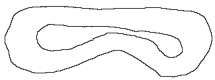
\includegraphics[interpolate=true,width=2.150000in,height=0.800000in]{contents/chapt6/figs/both/frenet_frame-img0.png}}%
\end{pgfscope}%
\begin{pgfscope}%
\pgfpathrectangle{\pgfqpoint{0.150000in}{1.522912in}}{\pgfqpoint{2.140057in}{0.790175in}}%
\pgfusepath{clip}%
\pgfsetbuttcap%
\pgfsetroundjoin%
\pgfsetlinewidth{1.505625pt}%
\definecolor{currentstroke}{rgb}{0.501961,0.501961,0.501961}%
\pgfsetstrokecolor{currentstroke}%
\pgfsetdash{{5.550000pt}{2.400000pt}}{0.000000pt}%
\pgfpathmoveto{\pgfqpoint{1.334687in}{1.900346in}}%
\pgfpathlineto{\pgfqpoint{1.411816in}{1.883146in}}%
\pgfpathlineto{\pgfqpoint{1.449989in}{1.872896in}}%
\pgfpathlineto{\pgfqpoint{1.487682in}{1.860698in}}%
\pgfpathlineto{\pgfqpoint{1.524628in}{1.846273in}}%
\pgfpathlineto{\pgfqpoint{1.560495in}{1.829571in}}%
\pgfpathlineto{\pgfqpoint{1.594950in}{1.810544in}}%
\pgfpathlineto{\pgfqpoint{1.627846in}{1.789129in}}%
\pgfpathlineto{\pgfqpoint{1.659310in}{1.765236in}}%
\pgfpathlineto{\pgfqpoint{1.689495in}{1.738774in}}%
\pgfpathlineto{\pgfqpoint{1.738661in}{1.692102in}}%
\pgfpathlineto{\pgfqpoint{1.759314in}{1.675757in}}%
\pgfpathlineto{\pgfqpoint{1.781320in}{1.662600in}}%
\pgfpathlineto{\pgfqpoint{1.792995in}{1.657606in}}%
\pgfpathlineto{\pgfqpoint{1.805169in}{1.653816in}}%
\pgfpathlineto{\pgfqpoint{1.817780in}{1.651180in}}%
\pgfpathlineto{\pgfqpoint{1.843991in}{1.649062in}}%
\pgfpathlineto{\pgfqpoint{1.870993in}{1.650642in}}%
\pgfpathlineto{\pgfqpoint{1.898150in}{1.655311in}}%
\pgfpathlineto{\pgfqpoint{1.924828in}{1.662458in}}%
\pgfpathlineto{\pgfqpoint{1.950483in}{1.671641in}}%
\pgfpathlineto{\pgfqpoint{1.974827in}{1.682879in}}%
\pgfpathlineto{\pgfqpoint{1.997618in}{1.696272in}}%
\pgfpathlineto{\pgfqpoint{2.018613in}{1.711921in}}%
\pgfpathlineto{\pgfqpoint{2.037567in}{1.729926in}}%
\pgfpathlineto{\pgfqpoint{2.054278in}{1.750249in}}%
\pgfpathlineto{\pgfqpoint{2.068622in}{1.772573in}}%
\pgfpathlineto{\pgfqpoint{2.080487in}{1.796546in}}%
\pgfpathlineto{\pgfqpoint{2.089761in}{1.821814in}}%
\pgfpathlineto{\pgfqpoint{2.096329in}{1.848026in}}%
\pgfpathlineto{\pgfqpoint{2.100038in}{1.874797in}}%
\pgfpathlineto{\pgfqpoint{2.100650in}{1.901684in}}%
\pgfpathlineto{\pgfqpoint{2.097918in}{1.928236in}}%
\pgfpathlineto{\pgfqpoint{2.091595in}{1.954002in}}%
\pgfpathlineto{\pgfqpoint{2.081439in}{1.978531in}}%
\pgfpathlineto{\pgfqpoint{2.067516in}{2.001388in}}%
\pgfpathlineto{\pgfqpoint{2.050346in}{2.022159in}}%
\pgfpathlineto{\pgfqpoint{2.030488in}{2.040432in}}%
\pgfpathlineto{\pgfqpoint{2.008499in}{2.055796in}}%
\pgfpathlineto{\pgfqpoint{1.984934in}{2.067855in}}%
\pgfpathlineto{\pgfqpoint{1.960228in}{2.076752in}}%
\pgfpathlineto{\pgfqpoint{1.934681in}{2.083226in}}%
\pgfpathlineto{\pgfqpoint{1.895430in}{2.090085in}}%
\pgfpathlineto{\pgfqpoint{1.725592in}{2.113615in}}%
\pgfpathlineto{\pgfqpoint{1.673056in}{2.116844in}}%
\pgfpathlineto{\pgfqpoint{1.620292in}{2.117892in}}%
\pgfpathlineto{\pgfqpoint{1.475397in}{2.118974in}}%
\pgfpathlineto{\pgfqpoint{1.422989in}{2.123547in}}%
\pgfpathlineto{\pgfqpoint{1.265720in}{2.140593in}}%
\pgfpathlineto{\pgfqpoint{1.213128in}{2.142855in}}%
\pgfpathlineto{\pgfqpoint{1.160501in}{2.142460in}}%
\pgfpathlineto{\pgfqpoint{1.002372in}{2.138396in}}%
\pgfpathlineto{\pgfqpoint{0.962909in}{2.139815in}}%
\pgfpathlineto{\pgfqpoint{0.923576in}{2.143168in}}%
\pgfpathlineto{\pgfqpoint{0.805706in}{2.155704in}}%
\pgfpathlineto{\pgfqpoint{0.766207in}{2.157051in}}%
\pgfpathlineto{\pgfqpoint{0.713480in}{2.156636in}}%
\pgfpathlineto{\pgfqpoint{0.647758in}{2.154095in}}%
\pgfpathlineto{\pgfqpoint{0.608434in}{2.151051in}}%
\pgfpathlineto{\pgfqpoint{0.569118in}{2.145844in}}%
\pgfpathlineto{\pgfqpoint{0.542901in}{2.140742in}}%
\pgfpathlineto{\pgfqpoint{0.516953in}{2.133970in}}%
\pgfpathlineto{\pgfqpoint{0.491738in}{2.125166in}}%
\pgfpathlineto{\pgfqpoint{0.467723in}{2.113967in}}%
\pgfpathlineto{\pgfqpoint{0.445375in}{2.100009in}}%
\pgfpathlineto{\pgfqpoint{0.425151in}{2.082970in}}%
\pgfpathlineto{\pgfqpoint{0.407390in}{2.063040in}}%
\pgfpathlineto{\pgfqpoint{0.392346in}{2.040757in}}%
\pgfpathlineto{\pgfqpoint{0.380275in}{2.016662in}}%
\pgfpathlineto{\pgfqpoint{0.371430in}{1.991300in}}%
\pgfpathlineto{\pgfqpoint{0.366042in}{1.965197in}}%
\pgfpathlineto{\pgfqpoint{0.364094in}{1.938728in}}%
\pgfpathlineto{\pgfqpoint{0.365423in}{1.912172in}}%
\pgfpathlineto{\pgfqpoint{0.369865in}{1.885810in}}%
\pgfpathlineto{\pgfqpoint{0.377254in}{1.859921in}}%
\pgfpathlineto{\pgfqpoint{0.387431in}{1.834811in}}%
\pgfpathlineto{\pgfqpoint{0.400273in}{1.810962in}}%
\pgfpathlineto{\pgfqpoint{0.415677in}{1.788939in}}%
\pgfpathlineto{\pgfqpoint{0.433538in}{1.769306in}}%
\pgfpathlineto{\pgfqpoint{0.453751in}{1.752627in}}%
\pgfpathlineto{\pgfqpoint{0.476164in}{1.739331in}}%
\pgfpathlineto{\pgfqpoint{0.500374in}{1.729143in}}%
\pgfpathlineto{\pgfqpoint{0.525898in}{1.721557in}}%
\pgfpathlineto{\pgfqpoint{0.552251in}{1.716070in}}%
\pgfpathlineto{\pgfqpoint{0.592285in}{1.710679in}}%
\pgfpathlineto{\pgfqpoint{0.632063in}{1.707895in}}%
\pgfpathlineto{\pgfqpoint{0.671512in}{1.707905in}}%
\pgfpathlineto{\pgfqpoint{0.710651in}{1.711006in}}%
\pgfpathlineto{\pgfqpoint{0.749498in}{1.717295in}}%
\pgfpathlineto{\pgfqpoint{0.788064in}{1.726093in}}%
\pgfpathlineto{\pgfqpoint{0.839069in}{1.740227in}}%
\pgfpathlineto{\pgfqpoint{0.902099in}{1.759780in}}%
\pgfpathlineto{\pgfqpoint{0.951682in}{1.777330in}}%
\pgfpathlineto{\pgfqpoint{1.000307in}{1.797201in}}%
\pgfpathlineto{\pgfqpoint{1.060183in}{1.824656in}}%
\pgfpathlineto{\pgfqpoint{1.144137in}{1.864071in}}%
\pgfpathlineto{\pgfqpoint{1.180965in}{1.878205in}}%
\pgfpathlineto{\pgfqpoint{1.206044in}{1.885596in}}%
\pgfpathlineto{\pgfqpoint{1.231616in}{1.891026in}}%
\pgfpathlineto{\pgfqpoint{1.270713in}{1.896214in}}%
\pgfpathlineto{\pgfqpoint{1.323664in}{1.899850in}}%
\pgfpathlineto{\pgfqpoint{1.323664in}{1.899850in}}%
\pgfusepath{stroke}%
\end{pgfscope}%
\begin{pgfscope}%
\pgfpathrectangle{\pgfqpoint{0.150000in}{1.522912in}}{\pgfqpoint{2.140057in}{0.790175in}}%
\pgfusepath{clip}%
\pgfsetrectcap%
\pgfsetroundjoin%
\pgfsetlinewidth{1.505625pt}%
\definecolor{currentstroke}{rgb}{0.121569,0.466667,0.705882}%
\pgfsetstrokecolor{currentstroke}%
\pgfsetstrokeopacity{0.700000}%
\pgfsetdash{}{0pt}%
\pgfpathmoveto{\pgfqpoint{1.322093in}{1.891661in}}%
\pgfpathlineto{\pgfqpoint{1.367106in}{1.890839in}}%
\pgfpathlineto{\pgfqpoint{1.398974in}{1.887942in}}%
\pgfpathlineto{\pgfqpoint{1.427077in}{1.883368in}}%
\pgfpathlineto{\pgfqpoint{1.455878in}{1.876593in}}%
\pgfpathlineto{\pgfqpoint{1.484950in}{1.867462in}}%
\pgfpathlineto{\pgfqpoint{1.513811in}{1.855846in}}%
\pgfpathlineto{\pgfqpoint{1.542052in}{1.841678in}}%
\pgfpathlineto{\pgfqpoint{1.569340in}{1.825026in}}%
\pgfpathlineto{\pgfqpoint{1.606407in}{1.799163in}}%
\pgfpathlineto{\pgfqpoint{1.659712in}{1.761874in}}%
\pgfpathlineto{\pgfqpoint{1.693096in}{1.741449in}}%
\pgfpathlineto{\pgfqpoint{1.722065in}{1.726424in}}%
\pgfpathlineto{\pgfqpoint{1.746070in}{1.716087in}}%
\pgfpathlineto{\pgfqpoint{1.770851in}{1.707485in}}%
\pgfpathlineto{\pgfqpoint{1.796242in}{1.700951in}}%
\pgfpathlineto{\pgfqpoint{1.822100in}{1.696690in}}%
\pgfpathlineto{\pgfqpoint{1.848307in}{1.694879in}}%
\pgfpathlineto{\pgfqpoint{1.874637in}{1.695699in}}%
\pgfpathlineto{\pgfqpoint{1.900726in}{1.699277in}}%
\pgfpathlineto{\pgfqpoint{1.926246in}{1.705676in}}%
\pgfpathlineto{\pgfqpoint{1.944797in}{1.712339in}}%
\pgfpathlineto{\pgfqpoint{1.962671in}{1.720590in}}%
\pgfpathlineto{\pgfqpoint{1.979761in}{1.730400in}}%
\pgfpathlineto{\pgfqpoint{1.995951in}{1.741728in}}%
\pgfpathlineto{\pgfqpoint{2.011025in}{1.754508in}}%
\pgfpathlineto{\pgfqpoint{2.024736in}{1.768463in}}%
\pgfpathlineto{\pgfqpoint{2.036885in}{1.783414in}}%
\pgfpathlineto{\pgfqpoint{2.047257in}{1.799318in}}%
\pgfpathlineto{\pgfqpoint{2.055689in}{1.816051in}}%
\pgfpathlineto{\pgfqpoint{2.062057in}{1.833443in}}%
\pgfpathlineto{\pgfqpoint{2.066267in}{1.851309in}}%
\pgfpathlineto{\pgfqpoint{2.068295in}{1.869389in}}%
\pgfpathlineto{\pgfqpoint{2.068171in}{1.887505in}}%
\pgfpathlineto{\pgfqpoint{2.065998in}{1.905390in}}%
\pgfpathlineto{\pgfqpoint{2.061822in}{1.922907in}}%
\pgfpathlineto{\pgfqpoint{2.055793in}{1.939835in}}%
\pgfpathlineto{\pgfqpoint{2.048057in}{1.955994in}}%
\pgfpathlineto{\pgfqpoint{2.038792in}{1.971268in}}%
\pgfpathlineto{\pgfqpoint{2.028023in}{1.985684in}}%
\pgfpathlineto{\pgfqpoint{2.011375in}{2.003713in}}%
\pgfpathlineto{\pgfqpoint{1.992580in}{2.020182in}}%
\pgfpathlineto{\pgfqpoint{1.972088in}{2.034988in}}%
\pgfpathlineto{\pgfqpoint{1.950154in}{2.047990in}}%
\pgfpathlineto{\pgfqpoint{1.926967in}{2.059067in}}%
\pgfpathlineto{\pgfqpoint{1.902819in}{2.068292in}}%
\pgfpathlineto{\pgfqpoint{1.877852in}{2.075753in}}%
\pgfpathlineto{\pgfqpoint{1.845925in}{2.082737in}}%
\pgfpathlineto{\pgfqpoint{1.813450in}{2.087277in}}%
\pgfpathlineto{\pgfqpoint{1.774103in}{2.089903in}}%
\pgfpathlineto{\pgfqpoint{1.695208in}{2.093794in}}%
\pgfpathlineto{\pgfqpoint{1.662488in}{2.097757in}}%
\pgfpathlineto{\pgfqpoint{1.623574in}{2.104737in}}%
\pgfpathlineto{\pgfqpoint{1.578785in}{2.115343in}}%
\pgfpathlineto{\pgfqpoint{1.463960in}{2.144593in}}%
\pgfpathlineto{\pgfqpoint{1.431354in}{2.149173in}}%
\pgfpathlineto{\pgfqpoint{1.405073in}{2.150781in}}%
\pgfpathlineto{\pgfqpoint{1.372150in}{2.150504in}}%
\pgfpathlineto{\pgfqpoint{1.332774in}{2.147849in}}%
\pgfpathlineto{\pgfqpoint{1.260932in}{2.139964in}}%
\pgfpathlineto{\pgfqpoint{1.195544in}{2.133541in}}%
\pgfpathlineto{\pgfqpoint{1.142962in}{2.130474in}}%
\pgfpathlineto{\pgfqpoint{0.814014in}{2.116246in}}%
\pgfpathlineto{\pgfqpoint{0.728703in}{2.109040in}}%
\pgfpathlineto{\pgfqpoint{0.669860in}{2.101785in}}%
\pgfpathlineto{\pgfqpoint{0.624500in}{2.093858in}}%
\pgfpathlineto{\pgfqpoint{0.586120in}{2.084606in}}%
\pgfpathlineto{\pgfqpoint{0.554827in}{2.074478in}}%
\pgfpathlineto{\pgfqpoint{0.530557in}{2.064399in}}%
\pgfpathlineto{\pgfqpoint{0.507288in}{2.052212in}}%
\pgfpathlineto{\pgfqpoint{0.485635in}{2.037813in}}%
\pgfpathlineto{\pgfqpoint{0.470763in}{2.025548in}}%
\pgfpathlineto{\pgfqpoint{0.457253in}{2.011999in}}%
\pgfpathlineto{\pgfqpoint{0.445332in}{1.997190in}}%
\pgfpathlineto{\pgfqpoint{0.435222in}{1.981249in}}%
\pgfpathlineto{\pgfqpoint{0.427071in}{1.964369in}}%
\pgfpathlineto{\pgfqpoint{0.421019in}{1.946743in}}%
\pgfpathlineto{\pgfqpoint{0.417136in}{1.928569in}}%
\pgfpathlineto{\pgfqpoint{0.415471in}{1.910115in}}%
\pgfpathlineto{\pgfqpoint{0.416007in}{1.891651in}}%
\pgfpathlineto{\pgfqpoint{0.418717in}{1.873426in}}%
\pgfpathlineto{\pgfqpoint{0.423517in}{1.855706in}}%
\pgfpathlineto{\pgfqpoint{0.430292in}{1.838610in}}%
\pgfpathlineto{\pgfqpoint{0.438988in}{1.822170in}}%
\pgfpathlineto{\pgfqpoint{0.449395in}{1.806555in}}%
\pgfpathlineto{\pgfqpoint{0.461337in}{1.791892in}}%
\pgfpathlineto{\pgfqpoint{0.474650in}{1.778300in}}%
\pgfpathlineto{\pgfqpoint{0.489217in}{1.765889in}}%
\pgfpathlineto{\pgfqpoint{0.510324in}{1.751299in}}%
\pgfpathlineto{\pgfqpoint{0.533013in}{1.739078in}}%
\pgfpathlineto{\pgfqpoint{0.556963in}{1.729158in}}%
\pgfpathlineto{\pgfqpoint{0.581838in}{1.721589in}}%
\pgfpathlineto{\pgfqpoint{0.607476in}{1.716426in}}%
\pgfpathlineto{\pgfqpoint{0.633549in}{1.713619in}}%
\pgfpathlineto{\pgfqpoint{0.659800in}{1.713093in}}%
\pgfpathlineto{\pgfqpoint{0.686052in}{1.714719in}}%
\pgfpathlineto{\pgfqpoint{0.712147in}{1.718308in}}%
\pgfpathlineto{\pgfqpoint{0.737931in}{1.723696in}}%
\pgfpathlineto{\pgfqpoint{0.769579in}{1.732743in}}%
\pgfpathlineto{\pgfqpoint{0.806779in}{1.746084in}}%
\pgfpathlineto{\pgfqpoint{0.874738in}{1.770883in}}%
\pgfpathlineto{\pgfqpoint{0.912568in}{1.782084in}}%
\pgfpathlineto{\pgfqpoint{0.957376in}{1.792820in}}%
\pgfpathlineto{\pgfqpoint{1.008952in}{1.802761in}}%
\pgfpathlineto{\pgfqpoint{1.093478in}{1.816358in}}%
\pgfpathlineto{\pgfqpoint{1.171810in}{1.826958in}}%
\pgfpathlineto{\pgfqpoint{1.224223in}{1.831947in}}%
\pgfpathlineto{\pgfqpoint{1.270279in}{1.833964in}}%
\pgfpathlineto{\pgfqpoint{1.270279in}{1.833964in}}%
\pgfusepath{stroke}%
\end{pgfscope}%
\begin{pgfscope}%
\pgfpathrectangle{\pgfqpoint{0.150000in}{1.522912in}}{\pgfqpoint{2.140057in}{0.790175in}}%
\pgfusepath{clip}%
\pgfsetbuttcap%
\pgfsetroundjoin%
\pgfsetlinewidth{1.505625pt}%
\definecolor{currentstroke}{rgb}{1.000000,0.000000,0.000000}%
\pgfsetstrokecolor{currentstroke}%
\pgfsetdash{{5.550000pt}{2.400000pt}}{0.000000pt}%
\pgfpathmoveto{\pgfqpoint{1.334687in}{1.742311in}}%
\pgfpathlineto{\pgfqpoint{1.334687in}{2.032041in}}%
\pgfusepath{stroke}%
\end{pgfscope}%
\begin{pgfscope}%
\definecolor{textcolor}{rgb}{0.000000,0.000000,0.000000}%
\pgfsetstrokecolor{textcolor}%
\pgfsetfillcolor{textcolor}%
\pgftext[x=1.203567in,y=2.774023in,left,base]{\color{textcolor}\rmfamily\fontsize{10.000000}{12.000000}\selectfont (a)}%
\end{pgfscope}%
\begin{pgfscope}%
\pgfsetbuttcap%
\pgfsetmiterjoin%
\definecolor{currentfill}{rgb}{1.000000,1.000000,1.000000}%
\pgfsetfillcolor{currentfill}%
\pgfsetlinewidth{0.000000pt}%
\definecolor{currentstroke}{rgb}{0.000000,0.000000,0.000000}%
\pgfsetstrokecolor{currentstroke}%
\pgfsetstrokeopacity{0.000000}%
\pgfsetdash{}{0pt}%
\pgfpathmoveto{\pgfqpoint{3.209943in}{1.184000in}}%
\pgfpathlineto{\pgfqpoint{5.350000in}{1.184000in}}%
\pgfpathlineto{\pgfqpoint{5.350000in}{2.652000in}}%
\pgfpathlineto{\pgfqpoint{3.209943in}{2.652000in}}%
\pgfpathlineto{\pgfqpoint{3.209943in}{1.184000in}}%
\pgfpathclose%
\pgfusepath{fill}%
\end{pgfscope}%
\begin{pgfscope}%
\definecolor{textcolor}{rgb}{0.000000,0.000000,0.000000}%
\pgfsetstrokecolor{textcolor}%
\pgfsetfillcolor{textcolor}%
\pgftext[x=3.307218in,y=1.135389in,,top]{\color{textcolor}\rmfamily\fontsize{10.000000}{12.000000}\selectfont 0}%
\end{pgfscope}%
\begin{pgfscope}%
\definecolor{textcolor}{rgb}{0.000000,0.000000,0.000000}%
\pgfsetstrokecolor{textcolor}%
\pgfsetfillcolor{textcolor}%
\pgftext[x=3.940934in,y=1.135389in,,top]{\color{textcolor}\rmfamily\fontsize{10.000000}{12.000000}\selectfont 10}%
\end{pgfscope}%
\begin{pgfscope}%
\definecolor{textcolor}{rgb}{0.000000,0.000000,0.000000}%
\pgfsetstrokecolor{textcolor}%
\pgfsetfillcolor{textcolor}%
\pgftext[x=4.574649in,y=1.135389in,,top]{\color{textcolor}\rmfamily\fontsize{10.000000}{12.000000}\selectfont 20}%
\end{pgfscope}%
\begin{pgfscope}%
\definecolor{textcolor}{rgb}{0.000000,0.000000,0.000000}%
\pgfsetstrokecolor{textcolor}%
\pgfsetfillcolor{textcolor}%
\pgftext[x=5.208365in,y=1.135389in,,top]{\color{textcolor}\rmfamily\fontsize{10.000000}{12.000000}\selectfont 30}%
\end{pgfscope}%
\begin{pgfscope}%
\definecolor{textcolor}{rgb}{0.000000,0.000000,0.000000}%
\pgfsetstrokecolor{textcolor}%
\pgfsetfillcolor{textcolor}%
\pgftext[x=3.733673in, y=0.839898in, left, base]{\color{textcolor}\rmfamily\fontsize{10.000000}{12.000000}\selectfont Distance along }%
\end{pgfscope}%
\begin{pgfscope}%
\definecolor{textcolor}{rgb}{0.000000,0.000000,0.000000}%
\pgfsetstrokecolor{textcolor}%
\pgfsetfillcolor{textcolor}%
\pgftext[x=3.846113in, y=0.682413in, left, base]{\color{textcolor}\rmfamily\fontsize{10.000000}{12.000000}\selectfont  centerline, \(\displaystyle s\)}%
\end{pgfscope}%
\begin{pgfscope}%
\definecolor{textcolor}{rgb}{0.000000,0.000000,0.000000}%
\pgfsetstrokecolor{textcolor}%
\pgfsetfillcolor{textcolor}%
\pgftext[x=2.964941in, y=1.340953in, left, base]{\color{textcolor}\rmfamily\fontsize{10.000000}{12.000000}\selectfont \ensuremath{-}1}%
\end{pgfscope}%
\begin{pgfscope}%
\definecolor{textcolor}{rgb}{0.000000,0.000000,0.000000}%
\pgfsetstrokecolor{textcolor}%
\pgfsetfillcolor{textcolor}%
\pgftext[x=3.072966in, y=1.817576in, left, base]{\color{textcolor}\rmfamily\fontsize{10.000000}{12.000000}\selectfont 0}%
\end{pgfscope}%
\begin{pgfscope}%
\definecolor{textcolor}{rgb}{0.000000,0.000000,0.000000}%
\pgfsetstrokecolor{textcolor}%
\pgfsetfillcolor{textcolor}%
\pgftext[x=3.072966in, y=2.294200in, left, base]{\color{textcolor}\rmfamily\fontsize{10.000000}{12.000000}\selectfont 1}%
\end{pgfscope}%
\begin{pgfscope}%
\definecolor{textcolor}{rgb}{0.000000,0.000000,0.000000}%
\pgfsetstrokecolor{textcolor}%
\pgfsetfillcolor{textcolor}%
\pgftext[x=2.724979in, y=1.070188in, left, base,rotate=90.000000]{\color{textcolor}\rmfamily\fontsize{10.000000}{12.000000}\selectfont Distance perpendicular }%
\end{pgfscope}%
\begin{pgfscope}%
\definecolor{textcolor}{rgb}{0.000000,0.000000,0.000000}%
\pgfsetstrokecolor{textcolor}%
\pgfsetfillcolor{textcolor}%
\pgftext[x=2.880496in, y=1.383221in, left, base,rotate=90.000000]{\color{textcolor}\rmfamily\fontsize{10.000000}{12.000000}\selectfont  to centerline, \(\displaystyle n\)}%
\end{pgfscope}%
\begin{pgfscope}%
\pgfpathrectangle{\pgfqpoint{3.209943in}{1.184000in}}{\pgfqpoint{2.140057in}{1.468000in}}%
\pgfusepath{clip}%
\pgfsetrectcap%
\pgfsetroundjoin%
\pgfsetlinewidth{1.505625pt}%
\definecolor{currentstroke}{rgb}{0.000000,0.000000,0.000000}%
\pgfsetstrokecolor{currentstroke}%
\pgfsetdash{}{0pt}%
\pgfpathmoveto{\pgfqpoint{3.307218in}{2.203974in}}%
\pgfpathlineto{\pgfqpoint{3.338904in}{2.203974in}}%
\pgfpathlineto{\pgfqpoint{3.345241in}{2.251636in}}%
\pgfpathlineto{\pgfqpoint{3.389601in}{2.251636in}}%
\pgfpathlineto{\pgfqpoint{3.395938in}{2.299299in}}%
\pgfpathlineto{\pgfqpoint{3.503670in}{2.299299in}}%
\pgfpathlineto{\pgfqpoint{3.510007in}{2.251636in}}%
\pgfpathlineto{\pgfqpoint{3.548030in}{2.251636in}}%
\pgfpathlineto{\pgfqpoint{3.554367in}{2.299299in}}%
\pgfpathlineto{\pgfqpoint{3.560704in}{2.299299in}}%
\pgfpathlineto{\pgfqpoint{3.567041in}{2.251636in}}%
\pgfpathlineto{\pgfqpoint{3.630413in}{2.251636in}}%
\pgfpathlineto{\pgfqpoint{3.636750in}{2.299299in}}%
\pgfpathlineto{\pgfqpoint{3.662099in}{2.299299in}}%
\pgfpathlineto{\pgfqpoint{3.668436in}{2.346961in}}%
\pgfpathlineto{\pgfqpoint{3.674773in}{2.299299in}}%
\pgfpathlineto{\pgfqpoint{3.681110in}{2.299299in}}%
\pgfpathlineto{\pgfqpoint{3.687447in}{2.346961in}}%
\pgfpathlineto{\pgfqpoint{3.693785in}{2.299299in}}%
\pgfpathlineto{\pgfqpoint{3.712796in}{2.299299in}}%
\pgfpathlineto{\pgfqpoint{3.719133in}{2.346961in}}%
\pgfpathlineto{\pgfqpoint{3.731807in}{2.346961in}}%
\pgfpathlineto{\pgfqpoint{3.738145in}{2.394623in}}%
\pgfpathlineto{\pgfqpoint{3.750819in}{2.394623in}}%
\pgfpathlineto{\pgfqpoint{3.757156in}{2.442286in}}%
\pgfpathlineto{\pgfqpoint{3.769830in}{2.442286in}}%
\pgfpathlineto{\pgfqpoint{3.776168in}{2.489948in}}%
\pgfpathlineto{\pgfqpoint{3.814190in}{2.489948in}}%
\pgfpathlineto{\pgfqpoint{3.820528in}{2.537610in}}%
\pgfpathlineto{\pgfqpoint{3.833202in}{2.537610in}}%
\pgfpathlineto{\pgfqpoint{3.839539in}{2.585273in}}%
\pgfpathlineto{\pgfqpoint{3.845876in}{2.537610in}}%
\pgfpathlineto{\pgfqpoint{3.852213in}{2.537610in}}%
\pgfpathlineto{\pgfqpoint{3.858551in}{2.489948in}}%
\pgfpathlineto{\pgfqpoint{3.864888in}{2.489948in}}%
\pgfpathlineto{\pgfqpoint{3.871225in}{2.442286in}}%
\pgfpathlineto{\pgfqpoint{3.877562in}{2.442286in}}%
\pgfpathlineto{\pgfqpoint{3.883899in}{2.394623in}}%
\pgfpathlineto{\pgfqpoint{3.902911in}{2.394623in}}%
\pgfpathlineto{\pgfqpoint{3.909248in}{2.346961in}}%
\pgfpathlineto{\pgfqpoint{3.915585in}{2.346961in}}%
\pgfpathlineto{\pgfqpoint{3.921922in}{2.394623in}}%
\pgfpathlineto{\pgfqpoint{3.928259in}{2.346961in}}%
\pgfpathlineto{\pgfqpoint{4.067677in}{2.346961in}}%
\pgfpathlineto{\pgfqpoint{4.074014in}{2.299299in}}%
\pgfpathlineto{\pgfqpoint{4.169071in}{2.299299in}}%
\pgfpathlineto{\pgfqpoint{4.175408in}{2.251636in}}%
\pgfpathlineto{\pgfqpoint{4.219768in}{2.251636in}}%
\pgfpathlineto{\pgfqpoint{4.226106in}{2.203974in}}%
\pgfpathlineto{\pgfqpoint{4.276803in}{2.203974in}}%
\pgfpathlineto{\pgfqpoint{4.283140in}{2.156312in}}%
\pgfpathlineto{\pgfqpoint{4.289477in}{2.203974in}}%
\pgfpathlineto{\pgfqpoint{4.308489in}{2.203974in}}%
\pgfpathlineto{\pgfqpoint{4.314826in}{2.251636in}}%
\pgfpathlineto{\pgfqpoint{4.321163in}{2.203974in}}%
\pgfpathlineto{\pgfqpoint{4.327500in}{2.251636in}}%
\pgfpathlineto{\pgfqpoint{4.447906in}{2.251636in}}%
\pgfpathlineto{\pgfqpoint{4.454243in}{2.203974in}}%
\pgfpathlineto{\pgfqpoint{4.460580in}{2.251636in}}%
\pgfpathlineto{\pgfqpoint{4.549300in}{2.251636in}}%
\pgfpathlineto{\pgfqpoint{4.555638in}{2.299299in}}%
\pgfpathlineto{\pgfqpoint{4.593661in}{2.299299in}}%
\pgfpathlineto{\pgfqpoint{4.599998in}{2.346961in}}%
\pgfpathlineto{\pgfqpoint{4.612672in}{2.346961in}}%
\pgfpathlineto{\pgfqpoint{4.619009in}{2.394623in}}%
\pgfpathlineto{\pgfqpoint{4.625346in}{2.394623in}}%
\pgfpathlineto{\pgfqpoint{4.631683in}{2.442286in}}%
\pgfpathlineto{\pgfqpoint{4.644358in}{2.442286in}}%
\pgfpathlineto{\pgfqpoint{4.650695in}{2.489948in}}%
\pgfpathlineto{\pgfqpoint{4.657032in}{2.442286in}}%
\pgfpathlineto{\pgfqpoint{4.669706in}{2.442286in}}%
\pgfpathlineto{\pgfqpoint{4.676044in}{2.394623in}}%
\pgfpathlineto{\pgfqpoint{4.688718in}{2.394623in}}%
\pgfpathlineto{\pgfqpoint{4.701392in}{2.489948in}}%
\pgfpathlineto{\pgfqpoint{4.739415in}{2.489948in}}%
\pgfpathlineto{\pgfqpoint{4.745752in}{2.442286in}}%
\pgfpathlineto{\pgfqpoint{4.758427in}{2.442286in}}%
\pgfpathlineto{\pgfqpoint{4.771101in}{2.537610in}}%
\pgfpathlineto{\pgfqpoint{4.790112in}{2.537610in}}%
\pgfpathlineto{\pgfqpoint{4.796449in}{2.489948in}}%
\pgfpathlineto{\pgfqpoint{4.802787in}{2.489948in}}%
\pgfpathlineto{\pgfqpoint{4.809124in}{2.442286in}}%
\pgfpathlineto{\pgfqpoint{4.815461in}{2.442286in}}%
\pgfpathlineto{\pgfqpoint{4.821798in}{2.394623in}}%
\pgfpathlineto{\pgfqpoint{4.859821in}{2.394623in}}%
\pgfpathlineto{\pgfqpoint{4.866158in}{2.346961in}}%
\pgfpathlineto{\pgfqpoint{4.891507in}{2.346961in}}%
\pgfpathlineto{\pgfqpoint{4.897844in}{2.299299in}}%
\pgfpathlineto{\pgfqpoint{4.935867in}{2.299299in}}%
\pgfpathlineto{\pgfqpoint{4.942204in}{2.251636in}}%
\pgfpathlineto{\pgfqpoint{4.948541in}{2.299299in}}%
\pgfpathlineto{\pgfqpoint{4.954878in}{2.299299in}}%
\pgfpathlineto{\pgfqpoint{4.961216in}{2.251636in}}%
\pgfpathlineto{\pgfqpoint{5.049936in}{2.251636in}}%
\pgfpathlineto{\pgfqpoint{5.056273in}{2.203974in}}%
\pgfpathlineto{\pgfqpoint{5.106970in}{2.203974in}}%
\pgfpathlineto{\pgfqpoint{5.113307in}{2.251636in}}%
\pgfpathlineto{\pgfqpoint{5.125982in}{2.251636in}}%
\pgfpathlineto{\pgfqpoint{5.132319in}{2.203974in}}%
\pgfpathlineto{\pgfqpoint{5.144993in}{2.203974in}}%
\pgfpathlineto{\pgfqpoint{5.151330in}{2.251636in}}%
\pgfpathlineto{\pgfqpoint{5.214702in}{2.251636in}}%
\pgfpathlineto{\pgfqpoint{5.221039in}{2.203974in}}%
\pgfpathlineto{\pgfqpoint{5.252725in}{2.203974in}}%
\pgfpathlineto{\pgfqpoint{5.252725in}{2.203974in}}%
\pgfusepath{stroke}%
\end{pgfscope}%
\begin{pgfscope}%
\pgfpathrectangle{\pgfqpoint{3.209943in}{1.184000in}}{\pgfqpoint{2.140057in}{1.468000in}}%
\pgfusepath{clip}%
\pgfsetrectcap%
\pgfsetroundjoin%
\pgfsetlinewidth{1.505625pt}%
\definecolor{currentstroke}{rgb}{0.000000,0.000000,0.000000}%
\pgfsetstrokecolor{currentstroke}%
\pgfsetdash{}{0pt}%
\pgfpathmoveto{\pgfqpoint{3.307218in}{1.536701in}}%
\pgfpathlineto{\pgfqpoint{3.357915in}{1.536701in}}%
\pgfpathlineto{\pgfqpoint{3.364252in}{1.489039in}}%
\pgfpathlineto{\pgfqpoint{3.402275in}{1.489039in}}%
\pgfpathlineto{\pgfqpoint{3.408613in}{1.441377in}}%
\pgfpathlineto{\pgfqpoint{3.440298in}{1.441377in}}%
\pgfpathlineto{\pgfqpoint{3.446635in}{1.393714in}}%
\pgfpathlineto{\pgfqpoint{3.452973in}{1.393714in}}%
\pgfpathlineto{\pgfqpoint{3.459310in}{1.441377in}}%
\pgfpathlineto{\pgfqpoint{3.471984in}{1.441377in}}%
\pgfpathlineto{\pgfqpoint{3.478321in}{1.489039in}}%
\pgfpathlineto{\pgfqpoint{3.516344in}{1.489039in}}%
\pgfpathlineto{\pgfqpoint{3.522681in}{1.536701in}}%
\pgfpathlineto{\pgfqpoint{3.529018in}{1.489039in}}%
\pgfpathlineto{\pgfqpoint{3.668436in}{1.489039in}}%
\pgfpathlineto{\pgfqpoint{3.674773in}{1.441377in}}%
\pgfpathlineto{\pgfqpoint{3.681110in}{1.441377in}}%
\pgfpathlineto{\pgfqpoint{3.687447in}{1.489039in}}%
\pgfpathlineto{\pgfqpoint{3.693785in}{1.441377in}}%
\pgfpathlineto{\pgfqpoint{3.700122in}{1.441377in}}%
\pgfpathlineto{\pgfqpoint{3.706459in}{1.393714in}}%
\pgfpathlineto{\pgfqpoint{3.719133in}{1.393714in}}%
\pgfpathlineto{\pgfqpoint{3.725470in}{1.346052in}}%
\pgfpathlineto{\pgfqpoint{3.738145in}{1.346052in}}%
\pgfpathlineto{\pgfqpoint{3.744482in}{1.298390in}}%
\pgfpathlineto{\pgfqpoint{3.757156in}{1.298390in}}%
\pgfpathlineto{\pgfqpoint{3.763493in}{1.250727in}}%
\pgfpathlineto{\pgfqpoint{3.877562in}{1.250727in}}%
\pgfpathlineto{\pgfqpoint{3.883899in}{1.298390in}}%
\pgfpathlineto{\pgfqpoint{3.890236in}{1.250727in}}%
\pgfpathlineto{\pgfqpoint{3.896573in}{1.298390in}}%
\pgfpathlineto{\pgfqpoint{3.921922in}{1.298390in}}%
\pgfpathlineto{\pgfqpoint{3.928259in}{1.346052in}}%
\pgfpathlineto{\pgfqpoint{3.972619in}{1.346052in}}%
\pgfpathlineto{\pgfqpoint{3.978956in}{1.393714in}}%
\pgfpathlineto{\pgfqpoint{3.985294in}{1.346052in}}%
\pgfpathlineto{\pgfqpoint{3.991631in}{1.393714in}}%
\pgfpathlineto{\pgfqpoint{4.010642in}{1.393714in}}%
\pgfpathlineto{\pgfqpoint{4.016979in}{1.346052in}}%
\pgfpathlineto{\pgfqpoint{4.023317in}{1.393714in}}%
\pgfpathlineto{\pgfqpoint{4.067677in}{1.393714in}}%
\pgfpathlineto{\pgfqpoint{4.074014in}{1.441377in}}%
\pgfpathlineto{\pgfqpoint{4.099362in}{1.441377in}}%
\pgfpathlineto{\pgfqpoint{4.105700in}{1.393714in}}%
\pgfpathlineto{\pgfqpoint{4.112037in}{1.393714in}}%
\pgfpathlineto{\pgfqpoint{4.118374in}{1.441377in}}%
\pgfpathlineto{\pgfqpoint{4.131048in}{1.441377in}}%
\pgfpathlineto{\pgfqpoint{4.137385in}{1.489039in}}%
\pgfpathlineto{\pgfqpoint{4.143723in}{1.441377in}}%
\pgfpathlineto{\pgfqpoint{4.150060in}{1.489039in}}%
\pgfpathlineto{\pgfqpoint{4.283140in}{1.489039in}}%
\pgfpathlineto{\pgfqpoint{4.289477in}{1.536701in}}%
\pgfpathlineto{\pgfqpoint{4.352849in}{1.536701in}}%
\pgfpathlineto{\pgfqpoint{4.359186in}{1.489039in}}%
\pgfpathlineto{\pgfqpoint{4.365523in}{1.536701in}}%
\pgfpathlineto{\pgfqpoint{4.378197in}{1.536701in}}%
\pgfpathlineto{\pgfqpoint{4.384534in}{1.489039in}}%
\pgfpathlineto{\pgfqpoint{4.504940in}{1.489039in}}%
\pgfpathlineto{\pgfqpoint{4.511278in}{1.536701in}}%
\pgfpathlineto{\pgfqpoint{4.536626in}{1.536701in}}%
\pgfpathlineto{\pgfqpoint{4.542963in}{1.489039in}}%
\pgfpathlineto{\pgfqpoint{4.549300in}{1.489039in}}%
\pgfpathlineto{\pgfqpoint{4.555638in}{1.441377in}}%
\pgfpathlineto{\pgfqpoint{4.561975in}{1.489039in}}%
\pgfpathlineto{\pgfqpoint{4.568312in}{1.441377in}}%
\pgfpathlineto{\pgfqpoint{4.580986in}{1.441377in}}%
\pgfpathlineto{\pgfqpoint{4.587323in}{1.393714in}}%
\pgfpathlineto{\pgfqpoint{4.599998in}{1.393714in}}%
\pgfpathlineto{\pgfqpoint{4.606335in}{1.346052in}}%
\pgfpathlineto{\pgfqpoint{4.612672in}{1.346052in}}%
\pgfpathlineto{\pgfqpoint{4.619009in}{1.393714in}}%
\pgfpathlineto{\pgfqpoint{4.625346in}{1.346052in}}%
\pgfpathlineto{\pgfqpoint{4.638021in}{1.346052in}}%
\pgfpathlineto{\pgfqpoint{4.644358in}{1.298390in}}%
\pgfpathlineto{\pgfqpoint{4.733078in}{1.298390in}}%
\pgfpathlineto{\pgfqpoint{4.739415in}{1.250727in}}%
\pgfpathlineto{\pgfqpoint{4.745752in}{1.250727in}}%
\pgfpathlineto{\pgfqpoint{4.752089in}{1.298390in}}%
\pgfpathlineto{\pgfqpoint{4.834472in}{1.298390in}}%
\pgfpathlineto{\pgfqpoint{4.840810in}{1.346052in}}%
\pgfpathlineto{\pgfqpoint{4.853484in}{1.346052in}}%
\pgfpathlineto{\pgfqpoint{4.859821in}{1.393714in}}%
\pgfpathlineto{\pgfqpoint{4.878833in}{1.393714in}}%
\pgfpathlineto{\pgfqpoint{4.885170in}{1.441377in}}%
\pgfpathlineto{\pgfqpoint{4.910518in}{1.441377in}}%
\pgfpathlineto{\pgfqpoint{4.916855in}{1.489039in}}%
\pgfpathlineto{\pgfqpoint{4.929530in}{1.489039in}}%
\pgfpathlineto{\pgfqpoint{4.935867in}{1.441377in}}%
\pgfpathlineto{\pgfqpoint{4.954878in}{1.441377in}}%
\pgfpathlineto{\pgfqpoint{4.961216in}{1.489039in}}%
\pgfpathlineto{\pgfqpoint{4.999238in}{1.489039in}}%
\pgfpathlineto{\pgfqpoint{5.005576in}{1.536701in}}%
\pgfpathlineto{\pgfqpoint{5.056273in}{1.536701in}}%
\pgfpathlineto{\pgfqpoint{5.062610in}{1.489039in}}%
\pgfpathlineto{\pgfqpoint{5.068947in}{1.536701in}}%
\pgfpathlineto{\pgfqpoint{5.144993in}{1.536701in}}%
\pgfpathlineto{\pgfqpoint{5.151330in}{1.489039in}}%
\pgfpathlineto{\pgfqpoint{5.157667in}{1.489039in}}%
\pgfpathlineto{\pgfqpoint{5.164004in}{1.536701in}}%
\pgfpathlineto{\pgfqpoint{5.195690in}{1.536701in}}%
\pgfpathlineto{\pgfqpoint{5.202027in}{1.489039in}}%
\pgfpathlineto{\pgfqpoint{5.240050in}{1.489039in}}%
\pgfpathlineto{\pgfqpoint{5.246388in}{1.536701in}}%
\pgfpathlineto{\pgfqpoint{5.252725in}{1.536701in}}%
\pgfpathlineto{\pgfqpoint{5.252725in}{1.536701in}}%
\pgfusepath{stroke}%
\end{pgfscope}%
\begin{pgfscope}%
\pgfpathrectangle{\pgfqpoint{3.209943in}{1.184000in}}{\pgfqpoint{2.140057in}{1.468000in}}%
\pgfusepath{clip}%
\pgfsetbuttcap%
\pgfsetroundjoin%
\pgfsetlinewidth{1.505625pt}%
\definecolor{currentstroke}{rgb}{0.501961,0.501961,0.501961}%
\pgfsetstrokecolor{currentstroke}%
\pgfsetdash{{5.550000pt}{2.400000pt}}{0.000000pt}%
\pgfpathmoveto{\pgfqpoint{3.307218in}{1.870338in}}%
\pgfpathlineto{\pgfqpoint{5.252725in}{1.870338in}}%
\pgfpathlineto{\pgfqpoint{5.252725in}{1.870338in}}%
\pgfusepath{stroke}%
\end{pgfscope}%
\begin{pgfscope}%
\pgfpathrectangle{\pgfqpoint{3.209943in}{1.184000in}}{\pgfqpoint{2.140057in}{1.468000in}}%
\pgfusepath{clip}%
\pgfsetbuttcap%
\pgfsetroundjoin%
\pgfsetlinewidth{1.505625pt}%
\definecolor{currentstroke}{rgb}{1.000000,0.000000,0.000000}%
\pgfsetstrokecolor{currentstroke}%
\pgfsetdash{{5.550000pt}{2.400000pt}}{0.000000pt}%
\pgfpathmoveto{\pgfqpoint{3.307218in}{1.393714in}}%
\pgfpathlineto{\pgfqpoint{3.307218in}{2.346961in}}%
\pgfusepath{stroke}%
\end{pgfscope}%
\begin{pgfscope}%
\pgfpathrectangle{\pgfqpoint{3.209943in}{1.184000in}}{\pgfqpoint{2.140057in}{1.468000in}}%
\pgfusepath{clip}%
\pgfsetbuttcap%
\pgfsetroundjoin%
\pgfsetlinewidth{1.505625pt}%
\definecolor{currentstroke}{rgb}{1.000000,0.000000,0.000000}%
\pgfsetstrokecolor{currentstroke}%
\pgfsetdash{{5.550000pt}{2.400000pt}}{0.000000pt}%
\pgfpathmoveto{\pgfqpoint{5.252725in}{1.393714in}}%
\pgfpathlineto{\pgfqpoint{5.252725in}{2.346961in}}%
\pgfusepath{stroke}%
\end{pgfscope}%
\begin{pgfscope}%
\pgfpathrectangle{\pgfqpoint{3.209943in}{1.184000in}}{\pgfqpoint{2.140057in}{1.468000in}}%
\pgfusepath{clip}%
\pgfsetrectcap%
\pgfsetroundjoin%
\pgfsetlinewidth{1.505625pt}%
\definecolor{currentstroke}{rgb}{0.121569,0.466667,0.705882}%
\pgfsetstrokecolor{currentstroke}%
\pgfsetdash{}{0pt}%
\pgfpathmoveto{\pgfqpoint{3.313555in}{1.843172in}}%
\pgfpathlineto{\pgfqpoint{3.313555in}{1.848290in}}%
\pgfpathlineto{\pgfqpoint{3.313555in}{1.841995in}}%
\pgfpathlineto{\pgfqpoint{3.319892in}{1.852732in}}%
\pgfpathlineto{\pgfqpoint{3.319892in}{1.855409in}}%
\pgfpathlineto{\pgfqpoint{3.326230in}{1.847370in}}%
\pgfpathlineto{\pgfqpoint{3.326230in}{1.863462in}}%
\pgfpathlineto{\pgfqpoint{3.326230in}{1.853956in}}%
\pgfpathlineto{\pgfqpoint{3.332567in}{1.857629in}}%
\pgfpathlineto{\pgfqpoint{3.332567in}{1.877152in}}%
\pgfpathlineto{\pgfqpoint{3.338904in}{1.892097in}}%
\pgfpathlineto{\pgfqpoint{3.338904in}{1.876514in}}%
\pgfpathlineto{\pgfqpoint{3.338904in}{1.890545in}}%
\pgfpathlineto{\pgfqpoint{3.345241in}{1.883555in}}%
\pgfpathlineto{\pgfqpoint{3.345241in}{1.886773in}}%
\pgfpathlineto{\pgfqpoint{3.351578in}{1.890476in}}%
\pgfpathlineto{\pgfqpoint{3.351578in}{1.885773in}}%
\pgfpathlineto{\pgfqpoint{3.357915in}{1.896629in}}%
\pgfpathlineto{\pgfqpoint{3.357915in}{1.886919in}}%
\pgfpathlineto{\pgfqpoint{3.357915in}{1.897928in}}%
\pgfpathlineto{\pgfqpoint{3.364252in}{1.889294in}}%
\pgfpathlineto{\pgfqpoint{3.364252in}{1.895502in}}%
\pgfpathlineto{\pgfqpoint{3.370590in}{1.891908in}}%
\pgfpathlineto{\pgfqpoint{3.370590in}{1.893576in}}%
\pgfpathlineto{\pgfqpoint{3.376927in}{1.894450in}}%
\pgfpathlineto{\pgfqpoint{3.376927in}{1.891956in}}%
\pgfpathlineto{\pgfqpoint{3.383264in}{1.896741in}}%
\pgfpathlineto{\pgfqpoint{3.383264in}{1.890476in}}%
\pgfpathlineto{\pgfqpoint{3.389601in}{1.898679in}}%
\pgfpathlineto{\pgfqpoint{3.389601in}{1.889006in}}%
\pgfpathlineto{\pgfqpoint{3.395938in}{1.900279in}}%
\pgfpathlineto{\pgfqpoint{3.395938in}{1.887438in}}%
\pgfpathlineto{\pgfqpoint{3.395938in}{1.896973in}}%
\pgfpathlineto{\pgfqpoint{3.402275in}{1.885721in}}%
\pgfpathlineto{\pgfqpoint{3.402275in}{1.893468in}}%
\pgfpathlineto{\pgfqpoint{3.408613in}{1.883956in}}%
\pgfpathlineto{\pgfqpoint{3.408613in}{1.889809in}}%
\pgfpathlineto{\pgfqpoint{3.414950in}{1.882345in}}%
\pgfpathlineto{\pgfqpoint{3.414950in}{1.886314in}}%
\pgfpathlineto{\pgfqpoint{3.421287in}{1.881436in}}%
\pgfpathlineto{\pgfqpoint{3.421287in}{1.883457in}}%
\pgfpathlineto{\pgfqpoint{3.427624in}{1.881936in}}%
\pgfpathlineto{\pgfqpoint{3.427624in}{1.858609in}}%
\pgfpathlineto{\pgfqpoint{3.440298in}{1.854543in}}%
\pgfpathlineto{\pgfqpoint{3.440298in}{1.856088in}}%
\pgfpathlineto{\pgfqpoint{3.446635in}{1.852247in}}%
\pgfpathlineto{\pgfqpoint{3.446635in}{1.853966in}}%
\pgfpathlineto{\pgfqpoint{3.452973in}{1.850454in}}%
\pgfpathlineto{\pgfqpoint{3.452973in}{1.852367in}}%
\pgfpathlineto{\pgfqpoint{3.459310in}{1.849471in}}%
\pgfpathlineto{\pgfqpoint{3.459310in}{1.851716in}}%
\pgfpathlineto{\pgfqpoint{3.465647in}{1.849439in}}%
\pgfpathlineto{\pgfqpoint{3.465647in}{1.852357in}}%
\pgfpathlineto{\pgfqpoint{3.471984in}{1.850434in}}%
\pgfpathlineto{\pgfqpoint{3.471984in}{1.854470in}}%
\pgfpathlineto{\pgfqpoint{3.478321in}{1.852129in}}%
\pgfpathlineto{\pgfqpoint{3.478321in}{1.858084in}}%
\pgfpathlineto{\pgfqpoint{3.484658in}{1.853624in}}%
\pgfpathlineto{\pgfqpoint{3.484658in}{1.862314in}}%
\pgfpathlineto{\pgfqpoint{3.490996in}{1.887836in}}%
\pgfpathlineto{\pgfqpoint{3.490996in}{1.878476in}}%
\pgfpathlineto{\pgfqpoint{3.497333in}{1.893016in}}%
\pgfpathlineto{\pgfqpoint{3.497333in}{1.886574in}}%
\pgfpathlineto{\pgfqpoint{3.503670in}{1.902552in}}%
\pgfpathlineto{\pgfqpoint{3.503670in}{1.898611in}}%
\pgfpathlineto{\pgfqpoint{3.503670in}{1.911505in}}%
\pgfpathlineto{\pgfqpoint{3.510007in}{1.912895in}}%
\pgfpathlineto{\pgfqpoint{3.510007in}{1.922991in}}%
\pgfpathlineto{\pgfqpoint{3.516344in}{1.928754in}}%
\pgfpathlineto{\pgfqpoint{3.516344in}{1.937340in}}%
\pgfpathlineto{\pgfqpoint{3.522681in}{1.945561in}}%
\pgfpathlineto{\pgfqpoint{3.522681in}{1.953468in}}%
\pgfpathlineto{\pgfqpoint{3.529018in}{1.962758in}}%
\pgfpathlineto{\pgfqpoint{3.529018in}{1.970524in}}%
\pgfpathlineto{\pgfqpoint{3.535356in}{1.979854in}}%
\pgfpathlineto{\pgfqpoint{3.535356in}{1.987838in}}%
\pgfpathlineto{\pgfqpoint{3.541693in}{1.996323in}}%
\pgfpathlineto{\pgfqpoint{3.541693in}{2.004715in}}%
\pgfpathlineto{\pgfqpoint{3.554367in}{2.019269in}}%
\pgfpathlineto{\pgfqpoint{3.554367in}{2.025145in}}%
\pgfpathlineto{\pgfqpoint{3.567041in}{2.033000in}}%
\pgfpathlineto{\pgfqpoint{3.573379in}{2.035785in}}%
\pgfpathlineto{\pgfqpoint{3.573379in}{2.037241in}}%
\pgfpathlineto{\pgfqpoint{3.586053in}{2.036891in}}%
\pgfpathlineto{\pgfqpoint{3.592390in}{2.034894in}}%
\pgfpathlineto{\pgfqpoint{3.598727in}{2.034336in}}%
\pgfpathlineto{\pgfqpoint{3.598727in}{2.032073in}}%
\pgfpathlineto{\pgfqpoint{3.605064in}{2.030325in}}%
\pgfpathlineto{\pgfqpoint{3.605064in}{2.028975in}}%
\pgfpathlineto{\pgfqpoint{3.617739in}{2.022666in}}%
\pgfpathlineto{\pgfqpoint{3.624076in}{2.022471in}}%
\pgfpathlineto{\pgfqpoint{3.624076in}{2.019543in}}%
\pgfpathlineto{\pgfqpoint{3.630413in}{2.019061in}}%
\pgfpathlineto{\pgfqpoint{3.630413in}{2.017124in}}%
\pgfpathlineto{\pgfqpoint{3.636750in}{2.015387in}}%
\pgfpathlineto{\pgfqpoint{3.649424in}{2.012135in}}%
\pgfpathlineto{\pgfqpoint{3.655762in}{2.012532in}}%
\pgfpathlineto{\pgfqpoint{3.655762in}{2.010757in}}%
\pgfpathlineto{\pgfqpoint{3.662099in}{2.009737in}}%
\pgfpathlineto{\pgfqpoint{3.668436in}{2.007940in}}%
\pgfpathlineto{\pgfqpoint{3.674773in}{2.008157in}}%
\pgfpathlineto{\pgfqpoint{3.674773in}{2.005850in}}%
\pgfpathlineto{\pgfqpoint{3.681110in}{2.003919in}}%
\pgfpathlineto{\pgfqpoint{3.687447in}{2.001267in}}%
\pgfpathlineto{\pgfqpoint{3.693785in}{2.000694in}}%
\pgfpathlineto{\pgfqpoint{3.693785in}{1.997784in}}%
\pgfpathlineto{\pgfqpoint{3.700122in}{1.995940in}}%
\pgfpathlineto{\pgfqpoint{3.700122in}{1.994302in}}%
\pgfpathlineto{\pgfqpoint{3.712796in}{1.987351in}}%
\pgfpathlineto{\pgfqpoint{3.719133in}{1.987262in}}%
\pgfpathlineto{\pgfqpoint{3.719133in}{1.983970in}}%
\pgfpathlineto{\pgfqpoint{3.725470in}{1.983651in}}%
\pgfpathlineto{\pgfqpoint{3.725470in}{1.981384in}}%
\pgfpathlineto{\pgfqpoint{3.731807in}{1.981011in}}%
\pgfpathlineto{\pgfqpoint{3.731807in}{1.979719in}}%
\pgfpathlineto{\pgfqpoint{3.750819in}{1.979784in}}%
\pgfpathlineto{\pgfqpoint{3.750819in}{1.981037in}}%
\pgfpathlineto{\pgfqpoint{3.757156in}{1.981658in}}%
\pgfpathlineto{\pgfqpoint{3.757156in}{1.983635in}}%
\pgfpathlineto{\pgfqpoint{3.763493in}{1.984563in}}%
\pgfpathlineto{\pgfqpoint{3.763493in}{1.987231in}}%
\pgfpathlineto{\pgfqpoint{3.769830in}{1.988262in}}%
\pgfpathlineto{\pgfqpoint{3.769830in}{1.991515in}}%
\pgfpathlineto{\pgfqpoint{3.776168in}{1.992575in}}%
\pgfpathlineto{\pgfqpoint{3.776168in}{1.996463in}}%
\pgfpathlineto{\pgfqpoint{3.782505in}{1.997366in}}%
\pgfpathlineto{\pgfqpoint{3.795179in}{2.005695in}}%
\pgfpathlineto{\pgfqpoint{3.795179in}{2.007393in}}%
\pgfpathlineto{\pgfqpoint{3.801516in}{2.009684in}}%
\pgfpathlineto{\pgfqpoint{3.801516in}{2.012132in}}%
\pgfpathlineto{\pgfqpoint{3.807853in}{2.013218in}}%
\pgfpathlineto{\pgfqpoint{3.814190in}{2.016109in}}%
\pgfpathlineto{\pgfqpoint{3.814190in}{2.015962in}}%
\pgfpathlineto{\pgfqpoint{3.826865in}{2.019292in}}%
\pgfpathlineto{\pgfqpoint{3.833202in}{2.018417in}}%
\pgfpathlineto{\pgfqpoint{3.839539in}{2.019685in}}%
\pgfpathlineto{\pgfqpoint{3.839539in}{2.018021in}}%
\pgfpathlineto{\pgfqpoint{3.845876in}{2.018050in}}%
\pgfpathlineto{\pgfqpoint{3.845876in}{2.016928in}}%
\pgfpathlineto{\pgfqpoint{3.852213in}{2.015047in}}%
\pgfpathlineto{\pgfqpoint{3.858551in}{2.012281in}}%
\pgfpathlineto{\pgfqpoint{3.864888in}{2.011517in}}%
\pgfpathlineto{\pgfqpoint{3.864888in}{2.007893in}}%
\pgfpathlineto{\pgfqpoint{3.871225in}{2.005432in}}%
\pgfpathlineto{\pgfqpoint{3.871225in}{2.002334in}}%
\pgfpathlineto{\pgfqpoint{3.877562in}{1.998053in}}%
\pgfpathlineto{\pgfqpoint{3.877562in}{1.995604in}}%
\pgfpathlineto{\pgfqpoint{3.883899in}{1.989664in}}%
\pgfpathlineto{\pgfqpoint{3.890236in}{1.986669in}}%
\pgfpathlineto{\pgfqpoint{3.890236in}{1.980631in}}%
\pgfpathlineto{\pgfqpoint{3.896573in}{1.976964in}}%
\pgfpathlineto{\pgfqpoint{3.896573in}{1.971347in}}%
\pgfpathlineto{\pgfqpoint{3.902911in}{1.967368in}}%
\pgfpathlineto{\pgfqpoint{3.902911in}{1.962119in}}%
\pgfpathlineto{\pgfqpoint{3.909248in}{1.958125in}}%
\pgfpathlineto{\pgfqpoint{3.909248in}{1.953150in}}%
\pgfpathlineto{\pgfqpoint{3.915585in}{1.949570in}}%
\pgfpathlineto{\pgfqpoint{3.915585in}{1.944832in}}%
\pgfpathlineto{\pgfqpoint{3.921922in}{1.942030in}}%
\pgfpathlineto{\pgfqpoint{3.921922in}{1.937440in}}%
\pgfpathlineto{\pgfqpoint{3.928259in}{1.935674in}}%
\pgfpathlineto{\pgfqpoint{3.928259in}{1.931240in}}%
\pgfpathlineto{\pgfqpoint{3.934596in}{1.930828in}}%
\pgfpathlineto{\pgfqpoint{3.934596in}{1.926551in}}%
\pgfpathlineto{\pgfqpoint{3.940934in}{1.927647in}}%
\pgfpathlineto{\pgfqpoint{3.940934in}{1.923622in}}%
\pgfpathlineto{\pgfqpoint{3.947271in}{1.926053in}}%
\pgfpathlineto{\pgfqpoint{3.947271in}{1.922396in}}%
\pgfpathlineto{\pgfqpoint{3.953608in}{1.925838in}}%
\pgfpathlineto{\pgfqpoint{3.953608in}{1.922716in}}%
\pgfpathlineto{\pgfqpoint{3.959945in}{1.926918in}}%
\pgfpathlineto{\pgfqpoint{3.959945in}{1.924438in}}%
\pgfpathlineto{\pgfqpoint{3.966282in}{1.929168in}}%
\pgfpathlineto{\pgfqpoint{3.966282in}{1.927433in}}%
\pgfpathlineto{\pgfqpoint{3.978956in}{1.936353in}}%
\pgfpathlineto{\pgfqpoint{3.978956in}{1.935791in}}%
\pgfpathlineto{\pgfqpoint{3.991631in}{1.944614in}}%
\pgfpathlineto{\pgfqpoint{3.991631in}{1.944548in}}%
\pgfpathlineto{\pgfqpoint{4.004305in}{1.950483in}}%
\pgfpathlineto{\pgfqpoint{4.004305in}{1.950213in}}%
\pgfpathlineto{\pgfqpoint{4.010642in}{1.951744in}}%
\pgfpathlineto{\pgfqpoint{4.010642in}{1.951143in}}%
\pgfpathlineto{\pgfqpoint{4.016979in}{1.951590in}}%
\pgfpathlineto{\pgfqpoint{4.016979in}{1.950503in}}%
\pgfpathlineto{\pgfqpoint{4.023317in}{1.949893in}}%
\pgfpathlineto{\pgfqpoint{4.023317in}{1.948248in}}%
\pgfpathlineto{\pgfqpoint{4.029654in}{1.946530in}}%
\pgfpathlineto{\pgfqpoint{4.029654in}{1.944293in}}%
\pgfpathlineto{\pgfqpoint{4.035991in}{1.941624in}}%
\pgfpathlineto{\pgfqpoint{4.035991in}{1.938822in}}%
\pgfpathlineto{\pgfqpoint{4.042328in}{1.935405in}}%
\pgfpathlineto{\pgfqpoint{4.042328in}{1.931995in}}%
\pgfpathlineto{\pgfqpoint{4.048665in}{1.927951in}}%
\pgfpathlineto{\pgfqpoint{4.048665in}{1.923838in}}%
\pgfpathlineto{\pgfqpoint{4.055002in}{1.919408in}}%
\pgfpathlineto{\pgfqpoint{4.055002in}{1.914468in}}%
\pgfpathlineto{\pgfqpoint{4.061340in}{1.910067in}}%
\pgfpathlineto{\pgfqpoint{4.061340in}{1.904052in}}%
\pgfpathlineto{\pgfqpoint{4.067677in}{1.900502in}}%
\pgfpathlineto{\pgfqpoint{4.067677in}{1.892823in}}%
\pgfpathlineto{\pgfqpoint{4.074014in}{1.892103in}}%
\pgfpathlineto{\pgfqpoint{4.074014in}{1.881431in}}%
\pgfpathlineto{\pgfqpoint{4.080351in}{1.888203in}}%
\pgfpathlineto{\pgfqpoint{4.080351in}{1.863668in}}%
\pgfpathlineto{\pgfqpoint{4.086688in}{1.848191in}}%
\pgfpathlineto{\pgfqpoint{4.086688in}{1.852887in}}%
\pgfpathlineto{\pgfqpoint{4.093025in}{1.838522in}}%
\pgfpathlineto{\pgfqpoint{4.093025in}{1.840054in}}%
\pgfpathlineto{\pgfqpoint{4.099362in}{1.827091in}}%
\pgfpathlineto{\pgfqpoint{4.099362in}{1.827280in}}%
\pgfpathlineto{\pgfqpoint{4.099362in}{1.815883in}}%
\pgfpathlineto{\pgfqpoint{4.105700in}{1.815173in}}%
\pgfpathlineto{\pgfqpoint{4.105700in}{1.805548in}}%
\pgfpathlineto{\pgfqpoint{4.112037in}{1.804155in}}%
\pgfpathlineto{\pgfqpoint{4.112037in}{1.795817in}}%
\pgfpathlineto{\pgfqpoint{4.118374in}{1.794515in}}%
\pgfpathlineto{\pgfqpoint{4.118374in}{1.787258in}}%
\pgfpathlineto{\pgfqpoint{4.124711in}{1.786556in}}%
\pgfpathlineto{\pgfqpoint{4.124711in}{1.780232in}}%
\pgfpathlineto{\pgfqpoint{4.131048in}{1.780561in}}%
\pgfpathlineto{\pgfqpoint{4.137385in}{1.775707in}}%
\pgfpathlineto{\pgfqpoint{4.137385in}{1.776649in}}%
\pgfpathlineto{\pgfqpoint{4.143723in}{1.773219in}}%
\pgfpathlineto{\pgfqpoint{4.143723in}{1.774870in}}%
\pgfpathlineto{\pgfqpoint{4.150060in}{1.772778in}}%
\pgfpathlineto{\pgfqpoint{4.150060in}{1.775253in}}%
\pgfpathlineto{\pgfqpoint{4.156397in}{1.774383in}}%
\pgfpathlineto{\pgfqpoint{4.156397in}{1.777794in}}%
\pgfpathlineto{\pgfqpoint{4.162734in}{1.777930in}}%
\pgfpathlineto{\pgfqpoint{4.162734in}{1.782247in}}%
\pgfpathlineto{\pgfqpoint{4.169071in}{1.783092in}}%
\pgfpathlineto{\pgfqpoint{4.169071in}{1.788280in}}%
\pgfpathlineto{\pgfqpoint{4.175408in}{1.789471in}}%
\pgfpathlineto{\pgfqpoint{4.175408in}{1.795509in}}%
\pgfpathlineto{\pgfqpoint{4.181745in}{1.796690in}}%
\pgfpathlineto{\pgfqpoint{4.181745in}{1.803727in}}%
\pgfpathlineto{\pgfqpoint{4.188083in}{1.804524in}}%
\pgfpathlineto{\pgfqpoint{4.188083in}{1.812683in}}%
\pgfpathlineto{\pgfqpoint{4.194420in}{1.812595in}}%
\pgfpathlineto{\pgfqpoint{4.194420in}{1.822101in}}%
\pgfpathlineto{\pgfqpoint{4.194420in}{1.821013in}}%
\pgfpathlineto{\pgfqpoint{4.207094in}{1.841335in}}%
\pgfpathlineto{\pgfqpoint{4.207094in}{1.838860in}}%
\pgfpathlineto{\pgfqpoint{4.213431in}{1.850678in}}%
\pgfpathlineto{\pgfqpoint{4.213431in}{1.846443in}}%
\pgfpathlineto{\pgfqpoint{4.219768in}{1.859170in}}%
\pgfpathlineto{\pgfqpoint{4.219768in}{1.851621in}}%
\pgfpathlineto{\pgfqpoint{4.226106in}{1.863969in}}%
\pgfpathlineto{\pgfqpoint{4.226106in}{1.887812in}}%
\pgfpathlineto{\pgfqpoint{4.232443in}{1.880590in}}%
\pgfpathlineto{\pgfqpoint{4.232443in}{1.890383in}}%
\pgfpathlineto{\pgfqpoint{4.238780in}{1.887161in}}%
\pgfpathlineto{\pgfqpoint{4.238780in}{1.894881in}}%
\pgfpathlineto{\pgfqpoint{4.245117in}{1.893466in}}%
\pgfpathlineto{\pgfqpoint{4.245117in}{1.899760in}}%
\pgfpathlineto{\pgfqpoint{4.251454in}{1.898968in}}%
\pgfpathlineto{\pgfqpoint{4.251454in}{1.904261in}}%
\pgfpathlineto{\pgfqpoint{4.257791in}{1.903499in}}%
\pgfpathlineto{\pgfqpoint{4.257791in}{1.908076in}}%
\pgfpathlineto{\pgfqpoint{4.264128in}{1.907015in}}%
\pgfpathlineto{\pgfqpoint{4.264128in}{1.911080in}}%
\pgfpathlineto{\pgfqpoint{4.270466in}{1.909577in}}%
\pgfpathlineto{\pgfqpoint{4.270466in}{1.913248in}}%
\pgfpathlineto{\pgfqpoint{4.276803in}{1.911239in}}%
\pgfpathlineto{\pgfqpoint{4.276803in}{1.914578in}}%
\pgfpathlineto{\pgfqpoint{4.283140in}{1.912070in}}%
\pgfpathlineto{\pgfqpoint{4.283140in}{1.915190in}}%
\pgfpathlineto{\pgfqpoint{4.289477in}{1.912366in}}%
\pgfpathlineto{\pgfqpoint{4.289477in}{1.915331in}}%
\pgfpathlineto{\pgfqpoint{4.295814in}{1.912258in}}%
\pgfpathlineto{\pgfqpoint{4.295814in}{1.915148in}}%
\pgfpathlineto{\pgfqpoint{4.302151in}{1.911993in}}%
\pgfpathlineto{\pgfqpoint{4.302151in}{1.914803in}}%
\pgfpathlineto{\pgfqpoint{4.308489in}{1.911702in}}%
\pgfpathlineto{\pgfqpoint{4.308489in}{1.914411in}}%
\pgfpathlineto{\pgfqpoint{4.314826in}{1.911393in}}%
\pgfpathlineto{\pgfqpoint{4.314826in}{1.914049in}}%
\pgfpathlineto{\pgfqpoint{4.321163in}{1.911244in}}%
\pgfpathlineto{\pgfqpoint{4.321163in}{1.913922in}}%
\pgfpathlineto{\pgfqpoint{4.327500in}{1.911389in}}%
\pgfpathlineto{\pgfqpoint{4.327500in}{1.914099in}}%
\pgfpathlineto{\pgfqpoint{4.333837in}{1.911957in}}%
\pgfpathlineto{\pgfqpoint{4.333837in}{1.914672in}}%
\pgfpathlineto{\pgfqpoint{4.340174in}{1.913044in}}%
\pgfpathlineto{\pgfqpoint{4.340174in}{1.915754in}}%
\pgfpathlineto{\pgfqpoint{4.346511in}{1.914660in}}%
\pgfpathlineto{\pgfqpoint{4.346511in}{1.917279in}}%
\pgfpathlineto{\pgfqpoint{4.352849in}{1.916842in}}%
\pgfpathlineto{\pgfqpoint{4.352849in}{1.919346in}}%
\pgfpathlineto{\pgfqpoint{4.359186in}{1.919628in}}%
\pgfpathlineto{\pgfqpoint{4.359186in}{1.922100in}}%
\pgfpathlineto{\pgfqpoint{4.365523in}{1.923080in}}%
\pgfpathlineto{\pgfqpoint{4.365523in}{1.925516in}}%
\pgfpathlineto{\pgfqpoint{4.371860in}{1.927328in}}%
\pgfpathlineto{\pgfqpoint{4.371860in}{1.929776in}}%
\pgfpathlineto{\pgfqpoint{4.378197in}{1.932479in}}%
\pgfpathlineto{\pgfqpoint{4.378197in}{1.934920in}}%
\pgfpathlineto{\pgfqpoint{4.384534in}{1.938541in}}%
\pgfpathlineto{\pgfqpoint{4.384534in}{1.940961in}}%
\pgfpathlineto{\pgfqpoint{4.390872in}{1.945379in}}%
\pgfpathlineto{\pgfqpoint{4.390872in}{1.947786in}}%
\pgfpathlineto{\pgfqpoint{4.397209in}{1.952828in}}%
\pgfpathlineto{\pgfqpoint{4.397209in}{1.955231in}}%
\pgfpathlineto{\pgfqpoint{4.403546in}{1.960730in}}%
\pgfpathlineto{\pgfqpoint{4.403546in}{1.963129in}}%
\pgfpathlineto{\pgfqpoint{4.409883in}{1.968923in}}%
\pgfpathlineto{\pgfqpoint{4.409883in}{1.971325in}}%
\pgfpathlineto{\pgfqpoint{4.416220in}{1.977244in}}%
\pgfpathlineto{\pgfqpoint{4.416220in}{1.979667in}}%
\pgfpathlineto{\pgfqpoint{4.422557in}{1.985530in}}%
\pgfpathlineto{\pgfqpoint{4.422557in}{1.987979in}}%
\pgfpathlineto{\pgfqpoint{4.428895in}{1.993612in}}%
\pgfpathlineto{\pgfqpoint{4.428895in}{1.996106in}}%
\pgfpathlineto{\pgfqpoint{4.435232in}{2.001322in}}%
\pgfpathlineto{\pgfqpoint{4.435232in}{2.003870in}}%
\pgfpathlineto{\pgfqpoint{4.441569in}{2.008487in}}%
\pgfpathlineto{\pgfqpoint{4.441569in}{2.011078in}}%
\pgfpathlineto{\pgfqpoint{4.447906in}{2.014983in}}%
\pgfpathlineto{\pgfqpoint{4.447906in}{2.017605in}}%
\pgfpathlineto{\pgfqpoint{4.454243in}{2.020849in}}%
\pgfpathlineto{\pgfqpoint{4.454243in}{2.023519in}}%
\pgfpathlineto{\pgfqpoint{4.460580in}{2.026168in}}%
\pgfpathlineto{\pgfqpoint{4.460580in}{2.028890in}}%
\pgfpathlineto{\pgfqpoint{4.466917in}{2.031004in}}%
\pgfpathlineto{\pgfqpoint{4.466917in}{2.033773in}}%
\pgfpathlineto{\pgfqpoint{4.473255in}{2.035429in}}%
\pgfpathlineto{\pgfqpoint{4.473255in}{2.038314in}}%
\pgfpathlineto{\pgfqpoint{4.479592in}{2.039663in}}%
\pgfpathlineto{\pgfqpoint{4.479592in}{2.042657in}}%
\pgfpathlineto{\pgfqpoint{4.485929in}{2.043769in}}%
\pgfpathlineto{\pgfqpoint{4.485929in}{2.046862in}}%
\pgfpathlineto{\pgfqpoint{4.492266in}{2.047838in}}%
\pgfpathlineto{\pgfqpoint{4.492266in}{2.051049in}}%
\pgfpathlineto{\pgfqpoint{4.498603in}{2.051988in}}%
\pgfpathlineto{\pgfqpoint{4.498603in}{2.055368in}}%
\pgfpathlineto{\pgfqpoint{4.504940in}{2.056319in}}%
\pgfpathlineto{\pgfqpoint{4.504940in}{2.059872in}}%
\pgfpathlineto{\pgfqpoint{4.511278in}{2.060963in}}%
\pgfpathlineto{\pgfqpoint{4.511278in}{2.064767in}}%
\pgfpathlineto{\pgfqpoint{4.517615in}{2.065916in}}%
\pgfpathlineto{\pgfqpoint{4.523952in}{2.069695in}}%
\pgfpathlineto{\pgfqpoint{4.523952in}{2.071093in}}%
\pgfpathlineto{\pgfqpoint{4.530289in}{2.074676in}}%
\pgfpathlineto{\pgfqpoint{4.530289in}{2.076421in}}%
\pgfpathlineto{\pgfqpoint{4.536626in}{2.079815in}}%
\pgfpathlineto{\pgfqpoint{4.536626in}{2.081987in}}%
\pgfpathlineto{\pgfqpoint{4.542963in}{2.085109in}}%
\pgfpathlineto{\pgfqpoint{4.542963in}{2.087714in}}%
\pgfpathlineto{\pgfqpoint{4.549300in}{2.090501in}}%
\pgfpathlineto{\pgfqpoint{4.549300in}{2.093638in}}%
\pgfpathlineto{\pgfqpoint{4.555638in}{2.096083in}}%
\pgfpathlineto{\pgfqpoint{4.555638in}{2.099745in}}%
\pgfpathlineto{\pgfqpoint{4.561975in}{2.101863in}}%
\pgfpathlineto{\pgfqpoint{4.568312in}{2.105699in}}%
\pgfpathlineto{\pgfqpoint{4.568312in}{2.107856in}}%
\pgfpathlineto{\pgfqpoint{4.574649in}{2.111196in}}%
\pgfpathlineto{\pgfqpoint{4.574649in}{2.114006in}}%
\pgfpathlineto{\pgfqpoint{4.580986in}{2.116812in}}%
\pgfpathlineto{\pgfqpoint{4.580986in}{2.120364in}}%
\pgfpathlineto{\pgfqpoint{4.593661in}{2.125646in}}%
\pgfpathlineto{\pgfqpoint{4.593661in}{2.128252in}}%
\pgfpathlineto{\pgfqpoint{4.606335in}{2.133013in}}%
\pgfpathlineto{\pgfqpoint{4.606335in}{2.135042in}}%
\pgfpathlineto{\pgfqpoint{4.625346in}{2.138475in}}%
\pgfpathlineto{\pgfqpoint{4.638021in}{2.135590in}}%
\pgfpathlineto{\pgfqpoint{4.650695in}{2.131293in}}%
\pgfpathlineto{\pgfqpoint{4.650695in}{2.128531in}}%
\pgfpathlineto{\pgfqpoint{4.669706in}{2.118532in}}%
\pgfpathlineto{\pgfqpoint{4.669706in}{2.114059in}}%
\pgfpathlineto{\pgfqpoint{4.682381in}{2.106721in}}%
\pgfpathlineto{\pgfqpoint{4.682381in}{2.101995in}}%
\pgfpathlineto{\pgfqpoint{4.695055in}{2.094057in}}%
\pgfpathlineto{\pgfqpoint{4.695055in}{2.088956in}}%
\pgfpathlineto{\pgfqpoint{4.701392in}{2.084408in}}%
\pgfpathlineto{\pgfqpoint{4.701392in}{2.080668in}}%
\pgfpathlineto{\pgfqpoint{4.714066in}{2.070916in}}%
\pgfpathlineto{\pgfqpoint{4.714066in}{2.066659in}}%
\pgfpathlineto{\pgfqpoint{4.720404in}{2.061679in}}%
\pgfpathlineto{\pgfqpoint{4.726741in}{2.058303in}}%
\pgfpathlineto{\pgfqpoint{4.726741in}{2.053183in}}%
\pgfpathlineto{\pgfqpoint{4.733078in}{2.049419in}}%
\pgfpathlineto{\pgfqpoint{4.733078in}{2.045493in}}%
\pgfpathlineto{\pgfqpoint{4.739415in}{2.041397in}}%
\pgfpathlineto{\pgfqpoint{4.739415in}{2.038663in}}%
\pgfpathlineto{\pgfqpoint{4.745752in}{2.034295in}}%
\pgfpathlineto{\pgfqpoint{4.752089in}{2.032488in}}%
\pgfpathlineto{\pgfqpoint{4.752089in}{2.028156in}}%
\pgfpathlineto{\pgfqpoint{4.758427in}{2.026369in}}%
\pgfpathlineto{\pgfqpoint{4.758427in}{2.023014in}}%
\pgfpathlineto{\pgfqpoint{4.764764in}{2.021255in}}%
\pgfpathlineto{\pgfqpoint{4.764764in}{2.018781in}}%
\pgfpathlineto{\pgfqpoint{4.771101in}{2.016913in}}%
\pgfpathlineto{\pgfqpoint{4.771101in}{2.015336in}}%
\pgfpathlineto{\pgfqpoint{4.790112in}{2.009909in}}%
\pgfpathlineto{\pgfqpoint{4.790112in}{2.006744in}}%
\pgfpathlineto{\pgfqpoint{4.796449in}{2.005770in}}%
\pgfpathlineto{\pgfqpoint{4.796449in}{2.003513in}}%
\pgfpathlineto{\pgfqpoint{4.802787in}{2.001229in}}%
\pgfpathlineto{\pgfqpoint{4.802787in}{1.999967in}}%
\pgfpathlineto{\pgfqpoint{4.809124in}{1.996098in}}%
\pgfpathlineto{\pgfqpoint{4.815461in}{1.994184in}}%
\pgfpathlineto{\pgfqpoint{4.815461in}{1.990142in}}%
\pgfpathlineto{\pgfqpoint{4.821798in}{1.986248in}}%
\pgfpathlineto{\pgfqpoint{4.821798in}{1.983234in}}%
\pgfpathlineto{\pgfqpoint{4.828135in}{1.977433in}}%
\pgfpathlineto{\pgfqpoint{4.834472in}{1.974698in}}%
\pgfpathlineto{\pgfqpoint{4.834472in}{1.968001in}}%
\pgfpathlineto{\pgfqpoint{4.840810in}{1.964365in}}%
\pgfpathlineto{\pgfqpoint{4.840810in}{1.958237in}}%
\pgfpathlineto{\pgfqpoint{4.847147in}{1.954108in}}%
\pgfpathlineto{\pgfqpoint{4.847147in}{1.948462in}}%
\pgfpathlineto{\pgfqpoint{4.853484in}{1.944178in}}%
\pgfpathlineto{\pgfqpoint{4.853484in}{1.938775in}}%
\pgfpathlineto{\pgfqpoint{4.859821in}{1.934763in}}%
\pgfpathlineto{\pgfqpoint{4.859821in}{1.929427in}}%
\pgfpathlineto{\pgfqpoint{4.866158in}{1.926114in}}%
\pgfpathlineto{\pgfqpoint{4.866158in}{1.920681in}}%
\pgfpathlineto{\pgfqpoint{4.872495in}{1.918552in}}%
\pgfpathlineto{\pgfqpoint{4.872495in}{1.912762in}}%
\pgfpathlineto{\pgfqpoint{4.878833in}{1.912269in}}%
\pgfpathlineto{\pgfqpoint{4.878833in}{1.905971in}}%
\pgfpathlineto{\pgfqpoint{4.885170in}{1.907420in}}%
\pgfpathlineto{\pgfqpoint{4.885170in}{1.900554in}}%
\pgfpathlineto{\pgfqpoint{4.891507in}{1.903759in}}%
\pgfpathlineto{\pgfqpoint{4.891507in}{1.896468in}}%
\pgfpathlineto{\pgfqpoint{4.897844in}{1.901160in}}%
\pgfpathlineto{\pgfqpoint{4.897844in}{1.893567in}}%
\pgfpathlineto{\pgfqpoint{4.904181in}{1.899323in}}%
\pgfpathlineto{\pgfqpoint{4.904181in}{1.891740in}}%
\pgfpathlineto{\pgfqpoint{4.910518in}{1.898124in}}%
\pgfpathlineto{\pgfqpoint{4.910518in}{1.890936in}}%
\pgfpathlineto{\pgfqpoint{4.916855in}{1.897503in}}%
\pgfpathlineto{\pgfqpoint{4.916855in}{1.890948in}}%
\pgfpathlineto{\pgfqpoint{4.923193in}{1.897289in}}%
\pgfpathlineto{\pgfqpoint{4.923193in}{1.891747in}}%
\pgfpathlineto{\pgfqpoint{4.929530in}{1.897553in}}%
\pgfpathlineto{\pgfqpoint{4.929530in}{1.893174in}}%
\pgfpathlineto{\pgfqpoint{4.935867in}{1.898224in}}%
\pgfpathlineto{\pgfqpoint{4.935867in}{1.895069in}}%
\pgfpathlineto{\pgfqpoint{4.942204in}{1.899248in}}%
\pgfpathlineto{\pgfqpoint{4.942204in}{1.897315in}}%
\pgfpathlineto{\pgfqpoint{4.948541in}{1.900661in}}%
\pgfpathlineto{\pgfqpoint{4.948541in}{1.899827in}}%
\pgfpathlineto{\pgfqpoint{4.967553in}{1.907776in}}%
\pgfpathlineto{\pgfqpoint{4.967553in}{1.909379in}}%
\pgfpathlineto{\pgfqpoint{4.973890in}{1.911322in}}%
\pgfpathlineto{\pgfqpoint{4.973890in}{1.913426in}}%
\pgfpathlineto{\pgfqpoint{4.980227in}{1.915351in}}%
\pgfpathlineto{\pgfqpoint{4.980227in}{1.917761in}}%
\pgfpathlineto{\pgfqpoint{4.986564in}{1.919659in}}%
\pgfpathlineto{\pgfqpoint{4.986564in}{1.922194in}}%
\pgfpathlineto{\pgfqpoint{4.992901in}{1.924024in}}%
\pgfpathlineto{\pgfqpoint{4.992901in}{1.926480in}}%
\pgfpathlineto{\pgfqpoint{4.999238in}{1.928167in}}%
\pgfpathlineto{\pgfqpoint{4.999238in}{1.930455in}}%
\pgfpathlineto{\pgfqpoint{5.005576in}{1.931973in}}%
\pgfpathlineto{\pgfqpoint{5.005576in}{1.934000in}}%
\pgfpathlineto{\pgfqpoint{5.011913in}{1.935295in}}%
\pgfpathlineto{\pgfqpoint{5.011913in}{1.936955in}}%
\pgfpathlineto{\pgfqpoint{5.018250in}{1.937863in}}%
\pgfpathlineto{\pgfqpoint{5.018250in}{1.939075in}}%
\pgfpathlineto{\pgfqpoint{5.030924in}{1.940175in}}%
\pgfpathlineto{\pgfqpoint{5.043599in}{1.936863in}}%
\pgfpathlineto{\pgfqpoint{5.043599in}{1.936274in}}%
\pgfpathlineto{\pgfqpoint{5.049936in}{1.932538in}}%
\pgfpathlineto{\pgfqpoint{5.056273in}{1.927573in}}%
\pgfpathlineto{\pgfqpoint{5.062610in}{1.922949in}}%
\pgfpathlineto{\pgfqpoint{5.062610in}{1.921423in}}%
\pgfpathlineto{\pgfqpoint{5.068947in}{1.915891in}}%
\pgfpathlineto{\pgfqpoint{5.068947in}{1.914150in}}%
\pgfpathlineto{\pgfqpoint{5.075284in}{1.907779in}}%
\pgfpathlineto{\pgfqpoint{5.075284in}{1.905897in}}%
\pgfpathlineto{\pgfqpoint{5.081621in}{1.898897in}}%
\pgfpathlineto{\pgfqpoint{5.081621in}{1.896971in}}%
\pgfpathlineto{\pgfqpoint{5.094296in}{1.882627in}}%
\pgfpathlineto{\pgfqpoint{5.094296in}{1.882641in}}%
\pgfpathlineto{\pgfqpoint{5.100633in}{1.854071in}}%
\pgfpathlineto{\pgfqpoint{5.106970in}{1.847135in}}%
\pgfpathlineto{\pgfqpoint{5.106970in}{1.843934in}}%
\pgfpathlineto{\pgfqpoint{5.113307in}{1.835144in}}%
\pgfpathlineto{\pgfqpoint{5.113307in}{1.831837in}}%
\pgfpathlineto{\pgfqpoint{5.119644in}{1.822160in}}%
\pgfpathlineto{\pgfqpoint{5.119644in}{1.818785in}}%
\pgfpathlineto{\pgfqpoint{5.125982in}{1.808558in}}%
\pgfpathlineto{\pgfqpoint{5.125982in}{1.805145in}}%
\pgfpathlineto{\pgfqpoint{5.132319in}{1.794542in}}%
\pgfpathlineto{\pgfqpoint{5.132319in}{1.781134in}}%
\pgfpathlineto{\pgfqpoint{5.138656in}{1.776815in}}%
\pgfpathlineto{\pgfqpoint{5.138656in}{1.767754in}}%
\pgfpathlineto{\pgfqpoint{5.144993in}{1.762503in}}%
\pgfpathlineto{\pgfqpoint{5.144993in}{1.754090in}}%
\pgfpathlineto{\pgfqpoint{5.151330in}{1.748250in}}%
\pgfpathlineto{\pgfqpoint{5.151330in}{1.740295in}}%
\pgfpathlineto{\pgfqpoint{5.157667in}{1.734263in}}%
\pgfpathlineto{\pgfqpoint{5.157667in}{1.726651in}}%
\pgfpathlineto{\pgfqpoint{5.164004in}{1.720723in}}%
\pgfpathlineto{\pgfqpoint{5.164004in}{1.713350in}}%
\pgfpathlineto{\pgfqpoint{5.170342in}{1.707802in}}%
\pgfpathlineto{\pgfqpoint{5.170342in}{1.700594in}}%
\pgfpathlineto{\pgfqpoint{5.176679in}{1.695684in}}%
\pgfpathlineto{\pgfqpoint{5.183016in}{1.688657in}}%
\pgfpathlineto{\pgfqpoint{5.183016in}{1.684531in}}%
\pgfpathlineto{\pgfqpoint{5.189353in}{1.678716in}}%
\pgfpathlineto{\pgfqpoint{5.189353in}{1.674339in}}%
\pgfpathlineto{\pgfqpoint{5.195690in}{1.669962in}}%
\pgfpathlineto{\pgfqpoint{5.195690in}{1.665330in}}%
\pgfpathlineto{\pgfqpoint{5.208365in}{1.658495in}}%
\pgfpathlineto{\pgfqpoint{5.208365in}{1.658495in}}%
\pgfusepath{stroke}%
\end{pgfscope}%
\begin{pgfscope}%
\pgfsetrectcap%
\pgfsetmiterjoin%
\pgfsetlinewidth{0.803000pt}%
\definecolor{currentstroke}{rgb}{0.501961,0.501961,0.501961}%
\pgfsetstrokecolor{currentstroke}%
\pgfsetdash{}{0pt}%
\pgfpathmoveto{\pgfqpoint{3.209943in}{1.184000in}}%
\pgfpathlineto{\pgfqpoint{3.209943in}{2.652000in}}%
\pgfusepath{stroke}%
\end{pgfscope}%
\begin{pgfscope}%
\pgfsetrectcap%
\pgfsetmiterjoin%
\pgfsetlinewidth{0.803000pt}%
\definecolor{currentstroke}{rgb}{0.501961,0.501961,0.501961}%
\pgfsetstrokecolor{currentstroke}%
\pgfsetdash{}{0pt}%
\pgfpathmoveto{\pgfqpoint{5.350000in}{1.184000in}}%
\pgfpathlineto{\pgfqpoint{5.350000in}{2.652000in}}%
\pgfusepath{stroke}%
\end{pgfscope}%
\begin{pgfscope}%
\pgfsetrectcap%
\pgfsetmiterjoin%
\pgfsetlinewidth{0.803000pt}%
\definecolor{currentstroke}{rgb}{0.501961,0.501961,0.501961}%
\pgfsetstrokecolor{currentstroke}%
\pgfsetdash{}{0pt}%
\pgfpathmoveto{\pgfqpoint{3.209943in}{1.184000in}}%
\pgfpathlineto{\pgfqpoint{5.350000in}{1.184000in}}%
\pgfusepath{stroke}%
\end{pgfscope}%
\begin{pgfscope}%
\pgfsetrectcap%
\pgfsetmiterjoin%
\pgfsetlinewidth{0.803000pt}%
\definecolor{currentstroke}{rgb}{0.501961,0.501961,0.501961}%
\pgfsetstrokecolor{currentstroke}%
\pgfsetdash{}{0pt}%
\pgfpathmoveto{\pgfqpoint{3.209943in}{2.652000in}}%
\pgfpathlineto{\pgfqpoint{5.350000in}{2.652000in}}%
\pgfusepath{stroke}%
\end{pgfscope}%
\begin{pgfscope}%
\definecolor{textcolor}{rgb}{0.000000,0.000000,0.000000}%
\pgfsetstrokecolor{textcolor}%
\pgfsetfillcolor{textcolor}%
\pgftext[x=4.257791in,y=2.823584in,left,base]{\color{textcolor}\rmfamily\fontsize{10.000000}{12.000000}\selectfont (b)}%
\end{pgfscope}%
\begin{pgfscope}%
\pgfsetbuttcap%
\pgfsetmiterjoin%
\definecolor{currentfill}{rgb}{1.000000,1.000000,1.000000}%
\pgfsetfillcolor{currentfill}%
\pgfsetfillopacity{0.800000}%
\pgfsetlinewidth{1.003750pt}%
\definecolor{currentstroke}{rgb}{0.800000,0.800000,0.800000}%
\pgfsetstrokecolor{currentstroke}%
\pgfsetstrokeopacity{0.800000}%
\pgfsetdash{}{0pt}%
\pgfpathmoveto{\pgfqpoint{1.014228in}{0.069444in}}%
\pgfpathlineto{\pgfqpoint{4.485772in}{0.069444in}}%
\pgfpathquadraticcurveto{\pgfqpoint{4.513550in}{0.069444in}}{\pgfqpoint{4.513550in}{0.097222in}}%
\pgfpathlineto{\pgfqpoint{4.513550in}{0.493014in}}%
\pgfpathquadraticcurveto{\pgfqpoint{4.513550in}{0.520792in}}{\pgfqpoint{4.485772in}{0.520792in}}%
\pgfpathlineto{\pgfqpoint{1.014228in}{0.520792in}}%
\pgfpathquadraticcurveto{\pgfqpoint{0.986450in}{0.520792in}}{\pgfqpoint{0.986450in}{0.493014in}}%
\pgfpathlineto{\pgfqpoint{0.986450in}{0.097222in}}%
\pgfpathquadraticcurveto{\pgfqpoint{0.986450in}{0.069444in}}{\pgfqpoint{1.014228in}{0.069444in}}%
\pgfpathlineto{\pgfqpoint{1.014228in}{0.069444in}}%
\pgfpathclose%
\pgfusepath{stroke,fill}%
\end{pgfscope}%
\begin{pgfscope}%
\pgfsetrectcap%
\pgfsetroundjoin%
\pgfsetlinewidth{1.505625pt}%
\definecolor{currentstroke}{rgb}{0.000000,0.000000,0.000000}%
\pgfsetstrokecolor{currentstroke}%
\pgfsetdash{}{0pt}%
\pgfpathmoveto{\pgfqpoint{1.042006in}{0.408325in}}%
\pgfpathlineto{\pgfqpoint{1.180895in}{0.408325in}}%
\pgfpathlineto{\pgfqpoint{1.319784in}{0.408325in}}%
\pgfusepath{stroke}%
\end{pgfscope}%
\begin{pgfscope}%
\definecolor{textcolor}{rgb}{0.000000,0.000000,0.000000}%
\pgfsetstrokecolor{textcolor}%
\pgfsetfillcolor{textcolor}%
\pgftext[x=1.430895in,y=0.359714in,left,base]{\color{textcolor}\rmfamily\fontsize{10.000000}{12.000000}\selectfont Track boundary}%
\end{pgfscope}%
\begin{pgfscope}%
\pgfsetbuttcap%
\pgfsetroundjoin%
\pgfsetlinewidth{1.505625pt}%
\definecolor{currentstroke}{rgb}{0.501961,0.501961,0.501961}%
\pgfsetstrokecolor{currentstroke}%
\pgfsetdash{{5.550000pt}{2.400000pt}}{0.000000pt}%
\pgfpathmoveto{\pgfqpoint{1.042006in}{0.202501in}}%
\pgfpathlineto{\pgfqpoint{1.180895in}{0.202501in}}%
\pgfpathlineto{\pgfqpoint{1.319784in}{0.202501in}}%
\pgfusepath{stroke}%
\end{pgfscope}%
\begin{pgfscope}%
\definecolor{textcolor}{rgb}{0.000000,0.000000,0.000000}%
\pgfsetstrokecolor{textcolor}%
\pgfsetfillcolor{textcolor}%
\pgftext[x=1.430895in,y=0.153890in,left,base]{\color{textcolor}\rmfamily\fontsize{10.000000}{12.000000}\selectfont Centerline}%
\end{pgfscope}%
\begin{pgfscope}%
\pgfsetbuttcap%
\pgfsetroundjoin%
\pgfsetlinewidth{1.505625pt}%
\definecolor{currentstroke}{rgb}{1.000000,0.000000,0.000000}%
\pgfsetstrokecolor{currentstroke}%
\pgfsetdash{{5.550000pt}{2.400000pt}}{0.000000pt}%
\pgfpathmoveto{\pgfqpoint{2.824599in}{0.408325in}}%
\pgfpathlineto{\pgfqpoint{3.102376in}{0.408325in}}%
\pgfusepath{stroke}%
\end{pgfscope}%
\begin{pgfscope}%
\definecolor{textcolor}{rgb}{0.000000,0.000000,0.000000}%
\pgfsetstrokecolor{textcolor}%
\pgfsetfillcolor{textcolor}%
\pgftext[x=3.213487in,y=0.359714in,left,base]{\color{textcolor}\rmfamily\fontsize{10.000000}{12.000000}\selectfont Start/ finish}%
\end{pgfscope}%
\begin{pgfscope}%
\pgfsetrectcap%
\pgfsetroundjoin%
\pgfsetlinewidth{1.505625pt}%
\definecolor{currentstroke}{rgb}{0.121569,0.466667,0.705882}%
\pgfsetstrokecolor{currentstroke}%
\pgfsetdash{}{0pt}%
\pgfpathmoveto{\pgfqpoint{2.824599in}{0.204468in}}%
\pgfpathlineto{\pgfqpoint{2.963487in}{0.204468in}}%
\pgfpathlineto{\pgfqpoint{3.102376in}{0.204468in}}%
\pgfusepath{stroke}%
\end{pgfscope}%
\begin{pgfscope}%
\definecolor{textcolor}{rgb}{0.000000,0.000000,0.000000}%
\pgfsetstrokecolor{textcolor}%
\pgfsetfillcolor{textcolor}%
\pgftext[x=3.213487in,y=0.155856in,left,base]{\color{textcolor}\rmfamily\fontsize{10.000000}{12.000000}\selectfont Vehicle trajectory}%
\end{pgfscope}%
\end{pgfpicture}%
\makeatother%
\endgroup%

    \caption[An example of a trajectory in Cartestian and Frenet coordinates]{An example trajectory of an agent racing anti-clockwise around Porto, in (a) Cartesian coordinates, and (b) Frenet coordinates.}
    \label{fig:frenet_frame}
\end{figure}
This figure presents the agent's trajectory in both Cartesian coordinates and Frenet coordinates. 
It is worth noting that within the Frenet frame, navigating around the track is equivalent to traveling along the horizontal axis. 
Additionally, the track boundaries are conveniently expressed as vertical distances from the centerline. 
As a result, it is easier to create paths that avoid the track boundaries in Frenet coordinates compared to Cartesian coordinates. 
This advantage proves valuable because crashes can be prevented by constraining the action space to exclude trajectories that intersect with the track boundaries.


Our approach to generating paths involves solving a predefined third order polynomial function with specific constraints inside the Frenet coordinate system.
Figure \ref{fig:polynomial_path_generation} illustrates this process, where the steps are as follows: 

\begin{figure}[b]
    \centering
    \input{contents/chapt6/figs/steer/polynomial_path_tex.pdf_tex}
    \caption[Generating the path in the Frenet frame]{An illustration of the process of generating the polynomial path in the Frenet frame. (a) The vehicle coordinates are converted into the Frenet frame, then (b) a path is constructed within the Frenet frame, after which (c) the path is converted into Cartesian coordinates.}
    \label{fig:polynomial_path_generation}
\end{figure}

\begin{enumerate}
    \item Convert the vehicle coordinates and heading into the Frenet frame, denoting the distance along the centerline as $s_0$ and the perpendicular distance from the centerline as $n_0$.
    \item Determine the heading of the vehicle in the Frenet frame, denoted as $\psi_0$, by subtracting the heading of the path at the Cartesian coordinate corresponding to $s_0$ from the vehicle heading.
    \item Construct a third-order polynomial within the Frenet frame, given by
        \begin{equation}
        f(s) = As^3 + Bs^2 + Cs + D,
        \end{equation}
    which is bounded horizontally by $s_0$ and $s_1$, where $s_1$ is chosen to be 2 meters ahead of $s_0$ along the centerline.
    \item Apply the following constraints to the polynomial:
    \begin{enumerate}
        \item The path must pass through the vehicle's center of gravity (CoG), satisfying $f(s_0) = n_0$.
        \item At $s_0$, the path is parallel to the vehicle's heading, which satisfies $f'(s_0) = \tan(\psi_0)$.
        \item The perpendicular distance of the path from the centerline at $s_1$ is $n_1$, where $n_1$ is obtained by scaling the DNN output $p$ by the track width.
        This is enforced by setting $f(s_1) = n_1$.
        \item At $s_1$, the path is parallel to the centerline of the track, resulting in $f'(s_1) = 0$.
    \end{enumerate}
    \item Extend the path with a horizontal line at $(s_1,n_1)$ to prevent the vehicle from reaching the end of the path before sampling a new path.
    \item Convert the path from Frenet frame coordinates to Cartesian coordinates for compatibility with the steering controller.
\end{enumerate}

By scaling $p$ to the width of the track, the paths that are generated do not intersect with the track boundary.
In this way, agents are `embedded' with knowledge about the track, which may enable them to train faster and with fewer collisions 
than model-free end-to-end agents that have no knowledge of the environment.


\subsection{Steering controller design}

% A steering controller takes a desired path and vehicle pose as input, and outputs steering commands such that the vehicle tracks a planned path. 
The pure pursuit steering controller is popular amongst partial end-to-end methods \cite{Evans2021b, Weiss2020}.
The popularity of this controller, combined with the fact that it does not require a vehicle dynamics model, guided our decision to implement it as the path tracker.
Our implementation of pure pursuit is based on the work by Sakai et al. \cite{Sakai2018}.


A pure pursuit controller facilitates the steering of the vehicle towards a designated \emph{target point} on the planned path, as depicted in Figure \ref{fig:pure_pursuit}. 
The target point is determined by a specified \emph{look-ahead} distance, denoted as $l_d$, which is calculated using
\begin{equation}\label{eq:l_d}
    l_d = k_s \cdot v + L_{c},
\end{equation}
where $k_s$ is the look-ahead gain, $L_{c}$ is a constant distance, and $v$ is the longitudinal velocity of the vehicle in m/s. 
The look-ahead distance is adjusted according to the velocity based on the finding by Patnaik et al. \cite{Patnaik2020} that larger look-ahead distances are required for higher velocities to maintain stability.
Furthermore, $l_d$ is measured from the center of the rear axle.

\begin{figure}[htb!]
    \centering
    \input{contents/chapt6/figs/steer/pure_pursuit.pdf_tex}
    \caption[A depiction of the pure pursuit controller]{A depiction of the pure pursuit controller, which steers the vehicle towards a target point on the path. The symbols $l_d$, $L$, $\alpha$ and $\delta_{d}$ represent the look-ahead distance, wheelbase, angle between vehicle's heading and look-ahead distance vector, and desired steering angle respectively. Furthermore, the blue line represents the path the rear wheels travel to reach the target point.}
    \label{fig:pure_pursuit}
\end{figure}

The desired steering angle $\delta_d$ is then computed as
\begin{equation}\label{eq:delta_d}
    \delta_d = \tan^{-1} \left( \frac{2L\sin(\alpha)}{l_d} \right),
\end{equation}
where $L$ is the wheelbase of the vehicle, and $\alpha$ is the angle between vehicle's heading and look-ahead distance vector.
This ensures that the rear wheel travels in a circular arc to the target point, under the assumption that no slipping occurs. 
The target point and steering angle is recomputed using Equations \ref{eq:l_d} and \ref{eq:delta_d} at a rate of $100$ Hz.










%%%%%%%%%%%%%%%%%%%%%%%%%%%%%%%%%%%%%%%%%%%%%%%%%%%%%%%%%%%%%%%%%%%%%%%%%%%%%%%%%%%%%%%%%%%%%%%%%%%%%%%%%%%%%%%%%%%%%%%%%%%%

\subsection{Velocity controller design}

The velocity controller is implemented in a similar manner to the proportional controller integrated into the official F1tenth simulator \cite{f1tenth}.
It takes the current vehicle velocity and the desired velocity $v_d$, determined by the planner agent, as inputs. 
It then calculates the desired longitudinal acceleration $a_{\text{long},d}$ using proportional control according to the following conditions:
\begin{equation}
    a_{\text{long},d} = 
    \begin{cases}
        k_v \frac{a_{\text{max}}}{v_{\text{max}}}(v_d - v) & \text{if } v_d \geq v\\
        k_v \frac{a_{\text{max}}}{v_{\text{min}}}(v_d - v) & \text{if } v_d < v.
    \end{cases}
\label{eq:vel_control}
\end{equation}
Here, $k_v$ represents the controller gain, and $a_{\text{max}}$ is the maximum longitudinal acceleration as listed in Table \ref{tab:constraint_parameters}.
Importantly, at this layer of abstraction, it is assumed that the vehicle has a lower-level controller that accurately tracks acceleration commands \cite{Betz2021, Rajamani2012}.
Furthermore, like the steering controller, the velocity controller is sampled at a rate of $100$ Hz.







%%%%%%%%%%%%%%%%%%%%%%%%%%%%%%%%%%%%%%%%%%%%%%%%%%%%%%%%%%%%%%%%%%%%%%%%%%%%%%%%%%%%%%%%%%%%%%%%%%%%%%%%%%%%%%%%%%%%%%%%%%%%

\section{Applying TD3 to partial end-to-end racing}\label{sec:TD3_pete}

To enable the partial end-to-end agent to train using TD3, similar steps were followed as for the end-to-end agent. 
Specifically, we incorporated the following modifications to Algorithm \ref{alg:td3_mod}:
Line $7$, in which an action is sampled form the agent, is changed to
\begin{equation}\label{eq:pete_agent_sample}
    a_{t} = [v_d, \text{path}] \leftarrow \text{scale}( \pi_{\phi}(o_t+\epsilon) ), \hspace{0.5cm} \epsilon \sim \mathcal{N}(0, \sigma_{\text{action}}).
\end{equation}
to account for the fact that partial end-to-end agents output a velocity and path, rather than an acceleration and steering angle.


Lines $8$ to $14$ of Algorithm \ref{alg:td3_mod} employ a for loop that performs $N$ environment samples for every MDP time step.
Since the steering and velocity controller, as well as the velocity constraint are included in the definition of the environment for the partial end-to-end agent, 
these components execute at line $8$.
Specifically, the desired steering angle ($\delta_d$), and desired longitudinal acceleration ($a_{\text{long},d}$) is sampled using Equations \ref{eq:delta_d} and \ref{eq:vel_control}, respectively.
The velocity contstraint component then limits the velocity using Equation \ref{eq:speed_limit}.
The remainder of Algorithm \ref{alg:td3_mod} were unmodified for use with the Partial end-to-end agent.

Besides the modifications to the TD3 algorithm, two important considerations when implementing TD3 are the designs of the critics and reward signal.
The architecture adopted for the critic DNN is analogous to that of the actor.
It accepts a normalized observation and action as input, and outputs the action-value.
It comprises three layers, the first two of which are identical to the actor (i.e., the input and hidden layers comprise $m_1$ and $m_2$ neurons with ReLU activation functions, respectively).
Furthermore, the output layer has a single neuron with a linear activation.
Lastly, the reward signal from Equation \ref{eq:reward_signal}, which was used for the end-to-end agent, was adopted for use with the partial end-to-end agent. 



After implementing these changes to the TD3 algorithm, Algorithm \ref{alg:end_to_end_deploy} was adapted to evaluate partial end-to-end agents.
This was done by substituting Equation \ref{eq:pete_agent_sample} into line $4$, which samples an action from the agent. 
Additionally, Equations \ref{eq:delta_d} and \ref{eq:vel_control} were added in-between lines $2$ and $3$ to sample control actions.
By incorporating these adjustments, both end-to-end and partial end-to-end agents were evaluated under identical conditions. 
Specifically, no exploration noise was added to the actions selected by the partial end-to-end agent, while Gaussian noise was introduced to its observation.
As with the end-to-end agent, this Gaussian noise had standard deviations of $0.025$ m for $x$ and $y$ coordinates, $0.05$ rads for heading, $0.1$ m/s for velocity, and $0.01$ m for each element of the LiDAR scan. 











%%%%%%%%%%%%%%%%%%%%%%%%%%%%%%%%%%%%%%%%%%%%%%%%%%%%%%%%%%%%%%%%%%%%%%%%%%%%%%%%%%%%%%%%%%%%%%%%%%%%%%%%%%%%%%%%%%%%%%%%%%%%%%%%%%%%%%%%%%%%


\section{Empirical design and hyper-parameter values}

The partial end-to-end algorithm, as well as modifications to TD3, have been introduced with symbolic hyper-parameter values.
As with the end-to-end algorithm, these values were tuned experimentally for optimal performance.
The values that were determined as locally optimal for all three tracks (i.e., Porto, Barcelona-Catalunya, and Monaco) are listed in Table \ref{tab:pete_values}.

\newcolumntype{R}{>{\raggedleft\arraybackslash}p{5cm}}
\newcolumntype{C}{>{\raggedright\arraybackslash}p{2cm}}
\newcolumntype{L}{>{\raggedright\arraybackslash}p{5cm}}

\begin{table}[htb!]
\centering
%\renewcommand{\arraystretch}{1.1}
\small
\begin{tabularx}{0.95\textwidth}{RCL} 
    \hline
    \textbf{Hyper-parameter} & \textbf{Symbol} & \textbf{Value} \\ 
    \hline
    \textbf{Algorithm}                      &                           & \\
    Maximum time steps                      & $M$                       &  \\
    Target update rate                      & $\tau$                    & $5\cdot10^{-3}$ \\
    Replay buffer size                      & $\mathcal{B}$             & $5\cdot 10^5$ \\
    Replay batch size                       & $B$                       & $400$ \\
    Exploration noise standard deviation    & $\sigma_{\text{action}}$  & $0.1$ \\
    Reward discount rate                    & $\gamma$                  & $0.99$ \\
    Agent samples between network updates   & $d$                       & $2$ \\
    Agent sample rate                       & $f_{\text{agent}}$        & $5$ Hz \\
    Target action noise standard deviation  & $\tilde{\sigma}$          & $0.2$ \\ 
    Target action noise clip                & $c$                       & $0.5$ \\
    \textbf{Reward signal}                  &                           & \\
    Distance reward                         & $r_{\text{dist}}$         & $0.2$ \\ 
    Time step penalty                       & $r_{\text{time}}$         & $0.01$ \\
    Collision penalty                       & $r_{\text{collision}}$    & $-5$ \\
    \textbf{Observation}                    &                           & \\
    Number of LiDAR beams                   & L                         & 20 \\
    % Observation noise                       & $\sigma_{\text{observation}}$ & $x=0.025$ m, $y=0.025$ m, $\theta=0.05$ rads, $v=0.1$ m/s, $\text{LiDAR distances}=0.01$ m \\                      
    \textbf{Neural network}                 &                           & \\
    Learning rate                           & $\alpha$                  & $10^{-3}$ \\
    Input layer size                        & $m_1$                     & 400 \\
    Hidden layer size                       & $m_2$                     & 300 \\
    \textbf{Velocity constraints}           &                           & \\
    Minimum velocity                        & $v_{\text{min}}$          & $3$ m/s \\
    Maximum velocity                        & $v_{\text{max}}$          & $5$ m/s \\
    \textbf{Velocity controller}            &                           & \\
    Gain                                    & $k_{v}$                   & $0.5$ \\
    \textbf{Steering controller}            &                           & \\
    Look-ahead gain                          & $k_{s}$                   & $0.1$ \\
    Look-ahead constant                      & $L_c$                     & $1$ m \\
    \hline
\end{tabularx}
\caption[Values of hyper-parameters for the partial end-to-end racing algorithm]{Experimentally determined values of hyper-parameters for the partial end-to-end agents trained to race on all three tracks.}
\label{tab:pete_values}
\end{table}


To determine these hyperparameters, the same tuning procedure as for the end-to-end agent was followed, 
with the addition of hyper-parameters associated with the velocity and steering controller.
This procedure involved repeatedly training agents using the algorithm described in Section \ref{sec:TD3_pete}
with various values of the hyper-parameter under consideration, while keeping all of the other hyper-parameters fixed at the values listed in Table \ref{tab:pete_values}.
Furthermore, three agents were trained for every hyper-parameter set to ensure consistency in the results.


Since the hyper-parameter tuning procedure was discussed in detail for end-to-end agents in Chapter \ref{chp:end_to_end_autonomous_racing}, the complete hyper-parameter tuing procedure for parameters that were already shown will not be presented in this chapter. 
However, the process of tuning the agent sampling rate ($f_{\text{agent}}$) is demonstrated as a representative sample of the hyper-parameter tuning procedure.
Figure \ref{fig:f_agent_pete} illustrates the results obtained while training agents on the Barcelona-Catalunya track with sampling rates ranging from $2$ Hz to $20$ Hz. 
The figure shows the percentage of failed laps, lap time, and reward achieved by these agents. 
It is worth noting that agents utilising each sample rate achieved a $0\%$ failure rate within the first $50$ training episodes.
Furthermore, with the exception of agents utilizing a $5$ Hz agent sampling rate, the lap time of all other agents convergence to approximately $47.3$ seconds. 
Similarly, the reward of all agents, except those using a $5$ Hz agent sampling rate, converged to a value of $22.5$.
These results indicate that our partial end-to-end algorithm design is more robust towards hyper-parameter changes than the end-to-end algorithm.
Additionally, the agent sampling rate was chosen conservatively as $10$ Hz.

\begin{figure}[htb!]
    \centering
    %% Creator: Matplotlib, PGF backend
%%
%% To include the figure in your LaTeX document, write
%%   \input{<filename>.pgf}
%%
%% Make sure the required packages are loaded in your preamble
%%   \usepackage{pgf}
%%
%% Also ensure that all the required font packages are loaded; for instance,
%% the lmodern package is sometimes necessary when using math font.
%%   \usepackage{lmodern}
%%
%% Figures using additional raster images can only be included by \input if
%% they are in the same directory as the main LaTeX file. For loading figures
%% from other directories you can use the `import` package
%%   \usepackage{import}
%%
%% and then include the figures with
%%   \import{<path to file>}{<filename>.pgf}
%%
%% Matplotlib used the following preamble
%%   \usepackage{fontspec}
%%   \setmainfont{DejaVuSerif.ttf}[Path=\detokenize{/home/andrew/anaconda3/envs/auto_car_env/lib/python3.9/site-packages/matplotlib/mpl-data/fonts/ttf/}]
%%   \setsansfont{DejaVuSans.ttf}[Path=\detokenize{/home/andrew/anaconda3/envs/auto_car_env/lib/python3.9/site-packages/matplotlib/mpl-data/fonts/ttf/}]
%%   \setmonofont{DejaVuSansMono.ttf}[Path=\detokenize{/home/andrew/anaconda3/envs/auto_car_env/lib/python3.9/site-packages/matplotlib/mpl-data/fonts/ttf/}]
%%
\begingroup%
\makeatletter%
\begin{pgfpicture}%
\pgfpathrectangle{\pgfpointorigin}{\pgfqpoint{5.500000in}{2.500000in}}%
\pgfusepath{use as bounding box, clip}%
\begin{pgfscope}%
\pgfsetbuttcap%
\pgfsetmiterjoin%
\definecolor{currentfill}{rgb}{1.000000,1.000000,1.000000}%
\pgfsetfillcolor{currentfill}%
\pgfsetlinewidth{0.000000pt}%
\definecolor{currentstroke}{rgb}{1.000000,1.000000,1.000000}%
\pgfsetstrokecolor{currentstroke}%
\pgfsetdash{}{0pt}%
\pgfpathmoveto{\pgfqpoint{0.000000in}{0.000000in}}%
\pgfpathlineto{\pgfqpoint{5.500000in}{0.000000in}}%
\pgfpathlineto{\pgfqpoint{5.500000in}{2.500000in}}%
\pgfpathlineto{\pgfqpoint{0.000000in}{2.500000in}}%
\pgfpathlineto{\pgfqpoint{0.000000in}{0.000000in}}%
\pgfpathclose%
\pgfusepath{fill}%
\end{pgfscope}%
\begin{pgfscope}%
\pgfsetbuttcap%
\pgfsetmiterjoin%
\definecolor{currentfill}{rgb}{1.000000,1.000000,1.000000}%
\pgfsetfillcolor{currentfill}%
\pgfsetlinewidth{0.000000pt}%
\definecolor{currentstroke}{rgb}{0.000000,0.000000,0.000000}%
\pgfsetstrokecolor{currentstroke}%
\pgfsetstrokeopacity{0.000000}%
\pgfsetdash{}{0pt}%
\pgfpathmoveto{\pgfqpoint{0.660417in}{1.000000in}}%
\pgfpathlineto{\pgfqpoint{1.842500in}{1.000000in}}%
\pgfpathlineto{\pgfqpoint{1.842500in}{2.156667in}}%
\pgfpathlineto{\pgfqpoint{0.660417in}{2.156667in}}%
\pgfpathlineto{\pgfqpoint{0.660417in}{1.000000in}}%
\pgfpathclose%
\pgfusepath{fill}%
\end{pgfscope}%
\begin{pgfscope}%
\pgfpathrectangle{\pgfqpoint{0.660417in}{1.000000in}}{\pgfqpoint{1.182083in}{1.156667in}}%
\pgfusepath{clip}%
\pgfsetbuttcap%
\pgfsetroundjoin%
\definecolor{currentfill}{rgb}{0.121569,0.466667,0.705882}%
\pgfsetfillcolor{currentfill}%
\pgfsetfillopacity{0.150000}%
\pgfsetlinewidth{0.000000pt}%
\definecolor{currentstroke}{rgb}{0.000000,0.000000,0.000000}%
\pgfsetstrokecolor{currentstroke}%
\pgfsetdash{}{0pt}%
\pgfpathmoveto{\pgfqpoint{0.660417in}{1.052576in}}%
\pgfpathlineto{\pgfqpoint{0.660417in}{1.052576in}}%
\pgfpathlineto{\pgfqpoint{0.684058in}{1.052576in}}%
\pgfpathlineto{\pgfqpoint{0.707700in}{1.052576in}}%
\pgfpathlineto{\pgfqpoint{0.731342in}{1.052576in}}%
\pgfpathlineto{\pgfqpoint{0.754983in}{1.052576in}}%
\pgfpathlineto{\pgfqpoint{0.778625in}{1.052576in}}%
\pgfpathlineto{\pgfqpoint{0.802267in}{1.052576in}}%
\pgfpathlineto{\pgfqpoint{0.825908in}{1.052576in}}%
\pgfpathlineto{\pgfqpoint{0.849550in}{1.052576in}}%
\pgfpathlineto{\pgfqpoint{0.873192in}{1.052576in}}%
\pgfpathlineto{\pgfqpoint{0.896833in}{1.052576in}}%
\pgfpathlineto{\pgfqpoint{0.920475in}{1.052576in}}%
\pgfpathlineto{\pgfqpoint{0.944117in}{1.052576in}}%
\pgfpathlineto{\pgfqpoint{0.967758in}{1.450457in}}%
\pgfpathlineto{\pgfqpoint{0.991400in}{1.649324in}}%
\pgfpathlineto{\pgfqpoint{1.015042in}{1.649324in}}%
\pgfpathlineto{\pgfqpoint{1.038683in}{1.807657in}}%
\pgfpathlineto{\pgfqpoint{1.062325in}{1.807657in}}%
\pgfpathlineto{\pgfqpoint{1.085967in}{1.940772in}}%
\pgfpathlineto{\pgfqpoint{1.109608in}{2.054118in}}%
\pgfpathlineto{\pgfqpoint{1.133250in}{2.149710in}}%
\pgfpathlineto{\pgfqpoint{1.156892in}{2.227549in}}%
\pgfpathlineto{\pgfqpoint{1.180533in}{2.227549in}}%
\pgfpathlineto{\pgfqpoint{1.204175in}{2.227549in}}%
\pgfpathlineto{\pgfqpoint{1.227817in}{2.149710in}}%
\pgfpathlineto{\pgfqpoint{1.251458in}{2.054118in}}%
\pgfpathlineto{\pgfqpoint{1.275100in}{2.054118in}}%
\pgfpathlineto{\pgfqpoint{1.298742in}{2.054118in}}%
\pgfpathlineto{\pgfqpoint{1.322383in}{2.054118in}}%
\pgfpathlineto{\pgfqpoint{1.346025in}{1.940772in}}%
\pgfpathlineto{\pgfqpoint{1.369667in}{1.807657in}}%
\pgfpathlineto{\pgfqpoint{1.393308in}{1.649324in}}%
\pgfpathlineto{\pgfqpoint{1.416950in}{1.450457in}}%
\pgfpathlineto{\pgfqpoint{1.440592in}{1.450457in}}%
\pgfpathlineto{\pgfqpoint{1.464233in}{1.450457in}}%
\pgfpathlineto{\pgfqpoint{1.487875in}{1.450457in}}%
\pgfpathlineto{\pgfqpoint{1.511517in}{1.450457in}}%
\pgfpathlineto{\pgfqpoint{1.535158in}{1.649324in}}%
\pgfpathlineto{\pgfqpoint{1.558800in}{1.450457in}}%
\pgfpathlineto{\pgfqpoint{1.582442in}{1.450457in}}%
\pgfpathlineto{\pgfqpoint{1.606083in}{1.450457in}}%
\pgfpathlineto{\pgfqpoint{1.629725in}{1.450457in}}%
\pgfpathlineto{\pgfqpoint{1.653367in}{1.450457in}}%
\pgfpathlineto{\pgfqpoint{1.677008in}{1.450457in}}%
\pgfpathlineto{\pgfqpoint{1.700650in}{1.450457in}}%
\pgfpathlineto{\pgfqpoint{1.724292in}{1.450457in}}%
\pgfpathlineto{\pgfqpoint{1.747933in}{1.450457in}}%
\pgfpathlineto{\pgfqpoint{1.771575in}{1.450457in}}%
\pgfpathlineto{\pgfqpoint{1.795217in}{1.052576in}}%
\pgfpathlineto{\pgfqpoint{1.818858in}{1.052576in}}%
\pgfpathlineto{\pgfqpoint{1.842500in}{1.052576in}}%
\pgfpathlineto{\pgfqpoint{1.866142in}{1.052576in}}%
\pgfpathlineto{\pgfqpoint{1.889783in}{1.052576in}}%
\pgfpathlineto{\pgfqpoint{1.913425in}{1.052576in}}%
\pgfpathlineto{\pgfqpoint{1.937067in}{1.052576in}}%
\pgfpathlineto{\pgfqpoint{1.960708in}{1.052576in}}%
\pgfpathlineto{\pgfqpoint{1.984350in}{1.052576in}}%
\pgfpathlineto{\pgfqpoint{2.007992in}{1.052576in}}%
\pgfpathlineto{\pgfqpoint{2.031633in}{1.052576in}}%
\pgfpathlineto{\pgfqpoint{2.055275in}{1.052576in}}%
\pgfpathlineto{\pgfqpoint{2.078917in}{1.052576in}}%
\pgfpathlineto{\pgfqpoint{2.102558in}{1.052576in}}%
\pgfpathlineto{\pgfqpoint{2.126200in}{1.052576in}}%
\pgfpathlineto{\pgfqpoint{2.149842in}{1.052576in}}%
\pgfpathlineto{\pgfqpoint{2.173483in}{1.052576in}}%
\pgfpathlineto{\pgfqpoint{2.197125in}{1.052576in}}%
\pgfpathlineto{\pgfqpoint{2.220767in}{1.052576in}}%
\pgfpathlineto{\pgfqpoint{2.244408in}{1.052576in}}%
\pgfpathlineto{\pgfqpoint{2.268050in}{1.052576in}}%
\pgfpathlineto{\pgfqpoint{2.291692in}{1.052576in}}%
\pgfpathlineto{\pgfqpoint{2.315333in}{1.052576in}}%
\pgfpathlineto{\pgfqpoint{2.338975in}{1.052576in}}%
\pgfpathlineto{\pgfqpoint{2.362617in}{1.052576in}}%
\pgfpathlineto{\pgfqpoint{2.386258in}{1.052576in}}%
\pgfpathlineto{\pgfqpoint{2.409900in}{1.052576in}}%
\pgfpathlineto{\pgfqpoint{2.433542in}{1.052576in}}%
\pgfpathlineto{\pgfqpoint{2.457183in}{1.052576in}}%
\pgfpathlineto{\pgfqpoint{2.480825in}{1.052576in}}%
\pgfpathlineto{\pgfqpoint{2.504467in}{1.052576in}}%
\pgfpathlineto{\pgfqpoint{2.528108in}{1.052576in}}%
\pgfpathlineto{\pgfqpoint{2.551750in}{1.052576in}}%
\pgfpathlineto{\pgfqpoint{2.575392in}{1.052576in}}%
\pgfpathlineto{\pgfqpoint{2.599033in}{1.052576in}}%
\pgfpathlineto{\pgfqpoint{2.622675in}{1.052576in}}%
\pgfpathlineto{\pgfqpoint{2.646317in}{1.052576in}}%
\pgfpathlineto{\pgfqpoint{2.669958in}{1.052576in}}%
\pgfpathlineto{\pgfqpoint{2.693600in}{1.052576in}}%
\pgfpathlineto{\pgfqpoint{2.717242in}{1.052576in}}%
\pgfpathlineto{\pgfqpoint{2.740883in}{1.052576in}}%
\pgfpathlineto{\pgfqpoint{2.764525in}{1.052576in}}%
\pgfpathlineto{\pgfqpoint{2.788167in}{1.052576in}}%
\pgfpathlineto{\pgfqpoint{2.811808in}{1.052576in}}%
\pgfpathlineto{\pgfqpoint{2.835450in}{1.052576in}}%
\pgfpathlineto{\pgfqpoint{2.859092in}{1.052576in}}%
\pgfpathlineto{\pgfqpoint{2.882733in}{1.052576in}}%
\pgfpathlineto{\pgfqpoint{2.906375in}{1.052576in}}%
\pgfpathlineto{\pgfqpoint{2.930017in}{1.052576in}}%
\pgfpathlineto{\pgfqpoint{2.953658in}{1.052576in}}%
\pgfpathlineto{\pgfqpoint{2.977300in}{1.052576in}}%
\pgfpathlineto{\pgfqpoint{3.000942in}{1.052576in}}%
\pgfpathlineto{\pgfqpoint{3.024583in}{1.052576in}}%
\pgfpathlineto{\pgfqpoint{3.048225in}{1.052576in}}%
\pgfpathlineto{\pgfqpoint{3.071867in}{1.052576in}}%
\pgfpathlineto{\pgfqpoint{3.095508in}{1.052576in}}%
\pgfpathlineto{\pgfqpoint{3.119150in}{1.052576in}}%
\pgfpathlineto{\pgfqpoint{3.142792in}{1.052576in}}%
\pgfpathlineto{\pgfqpoint{3.166433in}{1.052576in}}%
\pgfpathlineto{\pgfqpoint{3.190075in}{1.052576in}}%
\pgfpathlineto{\pgfqpoint{3.213717in}{1.052576in}}%
\pgfpathlineto{\pgfqpoint{3.237358in}{1.052576in}}%
\pgfpathlineto{\pgfqpoint{3.261000in}{1.052576in}}%
\pgfpathlineto{\pgfqpoint{3.284642in}{1.052576in}}%
\pgfpathlineto{\pgfqpoint{3.308283in}{1.052576in}}%
\pgfpathlineto{\pgfqpoint{3.331925in}{1.052576in}}%
\pgfpathlineto{\pgfqpoint{3.355567in}{1.052576in}}%
\pgfpathlineto{\pgfqpoint{3.379208in}{1.450457in}}%
\pgfpathlineto{\pgfqpoint{3.402850in}{1.450457in}}%
\pgfpathlineto{\pgfqpoint{3.426492in}{1.450457in}}%
\pgfpathlineto{\pgfqpoint{3.450133in}{1.450457in}}%
\pgfpathlineto{\pgfqpoint{3.473775in}{1.450457in}}%
\pgfpathlineto{\pgfqpoint{3.497417in}{1.450457in}}%
\pgfpathlineto{\pgfqpoint{3.521058in}{1.450457in}}%
\pgfpathlineto{\pgfqpoint{3.544700in}{1.450457in}}%
\pgfpathlineto{\pgfqpoint{3.568342in}{1.450457in}}%
\pgfpathlineto{\pgfqpoint{3.591983in}{1.450457in}}%
\pgfpathlineto{\pgfqpoint{3.615625in}{1.450457in}}%
\pgfpathlineto{\pgfqpoint{3.639267in}{1.052576in}}%
\pgfpathlineto{\pgfqpoint{3.662908in}{1.052576in}}%
\pgfpathlineto{\pgfqpoint{3.686550in}{1.052576in}}%
\pgfpathlineto{\pgfqpoint{3.710192in}{1.052576in}}%
\pgfpathlineto{\pgfqpoint{3.733833in}{1.052576in}}%
\pgfpathlineto{\pgfqpoint{3.757475in}{1.052576in}}%
\pgfpathlineto{\pgfqpoint{3.781117in}{1.052576in}}%
\pgfpathlineto{\pgfqpoint{3.804758in}{1.052576in}}%
\pgfpathlineto{\pgfqpoint{3.828400in}{1.052576in}}%
\pgfpathlineto{\pgfqpoint{3.852042in}{1.052576in}}%
\pgfpathlineto{\pgfqpoint{3.875683in}{1.052576in}}%
\pgfpathlineto{\pgfqpoint{3.899325in}{1.052576in}}%
\pgfpathlineto{\pgfqpoint{3.922967in}{1.052576in}}%
\pgfpathlineto{\pgfqpoint{3.946608in}{1.052576in}}%
\pgfpathlineto{\pgfqpoint{3.970250in}{1.052576in}}%
\pgfpathlineto{\pgfqpoint{3.993892in}{1.052576in}}%
\pgfpathlineto{\pgfqpoint{4.017533in}{1.052576in}}%
\pgfpathlineto{\pgfqpoint{4.041175in}{1.052576in}}%
\pgfpathlineto{\pgfqpoint{4.064817in}{1.052576in}}%
\pgfpathlineto{\pgfqpoint{4.088458in}{1.052576in}}%
\pgfpathlineto{\pgfqpoint{4.112100in}{1.052576in}}%
\pgfpathlineto{\pgfqpoint{4.135742in}{1.052576in}}%
\pgfpathlineto{\pgfqpoint{4.159383in}{1.052576in}}%
\pgfpathlineto{\pgfqpoint{4.183025in}{1.052576in}}%
\pgfpathlineto{\pgfqpoint{4.206667in}{1.052576in}}%
\pgfpathlineto{\pgfqpoint{4.230308in}{1.052576in}}%
\pgfpathlineto{\pgfqpoint{4.253950in}{1.052576in}}%
\pgfpathlineto{\pgfqpoint{4.277592in}{1.052576in}}%
\pgfpathlineto{\pgfqpoint{4.301233in}{1.052576in}}%
\pgfpathlineto{\pgfqpoint{4.324875in}{1.052576in}}%
\pgfpathlineto{\pgfqpoint{4.348517in}{1.052576in}}%
\pgfpathlineto{\pgfqpoint{4.372158in}{1.052576in}}%
\pgfpathlineto{\pgfqpoint{4.395800in}{1.052576in}}%
\pgfpathlineto{\pgfqpoint{4.419442in}{1.052576in}}%
\pgfpathlineto{\pgfqpoint{4.443083in}{1.052576in}}%
\pgfpathlineto{\pgfqpoint{4.466725in}{1.052576in}}%
\pgfpathlineto{\pgfqpoint{4.490367in}{1.052576in}}%
\pgfpathlineto{\pgfqpoint{4.514008in}{1.052576in}}%
\pgfpathlineto{\pgfqpoint{4.537650in}{1.052576in}}%
\pgfpathlineto{\pgfqpoint{4.561292in}{1.052576in}}%
\pgfpathlineto{\pgfqpoint{4.584933in}{1.052576in}}%
\pgfpathlineto{\pgfqpoint{4.608575in}{1.052576in}}%
\pgfpathlineto{\pgfqpoint{4.632217in}{1.052576in}}%
\pgfpathlineto{\pgfqpoint{4.655858in}{1.052576in}}%
\pgfpathlineto{\pgfqpoint{4.679500in}{1.052576in}}%
\pgfpathlineto{\pgfqpoint{4.703142in}{1.052576in}}%
\pgfpathlineto{\pgfqpoint{4.726783in}{1.052576in}}%
\pgfpathlineto{\pgfqpoint{4.750425in}{1.052576in}}%
\pgfpathlineto{\pgfqpoint{4.774067in}{1.052576in}}%
\pgfpathlineto{\pgfqpoint{4.797708in}{1.052576in}}%
\pgfpathlineto{\pgfqpoint{4.821350in}{1.052576in}}%
\pgfpathlineto{\pgfqpoint{4.844992in}{1.052576in}}%
\pgfpathlineto{\pgfqpoint{4.868633in}{1.052576in}}%
\pgfpathlineto{\pgfqpoint{4.892275in}{1.052576in}}%
\pgfpathlineto{\pgfqpoint{4.915917in}{1.052576in}}%
\pgfpathlineto{\pgfqpoint{4.939558in}{1.052576in}}%
\pgfpathlineto{\pgfqpoint{4.963200in}{1.052576in}}%
\pgfpathlineto{\pgfqpoint{4.986842in}{1.052576in}}%
\pgfpathlineto{\pgfqpoint{5.010483in}{1.052576in}}%
\pgfpathlineto{\pgfqpoint{5.034125in}{1.052576in}}%
\pgfpathlineto{\pgfqpoint{5.057767in}{1.052576in}}%
\pgfpathlineto{\pgfqpoint{5.081408in}{1.052576in}}%
\pgfpathlineto{\pgfqpoint{5.105050in}{1.052576in}}%
\pgfpathlineto{\pgfqpoint{5.128692in}{1.052576in}}%
\pgfpathlineto{\pgfqpoint{5.152333in}{1.052576in}}%
\pgfpathlineto{\pgfqpoint{5.175975in}{1.052576in}}%
\pgfpathlineto{\pgfqpoint{5.199617in}{1.052576in}}%
\pgfpathlineto{\pgfqpoint{5.223258in}{1.052576in}}%
\pgfpathlineto{\pgfqpoint{5.246900in}{1.052576in}}%
\pgfpathlineto{\pgfqpoint{5.270542in}{1.052576in}}%
\pgfpathlineto{\pgfqpoint{5.294183in}{1.052576in}}%
\pgfpathlineto{\pgfqpoint{5.317825in}{1.052576in}}%
\pgfpathlineto{\pgfqpoint{5.341467in}{1.052576in}}%
\pgfpathlineto{\pgfqpoint{5.365108in}{1.052576in}}%
\pgfpathlineto{\pgfqpoint{5.388750in}{1.052576in}}%
\pgfpathlineto{\pgfqpoint{5.412392in}{1.052576in}}%
\pgfpathlineto{\pgfqpoint{5.436033in}{1.052576in}}%
\pgfpathlineto{\pgfqpoint{5.459675in}{1.052576in}}%
\pgfpathlineto{\pgfqpoint{5.483317in}{1.052576in}}%
\pgfpathlineto{\pgfqpoint{5.506958in}{1.052576in}}%
\pgfpathlineto{\pgfqpoint{5.530600in}{1.052576in}}%
\pgfpathlineto{\pgfqpoint{5.554242in}{1.052576in}}%
\pgfpathlineto{\pgfqpoint{5.577883in}{1.052576in}}%
\pgfpathlineto{\pgfqpoint{5.601525in}{1.052576in}}%
\pgfpathlineto{\pgfqpoint{5.625167in}{1.052576in}}%
\pgfpathlineto{\pgfqpoint{5.648808in}{1.052576in}}%
\pgfpathlineto{\pgfqpoint{5.672450in}{1.052576in}}%
\pgfpathlineto{\pgfqpoint{5.696092in}{1.052576in}}%
\pgfpathlineto{\pgfqpoint{5.719733in}{1.052576in}}%
\pgfpathlineto{\pgfqpoint{5.743375in}{1.052576in}}%
\pgfpathlineto{\pgfqpoint{5.767017in}{1.052576in}}%
\pgfpathlineto{\pgfqpoint{5.790658in}{1.052576in}}%
\pgfpathlineto{\pgfqpoint{5.814300in}{1.052576in}}%
\pgfpathlineto{\pgfqpoint{5.837942in}{1.052576in}}%
\pgfpathlineto{\pgfqpoint{5.861583in}{1.052576in}}%
\pgfpathlineto{\pgfqpoint{5.885225in}{1.052576in}}%
\pgfpathlineto{\pgfqpoint{5.908867in}{1.052576in}}%
\pgfpathlineto{\pgfqpoint{5.932508in}{1.052576in}}%
\pgfpathlineto{\pgfqpoint{5.956150in}{1.052576in}}%
\pgfpathlineto{\pgfqpoint{5.979792in}{1.052576in}}%
\pgfpathlineto{\pgfqpoint{6.003433in}{1.052576in}}%
\pgfpathlineto{\pgfqpoint{6.027075in}{1.052576in}}%
\pgfpathlineto{\pgfqpoint{6.050717in}{1.052576in}}%
\pgfpathlineto{\pgfqpoint{6.074358in}{1.052576in}}%
\pgfpathlineto{\pgfqpoint{6.098000in}{1.052576in}}%
\pgfpathlineto{\pgfqpoint{6.121642in}{1.052576in}}%
\pgfpathlineto{\pgfqpoint{6.145283in}{1.052576in}}%
\pgfpathlineto{\pgfqpoint{6.168925in}{1.052576in}}%
\pgfpathlineto{\pgfqpoint{6.192567in}{1.052576in}}%
\pgfpathlineto{\pgfqpoint{6.216208in}{1.052576in}}%
\pgfpathlineto{\pgfqpoint{6.239850in}{1.052576in}}%
\pgfpathlineto{\pgfqpoint{6.263492in}{1.052576in}}%
\pgfpathlineto{\pgfqpoint{6.287133in}{1.052576in}}%
\pgfpathlineto{\pgfqpoint{6.310775in}{1.052576in}}%
\pgfpathlineto{\pgfqpoint{6.334417in}{1.052576in}}%
\pgfpathlineto{\pgfqpoint{6.358058in}{1.052576in}}%
\pgfpathlineto{\pgfqpoint{6.381700in}{1.052576in}}%
\pgfpathlineto{\pgfqpoint{6.405342in}{1.052576in}}%
\pgfpathlineto{\pgfqpoint{6.428983in}{1.052576in}}%
\pgfpathlineto{\pgfqpoint{6.452625in}{1.052576in}}%
\pgfpathlineto{\pgfqpoint{6.476267in}{1.052576in}}%
\pgfpathlineto{\pgfqpoint{6.499908in}{1.052576in}}%
\pgfpathlineto{\pgfqpoint{6.523550in}{1.052576in}}%
\pgfpathlineto{\pgfqpoint{6.547192in}{1.052576in}}%
\pgfpathlineto{\pgfqpoint{6.570833in}{1.052576in}}%
\pgfpathlineto{\pgfqpoint{6.594475in}{1.052576in}}%
\pgfpathlineto{\pgfqpoint{6.618117in}{1.052576in}}%
\pgfpathlineto{\pgfqpoint{6.641758in}{1.052576in}}%
\pgfpathlineto{\pgfqpoint{6.665400in}{1.052576in}}%
\pgfpathlineto{\pgfqpoint{6.689042in}{1.052576in}}%
\pgfpathlineto{\pgfqpoint{6.712683in}{1.052576in}}%
\pgfpathlineto{\pgfqpoint{6.736325in}{1.052576in}}%
\pgfpathlineto{\pgfqpoint{6.759967in}{1.052576in}}%
\pgfpathlineto{\pgfqpoint{6.783608in}{1.052576in}}%
\pgfpathlineto{\pgfqpoint{6.807250in}{1.052576in}}%
\pgfpathlineto{\pgfqpoint{6.830892in}{1.052576in}}%
\pgfpathlineto{\pgfqpoint{6.854533in}{1.052576in}}%
\pgfpathlineto{\pgfqpoint{6.878175in}{1.052576in}}%
\pgfpathlineto{\pgfqpoint{6.901817in}{1.052576in}}%
\pgfpathlineto{\pgfqpoint{6.925458in}{1.052576in}}%
\pgfpathlineto{\pgfqpoint{6.949100in}{1.052576in}}%
\pgfpathlineto{\pgfqpoint{6.972742in}{1.052576in}}%
\pgfpathlineto{\pgfqpoint{6.996383in}{1.052576in}}%
\pgfpathlineto{\pgfqpoint{7.020025in}{1.052576in}}%
\pgfpathlineto{\pgfqpoint{7.043667in}{1.052576in}}%
\pgfpathlineto{\pgfqpoint{7.067308in}{1.052576in}}%
\pgfpathlineto{\pgfqpoint{7.090950in}{1.052576in}}%
\pgfpathlineto{\pgfqpoint{7.114592in}{1.052576in}}%
\pgfpathlineto{\pgfqpoint{7.138233in}{1.052576in}}%
\pgfpathlineto{\pgfqpoint{7.161875in}{1.052576in}}%
\pgfpathlineto{\pgfqpoint{7.185517in}{1.052576in}}%
\pgfpathlineto{\pgfqpoint{7.209158in}{1.052576in}}%
\pgfpathlineto{\pgfqpoint{7.232800in}{1.052576in}}%
\pgfpathlineto{\pgfqpoint{7.256442in}{1.052576in}}%
\pgfpathlineto{\pgfqpoint{7.280083in}{1.052576in}}%
\pgfpathlineto{\pgfqpoint{7.303725in}{1.052576in}}%
\pgfpathlineto{\pgfqpoint{7.327367in}{1.052576in}}%
\pgfpathlineto{\pgfqpoint{7.351008in}{1.052576in}}%
\pgfpathlineto{\pgfqpoint{7.374650in}{1.052576in}}%
\pgfpathlineto{\pgfqpoint{7.398292in}{1.052576in}}%
\pgfpathlineto{\pgfqpoint{7.421933in}{1.052576in}}%
\pgfpathlineto{\pgfqpoint{7.445575in}{1.052576in}}%
\pgfpathlineto{\pgfqpoint{7.469217in}{1.052576in}}%
\pgfpathlineto{\pgfqpoint{7.492858in}{1.052576in}}%
\pgfpathlineto{\pgfqpoint{7.516500in}{1.052576in}}%
\pgfpathlineto{\pgfqpoint{7.540142in}{1.052576in}}%
\pgfpathlineto{\pgfqpoint{7.563783in}{1.052576in}}%
\pgfpathlineto{\pgfqpoint{7.587425in}{1.052576in}}%
\pgfpathlineto{\pgfqpoint{7.611067in}{1.052576in}}%
\pgfpathlineto{\pgfqpoint{7.634708in}{1.052576in}}%
\pgfpathlineto{\pgfqpoint{7.658350in}{1.052576in}}%
\pgfpathlineto{\pgfqpoint{7.681992in}{1.052576in}}%
\pgfpathlineto{\pgfqpoint{7.705633in}{1.052576in}}%
\pgfpathlineto{\pgfqpoint{7.729275in}{1.052576in}}%
\pgfpathlineto{\pgfqpoint{7.752917in}{1.052576in}}%
\pgfpathlineto{\pgfqpoint{7.776558in}{1.052576in}}%
\pgfpathlineto{\pgfqpoint{7.800200in}{1.052576in}}%
\pgfpathlineto{\pgfqpoint{7.823842in}{1.052576in}}%
\pgfpathlineto{\pgfqpoint{7.847483in}{1.052576in}}%
\pgfpathlineto{\pgfqpoint{7.871125in}{1.052576in}}%
\pgfpathlineto{\pgfqpoint{7.894767in}{1.052576in}}%
\pgfpathlineto{\pgfqpoint{7.918408in}{1.052576in}}%
\pgfpathlineto{\pgfqpoint{7.942050in}{1.052576in}}%
\pgfpathlineto{\pgfqpoint{7.965692in}{1.052576in}}%
\pgfpathlineto{\pgfqpoint{7.989333in}{1.052576in}}%
\pgfpathlineto{\pgfqpoint{8.012975in}{1.052576in}}%
\pgfpathlineto{\pgfqpoint{8.036617in}{1.052576in}}%
\pgfpathlineto{\pgfqpoint{8.060258in}{1.052576in}}%
\pgfpathlineto{\pgfqpoint{8.083900in}{1.052576in}}%
\pgfpathlineto{\pgfqpoint{8.107542in}{1.052576in}}%
\pgfpathlineto{\pgfqpoint{8.131183in}{1.052576in}}%
\pgfpathlineto{\pgfqpoint{8.154825in}{1.052576in}}%
\pgfpathlineto{\pgfqpoint{8.178467in}{1.052576in}}%
\pgfpathlineto{\pgfqpoint{8.202108in}{1.052576in}}%
\pgfpathlineto{\pgfqpoint{8.225750in}{1.052576in}}%
\pgfpathlineto{\pgfqpoint{8.249392in}{1.052576in}}%
\pgfpathlineto{\pgfqpoint{8.273033in}{1.052576in}}%
\pgfpathlineto{\pgfqpoint{8.296675in}{1.052576in}}%
\pgfpathlineto{\pgfqpoint{8.320317in}{1.052576in}}%
\pgfpathlineto{\pgfqpoint{8.343958in}{1.052576in}}%
\pgfpathlineto{\pgfqpoint{8.367600in}{1.052576in}}%
\pgfpathlineto{\pgfqpoint{8.391242in}{1.052576in}}%
\pgfpathlineto{\pgfqpoint{8.414883in}{1.052576in}}%
\pgfpathlineto{\pgfqpoint{8.438525in}{1.052576in}}%
\pgfpathlineto{\pgfqpoint{8.462167in}{1.052576in}}%
\pgfpathlineto{\pgfqpoint{8.485808in}{1.052576in}}%
\pgfpathlineto{\pgfqpoint{8.509450in}{1.052576in}}%
\pgfpathlineto{\pgfqpoint{8.533092in}{1.052576in}}%
\pgfpathlineto{\pgfqpoint{8.556733in}{1.052576in}}%
\pgfpathlineto{\pgfqpoint{8.580375in}{1.052576in}}%
\pgfpathlineto{\pgfqpoint{8.604017in}{1.052576in}}%
\pgfpathlineto{\pgfqpoint{8.627658in}{1.052576in}}%
\pgfpathlineto{\pgfqpoint{8.651300in}{1.052576in}}%
\pgfpathlineto{\pgfqpoint{8.674942in}{1.052576in}}%
\pgfpathlineto{\pgfqpoint{8.698583in}{1.052576in}}%
\pgfpathlineto{\pgfqpoint{8.722225in}{1.052576in}}%
\pgfpathlineto{\pgfqpoint{8.745867in}{1.052576in}}%
\pgfpathlineto{\pgfqpoint{8.769508in}{1.052576in}}%
\pgfpathlineto{\pgfqpoint{8.793150in}{1.052576in}}%
\pgfpathlineto{\pgfqpoint{8.816792in}{1.052576in}}%
\pgfpathlineto{\pgfqpoint{8.840433in}{1.052576in}}%
\pgfpathlineto{\pgfqpoint{8.864075in}{1.052576in}}%
\pgfpathlineto{\pgfqpoint{8.887717in}{1.052576in}}%
\pgfpathlineto{\pgfqpoint{8.911358in}{1.052576in}}%
\pgfpathlineto{\pgfqpoint{8.935000in}{1.052576in}}%
\pgfpathlineto{\pgfqpoint{8.958642in}{1.052576in}}%
\pgfpathlineto{\pgfqpoint{8.982283in}{1.052576in}}%
\pgfpathlineto{\pgfqpoint{9.005925in}{1.052576in}}%
\pgfpathlineto{\pgfqpoint{9.029567in}{1.052576in}}%
\pgfpathlineto{\pgfqpoint{9.053208in}{1.052576in}}%
\pgfpathlineto{\pgfqpoint{9.076850in}{1.052576in}}%
\pgfpathlineto{\pgfqpoint{9.100492in}{1.052576in}}%
\pgfpathlineto{\pgfqpoint{9.124133in}{1.052576in}}%
\pgfpathlineto{\pgfqpoint{9.147775in}{1.052576in}}%
\pgfpathlineto{\pgfqpoint{9.171417in}{1.052576in}}%
\pgfpathlineto{\pgfqpoint{9.195058in}{1.052576in}}%
\pgfpathlineto{\pgfqpoint{9.218700in}{1.052576in}}%
\pgfpathlineto{\pgfqpoint{9.242342in}{1.052576in}}%
\pgfpathlineto{\pgfqpoint{9.265983in}{1.052576in}}%
\pgfpathlineto{\pgfqpoint{9.289625in}{1.052576in}}%
\pgfpathlineto{\pgfqpoint{9.313267in}{1.052576in}}%
\pgfpathlineto{\pgfqpoint{9.336908in}{1.052576in}}%
\pgfpathlineto{\pgfqpoint{9.360550in}{1.052576in}}%
\pgfpathlineto{\pgfqpoint{9.384192in}{1.052576in}}%
\pgfpathlineto{\pgfqpoint{9.407833in}{1.052576in}}%
\pgfpathlineto{\pgfqpoint{9.431475in}{1.052576in}}%
\pgfpathlineto{\pgfqpoint{9.455117in}{1.052576in}}%
\pgfpathlineto{\pgfqpoint{9.478758in}{1.052576in}}%
\pgfpathlineto{\pgfqpoint{9.502400in}{1.052576in}}%
\pgfpathlineto{\pgfqpoint{9.526042in}{1.052576in}}%
\pgfpathlineto{\pgfqpoint{9.549683in}{1.052576in}}%
\pgfpathlineto{\pgfqpoint{9.573325in}{1.052576in}}%
\pgfpathlineto{\pgfqpoint{9.596967in}{1.052576in}}%
\pgfpathlineto{\pgfqpoint{9.620608in}{1.450457in}}%
\pgfpathlineto{\pgfqpoint{9.644250in}{1.450457in}}%
\pgfpathlineto{\pgfqpoint{9.667892in}{1.450457in}}%
\pgfpathlineto{\pgfqpoint{9.691533in}{1.450457in}}%
\pgfpathlineto{\pgfqpoint{9.715175in}{1.450457in}}%
\pgfpathlineto{\pgfqpoint{9.738817in}{1.450457in}}%
\pgfpathlineto{\pgfqpoint{9.762458in}{1.450457in}}%
\pgfpathlineto{\pgfqpoint{9.786100in}{1.450457in}}%
\pgfpathlineto{\pgfqpoint{9.809742in}{1.450457in}}%
\pgfpathlineto{\pgfqpoint{9.833383in}{1.450457in}}%
\pgfpathlineto{\pgfqpoint{9.857025in}{1.450457in}}%
\pgfpathlineto{\pgfqpoint{9.880667in}{1.052576in}}%
\pgfpathlineto{\pgfqpoint{9.904308in}{1.052576in}}%
\pgfpathlineto{\pgfqpoint{9.927950in}{1.052576in}}%
\pgfpathlineto{\pgfqpoint{9.951592in}{1.052576in}}%
\pgfpathlineto{\pgfqpoint{9.975233in}{1.052576in}}%
\pgfpathlineto{\pgfqpoint{9.998875in}{1.052576in}}%
\pgfpathlineto{\pgfqpoint{10.022517in}{1.052576in}}%
\pgfpathlineto{\pgfqpoint{10.046158in}{1.052576in}}%
\pgfpathlineto{\pgfqpoint{10.069800in}{1.052576in}}%
\pgfpathlineto{\pgfqpoint{10.093442in}{1.052576in}}%
\pgfpathlineto{\pgfqpoint{10.117083in}{1.052576in}}%
\pgfpathlineto{\pgfqpoint{10.140725in}{1.052576in}}%
\pgfpathlineto{\pgfqpoint{10.164367in}{1.052576in}}%
\pgfpathlineto{\pgfqpoint{10.188008in}{1.052576in}}%
\pgfpathlineto{\pgfqpoint{10.211650in}{1.052576in}}%
\pgfpathlineto{\pgfqpoint{10.235292in}{1.052576in}}%
\pgfpathlineto{\pgfqpoint{10.258933in}{1.052576in}}%
\pgfpathlineto{\pgfqpoint{10.282575in}{1.052576in}}%
\pgfpathlineto{\pgfqpoint{10.306217in}{1.052576in}}%
\pgfpathlineto{\pgfqpoint{10.329858in}{1.052576in}}%
\pgfpathlineto{\pgfqpoint{10.353500in}{1.052576in}}%
\pgfpathlineto{\pgfqpoint{10.377142in}{1.052576in}}%
\pgfpathlineto{\pgfqpoint{10.400783in}{1.052576in}}%
\pgfpathlineto{\pgfqpoint{10.424425in}{1.052576in}}%
\pgfpathlineto{\pgfqpoint{10.448067in}{1.052576in}}%
\pgfpathlineto{\pgfqpoint{10.471708in}{1.052576in}}%
\pgfpathlineto{\pgfqpoint{10.495350in}{1.052576in}}%
\pgfpathlineto{\pgfqpoint{10.518992in}{1.052576in}}%
\pgfpathlineto{\pgfqpoint{10.542633in}{1.052576in}}%
\pgfpathlineto{\pgfqpoint{10.566275in}{1.052576in}}%
\pgfpathlineto{\pgfqpoint{10.589917in}{1.052576in}}%
\pgfpathlineto{\pgfqpoint{10.613558in}{1.052576in}}%
\pgfpathlineto{\pgfqpoint{10.637200in}{1.052576in}}%
\pgfpathlineto{\pgfqpoint{10.660842in}{1.052576in}}%
\pgfpathlineto{\pgfqpoint{10.684483in}{1.052576in}}%
\pgfpathlineto{\pgfqpoint{10.708125in}{1.052576in}}%
\pgfpathlineto{\pgfqpoint{10.731767in}{1.052576in}}%
\pgfpathlineto{\pgfqpoint{10.755408in}{1.052576in}}%
\pgfpathlineto{\pgfqpoint{10.779050in}{1.052576in}}%
\pgfpathlineto{\pgfqpoint{10.802692in}{1.052576in}}%
\pgfpathlineto{\pgfqpoint{10.826333in}{1.052576in}}%
\pgfpathlineto{\pgfqpoint{10.849975in}{1.052576in}}%
\pgfpathlineto{\pgfqpoint{10.873617in}{1.052576in}}%
\pgfpathlineto{\pgfqpoint{10.897258in}{1.052576in}}%
\pgfpathlineto{\pgfqpoint{10.920900in}{1.052576in}}%
\pgfpathlineto{\pgfqpoint{10.944542in}{1.052576in}}%
\pgfpathlineto{\pgfqpoint{10.968183in}{1.052576in}}%
\pgfpathlineto{\pgfqpoint{10.991825in}{1.052576in}}%
\pgfpathlineto{\pgfqpoint{11.015467in}{1.052576in}}%
\pgfpathlineto{\pgfqpoint{11.039108in}{1.052576in}}%
\pgfpathlineto{\pgfqpoint{11.062750in}{1.052576in}}%
\pgfpathlineto{\pgfqpoint{11.086392in}{1.052576in}}%
\pgfpathlineto{\pgfqpoint{11.110033in}{1.052576in}}%
\pgfpathlineto{\pgfqpoint{11.133675in}{1.052576in}}%
\pgfpathlineto{\pgfqpoint{11.157317in}{1.052576in}}%
\pgfpathlineto{\pgfqpoint{11.180958in}{1.052576in}}%
\pgfpathlineto{\pgfqpoint{11.204600in}{1.052576in}}%
\pgfpathlineto{\pgfqpoint{11.228242in}{1.052576in}}%
\pgfpathlineto{\pgfqpoint{11.251883in}{1.052576in}}%
\pgfpathlineto{\pgfqpoint{11.275525in}{1.052576in}}%
\pgfpathlineto{\pgfqpoint{11.299167in}{1.052576in}}%
\pgfpathlineto{\pgfqpoint{11.322808in}{1.052576in}}%
\pgfpathlineto{\pgfqpoint{11.346450in}{1.052576in}}%
\pgfpathlineto{\pgfqpoint{11.370092in}{1.052576in}}%
\pgfpathlineto{\pgfqpoint{11.393733in}{1.052576in}}%
\pgfpathlineto{\pgfqpoint{11.417375in}{1.052576in}}%
\pgfpathlineto{\pgfqpoint{11.441017in}{1.052576in}}%
\pgfpathlineto{\pgfqpoint{11.464658in}{1.052576in}}%
\pgfpathlineto{\pgfqpoint{11.488300in}{1.052576in}}%
\pgfpathlineto{\pgfqpoint{11.511942in}{1.052576in}}%
\pgfpathlineto{\pgfqpoint{11.535583in}{1.052576in}}%
\pgfpathlineto{\pgfqpoint{11.559225in}{1.052576in}}%
\pgfpathlineto{\pgfqpoint{11.582867in}{1.052576in}}%
\pgfpathlineto{\pgfqpoint{11.606508in}{1.052576in}}%
\pgfpathlineto{\pgfqpoint{11.630150in}{1.052576in}}%
\pgfpathlineto{\pgfqpoint{11.653792in}{1.052576in}}%
\pgfpathlineto{\pgfqpoint{11.677433in}{1.052576in}}%
\pgfpathlineto{\pgfqpoint{11.701075in}{1.052576in}}%
\pgfpathlineto{\pgfqpoint{11.724717in}{1.052576in}}%
\pgfpathlineto{\pgfqpoint{11.748358in}{1.052576in}}%
\pgfpathlineto{\pgfqpoint{11.772000in}{1.052576in}}%
\pgfpathlineto{\pgfqpoint{11.795642in}{1.052576in}}%
\pgfpathlineto{\pgfqpoint{11.819283in}{1.052576in}}%
\pgfpathlineto{\pgfqpoint{11.842925in}{1.052576in}}%
\pgfpathlineto{\pgfqpoint{11.866567in}{1.052576in}}%
\pgfpathlineto{\pgfqpoint{11.890208in}{1.052576in}}%
\pgfpathlineto{\pgfqpoint{11.913850in}{1.052576in}}%
\pgfpathlineto{\pgfqpoint{11.937492in}{1.052576in}}%
\pgfpathlineto{\pgfqpoint{11.961133in}{1.052576in}}%
\pgfpathlineto{\pgfqpoint{11.984775in}{1.052576in}}%
\pgfpathlineto{\pgfqpoint{12.008417in}{1.052576in}}%
\pgfpathlineto{\pgfqpoint{12.032058in}{1.052576in}}%
\pgfpathlineto{\pgfqpoint{12.055700in}{1.052576in}}%
\pgfpathlineto{\pgfqpoint{12.079342in}{1.052576in}}%
\pgfpathlineto{\pgfqpoint{12.102983in}{1.052576in}}%
\pgfpathlineto{\pgfqpoint{12.126625in}{1.052576in}}%
\pgfpathlineto{\pgfqpoint{12.150267in}{1.052576in}}%
\pgfpathlineto{\pgfqpoint{12.173908in}{1.052576in}}%
\pgfpathlineto{\pgfqpoint{12.197550in}{1.052576in}}%
\pgfpathlineto{\pgfqpoint{12.221192in}{1.052576in}}%
\pgfpathlineto{\pgfqpoint{12.244833in}{1.052576in}}%
\pgfpathlineto{\pgfqpoint{12.268475in}{1.052576in}}%
\pgfpathlineto{\pgfqpoint{12.292117in}{1.052576in}}%
\pgfpathlineto{\pgfqpoint{12.315758in}{1.052576in}}%
\pgfpathlineto{\pgfqpoint{12.339400in}{1.052576in}}%
\pgfpathlineto{\pgfqpoint{12.363042in}{1.052576in}}%
\pgfpathlineto{\pgfqpoint{12.386683in}{1.052576in}}%
\pgfpathlineto{\pgfqpoint{12.410325in}{1.052576in}}%
\pgfpathlineto{\pgfqpoint{12.433967in}{1.052576in}}%
\pgfpathlineto{\pgfqpoint{12.457608in}{1.052576in}}%
\pgfpathlineto{\pgfqpoint{12.481250in}{1.052576in}}%
\pgfpathlineto{\pgfqpoint{12.504892in}{1.052576in}}%
\pgfpathlineto{\pgfqpoint{12.528533in}{1.052576in}}%
\pgfpathlineto{\pgfqpoint{12.552175in}{1.052576in}}%
\pgfpathlineto{\pgfqpoint{12.575817in}{1.052576in}}%
\pgfpathlineto{\pgfqpoint{12.599458in}{1.052576in}}%
\pgfpathlineto{\pgfqpoint{12.623100in}{1.052576in}}%
\pgfpathlineto{\pgfqpoint{12.646742in}{1.052576in}}%
\pgfpathlineto{\pgfqpoint{12.670383in}{1.052576in}}%
\pgfpathlineto{\pgfqpoint{12.694025in}{1.052576in}}%
\pgfpathlineto{\pgfqpoint{12.717667in}{1.052576in}}%
\pgfpathlineto{\pgfqpoint{12.741308in}{1.052576in}}%
\pgfpathlineto{\pgfqpoint{12.764950in}{1.052576in}}%
\pgfpathlineto{\pgfqpoint{12.788592in}{1.052576in}}%
\pgfpathlineto{\pgfqpoint{12.812233in}{1.052576in}}%
\pgfpathlineto{\pgfqpoint{12.835875in}{1.052576in}}%
\pgfpathlineto{\pgfqpoint{12.859517in}{1.052576in}}%
\pgfpathlineto{\pgfqpoint{12.883158in}{1.052576in}}%
\pgfpathlineto{\pgfqpoint{12.883158in}{1.052576in}}%
\pgfpathlineto{\pgfqpoint{12.883158in}{1.052576in}}%
\pgfpathlineto{\pgfqpoint{12.859517in}{1.052576in}}%
\pgfpathlineto{\pgfqpoint{12.835875in}{1.052576in}}%
\pgfpathlineto{\pgfqpoint{12.812233in}{1.052576in}}%
\pgfpathlineto{\pgfqpoint{12.788592in}{1.052576in}}%
\pgfpathlineto{\pgfqpoint{12.764950in}{1.052576in}}%
\pgfpathlineto{\pgfqpoint{12.741308in}{1.052576in}}%
\pgfpathlineto{\pgfqpoint{12.717667in}{1.052576in}}%
\pgfpathlineto{\pgfqpoint{12.694025in}{1.052576in}}%
\pgfpathlineto{\pgfqpoint{12.670383in}{1.052576in}}%
\pgfpathlineto{\pgfqpoint{12.646742in}{1.052576in}}%
\pgfpathlineto{\pgfqpoint{12.623100in}{1.052576in}}%
\pgfpathlineto{\pgfqpoint{12.599458in}{1.052576in}}%
\pgfpathlineto{\pgfqpoint{12.575817in}{1.052576in}}%
\pgfpathlineto{\pgfqpoint{12.552175in}{1.052576in}}%
\pgfpathlineto{\pgfqpoint{12.528533in}{1.052576in}}%
\pgfpathlineto{\pgfqpoint{12.504892in}{1.052576in}}%
\pgfpathlineto{\pgfqpoint{12.481250in}{1.052576in}}%
\pgfpathlineto{\pgfqpoint{12.457608in}{1.052576in}}%
\pgfpathlineto{\pgfqpoint{12.433967in}{1.052576in}}%
\pgfpathlineto{\pgfqpoint{12.410325in}{1.052576in}}%
\pgfpathlineto{\pgfqpoint{12.386683in}{1.052576in}}%
\pgfpathlineto{\pgfqpoint{12.363042in}{1.052576in}}%
\pgfpathlineto{\pgfqpoint{12.339400in}{1.052576in}}%
\pgfpathlineto{\pgfqpoint{12.315758in}{1.052576in}}%
\pgfpathlineto{\pgfqpoint{12.292117in}{1.052576in}}%
\pgfpathlineto{\pgfqpoint{12.268475in}{1.052576in}}%
\pgfpathlineto{\pgfqpoint{12.244833in}{1.052576in}}%
\pgfpathlineto{\pgfqpoint{12.221192in}{1.052576in}}%
\pgfpathlineto{\pgfqpoint{12.197550in}{1.052576in}}%
\pgfpathlineto{\pgfqpoint{12.173908in}{1.052576in}}%
\pgfpathlineto{\pgfqpoint{12.150267in}{1.052576in}}%
\pgfpathlineto{\pgfqpoint{12.126625in}{1.052576in}}%
\pgfpathlineto{\pgfqpoint{12.102983in}{1.052576in}}%
\pgfpathlineto{\pgfqpoint{12.079342in}{1.052576in}}%
\pgfpathlineto{\pgfqpoint{12.055700in}{1.052576in}}%
\pgfpathlineto{\pgfqpoint{12.032058in}{1.052576in}}%
\pgfpathlineto{\pgfqpoint{12.008417in}{1.052576in}}%
\pgfpathlineto{\pgfqpoint{11.984775in}{1.052576in}}%
\pgfpathlineto{\pgfqpoint{11.961133in}{1.052576in}}%
\pgfpathlineto{\pgfqpoint{11.937492in}{1.052576in}}%
\pgfpathlineto{\pgfqpoint{11.913850in}{1.052576in}}%
\pgfpathlineto{\pgfqpoint{11.890208in}{1.052576in}}%
\pgfpathlineto{\pgfqpoint{11.866567in}{1.052576in}}%
\pgfpathlineto{\pgfqpoint{11.842925in}{1.052576in}}%
\pgfpathlineto{\pgfqpoint{11.819283in}{1.052576in}}%
\pgfpathlineto{\pgfqpoint{11.795642in}{1.052576in}}%
\pgfpathlineto{\pgfqpoint{11.772000in}{1.052576in}}%
\pgfpathlineto{\pgfqpoint{11.748358in}{1.052576in}}%
\pgfpathlineto{\pgfqpoint{11.724717in}{1.052576in}}%
\pgfpathlineto{\pgfqpoint{11.701075in}{1.052576in}}%
\pgfpathlineto{\pgfqpoint{11.677433in}{1.052576in}}%
\pgfpathlineto{\pgfqpoint{11.653792in}{1.052576in}}%
\pgfpathlineto{\pgfqpoint{11.630150in}{1.052576in}}%
\pgfpathlineto{\pgfqpoint{11.606508in}{1.052576in}}%
\pgfpathlineto{\pgfqpoint{11.582867in}{1.052576in}}%
\pgfpathlineto{\pgfqpoint{11.559225in}{1.052576in}}%
\pgfpathlineto{\pgfqpoint{11.535583in}{1.052576in}}%
\pgfpathlineto{\pgfqpoint{11.511942in}{1.052576in}}%
\pgfpathlineto{\pgfqpoint{11.488300in}{1.052576in}}%
\pgfpathlineto{\pgfqpoint{11.464658in}{1.052576in}}%
\pgfpathlineto{\pgfqpoint{11.441017in}{1.052576in}}%
\pgfpathlineto{\pgfqpoint{11.417375in}{1.052576in}}%
\pgfpathlineto{\pgfqpoint{11.393733in}{1.052576in}}%
\pgfpathlineto{\pgfqpoint{11.370092in}{1.052576in}}%
\pgfpathlineto{\pgfqpoint{11.346450in}{1.052576in}}%
\pgfpathlineto{\pgfqpoint{11.322808in}{1.052576in}}%
\pgfpathlineto{\pgfqpoint{11.299167in}{1.052576in}}%
\pgfpathlineto{\pgfqpoint{11.275525in}{1.052576in}}%
\pgfpathlineto{\pgfqpoint{11.251883in}{1.052576in}}%
\pgfpathlineto{\pgfqpoint{11.228242in}{1.052576in}}%
\pgfpathlineto{\pgfqpoint{11.204600in}{1.052576in}}%
\pgfpathlineto{\pgfqpoint{11.180958in}{1.052576in}}%
\pgfpathlineto{\pgfqpoint{11.157317in}{1.052576in}}%
\pgfpathlineto{\pgfqpoint{11.133675in}{1.052576in}}%
\pgfpathlineto{\pgfqpoint{11.110033in}{1.052576in}}%
\pgfpathlineto{\pgfqpoint{11.086392in}{1.052576in}}%
\pgfpathlineto{\pgfqpoint{11.062750in}{1.052576in}}%
\pgfpathlineto{\pgfqpoint{11.039108in}{1.052576in}}%
\pgfpathlineto{\pgfqpoint{11.015467in}{1.052576in}}%
\pgfpathlineto{\pgfqpoint{10.991825in}{1.052576in}}%
\pgfpathlineto{\pgfqpoint{10.968183in}{1.052576in}}%
\pgfpathlineto{\pgfqpoint{10.944542in}{1.052576in}}%
\pgfpathlineto{\pgfqpoint{10.920900in}{1.052576in}}%
\pgfpathlineto{\pgfqpoint{10.897258in}{1.052576in}}%
\pgfpathlineto{\pgfqpoint{10.873617in}{1.052576in}}%
\pgfpathlineto{\pgfqpoint{10.849975in}{1.052576in}}%
\pgfpathlineto{\pgfqpoint{10.826333in}{1.052576in}}%
\pgfpathlineto{\pgfqpoint{10.802692in}{1.052576in}}%
\pgfpathlineto{\pgfqpoint{10.779050in}{1.052576in}}%
\pgfpathlineto{\pgfqpoint{10.755408in}{1.052576in}}%
\pgfpathlineto{\pgfqpoint{10.731767in}{1.052576in}}%
\pgfpathlineto{\pgfqpoint{10.708125in}{1.052576in}}%
\pgfpathlineto{\pgfqpoint{10.684483in}{1.052576in}}%
\pgfpathlineto{\pgfqpoint{10.660842in}{1.052576in}}%
\pgfpathlineto{\pgfqpoint{10.637200in}{1.052576in}}%
\pgfpathlineto{\pgfqpoint{10.613558in}{1.052576in}}%
\pgfpathlineto{\pgfqpoint{10.589917in}{1.052576in}}%
\pgfpathlineto{\pgfqpoint{10.566275in}{1.052576in}}%
\pgfpathlineto{\pgfqpoint{10.542633in}{1.052576in}}%
\pgfpathlineto{\pgfqpoint{10.518992in}{1.052576in}}%
\pgfpathlineto{\pgfqpoint{10.495350in}{1.052576in}}%
\pgfpathlineto{\pgfqpoint{10.471708in}{1.052576in}}%
\pgfpathlineto{\pgfqpoint{10.448067in}{1.052576in}}%
\pgfpathlineto{\pgfqpoint{10.424425in}{1.052576in}}%
\pgfpathlineto{\pgfqpoint{10.400783in}{1.052576in}}%
\pgfpathlineto{\pgfqpoint{10.377142in}{1.052576in}}%
\pgfpathlineto{\pgfqpoint{10.353500in}{1.052576in}}%
\pgfpathlineto{\pgfqpoint{10.329858in}{1.052576in}}%
\pgfpathlineto{\pgfqpoint{10.306217in}{1.052576in}}%
\pgfpathlineto{\pgfqpoint{10.282575in}{1.052576in}}%
\pgfpathlineto{\pgfqpoint{10.258933in}{1.052576in}}%
\pgfpathlineto{\pgfqpoint{10.235292in}{1.052576in}}%
\pgfpathlineto{\pgfqpoint{10.211650in}{1.052576in}}%
\pgfpathlineto{\pgfqpoint{10.188008in}{1.052576in}}%
\pgfpathlineto{\pgfqpoint{10.164367in}{1.052576in}}%
\pgfpathlineto{\pgfqpoint{10.140725in}{1.052576in}}%
\pgfpathlineto{\pgfqpoint{10.117083in}{1.052576in}}%
\pgfpathlineto{\pgfqpoint{10.093442in}{1.052576in}}%
\pgfpathlineto{\pgfqpoint{10.069800in}{1.052576in}}%
\pgfpathlineto{\pgfqpoint{10.046158in}{1.052576in}}%
\pgfpathlineto{\pgfqpoint{10.022517in}{1.052576in}}%
\pgfpathlineto{\pgfqpoint{9.998875in}{1.052576in}}%
\pgfpathlineto{\pgfqpoint{9.975233in}{1.052576in}}%
\pgfpathlineto{\pgfqpoint{9.951592in}{1.052576in}}%
\pgfpathlineto{\pgfqpoint{9.927950in}{1.052576in}}%
\pgfpathlineto{\pgfqpoint{9.904308in}{1.052576in}}%
\pgfpathlineto{\pgfqpoint{9.880667in}{1.052576in}}%
\pgfpathlineto{\pgfqpoint{9.857025in}{0.845879in}}%
\pgfpathlineto{\pgfqpoint{9.833383in}{0.845879in}}%
\pgfpathlineto{\pgfqpoint{9.809742in}{0.845879in}}%
\pgfpathlineto{\pgfqpoint{9.786100in}{0.845879in}}%
\pgfpathlineto{\pgfqpoint{9.762458in}{0.845879in}}%
\pgfpathlineto{\pgfqpoint{9.738817in}{0.845879in}}%
\pgfpathlineto{\pgfqpoint{9.715175in}{0.845879in}}%
\pgfpathlineto{\pgfqpoint{9.691533in}{0.845879in}}%
\pgfpathlineto{\pgfqpoint{9.667892in}{0.845879in}}%
\pgfpathlineto{\pgfqpoint{9.644250in}{0.845879in}}%
\pgfpathlineto{\pgfqpoint{9.620608in}{0.845879in}}%
\pgfpathlineto{\pgfqpoint{9.596967in}{1.052576in}}%
\pgfpathlineto{\pgfqpoint{9.573325in}{1.052576in}}%
\pgfpathlineto{\pgfqpoint{9.549683in}{1.052576in}}%
\pgfpathlineto{\pgfqpoint{9.526042in}{1.052576in}}%
\pgfpathlineto{\pgfqpoint{9.502400in}{1.052576in}}%
\pgfpathlineto{\pgfqpoint{9.478758in}{1.052576in}}%
\pgfpathlineto{\pgfqpoint{9.455117in}{1.052576in}}%
\pgfpathlineto{\pgfqpoint{9.431475in}{1.052576in}}%
\pgfpathlineto{\pgfqpoint{9.407833in}{1.052576in}}%
\pgfpathlineto{\pgfqpoint{9.384192in}{1.052576in}}%
\pgfpathlineto{\pgfqpoint{9.360550in}{1.052576in}}%
\pgfpathlineto{\pgfqpoint{9.336908in}{1.052576in}}%
\pgfpathlineto{\pgfqpoint{9.313267in}{1.052576in}}%
\pgfpathlineto{\pgfqpoint{9.289625in}{1.052576in}}%
\pgfpathlineto{\pgfqpoint{9.265983in}{1.052576in}}%
\pgfpathlineto{\pgfqpoint{9.242342in}{1.052576in}}%
\pgfpathlineto{\pgfqpoint{9.218700in}{1.052576in}}%
\pgfpathlineto{\pgfqpoint{9.195058in}{1.052576in}}%
\pgfpathlineto{\pgfqpoint{9.171417in}{1.052576in}}%
\pgfpathlineto{\pgfqpoint{9.147775in}{1.052576in}}%
\pgfpathlineto{\pgfqpoint{9.124133in}{1.052576in}}%
\pgfpathlineto{\pgfqpoint{9.100492in}{1.052576in}}%
\pgfpathlineto{\pgfqpoint{9.076850in}{1.052576in}}%
\pgfpathlineto{\pgfqpoint{9.053208in}{1.052576in}}%
\pgfpathlineto{\pgfqpoint{9.029567in}{1.052576in}}%
\pgfpathlineto{\pgfqpoint{9.005925in}{1.052576in}}%
\pgfpathlineto{\pgfqpoint{8.982283in}{1.052576in}}%
\pgfpathlineto{\pgfqpoint{8.958642in}{1.052576in}}%
\pgfpathlineto{\pgfqpoint{8.935000in}{1.052576in}}%
\pgfpathlineto{\pgfqpoint{8.911358in}{1.052576in}}%
\pgfpathlineto{\pgfqpoint{8.887717in}{1.052576in}}%
\pgfpathlineto{\pgfqpoint{8.864075in}{1.052576in}}%
\pgfpathlineto{\pgfqpoint{8.840433in}{1.052576in}}%
\pgfpathlineto{\pgfqpoint{8.816792in}{1.052576in}}%
\pgfpathlineto{\pgfqpoint{8.793150in}{1.052576in}}%
\pgfpathlineto{\pgfqpoint{8.769508in}{1.052576in}}%
\pgfpathlineto{\pgfqpoint{8.745867in}{1.052576in}}%
\pgfpathlineto{\pgfqpoint{8.722225in}{1.052576in}}%
\pgfpathlineto{\pgfqpoint{8.698583in}{1.052576in}}%
\pgfpathlineto{\pgfqpoint{8.674942in}{1.052576in}}%
\pgfpathlineto{\pgfqpoint{8.651300in}{1.052576in}}%
\pgfpathlineto{\pgfqpoint{8.627658in}{1.052576in}}%
\pgfpathlineto{\pgfqpoint{8.604017in}{1.052576in}}%
\pgfpathlineto{\pgfqpoint{8.580375in}{1.052576in}}%
\pgfpathlineto{\pgfqpoint{8.556733in}{1.052576in}}%
\pgfpathlineto{\pgfqpoint{8.533092in}{1.052576in}}%
\pgfpathlineto{\pgfqpoint{8.509450in}{1.052576in}}%
\pgfpathlineto{\pgfqpoint{8.485808in}{1.052576in}}%
\pgfpathlineto{\pgfqpoint{8.462167in}{1.052576in}}%
\pgfpathlineto{\pgfqpoint{8.438525in}{1.052576in}}%
\pgfpathlineto{\pgfqpoint{8.414883in}{1.052576in}}%
\pgfpathlineto{\pgfqpoint{8.391242in}{1.052576in}}%
\pgfpathlineto{\pgfqpoint{8.367600in}{1.052576in}}%
\pgfpathlineto{\pgfqpoint{8.343958in}{1.052576in}}%
\pgfpathlineto{\pgfqpoint{8.320317in}{1.052576in}}%
\pgfpathlineto{\pgfqpoint{8.296675in}{1.052576in}}%
\pgfpathlineto{\pgfqpoint{8.273033in}{1.052576in}}%
\pgfpathlineto{\pgfqpoint{8.249392in}{1.052576in}}%
\pgfpathlineto{\pgfqpoint{8.225750in}{1.052576in}}%
\pgfpathlineto{\pgfqpoint{8.202108in}{1.052576in}}%
\pgfpathlineto{\pgfqpoint{8.178467in}{1.052576in}}%
\pgfpathlineto{\pgfqpoint{8.154825in}{1.052576in}}%
\pgfpathlineto{\pgfqpoint{8.131183in}{1.052576in}}%
\pgfpathlineto{\pgfqpoint{8.107542in}{1.052576in}}%
\pgfpathlineto{\pgfqpoint{8.083900in}{1.052576in}}%
\pgfpathlineto{\pgfqpoint{8.060258in}{1.052576in}}%
\pgfpathlineto{\pgfqpoint{8.036617in}{1.052576in}}%
\pgfpathlineto{\pgfqpoint{8.012975in}{1.052576in}}%
\pgfpathlineto{\pgfqpoint{7.989333in}{1.052576in}}%
\pgfpathlineto{\pgfqpoint{7.965692in}{1.052576in}}%
\pgfpathlineto{\pgfqpoint{7.942050in}{1.052576in}}%
\pgfpathlineto{\pgfqpoint{7.918408in}{1.052576in}}%
\pgfpathlineto{\pgfqpoint{7.894767in}{1.052576in}}%
\pgfpathlineto{\pgfqpoint{7.871125in}{1.052576in}}%
\pgfpathlineto{\pgfqpoint{7.847483in}{1.052576in}}%
\pgfpathlineto{\pgfqpoint{7.823842in}{1.052576in}}%
\pgfpathlineto{\pgfqpoint{7.800200in}{1.052576in}}%
\pgfpathlineto{\pgfqpoint{7.776558in}{1.052576in}}%
\pgfpathlineto{\pgfqpoint{7.752917in}{1.052576in}}%
\pgfpathlineto{\pgfqpoint{7.729275in}{1.052576in}}%
\pgfpathlineto{\pgfqpoint{7.705633in}{1.052576in}}%
\pgfpathlineto{\pgfqpoint{7.681992in}{1.052576in}}%
\pgfpathlineto{\pgfqpoint{7.658350in}{1.052576in}}%
\pgfpathlineto{\pgfqpoint{7.634708in}{1.052576in}}%
\pgfpathlineto{\pgfqpoint{7.611067in}{1.052576in}}%
\pgfpathlineto{\pgfqpoint{7.587425in}{1.052576in}}%
\pgfpathlineto{\pgfqpoint{7.563783in}{1.052576in}}%
\pgfpathlineto{\pgfqpoint{7.540142in}{1.052576in}}%
\pgfpathlineto{\pgfqpoint{7.516500in}{1.052576in}}%
\pgfpathlineto{\pgfqpoint{7.492858in}{1.052576in}}%
\pgfpathlineto{\pgfqpoint{7.469217in}{1.052576in}}%
\pgfpathlineto{\pgfqpoint{7.445575in}{1.052576in}}%
\pgfpathlineto{\pgfqpoint{7.421933in}{1.052576in}}%
\pgfpathlineto{\pgfqpoint{7.398292in}{1.052576in}}%
\pgfpathlineto{\pgfqpoint{7.374650in}{1.052576in}}%
\pgfpathlineto{\pgfqpoint{7.351008in}{1.052576in}}%
\pgfpathlineto{\pgfqpoint{7.327367in}{1.052576in}}%
\pgfpathlineto{\pgfqpoint{7.303725in}{1.052576in}}%
\pgfpathlineto{\pgfqpoint{7.280083in}{1.052576in}}%
\pgfpathlineto{\pgfqpoint{7.256442in}{1.052576in}}%
\pgfpathlineto{\pgfqpoint{7.232800in}{1.052576in}}%
\pgfpathlineto{\pgfqpoint{7.209158in}{1.052576in}}%
\pgfpathlineto{\pgfqpoint{7.185517in}{1.052576in}}%
\pgfpathlineto{\pgfqpoint{7.161875in}{1.052576in}}%
\pgfpathlineto{\pgfqpoint{7.138233in}{1.052576in}}%
\pgfpathlineto{\pgfqpoint{7.114592in}{1.052576in}}%
\pgfpathlineto{\pgfqpoint{7.090950in}{1.052576in}}%
\pgfpathlineto{\pgfqpoint{7.067308in}{1.052576in}}%
\pgfpathlineto{\pgfqpoint{7.043667in}{1.052576in}}%
\pgfpathlineto{\pgfqpoint{7.020025in}{1.052576in}}%
\pgfpathlineto{\pgfqpoint{6.996383in}{1.052576in}}%
\pgfpathlineto{\pgfqpoint{6.972742in}{1.052576in}}%
\pgfpathlineto{\pgfqpoint{6.949100in}{1.052576in}}%
\pgfpathlineto{\pgfqpoint{6.925458in}{1.052576in}}%
\pgfpathlineto{\pgfqpoint{6.901817in}{1.052576in}}%
\pgfpathlineto{\pgfqpoint{6.878175in}{1.052576in}}%
\pgfpathlineto{\pgfqpoint{6.854533in}{1.052576in}}%
\pgfpathlineto{\pgfqpoint{6.830892in}{1.052576in}}%
\pgfpathlineto{\pgfqpoint{6.807250in}{1.052576in}}%
\pgfpathlineto{\pgfqpoint{6.783608in}{1.052576in}}%
\pgfpathlineto{\pgfqpoint{6.759967in}{1.052576in}}%
\pgfpathlineto{\pgfqpoint{6.736325in}{1.052576in}}%
\pgfpathlineto{\pgfqpoint{6.712683in}{1.052576in}}%
\pgfpathlineto{\pgfqpoint{6.689042in}{1.052576in}}%
\pgfpathlineto{\pgfqpoint{6.665400in}{1.052576in}}%
\pgfpathlineto{\pgfqpoint{6.641758in}{1.052576in}}%
\pgfpathlineto{\pgfqpoint{6.618117in}{1.052576in}}%
\pgfpathlineto{\pgfqpoint{6.594475in}{1.052576in}}%
\pgfpathlineto{\pgfqpoint{6.570833in}{1.052576in}}%
\pgfpathlineto{\pgfqpoint{6.547192in}{1.052576in}}%
\pgfpathlineto{\pgfqpoint{6.523550in}{1.052576in}}%
\pgfpathlineto{\pgfqpoint{6.499908in}{1.052576in}}%
\pgfpathlineto{\pgfqpoint{6.476267in}{1.052576in}}%
\pgfpathlineto{\pgfqpoint{6.452625in}{1.052576in}}%
\pgfpathlineto{\pgfqpoint{6.428983in}{1.052576in}}%
\pgfpathlineto{\pgfqpoint{6.405342in}{1.052576in}}%
\pgfpathlineto{\pgfqpoint{6.381700in}{1.052576in}}%
\pgfpathlineto{\pgfqpoint{6.358058in}{1.052576in}}%
\pgfpathlineto{\pgfqpoint{6.334417in}{1.052576in}}%
\pgfpathlineto{\pgfqpoint{6.310775in}{1.052576in}}%
\pgfpathlineto{\pgfqpoint{6.287133in}{1.052576in}}%
\pgfpathlineto{\pgfqpoint{6.263492in}{1.052576in}}%
\pgfpathlineto{\pgfqpoint{6.239850in}{1.052576in}}%
\pgfpathlineto{\pgfqpoint{6.216208in}{1.052576in}}%
\pgfpathlineto{\pgfqpoint{6.192567in}{1.052576in}}%
\pgfpathlineto{\pgfqpoint{6.168925in}{1.052576in}}%
\pgfpathlineto{\pgfqpoint{6.145283in}{1.052576in}}%
\pgfpathlineto{\pgfqpoint{6.121642in}{1.052576in}}%
\pgfpathlineto{\pgfqpoint{6.098000in}{1.052576in}}%
\pgfpathlineto{\pgfqpoint{6.074358in}{1.052576in}}%
\pgfpathlineto{\pgfqpoint{6.050717in}{1.052576in}}%
\pgfpathlineto{\pgfqpoint{6.027075in}{1.052576in}}%
\pgfpathlineto{\pgfqpoint{6.003433in}{1.052576in}}%
\pgfpathlineto{\pgfqpoint{5.979792in}{1.052576in}}%
\pgfpathlineto{\pgfqpoint{5.956150in}{1.052576in}}%
\pgfpathlineto{\pgfqpoint{5.932508in}{1.052576in}}%
\pgfpathlineto{\pgfqpoint{5.908867in}{1.052576in}}%
\pgfpathlineto{\pgfqpoint{5.885225in}{1.052576in}}%
\pgfpathlineto{\pgfqpoint{5.861583in}{1.052576in}}%
\pgfpathlineto{\pgfqpoint{5.837942in}{1.052576in}}%
\pgfpathlineto{\pgfqpoint{5.814300in}{1.052576in}}%
\pgfpathlineto{\pgfqpoint{5.790658in}{1.052576in}}%
\pgfpathlineto{\pgfqpoint{5.767017in}{1.052576in}}%
\pgfpathlineto{\pgfqpoint{5.743375in}{1.052576in}}%
\pgfpathlineto{\pgfqpoint{5.719733in}{1.052576in}}%
\pgfpathlineto{\pgfqpoint{5.696092in}{1.052576in}}%
\pgfpathlineto{\pgfqpoint{5.672450in}{1.052576in}}%
\pgfpathlineto{\pgfqpoint{5.648808in}{1.052576in}}%
\pgfpathlineto{\pgfqpoint{5.625167in}{1.052576in}}%
\pgfpathlineto{\pgfqpoint{5.601525in}{1.052576in}}%
\pgfpathlineto{\pgfqpoint{5.577883in}{1.052576in}}%
\pgfpathlineto{\pgfqpoint{5.554242in}{1.052576in}}%
\pgfpathlineto{\pgfqpoint{5.530600in}{1.052576in}}%
\pgfpathlineto{\pgfqpoint{5.506958in}{1.052576in}}%
\pgfpathlineto{\pgfqpoint{5.483317in}{1.052576in}}%
\pgfpathlineto{\pgfqpoint{5.459675in}{1.052576in}}%
\pgfpathlineto{\pgfqpoint{5.436033in}{1.052576in}}%
\pgfpathlineto{\pgfqpoint{5.412392in}{1.052576in}}%
\pgfpathlineto{\pgfqpoint{5.388750in}{1.052576in}}%
\pgfpathlineto{\pgfqpoint{5.365108in}{1.052576in}}%
\pgfpathlineto{\pgfqpoint{5.341467in}{1.052576in}}%
\pgfpathlineto{\pgfqpoint{5.317825in}{1.052576in}}%
\pgfpathlineto{\pgfqpoint{5.294183in}{1.052576in}}%
\pgfpathlineto{\pgfqpoint{5.270542in}{1.052576in}}%
\pgfpathlineto{\pgfqpoint{5.246900in}{1.052576in}}%
\pgfpathlineto{\pgfqpoint{5.223258in}{1.052576in}}%
\pgfpathlineto{\pgfqpoint{5.199617in}{1.052576in}}%
\pgfpathlineto{\pgfqpoint{5.175975in}{1.052576in}}%
\pgfpathlineto{\pgfqpoint{5.152333in}{1.052576in}}%
\pgfpathlineto{\pgfqpoint{5.128692in}{1.052576in}}%
\pgfpathlineto{\pgfqpoint{5.105050in}{1.052576in}}%
\pgfpathlineto{\pgfqpoint{5.081408in}{1.052576in}}%
\pgfpathlineto{\pgfqpoint{5.057767in}{1.052576in}}%
\pgfpathlineto{\pgfqpoint{5.034125in}{1.052576in}}%
\pgfpathlineto{\pgfqpoint{5.010483in}{1.052576in}}%
\pgfpathlineto{\pgfqpoint{4.986842in}{1.052576in}}%
\pgfpathlineto{\pgfqpoint{4.963200in}{1.052576in}}%
\pgfpathlineto{\pgfqpoint{4.939558in}{1.052576in}}%
\pgfpathlineto{\pgfqpoint{4.915917in}{1.052576in}}%
\pgfpathlineto{\pgfqpoint{4.892275in}{1.052576in}}%
\pgfpathlineto{\pgfqpoint{4.868633in}{1.052576in}}%
\pgfpathlineto{\pgfqpoint{4.844992in}{1.052576in}}%
\pgfpathlineto{\pgfqpoint{4.821350in}{1.052576in}}%
\pgfpathlineto{\pgfqpoint{4.797708in}{1.052576in}}%
\pgfpathlineto{\pgfqpoint{4.774067in}{1.052576in}}%
\pgfpathlineto{\pgfqpoint{4.750425in}{1.052576in}}%
\pgfpathlineto{\pgfqpoint{4.726783in}{1.052576in}}%
\pgfpathlineto{\pgfqpoint{4.703142in}{1.052576in}}%
\pgfpathlineto{\pgfqpoint{4.679500in}{1.052576in}}%
\pgfpathlineto{\pgfqpoint{4.655858in}{1.052576in}}%
\pgfpathlineto{\pgfqpoint{4.632217in}{1.052576in}}%
\pgfpathlineto{\pgfqpoint{4.608575in}{1.052576in}}%
\pgfpathlineto{\pgfqpoint{4.584933in}{1.052576in}}%
\pgfpathlineto{\pgfqpoint{4.561292in}{1.052576in}}%
\pgfpathlineto{\pgfqpoint{4.537650in}{1.052576in}}%
\pgfpathlineto{\pgfqpoint{4.514008in}{1.052576in}}%
\pgfpathlineto{\pgfqpoint{4.490367in}{1.052576in}}%
\pgfpathlineto{\pgfqpoint{4.466725in}{1.052576in}}%
\pgfpathlineto{\pgfqpoint{4.443083in}{1.052576in}}%
\pgfpathlineto{\pgfqpoint{4.419442in}{1.052576in}}%
\pgfpathlineto{\pgfqpoint{4.395800in}{1.052576in}}%
\pgfpathlineto{\pgfqpoint{4.372158in}{1.052576in}}%
\pgfpathlineto{\pgfqpoint{4.348517in}{1.052576in}}%
\pgfpathlineto{\pgfqpoint{4.324875in}{1.052576in}}%
\pgfpathlineto{\pgfqpoint{4.301233in}{1.052576in}}%
\pgfpathlineto{\pgfqpoint{4.277592in}{1.052576in}}%
\pgfpathlineto{\pgfqpoint{4.253950in}{1.052576in}}%
\pgfpathlineto{\pgfqpoint{4.230308in}{1.052576in}}%
\pgfpathlineto{\pgfqpoint{4.206667in}{1.052576in}}%
\pgfpathlineto{\pgfqpoint{4.183025in}{1.052576in}}%
\pgfpathlineto{\pgfqpoint{4.159383in}{1.052576in}}%
\pgfpathlineto{\pgfqpoint{4.135742in}{1.052576in}}%
\pgfpathlineto{\pgfqpoint{4.112100in}{1.052576in}}%
\pgfpathlineto{\pgfqpoint{4.088458in}{1.052576in}}%
\pgfpathlineto{\pgfqpoint{4.064817in}{1.052576in}}%
\pgfpathlineto{\pgfqpoint{4.041175in}{1.052576in}}%
\pgfpathlineto{\pgfqpoint{4.017533in}{1.052576in}}%
\pgfpathlineto{\pgfqpoint{3.993892in}{1.052576in}}%
\pgfpathlineto{\pgfqpoint{3.970250in}{1.052576in}}%
\pgfpathlineto{\pgfqpoint{3.946608in}{1.052576in}}%
\pgfpathlineto{\pgfqpoint{3.922967in}{1.052576in}}%
\pgfpathlineto{\pgfqpoint{3.899325in}{1.052576in}}%
\pgfpathlineto{\pgfqpoint{3.875683in}{1.052576in}}%
\pgfpathlineto{\pgfqpoint{3.852042in}{1.052576in}}%
\pgfpathlineto{\pgfqpoint{3.828400in}{1.052576in}}%
\pgfpathlineto{\pgfqpoint{3.804758in}{1.052576in}}%
\pgfpathlineto{\pgfqpoint{3.781117in}{1.052576in}}%
\pgfpathlineto{\pgfqpoint{3.757475in}{1.052576in}}%
\pgfpathlineto{\pgfqpoint{3.733833in}{1.052576in}}%
\pgfpathlineto{\pgfqpoint{3.710192in}{1.052576in}}%
\pgfpathlineto{\pgfqpoint{3.686550in}{1.052576in}}%
\pgfpathlineto{\pgfqpoint{3.662908in}{1.052576in}}%
\pgfpathlineto{\pgfqpoint{3.639267in}{1.052576in}}%
\pgfpathlineto{\pgfqpoint{3.615625in}{0.845879in}}%
\pgfpathlineto{\pgfqpoint{3.591983in}{0.845879in}}%
\pgfpathlineto{\pgfqpoint{3.568342in}{0.845879in}}%
\pgfpathlineto{\pgfqpoint{3.544700in}{0.845879in}}%
\pgfpathlineto{\pgfqpoint{3.521058in}{0.845879in}}%
\pgfpathlineto{\pgfqpoint{3.497417in}{0.845879in}}%
\pgfpathlineto{\pgfqpoint{3.473775in}{0.845879in}}%
\pgfpathlineto{\pgfqpoint{3.450133in}{0.845879in}}%
\pgfpathlineto{\pgfqpoint{3.426492in}{0.845879in}}%
\pgfpathlineto{\pgfqpoint{3.402850in}{0.845879in}}%
\pgfpathlineto{\pgfqpoint{3.379208in}{0.845879in}}%
\pgfpathlineto{\pgfqpoint{3.355567in}{1.052576in}}%
\pgfpathlineto{\pgfqpoint{3.331925in}{1.052576in}}%
\pgfpathlineto{\pgfqpoint{3.308283in}{1.052576in}}%
\pgfpathlineto{\pgfqpoint{3.284642in}{1.052576in}}%
\pgfpathlineto{\pgfqpoint{3.261000in}{1.052576in}}%
\pgfpathlineto{\pgfqpoint{3.237358in}{1.052576in}}%
\pgfpathlineto{\pgfqpoint{3.213717in}{1.052576in}}%
\pgfpathlineto{\pgfqpoint{3.190075in}{1.052576in}}%
\pgfpathlineto{\pgfqpoint{3.166433in}{1.052576in}}%
\pgfpathlineto{\pgfqpoint{3.142792in}{1.052576in}}%
\pgfpathlineto{\pgfqpoint{3.119150in}{1.052576in}}%
\pgfpathlineto{\pgfqpoint{3.095508in}{1.052576in}}%
\pgfpathlineto{\pgfqpoint{3.071867in}{1.052576in}}%
\pgfpathlineto{\pgfqpoint{3.048225in}{1.052576in}}%
\pgfpathlineto{\pgfqpoint{3.024583in}{1.052576in}}%
\pgfpathlineto{\pgfqpoint{3.000942in}{1.052576in}}%
\pgfpathlineto{\pgfqpoint{2.977300in}{1.052576in}}%
\pgfpathlineto{\pgfqpoint{2.953658in}{1.052576in}}%
\pgfpathlineto{\pgfqpoint{2.930017in}{1.052576in}}%
\pgfpathlineto{\pgfqpoint{2.906375in}{1.052576in}}%
\pgfpathlineto{\pgfqpoint{2.882733in}{1.052576in}}%
\pgfpathlineto{\pgfqpoint{2.859092in}{1.052576in}}%
\pgfpathlineto{\pgfqpoint{2.835450in}{1.052576in}}%
\pgfpathlineto{\pgfqpoint{2.811808in}{1.052576in}}%
\pgfpathlineto{\pgfqpoint{2.788167in}{1.052576in}}%
\pgfpathlineto{\pgfqpoint{2.764525in}{1.052576in}}%
\pgfpathlineto{\pgfqpoint{2.740883in}{1.052576in}}%
\pgfpathlineto{\pgfqpoint{2.717242in}{1.052576in}}%
\pgfpathlineto{\pgfqpoint{2.693600in}{1.052576in}}%
\pgfpathlineto{\pgfqpoint{2.669958in}{1.052576in}}%
\pgfpathlineto{\pgfqpoint{2.646317in}{1.052576in}}%
\pgfpathlineto{\pgfqpoint{2.622675in}{1.052576in}}%
\pgfpathlineto{\pgfqpoint{2.599033in}{1.052576in}}%
\pgfpathlineto{\pgfqpoint{2.575392in}{1.052576in}}%
\pgfpathlineto{\pgfqpoint{2.551750in}{1.052576in}}%
\pgfpathlineto{\pgfqpoint{2.528108in}{1.052576in}}%
\pgfpathlineto{\pgfqpoint{2.504467in}{1.052576in}}%
\pgfpathlineto{\pgfqpoint{2.480825in}{1.052576in}}%
\pgfpathlineto{\pgfqpoint{2.457183in}{1.052576in}}%
\pgfpathlineto{\pgfqpoint{2.433542in}{1.052576in}}%
\pgfpathlineto{\pgfqpoint{2.409900in}{1.052576in}}%
\pgfpathlineto{\pgfqpoint{2.386258in}{1.052576in}}%
\pgfpathlineto{\pgfqpoint{2.362617in}{1.052576in}}%
\pgfpathlineto{\pgfqpoint{2.338975in}{1.052576in}}%
\pgfpathlineto{\pgfqpoint{2.315333in}{1.052576in}}%
\pgfpathlineto{\pgfqpoint{2.291692in}{1.052576in}}%
\pgfpathlineto{\pgfqpoint{2.268050in}{1.052576in}}%
\pgfpathlineto{\pgfqpoint{2.244408in}{1.052576in}}%
\pgfpathlineto{\pgfqpoint{2.220767in}{1.052576in}}%
\pgfpathlineto{\pgfqpoint{2.197125in}{1.052576in}}%
\pgfpathlineto{\pgfqpoint{2.173483in}{1.052576in}}%
\pgfpathlineto{\pgfqpoint{2.149842in}{1.052576in}}%
\pgfpathlineto{\pgfqpoint{2.126200in}{1.052576in}}%
\pgfpathlineto{\pgfqpoint{2.102558in}{1.052576in}}%
\pgfpathlineto{\pgfqpoint{2.078917in}{1.052576in}}%
\pgfpathlineto{\pgfqpoint{2.055275in}{1.052576in}}%
\pgfpathlineto{\pgfqpoint{2.031633in}{1.052576in}}%
\pgfpathlineto{\pgfqpoint{2.007992in}{1.052576in}}%
\pgfpathlineto{\pgfqpoint{1.984350in}{1.052576in}}%
\pgfpathlineto{\pgfqpoint{1.960708in}{1.052576in}}%
\pgfpathlineto{\pgfqpoint{1.937067in}{1.052576in}}%
\pgfpathlineto{\pgfqpoint{1.913425in}{1.052576in}}%
\pgfpathlineto{\pgfqpoint{1.889783in}{1.052576in}}%
\pgfpathlineto{\pgfqpoint{1.866142in}{1.052576in}}%
\pgfpathlineto{\pgfqpoint{1.842500in}{1.052576in}}%
\pgfpathlineto{\pgfqpoint{1.818858in}{1.052576in}}%
\pgfpathlineto{\pgfqpoint{1.795217in}{1.052576in}}%
\pgfpathlineto{\pgfqpoint{1.771575in}{0.845879in}}%
\pgfpathlineto{\pgfqpoint{1.747933in}{0.845879in}}%
\pgfpathlineto{\pgfqpoint{1.724292in}{0.845879in}}%
\pgfpathlineto{\pgfqpoint{1.700650in}{0.845879in}}%
\pgfpathlineto{\pgfqpoint{1.677008in}{0.845879in}}%
\pgfpathlineto{\pgfqpoint{1.653367in}{0.845879in}}%
\pgfpathlineto{\pgfqpoint{1.629725in}{0.845879in}}%
\pgfpathlineto{\pgfqpoint{1.606083in}{0.845879in}}%
\pgfpathlineto{\pgfqpoint{1.582442in}{0.845879in}}%
\pgfpathlineto{\pgfqpoint{1.558800in}{0.845879in}}%
\pgfpathlineto{\pgfqpoint{1.535158in}{0.838197in}}%
\pgfpathlineto{\pgfqpoint{1.511517in}{0.845879in}}%
\pgfpathlineto{\pgfqpoint{1.487875in}{0.845879in}}%
\pgfpathlineto{\pgfqpoint{1.464233in}{0.845879in}}%
\pgfpathlineto{\pgfqpoint{1.440592in}{0.845879in}}%
\pgfpathlineto{\pgfqpoint{1.416950in}{0.845879in}}%
\pgfpathlineto{\pgfqpoint{1.393308in}{0.838197in}}%
\pgfpathlineto{\pgfqpoint{1.369667in}{0.871048in}}%
\pgfpathlineto{\pgfqpoint{1.346025in}{0.929118in}}%
\pgfpathlineto{\pgfqpoint{1.322383in}{1.006957in}}%
\pgfpathlineto{\pgfqpoint{1.298742in}{1.006957in}}%
\pgfpathlineto{\pgfqpoint{1.275100in}{1.006957in}}%
\pgfpathlineto{\pgfqpoint{1.251458in}{1.006957in}}%
\pgfpathlineto{\pgfqpoint{1.227817in}{1.102549in}}%
\pgfpathlineto{\pgfqpoint{1.204175in}{1.215895in}}%
\pgfpathlineto{\pgfqpoint{1.180533in}{1.215895in}}%
\pgfpathlineto{\pgfqpoint{1.156892in}{1.215895in}}%
\pgfpathlineto{\pgfqpoint{1.133250in}{1.102549in}}%
\pgfpathlineto{\pgfqpoint{1.109608in}{1.006957in}}%
\pgfpathlineto{\pgfqpoint{1.085967in}{0.929118in}}%
\pgfpathlineto{\pgfqpoint{1.062325in}{0.871048in}}%
\pgfpathlineto{\pgfqpoint{1.038683in}{0.871048in}}%
\pgfpathlineto{\pgfqpoint{1.015042in}{0.838197in}}%
\pgfpathlineto{\pgfqpoint{0.991400in}{0.838197in}}%
\pgfpathlineto{\pgfqpoint{0.967758in}{0.845879in}}%
\pgfpathlineto{\pgfqpoint{0.944117in}{1.052576in}}%
\pgfpathlineto{\pgfqpoint{0.920475in}{1.052576in}}%
\pgfpathlineto{\pgfqpoint{0.896833in}{1.052576in}}%
\pgfpathlineto{\pgfqpoint{0.873192in}{1.052576in}}%
\pgfpathlineto{\pgfqpoint{0.849550in}{1.052576in}}%
\pgfpathlineto{\pgfqpoint{0.825908in}{1.052576in}}%
\pgfpathlineto{\pgfqpoint{0.802267in}{1.052576in}}%
\pgfpathlineto{\pgfqpoint{0.778625in}{1.052576in}}%
\pgfpathlineto{\pgfqpoint{0.754983in}{1.052576in}}%
\pgfpathlineto{\pgfqpoint{0.731342in}{1.052576in}}%
\pgfpathlineto{\pgfqpoint{0.707700in}{1.052576in}}%
\pgfpathlineto{\pgfqpoint{0.684058in}{1.052576in}}%
\pgfpathlineto{\pgfqpoint{0.660417in}{1.052576in}}%
\pgfpathlineto{\pgfqpoint{0.660417in}{1.052576in}}%
\pgfpathclose%
\pgfusepath{fill}%
\end{pgfscope}%
\begin{pgfscope}%
\pgfpathrectangle{\pgfqpoint{0.660417in}{1.000000in}}{\pgfqpoint{1.182083in}{1.156667in}}%
\pgfusepath{clip}%
\pgfsetbuttcap%
\pgfsetroundjoin%
\definecolor{currentfill}{rgb}{1.000000,0.498039,0.054902}%
\pgfsetfillcolor{currentfill}%
\pgfsetfillopacity{0.150000}%
\pgfsetlinewidth{0.000000pt}%
\definecolor{currentstroke}{rgb}{0.000000,0.000000,0.000000}%
\pgfsetstrokecolor{currentstroke}%
\pgfsetdash{}{0pt}%
\pgfpathmoveto{\pgfqpoint{0.660417in}{1.052576in}}%
\pgfpathlineto{\pgfqpoint{0.660417in}{1.052576in}}%
\pgfpathlineto{\pgfqpoint{0.684058in}{1.052576in}}%
\pgfpathlineto{\pgfqpoint{0.707700in}{1.898770in}}%
\pgfpathlineto{\pgfqpoint{0.731342in}{2.104091in}}%
\pgfpathlineto{\pgfqpoint{0.754983in}{2.198620in}}%
\pgfpathlineto{\pgfqpoint{0.778625in}{2.249275in}}%
\pgfpathlineto{\pgfqpoint{0.802267in}{2.278684in}}%
\pgfpathlineto{\pgfqpoint{0.825908in}{2.296532in}}%
\pgfpathlineto{\pgfqpoint{0.849550in}{2.307577in}}%
\pgfpathlineto{\pgfqpoint{0.873192in}{2.314394in}}%
\pgfpathlineto{\pgfqpoint{0.896833in}{2.318470in}}%
\pgfpathlineto{\pgfqpoint{0.920475in}{2.310788in}}%
\pgfpathlineto{\pgfqpoint{0.944117in}{2.104091in}}%
\pgfpathlineto{\pgfqpoint{0.967758in}{2.310788in}}%
\pgfpathlineto{\pgfqpoint{0.991400in}{2.318470in}}%
\pgfpathlineto{\pgfqpoint{1.015042in}{2.285619in}}%
\pgfpathlineto{\pgfqpoint{1.038683in}{2.227549in}}%
\pgfpathlineto{\pgfqpoint{1.062325in}{2.149710in}}%
\pgfpathlineto{\pgfqpoint{1.085967in}{2.054118in}}%
\pgfpathlineto{\pgfqpoint{1.109608in}{1.940772in}}%
\pgfpathlineto{\pgfqpoint{1.133250in}{1.807657in}}%
\pgfpathlineto{\pgfqpoint{1.156892in}{1.649324in}}%
\pgfpathlineto{\pgfqpoint{1.180533in}{1.450457in}}%
\pgfpathlineto{\pgfqpoint{1.204175in}{1.052576in}}%
\pgfpathlineto{\pgfqpoint{1.227817in}{1.052576in}}%
\pgfpathlineto{\pgfqpoint{1.251458in}{1.052576in}}%
\pgfpathlineto{\pgfqpoint{1.275100in}{1.052576in}}%
\pgfpathlineto{\pgfqpoint{1.298742in}{1.052576in}}%
\pgfpathlineto{\pgfqpoint{1.322383in}{1.052576in}}%
\pgfpathlineto{\pgfqpoint{1.346025in}{1.052576in}}%
\pgfpathlineto{\pgfqpoint{1.369667in}{1.052576in}}%
\pgfpathlineto{\pgfqpoint{1.393308in}{1.052576in}}%
\pgfpathlineto{\pgfqpoint{1.416950in}{1.052576in}}%
\pgfpathlineto{\pgfqpoint{1.440592in}{1.052576in}}%
\pgfpathlineto{\pgfqpoint{1.464233in}{1.052576in}}%
\pgfpathlineto{\pgfqpoint{1.487875in}{1.052576in}}%
\pgfpathlineto{\pgfqpoint{1.511517in}{1.052576in}}%
\pgfpathlineto{\pgfqpoint{1.535158in}{1.052576in}}%
\pgfpathlineto{\pgfqpoint{1.558800in}{1.052576in}}%
\pgfpathlineto{\pgfqpoint{1.582442in}{1.052576in}}%
\pgfpathlineto{\pgfqpoint{1.606083in}{1.052576in}}%
\pgfpathlineto{\pgfqpoint{1.629725in}{1.052576in}}%
\pgfpathlineto{\pgfqpoint{1.653367in}{1.052576in}}%
\pgfpathlineto{\pgfqpoint{1.677008in}{1.052576in}}%
\pgfpathlineto{\pgfqpoint{1.700650in}{1.052576in}}%
\pgfpathlineto{\pgfqpoint{1.724292in}{1.052576in}}%
\pgfpathlineto{\pgfqpoint{1.747933in}{1.052576in}}%
\pgfpathlineto{\pgfqpoint{1.771575in}{1.052576in}}%
\pgfpathlineto{\pgfqpoint{1.795217in}{1.052576in}}%
\pgfpathlineto{\pgfqpoint{1.818858in}{1.052576in}}%
\pgfpathlineto{\pgfqpoint{1.842500in}{1.052576in}}%
\pgfpathlineto{\pgfqpoint{1.866142in}{1.052576in}}%
\pgfpathlineto{\pgfqpoint{1.889783in}{1.052576in}}%
\pgfpathlineto{\pgfqpoint{1.913425in}{1.052576in}}%
\pgfpathlineto{\pgfqpoint{1.937067in}{1.052576in}}%
\pgfpathlineto{\pgfqpoint{1.960708in}{1.052576in}}%
\pgfpathlineto{\pgfqpoint{1.984350in}{1.052576in}}%
\pgfpathlineto{\pgfqpoint{2.007992in}{1.052576in}}%
\pgfpathlineto{\pgfqpoint{2.031633in}{1.052576in}}%
\pgfpathlineto{\pgfqpoint{2.055275in}{1.450457in}}%
\pgfpathlineto{\pgfqpoint{2.078917in}{1.450457in}}%
\pgfpathlineto{\pgfqpoint{2.102558in}{1.450457in}}%
\pgfpathlineto{\pgfqpoint{2.126200in}{1.450457in}}%
\pgfpathlineto{\pgfqpoint{2.149842in}{1.450457in}}%
\pgfpathlineto{\pgfqpoint{2.173483in}{1.450457in}}%
\pgfpathlineto{\pgfqpoint{2.197125in}{1.450457in}}%
\pgfpathlineto{\pgfqpoint{2.220767in}{1.450457in}}%
\pgfpathlineto{\pgfqpoint{2.244408in}{1.450457in}}%
\pgfpathlineto{\pgfqpoint{2.268050in}{1.450457in}}%
\pgfpathlineto{\pgfqpoint{2.291692in}{1.450457in}}%
\pgfpathlineto{\pgfqpoint{2.315333in}{1.052576in}}%
\pgfpathlineto{\pgfqpoint{2.338975in}{1.052576in}}%
\pgfpathlineto{\pgfqpoint{2.362617in}{1.052576in}}%
\pgfpathlineto{\pgfqpoint{2.386258in}{1.052576in}}%
\pgfpathlineto{\pgfqpoint{2.409900in}{1.052576in}}%
\pgfpathlineto{\pgfqpoint{2.433542in}{1.052576in}}%
\pgfpathlineto{\pgfqpoint{2.457183in}{1.052576in}}%
\pgfpathlineto{\pgfqpoint{2.480825in}{1.052576in}}%
\pgfpathlineto{\pgfqpoint{2.504467in}{1.052576in}}%
\pgfpathlineto{\pgfqpoint{2.528108in}{1.052576in}}%
\pgfpathlineto{\pgfqpoint{2.551750in}{1.052576in}}%
\pgfpathlineto{\pgfqpoint{2.575392in}{1.052576in}}%
\pgfpathlineto{\pgfqpoint{2.599033in}{1.052576in}}%
\pgfpathlineto{\pgfqpoint{2.622675in}{1.052576in}}%
\pgfpathlineto{\pgfqpoint{2.646317in}{1.052576in}}%
\pgfpathlineto{\pgfqpoint{2.669958in}{1.052576in}}%
\pgfpathlineto{\pgfqpoint{2.693600in}{1.052576in}}%
\pgfpathlineto{\pgfqpoint{2.717242in}{1.052576in}}%
\pgfpathlineto{\pgfqpoint{2.740883in}{1.052576in}}%
\pgfpathlineto{\pgfqpoint{2.764525in}{1.052576in}}%
\pgfpathlineto{\pgfqpoint{2.788167in}{1.052576in}}%
\pgfpathlineto{\pgfqpoint{2.811808in}{1.052576in}}%
\pgfpathlineto{\pgfqpoint{2.835450in}{1.052576in}}%
\pgfpathlineto{\pgfqpoint{2.859092in}{1.052576in}}%
\pgfpathlineto{\pgfqpoint{2.882733in}{1.052576in}}%
\pgfpathlineto{\pgfqpoint{2.906375in}{1.052576in}}%
\pgfpathlineto{\pgfqpoint{2.930017in}{1.052576in}}%
\pgfpathlineto{\pgfqpoint{2.953658in}{1.052576in}}%
\pgfpathlineto{\pgfqpoint{2.977300in}{1.052576in}}%
\pgfpathlineto{\pgfqpoint{3.000942in}{1.052576in}}%
\pgfpathlineto{\pgfqpoint{3.024583in}{1.052576in}}%
\pgfpathlineto{\pgfqpoint{3.048225in}{1.052576in}}%
\pgfpathlineto{\pgfqpoint{3.071867in}{1.052576in}}%
\pgfpathlineto{\pgfqpoint{3.095508in}{1.052576in}}%
\pgfpathlineto{\pgfqpoint{3.119150in}{1.052576in}}%
\pgfpathlineto{\pgfqpoint{3.142792in}{1.052576in}}%
\pgfpathlineto{\pgfqpoint{3.166433in}{1.052576in}}%
\pgfpathlineto{\pgfqpoint{3.190075in}{1.052576in}}%
\pgfpathlineto{\pgfqpoint{3.213717in}{1.052576in}}%
\pgfpathlineto{\pgfqpoint{3.237358in}{1.052576in}}%
\pgfpathlineto{\pgfqpoint{3.261000in}{1.052576in}}%
\pgfpathlineto{\pgfqpoint{3.284642in}{1.052576in}}%
\pgfpathlineto{\pgfqpoint{3.308283in}{1.052576in}}%
\pgfpathlineto{\pgfqpoint{3.331925in}{1.052576in}}%
\pgfpathlineto{\pgfqpoint{3.355567in}{1.052576in}}%
\pgfpathlineto{\pgfqpoint{3.379208in}{1.052576in}}%
\pgfpathlineto{\pgfqpoint{3.402850in}{1.052576in}}%
\pgfpathlineto{\pgfqpoint{3.426492in}{1.052576in}}%
\pgfpathlineto{\pgfqpoint{3.450133in}{1.052576in}}%
\pgfpathlineto{\pgfqpoint{3.473775in}{1.052576in}}%
\pgfpathlineto{\pgfqpoint{3.497417in}{1.052576in}}%
\pgfpathlineto{\pgfqpoint{3.521058in}{1.052576in}}%
\pgfpathlineto{\pgfqpoint{3.544700in}{1.052576in}}%
\pgfpathlineto{\pgfqpoint{3.568342in}{1.052576in}}%
\pgfpathlineto{\pgfqpoint{3.591983in}{1.052576in}}%
\pgfpathlineto{\pgfqpoint{3.615625in}{1.052576in}}%
\pgfpathlineto{\pgfqpoint{3.639267in}{1.052576in}}%
\pgfpathlineto{\pgfqpoint{3.662908in}{1.052576in}}%
\pgfpathlineto{\pgfqpoint{3.686550in}{1.052576in}}%
\pgfpathlineto{\pgfqpoint{3.710192in}{1.052576in}}%
\pgfpathlineto{\pgfqpoint{3.733833in}{1.052576in}}%
\pgfpathlineto{\pgfqpoint{3.757475in}{1.052576in}}%
\pgfpathlineto{\pgfqpoint{3.781117in}{1.052576in}}%
\pgfpathlineto{\pgfqpoint{3.804758in}{1.052576in}}%
\pgfpathlineto{\pgfqpoint{3.828400in}{1.052576in}}%
\pgfpathlineto{\pgfqpoint{3.852042in}{1.052576in}}%
\pgfpathlineto{\pgfqpoint{3.875683in}{1.052576in}}%
\pgfpathlineto{\pgfqpoint{3.899325in}{1.052576in}}%
\pgfpathlineto{\pgfqpoint{3.922967in}{1.052576in}}%
\pgfpathlineto{\pgfqpoint{3.946608in}{1.052576in}}%
\pgfpathlineto{\pgfqpoint{3.970250in}{1.052576in}}%
\pgfpathlineto{\pgfqpoint{3.993892in}{1.052576in}}%
\pgfpathlineto{\pgfqpoint{4.017533in}{1.052576in}}%
\pgfpathlineto{\pgfqpoint{4.041175in}{1.052576in}}%
\pgfpathlineto{\pgfqpoint{4.064817in}{1.052576in}}%
\pgfpathlineto{\pgfqpoint{4.088458in}{1.052576in}}%
\pgfpathlineto{\pgfqpoint{4.112100in}{1.052576in}}%
\pgfpathlineto{\pgfqpoint{4.135742in}{1.052576in}}%
\pgfpathlineto{\pgfqpoint{4.159383in}{1.052576in}}%
\pgfpathlineto{\pgfqpoint{4.183025in}{1.052576in}}%
\pgfpathlineto{\pgfqpoint{4.206667in}{1.052576in}}%
\pgfpathlineto{\pgfqpoint{4.230308in}{1.052576in}}%
\pgfpathlineto{\pgfqpoint{4.253950in}{1.052576in}}%
\pgfpathlineto{\pgfqpoint{4.277592in}{1.052576in}}%
\pgfpathlineto{\pgfqpoint{4.301233in}{1.052576in}}%
\pgfpathlineto{\pgfqpoint{4.324875in}{1.052576in}}%
\pgfpathlineto{\pgfqpoint{4.348517in}{1.052576in}}%
\pgfpathlineto{\pgfqpoint{4.372158in}{1.052576in}}%
\pgfpathlineto{\pgfqpoint{4.395800in}{1.052576in}}%
\pgfpathlineto{\pgfqpoint{4.419442in}{1.052576in}}%
\pgfpathlineto{\pgfqpoint{4.443083in}{1.052576in}}%
\pgfpathlineto{\pgfqpoint{4.466725in}{1.052576in}}%
\pgfpathlineto{\pgfqpoint{4.490367in}{1.052576in}}%
\pgfpathlineto{\pgfqpoint{4.514008in}{1.052576in}}%
\pgfpathlineto{\pgfqpoint{4.537650in}{1.052576in}}%
\pgfpathlineto{\pgfqpoint{4.561292in}{1.052576in}}%
\pgfpathlineto{\pgfqpoint{4.584933in}{1.052576in}}%
\pgfpathlineto{\pgfqpoint{4.608575in}{1.052576in}}%
\pgfpathlineto{\pgfqpoint{4.632217in}{1.052576in}}%
\pgfpathlineto{\pgfqpoint{4.655858in}{1.052576in}}%
\pgfpathlineto{\pgfqpoint{4.679500in}{1.052576in}}%
\pgfpathlineto{\pgfqpoint{4.703142in}{1.052576in}}%
\pgfpathlineto{\pgfqpoint{4.726783in}{1.052576in}}%
\pgfpathlineto{\pgfqpoint{4.750425in}{1.052576in}}%
\pgfpathlineto{\pgfqpoint{4.774067in}{1.052576in}}%
\pgfpathlineto{\pgfqpoint{4.797708in}{1.052576in}}%
\pgfpathlineto{\pgfqpoint{4.821350in}{1.052576in}}%
\pgfpathlineto{\pgfqpoint{4.844992in}{1.052576in}}%
\pgfpathlineto{\pgfqpoint{4.868633in}{1.052576in}}%
\pgfpathlineto{\pgfqpoint{4.892275in}{1.052576in}}%
\pgfpathlineto{\pgfqpoint{4.915917in}{1.052576in}}%
\pgfpathlineto{\pgfqpoint{4.939558in}{1.052576in}}%
\pgfpathlineto{\pgfqpoint{4.963200in}{1.052576in}}%
\pgfpathlineto{\pgfqpoint{4.986842in}{1.052576in}}%
\pgfpathlineto{\pgfqpoint{5.010483in}{1.052576in}}%
\pgfpathlineto{\pgfqpoint{5.034125in}{1.052576in}}%
\pgfpathlineto{\pgfqpoint{5.057767in}{1.052576in}}%
\pgfpathlineto{\pgfqpoint{5.081408in}{1.052576in}}%
\pgfpathlineto{\pgfqpoint{5.105050in}{1.052576in}}%
\pgfpathlineto{\pgfqpoint{5.128692in}{1.052576in}}%
\pgfpathlineto{\pgfqpoint{5.152333in}{1.052576in}}%
\pgfpathlineto{\pgfqpoint{5.175975in}{1.052576in}}%
\pgfpathlineto{\pgfqpoint{5.199617in}{1.052576in}}%
\pgfpathlineto{\pgfqpoint{5.223258in}{1.052576in}}%
\pgfpathlineto{\pgfqpoint{5.246900in}{1.052576in}}%
\pgfpathlineto{\pgfqpoint{5.270542in}{1.052576in}}%
\pgfpathlineto{\pgfqpoint{5.294183in}{1.052576in}}%
\pgfpathlineto{\pgfqpoint{5.317825in}{1.052576in}}%
\pgfpathlineto{\pgfqpoint{5.341467in}{1.052576in}}%
\pgfpathlineto{\pgfqpoint{5.365108in}{1.052576in}}%
\pgfpathlineto{\pgfqpoint{5.388750in}{1.052576in}}%
\pgfpathlineto{\pgfqpoint{5.412392in}{1.052576in}}%
\pgfpathlineto{\pgfqpoint{5.436033in}{1.052576in}}%
\pgfpathlineto{\pgfqpoint{5.459675in}{1.052576in}}%
\pgfpathlineto{\pgfqpoint{5.483317in}{1.052576in}}%
\pgfpathlineto{\pgfqpoint{5.506958in}{1.052576in}}%
\pgfpathlineto{\pgfqpoint{5.530600in}{1.052576in}}%
\pgfpathlineto{\pgfqpoint{5.554242in}{1.052576in}}%
\pgfpathlineto{\pgfqpoint{5.577883in}{1.052576in}}%
\pgfpathlineto{\pgfqpoint{5.601525in}{1.052576in}}%
\pgfpathlineto{\pgfqpoint{5.625167in}{1.052576in}}%
\pgfpathlineto{\pgfqpoint{5.625167in}{1.052576in}}%
\pgfpathlineto{\pgfqpoint{5.625167in}{1.052576in}}%
\pgfpathlineto{\pgfqpoint{5.601525in}{1.052576in}}%
\pgfpathlineto{\pgfqpoint{5.577883in}{1.052576in}}%
\pgfpathlineto{\pgfqpoint{5.554242in}{1.052576in}}%
\pgfpathlineto{\pgfqpoint{5.530600in}{1.052576in}}%
\pgfpathlineto{\pgfqpoint{5.506958in}{1.052576in}}%
\pgfpathlineto{\pgfqpoint{5.483317in}{1.052576in}}%
\pgfpathlineto{\pgfqpoint{5.459675in}{1.052576in}}%
\pgfpathlineto{\pgfqpoint{5.436033in}{1.052576in}}%
\pgfpathlineto{\pgfqpoint{5.412392in}{1.052576in}}%
\pgfpathlineto{\pgfqpoint{5.388750in}{1.052576in}}%
\pgfpathlineto{\pgfqpoint{5.365108in}{1.052576in}}%
\pgfpathlineto{\pgfqpoint{5.341467in}{1.052576in}}%
\pgfpathlineto{\pgfqpoint{5.317825in}{1.052576in}}%
\pgfpathlineto{\pgfqpoint{5.294183in}{1.052576in}}%
\pgfpathlineto{\pgfqpoint{5.270542in}{1.052576in}}%
\pgfpathlineto{\pgfqpoint{5.246900in}{1.052576in}}%
\pgfpathlineto{\pgfqpoint{5.223258in}{1.052576in}}%
\pgfpathlineto{\pgfqpoint{5.199617in}{1.052576in}}%
\pgfpathlineto{\pgfqpoint{5.175975in}{1.052576in}}%
\pgfpathlineto{\pgfqpoint{5.152333in}{1.052576in}}%
\pgfpathlineto{\pgfqpoint{5.128692in}{1.052576in}}%
\pgfpathlineto{\pgfqpoint{5.105050in}{1.052576in}}%
\pgfpathlineto{\pgfqpoint{5.081408in}{1.052576in}}%
\pgfpathlineto{\pgfqpoint{5.057767in}{1.052576in}}%
\pgfpathlineto{\pgfqpoint{5.034125in}{1.052576in}}%
\pgfpathlineto{\pgfqpoint{5.010483in}{1.052576in}}%
\pgfpathlineto{\pgfqpoint{4.986842in}{1.052576in}}%
\pgfpathlineto{\pgfqpoint{4.963200in}{1.052576in}}%
\pgfpathlineto{\pgfqpoint{4.939558in}{1.052576in}}%
\pgfpathlineto{\pgfqpoint{4.915917in}{1.052576in}}%
\pgfpathlineto{\pgfqpoint{4.892275in}{1.052576in}}%
\pgfpathlineto{\pgfqpoint{4.868633in}{1.052576in}}%
\pgfpathlineto{\pgfqpoint{4.844992in}{1.052576in}}%
\pgfpathlineto{\pgfqpoint{4.821350in}{1.052576in}}%
\pgfpathlineto{\pgfqpoint{4.797708in}{1.052576in}}%
\pgfpathlineto{\pgfqpoint{4.774067in}{1.052576in}}%
\pgfpathlineto{\pgfqpoint{4.750425in}{1.052576in}}%
\pgfpathlineto{\pgfqpoint{4.726783in}{1.052576in}}%
\pgfpathlineto{\pgfqpoint{4.703142in}{1.052576in}}%
\pgfpathlineto{\pgfqpoint{4.679500in}{1.052576in}}%
\pgfpathlineto{\pgfqpoint{4.655858in}{1.052576in}}%
\pgfpathlineto{\pgfqpoint{4.632217in}{1.052576in}}%
\pgfpathlineto{\pgfqpoint{4.608575in}{1.052576in}}%
\pgfpathlineto{\pgfqpoint{4.584933in}{1.052576in}}%
\pgfpathlineto{\pgfqpoint{4.561292in}{1.052576in}}%
\pgfpathlineto{\pgfqpoint{4.537650in}{1.052576in}}%
\pgfpathlineto{\pgfqpoint{4.514008in}{1.052576in}}%
\pgfpathlineto{\pgfqpoint{4.490367in}{1.052576in}}%
\pgfpathlineto{\pgfqpoint{4.466725in}{1.052576in}}%
\pgfpathlineto{\pgfqpoint{4.443083in}{1.052576in}}%
\pgfpathlineto{\pgfqpoint{4.419442in}{1.052576in}}%
\pgfpathlineto{\pgfqpoint{4.395800in}{1.052576in}}%
\pgfpathlineto{\pgfqpoint{4.372158in}{1.052576in}}%
\pgfpathlineto{\pgfqpoint{4.348517in}{1.052576in}}%
\pgfpathlineto{\pgfqpoint{4.324875in}{1.052576in}}%
\pgfpathlineto{\pgfqpoint{4.301233in}{1.052576in}}%
\pgfpathlineto{\pgfqpoint{4.277592in}{1.052576in}}%
\pgfpathlineto{\pgfqpoint{4.253950in}{1.052576in}}%
\pgfpathlineto{\pgfqpoint{4.230308in}{1.052576in}}%
\pgfpathlineto{\pgfqpoint{4.206667in}{1.052576in}}%
\pgfpathlineto{\pgfqpoint{4.183025in}{1.052576in}}%
\pgfpathlineto{\pgfqpoint{4.159383in}{1.052576in}}%
\pgfpathlineto{\pgfqpoint{4.135742in}{1.052576in}}%
\pgfpathlineto{\pgfqpoint{4.112100in}{1.052576in}}%
\pgfpathlineto{\pgfqpoint{4.088458in}{1.052576in}}%
\pgfpathlineto{\pgfqpoint{4.064817in}{1.052576in}}%
\pgfpathlineto{\pgfqpoint{4.041175in}{1.052576in}}%
\pgfpathlineto{\pgfqpoint{4.017533in}{1.052576in}}%
\pgfpathlineto{\pgfqpoint{3.993892in}{1.052576in}}%
\pgfpathlineto{\pgfqpoint{3.970250in}{1.052576in}}%
\pgfpathlineto{\pgfqpoint{3.946608in}{1.052576in}}%
\pgfpathlineto{\pgfqpoint{3.922967in}{1.052576in}}%
\pgfpathlineto{\pgfqpoint{3.899325in}{1.052576in}}%
\pgfpathlineto{\pgfqpoint{3.875683in}{1.052576in}}%
\pgfpathlineto{\pgfqpoint{3.852042in}{1.052576in}}%
\pgfpathlineto{\pgfqpoint{3.828400in}{1.052576in}}%
\pgfpathlineto{\pgfqpoint{3.804758in}{1.052576in}}%
\pgfpathlineto{\pgfqpoint{3.781117in}{1.052576in}}%
\pgfpathlineto{\pgfqpoint{3.757475in}{1.052576in}}%
\pgfpathlineto{\pgfqpoint{3.733833in}{1.052576in}}%
\pgfpathlineto{\pgfqpoint{3.710192in}{1.052576in}}%
\pgfpathlineto{\pgfqpoint{3.686550in}{1.052576in}}%
\pgfpathlineto{\pgfqpoint{3.662908in}{1.052576in}}%
\pgfpathlineto{\pgfqpoint{3.639267in}{1.052576in}}%
\pgfpathlineto{\pgfqpoint{3.615625in}{1.052576in}}%
\pgfpathlineto{\pgfqpoint{3.591983in}{1.052576in}}%
\pgfpathlineto{\pgfqpoint{3.568342in}{1.052576in}}%
\pgfpathlineto{\pgfqpoint{3.544700in}{1.052576in}}%
\pgfpathlineto{\pgfqpoint{3.521058in}{1.052576in}}%
\pgfpathlineto{\pgfqpoint{3.497417in}{1.052576in}}%
\pgfpathlineto{\pgfqpoint{3.473775in}{1.052576in}}%
\pgfpathlineto{\pgfqpoint{3.450133in}{1.052576in}}%
\pgfpathlineto{\pgfqpoint{3.426492in}{1.052576in}}%
\pgfpathlineto{\pgfqpoint{3.402850in}{1.052576in}}%
\pgfpathlineto{\pgfqpoint{3.379208in}{1.052576in}}%
\pgfpathlineto{\pgfqpoint{3.355567in}{1.052576in}}%
\pgfpathlineto{\pgfqpoint{3.331925in}{1.052576in}}%
\pgfpathlineto{\pgfqpoint{3.308283in}{1.052576in}}%
\pgfpathlineto{\pgfqpoint{3.284642in}{1.052576in}}%
\pgfpathlineto{\pgfqpoint{3.261000in}{1.052576in}}%
\pgfpathlineto{\pgfqpoint{3.237358in}{1.052576in}}%
\pgfpathlineto{\pgfqpoint{3.213717in}{1.052576in}}%
\pgfpathlineto{\pgfqpoint{3.190075in}{1.052576in}}%
\pgfpathlineto{\pgfqpoint{3.166433in}{1.052576in}}%
\pgfpathlineto{\pgfqpoint{3.142792in}{1.052576in}}%
\pgfpathlineto{\pgfqpoint{3.119150in}{1.052576in}}%
\pgfpathlineto{\pgfqpoint{3.095508in}{1.052576in}}%
\pgfpathlineto{\pgfqpoint{3.071867in}{1.052576in}}%
\pgfpathlineto{\pgfqpoint{3.048225in}{1.052576in}}%
\pgfpathlineto{\pgfqpoint{3.024583in}{1.052576in}}%
\pgfpathlineto{\pgfqpoint{3.000942in}{1.052576in}}%
\pgfpathlineto{\pgfqpoint{2.977300in}{1.052576in}}%
\pgfpathlineto{\pgfqpoint{2.953658in}{1.052576in}}%
\pgfpathlineto{\pgfqpoint{2.930017in}{1.052576in}}%
\pgfpathlineto{\pgfqpoint{2.906375in}{1.052576in}}%
\pgfpathlineto{\pgfqpoint{2.882733in}{1.052576in}}%
\pgfpathlineto{\pgfqpoint{2.859092in}{1.052576in}}%
\pgfpathlineto{\pgfqpoint{2.835450in}{1.052576in}}%
\pgfpathlineto{\pgfqpoint{2.811808in}{1.052576in}}%
\pgfpathlineto{\pgfqpoint{2.788167in}{1.052576in}}%
\pgfpathlineto{\pgfqpoint{2.764525in}{1.052576in}}%
\pgfpathlineto{\pgfqpoint{2.740883in}{1.052576in}}%
\pgfpathlineto{\pgfqpoint{2.717242in}{1.052576in}}%
\pgfpathlineto{\pgfqpoint{2.693600in}{1.052576in}}%
\pgfpathlineto{\pgfqpoint{2.669958in}{1.052576in}}%
\pgfpathlineto{\pgfqpoint{2.646317in}{1.052576in}}%
\pgfpathlineto{\pgfqpoint{2.622675in}{1.052576in}}%
\pgfpathlineto{\pgfqpoint{2.599033in}{1.052576in}}%
\pgfpathlineto{\pgfqpoint{2.575392in}{1.052576in}}%
\pgfpathlineto{\pgfqpoint{2.551750in}{1.052576in}}%
\pgfpathlineto{\pgfqpoint{2.528108in}{1.052576in}}%
\pgfpathlineto{\pgfqpoint{2.504467in}{1.052576in}}%
\pgfpathlineto{\pgfqpoint{2.480825in}{1.052576in}}%
\pgfpathlineto{\pgfqpoint{2.457183in}{1.052576in}}%
\pgfpathlineto{\pgfqpoint{2.433542in}{1.052576in}}%
\pgfpathlineto{\pgfqpoint{2.409900in}{1.052576in}}%
\pgfpathlineto{\pgfqpoint{2.386258in}{1.052576in}}%
\pgfpathlineto{\pgfqpoint{2.362617in}{1.052576in}}%
\pgfpathlineto{\pgfqpoint{2.338975in}{1.052576in}}%
\pgfpathlineto{\pgfqpoint{2.315333in}{1.052576in}}%
\pgfpathlineto{\pgfqpoint{2.291692in}{0.845879in}}%
\pgfpathlineto{\pgfqpoint{2.268050in}{0.845879in}}%
\pgfpathlineto{\pgfqpoint{2.244408in}{0.845879in}}%
\pgfpathlineto{\pgfqpoint{2.220767in}{0.845879in}}%
\pgfpathlineto{\pgfqpoint{2.197125in}{0.845879in}}%
\pgfpathlineto{\pgfqpoint{2.173483in}{0.845879in}}%
\pgfpathlineto{\pgfqpoint{2.149842in}{0.845879in}}%
\pgfpathlineto{\pgfqpoint{2.126200in}{0.845879in}}%
\pgfpathlineto{\pgfqpoint{2.102558in}{0.845879in}}%
\pgfpathlineto{\pgfqpoint{2.078917in}{0.845879in}}%
\pgfpathlineto{\pgfqpoint{2.055275in}{0.845879in}}%
\pgfpathlineto{\pgfqpoint{2.031633in}{1.052576in}}%
\pgfpathlineto{\pgfqpoint{2.007992in}{1.052576in}}%
\pgfpathlineto{\pgfqpoint{1.984350in}{1.052576in}}%
\pgfpathlineto{\pgfqpoint{1.960708in}{1.052576in}}%
\pgfpathlineto{\pgfqpoint{1.937067in}{1.052576in}}%
\pgfpathlineto{\pgfqpoint{1.913425in}{1.052576in}}%
\pgfpathlineto{\pgfqpoint{1.889783in}{1.052576in}}%
\pgfpathlineto{\pgfqpoint{1.866142in}{1.052576in}}%
\pgfpathlineto{\pgfqpoint{1.842500in}{1.052576in}}%
\pgfpathlineto{\pgfqpoint{1.818858in}{1.052576in}}%
\pgfpathlineto{\pgfqpoint{1.795217in}{1.052576in}}%
\pgfpathlineto{\pgfqpoint{1.771575in}{1.052576in}}%
\pgfpathlineto{\pgfqpoint{1.747933in}{1.052576in}}%
\pgfpathlineto{\pgfqpoint{1.724292in}{1.052576in}}%
\pgfpathlineto{\pgfqpoint{1.700650in}{1.052576in}}%
\pgfpathlineto{\pgfqpoint{1.677008in}{1.052576in}}%
\pgfpathlineto{\pgfqpoint{1.653367in}{1.052576in}}%
\pgfpathlineto{\pgfqpoint{1.629725in}{1.052576in}}%
\pgfpathlineto{\pgfqpoint{1.606083in}{1.052576in}}%
\pgfpathlineto{\pgfqpoint{1.582442in}{1.052576in}}%
\pgfpathlineto{\pgfqpoint{1.558800in}{1.052576in}}%
\pgfpathlineto{\pgfqpoint{1.535158in}{1.052576in}}%
\pgfpathlineto{\pgfqpoint{1.511517in}{1.052576in}}%
\pgfpathlineto{\pgfqpoint{1.487875in}{1.052576in}}%
\pgfpathlineto{\pgfqpoint{1.464233in}{1.052576in}}%
\pgfpathlineto{\pgfqpoint{1.440592in}{1.052576in}}%
\pgfpathlineto{\pgfqpoint{1.416950in}{1.052576in}}%
\pgfpathlineto{\pgfqpoint{1.393308in}{1.052576in}}%
\pgfpathlineto{\pgfqpoint{1.369667in}{1.052576in}}%
\pgfpathlineto{\pgfqpoint{1.346025in}{1.052576in}}%
\pgfpathlineto{\pgfqpoint{1.322383in}{1.052576in}}%
\pgfpathlineto{\pgfqpoint{1.298742in}{1.052576in}}%
\pgfpathlineto{\pgfqpoint{1.275100in}{1.052576in}}%
\pgfpathlineto{\pgfqpoint{1.251458in}{1.052576in}}%
\pgfpathlineto{\pgfqpoint{1.227817in}{1.052576in}}%
\pgfpathlineto{\pgfqpoint{1.204175in}{1.052576in}}%
\pgfpathlineto{\pgfqpoint{1.180533in}{0.845879in}}%
\pgfpathlineto{\pgfqpoint{1.156892in}{0.838197in}}%
\pgfpathlineto{\pgfqpoint{1.133250in}{0.871048in}}%
\pgfpathlineto{\pgfqpoint{1.109608in}{0.929118in}}%
\pgfpathlineto{\pgfqpoint{1.085967in}{1.006957in}}%
\pgfpathlineto{\pgfqpoint{1.062325in}{1.102549in}}%
\pgfpathlineto{\pgfqpoint{1.038683in}{1.215895in}}%
\pgfpathlineto{\pgfqpoint{1.015042in}{1.349009in}}%
\pgfpathlineto{\pgfqpoint{0.991400in}{1.507343in}}%
\pgfpathlineto{\pgfqpoint{0.967758in}{1.706209in}}%
\pgfpathlineto{\pgfqpoint{0.944117in}{2.104091in}}%
\pgfpathlineto{\pgfqpoint{0.920475in}{1.706209in}}%
\pgfpathlineto{\pgfqpoint{0.896833in}{1.507343in}}%
\pgfpathlineto{\pgfqpoint{0.873192in}{1.473182in}}%
\pgfpathlineto{\pgfqpoint{0.849550in}{1.433264in}}%
\pgfpathlineto{\pgfqpoint{0.825908in}{1.385893in}}%
\pgfpathlineto{\pgfqpoint{0.802267in}{1.328632in}}%
\pgfpathlineto{\pgfqpoint{0.778625in}{1.257897in}}%
\pgfpathlineto{\pgfqpoint{0.754983in}{1.168350in}}%
\pgfpathlineto{\pgfqpoint{0.731342in}{1.052576in}}%
\pgfpathlineto{\pgfqpoint{0.707700in}{0.907392in}}%
\pgfpathlineto{\pgfqpoint{0.684058in}{1.052576in}}%
\pgfpathlineto{\pgfqpoint{0.660417in}{1.052576in}}%
\pgfpathlineto{\pgfqpoint{0.660417in}{1.052576in}}%
\pgfpathclose%
\pgfusepath{fill}%
\end{pgfscope}%
\begin{pgfscope}%
\pgfpathrectangle{\pgfqpoint{0.660417in}{1.000000in}}{\pgfqpoint{1.182083in}{1.156667in}}%
\pgfusepath{clip}%
\pgfsetbuttcap%
\pgfsetroundjoin%
\definecolor{currentfill}{rgb}{0.172549,0.627451,0.172549}%
\pgfsetfillcolor{currentfill}%
\pgfsetfillopacity{0.150000}%
\pgfsetlinewidth{0.000000pt}%
\definecolor{currentstroke}{rgb}{0.000000,0.000000,0.000000}%
\pgfsetstrokecolor{currentstroke}%
\pgfsetdash{}{0pt}%
\pgfpathmoveto{\pgfqpoint{0.660417in}{1.052576in}}%
\pgfpathlineto{\pgfqpoint{0.660417in}{1.052576in}}%
\pgfpathlineto{\pgfqpoint{0.684058in}{2.104091in}}%
\pgfpathlineto{\pgfqpoint{0.707700in}{2.249275in}}%
\pgfpathlineto{\pgfqpoint{0.731342in}{2.296532in}}%
\pgfpathlineto{\pgfqpoint{0.754983in}{2.198620in}}%
\pgfpathlineto{\pgfqpoint{0.778625in}{2.249275in}}%
\pgfpathlineto{\pgfqpoint{0.802267in}{2.278684in}}%
\pgfpathlineto{\pgfqpoint{0.825908in}{2.296532in}}%
\pgfpathlineto{\pgfqpoint{0.849550in}{2.249275in}}%
\pgfpathlineto{\pgfqpoint{0.873192in}{2.198620in}}%
\pgfpathlineto{\pgfqpoint{0.896833in}{2.149710in}}%
\pgfpathlineto{\pgfqpoint{0.920475in}{2.149710in}}%
\pgfpathlineto{\pgfqpoint{0.944117in}{2.054118in}}%
\pgfpathlineto{\pgfqpoint{0.967758in}{1.940772in}}%
\pgfpathlineto{\pgfqpoint{0.991400in}{1.807657in}}%
\pgfpathlineto{\pgfqpoint{1.015042in}{1.807657in}}%
\pgfpathlineto{\pgfqpoint{1.038683in}{1.649324in}}%
\pgfpathlineto{\pgfqpoint{1.062325in}{1.450457in}}%
\pgfpathlineto{\pgfqpoint{1.085967in}{1.052576in}}%
\pgfpathlineto{\pgfqpoint{1.109608in}{1.052576in}}%
\pgfpathlineto{\pgfqpoint{1.133250in}{1.052576in}}%
\pgfpathlineto{\pgfqpoint{1.156892in}{1.052576in}}%
\pgfpathlineto{\pgfqpoint{1.180533in}{1.052576in}}%
\pgfpathlineto{\pgfqpoint{1.204175in}{1.052576in}}%
\pgfpathlineto{\pgfqpoint{1.227817in}{1.052576in}}%
\pgfpathlineto{\pgfqpoint{1.251458in}{1.052576in}}%
\pgfpathlineto{\pgfqpoint{1.275100in}{1.052576in}}%
\pgfpathlineto{\pgfqpoint{1.298742in}{1.052576in}}%
\pgfpathlineto{\pgfqpoint{1.322383in}{1.052576in}}%
\pgfpathlineto{\pgfqpoint{1.346025in}{1.052576in}}%
\pgfpathlineto{\pgfqpoint{1.369667in}{1.052576in}}%
\pgfpathlineto{\pgfqpoint{1.393308in}{1.052576in}}%
\pgfpathlineto{\pgfqpoint{1.416950in}{1.052576in}}%
\pgfpathlineto{\pgfqpoint{1.440592in}{1.052576in}}%
\pgfpathlineto{\pgfqpoint{1.464233in}{1.052576in}}%
\pgfpathlineto{\pgfqpoint{1.487875in}{1.052576in}}%
\pgfpathlineto{\pgfqpoint{1.511517in}{1.052576in}}%
\pgfpathlineto{\pgfqpoint{1.535158in}{1.052576in}}%
\pgfpathlineto{\pgfqpoint{1.558800in}{1.052576in}}%
\pgfpathlineto{\pgfqpoint{1.582442in}{1.052576in}}%
\pgfpathlineto{\pgfqpoint{1.606083in}{1.052576in}}%
\pgfpathlineto{\pgfqpoint{1.629725in}{1.052576in}}%
\pgfpathlineto{\pgfqpoint{1.653367in}{1.052576in}}%
\pgfpathlineto{\pgfqpoint{1.677008in}{1.052576in}}%
\pgfpathlineto{\pgfqpoint{1.700650in}{1.052576in}}%
\pgfpathlineto{\pgfqpoint{1.724292in}{1.052576in}}%
\pgfpathlineto{\pgfqpoint{1.747933in}{1.052576in}}%
\pgfpathlineto{\pgfqpoint{1.771575in}{1.052576in}}%
\pgfpathlineto{\pgfqpoint{1.795217in}{1.052576in}}%
\pgfpathlineto{\pgfqpoint{1.818858in}{1.052576in}}%
\pgfpathlineto{\pgfqpoint{1.842500in}{1.052576in}}%
\pgfpathlineto{\pgfqpoint{1.866142in}{1.052576in}}%
\pgfpathlineto{\pgfqpoint{1.889783in}{1.052576in}}%
\pgfpathlineto{\pgfqpoint{1.913425in}{1.052576in}}%
\pgfpathlineto{\pgfqpoint{1.937067in}{1.052576in}}%
\pgfpathlineto{\pgfqpoint{1.960708in}{1.052576in}}%
\pgfpathlineto{\pgfqpoint{1.984350in}{1.052576in}}%
\pgfpathlineto{\pgfqpoint{2.007992in}{1.052576in}}%
\pgfpathlineto{\pgfqpoint{2.031633in}{1.052576in}}%
\pgfpathlineto{\pgfqpoint{2.055275in}{1.052576in}}%
\pgfpathlineto{\pgfqpoint{2.078917in}{1.052576in}}%
\pgfpathlineto{\pgfqpoint{2.102558in}{1.052576in}}%
\pgfpathlineto{\pgfqpoint{2.126200in}{1.052576in}}%
\pgfpathlineto{\pgfqpoint{2.149842in}{1.052576in}}%
\pgfpathlineto{\pgfqpoint{2.173483in}{1.052576in}}%
\pgfpathlineto{\pgfqpoint{2.197125in}{1.052576in}}%
\pgfpathlineto{\pgfqpoint{2.220767in}{1.052576in}}%
\pgfpathlineto{\pgfqpoint{2.244408in}{1.052576in}}%
\pgfpathlineto{\pgfqpoint{2.268050in}{1.052576in}}%
\pgfpathlineto{\pgfqpoint{2.291692in}{1.052576in}}%
\pgfpathlineto{\pgfqpoint{2.315333in}{1.052576in}}%
\pgfpathlineto{\pgfqpoint{2.338975in}{1.052576in}}%
\pgfpathlineto{\pgfqpoint{2.362617in}{1.052576in}}%
\pgfpathlineto{\pgfqpoint{2.386258in}{1.052576in}}%
\pgfpathlineto{\pgfqpoint{2.409900in}{1.052576in}}%
\pgfpathlineto{\pgfqpoint{2.433542in}{1.052576in}}%
\pgfpathlineto{\pgfqpoint{2.457183in}{1.052576in}}%
\pgfpathlineto{\pgfqpoint{2.480825in}{1.052576in}}%
\pgfpathlineto{\pgfqpoint{2.504467in}{1.052576in}}%
\pgfpathlineto{\pgfqpoint{2.528108in}{1.052576in}}%
\pgfpathlineto{\pgfqpoint{2.551750in}{1.052576in}}%
\pgfpathlineto{\pgfqpoint{2.575392in}{1.052576in}}%
\pgfpathlineto{\pgfqpoint{2.599033in}{1.052576in}}%
\pgfpathlineto{\pgfqpoint{2.622675in}{1.052576in}}%
\pgfpathlineto{\pgfqpoint{2.646317in}{1.052576in}}%
\pgfpathlineto{\pgfqpoint{2.669958in}{1.052576in}}%
\pgfpathlineto{\pgfqpoint{2.693600in}{1.052576in}}%
\pgfpathlineto{\pgfqpoint{2.717242in}{1.052576in}}%
\pgfpathlineto{\pgfqpoint{2.740883in}{1.052576in}}%
\pgfpathlineto{\pgfqpoint{2.764525in}{1.052576in}}%
\pgfpathlineto{\pgfqpoint{2.788167in}{1.052576in}}%
\pgfpathlineto{\pgfqpoint{2.811808in}{1.052576in}}%
\pgfpathlineto{\pgfqpoint{2.835450in}{1.052576in}}%
\pgfpathlineto{\pgfqpoint{2.859092in}{1.052576in}}%
\pgfpathlineto{\pgfqpoint{2.882733in}{1.052576in}}%
\pgfpathlineto{\pgfqpoint{2.906375in}{1.052576in}}%
\pgfpathlineto{\pgfqpoint{2.930017in}{1.052576in}}%
\pgfpathlineto{\pgfqpoint{2.953658in}{1.052576in}}%
\pgfpathlineto{\pgfqpoint{2.977300in}{1.052576in}}%
\pgfpathlineto{\pgfqpoint{3.000942in}{1.052576in}}%
\pgfpathlineto{\pgfqpoint{3.024583in}{1.052576in}}%
\pgfpathlineto{\pgfqpoint{3.048225in}{1.052576in}}%
\pgfpathlineto{\pgfqpoint{3.071867in}{1.052576in}}%
\pgfpathlineto{\pgfqpoint{3.095508in}{1.052576in}}%
\pgfpathlineto{\pgfqpoint{3.119150in}{1.052576in}}%
\pgfpathlineto{\pgfqpoint{3.142792in}{1.052576in}}%
\pgfpathlineto{\pgfqpoint{3.166433in}{1.052576in}}%
\pgfpathlineto{\pgfqpoint{3.190075in}{1.052576in}}%
\pgfpathlineto{\pgfqpoint{3.190075in}{1.052576in}}%
\pgfpathlineto{\pgfqpoint{3.190075in}{1.052576in}}%
\pgfpathlineto{\pgfqpoint{3.166433in}{1.052576in}}%
\pgfpathlineto{\pgfqpoint{3.142792in}{1.052576in}}%
\pgfpathlineto{\pgfqpoint{3.119150in}{1.052576in}}%
\pgfpathlineto{\pgfqpoint{3.095508in}{1.052576in}}%
\pgfpathlineto{\pgfqpoint{3.071867in}{1.052576in}}%
\pgfpathlineto{\pgfqpoint{3.048225in}{1.052576in}}%
\pgfpathlineto{\pgfqpoint{3.024583in}{1.052576in}}%
\pgfpathlineto{\pgfqpoint{3.000942in}{1.052576in}}%
\pgfpathlineto{\pgfqpoint{2.977300in}{1.052576in}}%
\pgfpathlineto{\pgfqpoint{2.953658in}{1.052576in}}%
\pgfpathlineto{\pgfqpoint{2.930017in}{1.052576in}}%
\pgfpathlineto{\pgfqpoint{2.906375in}{1.052576in}}%
\pgfpathlineto{\pgfqpoint{2.882733in}{1.052576in}}%
\pgfpathlineto{\pgfqpoint{2.859092in}{1.052576in}}%
\pgfpathlineto{\pgfqpoint{2.835450in}{1.052576in}}%
\pgfpathlineto{\pgfqpoint{2.811808in}{1.052576in}}%
\pgfpathlineto{\pgfqpoint{2.788167in}{1.052576in}}%
\pgfpathlineto{\pgfqpoint{2.764525in}{1.052576in}}%
\pgfpathlineto{\pgfqpoint{2.740883in}{1.052576in}}%
\pgfpathlineto{\pgfqpoint{2.717242in}{1.052576in}}%
\pgfpathlineto{\pgfqpoint{2.693600in}{1.052576in}}%
\pgfpathlineto{\pgfqpoint{2.669958in}{1.052576in}}%
\pgfpathlineto{\pgfqpoint{2.646317in}{1.052576in}}%
\pgfpathlineto{\pgfqpoint{2.622675in}{1.052576in}}%
\pgfpathlineto{\pgfqpoint{2.599033in}{1.052576in}}%
\pgfpathlineto{\pgfqpoint{2.575392in}{1.052576in}}%
\pgfpathlineto{\pgfqpoint{2.551750in}{1.052576in}}%
\pgfpathlineto{\pgfqpoint{2.528108in}{1.052576in}}%
\pgfpathlineto{\pgfqpoint{2.504467in}{1.052576in}}%
\pgfpathlineto{\pgfqpoint{2.480825in}{1.052576in}}%
\pgfpathlineto{\pgfqpoint{2.457183in}{1.052576in}}%
\pgfpathlineto{\pgfqpoint{2.433542in}{1.052576in}}%
\pgfpathlineto{\pgfqpoint{2.409900in}{1.052576in}}%
\pgfpathlineto{\pgfqpoint{2.386258in}{1.052576in}}%
\pgfpathlineto{\pgfqpoint{2.362617in}{1.052576in}}%
\pgfpathlineto{\pgfqpoint{2.338975in}{1.052576in}}%
\pgfpathlineto{\pgfqpoint{2.315333in}{1.052576in}}%
\pgfpathlineto{\pgfqpoint{2.291692in}{1.052576in}}%
\pgfpathlineto{\pgfqpoint{2.268050in}{1.052576in}}%
\pgfpathlineto{\pgfqpoint{2.244408in}{1.052576in}}%
\pgfpathlineto{\pgfqpoint{2.220767in}{1.052576in}}%
\pgfpathlineto{\pgfqpoint{2.197125in}{1.052576in}}%
\pgfpathlineto{\pgfqpoint{2.173483in}{1.052576in}}%
\pgfpathlineto{\pgfqpoint{2.149842in}{1.052576in}}%
\pgfpathlineto{\pgfqpoint{2.126200in}{1.052576in}}%
\pgfpathlineto{\pgfqpoint{2.102558in}{1.052576in}}%
\pgfpathlineto{\pgfqpoint{2.078917in}{1.052576in}}%
\pgfpathlineto{\pgfqpoint{2.055275in}{1.052576in}}%
\pgfpathlineto{\pgfqpoint{2.031633in}{1.052576in}}%
\pgfpathlineto{\pgfqpoint{2.007992in}{1.052576in}}%
\pgfpathlineto{\pgfqpoint{1.984350in}{1.052576in}}%
\pgfpathlineto{\pgfqpoint{1.960708in}{1.052576in}}%
\pgfpathlineto{\pgfqpoint{1.937067in}{1.052576in}}%
\pgfpathlineto{\pgfqpoint{1.913425in}{1.052576in}}%
\pgfpathlineto{\pgfqpoint{1.889783in}{1.052576in}}%
\pgfpathlineto{\pgfqpoint{1.866142in}{1.052576in}}%
\pgfpathlineto{\pgfqpoint{1.842500in}{1.052576in}}%
\pgfpathlineto{\pgfqpoint{1.818858in}{1.052576in}}%
\pgfpathlineto{\pgfqpoint{1.795217in}{1.052576in}}%
\pgfpathlineto{\pgfqpoint{1.771575in}{1.052576in}}%
\pgfpathlineto{\pgfqpoint{1.747933in}{1.052576in}}%
\pgfpathlineto{\pgfqpoint{1.724292in}{1.052576in}}%
\pgfpathlineto{\pgfqpoint{1.700650in}{1.052576in}}%
\pgfpathlineto{\pgfqpoint{1.677008in}{1.052576in}}%
\pgfpathlineto{\pgfqpoint{1.653367in}{1.052576in}}%
\pgfpathlineto{\pgfqpoint{1.629725in}{1.052576in}}%
\pgfpathlineto{\pgfqpoint{1.606083in}{1.052576in}}%
\pgfpathlineto{\pgfqpoint{1.582442in}{1.052576in}}%
\pgfpathlineto{\pgfqpoint{1.558800in}{1.052576in}}%
\pgfpathlineto{\pgfqpoint{1.535158in}{1.052576in}}%
\pgfpathlineto{\pgfqpoint{1.511517in}{1.052576in}}%
\pgfpathlineto{\pgfqpoint{1.487875in}{1.052576in}}%
\pgfpathlineto{\pgfqpoint{1.464233in}{1.052576in}}%
\pgfpathlineto{\pgfqpoint{1.440592in}{1.052576in}}%
\pgfpathlineto{\pgfqpoint{1.416950in}{1.052576in}}%
\pgfpathlineto{\pgfqpoint{1.393308in}{1.052576in}}%
\pgfpathlineto{\pgfqpoint{1.369667in}{1.052576in}}%
\pgfpathlineto{\pgfqpoint{1.346025in}{1.052576in}}%
\pgfpathlineto{\pgfqpoint{1.322383in}{1.052576in}}%
\pgfpathlineto{\pgfqpoint{1.298742in}{1.052576in}}%
\pgfpathlineto{\pgfqpoint{1.275100in}{1.052576in}}%
\pgfpathlineto{\pgfqpoint{1.251458in}{1.052576in}}%
\pgfpathlineto{\pgfqpoint{1.227817in}{1.052576in}}%
\pgfpathlineto{\pgfqpoint{1.204175in}{1.052576in}}%
\pgfpathlineto{\pgfqpoint{1.180533in}{1.052576in}}%
\pgfpathlineto{\pgfqpoint{1.156892in}{1.052576in}}%
\pgfpathlineto{\pgfqpoint{1.133250in}{1.052576in}}%
\pgfpathlineto{\pgfqpoint{1.109608in}{1.052576in}}%
\pgfpathlineto{\pgfqpoint{1.085967in}{1.052576in}}%
\pgfpathlineto{\pgfqpoint{1.062325in}{0.845879in}}%
\pgfpathlineto{\pgfqpoint{1.038683in}{0.838197in}}%
\pgfpathlineto{\pgfqpoint{1.015042in}{0.871048in}}%
\pgfpathlineto{\pgfqpoint{0.991400in}{0.871048in}}%
\pgfpathlineto{\pgfqpoint{0.967758in}{0.929118in}}%
\pgfpathlineto{\pgfqpoint{0.944117in}{1.006957in}}%
\pgfpathlineto{\pgfqpoint{0.920475in}{1.102549in}}%
\pgfpathlineto{\pgfqpoint{0.896833in}{1.102549in}}%
\pgfpathlineto{\pgfqpoint{0.873192in}{1.168350in}}%
\pgfpathlineto{\pgfqpoint{0.849550in}{1.257897in}}%
\pgfpathlineto{\pgfqpoint{0.825908in}{1.385893in}}%
\pgfpathlineto{\pgfqpoint{0.802267in}{1.328632in}}%
\pgfpathlineto{\pgfqpoint{0.778625in}{1.257897in}}%
\pgfpathlineto{\pgfqpoint{0.754983in}{1.168350in}}%
\pgfpathlineto{\pgfqpoint{0.731342in}{1.385893in}}%
\pgfpathlineto{\pgfqpoint{0.707700in}{1.257897in}}%
\pgfpathlineto{\pgfqpoint{0.684058in}{1.052576in}}%
\pgfpathlineto{\pgfqpoint{0.660417in}{1.052576in}}%
\pgfpathlineto{\pgfqpoint{0.660417in}{1.052576in}}%
\pgfpathclose%
\pgfusepath{fill}%
\end{pgfscope}%
\begin{pgfscope}%
\pgfpathrectangle{\pgfqpoint{0.660417in}{1.000000in}}{\pgfqpoint{1.182083in}{1.156667in}}%
\pgfusepath{clip}%
\pgfsetbuttcap%
\pgfsetroundjoin%
\definecolor{currentfill}{rgb}{0.839216,0.152941,0.156863}%
\pgfsetfillcolor{currentfill}%
\pgfsetfillopacity{0.150000}%
\pgfsetlinewidth{0.000000pt}%
\definecolor{currentstroke}{rgb}{0.000000,0.000000,0.000000}%
\pgfsetstrokecolor{currentstroke}%
\pgfsetdash{}{0pt}%
\pgfpathmoveto{\pgfqpoint{0.660417in}{2.104091in}}%
\pgfpathlineto{\pgfqpoint{0.660417in}{2.104091in}}%
\pgfpathlineto{\pgfqpoint{0.684058in}{2.104091in}}%
\pgfpathlineto{\pgfqpoint{0.707700in}{2.249275in}}%
\pgfpathlineto{\pgfqpoint{0.731342in}{2.296532in}}%
\pgfpathlineto{\pgfqpoint{0.754983in}{2.314394in}}%
\pgfpathlineto{\pgfqpoint{0.778625in}{2.249275in}}%
\pgfpathlineto{\pgfqpoint{0.802267in}{2.173807in}}%
\pgfpathlineto{\pgfqpoint{0.825908in}{2.104091in}}%
\pgfpathlineto{\pgfqpoint{0.849550in}{2.042418in}}%
\pgfpathlineto{\pgfqpoint{0.873192in}{1.988317in}}%
\pgfpathlineto{\pgfqpoint{0.896833in}{1.940772in}}%
\pgfpathlineto{\pgfqpoint{0.920475in}{1.807657in}}%
\pgfpathlineto{\pgfqpoint{0.944117in}{1.649324in}}%
\pgfpathlineto{\pgfqpoint{0.967758in}{1.649324in}}%
\pgfpathlineto{\pgfqpoint{0.991400in}{1.450457in}}%
\pgfpathlineto{\pgfqpoint{1.015042in}{1.052576in}}%
\pgfpathlineto{\pgfqpoint{1.038683in}{1.052576in}}%
\pgfpathlineto{\pgfqpoint{1.062325in}{1.052576in}}%
\pgfpathlineto{\pgfqpoint{1.085967in}{1.052576in}}%
\pgfpathlineto{\pgfqpoint{1.109608in}{1.052576in}}%
\pgfpathlineto{\pgfqpoint{1.133250in}{1.052576in}}%
\pgfpathlineto{\pgfqpoint{1.156892in}{1.052576in}}%
\pgfpathlineto{\pgfqpoint{1.180533in}{1.052576in}}%
\pgfpathlineto{\pgfqpoint{1.204175in}{1.052576in}}%
\pgfpathlineto{\pgfqpoint{1.227817in}{1.052576in}}%
\pgfpathlineto{\pgfqpoint{1.251458in}{1.052576in}}%
\pgfpathlineto{\pgfqpoint{1.275100in}{1.052576in}}%
\pgfpathlineto{\pgfqpoint{1.298742in}{1.052576in}}%
\pgfpathlineto{\pgfqpoint{1.322383in}{1.052576in}}%
\pgfpathlineto{\pgfqpoint{1.346025in}{1.052576in}}%
\pgfpathlineto{\pgfqpoint{1.369667in}{1.052576in}}%
\pgfpathlineto{\pgfqpoint{1.393308in}{1.052576in}}%
\pgfpathlineto{\pgfqpoint{1.416950in}{1.052576in}}%
\pgfpathlineto{\pgfqpoint{1.440592in}{1.052576in}}%
\pgfpathlineto{\pgfqpoint{1.464233in}{1.052576in}}%
\pgfpathlineto{\pgfqpoint{1.487875in}{1.052576in}}%
\pgfpathlineto{\pgfqpoint{1.511517in}{1.052576in}}%
\pgfpathlineto{\pgfqpoint{1.535158in}{1.052576in}}%
\pgfpathlineto{\pgfqpoint{1.558800in}{1.052576in}}%
\pgfpathlineto{\pgfqpoint{1.582442in}{1.052576in}}%
\pgfpathlineto{\pgfqpoint{1.606083in}{1.052576in}}%
\pgfpathlineto{\pgfqpoint{1.629725in}{1.052576in}}%
\pgfpathlineto{\pgfqpoint{1.653367in}{1.052576in}}%
\pgfpathlineto{\pgfqpoint{1.677008in}{1.052576in}}%
\pgfpathlineto{\pgfqpoint{1.700650in}{1.052576in}}%
\pgfpathlineto{\pgfqpoint{1.724292in}{1.052576in}}%
\pgfpathlineto{\pgfqpoint{1.747933in}{1.052576in}}%
\pgfpathlineto{\pgfqpoint{1.771575in}{1.052576in}}%
\pgfpathlineto{\pgfqpoint{1.795217in}{1.052576in}}%
\pgfpathlineto{\pgfqpoint{1.818858in}{1.052576in}}%
\pgfpathlineto{\pgfqpoint{1.842500in}{1.052576in}}%
\pgfpathlineto{\pgfqpoint{1.866142in}{1.052576in}}%
\pgfpathlineto{\pgfqpoint{1.889783in}{1.052576in}}%
\pgfpathlineto{\pgfqpoint{1.913425in}{1.052576in}}%
\pgfpathlineto{\pgfqpoint{1.913425in}{1.052576in}}%
\pgfpathlineto{\pgfqpoint{1.913425in}{1.052576in}}%
\pgfpathlineto{\pgfqpoint{1.889783in}{1.052576in}}%
\pgfpathlineto{\pgfqpoint{1.866142in}{1.052576in}}%
\pgfpathlineto{\pgfqpoint{1.842500in}{1.052576in}}%
\pgfpathlineto{\pgfqpoint{1.818858in}{1.052576in}}%
\pgfpathlineto{\pgfqpoint{1.795217in}{1.052576in}}%
\pgfpathlineto{\pgfqpoint{1.771575in}{1.052576in}}%
\pgfpathlineto{\pgfqpoint{1.747933in}{1.052576in}}%
\pgfpathlineto{\pgfqpoint{1.724292in}{1.052576in}}%
\pgfpathlineto{\pgfqpoint{1.700650in}{1.052576in}}%
\pgfpathlineto{\pgfqpoint{1.677008in}{1.052576in}}%
\pgfpathlineto{\pgfqpoint{1.653367in}{1.052576in}}%
\pgfpathlineto{\pgfqpoint{1.629725in}{1.052576in}}%
\pgfpathlineto{\pgfqpoint{1.606083in}{1.052576in}}%
\pgfpathlineto{\pgfqpoint{1.582442in}{1.052576in}}%
\pgfpathlineto{\pgfqpoint{1.558800in}{1.052576in}}%
\pgfpathlineto{\pgfqpoint{1.535158in}{1.052576in}}%
\pgfpathlineto{\pgfqpoint{1.511517in}{1.052576in}}%
\pgfpathlineto{\pgfqpoint{1.487875in}{1.052576in}}%
\pgfpathlineto{\pgfqpoint{1.464233in}{1.052576in}}%
\pgfpathlineto{\pgfqpoint{1.440592in}{1.052576in}}%
\pgfpathlineto{\pgfqpoint{1.416950in}{1.052576in}}%
\pgfpathlineto{\pgfqpoint{1.393308in}{1.052576in}}%
\pgfpathlineto{\pgfqpoint{1.369667in}{1.052576in}}%
\pgfpathlineto{\pgfqpoint{1.346025in}{1.052576in}}%
\pgfpathlineto{\pgfqpoint{1.322383in}{1.052576in}}%
\pgfpathlineto{\pgfqpoint{1.298742in}{1.052576in}}%
\pgfpathlineto{\pgfqpoint{1.275100in}{1.052576in}}%
\pgfpathlineto{\pgfqpoint{1.251458in}{1.052576in}}%
\pgfpathlineto{\pgfqpoint{1.227817in}{1.052576in}}%
\pgfpathlineto{\pgfqpoint{1.204175in}{1.052576in}}%
\pgfpathlineto{\pgfqpoint{1.180533in}{1.052576in}}%
\pgfpathlineto{\pgfqpoint{1.156892in}{1.052576in}}%
\pgfpathlineto{\pgfqpoint{1.133250in}{1.052576in}}%
\pgfpathlineto{\pgfqpoint{1.109608in}{1.052576in}}%
\pgfpathlineto{\pgfqpoint{1.085967in}{1.052576in}}%
\pgfpathlineto{\pgfqpoint{1.062325in}{1.052576in}}%
\pgfpathlineto{\pgfqpoint{1.038683in}{1.052576in}}%
\pgfpathlineto{\pgfqpoint{1.015042in}{1.052576in}}%
\pgfpathlineto{\pgfqpoint{0.991400in}{0.845879in}}%
\pgfpathlineto{\pgfqpoint{0.967758in}{0.838197in}}%
\pgfpathlineto{\pgfqpoint{0.944117in}{0.838197in}}%
\pgfpathlineto{\pgfqpoint{0.920475in}{0.871048in}}%
\pgfpathlineto{\pgfqpoint{0.896833in}{0.929118in}}%
\pgfpathlineto{\pgfqpoint{0.873192in}{0.958047in}}%
\pgfpathlineto{\pgfqpoint{0.849550in}{0.997414in}}%
\pgfpathlineto{\pgfqpoint{0.825908in}{1.052576in}}%
\pgfpathlineto{\pgfqpoint{0.802267in}{1.133077in}}%
\pgfpathlineto{\pgfqpoint{0.778625in}{1.257897in}}%
\pgfpathlineto{\pgfqpoint{0.754983in}{1.473182in}}%
\pgfpathlineto{\pgfqpoint{0.731342in}{1.385893in}}%
\pgfpathlineto{\pgfqpoint{0.707700in}{1.257897in}}%
\pgfpathlineto{\pgfqpoint{0.684058in}{2.104091in}}%
\pgfpathlineto{\pgfqpoint{0.660417in}{2.104091in}}%
\pgfpathlineto{\pgfqpoint{0.660417in}{2.104091in}}%
\pgfpathclose%
\pgfusepath{fill}%
\end{pgfscope}%
\begin{pgfscope}%
\pgfpathrectangle{\pgfqpoint{0.660417in}{1.000000in}}{\pgfqpoint{1.182083in}{1.156667in}}%
\pgfusepath{clip}%
\pgfsetrectcap%
\pgfsetroundjoin%
\pgfsetlinewidth{0.803000pt}%
\definecolor{currentstroke}{rgb}{0.690196,0.690196,0.690196}%
\pgfsetstrokecolor{currentstroke}%
\pgfsetdash{}{0pt}%
\pgfpathmoveto{\pgfqpoint{0.660417in}{1.000000in}}%
\pgfpathlineto{\pgfqpoint{0.660417in}{2.156667in}}%
\pgfusepath{stroke}%
\end{pgfscope}%
\begin{pgfscope}%
\definecolor{textcolor}{rgb}{0.000000,0.000000,0.000000}%
\pgfsetstrokecolor{textcolor}%
\pgfsetfillcolor{textcolor}%
\pgftext[x=0.660417in,y=0.951389in,,top]{\color{textcolor}\rmfamily\fontsize{10.000000}{12.000000}\selectfont 0}%
\end{pgfscope}%
\begin{pgfscope}%
\pgfpathrectangle{\pgfqpoint{0.660417in}{1.000000in}}{\pgfqpoint{1.182083in}{1.156667in}}%
\pgfusepath{clip}%
\pgfsetrectcap%
\pgfsetroundjoin%
\pgfsetlinewidth{0.803000pt}%
\definecolor{currentstroke}{rgb}{0.690196,0.690196,0.690196}%
\pgfsetstrokecolor{currentstroke}%
\pgfsetdash{}{0pt}%
\pgfpathmoveto{\pgfqpoint{1.251458in}{1.000000in}}%
\pgfpathlineto{\pgfqpoint{1.251458in}{2.156667in}}%
\pgfusepath{stroke}%
\end{pgfscope}%
\begin{pgfscope}%
\definecolor{textcolor}{rgb}{0.000000,0.000000,0.000000}%
\pgfsetstrokecolor{textcolor}%
\pgfsetfillcolor{textcolor}%
\pgftext[x=1.251458in,y=0.951389in,,top]{\color{textcolor}\rmfamily\fontsize{10.000000}{12.000000}\selectfont 25}%
\end{pgfscope}%
\begin{pgfscope}%
\pgfpathrectangle{\pgfqpoint{0.660417in}{1.000000in}}{\pgfqpoint{1.182083in}{1.156667in}}%
\pgfusepath{clip}%
\pgfsetrectcap%
\pgfsetroundjoin%
\pgfsetlinewidth{0.803000pt}%
\definecolor{currentstroke}{rgb}{0.690196,0.690196,0.690196}%
\pgfsetstrokecolor{currentstroke}%
\pgfsetdash{}{0pt}%
\pgfpathmoveto{\pgfqpoint{0.660417in}{1.052576in}}%
\pgfpathlineto{\pgfqpoint{1.842500in}{1.052576in}}%
\pgfusepath{stroke}%
\end{pgfscope}%
\begin{pgfscope}%
\definecolor{textcolor}{rgb}{0.000000,0.000000,0.000000}%
\pgfsetstrokecolor{textcolor}%
\pgfsetfillcolor{textcolor}%
\pgftext[x=0.523440in, y=0.999814in, left, base]{\color{textcolor}\rmfamily\fontsize{10.000000}{12.000000}\selectfont 0}%
\end{pgfscope}%
\begin{pgfscope}%
\pgfpathrectangle{\pgfqpoint{0.660417in}{1.000000in}}{\pgfqpoint{1.182083in}{1.156667in}}%
\pgfusepath{clip}%
\pgfsetrectcap%
\pgfsetroundjoin%
\pgfsetlinewidth{0.803000pt}%
\definecolor{currentstroke}{rgb}{0.690196,0.690196,0.690196}%
\pgfsetstrokecolor{currentstroke}%
\pgfsetdash{}{0pt}%
\pgfpathmoveto{\pgfqpoint{0.660417in}{1.578333in}}%
\pgfpathlineto{\pgfqpoint{1.842500in}{1.578333in}}%
\pgfusepath{stroke}%
\end{pgfscope}%
\begin{pgfscope}%
\definecolor{textcolor}{rgb}{0.000000,0.000000,0.000000}%
\pgfsetstrokecolor{textcolor}%
\pgfsetfillcolor{textcolor}%
\pgftext[x=0.435075in, y=1.525572in, left, base]{\color{textcolor}\rmfamily\fontsize{10.000000}{12.000000}\selectfont 50}%
\end{pgfscope}%
\begin{pgfscope}%
\pgfpathrectangle{\pgfqpoint{0.660417in}{1.000000in}}{\pgfqpoint{1.182083in}{1.156667in}}%
\pgfusepath{clip}%
\pgfsetrectcap%
\pgfsetroundjoin%
\pgfsetlinewidth{0.803000pt}%
\definecolor{currentstroke}{rgb}{0.690196,0.690196,0.690196}%
\pgfsetstrokecolor{currentstroke}%
\pgfsetdash{}{0pt}%
\pgfpathmoveto{\pgfqpoint{0.660417in}{2.104091in}}%
\pgfpathlineto{\pgfqpoint{1.842500in}{2.104091in}}%
\pgfusepath{stroke}%
\end{pgfscope}%
\begin{pgfscope}%
\definecolor{textcolor}{rgb}{0.000000,0.000000,0.000000}%
\pgfsetstrokecolor{textcolor}%
\pgfsetfillcolor{textcolor}%
\pgftext[x=0.346710in, y=2.051329in, left, base]{\color{textcolor}\rmfamily\fontsize{10.000000}{12.000000}\selectfont 100}%
\end{pgfscope}%
\begin{pgfscope}%
\definecolor{textcolor}{rgb}{0.000000,0.000000,0.000000}%
\pgfsetstrokecolor{textcolor}%
\pgfsetfillcolor{textcolor}%
\pgftext[x=0.291154in,y=1.578333in,,bottom,rotate=90.000000]{\color{textcolor}\rmfamily\fontsize{10.000000}{12.000000}\selectfont Failed laps [\%]}%
\end{pgfscope}%
\begin{pgfscope}%
\pgfpathrectangle{\pgfqpoint{0.660417in}{1.000000in}}{\pgfqpoint{1.182083in}{1.156667in}}%
\pgfusepath{clip}%
\pgfsetrectcap%
\pgfsetroundjoin%
\pgfsetlinewidth{1.505625pt}%
\definecolor{currentstroke}{rgb}{0.121569,0.466667,0.705882}%
\pgfsetstrokecolor{currentstroke}%
\pgfsetdash{}{0pt}%
\pgfpathmoveto{\pgfqpoint{0.660417in}{1.052576in}}%
\pgfpathlineto{\pgfqpoint{0.944117in}{1.052576in}}%
\pgfpathlineto{\pgfqpoint{0.991400in}{1.243760in}}%
\pgfpathlineto{\pgfqpoint{1.015042in}{1.243760in}}%
\pgfpathlineto{\pgfqpoint{1.038683in}{1.339353in}}%
\pgfpathlineto{\pgfqpoint{1.062325in}{1.339353in}}%
\pgfpathlineto{\pgfqpoint{1.156892in}{1.721722in}}%
\pgfpathlineto{\pgfqpoint{1.204175in}{1.721722in}}%
\pgfpathlineto{\pgfqpoint{1.251458in}{1.530537in}}%
\pgfpathlineto{\pgfqpoint{1.322383in}{1.530537in}}%
\pgfpathlineto{\pgfqpoint{1.416950in}{1.148168in}}%
\pgfpathlineto{\pgfqpoint{1.511517in}{1.148168in}}%
\pgfpathlineto{\pgfqpoint{1.535158in}{1.243760in}}%
\pgfpathlineto{\pgfqpoint{1.558800in}{1.148168in}}%
\pgfpathlineto{\pgfqpoint{1.771575in}{1.148168in}}%
\pgfpathlineto{\pgfqpoint{1.795217in}{1.052576in}}%
\pgfpathlineto{\pgfqpoint{1.852500in}{1.052576in}}%
\pgfpathlineto{\pgfqpoint{1.852500in}{1.052576in}}%
\pgfusepath{stroke}%
\end{pgfscope}%
\begin{pgfscope}%
\pgfpathrectangle{\pgfqpoint{0.660417in}{1.000000in}}{\pgfqpoint{1.182083in}{1.156667in}}%
\pgfusepath{clip}%
\pgfsetrectcap%
\pgfsetroundjoin%
\pgfsetlinewidth{1.505625pt}%
\definecolor{currentstroke}{rgb}{1.000000,0.498039,0.054902}%
\pgfsetstrokecolor{currentstroke}%
\pgfsetdash{}{0pt}%
\pgfpathmoveto{\pgfqpoint{0.660417in}{1.052576in}}%
\pgfpathlineto{\pgfqpoint{0.684058in}{1.052576in}}%
\pgfpathlineto{\pgfqpoint{0.707700in}{1.403081in}}%
\pgfpathlineto{\pgfqpoint{0.731342in}{1.578333in}}%
\pgfpathlineto{\pgfqpoint{0.754983in}{1.683485in}}%
\pgfpathlineto{\pgfqpoint{0.778625in}{1.753586in}}%
\pgfpathlineto{\pgfqpoint{0.802267in}{1.803658in}}%
\pgfpathlineto{\pgfqpoint{0.825908in}{1.841212in}}%
\pgfpathlineto{\pgfqpoint{0.849550in}{1.870421in}}%
\pgfpathlineto{\pgfqpoint{0.873192in}{1.893788in}}%
\pgfpathlineto{\pgfqpoint{0.896833in}{1.912906in}}%
\pgfpathlineto{\pgfqpoint{0.944117in}{2.104091in}}%
\pgfpathlineto{\pgfqpoint{1.204175in}{1.052576in}}%
\pgfpathlineto{\pgfqpoint{1.852500in}{1.052576in}}%
\pgfpathlineto{\pgfqpoint{1.852500in}{1.052576in}}%
\pgfusepath{stroke}%
\end{pgfscope}%
\begin{pgfscope}%
\pgfpathrectangle{\pgfqpoint{0.660417in}{1.000000in}}{\pgfqpoint{1.182083in}{1.156667in}}%
\pgfusepath{clip}%
\pgfsetrectcap%
\pgfsetroundjoin%
\pgfsetlinewidth{1.505625pt}%
\definecolor{currentstroke}{rgb}{0.172549,0.627451,0.172549}%
\pgfsetstrokecolor{currentstroke}%
\pgfsetdash{}{0pt}%
\pgfpathmoveto{\pgfqpoint{0.660417in}{1.052576in}}%
\pgfpathlineto{\pgfqpoint{0.684058in}{1.578333in}}%
\pgfpathlineto{\pgfqpoint{0.707700in}{1.753586in}}%
\pgfpathlineto{\pgfqpoint{0.731342in}{1.841212in}}%
\pgfpathlineto{\pgfqpoint{0.754983in}{1.683485in}}%
\pgfpathlineto{\pgfqpoint{0.778625in}{1.753586in}}%
\pgfpathlineto{\pgfqpoint{0.802267in}{1.803658in}}%
\pgfpathlineto{\pgfqpoint{0.825908in}{1.841212in}}%
\pgfpathlineto{\pgfqpoint{0.849550in}{1.753586in}}%
\pgfpathlineto{\pgfqpoint{0.873192in}{1.683485in}}%
\pgfpathlineto{\pgfqpoint{0.896833in}{1.626129in}}%
\pgfpathlineto{\pgfqpoint{0.920475in}{1.626129in}}%
\pgfpathlineto{\pgfqpoint{0.944117in}{1.530537in}}%
\pgfpathlineto{\pgfqpoint{0.967758in}{1.434945in}}%
\pgfpathlineto{\pgfqpoint{0.991400in}{1.339353in}}%
\pgfpathlineto{\pgfqpoint{1.015042in}{1.339353in}}%
\pgfpathlineto{\pgfqpoint{1.038683in}{1.243760in}}%
\pgfpathlineto{\pgfqpoint{1.062325in}{1.148168in}}%
\pgfpathlineto{\pgfqpoint{1.085967in}{1.052576in}}%
\pgfpathlineto{\pgfqpoint{1.109608in}{1.052576in}}%
\pgfpathlineto{\pgfqpoint{1.133250in}{1.052576in}}%
\pgfpathlineto{\pgfqpoint{1.156892in}{1.052576in}}%
\pgfpathlineto{\pgfqpoint{1.180533in}{1.052576in}}%
\pgfpathlineto{\pgfqpoint{1.204175in}{1.052576in}}%
\pgfpathlineto{\pgfqpoint{1.227817in}{1.052576in}}%
\pgfpathlineto{\pgfqpoint{1.251458in}{1.052576in}}%
\pgfpathlineto{\pgfqpoint{1.275100in}{1.052576in}}%
\pgfpathlineto{\pgfqpoint{1.298742in}{1.052576in}}%
\pgfpathlineto{\pgfqpoint{1.322383in}{1.052576in}}%
\pgfpathlineto{\pgfqpoint{1.346025in}{1.052576in}}%
\pgfpathlineto{\pgfqpoint{1.369667in}{1.052576in}}%
\pgfpathlineto{\pgfqpoint{1.393308in}{1.052576in}}%
\pgfpathlineto{\pgfqpoint{1.416950in}{1.052576in}}%
\pgfpathlineto{\pgfqpoint{1.440592in}{1.052576in}}%
\pgfpathlineto{\pgfqpoint{1.464233in}{1.052576in}}%
\pgfpathlineto{\pgfqpoint{1.487875in}{1.052576in}}%
\pgfpathlineto{\pgfqpoint{1.511517in}{1.052576in}}%
\pgfpathlineto{\pgfqpoint{1.535158in}{1.052576in}}%
\pgfpathlineto{\pgfqpoint{1.558800in}{1.052576in}}%
\pgfpathlineto{\pgfqpoint{1.582442in}{1.052576in}}%
\pgfpathlineto{\pgfqpoint{1.606083in}{1.052576in}}%
\pgfpathlineto{\pgfqpoint{1.629725in}{1.052576in}}%
\pgfpathlineto{\pgfqpoint{1.653367in}{1.052576in}}%
\pgfpathlineto{\pgfqpoint{1.677008in}{1.052576in}}%
\pgfpathlineto{\pgfqpoint{1.700650in}{1.052576in}}%
\pgfpathlineto{\pgfqpoint{1.724292in}{1.052576in}}%
\pgfpathlineto{\pgfqpoint{1.747933in}{1.052576in}}%
\pgfpathlineto{\pgfqpoint{1.771575in}{1.052576in}}%
\pgfpathlineto{\pgfqpoint{1.795217in}{1.052576in}}%
\pgfpathlineto{\pgfqpoint{1.818858in}{1.052576in}}%
\pgfpathlineto{\pgfqpoint{1.842500in}{1.052576in}}%
\pgfpathlineto{\pgfqpoint{1.852500in}{1.052576in}}%
\pgfusepath{stroke}%
\end{pgfscope}%
\begin{pgfscope}%
\pgfpathrectangle{\pgfqpoint{0.660417in}{1.000000in}}{\pgfqpoint{1.182083in}{1.156667in}}%
\pgfusepath{clip}%
\pgfsetrectcap%
\pgfsetroundjoin%
\pgfsetlinewidth{1.505625pt}%
\definecolor{currentstroke}{rgb}{0.839216,0.152941,0.156863}%
\pgfsetstrokecolor{currentstroke}%
\pgfsetdash{}{0pt}%
\pgfpathmoveto{\pgfqpoint{0.660417in}{2.104091in}}%
\pgfpathlineto{\pgfqpoint{0.684058in}{2.104091in}}%
\pgfpathlineto{\pgfqpoint{0.707700in}{1.753586in}}%
\pgfpathlineto{\pgfqpoint{0.731342in}{1.841212in}}%
\pgfpathlineto{\pgfqpoint{0.754983in}{1.893788in}}%
\pgfpathlineto{\pgfqpoint{0.778625in}{1.753586in}}%
\pgfpathlineto{\pgfqpoint{0.802267in}{1.653442in}}%
\pgfpathlineto{\pgfqpoint{0.825908in}{1.578333in}}%
\pgfpathlineto{\pgfqpoint{0.849550in}{1.519916in}}%
\pgfpathlineto{\pgfqpoint{0.873192in}{1.473182in}}%
\pgfpathlineto{\pgfqpoint{0.896833in}{1.434945in}}%
\pgfpathlineto{\pgfqpoint{0.920475in}{1.339353in}}%
\pgfpathlineto{\pgfqpoint{0.944117in}{1.243760in}}%
\pgfpathlineto{\pgfqpoint{0.967758in}{1.243760in}}%
\pgfpathlineto{\pgfqpoint{0.991400in}{1.148168in}}%
\pgfpathlineto{\pgfqpoint{1.015042in}{1.052576in}}%
\pgfpathlineto{\pgfqpoint{1.038683in}{1.052576in}}%
\pgfpathlineto{\pgfqpoint{1.062325in}{1.052576in}}%
\pgfpathlineto{\pgfqpoint{1.085967in}{1.052576in}}%
\pgfpathlineto{\pgfqpoint{1.109608in}{1.052576in}}%
\pgfpathlineto{\pgfqpoint{1.133250in}{1.052576in}}%
\pgfpathlineto{\pgfqpoint{1.156892in}{1.052576in}}%
\pgfpathlineto{\pgfqpoint{1.180533in}{1.052576in}}%
\pgfpathlineto{\pgfqpoint{1.204175in}{1.052576in}}%
\pgfpathlineto{\pgfqpoint{1.227817in}{1.052576in}}%
\pgfpathlineto{\pgfqpoint{1.251458in}{1.052576in}}%
\pgfpathlineto{\pgfqpoint{1.275100in}{1.052576in}}%
\pgfpathlineto{\pgfqpoint{1.298742in}{1.052576in}}%
\pgfpathlineto{\pgfqpoint{1.322383in}{1.052576in}}%
\pgfpathlineto{\pgfqpoint{1.346025in}{1.052576in}}%
\pgfpathlineto{\pgfqpoint{1.369667in}{1.052576in}}%
\pgfpathlineto{\pgfqpoint{1.393308in}{1.052576in}}%
\pgfpathlineto{\pgfqpoint{1.416950in}{1.052576in}}%
\pgfpathlineto{\pgfqpoint{1.440592in}{1.052576in}}%
\pgfpathlineto{\pgfqpoint{1.464233in}{1.052576in}}%
\pgfpathlineto{\pgfqpoint{1.487875in}{1.052576in}}%
\pgfpathlineto{\pgfqpoint{1.511517in}{1.052576in}}%
\pgfpathlineto{\pgfqpoint{1.535158in}{1.052576in}}%
\pgfpathlineto{\pgfqpoint{1.558800in}{1.052576in}}%
\pgfpathlineto{\pgfqpoint{1.582442in}{1.052576in}}%
\pgfpathlineto{\pgfqpoint{1.606083in}{1.052576in}}%
\pgfpathlineto{\pgfqpoint{1.629725in}{1.052576in}}%
\pgfpathlineto{\pgfqpoint{1.653367in}{1.052576in}}%
\pgfpathlineto{\pgfqpoint{1.677008in}{1.052576in}}%
\pgfpathlineto{\pgfqpoint{1.700650in}{1.052576in}}%
\pgfpathlineto{\pgfqpoint{1.724292in}{1.052576in}}%
\pgfpathlineto{\pgfqpoint{1.747933in}{1.052576in}}%
\pgfpathlineto{\pgfqpoint{1.771575in}{1.052576in}}%
\pgfpathlineto{\pgfqpoint{1.795217in}{1.052576in}}%
\pgfpathlineto{\pgfqpoint{1.818858in}{1.052576in}}%
\pgfpathlineto{\pgfqpoint{1.842500in}{1.052576in}}%
\pgfpathlineto{\pgfqpoint{1.852500in}{1.052576in}}%
\pgfusepath{stroke}%
\end{pgfscope}%
\begin{pgfscope}%
\pgfpathrectangle{\pgfqpoint{0.660417in}{1.000000in}}{\pgfqpoint{1.182083in}{1.156667in}}%
\pgfusepath{clip}%
\pgfsetbuttcap%
\pgfsetroundjoin%
\pgfsetlinewidth{1.505625pt}%
\definecolor{currentstroke}{rgb}{0.000000,0.000000,0.000000}%
\pgfsetstrokecolor{currentstroke}%
\pgfsetdash{{5.550000pt}{2.400000pt}}{0.000000pt}%
\pgfpathmoveto{\pgfqpoint{0.660417in}{2.104091in}}%
\pgfpathlineto{\pgfqpoint{1.852500in}{2.104091in}}%
\pgfusepath{stroke}%
\end{pgfscope}%
\begin{pgfscope}%
\pgfpathrectangle{\pgfqpoint{0.660417in}{1.000000in}}{\pgfqpoint{1.182083in}{1.156667in}}%
\pgfusepath{clip}%
\pgfsetbuttcap%
\pgfsetroundjoin%
\pgfsetlinewidth{1.505625pt}%
\definecolor{currentstroke}{rgb}{0.000000,0.000000,0.000000}%
\pgfsetstrokecolor{currentstroke}%
\pgfsetdash{{5.550000pt}{2.400000pt}}{0.000000pt}%
\pgfpathmoveto{\pgfqpoint{0.660417in}{1.052576in}}%
\pgfpathlineto{\pgfqpoint{1.852500in}{1.052576in}}%
\pgfusepath{stroke}%
\end{pgfscope}%
\begin{pgfscope}%
\pgfsetrectcap%
\pgfsetmiterjoin%
\pgfsetlinewidth{0.803000pt}%
\definecolor{currentstroke}{rgb}{0.501961,0.501961,0.501961}%
\pgfsetstrokecolor{currentstroke}%
\pgfsetdash{}{0pt}%
\pgfpathmoveto{\pgfqpoint{0.660417in}{1.000000in}}%
\pgfpathlineto{\pgfqpoint{0.660417in}{2.156667in}}%
\pgfusepath{stroke}%
\end{pgfscope}%
\begin{pgfscope}%
\pgfsetrectcap%
\pgfsetmiterjoin%
\pgfsetlinewidth{0.803000pt}%
\definecolor{currentstroke}{rgb}{0.501961,0.501961,0.501961}%
\pgfsetstrokecolor{currentstroke}%
\pgfsetdash{}{0pt}%
\pgfpathmoveto{\pgfqpoint{1.842500in}{1.000000in}}%
\pgfpathlineto{\pgfqpoint{1.842500in}{2.156667in}}%
\pgfusepath{stroke}%
\end{pgfscope}%
\begin{pgfscope}%
\pgfsetrectcap%
\pgfsetmiterjoin%
\pgfsetlinewidth{0.803000pt}%
\definecolor{currentstroke}{rgb}{0.501961,0.501961,0.501961}%
\pgfsetstrokecolor{currentstroke}%
\pgfsetdash{}{0pt}%
\pgfpathmoveto{\pgfqpoint{0.660417in}{1.000000in}}%
\pgfpathlineto{\pgfqpoint{1.842500in}{1.000000in}}%
\pgfusepath{stroke}%
\end{pgfscope}%
\begin{pgfscope}%
\pgfsetrectcap%
\pgfsetmiterjoin%
\pgfsetlinewidth{0.803000pt}%
\definecolor{currentstroke}{rgb}{0.501961,0.501961,0.501961}%
\pgfsetstrokecolor{currentstroke}%
\pgfsetdash{}{0pt}%
\pgfpathmoveto{\pgfqpoint{0.660417in}{2.156667in}}%
\pgfpathlineto{\pgfqpoint{1.842500in}{2.156667in}}%
\pgfusepath{stroke}%
\end{pgfscope}%
\begin{pgfscope}%
\definecolor{textcolor}{rgb}{0.000000,0.000000,0.000000}%
\pgfsetstrokecolor{textcolor}%
\pgfsetfillcolor{textcolor}%
\pgftext[x=1.251458in,y=2.240000in,,base]{\color{textcolor}\rmfamily\fontsize{10.000000}{12.000000}\selectfont (a)}%
\end{pgfscope}%
\begin{pgfscope}%
\pgfsetbuttcap%
\pgfsetmiterjoin%
\definecolor{currentfill}{rgb}{1.000000,1.000000,1.000000}%
\pgfsetfillcolor{currentfill}%
\pgfsetlinewidth{0.000000pt}%
\definecolor{currentstroke}{rgb}{0.000000,0.000000,0.000000}%
\pgfsetstrokecolor{currentstroke}%
\pgfsetstrokeopacity{0.000000}%
\pgfsetdash{}{0pt}%
\pgfpathmoveto{\pgfqpoint{2.414167in}{1.000000in}}%
\pgfpathlineto{\pgfqpoint{3.596250in}{1.000000in}}%
\pgfpathlineto{\pgfqpoint{3.596250in}{2.156667in}}%
\pgfpathlineto{\pgfqpoint{2.414167in}{2.156667in}}%
\pgfpathlineto{\pgfqpoint{2.414167in}{1.000000in}}%
\pgfpathclose%
\pgfusepath{fill}%
\end{pgfscope}%
\begin{pgfscope}%
\pgfpathrectangle{\pgfqpoint{2.414167in}{1.000000in}}{\pgfqpoint{1.182083in}{1.156667in}}%
\pgfusepath{clip}%
\pgfsetbuttcap%
\pgfsetroundjoin%
\definecolor{currentfill}{rgb}{0.121569,0.466667,0.705882}%
\pgfsetfillcolor{currentfill}%
\pgfsetfillopacity{0.150000}%
\pgfsetlinewidth{0.000000pt}%
\definecolor{currentstroke}{rgb}{0.000000,0.000000,0.000000}%
\pgfsetstrokecolor{currentstroke}%
\pgfsetdash{}{0pt}%
\pgfpathmoveto{\pgfqpoint{2.414167in}{2.015925in}}%
\pgfpathlineto{\pgfqpoint{2.414167in}{2.015925in}}%
\pgfpathlineto{\pgfqpoint{2.437808in}{2.026661in}}%
\pgfpathlineto{\pgfqpoint{2.461450in}{2.025484in}}%
\pgfpathlineto{\pgfqpoint{2.485092in}{2.104091in}}%
\pgfpathlineto{\pgfqpoint{2.508733in}{2.083106in}}%
\pgfpathlineto{\pgfqpoint{2.532375in}{2.026936in}}%
\pgfpathlineto{\pgfqpoint{2.556017in}{1.971272in}}%
\pgfpathlineto{\pgfqpoint{2.579658in}{1.922303in}}%
\pgfpathlineto{\pgfqpoint{2.603300in}{1.879853in}}%
\pgfpathlineto{\pgfqpoint{2.626942in}{1.842893in}}%
\pgfpathlineto{\pgfqpoint{2.650583in}{1.810767in}}%
\pgfpathlineto{\pgfqpoint{2.674225in}{1.696304in}}%
\pgfpathlineto{\pgfqpoint{2.697867in}{1.549928in}}%
\pgfpathlineto{\pgfqpoint{2.721508in}{1.340725in}}%
\pgfpathlineto{\pgfqpoint{2.745150in}{1.228924in}}%
\pgfpathlineto{\pgfqpoint{2.768792in}{1.225795in}}%
\pgfpathlineto{\pgfqpoint{2.792433in}{1.225794in}}%
\pgfpathlineto{\pgfqpoint{2.816075in}{1.233465in}}%
\pgfpathlineto{\pgfqpoint{2.839717in}{1.232550in}}%
\pgfpathlineto{\pgfqpoint{2.863358in}{1.232705in}}%
\pgfpathlineto{\pgfqpoint{2.887000in}{1.234078in}}%
\pgfpathlineto{\pgfqpoint{2.910642in}{1.233553in}}%
\pgfpathlineto{\pgfqpoint{2.934283in}{1.224261in}}%
\pgfpathlineto{\pgfqpoint{2.957925in}{1.203069in}}%
\pgfpathlineto{\pgfqpoint{2.981567in}{1.206767in}}%
\pgfpathlineto{\pgfqpoint{3.005208in}{1.204876in}}%
\pgfpathlineto{\pgfqpoint{3.028850in}{1.187925in}}%
\pgfpathlineto{\pgfqpoint{3.052492in}{1.187925in}}%
\pgfpathlineto{\pgfqpoint{3.076133in}{1.186834in}}%
\pgfpathlineto{\pgfqpoint{3.099775in}{1.184151in}}%
\pgfpathlineto{\pgfqpoint{3.123417in}{1.182422in}}%
\pgfpathlineto{\pgfqpoint{3.147058in}{1.180037in}}%
\pgfpathlineto{\pgfqpoint{3.170700in}{1.178245in}}%
\pgfpathlineto{\pgfqpoint{3.194342in}{1.175199in}}%
\pgfpathlineto{\pgfqpoint{3.217983in}{1.173567in}}%
\pgfpathlineto{\pgfqpoint{3.241625in}{1.159571in}}%
\pgfpathlineto{\pgfqpoint{3.265267in}{1.147365in}}%
\pgfpathlineto{\pgfqpoint{3.288908in}{1.140089in}}%
\pgfpathlineto{\pgfqpoint{3.312550in}{1.138522in}}%
\pgfpathlineto{\pgfqpoint{3.336192in}{1.140975in}}%
\pgfpathlineto{\pgfqpoint{3.359833in}{1.133589in}}%
\pgfpathlineto{\pgfqpoint{3.383475in}{1.131896in}}%
\pgfpathlineto{\pgfqpoint{3.407117in}{1.129212in}}%
\pgfpathlineto{\pgfqpoint{3.430758in}{1.128285in}}%
\pgfpathlineto{\pgfqpoint{3.454400in}{1.127106in}}%
\pgfpathlineto{\pgfqpoint{3.478042in}{1.126407in}}%
\pgfpathlineto{\pgfqpoint{3.501683in}{1.125452in}}%
\pgfpathlineto{\pgfqpoint{3.525325in}{1.124435in}}%
\pgfpathlineto{\pgfqpoint{3.548967in}{1.122899in}}%
\pgfpathlineto{\pgfqpoint{3.572608in}{1.121703in}}%
\pgfpathlineto{\pgfqpoint{3.596250in}{1.107095in}}%
\pgfpathlineto{\pgfqpoint{3.619892in}{1.110880in}}%
\pgfpathlineto{\pgfqpoint{3.643533in}{1.115209in}}%
\pgfpathlineto{\pgfqpoint{3.667175in}{1.115209in}}%
\pgfpathlineto{\pgfqpoint{3.690817in}{1.119975in}}%
\pgfpathlineto{\pgfqpoint{3.714458in}{1.122630in}}%
\pgfpathlineto{\pgfqpoint{3.738100in}{1.122464in}}%
\pgfpathlineto{\pgfqpoint{3.761742in}{1.126165in}}%
\pgfpathlineto{\pgfqpoint{3.785383in}{1.126755in}}%
\pgfpathlineto{\pgfqpoint{3.809025in}{1.136239in}}%
\pgfpathlineto{\pgfqpoint{3.832667in}{1.141522in}}%
\pgfpathlineto{\pgfqpoint{3.856308in}{1.140729in}}%
\pgfpathlineto{\pgfqpoint{3.879950in}{1.141088in}}%
\pgfpathlineto{\pgfqpoint{3.903592in}{1.139482in}}%
\pgfpathlineto{\pgfqpoint{3.927233in}{1.139426in}}%
\pgfpathlineto{\pgfqpoint{3.950875in}{1.138744in}}%
\pgfpathlineto{\pgfqpoint{3.974517in}{1.138372in}}%
\pgfpathlineto{\pgfqpoint{3.998158in}{1.138428in}}%
\pgfpathlineto{\pgfqpoint{4.021800in}{1.137765in}}%
\pgfpathlineto{\pgfqpoint{4.045442in}{1.138224in}}%
\pgfpathlineto{\pgfqpoint{4.069083in}{1.132422in}}%
\pgfpathlineto{\pgfqpoint{4.092725in}{1.126115in}}%
\pgfpathlineto{\pgfqpoint{4.116367in}{1.124383in}}%
\pgfpathlineto{\pgfqpoint{4.140008in}{1.122049in}}%
\pgfpathlineto{\pgfqpoint{4.163650in}{1.121628in}}%
\pgfpathlineto{\pgfqpoint{4.187292in}{1.118965in}}%
\pgfpathlineto{\pgfqpoint{4.210933in}{1.116509in}}%
\pgfpathlineto{\pgfqpoint{4.234575in}{1.115362in}}%
\pgfpathlineto{\pgfqpoint{4.258217in}{1.114755in}}%
\pgfpathlineto{\pgfqpoint{4.281858in}{1.111770in}}%
\pgfpathlineto{\pgfqpoint{4.305500in}{1.107553in}}%
\pgfpathlineto{\pgfqpoint{4.329142in}{1.110621in}}%
\pgfpathlineto{\pgfqpoint{4.352783in}{1.112400in}}%
\pgfpathlineto{\pgfqpoint{4.376425in}{1.111486in}}%
\pgfpathlineto{\pgfqpoint{4.400067in}{1.111937in}}%
\pgfpathlineto{\pgfqpoint{4.423708in}{1.113341in}}%
\pgfpathlineto{\pgfqpoint{4.447350in}{1.113099in}}%
\pgfpathlineto{\pgfqpoint{4.470992in}{1.111185in}}%
\pgfpathlineto{\pgfqpoint{4.494633in}{1.112331in}}%
\pgfpathlineto{\pgfqpoint{4.518275in}{1.111584in}}%
\pgfpathlineto{\pgfqpoint{4.541917in}{1.112177in}}%
\pgfpathlineto{\pgfqpoint{4.565558in}{1.112492in}}%
\pgfpathlineto{\pgfqpoint{4.589200in}{1.112012in}}%
\pgfpathlineto{\pgfqpoint{4.612842in}{1.110517in}}%
\pgfpathlineto{\pgfqpoint{4.636483in}{1.111452in}}%
\pgfpathlineto{\pgfqpoint{4.660125in}{1.112459in}}%
\pgfpathlineto{\pgfqpoint{4.683767in}{1.113093in}}%
\pgfpathlineto{\pgfqpoint{4.707408in}{1.112949in}}%
\pgfpathlineto{\pgfqpoint{4.731050in}{1.113436in}}%
\pgfpathlineto{\pgfqpoint{4.754692in}{1.113312in}}%
\pgfpathlineto{\pgfqpoint{4.778333in}{1.113261in}}%
\pgfpathlineto{\pgfqpoint{4.801975in}{1.114769in}}%
\pgfpathlineto{\pgfqpoint{4.825617in}{1.117370in}}%
\pgfpathlineto{\pgfqpoint{4.849258in}{1.116198in}}%
\pgfpathlineto{\pgfqpoint{4.872900in}{1.121129in}}%
\pgfpathlineto{\pgfqpoint{4.896542in}{1.130967in}}%
\pgfpathlineto{\pgfqpoint{4.920183in}{1.130391in}}%
\pgfpathlineto{\pgfqpoint{4.943825in}{1.131465in}}%
\pgfpathlineto{\pgfqpoint{4.967467in}{1.131754in}}%
\pgfpathlineto{\pgfqpoint{4.991108in}{1.133002in}}%
\pgfpathlineto{\pgfqpoint{5.014750in}{1.136953in}}%
\pgfpathlineto{\pgfqpoint{5.038392in}{1.137867in}}%
\pgfpathlineto{\pgfqpoint{5.062033in}{1.138527in}}%
\pgfpathlineto{\pgfqpoint{5.085675in}{1.138103in}}%
\pgfpathlineto{\pgfqpoint{5.109317in}{1.138536in}}%
\pgfpathlineto{\pgfqpoint{5.132958in}{1.138312in}}%
\pgfpathlineto{\pgfqpoint{5.156600in}{1.130630in}}%
\pgfpathlineto{\pgfqpoint{5.180242in}{1.130231in}}%
\pgfpathlineto{\pgfqpoint{5.203883in}{1.131514in}}%
\pgfpathlineto{\pgfqpoint{5.227525in}{1.131166in}}%
\pgfpathlineto{\pgfqpoint{5.251167in}{1.131166in}}%
\pgfpathlineto{\pgfqpoint{5.274808in}{1.126373in}}%
\pgfpathlineto{\pgfqpoint{5.298450in}{1.144989in}}%
\pgfpathlineto{\pgfqpoint{5.322092in}{1.144482in}}%
\pgfpathlineto{\pgfqpoint{5.345733in}{1.147930in}}%
\pgfpathlineto{\pgfqpoint{5.369375in}{1.150774in}}%
\pgfpathlineto{\pgfqpoint{5.393017in}{1.152529in}}%
\pgfpathlineto{\pgfqpoint{5.416658in}{1.154924in}}%
\pgfpathlineto{\pgfqpoint{5.440300in}{1.158191in}}%
\pgfpathlineto{\pgfqpoint{5.463942in}{1.159450in}}%
\pgfpathlineto{\pgfqpoint{5.487583in}{1.161221in}}%
\pgfpathlineto{\pgfqpoint{5.511225in}{1.161293in}}%
\pgfpathlineto{\pgfqpoint{5.534867in}{1.160630in}}%
\pgfpathlineto{\pgfqpoint{5.558508in}{1.152105in}}%
\pgfpathlineto{\pgfqpoint{5.582150in}{1.153994in}}%
\pgfpathlineto{\pgfqpoint{5.605792in}{1.155753in}}%
\pgfpathlineto{\pgfqpoint{5.629433in}{1.155620in}}%
\pgfpathlineto{\pgfqpoint{5.653075in}{1.160819in}}%
\pgfpathlineto{\pgfqpoint{5.676717in}{1.160297in}}%
\pgfpathlineto{\pgfqpoint{5.700358in}{1.160409in}}%
\pgfpathlineto{\pgfqpoint{5.724000in}{1.161850in}}%
\pgfpathlineto{\pgfqpoint{5.747642in}{1.162976in}}%
\pgfpathlineto{\pgfqpoint{5.771283in}{1.162926in}}%
\pgfpathlineto{\pgfqpoint{5.794925in}{1.162930in}}%
\pgfpathlineto{\pgfqpoint{5.818567in}{1.163818in}}%
\pgfpathlineto{\pgfqpoint{5.842208in}{1.164776in}}%
\pgfpathlineto{\pgfqpoint{5.865850in}{1.165791in}}%
\pgfpathlineto{\pgfqpoint{5.889492in}{1.166845in}}%
\pgfpathlineto{\pgfqpoint{5.913133in}{1.163524in}}%
\pgfpathlineto{\pgfqpoint{5.936775in}{1.164387in}}%
\pgfpathlineto{\pgfqpoint{5.960417in}{1.163685in}}%
\pgfpathlineto{\pgfqpoint{5.984058in}{1.162152in}}%
\pgfpathlineto{\pgfqpoint{6.007700in}{1.159985in}}%
\pgfpathlineto{\pgfqpoint{6.031342in}{1.160319in}}%
\pgfpathlineto{\pgfqpoint{6.054983in}{1.160330in}}%
\pgfpathlineto{\pgfqpoint{6.078625in}{1.160712in}}%
\pgfpathlineto{\pgfqpoint{6.102267in}{1.163160in}}%
\pgfpathlineto{\pgfqpoint{6.125908in}{1.160125in}}%
\pgfpathlineto{\pgfqpoint{6.149550in}{1.160259in}}%
\pgfpathlineto{\pgfqpoint{6.173192in}{1.160311in}}%
\pgfpathlineto{\pgfqpoint{6.196833in}{1.160415in}}%
\pgfpathlineto{\pgfqpoint{6.220475in}{1.160681in}}%
\pgfpathlineto{\pgfqpoint{6.244117in}{1.163537in}}%
\pgfpathlineto{\pgfqpoint{6.267758in}{1.163691in}}%
\pgfpathlineto{\pgfqpoint{6.291400in}{1.165548in}}%
\pgfpathlineto{\pgfqpoint{6.315042in}{1.166625in}}%
\pgfpathlineto{\pgfqpoint{6.338683in}{1.165166in}}%
\pgfpathlineto{\pgfqpoint{6.362325in}{1.160351in}}%
\pgfpathlineto{\pgfqpoint{6.385967in}{1.160402in}}%
\pgfpathlineto{\pgfqpoint{6.409608in}{1.158203in}}%
\pgfpathlineto{\pgfqpoint{6.433250in}{1.157021in}}%
\pgfpathlineto{\pgfqpoint{6.456892in}{1.155879in}}%
\pgfpathlineto{\pgfqpoint{6.480533in}{1.154876in}}%
\pgfpathlineto{\pgfqpoint{6.504175in}{1.152236in}}%
\pgfpathlineto{\pgfqpoint{6.527817in}{1.152638in}}%
\pgfpathlineto{\pgfqpoint{6.551458in}{1.149327in}}%
\pgfpathlineto{\pgfqpoint{6.575100in}{1.148772in}}%
\pgfpathlineto{\pgfqpoint{6.598742in}{1.149359in}}%
\pgfpathlineto{\pgfqpoint{6.622383in}{1.148950in}}%
\pgfpathlineto{\pgfqpoint{6.646025in}{1.152486in}}%
\pgfpathlineto{\pgfqpoint{6.669667in}{1.152193in}}%
\pgfpathlineto{\pgfqpoint{6.693308in}{1.152894in}}%
\pgfpathlineto{\pgfqpoint{6.716950in}{1.159842in}}%
\pgfpathlineto{\pgfqpoint{6.740592in}{1.160148in}}%
\pgfpathlineto{\pgfqpoint{6.764233in}{1.160262in}}%
\pgfpathlineto{\pgfqpoint{6.787875in}{1.162673in}}%
\pgfpathlineto{\pgfqpoint{6.811517in}{1.167814in}}%
\pgfpathlineto{\pgfqpoint{6.835158in}{1.168855in}}%
\pgfpathlineto{\pgfqpoint{6.858800in}{1.169361in}}%
\pgfpathlineto{\pgfqpoint{6.882442in}{1.173000in}}%
\pgfpathlineto{\pgfqpoint{6.906083in}{1.171451in}}%
\pgfpathlineto{\pgfqpoint{6.929725in}{1.172739in}}%
\pgfpathlineto{\pgfqpoint{6.953367in}{1.175686in}}%
\pgfpathlineto{\pgfqpoint{6.977008in}{1.171867in}}%
\pgfpathlineto{\pgfqpoint{7.000650in}{1.171840in}}%
\pgfpathlineto{\pgfqpoint{7.024292in}{1.172028in}}%
\pgfpathlineto{\pgfqpoint{7.047933in}{1.173071in}}%
\pgfpathlineto{\pgfqpoint{7.071575in}{1.170095in}}%
\pgfpathlineto{\pgfqpoint{7.095217in}{1.170095in}}%
\pgfpathlineto{\pgfqpoint{7.118858in}{1.170175in}}%
\pgfpathlineto{\pgfqpoint{7.142500in}{1.168087in}}%
\pgfpathlineto{\pgfqpoint{7.166142in}{1.169171in}}%
\pgfpathlineto{\pgfqpoint{7.189783in}{1.168150in}}%
\pgfpathlineto{\pgfqpoint{7.213425in}{1.165589in}}%
\pgfpathlineto{\pgfqpoint{7.237067in}{1.164913in}}%
\pgfpathlineto{\pgfqpoint{7.260708in}{1.158436in}}%
\pgfpathlineto{\pgfqpoint{7.284350in}{1.159832in}}%
\pgfpathlineto{\pgfqpoint{7.307992in}{1.158504in}}%
\pgfpathlineto{\pgfqpoint{7.331633in}{1.155648in}}%
\pgfpathlineto{\pgfqpoint{7.355275in}{1.151104in}}%
\pgfpathlineto{\pgfqpoint{7.378917in}{1.154664in}}%
\pgfpathlineto{\pgfqpoint{7.402558in}{1.151181in}}%
\pgfpathlineto{\pgfqpoint{7.426200in}{1.152345in}}%
\pgfpathlineto{\pgfqpoint{7.449842in}{1.150906in}}%
\pgfpathlineto{\pgfqpoint{7.473483in}{1.150768in}}%
\pgfpathlineto{\pgfqpoint{7.497125in}{1.150875in}}%
\pgfpathlineto{\pgfqpoint{7.520767in}{1.150556in}}%
\pgfpathlineto{\pgfqpoint{7.544408in}{1.148654in}}%
\pgfpathlineto{\pgfqpoint{7.568050in}{1.144680in}}%
\pgfpathlineto{\pgfqpoint{7.591692in}{1.145053in}}%
\pgfpathlineto{\pgfqpoint{7.615333in}{1.147816in}}%
\pgfpathlineto{\pgfqpoint{7.638975in}{1.143844in}}%
\pgfpathlineto{\pgfqpoint{7.662617in}{1.143564in}}%
\pgfpathlineto{\pgfqpoint{7.686258in}{1.142474in}}%
\pgfpathlineto{\pgfqpoint{7.709900in}{1.142948in}}%
\pgfpathlineto{\pgfqpoint{7.733542in}{1.141205in}}%
\pgfpathlineto{\pgfqpoint{7.757183in}{1.140462in}}%
\pgfpathlineto{\pgfqpoint{7.780825in}{1.141151in}}%
\pgfpathlineto{\pgfqpoint{7.804467in}{1.140958in}}%
\pgfpathlineto{\pgfqpoint{7.828108in}{1.139675in}}%
\pgfpathlineto{\pgfqpoint{7.851750in}{1.140261in}}%
\pgfpathlineto{\pgfqpoint{7.875392in}{1.138552in}}%
\pgfpathlineto{\pgfqpoint{7.899033in}{1.136539in}}%
\pgfpathlineto{\pgfqpoint{7.922675in}{1.157469in}}%
\pgfpathlineto{\pgfqpoint{7.946317in}{1.159955in}}%
\pgfpathlineto{\pgfqpoint{7.969958in}{1.166496in}}%
\pgfpathlineto{\pgfqpoint{7.993600in}{1.167081in}}%
\pgfpathlineto{\pgfqpoint{8.017242in}{1.167050in}}%
\pgfpathlineto{\pgfqpoint{8.040883in}{1.166685in}}%
\pgfpathlineto{\pgfqpoint{8.064525in}{1.166561in}}%
\pgfpathlineto{\pgfqpoint{8.088167in}{1.169810in}}%
\pgfpathlineto{\pgfqpoint{8.111808in}{1.169250in}}%
\pgfpathlineto{\pgfqpoint{8.135450in}{1.167624in}}%
\pgfpathlineto{\pgfqpoint{8.159092in}{1.167104in}}%
\pgfpathlineto{\pgfqpoint{8.182733in}{1.152310in}}%
\pgfpathlineto{\pgfqpoint{8.206375in}{1.152984in}}%
\pgfpathlineto{\pgfqpoint{8.230017in}{1.145939in}}%
\pgfpathlineto{\pgfqpoint{8.253658in}{1.144708in}}%
\pgfpathlineto{\pgfqpoint{8.277300in}{1.144697in}}%
\pgfpathlineto{\pgfqpoint{8.300942in}{1.147316in}}%
\pgfpathlineto{\pgfqpoint{8.324583in}{1.146802in}}%
\pgfpathlineto{\pgfqpoint{8.348225in}{1.142980in}}%
\pgfpathlineto{\pgfqpoint{8.371867in}{1.142974in}}%
\pgfpathlineto{\pgfqpoint{8.395508in}{1.152743in}}%
\pgfpathlineto{\pgfqpoint{8.419150in}{1.155389in}}%
\pgfpathlineto{\pgfqpoint{8.442792in}{1.159965in}}%
\pgfpathlineto{\pgfqpoint{8.466433in}{1.161506in}}%
\pgfpathlineto{\pgfqpoint{8.490075in}{1.161780in}}%
\pgfpathlineto{\pgfqpoint{8.513717in}{1.162743in}}%
\pgfpathlineto{\pgfqpoint{8.537358in}{1.162393in}}%
\pgfpathlineto{\pgfqpoint{8.561000in}{1.164035in}}%
\pgfpathlineto{\pgfqpoint{8.584642in}{1.165426in}}%
\pgfpathlineto{\pgfqpoint{8.608283in}{1.165615in}}%
\pgfpathlineto{\pgfqpoint{8.631925in}{1.165574in}}%
\pgfpathlineto{\pgfqpoint{8.655567in}{1.162139in}}%
\pgfpathlineto{\pgfqpoint{8.679208in}{1.162406in}}%
\pgfpathlineto{\pgfqpoint{8.702850in}{1.172188in}}%
\pgfpathlineto{\pgfqpoint{8.726492in}{1.171885in}}%
\pgfpathlineto{\pgfqpoint{8.750133in}{1.173370in}}%
\pgfpathlineto{\pgfqpoint{8.773775in}{1.174818in}}%
\pgfpathlineto{\pgfqpoint{8.797417in}{1.177348in}}%
\pgfpathlineto{\pgfqpoint{8.821058in}{1.176729in}}%
\pgfpathlineto{\pgfqpoint{8.844700in}{1.176185in}}%
\pgfpathlineto{\pgfqpoint{8.868342in}{1.176070in}}%
\pgfpathlineto{\pgfqpoint{8.891983in}{1.175804in}}%
\pgfpathlineto{\pgfqpoint{8.915625in}{1.175807in}}%
\pgfpathlineto{\pgfqpoint{8.939267in}{1.175112in}}%
\pgfpathlineto{\pgfqpoint{8.962908in}{1.163318in}}%
\pgfpathlineto{\pgfqpoint{8.986550in}{1.160494in}}%
\pgfpathlineto{\pgfqpoint{9.010192in}{1.162188in}}%
\pgfpathlineto{\pgfqpoint{9.033833in}{1.158870in}}%
\pgfpathlineto{\pgfqpoint{9.057475in}{1.153429in}}%
\pgfpathlineto{\pgfqpoint{9.081117in}{1.154468in}}%
\pgfpathlineto{\pgfqpoint{9.104758in}{1.162957in}}%
\pgfpathlineto{\pgfqpoint{9.128400in}{1.162238in}}%
\pgfpathlineto{\pgfqpoint{9.152042in}{1.161359in}}%
\pgfpathlineto{\pgfqpoint{9.175683in}{1.164292in}}%
\pgfpathlineto{\pgfqpoint{9.199325in}{1.164247in}}%
\pgfpathlineto{\pgfqpoint{9.222967in}{1.164489in}}%
\pgfpathlineto{\pgfqpoint{9.246608in}{1.165489in}}%
\pgfpathlineto{\pgfqpoint{9.270250in}{1.161094in}}%
\pgfpathlineto{\pgfqpoint{9.293892in}{1.160970in}}%
\pgfpathlineto{\pgfqpoint{9.317533in}{1.159979in}}%
\pgfpathlineto{\pgfqpoint{9.341175in}{1.161116in}}%
\pgfpathlineto{\pgfqpoint{9.364817in}{1.150050in}}%
\pgfpathlineto{\pgfqpoint{9.388458in}{1.151870in}}%
\pgfpathlineto{\pgfqpoint{9.412100in}{1.153025in}}%
\pgfpathlineto{\pgfqpoint{9.435742in}{1.150236in}}%
\pgfpathlineto{\pgfqpoint{9.459383in}{1.150170in}}%
\pgfpathlineto{\pgfqpoint{9.483025in}{1.149441in}}%
\pgfpathlineto{\pgfqpoint{9.506667in}{1.148206in}}%
\pgfpathlineto{\pgfqpoint{9.530308in}{1.148943in}}%
\pgfpathlineto{\pgfqpoint{9.553950in}{1.153976in}}%
\pgfpathlineto{\pgfqpoint{9.577592in}{1.153599in}}%
\pgfpathlineto{\pgfqpoint{9.601233in}{1.156266in}}%
\pgfpathlineto{\pgfqpoint{9.624875in}{1.157585in}}%
\pgfpathlineto{\pgfqpoint{9.648517in}{1.160101in}}%
\pgfpathlineto{\pgfqpoint{9.672158in}{1.159149in}}%
\pgfpathlineto{\pgfqpoint{9.695800in}{1.158134in}}%
\pgfpathlineto{\pgfqpoint{9.719442in}{1.158777in}}%
\pgfpathlineto{\pgfqpoint{9.743083in}{1.158564in}}%
\pgfpathlineto{\pgfqpoint{9.766725in}{1.158042in}}%
\pgfpathlineto{\pgfqpoint{9.790367in}{1.158385in}}%
\pgfpathlineto{\pgfqpoint{9.814008in}{1.155592in}}%
\pgfpathlineto{\pgfqpoint{9.837650in}{1.155678in}}%
\pgfpathlineto{\pgfqpoint{9.861292in}{1.150499in}}%
\pgfpathlineto{\pgfqpoint{9.884933in}{1.149173in}}%
\pgfpathlineto{\pgfqpoint{9.908575in}{1.142471in}}%
\pgfpathlineto{\pgfqpoint{9.932217in}{1.142594in}}%
\pgfpathlineto{\pgfqpoint{9.955858in}{1.142615in}}%
\pgfpathlineto{\pgfqpoint{9.979500in}{1.140701in}}%
\pgfpathlineto{\pgfqpoint{10.003142in}{1.140803in}}%
\pgfpathlineto{\pgfqpoint{10.026783in}{1.141625in}}%
\pgfpathlineto{\pgfqpoint{10.050425in}{1.141228in}}%
\pgfpathlineto{\pgfqpoint{10.074067in}{1.144792in}}%
\pgfpathlineto{\pgfqpoint{10.097708in}{1.145970in}}%
\pgfpathlineto{\pgfqpoint{10.121350in}{1.147564in}}%
\pgfpathlineto{\pgfqpoint{10.144992in}{1.148689in}}%
\pgfpathlineto{\pgfqpoint{10.168633in}{1.149754in}}%
\pgfpathlineto{\pgfqpoint{10.192275in}{1.149992in}}%
\pgfpathlineto{\pgfqpoint{10.215917in}{1.149919in}}%
\pgfpathlineto{\pgfqpoint{10.239558in}{1.149961in}}%
\pgfpathlineto{\pgfqpoint{10.263200in}{1.150639in}}%
\pgfpathlineto{\pgfqpoint{10.286842in}{1.149460in}}%
\pgfpathlineto{\pgfqpoint{10.310483in}{1.150863in}}%
\pgfpathlineto{\pgfqpoint{10.334125in}{1.152813in}}%
\pgfpathlineto{\pgfqpoint{10.357767in}{1.159872in}}%
\pgfpathlineto{\pgfqpoint{10.381408in}{1.167448in}}%
\pgfpathlineto{\pgfqpoint{10.405050in}{1.166909in}}%
\pgfpathlineto{\pgfqpoint{10.428692in}{1.175031in}}%
\pgfpathlineto{\pgfqpoint{10.452333in}{1.176846in}}%
\pgfpathlineto{\pgfqpoint{10.475975in}{1.178194in}}%
\pgfpathlineto{\pgfqpoint{10.499617in}{1.178762in}}%
\pgfpathlineto{\pgfqpoint{10.523258in}{1.177519in}}%
\pgfpathlineto{\pgfqpoint{10.546900in}{1.176791in}}%
\pgfpathlineto{\pgfqpoint{10.570542in}{1.176878in}}%
\pgfpathlineto{\pgfqpoint{10.594183in}{1.174723in}}%
\pgfpathlineto{\pgfqpoint{10.617825in}{1.170101in}}%
\pgfpathlineto{\pgfqpoint{10.641467in}{1.168220in}}%
\pgfpathlineto{\pgfqpoint{10.665108in}{1.168356in}}%
\pgfpathlineto{\pgfqpoint{10.688750in}{1.158015in}}%
\pgfpathlineto{\pgfqpoint{10.712392in}{1.156174in}}%
\pgfpathlineto{\pgfqpoint{10.736033in}{1.156052in}}%
\pgfpathlineto{\pgfqpoint{10.759675in}{1.155076in}}%
\pgfpathlineto{\pgfqpoint{10.783317in}{1.155318in}}%
\pgfpathlineto{\pgfqpoint{10.806958in}{1.155025in}}%
\pgfpathlineto{\pgfqpoint{10.830600in}{1.155049in}}%
\pgfpathlineto{\pgfqpoint{10.854242in}{1.153640in}}%
\pgfpathlineto{\pgfqpoint{10.877883in}{1.154607in}}%
\pgfpathlineto{\pgfqpoint{10.901525in}{1.151426in}}%
\pgfpathlineto{\pgfqpoint{10.925167in}{1.160034in}}%
\pgfpathlineto{\pgfqpoint{10.948808in}{1.160825in}}%
\pgfpathlineto{\pgfqpoint{10.972450in}{1.161221in}}%
\pgfpathlineto{\pgfqpoint{10.996092in}{1.161119in}}%
\pgfpathlineto{\pgfqpoint{11.019733in}{1.161119in}}%
\pgfpathlineto{\pgfqpoint{11.043375in}{1.161176in}}%
\pgfpathlineto{\pgfqpoint{11.067017in}{1.164486in}}%
\pgfpathlineto{\pgfqpoint{11.090658in}{1.164485in}}%
\pgfpathlineto{\pgfqpoint{11.114300in}{1.168339in}}%
\pgfpathlineto{\pgfqpoint{11.137942in}{1.168084in}}%
\pgfpathlineto{\pgfqpoint{11.161583in}{1.164597in}}%
\pgfpathlineto{\pgfqpoint{11.185225in}{1.158781in}}%
\pgfpathlineto{\pgfqpoint{11.208867in}{1.161156in}}%
\pgfpathlineto{\pgfqpoint{11.232508in}{1.161342in}}%
\pgfpathlineto{\pgfqpoint{11.256150in}{1.161735in}}%
\pgfpathlineto{\pgfqpoint{11.279792in}{1.165276in}}%
\pgfpathlineto{\pgfqpoint{11.303433in}{1.165783in}}%
\pgfpathlineto{\pgfqpoint{11.327075in}{1.163586in}}%
\pgfpathlineto{\pgfqpoint{11.350717in}{1.163485in}}%
\pgfpathlineto{\pgfqpoint{11.374358in}{1.160373in}}%
\pgfpathlineto{\pgfqpoint{11.398000in}{1.162815in}}%
\pgfpathlineto{\pgfqpoint{11.421642in}{1.166351in}}%
\pgfpathlineto{\pgfqpoint{11.445283in}{1.165792in}}%
\pgfpathlineto{\pgfqpoint{11.468925in}{1.178972in}}%
\pgfpathlineto{\pgfqpoint{11.492567in}{1.179122in}}%
\pgfpathlineto{\pgfqpoint{11.516208in}{1.178579in}}%
\pgfpathlineto{\pgfqpoint{11.539850in}{1.179614in}}%
\pgfpathlineto{\pgfqpoint{11.563492in}{1.180577in}}%
\pgfpathlineto{\pgfqpoint{11.587133in}{1.182034in}}%
\pgfpathlineto{\pgfqpoint{11.610775in}{1.182841in}}%
\pgfpathlineto{\pgfqpoint{11.634417in}{1.185345in}}%
\pgfpathlineto{\pgfqpoint{11.658058in}{1.185416in}}%
\pgfpathlineto{\pgfqpoint{11.681700in}{1.183479in}}%
\pgfpathlineto{\pgfqpoint{11.705342in}{1.189542in}}%
\pgfpathlineto{\pgfqpoint{11.728983in}{1.180369in}}%
\pgfpathlineto{\pgfqpoint{11.752625in}{1.181087in}}%
\pgfpathlineto{\pgfqpoint{11.776267in}{1.184384in}}%
\pgfpathlineto{\pgfqpoint{11.799908in}{1.183322in}}%
\pgfpathlineto{\pgfqpoint{11.823550in}{1.183051in}}%
\pgfpathlineto{\pgfqpoint{11.847192in}{1.182880in}}%
\pgfpathlineto{\pgfqpoint{11.870833in}{1.184792in}}%
\pgfpathlineto{\pgfqpoint{11.894475in}{1.181026in}}%
\pgfpathlineto{\pgfqpoint{11.918117in}{1.180114in}}%
\pgfpathlineto{\pgfqpoint{11.941758in}{1.180293in}}%
\pgfpathlineto{\pgfqpoint{11.965400in}{1.174463in}}%
\pgfpathlineto{\pgfqpoint{11.989042in}{1.174496in}}%
\pgfpathlineto{\pgfqpoint{12.012683in}{1.175671in}}%
\pgfpathlineto{\pgfqpoint{12.036325in}{1.173368in}}%
\pgfpathlineto{\pgfqpoint{12.059967in}{1.172676in}}%
\pgfpathlineto{\pgfqpoint{12.083608in}{1.174263in}}%
\pgfpathlineto{\pgfqpoint{12.107250in}{1.175840in}}%
\pgfpathlineto{\pgfqpoint{12.130892in}{1.173100in}}%
\pgfpathlineto{\pgfqpoint{12.154533in}{1.174080in}}%
\pgfpathlineto{\pgfqpoint{12.178175in}{1.178265in}}%
\pgfpathlineto{\pgfqpoint{12.201817in}{1.180531in}}%
\pgfpathlineto{\pgfqpoint{12.225458in}{1.182413in}}%
\pgfpathlineto{\pgfqpoint{12.249100in}{1.188336in}}%
\pgfpathlineto{\pgfqpoint{12.272742in}{1.188336in}}%
\pgfpathlineto{\pgfqpoint{12.296383in}{1.187644in}}%
\pgfpathlineto{\pgfqpoint{12.320025in}{1.187644in}}%
\pgfpathlineto{\pgfqpoint{12.343667in}{1.186998in}}%
\pgfpathlineto{\pgfqpoint{12.367308in}{1.198390in}}%
\pgfpathlineto{\pgfqpoint{12.390950in}{1.203510in}}%
\pgfpathlineto{\pgfqpoint{12.414592in}{1.203167in}}%
\pgfpathlineto{\pgfqpoint{12.438233in}{1.214674in}}%
\pgfpathlineto{\pgfqpoint{12.461875in}{1.215562in}}%
\pgfpathlineto{\pgfqpoint{12.485517in}{1.217919in}}%
\pgfpathlineto{\pgfqpoint{12.509158in}{1.217202in}}%
\pgfpathlineto{\pgfqpoint{12.532800in}{1.218269in}}%
\pgfpathlineto{\pgfqpoint{12.556442in}{1.218515in}}%
\pgfpathlineto{\pgfqpoint{12.580083in}{1.221485in}}%
\pgfpathlineto{\pgfqpoint{12.603725in}{1.220844in}}%
\pgfpathlineto{\pgfqpoint{12.627367in}{1.218551in}}%
\pgfpathlineto{\pgfqpoint{12.651008in}{1.220148in}}%
\pgfpathlineto{\pgfqpoint{12.674650in}{1.221405in}}%
\pgfpathlineto{\pgfqpoint{12.698292in}{1.212783in}}%
\pgfpathlineto{\pgfqpoint{12.721933in}{1.212943in}}%
\pgfpathlineto{\pgfqpoint{12.745575in}{1.213856in}}%
\pgfpathlineto{\pgfqpoint{12.769217in}{1.213856in}}%
\pgfpathlineto{\pgfqpoint{12.792858in}{1.219822in}}%
\pgfpathlineto{\pgfqpoint{12.816500in}{1.219548in}}%
\pgfpathlineto{\pgfqpoint{12.840142in}{1.229925in}}%
\pgfpathlineto{\pgfqpoint{12.863783in}{1.230190in}}%
\pgfpathlineto{\pgfqpoint{12.887425in}{1.229028in}}%
\pgfpathlineto{\pgfqpoint{12.911067in}{1.227117in}}%
\pgfpathlineto{\pgfqpoint{12.934708in}{1.228630in}}%
\pgfpathlineto{\pgfqpoint{12.958350in}{1.231143in}}%
\pgfpathlineto{\pgfqpoint{12.981992in}{1.231296in}}%
\pgfpathlineto{\pgfqpoint{13.005633in}{1.230448in}}%
\pgfpathlineto{\pgfqpoint{13.029275in}{1.230398in}}%
\pgfpathlineto{\pgfqpoint{13.052917in}{1.229564in}}%
\pgfpathlineto{\pgfqpoint{13.076558in}{1.230880in}}%
\pgfpathlineto{\pgfqpoint{13.100200in}{1.221620in}}%
\pgfpathlineto{\pgfqpoint{13.123842in}{1.221370in}}%
\pgfpathlineto{\pgfqpoint{13.147483in}{1.223341in}}%
\pgfpathlineto{\pgfqpoint{13.171125in}{1.223312in}}%
\pgfpathlineto{\pgfqpoint{13.194767in}{1.226996in}}%
\pgfpathlineto{\pgfqpoint{13.218408in}{1.224974in}}%
\pgfpathlineto{\pgfqpoint{13.242050in}{1.226527in}}%
\pgfpathlineto{\pgfqpoint{13.265692in}{1.225960in}}%
\pgfpathlineto{\pgfqpoint{13.289333in}{1.225943in}}%
\pgfpathlineto{\pgfqpoint{13.312975in}{1.221890in}}%
\pgfpathlineto{\pgfqpoint{13.336617in}{1.219351in}}%
\pgfpathlineto{\pgfqpoint{13.360258in}{1.218945in}}%
\pgfpathlineto{\pgfqpoint{13.383900in}{1.217982in}}%
\pgfpathlineto{\pgfqpoint{13.407542in}{1.213771in}}%
\pgfpathlineto{\pgfqpoint{13.431183in}{1.213716in}}%
\pgfpathlineto{\pgfqpoint{13.454825in}{1.203479in}}%
\pgfpathlineto{\pgfqpoint{13.478467in}{1.200427in}}%
\pgfpathlineto{\pgfqpoint{13.502108in}{1.199906in}}%
\pgfpathlineto{\pgfqpoint{13.525750in}{1.202336in}}%
\pgfpathlineto{\pgfqpoint{13.549392in}{1.208462in}}%
\pgfpathlineto{\pgfqpoint{13.573033in}{1.207598in}}%
\pgfpathlineto{\pgfqpoint{13.596675in}{1.207116in}}%
\pgfpathlineto{\pgfqpoint{13.620317in}{1.203274in}}%
\pgfpathlineto{\pgfqpoint{13.643958in}{1.205204in}}%
\pgfpathlineto{\pgfqpoint{13.667600in}{1.206807in}}%
\pgfpathlineto{\pgfqpoint{13.691242in}{1.216090in}}%
\pgfpathlineto{\pgfqpoint{13.714883in}{1.218691in}}%
\pgfpathlineto{\pgfqpoint{13.738525in}{1.221086in}}%
\pgfpathlineto{\pgfqpoint{13.762167in}{1.224703in}}%
\pgfpathlineto{\pgfqpoint{13.785808in}{1.225397in}}%
\pgfpathlineto{\pgfqpoint{13.809450in}{1.229785in}}%
\pgfpathlineto{\pgfqpoint{13.833092in}{1.229134in}}%
\pgfpathlineto{\pgfqpoint{13.856733in}{1.228993in}}%
\pgfpathlineto{\pgfqpoint{13.880375in}{1.233500in}}%
\pgfpathlineto{\pgfqpoint{13.904017in}{1.236427in}}%
\pgfpathlineto{\pgfqpoint{13.927658in}{1.236471in}}%
\pgfpathlineto{\pgfqpoint{13.951300in}{1.237538in}}%
\pgfpathlineto{\pgfqpoint{13.974942in}{1.237405in}}%
\pgfpathlineto{\pgfqpoint{13.998583in}{1.237456in}}%
\pgfpathlineto{\pgfqpoint{14.022225in}{1.254898in}}%
\pgfpathlineto{\pgfqpoint{14.045867in}{1.258951in}}%
\pgfpathlineto{\pgfqpoint{14.069508in}{1.264223in}}%
\pgfpathlineto{\pgfqpoint{14.093150in}{1.274384in}}%
\pgfpathlineto{\pgfqpoint{14.116792in}{1.279574in}}%
\pgfpathlineto{\pgfqpoint{14.140433in}{1.279151in}}%
\pgfpathlineto{\pgfqpoint{14.164075in}{1.280650in}}%
\pgfpathlineto{\pgfqpoint{14.187717in}{1.280650in}}%
\pgfpathlineto{\pgfqpoint{14.211358in}{1.288816in}}%
\pgfpathlineto{\pgfqpoint{14.235000in}{1.294273in}}%
\pgfpathlineto{\pgfqpoint{14.258642in}{1.300482in}}%
\pgfpathlineto{\pgfqpoint{14.282283in}{1.296880in}}%
\pgfpathlineto{\pgfqpoint{14.305925in}{1.299651in}}%
\pgfpathlineto{\pgfqpoint{14.329567in}{1.303465in}}%
\pgfpathlineto{\pgfqpoint{14.353208in}{1.302927in}}%
\pgfpathlineto{\pgfqpoint{14.376850in}{1.300713in}}%
\pgfpathlineto{\pgfqpoint{14.400492in}{1.298728in}}%
\pgfpathlineto{\pgfqpoint{14.424133in}{1.300022in}}%
\pgfpathlineto{\pgfqpoint{14.447775in}{1.297235in}}%
\pgfpathlineto{\pgfqpoint{14.471417in}{1.294555in}}%
\pgfpathlineto{\pgfqpoint{14.495058in}{1.300033in}}%
\pgfpathlineto{\pgfqpoint{14.518700in}{1.297304in}}%
\pgfpathlineto{\pgfqpoint{14.542342in}{1.299066in}}%
\pgfpathlineto{\pgfqpoint{14.565983in}{1.299426in}}%
\pgfpathlineto{\pgfqpoint{14.589625in}{1.294970in}}%
\pgfpathlineto{\pgfqpoint{14.613267in}{1.292686in}}%
\pgfpathlineto{\pgfqpoint{14.636908in}{1.292769in}}%
\pgfpathlineto{\pgfqpoint{14.636908in}{1.242714in}}%
\pgfpathlineto{\pgfqpoint{14.636908in}{1.242714in}}%
\pgfpathlineto{\pgfqpoint{14.613267in}{1.242378in}}%
\pgfpathlineto{\pgfqpoint{14.589625in}{1.250692in}}%
\pgfpathlineto{\pgfqpoint{14.565983in}{1.252928in}}%
\pgfpathlineto{\pgfqpoint{14.542342in}{1.252730in}}%
\pgfpathlineto{\pgfqpoint{14.518700in}{1.251704in}}%
\pgfpathlineto{\pgfqpoint{14.495058in}{1.252461in}}%
\pgfpathlineto{\pgfqpoint{14.471417in}{1.252779in}}%
\pgfpathlineto{\pgfqpoint{14.447775in}{1.253167in}}%
\pgfpathlineto{\pgfqpoint{14.424133in}{1.246057in}}%
\pgfpathlineto{\pgfqpoint{14.400492in}{1.243448in}}%
\pgfpathlineto{\pgfqpoint{14.376850in}{1.232679in}}%
\pgfpathlineto{\pgfqpoint{14.353208in}{1.235345in}}%
\pgfpathlineto{\pgfqpoint{14.329567in}{1.235503in}}%
\pgfpathlineto{\pgfqpoint{14.305925in}{1.234438in}}%
\pgfpathlineto{\pgfqpoint{14.282283in}{1.231771in}}%
\pgfpathlineto{\pgfqpoint{14.258642in}{1.232631in}}%
\pgfpathlineto{\pgfqpoint{14.235000in}{1.223782in}}%
\pgfpathlineto{\pgfqpoint{14.211358in}{1.215853in}}%
\pgfpathlineto{\pgfqpoint{14.187717in}{1.213840in}}%
\pgfpathlineto{\pgfqpoint{14.164075in}{1.213840in}}%
\pgfpathlineto{\pgfqpoint{14.140433in}{1.211993in}}%
\pgfpathlineto{\pgfqpoint{14.116792in}{1.218542in}}%
\pgfpathlineto{\pgfqpoint{14.093150in}{1.207418in}}%
\pgfpathlineto{\pgfqpoint{14.069508in}{1.200987in}}%
\pgfpathlineto{\pgfqpoint{14.045867in}{1.200682in}}%
\pgfpathlineto{\pgfqpoint{14.022225in}{1.197485in}}%
\pgfpathlineto{\pgfqpoint{13.998583in}{1.202099in}}%
\pgfpathlineto{\pgfqpoint{13.974942in}{1.202011in}}%
\pgfpathlineto{\pgfqpoint{13.951300in}{1.202296in}}%
\pgfpathlineto{\pgfqpoint{13.927658in}{1.202387in}}%
\pgfpathlineto{\pgfqpoint{13.904017in}{1.201594in}}%
\pgfpathlineto{\pgfqpoint{13.880375in}{1.198805in}}%
\pgfpathlineto{\pgfqpoint{13.856733in}{1.195782in}}%
\pgfpathlineto{\pgfqpoint{13.833092in}{1.195084in}}%
\pgfpathlineto{\pgfqpoint{13.809450in}{1.190250in}}%
\pgfpathlineto{\pgfqpoint{13.785808in}{1.190734in}}%
\pgfpathlineto{\pgfqpoint{13.762167in}{1.190034in}}%
\pgfpathlineto{\pgfqpoint{13.738525in}{1.183472in}}%
\pgfpathlineto{\pgfqpoint{13.714883in}{1.181265in}}%
\pgfpathlineto{\pgfqpoint{13.691242in}{1.179544in}}%
\pgfpathlineto{\pgfqpoint{13.667600in}{1.180183in}}%
\pgfpathlineto{\pgfqpoint{13.643958in}{1.178579in}}%
\pgfpathlineto{\pgfqpoint{13.620317in}{1.177163in}}%
\pgfpathlineto{\pgfqpoint{13.596675in}{1.176946in}}%
\pgfpathlineto{\pgfqpoint{13.573033in}{1.177719in}}%
\pgfpathlineto{\pgfqpoint{13.549392in}{1.180620in}}%
\pgfpathlineto{\pgfqpoint{13.525750in}{1.179634in}}%
\pgfpathlineto{\pgfqpoint{13.502108in}{1.178439in}}%
\pgfpathlineto{\pgfqpoint{13.478467in}{1.176663in}}%
\pgfpathlineto{\pgfqpoint{13.454825in}{1.177097in}}%
\pgfpathlineto{\pgfqpoint{13.431183in}{1.175504in}}%
\pgfpathlineto{\pgfqpoint{13.407542in}{1.175589in}}%
\pgfpathlineto{\pgfqpoint{13.383900in}{1.177932in}}%
\pgfpathlineto{\pgfqpoint{13.360258in}{1.179896in}}%
\pgfpathlineto{\pgfqpoint{13.336617in}{1.179909in}}%
\pgfpathlineto{\pgfqpoint{13.312975in}{1.181691in}}%
\pgfpathlineto{\pgfqpoint{13.289333in}{1.183356in}}%
\pgfpathlineto{\pgfqpoint{13.265692in}{1.184175in}}%
\pgfpathlineto{\pgfqpoint{13.242050in}{1.186816in}}%
\pgfpathlineto{\pgfqpoint{13.218408in}{1.194781in}}%
\pgfpathlineto{\pgfqpoint{13.194767in}{1.195688in}}%
\pgfpathlineto{\pgfqpoint{13.171125in}{1.196165in}}%
\pgfpathlineto{\pgfqpoint{13.147483in}{1.195996in}}%
\pgfpathlineto{\pgfqpoint{13.123842in}{1.194342in}}%
\pgfpathlineto{\pgfqpoint{13.100200in}{1.190606in}}%
\pgfpathlineto{\pgfqpoint{13.076558in}{1.188318in}}%
\pgfpathlineto{\pgfqpoint{13.052917in}{1.186985in}}%
\pgfpathlineto{\pgfqpoint{13.029275in}{1.186987in}}%
\pgfpathlineto{\pgfqpoint{13.005633in}{1.187914in}}%
\pgfpathlineto{\pgfqpoint{12.981992in}{1.189018in}}%
\pgfpathlineto{\pgfqpoint{12.958350in}{1.188474in}}%
\pgfpathlineto{\pgfqpoint{12.934708in}{1.186803in}}%
\pgfpathlineto{\pgfqpoint{12.911067in}{1.186086in}}%
\pgfpathlineto{\pgfqpoint{12.887425in}{1.189055in}}%
\pgfpathlineto{\pgfqpoint{12.863783in}{1.190542in}}%
\pgfpathlineto{\pgfqpoint{12.840142in}{1.192480in}}%
\pgfpathlineto{\pgfqpoint{12.816500in}{1.195467in}}%
\pgfpathlineto{\pgfqpoint{12.792858in}{1.191568in}}%
\pgfpathlineto{\pgfqpoint{12.769217in}{1.190284in}}%
\pgfpathlineto{\pgfqpoint{12.745575in}{1.190284in}}%
\pgfpathlineto{\pgfqpoint{12.721933in}{1.190081in}}%
\pgfpathlineto{\pgfqpoint{12.698292in}{1.189265in}}%
\pgfpathlineto{\pgfqpoint{12.674650in}{1.188033in}}%
\pgfpathlineto{\pgfqpoint{12.651008in}{1.184689in}}%
\pgfpathlineto{\pgfqpoint{12.627367in}{1.184194in}}%
\pgfpathlineto{\pgfqpoint{12.603725in}{1.184132in}}%
\pgfpathlineto{\pgfqpoint{12.580083in}{1.178471in}}%
\pgfpathlineto{\pgfqpoint{12.556442in}{1.170566in}}%
\pgfpathlineto{\pgfqpoint{12.532800in}{1.169139in}}%
\pgfpathlineto{\pgfqpoint{12.509158in}{1.166442in}}%
\pgfpathlineto{\pgfqpoint{12.485517in}{1.166980in}}%
\pgfpathlineto{\pgfqpoint{12.461875in}{1.165153in}}%
\pgfpathlineto{\pgfqpoint{12.438233in}{1.163810in}}%
\pgfpathlineto{\pgfqpoint{12.414592in}{1.164861in}}%
\pgfpathlineto{\pgfqpoint{12.390950in}{1.155593in}}%
\pgfpathlineto{\pgfqpoint{12.367308in}{1.151790in}}%
\pgfpathlineto{\pgfqpoint{12.343667in}{1.153701in}}%
\pgfpathlineto{\pgfqpoint{12.320025in}{1.154728in}}%
\pgfpathlineto{\pgfqpoint{12.296383in}{1.154728in}}%
\pgfpathlineto{\pgfqpoint{12.272742in}{1.155151in}}%
\pgfpathlineto{\pgfqpoint{12.249100in}{1.155151in}}%
\pgfpathlineto{\pgfqpoint{12.225458in}{1.152848in}}%
\pgfpathlineto{\pgfqpoint{12.201817in}{1.152499in}}%
\pgfpathlineto{\pgfqpoint{12.178175in}{1.150861in}}%
\pgfpathlineto{\pgfqpoint{12.154533in}{1.148214in}}%
\pgfpathlineto{\pgfqpoint{12.130892in}{1.151843in}}%
\pgfpathlineto{\pgfqpoint{12.107250in}{1.153147in}}%
\pgfpathlineto{\pgfqpoint{12.083608in}{1.152493in}}%
\pgfpathlineto{\pgfqpoint{12.059967in}{1.151151in}}%
\pgfpathlineto{\pgfqpoint{12.036325in}{1.151993in}}%
\pgfpathlineto{\pgfqpoint{12.012683in}{1.151364in}}%
\pgfpathlineto{\pgfqpoint{11.989042in}{1.150726in}}%
\pgfpathlineto{\pgfqpoint{11.965400in}{1.149643in}}%
\pgfpathlineto{\pgfqpoint{11.941758in}{1.148554in}}%
\pgfpathlineto{\pgfqpoint{11.918117in}{1.145945in}}%
\pgfpathlineto{\pgfqpoint{11.894475in}{1.148379in}}%
\pgfpathlineto{\pgfqpoint{11.870833in}{1.151584in}}%
\pgfpathlineto{\pgfqpoint{11.847192in}{1.150011in}}%
\pgfpathlineto{\pgfqpoint{11.823550in}{1.150258in}}%
\pgfpathlineto{\pgfqpoint{11.799908in}{1.151103in}}%
\pgfpathlineto{\pgfqpoint{11.776267in}{1.151853in}}%
\pgfpathlineto{\pgfqpoint{11.752625in}{1.144833in}}%
\pgfpathlineto{\pgfqpoint{11.728983in}{1.143179in}}%
\pgfpathlineto{\pgfqpoint{11.705342in}{1.145022in}}%
\pgfpathlineto{\pgfqpoint{11.681700in}{1.140627in}}%
\pgfpathlineto{\pgfqpoint{11.658058in}{1.144268in}}%
\pgfpathlineto{\pgfqpoint{11.634417in}{1.144199in}}%
\pgfpathlineto{\pgfqpoint{11.610775in}{1.142269in}}%
\pgfpathlineto{\pgfqpoint{11.587133in}{1.139702in}}%
\pgfpathlineto{\pgfqpoint{11.563492in}{1.137478in}}%
\pgfpathlineto{\pgfqpoint{11.539850in}{1.136294in}}%
\pgfpathlineto{\pgfqpoint{11.516208in}{1.136102in}}%
\pgfpathlineto{\pgfqpoint{11.492567in}{1.140314in}}%
\pgfpathlineto{\pgfqpoint{11.468925in}{1.139543in}}%
\pgfpathlineto{\pgfqpoint{11.445283in}{1.143368in}}%
\pgfpathlineto{\pgfqpoint{11.421642in}{1.146336in}}%
\pgfpathlineto{\pgfqpoint{11.398000in}{1.142663in}}%
\pgfpathlineto{\pgfqpoint{11.374358in}{1.138664in}}%
\pgfpathlineto{\pgfqpoint{11.350717in}{1.139428in}}%
\pgfpathlineto{\pgfqpoint{11.327075in}{1.137375in}}%
\pgfpathlineto{\pgfqpoint{11.303433in}{1.138524in}}%
\pgfpathlineto{\pgfqpoint{11.279792in}{1.137358in}}%
\pgfpathlineto{\pgfqpoint{11.256150in}{1.133370in}}%
\pgfpathlineto{\pgfqpoint{11.232508in}{1.133205in}}%
\pgfpathlineto{\pgfqpoint{11.208867in}{1.132834in}}%
\pgfpathlineto{\pgfqpoint{11.185225in}{1.132001in}}%
\pgfpathlineto{\pgfqpoint{11.161583in}{1.130787in}}%
\pgfpathlineto{\pgfqpoint{11.137942in}{1.133156in}}%
\pgfpathlineto{\pgfqpoint{11.114300in}{1.134992in}}%
\pgfpathlineto{\pgfqpoint{11.090658in}{1.131596in}}%
\pgfpathlineto{\pgfqpoint{11.067017in}{1.131456in}}%
\pgfpathlineto{\pgfqpoint{11.043375in}{1.127375in}}%
\pgfpathlineto{\pgfqpoint{11.019733in}{1.127294in}}%
\pgfpathlineto{\pgfqpoint{10.996092in}{1.127015in}}%
\pgfpathlineto{\pgfqpoint{10.972450in}{1.127052in}}%
\pgfpathlineto{\pgfqpoint{10.948808in}{1.126193in}}%
\pgfpathlineto{\pgfqpoint{10.925167in}{1.124753in}}%
\pgfpathlineto{\pgfqpoint{10.901525in}{1.126529in}}%
\pgfpathlineto{\pgfqpoint{10.877883in}{1.125161in}}%
\pgfpathlineto{\pgfqpoint{10.854242in}{1.124036in}}%
\pgfpathlineto{\pgfqpoint{10.830600in}{1.125555in}}%
\pgfpathlineto{\pgfqpoint{10.806958in}{1.125440in}}%
\pgfpathlineto{\pgfqpoint{10.783317in}{1.127377in}}%
\pgfpathlineto{\pgfqpoint{10.759675in}{1.127062in}}%
\pgfpathlineto{\pgfqpoint{10.736033in}{1.129572in}}%
\pgfpathlineto{\pgfqpoint{10.712392in}{1.129590in}}%
\pgfpathlineto{\pgfqpoint{10.688750in}{1.131374in}}%
\pgfpathlineto{\pgfqpoint{10.665108in}{1.131908in}}%
\pgfpathlineto{\pgfqpoint{10.641467in}{1.131626in}}%
\pgfpathlineto{\pgfqpoint{10.617825in}{1.131139in}}%
\pgfpathlineto{\pgfqpoint{10.594183in}{1.134744in}}%
\pgfpathlineto{\pgfqpoint{10.570542in}{1.136493in}}%
\pgfpathlineto{\pgfqpoint{10.546900in}{1.138671in}}%
\pgfpathlineto{\pgfqpoint{10.523258in}{1.134735in}}%
\pgfpathlineto{\pgfqpoint{10.499617in}{1.127498in}}%
\pgfpathlineto{\pgfqpoint{10.475975in}{1.125695in}}%
\pgfpathlineto{\pgfqpoint{10.452333in}{1.123000in}}%
\pgfpathlineto{\pgfqpoint{10.428692in}{1.118261in}}%
\pgfpathlineto{\pgfqpoint{10.405050in}{1.117739in}}%
\pgfpathlineto{\pgfqpoint{10.381408in}{1.118176in}}%
\pgfpathlineto{\pgfqpoint{10.357767in}{1.118641in}}%
\pgfpathlineto{\pgfqpoint{10.334125in}{1.119286in}}%
\pgfpathlineto{\pgfqpoint{10.310483in}{1.119841in}}%
\pgfpathlineto{\pgfqpoint{10.286842in}{1.118177in}}%
\pgfpathlineto{\pgfqpoint{10.263200in}{1.120763in}}%
\pgfpathlineto{\pgfqpoint{10.239558in}{1.127297in}}%
\pgfpathlineto{\pgfqpoint{10.215917in}{1.125247in}}%
\pgfpathlineto{\pgfqpoint{10.192275in}{1.125454in}}%
\pgfpathlineto{\pgfqpoint{10.168633in}{1.128061in}}%
\pgfpathlineto{\pgfqpoint{10.144992in}{1.126896in}}%
\pgfpathlineto{\pgfqpoint{10.121350in}{1.126626in}}%
\pgfpathlineto{\pgfqpoint{10.097708in}{1.125990in}}%
\pgfpathlineto{\pgfqpoint{10.074067in}{1.125076in}}%
\pgfpathlineto{\pgfqpoint{10.050425in}{1.126549in}}%
\pgfpathlineto{\pgfqpoint{10.026783in}{1.128104in}}%
\pgfpathlineto{\pgfqpoint{10.003142in}{1.125719in}}%
\pgfpathlineto{\pgfqpoint{9.979500in}{1.125681in}}%
\pgfpathlineto{\pgfqpoint{9.955858in}{1.128230in}}%
\pgfpathlineto{\pgfqpoint{9.932217in}{1.126438in}}%
\pgfpathlineto{\pgfqpoint{9.908575in}{1.125864in}}%
\pgfpathlineto{\pgfqpoint{9.884933in}{1.125157in}}%
\pgfpathlineto{\pgfqpoint{9.861292in}{1.125504in}}%
\pgfpathlineto{\pgfqpoint{9.837650in}{1.126042in}}%
\pgfpathlineto{\pgfqpoint{9.814008in}{1.124873in}}%
\pgfpathlineto{\pgfqpoint{9.790367in}{1.124869in}}%
\pgfpathlineto{\pgfqpoint{9.766725in}{1.122423in}}%
\pgfpathlineto{\pgfqpoint{9.743083in}{1.124829in}}%
\pgfpathlineto{\pgfqpoint{9.719442in}{1.125173in}}%
\pgfpathlineto{\pgfqpoint{9.695800in}{1.124561in}}%
\pgfpathlineto{\pgfqpoint{9.672158in}{1.127730in}}%
\pgfpathlineto{\pgfqpoint{9.648517in}{1.130402in}}%
\pgfpathlineto{\pgfqpoint{9.624875in}{1.130270in}}%
\pgfpathlineto{\pgfqpoint{9.601233in}{1.128243in}}%
\pgfpathlineto{\pgfqpoint{9.577592in}{1.128678in}}%
\pgfpathlineto{\pgfqpoint{9.553950in}{1.131508in}}%
\pgfpathlineto{\pgfqpoint{9.530308in}{1.130685in}}%
\pgfpathlineto{\pgfqpoint{9.506667in}{1.133235in}}%
\pgfpathlineto{\pgfqpoint{9.483025in}{1.133951in}}%
\pgfpathlineto{\pgfqpoint{9.459383in}{1.129179in}}%
\pgfpathlineto{\pgfqpoint{9.435742in}{1.129253in}}%
\pgfpathlineto{\pgfqpoint{9.412100in}{1.129113in}}%
\pgfpathlineto{\pgfqpoint{9.388458in}{1.128037in}}%
\pgfpathlineto{\pgfqpoint{9.364817in}{1.126929in}}%
\pgfpathlineto{\pgfqpoint{9.341175in}{1.125902in}}%
\pgfpathlineto{\pgfqpoint{9.317533in}{1.125366in}}%
\pgfpathlineto{\pgfqpoint{9.293892in}{1.126048in}}%
\pgfpathlineto{\pgfqpoint{9.270250in}{1.126482in}}%
\pgfpathlineto{\pgfqpoint{9.246608in}{1.129198in}}%
\pgfpathlineto{\pgfqpoint{9.222967in}{1.127130in}}%
\pgfpathlineto{\pgfqpoint{9.199325in}{1.130719in}}%
\pgfpathlineto{\pgfqpoint{9.175683in}{1.126630in}}%
\pgfpathlineto{\pgfqpoint{9.152042in}{1.121895in}}%
\pgfpathlineto{\pgfqpoint{9.128400in}{1.122967in}}%
\pgfpathlineto{\pgfqpoint{9.104758in}{1.124061in}}%
\pgfpathlineto{\pgfqpoint{9.081117in}{1.125857in}}%
\pgfpathlineto{\pgfqpoint{9.057475in}{1.124666in}}%
\pgfpathlineto{\pgfqpoint{9.033833in}{1.123686in}}%
\pgfpathlineto{\pgfqpoint{9.010192in}{1.125249in}}%
\pgfpathlineto{\pgfqpoint{8.986550in}{1.125408in}}%
\pgfpathlineto{\pgfqpoint{8.962908in}{1.127743in}}%
\pgfpathlineto{\pgfqpoint{8.939267in}{1.127940in}}%
\pgfpathlineto{\pgfqpoint{8.915625in}{1.133938in}}%
\pgfpathlineto{\pgfqpoint{8.891983in}{1.141052in}}%
\pgfpathlineto{\pgfqpoint{8.868342in}{1.137439in}}%
\pgfpathlineto{\pgfqpoint{8.844700in}{1.137883in}}%
\pgfpathlineto{\pgfqpoint{8.821058in}{1.138733in}}%
\pgfpathlineto{\pgfqpoint{8.797417in}{1.142854in}}%
\pgfpathlineto{\pgfqpoint{8.773775in}{1.135764in}}%
\pgfpathlineto{\pgfqpoint{8.750133in}{1.134284in}}%
\pgfpathlineto{\pgfqpoint{8.726492in}{1.132701in}}%
\pgfpathlineto{\pgfqpoint{8.702850in}{1.132816in}}%
\pgfpathlineto{\pgfqpoint{8.679208in}{1.136045in}}%
\pgfpathlineto{\pgfqpoint{8.655567in}{1.135895in}}%
\pgfpathlineto{\pgfqpoint{8.631925in}{1.135666in}}%
\pgfpathlineto{\pgfqpoint{8.608283in}{1.135486in}}%
\pgfpathlineto{\pgfqpoint{8.584642in}{1.135117in}}%
\pgfpathlineto{\pgfqpoint{8.561000in}{1.130233in}}%
\pgfpathlineto{\pgfqpoint{8.537358in}{1.129366in}}%
\pgfpathlineto{\pgfqpoint{8.513717in}{1.127761in}}%
\pgfpathlineto{\pgfqpoint{8.490075in}{1.123983in}}%
\pgfpathlineto{\pgfqpoint{8.466433in}{1.123700in}}%
\pgfpathlineto{\pgfqpoint{8.442792in}{1.123567in}}%
\pgfpathlineto{\pgfqpoint{8.419150in}{1.121869in}}%
\pgfpathlineto{\pgfqpoint{8.395508in}{1.118798in}}%
\pgfpathlineto{\pgfqpoint{8.371867in}{1.118249in}}%
\pgfpathlineto{\pgfqpoint{8.348225in}{1.114618in}}%
\pgfpathlineto{\pgfqpoint{8.324583in}{1.113863in}}%
\pgfpathlineto{\pgfqpoint{8.300942in}{1.114744in}}%
\pgfpathlineto{\pgfqpoint{8.277300in}{1.112762in}}%
\pgfpathlineto{\pgfqpoint{8.253658in}{1.111356in}}%
\pgfpathlineto{\pgfqpoint{8.230017in}{1.112775in}}%
\pgfpathlineto{\pgfqpoint{8.206375in}{1.111586in}}%
\pgfpathlineto{\pgfqpoint{8.182733in}{1.111563in}}%
\pgfpathlineto{\pgfqpoint{8.159092in}{1.109735in}}%
\pgfpathlineto{\pgfqpoint{8.135450in}{1.111168in}}%
\pgfpathlineto{\pgfqpoint{8.111808in}{1.114421in}}%
\pgfpathlineto{\pgfqpoint{8.088167in}{1.119579in}}%
\pgfpathlineto{\pgfqpoint{8.064525in}{1.116275in}}%
\pgfpathlineto{\pgfqpoint{8.040883in}{1.116569in}}%
\pgfpathlineto{\pgfqpoint{8.017242in}{1.118434in}}%
\pgfpathlineto{\pgfqpoint{7.993600in}{1.118264in}}%
\pgfpathlineto{\pgfqpoint{7.969958in}{1.115224in}}%
\pgfpathlineto{\pgfqpoint{7.946317in}{1.110889in}}%
\pgfpathlineto{\pgfqpoint{7.922675in}{1.108913in}}%
\pgfpathlineto{\pgfqpoint{7.899033in}{1.115204in}}%
\pgfpathlineto{\pgfqpoint{7.875392in}{1.115282in}}%
\pgfpathlineto{\pgfqpoint{7.851750in}{1.114828in}}%
\pgfpathlineto{\pgfqpoint{7.828108in}{1.114716in}}%
\pgfpathlineto{\pgfqpoint{7.804467in}{1.115525in}}%
\pgfpathlineto{\pgfqpoint{7.780825in}{1.115610in}}%
\pgfpathlineto{\pgfqpoint{7.757183in}{1.114905in}}%
\pgfpathlineto{\pgfqpoint{7.733542in}{1.119042in}}%
\pgfpathlineto{\pgfqpoint{7.709900in}{1.122180in}}%
\pgfpathlineto{\pgfqpoint{7.686258in}{1.124885in}}%
\pgfpathlineto{\pgfqpoint{7.662617in}{1.126583in}}%
\pgfpathlineto{\pgfqpoint{7.638975in}{1.129092in}}%
\pgfpathlineto{\pgfqpoint{7.615333in}{1.128187in}}%
\pgfpathlineto{\pgfqpoint{7.591692in}{1.125652in}}%
\pgfpathlineto{\pgfqpoint{7.568050in}{1.124351in}}%
\pgfpathlineto{\pgfqpoint{7.544408in}{1.124282in}}%
\pgfpathlineto{\pgfqpoint{7.520767in}{1.125168in}}%
\pgfpathlineto{\pgfqpoint{7.497125in}{1.126941in}}%
\pgfpathlineto{\pgfqpoint{7.473483in}{1.126629in}}%
\pgfpathlineto{\pgfqpoint{7.449842in}{1.119519in}}%
\pgfpathlineto{\pgfqpoint{7.426200in}{1.121288in}}%
\pgfpathlineto{\pgfqpoint{7.402558in}{1.118687in}}%
\pgfpathlineto{\pgfqpoint{7.378917in}{1.119247in}}%
\pgfpathlineto{\pgfqpoint{7.355275in}{1.118625in}}%
\pgfpathlineto{\pgfqpoint{7.331633in}{1.121053in}}%
\pgfpathlineto{\pgfqpoint{7.307992in}{1.123774in}}%
\pgfpathlineto{\pgfqpoint{7.284350in}{1.123700in}}%
\pgfpathlineto{\pgfqpoint{7.260708in}{1.122447in}}%
\pgfpathlineto{\pgfqpoint{7.237067in}{1.123499in}}%
\pgfpathlineto{\pgfqpoint{7.213425in}{1.124914in}}%
\pgfpathlineto{\pgfqpoint{7.189783in}{1.134764in}}%
\pgfpathlineto{\pgfqpoint{7.166142in}{1.136113in}}%
\pgfpathlineto{\pgfqpoint{7.142500in}{1.141519in}}%
\pgfpathlineto{\pgfqpoint{7.118858in}{1.141801in}}%
\pgfpathlineto{\pgfqpoint{7.095217in}{1.143834in}}%
\pgfpathlineto{\pgfqpoint{7.071575in}{1.143834in}}%
\pgfpathlineto{\pgfqpoint{7.047933in}{1.144622in}}%
\pgfpathlineto{\pgfqpoint{7.024292in}{1.143713in}}%
\pgfpathlineto{\pgfqpoint{7.000650in}{1.147247in}}%
\pgfpathlineto{\pgfqpoint{6.977008in}{1.133974in}}%
\pgfpathlineto{\pgfqpoint{6.953367in}{1.136151in}}%
\pgfpathlineto{\pgfqpoint{6.929725in}{1.133939in}}%
\pgfpathlineto{\pgfqpoint{6.906083in}{1.129929in}}%
\pgfpathlineto{\pgfqpoint{6.882442in}{1.131447in}}%
\pgfpathlineto{\pgfqpoint{6.858800in}{1.129508in}}%
\pgfpathlineto{\pgfqpoint{6.835158in}{1.123880in}}%
\pgfpathlineto{\pgfqpoint{6.811517in}{1.123527in}}%
\pgfpathlineto{\pgfqpoint{6.787875in}{1.122811in}}%
\pgfpathlineto{\pgfqpoint{6.764233in}{1.119645in}}%
\pgfpathlineto{\pgfqpoint{6.740592in}{1.119620in}}%
\pgfpathlineto{\pgfqpoint{6.716950in}{1.126060in}}%
\pgfpathlineto{\pgfqpoint{6.693308in}{1.126456in}}%
\pgfpathlineto{\pgfqpoint{6.669667in}{1.125762in}}%
\pgfpathlineto{\pgfqpoint{6.646025in}{1.127003in}}%
\pgfpathlineto{\pgfqpoint{6.622383in}{1.126913in}}%
\pgfpathlineto{\pgfqpoint{6.598742in}{1.127062in}}%
\pgfpathlineto{\pgfqpoint{6.575100in}{1.132948in}}%
\pgfpathlineto{\pgfqpoint{6.551458in}{1.132811in}}%
\pgfpathlineto{\pgfqpoint{6.527817in}{1.132568in}}%
\pgfpathlineto{\pgfqpoint{6.504175in}{1.136176in}}%
\pgfpathlineto{\pgfqpoint{6.480533in}{1.135628in}}%
\pgfpathlineto{\pgfqpoint{6.456892in}{1.136995in}}%
\pgfpathlineto{\pgfqpoint{6.433250in}{1.138224in}}%
\pgfpathlineto{\pgfqpoint{6.409608in}{1.134113in}}%
\pgfpathlineto{\pgfqpoint{6.385967in}{1.136237in}}%
\pgfpathlineto{\pgfqpoint{6.362325in}{1.135870in}}%
\pgfpathlineto{\pgfqpoint{6.338683in}{1.136492in}}%
\pgfpathlineto{\pgfqpoint{6.315042in}{1.138100in}}%
\pgfpathlineto{\pgfqpoint{6.291400in}{1.135413in}}%
\pgfpathlineto{\pgfqpoint{6.267758in}{1.134064in}}%
\pgfpathlineto{\pgfqpoint{6.244117in}{1.132265in}}%
\pgfpathlineto{\pgfqpoint{6.220475in}{1.130939in}}%
\pgfpathlineto{\pgfqpoint{6.196833in}{1.130786in}}%
\pgfpathlineto{\pgfqpoint{6.173192in}{1.130751in}}%
\pgfpathlineto{\pgfqpoint{6.149550in}{1.130942in}}%
\pgfpathlineto{\pgfqpoint{6.125908in}{1.130936in}}%
\pgfpathlineto{\pgfqpoint{6.102267in}{1.132643in}}%
\pgfpathlineto{\pgfqpoint{6.078625in}{1.133138in}}%
\pgfpathlineto{\pgfqpoint{6.054983in}{1.133102in}}%
\pgfpathlineto{\pgfqpoint{6.031342in}{1.132834in}}%
\pgfpathlineto{\pgfqpoint{6.007700in}{1.131914in}}%
\pgfpathlineto{\pgfqpoint{5.984058in}{1.135045in}}%
\pgfpathlineto{\pgfqpoint{5.960417in}{1.136579in}}%
\pgfpathlineto{\pgfqpoint{5.936775in}{1.137132in}}%
\pgfpathlineto{\pgfqpoint{5.913133in}{1.135206in}}%
\pgfpathlineto{\pgfqpoint{5.889492in}{1.141785in}}%
\pgfpathlineto{\pgfqpoint{5.865850in}{1.140329in}}%
\pgfpathlineto{\pgfqpoint{5.842208in}{1.140089in}}%
\pgfpathlineto{\pgfqpoint{5.818567in}{1.139931in}}%
\pgfpathlineto{\pgfqpoint{5.794925in}{1.135243in}}%
\pgfpathlineto{\pgfqpoint{5.771283in}{1.136083in}}%
\pgfpathlineto{\pgfqpoint{5.747642in}{1.135197in}}%
\pgfpathlineto{\pgfqpoint{5.724000in}{1.134789in}}%
\pgfpathlineto{\pgfqpoint{5.700358in}{1.133999in}}%
\pgfpathlineto{\pgfqpoint{5.676717in}{1.133971in}}%
\pgfpathlineto{\pgfqpoint{5.653075in}{1.135262in}}%
\pgfpathlineto{\pgfqpoint{5.629433in}{1.136139in}}%
\pgfpathlineto{\pgfqpoint{5.605792in}{1.136284in}}%
\pgfpathlineto{\pgfqpoint{5.582150in}{1.135813in}}%
\pgfpathlineto{\pgfqpoint{5.558508in}{1.130730in}}%
\pgfpathlineto{\pgfqpoint{5.534867in}{1.131966in}}%
\pgfpathlineto{\pgfqpoint{5.511225in}{1.126561in}}%
\pgfpathlineto{\pgfqpoint{5.487583in}{1.125100in}}%
\pgfpathlineto{\pgfqpoint{5.463942in}{1.120318in}}%
\pgfpathlineto{\pgfqpoint{5.440300in}{1.118928in}}%
\pgfpathlineto{\pgfqpoint{5.416658in}{1.115084in}}%
\pgfpathlineto{\pgfqpoint{5.393017in}{1.112738in}}%
\pgfpathlineto{\pgfqpoint{5.369375in}{1.110840in}}%
\pgfpathlineto{\pgfqpoint{5.345733in}{1.109236in}}%
\pgfpathlineto{\pgfqpoint{5.322092in}{1.106549in}}%
\pgfpathlineto{\pgfqpoint{5.298450in}{1.107270in}}%
\pgfpathlineto{\pgfqpoint{5.274808in}{1.114689in}}%
\pgfpathlineto{\pgfqpoint{5.251167in}{1.115724in}}%
\pgfpathlineto{\pgfqpoint{5.227525in}{1.115724in}}%
\pgfpathlineto{\pgfqpoint{5.203883in}{1.113842in}}%
\pgfpathlineto{\pgfqpoint{5.180242in}{1.113438in}}%
\pgfpathlineto{\pgfqpoint{5.156600in}{1.110432in}}%
\pgfpathlineto{\pgfqpoint{5.132958in}{1.109498in}}%
\pgfpathlineto{\pgfqpoint{5.109317in}{1.110697in}}%
\pgfpathlineto{\pgfqpoint{5.085675in}{1.106528in}}%
\pgfpathlineto{\pgfqpoint{5.062033in}{1.107359in}}%
\pgfpathlineto{\pgfqpoint{5.038392in}{1.106624in}}%
\pgfpathlineto{\pgfqpoint{5.014750in}{1.102799in}}%
\pgfpathlineto{\pgfqpoint{4.991108in}{1.101312in}}%
\pgfpathlineto{\pgfqpoint{4.967467in}{1.095867in}}%
\pgfpathlineto{\pgfqpoint{4.943825in}{1.094901in}}%
\pgfpathlineto{\pgfqpoint{4.920183in}{1.094302in}}%
\pgfpathlineto{\pgfqpoint{4.896542in}{1.095399in}}%
\pgfpathlineto{\pgfqpoint{4.872900in}{1.097150in}}%
\pgfpathlineto{\pgfqpoint{4.849258in}{1.096782in}}%
\pgfpathlineto{\pgfqpoint{4.825617in}{1.098260in}}%
\pgfpathlineto{\pgfqpoint{4.801975in}{1.095423in}}%
\pgfpathlineto{\pgfqpoint{4.778333in}{1.095397in}}%
\pgfpathlineto{\pgfqpoint{4.754692in}{1.095625in}}%
\pgfpathlineto{\pgfqpoint{4.731050in}{1.095641in}}%
\pgfpathlineto{\pgfqpoint{4.707408in}{1.099195in}}%
\pgfpathlineto{\pgfqpoint{4.683767in}{1.097796in}}%
\pgfpathlineto{\pgfqpoint{4.660125in}{1.097733in}}%
\pgfpathlineto{\pgfqpoint{4.636483in}{1.097346in}}%
\pgfpathlineto{\pgfqpoint{4.612842in}{1.096887in}}%
\pgfpathlineto{\pgfqpoint{4.589200in}{1.097343in}}%
\pgfpathlineto{\pgfqpoint{4.565558in}{1.097281in}}%
\pgfpathlineto{\pgfqpoint{4.541917in}{1.099130in}}%
\pgfpathlineto{\pgfqpoint{4.518275in}{1.098747in}}%
\pgfpathlineto{\pgfqpoint{4.494633in}{1.099813in}}%
\pgfpathlineto{\pgfqpoint{4.470992in}{1.098588in}}%
\pgfpathlineto{\pgfqpoint{4.447350in}{1.091376in}}%
\pgfpathlineto{\pgfqpoint{4.423708in}{1.092250in}}%
\pgfpathlineto{\pgfqpoint{4.400067in}{1.090447in}}%
\pgfpathlineto{\pgfqpoint{4.376425in}{1.090061in}}%
\pgfpathlineto{\pgfqpoint{4.352783in}{1.090402in}}%
\pgfpathlineto{\pgfqpoint{4.329142in}{1.089950in}}%
\pgfpathlineto{\pgfqpoint{4.305500in}{1.086883in}}%
\pgfpathlineto{\pgfqpoint{4.281858in}{1.086710in}}%
\pgfpathlineto{\pgfqpoint{4.258217in}{1.086792in}}%
\pgfpathlineto{\pgfqpoint{4.234575in}{1.086882in}}%
\pgfpathlineto{\pgfqpoint{4.210933in}{1.087687in}}%
\pgfpathlineto{\pgfqpoint{4.187292in}{1.094015in}}%
\pgfpathlineto{\pgfqpoint{4.163650in}{1.095535in}}%
\pgfpathlineto{\pgfqpoint{4.140008in}{1.098182in}}%
\pgfpathlineto{\pgfqpoint{4.116367in}{1.100309in}}%
\pgfpathlineto{\pgfqpoint{4.092725in}{1.101226in}}%
\pgfpathlineto{\pgfqpoint{4.069083in}{1.103007in}}%
\pgfpathlineto{\pgfqpoint{4.045442in}{1.110730in}}%
\pgfpathlineto{\pgfqpoint{4.021800in}{1.108819in}}%
\pgfpathlineto{\pgfqpoint{3.998158in}{1.109410in}}%
\pgfpathlineto{\pgfqpoint{3.974517in}{1.108490in}}%
\pgfpathlineto{\pgfqpoint{3.950875in}{1.110070in}}%
\pgfpathlineto{\pgfqpoint{3.927233in}{1.110643in}}%
\pgfpathlineto{\pgfqpoint{3.903592in}{1.105149in}}%
\pgfpathlineto{\pgfqpoint{3.879950in}{1.107586in}}%
\pgfpathlineto{\pgfqpoint{3.856308in}{1.107109in}}%
\pgfpathlineto{\pgfqpoint{3.832667in}{1.097114in}}%
\pgfpathlineto{\pgfqpoint{3.809025in}{1.092916in}}%
\pgfpathlineto{\pgfqpoint{3.785383in}{1.091245in}}%
\pgfpathlineto{\pgfqpoint{3.761742in}{1.090301in}}%
\pgfpathlineto{\pgfqpoint{3.738100in}{1.088425in}}%
\pgfpathlineto{\pgfqpoint{3.714458in}{1.088538in}}%
\pgfpathlineto{\pgfqpoint{3.690817in}{1.086870in}}%
\pgfpathlineto{\pgfqpoint{3.667175in}{1.086478in}}%
\pgfpathlineto{\pgfqpoint{3.643533in}{1.086478in}}%
\pgfpathlineto{\pgfqpoint{3.619892in}{1.087599in}}%
\pgfpathlineto{\pgfqpoint{3.596250in}{1.087620in}}%
\pgfpathlineto{\pgfqpoint{3.572608in}{1.087792in}}%
\pgfpathlineto{\pgfqpoint{3.548967in}{1.089663in}}%
\pgfpathlineto{\pgfqpoint{3.525325in}{1.090400in}}%
\pgfpathlineto{\pgfqpoint{3.501683in}{1.091683in}}%
\pgfpathlineto{\pgfqpoint{3.478042in}{1.093489in}}%
\pgfpathlineto{\pgfqpoint{3.454400in}{1.094017in}}%
\pgfpathlineto{\pgfqpoint{3.430758in}{1.096519in}}%
\pgfpathlineto{\pgfqpoint{3.407117in}{1.098353in}}%
\pgfpathlineto{\pgfqpoint{3.383475in}{1.103184in}}%
\pgfpathlineto{\pgfqpoint{3.359833in}{1.104406in}}%
\pgfpathlineto{\pgfqpoint{3.336192in}{1.108216in}}%
\pgfpathlineto{\pgfqpoint{3.312550in}{1.108828in}}%
\pgfpathlineto{\pgfqpoint{3.288908in}{1.110243in}}%
\pgfpathlineto{\pgfqpoint{3.265267in}{1.110721in}}%
\pgfpathlineto{\pgfqpoint{3.241625in}{1.112779in}}%
\pgfpathlineto{\pgfqpoint{3.217983in}{1.116574in}}%
\pgfpathlineto{\pgfqpoint{3.194342in}{1.121691in}}%
\pgfpathlineto{\pgfqpoint{3.170700in}{1.128921in}}%
\pgfpathlineto{\pgfqpoint{3.147058in}{1.135735in}}%
\pgfpathlineto{\pgfqpoint{3.123417in}{1.140273in}}%
\pgfpathlineto{\pgfqpoint{3.099775in}{1.148103in}}%
\pgfpathlineto{\pgfqpoint{3.076133in}{1.149217in}}%
\pgfpathlineto{\pgfqpoint{3.052492in}{1.156050in}}%
\pgfpathlineto{\pgfqpoint{3.028850in}{1.156050in}}%
\pgfpathlineto{\pgfqpoint{3.005208in}{1.158016in}}%
\pgfpathlineto{\pgfqpoint{2.981567in}{1.155460in}}%
\pgfpathlineto{\pgfqpoint{2.957925in}{1.149725in}}%
\pgfpathlineto{\pgfqpoint{2.934283in}{1.167644in}}%
\pgfpathlineto{\pgfqpoint{2.910642in}{1.186342in}}%
\pgfpathlineto{\pgfqpoint{2.887000in}{1.190725in}}%
\pgfpathlineto{\pgfqpoint{2.863358in}{1.193070in}}%
\pgfpathlineto{\pgfqpoint{2.839717in}{1.195452in}}%
\pgfpathlineto{\pgfqpoint{2.816075in}{1.197742in}}%
\pgfpathlineto{\pgfqpoint{2.792433in}{1.218641in}}%
\pgfpathlineto{\pgfqpoint{2.768792in}{1.216254in}}%
\pgfpathlineto{\pgfqpoint{2.745150in}{1.216192in}}%
\pgfpathlineto{\pgfqpoint{2.721508in}{1.163372in}}%
\pgfpathlineto{\pgfqpoint{2.697867in}{1.089570in}}%
\pgfpathlineto{\pgfqpoint{2.674225in}{1.088480in}}%
\pgfpathlineto{\pgfqpoint{2.650583in}{1.118328in}}%
\pgfpathlineto{\pgfqpoint{2.626942in}{1.134668in}}%
\pgfpathlineto{\pgfqpoint{2.603300in}{1.158478in}}%
\pgfpathlineto{\pgfqpoint{2.579658in}{1.190649in}}%
\pgfpathlineto{\pgfqpoint{2.556017in}{1.235867in}}%
\pgfpathlineto{\pgfqpoint{2.532375in}{1.307321in}}%
\pgfpathlineto{\pgfqpoint{2.508733in}{1.433410in}}%
\pgfpathlineto{\pgfqpoint{2.485092in}{1.674309in}}%
\pgfpathlineto{\pgfqpoint{2.461450in}{2.000742in}}%
\pgfpathlineto{\pgfqpoint{2.437808in}{2.015925in}}%
\pgfpathlineto{\pgfqpoint{2.414167in}{2.015925in}}%
\pgfpathlineto{\pgfqpoint{2.414167in}{2.015925in}}%
\pgfpathclose%
\pgfusepath{fill}%
\end{pgfscope}%
\begin{pgfscope}%
\pgfpathrectangle{\pgfqpoint{2.414167in}{1.000000in}}{\pgfqpoint{1.182083in}{1.156667in}}%
\pgfusepath{clip}%
\pgfsetbuttcap%
\pgfsetroundjoin%
\definecolor{currentfill}{rgb}{1.000000,0.498039,0.054902}%
\pgfsetfillcolor{currentfill}%
\pgfsetfillopacity{0.150000}%
\pgfsetlinewidth{0.000000pt}%
\definecolor{currentstroke}{rgb}{0.000000,0.000000,0.000000}%
\pgfsetstrokecolor{currentstroke}%
\pgfsetdash{}{0pt}%
\pgfpathmoveto{\pgfqpoint{2.414167in}{1.993686in}}%
\pgfpathlineto{\pgfqpoint{2.414167in}{1.993686in}}%
\pgfpathlineto{\pgfqpoint{2.437808in}{1.993686in}}%
\pgfpathlineto{\pgfqpoint{2.461450in}{1.993686in}}%
\pgfpathlineto{\pgfqpoint{2.485092in}{1.993686in}}%
\pgfpathlineto{\pgfqpoint{2.508733in}{1.993686in}}%
\pgfpathlineto{\pgfqpoint{2.532375in}{1.993686in}}%
\pgfpathlineto{\pgfqpoint{2.556017in}{1.993686in}}%
\pgfpathlineto{\pgfqpoint{2.579658in}{1.993686in}}%
\pgfpathlineto{\pgfqpoint{2.603300in}{1.993686in}}%
\pgfpathlineto{\pgfqpoint{2.626942in}{1.993686in}}%
\pgfpathlineto{\pgfqpoint{2.650583in}{1.993686in}}%
\pgfpathlineto{\pgfqpoint{2.674225in}{1.652430in}}%
\pgfpathlineto{\pgfqpoint{2.674225in}{1.652430in}}%
\pgfpathlineto{\pgfqpoint{2.674225in}{1.652430in}}%
\pgfpathlineto{\pgfqpoint{2.650583in}{1.652430in}}%
\pgfpathlineto{\pgfqpoint{2.626942in}{1.652430in}}%
\pgfpathlineto{\pgfqpoint{2.603300in}{1.652430in}}%
\pgfpathlineto{\pgfqpoint{2.579658in}{1.652430in}}%
\pgfpathlineto{\pgfqpoint{2.556017in}{1.652430in}}%
\pgfpathlineto{\pgfqpoint{2.532375in}{1.652430in}}%
\pgfpathlineto{\pgfqpoint{2.508733in}{1.652430in}}%
\pgfpathlineto{\pgfqpoint{2.485092in}{1.652430in}}%
\pgfpathlineto{\pgfqpoint{2.461450in}{1.652430in}}%
\pgfpathlineto{\pgfqpoint{2.437808in}{1.652430in}}%
\pgfpathlineto{\pgfqpoint{2.414167in}{1.993686in}}%
\pgfpathlineto{\pgfqpoint{2.414167in}{1.993686in}}%
\pgfpathclose%
\pgfusepath{fill}%
\end{pgfscope}%
\begin{pgfscope}%
\pgfpathrectangle{\pgfqpoint{2.414167in}{1.000000in}}{\pgfqpoint{1.182083in}{1.156667in}}%
\pgfusepath{clip}%
\pgfsetbuttcap%
\pgfsetroundjoin%
\definecolor{currentfill}{rgb}{1.000000,0.498039,0.054902}%
\pgfsetfillcolor{currentfill}%
\pgfsetfillopacity{0.150000}%
\pgfsetlinewidth{0.000000pt}%
\definecolor{currentstroke}{rgb}{0.000000,0.000000,0.000000}%
\pgfsetstrokecolor{currentstroke}%
\pgfsetdash{}{0pt}%
\pgfpathmoveto{\pgfqpoint{2.721508in}{1.213782in}}%
\pgfpathlineto{\pgfqpoint{2.721508in}{1.213782in}}%
\pgfpathlineto{\pgfqpoint{2.745150in}{1.225285in}}%
\pgfpathlineto{\pgfqpoint{2.768792in}{1.226873in}}%
\pgfpathlineto{\pgfqpoint{2.792433in}{1.230743in}}%
\pgfpathlineto{\pgfqpoint{2.816075in}{1.229833in}}%
\pgfpathlineto{\pgfqpoint{2.839717in}{1.236708in}}%
\pgfpathlineto{\pgfqpoint{2.863358in}{1.236291in}}%
\pgfpathlineto{\pgfqpoint{2.887000in}{1.235294in}}%
\pgfpathlineto{\pgfqpoint{2.910642in}{1.234396in}}%
\pgfpathlineto{\pgfqpoint{2.934283in}{1.237319in}}%
\pgfpathlineto{\pgfqpoint{2.957925in}{1.240468in}}%
\pgfpathlineto{\pgfqpoint{2.981567in}{1.240466in}}%
\pgfpathlineto{\pgfqpoint{3.005208in}{1.240833in}}%
\pgfpathlineto{\pgfqpoint{3.028850in}{1.241541in}}%
\pgfpathlineto{\pgfqpoint{3.052492in}{1.241421in}}%
\pgfpathlineto{\pgfqpoint{3.076133in}{1.241543in}}%
\pgfpathlineto{\pgfqpoint{3.099775in}{1.239495in}}%
\pgfpathlineto{\pgfqpoint{3.123417in}{1.239365in}}%
\pgfpathlineto{\pgfqpoint{3.147058in}{1.239459in}}%
\pgfpathlineto{\pgfqpoint{3.170700in}{1.239583in}}%
\pgfpathlineto{\pgfqpoint{3.194342in}{1.237343in}}%
\pgfpathlineto{\pgfqpoint{3.217983in}{1.232104in}}%
\pgfpathlineto{\pgfqpoint{3.241625in}{1.235745in}}%
\pgfpathlineto{\pgfqpoint{3.265267in}{1.236661in}}%
\pgfpathlineto{\pgfqpoint{3.288908in}{1.239301in}}%
\pgfpathlineto{\pgfqpoint{3.312550in}{1.240830in}}%
\pgfpathlineto{\pgfqpoint{3.336192in}{1.241237in}}%
\pgfpathlineto{\pgfqpoint{3.359833in}{1.241913in}}%
\pgfpathlineto{\pgfqpoint{3.383475in}{1.241875in}}%
\pgfpathlineto{\pgfqpoint{3.407117in}{1.242651in}}%
\pgfpathlineto{\pgfqpoint{3.430758in}{1.242861in}}%
\pgfpathlineto{\pgfqpoint{3.454400in}{1.243432in}}%
\pgfpathlineto{\pgfqpoint{3.478042in}{1.243873in}}%
\pgfpathlineto{\pgfqpoint{3.501683in}{1.242323in}}%
\pgfpathlineto{\pgfqpoint{3.525325in}{1.241482in}}%
\pgfpathlineto{\pgfqpoint{3.548967in}{1.238760in}}%
\pgfpathlineto{\pgfqpoint{3.572608in}{1.238428in}}%
\pgfpathlineto{\pgfqpoint{3.596250in}{1.237564in}}%
\pgfpathlineto{\pgfqpoint{3.619892in}{1.236500in}}%
\pgfpathlineto{\pgfqpoint{3.643533in}{1.236873in}}%
\pgfpathlineto{\pgfqpoint{3.667175in}{1.234818in}}%
\pgfpathlineto{\pgfqpoint{3.690817in}{1.235150in}}%
\pgfpathlineto{\pgfqpoint{3.714458in}{1.233567in}}%
\pgfpathlineto{\pgfqpoint{3.738100in}{1.233550in}}%
\pgfpathlineto{\pgfqpoint{3.761742in}{1.233550in}}%
\pgfpathlineto{\pgfqpoint{3.785383in}{1.233453in}}%
\pgfpathlineto{\pgfqpoint{3.809025in}{1.233514in}}%
\pgfpathlineto{\pgfqpoint{3.832667in}{1.229970in}}%
\pgfpathlineto{\pgfqpoint{3.856308in}{1.231857in}}%
\pgfpathlineto{\pgfqpoint{3.879950in}{1.246756in}}%
\pgfpathlineto{\pgfqpoint{3.903592in}{1.291728in}}%
\pgfpathlineto{\pgfqpoint{3.927233in}{1.311378in}}%
\pgfpathlineto{\pgfqpoint{3.950875in}{1.320114in}}%
\pgfpathlineto{\pgfqpoint{3.974517in}{1.326633in}}%
\pgfpathlineto{\pgfqpoint{3.998158in}{1.331256in}}%
\pgfpathlineto{\pgfqpoint{4.021800in}{1.334678in}}%
\pgfpathlineto{\pgfqpoint{4.045442in}{1.336429in}}%
\pgfpathlineto{\pgfqpoint{4.069083in}{1.333275in}}%
\pgfpathlineto{\pgfqpoint{4.092725in}{1.332420in}}%
\pgfpathlineto{\pgfqpoint{4.116367in}{1.331201in}}%
\pgfpathlineto{\pgfqpoint{4.140008in}{1.331201in}}%
\pgfpathlineto{\pgfqpoint{4.163650in}{1.311429in}}%
\pgfpathlineto{\pgfqpoint{4.187292in}{1.297062in}}%
\pgfpathlineto{\pgfqpoint{4.210933in}{1.293116in}}%
\pgfpathlineto{\pgfqpoint{4.234575in}{1.290053in}}%
\pgfpathlineto{\pgfqpoint{4.258217in}{1.287405in}}%
\pgfpathlineto{\pgfqpoint{4.281858in}{1.284334in}}%
\pgfpathlineto{\pgfqpoint{4.305500in}{1.281301in}}%
\pgfpathlineto{\pgfqpoint{4.329142in}{1.281662in}}%
\pgfpathlineto{\pgfqpoint{4.352783in}{1.280593in}}%
\pgfpathlineto{\pgfqpoint{4.376425in}{1.279407in}}%
\pgfpathlineto{\pgfqpoint{4.400067in}{1.280705in}}%
\pgfpathlineto{\pgfqpoint{4.423708in}{1.281091in}}%
\pgfpathlineto{\pgfqpoint{4.447350in}{1.279978in}}%
\pgfpathlineto{\pgfqpoint{4.470992in}{1.277074in}}%
\pgfpathlineto{\pgfqpoint{4.494633in}{1.277856in}}%
\pgfpathlineto{\pgfqpoint{4.518275in}{1.277454in}}%
\pgfpathlineto{\pgfqpoint{4.541917in}{1.277072in}}%
\pgfpathlineto{\pgfqpoint{4.565558in}{1.277146in}}%
\pgfpathlineto{\pgfqpoint{4.589200in}{1.274474in}}%
\pgfpathlineto{\pgfqpoint{4.612842in}{1.273847in}}%
\pgfpathlineto{\pgfqpoint{4.636483in}{1.273199in}}%
\pgfpathlineto{\pgfqpoint{4.660125in}{1.268296in}}%
\pgfpathlineto{\pgfqpoint{4.683767in}{1.265447in}}%
\pgfpathlineto{\pgfqpoint{4.707408in}{1.265576in}}%
\pgfpathlineto{\pgfqpoint{4.731050in}{1.267122in}}%
\pgfpathlineto{\pgfqpoint{4.754692in}{1.265107in}}%
\pgfpathlineto{\pgfqpoint{4.778333in}{1.264646in}}%
\pgfpathlineto{\pgfqpoint{4.801975in}{1.264136in}}%
\pgfpathlineto{\pgfqpoint{4.825617in}{1.263753in}}%
\pgfpathlineto{\pgfqpoint{4.849258in}{1.263838in}}%
\pgfpathlineto{\pgfqpoint{4.872900in}{1.263896in}}%
\pgfpathlineto{\pgfqpoint{4.896542in}{1.263222in}}%
\pgfpathlineto{\pgfqpoint{4.920183in}{1.263389in}}%
\pgfpathlineto{\pgfqpoint{4.943825in}{1.262942in}}%
\pgfpathlineto{\pgfqpoint{4.967467in}{1.263972in}}%
\pgfpathlineto{\pgfqpoint{4.991108in}{1.262780in}}%
\pgfpathlineto{\pgfqpoint{5.014750in}{1.264149in}}%
\pgfpathlineto{\pgfqpoint{5.038392in}{1.277976in}}%
\pgfpathlineto{\pgfqpoint{5.062033in}{1.278346in}}%
\pgfpathlineto{\pgfqpoint{5.085675in}{1.278012in}}%
\pgfpathlineto{\pgfqpoint{5.109317in}{1.278664in}}%
\pgfpathlineto{\pgfqpoint{5.132958in}{1.279913in}}%
\pgfpathlineto{\pgfqpoint{5.156600in}{1.280012in}}%
\pgfpathlineto{\pgfqpoint{5.180242in}{1.280332in}}%
\pgfpathlineto{\pgfqpoint{5.203883in}{1.284633in}}%
\pgfpathlineto{\pgfqpoint{5.227525in}{1.284126in}}%
\pgfpathlineto{\pgfqpoint{5.251167in}{1.284080in}}%
\pgfpathlineto{\pgfqpoint{5.274808in}{1.283332in}}%
\pgfpathlineto{\pgfqpoint{5.298450in}{1.273660in}}%
\pgfpathlineto{\pgfqpoint{5.322092in}{1.274025in}}%
\pgfpathlineto{\pgfqpoint{5.345733in}{1.274564in}}%
\pgfpathlineto{\pgfqpoint{5.369375in}{1.274641in}}%
\pgfpathlineto{\pgfqpoint{5.393017in}{1.273667in}}%
\pgfpathlineto{\pgfqpoint{5.416658in}{1.273655in}}%
\pgfpathlineto{\pgfqpoint{5.440300in}{1.273787in}}%
\pgfpathlineto{\pgfqpoint{5.463942in}{1.277169in}}%
\pgfpathlineto{\pgfqpoint{5.487583in}{1.337162in}}%
\pgfpathlineto{\pgfqpoint{5.511225in}{1.348517in}}%
\pgfpathlineto{\pgfqpoint{5.534867in}{1.364679in}}%
\pgfpathlineto{\pgfqpoint{5.558508in}{1.371720in}}%
\pgfpathlineto{\pgfqpoint{5.582150in}{1.380849in}}%
\pgfpathlineto{\pgfqpoint{5.605792in}{1.383358in}}%
\pgfpathlineto{\pgfqpoint{5.629433in}{1.383819in}}%
\pgfpathlineto{\pgfqpoint{5.653075in}{1.384386in}}%
\pgfpathlineto{\pgfqpoint{5.676717in}{1.384131in}}%
\pgfpathlineto{\pgfqpoint{5.700358in}{1.383823in}}%
\pgfpathlineto{\pgfqpoint{5.724000in}{1.383813in}}%
\pgfpathlineto{\pgfqpoint{5.747642in}{1.353426in}}%
\pgfpathlineto{\pgfqpoint{5.771283in}{1.346950in}}%
\pgfpathlineto{\pgfqpoint{5.794925in}{1.329781in}}%
\pgfpathlineto{\pgfqpoint{5.818567in}{1.321347in}}%
\pgfpathlineto{\pgfqpoint{5.842208in}{1.302450in}}%
\pgfpathlineto{\pgfqpoint{5.865850in}{1.294990in}}%
\pgfpathlineto{\pgfqpoint{5.889492in}{1.293220in}}%
\pgfpathlineto{\pgfqpoint{5.913133in}{1.288631in}}%
\pgfpathlineto{\pgfqpoint{5.936775in}{1.286013in}}%
\pgfpathlineto{\pgfqpoint{5.960417in}{1.283155in}}%
\pgfpathlineto{\pgfqpoint{5.984058in}{1.282789in}}%
\pgfpathlineto{\pgfqpoint{6.007700in}{1.282458in}}%
\pgfpathlineto{\pgfqpoint{6.031342in}{1.282324in}}%
\pgfpathlineto{\pgfqpoint{6.054983in}{1.283444in}}%
\pgfpathlineto{\pgfqpoint{6.078625in}{1.279015in}}%
\pgfpathlineto{\pgfqpoint{6.102267in}{1.279175in}}%
\pgfpathlineto{\pgfqpoint{6.125908in}{1.279279in}}%
\pgfpathlineto{\pgfqpoint{6.149550in}{1.278491in}}%
\pgfpathlineto{\pgfqpoint{6.173192in}{1.281435in}}%
\pgfpathlineto{\pgfqpoint{6.196833in}{1.279588in}}%
\pgfpathlineto{\pgfqpoint{6.220475in}{1.278698in}}%
\pgfpathlineto{\pgfqpoint{6.244117in}{1.278790in}}%
\pgfpathlineto{\pgfqpoint{6.267758in}{1.277865in}}%
\pgfpathlineto{\pgfqpoint{6.291400in}{1.278862in}}%
\pgfpathlineto{\pgfqpoint{6.315042in}{1.279435in}}%
\pgfpathlineto{\pgfqpoint{6.338683in}{1.281318in}}%
\pgfpathlineto{\pgfqpoint{6.362325in}{1.278210in}}%
\pgfpathlineto{\pgfqpoint{6.385967in}{1.278074in}}%
\pgfpathlineto{\pgfqpoint{6.409608in}{1.277649in}}%
\pgfpathlineto{\pgfqpoint{6.433250in}{1.273339in}}%
\pgfpathlineto{\pgfqpoint{6.456892in}{1.272825in}}%
\pgfpathlineto{\pgfqpoint{6.480533in}{1.269390in}}%
\pgfpathlineto{\pgfqpoint{6.504175in}{1.268292in}}%
\pgfpathlineto{\pgfqpoint{6.527817in}{1.267469in}}%
\pgfpathlineto{\pgfqpoint{6.551458in}{1.263756in}}%
\pgfpathlineto{\pgfqpoint{6.575100in}{1.255975in}}%
\pgfpathlineto{\pgfqpoint{6.598742in}{1.256154in}}%
\pgfpathlineto{\pgfqpoint{6.622383in}{1.255531in}}%
\pgfpathlineto{\pgfqpoint{6.646025in}{1.255354in}}%
\pgfpathlineto{\pgfqpoint{6.669667in}{1.254920in}}%
\pgfpathlineto{\pgfqpoint{6.693308in}{1.252606in}}%
\pgfpathlineto{\pgfqpoint{6.716950in}{1.252585in}}%
\pgfpathlineto{\pgfqpoint{6.740592in}{1.250337in}}%
\pgfpathlineto{\pgfqpoint{6.764233in}{1.247917in}}%
\pgfpathlineto{\pgfqpoint{6.787875in}{1.246680in}}%
\pgfpathlineto{\pgfqpoint{6.811517in}{1.245561in}}%
\pgfpathlineto{\pgfqpoint{6.835158in}{1.245296in}}%
\pgfpathlineto{\pgfqpoint{6.858800in}{1.245112in}}%
\pgfpathlineto{\pgfqpoint{6.882442in}{1.245404in}}%
\pgfpathlineto{\pgfqpoint{6.906083in}{1.243117in}}%
\pgfpathlineto{\pgfqpoint{6.929725in}{1.242589in}}%
\pgfpathlineto{\pgfqpoint{6.953367in}{1.241783in}}%
\pgfpathlineto{\pgfqpoint{6.977008in}{1.241256in}}%
\pgfpathlineto{\pgfqpoint{7.000650in}{1.239075in}}%
\pgfpathlineto{\pgfqpoint{7.024292in}{1.238572in}}%
\pgfpathlineto{\pgfqpoint{7.047933in}{1.240466in}}%
\pgfpathlineto{\pgfqpoint{7.071575in}{1.238868in}}%
\pgfpathlineto{\pgfqpoint{7.095217in}{1.238501in}}%
\pgfpathlineto{\pgfqpoint{7.118858in}{1.235071in}}%
\pgfpathlineto{\pgfqpoint{7.142500in}{1.238068in}}%
\pgfpathlineto{\pgfqpoint{7.166142in}{1.237728in}}%
\pgfpathlineto{\pgfqpoint{7.189783in}{1.236697in}}%
\pgfpathlineto{\pgfqpoint{7.213425in}{1.236960in}}%
\pgfpathlineto{\pgfqpoint{7.237067in}{1.237285in}}%
\pgfpathlineto{\pgfqpoint{7.260708in}{1.237198in}}%
\pgfpathlineto{\pgfqpoint{7.284350in}{1.237264in}}%
\pgfpathlineto{\pgfqpoint{7.307992in}{1.235268in}}%
\pgfpathlineto{\pgfqpoint{7.331633in}{1.235699in}}%
\pgfpathlineto{\pgfqpoint{7.355275in}{1.235298in}}%
\pgfpathlineto{\pgfqpoint{7.378917in}{1.234522in}}%
\pgfpathlineto{\pgfqpoint{7.378917in}{1.218418in}}%
\pgfpathlineto{\pgfqpoint{7.378917in}{1.218418in}}%
\pgfpathlineto{\pgfqpoint{7.355275in}{1.218479in}}%
\pgfpathlineto{\pgfqpoint{7.331633in}{1.221285in}}%
\pgfpathlineto{\pgfqpoint{7.307992in}{1.219903in}}%
\pgfpathlineto{\pgfqpoint{7.284350in}{1.222648in}}%
\pgfpathlineto{\pgfqpoint{7.260708in}{1.222574in}}%
\pgfpathlineto{\pgfqpoint{7.237067in}{1.221790in}}%
\pgfpathlineto{\pgfqpoint{7.213425in}{1.221278in}}%
\pgfpathlineto{\pgfqpoint{7.189783in}{1.220147in}}%
\pgfpathlineto{\pgfqpoint{7.166142in}{1.221347in}}%
\pgfpathlineto{\pgfqpoint{7.142500in}{1.221705in}}%
\pgfpathlineto{\pgfqpoint{7.118858in}{1.220519in}}%
\pgfpathlineto{\pgfqpoint{7.095217in}{1.219598in}}%
\pgfpathlineto{\pgfqpoint{7.071575in}{1.219789in}}%
\pgfpathlineto{\pgfqpoint{7.047933in}{1.221816in}}%
\pgfpathlineto{\pgfqpoint{7.024292in}{1.220085in}}%
\pgfpathlineto{\pgfqpoint{7.000650in}{1.220418in}}%
\pgfpathlineto{\pgfqpoint{6.977008in}{1.222699in}}%
\pgfpathlineto{\pgfqpoint{6.953367in}{1.223706in}}%
\pgfpathlineto{\pgfqpoint{6.929725in}{1.226246in}}%
\pgfpathlineto{\pgfqpoint{6.906083in}{1.226555in}}%
\pgfpathlineto{\pgfqpoint{6.882442in}{1.227335in}}%
\pgfpathlineto{\pgfqpoint{6.858800in}{1.229440in}}%
\pgfpathlineto{\pgfqpoint{6.835158in}{1.229396in}}%
\pgfpathlineto{\pgfqpoint{6.811517in}{1.229827in}}%
\pgfpathlineto{\pgfqpoint{6.787875in}{1.230103in}}%
\pgfpathlineto{\pgfqpoint{6.764233in}{1.234304in}}%
\pgfpathlineto{\pgfqpoint{6.740592in}{1.235648in}}%
\pgfpathlineto{\pgfqpoint{6.716950in}{1.235910in}}%
\pgfpathlineto{\pgfqpoint{6.693308in}{1.235750in}}%
\pgfpathlineto{\pgfqpoint{6.669667in}{1.236921in}}%
\pgfpathlineto{\pgfqpoint{6.646025in}{1.237881in}}%
\pgfpathlineto{\pgfqpoint{6.622383in}{1.237983in}}%
\pgfpathlineto{\pgfqpoint{6.598742in}{1.241544in}}%
\pgfpathlineto{\pgfqpoint{6.575100in}{1.238097in}}%
\pgfpathlineto{\pgfqpoint{6.551458in}{1.238264in}}%
\pgfpathlineto{\pgfqpoint{6.527817in}{1.239292in}}%
\pgfpathlineto{\pgfqpoint{6.504175in}{1.240002in}}%
\pgfpathlineto{\pgfqpoint{6.480533in}{1.240577in}}%
\pgfpathlineto{\pgfqpoint{6.456892in}{1.241047in}}%
\pgfpathlineto{\pgfqpoint{6.433250in}{1.245413in}}%
\pgfpathlineto{\pgfqpoint{6.409608in}{1.246121in}}%
\pgfpathlineto{\pgfqpoint{6.385967in}{1.247928in}}%
\pgfpathlineto{\pgfqpoint{6.362325in}{1.248768in}}%
\pgfpathlineto{\pgfqpoint{6.338683in}{1.250819in}}%
\pgfpathlineto{\pgfqpoint{6.315042in}{1.257860in}}%
\pgfpathlineto{\pgfqpoint{6.291400in}{1.257875in}}%
\pgfpathlineto{\pgfqpoint{6.267758in}{1.256642in}}%
\pgfpathlineto{\pgfqpoint{6.244117in}{1.258087in}}%
\pgfpathlineto{\pgfqpoint{6.220475in}{1.257761in}}%
\pgfpathlineto{\pgfqpoint{6.196833in}{1.257708in}}%
\pgfpathlineto{\pgfqpoint{6.173192in}{1.259486in}}%
\pgfpathlineto{\pgfqpoint{6.149550in}{1.258107in}}%
\pgfpathlineto{\pgfqpoint{6.125908in}{1.259689in}}%
\pgfpathlineto{\pgfqpoint{6.102267in}{1.261189in}}%
\pgfpathlineto{\pgfqpoint{6.078625in}{1.261208in}}%
\pgfpathlineto{\pgfqpoint{6.054983in}{1.262915in}}%
\pgfpathlineto{\pgfqpoint{6.031342in}{1.261385in}}%
\pgfpathlineto{\pgfqpoint{6.007700in}{1.260276in}}%
\pgfpathlineto{\pgfqpoint{5.984058in}{1.260502in}}%
\pgfpathlineto{\pgfqpoint{5.960417in}{1.261809in}}%
\pgfpathlineto{\pgfqpoint{5.936775in}{1.261322in}}%
\pgfpathlineto{\pgfqpoint{5.913133in}{1.261353in}}%
\pgfpathlineto{\pgfqpoint{5.889492in}{1.263875in}}%
\pgfpathlineto{\pgfqpoint{5.865850in}{1.265312in}}%
\pgfpathlineto{\pgfqpoint{5.842208in}{1.267891in}}%
\pgfpathlineto{\pgfqpoint{5.818567in}{1.264191in}}%
\pgfpathlineto{\pgfqpoint{5.794925in}{1.265239in}}%
\pgfpathlineto{\pgfqpoint{5.771283in}{1.269821in}}%
\pgfpathlineto{\pgfqpoint{5.747642in}{1.280774in}}%
\pgfpathlineto{\pgfqpoint{5.724000in}{1.282595in}}%
\pgfpathlineto{\pgfqpoint{5.700358in}{1.288023in}}%
\pgfpathlineto{\pgfqpoint{5.676717in}{1.281859in}}%
\pgfpathlineto{\pgfqpoint{5.653075in}{1.274353in}}%
\pgfpathlineto{\pgfqpoint{5.629433in}{1.267112in}}%
\pgfpathlineto{\pgfqpoint{5.605792in}{1.263251in}}%
\pgfpathlineto{\pgfqpoint{5.582150in}{1.256139in}}%
\pgfpathlineto{\pgfqpoint{5.558508in}{1.247700in}}%
\pgfpathlineto{\pgfqpoint{5.534867in}{1.240659in}}%
\pgfpathlineto{\pgfqpoint{5.511225in}{1.232560in}}%
\pgfpathlineto{\pgfqpoint{5.487583in}{1.226346in}}%
\pgfpathlineto{\pgfqpoint{5.463942in}{1.251622in}}%
\pgfpathlineto{\pgfqpoint{5.440300in}{1.253191in}}%
\pgfpathlineto{\pgfqpoint{5.416658in}{1.253044in}}%
\pgfpathlineto{\pgfqpoint{5.393017in}{1.253172in}}%
\pgfpathlineto{\pgfqpoint{5.369375in}{1.254289in}}%
\pgfpathlineto{\pgfqpoint{5.345733in}{1.254227in}}%
\pgfpathlineto{\pgfqpoint{5.322092in}{1.253231in}}%
\pgfpathlineto{\pgfqpoint{5.298450in}{1.253039in}}%
\pgfpathlineto{\pgfqpoint{5.274808in}{1.250618in}}%
\pgfpathlineto{\pgfqpoint{5.251167in}{1.253215in}}%
\pgfpathlineto{\pgfqpoint{5.227525in}{1.253728in}}%
\pgfpathlineto{\pgfqpoint{5.203883in}{1.254615in}}%
\pgfpathlineto{\pgfqpoint{5.180242in}{1.251945in}}%
\pgfpathlineto{\pgfqpoint{5.156600in}{1.249197in}}%
\pgfpathlineto{\pgfqpoint{5.132958in}{1.248598in}}%
\pgfpathlineto{\pgfqpoint{5.109317in}{1.246780in}}%
\pgfpathlineto{\pgfqpoint{5.085675in}{1.246037in}}%
\pgfpathlineto{\pgfqpoint{5.062033in}{1.246540in}}%
\pgfpathlineto{\pgfqpoint{5.038392in}{1.246213in}}%
\pgfpathlineto{\pgfqpoint{5.014750in}{1.249025in}}%
\pgfpathlineto{\pgfqpoint{4.991108in}{1.249140in}}%
\pgfpathlineto{\pgfqpoint{4.967467in}{1.249342in}}%
\pgfpathlineto{\pgfqpoint{4.943825in}{1.249535in}}%
\pgfpathlineto{\pgfqpoint{4.920183in}{1.250204in}}%
\pgfpathlineto{\pgfqpoint{4.896542in}{1.250928in}}%
\pgfpathlineto{\pgfqpoint{4.872900in}{1.248024in}}%
\pgfpathlineto{\pgfqpoint{4.849258in}{1.246548in}}%
\pgfpathlineto{\pgfqpoint{4.825617in}{1.246494in}}%
\pgfpathlineto{\pgfqpoint{4.801975in}{1.246529in}}%
\pgfpathlineto{\pgfqpoint{4.778333in}{1.246577in}}%
\pgfpathlineto{\pgfqpoint{4.754692in}{1.247927in}}%
\pgfpathlineto{\pgfqpoint{4.731050in}{1.247865in}}%
\pgfpathlineto{\pgfqpoint{4.707408in}{1.246204in}}%
\pgfpathlineto{\pgfqpoint{4.683767in}{1.246193in}}%
\pgfpathlineto{\pgfqpoint{4.660125in}{1.246272in}}%
\pgfpathlineto{\pgfqpoint{4.636483in}{1.247644in}}%
\pgfpathlineto{\pgfqpoint{4.612842in}{1.252015in}}%
\pgfpathlineto{\pgfqpoint{4.589200in}{1.256129in}}%
\pgfpathlineto{\pgfqpoint{4.565558in}{1.257779in}}%
\pgfpathlineto{\pgfqpoint{4.541917in}{1.257575in}}%
\pgfpathlineto{\pgfqpoint{4.518275in}{1.258029in}}%
\pgfpathlineto{\pgfqpoint{4.494633in}{1.259719in}}%
\pgfpathlineto{\pgfqpoint{4.470992in}{1.258688in}}%
\pgfpathlineto{\pgfqpoint{4.447350in}{1.263174in}}%
\pgfpathlineto{\pgfqpoint{4.423708in}{1.264710in}}%
\pgfpathlineto{\pgfqpoint{4.400067in}{1.264259in}}%
\pgfpathlineto{\pgfqpoint{4.376425in}{1.264163in}}%
\pgfpathlineto{\pgfqpoint{4.352783in}{1.265208in}}%
\pgfpathlineto{\pgfqpoint{4.329142in}{1.265951in}}%
\pgfpathlineto{\pgfqpoint{4.305500in}{1.265894in}}%
\pgfpathlineto{\pgfqpoint{4.281858in}{1.268020in}}%
\pgfpathlineto{\pgfqpoint{4.258217in}{1.269272in}}%
\pgfpathlineto{\pgfqpoint{4.234575in}{1.271225in}}%
\pgfpathlineto{\pgfqpoint{4.210933in}{1.275133in}}%
\pgfpathlineto{\pgfqpoint{4.187292in}{1.274673in}}%
\pgfpathlineto{\pgfqpoint{4.163650in}{1.272157in}}%
\pgfpathlineto{\pgfqpoint{4.140008in}{1.271627in}}%
\pgfpathlineto{\pgfqpoint{4.116367in}{1.271627in}}%
\pgfpathlineto{\pgfqpoint{4.092725in}{1.262460in}}%
\pgfpathlineto{\pgfqpoint{4.069083in}{1.251008in}}%
\pgfpathlineto{\pgfqpoint{4.045442in}{1.250644in}}%
\pgfpathlineto{\pgfqpoint{4.021800in}{1.238744in}}%
\pgfpathlineto{\pgfqpoint{3.998158in}{1.228210in}}%
\pgfpathlineto{\pgfqpoint{3.974517in}{1.219335in}}%
\pgfpathlineto{\pgfqpoint{3.950875in}{1.211590in}}%
\pgfpathlineto{\pgfqpoint{3.927233in}{1.204682in}}%
\pgfpathlineto{\pgfqpoint{3.903592in}{1.200100in}}%
\pgfpathlineto{\pgfqpoint{3.879950in}{1.216391in}}%
\pgfpathlineto{\pgfqpoint{3.856308in}{1.222547in}}%
\pgfpathlineto{\pgfqpoint{3.832667in}{1.222287in}}%
\pgfpathlineto{\pgfqpoint{3.809025in}{1.222578in}}%
\pgfpathlineto{\pgfqpoint{3.785383in}{1.222973in}}%
\pgfpathlineto{\pgfqpoint{3.761742in}{1.223713in}}%
\pgfpathlineto{\pgfqpoint{3.738100in}{1.223713in}}%
\pgfpathlineto{\pgfqpoint{3.714458in}{1.222580in}}%
\pgfpathlineto{\pgfqpoint{3.690817in}{1.222671in}}%
\pgfpathlineto{\pgfqpoint{3.667175in}{1.221887in}}%
\pgfpathlineto{\pgfqpoint{3.643533in}{1.223039in}}%
\pgfpathlineto{\pgfqpoint{3.619892in}{1.222715in}}%
\pgfpathlineto{\pgfqpoint{3.596250in}{1.222906in}}%
\pgfpathlineto{\pgfqpoint{3.572608in}{1.223994in}}%
\pgfpathlineto{\pgfqpoint{3.548967in}{1.223941in}}%
\pgfpathlineto{\pgfqpoint{3.525325in}{1.224285in}}%
\pgfpathlineto{\pgfqpoint{3.501683in}{1.225397in}}%
\pgfpathlineto{\pgfqpoint{3.478042in}{1.227612in}}%
\pgfpathlineto{\pgfqpoint{3.454400in}{1.229446in}}%
\pgfpathlineto{\pgfqpoint{3.430758in}{1.228205in}}%
\pgfpathlineto{\pgfqpoint{3.407117in}{1.229949in}}%
\pgfpathlineto{\pgfqpoint{3.383475in}{1.228633in}}%
\pgfpathlineto{\pgfqpoint{3.359833in}{1.228178in}}%
\pgfpathlineto{\pgfqpoint{3.336192in}{1.227459in}}%
\pgfpathlineto{\pgfqpoint{3.312550in}{1.226751in}}%
\pgfpathlineto{\pgfqpoint{3.288908in}{1.226188in}}%
\pgfpathlineto{\pgfqpoint{3.265267in}{1.226737in}}%
\pgfpathlineto{\pgfqpoint{3.241625in}{1.226537in}}%
\pgfpathlineto{\pgfqpoint{3.217983in}{1.227250in}}%
\pgfpathlineto{\pgfqpoint{3.194342in}{1.225776in}}%
\pgfpathlineto{\pgfqpoint{3.170700in}{1.226324in}}%
\pgfpathlineto{\pgfqpoint{3.147058in}{1.224635in}}%
\pgfpathlineto{\pgfqpoint{3.123417in}{1.223754in}}%
\pgfpathlineto{\pgfqpoint{3.099775in}{1.224181in}}%
\pgfpathlineto{\pgfqpoint{3.076133in}{1.224643in}}%
\pgfpathlineto{\pgfqpoint{3.052492in}{1.223650in}}%
\pgfpathlineto{\pgfqpoint{3.028850in}{1.223808in}}%
\pgfpathlineto{\pgfqpoint{3.005208in}{1.222704in}}%
\pgfpathlineto{\pgfqpoint{2.981567in}{1.221956in}}%
\pgfpathlineto{\pgfqpoint{2.957925in}{1.219444in}}%
\pgfpathlineto{\pgfqpoint{2.934283in}{1.218926in}}%
\pgfpathlineto{\pgfqpoint{2.910642in}{1.218390in}}%
\pgfpathlineto{\pgfqpoint{2.887000in}{1.218727in}}%
\pgfpathlineto{\pgfqpoint{2.863358in}{1.218880in}}%
\pgfpathlineto{\pgfqpoint{2.839717in}{1.217952in}}%
\pgfpathlineto{\pgfqpoint{2.816075in}{1.217976in}}%
\pgfpathlineto{\pgfqpoint{2.792433in}{1.217527in}}%
\pgfpathlineto{\pgfqpoint{2.768792in}{1.216028in}}%
\pgfpathlineto{\pgfqpoint{2.745150in}{1.213782in}}%
\pgfpathlineto{\pgfqpoint{2.721508in}{1.213782in}}%
\pgfpathlineto{\pgfqpoint{2.721508in}{1.213782in}}%
\pgfpathclose%
\pgfusepath{fill}%
\end{pgfscope}%
\begin{pgfscope}%
\pgfpathrectangle{\pgfqpoint{2.414167in}{1.000000in}}{\pgfqpoint{1.182083in}{1.156667in}}%
\pgfusepath{clip}%
\pgfsetbuttcap%
\pgfsetroundjoin%
\definecolor{currentfill}{rgb}{0.172549,0.627451,0.172549}%
\pgfsetfillcolor{currentfill}%
\pgfsetfillopacity{0.150000}%
\pgfsetlinewidth{0.000000pt}%
\definecolor{currentstroke}{rgb}{0.000000,0.000000,0.000000}%
\pgfsetstrokecolor{currentstroke}%
\pgfsetdash{}{0pt}%
\pgfpathmoveto{\pgfqpoint{2.414167in}{1.775896in}}%
\pgfpathlineto{\pgfqpoint{2.414167in}{1.775896in}}%
\pgfpathlineto{\pgfqpoint{2.437808in}{1.775896in}}%
\pgfpathlineto{\pgfqpoint{2.461450in}{1.775896in}}%
\pgfpathlineto{\pgfqpoint{2.485092in}{1.775896in}}%
\pgfpathlineto{\pgfqpoint{2.508733in}{1.775896in}}%
\pgfpathlineto{\pgfqpoint{2.532375in}{1.775896in}}%
\pgfpathlineto{\pgfqpoint{2.556017in}{1.775896in}}%
\pgfpathlineto{\pgfqpoint{2.579658in}{1.775896in}}%
\pgfpathlineto{\pgfqpoint{2.603300in}{1.660517in}}%
\pgfpathlineto{\pgfqpoint{2.626942in}{1.586309in}}%
\pgfpathlineto{\pgfqpoint{2.650583in}{1.535572in}}%
\pgfpathlineto{\pgfqpoint{2.674225in}{1.187321in}}%
\pgfpathlineto{\pgfqpoint{2.697867in}{1.184809in}}%
\pgfpathlineto{\pgfqpoint{2.721508in}{1.183020in}}%
\pgfpathlineto{\pgfqpoint{2.745150in}{1.181244in}}%
\pgfpathlineto{\pgfqpoint{2.768792in}{1.168354in}}%
\pgfpathlineto{\pgfqpoint{2.792433in}{1.170679in}}%
\pgfpathlineto{\pgfqpoint{2.816075in}{1.169814in}}%
\pgfpathlineto{\pgfqpoint{2.839717in}{1.169147in}}%
\pgfpathlineto{\pgfqpoint{2.863358in}{1.168083in}}%
\pgfpathlineto{\pgfqpoint{2.887000in}{1.167244in}}%
\pgfpathlineto{\pgfqpoint{2.910642in}{1.165946in}}%
\pgfpathlineto{\pgfqpoint{2.934283in}{1.164154in}}%
\pgfpathlineto{\pgfqpoint{2.957925in}{1.162764in}}%
\pgfpathlineto{\pgfqpoint{2.981567in}{1.163615in}}%
\pgfpathlineto{\pgfqpoint{3.005208in}{1.161543in}}%
\pgfpathlineto{\pgfqpoint{3.028850in}{1.159210in}}%
\pgfpathlineto{\pgfqpoint{3.052492in}{1.151763in}}%
\pgfpathlineto{\pgfqpoint{3.076133in}{1.148591in}}%
\pgfpathlineto{\pgfqpoint{3.099775in}{1.146021in}}%
\pgfpathlineto{\pgfqpoint{3.123417in}{1.144608in}}%
\pgfpathlineto{\pgfqpoint{3.147058in}{1.139586in}}%
\pgfpathlineto{\pgfqpoint{3.170700in}{1.134815in}}%
\pgfpathlineto{\pgfqpoint{3.194342in}{1.134583in}}%
\pgfpathlineto{\pgfqpoint{3.217983in}{1.131685in}}%
\pgfpathlineto{\pgfqpoint{3.241625in}{1.133865in}}%
\pgfpathlineto{\pgfqpoint{3.265267in}{1.133461in}}%
\pgfpathlineto{\pgfqpoint{3.288908in}{1.133742in}}%
\pgfpathlineto{\pgfqpoint{3.312550in}{1.134338in}}%
\pgfpathlineto{\pgfqpoint{3.336192in}{1.133675in}}%
\pgfpathlineto{\pgfqpoint{3.359833in}{1.136214in}}%
\pgfpathlineto{\pgfqpoint{3.383475in}{1.134909in}}%
\pgfpathlineto{\pgfqpoint{3.407117in}{1.135394in}}%
\pgfpathlineto{\pgfqpoint{3.430758in}{1.132256in}}%
\pgfpathlineto{\pgfqpoint{3.454400in}{1.132235in}}%
\pgfpathlineto{\pgfqpoint{3.478042in}{1.132292in}}%
\pgfpathlineto{\pgfqpoint{3.501683in}{1.129954in}}%
\pgfpathlineto{\pgfqpoint{3.525325in}{1.130894in}}%
\pgfpathlineto{\pgfqpoint{3.548967in}{1.131024in}}%
\pgfpathlineto{\pgfqpoint{3.572608in}{1.130053in}}%
\pgfpathlineto{\pgfqpoint{3.596250in}{1.130027in}}%
\pgfpathlineto{\pgfqpoint{3.619892in}{1.128436in}}%
\pgfpathlineto{\pgfqpoint{3.643533in}{1.126531in}}%
\pgfpathlineto{\pgfqpoint{3.667175in}{1.123860in}}%
\pgfpathlineto{\pgfqpoint{3.690817in}{1.121621in}}%
\pgfpathlineto{\pgfqpoint{3.714458in}{1.119960in}}%
\pgfpathlineto{\pgfqpoint{3.738100in}{1.122400in}}%
\pgfpathlineto{\pgfqpoint{3.761742in}{1.120818in}}%
\pgfpathlineto{\pgfqpoint{3.785383in}{1.117828in}}%
\pgfpathlineto{\pgfqpoint{3.809025in}{1.117388in}}%
\pgfpathlineto{\pgfqpoint{3.832667in}{1.115667in}}%
\pgfpathlineto{\pgfqpoint{3.856308in}{1.114729in}}%
\pgfpathlineto{\pgfqpoint{3.879950in}{1.114446in}}%
\pgfpathlineto{\pgfqpoint{3.903592in}{1.113042in}}%
\pgfpathlineto{\pgfqpoint{3.927233in}{1.113333in}}%
\pgfpathlineto{\pgfqpoint{3.950875in}{1.113567in}}%
\pgfpathlineto{\pgfqpoint{3.974517in}{1.115276in}}%
\pgfpathlineto{\pgfqpoint{3.998158in}{1.112744in}}%
\pgfpathlineto{\pgfqpoint{4.021800in}{1.113824in}}%
\pgfpathlineto{\pgfqpoint{4.045442in}{1.115825in}}%
\pgfpathlineto{\pgfqpoint{4.069083in}{1.116502in}}%
\pgfpathlineto{\pgfqpoint{4.092725in}{1.118273in}}%
\pgfpathlineto{\pgfqpoint{4.116367in}{1.122077in}}%
\pgfpathlineto{\pgfqpoint{4.140008in}{1.125124in}}%
\pgfpathlineto{\pgfqpoint{4.163650in}{1.130371in}}%
\pgfpathlineto{\pgfqpoint{4.187292in}{1.130816in}}%
\pgfpathlineto{\pgfqpoint{4.210933in}{1.131145in}}%
\pgfpathlineto{\pgfqpoint{4.234575in}{1.131287in}}%
\pgfpathlineto{\pgfqpoint{4.258217in}{1.132023in}}%
\pgfpathlineto{\pgfqpoint{4.281858in}{1.132054in}}%
\pgfpathlineto{\pgfqpoint{4.305500in}{1.131758in}}%
\pgfpathlineto{\pgfqpoint{4.329142in}{1.131641in}}%
\pgfpathlineto{\pgfqpoint{4.352783in}{1.134392in}}%
\pgfpathlineto{\pgfqpoint{4.376425in}{1.137162in}}%
\pgfpathlineto{\pgfqpoint{4.400067in}{1.136105in}}%
\pgfpathlineto{\pgfqpoint{4.423708in}{1.132779in}}%
\pgfpathlineto{\pgfqpoint{4.447350in}{1.132572in}}%
\pgfpathlineto{\pgfqpoint{4.470992in}{1.137160in}}%
\pgfpathlineto{\pgfqpoint{4.494633in}{1.139210in}}%
\pgfpathlineto{\pgfqpoint{4.518275in}{1.142070in}}%
\pgfpathlineto{\pgfqpoint{4.541917in}{1.150064in}}%
\pgfpathlineto{\pgfqpoint{4.565558in}{1.153072in}}%
\pgfpathlineto{\pgfqpoint{4.589200in}{1.174787in}}%
\pgfpathlineto{\pgfqpoint{4.612842in}{1.183310in}}%
\pgfpathlineto{\pgfqpoint{4.636483in}{1.182773in}}%
\pgfpathlineto{\pgfqpoint{4.660125in}{1.205963in}}%
\pgfpathlineto{\pgfqpoint{4.683767in}{1.206589in}}%
\pgfpathlineto{\pgfqpoint{4.707408in}{1.213274in}}%
\pgfpathlineto{\pgfqpoint{4.731050in}{1.216626in}}%
\pgfpathlineto{\pgfqpoint{4.754692in}{1.218681in}}%
\pgfpathlineto{\pgfqpoint{4.778333in}{1.218968in}}%
\pgfpathlineto{\pgfqpoint{4.801975in}{1.218540in}}%
\pgfpathlineto{\pgfqpoint{4.825617in}{1.218648in}}%
\pgfpathlineto{\pgfqpoint{4.849258in}{1.210916in}}%
\pgfpathlineto{\pgfqpoint{4.872900in}{1.206912in}}%
\pgfpathlineto{\pgfqpoint{4.896542in}{1.208653in}}%
\pgfpathlineto{\pgfqpoint{4.920183in}{1.193532in}}%
\pgfpathlineto{\pgfqpoint{4.943825in}{1.193532in}}%
\pgfpathlineto{\pgfqpoint{4.943825in}{1.149955in}}%
\pgfpathlineto{\pgfqpoint{4.943825in}{1.149955in}}%
\pgfpathlineto{\pgfqpoint{4.920183in}{1.149955in}}%
\pgfpathlineto{\pgfqpoint{4.896542in}{1.144595in}}%
\pgfpathlineto{\pgfqpoint{4.872900in}{1.138667in}}%
\pgfpathlineto{\pgfqpoint{4.849258in}{1.143447in}}%
\pgfpathlineto{\pgfqpoint{4.825617in}{1.147984in}}%
\pgfpathlineto{\pgfqpoint{4.801975in}{1.146838in}}%
\pgfpathlineto{\pgfqpoint{4.778333in}{1.150315in}}%
\pgfpathlineto{\pgfqpoint{4.754692in}{1.147395in}}%
\pgfpathlineto{\pgfqpoint{4.731050in}{1.140665in}}%
\pgfpathlineto{\pgfqpoint{4.707408in}{1.135930in}}%
\pgfpathlineto{\pgfqpoint{4.683767in}{1.126023in}}%
\pgfpathlineto{\pgfqpoint{4.660125in}{1.118143in}}%
\pgfpathlineto{\pgfqpoint{4.636483in}{1.115957in}}%
\pgfpathlineto{\pgfqpoint{4.612842in}{1.116954in}}%
\pgfpathlineto{\pgfqpoint{4.589200in}{1.115020in}}%
\pgfpathlineto{\pgfqpoint{4.565558in}{1.117214in}}%
\pgfpathlineto{\pgfqpoint{4.541917in}{1.114087in}}%
\pgfpathlineto{\pgfqpoint{4.518275in}{1.111624in}}%
\pgfpathlineto{\pgfqpoint{4.494633in}{1.111277in}}%
\pgfpathlineto{\pgfqpoint{4.470992in}{1.110121in}}%
\pgfpathlineto{\pgfqpoint{4.447350in}{1.110247in}}%
\pgfpathlineto{\pgfqpoint{4.423708in}{1.110597in}}%
\pgfpathlineto{\pgfqpoint{4.400067in}{1.113965in}}%
\pgfpathlineto{\pgfqpoint{4.376425in}{1.115277in}}%
\pgfpathlineto{\pgfqpoint{4.352783in}{1.115398in}}%
\pgfpathlineto{\pgfqpoint{4.329142in}{1.114524in}}%
\pgfpathlineto{\pgfqpoint{4.305500in}{1.113152in}}%
\pgfpathlineto{\pgfqpoint{4.281858in}{1.113832in}}%
\pgfpathlineto{\pgfqpoint{4.258217in}{1.114003in}}%
\pgfpathlineto{\pgfqpoint{4.234575in}{1.113623in}}%
\pgfpathlineto{\pgfqpoint{4.210933in}{1.113207in}}%
\pgfpathlineto{\pgfqpoint{4.187292in}{1.109911in}}%
\pgfpathlineto{\pgfqpoint{4.163650in}{1.107288in}}%
\pgfpathlineto{\pgfqpoint{4.140008in}{1.105425in}}%
\pgfpathlineto{\pgfqpoint{4.116367in}{1.101919in}}%
\pgfpathlineto{\pgfqpoint{4.092725in}{1.100146in}}%
\pgfpathlineto{\pgfqpoint{4.069083in}{1.097175in}}%
\pgfpathlineto{\pgfqpoint{4.045442in}{1.095901in}}%
\pgfpathlineto{\pgfqpoint{4.021800in}{1.096089in}}%
\pgfpathlineto{\pgfqpoint{3.998158in}{1.094938in}}%
\pgfpathlineto{\pgfqpoint{3.974517in}{1.093940in}}%
\pgfpathlineto{\pgfqpoint{3.950875in}{1.093558in}}%
\pgfpathlineto{\pgfqpoint{3.927233in}{1.093234in}}%
\pgfpathlineto{\pgfqpoint{3.903592in}{1.092828in}}%
\pgfpathlineto{\pgfqpoint{3.879950in}{1.093375in}}%
\pgfpathlineto{\pgfqpoint{3.856308in}{1.091002in}}%
\pgfpathlineto{\pgfqpoint{3.832667in}{1.091876in}}%
\pgfpathlineto{\pgfqpoint{3.809025in}{1.094059in}}%
\pgfpathlineto{\pgfqpoint{3.785383in}{1.095013in}}%
\pgfpathlineto{\pgfqpoint{3.761742in}{1.094951in}}%
\pgfpathlineto{\pgfqpoint{3.738100in}{1.096855in}}%
\pgfpathlineto{\pgfqpoint{3.714458in}{1.097203in}}%
\pgfpathlineto{\pgfqpoint{3.690817in}{1.098192in}}%
\pgfpathlineto{\pgfqpoint{3.667175in}{1.100135in}}%
\pgfpathlineto{\pgfqpoint{3.643533in}{1.102624in}}%
\pgfpathlineto{\pgfqpoint{3.619892in}{1.103368in}}%
\pgfpathlineto{\pgfqpoint{3.596250in}{1.111816in}}%
\pgfpathlineto{\pgfqpoint{3.572608in}{1.111650in}}%
\pgfpathlineto{\pgfqpoint{3.548967in}{1.112911in}}%
\pgfpathlineto{\pgfqpoint{3.525325in}{1.115969in}}%
\pgfpathlineto{\pgfqpoint{3.501683in}{1.114816in}}%
\pgfpathlineto{\pgfqpoint{3.478042in}{1.115825in}}%
\pgfpathlineto{\pgfqpoint{3.454400in}{1.114628in}}%
\pgfpathlineto{\pgfqpoint{3.430758in}{1.112375in}}%
\pgfpathlineto{\pgfqpoint{3.407117in}{1.112584in}}%
\pgfpathlineto{\pgfqpoint{3.383475in}{1.112232in}}%
\pgfpathlineto{\pgfqpoint{3.359833in}{1.112460in}}%
\pgfpathlineto{\pgfqpoint{3.336192in}{1.111654in}}%
\pgfpathlineto{\pgfqpoint{3.312550in}{1.114337in}}%
\pgfpathlineto{\pgfqpoint{3.288908in}{1.113538in}}%
\pgfpathlineto{\pgfqpoint{3.265267in}{1.112844in}}%
\pgfpathlineto{\pgfqpoint{3.241625in}{1.113694in}}%
\pgfpathlineto{\pgfqpoint{3.217983in}{1.112807in}}%
\pgfpathlineto{\pgfqpoint{3.194342in}{1.114649in}}%
\pgfpathlineto{\pgfqpoint{3.170700in}{1.118182in}}%
\pgfpathlineto{\pgfqpoint{3.147058in}{1.116340in}}%
\pgfpathlineto{\pgfqpoint{3.123417in}{1.117033in}}%
\pgfpathlineto{\pgfqpoint{3.099775in}{1.117294in}}%
\pgfpathlineto{\pgfqpoint{3.076133in}{1.119604in}}%
\pgfpathlineto{\pgfqpoint{3.052492in}{1.121312in}}%
\pgfpathlineto{\pgfqpoint{3.028850in}{1.124044in}}%
\pgfpathlineto{\pgfqpoint{3.005208in}{1.129240in}}%
\pgfpathlineto{\pgfqpoint{2.981567in}{1.133721in}}%
\pgfpathlineto{\pgfqpoint{2.957925in}{1.139313in}}%
\pgfpathlineto{\pgfqpoint{2.934283in}{1.141687in}}%
\pgfpathlineto{\pgfqpoint{2.910642in}{1.147703in}}%
\pgfpathlineto{\pgfqpoint{2.887000in}{1.148078in}}%
\pgfpathlineto{\pgfqpoint{2.863358in}{1.148773in}}%
\pgfpathlineto{\pgfqpoint{2.839717in}{1.151335in}}%
\pgfpathlineto{\pgfqpoint{2.816075in}{1.153303in}}%
\pgfpathlineto{\pgfqpoint{2.792433in}{1.154296in}}%
\pgfpathlineto{\pgfqpoint{2.768792in}{1.153574in}}%
\pgfpathlineto{\pgfqpoint{2.745150in}{1.151420in}}%
\pgfpathlineto{\pgfqpoint{2.721508in}{1.151643in}}%
\pgfpathlineto{\pgfqpoint{2.697867in}{1.157377in}}%
\pgfpathlineto{\pgfqpoint{2.674225in}{1.159568in}}%
\pgfpathlineto{\pgfqpoint{2.650583in}{1.053341in}}%
\pgfpathlineto{\pgfqpoint{2.626942in}{1.066330in}}%
\pgfpathlineto{\pgfqpoint{2.603300in}{1.100889in}}%
\pgfpathlineto{\pgfqpoint{2.579658in}{1.200745in}}%
\pgfpathlineto{\pgfqpoint{2.556017in}{1.200745in}}%
\pgfpathlineto{\pgfqpoint{2.532375in}{1.200745in}}%
\pgfpathlineto{\pgfqpoint{2.508733in}{1.200745in}}%
\pgfpathlineto{\pgfqpoint{2.485092in}{1.775896in}}%
\pgfpathlineto{\pgfqpoint{2.461450in}{1.775896in}}%
\pgfpathlineto{\pgfqpoint{2.437808in}{1.775896in}}%
\pgfpathlineto{\pgfqpoint{2.414167in}{1.775896in}}%
\pgfpathlineto{\pgfqpoint{2.414167in}{1.775896in}}%
\pgfpathclose%
\pgfusepath{fill}%
\end{pgfscope}%
\begin{pgfscope}%
\pgfpathrectangle{\pgfqpoint{2.414167in}{1.000000in}}{\pgfqpoint{1.182083in}{1.156667in}}%
\pgfusepath{clip}%
\pgfsetbuttcap%
\pgfsetroundjoin%
\definecolor{currentfill}{rgb}{0.839216,0.152941,0.156863}%
\pgfsetfillcolor{currentfill}%
\pgfsetfillopacity{0.150000}%
\pgfsetlinewidth{0.000000pt}%
\definecolor{currentstroke}{rgb}{0.000000,0.000000,0.000000}%
\pgfsetstrokecolor{currentstroke}%
\pgfsetdash{}{0pt}%
\pgfpathmoveto{\pgfqpoint{2.461450in}{1.677737in}}%
\pgfpathlineto{\pgfqpoint{2.461450in}{1.677737in}}%
\pgfpathlineto{\pgfqpoint{2.485092in}{1.677737in}}%
\pgfpathlineto{\pgfqpoint{2.508733in}{1.677737in}}%
\pgfpathlineto{\pgfqpoint{2.532375in}{1.677737in}}%
\pgfpathlineto{\pgfqpoint{2.556017in}{1.579192in}}%
\pgfpathlineto{\pgfqpoint{2.579658in}{1.515659in}}%
\pgfpathlineto{\pgfqpoint{2.603300in}{1.473792in}}%
\pgfpathlineto{\pgfqpoint{2.626942in}{1.445424in}}%
\pgfpathlineto{\pgfqpoint{2.650583in}{1.421722in}}%
\pgfpathlineto{\pgfqpoint{2.674225in}{1.400433in}}%
\pgfpathlineto{\pgfqpoint{2.697867in}{1.381805in}}%
\pgfpathlineto{\pgfqpoint{2.721508in}{1.182499in}}%
\pgfpathlineto{\pgfqpoint{2.745150in}{1.180442in}}%
\pgfpathlineto{\pgfqpoint{2.768792in}{1.177561in}}%
\pgfpathlineto{\pgfqpoint{2.792433in}{1.169199in}}%
\pgfpathlineto{\pgfqpoint{2.816075in}{1.166306in}}%
\pgfpathlineto{\pgfqpoint{2.839717in}{1.164859in}}%
\pgfpathlineto{\pgfqpoint{2.863358in}{1.157541in}}%
\pgfpathlineto{\pgfqpoint{2.887000in}{1.141782in}}%
\pgfpathlineto{\pgfqpoint{2.910642in}{1.129345in}}%
\pgfpathlineto{\pgfqpoint{2.934283in}{1.137754in}}%
\pgfpathlineto{\pgfqpoint{2.957925in}{1.138846in}}%
\pgfpathlineto{\pgfqpoint{2.981567in}{1.138601in}}%
\pgfpathlineto{\pgfqpoint{3.005208in}{1.138747in}}%
\pgfpathlineto{\pgfqpoint{3.028850in}{1.138538in}}%
\pgfpathlineto{\pgfqpoint{3.052492in}{1.136562in}}%
\pgfpathlineto{\pgfqpoint{3.076133in}{1.135323in}}%
\pgfpathlineto{\pgfqpoint{3.099775in}{1.129120in}}%
\pgfpathlineto{\pgfqpoint{3.123417in}{1.129206in}}%
\pgfpathlineto{\pgfqpoint{3.147058in}{1.128724in}}%
\pgfpathlineto{\pgfqpoint{3.170700in}{1.128604in}}%
\pgfpathlineto{\pgfqpoint{3.194342in}{1.113232in}}%
\pgfpathlineto{\pgfqpoint{3.217983in}{1.109557in}}%
\pgfpathlineto{\pgfqpoint{3.241625in}{1.108030in}}%
\pgfpathlineto{\pgfqpoint{3.265267in}{1.108894in}}%
\pgfpathlineto{\pgfqpoint{3.288908in}{1.110373in}}%
\pgfpathlineto{\pgfqpoint{3.312550in}{1.110683in}}%
\pgfpathlineto{\pgfqpoint{3.336192in}{1.112120in}}%
\pgfpathlineto{\pgfqpoint{3.359833in}{1.112760in}}%
\pgfpathlineto{\pgfqpoint{3.383475in}{1.111581in}}%
\pgfpathlineto{\pgfqpoint{3.407117in}{1.111380in}}%
\pgfpathlineto{\pgfqpoint{3.430758in}{1.109788in}}%
\pgfpathlineto{\pgfqpoint{3.454400in}{1.110790in}}%
\pgfpathlineto{\pgfqpoint{3.478042in}{1.111615in}}%
\pgfpathlineto{\pgfqpoint{3.501683in}{1.110968in}}%
\pgfpathlineto{\pgfqpoint{3.525325in}{1.110847in}}%
\pgfpathlineto{\pgfqpoint{3.548967in}{1.109654in}}%
\pgfpathlineto{\pgfqpoint{3.572608in}{1.111829in}}%
\pgfpathlineto{\pgfqpoint{3.596250in}{1.111687in}}%
\pgfpathlineto{\pgfqpoint{3.619892in}{1.116874in}}%
\pgfpathlineto{\pgfqpoint{3.643533in}{1.117115in}}%
\pgfpathlineto{\pgfqpoint{3.667175in}{1.117060in}}%
\pgfpathlineto{\pgfqpoint{3.667175in}{1.090902in}}%
\pgfpathlineto{\pgfqpoint{3.667175in}{1.090902in}}%
\pgfpathlineto{\pgfqpoint{3.643533in}{1.093077in}}%
\pgfpathlineto{\pgfqpoint{3.619892in}{1.092761in}}%
\pgfpathlineto{\pgfqpoint{3.596250in}{1.094183in}}%
\pgfpathlineto{\pgfqpoint{3.572608in}{1.094180in}}%
\pgfpathlineto{\pgfqpoint{3.548967in}{1.094264in}}%
\pgfpathlineto{\pgfqpoint{3.525325in}{1.096138in}}%
\pgfpathlineto{\pgfqpoint{3.501683in}{1.096575in}}%
\pgfpathlineto{\pgfqpoint{3.478042in}{1.097740in}}%
\pgfpathlineto{\pgfqpoint{3.454400in}{1.097589in}}%
\pgfpathlineto{\pgfqpoint{3.430758in}{1.101241in}}%
\pgfpathlineto{\pgfqpoint{3.407117in}{1.096023in}}%
\pgfpathlineto{\pgfqpoint{3.383475in}{1.096519in}}%
\pgfpathlineto{\pgfqpoint{3.359833in}{1.097153in}}%
\pgfpathlineto{\pgfqpoint{3.336192in}{1.092355in}}%
\pgfpathlineto{\pgfqpoint{3.312550in}{1.087239in}}%
\pgfpathlineto{\pgfqpoint{3.288908in}{1.087131in}}%
\pgfpathlineto{\pgfqpoint{3.265267in}{1.086658in}}%
\pgfpathlineto{\pgfqpoint{3.241625in}{1.085430in}}%
\pgfpathlineto{\pgfqpoint{3.217983in}{1.085297in}}%
\pgfpathlineto{\pgfqpoint{3.194342in}{1.084829in}}%
\pgfpathlineto{\pgfqpoint{3.170700in}{1.080891in}}%
\pgfpathlineto{\pgfqpoint{3.147058in}{1.081886in}}%
\pgfpathlineto{\pgfqpoint{3.123417in}{1.082380in}}%
\pgfpathlineto{\pgfqpoint{3.099775in}{1.082327in}}%
\pgfpathlineto{\pgfqpoint{3.076133in}{1.086999in}}%
\pgfpathlineto{\pgfqpoint{3.052492in}{1.093429in}}%
\pgfpathlineto{\pgfqpoint{3.028850in}{1.095636in}}%
\pgfpathlineto{\pgfqpoint{3.005208in}{1.096821in}}%
\pgfpathlineto{\pgfqpoint{2.981567in}{1.098641in}}%
\pgfpathlineto{\pgfqpoint{2.957925in}{1.098953in}}%
\pgfpathlineto{\pgfqpoint{2.934283in}{1.097814in}}%
\pgfpathlineto{\pgfqpoint{2.910642in}{1.100507in}}%
\pgfpathlineto{\pgfqpoint{2.887000in}{1.102849in}}%
\pgfpathlineto{\pgfqpoint{2.863358in}{1.102567in}}%
\pgfpathlineto{\pgfqpoint{2.839717in}{1.106403in}}%
\pgfpathlineto{\pgfqpoint{2.816075in}{1.107048in}}%
\pgfpathlineto{\pgfqpoint{2.792433in}{1.110430in}}%
\pgfpathlineto{\pgfqpoint{2.768792in}{1.113362in}}%
\pgfpathlineto{\pgfqpoint{2.745150in}{1.118289in}}%
\pgfpathlineto{\pgfqpoint{2.721508in}{1.127479in}}%
\pgfpathlineto{\pgfqpoint{2.697867in}{1.052576in}}%
\pgfpathlineto{\pgfqpoint{2.674225in}{1.060298in}}%
\pgfpathlineto{\pgfqpoint{2.650583in}{1.066534in}}%
\pgfpathlineto{\pgfqpoint{2.626942in}{1.067262in}}%
\pgfpathlineto{\pgfqpoint{2.603300in}{1.064201in}}%
\pgfpathlineto{\pgfqpoint{2.579658in}{1.070647in}}%
\pgfpathlineto{\pgfqpoint{2.556017in}{1.100416in}}%
\pgfpathlineto{\pgfqpoint{2.532375in}{1.188475in}}%
\pgfpathlineto{\pgfqpoint{2.508733in}{1.677737in}}%
\pgfpathlineto{\pgfqpoint{2.485092in}{1.677737in}}%
\pgfpathlineto{\pgfqpoint{2.461450in}{1.677737in}}%
\pgfpathlineto{\pgfqpoint{2.461450in}{1.677737in}}%
\pgfpathclose%
\pgfusepath{fill}%
\end{pgfscope}%
\begin{pgfscope}%
\pgfpathrectangle{\pgfqpoint{2.414167in}{1.000000in}}{\pgfqpoint{1.182083in}{1.156667in}}%
\pgfusepath{clip}%
\pgfsetrectcap%
\pgfsetroundjoin%
\pgfsetlinewidth{0.803000pt}%
\definecolor{currentstroke}{rgb}{0.690196,0.690196,0.690196}%
\pgfsetstrokecolor{currentstroke}%
\pgfsetdash{}{0pt}%
\pgfpathmoveto{\pgfqpoint{2.414167in}{1.000000in}}%
\pgfpathlineto{\pgfqpoint{2.414167in}{2.156667in}}%
\pgfusepath{stroke}%
\end{pgfscope}%
\begin{pgfscope}%
\definecolor{textcolor}{rgb}{0.000000,0.000000,0.000000}%
\pgfsetstrokecolor{textcolor}%
\pgfsetfillcolor{textcolor}%
\pgftext[x=2.414167in,y=0.951389in,,top]{\color{textcolor}\rmfamily\fontsize{10.000000}{12.000000}\selectfont 0}%
\end{pgfscope}%
\begin{pgfscope}%
\pgfpathrectangle{\pgfqpoint{2.414167in}{1.000000in}}{\pgfqpoint{1.182083in}{1.156667in}}%
\pgfusepath{clip}%
\pgfsetrectcap%
\pgfsetroundjoin%
\pgfsetlinewidth{0.803000pt}%
\definecolor{currentstroke}{rgb}{0.690196,0.690196,0.690196}%
\pgfsetstrokecolor{currentstroke}%
\pgfsetdash{}{0pt}%
\pgfpathmoveto{\pgfqpoint{3.005208in}{1.000000in}}%
\pgfpathlineto{\pgfqpoint{3.005208in}{2.156667in}}%
\pgfusepath{stroke}%
\end{pgfscope}%
\begin{pgfscope}%
\definecolor{textcolor}{rgb}{0.000000,0.000000,0.000000}%
\pgfsetstrokecolor{textcolor}%
\pgfsetfillcolor{textcolor}%
\pgftext[x=3.005208in,y=0.951389in,,top]{\color{textcolor}\rmfamily\fontsize{10.000000}{12.000000}\selectfont 25}%
\end{pgfscope}%
\begin{pgfscope}%
\definecolor{textcolor}{rgb}{0.000000,0.000000,0.000000}%
\pgfsetstrokecolor{textcolor}%
\pgfsetfillcolor{textcolor}%
\pgftext[x=3.005208in,y=0.761421in,,top]{\color{textcolor}\rmfamily\fontsize{10.000000}{12.000000}\selectfont Episodes}%
\end{pgfscope}%
\begin{pgfscope}%
\pgfpathrectangle{\pgfqpoint{2.414167in}{1.000000in}}{\pgfqpoint{1.182083in}{1.156667in}}%
\pgfusepath{clip}%
\pgfsetrectcap%
\pgfsetroundjoin%
\pgfsetlinewidth{0.803000pt}%
\definecolor{currentstroke}{rgb}{0.690196,0.690196,0.690196}%
\pgfsetstrokecolor{currentstroke}%
\pgfsetdash{}{0pt}%
\pgfpathmoveto{\pgfqpoint{2.414167in}{1.288168in}}%
\pgfpathlineto{\pgfqpoint{3.596250in}{1.288168in}}%
\pgfusepath{stroke}%
\end{pgfscope}%
\begin{pgfscope}%
\definecolor{textcolor}{rgb}{0.000000,0.000000,0.000000}%
\pgfsetstrokecolor{textcolor}%
\pgfsetfillcolor{textcolor}%
\pgftext[x=2.188825in, y=1.235407in, left, base]{\color{textcolor}\rmfamily\fontsize{10.000000}{12.000000}\selectfont 50}%
\end{pgfscope}%
\begin{pgfscope}%
\pgfpathrectangle{\pgfqpoint{2.414167in}{1.000000in}}{\pgfqpoint{1.182083in}{1.156667in}}%
\pgfusepath{clip}%
\pgfsetrectcap%
\pgfsetroundjoin%
\pgfsetlinewidth{0.803000pt}%
\definecolor{currentstroke}{rgb}{0.690196,0.690196,0.690196}%
\pgfsetstrokecolor{currentstroke}%
\pgfsetdash{}{0pt}%
\pgfpathmoveto{\pgfqpoint{2.414167in}{1.671602in}}%
\pgfpathlineto{\pgfqpoint{3.596250in}{1.671602in}}%
\pgfusepath{stroke}%
\end{pgfscope}%
\begin{pgfscope}%
\definecolor{textcolor}{rgb}{0.000000,0.000000,0.000000}%
\pgfsetstrokecolor{textcolor}%
\pgfsetfillcolor{textcolor}%
\pgftext[x=2.188825in, y=1.618840in, left, base]{\color{textcolor}\rmfamily\fontsize{10.000000}{12.000000}\selectfont 55}%
\end{pgfscope}%
\begin{pgfscope}%
\pgfpathrectangle{\pgfqpoint{2.414167in}{1.000000in}}{\pgfqpoint{1.182083in}{1.156667in}}%
\pgfusepath{clip}%
\pgfsetrectcap%
\pgfsetroundjoin%
\pgfsetlinewidth{0.803000pt}%
\definecolor{currentstroke}{rgb}{0.690196,0.690196,0.690196}%
\pgfsetstrokecolor{currentstroke}%
\pgfsetdash{}{0pt}%
\pgfpathmoveto{\pgfqpoint{2.414167in}{2.055035in}}%
\pgfpathlineto{\pgfqpoint{3.596250in}{2.055035in}}%
\pgfusepath{stroke}%
\end{pgfscope}%
\begin{pgfscope}%
\definecolor{textcolor}{rgb}{0.000000,0.000000,0.000000}%
\pgfsetstrokecolor{textcolor}%
\pgfsetfillcolor{textcolor}%
\pgftext[x=2.188825in, y=2.002274in, left, base]{\color{textcolor}\rmfamily\fontsize{10.000000}{12.000000}\selectfont 60}%
\end{pgfscope}%
\begin{pgfscope}%
\definecolor{textcolor}{rgb}{0.000000,0.000000,0.000000}%
\pgfsetstrokecolor{textcolor}%
\pgfsetfillcolor{textcolor}%
\pgftext[x=2.133269in,y=1.578333in,,bottom,rotate=90.000000]{\color{textcolor}\rmfamily\fontsize{10.000000}{12.000000}\selectfont Lap time [s]}%
\end{pgfscope}%
\begin{pgfscope}%
\pgfpathrectangle{\pgfqpoint{2.414167in}{1.000000in}}{\pgfqpoint{1.182083in}{1.156667in}}%
\pgfusepath{clip}%
\pgfsetrectcap%
\pgfsetroundjoin%
\pgfsetlinewidth{1.505625pt}%
\definecolor{currentstroke}{rgb}{0.121569,0.466667,0.705882}%
\pgfsetstrokecolor{currentstroke}%
\pgfsetdash{}{0pt}%
\pgfpathmoveto{\pgfqpoint{2.414167in}{2.015925in}}%
\pgfpathlineto{\pgfqpoint{2.437808in}{2.021293in}}%
\pgfpathlineto{\pgfqpoint{2.461450in}{2.013113in}}%
\pgfpathlineto{\pgfqpoint{2.485092in}{1.889200in}}%
\pgfpathlineto{\pgfqpoint{2.508733in}{1.758258in}}%
\pgfpathlineto{\pgfqpoint{2.532375in}{1.667128in}}%
\pgfpathlineto{\pgfqpoint{2.556017in}{1.603570in}}%
\pgfpathlineto{\pgfqpoint{2.579658in}{1.556476in}}%
\pgfpathlineto{\pgfqpoint{2.603300in}{1.519165in}}%
\pgfpathlineto{\pgfqpoint{2.626942in}{1.488781in}}%
\pgfpathlineto{\pgfqpoint{2.650583in}{1.464548in}}%
\pgfpathlineto{\pgfqpoint{2.697867in}{1.319749in}}%
\pgfpathlineto{\pgfqpoint{2.721508in}{1.252049in}}%
\pgfpathlineto{\pgfqpoint{2.745150in}{1.222558in}}%
\pgfpathlineto{\pgfqpoint{2.768792in}{1.221025in}}%
\pgfpathlineto{\pgfqpoint{2.792433in}{1.222217in}}%
\pgfpathlineto{\pgfqpoint{2.816075in}{1.215603in}}%
\pgfpathlineto{\pgfqpoint{2.863358in}{1.212887in}}%
\pgfpathlineto{\pgfqpoint{2.887000in}{1.212402in}}%
\pgfpathlineto{\pgfqpoint{2.910642in}{1.209948in}}%
\pgfpathlineto{\pgfqpoint{2.934283in}{1.195952in}}%
\pgfpathlineto{\pgfqpoint{2.957925in}{1.176397in}}%
\pgfpathlineto{\pgfqpoint{2.981567in}{1.181113in}}%
\pgfpathlineto{\pgfqpoint{3.005208in}{1.181446in}}%
\pgfpathlineto{\pgfqpoint{3.028850in}{1.171988in}}%
\pgfpathlineto{\pgfqpoint{3.052492in}{1.171988in}}%
\pgfpathlineto{\pgfqpoint{3.076133in}{1.168026in}}%
\pgfpathlineto{\pgfqpoint{3.099775in}{1.166127in}}%
\pgfpathlineto{\pgfqpoint{3.123417in}{1.161347in}}%
\pgfpathlineto{\pgfqpoint{3.170700in}{1.153583in}}%
\pgfpathlineto{\pgfqpoint{3.194342in}{1.148445in}}%
\pgfpathlineto{\pgfqpoint{3.217983in}{1.145071in}}%
\pgfpathlineto{\pgfqpoint{3.241625in}{1.136175in}}%
\pgfpathlineto{\pgfqpoint{3.265267in}{1.129043in}}%
\pgfpathlineto{\pgfqpoint{3.288908in}{1.125166in}}%
\pgfpathlineto{\pgfqpoint{3.312550in}{1.123675in}}%
\pgfpathlineto{\pgfqpoint{3.336192in}{1.124595in}}%
\pgfpathlineto{\pgfqpoint{3.359833in}{1.118997in}}%
\pgfpathlineto{\pgfqpoint{3.383475in}{1.117540in}}%
\pgfpathlineto{\pgfqpoint{3.407117in}{1.113782in}}%
\pgfpathlineto{\pgfqpoint{3.572608in}{1.104747in}}%
\pgfpathlineto{\pgfqpoint{3.596250in}{1.097358in}}%
\pgfpathlineto{\pgfqpoint{3.606250in}{1.098154in}}%
\pgfpathlineto{\pgfqpoint{3.606250in}{1.098154in}}%
\pgfusepath{stroke}%
\end{pgfscope}%
\begin{pgfscope}%
\pgfpathrectangle{\pgfqpoint{2.414167in}{1.000000in}}{\pgfqpoint{1.182083in}{1.156667in}}%
\pgfusepath{clip}%
\pgfsetrectcap%
\pgfsetroundjoin%
\pgfsetlinewidth{1.505625pt}%
\definecolor{currentstroke}{rgb}{1.000000,0.498039,0.054902}%
\pgfsetstrokecolor{currentstroke}%
\pgfsetdash{}{0pt}%
\pgfpathmoveto{\pgfqpoint{2.414167in}{1.993686in}}%
\pgfpathlineto{\pgfqpoint{2.437808in}{1.823058in}}%
\pgfpathlineto{\pgfqpoint{2.650583in}{1.823058in}}%
\pgfpathlineto{\pgfqpoint{2.674225in}{1.652430in}}%
\pgfpathmoveto{\pgfqpoint{2.721508in}{1.213782in}}%
\pgfpathlineto{\pgfqpoint{2.745150in}{1.219533in}}%
\pgfpathlineto{\pgfqpoint{2.792433in}{1.224135in}}%
\pgfpathlineto{\pgfqpoint{2.816075in}{1.223905in}}%
\pgfpathlineto{\pgfqpoint{2.839717in}{1.227330in}}%
\pgfpathlineto{\pgfqpoint{2.887000in}{1.227010in}}%
\pgfpathlineto{\pgfqpoint{2.910642in}{1.226393in}}%
\pgfpathlineto{\pgfqpoint{2.981567in}{1.231211in}}%
\pgfpathlineto{\pgfqpoint{3.076133in}{1.233093in}}%
\pgfpathlineto{\pgfqpoint{3.123417in}{1.231559in}}%
\pgfpathlineto{\pgfqpoint{3.170700in}{1.232954in}}%
\pgfpathlineto{\pgfqpoint{3.217983in}{1.229677in}}%
\pgfpathlineto{\pgfqpoint{3.265267in}{1.231699in}}%
\pgfpathlineto{\pgfqpoint{3.359833in}{1.235045in}}%
\pgfpathlineto{\pgfqpoint{3.478042in}{1.235742in}}%
\pgfpathlineto{\pgfqpoint{3.525325in}{1.232884in}}%
\pgfpathlineto{\pgfqpoint{3.548967in}{1.231350in}}%
\pgfpathlineto{\pgfqpoint{3.606250in}{1.229969in}}%
\pgfpathlineto{\pgfqpoint{3.606250in}{1.229969in}}%
\pgfusepath{stroke}%
\end{pgfscope}%
\begin{pgfscope}%
\pgfpathrectangle{\pgfqpoint{2.414167in}{1.000000in}}{\pgfqpoint{1.182083in}{1.156667in}}%
\pgfusepath{clip}%
\pgfsetrectcap%
\pgfsetroundjoin%
\pgfsetlinewidth{1.505625pt}%
\definecolor{currentstroke}{rgb}{0.172549,0.627451,0.172549}%
\pgfsetstrokecolor{currentstroke}%
\pgfsetdash{}{0pt}%
\pgfpathmoveto{\pgfqpoint{2.414167in}{1.775896in}}%
\pgfpathlineto{\pgfqpoint{2.437808in}{1.775896in}}%
\pgfpathlineto{\pgfqpoint{2.461450in}{1.775896in}}%
\pgfpathlineto{\pgfqpoint{2.485092in}{1.775896in}}%
\pgfpathlineto{\pgfqpoint{2.508733in}{1.488320in}}%
\pgfpathlineto{\pgfqpoint{2.532375in}{1.488320in}}%
\pgfpathlineto{\pgfqpoint{2.556017in}{1.488320in}}%
\pgfpathlineto{\pgfqpoint{2.579658in}{1.488320in}}%
\pgfpathlineto{\pgfqpoint{2.603300in}{1.380703in}}%
\pgfpathlineto{\pgfqpoint{2.626942in}{1.326320in}}%
\pgfpathlineto{\pgfqpoint{2.650583in}{1.294456in}}%
\pgfpathlineto{\pgfqpoint{2.674225in}{1.173445in}}%
\pgfpathlineto{\pgfqpoint{2.697867in}{1.171093in}}%
\pgfpathlineto{\pgfqpoint{2.721508in}{1.167332in}}%
\pgfpathlineto{\pgfqpoint{2.745150in}{1.166332in}}%
\pgfpathlineto{\pgfqpoint{2.768792in}{1.160964in}}%
\pgfpathlineto{\pgfqpoint{2.792433in}{1.162487in}}%
\pgfpathlineto{\pgfqpoint{2.816075in}{1.161558in}}%
\pgfpathlineto{\pgfqpoint{2.839717in}{1.160241in}}%
\pgfpathlineto{\pgfqpoint{2.863358in}{1.158428in}}%
\pgfpathlineto{\pgfqpoint{2.887000in}{1.157661in}}%
\pgfpathlineto{\pgfqpoint{2.910642in}{1.156825in}}%
\pgfpathlineto{\pgfqpoint{2.934283in}{1.152921in}}%
\pgfpathlineto{\pgfqpoint{2.957925in}{1.151038in}}%
\pgfpathlineto{\pgfqpoint{2.981567in}{1.148668in}}%
\pgfpathlineto{\pgfqpoint{3.005208in}{1.145391in}}%
\pgfpathlineto{\pgfqpoint{3.028850in}{1.141627in}}%
\pgfpathlineto{\pgfqpoint{3.052492in}{1.136538in}}%
\pgfpathlineto{\pgfqpoint{3.076133in}{1.134097in}}%
\pgfpathlineto{\pgfqpoint{3.099775in}{1.131657in}}%
\pgfpathlineto{\pgfqpoint{3.123417in}{1.130821in}}%
\pgfpathlineto{\pgfqpoint{3.147058in}{1.127963in}}%
\pgfpathlineto{\pgfqpoint{3.170700in}{1.126499in}}%
\pgfpathlineto{\pgfqpoint{3.194342in}{1.124616in}}%
\pgfpathlineto{\pgfqpoint{3.217983in}{1.122246in}}%
\pgfpathlineto{\pgfqpoint{3.241625in}{1.123780in}}%
\pgfpathlineto{\pgfqpoint{3.265267in}{1.123152in}}%
\pgfpathlineto{\pgfqpoint{3.288908in}{1.123640in}}%
\pgfpathlineto{\pgfqpoint{3.312550in}{1.124337in}}%
\pgfpathlineto{\pgfqpoint{3.336192in}{1.122664in}}%
\pgfpathlineto{\pgfqpoint{3.359833in}{1.124337in}}%
\pgfpathlineto{\pgfqpoint{3.383475in}{1.123571in}}%
\pgfpathlineto{\pgfqpoint{3.407117in}{1.123989in}}%
\pgfpathlineto{\pgfqpoint{3.430758in}{1.122316in}}%
\pgfpathlineto{\pgfqpoint{3.454400in}{1.123431in}}%
\pgfpathlineto{\pgfqpoint{3.478042in}{1.124059in}}%
\pgfpathlineto{\pgfqpoint{3.501683in}{1.122385in}}%
\pgfpathlineto{\pgfqpoint{3.525325in}{1.123431in}}%
\pgfpathlineto{\pgfqpoint{3.548967in}{1.121967in}}%
\pgfpathlineto{\pgfqpoint{3.572608in}{1.120852in}}%
\pgfpathlineto{\pgfqpoint{3.596250in}{1.120921in}}%
\pgfpathlineto{\pgfqpoint{3.606250in}{1.118798in}}%
\pgfusepath{stroke}%
\end{pgfscope}%
\begin{pgfscope}%
\pgfpathrectangle{\pgfqpoint{2.414167in}{1.000000in}}{\pgfqpoint{1.182083in}{1.156667in}}%
\pgfusepath{clip}%
\pgfsetrectcap%
\pgfsetroundjoin%
\pgfsetlinewidth{1.505625pt}%
\definecolor{currentstroke}{rgb}{0.839216,0.152941,0.156863}%
\pgfsetstrokecolor{currentstroke}%
\pgfsetdash{}{0pt}%
\pgfpathmoveto{\pgfqpoint{2.461450in}{1.677737in}}%
\pgfpathlineto{\pgfqpoint{2.485092in}{1.677737in}}%
\pgfpathlineto{\pgfqpoint{2.508733in}{1.677737in}}%
\pgfpathlineto{\pgfqpoint{2.532375in}{1.433106in}}%
\pgfpathlineto{\pgfqpoint{2.556017in}{1.339804in}}%
\pgfpathlineto{\pgfqpoint{2.579658in}{1.293153in}}%
\pgfpathlineto{\pgfqpoint{2.603300in}{1.268996in}}%
\pgfpathlineto{\pgfqpoint{2.626942in}{1.256343in}}%
\pgfpathlineto{\pgfqpoint{2.650583in}{1.244128in}}%
\pgfpathlineto{\pgfqpoint{2.674225in}{1.230365in}}%
\pgfpathlineto{\pgfqpoint{2.697867in}{1.217190in}}%
\pgfpathlineto{\pgfqpoint{2.721508in}{1.154989in}}%
\pgfpathlineto{\pgfqpoint{2.745150in}{1.149365in}}%
\pgfpathlineto{\pgfqpoint{2.768792in}{1.145461in}}%
\pgfpathlineto{\pgfqpoint{2.792433in}{1.139814in}}%
\pgfpathlineto{\pgfqpoint{2.816075in}{1.136677in}}%
\pgfpathlineto{\pgfqpoint{2.839717in}{1.135631in}}%
\pgfpathlineto{\pgfqpoint{2.863358in}{1.130054in}}%
\pgfpathlineto{\pgfqpoint{2.887000in}{1.122316in}}%
\pgfpathlineto{\pgfqpoint{2.910642in}{1.114926in}}%
\pgfpathlineto{\pgfqpoint{2.934283in}{1.117784in}}%
\pgfpathlineto{\pgfqpoint{2.957925in}{1.118900in}}%
\pgfpathlineto{\pgfqpoint{2.981567in}{1.118621in}}%
\pgfpathlineto{\pgfqpoint{3.005208in}{1.117784in}}%
\pgfpathlineto{\pgfqpoint{3.028850in}{1.117087in}}%
\pgfpathlineto{\pgfqpoint{3.052492in}{1.114996in}}%
\pgfpathlineto{\pgfqpoint{3.076133in}{1.111161in}}%
\pgfpathlineto{\pgfqpoint{3.099775in}{1.105723in}}%
\pgfpathlineto{\pgfqpoint{3.123417in}{1.105793in}}%
\pgfpathlineto{\pgfqpoint{3.147058in}{1.105305in}}%
\pgfpathlineto{\pgfqpoint{3.170700in}{1.104747in}}%
\pgfpathlineto{\pgfqpoint{3.194342in}{1.099031in}}%
\pgfpathlineto{\pgfqpoint{3.217983in}{1.097427in}}%
\pgfpathlineto{\pgfqpoint{3.241625in}{1.096730in}}%
\pgfpathlineto{\pgfqpoint{3.265267in}{1.097776in}}%
\pgfpathlineto{\pgfqpoint{3.288908in}{1.098752in}}%
\pgfpathlineto{\pgfqpoint{3.312550in}{1.098961in}}%
\pgfpathlineto{\pgfqpoint{3.336192in}{1.102238in}}%
\pgfpathlineto{\pgfqpoint{3.359833in}{1.104957in}}%
\pgfpathlineto{\pgfqpoint{3.383475in}{1.104050in}}%
\pgfpathlineto{\pgfqpoint{3.407117in}{1.103702in}}%
\pgfpathlineto{\pgfqpoint{3.430758in}{1.105514in}}%
\pgfpathlineto{\pgfqpoint{3.454400in}{1.104190in}}%
\pgfpathlineto{\pgfqpoint{3.478042in}{1.104678in}}%
\pgfpathlineto{\pgfqpoint{3.501683in}{1.103771in}}%
\pgfpathlineto{\pgfqpoint{3.525325in}{1.103493in}}%
\pgfpathlineto{\pgfqpoint{3.548967in}{1.101959in}}%
\pgfpathlineto{\pgfqpoint{3.572608in}{1.103005in}}%
\pgfpathlineto{\pgfqpoint{3.596250in}{1.102935in}}%
\pgfpathlineto{\pgfqpoint{3.606250in}{1.103731in}}%
\pgfusepath{stroke}%
\end{pgfscope}%
\begin{pgfscope}%
\pgfsetrectcap%
\pgfsetmiterjoin%
\pgfsetlinewidth{0.803000pt}%
\definecolor{currentstroke}{rgb}{0.501961,0.501961,0.501961}%
\pgfsetstrokecolor{currentstroke}%
\pgfsetdash{}{0pt}%
\pgfpathmoveto{\pgfqpoint{2.414167in}{1.000000in}}%
\pgfpathlineto{\pgfqpoint{2.414167in}{2.156667in}}%
\pgfusepath{stroke}%
\end{pgfscope}%
\begin{pgfscope}%
\pgfsetrectcap%
\pgfsetmiterjoin%
\pgfsetlinewidth{0.803000pt}%
\definecolor{currentstroke}{rgb}{0.501961,0.501961,0.501961}%
\pgfsetstrokecolor{currentstroke}%
\pgfsetdash{}{0pt}%
\pgfpathmoveto{\pgfqpoint{3.596250in}{1.000000in}}%
\pgfpathlineto{\pgfqpoint{3.596250in}{2.156667in}}%
\pgfusepath{stroke}%
\end{pgfscope}%
\begin{pgfscope}%
\pgfsetrectcap%
\pgfsetmiterjoin%
\pgfsetlinewidth{0.803000pt}%
\definecolor{currentstroke}{rgb}{0.501961,0.501961,0.501961}%
\pgfsetstrokecolor{currentstroke}%
\pgfsetdash{}{0pt}%
\pgfpathmoveto{\pgfqpoint{2.414167in}{1.000000in}}%
\pgfpathlineto{\pgfqpoint{3.596250in}{1.000000in}}%
\pgfusepath{stroke}%
\end{pgfscope}%
\begin{pgfscope}%
\pgfsetrectcap%
\pgfsetmiterjoin%
\pgfsetlinewidth{0.803000pt}%
\definecolor{currentstroke}{rgb}{0.501961,0.501961,0.501961}%
\pgfsetstrokecolor{currentstroke}%
\pgfsetdash{}{0pt}%
\pgfpathmoveto{\pgfqpoint{2.414167in}{2.156667in}}%
\pgfpathlineto{\pgfqpoint{3.596250in}{2.156667in}}%
\pgfusepath{stroke}%
\end{pgfscope}%
\begin{pgfscope}%
\definecolor{textcolor}{rgb}{0.000000,0.000000,0.000000}%
\pgfsetstrokecolor{textcolor}%
\pgfsetfillcolor{textcolor}%
\pgftext[x=3.005208in,y=2.240000in,,base]{\color{textcolor}\rmfamily\fontsize{10.000000}{12.000000}\selectfont (b)}%
\end{pgfscope}%
\begin{pgfscope}%
\pgfsetbuttcap%
\pgfsetmiterjoin%
\definecolor{currentfill}{rgb}{1.000000,1.000000,1.000000}%
\pgfsetfillcolor{currentfill}%
\pgfsetlinewidth{0.000000pt}%
\definecolor{currentstroke}{rgb}{0.000000,0.000000,0.000000}%
\pgfsetstrokecolor{currentstroke}%
\pgfsetstrokeopacity{0.000000}%
\pgfsetdash{}{0pt}%
\pgfpathmoveto{\pgfqpoint{4.167917in}{1.000000in}}%
\pgfpathlineto{\pgfqpoint{5.350000in}{1.000000in}}%
\pgfpathlineto{\pgfqpoint{5.350000in}{2.156667in}}%
\pgfpathlineto{\pgfqpoint{4.167917in}{2.156667in}}%
\pgfpathlineto{\pgfqpoint{4.167917in}{1.000000in}}%
\pgfpathclose%
\pgfusepath{fill}%
\end{pgfscope}%
\begin{pgfscope}%
\pgfpathrectangle{\pgfqpoint{4.167917in}{1.000000in}}{\pgfqpoint{1.182083in}{1.156667in}}%
\pgfusepath{clip}%
\pgfsetbuttcap%
\pgfsetroundjoin%
\definecolor{currentfill}{rgb}{0.121569,0.466667,0.705882}%
\pgfsetfillcolor{currentfill}%
\pgfsetfillopacity{0.150000}%
\pgfsetlinewidth{0.000000pt}%
\definecolor{currentstroke}{rgb}{0.000000,0.000000,0.000000}%
\pgfsetstrokecolor{currentstroke}%
\pgfsetdash{}{0pt}%
\pgfpathmoveto{\pgfqpoint{4.167917in}{1.530898in}}%
\pgfpathlineto{\pgfqpoint{4.167917in}{1.530898in}}%
\pgfpathlineto{\pgfqpoint{4.191558in}{1.530898in}}%
\pgfpathlineto{\pgfqpoint{4.215200in}{1.541627in}}%
\pgfpathlineto{\pgfqpoint{4.238842in}{1.687193in}}%
\pgfpathlineto{\pgfqpoint{4.262483in}{1.796994in}}%
\pgfpathlineto{\pgfqpoint{4.286125in}{1.856543in}}%
\pgfpathlineto{\pgfqpoint{4.309767in}{1.887295in}}%
\pgfpathlineto{\pgfqpoint{4.333408in}{1.904930in}}%
\pgfpathlineto{\pgfqpoint{4.357050in}{1.917380in}}%
\pgfpathlineto{\pgfqpoint{4.380692in}{1.930550in}}%
\pgfpathlineto{\pgfqpoint{4.404333in}{1.938557in}}%
\pgfpathlineto{\pgfqpoint{4.427975in}{1.953981in}}%
\pgfpathlineto{\pgfqpoint{4.451617in}{1.952216in}}%
\pgfpathlineto{\pgfqpoint{4.475258in}{1.931544in}}%
\pgfpathlineto{\pgfqpoint{4.498900in}{1.968374in}}%
\pgfpathlineto{\pgfqpoint{4.522542in}{1.971442in}}%
\pgfpathlineto{\pgfqpoint{4.546183in}{1.958113in}}%
\pgfpathlineto{\pgfqpoint{4.569825in}{1.962076in}}%
\pgfpathlineto{\pgfqpoint{4.593467in}{1.954450in}}%
\pgfpathlineto{\pgfqpoint{4.617108in}{1.934915in}}%
\pgfpathlineto{\pgfqpoint{4.640750in}{1.941704in}}%
\pgfpathlineto{\pgfqpoint{4.664392in}{1.899044in}}%
\pgfpathlineto{\pgfqpoint{4.688033in}{1.899187in}}%
\pgfpathlineto{\pgfqpoint{4.711675in}{1.910840in}}%
\pgfpathlineto{\pgfqpoint{4.735317in}{1.944667in}}%
\pgfpathlineto{\pgfqpoint{4.758958in}{1.987604in}}%
\pgfpathlineto{\pgfqpoint{4.782600in}{1.988882in}}%
\pgfpathlineto{\pgfqpoint{4.806242in}{1.984412in}}%
\pgfpathlineto{\pgfqpoint{4.829883in}{1.988663in}}%
\pgfpathlineto{\pgfqpoint{4.853525in}{2.027321in}}%
\pgfpathlineto{\pgfqpoint{4.877167in}{2.062462in}}%
\pgfpathlineto{\pgfqpoint{4.900808in}{2.015538in}}%
\pgfpathlineto{\pgfqpoint{4.924450in}{1.977924in}}%
\pgfpathlineto{\pgfqpoint{4.948092in}{1.983219in}}%
\pgfpathlineto{\pgfqpoint{4.971733in}{1.980725in}}%
\pgfpathlineto{\pgfqpoint{4.995375in}{1.982751in}}%
\pgfpathlineto{\pgfqpoint{5.019017in}{1.984220in}}%
\pgfpathlineto{\pgfqpoint{5.042658in}{2.027890in}}%
\pgfpathlineto{\pgfqpoint{5.066300in}{2.039601in}}%
\pgfpathlineto{\pgfqpoint{5.089942in}{2.038022in}}%
\pgfpathlineto{\pgfqpoint{5.113583in}{2.039465in}}%
\pgfpathlineto{\pgfqpoint{5.137225in}{2.039278in}}%
\pgfpathlineto{\pgfqpoint{5.160867in}{2.042539in}}%
\pgfpathlineto{\pgfqpoint{5.184508in}{2.039411in}}%
\pgfpathlineto{\pgfqpoint{5.208150in}{2.039743in}}%
\pgfpathlineto{\pgfqpoint{5.231792in}{2.042696in}}%
\pgfpathlineto{\pgfqpoint{5.255433in}{2.042995in}}%
\pgfpathlineto{\pgfqpoint{5.279075in}{2.041838in}}%
\pgfpathlineto{\pgfqpoint{5.302717in}{1.959257in}}%
\pgfpathlineto{\pgfqpoint{5.326358in}{1.962584in}}%
\pgfpathlineto{\pgfqpoint{5.350000in}{1.964029in}}%
\pgfpathlineto{\pgfqpoint{5.373642in}{1.964403in}}%
\pgfpathlineto{\pgfqpoint{5.397283in}{1.964791in}}%
\pgfpathlineto{\pgfqpoint{5.420925in}{1.963825in}}%
\pgfpathlineto{\pgfqpoint{5.444567in}{1.965428in}}%
\pgfpathlineto{\pgfqpoint{5.468208in}{1.963629in}}%
\pgfpathlineto{\pgfqpoint{5.491850in}{1.965327in}}%
\pgfpathlineto{\pgfqpoint{5.515492in}{1.966232in}}%
\pgfpathlineto{\pgfqpoint{5.539133in}{1.966638in}}%
\pgfpathlineto{\pgfqpoint{5.562775in}{1.962488in}}%
\pgfpathlineto{\pgfqpoint{5.586417in}{1.958463in}}%
\pgfpathlineto{\pgfqpoint{5.610058in}{1.957083in}}%
\pgfpathlineto{\pgfqpoint{5.633700in}{1.954549in}}%
\pgfpathlineto{\pgfqpoint{5.657342in}{1.956748in}}%
\pgfpathlineto{\pgfqpoint{5.680983in}{1.955345in}}%
\pgfpathlineto{\pgfqpoint{5.704625in}{1.952427in}}%
\pgfpathlineto{\pgfqpoint{5.728267in}{1.955970in}}%
\pgfpathlineto{\pgfqpoint{5.751908in}{1.951914in}}%
\pgfpathlineto{\pgfqpoint{5.775550in}{1.952592in}}%
\pgfpathlineto{\pgfqpoint{5.799192in}{1.954647in}}%
\pgfpathlineto{\pgfqpoint{5.822833in}{1.959953in}}%
\pgfpathlineto{\pgfqpoint{5.846475in}{1.960847in}}%
\pgfpathlineto{\pgfqpoint{5.870117in}{1.962649in}}%
\pgfpathlineto{\pgfqpoint{5.893758in}{1.963604in}}%
\pgfpathlineto{\pgfqpoint{5.917400in}{1.963051in}}%
\pgfpathlineto{\pgfqpoint{5.941042in}{1.962981in}}%
\pgfpathlineto{\pgfqpoint{5.964683in}{1.964534in}}%
\pgfpathlineto{\pgfqpoint{5.988325in}{1.966841in}}%
\pgfpathlineto{\pgfqpoint{6.011967in}{1.967465in}}%
\pgfpathlineto{\pgfqpoint{6.035608in}{1.967402in}}%
\pgfpathlineto{\pgfqpoint{6.059250in}{1.967469in}}%
\pgfpathlineto{\pgfqpoint{6.082892in}{1.965285in}}%
\pgfpathlineto{\pgfqpoint{6.106533in}{1.965226in}}%
\pgfpathlineto{\pgfqpoint{6.130175in}{1.966487in}}%
\pgfpathlineto{\pgfqpoint{6.153817in}{1.967648in}}%
\pgfpathlineto{\pgfqpoint{6.177458in}{1.969427in}}%
\pgfpathlineto{\pgfqpoint{6.201100in}{1.971482in}}%
\pgfpathlineto{\pgfqpoint{6.224742in}{1.970346in}}%
\pgfpathlineto{\pgfqpoint{6.248383in}{1.969136in}}%
\pgfpathlineto{\pgfqpoint{6.272025in}{1.967876in}}%
\pgfpathlineto{\pgfqpoint{6.295667in}{1.968055in}}%
\pgfpathlineto{\pgfqpoint{6.319308in}{1.966897in}}%
\pgfpathlineto{\pgfqpoint{6.342950in}{1.968344in}}%
\pgfpathlineto{\pgfqpoint{6.366592in}{1.971292in}}%
\pgfpathlineto{\pgfqpoint{6.390233in}{1.968790in}}%
\pgfpathlineto{\pgfqpoint{6.413875in}{1.967309in}}%
\pgfpathlineto{\pgfqpoint{6.437517in}{1.965134in}}%
\pgfpathlineto{\pgfqpoint{6.461158in}{1.962698in}}%
\pgfpathlineto{\pgfqpoint{6.484800in}{1.967524in}}%
\pgfpathlineto{\pgfqpoint{6.508442in}{1.968032in}}%
\pgfpathlineto{\pgfqpoint{6.532083in}{1.966709in}}%
\pgfpathlineto{\pgfqpoint{6.555725in}{1.965694in}}%
\pgfpathlineto{\pgfqpoint{6.579367in}{1.966574in}}%
\pgfpathlineto{\pgfqpoint{6.603008in}{1.967307in}}%
\pgfpathlineto{\pgfqpoint{6.626650in}{1.964992in}}%
\pgfpathlineto{\pgfqpoint{6.650292in}{1.965425in}}%
\pgfpathlineto{\pgfqpoint{6.673933in}{1.966020in}}%
\pgfpathlineto{\pgfqpoint{6.697575in}{1.966212in}}%
\pgfpathlineto{\pgfqpoint{6.721217in}{1.966235in}}%
\pgfpathlineto{\pgfqpoint{6.744858in}{1.960808in}}%
\pgfpathlineto{\pgfqpoint{6.768500in}{1.956941in}}%
\pgfpathlineto{\pgfqpoint{6.792142in}{1.956563in}}%
\pgfpathlineto{\pgfqpoint{6.815783in}{1.956277in}}%
\pgfpathlineto{\pgfqpoint{6.839425in}{1.957558in}}%
\pgfpathlineto{\pgfqpoint{6.863067in}{1.953846in}}%
\pgfpathlineto{\pgfqpoint{6.886708in}{2.003505in}}%
\pgfpathlineto{\pgfqpoint{6.910350in}{2.004886in}}%
\pgfpathlineto{\pgfqpoint{6.933992in}{2.005212in}}%
\pgfpathlineto{\pgfqpoint{6.957633in}{2.003803in}}%
\pgfpathlineto{\pgfqpoint{6.981275in}{2.007014in}}%
\pgfpathlineto{\pgfqpoint{7.004917in}{2.005416in}}%
\pgfpathlineto{\pgfqpoint{7.028558in}{2.007324in}}%
\pgfpathlineto{\pgfqpoint{7.052200in}{2.005984in}}%
\pgfpathlineto{\pgfqpoint{7.075842in}{2.008436in}}%
\pgfpathlineto{\pgfqpoint{7.099483in}{2.005940in}}%
\pgfpathlineto{\pgfqpoint{7.123125in}{2.006959in}}%
\pgfpathlineto{\pgfqpoint{7.146767in}{1.955433in}}%
\pgfpathlineto{\pgfqpoint{7.170408in}{1.955276in}}%
\pgfpathlineto{\pgfqpoint{7.194050in}{1.952999in}}%
\pgfpathlineto{\pgfqpoint{7.217692in}{1.953451in}}%
\pgfpathlineto{\pgfqpoint{7.241333in}{1.948234in}}%
\pgfpathlineto{\pgfqpoint{7.264975in}{1.948543in}}%
\pgfpathlineto{\pgfqpoint{7.288617in}{1.947200in}}%
\pgfpathlineto{\pgfqpoint{7.312258in}{1.949381in}}%
\pgfpathlineto{\pgfqpoint{7.335900in}{1.945305in}}%
\pgfpathlineto{\pgfqpoint{7.359542in}{1.943755in}}%
\pgfpathlineto{\pgfqpoint{7.383183in}{1.945068in}}%
\pgfpathlineto{\pgfqpoint{7.406825in}{1.944569in}}%
\pgfpathlineto{\pgfqpoint{7.430467in}{1.945694in}}%
\pgfpathlineto{\pgfqpoint{7.454108in}{1.946766in}}%
\pgfpathlineto{\pgfqpoint{7.477750in}{1.946361in}}%
\pgfpathlineto{\pgfqpoint{7.501392in}{1.946673in}}%
\pgfpathlineto{\pgfqpoint{7.525033in}{1.947059in}}%
\pgfpathlineto{\pgfqpoint{7.548675in}{1.944397in}}%
\pgfpathlineto{\pgfqpoint{7.572317in}{1.943381in}}%
\pgfpathlineto{\pgfqpoint{7.595958in}{1.943914in}}%
\pgfpathlineto{\pgfqpoint{7.619600in}{1.944762in}}%
\pgfpathlineto{\pgfqpoint{7.643242in}{1.942720in}}%
\pgfpathlineto{\pgfqpoint{7.666883in}{1.947350in}}%
\pgfpathlineto{\pgfqpoint{7.690525in}{1.945594in}}%
\pgfpathlineto{\pgfqpoint{7.714167in}{1.945103in}}%
\pgfpathlineto{\pgfqpoint{7.737808in}{1.947557in}}%
\pgfpathlineto{\pgfqpoint{7.761450in}{1.946377in}}%
\pgfpathlineto{\pgfqpoint{7.785092in}{1.948940in}}%
\pgfpathlineto{\pgfqpoint{7.808733in}{1.948143in}}%
\pgfpathlineto{\pgfqpoint{7.832375in}{1.947667in}}%
\pgfpathlineto{\pgfqpoint{7.856017in}{1.946672in}}%
\pgfpathlineto{\pgfqpoint{7.879658in}{1.945953in}}%
\pgfpathlineto{\pgfqpoint{7.903300in}{1.946097in}}%
\pgfpathlineto{\pgfqpoint{7.926942in}{1.940673in}}%
\pgfpathlineto{\pgfqpoint{7.950583in}{1.941177in}}%
\pgfpathlineto{\pgfqpoint{7.974225in}{1.938930in}}%
\pgfpathlineto{\pgfqpoint{7.997867in}{1.933282in}}%
\pgfpathlineto{\pgfqpoint{8.021508in}{1.938886in}}%
\pgfpathlineto{\pgfqpoint{8.045150in}{1.937360in}}%
\pgfpathlineto{\pgfqpoint{8.068792in}{1.938646in}}%
\pgfpathlineto{\pgfqpoint{8.092433in}{1.943465in}}%
\pgfpathlineto{\pgfqpoint{8.116075in}{1.944063in}}%
\pgfpathlineto{\pgfqpoint{8.139717in}{1.946067in}}%
\pgfpathlineto{\pgfqpoint{8.163358in}{1.945462in}}%
\pgfpathlineto{\pgfqpoint{8.187000in}{1.947780in}}%
\pgfpathlineto{\pgfqpoint{8.210642in}{1.948079in}}%
\pgfpathlineto{\pgfqpoint{8.234283in}{1.948271in}}%
\pgfpathlineto{\pgfqpoint{8.257925in}{1.949805in}}%
\pgfpathlineto{\pgfqpoint{8.281567in}{1.951533in}}%
\pgfpathlineto{\pgfqpoint{8.305208in}{1.952043in}}%
\pgfpathlineto{\pgfqpoint{8.328850in}{1.952117in}}%
\pgfpathlineto{\pgfqpoint{8.352492in}{1.950360in}}%
\pgfpathlineto{\pgfqpoint{8.376133in}{1.952280in}}%
\pgfpathlineto{\pgfqpoint{8.399775in}{1.951269in}}%
\pgfpathlineto{\pgfqpoint{8.423417in}{1.954468in}}%
\pgfpathlineto{\pgfqpoint{8.447058in}{1.952733in}}%
\pgfpathlineto{\pgfqpoint{8.470700in}{1.952297in}}%
\pgfpathlineto{\pgfqpoint{8.494342in}{1.956714in}}%
\pgfpathlineto{\pgfqpoint{8.517983in}{1.956547in}}%
\pgfpathlineto{\pgfqpoint{8.541625in}{1.953778in}}%
\pgfpathlineto{\pgfqpoint{8.565267in}{1.952637in}}%
\pgfpathlineto{\pgfqpoint{8.588908in}{1.953471in}}%
\pgfpathlineto{\pgfqpoint{8.612550in}{1.954105in}}%
\pgfpathlineto{\pgfqpoint{8.636192in}{1.952583in}}%
\pgfpathlineto{\pgfqpoint{8.659833in}{1.952705in}}%
\pgfpathlineto{\pgfqpoint{8.683475in}{1.949851in}}%
\pgfpathlineto{\pgfqpoint{8.707117in}{1.950184in}}%
\pgfpathlineto{\pgfqpoint{8.730758in}{1.951250in}}%
\pgfpathlineto{\pgfqpoint{8.754400in}{1.945935in}}%
\pgfpathlineto{\pgfqpoint{8.778042in}{1.946062in}}%
\pgfpathlineto{\pgfqpoint{8.801683in}{1.946231in}}%
\pgfpathlineto{\pgfqpoint{8.825325in}{1.945845in}}%
\pgfpathlineto{\pgfqpoint{8.848967in}{1.945956in}}%
\pgfpathlineto{\pgfqpoint{8.872608in}{1.944523in}}%
\pgfpathlineto{\pgfqpoint{8.896250in}{1.944991in}}%
\pgfpathlineto{\pgfqpoint{8.919892in}{1.945246in}}%
\pgfpathlineto{\pgfqpoint{8.943533in}{1.945637in}}%
\pgfpathlineto{\pgfqpoint{8.967175in}{1.949428in}}%
\pgfpathlineto{\pgfqpoint{8.990817in}{1.948480in}}%
\pgfpathlineto{\pgfqpoint{9.014458in}{1.949257in}}%
\pgfpathlineto{\pgfqpoint{9.038100in}{1.947673in}}%
\pgfpathlineto{\pgfqpoint{9.061742in}{1.945866in}}%
\pgfpathlineto{\pgfqpoint{9.085383in}{1.944774in}}%
\pgfpathlineto{\pgfqpoint{9.109025in}{1.946569in}}%
\pgfpathlineto{\pgfqpoint{9.132667in}{1.946249in}}%
\pgfpathlineto{\pgfqpoint{9.156308in}{1.944961in}}%
\pgfpathlineto{\pgfqpoint{9.179950in}{1.944663in}}%
\pgfpathlineto{\pgfqpoint{9.203592in}{1.945541in}}%
\pgfpathlineto{\pgfqpoint{9.227233in}{1.942924in}}%
\pgfpathlineto{\pgfqpoint{9.250875in}{1.942719in}}%
\pgfpathlineto{\pgfqpoint{9.274517in}{1.945844in}}%
\pgfpathlineto{\pgfqpoint{9.298158in}{1.946333in}}%
\pgfpathlineto{\pgfqpoint{9.321800in}{1.948201in}}%
\pgfpathlineto{\pgfqpoint{9.345442in}{1.948549in}}%
\pgfpathlineto{\pgfqpoint{9.369083in}{1.947332in}}%
\pgfpathlineto{\pgfqpoint{9.392725in}{1.947308in}}%
\pgfpathlineto{\pgfqpoint{9.416367in}{1.948017in}}%
\pgfpathlineto{\pgfqpoint{9.440008in}{1.947955in}}%
\pgfpathlineto{\pgfqpoint{9.463650in}{1.946801in}}%
\pgfpathlineto{\pgfqpoint{9.487292in}{1.949870in}}%
\pgfpathlineto{\pgfqpoint{9.510933in}{1.949930in}}%
\pgfpathlineto{\pgfqpoint{9.534575in}{1.949793in}}%
\pgfpathlineto{\pgfqpoint{9.558217in}{1.949742in}}%
\pgfpathlineto{\pgfqpoint{9.581858in}{1.947965in}}%
\pgfpathlineto{\pgfqpoint{9.605500in}{1.946792in}}%
\pgfpathlineto{\pgfqpoint{9.629142in}{1.948690in}}%
\pgfpathlineto{\pgfqpoint{9.652783in}{1.948525in}}%
\pgfpathlineto{\pgfqpoint{9.676425in}{1.947338in}}%
\pgfpathlineto{\pgfqpoint{9.700067in}{1.949207in}}%
\pgfpathlineto{\pgfqpoint{9.723708in}{1.948705in}}%
\pgfpathlineto{\pgfqpoint{9.747350in}{1.946930in}}%
\pgfpathlineto{\pgfqpoint{9.770992in}{1.948062in}}%
\pgfpathlineto{\pgfqpoint{9.794633in}{1.947453in}}%
\pgfpathlineto{\pgfqpoint{9.818275in}{1.948682in}}%
\pgfpathlineto{\pgfqpoint{9.841917in}{1.949567in}}%
\pgfpathlineto{\pgfqpoint{9.865558in}{1.954607in}}%
\pgfpathlineto{\pgfqpoint{9.889200in}{1.953129in}}%
\pgfpathlineto{\pgfqpoint{9.912842in}{1.955757in}}%
\pgfpathlineto{\pgfqpoint{9.936483in}{1.957074in}}%
\pgfpathlineto{\pgfqpoint{9.960125in}{1.956661in}}%
\pgfpathlineto{\pgfqpoint{9.983767in}{1.956617in}}%
\pgfpathlineto{\pgfqpoint{10.007408in}{1.956089in}}%
\pgfpathlineto{\pgfqpoint{10.031050in}{1.958634in}}%
\pgfpathlineto{\pgfqpoint{10.054692in}{1.956897in}}%
\pgfpathlineto{\pgfqpoint{10.078333in}{1.957839in}}%
\pgfpathlineto{\pgfqpoint{10.101975in}{1.958515in}}%
\pgfpathlineto{\pgfqpoint{10.125617in}{1.957279in}}%
\pgfpathlineto{\pgfqpoint{10.149258in}{1.956996in}}%
\pgfpathlineto{\pgfqpoint{10.172900in}{1.955023in}}%
\pgfpathlineto{\pgfqpoint{10.196542in}{1.954252in}}%
\pgfpathlineto{\pgfqpoint{10.220183in}{1.953295in}}%
\pgfpathlineto{\pgfqpoint{10.243825in}{1.956004in}}%
\pgfpathlineto{\pgfqpoint{10.267467in}{1.953578in}}%
\pgfpathlineto{\pgfqpoint{10.291108in}{1.950020in}}%
\pgfpathlineto{\pgfqpoint{10.314750in}{1.950621in}}%
\pgfpathlineto{\pgfqpoint{10.338392in}{1.947345in}}%
\pgfpathlineto{\pgfqpoint{10.362033in}{1.948469in}}%
\pgfpathlineto{\pgfqpoint{10.385675in}{1.945928in}}%
\pgfpathlineto{\pgfqpoint{10.409317in}{1.947661in}}%
\pgfpathlineto{\pgfqpoint{10.432958in}{1.949648in}}%
\pgfpathlineto{\pgfqpoint{10.456600in}{1.949006in}}%
\pgfpathlineto{\pgfqpoint{10.480242in}{1.949425in}}%
\pgfpathlineto{\pgfqpoint{10.503883in}{1.946820in}}%
\pgfpathlineto{\pgfqpoint{10.527525in}{1.946691in}}%
\pgfpathlineto{\pgfqpoint{10.551167in}{1.945928in}}%
\pgfpathlineto{\pgfqpoint{10.574808in}{1.945997in}}%
\pgfpathlineto{\pgfqpoint{10.598450in}{1.945707in}}%
\pgfpathlineto{\pgfqpoint{10.622092in}{1.945561in}}%
\pgfpathlineto{\pgfqpoint{10.645733in}{1.945908in}}%
\pgfpathlineto{\pgfqpoint{10.669375in}{1.944237in}}%
\pgfpathlineto{\pgfqpoint{10.693017in}{1.948507in}}%
\pgfpathlineto{\pgfqpoint{10.716658in}{1.951103in}}%
\pgfpathlineto{\pgfqpoint{10.740300in}{1.950924in}}%
\pgfpathlineto{\pgfqpoint{10.763942in}{1.950529in}}%
\pgfpathlineto{\pgfqpoint{10.787583in}{1.951806in}}%
\pgfpathlineto{\pgfqpoint{10.811225in}{1.952273in}}%
\pgfpathlineto{\pgfqpoint{10.834867in}{1.952375in}}%
\pgfpathlineto{\pgfqpoint{10.858508in}{1.954041in}}%
\pgfpathlineto{\pgfqpoint{10.882150in}{1.952631in}}%
\pgfpathlineto{\pgfqpoint{10.905792in}{1.950515in}}%
\pgfpathlineto{\pgfqpoint{10.929433in}{1.950716in}}%
\pgfpathlineto{\pgfqpoint{10.953075in}{1.945044in}}%
\pgfpathlineto{\pgfqpoint{10.976717in}{1.945400in}}%
\pgfpathlineto{\pgfqpoint{11.000358in}{1.945977in}}%
\pgfpathlineto{\pgfqpoint{11.024000in}{1.947713in}}%
\pgfpathlineto{\pgfqpoint{11.047642in}{1.946938in}}%
\pgfpathlineto{\pgfqpoint{11.071283in}{1.946852in}}%
\pgfpathlineto{\pgfqpoint{11.094925in}{1.946065in}}%
\pgfpathlineto{\pgfqpoint{11.118567in}{1.946208in}}%
\pgfpathlineto{\pgfqpoint{11.142208in}{1.946113in}}%
\pgfpathlineto{\pgfqpoint{11.165850in}{1.946354in}}%
\pgfpathlineto{\pgfqpoint{11.189492in}{1.946354in}}%
\pgfpathlineto{\pgfqpoint{11.213133in}{1.948261in}}%
\pgfpathlineto{\pgfqpoint{11.236775in}{1.947062in}}%
\pgfpathlineto{\pgfqpoint{11.260417in}{1.947078in}}%
\pgfpathlineto{\pgfqpoint{11.284058in}{1.947283in}}%
\pgfpathlineto{\pgfqpoint{11.307700in}{1.946965in}}%
\pgfpathlineto{\pgfqpoint{11.331342in}{1.946525in}}%
\pgfpathlineto{\pgfqpoint{11.354983in}{1.946542in}}%
\pgfpathlineto{\pgfqpoint{11.378625in}{1.945772in}}%
\pgfpathlineto{\pgfqpoint{11.402267in}{1.945978in}}%
\pgfpathlineto{\pgfqpoint{11.425908in}{1.948907in}}%
\pgfpathlineto{\pgfqpoint{11.449550in}{1.948855in}}%
\pgfpathlineto{\pgfqpoint{11.473192in}{1.948127in}}%
\pgfpathlineto{\pgfqpoint{11.496833in}{1.946138in}}%
\pgfpathlineto{\pgfqpoint{11.520475in}{1.948694in}}%
\pgfpathlineto{\pgfqpoint{11.544117in}{1.949372in}}%
\pgfpathlineto{\pgfqpoint{11.567758in}{1.950145in}}%
\pgfpathlineto{\pgfqpoint{11.591400in}{1.951930in}}%
\pgfpathlineto{\pgfqpoint{11.615042in}{1.952785in}}%
\pgfpathlineto{\pgfqpoint{11.638683in}{1.952678in}}%
\pgfpathlineto{\pgfqpoint{11.662325in}{1.955206in}}%
\pgfpathlineto{\pgfqpoint{11.685967in}{1.954828in}}%
\pgfpathlineto{\pgfqpoint{11.709608in}{1.954690in}}%
\pgfpathlineto{\pgfqpoint{11.733250in}{1.954766in}}%
\pgfpathlineto{\pgfqpoint{11.756892in}{1.955475in}}%
\pgfpathlineto{\pgfqpoint{11.780533in}{1.954487in}}%
\pgfpathlineto{\pgfqpoint{11.804175in}{1.954631in}}%
\pgfpathlineto{\pgfqpoint{11.827817in}{1.954747in}}%
\pgfpathlineto{\pgfqpoint{11.851458in}{1.953726in}}%
\pgfpathlineto{\pgfqpoint{11.875100in}{1.952598in}}%
\pgfpathlineto{\pgfqpoint{11.898742in}{1.951904in}}%
\pgfpathlineto{\pgfqpoint{11.922383in}{1.949095in}}%
\pgfpathlineto{\pgfqpoint{11.946025in}{1.946740in}}%
\pgfpathlineto{\pgfqpoint{11.969667in}{1.946660in}}%
\pgfpathlineto{\pgfqpoint{11.993308in}{1.945964in}}%
\pgfpathlineto{\pgfqpoint{12.016950in}{1.950758in}}%
\pgfpathlineto{\pgfqpoint{12.040592in}{1.951339in}}%
\pgfpathlineto{\pgfqpoint{12.064233in}{1.949710in}}%
\pgfpathlineto{\pgfqpoint{12.087875in}{1.948962in}}%
\pgfpathlineto{\pgfqpoint{12.111517in}{1.948871in}}%
\pgfpathlineto{\pgfqpoint{12.135158in}{1.950821in}}%
\pgfpathlineto{\pgfqpoint{12.158800in}{1.949456in}}%
\pgfpathlineto{\pgfqpoint{12.182442in}{1.949019in}}%
\pgfpathlineto{\pgfqpoint{12.206083in}{1.950181in}}%
\pgfpathlineto{\pgfqpoint{12.229725in}{1.952432in}}%
\pgfpathlineto{\pgfqpoint{12.253367in}{1.951965in}}%
\pgfpathlineto{\pgfqpoint{12.277008in}{1.949185in}}%
\pgfpathlineto{\pgfqpoint{12.300650in}{1.949061in}}%
\pgfpathlineto{\pgfqpoint{12.324292in}{1.951385in}}%
\pgfpathlineto{\pgfqpoint{12.347933in}{1.950588in}}%
\pgfpathlineto{\pgfqpoint{12.371575in}{1.950902in}}%
\pgfpathlineto{\pgfqpoint{12.395217in}{1.949532in}}%
\pgfpathlineto{\pgfqpoint{12.418858in}{1.949723in}}%
\pgfpathlineto{\pgfqpoint{12.442500in}{1.951551in}}%
\pgfpathlineto{\pgfqpoint{12.466142in}{1.950755in}}%
\pgfpathlineto{\pgfqpoint{12.489783in}{1.949088in}}%
\pgfpathlineto{\pgfqpoint{12.513425in}{1.949541in}}%
\pgfpathlineto{\pgfqpoint{12.537067in}{1.948969in}}%
\pgfpathlineto{\pgfqpoint{12.560708in}{1.950858in}}%
\pgfpathlineto{\pgfqpoint{12.584350in}{1.948669in}}%
\pgfpathlineto{\pgfqpoint{12.607992in}{1.949429in}}%
\pgfpathlineto{\pgfqpoint{12.631633in}{1.949169in}}%
\pgfpathlineto{\pgfqpoint{12.655275in}{1.950354in}}%
\pgfpathlineto{\pgfqpoint{12.678917in}{1.949930in}}%
\pgfpathlineto{\pgfqpoint{12.702558in}{1.947426in}}%
\pgfpathlineto{\pgfqpoint{12.726200in}{1.948653in}}%
\pgfpathlineto{\pgfqpoint{12.749842in}{1.948418in}}%
\pgfpathlineto{\pgfqpoint{12.773483in}{1.946878in}}%
\pgfpathlineto{\pgfqpoint{12.797125in}{1.945755in}}%
\pgfpathlineto{\pgfqpoint{12.820767in}{1.940296in}}%
\pgfpathlineto{\pgfqpoint{12.844408in}{1.942806in}}%
\pgfpathlineto{\pgfqpoint{12.868050in}{1.941999in}}%
\pgfpathlineto{\pgfqpoint{12.891692in}{1.942633in}}%
\pgfpathlineto{\pgfqpoint{12.915333in}{1.943141in}}%
\pgfpathlineto{\pgfqpoint{12.938975in}{1.942859in}}%
\pgfpathlineto{\pgfqpoint{12.962617in}{1.942065in}}%
\pgfpathlineto{\pgfqpoint{12.986258in}{1.939821in}}%
\pgfpathlineto{\pgfqpoint{13.009900in}{1.940008in}}%
\pgfpathlineto{\pgfqpoint{13.033542in}{1.939542in}}%
\pgfpathlineto{\pgfqpoint{13.057183in}{1.938337in}}%
\pgfpathlineto{\pgfqpoint{13.080825in}{1.941005in}}%
\pgfpathlineto{\pgfqpoint{13.104467in}{1.938884in}}%
\pgfpathlineto{\pgfqpoint{13.128108in}{1.981294in}}%
\pgfpathlineto{\pgfqpoint{13.151750in}{1.982400in}}%
\pgfpathlineto{\pgfqpoint{13.175392in}{1.980207in}}%
\pgfpathlineto{\pgfqpoint{13.199033in}{1.980416in}}%
\pgfpathlineto{\pgfqpoint{13.222675in}{1.981772in}}%
\pgfpathlineto{\pgfqpoint{13.246317in}{1.983226in}}%
\pgfpathlineto{\pgfqpoint{13.269958in}{1.983139in}}%
\pgfpathlineto{\pgfqpoint{13.293600in}{1.985565in}}%
\pgfpathlineto{\pgfqpoint{13.317242in}{1.984007in}}%
\pgfpathlineto{\pgfqpoint{13.340883in}{1.981477in}}%
\pgfpathlineto{\pgfqpoint{13.364525in}{1.980039in}}%
\pgfpathlineto{\pgfqpoint{13.388167in}{1.931656in}}%
\pgfpathlineto{\pgfqpoint{13.411808in}{1.927949in}}%
\pgfpathlineto{\pgfqpoint{13.435450in}{1.933640in}}%
\pgfpathlineto{\pgfqpoint{13.459092in}{1.934770in}}%
\pgfpathlineto{\pgfqpoint{13.482733in}{1.938005in}}%
\pgfpathlineto{\pgfqpoint{13.506375in}{1.940811in}}%
\pgfpathlineto{\pgfqpoint{13.530017in}{1.941072in}}%
\pgfpathlineto{\pgfqpoint{13.553658in}{1.939645in}}%
\pgfpathlineto{\pgfqpoint{13.577300in}{1.939030in}}%
\pgfpathlineto{\pgfqpoint{13.600942in}{1.940291in}}%
\pgfpathlineto{\pgfqpoint{13.624583in}{1.941740in}}%
\pgfpathlineto{\pgfqpoint{13.648225in}{1.941170in}}%
\pgfpathlineto{\pgfqpoint{13.671867in}{1.941226in}}%
\pgfpathlineto{\pgfqpoint{13.695508in}{1.936783in}}%
\pgfpathlineto{\pgfqpoint{13.719150in}{1.936146in}}%
\pgfpathlineto{\pgfqpoint{13.742792in}{1.932563in}}%
\pgfpathlineto{\pgfqpoint{13.766433in}{1.928827in}}%
\pgfpathlineto{\pgfqpoint{13.790075in}{1.929596in}}%
\pgfpathlineto{\pgfqpoint{13.813717in}{1.930842in}}%
\pgfpathlineto{\pgfqpoint{13.837358in}{1.930381in}}%
\pgfpathlineto{\pgfqpoint{13.861000in}{1.928110in}}%
\pgfpathlineto{\pgfqpoint{13.884642in}{1.925148in}}%
\pgfpathlineto{\pgfqpoint{13.908283in}{1.933542in}}%
\pgfpathlineto{\pgfqpoint{13.931925in}{1.933720in}}%
\pgfpathlineto{\pgfqpoint{13.955567in}{1.935313in}}%
\pgfpathlineto{\pgfqpoint{13.979208in}{1.936476in}}%
\pgfpathlineto{\pgfqpoint{14.002850in}{1.936201in}}%
\pgfpathlineto{\pgfqpoint{14.026492in}{1.936201in}}%
\pgfpathlineto{\pgfqpoint{14.050133in}{1.935924in}}%
\pgfpathlineto{\pgfqpoint{14.073775in}{1.938613in}}%
\pgfpathlineto{\pgfqpoint{14.097417in}{1.938443in}}%
\pgfpathlineto{\pgfqpoint{14.121058in}{1.938259in}}%
\pgfpathlineto{\pgfqpoint{14.144700in}{1.938593in}}%
\pgfpathlineto{\pgfqpoint{14.168342in}{1.932763in}}%
\pgfpathlineto{\pgfqpoint{14.191983in}{1.932458in}}%
\pgfpathlineto{\pgfqpoint{14.215625in}{1.928816in}}%
\pgfpathlineto{\pgfqpoint{14.239267in}{1.929837in}}%
\pgfpathlineto{\pgfqpoint{14.262908in}{1.931404in}}%
\pgfpathlineto{\pgfqpoint{14.286550in}{1.929498in}}%
\pgfpathlineto{\pgfqpoint{14.310192in}{1.927013in}}%
\pgfpathlineto{\pgfqpoint{14.333833in}{1.919901in}}%
\pgfpathlineto{\pgfqpoint{14.357475in}{1.922163in}}%
\pgfpathlineto{\pgfqpoint{14.381117in}{1.920208in}}%
\pgfpathlineto{\pgfqpoint{14.404758in}{1.918098in}}%
\pgfpathlineto{\pgfqpoint{14.428400in}{1.919338in}}%
\pgfpathlineto{\pgfqpoint{14.452042in}{1.921410in}}%
\pgfpathlineto{\pgfqpoint{14.475683in}{1.924172in}}%
\pgfpathlineto{\pgfqpoint{14.499325in}{1.924663in}}%
\pgfpathlineto{\pgfqpoint{14.522967in}{1.922843in}}%
\pgfpathlineto{\pgfqpoint{14.546608in}{1.922424in}}%
\pgfpathlineto{\pgfqpoint{14.570250in}{1.923469in}}%
\pgfpathlineto{\pgfqpoint{14.593892in}{1.923416in}}%
\pgfpathlineto{\pgfqpoint{14.617533in}{1.923021in}}%
\pgfpathlineto{\pgfqpoint{14.641175in}{1.923401in}}%
\pgfpathlineto{\pgfqpoint{14.664817in}{1.924122in}}%
\pgfpathlineto{\pgfqpoint{14.688458in}{1.924345in}}%
\pgfpathlineto{\pgfqpoint{14.712100in}{1.924143in}}%
\pgfpathlineto{\pgfqpoint{14.735742in}{1.922260in}}%
\pgfpathlineto{\pgfqpoint{14.759383in}{1.921828in}}%
\pgfpathlineto{\pgfqpoint{14.783025in}{1.925974in}}%
\pgfpathlineto{\pgfqpoint{14.806667in}{1.926063in}}%
\pgfpathlineto{\pgfqpoint{14.830308in}{1.924827in}}%
\pgfpathlineto{\pgfqpoint{14.853950in}{1.925511in}}%
\pgfpathlineto{\pgfqpoint{14.877592in}{1.923751in}}%
\pgfpathlineto{\pgfqpoint{14.901233in}{1.922793in}}%
\pgfpathlineto{\pgfqpoint{14.924875in}{1.924851in}}%
\pgfpathlineto{\pgfqpoint{14.948517in}{1.924272in}}%
\pgfpathlineto{\pgfqpoint{14.972158in}{1.923675in}}%
\pgfpathlineto{\pgfqpoint{14.995800in}{1.927640in}}%
\pgfpathlineto{\pgfqpoint{15.019442in}{1.928001in}}%
\pgfpathlineto{\pgfqpoint{15.043083in}{1.923472in}}%
\pgfpathlineto{\pgfqpoint{15.066725in}{1.923316in}}%
\pgfpathlineto{\pgfqpoint{15.090367in}{1.925029in}}%
\pgfpathlineto{\pgfqpoint{15.114008in}{1.924438in}}%
\pgfpathlineto{\pgfqpoint{15.137650in}{1.922702in}}%
\pgfpathlineto{\pgfqpoint{15.161292in}{1.922664in}}%
\pgfpathlineto{\pgfqpoint{15.184933in}{1.921778in}}%
\pgfpathlineto{\pgfqpoint{15.208575in}{1.921703in}}%
\pgfpathlineto{\pgfqpoint{15.232217in}{1.923083in}}%
\pgfpathlineto{\pgfqpoint{15.255858in}{1.919708in}}%
\pgfpathlineto{\pgfqpoint{15.279500in}{1.918591in}}%
\pgfpathlineto{\pgfqpoint{15.303142in}{1.919521in}}%
\pgfpathlineto{\pgfqpoint{15.326783in}{1.921522in}}%
\pgfpathlineto{\pgfqpoint{15.350425in}{1.918978in}}%
\pgfpathlineto{\pgfqpoint{15.374067in}{1.918713in}}%
\pgfpathlineto{\pgfqpoint{15.397708in}{1.918698in}}%
\pgfpathlineto{\pgfqpoint{15.421350in}{1.921250in}}%
\pgfpathlineto{\pgfqpoint{15.444992in}{1.918606in}}%
\pgfpathlineto{\pgfqpoint{15.468633in}{1.919989in}}%
\pgfpathlineto{\pgfqpoint{15.492275in}{1.918879in}}%
\pgfpathlineto{\pgfqpoint{15.515917in}{1.916688in}}%
\pgfpathlineto{\pgfqpoint{15.539558in}{1.915557in}}%
\pgfpathlineto{\pgfqpoint{15.563200in}{1.914375in}}%
\pgfpathlineto{\pgfqpoint{15.586842in}{1.914531in}}%
\pgfpathlineto{\pgfqpoint{15.610483in}{1.916355in}}%
\pgfpathlineto{\pgfqpoint{15.634125in}{1.916596in}}%
\pgfpathlineto{\pgfqpoint{15.657767in}{1.916400in}}%
\pgfpathlineto{\pgfqpoint{15.681408in}{1.913498in}}%
\pgfpathlineto{\pgfqpoint{15.705050in}{1.912515in}}%
\pgfpathlineto{\pgfqpoint{15.728692in}{1.909131in}}%
\pgfpathlineto{\pgfqpoint{15.752333in}{1.909129in}}%
\pgfpathlineto{\pgfqpoint{15.775975in}{1.909121in}}%
\pgfpathlineto{\pgfqpoint{15.799617in}{1.910176in}}%
\pgfpathlineto{\pgfqpoint{15.823258in}{1.910173in}}%
\pgfpathlineto{\pgfqpoint{15.846900in}{1.905411in}}%
\pgfpathlineto{\pgfqpoint{15.870542in}{1.901676in}}%
\pgfpathlineto{\pgfqpoint{15.894183in}{1.907883in}}%
\pgfpathlineto{\pgfqpoint{15.917825in}{1.907768in}}%
\pgfpathlineto{\pgfqpoint{15.941467in}{1.906942in}}%
\pgfpathlineto{\pgfqpoint{15.965108in}{1.906964in}}%
\pgfpathlineto{\pgfqpoint{15.988750in}{1.905248in}}%
\pgfpathlineto{\pgfqpoint{16.012392in}{1.902323in}}%
\pgfpathlineto{\pgfqpoint{16.036033in}{1.903367in}}%
\pgfpathlineto{\pgfqpoint{16.059675in}{1.899940in}}%
\pgfpathlineto{\pgfqpoint{16.083317in}{1.898805in}}%
\pgfpathlineto{\pgfqpoint{16.106958in}{1.899003in}}%
\pgfpathlineto{\pgfqpoint{16.130600in}{1.900287in}}%
\pgfpathlineto{\pgfqpoint{16.154242in}{1.894160in}}%
\pgfpathlineto{\pgfqpoint{16.177883in}{1.894487in}}%
\pgfpathlineto{\pgfqpoint{16.201525in}{1.896301in}}%
\pgfpathlineto{\pgfqpoint{16.225167in}{1.897551in}}%
\pgfpathlineto{\pgfqpoint{16.248808in}{1.897336in}}%
\pgfpathlineto{\pgfqpoint{16.272450in}{1.897419in}}%
\pgfpathlineto{\pgfqpoint{16.296092in}{1.896848in}}%
\pgfpathlineto{\pgfqpoint{16.319733in}{1.896562in}}%
\pgfpathlineto{\pgfqpoint{16.343375in}{1.896558in}}%
\pgfpathlineto{\pgfqpoint{16.367017in}{1.897547in}}%
\pgfpathlineto{\pgfqpoint{16.390658in}{1.895907in}}%
\pgfpathlineto{\pgfqpoint{16.390658in}{1.865191in}}%
\pgfpathlineto{\pgfqpoint{16.390658in}{1.865191in}}%
\pgfpathlineto{\pgfqpoint{16.367017in}{1.865484in}}%
\pgfpathlineto{\pgfqpoint{16.343375in}{1.864532in}}%
\pgfpathlineto{\pgfqpoint{16.319733in}{1.865059in}}%
\pgfpathlineto{\pgfqpoint{16.296092in}{1.863905in}}%
\pgfpathlineto{\pgfqpoint{16.272450in}{1.864870in}}%
\pgfpathlineto{\pgfqpoint{16.248808in}{1.862083in}}%
\pgfpathlineto{\pgfqpoint{16.225167in}{1.863139in}}%
\pgfpathlineto{\pgfqpoint{16.201525in}{1.861321in}}%
\pgfpathlineto{\pgfqpoint{16.177883in}{1.861673in}}%
\pgfpathlineto{\pgfqpoint{16.154242in}{1.861602in}}%
\pgfpathlineto{\pgfqpoint{16.130600in}{1.859748in}}%
\pgfpathlineto{\pgfqpoint{16.106958in}{1.859496in}}%
\pgfpathlineto{\pgfqpoint{16.083317in}{1.852957in}}%
\pgfpathlineto{\pgfqpoint{16.059675in}{1.854424in}}%
\pgfpathlineto{\pgfqpoint{16.036033in}{1.859534in}}%
\pgfpathlineto{\pgfqpoint{16.012392in}{1.856641in}}%
\pgfpathlineto{\pgfqpoint{15.988750in}{1.861057in}}%
\pgfpathlineto{\pgfqpoint{15.965108in}{1.863082in}}%
\pgfpathlineto{\pgfqpoint{15.941467in}{1.861175in}}%
\pgfpathlineto{\pgfqpoint{15.917825in}{1.861281in}}%
\pgfpathlineto{\pgfqpoint{15.894183in}{1.861367in}}%
\pgfpathlineto{\pgfqpoint{15.870542in}{1.861970in}}%
\pgfpathlineto{\pgfqpoint{15.846900in}{1.862313in}}%
\pgfpathlineto{\pgfqpoint{15.823258in}{1.872563in}}%
\pgfpathlineto{\pgfqpoint{15.799617in}{1.868896in}}%
\pgfpathlineto{\pgfqpoint{15.775975in}{1.868223in}}%
\pgfpathlineto{\pgfqpoint{15.752333in}{1.872290in}}%
\pgfpathlineto{\pgfqpoint{15.728692in}{1.872291in}}%
\pgfpathlineto{\pgfqpoint{15.705050in}{1.873039in}}%
\pgfpathlineto{\pgfqpoint{15.681408in}{1.880658in}}%
\pgfpathlineto{\pgfqpoint{15.657767in}{1.880826in}}%
\pgfpathlineto{\pgfqpoint{15.634125in}{1.881366in}}%
\pgfpathlineto{\pgfqpoint{15.610483in}{1.880811in}}%
\pgfpathlineto{\pgfqpoint{15.586842in}{1.879900in}}%
\pgfpathlineto{\pgfqpoint{15.563200in}{1.879925in}}%
\pgfpathlineto{\pgfqpoint{15.539558in}{1.888681in}}%
\pgfpathlineto{\pgfqpoint{15.515917in}{1.891018in}}%
\pgfpathlineto{\pgfqpoint{15.492275in}{1.895901in}}%
\pgfpathlineto{\pgfqpoint{15.468633in}{1.897791in}}%
\pgfpathlineto{\pgfqpoint{15.444992in}{1.895443in}}%
\pgfpathlineto{\pgfqpoint{15.421350in}{1.896271in}}%
\pgfpathlineto{\pgfqpoint{15.397708in}{1.893891in}}%
\pgfpathlineto{\pgfqpoint{15.374067in}{1.894678in}}%
\pgfpathlineto{\pgfqpoint{15.350425in}{1.897478in}}%
\pgfpathlineto{\pgfqpoint{15.326783in}{1.899867in}}%
\pgfpathlineto{\pgfqpoint{15.303142in}{1.898133in}}%
\pgfpathlineto{\pgfqpoint{15.279500in}{1.893332in}}%
\pgfpathlineto{\pgfqpoint{15.255858in}{1.893750in}}%
\pgfpathlineto{\pgfqpoint{15.232217in}{1.893108in}}%
\pgfpathlineto{\pgfqpoint{15.208575in}{1.890754in}}%
\pgfpathlineto{\pgfqpoint{15.184933in}{1.888408in}}%
\pgfpathlineto{\pgfqpoint{15.161292in}{1.888320in}}%
\pgfpathlineto{\pgfqpoint{15.137650in}{1.888481in}}%
\pgfpathlineto{\pgfqpoint{15.114008in}{1.890210in}}%
\pgfpathlineto{\pgfqpoint{15.090367in}{1.890687in}}%
\pgfpathlineto{\pgfqpoint{15.066725in}{1.890263in}}%
\pgfpathlineto{\pgfqpoint{15.043083in}{1.890571in}}%
\pgfpathlineto{\pgfqpoint{15.019442in}{1.895245in}}%
\pgfpathlineto{\pgfqpoint{14.995800in}{1.895005in}}%
\pgfpathlineto{\pgfqpoint{14.972158in}{1.894767in}}%
\pgfpathlineto{\pgfqpoint{14.948517in}{1.891635in}}%
\pgfpathlineto{\pgfqpoint{14.924875in}{1.896523in}}%
\pgfpathlineto{\pgfqpoint{14.901233in}{1.896383in}}%
\pgfpathlineto{\pgfqpoint{14.877592in}{1.898825in}}%
\pgfpathlineto{\pgfqpoint{14.853950in}{1.899067in}}%
\pgfpathlineto{\pgfqpoint{14.830308in}{1.896879in}}%
\pgfpathlineto{\pgfqpoint{14.806667in}{1.897444in}}%
\pgfpathlineto{\pgfqpoint{14.783025in}{1.895865in}}%
\pgfpathlineto{\pgfqpoint{14.759383in}{1.895609in}}%
\pgfpathlineto{\pgfqpoint{14.735742in}{1.895775in}}%
\pgfpathlineto{\pgfqpoint{14.712100in}{1.896159in}}%
\pgfpathlineto{\pgfqpoint{14.688458in}{1.903824in}}%
\pgfpathlineto{\pgfqpoint{14.664817in}{1.903382in}}%
\pgfpathlineto{\pgfqpoint{14.641175in}{1.902234in}}%
\pgfpathlineto{\pgfqpoint{14.617533in}{1.898278in}}%
\pgfpathlineto{\pgfqpoint{14.593892in}{1.898215in}}%
\pgfpathlineto{\pgfqpoint{14.570250in}{1.899366in}}%
\pgfpathlineto{\pgfqpoint{14.546608in}{1.899081in}}%
\pgfpathlineto{\pgfqpoint{14.522967in}{1.897399in}}%
\pgfpathlineto{\pgfqpoint{14.499325in}{1.898044in}}%
\pgfpathlineto{\pgfqpoint{14.475683in}{1.897735in}}%
\pgfpathlineto{\pgfqpoint{14.452042in}{1.895495in}}%
\pgfpathlineto{\pgfqpoint{14.428400in}{1.889231in}}%
\pgfpathlineto{\pgfqpoint{14.404758in}{1.885738in}}%
\pgfpathlineto{\pgfqpoint{14.381117in}{1.886228in}}%
\pgfpathlineto{\pgfqpoint{14.357475in}{1.888672in}}%
\pgfpathlineto{\pgfqpoint{14.333833in}{1.888802in}}%
\pgfpathlineto{\pgfqpoint{14.310192in}{1.888899in}}%
\pgfpathlineto{\pgfqpoint{14.286550in}{1.889347in}}%
\pgfpathlineto{\pgfqpoint{14.262908in}{1.893580in}}%
\pgfpathlineto{\pgfqpoint{14.239267in}{1.892681in}}%
\pgfpathlineto{\pgfqpoint{14.215625in}{1.889970in}}%
\pgfpathlineto{\pgfqpoint{14.191983in}{1.892532in}}%
\pgfpathlineto{\pgfqpoint{14.168342in}{1.899966in}}%
\pgfpathlineto{\pgfqpoint{14.144700in}{1.907012in}}%
\pgfpathlineto{\pgfqpoint{14.121058in}{1.906350in}}%
\pgfpathlineto{\pgfqpoint{14.097417in}{1.906772in}}%
\pgfpathlineto{\pgfqpoint{14.073775in}{1.907069in}}%
\pgfpathlineto{\pgfqpoint{14.050133in}{1.906825in}}%
\pgfpathlineto{\pgfqpoint{14.026492in}{1.906880in}}%
\pgfpathlineto{\pgfqpoint{14.002850in}{1.906880in}}%
\pgfpathlineto{\pgfqpoint{13.979208in}{1.907875in}}%
\pgfpathlineto{\pgfqpoint{13.955567in}{1.911907in}}%
\pgfpathlineto{\pgfqpoint{13.931925in}{1.910172in}}%
\pgfpathlineto{\pgfqpoint{13.908283in}{1.907085in}}%
\pgfpathlineto{\pgfqpoint{13.884642in}{1.909010in}}%
\pgfpathlineto{\pgfqpoint{13.861000in}{1.909513in}}%
\pgfpathlineto{\pgfqpoint{13.837358in}{1.910041in}}%
\pgfpathlineto{\pgfqpoint{13.813717in}{1.910383in}}%
\pgfpathlineto{\pgfqpoint{13.790075in}{1.909027in}}%
\pgfpathlineto{\pgfqpoint{13.766433in}{1.909062in}}%
\pgfpathlineto{\pgfqpoint{13.742792in}{1.909059in}}%
\pgfpathlineto{\pgfqpoint{13.719150in}{1.909944in}}%
\pgfpathlineto{\pgfqpoint{13.695508in}{1.906970in}}%
\pgfpathlineto{\pgfqpoint{13.671867in}{1.908728in}}%
\pgfpathlineto{\pgfqpoint{13.648225in}{1.911984in}}%
\pgfpathlineto{\pgfqpoint{13.624583in}{1.913075in}}%
\pgfpathlineto{\pgfqpoint{13.600942in}{1.910991in}}%
\pgfpathlineto{\pgfqpoint{13.577300in}{1.910053in}}%
\pgfpathlineto{\pgfqpoint{13.553658in}{1.910503in}}%
\pgfpathlineto{\pgfqpoint{13.530017in}{1.912807in}}%
\pgfpathlineto{\pgfqpoint{13.506375in}{1.912541in}}%
\pgfpathlineto{\pgfqpoint{13.482733in}{1.910481in}}%
\pgfpathlineto{\pgfqpoint{13.459092in}{1.909443in}}%
\pgfpathlineto{\pgfqpoint{13.435450in}{1.915044in}}%
\pgfpathlineto{\pgfqpoint{13.411808in}{1.916267in}}%
\pgfpathlineto{\pgfqpoint{13.388167in}{1.916427in}}%
\pgfpathlineto{\pgfqpoint{13.364525in}{1.815698in}}%
\pgfpathlineto{\pgfqpoint{13.340883in}{1.816529in}}%
\pgfpathlineto{\pgfqpoint{13.317242in}{1.817670in}}%
\pgfpathlineto{\pgfqpoint{13.293600in}{1.818313in}}%
\pgfpathlineto{\pgfqpoint{13.269958in}{1.816874in}}%
\pgfpathlineto{\pgfqpoint{13.246317in}{1.816920in}}%
\pgfpathlineto{\pgfqpoint{13.222675in}{1.815706in}}%
\pgfpathlineto{\pgfqpoint{13.199033in}{1.814734in}}%
\pgfpathlineto{\pgfqpoint{13.175392in}{1.814608in}}%
\pgfpathlineto{\pgfqpoint{13.151750in}{1.815553in}}%
\pgfpathlineto{\pgfqpoint{13.128108in}{1.815128in}}%
\pgfpathlineto{\pgfqpoint{13.104467in}{1.910886in}}%
\pgfpathlineto{\pgfqpoint{13.080825in}{1.911435in}}%
\pgfpathlineto{\pgfqpoint{13.057183in}{1.910234in}}%
\pgfpathlineto{\pgfqpoint{13.033542in}{1.910029in}}%
\pgfpathlineto{\pgfqpoint{13.009900in}{1.911634in}}%
\pgfpathlineto{\pgfqpoint{12.986258in}{1.911423in}}%
\pgfpathlineto{\pgfqpoint{12.962617in}{1.917248in}}%
\pgfpathlineto{\pgfqpoint{12.938975in}{1.922789in}}%
\pgfpathlineto{\pgfqpoint{12.915333in}{1.921705in}}%
\pgfpathlineto{\pgfqpoint{12.891692in}{1.915007in}}%
\pgfpathlineto{\pgfqpoint{12.868050in}{1.914306in}}%
\pgfpathlineto{\pgfqpoint{12.844408in}{1.914571in}}%
\pgfpathlineto{\pgfqpoint{12.820767in}{1.912345in}}%
\pgfpathlineto{\pgfqpoint{12.797125in}{1.913423in}}%
\pgfpathlineto{\pgfqpoint{12.773483in}{1.913301in}}%
\pgfpathlineto{\pgfqpoint{12.749842in}{1.914761in}}%
\pgfpathlineto{\pgfqpoint{12.726200in}{1.915259in}}%
\pgfpathlineto{\pgfqpoint{12.702558in}{1.914820in}}%
\pgfpathlineto{\pgfqpoint{12.678917in}{1.914918in}}%
\pgfpathlineto{\pgfqpoint{12.655275in}{1.917497in}}%
\pgfpathlineto{\pgfqpoint{12.631633in}{1.922550in}}%
\pgfpathlineto{\pgfqpoint{12.607992in}{1.923693in}}%
\pgfpathlineto{\pgfqpoint{12.584350in}{1.922450in}}%
\pgfpathlineto{\pgfqpoint{12.560708in}{1.926728in}}%
\pgfpathlineto{\pgfqpoint{12.537067in}{1.926819in}}%
\pgfpathlineto{\pgfqpoint{12.513425in}{1.926713in}}%
\pgfpathlineto{\pgfqpoint{12.489783in}{1.926163in}}%
\pgfpathlineto{\pgfqpoint{12.466142in}{1.928095in}}%
\pgfpathlineto{\pgfqpoint{12.442500in}{1.928964in}}%
\pgfpathlineto{\pgfqpoint{12.418858in}{1.922185in}}%
\pgfpathlineto{\pgfqpoint{12.395217in}{1.920709in}}%
\pgfpathlineto{\pgfqpoint{12.371575in}{1.914537in}}%
\pgfpathlineto{\pgfqpoint{12.347933in}{1.914113in}}%
\pgfpathlineto{\pgfqpoint{12.324292in}{1.914980in}}%
\pgfpathlineto{\pgfqpoint{12.300650in}{1.914370in}}%
\pgfpathlineto{\pgfqpoint{12.277008in}{1.914380in}}%
\pgfpathlineto{\pgfqpoint{12.253367in}{1.913738in}}%
\pgfpathlineto{\pgfqpoint{12.229725in}{1.914072in}}%
\pgfpathlineto{\pgfqpoint{12.206083in}{1.912859in}}%
\pgfpathlineto{\pgfqpoint{12.182442in}{1.912424in}}%
\pgfpathlineto{\pgfqpoint{12.158800in}{1.915927in}}%
\pgfpathlineto{\pgfqpoint{12.135158in}{1.918096in}}%
\pgfpathlineto{\pgfqpoint{12.111517in}{1.927585in}}%
\pgfpathlineto{\pgfqpoint{12.087875in}{1.926498in}}%
\pgfpathlineto{\pgfqpoint{12.064233in}{1.927019in}}%
\pgfpathlineto{\pgfqpoint{12.040592in}{1.927992in}}%
\pgfpathlineto{\pgfqpoint{12.016950in}{1.927771in}}%
\pgfpathlineto{\pgfqpoint{11.993308in}{1.929427in}}%
\pgfpathlineto{\pgfqpoint{11.969667in}{1.929734in}}%
\pgfpathlineto{\pgfqpoint{11.946025in}{1.930721in}}%
\pgfpathlineto{\pgfqpoint{11.922383in}{1.931497in}}%
\pgfpathlineto{\pgfqpoint{11.898742in}{1.933690in}}%
\pgfpathlineto{\pgfqpoint{11.875100in}{1.928728in}}%
\pgfpathlineto{\pgfqpoint{11.851458in}{1.929668in}}%
\pgfpathlineto{\pgfqpoint{11.827817in}{1.933714in}}%
\pgfpathlineto{\pgfqpoint{11.804175in}{1.933565in}}%
\pgfpathlineto{\pgfqpoint{11.780533in}{1.933507in}}%
\pgfpathlineto{\pgfqpoint{11.756892in}{1.934121in}}%
\pgfpathlineto{\pgfqpoint{11.733250in}{1.929163in}}%
\pgfpathlineto{\pgfqpoint{11.709608in}{1.929105in}}%
\pgfpathlineto{\pgfqpoint{11.685967in}{1.929501in}}%
\pgfpathlineto{\pgfqpoint{11.662325in}{1.929526in}}%
\pgfpathlineto{\pgfqpoint{11.638683in}{1.928448in}}%
\pgfpathlineto{\pgfqpoint{11.615042in}{1.934008in}}%
\pgfpathlineto{\pgfqpoint{11.591400in}{1.930658in}}%
\pgfpathlineto{\pgfqpoint{11.567758in}{1.928712in}}%
\pgfpathlineto{\pgfqpoint{11.544117in}{1.927550in}}%
\pgfpathlineto{\pgfqpoint{11.520475in}{1.927429in}}%
\pgfpathlineto{\pgfqpoint{11.496833in}{1.926315in}}%
\pgfpathlineto{\pgfqpoint{11.473192in}{1.930059in}}%
\pgfpathlineto{\pgfqpoint{11.449550in}{1.930195in}}%
\pgfpathlineto{\pgfqpoint{11.425908in}{1.930273in}}%
\pgfpathlineto{\pgfqpoint{11.402267in}{1.926997in}}%
\pgfpathlineto{\pgfqpoint{11.378625in}{1.926739in}}%
\pgfpathlineto{\pgfqpoint{11.354983in}{1.926639in}}%
\pgfpathlineto{\pgfqpoint{11.331342in}{1.926924in}}%
\pgfpathlineto{\pgfqpoint{11.307700in}{1.927882in}}%
\pgfpathlineto{\pgfqpoint{11.284058in}{1.928568in}}%
\pgfpathlineto{\pgfqpoint{11.260417in}{1.928506in}}%
\pgfpathlineto{\pgfqpoint{11.236775in}{1.928390in}}%
\pgfpathlineto{\pgfqpoint{11.213133in}{1.928127in}}%
\pgfpathlineto{\pgfqpoint{11.189492in}{1.926701in}}%
\pgfpathlineto{\pgfqpoint{11.165850in}{1.926701in}}%
\pgfpathlineto{\pgfqpoint{11.142208in}{1.928412in}}%
\pgfpathlineto{\pgfqpoint{11.118567in}{1.928586in}}%
\pgfpathlineto{\pgfqpoint{11.094925in}{1.918988in}}%
\pgfpathlineto{\pgfqpoint{11.071283in}{1.920002in}}%
\pgfpathlineto{\pgfqpoint{11.047642in}{1.920047in}}%
\pgfpathlineto{\pgfqpoint{11.024000in}{1.920339in}}%
\pgfpathlineto{\pgfqpoint{11.000358in}{1.917739in}}%
\pgfpathlineto{\pgfqpoint{10.976717in}{1.915915in}}%
\pgfpathlineto{\pgfqpoint{10.953075in}{1.916003in}}%
\pgfpathlineto{\pgfqpoint{10.929433in}{1.916333in}}%
\pgfpathlineto{\pgfqpoint{10.905792in}{1.916204in}}%
\pgfpathlineto{\pgfqpoint{10.882150in}{1.917554in}}%
\pgfpathlineto{\pgfqpoint{10.858508in}{1.918274in}}%
\pgfpathlineto{\pgfqpoint{10.834867in}{1.924944in}}%
\pgfpathlineto{\pgfqpoint{10.811225in}{1.924782in}}%
\pgfpathlineto{\pgfqpoint{10.787583in}{1.923980in}}%
\pgfpathlineto{\pgfqpoint{10.763942in}{1.921786in}}%
\pgfpathlineto{\pgfqpoint{10.740300in}{1.924458in}}%
\pgfpathlineto{\pgfqpoint{10.716658in}{1.928011in}}%
\pgfpathlineto{\pgfqpoint{10.693017in}{1.923397in}}%
\pgfpathlineto{\pgfqpoint{10.669375in}{1.924462in}}%
\pgfpathlineto{\pgfqpoint{10.645733in}{1.924789in}}%
\pgfpathlineto{\pgfqpoint{10.622092in}{1.924804in}}%
\pgfpathlineto{\pgfqpoint{10.598450in}{1.924791in}}%
\pgfpathlineto{\pgfqpoint{10.574808in}{1.922769in}}%
\pgfpathlineto{\pgfqpoint{10.551167in}{1.922700in}}%
\pgfpathlineto{\pgfqpoint{10.527525in}{1.923409in}}%
\pgfpathlineto{\pgfqpoint{10.503883in}{1.922014in}}%
\pgfpathlineto{\pgfqpoint{10.480242in}{1.922546in}}%
\pgfpathlineto{\pgfqpoint{10.456600in}{1.922097in}}%
\pgfpathlineto{\pgfqpoint{10.432958in}{1.919792in}}%
\pgfpathlineto{\pgfqpoint{10.409317in}{1.918048in}}%
\pgfpathlineto{\pgfqpoint{10.385675in}{1.917646in}}%
\pgfpathlineto{\pgfqpoint{10.362033in}{1.917305in}}%
\pgfpathlineto{\pgfqpoint{10.338392in}{1.917163in}}%
\pgfpathlineto{\pgfqpoint{10.314750in}{1.920555in}}%
\pgfpathlineto{\pgfqpoint{10.291108in}{1.917758in}}%
\pgfpathlineto{\pgfqpoint{10.267467in}{1.918002in}}%
\pgfpathlineto{\pgfqpoint{10.243825in}{1.921715in}}%
\pgfpathlineto{\pgfqpoint{10.220183in}{1.917489in}}%
\pgfpathlineto{\pgfqpoint{10.196542in}{1.918266in}}%
\pgfpathlineto{\pgfqpoint{10.172900in}{1.924632in}}%
\pgfpathlineto{\pgfqpoint{10.149258in}{1.927593in}}%
\pgfpathlineto{\pgfqpoint{10.125617in}{1.922848in}}%
\pgfpathlineto{\pgfqpoint{10.101975in}{1.922748in}}%
\pgfpathlineto{\pgfqpoint{10.078333in}{1.917354in}}%
\pgfpathlineto{\pgfqpoint{10.054692in}{1.917095in}}%
\pgfpathlineto{\pgfqpoint{10.031050in}{1.921028in}}%
\pgfpathlineto{\pgfqpoint{10.007408in}{1.920574in}}%
\pgfpathlineto{\pgfqpoint{9.983767in}{1.920644in}}%
\pgfpathlineto{\pgfqpoint{9.960125in}{1.923664in}}%
\pgfpathlineto{\pgfqpoint{9.936483in}{1.923918in}}%
\pgfpathlineto{\pgfqpoint{9.912842in}{1.920893in}}%
\pgfpathlineto{\pgfqpoint{9.889200in}{1.918453in}}%
\pgfpathlineto{\pgfqpoint{9.865558in}{1.923375in}}%
\pgfpathlineto{\pgfqpoint{9.841917in}{1.922545in}}%
\pgfpathlineto{\pgfqpoint{9.818275in}{1.925501in}}%
\pgfpathlineto{\pgfqpoint{9.794633in}{1.924865in}}%
\pgfpathlineto{\pgfqpoint{9.770992in}{1.924855in}}%
\pgfpathlineto{\pgfqpoint{9.747350in}{1.924121in}}%
\pgfpathlineto{\pgfqpoint{9.723708in}{1.923617in}}%
\pgfpathlineto{\pgfqpoint{9.700067in}{1.924319in}}%
\pgfpathlineto{\pgfqpoint{9.676425in}{1.921056in}}%
\pgfpathlineto{\pgfqpoint{9.652783in}{1.923478in}}%
\pgfpathlineto{\pgfqpoint{9.629142in}{1.924578in}}%
\pgfpathlineto{\pgfqpoint{9.605500in}{1.922675in}}%
\pgfpathlineto{\pgfqpoint{9.581858in}{1.923502in}}%
\pgfpathlineto{\pgfqpoint{9.558217in}{1.926924in}}%
\pgfpathlineto{\pgfqpoint{9.534575in}{1.927008in}}%
\pgfpathlineto{\pgfqpoint{9.510933in}{1.927006in}}%
\pgfpathlineto{\pgfqpoint{9.487292in}{1.924530in}}%
\pgfpathlineto{\pgfqpoint{9.463650in}{1.925127in}}%
\pgfpathlineto{\pgfqpoint{9.440008in}{1.925507in}}%
\pgfpathlineto{\pgfqpoint{9.416367in}{1.928978in}}%
\pgfpathlineto{\pgfqpoint{9.392725in}{1.927622in}}%
\pgfpathlineto{\pgfqpoint{9.369083in}{1.926064in}}%
\pgfpathlineto{\pgfqpoint{9.345442in}{1.928253in}}%
\pgfpathlineto{\pgfqpoint{9.321800in}{1.928068in}}%
\pgfpathlineto{\pgfqpoint{9.298158in}{1.925534in}}%
\pgfpathlineto{\pgfqpoint{9.274517in}{1.923218in}}%
\pgfpathlineto{\pgfqpoint{9.250875in}{1.919605in}}%
\pgfpathlineto{\pgfqpoint{9.227233in}{1.920866in}}%
\pgfpathlineto{\pgfqpoint{9.203592in}{1.920186in}}%
\pgfpathlineto{\pgfqpoint{9.179950in}{1.920128in}}%
\pgfpathlineto{\pgfqpoint{9.156308in}{1.920232in}}%
\pgfpathlineto{\pgfqpoint{9.132667in}{1.921140in}}%
\pgfpathlineto{\pgfqpoint{9.109025in}{1.922421in}}%
\pgfpathlineto{\pgfqpoint{9.085383in}{1.921011in}}%
\pgfpathlineto{\pgfqpoint{9.061742in}{1.921116in}}%
\pgfpathlineto{\pgfqpoint{9.038100in}{1.923111in}}%
\pgfpathlineto{\pgfqpoint{9.014458in}{1.926063in}}%
\pgfpathlineto{\pgfqpoint{8.990817in}{1.930838in}}%
\pgfpathlineto{\pgfqpoint{8.967175in}{1.933290in}}%
\pgfpathlineto{\pgfqpoint{8.943533in}{1.933206in}}%
\pgfpathlineto{\pgfqpoint{8.919892in}{1.932732in}}%
\pgfpathlineto{\pgfqpoint{8.896250in}{1.932385in}}%
\pgfpathlineto{\pgfqpoint{8.872608in}{1.931985in}}%
\pgfpathlineto{\pgfqpoint{8.848967in}{1.933415in}}%
\pgfpathlineto{\pgfqpoint{8.825325in}{1.936525in}}%
\pgfpathlineto{\pgfqpoint{8.801683in}{1.931203in}}%
\pgfpathlineto{\pgfqpoint{8.778042in}{1.931170in}}%
\pgfpathlineto{\pgfqpoint{8.754400in}{1.931161in}}%
\pgfpathlineto{\pgfqpoint{8.730758in}{1.930919in}}%
\pgfpathlineto{\pgfqpoint{8.707117in}{1.927981in}}%
\pgfpathlineto{\pgfqpoint{8.683475in}{1.926117in}}%
\pgfpathlineto{\pgfqpoint{8.659833in}{1.926865in}}%
\pgfpathlineto{\pgfqpoint{8.636192in}{1.923252in}}%
\pgfpathlineto{\pgfqpoint{8.612550in}{1.924066in}}%
\pgfpathlineto{\pgfqpoint{8.588908in}{1.923771in}}%
\pgfpathlineto{\pgfqpoint{8.565267in}{1.922940in}}%
\pgfpathlineto{\pgfqpoint{8.541625in}{1.926338in}}%
\pgfpathlineto{\pgfqpoint{8.517983in}{1.926706in}}%
\pgfpathlineto{\pgfqpoint{8.494342in}{1.926806in}}%
\pgfpathlineto{\pgfqpoint{8.470700in}{1.925088in}}%
\pgfpathlineto{\pgfqpoint{8.447058in}{1.922455in}}%
\pgfpathlineto{\pgfqpoint{8.423417in}{1.924922in}}%
\pgfpathlineto{\pgfqpoint{8.399775in}{1.922921in}}%
\pgfpathlineto{\pgfqpoint{8.376133in}{1.927180in}}%
\pgfpathlineto{\pgfqpoint{8.352492in}{1.925368in}}%
\pgfpathlineto{\pgfqpoint{8.328850in}{1.925675in}}%
\pgfpathlineto{\pgfqpoint{8.305208in}{1.925482in}}%
\pgfpathlineto{\pgfqpoint{8.281567in}{1.925187in}}%
\pgfpathlineto{\pgfqpoint{8.257925in}{1.925514in}}%
\pgfpathlineto{\pgfqpoint{8.234283in}{1.921246in}}%
\pgfpathlineto{\pgfqpoint{8.210642in}{1.920635in}}%
\pgfpathlineto{\pgfqpoint{8.187000in}{1.923470in}}%
\pgfpathlineto{\pgfqpoint{8.163358in}{1.921855in}}%
\pgfpathlineto{\pgfqpoint{8.139717in}{1.916979in}}%
\pgfpathlineto{\pgfqpoint{8.116075in}{1.916183in}}%
\pgfpathlineto{\pgfqpoint{8.092433in}{1.914043in}}%
\pgfpathlineto{\pgfqpoint{8.068792in}{1.913529in}}%
\pgfpathlineto{\pgfqpoint{8.045150in}{1.912083in}}%
\pgfpathlineto{\pgfqpoint{8.021508in}{1.911828in}}%
\pgfpathlineto{\pgfqpoint{7.997867in}{1.912433in}}%
\pgfpathlineto{\pgfqpoint{7.974225in}{1.913456in}}%
\pgfpathlineto{\pgfqpoint{7.950583in}{1.914209in}}%
\pgfpathlineto{\pgfqpoint{7.926942in}{1.912777in}}%
\pgfpathlineto{\pgfqpoint{7.903300in}{1.913088in}}%
\pgfpathlineto{\pgfqpoint{7.879658in}{1.916767in}}%
\pgfpathlineto{\pgfqpoint{7.856017in}{1.917375in}}%
\pgfpathlineto{\pgfqpoint{7.832375in}{1.920648in}}%
\pgfpathlineto{\pgfqpoint{7.808733in}{1.916835in}}%
\pgfpathlineto{\pgfqpoint{7.785092in}{1.919171in}}%
\pgfpathlineto{\pgfqpoint{7.761450in}{1.916600in}}%
\pgfpathlineto{\pgfqpoint{7.737808in}{1.917821in}}%
\pgfpathlineto{\pgfqpoint{7.714167in}{1.917538in}}%
\pgfpathlineto{\pgfqpoint{7.690525in}{1.917580in}}%
\pgfpathlineto{\pgfqpoint{7.666883in}{1.920757in}}%
\pgfpathlineto{\pgfqpoint{7.643242in}{1.920648in}}%
\pgfpathlineto{\pgfqpoint{7.619600in}{1.922340in}}%
\pgfpathlineto{\pgfqpoint{7.595958in}{1.921058in}}%
\pgfpathlineto{\pgfqpoint{7.572317in}{1.920727in}}%
\pgfpathlineto{\pgfqpoint{7.548675in}{1.927449in}}%
\pgfpathlineto{\pgfqpoint{7.525033in}{1.927921in}}%
\pgfpathlineto{\pgfqpoint{7.501392in}{1.931644in}}%
\pgfpathlineto{\pgfqpoint{7.477750in}{1.930688in}}%
\pgfpathlineto{\pgfqpoint{7.454108in}{1.931150in}}%
\pgfpathlineto{\pgfqpoint{7.430467in}{1.928621in}}%
\pgfpathlineto{\pgfqpoint{7.406825in}{1.926945in}}%
\pgfpathlineto{\pgfqpoint{7.383183in}{1.923047in}}%
\pgfpathlineto{\pgfqpoint{7.359542in}{1.922626in}}%
\pgfpathlineto{\pgfqpoint{7.335900in}{1.924277in}}%
\pgfpathlineto{\pgfqpoint{7.312258in}{1.924737in}}%
\pgfpathlineto{\pgfqpoint{7.288617in}{1.921912in}}%
\pgfpathlineto{\pgfqpoint{7.264975in}{1.921637in}}%
\pgfpathlineto{\pgfqpoint{7.241333in}{1.921345in}}%
\pgfpathlineto{\pgfqpoint{7.217692in}{1.921997in}}%
\pgfpathlineto{\pgfqpoint{7.194050in}{1.921585in}}%
\pgfpathlineto{\pgfqpoint{7.170408in}{1.924045in}}%
\pgfpathlineto{\pgfqpoint{7.146767in}{1.924824in}}%
\pgfpathlineto{\pgfqpoint{7.123125in}{1.820286in}}%
\pgfpathlineto{\pgfqpoint{7.099483in}{1.819572in}}%
\pgfpathlineto{\pgfqpoint{7.075842in}{1.820612in}}%
\pgfpathlineto{\pgfqpoint{7.052200in}{1.819466in}}%
\pgfpathlineto{\pgfqpoint{7.028558in}{1.820466in}}%
\pgfpathlineto{\pgfqpoint{7.004917in}{1.819638in}}%
\pgfpathlineto{\pgfqpoint{6.981275in}{1.820511in}}%
\pgfpathlineto{\pgfqpoint{6.957633in}{1.819188in}}%
\pgfpathlineto{\pgfqpoint{6.933992in}{1.819912in}}%
\pgfpathlineto{\pgfqpoint{6.910350in}{1.819773in}}%
\pgfpathlineto{\pgfqpoint{6.886708in}{1.818752in}}%
\pgfpathlineto{\pgfqpoint{6.863067in}{1.929426in}}%
\pgfpathlineto{\pgfqpoint{6.839425in}{1.932719in}}%
\pgfpathlineto{\pgfqpoint{6.815783in}{1.932803in}}%
\pgfpathlineto{\pgfqpoint{6.792142in}{1.933448in}}%
\pgfpathlineto{\pgfqpoint{6.768500in}{1.935005in}}%
\pgfpathlineto{\pgfqpoint{6.744858in}{1.935740in}}%
\pgfpathlineto{\pgfqpoint{6.721217in}{1.935915in}}%
\pgfpathlineto{\pgfqpoint{6.697575in}{1.935006in}}%
\pgfpathlineto{\pgfqpoint{6.673933in}{1.934667in}}%
\pgfpathlineto{\pgfqpoint{6.650292in}{1.932926in}}%
\pgfpathlineto{\pgfqpoint{6.626650in}{1.938564in}}%
\pgfpathlineto{\pgfqpoint{6.603008in}{1.938787in}}%
\pgfpathlineto{\pgfqpoint{6.579367in}{1.938584in}}%
\pgfpathlineto{\pgfqpoint{6.555725in}{1.934596in}}%
\pgfpathlineto{\pgfqpoint{6.532083in}{1.935850in}}%
\pgfpathlineto{\pgfqpoint{6.508442in}{1.937262in}}%
\pgfpathlineto{\pgfqpoint{6.484800in}{1.937236in}}%
\pgfpathlineto{\pgfqpoint{6.461158in}{1.937126in}}%
\pgfpathlineto{\pgfqpoint{6.437517in}{1.940427in}}%
\pgfpathlineto{\pgfqpoint{6.413875in}{1.942118in}}%
\pgfpathlineto{\pgfqpoint{6.390233in}{1.937436in}}%
\pgfpathlineto{\pgfqpoint{6.366592in}{1.938868in}}%
\pgfpathlineto{\pgfqpoint{6.342950in}{1.937014in}}%
\pgfpathlineto{\pgfqpoint{6.319308in}{1.934394in}}%
\pgfpathlineto{\pgfqpoint{6.295667in}{1.938570in}}%
\pgfpathlineto{\pgfqpoint{6.272025in}{1.938417in}}%
\pgfpathlineto{\pgfqpoint{6.248383in}{1.938688in}}%
\pgfpathlineto{\pgfqpoint{6.224742in}{1.938745in}}%
\pgfpathlineto{\pgfqpoint{6.201100in}{1.939680in}}%
\pgfpathlineto{\pgfqpoint{6.177458in}{1.936800in}}%
\pgfpathlineto{\pgfqpoint{6.153817in}{1.936047in}}%
\pgfpathlineto{\pgfqpoint{6.130175in}{1.943144in}}%
\pgfpathlineto{\pgfqpoint{6.106533in}{1.943139in}}%
\pgfpathlineto{\pgfqpoint{6.082892in}{1.943617in}}%
\pgfpathlineto{\pgfqpoint{6.059250in}{1.947637in}}%
\pgfpathlineto{\pgfqpoint{6.035608in}{1.947569in}}%
\pgfpathlineto{\pgfqpoint{6.011967in}{1.947703in}}%
\pgfpathlineto{\pgfqpoint{5.988325in}{1.940525in}}%
\pgfpathlineto{\pgfqpoint{5.964683in}{1.940498in}}%
\pgfpathlineto{\pgfqpoint{5.941042in}{1.935378in}}%
\pgfpathlineto{\pgfqpoint{5.917400in}{1.933571in}}%
\pgfpathlineto{\pgfqpoint{5.893758in}{1.933817in}}%
\pgfpathlineto{\pgfqpoint{5.870117in}{1.931504in}}%
\pgfpathlineto{\pgfqpoint{5.846475in}{1.931105in}}%
\pgfpathlineto{\pgfqpoint{5.822833in}{1.928791in}}%
\pgfpathlineto{\pgfqpoint{5.799192in}{1.924489in}}%
\pgfpathlineto{\pgfqpoint{5.775550in}{1.924280in}}%
\pgfpathlineto{\pgfqpoint{5.751908in}{1.924291in}}%
\pgfpathlineto{\pgfqpoint{5.728267in}{1.926903in}}%
\pgfpathlineto{\pgfqpoint{5.704625in}{1.924177in}}%
\pgfpathlineto{\pgfqpoint{5.680983in}{1.926726in}}%
\pgfpathlineto{\pgfqpoint{5.657342in}{1.928994in}}%
\pgfpathlineto{\pgfqpoint{5.633700in}{1.923056in}}%
\pgfpathlineto{\pgfqpoint{5.610058in}{1.924589in}}%
\pgfpathlineto{\pgfqpoint{5.586417in}{1.924745in}}%
\pgfpathlineto{\pgfqpoint{5.562775in}{1.927194in}}%
\pgfpathlineto{\pgfqpoint{5.539133in}{1.932984in}}%
\pgfpathlineto{\pgfqpoint{5.515492in}{1.930321in}}%
\pgfpathlineto{\pgfqpoint{5.491850in}{1.929097in}}%
\pgfpathlineto{\pgfqpoint{5.468208in}{1.928462in}}%
\pgfpathlineto{\pgfqpoint{5.444567in}{1.932601in}}%
\pgfpathlineto{\pgfqpoint{5.420925in}{1.930141in}}%
\pgfpathlineto{\pgfqpoint{5.397283in}{1.930640in}}%
\pgfpathlineto{\pgfqpoint{5.373642in}{1.938899in}}%
\pgfpathlineto{\pgfqpoint{5.350000in}{1.938610in}}%
\pgfpathlineto{\pgfqpoint{5.326358in}{1.934648in}}%
\pgfpathlineto{\pgfqpoint{5.302717in}{1.932440in}}%
\pgfpathlineto{\pgfqpoint{5.279075in}{1.753838in}}%
\pgfpathlineto{\pgfqpoint{5.255433in}{1.754547in}}%
\pgfpathlineto{\pgfqpoint{5.231792in}{1.754376in}}%
\pgfpathlineto{\pgfqpoint{5.208150in}{1.752660in}}%
\pgfpathlineto{\pgfqpoint{5.184508in}{1.752523in}}%
\pgfpathlineto{\pgfqpoint{5.160867in}{1.754062in}}%
\pgfpathlineto{\pgfqpoint{5.137225in}{1.752385in}}%
\pgfpathlineto{\pgfqpoint{5.113583in}{1.752462in}}%
\pgfpathlineto{\pgfqpoint{5.089942in}{1.751765in}}%
\pgfpathlineto{\pgfqpoint{5.066300in}{1.752653in}}%
\pgfpathlineto{\pgfqpoint{5.042658in}{1.725276in}}%
\pgfpathlineto{\pgfqpoint{5.019017in}{1.855291in}}%
\pgfpathlineto{\pgfqpoint{4.995375in}{1.854288in}}%
\pgfpathlineto{\pgfqpoint{4.971733in}{1.852772in}}%
\pgfpathlineto{\pgfqpoint{4.948092in}{1.854275in}}%
\pgfpathlineto{\pgfqpoint{4.924450in}{1.850898in}}%
\pgfpathlineto{\pgfqpoint{4.900808in}{1.719258in}}%
\pgfpathlineto{\pgfqpoint{4.877167in}{1.513044in}}%
\pgfpathlineto{\pgfqpoint{4.853525in}{1.471498in}}%
\pgfpathlineto{\pgfqpoint{4.829883in}{1.429532in}}%
\pgfpathlineto{\pgfqpoint{4.806242in}{1.429047in}}%
\pgfpathlineto{\pgfqpoint{4.782600in}{1.432567in}}%
\pgfpathlineto{\pgfqpoint{4.758958in}{1.432372in}}%
\pgfpathlineto{\pgfqpoint{4.735317in}{1.389154in}}%
\pgfpathlineto{\pgfqpoint{4.711675in}{1.378094in}}%
\pgfpathlineto{\pgfqpoint{4.688033in}{1.378270in}}%
\pgfpathlineto{\pgfqpoint{4.664392in}{1.378272in}}%
\pgfpathlineto{\pgfqpoint{4.640750in}{1.418025in}}%
\pgfpathlineto{\pgfqpoint{4.617108in}{1.579759in}}%
\pgfpathlineto{\pgfqpoint{4.593467in}{1.623235in}}%
\pgfpathlineto{\pgfqpoint{4.569825in}{1.685221in}}%
\pgfpathlineto{\pgfqpoint{4.546183in}{1.684176in}}%
\pgfpathlineto{\pgfqpoint{4.522542in}{1.696334in}}%
\pgfpathlineto{\pgfqpoint{4.498900in}{1.695266in}}%
\pgfpathlineto{\pgfqpoint{4.475258in}{1.787946in}}%
\pgfpathlineto{\pgfqpoint{4.451617in}{1.744404in}}%
\pgfpathlineto{\pgfqpoint{4.427975in}{1.678352in}}%
\pgfpathlineto{\pgfqpoint{4.404333in}{1.625558in}}%
\pgfpathlineto{\pgfqpoint{4.380692in}{1.610954in}}%
\pgfpathlineto{\pgfqpoint{4.357050in}{1.594127in}}%
\pgfpathlineto{\pgfqpoint{4.333408in}{1.575223in}}%
\pgfpathlineto{\pgfqpoint{4.309767in}{1.553174in}}%
\pgfpathlineto{\pgfqpoint{4.286125in}{1.527716in}}%
\pgfpathlineto{\pgfqpoint{4.262483in}{1.502553in}}%
\pgfpathlineto{\pgfqpoint{4.238842in}{1.493360in}}%
\pgfpathlineto{\pgfqpoint{4.215200in}{1.527247in}}%
\pgfpathlineto{\pgfqpoint{4.191558in}{1.527952in}}%
\pgfpathlineto{\pgfqpoint{4.167917in}{1.530898in}}%
\pgfpathlineto{\pgfqpoint{4.167917in}{1.530898in}}%
\pgfpathclose%
\pgfusepath{fill}%
\end{pgfscope}%
\begin{pgfscope}%
\pgfpathrectangle{\pgfqpoint{4.167917in}{1.000000in}}{\pgfqpoint{1.182083in}{1.156667in}}%
\pgfusepath{clip}%
\pgfsetbuttcap%
\pgfsetroundjoin%
\definecolor{currentfill}{rgb}{1.000000,0.498039,0.054902}%
\pgfsetfillcolor{currentfill}%
\pgfsetfillopacity{0.150000}%
\pgfsetlinewidth{0.000000pt}%
\definecolor{currentstroke}{rgb}{0.000000,0.000000,0.000000}%
\pgfsetstrokecolor{currentstroke}%
\pgfsetdash{}{0pt}%
\pgfpathmoveto{\pgfqpoint{4.167917in}{1.532365in}}%
\pgfpathlineto{\pgfqpoint{4.167917in}{1.532365in}}%
\pgfpathlineto{\pgfqpoint{4.191558in}{1.700504in}}%
\pgfpathlineto{\pgfqpoint{4.215200in}{1.667171in}}%
\pgfpathlineto{\pgfqpoint{4.238842in}{1.638272in}}%
\pgfpathlineto{\pgfqpoint{4.262483in}{1.599858in}}%
\pgfpathlineto{\pgfqpoint{4.286125in}{1.583079in}}%
\pgfpathlineto{\pgfqpoint{4.309767in}{1.563108in}}%
\pgfpathlineto{\pgfqpoint{4.333408in}{1.544614in}}%
\pgfpathlineto{\pgfqpoint{4.357050in}{1.528059in}}%
\pgfpathlineto{\pgfqpoint{4.380692in}{1.531124in}}%
\pgfpathlineto{\pgfqpoint{4.404333in}{1.515445in}}%
\pgfpathlineto{\pgfqpoint{4.427975in}{1.480155in}}%
\pgfpathlineto{\pgfqpoint{4.451617in}{1.383847in}}%
\pgfpathlineto{\pgfqpoint{4.475258in}{1.522465in}}%
\pgfpathlineto{\pgfqpoint{4.498900in}{1.634410in}}%
\pgfpathlineto{\pgfqpoint{4.522542in}{1.733181in}}%
\pgfpathlineto{\pgfqpoint{4.546183in}{1.802877in}}%
\pgfpathlineto{\pgfqpoint{4.569825in}{1.875692in}}%
\pgfpathlineto{\pgfqpoint{4.593467in}{1.938388in}}%
\pgfpathlineto{\pgfqpoint{4.617108in}{1.987510in}}%
\pgfpathlineto{\pgfqpoint{4.640750in}{2.031455in}}%
\pgfpathlineto{\pgfqpoint{4.664392in}{2.063064in}}%
\pgfpathlineto{\pgfqpoint{4.688033in}{2.057694in}}%
\pgfpathlineto{\pgfqpoint{4.711675in}{1.903528in}}%
\pgfpathlineto{\pgfqpoint{4.735317in}{1.902455in}}%
\pgfpathlineto{\pgfqpoint{4.758958in}{1.902451in}}%
\pgfpathlineto{\pgfqpoint{4.782600in}{1.897845in}}%
\pgfpathlineto{\pgfqpoint{4.806242in}{1.897962in}}%
\pgfpathlineto{\pgfqpoint{4.829883in}{1.894236in}}%
\pgfpathlineto{\pgfqpoint{4.853525in}{1.893963in}}%
\pgfpathlineto{\pgfqpoint{4.877167in}{1.894925in}}%
\pgfpathlineto{\pgfqpoint{4.900808in}{1.892818in}}%
\pgfpathlineto{\pgfqpoint{4.924450in}{1.896987in}}%
\pgfpathlineto{\pgfqpoint{4.948092in}{1.897003in}}%
\pgfpathlineto{\pgfqpoint{4.971733in}{1.898649in}}%
\pgfpathlineto{\pgfqpoint{4.995375in}{1.897893in}}%
\pgfpathlineto{\pgfqpoint{5.019017in}{1.897929in}}%
\pgfpathlineto{\pgfqpoint{5.042658in}{1.899884in}}%
\pgfpathlineto{\pgfqpoint{5.066300in}{1.900261in}}%
\pgfpathlineto{\pgfqpoint{5.089942in}{1.901351in}}%
\pgfpathlineto{\pgfqpoint{5.113583in}{1.901503in}}%
\pgfpathlineto{\pgfqpoint{5.137225in}{1.901023in}}%
\pgfpathlineto{\pgfqpoint{5.160867in}{1.899098in}}%
\pgfpathlineto{\pgfqpoint{5.184508in}{1.895625in}}%
\pgfpathlineto{\pgfqpoint{5.208150in}{1.897307in}}%
\pgfpathlineto{\pgfqpoint{5.231792in}{1.896102in}}%
\pgfpathlineto{\pgfqpoint{5.255433in}{1.898317in}}%
\pgfpathlineto{\pgfqpoint{5.279075in}{1.898364in}}%
\pgfpathlineto{\pgfqpoint{5.302717in}{1.896723in}}%
\pgfpathlineto{\pgfqpoint{5.326358in}{1.896031in}}%
\pgfpathlineto{\pgfqpoint{5.350000in}{1.894751in}}%
\pgfpathlineto{\pgfqpoint{5.373642in}{1.893890in}}%
\pgfpathlineto{\pgfqpoint{5.397283in}{1.898282in}}%
\pgfpathlineto{\pgfqpoint{5.420925in}{1.900608in}}%
\pgfpathlineto{\pgfqpoint{5.444567in}{1.903403in}}%
\pgfpathlineto{\pgfqpoint{5.468208in}{1.901935in}}%
\pgfpathlineto{\pgfqpoint{5.491850in}{1.902170in}}%
\pgfpathlineto{\pgfqpoint{5.515492in}{1.901880in}}%
\pgfpathlineto{\pgfqpoint{5.539133in}{1.901917in}}%
\pgfpathlineto{\pgfqpoint{5.562775in}{2.057989in}}%
\pgfpathlineto{\pgfqpoint{5.586417in}{2.061904in}}%
\pgfpathlineto{\pgfqpoint{5.610058in}{2.060849in}}%
\pgfpathlineto{\pgfqpoint{5.633700in}{2.060336in}}%
\pgfpathlineto{\pgfqpoint{5.657342in}{2.051147in}}%
\pgfpathlineto{\pgfqpoint{5.680983in}{2.042004in}}%
\pgfpathlineto{\pgfqpoint{5.704625in}{2.037133in}}%
\pgfpathlineto{\pgfqpoint{5.728267in}{2.036868in}}%
\pgfpathlineto{\pgfqpoint{5.751908in}{2.033935in}}%
\pgfpathlineto{\pgfqpoint{5.775550in}{2.030123in}}%
\pgfpathlineto{\pgfqpoint{5.799192in}{2.026424in}}%
\pgfpathlineto{\pgfqpoint{5.822833in}{1.891819in}}%
\pgfpathlineto{\pgfqpoint{5.846475in}{1.881718in}}%
\pgfpathlineto{\pgfqpoint{5.870117in}{1.878152in}}%
\pgfpathlineto{\pgfqpoint{5.893758in}{1.874354in}}%
\pgfpathlineto{\pgfqpoint{5.917400in}{1.877050in}}%
\pgfpathlineto{\pgfqpoint{5.941042in}{1.877911in}}%
\pgfpathlineto{\pgfqpoint{5.964683in}{1.878021in}}%
\pgfpathlineto{\pgfqpoint{5.988325in}{1.881236in}}%
\pgfpathlineto{\pgfqpoint{6.011967in}{1.881208in}}%
\pgfpathlineto{\pgfqpoint{6.035608in}{1.881925in}}%
\pgfpathlineto{\pgfqpoint{6.059250in}{1.882136in}}%
\pgfpathlineto{\pgfqpoint{6.082892in}{1.880139in}}%
\pgfpathlineto{\pgfqpoint{6.106533in}{1.879933in}}%
\pgfpathlineto{\pgfqpoint{6.130175in}{1.883408in}}%
\pgfpathlineto{\pgfqpoint{6.153817in}{1.884447in}}%
\pgfpathlineto{\pgfqpoint{6.177458in}{1.884069in}}%
\pgfpathlineto{\pgfqpoint{6.201100in}{1.885109in}}%
\pgfpathlineto{\pgfqpoint{6.224742in}{1.888992in}}%
\pgfpathlineto{\pgfqpoint{6.248383in}{1.887745in}}%
\pgfpathlineto{\pgfqpoint{6.272025in}{1.888540in}}%
\pgfpathlineto{\pgfqpoint{6.295667in}{1.888062in}}%
\pgfpathlineto{\pgfqpoint{6.319308in}{1.887922in}}%
\pgfpathlineto{\pgfqpoint{6.342950in}{1.887467in}}%
\pgfpathlineto{\pgfqpoint{6.366592in}{1.890953in}}%
\pgfpathlineto{\pgfqpoint{6.390233in}{1.889934in}}%
\pgfpathlineto{\pgfqpoint{6.413875in}{1.888794in}}%
\pgfpathlineto{\pgfqpoint{6.437517in}{1.891327in}}%
\pgfpathlineto{\pgfqpoint{6.461158in}{1.889054in}}%
\pgfpathlineto{\pgfqpoint{6.484800in}{1.884300in}}%
\pgfpathlineto{\pgfqpoint{6.508442in}{1.884579in}}%
\pgfpathlineto{\pgfqpoint{6.532083in}{1.885170in}}%
\pgfpathlineto{\pgfqpoint{6.555725in}{1.886509in}}%
\pgfpathlineto{\pgfqpoint{6.579367in}{1.886385in}}%
\pgfpathlineto{\pgfqpoint{6.603008in}{1.886919in}}%
\pgfpathlineto{\pgfqpoint{6.626650in}{1.882698in}}%
\pgfpathlineto{\pgfqpoint{6.650292in}{1.885348in}}%
\pgfpathlineto{\pgfqpoint{6.673933in}{1.890270in}}%
\pgfpathlineto{\pgfqpoint{6.697575in}{1.887100in}}%
\pgfpathlineto{\pgfqpoint{6.721217in}{1.887042in}}%
\pgfpathlineto{\pgfqpoint{6.744858in}{1.889167in}}%
\pgfpathlineto{\pgfqpoint{6.768500in}{1.890825in}}%
\pgfpathlineto{\pgfqpoint{6.792142in}{1.889787in}}%
\pgfpathlineto{\pgfqpoint{6.815783in}{1.889743in}}%
\pgfpathlineto{\pgfqpoint{6.839425in}{1.890461in}}%
\pgfpathlineto{\pgfqpoint{6.863067in}{1.890459in}}%
\pgfpathlineto{\pgfqpoint{6.886708in}{1.890988in}}%
\pgfpathlineto{\pgfqpoint{6.910350in}{1.888880in}}%
\pgfpathlineto{\pgfqpoint{6.933992in}{1.883661in}}%
\pgfpathlineto{\pgfqpoint{6.957633in}{1.883617in}}%
\pgfpathlineto{\pgfqpoint{6.981275in}{1.883765in}}%
\pgfpathlineto{\pgfqpoint{7.004917in}{1.881851in}}%
\pgfpathlineto{\pgfqpoint{7.028558in}{1.879151in}}%
\pgfpathlineto{\pgfqpoint{7.052200in}{1.878248in}}%
\pgfpathlineto{\pgfqpoint{7.075842in}{1.878670in}}%
\pgfpathlineto{\pgfqpoint{7.099483in}{1.882222in}}%
\pgfpathlineto{\pgfqpoint{7.123125in}{1.881888in}}%
\pgfpathlineto{\pgfqpoint{7.146767in}{1.883915in}}%
\pgfpathlineto{\pgfqpoint{7.170408in}{1.881621in}}%
\pgfpathlineto{\pgfqpoint{7.194050in}{1.883883in}}%
\pgfpathlineto{\pgfqpoint{7.217692in}{1.884163in}}%
\pgfpathlineto{\pgfqpoint{7.241333in}{1.892556in}}%
\pgfpathlineto{\pgfqpoint{7.264975in}{1.890276in}}%
\pgfpathlineto{\pgfqpoint{7.288617in}{1.888991in}}%
\pgfpathlineto{\pgfqpoint{7.312258in}{1.887892in}}%
\pgfpathlineto{\pgfqpoint{7.335900in}{1.883849in}}%
\pgfpathlineto{\pgfqpoint{7.359542in}{1.879175in}}%
\pgfpathlineto{\pgfqpoint{7.383183in}{1.877350in}}%
\pgfpathlineto{\pgfqpoint{7.406825in}{1.872162in}}%
\pgfpathlineto{\pgfqpoint{7.430467in}{1.874725in}}%
\pgfpathlineto{\pgfqpoint{7.454108in}{1.871881in}}%
\pgfpathlineto{\pgfqpoint{7.477750in}{1.874275in}}%
\pgfpathlineto{\pgfqpoint{7.501392in}{1.869288in}}%
\pgfpathlineto{\pgfqpoint{7.525033in}{1.877914in}}%
\pgfpathlineto{\pgfqpoint{7.548675in}{1.881840in}}%
\pgfpathlineto{\pgfqpoint{7.572317in}{1.881854in}}%
\pgfpathlineto{\pgfqpoint{7.595958in}{1.882016in}}%
\pgfpathlineto{\pgfqpoint{7.619600in}{1.884420in}}%
\pgfpathlineto{\pgfqpoint{7.643242in}{1.885616in}}%
\pgfpathlineto{\pgfqpoint{7.666883in}{1.886420in}}%
\pgfpathlineto{\pgfqpoint{7.690525in}{1.885129in}}%
\pgfpathlineto{\pgfqpoint{7.714167in}{1.884624in}}%
\pgfpathlineto{\pgfqpoint{7.737808in}{1.886797in}}%
\pgfpathlineto{\pgfqpoint{7.761450in}{1.887784in}}%
\pgfpathlineto{\pgfqpoint{7.785092in}{1.883862in}}%
\pgfpathlineto{\pgfqpoint{7.808733in}{1.882768in}}%
\pgfpathlineto{\pgfqpoint{7.832375in}{1.883085in}}%
\pgfpathlineto{\pgfqpoint{7.856017in}{1.883108in}}%
\pgfpathlineto{\pgfqpoint{7.879658in}{1.881146in}}%
\pgfpathlineto{\pgfqpoint{7.903300in}{1.881245in}}%
\pgfpathlineto{\pgfqpoint{7.926942in}{1.880518in}}%
\pgfpathlineto{\pgfqpoint{7.950583in}{1.884923in}}%
\pgfpathlineto{\pgfqpoint{7.974225in}{1.884683in}}%
\pgfpathlineto{\pgfqpoint{7.997867in}{1.882167in}}%
\pgfpathlineto{\pgfqpoint{8.021508in}{1.882589in}}%
\pgfpathlineto{\pgfqpoint{8.045150in}{1.881450in}}%
\pgfpathlineto{\pgfqpoint{8.068792in}{1.878574in}}%
\pgfpathlineto{\pgfqpoint{8.092433in}{1.878946in}}%
\pgfpathlineto{\pgfqpoint{8.116075in}{1.882181in}}%
\pgfpathlineto{\pgfqpoint{8.139717in}{1.881683in}}%
\pgfpathlineto{\pgfqpoint{8.163358in}{1.884754in}}%
\pgfpathlineto{\pgfqpoint{8.187000in}{1.886826in}}%
\pgfpathlineto{\pgfqpoint{8.210642in}{1.889362in}}%
\pgfpathlineto{\pgfqpoint{8.234283in}{1.892726in}}%
\pgfpathlineto{\pgfqpoint{8.257925in}{1.893304in}}%
\pgfpathlineto{\pgfqpoint{8.281567in}{1.892609in}}%
\pgfpathlineto{\pgfqpoint{8.305208in}{1.893539in}}%
\pgfpathlineto{\pgfqpoint{8.328850in}{1.895327in}}%
\pgfpathlineto{\pgfqpoint{8.352492in}{1.896031in}}%
\pgfpathlineto{\pgfqpoint{8.376133in}{1.897655in}}%
\pgfpathlineto{\pgfqpoint{8.399775in}{1.898052in}}%
\pgfpathlineto{\pgfqpoint{8.423417in}{1.897080in}}%
\pgfpathlineto{\pgfqpoint{8.447058in}{1.897365in}}%
\pgfpathlineto{\pgfqpoint{8.470700in}{1.895700in}}%
\pgfpathlineto{\pgfqpoint{8.494342in}{1.894070in}}%
\pgfpathlineto{\pgfqpoint{8.517983in}{1.894745in}}%
\pgfpathlineto{\pgfqpoint{8.541625in}{1.897616in}}%
\pgfpathlineto{\pgfqpoint{8.565267in}{1.897820in}}%
\pgfpathlineto{\pgfqpoint{8.588908in}{1.900132in}}%
\pgfpathlineto{\pgfqpoint{8.612550in}{1.900839in}}%
\pgfpathlineto{\pgfqpoint{8.636192in}{1.903893in}}%
\pgfpathlineto{\pgfqpoint{8.659833in}{1.903310in}}%
\pgfpathlineto{\pgfqpoint{8.683475in}{1.904396in}}%
\pgfpathlineto{\pgfqpoint{8.707117in}{1.904476in}}%
\pgfpathlineto{\pgfqpoint{8.730758in}{1.907087in}}%
\pgfpathlineto{\pgfqpoint{8.754400in}{1.907201in}}%
\pgfpathlineto{\pgfqpoint{8.778042in}{1.908679in}}%
\pgfpathlineto{\pgfqpoint{8.801683in}{1.907995in}}%
\pgfpathlineto{\pgfqpoint{8.825325in}{1.908367in}}%
\pgfpathlineto{\pgfqpoint{8.848967in}{1.906657in}}%
\pgfpathlineto{\pgfqpoint{8.872608in}{1.907436in}}%
\pgfpathlineto{\pgfqpoint{8.896250in}{1.905237in}}%
\pgfpathlineto{\pgfqpoint{8.919892in}{1.905351in}}%
\pgfpathlineto{\pgfqpoint{8.943533in}{1.906948in}}%
\pgfpathlineto{\pgfqpoint{8.967175in}{1.908952in}}%
\pgfpathlineto{\pgfqpoint{8.990817in}{1.905964in}}%
\pgfpathlineto{\pgfqpoint{9.014458in}{1.906186in}}%
\pgfpathlineto{\pgfqpoint{9.038100in}{1.904156in}}%
\pgfpathlineto{\pgfqpoint{9.061742in}{1.903028in}}%
\pgfpathlineto{\pgfqpoint{9.085383in}{1.902835in}}%
\pgfpathlineto{\pgfqpoint{9.109025in}{1.903136in}}%
\pgfpathlineto{\pgfqpoint{9.132667in}{1.901602in}}%
\pgfpathlineto{\pgfqpoint{9.132667in}{1.881212in}}%
\pgfpathlineto{\pgfqpoint{9.132667in}{1.881212in}}%
\pgfpathlineto{\pgfqpoint{9.109025in}{1.882810in}}%
\pgfpathlineto{\pgfqpoint{9.085383in}{1.882639in}}%
\pgfpathlineto{\pgfqpoint{9.061742in}{1.883248in}}%
\pgfpathlineto{\pgfqpoint{9.038100in}{1.877049in}}%
\pgfpathlineto{\pgfqpoint{9.014458in}{1.880954in}}%
\pgfpathlineto{\pgfqpoint{8.990817in}{1.880577in}}%
\pgfpathlineto{\pgfqpoint{8.967175in}{1.881922in}}%
\pgfpathlineto{\pgfqpoint{8.943533in}{1.880593in}}%
\pgfpathlineto{\pgfqpoint{8.919892in}{1.880323in}}%
\pgfpathlineto{\pgfqpoint{8.896250in}{1.879503in}}%
\pgfpathlineto{\pgfqpoint{8.872608in}{1.879507in}}%
\pgfpathlineto{\pgfqpoint{8.848967in}{1.879085in}}%
\pgfpathlineto{\pgfqpoint{8.825325in}{1.879642in}}%
\pgfpathlineto{\pgfqpoint{8.801683in}{1.877347in}}%
\pgfpathlineto{\pgfqpoint{8.778042in}{1.884799in}}%
\pgfpathlineto{\pgfqpoint{8.754400in}{1.883410in}}%
\pgfpathlineto{\pgfqpoint{8.730758in}{1.882256in}}%
\pgfpathlineto{\pgfqpoint{8.707117in}{1.881933in}}%
\pgfpathlineto{\pgfqpoint{8.683475in}{1.881678in}}%
\pgfpathlineto{\pgfqpoint{8.659833in}{1.879498in}}%
\pgfpathlineto{\pgfqpoint{8.636192in}{1.881112in}}%
\pgfpathlineto{\pgfqpoint{8.612550in}{1.881431in}}%
\pgfpathlineto{\pgfqpoint{8.588908in}{1.880536in}}%
\pgfpathlineto{\pgfqpoint{8.565267in}{1.880781in}}%
\pgfpathlineto{\pgfqpoint{8.541625in}{1.881983in}}%
\pgfpathlineto{\pgfqpoint{8.517983in}{1.877918in}}%
\pgfpathlineto{\pgfqpoint{8.494342in}{1.876456in}}%
\pgfpathlineto{\pgfqpoint{8.470700in}{1.877356in}}%
\pgfpathlineto{\pgfqpoint{8.447058in}{1.877157in}}%
\pgfpathlineto{\pgfqpoint{8.423417in}{1.876639in}}%
\pgfpathlineto{\pgfqpoint{8.399775in}{1.878000in}}%
\pgfpathlineto{\pgfqpoint{8.376133in}{1.872729in}}%
\pgfpathlineto{\pgfqpoint{8.352492in}{1.872284in}}%
\pgfpathlineto{\pgfqpoint{8.328850in}{1.870657in}}%
\pgfpathlineto{\pgfqpoint{8.305208in}{1.864508in}}%
\pgfpathlineto{\pgfqpoint{8.281567in}{1.861833in}}%
\pgfpathlineto{\pgfqpoint{8.257925in}{1.863135in}}%
\pgfpathlineto{\pgfqpoint{8.234283in}{1.861712in}}%
\pgfpathlineto{\pgfqpoint{8.210642in}{1.856274in}}%
\pgfpathlineto{\pgfqpoint{8.187000in}{1.856873in}}%
\pgfpathlineto{\pgfqpoint{8.163358in}{1.853276in}}%
\pgfpathlineto{\pgfqpoint{8.139717in}{1.853345in}}%
\pgfpathlineto{\pgfqpoint{8.116075in}{1.854113in}}%
\pgfpathlineto{\pgfqpoint{8.092433in}{1.853144in}}%
\pgfpathlineto{\pgfqpoint{8.068792in}{1.852980in}}%
\pgfpathlineto{\pgfqpoint{8.045150in}{1.855770in}}%
\pgfpathlineto{\pgfqpoint{8.021508in}{1.857167in}}%
\pgfpathlineto{\pgfqpoint{7.997867in}{1.857055in}}%
\pgfpathlineto{\pgfqpoint{7.974225in}{1.858139in}}%
\pgfpathlineto{\pgfqpoint{7.950583in}{1.857364in}}%
\pgfpathlineto{\pgfqpoint{7.926942in}{1.856099in}}%
\pgfpathlineto{\pgfqpoint{7.903300in}{1.859441in}}%
\pgfpathlineto{\pgfqpoint{7.879658in}{1.859405in}}%
\pgfpathlineto{\pgfqpoint{7.856017in}{1.860174in}}%
\pgfpathlineto{\pgfqpoint{7.832375in}{1.859931in}}%
\pgfpathlineto{\pgfqpoint{7.808733in}{1.857245in}}%
\pgfpathlineto{\pgfqpoint{7.785092in}{1.857152in}}%
\pgfpathlineto{\pgfqpoint{7.761450in}{1.857164in}}%
\pgfpathlineto{\pgfqpoint{7.737808in}{1.852818in}}%
\pgfpathlineto{\pgfqpoint{7.714167in}{1.852123in}}%
\pgfpathlineto{\pgfqpoint{7.690525in}{1.856483in}}%
\pgfpathlineto{\pgfqpoint{7.666883in}{1.858192in}}%
\pgfpathlineto{\pgfqpoint{7.643242in}{1.855924in}}%
\pgfpathlineto{\pgfqpoint{7.619600in}{1.853852in}}%
\pgfpathlineto{\pgfqpoint{7.595958in}{1.852716in}}%
\pgfpathlineto{\pgfqpoint{7.572317in}{1.849803in}}%
\pgfpathlineto{\pgfqpoint{7.548675in}{1.848610in}}%
\pgfpathlineto{\pgfqpoint{7.525033in}{1.840990in}}%
\pgfpathlineto{\pgfqpoint{7.501392in}{1.839738in}}%
\pgfpathlineto{\pgfqpoint{7.477750in}{1.823067in}}%
\pgfpathlineto{\pgfqpoint{7.454108in}{1.822324in}}%
\pgfpathlineto{\pgfqpoint{7.430467in}{1.822084in}}%
\pgfpathlineto{\pgfqpoint{7.406825in}{1.821919in}}%
\pgfpathlineto{\pgfqpoint{7.383183in}{1.822269in}}%
\pgfpathlineto{\pgfqpoint{7.359542in}{1.822915in}}%
\pgfpathlineto{\pgfqpoint{7.335900in}{1.823246in}}%
\pgfpathlineto{\pgfqpoint{7.312258in}{1.825747in}}%
\pgfpathlineto{\pgfqpoint{7.288617in}{1.827190in}}%
\pgfpathlineto{\pgfqpoint{7.264975in}{1.832118in}}%
\pgfpathlineto{\pgfqpoint{7.241333in}{1.835382in}}%
\pgfpathlineto{\pgfqpoint{7.217692in}{1.859997in}}%
\pgfpathlineto{\pgfqpoint{7.194050in}{1.861945in}}%
\pgfpathlineto{\pgfqpoint{7.170408in}{1.860940in}}%
\pgfpathlineto{\pgfqpoint{7.146767in}{1.862645in}}%
\pgfpathlineto{\pgfqpoint{7.123125in}{1.862342in}}%
\pgfpathlineto{\pgfqpoint{7.099483in}{1.862672in}}%
\pgfpathlineto{\pgfqpoint{7.075842in}{1.863091in}}%
\pgfpathlineto{\pgfqpoint{7.052200in}{1.863113in}}%
\pgfpathlineto{\pgfqpoint{7.028558in}{1.860073in}}%
\pgfpathlineto{\pgfqpoint{7.004917in}{1.862106in}}%
\pgfpathlineto{\pgfqpoint{6.981275in}{1.862524in}}%
\pgfpathlineto{\pgfqpoint{6.957633in}{1.859271in}}%
\pgfpathlineto{\pgfqpoint{6.933992in}{1.859561in}}%
\pgfpathlineto{\pgfqpoint{6.910350in}{1.860210in}}%
\pgfpathlineto{\pgfqpoint{6.886708in}{1.860170in}}%
\pgfpathlineto{\pgfqpoint{6.863067in}{1.858962in}}%
\pgfpathlineto{\pgfqpoint{6.839425in}{1.858963in}}%
\pgfpathlineto{\pgfqpoint{6.815783in}{1.857213in}}%
\pgfpathlineto{\pgfqpoint{6.792142in}{1.857237in}}%
\pgfpathlineto{\pgfqpoint{6.768500in}{1.862205in}}%
\pgfpathlineto{\pgfqpoint{6.744858in}{1.860731in}}%
\pgfpathlineto{\pgfqpoint{6.721217in}{1.857057in}}%
\pgfpathlineto{\pgfqpoint{6.697575in}{1.856666in}}%
\pgfpathlineto{\pgfqpoint{6.673933in}{1.858497in}}%
\pgfpathlineto{\pgfqpoint{6.650292in}{1.857753in}}%
\pgfpathlineto{\pgfqpoint{6.626650in}{1.858270in}}%
\pgfpathlineto{\pgfqpoint{6.603008in}{1.859451in}}%
\pgfpathlineto{\pgfqpoint{6.579367in}{1.858718in}}%
\pgfpathlineto{\pgfqpoint{6.555725in}{1.859462in}}%
\pgfpathlineto{\pgfqpoint{6.532083in}{1.857401in}}%
\pgfpathlineto{\pgfqpoint{6.508442in}{1.857258in}}%
\pgfpathlineto{\pgfqpoint{6.484800in}{1.853798in}}%
\pgfpathlineto{\pgfqpoint{6.461158in}{1.856713in}}%
\pgfpathlineto{\pgfqpoint{6.437517in}{1.861241in}}%
\pgfpathlineto{\pgfqpoint{6.413875in}{1.860105in}}%
\pgfpathlineto{\pgfqpoint{6.390233in}{1.861294in}}%
\pgfpathlineto{\pgfqpoint{6.366592in}{1.861405in}}%
\pgfpathlineto{\pgfqpoint{6.342950in}{1.859621in}}%
\pgfpathlineto{\pgfqpoint{6.319308in}{1.860364in}}%
\pgfpathlineto{\pgfqpoint{6.295667in}{1.860822in}}%
\pgfpathlineto{\pgfqpoint{6.272025in}{1.862877in}}%
\pgfpathlineto{\pgfqpoint{6.248383in}{1.859804in}}%
\pgfpathlineto{\pgfqpoint{6.224742in}{1.865761in}}%
\pgfpathlineto{\pgfqpoint{6.201100in}{1.864505in}}%
\pgfpathlineto{\pgfqpoint{6.177458in}{1.864543in}}%
\pgfpathlineto{\pgfqpoint{6.153817in}{1.865033in}}%
\pgfpathlineto{\pgfqpoint{6.130175in}{1.861072in}}%
\pgfpathlineto{\pgfqpoint{6.106533in}{1.860882in}}%
\pgfpathlineto{\pgfqpoint{6.082892in}{1.858075in}}%
\pgfpathlineto{\pgfqpoint{6.059250in}{1.858211in}}%
\pgfpathlineto{\pgfqpoint{6.035608in}{1.854421in}}%
\pgfpathlineto{\pgfqpoint{6.011967in}{1.853935in}}%
\pgfpathlineto{\pgfqpoint{5.988325in}{1.854170in}}%
\pgfpathlineto{\pgfqpoint{5.964683in}{1.853847in}}%
\pgfpathlineto{\pgfqpoint{5.941042in}{1.853756in}}%
\pgfpathlineto{\pgfqpoint{5.917400in}{1.842943in}}%
\pgfpathlineto{\pgfqpoint{5.893758in}{1.836361in}}%
\pgfpathlineto{\pgfqpoint{5.870117in}{1.837496in}}%
\pgfpathlineto{\pgfqpoint{5.846475in}{1.837470in}}%
\pgfpathlineto{\pgfqpoint{5.822833in}{1.838642in}}%
\pgfpathlineto{\pgfqpoint{5.799192in}{1.550298in}}%
\pgfpathlineto{\pgfqpoint{5.775550in}{1.552273in}}%
\pgfpathlineto{\pgfqpoint{5.751908in}{1.554004in}}%
\pgfpathlineto{\pgfqpoint{5.728267in}{1.555544in}}%
\pgfpathlineto{\pgfqpoint{5.704625in}{1.555686in}}%
\pgfpathlineto{\pgfqpoint{5.680983in}{1.557957in}}%
\pgfpathlineto{\pgfqpoint{5.657342in}{1.563693in}}%
\pgfpathlineto{\pgfqpoint{5.633700in}{1.569521in}}%
\pgfpathlineto{\pgfqpoint{5.610058in}{1.569812in}}%
\pgfpathlineto{\pgfqpoint{5.586417in}{1.570355in}}%
\pgfpathlineto{\pgfqpoint{5.562775in}{1.568400in}}%
\pgfpathlineto{\pgfqpoint{5.539133in}{1.874816in}}%
\pgfpathlineto{\pgfqpoint{5.515492in}{1.874184in}}%
\pgfpathlineto{\pgfqpoint{5.491850in}{1.874225in}}%
\pgfpathlineto{\pgfqpoint{5.468208in}{1.873061in}}%
\pgfpathlineto{\pgfqpoint{5.444567in}{1.876459in}}%
\pgfpathlineto{\pgfqpoint{5.420925in}{1.875522in}}%
\pgfpathlineto{\pgfqpoint{5.397283in}{1.873979in}}%
\pgfpathlineto{\pgfqpoint{5.373642in}{1.873438in}}%
\pgfpathlineto{\pgfqpoint{5.350000in}{1.873775in}}%
\pgfpathlineto{\pgfqpoint{5.326358in}{1.873494in}}%
\pgfpathlineto{\pgfqpoint{5.302717in}{1.874272in}}%
\pgfpathlineto{\pgfqpoint{5.279075in}{1.878296in}}%
\pgfpathlineto{\pgfqpoint{5.255433in}{1.878610in}}%
\pgfpathlineto{\pgfqpoint{5.231792in}{1.876690in}}%
\pgfpathlineto{\pgfqpoint{5.208150in}{1.879018in}}%
\pgfpathlineto{\pgfqpoint{5.184508in}{1.877235in}}%
\pgfpathlineto{\pgfqpoint{5.160867in}{1.877560in}}%
\pgfpathlineto{\pgfqpoint{5.137225in}{1.879438in}}%
\pgfpathlineto{\pgfqpoint{5.113583in}{1.880895in}}%
\pgfpathlineto{\pgfqpoint{5.089942in}{1.876582in}}%
\pgfpathlineto{\pgfqpoint{5.066300in}{1.876605in}}%
\pgfpathlineto{\pgfqpoint{5.042658in}{1.876050in}}%
\pgfpathlineto{\pgfqpoint{5.019017in}{1.872671in}}%
\pgfpathlineto{\pgfqpoint{4.995375in}{1.871909in}}%
\pgfpathlineto{\pgfqpoint{4.971733in}{1.873154in}}%
\pgfpathlineto{\pgfqpoint{4.948092in}{1.871399in}}%
\pgfpathlineto{\pgfqpoint{4.924450in}{1.871346in}}%
\pgfpathlineto{\pgfqpoint{4.900808in}{1.871249in}}%
\pgfpathlineto{\pgfqpoint{4.877167in}{1.870608in}}%
\pgfpathlineto{\pgfqpoint{4.853525in}{1.870165in}}%
\pgfpathlineto{\pgfqpoint{4.829883in}{1.872292in}}%
\pgfpathlineto{\pgfqpoint{4.806242in}{1.871236in}}%
\pgfpathlineto{\pgfqpoint{4.782600in}{1.871081in}}%
\pgfpathlineto{\pgfqpoint{4.758958in}{1.874012in}}%
\pgfpathlineto{\pgfqpoint{4.735317in}{1.875275in}}%
\pgfpathlineto{\pgfqpoint{4.711675in}{1.875937in}}%
\pgfpathlineto{\pgfqpoint{4.688033in}{1.570963in}}%
\pgfpathlineto{\pgfqpoint{4.664392in}{1.419117in}}%
\pgfpathlineto{\pgfqpoint{4.640750in}{1.330047in}}%
\pgfpathlineto{\pgfqpoint{4.617108in}{1.290519in}}%
\pgfpathlineto{\pgfqpoint{4.593467in}{1.198031in}}%
\pgfpathlineto{\pgfqpoint{4.569825in}{1.132051in}}%
\pgfpathlineto{\pgfqpoint{4.546183in}{1.102793in}}%
\pgfpathlineto{\pgfqpoint{4.522542in}{1.087816in}}%
\pgfpathlineto{\pgfqpoint{4.498900in}{1.068909in}}%
\pgfpathlineto{\pgfqpoint{4.475258in}{1.063975in}}%
\pgfpathlineto{\pgfqpoint{4.451617in}{1.112453in}}%
\pgfpathlineto{\pgfqpoint{4.427975in}{1.135174in}}%
\pgfpathlineto{\pgfqpoint{4.404333in}{1.183677in}}%
\pgfpathlineto{\pgfqpoint{4.380692in}{1.194128in}}%
\pgfpathlineto{\pgfqpoint{4.357050in}{1.178037in}}%
\pgfpathlineto{\pgfqpoint{4.333408in}{1.223709in}}%
\pgfpathlineto{\pgfqpoint{4.309767in}{1.265628in}}%
\pgfpathlineto{\pgfqpoint{4.286125in}{1.266558in}}%
\pgfpathlineto{\pgfqpoint{4.262483in}{1.253229in}}%
\pgfpathlineto{\pgfqpoint{4.238842in}{1.296635in}}%
\pgfpathlineto{\pgfqpoint{4.215200in}{1.422434in}}%
\pgfpathlineto{\pgfqpoint{4.191558in}{1.532365in}}%
\pgfpathlineto{\pgfqpoint{4.167917in}{1.532365in}}%
\pgfpathlineto{\pgfqpoint{4.167917in}{1.532365in}}%
\pgfpathclose%
\pgfusepath{fill}%
\end{pgfscope}%
\begin{pgfscope}%
\pgfpathrectangle{\pgfqpoint{4.167917in}{1.000000in}}{\pgfqpoint{1.182083in}{1.156667in}}%
\pgfusepath{clip}%
\pgfsetbuttcap%
\pgfsetroundjoin%
\definecolor{currentfill}{rgb}{0.172549,0.627451,0.172549}%
\pgfsetfillcolor{currentfill}%
\pgfsetfillopacity{0.150000}%
\pgfsetlinewidth{0.000000pt}%
\definecolor{currentstroke}{rgb}{0.000000,0.000000,0.000000}%
\pgfsetstrokecolor{currentstroke}%
\pgfsetdash{}{0pt}%
\pgfpathmoveto{\pgfqpoint{4.167917in}{1.638093in}}%
\pgfpathlineto{\pgfqpoint{4.167917in}{1.638093in}}%
\pgfpathlineto{\pgfqpoint{4.191558in}{1.638093in}}%
\pgfpathlineto{\pgfqpoint{4.215200in}{1.539546in}}%
\pgfpathlineto{\pgfqpoint{4.238842in}{1.515300in}}%
\pgfpathlineto{\pgfqpoint{4.262483in}{1.725486in}}%
\pgfpathlineto{\pgfqpoint{4.286125in}{1.768442in}}%
\pgfpathlineto{\pgfqpoint{4.309767in}{1.734128in}}%
\pgfpathlineto{\pgfqpoint{4.333408in}{1.698683in}}%
\pgfpathlineto{\pgfqpoint{4.357050in}{1.785872in}}%
\pgfpathlineto{\pgfqpoint{4.380692in}{1.842603in}}%
\pgfpathlineto{\pgfqpoint{4.404333in}{1.889184in}}%
\pgfpathlineto{\pgfqpoint{4.427975in}{1.929520in}}%
\pgfpathlineto{\pgfqpoint{4.451617in}{1.985347in}}%
\pgfpathlineto{\pgfqpoint{4.475258in}{2.027157in}}%
\pgfpathlineto{\pgfqpoint{4.498900in}{2.062059in}}%
\pgfpathlineto{\pgfqpoint{4.522542in}{2.064727in}}%
\pgfpathlineto{\pgfqpoint{4.546183in}{2.086377in}}%
\pgfpathlineto{\pgfqpoint{4.569825in}{2.104091in}}%
\pgfpathlineto{\pgfqpoint{4.593467in}{1.939223in}}%
\pgfpathlineto{\pgfqpoint{4.617108in}{1.939366in}}%
\pgfpathlineto{\pgfqpoint{4.640750in}{1.939376in}}%
\pgfpathlineto{\pgfqpoint{4.664392in}{1.939254in}}%
\pgfpathlineto{\pgfqpoint{4.688033in}{1.940502in}}%
\pgfpathlineto{\pgfqpoint{4.711675in}{1.938291in}}%
\pgfpathlineto{\pgfqpoint{4.735317in}{1.942137in}}%
\pgfpathlineto{\pgfqpoint{4.758958in}{1.941492in}}%
\pgfpathlineto{\pgfqpoint{4.782600in}{1.948683in}}%
\pgfpathlineto{\pgfqpoint{4.806242in}{1.950448in}}%
\pgfpathlineto{\pgfqpoint{4.829883in}{1.951347in}}%
\pgfpathlineto{\pgfqpoint{4.853525in}{1.954773in}}%
\pgfpathlineto{\pgfqpoint{4.877167in}{1.954929in}}%
\pgfpathlineto{\pgfqpoint{4.900808in}{1.955510in}}%
\pgfpathlineto{\pgfqpoint{4.924450in}{1.955159in}}%
\pgfpathlineto{\pgfqpoint{4.948092in}{1.956018in}}%
\pgfpathlineto{\pgfqpoint{4.971733in}{1.955075in}}%
\pgfpathlineto{\pgfqpoint{4.995375in}{1.952351in}}%
\pgfpathlineto{\pgfqpoint{5.019017in}{1.951909in}}%
\pgfpathlineto{\pgfqpoint{5.042658in}{1.947188in}}%
\pgfpathlineto{\pgfqpoint{5.066300in}{1.948161in}}%
\pgfpathlineto{\pgfqpoint{5.089942in}{1.950056in}}%
\pgfpathlineto{\pgfqpoint{5.113583in}{1.947757in}}%
\pgfpathlineto{\pgfqpoint{5.137225in}{1.950040in}}%
\pgfpathlineto{\pgfqpoint{5.160867in}{1.949258in}}%
\pgfpathlineto{\pgfqpoint{5.184508in}{1.951167in}}%
\pgfpathlineto{\pgfqpoint{5.208150in}{1.950134in}}%
\pgfpathlineto{\pgfqpoint{5.231792in}{1.953656in}}%
\pgfpathlineto{\pgfqpoint{5.255433in}{1.956973in}}%
\pgfpathlineto{\pgfqpoint{5.279075in}{1.958265in}}%
\pgfpathlineto{\pgfqpoint{5.302717in}{1.959449in}}%
\pgfpathlineto{\pgfqpoint{5.326358in}{1.959957in}}%
\pgfpathlineto{\pgfqpoint{5.350000in}{1.959404in}}%
\pgfpathlineto{\pgfqpoint{5.373642in}{1.959742in}}%
\pgfpathlineto{\pgfqpoint{5.397283in}{1.959451in}}%
\pgfpathlineto{\pgfqpoint{5.420925in}{1.958490in}}%
\pgfpathlineto{\pgfqpoint{5.444567in}{1.958291in}}%
\pgfpathlineto{\pgfqpoint{5.468208in}{1.957117in}}%
\pgfpathlineto{\pgfqpoint{5.491850in}{1.955611in}}%
\pgfpathlineto{\pgfqpoint{5.515492in}{1.953744in}}%
\pgfpathlineto{\pgfqpoint{5.539133in}{1.953300in}}%
\pgfpathlineto{\pgfqpoint{5.562775in}{1.957384in}}%
\pgfpathlineto{\pgfqpoint{5.586417in}{1.956619in}}%
\pgfpathlineto{\pgfqpoint{5.610058in}{1.956791in}}%
\pgfpathlineto{\pgfqpoint{5.633700in}{1.956094in}}%
\pgfpathlineto{\pgfqpoint{5.657342in}{1.956028in}}%
\pgfpathlineto{\pgfqpoint{5.680983in}{1.956165in}}%
\pgfpathlineto{\pgfqpoint{5.704625in}{1.957374in}}%
\pgfpathlineto{\pgfqpoint{5.728267in}{1.959175in}}%
\pgfpathlineto{\pgfqpoint{5.751908in}{1.960583in}}%
\pgfpathlineto{\pgfqpoint{5.775550in}{1.959769in}}%
\pgfpathlineto{\pgfqpoint{5.799192in}{1.959555in}}%
\pgfpathlineto{\pgfqpoint{5.822833in}{1.956858in}}%
\pgfpathlineto{\pgfqpoint{5.846475in}{1.958792in}}%
\pgfpathlineto{\pgfqpoint{5.870117in}{1.959231in}}%
\pgfpathlineto{\pgfqpoint{5.893758in}{1.960468in}}%
\pgfpathlineto{\pgfqpoint{5.917400in}{1.960502in}}%
\pgfpathlineto{\pgfqpoint{5.941042in}{1.962208in}}%
\pgfpathlineto{\pgfqpoint{5.964683in}{1.962401in}}%
\pgfpathlineto{\pgfqpoint{5.988325in}{1.963323in}}%
\pgfpathlineto{\pgfqpoint{6.011967in}{1.962094in}}%
\pgfpathlineto{\pgfqpoint{6.035608in}{1.963475in}}%
\pgfpathlineto{\pgfqpoint{6.059250in}{1.963239in}}%
\pgfpathlineto{\pgfqpoint{6.082892in}{1.961828in}}%
\pgfpathlineto{\pgfqpoint{6.106533in}{1.959460in}}%
\pgfpathlineto{\pgfqpoint{6.130175in}{1.958159in}}%
\pgfpathlineto{\pgfqpoint{6.153817in}{1.958963in}}%
\pgfpathlineto{\pgfqpoint{6.177458in}{1.960967in}}%
\pgfpathlineto{\pgfqpoint{6.201100in}{1.960069in}}%
\pgfpathlineto{\pgfqpoint{6.224742in}{1.957888in}}%
\pgfpathlineto{\pgfqpoint{6.248383in}{1.953731in}}%
\pgfpathlineto{\pgfqpoint{6.272025in}{1.955137in}}%
\pgfpathlineto{\pgfqpoint{6.295667in}{1.951844in}}%
\pgfpathlineto{\pgfqpoint{6.319308in}{1.951852in}}%
\pgfpathlineto{\pgfqpoint{6.342950in}{1.950930in}}%
\pgfpathlineto{\pgfqpoint{6.366592in}{1.952104in}}%
\pgfpathlineto{\pgfqpoint{6.390233in}{1.953842in}}%
\pgfpathlineto{\pgfqpoint{6.413875in}{1.951545in}}%
\pgfpathlineto{\pgfqpoint{6.437517in}{1.944850in}}%
\pgfpathlineto{\pgfqpoint{6.461158in}{1.938391in}}%
\pgfpathlineto{\pgfqpoint{6.484800in}{1.937634in}}%
\pgfpathlineto{\pgfqpoint{6.508442in}{1.935936in}}%
\pgfpathlineto{\pgfqpoint{6.532083in}{1.933602in}}%
\pgfpathlineto{\pgfqpoint{6.555725in}{1.934520in}}%
\pgfpathlineto{\pgfqpoint{6.579367in}{1.934862in}}%
\pgfpathlineto{\pgfqpoint{6.603008in}{1.935240in}}%
\pgfpathlineto{\pgfqpoint{6.626650in}{1.935332in}}%
\pgfpathlineto{\pgfqpoint{6.650292in}{1.928476in}}%
\pgfpathlineto{\pgfqpoint{6.673933in}{1.927947in}}%
\pgfpathlineto{\pgfqpoint{6.697575in}{1.929232in}}%
\pgfpathlineto{\pgfqpoint{6.697575in}{1.904110in}}%
\pgfpathlineto{\pgfqpoint{6.697575in}{1.904110in}}%
\pgfpathlineto{\pgfqpoint{6.673933in}{1.903326in}}%
\pgfpathlineto{\pgfqpoint{6.650292in}{1.899725in}}%
\pgfpathlineto{\pgfqpoint{6.626650in}{1.899340in}}%
\pgfpathlineto{\pgfqpoint{6.603008in}{1.897561in}}%
\pgfpathlineto{\pgfqpoint{6.579367in}{1.897065in}}%
\pgfpathlineto{\pgfqpoint{6.555725in}{1.896874in}}%
\pgfpathlineto{\pgfqpoint{6.532083in}{1.896789in}}%
\pgfpathlineto{\pgfqpoint{6.508442in}{1.896390in}}%
\pgfpathlineto{\pgfqpoint{6.484800in}{1.899366in}}%
\pgfpathlineto{\pgfqpoint{6.461158in}{1.899682in}}%
\pgfpathlineto{\pgfqpoint{6.437517in}{1.903370in}}%
\pgfpathlineto{\pgfqpoint{6.413875in}{1.905481in}}%
\pgfpathlineto{\pgfqpoint{6.390233in}{1.914200in}}%
\pgfpathlineto{\pgfqpoint{6.366592in}{1.913806in}}%
\pgfpathlineto{\pgfqpoint{6.342950in}{1.919719in}}%
\pgfpathlineto{\pgfqpoint{6.319308in}{1.924476in}}%
\pgfpathlineto{\pgfqpoint{6.295667in}{1.926553in}}%
\pgfpathlineto{\pgfqpoint{6.272025in}{1.928734in}}%
\pgfpathlineto{\pgfqpoint{6.248383in}{1.926409in}}%
\pgfpathlineto{\pgfqpoint{6.224742in}{1.929320in}}%
\pgfpathlineto{\pgfqpoint{6.201100in}{1.932073in}}%
\pgfpathlineto{\pgfqpoint{6.177458in}{1.932172in}}%
\pgfpathlineto{\pgfqpoint{6.153817in}{1.931772in}}%
\pgfpathlineto{\pgfqpoint{6.130175in}{1.926907in}}%
\pgfpathlineto{\pgfqpoint{6.106533in}{1.927807in}}%
\pgfpathlineto{\pgfqpoint{6.082892in}{1.932441in}}%
\pgfpathlineto{\pgfqpoint{6.059250in}{1.933565in}}%
\pgfpathlineto{\pgfqpoint{6.035608in}{1.935662in}}%
\pgfpathlineto{\pgfqpoint{6.011967in}{1.934777in}}%
\pgfpathlineto{\pgfqpoint{5.988325in}{1.939082in}}%
\pgfpathlineto{\pgfqpoint{5.964683in}{1.939003in}}%
\pgfpathlineto{\pgfqpoint{5.941042in}{1.938932in}}%
\pgfpathlineto{\pgfqpoint{5.917400in}{1.934507in}}%
\pgfpathlineto{\pgfqpoint{5.893758in}{1.934477in}}%
\pgfpathlineto{\pgfqpoint{5.870117in}{1.941117in}}%
\pgfpathlineto{\pgfqpoint{5.846475in}{1.940627in}}%
\pgfpathlineto{\pgfqpoint{5.822833in}{1.939497in}}%
\pgfpathlineto{\pgfqpoint{5.799192in}{1.939002in}}%
\pgfpathlineto{\pgfqpoint{5.775550in}{1.939457in}}%
\pgfpathlineto{\pgfqpoint{5.751908in}{1.940244in}}%
\pgfpathlineto{\pgfqpoint{5.728267in}{1.939117in}}%
\pgfpathlineto{\pgfqpoint{5.704625in}{1.937520in}}%
\pgfpathlineto{\pgfqpoint{5.680983in}{1.936931in}}%
\pgfpathlineto{\pgfqpoint{5.657342in}{1.941404in}}%
\pgfpathlineto{\pgfqpoint{5.633700in}{1.941470in}}%
\pgfpathlineto{\pgfqpoint{5.610058in}{1.941910in}}%
\pgfpathlineto{\pgfqpoint{5.586417in}{1.941146in}}%
\pgfpathlineto{\pgfqpoint{5.562775in}{1.942244in}}%
\pgfpathlineto{\pgfqpoint{5.539133in}{1.943460in}}%
\pgfpathlineto{\pgfqpoint{5.515492in}{1.943747in}}%
\pgfpathlineto{\pgfqpoint{5.491850in}{1.943277in}}%
\pgfpathlineto{\pgfqpoint{5.468208in}{1.944373in}}%
\pgfpathlineto{\pgfqpoint{5.444567in}{1.941195in}}%
\pgfpathlineto{\pgfqpoint{5.420925in}{1.941592in}}%
\pgfpathlineto{\pgfqpoint{5.397283in}{1.934894in}}%
\pgfpathlineto{\pgfqpoint{5.373642in}{1.935069in}}%
\pgfpathlineto{\pgfqpoint{5.350000in}{1.934934in}}%
\pgfpathlineto{\pgfqpoint{5.326358in}{1.935716in}}%
\pgfpathlineto{\pgfqpoint{5.302717in}{1.935425in}}%
\pgfpathlineto{\pgfqpoint{5.279075in}{1.933939in}}%
\pgfpathlineto{\pgfqpoint{5.255433in}{1.931833in}}%
\pgfpathlineto{\pgfqpoint{5.231792in}{1.927079in}}%
\pgfpathlineto{\pgfqpoint{5.208150in}{1.925735in}}%
\pgfpathlineto{\pgfqpoint{5.184508in}{1.927372in}}%
\pgfpathlineto{\pgfqpoint{5.160867in}{1.924747in}}%
\pgfpathlineto{\pgfqpoint{5.137225in}{1.928233in}}%
\pgfpathlineto{\pgfqpoint{5.113583in}{1.927313in}}%
\pgfpathlineto{\pgfqpoint{5.089942in}{1.926748in}}%
\pgfpathlineto{\pgfqpoint{5.066300in}{1.925709in}}%
\pgfpathlineto{\pgfqpoint{5.042658in}{1.925618in}}%
\pgfpathlineto{\pgfqpoint{5.019017in}{1.925431in}}%
\pgfpathlineto{\pgfqpoint{4.995375in}{1.926122in}}%
\pgfpathlineto{\pgfqpoint{4.971733in}{1.930667in}}%
\pgfpathlineto{\pgfqpoint{4.948092in}{1.926053in}}%
\pgfpathlineto{\pgfqpoint{4.924450in}{1.924709in}}%
\pgfpathlineto{\pgfqpoint{4.900808in}{1.926688in}}%
\pgfpathlineto{\pgfqpoint{4.877167in}{1.921866in}}%
\pgfpathlineto{\pgfqpoint{4.853525in}{1.921554in}}%
\pgfpathlineto{\pgfqpoint{4.829883in}{1.912773in}}%
\pgfpathlineto{\pgfqpoint{4.806242in}{1.911200in}}%
\pgfpathlineto{\pgfqpoint{4.782600in}{1.910157in}}%
\pgfpathlineto{\pgfqpoint{4.758958in}{1.908876in}}%
\pgfpathlineto{\pgfqpoint{4.735317in}{1.908892in}}%
\pgfpathlineto{\pgfqpoint{4.711675in}{1.909804in}}%
\pgfpathlineto{\pgfqpoint{4.688033in}{1.912327in}}%
\pgfpathlineto{\pgfqpoint{4.664392in}{1.910169in}}%
\pgfpathlineto{\pgfqpoint{4.640750in}{1.910180in}}%
\pgfpathlineto{\pgfqpoint{4.617108in}{1.910055in}}%
\pgfpathlineto{\pgfqpoint{4.593467in}{1.909998in}}%
\pgfpathlineto{\pgfqpoint{4.569825in}{1.588380in}}%
\pgfpathlineto{\pgfqpoint{4.546183in}{1.506070in}}%
\pgfpathlineto{\pgfqpoint{4.522542in}{1.489034in}}%
\pgfpathlineto{\pgfqpoint{4.498900in}{1.488031in}}%
\pgfpathlineto{\pgfqpoint{4.475258in}{1.411108in}}%
\pgfpathlineto{\pgfqpoint{4.451617in}{1.310697in}}%
\pgfpathlineto{\pgfqpoint{4.427975in}{1.212571in}}%
\pgfpathlineto{\pgfqpoint{4.404333in}{1.203037in}}%
\pgfpathlineto{\pgfqpoint{4.380692in}{1.171379in}}%
\pgfpathlineto{\pgfqpoint{4.357050in}{1.138108in}}%
\pgfpathlineto{\pgfqpoint{4.333408in}{1.108208in}}%
\pgfpathlineto{\pgfqpoint{4.309767in}{1.179020in}}%
\pgfpathlineto{\pgfqpoint{4.286125in}{1.173828in}}%
\pgfpathlineto{\pgfqpoint{4.262483in}{1.119384in}}%
\pgfpathlineto{\pgfqpoint{4.238842in}{1.092678in}}%
\pgfpathlineto{\pgfqpoint{4.215200in}{1.052576in}}%
\pgfpathlineto{\pgfqpoint{4.191558in}{1.090578in}}%
\pgfpathlineto{\pgfqpoint{4.167917in}{1.638093in}}%
\pgfpathlineto{\pgfqpoint{4.167917in}{1.638093in}}%
\pgfpathclose%
\pgfusepath{fill}%
\end{pgfscope}%
\begin{pgfscope}%
\pgfpathrectangle{\pgfqpoint{4.167917in}{1.000000in}}{\pgfqpoint{1.182083in}{1.156667in}}%
\pgfusepath{clip}%
\pgfsetbuttcap%
\pgfsetroundjoin%
\definecolor{currentfill}{rgb}{0.839216,0.152941,0.156863}%
\pgfsetfillcolor{currentfill}%
\pgfsetfillopacity{0.150000}%
\pgfsetlinewidth{0.000000pt}%
\definecolor{currentstroke}{rgb}{0.000000,0.000000,0.000000}%
\pgfsetstrokecolor{currentstroke}%
\pgfsetdash{}{0pt}%
\pgfpathmoveto{\pgfqpoint{4.167917in}{1.251148in}}%
\pgfpathlineto{\pgfqpoint{4.167917in}{1.251148in}}%
\pgfpathlineto{\pgfqpoint{4.191558in}{1.251148in}}%
\pgfpathlineto{\pgfqpoint{4.215200in}{1.607712in}}%
\pgfpathlineto{\pgfqpoint{4.238842in}{1.575356in}}%
\pgfpathlineto{\pgfqpoint{4.262483in}{1.579472in}}%
\pgfpathlineto{\pgfqpoint{4.286125in}{1.742768in}}%
\pgfpathlineto{\pgfqpoint{4.309767in}{1.824983in}}%
\pgfpathlineto{\pgfqpoint{4.333408in}{1.877443in}}%
\pgfpathlineto{\pgfqpoint{4.357050in}{1.918633in}}%
\pgfpathlineto{\pgfqpoint{4.380692in}{1.945877in}}%
\pgfpathlineto{\pgfqpoint{4.404333in}{1.961811in}}%
\pgfpathlineto{\pgfqpoint{4.427975in}{1.996524in}}%
\pgfpathlineto{\pgfqpoint{4.451617in}{2.008186in}}%
\pgfpathlineto{\pgfqpoint{4.475258in}{2.031777in}}%
\pgfpathlineto{\pgfqpoint{4.498900in}{2.017558in}}%
\pgfpathlineto{\pgfqpoint{4.522542in}{1.949771in}}%
\pgfpathlineto{\pgfqpoint{4.546183in}{1.952318in}}%
\pgfpathlineto{\pgfqpoint{4.569825in}{1.955437in}}%
\pgfpathlineto{\pgfqpoint{4.593467in}{1.955557in}}%
\pgfpathlineto{\pgfqpoint{4.617108in}{1.955203in}}%
\pgfpathlineto{\pgfqpoint{4.640750in}{1.956500in}}%
\pgfpathlineto{\pgfqpoint{4.664392in}{1.956138in}}%
\pgfpathlineto{\pgfqpoint{4.688033in}{1.954943in}}%
\pgfpathlineto{\pgfqpoint{4.711675in}{1.952198in}}%
\pgfpathlineto{\pgfqpoint{4.735317in}{1.949444in}}%
\pgfpathlineto{\pgfqpoint{4.758958in}{1.949072in}}%
\pgfpathlineto{\pgfqpoint{4.782600in}{1.948372in}}%
\pgfpathlineto{\pgfqpoint{4.806242in}{1.949738in}}%
\pgfpathlineto{\pgfqpoint{4.829883in}{1.956292in}}%
\pgfpathlineto{\pgfqpoint{4.853525in}{1.956050in}}%
\pgfpathlineto{\pgfqpoint{4.877167in}{1.956392in}}%
\pgfpathlineto{\pgfqpoint{4.900808in}{1.959987in}}%
\pgfpathlineto{\pgfqpoint{4.924450in}{1.961045in}}%
\pgfpathlineto{\pgfqpoint{4.948092in}{1.961162in}}%
\pgfpathlineto{\pgfqpoint{4.971733in}{1.960695in}}%
\pgfpathlineto{\pgfqpoint{4.995375in}{1.965314in}}%
\pgfpathlineto{\pgfqpoint{5.019017in}{1.966393in}}%
\pgfpathlineto{\pgfqpoint{5.042658in}{1.967119in}}%
\pgfpathlineto{\pgfqpoint{5.066300in}{1.965961in}}%
\pgfpathlineto{\pgfqpoint{5.089942in}{1.961424in}}%
\pgfpathlineto{\pgfqpoint{5.113583in}{1.961019in}}%
\pgfpathlineto{\pgfqpoint{5.137225in}{1.964198in}}%
\pgfpathlineto{\pgfqpoint{5.160867in}{1.964335in}}%
\pgfpathlineto{\pgfqpoint{5.184508in}{1.964284in}}%
\pgfpathlineto{\pgfqpoint{5.208150in}{1.966249in}}%
\pgfpathlineto{\pgfqpoint{5.231792in}{1.966370in}}%
\pgfpathlineto{\pgfqpoint{5.255433in}{1.962274in}}%
\pgfpathlineto{\pgfqpoint{5.279075in}{1.961306in}}%
\pgfpathlineto{\pgfqpoint{5.302717in}{1.965431in}}%
\pgfpathlineto{\pgfqpoint{5.326358in}{1.965753in}}%
\pgfpathlineto{\pgfqpoint{5.350000in}{1.964426in}}%
\pgfpathlineto{\pgfqpoint{5.373642in}{1.964993in}}%
\pgfpathlineto{\pgfqpoint{5.397283in}{1.965738in}}%
\pgfpathlineto{\pgfqpoint{5.420925in}{1.965169in}}%
\pgfpathlineto{\pgfqpoint{5.420925in}{1.935920in}}%
\pgfpathlineto{\pgfqpoint{5.420925in}{1.935920in}}%
\pgfpathlineto{\pgfqpoint{5.397283in}{1.935951in}}%
\pgfpathlineto{\pgfqpoint{5.373642in}{1.935961in}}%
\pgfpathlineto{\pgfqpoint{5.350000in}{1.930729in}}%
\pgfpathlineto{\pgfqpoint{5.326358in}{1.933737in}}%
\pgfpathlineto{\pgfqpoint{5.302717in}{1.928724in}}%
\pgfpathlineto{\pgfqpoint{5.279075in}{1.928448in}}%
\pgfpathlineto{\pgfqpoint{5.255433in}{1.929815in}}%
\pgfpathlineto{\pgfqpoint{5.231792in}{1.934320in}}%
\pgfpathlineto{\pgfqpoint{5.208150in}{1.927707in}}%
\pgfpathlineto{\pgfqpoint{5.184508in}{1.926004in}}%
\pgfpathlineto{\pgfqpoint{5.160867in}{1.926022in}}%
\pgfpathlineto{\pgfqpoint{5.137225in}{1.926025in}}%
\pgfpathlineto{\pgfqpoint{5.113583in}{1.924605in}}%
\pgfpathlineto{\pgfqpoint{5.089942in}{1.927735in}}%
\pgfpathlineto{\pgfqpoint{5.066300in}{1.927468in}}%
\pgfpathlineto{\pgfqpoint{5.042658in}{1.932845in}}%
\pgfpathlineto{\pgfqpoint{5.019017in}{1.929104in}}%
\pgfpathlineto{\pgfqpoint{4.995375in}{1.926514in}}%
\pgfpathlineto{\pgfqpoint{4.971733in}{1.925196in}}%
\pgfpathlineto{\pgfqpoint{4.948092in}{1.931064in}}%
\pgfpathlineto{\pgfqpoint{4.924450in}{1.930373in}}%
\pgfpathlineto{\pgfqpoint{4.900808in}{1.929830in}}%
\pgfpathlineto{\pgfqpoint{4.877167in}{1.928956in}}%
\pgfpathlineto{\pgfqpoint{4.853525in}{1.927163in}}%
\pgfpathlineto{\pgfqpoint{4.829883in}{1.920648in}}%
\pgfpathlineto{\pgfqpoint{4.806242in}{1.922397in}}%
\pgfpathlineto{\pgfqpoint{4.782600in}{1.922494in}}%
\pgfpathlineto{\pgfqpoint{4.758958in}{1.924129in}}%
\pgfpathlineto{\pgfqpoint{4.735317in}{1.924957in}}%
\pgfpathlineto{\pgfqpoint{4.711675in}{1.925405in}}%
\pgfpathlineto{\pgfqpoint{4.688033in}{1.925262in}}%
\pgfpathlineto{\pgfqpoint{4.664392in}{1.926603in}}%
\pgfpathlineto{\pgfqpoint{4.640750in}{1.917030in}}%
\pgfpathlineto{\pgfqpoint{4.617108in}{1.914785in}}%
\pgfpathlineto{\pgfqpoint{4.593467in}{1.915425in}}%
\pgfpathlineto{\pgfqpoint{4.569825in}{1.916079in}}%
\pgfpathlineto{\pgfqpoint{4.546183in}{1.911327in}}%
\pgfpathlineto{\pgfqpoint{4.522542in}{1.909934in}}%
\pgfpathlineto{\pgfqpoint{4.498900in}{1.760245in}}%
\pgfpathlineto{\pgfqpoint{4.475258in}{1.644850in}}%
\pgfpathlineto{\pgfqpoint{4.451617in}{1.621112in}}%
\pgfpathlineto{\pgfqpoint{4.427975in}{1.501104in}}%
\pgfpathlineto{\pgfqpoint{4.404333in}{1.409325in}}%
\pgfpathlineto{\pgfqpoint{4.380692in}{1.383346in}}%
\pgfpathlineto{\pgfqpoint{4.357050in}{1.353662in}}%
\pgfpathlineto{\pgfqpoint{4.333408in}{1.320846in}}%
\pgfpathlineto{\pgfqpoint{4.309767in}{1.284963in}}%
\pgfpathlineto{\pgfqpoint{4.286125in}{1.249509in}}%
\pgfpathlineto{\pgfqpoint{4.262483in}{1.240891in}}%
\pgfpathlineto{\pgfqpoint{4.238842in}{1.206654in}}%
\pgfpathlineto{\pgfqpoint{4.215200in}{1.182271in}}%
\pgfpathlineto{\pgfqpoint{4.191558in}{1.238097in}}%
\pgfpathlineto{\pgfqpoint{4.167917in}{1.251148in}}%
\pgfpathlineto{\pgfqpoint{4.167917in}{1.251148in}}%
\pgfpathclose%
\pgfusepath{fill}%
\end{pgfscope}%
\begin{pgfscope}%
\pgfpathrectangle{\pgfqpoint{4.167917in}{1.000000in}}{\pgfqpoint{1.182083in}{1.156667in}}%
\pgfusepath{clip}%
\pgfsetrectcap%
\pgfsetroundjoin%
\pgfsetlinewidth{0.803000pt}%
\definecolor{currentstroke}{rgb}{0.690196,0.690196,0.690196}%
\pgfsetstrokecolor{currentstroke}%
\pgfsetdash{}{0pt}%
\pgfpathmoveto{\pgfqpoint{4.167917in}{1.000000in}}%
\pgfpathlineto{\pgfqpoint{4.167917in}{2.156667in}}%
\pgfusepath{stroke}%
\end{pgfscope}%
\begin{pgfscope}%
\definecolor{textcolor}{rgb}{0.000000,0.000000,0.000000}%
\pgfsetstrokecolor{textcolor}%
\pgfsetfillcolor{textcolor}%
\pgftext[x=4.167917in,y=0.951389in,,top]{\color{textcolor}\rmfamily\fontsize{10.000000}{12.000000}\selectfont 0}%
\end{pgfscope}%
\begin{pgfscope}%
\pgfpathrectangle{\pgfqpoint{4.167917in}{1.000000in}}{\pgfqpoint{1.182083in}{1.156667in}}%
\pgfusepath{clip}%
\pgfsetrectcap%
\pgfsetroundjoin%
\pgfsetlinewidth{0.803000pt}%
\definecolor{currentstroke}{rgb}{0.690196,0.690196,0.690196}%
\pgfsetstrokecolor{currentstroke}%
\pgfsetdash{}{0pt}%
\pgfpathmoveto{\pgfqpoint{4.758958in}{1.000000in}}%
\pgfpathlineto{\pgfqpoint{4.758958in}{2.156667in}}%
\pgfusepath{stroke}%
\end{pgfscope}%
\begin{pgfscope}%
\definecolor{textcolor}{rgb}{0.000000,0.000000,0.000000}%
\pgfsetstrokecolor{textcolor}%
\pgfsetfillcolor{textcolor}%
\pgftext[x=4.758958in,y=0.951389in,,top]{\color{textcolor}\rmfamily\fontsize{10.000000}{12.000000}\selectfont 25}%
\end{pgfscope}%
\begin{pgfscope}%
\pgfpathrectangle{\pgfqpoint{4.167917in}{1.000000in}}{\pgfqpoint{1.182083in}{1.156667in}}%
\pgfusepath{clip}%
\pgfsetrectcap%
\pgfsetroundjoin%
\pgfsetlinewidth{0.803000pt}%
\definecolor{currentstroke}{rgb}{0.690196,0.690196,0.690196}%
\pgfsetstrokecolor{currentstroke}%
\pgfsetdash{}{0pt}%
\pgfpathmoveto{\pgfqpoint{4.167917in}{1.102783in}}%
\pgfpathlineto{\pgfqpoint{5.350000in}{1.102783in}}%
\pgfusepath{stroke}%
\end{pgfscope}%
\begin{pgfscope}%
\definecolor{textcolor}{rgb}{0.000000,0.000000,0.000000}%
\pgfsetstrokecolor{textcolor}%
\pgfsetfillcolor{textcolor}%
\pgftext[x=4.030940in, y=1.050021in, left, base]{\color{textcolor}\rmfamily\fontsize{10.000000}{12.000000}\selectfont 0}%
\end{pgfscope}%
\begin{pgfscope}%
\pgfpathrectangle{\pgfqpoint{4.167917in}{1.000000in}}{\pgfqpoint{1.182083in}{1.156667in}}%
\pgfusepath{clip}%
\pgfsetrectcap%
\pgfsetroundjoin%
\pgfsetlinewidth{0.803000pt}%
\definecolor{currentstroke}{rgb}{0.690196,0.690196,0.690196}%
\pgfsetstrokecolor{currentstroke}%
\pgfsetdash{}{0pt}%
\pgfpathmoveto{\pgfqpoint{4.167917in}{1.469928in}}%
\pgfpathlineto{\pgfqpoint{5.350000in}{1.469928in}}%
\pgfusepath{stroke}%
\end{pgfscope}%
\begin{pgfscope}%
\definecolor{textcolor}{rgb}{0.000000,0.000000,0.000000}%
\pgfsetstrokecolor{textcolor}%
\pgfsetfillcolor{textcolor}%
\pgftext[x=3.942575in, y=1.417167in, left, base]{\color{textcolor}\rmfamily\fontsize{10.000000}{12.000000}\selectfont 10}%
\end{pgfscope}%
\begin{pgfscope}%
\pgfpathrectangle{\pgfqpoint{4.167917in}{1.000000in}}{\pgfqpoint{1.182083in}{1.156667in}}%
\pgfusepath{clip}%
\pgfsetrectcap%
\pgfsetroundjoin%
\pgfsetlinewidth{0.803000pt}%
\definecolor{currentstroke}{rgb}{0.690196,0.690196,0.690196}%
\pgfsetstrokecolor{currentstroke}%
\pgfsetdash{}{0pt}%
\pgfpathmoveto{\pgfqpoint{4.167917in}{1.837073in}}%
\pgfpathlineto{\pgfqpoint{5.350000in}{1.837073in}}%
\pgfusepath{stroke}%
\end{pgfscope}%
\begin{pgfscope}%
\definecolor{textcolor}{rgb}{0.000000,0.000000,0.000000}%
\pgfsetstrokecolor{textcolor}%
\pgfsetfillcolor{textcolor}%
\pgftext[x=3.942575in, y=1.784312in, left, base]{\color{textcolor}\rmfamily\fontsize{10.000000}{12.000000}\selectfont 20}%
\end{pgfscope}%
\begin{pgfscope}%
\definecolor{textcolor}{rgb}{0.000000,0.000000,0.000000}%
\pgfsetstrokecolor{textcolor}%
\pgfsetfillcolor{textcolor}%
\pgftext[x=3.887019in,y=1.578333in,,bottom,rotate=90.000000]{\color{textcolor}\rmfamily\fontsize{10.000000}{12.000000}\selectfont Reward}%
\end{pgfscope}%
\begin{pgfscope}%
\pgfpathrectangle{\pgfqpoint{4.167917in}{1.000000in}}{\pgfqpoint{1.182083in}{1.156667in}}%
\pgfusepath{clip}%
\pgfsetrectcap%
\pgfsetroundjoin%
\pgfsetlinewidth{1.505625pt}%
\definecolor{currentstroke}{rgb}{0.121569,0.466667,0.705882}%
\pgfsetstrokecolor{currentstroke}%
\pgfsetdash{}{0pt}%
\pgfpathmoveto{\pgfqpoint{4.167917in}{1.530898in}}%
\pgfpathlineto{\pgfqpoint{4.191558in}{1.529425in}}%
\pgfpathlineto{\pgfqpoint{4.215200in}{1.534437in}}%
\pgfpathlineto{\pgfqpoint{4.238842in}{1.590277in}}%
\pgfpathlineto{\pgfqpoint{4.262483in}{1.649773in}}%
\pgfpathlineto{\pgfqpoint{4.286125in}{1.692130in}}%
\pgfpathlineto{\pgfqpoint{4.309767in}{1.720234in}}%
\pgfpathlineto{\pgfqpoint{4.333408in}{1.740077in}}%
\pgfpathlineto{\pgfqpoint{4.380692in}{1.770752in}}%
\pgfpathlineto{\pgfqpoint{4.404333in}{1.782057in}}%
\pgfpathlineto{\pgfqpoint{4.427975in}{1.816167in}}%
\pgfpathlineto{\pgfqpoint{4.451617in}{1.848310in}}%
\pgfpathlineto{\pgfqpoint{4.475258in}{1.859745in}}%
\pgfpathlineto{\pgfqpoint{4.498900in}{1.831820in}}%
\pgfpathlineto{\pgfqpoint{4.522542in}{1.833888in}}%
\pgfpathlineto{\pgfqpoint{4.546183in}{1.821144in}}%
\pgfpathlineto{\pgfqpoint{4.569825in}{1.823649in}}%
\pgfpathlineto{\pgfqpoint{4.593467in}{1.788842in}}%
\pgfpathlineto{\pgfqpoint{4.617108in}{1.757337in}}%
\pgfpathlineto{\pgfqpoint{4.640750in}{1.679865in}}%
\pgfpathlineto{\pgfqpoint{4.664392in}{1.638658in}}%
\pgfpathlineto{\pgfqpoint{4.688033in}{1.638729in}}%
\pgfpathlineto{\pgfqpoint{4.711675in}{1.644467in}}%
\pgfpathlineto{\pgfqpoint{4.735317in}{1.666911in}}%
\pgfpathlineto{\pgfqpoint{4.758958in}{1.709988in}}%
\pgfpathlineto{\pgfqpoint{4.782600in}{1.710725in}}%
\pgfpathlineto{\pgfqpoint{4.806242in}{1.706730in}}%
\pgfpathlineto{\pgfqpoint{4.829883in}{1.709098in}}%
\pgfpathlineto{\pgfqpoint{4.877167in}{1.787753in}}%
\pgfpathlineto{\pgfqpoint{4.900808in}{1.867398in}}%
\pgfpathlineto{\pgfqpoint{4.924450in}{1.914411in}}%
\pgfpathlineto{\pgfqpoint{4.948092in}{1.918747in}}%
\pgfpathlineto{\pgfqpoint{4.971733in}{1.916748in}}%
\pgfpathlineto{\pgfqpoint{5.019017in}{1.919756in}}%
\pgfpathlineto{\pgfqpoint{5.042658in}{1.876583in}}%
\pgfpathlineto{\pgfqpoint{5.066300in}{1.896127in}}%
\pgfpathlineto{\pgfqpoint{5.089942in}{1.894894in}}%
\pgfpathlineto{\pgfqpoint{5.113583in}{1.895963in}}%
\pgfpathlineto{\pgfqpoint{5.137225in}{1.895831in}}%
\pgfpathlineto{\pgfqpoint{5.160867in}{1.898300in}}%
\pgfpathlineto{\pgfqpoint{5.184508in}{1.895967in}}%
\pgfpathlineto{\pgfqpoint{5.208150in}{1.896202in}}%
\pgfpathlineto{\pgfqpoint{5.231792in}{1.898536in}}%
\pgfpathlineto{\pgfqpoint{5.255433in}{1.898771in}}%
\pgfpathlineto{\pgfqpoint{5.279075in}{1.897838in}}%
\pgfpathlineto{\pgfqpoint{5.302717in}{1.945849in}}%
\pgfpathlineto{\pgfqpoint{5.360000in}{1.951460in}}%
\pgfpathlineto{\pgfqpoint{5.360000in}{1.951460in}}%
\pgfusepath{stroke}%
\end{pgfscope}%
\begin{pgfscope}%
\pgfpathrectangle{\pgfqpoint{4.167917in}{1.000000in}}{\pgfqpoint{1.182083in}{1.156667in}}%
\pgfusepath{clip}%
\pgfsetrectcap%
\pgfsetroundjoin%
\pgfsetlinewidth{1.505625pt}%
\definecolor{currentstroke}{rgb}{1.000000,0.498039,0.054902}%
\pgfsetstrokecolor{currentstroke}%
\pgfsetdash{}{0pt}%
\pgfpathmoveto{\pgfqpoint{4.167917in}{1.532365in}}%
\pgfpathlineto{\pgfqpoint{4.191558in}{1.616434in}}%
\pgfpathlineto{\pgfqpoint{4.215200in}{1.544802in}}%
\pgfpathlineto{\pgfqpoint{4.238842in}{1.467454in}}%
\pgfpathlineto{\pgfqpoint{4.262483in}{1.426543in}}%
\pgfpathlineto{\pgfqpoint{4.286125in}{1.424818in}}%
\pgfpathlineto{\pgfqpoint{4.309767in}{1.414368in}}%
\pgfpathlineto{\pgfqpoint{4.357050in}{1.353048in}}%
\pgfpathlineto{\pgfqpoint{4.380692in}{1.362626in}}%
\pgfpathlineto{\pgfqpoint{4.404333in}{1.349561in}}%
\pgfpathlineto{\pgfqpoint{4.427975in}{1.307664in}}%
\pgfpathlineto{\pgfqpoint{4.451617in}{1.248150in}}%
\pgfpathlineto{\pgfqpoint{4.475258in}{1.293220in}}%
\pgfpathlineto{\pgfqpoint{4.522542in}{1.410499in}}%
\pgfpathlineto{\pgfqpoint{4.546183in}{1.452835in}}%
\pgfpathlineto{\pgfqpoint{4.569825in}{1.503872in}}%
\pgfpathlineto{\pgfqpoint{4.593467in}{1.568209in}}%
\pgfpathlineto{\pgfqpoint{4.617108in}{1.639014in}}%
\pgfpathlineto{\pgfqpoint{4.640750in}{1.680751in}}%
\pgfpathlineto{\pgfqpoint{4.664392in}{1.741090in}}%
\pgfpathlineto{\pgfqpoint{4.711675in}{1.889733in}}%
\pgfpathlineto{\pgfqpoint{4.758958in}{1.888231in}}%
\pgfpathlineto{\pgfqpoint{4.782600in}{1.884463in}}%
\pgfpathlineto{\pgfqpoint{4.806242in}{1.884599in}}%
\pgfpathlineto{\pgfqpoint{4.853525in}{1.882064in}}%
\pgfpathlineto{\pgfqpoint{4.877167in}{1.882767in}}%
\pgfpathlineto{\pgfqpoint{4.900808in}{1.882034in}}%
\pgfpathlineto{\pgfqpoint{4.924450in}{1.884166in}}%
\pgfpathlineto{\pgfqpoint{4.948092in}{1.884201in}}%
\pgfpathlineto{\pgfqpoint{4.971733in}{1.885902in}}%
\pgfpathlineto{\pgfqpoint{4.995375in}{1.884901in}}%
\pgfpathlineto{\pgfqpoint{5.019017in}{1.885300in}}%
\pgfpathlineto{\pgfqpoint{5.042658in}{1.887967in}}%
\pgfpathlineto{\pgfqpoint{5.089942in}{1.888966in}}%
\pgfpathlineto{\pgfqpoint{5.113583in}{1.891199in}}%
\pgfpathlineto{\pgfqpoint{5.160867in}{1.888329in}}%
\pgfpathlineto{\pgfqpoint{5.184508in}{1.886430in}}%
\pgfpathlineto{\pgfqpoint{5.208150in}{1.888162in}}%
\pgfpathlineto{\pgfqpoint{5.231792in}{1.886396in}}%
\pgfpathlineto{\pgfqpoint{5.255433in}{1.888463in}}%
\pgfpathlineto{\pgfqpoint{5.279075in}{1.888330in}}%
\pgfpathlineto{\pgfqpoint{5.302717in}{1.885497in}}%
\pgfpathlineto{\pgfqpoint{5.360000in}{1.884009in}}%
\pgfpathlineto{\pgfqpoint{5.360000in}{1.884009in}}%
\pgfusepath{stroke}%
\end{pgfscope}%
\begin{pgfscope}%
\pgfpathrectangle{\pgfqpoint{4.167917in}{1.000000in}}{\pgfqpoint{1.182083in}{1.156667in}}%
\pgfusepath{clip}%
\pgfsetrectcap%
\pgfsetroundjoin%
\pgfsetlinewidth{1.505625pt}%
\definecolor{currentstroke}{rgb}{0.172549,0.627451,0.172549}%
\pgfsetstrokecolor{currentstroke}%
\pgfsetdash{}{0pt}%
\pgfpathmoveto{\pgfqpoint{4.167917in}{1.638093in}}%
\pgfpathlineto{\pgfqpoint{4.191558in}{1.364335in}}%
\pgfpathlineto{\pgfqpoint{4.215200in}{1.296061in}}%
\pgfpathlineto{\pgfqpoint{4.238842in}{1.303989in}}%
\pgfpathlineto{\pgfqpoint{4.262483in}{1.422435in}}%
\pgfpathlineto{\pgfqpoint{4.286125in}{1.471135in}}%
\pgfpathlineto{\pgfqpoint{4.309767in}{1.456574in}}%
\pgfpathlineto{\pgfqpoint{4.333408in}{1.403446in}}%
\pgfpathlineto{\pgfqpoint{4.357050in}{1.461990in}}%
\pgfpathlineto{\pgfqpoint{4.380692in}{1.506991in}}%
\pgfpathlineto{\pgfqpoint{4.404333in}{1.546111in}}%
\pgfpathlineto{\pgfqpoint{4.427975in}{1.571046in}}%
\pgfpathlineto{\pgfqpoint{4.451617in}{1.648022in}}%
\pgfpathlineto{\pgfqpoint{4.475258in}{1.719132in}}%
\pgfpathlineto{\pgfqpoint{4.498900in}{1.775045in}}%
\pgfpathlineto{\pgfqpoint{4.522542in}{1.776881in}}%
\pgfpathlineto{\pgfqpoint{4.546183in}{1.796223in}}%
\pgfpathlineto{\pgfqpoint{4.569825in}{1.846235in}}%
\pgfpathlineto{\pgfqpoint{4.593467in}{1.924610in}}%
\pgfpathlineto{\pgfqpoint{4.617108in}{1.924711in}}%
\pgfpathlineto{\pgfqpoint{4.640750in}{1.924778in}}%
\pgfpathlineto{\pgfqpoint{4.664392in}{1.924712in}}%
\pgfpathlineto{\pgfqpoint{4.688033in}{1.926414in}}%
\pgfpathlineto{\pgfqpoint{4.711675in}{1.924048in}}%
\pgfpathlineto{\pgfqpoint{4.735317in}{1.925515in}}%
\pgfpathlineto{\pgfqpoint{4.758958in}{1.925184in}}%
\pgfpathlineto{\pgfqpoint{4.782600in}{1.929420in}}%
\pgfpathlineto{\pgfqpoint{4.806242in}{1.930824in}}%
\pgfpathlineto{\pgfqpoint{4.829883in}{1.932060in}}%
\pgfpathlineto{\pgfqpoint{4.853525in}{1.938163in}}%
\pgfpathlineto{\pgfqpoint{4.877167in}{1.938397in}}%
\pgfpathlineto{\pgfqpoint{4.900808in}{1.941099in}}%
\pgfpathlineto{\pgfqpoint{4.924450in}{1.939934in}}%
\pgfpathlineto{\pgfqpoint{4.948092in}{1.941035in}}%
\pgfpathlineto{\pgfqpoint{4.971733in}{1.942871in}}%
\pgfpathlineto{\pgfqpoint{4.995375in}{1.939236in}}%
\pgfpathlineto{\pgfqpoint{5.019017in}{1.938670in}}%
\pgfpathlineto{\pgfqpoint{5.042658in}{1.936403in}}%
\pgfpathlineto{\pgfqpoint{5.066300in}{1.936935in}}%
\pgfpathlineto{\pgfqpoint{5.089942in}{1.938402in}}%
\pgfpathlineto{\pgfqpoint{5.113583in}{1.937535in}}%
\pgfpathlineto{\pgfqpoint{5.137225in}{1.939136in}}%
\pgfpathlineto{\pgfqpoint{5.160867in}{1.937002in}}%
\pgfpathlineto{\pgfqpoint{5.184508in}{1.939270in}}%
\pgfpathlineto{\pgfqpoint{5.208150in}{1.937935in}}%
\pgfpathlineto{\pgfqpoint{5.231792in}{1.940368in}}%
\pgfpathlineto{\pgfqpoint{5.255433in}{1.944403in}}%
\pgfpathlineto{\pgfqpoint{5.279075in}{1.946102in}}%
\pgfpathlineto{\pgfqpoint{5.302717in}{1.947437in}}%
\pgfpathlineto{\pgfqpoint{5.326358in}{1.947836in}}%
\pgfpathlineto{\pgfqpoint{5.350000in}{1.947169in}}%
\pgfpathlineto{\pgfqpoint{5.360000in}{1.947269in}}%
\pgfusepath{stroke}%
\end{pgfscope}%
\begin{pgfscope}%
\pgfpathrectangle{\pgfqpoint{4.167917in}{1.000000in}}{\pgfqpoint{1.182083in}{1.156667in}}%
\pgfusepath{clip}%
\pgfsetrectcap%
\pgfsetroundjoin%
\pgfsetlinewidth{1.505625pt}%
\definecolor{currentstroke}{rgb}{0.839216,0.152941,0.156863}%
\pgfsetstrokecolor{currentstroke}%
\pgfsetdash{}{0pt}%
\pgfpathmoveto{\pgfqpoint{4.167917in}{1.251148in}}%
\pgfpathlineto{\pgfqpoint{4.191558in}{1.244622in}}%
\pgfpathlineto{\pgfqpoint{4.215200in}{1.394992in}}%
\pgfpathlineto{\pgfqpoint{4.238842in}{1.391005in}}%
\pgfpathlineto{\pgfqpoint{4.262483in}{1.410181in}}%
\pgfpathlineto{\pgfqpoint{4.286125in}{1.496139in}}%
\pgfpathlineto{\pgfqpoint{4.309767in}{1.554973in}}%
\pgfpathlineto{\pgfqpoint{4.333408in}{1.599145in}}%
\pgfpathlineto{\pgfqpoint{4.357050in}{1.636147in}}%
\pgfpathlineto{\pgfqpoint{4.380692in}{1.664611in}}%
\pgfpathlineto{\pgfqpoint{4.404333in}{1.685568in}}%
\pgfpathlineto{\pgfqpoint{4.427975in}{1.748814in}}%
\pgfpathlineto{\pgfqpoint{4.451617in}{1.814649in}}%
\pgfpathlineto{\pgfqpoint{4.475258in}{1.838313in}}%
\pgfpathlineto{\pgfqpoint{4.498900in}{1.888901in}}%
\pgfpathlineto{\pgfqpoint{4.522542in}{1.929853in}}%
\pgfpathlineto{\pgfqpoint{4.546183in}{1.931823in}}%
\pgfpathlineto{\pgfqpoint{4.569825in}{1.935758in}}%
\pgfpathlineto{\pgfqpoint{4.593467in}{1.935491in}}%
\pgfpathlineto{\pgfqpoint{4.617108in}{1.934994in}}%
\pgfpathlineto{\pgfqpoint{4.640750in}{1.936765in}}%
\pgfpathlineto{\pgfqpoint{4.664392in}{1.941371in}}%
\pgfpathlineto{\pgfqpoint{4.688033in}{1.940102in}}%
\pgfpathlineto{\pgfqpoint{4.711675in}{1.938801in}}%
\pgfpathlineto{\pgfqpoint{4.735317in}{1.937201in}}%
\pgfpathlineto{\pgfqpoint{4.758958in}{1.936600in}}%
\pgfpathlineto{\pgfqpoint{4.782600in}{1.935433in}}%
\pgfpathlineto{\pgfqpoint{4.806242in}{1.936067in}}%
\pgfpathlineto{\pgfqpoint{4.829883in}{1.938470in}}%
\pgfpathlineto{\pgfqpoint{4.853525in}{1.941607in}}%
\pgfpathlineto{\pgfqpoint{4.877167in}{1.942674in}}%
\pgfpathlineto{\pgfqpoint{4.900808in}{1.944909in}}%
\pgfpathlineto{\pgfqpoint{4.924450in}{1.945709in}}%
\pgfpathlineto{\pgfqpoint{4.948092in}{1.946113in}}%
\pgfpathlineto{\pgfqpoint{4.971733in}{1.942946in}}%
\pgfpathlineto{\pgfqpoint{4.995375in}{1.945914in}}%
\pgfpathlineto{\pgfqpoint{5.019017in}{1.947748in}}%
\pgfpathlineto{\pgfqpoint{5.042658in}{1.949982in}}%
\pgfpathlineto{\pgfqpoint{5.066300in}{1.946715in}}%
\pgfpathlineto{\pgfqpoint{5.089942in}{1.944580in}}%
\pgfpathlineto{\pgfqpoint{5.113583in}{1.942812in}}%
\pgfpathlineto{\pgfqpoint{5.137225in}{1.945112in}}%
\pgfpathlineto{\pgfqpoint{5.160867in}{1.945178in}}%
\pgfpathlineto{\pgfqpoint{5.184508in}{1.945144in}}%
\pgfpathlineto{\pgfqpoint{5.208150in}{1.946978in}}%
\pgfpathlineto{\pgfqpoint{5.231792in}{1.950345in}}%
\pgfpathlineto{\pgfqpoint{5.255433in}{1.946044in}}%
\pgfpathlineto{\pgfqpoint{5.279075in}{1.944877in}}%
\pgfpathlineto{\pgfqpoint{5.302717in}{1.947078in}}%
\pgfpathlineto{\pgfqpoint{5.326358in}{1.949745in}}%
\pgfpathlineto{\pgfqpoint{5.350000in}{1.947578in}}%
\pgfpathlineto{\pgfqpoint{5.360000in}{1.948804in}}%
\pgfusepath{stroke}%
\end{pgfscope}%
\begin{pgfscope}%
\pgfsetrectcap%
\pgfsetmiterjoin%
\pgfsetlinewidth{0.803000pt}%
\definecolor{currentstroke}{rgb}{0.501961,0.501961,0.501961}%
\pgfsetstrokecolor{currentstroke}%
\pgfsetdash{}{0pt}%
\pgfpathmoveto{\pgfqpoint{4.167917in}{1.000000in}}%
\pgfpathlineto{\pgfqpoint{4.167917in}{2.156667in}}%
\pgfusepath{stroke}%
\end{pgfscope}%
\begin{pgfscope}%
\pgfsetrectcap%
\pgfsetmiterjoin%
\pgfsetlinewidth{0.803000pt}%
\definecolor{currentstroke}{rgb}{0.501961,0.501961,0.501961}%
\pgfsetstrokecolor{currentstroke}%
\pgfsetdash{}{0pt}%
\pgfpathmoveto{\pgfqpoint{5.350000in}{1.000000in}}%
\pgfpathlineto{\pgfqpoint{5.350000in}{2.156667in}}%
\pgfusepath{stroke}%
\end{pgfscope}%
\begin{pgfscope}%
\pgfsetrectcap%
\pgfsetmiterjoin%
\pgfsetlinewidth{0.803000pt}%
\definecolor{currentstroke}{rgb}{0.501961,0.501961,0.501961}%
\pgfsetstrokecolor{currentstroke}%
\pgfsetdash{}{0pt}%
\pgfpathmoveto{\pgfqpoint{4.167917in}{1.000000in}}%
\pgfpathlineto{\pgfqpoint{5.350000in}{1.000000in}}%
\pgfusepath{stroke}%
\end{pgfscope}%
\begin{pgfscope}%
\pgfsetrectcap%
\pgfsetmiterjoin%
\pgfsetlinewidth{0.803000pt}%
\definecolor{currentstroke}{rgb}{0.501961,0.501961,0.501961}%
\pgfsetstrokecolor{currentstroke}%
\pgfsetdash{}{0pt}%
\pgfpathmoveto{\pgfqpoint{4.167917in}{2.156667in}}%
\pgfpathlineto{\pgfqpoint{5.350000in}{2.156667in}}%
\pgfusepath{stroke}%
\end{pgfscope}%
\begin{pgfscope}%
\definecolor{textcolor}{rgb}{0.000000,0.000000,0.000000}%
\pgfsetstrokecolor{textcolor}%
\pgfsetfillcolor{textcolor}%
\pgftext[x=4.758958in,y=2.240000in,,base]{\color{textcolor}\rmfamily\fontsize{10.000000}{12.000000}\selectfont (c)}%
\end{pgfscope}%
\begin{pgfscope}%
\pgfsetbuttcap%
\pgfsetmiterjoin%
\definecolor{currentfill}{rgb}{1.000000,1.000000,1.000000}%
\pgfsetfillcolor{currentfill}%
\pgfsetfillopacity{0.800000}%
\pgfsetlinewidth{1.003750pt}%
\definecolor{currentstroke}{rgb}{0.800000,0.800000,0.800000}%
\pgfsetstrokecolor{currentstroke}%
\pgfsetstrokeopacity{0.800000}%
\pgfsetdash{}{0pt}%
\pgfpathmoveto{\pgfqpoint{1.262682in}{0.069444in}}%
\pgfpathlineto{\pgfqpoint{4.237318in}{0.069444in}}%
\pgfpathquadraticcurveto{\pgfqpoint{4.265096in}{0.069444in}}{\pgfqpoint{4.265096in}{0.097222in}}%
\pgfpathlineto{\pgfqpoint{4.265096in}{0.504591in}}%
\pgfpathquadraticcurveto{\pgfqpoint{4.265096in}{0.532369in}}{\pgfqpoint{4.237318in}{0.532369in}}%
\pgfpathlineto{\pgfqpoint{1.262682in}{0.532369in}}%
\pgfpathquadraticcurveto{\pgfqpoint{1.234904in}{0.532369in}}{\pgfqpoint{1.234904in}{0.504591in}}%
\pgfpathlineto{\pgfqpoint{1.234904in}{0.097222in}}%
\pgfpathquadraticcurveto{\pgfqpoint{1.234904in}{0.069444in}}{\pgfqpoint{1.262682in}{0.069444in}}%
\pgfpathlineto{\pgfqpoint{1.262682in}{0.069444in}}%
\pgfpathclose%
\pgfusepath{stroke,fill}%
\end{pgfscope}%
\begin{pgfscope}%
\definecolor{textcolor}{rgb}{0.000000,0.000000,0.000000}%
\pgfsetstrokecolor{textcolor}%
\pgfsetfillcolor{textcolor}%
\pgftext[x=1.881935in,y=0.371290in,left,base]{\color{textcolor}\rmfamily\fontsize{10.000000}{12.000000}\selectfont Agent sample rate, \(\displaystyle f_{\mathrm{agent}}\)}%
\end{pgfscope}%
\begin{pgfscope}%
\pgfsetrectcap%
\pgfsetroundjoin%
\pgfsetlinewidth{1.505625pt}%
\definecolor{currentstroke}{rgb}{0.121569,0.466667,0.705882}%
\pgfsetstrokecolor{currentstroke}%
\pgfsetdash{}{0pt}%
\pgfpathmoveto{\pgfqpoint{1.290460in}{0.202501in}}%
\pgfpathlineto{\pgfqpoint{1.429348in}{0.202501in}}%
\pgfpathlineto{\pgfqpoint{1.568237in}{0.202501in}}%
\pgfusepath{stroke}%
\end{pgfscope}%
\begin{pgfscope}%
\definecolor{textcolor}{rgb}{0.000000,0.000000,0.000000}%
\pgfsetstrokecolor{textcolor}%
\pgfsetfillcolor{textcolor}%
\pgftext[x=1.679348in,y=0.153890in,left,base]{\color{textcolor}\rmfamily\fontsize{10.000000}{12.000000}\selectfont 2}%
\end{pgfscope}%
\begin{pgfscope}%
\pgfsetrectcap%
\pgfsetroundjoin%
\pgfsetlinewidth{1.505625pt}%
\definecolor{currentstroke}{rgb}{1.000000,0.498039,0.054902}%
\pgfsetstrokecolor{currentstroke}%
\pgfsetdash{}{0pt}%
\pgfpathmoveto{\pgfqpoint{2.045492in}{0.202501in}}%
\pgfpathlineto{\pgfqpoint{2.184380in}{0.202501in}}%
\pgfpathlineto{\pgfqpoint{2.323269in}{0.202501in}}%
\pgfusepath{stroke}%
\end{pgfscope}%
\begin{pgfscope}%
\definecolor{textcolor}{rgb}{0.000000,0.000000,0.000000}%
\pgfsetstrokecolor{textcolor}%
\pgfsetfillcolor{textcolor}%
\pgftext[x=2.434380in,y=0.153890in,left,base]{\color{textcolor}\rmfamily\fontsize{10.000000}{12.000000}\selectfont 5}%
\end{pgfscope}%
\begin{pgfscope}%
\pgfsetrectcap%
\pgfsetroundjoin%
\pgfsetlinewidth{1.505625pt}%
\definecolor{currentstroke}{rgb}{0.172549,0.627451,0.172549}%
\pgfsetstrokecolor{currentstroke}%
\pgfsetdash{}{0pt}%
\pgfpathmoveto{\pgfqpoint{2.800523in}{0.202501in}}%
\pgfpathlineto{\pgfqpoint{2.939412in}{0.202501in}}%
\pgfpathlineto{\pgfqpoint{3.078301in}{0.202501in}}%
\pgfusepath{stroke}%
\end{pgfscope}%
\begin{pgfscope}%
\definecolor{textcolor}{rgb}{0.000000,0.000000,0.000000}%
\pgfsetstrokecolor{textcolor}%
\pgfsetfillcolor{textcolor}%
\pgftext[x=3.189412in,y=0.153890in,left,base]{\color{textcolor}\rmfamily\fontsize{10.000000}{12.000000}\selectfont 10}%
\end{pgfscope}%
\begin{pgfscope}%
\pgfsetrectcap%
\pgfsetroundjoin%
\pgfsetlinewidth{1.505625pt}%
\definecolor{currentstroke}{rgb}{0.839216,0.152941,0.156863}%
\pgfsetstrokecolor{currentstroke}%
\pgfsetdash{}{0pt}%
\pgfpathmoveto{\pgfqpoint{3.643921in}{0.202501in}}%
\pgfpathlineto{\pgfqpoint{3.782810in}{0.202501in}}%
\pgfpathlineto{\pgfqpoint{3.921699in}{0.202501in}}%
\pgfusepath{stroke}%
\end{pgfscope}%
\begin{pgfscope}%
\definecolor{textcolor}{rgb}{0.000000,0.000000,0.000000}%
\pgfsetstrokecolor{textcolor}%
\pgfsetfillcolor{textcolor}%
\pgftext[x=4.032810in,y=0.153890in,left,base]{\color{textcolor}\rmfamily\fontsize{10.000000}{12.000000}\selectfont 20}%
\end{pgfscope}%
\end{pgfpicture}%
\makeatother%
\endgroup%

    \caption[Learning curves for partial end-to-end agents trained with different agent sampling rates]{(a) The percentage failed laps and (b) average lap time of completed laps during training, as well as (c) the average learning curves of three partial end-to-end agents utilising agent sampling rate ($f_{\text{agent}}$) values ranging from $2$ Hz to $20$ Hz.}
    \label{fig:f_agent_pete}
\end{figure}




\section{Steering controller tuning}

To determine optimal values for the pure pursuit steering controller's look-ahead gain ($k_s$) and look-ahead constant ($L_c$) (as in Equation \ref{eq:l_d}), a series of experimental evaluations was conducted. 
Initially, the focus of these evaluations was on assessing the impact of varying $L_c$ while keeping $k_s$ constant on the tracking capabilities of the pure pursuit controller.
During the first experiment, the vehicle was tasked with following a straight line, while exclusively sampling actions from the pure pursuit controller. 
A constant speed of $3$ m/s was assigned to the vehicle.
Furthermore, the look-ahead gain $k_s$ was set to a small value of $0.1$, based on the finding by Patnaik et al. \cite{Patnaik2020} that it should not be the dominant term in determining the look-ahead distance.
The vehicle was initially positioned parallel to the path, with a distance of $0.5$ m separating them. 
The experiment was repeated for $L_c$ values between $0.2$ and $2$ meters.

The paths taken by the vehicles in this experiment are visually represented in Figure \ref{fig:lfc}. 
We observed that while shorter look-ahead distances result in smaller tracking errors, they also cause steering oscillation.
On the other hand, longer look-ahead distances result in less oscillation but larger tracking error.
While an $L_c$ value of $0.2$ m produced extreme oscillations, controllers with an $L_c$ value of $2$ m took excessively long to reduce the positional error between the vehicle and path. 

\begin{figure}[b]
    \centering
    %% Creator: Matplotlib, PGF backend
%%
%% To include the figure in your LaTeX document, write
%%   \input{<filename>.pgf}
%%
%% Make sure the required packages are loaded in your preamble
%%   \usepackage{pgf}
%%
%% Also ensure that all the required font packages are loaded; for instance,
%% the lmodern package is sometimes necessary when using math font.
%%   \usepackage{lmodern}
%%
%% Figures using additional raster images can only be included by \input if
%% they are in the same directory as the main LaTeX file. For loading figures
%% from other directories you can use the `import` package
%%   \usepackage{import}
%%
%% and then include the figures with
%%   \import{<path to file>}{<filename>.pgf}
%%
%% Matplotlib used the following preamble
%%   \usepackage{fontspec}
%%
\begingroup%
\makeatletter%
\begin{pgfpicture}%
\pgfpathrectangle{\pgfpointorigin}{\pgfqpoint{4.000000in}{3.000000in}}%
\pgfusepath{use as bounding box, clip}%
\begin{pgfscope}%
\pgfsetbuttcap%
\pgfsetmiterjoin%
\definecolor{currentfill}{rgb}{1.000000,1.000000,1.000000}%
\pgfsetfillcolor{currentfill}%
\pgfsetlinewidth{0.000000pt}%
\definecolor{currentstroke}{rgb}{1.000000,1.000000,1.000000}%
\pgfsetstrokecolor{currentstroke}%
\pgfsetdash{}{0pt}%
\pgfpathmoveto{\pgfqpoint{0.000000in}{0.000000in}}%
\pgfpathlineto{\pgfqpoint{4.000000in}{0.000000in}}%
\pgfpathlineto{\pgfqpoint{4.000000in}{3.000000in}}%
\pgfpathlineto{\pgfqpoint{0.000000in}{3.000000in}}%
\pgfpathlineto{\pgfqpoint{0.000000in}{0.000000in}}%
\pgfpathclose%
\pgfusepath{fill}%
\end{pgfscope}%
\begin{pgfscope}%
\pgfsetbuttcap%
\pgfsetmiterjoin%
\definecolor{currentfill}{rgb}{1.000000,1.000000,1.000000}%
\pgfsetfillcolor{currentfill}%
\pgfsetlinewidth{0.000000pt}%
\definecolor{currentstroke}{rgb}{0.000000,0.000000,0.000000}%
\pgfsetstrokecolor{currentstroke}%
\pgfsetstrokeopacity{0.000000}%
\pgfsetdash{}{0pt}%
\pgfpathmoveto{\pgfqpoint{0.642357in}{0.580166in}}%
\pgfpathlineto{\pgfqpoint{3.820000in}{0.580166in}}%
\pgfpathlineto{\pgfqpoint{3.820000in}{2.820000in}}%
\pgfpathlineto{\pgfqpoint{0.642357in}{2.820000in}}%
\pgfpathlineto{\pgfqpoint{0.642357in}{0.580166in}}%
\pgfpathclose%
\pgfusepath{fill}%
\end{pgfscope}%
\begin{pgfscope}%
\pgfpathrectangle{\pgfqpoint{0.642357in}{0.580166in}}{\pgfqpoint{3.177643in}{2.239834in}}%
\pgfusepath{clip}%
\pgfsetrectcap%
\pgfsetroundjoin%
\pgfsetlinewidth{0.803000pt}%
\definecolor{currentstroke}{rgb}{0.827451,0.827451,0.827451}%
\pgfsetstrokecolor{currentstroke}%
\pgfsetdash{}{0pt}%
\pgfpathmoveto{\pgfqpoint{0.786795in}{0.580166in}}%
\pgfpathlineto{\pgfqpoint{0.786795in}{2.820000in}}%
\pgfusepath{stroke}%
\end{pgfscope}%
\begin{pgfscope}%
\definecolor{textcolor}{rgb}{0.000000,0.000000,0.000000}%
\pgfsetstrokecolor{textcolor}%
\pgfsetfillcolor{textcolor}%
\pgftext[x=0.786795in,y=0.531555in,,top]{\color{textcolor}\rmfamily\fontsize{12.000000}{14.400000}\selectfont 0}%
\end{pgfscope}%
\begin{pgfscope}%
\pgfpathrectangle{\pgfqpoint{0.642357in}{0.580166in}}{\pgfqpoint{3.177643in}{2.239834in}}%
\pgfusepath{clip}%
\pgfsetrectcap%
\pgfsetroundjoin%
\pgfsetlinewidth{0.803000pt}%
\definecolor{currentstroke}{rgb}{0.827451,0.827451,0.827451}%
\pgfsetstrokecolor{currentstroke}%
\pgfsetdash{}{0pt}%
\pgfpathmoveto{\pgfqpoint{1.739048in}{0.580166in}}%
\pgfpathlineto{\pgfqpoint{1.739048in}{2.820000in}}%
\pgfusepath{stroke}%
\end{pgfscope}%
\begin{pgfscope}%
\definecolor{textcolor}{rgb}{0.000000,0.000000,0.000000}%
\pgfsetstrokecolor{textcolor}%
\pgfsetfillcolor{textcolor}%
\pgftext[x=1.739048in,y=0.531555in,,top]{\color{textcolor}\rmfamily\fontsize{12.000000}{14.400000}\selectfont 2}%
\end{pgfscope}%
\begin{pgfscope}%
\pgfpathrectangle{\pgfqpoint{0.642357in}{0.580166in}}{\pgfqpoint{3.177643in}{2.239834in}}%
\pgfusepath{clip}%
\pgfsetrectcap%
\pgfsetroundjoin%
\pgfsetlinewidth{0.803000pt}%
\definecolor{currentstroke}{rgb}{0.827451,0.827451,0.827451}%
\pgfsetstrokecolor{currentstroke}%
\pgfsetdash{}{0pt}%
\pgfpathmoveto{\pgfqpoint{2.691300in}{0.580166in}}%
\pgfpathlineto{\pgfqpoint{2.691300in}{2.820000in}}%
\pgfusepath{stroke}%
\end{pgfscope}%
\begin{pgfscope}%
\definecolor{textcolor}{rgb}{0.000000,0.000000,0.000000}%
\pgfsetstrokecolor{textcolor}%
\pgfsetfillcolor{textcolor}%
\pgftext[x=2.691300in,y=0.531555in,,top]{\color{textcolor}\rmfamily\fontsize{12.000000}{14.400000}\selectfont 4}%
\end{pgfscope}%
\begin{pgfscope}%
\definecolor{textcolor}{rgb}{0.000000,0.000000,0.000000}%
\pgfsetstrokecolor{textcolor}%
\pgfsetfillcolor{textcolor}%
\pgftext[x=2.231179in,y=0.328000in,,top]{\color{textcolor}\rmfamily\fontsize{12.000000}{14.400000}\selectfont x coordinate}%
\end{pgfscope}%
\begin{pgfscope}%
\pgfpathrectangle{\pgfqpoint{0.642357in}{0.580166in}}{\pgfqpoint{3.177643in}{2.239834in}}%
\pgfusepath{clip}%
\pgfsetrectcap%
\pgfsetroundjoin%
\pgfsetlinewidth{0.803000pt}%
\definecolor{currentstroke}{rgb}{0.827451,0.827451,0.827451}%
\pgfsetstrokecolor{currentstroke}%
\pgfsetdash{}{0pt}%
\pgfpathmoveto{\pgfqpoint{0.642357in}{0.681977in}}%
\pgfpathlineto{\pgfqpoint{3.820000in}{0.681977in}}%
\pgfusepath{stroke}%
\end{pgfscope}%
\begin{pgfscope}%
\definecolor{textcolor}{rgb}{0.000000,0.000000,0.000000}%
\pgfsetstrokecolor{textcolor}%
\pgfsetfillcolor{textcolor}%
\pgftext[x=0.385222in, y=0.624144in, left, base]{\color{textcolor}\rmfamily\fontsize{12.000000}{14.400000}\selectfont \(\displaystyle {0.0}\)}%
\end{pgfscope}%
\begin{pgfscope}%
\pgfpathrectangle{\pgfqpoint{0.642357in}{0.580166in}}{\pgfqpoint{3.177643in}{2.239834in}}%
\pgfusepath{clip}%
\pgfsetrectcap%
\pgfsetroundjoin%
\pgfsetlinewidth{0.803000pt}%
\definecolor{currentstroke}{rgb}{0.827451,0.827451,0.827451}%
\pgfsetstrokecolor{currentstroke}%
\pgfsetdash{}{0pt}%
\pgfpathmoveto{\pgfqpoint{0.642357in}{1.248394in}}%
\pgfpathlineto{\pgfqpoint{3.820000in}{1.248394in}}%
\pgfusepath{stroke}%
\end{pgfscope}%
\begin{pgfscope}%
\definecolor{textcolor}{rgb}{0.000000,0.000000,0.000000}%
\pgfsetstrokecolor{textcolor}%
\pgfsetfillcolor{textcolor}%
\pgftext[x=0.385222in, y=1.190560in, left, base]{\color{textcolor}\rmfamily\fontsize{12.000000}{14.400000}\selectfont \(\displaystyle {0.2}\)}%
\end{pgfscope}%
\begin{pgfscope}%
\pgfpathrectangle{\pgfqpoint{0.642357in}{0.580166in}}{\pgfqpoint{3.177643in}{2.239834in}}%
\pgfusepath{clip}%
\pgfsetrectcap%
\pgfsetroundjoin%
\pgfsetlinewidth{0.803000pt}%
\definecolor{currentstroke}{rgb}{0.827451,0.827451,0.827451}%
\pgfsetstrokecolor{currentstroke}%
\pgfsetdash{}{0pt}%
\pgfpathmoveto{\pgfqpoint{0.642357in}{1.814810in}}%
\pgfpathlineto{\pgfqpoint{3.820000in}{1.814810in}}%
\pgfusepath{stroke}%
\end{pgfscope}%
\begin{pgfscope}%
\definecolor{textcolor}{rgb}{0.000000,0.000000,0.000000}%
\pgfsetstrokecolor{textcolor}%
\pgfsetfillcolor{textcolor}%
\pgftext[x=0.385222in, y=1.756977in, left, base]{\color{textcolor}\rmfamily\fontsize{12.000000}{14.400000}\selectfont \(\displaystyle {0.4}\)}%
\end{pgfscope}%
\begin{pgfscope}%
\pgfpathrectangle{\pgfqpoint{0.642357in}{0.580166in}}{\pgfqpoint{3.177643in}{2.239834in}}%
\pgfusepath{clip}%
\pgfsetrectcap%
\pgfsetroundjoin%
\pgfsetlinewidth{0.803000pt}%
\definecolor{currentstroke}{rgb}{0.827451,0.827451,0.827451}%
\pgfsetstrokecolor{currentstroke}%
\pgfsetdash{}{0pt}%
\pgfpathmoveto{\pgfqpoint{0.642357in}{2.381227in}}%
\pgfpathlineto{\pgfqpoint{3.820000in}{2.381227in}}%
\pgfusepath{stroke}%
\end{pgfscope}%
\begin{pgfscope}%
\definecolor{textcolor}{rgb}{0.000000,0.000000,0.000000}%
\pgfsetstrokecolor{textcolor}%
\pgfsetfillcolor{textcolor}%
\pgftext[x=0.385222in, y=2.323393in, left, base]{\color{textcolor}\rmfamily\fontsize{12.000000}{14.400000}\selectfont \(\displaystyle {0.6}\)}%
\end{pgfscope}%
\begin{pgfscope}%
\definecolor{textcolor}{rgb}{0.000000,0.000000,0.000000}%
\pgfsetstrokecolor{textcolor}%
\pgfsetfillcolor{textcolor}%
\pgftext[x=0.329666in,y=1.700083in,,bottom,rotate=90.000000]{\color{textcolor}\rmfamily\fontsize{12.000000}{14.400000}\selectfont y coordinate}%
\end{pgfscope}%
\begin{pgfscope}%
\pgfpathrectangle{\pgfqpoint{0.642357in}{0.580166in}}{\pgfqpoint{3.177643in}{2.239834in}}%
\pgfusepath{clip}%
\pgfsetrectcap%
\pgfsetroundjoin%
\pgfsetlinewidth{1.505625pt}%
\definecolor{currentstroke}{rgb}{0.121569,0.466667,0.705882}%
\pgfsetstrokecolor{currentstroke}%
\pgfsetdash{}{0pt}%
\pgfpathmoveto{\pgfqpoint{0.786795in}{2.098018in}}%
\pgfpathlineto{\pgfqpoint{0.845097in}{2.098018in}}%
\pgfpathlineto{\pgfqpoint{0.903398in}{2.098018in}}%
\pgfpathlineto{\pgfqpoint{0.961699in}{2.098018in}}%
\pgfpathlineto{\pgfqpoint{1.020000in}{2.098018in}}%
\pgfpathlineto{\pgfqpoint{1.078301in}{2.098018in}}%
\pgfpathlineto{\pgfqpoint{1.136602in}{2.098018in}}%
\pgfpathlineto{\pgfqpoint{1.194903in}{2.098018in}}%
\pgfpathlineto{\pgfqpoint{1.253205in}{2.098018in}}%
\pgfpathlineto{\pgfqpoint{1.311506in}{2.098018in}}%
\pgfpathlineto{\pgfqpoint{1.369807in}{2.098018in}}%
\pgfpathlineto{\pgfqpoint{1.428108in}{2.098018in}}%
\pgfpathlineto{\pgfqpoint{1.486409in}{2.098018in}}%
\pgfpathlineto{\pgfqpoint{1.544710in}{2.098018in}}%
\pgfpathlineto{\pgfqpoint{1.603012in}{2.098018in}}%
\pgfpathlineto{\pgfqpoint{1.661313in}{2.098018in}}%
\pgfpathlineto{\pgfqpoint{1.719614in}{2.098018in}}%
\pgfpathlineto{\pgfqpoint{1.777915in}{2.098018in}}%
\pgfpathlineto{\pgfqpoint{1.836216in}{2.098018in}}%
\pgfpathlineto{\pgfqpoint{1.894517in}{2.098018in}}%
\pgfpathlineto{\pgfqpoint{1.952818in}{2.098018in}}%
\pgfpathlineto{\pgfqpoint{2.011120in}{2.098018in}}%
\pgfpathlineto{\pgfqpoint{2.069421in}{2.098018in}}%
\pgfpathlineto{\pgfqpoint{2.127722in}{2.098018in}}%
\pgfpathlineto{\pgfqpoint{2.186023in}{2.098018in}}%
\pgfpathlineto{\pgfqpoint{2.244324in}{2.098018in}}%
\pgfpathlineto{\pgfqpoint{2.302625in}{2.098018in}}%
\pgfpathlineto{\pgfqpoint{2.360927in}{2.098018in}}%
\pgfpathlineto{\pgfqpoint{2.419228in}{2.098018in}}%
\pgfpathlineto{\pgfqpoint{2.477529in}{2.098018in}}%
\pgfpathlineto{\pgfqpoint{2.535830in}{2.098018in}}%
\pgfpathlineto{\pgfqpoint{2.594131in}{2.098018in}}%
\pgfpathlineto{\pgfqpoint{2.652432in}{2.098018in}}%
\pgfpathlineto{\pgfqpoint{2.710734in}{2.098018in}}%
\pgfpathlineto{\pgfqpoint{2.769035in}{2.098018in}}%
\pgfpathlineto{\pgfqpoint{2.827336in}{2.098018in}}%
\pgfpathlineto{\pgfqpoint{2.885637in}{2.098018in}}%
\pgfpathlineto{\pgfqpoint{2.943938in}{2.098018in}}%
\pgfpathlineto{\pgfqpoint{3.002239in}{2.098018in}}%
\pgfpathlineto{\pgfqpoint{3.060540in}{2.098018in}}%
\pgfpathlineto{\pgfqpoint{3.118842in}{2.098018in}}%
\pgfpathlineto{\pgfqpoint{3.177143in}{2.098018in}}%
\pgfpathlineto{\pgfqpoint{3.235444in}{2.098018in}}%
\pgfpathlineto{\pgfqpoint{3.293745in}{2.098018in}}%
\pgfpathlineto{\pgfqpoint{3.352046in}{2.098018in}}%
\pgfpathlineto{\pgfqpoint{3.410347in}{2.098018in}}%
\pgfpathlineto{\pgfqpoint{3.468649in}{2.098018in}}%
\pgfpathlineto{\pgfqpoint{3.526950in}{2.098018in}}%
\pgfpathlineto{\pgfqpoint{3.585251in}{2.098018in}}%
\pgfpathlineto{\pgfqpoint{3.643552in}{2.098018in}}%
\pgfusepath{stroke}%
\end{pgfscope}%
\begin{pgfscope}%
\pgfpathrectangle{\pgfqpoint{0.642357in}{0.580166in}}{\pgfqpoint{3.177643in}{2.239834in}}%
\pgfusepath{clip}%
\pgfsetbuttcap%
\pgfsetroundjoin%
\pgfsetlinewidth{1.505625pt}%
\definecolor{currentstroke}{rgb}{1.000000,0.498039,0.054902}%
\pgfsetstrokecolor{currentstroke}%
\pgfsetstrokeopacity{0.800000}%
\pgfsetdash{{5.550000pt}{2.400000pt}}{0.000000pt}%
\pgfpathmoveto{\pgfqpoint{0.786795in}{0.681977in}}%
\pgfpathlineto{\pgfqpoint{0.786795in}{0.681977in}}%
\pgfpathlineto{\pgfqpoint{0.800021in}{0.681977in}}%
\pgfpathlineto{\pgfqpoint{0.824479in}{0.716298in}}%
\pgfpathlineto{\pgfqpoint{0.853990in}{0.837279in}}%
\pgfpathlineto{\pgfqpoint{0.877727in}{1.068056in}}%
\pgfpathlineto{\pgfqpoint{0.886427in}{1.386030in}}%
\pgfpathlineto{\pgfqpoint{0.885690in}{1.754615in}}%
\pgfpathlineto{\pgfqpoint{0.889904in}{2.164267in}}%
\pgfpathlineto{\pgfqpoint{0.933985in}{2.527578in}}%
\pgfpathlineto{\pgfqpoint{1.008396in}{2.718189in}}%
\pgfpathlineto{\pgfqpoint{1.094030in}{2.662583in}}%
\pgfpathlineto{\pgfqpoint{1.168949in}{2.357934in}}%
\pgfpathlineto{\pgfqpoint{1.241758in}{1.995844in}}%
\pgfpathlineto{\pgfqpoint{1.331107in}{1.747264in}}%
\pgfpathlineto{\pgfqpoint{1.432768in}{1.697779in}}%
\pgfpathlineto{\pgfqpoint{1.535095in}{1.838524in}}%
\pgfpathlineto{\pgfqpoint{1.632940in}{2.106940in}}%
\pgfpathlineto{\pgfqpoint{1.735854in}{2.341331in}}%
\pgfpathlineto{\pgfqpoint{1.847633in}{2.411875in}}%
\pgfpathlineto{\pgfqpoint{1.960659in}{2.307071in}}%
\pgfpathlineto{\pgfqpoint{2.072548in}{2.121031in}}%
\pgfpathlineto{\pgfqpoint{2.187405in}{1.965783in}}%
\pgfpathlineto{\pgfqpoint{2.306336in}{1.915344in}}%
\pgfpathlineto{\pgfqpoint{2.426476in}{1.973357in}}%
\pgfpathlineto{\pgfqpoint{2.546719in}{2.085337in}}%
\pgfpathlineto{\pgfqpoint{2.668420in}{2.181144in}}%
\pgfpathlineto{\pgfqpoint{2.792027in}{2.211494in}}%
\pgfpathlineto{\pgfqpoint{2.916396in}{2.169721in}}%
\pgfpathlineto{\pgfqpoint{3.041004in}{2.089526in}}%
\pgfpathlineto{\pgfqpoint{3.166523in}{2.022278in}}%
\pgfpathlineto{\pgfqpoint{3.293167in}{2.014018in}}%
\pgfpathlineto{\pgfqpoint{3.420200in}{2.054003in}}%
\pgfpathlineto{\pgfqpoint{3.547561in}{2.110610in}}%
\pgfpathlineto{\pgfqpoint{3.675562in}{2.149808in}}%
\pgfusepath{stroke}%
\end{pgfscope}%
\begin{pgfscope}%
\pgfpathrectangle{\pgfqpoint{0.642357in}{0.580166in}}{\pgfqpoint{3.177643in}{2.239834in}}%
\pgfusepath{clip}%
\pgfsetbuttcap%
\pgfsetroundjoin%
\pgfsetlinewidth{1.505625pt}%
\definecolor{currentstroke}{rgb}{0.172549,0.627451,0.172549}%
\pgfsetstrokecolor{currentstroke}%
\pgfsetstrokeopacity{0.800000}%
\pgfsetdash{{5.550000pt}{2.400000pt}}{0.000000pt}%
\pgfpathmoveto{\pgfqpoint{0.786795in}{0.681977in}}%
\pgfpathlineto{\pgfqpoint{0.786795in}{0.681977in}}%
\pgfpathlineto{\pgfqpoint{0.800021in}{0.681977in}}%
\pgfpathlineto{\pgfqpoint{0.825045in}{0.695604in}}%
\pgfpathlineto{\pgfqpoint{0.859742in}{0.749059in}}%
\pgfpathlineto{\pgfqpoint{0.900962in}{0.863419in}}%
\pgfpathlineto{\pgfqpoint{0.944153in}{1.057797in}}%
\pgfpathlineto{\pgfqpoint{0.989126in}{1.311402in}}%
\pgfpathlineto{\pgfqpoint{1.039516in}{1.591768in}}%
\pgfpathlineto{\pgfqpoint{1.097580in}{1.877180in}}%
\pgfpathlineto{\pgfqpoint{1.166804in}{2.127571in}}%
\pgfpathlineto{\pgfqpoint{1.246600in}{2.320588in}}%
\pgfpathlineto{\pgfqpoint{1.335113in}{2.439798in}}%
\pgfpathlineto{\pgfqpoint{1.429771in}{2.480441in}}%
\pgfpathlineto{\pgfqpoint{1.528273in}{2.449511in}}%
\pgfpathlineto{\pgfqpoint{1.629422in}{2.371274in}}%
\pgfpathlineto{\pgfqpoint{1.733137in}{2.272833in}}%
\pgfpathlineto{\pgfqpoint{1.839431in}{2.167835in}}%
\pgfpathlineto{\pgfqpoint{1.948617in}{2.079130in}}%
\pgfpathlineto{\pgfqpoint{2.060584in}{2.020057in}}%
\pgfpathlineto{\pgfqpoint{2.174892in}{1.994074in}}%
\pgfpathlineto{\pgfqpoint{2.291069in}{1.996773in}}%
\pgfpathlineto{\pgfqpoint{2.408795in}{2.019139in}}%
\pgfpathlineto{\pgfqpoint{2.527909in}{2.050795in}}%
\pgfpathlineto{\pgfqpoint{2.648326in}{2.082509in}}%
\pgfpathlineto{\pgfqpoint{2.769960in}{2.107693in}}%
\pgfpathlineto{\pgfqpoint{2.892696in}{2.122955in}}%
\pgfpathlineto{\pgfqpoint{3.016405in}{2.127885in}}%
\pgfpathlineto{\pgfqpoint{3.140970in}{2.124332in}}%
\pgfpathlineto{\pgfqpoint{3.266299in}{2.116536in}}%
\pgfpathlineto{\pgfqpoint{3.392317in}{2.107427in}}%
\pgfpathlineto{\pgfqpoint{3.518961in}{2.099275in}}%
\pgfusepath{stroke}%
\end{pgfscope}%
\begin{pgfscope}%
\pgfpathrectangle{\pgfqpoint{0.642357in}{0.580166in}}{\pgfqpoint{3.177643in}{2.239834in}}%
\pgfusepath{clip}%
\pgfsetbuttcap%
\pgfsetroundjoin%
\pgfsetlinewidth{1.505625pt}%
\definecolor{currentstroke}{rgb}{0.839216,0.152941,0.156863}%
\pgfsetstrokecolor{currentstroke}%
\pgfsetstrokeopacity{0.800000}%
\pgfsetdash{{5.550000pt}{2.400000pt}}{0.000000pt}%
\pgfpathmoveto{\pgfqpoint{0.786795in}{0.681977in}}%
\pgfpathlineto{\pgfqpoint{0.786795in}{0.681977in}}%
\pgfpathlineto{\pgfqpoint{0.800021in}{0.681977in}}%
\pgfpathlineto{\pgfqpoint{0.825141in}{0.685903in}}%
\pgfpathlineto{\pgfqpoint{0.860897in}{0.700661in}}%
\pgfpathlineto{\pgfqpoint{0.906048in}{0.733303in}}%
\pgfpathlineto{\pgfqpoint{0.959313in}{0.791656in}}%
\pgfpathlineto{\pgfqpoint{1.019512in}{0.879153in}}%
\pgfpathlineto{\pgfqpoint{1.085651in}{0.996094in}}%
\pgfpathlineto{\pgfqpoint{1.157240in}{1.135434in}}%
\pgfpathlineto{\pgfqpoint{1.233831in}{1.292556in}}%
\pgfpathlineto{\pgfqpoint{1.315418in}{1.456979in}}%
\pgfpathlineto{\pgfqpoint{1.401786in}{1.622754in}}%
\pgfpathlineto{\pgfqpoint{1.492941in}{1.779850in}}%
\pgfpathlineto{\pgfqpoint{1.588581in}{1.923433in}}%
\pgfpathlineto{\pgfqpoint{1.688462in}{2.046498in}}%
\pgfpathlineto{\pgfqpoint{1.792177in}{2.144908in}}%
\pgfpathlineto{\pgfqpoint{1.899238in}{2.217247in}}%
\pgfpathlineto{\pgfqpoint{2.009153in}{2.264434in}}%
\pgfpathlineto{\pgfqpoint{2.121486in}{2.288478in}}%
\pgfpathlineto{\pgfqpoint{2.235875in}{2.292819in}}%
\pgfpathlineto{\pgfqpoint{2.352038in}{2.281691in}}%
\pgfpathlineto{\pgfqpoint{2.469765in}{2.259569in}}%
\pgfpathlineto{\pgfqpoint{2.588899in}{2.230746in}}%
\pgfpathlineto{\pgfqpoint{2.709317in}{2.199029in}}%
\pgfpathlineto{\pgfqpoint{2.830909in}{2.167556in}}%
\pgfpathlineto{\pgfqpoint{2.953576in}{2.138712in}}%
\pgfpathlineto{\pgfqpoint{3.077219in}{2.114122in}}%
\pgfpathlineto{\pgfqpoint{3.201745in}{2.095139in}}%
\pgfusepath{stroke}%
\end{pgfscope}%
\begin{pgfscope}%
\pgfpathrectangle{\pgfqpoint{0.642357in}{0.580166in}}{\pgfqpoint{3.177643in}{2.239834in}}%
\pgfusepath{clip}%
\pgfsetbuttcap%
\pgfsetroundjoin%
\pgfsetlinewidth{1.505625pt}%
\definecolor{currentstroke}{rgb}{0.580392,0.403922,0.741176}%
\pgfsetstrokecolor{currentstroke}%
\pgfsetstrokeopacity{0.800000}%
\pgfsetdash{{5.550000pt}{2.400000pt}}{0.000000pt}%
\pgfpathmoveto{\pgfqpoint{0.786795in}{0.681977in}}%
\pgfpathlineto{\pgfqpoint{0.786795in}{0.681977in}}%
\pgfpathlineto{\pgfqpoint{0.800021in}{0.681977in}}%
\pgfpathlineto{\pgfqpoint{0.825149in}{0.682970in}}%
\pgfpathlineto{\pgfqpoint{0.860985in}{0.686863in}}%
\pgfpathlineto{\pgfqpoint{0.906442in}{0.696143in}}%
\pgfpathlineto{\pgfqpoint{0.960527in}{0.713088in}}%
\pgfpathlineto{\pgfqpoint{1.022337in}{0.739602in}}%
\pgfpathlineto{\pgfqpoint{1.091048in}{0.777057in}}%
\pgfpathlineto{\pgfqpoint{1.165918in}{0.826235in}}%
\pgfpathlineto{\pgfqpoint{1.246300in}{0.886486in}}%
\pgfpathlineto{\pgfqpoint{1.331613in}{0.957430in}}%
\pgfpathlineto{\pgfqpoint{1.421343in}{1.038276in}}%
\pgfpathlineto{\pgfqpoint{1.515071in}{1.126835in}}%
\pgfpathlineto{\pgfqpoint{1.612439in}{1.220745in}}%
\pgfpathlineto{\pgfqpoint{1.713104in}{1.318615in}}%
\pgfpathlineto{\pgfqpoint{1.816794in}{1.417962in}}%
\pgfpathlineto{\pgfqpoint{1.923263in}{1.516488in}}%
\pgfpathlineto{\pgfqpoint{2.032284in}{1.612158in}}%
\pgfpathlineto{\pgfqpoint{2.143642in}{1.703241in}}%
\pgfpathlineto{\pgfqpoint{2.257135in}{1.788339in}}%
\pgfpathlineto{\pgfqpoint{2.372569in}{1.866388in}}%
\pgfpathlineto{\pgfqpoint{2.489761in}{1.936648in}}%
\pgfpathlineto{\pgfqpoint{2.608538in}{1.998677in}}%
\pgfpathlineto{\pgfqpoint{2.728735in}{2.052305in}}%
\pgfusepath{stroke}%
\end{pgfscope}%
\begin{pgfscope}%
\pgfsetrectcap%
\pgfsetmiterjoin%
\pgfsetlinewidth{0.803000pt}%
\definecolor{currentstroke}{rgb}{0.501961,0.501961,0.501961}%
\pgfsetstrokecolor{currentstroke}%
\pgfsetdash{}{0pt}%
\pgfpathmoveto{\pgfqpoint{0.642357in}{0.580166in}}%
\pgfpathlineto{\pgfqpoint{0.642357in}{2.820000in}}%
\pgfusepath{stroke}%
\end{pgfscope}%
\begin{pgfscope}%
\pgfsetrectcap%
\pgfsetmiterjoin%
\pgfsetlinewidth{0.803000pt}%
\definecolor{currentstroke}{rgb}{0.501961,0.501961,0.501961}%
\pgfsetstrokecolor{currentstroke}%
\pgfsetdash{}{0pt}%
\pgfpathmoveto{\pgfqpoint{3.820000in}{0.580166in}}%
\pgfpathlineto{\pgfqpoint{3.820000in}{2.820000in}}%
\pgfusepath{stroke}%
\end{pgfscope}%
\begin{pgfscope}%
\pgfsetrectcap%
\pgfsetmiterjoin%
\pgfsetlinewidth{0.803000pt}%
\definecolor{currentstroke}{rgb}{0.501961,0.501961,0.501961}%
\pgfsetstrokecolor{currentstroke}%
\pgfsetdash{}{0pt}%
\pgfpathmoveto{\pgfqpoint{0.642357in}{0.580166in}}%
\pgfpathlineto{\pgfqpoint{3.820000in}{0.580166in}}%
\pgfusepath{stroke}%
\end{pgfscope}%
\begin{pgfscope}%
\pgfsetrectcap%
\pgfsetmiterjoin%
\pgfsetlinewidth{0.803000pt}%
\definecolor{currentstroke}{rgb}{0.501961,0.501961,0.501961}%
\pgfsetstrokecolor{currentstroke}%
\pgfsetdash{}{0pt}%
\pgfpathmoveto{\pgfqpoint{0.642357in}{2.820000in}}%
\pgfpathlineto{\pgfqpoint{3.820000in}{2.820000in}}%
\pgfusepath{stroke}%
\end{pgfscope}%
\begin{pgfscope}%
\pgfsetbuttcap%
\pgfsetmiterjoin%
\definecolor{currentfill}{rgb}{1.000000,1.000000,1.000000}%
\pgfsetfillcolor{currentfill}%
\pgfsetfillopacity{0.800000}%
\pgfsetlinewidth{1.003750pt}%
\definecolor{currentstroke}{rgb}{0.800000,0.800000,0.800000}%
\pgfsetstrokecolor{currentstroke}%
\pgfsetstrokeopacity{0.800000}%
\pgfsetdash{}{0pt}%
\pgfpathmoveto{\pgfqpoint{2.572847in}{0.663500in}}%
\pgfpathlineto{\pgfqpoint{3.703333in}{0.663500in}}%
\pgfpathquadraticcurveto{\pgfqpoint{3.736667in}{0.663500in}}{\pgfqpoint{3.736667in}{0.696833in}}%
\pgfpathlineto{\pgfqpoint{3.736667in}{1.841832in}}%
\pgfpathquadraticcurveto{\pgfqpoint{3.736667in}{1.875166in}}{\pgfqpoint{3.703333in}{1.875166in}}%
\pgfpathlineto{\pgfqpoint{2.572847in}{1.875166in}}%
\pgfpathquadraticcurveto{\pgfqpoint{2.539514in}{1.875166in}}{\pgfqpoint{2.539514in}{1.841832in}}%
\pgfpathlineto{\pgfqpoint{2.539514in}{0.696833in}}%
\pgfpathquadraticcurveto{\pgfqpoint{2.539514in}{0.663500in}}{\pgfqpoint{2.572847in}{0.663500in}}%
\pgfpathlineto{\pgfqpoint{2.572847in}{0.663500in}}%
\pgfpathclose%
\pgfusepath{stroke,fill}%
\end{pgfscope}%
\begin{pgfscope}%
\pgfsetrectcap%
\pgfsetroundjoin%
\pgfsetlinewidth{1.505625pt}%
\definecolor{currentstroke}{rgb}{0.121569,0.466667,0.705882}%
\pgfsetstrokecolor{currentstroke}%
\pgfsetdash{}{0pt}%
\pgfpathmoveto{\pgfqpoint{2.606181in}{1.750166in}}%
\pgfpathlineto{\pgfqpoint{2.772847in}{1.750166in}}%
\pgfpathlineto{\pgfqpoint{2.939514in}{1.750166in}}%
\pgfusepath{stroke}%
\end{pgfscope}%
\begin{pgfscope}%
\definecolor{textcolor}{rgb}{0.000000,0.000000,0.000000}%
\pgfsetstrokecolor{textcolor}%
\pgfsetfillcolor{textcolor}%
\pgftext[x=3.072847in,y=1.691832in,left,base]{\color{textcolor}\rmfamily\fontsize{12.000000}{14.400000}\selectfont path}%
\end{pgfscope}%
\begin{pgfscope}%
\pgfsetbuttcap%
\pgfsetroundjoin%
\pgfsetlinewidth{1.505625pt}%
\definecolor{currentstroke}{rgb}{1.000000,0.498039,0.054902}%
\pgfsetstrokecolor{currentstroke}%
\pgfsetstrokeopacity{0.800000}%
\pgfsetdash{{5.550000pt}{2.400000pt}}{0.000000pt}%
\pgfpathmoveto{\pgfqpoint{2.606181in}{1.517833in}}%
\pgfpathlineto{\pgfqpoint{2.772847in}{1.517833in}}%
\pgfpathlineto{\pgfqpoint{2.939514in}{1.517833in}}%
\pgfusepath{stroke}%
\end{pgfscope}%
\begin{pgfscope}%
\definecolor{textcolor}{rgb}{0.000000,0.000000,0.000000}%
\pgfsetstrokecolor{textcolor}%
\pgfsetfillcolor{textcolor}%
\pgftext[x=3.072847in,y=1.459499in,left,base]{\color{textcolor}\rmfamily\fontsize{12.000000}{14.400000}\selectfont \(\displaystyle L_{c}=0.2\)}%
\end{pgfscope}%
\begin{pgfscope}%
\pgfsetbuttcap%
\pgfsetroundjoin%
\pgfsetlinewidth{1.505625pt}%
\definecolor{currentstroke}{rgb}{0.172549,0.627451,0.172549}%
\pgfsetstrokecolor{currentstroke}%
\pgfsetstrokeopacity{0.800000}%
\pgfsetdash{{5.550000pt}{2.400000pt}}{0.000000pt}%
\pgfpathmoveto{\pgfqpoint{2.606181in}{1.285499in}}%
\pgfpathlineto{\pgfqpoint{2.772847in}{1.285499in}}%
\pgfpathlineto{\pgfqpoint{2.939514in}{1.285499in}}%
\pgfusepath{stroke}%
\end{pgfscope}%
\begin{pgfscope}%
\definecolor{textcolor}{rgb}{0.000000,0.000000,0.000000}%
\pgfsetstrokecolor{textcolor}%
\pgfsetfillcolor{textcolor}%
\pgftext[x=3.072847in,y=1.227166in,left,base]{\color{textcolor}\rmfamily\fontsize{12.000000}{14.400000}\selectfont \(\displaystyle L_{c}=0.5\)}%
\end{pgfscope}%
\begin{pgfscope}%
\pgfsetbuttcap%
\pgfsetroundjoin%
\pgfsetlinewidth{1.505625pt}%
\definecolor{currentstroke}{rgb}{0.839216,0.152941,0.156863}%
\pgfsetstrokecolor{currentstroke}%
\pgfsetstrokeopacity{0.800000}%
\pgfsetdash{{5.550000pt}{2.400000pt}}{0.000000pt}%
\pgfpathmoveto{\pgfqpoint{2.606181in}{1.053166in}}%
\pgfpathlineto{\pgfqpoint{2.772847in}{1.053166in}}%
\pgfpathlineto{\pgfqpoint{2.939514in}{1.053166in}}%
\pgfusepath{stroke}%
\end{pgfscope}%
\begin{pgfscope}%
\definecolor{textcolor}{rgb}{0.000000,0.000000,0.000000}%
\pgfsetstrokecolor{textcolor}%
\pgfsetfillcolor{textcolor}%
\pgftext[x=3.072847in,y=0.994833in,left,base]{\color{textcolor}\rmfamily\fontsize{12.000000}{14.400000}\selectfont \(\displaystyle L_{c}=1\)}%
\end{pgfscope}%
\begin{pgfscope}%
\pgfsetbuttcap%
\pgfsetroundjoin%
\pgfsetlinewidth{1.505625pt}%
\definecolor{currentstroke}{rgb}{0.580392,0.403922,0.741176}%
\pgfsetstrokecolor{currentstroke}%
\pgfsetstrokeopacity{0.800000}%
\pgfsetdash{{5.550000pt}{2.400000pt}}{0.000000pt}%
\pgfpathmoveto{\pgfqpoint{2.606181in}{0.820833in}}%
\pgfpathlineto{\pgfqpoint{2.772847in}{0.820833in}}%
\pgfpathlineto{\pgfqpoint{2.939514in}{0.820833in}}%
\pgfusepath{stroke}%
\end{pgfscope}%
\begin{pgfscope}%
\definecolor{textcolor}{rgb}{0.000000,0.000000,0.000000}%
\pgfsetstrokecolor{textcolor}%
\pgfsetfillcolor{textcolor}%
\pgftext[x=3.072847in,y=0.762500in,left,base]{\color{textcolor}\rmfamily\fontsize{12.000000}{14.400000}\selectfont \(\displaystyle L_{c}=2\)}%
\end{pgfscope}%
\end{pgfpicture}%
\makeatother%
\endgroup%

    \caption[Tracjectories taken by vehicles following a straight line starting from an offset position]{Trajectories taken by vehicles utilising a pure pursuit steering controller following a the straight blue line.}
    \label{fig:lfc}
\end{figure}

Based on these findings, agents were trained to race on the Barcelona-Catalunya track with look-ahead constants of $0.5$, $1$ and $1.5$ meters, while setting the remaining hyper-parameters equal to those listed in Table \ref{tab:pete_values}.
The average lap time, percentage failed laps and average cumulative episode reward during training for three agents trained with each look-ahead distance are graphed in Figure \ref{fig:lfc_curves}.

\begin{figure}[t]
    \centering
    %% Creator: Matplotlib, PGF backend
%%
%% To include the figure in your LaTeX document, write
%%   \input{<filename>.pgf}
%%
%% Make sure the required packages are loaded in your preamble
%%   \usepackage{pgf}
%%
%% Also ensure that all the required font packages are loaded; for instance,
%% the lmodern package is sometimes necessary when using math font.
%%   \usepackage{lmodern}
%%
%% Figures using additional raster images can only be included by \input if
%% they are in the same directory as the main LaTeX file. For loading figures
%% from other directories you can use the `import` package
%%   \usepackage{import}
%%
%% and then include the figures with
%%   \import{<path to file>}{<filename>.pgf}
%%
%% Matplotlib used the following preamble
%%   \usepackage{fontspec}
%%   \setmainfont{DejaVuSerif.ttf}[Path=\detokenize{/home/andrew/anaconda3/envs/auto_car_env/lib/python3.9/site-packages/matplotlib/mpl-data/fonts/ttf/}]
%%   \setsansfont{DejaVuSans.ttf}[Path=\detokenize{/home/andrew/anaconda3/envs/auto_car_env/lib/python3.9/site-packages/matplotlib/mpl-data/fonts/ttf/}]
%%   \setmonofont{DejaVuSansMono.ttf}[Path=\detokenize{/home/andrew/anaconda3/envs/auto_car_env/lib/python3.9/site-packages/matplotlib/mpl-data/fonts/ttf/}]
%%
\begingroup%
\makeatletter%
\begin{pgfpicture}%
\pgfpathrectangle{\pgfpointorigin}{\pgfqpoint{5.500000in}{2.500000in}}%
\pgfusepath{use as bounding box, clip}%
\begin{pgfscope}%
\pgfsetbuttcap%
\pgfsetmiterjoin%
\definecolor{currentfill}{rgb}{1.000000,1.000000,1.000000}%
\pgfsetfillcolor{currentfill}%
\pgfsetlinewidth{0.000000pt}%
\definecolor{currentstroke}{rgb}{1.000000,1.000000,1.000000}%
\pgfsetstrokecolor{currentstroke}%
\pgfsetdash{}{0pt}%
\pgfpathmoveto{\pgfqpoint{0.000000in}{0.000000in}}%
\pgfpathlineto{\pgfqpoint{5.500000in}{0.000000in}}%
\pgfpathlineto{\pgfqpoint{5.500000in}{2.500000in}}%
\pgfpathlineto{\pgfqpoint{0.000000in}{2.500000in}}%
\pgfpathlineto{\pgfqpoint{0.000000in}{0.000000in}}%
\pgfpathclose%
\pgfusepath{fill}%
\end{pgfscope}%
\begin{pgfscope}%
\pgfsetbuttcap%
\pgfsetmiterjoin%
\definecolor{currentfill}{rgb}{1.000000,1.000000,1.000000}%
\pgfsetfillcolor{currentfill}%
\pgfsetlinewidth{0.000000pt}%
\definecolor{currentstroke}{rgb}{0.000000,0.000000,0.000000}%
\pgfsetstrokecolor{currentstroke}%
\pgfsetstrokeopacity{0.000000}%
\pgfsetdash{}{0pt}%
\pgfpathmoveto{\pgfqpoint{0.660417in}{1.000000in}}%
\pgfpathlineto{\pgfqpoint{1.842500in}{1.000000in}}%
\pgfpathlineto{\pgfqpoint{1.842500in}{2.156667in}}%
\pgfpathlineto{\pgfqpoint{0.660417in}{2.156667in}}%
\pgfpathlineto{\pgfqpoint{0.660417in}{1.000000in}}%
\pgfpathclose%
\pgfusepath{fill}%
\end{pgfscope}%
\begin{pgfscope}%
\pgfpathrectangle{\pgfqpoint{0.660417in}{1.000000in}}{\pgfqpoint{1.182083in}{1.156667in}}%
\pgfusepath{clip}%
\pgfsetbuttcap%
\pgfsetroundjoin%
\definecolor{currentfill}{rgb}{0.121569,0.466667,0.705882}%
\pgfsetfillcolor{currentfill}%
\pgfsetfillopacity{0.150000}%
\pgfsetlinewidth{0.000000pt}%
\definecolor{currentstroke}{rgb}{0.000000,0.000000,0.000000}%
\pgfsetstrokecolor{currentstroke}%
\pgfsetdash{}{0pt}%
\pgfpathmoveto{\pgfqpoint{0.660417in}{1.052576in}}%
\pgfpathlineto{\pgfqpoint{0.660417in}{1.052576in}}%
\pgfpathlineto{\pgfqpoint{0.672238in}{1.403081in}}%
\pgfpathlineto{\pgfqpoint{0.684058in}{1.451475in}}%
\pgfpathlineto{\pgfqpoint{0.695879in}{1.467228in}}%
\pgfpathlineto{\pgfqpoint{0.707700in}{1.473182in}}%
\pgfpathlineto{\pgfqpoint{0.719521in}{1.475289in}}%
\pgfpathlineto{\pgfqpoint{0.731342in}{1.475660in}}%
\pgfpathlineto{\pgfqpoint{0.743163in}{1.475186in}}%
\pgfpathlineto{\pgfqpoint{0.754983in}{1.470910in}}%
\pgfpathlineto{\pgfqpoint{0.766804in}{1.458551in}}%
\pgfpathlineto{\pgfqpoint{0.778625in}{1.444233in}}%
\pgfpathlineto{\pgfqpoint{0.790446in}{1.444233in}}%
\pgfpathlineto{\pgfqpoint{0.802267in}{1.418287in}}%
\pgfpathlineto{\pgfqpoint{0.814088in}{1.386423in}}%
\pgfpathlineto{\pgfqpoint{0.825908in}{1.348641in}}%
\pgfpathlineto{\pgfqpoint{0.837729in}{1.304270in}}%
\pgfpathlineto{\pgfqpoint{0.849550in}{1.251492in}}%
\pgfpathlineto{\pgfqpoint{0.861371in}{1.185203in}}%
\pgfpathlineto{\pgfqpoint{0.873192in}{1.052576in}}%
\pgfpathlineto{\pgfqpoint{0.885013in}{1.052576in}}%
\pgfpathlineto{\pgfqpoint{0.896833in}{1.052576in}}%
\pgfpathlineto{\pgfqpoint{0.908654in}{1.052576in}}%
\pgfpathlineto{\pgfqpoint{0.920475in}{1.052576in}}%
\pgfpathlineto{\pgfqpoint{0.932296in}{1.052576in}}%
\pgfpathlineto{\pgfqpoint{0.944117in}{1.052576in}}%
\pgfpathlineto{\pgfqpoint{0.955938in}{1.052576in}}%
\pgfpathlineto{\pgfqpoint{0.967758in}{1.052576in}}%
\pgfpathlineto{\pgfqpoint{0.979579in}{1.052576in}}%
\pgfpathlineto{\pgfqpoint{0.991400in}{1.052576in}}%
\pgfpathlineto{\pgfqpoint{1.003221in}{1.052576in}}%
\pgfpathlineto{\pgfqpoint{1.015042in}{1.052576in}}%
\pgfpathlineto{\pgfqpoint{1.026863in}{1.052576in}}%
\pgfpathlineto{\pgfqpoint{1.038683in}{1.052576in}}%
\pgfpathlineto{\pgfqpoint{1.050504in}{1.052576in}}%
\pgfpathlineto{\pgfqpoint{1.062325in}{1.052576in}}%
\pgfpathlineto{\pgfqpoint{1.074146in}{1.052576in}}%
\pgfpathlineto{\pgfqpoint{1.085967in}{1.052576in}}%
\pgfpathlineto{\pgfqpoint{1.097788in}{1.052576in}}%
\pgfpathlineto{\pgfqpoint{1.109608in}{1.052576in}}%
\pgfpathlineto{\pgfqpoint{1.121429in}{1.052576in}}%
\pgfpathlineto{\pgfqpoint{1.133250in}{1.052576in}}%
\pgfpathlineto{\pgfqpoint{1.145071in}{1.052576in}}%
\pgfpathlineto{\pgfqpoint{1.156892in}{1.052576in}}%
\pgfpathlineto{\pgfqpoint{1.168713in}{1.052576in}}%
\pgfpathlineto{\pgfqpoint{1.180533in}{1.052576in}}%
\pgfpathlineto{\pgfqpoint{1.192354in}{1.052576in}}%
\pgfpathlineto{\pgfqpoint{1.204175in}{1.052576in}}%
\pgfpathlineto{\pgfqpoint{1.215996in}{1.052576in}}%
\pgfpathlineto{\pgfqpoint{1.227817in}{1.052576in}}%
\pgfpathlineto{\pgfqpoint{1.239638in}{1.052576in}}%
\pgfpathlineto{\pgfqpoint{1.251458in}{1.052576in}}%
\pgfpathlineto{\pgfqpoint{1.263279in}{1.052576in}}%
\pgfpathlineto{\pgfqpoint{1.275100in}{1.052576in}}%
\pgfpathlineto{\pgfqpoint{1.286921in}{1.052576in}}%
\pgfpathlineto{\pgfqpoint{1.298742in}{1.052576in}}%
\pgfpathlineto{\pgfqpoint{1.310563in}{1.052576in}}%
\pgfpathlineto{\pgfqpoint{1.322383in}{1.052576in}}%
\pgfpathlineto{\pgfqpoint{1.334204in}{1.052576in}}%
\pgfpathlineto{\pgfqpoint{1.346025in}{1.052576in}}%
\pgfpathlineto{\pgfqpoint{1.357846in}{1.052576in}}%
\pgfpathlineto{\pgfqpoint{1.369667in}{1.052576in}}%
\pgfpathlineto{\pgfqpoint{1.381488in}{1.052576in}}%
\pgfpathlineto{\pgfqpoint{1.393308in}{1.052576in}}%
\pgfpathlineto{\pgfqpoint{1.405129in}{1.052576in}}%
\pgfpathlineto{\pgfqpoint{1.416950in}{1.052576in}}%
\pgfpathlineto{\pgfqpoint{1.428771in}{1.052576in}}%
\pgfpathlineto{\pgfqpoint{1.440592in}{1.052576in}}%
\pgfpathlineto{\pgfqpoint{1.452413in}{1.052576in}}%
\pgfpathlineto{\pgfqpoint{1.464233in}{1.052576in}}%
\pgfpathlineto{\pgfqpoint{1.476054in}{1.052576in}}%
\pgfpathlineto{\pgfqpoint{1.487875in}{1.052576in}}%
\pgfpathlineto{\pgfqpoint{1.499696in}{1.052576in}}%
\pgfpathlineto{\pgfqpoint{1.511517in}{1.052576in}}%
\pgfpathlineto{\pgfqpoint{1.523338in}{1.052576in}}%
\pgfpathlineto{\pgfqpoint{1.535158in}{1.052576in}}%
\pgfpathlineto{\pgfqpoint{1.546979in}{1.052576in}}%
\pgfpathlineto{\pgfqpoint{1.558800in}{1.052576in}}%
\pgfpathlineto{\pgfqpoint{1.570621in}{1.052576in}}%
\pgfpathlineto{\pgfqpoint{1.582442in}{1.052576in}}%
\pgfpathlineto{\pgfqpoint{1.594263in}{1.052576in}}%
\pgfpathlineto{\pgfqpoint{1.606083in}{1.052576in}}%
\pgfpathlineto{\pgfqpoint{1.617904in}{1.052576in}}%
\pgfpathlineto{\pgfqpoint{1.629725in}{1.052576in}}%
\pgfpathlineto{\pgfqpoint{1.641546in}{1.052576in}}%
\pgfpathlineto{\pgfqpoint{1.653367in}{1.052576in}}%
\pgfpathlineto{\pgfqpoint{1.665188in}{1.052576in}}%
\pgfpathlineto{\pgfqpoint{1.677008in}{1.052576in}}%
\pgfpathlineto{\pgfqpoint{1.688829in}{1.052576in}}%
\pgfpathlineto{\pgfqpoint{1.700650in}{1.052576in}}%
\pgfpathlineto{\pgfqpoint{1.712471in}{1.052576in}}%
\pgfpathlineto{\pgfqpoint{1.724292in}{1.052576in}}%
\pgfpathlineto{\pgfqpoint{1.736113in}{1.052576in}}%
\pgfpathlineto{\pgfqpoint{1.747933in}{1.052576in}}%
\pgfpathlineto{\pgfqpoint{1.759754in}{1.052576in}}%
\pgfpathlineto{\pgfqpoint{1.771575in}{1.052576in}}%
\pgfpathlineto{\pgfqpoint{1.783396in}{1.052576in}}%
\pgfpathlineto{\pgfqpoint{1.795217in}{1.052576in}}%
\pgfpathlineto{\pgfqpoint{1.807038in}{1.052576in}}%
\pgfpathlineto{\pgfqpoint{1.807038in}{1.052576in}}%
\pgfpathlineto{\pgfqpoint{1.807038in}{1.052576in}}%
\pgfpathlineto{\pgfqpoint{1.795217in}{1.052576in}}%
\pgfpathlineto{\pgfqpoint{1.783396in}{1.052576in}}%
\pgfpathlineto{\pgfqpoint{1.771575in}{1.052576in}}%
\pgfpathlineto{\pgfqpoint{1.759754in}{1.052576in}}%
\pgfpathlineto{\pgfqpoint{1.747933in}{1.052576in}}%
\pgfpathlineto{\pgfqpoint{1.736113in}{1.052576in}}%
\pgfpathlineto{\pgfqpoint{1.724292in}{1.052576in}}%
\pgfpathlineto{\pgfqpoint{1.712471in}{1.052576in}}%
\pgfpathlineto{\pgfqpoint{1.700650in}{1.052576in}}%
\pgfpathlineto{\pgfqpoint{1.688829in}{1.052576in}}%
\pgfpathlineto{\pgfqpoint{1.677008in}{1.052576in}}%
\pgfpathlineto{\pgfqpoint{1.665188in}{1.052576in}}%
\pgfpathlineto{\pgfqpoint{1.653367in}{1.052576in}}%
\pgfpathlineto{\pgfqpoint{1.641546in}{1.052576in}}%
\pgfpathlineto{\pgfqpoint{1.629725in}{1.052576in}}%
\pgfpathlineto{\pgfqpoint{1.617904in}{1.052576in}}%
\pgfpathlineto{\pgfqpoint{1.606083in}{1.052576in}}%
\pgfpathlineto{\pgfqpoint{1.594263in}{1.052576in}}%
\pgfpathlineto{\pgfqpoint{1.582442in}{1.052576in}}%
\pgfpathlineto{\pgfqpoint{1.570621in}{1.052576in}}%
\pgfpathlineto{\pgfqpoint{1.558800in}{1.052576in}}%
\pgfpathlineto{\pgfqpoint{1.546979in}{1.052576in}}%
\pgfpathlineto{\pgfqpoint{1.535158in}{1.052576in}}%
\pgfpathlineto{\pgfqpoint{1.523338in}{1.052576in}}%
\pgfpathlineto{\pgfqpoint{1.511517in}{1.052576in}}%
\pgfpathlineto{\pgfqpoint{1.499696in}{1.052576in}}%
\pgfpathlineto{\pgfqpoint{1.487875in}{1.052576in}}%
\pgfpathlineto{\pgfqpoint{1.476054in}{1.052576in}}%
\pgfpathlineto{\pgfqpoint{1.464233in}{1.052576in}}%
\pgfpathlineto{\pgfqpoint{1.452413in}{1.052576in}}%
\pgfpathlineto{\pgfqpoint{1.440592in}{1.052576in}}%
\pgfpathlineto{\pgfqpoint{1.428771in}{1.052576in}}%
\pgfpathlineto{\pgfqpoint{1.416950in}{1.052576in}}%
\pgfpathlineto{\pgfqpoint{1.405129in}{1.052576in}}%
\pgfpathlineto{\pgfqpoint{1.393308in}{1.052576in}}%
\pgfpathlineto{\pgfqpoint{1.381488in}{1.052576in}}%
\pgfpathlineto{\pgfqpoint{1.369667in}{1.052576in}}%
\pgfpathlineto{\pgfqpoint{1.357846in}{1.052576in}}%
\pgfpathlineto{\pgfqpoint{1.346025in}{1.052576in}}%
\pgfpathlineto{\pgfqpoint{1.334204in}{1.052576in}}%
\pgfpathlineto{\pgfqpoint{1.322383in}{1.052576in}}%
\pgfpathlineto{\pgfqpoint{1.310563in}{1.052576in}}%
\pgfpathlineto{\pgfqpoint{1.298742in}{1.052576in}}%
\pgfpathlineto{\pgfqpoint{1.286921in}{1.052576in}}%
\pgfpathlineto{\pgfqpoint{1.275100in}{1.052576in}}%
\pgfpathlineto{\pgfqpoint{1.263279in}{1.052576in}}%
\pgfpathlineto{\pgfqpoint{1.251458in}{1.052576in}}%
\pgfpathlineto{\pgfqpoint{1.239638in}{1.052576in}}%
\pgfpathlineto{\pgfqpoint{1.227817in}{1.052576in}}%
\pgfpathlineto{\pgfqpoint{1.215996in}{1.052576in}}%
\pgfpathlineto{\pgfqpoint{1.204175in}{1.052576in}}%
\pgfpathlineto{\pgfqpoint{1.192354in}{1.052576in}}%
\pgfpathlineto{\pgfqpoint{1.180533in}{1.052576in}}%
\pgfpathlineto{\pgfqpoint{1.168713in}{1.052576in}}%
\pgfpathlineto{\pgfqpoint{1.156892in}{1.052576in}}%
\pgfpathlineto{\pgfqpoint{1.145071in}{1.052576in}}%
\pgfpathlineto{\pgfqpoint{1.133250in}{1.052576in}}%
\pgfpathlineto{\pgfqpoint{1.121429in}{1.052576in}}%
\pgfpathlineto{\pgfqpoint{1.109608in}{1.052576in}}%
\pgfpathlineto{\pgfqpoint{1.097788in}{1.052576in}}%
\pgfpathlineto{\pgfqpoint{1.085967in}{1.052576in}}%
\pgfpathlineto{\pgfqpoint{1.074146in}{1.052576in}}%
\pgfpathlineto{\pgfqpoint{1.062325in}{1.052576in}}%
\pgfpathlineto{\pgfqpoint{1.050504in}{1.052576in}}%
\pgfpathlineto{\pgfqpoint{1.038683in}{1.052576in}}%
\pgfpathlineto{\pgfqpoint{1.026863in}{1.052576in}}%
\pgfpathlineto{\pgfqpoint{1.015042in}{1.052576in}}%
\pgfpathlineto{\pgfqpoint{1.003221in}{1.052576in}}%
\pgfpathlineto{\pgfqpoint{0.991400in}{1.052576in}}%
\pgfpathlineto{\pgfqpoint{0.979579in}{1.052576in}}%
\pgfpathlineto{\pgfqpoint{0.967758in}{1.052576in}}%
\pgfpathlineto{\pgfqpoint{0.955938in}{1.052576in}}%
\pgfpathlineto{\pgfqpoint{0.944117in}{1.052576in}}%
\pgfpathlineto{\pgfqpoint{0.932296in}{1.052576in}}%
\pgfpathlineto{\pgfqpoint{0.920475in}{1.052576in}}%
\pgfpathlineto{\pgfqpoint{0.908654in}{1.052576in}}%
\pgfpathlineto{\pgfqpoint{0.896833in}{1.052576in}}%
\pgfpathlineto{\pgfqpoint{0.885013in}{1.052576in}}%
\pgfpathlineto{\pgfqpoint{0.873192in}{1.052576in}}%
\pgfpathlineto{\pgfqpoint{0.861371in}{0.983677in}}%
\pgfpathlineto{\pgfqpoint{0.849550in}{0.981116in}}%
\pgfpathlineto{\pgfqpoint{0.837729in}{0.992066in}}%
\pgfpathlineto{\pgfqpoint{0.825908in}{1.011423in}}%
\pgfpathlineto{\pgfqpoint{0.814088in}{1.037369in}}%
\pgfpathlineto{\pgfqpoint{0.802267in}{1.069233in}}%
\pgfpathlineto{\pgfqpoint{0.790446in}{1.107015in}}%
\pgfpathlineto{\pgfqpoint{0.778625in}{1.107015in}}%
\pgfpathlineto{\pgfqpoint{0.766804in}{1.137308in}}%
\pgfpathlineto{\pgfqpoint{0.754983in}{1.179472in}}%
\pgfpathlineto{\pgfqpoint{0.743163in}{1.243349in}}%
\pgfpathlineto{\pgfqpoint{0.731342in}{1.230357in}}%
\pgfpathlineto{\pgfqpoint{0.719521in}{1.214038in}}%
\pgfpathlineto{\pgfqpoint{0.707700in}{1.192778in}}%
\pgfpathlineto{\pgfqpoint{0.695879in}{1.163681in}}%
\pgfpathlineto{\pgfqpoint{0.684058in}{1.121016in}}%
\pgfpathlineto{\pgfqpoint{0.672238in}{1.052576in}}%
\pgfpathlineto{\pgfqpoint{0.660417in}{1.052576in}}%
\pgfpathlineto{\pgfqpoint{0.660417in}{1.052576in}}%
\pgfpathclose%
\pgfusepath{fill}%
\end{pgfscope}%
\begin{pgfscope}%
\pgfpathrectangle{\pgfqpoint{0.660417in}{1.000000in}}{\pgfqpoint{1.182083in}{1.156667in}}%
\pgfusepath{clip}%
\pgfsetbuttcap%
\pgfsetroundjoin%
\definecolor{currentfill}{rgb}{1.000000,0.498039,0.054902}%
\pgfsetfillcolor{currentfill}%
\pgfsetfillopacity{0.150000}%
\pgfsetlinewidth{0.000000pt}%
\definecolor{currentstroke}{rgb}{0.000000,0.000000,0.000000}%
\pgfsetstrokecolor{currentstroke}%
\pgfsetdash{}{0pt}%
\pgfpathmoveto{\pgfqpoint{0.660417in}{1.052576in}}%
\pgfpathlineto{\pgfqpoint{0.660417in}{1.052576in}}%
\pgfpathlineto{\pgfqpoint{0.672238in}{1.403081in}}%
\pgfpathlineto{\pgfqpoint{0.684058in}{1.689267in}}%
\pgfpathlineto{\pgfqpoint{0.695879in}{1.650925in}}%
\pgfpathlineto{\pgfqpoint{0.707700in}{1.624760in}}%
\pgfpathlineto{\pgfqpoint{0.719521in}{1.702360in}}%
\pgfpathlineto{\pgfqpoint{0.731342in}{1.677082in}}%
\pgfpathlineto{\pgfqpoint{0.743163in}{1.657014in}}%
\pgfpathlineto{\pgfqpoint{0.754983in}{1.640607in}}%
\pgfpathlineto{\pgfqpoint{0.766804in}{1.626884in}}%
\pgfpathlineto{\pgfqpoint{0.778625in}{1.615195in}}%
\pgfpathlineto{\pgfqpoint{0.790446in}{1.601997in}}%
\pgfpathlineto{\pgfqpoint{0.802267in}{1.615195in}}%
\pgfpathlineto{\pgfqpoint{0.814088in}{1.551467in}}%
\pgfpathlineto{\pgfqpoint{0.825908in}{1.540879in}}%
\pgfpathlineto{\pgfqpoint{0.837729in}{1.523601in}}%
\pgfpathlineto{\pgfqpoint{0.849550in}{1.418287in}}%
\pgfpathlineto{\pgfqpoint{0.861371in}{1.386423in}}%
\pgfpathlineto{\pgfqpoint{0.873192in}{1.348641in}}%
\pgfpathlineto{\pgfqpoint{0.885013in}{1.304270in}}%
\pgfpathlineto{\pgfqpoint{0.896833in}{1.251492in}}%
\pgfpathlineto{\pgfqpoint{0.908654in}{1.185203in}}%
\pgfpathlineto{\pgfqpoint{0.920475in}{1.052576in}}%
\pgfpathlineto{\pgfqpoint{0.932296in}{1.052576in}}%
\pgfpathlineto{\pgfqpoint{0.944117in}{1.052576in}}%
\pgfpathlineto{\pgfqpoint{0.955938in}{1.052576in}}%
\pgfpathlineto{\pgfqpoint{0.967758in}{1.052576in}}%
\pgfpathlineto{\pgfqpoint{0.979579in}{1.052576in}}%
\pgfpathlineto{\pgfqpoint{0.991400in}{1.052576in}}%
\pgfpathlineto{\pgfqpoint{1.003221in}{1.052576in}}%
\pgfpathlineto{\pgfqpoint{1.015042in}{1.052576in}}%
\pgfpathlineto{\pgfqpoint{1.026863in}{1.052576in}}%
\pgfpathlineto{\pgfqpoint{1.038683in}{1.052576in}}%
\pgfpathlineto{\pgfqpoint{1.050504in}{1.052576in}}%
\pgfpathlineto{\pgfqpoint{1.062325in}{1.052576in}}%
\pgfpathlineto{\pgfqpoint{1.074146in}{1.052576in}}%
\pgfpathlineto{\pgfqpoint{1.085967in}{1.052576in}}%
\pgfpathlineto{\pgfqpoint{1.097788in}{1.052576in}}%
\pgfpathlineto{\pgfqpoint{1.109608in}{1.052576in}}%
\pgfpathlineto{\pgfqpoint{1.121429in}{1.052576in}}%
\pgfpathlineto{\pgfqpoint{1.133250in}{1.052576in}}%
\pgfpathlineto{\pgfqpoint{1.145071in}{1.052576in}}%
\pgfpathlineto{\pgfqpoint{1.156892in}{1.052576in}}%
\pgfpathlineto{\pgfqpoint{1.168713in}{1.052576in}}%
\pgfpathlineto{\pgfqpoint{1.180533in}{1.052576in}}%
\pgfpathlineto{\pgfqpoint{1.192354in}{1.052576in}}%
\pgfpathlineto{\pgfqpoint{1.204175in}{1.052576in}}%
\pgfpathlineto{\pgfqpoint{1.215996in}{1.052576in}}%
\pgfpathlineto{\pgfqpoint{1.227817in}{1.052576in}}%
\pgfpathlineto{\pgfqpoint{1.239638in}{1.052576in}}%
\pgfpathlineto{\pgfqpoint{1.251458in}{1.052576in}}%
\pgfpathlineto{\pgfqpoint{1.263279in}{1.052576in}}%
\pgfpathlineto{\pgfqpoint{1.275100in}{1.052576in}}%
\pgfpathlineto{\pgfqpoint{1.286921in}{1.052576in}}%
\pgfpathlineto{\pgfqpoint{1.298742in}{1.052576in}}%
\pgfpathlineto{\pgfqpoint{1.310563in}{1.052576in}}%
\pgfpathlineto{\pgfqpoint{1.322383in}{1.052576in}}%
\pgfpathlineto{\pgfqpoint{1.334204in}{1.052576in}}%
\pgfpathlineto{\pgfqpoint{1.346025in}{1.185203in}}%
\pgfpathlineto{\pgfqpoint{1.357846in}{1.185203in}}%
\pgfpathlineto{\pgfqpoint{1.369667in}{1.185203in}}%
\pgfpathlineto{\pgfqpoint{1.381488in}{1.185203in}}%
\pgfpathlineto{\pgfqpoint{1.393308in}{1.185203in}}%
\pgfpathlineto{\pgfqpoint{1.405129in}{1.185203in}}%
\pgfpathlineto{\pgfqpoint{1.416950in}{1.185203in}}%
\pgfpathlineto{\pgfqpoint{1.428771in}{1.185203in}}%
\pgfpathlineto{\pgfqpoint{1.440592in}{1.185203in}}%
\pgfpathlineto{\pgfqpoint{1.452413in}{1.185203in}}%
\pgfpathlineto{\pgfqpoint{1.464233in}{1.185203in}}%
\pgfpathlineto{\pgfqpoint{1.476054in}{1.052576in}}%
\pgfpathlineto{\pgfqpoint{1.487875in}{1.052576in}}%
\pgfpathlineto{\pgfqpoint{1.499696in}{1.052576in}}%
\pgfpathlineto{\pgfqpoint{1.511517in}{1.052576in}}%
\pgfpathlineto{\pgfqpoint{1.523338in}{1.052576in}}%
\pgfpathlineto{\pgfqpoint{1.535158in}{1.052576in}}%
\pgfpathlineto{\pgfqpoint{1.546979in}{1.052576in}}%
\pgfpathlineto{\pgfqpoint{1.558800in}{1.052576in}}%
\pgfpathlineto{\pgfqpoint{1.570621in}{1.052576in}}%
\pgfpathlineto{\pgfqpoint{1.582442in}{1.052576in}}%
\pgfpathlineto{\pgfqpoint{1.594263in}{1.052576in}}%
\pgfpathlineto{\pgfqpoint{1.606083in}{1.052576in}}%
\pgfpathlineto{\pgfqpoint{1.617904in}{1.052576in}}%
\pgfpathlineto{\pgfqpoint{1.629725in}{1.052576in}}%
\pgfpathlineto{\pgfqpoint{1.641546in}{1.052576in}}%
\pgfpathlineto{\pgfqpoint{1.653367in}{1.052576in}}%
\pgfpathlineto{\pgfqpoint{1.665188in}{1.052576in}}%
\pgfpathlineto{\pgfqpoint{1.677008in}{1.052576in}}%
\pgfpathlineto{\pgfqpoint{1.688829in}{1.052576in}}%
\pgfpathlineto{\pgfqpoint{1.700650in}{1.052576in}}%
\pgfpathlineto{\pgfqpoint{1.712471in}{1.052576in}}%
\pgfpathlineto{\pgfqpoint{1.724292in}{1.052576in}}%
\pgfpathlineto{\pgfqpoint{1.736113in}{1.052576in}}%
\pgfpathlineto{\pgfqpoint{1.747933in}{1.052576in}}%
\pgfpathlineto{\pgfqpoint{1.759754in}{1.052576in}}%
\pgfpathlineto{\pgfqpoint{1.771575in}{1.052576in}}%
\pgfpathlineto{\pgfqpoint{1.783396in}{1.052576in}}%
\pgfpathlineto{\pgfqpoint{1.795217in}{1.052576in}}%
\pgfpathlineto{\pgfqpoint{1.807038in}{1.052576in}}%
\pgfpathlineto{\pgfqpoint{1.818858in}{1.052576in}}%
\pgfpathlineto{\pgfqpoint{1.830679in}{1.052576in}}%
\pgfpathlineto{\pgfqpoint{1.830679in}{1.052576in}}%
\pgfpathlineto{\pgfqpoint{1.830679in}{1.052576in}}%
\pgfpathlineto{\pgfqpoint{1.818858in}{1.052576in}}%
\pgfpathlineto{\pgfqpoint{1.807038in}{1.052576in}}%
\pgfpathlineto{\pgfqpoint{1.795217in}{1.052576in}}%
\pgfpathlineto{\pgfqpoint{1.783396in}{1.052576in}}%
\pgfpathlineto{\pgfqpoint{1.771575in}{1.052576in}}%
\pgfpathlineto{\pgfqpoint{1.759754in}{1.052576in}}%
\pgfpathlineto{\pgfqpoint{1.747933in}{1.052576in}}%
\pgfpathlineto{\pgfqpoint{1.736113in}{1.052576in}}%
\pgfpathlineto{\pgfqpoint{1.724292in}{1.052576in}}%
\pgfpathlineto{\pgfqpoint{1.712471in}{1.052576in}}%
\pgfpathlineto{\pgfqpoint{1.700650in}{1.052576in}}%
\pgfpathlineto{\pgfqpoint{1.688829in}{1.052576in}}%
\pgfpathlineto{\pgfqpoint{1.677008in}{1.052576in}}%
\pgfpathlineto{\pgfqpoint{1.665188in}{1.052576in}}%
\pgfpathlineto{\pgfqpoint{1.653367in}{1.052576in}}%
\pgfpathlineto{\pgfqpoint{1.641546in}{1.052576in}}%
\pgfpathlineto{\pgfqpoint{1.629725in}{1.052576in}}%
\pgfpathlineto{\pgfqpoint{1.617904in}{1.052576in}}%
\pgfpathlineto{\pgfqpoint{1.606083in}{1.052576in}}%
\pgfpathlineto{\pgfqpoint{1.594263in}{1.052576in}}%
\pgfpathlineto{\pgfqpoint{1.582442in}{1.052576in}}%
\pgfpathlineto{\pgfqpoint{1.570621in}{1.052576in}}%
\pgfpathlineto{\pgfqpoint{1.558800in}{1.052576in}}%
\pgfpathlineto{\pgfqpoint{1.546979in}{1.052576in}}%
\pgfpathlineto{\pgfqpoint{1.535158in}{1.052576in}}%
\pgfpathlineto{\pgfqpoint{1.523338in}{1.052576in}}%
\pgfpathlineto{\pgfqpoint{1.511517in}{1.052576in}}%
\pgfpathlineto{\pgfqpoint{1.499696in}{1.052576in}}%
\pgfpathlineto{\pgfqpoint{1.487875in}{1.052576in}}%
\pgfpathlineto{\pgfqpoint{1.476054in}{1.052576in}}%
\pgfpathlineto{\pgfqpoint{1.464233in}{0.983677in}}%
\pgfpathlineto{\pgfqpoint{1.452413in}{0.983677in}}%
\pgfpathlineto{\pgfqpoint{1.440592in}{0.983677in}}%
\pgfpathlineto{\pgfqpoint{1.428771in}{0.983677in}}%
\pgfpathlineto{\pgfqpoint{1.416950in}{0.983677in}}%
\pgfpathlineto{\pgfqpoint{1.405129in}{0.983677in}}%
\pgfpathlineto{\pgfqpoint{1.393308in}{0.983677in}}%
\pgfpathlineto{\pgfqpoint{1.381488in}{0.983677in}}%
\pgfpathlineto{\pgfqpoint{1.369667in}{0.983677in}}%
\pgfpathlineto{\pgfqpoint{1.357846in}{0.983677in}}%
\pgfpathlineto{\pgfqpoint{1.346025in}{0.983677in}}%
\pgfpathlineto{\pgfqpoint{1.334204in}{1.052576in}}%
\pgfpathlineto{\pgfqpoint{1.322383in}{1.052576in}}%
\pgfpathlineto{\pgfqpoint{1.310563in}{1.052576in}}%
\pgfpathlineto{\pgfqpoint{1.298742in}{1.052576in}}%
\pgfpathlineto{\pgfqpoint{1.286921in}{1.052576in}}%
\pgfpathlineto{\pgfqpoint{1.275100in}{1.052576in}}%
\pgfpathlineto{\pgfqpoint{1.263279in}{1.052576in}}%
\pgfpathlineto{\pgfqpoint{1.251458in}{1.052576in}}%
\pgfpathlineto{\pgfqpoint{1.239638in}{1.052576in}}%
\pgfpathlineto{\pgfqpoint{1.227817in}{1.052576in}}%
\pgfpathlineto{\pgfqpoint{1.215996in}{1.052576in}}%
\pgfpathlineto{\pgfqpoint{1.204175in}{1.052576in}}%
\pgfpathlineto{\pgfqpoint{1.192354in}{1.052576in}}%
\pgfpathlineto{\pgfqpoint{1.180533in}{1.052576in}}%
\pgfpathlineto{\pgfqpoint{1.168713in}{1.052576in}}%
\pgfpathlineto{\pgfqpoint{1.156892in}{1.052576in}}%
\pgfpathlineto{\pgfqpoint{1.145071in}{1.052576in}}%
\pgfpathlineto{\pgfqpoint{1.133250in}{1.052576in}}%
\pgfpathlineto{\pgfqpoint{1.121429in}{1.052576in}}%
\pgfpathlineto{\pgfqpoint{1.109608in}{1.052576in}}%
\pgfpathlineto{\pgfqpoint{1.097788in}{1.052576in}}%
\pgfpathlineto{\pgfqpoint{1.085967in}{1.052576in}}%
\pgfpathlineto{\pgfqpoint{1.074146in}{1.052576in}}%
\pgfpathlineto{\pgfqpoint{1.062325in}{1.052576in}}%
\pgfpathlineto{\pgfqpoint{1.050504in}{1.052576in}}%
\pgfpathlineto{\pgfqpoint{1.038683in}{1.052576in}}%
\pgfpathlineto{\pgfqpoint{1.026863in}{1.052576in}}%
\pgfpathlineto{\pgfqpoint{1.015042in}{1.052576in}}%
\pgfpathlineto{\pgfqpoint{1.003221in}{1.052576in}}%
\pgfpathlineto{\pgfqpoint{0.991400in}{1.052576in}}%
\pgfpathlineto{\pgfqpoint{0.979579in}{1.052576in}}%
\pgfpathlineto{\pgfqpoint{0.967758in}{1.052576in}}%
\pgfpathlineto{\pgfqpoint{0.955938in}{1.052576in}}%
\pgfpathlineto{\pgfqpoint{0.944117in}{1.052576in}}%
\pgfpathlineto{\pgfqpoint{0.932296in}{1.052576in}}%
\pgfpathlineto{\pgfqpoint{0.920475in}{1.052576in}}%
\pgfpathlineto{\pgfqpoint{0.908654in}{0.983677in}}%
\pgfpathlineto{\pgfqpoint{0.896833in}{0.981116in}}%
\pgfpathlineto{\pgfqpoint{0.885013in}{0.992066in}}%
\pgfpathlineto{\pgfqpoint{0.873192in}{1.011423in}}%
\pgfpathlineto{\pgfqpoint{0.861371in}{1.037369in}}%
\pgfpathlineto{\pgfqpoint{0.849550in}{1.069233in}}%
\pgfpathlineto{\pgfqpoint{0.837729in}{1.091376in}}%
\pgfpathlineto{\pgfqpoint{0.825908in}{1.137826in}}%
\pgfpathlineto{\pgfqpoint{0.814088in}{1.190966in}}%
\pgfpathlineto{\pgfqpoint{0.802267in}{1.254694in}}%
\pgfpathlineto{\pgfqpoint{0.790446in}{1.331621in}}%
\pgfpathlineto{\pgfqpoint{0.778625in}{1.254694in}}%
\pgfpathlineto{\pgfqpoint{0.766804in}{1.249379in}}%
\pgfpathlineto{\pgfqpoint{0.754983in}{1.243444in}}%
\pgfpathlineto{\pgfqpoint{0.743163in}{1.236774in}}%
\pgfpathlineto{\pgfqpoint{0.731342in}{1.229223in}}%
\pgfpathlineto{\pgfqpoint{0.719521in}{1.220637in}}%
\pgfpathlineto{\pgfqpoint{0.707700in}{1.181402in}}%
\pgfpathlineto{\pgfqpoint{0.695879in}{1.155236in}}%
\pgfpathlineto{\pgfqpoint{0.684058in}{1.116895in}}%
\pgfpathlineto{\pgfqpoint{0.672238in}{1.052576in}}%
\pgfpathlineto{\pgfqpoint{0.660417in}{1.052576in}}%
\pgfpathlineto{\pgfqpoint{0.660417in}{1.052576in}}%
\pgfpathclose%
\pgfusepath{fill}%
\end{pgfscope}%
\begin{pgfscope}%
\pgfpathrectangle{\pgfqpoint{0.660417in}{1.000000in}}{\pgfqpoint{1.182083in}{1.156667in}}%
\pgfusepath{clip}%
\pgfsetbuttcap%
\pgfsetroundjoin%
\definecolor{currentfill}{rgb}{0.172549,0.627451,0.172549}%
\pgfsetfillcolor{currentfill}%
\pgfsetfillopacity{0.150000}%
\pgfsetlinewidth{0.000000pt}%
\definecolor{currentstroke}{rgb}{0.000000,0.000000,0.000000}%
\pgfsetstrokecolor{currentstroke}%
\pgfsetdash{}{0pt}%
\pgfpathmoveto{\pgfqpoint{0.660417in}{1.052576in}}%
\pgfpathlineto{\pgfqpoint{0.660417in}{1.052576in}}%
\pgfpathlineto{\pgfqpoint{0.672238in}{2.104091in}}%
\pgfpathlineto{\pgfqpoint{0.684058in}{2.073907in}}%
\pgfpathlineto{\pgfqpoint{0.695879in}{2.047914in}}%
\pgfpathlineto{\pgfqpoint{0.707700in}{1.970830in}}%
\pgfpathlineto{\pgfqpoint{0.719521in}{1.913916in}}%
\pgfpathlineto{\pgfqpoint{0.731342in}{1.869981in}}%
\pgfpathlineto{\pgfqpoint{0.743163in}{1.830082in}}%
\pgfpathlineto{\pgfqpoint{0.754983in}{1.802120in}}%
\pgfpathlineto{\pgfqpoint{0.766804in}{1.823687in}}%
\pgfpathlineto{\pgfqpoint{0.778625in}{1.800962in}}%
\pgfpathlineto{\pgfqpoint{0.790446in}{1.800913in}}%
\pgfpathlineto{\pgfqpoint{0.802267in}{1.668335in}}%
\pgfpathlineto{\pgfqpoint{0.814088in}{1.615195in}}%
\pgfpathlineto{\pgfqpoint{0.825908in}{1.552537in}}%
\pgfpathlineto{\pgfqpoint{0.837729in}{1.552537in}}%
\pgfpathlineto{\pgfqpoint{0.849550in}{1.552537in}}%
\pgfpathlineto{\pgfqpoint{0.861371in}{1.552537in}}%
\pgfpathlineto{\pgfqpoint{0.873192in}{1.535708in}}%
\pgfpathlineto{\pgfqpoint{0.885013in}{1.535708in}}%
\pgfpathlineto{\pgfqpoint{0.896833in}{1.403081in}}%
\pgfpathlineto{\pgfqpoint{0.908654in}{1.403081in}}%
\pgfpathlineto{\pgfqpoint{0.920475in}{1.403081in}}%
\pgfpathlineto{\pgfqpoint{0.932296in}{1.403081in}}%
\pgfpathlineto{\pgfqpoint{0.944117in}{1.403081in}}%
\pgfpathlineto{\pgfqpoint{0.955938in}{1.403081in}}%
\pgfpathlineto{\pgfqpoint{0.967758in}{1.403081in}}%
\pgfpathlineto{\pgfqpoint{0.979579in}{1.403081in}}%
\pgfpathlineto{\pgfqpoint{0.991400in}{1.403081in}}%
\pgfpathlineto{\pgfqpoint{1.003221in}{1.403081in}}%
\pgfpathlineto{\pgfqpoint{1.015042in}{1.403081in}}%
\pgfpathlineto{\pgfqpoint{1.026863in}{1.403081in}}%
\pgfpathlineto{\pgfqpoint{1.038683in}{1.403081in}}%
\pgfpathlineto{\pgfqpoint{1.050504in}{1.403081in}}%
\pgfpathlineto{\pgfqpoint{1.062325in}{1.403081in}}%
\pgfpathlineto{\pgfqpoint{1.074146in}{1.403081in}}%
\pgfpathlineto{\pgfqpoint{1.085967in}{1.403081in}}%
\pgfpathlineto{\pgfqpoint{1.097788in}{1.403081in}}%
\pgfpathlineto{\pgfqpoint{1.109608in}{1.403081in}}%
\pgfpathlineto{\pgfqpoint{1.121429in}{1.403081in}}%
\pgfpathlineto{\pgfqpoint{1.133250in}{1.403081in}}%
\pgfpathlineto{\pgfqpoint{1.145071in}{1.403081in}}%
\pgfpathlineto{\pgfqpoint{1.156892in}{1.403081in}}%
\pgfpathlineto{\pgfqpoint{1.168713in}{1.403081in}}%
\pgfpathlineto{\pgfqpoint{1.180533in}{1.403081in}}%
\pgfpathlineto{\pgfqpoint{1.192354in}{1.403081in}}%
\pgfpathlineto{\pgfqpoint{1.204175in}{1.535708in}}%
\pgfpathlineto{\pgfqpoint{1.215996in}{1.535708in}}%
\pgfpathlineto{\pgfqpoint{1.227817in}{1.535708in}}%
\pgfpathlineto{\pgfqpoint{1.239638in}{1.535708in}}%
\pgfpathlineto{\pgfqpoint{1.251458in}{1.535708in}}%
\pgfpathlineto{\pgfqpoint{1.263279in}{1.535708in}}%
\pgfpathlineto{\pgfqpoint{1.275100in}{1.535708in}}%
\pgfpathlineto{\pgfqpoint{1.286921in}{1.535708in}}%
\pgfpathlineto{\pgfqpoint{1.298742in}{1.535708in}}%
\pgfpathlineto{\pgfqpoint{1.310563in}{1.535708in}}%
\pgfpathlineto{\pgfqpoint{1.322383in}{1.535708in}}%
\pgfpathlineto{\pgfqpoint{1.334204in}{1.403081in}}%
\pgfpathlineto{\pgfqpoint{1.346025in}{1.403081in}}%
\pgfpathlineto{\pgfqpoint{1.357846in}{1.403081in}}%
\pgfpathlineto{\pgfqpoint{1.369667in}{1.403081in}}%
\pgfpathlineto{\pgfqpoint{1.381488in}{1.403081in}}%
\pgfpathlineto{\pgfqpoint{1.393308in}{1.403081in}}%
\pgfpathlineto{\pgfqpoint{1.405129in}{1.403081in}}%
\pgfpathlineto{\pgfqpoint{1.416950in}{1.403081in}}%
\pgfpathlineto{\pgfqpoint{1.428771in}{1.403081in}}%
\pgfpathlineto{\pgfqpoint{1.440592in}{1.403081in}}%
\pgfpathlineto{\pgfqpoint{1.452413in}{1.403081in}}%
\pgfpathlineto{\pgfqpoint{1.464233in}{1.403081in}}%
\pgfpathlineto{\pgfqpoint{1.476054in}{1.403081in}}%
\pgfpathlineto{\pgfqpoint{1.487875in}{1.403081in}}%
\pgfpathlineto{\pgfqpoint{1.499696in}{1.403081in}}%
\pgfpathlineto{\pgfqpoint{1.511517in}{1.403081in}}%
\pgfpathlineto{\pgfqpoint{1.523338in}{1.403081in}}%
\pgfpathlineto{\pgfqpoint{1.535158in}{1.403081in}}%
\pgfpathlineto{\pgfqpoint{1.546979in}{1.403081in}}%
\pgfpathlineto{\pgfqpoint{1.558800in}{1.403081in}}%
\pgfpathlineto{\pgfqpoint{1.570621in}{1.535708in}}%
\pgfpathlineto{\pgfqpoint{1.582442in}{1.535708in}}%
\pgfpathlineto{\pgfqpoint{1.594263in}{1.535708in}}%
\pgfpathlineto{\pgfqpoint{1.606083in}{1.535708in}}%
\pgfpathlineto{\pgfqpoint{1.617904in}{1.535708in}}%
\pgfpathlineto{\pgfqpoint{1.629725in}{1.535708in}}%
\pgfpathlineto{\pgfqpoint{1.641546in}{1.535708in}}%
\pgfpathlineto{\pgfqpoint{1.653367in}{1.535708in}}%
\pgfpathlineto{\pgfqpoint{1.665188in}{1.535708in}}%
\pgfpathlineto{\pgfqpoint{1.677008in}{1.535708in}}%
\pgfpathlineto{\pgfqpoint{1.688829in}{1.535708in}}%
\pgfpathlineto{\pgfqpoint{1.700650in}{1.403081in}}%
\pgfpathlineto{\pgfqpoint{1.712471in}{1.471980in}}%
\pgfpathlineto{\pgfqpoint{1.724292in}{1.474541in}}%
\pgfpathlineto{\pgfqpoint{1.736113in}{1.463590in}}%
\pgfpathlineto{\pgfqpoint{1.747933in}{1.463590in}}%
\pgfpathlineto{\pgfqpoint{1.759754in}{1.444233in}}%
\pgfpathlineto{\pgfqpoint{1.771575in}{1.444233in}}%
\pgfpathlineto{\pgfqpoint{1.783396in}{1.444233in}}%
\pgfpathlineto{\pgfqpoint{1.795217in}{1.444233in}}%
\pgfpathlineto{\pgfqpoint{1.807038in}{1.418287in}}%
\pgfpathlineto{\pgfqpoint{1.818858in}{1.418287in}}%
\pgfpathlineto{\pgfqpoint{1.830679in}{1.386423in}}%
\pgfpathlineto{\pgfqpoint{1.842500in}{1.418287in}}%
\pgfpathlineto{\pgfqpoint{1.854321in}{1.418287in}}%
\pgfpathlineto{\pgfqpoint{1.866142in}{1.444233in}}%
\pgfpathlineto{\pgfqpoint{1.877963in}{1.418287in}}%
\pgfpathlineto{\pgfqpoint{1.889783in}{1.418287in}}%
\pgfpathlineto{\pgfqpoint{1.901604in}{1.386423in}}%
\pgfpathlineto{\pgfqpoint{1.913425in}{1.386423in}}%
\pgfpathlineto{\pgfqpoint{1.925246in}{1.386423in}}%
\pgfpathlineto{\pgfqpoint{1.925246in}{1.037369in}}%
\pgfpathlineto{\pgfqpoint{1.925246in}{1.037369in}}%
\pgfpathlineto{\pgfqpoint{1.913425in}{1.037369in}}%
\pgfpathlineto{\pgfqpoint{1.901604in}{1.037369in}}%
\pgfpathlineto{\pgfqpoint{1.889783in}{1.069233in}}%
\pgfpathlineto{\pgfqpoint{1.877963in}{1.069233in}}%
\pgfpathlineto{\pgfqpoint{1.866142in}{1.107015in}}%
\pgfpathlineto{\pgfqpoint{1.854321in}{1.069233in}}%
\pgfpathlineto{\pgfqpoint{1.842500in}{1.069233in}}%
\pgfpathlineto{\pgfqpoint{1.830679in}{1.037369in}}%
\pgfpathlineto{\pgfqpoint{1.818858in}{1.069233in}}%
\pgfpathlineto{\pgfqpoint{1.807038in}{1.069233in}}%
\pgfpathlineto{\pgfqpoint{1.795217in}{1.107015in}}%
\pgfpathlineto{\pgfqpoint{1.783396in}{1.107015in}}%
\pgfpathlineto{\pgfqpoint{1.771575in}{1.107015in}}%
\pgfpathlineto{\pgfqpoint{1.759754in}{1.107015in}}%
\pgfpathlineto{\pgfqpoint{1.747933in}{1.151387in}}%
\pgfpathlineto{\pgfqpoint{1.736113in}{1.151387in}}%
\pgfpathlineto{\pgfqpoint{1.724292in}{1.204165in}}%
\pgfpathlineto{\pgfqpoint{1.712471in}{1.270454in}}%
\pgfpathlineto{\pgfqpoint{1.700650in}{1.403081in}}%
\pgfpathlineto{\pgfqpoint{1.688829in}{1.334182in}}%
\pgfpathlineto{\pgfqpoint{1.677008in}{1.334182in}}%
\pgfpathlineto{\pgfqpoint{1.665188in}{1.334182in}}%
\pgfpathlineto{\pgfqpoint{1.653367in}{1.334182in}}%
\pgfpathlineto{\pgfqpoint{1.641546in}{1.334182in}}%
\pgfpathlineto{\pgfqpoint{1.629725in}{1.334182in}}%
\pgfpathlineto{\pgfqpoint{1.617904in}{1.334182in}}%
\pgfpathlineto{\pgfqpoint{1.606083in}{1.334182in}}%
\pgfpathlineto{\pgfqpoint{1.594263in}{1.334182in}}%
\pgfpathlineto{\pgfqpoint{1.582442in}{1.334182in}}%
\pgfpathlineto{\pgfqpoint{1.570621in}{1.334182in}}%
\pgfpathlineto{\pgfqpoint{1.558800in}{1.403081in}}%
\pgfpathlineto{\pgfqpoint{1.546979in}{1.403081in}}%
\pgfpathlineto{\pgfqpoint{1.535158in}{1.403081in}}%
\pgfpathlineto{\pgfqpoint{1.523338in}{1.403081in}}%
\pgfpathlineto{\pgfqpoint{1.511517in}{1.403081in}}%
\pgfpathlineto{\pgfqpoint{1.499696in}{1.403081in}}%
\pgfpathlineto{\pgfqpoint{1.487875in}{1.403081in}}%
\pgfpathlineto{\pgfqpoint{1.476054in}{1.403081in}}%
\pgfpathlineto{\pgfqpoint{1.464233in}{1.403081in}}%
\pgfpathlineto{\pgfqpoint{1.452413in}{1.403081in}}%
\pgfpathlineto{\pgfqpoint{1.440592in}{1.403081in}}%
\pgfpathlineto{\pgfqpoint{1.428771in}{1.403081in}}%
\pgfpathlineto{\pgfqpoint{1.416950in}{1.403081in}}%
\pgfpathlineto{\pgfqpoint{1.405129in}{1.403081in}}%
\pgfpathlineto{\pgfqpoint{1.393308in}{1.403081in}}%
\pgfpathlineto{\pgfqpoint{1.381488in}{1.403081in}}%
\pgfpathlineto{\pgfqpoint{1.369667in}{1.403081in}}%
\pgfpathlineto{\pgfqpoint{1.357846in}{1.403081in}}%
\pgfpathlineto{\pgfqpoint{1.346025in}{1.403081in}}%
\pgfpathlineto{\pgfqpoint{1.334204in}{1.403081in}}%
\pgfpathlineto{\pgfqpoint{1.322383in}{1.334182in}}%
\pgfpathlineto{\pgfqpoint{1.310563in}{1.334182in}}%
\pgfpathlineto{\pgfqpoint{1.298742in}{1.334182in}}%
\pgfpathlineto{\pgfqpoint{1.286921in}{1.334182in}}%
\pgfpathlineto{\pgfqpoint{1.275100in}{1.334182in}}%
\pgfpathlineto{\pgfqpoint{1.263279in}{1.334182in}}%
\pgfpathlineto{\pgfqpoint{1.251458in}{1.334182in}}%
\pgfpathlineto{\pgfqpoint{1.239638in}{1.334182in}}%
\pgfpathlineto{\pgfqpoint{1.227817in}{1.334182in}}%
\pgfpathlineto{\pgfqpoint{1.215996in}{1.334182in}}%
\pgfpathlineto{\pgfqpoint{1.204175in}{1.334182in}}%
\pgfpathlineto{\pgfqpoint{1.192354in}{1.403081in}}%
\pgfpathlineto{\pgfqpoint{1.180533in}{1.403081in}}%
\pgfpathlineto{\pgfqpoint{1.168713in}{1.403081in}}%
\pgfpathlineto{\pgfqpoint{1.156892in}{1.403081in}}%
\pgfpathlineto{\pgfqpoint{1.145071in}{1.403081in}}%
\pgfpathlineto{\pgfqpoint{1.133250in}{1.403081in}}%
\pgfpathlineto{\pgfqpoint{1.121429in}{1.403081in}}%
\pgfpathlineto{\pgfqpoint{1.109608in}{1.403081in}}%
\pgfpathlineto{\pgfqpoint{1.097788in}{1.403081in}}%
\pgfpathlineto{\pgfqpoint{1.085967in}{1.403081in}}%
\pgfpathlineto{\pgfqpoint{1.074146in}{1.403081in}}%
\pgfpathlineto{\pgfqpoint{1.062325in}{1.403081in}}%
\pgfpathlineto{\pgfqpoint{1.050504in}{1.403081in}}%
\pgfpathlineto{\pgfqpoint{1.038683in}{1.403081in}}%
\pgfpathlineto{\pgfqpoint{1.026863in}{1.403081in}}%
\pgfpathlineto{\pgfqpoint{1.015042in}{1.403081in}}%
\pgfpathlineto{\pgfqpoint{1.003221in}{1.403081in}}%
\pgfpathlineto{\pgfqpoint{0.991400in}{1.403081in}}%
\pgfpathlineto{\pgfqpoint{0.979579in}{1.403081in}}%
\pgfpathlineto{\pgfqpoint{0.967758in}{1.403081in}}%
\pgfpathlineto{\pgfqpoint{0.955938in}{1.403081in}}%
\pgfpathlineto{\pgfqpoint{0.944117in}{1.403081in}}%
\pgfpathlineto{\pgfqpoint{0.932296in}{1.403081in}}%
\pgfpathlineto{\pgfqpoint{0.920475in}{1.403081in}}%
\pgfpathlineto{\pgfqpoint{0.908654in}{1.403081in}}%
\pgfpathlineto{\pgfqpoint{0.896833in}{1.403081in}}%
\pgfpathlineto{\pgfqpoint{0.885013in}{1.334182in}}%
\pgfpathlineto{\pgfqpoint{0.873192in}{1.334182in}}%
\pgfpathlineto{\pgfqpoint{0.861371in}{1.253625in}}%
\pgfpathlineto{\pgfqpoint{0.849550in}{1.253625in}}%
\pgfpathlineto{\pgfqpoint{0.837729in}{1.253625in}}%
\pgfpathlineto{\pgfqpoint{0.825908in}{1.253625in}}%
\pgfpathlineto{\pgfqpoint{0.814088in}{1.254694in}}%
\pgfpathlineto{\pgfqpoint{0.802267in}{1.265283in}}%
\pgfpathlineto{\pgfqpoint{0.790446in}{1.260161in}}%
\pgfpathlineto{\pgfqpoint{0.778625in}{1.196384in}}%
\pgfpathlineto{\pgfqpoint{0.766804in}{1.192778in}}%
\pgfpathlineto{\pgfqpoint{0.754983in}{1.159822in}}%
\pgfpathlineto{\pgfqpoint{0.743163in}{1.151332in}}%
\pgfpathlineto{\pgfqpoint{0.731342in}{1.236613in}}%
\pgfpathlineto{\pgfqpoint{0.719521in}{1.242750in}}%
\pgfpathlineto{\pgfqpoint{0.707700in}{1.255937in}}%
\pgfpathlineto{\pgfqpoint{0.695879in}{1.284006in}}%
\pgfpathlineto{\pgfqpoint{0.684058in}{1.199594in}}%
\pgfpathlineto{\pgfqpoint{0.672238in}{1.052576in}}%
\pgfpathlineto{\pgfqpoint{0.660417in}{1.052576in}}%
\pgfpathlineto{\pgfqpoint{0.660417in}{1.052576in}}%
\pgfpathclose%
\pgfusepath{fill}%
\end{pgfscope}%
\begin{pgfscope}%
\pgfpathrectangle{\pgfqpoint{0.660417in}{1.000000in}}{\pgfqpoint{1.182083in}{1.156667in}}%
\pgfusepath{clip}%
\pgfsetrectcap%
\pgfsetroundjoin%
\pgfsetlinewidth{0.803000pt}%
\definecolor{currentstroke}{rgb}{0.690196,0.690196,0.690196}%
\pgfsetstrokecolor{currentstroke}%
\pgfsetdash{}{0pt}%
\pgfpathmoveto{\pgfqpoint{0.660417in}{1.000000in}}%
\pgfpathlineto{\pgfqpoint{0.660417in}{2.156667in}}%
\pgfusepath{stroke}%
\end{pgfscope}%
\begin{pgfscope}%
\definecolor{textcolor}{rgb}{0.000000,0.000000,0.000000}%
\pgfsetstrokecolor{textcolor}%
\pgfsetfillcolor{textcolor}%
\pgftext[x=0.660417in,y=0.951389in,,top]{\color{textcolor}\rmfamily\fontsize{10.000000}{12.000000}\selectfont 0}%
\end{pgfscope}%
\begin{pgfscope}%
\pgfpathrectangle{\pgfqpoint{0.660417in}{1.000000in}}{\pgfqpoint{1.182083in}{1.156667in}}%
\pgfusepath{clip}%
\pgfsetrectcap%
\pgfsetroundjoin%
\pgfsetlinewidth{0.803000pt}%
\definecolor{currentstroke}{rgb}{0.690196,0.690196,0.690196}%
\pgfsetstrokecolor{currentstroke}%
\pgfsetdash{}{0pt}%
\pgfpathmoveto{\pgfqpoint{0.955938in}{1.000000in}}%
\pgfpathlineto{\pgfqpoint{0.955938in}{2.156667in}}%
\pgfusepath{stroke}%
\end{pgfscope}%
\begin{pgfscope}%
\definecolor{textcolor}{rgb}{0.000000,0.000000,0.000000}%
\pgfsetstrokecolor{textcolor}%
\pgfsetfillcolor{textcolor}%
\pgftext[x=0.955938in,y=0.951389in,,top]{\color{textcolor}\rmfamily\fontsize{10.000000}{12.000000}\selectfont 25}%
\end{pgfscope}%
\begin{pgfscope}%
\pgfpathrectangle{\pgfqpoint{0.660417in}{1.000000in}}{\pgfqpoint{1.182083in}{1.156667in}}%
\pgfusepath{clip}%
\pgfsetrectcap%
\pgfsetroundjoin%
\pgfsetlinewidth{0.803000pt}%
\definecolor{currentstroke}{rgb}{0.690196,0.690196,0.690196}%
\pgfsetstrokecolor{currentstroke}%
\pgfsetdash{}{0pt}%
\pgfpathmoveto{\pgfqpoint{1.251458in}{1.000000in}}%
\pgfpathlineto{\pgfqpoint{1.251458in}{2.156667in}}%
\pgfusepath{stroke}%
\end{pgfscope}%
\begin{pgfscope}%
\definecolor{textcolor}{rgb}{0.000000,0.000000,0.000000}%
\pgfsetstrokecolor{textcolor}%
\pgfsetfillcolor{textcolor}%
\pgftext[x=1.251458in,y=0.951389in,,top]{\color{textcolor}\rmfamily\fontsize{10.000000}{12.000000}\selectfont 50}%
\end{pgfscope}%
\begin{pgfscope}%
\pgfpathrectangle{\pgfqpoint{0.660417in}{1.000000in}}{\pgfqpoint{1.182083in}{1.156667in}}%
\pgfusepath{clip}%
\pgfsetrectcap%
\pgfsetroundjoin%
\pgfsetlinewidth{0.803000pt}%
\definecolor{currentstroke}{rgb}{0.690196,0.690196,0.690196}%
\pgfsetstrokecolor{currentstroke}%
\pgfsetdash{}{0pt}%
\pgfpathmoveto{\pgfqpoint{1.546979in}{1.000000in}}%
\pgfpathlineto{\pgfqpoint{1.546979in}{2.156667in}}%
\pgfusepath{stroke}%
\end{pgfscope}%
\begin{pgfscope}%
\definecolor{textcolor}{rgb}{0.000000,0.000000,0.000000}%
\pgfsetstrokecolor{textcolor}%
\pgfsetfillcolor{textcolor}%
\pgftext[x=1.546979in,y=0.951389in,,top]{\color{textcolor}\rmfamily\fontsize{10.000000}{12.000000}\selectfont 75}%
\end{pgfscope}%
\begin{pgfscope}%
\pgfpathrectangle{\pgfqpoint{0.660417in}{1.000000in}}{\pgfqpoint{1.182083in}{1.156667in}}%
\pgfusepath{clip}%
\pgfsetrectcap%
\pgfsetroundjoin%
\pgfsetlinewidth{0.803000pt}%
\definecolor{currentstroke}{rgb}{0.690196,0.690196,0.690196}%
\pgfsetstrokecolor{currentstroke}%
\pgfsetdash{}{0pt}%
\pgfpathmoveto{\pgfqpoint{0.660417in}{1.052576in}}%
\pgfpathlineto{\pgfqpoint{1.842500in}{1.052576in}}%
\pgfusepath{stroke}%
\end{pgfscope}%
\begin{pgfscope}%
\definecolor{textcolor}{rgb}{0.000000,0.000000,0.000000}%
\pgfsetstrokecolor{textcolor}%
\pgfsetfillcolor{textcolor}%
\pgftext[x=0.523440in, y=0.999814in, left, base]{\color{textcolor}\rmfamily\fontsize{10.000000}{12.000000}\selectfont 0}%
\end{pgfscope}%
\begin{pgfscope}%
\pgfpathrectangle{\pgfqpoint{0.660417in}{1.000000in}}{\pgfqpoint{1.182083in}{1.156667in}}%
\pgfusepath{clip}%
\pgfsetrectcap%
\pgfsetroundjoin%
\pgfsetlinewidth{0.803000pt}%
\definecolor{currentstroke}{rgb}{0.690196,0.690196,0.690196}%
\pgfsetstrokecolor{currentstroke}%
\pgfsetdash{}{0pt}%
\pgfpathmoveto{\pgfqpoint{0.660417in}{1.578333in}}%
\pgfpathlineto{\pgfqpoint{1.842500in}{1.578333in}}%
\pgfusepath{stroke}%
\end{pgfscope}%
\begin{pgfscope}%
\definecolor{textcolor}{rgb}{0.000000,0.000000,0.000000}%
\pgfsetstrokecolor{textcolor}%
\pgfsetfillcolor{textcolor}%
\pgftext[x=0.435075in, y=1.525572in, left, base]{\color{textcolor}\rmfamily\fontsize{10.000000}{12.000000}\selectfont 50}%
\end{pgfscope}%
\begin{pgfscope}%
\pgfpathrectangle{\pgfqpoint{0.660417in}{1.000000in}}{\pgfqpoint{1.182083in}{1.156667in}}%
\pgfusepath{clip}%
\pgfsetrectcap%
\pgfsetroundjoin%
\pgfsetlinewidth{0.803000pt}%
\definecolor{currentstroke}{rgb}{0.690196,0.690196,0.690196}%
\pgfsetstrokecolor{currentstroke}%
\pgfsetdash{}{0pt}%
\pgfpathmoveto{\pgfqpoint{0.660417in}{2.104091in}}%
\pgfpathlineto{\pgfqpoint{1.842500in}{2.104091in}}%
\pgfusepath{stroke}%
\end{pgfscope}%
\begin{pgfscope}%
\definecolor{textcolor}{rgb}{0.000000,0.000000,0.000000}%
\pgfsetstrokecolor{textcolor}%
\pgfsetfillcolor{textcolor}%
\pgftext[x=0.346710in, y=2.051329in, left, base]{\color{textcolor}\rmfamily\fontsize{10.000000}{12.000000}\selectfont 100}%
\end{pgfscope}%
\begin{pgfscope}%
\definecolor{textcolor}{rgb}{0.000000,0.000000,0.000000}%
\pgfsetstrokecolor{textcolor}%
\pgfsetfillcolor{textcolor}%
\pgftext[x=0.291154in,y=1.578333in,,bottom,rotate=90.000000]{\color{textcolor}\rmfamily\fontsize{10.000000}{12.000000}\selectfont Failed laps [\%]}%
\end{pgfscope}%
\begin{pgfscope}%
\pgfpathrectangle{\pgfqpoint{0.660417in}{1.000000in}}{\pgfqpoint{1.182083in}{1.156667in}}%
\pgfusepath{clip}%
\pgfsetrectcap%
\pgfsetroundjoin%
\pgfsetlinewidth{1.505625pt}%
\definecolor{currentstroke}{rgb}{0.121569,0.466667,0.705882}%
\pgfsetstrokecolor{currentstroke}%
\pgfsetdash{}{0pt}%
\pgfpathmoveto{\pgfqpoint{0.660417in}{1.052576in}}%
\pgfpathlineto{\pgfqpoint{0.672238in}{1.227828in}}%
\pgfpathlineto{\pgfqpoint{0.684058in}{1.286246in}}%
\pgfpathlineto{\pgfqpoint{0.695879in}{1.315455in}}%
\pgfpathlineto{\pgfqpoint{0.707700in}{1.332980in}}%
\pgfpathlineto{\pgfqpoint{0.719521in}{1.344663in}}%
\pgfpathlineto{\pgfqpoint{0.731342in}{1.353009in}}%
\pgfpathlineto{\pgfqpoint{0.743163in}{1.359268in}}%
\pgfpathlineto{\pgfqpoint{0.754983in}{1.325191in}}%
\pgfpathlineto{\pgfqpoint{0.766804in}{1.297929in}}%
\pgfpathlineto{\pgfqpoint{0.778625in}{1.275624in}}%
\pgfpathlineto{\pgfqpoint{0.790446in}{1.275624in}}%
\pgfpathlineto{\pgfqpoint{0.802267in}{1.243760in}}%
\pgfpathlineto{\pgfqpoint{0.814088in}{1.211896in}}%
\pgfpathlineto{\pgfqpoint{0.825908in}{1.180032in}}%
\pgfpathlineto{\pgfqpoint{0.837729in}{1.148168in}}%
\pgfpathlineto{\pgfqpoint{0.849550in}{1.116304in}}%
\pgfpathlineto{\pgfqpoint{0.861371in}{1.084440in}}%
\pgfpathlineto{\pgfqpoint{0.873192in}{1.052576in}}%
\pgfpathlineto{\pgfqpoint{0.885013in}{1.052576in}}%
\pgfpathlineto{\pgfqpoint{0.896833in}{1.052576in}}%
\pgfpathlineto{\pgfqpoint{0.908654in}{1.052576in}}%
\pgfpathlineto{\pgfqpoint{0.920475in}{1.052576in}}%
\pgfpathlineto{\pgfqpoint{0.932296in}{1.052576in}}%
\pgfpathlineto{\pgfqpoint{0.944117in}{1.052576in}}%
\pgfpathlineto{\pgfqpoint{0.955938in}{1.052576in}}%
\pgfpathlineto{\pgfqpoint{0.967758in}{1.052576in}}%
\pgfpathlineto{\pgfqpoint{0.979579in}{1.052576in}}%
\pgfpathlineto{\pgfqpoint{0.991400in}{1.052576in}}%
\pgfpathlineto{\pgfqpoint{1.003221in}{1.052576in}}%
\pgfpathlineto{\pgfqpoint{1.015042in}{1.052576in}}%
\pgfpathlineto{\pgfqpoint{1.026863in}{1.052576in}}%
\pgfpathlineto{\pgfqpoint{1.038683in}{1.052576in}}%
\pgfpathlineto{\pgfqpoint{1.050504in}{1.052576in}}%
\pgfpathlineto{\pgfqpoint{1.062325in}{1.052576in}}%
\pgfpathlineto{\pgfqpoint{1.074146in}{1.052576in}}%
\pgfpathlineto{\pgfqpoint{1.085967in}{1.052576in}}%
\pgfpathlineto{\pgfqpoint{1.097788in}{1.052576in}}%
\pgfpathlineto{\pgfqpoint{1.109608in}{1.052576in}}%
\pgfpathlineto{\pgfqpoint{1.121429in}{1.052576in}}%
\pgfpathlineto{\pgfqpoint{1.133250in}{1.052576in}}%
\pgfpathlineto{\pgfqpoint{1.145071in}{1.052576in}}%
\pgfpathlineto{\pgfqpoint{1.156892in}{1.052576in}}%
\pgfpathlineto{\pgfqpoint{1.168713in}{1.052576in}}%
\pgfpathlineto{\pgfqpoint{1.180533in}{1.052576in}}%
\pgfpathlineto{\pgfqpoint{1.192354in}{1.052576in}}%
\pgfpathlineto{\pgfqpoint{1.204175in}{1.052576in}}%
\pgfpathlineto{\pgfqpoint{1.215996in}{1.052576in}}%
\pgfpathlineto{\pgfqpoint{1.227817in}{1.052576in}}%
\pgfpathlineto{\pgfqpoint{1.239638in}{1.052576in}}%
\pgfpathlineto{\pgfqpoint{1.251458in}{1.052576in}}%
\pgfpathlineto{\pgfqpoint{1.263279in}{1.052576in}}%
\pgfpathlineto{\pgfqpoint{1.275100in}{1.052576in}}%
\pgfpathlineto{\pgfqpoint{1.286921in}{1.052576in}}%
\pgfpathlineto{\pgfqpoint{1.298742in}{1.052576in}}%
\pgfpathlineto{\pgfqpoint{1.310563in}{1.052576in}}%
\pgfpathlineto{\pgfqpoint{1.322383in}{1.052576in}}%
\pgfpathlineto{\pgfqpoint{1.334204in}{1.052576in}}%
\pgfpathlineto{\pgfqpoint{1.346025in}{1.052576in}}%
\pgfpathlineto{\pgfqpoint{1.357846in}{1.052576in}}%
\pgfpathlineto{\pgfqpoint{1.369667in}{1.052576in}}%
\pgfpathlineto{\pgfqpoint{1.381488in}{1.052576in}}%
\pgfpathlineto{\pgfqpoint{1.393308in}{1.052576in}}%
\pgfpathlineto{\pgfqpoint{1.405129in}{1.052576in}}%
\pgfpathlineto{\pgfqpoint{1.416950in}{1.052576in}}%
\pgfpathlineto{\pgfqpoint{1.428771in}{1.052576in}}%
\pgfpathlineto{\pgfqpoint{1.440592in}{1.052576in}}%
\pgfpathlineto{\pgfqpoint{1.452413in}{1.052576in}}%
\pgfpathlineto{\pgfqpoint{1.464233in}{1.052576in}}%
\pgfpathlineto{\pgfqpoint{1.476054in}{1.052576in}}%
\pgfpathlineto{\pgfqpoint{1.487875in}{1.052576in}}%
\pgfpathlineto{\pgfqpoint{1.499696in}{1.052576in}}%
\pgfpathlineto{\pgfqpoint{1.511517in}{1.052576in}}%
\pgfpathlineto{\pgfqpoint{1.523338in}{1.052576in}}%
\pgfpathlineto{\pgfqpoint{1.535158in}{1.052576in}}%
\pgfpathlineto{\pgfqpoint{1.546979in}{1.052576in}}%
\pgfpathlineto{\pgfqpoint{1.558800in}{1.052576in}}%
\pgfpathlineto{\pgfqpoint{1.570621in}{1.052576in}}%
\pgfpathlineto{\pgfqpoint{1.582442in}{1.052576in}}%
\pgfpathlineto{\pgfqpoint{1.594263in}{1.052576in}}%
\pgfpathlineto{\pgfqpoint{1.606083in}{1.052576in}}%
\pgfpathlineto{\pgfqpoint{1.617904in}{1.052576in}}%
\pgfpathlineto{\pgfqpoint{1.629725in}{1.052576in}}%
\pgfpathlineto{\pgfqpoint{1.641546in}{1.052576in}}%
\pgfpathlineto{\pgfqpoint{1.653367in}{1.052576in}}%
\pgfpathlineto{\pgfqpoint{1.665188in}{1.052576in}}%
\pgfpathlineto{\pgfqpoint{1.677008in}{1.052576in}}%
\pgfpathlineto{\pgfqpoint{1.688829in}{1.052576in}}%
\pgfpathlineto{\pgfqpoint{1.700650in}{1.052576in}}%
\pgfpathlineto{\pgfqpoint{1.712471in}{1.052576in}}%
\pgfpathlineto{\pgfqpoint{1.724292in}{1.052576in}}%
\pgfpathlineto{\pgfqpoint{1.736113in}{1.052576in}}%
\pgfpathlineto{\pgfqpoint{1.747933in}{1.052576in}}%
\pgfpathlineto{\pgfqpoint{1.759754in}{1.052576in}}%
\pgfpathlineto{\pgfqpoint{1.771575in}{1.052576in}}%
\pgfpathlineto{\pgfqpoint{1.783396in}{1.052576in}}%
\pgfpathlineto{\pgfqpoint{1.795217in}{1.052576in}}%
\pgfpathlineto{\pgfqpoint{1.807038in}{1.052576in}}%
\pgfusepath{stroke}%
\end{pgfscope}%
\begin{pgfscope}%
\pgfpathrectangle{\pgfqpoint{0.660417in}{1.000000in}}{\pgfqpoint{1.182083in}{1.156667in}}%
\pgfusepath{clip}%
\pgfsetrectcap%
\pgfsetroundjoin%
\pgfsetlinewidth{1.505625pt}%
\definecolor{currentstroke}{rgb}{1.000000,0.498039,0.054902}%
\pgfsetstrokecolor{currentstroke}%
\pgfsetdash{}{0pt}%
\pgfpathmoveto{\pgfqpoint{0.660417in}{1.052576in}}%
\pgfpathlineto{\pgfqpoint{0.672238in}{1.227828in}}%
\pgfpathlineto{\pgfqpoint{0.684058in}{1.403081in}}%
\pgfpathlineto{\pgfqpoint{0.695879in}{1.403081in}}%
\pgfpathlineto{\pgfqpoint{0.707700in}{1.403081in}}%
\pgfpathlineto{\pgfqpoint{0.719521in}{1.461498in}}%
\pgfpathlineto{\pgfqpoint{0.731342in}{1.453153in}}%
\pgfpathlineto{\pgfqpoint{0.743163in}{1.446894in}}%
\pgfpathlineto{\pgfqpoint{0.754983in}{1.442026in}}%
\pgfpathlineto{\pgfqpoint{0.766804in}{1.438131in}}%
\pgfpathlineto{\pgfqpoint{0.778625in}{1.434945in}}%
\pgfpathlineto{\pgfqpoint{0.790446in}{1.466809in}}%
\pgfpathlineto{\pgfqpoint{0.802267in}{1.434945in}}%
\pgfpathlineto{\pgfqpoint{0.814088in}{1.371217in}}%
\pgfpathlineto{\pgfqpoint{0.825908in}{1.339353in}}%
\pgfpathlineto{\pgfqpoint{0.837729in}{1.307489in}}%
\pgfpathlineto{\pgfqpoint{0.849550in}{1.243760in}}%
\pgfpathlineto{\pgfqpoint{0.861371in}{1.211896in}}%
\pgfpathlineto{\pgfqpoint{0.873192in}{1.180032in}}%
\pgfpathlineto{\pgfqpoint{0.885013in}{1.148168in}}%
\pgfpathlineto{\pgfqpoint{0.896833in}{1.116304in}}%
\pgfpathlineto{\pgfqpoint{0.908654in}{1.084440in}}%
\pgfpathlineto{\pgfqpoint{0.920475in}{1.052576in}}%
\pgfpathlineto{\pgfqpoint{0.932296in}{1.052576in}}%
\pgfpathlineto{\pgfqpoint{0.944117in}{1.052576in}}%
\pgfpathlineto{\pgfqpoint{0.955938in}{1.052576in}}%
\pgfpathlineto{\pgfqpoint{0.967758in}{1.052576in}}%
\pgfpathlineto{\pgfqpoint{0.979579in}{1.052576in}}%
\pgfpathlineto{\pgfqpoint{0.991400in}{1.052576in}}%
\pgfpathlineto{\pgfqpoint{1.003221in}{1.052576in}}%
\pgfpathlineto{\pgfqpoint{1.015042in}{1.052576in}}%
\pgfpathlineto{\pgfqpoint{1.026863in}{1.052576in}}%
\pgfpathlineto{\pgfqpoint{1.038683in}{1.052576in}}%
\pgfpathlineto{\pgfqpoint{1.050504in}{1.052576in}}%
\pgfpathlineto{\pgfqpoint{1.062325in}{1.052576in}}%
\pgfpathlineto{\pgfqpoint{1.074146in}{1.052576in}}%
\pgfpathlineto{\pgfqpoint{1.085967in}{1.052576in}}%
\pgfpathlineto{\pgfqpoint{1.097788in}{1.052576in}}%
\pgfpathlineto{\pgfqpoint{1.109608in}{1.052576in}}%
\pgfpathlineto{\pgfqpoint{1.121429in}{1.052576in}}%
\pgfpathlineto{\pgfqpoint{1.133250in}{1.052576in}}%
\pgfpathlineto{\pgfqpoint{1.145071in}{1.052576in}}%
\pgfpathlineto{\pgfqpoint{1.156892in}{1.052576in}}%
\pgfpathlineto{\pgfqpoint{1.168713in}{1.052576in}}%
\pgfpathlineto{\pgfqpoint{1.180533in}{1.052576in}}%
\pgfpathlineto{\pgfqpoint{1.192354in}{1.052576in}}%
\pgfpathlineto{\pgfqpoint{1.204175in}{1.052576in}}%
\pgfpathlineto{\pgfqpoint{1.215996in}{1.052576in}}%
\pgfpathlineto{\pgfqpoint{1.227817in}{1.052576in}}%
\pgfpathlineto{\pgfqpoint{1.239638in}{1.052576in}}%
\pgfpathlineto{\pgfqpoint{1.251458in}{1.052576in}}%
\pgfpathlineto{\pgfqpoint{1.263279in}{1.052576in}}%
\pgfpathlineto{\pgfqpoint{1.275100in}{1.052576in}}%
\pgfpathlineto{\pgfqpoint{1.286921in}{1.052576in}}%
\pgfpathlineto{\pgfqpoint{1.298742in}{1.052576in}}%
\pgfpathlineto{\pgfqpoint{1.310563in}{1.052576in}}%
\pgfpathlineto{\pgfqpoint{1.322383in}{1.052576in}}%
\pgfpathlineto{\pgfqpoint{1.334204in}{1.052576in}}%
\pgfpathlineto{\pgfqpoint{1.346025in}{1.084440in}}%
\pgfpathlineto{\pgfqpoint{1.357846in}{1.084440in}}%
\pgfpathlineto{\pgfqpoint{1.369667in}{1.084440in}}%
\pgfpathlineto{\pgfqpoint{1.381488in}{1.084440in}}%
\pgfpathlineto{\pgfqpoint{1.393308in}{1.084440in}}%
\pgfpathlineto{\pgfqpoint{1.405129in}{1.084440in}}%
\pgfpathlineto{\pgfqpoint{1.416950in}{1.084440in}}%
\pgfpathlineto{\pgfqpoint{1.428771in}{1.084440in}}%
\pgfpathlineto{\pgfqpoint{1.440592in}{1.084440in}}%
\pgfpathlineto{\pgfqpoint{1.452413in}{1.084440in}}%
\pgfpathlineto{\pgfqpoint{1.464233in}{1.084440in}}%
\pgfpathlineto{\pgfqpoint{1.476054in}{1.052576in}}%
\pgfpathlineto{\pgfqpoint{1.487875in}{1.052576in}}%
\pgfpathlineto{\pgfqpoint{1.499696in}{1.052576in}}%
\pgfpathlineto{\pgfqpoint{1.511517in}{1.052576in}}%
\pgfpathlineto{\pgfqpoint{1.523338in}{1.052576in}}%
\pgfpathlineto{\pgfqpoint{1.535158in}{1.052576in}}%
\pgfpathlineto{\pgfqpoint{1.546979in}{1.052576in}}%
\pgfpathlineto{\pgfqpoint{1.558800in}{1.052576in}}%
\pgfpathlineto{\pgfqpoint{1.570621in}{1.052576in}}%
\pgfpathlineto{\pgfqpoint{1.582442in}{1.052576in}}%
\pgfpathlineto{\pgfqpoint{1.594263in}{1.052576in}}%
\pgfpathlineto{\pgfqpoint{1.606083in}{1.052576in}}%
\pgfpathlineto{\pgfqpoint{1.617904in}{1.052576in}}%
\pgfpathlineto{\pgfqpoint{1.629725in}{1.052576in}}%
\pgfpathlineto{\pgfqpoint{1.641546in}{1.052576in}}%
\pgfpathlineto{\pgfqpoint{1.653367in}{1.052576in}}%
\pgfpathlineto{\pgfqpoint{1.665188in}{1.052576in}}%
\pgfpathlineto{\pgfqpoint{1.677008in}{1.052576in}}%
\pgfpathlineto{\pgfqpoint{1.688829in}{1.052576in}}%
\pgfpathlineto{\pgfqpoint{1.700650in}{1.052576in}}%
\pgfpathlineto{\pgfqpoint{1.712471in}{1.052576in}}%
\pgfpathlineto{\pgfqpoint{1.724292in}{1.052576in}}%
\pgfpathlineto{\pgfqpoint{1.736113in}{1.052576in}}%
\pgfpathlineto{\pgfqpoint{1.747933in}{1.052576in}}%
\pgfpathlineto{\pgfqpoint{1.759754in}{1.052576in}}%
\pgfpathlineto{\pgfqpoint{1.771575in}{1.052576in}}%
\pgfpathlineto{\pgfqpoint{1.783396in}{1.052576in}}%
\pgfpathlineto{\pgfqpoint{1.795217in}{1.052576in}}%
\pgfpathlineto{\pgfqpoint{1.807038in}{1.052576in}}%
\pgfpathlineto{\pgfqpoint{1.818858in}{1.052576in}}%
\pgfpathlineto{\pgfqpoint{1.830679in}{1.052576in}}%
\pgfusepath{stroke}%
\end{pgfscope}%
\begin{pgfscope}%
\pgfpathrectangle{\pgfqpoint{0.660417in}{1.000000in}}{\pgfqpoint{1.182083in}{1.156667in}}%
\pgfusepath{clip}%
\pgfsetrectcap%
\pgfsetroundjoin%
\pgfsetlinewidth{1.505625pt}%
\definecolor{currentstroke}{rgb}{0.172549,0.627451,0.172549}%
\pgfsetstrokecolor{currentstroke}%
\pgfsetdash{}{0pt}%
\pgfpathmoveto{\pgfqpoint{0.660417in}{1.052576in}}%
\pgfpathlineto{\pgfqpoint{0.672238in}{1.578333in}}%
\pgfpathlineto{\pgfqpoint{0.684058in}{1.636751in}}%
\pgfpathlineto{\pgfqpoint{0.695879in}{1.665960in}}%
\pgfpathlineto{\pgfqpoint{0.707700in}{1.613384in}}%
\pgfpathlineto{\pgfqpoint{0.719521in}{1.578333in}}%
\pgfpathlineto{\pgfqpoint{0.731342in}{1.553297in}}%
\pgfpathlineto{\pgfqpoint{0.743163in}{1.490707in}}%
\pgfpathlineto{\pgfqpoint{0.754983in}{1.480971in}}%
\pgfpathlineto{\pgfqpoint{0.766804in}{1.508232in}}%
\pgfpathlineto{\pgfqpoint{0.778625in}{1.498673in}}%
\pgfpathlineto{\pgfqpoint{0.790446in}{1.530537in}}%
\pgfpathlineto{\pgfqpoint{0.802267in}{1.466809in}}%
\pgfpathlineto{\pgfqpoint{0.814088in}{1.434945in}}%
\pgfpathlineto{\pgfqpoint{0.825908in}{1.403081in}}%
\pgfpathlineto{\pgfqpoint{0.837729in}{1.403081in}}%
\pgfpathlineto{\pgfqpoint{0.849550in}{1.403081in}}%
\pgfpathlineto{\pgfqpoint{0.861371in}{1.403081in}}%
\pgfpathlineto{\pgfqpoint{0.873192in}{1.434945in}}%
\pgfpathlineto{\pgfqpoint{0.885013in}{1.434945in}}%
\pgfpathlineto{\pgfqpoint{0.896833in}{1.403081in}}%
\pgfpathlineto{\pgfqpoint{0.908654in}{1.403081in}}%
\pgfpathlineto{\pgfqpoint{0.920475in}{1.403081in}}%
\pgfpathlineto{\pgfqpoint{0.932296in}{1.403081in}}%
\pgfpathlineto{\pgfqpoint{0.944117in}{1.403081in}}%
\pgfpathlineto{\pgfqpoint{0.955938in}{1.403081in}}%
\pgfpathlineto{\pgfqpoint{0.967758in}{1.403081in}}%
\pgfpathlineto{\pgfqpoint{0.979579in}{1.403081in}}%
\pgfpathlineto{\pgfqpoint{0.991400in}{1.403081in}}%
\pgfpathlineto{\pgfqpoint{1.003221in}{1.403081in}}%
\pgfpathlineto{\pgfqpoint{1.015042in}{1.403081in}}%
\pgfpathlineto{\pgfqpoint{1.026863in}{1.403081in}}%
\pgfpathlineto{\pgfqpoint{1.038683in}{1.403081in}}%
\pgfpathlineto{\pgfqpoint{1.050504in}{1.403081in}}%
\pgfpathlineto{\pgfqpoint{1.062325in}{1.403081in}}%
\pgfpathlineto{\pgfqpoint{1.074146in}{1.403081in}}%
\pgfpathlineto{\pgfqpoint{1.085967in}{1.403081in}}%
\pgfpathlineto{\pgfqpoint{1.097788in}{1.403081in}}%
\pgfpathlineto{\pgfqpoint{1.109608in}{1.403081in}}%
\pgfpathlineto{\pgfqpoint{1.121429in}{1.403081in}}%
\pgfpathlineto{\pgfqpoint{1.133250in}{1.403081in}}%
\pgfpathlineto{\pgfqpoint{1.145071in}{1.403081in}}%
\pgfpathlineto{\pgfqpoint{1.156892in}{1.403081in}}%
\pgfpathlineto{\pgfqpoint{1.168713in}{1.403081in}}%
\pgfpathlineto{\pgfqpoint{1.180533in}{1.403081in}}%
\pgfpathlineto{\pgfqpoint{1.192354in}{1.403081in}}%
\pgfpathlineto{\pgfqpoint{1.204175in}{1.434945in}}%
\pgfpathlineto{\pgfqpoint{1.215996in}{1.434945in}}%
\pgfpathlineto{\pgfqpoint{1.227817in}{1.434945in}}%
\pgfpathlineto{\pgfqpoint{1.239638in}{1.434945in}}%
\pgfpathlineto{\pgfqpoint{1.251458in}{1.434945in}}%
\pgfpathlineto{\pgfqpoint{1.263279in}{1.434945in}}%
\pgfpathlineto{\pgfqpoint{1.275100in}{1.434945in}}%
\pgfpathlineto{\pgfqpoint{1.286921in}{1.434945in}}%
\pgfpathlineto{\pgfqpoint{1.298742in}{1.434945in}}%
\pgfpathlineto{\pgfqpoint{1.310563in}{1.434945in}}%
\pgfpathlineto{\pgfqpoint{1.322383in}{1.434945in}}%
\pgfpathlineto{\pgfqpoint{1.334204in}{1.403081in}}%
\pgfpathlineto{\pgfqpoint{1.346025in}{1.403081in}}%
\pgfpathlineto{\pgfqpoint{1.357846in}{1.403081in}}%
\pgfpathlineto{\pgfqpoint{1.369667in}{1.403081in}}%
\pgfpathlineto{\pgfqpoint{1.381488in}{1.403081in}}%
\pgfpathlineto{\pgfqpoint{1.393308in}{1.403081in}}%
\pgfpathlineto{\pgfqpoint{1.405129in}{1.403081in}}%
\pgfpathlineto{\pgfqpoint{1.416950in}{1.403081in}}%
\pgfpathlineto{\pgfqpoint{1.428771in}{1.403081in}}%
\pgfpathlineto{\pgfqpoint{1.440592in}{1.403081in}}%
\pgfpathlineto{\pgfqpoint{1.452413in}{1.403081in}}%
\pgfpathlineto{\pgfqpoint{1.464233in}{1.403081in}}%
\pgfpathlineto{\pgfqpoint{1.476054in}{1.403081in}}%
\pgfpathlineto{\pgfqpoint{1.487875in}{1.403081in}}%
\pgfpathlineto{\pgfqpoint{1.499696in}{1.403081in}}%
\pgfpathlineto{\pgfqpoint{1.511517in}{1.403081in}}%
\pgfpathlineto{\pgfqpoint{1.523338in}{1.403081in}}%
\pgfpathlineto{\pgfqpoint{1.535158in}{1.403081in}}%
\pgfpathlineto{\pgfqpoint{1.546979in}{1.403081in}}%
\pgfpathlineto{\pgfqpoint{1.558800in}{1.403081in}}%
\pgfpathlineto{\pgfqpoint{1.570621in}{1.434945in}}%
\pgfpathlineto{\pgfqpoint{1.582442in}{1.434945in}}%
\pgfpathlineto{\pgfqpoint{1.594263in}{1.434945in}}%
\pgfpathlineto{\pgfqpoint{1.606083in}{1.434945in}}%
\pgfpathlineto{\pgfqpoint{1.617904in}{1.434945in}}%
\pgfpathlineto{\pgfqpoint{1.629725in}{1.434945in}}%
\pgfpathlineto{\pgfqpoint{1.641546in}{1.434945in}}%
\pgfpathlineto{\pgfqpoint{1.653367in}{1.434945in}}%
\pgfpathlineto{\pgfqpoint{1.665188in}{1.434945in}}%
\pgfpathlineto{\pgfqpoint{1.677008in}{1.434945in}}%
\pgfpathlineto{\pgfqpoint{1.688829in}{1.434945in}}%
\pgfpathlineto{\pgfqpoint{1.700650in}{1.403081in}}%
\pgfpathlineto{\pgfqpoint{1.712471in}{1.371217in}}%
\pgfpathlineto{\pgfqpoint{1.724292in}{1.339353in}}%
\pgfpathlineto{\pgfqpoint{1.736113in}{1.307489in}}%
\pgfpathlineto{\pgfqpoint{1.747933in}{1.307489in}}%
\pgfpathlineto{\pgfqpoint{1.759754in}{1.275624in}}%
\pgfpathlineto{\pgfqpoint{1.771575in}{1.275624in}}%
\pgfpathlineto{\pgfqpoint{1.783396in}{1.275624in}}%
\pgfpathlineto{\pgfqpoint{1.795217in}{1.275624in}}%
\pgfpathlineto{\pgfqpoint{1.807038in}{1.243760in}}%
\pgfpathlineto{\pgfqpoint{1.818858in}{1.243760in}}%
\pgfpathlineto{\pgfqpoint{1.830679in}{1.211896in}}%
\pgfpathlineto{\pgfqpoint{1.842500in}{1.243760in}}%
\pgfpathlineto{\pgfqpoint{1.852500in}{1.243760in}}%
\pgfusepath{stroke}%
\end{pgfscope}%
\begin{pgfscope}%
\pgfpathrectangle{\pgfqpoint{0.660417in}{1.000000in}}{\pgfqpoint{1.182083in}{1.156667in}}%
\pgfusepath{clip}%
\pgfsetbuttcap%
\pgfsetroundjoin%
\pgfsetlinewidth{1.505625pt}%
\definecolor{currentstroke}{rgb}{0.000000,0.000000,0.000000}%
\pgfsetstrokecolor{currentstroke}%
\pgfsetdash{{5.550000pt}{2.400000pt}}{0.000000pt}%
\pgfpathmoveto{\pgfqpoint{0.660417in}{2.104091in}}%
\pgfpathlineto{\pgfqpoint{1.852500in}{2.104091in}}%
\pgfusepath{stroke}%
\end{pgfscope}%
\begin{pgfscope}%
\pgfpathrectangle{\pgfqpoint{0.660417in}{1.000000in}}{\pgfqpoint{1.182083in}{1.156667in}}%
\pgfusepath{clip}%
\pgfsetbuttcap%
\pgfsetroundjoin%
\pgfsetlinewidth{1.505625pt}%
\definecolor{currentstroke}{rgb}{0.000000,0.000000,0.000000}%
\pgfsetstrokecolor{currentstroke}%
\pgfsetdash{{5.550000pt}{2.400000pt}}{0.000000pt}%
\pgfpathmoveto{\pgfqpoint{0.660417in}{1.052576in}}%
\pgfpathlineto{\pgfqpoint{1.852500in}{1.052576in}}%
\pgfusepath{stroke}%
\end{pgfscope}%
\begin{pgfscope}%
\pgfsetrectcap%
\pgfsetmiterjoin%
\pgfsetlinewidth{0.803000pt}%
\definecolor{currentstroke}{rgb}{0.501961,0.501961,0.501961}%
\pgfsetstrokecolor{currentstroke}%
\pgfsetdash{}{0pt}%
\pgfpathmoveto{\pgfqpoint{0.660417in}{1.000000in}}%
\pgfpathlineto{\pgfqpoint{0.660417in}{2.156667in}}%
\pgfusepath{stroke}%
\end{pgfscope}%
\begin{pgfscope}%
\pgfsetrectcap%
\pgfsetmiterjoin%
\pgfsetlinewidth{0.803000pt}%
\definecolor{currentstroke}{rgb}{0.501961,0.501961,0.501961}%
\pgfsetstrokecolor{currentstroke}%
\pgfsetdash{}{0pt}%
\pgfpathmoveto{\pgfqpoint{1.842500in}{1.000000in}}%
\pgfpathlineto{\pgfqpoint{1.842500in}{2.156667in}}%
\pgfusepath{stroke}%
\end{pgfscope}%
\begin{pgfscope}%
\pgfsetrectcap%
\pgfsetmiterjoin%
\pgfsetlinewidth{0.803000pt}%
\definecolor{currentstroke}{rgb}{0.501961,0.501961,0.501961}%
\pgfsetstrokecolor{currentstroke}%
\pgfsetdash{}{0pt}%
\pgfpathmoveto{\pgfqpoint{0.660417in}{1.000000in}}%
\pgfpathlineto{\pgfqpoint{1.842500in}{1.000000in}}%
\pgfusepath{stroke}%
\end{pgfscope}%
\begin{pgfscope}%
\pgfsetrectcap%
\pgfsetmiterjoin%
\pgfsetlinewidth{0.803000pt}%
\definecolor{currentstroke}{rgb}{0.501961,0.501961,0.501961}%
\pgfsetstrokecolor{currentstroke}%
\pgfsetdash{}{0pt}%
\pgfpathmoveto{\pgfqpoint{0.660417in}{2.156667in}}%
\pgfpathlineto{\pgfqpoint{1.842500in}{2.156667in}}%
\pgfusepath{stroke}%
\end{pgfscope}%
\begin{pgfscope}%
\definecolor{textcolor}{rgb}{0.000000,0.000000,0.000000}%
\pgfsetstrokecolor{textcolor}%
\pgfsetfillcolor{textcolor}%
\pgftext[x=1.251458in,y=2.240000in,,base]{\color{textcolor}\rmfamily\fontsize{10.000000}{12.000000}\selectfont (a)}%
\end{pgfscope}%
\begin{pgfscope}%
\pgfsetbuttcap%
\pgfsetmiterjoin%
\definecolor{currentfill}{rgb}{1.000000,1.000000,1.000000}%
\pgfsetfillcolor{currentfill}%
\pgfsetlinewidth{0.000000pt}%
\definecolor{currentstroke}{rgb}{0.000000,0.000000,0.000000}%
\pgfsetstrokecolor{currentstroke}%
\pgfsetstrokeopacity{0.000000}%
\pgfsetdash{}{0pt}%
\pgfpathmoveto{\pgfqpoint{2.414167in}{1.000000in}}%
\pgfpathlineto{\pgfqpoint{3.596250in}{1.000000in}}%
\pgfpathlineto{\pgfqpoint{3.596250in}{2.156667in}}%
\pgfpathlineto{\pgfqpoint{2.414167in}{2.156667in}}%
\pgfpathlineto{\pgfqpoint{2.414167in}{1.000000in}}%
\pgfpathclose%
\pgfusepath{fill}%
\end{pgfscope}%
\begin{pgfscope}%
\pgfpathrectangle{\pgfqpoint{2.414167in}{1.000000in}}{\pgfqpoint{1.182083in}{1.156667in}}%
\pgfusepath{clip}%
\pgfsetbuttcap%
\pgfsetroundjoin%
\definecolor{currentfill}{rgb}{0.121569,0.466667,0.705882}%
\pgfsetfillcolor{currentfill}%
\pgfsetfillopacity{0.150000}%
\pgfsetlinewidth{0.000000pt}%
\definecolor{currentstroke}{rgb}{0.000000,0.000000,0.000000}%
\pgfsetstrokecolor{currentstroke}%
\pgfsetdash{}{0pt}%
\pgfpathmoveto{\pgfqpoint{2.414167in}{1.946810in}}%
\pgfpathlineto{\pgfqpoint{2.414167in}{1.946810in}}%
\pgfpathlineto{\pgfqpoint{2.425988in}{1.946810in}}%
\pgfpathlineto{\pgfqpoint{2.437808in}{1.889093in}}%
\pgfpathlineto{\pgfqpoint{2.449629in}{1.848363in}}%
\pgfpathlineto{\pgfqpoint{2.461450in}{1.818901in}}%
\pgfpathlineto{\pgfqpoint{2.473271in}{1.796887in}}%
\pgfpathlineto{\pgfqpoint{2.485092in}{1.780015in}}%
\pgfpathlineto{\pgfqpoint{2.496913in}{1.766535in}}%
\pgfpathlineto{\pgfqpoint{2.508733in}{1.755059in}}%
\pgfpathlineto{\pgfqpoint{2.520554in}{1.745493in}}%
\pgfpathlineto{\pgfqpoint{2.532375in}{1.737412in}}%
\pgfpathlineto{\pgfqpoint{2.544196in}{1.627361in}}%
\pgfpathlineto{\pgfqpoint{2.556017in}{1.606968in}}%
\pgfpathlineto{\pgfqpoint{2.567838in}{1.608538in}}%
\pgfpathlineto{\pgfqpoint{2.579658in}{1.648680in}}%
\pgfpathlineto{\pgfqpoint{2.591479in}{1.775296in}}%
\pgfpathlineto{\pgfqpoint{2.603300in}{1.852000in}}%
\pgfpathlineto{\pgfqpoint{2.615121in}{1.913282in}}%
\pgfpathlineto{\pgfqpoint{2.626942in}{1.966044in}}%
\pgfpathlineto{\pgfqpoint{2.638763in}{2.009891in}}%
\pgfpathlineto{\pgfqpoint{2.650583in}{2.045191in}}%
\pgfpathlineto{\pgfqpoint{2.662404in}{2.073676in}}%
\pgfpathlineto{\pgfqpoint{2.674225in}{2.093538in}}%
\pgfpathlineto{\pgfqpoint{2.686046in}{2.087807in}}%
\pgfpathlineto{\pgfqpoint{2.697867in}{2.093282in}}%
\pgfpathlineto{\pgfqpoint{2.709688in}{2.104091in}}%
\pgfpathlineto{\pgfqpoint{2.721508in}{2.088572in}}%
\pgfpathlineto{\pgfqpoint{2.733329in}{2.062504in}}%
\pgfpathlineto{\pgfqpoint{2.745150in}{2.028165in}}%
\pgfpathlineto{\pgfqpoint{2.756971in}{1.984858in}}%
\pgfpathlineto{\pgfqpoint{2.768792in}{1.934216in}}%
\pgfpathlineto{\pgfqpoint{2.780613in}{1.875631in}}%
\pgfpathlineto{\pgfqpoint{2.792433in}{1.802994in}}%
\pgfpathlineto{\pgfqpoint{2.804254in}{1.705369in}}%
\pgfpathlineto{\pgfqpoint{2.816075in}{1.582480in}}%
\pgfpathlineto{\pgfqpoint{2.827896in}{1.584771in}}%
\pgfpathlineto{\pgfqpoint{2.839717in}{1.584929in}}%
\pgfpathlineto{\pgfqpoint{2.851538in}{1.584999in}}%
\pgfpathlineto{\pgfqpoint{2.863358in}{1.584940in}}%
\pgfpathlineto{\pgfqpoint{2.875179in}{1.585653in}}%
\pgfpathlineto{\pgfqpoint{2.887000in}{1.585602in}}%
\pgfpathlineto{\pgfqpoint{2.898821in}{1.585298in}}%
\pgfpathlineto{\pgfqpoint{2.910642in}{1.585172in}}%
\pgfpathlineto{\pgfqpoint{2.922463in}{1.584484in}}%
\pgfpathlineto{\pgfqpoint{2.934283in}{1.583901in}}%
\pgfpathlineto{\pgfqpoint{2.946104in}{1.583272in}}%
\pgfpathlineto{\pgfqpoint{2.957925in}{1.579917in}}%
\pgfpathlineto{\pgfqpoint{2.969746in}{1.578478in}}%
\pgfpathlineto{\pgfqpoint{2.981567in}{1.578518in}}%
\pgfpathlineto{\pgfqpoint{2.993388in}{1.578853in}}%
\pgfpathlineto{\pgfqpoint{3.005208in}{1.580303in}}%
\pgfpathlineto{\pgfqpoint{3.017029in}{1.580686in}}%
\pgfpathlineto{\pgfqpoint{3.028850in}{1.581570in}}%
\pgfpathlineto{\pgfqpoint{3.040671in}{1.581270in}}%
\pgfpathlineto{\pgfqpoint{3.052492in}{1.581700in}}%
\pgfpathlineto{\pgfqpoint{3.064313in}{1.581693in}}%
\pgfpathlineto{\pgfqpoint{3.076133in}{1.582185in}}%
\pgfpathlineto{\pgfqpoint{3.087954in}{1.582234in}}%
\pgfpathlineto{\pgfqpoint{3.099775in}{1.582201in}}%
\pgfpathlineto{\pgfqpoint{3.111596in}{1.582066in}}%
\pgfpathlineto{\pgfqpoint{3.123417in}{1.581901in}}%
\pgfpathlineto{\pgfqpoint{3.135238in}{1.581697in}}%
\pgfpathlineto{\pgfqpoint{3.147058in}{1.581500in}}%
\pgfpathlineto{\pgfqpoint{3.158879in}{1.580650in}}%
\pgfpathlineto{\pgfqpoint{3.170700in}{1.581212in}}%
\pgfpathlineto{\pgfqpoint{3.182521in}{1.580717in}}%
\pgfpathlineto{\pgfqpoint{3.194342in}{1.582831in}}%
\pgfpathlineto{\pgfqpoint{3.206163in}{1.583117in}}%
\pgfpathlineto{\pgfqpoint{3.217983in}{1.583939in}}%
\pgfpathlineto{\pgfqpoint{3.229804in}{1.584855in}}%
\pgfpathlineto{\pgfqpoint{3.241625in}{1.585336in}}%
\pgfpathlineto{\pgfqpoint{3.253446in}{1.586345in}}%
\pgfpathlineto{\pgfqpoint{3.265267in}{1.586409in}}%
\pgfpathlineto{\pgfqpoint{3.277088in}{1.587547in}}%
\pgfpathlineto{\pgfqpoint{3.288908in}{1.586995in}}%
\pgfpathlineto{\pgfqpoint{3.300729in}{1.587507in}}%
\pgfpathlineto{\pgfqpoint{3.312550in}{1.586684in}}%
\pgfpathlineto{\pgfqpoint{3.324371in}{1.586237in}}%
\pgfpathlineto{\pgfqpoint{3.336192in}{1.586408in}}%
\pgfpathlineto{\pgfqpoint{3.348013in}{1.587461in}}%
\pgfpathlineto{\pgfqpoint{3.359833in}{1.587489in}}%
\pgfpathlineto{\pgfqpoint{3.371654in}{1.587413in}}%
\pgfpathlineto{\pgfqpoint{3.383475in}{1.586604in}}%
\pgfpathlineto{\pgfqpoint{3.395296in}{1.590786in}}%
\pgfpathlineto{\pgfqpoint{3.407117in}{1.592420in}}%
\pgfpathlineto{\pgfqpoint{3.418938in}{1.593790in}}%
\pgfpathlineto{\pgfqpoint{3.430758in}{1.593703in}}%
\pgfpathlineto{\pgfqpoint{3.442579in}{1.594555in}}%
\pgfpathlineto{\pgfqpoint{3.454400in}{1.596500in}}%
\pgfpathlineto{\pgfqpoint{3.466221in}{1.597008in}}%
\pgfpathlineto{\pgfqpoint{3.478042in}{1.597597in}}%
\pgfpathlineto{\pgfqpoint{3.489863in}{1.598062in}}%
\pgfpathlineto{\pgfqpoint{3.501683in}{1.598688in}}%
\pgfpathlineto{\pgfqpoint{3.513504in}{1.596964in}}%
\pgfpathlineto{\pgfqpoint{3.525325in}{1.594943in}}%
\pgfpathlineto{\pgfqpoint{3.537146in}{1.594758in}}%
\pgfpathlineto{\pgfqpoint{3.548967in}{1.594539in}}%
\pgfpathlineto{\pgfqpoint{3.560788in}{1.597561in}}%
\pgfpathlineto{\pgfqpoint{3.560788in}{1.586408in}}%
\pgfpathlineto{\pgfqpoint{3.560788in}{1.586408in}}%
\pgfpathlineto{\pgfqpoint{3.548967in}{1.586090in}}%
\pgfpathlineto{\pgfqpoint{3.537146in}{1.586165in}}%
\pgfpathlineto{\pgfqpoint{3.525325in}{1.586139in}}%
\pgfpathlineto{\pgfqpoint{3.513504in}{1.587324in}}%
\pgfpathlineto{\pgfqpoint{3.501683in}{1.581994in}}%
\pgfpathlineto{\pgfqpoint{3.489863in}{1.577678in}}%
\pgfpathlineto{\pgfqpoint{3.478042in}{1.575552in}}%
\pgfpathlineto{\pgfqpoint{3.466221in}{1.573629in}}%
\pgfpathlineto{\pgfqpoint{3.454400in}{1.573309in}}%
\pgfpathlineto{\pgfqpoint{3.442579in}{1.572716in}}%
\pgfpathlineto{\pgfqpoint{3.430758in}{1.572313in}}%
\pgfpathlineto{\pgfqpoint{3.418938in}{1.572359in}}%
\pgfpathlineto{\pgfqpoint{3.407117in}{1.571965in}}%
\pgfpathlineto{\pgfqpoint{3.395296in}{1.572024in}}%
\pgfpathlineto{\pgfqpoint{3.383475in}{1.572652in}}%
\pgfpathlineto{\pgfqpoint{3.371654in}{1.575022in}}%
\pgfpathlineto{\pgfqpoint{3.359833in}{1.577912in}}%
\pgfpathlineto{\pgfqpoint{3.348013in}{1.579944in}}%
\pgfpathlineto{\pgfqpoint{3.336192in}{1.583134in}}%
\pgfpathlineto{\pgfqpoint{3.324371in}{1.582797in}}%
\pgfpathlineto{\pgfqpoint{3.312550in}{1.583045in}}%
\pgfpathlineto{\pgfqpoint{3.300729in}{1.580565in}}%
\pgfpathlineto{\pgfqpoint{3.288908in}{1.580116in}}%
\pgfpathlineto{\pgfqpoint{3.277088in}{1.577053in}}%
\pgfpathlineto{\pgfqpoint{3.265267in}{1.575892in}}%
\pgfpathlineto{\pgfqpoint{3.253446in}{1.573472in}}%
\pgfpathlineto{\pgfqpoint{3.241625in}{1.573012in}}%
\pgfpathlineto{\pgfqpoint{3.229804in}{1.572932in}}%
\pgfpathlineto{\pgfqpoint{3.217983in}{1.572485in}}%
\pgfpathlineto{\pgfqpoint{3.206163in}{1.572372in}}%
\pgfpathlineto{\pgfqpoint{3.194342in}{1.572337in}}%
\pgfpathlineto{\pgfqpoint{3.182521in}{1.571833in}}%
\pgfpathlineto{\pgfqpoint{3.170700in}{1.572220in}}%
\pgfpathlineto{\pgfqpoint{3.158879in}{1.572114in}}%
\pgfpathlineto{\pgfqpoint{3.147058in}{1.573508in}}%
\pgfpathlineto{\pgfqpoint{3.135238in}{1.573819in}}%
\pgfpathlineto{\pgfqpoint{3.123417in}{1.576313in}}%
\pgfpathlineto{\pgfqpoint{3.111596in}{1.576522in}}%
\pgfpathlineto{\pgfqpoint{3.099775in}{1.576521in}}%
\pgfpathlineto{\pgfqpoint{3.087954in}{1.576113in}}%
\pgfpathlineto{\pgfqpoint{3.076133in}{1.574720in}}%
\pgfpathlineto{\pgfqpoint{3.064313in}{1.573636in}}%
\pgfpathlineto{\pgfqpoint{3.052492in}{1.573576in}}%
\pgfpathlineto{\pgfqpoint{3.040671in}{1.572857in}}%
\pgfpathlineto{\pgfqpoint{3.028850in}{1.572984in}}%
\pgfpathlineto{\pgfqpoint{3.017029in}{1.572612in}}%
\pgfpathlineto{\pgfqpoint{3.005208in}{1.571847in}}%
\pgfpathlineto{\pgfqpoint{2.993388in}{1.570786in}}%
\pgfpathlineto{\pgfqpoint{2.981567in}{1.570800in}}%
\pgfpathlineto{\pgfqpoint{2.969746in}{1.570814in}}%
\pgfpathlineto{\pgfqpoint{2.957925in}{1.570870in}}%
\pgfpathlineto{\pgfqpoint{2.946104in}{1.570989in}}%
\pgfpathlineto{\pgfqpoint{2.934283in}{1.571882in}}%
\pgfpathlineto{\pgfqpoint{2.922463in}{1.572875in}}%
\pgfpathlineto{\pgfqpoint{2.910642in}{1.573924in}}%
\pgfpathlineto{\pgfqpoint{2.898821in}{1.574011in}}%
\pgfpathlineto{\pgfqpoint{2.887000in}{1.574669in}}%
\pgfpathlineto{\pgfqpoint{2.875179in}{1.576034in}}%
\pgfpathlineto{\pgfqpoint{2.863358in}{1.578484in}}%
\pgfpathlineto{\pgfqpoint{2.851538in}{1.578906in}}%
\pgfpathlineto{\pgfqpoint{2.839717in}{1.577587in}}%
\pgfpathlineto{\pgfqpoint{2.827896in}{1.577504in}}%
\pgfpathlineto{\pgfqpoint{2.816075in}{1.578299in}}%
\pgfpathlineto{\pgfqpoint{2.804254in}{1.515414in}}%
\pgfpathlineto{\pgfqpoint{2.792433in}{1.498951in}}%
\pgfpathlineto{\pgfqpoint{2.780613in}{1.507182in}}%
\pgfpathlineto{\pgfqpoint{2.768792in}{1.528612in}}%
\pgfpathlineto{\pgfqpoint{2.756971in}{1.559052in}}%
\pgfpathlineto{\pgfqpoint{2.745150in}{1.597628in}}%
\pgfpathlineto{\pgfqpoint{2.733329in}{1.644158in}}%
\pgfpathlineto{\pgfqpoint{2.721508in}{1.698612in}}%
\pgfpathlineto{\pgfqpoint{2.709688in}{1.765270in}}%
\pgfpathlineto{\pgfqpoint{2.697867in}{1.802234in}}%
\pgfpathlineto{\pgfqpoint{2.686046in}{1.815216in}}%
\pgfpathlineto{\pgfqpoint{2.674225in}{1.752154in}}%
\pgfpathlineto{\pgfqpoint{2.662404in}{1.695635in}}%
\pgfpathlineto{\pgfqpoint{2.650583in}{1.645789in}}%
\pgfpathlineto{\pgfqpoint{2.638763in}{1.603586in}}%
\pgfpathlineto{\pgfqpoint{2.626942in}{1.568729in}}%
\pgfpathlineto{\pgfqpoint{2.615121in}{1.543375in}}%
\pgfpathlineto{\pgfqpoint{2.603300in}{1.527635in}}%
\pgfpathlineto{\pgfqpoint{2.591479in}{1.526649in}}%
\pgfpathlineto{\pgfqpoint{2.579658in}{1.574854in}}%
\pgfpathlineto{\pgfqpoint{2.567838in}{1.591954in}}%
\pgfpathlineto{\pgfqpoint{2.556017in}{1.592695in}}%
\pgfpathlineto{\pgfqpoint{2.544196in}{1.585633in}}%
\pgfpathlineto{\pgfqpoint{2.532375in}{1.537297in}}%
\pgfpathlineto{\pgfqpoint{2.520554in}{1.537354in}}%
\pgfpathlineto{\pgfqpoint{2.508733in}{1.538095in}}%
\pgfpathlineto{\pgfqpoint{2.496913in}{1.539870in}}%
\pgfpathlineto{\pgfqpoint{2.485092in}{1.541496in}}%
\pgfpathlineto{\pgfqpoint{2.473271in}{1.544911in}}%
\pgfpathlineto{\pgfqpoint{2.461450in}{1.552711in}}%
\pgfpathlineto{\pgfqpoint{2.449629in}{1.568410in}}%
\pgfpathlineto{\pgfqpoint{2.437808in}{1.600744in}}%
\pgfpathlineto{\pgfqpoint{2.425988in}{1.668658in}}%
\pgfpathlineto{\pgfqpoint{2.414167in}{1.946810in}}%
\pgfpathlineto{\pgfqpoint{2.414167in}{1.946810in}}%
\pgfpathclose%
\pgfusepath{fill}%
\end{pgfscope}%
\begin{pgfscope}%
\pgfpathrectangle{\pgfqpoint{2.414167in}{1.000000in}}{\pgfqpoint{1.182083in}{1.156667in}}%
\pgfusepath{clip}%
\pgfsetbuttcap%
\pgfsetroundjoin%
\definecolor{currentfill}{rgb}{1.000000,0.498039,0.054902}%
\pgfsetfillcolor{currentfill}%
\pgfsetfillopacity{0.150000}%
\pgfsetlinewidth{0.000000pt}%
\definecolor{currentstroke}{rgb}{0.000000,0.000000,0.000000}%
\pgfsetstrokecolor{currentstroke}%
\pgfsetdash{}{0pt}%
\pgfpathmoveto{\pgfqpoint{2.414167in}{1.944753in}}%
\pgfpathlineto{\pgfqpoint{2.414167in}{1.944753in}}%
\pgfpathlineto{\pgfqpoint{2.425988in}{1.944753in}}%
\pgfpathlineto{\pgfqpoint{2.437808in}{1.872170in}}%
\pgfpathlineto{\pgfqpoint{2.449629in}{1.832012in}}%
\pgfpathlineto{\pgfqpoint{2.461450in}{1.799412in}}%
\pgfpathlineto{\pgfqpoint{2.473271in}{1.772274in}}%
\pgfpathlineto{\pgfqpoint{2.485092in}{1.751865in}}%
\pgfpathlineto{\pgfqpoint{2.496913in}{1.736198in}}%
\pgfpathlineto{\pgfqpoint{2.508733in}{1.723065in}}%
\pgfpathlineto{\pgfqpoint{2.520554in}{1.711811in}}%
\pgfpathlineto{\pgfqpoint{2.532375in}{1.701609in}}%
\pgfpathlineto{\pgfqpoint{2.544196in}{1.577151in}}%
\pgfpathlineto{\pgfqpoint{2.556017in}{1.574046in}}%
\pgfpathlineto{\pgfqpoint{2.567838in}{1.567331in}}%
\pgfpathlineto{\pgfqpoint{2.579658in}{1.547279in}}%
\pgfpathlineto{\pgfqpoint{2.591479in}{1.542602in}}%
\pgfpathlineto{\pgfqpoint{2.603300in}{1.537764in}}%
\pgfpathlineto{\pgfqpoint{2.615121in}{1.537222in}}%
\pgfpathlineto{\pgfqpoint{2.626942in}{1.534305in}}%
\pgfpathlineto{\pgfqpoint{2.638763in}{1.533096in}}%
\pgfpathlineto{\pgfqpoint{2.650583in}{1.532160in}}%
\pgfpathlineto{\pgfqpoint{2.662404in}{1.532505in}}%
\pgfpathlineto{\pgfqpoint{2.674225in}{1.535780in}}%
\pgfpathlineto{\pgfqpoint{2.686046in}{1.537086in}}%
\pgfpathlineto{\pgfqpoint{2.697867in}{1.538764in}}%
\pgfpathlineto{\pgfqpoint{2.709688in}{1.539817in}}%
\pgfpathlineto{\pgfqpoint{2.721508in}{1.541564in}}%
\pgfpathlineto{\pgfqpoint{2.733329in}{1.543025in}}%
\pgfpathlineto{\pgfqpoint{2.745150in}{1.543304in}}%
\pgfpathlineto{\pgfqpoint{2.756971in}{1.544740in}}%
\pgfpathlineto{\pgfqpoint{2.768792in}{1.544909in}}%
\pgfpathlineto{\pgfqpoint{2.780613in}{1.544933in}}%
\pgfpathlineto{\pgfqpoint{2.792433in}{1.544230in}}%
\pgfpathlineto{\pgfqpoint{2.804254in}{1.544061in}}%
\pgfpathlineto{\pgfqpoint{2.816075in}{1.544093in}}%
\pgfpathlineto{\pgfqpoint{2.827896in}{1.544948in}}%
\pgfpathlineto{\pgfqpoint{2.839717in}{1.545306in}}%
\pgfpathlineto{\pgfqpoint{2.851538in}{1.545176in}}%
\pgfpathlineto{\pgfqpoint{2.863358in}{1.546272in}}%
\pgfpathlineto{\pgfqpoint{2.875179in}{1.551573in}}%
\pgfpathlineto{\pgfqpoint{2.887000in}{1.550992in}}%
\pgfpathlineto{\pgfqpoint{2.898821in}{1.551504in}}%
\pgfpathlineto{\pgfqpoint{2.910642in}{1.551528in}}%
\pgfpathlineto{\pgfqpoint{2.922463in}{1.552681in}}%
\pgfpathlineto{\pgfqpoint{2.934283in}{1.552829in}}%
\pgfpathlineto{\pgfqpoint{2.946104in}{1.552825in}}%
\pgfpathlineto{\pgfqpoint{2.957925in}{1.552613in}}%
\pgfpathlineto{\pgfqpoint{2.969746in}{1.552718in}}%
\pgfpathlineto{\pgfqpoint{2.981567in}{1.552908in}}%
\pgfpathlineto{\pgfqpoint{2.993388in}{1.552891in}}%
\pgfpathlineto{\pgfqpoint{3.005208in}{1.554722in}}%
\pgfpathlineto{\pgfqpoint{3.017029in}{1.557233in}}%
\pgfpathlineto{\pgfqpoint{3.028850in}{1.558018in}}%
\pgfpathlineto{\pgfqpoint{3.040671in}{1.558064in}}%
\pgfpathlineto{\pgfqpoint{3.052492in}{1.557629in}}%
\pgfpathlineto{\pgfqpoint{3.064313in}{1.557707in}}%
\pgfpathlineto{\pgfqpoint{3.076133in}{1.559319in}}%
\pgfpathlineto{\pgfqpoint{3.087954in}{1.560205in}}%
\pgfpathlineto{\pgfqpoint{3.099775in}{1.568857in}}%
\pgfpathlineto{\pgfqpoint{3.111596in}{1.569258in}}%
\pgfpathlineto{\pgfqpoint{3.123417in}{1.569915in}}%
\pgfpathlineto{\pgfqpoint{3.135238in}{1.569087in}}%
\pgfpathlineto{\pgfqpoint{3.147058in}{1.568740in}}%
\pgfpathlineto{\pgfqpoint{3.158879in}{1.568985in}}%
\pgfpathlineto{\pgfqpoint{3.170700in}{1.569421in}}%
\pgfpathlineto{\pgfqpoint{3.182521in}{1.569478in}}%
\pgfpathlineto{\pgfqpoint{3.194342in}{1.569819in}}%
\pgfpathlineto{\pgfqpoint{3.206163in}{1.570375in}}%
\pgfpathlineto{\pgfqpoint{3.217983in}{1.570350in}}%
\pgfpathlineto{\pgfqpoint{3.229804in}{1.562285in}}%
\pgfpathlineto{\pgfqpoint{3.241625in}{1.562361in}}%
\pgfpathlineto{\pgfqpoint{3.253446in}{1.562327in}}%
\pgfpathlineto{\pgfqpoint{3.265267in}{1.561483in}}%
\pgfpathlineto{\pgfqpoint{3.277088in}{1.561432in}}%
\pgfpathlineto{\pgfqpoint{3.288908in}{1.562111in}}%
\pgfpathlineto{\pgfqpoint{3.300729in}{1.563631in}}%
\pgfpathlineto{\pgfqpoint{3.312550in}{1.566074in}}%
\pgfpathlineto{\pgfqpoint{3.324371in}{1.566315in}}%
\pgfpathlineto{\pgfqpoint{3.336192in}{1.565473in}}%
\pgfpathlineto{\pgfqpoint{3.348013in}{1.565476in}}%
\pgfpathlineto{\pgfqpoint{3.359833in}{1.564886in}}%
\pgfpathlineto{\pgfqpoint{3.371654in}{1.564611in}}%
\pgfpathlineto{\pgfqpoint{3.383475in}{1.564544in}}%
\pgfpathlineto{\pgfqpoint{3.395296in}{1.565157in}}%
\pgfpathlineto{\pgfqpoint{3.407117in}{1.566103in}}%
\pgfpathlineto{\pgfqpoint{3.418938in}{1.565557in}}%
\pgfpathlineto{\pgfqpoint{3.430758in}{1.564058in}}%
\pgfpathlineto{\pgfqpoint{3.442579in}{1.561050in}}%
\pgfpathlineto{\pgfqpoint{3.454400in}{1.559744in}}%
\pgfpathlineto{\pgfqpoint{3.466221in}{1.559709in}}%
\pgfpathlineto{\pgfqpoint{3.478042in}{1.560045in}}%
\pgfpathlineto{\pgfqpoint{3.489863in}{1.559699in}}%
\pgfpathlineto{\pgfqpoint{3.501683in}{1.559635in}}%
\pgfpathlineto{\pgfqpoint{3.513504in}{1.559056in}}%
\pgfpathlineto{\pgfqpoint{3.525325in}{1.557998in}}%
\pgfpathlineto{\pgfqpoint{3.537146in}{1.555653in}}%
\pgfpathlineto{\pgfqpoint{3.548967in}{1.556825in}}%
\pgfpathlineto{\pgfqpoint{3.560788in}{1.556652in}}%
\pgfpathlineto{\pgfqpoint{3.572608in}{1.557849in}}%
\pgfpathlineto{\pgfqpoint{3.584429in}{1.558214in}}%
\pgfpathlineto{\pgfqpoint{3.584429in}{1.551644in}}%
\pgfpathlineto{\pgfqpoint{3.584429in}{1.551644in}}%
\pgfpathlineto{\pgfqpoint{3.572608in}{1.551315in}}%
\pgfpathlineto{\pgfqpoint{3.560788in}{1.549707in}}%
\pgfpathlineto{\pgfqpoint{3.548967in}{1.550042in}}%
\pgfpathlineto{\pgfqpoint{3.537146in}{1.549798in}}%
\pgfpathlineto{\pgfqpoint{3.525325in}{1.549029in}}%
\pgfpathlineto{\pgfqpoint{3.513504in}{1.549013in}}%
\pgfpathlineto{\pgfqpoint{3.501683in}{1.549422in}}%
\pgfpathlineto{\pgfqpoint{3.489863in}{1.549786in}}%
\pgfpathlineto{\pgfqpoint{3.478042in}{1.550214in}}%
\pgfpathlineto{\pgfqpoint{3.466221in}{1.549642in}}%
\pgfpathlineto{\pgfqpoint{3.454400in}{1.549687in}}%
\pgfpathlineto{\pgfqpoint{3.442579in}{1.550118in}}%
\pgfpathlineto{\pgfqpoint{3.430758in}{1.551758in}}%
\pgfpathlineto{\pgfqpoint{3.418938in}{1.552637in}}%
\pgfpathlineto{\pgfqpoint{3.407117in}{1.554094in}}%
\pgfpathlineto{\pgfqpoint{3.395296in}{1.552716in}}%
\pgfpathlineto{\pgfqpoint{3.383475in}{1.551833in}}%
\pgfpathlineto{\pgfqpoint{3.371654in}{1.551900in}}%
\pgfpathlineto{\pgfqpoint{3.359833in}{1.552747in}}%
\pgfpathlineto{\pgfqpoint{3.348013in}{1.553252in}}%
\pgfpathlineto{\pgfqpoint{3.336192in}{1.554191in}}%
\pgfpathlineto{\pgfqpoint{3.324371in}{1.555299in}}%
\pgfpathlineto{\pgfqpoint{3.312550in}{1.555112in}}%
\pgfpathlineto{\pgfqpoint{3.300729in}{1.554509in}}%
\pgfpathlineto{\pgfqpoint{3.288908in}{1.554347in}}%
\pgfpathlineto{\pgfqpoint{3.277088in}{1.554091in}}%
\pgfpathlineto{\pgfqpoint{3.265267in}{1.555108in}}%
\pgfpathlineto{\pgfqpoint{3.253446in}{1.556134in}}%
\pgfpathlineto{\pgfqpoint{3.241625in}{1.556180in}}%
\pgfpathlineto{\pgfqpoint{3.229804in}{1.555588in}}%
\pgfpathlineto{\pgfqpoint{3.217983in}{1.552186in}}%
\pgfpathlineto{\pgfqpoint{3.206163in}{1.552267in}}%
\pgfpathlineto{\pgfqpoint{3.194342in}{1.551835in}}%
\pgfpathlineto{\pgfqpoint{3.182521in}{1.549664in}}%
\pgfpathlineto{\pgfqpoint{3.170700in}{1.547878in}}%
\pgfpathlineto{\pgfqpoint{3.158879in}{1.546150in}}%
\pgfpathlineto{\pgfqpoint{3.147058in}{1.545807in}}%
\pgfpathlineto{\pgfqpoint{3.135238in}{1.546048in}}%
\pgfpathlineto{\pgfqpoint{3.123417in}{1.546182in}}%
\pgfpathlineto{\pgfqpoint{3.111596in}{1.544915in}}%
\pgfpathlineto{\pgfqpoint{3.099775in}{1.543606in}}%
\pgfpathlineto{\pgfqpoint{3.087954in}{1.544337in}}%
\pgfpathlineto{\pgfqpoint{3.076133in}{1.543514in}}%
\pgfpathlineto{\pgfqpoint{3.064313in}{1.542053in}}%
\pgfpathlineto{\pgfqpoint{3.052492in}{1.541784in}}%
\pgfpathlineto{\pgfqpoint{3.040671in}{1.542578in}}%
\pgfpathlineto{\pgfqpoint{3.028850in}{1.541662in}}%
\pgfpathlineto{\pgfqpoint{3.017029in}{1.540924in}}%
\pgfpathlineto{\pgfqpoint{3.005208in}{1.539615in}}%
\pgfpathlineto{\pgfqpoint{2.993388in}{1.540484in}}%
\pgfpathlineto{\pgfqpoint{2.981567in}{1.540494in}}%
\pgfpathlineto{\pgfqpoint{2.969746in}{1.539882in}}%
\pgfpathlineto{\pgfqpoint{2.957925in}{1.539640in}}%
\pgfpathlineto{\pgfqpoint{2.946104in}{1.539749in}}%
\pgfpathlineto{\pgfqpoint{2.934283in}{1.538462in}}%
\pgfpathlineto{\pgfqpoint{2.922463in}{1.538183in}}%
\pgfpathlineto{\pgfqpoint{2.910642in}{1.536664in}}%
\pgfpathlineto{\pgfqpoint{2.898821in}{1.536581in}}%
\pgfpathlineto{\pgfqpoint{2.887000in}{1.535704in}}%
\pgfpathlineto{\pgfqpoint{2.875179in}{1.536325in}}%
\pgfpathlineto{\pgfqpoint{2.863358in}{1.537379in}}%
\pgfpathlineto{\pgfqpoint{2.851538in}{1.537352in}}%
\pgfpathlineto{\pgfqpoint{2.839717in}{1.537463in}}%
\pgfpathlineto{\pgfqpoint{2.827896in}{1.536752in}}%
\pgfpathlineto{\pgfqpoint{2.816075in}{1.536992in}}%
\pgfpathlineto{\pgfqpoint{2.804254in}{1.537452in}}%
\pgfpathlineto{\pgfqpoint{2.792433in}{1.537497in}}%
\pgfpathlineto{\pgfqpoint{2.780613in}{1.535351in}}%
\pgfpathlineto{\pgfqpoint{2.768792in}{1.533532in}}%
\pgfpathlineto{\pgfqpoint{2.756971in}{1.532926in}}%
\pgfpathlineto{\pgfqpoint{2.745150in}{1.530675in}}%
\pgfpathlineto{\pgfqpoint{2.733329in}{1.527241in}}%
\pgfpathlineto{\pgfqpoint{2.721508in}{1.525523in}}%
\pgfpathlineto{\pgfqpoint{2.709688in}{1.523717in}}%
\pgfpathlineto{\pgfqpoint{2.697867in}{1.522499in}}%
\pgfpathlineto{\pgfqpoint{2.686046in}{1.522868in}}%
\pgfpathlineto{\pgfqpoint{2.674225in}{1.522464in}}%
\pgfpathlineto{\pgfqpoint{2.662404in}{1.522639in}}%
\pgfpathlineto{\pgfqpoint{2.650583in}{1.521942in}}%
\pgfpathlineto{\pgfqpoint{2.638763in}{1.521982in}}%
\pgfpathlineto{\pgfqpoint{2.626942in}{1.521762in}}%
\pgfpathlineto{\pgfqpoint{2.615121in}{1.521944in}}%
\pgfpathlineto{\pgfqpoint{2.603300in}{1.523739in}}%
\pgfpathlineto{\pgfqpoint{2.591479in}{1.511047in}}%
\pgfpathlineto{\pgfqpoint{2.579658in}{1.512140in}}%
\pgfpathlineto{\pgfqpoint{2.567838in}{1.508224in}}%
\pgfpathlineto{\pgfqpoint{2.556017in}{1.509525in}}%
\pgfpathlineto{\pgfqpoint{2.544196in}{1.512350in}}%
\pgfpathlineto{\pgfqpoint{2.532375in}{1.463979in}}%
\pgfpathlineto{\pgfqpoint{2.520554in}{1.465785in}}%
\pgfpathlineto{\pgfqpoint{2.508733in}{1.466515in}}%
\pgfpathlineto{\pgfqpoint{2.496913in}{1.467314in}}%
\pgfpathlineto{\pgfqpoint{2.485092in}{1.468302in}}%
\pgfpathlineto{\pgfqpoint{2.473271in}{1.473697in}}%
\pgfpathlineto{\pgfqpoint{2.461450in}{1.503052in}}%
\pgfpathlineto{\pgfqpoint{2.449629in}{1.518823in}}%
\pgfpathlineto{\pgfqpoint{2.437808in}{1.520199in}}%
\pgfpathlineto{\pgfqpoint{2.425988in}{1.561101in}}%
\pgfpathlineto{\pgfqpoint{2.414167in}{1.944753in}}%
\pgfpathlineto{\pgfqpoint{2.414167in}{1.944753in}}%
\pgfpathclose%
\pgfusepath{fill}%
\end{pgfscope}%
\begin{pgfscope}%
\pgfpathrectangle{\pgfqpoint{2.414167in}{1.000000in}}{\pgfqpoint{1.182083in}{1.156667in}}%
\pgfusepath{clip}%
\pgfsetbuttcap%
\pgfsetroundjoin%
\definecolor{currentfill}{rgb}{0.172549,0.627451,0.172549}%
\pgfsetfillcolor{currentfill}%
\pgfsetfillopacity{0.150000}%
\pgfsetlinewidth{0.000000pt}%
\definecolor{currentstroke}{rgb}{0.000000,0.000000,0.000000}%
\pgfsetstrokecolor{currentstroke}%
\pgfsetdash{}{0pt}%
\pgfpathmoveto{\pgfqpoint{2.414167in}{1.965618in}}%
\pgfpathlineto{\pgfqpoint{2.414167in}{1.965618in}}%
\pgfpathlineto{\pgfqpoint{2.425988in}{1.965618in}}%
\pgfpathlineto{\pgfqpoint{2.437808in}{1.965618in}}%
\pgfpathlineto{\pgfqpoint{2.449629in}{1.894573in}}%
\pgfpathlineto{\pgfqpoint{2.461450in}{1.844659in}}%
\pgfpathlineto{\pgfqpoint{2.473271in}{1.809473in}}%
\pgfpathlineto{\pgfqpoint{2.485092in}{1.783429in}}%
\pgfpathlineto{\pgfqpoint{2.496913in}{1.778519in}}%
\pgfpathlineto{\pgfqpoint{2.508733in}{1.761474in}}%
\pgfpathlineto{\pgfqpoint{2.520554in}{1.745923in}}%
\pgfpathlineto{\pgfqpoint{2.532375in}{1.733319in}}%
\pgfpathlineto{\pgfqpoint{2.544196in}{1.634530in}}%
\pgfpathlineto{\pgfqpoint{2.556017in}{1.711030in}}%
\pgfpathlineto{\pgfqpoint{2.567838in}{1.676294in}}%
\pgfpathlineto{\pgfqpoint{2.579658in}{1.674350in}}%
\pgfpathlineto{\pgfqpoint{2.591479in}{1.668960in}}%
\pgfpathlineto{\pgfqpoint{2.603300in}{1.664636in}}%
\pgfpathlineto{\pgfqpoint{2.615121in}{1.660048in}}%
\pgfpathlineto{\pgfqpoint{2.626942in}{1.635264in}}%
\pgfpathlineto{\pgfqpoint{2.638763in}{1.629880in}}%
\pgfpathlineto{\pgfqpoint{2.650583in}{1.629669in}}%
\pgfpathlineto{\pgfqpoint{2.662404in}{1.626832in}}%
\pgfpathlineto{\pgfqpoint{2.674225in}{1.647440in}}%
\pgfpathlineto{\pgfqpoint{2.686046in}{1.584977in}}%
\pgfpathlineto{\pgfqpoint{2.697867in}{1.516993in}}%
\pgfpathlineto{\pgfqpoint{2.709688in}{1.516635in}}%
\pgfpathlineto{\pgfqpoint{2.721508in}{1.515799in}}%
\pgfpathlineto{\pgfqpoint{2.733329in}{1.518365in}}%
\pgfpathlineto{\pgfqpoint{2.745150in}{1.517711in}}%
\pgfpathlineto{\pgfqpoint{2.756971in}{1.517376in}}%
\pgfpathlineto{\pgfqpoint{2.768792in}{1.762479in}}%
\pgfpathlineto{\pgfqpoint{2.780613in}{1.762492in}}%
\pgfpathlineto{\pgfqpoint{2.792433in}{1.762221in}}%
\pgfpathlineto{\pgfqpoint{2.804254in}{1.762301in}}%
\pgfpathlineto{\pgfqpoint{2.816075in}{1.762287in}}%
\pgfpathlineto{\pgfqpoint{2.827896in}{1.762598in}}%
\pgfpathlineto{\pgfqpoint{2.839717in}{1.763103in}}%
\pgfpathlineto{\pgfqpoint{2.851538in}{1.764422in}}%
\pgfpathlineto{\pgfqpoint{2.863358in}{1.764229in}}%
\pgfpathlineto{\pgfqpoint{2.875179in}{1.765034in}}%
\pgfpathlineto{\pgfqpoint{2.887000in}{1.765021in}}%
\pgfpathlineto{\pgfqpoint{2.898821in}{1.521167in}}%
\pgfpathlineto{\pgfqpoint{2.910642in}{1.521503in}}%
\pgfpathlineto{\pgfqpoint{2.922463in}{1.521574in}}%
\pgfpathlineto{\pgfqpoint{2.934283in}{1.521780in}}%
\pgfpathlineto{\pgfqpoint{2.946104in}{1.522346in}}%
\pgfpathlineto{\pgfqpoint{2.957925in}{1.524214in}}%
\pgfpathlineto{\pgfqpoint{2.969746in}{1.524240in}}%
\pgfpathlineto{\pgfqpoint{2.981567in}{1.524719in}}%
\pgfpathlineto{\pgfqpoint{2.993388in}{1.524131in}}%
\pgfpathlineto{\pgfqpoint{3.005208in}{1.524228in}}%
\pgfpathlineto{\pgfqpoint{3.017029in}{1.524764in}}%
\pgfpathlineto{\pgfqpoint{3.028850in}{1.524934in}}%
\pgfpathlineto{\pgfqpoint{3.040671in}{1.525198in}}%
\pgfpathlineto{\pgfqpoint{3.052492in}{1.525738in}}%
\pgfpathlineto{\pgfqpoint{3.064313in}{1.525828in}}%
\pgfpathlineto{\pgfqpoint{3.076133in}{1.525365in}}%
\pgfpathlineto{\pgfqpoint{3.087954in}{1.523665in}}%
\pgfpathlineto{\pgfqpoint{3.099775in}{1.523823in}}%
\pgfpathlineto{\pgfqpoint{3.111596in}{1.522460in}}%
\pgfpathlineto{\pgfqpoint{3.123417in}{1.522327in}}%
\pgfpathlineto{\pgfqpoint{3.135238in}{1.522202in}}%
\pgfpathlineto{\pgfqpoint{3.147058in}{1.523167in}}%
\pgfpathlineto{\pgfqpoint{3.158879in}{1.523212in}}%
\pgfpathlineto{\pgfqpoint{3.170700in}{1.523158in}}%
\pgfpathlineto{\pgfqpoint{3.182521in}{1.522875in}}%
\pgfpathlineto{\pgfqpoint{3.194342in}{1.522967in}}%
\pgfpathlineto{\pgfqpoint{3.206163in}{1.522985in}}%
\pgfpathlineto{\pgfqpoint{3.217983in}{1.522168in}}%
\pgfpathlineto{\pgfqpoint{3.229804in}{1.522835in}}%
\pgfpathlineto{\pgfqpoint{3.241625in}{1.523022in}}%
\pgfpathlineto{\pgfqpoint{3.253446in}{1.524791in}}%
\pgfpathlineto{\pgfqpoint{3.265267in}{1.525177in}}%
\pgfpathlineto{\pgfqpoint{3.277088in}{1.526805in}}%
\pgfpathlineto{\pgfqpoint{3.288908in}{1.527315in}}%
\pgfpathlineto{\pgfqpoint{3.300729in}{1.527325in}}%
\pgfpathlineto{\pgfqpoint{3.312550in}{1.527417in}}%
\pgfpathlineto{\pgfqpoint{3.324371in}{1.536018in}}%
\pgfpathlineto{\pgfqpoint{3.336192in}{1.536012in}}%
\pgfpathlineto{\pgfqpoint{3.348013in}{1.536548in}}%
\pgfpathlineto{\pgfqpoint{3.359833in}{1.536300in}}%
\pgfpathlineto{\pgfqpoint{3.371654in}{1.536274in}}%
\pgfpathlineto{\pgfqpoint{3.383475in}{1.535558in}}%
\pgfpathlineto{\pgfqpoint{3.395296in}{1.535199in}}%
\pgfpathlineto{\pgfqpoint{3.407117in}{1.533677in}}%
\pgfpathlineto{\pgfqpoint{3.418938in}{1.533701in}}%
\pgfpathlineto{\pgfqpoint{3.430758in}{1.533445in}}%
\pgfpathlineto{\pgfqpoint{3.442579in}{1.532852in}}%
\pgfpathlineto{\pgfqpoint{3.454400in}{1.522974in}}%
\pgfpathlineto{\pgfqpoint{3.466221in}{1.534459in}}%
\pgfpathlineto{\pgfqpoint{3.478042in}{1.542804in}}%
\pgfpathlineto{\pgfqpoint{3.489863in}{1.550628in}}%
\pgfpathlineto{\pgfqpoint{3.501683in}{1.550247in}}%
\pgfpathlineto{\pgfqpoint{3.513504in}{1.550911in}}%
\pgfpathlineto{\pgfqpoint{3.525325in}{1.550552in}}%
\pgfpathlineto{\pgfqpoint{3.537146in}{1.550357in}}%
\pgfpathlineto{\pgfqpoint{3.548967in}{1.614610in}}%
\pgfpathlineto{\pgfqpoint{3.560788in}{1.618924in}}%
\pgfpathlineto{\pgfqpoint{3.572608in}{1.653799in}}%
\pgfpathlineto{\pgfqpoint{3.584429in}{1.631514in}}%
\pgfpathlineto{\pgfqpoint{3.596250in}{1.625713in}}%
\pgfpathlineto{\pgfqpoint{3.608071in}{1.622150in}}%
\pgfpathlineto{\pgfqpoint{3.619892in}{1.614810in}}%
\pgfpathlineto{\pgfqpoint{3.631713in}{1.619892in}}%
\pgfpathlineto{\pgfqpoint{3.643533in}{1.627612in}}%
\pgfpathlineto{\pgfqpoint{3.655354in}{1.604290in}}%
\pgfpathlineto{\pgfqpoint{3.667175in}{1.604853in}}%
\pgfpathlineto{\pgfqpoint{3.678996in}{1.636357in}}%
\pgfpathlineto{\pgfqpoint{3.678996in}{1.100656in}}%
\pgfpathlineto{\pgfqpoint{3.678996in}{1.100656in}}%
\pgfpathlineto{\pgfqpoint{3.667175in}{1.052694in}}%
\pgfpathlineto{\pgfqpoint{3.655354in}{1.052576in}}%
\pgfpathlineto{\pgfqpoint{3.643533in}{1.139550in}}%
\pgfpathlineto{\pgfqpoint{3.631713in}{1.137092in}}%
\pgfpathlineto{\pgfqpoint{3.619892in}{1.135909in}}%
\pgfpathlineto{\pgfqpoint{3.608071in}{1.137278in}}%
\pgfpathlineto{\pgfqpoint{3.596250in}{1.137883in}}%
\pgfpathlineto{\pgfqpoint{3.584429in}{1.139174in}}%
\pgfpathlineto{\pgfqpoint{3.572608in}{1.193938in}}%
\pgfpathlineto{\pgfqpoint{3.560788in}{1.352680in}}%
\pgfpathlineto{\pgfqpoint{3.548967in}{1.350597in}}%
\pgfpathlineto{\pgfqpoint{3.537146in}{1.496960in}}%
\pgfpathlineto{\pgfqpoint{3.525325in}{1.497646in}}%
\pgfpathlineto{\pgfqpoint{3.513504in}{1.498570in}}%
\pgfpathlineto{\pgfqpoint{3.501683in}{1.506273in}}%
\pgfpathlineto{\pgfqpoint{3.489863in}{1.507977in}}%
\pgfpathlineto{\pgfqpoint{3.478042in}{1.507091in}}%
\pgfpathlineto{\pgfqpoint{3.466221in}{1.508798in}}%
\pgfpathlineto{\pgfqpoint{3.454400in}{1.512829in}}%
\pgfpathlineto{\pgfqpoint{3.442579in}{1.509843in}}%
\pgfpathlineto{\pgfqpoint{3.430758in}{1.511254in}}%
\pgfpathlineto{\pgfqpoint{3.418938in}{1.512240in}}%
\pgfpathlineto{\pgfqpoint{3.407117in}{1.512224in}}%
\pgfpathlineto{\pgfqpoint{3.395296in}{1.514469in}}%
\pgfpathlineto{\pgfqpoint{3.383475in}{1.515512in}}%
\pgfpathlineto{\pgfqpoint{3.371654in}{1.516880in}}%
\pgfpathlineto{\pgfqpoint{3.359833in}{1.516975in}}%
\pgfpathlineto{\pgfqpoint{3.348013in}{1.517808in}}%
\pgfpathlineto{\pgfqpoint{3.336192in}{1.516861in}}%
\pgfpathlineto{\pgfqpoint{3.324371in}{1.516936in}}%
\pgfpathlineto{\pgfqpoint{3.312550in}{1.519485in}}%
\pgfpathlineto{\pgfqpoint{3.300729in}{1.518456in}}%
\pgfpathlineto{\pgfqpoint{3.288908in}{1.518026in}}%
\pgfpathlineto{\pgfqpoint{3.277088in}{1.517493in}}%
\pgfpathlineto{\pgfqpoint{3.265267in}{1.517919in}}%
\pgfpathlineto{\pgfqpoint{3.253446in}{1.517704in}}%
\pgfpathlineto{\pgfqpoint{3.241625in}{1.517269in}}%
\pgfpathlineto{\pgfqpoint{3.229804in}{1.517135in}}%
\pgfpathlineto{\pgfqpoint{3.217983in}{1.517201in}}%
\pgfpathlineto{\pgfqpoint{3.206163in}{1.517225in}}%
\pgfpathlineto{\pgfqpoint{3.194342in}{1.516883in}}%
\pgfpathlineto{\pgfqpoint{3.182521in}{1.516814in}}%
\pgfpathlineto{\pgfqpoint{3.170700in}{1.517414in}}%
\pgfpathlineto{\pgfqpoint{3.158879in}{1.517760in}}%
\pgfpathlineto{\pgfqpoint{3.147058in}{1.517284in}}%
\pgfpathlineto{\pgfqpoint{3.135238in}{1.517368in}}%
\pgfpathlineto{\pgfqpoint{3.123417in}{1.517403in}}%
\pgfpathlineto{\pgfqpoint{3.111596in}{1.517991in}}%
\pgfpathlineto{\pgfqpoint{3.099775in}{1.517950in}}%
\pgfpathlineto{\pgfqpoint{3.087954in}{1.517748in}}%
\pgfpathlineto{\pgfqpoint{3.076133in}{1.511039in}}%
\pgfpathlineto{\pgfqpoint{3.064313in}{1.511457in}}%
\pgfpathlineto{\pgfqpoint{3.052492in}{1.511387in}}%
\pgfpathlineto{\pgfqpoint{3.040671in}{1.510885in}}%
\pgfpathlineto{\pgfqpoint{3.028850in}{1.510628in}}%
\pgfpathlineto{\pgfqpoint{3.017029in}{1.510277in}}%
\pgfpathlineto{\pgfqpoint{3.005208in}{1.509852in}}%
\pgfpathlineto{\pgfqpoint{2.993388in}{1.509828in}}%
\pgfpathlineto{\pgfqpoint{2.981567in}{1.509922in}}%
\pgfpathlineto{\pgfqpoint{2.969746in}{1.509960in}}%
\pgfpathlineto{\pgfqpoint{2.957925in}{1.509946in}}%
\pgfpathlineto{\pgfqpoint{2.946104in}{1.514539in}}%
\pgfpathlineto{\pgfqpoint{2.934283in}{1.513622in}}%
\pgfpathlineto{\pgfqpoint{2.922463in}{1.511904in}}%
\pgfpathlineto{\pgfqpoint{2.910642in}{1.510533in}}%
\pgfpathlineto{\pgfqpoint{2.898821in}{1.509747in}}%
\pgfpathlineto{\pgfqpoint{2.887000in}{1.386034in}}%
\pgfpathlineto{\pgfqpoint{2.875179in}{1.386060in}}%
\pgfpathlineto{\pgfqpoint{2.863358in}{1.384501in}}%
\pgfpathlineto{\pgfqpoint{2.851538in}{1.384829in}}%
\pgfpathlineto{\pgfqpoint{2.839717in}{1.382301in}}%
\pgfpathlineto{\pgfqpoint{2.827896in}{1.381363in}}%
\pgfpathlineto{\pgfqpoint{2.816075in}{1.380752in}}%
\pgfpathlineto{\pgfqpoint{2.804254in}{1.380778in}}%
\pgfpathlineto{\pgfqpoint{2.792433in}{1.380618in}}%
\pgfpathlineto{\pgfqpoint{2.780613in}{1.381148in}}%
\pgfpathlineto{\pgfqpoint{2.768792in}{1.381122in}}%
\pgfpathlineto{\pgfqpoint{2.756971in}{1.505523in}}%
\pgfpathlineto{\pgfqpoint{2.745150in}{1.505549in}}%
\pgfpathlineto{\pgfqpoint{2.733329in}{1.506257in}}%
\pgfpathlineto{\pgfqpoint{2.721508in}{1.507140in}}%
\pgfpathlineto{\pgfqpoint{2.709688in}{1.508949in}}%
\pgfpathlineto{\pgfqpoint{2.697867in}{1.509272in}}%
\pgfpathlineto{\pgfqpoint{2.686046in}{1.376649in}}%
\pgfpathlineto{\pgfqpoint{2.674225in}{1.172606in}}%
\pgfpathlineto{\pgfqpoint{2.662404in}{1.150015in}}%
\pgfpathlineto{\pgfqpoint{2.650583in}{1.150824in}}%
\pgfpathlineto{\pgfqpoint{2.638763in}{1.150894in}}%
\pgfpathlineto{\pgfqpoint{2.626942in}{1.152363in}}%
\pgfpathlineto{\pgfqpoint{2.615121in}{1.155376in}}%
\pgfpathlineto{\pgfqpoint{2.603300in}{1.156960in}}%
\pgfpathlineto{\pgfqpoint{2.591479in}{1.158486in}}%
\pgfpathlineto{\pgfqpoint{2.579658in}{1.160390in}}%
\pgfpathlineto{\pgfqpoint{2.567838in}{1.161210in}}%
\pgfpathlineto{\pgfqpoint{2.556017in}{1.213194in}}%
\pgfpathlineto{\pgfqpoint{2.544196in}{1.435200in}}%
\pgfpathlineto{\pgfqpoint{2.532375in}{1.475633in}}%
\pgfpathlineto{\pgfqpoint{2.520554in}{1.479085in}}%
\pgfpathlineto{\pgfqpoint{2.508733in}{1.488728in}}%
\pgfpathlineto{\pgfqpoint{2.496913in}{1.493621in}}%
\pgfpathlineto{\pgfqpoint{2.485092in}{1.477211in}}%
\pgfpathlineto{\pgfqpoint{2.473271in}{1.483528in}}%
\pgfpathlineto{\pgfqpoint{2.461450in}{1.496551in}}%
\pgfpathlineto{\pgfqpoint{2.449629in}{1.521698in}}%
\pgfpathlineto{\pgfqpoint{2.437808in}{1.628545in}}%
\pgfpathlineto{\pgfqpoint{2.425988in}{1.965618in}}%
\pgfpathlineto{\pgfqpoint{2.414167in}{1.965618in}}%
\pgfpathlineto{\pgfqpoint{2.414167in}{1.965618in}}%
\pgfpathclose%
\pgfusepath{fill}%
\end{pgfscope}%
\begin{pgfscope}%
\pgfpathrectangle{\pgfqpoint{2.414167in}{1.000000in}}{\pgfqpoint{1.182083in}{1.156667in}}%
\pgfusepath{clip}%
\pgfsetrectcap%
\pgfsetroundjoin%
\pgfsetlinewidth{0.803000pt}%
\definecolor{currentstroke}{rgb}{0.690196,0.690196,0.690196}%
\pgfsetstrokecolor{currentstroke}%
\pgfsetdash{}{0pt}%
\pgfpathmoveto{\pgfqpoint{2.414167in}{1.000000in}}%
\pgfpathlineto{\pgfqpoint{2.414167in}{2.156667in}}%
\pgfusepath{stroke}%
\end{pgfscope}%
\begin{pgfscope}%
\definecolor{textcolor}{rgb}{0.000000,0.000000,0.000000}%
\pgfsetstrokecolor{textcolor}%
\pgfsetfillcolor{textcolor}%
\pgftext[x=2.414167in,y=0.951389in,,top]{\color{textcolor}\rmfamily\fontsize{10.000000}{12.000000}\selectfont 0}%
\end{pgfscope}%
\begin{pgfscope}%
\pgfpathrectangle{\pgfqpoint{2.414167in}{1.000000in}}{\pgfqpoint{1.182083in}{1.156667in}}%
\pgfusepath{clip}%
\pgfsetrectcap%
\pgfsetroundjoin%
\pgfsetlinewidth{0.803000pt}%
\definecolor{currentstroke}{rgb}{0.690196,0.690196,0.690196}%
\pgfsetstrokecolor{currentstroke}%
\pgfsetdash{}{0pt}%
\pgfpathmoveto{\pgfqpoint{2.709688in}{1.000000in}}%
\pgfpathlineto{\pgfqpoint{2.709688in}{2.156667in}}%
\pgfusepath{stroke}%
\end{pgfscope}%
\begin{pgfscope}%
\definecolor{textcolor}{rgb}{0.000000,0.000000,0.000000}%
\pgfsetstrokecolor{textcolor}%
\pgfsetfillcolor{textcolor}%
\pgftext[x=2.709688in,y=0.951389in,,top]{\color{textcolor}\rmfamily\fontsize{10.000000}{12.000000}\selectfont 25}%
\end{pgfscope}%
\begin{pgfscope}%
\pgfpathrectangle{\pgfqpoint{2.414167in}{1.000000in}}{\pgfqpoint{1.182083in}{1.156667in}}%
\pgfusepath{clip}%
\pgfsetrectcap%
\pgfsetroundjoin%
\pgfsetlinewidth{0.803000pt}%
\definecolor{currentstroke}{rgb}{0.690196,0.690196,0.690196}%
\pgfsetstrokecolor{currentstroke}%
\pgfsetdash{}{0pt}%
\pgfpathmoveto{\pgfqpoint{3.005208in}{1.000000in}}%
\pgfpathlineto{\pgfqpoint{3.005208in}{2.156667in}}%
\pgfusepath{stroke}%
\end{pgfscope}%
\begin{pgfscope}%
\definecolor{textcolor}{rgb}{0.000000,0.000000,0.000000}%
\pgfsetstrokecolor{textcolor}%
\pgfsetfillcolor{textcolor}%
\pgftext[x=3.005208in,y=0.951389in,,top]{\color{textcolor}\rmfamily\fontsize{10.000000}{12.000000}\selectfont 50}%
\end{pgfscope}%
\begin{pgfscope}%
\pgfpathrectangle{\pgfqpoint{2.414167in}{1.000000in}}{\pgfqpoint{1.182083in}{1.156667in}}%
\pgfusepath{clip}%
\pgfsetrectcap%
\pgfsetroundjoin%
\pgfsetlinewidth{0.803000pt}%
\definecolor{currentstroke}{rgb}{0.690196,0.690196,0.690196}%
\pgfsetstrokecolor{currentstroke}%
\pgfsetdash{}{0pt}%
\pgfpathmoveto{\pgfqpoint{3.300729in}{1.000000in}}%
\pgfpathlineto{\pgfqpoint{3.300729in}{2.156667in}}%
\pgfusepath{stroke}%
\end{pgfscope}%
\begin{pgfscope}%
\definecolor{textcolor}{rgb}{0.000000,0.000000,0.000000}%
\pgfsetstrokecolor{textcolor}%
\pgfsetfillcolor{textcolor}%
\pgftext[x=3.300729in,y=0.951389in,,top]{\color{textcolor}\rmfamily\fontsize{10.000000}{12.000000}\selectfont 75}%
\end{pgfscope}%
\begin{pgfscope}%
\definecolor{textcolor}{rgb}{0.000000,0.000000,0.000000}%
\pgfsetstrokecolor{textcolor}%
\pgfsetfillcolor{textcolor}%
\pgftext[x=3.005208in,y=0.761421in,,top]{\color{textcolor}\rmfamily\fontsize{10.000000}{12.000000}\selectfont Episodes}%
\end{pgfscope}%
\begin{pgfscope}%
\pgfpathrectangle{\pgfqpoint{2.414167in}{1.000000in}}{\pgfqpoint{1.182083in}{1.156667in}}%
\pgfusepath{clip}%
\pgfsetrectcap%
\pgfsetroundjoin%
\pgfsetlinewidth{0.803000pt}%
\definecolor{currentstroke}{rgb}{0.690196,0.690196,0.690196}%
\pgfsetstrokecolor{currentstroke}%
\pgfsetdash{}{0pt}%
\pgfpathmoveto{\pgfqpoint{2.414167in}{1.176714in}}%
\pgfpathlineto{\pgfqpoint{3.596250in}{1.176714in}}%
\pgfusepath{stroke}%
\end{pgfscope}%
\begin{pgfscope}%
\definecolor{textcolor}{rgb}{0.000000,0.000000,0.000000}%
\pgfsetstrokecolor{textcolor}%
\pgfsetfillcolor{textcolor}%
\pgftext[x=2.188825in, y=1.123953in, left, base]{\color{textcolor}\rmfamily\fontsize{10.000000}{12.000000}\selectfont 40}%
\end{pgfscope}%
\begin{pgfscope}%
\pgfpathrectangle{\pgfqpoint{2.414167in}{1.000000in}}{\pgfqpoint{1.182083in}{1.156667in}}%
\pgfusepath{clip}%
\pgfsetrectcap%
\pgfsetroundjoin%
\pgfsetlinewidth{0.803000pt}%
\definecolor{currentstroke}{rgb}{0.690196,0.690196,0.690196}%
\pgfsetstrokecolor{currentstroke}%
\pgfsetdash{}{0pt}%
\pgfpathmoveto{\pgfqpoint{2.414167in}{1.617524in}}%
\pgfpathlineto{\pgfqpoint{3.596250in}{1.617524in}}%
\pgfusepath{stroke}%
\end{pgfscope}%
\begin{pgfscope}%
\definecolor{textcolor}{rgb}{0.000000,0.000000,0.000000}%
\pgfsetstrokecolor{textcolor}%
\pgfsetfillcolor{textcolor}%
\pgftext[x=2.188825in, y=1.564763in, left, base]{\color{textcolor}\rmfamily\fontsize{10.000000}{12.000000}\selectfont 50}%
\end{pgfscope}%
\begin{pgfscope}%
\pgfpathrectangle{\pgfqpoint{2.414167in}{1.000000in}}{\pgfqpoint{1.182083in}{1.156667in}}%
\pgfusepath{clip}%
\pgfsetrectcap%
\pgfsetroundjoin%
\pgfsetlinewidth{0.803000pt}%
\definecolor{currentstroke}{rgb}{0.690196,0.690196,0.690196}%
\pgfsetstrokecolor{currentstroke}%
\pgfsetdash{}{0pt}%
\pgfpathmoveto{\pgfqpoint{2.414167in}{2.058335in}}%
\pgfpathlineto{\pgfqpoint{3.596250in}{2.058335in}}%
\pgfusepath{stroke}%
\end{pgfscope}%
\begin{pgfscope}%
\definecolor{textcolor}{rgb}{0.000000,0.000000,0.000000}%
\pgfsetstrokecolor{textcolor}%
\pgfsetfillcolor{textcolor}%
\pgftext[x=2.188825in, y=2.005573in, left, base]{\color{textcolor}\rmfamily\fontsize{10.000000}{12.000000}\selectfont 60}%
\end{pgfscope}%
\begin{pgfscope}%
\definecolor{textcolor}{rgb}{0.000000,0.000000,0.000000}%
\pgfsetstrokecolor{textcolor}%
\pgfsetfillcolor{textcolor}%
\pgftext[x=2.133269in,y=1.578333in,,bottom,rotate=90.000000]{\color{textcolor}\rmfamily\fontsize{10.000000}{12.000000}\selectfont Lap time [s]}%
\end{pgfscope}%
\begin{pgfscope}%
\pgfpathrectangle{\pgfqpoint{2.414167in}{1.000000in}}{\pgfqpoint{1.182083in}{1.156667in}}%
\pgfusepath{clip}%
\pgfsetrectcap%
\pgfsetroundjoin%
\pgfsetlinewidth{1.505625pt}%
\definecolor{currentstroke}{rgb}{0.121569,0.466667,0.705882}%
\pgfsetstrokecolor{currentstroke}%
\pgfsetdash{}{0pt}%
\pgfpathmoveto{\pgfqpoint{2.414167in}{1.946810in}}%
\pgfpathlineto{\pgfqpoint{2.425988in}{1.807734in}}%
\pgfpathlineto{\pgfqpoint{2.437808in}{1.744919in}}%
\pgfpathlineto{\pgfqpoint{2.449629in}{1.708386in}}%
\pgfpathlineto{\pgfqpoint{2.461450in}{1.685806in}}%
\pgfpathlineto{\pgfqpoint{2.473271in}{1.670899in}}%
\pgfpathlineto{\pgfqpoint{2.485092in}{1.660755in}}%
\pgfpathlineto{\pgfqpoint{2.496913in}{1.653202in}}%
\pgfpathlineto{\pgfqpoint{2.508733in}{1.646577in}}%
\pgfpathlineto{\pgfqpoint{2.520554in}{1.641424in}}%
\pgfpathlineto{\pgfqpoint{2.532375in}{1.637354in}}%
\pgfpathlineto{\pgfqpoint{2.544196in}{1.606497in}}%
\pgfpathlineto{\pgfqpoint{2.556017in}{1.599832in}}%
\pgfpathlineto{\pgfqpoint{2.567838in}{1.600246in}}%
\pgfpathlineto{\pgfqpoint{2.579658in}{1.611767in}}%
\pgfpathlineto{\pgfqpoint{2.591479in}{1.650973in}}%
\pgfpathlineto{\pgfqpoint{2.603300in}{1.689817in}}%
\pgfpathlineto{\pgfqpoint{2.615121in}{1.728328in}}%
\pgfpathlineto{\pgfqpoint{2.626942in}{1.767386in}}%
\pgfpathlineto{\pgfqpoint{2.638763in}{1.806739in}}%
\pgfpathlineto{\pgfqpoint{2.650583in}{1.845490in}}%
\pgfpathlineto{\pgfqpoint{2.662404in}{1.884655in}}%
\pgfpathlineto{\pgfqpoint{2.674225in}{1.922846in}}%
\pgfpathlineto{\pgfqpoint{2.686046in}{1.951512in}}%
\pgfpathlineto{\pgfqpoint{2.697867in}{1.947758in}}%
\pgfpathlineto{\pgfqpoint{2.709688in}{1.934681in}}%
\pgfpathlineto{\pgfqpoint{2.721508in}{1.893592in}}%
\pgfpathlineto{\pgfqpoint{2.733329in}{1.853331in}}%
\pgfpathlineto{\pgfqpoint{2.745150in}{1.812897in}}%
\pgfpathlineto{\pgfqpoint{2.756971in}{1.771955in}}%
\pgfpathlineto{\pgfqpoint{2.768792in}{1.731414in}}%
\pgfpathlineto{\pgfqpoint{2.780613in}{1.691407in}}%
\pgfpathlineto{\pgfqpoint{2.792433in}{1.650973in}}%
\pgfpathlineto{\pgfqpoint{2.804254in}{1.610391in}}%
\pgfpathlineto{\pgfqpoint{2.816075in}{1.580389in}}%
\pgfpathlineto{\pgfqpoint{2.827896in}{1.581138in}}%
\pgfpathlineto{\pgfqpoint{2.839717in}{1.581258in}}%
\pgfpathlineto{\pgfqpoint{2.851538in}{1.581952in}}%
\pgfpathlineto{\pgfqpoint{2.863358in}{1.581712in}}%
\pgfpathlineto{\pgfqpoint{2.875179in}{1.580844in}}%
\pgfpathlineto{\pgfqpoint{2.887000in}{1.580136in}}%
\pgfpathlineto{\pgfqpoint{2.898821in}{1.579655in}}%
\pgfpathlineto{\pgfqpoint{2.910642in}{1.579548in}}%
\pgfpathlineto{\pgfqpoint{2.922463in}{1.578680in}}%
\pgfpathlineto{\pgfqpoint{2.934283in}{1.577892in}}%
\pgfpathlineto{\pgfqpoint{2.946104in}{1.577130in}}%
\pgfpathlineto{\pgfqpoint{2.957925in}{1.575394in}}%
\pgfpathlineto{\pgfqpoint{2.969746in}{1.574646in}}%
\pgfpathlineto{\pgfqpoint{2.981567in}{1.574659in}}%
\pgfpathlineto{\pgfqpoint{2.993388in}{1.574819in}}%
\pgfpathlineto{\pgfqpoint{3.005208in}{1.576075in}}%
\pgfpathlineto{\pgfqpoint{3.017029in}{1.576649in}}%
\pgfpathlineto{\pgfqpoint{3.028850in}{1.577277in}}%
\pgfpathlineto{\pgfqpoint{3.040671in}{1.577063in}}%
\pgfpathlineto{\pgfqpoint{3.052492in}{1.577638in}}%
\pgfpathlineto{\pgfqpoint{3.064313in}{1.577664in}}%
\pgfpathlineto{\pgfqpoint{3.076133in}{1.578453in}}%
\pgfpathlineto{\pgfqpoint{3.087954in}{1.579174in}}%
\pgfpathlineto{\pgfqpoint{3.099775in}{1.579361in}}%
\pgfpathlineto{\pgfqpoint{3.111596in}{1.579294in}}%
\pgfpathlineto{\pgfqpoint{3.123417in}{1.579107in}}%
\pgfpathlineto{\pgfqpoint{3.135238in}{1.577758in}}%
\pgfpathlineto{\pgfqpoint{3.147058in}{1.577504in}}%
\pgfpathlineto{\pgfqpoint{3.158879in}{1.576382in}}%
\pgfpathlineto{\pgfqpoint{3.170700in}{1.576716in}}%
\pgfpathlineto{\pgfqpoint{3.182521in}{1.576275in}}%
\pgfpathlineto{\pgfqpoint{3.194342in}{1.577584in}}%
\pgfpathlineto{\pgfqpoint{3.206163in}{1.577745in}}%
\pgfpathlineto{\pgfqpoint{3.217983in}{1.578212in}}%
\pgfpathlineto{\pgfqpoint{3.229804in}{1.578893in}}%
\pgfpathlineto{\pgfqpoint{3.241625in}{1.579174in}}%
\pgfpathlineto{\pgfqpoint{3.253446in}{1.579909in}}%
\pgfpathlineto{\pgfqpoint{3.265267in}{1.581151in}}%
\pgfpathlineto{\pgfqpoint{3.277088in}{1.582300in}}%
\pgfpathlineto{\pgfqpoint{3.288908in}{1.583555in}}%
\pgfpathlineto{\pgfqpoint{3.300729in}{1.584036in}}%
\pgfpathlineto{\pgfqpoint{3.312550in}{1.584864in}}%
\pgfpathlineto{\pgfqpoint{3.324371in}{1.584517in}}%
\pgfpathlineto{\pgfqpoint{3.336192in}{1.584771in}}%
\pgfpathlineto{\pgfqpoint{3.348013in}{1.583702in}}%
\pgfpathlineto{\pgfqpoint{3.359833in}{1.582700in}}%
\pgfpathlineto{\pgfqpoint{3.371654in}{1.581218in}}%
\pgfpathlineto{\pgfqpoint{3.383475in}{1.579628in}}%
\pgfpathlineto{\pgfqpoint{3.395296in}{1.581405in}}%
\pgfpathlineto{\pgfqpoint{3.407117in}{1.582193in}}%
\pgfpathlineto{\pgfqpoint{3.418938in}{1.583074in}}%
\pgfpathlineto{\pgfqpoint{3.430758in}{1.583008in}}%
\pgfpathlineto{\pgfqpoint{3.442579in}{1.583635in}}%
\pgfpathlineto{\pgfqpoint{3.454400in}{1.584904in}}%
\pgfpathlineto{\pgfqpoint{3.466221in}{1.585319in}}%
\pgfpathlineto{\pgfqpoint{3.478042in}{1.586574in}}%
\pgfpathlineto{\pgfqpoint{3.489863in}{1.587870in}}%
\pgfpathlineto{\pgfqpoint{3.501683in}{1.590341in}}%
\pgfpathlineto{\pgfqpoint{3.513504in}{1.592144in}}%
\pgfpathlineto{\pgfqpoint{3.525325in}{1.590541in}}%
\pgfpathlineto{\pgfqpoint{3.537146in}{1.590461in}}%
\pgfpathlineto{\pgfqpoint{3.548967in}{1.590314in}}%
\pgfpathlineto{\pgfqpoint{3.560788in}{1.591984in}}%
\pgfusepath{stroke}%
\end{pgfscope}%
\begin{pgfscope}%
\pgfpathrectangle{\pgfqpoint{2.414167in}{1.000000in}}{\pgfqpoint{1.182083in}{1.156667in}}%
\pgfusepath{clip}%
\pgfsetrectcap%
\pgfsetroundjoin%
\pgfsetlinewidth{1.505625pt}%
\definecolor{currentstroke}{rgb}{1.000000,0.498039,0.054902}%
\pgfsetstrokecolor{currentstroke}%
\pgfsetdash{}{0pt}%
\pgfpathmoveto{\pgfqpoint{2.414167in}{1.944753in}}%
\pgfpathlineto{\pgfqpoint{2.425988in}{1.752927in}}%
\pgfpathlineto{\pgfqpoint{2.437808in}{1.696185in}}%
\pgfpathlineto{\pgfqpoint{2.449629in}{1.675417in}}%
\pgfpathlineto{\pgfqpoint{2.461450in}{1.651232in}}%
\pgfpathlineto{\pgfqpoint{2.473271in}{1.622986in}}%
\pgfpathlineto{\pgfqpoint{2.485092in}{1.610083in}}%
\pgfpathlineto{\pgfqpoint{2.496913in}{1.601756in}}%
\pgfpathlineto{\pgfqpoint{2.508733in}{1.594790in}}%
\pgfpathlineto{\pgfqpoint{2.520554in}{1.588798in}}%
\pgfpathlineto{\pgfqpoint{2.532375in}{1.582794in}}%
\pgfpathlineto{\pgfqpoint{2.544196in}{1.544751in}}%
\pgfpathlineto{\pgfqpoint{2.556017in}{1.541785in}}%
\pgfpathlineto{\pgfqpoint{2.567838in}{1.537778in}}%
\pgfpathlineto{\pgfqpoint{2.579658in}{1.529710in}}%
\pgfpathlineto{\pgfqpoint{2.591479in}{1.526824in}}%
\pgfpathlineto{\pgfqpoint{2.603300in}{1.530752in}}%
\pgfpathlineto{\pgfqpoint{2.615121in}{1.529583in}}%
\pgfpathlineto{\pgfqpoint{2.626942in}{1.528033in}}%
\pgfpathlineto{\pgfqpoint{2.638763in}{1.527539in}}%
\pgfpathlineto{\pgfqpoint{2.650583in}{1.527051in}}%
\pgfpathlineto{\pgfqpoint{2.662404in}{1.527572in}}%
\pgfpathlineto{\pgfqpoint{2.674225in}{1.529122in}}%
\pgfpathlineto{\pgfqpoint{2.686046in}{1.529977in}}%
\pgfpathlineto{\pgfqpoint{2.697867in}{1.530631in}}%
\pgfpathlineto{\pgfqpoint{2.709688in}{1.531767in}}%
\pgfpathlineto{\pgfqpoint{2.721508in}{1.533543in}}%
\pgfpathlineto{\pgfqpoint{2.733329in}{1.535133in}}%
\pgfpathlineto{\pgfqpoint{2.745150in}{1.536990in}}%
\pgfpathlineto{\pgfqpoint{2.756971in}{1.538833in}}%
\pgfpathlineto{\pgfqpoint{2.768792in}{1.539220in}}%
\pgfpathlineto{\pgfqpoint{2.780613in}{1.540142in}}%
\pgfpathlineto{\pgfqpoint{2.792433in}{1.540863in}}%
\pgfpathlineto{\pgfqpoint{2.804254in}{1.540757in}}%
\pgfpathlineto{\pgfqpoint{2.816075in}{1.540543in}}%
\pgfpathlineto{\pgfqpoint{2.827896in}{1.540850in}}%
\pgfpathlineto{\pgfqpoint{2.839717in}{1.541384in}}%
\pgfpathlineto{\pgfqpoint{2.851538in}{1.541264in}}%
\pgfpathlineto{\pgfqpoint{2.863358in}{1.541825in}}%
\pgfpathlineto{\pgfqpoint{2.875179in}{1.543949in}}%
\pgfpathlineto{\pgfqpoint{2.887000in}{1.543348in}}%
\pgfpathlineto{\pgfqpoint{2.898821in}{1.544043in}}%
\pgfpathlineto{\pgfqpoint{2.910642in}{1.544096in}}%
\pgfpathlineto{\pgfqpoint{2.922463in}{1.545432in}}%
\pgfpathlineto{\pgfqpoint{2.934283in}{1.545646in}}%
\pgfpathlineto{\pgfqpoint{2.946104in}{1.546287in}}%
\pgfpathlineto{\pgfqpoint{2.957925in}{1.546126in}}%
\pgfpathlineto{\pgfqpoint{2.969746in}{1.546300in}}%
\pgfpathlineto{\pgfqpoint{2.981567in}{1.546701in}}%
\pgfpathlineto{\pgfqpoint{2.993388in}{1.546688in}}%
\pgfpathlineto{\pgfqpoint{3.005208in}{1.547168in}}%
\pgfpathlineto{\pgfqpoint{3.017029in}{1.549079in}}%
\pgfpathlineto{\pgfqpoint{3.028850in}{1.549840in}}%
\pgfpathlineto{\pgfqpoint{3.040671in}{1.550321in}}%
\pgfpathlineto{\pgfqpoint{3.052492in}{1.549706in}}%
\pgfpathlineto{\pgfqpoint{3.064313in}{1.549880in}}%
\pgfpathlineto{\pgfqpoint{3.076133in}{1.551416in}}%
\pgfpathlineto{\pgfqpoint{3.087954in}{1.552271in}}%
\pgfpathlineto{\pgfqpoint{3.099775in}{1.556232in}}%
\pgfpathlineto{\pgfqpoint{3.111596in}{1.557087in}}%
\pgfpathlineto{\pgfqpoint{3.123417in}{1.558048in}}%
\pgfpathlineto{\pgfqpoint{3.135238in}{1.557568in}}%
\pgfpathlineto{\pgfqpoint{3.147058in}{1.557274in}}%
\pgfpathlineto{\pgfqpoint{3.158879in}{1.557568in}}%
\pgfpathlineto{\pgfqpoint{3.170700in}{1.558649in}}%
\pgfpathlineto{\pgfqpoint{3.182521in}{1.559571in}}%
\pgfpathlineto{\pgfqpoint{3.194342in}{1.560827in}}%
\pgfpathlineto{\pgfqpoint{3.206163in}{1.561321in}}%
\pgfpathlineto{\pgfqpoint{3.217983in}{1.561268in}}%
\pgfpathlineto{\pgfqpoint{3.229804in}{1.558937in}}%
\pgfpathlineto{\pgfqpoint{3.241625in}{1.559271in}}%
\pgfpathlineto{\pgfqpoint{3.253446in}{1.559231in}}%
\pgfpathlineto{\pgfqpoint{3.265267in}{1.558296in}}%
\pgfpathlineto{\pgfqpoint{3.277088in}{1.557761in}}%
\pgfpathlineto{\pgfqpoint{3.288908in}{1.558229in}}%
\pgfpathlineto{\pgfqpoint{3.300729in}{1.559070in}}%
\pgfpathlineto{\pgfqpoint{3.312550in}{1.560593in}}%
\pgfpathlineto{\pgfqpoint{3.324371in}{1.560807in}}%
\pgfpathlineto{\pgfqpoint{3.336192in}{1.559832in}}%
\pgfpathlineto{\pgfqpoint{3.348013in}{1.559364in}}%
\pgfpathlineto{\pgfqpoint{3.359833in}{1.558816in}}%
\pgfpathlineto{\pgfqpoint{3.371654in}{1.558255in}}%
\pgfpathlineto{\pgfqpoint{3.383475in}{1.558189in}}%
\pgfpathlineto{\pgfqpoint{3.395296in}{1.558937in}}%
\pgfpathlineto{\pgfqpoint{3.407117in}{1.560099in}}%
\pgfpathlineto{\pgfqpoint{3.418938in}{1.559097in}}%
\pgfpathlineto{\pgfqpoint{3.430758in}{1.557908in}}%
\pgfpathlineto{\pgfqpoint{3.442579in}{1.555584in}}%
\pgfpathlineto{\pgfqpoint{3.454400in}{1.554716in}}%
\pgfpathlineto{\pgfqpoint{3.466221in}{1.554676in}}%
\pgfpathlineto{\pgfqpoint{3.478042in}{1.555130in}}%
\pgfpathlineto{\pgfqpoint{3.489863in}{1.554742in}}%
\pgfpathlineto{\pgfqpoint{3.501683in}{1.554529in}}%
\pgfpathlineto{\pgfqpoint{3.513504in}{1.554034in}}%
\pgfpathlineto{\pgfqpoint{3.525325in}{1.553513in}}%
\pgfpathlineto{\pgfqpoint{3.537146in}{1.552725in}}%
\pgfpathlineto{\pgfqpoint{3.548967in}{1.553433in}}%
\pgfpathlineto{\pgfqpoint{3.560788in}{1.553179in}}%
\pgfpathlineto{\pgfqpoint{3.572608in}{1.554582in}}%
\pgfpathlineto{\pgfqpoint{3.584429in}{1.554929in}}%
\pgfusepath{stroke}%
\end{pgfscope}%
\begin{pgfscope}%
\pgfpathrectangle{\pgfqpoint{2.414167in}{1.000000in}}{\pgfqpoint{1.182083in}{1.156667in}}%
\pgfusepath{clip}%
\pgfsetrectcap%
\pgfsetroundjoin%
\pgfsetlinewidth{1.505625pt}%
\definecolor{currentstroke}{rgb}{0.172549,0.627451,0.172549}%
\pgfsetstrokecolor{currentstroke}%
\pgfsetdash{}{0pt}%
\pgfpathmoveto{\pgfqpoint{2.414167in}{1.965618in}}%
\pgfpathlineto{\pgfqpoint{2.425988in}{1.965618in}}%
\pgfpathlineto{\pgfqpoint{2.437808in}{1.797081in}}%
\pgfpathlineto{\pgfqpoint{2.449629in}{1.708135in}}%
\pgfpathlineto{\pgfqpoint{2.461450in}{1.670605in}}%
\pgfpathlineto{\pgfqpoint{2.473271in}{1.646500in}}%
\pgfpathlineto{\pgfqpoint{2.485092in}{1.630320in}}%
\pgfpathlineto{\pgfqpoint{2.496913in}{1.636070in}}%
\pgfpathlineto{\pgfqpoint{2.508733in}{1.625101in}}%
\pgfpathlineto{\pgfqpoint{2.520554in}{1.612504in}}%
\pgfpathlineto{\pgfqpoint{2.532375in}{1.604476in}}%
\pgfpathlineto{\pgfqpoint{2.544196in}{1.534865in}}%
\pgfpathlineto{\pgfqpoint{2.556017in}{1.462112in}}%
\pgfpathlineto{\pgfqpoint{2.567838in}{1.418752in}}%
\pgfpathlineto{\pgfqpoint{2.579658in}{1.417370in}}%
\pgfpathlineto{\pgfqpoint{2.591479in}{1.413723in}}%
\pgfpathlineto{\pgfqpoint{2.603300in}{1.410798in}}%
\pgfpathlineto{\pgfqpoint{2.615121in}{1.407712in}}%
\pgfpathlineto{\pgfqpoint{2.626942in}{1.393813in}}%
\pgfpathlineto{\pgfqpoint{2.638763in}{1.390387in}}%
\pgfpathlineto{\pgfqpoint{2.650583in}{1.390247in}}%
\pgfpathlineto{\pgfqpoint{2.662404in}{1.388423in}}%
\pgfpathlineto{\pgfqpoint{2.674225in}{1.410023in}}%
\pgfpathlineto{\pgfqpoint{2.686046in}{1.480813in}}%
\pgfpathlineto{\pgfqpoint{2.697867in}{1.513133in}}%
\pgfpathlineto{\pgfqpoint{2.709688in}{1.512792in}}%
\pgfpathlineto{\pgfqpoint{2.721508in}{1.511469in}}%
\pgfpathlineto{\pgfqpoint{2.733329in}{1.512311in}}%
\pgfpathlineto{\pgfqpoint{2.745150in}{1.511630in}}%
\pgfpathlineto{\pgfqpoint{2.756971in}{1.511449in}}%
\pgfpathlineto{\pgfqpoint{2.768792in}{1.571800in}}%
\pgfpathlineto{\pgfqpoint{2.780613in}{1.571820in}}%
\pgfpathlineto{\pgfqpoint{2.792433in}{1.571420in}}%
\pgfpathlineto{\pgfqpoint{2.804254in}{1.571540in}}%
\pgfpathlineto{\pgfqpoint{2.816075in}{1.571520in}}%
\pgfpathlineto{\pgfqpoint{2.827896in}{1.571981in}}%
\pgfpathlineto{\pgfqpoint{2.839717in}{1.572702in}}%
\pgfpathlineto{\pgfqpoint{2.851538in}{1.574626in}}%
\pgfpathlineto{\pgfqpoint{2.863358in}{1.574365in}}%
\pgfpathlineto{\pgfqpoint{2.875179in}{1.575547in}}%
\pgfpathlineto{\pgfqpoint{2.887000in}{1.575527in}}%
\pgfpathlineto{\pgfqpoint{2.898821in}{1.515457in}}%
\pgfpathlineto{\pgfqpoint{2.910642in}{1.516018in}}%
\pgfpathlineto{\pgfqpoint{2.922463in}{1.516739in}}%
\pgfpathlineto{\pgfqpoint{2.934283in}{1.517701in}}%
\pgfpathlineto{\pgfqpoint{2.946104in}{1.518442in}}%
\pgfpathlineto{\pgfqpoint{2.957925in}{1.517080in}}%
\pgfpathlineto{\pgfqpoint{2.969746in}{1.517100in}}%
\pgfpathlineto{\pgfqpoint{2.981567in}{1.517320in}}%
\pgfpathlineto{\pgfqpoint{2.993388in}{1.516980in}}%
\pgfpathlineto{\pgfqpoint{3.005208in}{1.517040in}}%
\pgfpathlineto{\pgfqpoint{3.017029in}{1.517521in}}%
\pgfpathlineto{\pgfqpoint{3.028850in}{1.517781in}}%
\pgfpathlineto{\pgfqpoint{3.040671in}{1.518042in}}%
\pgfpathlineto{\pgfqpoint{3.052492in}{1.518562in}}%
\pgfpathlineto{\pgfqpoint{3.064313in}{1.518643in}}%
\pgfpathlineto{\pgfqpoint{3.076133in}{1.518202in}}%
\pgfpathlineto{\pgfqpoint{3.087954in}{1.520706in}}%
\pgfpathlineto{\pgfqpoint{3.099775in}{1.520887in}}%
\pgfpathlineto{\pgfqpoint{3.111596in}{1.520226in}}%
\pgfpathlineto{\pgfqpoint{3.123417in}{1.519865in}}%
\pgfpathlineto{\pgfqpoint{3.135238in}{1.519785in}}%
\pgfpathlineto{\pgfqpoint{3.147058in}{1.520226in}}%
\pgfpathlineto{\pgfqpoint{3.158879in}{1.520486in}}%
\pgfpathlineto{\pgfqpoint{3.170700in}{1.520286in}}%
\pgfpathlineto{\pgfqpoint{3.182521in}{1.519845in}}%
\pgfpathlineto{\pgfqpoint{3.194342in}{1.519925in}}%
\pgfpathlineto{\pgfqpoint{3.206163in}{1.520105in}}%
\pgfpathlineto{\pgfqpoint{3.217983in}{1.519685in}}%
\pgfpathlineto{\pgfqpoint{3.229804in}{1.519985in}}%
\pgfpathlineto{\pgfqpoint{3.241625in}{1.520145in}}%
\pgfpathlineto{\pgfqpoint{3.253446in}{1.521247in}}%
\pgfpathlineto{\pgfqpoint{3.265267in}{1.521548in}}%
\pgfpathlineto{\pgfqpoint{3.277088in}{1.522149in}}%
\pgfpathlineto{\pgfqpoint{3.288908in}{1.522670in}}%
\pgfpathlineto{\pgfqpoint{3.300729in}{1.522890in}}%
\pgfpathlineto{\pgfqpoint{3.312550in}{1.523451in}}%
\pgfpathlineto{\pgfqpoint{3.324371in}{1.526477in}}%
\pgfpathlineto{\pgfqpoint{3.336192in}{1.526437in}}%
\pgfpathlineto{\pgfqpoint{3.348013in}{1.527178in}}%
\pgfpathlineto{\pgfqpoint{3.359833in}{1.526637in}}%
\pgfpathlineto{\pgfqpoint{3.371654in}{1.526577in}}%
\pgfpathlineto{\pgfqpoint{3.383475in}{1.525535in}}%
\pgfpathlineto{\pgfqpoint{3.395296in}{1.524834in}}%
\pgfpathlineto{\pgfqpoint{3.407117in}{1.522951in}}%
\pgfpathlineto{\pgfqpoint{3.418938in}{1.522971in}}%
\pgfpathlineto{\pgfqpoint{3.430758in}{1.522349in}}%
\pgfpathlineto{\pgfqpoint{3.442579in}{1.521348in}}%
\pgfpathlineto{\pgfqpoint{3.454400in}{1.517901in}}%
\pgfpathlineto{\pgfqpoint{3.466221in}{1.521628in}}%
\pgfpathlineto{\pgfqpoint{3.478042in}{1.524948in}}%
\pgfpathlineto{\pgfqpoint{3.489863in}{1.529302in}}%
\pgfpathlineto{\pgfqpoint{3.501683in}{1.528260in}}%
\pgfpathlineto{\pgfqpoint{3.513504in}{1.524741in}}%
\pgfpathlineto{\pgfqpoint{3.525325in}{1.524099in}}%
\pgfpathlineto{\pgfqpoint{3.537146in}{1.523659in}}%
\pgfpathlineto{\pgfqpoint{3.548967in}{1.482603in}}%
\pgfpathlineto{\pgfqpoint{3.560788in}{1.485802in}}%
\pgfpathlineto{\pgfqpoint{3.572608in}{1.423868in}}%
\pgfpathlineto{\pgfqpoint{3.584429in}{1.385344in}}%
\pgfpathlineto{\pgfqpoint{3.596250in}{1.381798in}}%
\pgfpathlineto{\pgfqpoint{3.606250in}{1.380035in}}%
\pgfusepath{stroke}%
\end{pgfscope}%
\begin{pgfscope}%
\pgfsetrectcap%
\pgfsetmiterjoin%
\pgfsetlinewidth{0.803000pt}%
\definecolor{currentstroke}{rgb}{0.501961,0.501961,0.501961}%
\pgfsetstrokecolor{currentstroke}%
\pgfsetdash{}{0pt}%
\pgfpathmoveto{\pgfqpoint{2.414167in}{1.000000in}}%
\pgfpathlineto{\pgfqpoint{2.414167in}{2.156667in}}%
\pgfusepath{stroke}%
\end{pgfscope}%
\begin{pgfscope}%
\pgfsetrectcap%
\pgfsetmiterjoin%
\pgfsetlinewidth{0.803000pt}%
\definecolor{currentstroke}{rgb}{0.501961,0.501961,0.501961}%
\pgfsetstrokecolor{currentstroke}%
\pgfsetdash{}{0pt}%
\pgfpathmoveto{\pgfqpoint{3.596250in}{1.000000in}}%
\pgfpathlineto{\pgfqpoint{3.596250in}{2.156667in}}%
\pgfusepath{stroke}%
\end{pgfscope}%
\begin{pgfscope}%
\pgfsetrectcap%
\pgfsetmiterjoin%
\pgfsetlinewidth{0.803000pt}%
\definecolor{currentstroke}{rgb}{0.501961,0.501961,0.501961}%
\pgfsetstrokecolor{currentstroke}%
\pgfsetdash{}{0pt}%
\pgfpathmoveto{\pgfqpoint{2.414167in}{1.000000in}}%
\pgfpathlineto{\pgfqpoint{3.596250in}{1.000000in}}%
\pgfusepath{stroke}%
\end{pgfscope}%
\begin{pgfscope}%
\pgfsetrectcap%
\pgfsetmiterjoin%
\pgfsetlinewidth{0.803000pt}%
\definecolor{currentstroke}{rgb}{0.501961,0.501961,0.501961}%
\pgfsetstrokecolor{currentstroke}%
\pgfsetdash{}{0pt}%
\pgfpathmoveto{\pgfqpoint{2.414167in}{2.156667in}}%
\pgfpathlineto{\pgfqpoint{3.596250in}{2.156667in}}%
\pgfusepath{stroke}%
\end{pgfscope}%
\begin{pgfscope}%
\definecolor{textcolor}{rgb}{0.000000,0.000000,0.000000}%
\pgfsetstrokecolor{textcolor}%
\pgfsetfillcolor{textcolor}%
\pgftext[x=3.005208in,y=2.240000in,,base]{\color{textcolor}\rmfamily\fontsize{10.000000}{12.000000}\selectfont (b)}%
\end{pgfscope}%
\begin{pgfscope}%
\pgfsetbuttcap%
\pgfsetmiterjoin%
\definecolor{currentfill}{rgb}{1.000000,1.000000,1.000000}%
\pgfsetfillcolor{currentfill}%
\pgfsetlinewidth{0.000000pt}%
\definecolor{currentstroke}{rgb}{0.000000,0.000000,0.000000}%
\pgfsetstrokecolor{currentstroke}%
\pgfsetstrokeopacity{0.000000}%
\pgfsetdash{}{0pt}%
\pgfpathmoveto{\pgfqpoint{4.167917in}{1.000000in}}%
\pgfpathlineto{\pgfqpoint{5.350000in}{1.000000in}}%
\pgfpathlineto{\pgfqpoint{5.350000in}{2.156667in}}%
\pgfpathlineto{\pgfqpoint{4.167917in}{2.156667in}}%
\pgfpathlineto{\pgfqpoint{4.167917in}{1.000000in}}%
\pgfpathclose%
\pgfusepath{fill}%
\end{pgfscope}%
\begin{pgfscope}%
\pgfpathrectangle{\pgfqpoint{4.167917in}{1.000000in}}{\pgfqpoint{1.182083in}{1.156667in}}%
\pgfusepath{clip}%
\pgfsetbuttcap%
\pgfsetroundjoin%
\definecolor{currentfill}{rgb}{0.121569,0.466667,0.705882}%
\pgfsetfillcolor{currentfill}%
\pgfsetfillopacity{0.150000}%
\pgfsetlinewidth{0.000000pt}%
\definecolor{currentstroke}{rgb}{0.000000,0.000000,0.000000}%
\pgfsetstrokecolor{currentstroke}%
\pgfsetdash{}{0pt}%
\pgfpathmoveto{\pgfqpoint{4.167917in}{1.556553in}}%
\pgfpathlineto{\pgfqpoint{4.167917in}{1.556553in}}%
\pgfpathlineto{\pgfqpoint{4.179737in}{1.649603in}}%
\pgfpathlineto{\pgfqpoint{4.191558in}{1.662472in}}%
\pgfpathlineto{\pgfqpoint{4.203379in}{1.692134in}}%
\pgfpathlineto{\pgfqpoint{4.215200in}{1.681741in}}%
\pgfpathlineto{\pgfqpoint{4.227021in}{1.670146in}}%
\pgfpathlineto{\pgfqpoint{4.238842in}{1.659973in}}%
\pgfpathlineto{\pgfqpoint{4.250663in}{1.650703in}}%
\pgfpathlineto{\pgfqpoint{4.262483in}{1.760766in}}%
\pgfpathlineto{\pgfqpoint{4.274304in}{1.820728in}}%
\pgfpathlineto{\pgfqpoint{4.286125in}{1.862157in}}%
\pgfpathlineto{\pgfqpoint{4.297946in}{1.906223in}}%
\pgfpathlineto{\pgfqpoint{4.309767in}{1.947877in}}%
\pgfpathlineto{\pgfqpoint{4.321587in}{1.974432in}}%
\pgfpathlineto{\pgfqpoint{4.333408in}{1.983265in}}%
\pgfpathlineto{\pgfqpoint{4.345229in}{1.986173in}}%
\pgfpathlineto{\pgfqpoint{4.357050in}{1.988099in}}%
\pgfpathlineto{\pgfqpoint{4.368871in}{1.988949in}}%
\pgfpathlineto{\pgfqpoint{4.380692in}{1.990366in}}%
\pgfpathlineto{\pgfqpoint{4.392513in}{1.949282in}}%
\pgfpathlineto{\pgfqpoint{4.404333in}{1.900609in}}%
\pgfpathlineto{\pgfqpoint{4.416154in}{1.843159in}}%
\pgfpathlineto{\pgfqpoint{4.427975in}{1.778264in}}%
\pgfpathlineto{\pgfqpoint{4.439796in}{1.701049in}}%
\pgfpathlineto{\pgfqpoint{4.451617in}{1.719503in}}%
\pgfpathlineto{\pgfqpoint{4.463438in}{1.757818in}}%
\pgfpathlineto{\pgfqpoint{4.475258in}{1.835168in}}%
\pgfpathlineto{\pgfqpoint{4.487079in}{1.896170in}}%
\pgfpathlineto{\pgfqpoint{4.498900in}{1.952351in}}%
\pgfpathlineto{\pgfqpoint{4.510721in}{1.998139in}}%
\pgfpathlineto{\pgfqpoint{4.522542in}{2.034502in}}%
\pgfpathlineto{\pgfqpoint{4.534363in}{2.060728in}}%
\pgfpathlineto{\pgfqpoint{4.546183in}{2.072986in}}%
\pgfpathlineto{\pgfqpoint{4.558004in}{2.053692in}}%
\pgfpathlineto{\pgfqpoint{4.569825in}{1.988155in}}%
\pgfpathlineto{\pgfqpoint{4.581646in}{1.988079in}}%
\pgfpathlineto{\pgfqpoint{4.593467in}{1.988568in}}%
\pgfpathlineto{\pgfqpoint{4.605288in}{1.988237in}}%
\pgfpathlineto{\pgfqpoint{4.617108in}{1.988505in}}%
\pgfpathlineto{\pgfqpoint{4.628929in}{1.988885in}}%
\pgfpathlineto{\pgfqpoint{4.640750in}{1.988641in}}%
\pgfpathlineto{\pgfqpoint{4.652571in}{1.988665in}}%
\pgfpathlineto{\pgfqpoint{4.664392in}{1.987958in}}%
\pgfpathlineto{\pgfqpoint{4.676213in}{1.985785in}}%
\pgfpathlineto{\pgfqpoint{4.688033in}{1.985604in}}%
\pgfpathlineto{\pgfqpoint{4.699854in}{1.988281in}}%
\pgfpathlineto{\pgfqpoint{4.711675in}{1.988067in}}%
\pgfpathlineto{\pgfqpoint{4.723496in}{1.987727in}}%
\pgfpathlineto{\pgfqpoint{4.735317in}{1.987702in}}%
\pgfpathlineto{\pgfqpoint{4.747138in}{1.987703in}}%
\pgfpathlineto{\pgfqpoint{4.758958in}{1.986213in}}%
\pgfpathlineto{\pgfqpoint{4.770779in}{1.986155in}}%
\pgfpathlineto{\pgfqpoint{4.782600in}{1.984984in}}%
\pgfpathlineto{\pgfqpoint{4.794421in}{1.986618in}}%
\pgfpathlineto{\pgfqpoint{4.806242in}{1.986456in}}%
\pgfpathlineto{\pgfqpoint{4.818062in}{1.989975in}}%
\pgfpathlineto{\pgfqpoint{4.829883in}{1.987301in}}%
\pgfpathlineto{\pgfqpoint{4.841704in}{1.986868in}}%
\pgfpathlineto{\pgfqpoint{4.853525in}{1.986773in}}%
\pgfpathlineto{\pgfqpoint{4.865346in}{1.988048in}}%
\pgfpathlineto{\pgfqpoint{4.877167in}{1.986649in}}%
\pgfpathlineto{\pgfqpoint{4.888987in}{1.991023in}}%
\pgfpathlineto{\pgfqpoint{4.900808in}{1.991276in}}%
\pgfpathlineto{\pgfqpoint{4.912629in}{1.992583in}}%
\pgfpathlineto{\pgfqpoint{4.924450in}{1.991421in}}%
\pgfpathlineto{\pgfqpoint{4.936271in}{1.992032in}}%
\pgfpathlineto{\pgfqpoint{4.948092in}{1.987367in}}%
\pgfpathlineto{\pgfqpoint{4.959913in}{1.987364in}}%
\pgfpathlineto{\pgfqpoint{4.971733in}{1.987931in}}%
\pgfpathlineto{\pgfqpoint{4.983554in}{1.987642in}}%
\pgfpathlineto{\pgfqpoint{4.995375in}{1.986424in}}%
\pgfpathlineto{\pgfqpoint{5.007196in}{1.986755in}}%
\pgfpathlineto{\pgfqpoint{5.019017in}{1.981122in}}%
\pgfpathlineto{\pgfqpoint{5.030838in}{1.980586in}}%
\pgfpathlineto{\pgfqpoint{5.042658in}{1.978948in}}%
\pgfpathlineto{\pgfqpoint{5.054479in}{1.978407in}}%
\pgfpathlineto{\pgfqpoint{5.066300in}{1.976961in}}%
\pgfpathlineto{\pgfqpoint{5.078121in}{1.977315in}}%
\pgfpathlineto{\pgfqpoint{5.089942in}{1.977127in}}%
\pgfpathlineto{\pgfqpoint{5.101762in}{1.975932in}}%
\pgfpathlineto{\pgfqpoint{5.113583in}{1.981217in}}%
\pgfpathlineto{\pgfqpoint{5.125404in}{1.984283in}}%
\pgfpathlineto{\pgfqpoint{5.137225in}{1.985588in}}%
\pgfpathlineto{\pgfqpoint{5.149046in}{1.986986in}}%
\pgfpathlineto{\pgfqpoint{5.160867in}{1.986972in}}%
\pgfpathlineto{\pgfqpoint{5.172687in}{1.985525in}}%
\pgfpathlineto{\pgfqpoint{5.184508in}{1.985201in}}%
\pgfpathlineto{\pgfqpoint{5.196329in}{1.985657in}}%
\pgfpathlineto{\pgfqpoint{5.208150in}{1.984632in}}%
\pgfpathlineto{\pgfqpoint{5.219971in}{1.984530in}}%
\pgfpathlineto{\pgfqpoint{5.231792in}{1.984836in}}%
\pgfpathlineto{\pgfqpoint{5.243613in}{1.979850in}}%
\pgfpathlineto{\pgfqpoint{5.255433in}{1.974886in}}%
\pgfpathlineto{\pgfqpoint{5.267254in}{1.973550in}}%
\pgfpathlineto{\pgfqpoint{5.279075in}{1.973113in}}%
\pgfpathlineto{\pgfqpoint{5.290896in}{1.973625in}}%
\pgfpathlineto{\pgfqpoint{5.302717in}{1.973660in}}%
\pgfpathlineto{\pgfqpoint{5.314538in}{1.974166in}}%
\pgfpathlineto{\pgfqpoint{5.314538in}{1.952997in}}%
\pgfpathlineto{\pgfqpoint{5.314538in}{1.952997in}}%
\pgfpathlineto{\pgfqpoint{5.302717in}{1.958468in}}%
\pgfpathlineto{\pgfqpoint{5.290896in}{1.958056in}}%
\pgfpathlineto{\pgfqpoint{5.279075in}{1.957232in}}%
\pgfpathlineto{\pgfqpoint{5.267254in}{1.953230in}}%
\pgfpathlineto{\pgfqpoint{5.255433in}{1.952980in}}%
\pgfpathlineto{\pgfqpoint{5.243613in}{1.953713in}}%
\pgfpathlineto{\pgfqpoint{5.231792in}{1.954868in}}%
\pgfpathlineto{\pgfqpoint{5.219971in}{1.954766in}}%
\pgfpathlineto{\pgfqpoint{5.208150in}{1.955808in}}%
\pgfpathlineto{\pgfqpoint{5.196329in}{1.957013in}}%
\pgfpathlineto{\pgfqpoint{5.184508in}{1.956741in}}%
\pgfpathlineto{\pgfqpoint{5.172687in}{1.957148in}}%
\pgfpathlineto{\pgfqpoint{5.160867in}{1.959552in}}%
\pgfpathlineto{\pgfqpoint{5.149046in}{1.959859in}}%
\pgfpathlineto{\pgfqpoint{5.137225in}{1.965584in}}%
\pgfpathlineto{\pgfqpoint{5.125404in}{1.962782in}}%
\pgfpathlineto{\pgfqpoint{5.113583in}{1.962378in}}%
\pgfpathlineto{\pgfqpoint{5.101762in}{1.963336in}}%
\pgfpathlineto{\pgfqpoint{5.089942in}{1.963155in}}%
\pgfpathlineto{\pgfqpoint{5.078121in}{1.964557in}}%
\pgfpathlineto{\pgfqpoint{5.066300in}{1.964465in}}%
\pgfpathlineto{\pgfqpoint{5.054479in}{1.964545in}}%
\pgfpathlineto{\pgfqpoint{5.042658in}{1.964832in}}%
\pgfpathlineto{\pgfqpoint{5.030838in}{1.964535in}}%
\pgfpathlineto{\pgfqpoint{5.019017in}{1.966545in}}%
\pgfpathlineto{\pgfqpoint{5.007196in}{1.966799in}}%
\pgfpathlineto{\pgfqpoint{4.995375in}{1.968754in}}%
\pgfpathlineto{\pgfqpoint{4.983554in}{1.970079in}}%
\pgfpathlineto{\pgfqpoint{4.971733in}{1.971225in}}%
\pgfpathlineto{\pgfqpoint{4.959913in}{1.968708in}}%
\pgfpathlineto{\pgfqpoint{4.948092in}{1.968167in}}%
\pgfpathlineto{\pgfqpoint{4.936271in}{1.968689in}}%
\pgfpathlineto{\pgfqpoint{4.924450in}{1.967551in}}%
\pgfpathlineto{\pgfqpoint{4.912629in}{1.968424in}}%
\pgfpathlineto{\pgfqpoint{4.900808in}{1.966992in}}%
\pgfpathlineto{\pgfqpoint{4.888987in}{1.966291in}}%
\pgfpathlineto{\pgfqpoint{4.877167in}{1.965352in}}%
\pgfpathlineto{\pgfqpoint{4.865346in}{1.966847in}}%
\pgfpathlineto{\pgfqpoint{4.853525in}{1.965993in}}%
\pgfpathlineto{\pgfqpoint{4.841704in}{1.966057in}}%
\pgfpathlineto{\pgfqpoint{4.829883in}{1.967853in}}%
\pgfpathlineto{\pgfqpoint{4.818062in}{1.969948in}}%
\pgfpathlineto{\pgfqpoint{4.806242in}{1.970892in}}%
\pgfpathlineto{\pgfqpoint{4.794421in}{1.971625in}}%
\pgfpathlineto{\pgfqpoint{4.782600in}{1.970334in}}%
\pgfpathlineto{\pgfqpoint{4.770779in}{1.971517in}}%
\pgfpathlineto{\pgfqpoint{4.758958in}{1.972319in}}%
\pgfpathlineto{\pgfqpoint{4.747138in}{1.974173in}}%
\pgfpathlineto{\pgfqpoint{4.735317in}{1.974173in}}%
\pgfpathlineto{\pgfqpoint{4.723496in}{1.973923in}}%
\pgfpathlineto{\pgfqpoint{4.711675in}{1.974279in}}%
\pgfpathlineto{\pgfqpoint{4.699854in}{1.972088in}}%
\pgfpathlineto{\pgfqpoint{4.688033in}{1.971393in}}%
\pgfpathlineto{\pgfqpoint{4.676213in}{1.971367in}}%
\pgfpathlineto{\pgfqpoint{4.664392in}{1.971892in}}%
\pgfpathlineto{\pgfqpoint{4.652571in}{1.973474in}}%
\pgfpathlineto{\pgfqpoint{4.640750in}{1.973465in}}%
\pgfpathlineto{\pgfqpoint{4.628929in}{1.974141in}}%
\pgfpathlineto{\pgfqpoint{4.617108in}{1.974103in}}%
\pgfpathlineto{\pgfqpoint{4.605288in}{1.970364in}}%
\pgfpathlineto{\pgfqpoint{4.593467in}{1.971307in}}%
\pgfpathlineto{\pgfqpoint{4.581646in}{1.967856in}}%
\pgfpathlineto{\pgfqpoint{4.569825in}{1.969054in}}%
\pgfpathlineto{\pgfqpoint{4.558004in}{1.835636in}}%
\pgfpathlineto{\pgfqpoint{4.546183in}{1.718924in}}%
\pgfpathlineto{\pgfqpoint{4.534363in}{1.634908in}}%
\pgfpathlineto{\pgfqpoint{4.522542in}{1.567438in}}%
\pgfpathlineto{\pgfqpoint{4.510721in}{1.505171in}}%
\pgfpathlineto{\pgfqpoint{4.498900in}{1.453891in}}%
\pgfpathlineto{\pgfqpoint{4.487079in}{1.416662in}}%
\pgfpathlineto{\pgfqpoint{4.475258in}{1.385841in}}%
\pgfpathlineto{\pgfqpoint{4.463438in}{1.367201in}}%
\pgfpathlineto{\pgfqpoint{4.451617in}{1.378196in}}%
\pgfpathlineto{\pgfqpoint{4.439796in}{1.385861in}}%
\pgfpathlineto{\pgfqpoint{4.427975in}{1.376650in}}%
\pgfpathlineto{\pgfqpoint{4.416154in}{1.400580in}}%
\pgfpathlineto{\pgfqpoint{4.404333in}{1.432787in}}%
\pgfpathlineto{\pgfqpoint{4.392513in}{1.472720in}}%
\pgfpathlineto{\pgfqpoint{4.380692in}{1.526571in}}%
\pgfpathlineto{\pgfqpoint{4.368871in}{1.540014in}}%
\pgfpathlineto{\pgfqpoint{4.357050in}{1.548214in}}%
\pgfpathlineto{\pgfqpoint{4.345229in}{1.563627in}}%
\pgfpathlineto{\pgfqpoint{4.333408in}{1.581393in}}%
\pgfpathlineto{\pgfqpoint{4.321587in}{1.570531in}}%
\pgfpathlineto{\pgfqpoint{4.309767in}{1.549059in}}%
\pgfpathlineto{\pgfqpoint{4.297946in}{1.531511in}}%
\pgfpathlineto{\pgfqpoint{4.286125in}{1.505630in}}%
\pgfpathlineto{\pgfqpoint{4.274304in}{1.492853in}}%
\pgfpathlineto{\pgfqpoint{4.262483in}{1.486368in}}%
\pgfpathlineto{\pgfqpoint{4.250663in}{1.511274in}}%
\pgfpathlineto{\pgfqpoint{4.238842in}{1.521553in}}%
\pgfpathlineto{\pgfqpoint{4.227021in}{1.537327in}}%
\pgfpathlineto{\pgfqpoint{4.215200in}{1.554645in}}%
\pgfpathlineto{\pgfqpoint{4.203379in}{1.587006in}}%
\pgfpathlineto{\pgfqpoint{4.191558in}{1.574726in}}%
\pgfpathlineto{\pgfqpoint{4.179737in}{1.556553in}}%
\pgfpathlineto{\pgfqpoint{4.167917in}{1.556553in}}%
\pgfpathlineto{\pgfqpoint{4.167917in}{1.556553in}}%
\pgfpathclose%
\pgfusepath{fill}%
\end{pgfscope}%
\begin{pgfscope}%
\pgfpathrectangle{\pgfqpoint{4.167917in}{1.000000in}}{\pgfqpoint{1.182083in}{1.156667in}}%
\pgfusepath{clip}%
\pgfsetbuttcap%
\pgfsetroundjoin%
\definecolor{currentfill}{rgb}{1.000000,0.498039,0.054902}%
\pgfsetfillcolor{currentfill}%
\pgfsetfillopacity{0.150000}%
\pgfsetlinewidth{0.000000pt}%
\definecolor{currentstroke}{rgb}{0.000000,0.000000,0.000000}%
\pgfsetstrokecolor{currentstroke}%
\pgfsetdash{}{0pt}%
\pgfpathmoveto{\pgfqpoint{4.167917in}{1.562335in}}%
\pgfpathlineto{\pgfqpoint{4.167917in}{1.562335in}}%
\pgfpathlineto{\pgfqpoint{4.179737in}{1.758468in}}%
\pgfpathlineto{\pgfqpoint{4.191558in}{1.737340in}}%
\pgfpathlineto{\pgfqpoint{4.203379in}{1.716566in}}%
\pgfpathlineto{\pgfqpoint{4.215200in}{1.745055in}}%
\pgfpathlineto{\pgfqpoint{4.227021in}{1.713967in}}%
\pgfpathlineto{\pgfqpoint{4.238842in}{1.711793in}}%
\pgfpathlineto{\pgfqpoint{4.250663in}{1.736168in}}%
\pgfpathlineto{\pgfqpoint{4.262483in}{1.729951in}}%
\pgfpathlineto{\pgfqpoint{4.274304in}{1.733425in}}%
\pgfpathlineto{\pgfqpoint{4.286125in}{1.728829in}}%
\pgfpathlineto{\pgfqpoint{4.297946in}{1.768921in}}%
\pgfpathlineto{\pgfqpoint{4.309767in}{1.829231in}}%
\pgfpathlineto{\pgfqpoint{4.321587in}{1.893441in}}%
\pgfpathlineto{\pgfqpoint{4.333408in}{1.958318in}}%
\pgfpathlineto{\pgfqpoint{4.345229in}{2.004924in}}%
\pgfpathlineto{\pgfqpoint{4.357050in}{2.023992in}}%
\pgfpathlineto{\pgfqpoint{4.368871in}{2.057737in}}%
\pgfpathlineto{\pgfqpoint{4.380692in}{2.083977in}}%
\pgfpathlineto{\pgfqpoint{4.392513in}{2.099494in}}%
\pgfpathlineto{\pgfqpoint{4.404333in}{2.104091in}}%
\pgfpathlineto{\pgfqpoint{4.416154in}{2.070588in}}%
\pgfpathlineto{\pgfqpoint{4.427975in}{2.039418in}}%
\pgfpathlineto{\pgfqpoint{4.439796in}{2.040119in}}%
\pgfpathlineto{\pgfqpoint{4.451617in}{2.040460in}}%
\pgfpathlineto{\pgfqpoint{4.463438in}{2.037488in}}%
\pgfpathlineto{\pgfqpoint{4.475258in}{2.036941in}}%
\pgfpathlineto{\pgfqpoint{4.487079in}{2.035444in}}%
\pgfpathlineto{\pgfqpoint{4.498900in}{2.033885in}}%
\pgfpathlineto{\pgfqpoint{4.510721in}{2.034106in}}%
\pgfpathlineto{\pgfqpoint{4.522542in}{2.034606in}}%
\pgfpathlineto{\pgfqpoint{4.534363in}{2.034287in}}%
\pgfpathlineto{\pgfqpoint{4.546183in}{2.032333in}}%
\pgfpathlineto{\pgfqpoint{4.558004in}{2.032325in}}%
\pgfpathlineto{\pgfqpoint{4.569825in}{2.031577in}}%
\pgfpathlineto{\pgfqpoint{4.581646in}{2.031172in}}%
\pgfpathlineto{\pgfqpoint{4.593467in}{2.031144in}}%
\pgfpathlineto{\pgfqpoint{4.605288in}{2.030729in}}%
\pgfpathlineto{\pgfqpoint{4.617108in}{2.031400in}}%
\pgfpathlineto{\pgfqpoint{4.628929in}{2.031525in}}%
\pgfpathlineto{\pgfqpoint{4.640750in}{2.031602in}}%
\pgfpathlineto{\pgfqpoint{4.652571in}{2.028396in}}%
\pgfpathlineto{\pgfqpoint{4.664392in}{2.032076in}}%
\pgfpathlineto{\pgfqpoint{4.676213in}{2.032706in}}%
\pgfpathlineto{\pgfqpoint{4.688033in}{2.033679in}}%
\pgfpathlineto{\pgfqpoint{4.699854in}{2.031930in}}%
\pgfpathlineto{\pgfqpoint{4.711675in}{2.031442in}}%
\pgfpathlineto{\pgfqpoint{4.723496in}{2.030703in}}%
\pgfpathlineto{\pgfqpoint{4.735317in}{2.030213in}}%
\pgfpathlineto{\pgfqpoint{4.747138in}{2.030385in}}%
\pgfpathlineto{\pgfqpoint{4.758958in}{2.029980in}}%
\pgfpathlineto{\pgfqpoint{4.770779in}{2.028606in}}%
\pgfpathlineto{\pgfqpoint{4.782600in}{2.028468in}}%
\pgfpathlineto{\pgfqpoint{4.794421in}{2.023161in}}%
\pgfpathlineto{\pgfqpoint{4.806242in}{2.024885in}}%
\pgfpathlineto{\pgfqpoint{4.818062in}{2.022065in}}%
\pgfpathlineto{\pgfqpoint{4.829883in}{2.020576in}}%
\pgfpathlineto{\pgfqpoint{4.841704in}{2.018833in}}%
\pgfpathlineto{\pgfqpoint{4.853525in}{2.101953in}}%
\pgfpathlineto{\pgfqpoint{4.865346in}{2.097969in}}%
\pgfpathlineto{\pgfqpoint{4.877167in}{2.098167in}}%
\pgfpathlineto{\pgfqpoint{4.888987in}{2.100555in}}%
\pgfpathlineto{\pgfqpoint{4.900808in}{2.100360in}}%
\pgfpathlineto{\pgfqpoint{4.912629in}{2.101324in}}%
\pgfpathlineto{\pgfqpoint{4.924450in}{2.099198in}}%
\pgfpathlineto{\pgfqpoint{4.936271in}{2.095608in}}%
\pgfpathlineto{\pgfqpoint{4.948092in}{2.095668in}}%
\pgfpathlineto{\pgfqpoint{4.959913in}{2.096217in}}%
\pgfpathlineto{\pgfqpoint{4.971733in}{2.097131in}}%
\pgfpathlineto{\pgfqpoint{4.983554in}{2.009046in}}%
\pgfpathlineto{\pgfqpoint{4.995375in}{2.008796in}}%
\pgfpathlineto{\pgfqpoint{5.007196in}{2.006603in}}%
\pgfpathlineto{\pgfqpoint{5.019017in}{2.004855in}}%
\pgfpathlineto{\pgfqpoint{5.030838in}{2.007418in}}%
\pgfpathlineto{\pgfqpoint{5.042658in}{2.007090in}}%
\pgfpathlineto{\pgfqpoint{5.054479in}{2.007337in}}%
\pgfpathlineto{\pgfqpoint{5.066300in}{2.007733in}}%
\pgfpathlineto{\pgfqpoint{5.078121in}{2.008174in}}%
\pgfpathlineto{\pgfqpoint{5.089942in}{2.009329in}}%
\pgfpathlineto{\pgfqpoint{5.101762in}{2.009165in}}%
\pgfpathlineto{\pgfqpoint{5.113583in}{2.008744in}}%
\pgfpathlineto{\pgfqpoint{5.125404in}{2.012543in}}%
\pgfpathlineto{\pgfqpoint{5.137225in}{2.012121in}}%
\pgfpathlineto{\pgfqpoint{5.149046in}{2.011688in}}%
\pgfpathlineto{\pgfqpoint{5.160867in}{2.009828in}}%
\pgfpathlineto{\pgfqpoint{5.172687in}{2.010966in}}%
\pgfpathlineto{\pgfqpoint{5.184508in}{2.010458in}}%
\pgfpathlineto{\pgfqpoint{5.196329in}{2.011454in}}%
\pgfpathlineto{\pgfqpoint{5.208150in}{2.011240in}}%
\pgfpathlineto{\pgfqpoint{5.219971in}{2.010791in}}%
\pgfpathlineto{\pgfqpoint{5.231792in}{2.013296in}}%
\pgfpathlineto{\pgfqpoint{5.243613in}{2.014022in}}%
\pgfpathlineto{\pgfqpoint{5.255433in}{2.012538in}}%
\pgfpathlineto{\pgfqpoint{5.267254in}{2.015816in}}%
\pgfpathlineto{\pgfqpoint{5.279075in}{2.015922in}}%
\pgfpathlineto{\pgfqpoint{5.290896in}{2.015849in}}%
\pgfpathlineto{\pgfqpoint{5.302717in}{2.015666in}}%
\pgfpathlineto{\pgfqpoint{5.314538in}{2.015538in}}%
\pgfpathlineto{\pgfqpoint{5.326358in}{2.014784in}}%
\pgfpathlineto{\pgfqpoint{5.338179in}{2.014752in}}%
\pgfpathlineto{\pgfqpoint{5.338179in}{1.991242in}}%
\pgfpathlineto{\pgfqpoint{5.338179in}{1.991242in}}%
\pgfpathlineto{\pgfqpoint{5.326358in}{1.993180in}}%
\pgfpathlineto{\pgfqpoint{5.314538in}{1.994147in}}%
\pgfpathlineto{\pgfqpoint{5.302717in}{1.993447in}}%
\pgfpathlineto{\pgfqpoint{5.290896in}{1.993584in}}%
\pgfpathlineto{\pgfqpoint{5.279075in}{1.998501in}}%
\pgfpathlineto{\pgfqpoint{5.267254in}{1.994982in}}%
\pgfpathlineto{\pgfqpoint{5.255433in}{1.994092in}}%
\pgfpathlineto{\pgfqpoint{5.243613in}{1.993912in}}%
\pgfpathlineto{\pgfqpoint{5.231792in}{1.991680in}}%
\pgfpathlineto{\pgfqpoint{5.219971in}{1.991387in}}%
\pgfpathlineto{\pgfqpoint{5.208150in}{1.991543in}}%
\pgfpathlineto{\pgfqpoint{5.196329in}{1.991869in}}%
\pgfpathlineto{\pgfqpoint{5.184508in}{1.987867in}}%
\pgfpathlineto{\pgfqpoint{5.172687in}{1.989646in}}%
\pgfpathlineto{\pgfqpoint{5.160867in}{1.988874in}}%
\pgfpathlineto{\pgfqpoint{5.149046in}{1.988608in}}%
\pgfpathlineto{\pgfqpoint{5.137225in}{1.990498in}}%
\pgfpathlineto{\pgfqpoint{5.125404in}{1.990966in}}%
\pgfpathlineto{\pgfqpoint{5.113583in}{1.989769in}}%
\pgfpathlineto{\pgfqpoint{5.101762in}{1.991159in}}%
\pgfpathlineto{\pgfqpoint{5.089942in}{1.991248in}}%
\pgfpathlineto{\pgfqpoint{5.078121in}{1.990682in}}%
\pgfpathlineto{\pgfqpoint{5.066300in}{1.990137in}}%
\pgfpathlineto{\pgfqpoint{5.054479in}{1.994257in}}%
\pgfpathlineto{\pgfqpoint{5.042658in}{1.993107in}}%
\pgfpathlineto{\pgfqpoint{5.030838in}{1.993605in}}%
\pgfpathlineto{\pgfqpoint{5.019017in}{1.994674in}}%
\pgfpathlineto{\pgfqpoint{5.007196in}{1.994767in}}%
\pgfpathlineto{\pgfqpoint{4.995375in}{1.994577in}}%
\pgfpathlineto{\pgfqpoint{4.983554in}{1.993471in}}%
\pgfpathlineto{\pgfqpoint{4.971733in}{1.817351in}}%
\pgfpathlineto{\pgfqpoint{4.959913in}{1.816867in}}%
\pgfpathlineto{\pgfqpoint{4.948092in}{1.816559in}}%
\pgfpathlineto{\pgfqpoint{4.936271in}{1.816526in}}%
\pgfpathlineto{\pgfqpoint{4.924450in}{1.818027in}}%
\pgfpathlineto{\pgfqpoint{4.912629in}{1.819179in}}%
\pgfpathlineto{\pgfqpoint{4.900808in}{1.818617in}}%
\pgfpathlineto{\pgfqpoint{4.888987in}{1.818707in}}%
\pgfpathlineto{\pgfqpoint{4.877167in}{1.817405in}}%
\pgfpathlineto{\pgfqpoint{4.865346in}{1.817320in}}%
\pgfpathlineto{\pgfqpoint{4.853525in}{1.819381in}}%
\pgfpathlineto{\pgfqpoint{4.841704in}{1.993560in}}%
\pgfpathlineto{\pgfqpoint{4.829883in}{1.995574in}}%
\pgfpathlineto{\pgfqpoint{4.818062in}{1.998414in}}%
\pgfpathlineto{\pgfqpoint{4.806242in}{2.001479in}}%
\pgfpathlineto{\pgfqpoint{4.794421in}{2.001483in}}%
\pgfpathlineto{\pgfqpoint{4.782600in}{2.001617in}}%
\pgfpathlineto{\pgfqpoint{4.770779in}{2.005743in}}%
\pgfpathlineto{\pgfqpoint{4.758958in}{2.006856in}}%
\pgfpathlineto{\pgfqpoint{4.747138in}{2.005912in}}%
\pgfpathlineto{\pgfqpoint{4.735317in}{2.003921in}}%
\pgfpathlineto{\pgfqpoint{4.723496in}{2.004132in}}%
\pgfpathlineto{\pgfqpoint{4.711675in}{2.004665in}}%
\pgfpathlineto{\pgfqpoint{4.699854in}{2.005098in}}%
\pgfpathlineto{\pgfqpoint{4.688033in}{2.005894in}}%
\pgfpathlineto{\pgfqpoint{4.676213in}{2.005342in}}%
\pgfpathlineto{\pgfqpoint{4.664392in}{2.004162in}}%
\pgfpathlineto{\pgfqpoint{4.652571in}{2.004121in}}%
\pgfpathlineto{\pgfqpoint{4.640750in}{2.004637in}}%
\pgfpathlineto{\pgfqpoint{4.628929in}{2.004615in}}%
\pgfpathlineto{\pgfqpoint{4.617108in}{2.012443in}}%
\pgfpathlineto{\pgfqpoint{4.605288in}{2.017154in}}%
\pgfpathlineto{\pgfqpoint{4.593467in}{2.017375in}}%
\pgfpathlineto{\pgfqpoint{4.581646in}{2.017410in}}%
\pgfpathlineto{\pgfqpoint{4.569825in}{2.014079in}}%
\pgfpathlineto{\pgfqpoint{4.558004in}{2.014031in}}%
\pgfpathlineto{\pgfqpoint{4.546183in}{2.014053in}}%
\pgfpathlineto{\pgfqpoint{4.534363in}{2.016933in}}%
\pgfpathlineto{\pgfqpoint{4.522542in}{2.014198in}}%
\pgfpathlineto{\pgfqpoint{4.510721in}{2.014222in}}%
\pgfpathlineto{\pgfqpoint{4.498900in}{2.014003in}}%
\pgfpathlineto{\pgfqpoint{4.487079in}{2.014070in}}%
\pgfpathlineto{\pgfqpoint{4.475258in}{2.014771in}}%
\pgfpathlineto{\pgfqpoint{4.463438in}{2.015025in}}%
\pgfpathlineto{\pgfqpoint{4.451617in}{2.015808in}}%
\pgfpathlineto{\pgfqpoint{4.439796in}{2.017137in}}%
\pgfpathlineto{\pgfqpoint{4.427975in}{2.016791in}}%
\pgfpathlineto{\pgfqpoint{4.416154in}{1.949862in}}%
\pgfpathlineto{\pgfqpoint{4.404333in}{1.834974in}}%
\pgfpathlineto{\pgfqpoint{4.392513in}{1.773605in}}%
\pgfpathlineto{\pgfqpoint{4.380692in}{1.706017in}}%
\pgfpathlineto{\pgfqpoint{4.368871in}{1.675988in}}%
\pgfpathlineto{\pgfqpoint{4.357050in}{1.626181in}}%
\pgfpathlineto{\pgfqpoint{4.345229in}{1.492971in}}%
\pgfpathlineto{\pgfqpoint{4.333408in}{1.478566in}}%
\pgfpathlineto{\pgfqpoint{4.321587in}{1.452851in}}%
\pgfpathlineto{\pgfqpoint{4.309767in}{1.371169in}}%
\pgfpathlineto{\pgfqpoint{4.297946in}{1.382227in}}%
\pgfpathlineto{\pgfqpoint{4.286125in}{1.375014in}}%
\pgfpathlineto{\pgfqpoint{4.274304in}{1.363129in}}%
\pgfpathlineto{\pgfqpoint{4.262483in}{1.345417in}}%
\pgfpathlineto{\pgfqpoint{4.250663in}{1.329375in}}%
\pgfpathlineto{\pgfqpoint{4.238842in}{1.302142in}}%
\pgfpathlineto{\pgfqpoint{4.227021in}{1.276044in}}%
\pgfpathlineto{\pgfqpoint{4.215200in}{1.363851in}}%
\pgfpathlineto{\pgfqpoint{4.203379in}{1.321182in}}%
\pgfpathlineto{\pgfqpoint{4.191558in}{1.282238in}}%
\pgfpathlineto{\pgfqpoint{4.179737in}{1.562335in}}%
\pgfpathlineto{\pgfqpoint{4.167917in}{1.562335in}}%
\pgfpathlineto{\pgfqpoint{4.167917in}{1.562335in}}%
\pgfpathclose%
\pgfusepath{fill}%
\end{pgfscope}%
\begin{pgfscope}%
\pgfpathrectangle{\pgfqpoint{4.167917in}{1.000000in}}{\pgfqpoint{1.182083in}{1.156667in}}%
\pgfusepath{clip}%
\pgfsetbuttcap%
\pgfsetroundjoin%
\definecolor{currentfill}{rgb}{0.172549,0.627451,0.172549}%
\pgfsetfillcolor{currentfill}%
\pgfsetfillopacity{0.150000}%
\pgfsetlinewidth{0.000000pt}%
\definecolor{currentstroke}{rgb}{0.000000,0.000000,0.000000}%
\pgfsetstrokecolor{currentstroke}%
\pgfsetdash{}{0pt}%
\pgfpathmoveto{\pgfqpoint{4.167917in}{1.521899in}}%
\pgfpathlineto{\pgfqpoint{4.167917in}{1.521899in}}%
\pgfpathlineto{\pgfqpoint{4.179737in}{1.521899in}}%
\pgfpathlineto{\pgfqpoint{4.191558in}{1.468773in}}%
\pgfpathlineto{\pgfqpoint{4.203379in}{1.416739in}}%
\pgfpathlineto{\pgfqpoint{4.215200in}{1.498783in}}%
\pgfpathlineto{\pgfqpoint{4.227021in}{1.616803in}}%
\pgfpathlineto{\pgfqpoint{4.238842in}{1.635884in}}%
\pgfpathlineto{\pgfqpoint{4.250663in}{1.732348in}}%
\pgfpathlineto{\pgfqpoint{4.262483in}{1.722671in}}%
\pgfpathlineto{\pgfqpoint{4.274304in}{1.697780in}}%
\pgfpathlineto{\pgfqpoint{4.286125in}{1.683993in}}%
\pgfpathlineto{\pgfqpoint{4.297946in}{1.668385in}}%
\pgfpathlineto{\pgfqpoint{4.309767in}{1.665754in}}%
\pgfpathlineto{\pgfqpoint{4.321587in}{1.674089in}}%
\pgfpathlineto{\pgfqpoint{4.333408in}{1.683017in}}%
\pgfpathlineto{\pgfqpoint{4.345229in}{1.686570in}}%
\pgfpathlineto{\pgfqpoint{4.357050in}{1.645843in}}%
\pgfpathlineto{\pgfqpoint{4.368871in}{1.641599in}}%
\pgfpathlineto{\pgfqpoint{4.380692in}{1.557781in}}%
\pgfpathlineto{\pgfqpoint{4.392513in}{1.560652in}}%
\pgfpathlineto{\pgfqpoint{4.404333in}{1.563007in}}%
\pgfpathlineto{\pgfqpoint{4.416154in}{1.568116in}}%
\pgfpathlineto{\pgfqpoint{4.427975in}{1.573839in}}%
\pgfpathlineto{\pgfqpoint{4.439796in}{1.551501in}}%
\pgfpathlineto{\pgfqpoint{4.451617in}{1.545087in}}%
\pgfpathlineto{\pgfqpoint{4.463438in}{1.550817in}}%
\pgfpathlineto{\pgfqpoint{4.475258in}{1.541724in}}%
\pgfpathlineto{\pgfqpoint{4.487079in}{1.543805in}}%
\pgfpathlineto{\pgfqpoint{4.498900in}{1.542642in}}%
\pgfpathlineto{\pgfqpoint{4.510721in}{1.539338in}}%
\pgfpathlineto{\pgfqpoint{4.522542in}{1.535301in}}%
\pgfpathlineto{\pgfqpoint{4.534363in}{1.523611in}}%
\pgfpathlineto{\pgfqpoint{4.546183in}{1.522778in}}%
\pgfpathlineto{\pgfqpoint{4.558004in}{1.531255in}}%
\pgfpathlineto{\pgfqpoint{4.569825in}{1.523914in}}%
\pgfpathlineto{\pgfqpoint{4.581646in}{1.522344in}}%
\pgfpathlineto{\pgfqpoint{4.593467in}{1.510186in}}%
\pgfpathlineto{\pgfqpoint{4.605288in}{1.510973in}}%
\pgfpathlineto{\pgfqpoint{4.617108in}{1.502033in}}%
\pgfpathlineto{\pgfqpoint{4.628929in}{1.504358in}}%
\pgfpathlineto{\pgfqpoint{4.640750in}{1.518112in}}%
\pgfpathlineto{\pgfqpoint{4.652571in}{1.518576in}}%
\pgfpathlineto{\pgfqpoint{4.664392in}{1.532365in}}%
\pgfpathlineto{\pgfqpoint{4.676213in}{1.544194in}}%
\pgfpathlineto{\pgfqpoint{4.688033in}{1.539127in}}%
\pgfpathlineto{\pgfqpoint{4.699854in}{1.538473in}}%
\pgfpathlineto{\pgfqpoint{4.711675in}{1.609099in}}%
\pgfpathlineto{\pgfqpoint{4.723496in}{1.616937in}}%
\pgfpathlineto{\pgfqpoint{4.735317in}{1.616028in}}%
\pgfpathlineto{\pgfqpoint{4.747138in}{1.618106in}}%
\pgfpathlineto{\pgfqpoint{4.758958in}{1.635527in}}%
\pgfpathlineto{\pgfqpoint{4.770779in}{1.643982in}}%
\pgfpathlineto{\pgfqpoint{4.782600in}{1.681793in}}%
\pgfpathlineto{\pgfqpoint{4.794421in}{1.707709in}}%
\pgfpathlineto{\pgfqpoint{4.806242in}{1.712057in}}%
\pgfpathlineto{\pgfqpoint{4.818062in}{1.719865in}}%
\pgfpathlineto{\pgfqpoint{4.829883in}{1.729136in}}%
\pgfpathlineto{\pgfqpoint{4.841704in}{1.668314in}}%
\pgfpathlineto{\pgfqpoint{4.853525in}{1.692738in}}%
\pgfpathlineto{\pgfqpoint{4.865346in}{1.693424in}}%
\pgfpathlineto{\pgfqpoint{4.877167in}{1.690180in}}%
\pgfpathlineto{\pgfqpoint{4.888987in}{1.695700in}}%
\pgfpathlineto{\pgfqpoint{4.900808in}{1.696230in}}%
\pgfpathlineto{\pgfqpoint{4.912629in}{1.674268in}}%
\pgfpathlineto{\pgfqpoint{4.924450in}{1.649396in}}%
\pgfpathlineto{\pgfqpoint{4.936271in}{1.654987in}}%
\pgfpathlineto{\pgfqpoint{4.948092in}{1.657676in}}%
\pgfpathlineto{\pgfqpoint{4.959913in}{1.658050in}}%
\pgfpathlineto{\pgfqpoint{4.971733in}{1.689180in}}%
\pgfpathlineto{\pgfqpoint{4.983554in}{1.668093in}}%
\pgfpathlineto{\pgfqpoint{4.995375in}{1.685198in}}%
\pgfpathlineto{\pgfqpoint{5.007196in}{1.685564in}}%
\pgfpathlineto{\pgfqpoint{5.019017in}{1.679362in}}%
\pgfpathlineto{\pgfqpoint{5.030838in}{1.678274in}}%
\pgfpathlineto{\pgfqpoint{5.042658in}{1.709734in}}%
\pgfpathlineto{\pgfqpoint{5.054479in}{1.716661in}}%
\pgfpathlineto{\pgfqpoint{5.066300in}{1.726980in}}%
\pgfpathlineto{\pgfqpoint{5.078121in}{1.778996in}}%
\pgfpathlineto{\pgfqpoint{5.089942in}{1.788458in}}%
\pgfpathlineto{\pgfqpoint{5.101762in}{1.768841in}}%
\pgfpathlineto{\pgfqpoint{5.113583in}{1.792351in}}%
\pgfpathlineto{\pgfqpoint{5.125404in}{1.794886in}}%
\pgfpathlineto{\pgfqpoint{5.137225in}{1.796385in}}%
\pgfpathlineto{\pgfqpoint{5.149046in}{1.793588in}}%
\pgfpathlineto{\pgfqpoint{5.160867in}{1.793604in}}%
\pgfpathlineto{\pgfqpoint{5.172687in}{1.771261in}}%
\pgfpathlineto{\pgfqpoint{5.184508in}{1.760808in}}%
\pgfpathlineto{\pgfqpoint{5.196329in}{1.744858in}}%
\pgfpathlineto{\pgfqpoint{5.208150in}{1.695975in}}%
\pgfpathlineto{\pgfqpoint{5.219971in}{1.785734in}}%
\pgfpathlineto{\pgfqpoint{5.231792in}{1.853373in}}%
\pgfpathlineto{\pgfqpoint{5.243613in}{1.894737in}}%
\pgfpathlineto{\pgfqpoint{5.255433in}{1.886457in}}%
\pgfpathlineto{\pgfqpoint{5.267254in}{1.923196in}}%
\pgfpathlineto{\pgfqpoint{5.279075in}{1.934578in}}%
\pgfpathlineto{\pgfqpoint{5.290896in}{1.960185in}}%
\pgfpathlineto{\pgfqpoint{5.302717in}{1.961045in}}%
\pgfpathlineto{\pgfqpoint{5.314538in}{1.997115in}}%
\pgfpathlineto{\pgfqpoint{5.326358in}{1.999806in}}%
\pgfpathlineto{\pgfqpoint{5.338179in}{2.001708in}}%
\pgfpathlineto{\pgfqpoint{5.350000in}{1.969441in}}%
\pgfpathlineto{\pgfqpoint{5.361821in}{1.971797in}}%
\pgfpathlineto{\pgfqpoint{5.373642in}{1.932509in}}%
\pgfpathlineto{\pgfqpoint{5.385463in}{1.978880in}}%
\pgfpathlineto{\pgfqpoint{5.397283in}{1.997702in}}%
\pgfpathlineto{\pgfqpoint{5.409104in}{1.993227in}}%
\pgfpathlineto{\pgfqpoint{5.420925in}{1.971540in}}%
\pgfpathlineto{\pgfqpoint{5.432746in}{1.970173in}}%
\pgfpathlineto{\pgfqpoint{5.432746in}{1.584715in}}%
\pgfpathlineto{\pgfqpoint{5.432746in}{1.584715in}}%
\pgfpathlineto{\pgfqpoint{5.420925in}{1.592812in}}%
\pgfpathlineto{\pgfqpoint{5.409104in}{1.618786in}}%
\pgfpathlineto{\pgfqpoint{5.397283in}{1.629205in}}%
\pgfpathlineto{\pgfqpoint{5.385463in}{1.628874in}}%
\pgfpathlineto{\pgfqpoint{5.373642in}{1.597109in}}%
\pgfpathlineto{\pgfqpoint{5.361821in}{1.621200in}}%
\pgfpathlineto{\pgfqpoint{5.350000in}{1.621421in}}%
\pgfpathlineto{\pgfqpoint{5.338179in}{1.667669in}}%
\pgfpathlineto{\pgfqpoint{5.326358in}{1.646890in}}%
\pgfpathlineto{\pgfqpoint{5.314538in}{1.660465in}}%
\pgfpathlineto{\pgfqpoint{5.302717in}{1.617638in}}%
\pgfpathlineto{\pgfqpoint{5.290896in}{1.607184in}}%
\pgfpathlineto{\pgfqpoint{5.279075in}{1.576101in}}%
\pgfpathlineto{\pgfqpoint{5.267254in}{1.548532in}}%
\pgfpathlineto{\pgfqpoint{5.255433in}{1.526984in}}%
\pgfpathlineto{\pgfqpoint{5.243613in}{1.541437in}}%
\pgfpathlineto{\pgfqpoint{5.231792in}{1.542920in}}%
\pgfpathlineto{\pgfqpoint{5.219971in}{1.538690in}}%
\pgfpathlineto{\pgfqpoint{5.208150in}{1.569523in}}%
\pgfpathlineto{\pgfqpoint{5.196329in}{1.431901in}}%
\pgfpathlineto{\pgfqpoint{5.184508in}{1.438462in}}%
\pgfpathlineto{\pgfqpoint{5.172687in}{1.446261in}}%
\pgfpathlineto{\pgfqpoint{5.160867in}{1.454605in}}%
\pgfpathlineto{\pgfqpoint{5.149046in}{1.454584in}}%
\pgfpathlineto{\pgfqpoint{5.137225in}{1.459289in}}%
\pgfpathlineto{\pgfqpoint{5.125404in}{1.457195in}}%
\pgfpathlineto{\pgfqpoint{5.113583in}{1.456455in}}%
\pgfpathlineto{\pgfqpoint{5.101762in}{1.446957in}}%
\pgfpathlineto{\pgfqpoint{5.089942in}{1.455164in}}%
\pgfpathlineto{\pgfqpoint{5.078121in}{1.446787in}}%
\pgfpathlineto{\pgfqpoint{5.066300in}{1.585408in}}%
\pgfpathlineto{\pgfqpoint{5.054479in}{1.581323in}}%
\pgfpathlineto{\pgfqpoint{5.042658in}{1.569618in}}%
\pgfpathlineto{\pgfqpoint{5.030838in}{1.560982in}}%
\pgfpathlineto{\pgfqpoint{5.019017in}{1.562884in}}%
\pgfpathlineto{\pgfqpoint{5.007196in}{1.567397in}}%
\pgfpathlineto{\pgfqpoint{4.995375in}{1.561213in}}%
\pgfpathlineto{\pgfqpoint{4.983554in}{1.554343in}}%
\pgfpathlineto{\pgfqpoint{4.971733in}{1.557613in}}%
\pgfpathlineto{\pgfqpoint{4.959913in}{1.556849in}}%
\pgfpathlineto{\pgfqpoint{4.948092in}{1.554839in}}%
\pgfpathlineto{\pgfqpoint{4.936271in}{1.550597in}}%
\pgfpathlineto{\pgfqpoint{4.924450in}{1.548142in}}%
\pgfpathlineto{\pgfqpoint{4.912629in}{1.550775in}}%
\pgfpathlineto{\pgfqpoint{4.900808in}{1.560929in}}%
\pgfpathlineto{\pgfqpoint{4.888987in}{1.559966in}}%
\pgfpathlineto{\pgfqpoint{4.877167in}{1.555985in}}%
\pgfpathlineto{\pgfqpoint{4.865346in}{1.538594in}}%
\pgfpathlineto{\pgfqpoint{4.853525in}{1.526286in}}%
\pgfpathlineto{\pgfqpoint{4.841704in}{1.516595in}}%
\pgfpathlineto{\pgfqpoint{4.829883in}{1.346564in}}%
\pgfpathlineto{\pgfqpoint{4.818062in}{1.334359in}}%
\pgfpathlineto{\pgfqpoint{4.806242in}{1.327288in}}%
\pgfpathlineto{\pgfqpoint{4.794421in}{1.325080in}}%
\pgfpathlineto{\pgfqpoint{4.782600in}{1.321004in}}%
\pgfpathlineto{\pgfqpoint{4.770779in}{1.314132in}}%
\pgfpathlineto{\pgfqpoint{4.758958in}{1.312062in}}%
\pgfpathlineto{\pgfqpoint{4.747138in}{1.306121in}}%
\pgfpathlineto{\pgfqpoint{4.735317in}{1.304119in}}%
\pgfpathlineto{\pgfqpoint{4.723496in}{1.304597in}}%
\pgfpathlineto{\pgfqpoint{4.711675in}{1.300653in}}%
\pgfpathlineto{\pgfqpoint{4.699854in}{1.457319in}}%
\pgfpathlineto{\pgfqpoint{4.688033in}{1.464087in}}%
\pgfpathlineto{\pgfqpoint{4.676213in}{1.466989in}}%
\pgfpathlineto{\pgfqpoint{4.664392in}{1.458423in}}%
\pgfpathlineto{\pgfqpoint{4.652571in}{1.457542in}}%
\pgfpathlineto{\pgfqpoint{4.640750in}{1.446227in}}%
\pgfpathlineto{\pgfqpoint{4.628929in}{1.444600in}}%
\pgfpathlineto{\pgfqpoint{4.617108in}{1.438401in}}%
\pgfpathlineto{\pgfqpoint{4.605288in}{1.442029in}}%
\pgfpathlineto{\pgfqpoint{4.593467in}{1.442030in}}%
\pgfpathlineto{\pgfqpoint{4.581646in}{1.442750in}}%
\pgfpathlineto{\pgfqpoint{4.569825in}{1.446143in}}%
\pgfpathlineto{\pgfqpoint{4.558004in}{1.447800in}}%
\pgfpathlineto{\pgfqpoint{4.546183in}{1.444093in}}%
\pgfpathlineto{\pgfqpoint{4.534363in}{1.447317in}}%
\pgfpathlineto{\pgfqpoint{4.522542in}{1.449172in}}%
\pgfpathlineto{\pgfqpoint{4.510721in}{1.463963in}}%
\pgfpathlineto{\pgfqpoint{4.498900in}{1.471118in}}%
\pgfpathlineto{\pgfqpoint{4.487079in}{1.487663in}}%
\pgfpathlineto{\pgfqpoint{4.475258in}{1.481518in}}%
\pgfpathlineto{\pgfqpoint{4.463438in}{1.482965in}}%
\pgfpathlineto{\pgfqpoint{4.451617in}{1.472035in}}%
\pgfpathlineto{\pgfqpoint{4.439796in}{1.446224in}}%
\pgfpathlineto{\pgfqpoint{4.427975in}{1.355005in}}%
\pgfpathlineto{\pgfqpoint{4.416154in}{1.342635in}}%
\pgfpathlineto{\pgfqpoint{4.404333in}{1.336436in}}%
\pgfpathlineto{\pgfqpoint{4.392513in}{1.244939in}}%
\pgfpathlineto{\pgfqpoint{4.380692in}{1.244488in}}%
\pgfpathlineto{\pgfqpoint{4.368871in}{1.226366in}}%
\pgfpathlineto{\pgfqpoint{4.357050in}{1.227641in}}%
\pgfpathlineto{\pgfqpoint{4.345229in}{1.234116in}}%
\pgfpathlineto{\pgfqpoint{4.333408in}{1.232645in}}%
\pgfpathlineto{\pgfqpoint{4.321587in}{1.171198in}}%
\pgfpathlineto{\pgfqpoint{4.309767in}{1.126866in}}%
\pgfpathlineto{\pgfqpoint{4.297946in}{1.142890in}}%
\pgfpathlineto{\pgfqpoint{4.286125in}{1.155021in}}%
\pgfpathlineto{\pgfqpoint{4.274304in}{1.143022in}}%
\pgfpathlineto{\pgfqpoint{4.262483in}{1.202799in}}%
\pgfpathlineto{\pgfqpoint{4.250663in}{1.181958in}}%
\pgfpathlineto{\pgfqpoint{4.238842in}{1.157370in}}%
\pgfpathlineto{\pgfqpoint{4.227021in}{1.121117in}}%
\pgfpathlineto{\pgfqpoint{4.215200in}{1.092203in}}%
\pgfpathlineto{\pgfqpoint{4.203379in}{1.052576in}}%
\pgfpathlineto{\pgfqpoint{4.191558in}{1.111076in}}%
\pgfpathlineto{\pgfqpoint{4.179737in}{1.261238in}}%
\pgfpathlineto{\pgfqpoint{4.167917in}{1.521899in}}%
\pgfpathlineto{\pgfqpoint{4.167917in}{1.521899in}}%
\pgfpathclose%
\pgfusepath{fill}%
\end{pgfscope}%
\begin{pgfscope}%
\pgfpathrectangle{\pgfqpoint{4.167917in}{1.000000in}}{\pgfqpoint{1.182083in}{1.156667in}}%
\pgfusepath{clip}%
\pgfsetrectcap%
\pgfsetroundjoin%
\pgfsetlinewidth{0.803000pt}%
\definecolor{currentstroke}{rgb}{0.690196,0.690196,0.690196}%
\pgfsetstrokecolor{currentstroke}%
\pgfsetdash{}{0pt}%
\pgfpathmoveto{\pgfqpoint{4.167917in}{1.000000in}}%
\pgfpathlineto{\pgfqpoint{4.167917in}{2.156667in}}%
\pgfusepath{stroke}%
\end{pgfscope}%
\begin{pgfscope}%
\definecolor{textcolor}{rgb}{0.000000,0.000000,0.000000}%
\pgfsetstrokecolor{textcolor}%
\pgfsetfillcolor{textcolor}%
\pgftext[x=4.167917in,y=0.951389in,,top]{\color{textcolor}\rmfamily\fontsize{10.000000}{12.000000}\selectfont 0}%
\end{pgfscope}%
\begin{pgfscope}%
\pgfpathrectangle{\pgfqpoint{4.167917in}{1.000000in}}{\pgfqpoint{1.182083in}{1.156667in}}%
\pgfusepath{clip}%
\pgfsetrectcap%
\pgfsetroundjoin%
\pgfsetlinewidth{0.803000pt}%
\definecolor{currentstroke}{rgb}{0.690196,0.690196,0.690196}%
\pgfsetstrokecolor{currentstroke}%
\pgfsetdash{}{0pt}%
\pgfpathmoveto{\pgfqpoint{4.463438in}{1.000000in}}%
\pgfpathlineto{\pgfqpoint{4.463438in}{2.156667in}}%
\pgfusepath{stroke}%
\end{pgfscope}%
\begin{pgfscope}%
\definecolor{textcolor}{rgb}{0.000000,0.000000,0.000000}%
\pgfsetstrokecolor{textcolor}%
\pgfsetfillcolor{textcolor}%
\pgftext[x=4.463438in,y=0.951389in,,top]{\color{textcolor}\rmfamily\fontsize{10.000000}{12.000000}\selectfont 25}%
\end{pgfscope}%
\begin{pgfscope}%
\pgfpathrectangle{\pgfqpoint{4.167917in}{1.000000in}}{\pgfqpoint{1.182083in}{1.156667in}}%
\pgfusepath{clip}%
\pgfsetrectcap%
\pgfsetroundjoin%
\pgfsetlinewidth{0.803000pt}%
\definecolor{currentstroke}{rgb}{0.690196,0.690196,0.690196}%
\pgfsetstrokecolor{currentstroke}%
\pgfsetdash{}{0pt}%
\pgfpathmoveto{\pgfqpoint{4.758958in}{1.000000in}}%
\pgfpathlineto{\pgfqpoint{4.758958in}{2.156667in}}%
\pgfusepath{stroke}%
\end{pgfscope}%
\begin{pgfscope}%
\definecolor{textcolor}{rgb}{0.000000,0.000000,0.000000}%
\pgfsetstrokecolor{textcolor}%
\pgfsetfillcolor{textcolor}%
\pgftext[x=4.758958in,y=0.951389in,,top]{\color{textcolor}\rmfamily\fontsize{10.000000}{12.000000}\selectfont 50}%
\end{pgfscope}%
\begin{pgfscope}%
\pgfpathrectangle{\pgfqpoint{4.167917in}{1.000000in}}{\pgfqpoint{1.182083in}{1.156667in}}%
\pgfusepath{clip}%
\pgfsetrectcap%
\pgfsetroundjoin%
\pgfsetlinewidth{0.803000pt}%
\definecolor{currentstroke}{rgb}{0.690196,0.690196,0.690196}%
\pgfsetstrokecolor{currentstroke}%
\pgfsetdash{}{0pt}%
\pgfpathmoveto{\pgfqpoint{5.054479in}{1.000000in}}%
\pgfpathlineto{\pgfqpoint{5.054479in}{2.156667in}}%
\pgfusepath{stroke}%
\end{pgfscope}%
\begin{pgfscope}%
\definecolor{textcolor}{rgb}{0.000000,0.000000,0.000000}%
\pgfsetstrokecolor{textcolor}%
\pgfsetfillcolor{textcolor}%
\pgftext[x=5.054479in,y=0.951389in,,top]{\color{textcolor}\rmfamily\fontsize{10.000000}{12.000000}\selectfont 75}%
\end{pgfscope}%
\begin{pgfscope}%
\pgfpathrectangle{\pgfqpoint{4.167917in}{1.000000in}}{\pgfqpoint{1.182083in}{1.156667in}}%
\pgfusepath{clip}%
\pgfsetrectcap%
\pgfsetroundjoin%
\pgfsetlinewidth{0.803000pt}%
\definecolor{currentstroke}{rgb}{0.690196,0.690196,0.690196}%
\pgfsetstrokecolor{currentstroke}%
\pgfsetdash{}{0pt}%
\pgfpathmoveto{\pgfqpoint{4.167917in}{1.367412in}}%
\pgfpathlineto{\pgfqpoint{5.350000in}{1.367412in}}%
\pgfusepath{stroke}%
\end{pgfscope}%
\begin{pgfscope}%
\definecolor{textcolor}{rgb}{0.000000,0.000000,0.000000}%
\pgfsetstrokecolor{textcolor}%
\pgfsetfillcolor{textcolor}%
\pgftext[x=3.942575in, y=1.314651in, left, base]{\color{textcolor}\rmfamily\fontsize{10.000000}{12.000000}\selectfont 10}%
\end{pgfscope}%
\begin{pgfscope}%
\pgfpathrectangle{\pgfqpoint{4.167917in}{1.000000in}}{\pgfqpoint{1.182083in}{1.156667in}}%
\pgfusepath{clip}%
\pgfsetrectcap%
\pgfsetroundjoin%
\pgfsetlinewidth{0.803000pt}%
\definecolor{currentstroke}{rgb}{0.690196,0.690196,0.690196}%
\pgfsetstrokecolor{currentstroke}%
\pgfsetdash{}{0pt}%
\pgfpathmoveto{\pgfqpoint{4.167917in}{1.892725in}}%
\pgfpathlineto{\pgfqpoint{5.350000in}{1.892725in}}%
\pgfusepath{stroke}%
\end{pgfscope}%
\begin{pgfscope}%
\definecolor{textcolor}{rgb}{0.000000,0.000000,0.000000}%
\pgfsetstrokecolor{textcolor}%
\pgfsetfillcolor{textcolor}%
\pgftext[x=3.942575in, y=1.839963in, left, base]{\color{textcolor}\rmfamily\fontsize{10.000000}{12.000000}\selectfont 20}%
\end{pgfscope}%
\begin{pgfscope}%
\definecolor{textcolor}{rgb}{0.000000,0.000000,0.000000}%
\pgfsetstrokecolor{textcolor}%
\pgfsetfillcolor{textcolor}%
\pgftext[x=3.887019in,y=1.578333in,,bottom,rotate=90.000000]{\color{textcolor}\rmfamily\fontsize{10.000000}{12.000000}\selectfont Reward}%
\end{pgfscope}%
\begin{pgfscope}%
\pgfpathrectangle{\pgfqpoint{4.167917in}{1.000000in}}{\pgfqpoint{1.182083in}{1.156667in}}%
\pgfusepath{clip}%
\pgfsetrectcap%
\pgfsetroundjoin%
\pgfsetlinewidth{1.505625pt}%
\definecolor{currentstroke}{rgb}{0.121569,0.466667,0.705882}%
\pgfsetstrokecolor{currentstroke}%
\pgfsetdash{}{0pt}%
\pgfpathmoveto{\pgfqpoint{4.167917in}{1.556553in}}%
\pgfpathlineto{\pgfqpoint{4.179737in}{1.603078in}}%
\pgfpathlineto{\pgfqpoint{4.191558in}{1.618599in}}%
\pgfpathlineto{\pgfqpoint{4.203379in}{1.639570in}}%
\pgfpathlineto{\pgfqpoint{4.215200in}{1.618193in}}%
\pgfpathlineto{\pgfqpoint{4.227021in}{1.603737in}}%
\pgfpathlineto{\pgfqpoint{4.238842in}{1.590763in}}%
\pgfpathlineto{\pgfqpoint{4.250663in}{1.580988in}}%
\pgfpathlineto{\pgfqpoint{4.262483in}{1.623567in}}%
\pgfpathlineto{\pgfqpoint{4.274304in}{1.656790in}}%
\pgfpathlineto{\pgfqpoint{4.286125in}{1.683893in}}%
\pgfpathlineto{\pgfqpoint{4.297946in}{1.718867in}}%
\pgfpathlineto{\pgfqpoint{4.309767in}{1.748468in}}%
\pgfpathlineto{\pgfqpoint{4.321587in}{1.772481in}}%
\pgfpathlineto{\pgfqpoint{4.333408in}{1.782329in}}%
\pgfpathlineto{\pgfqpoint{4.345229in}{1.774900in}}%
\pgfpathlineto{\pgfqpoint{4.357050in}{1.768156in}}%
\pgfpathlineto{\pgfqpoint{4.368871in}{1.764481in}}%
\pgfpathlineto{\pgfqpoint{4.380692in}{1.758469in}}%
\pgfpathlineto{\pgfqpoint{4.392513in}{1.711001in}}%
\pgfpathlineto{\pgfqpoint{4.404333in}{1.666698in}}%
\pgfpathlineto{\pgfqpoint{4.416154in}{1.621869in}}%
\pgfpathlineto{\pgfqpoint{4.427975in}{1.577457in}}%
\pgfpathlineto{\pgfqpoint{4.439796in}{1.543455in}}%
\pgfpathlineto{\pgfqpoint{4.451617in}{1.548850in}}%
\pgfpathlineto{\pgfqpoint{4.463438in}{1.562510in}}%
\pgfpathlineto{\pgfqpoint{4.475258in}{1.610505in}}%
\pgfpathlineto{\pgfqpoint{4.487079in}{1.656416in}}%
\pgfpathlineto{\pgfqpoint{4.498900in}{1.703121in}}%
\pgfpathlineto{\pgfqpoint{4.510721in}{1.751655in}}%
\pgfpathlineto{\pgfqpoint{4.522542in}{1.800970in}}%
\pgfpathlineto{\pgfqpoint{4.534363in}{1.847818in}}%
\pgfpathlineto{\pgfqpoint{4.546183in}{1.895955in}}%
\pgfpathlineto{\pgfqpoint{4.558004in}{1.944664in}}%
\pgfpathlineto{\pgfqpoint{4.569825in}{1.978605in}}%
\pgfpathlineto{\pgfqpoint{4.581646in}{1.977968in}}%
\pgfpathlineto{\pgfqpoint{4.593467in}{1.979938in}}%
\pgfpathlineto{\pgfqpoint{4.605288in}{1.979300in}}%
\pgfpathlineto{\pgfqpoint{4.617108in}{1.981304in}}%
\pgfpathlineto{\pgfqpoint{4.628929in}{1.981513in}}%
\pgfpathlineto{\pgfqpoint{4.640750in}{1.981053in}}%
\pgfpathlineto{\pgfqpoint{4.652571in}{1.981069in}}%
\pgfpathlineto{\pgfqpoint{4.664392in}{1.979925in}}%
\pgfpathlineto{\pgfqpoint{4.676213in}{1.978576in}}%
\pgfpathlineto{\pgfqpoint{4.688033in}{1.978498in}}%
\pgfpathlineto{\pgfqpoint{4.699854in}{1.980184in}}%
\pgfpathlineto{\pgfqpoint{4.711675in}{1.981173in}}%
\pgfpathlineto{\pgfqpoint{4.723496in}{1.980825in}}%
\pgfpathlineto{\pgfqpoint{4.735317in}{1.980938in}}%
\pgfpathlineto{\pgfqpoint{4.747138in}{1.980938in}}%
\pgfpathlineto{\pgfqpoint{4.758958in}{1.979266in}}%
\pgfpathlineto{\pgfqpoint{4.770779in}{1.978836in}}%
\pgfpathlineto{\pgfqpoint{4.782600in}{1.977659in}}%
\pgfpathlineto{\pgfqpoint{4.794421in}{1.979121in}}%
\pgfpathlineto{\pgfqpoint{4.806242in}{1.978674in}}%
\pgfpathlineto{\pgfqpoint{4.818062in}{1.979961in}}%
\pgfpathlineto{\pgfqpoint{4.829883in}{1.977577in}}%
\pgfpathlineto{\pgfqpoint{4.841704in}{1.976462in}}%
\pgfpathlineto{\pgfqpoint{4.853525in}{1.976383in}}%
\pgfpathlineto{\pgfqpoint{4.865346in}{1.977447in}}%
\pgfpathlineto{\pgfqpoint{4.877167in}{1.976001in}}%
\pgfpathlineto{\pgfqpoint{4.888987in}{1.978657in}}%
\pgfpathlineto{\pgfqpoint{4.900808in}{1.979134in}}%
\pgfpathlineto{\pgfqpoint{4.912629in}{1.980504in}}%
\pgfpathlineto{\pgfqpoint{4.924450in}{1.979486in}}%
\pgfpathlineto{\pgfqpoint{4.936271in}{1.980361in}}%
\pgfpathlineto{\pgfqpoint{4.948092in}{1.977767in}}%
\pgfpathlineto{\pgfqpoint{4.959913in}{1.978036in}}%
\pgfpathlineto{\pgfqpoint{4.971733in}{1.979578in}}%
\pgfpathlineto{\pgfqpoint{4.983554in}{1.978861in}}%
\pgfpathlineto{\pgfqpoint{4.995375in}{1.977589in}}%
\pgfpathlineto{\pgfqpoint{5.007196in}{1.976777in}}%
\pgfpathlineto{\pgfqpoint{5.019017in}{1.973833in}}%
\pgfpathlineto{\pgfqpoint{5.030838in}{1.972560in}}%
\pgfpathlineto{\pgfqpoint{5.042658in}{1.971890in}}%
\pgfpathlineto{\pgfqpoint{5.054479in}{1.971476in}}%
\pgfpathlineto{\pgfqpoint{5.066300in}{1.970713in}}%
\pgfpathlineto{\pgfqpoint{5.078121in}{1.970936in}}%
\pgfpathlineto{\pgfqpoint{5.089942in}{1.970141in}}%
\pgfpathlineto{\pgfqpoint{5.101762in}{1.969634in}}%
\pgfpathlineto{\pgfqpoint{5.113583in}{1.971798in}}%
\pgfpathlineto{\pgfqpoint{5.125404in}{1.973532in}}%
\pgfpathlineto{\pgfqpoint{5.137225in}{1.975586in}}%
\pgfpathlineto{\pgfqpoint{5.149046in}{1.973423in}}%
\pgfpathlineto{\pgfqpoint{5.160867in}{1.973262in}}%
\pgfpathlineto{\pgfqpoint{5.172687in}{1.971337in}}%
\pgfpathlineto{\pgfqpoint{5.184508in}{1.970971in}}%
\pgfpathlineto{\pgfqpoint{5.196329in}{1.971335in}}%
\pgfpathlineto{\pgfqpoint{5.208150in}{1.970220in}}%
\pgfpathlineto{\pgfqpoint{5.219971in}{1.969648in}}%
\pgfpathlineto{\pgfqpoint{5.231792in}{1.969852in}}%
\pgfpathlineto{\pgfqpoint{5.243613in}{1.966782in}}%
\pgfpathlineto{\pgfqpoint{5.255433in}{1.963933in}}%
\pgfpathlineto{\pgfqpoint{5.267254in}{1.963390in}}%
\pgfpathlineto{\pgfqpoint{5.279075in}{1.965172in}}%
\pgfpathlineto{\pgfqpoint{5.290896in}{1.965840in}}%
\pgfpathlineto{\pgfqpoint{5.302717in}{1.966064in}}%
\pgfpathlineto{\pgfqpoint{5.314538in}{1.963582in}}%
\pgfusepath{stroke}%
\end{pgfscope}%
\begin{pgfscope}%
\pgfpathrectangle{\pgfqpoint{4.167917in}{1.000000in}}{\pgfqpoint{1.182083in}{1.156667in}}%
\pgfusepath{clip}%
\pgfsetrectcap%
\pgfsetroundjoin%
\pgfsetlinewidth{1.505625pt}%
\definecolor{currentstroke}{rgb}{1.000000,0.498039,0.054902}%
\pgfsetstrokecolor{currentstroke}%
\pgfsetdash{}{0pt}%
\pgfpathmoveto{\pgfqpoint{4.167917in}{1.562335in}}%
\pgfpathlineto{\pgfqpoint{4.179737in}{1.660401in}}%
\pgfpathlineto{\pgfqpoint{4.191558in}{1.509789in}}%
\pgfpathlineto{\pgfqpoint{4.203379in}{1.518874in}}%
\pgfpathlineto{\pgfqpoint{4.215200in}{1.554453in}}%
\pgfpathlineto{\pgfqpoint{4.227021in}{1.495005in}}%
\pgfpathlineto{\pgfqpoint{4.238842in}{1.506968in}}%
\pgfpathlineto{\pgfqpoint{4.250663in}{1.532771in}}%
\pgfpathlineto{\pgfqpoint{4.262483in}{1.537684in}}%
\pgfpathlineto{\pgfqpoint{4.274304in}{1.548277in}}%
\pgfpathlineto{\pgfqpoint{4.286125in}{1.551922in}}%
\pgfpathlineto{\pgfqpoint{4.297946in}{1.575574in}}%
\pgfpathlineto{\pgfqpoint{4.309767in}{1.600200in}}%
\pgfpathlineto{\pgfqpoint{4.321587in}{1.673146in}}%
\pgfpathlineto{\pgfqpoint{4.333408in}{1.718442in}}%
\pgfpathlineto{\pgfqpoint{4.345229in}{1.748947in}}%
\pgfpathlineto{\pgfqpoint{4.357050in}{1.825086in}}%
\pgfpathlineto{\pgfqpoint{4.368871in}{1.866863in}}%
\pgfpathlineto{\pgfqpoint{4.380692in}{1.894997in}}%
\pgfpathlineto{\pgfqpoint{4.392513in}{1.936549in}}%
\pgfpathlineto{\pgfqpoint{4.404333in}{1.969533in}}%
\pgfpathlineto{\pgfqpoint{4.416154in}{2.010225in}}%
\pgfpathlineto{\pgfqpoint{4.427975in}{2.028105in}}%
\pgfpathlineto{\pgfqpoint{4.439796in}{2.028628in}}%
\pgfpathlineto{\pgfqpoint{4.451617in}{2.028134in}}%
\pgfpathlineto{\pgfqpoint{4.463438in}{2.026256in}}%
\pgfpathlineto{\pgfqpoint{4.475258in}{2.025856in}}%
\pgfpathlineto{\pgfqpoint{4.487079in}{2.024757in}}%
\pgfpathlineto{\pgfqpoint{4.498900in}{2.023944in}}%
\pgfpathlineto{\pgfqpoint{4.510721in}{2.024164in}}%
\pgfpathlineto{\pgfqpoint{4.522542in}{2.024402in}}%
\pgfpathlineto{\pgfqpoint{4.534363in}{2.025610in}}%
\pgfpathlineto{\pgfqpoint{4.546183in}{2.023193in}}%
\pgfpathlineto{\pgfqpoint{4.558004in}{2.023178in}}%
\pgfpathlineto{\pgfqpoint{4.569825in}{2.022828in}}%
\pgfpathlineto{\pgfqpoint{4.581646in}{2.024291in}}%
\pgfpathlineto{\pgfqpoint{4.593467in}{2.024259in}}%
\pgfpathlineto{\pgfqpoint{4.605288in}{2.023942in}}%
\pgfpathlineto{\pgfqpoint{4.617108in}{2.021922in}}%
\pgfpathlineto{\pgfqpoint{4.628929in}{2.018070in}}%
\pgfpathlineto{\pgfqpoint{4.640750in}{2.018120in}}%
\pgfpathlineto{\pgfqpoint{4.652571in}{2.016259in}}%
\pgfpathlineto{\pgfqpoint{4.664392in}{2.018119in}}%
\pgfpathlineto{\pgfqpoint{4.676213in}{2.019024in}}%
\pgfpathlineto{\pgfqpoint{4.688033in}{2.019786in}}%
\pgfpathlineto{\pgfqpoint{4.699854in}{2.018514in}}%
\pgfpathlineto{\pgfqpoint{4.711675in}{2.018053in}}%
\pgfpathlineto{\pgfqpoint{4.723496in}{2.017417in}}%
\pgfpathlineto{\pgfqpoint{4.735317in}{2.017067in}}%
\pgfpathlineto{\pgfqpoint{4.747138in}{2.018149in}}%
\pgfpathlineto{\pgfqpoint{4.758958in}{2.018418in}}%
\pgfpathlineto{\pgfqpoint{4.770779in}{2.017175in}}%
\pgfpathlineto{\pgfqpoint{4.782600in}{2.015042in}}%
\pgfpathlineto{\pgfqpoint{4.794421in}{2.012322in}}%
\pgfpathlineto{\pgfqpoint{4.806242in}{2.013182in}}%
\pgfpathlineto{\pgfqpoint{4.818062in}{2.010240in}}%
\pgfpathlineto{\pgfqpoint{4.829883in}{2.008075in}}%
\pgfpathlineto{\pgfqpoint{4.841704in}{2.006197in}}%
\pgfpathlineto{\pgfqpoint{4.853525in}{1.960667in}}%
\pgfpathlineto{\pgfqpoint{4.865346in}{1.957644in}}%
\pgfpathlineto{\pgfqpoint{4.877167in}{1.957786in}}%
\pgfpathlineto{\pgfqpoint{4.888987in}{1.959631in}}%
\pgfpathlineto{\pgfqpoint{4.900808in}{1.959489in}}%
\pgfpathlineto{\pgfqpoint{4.912629in}{1.960252in}}%
\pgfpathlineto{\pgfqpoint{4.924450in}{1.958613in}}%
\pgfpathlineto{\pgfqpoint{4.936271in}{1.956067in}}%
\pgfpathlineto{\pgfqpoint{4.948092in}{1.956113in}}%
\pgfpathlineto{\pgfqpoint{4.959913in}{1.956542in}}%
\pgfpathlineto{\pgfqpoint{4.971733in}{1.957241in}}%
\pgfpathlineto{\pgfqpoint{4.983554in}{2.001258in}}%
\pgfpathlineto{\pgfqpoint{4.995375in}{2.001687in}}%
\pgfpathlineto{\pgfqpoint{5.007196in}{2.000685in}}%
\pgfpathlineto{\pgfqpoint{5.019017in}{1.999764in}}%
\pgfpathlineto{\pgfqpoint{5.030838in}{2.000512in}}%
\pgfpathlineto{\pgfqpoint{5.042658in}{2.000098in}}%
\pgfpathlineto{\pgfqpoint{5.054479in}{2.000797in}}%
\pgfpathlineto{\pgfqpoint{5.066300in}{1.998935in}}%
\pgfpathlineto{\pgfqpoint{5.078121in}{1.999428in}}%
\pgfpathlineto{\pgfqpoint{5.089942in}{2.000288in}}%
\pgfpathlineto{\pgfqpoint{5.101762in}{2.000162in}}%
\pgfpathlineto{\pgfqpoint{5.113583in}{1.999257in}}%
\pgfpathlineto{\pgfqpoint{5.125404in}{2.001754in}}%
\pgfpathlineto{\pgfqpoint{5.137225in}{2.001309in}}%
\pgfpathlineto{\pgfqpoint{5.149046in}{2.000148in}}%
\pgfpathlineto{\pgfqpoint{5.160867in}{1.999351in}}%
\pgfpathlineto{\pgfqpoint{5.172687in}{2.000306in}}%
\pgfpathlineto{\pgfqpoint{5.184508in}{1.999163in}}%
\pgfpathlineto{\pgfqpoint{5.196329in}{2.001661in}}%
\pgfpathlineto{\pgfqpoint{5.208150in}{2.001392in}}%
\pgfpathlineto{\pgfqpoint{5.219971in}{2.001089in}}%
\pgfpathlineto{\pgfqpoint{5.231792in}{2.002488in}}%
\pgfpathlineto{\pgfqpoint{5.243613in}{2.003967in}}%
\pgfpathlineto{\pgfqpoint{5.255433in}{2.003315in}}%
\pgfpathlineto{\pgfqpoint{5.267254in}{2.005399in}}%
\pgfpathlineto{\pgfqpoint{5.279075in}{2.007212in}}%
\pgfpathlineto{\pgfqpoint{5.290896in}{2.004717in}}%
\pgfpathlineto{\pgfqpoint{5.302717in}{2.004556in}}%
\pgfpathlineto{\pgfqpoint{5.314538in}{2.004842in}}%
\pgfpathlineto{\pgfqpoint{5.326358in}{2.003982in}}%
\pgfpathlineto{\pgfqpoint{5.338179in}{2.002997in}}%
\pgfusepath{stroke}%
\end{pgfscope}%
\begin{pgfscope}%
\pgfpathrectangle{\pgfqpoint{4.167917in}{1.000000in}}{\pgfqpoint{1.182083in}{1.156667in}}%
\pgfusepath{clip}%
\pgfsetrectcap%
\pgfsetroundjoin%
\pgfsetlinewidth{1.505625pt}%
\definecolor{currentstroke}{rgb}{0.172549,0.627451,0.172549}%
\pgfsetstrokecolor{currentstroke}%
\pgfsetdash{}{0pt}%
\pgfpathmoveto{\pgfqpoint{4.167917in}{1.521899in}}%
\pgfpathlineto{\pgfqpoint{4.179737in}{1.391568in}}%
\pgfpathlineto{\pgfqpoint{4.191558in}{1.289925in}}%
\pgfpathlineto{\pgfqpoint{4.203379in}{1.234657in}}%
\pgfpathlineto{\pgfqpoint{4.215200in}{1.295493in}}%
\pgfpathlineto{\pgfqpoint{4.227021in}{1.368960in}}%
\pgfpathlineto{\pgfqpoint{4.238842in}{1.396627in}}%
\pgfpathlineto{\pgfqpoint{4.250663in}{1.457153in}}%
\pgfpathlineto{\pgfqpoint{4.262483in}{1.462735in}}%
\pgfpathlineto{\pgfqpoint{4.274304in}{1.420401in}}%
\pgfpathlineto{\pgfqpoint{4.286125in}{1.419507in}}%
\pgfpathlineto{\pgfqpoint{4.297946in}{1.405638in}}%
\pgfpathlineto{\pgfqpoint{4.309767in}{1.396310in}}%
\pgfpathlineto{\pgfqpoint{4.321587in}{1.422644in}}%
\pgfpathlineto{\pgfqpoint{4.333408in}{1.457831in}}%
\pgfpathlineto{\pgfqpoint{4.345229in}{1.460343in}}%
\pgfpathlineto{\pgfqpoint{4.357050in}{1.436742in}}%
\pgfpathlineto{\pgfqpoint{4.368871in}{1.433982in}}%
\pgfpathlineto{\pgfqpoint{4.380692in}{1.401134in}}%
\pgfpathlineto{\pgfqpoint{4.392513in}{1.402795in}}%
\pgfpathlineto{\pgfqpoint{4.404333in}{1.449721in}}%
\pgfpathlineto{\pgfqpoint{4.416154in}{1.455375in}}%
\pgfpathlineto{\pgfqpoint{4.427975in}{1.464422in}}%
\pgfpathlineto{\pgfqpoint{4.439796in}{1.498863in}}%
\pgfpathlineto{\pgfqpoint{4.451617in}{1.508561in}}%
\pgfpathlineto{\pgfqpoint{4.463438in}{1.516891in}}%
\pgfpathlineto{\pgfqpoint{4.475258in}{1.511621in}}%
\pgfpathlineto{\pgfqpoint{4.487079in}{1.515734in}}%
\pgfpathlineto{\pgfqpoint{4.498900in}{1.506880in}}%
\pgfpathlineto{\pgfqpoint{4.510721in}{1.501650in}}%
\pgfpathlineto{\pgfqpoint{4.522542in}{1.492237in}}%
\pgfpathlineto{\pgfqpoint{4.534363in}{1.485464in}}%
\pgfpathlineto{\pgfqpoint{4.546183in}{1.483436in}}%
\pgfpathlineto{\pgfqpoint{4.558004in}{1.489527in}}%
\pgfpathlineto{\pgfqpoint{4.569825in}{1.485028in}}%
\pgfpathlineto{\pgfqpoint{4.581646in}{1.482547in}}%
\pgfpathlineto{\pgfqpoint{4.593467in}{1.476108in}}%
\pgfpathlineto{\pgfqpoint{4.605288in}{1.476501in}}%
\pgfpathlineto{\pgfqpoint{4.617108in}{1.470217in}}%
\pgfpathlineto{\pgfqpoint{4.628929in}{1.474479in}}%
\pgfpathlineto{\pgfqpoint{4.640750in}{1.482169in}}%
\pgfpathlineto{\pgfqpoint{4.652571in}{1.488059in}}%
\pgfpathlineto{\pgfqpoint{4.664392in}{1.495394in}}%
\pgfpathlineto{\pgfqpoint{4.676213in}{1.505591in}}%
\pgfpathlineto{\pgfqpoint{4.688033in}{1.501607in}}%
\pgfpathlineto{\pgfqpoint{4.699854in}{1.497896in}}%
\pgfpathlineto{\pgfqpoint{4.711675in}{1.454876in}}%
\pgfpathlineto{\pgfqpoint{4.723496in}{1.460767in}}%
\pgfpathlineto{\pgfqpoint{4.735317in}{1.460074in}}%
\pgfpathlineto{\pgfqpoint{4.747138in}{1.462113in}}%
\pgfpathlineto{\pgfqpoint{4.758958in}{1.473794in}}%
\pgfpathlineto{\pgfqpoint{4.770779in}{1.479057in}}%
\pgfpathlineto{\pgfqpoint{4.782600in}{1.501399in}}%
\pgfpathlineto{\pgfqpoint{4.794421in}{1.516395in}}%
\pgfpathlineto{\pgfqpoint{4.806242in}{1.519673in}}%
\pgfpathlineto{\pgfqpoint{4.818062in}{1.527112in}}%
\pgfpathlineto{\pgfqpoint{4.829883in}{1.537850in}}%
\pgfpathlineto{\pgfqpoint{4.841704in}{1.592454in}}%
\pgfpathlineto{\pgfqpoint{4.853525in}{1.609512in}}%
\pgfpathlineto{\pgfqpoint{4.865346in}{1.616009in}}%
\pgfpathlineto{\pgfqpoint{4.877167in}{1.623082in}}%
\pgfpathlineto{\pgfqpoint{4.888987in}{1.627833in}}%
\pgfpathlineto{\pgfqpoint{4.900808in}{1.628579in}}%
\pgfpathlineto{\pgfqpoint{4.912629in}{1.612521in}}%
\pgfpathlineto{\pgfqpoint{4.924450in}{1.598769in}}%
\pgfpathlineto{\pgfqpoint{4.936271in}{1.602792in}}%
\pgfpathlineto{\pgfqpoint{4.948092in}{1.606258in}}%
\pgfpathlineto{\pgfqpoint{4.959913in}{1.607450in}}%
\pgfpathlineto{\pgfqpoint{4.971733in}{1.623396in}}%
\pgfpathlineto{\pgfqpoint{4.983554in}{1.611218in}}%
\pgfpathlineto{\pgfqpoint{4.995375in}{1.623205in}}%
\pgfpathlineto{\pgfqpoint{5.007196in}{1.626480in}}%
\pgfpathlineto{\pgfqpoint{5.019017in}{1.621123in}}%
\pgfpathlineto{\pgfqpoint{5.030838in}{1.619628in}}%
\pgfpathlineto{\pgfqpoint{5.042658in}{1.639676in}}%
\pgfpathlineto{\pgfqpoint{5.054479in}{1.648992in}}%
\pgfpathlineto{\pgfqpoint{5.066300in}{1.656194in}}%
\pgfpathlineto{\pgfqpoint{5.078121in}{1.612892in}}%
\pgfpathlineto{\pgfqpoint{5.089942in}{1.621811in}}%
\pgfpathlineto{\pgfqpoint{5.101762in}{1.607899in}}%
\pgfpathlineto{\pgfqpoint{5.113583in}{1.624403in}}%
\pgfpathlineto{\pgfqpoint{5.125404in}{1.626041in}}%
\pgfpathlineto{\pgfqpoint{5.137225in}{1.627837in}}%
\pgfpathlineto{\pgfqpoint{5.149046in}{1.624086in}}%
\pgfpathlineto{\pgfqpoint{5.160867in}{1.624104in}}%
\pgfpathlineto{\pgfqpoint{5.172687in}{1.608761in}}%
\pgfpathlineto{\pgfqpoint{5.184508in}{1.599635in}}%
\pgfpathlineto{\pgfqpoint{5.196329in}{1.588380in}}%
\pgfpathlineto{\pgfqpoint{5.208150in}{1.632749in}}%
\pgfpathlineto{\pgfqpoint{5.219971in}{1.662212in}}%
\pgfpathlineto{\pgfqpoint{5.231792in}{1.698147in}}%
\pgfpathlineto{\pgfqpoint{5.243613in}{1.718087in}}%
\pgfpathlineto{\pgfqpoint{5.255433in}{1.706720in}}%
\pgfpathlineto{\pgfqpoint{5.267254in}{1.735864in}}%
\pgfpathlineto{\pgfqpoint{5.279075in}{1.755340in}}%
\pgfpathlineto{\pgfqpoint{5.290896in}{1.783684in}}%
\pgfpathlineto{\pgfqpoint{5.302717in}{1.789341in}}%
\pgfpathlineto{\pgfqpoint{5.314538in}{1.828790in}}%
\pgfpathlineto{\pgfqpoint{5.326358in}{1.823348in}}%
\pgfpathlineto{\pgfqpoint{5.338179in}{1.834688in}}%
\pgfpathlineto{\pgfqpoint{5.350000in}{1.795431in}}%
\pgfpathlineto{\pgfqpoint{5.360000in}{1.796334in}}%
\pgfusepath{stroke}%
\end{pgfscope}%
\begin{pgfscope}%
\pgfsetrectcap%
\pgfsetmiterjoin%
\pgfsetlinewidth{0.803000pt}%
\definecolor{currentstroke}{rgb}{0.501961,0.501961,0.501961}%
\pgfsetstrokecolor{currentstroke}%
\pgfsetdash{}{0pt}%
\pgfpathmoveto{\pgfqpoint{4.167917in}{1.000000in}}%
\pgfpathlineto{\pgfqpoint{4.167917in}{2.156667in}}%
\pgfusepath{stroke}%
\end{pgfscope}%
\begin{pgfscope}%
\pgfsetrectcap%
\pgfsetmiterjoin%
\pgfsetlinewidth{0.803000pt}%
\definecolor{currentstroke}{rgb}{0.501961,0.501961,0.501961}%
\pgfsetstrokecolor{currentstroke}%
\pgfsetdash{}{0pt}%
\pgfpathmoveto{\pgfqpoint{5.350000in}{1.000000in}}%
\pgfpathlineto{\pgfqpoint{5.350000in}{2.156667in}}%
\pgfusepath{stroke}%
\end{pgfscope}%
\begin{pgfscope}%
\pgfsetrectcap%
\pgfsetmiterjoin%
\pgfsetlinewidth{0.803000pt}%
\definecolor{currentstroke}{rgb}{0.501961,0.501961,0.501961}%
\pgfsetstrokecolor{currentstroke}%
\pgfsetdash{}{0pt}%
\pgfpathmoveto{\pgfqpoint{4.167917in}{1.000000in}}%
\pgfpathlineto{\pgfqpoint{5.350000in}{1.000000in}}%
\pgfusepath{stroke}%
\end{pgfscope}%
\begin{pgfscope}%
\pgfsetrectcap%
\pgfsetmiterjoin%
\pgfsetlinewidth{0.803000pt}%
\definecolor{currentstroke}{rgb}{0.501961,0.501961,0.501961}%
\pgfsetstrokecolor{currentstroke}%
\pgfsetdash{}{0pt}%
\pgfpathmoveto{\pgfqpoint{4.167917in}{2.156667in}}%
\pgfpathlineto{\pgfqpoint{5.350000in}{2.156667in}}%
\pgfusepath{stroke}%
\end{pgfscope}%
\begin{pgfscope}%
\definecolor{textcolor}{rgb}{0.000000,0.000000,0.000000}%
\pgfsetstrokecolor{textcolor}%
\pgfsetfillcolor{textcolor}%
\pgftext[x=4.758958in,y=2.240000in,,base]{\color{textcolor}\rmfamily\fontsize{10.000000}{12.000000}\selectfont (c)}%
\end{pgfscope}%
\begin{pgfscope}%
\pgfsetbuttcap%
\pgfsetmiterjoin%
\definecolor{currentfill}{rgb}{1.000000,1.000000,1.000000}%
\pgfsetfillcolor{currentfill}%
\pgfsetfillopacity{0.800000}%
\pgfsetlinewidth{1.003750pt}%
\definecolor{currentstroke}{rgb}{0.800000,0.800000,0.800000}%
\pgfsetstrokecolor{currentstroke}%
\pgfsetstrokeopacity{0.800000}%
\pgfsetdash{}{0pt}%
\pgfpathmoveto{\pgfqpoint{1.596049in}{0.069444in}}%
\pgfpathlineto{\pgfqpoint{3.903951in}{0.069444in}}%
\pgfpathquadraticcurveto{\pgfqpoint{3.931729in}{0.069444in}}{\pgfqpoint{3.931729in}{0.097222in}}%
\pgfpathlineto{\pgfqpoint{3.931729in}{0.491048in}}%
\pgfpathquadraticcurveto{\pgfqpoint{3.931729in}{0.518826in}}{\pgfqpoint{3.903951in}{0.518826in}}%
\pgfpathlineto{\pgfqpoint{1.596049in}{0.518826in}}%
\pgfpathquadraticcurveto{\pgfqpoint{1.568271in}{0.518826in}}{\pgfqpoint{1.568271in}{0.491048in}}%
\pgfpathlineto{\pgfqpoint{1.568271in}{0.097222in}}%
\pgfpathquadraticcurveto{\pgfqpoint{1.568271in}{0.069444in}}{\pgfqpoint{1.596049in}{0.069444in}}%
\pgfpathlineto{\pgfqpoint{1.596049in}{0.069444in}}%
\pgfpathclose%
\pgfusepath{stroke,fill}%
\end{pgfscope}%
\begin{pgfscope}%
\definecolor{textcolor}{rgb}{0.000000,0.000000,0.000000}%
\pgfsetstrokecolor{textcolor}%
\pgfsetfillcolor{textcolor}%
\pgftext[x=1.882351in,y=0.357747in,left,base]{\color{textcolor}\rmfamily\fontsize{10.000000}{12.000000}\selectfont Look-ahead distance [m]}%
\end{pgfscope}%
\begin{pgfscope}%
\pgfsetrectcap%
\pgfsetroundjoin%
\pgfsetlinewidth{1.505625pt}%
\definecolor{currentstroke}{rgb}{0.121569,0.466667,0.705882}%
\pgfsetstrokecolor{currentstroke}%
\pgfsetdash{}{0pt}%
\pgfpathmoveto{\pgfqpoint{1.623827in}{0.202501in}}%
\pgfpathlineto{\pgfqpoint{1.762716in}{0.202501in}}%
\pgfpathlineto{\pgfqpoint{1.901605in}{0.202501in}}%
\pgfusepath{stroke}%
\end{pgfscope}%
\begin{pgfscope}%
\definecolor{textcolor}{rgb}{0.000000,0.000000,0.000000}%
\pgfsetstrokecolor{textcolor}%
\pgfsetfillcolor{textcolor}%
\pgftext[x=2.012716in,y=0.153890in,left,base]{\color{textcolor}\rmfamily\fontsize{10.000000}{12.000000}\selectfont 0.5}%
\end{pgfscope}%
\begin{pgfscope}%
\pgfsetrectcap%
\pgfsetroundjoin%
\pgfsetlinewidth{1.505625pt}%
\definecolor{currentstroke}{rgb}{1.000000,0.498039,0.054902}%
\pgfsetstrokecolor{currentstroke}%
\pgfsetdash{}{0pt}%
\pgfpathmoveto{\pgfqpoint{2.511373in}{0.202501in}}%
\pgfpathlineto{\pgfqpoint{2.650262in}{0.202501in}}%
\pgfpathlineto{\pgfqpoint{2.789151in}{0.202501in}}%
\pgfusepath{stroke}%
\end{pgfscope}%
\begin{pgfscope}%
\definecolor{textcolor}{rgb}{0.000000,0.000000,0.000000}%
\pgfsetstrokecolor{textcolor}%
\pgfsetfillcolor{textcolor}%
\pgftext[x=2.900262in,y=0.153890in,left,base]{\color{textcolor}\rmfamily\fontsize{10.000000}{12.000000}\selectfont 1}%
\end{pgfscope}%
\begin{pgfscope}%
\pgfsetrectcap%
\pgfsetroundjoin%
\pgfsetlinewidth{1.505625pt}%
\definecolor{currentstroke}{rgb}{0.172549,0.627451,0.172549}%
\pgfsetstrokecolor{currentstroke}%
\pgfsetdash{}{0pt}%
\pgfpathmoveto{\pgfqpoint{3.266405in}{0.202501in}}%
\pgfpathlineto{\pgfqpoint{3.405294in}{0.202501in}}%
\pgfpathlineto{\pgfqpoint{3.544183in}{0.202501in}}%
\pgfusepath{stroke}%
\end{pgfscope}%
\begin{pgfscope}%
\definecolor{textcolor}{rgb}{0.000000,0.000000,0.000000}%
\pgfsetstrokecolor{textcolor}%
\pgfsetfillcolor{textcolor}%
\pgftext[x=3.655294in,y=0.153890in,left,base]{\color{textcolor}\rmfamily\fontsize{10.000000}{12.000000}\selectfont 1.5}%
\end{pgfscope}%
\end{pgfpicture}%
\makeatother%
\endgroup%

    \caption[Learning curves for tuning the steering controller look-ahead constant of a partial end-to-end agent]{(a) The percentage failed laps and (b) lap time of completed laps during training, as well as (c) the learning curves of partial end-to-end agents with different pure pursuit look-ahead distances racing on Circuit de Barcelona-Catalunya.}
    \label{fig:lfc_curves}
\end{figure}

From Figure \ref{fig:lfc_curves}, partial end-to-end agents trained with look-ahead constant greater than $1$ meter did not effectively learn to reduce their failure rate to $0\%$, whereas agents trained with  look-ahead constants of $0.5$ and $1$ meters do.
When comparing the agents trained with look-ahead constants of $0.5$ and $1$ meters, it is worth noting that the agents with an $L_c$ of $1$ meter achieve a slightly faster average lap time. 
In terms of overall performance, the agents trained with a look-ahead constant of $1$ meter outperform the other agents and achieve the highest reward.
The look-ahead constant $L_c$ was therefore selected as $1$ meter.

\begin{figure}[b]
    \centering
    %% Creator: Matplotlib, PGF backend
%%
%% To include the figure in your LaTeX document, write
%%   \input{<filename>.pgf}
%%
%% Make sure the required packages are loaded in your preamble
%%   \usepackage{pgf}
%%
%% Also ensure that all the required font packages are loaded; for instance,
%% the lmodern package is sometimes necessary when using math font.
%%   \usepackage{lmodern}
%%
%% Figures using additional raster images can only be included by \input if
%% they are in the same directory as the main LaTeX file. For loading figures
%% from other directories you can use the `import` package
%%   \usepackage{import}
%%
%% and then include the figures with
%%   \import{<path to file>}{<filename>.pgf}
%%
%% Matplotlib used the following preamble
%%   \usepackage{fontspec}
%%   \setmainfont{times.ttf}[Path=\detokenize{C:/Windows/Fonts/}]
%%   \setsansfont{DejaVuSans.ttf}[Path=\detokenize{C:/Users/Andrew/anaconda3/envs/auto_car_env/Lib/site-packages/matplotlib/mpl-data/fonts/ttf/}]
%%   \setmonofont{DejaVuSansMono.ttf}[Path=\detokenize{C:/Users/Andrew/anaconda3/envs/auto_car_env/Lib/site-packages/matplotlib/mpl-data/fonts/ttf/}]
%%
\begingroup%
\makeatletter%
\begin{pgfpicture}%
\pgfpathrectangle{\pgfpointorigin}{\pgfqpoint{5.000000in}{2.700000in}}%
\pgfusepath{use as bounding box, clip}%
\begin{pgfscope}%
\pgfsetbuttcap%
\pgfsetmiterjoin%
\definecolor{currentfill}{rgb}{1.000000,1.000000,1.000000}%
\pgfsetfillcolor{currentfill}%
\pgfsetlinewidth{0.000000pt}%
\definecolor{currentstroke}{rgb}{1.000000,1.000000,1.000000}%
\pgfsetstrokecolor{currentstroke}%
\pgfsetdash{}{0pt}%
\pgfpathmoveto{\pgfqpoint{0.000000in}{0.000000in}}%
\pgfpathlineto{\pgfqpoint{5.000000in}{0.000000in}}%
\pgfpathlineto{\pgfqpoint{5.000000in}{2.700000in}}%
\pgfpathlineto{\pgfqpoint{0.000000in}{2.700000in}}%
\pgfpathlineto{\pgfqpoint{0.000000in}{0.000000in}}%
\pgfpathclose%
\pgfusepath{fill}%
\end{pgfscope}%
\begin{pgfscope}%
\pgfpathrectangle{\pgfqpoint{1.212308in}{0.810000in}}{\pgfqpoint{2.575385in}{1.740000in}}%
\pgfusepath{clip}%
\pgfsys@transformshift{1.212308in}{0.810000in}%
\pgftext[left,bottom]{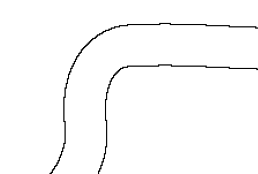
\includegraphics[interpolate=true,width=2.580000in,height=1.740000in]{contents/chapt6/figs/steer_control/planned_paths-img0.png}}%
\end{pgfscope}%
\begin{pgfscope}%
\pgfpathrectangle{\pgfqpoint{1.212308in}{0.810000in}}{\pgfqpoint{2.575385in}{1.740000in}}%
\pgfusepath{clip}%
\pgfsetbuttcap%
\pgfsetroundjoin%
\pgfsetlinewidth{1.505625pt}%
\definecolor{currentstroke}{rgb}{1.000000,0.000000,0.000000}%
\pgfsetstrokecolor{currentstroke}%
\pgfsetstrokeopacity{0.500000}%
\pgfsetdash{{9.600000pt}{2.400000pt}{1.500000pt}{2.400000pt}}{0.000000pt}%
\pgfusepath{stroke}%
\end{pgfscope}%
\begin{pgfscope}%
\pgfpathrectangle{\pgfqpoint{1.212308in}{0.810000in}}{\pgfqpoint{2.575385in}{1.740000in}}%
\pgfusepath{clip}%
\pgfsetrectcap%
\pgfsetroundjoin%
\pgfsetlinewidth{1.505625pt}%
\definecolor{currentstroke}{rgb}{1.000000,0.000000,0.000000}%
\pgfsetstrokecolor{currentstroke}%
\pgfsetstrokeopacity{0.500000}%
\pgfsetdash{}{0pt}%
\pgfusepath{stroke}%
\end{pgfscope}%
\begin{pgfscope}%
\pgfpathrectangle{\pgfqpoint{1.212308in}{0.810000in}}{\pgfqpoint{2.575385in}{1.740000in}}%
\pgfusepath{clip}%
\pgfsetbuttcap%
\pgfsetmiterjoin%
\definecolor{currentfill}{rgb}{1.000000,0.000000,0.000000}%
\pgfsetfillcolor{currentfill}%
\pgfsetfillopacity{0.500000}%
\pgfsetlinewidth{1.003750pt}%
\definecolor{currentstroke}{rgb}{1.000000,0.000000,0.000000}%
\pgfsetstrokecolor{currentstroke}%
\pgfsetstrokeopacity{0.500000}%
\pgfsetdash{}{0pt}%
\pgfsys@defobject{currentmarker}{\pgfqpoint{-0.041667in}{-0.041667in}}{\pgfqpoint{0.041667in}{0.041667in}}{%
\pgfpathmoveto{\pgfqpoint{-0.041667in}{-0.041667in}}%
\pgfpathlineto{\pgfqpoint{0.041667in}{-0.041667in}}%
\pgfpathlineto{\pgfqpoint{0.041667in}{0.041667in}}%
\pgfpathlineto{\pgfqpoint{-0.041667in}{0.041667in}}%
\pgfpathlineto{\pgfqpoint{-0.041667in}{-0.041667in}}%
\pgfpathclose%
\pgfusepath{stroke,fill}%
}%
\begin{pgfscope}%
\pgfsys@transformshift{-2.859013in}{3.109742in}%
\pgfsys@useobject{currentmarker}{}%
\end{pgfscope}%
\end{pgfscope}%
\begin{pgfscope}%
\pgfpathrectangle{\pgfqpoint{1.212308in}{0.810000in}}{\pgfqpoint{2.575385in}{1.740000in}}%
\pgfusepath{clip}%
\pgfsetbuttcap%
\pgfsetroundjoin%
\pgfsetlinewidth{1.505625pt}%
\definecolor{currentstroke}{rgb}{1.000000,0.000000,0.000000}%
\pgfsetstrokecolor{currentstroke}%
\pgfsetstrokeopacity{0.500000}%
\pgfsetdash{{9.600000pt}{2.400000pt}{1.500000pt}{2.400000pt}}{0.000000pt}%
\pgfusepath{stroke}%
\end{pgfscope}%
\begin{pgfscope}%
\pgfpathrectangle{\pgfqpoint{1.212308in}{0.810000in}}{\pgfqpoint{2.575385in}{1.740000in}}%
\pgfusepath{clip}%
\pgfsetrectcap%
\pgfsetroundjoin%
\pgfsetlinewidth{1.505625pt}%
\definecolor{currentstroke}{rgb}{1.000000,0.000000,0.000000}%
\pgfsetstrokecolor{currentstroke}%
\pgfsetstrokeopacity{0.500000}%
\pgfsetdash{}{0pt}%
\pgfusepath{stroke}%
\end{pgfscope}%
\begin{pgfscope}%
\pgfpathrectangle{\pgfqpoint{1.212308in}{0.810000in}}{\pgfqpoint{2.575385in}{1.740000in}}%
\pgfusepath{clip}%
\pgfsetbuttcap%
\pgfsetmiterjoin%
\definecolor{currentfill}{rgb}{1.000000,0.000000,0.000000}%
\pgfsetfillcolor{currentfill}%
\pgfsetfillopacity{0.500000}%
\pgfsetlinewidth{1.003750pt}%
\definecolor{currentstroke}{rgb}{1.000000,0.000000,0.000000}%
\pgfsetstrokecolor{currentstroke}%
\pgfsetstrokeopacity{0.500000}%
\pgfsetdash{}{0pt}%
\pgfsys@defobject{currentmarker}{\pgfqpoint{-0.041667in}{-0.041667in}}{\pgfqpoint{0.041667in}{0.041667in}}{%
\pgfpathmoveto{\pgfqpoint{-0.041667in}{-0.041667in}}%
\pgfpathlineto{\pgfqpoint{0.041667in}{-0.041667in}}%
\pgfpathlineto{\pgfqpoint{0.041667in}{0.041667in}}%
\pgfpathlineto{\pgfqpoint{-0.041667in}{0.041667in}}%
\pgfpathlineto{\pgfqpoint{-0.041667in}{-0.041667in}}%
\pgfpathclose%
\pgfusepath{stroke,fill}%
}%
\begin{pgfscope}%
\pgfsys@transformshift{-2.305105in}{3.088178in}%
\pgfsys@useobject{currentmarker}{}%
\end{pgfscope}%
\end{pgfscope}%
\begin{pgfscope}%
\pgfpathrectangle{\pgfqpoint{1.212308in}{0.810000in}}{\pgfqpoint{2.575385in}{1.740000in}}%
\pgfusepath{clip}%
\pgfsetbuttcap%
\pgfsetroundjoin%
\pgfsetlinewidth{1.505625pt}%
\definecolor{currentstroke}{rgb}{1.000000,0.000000,0.000000}%
\pgfsetstrokecolor{currentstroke}%
\pgfsetstrokeopacity{0.500000}%
\pgfsetdash{{9.600000pt}{2.400000pt}{1.500000pt}{2.400000pt}}{0.000000pt}%
\pgfusepath{stroke}%
\end{pgfscope}%
\begin{pgfscope}%
\pgfpathrectangle{\pgfqpoint{1.212308in}{0.810000in}}{\pgfqpoint{2.575385in}{1.740000in}}%
\pgfusepath{clip}%
\pgfsetrectcap%
\pgfsetroundjoin%
\pgfsetlinewidth{1.505625pt}%
\definecolor{currentstroke}{rgb}{1.000000,0.000000,0.000000}%
\pgfsetstrokecolor{currentstroke}%
\pgfsetstrokeopacity{0.500000}%
\pgfsetdash{}{0pt}%
\pgfusepath{stroke}%
\end{pgfscope}%
\begin{pgfscope}%
\pgfpathrectangle{\pgfqpoint{1.212308in}{0.810000in}}{\pgfqpoint{2.575385in}{1.740000in}}%
\pgfusepath{clip}%
\pgfsetbuttcap%
\pgfsetmiterjoin%
\definecolor{currentfill}{rgb}{1.000000,0.000000,0.000000}%
\pgfsetfillcolor{currentfill}%
\pgfsetfillopacity{0.500000}%
\pgfsetlinewidth{1.003750pt}%
\definecolor{currentstroke}{rgb}{1.000000,0.000000,0.000000}%
\pgfsetstrokecolor{currentstroke}%
\pgfsetstrokeopacity{0.500000}%
\pgfsetdash{}{0pt}%
\pgfsys@defobject{currentmarker}{\pgfqpoint{-0.041667in}{-0.041667in}}{\pgfqpoint{0.041667in}{0.041667in}}{%
\pgfpathmoveto{\pgfqpoint{-0.041667in}{-0.041667in}}%
\pgfpathlineto{\pgfqpoint{0.041667in}{-0.041667in}}%
\pgfpathlineto{\pgfqpoint{0.041667in}{0.041667in}}%
\pgfpathlineto{\pgfqpoint{-0.041667in}{0.041667in}}%
\pgfpathlineto{\pgfqpoint{-0.041667in}{-0.041667in}}%
\pgfpathclose%
\pgfusepath{stroke,fill}%
}%
\begin{pgfscope}%
\pgfsys@transformshift{-1.659336in}{3.062572in}%
\pgfsys@useobject{currentmarker}{}%
\end{pgfscope}%
\end{pgfscope}%
\begin{pgfscope}%
\pgfpathrectangle{\pgfqpoint{1.212308in}{0.810000in}}{\pgfqpoint{2.575385in}{1.740000in}}%
\pgfusepath{clip}%
\pgfsetbuttcap%
\pgfsetroundjoin%
\pgfsetlinewidth{1.505625pt}%
\definecolor{currentstroke}{rgb}{1.000000,0.000000,0.000000}%
\pgfsetstrokecolor{currentstroke}%
\pgfsetstrokeopacity{0.500000}%
\pgfsetdash{{9.600000pt}{2.400000pt}{1.500000pt}{2.400000pt}}{0.000000pt}%
\pgfusepath{stroke}%
\end{pgfscope}%
\begin{pgfscope}%
\pgfpathrectangle{\pgfqpoint{1.212308in}{0.810000in}}{\pgfqpoint{2.575385in}{1.740000in}}%
\pgfusepath{clip}%
\pgfsetrectcap%
\pgfsetroundjoin%
\pgfsetlinewidth{1.505625pt}%
\definecolor{currentstroke}{rgb}{1.000000,0.000000,0.000000}%
\pgfsetstrokecolor{currentstroke}%
\pgfsetstrokeopacity{0.500000}%
\pgfsetdash{}{0pt}%
\pgfusepath{stroke}%
\end{pgfscope}%
\begin{pgfscope}%
\pgfpathrectangle{\pgfqpoint{1.212308in}{0.810000in}}{\pgfqpoint{2.575385in}{1.740000in}}%
\pgfusepath{clip}%
\pgfsetbuttcap%
\pgfsetmiterjoin%
\definecolor{currentfill}{rgb}{1.000000,0.000000,0.000000}%
\pgfsetfillcolor{currentfill}%
\pgfsetfillopacity{0.500000}%
\pgfsetlinewidth{1.003750pt}%
\definecolor{currentstroke}{rgb}{1.000000,0.000000,0.000000}%
\pgfsetstrokecolor{currentstroke}%
\pgfsetstrokeopacity{0.500000}%
\pgfsetdash{}{0pt}%
\pgfsys@defobject{currentmarker}{\pgfqpoint{-0.041667in}{-0.041667in}}{\pgfqpoint{0.041667in}{0.041667in}}{%
\pgfpathmoveto{\pgfqpoint{-0.041667in}{-0.041667in}}%
\pgfpathlineto{\pgfqpoint{0.041667in}{-0.041667in}}%
\pgfpathlineto{\pgfqpoint{0.041667in}{0.041667in}}%
\pgfpathlineto{\pgfqpoint{-0.041667in}{0.041667in}}%
\pgfpathlineto{\pgfqpoint{-0.041667in}{-0.041667in}}%
\pgfpathclose%
\pgfusepath{stroke,fill}%
}%
\begin{pgfscope}%
\pgfsys@transformshift{-0.968776in}{3.058216in}%
\pgfsys@useobject{currentmarker}{}%
\end{pgfscope}%
\end{pgfscope}%
\begin{pgfscope}%
\pgfpathrectangle{\pgfqpoint{1.212308in}{0.810000in}}{\pgfqpoint{2.575385in}{1.740000in}}%
\pgfusepath{clip}%
\pgfsetbuttcap%
\pgfsetroundjoin%
\pgfsetlinewidth{1.505625pt}%
\definecolor{currentstroke}{rgb}{1.000000,0.000000,0.000000}%
\pgfsetstrokecolor{currentstroke}%
\pgfsetstrokeopacity{0.500000}%
\pgfsetdash{{9.600000pt}{2.400000pt}{1.500000pt}{2.400000pt}}{0.000000pt}%
\pgfusepath{stroke}%
\end{pgfscope}%
\begin{pgfscope}%
\pgfpathrectangle{\pgfqpoint{1.212308in}{0.810000in}}{\pgfqpoint{2.575385in}{1.740000in}}%
\pgfusepath{clip}%
\pgfsetrectcap%
\pgfsetroundjoin%
\pgfsetlinewidth{1.505625pt}%
\definecolor{currentstroke}{rgb}{1.000000,0.000000,0.000000}%
\pgfsetstrokecolor{currentstroke}%
\pgfsetstrokeopacity{0.500000}%
\pgfsetdash{}{0pt}%
\pgfusepath{stroke}%
\end{pgfscope}%
\begin{pgfscope}%
\pgfpathrectangle{\pgfqpoint{1.212308in}{0.810000in}}{\pgfqpoint{2.575385in}{1.740000in}}%
\pgfusepath{clip}%
\pgfsetbuttcap%
\pgfsetmiterjoin%
\definecolor{currentfill}{rgb}{1.000000,0.000000,0.000000}%
\pgfsetfillcolor{currentfill}%
\pgfsetfillopacity{0.500000}%
\pgfsetlinewidth{1.003750pt}%
\definecolor{currentstroke}{rgb}{1.000000,0.000000,0.000000}%
\pgfsetstrokecolor{currentstroke}%
\pgfsetstrokeopacity{0.500000}%
\pgfsetdash{}{0pt}%
\pgfsys@defobject{currentmarker}{\pgfqpoint{-0.041667in}{-0.041667in}}{\pgfqpoint{0.041667in}{0.041667in}}{%
\pgfpathmoveto{\pgfqpoint{-0.041667in}{-0.041667in}}%
\pgfpathlineto{\pgfqpoint{0.041667in}{-0.041667in}}%
\pgfpathlineto{\pgfqpoint{0.041667in}{0.041667in}}%
\pgfpathlineto{\pgfqpoint{-0.041667in}{0.041667in}}%
\pgfpathlineto{\pgfqpoint{-0.041667in}{-0.041667in}}%
\pgfpathclose%
\pgfusepath{stroke,fill}%
}%
\begin{pgfscope}%
\pgfsys@transformshift{-0.299395in}{3.069337in}%
\pgfsys@useobject{currentmarker}{}%
\end{pgfscope}%
\end{pgfscope}%
\begin{pgfscope}%
\pgfpathrectangle{\pgfqpoint{1.212308in}{0.810000in}}{\pgfqpoint{2.575385in}{1.740000in}}%
\pgfusepath{clip}%
\pgfsetbuttcap%
\pgfsetroundjoin%
\pgfsetlinewidth{1.505625pt}%
\definecolor{currentstroke}{rgb}{1.000000,0.000000,0.000000}%
\pgfsetstrokecolor{currentstroke}%
\pgfsetstrokeopacity{0.500000}%
\pgfsetdash{{9.600000pt}{2.400000pt}{1.500000pt}{2.400000pt}}{0.000000pt}%
\pgfusepath{stroke}%
\end{pgfscope}%
\begin{pgfscope}%
\pgfpathrectangle{\pgfqpoint{1.212308in}{0.810000in}}{\pgfqpoint{2.575385in}{1.740000in}}%
\pgfusepath{clip}%
\pgfsetrectcap%
\pgfsetroundjoin%
\pgfsetlinewidth{1.505625pt}%
\definecolor{currentstroke}{rgb}{1.000000,0.000000,0.000000}%
\pgfsetstrokecolor{currentstroke}%
\pgfsetstrokeopacity{0.500000}%
\pgfsetdash{}{0pt}%
\pgfusepath{stroke}%
\end{pgfscope}%
\begin{pgfscope}%
\pgfpathrectangle{\pgfqpoint{1.212308in}{0.810000in}}{\pgfqpoint{2.575385in}{1.740000in}}%
\pgfusepath{clip}%
\pgfsetbuttcap%
\pgfsetmiterjoin%
\definecolor{currentfill}{rgb}{1.000000,0.000000,0.000000}%
\pgfsetfillcolor{currentfill}%
\pgfsetfillopacity{0.500000}%
\pgfsetlinewidth{1.003750pt}%
\definecolor{currentstroke}{rgb}{1.000000,0.000000,0.000000}%
\pgfsetstrokecolor{currentstroke}%
\pgfsetstrokeopacity{0.500000}%
\pgfsetdash{}{0pt}%
\pgfsys@defobject{currentmarker}{\pgfqpoint{-0.041667in}{-0.041667in}}{\pgfqpoint{0.041667in}{0.041667in}}{%
\pgfpathmoveto{\pgfqpoint{-0.041667in}{-0.041667in}}%
\pgfpathlineto{\pgfqpoint{0.041667in}{-0.041667in}}%
\pgfpathlineto{\pgfqpoint{0.041667in}{0.041667in}}%
\pgfpathlineto{\pgfqpoint{-0.041667in}{0.041667in}}%
\pgfpathlineto{\pgfqpoint{-0.041667in}{-0.041667in}}%
\pgfpathclose%
\pgfusepath{stroke,fill}%
}%
\begin{pgfscope}%
\pgfsys@transformshift{0.368898in}{3.069224in}%
\pgfsys@useobject{currentmarker}{}%
\end{pgfscope}%
\end{pgfscope}%
\begin{pgfscope}%
\pgfpathrectangle{\pgfqpoint{1.212308in}{0.810000in}}{\pgfqpoint{2.575385in}{1.740000in}}%
\pgfusepath{clip}%
\pgfsetbuttcap%
\pgfsetroundjoin%
\pgfsetlinewidth{1.505625pt}%
\definecolor{currentstroke}{rgb}{1.000000,0.000000,0.000000}%
\pgfsetstrokecolor{currentstroke}%
\pgfsetstrokeopacity{0.500000}%
\pgfsetdash{{9.600000pt}{2.400000pt}{1.500000pt}{2.400000pt}}{0.000000pt}%
\pgfusepath{stroke}%
\end{pgfscope}%
\begin{pgfscope}%
\pgfpathrectangle{\pgfqpoint{1.212308in}{0.810000in}}{\pgfqpoint{2.575385in}{1.740000in}}%
\pgfusepath{clip}%
\pgfsetrectcap%
\pgfsetroundjoin%
\pgfsetlinewidth{1.505625pt}%
\definecolor{currentstroke}{rgb}{1.000000,0.000000,0.000000}%
\pgfsetstrokecolor{currentstroke}%
\pgfsetstrokeopacity{0.500000}%
\pgfsetdash{}{0pt}%
\pgfusepath{stroke}%
\end{pgfscope}%
\begin{pgfscope}%
\pgfpathrectangle{\pgfqpoint{1.212308in}{0.810000in}}{\pgfqpoint{2.575385in}{1.740000in}}%
\pgfusepath{clip}%
\pgfsetbuttcap%
\pgfsetmiterjoin%
\definecolor{currentfill}{rgb}{1.000000,0.000000,0.000000}%
\pgfsetfillcolor{currentfill}%
\pgfsetfillopacity{0.500000}%
\pgfsetlinewidth{1.003750pt}%
\definecolor{currentstroke}{rgb}{1.000000,0.000000,0.000000}%
\pgfsetstrokecolor{currentstroke}%
\pgfsetstrokeopacity{0.500000}%
\pgfsetdash{}{0pt}%
\pgfsys@defobject{currentmarker}{\pgfqpoint{-0.041667in}{-0.041667in}}{\pgfqpoint{0.041667in}{0.041667in}}{%
\pgfpathmoveto{\pgfqpoint{-0.041667in}{-0.041667in}}%
\pgfpathlineto{\pgfqpoint{0.041667in}{-0.041667in}}%
\pgfpathlineto{\pgfqpoint{0.041667in}{0.041667in}}%
\pgfpathlineto{\pgfqpoint{-0.041667in}{0.041667in}}%
\pgfpathlineto{\pgfqpoint{-0.041667in}{-0.041667in}}%
\pgfpathclose%
\pgfusepath{stroke,fill}%
}%
\begin{pgfscope}%
\pgfsys@transformshift{1.059282in}{3.056794in}%
\pgfsys@useobject{currentmarker}{}%
\end{pgfscope}%
\end{pgfscope}%
\begin{pgfscope}%
\pgfpathrectangle{\pgfqpoint{1.212308in}{0.810000in}}{\pgfqpoint{2.575385in}{1.740000in}}%
\pgfusepath{clip}%
\pgfsetbuttcap%
\pgfsetroundjoin%
\pgfsetlinewidth{1.505625pt}%
\definecolor{currentstroke}{rgb}{1.000000,0.000000,0.000000}%
\pgfsetstrokecolor{currentstroke}%
\pgfsetstrokeopacity{0.500000}%
\pgfsetdash{{9.600000pt}{2.400000pt}{1.500000pt}{2.400000pt}}{0.000000pt}%
\pgfusepath{stroke}%
\end{pgfscope}%
\begin{pgfscope}%
\pgfpathrectangle{\pgfqpoint{1.212308in}{0.810000in}}{\pgfqpoint{2.575385in}{1.740000in}}%
\pgfusepath{clip}%
\pgfsetrectcap%
\pgfsetroundjoin%
\pgfsetlinewidth{1.505625pt}%
\definecolor{currentstroke}{rgb}{1.000000,0.000000,0.000000}%
\pgfsetstrokecolor{currentstroke}%
\pgfsetstrokeopacity{0.500000}%
\pgfsetdash{}{0pt}%
\pgfusepath{stroke}%
\end{pgfscope}%
\begin{pgfscope}%
\pgfpathrectangle{\pgfqpoint{1.212308in}{0.810000in}}{\pgfqpoint{2.575385in}{1.740000in}}%
\pgfusepath{clip}%
\pgfsetbuttcap%
\pgfsetmiterjoin%
\definecolor{currentfill}{rgb}{1.000000,0.000000,0.000000}%
\pgfsetfillcolor{currentfill}%
\pgfsetfillopacity{0.500000}%
\pgfsetlinewidth{1.003750pt}%
\definecolor{currentstroke}{rgb}{1.000000,0.000000,0.000000}%
\pgfsetstrokecolor{currentstroke}%
\pgfsetstrokeopacity{0.500000}%
\pgfsetdash{}{0pt}%
\pgfsys@defobject{currentmarker}{\pgfqpoint{-0.041667in}{-0.041667in}}{\pgfqpoint{0.041667in}{0.041667in}}{%
\pgfpathmoveto{\pgfqpoint{-0.041667in}{-0.041667in}}%
\pgfpathlineto{\pgfqpoint{0.041667in}{-0.041667in}}%
\pgfpathlineto{\pgfqpoint{0.041667in}{0.041667in}}%
\pgfpathlineto{\pgfqpoint{-0.041667in}{0.041667in}}%
\pgfpathlineto{\pgfqpoint{-0.041667in}{-0.041667in}}%
\pgfpathclose%
\pgfusepath{stroke,fill}%
}%
\begin{pgfscope}%
\pgfsys@transformshift{1.727708in}{3.061467in}%
\pgfsys@useobject{currentmarker}{}%
\end{pgfscope}%
\end{pgfscope}%
\begin{pgfscope}%
\pgfpathrectangle{\pgfqpoint{1.212308in}{0.810000in}}{\pgfqpoint{2.575385in}{1.740000in}}%
\pgfusepath{clip}%
\pgfsetbuttcap%
\pgfsetroundjoin%
\pgfsetlinewidth{1.505625pt}%
\definecolor{currentstroke}{rgb}{1.000000,0.000000,0.000000}%
\pgfsetstrokecolor{currentstroke}%
\pgfsetstrokeopacity{0.500000}%
\pgfsetdash{{9.600000pt}{2.400000pt}{1.500000pt}{2.400000pt}}{0.000000pt}%
\pgfusepath{stroke}%
\end{pgfscope}%
\begin{pgfscope}%
\pgfpathrectangle{\pgfqpoint{1.212308in}{0.810000in}}{\pgfqpoint{2.575385in}{1.740000in}}%
\pgfusepath{clip}%
\pgfsetrectcap%
\pgfsetroundjoin%
\pgfsetlinewidth{1.505625pt}%
\definecolor{currentstroke}{rgb}{1.000000,0.000000,0.000000}%
\pgfsetstrokecolor{currentstroke}%
\pgfsetstrokeopacity{0.500000}%
\pgfsetdash{}{0pt}%
\pgfusepath{stroke}%
\end{pgfscope}%
\begin{pgfscope}%
\pgfpathrectangle{\pgfqpoint{1.212308in}{0.810000in}}{\pgfqpoint{2.575385in}{1.740000in}}%
\pgfusepath{clip}%
\pgfsetbuttcap%
\pgfsetmiterjoin%
\definecolor{currentfill}{rgb}{1.000000,0.000000,0.000000}%
\pgfsetfillcolor{currentfill}%
\pgfsetfillopacity{0.500000}%
\pgfsetlinewidth{1.003750pt}%
\definecolor{currentstroke}{rgb}{1.000000,0.000000,0.000000}%
\pgfsetstrokecolor{currentstroke}%
\pgfsetstrokeopacity{0.500000}%
\pgfsetdash{}{0pt}%
\pgfsys@defobject{currentmarker}{\pgfqpoint{-0.041667in}{-0.041667in}}{\pgfqpoint{0.041667in}{0.041667in}}{%
\pgfpathmoveto{\pgfqpoint{-0.041667in}{-0.041667in}}%
\pgfpathlineto{\pgfqpoint{0.041667in}{-0.041667in}}%
\pgfpathlineto{\pgfqpoint{0.041667in}{0.041667in}}%
\pgfpathlineto{\pgfqpoint{-0.041667in}{0.041667in}}%
\pgfpathlineto{\pgfqpoint{-0.041667in}{-0.041667in}}%
\pgfpathclose%
\pgfusepath{stroke,fill}%
}%
\begin{pgfscope}%
\pgfsys@transformshift{2.397732in}{3.015413in}%
\pgfsys@useobject{currentmarker}{}%
\end{pgfscope}%
\end{pgfscope}%
\begin{pgfscope}%
\pgfpathrectangle{\pgfqpoint{1.212308in}{0.810000in}}{\pgfqpoint{2.575385in}{1.740000in}}%
\pgfusepath{clip}%
\pgfsetbuttcap%
\pgfsetroundjoin%
\pgfsetlinewidth{1.505625pt}%
\definecolor{currentstroke}{rgb}{1.000000,0.000000,0.000000}%
\pgfsetstrokecolor{currentstroke}%
\pgfsetstrokeopacity{0.500000}%
\pgfsetdash{{9.600000pt}{2.400000pt}{1.500000pt}{2.400000pt}}{0.000000pt}%
\pgfusepath{stroke}%
\end{pgfscope}%
\begin{pgfscope}%
\pgfpathrectangle{\pgfqpoint{1.212308in}{0.810000in}}{\pgfqpoint{2.575385in}{1.740000in}}%
\pgfusepath{clip}%
\pgfsetrectcap%
\pgfsetroundjoin%
\pgfsetlinewidth{1.505625pt}%
\definecolor{currentstroke}{rgb}{1.000000,0.000000,0.000000}%
\pgfsetstrokecolor{currentstroke}%
\pgfsetstrokeopacity{0.500000}%
\pgfsetdash{}{0pt}%
\pgfusepath{stroke}%
\end{pgfscope}%
\begin{pgfscope}%
\pgfpathrectangle{\pgfqpoint{1.212308in}{0.810000in}}{\pgfqpoint{2.575385in}{1.740000in}}%
\pgfusepath{clip}%
\pgfsetbuttcap%
\pgfsetmiterjoin%
\definecolor{currentfill}{rgb}{1.000000,0.000000,0.000000}%
\pgfsetfillcolor{currentfill}%
\pgfsetfillopacity{0.500000}%
\pgfsetlinewidth{1.003750pt}%
\definecolor{currentstroke}{rgb}{1.000000,0.000000,0.000000}%
\pgfsetstrokecolor{currentstroke}%
\pgfsetstrokeopacity{0.500000}%
\pgfsetdash{}{0pt}%
\pgfsys@defobject{currentmarker}{\pgfqpoint{-0.041667in}{-0.041667in}}{\pgfqpoint{0.041667in}{0.041667in}}{%
\pgfpathmoveto{\pgfqpoint{-0.041667in}{-0.041667in}}%
\pgfpathlineto{\pgfqpoint{0.041667in}{-0.041667in}}%
\pgfpathlineto{\pgfqpoint{0.041667in}{0.041667in}}%
\pgfpathlineto{\pgfqpoint{-0.041667in}{0.041667in}}%
\pgfpathlineto{\pgfqpoint{-0.041667in}{-0.041667in}}%
\pgfpathclose%
\pgfusepath{stroke,fill}%
}%
\begin{pgfscope}%
\pgfsys@transformshift{3.067565in}{2.982144in}%
\pgfsys@useobject{currentmarker}{}%
\end{pgfscope}%
\end{pgfscope}%
\begin{pgfscope}%
\pgfpathrectangle{\pgfqpoint{1.212308in}{0.810000in}}{\pgfqpoint{2.575385in}{1.740000in}}%
\pgfusepath{clip}%
\pgfsetbuttcap%
\pgfsetroundjoin%
\pgfsetlinewidth{1.505625pt}%
\definecolor{currentstroke}{rgb}{1.000000,0.000000,0.000000}%
\pgfsetstrokecolor{currentstroke}%
\pgfsetstrokeopacity{0.500000}%
\pgfsetdash{{9.600000pt}{2.400000pt}{1.500000pt}{2.400000pt}}{0.000000pt}%
\pgfusepath{stroke}%
\end{pgfscope}%
\begin{pgfscope}%
\pgfpathrectangle{\pgfqpoint{1.212308in}{0.810000in}}{\pgfqpoint{2.575385in}{1.740000in}}%
\pgfusepath{clip}%
\pgfsetrectcap%
\pgfsetroundjoin%
\pgfsetlinewidth{1.505625pt}%
\definecolor{currentstroke}{rgb}{1.000000,0.000000,0.000000}%
\pgfsetstrokecolor{currentstroke}%
\pgfsetstrokeopacity{0.500000}%
\pgfsetdash{}{0pt}%
\pgfusepath{stroke}%
\end{pgfscope}%
\begin{pgfscope}%
\pgfpathrectangle{\pgfqpoint{1.212308in}{0.810000in}}{\pgfqpoint{2.575385in}{1.740000in}}%
\pgfusepath{clip}%
\pgfsetbuttcap%
\pgfsetmiterjoin%
\definecolor{currentfill}{rgb}{1.000000,0.000000,0.000000}%
\pgfsetfillcolor{currentfill}%
\pgfsetfillopacity{0.500000}%
\pgfsetlinewidth{1.003750pt}%
\definecolor{currentstroke}{rgb}{1.000000,0.000000,0.000000}%
\pgfsetstrokecolor{currentstroke}%
\pgfsetstrokeopacity{0.500000}%
\pgfsetdash{}{0pt}%
\pgfsys@defobject{currentmarker}{\pgfqpoint{-0.041667in}{-0.041667in}}{\pgfqpoint{0.041667in}{0.041667in}}{%
\pgfpathmoveto{\pgfqpoint{-0.041667in}{-0.041667in}}%
\pgfpathlineto{\pgfqpoint{0.041667in}{-0.041667in}}%
\pgfpathlineto{\pgfqpoint{0.041667in}{0.041667in}}%
\pgfpathlineto{\pgfqpoint{-0.041667in}{0.041667in}}%
\pgfpathlineto{\pgfqpoint{-0.041667in}{-0.041667in}}%
\pgfpathclose%
\pgfusepath{stroke,fill}%
}%
\begin{pgfscope}%
\pgfsys@transformshift{3.737370in}{2.984118in}%
\pgfsys@useobject{currentmarker}{}%
\end{pgfscope}%
\end{pgfscope}%
\begin{pgfscope}%
\pgfpathrectangle{\pgfqpoint{1.212308in}{0.810000in}}{\pgfqpoint{2.575385in}{1.740000in}}%
\pgfusepath{clip}%
\pgfsetbuttcap%
\pgfsetroundjoin%
\pgfsetlinewidth{1.505625pt}%
\definecolor{currentstroke}{rgb}{1.000000,0.000000,0.000000}%
\pgfsetstrokecolor{currentstroke}%
\pgfsetstrokeopacity{0.500000}%
\pgfsetdash{{9.600000pt}{2.400000pt}{1.500000pt}{2.400000pt}}{0.000000pt}%
\pgfusepath{stroke}%
\end{pgfscope}%
\begin{pgfscope}%
\pgfpathrectangle{\pgfqpoint{1.212308in}{0.810000in}}{\pgfqpoint{2.575385in}{1.740000in}}%
\pgfusepath{clip}%
\pgfsetrectcap%
\pgfsetroundjoin%
\pgfsetlinewidth{1.505625pt}%
\definecolor{currentstroke}{rgb}{1.000000,0.000000,0.000000}%
\pgfsetstrokecolor{currentstroke}%
\pgfsetstrokeopacity{0.500000}%
\pgfsetdash{}{0pt}%
\pgfusepath{stroke}%
\end{pgfscope}%
\begin{pgfscope}%
\pgfpathrectangle{\pgfqpoint{1.212308in}{0.810000in}}{\pgfqpoint{2.575385in}{1.740000in}}%
\pgfusepath{clip}%
\pgfsetbuttcap%
\pgfsetmiterjoin%
\definecolor{currentfill}{rgb}{1.000000,0.000000,0.000000}%
\pgfsetfillcolor{currentfill}%
\pgfsetfillopacity{0.500000}%
\pgfsetlinewidth{1.003750pt}%
\definecolor{currentstroke}{rgb}{1.000000,0.000000,0.000000}%
\pgfsetstrokecolor{currentstroke}%
\pgfsetstrokeopacity{0.500000}%
\pgfsetdash{}{0pt}%
\pgfsys@defobject{currentmarker}{\pgfqpoint{-0.041667in}{-0.041667in}}{\pgfqpoint{0.041667in}{0.041667in}}{%
\pgfpathmoveto{\pgfqpoint{-0.041667in}{-0.041667in}}%
\pgfpathlineto{\pgfqpoint{0.041667in}{-0.041667in}}%
\pgfpathlineto{\pgfqpoint{0.041667in}{0.041667in}}%
\pgfpathlineto{\pgfqpoint{-0.041667in}{0.041667in}}%
\pgfpathlineto{\pgfqpoint{-0.041667in}{-0.041667in}}%
\pgfpathclose%
\pgfusepath{stroke,fill}%
}%
\begin{pgfscope}%
\pgfsys@transformshift{4.399527in}{2.977360in}%
\pgfsys@useobject{currentmarker}{}%
\end{pgfscope}%
\end{pgfscope}%
\begin{pgfscope}%
\pgfpathrectangle{\pgfqpoint{1.212308in}{0.810000in}}{\pgfqpoint{2.575385in}{1.740000in}}%
\pgfusepath{clip}%
\pgfsetbuttcap%
\pgfsetroundjoin%
\pgfsetlinewidth{1.505625pt}%
\definecolor{currentstroke}{rgb}{1.000000,0.000000,0.000000}%
\pgfsetstrokecolor{currentstroke}%
\pgfsetstrokeopacity{0.500000}%
\pgfsetdash{{9.600000pt}{2.400000pt}{1.500000pt}{2.400000pt}}{0.000000pt}%
\pgfusepath{stroke}%
\end{pgfscope}%
\begin{pgfscope}%
\pgfpathrectangle{\pgfqpoint{1.212308in}{0.810000in}}{\pgfqpoint{2.575385in}{1.740000in}}%
\pgfusepath{clip}%
\pgfsetrectcap%
\pgfsetroundjoin%
\pgfsetlinewidth{1.505625pt}%
\definecolor{currentstroke}{rgb}{1.000000,0.000000,0.000000}%
\pgfsetstrokecolor{currentstroke}%
\pgfsetstrokeopacity{0.500000}%
\pgfsetdash{}{0pt}%
\pgfusepath{stroke}%
\end{pgfscope}%
\begin{pgfscope}%
\pgfpathrectangle{\pgfqpoint{1.212308in}{0.810000in}}{\pgfqpoint{2.575385in}{1.740000in}}%
\pgfusepath{clip}%
\pgfsetbuttcap%
\pgfsetmiterjoin%
\definecolor{currentfill}{rgb}{1.000000,0.000000,0.000000}%
\pgfsetfillcolor{currentfill}%
\pgfsetfillopacity{0.500000}%
\pgfsetlinewidth{1.003750pt}%
\definecolor{currentstroke}{rgb}{1.000000,0.000000,0.000000}%
\pgfsetstrokecolor{currentstroke}%
\pgfsetstrokeopacity{0.500000}%
\pgfsetdash{}{0pt}%
\pgfsys@defobject{currentmarker}{\pgfqpoint{-0.041667in}{-0.041667in}}{\pgfqpoint{0.041667in}{0.041667in}}{%
\pgfpathmoveto{\pgfqpoint{-0.041667in}{-0.041667in}}%
\pgfpathlineto{\pgfqpoint{0.041667in}{-0.041667in}}%
\pgfpathlineto{\pgfqpoint{0.041667in}{0.041667in}}%
\pgfpathlineto{\pgfqpoint{-0.041667in}{0.041667in}}%
\pgfpathlineto{\pgfqpoint{-0.041667in}{-0.041667in}}%
\pgfpathclose%
\pgfusepath{stroke,fill}%
}%
\begin{pgfscope}%
\pgfsys@transformshift{5.091058in}{2.982219in}%
\pgfsys@useobject{currentmarker}{}%
\end{pgfscope}%
\end{pgfscope}%
\begin{pgfscope}%
\pgfpathrectangle{\pgfqpoint{1.212308in}{0.810000in}}{\pgfqpoint{2.575385in}{1.740000in}}%
\pgfusepath{clip}%
\pgfsetbuttcap%
\pgfsetroundjoin%
\pgfsetlinewidth{1.505625pt}%
\definecolor{currentstroke}{rgb}{1.000000,0.000000,0.000000}%
\pgfsetstrokecolor{currentstroke}%
\pgfsetstrokeopacity{0.500000}%
\pgfsetdash{{9.600000pt}{2.400000pt}{1.500000pt}{2.400000pt}}{0.000000pt}%
\pgfusepath{stroke}%
\end{pgfscope}%
\begin{pgfscope}%
\pgfpathrectangle{\pgfqpoint{1.212308in}{0.810000in}}{\pgfqpoint{2.575385in}{1.740000in}}%
\pgfusepath{clip}%
\pgfsetrectcap%
\pgfsetroundjoin%
\pgfsetlinewidth{1.505625pt}%
\definecolor{currentstroke}{rgb}{1.000000,0.000000,0.000000}%
\pgfsetstrokecolor{currentstroke}%
\pgfsetstrokeopacity{0.500000}%
\pgfsetdash{}{0pt}%
\pgfusepath{stroke}%
\end{pgfscope}%
\begin{pgfscope}%
\pgfpathrectangle{\pgfqpoint{1.212308in}{0.810000in}}{\pgfqpoint{2.575385in}{1.740000in}}%
\pgfusepath{clip}%
\pgfsetbuttcap%
\pgfsetmiterjoin%
\definecolor{currentfill}{rgb}{1.000000,0.000000,0.000000}%
\pgfsetfillcolor{currentfill}%
\pgfsetfillopacity{0.500000}%
\pgfsetlinewidth{1.003750pt}%
\definecolor{currentstroke}{rgb}{1.000000,0.000000,0.000000}%
\pgfsetstrokecolor{currentstroke}%
\pgfsetstrokeopacity{0.500000}%
\pgfsetdash{}{0pt}%
\pgfsys@defobject{currentmarker}{\pgfqpoint{-0.041667in}{-0.041667in}}{\pgfqpoint{0.041667in}{0.041667in}}{%
\pgfpathmoveto{\pgfqpoint{-0.041667in}{-0.041667in}}%
\pgfpathlineto{\pgfqpoint{0.041667in}{-0.041667in}}%
\pgfpathlineto{\pgfqpoint{0.041667in}{0.041667in}}%
\pgfpathlineto{\pgfqpoint{-0.041667in}{0.041667in}}%
\pgfpathlineto{\pgfqpoint{-0.041667in}{-0.041667in}}%
\pgfpathclose%
\pgfusepath{stroke,fill}%
}%
\begin{pgfscope}%
\pgfsys@transformshift{5.774651in}{2.947737in}%
\pgfsys@useobject{currentmarker}{}%
\end{pgfscope}%
\end{pgfscope}%
\begin{pgfscope}%
\pgfpathrectangle{\pgfqpoint{1.212308in}{0.810000in}}{\pgfqpoint{2.575385in}{1.740000in}}%
\pgfusepath{clip}%
\pgfsetbuttcap%
\pgfsetroundjoin%
\pgfsetlinewidth{1.505625pt}%
\definecolor{currentstroke}{rgb}{1.000000,0.000000,0.000000}%
\pgfsetstrokecolor{currentstroke}%
\pgfsetstrokeopacity{0.500000}%
\pgfsetdash{{9.600000pt}{2.400000pt}{1.500000pt}{2.400000pt}}{0.000000pt}%
\pgfusepath{stroke}%
\end{pgfscope}%
\begin{pgfscope}%
\pgfpathrectangle{\pgfqpoint{1.212308in}{0.810000in}}{\pgfqpoint{2.575385in}{1.740000in}}%
\pgfusepath{clip}%
\pgfsetrectcap%
\pgfsetroundjoin%
\pgfsetlinewidth{1.505625pt}%
\definecolor{currentstroke}{rgb}{1.000000,0.000000,0.000000}%
\pgfsetstrokecolor{currentstroke}%
\pgfsetstrokeopacity{0.500000}%
\pgfsetdash{}{0pt}%
\pgfusepath{stroke}%
\end{pgfscope}%
\begin{pgfscope}%
\pgfpathrectangle{\pgfqpoint{1.212308in}{0.810000in}}{\pgfqpoint{2.575385in}{1.740000in}}%
\pgfusepath{clip}%
\pgfsetbuttcap%
\pgfsetmiterjoin%
\definecolor{currentfill}{rgb}{1.000000,0.000000,0.000000}%
\pgfsetfillcolor{currentfill}%
\pgfsetfillopacity{0.500000}%
\pgfsetlinewidth{1.003750pt}%
\definecolor{currentstroke}{rgb}{1.000000,0.000000,0.000000}%
\pgfsetstrokecolor{currentstroke}%
\pgfsetstrokeopacity{0.500000}%
\pgfsetdash{}{0pt}%
\pgfsys@defobject{currentmarker}{\pgfqpoint{-0.041667in}{-0.041667in}}{\pgfqpoint{0.041667in}{0.041667in}}{%
\pgfpathmoveto{\pgfqpoint{-0.041667in}{-0.041667in}}%
\pgfpathlineto{\pgfqpoint{0.041667in}{-0.041667in}}%
\pgfpathlineto{\pgfqpoint{0.041667in}{0.041667in}}%
\pgfpathlineto{\pgfqpoint{-0.041667in}{0.041667in}}%
\pgfpathlineto{\pgfqpoint{-0.041667in}{-0.041667in}}%
\pgfpathclose%
\pgfusepath{stroke,fill}%
}%
\begin{pgfscope}%
\pgfsys@transformshift{6.174588in}{2.419541in}%
\pgfsys@useobject{currentmarker}{}%
\end{pgfscope}%
\end{pgfscope}%
\begin{pgfscope}%
\pgfpathrectangle{\pgfqpoint{1.212308in}{0.810000in}}{\pgfqpoint{2.575385in}{1.740000in}}%
\pgfusepath{clip}%
\pgfsetbuttcap%
\pgfsetroundjoin%
\pgfsetlinewidth{1.505625pt}%
\definecolor{currentstroke}{rgb}{1.000000,0.000000,0.000000}%
\pgfsetstrokecolor{currentstroke}%
\pgfsetstrokeopacity{0.500000}%
\pgfsetdash{{9.600000pt}{2.400000pt}{1.500000pt}{2.400000pt}}{0.000000pt}%
\pgfusepath{stroke}%
\end{pgfscope}%
\begin{pgfscope}%
\pgfpathrectangle{\pgfqpoint{1.212308in}{0.810000in}}{\pgfqpoint{2.575385in}{1.740000in}}%
\pgfusepath{clip}%
\pgfsetrectcap%
\pgfsetroundjoin%
\pgfsetlinewidth{1.505625pt}%
\definecolor{currentstroke}{rgb}{1.000000,0.000000,0.000000}%
\pgfsetstrokecolor{currentstroke}%
\pgfsetstrokeopacity{0.500000}%
\pgfsetdash{}{0pt}%
\pgfusepath{stroke}%
\end{pgfscope}%
\begin{pgfscope}%
\pgfpathrectangle{\pgfqpoint{1.212308in}{0.810000in}}{\pgfqpoint{2.575385in}{1.740000in}}%
\pgfusepath{clip}%
\pgfsetbuttcap%
\pgfsetmiterjoin%
\definecolor{currentfill}{rgb}{1.000000,0.000000,0.000000}%
\pgfsetfillcolor{currentfill}%
\pgfsetfillopacity{0.500000}%
\pgfsetlinewidth{1.003750pt}%
\definecolor{currentstroke}{rgb}{1.000000,0.000000,0.000000}%
\pgfsetstrokecolor{currentstroke}%
\pgfsetstrokeopacity{0.500000}%
\pgfsetdash{}{0pt}%
\pgfsys@defobject{currentmarker}{\pgfqpoint{-0.041667in}{-0.041667in}}{\pgfqpoint{0.041667in}{0.041667in}}{%
\pgfpathmoveto{\pgfqpoint{-0.041667in}{-0.041667in}}%
\pgfpathlineto{\pgfqpoint{0.041667in}{-0.041667in}}%
\pgfpathlineto{\pgfqpoint{0.041667in}{0.041667in}}%
\pgfpathlineto{\pgfqpoint{-0.041667in}{0.041667in}}%
\pgfpathlineto{\pgfqpoint{-0.041667in}{-0.041667in}}%
\pgfpathclose%
\pgfusepath{stroke,fill}%
}%
\begin{pgfscope}%
\pgfsys@transformshift{6.422664in}{1.797557in}%
\pgfsys@useobject{currentmarker}{}%
\end{pgfscope}%
\end{pgfscope}%
\begin{pgfscope}%
\pgfpathrectangle{\pgfqpoint{1.212308in}{0.810000in}}{\pgfqpoint{2.575385in}{1.740000in}}%
\pgfusepath{clip}%
\pgfsetbuttcap%
\pgfsetroundjoin%
\pgfsetlinewidth{1.505625pt}%
\definecolor{currentstroke}{rgb}{1.000000,0.000000,0.000000}%
\pgfsetstrokecolor{currentstroke}%
\pgfsetstrokeopacity{0.500000}%
\pgfsetdash{{9.600000pt}{2.400000pt}{1.500000pt}{2.400000pt}}{0.000000pt}%
\pgfusepath{stroke}%
\end{pgfscope}%
\begin{pgfscope}%
\pgfpathrectangle{\pgfqpoint{1.212308in}{0.810000in}}{\pgfqpoint{2.575385in}{1.740000in}}%
\pgfusepath{clip}%
\pgfsetrectcap%
\pgfsetroundjoin%
\pgfsetlinewidth{1.505625pt}%
\definecolor{currentstroke}{rgb}{1.000000,0.000000,0.000000}%
\pgfsetstrokecolor{currentstroke}%
\pgfsetstrokeopacity{0.500000}%
\pgfsetdash{}{0pt}%
\pgfusepath{stroke}%
\end{pgfscope}%
\begin{pgfscope}%
\pgfpathrectangle{\pgfqpoint{1.212308in}{0.810000in}}{\pgfqpoint{2.575385in}{1.740000in}}%
\pgfusepath{clip}%
\pgfsetbuttcap%
\pgfsetmiterjoin%
\definecolor{currentfill}{rgb}{1.000000,0.000000,0.000000}%
\pgfsetfillcolor{currentfill}%
\pgfsetfillopacity{0.500000}%
\pgfsetlinewidth{1.003750pt}%
\definecolor{currentstroke}{rgb}{1.000000,0.000000,0.000000}%
\pgfsetstrokecolor{currentstroke}%
\pgfsetstrokeopacity{0.500000}%
\pgfsetdash{}{0pt}%
\pgfsys@defobject{currentmarker}{\pgfqpoint{-0.041667in}{-0.041667in}}{\pgfqpoint{0.041667in}{0.041667in}}{%
\pgfpathmoveto{\pgfqpoint{-0.041667in}{-0.041667in}}%
\pgfpathlineto{\pgfqpoint{0.041667in}{-0.041667in}}%
\pgfpathlineto{\pgfqpoint{0.041667in}{0.041667in}}%
\pgfpathlineto{\pgfqpoint{-0.041667in}{0.041667in}}%
\pgfpathlineto{\pgfqpoint{-0.041667in}{-0.041667in}}%
\pgfpathclose%
\pgfusepath{stroke,fill}%
}%
\begin{pgfscope}%
\pgfsys@transformshift{7.022943in}{1.464430in}%
\pgfsys@useobject{currentmarker}{}%
\end{pgfscope}%
\end{pgfscope}%
\begin{pgfscope}%
\pgfpathrectangle{\pgfqpoint{1.212308in}{0.810000in}}{\pgfqpoint{2.575385in}{1.740000in}}%
\pgfusepath{clip}%
\pgfsetbuttcap%
\pgfsetroundjoin%
\pgfsetlinewidth{1.505625pt}%
\definecolor{currentstroke}{rgb}{1.000000,0.000000,0.000000}%
\pgfsetstrokecolor{currentstroke}%
\pgfsetstrokeopacity{0.500000}%
\pgfsetdash{{9.600000pt}{2.400000pt}{1.500000pt}{2.400000pt}}{0.000000pt}%
\pgfusepath{stroke}%
\end{pgfscope}%
\begin{pgfscope}%
\pgfpathrectangle{\pgfqpoint{1.212308in}{0.810000in}}{\pgfqpoint{2.575385in}{1.740000in}}%
\pgfusepath{clip}%
\pgfsetrectcap%
\pgfsetroundjoin%
\pgfsetlinewidth{1.505625pt}%
\definecolor{currentstroke}{rgb}{1.000000,0.000000,0.000000}%
\pgfsetstrokecolor{currentstroke}%
\pgfsetstrokeopacity{0.500000}%
\pgfsetdash{}{0pt}%
\pgfusepath{stroke}%
\end{pgfscope}%
\begin{pgfscope}%
\pgfpathrectangle{\pgfqpoint{1.212308in}{0.810000in}}{\pgfqpoint{2.575385in}{1.740000in}}%
\pgfusepath{clip}%
\pgfsetbuttcap%
\pgfsetmiterjoin%
\definecolor{currentfill}{rgb}{1.000000,0.000000,0.000000}%
\pgfsetfillcolor{currentfill}%
\pgfsetfillopacity{0.500000}%
\pgfsetlinewidth{1.003750pt}%
\definecolor{currentstroke}{rgb}{1.000000,0.000000,0.000000}%
\pgfsetstrokecolor{currentstroke}%
\pgfsetstrokeopacity{0.500000}%
\pgfsetdash{}{0pt}%
\pgfsys@defobject{currentmarker}{\pgfqpoint{-0.041667in}{-0.041667in}}{\pgfqpoint{0.041667in}{0.041667in}}{%
\pgfpathmoveto{\pgfqpoint{-0.041667in}{-0.041667in}}%
\pgfpathlineto{\pgfqpoint{0.041667in}{-0.041667in}}%
\pgfpathlineto{\pgfqpoint{0.041667in}{0.041667in}}%
\pgfpathlineto{\pgfqpoint{-0.041667in}{0.041667in}}%
\pgfpathlineto{\pgfqpoint{-0.041667in}{-0.041667in}}%
\pgfpathclose%
\pgfusepath{stroke,fill}%
}%
\begin{pgfscope}%
\pgfsys@transformshift{7.637687in}{1.140887in}%
\pgfsys@useobject{currentmarker}{}%
\end{pgfscope}%
\end{pgfscope}%
\begin{pgfscope}%
\pgfpathrectangle{\pgfqpoint{1.212308in}{0.810000in}}{\pgfqpoint{2.575385in}{1.740000in}}%
\pgfusepath{clip}%
\pgfsetbuttcap%
\pgfsetroundjoin%
\pgfsetlinewidth{1.505625pt}%
\definecolor{currentstroke}{rgb}{1.000000,0.000000,0.000000}%
\pgfsetstrokecolor{currentstroke}%
\pgfsetstrokeopacity{0.500000}%
\pgfsetdash{{9.600000pt}{2.400000pt}{1.500000pt}{2.400000pt}}{0.000000pt}%
\pgfusepath{stroke}%
\end{pgfscope}%
\begin{pgfscope}%
\pgfpathrectangle{\pgfqpoint{1.212308in}{0.810000in}}{\pgfqpoint{2.575385in}{1.740000in}}%
\pgfusepath{clip}%
\pgfsetrectcap%
\pgfsetroundjoin%
\pgfsetlinewidth{1.505625pt}%
\definecolor{currentstroke}{rgb}{1.000000,0.000000,0.000000}%
\pgfsetstrokecolor{currentstroke}%
\pgfsetstrokeopacity{0.500000}%
\pgfsetdash{}{0pt}%
\pgfusepath{stroke}%
\end{pgfscope}%
\begin{pgfscope}%
\pgfpathrectangle{\pgfqpoint{1.212308in}{0.810000in}}{\pgfqpoint{2.575385in}{1.740000in}}%
\pgfusepath{clip}%
\pgfsetbuttcap%
\pgfsetmiterjoin%
\definecolor{currentfill}{rgb}{1.000000,0.000000,0.000000}%
\pgfsetfillcolor{currentfill}%
\pgfsetfillopacity{0.500000}%
\pgfsetlinewidth{1.003750pt}%
\definecolor{currentstroke}{rgb}{1.000000,0.000000,0.000000}%
\pgfsetstrokecolor{currentstroke}%
\pgfsetstrokeopacity{0.500000}%
\pgfsetdash{}{0pt}%
\pgfsys@defobject{currentmarker}{\pgfqpoint{-0.041667in}{-0.041667in}}{\pgfqpoint{0.041667in}{0.041667in}}{%
\pgfpathmoveto{\pgfqpoint{-0.041667in}{-0.041667in}}%
\pgfpathlineto{\pgfqpoint{0.041667in}{-0.041667in}}%
\pgfpathlineto{\pgfqpoint{0.041667in}{0.041667in}}%
\pgfpathlineto{\pgfqpoint{-0.041667in}{0.041667in}}%
\pgfpathlineto{\pgfqpoint{-0.041667in}{-0.041667in}}%
\pgfpathclose%
\pgfusepath{stroke,fill}%
}%
\begin{pgfscope}%
\pgfsys@transformshift{8.094037in}{0.650824in}%
\pgfsys@useobject{currentmarker}{}%
\end{pgfscope}%
\end{pgfscope}%
\begin{pgfscope}%
\pgfpathrectangle{\pgfqpoint{1.212308in}{0.810000in}}{\pgfqpoint{2.575385in}{1.740000in}}%
\pgfusepath{clip}%
\pgfsetbuttcap%
\pgfsetroundjoin%
\pgfsetlinewidth{1.505625pt}%
\definecolor{currentstroke}{rgb}{1.000000,0.000000,0.000000}%
\pgfsetstrokecolor{currentstroke}%
\pgfsetstrokeopacity{0.500000}%
\pgfsetdash{{9.600000pt}{2.400000pt}{1.500000pt}{2.400000pt}}{0.000000pt}%
\pgfusepath{stroke}%
\end{pgfscope}%
\begin{pgfscope}%
\pgfpathrectangle{\pgfqpoint{1.212308in}{0.810000in}}{\pgfqpoint{2.575385in}{1.740000in}}%
\pgfusepath{clip}%
\pgfsetrectcap%
\pgfsetroundjoin%
\pgfsetlinewidth{1.505625pt}%
\definecolor{currentstroke}{rgb}{1.000000,0.000000,0.000000}%
\pgfsetstrokecolor{currentstroke}%
\pgfsetstrokeopacity{0.500000}%
\pgfsetdash{}{0pt}%
\pgfusepath{stroke}%
\end{pgfscope}%
\begin{pgfscope}%
\pgfpathrectangle{\pgfqpoint{1.212308in}{0.810000in}}{\pgfqpoint{2.575385in}{1.740000in}}%
\pgfusepath{clip}%
\pgfsetbuttcap%
\pgfsetmiterjoin%
\definecolor{currentfill}{rgb}{1.000000,0.000000,0.000000}%
\pgfsetfillcolor{currentfill}%
\pgfsetfillopacity{0.500000}%
\pgfsetlinewidth{1.003750pt}%
\definecolor{currentstroke}{rgb}{1.000000,0.000000,0.000000}%
\pgfsetstrokecolor{currentstroke}%
\pgfsetstrokeopacity{0.500000}%
\pgfsetdash{}{0pt}%
\pgfsys@defobject{currentmarker}{\pgfqpoint{-0.041667in}{-0.041667in}}{\pgfqpoint{0.041667in}{0.041667in}}{%
\pgfpathmoveto{\pgfqpoint{-0.041667in}{-0.041667in}}%
\pgfpathlineto{\pgfqpoint{0.041667in}{-0.041667in}}%
\pgfpathlineto{\pgfqpoint{0.041667in}{0.041667in}}%
\pgfpathlineto{\pgfqpoint{-0.041667in}{0.041667in}}%
\pgfpathlineto{\pgfqpoint{-0.041667in}{-0.041667in}}%
\pgfpathclose%
\pgfusepath{stroke,fill}%
}%
\begin{pgfscope}%
\pgfsys@transformshift{8.221533in}{-0.030487in}%
\pgfsys@useobject{currentmarker}{}%
\end{pgfscope}%
\end{pgfscope}%
\begin{pgfscope}%
\pgfpathrectangle{\pgfqpoint{1.212308in}{0.810000in}}{\pgfqpoint{2.575385in}{1.740000in}}%
\pgfusepath{clip}%
\pgfsetbuttcap%
\pgfsetroundjoin%
\pgfsetlinewidth{1.505625pt}%
\definecolor{currentstroke}{rgb}{1.000000,0.000000,0.000000}%
\pgfsetstrokecolor{currentstroke}%
\pgfsetstrokeopacity{0.500000}%
\pgfsetdash{{9.600000pt}{2.400000pt}{1.500000pt}{2.400000pt}}{0.000000pt}%
\pgfusepath{stroke}%
\end{pgfscope}%
\begin{pgfscope}%
\pgfpathrectangle{\pgfqpoint{1.212308in}{0.810000in}}{\pgfqpoint{2.575385in}{1.740000in}}%
\pgfusepath{clip}%
\pgfsetrectcap%
\pgfsetroundjoin%
\pgfsetlinewidth{1.505625pt}%
\definecolor{currentstroke}{rgb}{1.000000,0.000000,0.000000}%
\pgfsetstrokecolor{currentstroke}%
\pgfsetstrokeopacity{0.500000}%
\pgfsetdash{}{0pt}%
\pgfusepath{stroke}%
\end{pgfscope}%
\begin{pgfscope}%
\pgfpathrectangle{\pgfqpoint{1.212308in}{0.810000in}}{\pgfqpoint{2.575385in}{1.740000in}}%
\pgfusepath{clip}%
\pgfsetbuttcap%
\pgfsetmiterjoin%
\definecolor{currentfill}{rgb}{1.000000,0.000000,0.000000}%
\pgfsetfillcolor{currentfill}%
\pgfsetfillopacity{0.500000}%
\pgfsetlinewidth{1.003750pt}%
\definecolor{currentstroke}{rgb}{1.000000,0.000000,0.000000}%
\pgfsetstrokecolor{currentstroke}%
\pgfsetstrokeopacity{0.500000}%
\pgfsetdash{}{0pt}%
\pgfsys@defobject{currentmarker}{\pgfqpoint{-0.041667in}{-0.041667in}}{\pgfqpoint{0.041667in}{0.041667in}}{%
\pgfpathmoveto{\pgfqpoint{-0.041667in}{-0.041667in}}%
\pgfpathlineto{\pgfqpoint{0.041667in}{-0.041667in}}%
\pgfpathlineto{\pgfqpoint{0.041667in}{0.041667in}}%
\pgfpathlineto{\pgfqpoint{-0.041667in}{0.041667in}}%
\pgfpathlineto{\pgfqpoint{-0.041667in}{-0.041667in}}%
\pgfpathclose%
\pgfusepath{stroke,fill}%
}%
\begin{pgfscope}%
\pgfsys@transformshift{8.009778in}{-0.684980in}%
\pgfsys@useobject{currentmarker}{}%
\end{pgfscope}%
\end{pgfscope}%
\begin{pgfscope}%
\pgfpathrectangle{\pgfqpoint{1.212308in}{0.810000in}}{\pgfqpoint{2.575385in}{1.740000in}}%
\pgfusepath{clip}%
\pgfsetbuttcap%
\pgfsetroundjoin%
\pgfsetlinewidth{1.505625pt}%
\definecolor{currentstroke}{rgb}{1.000000,0.000000,0.000000}%
\pgfsetstrokecolor{currentstroke}%
\pgfsetstrokeopacity{0.500000}%
\pgfsetdash{{9.600000pt}{2.400000pt}{1.500000pt}{2.400000pt}}{0.000000pt}%
\pgfusepath{stroke}%
\end{pgfscope}%
\begin{pgfscope}%
\pgfpathrectangle{\pgfqpoint{1.212308in}{0.810000in}}{\pgfqpoint{2.575385in}{1.740000in}}%
\pgfusepath{clip}%
\pgfsetrectcap%
\pgfsetroundjoin%
\pgfsetlinewidth{1.505625pt}%
\definecolor{currentstroke}{rgb}{1.000000,0.000000,0.000000}%
\pgfsetstrokecolor{currentstroke}%
\pgfsetstrokeopacity{0.500000}%
\pgfsetdash{}{0pt}%
\pgfusepath{stroke}%
\end{pgfscope}%
\begin{pgfscope}%
\pgfpathrectangle{\pgfqpoint{1.212308in}{0.810000in}}{\pgfqpoint{2.575385in}{1.740000in}}%
\pgfusepath{clip}%
\pgfsetbuttcap%
\pgfsetmiterjoin%
\definecolor{currentfill}{rgb}{1.000000,0.000000,0.000000}%
\pgfsetfillcolor{currentfill}%
\pgfsetfillopacity{0.500000}%
\pgfsetlinewidth{1.003750pt}%
\definecolor{currentstroke}{rgb}{1.000000,0.000000,0.000000}%
\pgfsetstrokecolor{currentstroke}%
\pgfsetstrokeopacity{0.500000}%
\pgfsetdash{}{0pt}%
\pgfsys@defobject{currentmarker}{\pgfqpoint{-0.041667in}{-0.041667in}}{\pgfqpoint{0.041667in}{0.041667in}}{%
\pgfpathmoveto{\pgfqpoint{-0.041667in}{-0.041667in}}%
\pgfpathlineto{\pgfqpoint{0.041667in}{-0.041667in}}%
\pgfpathlineto{\pgfqpoint{0.041667in}{0.041667in}}%
\pgfpathlineto{\pgfqpoint{-0.041667in}{0.041667in}}%
\pgfpathlineto{\pgfqpoint{-0.041667in}{-0.041667in}}%
\pgfpathclose%
\pgfusepath{stroke,fill}%
}%
\begin{pgfscope}%
\pgfsys@transformshift{7.551344in}{-1.202469in}%
\pgfsys@useobject{currentmarker}{}%
\end{pgfscope}%
\end{pgfscope}%
\begin{pgfscope}%
\pgfpathrectangle{\pgfqpoint{1.212308in}{0.810000in}}{\pgfqpoint{2.575385in}{1.740000in}}%
\pgfusepath{clip}%
\pgfsetbuttcap%
\pgfsetroundjoin%
\pgfsetlinewidth{1.505625pt}%
\definecolor{currentstroke}{rgb}{1.000000,0.000000,0.000000}%
\pgfsetstrokecolor{currentstroke}%
\pgfsetstrokeopacity{0.500000}%
\pgfsetdash{{9.600000pt}{2.400000pt}{1.500000pt}{2.400000pt}}{0.000000pt}%
\pgfusepath{stroke}%
\end{pgfscope}%
\begin{pgfscope}%
\pgfpathrectangle{\pgfqpoint{1.212308in}{0.810000in}}{\pgfqpoint{2.575385in}{1.740000in}}%
\pgfusepath{clip}%
\pgfsetrectcap%
\pgfsetroundjoin%
\pgfsetlinewidth{1.505625pt}%
\definecolor{currentstroke}{rgb}{1.000000,0.000000,0.000000}%
\pgfsetstrokecolor{currentstroke}%
\pgfsetstrokeopacity{0.500000}%
\pgfsetdash{}{0pt}%
\pgfusepath{stroke}%
\end{pgfscope}%
\begin{pgfscope}%
\pgfpathrectangle{\pgfqpoint{1.212308in}{0.810000in}}{\pgfqpoint{2.575385in}{1.740000in}}%
\pgfusepath{clip}%
\pgfsetbuttcap%
\pgfsetmiterjoin%
\definecolor{currentfill}{rgb}{1.000000,0.000000,0.000000}%
\pgfsetfillcolor{currentfill}%
\pgfsetfillopacity{0.500000}%
\pgfsetlinewidth{1.003750pt}%
\definecolor{currentstroke}{rgb}{1.000000,0.000000,0.000000}%
\pgfsetstrokecolor{currentstroke}%
\pgfsetstrokeopacity{0.500000}%
\pgfsetdash{}{0pt}%
\pgfsys@defobject{currentmarker}{\pgfqpoint{-0.041667in}{-0.041667in}}{\pgfqpoint{0.041667in}{0.041667in}}{%
\pgfpathmoveto{\pgfqpoint{-0.041667in}{-0.041667in}}%
\pgfpathlineto{\pgfqpoint{0.041667in}{-0.041667in}}%
\pgfpathlineto{\pgfqpoint{0.041667in}{0.041667in}}%
\pgfpathlineto{\pgfqpoint{-0.041667in}{0.041667in}}%
\pgfpathlineto{\pgfqpoint{-0.041667in}{-0.041667in}}%
\pgfpathclose%
\pgfusepath{stroke,fill}%
}%
\begin{pgfscope}%
\pgfsys@transformshift{6.953263in}{-1.538803in}%
\pgfsys@useobject{currentmarker}{}%
\end{pgfscope}%
\end{pgfscope}%
\begin{pgfscope}%
\pgfpathrectangle{\pgfqpoint{1.212308in}{0.810000in}}{\pgfqpoint{2.575385in}{1.740000in}}%
\pgfusepath{clip}%
\pgfsetbuttcap%
\pgfsetroundjoin%
\pgfsetlinewidth{1.505625pt}%
\definecolor{currentstroke}{rgb}{1.000000,0.000000,0.000000}%
\pgfsetstrokecolor{currentstroke}%
\pgfsetstrokeopacity{0.500000}%
\pgfsetdash{{9.600000pt}{2.400000pt}{1.500000pt}{2.400000pt}}{0.000000pt}%
\pgfusepath{stroke}%
\end{pgfscope}%
\begin{pgfscope}%
\pgfpathrectangle{\pgfqpoint{1.212308in}{0.810000in}}{\pgfqpoint{2.575385in}{1.740000in}}%
\pgfusepath{clip}%
\pgfsetrectcap%
\pgfsetroundjoin%
\pgfsetlinewidth{1.505625pt}%
\definecolor{currentstroke}{rgb}{1.000000,0.000000,0.000000}%
\pgfsetstrokecolor{currentstroke}%
\pgfsetstrokeopacity{0.500000}%
\pgfsetdash{}{0pt}%
\pgfusepath{stroke}%
\end{pgfscope}%
\begin{pgfscope}%
\pgfpathrectangle{\pgfqpoint{1.212308in}{0.810000in}}{\pgfqpoint{2.575385in}{1.740000in}}%
\pgfusepath{clip}%
\pgfsetbuttcap%
\pgfsetmiterjoin%
\definecolor{currentfill}{rgb}{1.000000,0.000000,0.000000}%
\pgfsetfillcolor{currentfill}%
\pgfsetfillopacity{0.500000}%
\pgfsetlinewidth{1.003750pt}%
\definecolor{currentstroke}{rgb}{1.000000,0.000000,0.000000}%
\pgfsetstrokecolor{currentstroke}%
\pgfsetstrokeopacity{0.500000}%
\pgfsetdash{}{0pt}%
\pgfsys@defobject{currentmarker}{\pgfqpoint{-0.041667in}{-0.041667in}}{\pgfqpoint{0.041667in}{0.041667in}}{%
\pgfpathmoveto{\pgfqpoint{-0.041667in}{-0.041667in}}%
\pgfpathlineto{\pgfqpoint{0.041667in}{-0.041667in}}%
\pgfpathlineto{\pgfqpoint{0.041667in}{0.041667in}}%
\pgfpathlineto{\pgfqpoint{-0.041667in}{0.041667in}}%
\pgfpathlineto{\pgfqpoint{-0.041667in}{-0.041667in}}%
\pgfpathclose%
\pgfusepath{stroke,fill}%
}%
\begin{pgfscope}%
\pgfsys@transformshift{6.278996in}{-1.582083in}%
\pgfsys@useobject{currentmarker}{}%
\end{pgfscope}%
\end{pgfscope}%
\begin{pgfscope}%
\pgfpathrectangle{\pgfqpoint{1.212308in}{0.810000in}}{\pgfqpoint{2.575385in}{1.740000in}}%
\pgfusepath{clip}%
\pgfsetbuttcap%
\pgfsetroundjoin%
\pgfsetlinewidth{1.505625pt}%
\definecolor{currentstroke}{rgb}{1.000000,0.000000,0.000000}%
\pgfsetstrokecolor{currentstroke}%
\pgfsetstrokeopacity{0.500000}%
\pgfsetdash{{9.600000pt}{2.400000pt}{1.500000pt}{2.400000pt}}{0.000000pt}%
\pgfusepath{stroke}%
\end{pgfscope}%
\begin{pgfscope}%
\pgfpathrectangle{\pgfqpoint{1.212308in}{0.810000in}}{\pgfqpoint{2.575385in}{1.740000in}}%
\pgfusepath{clip}%
\pgfsetrectcap%
\pgfsetroundjoin%
\pgfsetlinewidth{1.505625pt}%
\definecolor{currentstroke}{rgb}{1.000000,0.000000,0.000000}%
\pgfsetstrokecolor{currentstroke}%
\pgfsetstrokeopacity{0.500000}%
\pgfsetdash{}{0pt}%
\pgfusepath{stroke}%
\end{pgfscope}%
\begin{pgfscope}%
\pgfpathrectangle{\pgfqpoint{1.212308in}{0.810000in}}{\pgfqpoint{2.575385in}{1.740000in}}%
\pgfusepath{clip}%
\pgfsetbuttcap%
\pgfsetmiterjoin%
\definecolor{currentfill}{rgb}{1.000000,0.000000,0.000000}%
\pgfsetfillcolor{currentfill}%
\pgfsetfillopacity{0.500000}%
\pgfsetlinewidth{1.003750pt}%
\definecolor{currentstroke}{rgb}{1.000000,0.000000,0.000000}%
\pgfsetstrokecolor{currentstroke}%
\pgfsetstrokeopacity{0.500000}%
\pgfsetdash{}{0pt}%
\pgfsys@defobject{currentmarker}{\pgfqpoint{-0.041667in}{-0.041667in}}{\pgfqpoint{0.041667in}{0.041667in}}{%
\pgfpathmoveto{\pgfqpoint{-0.041667in}{-0.041667in}}%
\pgfpathlineto{\pgfqpoint{0.041667in}{-0.041667in}}%
\pgfpathlineto{\pgfqpoint{0.041667in}{0.041667in}}%
\pgfpathlineto{\pgfqpoint{-0.041667in}{0.041667in}}%
\pgfpathlineto{\pgfqpoint{-0.041667in}{-0.041667in}}%
\pgfpathclose%
\pgfusepath{stroke,fill}%
}%
\begin{pgfscope}%
\pgfsys@transformshift{5.586836in}{-1.549633in}%
\pgfsys@useobject{currentmarker}{}%
\end{pgfscope}%
\end{pgfscope}%
\begin{pgfscope}%
\pgfpathrectangle{\pgfqpoint{1.212308in}{0.810000in}}{\pgfqpoint{2.575385in}{1.740000in}}%
\pgfusepath{clip}%
\pgfsetbuttcap%
\pgfsetroundjoin%
\pgfsetlinewidth{1.505625pt}%
\definecolor{currentstroke}{rgb}{1.000000,0.000000,0.000000}%
\pgfsetstrokecolor{currentstroke}%
\pgfsetstrokeopacity{0.500000}%
\pgfsetdash{{9.600000pt}{2.400000pt}{1.500000pt}{2.400000pt}}{0.000000pt}%
\pgfusepath{stroke}%
\end{pgfscope}%
\begin{pgfscope}%
\pgfpathrectangle{\pgfqpoint{1.212308in}{0.810000in}}{\pgfqpoint{2.575385in}{1.740000in}}%
\pgfusepath{clip}%
\pgfsetrectcap%
\pgfsetroundjoin%
\pgfsetlinewidth{1.505625pt}%
\definecolor{currentstroke}{rgb}{1.000000,0.000000,0.000000}%
\pgfsetstrokecolor{currentstroke}%
\pgfsetstrokeopacity{0.500000}%
\pgfsetdash{}{0pt}%
\pgfusepath{stroke}%
\end{pgfscope}%
\begin{pgfscope}%
\pgfpathrectangle{\pgfqpoint{1.212308in}{0.810000in}}{\pgfqpoint{2.575385in}{1.740000in}}%
\pgfusepath{clip}%
\pgfsetbuttcap%
\pgfsetmiterjoin%
\definecolor{currentfill}{rgb}{1.000000,0.000000,0.000000}%
\pgfsetfillcolor{currentfill}%
\pgfsetfillopacity{0.500000}%
\pgfsetlinewidth{1.003750pt}%
\definecolor{currentstroke}{rgb}{1.000000,0.000000,0.000000}%
\pgfsetstrokecolor{currentstroke}%
\pgfsetstrokeopacity{0.500000}%
\pgfsetdash{}{0pt}%
\pgfsys@defobject{currentmarker}{\pgfqpoint{-0.041667in}{-0.041667in}}{\pgfqpoint{0.041667in}{0.041667in}}{%
\pgfpathmoveto{\pgfqpoint{-0.041667in}{-0.041667in}}%
\pgfpathlineto{\pgfqpoint{0.041667in}{-0.041667in}}%
\pgfpathlineto{\pgfqpoint{0.041667in}{0.041667in}}%
\pgfpathlineto{\pgfqpoint{-0.041667in}{0.041667in}}%
\pgfpathlineto{\pgfqpoint{-0.041667in}{-0.041667in}}%
\pgfpathclose%
\pgfusepath{stroke,fill}%
}%
\begin{pgfscope}%
\pgfsys@transformshift{4.893666in}{-1.579120in}%
\pgfsys@useobject{currentmarker}{}%
\end{pgfscope}%
\end{pgfscope}%
\begin{pgfscope}%
\pgfpathrectangle{\pgfqpoint{1.212308in}{0.810000in}}{\pgfqpoint{2.575385in}{1.740000in}}%
\pgfusepath{clip}%
\pgfsetbuttcap%
\pgfsetroundjoin%
\pgfsetlinewidth{1.505625pt}%
\definecolor{currentstroke}{rgb}{1.000000,0.000000,0.000000}%
\pgfsetstrokecolor{currentstroke}%
\pgfsetstrokeopacity{0.500000}%
\pgfsetdash{{9.600000pt}{2.400000pt}{1.500000pt}{2.400000pt}}{0.000000pt}%
\pgfusepath{stroke}%
\end{pgfscope}%
\begin{pgfscope}%
\pgfpathrectangle{\pgfqpoint{1.212308in}{0.810000in}}{\pgfqpoint{2.575385in}{1.740000in}}%
\pgfusepath{clip}%
\pgfsetrectcap%
\pgfsetroundjoin%
\pgfsetlinewidth{1.505625pt}%
\definecolor{currentstroke}{rgb}{1.000000,0.000000,0.000000}%
\pgfsetstrokecolor{currentstroke}%
\pgfsetstrokeopacity{0.500000}%
\pgfsetdash{}{0pt}%
\pgfusepath{stroke}%
\end{pgfscope}%
\begin{pgfscope}%
\pgfpathrectangle{\pgfqpoint{1.212308in}{0.810000in}}{\pgfqpoint{2.575385in}{1.740000in}}%
\pgfusepath{clip}%
\pgfsetbuttcap%
\pgfsetmiterjoin%
\definecolor{currentfill}{rgb}{1.000000,0.000000,0.000000}%
\pgfsetfillcolor{currentfill}%
\pgfsetfillopacity{0.500000}%
\pgfsetlinewidth{1.003750pt}%
\definecolor{currentstroke}{rgb}{1.000000,0.000000,0.000000}%
\pgfsetstrokecolor{currentstroke}%
\pgfsetstrokeopacity{0.500000}%
\pgfsetdash{}{0pt}%
\pgfsys@defobject{currentmarker}{\pgfqpoint{-0.041667in}{-0.041667in}}{\pgfqpoint{0.041667in}{0.041667in}}{%
\pgfpathmoveto{\pgfqpoint{-0.041667in}{-0.041667in}}%
\pgfpathlineto{\pgfqpoint{0.041667in}{-0.041667in}}%
\pgfpathlineto{\pgfqpoint{0.041667in}{0.041667in}}%
\pgfpathlineto{\pgfqpoint{-0.041667in}{0.041667in}}%
\pgfpathlineto{\pgfqpoint{-0.041667in}{-0.041667in}}%
\pgfpathclose%
\pgfusepath{stroke,fill}%
}%
\begin{pgfscope}%
\pgfsys@transformshift{4.189676in}{-1.570935in}%
\pgfsys@useobject{currentmarker}{}%
\end{pgfscope}%
\end{pgfscope}%
\begin{pgfscope}%
\pgfpathrectangle{\pgfqpoint{1.212308in}{0.810000in}}{\pgfqpoint{2.575385in}{1.740000in}}%
\pgfusepath{clip}%
\pgfsetbuttcap%
\pgfsetroundjoin%
\pgfsetlinewidth{1.505625pt}%
\definecolor{currentstroke}{rgb}{1.000000,0.000000,0.000000}%
\pgfsetstrokecolor{currentstroke}%
\pgfsetstrokeopacity{0.500000}%
\pgfsetdash{{9.600000pt}{2.400000pt}{1.500000pt}{2.400000pt}}{0.000000pt}%
\pgfusepath{stroke}%
\end{pgfscope}%
\begin{pgfscope}%
\pgfpathrectangle{\pgfqpoint{1.212308in}{0.810000in}}{\pgfqpoint{2.575385in}{1.740000in}}%
\pgfusepath{clip}%
\pgfsetrectcap%
\pgfsetroundjoin%
\pgfsetlinewidth{1.505625pt}%
\definecolor{currentstroke}{rgb}{1.000000,0.000000,0.000000}%
\pgfsetstrokecolor{currentstroke}%
\pgfsetstrokeopacity{0.500000}%
\pgfsetdash{}{0pt}%
\pgfusepath{stroke}%
\end{pgfscope}%
\begin{pgfscope}%
\pgfpathrectangle{\pgfqpoint{1.212308in}{0.810000in}}{\pgfqpoint{2.575385in}{1.740000in}}%
\pgfusepath{clip}%
\pgfsetbuttcap%
\pgfsetmiterjoin%
\definecolor{currentfill}{rgb}{1.000000,0.000000,0.000000}%
\pgfsetfillcolor{currentfill}%
\pgfsetfillopacity{0.500000}%
\pgfsetlinewidth{1.003750pt}%
\definecolor{currentstroke}{rgb}{1.000000,0.000000,0.000000}%
\pgfsetstrokecolor{currentstroke}%
\pgfsetstrokeopacity{0.500000}%
\pgfsetdash{}{0pt}%
\pgfsys@defobject{currentmarker}{\pgfqpoint{-0.041667in}{-0.041667in}}{\pgfqpoint{0.041667in}{0.041667in}}{%
\pgfpathmoveto{\pgfqpoint{-0.041667in}{-0.041667in}}%
\pgfpathlineto{\pgfqpoint{0.041667in}{-0.041667in}}%
\pgfpathlineto{\pgfqpoint{0.041667in}{0.041667in}}%
\pgfpathlineto{\pgfqpoint{-0.041667in}{0.041667in}}%
\pgfpathlineto{\pgfqpoint{-0.041667in}{-0.041667in}}%
\pgfpathclose%
\pgfusepath{stroke,fill}%
}%
\begin{pgfscope}%
\pgfsys@transformshift{3.486422in}{-1.569752in}%
\pgfsys@useobject{currentmarker}{}%
\end{pgfscope}%
\end{pgfscope}%
\begin{pgfscope}%
\pgfpathrectangle{\pgfqpoint{1.212308in}{0.810000in}}{\pgfqpoint{2.575385in}{1.740000in}}%
\pgfusepath{clip}%
\pgfsetbuttcap%
\pgfsetroundjoin%
\pgfsetlinewidth{1.505625pt}%
\definecolor{currentstroke}{rgb}{1.000000,0.000000,0.000000}%
\pgfsetstrokecolor{currentstroke}%
\pgfsetstrokeopacity{0.500000}%
\pgfsetdash{{9.600000pt}{2.400000pt}{1.500000pt}{2.400000pt}}{0.000000pt}%
\pgfusepath{stroke}%
\end{pgfscope}%
\begin{pgfscope}%
\pgfpathrectangle{\pgfqpoint{1.212308in}{0.810000in}}{\pgfqpoint{2.575385in}{1.740000in}}%
\pgfusepath{clip}%
\pgfsetrectcap%
\pgfsetroundjoin%
\pgfsetlinewidth{1.505625pt}%
\definecolor{currentstroke}{rgb}{1.000000,0.000000,0.000000}%
\pgfsetstrokecolor{currentstroke}%
\pgfsetstrokeopacity{0.500000}%
\pgfsetdash{}{0pt}%
\pgfusepath{stroke}%
\end{pgfscope}%
\begin{pgfscope}%
\pgfpathrectangle{\pgfqpoint{1.212308in}{0.810000in}}{\pgfqpoint{2.575385in}{1.740000in}}%
\pgfusepath{clip}%
\pgfsetbuttcap%
\pgfsetmiterjoin%
\definecolor{currentfill}{rgb}{1.000000,0.000000,0.000000}%
\pgfsetfillcolor{currentfill}%
\pgfsetfillopacity{0.500000}%
\pgfsetlinewidth{1.003750pt}%
\definecolor{currentstroke}{rgb}{1.000000,0.000000,0.000000}%
\pgfsetstrokecolor{currentstroke}%
\pgfsetstrokeopacity{0.500000}%
\pgfsetdash{}{0pt}%
\pgfsys@defobject{currentmarker}{\pgfqpoint{-0.041667in}{-0.041667in}}{\pgfqpoint{0.041667in}{0.041667in}}{%
\pgfpathmoveto{\pgfqpoint{-0.041667in}{-0.041667in}}%
\pgfpathlineto{\pgfqpoint{0.041667in}{-0.041667in}}%
\pgfpathlineto{\pgfqpoint{0.041667in}{0.041667in}}%
\pgfpathlineto{\pgfqpoint{-0.041667in}{0.041667in}}%
\pgfpathlineto{\pgfqpoint{-0.041667in}{-0.041667in}}%
\pgfpathclose%
\pgfusepath{stroke,fill}%
}%
\begin{pgfscope}%
\pgfsys@transformshift{2.910231in}{-1.325428in}%
\pgfsys@useobject{currentmarker}{}%
\end{pgfscope}%
\end{pgfscope}%
\begin{pgfscope}%
\pgfpathrectangle{\pgfqpoint{1.212308in}{0.810000in}}{\pgfqpoint{2.575385in}{1.740000in}}%
\pgfusepath{clip}%
\pgfsetbuttcap%
\pgfsetroundjoin%
\pgfsetlinewidth{1.505625pt}%
\definecolor{currentstroke}{rgb}{1.000000,0.000000,0.000000}%
\pgfsetstrokecolor{currentstroke}%
\pgfsetstrokeopacity{0.500000}%
\pgfsetdash{{9.600000pt}{2.400000pt}{1.500000pt}{2.400000pt}}{0.000000pt}%
\pgfusepath{stroke}%
\end{pgfscope}%
\begin{pgfscope}%
\pgfpathrectangle{\pgfqpoint{1.212308in}{0.810000in}}{\pgfqpoint{2.575385in}{1.740000in}}%
\pgfusepath{clip}%
\pgfsetrectcap%
\pgfsetroundjoin%
\pgfsetlinewidth{1.505625pt}%
\definecolor{currentstroke}{rgb}{1.000000,0.000000,0.000000}%
\pgfsetstrokecolor{currentstroke}%
\pgfsetstrokeopacity{0.500000}%
\pgfsetdash{}{0pt}%
\pgfusepath{stroke}%
\end{pgfscope}%
\begin{pgfscope}%
\pgfpathrectangle{\pgfqpoint{1.212308in}{0.810000in}}{\pgfqpoint{2.575385in}{1.740000in}}%
\pgfusepath{clip}%
\pgfsetbuttcap%
\pgfsetmiterjoin%
\definecolor{currentfill}{rgb}{1.000000,0.000000,0.000000}%
\pgfsetfillcolor{currentfill}%
\pgfsetfillopacity{0.500000}%
\pgfsetlinewidth{1.003750pt}%
\definecolor{currentstroke}{rgb}{1.000000,0.000000,0.000000}%
\pgfsetstrokecolor{currentstroke}%
\pgfsetstrokeopacity{0.500000}%
\pgfsetdash{}{0pt}%
\pgfsys@defobject{currentmarker}{\pgfqpoint{-0.041667in}{-0.041667in}}{\pgfqpoint{0.041667in}{0.041667in}}{%
\pgfpathmoveto{\pgfqpoint{-0.041667in}{-0.041667in}}%
\pgfpathlineto{\pgfqpoint{0.041667in}{-0.041667in}}%
\pgfpathlineto{\pgfqpoint{0.041667in}{0.041667in}}%
\pgfpathlineto{\pgfqpoint{-0.041667in}{0.041667in}}%
\pgfpathlineto{\pgfqpoint{-0.041667in}{-0.041667in}}%
\pgfpathclose%
\pgfusepath{stroke,fill}%
}%
\begin{pgfscope}%
\pgfsys@transformshift{2.896548in}{-0.701469in}%
\pgfsys@useobject{currentmarker}{}%
\end{pgfscope}%
\end{pgfscope}%
\begin{pgfscope}%
\pgfpathrectangle{\pgfqpoint{1.212308in}{0.810000in}}{\pgfqpoint{2.575385in}{1.740000in}}%
\pgfusepath{clip}%
\pgfsetbuttcap%
\pgfsetroundjoin%
\pgfsetlinewidth{1.505625pt}%
\definecolor{currentstroke}{rgb}{1.000000,0.000000,0.000000}%
\pgfsetstrokecolor{currentstroke}%
\pgfsetstrokeopacity{0.500000}%
\pgfsetdash{{9.600000pt}{2.400000pt}{1.500000pt}{2.400000pt}}{0.000000pt}%
\pgfusepath{stroke}%
\end{pgfscope}%
\begin{pgfscope}%
\pgfpathrectangle{\pgfqpoint{1.212308in}{0.810000in}}{\pgfqpoint{2.575385in}{1.740000in}}%
\pgfusepath{clip}%
\pgfsetrectcap%
\pgfsetroundjoin%
\pgfsetlinewidth{1.505625pt}%
\definecolor{currentstroke}{rgb}{1.000000,0.000000,0.000000}%
\pgfsetstrokecolor{currentstroke}%
\pgfsetstrokeopacity{0.500000}%
\pgfsetdash{}{0pt}%
\pgfusepath{stroke}%
\end{pgfscope}%
\begin{pgfscope}%
\pgfpathrectangle{\pgfqpoint{1.212308in}{0.810000in}}{\pgfqpoint{2.575385in}{1.740000in}}%
\pgfusepath{clip}%
\pgfsetbuttcap%
\pgfsetmiterjoin%
\definecolor{currentfill}{rgb}{1.000000,0.000000,0.000000}%
\pgfsetfillcolor{currentfill}%
\pgfsetfillopacity{0.500000}%
\pgfsetlinewidth{1.003750pt}%
\definecolor{currentstroke}{rgb}{1.000000,0.000000,0.000000}%
\pgfsetstrokecolor{currentstroke}%
\pgfsetstrokeopacity{0.500000}%
\pgfsetdash{}{0pt}%
\pgfsys@defobject{currentmarker}{\pgfqpoint{-0.041667in}{-0.041667in}}{\pgfqpoint{0.041667in}{0.041667in}}{%
\pgfpathmoveto{\pgfqpoint{-0.041667in}{-0.041667in}}%
\pgfpathlineto{\pgfqpoint{0.041667in}{-0.041667in}}%
\pgfpathlineto{\pgfqpoint{0.041667in}{0.041667in}}%
\pgfpathlineto{\pgfqpoint{-0.041667in}{0.041667in}}%
\pgfpathlineto{\pgfqpoint{-0.041667in}{-0.041667in}}%
\pgfpathclose%
\pgfusepath{stroke,fill}%
}%
\begin{pgfscope}%
\pgfsys@transformshift{3.305479in}{-0.208257in}%
\pgfsys@useobject{currentmarker}{}%
\end{pgfscope}%
\end{pgfscope}%
\begin{pgfscope}%
\pgfpathrectangle{\pgfqpoint{1.212308in}{0.810000in}}{\pgfqpoint{2.575385in}{1.740000in}}%
\pgfusepath{clip}%
\pgfsetbuttcap%
\pgfsetroundjoin%
\pgfsetlinewidth{1.505625pt}%
\definecolor{currentstroke}{rgb}{1.000000,0.000000,0.000000}%
\pgfsetstrokecolor{currentstroke}%
\pgfsetstrokeopacity{0.500000}%
\pgfsetdash{{9.600000pt}{2.400000pt}{1.500000pt}{2.400000pt}}{0.000000pt}%
\pgfusepath{stroke}%
\end{pgfscope}%
\begin{pgfscope}%
\pgfpathrectangle{\pgfqpoint{1.212308in}{0.810000in}}{\pgfqpoint{2.575385in}{1.740000in}}%
\pgfusepath{clip}%
\pgfsetrectcap%
\pgfsetroundjoin%
\pgfsetlinewidth{1.505625pt}%
\definecolor{currentstroke}{rgb}{1.000000,0.000000,0.000000}%
\pgfsetstrokecolor{currentstroke}%
\pgfsetstrokeopacity{0.500000}%
\pgfsetdash{}{0pt}%
\pgfusepath{stroke}%
\end{pgfscope}%
\begin{pgfscope}%
\pgfpathrectangle{\pgfqpoint{1.212308in}{0.810000in}}{\pgfqpoint{2.575385in}{1.740000in}}%
\pgfusepath{clip}%
\pgfsetbuttcap%
\pgfsetmiterjoin%
\definecolor{currentfill}{rgb}{1.000000,0.000000,0.000000}%
\pgfsetfillcolor{currentfill}%
\pgfsetfillopacity{0.500000}%
\pgfsetlinewidth{1.003750pt}%
\definecolor{currentstroke}{rgb}{1.000000,0.000000,0.000000}%
\pgfsetstrokecolor{currentstroke}%
\pgfsetstrokeopacity{0.500000}%
\pgfsetdash{}{0pt}%
\pgfsys@defobject{currentmarker}{\pgfqpoint{-0.041667in}{-0.041667in}}{\pgfqpoint{0.041667in}{0.041667in}}{%
\pgfpathmoveto{\pgfqpoint{-0.041667in}{-0.041667in}}%
\pgfpathlineto{\pgfqpoint{0.041667in}{-0.041667in}}%
\pgfpathlineto{\pgfqpoint{0.041667in}{0.041667in}}%
\pgfpathlineto{\pgfqpoint{-0.041667in}{0.041667in}}%
\pgfpathlineto{\pgfqpoint{-0.041667in}{-0.041667in}}%
\pgfpathclose%
\pgfusepath{stroke,fill}%
}%
\begin{pgfscope}%
\pgfsys@transformshift{3.949149in}{0.025095in}%
\pgfsys@useobject{currentmarker}{}%
\end{pgfscope}%
\end{pgfscope}%
\begin{pgfscope}%
\pgfpathrectangle{\pgfqpoint{1.212308in}{0.810000in}}{\pgfqpoint{2.575385in}{1.740000in}}%
\pgfusepath{clip}%
\pgfsetbuttcap%
\pgfsetroundjoin%
\pgfsetlinewidth{1.505625pt}%
\definecolor{currentstroke}{rgb}{1.000000,0.000000,0.000000}%
\pgfsetstrokecolor{currentstroke}%
\pgfsetstrokeopacity{0.500000}%
\pgfsetdash{{9.600000pt}{2.400000pt}{1.500000pt}{2.400000pt}}{0.000000pt}%
\pgfusepath{stroke}%
\end{pgfscope}%
\begin{pgfscope}%
\pgfpathrectangle{\pgfqpoint{1.212308in}{0.810000in}}{\pgfqpoint{2.575385in}{1.740000in}}%
\pgfusepath{clip}%
\pgfsetrectcap%
\pgfsetroundjoin%
\pgfsetlinewidth{1.505625pt}%
\definecolor{currentstroke}{rgb}{1.000000,0.000000,0.000000}%
\pgfsetstrokecolor{currentstroke}%
\pgfsetstrokeopacity{0.500000}%
\pgfsetdash{}{0pt}%
\pgfusepath{stroke}%
\end{pgfscope}%
\begin{pgfscope}%
\pgfpathrectangle{\pgfqpoint{1.212308in}{0.810000in}}{\pgfqpoint{2.575385in}{1.740000in}}%
\pgfusepath{clip}%
\pgfsetbuttcap%
\pgfsetmiterjoin%
\definecolor{currentfill}{rgb}{1.000000,0.000000,0.000000}%
\pgfsetfillcolor{currentfill}%
\pgfsetfillopacity{0.500000}%
\pgfsetlinewidth{1.003750pt}%
\definecolor{currentstroke}{rgb}{1.000000,0.000000,0.000000}%
\pgfsetstrokecolor{currentstroke}%
\pgfsetstrokeopacity{0.500000}%
\pgfsetdash{}{0pt}%
\pgfsys@defobject{currentmarker}{\pgfqpoint{-0.041667in}{-0.041667in}}{\pgfqpoint{0.041667in}{0.041667in}}{%
\pgfpathmoveto{\pgfqpoint{-0.041667in}{-0.041667in}}%
\pgfpathlineto{\pgfqpoint{0.041667in}{-0.041667in}}%
\pgfpathlineto{\pgfqpoint{0.041667in}{0.041667in}}%
\pgfpathlineto{\pgfqpoint{-0.041667in}{0.041667in}}%
\pgfpathlineto{\pgfqpoint{-0.041667in}{-0.041667in}}%
\pgfpathclose%
\pgfusepath{stroke,fill}%
}%
\begin{pgfscope}%
\pgfsys@transformshift{4.641013in}{0.082062in}%
\pgfsys@useobject{currentmarker}{}%
\end{pgfscope}%
\end{pgfscope}%
\begin{pgfscope}%
\pgfpathrectangle{\pgfqpoint{1.212308in}{0.810000in}}{\pgfqpoint{2.575385in}{1.740000in}}%
\pgfusepath{clip}%
\pgfsetbuttcap%
\pgfsetroundjoin%
\pgfsetlinewidth{1.505625pt}%
\definecolor{currentstroke}{rgb}{1.000000,0.000000,0.000000}%
\pgfsetstrokecolor{currentstroke}%
\pgfsetstrokeopacity{0.500000}%
\pgfsetdash{{9.600000pt}{2.400000pt}{1.500000pt}{2.400000pt}}{0.000000pt}%
\pgfusepath{stroke}%
\end{pgfscope}%
\begin{pgfscope}%
\pgfpathrectangle{\pgfqpoint{1.212308in}{0.810000in}}{\pgfqpoint{2.575385in}{1.740000in}}%
\pgfusepath{clip}%
\pgfsetrectcap%
\pgfsetroundjoin%
\pgfsetlinewidth{1.505625pt}%
\definecolor{currentstroke}{rgb}{1.000000,0.000000,0.000000}%
\pgfsetstrokecolor{currentstroke}%
\pgfsetstrokeopacity{0.500000}%
\pgfsetdash{}{0pt}%
\pgfusepath{stroke}%
\end{pgfscope}%
\begin{pgfscope}%
\pgfpathrectangle{\pgfqpoint{1.212308in}{0.810000in}}{\pgfqpoint{2.575385in}{1.740000in}}%
\pgfusepath{clip}%
\pgfsetbuttcap%
\pgfsetmiterjoin%
\definecolor{currentfill}{rgb}{1.000000,0.000000,0.000000}%
\pgfsetfillcolor{currentfill}%
\pgfsetfillopacity{0.500000}%
\pgfsetlinewidth{1.003750pt}%
\definecolor{currentstroke}{rgb}{1.000000,0.000000,0.000000}%
\pgfsetstrokecolor{currentstroke}%
\pgfsetstrokeopacity{0.500000}%
\pgfsetdash{}{0pt}%
\pgfsys@defobject{currentmarker}{\pgfqpoint{-0.041667in}{-0.041667in}}{\pgfqpoint{0.041667in}{0.041667in}}{%
\pgfpathmoveto{\pgfqpoint{-0.041667in}{-0.041667in}}%
\pgfpathlineto{\pgfqpoint{0.041667in}{-0.041667in}}%
\pgfpathlineto{\pgfqpoint{0.041667in}{0.041667in}}%
\pgfpathlineto{\pgfqpoint{-0.041667in}{0.041667in}}%
\pgfpathlineto{\pgfqpoint{-0.041667in}{-0.041667in}}%
\pgfpathclose%
\pgfusepath{stroke,fill}%
}%
\begin{pgfscope}%
\pgfsys@transformshift{5.331077in}{0.115575in}%
\pgfsys@useobject{currentmarker}{}%
\end{pgfscope}%
\end{pgfscope}%
\begin{pgfscope}%
\pgfpathrectangle{\pgfqpoint{1.212308in}{0.810000in}}{\pgfqpoint{2.575385in}{1.740000in}}%
\pgfusepath{clip}%
\pgfsetbuttcap%
\pgfsetroundjoin%
\pgfsetlinewidth{1.505625pt}%
\definecolor{currentstroke}{rgb}{1.000000,0.000000,0.000000}%
\pgfsetstrokecolor{currentstroke}%
\pgfsetstrokeopacity{0.500000}%
\pgfsetdash{{9.600000pt}{2.400000pt}{1.500000pt}{2.400000pt}}{0.000000pt}%
\pgfusepath{stroke}%
\end{pgfscope}%
\begin{pgfscope}%
\pgfpathrectangle{\pgfqpoint{1.212308in}{0.810000in}}{\pgfqpoint{2.575385in}{1.740000in}}%
\pgfusepath{clip}%
\pgfsetrectcap%
\pgfsetroundjoin%
\pgfsetlinewidth{1.505625pt}%
\definecolor{currentstroke}{rgb}{1.000000,0.000000,0.000000}%
\pgfsetstrokecolor{currentstroke}%
\pgfsetstrokeopacity{0.500000}%
\pgfsetdash{}{0pt}%
\pgfusepath{stroke}%
\end{pgfscope}%
\begin{pgfscope}%
\pgfpathrectangle{\pgfqpoint{1.212308in}{0.810000in}}{\pgfqpoint{2.575385in}{1.740000in}}%
\pgfusepath{clip}%
\pgfsetbuttcap%
\pgfsetmiterjoin%
\definecolor{currentfill}{rgb}{1.000000,0.000000,0.000000}%
\pgfsetfillcolor{currentfill}%
\pgfsetfillopacity{0.500000}%
\pgfsetlinewidth{1.003750pt}%
\definecolor{currentstroke}{rgb}{1.000000,0.000000,0.000000}%
\pgfsetstrokecolor{currentstroke}%
\pgfsetstrokeopacity{0.500000}%
\pgfsetdash{}{0pt}%
\pgfsys@defobject{currentmarker}{\pgfqpoint{-0.041667in}{-0.041667in}}{\pgfqpoint{0.041667in}{0.041667in}}{%
\pgfpathmoveto{\pgfqpoint{-0.041667in}{-0.041667in}}%
\pgfpathlineto{\pgfqpoint{0.041667in}{-0.041667in}}%
\pgfpathlineto{\pgfqpoint{0.041667in}{0.041667in}}%
\pgfpathlineto{\pgfqpoint{-0.041667in}{0.041667in}}%
\pgfpathlineto{\pgfqpoint{-0.041667in}{-0.041667in}}%
\pgfpathclose%
\pgfusepath{stroke,fill}%
}%
\begin{pgfscope}%
\pgfsys@transformshift{5.957445in}{0.134430in}%
\pgfsys@useobject{currentmarker}{}%
\end{pgfscope}%
\end{pgfscope}%
\begin{pgfscope}%
\pgfpathrectangle{\pgfqpoint{1.212308in}{0.810000in}}{\pgfqpoint{2.575385in}{1.740000in}}%
\pgfusepath{clip}%
\pgfsetbuttcap%
\pgfsetroundjoin%
\pgfsetlinewidth{1.505625pt}%
\definecolor{currentstroke}{rgb}{1.000000,0.000000,0.000000}%
\pgfsetstrokecolor{currentstroke}%
\pgfsetstrokeopacity{0.500000}%
\pgfsetdash{{9.600000pt}{2.400000pt}{1.500000pt}{2.400000pt}}{0.000000pt}%
\pgfusepath{stroke}%
\end{pgfscope}%
\begin{pgfscope}%
\pgfpathrectangle{\pgfqpoint{1.212308in}{0.810000in}}{\pgfqpoint{2.575385in}{1.740000in}}%
\pgfusepath{clip}%
\pgfsetrectcap%
\pgfsetroundjoin%
\pgfsetlinewidth{1.505625pt}%
\definecolor{currentstroke}{rgb}{1.000000,0.000000,0.000000}%
\pgfsetstrokecolor{currentstroke}%
\pgfsetstrokeopacity{0.500000}%
\pgfsetdash{}{0pt}%
\pgfusepath{stroke}%
\end{pgfscope}%
\begin{pgfscope}%
\pgfpathrectangle{\pgfqpoint{1.212308in}{0.810000in}}{\pgfqpoint{2.575385in}{1.740000in}}%
\pgfusepath{clip}%
\pgfsetbuttcap%
\pgfsetmiterjoin%
\definecolor{currentfill}{rgb}{1.000000,0.000000,0.000000}%
\pgfsetfillcolor{currentfill}%
\pgfsetfillopacity{0.500000}%
\pgfsetlinewidth{1.003750pt}%
\definecolor{currentstroke}{rgb}{1.000000,0.000000,0.000000}%
\pgfsetstrokecolor{currentstroke}%
\pgfsetstrokeopacity{0.500000}%
\pgfsetdash{}{0pt}%
\pgfsys@defobject{currentmarker}{\pgfqpoint{-0.041667in}{-0.041667in}}{\pgfqpoint{0.041667in}{0.041667in}}{%
\pgfpathmoveto{\pgfqpoint{-0.041667in}{-0.041667in}}%
\pgfpathlineto{\pgfqpoint{0.041667in}{-0.041667in}}%
\pgfpathlineto{\pgfqpoint{0.041667in}{0.041667in}}%
\pgfpathlineto{\pgfqpoint{-0.041667in}{0.041667in}}%
\pgfpathlineto{\pgfqpoint{-0.041667in}{-0.041667in}}%
\pgfpathclose%
\pgfusepath{stroke,fill}%
}%
\begin{pgfscope}%
\pgfsys@transformshift{6.434252in}{0.484327in}%
\pgfsys@useobject{currentmarker}{}%
\end{pgfscope}%
\end{pgfscope}%
\begin{pgfscope}%
\pgfpathrectangle{\pgfqpoint{1.212308in}{0.810000in}}{\pgfqpoint{2.575385in}{1.740000in}}%
\pgfusepath{clip}%
\pgfsetbuttcap%
\pgfsetroundjoin%
\pgfsetlinewidth{1.505625pt}%
\definecolor{currentstroke}{rgb}{1.000000,0.000000,0.000000}%
\pgfsetstrokecolor{currentstroke}%
\pgfsetstrokeopacity{0.500000}%
\pgfsetdash{{9.600000pt}{2.400000pt}{1.500000pt}{2.400000pt}}{0.000000pt}%
\pgfusepath{stroke}%
\end{pgfscope}%
\begin{pgfscope}%
\pgfpathrectangle{\pgfqpoint{1.212308in}{0.810000in}}{\pgfqpoint{2.575385in}{1.740000in}}%
\pgfusepath{clip}%
\pgfsetrectcap%
\pgfsetroundjoin%
\pgfsetlinewidth{1.505625pt}%
\definecolor{currentstroke}{rgb}{1.000000,0.000000,0.000000}%
\pgfsetstrokecolor{currentstroke}%
\pgfsetstrokeopacity{0.500000}%
\pgfsetdash{}{0pt}%
\pgfusepath{stroke}%
\end{pgfscope}%
\begin{pgfscope}%
\pgfpathrectangle{\pgfqpoint{1.212308in}{0.810000in}}{\pgfqpoint{2.575385in}{1.740000in}}%
\pgfusepath{clip}%
\pgfsetbuttcap%
\pgfsetmiterjoin%
\definecolor{currentfill}{rgb}{1.000000,0.000000,0.000000}%
\pgfsetfillcolor{currentfill}%
\pgfsetfillopacity{0.500000}%
\pgfsetlinewidth{1.003750pt}%
\definecolor{currentstroke}{rgb}{1.000000,0.000000,0.000000}%
\pgfsetstrokecolor{currentstroke}%
\pgfsetstrokeopacity{0.500000}%
\pgfsetdash{}{0pt}%
\pgfsys@defobject{currentmarker}{\pgfqpoint{-0.041667in}{-0.041667in}}{\pgfqpoint{0.041667in}{0.041667in}}{%
\pgfpathmoveto{\pgfqpoint{-0.041667in}{-0.041667in}}%
\pgfpathlineto{\pgfqpoint{0.041667in}{-0.041667in}}%
\pgfpathlineto{\pgfqpoint{0.041667in}{0.041667in}}%
\pgfpathlineto{\pgfqpoint{-0.041667in}{0.041667in}}%
\pgfpathlineto{\pgfqpoint{-0.041667in}{-0.041667in}}%
\pgfpathclose%
\pgfusepath{stroke,fill}%
}%
\begin{pgfscope}%
\pgfsys@transformshift{6.074463in}{0.977640in}%
\pgfsys@useobject{currentmarker}{}%
\end{pgfscope}%
\end{pgfscope}%
\begin{pgfscope}%
\pgfpathrectangle{\pgfqpoint{1.212308in}{0.810000in}}{\pgfqpoint{2.575385in}{1.740000in}}%
\pgfusepath{clip}%
\pgfsetbuttcap%
\pgfsetroundjoin%
\pgfsetlinewidth{1.505625pt}%
\definecolor{currentstroke}{rgb}{1.000000,0.000000,0.000000}%
\pgfsetstrokecolor{currentstroke}%
\pgfsetstrokeopacity{0.500000}%
\pgfsetdash{{9.600000pt}{2.400000pt}{1.500000pt}{2.400000pt}}{0.000000pt}%
\pgfusepath{stroke}%
\end{pgfscope}%
\begin{pgfscope}%
\pgfpathrectangle{\pgfqpoint{1.212308in}{0.810000in}}{\pgfqpoint{2.575385in}{1.740000in}}%
\pgfusepath{clip}%
\pgfsetrectcap%
\pgfsetroundjoin%
\pgfsetlinewidth{1.505625pt}%
\definecolor{currentstroke}{rgb}{1.000000,0.000000,0.000000}%
\pgfsetstrokecolor{currentstroke}%
\pgfsetstrokeopacity{0.500000}%
\pgfsetdash{}{0pt}%
\pgfusepath{stroke}%
\end{pgfscope}%
\begin{pgfscope}%
\pgfpathrectangle{\pgfqpoint{1.212308in}{0.810000in}}{\pgfqpoint{2.575385in}{1.740000in}}%
\pgfusepath{clip}%
\pgfsetbuttcap%
\pgfsetmiterjoin%
\definecolor{currentfill}{rgb}{1.000000,0.000000,0.000000}%
\pgfsetfillcolor{currentfill}%
\pgfsetfillopacity{0.500000}%
\pgfsetlinewidth{1.003750pt}%
\definecolor{currentstroke}{rgb}{1.000000,0.000000,0.000000}%
\pgfsetstrokecolor{currentstroke}%
\pgfsetstrokeopacity{0.500000}%
\pgfsetdash{}{0pt}%
\pgfsys@defobject{currentmarker}{\pgfqpoint{-0.041667in}{-0.041667in}}{\pgfqpoint{0.041667in}{0.041667in}}{%
\pgfpathmoveto{\pgfqpoint{-0.041667in}{-0.041667in}}%
\pgfpathlineto{\pgfqpoint{0.041667in}{-0.041667in}}%
\pgfpathlineto{\pgfqpoint{0.041667in}{0.041667in}}%
\pgfpathlineto{\pgfqpoint{-0.041667in}{0.041667in}}%
\pgfpathlineto{\pgfqpoint{-0.041667in}{-0.041667in}}%
\pgfpathclose%
\pgfusepath{stroke,fill}%
}%
\begin{pgfscope}%
\pgfsys@transformshift{5.522051in}{1.356923in}%
\pgfsys@useobject{currentmarker}{}%
\end{pgfscope}%
\end{pgfscope}%
\begin{pgfscope}%
\pgfpathrectangle{\pgfqpoint{1.212308in}{0.810000in}}{\pgfqpoint{2.575385in}{1.740000in}}%
\pgfusepath{clip}%
\pgfsetbuttcap%
\pgfsetroundjoin%
\pgfsetlinewidth{1.505625pt}%
\definecolor{currentstroke}{rgb}{1.000000,0.000000,0.000000}%
\pgfsetstrokecolor{currentstroke}%
\pgfsetstrokeopacity{0.500000}%
\pgfsetdash{{9.600000pt}{2.400000pt}{1.500000pt}{2.400000pt}}{0.000000pt}%
\pgfusepath{stroke}%
\end{pgfscope}%
\begin{pgfscope}%
\pgfpathrectangle{\pgfqpoint{1.212308in}{0.810000in}}{\pgfqpoint{2.575385in}{1.740000in}}%
\pgfusepath{clip}%
\pgfsetrectcap%
\pgfsetroundjoin%
\pgfsetlinewidth{1.505625pt}%
\definecolor{currentstroke}{rgb}{1.000000,0.000000,0.000000}%
\pgfsetstrokecolor{currentstroke}%
\pgfsetstrokeopacity{0.500000}%
\pgfsetdash{}{0pt}%
\pgfusepath{stroke}%
\end{pgfscope}%
\begin{pgfscope}%
\pgfpathrectangle{\pgfqpoint{1.212308in}{0.810000in}}{\pgfqpoint{2.575385in}{1.740000in}}%
\pgfusepath{clip}%
\pgfsetbuttcap%
\pgfsetmiterjoin%
\definecolor{currentfill}{rgb}{1.000000,0.000000,0.000000}%
\pgfsetfillcolor{currentfill}%
\pgfsetfillopacity{0.500000}%
\pgfsetlinewidth{1.003750pt}%
\definecolor{currentstroke}{rgb}{1.000000,0.000000,0.000000}%
\pgfsetstrokecolor{currentstroke}%
\pgfsetstrokeopacity{0.500000}%
\pgfsetdash{}{0pt}%
\pgfsys@defobject{currentmarker}{\pgfqpoint{-0.041667in}{-0.041667in}}{\pgfqpoint{0.041667in}{0.041667in}}{%
\pgfpathmoveto{\pgfqpoint{-0.041667in}{-0.041667in}}%
\pgfpathlineto{\pgfqpoint{0.041667in}{-0.041667in}}%
\pgfpathlineto{\pgfqpoint{0.041667in}{0.041667in}}%
\pgfpathlineto{\pgfqpoint{-0.041667in}{0.041667in}}%
\pgfpathlineto{\pgfqpoint{-0.041667in}{-0.041667in}}%
\pgfpathclose%
\pgfusepath{stroke,fill}%
}%
\begin{pgfscope}%
\pgfsys@transformshift{4.910835in}{1.683773in}%
\pgfsys@useobject{currentmarker}{}%
\end{pgfscope}%
\end{pgfscope}%
\begin{pgfscope}%
\pgfpathrectangle{\pgfqpoint{1.212308in}{0.810000in}}{\pgfqpoint{2.575385in}{1.740000in}}%
\pgfusepath{clip}%
\pgfsetbuttcap%
\pgfsetroundjoin%
\pgfsetlinewidth{1.505625pt}%
\definecolor{currentstroke}{rgb}{1.000000,0.000000,0.000000}%
\pgfsetstrokecolor{currentstroke}%
\pgfsetstrokeopacity{0.500000}%
\pgfsetdash{{9.600000pt}{2.400000pt}{1.500000pt}{2.400000pt}}{0.000000pt}%
\pgfpathmoveto{\pgfqpoint{3.797692in}{1.960225in}}%
\pgfpathlineto{\pgfqpoint{3.788429in}{1.960333in}}%
\pgfpathlineto{\pgfqpoint{3.774739in}{1.960483in}}%
\pgfpathlineto{\pgfqpoint{3.761043in}{1.960627in}}%
\pgfpathlineto{\pgfqpoint{3.747340in}{1.960770in}}%
\pgfpathlineto{\pgfqpoint{3.733632in}{1.960914in}}%
\pgfpathlineto{\pgfqpoint{3.719916in}{1.961064in}}%
\pgfpathlineto{\pgfqpoint{3.706192in}{1.961223in}}%
\pgfpathlineto{\pgfqpoint{3.692435in}{1.961396in}}%
\pgfpathlineto{\pgfqpoint{3.678605in}{1.961595in}}%
\pgfpathlineto{\pgfqpoint{3.664702in}{1.961830in}}%
\pgfpathlineto{\pgfqpoint{3.650727in}{1.962112in}}%
\pgfpathlineto{\pgfqpoint{3.636678in}{1.962453in}}%
\pgfpathlineto{\pgfqpoint{3.622555in}{1.962864in}}%
\pgfpathlineto{\pgfqpoint{3.622555in}{1.962864in}}%
\pgfpathlineto{\pgfqpoint{3.613100in}{1.963166in}}%
\pgfpathlineto{\pgfqpoint{3.603610in}{1.963474in}}%
\pgfpathlineto{\pgfqpoint{3.594088in}{1.963790in}}%
\pgfpathlineto{\pgfqpoint{3.584533in}{1.964118in}}%
\pgfpathlineto{\pgfqpoint{3.574944in}{1.964460in}}%
\pgfpathlineto{\pgfqpoint{3.565323in}{1.964819in}}%
\pgfpathlineto{\pgfqpoint{3.555669in}{1.965199in}}%
\pgfpathlineto{\pgfqpoint{3.545983in}{1.965601in}}%
\pgfpathlineto{\pgfqpoint{3.536264in}{1.966030in}}%
\pgfpathlineto{\pgfqpoint{3.526512in}{1.966487in}}%
\pgfpathlineto{\pgfqpoint{3.516729in}{1.966976in}}%
\pgfpathlineto{\pgfqpoint{3.506914in}{1.967501in}}%
\pgfpathlineto{\pgfqpoint{3.497066in}{1.968063in}}%
\pgfpathlineto{\pgfqpoint{3.487187in}{1.968667in}}%
\pgfpathlineto{\pgfqpoint{3.477277in}{1.969315in}}%
\pgfpathlineto{\pgfqpoint{3.467343in}{1.970010in}}%
\pgfpathlineto{\pgfqpoint{3.457456in}{1.970746in}}%
\pgfpathlineto{\pgfqpoint{3.447632in}{1.971517in}}%
\pgfpathlineto{\pgfqpoint{3.437872in}{1.972316in}}%
\pgfpathlineto{\pgfqpoint{3.428175in}{1.973139in}}%
\pgfpathlineto{\pgfqpoint{3.418541in}{1.973979in}}%
\pgfpathlineto{\pgfqpoint{3.408970in}{1.974831in}}%
\pgfpathlineto{\pgfqpoint{3.399462in}{1.975690in}}%
\pgfpathlineto{\pgfqpoint{3.390016in}{1.976550in}}%
\pgfpathlineto{\pgfqpoint{3.380632in}{1.977407in}}%
\pgfpathlineto{\pgfqpoint{3.371310in}{1.978254in}}%
\pgfpathlineto{\pgfqpoint{3.362050in}{1.979089in}}%
\pgfpathlineto{\pgfqpoint{3.352853in}{1.979904in}}%
\pgfpathlineto{\pgfqpoint{3.343717in}{1.980696in}}%
\pgfpathlineto{\pgfqpoint{3.334643in}{1.981460in}}%
\pgfpathlineto{\pgfqpoint{3.325631in}{1.982192in}}%
\pgfpathlineto{\pgfqpoint{3.316680in}{1.982887in}}%
\pgfpathlineto{\pgfqpoint{3.307792in}{1.983540in}}%
\pgfpathlineto{\pgfqpoint{3.298965in}{1.984147in}}%
\pgfpathlineto{\pgfqpoint{3.290200in}{1.984705in}}%
\pgfpathlineto{\pgfqpoint{3.281497in}{1.985209in}}%
\pgfpathlineto{\pgfqpoint{3.272855in}{1.985655in}}%
\pgfpathlineto{\pgfqpoint{3.264274in}{1.986039in}}%
\pgfpathlineto{\pgfqpoint{3.255756in}{1.986358in}}%
\pgfpathlineto{\pgfqpoint{3.247298in}{1.986608in}}%
\pgfpathlineto{\pgfqpoint{3.238850in}{1.986788in}}%
\pgfpathlineto{\pgfqpoint{3.230339in}{1.986900in}}%
\pgfpathlineto{\pgfqpoint{3.221763in}{1.986950in}}%
\pgfpathlineto{\pgfqpoint{3.213123in}{1.986941in}}%
\pgfpathlineto{\pgfqpoint{3.204418in}{1.986876in}}%
\pgfpathlineto{\pgfqpoint{3.195649in}{1.986760in}}%
\pgfpathlineto{\pgfqpoint{3.186815in}{1.986597in}}%
\pgfpathlineto{\pgfqpoint{3.177917in}{1.986390in}}%
\pgfpathlineto{\pgfqpoint{3.168955in}{1.986145in}}%
\pgfusepath{stroke}%
\end{pgfscope}%
\begin{pgfscope}%
\pgfpathrectangle{\pgfqpoint{1.212308in}{0.810000in}}{\pgfqpoint{2.575385in}{1.740000in}}%
\pgfusepath{clip}%
\pgfsetrectcap%
\pgfsetroundjoin%
\pgfsetlinewidth{1.505625pt}%
\definecolor{currentstroke}{rgb}{1.000000,0.000000,0.000000}%
\pgfsetstrokecolor{currentstroke}%
\pgfsetstrokeopacity{0.500000}%
\pgfsetdash{}{0pt}%
\pgfusepath{stroke}%
\end{pgfscope}%
\begin{pgfscope}%
\pgfpathrectangle{\pgfqpoint{1.212308in}{0.810000in}}{\pgfqpoint{2.575385in}{1.740000in}}%
\pgfusepath{clip}%
\pgfsetbuttcap%
\pgfsetmiterjoin%
\definecolor{currentfill}{rgb}{1.000000,0.000000,0.000000}%
\pgfsetfillcolor{currentfill}%
\pgfsetfillopacity{0.500000}%
\pgfsetlinewidth{1.003750pt}%
\definecolor{currentstroke}{rgb}{1.000000,0.000000,0.000000}%
\pgfsetstrokecolor{currentstroke}%
\pgfsetstrokeopacity{0.500000}%
\pgfsetdash{}{0pt}%
\pgfsys@defobject{currentmarker}{\pgfqpoint{-0.041667in}{-0.041667in}}{\pgfqpoint{0.041667in}{0.041667in}}{%
\pgfpathmoveto{\pgfqpoint{-0.041667in}{-0.041667in}}%
\pgfpathlineto{\pgfqpoint{0.041667in}{-0.041667in}}%
\pgfpathlineto{\pgfqpoint{0.041667in}{0.041667in}}%
\pgfpathlineto{\pgfqpoint{-0.041667in}{0.041667in}}%
\pgfpathlineto{\pgfqpoint{-0.041667in}{-0.041667in}}%
\pgfpathclose%
\pgfusepath{stroke,fill}%
}%
\begin{pgfscope}%
\pgfsys@transformshift{4.282042in}{1.906631in}%
\pgfsys@useobject{currentmarker}{}%
\end{pgfscope}%
\end{pgfscope}%
\begin{pgfscope}%
\pgfpathrectangle{\pgfqpoint{1.212308in}{0.810000in}}{\pgfqpoint{2.575385in}{1.740000in}}%
\pgfusepath{clip}%
\pgfsetbuttcap%
\pgfsetroundjoin%
\pgfsetlinewidth{1.505625pt}%
\definecolor{currentstroke}{rgb}{1.000000,0.000000,0.000000}%
\pgfsetstrokecolor{currentstroke}%
\pgfsetstrokeopacity{0.500000}%
\pgfsetdash{{9.600000pt}{2.400000pt}{1.500000pt}{2.400000pt}}{0.000000pt}%
\pgfpathmoveto{\pgfqpoint{3.624214in}{2.015066in}}%
\pgfpathlineto{\pgfqpoint{3.610051in}{2.015513in}}%
\pgfpathlineto{\pgfqpoint{3.595847in}{2.015953in}}%
\pgfpathlineto{\pgfqpoint{3.581601in}{2.016397in}}%
\pgfpathlineto{\pgfqpoint{3.567314in}{2.016855in}}%
\pgfpathlineto{\pgfqpoint{3.552987in}{2.017337in}}%
\pgfpathlineto{\pgfqpoint{3.538619in}{2.017854in}}%
\pgfpathlineto{\pgfqpoint{3.524209in}{2.018417in}}%
\pgfpathlineto{\pgfqpoint{3.509760in}{2.019036in}}%
\pgfpathlineto{\pgfqpoint{3.495269in}{2.019723in}}%
\pgfpathlineto{\pgfqpoint{3.480738in}{2.020487in}}%
\pgfpathlineto{\pgfqpoint{3.466187in}{2.021338in}}%
\pgfpathlineto{\pgfqpoint{3.451706in}{2.022264in}}%
\pgfpathlineto{\pgfqpoint{3.437302in}{2.023246in}}%
\pgfpathlineto{\pgfqpoint{3.422977in}{2.024269in}}%
\pgfpathlineto{\pgfqpoint{3.408730in}{2.025313in}}%
\pgfpathlineto{\pgfqpoint{3.394562in}{2.026363in}}%
\pgfpathlineto{\pgfqpoint{3.380473in}{2.027403in}}%
\pgfpathlineto{\pgfqpoint{3.366463in}{2.028416in}}%
\pgfpathlineto{\pgfqpoint{3.352534in}{2.029386in}}%
\pgfpathlineto{\pgfqpoint{3.338686in}{2.030297in}}%
\pgfpathlineto{\pgfqpoint{3.324920in}{2.031135in}}%
\pgfpathlineto{\pgfqpoint{3.311236in}{2.031884in}}%
\pgfpathlineto{\pgfqpoint{3.297636in}{2.032529in}}%
\pgfpathlineto{\pgfqpoint{3.284120in}{2.033056in}}%
\pgfpathlineto{\pgfqpoint{3.270690in}{2.033452in}}%
\pgfpathlineto{\pgfqpoint{3.257345in}{2.033702in}}%
\pgfpathlineto{\pgfqpoint{3.244081in}{2.033793in}}%
\pgfpathlineto{\pgfqpoint{3.230781in}{2.033724in}}%
\pgfpathlineto{\pgfqpoint{3.217400in}{2.033511in}}%
\pgfpathlineto{\pgfqpoint{3.203936in}{2.033168in}}%
\pgfpathlineto{\pgfqpoint{3.190388in}{2.032712in}}%
\pgfpathlineto{\pgfqpoint{3.176756in}{2.032159in}}%
\pgfpathlineto{\pgfqpoint{3.163038in}{2.031524in}}%
\pgfpathlineto{\pgfqpoint{3.149233in}{2.030826in}}%
\pgfpathlineto{\pgfqpoint{3.135342in}{2.030080in}}%
\pgfpathlineto{\pgfqpoint{3.121362in}{2.029305in}}%
\pgfpathlineto{\pgfqpoint{3.107294in}{2.028517in}}%
\pgfpathlineto{\pgfqpoint{3.093136in}{2.027735in}}%
\pgfpathlineto{\pgfqpoint{3.078889in}{2.026977in}}%
\pgfpathlineto{\pgfqpoint{3.064550in}{2.026262in}}%
\pgfpathlineto{\pgfqpoint{3.050121in}{2.025608in}}%
\pgfpathlineto{\pgfqpoint{3.035600in}{2.025035in}}%
\pgfpathlineto{\pgfqpoint{3.020987in}{2.024562in}}%
\pgfpathlineto{\pgfqpoint{3.006347in}{2.024206in}}%
\pgfpathlineto{\pgfqpoint{2.991752in}{2.023965in}}%
\pgfpathlineto{\pgfqpoint{2.977205in}{2.023828in}}%
\pgfpathlineto{\pgfqpoint{2.962707in}{2.023786in}}%
\pgfpathlineto{\pgfqpoint{2.948259in}{2.023829in}}%
\pgfpathlineto{\pgfqpoint{2.933863in}{2.023948in}}%
\pgfpathlineto{\pgfqpoint{2.933863in}{2.023948in}}%
\pgfpathlineto{\pgfqpoint{2.924294in}{2.024060in}}%
\pgfpathlineto{\pgfqpoint{2.914749in}{2.024189in}}%
\pgfpathlineto{\pgfqpoint{2.905228in}{2.024331in}}%
\pgfpathlineto{\pgfqpoint{2.895731in}{2.024483in}}%
\pgfpathlineto{\pgfqpoint{2.886259in}{2.024644in}}%
\pgfpathlineto{\pgfqpoint{2.876811in}{2.024809in}}%
\pgfpathlineto{\pgfqpoint{2.867388in}{2.024976in}}%
\pgfpathlineto{\pgfqpoint{2.857990in}{2.025142in}}%
\pgfpathlineto{\pgfqpoint{2.848617in}{2.025304in}}%
\pgfpathlineto{\pgfqpoint{2.839271in}{2.025459in}}%
\pgfpathlineto{\pgfqpoint{2.829950in}{2.025605in}}%
\pgfpathlineto{\pgfqpoint{2.820656in}{2.025738in}}%
\pgfpathlineto{\pgfqpoint{2.811389in}{2.025856in}}%
\pgfpathlineto{\pgfqpoint{2.802149in}{2.025956in}}%
\pgfpathlineto{\pgfqpoint{2.792936in}{2.026035in}}%
\pgfpathlineto{\pgfqpoint{2.783745in}{2.026091in}}%
\pgfpathlineto{\pgfqpoint{2.774560in}{2.026123in}}%
\pgfpathlineto{\pgfqpoint{2.765378in}{2.026131in}}%
\pgfpathlineto{\pgfqpoint{2.756199in}{2.026115in}}%
\pgfpathlineto{\pgfqpoint{2.747020in}{2.026075in}}%
\pgfpathlineto{\pgfqpoint{2.737842in}{2.026011in}}%
\pgfpathlineto{\pgfqpoint{2.728663in}{2.025923in}}%
\pgfpathlineto{\pgfqpoint{2.719481in}{2.025812in}}%
\pgfpathlineto{\pgfqpoint{2.710297in}{2.025677in}}%
\pgfpathlineto{\pgfqpoint{2.701107in}{2.025518in}}%
\pgfpathlineto{\pgfqpoint{2.691913in}{2.025335in}}%
\pgfpathlineto{\pgfqpoint{2.682712in}{2.025130in}}%
\pgfpathlineto{\pgfqpoint{2.673503in}{2.024900in}}%
\pgfpathlineto{\pgfqpoint{2.664286in}{2.024648in}}%
\pgfpathlineto{\pgfqpoint{2.655059in}{2.024372in}}%
\pgfpathlineto{\pgfqpoint{2.645821in}{2.024073in}}%
\pgfpathlineto{\pgfqpoint{2.636571in}{2.023750in}}%
\pgfpathlineto{\pgfqpoint{2.627308in}{2.023405in}}%
\pgfpathlineto{\pgfqpoint{2.618031in}{2.023036in}}%
\pgfpathlineto{\pgfqpoint{2.608738in}{2.022644in}}%
\pgfpathlineto{\pgfqpoint{2.599430in}{2.022229in}}%
\pgfpathlineto{\pgfqpoint{2.590104in}{2.021792in}}%
\pgfpathlineto{\pgfqpoint{2.580759in}{2.021331in}}%
\pgfpathlineto{\pgfqpoint{2.571395in}{2.020848in}}%
\pgfpathlineto{\pgfqpoint{2.562012in}{2.020342in}}%
\pgfpathlineto{\pgfqpoint{2.552661in}{2.019813in}}%
\pgfpathlineto{\pgfqpoint{2.543373in}{2.019255in}}%
\pgfpathlineto{\pgfqpoint{2.534154in}{2.018658in}}%
\pgfpathlineto{\pgfqpoint{2.525010in}{2.018014in}}%
\pgfpathlineto{\pgfqpoint{2.515946in}{2.017314in}}%
\pgfpathlineto{\pgfqpoint{2.506969in}{2.016551in}}%
\pgfpathlineto{\pgfqpoint{2.498086in}{2.015715in}}%
\pgfpathlineto{\pgfqpoint{2.489301in}{2.014799in}}%
\pgfpathlineto{\pgfqpoint{2.480623in}{2.013797in}}%
\pgfusepath{stroke}%
\end{pgfscope}%
\begin{pgfscope}%
\pgfpathrectangle{\pgfqpoint{1.212308in}{0.810000in}}{\pgfqpoint{2.575385in}{1.740000in}}%
\pgfusepath{clip}%
\pgfsetrectcap%
\pgfsetroundjoin%
\pgfsetlinewidth{1.505625pt}%
\definecolor{currentstroke}{rgb}{1.000000,0.000000,0.000000}%
\pgfsetstrokecolor{currentstroke}%
\pgfsetstrokeopacity{0.500000}%
\pgfsetdash{}{0pt}%
\pgfpathmoveto{\pgfqpoint{3.624214in}{2.015066in}}%
\pgfusepath{stroke}%
\end{pgfscope}%
\begin{pgfscope}%
\pgfpathrectangle{\pgfqpoint{1.212308in}{0.810000in}}{\pgfqpoint{2.575385in}{1.740000in}}%
\pgfusepath{clip}%
\pgfsetbuttcap%
\pgfsetmiterjoin%
\definecolor{currentfill}{rgb}{1.000000,0.000000,0.000000}%
\pgfsetfillcolor{currentfill}%
\pgfsetfillopacity{0.500000}%
\pgfsetlinewidth{1.003750pt}%
\definecolor{currentstroke}{rgb}{1.000000,0.000000,0.000000}%
\pgfsetstrokecolor{currentstroke}%
\pgfsetstrokeopacity{0.500000}%
\pgfsetdash{}{0pt}%
\pgfsys@defobject{currentmarker}{\pgfqpoint{-0.041667in}{-0.041667in}}{\pgfqpoint{0.041667in}{0.041667in}}{%
\pgfpathmoveto{\pgfqpoint{-0.041667in}{-0.041667in}}%
\pgfpathlineto{\pgfqpoint{0.041667in}{-0.041667in}}%
\pgfpathlineto{\pgfqpoint{0.041667in}{0.041667in}}%
\pgfpathlineto{\pgfqpoint{-0.041667in}{0.041667in}}%
\pgfpathlineto{\pgfqpoint{-0.041667in}{-0.041667in}}%
\pgfpathclose%
\pgfusepath{stroke,fill}%
}%
\begin{pgfscope}%
\pgfsys@transformshift{3.624214in}{2.015066in}%
\pgfsys@useobject{currentmarker}{}%
\end{pgfscope}%
\end{pgfscope}%
\begin{pgfscope}%
\pgfpathrectangle{\pgfqpoint{1.212308in}{0.810000in}}{\pgfqpoint{2.575385in}{1.740000in}}%
\pgfusepath{clip}%
\pgfsetbuttcap%
\pgfsetroundjoin%
\pgfsetlinewidth{1.505625pt}%
\definecolor{currentstroke}{rgb}{1.000000,0.000000,0.000000}%
\pgfsetstrokecolor{currentstroke}%
\pgfsetstrokeopacity{0.500000}%
\pgfsetdash{{9.600000pt}{2.400000pt}{1.500000pt}{2.400000pt}}{0.000000pt}%
\pgfpathmoveto{\pgfqpoint{2.957401in}{2.023266in}}%
\pgfpathlineto{\pgfqpoint{2.942970in}{2.023398in}}%
\pgfpathlineto{\pgfqpoint{2.928592in}{2.023557in}}%
\pgfpathlineto{\pgfqpoint{2.914266in}{2.023733in}}%
\pgfpathlineto{\pgfqpoint{2.899994in}{2.023917in}}%
\pgfpathlineto{\pgfqpoint{2.885776in}{2.024100in}}%
\pgfpathlineto{\pgfqpoint{2.871614in}{2.024273in}}%
\pgfpathlineto{\pgfqpoint{2.857508in}{2.024427in}}%
\pgfpathlineto{\pgfqpoint{2.843460in}{2.024554in}}%
\pgfpathlineto{\pgfqpoint{2.829471in}{2.024645in}}%
\pgfpathlineto{\pgfqpoint{2.815542in}{2.024691in}}%
\pgfpathlineto{\pgfqpoint{2.801675in}{2.024685in}}%
\pgfpathlineto{\pgfqpoint{2.787871in}{2.024617in}}%
\pgfpathlineto{\pgfqpoint{2.774098in}{2.024482in}}%
\pgfpathlineto{\pgfqpoint{2.760333in}{2.024281in}}%
\pgfpathlineto{\pgfqpoint{2.746573in}{2.024014in}}%
\pgfpathlineto{\pgfqpoint{2.732816in}{2.023684in}}%
\pgfpathlineto{\pgfqpoint{2.719056in}{2.023291in}}%
\pgfpathlineto{\pgfqpoint{2.705291in}{2.022836in}}%
\pgfpathlineto{\pgfqpoint{2.691517in}{2.022321in}}%
\pgfpathlineto{\pgfqpoint{2.677730in}{2.021747in}}%
\pgfpathlineto{\pgfqpoint{2.663926in}{2.021115in}}%
\pgfpathlineto{\pgfqpoint{2.650102in}{2.020426in}}%
\pgfpathlineto{\pgfqpoint{2.636255in}{2.019681in}}%
\pgfpathlineto{\pgfqpoint{2.622380in}{2.018882in}}%
\pgfpathlineto{\pgfqpoint{2.608473in}{2.018029in}}%
\pgfpathlineto{\pgfqpoint{2.594532in}{2.017125in}}%
\pgfpathlineto{\pgfqpoint{2.580551in}{2.016170in}}%
\pgfpathlineto{\pgfqpoint{2.566529in}{2.015165in}}%
\pgfpathlineto{\pgfqpoint{2.552526in}{2.014111in}}%
\pgfpathlineto{\pgfqpoint{2.538680in}{2.012995in}}%
\pgfpathlineto{\pgfqpoint{2.525013in}{2.011788in}}%
\pgfpathlineto{\pgfqpoint{2.511549in}{2.010461in}}%
\pgfpathlineto{\pgfqpoint{2.498309in}{2.008990in}}%
\pgfpathlineto{\pgfqpoint{2.485316in}{2.007350in}}%
\pgfpathlineto{\pgfqpoint{2.472595in}{2.005520in}}%
\pgfpathlineto{\pgfqpoint{2.460168in}{2.003479in}}%
\pgfpathlineto{\pgfqpoint{2.448058in}{2.001209in}}%
\pgfpathlineto{\pgfqpoint{2.436285in}{1.998695in}}%
\pgfpathlineto{\pgfqpoint{2.424869in}{1.995923in}}%
\pgfpathlineto{\pgfqpoint{2.413826in}{1.992881in}}%
\pgfpathlineto{\pgfqpoint{2.403169in}{1.989559in}}%
\pgfpathlineto{\pgfqpoint{2.392904in}{1.985948in}}%
\pgfpathlineto{\pgfqpoint{2.383035in}{1.982039in}}%
\pgfpathlineto{\pgfqpoint{2.373557in}{1.977822in}}%
\pgfpathlineto{\pgfqpoint{2.364390in}{1.973251in}}%
\pgfpathlineto{\pgfqpoint{2.355296in}{1.968212in}}%
\pgfpathlineto{\pgfqpoint{2.346260in}{1.962703in}}%
\pgfpathlineto{\pgfqpoint{2.337289in}{1.956733in}}%
\pgfpathlineto{\pgfqpoint{2.328390in}{1.950311in}}%
\pgfpathlineto{\pgfqpoint{2.328390in}{1.950311in}}%
\pgfpathlineto{\pgfqpoint{2.322507in}{1.945782in}}%
\pgfpathlineto{\pgfqpoint{2.316672in}{1.941055in}}%
\pgfpathlineto{\pgfqpoint{2.310889in}{1.936136in}}%
\pgfpathlineto{\pgfqpoint{2.305163in}{1.931029in}}%
\pgfpathlineto{\pgfqpoint{2.299499in}{1.925742in}}%
\pgfpathlineto{\pgfqpoint{2.293900in}{1.920280in}}%
\pgfpathlineto{\pgfqpoint{2.288372in}{1.914650in}}%
\pgfpathlineto{\pgfqpoint{2.282918in}{1.908860in}}%
\pgfpathlineto{\pgfqpoint{2.277544in}{1.902917in}}%
\pgfpathlineto{\pgfqpoint{2.272253in}{1.896828in}}%
\pgfpathlineto{\pgfqpoint{2.267049in}{1.890601in}}%
\pgfpathlineto{\pgfqpoint{2.261937in}{1.884245in}}%
\pgfpathlineto{\pgfqpoint{2.256921in}{1.877768in}}%
\pgfpathlineto{\pgfqpoint{2.252003in}{1.871177in}}%
\pgfpathlineto{\pgfqpoint{2.247189in}{1.864482in}}%
\pgfpathlineto{\pgfqpoint{2.242480in}{1.857691in}}%
\pgfpathlineto{\pgfqpoint{2.237882in}{1.850814in}}%
\pgfpathlineto{\pgfqpoint{2.233398in}{1.843861in}}%
\pgfpathlineto{\pgfqpoint{2.229035in}{1.836845in}}%
\pgfpathlineto{\pgfqpoint{2.224792in}{1.829768in}}%
\pgfpathlineto{\pgfqpoint{2.220669in}{1.822631in}}%
\pgfpathlineto{\pgfqpoint{2.216664in}{1.815434in}}%
\pgfpathlineto{\pgfqpoint{2.212778in}{1.808178in}}%
\pgfpathlineto{\pgfqpoint{2.209009in}{1.800865in}}%
\pgfpathlineto{\pgfqpoint{2.205356in}{1.793496in}}%
\pgfpathlineto{\pgfqpoint{2.201819in}{1.786071in}}%
\pgfpathlineto{\pgfqpoint{2.198397in}{1.778592in}}%
\pgfpathlineto{\pgfqpoint{2.195090in}{1.771061in}}%
\pgfpathlineto{\pgfqpoint{2.191897in}{1.763477in}}%
\pgfpathlineto{\pgfqpoint{2.188818in}{1.755843in}}%
\pgfpathlineto{\pgfqpoint{2.185851in}{1.748160in}}%
\pgfpathlineto{\pgfqpoint{2.182997in}{1.740428in}}%
\pgfpathlineto{\pgfqpoint{2.180255in}{1.732650in}}%
\pgfpathlineto{\pgfqpoint{2.177625in}{1.724826in}}%
\pgfpathlineto{\pgfqpoint{2.175105in}{1.716959in}}%
\pgfpathlineto{\pgfqpoint{2.172696in}{1.709049in}}%
\pgfpathlineto{\pgfqpoint{2.170397in}{1.701097in}}%
\pgfpathlineto{\pgfqpoint{2.168208in}{1.693106in}}%
\pgfpathlineto{\pgfqpoint{2.166127in}{1.685077in}}%
\pgfpathlineto{\pgfqpoint{2.164156in}{1.677011in}}%
\pgfpathlineto{\pgfqpoint{2.162292in}{1.668910in}}%
\pgfpathlineto{\pgfqpoint{2.160536in}{1.660773in}}%
\pgfpathlineto{\pgfqpoint{2.158881in}{1.652583in}}%
\pgfpathlineto{\pgfqpoint{2.157325in}{1.644338in}}%
\pgfpathlineto{\pgfqpoint{2.155865in}{1.636037in}}%
\pgfpathlineto{\pgfqpoint{2.154498in}{1.627684in}}%
\pgfpathlineto{\pgfqpoint{2.153221in}{1.619277in}}%
\pgfpathlineto{\pgfqpoint{2.152033in}{1.610819in}}%
\pgfpathlineto{\pgfqpoint{2.150930in}{1.602310in}}%
\pgfusepath{stroke}%
\end{pgfscope}%
\begin{pgfscope}%
\pgfpathrectangle{\pgfqpoint{1.212308in}{0.810000in}}{\pgfqpoint{2.575385in}{1.740000in}}%
\pgfusepath{clip}%
\pgfsetrectcap%
\pgfsetroundjoin%
\pgfsetlinewidth{1.505625pt}%
\definecolor{currentstroke}{rgb}{1.000000,0.000000,0.000000}%
\pgfsetstrokecolor{currentstroke}%
\pgfsetstrokeopacity{0.500000}%
\pgfsetdash{}{0pt}%
\pgfpathmoveto{\pgfqpoint{2.957401in}{2.023266in}}%
\pgfusepath{stroke}%
\end{pgfscope}%
\begin{pgfscope}%
\pgfpathrectangle{\pgfqpoint{1.212308in}{0.810000in}}{\pgfqpoint{2.575385in}{1.740000in}}%
\pgfusepath{clip}%
\pgfsetbuttcap%
\pgfsetmiterjoin%
\definecolor{currentfill}{rgb}{1.000000,0.000000,0.000000}%
\pgfsetfillcolor{currentfill}%
\pgfsetfillopacity{0.500000}%
\pgfsetlinewidth{1.003750pt}%
\definecolor{currentstroke}{rgb}{1.000000,0.000000,0.000000}%
\pgfsetstrokecolor{currentstroke}%
\pgfsetstrokeopacity{0.500000}%
\pgfsetdash{}{0pt}%
\pgfsys@defobject{currentmarker}{\pgfqpoint{-0.041667in}{-0.041667in}}{\pgfqpoint{0.041667in}{0.041667in}}{%
\pgfpathmoveto{\pgfqpoint{-0.041667in}{-0.041667in}}%
\pgfpathlineto{\pgfqpoint{0.041667in}{-0.041667in}}%
\pgfpathlineto{\pgfqpoint{0.041667in}{0.041667in}}%
\pgfpathlineto{\pgfqpoint{-0.041667in}{0.041667in}}%
\pgfpathlineto{\pgfqpoint{-0.041667in}{-0.041667in}}%
\pgfpathclose%
\pgfusepath{stroke,fill}%
}%
\begin{pgfscope}%
\pgfsys@transformshift{2.957401in}{2.023266in}%
\pgfsys@useobject{currentmarker}{}%
\end{pgfscope}%
\end{pgfscope}%
\begin{pgfscope}%
\pgfpathrectangle{\pgfqpoint{1.212308in}{0.810000in}}{\pgfqpoint{2.575385in}{1.740000in}}%
\pgfusepath{clip}%
\pgfsetbuttcap%
\pgfsetroundjoin%
\pgfsetlinewidth{1.505625pt}%
\definecolor{currentstroke}{rgb}{1.000000,0.000000,0.000000}%
\pgfsetstrokecolor{currentstroke}%
\pgfsetstrokeopacity{0.500000}%
\pgfsetdash{{9.600000pt}{2.400000pt}{1.500000pt}{2.400000pt}}{0.000000pt}%
\pgfpathmoveto{\pgfqpoint{2.304157in}{1.921969in}}%
\pgfpathlineto{\pgfqpoint{2.295483in}{1.914297in}}%
\pgfpathlineto{\pgfqpoint{2.287024in}{1.906145in}}%
\pgfpathlineto{\pgfqpoint{2.278801in}{1.897546in}}%
\pgfpathlineto{\pgfqpoint{2.270836in}{1.888539in}}%
\pgfpathlineto{\pgfqpoint{2.263145in}{1.879161in}}%
\pgfpathlineto{\pgfqpoint{2.255745in}{1.869448in}}%
\pgfpathlineto{\pgfqpoint{2.248650in}{1.859440in}}%
\pgfpathlineto{\pgfqpoint{2.241873in}{1.849174in}}%
\pgfpathlineto{\pgfqpoint{2.235429in}{1.838696in}}%
\pgfpathlineto{\pgfqpoint{2.229332in}{1.828045in}}%
\pgfpathlineto{\pgfqpoint{2.223578in}{1.817232in}}%
\pgfpathlineto{\pgfqpoint{2.218163in}{1.806268in}}%
\pgfpathlineto{\pgfqpoint{2.213082in}{1.795163in}}%
\pgfpathlineto{\pgfqpoint{2.208329in}{1.783927in}}%
\pgfpathlineto{\pgfqpoint{2.203901in}{1.772570in}}%
\pgfpathlineto{\pgfqpoint{2.199790in}{1.761101in}}%
\pgfpathlineto{\pgfqpoint{2.195991in}{1.749529in}}%
\pgfpathlineto{\pgfqpoint{2.192498in}{1.737862in}}%
\pgfpathlineto{\pgfqpoint{2.189306in}{1.726108in}}%
\pgfpathlineto{\pgfqpoint{2.186406in}{1.714277in}}%
\pgfpathlineto{\pgfqpoint{2.183794in}{1.702376in}}%
\pgfpathlineto{\pgfqpoint{2.181462in}{1.690412in}}%
\pgfpathlineto{\pgfqpoint{2.179404in}{1.678393in}}%
\pgfpathlineto{\pgfqpoint{2.177612in}{1.666326in}}%
\pgfpathlineto{\pgfqpoint{2.176078in}{1.654206in}}%
\pgfpathlineto{\pgfqpoint{2.174780in}{1.641989in}}%
\pgfpathlineto{\pgfqpoint{2.173702in}{1.629670in}}%
\pgfpathlineto{\pgfqpoint{2.172832in}{1.617251in}}%
\pgfpathlineto{\pgfqpoint{2.172156in}{1.604733in}}%
\pgfpathlineto{\pgfqpoint{2.171658in}{1.592116in}}%
\pgfpathlineto{\pgfqpoint{2.171325in}{1.579403in}}%
\pgfpathlineto{\pgfqpoint{2.171143in}{1.566595in}}%
\pgfpathlineto{\pgfqpoint{2.171097in}{1.553693in}}%
\pgfpathlineto{\pgfqpoint{2.171173in}{1.540699in}}%
\pgfpathlineto{\pgfqpoint{2.171356in}{1.527614in}}%
\pgfpathlineto{\pgfqpoint{2.171631in}{1.514441in}}%
\pgfpathlineto{\pgfqpoint{2.171984in}{1.501180in}}%
\pgfpathlineto{\pgfqpoint{2.172399in}{1.487835in}}%
\pgfpathlineto{\pgfqpoint{2.172860in}{1.474406in}}%
\pgfpathlineto{\pgfqpoint{2.173352in}{1.460895in}}%
\pgfpathlineto{\pgfqpoint{2.173859in}{1.447309in}}%
\pgfpathlineto{\pgfqpoint{2.174369in}{1.433686in}}%
\pgfpathlineto{\pgfqpoint{2.174869in}{1.420030in}}%
\pgfpathlineto{\pgfqpoint{2.175351in}{1.406337in}}%
\pgfpathlineto{\pgfqpoint{2.175804in}{1.392601in}}%
\pgfpathlineto{\pgfqpoint{2.176217in}{1.378819in}}%
\pgfpathlineto{\pgfqpoint{2.176580in}{1.364985in}}%
\pgfpathlineto{\pgfqpoint{2.176881in}{1.351097in}}%
\pgfpathlineto{\pgfqpoint{2.177111in}{1.337151in}}%
\pgfpathlineto{\pgfqpoint{2.177111in}{1.337151in}}%
\pgfpathlineto{\pgfqpoint{2.177241in}{1.327819in}}%
\pgfpathlineto{\pgfqpoint{2.177376in}{1.318459in}}%
\pgfpathlineto{\pgfqpoint{2.177514in}{1.309071in}}%
\pgfpathlineto{\pgfqpoint{2.177653in}{1.299653in}}%
\pgfpathlineto{\pgfqpoint{2.177792in}{1.290205in}}%
\pgfpathlineto{\pgfqpoint{2.177928in}{1.280726in}}%
\pgfpathlineto{\pgfqpoint{2.178060in}{1.271215in}}%
\pgfpathlineto{\pgfqpoint{2.178185in}{1.261671in}}%
\pgfpathlineto{\pgfqpoint{2.178302in}{1.252094in}}%
\pgfpathlineto{\pgfqpoint{2.178408in}{1.242483in}}%
\pgfpathlineto{\pgfqpoint{2.178502in}{1.232837in}}%
\pgfpathlineto{\pgfqpoint{2.178581in}{1.223154in}}%
\pgfpathlineto{\pgfqpoint{2.178643in}{1.213393in}}%
\pgfpathlineto{\pgfqpoint{2.178679in}{1.203529in}}%
\pgfpathlineto{\pgfqpoint{2.178682in}{1.193566in}}%
\pgfpathlineto{\pgfqpoint{2.178643in}{1.183507in}}%
\pgfpathlineto{\pgfqpoint{2.178553in}{1.173355in}}%
\pgfpathlineto{\pgfqpoint{2.178403in}{1.163111in}}%
\pgfpathlineto{\pgfqpoint{2.178183in}{1.152778in}}%
\pgfpathlineto{\pgfqpoint{2.177884in}{1.142359in}}%
\pgfpathlineto{\pgfqpoint{2.177496in}{1.131855in}}%
\pgfpathlineto{\pgfqpoint{2.177009in}{1.121269in}}%
\pgfpathlineto{\pgfqpoint{2.176413in}{1.110602in}}%
\pgfpathlineto{\pgfqpoint{2.175696in}{1.099858in}}%
\pgfpathlineto{\pgfqpoint{2.174847in}{1.089038in}}%
\pgfpathlineto{\pgfqpoint{2.173857in}{1.078144in}}%
\pgfpathlineto{\pgfqpoint{2.172712in}{1.067180in}}%
\pgfpathlineto{\pgfqpoint{2.171401in}{1.056147in}}%
\pgfpathlineto{\pgfqpoint{2.169912in}{1.045049in}}%
\pgfpathlineto{\pgfqpoint{2.168233in}{1.033889in}}%
\pgfpathlineto{\pgfqpoint{2.166350in}{1.022670in}}%
\pgfpathlineto{\pgfqpoint{2.164251in}{1.011397in}}%
\pgfpathlineto{\pgfqpoint{2.161923in}{1.000075in}}%
\pgfpathlineto{\pgfqpoint{2.159352in}{0.988709in}}%
\pgfpathlineto{\pgfqpoint{2.156525in}{0.977304in}}%
\pgfpathlineto{\pgfqpoint{2.153429in}{0.965868in}}%
\pgfpathlineto{\pgfqpoint{2.150088in}{0.954520in}}%
\pgfpathlineto{\pgfqpoint{2.146538in}{0.943344in}}%
\pgfpathlineto{\pgfqpoint{2.142794in}{0.932337in}}%
\pgfpathlineto{\pgfqpoint{2.138871in}{0.921497in}}%
\pgfpathlineto{\pgfqpoint{2.134782in}{0.910821in}}%
\pgfpathlineto{\pgfqpoint{2.130543in}{0.900307in}}%
\pgfpathlineto{\pgfqpoint{2.126166in}{0.889950in}}%
\pgfpathlineto{\pgfqpoint{2.121665in}{0.879748in}}%
\pgfpathlineto{\pgfqpoint{2.117051in}{0.869695in}}%
\pgfpathlineto{\pgfqpoint{2.112338in}{0.859788in}}%
\pgfpathlineto{\pgfqpoint{2.107537in}{0.850023in}}%
\pgfpathlineto{\pgfqpoint{2.102659in}{0.840395in}}%
\pgfpathlineto{\pgfqpoint{2.097716in}{0.830900in}}%
\pgfusepath{stroke}%
\end{pgfscope}%
\begin{pgfscope}%
\pgfpathrectangle{\pgfqpoint{1.212308in}{0.810000in}}{\pgfqpoint{2.575385in}{1.740000in}}%
\pgfusepath{clip}%
\pgfsetrectcap%
\pgfsetroundjoin%
\pgfsetlinewidth{1.505625pt}%
\definecolor{currentstroke}{rgb}{1.000000,0.000000,0.000000}%
\pgfsetstrokecolor{currentstroke}%
\pgfsetstrokeopacity{0.500000}%
\pgfsetdash{}{0pt}%
\pgfpathmoveto{\pgfqpoint{2.304157in}{1.921969in}}%
\pgfusepath{stroke}%
\end{pgfscope}%
\begin{pgfscope}%
\pgfpathrectangle{\pgfqpoint{1.212308in}{0.810000in}}{\pgfqpoint{2.575385in}{1.740000in}}%
\pgfusepath{clip}%
\pgfsetbuttcap%
\pgfsetmiterjoin%
\definecolor{currentfill}{rgb}{1.000000,0.000000,0.000000}%
\pgfsetfillcolor{currentfill}%
\pgfsetfillopacity{0.500000}%
\pgfsetlinewidth{1.003750pt}%
\definecolor{currentstroke}{rgb}{1.000000,0.000000,0.000000}%
\pgfsetstrokecolor{currentstroke}%
\pgfsetstrokeopacity{0.500000}%
\pgfsetdash{}{0pt}%
\pgfsys@defobject{currentmarker}{\pgfqpoint{-0.041667in}{-0.041667in}}{\pgfqpoint{0.041667in}{0.041667in}}{%
\pgfpathmoveto{\pgfqpoint{-0.041667in}{-0.041667in}}%
\pgfpathlineto{\pgfqpoint{0.041667in}{-0.041667in}}%
\pgfpathlineto{\pgfqpoint{0.041667in}{0.041667in}}%
\pgfpathlineto{\pgfqpoint{-0.041667in}{0.041667in}}%
\pgfpathlineto{\pgfqpoint{-0.041667in}{-0.041667in}}%
\pgfpathclose%
\pgfusepath{stroke,fill}%
}%
\begin{pgfscope}%
\pgfsys@transformshift{2.304157in}{1.921969in}%
\pgfsys@useobject{currentmarker}{}%
\end{pgfscope}%
\end{pgfscope}%
\begin{pgfscope}%
\pgfpathrectangle{\pgfqpoint{1.212308in}{0.810000in}}{\pgfqpoint{2.575385in}{1.740000in}}%
\pgfusepath{clip}%
\pgfsetbuttcap%
\pgfsetroundjoin%
\pgfsetlinewidth{1.505625pt}%
\definecolor{currentstroke}{rgb}{1.000000,0.000000,0.000000}%
\pgfsetstrokecolor{currentstroke}%
\pgfsetstrokeopacity{0.500000}%
\pgfsetdash{{9.600000pt}{2.400000pt}{1.500000pt}{2.400000pt}}{0.000000pt}%
\pgfpathmoveto{\pgfqpoint{2.081950in}{1.358829in}}%
\pgfpathlineto{\pgfqpoint{2.080399in}{1.344748in}}%
\pgfpathlineto{\pgfqpoint{2.078669in}{1.330645in}}%
\pgfpathlineto{\pgfqpoint{2.076765in}{1.316519in}}%
\pgfpathlineto{\pgfqpoint{2.074689in}{1.302371in}}%
\pgfpathlineto{\pgfqpoint{2.072445in}{1.288200in}}%
\pgfpathlineto{\pgfqpoint{2.070035in}{1.274008in}}%
\pgfpathlineto{\pgfqpoint{2.067464in}{1.259795in}}%
\pgfpathlineto{\pgfqpoint{2.064735in}{1.245563in}}%
\pgfpathlineto{\pgfqpoint{2.061851in}{1.231314in}}%
\pgfpathlineto{\pgfqpoint{2.058814in}{1.217050in}}%
\pgfpathlineto{\pgfqpoint{2.055620in}{1.202789in}}%
\pgfpathlineto{\pgfqpoint{2.052254in}{1.188560in}}%
\pgfpathlineto{\pgfqpoint{2.048699in}{1.174393in}}%
\pgfpathlineto{\pgfqpoint{2.044941in}{1.160317in}}%
\pgfpathlineto{\pgfqpoint{2.040967in}{1.146365in}}%
\pgfpathlineto{\pgfqpoint{2.036765in}{1.132568in}}%
\pgfpathlineto{\pgfqpoint{2.032322in}{1.118959in}}%
\pgfpathlineto{\pgfqpoint{2.027629in}{1.105570in}}%
\pgfpathlineto{\pgfqpoint{2.022679in}{1.092436in}}%
\pgfpathlineto{\pgfqpoint{2.017465in}{1.079588in}}%
\pgfpathlineto{\pgfqpoint{2.011984in}{1.067059in}}%
\pgfpathlineto{\pgfqpoint{2.006235in}{1.054879in}}%
\pgfpathlineto{\pgfqpoint{2.000220in}{1.043077in}}%
\pgfpathlineto{\pgfqpoint{1.993942in}{1.031678in}}%
\pgfpathlineto{\pgfqpoint{1.987408in}{1.020706in}}%
\pgfpathlineto{\pgfqpoint{1.980622in}{1.010156in}}%
\pgfpathlineto{\pgfqpoint{1.973551in}{0.999843in}}%
\pgfpathlineto{\pgfqpoint{1.966210in}{0.989691in}}%
\pgfpathlineto{\pgfqpoint{1.958623in}{0.979661in}}%
\pgfpathlineto{\pgfqpoint{1.950812in}{0.969718in}}%
\pgfpathlineto{\pgfqpoint{1.942797in}{0.959828in}}%
\pgfpathlineto{\pgfqpoint{1.934599in}{0.949958in}}%
\pgfpathlineto{\pgfqpoint{1.926239in}{0.940078in}}%
\pgfpathlineto{\pgfqpoint{1.917737in}{0.930158in}}%
\pgfpathlineto{\pgfqpoint{1.909112in}{0.920172in}}%
\pgfpathlineto{\pgfqpoint{1.900388in}{0.910093in}}%
\pgfpathlineto{\pgfqpoint{1.891584in}{0.899895in}}%
\pgfpathlineto{\pgfqpoint{1.882725in}{0.889556in}}%
\pgfpathlineto{\pgfqpoint{1.873835in}{0.879051in}}%
\pgfpathlineto{\pgfqpoint{1.864937in}{0.868358in}}%
\pgfpathlineto{\pgfqpoint{1.856059in}{0.857456in}}%
\pgfpathlineto{\pgfqpoint{1.847229in}{0.846325in}}%
\pgfpathlineto{\pgfqpoint{1.838537in}{0.835053in}}%
\pgfpathlineto{\pgfqpoint{1.830033in}{0.823703in}}%
\pgfpathlineto{\pgfqpoint{1.821725in}{0.812266in}}%
\pgfpathlineto{\pgfqpoint{1.813618in}{0.800736in}}%
\pgfpathlineto{\pgfqpoint{1.813118in}{0.800000in}}%
\pgfusepath{stroke}%
\end{pgfscope}%
\begin{pgfscope}%
\pgfpathrectangle{\pgfqpoint{1.212308in}{0.810000in}}{\pgfqpoint{2.575385in}{1.740000in}}%
\pgfusepath{clip}%
\pgfsetrectcap%
\pgfsetroundjoin%
\pgfsetlinewidth{1.505625pt}%
\definecolor{currentstroke}{rgb}{1.000000,0.000000,0.000000}%
\pgfsetstrokecolor{currentstroke}%
\pgfsetstrokeopacity{0.500000}%
\pgfsetdash{}{0pt}%
\pgfpathmoveto{\pgfqpoint{2.081950in}{1.358829in}}%
\pgfusepath{stroke}%
\end{pgfscope}%
\begin{pgfscope}%
\pgfpathrectangle{\pgfqpoint{1.212308in}{0.810000in}}{\pgfqpoint{2.575385in}{1.740000in}}%
\pgfusepath{clip}%
\pgfsetbuttcap%
\pgfsetmiterjoin%
\definecolor{currentfill}{rgb}{1.000000,0.000000,0.000000}%
\pgfsetfillcolor{currentfill}%
\pgfsetfillopacity{0.500000}%
\pgfsetlinewidth{1.003750pt}%
\definecolor{currentstroke}{rgb}{1.000000,0.000000,0.000000}%
\pgfsetstrokecolor{currentstroke}%
\pgfsetstrokeopacity{0.500000}%
\pgfsetdash{}{0pt}%
\pgfsys@defobject{currentmarker}{\pgfqpoint{-0.041667in}{-0.041667in}}{\pgfqpoint{0.041667in}{0.041667in}}{%
\pgfpathmoveto{\pgfqpoint{-0.041667in}{-0.041667in}}%
\pgfpathlineto{\pgfqpoint{0.041667in}{-0.041667in}}%
\pgfpathlineto{\pgfqpoint{0.041667in}{0.041667in}}%
\pgfpathlineto{\pgfqpoint{-0.041667in}{0.041667in}}%
\pgfpathlineto{\pgfqpoint{-0.041667in}{-0.041667in}}%
\pgfpathclose%
\pgfusepath{stroke,fill}%
}%
\begin{pgfscope}%
\pgfsys@transformshift{2.081950in}{1.358829in}%
\pgfsys@useobject{currentmarker}{}%
\end{pgfscope}%
\end{pgfscope}%
\begin{pgfscope}%
\pgfpathrectangle{\pgfqpoint{1.212308in}{0.810000in}}{\pgfqpoint{2.575385in}{1.740000in}}%
\pgfusepath{clip}%
\pgfsetbuttcap%
\pgfsetroundjoin%
\pgfsetlinewidth{1.505625pt}%
\definecolor{currentstroke}{rgb}{1.000000,0.000000,0.000000}%
\pgfsetstrokecolor{currentstroke}%
\pgfsetstrokeopacity{0.500000}%
\pgfsetdash{{9.600000pt}{2.400000pt}{1.500000pt}{2.400000pt}}{0.000000pt}%
\pgfusepath{stroke}%
\end{pgfscope}%
\begin{pgfscope}%
\pgfpathrectangle{\pgfqpoint{1.212308in}{0.810000in}}{\pgfqpoint{2.575385in}{1.740000in}}%
\pgfusepath{clip}%
\pgfsetrectcap%
\pgfsetroundjoin%
\pgfsetlinewidth{1.505625pt}%
\definecolor{currentstroke}{rgb}{1.000000,0.000000,0.000000}%
\pgfsetstrokecolor{currentstroke}%
\pgfsetstrokeopacity{0.500000}%
\pgfsetdash{}{0pt}%
\pgfusepath{stroke}%
\end{pgfscope}%
\begin{pgfscope}%
\pgfpathrectangle{\pgfqpoint{1.212308in}{0.810000in}}{\pgfqpoint{2.575385in}{1.740000in}}%
\pgfusepath{clip}%
\pgfsetbuttcap%
\pgfsetmiterjoin%
\definecolor{currentfill}{rgb}{1.000000,0.000000,0.000000}%
\pgfsetfillcolor{currentfill}%
\pgfsetfillopacity{0.500000}%
\pgfsetlinewidth{1.003750pt}%
\definecolor{currentstroke}{rgb}{1.000000,0.000000,0.000000}%
\pgfsetstrokecolor{currentstroke}%
\pgfsetstrokeopacity{0.500000}%
\pgfsetdash{}{0pt}%
\pgfsys@defobject{currentmarker}{\pgfqpoint{-0.041667in}{-0.041667in}}{\pgfqpoint{0.041667in}{0.041667in}}{%
\pgfpathmoveto{\pgfqpoint{-0.041667in}{-0.041667in}}%
\pgfpathlineto{\pgfqpoint{0.041667in}{-0.041667in}}%
\pgfpathlineto{\pgfqpoint{0.041667in}{0.041667in}}%
\pgfpathlineto{\pgfqpoint{-0.041667in}{0.041667in}}%
\pgfpathlineto{\pgfqpoint{-0.041667in}{-0.041667in}}%
\pgfpathclose%
\pgfusepath{stroke,fill}%
}%
\begin{pgfscope}%
\pgfsys@transformshift{1.918973in}{0.794958in}%
\pgfsys@useobject{currentmarker}{}%
\end{pgfscope}%
\end{pgfscope}%
\begin{pgfscope}%
\pgfpathrectangle{\pgfqpoint{1.212308in}{0.810000in}}{\pgfqpoint{2.575385in}{1.740000in}}%
\pgfusepath{clip}%
\pgfsetbuttcap%
\pgfsetroundjoin%
\pgfsetlinewidth{1.505625pt}%
\definecolor{currentstroke}{rgb}{1.000000,0.000000,0.000000}%
\pgfsetstrokecolor{currentstroke}%
\pgfsetstrokeopacity{0.500000}%
\pgfsetdash{{9.600000pt}{2.400000pt}{1.500000pt}{2.400000pt}}{0.000000pt}%
\pgfusepath{stroke}%
\end{pgfscope}%
\begin{pgfscope}%
\pgfpathrectangle{\pgfqpoint{1.212308in}{0.810000in}}{\pgfqpoint{2.575385in}{1.740000in}}%
\pgfusepath{clip}%
\pgfsetrectcap%
\pgfsetroundjoin%
\pgfsetlinewidth{1.505625pt}%
\definecolor{currentstroke}{rgb}{1.000000,0.000000,0.000000}%
\pgfsetstrokecolor{currentstroke}%
\pgfsetstrokeopacity{0.500000}%
\pgfsetdash{}{0pt}%
\pgfusepath{stroke}%
\end{pgfscope}%
\begin{pgfscope}%
\pgfpathrectangle{\pgfqpoint{1.212308in}{0.810000in}}{\pgfqpoint{2.575385in}{1.740000in}}%
\pgfusepath{clip}%
\pgfsetbuttcap%
\pgfsetmiterjoin%
\definecolor{currentfill}{rgb}{1.000000,0.000000,0.000000}%
\pgfsetfillcolor{currentfill}%
\pgfsetfillopacity{0.500000}%
\pgfsetlinewidth{1.003750pt}%
\definecolor{currentstroke}{rgb}{1.000000,0.000000,0.000000}%
\pgfsetstrokecolor{currentstroke}%
\pgfsetstrokeopacity{0.500000}%
\pgfsetdash{}{0pt}%
\pgfsys@defobject{currentmarker}{\pgfqpoint{-0.041667in}{-0.041667in}}{\pgfqpoint{0.041667in}{0.041667in}}{%
\pgfpathmoveto{\pgfqpoint{-0.041667in}{-0.041667in}}%
\pgfpathlineto{\pgfqpoint{0.041667in}{-0.041667in}}%
\pgfpathlineto{\pgfqpoint{0.041667in}{0.041667in}}%
\pgfpathlineto{\pgfqpoint{-0.041667in}{0.041667in}}%
\pgfpathlineto{\pgfqpoint{-0.041667in}{-0.041667in}}%
\pgfpathclose%
\pgfusepath{stroke,fill}%
}%
\begin{pgfscope}%
\pgfsys@transformshift{1.583775in}{0.243180in}%
\pgfsys@useobject{currentmarker}{}%
\end{pgfscope}%
\end{pgfscope}%
\begin{pgfscope}%
\pgfpathrectangle{\pgfqpoint{1.212308in}{0.810000in}}{\pgfqpoint{2.575385in}{1.740000in}}%
\pgfusepath{clip}%
\pgfsetbuttcap%
\pgfsetroundjoin%
\pgfsetlinewidth{1.505625pt}%
\definecolor{currentstroke}{rgb}{1.000000,0.000000,0.000000}%
\pgfsetstrokecolor{currentstroke}%
\pgfsetstrokeopacity{0.500000}%
\pgfsetdash{{9.600000pt}{2.400000pt}{1.500000pt}{2.400000pt}}{0.000000pt}%
\pgfusepath{stroke}%
\end{pgfscope}%
\begin{pgfscope}%
\pgfpathrectangle{\pgfqpoint{1.212308in}{0.810000in}}{\pgfqpoint{2.575385in}{1.740000in}}%
\pgfusepath{clip}%
\pgfsetrectcap%
\pgfsetroundjoin%
\pgfsetlinewidth{1.505625pt}%
\definecolor{currentstroke}{rgb}{1.000000,0.000000,0.000000}%
\pgfsetstrokecolor{currentstroke}%
\pgfsetstrokeopacity{0.500000}%
\pgfsetdash{}{0pt}%
\pgfusepath{stroke}%
\end{pgfscope}%
\begin{pgfscope}%
\pgfpathrectangle{\pgfqpoint{1.212308in}{0.810000in}}{\pgfqpoint{2.575385in}{1.740000in}}%
\pgfusepath{clip}%
\pgfsetbuttcap%
\pgfsetmiterjoin%
\definecolor{currentfill}{rgb}{1.000000,0.000000,0.000000}%
\pgfsetfillcolor{currentfill}%
\pgfsetfillopacity{0.500000}%
\pgfsetlinewidth{1.003750pt}%
\definecolor{currentstroke}{rgb}{1.000000,0.000000,0.000000}%
\pgfsetstrokecolor{currentstroke}%
\pgfsetstrokeopacity{0.500000}%
\pgfsetdash{}{0pt}%
\pgfsys@defobject{currentmarker}{\pgfqpoint{-0.041667in}{-0.041667in}}{\pgfqpoint{0.041667in}{0.041667in}}{%
\pgfpathmoveto{\pgfqpoint{-0.041667in}{-0.041667in}}%
\pgfpathlineto{\pgfqpoint{0.041667in}{-0.041667in}}%
\pgfpathlineto{\pgfqpoint{0.041667in}{0.041667in}}%
\pgfpathlineto{\pgfqpoint{-0.041667in}{0.041667in}}%
\pgfpathlineto{\pgfqpoint{-0.041667in}{-0.041667in}}%
\pgfpathclose%
\pgfusepath{stroke,fill}%
}%
\begin{pgfscope}%
\pgfsys@transformshift{1.187527in}{-0.296400in}%
\pgfsys@useobject{currentmarker}{}%
\end{pgfscope}%
\end{pgfscope}%
\begin{pgfscope}%
\pgfpathrectangle{\pgfqpoint{1.212308in}{0.810000in}}{\pgfqpoint{2.575385in}{1.740000in}}%
\pgfusepath{clip}%
\pgfsetbuttcap%
\pgfsetroundjoin%
\pgfsetlinewidth{1.505625pt}%
\definecolor{currentstroke}{rgb}{1.000000,0.000000,0.000000}%
\pgfsetstrokecolor{currentstroke}%
\pgfsetstrokeopacity{0.500000}%
\pgfsetdash{{9.600000pt}{2.400000pt}{1.500000pt}{2.400000pt}}{0.000000pt}%
\pgfusepath{stroke}%
\end{pgfscope}%
\begin{pgfscope}%
\pgfpathrectangle{\pgfqpoint{1.212308in}{0.810000in}}{\pgfqpoint{2.575385in}{1.740000in}}%
\pgfusepath{clip}%
\pgfsetrectcap%
\pgfsetroundjoin%
\pgfsetlinewidth{1.505625pt}%
\definecolor{currentstroke}{rgb}{1.000000,0.000000,0.000000}%
\pgfsetstrokecolor{currentstroke}%
\pgfsetstrokeopacity{0.500000}%
\pgfsetdash{}{0pt}%
\pgfusepath{stroke}%
\end{pgfscope}%
\begin{pgfscope}%
\pgfpathrectangle{\pgfqpoint{1.212308in}{0.810000in}}{\pgfqpoint{2.575385in}{1.740000in}}%
\pgfusepath{clip}%
\pgfsetbuttcap%
\pgfsetmiterjoin%
\definecolor{currentfill}{rgb}{1.000000,0.000000,0.000000}%
\pgfsetfillcolor{currentfill}%
\pgfsetfillopacity{0.500000}%
\pgfsetlinewidth{1.003750pt}%
\definecolor{currentstroke}{rgb}{1.000000,0.000000,0.000000}%
\pgfsetstrokecolor{currentstroke}%
\pgfsetstrokeopacity{0.500000}%
\pgfsetdash{}{0pt}%
\pgfsys@defobject{currentmarker}{\pgfqpoint{-0.041667in}{-0.041667in}}{\pgfqpoint{0.041667in}{0.041667in}}{%
\pgfpathmoveto{\pgfqpoint{-0.041667in}{-0.041667in}}%
\pgfpathlineto{\pgfqpoint{0.041667in}{-0.041667in}}%
\pgfpathlineto{\pgfqpoint{0.041667in}{0.041667in}}%
\pgfpathlineto{\pgfqpoint{-0.041667in}{0.041667in}}%
\pgfpathlineto{\pgfqpoint{-0.041667in}{-0.041667in}}%
\pgfpathclose%
\pgfusepath{stroke,fill}%
}%
\begin{pgfscope}%
\pgfsys@transformshift{0.757749in}{-0.831115in}%
\pgfsys@useobject{currentmarker}{}%
\end{pgfscope}%
\end{pgfscope}%
\begin{pgfscope}%
\pgfpathrectangle{\pgfqpoint{1.212308in}{0.810000in}}{\pgfqpoint{2.575385in}{1.740000in}}%
\pgfusepath{clip}%
\pgfsetbuttcap%
\pgfsetroundjoin%
\pgfsetlinewidth{1.505625pt}%
\definecolor{currentstroke}{rgb}{1.000000,0.000000,0.000000}%
\pgfsetstrokecolor{currentstroke}%
\pgfsetstrokeopacity{0.500000}%
\pgfsetdash{{9.600000pt}{2.400000pt}{1.500000pt}{2.400000pt}}{0.000000pt}%
\pgfusepath{stroke}%
\end{pgfscope}%
\begin{pgfscope}%
\pgfpathrectangle{\pgfqpoint{1.212308in}{0.810000in}}{\pgfqpoint{2.575385in}{1.740000in}}%
\pgfusepath{clip}%
\pgfsetrectcap%
\pgfsetroundjoin%
\pgfsetlinewidth{1.505625pt}%
\definecolor{currentstroke}{rgb}{1.000000,0.000000,0.000000}%
\pgfsetstrokecolor{currentstroke}%
\pgfsetstrokeopacity{0.500000}%
\pgfsetdash{}{0pt}%
\pgfusepath{stroke}%
\end{pgfscope}%
\begin{pgfscope}%
\pgfpathrectangle{\pgfqpoint{1.212308in}{0.810000in}}{\pgfqpoint{2.575385in}{1.740000in}}%
\pgfusepath{clip}%
\pgfsetbuttcap%
\pgfsetmiterjoin%
\definecolor{currentfill}{rgb}{1.000000,0.000000,0.000000}%
\pgfsetfillcolor{currentfill}%
\pgfsetfillopacity{0.500000}%
\pgfsetlinewidth{1.003750pt}%
\definecolor{currentstroke}{rgb}{1.000000,0.000000,0.000000}%
\pgfsetstrokecolor{currentstroke}%
\pgfsetstrokeopacity{0.500000}%
\pgfsetdash{}{0pt}%
\pgfsys@defobject{currentmarker}{\pgfqpoint{-0.041667in}{-0.041667in}}{\pgfqpoint{0.041667in}{0.041667in}}{%
\pgfpathmoveto{\pgfqpoint{-0.041667in}{-0.041667in}}%
\pgfpathlineto{\pgfqpoint{0.041667in}{-0.041667in}}%
\pgfpathlineto{\pgfqpoint{0.041667in}{0.041667in}}%
\pgfpathlineto{\pgfqpoint{-0.041667in}{0.041667in}}%
\pgfpathlineto{\pgfqpoint{-0.041667in}{-0.041667in}}%
\pgfpathclose%
\pgfusepath{stroke,fill}%
}%
\begin{pgfscope}%
\pgfsys@transformshift{0.263581in}{-1.281307in}%
\pgfsys@useobject{currentmarker}{}%
\end{pgfscope}%
\end{pgfscope}%
\begin{pgfscope}%
\pgfpathrectangle{\pgfqpoint{1.212308in}{0.810000in}}{\pgfqpoint{2.575385in}{1.740000in}}%
\pgfusepath{clip}%
\pgfsetbuttcap%
\pgfsetroundjoin%
\pgfsetlinewidth{1.505625pt}%
\definecolor{currentstroke}{rgb}{1.000000,0.000000,0.000000}%
\pgfsetstrokecolor{currentstroke}%
\pgfsetstrokeopacity{0.500000}%
\pgfsetdash{{9.600000pt}{2.400000pt}{1.500000pt}{2.400000pt}}{0.000000pt}%
\pgfusepath{stroke}%
\end{pgfscope}%
\begin{pgfscope}%
\pgfpathrectangle{\pgfqpoint{1.212308in}{0.810000in}}{\pgfqpoint{2.575385in}{1.740000in}}%
\pgfusepath{clip}%
\pgfsetrectcap%
\pgfsetroundjoin%
\pgfsetlinewidth{1.505625pt}%
\definecolor{currentstroke}{rgb}{1.000000,0.000000,0.000000}%
\pgfsetstrokecolor{currentstroke}%
\pgfsetstrokeopacity{0.500000}%
\pgfsetdash{}{0pt}%
\pgfusepath{stroke}%
\end{pgfscope}%
\begin{pgfscope}%
\pgfpathrectangle{\pgfqpoint{1.212308in}{0.810000in}}{\pgfqpoint{2.575385in}{1.740000in}}%
\pgfusepath{clip}%
\pgfsetbuttcap%
\pgfsetmiterjoin%
\definecolor{currentfill}{rgb}{1.000000,0.000000,0.000000}%
\pgfsetfillcolor{currentfill}%
\pgfsetfillopacity{0.500000}%
\pgfsetlinewidth{1.003750pt}%
\definecolor{currentstroke}{rgb}{1.000000,0.000000,0.000000}%
\pgfsetstrokecolor{currentstroke}%
\pgfsetstrokeopacity{0.500000}%
\pgfsetdash{}{0pt}%
\pgfsys@defobject{currentmarker}{\pgfqpoint{-0.041667in}{-0.041667in}}{\pgfqpoint{0.041667in}{0.041667in}}{%
\pgfpathmoveto{\pgfqpoint{-0.041667in}{-0.041667in}}%
\pgfpathlineto{\pgfqpoint{0.041667in}{-0.041667in}}%
\pgfpathlineto{\pgfqpoint{0.041667in}{0.041667in}}%
\pgfpathlineto{\pgfqpoint{-0.041667in}{0.041667in}}%
\pgfpathlineto{\pgfqpoint{-0.041667in}{-0.041667in}}%
\pgfpathclose%
\pgfusepath{stroke,fill}%
}%
\begin{pgfscope}%
\pgfsys@transformshift{-0.403174in}{-1.357523in}%
\pgfsys@useobject{currentmarker}{}%
\end{pgfscope}%
\end{pgfscope}%
\begin{pgfscope}%
\pgfpathrectangle{\pgfqpoint{1.212308in}{0.810000in}}{\pgfqpoint{2.575385in}{1.740000in}}%
\pgfusepath{clip}%
\pgfsetbuttcap%
\pgfsetroundjoin%
\pgfsetlinewidth{1.505625pt}%
\definecolor{currentstroke}{rgb}{1.000000,0.000000,0.000000}%
\pgfsetstrokecolor{currentstroke}%
\pgfsetstrokeopacity{0.500000}%
\pgfsetdash{{9.600000pt}{2.400000pt}{1.500000pt}{2.400000pt}}{0.000000pt}%
\pgfusepath{stroke}%
\end{pgfscope}%
\begin{pgfscope}%
\pgfpathrectangle{\pgfqpoint{1.212308in}{0.810000in}}{\pgfqpoint{2.575385in}{1.740000in}}%
\pgfusepath{clip}%
\pgfsetrectcap%
\pgfsetroundjoin%
\pgfsetlinewidth{1.505625pt}%
\definecolor{currentstroke}{rgb}{1.000000,0.000000,0.000000}%
\pgfsetstrokecolor{currentstroke}%
\pgfsetstrokeopacity{0.500000}%
\pgfsetdash{}{0pt}%
\pgfusepath{stroke}%
\end{pgfscope}%
\begin{pgfscope}%
\pgfpathrectangle{\pgfqpoint{1.212308in}{0.810000in}}{\pgfqpoint{2.575385in}{1.740000in}}%
\pgfusepath{clip}%
\pgfsetbuttcap%
\pgfsetmiterjoin%
\definecolor{currentfill}{rgb}{1.000000,0.000000,0.000000}%
\pgfsetfillcolor{currentfill}%
\pgfsetfillopacity{0.500000}%
\pgfsetlinewidth{1.003750pt}%
\definecolor{currentstroke}{rgb}{1.000000,0.000000,0.000000}%
\pgfsetstrokecolor{currentstroke}%
\pgfsetstrokeopacity{0.500000}%
\pgfsetdash{}{0pt}%
\pgfsys@defobject{currentmarker}{\pgfqpoint{-0.041667in}{-0.041667in}}{\pgfqpoint{0.041667in}{0.041667in}}{%
\pgfpathmoveto{\pgfqpoint{-0.041667in}{-0.041667in}}%
\pgfpathlineto{\pgfqpoint{0.041667in}{-0.041667in}}%
\pgfpathlineto{\pgfqpoint{0.041667in}{0.041667in}}%
\pgfpathlineto{\pgfqpoint{-0.041667in}{0.041667in}}%
\pgfpathlineto{\pgfqpoint{-0.041667in}{-0.041667in}}%
\pgfpathclose%
\pgfusepath{stroke,fill}%
}%
\begin{pgfscope}%
\pgfsys@transformshift{-1.047237in}{-1.052517in}%
\pgfsys@useobject{currentmarker}{}%
\end{pgfscope}%
\end{pgfscope}%
\begin{pgfscope}%
\pgfpathrectangle{\pgfqpoint{1.212308in}{0.810000in}}{\pgfqpoint{2.575385in}{1.740000in}}%
\pgfusepath{clip}%
\pgfsetbuttcap%
\pgfsetroundjoin%
\pgfsetlinewidth{1.505625pt}%
\definecolor{currentstroke}{rgb}{1.000000,0.000000,0.000000}%
\pgfsetstrokecolor{currentstroke}%
\pgfsetstrokeopacity{0.500000}%
\pgfsetdash{{9.600000pt}{2.400000pt}{1.500000pt}{2.400000pt}}{0.000000pt}%
\pgfusepath{stroke}%
\end{pgfscope}%
\begin{pgfscope}%
\pgfpathrectangle{\pgfqpoint{1.212308in}{0.810000in}}{\pgfqpoint{2.575385in}{1.740000in}}%
\pgfusepath{clip}%
\pgfsetrectcap%
\pgfsetroundjoin%
\pgfsetlinewidth{1.505625pt}%
\definecolor{currentstroke}{rgb}{1.000000,0.000000,0.000000}%
\pgfsetstrokecolor{currentstroke}%
\pgfsetstrokeopacity{0.500000}%
\pgfsetdash{}{0pt}%
\pgfusepath{stroke}%
\end{pgfscope}%
\begin{pgfscope}%
\pgfpathrectangle{\pgfqpoint{1.212308in}{0.810000in}}{\pgfqpoint{2.575385in}{1.740000in}}%
\pgfusepath{clip}%
\pgfsetbuttcap%
\pgfsetmiterjoin%
\definecolor{currentfill}{rgb}{1.000000,0.000000,0.000000}%
\pgfsetfillcolor{currentfill}%
\pgfsetfillopacity{0.500000}%
\pgfsetlinewidth{1.003750pt}%
\definecolor{currentstroke}{rgb}{1.000000,0.000000,0.000000}%
\pgfsetstrokecolor{currentstroke}%
\pgfsetstrokeopacity{0.500000}%
\pgfsetdash{}{0pt}%
\pgfsys@defobject{currentmarker}{\pgfqpoint{-0.041667in}{-0.041667in}}{\pgfqpoint{0.041667in}{0.041667in}}{%
\pgfpathmoveto{\pgfqpoint{-0.041667in}{-0.041667in}}%
\pgfpathlineto{\pgfqpoint{0.041667in}{-0.041667in}}%
\pgfpathlineto{\pgfqpoint{0.041667in}{0.041667in}}%
\pgfpathlineto{\pgfqpoint{-0.041667in}{0.041667in}}%
\pgfpathlineto{\pgfqpoint{-0.041667in}{-0.041667in}}%
\pgfpathclose%
\pgfusepath{stroke,fill}%
}%
\begin{pgfscope}%
\pgfsys@transformshift{-1.634902in}{-0.724924in}%
\pgfsys@useobject{currentmarker}{}%
\end{pgfscope}%
\end{pgfscope}%
\begin{pgfscope}%
\pgfpathrectangle{\pgfqpoint{1.212308in}{0.810000in}}{\pgfqpoint{2.575385in}{1.740000in}}%
\pgfusepath{clip}%
\pgfsetbuttcap%
\pgfsetroundjoin%
\pgfsetlinewidth{1.505625pt}%
\definecolor{currentstroke}{rgb}{1.000000,0.000000,0.000000}%
\pgfsetstrokecolor{currentstroke}%
\pgfsetstrokeopacity{0.500000}%
\pgfsetdash{{9.600000pt}{2.400000pt}{1.500000pt}{2.400000pt}}{0.000000pt}%
\pgfusepath{stroke}%
\end{pgfscope}%
\begin{pgfscope}%
\pgfpathrectangle{\pgfqpoint{1.212308in}{0.810000in}}{\pgfqpoint{2.575385in}{1.740000in}}%
\pgfusepath{clip}%
\pgfsetrectcap%
\pgfsetroundjoin%
\pgfsetlinewidth{1.505625pt}%
\definecolor{currentstroke}{rgb}{1.000000,0.000000,0.000000}%
\pgfsetstrokecolor{currentstroke}%
\pgfsetstrokeopacity{0.500000}%
\pgfsetdash{}{0pt}%
\pgfusepath{stroke}%
\end{pgfscope}%
\begin{pgfscope}%
\pgfpathrectangle{\pgfqpoint{1.212308in}{0.810000in}}{\pgfqpoint{2.575385in}{1.740000in}}%
\pgfusepath{clip}%
\pgfsetbuttcap%
\pgfsetmiterjoin%
\definecolor{currentfill}{rgb}{1.000000,0.000000,0.000000}%
\pgfsetfillcolor{currentfill}%
\pgfsetfillopacity{0.500000}%
\pgfsetlinewidth{1.003750pt}%
\definecolor{currentstroke}{rgb}{1.000000,0.000000,0.000000}%
\pgfsetstrokecolor{currentstroke}%
\pgfsetstrokeopacity{0.500000}%
\pgfsetdash{}{0pt}%
\pgfsys@defobject{currentmarker}{\pgfqpoint{-0.041667in}{-0.041667in}}{\pgfqpoint{0.041667in}{0.041667in}}{%
\pgfpathmoveto{\pgfqpoint{-0.041667in}{-0.041667in}}%
\pgfpathlineto{\pgfqpoint{0.041667in}{-0.041667in}}%
\pgfpathlineto{\pgfqpoint{0.041667in}{0.041667in}}%
\pgfpathlineto{\pgfqpoint{-0.041667in}{0.041667in}}%
\pgfpathlineto{\pgfqpoint{-0.041667in}{-0.041667in}}%
\pgfpathclose%
\pgfusepath{stroke,fill}%
}%
\begin{pgfscope}%
\pgfsys@transformshift{-2.240302in}{-0.349666in}%
\pgfsys@useobject{currentmarker}{}%
\end{pgfscope}%
\end{pgfscope}%
\begin{pgfscope}%
\pgfpathrectangle{\pgfqpoint{1.212308in}{0.810000in}}{\pgfqpoint{2.575385in}{1.740000in}}%
\pgfusepath{clip}%
\pgfsetbuttcap%
\pgfsetroundjoin%
\pgfsetlinewidth{1.505625pt}%
\definecolor{currentstroke}{rgb}{1.000000,0.000000,0.000000}%
\pgfsetstrokecolor{currentstroke}%
\pgfsetstrokeopacity{0.500000}%
\pgfsetdash{{9.600000pt}{2.400000pt}{1.500000pt}{2.400000pt}}{0.000000pt}%
\pgfusepath{stroke}%
\end{pgfscope}%
\begin{pgfscope}%
\pgfpathrectangle{\pgfqpoint{1.212308in}{0.810000in}}{\pgfqpoint{2.575385in}{1.740000in}}%
\pgfusepath{clip}%
\pgfsetrectcap%
\pgfsetroundjoin%
\pgfsetlinewidth{1.505625pt}%
\definecolor{currentstroke}{rgb}{1.000000,0.000000,0.000000}%
\pgfsetstrokecolor{currentstroke}%
\pgfsetstrokeopacity{0.500000}%
\pgfsetdash{}{0pt}%
\pgfusepath{stroke}%
\end{pgfscope}%
\begin{pgfscope}%
\pgfpathrectangle{\pgfqpoint{1.212308in}{0.810000in}}{\pgfqpoint{2.575385in}{1.740000in}}%
\pgfusepath{clip}%
\pgfsetbuttcap%
\pgfsetmiterjoin%
\definecolor{currentfill}{rgb}{1.000000,0.000000,0.000000}%
\pgfsetfillcolor{currentfill}%
\pgfsetfillopacity{0.500000}%
\pgfsetlinewidth{1.003750pt}%
\definecolor{currentstroke}{rgb}{1.000000,0.000000,0.000000}%
\pgfsetstrokecolor{currentstroke}%
\pgfsetstrokeopacity{0.500000}%
\pgfsetdash{}{0pt}%
\pgfsys@defobject{currentmarker}{\pgfqpoint{-0.041667in}{-0.041667in}}{\pgfqpoint{0.041667in}{0.041667in}}{%
\pgfpathmoveto{\pgfqpoint{-0.041667in}{-0.041667in}}%
\pgfpathlineto{\pgfqpoint{0.041667in}{-0.041667in}}%
\pgfpathlineto{\pgfqpoint{0.041667in}{0.041667in}}%
\pgfpathlineto{\pgfqpoint{-0.041667in}{0.041667in}}%
\pgfpathlineto{\pgfqpoint{-0.041667in}{-0.041667in}}%
\pgfpathclose%
\pgfusepath{stroke,fill}%
}%
\begin{pgfscope}%
\pgfsys@transformshift{-2.832861in}{0.010406in}%
\pgfsys@useobject{currentmarker}{}%
\end{pgfscope}%
\end{pgfscope}%
\begin{pgfscope}%
\pgfpathrectangle{\pgfqpoint{1.212308in}{0.810000in}}{\pgfqpoint{2.575385in}{1.740000in}}%
\pgfusepath{clip}%
\pgfsetbuttcap%
\pgfsetroundjoin%
\pgfsetlinewidth{1.505625pt}%
\definecolor{currentstroke}{rgb}{1.000000,0.000000,0.000000}%
\pgfsetstrokecolor{currentstroke}%
\pgfsetstrokeopacity{0.500000}%
\pgfsetdash{{9.600000pt}{2.400000pt}{1.500000pt}{2.400000pt}}{0.000000pt}%
\pgfusepath{stroke}%
\end{pgfscope}%
\begin{pgfscope}%
\pgfpathrectangle{\pgfqpoint{1.212308in}{0.810000in}}{\pgfqpoint{2.575385in}{1.740000in}}%
\pgfusepath{clip}%
\pgfsetrectcap%
\pgfsetroundjoin%
\pgfsetlinewidth{1.505625pt}%
\definecolor{currentstroke}{rgb}{1.000000,0.000000,0.000000}%
\pgfsetstrokecolor{currentstroke}%
\pgfsetstrokeopacity{0.500000}%
\pgfsetdash{}{0pt}%
\pgfusepath{stroke}%
\end{pgfscope}%
\begin{pgfscope}%
\pgfpathrectangle{\pgfqpoint{1.212308in}{0.810000in}}{\pgfqpoint{2.575385in}{1.740000in}}%
\pgfusepath{clip}%
\pgfsetbuttcap%
\pgfsetmiterjoin%
\definecolor{currentfill}{rgb}{1.000000,0.000000,0.000000}%
\pgfsetfillcolor{currentfill}%
\pgfsetfillopacity{0.500000}%
\pgfsetlinewidth{1.003750pt}%
\definecolor{currentstroke}{rgb}{1.000000,0.000000,0.000000}%
\pgfsetstrokecolor{currentstroke}%
\pgfsetstrokeopacity{0.500000}%
\pgfsetdash{}{0pt}%
\pgfsys@defobject{currentmarker}{\pgfqpoint{-0.041667in}{-0.041667in}}{\pgfqpoint{0.041667in}{0.041667in}}{%
\pgfpathmoveto{\pgfqpoint{-0.041667in}{-0.041667in}}%
\pgfpathlineto{\pgfqpoint{0.041667in}{-0.041667in}}%
\pgfpathlineto{\pgfqpoint{0.041667in}{0.041667in}}%
\pgfpathlineto{\pgfqpoint{-0.041667in}{0.041667in}}%
\pgfpathlineto{\pgfqpoint{-0.041667in}{-0.041667in}}%
\pgfpathclose%
\pgfusepath{stroke,fill}%
}%
\begin{pgfscope}%
\pgfsys@transformshift{-3.433206in}{0.356698in}%
\pgfsys@useobject{currentmarker}{}%
\end{pgfscope}%
\end{pgfscope}%
\begin{pgfscope}%
\pgfpathrectangle{\pgfqpoint{1.212308in}{0.810000in}}{\pgfqpoint{2.575385in}{1.740000in}}%
\pgfusepath{clip}%
\pgfsetbuttcap%
\pgfsetroundjoin%
\pgfsetlinewidth{1.505625pt}%
\definecolor{currentstroke}{rgb}{1.000000,0.000000,0.000000}%
\pgfsetstrokecolor{currentstroke}%
\pgfsetstrokeopacity{0.500000}%
\pgfsetdash{{9.600000pt}{2.400000pt}{1.500000pt}{2.400000pt}}{0.000000pt}%
\pgfusepath{stroke}%
\end{pgfscope}%
\begin{pgfscope}%
\pgfpathrectangle{\pgfqpoint{1.212308in}{0.810000in}}{\pgfqpoint{2.575385in}{1.740000in}}%
\pgfusepath{clip}%
\pgfsetrectcap%
\pgfsetroundjoin%
\pgfsetlinewidth{1.505625pt}%
\definecolor{currentstroke}{rgb}{1.000000,0.000000,0.000000}%
\pgfsetstrokecolor{currentstroke}%
\pgfsetstrokeopacity{0.500000}%
\pgfsetdash{}{0pt}%
\pgfusepath{stroke}%
\end{pgfscope}%
\begin{pgfscope}%
\pgfpathrectangle{\pgfqpoint{1.212308in}{0.810000in}}{\pgfqpoint{2.575385in}{1.740000in}}%
\pgfusepath{clip}%
\pgfsetbuttcap%
\pgfsetmiterjoin%
\definecolor{currentfill}{rgb}{1.000000,0.000000,0.000000}%
\pgfsetfillcolor{currentfill}%
\pgfsetfillopacity{0.500000}%
\pgfsetlinewidth{1.003750pt}%
\definecolor{currentstroke}{rgb}{1.000000,0.000000,0.000000}%
\pgfsetstrokecolor{currentstroke}%
\pgfsetstrokeopacity{0.500000}%
\pgfsetdash{}{0pt}%
\pgfsys@defobject{currentmarker}{\pgfqpoint{-0.041667in}{-0.041667in}}{\pgfqpoint{0.041667in}{0.041667in}}{%
\pgfpathmoveto{\pgfqpoint{-0.041667in}{-0.041667in}}%
\pgfpathlineto{\pgfqpoint{0.041667in}{-0.041667in}}%
\pgfpathlineto{\pgfqpoint{0.041667in}{0.041667in}}%
\pgfpathlineto{\pgfqpoint{-0.041667in}{0.041667in}}%
\pgfpathlineto{\pgfqpoint{-0.041667in}{-0.041667in}}%
\pgfpathclose%
\pgfusepath{stroke,fill}%
}%
\begin{pgfscope}%
\pgfsys@transformshift{-4.029900in}{0.705886in}%
\pgfsys@useobject{currentmarker}{}%
\end{pgfscope}%
\end{pgfscope}%
\begin{pgfscope}%
\pgfpathrectangle{\pgfqpoint{1.212308in}{0.810000in}}{\pgfqpoint{2.575385in}{1.740000in}}%
\pgfusepath{clip}%
\pgfsetbuttcap%
\pgfsetroundjoin%
\pgfsetlinewidth{1.505625pt}%
\definecolor{currentstroke}{rgb}{1.000000,0.000000,0.000000}%
\pgfsetstrokecolor{currentstroke}%
\pgfsetstrokeopacity{0.500000}%
\pgfsetdash{{9.600000pt}{2.400000pt}{1.500000pt}{2.400000pt}}{0.000000pt}%
\pgfusepath{stroke}%
\end{pgfscope}%
\begin{pgfscope}%
\pgfpathrectangle{\pgfqpoint{1.212308in}{0.810000in}}{\pgfqpoint{2.575385in}{1.740000in}}%
\pgfusepath{clip}%
\pgfsetrectcap%
\pgfsetroundjoin%
\pgfsetlinewidth{1.505625pt}%
\definecolor{currentstroke}{rgb}{1.000000,0.000000,0.000000}%
\pgfsetstrokecolor{currentstroke}%
\pgfsetstrokeopacity{0.500000}%
\pgfsetdash{}{0pt}%
\pgfusepath{stroke}%
\end{pgfscope}%
\begin{pgfscope}%
\pgfpathrectangle{\pgfqpoint{1.212308in}{0.810000in}}{\pgfqpoint{2.575385in}{1.740000in}}%
\pgfusepath{clip}%
\pgfsetbuttcap%
\pgfsetmiterjoin%
\definecolor{currentfill}{rgb}{1.000000,0.000000,0.000000}%
\pgfsetfillcolor{currentfill}%
\pgfsetfillopacity{0.500000}%
\pgfsetlinewidth{1.003750pt}%
\definecolor{currentstroke}{rgb}{1.000000,0.000000,0.000000}%
\pgfsetstrokecolor{currentstroke}%
\pgfsetstrokeopacity{0.500000}%
\pgfsetdash{}{0pt}%
\pgfsys@defobject{currentmarker}{\pgfqpoint{-0.041667in}{-0.041667in}}{\pgfqpoint{0.041667in}{0.041667in}}{%
\pgfpathmoveto{\pgfqpoint{-0.041667in}{-0.041667in}}%
\pgfpathlineto{\pgfqpoint{0.041667in}{-0.041667in}}%
\pgfpathlineto{\pgfqpoint{0.041667in}{0.041667in}}%
\pgfpathlineto{\pgfqpoint{-0.041667in}{0.041667in}}%
\pgfpathlineto{\pgfqpoint{-0.041667in}{-0.041667in}}%
\pgfpathclose%
\pgfusepath{stroke,fill}%
}%
\begin{pgfscope}%
\pgfsys@transformshift{-4.622668in}{1.064136in}%
\pgfsys@useobject{currentmarker}{}%
\end{pgfscope}%
\end{pgfscope}%
\begin{pgfscope}%
\pgfpathrectangle{\pgfqpoint{1.212308in}{0.810000in}}{\pgfqpoint{2.575385in}{1.740000in}}%
\pgfusepath{clip}%
\pgfsetbuttcap%
\pgfsetroundjoin%
\pgfsetlinewidth{1.505625pt}%
\definecolor{currentstroke}{rgb}{1.000000,0.000000,0.000000}%
\pgfsetstrokecolor{currentstroke}%
\pgfsetstrokeopacity{0.500000}%
\pgfsetdash{{9.600000pt}{2.400000pt}{1.500000pt}{2.400000pt}}{0.000000pt}%
\pgfusepath{stroke}%
\end{pgfscope}%
\begin{pgfscope}%
\pgfpathrectangle{\pgfqpoint{1.212308in}{0.810000in}}{\pgfqpoint{2.575385in}{1.740000in}}%
\pgfusepath{clip}%
\pgfsetrectcap%
\pgfsetroundjoin%
\pgfsetlinewidth{1.505625pt}%
\definecolor{currentstroke}{rgb}{1.000000,0.000000,0.000000}%
\pgfsetstrokecolor{currentstroke}%
\pgfsetstrokeopacity{0.500000}%
\pgfsetdash{}{0pt}%
\pgfusepath{stroke}%
\end{pgfscope}%
\begin{pgfscope}%
\pgfpathrectangle{\pgfqpoint{1.212308in}{0.810000in}}{\pgfqpoint{2.575385in}{1.740000in}}%
\pgfusepath{clip}%
\pgfsetbuttcap%
\pgfsetmiterjoin%
\definecolor{currentfill}{rgb}{1.000000,0.000000,0.000000}%
\pgfsetfillcolor{currentfill}%
\pgfsetfillopacity{0.500000}%
\pgfsetlinewidth{1.003750pt}%
\definecolor{currentstroke}{rgb}{1.000000,0.000000,0.000000}%
\pgfsetstrokecolor{currentstroke}%
\pgfsetstrokeopacity{0.500000}%
\pgfsetdash{}{0pt}%
\pgfsys@defobject{currentmarker}{\pgfqpoint{-0.041667in}{-0.041667in}}{\pgfqpoint{0.041667in}{0.041667in}}{%
\pgfpathmoveto{\pgfqpoint{-0.041667in}{-0.041667in}}%
\pgfpathlineto{\pgfqpoint{0.041667in}{-0.041667in}}%
\pgfpathlineto{\pgfqpoint{0.041667in}{0.041667in}}%
\pgfpathlineto{\pgfqpoint{-0.041667in}{0.041667in}}%
\pgfpathlineto{\pgfqpoint{-0.041667in}{-0.041667in}}%
\pgfpathclose%
\pgfusepath{stroke,fill}%
}%
\begin{pgfscope}%
\pgfsys@transformshift{-5.212384in}{1.429037in}%
\pgfsys@useobject{currentmarker}{}%
\end{pgfscope}%
\end{pgfscope}%
\begin{pgfscope}%
\pgfpathrectangle{\pgfqpoint{1.212308in}{0.810000in}}{\pgfqpoint{2.575385in}{1.740000in}}%
\pgfusepath{clip}%
\pgfsetbuttcap%
\pgfsetroundjoin%
\pgfsetlinewidth{1.505625pt}%
\definecolor{currentstroke}{rgb}{1.000000,0.000000,0.000000}%
\pgfsetstrokecolor{currentstroke}%
\pgfsetstrokeopacity{0.500000}%
\pgfsetdash{{9.600000pt}{2.400000pt}{1.500000pt}{2.400000pt}}{0.000000pt}%
\pgfusepath{stroke}%
\end{pgfscope}%
\begin{pgfscope}%
\pgfpathrectangle{\pgfqpoint{1.212308in}{0.810000in}}{\pgfqpoint{2.575385in}{1.740000in}}%
\pgfusepath{clip}%
\pgfsetrectcap%
\pgfsetroundjoin%
\pgfsetlinewidth{1.505625pt}%
\definecolor{currentstroke}{rgb}{1.000000,0.000000,0.000000}%
\pgfsetstrokecolor{currentstroke}%
\pgfsetstrokeopacity{0.500000}%
\pgfsetdash{}{0pt}%
\pgfusepath{stroke}%
\end{pgfscope}%
\begin{pgfscope}%
\pgfpathrectangle{\pgfqpoint{1.212308in}{0.810000in}}{\pgfqpoint{2.575385in}{1.740000in}}%
\pgfusepath{clip}%
\pgfsetbuttcap%
\pgfsetmiterjoin%
\definecolor{currentfill}{rgb}{1.000000,0.000000,0.000000}%
\pgfsetfillcolor{currentfill}%
\pgfsetfillopacity{0.500000}%
\pgfsetlinewidth{1.003750pt}%
\definecolor{currentstroke}{rgb}{1.000000,0.000000,0.000000}%
\pgfsetstrokecolor{currentstroke}%
\pgfsetstrokeopacity{0.500000}%
\pgfsetdash{}{0pt}%
\pgfsys@defobject{currentmarker}{\pgfqpoint{-0.041667in}{-0.041667in}}{\pgfqpoint{0.041667in}{0.041667in}}{%
\pgfpathmoveto{\pgfqpoint{-0.041667in}{-0.041667in}}%
\pgfpathlineto{\pgfqpoint{0.041667in}{-0.041667in}}%
\pgfpathlineto{\pgfqpoint{0.041667in}{0.041667in}}%
\pgfpathlineto{\pgfqpoint{-0.041667in}{0.041667in}}%
\pgfpathlineto{\pgfqpoint{-0.041667in}{-0.041667in}}%
\pgfpathclose%
\pgfusepath{stroke,fill}%
}%
\begin{pgfscope}%
\pgfsys@transformshift{-5.835220in}{1.627465in}%
\pgfsys@useobject{currentmarker}{}%
\end{pgfscope}%
\end{pgfscope}%
\begin{pgfscope}%
\pgfpathrectangle{\pgfqpoint{1.212308in}{0.810000in}}{\pgfqpoint{2.575385in}{1.740000in}}%
\pgfusepath{clip}%
\pgfsetbuttcap%
\pgfsetroundjoin%
\pgfsetlinewidth{1.505625pt}%
\definecolor{currentstroke}{rgb}{1.000000,0.000000,0.000000}%
\pgfsetstrokecolor{currentstroke}%
\pgfsetstrokeopacity{0.500000}%
\pgfsetdash{{9.600000pt}{2.400000pt}{1.500000pt}{2.400000pt}}{0.000000pt}%
\pgfusepath{stroke}%
\end{pgfscope}%
\begin{pgfscope}%
\pgfpathrectangle{\pgfqpoint{1.212308in}{0.810000in}}{\pgfqpoint{2.575385in}{1.740000in}}%
\pgfusepath{clip}%
\pgfsetrectcap%
\pgfsetroundjoin%
\pgfsetlinewidth{1.505625pt}%
\definecolor{currentstroke}{rgb}{1.000000,0.000000,0.000000}%
\pgfsetstrokecolor{currentstroke}%
\pgfsetstrokeopacity{0.500000}%
\pgfsetdash{}{0pt}%
\pgfusepath{stroke}%
\end{pgfscope}%
\begin{pgfscope}%
\pgfpathrectangle{\pgfqpoint{1.212308in}{0.810000in}}{\pgfqpoint{2.575385in}{1.740000in}}%
\pgfusepath{clip}%
\pgfsetbuttcap%
\pgfsetmiterjoin%
\definecolor{currentfill}{rgb}{1.000000,0.000000,0.000000}%
\pgfsetfillcolor{currentfill}%
\pgfsetfillopacity{0.500000}%
\pgfsetlinewidth{1.003750pt}%
\definecolor{currentstroke}{rgb}{1.000000,0.000000,0.000000}%
\pgfsetstrokecolor{currentstroke}%
\pgfsetstrokeopacity{0.500000}%
\pgfsetdash{}{0pt}%
\pgfsys@defobject{currentmarker}{\pgfqpoint{-0.041667in}{-0.041667in}}{\pgfqpoint{0.041667in}{0.041667in}}{%
\pgfpathmoveto{\pgfqpoint{-0.041667in}{-0.041667in}}%
\pgfpathlineto{\pgfqpoint{0.041667in}{-0.041667in}}%
\pgfpathlineto{\pgfqpoint{0.041667in}{0.041667in}}%
\pgfpathlineto{\pgfqpoint{-0.041667in}{0.041667in}}%
\pgfpathlineto{\pgfqpoint{-0.041667in}{-0.041667in}}%
\pgfpathclose%
\pgfusepath{stroke,fill}%
}%
\begin{pgfscope}%
\pgfsys@transformshift{-6.019787in}{1.076364in}%
\pgfsys@useobject{currentmarker}{}%
\end{pgfscope}%
\end{pgfscope}%
\begin{pgfscope}%
\pgfpathrectangle{\pgfqpoint{1.212308in}{0.810000in}}{\pgfqpoint{2.575385in}{1.740000in}}%
\pgfusepath{clip}%
\pgfsetbuttcap%
\pgfsetroundjoin%
\pgfsetlinewidth{1.505625pt}%
\definecolor{currentstroke}{rgb}{1.000000,0.000000,0.000000}%
\pgfsetstrokecolor{currentstroke}%
\pgfsetstrokeopacity{0.500000}%
\pgfsetdash{{9.600000pt}{2.400000pt}{1.500000pt}{2.400000pt}}{0.000000pt}%
\pgfusepath{stroke}%
\end{pgfscope}%
\begin{pgfscope}%
\pgfpathrectangle{\pgfqpoint{1.212308in}{0.810000in}}{\pgfqpoint{2.575385in}{1.740000in}}%
\pgfusepath{clip}%
\pgfsetrectcap%
\pgfsetroundjoin%
\pgfsetlinewidth{1.505625pt}%
\definecolor{currentstroke}{rgb}{1.000000,0.000000,0.000000}%
\pgfsetstrokecolor{currentstroke}%
\pgfsetstrokeopacity{0.500000}%
\pgfsetdash{}{0pt}%
\pgfusepath{stroke}%
\end{pgfscope}%
\begin{pgfscope}%
\pgfpathrectangle{\pgfqpoint{1.212308in}{0.810000in}}{\pgfqpoint{2.575385in}{1.740000in}}%
\pgfusepath{clip}%
\pgfsetbuttcap%
\pgfsetmiterjoin%
\definecolor{currentfill}{rgb}{1.000000,0.000000,0.000000}%
\pgfsetfillcolor{currentfill}%
\pgfsetfillopacity{0.500000}%
\pgfsetlinewidth{1.003750pt}%
\definecolor{currentstroke}{rgb}{1.000000,0.000000,0.000000}%
\pgfsetstrokecolor{currentstroke}%
\pgfsetstrokeopacity{0.500000}%
\pgfsetdash{}{0pt}%
\pgfsys@defobject{currentmarker}{\pgfqpoint{-0.041667in}{-0.041667in}}{\pgfqpoint{0.041667in}{0.041667in}}{%
\pgfpathmoveto{\pgfqpoint{-0.041667in}{-0.041667in}}%
\pgfpathlineto{\pgfqpoint{0.041667in}{-0.041667in}}%
\pgfpathlineto{\pgfqpoint{0.041667in}{0.041667in}}%
\pgfpathlineto{\pgfqpoint{-0.041667in}{0.041667in}}%
\pgfpathlineto{\pgfqpoint{-0.041667in}{-0.041667in}}%
\pgfpathclose%
\pgfusepath{stroke,fill}%
}%
\begin{pgfscope}%
\pgfsys@transformshift{-5.774722in}{0.437523in}%
\pgfsys@useobject{currentmarker}{}%
\end{pgfscope}%
\end{pgfscope}%
\begin{pgfscope}%
\pgfpathrectangle{\pgfqpoint{1.212308in}{0.810000in}}{\pgfqpoint{2.575385in}{1.740000in}}%
\pgfusepath{clip}%
\pgfsetbuttcap%
\pgfsetroundjoin%
\pgfsetlinewidth{1.505625pt}%
\definecolor{currentstroke}{rgb}{1.000000,0.000000,0.000000}%
\pgfsetstrokecolor{currentstroke}%
\pgfsetstrokeopacity{0.500000}%
\pgfsetdash{{9.600000pt}{2.400000pt}{1.500000pt}{2.400000pt}}{0.000000pt}%
\pgfusepath{stroke}%
\end{pgfscope}%
\begin{pgfscope}%
\pgfpathrectangle{\pgfqpoint{1.212308in}{0.810000in}}{\pgfqpoint{2.575385in}{1.740000in}}%
\pgfusepath{clip}%
\pgfsetrectcap%
\pgfsetroundjoin%
\pgfsetlinewidth{1.505625pt}%
\definecolor{currentstroke}{rgb}{1.000000,0.000000,0.000000}%
\pgfsetstrokecolor{currentstroke}%
\pgfsetstrokeopacity{0.500000}%
\pgfsetdash{}{0pt}%
\pgfusepath{stroke}%
\end{pgfscope}%
\begin{pgfscope}%
\pgfpathrectangle{\pgfqpoint{1.212308in}{0.810000in}}{\pgfqpoint{2.575385in}{1.740000in}}%
\pgfusepath{clip}%
\pgfsetbuttcap%
\pgfsetmiterjoin%
\definecolor{currentfill}{rgb}{1.000000,0.000000,0.000000}%
\pgfsetfillcolor{currentfill}%
\pgfsetfillopacity{0.500000}%
\pgfsetlinewidth{1.003750pt}%
\definecolor{currentstroke}{rgb}{1.000000,0.000000,0.000000}%
\pgfsetstrokecolor{currentstroke}%
\pgfsetstrokeopacity{0.500000}%
\pgfsetdash{}{0pt}%
\pgfsys@defobject{currentmarker}{\pgfqpoint{-0.041667in}{-0.041667in}}{\pgfqpoint{0.041667in}{0.041667in}}{%
\pgfpathmoveto{\pgfqpoint{-0.041667in}{-0.041667in}}%
\pgfpathlineto{\pgfqpoint{0.041667in}{-0.041667in}}%
\pgfpathlineto{\pgfqpoint{0.041667in}{0.041667in}}%
\pgfpathlineto{\pgfqpoint{-0.041667in}{0.041667in}}%
\pgfpathlineto{\pgfqpoint{-0.041667in}{-0.041667in}}%
\pgfpathclose%
\pgfusepath{stroke,fill}%
}%
\begin{pgfscope}%
\pgfsys@transformshift{-5.275286in}{-0.049506in}%
\pgfsys@useobject{currentmarker}{}%
\end{pgfscope}%
\end{pgfscope}%
\begin{pgfscope}%
\pgfpathrectangle{\pgfqpoint{1.212308in}{0.810000in}}{\pgfqpoint{2.575385in}{1.740000in}}%
\pgfusepath{clip}%
\pgfsetbuttcap%
\pgfsetroundjoin%
\pgfsetlinewidth{1.505625pt}%
\definecolor{currentstroke}{rgb}{1.000000,0.000000,0.000000}%
\pgfsetstrokecolor{currentstroke}%
\pgfsetstrokeopacity{0.500000}%
\pgfsetdash{{9.600000pt}{2.400000pt}{1.500000pt}{2.400000pt}}{0.000000pt}%
\pgfusepath{stroke}%
\end{pgfscope}%
\begin{pgfscope}%
\pgfpathrectangle{\pgfqpoint{1.212308in}{0.810000in}}{\pgfqpoint{2.575385in}{1.740000in}}%
\pgfusepath{clip}%
\pgfsetrectcap%
\pgfsetroundjoin%
\pgfsetlinewidth{1.505625pt}%
\definecolor{currentstroke}{rgb}{1.000000,0.000000,0.000000}%
\pgfsetstrokecolor{currentstroke}%
\pgfsetstrokeopacity{0.500000}%
\pgfsetdash{}{0pt}%
\pgfusepath{stroke}%
\end{pgfscope}%
\begin{pgfscope}%
\pgfpathrectangle{\pgfqpoint{1.212308in}{0.810000in}}{\pgfqpoint{2.575385in}{1.740000in}}%
\pgfusepath{clip}%
\pgfsetbuttcap%
\pgfsetmiterjoin%
\definecolor{currentfill}{rgb}{1.000000,0.000000,0.000000}%
\pgfsetfillcolor{currentfill}%
\pgfsetfillopacity{0.500000}%
\pgfsetlinewidth{1.003750pt}%
\definecolor{currentstroke}{rgb}{1.000000,0.000000,0.000000}%
\pgfsetstrokecolor{currentstroke}%
\pgfsetstrokeopacity{0.500000}%
\pgfsetdash{}{0pt}%
\pgfsys@defobject{currentmarker}{\pgfqpoint{-0.041667in}{-0.041667in}}{\pgfqpoint{0.041667in}{0.041667in}}{%
\pgfpathmoveto{\pgfqpoint{-0.041667in}{-0.041667in}}%
\pgfpathlineto{\pgfqpoint{0.041667in}{-0.041667in}}%
\pgfpathlineto{\pgfqpoint{0.041667in}{0.041667in}}%
\pgfpathlineto{\pgfqpoint{-0.041667in}{0.041667in}}%
\pgfpathlineto{\pgfqpoint{-0.041667in}{-0.041667in}}%
\pgfpathclose%
\pgfusepath{stroke,fill}%
}%
\begin{pgfscope}%
\pgfsys@transformshift{-4.770606in}{-0.479216in}%
\pgfsys@useobject{currentmarker}{}%
\end{pgfscope}%
\end{pgfscope}%
\begin{pgfscope}%
\pgfpathrectangle{\pgfqpoint{1.212308in}{0.810000in}}{\pgfqpoint{2.575385in}{1.740000in}}%
\pgfusepath{clip}%
\pgfsetbuttcap%
\pgfsetroundjoin%
\pgfsetlinewidth{1.505625pt}%
\definecolor{currentstroke}{rgb}{1.000000,0.000000,0.000000}%
\pgfsetstrokecolor{currentstroke}%
\pgfsetstrokeopacity{0.500000}%
\pgfsetdash{{9.600000pt}{2.400000pt}{1.500000pt}{2.400000pt}}{0.000000pt}%
\pgfusepath{stroke}%
\end{pgfscope}%
\begin{pgfscope}%
\pgfpathrectangle{\pgfqpoint{1.212308in}{0.810000in}}{\pgfqpoint{2.575385in}{1.740000in}}%
\pgfusepath{clip}%
\pgfsetrectcap%
\pgfsetroundjoin%
\pgfsetlinewidth{1.505625pt}%
\definecolor{currentstroke}{rgb}{1.000000,0.000000,0.000000}%
\pgfsetstrokecolor{currentstroke}%
\pgfsetstrokeopacity{0.500000}%
\pgfsetdash{}{0pt}%
\pgfusepath{stroke}%
\end{pgfscope}%
\begin{pgfscope}%
\pgfpathrectangle{\pgfqpoint{1.212308in}{0.810000in}}{\pgfqpoint{2.575385in}{1.740000in}}%
\pgfusepath{clip}%
\pgfsetbuttcap%
\pgfsetmiterjoin%
\definecolor{currentfill}{rgb}{1.000000,0.000000,0.000000}%
\pgfsetfillcolor{currentfill}%
\pgfsetfillopacity{0.500000}%
\pgfsetlinewidth{1.003750pt}%
\definecolor{currentstroke}{rgb}{1.000000,0.000000,0.000000}%
\pgfsetstrokecolor{currentstroke}%
\pgfsetstrokeopacity{0.500000}%
\pgfsetdash{}{0pt}%
\pgfsys@defobject{currentmarker}{\pgfqpoint{-0.041667in}{-0.041667in}}{\pgfqpoint{0.041667in}{0.041667in}}{%
\pgfpathmoveto{\pgfqpoint{-0.041667in}{-0.041667in}}%
\pgfpathlineto{\pgfqpoint{0.041667in}{-0.041667in}}%
\pgfpathlineto{\pgfqpoint{0.041667in}{0.041667in}}%
\pgfpathlineto{\pgfqpoint{-0.041667in}{0.041667in}}%
\pgfpathlineto{\pgfqpoint{-0.041667in}{-0.041667in}}%
\pgfpathclose%
\pgfusepath{stroke,fill}%
}%
\begin{pgfscope}%
\pgfsys@transformshift{-4.864903in}{-1.135975in}%
\pgfsys@useobject{currentmarker}{}%
\end{pgfscope}%
\end{pgfscope}%
\begin{pgfscope}%
\pgfpathrectangle{\pgfqpoint{1.212308in}{0.810000in}}{\pgfqpoint{2.575385in}{1.740000in}}%
\pgfusepath{clip}%
\pgfsetbuttcap%
\pgfsetroundjoin%
\pgfsetlinewidth{1.505625pt}%
\definecolor{currentstroke}{rgb}{1.000000,0.000000,0.000000}%
\pgfsetstrokecolor{currentstroke}%
\pgfsetstrokeopacity{0.500000}%
\pgfsetdash{{9.600000pt}{2.400000pt}{1.500000pt}{2.400000pt}}{0.000000pt}%
\pgfusepath{stroke}%
\end{pgfscope}%
\begin{pgfscope}%
\pgfpathrectangle{\pgfqpoint{1.212308in}{0.810000in}}{\pgfqpoint{2.575385in}{1.740000in}}%
\pgfusepath{clip}%
\pgfsetrectcap%
\pgfsetroundjoin%
\pgfsetlinewidth{1.505625pt}%
\definecolor{currentstroke}{rgb}{1.000000,0.000000,0.000000}%
\pgfsetstrokecolor{currentstroke}%
\pgfsetstrokeopacity{0.500000}%
\pgfsetdash{}{0pt}%
\pgfusepath{stroke}%
\end{pgfscope}%
\begin{pgfscope}%
\pgfpathrectangle{\pgfqpoint{1.212308in}{0.810000in}}{\pgfqpoint{2.575385in}{1.740000in}}%
\pgfusepath{clip}%
\pgfsetbuttcap%
\pgfsetmiterjoin%
\definecolor{currentfill}{rgb}{1.000000,0.000000,0.000000}%
\pgfsetfillcolor{currentfill}%
\pgfsetfillopacity{0.500000}%
\pgfsetlinewidth{1.003750pt}%
\definecolor{currentstroke}{rgb}{1.000000,0.000000,0.000000}%
\pgfsetstrokecolor{currentstroke}%
\pgfsetstrokeopacity{0.500000}%
\pgfsetdash{}{0pt}%
\pgfsys@defobject{currentmarker}{\pgfqpoint{-0.041667in}{-0.041667in}}{\pgfqpoint{0.041667in}{0.041667in}}{%
\pgfpathmoveto{\pgfqpoint{-0.041667in}{-0.041667in}}%
\pgfpathlineto{\pgfqpoint{0.041667in}{-0.041667in}}%
\pgfpathlineto{\pgfqpoint{0.041667in}{0.041667in}}%
\pgfpathlineto{\pgfqpoint{-0.041667in}{0.041667in}}%
\pgfpathlineto{\pgfqpoint{-0.041667in}{-0.041667in}}%
\pgfpathclose%
\pgfusepath{stroke,fill}%
}%
\begin{pgfscope}%
\pgfsys@transformshift{-5.474105in}{-1.342595in}%
\pgfsys@useobject{currentmarker}{}%
\end{pgfscope}%
\end{pgfscope}%
\begin{pgfscope}%
\pgfpathrectangle{\pgfqpoint{1.212308in}{0.810000in}}{\pgfqpoint{2.575385in}{1.740000in}}%
\pgfusepath{clip}%
\pgfsetbuttcap%
\pgfsetroundjoin%
\pgfsetlinewidth{1.505625pt}%
\definecolor{currentstroke}{rgb}{1.000000,0.000000,0.000000}%
\pgfsetstrokecolor{currentstroke}%
\pgfsetstrokeopacity{0.500000}%
\pgfsetdash{{9.600000pt}{2.400000pt}{1.500000pt}{2.400000pt}}{0.000000pt}%
\pgfusepath{stroke}%
\end{pgfscope}%
\begin{pgfscope}%
\pgfpathrectangle{\pgfqpoint{1.212308in}{0.810000in}}{\pgfqpoint{2.575385in}{1.740000in}}%
\pgfusepath{clip}%
\pgfsetrectcap%
\pgfsetroundjoin%
\pgfsetlinewidth{1.505625pt}%
\definecolor{currentstroke}{rgb}{1.000000,0.000000,0.000000}%
\pgfsetstrokecolor{currentstroke}%
\pgfsetstrokeopacity{0.500000}%
\pgfsetdash{}{0pt}%
\pgfusepath{stroke}%
\end{pgfscope}%
\begin{pgfscope}%
\pgfpathrectangle{\pgfqpoint{1.212308in}{0.810000in}}{\pgfqpoint{2.575385in}{1.740000in}}%
\pgfusepath{clip}%
\pgfsetbuttcap%
\pgfsetmiterjoin%
\definecolor{currentfill}{rgb}{1.000000,0.000000,0.000000}%
\pgfsetfillcolor{currentfill}%
\pgfsetfillopacity{0.500000}%
\pgfsetlinewidth{1.003750pt}%
\definecolor{currentstroke}{rgb}{1.000000,0.000000,0.000000}%
\pgfsetstrokecolor{currentstroke}%
\pgfsetstrokeopacity{0.500000}%
\pgfsetdash{}{0pt}%
\pgfsys@defobject{currentmarker}{\pgfqpoint{-0.041667in}{-0.041667in}}{\pgfqpoint{0.041667in}{0.041667in}}{%
\pgfpathmoveto{\pgfqpoint{-0.041667in}{-0.041667in}}%
\pgfpathlineto{\pgfqpoint{0.041667in}{-0.041667in}}%
\pgfpathlineto{\pgfqpoint{0.041667in}{0.041667in}}%
\pgfpathlineto{\pgfqpoint{-0.041667in}{0.041667in}}%
\pgfpathlineto{\pgfqpoint{-0.041667in}{-0.041667in}}%
\pgfpathclose%
\pgfusepath{stroke,fill}%
}%
\begin{pgfscope}%
\pgfsys@transformshift{-6.167809in}{-1.174973in}%
\pgfsys@useobject{currentmarker}{}%
\end{pgfscope}%
\end{pgfscope}%
\begin{pgfscope}%
\pgfpathrectangle{\pgfqpoint{1.212308in}{0.810000in}}{\pgfqpoint{2.575385in}{1.740000in}}%
\pgfusepath{clip}%
\pgfsetbuttcap%
\pgfsetroundjoin%
\pgfsetlinewidth{1.505625pt}%
\definecolor{currentstroke}{rgb}{1.000000,0.000000,0.000000}%
\pgfsetstrokecolor{currentstroke}%
\pgfsetstrokeopacity{0.500000}%
\pgfsetdash{{9.600000pt}{2.400000pt}{1.500000pt}{2.400000pt}}{0.000000pt}%
\pgfusepath{stroke}%
\end{pgfscope}%
\begin{pgfscope}%
\pgfpathrectangle{\pgfqpoint{1.212308in}{0.810000in}}{\pgfqpoint{2.575385in}{1.740000in}}%
\pgfusepath{clip}%
\pgfsetrectcap%
\pgfsetroundjoin%
\pgfsetlinewidth{1.505625pt}%
\definecolor{currentstroke}{rgb}{1.000000,0.000000,0.000000}%
\pgfsetstrokecolor{currentstroke}%
\pgfsetstrokeopacity{0.500000}%
\pgfsetdash{}{0pt}%
\pgfusepath{stroke}%
\end{pgfscope}%
\begin{pgfscope}%
\pgfpathrectangle{\pgfqpoint{1.212308in}{0.810000in}}{\pgfqpoint{2.575385in}{1.740000in}}%
\pgfusepath{clip}%
\pgfsetbuttcap%
\pgfsetmiterjoin%
\definecolor{currentfill}{rgb}{1.000000,0.000000,0.000000}%
\pgfsetfillcolor{currentfill}%
\pgfsetfillopacity{0.500000}%
\pgfsetlinewidth{1.003750pt}%
\definecolor{currentstroke}{rgb}{1.000000,0.000000,0.000000}%
\pgfsetstrokecolor{currentstroke}%
\pgfsetstrokeopacity{0.500000}%
\pgfsetdash{}{0pt}%
\pgfsys@defobject{currentmarker}{\pgfqpoint{-0.041667in}{-0.041667in}}{\pgfqpoint{0.041667in}{0.041667in}}{%
\pgfpathmoveto{\pgfqpoint{-0.041667in}{-0.041667in}}%
\pgfpathlineto{\pgfqpoint{0.041667in}{-0.041667in}}%
\pgfpathlineto{\pgfqpoint{0.041667in}{0.041667in}}%
\pgfpathlineto{\pgfqpoint{-0.041667in}{0.041667in}}%
\pgfpathlineto{\pgfqpoint{-0.041667in}{-0.041667in}}%
\pgfpathclose%
\pgfusepath{stroke,fill}%
}%
\begin{pgfscope}%
\pgfsys@transformshift{-6.826651in}{-0.961151in}%
\pgfsys@useobject{currentmarker}{}%
\end{pgfscope}%
\end{pgfscope}%
\begin{pgfscope}%
\pgfpathrectangle{\pgfqpoint{1.212308in}{0.810000in}}{\pgfqpoint{2.575385in}{1.740000in}}%
\pgfusepath{clip}%
\pgfsetbuttcap%
\pgfsetroundjoin%
\pgfsetlinewidth{1.505625pt}%
\definecolor{currentstroke}{rgb}{1.000000,0.000000,0.000000}%
\pgfsetstrokecolor{currentstroke}%
\pgfsetstrokeopacity{0.500000}%
\pgfsetdash{{9.600000pt}{2.400000pt}{1.500000pt}{2.400000pt}}{0.000000pt}%
\pgfusepath{stroke}%
\end{pgfscope}%
\begin{pgfscope}%
\pgfpathrectangle{\pgfqpoint{1.212308in}{0.810000in}}{\pgfqpoint{2.575385in}{1.740000in}}%
\pgfusepath{clip}%
\pgfsetrectcap%
\pgfsetroundjoin%
\pgfsetlinewidth{1.505625pt}%
\definecolor{currentstroke}{rgb}{1.000000,0.000000,0.000000}%
\pgfsetstrokecolor{currentstroke}%
\pgfsetstrokeopacity{0.500000}%
\pgfsetdash{}{0pt}%
\pgfusepath{stroke}%
\end{pgfscope}%
\begin{pgfscope}%
\pgfpathrectangle{\pgfqpoint{1.212308in}{0.810000in}}{\pgfqpoint{2.575385in}{1.740000in}}%
\pgfusepath{clip}%
\pgfsetbuttcap%
\pgfsetmiterjoin%
\definecolor{currentfill}{rgb}{1.000000,0.000000,0.000000}%
\pgfsetfillcolor{currentfill}%
\pgfsetfillopacity{0.500000}%
\pgfsetlinewidth{1.003750pt}%
\definecolor{currentstroke}{rgb}{1.000000,0.000000,0.000000}%
\pgfsetstrokecolor{currentstroke}%
\pgfsetstrokeopacity{0.500000}%
\pgfsetdash{}{0pt}%
\pgfsys@defobject{currentmarker}{\pgfqpoint{-0.041667in}{-0.041667in}}{\pgfqpoint{0.041667in}{0.041667in}}{%
\pgfpathmoveto{\pgfqpoint{-0.041667in}{-0.041667in}}%
\pgfpathlineto{\pgfqpoint{0.041667in}{-0.041667in}}%
\pgfpathlineto{\pgfqpoint{0.041667in}{0.041667in}}%
\pgfpathlineto{\pgfqpoint{-0.041667in}{0.041667in}}%
\pgfpathlineto{\pgfqpoint{-0.041667in}{-0.041667in}}%
\pgfpathclose%
\pgfusepath{stroke,fill}%
}%
\begin{pgfscope}%
\pgfsys@transformshift{-7.320526in}{-0.512010in}%
\pgfsys@useobject{currentmarker}{}%
\end{pgfscope}%
\end{pgfscope}%
\begin{pgfscope}%
\pgfpathrectangle{\pgfqpoint{1.212308in}{0.810000in}}{\pgfqpoint{2.575385in}{1.740000in}}%
\pgfusepath{clip}%
\pgfsetbuttcap%
\pgfsetroundjoin%
\pgfsetlinewidth{1.505625pt}%
\definecolor{currentstroke}{rgb}{1.000000,0.000000,0.000000}%
\pgfsetstrokecolor{currentstroke}%
\pgfsetstrokeopacity{0.500000}%
\pgfsetdash{{9.600000pt}{2.400000pt}{1.500000pt}{2.400000pt}}{0.000000pt}%
\pgfusepath{stroke}%
\end{pgfscope}%
\begin{pgfscope}%
\pgfpathrectangle{\pgfqpoint{1.212308in}{0.810000in}}{\pgfqpoint{2.575385in}{1.740000in}}%
\pgfusepath{clip}%
\pgfsetrectcap%
\pgfsetroundjoin%
\pgfsetlinewidth{1.505625pt}%
\definecolor{currentstroke}{rgb}{1.000000,0.000000,0.000000}%
\pgfsetstrokecolor{currentstroke}%
\pgfsetstrokeopacity{0.500000}%
\pgfsetdash{}{0pt}%
\pgfusepath{stroke}%
\end{pgfscope}%
\begin{pgfscope}%
\pgfpathrectangle{\pgfqpoint{1.212308in}{0.810000in}}{\pgfqpoint{2.575385in}{1.740000in}}%
\pgfusepath{clip}%
\pgfsetbuttcap%
\pgfsetmiterjoin%
\definecolor{currentfill}{rgb}{1.000000,0.000000,0.000000}%
\pgfsetfillcolor{currentfill}%
\pgfsetfillopacity{0.500000}%
\pgfsetlinewidth{1.003750pt}%
\definecolor{currentstroke}{rgb}{1.000000,0.000000,0.000000}%
\pgfsetstrokecolor{currentstroke}%
\pgfsetstrokeopacity{0.500000}%
\pgfsetdash{}{0pt}%
\pgfsys@defobject{currentmarker}{\pgfqpoint{-0.041667in}{-0.041667in}}{\pgfqpoint{0.041667in}{0.041667in}}{%
\pgfpathmoveto{\pgfqpoint{-0.041667in}{-0.041667in}}%
\pgfpathlineto{\pgfqpoint{0.041667in}{-0.041667in}}%
\pgfpathlineto{\pgfqpoint{0.041667in}{0.041667in}}%
\pgfpathlineto{\pgfqpoint{-0.041667in}{0.041667in}}%
\pgfpathlineto{\pgfqpoint{-0.041667in}{-0.041667in}}%
\pgfpathclose%
\pgfusepath{stroke,fill}%
}%
\begin{pgfscope}%
\pgfsys@transformshift{-7.352919in}{0.181778in}%
\pgfsys@useobject{currentmarker}{}%
\end{pgfscope}%
\end{pgfscope}%
\begin{pgfscope}%
\pgfpathrectangle{\pgfqpoint{1.212308in}{0.810000in}}{\pgfqpoint{2.575385in}{1.740000in}}%
\pgfusepath{clip}%
\pgfsetbuttcap%
\pgfsetroundjoin%
\pgfsetlinewidth{1.505625pt}%
\definecolor{currentstroke}{rgb}{1.000000,0.000000,0.000000}%
\pgfsetstrokecolor{currentstroke}%
\pgfsetstrokeopacity{0.500000}%
\pgfsetdash{{9.600000pt}{2.400000pt}{1.500000pt}{2.400000pt}}{0.000000pt}%
\pgfusepath{stroke}%
\end{pgfscope}%
\begin{pgfscope}%
\pgfpathrectangle{\pgfqpoint{1.212308in}{0.810000in}}{\pgfqpoint{2.575385in}{1.740000in}}%
\pgfusepath{clip}%
\pgfsetrectcap%
\pgfsetroundjoin%
\pgfsetlinewidth{1.505625pt}%
\definecolor{currentstroke}{rgb}{1.000000,0.000000,0.000000}%
\pgfsetstrokecolor{currentstroke}%
\pgfsetstrokeopacity{0.500000}%
\pgfsetdash{}{0pt}%
\pgfusepath{stroke}%
\end{pgfscope}%
\begin{pgfscope}%
\pgfpathrectangle{\pgfqpoint{1.212308in}{0.810000in}}{\pgfqpoint{2.575385in}{1.740000in}}%
\pgfusepath{clip}%
\pgfsetbuttcap%
\pgfsetmiterjoin%
\definecolor{currentfill}{rgb}{1.000000,0.000000,0.000000}%
\pgfsetfillcolor{currentfill}%
\pgfsetfillopacity{0.500000}%
\pgfsetlinewidth{1.003750pt}%
\definecolor{currentstroke}{rgb}{1.000000,0.000000,0.000000}%
\pgfsetstrokecolor{currentstroke}%
\pgfsetstrokeopacity{0.500000}%
\pgfsetdash{}{0pt}%
\pgfsys@defobject{currentmarker}{\pgfqpoint{-0.041667in}{-0.041667in}}{\pgfqpoint{0.041667in}{0.041667in}}{%
\pgfpathmoveto{\pgfqpoint{-0.041667in}{-0.041667in}}%
\pgfpathlineto{\pgfqpoint{0.041667in}{-0.041667in}}%
\pgfpathlineto{\pgfqpoint{0.041667in}{0.041667in}}%
\pgfpathlineto{\pgfqpoint{-0.041667in}{0.041667in}}%
\pgfpathlineto{\pgfqpoint{-0.041667in}{-0.041667in}}%
\pgfpathclose%
\pgfusepath{stroke,fill}%
}%
\begin{pgfscope}%
\pgfsys@transformshift{-7.451992in}{0.855021in}%
\pgfsys@useobject{currentmarker}{}%
\end{pgfscope}%
\end{pgfscope}%
\begin{pgfscope}%
\pgfpathrectangle{\pgfqpoint{1.212308in}{0.810000in}}{\pgfqpoint{2.575385in}{1.740000in}}%
\pgfusepath{clip}%
\pgfsetbuttcap%
\pgfsetroundjoin%
\pgfsetlinewidth{1.505625pt}%
\definecolor{currentstroke}{rgb}{1.000000,0.000000,0.000000}%
\pgfsetstrokecolor{currentstroke}%
\pgfsetstrokeopacity{0.500000}%
\pgfsetdash{{9.600000pt}{2.400000pt}{1.500000pt}{2.400000pt}}{0.000000pt}%
\pgfusepath{stroke}%
\end{pgfscope}%
\begin{pgfscope}%
\pgfpathrectangle{\pgfqpoint{1.212308in}{0.810000in}}{\pgfqpoint{2.575385in}{1.740000in}}%
\pgfusepath{clip}%
\pgfsetrectcap%
\pgfsetroundjoin%
\pgfsetlinewidth{1.505625pt}%
\definecolor{currentstroke}{rgb}{1.000000,0.000000,0.000000}%
\pgfsetstrokecolor{currentstroke}%
\pgfsetstrokeopacity{0.500000}%
\pgfsetdash{}{0pt}%
\pgfusepath{stroke}%
\end{pgfscope}%
\begin{pgfscope}%
\pgfpathrectangle{\pgfqpoint{1.212308in}{0.810000in}}{\pgfqpoint{2.575385in}{1.740000in}}%
\pgfusepath{clip}%
\pgfsetbuttcap%
\pgfsetmiterjoin%
\definecolor{currentfill}{rgb}{1.000000,0.000000,0.000000}%
\pgfsetfillcolor{currentfill}%
\pgfsetfillopacity{0.500000}%
\pgfsetlinewidth{1.003750pt}%
\definecolor{currentstroke}{rgb}{1.000000,0.000000,0.000000}%
\pgfsetstrokecolor{currentstroke}%
\pgfsetstrokeopacity{0.500000}%
\pgfsetdash{}{0pt}%
\pgfsys@defobject{currentmarker}{\pgfqpoint{-0.041667in}{-0.041667in}}{\pgfqpoint{0.041667in}{0.041667in}}{%
\pgfpathmoveto{\pgfqpoint{-0.041667in}{-0.041667in}}%
\pgfpathlineto{\pgfqpoint{0.041667in}{-0.041667in}}%
\pgfpathlineto{\pgfqpoint{0.041667in}{0.041667in}}%
\pgfpathlineto{\pgfqpoint{-0.041667in}{0.041667in}}%
\pgfpathlineto{\pgfqpoint{-0.041667in}{-0.041667in}}%
\pgfpathclose%
\pgfusepath{stroke,fill}%
}%
\begin{pgfscope}%
\pgfsys@transformshift{-7.777236in}{1.408634in}%
\pgfsys@useobject{currentmarker}{}%
\end{pgfscope}%
\end{pgfscope}%
\begin{pgfscope}%
\pgfpathrectangle{\pgfqpoint{1.212308in}{0.810000in}}{\pgfqpoint{2.575385in}{1.740000in}}%
\pgfusepath{clip}%
\pgfsetbuttcap%
\pgfsetroundjoin%
\pgfsetlinewidth{1.505625pt}%
\definecolor{currentstroke}{rgb}{1.000000,0.000000,0.000000}%
\pgfsetstrokecolor{currentstroke}%
\pgfsetstrokeopacity{0.500000}%
\pgfsetdash{{9.600000pt}{2.400000pt}{1.500000pt}{2.400000pt}}{0.000000pt}%
\pgfusepath{stroke}%
\end{pgfscope}%
\begin{pgfscope}%
\pgfpathrectangle{\pgfqpoint{1.212308in}{0.810000in}}{\pgfqpoint{2.575385in}{1.740000in}}%
\pgfusepath{clip}%
\pgfsetrectcap%
\pgfsetroundjoin%
\pgfsetlinewidth{1.505625pt}%
\definecolor{currentstroke}{rgb}{1.000000,0.000000,0.000000}%
\pgfsetstrokecolor{currentstroke}%
\pgfsetstrokeopacity{0.500000}%
\pgfsetdash{}{0pt}%
\pgfusepath{stroke}%
\end{pgfscope}%
\begin{pgfscope}%
\pgfpathrectangle{\pgfqpoint{1.212308in}{0.810000in}}{\pgfqpoint{2.575385in}{1.740000in}}%
\pgfusepath{clip}%
\pgfsetbuttcap%
\pgfsetmiterjoin%
\definecolor{currentfill}{rgb}{1.000000,0.000000,0.000000}%
\pgfsetfillcolor{currentfill}%
\pgfsetfillopacity{0.500000}%
\pgfsetlinewidth{1.003750pt}%
\definecolor{currentstroke}{rgb}{1.000000,0.000000,0.000000}%
\pgfsetstrokecolor{currentstroke}%
\pgfsetstrokeopacity{0.500000}%
\pgfsetdash{}{0pt}%
\pgfsys@defobject{currentmarker}{\pgfqpoint{-0.041667in}{-0.041667in}}{\pgfqpoint{0.041667in}{0.041667in}}{%
\pgfpathmoveto{\pgfqpoint{-0.041667in}{-0.041667in}}%
\pgfpathlineto{\pgfqpoint{0.041667in}{-0.041667in}}%
\pgfpathlineto{\pgfqpoint{0.041667in}{0.041667in}}%
\pgfpathlineto{\pgfqpoint{-0.041667in}{0.041667in}}%
\pgfpathlineto{\pgfqpoint{-0.041667in}{-0.041667in}}%
\pgfpathclose%
\pgfusepath{stroke,fill}%
}%
\begin{pgfscope}%
\pgfsys@transformshift{-7.683596in}{2.094508in}%
\pgfsys@useobject{currentmarker}{}%
\end{pgfscope}%
\end{pgfscope}%
\begin{pgfscope}%
\pgfpathrectangle{\pgfqpoint{1.212308in}{0.810000in}}{\pgfqpoint{2.575385in}{1.740000in}}%
\pgfusepath{clip}%
\pgfsetbuttcap%
\pgfsetroundjoin%
\pgfsetlinewidth{1.505625pt}%
\definecolor{currentstroke}{rgb}{1.000000,0.000000,0.000000}%
\pgfsetstrokecolor{currentstroke}%
\pgfsetstrokeopacity{0.500000}%
\pgfsetdash{{9.600000pt}{2.400000pt}{1.500000pt}{2.400000pt}}{0.000000pt}%
\pgfusepath{stroke}%
\end{pgfscope}%
\begin{pgfscope}%
\pgfpathrectangle{\pgfqpoint{1.212308in}{0.810000in}}{\pgfqpoint{2.575385in}{1.740000in}}%
\pgfusepath{clip}%
\pgfsetrectcap%
\pgfsetroundjoin%
\pgfsetlinewidth{1.505625pt}%
\definecolor{currentstroke}{rgb}{1.000000,0.000000,0.000000}%
\pgfsetstrokecolor{currentstroke}%
\pgfsetstrokeopacity{0.500000}%
\pgfsetdash{}{0pt}%
\pgfusepath{stroke}%
\end{pgfscope}%
\begin{pgfscope}%
\pgfpathrectangle{\pgfqpoint{1.212308in}{0.810000in}}{\pgfqpoint{2.575385in}{1.740000in}}%
\pgfusepath{clip}%
\pgfsetbuttcap%
\pgfsetmiterjoin%
\definecolor{currentfill}{rgb}{1.000000,0.000000,0.000000}%
\pgfsetfillcolor{currentfill}%
\pgfsetfillopacity{0.500000}%
\pgfsetlinewidth{1.003750pt}%
\definecolor{currentstroke}{rgb}{1.000000,0.000000,0.000000}%
\pgfsetstrokecolor{currentstroke}%
\pgfsetstrokeopacity{0.500000}%
\pgfsetdash{}{0pt}%
\pgfsys@defobject{currentmarker}{\pgfqpoint{-0.041667in}{-0.041667in}}{\pgfqpoint{0.041667in}{0.041667in}}{%
\pgfpathmoveto{\pgfqpoint{-0.041667in}{-0.041667in}}%
\pgfpathlineto{\pgfqpoint{0.041667in}{-0.041667in}}%
\pgfpathlineto{\pgfqpoint{0.041667in}{0.041667in}}%
\pgfpathlineto{\pgfqpoint{-0.041667in}{0.041667in}}%
\pgfpathlineto{\pgfqpoint{-0.041667in}{-0.041667in}}%
\pgfpathclose%
\pgfusepath{stroke,fill}%
}%
\begin{pgfscope}%
\pgfsys@transformshift{-7.342269in}{2.697770in}%
\pgfsys@useobject{currentmarker}{}%
\end{pgfscope}%
\end{pgfscope}%
\begin{pgfscope}%
\pgfpathrectangle{\pgfqpoint{1.212308in}{0.810000in}}{\pgfqpoint{2.575385in}{1.740000in}}%
\pgfusepath{clip}%
\pgfsetbuttcap%
\pgfsetroundjoin%
\pgfsetlinewidth{1.505625pt}%
\definecolor{currentstroke}{rgb}{1.000000,0.000000,0.000000}%
\pgfsetstrokecolor{currentstroke}%
\pgfsetstrokeopacity{0.500000}%
\pgfsetdash{{9.600000pt}{2.400000pt}{1.500000pt}{2.400000pt}}{0.000000pt}%
\pgfusepath{stroke}%
\end{pgfscope}%
\begin{pgfscope}%
\pgfpathrectangle{\pgfqpoint{1.212308in}{0.810000in}}{\pgfqpoint{2.575385in}{1.740000in}}%
\pgfusepath{clip}%
\pgfsetrectcap%
\pgfsetroundjoin%
\pgfsetlinewidth{1.505625pt}%
\definecolor{currentstroke}{rgb}{1.000000,0.000000,0.000000}%
\pgfsetstrokecolor{currentstroke}%
\pgfsetstrokeopacity{0.500000}%
\pgfsetdash{}{0pt}%
\pgfusepath{stroke}%
\end{pgfscope}%
\begin{pgfscope}%
\pgfpathrectangle{\pgfqpoint{1.212308in}{0.810000in}}{\pgfqpoint{2.575385in}{1.740000in}}%
\pgfusepath{clip}%
\pgfsetbuttcap%
\pgfsetmiterjoin%
\definecolor{currentfill}{rgb}{1.000000,0.000000,0.000000}%
\pgfsetfillcolor{currentfill}%
\pgfsetfillopacity{0.500000}%
\pgfsetlinewidth{1.003750pt}%
\definecolor{currentstroke}{rgb}{1.000000,0.000000,0.000000}%
\pgfsetstrokecolor{currentstroke}%
\pgfsetstrokeopacity{0.500000}%
\pgfsetdash{}{0pt}%
\pgfsys@defobject{currentmarker}{\pgfqpoint{-0.041667in}{-0.041667in}}{\pgfqpoint{0.041667in}{0.041667in}}{%
\pgfpathmoveto{\pgfqpoint{-0.041667in}{-0.041667in}}%
\pgfpathlineto{\pgfqpoint{0.041667in}{-0.041667in}}%
\pgfpathlineto{\pgfqpoint{0.041667in}{0.041667in}}%
\pgfpathlineto{\pgfqpoint{-0.041667in}{0.041667in}}%
\pgfpathlineto{\pgfqpoint{-0.041667in}{-0.041667in}}%
\pgfpathclose%
\pgfusepath{stroke,fill}%
}%
\begin{pgfscope}%
\pgfsys@transformshift{-6.725446in}{2.973963in}%
\pgfsys@useobject{currentmarker}{}%
\end{pgfscope}%
\end{pgfscope}%
\begin{pgfscope}%
\pgfpathrectangle{\pgfqpoint{1.212308in}{0.810000in}}{\pgfqpoint{2.575385in}{1.740000in}}%
\pgfusepath{clip}%
\pgfsetbuttcap%
\pgfsetroundjoin%
\pgfsetlinewidth{1.505625pt}%
\definecolor{currentstroke}{rgb}{1.000000,0.000000,0.000000}%
\pgfsetstrokecolor{currentstroke}%
\pgfsetstrokeopacity{0.500000}%
\pgfsetdash{{9.600000pt}{2.400000pt}{1.500000pt}{2.400000pt}}{0.000000pt}%
\pgfusepath{stroke}%
\end{pgfscope}%
\begin{pgfscope}%
\pgfpathrectangle{\pgfqpoint{1.212308in}{0.810000in}}{\pgfqpoint{2.575385in}{1.740000in}}%
\pgfusepath{clip}%
\pgfsetrectcap%
\pgfsetroundjoin%
\pgfsetlinewidth{1.505625pt}%
\definecolor{currentstroke}{rgb}{1.000000,0.000000,0.000000}%
\pgfsetstrokecolor{currentstroke}%
\pgfsetstrokeopacity{0.500000}%
\pgfsetdash{}{0pt}%
\pgfusepath{stroke}%
\end{pgfscope}%
\begin{pgfscope}%
\pgfpathrectangle{\pgfqpoint{1.212308in}{0.810000in}}{\pgfqpoint{2.575385in}{1.740000in}}%
\pgfusepath{clip}%
\pgfsetbuttcap%
\pgfsetmiterjoin%
\definecolor{currentfill}{rgb}{1.000000,0.000000,0.000000}%
\pgfsetfillcolor{currentfill}%
\pgfsetfillopacity{0.500000}%
\pgfsetlinewidth{1.003750pt}%
\definecolor{currentstroke}{rgb}{1.000000,0.000000,0.000000}%
\pgfsetstrokecolor{currentstroke}%
\pgfsetstrokeopacity{0.500000}%
\pgfsetdash{}{0pt}%
\pgfsys@defobject{currentmarker}{\pgfqpoint{-0.041667in}{-0.041667in}}{\pgfqpoint{0.041667in}{0.041667in}}{%
\pgfpathmoveto{\pgfqpoint{-0.041667in}{-0.041667in}}%
\pgfpathlineto{\pgfqpoint{0.041667in}{-0.041667in}}%
\pgfpathlineto{\pgfqpoint{0.041667in}{0.041667in}}%
\pgfpathlineto{\pgfqpoint{-0.041667in}{0.041667in}}%
\pgfpathlineto{\pgfqpoint{-0.041667in}{-0.041667in}}%
\pgfpathclose%
\pgfusepath{stroke,fill}%
}%
\begin{pgfscope}%
\pgfsys@transformshift{-6.085335in}{2.976870in}%
\pgfsys@useobject{currentmarker}{}%
\end{pgfscope}%
\end{pgfscope}%
\begin{pgfscope}%
\pgfpathrectangle{\pgfqpoint{1.212308in}{0.810000in}}{\pgfqpoint{2.575385in}{1.740000in}}%
\pgfusepath{clip}%
\pgfsetbuttcap%
\pgfsetroundjoin%
\pgfsetlinewidth{1.505625pt}%
\definecolor{currentstroke}{rgb}{1.000000,0.000000,0.000000}%
\pgfsetstrokecolor{currentstroke}%
\pgfsetstrokeopacity{0.500000}%
\pgfsetdash{{9.600000pt}{2.400000pt}{1.500000pt}{2.400000pt}}{0.000000pt}%
\pgfusepath{stroke}%
\end{pgfscope}%
\begin{pgfscope}%
\pgfpathrectangle{\pgfqpoint{1.212308in}{0.810000in}}{\pgfqpoint{2.575385in}{1.740000in}}%
\pgfusepath{clip}%
\pgfsetrectcap%
\pgfsetroundjoin%
\pgfsetlinewidth{1.505625pt}%
\definecolor{currentstroke}{rgb}{1.000000,0.000000,0.000000}%
\pgfsetstrokecolor{currentstroke}%
\pgfsetstrokeopacity{0.500000}%
\pgfsetdash{}{0pt}%
\pgfusepath{stroke}%
\end{pgfscope}%
\begin{pgfscope}%
\pgfpathrectangle{\pgfqpoint{1.212308in}{0.810000in}}{\pgfqpoint{2.575385in}{1.740000in}}%
\pgfusepath{clip}%
\pgfsetbuttcap%
\pgfsetmiterjoin%
\definecolor{currentfill}{rgb}{1.000000,0.000000,0.000000}%
\pgfsetfillcolor{currentfill}%
\pgfsetfillopacity{0.500000}%
\pgfsetlinewidth{1.003750pt}%
\definecolor{currentstroke}{rgb}{1.000000,0.000000,0.000000}%
\pgfsetstrokecolor{currentstroke}%
\pgfsetstrokeopacity{0.500000}%
\pgfsetdash{}{0pt}%
\pgfsys@defobject{currentmarker}{\pgfqpoint{-0.041667in}{-0.041667in}}{\pgfqpoint{0.041667in}{0.041667in}}{%
\pgfpathmoveto{\pgfqpoint{-0.041667in}{-0.041667in}}%
\pgfpathlineto{\pgfqpoint{0.041667in}{-0.041667in}}%
\pgfpathlineto{\pgfqpoint{0.041667in}{0.041667in}}%
\pgfpathlineto{\pgfqpoint{-0.041667in}{0.041667in}}%
\pgfpathlineto{\pgfqpoint{-0.041667in}{-0.041667in}}%
\pgfpathclose%
\pgfusepath{stroke,fill}%
}%
\begin{pgfscope}%
\pgfsys@transformshift{-5.441347in}{2.980554in}%
\pgfsys@useobject{currentmarker}{}%
\end{pgfscope}%
\end{pgfscope}%
\begin{pgfscope}%
\pgfpathrectangle{\pgfqpoint{1.212308in}{0.810000in}}{\pgfqpoint{2.575385in}{1.740000in}}%
\pgfusepath{clip}%
\pgfsetbuttcap%
\pgfsetroundjoin%
\pgfsetlinewidth{1.505625pt}%
\definecolor{currentstroke}{rgb}{1.000000,0.000000,0.000000}%
\pgfsetstrokecolor{currentstroke}%
\pgfsetstrokeopacity{0.500000}%
\pgfsetdash{{9.600000pt}{2.400000pt}{1.500000pt}{2.400000pt}}{0.000000pt}%
\pgfusepath{stroke}%
\end{pgfscope}%
\begin{pgfscope}%
\pgfpathrectangle{\pgfqpoint{1.212308in}{0.810000in}}{\pgfqpoint{2.575385in}{1.740000in}}%
\pgfusepath{clip}%
\pgfsetrectcap%
\pgfsetroundjoin%
\pgfsetlinewidth{1.505625pt}%
\definecolor{currentstroke}{rgb}{1.000000,0.000000,0.000000}%
\pgfsetstrokecolor{currentstroke}%
\pgfsetstrokeopacity{0.500000}%
\pgfsetdash{}{0pt}%
\pgfusepath{stroke}%
\end{pgfscope}%
\begin{pgfscope}%
\pgfpathrectangle{\pgfqpoint{1.212308in}{0.810000in}}{\pgfqpoint{2.575385in}{1.740000in}}%
\pgfusepath{clip}%
\pgfsetbuttcap%
\pgfsetmiterjoin%
\definecolor{currentfill}{rgb}{1.000000,0.000000,0.000000}%
\pgfsetfillcolor{currentfill}%
\pgfsetfillopacity{0.500000}%
\pgfsetlinewidth{1.003750pt}%
\definecolor{currentstroke}{rgb}{1.000000,0.000000,0.000000}%
\pgfsetstrokecolor{currentstroke}%
\pgfsetstrokeopacity{0.500000}%
\pgfsetdash{}{0pt}%
\pgfsys@defobject{currentmarker}{\pgfqpoint{-0.041667in}{-0.041667in}}{\pgfqpoint{0.041667in}{0.041667in}}{%
\pgfpathmoveto{\pgfqpoint{-0.041667in}{-0.041667in}}%
\pgfpathlineto{\pgfqpoint{0.041667in}{-0.041667in}}%
\pgfpathlineto{\pgfqpoint{0.041667in}{0.041667in}}%
\pgfpathlineto{\pgfqpoint{-0.041667in}{0.041667in}}%
\pgfpathlineto{\pgfqpoint{-0.041667in}{-0.041667in}}%
\pgfpathclose%
\pgfusepath{stroke,fill}%
}%
\begin{pgfscope}%
\pgfsys@transformshift{-4.793954in}{2.971582in}%
\pgfsys@useobject{currentmarker}{}%
\end{pgfscope}%
\end{pgfscope}%
\begin{pgfscope}%
\pgfpathrectangle{\pgfqpoint{1.212308in}{0.810000in}}{\pgfqpoint{2.575385in}{1.740000in}}%
\pgfusepath{clip}%
\pgfsetbuttcap%
\pgfsetroundjoin%
\pgfsetlinewidth{1.505625pt}%
\definecolor{currentstroke}{rgb}{1.000000,0.000000,0.000000}%
\pgfsetstrokecolor{currentstroke}%
\pgfsetstrokeopacity{0.500000}%
\pgfsetdash{{9.600000pt}{2.400000pt}{1.500000pt}{2.400000pt}}{0.000000pt}%
\pgfusepath{stroke}%
\end{pgfscope}%
\begin{pgfscope}%
\pgfpathrectangle{\pgfqpoint{1.212308in}{0.810000in}}{\pgfqpoint{2.575385in}{1.740000in}}%
\pgfusepath{clip}%
\pgfsetrectcap%
\pgfsetroundjoin%
\pgfsetlinewidth{1.505625pt}%
\definecolor{currentstroke}{rgb}{1.000000,0.000000,0.000000}%
\pgfsetstrokecolor{currentstroke}%
\pgfsetstrokeopacity{0.500000}%
\pgfsetdash{}{0pt}%
\pgfusepath{stroke}%
\end{pgfscope}%
\begin{pgfscope}%
\pgfpathrectangle{\pgfqpoint{1.212308in}{0.810000in}}{\pgfqpoint{2.575385in}{1.740000in}}%
\pgfusepath{clip}%
\pgfsetbuttcap%
\pgfsetmiterjoin%
\definecolor{currentfill}{rgb}{1.000000,0.000000,0.000000}%
\pgfsetfillcolor{currentfill}%
\pgfsetfillopacity{0.500000}%
\pgfsetlinewidth{1.003750pt}%
\definecolor{currentstroke}{rgb}{1.000000,0.000000,0.000000}%
\pgfsetstrokecolor{currentstroke}%
\pgfsetstrokeopacity{0.500000}%
\pgfsetdash{}{0pt}%
\pgfsys@defobject{currentmarker}{\pgfqpoint{-0.041667in}{-0.041667in}}{\pgfqpoint{0.041667in}{0.041667in}}{%
\pgfpathmoveto{\pgfqpoint{-0.041667in}{-0.041667in}}%
\pgfpathlineto{\pgfqpoint{0.041667in}{-0.041667in}}%
\pgfpathlineto{\pgfqpoint{0.041667in}{0.041667in}}%
\pgfpathlineto{\pgfqpoint{-0.041667in}{0.041667in}}%
\pgfpathlineto{\pgfqpoint{-0.041667in}{-0.041667in}}%
\pgfpathclose%
\pgfusepath{stroke,fill}%
}%
\begin{pgfscope}%
\pgfsys@transformshift{-4.144453in}{2.970877in}%
\pgfsys@useobject{currentmarker}{}%
\end{pgfscope}%
\end{pgfscope}%
\begin{pgfscope}%
\pgfpathrectangle{\pgfqpoint{1.212308in}{0.810000in}}{\pgfqpoint{2.575385in}{1.740000in}}%
\pgfusepath{clip}%
\pgfsetrectcap%
\pgfsetroundjoin%
\pgfsetlinewidth{1.003750pt}%
\definecolor{currentstroke}{rgb}{0.121569,0.466667,0.705882}%
\pgfsetstrokecolor{currentstroke}%
\pgfsetstrokeopacity{0.700000}%
\pgfsetdash{}{0pt}%
\pgfpathmoveto{\pgfqpoint{3.797692in}{1.995661in}}%
\pgfpathlineto{\pgfqpoint{3.685303in}{2.006169in}}%
\pgfpathlineto{\pgfqpoint{3.559981in}{2.015517in}}%
\pgfpathlineto{\pgfqpoint{3.422610in}{2.023736in}}%
\pgfpathlineto{\pgfqpoint{3.296018in}{2.029084in}}%
\pgfpathlineto{\pgfqpoint{3.180614in}{2.031733in}}%
\pgfpathlineto{\pgfqpoint{2.985028in}{2.033166in}}%
\pgfpathlineto{\pgfqpoint{2.815347in}{2.032647in}}%
\pgfpathlineto{\pgfqpoint{2.704405in}{2.030098in}}%
\pgfpathlineto{\pgfqpoint{2.627940in}{2.026371in}}%
\pgfpathlineto{\pgfqpoint{2.573879in}{2.021788in}}%
\pgfpathlineto{\pgfqpoint{2.530925in}{2.016180in}}%
\pgfpathlineto{\pgfqpoint{2.488414in}{2.008271in}}%
\pgfpathlineto{\pgfqpoint{2.456975in}{2.000520in}}%
\pgfpathlineto{\pgfqpoint{2.426115in}{1.990990in}}%
\pgfpathlineto{\pgfqpoint{2.395950in}{1.979575in}}%
\pgfpathlineto{\pgfqpoint{2.366581in}{1.966147in}}%
\pgfpathlineto{\pgfqpoint{2.338034in}{1.950638in}}%
\pgfpathlineto{\pgfqpoint{2.310498in}{1.933082in}}%
\pgfpathlineto{\pgfqpoint{2.284111in}{1.913570in}}%
\pgfpathlineto{\pgfqpoint{2.259118in}{1.892425in}}%
\pgfpathlineto{\pgfqpoint{2.235732in}{1.869705in}}%
\pgfpathlineto{\pgfqpoint{2.214131in}{1.845449in}}%
\pgfpathlineto{\pgfqpoint{2.194314in}{1.819733in}}%
\pgfpathlineto{\pgfqpoint{2.176313in}{1.792688in}}%
\pgfpathlineto{\pgfqpoint{2.160192in}{1.764414in}}%
\pgfpathlineto{\pgfqpoint{2.145975in}{1.735091in}}%
\pgfpathlineto{\pgfqpoint{2.133600in}{1.704981in}}%
\pgfpathlineto{\pgfqpoint{2.123064in}{1.674195in}}%
\pgfpathlineto{\pgfqpoint{2.114345in}{1.642913in}}%
\pgfpathlineto{\pgfqpoint{2.105140in}{1.601054in}}%
\pgfpathlineto{\pgfqpoint{2.096339in}{1.548997in}}%
\pgfpathlineto{\pgfqpoint{2.089899in}{1.497271in}}%
\pgfpathlineto{\pgfqpoint{2.083377in}{1.425309in}}%
\pgfpathlineto{\pgfqpoint{2.075760in}{1.341556in}}%
\pgfpathlineto{\pgfqpoint{2.067585in}{1.277645in}}%
\pgfpathlineto{\pgfqpoint{2.058557in}{1.224123in}}%
\pgfpathlineto{\pgfqpoint{2.045681in}{1.161291in}}%
\pgfpathlineto{\pgfqpoint{2.031044in}{1.100367in}}%
\pgfpathlineto{\pgfqpoint{2.014713in}{1.041538in}}%
\pgfpathlineto{\pgfqpoint{1.996742in}{0.984659in}}%
\pgfpathlineto{\pgfqpoint{1.977107in}{0.929659in}}%
\pgfpathlineto{\pgfqpoint{1.955815in}{0.876405in}}%
\pgfpathlineto{\pgfqpoint{1.932938in}{0.824708in}}%
\pgfpathlineto{\pgfqpoint{1.921371in}{0.800000in}}%
\pgfpathlineto{\pgfqpoint{1.921371in}{0.800000in}}%
\pgfusepath{stroke}%
\end{pgfscope}%
\begin{pgfscope}%
\pgfpathrectangle{\pgfqpoint{1.212308in}{0.810000in}}{\pgfqpoint{2.575385in}{1.740000in}}%
\pgfusepath{clip}%
\pgfsetbuttcap%
\pgfsetroundjoin%
\pgfsetlinewidth{1.505625pt}%
\definecolor{currentstroke}{rgb}{1.000000,0.000000,0.000000}%
\pgfsetstrokecolor{currentstroke}%
\pgfsetdash{{1.500000pt}{2.475000pt}}{0.000000pt}%
\pgfusepath{stroke}%
\end{pgfscope}%
\begin{pgfscope}%
\pgfsetbuttcap%
\pgfsetmiterjoin%
\definecolor{currentfill}{rgb}{1.000000,1.000000,1.000000}%
\pgfsetfillcolor{currentfill}%
\pgfsetfillopacity{0.800000}%
\pgfsetlinewidth{1.003750pt}%
\definecolor{currentstroke}{rgb}{0.800000,0.800000,0.800000}%
\pgfsetstrokecolor{currentstroke}%
\pgfsetstrokeopacity{0.800000}%
\pgfsetdash{}{0pt}%
\pgfpathmoveto{\pgfqpoint{0.271823in}{0.069444in}}%
\pgfpathlineto{\pgfqpoint{4.728177in}{0.069444in}}%
\pgfpathquadraticcurveto{\pgfqpoint{4.755954in}{0.069444in}}{\pgfqpoint{4.755954in}{0.097222in}}%
\pgfpathlineto{\pgfqpoint{4.755954in}{0.619059in}}%
\pgfpathquadraticcurveto{\pgfqpoint{4.755954in}{0.646837in}}{\pgfqpoint{4.728177in}{0.646837in}}%
\pgfpathlineto{\pgfqpoint{0.271823in}{0.646837in}}%
\pgfpathquadraticcurveto{\pgfqpoint{0.244046in}{0.646837in}}{\pgfqpoint{0.244046in}{0.619059in}}%
\pgfpathlineto{\pgfqpoint{0.244046in}{0.097222in}}%
\pgfpathquadraticcurveto{\pgfqpoint{0.244046in}{0.069444in}}{\pgfqpoint{0.271823in}{0.069444in}}%
\pgfpathlineto{\pgfqpoint{0.271823in}{0.069444in}}%
\pgfpathclose%
\pgfusepath{stroke,fill}%
\end{pgfscope}%
\begin{pgfscope}%
\pgfsetbuttcap%
\pgfsetroundjoin%
\pgfsetlinewidth{1.505625pt}%
\definecolor{currentstroke}{rgb}{1.000000,0.000000,0.000000}%
\pgfsetstrokecolor{currentstroke}%
\pgfsetstrokeopacity{0.500000}%
\pgfsetdash{{9.600000pt}{2.400000pt}{1.500000pt}{2.400000pt}}{0.000000pt}%
\pgfpathmoveto{\pgfqpoint{0.396823in}{0.358534in}}%
\pgfpathlineto{\pgfqpoint{0.535712in}{0.358534in}}%
\pgfpathlineto{\pgfqpoint{0.674601in}{0.358534in}}%
\pgfusepath{stroke}%
\end{pgfscope}%
\begin{pgfscope}%
\definecolor{textcolor}{rgb}{0.000000,0.000000,0.000000}%
\pgfsetstrokecolor{textcolor}%
\pgfsetfillcolor{textcolor}%
\pgftext[x=0.785712in, y=0.397623in, left, base]{\color{textcolor}\rmfamily\fontsize{10.000000}{12.000000}\selectfont Path sampled }%
\end{pgfscope}%
\begin{pgfscope}%
\definecolor{textcolor}{rgb}{0.000000,0.000000,0.000000}%
\pgfsetstrokecolor{textcolor}%
\pgfsetfillcolor{textcolor}%
\pgftext[x=0.785712in, y=0.252197in, left, base]{\color{textcolor}\rmfamily\fontsize{10.000000}{12.000000}\selectfont  from agent}%
\end{pgfscope}%
\begin{pgfscope}%
\pgfsetrectcap%
\pgfsetroundjoin%
\pgfsetlinewidth{1.505625pt}%
\definecolor{currentstroke}{rgb}{1.000000,0.000000,0.000000}%
\pgfsetstrokecolor{currentstroke}%
\pgfsetstrokeopacity{0.500000}%
\pgfsetdash{}{0pt}%
\pgfpathmoveto{\pgfqpoint{1.842706in}{0.358534in}}%
\pgfpathlineto{\pgfqpoint{1.981595in}{0.358534in}}%
\pgfpathlineto{\pgfqpoint{2.120483in}{0.358534in}}%
\pgfusepath{stroke}%
\end{pgfscope}%
\begin{pgfscope}%
\pgfsetbuttcap%
\pgfsetmiterjoin%
\definecolor{currentfill}{rgb}{1.000000,0.000000,0.000000}%
\pgfsetfillcolor{currentfill}%
\pgfsetfillopacity{0.500000}%
\pgfsetlinewidth{1.003750pt}%
\definecolor{currentstroke}{rgb}{1.000000,0.000000,0.000000}%
\pgfsetstrokecolor{currentstroke}%
\pgfsetstrokeopacity{0.500000}%
\pgfsetdash{}{0pt}%
\pgfsys@defobject{currentmarker}{\pgfqpoint{-0.041667in}{-0.041667in}}{\pgfqpoint{0.041667in}{0.041667in}}{%
\pgfpathmoveto{\pgfqpoint{-0.041667in}{-0.041667in}}%
\pgfpathlineto{\pgfqpoint{0.041667in}{-0.041667in}}%
\pgfpathlineto{\pgfqpoint{0.041667in}{0.041667in}}%
\pgfpathlineto{\pgfqpoint{-0.041667in}{0.041667in}}%
\pgfpathlineto{\pgfqpoint{-0.041667in}{-0.041667in}}%
\pgfpathclose%
\pgfusepath{stroke,fill}%
}%
\begin{pgfscope}%
\pgfsys@transformshift{1.981595in}{0.358534in}%
\pgfsys@useobject{currentmarker}{}%
\end{pgfscope}%
\end{pgfscope}%
\begin{pgfscope}%
\definecolor{textcolor}{rgb}{0.000000,0.000000,0.000000}%
\pgfsetstrokecolor{textcolor}%
\pgfsetfillcolor{textcolor}%
\pgftext[x=2.231595in, y=0.397623in, left, base]{\color{textcolor}\rmfamily\fontsize{10.000000}{12.000000}\selectfont Vehicle position at }%
\end{pgfscope}%
\begin{pgfscope}%
\definecolor{textcolor}{rgb}{0.000000,0.000000,0.000000}%
\pgfsetstrokecolor{textcolor}%
\pgfsetfillcolor{textcolor}%
\pgftext[x=2.231595in, y=0.252197in, left, base]{\color{textcolor}\rmfamily\fontsize{10.000000}{12.000000}\selectfont  agent sample time}%
\end{pgfscope}%
\begin{pgfscope}%
\pgfsetrectcap%
\pgfsetroundjoin%
\pgfsetlinewidth{1.003750pt}%
\definecolor{currentstroke}{rgb}{0.121569,0.466667,0.705882}%
\pgfsetstrokecolor{currentstroke}%
\pgfsetstrokeopacity{0.700000}%
\pgfsetdash{}{0pt}%
\pgfpathmoveto{\pgfqpoint{3.577827in}{0.358534in}}%
\pgfpathlineto{\pgfqpoint{3.716715in}{0.358534in}}%
\pgfpathlineto{\pgfqpoint{3.855604in}{0.358534in}}%
\pgfusepath{stroke}%
\end{pgfscope}%
\begin{pgfscope}%
\definecolor{textcolor}{rgb}{0.000000,0.000000,0.000000}%
\pgfsetstrokecolor{textcolor}%
\pgfsetfillcolor{textcolor}%
\pgftext[x=3.966715in,y=0.309923in,left,base]{\color{textcolor}\rmfamily\fontsize{10.000000}{12.000000}\selectfont Path driven}%
\end{pgfscope}%
\end{pgfpicture}%
\makeatother%
\endgroup%

    \caption[The path driven by a partial end-to-end agent on a section of Circuit de Barcelona-Catalunya]{The path driven by a partial end-to-end agent on a section of Circuit de Barcelona-Catalunya, along with planned paths sampled from the agent.}
    \label{fig:lfc_paths}
\end{figure}


To verify that the pure pursuit steering controller is working, we compared the paths executed by agents with a look-ahead distance of one meter, to the paths that were selected by the RL agent.
A comparison of these two paths is illustrated in Figure \ref{fig:lfc_paths}, which shows that the paths chosen by the agent do not coincide with the path travelled by the vehicle.
This is because the pursuit controller utilises a geometric, rather than a dynamic model of the vehicle, and is less accurate at higher speeds.
Interestingly, the agent outputs a path that approaches the track's edge, leading to a driven path that remains close to the center.
Thus, the planner agent appears to be `compensating' for the controller tracking performance.
This is attributed to the fact that the agent is trained with the controllers in place.





\section{Velocity controller tuning}

Alongside the steering controller hyper-parameters, the velocity controller gain is also an important parameter to tune to optimise the performance of the vehicle.
The velocity controller gain $k_v$ (found in Equation \ref{eq:vel_control}) was tuned experimentally by training agents to race on Barcelona-Catalunya with $k_v$ values of $0.5$, $1$ and $2$.
The percentage successful laps and average lap time that three agents achieved while utilising each of the $k_v$ values and racing under evaluation conditions are given in Table \ref{tab:velocity_controller_gain}.
From this table, we observe that each agent completed all of its laps, and that the differences in lap time between agents are minimal.

\newcolumntype{L}{>{\centering\arraybackslash}p{2.5cm}}
\newcolumntype{M}{>{\centering\arraybackslash}p{3cm}}
\newcolumntype{R}{>{\centering\arraybackslash}p{3cm}}

\begin{table}[!htb]
\centering
\renewcommand{\arraystretch}{1.2}
\small
\begin{tabularx}{0.7\textwidth}{LLL} 
    \hline
    \textbf{Velocity controller gain, $k_v$} & \textbf{Successful laps [$\%$]} & \textbf{Lap time [s]}\\ 
    \hline
    0.5     & $100$     & $48.37$ \\
    1       & $100$     & $48.34$ \\      
    2       & $100$     & $47.34$ \\
    \hline
\end{tabularx}
\caption[Evaluation results of agents using different values of $k$]{Results from agents racing under evaluation conditions using different values for the velocity controller gain ($k$).}
\label{tab:velocity_controller_gain}
\end{table}



A qualitative evaluation of the trajectories taken by agents utilising each velocity controller gain was therefore conducted.
The paths followed by agents employing different controller gains on the final section of Barcelona-Catalunya is shown in Figure \ref{fig:kv_paths}.
Agents utilizing controller gains of $0.5$ and $1$ exhibit similar trajectories, while those using a controller gain of $2$ tend to understeer at some corners. 
This behavior is evident at the final corner, where the agent with a controller gain of $2$ approaches the outer edge of the track. 
As a result, we opt for a controller gain of $1$ to balance vehicle safety and performance.

\begin{figure}[t]
    \centering
    %% Creator: Matplotlib, PGF backend
%%
%% To include the figure in your LaTeX document, write
%%   \input{<filename>.pgf}
%%
%% Make sure the required packages are loaded in your preamble
%%   \usepackage{pgf}
%%
%% Also ensure that all the required font packages are loaded; for instance,
%% the lmodern package is sometimes necessary when using math font.
%%   \usepackage{lmodern}
%%
%% Figures using additional raster images can only be included by \input if
%% they are in the same directory as the main LaTeX file. For loading figures
%% from other directories you can use the `import` package
%%   \usepackage{import}
%%
%% and then include the figures with
%%   \import{<path to file>}{<filename>.pgf}
%%
%% Matplotlib used the following preamble
%%   \usepackage{fontspec}
%%   \setmainfont{DejaVuSerif.ttf}[Path=\detokenize{/home/andrew/anaconda3/envs/auto_car_env/lib/python3.9/site-packages/matplotlib/mpl-data/fonts/ttf/}]
%%   \setsansfont{DejaVuSans.ttf}[Path=\detokenize{/home/andrew/anaconda3/envs/auto_car_env/lib/python3.9/site-packages/matplotlib/mpl-data/fonts/ttf/}]
%%   \setmonofont{DejaVuSansMono.ttf}[Path=\detokenize{/home/andrew/anaconda3/envs/auto_car_env/lib/python3.9/site-packages/matplotlib/mpl-data/fonts/ttf/}]
%%
\begingroup%
\makeatletter%
\begin{pgfpicture}%
\pgfpathrectangle{\pgfpointorigin}{\pgfqpoint{5.000000in}{2.700000in}}%
\pgfusepath{use as bounding box, clip}%
\begin{pgfscope}%
\pgfsetbuttcap%
\pgfsetmiterjoin%
\definecolor{currentfill}{rgb}{1.000000,1.000000,1.000000}%
\pgfsetfillcolor{currentfill}%
\pgfsetlinewidth{0.000000pt}%
\definecolor{currentstroke}{rgb}{1.000000,1.000000,1.000000}%
\pgfsetstrokecolor{currentstroke}%
\pgfsetdash{}{0pt}%
\pgfpathmoveto{\pgfqpoint{0.000000in}{0.000000in}}%
\pgfpathlineto{\pgfqpoint{5.000000in}{0.000000in}}%
\pgfpathlineto{\pgfqpoint{5.000000in}{2.700000in}}%
\pgfpathlineto{\pgfqpoint{0.000000in}{2.700000in}}%
\pgfpathlineto{\pgfqpoint{0.000000in}{0.000000in}}%
\pgfpathclose%
\pgfusepath{fill}%
\end{pgfscope}%
\begin{pgfscope}%
\pgfpathrectangle{\pgfqpoint{1.792778in}{0.540000in}}{\pgfqpoint{1.414444in}{2.010000in}}%
\pgfusepath{clip}%
\pgfsys@transformshift{1.792778in}{0.540000in}%
\pgftext[left,bottom]{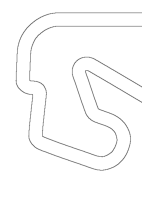
\includegraphics[interpolate=true,width=1.420000in,height=2.010000in]{contents/chapt6/figs/velocity_control/kv_paths-img0.png}}%
\end{pgfscope}%
\begin{pgfscope}%
\pgfpathrectangle{\pgfqpoint{1.792778in}{0.540000in}}{\pgfqpoint{1.414444in}{2.010000in}}%
\pgfusepath{clip}%
\pgfsetrectcap%
\pgfsetroundjoin%
\pgfsetlinewidth{1.003750pt}%
\definecolor{currentstroke}{rgb}{0.121569,0.466667,0.705882}%
\pgfsetstrokecolor{currentstroke}%
\pgfsetstrokeopacity{0.700000}%
\pgfsetdash{}{0pt}%
\pgfpathmoveto{\pgfqpoint{3.217222in}{1.590805in}}%
\pgfpathlineto{\pgfqpoint{3.127006in}{1.645873in}}%
\pgfpathlineto{\pgfqpoint{3.062831in}{1.680557in}}%
\pgfpathlineto{\pgfqpoint{2.839513in}{1.800078in}}%
\pgfpathlineto{\pgfqpoint{2.707600in}{1.865518in}}%
\pgfpathlineto{\pgfqpoint{2.690260in}{1.871408in}}%
\pgfpathlineto{\pgfqpoint{2.672331in}{1.874850in}}%
\pgfpathlineto{\pgfqpoint{2.657775in}{1.875349in}}%
\pgfpathlineto{\pgfqpoint{2.643369in}{1.873547in}}%
\pgfpathlineto{\pgfqpoint{2.629530in}{1.869326in}}%
\pgfpathlineto{\pgfqpoint{2.616695in}{1.862729in}}%
\pgfpathlineto{\pgfqpoint{2.605217in}{1.853953in}}%
\pgfpathlineto{\pgfqpoint{2.595432in}{1.843300in}}%
\pgfpathlineto{\pgfqpoint{2.587565in}{1.831145in}}%
\pgfpathlineto{\pgfqpoint{2.581691in}{1.817924in}}%
\pgfpathlineto{\pgfqpoint{2.577814in}{1.803994in}}%
\pgfpathlineto{\pgfqpoint{2.575865in}{1.789718in}}%
\pgfpathlineto{\pgfqpoint{2.575986in}{1.771791in}}%
\pgfpathlineto{\pgfqpoint{2.578615in}{1.754138in}}%
\pgfpathlineto{\pgfqpoint{2.584139in}{1.733544in}}%
\pgfpathlineto{\pgfqpoint{2.592891in}{1.710329in}}%
\pgfpathlineto{\pgfqpoint{2.609116in}{1.674857in}}%
\pgfpathlineto{\pgfqpoint{2.641001in}{1.611366in}}%
\pgfpathlineto{\pgfqpoint{2.689014in}{1.516142in}}%
\pgfpathlineto{\pgfqpoint{2.708515in}{1.478453in}}%
\pgfpathlineto{\pgfqpoint{2.721643in}{1.457527in}}%
\pgfpathlineto{\pgfqpoint{2.734586in}{1.440735in}}%
\pgfpathlineto{\pgfqpoint{2.749258in}{1.425357in}}%
\pgfpathlineto{\pgfqpoint{2.765515in}{1.411595in}}%
\pgfpathlineto{\pgfqpoint{2.783069in}{1.399467in}}%
\pgfpathlineto{\pgfqpoint{2.810897in}{1.383458in}}%
\pgfpathlineto{\pgfqpoint{2.889732in}{1.339874in}}%
\pgfpathlineto{\pgfqpoint{2.917236in}{1.322243in}}%
\pgfpathlineto{\pgfqpoint{2.937513in}{1.306779in}}%
\pgfpathlineto{\pgfqpoint{2.953673in}{1.291967in}}%
\pgfpathlineto{\pgfqpoint{2.968378in}{1.275643in}}%
\pgfpathlineto{\pgfqpoint{2.981377in}{1.257899in}}%
\pgfpathlineto{\pgfqpoint{2.992477in}{1.238886in}}%
\pgfpathlineto{\pgfqpoint{3.001508in}{1.218809in}}%
\pgfpathlineto{\pgfqpoint{3.008211in}{1.197822in}}%
\pgfpathlineto{\pgfqpoint{3.012415in}{1.176183in}}%
\pgfpathlineto{\pgfqpoint{3.014104in}{1.154194in}}%
\pgfpathlineto{\pgfqpoint{3.013305in}{1.132136in}}%
\pgfpathlineto{\pgfqpoint{3.010093in}{1.110276in}}%
\pgfpathlineto{\pgfqpoint{3.004679in}{1.088845in}}%
\pgfpathlineto{\pgfqpoint{2.997211in}{1.068026in}}%
\pgfpathlineto{\pgfqpoint{2.987874in}{1.047978in}}%
\pgfpathlineto{\pgfqpoint{2.976802in}{1.028806in}}%
\pgfpathlineto{\pgfqpoint{2.961868in}{1.007707in}}%
\pgfpathlineto{\pgfqpoint{2.944911in}{0.988163in}}%
\pgfpathlineto{\pgfqpoint{2.926024in}{0.970453in}}%
\pgfpathlineto{\pgfqpoint{2.908443in}{0.956869in}}%
\pgfpathlineto{\pgfqpoint{2.889702in}{0.944918in}}%
\pgfpathlineto{\pgfqpoint{2.869877in}{0.934882in}}%
\pgfpathlineto{\pgfqpoint{2.849101in}{0.927126in}}%
\pgfpathlineto{\pgfqpoint{2.831184in}{0.922617in}}%
\pgfpathlineto{\pgfqpoint{2.812871in}{0.920011in}}%
\pgfpathlineto{\pgfqpoint{2.794359in}{0.919277in}}%
\pgfpathlineto{\pgfqpoint{2.772162in}{0.920771in}}%
\pgfpathlineto{\pgfqpoint{2.750212in}{0.924543in}}%
\pgfpathlineto{\pgfqpoint{2.725089in}{0.931197in}}%
\pgfpathlineto{\pgfqpoint{2.693524in}{0.941926in}}%
\pgfpathlineto{\pgfqpoint{2.604545in}{0.976153in}}%
\pgfpathlineto{\pgfqpoint{2.467032in}{1.028390in}}%
\pgfpathlineto{\pgfqpoint{2.365093in}{1.067444in}}%
\pgfpathlineto{\pgfqpoint{2.259911in}{1.114946in}}%
\pgfpathlineto{\pgfqpoint{2.235340in}{1.128273in}}%
\pgfpathlineto{\pgfqpoint{2.217805in}{1.139869in}}%
\pgfpathlineto{\pgfqpoint{2.201568in}{1.153321in}}%
\pgfpathlineto{\pgfqpoint{2.189443in}{1.166149in}}%
\pgfpathlineto{\pgfqpoint{2.178941in}{1.180440in}}%
\pgfpathlineto{\pgfqpoint{2.170294in}{1.196015in}}%
\pgfpathlineto{\pgfqpoint{2.163513in}{1.212566in}}%
\pgfpathlineto{\pgfqpoint{2.156312in}{1.236639in}}%
\pgfpathlineto{\pgfqpoint{2.149487in}{1.268356in}}%
\pgfpathlineto{\pgfqpoint{2.141257in}{1.318384in}}%
\pgfpathlineto{\pgfqpoint{2.136076in}{1.361719in}}%
\pgfpathlineto{\pgfqpoint{2.133550in}{1.401789in}}%
\pgfpathlineto{\pgfqpoint{2.133408in}{1.438383in}}%
\pgfpathlineto{\pgfqpoint{2.135511in}{1.482396in}}%
\pgfpathlineto{\pgfqpoint{2.141290in}{1.578045in}}%
\pgfpathlineto{\pgfqpoint{2.139193in}{1.596387in}}%
\pgfpathlineto{\pgfqpoint{2.134752in}{1.614286in}}%
\pgfpathlineto{\pgfqpoint{2.127824in}{1.631362in}}%
\pgfpathlineto{\pgfqpoint{2.118566in}{1.647283in}}%
\pgfpathlineto{\pgfqpoint{2.105349in}{1.664983in}}%
\pgfpathlineto{\pgfqpoint{2.081086in}{1.692729in}}%
\pgfpathlineto{\pgfqpoint{2.062373in}{1.715507in}}%
\pgfpathlineto{\pgfqpoint{2.050045in}{1.733888in}}%
\pgfpathlineto{\pgfqpoint{2.039658in}{1.753410in}}%
\pgfpathlineto{\pgfqpoint{2.031453in}{1.773608in}}%
\pgfpathlineto{\pgfqpoint{2.025482in}{1.794189in}}%
\pgfpathlineto{\pgfqpoint{2.021708in}{1.814900in}}%
\pgfpathlineto{\pgfqpoint{2.019345in}{1.842744in}}%
\pgfpathlineto{\pgfqpoint{2.018856in}{1.877828in}}%
\pgfpathlineto{\pgfqpoint{2.020394in}{1.930675in}}%
\pgfpathlineto{\pgfqpoint{2.023433in}{1.972175in}}%
\pgfpathlineto{\pgfqpoint{2.027844in}{2.005925in}}%
\pgfpathlineto{\pgfqpoint{2.033832in}{2.035594in}}%
\pgfpathlineto{\pgfqpoint{2.041041in}{2.061290in}}%
\pgfpathlineto{\pgfqpoint{2.050105in}{2.086213in}}%
\pgfpathlineto{\pgfqpoint{2.062271in}{2.113296in}}%
\pgfpathlineto{\pgfqpoint{2.077724in}{2.142330in}}%
\pgfpathlineto{\pgfqpoint{2.095167in}{2.170149in}}%
\pgfpathlineto{\pgfqpoint{2.112712in}{2.193904in}}%
\pgfpathlineto{\pgfqpoint{2.131997in}{2.216230in}}%
\pgfpathlineto{\pgfqpoint{2.152985in}{2.236948in}}%
\pgfpathlineto{\pgfqpoint{2.175568in}{2.255881in}}%
\pgfpathlineto{\pgfqpoint{2.199541in}{2.272778in}}%
\pgfpathlineto{\pgfqpoint{2.222000in}{2.285879in}}%
\pgfpathlineto{\pgfqpoint{2.245417in}{2.297192in}}%
\pgfpathlineto{\pgfqpoint{2.275962in}{2.309197in}}%
\pgfpathlineto{\pgfqpoint{2.304317in}{2.318030in}}%
\pgfpathlineto{\pgfqpoint{2.333324in}{2.324794in}}%
\pgfpathlineto{\pgfqpoint{2.366414in}{2.330089in}}%
\pgfpathlineto{\pgfqpoint{2.434452in}{2.338387in}}%
\pgfpathlineto{\pgfqpoint{2.511391in}{2.345552in}}%
\pgfpathlineto{\pgfqpoint{2.707544in}{2.361575in}}%
\pgfpathlineto{\pgfqpoint{2.833308in}{2.366381in}}%
\pgfpathlineto{\pgfqpoint{2.962126in}{2.371151in}}%
\pgfpathlineto{\pgfqpoint{3.033311in}{2.372864in}}%
\pgfpathlineto{\pgfqpoint{3.149566in}{2.374583in}}%
\pgfpathlineto{\pgfqpoint{3.217222in}{2.375955in}}%
\pgfpathlineto{\pgfqpoint{3.217222in}{2.375955in}}%
\pgfusepath{stroke}%
\end{pgfscope}%
\begin{pgfscope}%
\pgfpathrectangle{\pgfqpoint{1.792778in}{0.540000in}}{\pgfqpoint{1.414444in}{2.010000in}}%
\pgfusepath{clip}%
\pgfsetrectcap%
\pgfsetroundjoin%
\pgfsetlinewidth{1.003750pt}%
\definecolor{currentstroke}{rgb}{1.000000,0.498039,0.054902}%
\pgfsetstrokecolor{currentstroke}%
\pgfsetstrokeopacity{0.700000}%
\pgfsetdash{}{0pt}%
\pgfpathmoveto{\pgfqpoint{3.217222in}{1.603339in}}%
\pgfpathlineto{\pgfqpoint{3.094787in}{1.674069in}}%
\pgfpathlineto{\pgfqpoint{3.009851in}{1.727846in}}%
\pgfpathlineto{\pgfqpoint{2.930927in}{1.777216in}}%
\pgfpathlineto{\pgfqpoint{2.872872in}{1.810662in}}%
\pgfpathlineto{\pgfqpoint{2.813661in}{1.842011in}}%
\pgfpathlineto{\pgfqpoint{2.756795in}{1.869587in}}%
\pgfpathlineto{\pgfqpoint{2.722905in}{1.884054in}}%
\pgfpathlineto{\pgfqpoint{2.702271in}{1.890980in}}%
\pgfpathlineto{\pgfqpoint{2.684762in}{1.894748in}}%
\pgfpathlineto{\pgfqpoint{2.666973in}{1.895973in}}%
\pgfpathlineto{\pgfqpoint{2.652796in}{1.894733in}}%
\pgfpathlineto{\pgfqpoint{2.638978in}{1.891317in}}%
\pgfpathlineto{\pgfqpoint{2.625870in}{1.885747in}}%
\pgfpathlineto{\pgfqpoint{2.613884in}{1.878154in}}%
\pgfpathlineto{\pgfqpoint{2.603436in}{1.868770in}}%
\pgfpathlineto{\pgfqpoint{2.594811in}{1.857827in}}%
\pgfpathlineto{\pgfqpoint{2.588089in}{1.845557in}}%
\pgfpathlineto{\pgfqpoint{2.583305in}{1.832312in}}%
\pgfpathlineto{\pgfqpoint{2.579849in}{1.814935in}}%
\pgfpathlineto{\pgfqpoint{2.578627in}{1.797120in}}%
\pgfpathlineto{\pgfqpoint{2.579504in}{1.775626in}}%
\pgfpathlineto{\pgfqpoint{2.582848in}{1.750602in}}%
\pgfpathlineto{\pgfqpoint{2.590102in}{1.715021in}}%
\pgfpathlineto{\pgfqpoint{2.603609in}{1.661756in}}%
\pgfpathlineto{\pgfqpoint{2.616172in}{1.619228in}}%
\pgfpathlineto{\pgfqpoint{2.628897in}{1.584448in}}%
\pgfpathlineto{\pgfqpoint{2.643859in}{1.550477in}}%
\pgfpathlineto{\pgfqpoint{2.663821in}{1.510613in}}%
\pgfpathlineto{\pgfqpoint{2.685778in}{1.471750in}}%
\pgfpathlineto{\pgfqpoint{2.702260in}{1.447009in}}%
\pgfpathlineto{\pgfqpoint{2.718606in}{1.426775in}}%
\pgfpathlineto{\pgfqpoint{2.734201in}{1.410959in}}%
\pgfpathlineto{\pgfqpoint{2.751149in}{1.396759in}}%
\pgfpathlineto{\pgfqpoint{2.772399in}{1.382107in}}%
\pgfpathlineto{\pgfqpoint{2.804247in}{1.363325in}}%
\pgfpathlineto{\pgfqpoint{2.878125in}{1.320826in}}%
\pgfpathlineto{\pgfqpoint{2.905756in}{1.302089in}}%
\pgfpathlineto{\pgfqpoint{2.929005in}{1.283605in}}%
\pgfpathlineto{\pgfqpoint{2.947937in}{1.265714in}}%
\pgfpathlineto{\pgfqpoint{2.962743in}{1.249000in}}%
\pgfpathlineto{\pgfqpoint{2.975934in}{1.230986in}}%
\pgfpathlineto{\pgfqpoint{2.987165in}{1.211692in}}%
\pgfpathlineto{\pgfqpoint{2.994763in}{1.194736in}}%
\pgfpathlineto{\pgfqpoint{3.000585in}{1.177081in}}%
\pgfpathlineto{\pgfqpoint{3.004503in}{1.158915in}}%
\pgfpathlineto{\pgfqpoint{3.006442in}{1.140453in}}%
\pgfpathlineto{\pgfqpoint{3.006443in}{1.121886in}}%
\pgfpathlineto{\pgfqpoint{3.004466in}{1.103401in}}%
\pgfpathlineto{\pgfqpoint{2.999680in}{1.081598in}}%
\pgfpathlineto{\pgfqpoint{2.992408in}{1.060489in}}%
\pgfpathlineto{\pgfqpoint{2.982821in}{1.040322in}}%
\pgfpathlineto{\pgfqpoint{2.971085in}{1.021329in}}%
\pgfpathlineto{\pgfqpoint{2.957361in}{1.003730in}}%
\pgfpathlineto{\pgfqpoint{2.941907in}{0.987621in}}%
\pgfpathlineto{\pgfqpoint{2.924872in}{0.973152in}}%
\pgfpathlineto{\pgfqpoint{2.906461in}{0.960503in}}%
\pgfpathlineto{\pgfqpoint{2.886839in}{0.949846in}}%
\pgfpathlineto{\pgfqpoint{2.866173in}{0.941420in}}%
\pgfpathlineto{\pgfqpoint{2.844685in}{0.935361in}}%
\pgfpathlineto{\pgfqpoint{2.822649in}{0.931741in}}%
\pgfpathlineto{\pgfqpoint{2.800372in}{0.930581in}}%
\pgfpathlineto{\pgfqpoint{2.778097in}{0.931770in}}%
\pgfpathlineto{\pgfqpoint{2.752350in}{0.935752in}}%
\pgfpathlineto{\pgfqpoint{2.708796in}{0.945604in}}%
\pgfpathlineto{\pgfqpoint{2.611287in}{0.969631in}}%
\pgfpathlineto{\pgfqpoint{2.444292in}{1.020828in}}%
\pgfpathlineto{\pgfqpoint{2.336200in}{1.057076in}}%
\pgfpathlineto{\pgfqpoint{2.299579in}{1.073535in}}%
\pgfpathlineto{\pgfqpoint{2.256988in}{1.094560in}}%
\pgfpathlineto{\pgfqpoint{2.234799in}{1.107565in}}%
\pgfpathlineto{\pgfqpoint{2.216825in}{1.120459in}}%
\pgfpathlineto{\pgfqpoint{2.203007in}{1.132694in}}%
\pgfpathlineto{\pgfqpoint{2.190612in}{1.146382in}}%
\pgfpathlineto{\pgfqpoint{2.179991in}{1.161505in}}%
\pgfpathlineto{\pgfqpoint{2.171376in}{1.177847in}}%
\pgfpathlineto{\pgfqpoint{2.164947in}{1.195187in}}%
\pgfpathlineto{\pgfqpoint{2.160668in}{1.213185in}}%
\pgfpathlineto{\pgfqpoint{2.158410in}{1.231555in}}%
\pgfpathlineto{\pgfqpoint{2.157663in}{1.257477in}}%
\pgfpathlineto{\pgfqpoint{2.157049in}{1.342787in}}%
\pgfpathlineto{\pgfqpoint{2.151323in}{1.491523in}}%
\pgfpathlineto{\pgfqpoint{2.149047in}{1.562195in}}%
\pgfpathlineto{\pgfqpoint{2.145735in}{1.584271in}}%
\pgfpathlineto{\pgfqpoint{2.140859in}{1.602214in}}%
\pgfpathlineto{\pgfqpoint{2.133663in}{1.619327in}}%
\pgfpathlineto{\pgfqpoint{2.124137in}{1.635261in}}%
\pgfpathlineto{\pgfqpoint{2.112692in}{1.649877in}}%
\pgfpathlineto{\pgfqpoint{2.097180in}{1.665914in}}%
\pgfpathlineto{\pgfqpoint{2.062921in}{1.700011in}}%
\pgfpathlineto{\pgfqpoint{2.051479in}{1.714681in}}%
\pgfpathlineto{\pgfqpoint{2.041800in}{1.730587in}}%
\pgfpathlineto{\pgfqpoint{2.034141in}{1.747551in}}%
\pgfpathlineto{\pgfqpoint{2.028538in}{1.765299in}}%
\pgfpathlineto{\pgfqpoint{2.024918in}{1.783553in}}%
\pgfpathlineto{\pgfqpoint{2.022707in}{1.805784in}}%
\pgfpathlineto{\pgfqpoint{2.022140in}{1.835561in}}%
\pgfpathlineto{\pgfqpoint{2.023802in}{1.876479in}}%
\pgfpathlineto{\pgfqpoint{2.028478in}{1.928350in}}%
\pgfpathlineto{\pgfqpoint{2.038176in}{2.005909in}}%
\pgfpathlineto{\pgfqpoint{2.044352in}{2.038815in}}%
\pgfpathlineto{\pgfqpoint{2.052161in}{2.067546in}}%
\pgfpathlineto{\pgfqpoint{2.062233in}{2.095520in}}%
\pgfpathlineto{\pgfqpoint{2.075835in}{2.126091in}}%
\pgfpathlineto{\pgfqpoint{2.089824in}{2.152357in}}%
\pgfpathlineto{\pgfqpoint{2.105655in}{2.177560in}}%
\pgfpathlineto{\pgfqpoint{2.123351in}{2.201444in}}%
\pgfpathlineto{\pgfqpoint{2.142879in}{2.223847in}}%
\pgfpathlineto{\pgfqpoint{2.164131in}{2.244614in}}%
\pgfpathlineto{\pgfqpoint{2.187017in}{2.263599in}}%
\pgfpathlineto{\pgfqpoint{2.208390in}{2.278429in}}%
\pgfpathlineto{\pgfqpoint{2.230951in}{2.291407in}}%
\pgfpathlineto{\pgfqpoint{2.254470in}{2.302520in}}%
\pgfpathlineto{\pgfqpoint{2.278717in}{2.311789in}}%
\pgfpathlineto{\pgfqpoint{2.307098in}{2.320152in}}%
\pgfpathlineto{\pgfqpoint{2.339330in}{2.326986in}}%
\pgfpathlineto{\pgfqpoint{2.374839in}{2.332227in}}%
\pgfpathlineto{\pgfqpoint{2.409960in}{2.335289in}}%
\pgfpathlineto{\pgfqpoint{2.444776in}{2.336199in}}%
\pgfpathlineto{\pgfqpoint{2.496769in}{2.334734in}}%
\pgfpathlineto{\pgfqpoint{2.545077in}{2.334412in}}%
\pgfpathlineto{\pgfqpoint{2.606949in}{2.333926in}}%
\pgfpathlineto{\pgfqpoint{2.721128in}{2.331571in}}%
\pgfpathlineto{\pgfqpoint{2.780482in}{2.331244in}}%
\pgfpathlineto{\pgfqpoint{2.860700in}{2.331251in}}%
\pgfpathlineto{\pgfqpoint{2.952231in}{2.330355in}}%
\pgfpathlineto{\pgfqpoint{3.034315in}{2.329468in}}%
\pgfpathlineto{\pgfqpoint{3.145021in}{2.328402in}}%
\pgfpathlineto{\pgfqpoint{3.217222in}{2.327643in}}%
\pgfpathlineto{\pgfqpoint{3.217222in}{2.327643in}}%
\pgfusepath{stroke}%
\end{pgfscope}%
\begin{pgfscope}%
\pgfpathrectangle{\pgfqpoint{1.792778in}{0.540000in}}{\pgfqpoint{1.414444in}{2.010000in}}%
\pgfusepath{clip}%
\pgfsetrectcap%
\pgfsetroundjoin%
\pgfsetlinewidth{1.003750pt}%
\definecolor{currentstroke}{rgb}{0.172549,0.627451,0.172549}%
\pgfsetstrokecolor{currentstroke}%
\pgfsetstrokeopacity{0.700000}%
\pgfsetdash{}{0pt}%
\pgfpathmoveto{\pgfqpoint{3.217222in}{1.559769in}}%
\pgfpathlineto{\pgfqpoint{3.155149in}{1.599045in}}%
\pgfpathlineto{\pgfqpoint{3.008247in}{1.694010in}}%
\pgfpathlineto{\pgfqpoint{2.824792in}{1.800316in}}%
\pgfpathlineto{\pgfqpoint{2.726892in}{1.853165in}}%
\pgfpathlineto{\pgfqpoint{2.703611in}{1.864077in}}%
\pgfpathlineto{\pgfqpoint{2.686401in}{1.870000in}}%
\pgfpathlineto{\pgfqpoint{2.672247in}{1.872913in}}%
\pgfpathlineto{\pgfqpoint{2.657979in}{1.873729in}}%
\pgfpathlineto{\pgfqpoint{2.643880in}{1.872191in}}%
\pgfpathlineto{\pgfqpoint{2.630449in}{1.868180in}}%
\pgfpathlineto{\pgfqpoint{2.618177in}{1.861749in}}%
\pgfpathlineto{\pgfqpoint{2.607443in}{1.853121in}}%
\pgfpathlineto{\pgfqpoint{2.598477in}{1.842615in}}%
\pgfpathlineto{\pgfqpoint{2.591395in}{1.830651in}}%
\pgfpathlineto{\pgfqpoint{2.586137in}{1.817662in}}%
\pgfpathlineto{\pgfqpoint{2.582619in}{1.803993in}}%
\pgfpathlineto{\pgfqpoint{2.580533in}{1.786333in}}%
\pgfpathlineto{\pgfqpoint{2.580707in}{1.768328in}}%
\pgfpathlineto{\pgfqpoint{2.583518in}{1.746723in}}%
\pgfpathlineto{\pgfqpoint{2.588637in}{1.725429in}}%
\pgfpathlineto{\pgfqpoint{2.596950in}{1.701153in}}%
\pgfpathlineto{\pgfqpoint{2.608816in}{1.674212in}}%
\pgfpathlineto{\pgfqpoint{2.652777in}{1.580257in}}%
\pgfpathlineto{\pgfqpoint{2.680289in}{1.511102in}}%
\pgfpathlineto{\pgfqpoint{2.693620in}{1.484479in}}%
\pgfpathlineto{\pgfqpoint{2.707084in}{1.462230in}}%
\pgfpathlineto{\pgfqpoint{2.720300in}{1.444219in}}%
\pgfpathlineto{\pgfqpoint{2.735171in}{1.427567in}}%
\pgfpathlineto{\pgfqpoint{2.751707in}{1.412582in}}%
\pgfpathlineto{\pgfqpoint{2.769769in}{1.399484in}}%
\pgfpathlineto{\pgfqpoint{2.789085in}{1.388293in}}%
\pgfpathlineto{\pgfqpoint{2.812735in}{1.377317in}}%
\pgfpathlineto{\pgfqpoint{2.863670in}{1.354537in}}%
\pgfpathlineto{\pgfqpoint{2.886406in}{1.341873in}}%
\pgfpathlineto{\pgfqpoint{2.907982in}{1.327310in}}%
\pgfpathlineto{\pgfqpoint{2.928122in}{1.310825in}}%
\pgfpathlineto{\pgfqpoint{2.946602in}{1.292502in}}%
\pgfpathlineto{\pgfqpoint{2.963156in}{1.272524in}}%
\pgfpathlineto{\pgfqpoint{2.975692in}{1.254164in}}%
\pgfpathlineto{\pgfqpoint{2.986499in}{1.234666in}}%
\pgfpathlineto{\pgfqpoint{2.995374in}{1.214193in}}%
\pgfpathlineto{\pgfqpoint{3.002108in}{1.192946in}}%
\pgfpathlineto{\pgfqpoint{3.006567in}{1.171101in}}%
\pgfpathlineto{\pgfqpoint{3.008659in}{1.148914in}}%
\pgfpathlineto{\pgfqpoint{3.008354in}{1.126590in}}%
\pgfpathlineto{\pgfqpoint{3.005665in}{1.104420in}}%
\pgfpathlineto{\pgfqpoint{3.000616in}{1.082674in}}%
\pgfpathlineto{\pgfqpoint{2.993251in}{1.061571in}}%
\pgfpathlineto{\pgfqpoint{2.983672in}{1.041399in}}%
\pgfpathlineto{\pgfqpoint{2.971987in}{1.022400in}}%
\pgfpathlineto{\pgfqpoint{2.958316in}{1.004750in}}%
\pgfpathlineto{\pgfqpoint{2.942913in}{0.988593in}}%
\pgfpathlineto{\pgfqpoint{2.925910in}{0.974129in}}%
\pgfpathlineto{\pgfqpoint{2.907474in}{0.961515in}}%
\pgfpathlineto{\pgfqpoint{2.887891in}{0.950839in}}%
\pgfpathlineto{\pgfqpoint{2.867378in}{0.942300in}}%
\pgfpathlineto{\pgfqpoint{2.845993in}{0.935946in}}%
\pgfpathlineto{\pgfqpoint{2.824077in}{0.931877in}}%
\pgfpathlineto{\pgfqpoint{2.801913in}{0.930171in}}%
\pgfpathlineto{\pgfqpoint{2.779639in}{0.930812in}}%
\pgfpathlineto{\pgfqpoint{2.757504in}{0.933561in}}%
\pgfpathlineto{\pgfqpoint{2.732091in}{0.939018in}}%
\pgfpathlineto{\pgfqpoint{2.689265in}{0.951534in}}%
\pgfpathlineto{\pgfqpoint{2.649727in}{0.962168in}}%
\pgfpathlineto{\pgfqpoint{2.603000in}{0.974737in}}%
\pgfpathlineto{\pgfqpoint{2.571345in}{0.985754in}}%
\pgfpathlineto{\pgfqpoint{2.490856in}{1.014889in}}%
\pgfpathlineto{\pgfqpoint{2.441703in}{1.032351in}}%
\pgfpathlineto{\pgfqpoint{2.368681in}{1.060065in}}%
\pgfpathlineto{\pgfqpoint{2.319791in}{1.078009in}}%
\pgfpathlineto{\pgfqpoint{2.278934in}{1.095945in}}%
\pgfpathlineto{\pgfqpoint{2.238730in}{1.115393in}}%
\pgfpathlineto{\pgfqpoint{2.219720in}{1.126701in}}%
\pgfpathlineto{\pgfqpoint{2.204992in}{1.137636in}}%
\pgfpathlineto{\pgfqpoint{2.191551in}{1.150307in}}%
\pgfpathlineto{\pgfqpoint{2.179807in}{1.164601in}}%
\pgfpathlineto{\pgfqpoint{2.170004in}{1.180316in}}%
\pgfpathlineto{\pgfqpoint{2.162349in}{1.197160in}}%
\pgfpathlineto{\pgfqpoint{2.156836in}{1.214896in}}%
\pgfpathlineto{\pgfqpoint{2.153377in}{1.233182in}}%
\pgfpathlineto{\pgfqpoint{2.151023in}{1.259111in}}%
\pgfpathlineto{\pgfqpoint{2.148743in}{1.326111in}}%
\pgfpathlineto{\pgfqpoint{2.146692in}{1.396812in}}%
\pgfpathlineto{\pgfqpoint{2.148189in}{1.433988in}}%
\pgfpathlineto{\pgfqpoint{2.153278in}{1.489609in}}%
\pgfpathlineto{\pgfqpoint{2.160017in}{1.563623in}}%
\pgfpathlineto{\pgfqpoint{2.159462in}{1.582032in}}%
\pgfpathlineto{\pgfqpoint{2.156773in}{1.600212in}}%
\pgfpathlineto{\pgfqpoint{2.151533in}{1.617674in}}%
\pgfpathlineto{\pgfqpoint{2.145392in}{1.630838in}}%
\pgfpathlineto{\pgfqpoint{2.137629in}{1.643083in}}%
\pgfpathlineto{\pgfqpoint{2.125951in}{1.656880in}}%
\pgfpathlineto{\pgfqpoint{2.112735in}{1.668997in}}%
\pgfpathlineto{\pgfqpoint{2.090214in}{1.686210in}}%
\pgfpathlineto{\pgfqpoint{2.067883in}{1.703923in}}%
\pgfpathlineto{\pgfqpoint{2.055081in}{1.716538in}}%
\pgfpathlineto{\pgfqpoint{2.043809in}{1.730685in}}%
\pgfpathlineto{\pgfqpoint{2.034392in}{1.746160in}}%
\pgfpathlineto{\pgfqpoint{2.026864in}{1.762647in}}%
\pgfpathlineto{\pgfqpoint{2.019967in}{1.783370in}}%
\pgfpathlineto{\pgfqpoint{2.013101in}{1.811964in}}%
\pgfpathlineto{\pgfqpoint{2.006688in}{1.848384in}}%
\pgfpathlineto{\pgfqpoint{2.001892in}{1.888818in}}%
\pgfpathlineto{\pgfqpoint{1.999074in}{1.933332in}}%
\pgfpathlineto{\pgfqpoint{1.998264in}{1.981643in}}%
\pgfpathlineto{\pgfqpoint{1.999914in}{2.022527in}}%
\pgfpathlineto{\pgfqpoint{2.003686in}{2.059573in}}%
\pgfpathlineto{\pgfqpoint{2.009464in}{2.092582in}}%
\pgfpathlineto{\pgfqpoint{2.016820in}{2.121431in}}%
\pgfpathlineto{\pgfqpoint{2.026306in}{2.149690in}}%
\pgfpathlineto{\pgfqpoint{2.037744in}{2.177190in}}%
\pgfpathlineto{\pgfqpoint{2.051165in}{2.203771in}}%
\pgfpathlineto{\pgfqpoint{2.066576in}{2.229229in}}%
\pgfpathlineto{\pgfqpoint{2.083928in}{2.253351in}}%
\pgfpathlineto{\pgfqpoint{2.103183in}{2.276041in}}%
\pgfpathlineto{\pgfqpoint{2.124199in}{2.297153in}}%
\pgfpathlineto{\pgfqpoint{2.143922in}{2.314153in}}%
\pgfpathlineto{\pgfqpoint{2.164933in}{2.329470in}}%
\pgfpathlineto{\pgfqpoint{2.187288in}{2.342876in}}%
\pgfpathlineto{\pgfqpoint{2.210673in}{2.354345in}}%
\pgfpathlineto{\pgfqpoint{2.231478in}{2.362334in}}%
\pgfpathlineto{\pgfqpoint{2.252964in}{2.368277in}}%
\pgfpathlineto{\pgfqpoint{2.274929in}{2.371996in}}%
\pgfpathlineto{\pgfqpoint{2.297129in}{2.373611in}}%
\pgfpathlineto{\pgfqpoint{2.323033in}{2.373216in}}%
\pgfpathlineto{\pgfqpoint{2.360096in}{2.370144in}}%
\pgfpathlineto{\pgfqpoint{2.548944in}{2.351514in}}%
\pgfpathlineto{\pgfqpoint{2.653028in}{2.346967in}}%
\pgfpathlineto{\pgfqpoint{2.731084in}{2.344763in}}%
\pgfpathlineto{\pgfqpoint{2.794136in}{2.345239in}}%
\pgfpathlineto{\pgfqpoint{2.923890in}{2.351476in}}%
\pgfpathlineto{\pgfqpoint{2.994576in}{2.352859in}}%
\pgfpathlineto{\pgfqpoint{3.042908in}{2.350788in}}%
\pgfpathlineto{\pgfqpoint{3.135663in}{2.346508in}}%
\pgfpathlineto{\pgfqpoint{3.217222in}{2.344802in}}%
\pgfpathlineto{\pgfqpoint{3.217222in}{2.344802in}}%
\pgfusepath{stroke}%
\end{pgfscope}%
\begin{pgfscope}%
\pgfpathrectangle{\pgfqpoint{1.792778in}{0.540000in}}{\pgfqpoint{1.414444in}{2.010000in}}%
\pgfusepath{clip}%
\pgfsetbuttcap%
\pgfsetroundjoin%
\pgfsetlinewidth{1.505625pt}%
\definecolor{currentstroke}{rgb}{1.000000,0.000000,0.000000}%
\pgfsetstrokecolor{currentstroke}%
\pgfsetdash{{1.500000pt}{2.475000pt}}{0.000000pt}%
\pgfusepath{stroke}%
\end{pgfscope}%
\begin{pgfscope}%
\pgfsetbuttcap%
\pgfsetmiterjoin%
\definecolor{currentfill}{rgb}{1.000000,1.000000,1.000000}%
\pgfsetfillcolor{currentfill}%
\pgfsetfillopacity{0.800000}%
\pgfsetlinewidth{1.003750pt}%
\definecolor{currentstroke}{rgb}{0.800000,0.800000,0.800000}%
\pgfsetstrokecolor{currentstroke}%
\pgfsetstrokeopacity{0.800000}%
\pgfsetdash{}{0pt}%
\pgfpathmoveto{\pgfqpoint{1.315084in}{0.069444in}}%
\pgfpathlineto{\pgfqpoint{3.684916in}{0.069444in}}%
\pgfpathquadraticcurveto{\pgfqpoint{3.712694in}{0.069444in}}{\pgfqpoint{3.712694in}{0.097222in}}%
\pgfpathlineto{\pgfqpoint{3.712694in}{0.687459in}}%
\pgfpathquadraticcurveto{\pgfqpoint{3.712694in}{0.715237in}}{\pgfqpoint{3.684916in}{0.715237in}}%
\pgfpathlineto{\pgfqpoint{1.315084in}{0.715237in}}%
\pgfpathquadraticcurveto{\pgfqpoint{1.287306in}{0.715237in}}{\pgfqpoint{1.287306in}{0.687459in}}%
\pgfpathlineto{\pgfqpoint{1.287306in}{0.097222in}}%
\pgfpathquadraticcurveto{\pgfqpoint{1.287306in}{0.069444in}}{\pgfqpoint{1.315084in}{0.069444in}}%
\pgfpathlineto{\pgfqpoint{1.315084in}{0.069444in}}%
\pgfpathclose%
\pgfusepath{stroke,fill}%
\end{pgfscope}%
\begin{pgfscope}%
\definecolor{textcolor}{rgb}{0.000000,0.000000,0.000000}%
\pgfsetstrokecolor{textcolor}%
\pgfsetfillcolor{textcolor}%
\pgftext[x=1.565578in,y=0.456936in,left,base]{\color{textcolor}\rmfamily\fontsize{10.000000}{12.000000}\selectfont Velocity controller gain, \(\displaystyle k_{v}\)}%
\end{pgfscope}%
\begin{pgfscope}%
\pgfsetrectcap%
\pgfsetroundjoin%
\pgfsetlinewidth{1.003750pt}%
\definecolor{currentstroke}{rgb}{0.121569,0.466667,0.705882}%
\pgfsetstrokecolor{currentstroke}%
\pgfsetstrokeopacity{0.700000}%
\pgfsetdash{}{0pt}%
\pgfpathmoveto{\pgfqpoint{1.440084in}{0.299723in}}%
\pgfpathlineto{\pgfqpoint{1.578973in}{0.299723in}}%
\pgfpathlineto{\pgfqpoint{1.717862in}{0.299723in}}%
\pgfusepath{stroke}%
\end{pgfscope}%
\begin{pgfscope}%
\definecolor{textcolor}{rgb}{0.000000,0.000000,0.000000}%
\pgfsetstrokecolor{textcolor}%
\pgfsetfillcolor{textcolor}%
\pgftext[x=1.828973in,y=0.251112in,left,base]{\color{textcolor}\rmfamily\fontsize{10.000000}{12.000000}\selectfont 0.5}%
\end{pgfscope}%
\begin{pgfscope}%
\pgfsetrectcap%
\pgfsetroundjoin%
\pgfsetlinewidth{1.003750pt}%
\definecolor{currentstroke}{rgb}{1.000000,0.498039,0.054902}%
\pgfsetstrokecolor{currentstroke}%
\pgfsetstrokeopacity{0.700000}%
\pgfsetdash{}{0pt}%
\pgfpathmoveto{\pgfqpoint{2.327630in}{0.299723in}}%
\pgfpathlineto{\pgfqpoint{2.466519in}{0.299723in}}%
\pgfpathlineto{\pgfqpoint{2.605408in}{0.299723in}}%
\pgfusepath{stroke}%
\end{pgfscope}%
\begin{pgfscope}%
\definecolor{textcolor}{rgb}{0.000000,0.000000,0.000000}%
\pgfsetstrokecolor{textcolor}%
\pgfsetfillcolor{textcolor}%
\pgftext[x=2.716519in,y=0.251112in,left,base]{\color{textcolor}\rmfamily\fontsize{10.000000}{12.000000}\selectfont 1}%
\end{pgfscope}%
\begin{pgfscope}%
\pgfsetrectcap%
\pgfsetroundjoin%
\pgfsetlinewidth{1.003750pt}%
\definecolor{currentstroke}{rgb}{0.172549,0.627451,0.172549}%
\pgfsetstrokecolor{currentstroke}%
\pgfsetstrokeopacity{0.700000}%
\pgfsetdash{}{0pt}%
\pgfpathmoveto{\pgfqpoint{3.082662in}{0.299723in}}%
\pgfpathlineto{\pgfqpoint{3.221551in}{0.299723in}}%
\pgfpathlineto{\pgfqpoint{3.360440in}{0.299723in}}%
\pgfusepath{stroke}%
\end{pgfscope}%
\begin{pgfscope}%
\definecolor{textcolor}{rgb}{0.000000,0.000000,0.000000}%
\pgfsetstrokecolor{textcolor}%
\pgfsetfillcolor{textcolor}%
\pgftext[x=3.471551in,y=0.251112in,left,base]{\color{textcolor}\rmfamily\fontsize{10.000000}{12.000000}\selectfont 2}%
\end{pgfscope}%
\end{pgfpicture}%
\makeatother%
\endgroup%

    \caption[Paths taken by partial end-to-end agents utilising controller gain ($k_v$) values of $0.5$, $1$ and $2$ on the final section of  Barcelona-Catalunya]{Paths taken by partial end-to-end agents utilising controller gain ($k_v$) values of $0.5$, $1$ and $2$ on the final section of  Barcelona-Catalunya.}
    \label{fig:kv_paths}
\end{figure}





%%%%%%%%%%%%%%%%%%%%%%%%%%%%%%%%%%%%%%%%%%%%%%%%%%%%%%%%%%%%%%%%%%%%%%%%%%%%%%%%%%%%%%%%%%%%%%%%%%%%%%%%%%%%%%%%%%%%%%%%%%%%%%%%%%%%%%%%%%%%%%%%%%%%%%%%%%%%%%%%%%


\section{Racing without model uncertainties}

Having determined a locally optimal hyper-parameter set for the partial end-to-end algorithm, we proceeded to assess its performance in comparison to the end-to-end baseline under conditions without model-mismatches. 
Figure \ref{fig:all_tracks_train} presents the average training performance, in terms of failed laps and lap time, of $10$ partial end-to-end, as well as $10$ fully end-to-end agents trained on the Barcelona-Catalunya and Monaco tracks. 
A trend is observed across both tracks: the partial end-to-end agents achieve a near $0\%$ failure rate early in training, while the end-to-end agents continue to experience crashes throughout the training process.
However, it is worth noting that both the partial and fully end-to-end agents achieve similar lap times for the laps that are successfully completed. 

\begin{figure}[htb!]
    \centering
    %% Creator: Matplotlib, PGF backend
%%
%% To include the figure in your LaTeX document, write
%%   \input{<filename>.pgf}
%%
%% Make sure the required packages are loaded in your preamble
%%   \usepackage{pgf}
%%
%% Also ensure that all the required font packages are loaded; for instance,
%% the lmodern package is sometimes necessary when using math font.
%%   \usepackage{lmodern}
%%
%% Figures using additional raster images can only be included by \input if
%% they are in the same directory as the main LaTeX file. For loading figures
%% from other directories you can use the `import` package
%%   \usepackage{import}
%%
%% and then include the figures with
%%   \import{<path to file>}{<filename>.pgf}
%%
%% Matplotlib used the following preamble
%%   \usepackage{fontspec}
%%   \setmainfont{times.ttf}[Path=\detokenize{C:/Windows/Fonts/}]
%%   \setsansfont{DejaVuSans.ttf}[Path=\detokenize{C:/Users/Andrew/anaconda3/envs/auto_car_env/Lib/site-packages/matplotlib/mpl-data/fonts/ttf/}]
%%   \setmonofont{DejaVuSansMono.ttf}[Path=\detokenize{C:/Users/Andrew/anaconda3/envs/auto_car_env/Lib/site-packages/matplotlib/mpl-data/fonts/ttf/}]
%%
\begingroup%
\makeatletter%
\begin{pgfpicture}%
\pgfpathrectangle{\pgfpointorigin}{\pgfqpoint{5.700000in}{2.900000in}}%
\pgfusepath{use as bounding box, clip}%
\begin{pgfscope}%
\pgfsetbuttcap%
\pgfsetmiterjoin%
\definecolor{currentfill}{rgb}{1.000000,1.000000,1.000000}%
\pgfsetfillcolor{currentfill}%
\pgfsetlinewidth{0.000000pt}%
\definecolor{currentstroke}{rgb}{1.000000,1.000000,1.000000}%
\pgfsetstrokecolor{currentstroke}%
\pgfsetdash{}{0pt}%
\pgfpathmoveto{\pgfqpoint{0.000000in}{0.000000in}}%
\pgfpathlineto{\pgfqpoint{5.700000in}{0.000000in}}%
\pgfpathlineto{\pgfqpoint{5.700000in}{2.900000in}}%
\pgfpathlineto{\pgfqpoint{0.000000in}{2.900000in}}%
\pgfpathlineto{\pgfqpoint{0.000000in}{0.000000in}}%
\pgfpathclose%
\pgfusepath{fill}%
\end{pgfscope}%
\begin{pgfscope}%
\pgfsetbuttcap%
\pgfsetmiterjoin%
\definecolor{currentfill}{rgb}{1.000000,1.000000,1.000000}%
\pgfsetfillcolor{currentfill}%
\pgfsetlinewidth{0.000000pt}%
\definecolor{currentstroke}{rgb}{0.000000,0.000000,0.000000}%
\pgfsetstrokecolor{currentstroke}%
\pgfsetstrokeopacity{0.000000}%
\pgfsetdash{}{0pt}%
\pgfpathmoveto{\pgfqpoint{0.604167in}{1.450000in}}%
\pgfpathlineto{\pgfqpoint{2.705000in}{1.450000in}}%
\pgfpathlineto{\pgfqpoint{2.705000in}{2.556667in}}%
\pgfpathlineto{\pgfqpoint{0.604167in}{2.556667in}}%
\pgfpathlineto{\pgfqpoint{0.604167in}{1.450000in}}%
\pgfpathclose%
\pgfusepath{fill}%
\end{pgfscope}%
\begin{pgfscope}%
\pgfpathrectangle{\pgfqpoint{0.604167in}{1.450000in}}{\pgfqpoint{2.100833in}{1.106667in}}%
\pgfusepath{clip}%
\pgfsetbuttcap%
\pgfsetroundjoin%
\definecolor{currentfill}{rgb}{0.121569,0.466667,0.705882}%
\pgfsetfillcolor{currentfill}%
\pgfsetfillopacity{0.150000}%
\pgfsetlinewidth{1.003750pt}%
\definecolor{currentstroke}{rgb}{0.121569,0.466667,0.705882}%
\pgfsetstrokecolor{currentstroke}%
\pgfsetstrokeopacity{0.150000}%
\pgfsetdash{}{0pt}%
\pgfsys@defobject{currentmarker}{\pgfqpoint{0.604167in}{1.917071in}}{\pgfqpoint{6.024317in}{2.541100in}}{%
\pgfpathmoveto{\pgfqpoint{0.604167in}{2.506364in}}%
\pgfpathlineto{\pgfqpoint{0.604167in}{2.506364in}}%
\pgfpathlineto{\pgfqpoint{0.609419in}{2.506364in}}%
\pgfpathlineto{\pgfqpoint{0.614671in}{2.506364in}}%
\pgfpathlineto{\pgfqpoint{0.619923in}{2.506364in}}%
\pgfpathlineto{\pgfqpoint{0.625175in}{2.506364in}}%
\pgfpathlineto{\pgfqpoint{0.630427in}{2.506364in}}%
\pgfpathlineto{\pgfqpoint{0.635679in}{2.506364in}}%
\pgfpathlineto{\pgfqpoint{0.640931in}{2.506364in}}%
\pgfpathlineto{\pgfqpoint{0.646183in}{2.506364in}}%
\pgfpathlineto{\pgfqpoint{0.651435in}{2.506364in}}%
\pgfpathlineto{\pgfqpoint{0.656688in}{2.506364in}}%
\pgfpathlineto{\pgfqpoint{0.661940in}{2.506364in}}%
\pgfpathlineto{\pgfqpoint{0.667192in}{2.506364in}}%
\pgfpathlineto{\pgfqpoint{0.672444in}{2.506364in}}%
\pgfpathlineto{\pgfqpoint{0.677696in}{2.506364in}}%
\pgfpathlineto{\pgfqpoint{0.682948in}{2.506364in}}%
\pgfpathlineto{\pgfqpoint{0.688200in}{2.506364in}}%
\pgfpathlineto{\pgfqpoint{0.693452in}{2.506364in}}%
\pgfpathlineto{\pgfqpoint{0.698704in}{2.506364in}}%
\pgfpathlineto{\pgfqpoint{0.703956in}{2.506364in}}%
\pgfpathlineto{\pgfqpoint{0.709208in}{2.506364in}}%
\pgfpathlineto{\pgfqpoint{0.714460in}{2.506364in}}%
\pgfpathlineto{\pgfqpoint{0.719713in}{2.506364in}}%
\pgfpathlineto{\pgfqpoint{0.724965in}{2.506364in}}%
\pgfpathlineto{\pgfqpoint{0.730217in}{2.506364in}}%
\pgfpathlineto{\pgfqpoint{0.735469in}{2.506364in}}%
\pgfpathlineto{\pgfqpoint{0.740721in}{2.506364in}}%
\pgfpathlineto{\pgfqpoint{0.745973in}{2.506364in}}%
\pgfpathlineto{\pgfqpoint{0.751225in}{2.506364in}}%
\pgfpathlineto{\pgfqpoint{0.756477in}{2.506364in}}%
\pgfpathlineto{\pgfqpoint{0.761729in}{2.506364in}}%
\pgfpathlineto{\pgfqpoint{0.766981in}{2.506364in}}%
\pgfpathlineto{\pgfqpoint{0.772233in}{2.506364in}}%
\pgfpathlineto{\pgfqpoint{0.777485in}{2.506364in}}%
\pgfpathlineto{\pgfqpoint{0.782738in}{2.506364in}}%
\pgfpathlineto{\pgfqpoint{0.787990in}{2.506364in}}%
\pgfpathlineto{\pgfqpoint{0.793242in}{2.506364in}}%
\pgfpathlineto{\pgfqpoint{0.798494in}{2.506364in}}%
\pgfpathlineto{\pgfqpoint{0.803746in}{2.506364in}}%
\pgfpathlineto{\pgfqpoint{0.808998in}{2.506364in}}%
\pgfpathlineto{\pgfqpoint{0.814250in}{2.506364in}}%
\pgfpathlineto{\pgfqpoint{0.819502in}{2.506364in}}%
\pgfpathlineto{\pgfqpoint{0.824754in}{2.506364in}}%
\pgfpathlineto{\pgfqpoint{0.830006in}{2.506364in}}%
\pgfpathlineto{\pgfqpoint{0.835258in}{2.506364in}}%
\pgfpathlineto{\pgfqpoint{0.840510in}{2.506364in}}%
\pgfpathlineto{\pgfqpoint{0.845763in}{2.506364in}}%
\pgfpathlineto{\pgfqpoint{0.851015in}{2.506364in}}%
\pgfpathlineto{\pgfqpoint{0.856267in}{2.506364in}}%
\pgfpathlineto{\pgfqpoint{0.861519in}{2.506364in}}%
\pgfpathlineto{\pgfqpoint{0.866771in}{2.506364in}}%
\pgfpathlineto{\pgfqpoint{0.872023in}{2.506364in}}%
\pgfpathlineto{\pgfqpoint{0.877275in}{2.506364in}}%
\pgfpathlineto{\pgfqpoint{0.882527in}{2.506364in}}%
\pgfpathlineto{\pgfqpoint{0.887779in}{2.506364in}}%
\pgfpathlineto{\pgfqpoint{0.893031in}{2.506364in}}%
\pgfpathlineto{\pgfqpoint{0.898283in}{2.506364in}}%
\pgfpathlineto{\pgfqpoint{0.903535in}{2.506364in}}%
\pgfpathlineto{\pgfqpoint{0.908788in}{2.506364in}}%
\pgfpathlineto{\pgfqpoint{0.914040in}{2.526140in}}%
\pgfpathlineto{\pgfqpoint{0.919292in}{2.526875in}}%
\pgfpathlineto{\pgfqpoint{0.924544in}{2.523732in}}%
\pgfpathlineto{\pgfqpoint{0.929796in}{2.523732in}}%
\pgfpathlineto{\pgfqpoint{0.935048in}{2.518176in}}%
\pgfpathlineto{\pgfqpoint{0.940300in}{2.518176in}}%
\pgfpathlineto{\pgfqpoint{0.945552in}{2.510728in}}%
\pgfpathlineto{\pgfqpoint{0.950804in}{2.501582in}}%
\pgfpathlineto{\pgfqpoint{0.956056in}{2.501582in}}%
\pgfpathlineto{\pgfqpoint{0.961308in}{2.501582in}}%
\pgfpathlineto{\pgfqpoint{0.966560in}{2.501582in}}%
\pgfpathlineto{\pgfqpoint{0.971813in}{2.510728in}}%
\pgfpathlineto{\pgfqpoint{0.977065in}{2.518176in}}%
\pgfpathlineto{\pgfqpoint{0.982317in}{2.518176in}}%
\pgfpathlineto{\pgfqpoint{0.987569in}{2.518176in}}%
\pgfpathlineto{\pgfqpoint{0.992821in}{2.518176in}}%
\pgfpathlineto{\pgfqpoint{0.998073in}{2.518176in}}%
\pgfpathlineto{\pgfqpoint{1.003325in}{2.518176in}}%
\pgfpathlineto{\pgfqpoint{1.008577in}{2.541100in}}%
\pgfpathlineto{\pgfqpoint{1.013829in}{2.529988in}}%
\pgfpathlineto{\pgfqpoint{1.019081in}{2.515093in}}%
\pgfpathlineto{\pgfqpoint{1.024333in}{2.515093in}}%
\pgfpathlineto{\pgfqpoint{1.029585in}{2.515093in}}%
\pgfpathlineto{\pgfqpoint{1.034838in}{2.499481in}}%
\pgfpathlineto{\pgfqpoint{1.040090in}{2.499481in}}%
\pgfpathlineto{\pgfqpoint{1.045342in}{2.499481in}}%
\pgfpathlineto{\pgfqpoint{1.050594in}{2.492553in}}%
\pgfpathlineto{\pgfqpoint{1.055846in}{2.476615in}}%
\pgfpathlineto{\pgfqpoint{1.061098in}{2.468245in}}%
\pgfpathlineto{\pgfqpoint{1.066350in}{2.475112in}}%
\pgfpathlineto{\pgfqpoint{1.071602in}{2.481629in}}%
\pgfpathlineto{\pgfqpoint{1.076854in}{2.487152in}}%
\pgfpathlineto{\pgfqpoint{1.082106in}{2.476437in}}%
\pgfpathlineto{\pgfqpoint{1.087358in}{2.449177in}}%
\pgfpathlineto{\pgfqpoint{1.092610in}{2.449177in}}%
\pgfpathlineto{\pgfqpoint{1.097863in}{2.449177in}}%
\pgfpathlineto{\pgfqpoint{1.103115in}{2.417607in}}%
\pgfpathlineto{\pgfqpoint{1.108367in}{2.414487in}}%
\pgfpathlineto{\pgfqpoint{1.113619in}{2.414487in}}%
\pgfpathlineto{\pgfqpoint{1.118871in}{2.426919in}}%
\pgfpathlineto{\pgfqpoint{1.124123in}{2.410231in}}%
\pgfpathlineto{\pgfqpoint{1.129375in}{2.396195in}}%
\pgfpathlineto{\pgfqpoint{1.134627in}{2.376009in}}%
\pgfpathlineto{\pgfqpoint{1.139879in}{2.374506in}}%
\pgfpathlineto{\pgfqpoint{1.145131in}{2.374506in}}%
\pgfpathlineto{\pgfqpoint{1.150383in}{2.383484in}}%
\pgfpathlineto{\pgfqpoint{1.155635in}{2.356818in}}%
\pgfpathlineto{\pgfqpoint{1.160888in}{2.346217in}}%
\pgfpathlineto{\pgfqpoint{1.166140in}{2.374338in}}%
\pgfpathlineto{\pgfqpoint{1.171392in}{2.345597in}}%
\pgfpathlineto{\pgfqpoint{1.176644in}{2.325881in}}%
\pgfpathlineto{\pgfqpoint{1.181896in}{2.338426in}}%
\pgfpathlineto{\pgfqpoint{1.187148in}{2.357256in}}%
\pgfpathlineto{\pgfqpoint{1.192400in}{2.410261in}}%
\pgfpathlineto{\pgfqpoint{1.197652in}{2.432926in}}%
\pgfpathlineto{\pgfqpoint{1.202904in}{2.432926in}}%
\pgfpathlineto{\pgfqpoint{1.208156in}{2.427911in}}%
\pgfpathlineto{\pgfqpoint{1.213408in}{2.446203in}}%
\pgfpathlineto{\pgfqpoint{1.218660in}{2.461934in}}%
\pgfpathlineto{\pgfqpoint{1.223913in}{2.479230in}}%
\pgfpathlineto{\pgfqpoint{1.229165in}{2.467291in}}%
\pgfpathlineto{\pgfqpoint{1.234417in}{2.468862in}}%
\pgfpathlineto{\pgfqpoint{1.239669in}{2.479230in}}%
\pgfpathlineto{\pgfqpoint{1.244921in}{2.465691in}}%
\pgfpathlineto{\pgfqpoint{1.250173in}{2.427957in}}%
\pgfpathlineto{\pgfqpoint{1.255425in}{2.413986in}}%
\pgfpathlineto{\pgfqpoint{1.260677in}{2.406062in}}%
\pgfpathlineto{\pgfqpoint{1.265929in}{2.413986in}}%
\pgfpathlineto{\pgfqpoint{1.271181in}{2.413986in}}%
\pgfpathlineto{\pgfqpoint{1.276433in}{2.399199in}}%
\pgfpathlineto{\pgfqpoint{1.281685in}{2.399199in}}%
\pgfpathlineto{\pgfqpoint{1.286938in}{2.420740in}}%
\pgfpathlineto{\pgfqpoint{1.292190in}{2.423285in}}%
\pgfpathlineto{\pgfqpoint{1.297442in}{2.404993in}}%
\pgfpathlineto{\pgfqpoint{1.302694in}{2.417607in}}%
\pgfpathlineto{\pgfqpoint{1.307946in}{2.419356in}}%
\pgfpathlineto{\pgfqpoint{1.313198in}{2.419356in}}%
\pgfpathlineto{\pgfqpoint{1.318450in}{2.419356in}}%
\pgfpathlineto{\pgfqpoint{1.323702in}{2.419356in}}%
\pgfpathlineto{\pgfqpoint{1.328954in}{2.407268in}}%
\pgfpathlineto{\pgfqpoint{1.334206in}{2.419356in}}%
\pgfpathlineto{\pgfqpoint{1.339458in}{2.395459in}}%
\pgfpathlineto{\pgfqpoint{1.344710in}{2.395459in}}%
\pgfpathlineto{\pgfqpoint{1.349963in}{2.395459in}}%
\pgfpathlineto{\pgfqpoint{1.355215in}{2.406408in}}%
\pgfpathlineto{\pgfqpoint{1.360467in}{2.394621in}}%
\pgfpathlineto{\pgfqpoint{1.365719in}{2.394621in}}%
\pgfpathlineto{\pgfqpoint{1.370971in}{2.394621in}}%
\pgfpathlineto{\pgfqpoint{1.376223in}{2.425980in}}%
\pgfpathlineto{\pgfqpoint{1.381475in}{2.453739in}}%
\pgfpathlineto{\pgfqpoint{1.386727in}{2.457847in}}%
\pgfpathlineto{\pgfqpoint{1.391979in}{2.457424in}}%
\pgfpathlineto{\pgfqpoint{1.397231in}{2.446203in}}%
\pgfpathlineto{\pgfqpoint{1.402483in}{2.433847in}}%
\pgfpathlineto{\pgfqpoint{1.407735in}{2.446203in}}%
\pgfpathlineto{\pgfqpoint{1.412988in}{2.427911in}}%
\pgfpathlineto{\pgfqpoint{1.418240in}{2.427911in}}%
\pgfpathlineto{\pgfqpoint{1.423492in}{2.440809in}}%
\pgfpathlineto{\pgfqpoint{1.428744in}{2.434712in}}%
\pgfpathlineto{\pgfqpoint{1.433996in}{2.390691in}}%
\pgfpathlineto{\pgfqpoint{1.439248in}{2.334853in}}%
\pgfpathlineto{\pgfqpoint{1.444500in}{2.333241in}}%
\pgfpathlineto{\pgfqpoint{1.449752in}{2.350227in}}%
\pgfpathlineto{\pgfqpoint{1.455004in}{2.364516in}}%
\pgfpathlineto{\pgfqpoint{1.460256in}{2.364516in}}%
\pgfpathlineto{\pgfqpoint{1.465508in}{2.346217in}}%
\pgfpathlineto{\pgfqpoint{1.470760in}{2.346217in}}%
\pgfpathlineto{\pgfqpoint{1.476013in}{2.334853in}}%
\pgfpathlineto{\pgfqpoint{1.481265in}{2.334853in}}%
\pgfpathlineto{\pgfqpoint{1.486517in}{2.334853in}}%
\pgfpathlineto{\pgfqpoint{1.491769in}{2.348571in}}%
\pgfpathlineto{\pgfqpoint{1.497021in}{2.349627in}}%
\pgfpathlineto{\pgfqpoint{1.502273in}{2.333240in}}%
\pgfpathlineto{\pgfqpoint{1.507525in}{2.333240in}}%
\pgfpathlineto{\pgfqpoint{1.512777in}{2.328952in}}%
\pgfpathlineto{\pgfqpoint{1.518029in}{2.328952in}}%
\pgfpathlineto{\pgfqpoint{1.523281in}{2.318750in}}%
\pgfpathlineto{\pgfqpoint{1.528533in}{2.317001in}}%
\pgfpathlineto{\pgfqpoint{1.533785in}{2.317001in}}%
\pgfpathlineto{\pgfqpoint{1.539038in}{2.293424in}}%
\pgfpathlineto{\pgfqpoint{1.544290in}{2.290343in}}%
\pgfpathlineto{\pgfqpoint{1.549542in}{2.290343in}}%
\pgfpathlineto{\pgfqpoint{1.554794in}{2.304232in}}%
\pgfpathlineto{\pgfqpoint{1.560046in}{2.317001in}}%
\pgfpathlineto{\pgfqpoint{1.565298in}{2.337856in}}%
\pgfpathlineto{\pgfqpoint{1.570550in}{2.367638in}}%
\pgfpathlineto{\pgfqpoint{1.575802in}{2.384256in}}%
\pgfpathlineto{\pgfqpoint{1.581054in}{2.383586in}}%
\pgfpathlineto{\pgfqpoint{1.586306in}{2.401076in}}%
\pgfpathlineto{\pgfqpoint{1.591558in}{2.417607in}}%
\pgfpathlineto{\pgfqpoint{1.596810in}{2.449177in}}%
\pgfpathlineto{\pgfqpoint{1.602063in}{2.446780in}}%
\pgfpathlineto{\pgfqpoint{1.607315in}{2.449640in}}%
\pgfpathlineto{\pgfqpoint{1.612567in}{2.450233in}}%
\pgfpathlineto{\pgfqpoint{1.617819in}{2.450233in}}%
\pgfpathlineto{\pgfqpoint{1.623071in}{2.450233in}}%
\pgfpathlineto{\pgfqpoint{1.628323in}{2.440241in}}%
\pgfpathlineto{\pgfqpoint{1.633575in}{2.426919in}}%
\pgfpathlineto{\pgfqpoint{1.638827in}{2.426919in}}%
\pgfpathlineto{\pgfqpoint{1.644079in}{2.426919in}}%
\pgfpathlineto{\pgfqpoint{1.649331in}{2.410231in}}%
\pgfpathlineto{\pgfqpoint{1.654583in}{2.386546in}}%
\pgfpathlineto{\pgfqpoint{1.659835in}{2.367073in}}%
\pgfpathlineto{\pgfqpoint{1.665088in}{2.374506in}}%
\pgfpathlineto{\pgfqpoint{1.670340in}{2.376009in}}%
\pgfpathlineto{\pgfqpoint{1.675592in}{2.376009in}}%
\pgfpathlineto{\pgfqpoint{1.680844in}{2.399736in}}%
\pgfpathlineto{\pgfqpoint{1.686096in}{2.399736in}}%
\pgfpathlineto{\pgfqpoint{1.691348in}{2.406808in}}%
\pgfpathlineto{\pgfqpoint{1.696600in}{2.413132in}}%
\pgfpathlineto{\pgfqpoint{1.701852in}{2.398875in}}%
\pgfpathlineto{\pgfqpoint{1.707104in}{2.418650in}}%
\pgfpathlineto{\pgfqpoint{1.712356in}{2.406062in}}%
\pgfpathlineto{\pgfqpoint{1.717608in}{2.427911in}}%
\pgfpathlineto{\pgfqpoint{1.722860in}{2.427911in}}%
\pgfpathlineto{\pgfqpoint{1.728113in}{2.431424in}}%
\pgfpathlineto{\pgfqpoint{1.733365in}{2.426487in}}%
\pgfpathlineto{\pgfqpoint{1.738617in}{2.390335in}}%
\pgfpathlineto{\pgfqpoint{1.743869in}{2.404993in}}%
\pgfpathlineto{\pgfqpoint{1.749121in}{2.404993in}}%
\pgfpathlineto{\pgfqpoint{1.754373in}{2.398875in}}%
\pgfpathlineto{\pgfqpoint{1.759625in}{2.433847in}}%
\pgfpathlineto{\pgfqpoint{1.764877in}{2.433847in}}%
\pgfpathlineto{\pgfqpoint{1.770129in}{2.419356in}}%
\pgfpathlineto{\pgfqpoint{1.775381in}{2.407268in}}%
\pgfpathlineto{\pgfqpoint{1.780633in}{2.419356in}}%
\pgfpathlineto{\pgfqpoint{1.785885in}{2.417607in}}%
\pgfpathlineto{\pgfqpoint{1.791138in}{2.419356in}}%
\pgfpathlineto{\pgfqpoint{1.796390in}{2.433847in}}%
\pgfpathlineto{\pgfqpoint{1.801642in}{2.433847in}}%
\pgfpathlineto{\pgfqpoint{1.806894in}{2.433847in}}%
\pgfpathlineto{\pgfqpoint{1.812146in}{2.450833in}}%
\pgfpathlineto{\pgfqpoint{1.817398in}{2.413132in}}%
\pgfpathlineto{\pgfqpoint{1.822650in}{2.391947in}}%
\pgfpathlineto{\pgfqpoint{1.827902in}{2.384256in}}%
\pgfpathlineto{\pgfqpoint{1.833154in}{2.384256in}}%
\pgfpathlineto{\pgfqpoint{1.838406in}{2.407058in}}%
\pgfpathlineto{\pgfqpoint{1.843658in}{2.410261in}}%
\pgfpathlineto{\pgfqpoint{1.848910in}{2.401115in}}%
\pgfpathlineto{\pgfqpoint{1.854163in}{2.399199in}}%
\pgfpathlineto{\pgfqpoint{1.859415in}{2.420579in}}%
\pgfpathlineto{\pgfqpoint{1.864667in}{2.420579in}}%
\pgfpathlineto{\pgfqpoint{1.869919in}{2.406062in}}%
\pgfpathlineto{\pgfqpoint{1.875171in}{2.427957in}}%
\pgfpathlineto{\pgfqpoint{1.880423in}{2.426880in}}%
\pgfpathlineto{\pgfqpoint{1.885675in}{2.424855in}}%
\pgfpathlineto{\pgfqpoint{1.890927in}{2.416243in}}%
\pgfpathlineto{\pgfqpoint{1.896179in}{2.394887in}}%
\pgfpathlineto{\pgfqpoint{1.901431in}{2.434712in}}%
\pgfpathlineto{\pgfqpoint{1.906683in}{2.434712in}}%
\pgfpathlineto{\pgfqpoint{1.911935in}{2.440809in}}%
\pgfpathlineto{\pgfqpoint{1.917188in}{2.420740in}}%
\pgfpathlineto{\pgfqpoint{1.922440in}{2.420740in}}%
\pgfpathlineto{\pgfqpoint{1.927692in}{2.414249in}}%
\pgfpathlineto{\pgfqpoint{1.932944in}{2.399736in}}%
\pgfpathlineto{\pgfqpoint{1.938196in}{2.404993in}}%
\pgfpathlineto{\pgfqpoint{1.943448in}{2.404838in}}%
\pgfpathlineto{\pgfqpoint{1.948700in}{2.404838in}}%
\pgfpathlineto{\pgfqpoint{1.953952in}{2.386546in}}%
\pgfpathlineto{\pgfqpoint{1.959204in}{2.339745in}}%
\pgfpathlineto{\pgfqpoint{1.964456in}{2.344704in}}%
\pgfpathlineto{\pgfqpoint{1.969708in}{2.339745in}}%
\pgfpathlineto{\pgfqpoint{1.974960in}{2.316228in}}%
\pgfpathlineto{\pgfqpoint{1.980213in}{2.307403in}}%
\pgfpathlineto{\pgfqpoint{1.985465in}{2.339888in}}%
\pgfpathlineto{\pgfqpoint{1.990717in}{2.334853in}}%
\pgfpathlineto{\pgfqpoint{1.995969in}{2.334853in}}%
\pgfpathlineto{\pgfqpoint{2.001221in}{2.322679in}}%
\pgfpathlineto{\pgfqpoint{2.006473in}{2.322679in}}%
\pgfpathlineto{\pgfqpoint{2.011725in}{2.354006in}}%
\pgfpathlineto{\pgfqpoint{2.016977in}{2.342786in}}%
\pgfpathlineto{\pgfqpoint{2.022229in}{2.342786in}}%
\pgfpathlineto{\pgfqpoint{2.027481in}{2.342786in}}%
\pgfpathlineto{\pgfqpoint{2.032733in}{2.356818in}}%
\pgfpathlineto{\pgfqpoint{2.037985in}{2.356818in}}%
\pgfpathlineto{\pgfqpoint{2.043238in}{2.326313in}}%
\pgfpathlineto{\pgfqpoint{2.048490in}{2.318750in}}%
\pgfpathlineto{\pgfqpoint{2.053742in}{2.309625in}}%
\pgfpathlineto{\pgfqpoint{2.058994in}{2.309625in}}%
\pgfpathlineto{\pgfqpoint{2.064246in}{2.304387in}}%
\pgfpathlineto{\pgfqpoint{2.069498in}{2.263874in}}%
\pgfpathlineto{\pgfqpoint{2.074750in}{2.256635in}}%
\pgfpathlineto{\pgfqpoint{2.080002in}{2.228346in}}%
\pgfpathlineto{\pgfqpoint{2.085254in}{2.228346in}}%
\pgfpathlineto{\pgfqpoint{2.090506in}{2.193409in}}%
\pgfpathlineto{\pgfqpoint{2.095758in}{2.193409in}}%
\pgfpathlineto{\pgfqpoint{2.101010in}{2.218130in}}%
\pgfpathlineto{\pgfqpoint{2.106263in}{2.275403in}}%
\pgfpathlineto{\pgfqpoint{2.111515in}{2.280417in}}%
\pgfpathlineto{\pgfqpoint{2.116767in}{2.345597in}}%
\pgfpathlineto{\pgfqpoint{2.122019in}{2.361328in}}%
\pgfpathlineto{\pgfqpoint{2.127271in}{2.361328in}}%
\pgfpathlineto{\pgfqpoint{2.132523in}{2.361328in}}%
\pgfpathlineto{\pgfqpoint{2.137775in}{2.364516in}}%
\pgfpathlineto{\pgfqpoint{2.143027in}{2.374338in}}%
\pgfpathlineto{\pgfqpoint{2.148279in}{2.399736in}}%
\pgfpathlineto{\pgfqpoint{2.153531in}{2.398875in}}%
\pgfpathlineto{\pgfqpoint{2.158783in}{2.398875in}}%
\pgfpathlineto{\pgfqpoint{2.164035in}{2.383586in}}%
\pgfpathlineto{\pgfqpoint{2.169288in}{2.426487in}}%
\pgfpathlineto{\pgfqpoint{2.174540in}{2.426487in}}%
\pgfpathlineto{\pgfqpoint{2.179792in}{2.439032in}}%
\pgfpathlineto{\pgfqpoint{2.185044in}{2.439032in}}%
\pgfpathlineto{\pgfqpoint{2.190296in}{2.467291in}}%
\pgfpathlineto{\pgfqpoint{2.195548in}{2.467291in}}%
\pgfpathlineto{\pgfqpoint{2.200800in}{2.492560in}}%
\pgfpathlineto{\pgfqpoint{2.206052in}{2.507664in}}%
\pgfpathlineto{\pgfqpoint{2.211304in}{2.507664in}}%
\pgfpathlineto{\pgfqpoint{2.216556in}{2.507664in}}%
\pgfpathlineto{\pgfqpoint{2.221808in}{2.510867in}}%
\pgfpathlineto{\pgfqpoint{2.227060in}{2.485767in}}%
\pgfpathlineto{\pgfqpoint{2.232313in}{2.485767in}}%
\pgfpathlineto{\pgfqpoint{2.237565in}{2.475455in}}%
\pgfpathlineto{\pgfqpoint{2.242817in}{2.488983in}}%
\pgfpathlineto{\pgfqpoint{2.248069in}{2.472367in}}%
\pgfpathlineto{\pgfqpoint{2.253321in}{2.484090in}}%
\pgfpathlineto{\pgfqpoint{2.258573in}{2.454612in}}%
\pgfpathlineto{\pgfqpoint{2.263825in}{2.418650in}}%
\pgfpathlineto{\pgfqpoint{2.269077in}{2.423285in}}%
\pgfpathlineto{\pgfqpoint{2.274329in}{2.423285in}}%
\pgfpathlineto{\pgfqpoint{2.279581in}{2.450233in}}%
\pgfpathlineto{\pgfqpoint{2.284833in}{2.476615in}}%
\pgfpathlineto{\pgfqpoint{2.290085in}{2.449177in}}%
\pgfpathlineto{\pgfqpoint{2.295338in}{2.476437in}}%
\pgfpathlineto{\pgfqpoint{2.300590in}{2.467291in}}%
\pgfpathlineto{\pgfqpoint{2.305842in}{2.467291in}}%
\pgfpathlineto{\pgfqpoint{2.311094in}{2.467291in}}%
\pgfpathlineto{\pgfqpoint{2.316346in}{2.476615in}}%
\pgfpathlineto{\pgfqpoint{2.321598in}{2.481629in}}%
\pgfpathlineto{\pgfqpoint{2.326850in}{2.487152in}}%
\pgfpathlineto{\pgfqpoint{2.332102in}{2.487152in}}%
\pgfpathlineto{\pgfqpoint{2.337354in}{2.471290in}}%
\pgfpathlineto{\pgfqpoint{2.342606in}{2.446780in}}%
\pgfpathlineto{\pgfqpoint{2.347858in}{2.440351in}}%
\pgfpathlineto{\pgfqpoint{2.353110in}{2.417570in}}%
\pgfpathlineto{\pgfqpoint{2.358363in}{2.417570in}}%
\pgfpathlineto{\pgfqpoint{2.363615in}{2.416834in}}%
\pgfpathlineto{\pgfqpoint{2.368867in}{2.416834in}}%
\pgfpathlineto{\pgfqpoint{2.374119in}{2.408009in}}%
\pgfpathlineto{\pgfqpoint{2.379371in}{2.430409in}}%
\pgfpathlineto{\pgfqpoint{2.384623in}{2.419356in}}%
\pgfpathlineto{\pgfqpoint{2.389875in}{2.419356in}}%
\pgfpathlineto{\pgfqpoint{2.395127in}{2.419356in}}%
\pgfpathlineto{\pgfqpoint{2.400379in}{2.417607in}}%
\pgfpathlineto{\pgfqpoint{2.405631in}{2.417607in}}%
\pgfpathlineto{\pgfqpoint{2.410883in}{2.404838in}}%
\pgfpathlineto{\pgfqpoint{2.416135in}{2.401076in}}%
\pgfpathlineto{\pgfqpoint{2.421388in}{2.417607in}}%
\pgfpathlineto{\pgfqpoint{2.426640in}{2.404993in}}%
\pgfpathlineto{\pgfqpoint{2.431892in}{2.406808in}}%
\pgfpathlineto{\pgfqpoint{2.437144in}{2.406808in}}%
\pgfpathlineto{\pgfqpoint{2.442396in}{2.399199in}}%
\pgfpathlineto{\pgfqpoint{2.447648in}{2.390691in}}%
\pgfpathlineto{\pgfqpoint{2.452900in}{2.374338in}}%
\pgfpathlineto{\pgfqpoint{2.458152in}{2.374849in}}%
\pgfpathlineto{\pgfqpoint{2.463404in}{2.374849in}}%
\pgfpathlineto{\pgfqpoint{2.468656in}{2.363935in}}%
\pgfpathlineto{\pgfqpoint{2.473908in}{2.359218in}}%
\pgfpathlineto{\pgfqpoint{2.479160in}{2.359218in}}%
\pgfpathlineto{\pgfqpoint{2.484413in}{2.376425in}}%
\pgfpathlineto{\pgfqpoint{2.489665in}{2.376788in}}%
\pgfpathlineto{\pgfqpoint{2.494917in}{2.311993in}}%
\pgfpathlineto{\pgfqpoint{2.500169in}{2.352753in}}%
\pgfpathlineto{\pgfqpoint{2.505421in}{2.365057in}}%
\pgfpathlineto{\pgfqpoint{2.510673in}{2.403919in}}%
\pgfpathlineto{\pgfqpoint{2.515925in}{2.404065in}}%
\pgfpathlineto{\pgfqpoint{2.521177in}{2.393454in}}%
\pgfpathlineto{\pgfqpoint{2.526429in}{2.404065in}}%
\pgfpathlineto{\pgfqpoint{2.531681in}{2.416243in}}%
\pgfpathlineto{\pgfqpoint{2.536933in}{2.387196in}}%
\pgfpathlineto{\pgfqpoint{2.542185in}{2.403197in}}%
\pgfpathlineto{\pgfqpoint{2.547438in}{2.404033in}}%
\pgfpathlineto{\pgfqpoint{2.552690in}{2.420740in}}%
\pgfpathlineto{\pgfqpoint{2.557942in}{2.399199in}}%
\pgfpathlineto{\pgfqpoint{2.563194in}{2.413986in}}%
\pgfpathlineto{\pgfqpoint{2.568446in}{2.391954in}}%
\pgfpathlineto{\pgfqpoint{2.573698in}{2.413132in}}%
\pgfpathlineto{\pgfqpoint{2.578950in}{2.418650in}}%
\pgfpathlineto{\pgfqpoint{2.584202in}{2.418650in}}%
\pgfpathlineto{\pgfqpoint{2.589454in}{2.413132in}}%
\pgfpathlineto{\pgfqpoint{2.594706in}{2.413132in}}%
\pgfpathlineto{\pgfqpoint{2.599958in}{2.391947in}}%
\pgfpathlineto{\pgfqpoint{2.605210in}{2.398875in}}%
\pgfpathlineto{\pgfqpoint{2.610463in}{2.398875in}}%
\pgfpathlineto{\pgfqpoint{2.615715in}{2.398875in}}%
\pgfpathlineto{\pgfqpoint{2.620967in}{2.383586in}}%
\pgfpathlineto{\pgfqpoint{2.626219in}{2.358773in}}%
\pgfpathlineto{\pgfqpoint{2.631471in}{2.339888in}}%
\pgfpathlineto{\pgfqpoint{2.636723in}{2.328776in}}%
\pgfpathlineto{\pgfqpoint{2.641975in}{2.317001in}}%
\pgfpathlineto{\pgfqpoint{2.647227in}{2.328776in}}%
\pgfpathlineto{\pgfqpoint{2.652479in}{2.329803in}}%
\pgfpathlineto{\pgfqpoint{2.657731in}{2.328776in}}%
\pgfpathlineto{\pgfqpoint{2.662983in}{2.318044in}}%
\pgfpathlineto{\pgfqpoint{2.668235in}{2.280417in}}%
\pgfpathlineto{\pgfqpoint{2.673488in}{2.280417in}}%
\pgfpathlineto{\pgfqpoint{2.678740in}{2.263874in}}%
\pgfpathlineto{\pgfqpoint{2.683992in}{2.258166in}}%
\pgfpathlineto{\pgfqpoint{2.689244in}{2.239282in}}%
\pgfpathlineto{\pgfqpoint{2.694496in}{2.266467in}}%
\pgfpathlineto{\pgfqpoint{2.699748in}{2.257886in}}%
\pgfpathlineto{\pgfqpoint{2.705000in}{2.239029in}}%
\pgfpathlineto{\pgfqpoint{2.710252in}{2.228170in}}%
\pgfpathlineto{\pgfqpoint{2.715504in}{2.239029in}}%
\pgfpathlineto{\pgfqpoint{2.720756in}{2.239282in}}%
\pgfpathlineto{\pgfqpoint{2.726008in}{2.239282in}}%
\pgfpathlineto{\pgfqpoint{2.731260in}{2.248428in}}%
\pgfpathlineto{\pgfqpoint{2.736512in}{2.248428in}}%
\pgfpathlineto{\pgfqpoint{2.741765in}{2.270078in}}%
\pgfpathlineto{\pgfqpoint{2.747017in}{2.263874in}}%
\pgfpathlineto{\pgfqpoint{2.752269in}{2.245568in}}%
\pgfpathlineto{\pgfqpoint{2.757521in}{2.262609in}}%
\pgfpathlineto{\pgfqpoint{2.762773in}{2.278848in}}%
\pgfpathlineto{\pgfqpoint{2.768025in}{2.278848in}}%
\pgfpathlineto{\pgfqpoint{2.773277in}{2.275132in}}%
\pgfpathlineto{\pgfqpoint{2.778529in}{2.293424in}}%
\pgfpathlineto{\pgfqpoint{2.783781in}{2.328776in}}%
\pgfpathlineto{\pgfqpoint{2.789033in}{2.339635in}}%
\pgfpathlineto{\pgfqpoint{2.794285in}{2.349627in}}%
\pgfpathlineto{\pgfqpoint{2.799538in}{2.337856in}}%
\pgfpathlineto{\pgfqpoint{2.804790in}{2.339635in}}%
\pgfpathlineto{\pgfqpoint{2.810042in}{2.339635in}}%
\pgfpathlineto{\pgfqpoint{2.815294in}{2.339635in}}%
\pgfpathlineto{\pgfqpoint{2.820546in}{2.339635in}}%
\pgfpathlineto{\pgfqpoint{2.825798in}{2.349034in}}%
\pgfpathlineto{\pgfqpoint{2.831050in}{2.353133in}}%
\pgfpathlineto{\pgfqpoint{2.836302in}{2.358492in}}%
\pgfpathlineto{\pgfqpoint{2.841554in}{2.326313in}}%
\pgfpathlineto{\pgfqpoint{2.846806in}{2.320672in}}%
\pgfpathlineto{\pgfqpoint{2.852058in}{2.306451in}}%
\pgfpathlineto{\pgfqpoint{2.857310in}{2.327305in}}%
\pgfpathlineto{\pgfqpoint{2.862563in}{2.327305in}}%
\pgfpathlineto{\pgfqpoint{2.867815in}{2.319973in}}%
\pgfpathlineto{\pgfqpoint{2.873067in}{2.319973in}}%
\pgfpathlineto{\pgfqpoint{2.878319in}{2.305456in}}%
\pgfpathlineto{\pgfqpoint{2.883571in}{2.326274in}}%
\pgfpathlineto{\pgfqpoint{2.888823in}{2.326274in}}%
\pgfpathlineto{\pgfqpoint{2.894075in}{2.387973in}}%
\pgfpathlineto{\pgfqpoint{2.899327in}{2.387973in}}%
\pgfpathlineto{\pgfqpoint{2.904579in}{2.381545in}}%
\pgfpathlineto{\pgfqpoint{2.909831in}{2.381545in}}%
\pgfpathlineto{\pgfqpoint{2.915083in}{2.397523in}}%
\pgfpathlineto{\pgfqpoint{2.920335in}{2.406062in}}%
\pgfpathlineto{\pgfqpoint{2.925588in}{2.399736in}}%
\pgfpathlineto{\pgfqpoint{2.930840in}{2.399736in}}%
\pgfpathlineto{\pgfqpoint{2.936092in}{2.399199in}}%
\pgfpathlineto{\pgfqpoint{2.941344in}{2.383484in}}%
\pgfpathlineto{\pgfqpoint{2.946596in}{2.399199in}}%
\pgfpathlineto{\pgfqpoint{2.951848in}{2.375831in}}%
\pgfpathlineto{\pgfqpoint{2.957100in}{2.376009in}}%
\pgfpathlineto{\pgfqpoint{2.962352in}{2.398875in}}%
\pgfpathlineto{\pgfqpoint{2.967604in}{2.439032in}}%
\pgfpathlineto{\pgfqpoint{2.972856in}{2.426487in}}%
\pgfpathlineto{\pgfqpoint{2.978108in}{2.426487in}}%
\pgfpathlineto{\pgfqpoint{2.983360in}{2.434712in}}%
\pgfpathlineto{\pgfqpoint{2.988613in}{2.426880in}}%
\pgfpathlineto{\pgfqpoint{2.993865in}{2.426880in}}%
\pgfpathlineto{\pgfqpoint{2.999117in}{2.418852in}}%
\pgfpathlineto{\pgfqpoint{3.004369in}{2.438746in}}%
\pgfpathlineto{\pgfqpoint{3.009621in}{2.424855in}}%
\pgfpathlineto{\pgfqpoint{3.014873in}{2.424855in}}%
\pgfpathlineto{\pgfqpoint{3.020125in}{2.401115in}}%
\pgfpathlineto{\pgfqpoint{3.025377in}{2.361328in}}%
\pgfpathlineto{\pgfqpoint{3.030629in}{2.345597in}}%
\pgfpathlineto{\pgfqpoint{3.035881in}{2.333241in}}%
\pgfpathlineto{\pgfqpoint{3.041133in}{2.364516in}}%
\pgfpathlineto{\pgfqpoint{3.046385in}{2.368256in}}%
\pgfpathlineto{\pgfqpoint{3.051638in}{2.397523in}}%
\pgfpathlineto{\pgfqpoint{3.056890in}{2.406062in}}%
\pgfpathlineto{\pgfqpoint{3.062142in}{2.356818in}}%
\pgfpathlineto{\pgfqpoint{3.067394in}{2.356818in}}%
\pgfpathlineto{\pgfqpoint{3.072646in}{2.366685in}}%
\pgfpathlineto{\pgfqpoint{3.077898in}{2.375831in}}%
\pgfpathlineto{\pgfqpoint{3.083150in}{2.375831in}}%
\pgfpathlineto{\pgfqpoint{3.088402in}{2.398875in}}%
\pgfpathlineto{\pgfqpoint{3.093654in}{2.398875in}}%
\pgfpathlineto{\pgfqpoint{3.098906in}{2.376009in}}%
\pgfpathlineto{\pgfqpoint{3.104158in}{2.376009in}}%
\pgfpathlineto{\pgfqpoint{3.109410in}{2.358773in}}%
\pgfpathlineto{\pgfqpoint{3.114663in}{2.358773in}}%
\pgfpathlineto{\pgfqpoint{3.119915in}{2.358773in}}%
\pgfpathlineto{\pgfqpoint{3.125167in}{2.348571in}}%
\pgfpathlineto{\pgfqpoint{3.130419in}{2.334853in}}%
\pgfpathlineto{\pgfqpoint{3.135671in}{2.318044in}}%
\pgfpathlineto{\pgfqpoint{3.140923in}{2.318044in}}%
\pgfpathlineto{\pgfqpoint{3.146175in}{2.318044in}}%
\pgfpathlineto{\pgfqpoint{3.151427in}{2.318044in}}%
\pgfpathlineto{\pgfqpoint{3.156679in}{2.374849in}}%
\pgfpathlineto{\pgfqpoint{3.161931in}{2.374849in}}%
\pgfpathlineto{\pgfqpoint{3.167183in}{2.363935in}}%
\pgfpathlineto{\pgfqpoint{3.172435in}{2.381150in}}%
\pgfpathlineto{\pgfqpoint{3.177688in}{2.391414in}}%
\pgfpathlineto{\pgfqpoint{3.182940in}{2.394887in}}%
\pgfpathlineto{\pgfqpoint{3.188192in}{2.406062in}}%
\pgfpathlineto{\pgfqpoint{3.193444in}{2.427911in}}%
\pgfpathlineto{\pgfqpoint{3.198696in}{2.427911in}}%
\pgfpathlineto{\pgfqpoint{3.203948in}{2.414249in}}%
\pgfpathlineto{\pgfqpoint{3.209200in}{2.413986in}}%
\pgfpathlineto{\pgfqpoint{3.214452in}{2.375831in}}%
\pgfpathlineto{\pgfqpoint{3.219704in}{2.367073in}}%
\pgfpathlineto{\pgfqpoint{3.224956in}{2.367073in}}%
\pgfpathlineto{\pgfqpoint{3.230208in}{2.339888in}}%
\pgfpathlineto{\pgfqpoint{3.235460in}{2.328776in}}%
\pgfpathlineto{\pgfqpoint{3.240713in}{2.339635in}}%
\pgfpathlineto{\pgfqpoint{3.245965in}{2.328776in}}%
\pgfpathlineto{\pgfqpoint{3.251217in}{2.290343in}}%
\pgfpathlineto{\pgfqpoint{3.256469in}{2.275132in}}%
\pgfpathlineto{\pgfqpoint{3.261721in}{2.252527in}}%
\pgfpathlineto{\pgfqpoint{3.266973in}{2.275132in}}%
\pgfpathlineto{\pgfqpoint{3.272225in}{2.300470in}}%
\pgfpathlineto{\pgfqpoint{3.277477in}{2.304232in}}%
\pgfpathlineto{\pgfqpoint{3.282729in}{2.326274in}}%
\pgfpathlineto{\pgfqpoint{3.287981in}{2.339841in}}%
\pgfpathlineto{\pgfqpoint{3.293233in}{2.359218in}}%
\pgfpathlineto{\pgfqpoint{3.298485in}{2.338139in}}%
\pgfpathlineto{\pgfqpoint{3.303738in}{2.338139in}}%
\pgfpathlineto{\pgfqpoint{3.308990in}{2.338139in}}%
\pgfpathlineto{\pgfqpoint{3.314242in}{2.338139in}}%
\pgfpathlineto{\pgfqpoint{3.319494in}{2.345719in}}%
\pgfpathlineto{\pgfqpoint{3.324746in}{2.345719in}}%
\pgfpathlineto{\pgfqpoint{3.329998in}{2.311993in}}%
\pgfpathlineto{\pgfqpoint{3.335250in}{2.311993in}}%
\pgfpathlineto{\pgfqpoint{3.340502in}{2.285940in}}%
\pgfpathlineto{\pgfqpoint{3.345754in}{2.270078in}}%
\pgfpathlineto{\pgfqpoint{3.351006in}{2.252527in}}%
\pgfpathlineto{\pgfqpoint{3.356258in}{2.247137in}}%
\pgfpathlineto{\pgfqpoint{3.361510in}{2.265213in}}%
\pgfpathlineto{\pgfqpoint{3.366763in}{2.265429in}}%
\pgfpathlineto{\pgfqpoint{3.372015in}{2.280682in}}%
\pgfpathlineto{\pgfqpoint{3.377267in}{2.294015in}}%
\pgfpathlineto{\pgfqpoint{3.382519in}{2.280682in}}%
\pgfpathlineto{\pgfqpoint{3.387771in}{2.290343in}}%
\pgfpathlineto{\pgfqpoint{3.393023in}{2.290343in}}%
\pgfpathlineto{\pgfqpoint{3.398275in}{2.306662in}}%
\pgfpathlineto{\pgfqpoint{3.403527in}{2.306662in}}%
\pgfpathlineto{\pgfqpoint{3.408779in}{2.304232in}}%
\pgfpathlineto{\pgfqpoint{3.414031in}{2.300470in}}%
\pgfpathlineto{\pgfqpoint{3.419283in}{2.280417in}}%
\pgfpathlineto{\pgfqpoint{3.424535in}{2.318044in}}%
\pgfpathlineto{\pgfqpoint{3.429788in}{2.298269in}}%
\pgfpathlineto{\pgfqpoint{3.435040in}{2.275225in}}%
\pgfpathlineto{\pgfqpoint{3.440292in}{2.266079in}}%
\pgfpathlineto{\pgfqpoint{3.445544in}{2.267032in}}%
\pgfpathlineto{\pgfqpoint{3.450796in}{2.283650in}}%
\pgfpathlineto{\pgfqpoint{3.456048in}{2.283650in}}%
\pgfpathlineto{\pgfqpoint{3.461300in}{2.275225in}}%
\pgfpathlineto{\pgfqpoint{3.466552in}{2.283650in}}%
\pgfpathlineto{\pgfqpoint{3.471804in}{2.327305in}}%
\pgfpathlineto{\pgfqpoint{3.477056in}{2.363935in}}%
\pgfpathlineto{\pgfqpoint{3.482308in}{2.327305in}}%
\pgfpathlineto{\pgfqpoint{3.487560in}{2.327351in}}%
\pgfpathlineto{\pgfqpoint{3.492813in}{2.327305in}}%
\pgfpathlineto{\pgfqpoint{3.498065in}{2.327305in}}%
\pgfpathlineto{\pgfqpoint{3.503317in}{2.333241in}}%
\pgfpathlineto{\pgfqpoint{3.508569in}{2.320134in}}%
\pgfpathlineto{\pgfqpoint{3.513821in}{2.340203in}}%
\pgfpathlineto{\pgfqpoint{3.519073in}{2.374849in}}%
\pgfpathlineto{\pgfqpoint{3.524325in}{2.374849in}}%
\pgfpathlineto{\pgfqpoint{3.529577in}{2.340203in}}%
\pgfpathlineto{\pgfqpoint{3.534829in}{2.303426in}}%
\pgfpathlineto{\pgfqpoint{3.540081in}{2.311993in}}%
\pgfpathlineto{\pgfqpoint{3.545333in}{2.320672in}}%
\pgfpathlineto{\pgfqpoint{3.550585in}{2.382304in}}%
\pgfpathlineto{\pgfqpoint{3.555838in}{2.382335in}}%
\pgfpathlineto{\pgfqpoint{3.561090in}{2.409331in}}%
\pgfpathlineto{\pgfqpoint{3.566342in}{2.419418in}}%
\pgfpathlineto{\pgfqpoint{3.571594in}{2.393454in}}%
\pgfpathlineto{\pgfqpoint{3.576846in}{2.356870in}}%
\pgfpathlineto{\pgfqpoint{3.582098in}{2.346250in}}%
\pgfpathlineto{\pgfqpoint{3.587350in}{2.354455in}}%
\pgfpathlineto{\pgfqpoint{3.592602in}{2.359218in}}%
\pgfpathlineto{\pgfqpoint{3.597854in}{2.371045in}}%
\pgfpathlineto{\pgfqpoint{3.603106in}{2.365057in}}%
\pgfpathlineto{\pgfqpoint{3.608358in}{2.306451in}}%
\pgfpathlineto{\pgfqpoint{3.613610in}{2.312525in}}%
\pgfpathlineto{\pgfqpoint{3.618863in}{2.267032in}}%
\pgfpathlineto{\pgfqpoint{3.624115in}{2.291348in}}%
\pgfpathlineto{\pgfqpoint{3.629367in}{2.282878in}}%
\pgfpathlineto{\pgfqpoint{3.634619in}{2.291341in}}%
\pgfpathlineto{\pgfqpoint{3.639871in}{2.289729in}}%
\pgfpathlineto{\pgfqpoint{3.645123in}{2.289729in}}%
\pgfpathlineto{\pgfqpoint{3.650375in}{2.304387in}}%
\pgfpathlineto{\pgfqpoint{3.655627in}{2.283650in}}%
\pgfpathlineto{\pgfqpoint{3.660879in}{2.291341in}}%
\pgfpathlineto{\pgfqpoint{3.666131in}{2.291341in}}%
\pgfpathlineto{\pgfqpoint{3.671383in}{2.283650in}}%
\pgfpathlineto{\pgfqpoint{3.676635in}{2.289729in}}%
\pgfpathlineto{\pgfqpoint{3.681888in}{2.239282in}}%
\pgfpathlineto{\pgfqpoint{3.687140in}{2.266467in}}%
\pgfpathlineto{\pgfqpoint{3.692392in}{2.306202in}}%
\pgfpathlineto{\pgfqpoint{3.697644in}{2.345597in}}%
\pgfpathlineto{\pgfqpoint{3.702896in}{2.357256in}}%
\pgfpathlineto{\pgfqpoint{3.708148in}{2.340588in}}%
\pgfpathlineto{\pgfqpoint{3.713400in}{2.340588in}}%
\pgfpathlineto{\pgfqpoint{3.718652in}{2.340588in}}%
\pgfpathlineto{\pgfqpoint{3.723904in}{2.353150in}}%
\pgfpathlineto{\pgfqpoint{3.729156in}{2.356870in}}%
\pgfpathlineto{\pgfqpoint{3.734408in}{2.369414in}}%
\pgfpathlineto{\pgfqpoint{3.739660in}{2.387973in}}%
\pgfpathlineto{\pgfqpoint{3.744913in}{2.387973in}}%
\pgfpathlineto{\pgfqpoint{3.750165in}{2.359218in}}%
\pgfpathlineto{\pgfqpoint{3.755417in}{2.319973in}}%
\pgfpathlineto{\pgfqpoint{3.760669in}{2.296917in}}%
\pgfpathlineto{\pgfqpoint{3.765921in}{2.320672in}}%
\pgfpathlineto{\pgfqpoint{3.771173in}{2.325881in}}%
\pgfpathlineto{\pgfqpoint{3.776425in}{2.357256in}}%
\pgfpathlineto{\pgfqpoint{3.781677in}{2.357256in}}%
\pgfpathlineto{\pgfqpoint{3.786929in}{2.367073in}}%
\pgfpathlineto{\pgfqpoint{3.792181in}{2.358492in}}%
\pgfpathlineto{\pgfqpoint{3.797433in}{2.348571in}}%
\pgfpathlineto{\pgfqpoint{3.802685in}{2.348571in}}%
\pgfpathlineto{\pgfqpoint{3.807938in}{2.358492in}}%
\pgfpathlineto{\pgfqpoint{3.813190in}{2.383586in}}%
\pgfpathlineto{\pgfqpoint{3.818442in}{2.381023in}}%
\pgfpathlineto{\pgfqpoint{3.823694in}{2.381023in}}%
\pgfpathlineto{\pgfqpoint{3.828946in}{2.386546in}}%
\pgfpathlineto{\pgfqpoint{3.834198in}{2.386546in}}%
\pgfpathlineto{\pgfqpoint{3.839450in}{2.401076in}}%
\pgfpathlineto{\pgfqpoint{3.844702in}{2.386546in}}%
\pgfpathlineto{\pgfqpoint{3.849954in}{2.395459in}}%
\pgfpathlineto{\pgfqpoint{3.855206in}{2.404838in}}%
\pgfpathlineto{\pgfqpoint{3.860458in}{2.404838in}}%
\pgfpathlineto{\pgfqpoint{3.865710in}{2.401076in}}%
\pgfpathlineto{\pgfqpoint{3.870963in}{2.391954in}}%
\pgfpathlineto{\pgfqpoint{3.876215in}{2.391954in}}%
\pgfpathlineto{\pgfqpoint{3.881467in}{2.391954in}}%
\pgfpathlineto{\pgfqpoint{3.886719in}{2.407058in}}%
\pgfpathlineto{\pgfqpoint{3.891971in}{2.391954in}}%
\pgfpathlineto{\pgfqpoint{3.897223in}{2.375831in}}%
\pgfpathlineto{\pgfqpoint{3.902475in}{2.375831in}}%
\pgfpathlineto{\pgfqpoint{3.907727in}{2.350227in}}%
\pgfpathlineto{\pgfqpoint{3.912979in}{2.381545in}}%
\pgfpathlineto{\pgfqpoint{3.918231in}{2.376788in}}%
\pgfpathlineto{\pgfqpoint{3.923483in}{2.370691in}}%
\pgfpathlineto{\pgfqpoint{3.928735in}{2.387196in}}%
\pgfpathlineto{\pgfqpoint{3.933988in}{2.382304in}}%
\pgfpathlineto{\pgfqpoint{3.939240in}{2.398632in}}%
\pgfpathlineto{\pgfqpoint{3.944492in}{2.419418in}}%
\pgfpathlineto{\pgfqpoint{3.949744in}{2.434108in}}%
\pgfpathlineto{\pgfqpoint{3.954996in}{2.424506in}}%
\pgfpathlineto{\pgfqpoint{3.960248in}{2.457702in}}%
\pgfpathlineto{\pgfqpoint{3.965500in}{2.467941in}}%
\pgfpathlineto{\pgfqpoint{3.970752in}{2.455061in}}%
\pgfpathlineto{\pgfqpoint{3.976004in}{2.440809in}}%
\pgfpathlineto{\pgfqpoint{3.981256in}{2.454612in}}%
\pgfpathlineto{\pgfqpoint{3.986508in}{2.450833in}}%
\pgfpathlineto{\pgfqpoint{3.991760in}{2.449177in}}%
\pgfpathlineto{\pgfqpoint{3.997013in}{2.435459in}}%
\pgfpathlineto{\pgfqpoint{4.002265in}{2.414487in}}%
\pgfpathlineto{\pgfqpoint{4.007517in}{2.396195in}}%
\pgfpathlineto{\pgfqpoint{4.012769in}{2.398875in}}%
\pgfpathlineto{\pgfqpoint{4.018021in}{2.349034in}}%
\pgfpathlineto{\pgfqpoint{4.023273in}{2.346217in}}%
\pgfpathlineto{\pgfqpoint{4.028525in}{2.333241in}}%
\pgfpathlineto{\pgfqpoint{4.033777in}{2.345597in}}%
\pgfpathlineto{\pgfqpoint{4.039029in}{2.345597in}}%
\pgfpathlineto{\pgfqpoint{4.044281in}{2.340588in}}%
\pgfpathlineto{\pgfqpoint{4.049533in}{2.327351in}}%
\pgfpathlineto{\pgfqpoint{4.054785in}{2.340588in}}%
\pgfpathlineto{\pgfqpoint{4.060038in}{2.340588in}}%
\pgfpathlineto{\pgfqpoint{4.065290in}{2.333728in}}%
\pgfpathlineto{\pgfqpoint{4.070542in}{2.340588in}}%
\pgfpathlineto{\pgfqpoint{4.075794in}{2.332320in}}%
\pgfpathlineto{\pgfqpoint{4.081046in}{2.353150in}}%
\pgfpathlineto{\pgfqpoint{4.086298in}{2.357256in}}%
\pgfpathlineto{\pgfqpoint{4.091550in}{2.345597in}}%
\pgfpathlineto{\pgfqpoint{4.096802in}{2.306202in}}%
\pgfpathlineto{\pgfqpoint{4.102054in}{2.304387in}}%
\pgfpathlineto{\pgfqpoint{4.107306in}{2.338426in}}%
\pgfpathlineto{\pgfqpoint{4.112558in}{2.326274in}}%
\pgfpathlineto{\pgfqpoint{4.117810in}{2.280544in}}%
\pgfpathlineto{\pgfqpoint{4.123063in}{2.280544in}}%
\pgfpathlineto{\pgfqpoint{4.128315in}{2.269706in}}%
\pgfpathlineto{\pgfqpoint{4.133567in}{2.300509in}}%
\pgfpathlineto{\pgfqpoint{4.138819in}{2.274243in}}%
\pgfpathlineto{\pgfqpoint{4.144071in}{2.263329in}}%
\pgfpathlineto{\pgfqpoint{4.149323in}{2.246218in}}%
\pgfpathlineto{\pgfqpoint{4.154575in}{2.275819in}}%
\pgfpathlineto{\pgfqpoint{4.159827in}{2.302591in}}%
\pgfpathlineto{\pgfqpoint{4.165079in}{2.302591in}}%
\pgfpathlineto{\pgfqpoint{4.170331in}{2.300509in}}%
\pgfpathlineto{\pgfqpoint{4.175583in}{2.320672in}}%
\pgfpathlineto{\pgfqpoint{4.180835in}{2.382304in}}%
\pgfpathlineto{\pgfqpoint{4.186088in}{2.412858in}}%
\pgfpathlineto{\pgfqpoint{4.191340in}{2.403197in}}%
\pgfpathlineto{\pgfqpoint{4.196592in}{2.407097in}}%
\pgfpathlineto{\pgfqpoint{4.201844in}{2.414446in}}%
\pgfpathlineto{\pgfqpoint{4.207096in}{2.414180in}}%
\pgfpathlineto{\pgfqpoint{4.212348in}{2.398764in}}%
\pgfpathlineto{\pgfqpoint{4.217600in}{2.398764in}}%
\pgfpathlineto{\pgfqpoint{4.222852in}{2.364043in}}%
\pgfpathlineto{\pgfqpoint{4.228104in}{2.365057in}}%
\pgfpathlineto{\pgfqpoint{4.233356in}{2.382335in}}%
\pgfpathlineto{\pgfqpoint{4.238608in}{2.340588in}}%
\pgfpathlineto{\pgfqpoint{4.243860in}{2.320672in}}%
\pgfpathlineto{\pgfqpoint{4.249113in}{2.313380in}}%
\pgfpathlineto{\pgfqpoint{4.254365in}{2.327351in}}%
\pgfpathlineto{\pgfqpoint{4.259617in}{2.334853in}}%
\pgfpathlineto{\pgfqpoint{4.264869in}{2.337856in}}%
\pgfpathlineto{\pgfqpoint{4.270121in}{2.339635in}}%
\pgfpathlineto{\pgfqpoint{4.275373in}{2.339635in}}%
\pgfpathlineto{\pgfqpoint{4.280625in}{2.339635in}}%
\pgfpathlineto{\pgfqpoint{4.285877in}{2.339888in}}%
\pgfpathlineto{\pgfqpoint{4.291129in}{2.339888in}}%
\pgfpathlineto{\pgfqpoint{4.296381in}{2.329803in}}%
\pgfpathlineto{\pgfqpoint{4.301633in}{2.329803in}}%
\pgfpathlineto{\pgfqpoint{4.306885in}{2.328952in}}%
\pgfpathlineto{\pgfqpoint{4.312138in}{2.328952in}}%
\pgfpathlineto{\pgfqpoint{4.317390in}{2.326313in}}%
\pgfpathlineto{\pgfqpoint{4.322642in}{2.322679in}}%
\pgfpathlineto{\pgfqpoint{4.327894in}{2.320134in}}%
\pgfpathlineto{\pgfqpoint{4.333146in}{2.299130in}}%
\pgfpathlineto{\pgfqpoint{4.338398in}{2.299130in}}%
\pgfpathlineto{\pgfqpoint{4.343650in}{2.313643in}}%
\pgfpathlineto{\pgfqpoint{4.348902in}{2.291341in}}%
\pgfpathlineto{\pgfqpoint{4.354154in}{2.283650in}}%
\pgfpathlineto{\pgfqpoint{4.359406in}{2.260721in}}%
\pgfpathlineto{\pgfqpoint{4.364658in}{2.249621in}}%
\pgfpathlineto{\pgfqpoint{4.369910in}{2.213036in}}%
\pgfpathlineto{\pgfqpoint{4.375163in}{2.212774in}}%
\pgfpathlineto{\pgfqpoint{4.380415in}{2.226745in}}%
\pgfpathlineto{\pgfqpoint{4.385667in}{2.233499in}}%
\pgfpathlineto{\pgfqpoint{4.390919in}{2.233499in}}%
\pgfpathlineto{\pgfqpoint{4.396171in}{2.246218in}}%
\pgfpathlineto{\pgfqpoint{4.401423in}{2.270439in}}%
\pgfpathlineto{\pgfqpoint{4.406675in}{2.233122in}}%
\pgfpathlineto{\pgfqpoint{4.411927in}{2.246187in}}%
\pgfpathlineto{\pgfqpoint{4.417179in}{2.246187in}}%
\pgfpathlineto{\pgfqpoint{4.422431in}{2.246187in}}%
\pgfpathlineto{\pgfqpoint{4.427683in}{2.246218in}}%
\pgfpathlineto{\pgfqpoint{4.432935in}{2.249621in}}%
\pgfpathlineto{\pgfqpoint{4.438188in}{2.249621in}}%
\pgfpathlineto{\pgfqpoint{4.443440in}{2.246218in}}%
\pgfpathlineto{\pgfqpoint{4.448692in}{2.239982in}}%
\pgfpathlineto{\pgfqpoint{4.453944in}{2.217640in}}%
\pgfpathlineto{\pgfqpoint{4.459196in}{2.147359in}}%
\pgfpathlineto{\pgfqpoint{4.464448in}{2.174619in}}%
\pgfpathlineto{\pgfqpoint{4.469700in}{2.174619in}}%
\pgfpathlineto{\pgfqpoint{4.474952in}{2.197663in}}%
\pgfpathlineto{\pgfqpoint{4.480204in}{2.190742in}}%
\pgfpathlineto{\pgfqpoint{4.485456in}{2.198524in}}%
\pgfpathlineto{\pgfqpoint{4.490708in}{2.213036in}}%
\pgfpathlineto{\pgfqpoint{4.495960in}{2.190742in}}%
\pgfpathlineto{\pgfqpoint{4.501213in}{2.232635in}}%
\pgfpathlineto{\pgfqpoint{4.506465in}{2.237820in}}%
\pgfpathlineto{\pgfqpoint{4.511717in}{2.234247in}}%
\pgfpathlineto{\pgfqpoint{4.516969in}{2.234247in}}%
\pgfpathlineto{\pgfqpoint{4.522221in}{2.234247in}}%
\pgfpathlineto{\pgfqpoint{4.527473in}{2.234247in}}%
\pgfpathlineto{\pgfqpoint{4.532725in}{2.234247in}}%
\pgfpathlineto{\pgfqpoint{4.537977in}{2.258166in}}%
\pgfpathlineto{\pgfqpoint{4.543229in}{2.306202in}}%
\pgfpathlineto{\pgfqpoint{4.548481in}{2.320134in}}%
\pgfpathlineto{\pgfqpoint{4.553733in}{2.322679in}}%
\pgfpathlineto{\pgfqpoint{4.558985in}{2.322679in}}%
\pgfpathlineto{\pgfqpoint{4.564238in}{2.334105in}}%
\pgfpathlineto{\pgfqpoint{4.569490in}{2.333241in}}%
\pgfpathlineto{\pgfqpoint{4.574742in}{2.334105in}}%
\pgfpathlineto{\pgfqpoint{4.579994in}{2.327351in}}%
\pgfpathlineto{\pgfqpoint{4.585246in}{2.321398in}}%
\pgfpathlineto{\pgfqpoint{4.590498in}{2.312252in}}%
\pgfpathlineto{\pgfqpoint{4.595750in}{2.296810in}}%
\pgfpathlineto{\pgfqpoint{4.601002in}{2.244991in}}%
\pgfpathlineto{\pgfqpoint{4.606254in}{2.244991in}}%
\pgfpathlineto{\pgfqpoint{4.611506in}{2.244991in}}%
\pgfpathlineto{\pgfqpoint{4.616758in}{2.269706in}}%
\pgfpathlineto{\pgfqpoint{4.622010in}{2.280939in}}%
\pgfpathlineto{\pgfqpoint{4.627263in}{2.290085in}}%
\pgfpathlineto{\pgfqpoint{4.632515in}{2.359218in}}%
\pgfpathlineto{\pgfqpoint{4.637767in}{2.365085in}}%
\pgfpathlineto{\pgfqpoint{4.643019in}{2.354006in}}%
\pgfpathlineto{\pgfqpoint{4.648271in}{2.356818in}}%
\pgfpathlineto{\pgfqpoint{4.653523in}{2.356818in}}%
\pgfpathlineto{\pgfqpoint{4.658775in}{2.356818in}}%
\pgfpathlineto{\pgfqpoint{4.664027in}{2.342786in}}%
\pgfpathlineto{\pgfqpoint{4.669279in}{2.338426in}}%
\pgfpathlineto{\pgfqpoint{4.674531in}{2.318044in}}%
\pgfpathlineto{\pgfqpoint{4.679783in}{2.318044in}}%
\pgfpathlineto{\pgfqpoint{4.685035in}{2.330817in}}%
\pgfpathlineto{\pgfqpoint{4.690288in}{2.258269in}}%
\pgfpathlineto{\pgfqpoint{4.695540in}{2.275132in}}%
\pgfpathlineto{\pgfqpoint{4.700792in}{2.278848in}}%
\pgfpathlineto{\pgfqpoint{4.706044in}{2.278848in}}%
\pgfpathlineto{\pgfqpoint{4.711296in}{2.293424in}}%
\pgfpathlineto{\pgfqpoint{4.716548in}{2.294853in}}%
\pgfpathlineto{\pgfqpoint{4.721800in}{2.294015in}}%
\pgfpathlineto{\pgfqpoint{4.727052in}{2.294015in}}%
\pgfpathlineto{\pgfqpoint{4.732304in}{2.290343in}}%
\pgfpathlineto{\pgfqpoint{4.737556in}{2.289729in}}%
\pgfpathlineto{\pgfqpoint{4.742808in}{2.266467in}}%
\pgfpathlineto{\pgfqpoint{4.748060in}{2.334105in}}%
\pgfpathlineto{\pgfqpoint{4.753313in}{2.313380in}}%
\pgfpathlineto{\pgfqpoint{4.758565in}{2.327351in}}%
\pgfpathlineto{\pgfqpoint{4.763817in}{2.319973in}}%
\pgfpathlineto{\pgfqpoint{4.769069in}{2.305456in}}%
\pgfpathlineto{\pgfqpoint{4.774321in}{2.296917in}}%
\pgfpathlineto{\pgfqpoint{4.779573in}{2.311993in}}%
\pgfpathlineto{\pgfqpoint{4.784825in}{2.319973in}}%
\pgfpathlineto{\pgfqpoint{4.790077in}{2.340203in}}%
\pgfpathlineto{\pgfqpoint{4.795329in}{2.354006in}}%
\pgfpathlineto{\pgfqpoint{4.800581in}{2.366685in}}%
\pgfpathlineto{\pgfqpoint{4.805833in}{2.318750in}}%
\pgfpathlineto{\pgfqpoint{4.811085in}{2.349034in}}%
\pgfpathlineto{\pgfqpoint{4.816338in}{2.339888in}}%
\pgfpathlineto{\pgfqpoint{4.821590in}{2.364480in}}%
\pgfpathlineto{\pgfqpoint{4.826842in}{2.364480in}}%
\pgfpathlineto{\pgfqpoint{4.832094in}{2.363215in}}%
\pgfpathlineto{\pgfqpoint{4.837346in}{2.364480in}}%
\pgfpathlineto{\pgfqpoint{4.842598in}{2.386546in}}%
\pgfpathlineto{\pgfqpoint{4.847850in}{2.383586in}}%
\pgfpathlineto{\pgfqpoint{4.853102in}{2.376009in}}%
\pgfpathlineto{\pgfqpoint{4.858354in}{2.376009in}}%
\pgfpathlineto{\pgfqpoint{4.863606in}{2.391947in}}%
\pgfpathlineto{\pgfqpoint{4.868858in}{2.376009in}}%
\pgfpathlineto{\pgfqpoint{4.874110in}{2.376009in}}%
\pgfpathlineto{\pgfqpoint{4.879363in}{2.349627in}}%
\pgfpathlineto{\pgfqpoint{4.884615in}{2.354006in}}%
\pgfpathlineto{\pgfqpoint{4.889867in}{2.342786in}}%
\pgfpathlineto{\pgfqpoint{4.895119in}{2.374338in}}%
\pgfpathlineto{\pgfqpoint{4.900371in}{2.356818in}}%
\pgfpathlineto{\pgfqpoint{4.905623in}{2.370312in}}%
\pgfpathlineto{\pgfqpoint{4.910875in}{2.397416in}}%
\pgfpathlineto{\pgfqpoint{4.916127in}{2.387196in}}%
\pgfpathlineto{\pgfqpoint{4.921379in}{2.370312in}}%
\pgfpathlineto{\pgfqpoint{4.926631in}{2.358880in}}%
\pgfpathlineto{\pgfqpoint{4.931883in}{2.387196in}}%
\pgfpathlineto{\pgfqpoint{4.937135in}{2.387196in}}%
\pgfpathlineto{\pgfqpoint{4.942388in}{2.397523in}}%
\pgfpathlineto{\pgfqpoint{4.947640in}{2.397416in}}%
\pgfpathlineto{\pgfqpoint{4.952892in}{2.365085in}}%
\pgfpathlineto{\pgfqpoint{4.958144in}{2.353150in}}%
\pgfpathlineto{\pgfqpoint{4.963396in}{2.342786in}}%
\pgfpathlineto{\pgfqpoint{4.968648in}{2.313380in}}%
\pgfpathlineto{\pgfqpoint{4.973900in}{2.346793in}}%
\pgfpathlineto{\pgfqpoint{4.979152in}{2.333728in}}%
\pgfpathlineto{\pgfqpoint{4.984404in}{2.324248in}}%
\pgfpathlineto{\pgfqpoint{4.989656in}{2.274243in}}%
\pgfpathlineto{\pgfqpoint{4.994908in}{2.312252in}}%
\pgfpathlineto{\pgfqpoint{5.000160in}{2.286590in}}%
\pgfpathlineto{\pgfqpoint{5.005413in}{2.300509in}}%
\pgfpathlineto{\pgfqpoint{5.010665in}{2.296810in}}%
\pgfpathlineto{\pgfqpoint{5.015917in}{2.286590in}}%
\pgfpathlineto{\pgfqpoint{5.021169in}{2.296810in}}%
\pgfpathlineto{\pgfqpoint{5.026421in}{2.305456in}}%
\pgfpathlineto{\pgfqpoint{5.031673in}{2.266079in}}%
\pgfpathlineto{\pgfqpoint{5.036925in}{2.282878in}}%
\pgfpathlineto{\pgfqpoint{5.042177in}{2.327305in}}%
\pgfpathlineto{\pgfqpoint{5.047429in}{2.327305in}}%
\pgfpathlineto{\pgfqpoint{5.052681in}{2.291341in}}%
\pgfpathlineto{\pgfqpoint{5.057933in}{2.298269in}}%
\pgfpathlineto{\pgfqpoint{5.063185in}{2.312525in}}%
\pgfpathlineto{\pgfqpoint{5.068438in}{2.312525in}}%
\pgfpathlineto{\pgfqpoint{5.073690in}{2.350227in}}%
\pgfpathlineto{\pgfqpoint{5.078942in}{2.350227in}}%
\pgfpathlineto{\pgfqpoint{5.084194in}{2.350227in}}%
\pgfpathlineto{\pgfqpoint{5.089446in}{2.350227in}}%
\pgfpathlineto{\pgfqpoint{5.094698in}{2.350227in}}%
\pgfpathlineto{\pgfqpoint{5.099950in}{2.330817in}}%
\pgfpathlineto{\pgfqpoint{5.105202in}{2.330817in}}%
\pgfpathlineto{\pgfqpoint{5.110454in}{2.342786in}}%
\pgfpathlineto{\pgfqpoint{5.115706in}{2.354006in}}%
\pgfpathlineto{\pgfqpoint{5.120958in}{2.354006in}}%
\pgfpathlineto{\pgfqpoint{5.126210in}{2.348571in}}%
\pgfpathlineto{\pgfqpoint{5.131463in}{2.313881in}}%
\pgfpathlineto{\pgfqpoint{5.136715in}{2.309625in}}%
\pgfpathlineto{\pgfqpoint{5.141967in}{2.309625in}}%
\pgfpathlineto{\pgfqpoint{5.147219in}{2.342786in}}%
\pgfpathlineto{\pgfqpoint{5.152471in}{2.325881in}}%
\pgfpathlineto{\pgfqpoint{5.157723in}{2.306202in}}%
\pgfpathlineto{\pgfqpoint{5.162975in}{2.306202in}}%
\pgfpathlineto{\pgfqpoint{5.168227in}{2.282878in}}%
\pgfpathlineto{\pgfqpoint{5.173479in}{2.256212in}}%
\pgfpathlineto{\pgfqpoint{5.178731in}{2.225707in}}%
\pgfpathlineto{\pgfqpoint{5.183983in}{2.237250in}}%
\pgfpathlineto{\pgfqpoint{5.189235in}{2.247965in}}%
\pgfpathlineto{\pgfqpoint{5.194488in}{2.257886in}}%
\pgfpathlineto{\pgfqpoint{5.199740in}{2.245611in}}%
\pgfpathlineto{\pgfqpoint{5.204992in}{2.192818in}}%
\pgfpathlineto{\pgfqpoint{5.210244in}{2.192818in}}%
\pgfpathlineto{\pgfqpoint{5.215496in}{2.192818in}}%
\pgfpathlineto{\pgfqpoint{5.220748in}{2.206797in}}%
\pgfpathlineto{\pgfqpoint{5.226000in}{2.237492in}}%
\pgfpathlineto{\pgfqpoint{5.231252in}{2.239282in}}%
\pgfpathlineto{\pgfqpoint{5.236504in}{2.239282in}}%
\pgfpathlineto{\pgfqpoint{5.241756in}{2.229197in}}%
\pgfpathlineto{\pgfqpoint{5.247008in}{2.229197in}}%
\pgfpathlineto{\pgfqpoint{5.252260in}{2.275225in}}%
\pgfpathlineto{\pgfqpoint{5.257513in}{2.282980in}}%
\pgfpathlineto{\pgfqpoint{5.262765in}{2.282980in}}%
\pgfpathlineto{\pgfqpoint{5.268017in}{2.282980in}}%
\pgfpathlineto{\pgfqpoint{5.273269in}{2.283650in}}%
\pgfpathlineto{\pgfqpoint{5.278521in}{2.278018in}}%
\pgfpathlineto{\pgfqpoint{5.283773in}{2.249621in}}%
\pgfpathlineto{\pgfqpoint{5.289025in}{2.280939in}}%
\pgfpathlineto{\pgfqpoint{5.294277in}{2.290085in}}%
\pgfpathlineto{\pgfqpoint{5.299529in}{2.287771in}}%
\pgfpathlineto{\pgfqpoint{5.304781in}{2.287771in}}%
\pgfpathlineto{\pgfqpoint{5.310033in}{2.234247in}}%
\pgfpathlineto{\pgfqpoint{5.315285in}{2.278018in}}%
\pgfpathlineto{\pgfqpoint{5.320538in}{2.278018in}}%
\pgfpathlineto{\pgfqpoint{5.325790in}{2.278018in}}%
\pgfpathlineto{\pgfqpoint{5.331042in}{2.280939in}}%
\pgfpathlineto{\pgfqpoint{5.336294in}{2.282980in}}%
\pgfpathlineto{\pgfqpoint{5.341546in}{2.282980in}}%
\pgfpathlineto{\pgfqpoint{5.346798in}{2.266467in}}%
\pgfpathlineto{\pgfqpoint{5.352050in}{2.258166in}}%
\pgfpathlineto{\pgfqpoint{5.357302in}{2.263874in}}%
\pgfpathlineto{\pgfqpoint{5.362554in}{2.256635in}}%
\pgfpathlineto{\pgfqpoint{5.367806in}{2.258166in}}%
\pgfpathlineto{\pgfqpoint{5.373058in}{2.194247in}}%
\pgfpathlineto{\pgfqpoint{5.378310in}{2.194247in}}%
\pgfpathlineto{\pgfqpoint{5.383563in}{2.229197in}}%
\pgfpathlineto{\pgfqpoint{5.388815in}{2.229197in}}%
\pgfpathlineto{\pgfqpoint{5.394067in}{2.229197in}}%
\pgfpathlineto{\pgfqpoint{5.399319in}{2.234247in}}%
\pgfpathlineto{\pgfqpoint{5.404571in}{2.253400in}}%
\pgfpathlineto{\pgfqpoint{5.409823in}{2.251791in}}%
\pgfpathlineto{\pgfqpoint{5.415075in}{2.269706in}}%
\pgfpathlineto{\pgfqpoint{5.420327in}{2.264479in}}%
\pgfpathlineto{\pgfqpoint{5.425579in}{2.269706in}}%
\pgfpathlineto{\pgfqpoint{5.430831in}{2.269706in}}%
\pgfpathlineto{\pgfqpoint{5.436083in}{2.269706in}}%
\pgfpathlineto{\pgfqpoint{5.441335in}{2.269706in}}%
\pgfpathlineto{\pgfqpoint{5.446588in}{2.269706in}}%
\pgfpathlineto{\pgfqpoint{5.451840in}{2.269706in}}%
\pgfpathlineto{\pgfqpoint{5.457092in}{2.296917in}}%
\pgfpathlineto{\pgfqpoint{5.462344in}{2.318246in}}%
\pgfpathlineto{\pgfqpoint{5.467596in}{2.313643in}}%
\pgfpathlineto{\pgfqpoint{5.472848in}{2.299130in}}%
\pgfpathlineto{\pgfqpoint{5.478100in}{2.299130in}}%
\pgfpathlineto{\pgfqpoint{5.483352in}{2.320134in}}%
\pgfpathlineto{\pgfqpoint{5.488604in}{2.354006in}}%
\pgfpathlineto{\pgfqpoint{5.493856in}{2.352398in}}%
\pgfpathlineto{\pgfqpoint{5.499108in}{2.334105in}}%
\pgfpathlineto{\pgfqpoint{5.504360in}{2.340203in}}%
\pgfpathlineto{\pgfqpoint{5.509613in}{2.334105in}}%
\pgfpathlineto{\pgfqpoint{5.514865in}{2.334105in}}%
\pgfpathlineto{\pgfqpoint{5.520117in}{2.313643in}}%
\pgfpathlineto{\pgfqpoint{5.525369in}{2.313380in}}%
\pgfpathlineto{\pgfqpoint{5.530621in}{2.313380in}}%
\pgfpathlineto{\pgfqpoint{5.535873in}{2.320134in}}%
\pgfpathlineto{\pgfqpoint{5.541125in}{2.299130in}}%
\pgfpathlineto{\pgfqpoint{5.546377in}{2.253400in}}%
\pgfpathlineto{\pgfqpoint{5.551629in}{2.266079in}}%
\pgfpathlineto{\pgfqpoint{5.556881in}{2.275225in}}%
\pgfpathlineto{\pgfqpoint{5.562133in}{2.267650in}}%
\pgfpathlineto{\pgfqpoint{5.567385in}{2.278018in}}%
\pgfpathlineto{\pgfqpoint{5.572638in}{2.278018in}}%
\pgfpathlineto{\pgfqpoint{5.577890in}{2.244991in}}%
\pgfpathlineto{\pgfqpoint{5.583142in}{2.260721in}}%
\pgfpathlineto{\pgfqpoint{5.588394in}{2.249621in}}%
\pgfpathlineto{\pgfqpoint{5.593646in}{2.249621in}}%
\pgfpathlineto{\pgfqpoint{5.598898in}{2.244991in}}%
\pgfpathlineto{\pgfqpoint{5.604150in}{2.244991in}}%
\pgfpathlineto{\pgfqpoint{5.609402in}{2.226699in}}%
\pgfpathlineto{\pgfqpoint{5.614654in}{2.246218in}}%
\pgfpathlineto{\pgfqpoint{5.619906in}{2.249621in}}%
\pgfpathlineto{\pgfqpoint{5.625158in}{2.249621in}}%
\pgfpathlineto{\pgfqpoint{5.630410in}{2.217438in}}%
\pgfpathlineto{\pgfqpoint{5.635663in}{2.234247in}}%
\pgfpathlineto{\pgfqpoint{5.640915in}{2.217438in}}%
\pgfpathlineto{\pgfqpoint{5.646167in}{2.230211in}}%
\pgfpathlineto{\pgfqpoint{5.651419in}{2.217438in}}%
\pgfpathlineto{\pgfqpoint{5.656671in}{2.306491in}}%
\pgfpathlineto{\pgfqpoint{5.661923in}{2.313380in}}%
\pgfpathlineto{\pgfqpoint{5.667175in}{2.318246in}}%
\pgfpathlineto{\pgfqpoint{5.672427in}{2.294280in}}%
\pgfpathlineto{\pgfqpoint{5.677679in}{2.303426in}}%
\pgfpathlineto{\pgfqpoint{5.682931in}{2.294280in}}%
\pgfpathlineto{\pgfqpoint{5.688183in}{2.303426in}}%
\pgfpathlineto{\pgfqpoint{5.693435in}{2.303426in}}%
\pgfpathlineto{\pgfqpoint{5.698688in}{2.303426in}}%
\pgfpathlineto{\pgfqpoint{5.703940in}{2.292409in}}%
\pgfpathlineto{\pgfqpoint{5.709192in}{2.317817in}}%
\pgfpathlineto{\pgfqpoint{5.714444in}{2.249621in}}%
\pgfpathlineto{\pgfqpoint{5.719696in}{2.249621in}}%
\pgfpathlineto{\pgfqpoint{5.724948in}{2.245611in}}%
\pgfpathlineto{\pgfqpoint{5.730200in}{2.242180in}}%
\pgfpathlineto{\pgfqpoint{5.735452in}{2.230211in}}%
\pgfpathlineto{\pgfqpoint{5.740704in}{2.225275in}}%
\pgfpathlineto{\pgfqpoint{5.745956in}{2.211919in}}%
\pgfpathlineto{\pgfqpoint{5.751208in}{2.190735in}}%
\pgfpathlineto{\pgfqpoint{5.756460in}{2.190735in}}%
\pgfpathlineto{\pgfqpoint{5.761712in}{2.209019in}}%
\pgfpathlineto{\pgfqpoint{5.766965in}{2.237820in}}%
\pgfpathlineto{\pgfqpoint{5.772217in}{2.219528in}}%
\pgfpathlineto{\pgfqpoint{5.777469in}{2.239597in}}%
\pgfpathlineto{\pgfqpoint{5.782721in}{2.239597in}}%
\pgfpathlineto{\pgfqpoint{5.787973in}{2.244991in}}%
\pgfpathlineto{\pgfqpoint{5.793225in}{2.256650in}}%
\pgfpathlineto{\pgfqpoint{5.798477in}{2.256650in}}%
\pgfpathlineto{\pgfqpoint{5.803729in}{2.267650in}}%
\pgfpathlineto{\pgfqpoint{5.808981in}{2.267650in}}%
\pgfpathlineto{\pgfqpoint{5.814233in}{2.271155in}}%
\pgfpathlineto{\pgfqpoint{5.819485in}{2.258274in}}%
\pgfpathlineto{\pgfqpoint{5.824738in}{2.197663in}}%
\pgfpathlineto{\pgfqpoint{5.829990in}{2.263329in}}%
\pgfpathlineto{\pgfqpoint{5.835242in}{2.244991in}}%
\pgfpathlineto{\pgfqpoint{5.840494in}{2.249621in}}%
\pgfpathlineto{\pgfqpoint{5.845746in}{2.260721in}}%
\pgfpathlineto{\pgfqpoint{5.850998in}{2.249621in}}%
\pgfpathlineto{\pgfqpoint{5.856250in}{2.249621in}}%
\pgfpathlineto{\pgfqpoint{5.861502in}{2.237820in}}%
\pgfpathlineto{\pgfqpoint{5.866754in}{2.271155in}}%
\pgfpathlineto{\pgfqpoint{5.872006in}{2.280939in}}%
\pgfpathlineto{\pgfqpoint{5.877258in}{2.290808in}}%
\pgfpathlineto{\pgfqpoint{5.882510in}{2.315637in}}%
\pgfpathlineto{\pgfqpoint{5.887763in}{2.267650in}}%
\pgfpathlineto{\pgfqpoint{5.893015in}{2.252544in}}%
\pgfpathlineto{\pgfqpoint{5.898267in}{2.264479in}}%
\pgfpathlineto{\pgfqpoint{5.903519in}{2.246187in}}%
\pgfpathlineto{\pgfqpoint{5.908771in}{2.258612in}}%
\pgfpathlineto{\pgfqpoint{5.914023in}{2.275819in}}%
\pgfpathlineto{\pgfqpoint{5.919275in}{2.275819in}}%
\pgfpathlineto{\pgfqpoint{5.924527in}{2.239235in}}%
\pgfpathlineto{\pgfqpoint{5.929779in}{2.239235in}}%
\pgfpathlineto{\pgfqpoint{5.935031in}{2.239235in}}%
\pgfpathlineto{\pgfqpoint{5.940283in}{2.239235in}}%
\pgfpathlineto{\pgfqpoint{5.945535in}{2.231714in}}%
\pgfpathlineto{\pgfqpoint{5.950788in}{2.270439in}}%
\pgfpathlineto{\pgfqpoint{5.956040in}{2.252147in}}%
\pgfpathlineto{\pgfqpoint{5.961292in}{2.258612in}}%
\pgfpathlineto{\pgfqpoint{5.966544in}{2.246187in}}%
\pgfpathlineto{\pgfqpoint{5.971796in}{2.225668in}}%
\pgfpathlineto{\pgfqpoint{5.977048in}{2.225668in}}%
\pgfpathlineto{\pgfqpoint{5.982300in}{2.264479in}}%
\pgfpathlineto{\pgfqpoint{5.987552in}{2.252544in}}%
\pgfpathlineto{\pgfqpoint{5.992804in}{2.256212in}}%
\pgfpathlineto{\pgfqpoint{5.998056in}{2.222073in}}%
\pgfpathlineto{\pgfqpoint{6.003308in}{2.225275in}}%
\pgfpathlineto{\pgfqpoint{6.008560in}{2.225275in}}%
\pgfpathlineto{\pgfqpoint{6.013813in}{2.242180in}}%
\pgfpathlineto{\pgfqpoint{6.019065in}{2.271155in}}%
\pgfpathlineto{\pgfqpoint{6.024317in}{2.280939in}}%
\pgfpathlineto{\pgfqpoint{6.024317in}{2.018400in}}%
\pgfpathlineto{\pgfqpoint{6.024317in}{2.018400in}}%
\pgfpathlineto{\pgfqpoint{6.019065in}{2.009892in}}%
\pgfpathlineto{\pgfqpoint{6.013813in}{2.002283in}}%
\pgfpathlineto{\pgfqpoint{6.008560in}{1.982604in}}%
\pgfpathlineto{\pgfqpoint{6.003308in}{1.982604in}}%
\pgfpathlineto{\pgfqpoint{5.998056in}{2.004098in}}%
\pgfpathlineto{\pgfqpoint{5.992804in}{2.024835in}}%
\pgfpathlineto{\pgfqpoint{5.987552in}{1.955334in}}%
\pgfpathlineto{\pgfqpoint{5.982300in}{1.961692in}}%
\pgfpathlineto{\pgfqpoint{5.977048in}{1.927335in}}%
\pgfpathlineto{\pgfqpoint{5.971796in}{1.927335in}}%
\pgfpathlineto{\pgfqpoint{5.966544in}{1.943400in}}%
\pgfpathlineto{\pgfqpoint{5.961292in}{1.949266in}}%
\pgfpathlineto{\pgfqpoint{5.956040in}{1.937440in}}%
\pgfpathlineto{\pgfqpoint{5.950788in}{1.955732in}}%
\pgfpathlineto{\pgfqpoint{5.945535in}{1.921289in}}%
\pgfpathlineto{\pgfqpoint{5.940283in}{1.932060in}}%
\pgfpathlineto{\pgfqpoint{5.935031in}{1.932060in}}%
\pgfpathlineto{\pgfqpoint{5.929779in}{1.932060in}}%
\pgfpathlineto{\pgfqpoint{5.924527in}{1.932060in}}%
\pgfpathlineto{\pgfqpoint{5.919275in}{1.968644in}}%
\pgfpathlineto{\pgfqpoint{5.914023in}{1.968644in}}%
\pgfpathlineto{\pgfqpoint{5.908771in}{1.949266in}}%
\pgfpathlineto{\pgfqpoint{5.903519in}{1.943400in}}%
\pgfpathlineto{\pgfqpoint{5.898267in}{1.961692in}}%
\pgfpathlineto{\pgfqpoint{5.893015in}{1.955334in}}%
\pgfpathlineto{\pgfqpoint{5.887763in}{1.995105in}}%
\pgfpathlineto{\pgfqpoint{5.882510in}{2.001994in}}%
\pgfpathlineto{\pgfqpoint{5.877258in}{1.990239in}}%
\pgfpathlineto{\pgfqpoint{5.872006in}{2.018400in}}%
\pgfpathlineto{\pgfqpoint{5.866754in}{2.009892in}}%
\pgfpathlineto{\pgfqpoint{5.861502in}{1.988351in}}%
\pgfpathlineto{\pgfqpoint{5.856250in}{1.994842in}}%
\pgfpathlineto{\pgfqpoint{5.850998in}{1.994842in}}%
\pgfpathlineto{\pgfqpoint{5.845746in}{2.002033in}}%
\pgfpathlineto{\pgfqpoint{5.840494in}{1.994842in}}%
\pgfpathlineto{\pgfqpoint{5.835242in}{1.981180in}}%
\pgfpathlineto{\pgfqpoint{5.829990in}{1.981134in}}%
\pgfpathlineto{\pgfqpoint{5.824738in}{1.973632in}}%
\pgfpathlineto{\pgfqpoint{5.819485in}{1.967897in}}%
\pgfpathlineto{\pgfqpoint{5.814233in}{2.009892in}}%
\pgfpathlineto{\pgfqpoint{5.808981in}{1.995105in}}%
\pgfpathlineto{\pgfqpoint{5.803729in}{1.995105in}}%
\pgfpathlineto{\pgfqpoint{5.798477in}{1.987813in}}%
\pgfpathlineto{\pgfqpoint{5.793225in}{1.987813in}}%
\pgfpathlineto{\pgfqpoint{5.787973in}{1.981180in}}%
\pgfpathlineto{\pgfqpoint{5.782721in}{1.968282in}}%
\pgfpathlineto{\pgfqpoint{5.777469in}{1.968282in}}%
\pgfpathlineto{\pgfqpoint{5.772217in}{1.970059in}}%
\pgfpathlineto{\pgfqpoint{5.766965in}{1.988351in}}%
\pgfpathlineto{\pgfqpoint{5.761712in}{1.998860in}}%
\pgfpathlineto{\pgfqpoint{5.756460in}{1.962268in}}%
\pgfpathlineto{\pgfqpoint{5.751208in}{1.962268in}}%
\pgfpathlineto{\pgfqpoint{5.745956in}{1.977667in}}%
\pgfpathlineto{\pgfqpoint{5.740704in}{1.982604in}}%
\pgfpathlineto{\pgfqpoint{5.735452in}{1.995959in}}%
\pgfpathlineto{\pgfqpoint{5.730200in}{2.002283in}}%
\pgfpathlineto{\pgfqpoint{5.724948in}{2.017144in}}%
\pgfpathlineto{\pgfqpoint{5.719696in}{1.994842in}}%
\pgfpathlineto{\pgfqpoint{5.714444in}{1.994842in}}%
\pgfpathlineto{\pgfqpoint{5.709192in}{1.981522in}}%
\pgfpathlineto{\pgfqpoint{5.703940in}{1.970345in}}%
\pgfpathlineto{\pgfqpoint{5.698688in}{2.014204in}}%
\pgfpathlineto{\pgfqpoint{5.693435in}{2.014204in}}%
\pgfpathlineto{\pgfqpoint{5.688183in}{2.014204in}}%
\pgfpathlineto{\pgfqpoint{5.682931in}{2.005058in}}%
\pgfpathlineto{\pgfqpoint{5.677679in}{2.014204in}}%
\pgfpathlineto{\pgfqpoint{5.672427in}{2.005058in}}%
\pgfpathlineto{\pgfqpoint{5.667175in}{2.017677in}}%
\pgfpathlineto{\pgfqpoint{5.661923in}{2.040835in}}%
\pgfpathlineto{\pgfqpoint{5.656671in}{1.992848in}}%
\pgfpathlineto{\pgfqpoint{5.651419in}{1.990440in}}%
\pgfpathlineto{\pgfqpoint{5.646167in}{1.995959in}}%
\pgfpathlineto{\pgfqpoint{5.640915in}{1.990440in}}%
\pgfpathlineto{\pgfqpoint{5.635663in}{2.010216in}}%
\pgfpathlineto{\pgfqpoint{5.630410in}{1.990440in}}%
\pgfpathlineto{\pgfqpoint{5.625158in}{1.994842in}}%
\pgfpathlineto{\pgfqpoint{5.619906in}{1.994842in}}%
\pgfpathlineto{\pgfqpoint{5.614654in}{1.961661in}}%
\pgfpathlineto{\pgfqpoint{5.609402in}{1.962888in}}%
\pgfpathlineto{\pgfqpoint{5.604150in}{1.981180in}}%
\pgfpathlineto{\pgfqpoint{5.598898in}{1.981180in}}%
\pgfpathlineto{\pgfqpoint{5.593646in}{1.994842in}}%
\pgfpathlineto{\pgfqpoint{5.588394in}{1.994842in}}%
\pgfpathlineto{\pgfqpoint{5.583142in}{2.002033in}}%
\pgfpathlineto{\pgfqpoint{5.577890in}{1.981180in}}%
\pgfpathlineto{\pgfqpoint{5.572638in}{2.003029in}}%
\pgfpathlineto{\pgfqpoint{5.567385in}{2.003029in}}%
\pgfpathlineto{\pgfqpoint{5.562133in}{1.995105in}}%
\pgfpathlineto{\pgfqpoint{5.556881in}{2.042406in}}%
\pgfpathlineto{\pgfqpoint{5.551629in}{2.033260in}}%
\pgfpathlineto{\pgfqpoint{5.546377in}{2.009354in}}%
\pgfpathlineto{\pgfqpoint{5.541125in}{2.055085in}}%
\pgfpathlineto{\pgfqpoint{5.535873in}{2.070665in}}%
\pgfpathlineto{\pgfqpoint{5.530621in}{2.040835in}}%
\pgfpathlineto{\pgfqpoint{5.525369in}{2.040835in}}%
\pgfpathlineto{\pgfqpoint{5.520117in}{2.058864in}}%
\pgfpathlineto{\pgfqpoint{5.514865in}{2.056693in}}%
\pgfpathlineto{\pgfqpoint{5.509613in}{2.056693in}}%
\pgfpathlineto{\pgfqpoint{5.504360in}{2.068888in}}%
\pgfpathlineto{\pgfqpoint{5.499108in}{2.056693in}}%
\pgfpathlineto{\pgfqpoint{5.493856in}{2.074985in}}%
\pgfpathlineto{\pgfqpoint{5.488604in}{2.109961in}}%
\pgfpathlineto{\pgfqpoint{5.483352in}{2.070665in}}%
\pgfpathlineto{\pgfqpoint{5.478100in}{2.055085in}}%
\pgfpathlineto{\pgfqpoint{5.472848in}{2.055085in}}%
\pgfpathlineto{\pgfqpoint{5.467596in}{2.058864in}}%
\pgfpathlineto{\pgfqpoint{5.462344in}{2.017677in}}%
\pgfpathlineto{\pgfqpoint{5.457092in}{2.020714in}}%
\pgfpathlineto{\pgfqpoint{5.451840in}{1.974756in}}%
\pgfpathlineto{\pgfqpoint{5.446588in}{1.974756in}}%
\pgfpathlineto{\pgfqpoint{5.441335in}{1.974756in}}%
\pgfpathlineto{\pgfqpoint{5.436083in}{1.974756in}}%
\pgfpathlineto{\pgfqpoint{5.430831in}{1.974756in}}%
\pgfpathlineto{\pgfqpoint{5.425579in}{1.974756in}}%
\pgfpathlineto{\pgfqpoint{5.420327in}{1.961692in}}%
\pgfpathlineto{\pgfqpoint{5.415075in}{1.974756in}}%
\pgfpathlineto{\pgfqpoint{5.409823in}{1.974379in}}%
\pgfpathlineto{\pgfqpoint{5.404571in}{2.009354in}}%
\pgfpathlineto{\pgfqpoint{5.399319in}{2.010216in}}%
\pgfpathlineto{\pgfqpoint{5.394067in}{2.051850in}}%
\pgfpathlineto{\pgfqpoint{5.388815in}{2.051850in}}%
\pgfpathlineto{\pgfqpoint{5.383563in}{2.051850in}}%
\pgfpathlineto{\pgfqpoint{5.378310in}{2.050216in}}%
\pgfpathlineto{\pgfqpoint{5.373058in}{2.050216in}}%
\pgfpathlineto{\pgfqpoint{5.367806in}{2.059464in}}%
\pgfpathlineto{\pgfqpoint{5.362554in}{2.079288in}}%
\pgfpathlineto{\pgfqpoint{5.357302in}{2.090341in}}%
\pgfpathlineto{\pgfqpoint{5.352050in}{2.059464in}}%
\pgfpathlineto{\pgfqpoint{5.346798in}{2.069456in}}%
\pgfpathlineto{\pgfqpoint{5.341546in}{2.071235in}}%
\pgfpathlineto{\pgfqpoint{5.336294in}{2.071235in}}%
\pgfpathlineto{\pgfqpoint{5.331042in}{2.018400in}}%
\pgfpathlineto{\pgfqpoint{5.325790in}{2.003029in}}%
\pgfpathlineto{\pgfqpoint{5.320538in}{2.003029in}}%
\pgfpathlineto{\pgfqpoint{5.315285in}{2.003029in}}%
\pgfpathlineto{\pgfqpoint{5.310033in}{2.010216in}}%
\pgfpathlineto{\pgfqpoint{5.304781in}{2.011568in}}%
\pgfpathlineto{\pgfqpoint{5.299529in}{2.011568in}}%
\pgfpathlineto{\pgfqpoint{5.294277in}{2.027546in}}%
\pgfpathlineto{\pgfqpoint{5.289025in}{2.018400in}}%
\pgfpathlineto{\pgfqpoint{5.283773in}{1.994842in}}%
\pgfpathlineto{\pgfqpoint{5.278521in}{2.003029in}}%
\pgfpathlineto{\pgfqpoint{5.273269in}{2.052273in}}%
\pgfpathlineto{\pgfqpoint{5.268017in}{2.071235in}}%
\pgfpathlineto{\pgfqpoint{5.262765in}{2.071235in}}%
\pgfpathlineto{\pgfqpoint{5.257513in}{2.071235in}}%
\pgfpathlineto{\pgfqpoint{5.252260in}{2.042406in}}%
\pgfpathlineto{\pgfqpoint{5.247008in}{2.051850in}}%
\pgfpathlineto{\pgfqpoint{5.241756in}{2.051850in}}%
\pgfpathlineto{\pgfqpoint{5.236504in}{2.060057in}}%
\pgfpathlineto{\pgfqpoint{5.231252in}{2.060057in}}%
\pgfpathlineto{\pgfqpoint{5.226000in}{2.080139in}}%
\pgfpathlineto{\pgfqpoint{5.220748in}{2.055958in}}%
\pgfpathlineto{\pgfqpoint{5.215496in}{2.033352in}}%
\pgfpathlineto{\pgfqpoint{5.210244in}{2.033352in}}%
\pgfpathlineto{\pgfqpoint{5.204992in}{2.033352in}}%
\pgfpathlineto{\pgfqpoint{5.199740in}{2.017144in}}%
\pgfpathlineto{\pgfqpoint{5.194488in}{2.041452in}}%
\pgfpathlineto{\pgfqpoint{5.189235in}{2.033082in}}%
\pgfpathlineto{\pgfqpoint{5.183983in}{2.025505in}}%
\pgfpathlineto{\pgfqpoint{5.178731in}{2.018756in}}%
\pgfpathlineto{\pgfqpoint{5.173479in}{2.024835in}}%
\pgfpathlineto{\pgfqpoint{5.168227in}{2.034753in}}%
\pgfpathlineto{\pgfqpoint{5.162975in}{2.066305in}}%
\pgfpathlineto{\pgfqpoint{5.157723in}{2.066305in}}%
\pgfpathlineto{\pgfqpoint{5.152471in}{2.083210in}}%
\pgfpathlineto{\pgfqpoint{5.147219in}{2.102889in}}%
\pgfpathlineto{\pgfqpoint{5.141967in}{2.099466in}}%
\pgfpathlineto{\pgfqpoint{5.136715in}{2.099466in}}%
\pgfpathlineto{\pgfqpoint{5.131463in}{2.113502in}}%
\pgfpathlineto{\pgfqpoint{5.126210in}{2.133688in}}%
\pgfpathlineto{\pgfqpoint{5.120958in}{2.109961in}}%
\pgfpathlineto{\pgfqpoint{5.115706in}{2.109961in}}%
\pgfpathlineto{\pgfqpoint{5.110454in}{2.102889in}}%
\pgfpathlineto{\pgfqpoint{5.105202in}{2.096565in}}%
\pgfpathlineto{\pgfqpoint{5.099950in}{2.096565in}}%
\pgfpathlineto{\pgfqpoint{5.094698in}{2.095448in}}%
\pgfpathlineto{\pgfqpoint{5.089446in}{2.095448in}}%
\pgfpathlineto{\pgfqpoint{5.084194in}{2.095448in}}%
\pgfpathlineto{\pgfqpoint{5.078942in}{2.095448in}}%
\pgfpathlineto{\pgfqpoint{5.073690in}{2.095448in}}%
\pgfpathlineto{\pgfqpoint{5.068438in}{2.078273in}}%
\pgfpathlineto{\pgfqpoint{5.063185in}{2.078273in}}%
\pgfpathlineto{\pgfqpoint{5.057933in}{2.074238in}}%
\pgfpathlineto{\pgfqpoint{5.052681in}{2.062874in}}%
\pgfpathlineto{\pgfqpoint{5.047429in}{2.063494in}}%
\pgfpathlineto{\pgfqpoint{5.042177in}{2.063494in}}%
\pgfpathlineto{\pgfqpoint{5.036925in}{2.034753in}}%
\pgfpathlineto{\pgfqpoint{5.031673in}{2.033260in}}%
\pgfpathlineto{\pgfqpoint{5.026421in}{2.030467in}}%
\pgfpathlineto{\pgfqpoint{5.021169in}{1.984236in}}%
\pgfpathlineto{\pgfqpoint{5.015917in}{1.976165in}}%
\pgfpathlineto{\pgfqpoint{5.010665in}{1.984236in}}%
\pgfpathlineto{\pgfqpoint{5.005413in}{1.998830in}}%
\pgfpathlineto{\pgfqpoint{5.000160in}{1.976165in}}%
\pgfpathlineto{\pgfqpoint{4.994908in}{1.987086in}}%
\pgfpathlineto{\pgfqpoint{4.989656in}{1.988512in}}%
\pgfpathlineto{\pgfqpoint{4.984404in}{2.011674in}}%
\pgfpathlineto{\pgfqpoint{4.979152in}{2.038779in}}%
\pgfpathlineto{\pgfqpoint{4.973900in}{2.044006in}}%
\pgfpathlineto{\pgfqpoint{4.968648in}{2.040835in}}%
\pgfpathlineto{\pgfqpoint{4.963396in}{2.102889in}}%
\pgfpathlineto{\pgfqpoint{4.958144in}{2.055940in}}%
\pgfpathlineto{\pgfqpoint{4.952892in}{2.062298in}}%
\pgfpathlineto{\pgfqpoint{4.947640in}{2.084842in}}%
\pgfpathlineto{\pgfqpoint{4.942388in}{2.121320in}}%
\pgfpathlineto{\pgfqpoint{4.937135in}{2.076771in}}%
\pgfpathlineto{\pgfqpoint{4.931883in}{2.076771in}}%
\pgfpathlineto{\pgfqpoint{4.926631in}{2.068503in}}%
\pgfpathlineto{\pgfqpoint{4.921379in}{2.075363in}}%
\pgfpathlineto{\pgfqpoint{4.916127in}{2.076771in}}%
\pgfpathlineto{\pgfqpoint{4.910875in}{2.084842in}}%
\pgfpathlineto{\pgfqpoint{4.905623in}{2.075363in}}%
\pgfpathlineto{\pgfqpoint{4.900371in}{2.125441in}}%
\pgfpathlineto{\pgfqpoint{4.895119in}{2.126213in}}%
\pgfpathlineto{\pgfqpoint{4.889867in}{2.102889in}}%
\pgfpathlineto{\pgfqpoint{4.884615in}{2.109961in}}%
\pgfpathlineto{\pgfqpoint{4.879363in}{2.150924in}}%
\pgfpathlineto{\pgfqpoint{4.874110in}{2.161126in}}%
\pgfpathlineto{\pgfqpoint{4.868858in}{2.161126in}}%
\pgfpathlineto{\pgfqpoint{4.863606in}{2.163480in}}%
\pgfpathlineto{\pgfqpoint{4.858354in}{2.161126in}}%
\pgfpathlineto{\pgfqpoint{4.853102in}{2.161126in}}%
\pgfpathlineto{\pgfqpoint{4.847850in}{2.171841in}}%
\pgfpathlineto{\pgfqpoint{4.842598in}{2.205465in}}%
\pgfpathlineto{\pgfqpoint{4.837346in}{2.190947in}}%
\pgfpathlineto{\pgfqpoint{4.832094in}{2.228796in}}%
\pgfpathlineto{\pgfqpoint{4.826842in}{2.190947in}}%
\pgfpathlineto{\pgfqpoint{4.821590in}{2.190947in}}%
\pgfpathlineto{\pgfqpoint{4.816338in}{2.160663in}}%
\pgfpathlineto{\pgfqpoint{4.811085in}{2.169809in}}%
\pgfpathlineto{\pgfqpoint{4.805833in}{2.145217in}}%
\pgfpathlineto{\pgfqpoint{4.800581in}{2.133866in}}%
\pgfpathlineto{\pgfqpoint{4.795329in}{2.109961in}}%
\pgfpathlineto{\pgfqpoint{4.790077in}{2.068888in}}%
\pgfpathlineto{\pgfqpoint{4.784825in}{2.034242in}}%
\pgfpathlineto{\pgfqpoint{4.779573in}{2.023930in}}%
\pgfpathlineto{\pgfqpoint{4.774321in}{2.020714in}}%
\pgfpathlineto{\pgfqpoint{4.769069in}{2.030467in}}%
\pgfpathlineto{\pgfqpoint{4.763817in}{2.034242in}}%
\pgfpathlineto{\pgfqpoint{4.758565in}{2.045156in}}%
\pgfpathlineto{\pgfqpoint{4.753313in}{2.040835in}}%
\pgfpathlineto{\pgfqpoint{4.748060in}{2.056693in}}%
\pgfpathlineto{\pgfqpoint{4.742808in}{2.069456in}}%
\pgfpathlineto{\pgfqpoint{4.737556in}{2.082778in}}%
\pgfpathlineto{\pgfqpoint{4.732304in}{2.118748in}}%
\pgfpathlineto{\pgfqpoint{4.727052in}{2.169952in}}%
\pgfpathlineto{\pgfqpoint{4.721800in}{2.169952in}}%
\pgfpathlineto{\pgfqpoint{4.716548in}{2.150822in}}%
\pgfpathlineto{\pgfqpoint{4.711296in}{2.133958in}}%
\pgfpathlineto{\pgfqpoint{4.706044in}{2.130243in}}%
\pgfpathlineto{\pgfqpoint{4.700792in}{2.130243in}}%
\pgfpathlineto{\pgfqpoint{4.695540in}{2.115666in}}%
\pgfpathlineto{\pgfqpoint{4.690288in}{2.114238in}}%
\pgfpathlineto{\pgfqpoint{4.685035in}{2.096565in}}%
\pgfpathlineto{\pgfqpoint{4.679783in}{2.091047in}}%
\pgfpathlineto{\pgfqpoint{4.674531in}{2.091047in}}%
\pgfpathlineto{\pgfqpoint{4.669279in}{2.088957in}}%
\pgfpathlineto{\pgfqpoint{4.664027in}{2.102889in}}%
\pgfpathlineto{\pgfqpoint{4.658775in}{2.125441in}}%
\pgfpathlineto{\pgfqpoint{4.653523in}{2.125441in}}%
\pgfpathlineto{\pgfqpoint{4.648271in}{2.125441in}}%
\pgfpathlineto{\pgfqpoint{4.643019in}{2.109961in}}%
\pgfpathlineto{\pgfqpoint{4.637767in}{2.062298in}}%
\pgfpathlineto{\pgfqpoint{4.632515in}{2.049872in}}%
\pgfpathlineto{\pgfqpoint{4.627263in}{2.027546in}}%
\pgfpathlineto{\pgfqpoint{4.622010in}{2.018400in}}%
\pgfpathlineto{\pgfqpoint{4.616758in}{1.974756in}}%
\pgfpathlineto{\pgfqpoint{4.611506in}{1.981180in}}%
\pgfpathlineto{\pgfqpoint{4.606254in}{1.981180in}}%
\pgfpathlineto{\pgfqpoint{4.601002in}{1.981180in}}%
\pgfpathlineto{\pgfqpoint{4.595750in}{1.984236in}}%
\pgfpathlineto{\pgfqpoint{4.590498in}{1.987086in}}%
\pgfpathlineto{\pgfqpoint{4.585246in}{1.996232in}}%
\pgfpathlineto{\pgfqpoint{4.579994in}{2.045156in}}%
\pgfpathlineto{\pgfqpoint{4.574742in}{2.056693in}}%
\pgfpathlineto{\pgfqpoint{4.569490in}{2.075850in}}%
\pgfpathlineto{\pgfqpoint{4.564238in}{2.056693in}}%
\pgfpathlineto{\pgfqpoint{4.558985in}{2.104704in}}%
\pgfpathlineto{\pgfqpoint{4.553733in}{2.104704in}}%
\pgfpathlineto{\pgfqpoint{4.548481in}{2.070665in}}%
\pgfpathlineto{\pgfqpoint{4.543229in}{2.066305in}}%
\pgfpathlineto{\pgfqpoint{4.537977in}{2.059464in}}%
\pgfpathlineto{\pgfqpoint{4.532725in}{2.010216in}}%
\pgfpathlineto{\pgfqpoint{4.527473in}{2.010216in}}%
\pgfpathlineto{\pgfqpoint{4.522221in}{2.010216in}}%
\pgfpathlineto{\pgfqpoint{4.516969in}{2.010216in}}%
\pgfpathlineto{\pgfqpoint{4.511717in}{2.010216in}}%
\pgfpathlineto{\pgfqpoint{4.506465in}{1.988351in}}%
\pgfpathlineto{\pgfqpoint{4.501213in}{1.975244in}}%
\pgfpathlineto{\pgfqpoint{4.495960in}{1.943969in}}%
\pgfpathlineto{\pgfqpoint{4.490708in}{1.958258in}}%
\pgfpathlineto{\pgfqpoint{4.485456in}{1.954478in}}%
\pgfpathlineto{\pgfqpoint{4.480204in}{1.943969in}}%
\pgfpathlineto{\pgfqpoint{4.474952in}{1.973632in}}%
\pgfpathlineto{\pgfqpoint{4.469700in}{1.941800in}}%
\pgfpathlineto{\pgfqpoint{4.464448in}{1.941800in}}%
\pgfpathlineto{\pgfqpoint{4.459196in}{1.932476in}}%
\pgfpathlineto{\pgfqpoint{4.453944in}{1.917071in}}%
\pgfpathlineto{\pgfqpoint{4.448692in}{1.949605in}}%
\pgfpathlineto{\pgfqpoint{4.443440in}{1.961661in}}%
\pgfpathlineto{\pgfqpoint{4.438188in}{1.994842in}}%
\pgfpathlineto{\pgfqpoint{4.432935in}{1.994842in}}%
\pgfpathlineto{\pgfqpoint{4.427683in}{1.961661in}}%
\pgfpathlineto{\pgfqpoint{4.422431in}{1.943400in}}%
\pgfpathlineto{\pgfqpoint{4.417179in}{1.943400in}}%
\pgfpathlineto{\pgfqpoint{4.411927in}{1.943400in}}%
\pgfpathlineto{\pgfqpoint{4.406675in}{1.938172in}}%
\pgfpathlineto{\pgfqpoint{4.401423in}{1.955732in}}%
\pgfpathlineto{\pgfqpoint{4.396171in}{1.961661in}}%
\pgfpathlineto{\pgfqpoint{4.390919in}{1.956087in}}%
\pgfpathlineto{\pgfqpoint{4.385667in}{1.956087in}}%
\pgfpathlineto{\pgfqpoint{4.380415in}{1.944550in}}%
\pgfpathlineto{\pgfqpoint{4.375163in}{1.940229in}}%
\pgfpathlineto{\pgfqpoint{4.369910in}{1.958258in}}%
\pgfpathlineto{\pgfqpoint{4.364658in}{1.994842in}}%
\pgfpathlineto{\pgfqpoint{4.359406in}{2.002033in}}%
\pgfpathlineto{\pgfqpoint{4.354154in}{2.052273in}}%
\pgfpathlineto{\pgfqpoint{4.348902in}{2.062874in}}%
\pgfpathlineto{\pgfqpoint{4.343650in}{2.058864in}}%
\pgfpathlineto{\pgfqpoint{4.338398in}{2.055085in}}%
\pgfpathlineto{\pgfqpoint{4.333146in}{2.055085in}}%
\pgfpathlineto{\pgfqpoint{4.327894in}{2.070665in}}%
\pgfpathlineto{\pgfqpoint{4.322642in}{2.104704in}}%
\pgfpathlineto{\pgfqpoint{4.317390in}{2.119362in}}%
\pgfpathlineto{\pgfqpoint{4.312138in}{2.171599in}}%
\pgfpathlineto{\pgfqpoint{4.306885in}{2.171599in}}%
\pgfpathlineto{\pgfqpoint{4.301633in}{2.152456in}}%
\pgfpathlineto{\pgfqpoint{4.296381in}{2.152456in}}%
\pgfpathlineto{\pgfqpoint{4.291129in}{2.160663in}}%
\pgfpathlineto{\pgfqpoint{4.285877in}{2.160663in}}%
\pgfpathlineto{\pgfqpoint{4.280625in}{2.142624in}}%
\pgfpathlineto{\pgfqpoint{4.275373in}{2.142624in}}%
\pgfpathlineto{\pgfqpoint{4.270121in}{2.142624in}}%
\pgfpathlineto{\pgfqpoint{4.264869in}{2.126111in}}%
\pgfpathlineto{\pgfqpoint{4.259617in}{2.110822in}}%
\pgfpathlineto{\pgfqpoint{4.254365in}{2.045156in}}%
\pgfpathlineto{\pgfqpoint{4.249113in}{2.040835in}}%
\pgfpathlineto{\pgfqpoint{4.243860in}{2.051835in}}%
\pgfpathlineto{\pgfqpoint{4.238608in}{2.050211in}}%
\pgfpathlineto{\pgfqpoint{4.233356in}{2.045047in}}%
\pgfpathlineto{\pgfqpoint{4.228104in}{2.044034in}}%
\pgfpathlineto{\pgfqpoint{4.222852in}{2.026755in}}%
\pgfpathlineto{\pgfqpoint{4.217600in}{2.046911in}}%
\pgfpathlineto{\pgfqpoint{4.212348in}{2.046911in}}%
\pgfpathlineto{\pgfqpoint{4.207096in}{2.068079in}}%
\pgfpathlineto{\pgfqpoint{4.201844in}{2.049521in}}%
\pgfpathlineto{\pgfqpoint{4.196592in}{2.093454in}}%
\pgfpathlineto{\pgfqpoint{4.191340in}{2.079062in}}%
\pgfpathlineto{\pgfqpoint{4.186088in}{2.087693in}}%
\pgfpathlineto{\pgfqpoint{4.180835in}{2.063371in}}%
\pgfpathlineto{\pgfqpoint{4.175583in}{2.051835in}}%
\pgfpathlineto{\pgfqpoint{4.170331in}{1.998830in}}%
\pgfpathlineto{\pgfqpoint{4.165079in}{1.978456in}}%
\pgfpathlineto{\pgfqpoint{4.159827in}{1.978456in}}%
\pgfpathlineto{\pgfqpoint{4.154575in}{1.968644in}}%
\pgfpathlineto{\pgfqpoint{4.149323in}{1.961661in}}%
\pgfpathlineto{\pgfqpoint{4.144071in}{1.981134in}}%
\pgfpathlineto{\pgfqpoint{4.138819in}{1.988512in}}%
\pgfpathlineto{\pgfqpoint{4.133567in}{1.998830in}}%
\pgfpathlineto{\pgfqpoint{4.128315in}{1.974756in}}%
\pgfpathlineto{\pgfqpoint{4.123063in}{1.982211in}}%
\pgfpathlineto{\pgfqpoint{4.117810in}{1.982211in}}%
\pgfpathlineto{\pgfqpoint{4.112558in}{2.027941in}}%
\pgfpathlineto{\pgfqpoint{4.107306in}{2.088957in}}%
\pgfpathlineto{\pgfqpoint{4.102054in}{2.086412in}}%
\pgfpathlineto{\pgfqpoint{4.096802in}{2.066305in}}%
\pgfpathlineto{\pgfqpoint{4.091550in}{2.081786in}}%
\pgfpathlineto{\pgfqpoint{4.086298in}{2.088419in}}%
\pgfpathlineto{\pgfqpoint{4.081046in}{2.055940in}}%
\pgfpathlineto{\pgfqpoint{4.075794in}{2.021895in}}%
\pgfpathlineto{\pgfqpoint{4.070542in}{2.050211in}}%
\pgfpathlineto{\pgfqpoint{4.065290in}{2.038779in}}%
\pgfpathlineto{\pgfqpoint{4.060038in}{2.050211in}}%
\pgfpathlineto{\pgfqpoint{4.054785in}{2.050211in}}%
\pgfpathlineto{\pgfqpoint{4.049533in}{2.045156in}}%
\pgfpathlineto{\pgfqpoint{4.044281in}{2.050211in}}%
\pgfpathlineto{\pgfqpoint{4.039029in}{2.081786in}}%
\pgfpathlineto{\pgfqpoint{4.033777in}{2.081786in}}%
\pgfpathlineto{\pgfqpoint{4.028525in}{2.075850in}}%
\pgfpathlineto{\pgfqpoint{4.023273in}{2.117750in}}%
\pgfpathlineto{\pgfqpoint{4.018021in}{2.169809in}}%
\pgfpathlineto{\pgfqpoint{4.012769in}{2.174844in}}%
\pgfpathlineto{\pgfqpoint{4.007517in}{2.195816in}}%
\pgfpathlineto{\pgfqpoint{4.002265in}{2.214108in}}%
\pgfpathlineto{\pgfqpoint{3.997013in}{2.211428in}}%
\pgfpathlineto{\pgfqpoint{3.991760in}{2.234294in}}%
\pgfpathlineto{\pgfqpoint{3.986508in}{2.196054in}}%
\pgfpathlineto{\pgfqpoint{3.981256in}{2.210567in}}%
\pgfpathlineto{\pgfqpoint{3.976004in}{2.169494in}}%
\pgfpathlineto{\pgfqpoint{3.970752in}{2.100366in}}%
\pgfpathlineto{\pgfqpoint{3.965500in}{2.105778in}}%
\pgfpathlineto{\pgfqpoint{3.960248in}{2.061141in}}%
\pgfpathlineto{\pgfqpoint{3.954996in}{2.057753in}}%
\pgfpathlineto{\pgfqpoint{3.949744in}{2.066443in}}%
\pgfpathlineto{\pgfqpoint{3.944492in}{2.062841in}}%
\pgfpathlineto{\pgfqpoint{3.939240in}{2.065335in}}%
\pgfpathlineto{\pgfqpoint{3.933988in}{2.063371in}}%
\pgfpathlineto{\pgfqpoint{3.928735in}{2.076771in}}%
\pgfpathlineto{\pgfqpoint{3.923483in}{2.038400in}}%
\pgfpathlineto{\pgfqpoint{3.918231in}{2.050595in}}%
\pgfpathlineto{\pgfqpoint{3.912979in}{2.119006in}}%
\pgfpathlineto{\pgfqpoint{3.907727in}{2.095448in}}%
\pgfpathlineto{\pgfqpoint{3.902475in}{2.143012in}}%
\pgfpathlineto{\pgfqpoint{3.897223in}{2.143012in}}%
\pgfpathlineto{\pgfqpoint{3.891971in}{2.145181in}}%
\pgfpathlineto{\pgfqpoint{3.886719in}{2.148369in}}%
\pgfpathlineto{\pgfqpoint{3.881467in}{2.145181in}}%
\pgfpathlineto{\pgfqpoint{3.876215in}{2.145181in}}%
\pgfpathlineto{\pgfqpoint{3.870963in}{2.145181in}}%
\pgfpathlineto{\pgfqpoint{3.865710in}{2.209227in}}%
\pgfpathlineto{\pgfqpoint{3.860458in}{2.223757in}}%
\pgfpathlineto{\pgfqpoint{3.855206in}{2.223757in}}%
\pgfpathlineto{\pgfqpoint{3.849954in}{2.251428in}}%
\pgfpathlineto{\pgfqpoint{3.844702in}{2.205465in}}%
\pgfpathlineto{\pgfqpoint{3.839450in}{2.209227in}}%
\pgfpathlineto{\pgfqpoint{3.834198in}{2.205465in}}%
\pgfpathlineto{\pgfqpoint{3.828946in}{2.205465in}}%
\pgfpathlineto{\pgfqpoint{3.823694in}{2.192696in}}%
\pgfpathlineto{\pgfqpoint{3.818442in}{2.192696in}}%
\pgfpathlineto{\pgfqpoint{3.813190in}{2.171841in}}%
\pgfpathlineto{\pgfqpoint{3.807938in}{2.142058in}}%
\pgfpathlineto{\pgfqpoint{3.802685in}{2.133688in}}%
\pgfpathlineto{\pgfqpoint{3.797433in}{2.133688in}}%
\pgfpathlineto{\pgfqpoint{3.792181in}{2.142058in}}%
\pgfpathlineto{\pgfqpoint{3.786929in}{2.170062in}}%
\pgfpathlineto{\pgfqpoint{3.781677in}{2.088419in}}%
\pgfpathlineto{\pgfqpoint{3.776425in}{2.088419in}}%
\pgfpathlineto{\pgfqpoint{3.771173in}{2.083210in}}%
\pgfpathlineto{\pgfqpoint{3.765921in}{2.051835in}}%
\pgfpathlineto{\pgfqpoint{3.760669in}{2.020714in}}%
\pgfpathlineto{\pgfqpoint{3.755417in}{2.034242in}}%
\pgfpathlineto{\pgfqpoint{3.750165in}{2.049872in}}%
\pgfpathlineto{\pgfqpoint{3.744913in}{2.057702in}}%
\pgfpathlineto{\pgfqpoint{3.739660in}{2.057702in}}%
\pgfpathlineto{\pgfqpoint{3.734408in}{2.021385in}}%
\pgfpathlineto{\pgfqpoint{3.729156in}{2.015637in}}%
\pgfpathlineto{\pgfqpoint{3.723904in}{2.055940in}}%
\pgfpathlineto{\pgfqpoint{3.718652in}{2.050211in}}%
\pgfpathlineto{\pgfqpoint{3.713400in}{2.050211in}}%
\pgfpathlineto{\pgfqpoint{3.708148in}{2.050211in}}%
\pgfpathlineto{\pgfqpoint{3.702896in}{2.088419in}}%
\pgfpathlineto{\pgfqpoint{3.697644in}{2.081786in}}%
\pgfpathlineto{\pgfqpoint{3.692392in}{2.066305in}}%
\pgfpathlineto{\pgfqpoint{3.687140in}{2.069456in}}%
\pgfpathlineto{\pgfqpoint{3.681888in}{2.060057in}}%
\pgfpathlineto{\pgfqpoint{3.676635in}{2.082778in}}%
\pgfpathlineto{\pgfqpoint{3.671383in}{2.052273in}}%
\pgfpathlineto{\pgfqpoint{3.666131in}{2.062874in}}%
\pgfpathlineto{\pgfqpoint{3.660879in}{2.062874in}}%
\pgfpathlineto{\pgfqpoint{3.655627in}{2.052273in}}%
\pgfpathlineto{\pgfqpoint{3.650375in}{2.086412in}}%
\pgfpathlineto{\pgfqpoint{3.645123in}{2.082778in}}%
\pgfpathlineto{\pgfqpoint{3.639871in}{2.082778in}}%
\pgfpathlineto{\pgfqpoint{3.634619in}{2.062874in}}%
\pgfpathlineto{\pgfqpoint{3.629367in}{2.034753in}}%
\pgfpathlineto{\pgfqpoint{3.624115in}{2.044575in}}%
\pgfpathlineto{\pgfqpoint{3.618863in}{2.050598in}}%
\pgfpathlineto{\pgfqpoint{3.613610in}{2.078273in}}%
\pgfpathlineto{\pgfqpoint{3.608358in}{2.047763in}}%
\pgfpathlineto{\pgfqpoint{3.603106in}{2.044034in}}%
\pgfpathlineto{\pgfqpoint{3.597854in}{2.056338in}}%
\pgfpathlineto{\pgfqpoint{3.592602in}{2.049872in}}%
\pgfpathlineto{\pgfqpoint{3.587350in}{1.999760in}}%
\pgfpathlineto{\pgfqpoint{3.582098in}{1.989673in}}%
\pgfpathlineto{\pgfqpoint{3.576846in}{2.015637in}}%
\pgfpathlineto{\pgfqpoint{3.571594in}{2.052221in}}%
\pgfpathlineto{\pgfqpoint{3.566342in}{2.062841in}}%
\pgfpathlineto{\pgfqpoint{3.561090in}{2.054636in}}%
\pgfpathlineto{\pgfqpoint{3.555838in}{2.045047in}}%
\pgfpathlineto{\pgfqpoint{3.550585in}{2.063371in}}%
\pgfpathlineto{\pgfqpoint{3.545333in}{2.051835in}}%
\pgfpathlineto{\pgfqpoint{3.540081in}{2.023930in}}%
\pgfpathlineto{\pgfqpoint{3.534829in}{2.014204in}}%
\pgfpathlineto{\pgfqpoint{3.529577in}{2.068888in}}%
\pgfpathlineto{\pgfqpoint{3.524325in}{2.089118in}}%
\pgfpathlineto{\pgfqpoint{3.519073in}{2.089118in}}%
\pgfpathlineto{\pgfqpoint{3.513821in}{2.068888in}}%
\pgfpathlineto{\pgfqpoint{3.508569in}{2.070665in}}%
\pgfpathlineto{\pgfqpoint{3.503317in}{2.075850in}}%
\pgfpathlineto{\pgfqpoint{3.498065in}{2.063494in}}%
\pgfpathlineto{\pgfqpoint{3.492813in}{2.063494in}}%
\pgfpathlineto{\pgfqpoint{3.487560in}{2.045156in}}%
\pgfpathlineto{\pgfqpoint{3.482308in}{2.063494in}}%
\pgfpathlineto{\pgfqpoint{3.477056in}{2.081740in}}%
\pgfpathlineto{\pgfqpoint{3.471804in}{2.063494in}}%
\pgfpathlineto{\pgfqpoint{3.466552in}{2.052273in}}%
\pgfpathlineto{\pgfqpoint{3.461300in}{2.042406in}}%
\pgfpathlineto{\pgfqpoint{3.456048in}{2.052273in}}%
\pgfpathlineto{\pgfqpoint{3.450796in}{2.052273in}}%
\pgfpathlineto{\pgfqpoint{3.445544in}{2.050598in}}%
\pgfpathlineto{\pgfqpoint{3.440292in}{2.033260in}}%
\pgfpathlineto{\pgfqpoint{3.435040in}{2.042406in}}%
\pgfpathlineto{\pgfqpoint{3.429788in}{2.074238in}}%
\pgfpathlineto{\pgfqpoint{3.424535in}{2.091047in}}%
\pgfpathlineto{\pgfqpoint{3.419283in}{2.092090in}}%
\pgfpathlineto{\pgfqpoint{3.414031in}{2.108621in}}%
\pgfpathlineto{\pgfqpoint{3.408779in}{2.123151in}}%
\pgfpathlineto{\pgfqpoint{3.403527in}{2.139013in}}%
\pgfpathlineto{\pgfqpoint{3.398275in}{2.139013in}}%
\pgfpathlineto{\pgfqpoint{3.393023in}{2.118748in}}%
\pgfpathlineto{\pgfqpoint{3.387771in}{2.118748in}}%
\pgfpathlineto{\pgfqpoint{3.382519in}{2.164993in}}%
\pgfpathlineto{\pgfqpoint{3.377267in}{2.169952in}}%
\pgfpathlineto{\pgfqpoint{3.372015in}{2.164993in}}%
\pgfpathlineto{\pgfqpoint{3.366763in}{2.161954in}}%
\pgfpathlineto{\pgfqpoint{3.361510in}{2.143878in}}%
\pgfpathlineto{\pgfqpoint{3.356258in}{2.143662in}}%
\pgfpathlineto{\pgfqpoint{3.351006in}{2.101688in}}%
\pgfpathlineto{\pgfqpoint{3.345754in}{2.102429in}}%
\pgfpathlineto{\pgfqpoint{3.340502in}{2.104859in}}%
\pgfpathlineto{\pgfqpoint{3.335250in}{2.023930in}}%
\pgfpathlineto{\pgfqpoint{3.329998in}{2.023930in}}%
\pgfpathlineto{\pgfqpoint{3.324746in}{2.026787in}}%
\pgfpathlineto{\pgfqpoint{3.319494in}{2.026787in}}%
\pgfpathlineto{\pgfqpoint{3.314242in}{2.016075in}}%
\pgfpathlineto{\pgfqpoint{3.308990in}{2.016075in}}%
\pgfpathlineto{\pgfqpoint{3.303738in}{2.016075in}}%
\pgfpathlineto{\pgfqpoint{3.298485in}{2.016075in}}%
\pgfpathlineto{\pgfqpoint{3.293233in}{2.049872in}}%
\pgfpathlineto{\pgfqpoint{3.287981in}{2.032666in}}%
\pgfpathlineto{\pgfqpoint{3.282729in}{2.027941in}}%
\pgfpathlineto{\pgfqpoint{3.277477in}{2.123151in}}%
\pgfpathlineto{\pgfqpoint{3.272225in}{2.108621in}}%
\pgfpathlineto{\pgfqpoint{3.266973in}{2.115666in}}%
\pgfpathlineto{\pgfqpoint{3.261721in}{2.101688in}}%
\pgfpathlineto{\pgfqpoint{3.256469in}{2.115666in}}%
\pgfpathlineto{\pgfqpoint{3.251217in}{2.118748in}}%
\pgfpathlineto{\pgfqpoint{3.245965in}{2.135191in}}%
\pgfpathlineto{\pgfqpoint{3.240713in}{2.142624in}}%
\pgfpathlineto{\pgfqpoint{3.235460in}{2.135191in}}%
\pgfpathlineto{\pgfqpoint{3.230208in}{2.160663in}}%
\pgfpathlineto{\pgfqpoint{3.224956in}{2.170062in}}%
\pgfpathlineto{\pgfqpoint{3.219704in}{2.170062in}}%
\pgfpathlineto{\pgfqpoint{3.214452in}{2.143012in}}%
\pgfpathlineto{\pgfqpoint{3.209200in}{2.141441in}}%
\pgfpathlineto{\pgfqpoint{3.203948in}{2.159470in}}%
\pgfpathlineto{\pgfqpoint{3.198696in}{2.164100in}}%
\pgfpathlineto{\pgfqpoint{3.193444in}{2.164100in}}%
\pgfpathlineto{\pgfqpoint{3.188192in}{2.131073in}}%
\pgfpathlineto{\pgfqpoint{3.182940in}{2.105664in}}%
\pgfpathlineto{\pgfqpoint{3.177688in}{2.090845in}}%
\pgfpathlineto{\pgfqpoint{3.172435in}{2.082817in}}%
\pgfpathlineto{\pgfqpoint{3.167183in}{2.081740in}}%
\pgfpathlineto{\pgfqpoint{3.161931in}{2.089118in}}%
\pgfpathlineto{\pgfqpoint{3.156679in}{2.089118in}}%
\pgfpathlineto{\pgfqpoint{3.151427in}{2.091047in}}%
\pgfpathlineto{\pgfqpoint{3.146175in}{2.091047in}}%
\pgfpathlineto{\pgfqpoint{3.140923in}{2.091047in}}%
\pgfpathlineto{\pgfqpoint{3.135671in}{2.091047in}}%
\pgfpathlineto{\pgfqpoint{3.130419in}{2.110822in}}%
\pgfpathlineto{\pgfqpoint{3.125167in}{2.133688in}}%
\pgfpathlineto{\pgfqpoint{3.119915in}{2.160070in}}%
\pgfpathlineto{\pgfqpoint{3.114663in}{2.160070in}}%
\pgfpathlineto{\pgfqpoint{3.109410in}{2.160070in}}%
\pgfpathlineto{\pgfqpoint{3.104158in}{2.161126in}}%
\pgfpathlineto{\pgfqpoint{3.098906in}{2.161126in}}%
\pgfpathlineto{\pgfqpoint{3.093654in}{2.174844in}}%
\pgfpathlineto{\pgfqpoint{3.088402in}{2.174844in}}%
\pgfpathlineto{\pgfqpoint{3.083150in}{2.143012in}}%
\pgfpathlineto{\pgfqpoint{3.077898in}{2.143012in}}%
\pgfpathlineto{\pgfqpoint{3.072646in}{2.133866in}}%
\pgfpathlineto{\pgfqpoint{3.067394in}{2.125441in}}%
\pgfpathlineto{\pgfqpoint{3.062142in}{2.125441in}}%
\pgfpathlineto{\pgfqpoint{3.056890in}{2.131073in}}%
\pgfpathlineto{\pgfqpoint{3.051638in}{2.121320in}}%
\pgfpathlineto{\pgfqpoint{3.046385in}{2.095711in}}%
\pgfpathlineto{\pgfqpoint{3.041133in}{2.117743in}}%
\pgfpathlineto{\pgfqpoint{3.035881in}{2.075850in}}%
\pgfpathlineto{\pgfqpoint{3.030629in}{2.081786in}}%
\pgfpathlineto{\pgfqpoint{3.025377in}{2.102639in}}%
\pgfpathlineto{\pgfqpoint{3.020125in}{2.099436in}}%
\pgfpathlineto{\pgfqpoint{3.014873in}{2.112280in}}%
\pgfpathlineto{\pgfqpoint{3.009621in}{2.112280in}}%
\pgfpathlineto{\pgfqpoint{3.004369in}{2.116681in}}%
\pgfpathlineto{\pgfqpoint{2.999117in}{2.118283in}}%
\pgfpathlineto{\pgfqpoint{2.993865in}{2.128547in}}%
\pgfpathlineto{\pgfqpoint{2.988613in}{2.128547in}}%
\pgfpathlineto{\pgfqpoint{2.983360in}{2.157299in}}%
\pgfpathlineto{\pgfqpoint{2.978108in}{2.183816in}}%
\pgfpathlineto{\pgfqpoint{2.972856in}{2.183816in}}%
\pgfpathlineto{\pgfqpoint{2.967604in}{2.189563in}}%
\pgfpathlineto{\pgfqpoint{2.962352in}{2.174844in}}%
\pgfpathlineto{\pgfqpoint{2.957100in}{2.161126in}}%
\pgfpathlineto{\pgfqpoint{2.951848in}{2.143012in}}%
\pgfpathlineto{\pgfqpoint{2.946596in}{2.137936in}}%
\pgfpathlineto{\pgfqpoint{2.941344in}{2.135359in}}%
\pgfpathlineto{\pgfqpoint{2.936092in}{2.137936in}}%
\pgfpathlineto{\pgfqpoint{2.930840in}{2.155691in}}%
\pgfpathlineto{\pgfqpoint{2.925588in}{2.155691in}}%
\pgfpathlineto{\pgfqpoint{2.920335in}{2.131073in}}%
\pgfpathlineto{\pgfqpoint{2.915083in}{2.121320in}}%
\pgfpathlineto{\pgfqpoint{2.909831in}{2.119006in}}%
\pgfpathlineto{\pgfqpoint{2.904579in}{2.119006in}}%
\pgfpathlineto{\pgfqpoint{2.899327in}{2.057702in}}%
\pgfpathlineto{\pgfqpoint{2.894075in}{2.057702in}}%
\pgfpathlineto{\pgfqpoint{2.888823in}{2.027941in}}%
\pgfpathlineto{\pgfqpoint{2.883571in}{2.027941in}}%
\pgfpathlineto{\pgfqpoint{2.878319in}{2.030467in}}%
\pgfpathlineto{\pgfqpoint{2.873067in}{2.034242in}}%
\pgfpathlineto{\pgfqpoint{2.867815in}{2.034242in}}%
\pgfpathlineto{\pgfqpoint{2.862563in}{2.063494in}}%
\pgfpathlineto{\pgfqpoint{2.857310in}{2.063494in}}%
\pgfpathlineto{\pgfqpoint{2.852058in}{2.047763in}}%
\pgfpathlineto{\pgfqpoint{2.846806in}{2.051835in}}%
\pgfpathlineto{\pgfqpoint{2.841554in}{2.119362in}}%
\pgfpathlineto{\pgfqpoint{2.836302in}{2.142058in}}%
\pgfpathlineto{\pgfqpoint{2.831050in}{2.202294in}}%
\pgfpathlineto{\pgfqpoint{2.825798in}{2.169809in}}%
\pgfpathlineto{\pgfqpoint{2.820546in}{2.142624in}}%
\pgfpathlineto{\pgfqpoint{2.815294in}{2.142624in}}%
\pgfpathlineto{\pgfqpoint{2.810042in}{2.142624in}}%
\pgfpathlineto{\pgfqpoint{2.804790in}{2.142624in}}%
\pgfpathlineto{\pgfqpoint{2.799538in}{2.126111in}}%
\pgfpathlineto{\pgfqpoint{2.794285in}{2.150924in}}%
\pgfpathlineto{\pgfqpoint{2.789033in}{2.142624in}}%
\pgfpathlineto{\pgfqpoint{2.783781in}{2.135191in}}%
\pgfpathlineto{\pgfqpoint{2.778529in}{2.133958in}}%
\pgfpathlineto{\pgfqpoint{2.773277in}{2.115666in}}%
\pgfpathlineto{\pgfqpoint{2.768025in}{2.130243in}}%
\pgfpathlineto{\pgfqpoint{2.762773in}{2.130243in}}%
\pgfpathlineto{\pgfqpoint{2.757521in}{2.128190in}}%
\pgfpathlineto{\pgfqpoint{2.752269in}{2.090355in}}%
\pgfpathlineto{\pgfqpoint{2.747017in}{2.090341in}}%
\pgfpathlineto{\pgfqpoint{2.741765in}{2.102429in}}%
\pgfpathlineto{\pgfqpoint{2.736512in}{2.069203in}}%
\pgfpathlineto{\pgfqpoint{2.731260in}{2.069203in}}%
\pgfpathlineto{\pgfqpoint{2.726008in}{2.060057in}}%
\pgfpathlineto{\pgfqpoint{2.720756in}{2.060057in}}%
\pgfpathlineto{\pgfqpoint{2.715504in}{2.042018in}}%
\pgfpathlineto{\pgfqpoint{2.710252in}{2.034585in}}%
\pgfpathlineto{\pgfqpoint{2.705000in}{2.042018in}}%
\pgfpathlineto{\pgfqpoint{2.699748in}{2.041452in}}%
\pgfpathlineto{\pgfqpoint{2.694496in}{2.069456in}}%
\pgfpathlineto{\pgfqpoint{2.689244in}{2.060057in}}%
\pgfpathlineto{\pgfqpoint{2.683992in}{2.059464in}}%
\pgfpathlineto{\pgfqpoint{2.678740in}{2.090341in}}%
\pgfpathlineto{\pgfqpoint{2.673488in}{2.092090in}}%
\pgfpathlineto{\pgfqpoint{2.668235in}{2.092090in}}%
\pgfpathlineto{\pgfqpoint{2.662983in}{2.091047in}}%
\pgfpathlineto{\pgfqpoint{2.657731in}{2.135191in}}%
\pgfpathlineto{\pgfqpoint{2.652479in}{2.152456in}}%
\pgfpathlineto{\pgfqpoint{2.647227in}{2.135191in}}%
\pgfpathlineto{\pgfqpoint{2.641975in}{2.128674in}}%
\pgfpathlineto{\pgfqpoint{2.636723in}{2.135191in}}%
\pgfpathlineto{\pgfqpoint{2.631471in}{2.160663in}}%
\pgfpathlineto{\pgfqpoint{2.626219in}{2.160070in}}%
\pgfpathlineto{\pgfqpoint{2.620967in}{2.171841in}}%
\pgfpathlineto{\pgfqpoint{2.615715in}{2.174844in}}%
\pgfpathlineto{\pgfqpoint{2.610463in}{2.174844in}}%
\pgfpathlineto{\pgfqpoint{2.605210in}{2.174844in}}%
\pgfpathlineto{\pgfqpoint{2.599958in}{2.163480in}}%
\pgfpathlineto{\pgfqpoint{2.594706in}{2.178879in}}%
\pgfpathlineto{\pgfqpoint{2.589454in}{2.178879in}}%
\pgfpathlineto{\pgfqpoint{2.584202in}{2.191653in}}%
\pgfpathlineto{\pgfqpoint{2.578950in}{2.191653in}}%
\pgfpathlineto{\pgfqpoint{2.573698in}{2.178879in}}%
\pgfpathlineto{\pgfqpoint{2.568446in}{2.145181in}}%
\pgfpathlineto{\pgfqpoint{2.563194in}{2.141441in}}%
\pgfpathlineto{\pgfqpoint{2.557942in}{2.137936in}}%
\pgfpathlineto{\pgfqpoint{2.552690in}{2.171271in}}%
\pgfpathlineto{\pgfqpoint{2.547438in}{2.114810in}}%
\pgfpathlineto{\pgfqpoint{2.542185in}{2.079062in}}%
\pgfpathlineto{\pgfqpoint{2.536933in}{2.076771in}}%
\pgfpathlineto{\pgfqpoint{2.531681in}{2.102600in}}%
\pgfpathlineto{\pgfqpoint{2.526429in}{2.059902in}}%
\pgfpathlineto{\pgfqpoint{2.521177in}{2.052221in}}%
\pgfpathlineto{\pgfqpoint{2.515925in}{2.059902in}}%
\pgfpathlineto{\pgfqpoint{2.510673in}{2.041756in}}%
\pgfpathlineto{\pgfqpoint{2.505421in}{2.044034in}}%
\pgfpathlineto{\pgfqpoint{2.500169in}{2.038046in}}%
\pgfpathlineto{\pgfqpoint{2.494917in}{2.023930in}}%
\pgfpathlineto{\pgfqpoint{2.489665in}{2.050595in}}%
\pgfpathlineto{\pgfqpoint{2.484413in}{2.069250in}}%
\pgfpathlineto{\pgfqpoint{2.479160in}{2.049872in}}%
\pgfpathlineto{\pgfqpoint{2.473908in}{2.049872in}}%
\pgfpathlineto{\pgfqpoint{2.468656in}{2.081740in}}%
\pgfpathlineto{\pgfqpoint{2.463404in}{2.089118in}}%
\pgfpathlineto{\pgfqpoint{2.458152in}{2.089118in}}%
\pgfpathlineto{\pgfqpoint{2.452900in}{2.126213in}}%
\pgfpathlineto{\pgfqpoint{2.447648in}{2.128152in}}%
\pgfpathlineto{\pgfqpoint{2.442396in}{2.137936in}}%
\pgfpathlineto{\pgfqpoint{2.437144in}{2.166911in}}%
\pgfpathlineto{\pgfqpoint{2.431892in}{2.166911in}}%
\pgfpathlineto{\pgfqpoint{2.426640in}{2.187018in}}%
\pgfpathlineto{\pgfqpoint{2.421388in}{2.229280in}}%
\pgfpathlineto{\pgfqpoint{2.416135in}{2.209227in}}%
\pgfpathlineto{\pgfqpoint{2.410883in}{2.223757in}}%
\pgfpathlineto{\pgfqpoint{2.405631in}{2.229280in}}%
\pgfpathlineto{\pgfqpoint{2.400379in}{2.229280in}}%
\pgfpathlineto{\pgfqpoint{2.395127in}{2.245823in}}%
\pgfpathlineto{\pgfqpoint{2.389875in}{2.245823in}}%
\pgfpathlineto{\pgfqpoint{2.384623in}{2.245823in}}%
\pgfpathlineto{\pgfqpoint{2.379371in}{2.253062in}}%
\pgfpathlineto{\pgfqpoint{2.374119in}{2.257170in}}%
\pgfpathlineto{\pgfqpoint{2.368867in}{2.284929in}}%
\pgfpathlineto{\pgfqpoint{2.363615in}{2.284929in}}%
\pgfpathlineto{\pgfqpoint{2.358363in}{2.320777in}}%
\pgfpathlineto{\pgfqpoint{2.353110in}{2.320777in}}%
\pgfpathlineto{\pgfqpoint{2.347858in}{2.316288in}}%
\pgfpathlineto{\pgfqpoint{2.342606in}{2.291567in}}%
\pgfpathlineto{\pgfqpoint{2.337354in}{2.303641in}}%
\pgfpathlineto{\pgfqpoint{2.332102in}{2.306071in}}%
\pgfpathlineto{\pgfqpoint{2.326850in}{2.306071in}}%
\pgfpathlineto{\pgfqpoint{2.321598in}{2.293302in}}%
\pgfpathlineto{\pgfqpoint{2.316346in}{2.261732in}}%
\pgfpathlineto{\pgfqpoint{2.311094in}{2.234472in}}%
\pgfpathlineto{\pgfqpoint{2.305842in}{2.234472in}}%
\pgfpathlineto{\pgfqpoint{2.300590in}{2.234472in}}%
\pgfpathlineto{\pgfqpoint{2.295338in}{2.243618in}}%
\pgfpathlineto{\pgfqpoint{2.290085in}{2.234294in}}%
\pgfpathlineto{\pgfqpoint{2.284833in}{2.261732in}}%
\pgfpathlineto{\pgfqpoint{2.279581in}{2.251530in}}%
\pgfpathlineto{\pgfqpoint{2.274329in}{2.205310in}}%
\pgfpathlineto{\pgfqpoint{2.269077in}{2.205310in}}%
\pgfpathlineto{\pgfqpoint{2.263825in}{2.191653in}}%
\pgfpathlineto{\pgfqpoint{2.258573in}{2.210567in}}%
\pgfpathlineto{\pgfqpoint{2.253321in}{2.235965in}}%
\pgfpathlineto{\pgfqpoint{2.248069in}{2.211104in}}%
\pgfpathlineto{\pgfqpoint{2.242817in}{2.212780in}}%
\pgfpathlineto{\pgfqpoint{2.237565in}{2.189724in}}%
\pgfpathlineto{\pgfqpoint{2.232313in}{2.197704in}}%
\pgfpathlineto{\pgfqpoint{2.227060in}{2.197704in}}%
\pgfpathlineto{\pgfqpoint{2.221808in}{2.209188in}}%
\pgfpathlineto{\pgfqpoint{2.216556in}{2.248976in}}%
\pgfpathlineto{\pgfqpoint{2.211304in}{2.248976in}}%
\pgfpathlineto{\pgfqpoint{2.206052in}{2.248976in}}%
\pgfpathlineto{\pgfqpoint{2.200800in}{2.245787in}}%
\pgfpathlineto{\pgfqpoint{2.195548in}{2.234472in}}%
\pgfpathlineto{\pgfqpoint{2.190296in}{2.234472in}}%
\pgfpathlineto{\pgfqpoint{2.185044in}{2.189563in}}%
\pgfpathlineto{\pgfqpoint{2.179792in}{2.189563in}}%
\pgfpathlineto{\pgfqpoint{2.174540in}{2.183816in}}%
\pgfpathlineto{\pgfqpoint{2.169288in}{2.183816in}}%
\pgfpathlineto{\pgfqpoint{2.164035in}{2.171841in}}%
\pgfpathlineto{\pgfqpoint{2.158783in}{2.174844in}}%
\pgfpathlineto{\pgfqpoint{2.153531in}{2.174844in}}%
\pgfpathlineto{\pgfqpoint{2.148279in}{2.155691in}}%
\pgfpathlineto{\pgfqpoint{2.143027in}{2.126213in}}%
\pgfpathlineto{\pgfqpoint{2.137775in}{2.117743in}}%
\pgfpathlineto{\pgfqpoint{2.132523in}{2.102639in}}%
\pgfpathlineto{\pgfqpoint{2.127271in}{2.102639in}}%
\pgfpathlineto{\pgfqpoint{2.122019in}{2.102639in}}%
\pgfpathlineto{\pgfqpoint{2.116767in}{2.081786in}}%
\pgfpathlineto{\pgfqpoint{2.111515in}{2.092090in}}%
\pgfpathlineto{\pgfqpoint{2.106263in}{2.060520in}}%
\pgfpathlineto{\pgfqpoint{2.101010in}{2.062917in}}%
\pgfpathlineto{\pgfqpoint{2.095758in}{2.069346in}}%
\pgfpathlineto{\pgfqpoint{2.090506in}{2.069346in}}%
\pgfpathlineto{\pgfqpoint{2.085254in}{2.070993in}}%
\pgfpathlineto{\pgfqpoint{2.080002in}{2.070993in}}%
\pgfpathlineto{\pgfqpoint{2.074750in}{2.079288in}}%
\pgfpathlineto{\pgfqpoint{2.069498in}{2.090341in}}%
\pgfpathlineto{\pgfqpoint{2.064246in}{2.086412in}}%
\pgfpathlineto{\pgfqpoint{2.058994in}{2.099466in}}%
\pgfpathlineto{\pgfqpoint{2.053742in}{2.099466in}}%
\pgfpathlineto{\pgfqpoint{2.048490in}{2.145217in}}%
\pgfpathlineto{\pgfqpoint{2.043238in}{2.119362in}}%
\pgfpathlineto{\pgfqpoint{2.037985in}{2.125441in}}%
\pgfpathlineto{\pgfqpoint{2.032733in}{2.125441in}}%
\pgfpathlineto{\pgfqpoint{2.027481in}{2.102889in}}%
\pgfpathlineto{\pgfqpoint{2.022229in}{2.102889in}}%
\pgfpathlineto{\pgfqpoint{2.016977in}{2.102889in}}%
\pgfpathlineto{\pgfqpoint{2.011725in}{2.109961in}}%
\pgfpathlineto{\pgfqpoint{2.006473in}{2.104704in}}%
\pgfpathlineto{\pgfqpoint{2.001221in}{2.104704in}}%
\pgfpathlineto{\pgfqpoint{1.995969in}{2.110822in}}%
\pgfpathlineto{\pgfqpoint{1.990717in}{2.110822in}}%
\pgfpathlineto{\pgfqpoint{1.985465in}{2.160663in}}%
\pgfpathlineto{\pgfqpoint{1.980213in}{2.156564in}}%
\pgfpathlineto{\pgfqpoint{1.974960in}{2.184323in}}%
\pgfpathlineto{\pgfqpoint{1.969708in}{2.215682in}}%
\pgfpathlineto{\pgfqpoint{1.964456in}{2.229015in}}%
\pgfpathlineto{\pgfqpoint{1.959204in}{2.215682in}}%
\pgfpathlineto{\pgfqpoint{1.953952in}{2.205465in}}%
\pgfpathlineto{\pgfqpoint{1.948700in}{2.223757in}}%
\pgfpathlineto{\pgfqpoint{1.943448in}{2.223757in}}%
\pgfpathlineto{\pgfqpoint{1.938196in}{2.187018in}}%
\pgfpathlineto{\pgfqpoint{1.932944in}{2.155691in}}%
\pgfpathlineto{\pgfqpoint{1.927692in}{2.159470in}}%
\pgfpathlineto{\pgfqpoint{1.922440in}{2.171271in}}%
\pgfpathlineto{\pgfqpoint{1.917188in}{2.171271in}}%
\pgfpathlineto{\pgfqpoint{1.911935in}{2.169494in}}%
\pgfpathlineto{\pgfqpoint{1.906683in}{2.157299in}}%
\pgfpathlineto{\pgfqpoint{1.901431in}{2.157299in}}%
\pgfpathlineto{\pgfqpoint{1.896179in}{2.105664in}}%
\pgfpathlineto{\pgfqpoint{1.890927in}{2.102600in}}%
\pgfpathlineto{\pgfqpoint{1.885675in}{2.112280in}}%
\pgfpathlineto{\pgfqpoint{1.880423in}{2.128547in}}%
\pgfpathlineto{\pgfqpoint{1.875171in}{2.145762in}}%
\pgfpathlineto{\pgfqpoint{1.869919in}{2.131073in}}%
\pgfpathlineto{\pgfqpoint{1.864667in}{2.134848in}}%
\pgfpathlineto{\pgfqpoint{1.859415in}{2.134848in}}%
\pgfpathlineto{\pgfqpoint{1.854163in}{2.137936in}}%
\pgfpathlineto{\pgfqpoint{1.848910in}{2.099436in}}%
\pgfpathlineto{\pgfqpoint{1.843658in}{2.108582in}}%
\pgfpathlineto{\pgfqpoint{1.838406in}{2.148369in}}%
\pgfpathlineto{\pgfqpoint{1.833154in}{2.152879in}}%
\pgfpathlineto{\pgfqpoint{1.827902in}{2.152879in}}%
\pgfpathlineto{\pgfqpoint{1.822650in}{2.163480in}}%
\pgfpathlineto{\pgfqpoint{1.817398in}{2.178879in}}%
\pgfpathlineto{\pgfqpoint{1.812146in}{2.196054in}}%
\pgfpathlineto{\pgfqpoint{1.806894in}{2.176456in}}%
\pgfpathlineto{\pgfqpoint{1.801642in}{2.176456in}}%
\pgfpathlineto{\pgfqpoint{1.796390in}{2.176456in}}%
\pgfpathlineto{\pgfqpoint{1.791138in}{2.245823in}}%
\pgfpathlineto{\pgfqpoint{1.785885in}{2.229280in}}%
\pgfpathlineto{\pgfqpoint{1.780633in}{2.245823in}}%
\pgfpathlineto{\pgfqpoint{1.775381in}{2.239619in}}%
\pgfpathlineto{\pgfqpoint{1.770129in}{2.245823in}}%
\pgfpathlineto{\pgfqpoint{1.764877in}{2.176456in}}%
\pgfpathlineto{\pgfqpoint{1.759625in}{2.176456in}}%
\pgfpathlineto{\pgfqpoint{1.754373in}{2.174844in}}%
\pgfpathlineto{\pgfqpoint{1.749121in}{2.187018in}}%
\pgfpathlineto{\pgfqpoint{1.743869in}{2.187018in}}%
\pgfpathlineto{\pgfqpoint{1.738617in}{2.183384in}}%
\pgfpathlineto{\pgfqpoint{1.733365in}{2.183816in}}%
\pgfpathlineto{\pgfqpoint{1.728113in}{2.197172in}}%
\pgfpathlineto{\pgfqpoint{1.722860in}{2.164100in}}%
\pgfpathlineto{\pgfqpoint{1.717608in}{2.164100in}}%
\pgfpathlineto{\pgfqpoint{1.712356in}{2.131073in}}%
\pgfpathlineto{\pgfqpoint{1.707104in}{2.191653in}}%
\pgfpathlineto{\pgfqpoint{1.701852in}{2.174844in}}%
\pgfpathlineto{\pgfqpoint{1.696600in}{2.178879in}}%
\pgfpathlineto{\pgfqpoint{1.691348in}{2.166911in}}%
\pgfpathlineto{\pgfqpoint{1.686096in}{2.155691in}}%
\pgfpathlineto{\pgfqpoint{1.680844in}{2.155691in}}%
\pgfpathlineto{\pgfqpoint{1.675592in}{2.161126in}}%
\pgfpathlineto{\pgfqpoint{1.670340in}{2.161126in}}%
\pgfpathlineto{\pgfqpoint{1.665088in}{2.180921in}}%
\pgfpathlineto{\pgfqpoint{1.659835in}{2.170062in}}%
\pgfpathlineto{\pgfqpoint{1.654583in}{2.205465in}}%
\pgfpathlineto{\pgfqpoint{1.649331in}{2.200072in}}%
\pgfpathlineto{\pgfqpoint{1.644079in}{2.219968in}}%
\pgfpathlineto{\pgfqpoint{1.638827in}{2.219968in}}%
\pgfpathlineto{\pgfqpoint{1.633575in}{2.219968in}}%
\pgfpathlineto{\pgfqpoint{1.628323in}{2.243230in}}%
\pgfpathlineto{\pgfqpoint{1.623071in}{2.251530in}}%
\pgfpathlineto{\pgfqpoint{1.617819in}{2.251530in}}%
\pgfpathlineto{\pgfqpoint{1.612567in}{2.251530in}}%
\pgfpathlineto{\pgfqpoint{1.607315in}{2.270415in}}%
\pgfpathlineto{\pgfqpoint{1.602063in}{2.291567in}}%
\pgfpathlineto{\pgfqpoint{1.596810in}{2.234294in}}%
\pgfpathlineto{\pgfqpoint{1.591558in}{2.229280in}}%
\pgfpathlineto{\pgfqpoint{1.586306in}{2.209227in}}%
\pgfpathlineto{\pgfqpoint{1.581054in}{2.171841in}}%
\pgfpathlineto{\pgfqpoint{1.575802in}{2.152879in}}%
\pgfpathlineto{\pgfqpoint{1.570550in}{2.151204in}}%
\pgfpathlineto{\pgfqpoint{1.565298in}{2.126111in}}%
\pgfpathlineto{\pgfqpoint{1.560046in}{2.128674in}}%
\pgfpathlineto{\pgfqpoint{1.554794in}{2.123151in}}%
\pgfpathlineto{\pgfqpoint{1.549542in}{2.118748in}}%
\pgfpathlineto{\pgfqpoint{1.544290in}{2.118748in}}%
\pgfpathlineto{\pgfqpoint{1.539038in}{2.133958in}}%
\pgfpathlineto{\pgfqpoint{1.533785in}{2.128674in}}%
\pgfpathlineto{\pgfqpoint{1.528533in}{2.128674in}}%
\pgfpathlineto{\pgfqpoint{1.523281in}{2.145217in}}%
\pgfpathlineto{\pgfqpoint{1.518029in}{2.171599in}}%
\pgfpathlineto{\pgfqpoint{1.512777in}{2.171599in}}%
\pgfpathlineto{\pgfqpoint{1.507525in}{2.203895in}}%
\pgfpathlineto{\pgfqpoint{1.502273in}{2.203895in}}%
\pgfpathlineto{\pgfqpoint{1.497021in}{2.150924in}}%
\pgfpathlineto{\pgfqpoint{1.491769in}{2.133688in}}%
\pgfpathlineto{\pgfqpoint{1.486517in}{2.110822in}}%
\pgfpathlineto{\pgfqpoint{1.481265in}{2.110822in}}%
\pgfpathlineto{\pgfqpoint{1.476013in}{2.110822in}}%
\pgfpathlineto{\pgfqpoint{1.470760in}{2.117750in}}%
\pgfpathlineto{\pgfqpoint{1.465508in}{2.117750in}}%
\pgfpathlineto{\pgfqpoint{1.460256in}{2.117743in}}%
\pgfpathlineto{\pgfqpoint{1.455004in}{2.117743in}}%
\pgfpathlineto{\pgfqpoint{1.449752in}{2.095448in}}%
\pgfpathlineto{\pgfqpoint{1.444500in}{2.075850in}}%
\pgfpathlineto{\pgfqpoint{1.439248in}{2.110822in}}%
\pgfpathlineto{\pgfqpoint{1.433996in}{2.128152in}}%
\pgfpathlineto{\pgfqpoint{1.428744in}{2.157299in}}%
\pgfpathlineto{\pgfqpoint{1.423492in}{2.169494in}}%
\pgfpathlineto{\pgfqpoint{1.418240in}{2.164100in}}%
\pgfpathlineto{\pgfqpoint{1.412988in}{2.164100in}}%
\pgfpathlineto{\pgfqpoint{1.407735in}{2.182392in}}%
\pgfpathlineto{\pgfqpoint{1.402483in}{2.176456in}}%
\pgfpathlineto{\pgfqpoint{1.397231in}{2.182392in}}%
\pgfpathlineto{\pgfqpoint{1.391979in}{2.226047in}}%
\pgfpathlineto{\pgfqpoint{1.386727in}{2.280500in}}%
\pgfpathlineto{\pgfqpoint{1.381475in}{2.302900in}}%
\pgfpathlineto{\pgfqpoint{1.376223in}{2.294075in}}%
\pgfpathlineto{\pgfqpoint{1.370971in}{2.270558in}}%
\pgfpathlineto{\pgfqpoint{1.365719in}{2.270558in}}%
\pgfpathlineto{\pgfqpoint{1.360467in}{2.270558in}}%
\pgfpathlineto{\pgfqpoint{1.355215in}{2.277064in}}%
\pgfpathlineto{\pgfqpoint{1.349963in}{2.251428in}}%
\pgfpathlineto{\pgfqpoint{1.344710in}{2.251428in}}%
\pgfpathlineto{\pgfqpoint{1.339458in}{2.251428in}}%
\pgfpathlineto{\pgfqpoint{1.334206in}{2.245823in}}%
\pgfpathlineto{\pgfqpoint{1.328954in}{2.239619in}}%
\pgfpathlineto{\pgfqpoint{1.323702in}{2.245823in}}%
\pgfpathlineto{\pgfqpoint{1.318450in}{2.245823in}}%
\pgfpathlineto{\pgfqpoint{1.313198in}{2.245823in}}%
\pgfpathlineto{\pgfqpoint{1.307946in}{2.245823in}}%
\pgfpathlineto{\pgfqpoint{1.302694in}{2.229280in}}%
\pgfpathlineto{\pgfqpoint{1.297442in}{2.187018in}}%
\pgfpathlineto{\pgfqpoint{1.292190in}{2.205310in}}%
\pgfpathlineto{\pgfqpoint{1.286938in}{2.171271in}}%
\pgfpathlineto{\pgfqpoint{1.281685in}{2.137936in}}%
\pgfpathlineto{\pgfqpoint{1.276433in}{2.137936in}}%
\pgfpathlineto{\pgfqpoint{1.271181in}{2.141441in}}%
\pgfpathlineto{\pgfqpoint{1.265929in}{2.141441in}}%
\pgfpathlineto{\pgfqpoint{1.260677in}{2.131073in}}%
\pgfpathlineto{\pgfqpoint{1.255425in}{2.141441in}}%
\pgfpathlineto{\pgfqpoint{1.250173in}{2.145762in}}%
\pgfpathlineto{\pgfqpoint{1.244921in}{2.162904in}}%
\pgfpathlineto{\pgfqpoint{1.239669in}{2.204241in}}%
\pgfpathlineto{\pgfqpoint{1.234417in}{2.196317in}}%
\pgfpathlineto{\pgfqpoint{1.229165in}{2.234472in}}%
\pgfpathlineto{\pgfqpoint{1.223913in}{2.204241in}}%
\pgfpathlineto{\pgfqpoint{1.218660in}{2.203245in}}%
\pgfpathlineto{\pgfqpoint{1.213408in}{2.182392in}}%
\pgfpathlineto{\pgfqpoint{1.208156in}{2.164100in}}%
\pgfpathlineto{\pgfqpoint{1.202904in}{2.122501in}}%
\pgfpathlineto{\pgfqpoint{1.197652in}{2.122501in}}%
\pgfpathlineto{\pgfqpoint{1.192400in}{2.108582in}}%
\pgfpathlineto{\pgfqpoint{1.187148in}{2.088419in}}%
\pgfpathlineto{\pgfqpoint{1.181896in}{2.088957in}}%
\pgfpathlineto{\pgfqpoint{1.176644in}{2.083210in}}%
\pgfpathlineto{\pgfqpoint{1.171392in}{2.081786in}}%
\pgfpathlineto{\pgfqpoint{1.166140in}{2.126213in}}%
\pgfpathlineto{\pgfqpoint{1.160888in}{2.117750in}}%
\pgfpathlineto{\pgfqpoint{1.155635in}{2.125441in}}%
\pgfpathlineto{\pgfqpoint{1.150383in}{2.135359in}}%
\pgfpathlineto{\pgfqpoint{1.145131in}{2.180921in}}%
\pgfpathlineto{\pgfqpoint{1.139879in}{2.180921in}}%
\pgfpathlineto{\pgfqpoint{1.134627in}{2.161126in}}%
\pgfpathlineto{\pgfqpoint{1.129375in}{2.195816in}}%
\pgfpathlineto{\pgfqpoint{1.124123in}{2.200072in}}%
\pgfpathlineto{\pgfqpoint{1.118871in}{2.219968in}}%
\pgfpathlineto{\pgfqpoint{1.113619in}{2.214108in}}%
\pgfpathlineto{\pgfqpoint{1.108367in}{2.214108in}}%
\pgfpathlineto{\pgfqpoint{1.103115in}{2.229280in}}%
\pgfpathlineto{\pgfqpoint{1.097863in}{2.234294in}}%
\pgfpathlineto{\pgfqpoint{1.092610in}{2.234294in}}%
\pgfpathlineto{\pgfqpoint{1.087358in}{2.234294in}}%
\pgfpathlineto{\pgfqpoint{1.082106in}{2.243618in}}%
\pgfpathlineto{\pgfqpoint{1.076854in}{2.306071in}}%
\pgfpathlineto{\pgfqpoint{1.071602in}{2.293302in}}%
\pgfpathlineto{\pgfqpoint{1.066350in}{2.281527in}}%
\pgfpathlineto{\pgfqpoint{1.061098in}{2.251811in}}%
\pgfpathlineto{\pgfqpoint{1.055846in}{2.261732in}}%
\pgfpathlineto{\pgfqpoint{1.050594in}{2.264086in}}%
\pgfpathlineto{\pgfqpoint{1.045342in}{2.275450in}}%
\pgfpathlineto{\pgfqpoint{1.040090in}{2.275450in}}%
\pgfpathlineto{\pgfqpoint{1.034838in}{2.275450in}}%
\pgfpathlineto{\pgfqpoint{1.029585in}{2.314714in}}%
\pgfpathlineto{\pgfqpoint{1.024333in}{2.314714in}}%
\pgfpathlineto{\pgfqpoint{1.019081in}{2.314714in}}%
\pgfpathlineto{\pgfqpoint{1.013829in}{2.336403in}}%
\pgfpathlineto{\pgfqpoint{1.008577in}{2.361875in}}%
\pgfpathlineto{\pgfqpoint{1.003325in}{2.421384in}}%
\pgfpathlineto{\pgfqpoint{0.998073in}{2.421384in}}%
\pgfpathlineto{\pgfqpoint{0.992821in}{2.421384in}}%
\pgfpathlineto{\pgfqpoint{0.987569in}{2.421384in}}%
\pgfpathlineto{\pgfqpoint{0.982317in}{2.421384in}}%
\pgfpathlineto{\pgfqpoint{0.977065in}{2.421384in}}%
\pgfpathlineto{\pgfqpoint{0.971813in}{2.410539in}}%
\pgfpathlineto{\pgfqpoint{0.966560in}{2.401393in}}%
\pgfpathlineto{\pgfqpoint{0.961308in}{2.401393in}}%
\pgfpathlineto{\pgfqpoint{0.956056in}{2.401393in}}%
\pgfpathlineto{\pgfqpoint{0.950804in}{2.401393in}}%
\pgfpathlineto{\pgfqpoint{0.945552in}{2.410539in}}%
\pgfpathlineto{\pgfqpoint{0.940300in}{2.421384in}}%
\pgfpathlineto{\pgfqpoint{0.935048in}{2.421384in}}%
\pgfpathlineto{\pgfqpoint{0.929796in}{2.434120in}}%
\pgfpathlineto{\pgfqpoint{0.924544in}{2.434120in}}%
\pgfpathlineto{\pgfqpoint{0.919292in}{2.449268in}}%
\pgfpathlineto{\pgfqpoint{0.914040in}{2.468295in}}%
\pgfpathlineto{\pgfqpoint{0.908788in}{2.506364in}}%
\pgfpathlineto{\pgfqpoint{0.903535in}{2.506364in}}%
\pgfpathlineto{\pgfqpoint{0.898283in}{2.506364in}}%
\pgfpathlineto{\pgfqpoint{0.893031in}{2.506364in}}%
\pgfpathlineto{\pgfqpoint{0.887779in}{2.506364in}}%
\pgfpathlineto{\pgfqpoint{0.882527in}{2.506364in}}%
\pgfpathlineto{\pgfqpoint{0.877275in}{2.506364in}}%
\pgfpathlineto{\pgfqpoint{0.872023in}{2.506364in}}%
\pgfpathlineto{\pgfqpoint{0.866771in}{2.506364in}}%
\pgfpathlineto{\pgfqpoint{0.861519in}{2.506364in}}%
\pgfpathlineto{\pgfqpoint{0.856267in}{2.506364in}}%
\pgfpathlineto{\pgfqpoint{0.851015in}{2.506364in}}%
\pgfpathlineto{\pgfqpoint{0.845763in}{2.506364in}}%
\pgfpathlineto{\pgfqpoint{0.840510in}{2.506364in}}%
\pgfpathlineto{\pgfqpoint{0.835258in}{2.506364in}}%
\pgfpathlineto{\pgfqpoint{0.830006in}{2.506364in}}%
\pgfpathlineto{\pgfqpoint{0.824754in}{2.506364in}}%
\pgfpathlineto{\pgfqpoint{0.819502in}{2.506364in}}%
\pgfpathlineto{\pgfqpoint{0.814250in}{2.506364in}}%
\pgfpathlineto{\pgfqpoint{0.808998in}{2.506364in}}%
\pgfpathlineto{\pgfqpoint{0.803746in}{2.506364in}}%
\pgfpathlineto{\pgfqpoint{0.798494in}{2.506364in}}%
\pgfpathlineto{\pgfqpoint{0.793242in}{2.506364in}}%
\pgfpathlineto{\pgfqpoint{0.787990in}{2.506364in}}%
\pgfpathlineto{\pgfqpoint{0.782738in}{2.506364in}}%
\pgfpathlineto{\pgfqpoint{0.777485in}{2.506364in}}%
\pgfpathlineto{\pgfqpoint{0.772233in}{2.506364in}}%
\pgfpathlineto{\pgfqpoint{0.766981in}{2.506364in}}%
\pgfpathlineto{\pgfqpoint{0.761729in}{2.506364in}}%
\pgfpathlineto{\pgfqpoint{0.756477in}{2.506364in}}%
\pgfpathlineto{\pgfqpoint{0.751225in}{2.506364in}}%
\pgfpathlineto{\pgfqpoint{0.745973in}{2.506364in}}%
\pgfpathlineto{\pgfqpoint{0.740721in}{2.506364in}}%
\pgfpathlineto{\pgfqpoint{0.735469in}{2.506364in}}%
\pgfpathlineto{\pgfqpoint{0.730217in}{2.506364in}}%
\pgfpathlineto{\pgfqpoint{0.724965in}{2.506364in}}%
\pgfpathlineto{\pgfqpoint{0.719713in}{2.506364in}}%
\pgfpathlineto{\pgfqpoint{0.714460in}{2.506364in}}%
\pgfpathlineto{\pgfqpoint{0.709208in}{2.506364in}}%
\pgfpathlineto{\pgfqpoint{0.703956in}{2.506364in}}%
\pgfpathlineto{\pgfqpoint{0.698704in}{2.506364in}}%
\pgfpathlineto{\pgfqpoint{0.693452in}{2.506364in}}%
\pgfpathlineto{\pgfqpoint{0.688200in}{2.506364in}}%
\pgfpathlineto{\pgfqpoint{0.682948in}{2.506364in}}%
\pgfpathlineto{\pgfqpoint{0.677696in}{2.506364in}}%
\pgfpathlineto{\pgfqpoint{0.672444in}{2.506364in}}%
\pgfpathlineto{\pgfqpoint{0.667192in}{2.506364in}}%
\pgfpathlineto{\pgfqpoint{0.661940in}{2.506364in}}%
\pgfpathlineto{\pgfqpoint{0.656688in}{2.506364in}}%
\pgfpathlineto{\pgfqpoint{0.651435in}{2.506364in}}%
\pgfpathlineto{\pgfqpoint{0.646183in}{2.506364in}}%
\pgfpathlineto{\pgfqpoint{0.640931in}{2.506364in}}%
\pgfpathlineto{\pgfqpoint{0.635679in}{2.506364in}}%
\pgfpathlineto{\pgfqpoint{0.630427in}{2.506364in}}%
\pgfpathlineto{\pgfqpoint{0.625175in}{2.506364in}}%
\pgfpathlineto{\pgfqpoint{0.619923in}{2.506364in}}%
\pgfpathlineto{\pgfqpoint{0.614671in}{2.506364in}}%
\pgfpathlineto{\pgfqpoint{0.609419in}{2.506364in}}%
\pgfpathlineto{\pgfqpoint{0.604167in}{2.506364in}}%
\pgfpathlineto{\pgfqpoint{0.604167in}{2.506364in}}%
\pgfpathclose%
\pgfusepath{stroke,fill}%
}%
\begin{pgfscope}%
\pgfsys@transformshift{0.000000in}{0.000000in}%
\pgfsys@useobject{currentmarker}{}%
\end{pgfscope}%
\end{pgfscope}%
\begin{pgfscope}%
\pgfpathrectangle{\pgfqpoint{0.604167in}{1.450000in}}{\pgfqpoint{2.100833in}{1.106667in}}%
\pgfusepath{clip}%
\pgfsetbuttcap%
\pgfsetroundjoin%
\definecolor{currentfill}{rgb}{0.121569,0.466667,0.705882}%
\pgfsetfillcolor{currentfill}%
\pgfsetfillopacity{0.150000}%
\pgfsetlinewidth{1.003750pt}%
\definecolor{currentstroke}{rgb}{0.121569,0.466667,0.705882}%
\pgfsetstrokecolor{currentstroke}%
\pgfsetstrokeopacity{0.150000}%
\pgfsetdash{}{0pt}%
\pgfpathmoveto{\pgfqpoint{0.604167in}{2.506364in}}%
\pgfpathlineto{\pgfqpoint{0.604167in}{2.506364in}}%
\pgfpathlineto{\pgfqpoint{0.609419in}{2.506364in}}%
\pgfpathlineto{\pgfqpoint{0.614671in}{2.506364in}}%
\pgfpathlineto{\pgfqpoint{0.619923in}{2.506364in}}%
\pgfpathlineto{\pgfqpoint{0.625175in}{2.506364in}}%
\pgfpathlineto{\pgfqpoint{0.630427in}{2.506364in}}%
\pgfpathlineto{\pgfqpoint{0.635679in}{2.506364in}}%
\pgfpathlineto{\pgfqpoint{0.640931in}{2.506364in}}%
\pgfpathlineto{\pgfqpoint{0.646183in}{2.506364in}}%
\pgfpathlineto{\pgfqpoint{0.651435in}{2.506364in}}%
\pgfpathlineto{\pgfqpoint{0.656688in}{2.506364in}}%
\pgfpathlineto{\pgfqpoint{0.661940in}{2.506364in}}%
\pgfpathlineto{\pgfqpoint{0.667192in}{2.506364in}}%
\pgfpathlineto{\pgfqpoint{0.672444in}{2.506364in}}%
\pgfpathlineto{\pgfqpoint{0.677696in}{2.506364in}}%
\pgfpathlineto{\pgfqpoint{0.682948in}{2.506364in}}%
\pgfpathlineto{\pgfqpoint{0.688200in}{2.506364in}}%
\pgfpathlineto{\pgfqpoint{0.693452in}{2.506364in}}%
\pgfpathlineto{\pgfqpoint{0.698704in}{2.506364in}}%
\pgfpathlineto{\pgfqpoint{0.703956in}{2.506364in}}%
\pgfpathlineto{\pgfqpoint{0.709208in}{2.506364in}}%
\pgfpathlineto{\pgfqpoint{0.714460in}{2.506364in}}%
\pgfpathlineto{\pgfqpoint{0.719713in}{2.506364in}}%
\pgfpathlineto{\pgfqpoint{0.724965in}{2.506364in}}%
\pgfpathlineto{\pgfqpoint{0.730217in}{2.506364in}}%
\pgfpathlineto{\pgfqpoint{0.735469in}{2.506364in}}%
\pgfpathlineto{\pgfqpoint{0.740721in}{2.506364in}}%
\pgfpathlineto{\pgfqpoint{0.745973in}{2.506364in}}%
\pgfpathlineto{\pgfqpoint{0.751225in}{2.506364in}}%
\pgfpathlineto{\pgfqpoint{0.756477in}{2.506364in}}%
\pgfpathlineto{\pgfqpoint{0.761729in}{2.506364in}}%
\pgfpathlineto{\pgfqpoint{0.766981in}{2.506364in}}%
\pgfpathlineto{\pgfqpoint{0.772233in}{2.506364in}}%
\pgfpathlineto{\pgfqpoint{0.777485in}{2.506364in}}%
\pgfpathlineto{\pgfqpoint{0.782738in}{2.506364in}}%
\pgfpathlineto{\pgfqpoint{0.787990in}{2.506364in}}%
\pgfpathlineto{\pgfqpoint{0.793242in}{2.506364in}}%
\pgfpathlineto{\pgfqpoint{0.798494in}{2.506364in}}%
\pgfpathlineto{\pgfqpoint{0.803746in}{2.506364in}}%
\pgfpathlineto{\pgfqpoint{0.808998in}{2.506364in}}%
\pgfpathlineto{\pgfqpoint{0.814250in}{2.506364in}}%
\pgfpathlineto{\pgfqpoint{0.819502in}{2.506364in}}%
\pgfpathlineto{\pgfqpoint{0.824754in}{2.506364in}}%
\pgfpathlineto{\pgfqpoint{0.830006in}{2.506364in}}%
\pgfpathlineto{\pgfqpoint{0.835258in}{2.506364in}}%
\pgfpathlineto{\pgfqpoint{0.840510in}{2.506364in}}%
\pgfpathlineto{\pgfqpoint{0.845763in}{2.506364in}}%
\pgfpathlineto{\pgfqpoint{0.851015in}{2.506364in}}%
\pgfpathlineto{\pgfqpoint{0.856267in}{2.506364in}}%
\pgfpathlineto{\pgfqpoint{0.861519in}{2.506364in}}%
\pgfpathlineto{\pgfqpoint{0.866771in}{2.506364in}}%
\pgfpathlineto{\pgfqpoint{0.872023in}{2.506364in}}%
\pgfpathlineto{\pgfqpoint{0.877275in}{2.506364in}}%
\pgfpathlineto{\pgfqpoint{0.882527in}{2.506364in}}%
\pgfpathlineto{\pgfqpoint{0.887779in}{2.506364in}}%
\pgfpathlineto{\pgfqpoint{0.893031in}{2.506364in}}%
\pgfpathlineto{\pgfqpoint{0.898283in}{2.506364in}}%
\pgfpathlineto{\pgfqpoint{0.903535in}{2.526140in}}%
\pgfpathlineto{\pgfqpoint{0.908788in}{2.526140in}}%
\pgfpathlineto{\pgfqpoint{0.914040in}{2.526140in}}%
\pgfpathlineto{\pgfqpoint{0.919292in}{2.526140in}}%
\pgfpathlineto{\pgfqpoint{0.924544in}{2.540957in}}%
\pgfpathlineto{\pgfqpoint{0.929796in}{2.540957in}}%
\pgfpathlineto{\pgfqpoint{0.935048in}{2.539311in}}%
\pgfpathlineto{\pgfqpoint{0.940300in}{2.530165in}}%
\pgfpathlineto{\pgfqpoint{0.945552in}{2.519962in}}%
\pgfpathlineto{\pgfqpoint{0.950804in}{2.505444in}}%
\pgfpathlineto{\pgfqpoint{0.956056in}{2.491555in}}%
\pgfpathlineto{\pgfqpoint{0.961308in}{2.487152in}}%
\pgfpathlineto{\pgfqpoint{0.966560in}{2.465086in}}%
\pgfpathlineto{\pgfqpoint{0.971813in}{2.438704in}}%
\pgfpathlineto{\pgfqpoint{0.977065in}{2.408009in}}%
\pgfpathlineto{\pgfqpoint{0.982317in}{2.408009in}}%
\pgfpathlineto{\pgfqpoint{0.987569in}{2.375739in}}%
\pgfpathlineto{\pgfqpoint{0.992821in}{2.375739in}}%
\pgfpathlineto{\pgfqpoint{0.998073in}{2.375739in}}%
\pgfpathlineto{\pgfqpoint{1.003325in}{2.375739in}}%
\pgfpathlineto{\pgfqpoint{1.008577in}{2.390949in}}%
\pgfpathlineto{\pgfqpoint{1.013829in}{2.370684in}}%
\pgfpathlineto{\pgfqpoint{1.019081in}{2.364480in}}%
\pgfpathlineto{\pgfqpoint{1.024333in}{2.381023in}}%
\pgfpathlineto{\pgfqpoint{1.029585in}{2.374506in}}%
\pgfpathlineto{\pgfqpoint{1.034838in}{2.376009in}}%
\pgfpathlineto{\pgfqpoint{1.040090in}{2.367638in}}%
\pgfpathlineto{\pgfqpoint{1.045342in}{2.374338in}}%
\pgfpathlineto{\pgfqpoint{1.050594in}{2.361328in}}%
\pgfpathlineto{\pgfqpoint{1.055846in}{2.361328in}}%
\pgfpathlineto{\pgfqpoint{1.061098in}{2.361328in}}%
\pgfpathlineto{\pgfqpoint{1.066350in}{2.361328in}}%
\pgfpathlineto{\pgfqpoint{1.071602in}{2.410261in}}%
\pgfpathlineto{\pgfqpoint{1.076854in}{2.451995in}}%
\pgfpathlineto{\pgfqpoint{1.082106in}{2.438746in}}%
\pgfpathlineto{\pgfqpoint{1.087358in}{2.438746in}}%
\pgfpathlineto{\pgfqpoint{1.092610in}{2.440447in}}%
\pgfpathlineto{\pgfqpoint{1.097863in}{2.440447in}}%
\pgfpathlineto{\pgfqpoint{1.103115in}{2.439032in}}%
\pgfpathlineto{\pgfqpoint{1.108367in}{2.449177in}}%
\pgfpathlineto{\pgfqpoint{1.113619in}{2.439032in}}%
\pgfpathlineto{\pgfqpoint{1.118871in}{2.440447in}}%
\pgfpathlineto{\pgfqpoint{1.124123in}{2.416243in}}%
\pgfpathlineto{\pgfqpoint{1.129375in}{2.368256in}}%
\pgfpathlineto{\pgfqpoint{1.134627in}{2.309625in}}%
\pgfpathlineto{\pgfqpoint{1.139879in}{2.291341in}}%
\pgfpathlineto{\pgfqpoint{1.145131in}{2.291341in}}%
\pgfpathlineto{\pgfqpoint{1.150383in}{2.291341in}}%
\pgfpathlineto{\pgfqpoint{1.155635in}{2.353150in}}%
\pgfpathlineto{\pgfqpoint{1.160888in}{2.353150in}}%
\pgfpathlineto{\pgfqpoint{1.166140in}{2.334105in}}%
\pgfpathlineto{\pgfqpoint{1.171392in}{2.370312in}}%
\pgfpathlineto{\pgfqpoint{1.176644in}{2.381545in}}%
\pgfpathlineto{\pgfqpoint{1.181896in}{2.407058in}}%
\pgfpathlineto{\pgfqpoint{1.187148in}{2.406062in}}%
\pgfpathlineto{\pgfqpoint{1.192400in}{2.413986in}}%
\pgfpathlineto{\pgfqpoint{1.197652in}{2.404993in}}%
\pgfpathlineto{\pgfqpoint{1.202904in}{2.410231in}}%
\pgfpathlineto{\pgfqpoint{1.208156in}{2.414487in}}%
\pgfpathlineto{\pgfqpoint{1.213408in}{2.370684in}}%
\pgfpathlineto{\pgfqpoint{1.218660in}{2.367073in}}%
\pgfpathlineto{\pgfqpoint{1.223913in}{2.358773in}}%
\pgfpathlineto{\pgfqpoint{1.229165in}{2.358773in}}%
\pgfpathlineto{\pgfqpoint{1.234417in}{2.349627in}}%
\pgfpathlineto{\pgfqpoint{1.239669in}{2.329803in}}%
\pgfpathlineto{\pgfqpoint{1.244921in}{2.338098in}}%
\pgfpathlineto{\pgfqpoint{1.250173in}{2.328952in}}%
\pgfpathlineto{\pgfqpoint{1.255425in}{2.329803in}}%
\pgfpathlineto{\pgfqpoint{1.260677in}{2.318750in}}%
\pgfpathlineto{\pgfqpoint{1.265929in}{2.339635in}}%
\pgfpathlineto{\pgfqpoint{1.271181in}{2.339635in}}%
\pgfpathlineto{\pgfqpoint{1.276433in}{2.349034in}}%
\pgfpathlineto{\pgfqpoint{1.281685in}{2.349034in}}%
\pgfpathlineto{\pgfqpoint{1.286938in}{2.318736in}}%
\pgfpathlineto{\pgfqpoint{1.292190in}{2.349034in}}%
\pgfpathlineto{\pgfqpoint{1.297442in}{2.339888in}}%
\pgfpathlineto{\pgfqpoint{1.302694in}{2.358773in}}%
\pgfpathlineto{\pgfqpoint{1.307946in}{2.358773in}}%
\pgfpathlineto{\pgfqpoint{1.313198in}{2.364480in}}%
\pgfpathlineto{\pgfqpoint{1.318450in}{2.364480in}}%
\pgfpathlineto{\pgfqpoint{1.323702in}{2.346174in}}%
\pgfpathlineto{\pgfqpoint{1.328954in}{2.346174in}}%
\pgfpathlineto{\pgfqpoint{1.334206in}{2.346174in}}%
\pgfpathlineto{\pgfqpoint{1.339458in}{2.346174in}}%
\pgfpathlineto{\pgfqpoint{1.344710in}{2.353133in}}%
\pgfpathlineto{\pgfqpoint{1.349963in}{2.325374in}}%
\pgfpathlineto{\pgfqpoint{1.355215in}{2.325374in}}%
\pgfpathlineto{\pgfqpoint{1.360467in}{2.325374in}}%
\pgfpathlineto{\pgfqpoint{1.365719in}{2.325374in}}%
\pgfpathlineto{\pgfqpoint{1.370971in}{2.328776in}}%
\pgfpathlineto{\pgfqpoint{1.376223in}{2.328776in}}%
\pgfpathlineto{\pgfqpoint{1.381475in}{2.313881in}}%
\pgfpathlineto{\pgfqpoint{1.386727in}{2.326313in}}%
\pgfpathlineto{\pgfqpoint{1.391979in}{2.326313in}}%
\pgfpathlineto{\pgfqpoint{1.397231in}{2.326313in}}%
\pgfpathlineto{\pgfqpoint{1.402483in}{2.309625in}}%
\pgfpathlineto{\pgfqpoint{1.407735in}{2.322679in}}%
\pgfpathlineto{\pgfqpoint{1.412988in}{2.334853in}}%
\pgfpathlineto{\pgfqpoint{1.418240in}{2.300470in}}%
\pgfpathlineto{\pgfqpoint{1.423492in}{2.313881in}}%
\pgfpathlineto{\pgfqpoint{1.428744in}{2.306662in}}%
\pgfpathlineto{\pgfqpoint{1.433996in}{2.318750in}}%
\pgfpathlineto{\pgfqpoint{1.439248in}{2.326313in}}%
\pgfpathlineto{\pgfqpoint{1.444500in}{2.313881in}}%
\pgfpathlineto{\pgfqpoint{1.449752in}{2.300470in}}%
\pgfpathlineto{\pgfqpoint{1.455004in}{2.334853in}}%
\pgfpathlineto{\pgfqpoint{1.460256in}{2.366685in}}%
\pgfpathlineto{\pgfqpoint{1.465508in}{2.366685in}}%
\pgfpathlineto{\pgfqpoint{1.470760in}{2.356818in}}%
\pgfpathlineto{\pgfqpoint{1.476013in}{2.354006in}}%
\pgfpathlineto{\pgfqpoint{1.481265in}{2.346793in}}%
\pgfpathlineto{\pgfqpoint{1.486517in}{2.353150in}}%
\pgfpathlineto{\pgfqpoint{1.491769in}{2.333728in}}%
\pgfpathlineto{\pgfqpoint{1.497021in}{2.334105in}}%
\pgfpathlineto{\pgfqpoint{1.502273in}{2.330029in}}%
\pgfpathlineto{\pgfqpoint{1.507525in}{2.321398in}}%
\pgfpathlineto{\pgfqpoint{1.512777in}{2.284555in}}%
\pgfpathlineto{\pgfqpoint{1.518029in}{2.226699in}}%
\pgfpathlineto{\pgfqpoint{1.523281in}{2.182272in}}%
\pgfpathlineto{\pgfqpoint{1.528533in}{2.182272in}}%
\pgfpathlineto{\pgfqpoint{1.533785in}{2.173126in}}%
\pgfpathlineto{\pgfqpoint{1.539038in}{2.174619in}}%
\pgfpathlineto{\pgfqpoint{1.544290in}{2.157280in}}%
\pgfpathlineto{\pgfqpoint{1.549542in}{2.147359in}}%
\pgfpathlineto{\pgfqpoint{1.554794in}{2.147359in}}%
\pgfpathlineto{\pgfqpoint{1.560046in}{2.198524in}}%
\pgfpathlineto{\pgfqpoint{1.565298in}{2.198524in}}%
\pgfpathlineto{\pgfqpoint{1.570550in}{2.183044in}}%
\pgfpathlineto{\pgfqpoint{1.575802in}{2.182374in}}%
\pgfpathlineto{\pgfqpoint{1.581054in}{2.185334in}}%
\pgfpathlineto{\pgfqpoint{1.586306in}{2.163268in}}%
\pgfpathlineto{\pgfqpoint{1.591558in}{2.163268in}}%
\pgfpathlineto{\pgfqpoint{1.596810in}{2.165861in}}%
\pgfpathlineto{\pgfqpoint{1.602063in}{2.165861in}}%
\pgfpathlineto{\pgfqpoint{1.607315in}{2.189123in}}%
\pgfpathlineto{\pgfqpoint{1.612567in}{2.203781in}}%
\pgfpathlineto{\pgfqpoint{1.617819in}{2.179811in}}%
\pgfpathlineto{\pgfqpoint{1.623071in}{2.179811in}}%
\pgfpathlineto{\pgfqpoint{1.628323in}{2.194983in}}%
\pgfpathlineto{\pgfqpoint{1.633575in}{2.213275in}}%
\pgfpathlineto{\pgfqpoint{1.638827in}{2.225707in}}%
\pgfpathlineto{\pgfqpoint{1.644079in}{2.257886in}}%
\pgfpathlineto{\pgfqpoint{1.649331in}{2.258166in}}%
\pgfpathlineto{\pgfqpoint{1.654583in}{2.244098in}}%
\pgfpathlineto{\pgfqpoint{1.659835in}{2.244098in}}%
\pgfpathlineto{\pgfqpoint{1.665088in}{2.244098in}}%
\pgfpathlineto{\pgfqpoint{1.670340in}{2.244098in}}%
\pgfpathlineto{\pgfqpoint{1.675592in}{2.244098in}}%
\pgfpathlineto{\pgfqpoint{1.680844in}{2.293424in}}%
\pgfpathlineto{\pgfqpoint{1.686096in}{2.293424in}}%
\pgfpathlineto{\pgfqpoint{1.691348in}{2.290343in}}%
\pgfpathlineto{\pgfqpoint{1.696600in}{2.304232in}}%
\pgfpathlineto{\pgfqpoint{1.701852in}{2.304232in}}%
\pgfpathlineto{\pgfqpoint{1.707104in}{2.306662in}}%
\pgfpathlineto{\pgfqpoint{1.712356in}{2.306662in}}%
\pgfpathlineto{\pgfqpoint{1.717608in}{2.307403in}}%
\pgfpathlineto{\pgfqpoint{1.722860in}{2.306662in}}%
\pgfpathlineto{\pgfqpoint{1.728113in}{2.309625in}}%
\pgfpathlineto{\pgfqpoint{1.733365in}{2.304387in}}%
\pgfpathlineto{\pgfqpoint{1.738617in}{2.263874in}}%
\pgfpathlineto{\pgfqpoint{1.743869in}{2.263874in}}%
\pgfpathlineto{\pgfqpoint{1.749121in}{2.270078in}}%
\pgfpathlineto{\pgfqpoint{1.754373in}{2.245568in}}%
\pgfpathlineto{\pgfqpoint{1.759625in}{2.215622in}}%
\pgfpathlineto{\pgfqpoint{1.764877in}{2.216395in}}%
\pgfpathlineto{\pgfqpoint{1.770129in}{2.213036in}}%
\pgfpathlineto{\pgfqpoint{1.775381in}{2.233499in}}%
\pgfpathlineto{\pgfqpoint{1.780633in}{2.226745in}}%
\pgfpathlineto{\pgfqpoint{1.785885in}{2.264479in}}%
\pgfpathlineto{\pgfqpoint{1.791138in}{2.258612in}}%
\pgfpathlineto{\pgfqpoint{1.796390in}{2.258612in}}%
\pgfpathlineto{\pgfqpoint{1.801642in}{2.246187in}}%
\pgfpathlineto{\pgfqpoint{1.806894in}{2.223642in}}%
\pgfpathlineto{\pgfqpoint{1.812146in}{2.223642in}}%
\pgfpathlineto{\pgfqpoint{1.817398in}{2.215031in}}%
\pgfpathlineto{\pgfqpoint{1.822650in}{2.217640in}}%
\pgfpathlineto{\pgfqpoint{1.827902in}{2.219528in}}%
\pgfpathlineto{\pgfqpoint{1.833154in}{2.174619in}}%
\pgfpathlineto{\pgfqpoint{1.838406in}{2.198524in}}%
\pgfpathlineto{\pgfqpoint{1.843658in}{2.198524in}}%
\pgfpathlineto{\pgfqpoint{1.848910in}{2.239597in}}%
\pgfpathlineto{\pgfqpoint{1.854163in}{2.219367in}}%
\pgfpathlineto{\pgfqpoint{1.859415in}{2.211387in}}%
\pgfpathlineto{\pgfqpoint{1.864667in}{2.212774in}}%
\pgfpathlineto{\pgfqpoint{1.869919in}{2.226745in}}%
\pgfpathlineto{\pgfqpoint{1.875171in}{2.233499in}}%
\pgfpathlineto{\pgfqpoint{1.880423in}{2.269706in}}%
\pgfpathlineto{\pgfqpoint{1.885675in}{2.264479in}}%
\pgfpathlineto{\pgfqpoint{1.890927in}{2.294280in}}%
\pgfpathlineto{\pgfqpoint{1.896179in}{2.280544in}}%
\pgfpathlineto{\pgfqpoint{1.901431in}{2.246218in}}%
\pgfpathlineto{\pgfqpoint{1.906683in}{2.270439in}}%
\pgfpathlineto{\pgfqpoint{1.911935in}{2.284555in}}%
\pgfpathlineto{\pgfqpoint{1.917188in}{2.287771in}}%
\pgfpathlineto{\pgfqpoint{1.922440in}{2.290085in}}%
\pgfpathlineto{\pgfqpoint{1.927692in}{2.280939in}}%
\pgfpathlineto{\pgfqpoint{1.932944in}{2.290085in}}%
\pgfpathlineto{\pgfqpoint{1.938196in}{2.263910in}}%
\pgfpathlineto{\pgfqpoint{1.943448in}{2.266079in}}%
\pgfpathlineto{\pgfqpoint{1.948700in}{2.266079in}}%
\pgfpathlineto{\pgfqpoint{1.953952in}{2.267032in}}%
\pgfpathlineto{\pgfqpoint{1.959204in}{2.266467in}}%
\pgfpathlineto{\pgfqpoint{1.964456in}{2.215622in}}%
\pgfpathlineto{\pgfqpoint{1.969708in}{2.205195in}}%
\pgfpathlineto{\pgfqpoint{1.974960in}{2.215622in}}%
\pgfpathlineto{\pgfqpoint{1.980213in}{2.218130in}}%
\pgfpathlineto{\pgfqpoint{1.985465in}{2.218130in}}%
\pgfpathlineto{\pgfqpoint{1.990717in}{2.206797in}}%
\pgfpathlineto{\pgfqpoint{1.995969in}{2.239282in}}%
\pgfpathlineto{\pgfqpoint{2.001221in}{2.239282in}}%
\pgfpathlineto{\pgfqpoint{2.006473in}{2.206056in}}%
\pgfpathlineto{\pgfqpoint{2.011725in}{2.209019in}}%
\pgfpathlineto{\pgfqpoint{2.016977in}{2.209019in}}%
\pgfpathlineto{\pgfqpoint{2.022229in}{2.190735in}}%
\pgfpathlineto{\pgfqpoint{2.027481in}{2.190735in}}%
\pgfpathlineto{\pgfqpoint{2.032733in}{2.174797in}}%
\pgfpathlineto{\pgfqpoint{2.037985in}{2.174797in}}%
\pgfpathlineto{\pgfqpoint{2.043238in}{2.170548in}}%
\pgfpathlineto{\pgfqpoint{2.048490in}{2.170548in}}%
\pgfpathlineto{\pgfqpoint{2.053742in}{2.108413in}}%
\pgfpathlineto{\pgfqpoint{2.058994in}{2.129605in}}%
\pgfpathlineto{\pgfqpoint{2.064246in}{2.160115in}}%
\pgfpathlineto{\pgfqpoint{2.069498in}{2.163304in}}%
\pgfpathlineto{\pgfqpoint{2.074750in}{2.163304in}}%
\pgfpathlineto{\pgfqpoint{2.080002in}{2.174619in}}%
\pgfpathlineto{\pgfqpoint{2.085254in}{2.190742in}}%
\pgfpathlineto{\pgfqpoint{2.090506in}{2.190742in}}%
\pgfpathlineto{\pgfqpoint{2.095758in}{2.190742in}}%
\pgfpathlineto{\pgfqpoint{2.101010in}{2.222073in}}%
\pgfpathlineto{\pgfqpoint{2.106263in}{2.222073in}}%
\pgfpathlineto{\pgfqpoint{2.111515in}{2.275225in}}%
\pgfpathlineto{\pgfqpoint{2.116767in}{2.267650in}}%
\pgfpathlineto{\pgfqpoint{2.122019in}{2.267650in}}%
\pgfpathlineto{\pgfqpoint{2.127271in}{2.296917in}}%
\pgfpathlineto{\pgfqpoint{2.132523in}{2.296917in}}%
\pgfpathlineto{\pgfqpoint{2.137775in}{2.296810in}}%
\pgfpathlineto{\pgfqpoint{2.143027in}{2.281697in}}%
\pgfpathlineto{\pgfqpoint{2.148279in}{2.275534in}}%
\pgfpathlineto{\pgfqpoint{2.153531in}{2.281729in}}%
\pgfpathlineto{\pgfqpoint{2.158783in}{2.245113in}}%
\pgfpathlineto{\pgfqpoint{2.164035in}{2.257890in}}%
\pgfpathlineto{\pgfqpoint{2.169288in}{2.190202in}}%
\pgfpathlineto{\pgfqpoint{2.174540in}{2.193674in}}%
\pgfpathlineto{\pgfqpoint{2.179792in}{2.193674in}}%
\pgfpathlineto{\pgfqpoint{2.185044in}{2.152794in}}%
\pgfpathlineto{\pgfqpoint{2.190296in}{2.152794in}}%
\pgfpathlineto{\pgfqpoint{2.195548in}{2.231714in}}%
\pgfpathlineto{\pgfqpoint{2.200800in}{2.270085in}}%
\pgfpathlineto{\pgfqpoint{2.206052in}{2.323203in}}%
\pgfpathlineto{\pgfqpoint{2.211304in}{2.332349in}}%
\pgfpathlineto{\pgfqpoint{2.216556in}{2.332349in}}%
\pgfpathlineto{\pgfqpoint{2.221808in}{2.318812in}}%
\pgfpathlineto{\pgfqpoint{2.227060in}{2.311993in}}%
\pgfpathlineto{\pgfqpoint{2.232313in}{2.320672in}}%
\pgfpathlineto{\pgfqpoint{2.237565in}{2.334105in}}%
\pgfpathlineto{\pgfqpoint{2.242817in}{2.340203in}}%
\pgfpathlineto{\pgfqpoint{2.248069in}{2.340203in}}%
\pgfpathlineto{\pgfqpoint{2.253321in}{2.299130in}}%
\pgfpathlineto{\pgfqpoint{2.258573in}{2.320672in}}%
\pgfpathlineto{\pgfqpoint{2.263825in}{2.278018in}}%
\pgfpathlineto{\pgfqpoint{2.269077in}{2.263329in}}%
\pgfpathlineto{\pgfqpoint{2.274329in}{2.267650in}}%
\pgfpathlineto{\pgfqpoint{2.279581in}{2.269706in}}%
\pgfpathlineto{\pgfqpoint{2.284833in}{2.280544in}}%
\pgfpathlineto{\pgfqpoint{2.290085in}{2.280544in}}%
\pgfpathlineto{\pgfqpoint{2.295338in}{2.263329in}}%
\pgfpathlineto{\pgfqpoint{2.300590in}{2.280544in}}%
\pgfpathlineto{\pgfqpoint{2.305842in}{2.280544in}}%
\pgfpathlineto{\pgfqpoint{2.311094in}{2.275819in}}%
\pgfpathlineto{\pgfqpoint{2.316346in}{2.219528in}}%
\pgfpathlineto{\pgfqpoint{2.321598in}{2.219528in}}%
\pgfpathlineto{\pgfqpoint{2.326850in}{2.256650in}}%
\pgfpathlineto{\pgfqpoint{2.332102in}{2.284555in}}%
\pgfpathlineto{\pgfqpoint{2.337354in}{2.280939in}}%
\pgfpathlineto{\pgfqpoint{2.342606in}{2.280939in}}%
\pgfpathlineto{\pgfqpoint{2.347858in}{2.280939in}}%
\pgfpathlineto{\pgfqpoint{2.353110in}{2.269706in}}%
\pgfpathlineto{\pgfqpoint{2.358363in}{2.239597in}}%
\pgfpathlineto{\pgfqpoint{2.363615in}{2.239597in}}%
\pgfpathlineto{\pgfqpoint{2.368867in}{2.256650in}}%
\pgfpathlineto{\pgfqpoint{2.374119in}{2.257890in}}%
\pgfpathlineto{\pgfqpoint{2.379371in}{2.264479in}}%
\pgfpathlineto{\pgfqpoint{2.384623in}{2.246218in}}%
\pgfpathlineto{\pgfqpoint{2.389875in}{2.209049in}}%
\pgfpathlineto{\pgfqpoint{2.395127in}{2.250783in}}%
\pgfpathlineto{\pgfqpoint{2.400379in}{2.237533in}}%
\pgfpathlineto{\pgfqpoint{2.405631in}{2.215031in}}%
\pgfpathlineto{\pgfqpoint{2.410883in}{2.217640in}}%
\pgfpathlineto{\pgfqpoint{2.416135in}{2.250783in}}%
\pgfpathlineto{\pgfqpoint{2.421388in}{2.250783in}}%
\pgfpathlineto{\pgfqpoint{2.426640in}{2.229423in}}%
\pgfpathlineto{\pgfqpoint{2.431892in}{2.225668in}}%
\pgfpathlineto{\pgfqpoint{2.437144in}{2.239235in}}%
\pgfpathlineto{\pgfqpoint{2.442396in}{2.225668in}}%
\pgfpathlineto{\pgfqpoint{2.447648in}{2.225275in}}%
\pgfpathlineto{\pgfqpoint{2.452900in}{2.189123in}}%
\pgfpathlineto{\pgfqpoint{2.458152in}{2.182374in}}%
\pgfpathlineto{\pgfqpoint{2.463404in}{2.189123in}}%
\pgfpathlineto{\pgfqpoint{2.468656in}{2.197986in}}%
\pgfpathlineto{\pgfqpoint{2.473908in}{2.157280in}}%
\pgfpathlineto{\pgfqpoint{2.479160in}{2.157280in}}%
\pgfpathlineto{\pgfqpoint{2.484413in}{2.160115in}}%
\pgfpathlineto{\pgfqpoint{2.489665in}{2.160115in}}%
\pgfpathlineto{\pgfqpoint{2.494917in}{2.124669in}}%
\pgfpathlineto{\pgfqpoint{2.500169in}{2.169100in}}%
\pgfpathlineto{\pgfqpoint{2.505421in}{2.169100in}}%
\pgfpathlineto{\pgfqpoint{2.510673in}{2.185984in}}%
\pgfpathlineto{\pgfqpoint{2.515925in}{2.185984in}}%
\pgfpathlineto{\pgfqpoint{2.521177in}{2.175213in}}%
\pgfpathlineto{\pgfqpoint{2.526429in}{2.187165in}}%
\pgfpathlineto{\pgfqpoint{2.531681in}{2.173637in}}%
\pgfpathlineto{\pgfqpoint{2.536933in}{2.158006in}}%
\pgfpathlineto{\pgfqpoint{2.542185in}{2.190202in}}%
\pgfpathlineto{\pgfqpoint{2.547438in}{2.202820in}}%
\pgfpathlineto{\pgfqpoint{2.552690in}{2.204850in}}%
\pgfpathlineto{\pgfqpoint{2.557942in}{2.155606in}}%
\pgfpathlineto{\pgfqpoint{2.563194in}{2.141574in}}%
\pgfpathlineto{\pgfqpoint{2.568446in}{2.103175in}}%
\pgfpathlineto{\pgfqpoint{2.573698in}{2.137214in}}%
\pgfpathlineto{\pgfqpoint{2.578950in}{2.167044in}}%
\pgfpathlineto{\pgfqpoint{2.584202in}{2.167044in}}%
\pgfpathlineto{\pgfqpoint{2.589454in}{2.167044in}}%
\pgfpathlineto{\pgfqpoint{2.594706in}{2.167044in}}%
\pgfpathlineto{\pgfqpoint{2.599958in}{2.167044in}}%
\pgfpathlineto{\pgfqpoint{2.605210in}{2.156044in}}%
\pgfpathlineto{\pgfqpoint{2.610463in}{2.156044in}}%
\pgfpathlineto{\pgfqpoint{2.615715in}{2.156044in}}%
\pgfpathlineto{\pgfqpoint{2.620967in}{2.209049in}}%
\pgfpathlineto{\pgfqpoint{2.626219in}{2.219367in}}%
\pgfpathlineto{\pgfqpoint{2.631471in}{2.193674in}}%
\pgfpathlineto{\pgfqpoint{2.636723in}{2.167044in}}%
\pgfpathlineto{\pgfqpoint{2.641975in}{2.151938in}}%
\pgfpathlineto{\pgfqpoint{2.647227in}{2.207566in}}%
\pgfpathlineto{\pgfqpoint{2.652479in}{2.231714in}}%
\pgfpathlineto{\pgfqpoint{2.657731in}{2.209049in}}%
\pgfpathlineto{\pgfqpoint{2.662983in}{2.205885in}}%
\pgfpathlineto{\pgfqpoint{2.668235in}{2.215031in}}%
\pgfpathlineto{\pgfqpoint{2.673488in}{2.211646in}}%
\pgfpathlineto{\pgfqpoint{2.678740in}{2.157668in}}%
\pgfpathlineto{\pgfqpoint{2.683992in}{2.157668in}}%
\pgfpathlineto{\pgfqpoint{2.689244in}{2.190202in}}%
\pgfpathlineto{\pgfqpoint{2.694496in}{2.215031in}}%
\pgfpathlineto{\pgfqpoint{2.699748in}{2.233499in}}%
\pgfpathlineto{\pgfqpoint{2.705000in}{2.190742in}}%
\pgfpathlineto{\pgfqpoint{2.710252in}{2.212774in}}%
\pgfpathlineto{\pgfqpoint{2.715504in}{2.220066in}}%
\pgfpathlineto{\pgfqpoint{2.720756in}{2.225668in}}%
\pgfpathlineto{\pgfqpoint{2.726008in}{2.225668in}}%
\pgfpathlineto{\pgfqpoint{2.731260in}{2.226745in}}%
\pgfpathlineto{\pgfqpoint{2.736512in}{2.226699in}}%
\pgfpathlineto{\pgfqpoint{2.741765in}{2.226699in}}%
\pgfpathlineto{\pgfqpoint{2.747017in}{2.205845in}}%
\pgfpathlineto{\pgfqpoint{2.752269in}{2.182272in}}%
\pgfpathlineto{\pgfqpoint{2.757521in}{2.165473in}}%
\pgfpathlineto{\pgfqpoint{2.762773in}{2.165473in}}%
\pgfpathlineto{\pgfqpoint{2.768025in}{2.117538in}}%
\pgfpathlineto{\pgfqpoint{2.773277in}{2.117538in}}%
\pgfpathlineto{\pgfqpoint{2.778529in}{2.104589in}}%
\pgfpathlineto{\pgfqpoint{2.783781in}{2.127740in}}%
\pgfpathlineto{\pgfqpoint{2.789033in}{2.127740in}}%
\pgfpathlineto{\pgfqpoint{2.794285in}{2.182374in}}%
\pgfpathlineto{\pgfqpoint{2.799538in}{2.197663in}}%
\pgfpathlineto{\pgfqpoint{2.804790in}{2.203781in}}%
\pgfpathlineto{\pgfqpoint{2.810042in}{2.203781in}}%
\pgfpathlineto{\pgfqpoint{2.815294in}{2.197663in}}%
\pgfpathlineto{\pgfqpoint{2.820546in}{2.197663in}}%
\pgfpathlineto{\pgfqpoint{2.825798in}{2.190735in}}%
\pgfpathlineto{\pgfqpoint{2.831050in}{2.190735in}}%
\pgfpathlineto{\pgfqpoint{2.836302in}{2.209019in}}%
\pgfpathlineto{\pgfqpoint{2.841554in}{2.194983in}}%
\pgfpathlineto{\pgfqpoint{2.846806in}{2.234247in}}%
\pgfpathlineto{\pgfqpoint{2.852058in}{2.194983in}}%
\pgfpathlineto{\pgfqpoint{2.857310in}{2.179811in}}%
\pgfpathlineto{\pgfqpoint{2.862563in}{2.173294in}}%
\pgfpathlineto{\pgfqpoint{2.867815in}{2.179811in}}%
\pgfpathlineto{\pgfqpoint{2.873067in}{2.185334in}}%
\pgfpathlineto{\pgfqpoint{2.878319in}{2.189737in}}%
\pgfpathlineto{\pgfqpoint{2.883571in}{2.192818in}}%
\pgfpathlineto{\pgfqpoint{2.888823in}{2.256212in}}%
\pgfpathlineto{\pgfqpoint{2.894075in}{2.242180in}}%
\pgfpathlineto{\pgfqpoint{2.899327in}{2.237820in}}%
\pgfpathlineto{\pgfqpoint{2.904579in}{2.203781in}}%
\pgfpathlineto{\pgfqpoint{2.909831in}{2.209019in}}%
\pgfpathlineto{\pgfqpoint{2.915083in}{2.203781in}}%
\pgfpathlineto{\pgfqpoint{2.920335in}{2.222073in}}%
\pgfpathlineto{\pgfqpoint{2.925588in}{2.253400in}}%
\pgfpathlineto{\pgfqpoint{2.930840in}{2.249621in}}%
\pgfpathlineto{\pgfqpoint{2.936092in}{2.249621in}}%
\pgfpathlineto{\pgfqpoint{2.941344in}{2.260721in}}%
\pgfpathlineto{\pgfqpoint{2.946596in}{2.194983in}}%
\pgfpathlineto{\pgfqpoint{2.951848in}{2.194983in}}%
\pgfpathlineto{\pgfqpoint{2.957100in}{2.260721in}}%
\pgfpathlineto{\pgfqpoint{2.962352in}{2.309655in}}%
\pgfpathlineto{\pgfqpoint{2.967604in}{2.309655in}}%
\pgfpathlineto{\pgfqpoint{2.972856in}{2.333728in}}%
\pgfpathlineto{\pgfqpoint{2.978108in}{2.365057in}}%
\pgfpathlineto{\pgfqpoint{2.983360in}{2.343756in}}%
\pgfpathlineto{\pgfqpoint{2.988613in}{2.343756in}}%
\pgfpathlineto{\pgfqpoint{2.993865in}{2.343756in}}%
\pgfpathlineto{\pgfqpoint{2.999117in}{2.332349in}}%
\pgfpathlineto{\pgfqpoint{3.004369in}{2.356870in}}%
\pgfpathlineto{\pgfqpoint{3.009621in}{2.356870in}}%
\pgfpathlineto{\pgfqpoint{3.014873in}{2.324248in}}%
\pgfpathlineto{\pgfqpoint{3.020125in}{2.278018in}}%
\pgfpathlineto{\pgfqpoint{3.025377in}{2.303426in}}%
\pgfpathlineto{\pgfqpoint{3.030629in}{2.278018in}}%
\pgfpathlineto{\pgfqpoint{3.035881in}{2.222073in}}%
\pgfpathlineto{\pgfqpoint{3.041133in}{2.256212in}}%
\pgfpathlineto{\pgfqpoint{3.046385in}{2.306451in}}%
\pgfpathlineto{\pgfqpoint{3.051638in}{2.327305in}}%
\pgfpathlineto{\pgfqpoint{3.056890in}{2.330817in}}%
\pgfpathlineto{\pgfqpoint{3.062142in}{2.330817in}}%
\pgfpathlineto{\pgfqpoint{3.067394in}{2.326313in}}%
\pgfpathlineto{\pgfqpoint{3.072646in}{2.325881in}}%
\pgfpathlineto{\pgfqpoint{3.077898in}{2.325881in}}%
\pgfpathlineto{\pgfqpoint{3.083150in}{2.311993in}}%
\pgfpathlineto{\pgfqpoint{3.088402in}{2.319973in}}%
\pgfpathlineto{\pgfqpoint{3.093654in}{2.318246in}}%
\pgfpathlineto{\pgfqpoint{3.098906in}{2.338139in}}%
\pgfpathlineto{\pgfqpoint{3.104158in}{2.303426in}}%
\pgfpathlineto{\pgfqpoint{3.109410in}{2.303426in}}%
\pgfpathlineto{\pgfqpoint{3.114663in}{2.290808in}}%
\pgfpathlineto{\pgfqpoint{3.119915in}{2.258274in}}%
\pgfpathlineto{\pgfqpoint{3.125167in}{2.258274in}}%
\pgfpathlineto{\pgfqpoint{3.130419in}{2.263329in}}%
\pgfpathlineto{\pgfqpoint{3.135671in}{2.290808in}}%
\pgfpathlineto{\pgfqpoint{3.140923in}{2.290085in}}%
\pgfpathlineto{\pgfqpoint{3.146175in}{2.280939in}}%
\pgfpathlineto{\pgfqpoint{3.151427in}{2.282878in}}%
\pgfpathlineto{\pgfqpoint{3.156679in}{2.225707in}}%
\pgfpathlineto{\pgfqpoint{3.161931in}{2.213275in}}%
\pgfpathlineto{\pgfqpoint{3.167183in}{2.274243in}}%
\pgfpathlineto{\pgfqpoint{3.172435in}{2.278018in}}%
\pgfpathlineto{\pgfqpoint{3.177688in}{2.290085in}}%
\pgfpathlineto{\pgfqpoint{3.182940in}{2.313380in}}%
\pgfpathlineto{\pgfqpoint{3.188192in}{2.313380in}}%
\pgfpathlineto{\pgfqpoint{3.193444in}{2.298593in}}%
\pgfpathlineto{\pgfqpoint{3.198696in}{2.320672in}}%
\pgfpathlineto{\pgfqpoint{3.203948in}{2.327305in}}%
\pgfpathlineto{\pgfqpoint{3.209200in}{2.332320in}}%
\pgfpathlineto{\pgfqpoint{3.214452in}{2.340588in}}%
\pgfpathlineto{\pgfqpoint{3.219704in}{2.339841in}}%
\pgfpathlineto{\pgfqpoint{3.224956in}{2.263910in}}%
\pgfpathlineto{\pgfqpoint{3.230208in}{2.263910in}}%
\pgfpathlineto{\pgfqpoint{3.235460in}{2.253400in}}%
\pgfpathlineto{\pgfqpoint{3.240713in}{2.253400in}}%
\pgfpathlineto{\pgfqpoint{3.245965in}{2.249621in}}%
\pgfpathlineto{\pgfqpoint{3.251217in}{2.237820in}}%
\pgfpathlineto{\pgfqpoint{3.256469in}{2.203781in}}%
\pgfpathlineto{\pgfqpoint{3.261721in}{2.225275in}}%
\pgfpathlineto{\pgfqpoint{3.266973in}{2.222073in}}%
\pgfpathlineto{\pgfqpoint{3.272225in}{2.242180in}}%
\pgfpathlineto{\pgfqpoint{3.277477in}{2.256212in}}%
\pgfpathlineto{\pgfqpoint{3.282729in}{2.283650in}}%
\pgfpathlineto{\pgfqpoint{3.287981in}{2.283650in}}%
\pgfpathlineto{\pgfqpoint{3.293233in}{2.283650in}}%
\pgfpathlineto{\pgfqpoint{3.298485in}{2.256212in}}%
\pgfpathlineto{\pgfqpoint{3.303738in}{2.267032in}}%
\pgfpathlineto{\pgfqpoint{3.308990in}{2.267032in}}%
\pgfpathlineto{\pgfqpoint{3.314242in}{2.280544in}}%
\pgfpathlineto{\pgfqpoint{3.319494in}{2.246218in}}%
\pgfpathlineto{\pgfqpoint{3.324746in}{2.246218in}}%
\pgfpathlineto{\pgfqpoint{3.329998in}{2.213036in}}%
\pgfpathlineto{\pgfqpoint{3.335250in}{2.190742in}}%
\pgfpathlineto{\pgfqpoint{3.340502in}{2.166426in}}%
\pgfpathlineto{\pgfqpoint{3.345754in}{2.166426in}}%
\pgfpathlineto{\pgfqpoint{3.351006in}{2.155606in}}%
\pgfpathlineto{\pgfqpoint{3.356258in}{2.156044in}}%
\pgfpathlineto{\pgfqpoint{3.361510in}{2.156044in}}%
\pgfpathlineto{\pgfqpoint{3.366763in}{2.156044in}}%
\pgfpathlineto{\pgfqpoint{3.372015in}{2.165473in}}%
\pgfpathlineto{\pgfqpoint{3.377267in}{2.163304in}}%
\pgfpathlineto{\pgfqpoint{3.382519in}{2.163304in}}%
\pgfpathlineto{\pgfqpoint{3.387771in}{2.180333in}}%
\pgfpathlineto{\pgfqpoint{3.393023in}{2.177412in}}%
\pgfpathlineto{\pgfqpoint{3.398275in}{2.149014in}}%
\pgfpathlineto{\pgfqpoint{3.403527in}{2.149014in}}%
\pgfpathlineto{\pgfqpoint{3.408779in}{2.163304in}}%
\pgfpathlineto{\pgfqpoint{3.414031in}{2.157560in}}%
\pgfpathlineto{\pgfqpoint{3.419283in}{2.157560in}}%
\pgfpathlineto{\pgfqpoint{3.424535in}{2.157560in}}%
\pgfpathlineto{\pgfqpoint{3.429788in}{2.157560in}}%
\pgfpathlineto{\pgfqpoint{3.435040in}{2.179811in}}%
\pgfpathlineto{\pgfqpoint{3.440292in}{2.190742in}}%
\pgfpathlineto{\pgfqpoint{3.445544in}{2.165473in}}%
\pgfpathlineto{\pgfqpoint{3.450796in}{2.170548in}}%
\pgfpathlineto{\pgfqpoint{3.456048in}{2.196311in}}%
\pgfpathlineto{\pgfqpoint{3.461300in}{2.187165in}}%
\pgfpathlineto{\pgfqpoint{3.466552in}{2.187165in}}%
\pgfpathlineto{\pgfqpoint{3.471804in}{2.185984in}}%
\pgfpathlineto{\pgfqpoint{3.477056in}{2.155658in}}%
\pgfpathlineto{\pgfqpoint{3.482308in}{2.155658in}}%
\pgfpathlineto{\pgfqpoint{3.487560in}{2.131137in}}%
\pgfpathlineto{\pgfqpoint{3.492813in}{2.111040in}}%
\pgfpathlineto{\pgfqpoint{3.498065in}{2.112362in}}%
\pgfpathlineto{\pgfqpoint{3.503317in}{2.102246in}}%
\pgfpathlineto{\pgfqpoint{3.508569in}{2.102101in}}%
\pgfpathlineto{\pgfqpoint{3.513821in}{2.063239in}}%
\pgfpathlineto{\pgfqpoint{3.519073in}{2.050935in}}%
\pgfpathlineto{\pgfqpoint{3.524325in}{2.018154in}}%
\pgfpathlineto{\pgfqpoint{3.529577in}{2.080517in}}%
\pgfpathlineto{\pgfqpoint{3.534829in}{2.085378in}}%
\pgfpathlineto{\pgfqpoint{3.540081in}{2.068494in}}%
\pgfpathlineto{\pgfqpoint{3.545333in}{2.068494in}}%
\pgfpathlineto{\pgfqpoint{3.550585in}{2.032287in}}%
\pgfpathlineto{\pgfqpoint{3.555838in}{2.048408in}}%
\pgfpathlineto{\pgfqpoint{3.561090in}{2.059509in}}%
\pgfpathlineto{\pgfqpoint{3.566342in}{2.082438in}}%
\pgfpathlineto{\pgfqpoint{3.571594in}{2.097918in}}%
\pgfpathlineto{\pgfqpoint{3.576846in}{2.118922in}}%
\pgfpathlineto{\pgfqpoint{3.582098in}{2.137214in}}%
\pgfpathlineto{\pgfqpoint{3.587350in}{2.097057in}}%
\pgfpathlineto{\pgfqpoint{3.592602in}{2.097057in}}%
\pgfpathlineto{\pgfqpoint{3.597854in}{2.097057in}}%
\pgfpathlineto{\pgfqpoint{3.603106in}{2.105239in}}%
\pgfpathlineto{\pgfqpoint{3.608358in}{2.124669in}}%
\pgfpathlineto{\pgfqpoint{3.613610in}{2.119460in}}%
\pgfpathlineto{\pgfqpoint{3.618863in}{2.119460in}}%
\pgfpathlineto{\pgfqpoint{3.624115in}{2.119460in}}%
\pgfpathlineto{\pgfqpoint{3.629367in}{2.105239in}}%
\pgfpathlineto{\pgfqpoint{3.634619in}{2.105239in}}%
\pgfpathlineto{\pgfqpoint{3.639871in}{2.126139in}}%
\pgfpathlineto{\pgfqpoint{3.645123in}{2.126139in}}%
\pgfpathlineto{\pgfqpoint{3.650375in}{2.145612in}}%
\pgfpathlineto{\pgfqpoint{3.655627in}{2.175213in}}%
\pgfpathlineto{\pgfqpoint{3.660879in}{2.174619in}}%
\pgfpathlineto{\pgfqpoint{3.666131in}{2.165473in}}%
\pgfpathlineto{\pgfqpoint{3.671383in}{2.165473in}}%
\pgfpathlineto{\pgfqpoint{3.676635in}{2.175213in}}%
\pgfpathlineto{\pgfqpoint{3.681888in}{2.157284in}}%
\pgfpathlineto{\pgfqpoint{3.687140in}{2.150177in}}%
\pgfpathlineto{\pgfqpoint{3.692392in}{2.125751in}}%
\pgfpathlineto{\pgfqpoint{3.697644in}{2.125751in}}%
\pgfpathlineto{\pgfqpoint{3.702896in}{2.125751in}}%
\pgfpathlineto{\pgfqpoint{3.708148in}{2.101379in}}%
\pgfpathlineto{\pgfqpoint{3.713400in}{2.127214in}}%
\pgfpathlineto{\pgfqpoint{3.718652in}{2.127214in}}%
\pgfpathlineto{\pgfqpoint{3.723904in}{2.159901in}}%
\pgfpathlineto{\pgfqpoint{3.729156in}{2.199919in}}%
\pgfpathlineto{\pgfqpoint{3.734408in}{2.197552in}}%
\pgfpathlineto{\pgfqpoint{3.739660in}{2.201985in}}%
\pgfpathlineto{\pgfqpoint{3.744913in}{2.215031in}}%
\pgfpathlineto{\pgfqpoint{3.750165in}{2.220066in}}%
\pgfpathlineto{\pgfqpoint{3.755417in}{2.199903in}}%
\pgfpathlineto{\pgfqpoint{3.760669in}{2.201985in}}%
\pgfpathlineto{\pgfqpoint{3.765921in}{2.205885in}}%
\pgfpathlineto{\pgfqpoint{3.771173in}{2.183949in}}%
\pgfpathlineto{\pgfqpoint{3.776425in}{2.169100in}}%
\pgfpathlineto{\pgfqpoint{3.781677in}{2.136927in}}%
\pgfpathlineto{\pgfqpoint{3.786929in}{2.117034in}}%
\pgfpathlineto{\pgfqpoint{3.792181in}{2.180209in}}%
\pgfpathlineto{\pgfqpoint{3.797433in}{2.173412in}}%
\pgfpathlineto{\pgfqpoint{3.802685in}{2.173412in}}%
\pgfpathlineto{\pgfqpoint{3.807938in}{2.173412in}}%
\pgfpathlineto{\pgfqpoint{3.813190in}{2.181123in}}%
\pgfpathlineto{\pgfqpoint{3.818442in}{2.211646in}}%
\pgfpathlineto{\pgfqpoint{3.823694in}{2.211646in}}%
\pgfpathlineto{\pgfqpoint{3.828946in}{2.211646in}}%
\pgfpathlineto{\pgfqpoint{3.834198in}{2.218209in}}%
\pgfpathlineto{\pgfqpoint{3.839450in}{2.215031in}}%
\pgfpathlineto{\pgfqpoint{3.844702in}{2.215031in}}%
\pgfpathlineto{\pgfqpoint{3.849954in}{2.177412in}}%
\pgfpathlineto{\pgfqpoint{3.855206in}{2.189479in}}%
\pgfpathlineto{\pgfqpoint{3.860458in}{2.186761in}}%
\pgfpathlineto{\pgfqpoint{3.865710in}{2.175576in}}%
\pgfpathlineto{\pgfqpoint{3.870963in}{2.175576in}}%
\pgfpathlineto{\pgfqpoint{3.876215in}{2.138629in}}%
\pgfpathlineto{\pgfqpoint{3.881467in}{2.169479in}}%
\pgfpathlineto{\pgfqpoint{3.886719in}{2.131108in}}%
\pgfpathlineto{\pgfqpoint{3.891971in}{2.144385in}}%
\pgfpathlineto{\pgfqpoint{3.897223in}{2.173637in}}%
\pgfpathlineto{\pgfqpoint{3.902475in}{2.173637in}}%
\pgfpathlineto{\pgfqpoint{3.907727in}{2.173637in}}%
\pgfpathlineto{\pgfqpoint{3.912979in}{2.162723in}}%
\pgfpathlineto{\pgfqpoint{3.918231in}{2.174797in}}%
\pgfpathlineto{\pgfqpoint{3.923483in}{2.182374in}}%
\pgfpathlineto{\pgfqpoint{3.928735in}{2.203781in}}%
\pgfpathlineto{\pgfqpoint{3.933988in}{2.203781in}}%
\pgfpathlineto{\pgfqpoint{3.939240in}{2.189123in}}%
\pgfpathlineto{\pgfqpoint{3.944492in}{2.189123in}}%
\pgfpathlineto{\pgfqpoint{3.949744in}{2.183044in}}%
\pgfpathlineto{\pgfqpoint{3.954996in}{2.183044in}}%
\pgfpathlineto{\pgfqpoint{3.960248in}{2.173126in}}%
\pgfpathlineto{\pgfqpoint{3.965500in}{2.160115in}}%
\pgfpathlineto{\pgfqpoint{3.970752in}{2.156044in}}%
\pgfpathlineto{\pgfqpoint{3.976004in}{2.118922in}}%
\pgfpathlineto{\pgfqpoint{3.981256in}{2.118922in}}%
\pgfpathlineto{\pgfqpoint{3.986508in}{2.175576in}}%
\pgfpathlineto{\pgfqpoint{3.991760in}{2.181091in}}%
\pgfpathlineto{\pgfqpoint{3.997013in}{2.197420in}}%
\pgfpathlineto{\pgfqpoint{4.002265in}{2.197420in}}%
\pgfpathlineto{\pgfqpoint{4.007517in}{2.211646in}}%
\pgfpathlineto{\pgfqpoint{4.012769in}{2.196204in}}%
\pgfpathlineto{\pgfqpoint{4.018021in}{2.202707in}}%
\pgfpathlineto{\pgfqpoint{4.023273in}{2.208119in}}%
\pgfpathlineto{\pgfqpoint{4.028525in}{2.222597in}}%
\pgfpathlineto{\pgfqpoint{4.033777in}{2.226357in}}%
\pgfpathlineto{\pgfqpoint{4.039029in}{2.240406in}}%
\pgfpathlineto{\pgfqpoint{4.044281in}{2.177412in}}%
\pgfpathlineto{\pgfqpoint{4.049533in}{2.173637in}}%
\pgfpathlineto{\pgfqpoint{4.054785in}{2.173637in}}%
\pgfpathlineto{\pgfqpoint{4.060038in}{2.202820in}}%
\pgfpathlineto{\pgfqpoint{4.065290in}{2.193674in}}%
\pgfpathlineto{\pgfqpoint{4.070542in}{2.179938in}}%
\pgfpathlineto{\pgfqpoint{4.075794in}{2.166426in}}%
\pgfpathlineto{\pgfqpoint{4.081046in}{2.166426in}}%
\pgfpathlineto{\pgfqpoint{4.086298in}{2.233122in}}%
\pgfpathlineto{\pgfqpoint{4.091550in}{2.233122in}}%
\pgfpathlineto{\pgfqpoint{4.096802in}{2.209049in}}%
\pgfpathlineto{\pgfqpoint{4.102054in}{2.196204in}}%
\pgfpathlineto{\pgfqpoint{4.107306in}{2.196204in}}%
\pgfpathlineto{\pgfqpoint{4.112558in}{2.179938in}}%
\pgfpathlineto{\pgfqpoint{4.117810in}{2.151185in}}%
\pgfpathlineto{\pgfqpoint{4.123063in}{2.150177in}}%
\pgfpathlineto{\pgfqpoint{4.128315in}{2.207719in}}%
\pgfpathlineto{\pgfqpoint{4.133567in}{2.207719in}}%
\pgfpathlineto{\pgfqpoint{4.138819in}{2.218209in}}%
\pgfpathlineto{\pgfqpoint{4.144071in}{2.151938in}}%
\pgfpathlineto{\pgfqpoint{4.149323in}{2.145581in}}%
\pgfpathlineto{\pgfqpoint{4.154575in}{2.145581in}}%
\pgfpathlineto{\pgfqpoint{4.159827in}{2.151938in}}%
\pgfpathlineto{\pgfqpoint{4.165079in}{2.185984in}}%
\pgfpathlineto{\pgfqpoint{4.170331in}{2.185984in}}%
\pgfpathlineto{\pgfqpoint{4.175583in}{2.185337in}}%
\pgfpathlineto{\pgfqpoint{4.180835in}{2.211646in}}%
\pgfpathlineto{\pgfqpoint{4.186088in}{2.158006in}}%
\pgfpathlineto{\pgfqpoint{4.191340in}{2.151541in}}%
\pgfpathlineto{\pgfqpoint{4.196592in}{2.151541in}}%
\pgfpathlineto{\pgfqpoint{4.201844in}{2.131108in}}%
\pgfpathlineto{\pgfqpoint{4.207096in}{2.131108in}}%
\pgfpathlineto{\pgfqpoint{4.212348in}{2.151541in}}%
\pgfpathlineto{\pgfqpoint{4.217600in}{2.163845in}}%
\pgfpathlineto{\pgfqpoint{4.222852in}{2.132516in}}%
\pgfpathlineto{\pgfqpoint{4.228104in}{2.118760in}}%
\pgfpathlineto{\pgfqpoint{4.233356in}{2.149014in}}%
\pgfpathlineto{\pgfqpoint{4.238608in}{2.111313in}}%
\pgfpathlineto{\pgfqpoint{4.243860in}{2.145005in}}%
\pgfpathlineto{\pgfqpoint{4.249113in}{2.147359in}}%
\pgfpathlineto{\pgfqpoint{4.254365in}{2.165473in}}%
\pgfpathlineto{\pgfqpoint{4.259617in}{2.213036in}}%
\pgfpathlineto{\pgfqpoint{4.264869in}{2.229423in}}%
\pgfpathlineto{\pgfqpoint{4.270121in}{2.243150in}}%
\pgfpathlineto{\pgfqpoint{4.275373in}{2.231743in}}%
\pgfpathlineto{\pgfqpoint{4.280625in}{2.271741in}}%
\pgfpathlineto{\pgfqpoint{4.285877in}{2.307101in}}%
\pgfpathlineto{\pgfqpoint{4.291129in}{2.288809in}}%
\pgfpathlineto{\pgfqpoint{4.296381in}{2.308325in}}%
\pgfpathlineto{\pgfqpoint{4.301633in}{2.290930in}}%
\pgfpathlineto{\pgfqpoint{4.306885in}{2.297372in}}%
\pgfpathlineto{\pgfqpoint{4.312138in}{2.285943in}}%
\pgfpathlineto{\pgfqpoint{4.317390in}{2.268808in}}%
\pgfpathlineto{\pgfqpoint{4.322642in}{2.249621in}}%
\pgfpathlineto{\pgfqpoint{4.327894in}{2.239235in}}%
\pgfpathlineto{\pgfqpoint{4.333146in}{2.246218in}}%
\pgfpathlineto{\pgfqpoint{4.338398in}{2.226699in}}%
\pgfpathlineto{\pgfqpoint{4.343650in}{2.190735in}}%
\pgfpathlineto{\pgfqpoint{4.348902in}{2.190742in}}%
\pgfpathlineto{\pgfqpoint{4.354154in}{2.163304in}}%
\pgfpathlineto{\pgfqpoint{4.359406in}{2.162723in}}%
\pgfpathlineto{\pgfqpoint{4.364658in}{2.151185in}}%
\pgfpathlineto{\pgfqpoint{4.369910in}{2.169100in}}%
\pgfpathlineto{\pgfqpoint{4.375163in}{2.138991in}}%
\pgfpathlineto{\pgfqpoint{4.380415in}{2.132893in}}%
\pgfpathlineto{\pgfqpoint{4.385667in}{2.132029in}}%
\pgfpathlineto{\pgfqpoint{4.390919in}{2.151185in}}%
\pgfpathlineto{\pgfqpoint{4.396171in}{2.132029in}}%
\pgfpathlineto{\pgfqpoint{4.401423in}{2.132029in}}%
\pgfpathlineto{\pgfqpoint{4.406675in}{2.137214in}}%
\pgfpathlineto{\pgfqpoint{4.411927in}{2.138991in}}%
\pgfpathlineto{\pgfqpoint{4.417179in}{2.170548in}}%
\pgfpathlineto{\pgfqpoint{4.422431in}{2.170548in}}%
\pgfpathlineto{\pgfqpoint{4.427683in}{2.170548in}}%
\pgfpathlineto{\pgfqpoint{4.432935in}{2.180333in}}%
\pgfpathlineto{\pgfqpoint{4.438188in}{2.182272in}}%
\pgfpathlineto{\pgfqpoint{4.443440in}{2.190735in}}%
\pgfpathlineto{\pgfqpoint{4.448692in}{2.190735in}}%
\pgfpathlineto{\pgfqpoint{4.453944in}{2.182272in}}%
\pgfpathlineto{\pgfqpoint{4.459196in}{2.173126in}}%
\pgfpathlineto{\pgfqpoint{4.464448in}{2.173637in}}%
\pgfpathlineto{\pgfqpoint{4.469700in}{2.173126in}}%
\pgfpathlineto{\pgfqpoint{4.474952in}{2.155606in}}%
\pgfpathlineto{\pgfqpoint{4.480204in}{2.152794in}}%
\pgfpathlineto{\pgfqpoint{4.485456in}{2.133641in}}%
\pgfpathlineto{\pgfqpoint{4.490708in}{2.118922in}}%
\pgfpathlineto{\pgfqpoint{4.495960in}{2.132029in}}%
\pgfpathlineto{\pgfqpoint{4.501213in}{2.132029in}}%
\pgfpathlineto{\pgfqpoint{4.506465in}{2.111313in}}%
\pgfpathlineto{\pgfqpoint{4.511717in}{2.111313in}}%
\pgfpathlineto{\pgfqpoint{4.516969in}{2.124669in}}%
\pgfpathlineto{\pgfqpoint{4.522221in}{2.136644in}}%
\pgfpathlineto{\pgfqpoint{4.527473in}{2.136644in}}%
\pgfpathlineto{\pgfqpoint{4.532725in}{2.180333in}}%
\pgfpathlineto{\pgfqpoint{4.537977in}{2.180333in}}%
\pgfpathlineto{\pgfqpoint{4.543229in}{2.167044in}}%
\pgfpathlineto{\pgfqpoint{4.548481in}{2.163304in}}%
\pgfpathlineto{\pgfqpoint{4.553733in}{2.180333in}}%
\pgfpathlineto{\pgfqpoint{4.558985in}{2.170548in}}%
\pgfpathlineto{\pgfqpoint{4.564238in}{2.157668in}}%
\pgfpathlineto{\pgfqpoint{4.569490in}{2.173637in}}%
\pgfpathlineto{\pgfqpoint{4.574742in}{2.158006in}}%
\pgfpathlineto{\pgfqpoint{4.579994in}{2.136927in}}%
\pgfpathlineto{\pgfqpoint{4.585246in}{2.136927in}}%
\pgfpathlineto{\pgfqpoint{4.590498in}{2.062698in}}%
\pgfpathlineto{\pgfqpoint{4.595750in}{2.072520in}}%
\pgfpathlineto{\pgfqpoint{4.601002in}{2.097380in}}%
\pgfpathlineto{\pgfqpoint{4.606254in}{2.095705in}}%
\pgfpathlineto{\pgfqpoint{4.611506in}{2.044399in}}%
\pgfpathlineto{\pgfqpoint{4.616758in}{2.044399in}}%
\pgfpathlineto{\pgfqpoint{4.622010in}{2.046753in}}%
\pgfpathlineto{\pgfqpoint{4.627263in}{2.015183in}}%
\pgfpathlineto{\pgfqpoint{4.632515in}{2.047808in}}%
\pgfpathlineto{\pgfqpoint{4.637767in}{2.055423in}}%
\pgfpathlineto{\pgfqpoint{4.643019in}{2.047808in}}%
\pgfpathlineto{\pgfqpoint{4.648271in}{2.047808in}}%
\pgfpathlineto{\pgfqpoint{4.653523in}{2.040968in}}%
\pgfpathlineto{\pgfqpoint{4.658775in}{2.095598in}}%
\pgfpathlineto{\pgfqpoint{4.664027in}{2.095598in}}%
\pgfpathlineto{\pgfqpoint{4.669279in}{2.095598in}}%
\pgfpathlineto{\pgfqpoint{4.674531in}{2.085378in}}%
\pgfpathlineto{\pgfqpoint{4.679783in}{2.131137in}}%
\pgfpathlineto{\pgfqpoint{4.685035in}{2.139800in}}%
\pgfpathlineto{\pgfqpoint{4.690288in}{2.112362in}}%
\pgfpathlineto{\pgfqpoint{4.695540in}{2.127214in}}%
\pgfpathlineto{\pgfqpoint{4.700792in}{2.139800in}}%
\pgfpathlineto{\pgfqpoint{4.706044in}{2.147976in}}%
\pgfpathlineto{\pgfqpoint{4.711296in}{2.163873in}}%
\pgfpathlineto{\pgfqpoint{4.716548in}{2.097918in}}%
\pgfpathlineto{\pgfqpoint{4.721800in}{2.137214in}}%
\pgfpathlineto{\pgfqpoint{4.727052in}{2.137214in}}%
\pgfpathlineto{\pgfqpoint{4.732304in}{2.141574in}}%
\pgfpathlineto{\pgfqpoint{4.737556in}{2.108413in}}%
\pgfpathlineto{\pgfqpoint{4.742808in}{2.103175in}}%
\pgfpathlineto{\pgfqpoint{4.748060in}{2.136644in}}%
\pgfpathlineto{\pgfqpoint{4.753313in}{2.125101in}}%
\pgfpathlineto{\pgfqpoint{4.758565in}{2.132893in}}%
\pgfpathlineto{\pgfqpoint{4.763817in}{2.126139in}}%
\pgfpathlineto{\pgfqpoint{4.769069in}{2.104244in}}%
\pgfpathlineto{\pgfqpoint{4.774321in}{2.126139in}}%
\pgfpathlineto{\pgfqpoint{4.779573in}{2.090136in}}%
\pgfpathlineto{\pgfqpoint{4.784825in}{2.097918in}}%
\pgfpathlineto{\pgfqpoint{4.790077in}{2.158006in}}%
\pgfpathlineto{\pgfqpoint{4.795329in}{2.151541in}}%
\pgfpathlineto{\pgfqpoint{4.800581in}{2.151541in}}%
\pgfpathlineto{\pgfqpoint{4.805833in}{2.132516in}}%
\pgfpathlineto{\pgfqpoint{4.811085in}{2.163845in}}%
\pgfpathlineto{\pgfqpoint{4.816338in}{2.157668in}}%
\pgfpathlineto{\pgfqpoint{4.821590in}{2.157668in}}%
\pgfpathlineto{\pgfqpoint{4.826842in}{2.173637in}}%
\pgfpathlineto{\pgfqpoint{4.832094in}{2.173637in}}%
\pgfpathlineto{\pgfqpoint{4.837346in}{2.183949in}}%
\pgfpathlineto{\pgfqpoint{4.842598in}{2.183949in}}%
\pgfpathlineto{\pgfqpoint{4.847850in}{2.129605in}}%
\pgfpathlineto{\pgfqpoint{4.853102in}{2.133641in}}%
\pgfpathlineto{\pgfqpoint{4.858354in}{2.157284in}}%
\pgfpathlineto{\pgfqpoint{4.863606in}{2.174928in}}%
\pgfpathlineto{\pgfqpoint{4.868858in}{2.134398in}}%
\pgfpathlineto{\pgfqpoint{4.874110in}{2.134398in}}%
\pgfpathlineto{\pgfqpoint{4.879363in}{2.131137in}}%
\pgfpathlineto{\pgfqpoint{4.884615in}{2.105889in}}%
\pgfpathlineto{\pgfqpoint{4.889867in}{2.068599in}}%
\pgfpathlineto{\pgfqpoint{4.895119in}{2.141706in}}%
\pgfpathlineto{\pgfqpoint{4.900371in}{2.117284in}}%
\pgfpathlineto{\pgfqpoint{4.905623in}{2.133005in}}%
\pgfpathlineto{\pgfqpoint{4.910875in}{2.106539in}}%
\pgfpathlineto{\pgfqpoint{4.916127in}{2.113593in}}%
\pgfpathlineto{\pgfqpoint{4.921379in}{2.076318in}}%
\pgfpathlineto{\pgfqpoint{4.926631in}{2.133905in}}%
\pgfpathlineto{\pgfqpoint{4.931883in}{2.133905in}}%
\pgfpathlineto{\pgfqpoint{4.937135in}{2.152867in}}%
\pgfpathlineto{\pgfqpoint{4.942388in}{2.161543in}}%
\pgfpathlineto{\pgfqpoint{4.947640in}{2.164958in}}%
\pgfpathlineto{\pgfqpoint{4.952892in}{2.063267in}}%
\pgfpathlineto{\pgfqpoint{4.958144in}{2.066438in}}%
\pgfpathlineto{\pgfqpoint{4.963396in}{2.031423in}}%
\pgfpathlineto{\pgfqpoint{4.968648in}{2.044399in}}%
\pgfpathlineto{\pgfqpoint{4.973900in}{2.046753in}}%
\pgfpathlineto{\pgfqpoint{4.979152in}{2.046753in}}%
\pgfpathlineto{\pgfqpoint{4.984404in}{1.979082in}}%
\pgfpathlineto{\pgfqpoint{4.989656in}{2.016918in}}%
\pgfpathlineto{\pgfqpoint{4.994908in}{2.016918in}}%
\pgfpathlineto{\pgfqpoint{5.000160in}{2.074191in}}%
\pgfpathlineto{\pgfqpoint{5.005413in}{2.081768in}}%
\pgfpathlineto{\pgfqpoint{5.010665in}{2.088873in}}%
\pgfpathlineto{\pgfqpoint{5.015917in}{2.097380in}}%
\pgfpathlineto{\pgfqpoint{5.021169in}{2.104990in}}%
\pgfpathlineto{\pgfqpoint{5.026421in}{2.104990in}}%
\pgfpathlineto{\pgfqpoint{5.031673in}{2.144385in}}%
\pgfpathlineto{\pgfqpoint{5.036925in}{2.144385in}}%
\pgfpathlineto{\pgfqpoint{5.042177in}{2.149014in}}%
\pgfpathlineto{\pgfqpoint{5.047429in}{2.167044in}}%
\pgfpathlineto{\pgfqpoint{5.052681in}{2.163873in}}%
\pgfpathlineto{\pgfqpoint{5.057933in}{2.125062in}}%
\pgfpathlineto{\pgfqpoint{5.063185in}{2.125062in}}%
\pgfpathlineto{\pgfqpoint{5.068438in}{2.137214in}}%
\pgfpathlineto{\pgfqpoint{5.073690in}{2.149014in}}%
\pgfpathlineto{\pgfqpoint{5.078942in}{2.149014in}}%
\pgfpathlineto{\pgfqpoint{5.084194in}{2.160115in}}%
\pgfpathlineto{\pgfqpoint{5.089446in}{2.160115in}}%
\pgfpathlineto{\pgfqpoint{5.094698in}{2.160115in}}%
\pgfpathlineto{\pgfqpoint{5.099950in}{2.170548in}}%
\pgfpathlineto{\pgfqpoint{5.105202in}{2.170548in}}%
\pgfpathlineto{\pgfqpoint{5.110454in}{2.165473in}}%
\pgfpathlineto{\pgfqpoint{5.115706in}{2.163268in}}%
\pgfpathlineto{\pgfqpoint{5.120958in}{2.201985in}}%
\pgfpathlineto{\pgfqpoint{5.126210in}{2.186494in}}%
\pgfpathlineto{\pgfqpoint{5.131463in}{2.186494in}}%
\pgfpathlineto{\pgfqpoint{5.136715in}{2.197552in}}%
\pgfpathlineto{\pgfqpoint{5.141967in}{2.233069in}}%
\pgfpathlineto{\pgfqpoint{5.147219in}{2.207719in}}%
\pgfpathlineto{\pgfqpoint{5.152471in}{2.199919in}}%
\pgfpathlineto{\pgfqpoint{5.157723in}{2.188203in}}%
\pgfpathlineto{\pgfqpoint{5.162975in}{2.150661in}}%
\pgfpathlineto{\pgfqpoint{5.168227in}{2.190780in}}%
\pgfpathlineto{\pgfqpoint{5.173479in}{2.163342in}}%
\pgfpathlineto{\pgfqpoint{5.178731in}{2.160472in}}%
\pgfpathlineto{\pgfqpoint{5.183983in}{2.172906in}}%
\pgfpathlineto{\pgfqpoint{5.189235in}{2.159901in}}%
\pgfpathlineto{\pgfqpoint{5.194488in}{2.159901in}}%
\pgfpathlineto{\pgfqpoint{5.199740in}{2.116605in}}%
\pgfpathlineto{\pgfqpoint{5.204992in}{2.116605in}}%
\pgfpathlineto{\pgfqpoint{5.210244in}{2.142543in}}%
\pgfpathlineto{\pgfqpoint{5.215496in}{2.142543in}}%
\pgfpathlineto{\pgfqpoint{5.220748in}{2.126093in}}%
\pgfpathlineto{\pgfqpoint{5.226000in}{2.104990in}}%
\pgfpathlineto{\pgfqpoint{5.231252in}{2.108413in}}%
\pgfpathlineto{\pgfqpoint{5.236504in}{2.108413in}}%
\pgfpathlineto{\pgfqpoint{5.241756in}{2.141574in}}%
\pgfpathlineto{\pgfqpoint{5.247008in}{2.138991in}}%
\pgfpathlineto{\pgfqpoint{5.252260in}{2.126093in}}%
\pgfpathlineto{\pgfqpoint{5.257513in}{2.112430in}}%
\pgfpathlineto{\pgfqpoint{5.262765in}{2.145612in}}%
\pgfpathlineto{\pgfqpoint{5.268017in}{2.132893in}}%
\pgfpathlineto{\pgfqpoint{5.273269in}{2.132893in}}%
\pgfpathlineto{\pgfqpoint{5.278521in}{2.167044in}}%
\pgfpathlineto{\pgfqpoint{5.283773in}{2.156044in}}%
\pgfpathlineto{\pgfqpoint{5.289025in}{2.205885in}}%
\pgfpathlineto{\pgfqpoint{5.294277in}{2.204850in}}%
\pgfpathlineto{\pgfqpoint{5.299529in}{2.189479in}}%
\pgfpathlineto{\pgfqpoint{5.304781in}{2.189123in}}%
\pgfpathlineto{\pgfqpoint{5.310033in}{2.209019in}}%
\pgfpathlineto{\pgfqpoint{5.315285in}{2.209019in}}%
\pgfpathlineto{\pgfqpoint{5.320538in}{2.190735in}}%
\pgfpathlineto{\pgfqpoint{5.325790in}{2.211919in}}%
\pgfpathlineto{\pgfqpoint{5.331042in}{2.217438in}}%
\pgfpathlineto{\pgfqpoint{5.336294in}{2.198524in}}%
\pgfpathlineto{\pgfqpoint{5.341546in}{2.239597in}}%
\pgfpathlineto{\pgfqpoint{5.346798in}{2.198524in}}%
\pgfpathlineto{\pgfqpoint{5.352050in}{2.198524in}}%
\pgfpathlineto{\pgfqpoint{5.357302in}{2.190742in}}%
\pgfpathlineto{\pgfqpoint{5.362554in}{2.180333in}}%
\pgfpathlineto{\pgfqpoint{5.367806in}{2.163304in}}%
\pgfpathlineto{\pgfqpoint{5.373058in}{2.173126in}}%
\pgfpathlineto{\pgfqpoint{5.378310in}{2.174619in}}%
\pgfpathlineto{\pgfqpoint{5.383563in}{2.174619in}}%
\pgfpathlineto{\pgfqpoint{5.388815in}{2.174619in}}%
\pgfpathlineto{\pgfqpoint{5.394067in}{2.197663in}}%
\pgfpathlineto{\pgfqpoint{5.399319in}{2.173294in}}%
\pgfpathlineto{\pgfqpoint{5.404571in}{2.179811in}}%
\pgfpathlineto{\pgfqpoint{5.409823in}{2.185334in}}%
\pgfpathlineto{\pgfqpoint{5.415075in}{2.185334in}}%
\pgfpathlineto{\pgfqpoint{5.420327in}{2.194247in}}%
\pgfpathlineto{\pgfqpoint{5.425579in}{2.192818in}}%
\pgfpathlineto{\pgfqpoint{5.430831in}{2.192818in}}%
\pgfpathlineto{\pgfqpoint{5.436083in}{2.194247in}}%
\pgfpathlineto{\pgfqpoint{5.441335in}{2.180295in}}%
\pgfpathlineto{\pgfqpoint{5.446588in}{2.185334in}}%
\pgfpathlineto{\pgfqpoint{5.451840in}{2.165861in}}%
\pgfpathlineto{\pgfqpoint{5.457092in}{2.147822in}}%
\pgfpathlineto{\pgfqpoint{5.462344in}{2.165861in}}%
\pgfpathlineto{\pgfqpoint{5.467596in}{2.165861in}}%
\pgfpathlineto{\pgfqpoint{5.472848in}{2.173294in}}%
\pgfpathlineto{\pgfqpoint{5.478100in}{2.147822in}}%
\pgfpathlineto{\pgfqpoint{5.483352in}{2.156029in}}%
\pgfpathlineto{\pgfqpoint{5.488604in}{2.148414in}}%
\pgfpathlineto{\pgfqpoint{5.493856in}{2.148414in}}%
\pgfpathlineto{\pgfqpoint{5.499108in}{2.136644in}}%
\pgfpathlineto{\pgfqpoint{5.504360in}{2.148414in}}%
\pgfpathlineto{\pgfqpoint{5.509613in}{2.148414in}}%
\pgfpathlineto{\pgfqpoint{5.514865in}{2.141574in}}%
\pgfpathlineto{\pgfqpoint{5.520117in}{2.103175in}}%
\pgfpathlineto{\pgfqpoint{5.525369in}{2.081768in}}%
\pgfpathlineto{\pgfqpoint{5.530621in}{2.065255in}}%
\pgfpathlineto{\pgfqpoint{5.535873in}{2.065255in}}%
\pgfpathlineto{\pgfqpoint{5.541125in}{2.065255in}}%
\pgfpathlineto{\pgfqpoint{5.546377in}{2.088517in}}%
\pgfpathlineto{\pgfqpoint{5.551629in}{2.111313in}}%
\pgfpathlineto{\pgfqpoint{5.556881in}{2.116832in}}%
\pgfpathlineto{\pgfqpoint{5.562133in}{2.116832in}}%
\pgfpathlineto{\pgfqpoint{5.567385in}{2.133641in}}%
\pgfpathlineto{\pgfqpoint{5.572638in}{2.138676in}}%
\pgfpathlineto{\pgfqpoint{5.577890in}{2.138676in}}%
\pgfpathlineto{\pgfqpoint{5.583142in}{2.144962in}}%
\pgfpathlineto{\pgfqpoint{5.588394in}{2.169472in}}%
\pgfpathlineto{\pgfqpoint{5.593646in}{2.196311in}}%
\pgfpathlineto{\pgfqpoint{5.598898in}{2.196311in}}%
\pgfpathlineto{\pgfqpoint{5.604150in}{2.256264in}}%
\pgfpathlineto{\pgfqpoint{5.609402in}{2.231743in}}%
\pgfpathlineto{\pgfqpoint{5.614654in}{2.227820in}}%
\pgfpathlineto{\pgfqpoint{5.619906in}{2.227820in}}%
\pgfpathlineto{\pgfqpoint{5.625158in}{2.260507in}}%
\pgfpathlineto{\pgfqpoint{5.630410in}{2.251794in}}%
\pgfpathlineto{\pgfqpoint{5.635663in}{2.251794in}}%
\pgfpathlineto{\pgfqpoint{5.640915in}{2.242648in}}%
\pgfpathlineto{\pgfqpoint{5.646167in}{2.212600in}}%
\pgfpathlineto{\pgfqpoint{5.651419in}{2.211646in}}%
\pgfpathlineto{\pgfqpoint{5.656671in}{2.211646in}}%
\pgfpathlineto{\pgfqpoint{5.661923in}{2.124669in}}%
\pgfpathlineto{\pgfqpoint{5.667175in}{2.183949in}}%
\pgfpathlineto{\pgfqpoint{5.672427in}{2.196311in}}%
\pgfpathlineto{\pgfqpoint{5.677679in}{2.187165in}}%
\pgfpathlineto{\pgfqpoint{5.682931in}{2.145005in}}%
\pgfpathlineto{\pgfqpoint{5.688183in}{2.144385in}}%
\pgfpathlineto{\pgfqpoint{5.693435in}{2.151541in}}%
\pgfpathlineto{\pgfqpoint{5.698688in}{2.202707in}}%
\pgfpathlineto{\pgfqpoint{5.703940in}{2.202707in}}%
\pgfpathlineto{\pgfqpoint{5.709192in}{2.202707in}}%
\pgfpathlineto{\pgfqpoint{5.714444in}{2.185337in}}%
\pgfpathlineto{\pgfqpoint{5.719696in}{2.191704in}}%
\pgfpathlineto{\pgfqpoint{5.724948in}{2.151541in}}%
\pgfpathlineto{\pgfqpoint{5.730200in}{2.128817in}}%
\pgfpathlineto{\pgfqpoint{5.735452in}{2.120186in}}%
\pgfpathlineto{\pgfqpoint{5.740704in}{2.105279in}}%
\pgfpathlineto{\pgfqpoint{5.745956in}{2.108443in}}%
\pgfpathlineto{\pgfqpoint{5.751208in}{2.105239in}}%
\pgfpathlineto{\pgfqpoint{5.756460in}{2.036608in}}%
\pgfpathlineto{\pgfqpoint{5.761712in}{2.036608in}}%
\pgfpathlineto{\pgfqpoint{5.766965in}{2.079332in}}%
\pgfpathlineto{\pgfqpoint{5.772217in}{2.079332in}}%
\pgfpathlineto{\pgfqpoint{5.777469in}{2.079332in}}%
\pgfpathlineto{\pgfqpoint{5.782721in}{2.062117in}}%
\pgfpathlineto{\pgfqpoint{5.787973in}{2.066438in}}%
\pgfpathlineto{\pgfqpoint{5.793225in}{2.114425in}}%
\pgfpathlineto{\pgfqpoint{5.798477in}{2.128817in}}%
\pgfpathlineto{\pgfqpoint{5.803729in}{2.168202in}}%
\pgfpathlineto{\pgfqpoint{5.808981in}{2.174928in}}%
\pgfpathlineto{\pgfqpoint{5.814233in}{2.182272in}}%
\pgfpathlineto{\pgfqpoint{5.819485in}{2.182272in}}%
\pgfpathlineto{\pgfqpoint{5.824738in}{2.204850in}}%
\pgfpathlineto{\pgfqpoint{5.829990in}{2.205845in}}%
\pgfpathlineto{\pgfqpoint{5.835242in}{2.213036in}}%
\pgfpathlineto{\pgfqpoint{5.840494in}{2.212774in}}%
\pgfpathlineto{\pgfqpoint{5.845746in}{2.213036in}}%
\pgfpathlineto{\pgfqpoint{5.850998in}{2.189479in}}%
\pgfpathlineto{\pgfqpoint{5.856250in}{2.180333in}}%
\pgfpathlineto{\pgfqpoint{5.861502in}{2.151185in}}%
\pgfpathlineto{\pgfqpoint{5.866754in}{2.162723in}}%
\pgfpathlineto{\pgfqpoint{5.872006in}{2.126093in}}%
\pgfpathlineto{\pgfqpoint{5.877258in}{2.126139in}}%
\pgfpathlineto{\pgfqpoint{5.882510in}{2.047808in}}%
\pgfpathlineto{\pgfqpoint{5.887763in}{2.036038in}}%
\pgfpathlineto{\pgfqpoint{5.893015in}{2.002414in}}%
\pgfpathlineto{\pgfqpoint{5.898267in}{1.998651in}}%
\pgfpathlineto{\pgfqpoint{5.903519in}{1.984122in}}%
\pgfpathlineto{\pgfqpoint{5.908771in}{1.998651in}}%
\pgfpathlineto{\pgfqpoint{5.914023in}{2.020861in}}%
\pgfpathlineto{\pgfqpoint{5.919275in}{2.024495in}}%
\pgfpathlineto{\pgfqpoint{5.924527in}{1.988524in}}%
\pgfpathlineto{\pgfqpoint{5.929779in}{2.052188in}}%
\pgfpathlineto{\pgfqpoint{5.935031in}{2.064867in}}%
\pgfpathlineto{\pgfqpoint{5.940283in}{2.066438in}}%
\pgfpathlineto{\pgfqpoint{5.945535in}{2.066438in}}%
\pgfpathlineto{\pgfqpoint{5.950788in}{2.062117in}}%
\pgfpathlineto{\pgfqpoint{5.956040in}{2.062117in}}%
\pgfpathlineto{\pgfqpoint{5.961292in}{2.057062in}}%
\pgfpathlineto{\pgfqpoint{5.966544in}{2.074607in}}%
\pgfpathlineto{\pgfqpoint{5.971796in}{2.045006in}}%
\pgfpathlineto{\pgfqpoint{5.977048in}{2.057062in}}%
\pgfpathlineto{\pgfqpoint{5.982300in}{2.050935in}}%
\pgfpathlineto{\pgfqpoint{5.987552in}{1.981060in}}%
\pgfpathlineto{\pgfqpoint{5.992804in}{2.003638in}}%
\pgfpathlineto{\pgfqpoint{5.998056in}{2.011824in}}%
\pgfpathlineto{\pgfqpoint{6.003308in}{2.031423in}}%
\pgfpathlineto{\pgfqpoint{6.008560in}{2.032287in}}%
\pgfpathlineto{\pgfqpoint{6.013813in}{2.068494in}}%
\pgfpathlineto{\pgfqpoint{6.019065in}{2.068494in}}%
\pgfpathlineto{\pgfqpoint{6.024317in}{2.091197in}}%
\pgfpathlineto{\pgfqpoint{6.029569in}{2.086155in}}%
\pgfpathlineto{\pgfqpoint{6.034821in}{2.067596in}}%
\pgfpathlineto{\pgfqpoint{6.040073in}{2.086155in}}%
\pgfpathlineto{\pgfqpoint{6.045325in}{2.085888in}}%
\pgfpathlineto{\pgfqpoint{6.050577in}{2.047370in}}%
\pgfpathlineto{\pgfqpoint{6.055829in}{2.035754in}}%
\pgfpathlineto{\pgfqpoint{6.061081in}{2.006507in}}%
\pgfpathlineto{\pgfqpoint{6.066333in}{2.022082in}}%
\pgfpathlineto{\pgfqpoint{6.071585in}{1.985549in}}%
\pgfpathlineto{\pgfqpoint{6.076838in}{1.985549in}}%
\pgfpathlineto{\pgfqpoint{6.082090in}{1.910101in}}%
\pgfpathlineto{\pgfqpoint{6.087342in}{1.923457in}}%
\pgfpathlineto{\pgfqpoint{6.092594in}{1.928393in}}%
\pgfpathlineto{\pgfqpoint{6.097846in}{1.893165in}}%
\pgfpathlineto{\pgfqpoint{6.103098in}{1.911457in}}%
\pgfpathlineto{\pgfqpoint{6.108350in}{1.971914in}}%
\pgfpathlineto{\pgfqpoint{6.113602in}{1.981832in}}%
\pgfpathlineto{\pgfqpoint{6.118854in}{1.988524in}}%
\pgfpathlineto{\pgfqpoint{6.124106in}{2.002414in}}%
\pgfpathlineto{\pgfqpoint{6.129358in}{2.015183in}}%
\pgfpathlineto{\pgfqpoint{6.134610in}{2.027985in}}%
\pgfpathlineto{\pgfqpoint{6.139863in}{2.026958in}}%
\pgfpathlineto{\pgfqpoint{6.145115in}{2.056674in}}%
\pgfpathlineto{\pgfqpoint{6.150367in}{2.056674in}}%
\pgfpathlineto{\pgfqpoint{6.155619in}{2.104990in}}%
\pgfpathlineto{\pgfqpoint{6.160871in}{2.104990in}}%
\pgfpathlineto{\pgfqpoint{6.166123in}{2.104990in}}%
\pgfpathlineto{\pgfqpoint{6.171375in}{2.104990in}}%
\pgfpathlineto{\pgfqpoint{6.176627in}{2.138991in}}%
\pgfpathlineto{\pgfqpoint{6.181879in}{2.136927in}}%
\pgfpathlineto{\pgfqpoint{6.187131in}{2.127214in}}%
\pgfpathlineto{\pgfqpoint{6.192383in}{2.127214in}}%
\pgfpathlineto{\pgfqpoint{6.197635in}{2.139800in}}%
\pgfpathlineto{\pgfqpoint{6.202888in}{2.139800in}}%
\pgfpathlineto{\pgfqpoint{6.208140in}{2.142543in}}%
\pgfpathlineto{\pgfqpoint{6.213392in}{2.108443in}}%
\pgfpathlineto{\pgfqpoint{6.218644in}{2.131108in}}%
\pgfpathlineto{\pgfqpoint{6.223896in}{2.121398in}}%
\pgfpathlineto{\pgfqpoint{6.229148in}{2.115153in}}%
\pgfpathlineto{\pgfqpoint{6.234400in}{2.057751in}}%
\pgfpathlineto{\pgfqpoint{6.239652in}{2.067596in}}%
\pgfpathlineto{\pgfqpoint{6.244904in}{2.068873in}}%
\pgfpathlineto{\pgfqpoint{6.250156in}{2.085888in}}%
\pgfpathlineto{\pgfqpoint{6.255408in}{2.074322in}}%
\pgfpathlineto{\pgfqpoint{6.260660in}{2.043901in}}%
\pgfpathlineto{\pgfqpoint{6.265913in}{2.043901in}}%
\pgfpathlineto{\pgfqpoint{6.271165in}{2.030502in}}%
\pgfpathlineto{\pgfqpoint{6.276417in}{1.985953in}}%
\pgfpathlineto{\pgfqpoint{6.281669in}{2.007807in}}%
\pgfpathlineto{\pgfqpoint{6.286921in}{2.007807in}}%
\pgfpathlineto{\pgfqpoint{6.292173in}{2.024495in}}%
\pgfpathlineto{\pgfqpoint{6.297425in}{2.020861in}}%
\pgfpathlineto{\pgfqpoint{6.302677in}{2.020861in}}%
\pgfpathlineto{\pgfqpoint{6.307929in}{1.978599in}}%
\pgfpathlineto{\pgfqpoint{6.313181in}{1.978599in}}%
\pgfpathlineto{\pgfqpoint{6.318433in}{2.043779in}}%
\pgfpathlineto{\pgfqpoint{6.323685in}{2.038384in}}%
\pgfpathlineto{\pgfqpoint{6.328938in}{2.038384in}}%
\pgfpathlineto{\pgfqpoint{6.334190in}{2.055438in}}%
\pgfpathlineto{\pgfqpoint{6.339442in}{2.018316in}}%
\pgfpathlineto{\pgfqpoint{6.344694in}{2.018854in}}%
\pgfpathlineto{\pgfqpoint{6.349946in}{1.996774in}}%
\pgfpathlineto{\pgfqpoint{6.355198in}{2.018854in}}%
\pgfpathlineto{\pgfqpoint{6.360450in}{2.018854in}}%
\pgfpathlineto{\pgfqpoint{6.365702in}{2.018154in}}%
\pgfpathlineto{\pgfqpoint{6.370954in}{2.010175in}}%
\pgfpathlineto{\pgfqpoint{6.376206in}{1.926351in}}%
\pgfpathlineto{\pgfqpoint{6.381458in}{2.010175in}}%
\pgfpathlineto{\pgfqpoint{6.386710in}{2.043901in}}%
\pgfpathlineto{\pgfqpoint{6.391963in}{2.043901in}}%
\pgfpathlineto{\pgfqpoint{6.397215in}{2.043901in}}%
\pgfpathlineto{\pgfqpoint{6.402467in}{2.063267in}}%
\pgfpathlineto{\pgfqpoint{6.407719in}{2.068494in}}%
\pgfpathlineto{\pgfqpoint{6.412971in}{2.085378in}}%
\pgfpathlineto{\pgfqpoint{6.418223in}{2.134398in}}%
\pgfpathlineto{\pgfqpoint{6.423475in}{2.132516in}}%
\pgfpathlineto{\pgfqpoint{6.428727in}{2.138991in}}%
\pgfpathlineto{\pgfqpoint{6.433979in}{2.138991in}}%
\pgfpathlineto{\pgfqpoint{6.439231in}{2.104990in}}%
\pgfpathlineto{\pgfqpoint{6.444483in}{2.081666in}}%
\pgfpathlineto{\pgfqpoint{6.449735in}{2.072520in}}%
\pgfpathlineto{\pgfqpoint{6.454987in}{2.072520in}}%
\pgfpathlineto{\pgfqpoint{6.454987in}{1.824395in}}%
\pgfpathlineto{\pgfqpoint{6.454987in}{1.824395in}}%
\pgfpathlineto{\pgfqpoint{6.449735in}{1.824395in}}%
\pgfpathlineto{\pgfqpoint{6.444483in}{1.833541in}}%
\pgfpathlineto{\pgfqpoint{6.439231in}{1.865093in}}%
\pgfpathlineto{\pgfqpoint{6.433979in}{1.867676in}}%
\pgfpathlineto{\pgfqpoint{6.428727in}{1.867676in}}%
\pgfpathlineto{\pgfqpoint{6.423475in}{1.837566in}}%
\pgfpathlineto{\pgfqpoint{6.418223in}{1.799100in}}%
\pgfpathlineto{\pgfqpoint{6.412971in}{1.774952in}}%
\pgfpathlineto{\pgfqpoint{6.407719in}{1.773544in}}%
\pgfpathlineto{\pgfqpoint{6.402467in}{1.760480in}}%
\pgfpathlineto{\pgfqpoint{6.397215in}{1.724969in}}%
\pgfpathlineto{\pgfqpoint{6.391963in}{1.724969in}}%
\pgfpathlineto{\pgfqpoint{6.386710in}{1.724969in}}%
\pgfpathlineto{\pgfqpoint{6.381458in}{1.722112in}}%
\pgfpathlineto{\pgfqpoint{6.376206in}{1.732767in}}%
\pgfpathlineto{\pgfqpoint{6.370954in}{1.722112in}}%
\pgfpathlineto{\pgfqpoint{6.365702in}{1.732424in}}%
\pgfpathlineto{\pgfqpoint{6.360450in}{1.750017in}}%
\pgfpathlineto{\pgfqpoint{6.355198in}{1.750017in}}%
\pgfpathlineto{\pgfqpoint{6.349946in}{1.735512in}}%
\pgfpathlineto{\pgfqpoint{6.344694in}{1.750017in}}%
\pgfpathlineto{\pgfqpoint{6.339442in}{1.768846in}}%
\pgfpathlineto{\pgfqpoint{6.334190in}{1.786601in}}%
\pgfpathlineto{\pgfqpoint{6.328938in}{1.767070in}}%
\pgfpathlineto{\pgfqpoint{6.323685in}{1.767070in}}%
\pgfpathlineto{\pgfqpoint{6.318433in}{1.779968in}}%
\pgfpathlineto{\pgfqpoint{6.313181in}{1.790271in}}%
\pgfpathlineto{\pgfqpoint{6.307929in}{1.790271in}}%
\pgfpathlineto{\pgfqpoint{6.302677in}{1.802886in}}%
\pgfpathlineto{\pgfqpoint{6.297425in}{1.802886in}}%
\pgfpathlineto{\pgfqpoint{6.292173in}{1.817544in}}%
\pgfpathlineto{\pgfqpoint{6.286921in}{1.797648in}}%
\pgfpathlineto{\pgfqpoint{6.281669in}{1.797648in}}%
\pgfpathlineto{\pgfqpoint{6.276417in}{1.709750in}}%
\pgfpathlineto{\pgfqpoint{6.271165in}{1.720076in}}%
\pgfpathlineto{\pgfqpoint{6.265913in}{1.724969in}}%
\pgfpathlineto{\pgfqpoint{6.260660in}{1.724969in}}%
\pgfpathlineto{\pgfqpoint{6.255408in}{1.731133in}}%
\pgfpathlineto{\pgfqpoint{6.250156in}{1.737859in}}%
\pgfpathlineto{\pgfqpoint{6.244904in}{1.736582in}}%
\pgfpathlineto{\pgfqpoint{6.239652in}{1.719567in}}%
\pgfpathlineto{\pgfqpoint{6.234400in}{1.692827in}}%
\pgfpathlineto{\pgfqpoint{6.229148in}{1.708593in}}%
\pgfpathlineto{\pgfqpoint{6.223896in}{1.720640in}}%
\pgfpathlineto{\pgfqpoint{6.218644in}{1.820682in}}%
\pgfpathlineto{\pgfqpoint{6.213392in}{1.806764in}}%
\pgfpathlineto{\pgfqpoint{6.208140in}{1.809247in}}%
\pgfpathlineto{\pgfqpoint{6.202888in}{1.793699in}}%
\pgfpathlineto{\pgfqpoint{6.197635in}{1.793699in}}%
\pgfpathlineto{\pgfqpoint{6.192383in}{1.769700in}}%
\pgfpathlineto{\pgfqpoint{6.187131in}{1.769700in}}%
\pgfpathlineto{\pgfqpoint{6.181879in}{1.814863in}}%
\pgfpathlineto{\pgfqpoint{6.176627in}{1.867676in}}%
\pgfpathlineto{\pgfqpoint{6.171375in}{1.865093in}}%
\pgfpathlineto{\pgfqpoint{6.166123in}{1.865093in}}%
\pgfpathlineto{\pgfqpoint{6.160871in}{1.865093in}}%
\pgfpathlineto{\pgfqpoint{6.155619in}{1.865093in}}%
\pgfpathlineto{\pgfqpoint{6.150367in}{1.840240in}}%
\pgfpathlineto{\pgfqpoint{6.145115in}{1.840240in}}%
\pgfpathlineto{\pgfqpoint{6.139863in}{1.833373in}}%
\pgfpathlineto{\pgfqpoint{6.134610in}{1.850637in}}%
\pgfpathlineto{\pgfqpoint{6.129358in}{1.826855in}}%
\pgfpathlineto{\pgfqpoint{6.124106in}{1.821332in}}%
\pgfpathlineto{\pgfqpoint{6.118854in}{1.816930in}}%
\pgfpathlineto{\pgfqpoint{6.113602in}{1.750454in}}%
\pgfpathlineto{\pgfqpoint{6.108350in}{1.723789in}}%
\pgfpathlineto{\pgfqpoint{6.103098in}{1.711078in}}%
\pgfpathlineto{\pgfqpoint{6.097846in}{1.692786in}}%
\pgfpathlineto{\pgfqpoint{6.092594in}{1.694141in}}%
\pgfpathlineto{\pgfqpoint{6.087342in}{1.680786in}}%
\pgfpathlineto{\pgfqpoint{6.082090in}{1.675849in}}%
\pgfpathlineto{\pgfqpoint{6.076838in}{1.655278in}}%
\pgfpathlineto{\pgfqpoint{6.071585in}{1.655278in}}%
\pgfpathlineto{\pgfqpoint{6.066333in}{1.655328in}}%
\pgfpathlineto{\pgfqpoint{6.061081in}{1.634320in}}%
\pgfpathlineto{\pgfqpoint{6.055829in}{1.678240in}}%
\pgfpathlineto{\pgfqpoint{6.050577in}{1.703208in}}%
\pgfpathlineto{\pgfqpoint{6.045325in}{1.737859in}}%
\pgfpathlineto{\pgfqpoint{6.040073in}{1.755884in}}%
\pgfpathlineto{\pgfqpoint{6.034821in}{1.719567in}}%
\pgfpathlineto{\pgfqpoint{6.029569in}{1.755884in}}%
\pgfpathlineto{\pgfqpoint{6.024317in}{1.769133in}}%
\pgfpathlineto{\pgfqpoint{6.019065in}{1.773544in}}%
\pgfpathlineto{\pgfqpoint{6.013813in}{1.773544in}}%
\pgfpathlineto{\pgfqpoint{6.008560in}{1.754875in}}%
\pgfpathlineto{\pgfqpoint{6.003308in}{1.774032in}}%
\pgfpathlineto{\pgfqpoint{5.998056in}{1.757046in}}%
\pgfpathlineto{\pgfqpoint{5.992804in}{1.728649in}}%
\pgfpathlineto{\pgfqpoint{5.987552in}{1.732935in}}%
\pgfpathlineto{\pgfqpoint{5.982300in}{1.736227in}}%
\pgfpathlineto{\pgfqpoint{5.977048in}{1.766685in}}%
\pgfpathlineto{\pgfqpoint{5.971796in}{1.760449in}}%
\pgfpathlineto{\pgfqpoint{5.966544in}{1.767432in}}%
\pgfpathlineto{\pgfqpoint{5.961292in}{1.766685in}}%
\pgfpathlineto{\pgfqpoint{5.956040in}{1.779922in}}%
\pgfpathlineto{\pgfqpoint{5.950788in}{1.779922in}}%
\pgfpathlineto{\pgfqpoint{5.945535in}{1.793893in}}%
\pgfpathlineto{\pgfqpoint{5.940283in}{1.793893in}}%
\pgfpathlineto{\pgfqpoint{5.935031in}{1.832048in}}%
\pgfpathlineto{\pgfqpoint{5.929779in}{1.808142in}}%
\pgfpathlineto{\pgfqpoint{5.924527in}{1.816930in}}%
\pgfpathlineto{\pgfqpoint{5.919275in}{1.817544in}}%
\pgfpathlineto{\pgfqpoint{5.914023in}{1.802886in}}%
\pgfpathlineto{\pgfqpoint{5.908771in}{1.806803in}}%
\pgfpathlineto{\pgfqpoint{5.903519in}{1.803040in}}%
\pgfpathlineto{\pgfqpoint{5.898267in}{1.806803in}}%
\pgfpathlineto{\pgfqpoint{5.893015in}{1.821332in}}%
\pgfpathlineto{\pgfqpoint{5.887763in}{1.824293in}}%
\pgfpathlineto{\pgfqpoint{5.882510in}{1.849106in}}%
\pgfpathlineto{\pgfqpoint{5.877258in}{1.843944in}}%
\pgfpathlineto{\pgfqpoint{5.872006in}{1.862282in}}%
\pgfpathlineto{\pgfqpoint{5.866754in}{1.880528in}}%
\pgfpathlineto{\pgfqpoint{5.861502in}{1.873773in}}%
\pgfpathlineto{\pgfqpoint{5.856250in}{1.917793in}}%
\pgfpathlineto{\pgfqpoint{5.850998in}{1.926939in}}%
\pgfpathlineto{\pgfqpoint{5.845746in}{1.958258in}}%
\pgfpathlineto{\pgfqpoint{5.840494in}{1.940229in}}%
\pgfpathlineto{\pgfqpoint{5.835242in}{1.958258in}}%
\pgfpathlineto{\pgfqpoint{5.829990in}{1.947157in}}%
\pgfpathlineto{\pgfqpoint{5.824738in}{1.929861in}}%
\pgfpathlineto{\pgfqpoint{5.819485in}{1.934147in}}%
\pgfpathlineto{\pgfqpoint{5.814233in}{1.934147in}}%
\pgfpathlineto{\pgfqpoint{5.808981in}{1.831739in}}%
\pgfpathlineto{\pgfqpoint{5.803729in}{1.820173in}}%
\pgfpathlineto{\pgfqpoint{5.798477in}{1.804682in}}%
\pgfpathlineto{\pgfqpoint{5.793225in}{1.800782in}}%
\pgfpathlineto{\pgfqpoint{5.787973in}{1.793893in}}%
\pgfpathlineto{\pgfqpoint{5.782721in}{1.779922in}}%
\pgfpathlineto{\pgfqpoint{5.777469in}{1.780998in}}%
\pgfpathlineto{\pgfqpoint{5.772217in}{1.780998in}}%
\pgfpathlineto{\pgfqpoint{5.766965in}{1.780998in}}%
\pgfpathlineto{\pgfqpoint{5.761712in}{1.787138in}}%
\pgfpathlineto{\pgfqpoint{5.756460in}{1.787138in}}%
\pgfpathlineto{\pgfqpoint{5.751208in}{1.846551in}}%
\pgfpathlineto{\pgfqpoint{5.745956in}{1.806764in}}%
\pgfpathlineto{\pgfqpoint{5.740704in}{1.791636in}}%
\pgfpathlineto{\pgfqpoint{5.735452in}{1.795020in}}%
\pgfpathlineto{\pgfqpoint{5.730200in}{1.804682in}}%
\pgfpathlineto{\pgfqpoint{5.724948in}{1.836833in}}%
\pgfpathlineto{\pgfqpoint{5.719696in}{1.833255in}}%
\pgfpathlineto{\pgfqpoint{5.714444in}{1.821330in}}%
\pgfpathlineto{\pgfqpoint{5.709192in}{1.840544in}}%
\pgfpathlineto{\pgfqpoint{5.703940in}{1.840544in}}%
\pgfpathlineto{\pgfqpoint{5.698688in}{1.840544in}}%
\pgfpathlineto{\pgfqpoint{5.693435in}{1.836833in}}%
\pgfpathlineto{\pgfqpoint{5.688183in}{1.880574in}}%
\pgfpathlineto{\pgfqpoint{5.682931in}{1.916538in}}%
\pgfpathlineto{\pgfqpoint{5.677679in}{1.910962in}}%
\pgfpathlineto{\pgfqpoint{5.672427in}{1.920108in}}%
\pgfpathlineto{\pgfqpoint{5.667175in}{1.895886in}}%
\pgfpathlineto{\pgfqpoint{5.661923in}{1.881998in}}%
\pgfpathlineto{\pgfqpoint{5.656671in}{1.886480in}}%
\pgfpathlineto{\pgfqpoint{5.651419in}{1.886480in}}%
\pgfpathlineto{\pgfqpoint{5.646167in}{1.830651in}}%
\pgfpathlineto{\pgfqpoint{5.640915in}{1.855479in}}%
\pgfpathlineto{\pgfqpoint{5.635663in}{1.864625in}}%
\pgfpathlineto{\pgfqpoint{5.630410in}{1.864625in}}%
\pgfpathlineto{\pgfqpoint{5.625158in}{1.874204in}}%
\pgfpathlineto{\pgfqpoint{5.619906in}{1.870306in}}%
\pgfpathlineto{\pgfqpoint{5.614654in}{1.870306in}}%
\pgfpathlineto{\pgfqpoint{5.609402in}{1.884676in}}%
\pgfpathlineto{\pgfqpoint{5.604150in}{1.915031in}}%
\pgfpathlineto{\pgfqpoint{5.598898in}{1.920108in}}%
\pgfpathlineto{\pgfqpoint{5.593646in}{1.920108in}}%
\pgfpathlineto{\pgfqpoint{5.588394in}{2.001823in}}%
\pgfpathlineto{\pgfqpoint{5.583142in}{1.989749in}}%
\pgfpathlineto{\pgfqpoint{5.577890in}{1.959451in}}%
\pgfpathlineto{\pgfqpoint{5.572638in}{1.959451in}}%
\pgfpathlineto{\pgfqpoint{5.567385in}{1.909610in}}%
\pgfpathlineto{\pgfqpoint{5.562133in}{1.889834in}}%
\pgfpathlineto{\pgfqpoint{5.556881in}{1.889834in}}%
\pgfpathlineto{\pgfqpoint{5.551629in}{1.877061in}}%
\pgfpathlineto{\pgfqpoint{5.546377in}{1.881566in}}%
\pgfpathlineto{\pgfqpoint{5.541125in}{1.868244in}}%
\pgfpathlineto{\pgfqpoint{5.535873in}{1.868244in}}%
\pgfpathlineto{\pgfqpoint{5.530621in}{1.868244in}}%
\pgfpathlineto{\pgfqpoint{5.525369in}{1.870023in}}%
\pgfpathlineto{\pgfqpoint{5.520117in}{1.885200in}}%
\pgfpathlineto{\pgfqpoint{5.514865in}{1.901677in}}%
\pgfpathlineto{\pgfqpoint{5.509613in}{1.949712in}}%
\pgfpathlineto{\pgfqpoint{5.504360in}{1.949712in}}%
\pgfpathlineto{\pgfqpoint{5.499108in}{1.924899in}}%
\pgfpathlineto{\pgfqpoint{5.493856in}{1.949712in}}%
\pgfpathlineto{\pgfqpoint{5.488604in}{1.949712in}}%
\pgfpathlineto{\pgfqpoint{5.483352in}{1.978682in}}%
\pgfpathlineto{\pgfqpoint{5.478100in}{1.968597in}}%
\pgfpathlineto{\pgfqpoint{5.472848in}{1.979709in}}%
\pgfpathlineto{\pgfqpoint{5.467596in}{1.968850in}}%
\pgfpathlineto{\pgfqpoint{5.462344in}{1.968850in}}%
\pgfpathlineto{\pgfqpoint{5.457092in}{1.968597in}}%
\pgfpathlineto{\pgfqpoint{5.451840in}{1.968850in}}%
\pgfpathlineto{\pgfqpoint{5.446588in}{2.004253in}}%
\pgfpathlineto{\pgfqpoint{5.441335in}{2.045876in}}%
\pgfpathlineto{\pgfqpoint{5.436083in}{2.050216in}}%
\pgfpathlineto{\pgfqpoint{5.430831in}{2.033352in}}%
\pgfpathlineto{\pgfqpoint{5.425579in}{2.033352in}}%
\pgfpathlineto{\pgfqpoint{5.420327in}{2.050216in}}%
\pgfpathlineto{\pgfqpoint{5.415075in}{2.004253in}}%
\pgfpathlineto{\pgfqpoint{5.409823in}{2.004253in}}%
\pgfpathlineto{\pgfqpoint{5.404571in}{1.991483in}}%
\pgfpathlineto{\pgfqpoint{5.399319in}{1.979709in}}%
\pgfpathlineto{\pgfqpoint{5.394067in}{1.973632in}}%
\pgfpathlineto{\pgfqpoint{5.388815in}{1.941800in}}%
\pgfpathlineto{\pgfqpoint{5.383563in}{1.941800in}}%
\pgfpathlineto{\pgfqpoint{5.378310in}{1.941800in}}%
\pgfpathlineto{\pgfqpoint{5.373058in}{1.925001in}}%
\pgfpathlineto{\pgfqpoint{5.367806in}{1.916531in}}%
\pgfpathlineto{\pgfqpoint{5.362554in}{1.917793in}}%
\pgfpathlineto{\pgfqpoint{5.357302in}{1.943969in}}%
\pgfpathlineto{\pgfqpoint{5.352050in}{1.954478in}}%
\pgfpathlineto{\pgfqpoint{5.346798in}{1.954478in}}%
\pgfpathlineto{\pgfqpoint{5.341546in}{1.968282in}}%
\pgfpathlineto{\pgfqpoint{5.336294in}{1.954478in}}%
\pgfpathlineto{\pgfqpoint{5.331042in}{1.990440in}}%
\pgfpathlineto{\pgfqpoint{5.325790in}{1.977667in}}%
\pgfpathlineto{\pgfqpoint{5.320538in}{1.962268in}}%
\pgfpathlineto{\pgfqpoint{5.315285in}{1.998860in}}%
\pgfpathlineto{\pgfqpoint{5.310033in}{1.998860in}}%
\pgfpathlineto{\pgfqpoint{5.304781in}{1.982172in}}%
\pgfpathlineto{\pgfqpoint{5.299529in}{1.926939in}}%
\pgfpathlineto{\pgfqpoint{5.294277in}{1.929861in}}%
\pgfpathlineto{\pgfqpoint{5.289025in}{1.892242in}}%
\pgfpathlineto{\pgfqpoint{5.283773in}{1.887207in}}%
\pgfpathlineto{\pgfqpoint{5.278521in}{1.894499in}}%
\pgfpathlineto{\pgfqpoint{5.273269in}{1.855481in}}%
\pgfpathlineto{\pgfqpoint{5.268017in}{1.855481in}}%
\pgfpathlineto{\pgfqpoint{5.262765in}{1.861055in}}%
\pgfpathlineto{\pgfqpoint{5.257513in}{1.857652in}}%
\pgfpathlineto{\pgfqpoint{5.252260in}{1.862282in}}%
\pgfpathlineto{\pgfqpoint{5.247008in}{1.867676in}}%
\pgfpathlineto{\pgfqpoint{5.241756in}{1.901677in}}%
\pgfpathlineto{\pgfqpoint{5.236504in}{1.898254in}}%
\pgfpathlineto{\pgfqpoint{5.231252in}{1.898254in}}%
\pgfpathlineto{\pgfqpoint{5.226000in}{1.865093in}}%
\pgfpathlineto{\pgfqpoint{5.220748in}{1.862282in}}%
\pgfpathlineto{\pgfqpoint{5.215496in}{1.809247in}}%
\pgfpathlineto{\pgfqpoint{5.210244in}{1.809247in}}%
\pgfpathlineto{\pgfqpoint{5.204992in}{1.780310in}}%
\pgfpathlineto{\pgfqpoint{5.199740in}{1.780310in}}%
\pgfpathlineto{\pgfqpoint{5.194488in}{1.773597in}}%
\pgfpathlineto{\pgfqpoint{5.189235in}{1.773597in}}%
\pgfpathlineto{\pgfqpoint{5.183983in}{1.778884in}}%
\pgfpathlineto{\pgfqpoint{5.178731in}{1.754735in}}%
\pgfpathlineto{\pgfqpoint{5.173479in}{1.715281in}}%
\pgfpathlineto{\pgfqpoint{5.168227in}{1.742719in}}%
\pgfpathlineto{\pgfqpoint{5.162975in}{1.727961in}}%
\pgfpathlineto{\pgfqpoint{5.157723in}{1.800171in}}%
\pgfpathlineto{\pgfqpoint{5.152471in}{1.806747in}}%
\pgfpathlineto{\pgfqpoint{5.147219in}{1.835532in}}%
\pgfpathlineto{\pgfqpoint{5.141967in}{1.846765in}}%
\pgfpathlineto{\pgfqpoint{5.136715in}{1.845698in}}%
\pgfpathlineto{\pgfqpoint{5.131463in}{1.838465in}}%
\pgfpathlineto{\pgfqpoint{5.126210in}{1.838465in}}%
\pgfpathlineto{\pgfqpoint{5.120958in}{1.877850in}}%
\pgfpathlineto{\pgfqpoint{5.115706in}{1.989735in}}%
\pgfpathlineto{\pgfqpoint{5.110454in}{1.932654in}}%
\pgfpathlineto{\pgfqpoint{5.105202in}{1.909286in}}%
\pgfpathlineto{\pgfqpoint{5.099950in}{1.909286in}}%
\pgfpathlineto{\pgfqpoint{5.094698in}{1.901427in}}%
\pgfpathlineto{\pgfqpoint{5.089446in}{1.901427in}}%
\pgfpathlineto{\pgfqpoint{5.084194in}{1.901427in}}%
\pgfpathlineto{\pgfqpoint{5.078942in}{1.894236in}}%
\pgfpathlineto{\pgfqpoint{5.073690in}{1.894236in}}%
\pgfpathlineto{\pgfqpoint{5.068438in}{1.887744in}}%
\pgfpathlineto{\pgfqpoint{5.063185in}{1.826728in}}%
\pgfpathlineto{\pgfqpoint{5.057933in}{1.826728in}}%
\pgfpathlineto{\pgfqpoint{5.052681in}{1.861086in}}%
\pgfpathlineto{\pgfqpoint{5.047429in}{1.894499in}}%
\pgfpathlineto{\pgfqpoint{5.042177in}{1.894236in}}%
\pgfpathlineto{\pgfqpoint{5.036925in}{1.880574in}}%
\pgfpathlineto{\pgfqpoint{5.031673in}{1.880574in}}%
\pgfpathlineto{\pgfqpoint{5.026421in}{1.865093in}}%
\pgfpathlineto{\pgfqpoint{5.021169in}{1.865093in}}%
\pgfpathlineto{\pgfqpoint{5.015917in}{1.836118in}}%
\pgfpathlineto{\pgfqpoint{5.010665in}{1.826333in}}%
\pgfpathlineto{\pgfqpoint{5.005413in}{1.870023in}}%
\pgfpathlineto{\pgfqpoint{5.000160in}{1.859308in}}%
\pgfpathlineto{\pgfqpoint{4.994908in}{1.861705in}}%
\pgfpathlineto{\pgfqpoint{4.989656in}{1.861705in}}%
\pgfpathlineto{\pgfqpoint{4.984404in}{1.844664in}}%
\pgfpathlineto{\pgfqpoint{4.979152in}{1.831870in}}%
\pgfpathlineto{\pgfqpoint{4.973900in}{1.831870in}}%
\pgfpathlineto{\pgfqpoint{4.968648in}{1.815932in}}%
\pgfpathlineto{\pgfqpoint{4.963396in}{1.774032in}}%
\pgfpathlineto{\pgfqpoint{4.958144in}{1.793893in}}%
\pgfpathlineto{\pgfqpoint{4.952892in}{1.760480in}}%
\pgfpathlineto{\pgfqpoint{4.947640in}{1.750249in}}%
\pgfpathlineto{\pgfqpoint{4.942388in}{1.698788in}}%
\pgfpathlineto{\pgfqpoint{4.937135in}{1.652588in}}%
\pgfpathlineto{\pgfqpoint{4.931883in}{1.634965in}}%
\pgfpathlineto{\pgfqpoint{4.926631in}{1.634965in}}%
\pgfpathlineto{\pgfqpoint{4.921379in}{1.619384in}}%
\pgfpathlineto{\pgfqpoint{4.916127in}{1.618694in}}%
\pgfpathlineto{\pgfqpoint{4.910875in}{1.589163in}}%
\pgfpathlineto{\pgfqpoint{4.905623in}{1.617573in}}%
\pgfpathlineto{\pgfqpoint{4.900371in}{1.615003in}}%
\pgfpathlineto{\pgfqpoint{4.895119in}{1.645456in}}%
\pgfpathlineto{\pgfqpoint{4.889867in}{1.663688in}}%
\pgfpathlineto{\pgfqpoint{4.884615in}{1.717857in}}%
\pgfpathlineto{\pgfqpoint{4.879363in}{1.784070in}}%
\pgfpathlineto{\pgfqpoint{4.874110in}{1.799100in}}%
\pgfpathlineto{\pgfqpoint{4.868858in}{1.799100in}}%
\pgfpathlineto{\pgfqpoint{4.863606in}{1.831739in}}%
\pgfpathlineto{\pgfqpoint{4.858354in}{1.831091in}}%
\pgfpathlineto{\pgfqpoint{4.853102in}{1.909610in}}%
\pgfpathlineto{\pgfqpoint{4.847850in}{1.895353in}}%
\pgfpathlineto{\pgfqpoint{4.842598in}{1.895886in}}%
\pgfpathlineto{\pgfqpoint{4.837346in}{1.895886in}}%
\pgfpathlineto{\pgfqpoint{4.832094in}{1.887906in}}%
\pgfpathlineto{\pgfqpoint{4.826842in}{1.887906in}}%
\pgfpathlineto{\pgfqpoint{4.821590in}{1.867291in}}%
\pgfpathlineto{\pgfqpoint{4.816338in}{1.867291in}}%
\pgfpathlineto{\pgfqpoint{4.811085in}{1.842822in}}%
\pgfpathlineto{\pgfqpoint{4.805833in}{1.837566in}}%
\pgfpathlineto{\pgfqpoint{4.800581in}{1.836833in}}%
\pgfpathlineto{\pgfqpoint{4.795329in}{1.836833in}}%
\pgfpathlineto{\pgfqpoint{4.790077in}{1.848660in}}%
\pgfpathlineto{\pgfqpoint{4.784825in}{1.853872in}}%
\pgfpathlineto{\pgfqpoint{4.779573in}{1.843363in}}%
\pgfpathlineto{\pgfqpoint{4.774321in}{1.843944in}}%
\pgfpathlineto{\pgfqpoint{4.769069in}{1.829255in}}%
\pgfpathlineto{\pgfqpoint{4.763817in}{1.843944in}}%
\pgfpathlineto{\pgfqpoint{4.758565in}{1.855481in}}%
\pgfpathlineto{\pgfqpoint{4.753313in}{1.918150in}}%
\pgfpathlineto{\pgfqpoint{4.748060in}{1.924899in}}%
\pgfpathlineto{\pgfqpoint{4.742808in}{1.885200in}}%
\pgfpathlineto{\pgfqpoint{4.737556in}{1.898254in}}%
\pgfpathlineto{\pgfqpoint{4.732304in}{1.901677in}}%
\pgfpathlineto{\pgfqpoint{4.727052in}{1.887744in}}%
\pgfpathlineto{\pgfqpoint{4.721800in}{1.887744in}}%
\pgfpathlineto{\pgfqpoint{4.716548in}{1.853872in}}%
\pgfpathlineto{\pgfqpoint{4.711296in}{1.861086in}}%
\pgfpathlineto{\pgfqpoint{4.706044in}{1.803814in}}%
\pgfpathlineto{\pgfqpoint{4.700792in}{1.793699in}}%
\pgfpathlineto{\pgfqpoint{4.695540in}{1.769700in}}%
\pgfpathlineto{\pgfqpoint{4.690288in}{1.766261in}}%
\pgfpathlineto{\pgfqpoint{4.685035in}{1.793699in}}%
\pgfpathlineto{\pgfqpoint{4.679783in}{1.784070in}}%
\pgfpathlineto{\pgfqpoint{4.674531in}{1.774952in}}%
\pgfpathlineto{\pgfqpoint{4.669279in}{1.783024in}}%
\pgfpathlineto{\pgfqpoint{4.664027in}{1.783024in}}%
\pgfpathlineto{\pgfqpoint{4.658775in}{1.783024in}}%
\pgfpathlineto{\pgfqpoint{4.653523in}{1.801071in}}%
\pgfpathlineto{\pgfqpoint{4.648271in}{1.849106in}}%
\pgfpathlineto{\pgfqpoint{4.643019in}{1.849106in}}%
\pgfpathlineto{\pgfqpoint{4.637767in}{1.878075in}}%
\pgfpathlineto{\pgfqpoint{4.632515in}{1.849106in}}%
\pgfpathlineto{\pgfqpoint{4.627263in}{1.826855in}}%
\pgfpathlineto{\pgfqpoint{4.622010in}{1.831870in}}%
\pgfpathlineto{\pgfqpoint{4.616758in}{1.815932in}}%
\pgfpathlineto{\pgfqpoint{4.611506in}{1.815932in}}%
\pgfpathlineto{\pgfqpoint{4.606254in}{1.819502in}}%
\pgfpathlineto{\pgfqpoint{4.601002in}{1.836118in}}%
\pgfpathlineto{\pgfqpoint{4.595750in}{1.824395in}}%
\pgfpathlineto{\pgfqpoint{4.590498in}{1.815925in}}%
\pgfpathlineto{\pgfqpoint{4.585246in}{1.814863in}}%
\pgfpathlineto{\pgfqpoint{4.579994in}{1.814863in}}%
\pgfpathlineto{\pgfqpoint{4.574742in}{1.848660in}}%
\pgfpathlineto{\pgfqpoint{4.569490in}{1.887906in}}%
\pgfpathlineto{\pgfqpoint{4.564238in}{1.867291in}}%
\pgfpathlineto{\pgfqpoint{4.558985in}{1.909286in}}%
\pgfpathlineto{\pgfqpoint{4.553733in}{1.917793in}}%
\pgfpathlineto{\pgfqpoint{4.548481in}{1.916531in}}%
\pgfpathlineto{\pgfqpoint{4.543229in}{1.894499in}}%
\pgfpathlineto{\pgfqpoint{4.537977in}{1.917793in}}%
\pgfpathlineto{\pgfqpoint{4.532725in}{1.917793in}}%
\pgfpathlineto{\pgfqpoint{4.527473in}{1.924899in}}%
\pgfpathlineto{\pgfqpoint{4.522221in}{1.924899in}}%
\pgfpathlineto{\pgfqpoint{4.516969in}{1.881998in}}%
\pgfpathlineto{\pgfqpoint{4.511717in}{1.877061in}}%
\pgfpathlineto{\pgfqpoint{4.506465in}{1.877061in}}%
\pgfpathlineto{\pgfqpoint{4.501213in}{1.874638in}}%
\pgfpathlineto{\pgfqpoint{4.495960in}{1.874638in}}%
\pgfpathlineto{\pgfqpoint{4.490708in}{1.869452in}}%
\pgfpathlineto{\pgfqpoint{4.485456in}{1.909610in}}%
\pgfpathlineto{\pgfqpoint{4.480204in}{1.908748in}}%
\pgfpathlineto{\pgfqpoint{4.474952in}{1.924229in}}%
\pgfpathlineto{\pgfqpoint{4.469700in}{1.925001in}}%
\pgfpathlineto{\pgfqpoint{4.464448in}{1.887906in}}%
\pgfpathlineto{\pgfqpoint{4.459196in}{1.925001in}}%
\pgfpathlineto{\pgfqpoint{4.453944in}{1.934147in}}%
\pgfpathlineto{\pgfqpoint{4.448692in}{1.962268in}}%
\pgfpathlineto{\pgfqpoint{4.443440in}{1.962268in}}%
\pgfpathlineto{\pgfqpoint{4.438188in}{1.934147in}}%
\pgfpathlineto{\pgfqpoint{4.432935in}{1.917793in}}%
\pgfpathlineto{\pgfqpoint{4.427683in}{1.909286in}}%
\pgfpathlineto{\pgfqpoint{4.422431in}{1.909286in}}%
\pgfpathlineto{\pgfqpoint{4.417179in}{1.909286in}}%
\pgfpathlineto{\pgfqpoint{4.411927in}{1.867676in}}%
\pgfpathlineto{\pgfqpoint{4.406675in}{1.887744in}}%
\pgfpathlineto{\pgfqpoint{4.401423in}{1.874638in}}%
\pgfpathlineto{\pgfqpoint{4.396171in}{1.874638in}}%
\pgfpathlineto{\pgfqpoint{4.390919in}{1.873773in}}%
\pgfpathlineto{\pgfqpoint{4.385667in}{1.874638in}}%
\pgfpathlineto{\pgfqpoint{4.380415in}{1.855481in}}%
\pgfpathlineto{\pgfqpoint{4.375163in}{1.867676in}}%
\pgfpathlineto{\pgfqpoint{4.369910in}{1.874150in}}%
\pgfpathlineto{\pgfqpoint{4.364658in}{1.873773in}}%
\pgfpathlineto{\pgfqpoint{4.359406in}{1.880528in}}%
\pgfpathlineto{\pgfqpoint{4.354154in}{1.916531in}}%
\pgfpathlineto{\pgfqpoint{4.348902in}{1.943969in}}%
\pgfpathlineto{\pgfqpoint{4.343650in}{1.962268in}}%
\pgfpathlineto{\pgfqpoint{4.338398in}{1.962888in}}%
\pgfpathlineto{\pgfqpoint{4.333146in}{1.961661in}}%
\pgfpathlineto{\pgfqpoint{4.327894in}{1.932060in}}%
\pgfpathlineto{\pgfqpoint{4.322642in}{1.994842in}}%
\pgfpathlineto{\pgfqpoint{4.317390in}{1.920779in}}%
\pgfpathlineto{\pgfqpoint{4.312138in}{1.921936in}}%
\pgfpathlineto{\pgfqpoint{4.306885in}{1.928798in}}%
\pgfpathlineto{\pgfqpoint{4.301633in}{1.916949in}}%
\pgfpathlineto{\pgfqpoint{4.296381in}{1.936138in}}%
\pgfpathlineto{\pgfqpoint{4.291129in}{1.900777in}}%
\pgfpathlineto{\pgfqpoint{4.285877in}{1.919069in}}%
\pgfpathlineto{\pgfqpoint{4.280625in}{1.899554in}}%
\pgfpathlineto{\pgfqpoint{4.275373in}{1.884676in}}%
\pgfpathlineto{\pgfqpoint{4.270121in}{1.909853in}}%
\pgfpathlineto{\pgfqpoint{4.264869in}{1.905288in}}%
\pgfpathlineto{\pgfqpoint{4.259617in}{1.958258in}}%
\pgfpathlineto{\pgfqpoint{4.254365in}{1.932654in}}%
\pgfpathlineto{\pgfqpoint{4.249113in}{1.932476in}}%
\pgfpathlineto{\pgfqpoint{4.243860in}{1.916538in}}%
\pgfpathlineto{\pgfqpoint{4.238608in}{1.877061in}}%
\pgfpathlineto{\pgfqpoint{4.233356in}{1.894236in}}%
\pgfpathlineto{\pgfqpoint{4.228104in}{1.833030in}}%
\pgfpathlineto{\pgfqpoint{4.222852in}{1.837566in}}%
\pgfpathlineto{\pgfqpoint{4.217600in}{1.842822in}}%
\pgfpathlineto{\pgfqpoint{4.212348in}{1.836833in}}%
\pgfpathlineto{\pgfqpoint{4.207096in}{1.820682in}}%
\pgfpathlineto{\pgfqpoint{4.201844in}{1.820682in}}%
\pgfpathlineto{\pgfqpoint{4.196592in}{1.836833in}}%
\pgfpathlineto{\pgfqpoint{4.191340in}{1.836833in}}%
\pgfpathlineto{\pgfqpoint{4.186088in}{1.848660in}}%
\pgfpathlineto{\pgfqpoint{4.180835in}{1.886480in}}%
\pgfpathlineto{\pgfqpoint{4.175583in}{1.821330in}}%
\pgfpathlineto{\pgfqpoint{4.170331in}{1.875558in}}%
\pgfpathlineto{\pgfqpoint{4.165079in}{1.875558in}}%
\pgfpathlineto{\pgfqpoint{4.159827in}{1.854728in}}%
\pgfpathlineto{\pgfqpoint{4.154575in}{1.842794in}}%
\pgfpathlineto{\pgfqpoint{4.149323in}{1.842794in}}%
\pgfpathlineto{\pgfqpoint{4.144071in}{1.854728in}}%
\pgfpathlineto{\pgfqpoint{4.138819in}{1.843334in}}%
\pgfpathlineto{\pgfqpoint{4.133567in}{1.835532in}}%
\pgfpathlineto{\pgfqpoint{4.128315in}{1.835532in}}%
\pgfpathlineto{\pgfqpoint{4.123063in}{1.819906in}}%
\pgfpathlineto{\pgfqpoint{4.117810in}{1.873773in}}%
\pgfpathlineto{\pgfqpoint{4.112558in}{1.881605in}}%
\pgfpathlineto{\pgfqpoint{4.107306in}{1.883630in}}%
\pgfpathlineto{\pgfqpoint{4.102054in}{1.883630in}}%
\pgfpathlineto{\pgfqpoint{4.096802in}{1.907370in}}%
\pgfpathlineto{\pgfqpoint{4.091550in}{1.938172in}}%
\pgfpathlineto{\pgfqpoint{4.086298in}{1.938172in}}%
\pgfpathlineto{\pgfqpoint{4.081046in}{1.949992in}}%
\pgfpathlineto{\pgfqpoint{4.075794in}{1.949992in}}%
\pgfpathlineto{\pgfqpoint{4.070542in}{1.881605in}}%
\pgfpathlineto{\pgfqpoint{4.065290in}{1.904452in}}%
\pgfpathlineto{\pgfqpoint{4.060038in}{1.913598in}}%
\pgfpathlineto{\pgfqpoint{4.054785in}{1.887906in}}%
\pgfpathlineto{\pgfqpoint{4.049533in}{1.887906in}}%
\pgfpathlineto{\pgfqpoint{4.044281in}{1.902423in}}%
\pgfpathlineto{\pgfqpoint{4.039029in}{1.894305in}}%
\pgfpathlineto{\pgfqpoint{4.033777in}{1.890062in}}%
\pgfpathlineto{\pgfqpoint{4.028525in}{1.875530in}}%
\pgfpathlineto{\pgfqpoint{4.023273in}{1.853424in}}%
\pgfpathlineto{\pgfqpoint{4.018021in}{1.840544in}}%
\pgfpathlineto{\pgfqpoint{4.012769in}{1.883630in}}%
\pgfpathlineto{\pgfqpoint{4.007517in}{1.886480in}}%
\pgfpathlineto{\pgfqpoint{4.002265in}{1.864123in}}%
\pgfpathlineto{\pgfqpoint{3.997013in}{1.864123in}}%
\pgfpathlineto{\pgfqpoint{3.991760in}{1.862159in}}%
\pgfpathlineto{\pgfqpoint{3.986508in}{1.849383in}}%
\pgfpathlineto{\pgfqpoint{3.981256in}{1.869452in}}%
\pgfpathlineto{\pgfqpoint{3.976004in}{1.869452in}}%
\pgfpathlineto{\pgfqpoint{3.970752in}{1.887207in}}%
\pgfpathlineto{\pgfqpoint{3.965500in}{1.901427in}}%
\pgfpathlineto{\pgfqpoint{3.960248in}{1.925001in}}%
\pgfpathlineto{\pgfqpoint{3.954996in}{1.951667in}}%
\pgfpathlineto{\pgfqpoint{3.949744in}{1.951667in}}%
\pgfpathlineto{\pgfqpoint{3.944492in}{1.982172in}}%
\pgfpathlineto{\pgfqpoint{3.939240in}{1.982172in}}%
\pgfpathlineto{\pgfqpoint{3.933988in}{1.985806in}}%
\pgfpathlineto{\pgfqpoint{3.928735in}{1.985806in}}%
\pgfpathlineto{\pgfqpoint{3.923483in}{1.970629in}}%
\pgfpathlineto{\pgfqpoint{3.918231in}{1.959914in}}%
\pgfpathlineto{\pgfqpoint{3.912979in}{1.880528in}}%
\pgfpathlineto{\pgfqpoint{3.907727in}{1.887906in}}%
\pgfpathlineto{\pgfqpoint{3.902475in}{1.887906in}}%
\pgfpathlineto{\pgfqpoint{3.897223in}{1.887906in}}%
\pgfpathlineto{\pgfqpoint{3.891971in}{1.880574in}}%
\pgfpathlineto{\pgfqpoint{3.886719in}{1.820682in}}%
\pgfpathlineto{\pgfqpoint{3.881467in}{1.837188in}}%
\pgfpathlineto{\pgfqpoint{3.876215in}{1.831454in}}%
\pgfpathlineto{\pgfqpoint{3.870963in}{1.849383in}}%
\pgfpathlineto{\pgfqpoint{3.865710in}{1.849383in}}%
\pgfpathlineto{\pgfqpoint{3.860458in}{1.856490in}}%
\pgfpathlineto{\pgfqpoint{3.855206in}{1.926939in}}%
\pgfpathlineto{\pgfqpoint{3.849954in}{1.902423in}}%
\pgfpathlineto{\pgfqpoint{3.844702in}{1.901388in}}%
\pgfpathlineto{\pgfqpoint{3.839450in}{1.901388in}}%
\pgfpathlineto{\pgfqpoint{3.834198in}{1.843334in}}%
\pgfpathlineto{\pgfqpoint{3.828946in}{1.886480in}}%
\pgfpathlineto{\pgfqpoint{3.823694in}{1.886480in}}%
\pgfpathlineto{\pgfqpoint{3.818442in}{1.886480in}}%
\pgfpathlineto{\pgfqpoint{3.813190in}{1.843835in}}%
\pgfpathlineto{\pgfqpoint{3.807938in}{1.814963in}}%
\pgfpathlineto{\pgfqpoint{3.802685in}{1.814963in}}%
\pgfpathlineto{\pgfqpoint{3.797433in}{1.814963in}}%
\pgfpathlineto{\pgfqpoint{3.792181in}{1.826458in}}%
\pgfpathlineto{\pgfqpoint{3.786929in}{1.816465in}}%
\pgfpathlineto{\pgfqpoint{3.781677in}{1.814863in}}%
\pgfpathlineto{\pgfqpoint{3.776425in}{1.874150in}}%
\pgfpathlineto{\pgfqpoint{3.771173in}{1.895886in}}%
\pgfpathlineto{\pgfqpoint{3.765921in}{1.892242in}}%
\pgfpathlineto{\pgfqpoint{3.760669in}{1.877850in}}%
\pgfpathlineto{\pgfqpoint{3.755417in}{1.898224in}}%
\pgfpathlineto{\pgfqpoint{3.750165in}{1.951229in}}%
\pgfpathlineto{\pgfqpoint{3.744913in}{1.901388in}}%
\pgfpathlineto{\pgfqpoint{3.739660in}{1.877850in}}%
\pgfpathlineto{\pgfqpoint{3.734408in}{1.845698in}}%
\pgfpathlineto{\pgfqpoint{3.729156in}{1.806747in}}%
\pgfpathlineto{\pgfqpoint{3.723904in}{1.773597in}}%
\pgfpathlineto{\pgfqpoint{3.718652in}{1.769700in}}%
\pgfpathlineto{\pgfqpoint{3.713400in}{1.769700in}}%
\pgfpathlineto{\pgfqpoint{3.708148in}{1.777244in}}%
\pgfpathlineto{\pgfqpoint{3.702896in}{1.789456in}}%
\pgfpathlineto{\pgfqpoint{3.697644in}{1.789456in}}%
\pgfpathlineto{\pgfqpoint{3.692392in}{1.789456in}}%
\pgfpathlineto{\pgfqpoint{3.687140in}{1.819906in}}%
\pgfpathlineto{\pgfqpoint{3.681888in}{1.831091in}}%
\pgfpathlineto{\pgfqpoint{3.676635in}{1.868038in}}%
\pgfpathlineto{\pgfqpoint{3.671383in}{1.932654in}}%
\pgfpathlineto{\pgfqpoint{3.666131in}{1.932654in}}%
\pgfpathlineto{\pgfqpoint{3.660879in}{1.941800in}}%
\pgfpathlineto{\pgfqpoint{3.655627in}{1.868038in}}%
\pgfpathlineto{\pgfqpoint{3.650375in}{1.861055in}}%
\pgfpathlineto{\pgfqpoint{3.645123in}{1.843944in}}%
\pgfpathlineto{\pgfqpoint{3.639871in}{1.843944in}}%
\pgfpathlineto{\pgfqpoint{3.634619in}{1.846551in}}%
\pgfpathlineto{\pgfqpoint{3.629367in}{1.846551in}}%
\pgfpathlineto{\pgfqpoint{3.624115in}{1.850623in}}%
\pgfpathlineto{\pgfqpoint{3.618863in}{1.850623in}}%
\pgfpathlineto{\pgfqpoint{3.613610in}{1.850623in}}%
\pgfpathlineto{\pgfqpoint{3.608358in}{1.881998in}}%
\pgfpathlineto{\pgfqpoint{3.603106in}{1.846551in}}%
\pgfpathlineto{\pgfqpoint{3.597854in}{1.873026in}}%
\pgfpathlineto{\pgfqpoint{3.592602in}{1.873026in}}%
\pgfpathlineto{\pgfqpoint{3.587350in}{1.873026in}}%
\pgfpathlineto{\pgfqpoint{3.582098in}{1.887744in}}%
\pgfpathlineto{\pgfqpoint{3.576846in}{1.869452in}}%
\pgfpathlineto{\pgfqpoint{3.571594in}{1.853872in}}%
\pgfpathlineto{\pgfqpoint{3.566342in}{1.851060in}}%
\pgfpathlineto{\pgfqpoint{3.561090in}{1.800821in}}%
\pgfpathlineto{\pgfqpoint{3.555838in}{1.793630in}}%
\pgfpathlineto{\pgfqpoint{3.550585in}{1.754875in}}%
\pgfpathlineto{\pgfqpoint{3.545333in}{1.773544in}}%
\pgfpathlineto{\pgfqpoint{3.540081in}{1.773544in}}%
\pgfpathlineto{\pgfqpoint{3.534829in}{1.774952in}}%
\pgfpathlineto{\pgfqpoint{3.529577in}{1.743229in}}%
\pgfpathlineto{\pgfqpoint{3.524325in}{1.732424in}}%
\pgfpathlineto{\pgfqpoint{3.519073in}{1.736227in}}%
\pgfpathlineto{\pgfqpoint{3.513821in}{1.742216in}}%
\pgfpathlineto{\pgfqpoint{3.508569in}{1.739938in}}%
\pgfpathlineto{\pgfqpoint{3.503317in}{1.758084in}}%
\pgfpathlineto{\pgfqpoint{3.498065in}{1.766261in}}%
\pgfpathlineto{\pgfqpoint{3.492813in}{1.785874in}}%
\pgfpathlineto{\pgfqpoint{3.487560in}{1.784070in}}%
\pgfpathlineto{\pgfqpoint{3.482308in}{1.814425in}}%
\pgfpathlineto{\pgfqpoint{3.477056in}{1.814425in}}%
\pgfpathlineto{\pgfqpoint{3.471804in}{1.875558in}}%
\pgfpathlineto{\pgfqpoint{3.466552in}{1.910962in}}%
\pgfpathlineto{\pgfqpoint{3.461300in}{1.910962in}}%
\pgfpathlineto{\pgfqpoint{3.456048in}{1.920108in}}%
\pgfpathlineto{\pgfqpoint{3.450796in}{1.909286in}}%
\pgfpathlineto{\pgfqpoint{3.445544in}{1.932654in}}%
\pgfpathlineto{\pgfqpoint{3.440292in}{1.943969in}}%
\pgfpathlineto{\pgfqpoint{3.435040in}{1.991483in}}%
\pgfpathlineto{\pgfqpoint{3.429788in}{1.958858in}}%
\pgfpathlineto{\pgfqpoint{3.424535in}{1.958858in}}%
\pgfpathlineto{\pgfqpoint{3.419283in}{1.958858in}}%
\pgfpathlineto{\pgfqpoint{3.414031in}{1.958858in}}%
\pgfpathlineto{\pgfqpoint{3.408779in}{1.916531in}}%
\pgfpathlineto{\pgfqpoint{3.403527in}{1.894236in}}%
\pgfpathlineto{\pgfqpoint{3.398275in}{1.894236in}}%
\pgfpathlineto{\pgfqpoint{3.393023in}{1.902423in}}%
\pgfpathlineto{\pgfqpoint{3.387771in}{1.917793in}}%
\pgfpathlineto{\pgfqpoint{3.382519in}{1.916531in}}%
\pgfpathlineto{\pgfqpoint{3.377267in}{1.916531in}}%
\pgfpathlineto{\pgfqpoint{3.372015in}{1.932654in}}%
\pgfpathlineto{\pgfqpoint{3.366763in}{1.887207in}}%
\pgfpathlineto{\pgfqpoint{3.361510in}{1.887207in}}%
\pgfpathlineto{\pgfqpoint{3.356258in}{1.887207in}}%
\pgfpathlineto{\pgfqpoint{3.351006in}{1.924229in}}%
\pgfpathlineto{\pgfqpoint{3.345754in}{1.949992in}}%
\pgfpathlineto{\pgfqpoint{3.340502in}{1.949992in}}%
\pgfpathlineto{\pgfqpoint{3.335250in}{1.943969in}}%
\pgfpathlineto{\pgfqpoint{3.329998in}{1.958258in}}%
\pgfpathlineto{\pgfqpoint{3.324746in}{1.961661in}}%
\pgfpathlineto{\pgfqpoint{3.319494in}{1.961661in}}%
\pgfpathlineto{\pgfqpoint{3.314242in}{1.982211in}}%
\pgfpathlineto{\pgfqpoint{3.308990in}{2.050598in}}%
\pgfpathlineto{\pgfqpoint{3.303738in}{2.050598in}}%
\pgfpathlineto{\pgfqpoint{3.298485in}{2.024835in}}%
\pgfpathlineto{\pgfqpoint{3.293233in}{2.052273in}}%
\pgfpathlineto{\pgfqpoint{3.287981in}{2.052273in}}%
\pgfpathlineto{\pgfqpoint{3.282729in}{2.052273in}}%
\pgfpathlineto{\pgfqpoint{3.277477in}{2.024835in}}%
\pgfpathlineto{\pgfqpoint{3.272225in}{2.002283in}}%
\pgfpathlineto{\pgfqpoint{3.266973in}{2.004098in}}%
\pgfpathlineto{\pgfqpoint{3.261721in}{1.982604in}}%
\pgfpathlineto{\pgfqpoint{3.256469in}{1.985806in}}%
\pgfpathlineto{\pgfqpoint{3.251217in}{1.988351in}}%
\pgfpathlineto{\pgfqpoint{3.245965in}{1.994842in}}%
\pgfpathlineto{\pgfqpoint{3.240713in}{2.009354in}}%
\pgfpathlineto{\pgfqpoint{3.235460in}{2.009354in}}%
\pgfpathlineto{\pgfqpoint{3.230208in}{2.017137in}}%
\pgfpathlineto{\pgfqpoint{3.224956in}{2.017137in}}%
\pgfpathlineto{\pgfqpoint{3.219704in}{2.032666in}}%
\pgfpathlineto{\pgfqpoint{3.214452in}{2.050211in}}%
\pgfpathlineto{\pgfqpoint{3.209200in}{2.021895in}}%
\pgfpathlineto{\pgfqpoint{3.203948in}{2.063494in}}%
\pgfpathlineto{\pgfqpoint{3.198696in}{2.051835in}}%
\pgfpathlineto{\pgfqpoint{3.193444in}{2.037330in}}%
\pgfpathlineto{\pgfqpoint{3.188192in}{2.040835in}}%
\pgfpathlineto{\pgfqpoint{3.182940in}{2.040835in}}%
\pgfpathlineto{\pgfqpoint{3.177688in}{2.027546in}}%
\pgfpathlineto{\pgfqpoint{3.172435in}{2.003029in}}%
\pgfpathlineto{\pgfqpoint{3.167183in}{1.988512in}}%
\pgfpathlineto{\pgfqpoint{3.161931in}{2.012896in}}%
\pgfpathlineto{\pgfqpoint{3.156679in}{2.018756in}}%
\pgfpathlineto{\pgfqpoint{3.151427in}{2.034753in}}%
\pgfpathlineto{\pgfqpoint{3.146175in}{2.018400in}}%
\pgfpathlineto{\pgfqpoint{3.140923in}{2.027546in}}%
\pgfpathlineto{\pgfqpoint{3.135671in}{1.990239in}}%
\pgfpathlineto{\pgfqpoint{3.130419in}{1.981134in}}%
\pgfpathlineto{\pgfqpoint{3.125167in}{1.967897in}}%
\pgfpathlineto{\pgfqpoint{3.119915in}{1.967897in}}%
\pgfpathlineto{\pgfqpoint{3.114663in}{1.990239in}}%
\pgfpathlineto{\pgfqpoint{3.109410in}{2.014204in}}%
\pgfpathlineto{\pgfqpoint{3.104158in}{2.014204in}}%
\pgfpathlineto{\pgfqpoint{3.098906in}{2.016075in}}%
\pgfpathlineto{\pgfqpoint{3.093654in}{2.017677in}}%
\pgfpathlineto{\pgfqpoint{3.088402in}{2.034242in}}%
\pgfpathlineto{\pgfqpoint{3.083150in}{2.023930in}}%
\pgfpathlineto{\pgfqpoint{3.077898in}{2.083210in}}%
\pgfpathlineto{\pgfqpoint{3.072646in}{2.083210in}}%
\pgfpathlineto{\pgfqpoint{3.067394in}{2.119362in}}%
\pgfpathlineto{\pgfqpoint{3.062142in}{2.096565in}}%
\pgfpathlineto{\pgfqpoint{3.056890in}{2.096565in}}%
\pgfpathlineto{\pgfqpoint{3.051638in}{2.063494in}}%
\pgfpathlineto{\pgfqpoint{3.046385in}{2.047763in}}%
\pgfpathlineto{\pgfqpoint{3.041133in}{2.024835in}}%
\pgfpathlineto{\pgfqpoint{3.035881in}{2.004098in}}%
\pgfpathlineto{\pgfqpoint{3.030629in}{2.003029in}}%
\pgfpathlineto{\pgfqpoint{3.025377in}{2.014204in}}%
\pgfpathlineto{\pgfqpoint{3.020125in}{2.003029in}}%
\pgfpathlineto{\pgfqpoint{3.014873in}{2.011674in}}%
\pgfpathlineto{\pgfqpoint{3.009621in}{2.015637in}}%
\pgfpathlineto{\pgfqpoint{3.004369in}{2.015637in}}%
\pgfpathlineto{\pgfqpoint{2.999117in}{1.985282in}}%
\pgfpathlineto{\pgfqpoint{2.993865in}{2.010459in}}%
\pgfpathlineto{\pgfqpoint{2.988613in}{2.010459in}}%
\pgfpathlineto{\pgfqpoint{2.983360in}{2.010459in}}%
\pgfpathlineto{\pgfqpoint{2.978108in}{2.044034in}}%
\pgfpathlineto{\pgfqpoint{2.972856in}{2.038779in}}%
\pgfpathlineto{\pgfqpoint{2.967604in}{2.007976in}}%
\pgfpathlineto{\pgfqpoint{2.962352in}{2.007976in}}%
\pgfpathlineto{\pgfqpoint{2.957100in}{2.002033in}}%
\pgfpathlineto{\pgfqpoint{2.951848in}{1.994604in}}%
\pgfpathlineto{\pgfqpoint{2.946596in}{1.994604in}}%
\pgfpathlineto{\pgfqpoint{2.941344in}{2.002033in}}%
\pgfpathlineto{\pgfqpoint{2.936092in}{1.994842in}}%
\pgfpathlineto{\pgfqpoint{2.930840in}{1.994842in}}%
\pgfpathlineto{\pgfqpoint{2.925588in}{2.009354in}}%
\pgfpathlineto{\pgfqpoint{2.920335in}{2.004098in}}%
\pgfpathlineto{\pgfqpoint{2.915083in}{1.985806in}}%
\pgfpathlineto{\pgfqpoint{2.909831in}{1.998860in}}%
\pgfpathlineto{\pgfqpoint{2.904579in}{1.985806in}}%
\pgfpathlineto{\pgfqpoint{2.899327in}{1.988351in}}%
\pgfpathlineto{\pgfqpoint{2.894075in}{2.002283in}}%
\pgfpathlineto{\pgfqpoint{2.888823in}{2.024835in}}%
\pgfpathlineto{\pgfqpoint{2.883571in}{2.033352in}}%
\pgfpathlineto{\pgfqpoint{2.878319in}{2.018142in}}%
\pgfpathlineto{\pgfqpoint{2.873067in}{2.004253in}}%
\pgfpathlineto{\pgfqpoint{2.867815in}{1.991483in}}%
\pgfpathlineto{\pgfqpoint{2.862563in}{1.979709in}}%
\pgfpathlineto{\pgfqpoint{2.857310in}{1.991483in}}%
\pgfpathlineto{\pgfqpoint{2.852058in}{1.994604in}}%
\pgfpathlineto{\pgfqpoint{2.846806in}{2.010216in}}%
\pgfpathlineto{\pgfqpoint{2.841554in}{1.994604in}}%
\pgfpathlineto{\pgfqpoint{2.836302in}{1.998860in}}%
\pgfpathlineto{\pgfqpoint{2.831050in}{1.962268in}}%
\pgfpathlineto{\pgfqpoint{2.825798in}{1.962268in}}%
\pgfpathlineto{\pgfqpoint{2.820546in}{1.973632in}}%
\pgfpathlineto{\pgfqpoint{2.815294in}{1.973632in}}%
\pgfpathlineto{\pgfqpoint{2.810042in}{1.985806in}}%
\pgfpathlineto{\pgfqpoint{2.804790in}{1.985806in}}%
\pgfpathlineto{\pgfqpoint{2.799538in}{1.973632in}}%
\pgfpathlineto{\pgfqpoint{2.794285in}{1.970629in}}%
\pgfpathlineto{\pgfqpoint{2.789033in}{1.970386in}}%
\pgfpathlineto{\pgfqpoint{2.783781in}{1.970386in}}%
\pgfpathlineto{\pgfqpoint{2.778529in}{1.975245in}}%
\pgfpathlineto{\pgfqpoint{2.773277in}{1.944005in}}%
\pgfpathlineto{\pgfqpoint{2.768025in}{1.944005in}}%
\pgfpathlineto{\pgfqpoint{2.762773in}{1.932654in}}%
\pgfpathlineto{\pgfqpoint{2.757521in}{1.932654in}}%
\pgfpathlineto{\pgfqpoint{2.752269in}{1.934147in}}%
\pgfpathlineto{\pgfqpoint{2.747017in}{1.947157in}}%
\pgfpathlineto{\pgfqpoint{2.741765in}{1.962888in}}%
\pgfpathlineto{\pgfqpoint{2.736512in}{1.962888in}}%
\pgfpathlineto{\pgfqpoint{2.731260in}{1.944550in}}%
\pgfpathlineto{\pgfqpoint{2.726008in}{1.927335in}}%
\pgfpathlineto{\pgfqpoint{2.720756in}{1.927335in}}%
\pgfpathlineto{\pgfqpoint{2.715504in}{1.951229in}}%
\pgfpathlineto{\pgfqpoint{2.710252in}{1.940229in}}%
\pgfpathlineto{\pgfqpoint{2.705000in}{1.943969in}}%
\pgfpathlineto{\pgfqpoint{2.699748in}{1.956087in}}%
\pgfpathlineto{\pgfqpoint{2.694496in}{1.901388in}}%
\pgfpathlineto{\pgfqpoint{2.689244in}{1.889633in}}%
\pgfpathlineto{\pgfqpoint{2.683992in}{1.867291in}}%
\pgfpathlineto{\pgfqpoint{2.678740in}{1.867291in}}%
\pgfpathlineto{\pgfqpoint{2.673488in}{1.886480in}}%
\pgfpathlineto{\pgfqpoint{2.668235in}{1.901388in}}%
\pgfpathlineto{\pgfqpoint{2.662983in}{1.892242in}}%
\pgfpathlineto{\pgfqpoint{2.657731in}{1.907370in}}%
\pgfpathlineto{\pgfqpoint{2.652479in}{1.921289in}}%
\pgfpathlineto{\pgfqpoint{2.647227in}{1.872268in}}%
\pgfpathlineto{\pgfqpoint{2.641975in}{1.854728in}}%
\pgfpathlineto{\pgfqpoint{2.636723in}{1.894499in}}%
\pgfpathlineto{\pgfqpoint{2.631471in}{1.904452in}}%
\pgfpathlineto{\pgfqpoint{2.626219in}{1.933636in}}%
\pgfpathlineto{\pgfqpoint{2.620967in}{1.907370in}}%
\pgfpathlineto{\pgfqpoint{2.615715in}{1.887207in}}%
\pgfpathlineto{\pgfqpoint{2.610463in}{1.887207in}}%
\pgfpathlineto{\pgfqpoint{2.605210in}{1.887207in}}%
\pgfpathlineto{\pgfqpoint{2.599958in}{1.894499in}}%
\pgfpathlineto{\pgfqpoint{2.594706in}{1.894499in}}%
\pgfpathlineto{\pgfqpoint{2.589454in}{1.894499in}}%
\pgfpathlineto{\pgfqpoint{2.584202in}{1.894499in}}%
\pgfpathlineto{\pgfqpoint{2.578950in}{1.894499in}}%
\pgfpathlineto{\pgfqpoint{2.573698in}{1.887744in}}%
\pgfpathlineto{\pgfqpoint{2.568446in}{1.885200in}}%
\pgfpathlineto{\pgfqpoint{2.563194in}{1.901677in}}%
\pgfpathlineto{\pgfqpoint{2.557942in}{1.924229in}}%
\pgfpathlineto{\pgfqpoint{2.552690in}{1.929861in}}%
\pgfpathlineto{\pgfqpoint{2.547438in}{1.913598in}}%
\pgfpathlineto{\pgfqpoint{2.542185in}{1.889633in}}%
\pgfpathlineto{\pgfqpoint{2.536933in}{1.848660in}}%
\pgfpathlineto{\pgfqpoint{2.531681in}{1.887906in}}%
\pgfpathlineto{\pgfqpoint{2.526429in}{1.910962in}}%
\pgfpathlineto{\pgfqpoint{2.521177in}{1.868038in}}%
\pgfpathlineto{\pgfqpoint{2.515925in}{1.875558in}}%
\pgfpathlineto{\pgfqpoint{2.510673in}{1.875558in}}%
\pgfpathlineto{\pgfqpoint{2.505421in}{1.874150in}}%
\pgfpathlineto{\pgfqpoint{2.500169in}{1.874150in}}%
\pgfpathlineto{\pgfqpoint{2.494917in}{1.881998in}}%
\pgfpathlineto{\pgfqpoint{2.489665in}{1.901427in}}%
\pgfpathlineto{\pgfqpoint{2.484413in}{1.901427in}}%
\pgfpathlineto{\pgfqpoint{2.479160in}{1.940846in}}%
\pgfpathlineto{\pgfqpoint{2.473908in}{1.940846in}}%
\pgfpathlineto{\pgfqpoint{2.468656in}{1.936724in}}%
\pgfpathlineto{\pgfqpoint{2.463404in}{1.982172in}}%
\pgfpathlineto{\pgfqpoint{2.458152in}{1.970629in}}%
\pgfpathlineto{\pgfqpoint{2.452900in}{1.982172in}}%
\pgfpathlineto{\pgfqpoint{2.447648in}{1.982604in}}%
\pgfpathlineto{\pgfqpoint{2.442396in}{1.927335in}}%
\pgfpathlineto{\pgfqpoint{2.437144in}{1.932060in}}%
\pgfpathlineto{\pgfqpoint{2.431892in}{1.927335in}}%
\pgfpathlineto{\pgfqpoint{2.426640in}{1.905288in}}%
\pgfpathlineto{\pgfqpoint{2.421388in}{1.920512in}}%
\pgfpathlineto{\pgfqpoint{2.416135in}{1.920512in}}%
\pgfpathlineto{\pgfqpoint{2.410883in}{1.917071in}}%
\pgfpathlineto{\pgfqpoint{2.405631in}{1.901388in}}%
\pgfpathlineto{\pgfqpoint{2.400379in}{1.915469in}}%
\pgfpathlineto{\pgfqpoint{2.395127in}{1.920512in}}%
\pgfpathlineto{\pgfqpoint{2.389875in}{1.907370in}}%
\pgfpathlineto{\pgfqpoint{2.384623in}{1.961661in}}%
\pgfpathlineto{\pgfqpoint{2.379371in}{1.961692in}}%
\pgfpathlineto{\pgfqpoint{2.374119in}{1.931697in}}%
\pgfpathlineto{\pgfqpoint{2.368867in}{1.987813in}}%
\pgfpathlineto{\pgfqpoint{2.363615in}{1.968282in}}%
\pgfpathlineto{\pgfqpoint{2.358363in}{1.968282in}}%
\pgfpathlineto{\pgfqpoint{2.353110in}{1.974756in}}%
\pgfpathlineto{\pgfqpoint{2.347858in}{2.018400in}}%
\pgfpathlineto{\pgfqpoint{2.342606in}{2.018400in}}%
\pgfpathlineto{\pgfqpoint{2.337354in}{2.018400in}}%
\pgfpathlineto{\pgfqpoint{2.332102in}{1.996492in}}%
\pgfpathlineto{\pgfqpoint{2.326850in}{1.987813in}}%
\pgfpathlineto{\pgfqpoint{2.321598in}{1.970059in}}%
\pgfpathlineto{\pgfqpoint{2.316346in}{1.970059in}}%
\pgfpathlineto{\pgfqpoint{2.311094in}{1.968644in}}%
\pgfpathlineto{\pgfqpoint{2.305842in}{1.982211in}}%
\pgfpathlineto{\pgfqpoint{2.300590in}{1.982211in}}%
\pgfpathlineto{\pgfqpoint{2.295338in}{1.981134in}}%
\pgfpathlineto{\pgfqpoint{2.290085in}{1.982211in}}%
\pgfpathlineto{\pgfqpoint{2.284833in}{1.982211in}}%
\pgfpathlineto{\pgfqpoint{2.279581in}{1.974756in}}%
\pgfpathlineto{\pgfqpoint{2.274329in}{1.995105in}}%
\pgfpathlineto{\pgfqpoint{2.269077in}{1.981134in}}%
\pgfpathlineto{\pgfqpoint{2.263825in}{2.003029in}}%
\pgfpathlineto{\pgfqpoint{2.258573in}{2.051835in}}%
\pgfpathlineto{\pgfqpoint{2.253321in}{2.055085in}}%
\pgfpathlineto{\pgfqpoint{2.248069in}{2.068888in}}%
\pgfpathlineto{\pgfqpoint{2.242817in}{2.068888in}}%
\pgfpathlineto{\pgfqpoint{2.237565in}{2.056693in}}%
\pgfpathlineto{\pgfqpoint{2.232313in}{2.051835in}}%
\pgfpathlineto{\pgfqpoint{2.227060in}{2.023930in}}%
\pgfpathlineto{\pgfqpoint{2.221808in}{1.962235in}}%
\pgfpathlineto{\pgfqpoint{2.216556in}{1.985282in}}%
\pgfpathlineto{\pgfqpoint{2.211304in}{1.985282in}}%
\pgfpathlineto{\pgfqpoint{2.206052in}{1.976136in}}%
\pgfpathlineto{\pgfqpoint{2.200800in}{1.937794in}}%
\pgfpathlineto{\pgfqpoint{2.195548in}{1.921289in}}%
\pgfpathlineto{\pgfqpoint{2.190296in}{1.908748in}}%
\pgfpathlineto{\pgfqpoint{2.185044in}{1.908748in}}%
\pgfpathlineto{\pgfqpoint{2.179792in}{1.904452in}}%
\pgfpathlineto{\pgfqpoint{2.174540in}{1.904452in}}%
\pgfpathlineto{\pgfqpoint{2.169288in}{1.889633in}}%
\pgfpathlineto{\pgfqpoint{2.164035in}{1.931697in}}%
\pgfpathlineto{\pgfqpoint{2.158783in}{1.926181in}}%
\pgfpathlineto{\pgfqpoint{2.153531in}{1.944441in}}%
\pgfpathlineto{\pgfqpoint{2.148279in}{1.932345in}}%
\pgfpathlineto{\pgfqpoint{2.143027in}{1.962765in}}%
\pgfpathlineto{\pgfqpoint{2.137775in}{1.984236in}}%
\pgfpathlineto{\pgfqpoint{2.132523in}{2.020714in}}%
\pgfpathlineto{\pgfqpoint{2.127271in}{2.020714in}}%
\pgfpathlineto{\pgfqpoint{2.122019in}{1.995105in}}%
\pgfpathlineto{\pgfqpoint{2.116767in}{1.995105in}}%
\pgfpathlineto{\pgfqpoint{2.111515in}{2.042406in}}%
\pgfpathlineto{\pgfqpoint{2.106263in}{2.004098in}}%
\pgfpathlineto{\pgfqpoint{2.101010in}{2.004098in}}%
\pgfpathlineto{\pgfqpoint{2.095758in}{1.943969in}}%
\pgfpathlineto{\pgfqpoint{2.090506in}{1.943969in}}%
\pgfpathlineto{\pgfqpoint{2.085254in}{1.943969in}}%
\pgfpathlineto{\pgfqpoint{2.080002in}{1.941800in}}%
\pgfpathlineto{\pgfqpoint{2.074750in}{1.916531in}}%
\pgfpathlineto{\pgfqpoint{2.069498in}{1.916531in}}%
\pgfpathlineto{\pgfqpoint{2.064246in}{1.901427in}}%
\pgfpathlineto{\pgfqpoint{2.058994in}{1.895353in}}%
\pgfpathlineto{\pgfqpoint{2.053742in}{1.898254in}}%
\pgfpathlineto{\pgfqpoint{2.048490in}{1.909286in}}%
\pgfpathlineto{\pgfqpoint{2.043238in}{1.909286in}}%
\pgfpathlineto{\pgfqpoint{2.037985in}{1.959914in}}%
\pgfpathlineto{\pgfqpoint{2.032733in}{1.959914in}}%
\pgfpathlineto{\pgfqpoint{2.027481in}{1.962268in}}%
\pgfpathlineto{\pgfqpoint{2.022229in}{1.962268in}}%
\pgfpathlineto{\pgfqpoint{2.016977in}{1.998860in}}%
\pgfpathlineto{\pgfqpoint{2.011725in}{1.998860in}}%
\pgfpathlineto{\pgfqpoint{2.006473in}{2.038407in}}%
\pgfpathlineto{\pgfqpoint{2.001221in}{2.060057in}}%
\pgfpathlineto{\pgfqpoint{1.995969in}{2.060057in}}%
\pgfpathlineto{\pgfqpoint{1.990717in}{2.055958in}}%
\pgfpathlineto{\pgfqpoint{1.985465in}{2.062917in}}%
\pgfpathlineto{\pgfqpoint{1.980213in}{2.062917in}}%
\pgfpathlineto{\pgfqpoint{1.974960in}{2.083717in}}%
\pgfpathlineto{\pgfqpoint{1.969708in}{2.075851in}}%
\pgfpathlineto{\pgfqpoint{1.964456in}{2.083717in}}%
\pgfpathlineto{\pgfqpoint{1.959204in}{2.069456in}}%
\pgfpathlineto{\pgfqpoint{1.953952in}{2.050598in}}%
\pgfpathlineto{\pgfqpoint{1.948700in}{2.033260in}}%
\pgfpathlineto{\pgfqpoint{1.943448in}{2.033260in}}%
\pgfpathlineto{\pgfqpoint{1.938196in}{2.017137in}}%
\pgfpathlineto{\pgfqpoint{1.932944in}{2.027546in}}%
\pgfpathlineto{\pgfqpoint{1.927692in}{2.018400in}}%
\pgfpathlineto{\pgfqpoint{1.922440in}{2.027546in}}%
\pgfpathlineto{\pgfqpoint{1.917188in}{2.011568in}}%
\pgfpathlineto{\pgfqpoint{1.911935in}{1.996492in}}%
\pgfpathlineto{\pgfqpoint{1.906683in}{1.955732in}}%
\pgfpathlineto{\pgfqpoint{1.901431in}{1.961661in}}%
\pgfpathlineto{\pgfqpoint{1.896179in}{1.982211in}}%
\pgfpathlineto{\pgfqpoint{1.890927in}{2.005058in}}%
\pgfpathlineto{\pgfqpoint{1.885675in}{1.961692in}}%
\pgfpathlineto{\pgfqpoint{1.880423in}{1.974756in}}%
\pgfpathlineto{\pgfqpoint{1.875171in}{1.956087in}}%
\pgfpathlineto{\pgfqpoint{1.869919in}{1.944550in}}%
\pgfpathlineto{\pgfqpoint{1.864667in}{1.940229in}}%
\pgfpathlineto{\pgfqpoint{1.859415in}{1.923324in}}%
\pgfpathlineto{\pgfqpoint{1.854163in}{1.933636in}}%
\pgfpathlineto{\pgfqpoint{1.848910in}{1.968282in}}%
\pgfpathlineto{\pgfqpoint{1.843658in}{1.954478in}}%
\pgfpathlineto{\pgfqpoint{1.838406in}{1.954478in}}%
\pgfpathlineto{\pgfqpoint{1.833154in}{1.941800in}}%
\pgfpathlineto{\pgfqpoint{1.827902in}{1.970059in}}%
\pgfpathlineto{\pgfqpoint{1.822650in}{1.917071in}}%
\pgfpathlineto{\pgfqpoint{1.817398in}{1.901388in}}%
\pgfpathlineto{\pgfqpoint{1.812146in}{1.911068in}}%
\pgfpathlineto{\pgfqpoint{1.806894in}{1.911068in}}%
\pgfpathlineto{\pgfqpoint{1.801642in}{1.943400in}}%
\pgfpathlineto{\pgfqpoint{1.796390in}{1.949266in}}%
\pgfpathlineto{\pgfqpoint{1.791138in}{1.949266in}}%
\pgfpathlineto{\pgfqpoint{1.785885in}{1.961692in}}%
\pgfpathlineto{\pgfqpoint{1.780633in}{1.944550in}}%
\pgfpathlineto{\pgfqpoint{1.775381in}{1.956087in}}%
\pgfpathlineto{\pgfqpoint{1.770129in}{1.958258in}}%
\pgfpathlineto{\pgfqpoint{1.764877in}{2.028068in}}%
\pgfpathlineto{\pgfqpoint{1.759625in}{2.083717in}}%
\pgfpathlineto{\pgfqpoint{1.754373in}{2.090355in}}%
\pgfpathlineto{\pgfqpoint{1.749121in}{2.102429in}}%
\pgfpathlineto{\pgfqpoint{1.743869in}{2.090341in}}%
\pgfpathlineto{\pgfqpoint{1.738617in}{2.090341in}}%
\pgfpathlineto{\pgfqpoint{1.733365in}{2.086412in}}%
\pgfpathlineto{\pgfqpoint{1.728113in}{2.099466in}}%
\pgfpathlineto{\pgfqpoint{1.722860in}{2.139013in}}%
\pgfpathlineto{\pgfqpoint{1.717608in}{2.156564in}}%
\pgfpathlineto{\pgfqpoint{1.712356in}{2.139013in}}%
\pgfpathlineto{\pgfqpoint{1.707104in}{2.139013in}}%
\pgfpathlineto{\pgfqpoint{1.701852in}{2.123151in}}%
\pgfpathlineto{\pgfqpoint{1.696600in}{2.123151in}}%
\pgfpathlineto{\pgfqpoint{1.691348in}{2.118748in}}%
\pgfpathlineto{\pgfqpoint{1.686096in}{2.133958in}}%
\pgfpathlineto{\pgfqpoint{1.680844in}{2.133958in}}%
\pgfpathlineto{\pgfqpoint{1.675592in}{2.128409in}}%
\pgfpathlineto{\pgfqpoint{1.670340in}{2.128409in}}%
\pgfpathlineto{\pgfqpoint{1.665088in}{2.128409in}}%
\pgfpathlineto{\pgfqpoint{1.659835in}{2.128409in}}%
\pgfpathlineto{\pgfqpoint{1.654583in}{2.128409in}}%
\pgfpathlineto{\pgfqpoint{1.649331in}{2.059464in}}%
\pgfpathlineto{\pgfqpoint{1.644079in}{2.041452in}}%
\pgfpathlineto{\pgfqpoint{1.638827in}{2.018756in}}%
\pgfpathlineto{\pgfqpoint{1.633575in}{2.012896in}}%
\pgfpathlineto{\pgfqpoint{1.628323in}{1.994604in}}%
\pgfpathlineto{\pgfqpoint{1.623071in}{1.991483in}}%
\pgfpathlineto{\pgfqpoint{1.617819in}{1.991483in}}%
\pgfpathlineto{\pgfqpoint{1.612567in}{1.985806in}}%
\pgfpathlineto{\pgfqpoint{1.607315in}{1.982172in}}%
\pgfpathlineto{\pgfqpoint{1.602063in}{1.968850in}}%
\pgfpathlineto{\pgfqpoint{1.596810in}{1.968850in}}%
\pgfpathlineto{\pgfqpoint{1.591558in}{1.989735in}}%
\pgfpathlineto{\pgfqpoint{1.586306in}{1.989735in}}%
\pgfpathlineto{\pgfqpoint{1.581054in}{2.004253in}}%
\pgfpathlineto{\pgfqpoint{1.575802in}{1.970629in}}%
\pgfpathlineto{\pgfqpoint{1.570550in}{1.951667in}}%
\pgfpathlineto{\pgfqpoint{1.565298in}{1.954478in}}%
\pgfpathlineto{\pgfqpoint{1.560046in}{1.954478in}}%
\pgfpathlineto{\pgfqpoint{1.554794in}{1.932476in}}%
\pgfpathlineto{\pgfqpoint{1.549542in}{1.932476in}}%
\pgfpathlineto{\pgfqpoint{1.544290in}{1.940846in}}%
\pgfpathlineto{\pgfqpoint{1.539038in}{1.941800in}}%
\pgfpathlineto{\pgfqpoint{1.533785in}{1.925001in}}%
\pgfpathlineto{\pgfqpoint{1.528533in}{1.934147in}}%
\pgfpathlineto{\pgfqpoint{1.523281in}{1.934147in}}%
\pgfpathlineto{\pgfqpoint{1.518029in}{1.962888in}}%
\pgfpathlineto{\pgfqpoint{1.512777in}{1.996492in}}%
\pgfpathlineto{\pgfqpoint{1.507525in}{1.996232in}}%
\pgfpathlineto{\pgfqpoint{1.502273in}{2.005894in}}%
\pgfpathlineto{\pgfqpoint{1.497021in}{2.056693in}}%
\pgfpathlineto{\pgfqpoint{1.491769in}{2.038779in}}%
\pgfpathlineto{\pgfqpoint{1.486517in}{2.055940in}}%
\pgfpathlineto{\pgfqpoint{1.481265in}{2.044006in}}%
\pgfpathlineto{\pgfqpoint{1.476013in}{2.109961in}}%
\pgfpathlineto{\pgfqpoint{1.470760in}{2.125441in}}%
\pgfpathlineto{\pgfqpoint{1.465508in}{2.133866in}}%
\pgfpathlineto{\pgfqpoint{1.460256in}{2.133866in}}%
\pgfpathlineto{\pgfqpoint{1.455004in}{2.110822in}}%
\pgfpathlineto{\pgfqpoint{1.449752in}{2.108621in}}%
\pgfpathlineto{\pgfqpoint{1.444500in}{2.113502in}}%
\pgfpathlineto{\pgfqpoint{1.439248in}{2.119362in}}%
\pgfpathlineto{\pgfqpoint{1.433996in}{2.145217in}}%
\pgfpathlineto{\pgfqpoint{1.428744in}{2.139013in}}%
\pgfpathlineto{\pgfqpoint{1.423492in}{2.113502in}}%
\pgfpathlineto{\pgfqpoint{1.418240in}{2.108621in}}%
\pgfpathlineto{\pgfqpoint{1.412988in}{2.110822in}}%
\pgfpathlineto{\pgfqpoint{1.407735in}{2.104704in}}%
\pgfpathlineto{\pgfqpoint{1.402483in}{2.099466in}}%
\pgfpathlineto{\pgfqpoint{1.397231in}{2.119362in}}%
\pgfpathlineto{\pgfqpoint{1.391979in}{2.119362in}}%
\pgfpathlineto{\pgfqpoint{1.386727in}{2.119362in}}%
\pgfpathlineto{\pgfqpoint{1.381475in}{2.113502in}}%
\pgfpathlineto{\pgfqpoint{1.376223in}{2.135191in}}%
\pgfpathlineto{\pgfqpoint{1.370971in}{2.135191in}}%
\pgfpathlineto{\pgfqpoint{1.365719in}{2.193469in}}%
\pgfpathlineto{\pgfqpoint{1.360467in}{2.193469in}}%
\pgfpathlineto{\pgfqpoint{1.355215in}{2.193469in}}%
\pgfpathlineto{\pgfqpoint{1.349963in}{2.193469in}}%
\pgfpathlineto{\pgfqpoint{1.344710in}{2.202294in}}%
\pgfpathlineto{\pgfqpoint{1.339458in}{2.190961in}}%
\pgfpathlineto{\pgfqpoint{1.334206in}{2.190961in}}%
\pgfpathlineto{\pgfqpoint{1.328954in}{2.190961in}}%
\pgfpathlineto{\pgfqpoint{1.323702in}{2.190961in}}%
\pgfpathlineto{\pgfqpoint{1.318450in}{2.190947in}}%
\pgfpathlineto{\pgfqpoint{1.313198in}{2.190947in}}%
\pgfpathlineto{\pgfqpoint{1.307946in}{2.160070in}}%
\pgfpathlineto{\pgfqpoint{1.302694in}{2.160070in}}%
\pgfpathlineto{\pgfqpoint{1.297442in}{2.160663in}}%
\pgfpathlineto{\pgfqpoint{1.292190in}{2.169809in}}%
\pgfpathlineto{\pgfqpoint{1.286938in}{2.163523in}}%
\pgfpathlineto{\pgfqpoint{1.281685in}{2.169809in}}%
\pgfpathlineto{\pgfqpoint{1.276433in}{2.169809in}}%
\pgfpathlineto{\pgfqpoint{1.271181in}{2.142624in}}%
\pgfpathlineto{\pgfqpoint{1.265929in}{2.142624in}}%
\pgfpathlineto{\pgfqpoint{1.260677in}{2.145217in}}%
\pgfpathlineto{\pgfqpoint{1.255425in}{2.152456in}}%
\pgfpathlineto{\pgfqpoint{1.250173in}{2.171599in}}%
\pgfpathlineto{\pgfqpoint{1.244921in}{2.180745in}}%
\pgfpathlineto{\pgfqpoint{1.239669in}{2.152456in}}%
\pgfpathlineto{\pgfqpoint{1.234417in}{2.150924in}}%
\pgfpathlineto{\pgfqpoint{1.229165in}{2.160070in}}%
\pgfpathlineto{\pgfqpoint{1.223913in}{2.160070in}}%
\pgfpathlineto{\pgfqpoint{1.218660in}{2.170062in}}%
\pgfpathlineto{\pgfqpoint{1.213408in}{2.203035in}}%
\pgfpathlineto{\pgfqpoint{1.208156in}{2.214108in}}%
\pgfpathlineto{\pgfqpoint{1.202904in}{2.200072in}}%
\pgfpathlineto{\pgfqpoint{1.197652in}{2.187018in}}%
\pgfpathlineto{\pgfqpoint{1.192400in}{2.141441in}}%
\pgfpathlineto{\pgfqpoint{1.187148in}{2.131073in}}%
\pgfpathlineto{\pgfqpoint{1.181896in}{2.148369in}}%
\pgfpathlineto{\pgfqpoint{1.176644in}{2.119006in}}%
\pgfpathlineto{\pgfqpoint{1.171392in}{2.075363in}}%
\pgfpathlineto{\pgfqpoint{1.166140in}{2.056693in}}%
\pgfpathlineto{\pgfqpoint{1.160888in}{2.055940in}}%
\pgfpathlineto{\pgfqpoint{1.155635in}{2.055940in}}%
\pgfpathlineto{\pgfqpoint{1.150383in}{2.062874in}}%
\pgfpathlineto{\pgfqpoint{1.145131in}{2.062874in}}%
\pgfpathlineto{\pgfqpoint{1.139879in}{2.062874in}}%
\pgfpathlineto{\pgfqpoint{1.134627in}{2.099466in}}%
\pgfpathlineto{\pgfqpoint{1.129375in}{2.095711in}}%
\pgfpathlineto{\pgfqpoint{1.124123in}{2.102600in}}%
\pgfpathlineto{\pgfqpoint{1.118871in}{2.133272in}}%
\pgfpathlineto{\pgfqpoint{1.113619in}{2.189563in}}%
\pgfpathlineto{\pgfqpoint{1.108367in}{2.234294in}}%
\pgfpathlineto{\pgfqpoint{1.103115in}{2.189563in}}%
\pgfpathlineto{\pgfqpoint{1.097863in}{2.133272in}}%
\pgfpathlineto{\pgfqpoint{1.092610in}{2.133272in}}%
\pgfpathlineto{\pgfqpoint{1.087358in}{2.116681in}}%
\pgfpathlineto{\pgfqpoint{1.082106in}{2.116681in}}%
\pgfpathlineto{\pgfqpoint{1.076854in}{2.121724in}}%
\pgfpathlineto{\pgfqpoint{1.071602in}{2.108582in}}%
\pgfpathlineto{\pgfqpoint{1.066350in}{2.102639in}}%
\pgfpathlineto{\pgfqpoint{1.061098in}{2.102639in}}%
\pgfpathlineto{\pgfqpoint{1.055846in}{2.102639in}}%
\pgfpathlineto{\pgfqpoint{1.050594in}{2.102639in}}%
\pgfpathlineto{\pgfqpoint{1.045342in}{2.126213in}}%
\pgfpathlineto{\pgfqpoint{1.040090in}{2.151204in}}%
\pgfpathlineto{\pgfqpoint{1.034838in}{2.161126in}}%
\pgfpathlineto{\pgfqpoint{1.029585in}{2.180921in}}%
\pgfpathlineto{\pgfqpoint{1.024333in}{2.192696in}}%
\pgfpathlineto{\pgfqpoint{1.019081in}{2.190947in}}%
\pgfpathlineto{\pgfqpoint{1.013829in}{2.203035in}}%
\pgfpathlineto{\pgfqpoint{1.008577in}{2.219354in}}%
\pgfpathlineto{\pgfqpoint{1.003325in}{2.216272in}}%
\pgfpathlineto{\pgfqpoint{0.998073in}{2.216272in}}%
\pgfpathlineto{\pgfqpoint{0.992821in}{2.216272in}}%
\pgfpathlineto{\pgfqpoint{0.987569in}{2.216272in}}%
\pgfpathlineto{\pgfqpoint{0.982317in}{2.257170in}}%
\pgfpathlineto{\pgfqpoint{0.977065in}{2.257170in}}%
\pgfpathlineto{\pgfqpoint{0.971813in}{2.281351in}}%
\pgfpathlineto{\pgfqpoint{0.966560in}{2.291553in}}%
\pgfpathlineto{\pgfqpoint{0.961308in}{2.306071in}}%
\pgfpathlineto{\pgfqpoint{0.956056in}{2.319960in}}%
\pgfpathlineto{\pgfqpoint{0.950804in}{2.324363in}}%
\pgfpathlineto{\pgfqpoint{0.945552in}{2.346429in}}%
\pgfpathlineto{\pgfqpoint{0.940300in}{2.372811in}}%
\pgfpathlineto{\pgfqpoint{0.935048in}{2.381957in}}%
\pgfpathlineto{\pgfqpoint{0.929796in}{2.416894in}}%
\pgfpathlineto{\pgfqpoint{0.924544in}{2.416894in}}%
\pgfpathlineto{\pgfqpoint{0.919292in}{2.468295in}}%
\pgfpathlineto{\pgfqpoint{0.914040in}{2.468295in}}%
\pgfpathlineto{\pgfqpoint{0.908788in}{2.468295in}}%
\pgfpathlineto{\pgfqpoint{0.903535in}{2.468295in}}%
\pgfpathlineto{\pgfqpoint{0.898283in}{2.506364in}}%
\pgfpathlineto{\pgfqpoint{0.893031in}{2.506364in}}%
\pgfpathlineto{\pgfqpoint{0.887779in}{2.506364in}}%
\pgfpathlineto{\pgfqpoint{0.882527in}{2.506364in}}%
\pgfpathlineto{\pgfqpoint{0.877275in}{2.506364in}}%
\pgfpathlineto{\pgfqpoint{0.872023in}{2.506364in}}%
\pgfpathlineto{\pgfqpoint{0.866771in}{2.506364in}}%
\pgfpathlineto{\pgfqpoint{0.861519in}{2.506364in}}%
\pgfpathlineto{\pgfqpoint{0.856267in}{2.506364in}}%
\pgfpathlineto{\pgfqpoint{0.851015in}{2.506364in}}%
\pgfpathlineto{\pgfqpoint{0.845763in}{2.506364in}}%
\pgfpathlineto{\pgfqpoint{0.840510in}{2.506364in}}%
\pgfpathlineto{\pgfqpoint{0.835258in}{2.506364in}}%
\pgfpathlineto{\pgfqpoint{0.830006in}{2.506364in}}%
\pgfpathlineto{\pgfqpoint{0.824754in}{2.506364in}}%
\pgfpathlineto{\pgfqpoint{0.819502in}{2.506364in}}%
\pgfpathlineto{\pgfqpoint{0.814250in}{2.506364in}}%
\pgfpathlineto{\pgfqpoint{0.808998in}{2.506364in}}%
\pgfpathlineto{\pgfqpoint{0.803746in}{2.506364in}}%
\pgfpathlineto{\pgfqpoint{0.798494in}{2.506364in}}%
\pgfpathlineto{\pgfqpoint{0.793242in}{2.506364in}}%
\pgfpathlineto{\pgfqpoint{0.787990in}{2.506364in}}%
\pgfpathlineto{\pgfqpoint{0.782738in}{2.506364in}}%
\pgfpathlineto{\pgfqpoint{0.777485in}{2.506364in}}%
\pgfpathlineto{\pgfqpoint{0.772233in}{2.506364in}}%
\pgfpathlineto{\pgfqpoint{0.766981in}{2.506364in}}%
\pgfpathlineto{\pgfqpoint{0.761729in}{2.506364in}}%
\pgfpathlineto{\pgfqpoint{0.756477in}{2.506364in}}%
\pgfpathlineto{\pgfqpoint{0.751225in}{2.506364in}}%
\pgfpathlineto{\pgfqpoint{0.745973in}{2.506364in}}%
\pgfpathlineto{\pgfqpoint{0.740721in}{2.506364in}}%
\pgfpathlineto{\pgfqpoint{0.735469in}{2.506364in}}%
\pgfpathlineto{\pgfqpoint{0.730217in}{2.506364in}}%
\pgfpathlineto{\pgfqpoint{0.724965in}{2.506364in}}%
\pgfpathlineto{\pgfqpoint{0.719713in}{2.506364in}}%
\pgfpathlineto{\pgfqpoint{0.714460in}{2.506364in}}%
\pgfpathlineto{\pgfqpoint{0.709208in}{2.506364in}}%
\pgfpathlineto{\pgfqpoint{0.703956in}{2.506364in}}%
\pgfpathlineto{\pgfqpoint{0.698704in}{2.506364in}}%
\pgfpathlineto{\pgfqpoint{0.693452in}{2.506364in}}%
\pgfpathlineto{\pgfqpoint{0.688200in}{2.506364in}}%
\pgfpathlineto{\pgfqpoint{0.682948in}{2.506364in}}%
\pgfpathlineto{\pgfqpoint{0.677696in}{2.506364in}}%
\pgfpathlineto{\pgfqpoint{0.672444in}{2.506364in}}%
\pgfpathlineto{\pgfqpoint{0.667192in}{2.506364in}}%
\pgfpathlineto{\pgfqpoint{0.661940in}{2.506364in}}%
\pgfpathlineto{\pgfqpoint{0.656688in}{2.506364in}}%
\pgfpathlineto{\pgfqpoint{0.651435in}{2.506364in}}%
\pgfpathlineto{\pgfqpoint{0.646183in}{2.506364in}}%
\pgfpathlineto{\pgfqpoint{0.640931in}{2.506364in}}%
\pgfpathlineto{\pgfqpoint{0.635679in}{2.506364in}}%
\pgfpathlineto{\pgfqpoint{0.630427in}{2.506364in}}%
\pgfpathlineto{\pgfqpoint{0.625175in}{2.506364in}}%
\pgfpathlineto{\pgfqpoint{0.619923in}{2.506364in}}%
\pgfpathlineto{\pgfqpoint{0.614671in}{2.506364in}}%
\pgfpathlineto{\pgfqpoint{0.609419in}{2.506364in}}%
\pgfpathlineto{\pgfqpoint{0.604167in}{2.506364in}}%
\pgfpathlineto{\pgfqpoint{0.604167in}{2.506364in}}%
\pgfpathclose%
\pgfusepath{stroke,fill}%
\end{pgfscope}%
\begin{pgfscope}%
\pgfpathrectangle{\pgfqpoint{0.604167in}{1.450000in}}{\pgfqpoint{2.100833in}{1.106667in}}%
\pgfusepath{clip}%
\pgfsetbuttcap%
\pgfsetroundjoin%
\definecolor{currentfill}{rgb}{1.000000,0.498039,0.054902}%
\pgfsetfillcolor{currentfill}%
\pgfsetfillopacity{0.150000}%
\pgfsetlinewidth{1.003750pt}%
\definecolor{currentstroke}{rgb}{1.000000,0.498039,0.054902}%
\pgfsetstrokecolor{currentstroke}%
\pgfsetstrokeopacity{0.150000}%
\pgfsetdash{}{0pt}%
\pgfsys@defobject{currentmarker}{\pgfqpoint{0.604167in}{1.479574in}}{\pgfqpoint{1.139879in}{1.873260in}}{%
\pgfpathmoveto{\pgfqpoint{0.604167in}{1.701515in}}%
\pgfpathlineto{\pgfqpoint{0.604167in}{1.701515in}}%
\pgfpathlineto{\pgfqpoint{0.609419in}{1.802121in}}%
\pgfpathlineto{\pgfqpoint{0.614671in}{1.816012in}}%
\pgfpathlineto{\pgfqpoint{0.619923in}{1.873260in}}%
\pgfpathlineto{\pgfqpoint{0.625175in}{1.857287in}}%
\pgfpathlineto{\pgfqpoint{0.630427in}{1.848141in}}%
\pgfpathlineto{\pgfqpoint{0.635679in}{1.833900in}}%
\pgfpathlineto{\pgfqpoint{0.640931in}{1.820056in}}%
\pgfpathlineto{\pgfqpoint{0.646183in}{1.812677in}}%
\pgfpathlineto{\pgfqpoint{0.651435in}{1.805721in}}%
\pgfpathlineto{\pgfqpoint{0.656688in}{1.796100in}}%
\pgfpathlineto{\pgfqpoint{0.661940in}{1.787055in}}%
\pgfpathlineto{\pgfqpoint{0.667192in}{1.757691in}}%
\pgfpathlineto{\pgfqpoint{0.672444in}{1.722245in}}%
\pgfpathlineto{\pgfqpoint{0.677696in}{1.641931in}}%
\pgfpathlineto{\pgfqpoint{0.682948in}{1.621132in}}%
\pgfpathlineto{\pgfqpoint{0.688200in}{1.621132in}}%
\pgfpathlineto{\pgfqpoint{0.693452in}{1.621132in}}%
\pgfpathlineto{\pgfqpoint{0.698704in}{1.621132in}}%
\pgfpathlineto{\pgfqpoint{0.703956in}{1.596128in}}%
\pgfpathlineto{\pgfqpoint{0.709208in}{1.605274in}}%
\pgfpathlineto{\pgfqpoint{0.714460in}{1.612721in}}%
\pgfpathlineto{\pgfqpoint{0.719713in}{1.612721in}}%
\pgfpathlineto{\pgfqpoint{0.724965in}{1.612721in}}%
\pgfpathlineto{\pgfqpoint{0.730217in}{1.612721in}}%
\pgfpathlineto{\pgfqpoint{0.735469in}{1.612721in}}%
\pgfpathlineto{\pgfqpoint{0.740721in}{1.605274in}}%
\pgfpathlineto{\pgfqpoint{0.745973in}{1.596128in}}%
\pgfpathlineto{\pgfqpoint{0.751225in}{1.585283in}}%
\pgfpathlineto{\pgfqpoint{0.756477in}{1.572547in}}%
\pgfpathlineto{\pgfqpoint{0.761729in}{1.557398in}}%
\pgfpathlineto{\pgfqpoint{0.766981in}{1.538371in}}%
\pgfpathlineto{\pgfqpoint{0.772233in}{1.500303in}}%
\pgfpathlineto{\pgfqpoint{0.777485in}{1.538371in}}%
\pgfpathlineto{\pgfqpoint{0.782738in}{1.538371in}}%
\pgfpathlineto{\pgfqpoint{0.787990in}{1.538371in}}%
\pgfpathlineto{\pgfqpoint{0.793242in}{1.538371in}}%
\pgfpathlineto{\pgfqpoint{0.798494in}{1.538371in}}%
\pgfpathlineto{\pgfqpoint{0.803746in}{1.538371in}}%
\pgfpathlineto{\pgfqpoint{0.808998in}{1.538371in}}%
\pgfpathlineto{\pgfqpoint{0.814250in}{1.538371in}}%
\pgfpathlineto{\pgfqpoint{0.819502in}{1.538371in}}%
\pgfpathlineto{\pgfqpoint{0.824754in}{1.538371in}}%
\pgfpathlineto{\pgfqpoint{0.830006in}{1.538371in}}%
\pgfpathlineto{\pgfqpoint{0.835258in}{1.500303in}}%
\pgfpathlineto{\pgfqpoint{0.840510in}{1.500303in}}%
\pgfpathlineto{\pgfqpoint{0.845763in}{1.500303in}}%
\pgfpathlineto{\pgfqpoint{0.851015in}{1.500303in}}%
\pgfpathlineto{\pgfqpoint{0.856267in}{1.500303in}}%
\pgfpathlineto{\pgfqpoint{0.861519in}{1.500303in}}%
\pgfpathlineto{\pgfqpoint{0.866771in}{1.500303in}}%
\pgfpathlineto{\pgfqpoint{0.872023in}{1.500303in}}%
\pgfpathlineto{\pgfqpoint{0.877275in}{1.500303in}}%
\pgfpathlineto{\pgfqpoint{0.882527in}{1.500303in}}%
\pgfpathlineto{\pgfqpoint{0.887779in}{1.500303in}}%
\pgfpathlineto{\pgfqpoint{0.893031in}{1.500303in}}%
\pgfpathlineto{\pgfqpoint{0.898283in}{1.500303in}}%
\pgfpathlineto{\pgfqpoint{0.903535in}{1.500303in}}%
\pgfpathlineto{\pgfqpoint{0.908788in}{1.500303in}}%
\pgfpathlineto{\pgfqpoint{0.914040in}{1.500303in}}%
\pgfpathlineto{\pgfqpoint{0.919292in}{1.500303in}}%
\pgfpathlineto{\pgfqpoint{0.924544in}{1.500303in}}%
\pgfpathlineto{\pgfqpoint{0.929796in}{1.500303in}}%
\pgfpathlineto{\pgfqpoint{0.935048in}{1.500303in}}%
\pgfpathlineto{\pgfqpoint{0.940300in}{1.500303in}}%
\pgfpathlineto{\pgfqpoint{0.945552in}{1.500303in}}%
\pgfpathlineto{\pgfqpoint{0.950804in}{1.500303in}}%
\pgfpathlineto{\pgfqpoint{0.956056in}{1.500303in}}%
\pgfpathlineto{\pgfqpoint{0.961308in}{1.500303in}}%
\pgfpathlineto{\pgfqpoint{0.966560in}{1.500303in}}%
\pgfpathlineto{\pgfqpoint{0.971813in}{1.500303in}}%
\pgfpathlineto{\pgfqpoint{0.977065in}{1.500303in}}%
\pgfpathlineto{\pgfqpoint{0.982317in}{1.500303in}}%
\pgfpathlineto{\pgfqpoint{0.987569in}{1.500303in}}%
\pgfpathlineto{\pgfqpoint{0.992821in}{1.500303in}}%
\pgfpathlineto{\pgfqpoint{0.998073in}{1.500303in}}%
\pgfpathlineto{\pgfqpoint{1.003325in}{1.500303in}}%
\pgfpathlineto{\pgfqpoint{1.008577in}{1.500303in}}%
\pgfpathlineto{\pgfqpoint{1.013829in}{1.500303in}}%
\pgfpathlineto{\pgfqpoint{1.019081in}{1.500303in}}%
\pgfpathlineto{\pgfqpoint{1.024333in}{1.500303in}}%
\pgfpathlineto{\pgfqpoint{1.029585in}{1.500303in}}%
\pgfpathlineto{\pgfqpoint{1.034838in}{1.500303in}}%
\pgfpathlineto{\pgfqpoint{1.040090in}{1.500303in}}%
\pgfpathlineto{\pgfqpoint{1.045342in}{1.500303in}}%
\pgfpathlineto{\pgfqpoint{1.050594in}{1.500303in}}%
\pgfpathlineto{\pgfqpoint{1.055846in}{1.500303in}}%
\pgfpathlineto{\pgfqpoint{1.061098in}{1.500303in}}%
\pgfpathlineto{\pgfqpoint{1.066350in}{1.500303in}}%
\pgfpathlineto{\pgfqpoint{1.071602in}{1.500303in}}%
\pgfpathlineto{\pgfqpoint{1.076854in}{1.500303in}}%
\pgfpathlineto{\pgfqpoint{1.082106in}{1.500303in}}%
\pgfpathlineto{\pgfqpoint{1.087358in}{1.500303in}}%
\pgfpathlineto{\pgfqpoint{1.092610in}{1.500303in}}%
\pgfpathlineto{\pgfqpoint{1.097863in}{1.500303in}}%
\pgfpathlineto{\pgfqpoint{1.103115in}{1.500303in}}%
\pgfpathlineto{\pgfqpoint{1.108367in}{1.500303in}}%
\pgfpathlineto{\pgfqpoint{1.113619in}{1.500303in}}%
\pgfpathlineto{\pgfqpoint{1.118871in}{1.538371in}}%
\pgfpathlineto{\pgfqpoint{1.124123in}{1.538371in}}%
\pgfpathlineto{\pgfqpoint{1.129375in}{1.538371in}}%
\pgfpathlineto{\pgfqpoint{1.134627in}{1.538371in}}%
\pgfpathlineto{\pgfqpoint{1.139879in}{1.538371in}}%
\pgfpathlineto{\pgfqpoint{1.139879in}{1.480527in}}%
\pgfpathlineto{\pgfqpoint{1.139879in}{1.480527in}}%
\pgfpathlineto{\pgfqpoint{1.134627in}{1.480527in}}%
\pgfpathlineto{\pgfqpoint{1.129375in}{1.480527in}}%
\pgfpathlineto{\pgfqpoint{1.124123in}{1.480527in}}%
\pgfpathlineto{\pgfqpoint{1.118871in}{1.480527in}}%
\pgfpathlineto{\pgfqpoint{1.113619in}{1.500303in}}%
\pgfpathlineto{\pgfqpoint{1.108367in}{1.500303in}}%
\pgfpathlineto{\pgfqpoint{1.103115in}{1.500303in}}%
\pgfpathlineto{\pgfqpoint{1.097863in}{1.500303in}}%
\pgfpathlineto{\pgfqpoint{1.092610in}{1.500303in}}%
\pgfpathlineto{\pgfqpoint{1.087358in}{1.500303in}}%
\pgfpathlineto{\pgfqpoint{1.082106in}{1.500303in}}%
\pgfpathlineto{\pgfqpoint{1.076854in}{1.500303in}}%
\pgfpathlineto{\pgfqpoint{1.071602in}{1.500303in}}%
\pgfpathlineto{\pgfqpoint{1.066350in}{1.500303in}}%
\pgfpathlineto{\pgfqpoint{1.061098in}{1.500303in}}%
\pgfpathlineto{\pgfqpoint{1.055846in}{1.500303in}}%
\pgfpathlineto{\pgfqpoint{1.050594in}{1.500303in}}%
\pgfpathlineto{\pgfqpoint{1.045342in}{1.500303in}}%
\pgfpathlineto{\pgfqpoint{1.040090in}{1.500303in}}%
\pgfpathlineto{\pgfqpoint{1.034838in}{1.500303in}}%
\pgfpathlineto{\pgfqpoint{1.029585in}{1.500303in}}%
\pgfpathlineto{\pgfqpoint{1.024333in}{1.500303in}}%
\pgfpathlineto{\pgfqpoint{1.019081in}{1.500303in}}%
\pgfpathlineto{\pgfqpoint{1.013829in}{1.500303in}}%
\pgfpathlineto{\pgfqpoint{1.008577in}{1.500303in}}%
\pgfpathlineto{\pgfqpoint{1.003325in}{1.500303in}}%
\pgfpathlineto{\pgfqpoint{0.998073in}{1.500303in}}%
\pgfpathlineto{\pgfqpoint{0.992821in}{1.500303in}}%
\pgfpathlineto{\pgfqpoint{0.987569in}{1.500303in}}%
\pgfpathlineto{\pgfqpoint{0.982317in}{1.500303in}}%
\pgfpathlineto{\pgfqpoint{0.977065in}{1.500303in}}%
\pgfpathlineto{\pgfqpoint{0.971813in}{1.500303in}}%
\pgfpathlineto{\pgfqpoint{0.966560in}{1.500303in}}%
\pgfpathlineto{\pgfqpoint{0.961308in}{1.500303in}}%
\pgfpathlineto{\pgfqpoint{0.956056in}{1.500303in}}%
\pgfpathlineto{\pgfqpoint{0.950804in}{1.500303in}}%
\pgfpathlineto{\pgfqpoint{0.945552in}{1.500303in}}%
\pgfpathlineto{\pgfqpoint{0.940300in}{1.500303in}}%
\pgfpathlineto{\pgfqpoint{0.935048in}{1.500303in}}%
\pgfpathlineto{\pgfqpoint{0.929796in}{1.500303in}}%
\pgfpathlineto{\pgfqpoint{0.924544in}{1.500303in}}%
\pgfpathlineto{\pgfqpoint{0.919292in}{1.500303in}}%
\pgfpathlineto{\pgfqpoint{0.914040in}{1.500303in}}%
\pgfpathlineto{\pgfqpoint{0.908788in}{1.500303in}}%
\pgfpathlineto{\pgfqpoint{0.903535in}{1.500303in}}%
\pgfpathlineto{\pgfqpoint{0.898283in}{1.500303in}}%
\pgfpathlineto{\pgfqpoint{0.893031in}{1.500303in}}%
\pgfpathlineto{\pgfqpoint{0.887779in}{1.500303in}}%
\pgfpathlineto{\pgfqpoint{0.882527in}{1.500303in}}%
\pgfpathlineto{\pgfqpoint{0.877275in}{1.500303in}}%
\pgfpathlineto{\pgfqpoint{0.872023in}{1.500303in}}%
\pgfpathlineto{\pgfqpoint{0.866771in}{1.500303in}}%
\pgfpathlineto{\pgfqpoint{0.861519in}{1.500303in}}%
\pgfpathlineto{\pgfqpoint{0.856267in}{1.500303in}}%
\pgfpathlineto{\pgfqpoint{0.851015in}{1.500303in}}%
\pgfpathlineto{\pgfqpoint{0.845763in}{1.500303in}}%
\pgfpathlineto{\pgfqpoint{0.840510in}{1.500303in}}%
\pgfpathlineto{\pgfqpoint{0.835258in}{1.500303in}}%
\pgfpathlineto{\pgfqpoint{0.830006in}{1.480527in}}%
\pgfpathlineto{\pgfqpoint{0.824754in}{1.480527in}}%
\pgfpathlineto{\pgfqpoint{0.819502in}{1.480527in}}%
\pgfpathlineto{\pgfqpoint{0.814250in}{1.480527in}}%
\pgfpathlineto{\pgfqpoint{0.808998in}{1.480527in}}%
\pgfpathlineto{\pgfqpoint{0.803746in}{1.480527in}}%
\pgfpathlineto{\pgfqpoint{0.798494in}{1.480527in}}%
\pgfpathlineto{\pgfqpoint{0.793242in}{1.480527in}}%
\pgfpathlineto{\pgfqpoint{0.787990in}{1.480527in}}%
\pgfpathlineto{\pgfqpoint{0.782738in}{1.480527in}}%
\pgfpathlineto{\pgfqpoint{0.777485in}{1.480527in}}%
\pgfpathlineto{\pgfqpoint{0.772233in}{1.500303in}}%
\pgfpathlineto{\pgfqpoint{0.766981in}{1.480527in}}%
\pgfpathlineto{\pgfqpoint{0.761729in}{1.479792in}}%
\pgfpathlineto{\pgfqpoint{0.756477in}{1.482935in}}%
\pgfpathlineto{\pgfqpoint{0.751225in}{1.488491in}}%
\pgfpathlineto{\pgfqpoint{0.745973in}{1.495938in}}%
\pgfpathlineto{\pgfqpoint{0.740721in}{1.505084in}}%
\pgfpathlineto{\pgfqpoint{0.735469in}{1.515929in}}%
\pgfpathlineto{\pgfqpoint{0.730217in}{1.515929in}}%
\pgfpathlineto{\pgfqpoint{0.724965in}{1.515929in}}%
\pgfpathlineto{\pgfqpoint{0.719713in}{1.515929in}}%
\pgfpathlineto{\pgfqpoint{0.714460in}{1.515929in}}%
\pgfpathlineto{\pgfqpoint{0.709208in}{1.505084in}}%
\pgfpathlineto{\pgfqpoint{0.703956in}{1.495938in}}%
\pgfpathlineto{\pgfqpoint{0.698704in}{1.489226in}}%
\pgfpathlineto{\pgfqpoint{0.693452in}{1.489226in}}%
\pgfpathlineto{\pgfqpoint{0.688200in}{1.489226in}}%
\pgfpathlineto{\pgfqpoint{0.682948in}{1.489226in}}%
\pgfpathlineto{\pgfqpoint{0.677696in}{1.486719in}}%
\pgfpathlineto{\pgfqpoint{0.672444in}{1.479574in}}%
\pgfpathlineto{\pgfqpoint{0.667192in}{1.499003in}}%
\pgfpathlineto{\pgfqpoint{0.661940in}{1.524515in}}%
\pgfpathlineto{\pgfqpoint{0.656688in}{1.552054in}}%
\pgfpathlineto{\pgfqpoint{0.651435in}{1.577188in}}%
\pgfpathlineto{\pgfqpoint{0.646183in}{1.612710in}}%
\pgfpathlineto{\pgfqpoint{0.640931in}{1.608126in}}%
\pgfpathlineto{\pgfqpoint{0.635679in}{1.626620in}}%
\pgfpathlineto{\pgfqpoint{0.630427in}{1.655495in}}%
\pgfpathlineto{\pgfqpoint{0.625175in}{1.706713in}}%
\pgfpathlineto{\pgfqpoint{0.619923in}{1.730982in}}%
\pgfpathlineto{\pgfqpoint{0.614671in}{1.721160in}}%
\pgfpathlineto{\pgfqpoint{0.609419in}{1.701515in}}%
\pgfpathlineto{\pgfqpoint{0.604167in}{1.701515in}}%
\pgfpathlineto{\pgfqpoint{0.604167in}{1.701515in}}%
\pgfpathclose%
\pgfusepath{stroke,fill}%
}%
\begin{pgfscope}%
\pgfsys@transformshift{0.000000in}{0.000000in}%
\pgfsys@useobject{currentmarker}{}%
\end{pgfscope}%
\end{pgfscope}%
\begin{pgfscope}%
\pgfpathrectangle{\pgfqpoint{0.604167in}{1.450000in}}{\pgfqpoint{2.100833in}{1.106667in}}%
\pgfusepath{clip}%
\pgfsetbuttcap%
\pgfsetroundjoin%
\definecolor{currentfill}{rgb}{1.000000,0.498039,0.054902}%
\pgfsetfillcolor{currentfill}%
\pgfsetfillopacity{0.150000}%
\pgfsetlinewidth{1.003750pt}%
\definecolor{currentstroke}{rgb}{1.000000,0.498039,0.054902}%
\pgfsetstrokecolor{currentstroke}%
\pgfsetstrokeopacity{0.150000}%
\pgfsetdash{}{0pt}%
\pgfsys@defobject{currentmarker}{\pgfqpoint{0.604167in}{1.479792in}}{\pgfqpoint{1.092610in}{2.416278in}}{%
\pgfpathmoveto{\pgfqpoint{0.604167in}{1.500303in}}%
\pgfpathlineto{\pgfqpoint{0.604167in}{1.500303in}}%
\pgfpathlineto{\pgfqpoint{0.609419in}{2.305152in}}%
\pgfpathlineto{\pgfqpoint{0.614671in}{2.416278in}}%
\pgfpathlineto{\pgfqpoint{0.619923in}{2.415292in}}%
\pgfpathlineto{\pgfqpoint{0.625175in}{2.384965in}}%
\pgfpathlineto{\pgfqpoint{0.630427in}{2.407723in}}%
\pgfpathlineto{\pgfqpoint{0.635679in}{2.372820in}}%
\pgfpathlineto{\pgfqpoint{0.640931in}{2.336810in}}%
\pgfpathlineto{\pgfqpoint{0.646183in}{2.305152in}}%
\pgfpathlineto{\pgfqpoint{0.651435in}{2.277011in}}%
\pgfpathlineto{\pgfqpoint{0.656688in}{2.250885in}}%
\pgfpathlineto{\pgfqpoint{0.661940in}{2.242312in}}%
\pgfpathlineto{\pgfqpoint{0.667192in}{2.180639in}}%
\pgfpathlineto{\pgfqpoint{0.672444in}{2.102174in}}%
\pgfpathlineto{\pgfqpoint{0.677696in}{2.031912in}}%
\pgfpathlineto{\pgfqpoint{0.682948in}{1.972488in}}%
\pgfpathlineto{\pgfqpoint{0.688200in}{1.827787in}}%
\pgfpathlineto{\pgfqpoint{0.693452in}{1.755239in}}%
\pgfpathlineto{\pgfqpoint{0.698704in}{1.736108in}}%
\pgfpathlineto{\pgfqpoint{0.703956in}{1.713327in}}%
\pgfpathlineto{\pgfqpoint{0.709208in}{1.713327in}}%
\pgfpathlineto{\pgfqpoint{0.714460in}{1.713327in}}%
\pgfpathlineto{\pgfqpoint{0.719713in}{1.705880in}}%
\pgfpathlineto{\pgfqpoint{0.724965in}{1.705880in}}%
\pgfpathlineto{\pgfqpoint{0.730217in}{1.705880in}}%
\pgfpathlineto{\pgfqpoint{0.735469in}{1.705880in}}%
\pgfpathlineto{\pgfqpoint{0.740721in}{1.705880in}}%
\pgfpathlineto{\pgfqpoint{0.745973in}{1.696734in}}%
\pgfpathlineto{\pgfqpoint{0.751225in}{1.685889in}}%
\pgfpathlineto{\pgfqpoint{0.756477in}{1.673153in}}%
\pgfpathlineto{\pgfqpoint{0.761729in}{1.658004in}}%
\pgfpathlineto{\pgfqpoint{0.766981in}{1.638977in}}%
\pgfpathlineto{\pgfqpoint{0.772233in}{1.600909in}}%
\pgfpathlineto{\pgfqpoint{0.777485in}{1.620685in}}%
\pgfpathlineto{\pgfqpoint{0.782738in}{1.621420in}}%
\pgfpathlineto{\pgfqpoint{0.787990in}{1.618277in}}%
\pgfpathlineto{\pgfqpoint{0.793242in}{1.612721in}}%
\pgfpathlineto{\pgfqpoint{0.798494in}{1.605274in}}%
\pgfpathlineto{\pgfqpoint{0.803746in}{1.596128in}}%
\pgfpathlineto{\pgfqpoint{0.808998in}{1.585283in}}%
\pgfpathlineto{\pgfqpoint{0.814250in}{1.572547in}}%
\pgfpathlineto{\pgfqpoint{0.819502in}{1.557398in}}%
\pgfpathlineto{\pgfqpoint{0.824754in}{1.538371in}}%
\pgfpathlineto{\pgfqpoint{0.830006in}{1.500303in}}%
\pgfpathlineto{\pgfqpoint{0.835258in}{1.500303in}}%
\pgfpathlineto{\pgfqpoint{0.840510in}{1.500303in}}%
\pgfpathlineto{\pgfqpoint{0.845763in}{1.500303in}}%
\pgfpathlineto{\pgfqpoint{0.851015in}{1.500303in}}%
\pgfpathlineto{\pgfqpoint{0.856267in}{1.500303in}}%
\pgfpathlineto{\pgfqpoint{0.861519in}{1.500303in}}%
\pgfpathlineto{\pgfqpoint{0.866771in}{1.500303in}}%
\pgfpathlineto{\pgfqpoint{0.872023in}{1.500303in}}%
\pgfpathlineto{\pgfqpoint{0.877275in}{1.500303in}}%
\pgfpathlineto{\pgfqpoint{0.882527in}{1.500303in}}%
\pgfpathlineto{\pgfqpoint{0.887779in}{1.500303in}}%
\pgfpathlineto{\pgfqpoint{0.893031in}{1.500303in}}%
\pgfpathlineto{\pgfqpoint{0.898283in}{1.500303in}}%
\pgfpathlineto{\pgfqpoint{0.903535in}{1.500303in}}%
\pgfpathlineto{\pgfqpoint{0.908788in}{1.500303in}}%
\pgfpathlineto{\pgfqpoint{0.914040in}{1.500303in}}%
\pgfpathlineto{\pgfqpoint{0.919292in}{1.500303in}}%
\pgfpathlineto{\pgfqpoint{0.924544in}{1.500303in}}%
\pgfpathlineto{\pgfqpoint{0.929796in}{1.500303in}}%
\pgfpathlineto{\pgfqpoint{0.935048in}{1.500303in}}%
\pgfpathlineto{\pgfqpoint{0.940300in}{1.500303in}}%
\pgfpathlineto{\pgfqpoint{0.945552in}{1.500303in}}%
\pgfpathlineto{\pgfqpoint{0.950804in}{1.500303in}}%
\pgfpathlineto{\pgfqpoint{0.956056in}{1.500303in}}%
\pgfpathlineto{\pgfqpoint{0.961308in}{1.500303in}}%
\pgfpathlineto{\pgfqpoint{0.966560in}{1.500303in}}%
\pgfpathlineto{\pgfqpoint{0.971813in}{1.500303in}}%
\pgfpathlineto{\pgfqpoint{0.977065in}{1.500303in}}%
\pgfpathlineto{\pgfqpoint{0.982317in}{1.500303in}}%
\pgfpathlineto{\pgfqpoint{0.987569in}{1.500303in}}%
\pgfpathlineto{\pgfqpoint{0.992821in}{1.500303in}}%
\pgfpathlineto{\pgfqpoint{0.998073in}{1.500303in}}%
\pgfpathlineto{\pgfqpoint{1.003325in}{1.500303in}}%
\pgfpathlineto{\pgfqpoint{1.008577in}{1.500303in}}%
\pgfpathlineto{\pgfqpoint{1.013829in}{1.500303in}}%
\pgfpathlineto{\pgfqpoint{1.019081in}{1.500303in}}%
\pgfpathlineto{\pgfqpoint{1.024333in}{1.500303in}}%
\pgfpathlineto{\pgfqpoint{1.029585in}{1.500303in}}%
\pgfpathlineto{\pgfqpoint{1.034838in}{1.500303in}}%
\pgfpathlineto{\pgfqpoint{1.040090in}{1.500303in}}%
\pgfpathlineto{\pgfqpoint{1.045342in}{1.500303in}}%
\pgfpathlineto{\pgfqpoint{1.050594in}{1.500303in}}%
\pgfpathlineto{\pgfqpoint{1.055846in}{1.500303in}}%
\pgfpathlineto{\pgfqpoint{1.061098in}{1.500303in}}%
\pgfpathlineto{\pgfqpoint{1.066350in}{1.500303in}}%
\pgfpathlineto{\pgfqpoint{1.071602in}{1.500303in}}%
\pgfpathlineto{\pgfqpoint{1.076854in}{1.500303in}}%
\pgfpathlineto{\pgfqpoint{1.082106in}{1.500303in}}%
\pgfpathlineto{\pgfqpoint{1.087358in}{1.500303in}}%
\pgfpathlineto{\pgfqpoint{1.092610in}{1.500303in}}%
\pgfpathlineto{\pgfqpoint{1.092610in}{1.500303in}}%
\pgfpathlineto{\pgfqpoint{1.092610in}{1.500303in}}%
\pgfpathlineto{\pgfqpoint{1.087358in}{1.500303in}}%
\pgfpathlineto{\pgfqpoint{1.082106in}{1.500303in}}%
\pgfpathlineto{\pgfqpoint{1.076854in}{1.500303in}}%
\pgfpathlineto{\pgfqpoint{1.071602in}{1.500303in}}%
\pgfpathlineto{\pgfqpoint{1.066350in}{1.500303in}}%
\pgfpathlineto{\pgfqpoint{1.061098in}{1.500303in}}%
\pgfpathlineto{\pgfqpoint{1.055846in}{1.500303in}}%
\pgfpathlineto{\pgfqpoint{1.050594in}{1.500303in}}%
\pgfpathlineto{\pgfqpoint{1.045342in}{1.500303in}}%
\pgfpathlineto{\pgfqpoint{1.040090in}{1.500303in}}%
\pgfpathlineto{\pgfqpoint{1.034838in}{1.500303in}}%
\pgfpathlineto{\pgfqpoint{1.029585in}{1.500303in}}%
\pgfpathlineto{\pgfqpoint{1.024333in}{1.500303in}}%
\pgfpathlineto{\pgfqpoint{1.019081in}{1.500303in}}%
\pgfpathlineto{\pgfqpoint{1.013829in}{1.500303in}}%
\pgfpathlineto{\pgfqpoint{1.008577in}{1.500303in}}%
\pgfpathlineto{\pgfqpoint{1.003325in}{1.500303in}}%
\pgfpathlineto{\pgfqpoint{0.998073in}{1.500303in}}%
\pgfpathlineto{\pgfqpoint{0.992821in}{1.500303in}}%
\pgfpathlineto{\pgfqpoint{0.987569in}{1.500303in}}%
\pgfpathlineto{\pgfqpoint{0.982317in}{1.500303in}}%
\pgfpathlineto{\pgfqpoint{0.977065in}{1.500303in}}%
\pgfpathlineto{\pgfqpoint{0.971813in}{1.500303in}}%
\pgfpathlineto{\pgfqpoint{0.966560in}{1.500303in}}%
\pgfpathlineto{\pgfqpoint{0.961308in}{1.500303in}}%
\pgfpathlineto{\pgfqpoint{0.956056in}{1.500303in}}%
\pgfpathlineto{\pgfqpoint{0.950804in}{1.500303in}}%
\pgfpathlineto{\pgfqpoint{0.945552in}{1.500303in}}%
\pgfpathlineto{\pgfqpoint{0.940300in}{1.500303in}}%
\pgfpathlineto{\pgfqpoint{0.935048in}{1.500303in}}%
\pgfpathlineto{\pgfqpoint{0.929796in}{1.500303in}}%
\pgfpathlineto{\pgfqpoint{0.924544in}{1.500303in}}%
\pgfpathlineto{\pgfqpoint{0.919292in}{1.500303in}}%
\pgfpathlineto{\pgfqpoint{0.914040in}{1.500303in}}%
\pgfpathlineto{\pgfqpoint{0.908788in}{1.500303in}}%
\pgfpathlineto{\pgfqpoint{0.903535in}{1.500303in}}%
\pgfpathlineto{\pgfqpoint{0.898283in}{1.500303in}}%
\pgfpathlineto{\pgfqpoint{0.893031in}{1.500303in}}%
\pgfpathlineto{\pgfqpoint{0.887779in}{1.500303in}}%
\pgfpathlineto{\pgfqpoint{0.882527in}{1.500303in}}%
\pgfpathlineto{\pgfqpoint{0.877275in}{1.500303in}}%
\pgfpathlineto{\pgfqpoint{0.872023in}{1.500303in}}%
\pgfpathlineto{\pgfqpoint{0.866771in}{1.500303in}}%
\pgfpathlineto{\pgfqpoint{0.861519in}{1.500303in}}%
\pgfpathlineto{\pgfqpoint{0.856267in}{1.500303in}}%
\pgfpathlineto{\pgfqpoint{0.851015in}{1.500303in}}%
\pgfpathlineto{\pgfqpoint{0.845763in}{1.500303in}}%
\pgfpathlineto{\pgfqpoint{0.840510in}{1.500303in}}%
\pgfpathlineto{\pgfqpoint{0.835258in}{1.500303in}}%
\pgfpathlineto{\pgfqpoint{0.830006in}{1.500303in}}%
\pgfpathlineto{\pgfqpoint{0.824754in}{1.480527in}}%
\pgfpathlineto{\pgfqpoint{0.819502in}{1.479792in}}%
\pgfpathlineto{\pgfqpoint{0.814250in}{1.482935in}}%
\pgfpathlineto{\pgfqpoint{0.808998in}{1.488491in}}%
\pgfpathlineto{\pgfqpoint{0.803746in}{1.495938in}}%
\pgfpathlineto{\pgfqpoint{0.798494in}{1.505084in}}%
\pgfpathlineto{\pgfqpoint{0.793242in}{1.515929in}}%
\pgfpathlineto{\pgfqpoint{0.787990in}{1.528665in}}%
\pgfpathlineto{\pgfqpoint{0.782738in}{1.543814in}}%
\pgfpathlineto{\pgfqpoint{0.777485in}{1.562841in}}%
\pgfpathlineto{\pgfqpoint{0.772233in}{1.600909in}}%
\pgfpathlineto{\pgfqpoint{0.766981in}{1.581133in}}%
\pgfpathlineto{\pgfqpoint{0.761729in}{1.580398in}}%
\pgfpathlineto{\pgfqpoint{0.756477in}{1.583541in}}%
\pgfpathlineto{\pgfqpoint{0.751225in}{1.589097in}}%
\pgfpathlineto{\pgfqpoint{0.745973in}{1.596544in}}%
\pgfpathlineto{\pgfqpoint{0.740721in}{1.605690in}}%
\pgfpathlineto{\pgfqpoint{0.735469in}{1.605690in}}%
\pgfpathlineto{\pgfqpoint{0.730217in}{1.605690in}}%
\pgfpathlineto{\pgfqpoint{0.724965in}{1.605690in}}%
\pgfpathlineto{\pgfqpoint{0.719713in}{1.605690in}}%
\pgfpathlineto{\pgfqpoint{0.714460in}{1.616535in}}%
\pgfpathlineto{\pgfqpoint{0.709208in}{1.616535in}}%
\pgfpathlineto{\pgfqpoint{0.703956in}{1.616535in}}%
\pgfpathlineto{\pgfqpoint{0.698704in}{1.612046in}}%
\pgfpathlineto{\pgfqpoint{0.693452in}{1.611207in}}%
\pgfpathlineto{\pgfqpoint{0.688200in}{1.593535in}}%
\pgfpathlineto{\pgfqpoint{0.682948in}{1.558587in}}%
\pgfpathlineto{\pgfqpoint{0.677696in}{1.590623in}}%
\pgfpathlineto{\pgfqpoint{0.672444in}{1.630113in}}%
\pgfpathlineto{\pgfqpoint{0.667192in}{1.679692in}}%
\pgfpathlineto{\pgfqpoint{0.661940in}{1.746062in}}%
\pgfpathlineto{\pgfqpoint{0.656688in}{1.700906in}}%
\pgfpathlineto{\pgfqpoint{0.651435in}{1.729655in}}%
\pgfpathlineto{\pgfqpoint{0.646183in}{1.768586in}}%
\pgfpathlineto{\pgfqpoint{0.640931in}{1.795614in}}%
\pgfpathlineto{\pgfqpoint{0.635679in}{1.835058in}}%
\pgfpathlineto{\pgfqpoint{0.630427in}{1.833691in}}%
\pgfpathlineto{\pgfqpoint{0.625175in}{1.782671in}}%
\pgfpathlineto{\pgfqpoint{0.619923in}{1.742284in}}%
\pgfpathlineto{\pgfqpoint{0.614671in}{1.657459in}}%
\pgfpathlineto{\pgfqpoint{0.609419in}{1.500303in}}%
\pgfpathlineto{\pgfqpoint{0.604167in}{1.500303in}}%
\pgfpathlineto{\pgfqpoint{0.604167in}{1.500303in}}%
\pgfpathclose%
\pgfusepath{stroke,fill}%
}%
\begin{pgfscope}%
\pgfsys@transformshift{0.000000in}{0.000000in}%
\pgfsys@useobject{currentmarker}{}%
\end{pgfscope}%
\end{pgfscope}%
\begin{pgfscope}%
\pgfpathrectangle{\pgfqpoint{0.604167in}{1.450000in}}{\pgfqpoint{2.100833in}{1.106667in}}%
\pgfusepath{clip}%
\pgfsetrectcap%
\pgfsetroundjoin%
\pgfsetlinewidth{0.803000pt}%
\definecolor{currentstroke}{rgb}{0.690196,0.690196,0.690196}%
\pgfsetstrokecolor{currentstroke}%
\pgfsetdash{}{0pt}%
\pgfpathmoveto{\pgfqpoint{0.604167in}{1.450000in}}%
\pgfpathlineto{\pgfqpoint{0.604167in}{2.556667in}}%
\pgfusepath{stroke}%
\end{pgfscope}%
\begin{pgfscope}%
\definecolor{textcolor}{rgb}{0.000000,0.000000,0.000000}%
\pgfsetstrokecolor{textcolor}%
\pgfsetfillcolor{textcolor}%
\pgftext[x=0.604167in,y=1.401389in,,top]{\color{textcolor}\rmfamily\fontsize{10.000000}{12.000000}\selectfont 0}%
\end{pgfscope}%
\begin{pgfscope}%
\pgfpathrectangle{\pgfqpoint{0.604167in}{1.450000in}}{\pgfqpoint{2.100833in}{1.106667in}}%
\pgfusepath{clip}%
\pgfsetrectcap%
\pgfsetroundjoin%
\pgfsetlinewidth{0.803000pt}%
\definecolor{currentstroke}{rgb}{0.690196,0.690196,0.690196}%
\pgfsetstrokecolor{currentstroke}%
\pgfsetdash{}{0pt}%
\pgfpathmoveto{\pgfqpoint{1.129375in}{1.450000in}}%
\pgfpathlineto{\pgfqpoint{1.129375in}{2.556667in}}%
\pgfusepath{stroke}%
\end{pgfscope}%
\begin{pgfscope}%
\definecolor{textcolor}{rgb}{0.000000,0.000000,0.000000}%
\pgfsetstrokecolor{textcolor}%
\pgfsetfillcolor{textcolor}%
\pgftext[x=1.129375in,y=1.401389in,,top]{\color{textcolor}\rmfamily\fontsize{10.000000}{12.000000}\selectfont 100}%
\end{pgfscope}%
\begin{pgfscope}%
\pgfpathrectangle{\pgfqpoint{0.604167in}{1.450000in}}{\pgfqpoint{2.100833in}{1.106667in}}%
\pgfusepath{clip}%
\pgfsetrectcap%
\pgfsetroundjoin%
\pgfsetlinewidth{0.803000pt}%
\definecolor{currentstroke}{rgb}{0.690196,0.690196,0.690196}%
\pgfsetstrokecolor{currentstroke}%
\pgfsetdash{}{0pt}%
\pgfpathmoveto{\pgfqpoint{1.654583in}{1.450000in}}%
\pgfpathlineto{\pgfqpoint{1.654583in}{2.556667in}}%
\pgfusepath{stroke}%
\end{pgfscope}%
\begin{pgfscope}%
\definecolor{textcolor}{rgb}{0.000000,0.000000,0.000000}%
\pgfsetstrokecolor{textcolor}%
\pgfsetfillcolor{textcolor}%
\pgftext[x=1.654583in,y=1.401389in,,top]{\color{textcolor}\rmfamily\fontsize{10.000000}{12.000000}\selectfont 200}%
\end{pgfscope}%
\begin{pgfscope}%
\pgfpathrectangle{\pgfqpoint{0.604167in}{1.450000in}}{\pgfqpoint{2.100833in}{1.106667in}}%
\pgfusepath{clip}%
\pgfsetrectcap%
\pgfsetroundjoin%
\pgfsetlinewidth{0.803000pt}%
\definecolor{currentstroke}{rgb}{0.690196,0.690196,0.690196}%
\pgfsetstrokecolor{currentstroke}%
\pgfsetdash{}{0pt}%
\pgfpathmoveto{\pgfqpoint{2.179792in}{1.450000in}}%
\pgfpathlineto{\pgfqpoint{2.179792in}{2.556667in}}%
\pgfusepath{stroke}%
\end{pgfscope}%
\begin{pgfscope}%
\definecolor{textcolor}{rgb}{0.000000,0.000000,0.000000}%
\pgfsetstrokecolor{textcolor}%
\pgfsetfillcolor{textcolor}%
\pgftext[x=2.179792in,y=1.401389in,,top]{\color{textcolor}\rmfamily\fontsize{10.000000}{12.000000}\selectfont 300}%
\end{pgfscope}%
\begin{pgfscope}%
\pgfpathrectangle{\pgfqpoint{0.604167in}{1.450000in}}{\pgfqpoint{2.100833in}{1.106667in}}%
\pgfusepath{clip}%
\pgfsetrectcap%
\pgfsetroundjoin%
\pgfsetlinewidth{0.803000pt}%
\definecolor{currentstroke}{rgb}{0.690196,0.690196,0.690196}%
\pgfsetstrokecolor{currentstroke}%
\pgfsetdash{}{0pt}%
\pgfpathmoveto{\pgfqpoint{2.705000in}{1.450000in}}%
\pgfpathlineto{\pgfqpoint{2.705000in}{2.556667in}}%
\pgfusepath{stroke}%
\end{pgfscope}%
\begin{pgfscope}%
\definecolor{textcolor}{rgb}{0.000000,0.000000,0.000000}%
\pgfsetstrokecolor{textcolor}%
\pgfsetfillcolor{textcolor}%
\pgftext[x=2.705000in,y=1.401389in,,top]{\color{textcolor}\rmfamily\fontsize{10.000000}{12.000000}\selectfont 400}%
\end{pgfscope}%
\begin{pgfscope}%
\pgfpathrectangle{\pgfqpoint{0.604167in}{1.450000in}}{\pgfqpoint{2.100833in}{1.106667in}}%
\pgfusepath{clip}%
\pgfsetrectcap%
\pgfsetroundjoin%
\pgfsetlinewidth{0.803000pt}%
\definecolor{currentstroke}{rgb}{0.690196,0.690196,0.690196}%
\pgfsetstrokecolor{currentstroke}%
\pgfsetdash{}{0pt}%
\pgfpathmoveto{\pgfqpoint{0.604167in}{1.500303in}}%
\pgfpathlineto{\pgfqpoint{2.705000in}{1.500303in}}%
\pgfusepath{stroke}%
\end{pgfscope}%
\begin{pgfscope}%
\definecolor{textcolor}{rgb}{0.000000,0.000000,0.000000}%
\pgfsetstrokecolor{textcolor}%
\pgfsetfillcolor{textcolor}%
\pgftext[x=0.486111in, y=1.452085in, left, base]{\color{textcolor}\rmfamily\fontsize{10.000000}{12.000000}\selectfont 0}%
\end{pgfscope}%
\begin{pgfscope}%
\pgfpathrectangle{\pgfqpoint{0.604167in}{1.450000in}}{\pgfqpoint{2.100833in}{1.106667in}}%
\pgfusepath{clip}%
\pgfsetrectcap%
\pgfsetroundjoin%
\pgfsetlinewidth{0.803000pt}%
\definecolor{currentstroke}{rgb}{0.690196,0.690196,0.690196}%
\pgfsetstrokecolor{currentstroke}%
\pgfsetdash{}{0pt}%
\pgfpathmoveto{\pgfqpoint{0.604167in}{1.751818in}}%
\pgfpathlineto{\pgfqpoint{2.705000in}{1.751818in}}%
\pgfusepath{stroke}%
\end{pgfscope}%
\begin{pgfscope}%
\definecolor{textcolor}{rgb}{0.000000,0.000000,0.000000}%
\pgfsetstrokecolor{textcolor}%
\pgfsetfillcolor{textcolor}%
\pgftext[x=0.416667in, y=1.703600in, left, base]{\color{textcolor}\rmfamily\fontsize{10.000000}{12.000000}\selectfont 25}%
\end{pgfscope}%
\begin{pgfscope}%
\pgfpathrectangle{\pgfqpoint{0.604167in}{1.450000in}}{\pgfqpoint{2.100833in}{1.106667in}}%
\pgfusepath{clip}%
\pgfsetrectcap%
\pgfsetroundjoin%
\pgfsetlinewidth{0.803000pt}%
\definecolor{currentstroke}{rgb}{0.690196,0.690196,0.690196}%
\pgfsetstrokecolor{currentstroke}%
\pgfsetdash{}{0pt}%
\pgfpathmoveto{\pgfqpoint{0.604167in}{2.003333in}}%
\pgfpathlineto{\pgfqpoint{2.705000in}{2.003333in}}%
\pgfusepath{stroke}%
\end{pgfscope}%
\begin{pgfscope}%
\definecolor{textcolor}{rgb}{0.000000,0.000000,0.000000}%
\pgfsetstrokecolor{textcolor}%
\pgfsetfillcolor{textcolor}%
\pgftext[x=0.416667in, y=1.955116in, left, base]{\color{textcolor}\rmfamily\fontsize{10.000000}{12.000000}\selectfont 50}%
\end{pgfscope}%
\begin{pgfscope}%
\pgfpathrectangle{\pgfqpoint{0.604167in}{1.450000in}}{\pgfqpoint{2.100833in}{1.106667in}}%
\pgfusepath{clip}%
\pgfsetrectcap%
\pgfsetroundjoin%
\pgfsetlinewidth{0.803000pt}%
\definecolor{currentstroke}{rgb}{0.690196,0.690196,0.690196}%
\pgfsetstrokecolor{currentstroke}%
\pgfsetdash{}{0pt}%
\pgfpathmoveto{\pgfqpoint{0.604167in}{2.254848in}}%
\pgfpathlineto{\pgfqpoint{2.705000in}{2.254848in}}%
\pgfusepath{stroke}%
\end{pgfscope}%
\begin{pgfscope}%
\definecolor{textcolor}{rgb}{0.000000,0.000000,0.000000}%
\pgfsetstrokecolor{textcolor}%
\pgfsetfillcolor{textcolor}%
\pgftext[x=0.416667in, y=2.206631in, left, base]{\color{textcolor}\rmfamily\fontsize{10.000000}{12.000000}\selectfont 75}%
\end{pgfscope}%
\begin{pgfscope}%
\pgfpathrectangle{\pgfqpoint{0.604167in}{1.450000in}}{\pgfqpoint{2.100833in}{1.106667in}}%
\pgfusepath{clip}%
\pgfsetrectcap%
\pgfsetroundjoin%
\pgfsetlinewidth{0.803000pt}%
\definecolor{currentstroke}{rgb}{0.690196,0.690196,0.690196}%
\pgfsetstrokecolor{currentstroke}%
\pgfsetdash{}{0pt}%
\pgfpathmoveto{\pgfqpoint{0.604167in}{2.506364in}}%
\pgfpathlineto{\pgfqpoint{2.705000in}{2.506364in}}%
\pgfusepath{stroke}%
\end{pgfscope}%
\begin{pgfscope}%
\definecolor{textcolor}{rgb}{0.000000,0.000000,0.000000}%
\pgfsetstrokecolor{textcolor}%
\pgfsetfillcolor{textcolor}%
\pgftext[x=0.347222in, y=2.458146in, left, base]{\color{textcolor}\rmfamily\fontsize{10.000000}{12.000000}\selectfont 100}%
\end{pgfscope}%
\begin{pgfscope}%
\definecolor{textcolor}{rgb}{0.000000,0.000000,0.000000}%
\pgfsetstrokecolor{textcolor}%
\pgfsetfillcolor{textcolor}%
\pgftext[x=0.291667in,y=2.003333in,,bottom,rotate=90.000000]{\color{textcolor}\rmfamily\fontsize{10.000000}{12.000000}\selectfont Failed laps [\%]}%
\end{pgfscope}%
\begin{pgfscope}%
\pgfpathrectangle{\pgfqpoint{0.604167in}{1.450000in}}{\pgfqpoint{2.100833in}{1.106667in}}%
\pgfusepath{clip}%
\pgfsetrectcap%
\pgfsetroundjoin%
\pgfsetlinewidth{1.505625pt}%
\definecolor{currentstroke}{rgb}{0.121569,0.466667,0.705882}%
\pgfsetstrokecolor{currentstroke}%
\pgfsetdash{}{0pt}%
\pgfpathmoveto{\pgfqpoint{0.604167in}{2.506364in}}%
\pgfpathlineto{\pgfqpoint{0.908788in}{2.506364in}}%
\pgfpathlineto{\pgfqpoint{0.924544in}{2.478926in}}%
\pgfpathlineto{\pgfqpoint{0.929796in}{2.478926in}}%
\pgfpathlineto{\pgfqpoint{0.935048in}{2.469780in}}%
\pgfpathlineto{\pgfqpoint{0.940300in}{2.469780in}}%
\pgfpathlineto{\pgfqpoint{0.950804in}{2.451488in}}%
\pgfpathlineto{\pgfqpoint{0.966560in}{2.451488in}}%
\pgfpathlineto{\pgfqpoint{0.977065in}{2.469780in}}%
\pgfpathlineto{\pgfqpoint{1.003325in}{2.469780in}}%
\pgfpathlineto{\pgfqpoint{1.019081in}{2.414904in}}%
\pgfpathlineto{\pgfqpoint{1.029585in}{2.414904in}}%
\pgfpathlineto{\pgfqpoint{1.034838in}{2.387466in}}%
\pgfpathlineto{\pgfqpoint{1.045342in}{2.387466in}}%
\pgfpathlineto{\pgfqpoint{1.061098in}{2.360028in}}%
\pgfpathlineto{\pgfqpoint{1.066350in}{2.378320in}}%
\pgfpathlineto{\pgfqpoint{1.076854in}{2.396612in}}%
\pgfpathlineto{\pgfqpoint{1.082106in}{2.360028in}}%
\pgfpathlineto{\pgfqpoint{1.087358in}{2.341736in}}%
\pgfpathlineto{\pgfqpoint{1.097863in}{2.341736in}}%
\pgfpathlineto{\pgfqpoint{1.103115in}{2.323444in}}%
\pgfpathlineto{\pgfqpoint{1.108367in}{2.314298in}}%
\pgfpathlineto{\pgfqpoint{1.113619in}{2.314298in}}%
\pgfpathlineto{\pgfqpoint{1.118871in}{2.323444in}}%
\pgfpathlineto{\pgfqpoint{1.124123in}{2.305152in}}%
\pgfpathlineto{\pgfqpoint{1.129375in}{2.296006in}}%
\pgfpathlineto{\pgfqpoint{1.134627in}{2.268567in}}%
\pgfpathlineto{\pgfqpoint{1.139879in}{2.277713in}}%
\pgfpathlineto{\pgfqpoint{1.145131in}{2.277713in}}%
\pgfpathlineto{\pgfqpoint{1.155635in}{2.241129in}}%
\pgfpathlineto{\pgfqpoint{1.160888in}{2.231983in}}%
\pgfpathlineto{\pgfqpoint{1.166140in}{2.250275in}}%
\pgfpathlineto{\pgfqpoint{1.171392in}{2.213691in}}%
\pgfpathlineto{\pgfqpoint{1.176644in}{2.204545in}}%
\pgfpathlineto{\pgfqpoint{1.187148in}{2.222837in}}%
\pgfpathlineto{\pgfqpoint{1.192400in}{2.259421in}}%
\pgfpathlineto{\pgfqpoint{1.197652in}{2.277713in}}%
\pgfpathlineto{\pgfqpoint{1.202904in}{2.277713in}}%
\pgfpathlineto{\pgfqpoint{1.218660in}{2.332590in}}%
\pgfpathlineto{\pgfqpoint{1.229165in}{2.350882in}}%
\pgfpathlineto{\pgfqpoint{1.234417in}{2.332590in}}%
\pgfpathlineto{\pgfqpoint{1.239669in}{2.341736in}}%
\pgfpathlineto{\pgfqpoint{1.250173in}{2.286860in}}%
\pgfpathlineto{\pgfqpoint{1.260677in}{2.268567in}}%
\pgfpathlineto{\pgfqpoint{1.265929in}{2.277713in}}%
\pgfpathlineto{\pgfqpoint{1.271181in}{2.277713in}}%
\pgfpathlineto{\pgfqpoint{1.276433in}{2.268567in}}%
\pgfpathlineto{\pgfqpoint{1.281685in}{2.268567in}}%
\pgfpathlineto{\pgfqpoint{1.286938in}{2.296006in}}%
\pgfpathlineto{\pgfqpoint{1.292190in}{2.314298in}}%
\pgfpathlineto{\pgfqpoint{1.297442in}{2.296006in}}%
\pgfpathlineto{\pgfqpoint{1.302694in}{2.323444in}}%
\pgfpathlineto{\pgfqpoint{1.307946in}{2.332590in}}%
\pgfpathlineto{\pgfqpoint{1.323702in}{2.332590in}}%
\pgfpathlineto{\pgfqpoint{1.328954in}{2.323444in}}%
\pgfpathlineto{\pgfqpoint{1.334206in}{2.332590in}}%
\pgfpathlineto{\pgfqpoint{1.339458in}{2.323444in}}%
\pgfpathlineto{\pgfqpoint{1.349963in}{2.323444in}}%
\pgfpathlineto{\pgfqpoint{1.355215in}{2.341736in}}%
\pgfpathlineto{\pgfqpoint{1.360467in}{2.332590in}}%
\pgfpathlineto{\pgfqpoint{1.370971in}{2.332590in}}%
\pgfpathlineto{\pgfqpoint{1.376223in}{2.360028in}}%
\pgfpathlineto{\pgfqpoint{1.381475in}{2.378320in}}%
\pgfpathlineto{\pgfqpoint{1.386727in}{2.369174in}}%
\pgfpathlineto{\pgfqpoint{1.397231in}{2.314298in}}%
\pgfpathlineto{\pgfqpoint{1.402483in}{2.305152in}}%
\pgfpathlineto{\pgfqpoint{1.407735in}{2.314298in}}%
\pgfpathlineto{\pgfqpoint{1.412988in}{2.296006in}}%
\pgfpathlineto{\pgfqpoint{1.418240in}{2.296006in}}%
\pgfpathlineto{\pgfqpoint{1.423492in}{2.305152in}}%
\pgfpathlineto{\pgfqpoint{1.428744in}{2.296006in}}%
\pgfpathlineto{\pgfqpoint{1.439248in}{2.222837in}}%
\pgfpathlineto{\pgfqpoint{1.444500in}{2.204545in}}%
\pgfpathlineto{\pgfqpoint{1.455004in}{2.241129in}}%
\pgfpathlineto{\pgfqpoint{1.460256in}{2.241129in}}%
\pgfpathlineto{\pgfqpoint{1.465508in}{2.231983in}}%
\pgfpathlineto{\pgfqpoint{1.470760in}{2.231983in}}%
\pgfpathlineto{\pgfqpoint{1.476013in}{2.222837in}}%
\pgfpathlineto{\pgfqpoint{1.486517in}{2.222837in}}%
\pgfpathlineto{\pgfqpoint{1.491769in}{2.241129in}}%
\pgfpathlineto{\pgfqpoint{1.497021in}{2.250275in}}%
\pgfpathlineto{\pgfqpoint{1.502273in}{2.268567in}}%
\pgfpathlineto{\pgfqpoint{1.507525in}{2.268567in}}%
\pgfpathlineto{\pgfqpoint{1.512777in}{2.250275in}}%
\pgfpathlineto{\pgfqpoint{1.518029in}{2.250275in}}%
\pgfpathlineto{\pgfqpoint{1.523281in}{2.231983in}}%
\pgfpathlineto{\pgfqpoint{1.528533in}{2.222837in}}%
\pgfpathlineto{\pgfqpoint{1.533785in}{2.222837in}}%
\pgfpathlineto{\pgfqpoint{1.544290in}{2.204545in}}%
\pgfpathlineto{\pgfqpoint{1.549542in}{2.204545in}}%
\pgfpathlineto{\pgfqpoint{1.565298in}{2.231983in}}%
\pgfpathlineto{\pgfqpoint{1.570550in}{2.259421in}}%
\pgfpathlineto{\pgfqpoint{1.581054in}{2.277713in}}%
\pgfpathlineto{\pgfqpoint{1.586306in}{2.305152in}}%
\pgfpathlineto{\pgfqpoint{1.596810in}{2.341736in}}%
\pgfpathlineto{\pgfqpoint{1.602063in}{2.369174in}}%
\pgfpathlineto{\pgfqpoint{1.612567in}{2.350882in}}%
\pgfpathlineto{\pgfqpoint{1.623071in}{2.350882in}}%
\pgfpathlineto{\pgfqpoint{1.628323in}{2.341736in}}%
\pgfpathlineto{\pgfqpoint{1.633575in}{2.323444in}}%
\pgfpathlineto{\pgfqpoint{1.644079in}{2.323444in}}%
\pgfpathlineto{\pgfqpoint{1.649331in}{2.305152in}}%
\pgfpathlineto{\pgfqpoint{1.654583in}{2.296006in}}%
\pgfpathlineto{\pgfqpoint{1.659835in}{2.268567in}}%
\pgfpathlineto{\pgfqpoint{1.665088in}{2.277713in}}%
\pgfpathlineto{\pgfqpoint{1.670340in}{2.268567in}}%
\pgfpathlineto{\pgfqpoint{1.675592in}{2.268567in}}%
\pgfpathlineto{\pgfqpoint{1.680844in}{2.277713in}}%
\pgfpathlineto{\pgfqpoint{1.686096in}{2.277713in}}%
\pgfpathlineto{\pgfqpoint{1.696600in}{2.296006in}}%
\pgfpathlineto{\pgfqpoint{1.701852in}{2.286860in}}%
\pgfpathlineto{\pgfqpoint{1.707104in}{2.305152in}}%
\pgfpathlineto{\pgfqpoint{1.712356in}{2.268567in}}%
\pgfpathlineto{\pgfqpoint{1.717608in}{2.296006in}}%
\pgfpathlineto{\pgfqpoint{1.722860in}{2.296006in}}%
\pgfpathlineto{\pgfqpoint{1.728113in}{2.314298in}}%
\pgfpathlineto{\pgfqpoint{1.733365in}{2.305152in}}%
\pgfpathlineto{\pgfqpoint{1.738617in}{2.286860in}}%
\pgfpathlineto{\pgfqpoint{1.743869in}{2.296006in}}%
\pgfpathlineto{\pgfqpoint{1.749121in}{2.296006in}}%
\pgfpathlineto{\pgfqpoint{1.754373in}{2.286860in}}%
\pgfpathlineto{\pgfqpoint{1.759625in}{2.305152in}}%
\pgfpathlineto{\pgfqpoint{1.764877in}{2.305152in}}%
\pgfpathlineto{\pgfqpoint{1.770129in}{2.332590in}}%
\pgfpathlineto{\pgfqpoint{1.775381in}{2.323444in}}%
\pgfpathlineto{\pgfqpoint{1.780633in}{2.332590in}}%
\pgfpathlineto{\pgfqpoint{1.785885in}{2.323444in}}%
\pgfpathlineto{\pgfqpoint{1.791138in}{2.332590in}}%
\pgfpathlineto{\pgfqpoint{1.796390in}{2.305152in}}%
\pgfpathlineto{\pgfqpoint{1.806894in}{2.305152in}}%
\pgfpathlineto{\pgfqpoint{1.812146in}{2.323444in}}%
\pgfpathlineto{\pgfqpoint{1.817398in}{2.296006in}}%
\pgfpathlineto{\pgfqpoint{1.822650in}{2.277713in}}%
\pgfpathlineto{\pgfqpoint{1.827902in}{2.268567in}}%
\pgfpathlineto{\pgfqpoint{1.833154in}{2.268567in}}%
\pgfpathlineto{\pgfqpoint{1.838406in}{2.277713in}}%
\pgfpathlineto{\pgfqpoint{1.843658in}{2.259421in}}%
\pgfpathlineto{\pgfqpoint{1.848910in}{2.250275in}}%
\pgfpathlineto{\pgfqpoint{1.854163in}{2.268567in}}%
\pgfpathlineto{\pgfqpoint{1.859415in}{2.277713in}}%
\pgfpathlineto{\pgfqpoint{1.864667in}{2.277713in}}%
\pgfpathlineto{\pgfqpoint{1.869919in}{2.268567in}}%
\pgfpathlineto{\pgfqpoint{1.875171in}{2.286860in}}%
\pgfpathlineto{\pgfqpoint{1.896179in}{2.250275in}}%
\pgfpathlineto{\pgfqpoint{1.901431in}{2.296006in}}%
\pgfpathlineto{\pgfqpoint{1.906683in}{2.296006in}}%
\pgfpathlineto{\pgfqpoint{1.911935in}{2.305152in}}%
\pgfpathlineto{\pgfqpoint{1.917188in}{2.296006in}}%
\pgfpathlineto{\pgfqpoint{1.922440in}{2.296006in}}%
\pgfpathlineto{\pgfqpoint{1.932944in}{2.277713in}}%
\pgfpathlineto{\pgfqpoint{1.943448in}{2.314298in}}%
\pgfpathlineto{\pgfqpoint{1.948700in}{2.314298in}}%
\pgfpathlineto{\pgfqpoint{1.959204in}{2.277713in}}%
\pgfpathlineto{\pgfqpoint{1.964456in}{2.286860in}}%
\pgfpathlineto{\pgfqpoint{1.969708in}{2.277713in}}%
\pgfpathlineto{\pgfqpoint{1.974960in}{2.250275in}}%
\pgfpathlineto{\pgfqpoint{1.980213in}{2.231983in}}%
\pgfpathlineto{\pgfqpoint{1.985465in}{2.250275in}}%
\pgfpathlineto{\pgfqpoint{1.990717in}{2.222837in}}%
\pgfpathlineto{\pgfqpoint{1.995969in}{2.222837in}}%
\pgfpathlineto{\pgfqpoint{2.001221in}{2.213691in}}%
\pgfpathlineto{\pgfqpoint{2.006473in}{2.213691in}}%
\pgfpathlineto{\pgfqpoint{2.011725in}{2.231983in}}%
\pgfpathlineto{\pgfqpoint{2.016977in}{2.222837in}}%
\pgfpathlineto{\pgfqpoint{2.027481in}{2.222837in}}%
\pgfpathlineto{\pgfqpoint{2.032733in}{2.241129in}}%
\pgfpathlineto{\pgfqpoint{2.037985in}{2.241129in}}%
\pgfpathlineto{\pgfqpoint{2.043238in}{2.222837in}}%
\pgfpathlineto{\pgfqpoint{2.048490in}{2.231983in}}%
\pgfpathlineto{\pgfqpoint{2.053742in}{2.204545in}}%
\pgfpathlineto{\pgfqpoint{2.058994in}{2.204545in}}%
\pgfpathlineto{\pgfqpoint{2.064246in}{2.195399in}}%
\pgfpathlineto{\pgfqpoint{2.069498in}{2.177107in}}%
\pgfpathlineto{\pgfqpoint{2.074750in}{2.167961in}}%
\pgfpathlineto{\pgfqpoint{2.080002in}{2.149669in}}%
\pgfpathlineto{\pgfqpoint{2.085254in}{2.149669in}}%
\pgfpathlineto{\pgfqpoint{2.090506in}{2.131377in}}%
\pgfpathlineto{\pgfqpoint{2.095758in}{2.131377in}}%
\pgfpathlineto{\pgfqpoint{2.101010in}{2.140523in}}%
\pgfpathlineto{\pgfqpoint{2.106263in}{2.167961in}}%
\pgfpathlineto{\pgfqpoint{2.111515in}{2.186253in}}%
\pgfpathlineto{\pgfqpoint{2.116767in}{2.213691in}}%
\pgfpathlineto{\pgfqpoint{2.122019in}{2.231983in}}%
\pgfpathlineto{\pgfqpoint{2.132523in}{2.231983in}}%
\pgfpathlineto{\pgfqpoint{2.143027in}{2.250275in}}%
\pgfpathlineto{\pgfqpoint{2.148279in}{2.277713in}}%
\pgfpathlineto{\pgfqpoint{2.153531in}{2.286860in}}%
\pgfpathlineto{\pgfqpoint{2.158783in}{2.286860in}}%
\pgfpathlineto{\pgfqpoint{2.164035in}{2.277713in}}%
\pgfpathlineto{\pgfqpoint{2.169288in}{2.305152in}}%
\pgfpathlineto{\pgfqpoint{2.174540in}{2.305152in}}%
\pgfpathlineto{\pgfqpoint{2.179792in}{2.314298in}}%
\pgfpathlineto{\pgfqpoint{2.185044in}{2.314298in}}%
\pgfpathlineto{\pgfqpoint{2.190296in}{2.350882in}}%
\pgfpathlineto{\pgfqpoint{2.195548in}{2.350882in}}%
\pgfpathlineto{\pgfqpoint{2.200800in}{2.369174in}}%
\pgfpathlineto{\pgfqpoint{2.206052in}{2.378320in}}%
\pgfpathlineto{\pgfqpoint{2.216556in}{2.378320in}}%
\pgfpathlineto{\pgfqpoint{2.227060in}{2.341736in}}%
\pgfpathlineto{\pgfqpoint{2.232313in}{2.341736in}}%
\pgfpathlineto{\pgfqpoint{2.237565in}{2.332590in}}%
\pgfpathlineto{\pgfqpoint{2.242817in}{2.350882in}}%
\pgfpathlineto{\pgfqpoint{2.248069in}{2.341736in}}%
\pgfpathlineto{\pgfqpoint{2.253321in}{2.360028in}}%
\pgfpathlineto{\pgfqpoint{2.263825in}{2.305152in}}%
\pgfpathlineto{\pgfqpoint{2.269077in}{2.314298in}}%
\pgfpathlineto{\pgfqpoint{2.274329in}{2.314298in}}%
\pgfpathlineto{\pgfqpoint{2.279581in}{2.350882in}}%
\pgfpathlineto{\pgfqpoint{2.284833in}{2.369174in}}%
\pgfpathlineto{\pgfqpoint{2.290085in}{2.341736in}}%
\pgfpathlineto{\pgfqpoint{2.295338in}{2.360028in}}%
\pgfpathlineto{\pgfqpoint{2.300590in}{2.350882in}}%
\pgfpathlineto{\pgfqpoint{2.311094in}{2.350882in}}%
\pgfpathlineto{\pgfqpoint{2.321598in}{2.387466in}}%
\pgfpathlineto{\pgfqpoint{2.326850in}{2.396612in}}%
\pgfpathlineto{\pgfqpoint{2.332102in}{2.396612in}}%
\pgfpathlineto{\pgfqpoint{2.337354in}{2.387466in}}%
\pgfpathlineto{\pgfqpoint{2.342606in}{2.369174in}}%
\pgfpathlineto{\pgfqpoint{2.347858in}{2.378320in}}%
\pgfpathlineto{\pgfqpoint{2.353110in}{2.369174in}}%
\pgfpathlineto{\pgfqpoint{2.358363in}{2.369174in}}%
\pgfpathlineto{\pgfqpoint{2.363615in}{2.350882in}}%
\pgfpathlineto{\pgfqpoint{2.368867in}{2.350882in}}%
\pgfpathlineto{\pgfqpoint{2.374119in}{2.332590in}}%
\pgfpathlineto{\pgfqpoint{2.379371in}{2.341736in}}%
\pgfpathlineto{\pgfqpoint{2.384623in}{2.332590in}}%
\pgfpathlineto{\pgfqpoint{2.395127in}{2.332590in}}%
\pgfpathlineto{\pgfqpoint{2.400379in}{2.323444in}}%
\pgfpathlineto{\pgfqpoint{2.405631in}{2.323444in}}%
\pgfpathlineto{\pgfqpoint{2.416135in}{2.305152in}}%
\pgfpathlineto{\pgfqpoint{2.421388in}{2.323444in}}%
\pgfpathlineto{\pgfqpoint{2.426640in}{2.296006in}}%
\pgfpathlineto{\pgfqpoint{2.431892in}{2.286860in}}%
\pgfpathlineto{\pgfqpoint{2.437144in}{2.286860in}}%
\pgfpathlineto{\pgfqpoint{2.442396in}{2.268567in}}%
\pgfpathlineto{\pgfqpoint{2.452900in}{2.250275in}}%
\pgfpathlineto{\pgfqpoint{2.458152in}{2.231983in}}%
\pgfpathlineto{\pgfqpoint{2.463404in}{2.231983in}}%
\pgfpathlineto{\pgfqpoint{2.468656in}{2.222837in}}%
\pgfpathlineto{\pgfqpoint{2.473908in}{2.204545in}}%
\pgfpathlineto{\pgfqpoint{2.479160in}{2.204545in}}%
\pgfpathlineto{\pgfqpoint{2.484413in}{2.222837in}}%
\pgfpathlineto{\pgfqpoint{2.489665in}{2.213691in}}%
\pgfpathlineto{\pgfqpoint{2.494917in}{2.167961in}}%
\pgfpathlineto{\pgfqpoint{2.500169in}{2.195399in}}%
\pgfpathlineto{\pgfqpoint{2.505421in}{2.204545in}}%
\pgfpathlineto{\pgfqpoint{2.510673in}{2.222837in}}%
\pgfpathlineto{\pgfqpoint{2.515925in}{2.231983in}}%
\pgfpathlineto{\pgfqpoint{2.521177in}{2.222837in}}%
\pgfpathlineto{\pgfqpoint{2.526429in}{2.231983in}}%
\pgfpathlineto{\pgfqpoint{2.531681in}{2.259421in}}%
\pgfpathlineto{\pgfqpoint{2.536933in}{2.231983in}}%
\pgfpathlineto{\pgfqpoint{2.542185in}{2.241129in}}%
\pgfpathlineto{\pgfqpoint{2.547438in}{2.259421in}}%
\pgfpathlineto{\pgfqpoint{2.552690in}{2.296006in}}%
\pgfpathlineto{\pgfqpoint{2.557942in}{2.268567in}}%
\pgfpathlineto{\pgfqpoint{2.563194in}{2.277713in}}%
\pgfpathlineto{\pgfqpoint{2.568446in}{2.268567in}}%
\pgfpathlineto{\pgfqpoint{2.573698in}{2.296006in}}%
\pgfpathlineto{\pgfqpoint{2.578950in}{2.305152in}}%
\pgfpathlineto{\pgfqpoint{2.584202in}{2.305152in}}%
\pgfpathlineto{\pgfqpoint{2.589454in}{2.296006in}}%
\pgfpathlineto{\pgfqpoint{2.594706in}{2.296006in}}%
\pgfpathlineto{\pgfqpoint{2.599958in}{2.277713in}}%
\pgfpathlineto{\pgfqpoint{2.605210in}{2.286860in}}%
\pgfpathlineto{\pgfqpoint{2.615715in}{2.286860in}}%
\pgfpathlineto{\pgfqpoint{2.620967in}{2.277713in}}%
\pgfpathlineto{\pgfqpoint{2.626219in}{2.259421in}}%
\pgfpathlineto{\pgfqpoint{2.631471in}{2.250275in}}%
\pgfpathlineto{\pgfqpoint{2.636723in}{2.231983in}}%
\pgfpathlineto{\pgfqpoint{2.641975in}{2.222837in}}%
\pgfpathlineto{\pgfqpoint{2.652479in}{2.241129in}}%
\pgfpathlineto{\pgfqpoint{2.657731in}{2.231983in}}%
\pgfpathlineto{\pgfqpoint{2.662983in}{2.204545in}}%
\pgfpathlineto{\pgfqpoint{2.668235in}{2.186253in}}%
\pgfpathlineto{\pgfqpoint{2.673488in}{2.186253in}}%
\pgfpathlineto{\pgfqpoint{2.678740in}{2.177107in}}%
\pgfpathlineto{\pgfqpoint{2.683992in}{2.158815in}}%
\pgfpathlineto{\pgfqpoint{2.689244in}{2.149669in}}%
\pgfpathlineto{\pgfqpoint{2.694496in}{2.167961in}}%
\pgfpathlineto{\pgfqpoint{2.699748in}{2.149669in}}%
\pgfpathlineto{\pgfqpoint{2.710252in}{2.131377in}}%
\pgfpathlineto{\pgfqpoint{2.710252in}{2.131377in}}%
\pgfusepath{stroke}%
\end{pgfscope}%
\begin{pgfscope}%
\pgfpathrectangle{\pgfqpoint{0.604167in}{1.450000in}}{\pgfqpoint{2.100833in}{1.106667in}}%
\pgfusepath{clip}%
\pgfsetbuttcap%
\pgfsetroundjoin%
\pgfsetlinewidth{1.505625pt}%
\definecolor{currentstroke}{rgb}{0.121569,0.466667,0.705882}%
\pgfsetstrokecolor{currentstroke}%
\pgfsetdash{{5.550000pt}{2.400000pt}}{0.000000pt}%
\pgfpathmoveto{\pgfqpoint{0.604167in}{2.506364in}}%
\pgfpathlineto{\pgfqpoint{0.898283in}{2.506364in}}%
\pgfpathlineto{\pgfqpoint{0.903535in}{2.497218in}}%
\pgfpathlineto{\pgfqpoint{0.919292in}{2.497218in}}%
\pgfpathlineto{\pgfqpoint{0.924544in}{2.478926in}}%
\pgfpathlineto{\pgfqpoint{0.929796in}{2.478926in}}%
\pgfpathlineto{\pgfqpoint{0.935048in}{2.460634in}}%
\pgfpathlineto{\pgfqpoint{0.940300in}{2.451488in}}%
\pgfpathlineto{\pgfqpoint{0.950804in}{2.414904in}}%
\pgfpathlineto{\pgfqpoint{0.961308in}{2.396612in}}%
\pgfpathlineto{\pgfqpoint{0.971813in}{2.360028in}}%
\pgfpathlineto{\pgfqpoint{0.977065in}{2.332590in}}%
\pgfpathlineto{\pgfqpoint{0.982317in}{2.332590in}}%
\pgfpathlineto{\pgfqpoint{0.987569in}{2.296006in}}%
\pgfpathlineto{\pgfqpoint{1.003325in}{2.296006in}}%
\pgfpathlineto{\pgfqpoint{1.008577in}{2.305152in}}%
\pgfpathlineto{\pgfqpoint{1.013829in}{2.286860in}}%
\pgfpathlineto{\pgfqpoint{1.019081in}{2.277713in}}%
\pgfpathlineto{\pgfqpoint{1.024333in}{2.286860in}}%
\pgfpathlineto{\pgfqpoint{1.045342in}{2.250275in}}%
\pgfpathlineto{\pgfqpoint{1.050594in}{2.231983in}}%
\pgfpathlineto{\pgfqpoint{1.066350in}{2.231983in}}%
\pgfpathlineto{\pgfqpoint{1.076854in}{2.286860in}}%
\pgfpathlineto{\pgfqpoint{1.082106in}{2.277713in}}%
\pgfpathlineto{\pgfqpoint{1.087358in}{2.277713in}}%
\pgfpathlineto{\pgfqpoint{1.092610in}{2.286860in}}%
\pgfpathlineto{\pgfqpoint{1.097863in}{2.286860in}}%
\pgfpathlineto{\pgfqpoint{1.108367in}{2.341736in}}%
\pgfpathlineto{\pgfqpoint{1.139879in}{2.177107in}}%
\pgfpathlineto{\pgfqpoint{1.150383in}{2.177107in}}%
\pgfpathlineto{\pgfqpoint{1.155635in}{2.204545in}}%
\pgfpathlineto{\pgfqpoint{1.160888in}{2.204545in}}%
\pgfpathlineto{\pgfqpoint{1.166140in}{2.195399in}}%
\pgfpathlineto{\pgfqpoint{1.181896in}{2.277713in}}%
\pgfpathlineto{\pgfqpoint{1.187148in}{2.268567in}}%
\pgfpathlineto{\pgfqpoint{1.192400in}{2.277713in}}%
\pgfpathlineto{\pgfqpoint{1.197652in}{2.296006in}}%
\pgfpathlineto{\pgfqpoint{1.208156in}{2.314298in}}%
\pgfpathlineto{\pgfqpoint{1.213408in}{2.286860in}}%
\pgfpathlineto{\pgfqpoint{1.218660in}{2.268567in}}%
\pgfpathlineto{\pgfqpoint{1.223913in}{2.259421in}}%
\pgfpathlineto{\pgfqpoint{1.229165in}{2.259421in}}%
\pgfpathlineto{\pgfqpoint{1.239669in}{2.241129in}}%
\pgfpathlineto{\pgfqpoint{1.244921in}{2.259421in}}%
\pgfpathlineto{\pgfqpoint{1.260677in}{2.231983in}}%
\pgfpathlineto{\pgfqpoint{1.265929in}{2.241129in}}%
\pgfpathlineto{\pgfqpoint{1.271181in}{2.241129in}}%
\pgfpathlineto{\pgfqpoint{1.276433in}{2.259421in}}%
\pgfpathlineto{\pgfqpoint{1.281685in}{2.259421in}}%
\pgfpathlineto{\pgfqpoint{1.286938in}{2.241129in}}%
\pgfpathlineto{\pgfqpoint{1.292190in}{2.259421in}}%
\pgfpathlineto{\pgfqpoint{1.297442in}{2.250275in}}%
\pgfpathlineto{\pgfqpoint{1.302694in}{2.259421in}}%
\pgfpathlineto{\pgfqpoint{1.307946in}{2.259421in}}%
\pgfpathlineto{\pgfqpoint{1.313198in}{2.277713in}}%
\pgfpathlineto{\pgfqpoint{1.318450in}{2.277713in}}%
\pgfpathlineto{\pgfqpoint{1.323702in}{2.268567in}}%
\pgfpathlineto{\pgfqpoint{1.339458in}{2.268567in}}%
\pgfpathlineto{\pgfqpoint{1.344710in}{2.277713in}}%
\pgfpathlineto{\pgfqpoint{1.349963in}{2.259421in}}%
\pgfpathlineto{\pgfqpoint{1.365719in}{2.259421in}}%
\pgfpathlineto{\pgfqpoint{1.370971in}{2.231983in}}%
\pgfpathlineto{\pgfqpoint{1.376223in}{2.231983in}}%
\pgfpathlineto{\pgfqpoint{1.381475in}{2.213691in}}%
\pgfpathlineto{\pgfqpoint{1.386727in}{2.222837in}}%
\pgfpathlineto{\pgfqpoint{1.397231in}{2.222837in}}%
\pgfpathlineto{\pgfqpoint{1.402483in}{2.204545in}}%
\pgfpathlineto{\pgfqpoint{1.412988in}{2.222837in}}%
\pgfpathlineto{\pgfqpoint{1.418240in}{2.204545in}}%
\pgfpathlineto{\pgfqpoint{1.433996in}{2.231983in}}%
\pgfpathlineto{\pgfqpoint{1.449752in}{2.204545in}}%
\pgfpathlineto{\pgfqpoint{1.455004in}{2.222837in}}%
\pgfpathlineto{\pgfqpoint{1.460256in}{2.250275in}}%
\pgfpathlineto{\pgfqpoint{1.465508in}{2.250275in}}%
\pgfpathlineto{\pgfqpoint{1.476013in}{2.231983in}}%
\pgfpathlineto{\pgfqpoint{1.481265in}{2.195399in}}%
\pgfpathlineto{\pgfqpoint{1.486517in}{2.204545in}}%
\pgfpathlineto{\pgfqpoint{1.491769in}{2.186253in}}%
\pgfpathlineto{\pgfqpoint{1.497021in}{2.195399in}}%
\pgfpathlineto{\pgfqpoint{1.502273in}{2.167961in}}%
\pgfpathlineto{\pgfqpoint{1.507525in}{2.158815in}}%
\pgfpathlineto{\pgfqpoint{1.512777in}{2.140523in}}%
\pgfpathlineto{\pgfqpoint{1.523281in}{2.058209in}}%
\pgfpathlineto{\pgfqpoint{1.528533in}{2.058209in}}%
\pgfpathlineto{\pgfqpoint{1.533785in}{2.049063in}}%
\pgfpathlineto{\pgfqpoint{1.539038in}{2.058209in}}%
\pgfpathlineto{\pgfqpoint{1.549542in}{2.039917in}}%
\pgfpathlineto{\pgfqpoint{1.554794in}{2.039917in}}%
\pgfpathlineto{\pgfqpoint{1.560046in}{2.076501in}}%
\pgfpathlineto{\pgfqpoint{1.565298in}{2.076501in}}%
\pgfpathlineto{\pgfqpoint{1.570550in}{2.067355in}}%
\pgfpathlineto{\pgfqpoint{1.575802in}{2.076501in}}%
\pgfpathlineto{\pgfqpoint{1.581054in}{2.094793in}}%
\pgfpathlineto{\pgfqpoint{1.586306in}{2.076501in}}%
\pgfpathlineto{\pgfqpoint{1.591558in}{2.076501in}}%
\pgfpathlineto{\pgfqpoint{1.596810in}{2.067355in}}%
\pgfpathlineto{\pgfqpoint{1.602063in}{2.067355in}}%
\pgfpathlineto{\pgfqpoint{1.607315in}{2.085647in}}%
\pgfpathlineto{\pgfqpoint{1.612567in}{2.094793in}}%
\pgfpathlineto{\pgfqpoint{1.617819in}{2.085647in}}%
\pgfpathlineto{\pgfqpoint{1.623071in}{2.085647in}}%
\pgfpathlineto{\pgfqpoint{1.628323in}{2.094793in}}%
\pgfpathlineto{\pgfqpoint{1.633575in}{2.113085in}}%
\pgfpathlineto{\pgfqpoint{1.638827in}{2.122231in}}%
\pgfpathlineto{\pgfqpoint{1.644079in}{2.149669in}}%
\pgfpathlineto{\pgfqpoint{1.649331in}{2.158815in}}%
\pgfpathlineto{\pgfqpoint{1.654583in}{2.186253in}}%
\pgfpathlineto{\pgfqpoint{1.675592in}{2.186253in}}%
\pgfpathlineto{\pgfqpoint{1.680844in}{2.213691in}}%
\pgfpathlineto{\pgfqpoint{1.686096in}{2.213691in}}%
\pgfpathlineto{\pgfqpoint{1.691348in}{2.204545in}}%
\pgfpathlineto{\pgfqpoint{1.696600in}{2.213691in}}%
\pgfpathlineto{\pgfqpoint{1.701852in}{2.213691in}}%
\pgfpathlineto{\pgfqpoint{1.707104in}{2.222837in}}%
\pgfpathlineto{\pgfqpoint{1.712356in}{2.222837in}}%
\pgfpathlineto{\pgfqpoint{1.717608in}{2.231983in}}%
\pgfpathlineto{\pgfqpoint{1.722860in}{2.222837in}}%
\pgfpathlineto{\pgfqpoint{1.728113in}{2.204545in}}%
\pgfpathlineto{\pgfqpoint{1.733365in}{2.195399in}}%
\pgfpathlineto{\pgfqpoint{1.738617in}{2.177107in}}%
\pgfpathlineto{\pgfqpoint{1.743869in}{2.177107in}}%
\pgfpathlineto{\pgfqpoint{1.749121in}{2.186253in}}%
\pgfpathlineto{\pgfqpoint{1.759625in}{2.149669in}}%
\pgfpathlineto{\pgfqpoint{1.764877in}{2.122231in}}%
\pgfpathlineto{\pgfqpoint{1.770129in}{2.085647in}}%
\pgfpathlineto{\pgfqpoint{1.775381in}{2.094793in}}%
\pgfpathlineto{\pgfqpoint{1.780633in}{2.085647in}}%
\pgfpathlineto{\pgfqpoint{1.785885in}{2.113085in}}%
\pgfpathlineto{\pgfqpoint{1.791138in}{2.103939in}}%
\pgfpathlineto{\pgfqpoint{1.796390in}{2.103939in}}%
\pgfpathlineto{\pgfqpoint{1.801642in}{2.094793in}}%
\pgfpathlineto{\pgfqpoint{1.806894in}{2.067355in}}%
\pgfpathlineto{\pgfqpoint{1.812146in}{2.067355in}}%
\pgfpathlineto{\pgfqpoint{1.817398in}{2.058209in}}%
\pgfpathlineto{\pgfqpoint{1.822650in}{2.067355in}}%
\pgfpathlineto{\pgfqpoint{1.827902in}{2.094793in}}%
\pgfpathlineto{\pgfqpoint{1.833154in}{2.058209in}}%
\pgfpathlineto{\pgfqpoint{1.838406in}{2.076501in}}%
\pgfpathlineto{\pgfqpoint{1.843658in}{2.076501in}}%
\pgfpathlineto{\pgfqpoint{1.848910in}{2.103939in}}%
\pgfpathlineto{\pgfqpoint{1.854163in}{2.076501in}}%
\pgfpathlineto{\pgfqpoint{1.859415in}{2.067355in}}%
\pgfpathlineto{\pgfqpoint{1.875171in}{2.094793in}}%
\pgfpathlineto{\pgfqpoint{1.880423in}{2.122231in}}%
\pgfpathlineto{\pgfqpoint{1.885675in}{2.113085in}}%
\pgfpathlineto{\pgfqpoint{1.890927in}{2.149669in}}%
\pgfpathlineto{\pgfqpoint{1.896179in}{2.131377in}}%
\pgfpathlineto{\pgfqpoint{1.901431in}{2.103939in}}%
\pgfpathlineto{\pgfqpoint{1.906683in}{2.113085in}}%
\pgfpathlineto{\pgfqpoint{1.911935in}{2.140523in}}%
\pgfpathlineto{\pgfqpoint{1.922440in}{2.158815in}}%
\pgfpathlineto{\pgfqpoint{1.927692in}{2.149669in}}%
\pgfpathlineto{\pgfqpoint{1.932944in}{2.158815in}}%
\pgfpathlineto{\pgfqpoint{1.938196in}{2.140523in}}%
\pgfpathlineto{\pgfqpoint{1.943448in}{2.149669in}}%
\pgfpathlineto{\pgfqpoint{1.948700in}{2.149669in}}%
\pgfpathlineto{\pgfqpoint{1.959204in}{2.167961in}}%
\pgfpathlineto{\pgfqpoint{1.964456in}{2.149669in}}%
\pgfpathlineto{\pgfqpoint{1.969708in}{2.140523in}}%
\pgfpathlineto{\pgfqpoint{1.974960in}{2.149669in}}%
\pgfpathlineto{\pgfqpoint{1.980213in}{2.140523in}}%
\pgfpathlineto{\pgfqpoint{1.985465in}{2.140523in}}%
\pgfpathlineto{\pgfqpoint{1.990717in}{2.131377in}}%
\pgfpathlineto{\pgfqpoint{1.995969in}{2.149669in}}%
\pgfpathlineto{\pgfqpoint{2.001221in}{2.149669in}}%
\pgfpathlineto{\pgfqpoint{2.006473in}{2.122231in}}%
\pgfpathlineto{\pgfqpoint{2.011725in}{2.103939in}}%
\pgfpathlineto{\pgfqpoint{2.016977in}{2.103939in}}%
\pgfpathlineto{\pgfqpoint{2.022229in}{2.076501in}}%
\pgfpathlineto{\pgfqpoint{2.027481in}{2.076501in}}%
\pgfpathlineto{\pgfqpoint{2.032733in}{2.067355in}}%
\pgfpathlineto{\pgfqpoint{2.037985in}{2.067355in}}%
\pgfpathlineto{\pgfqpoint{2.043238in}{2.039917in}}%
\pgfpathlineto{\pgfqpoint{2.048490in}{2.039917in}}%
\pgfpathlineto{\pgfqpoint{2.053742in}{2.003333in}}%
\pgfpathlineto{\pgfqpoint{2.058994in}{2.012479in}}%
\pgfpathlineto{\pgfqpoint{2.064246in}{2.030771in}}%
\pgfpathlineto{\pgfqpoint{2.069498in}{2.039917in}}%
\pgfpathlineto{\pgfqpoint{2.074750in}{2.039917in}}%
\pgfpathlineto{\pgfqpoint{2.080002in}{2.058209in}}%
\pgfpathlineto{\pgfqpoint{2.085254in}{2.067355in}}%
\pgfpathlineto{\pgfqpoint{2.095758in}{2.067355in}}%
\pgfpathlineto{\pgfqpoint{2.101010in}{2.113085in}}%
\pgfpathlineto{\pgfqpoint{2.106263in}{2.113085in}}%
\pgfpathlineto{\pgfqpoint{2.111515in}{2.158815in}}%
\pgfpathlineto{\pgfqpoint{2.116767in}{2.131377in}}%
\pgfpathlineto{\pgfqpoint{2.122019in}{2.131377in}}%
\pgfpathlineto{\pgfqpoint{2.127271in}{2.158815in}}%
\pgfpathlineto{\pgfqpoint{2.132523in}{2.158815in}}%
\pgfpathlineto{\pgfqpoint{2.148279in}{2.103939in}}%
\pgfpathlineto{\pgfqpoint{2.153531in}{2.113085in}}%
\pgfpathlineto{\pgfqpoint{2.158783in}{2.085647in}}%
\pgfpathlineto{\pgfqpoint{2.164035in}{2.094793in}}%
\pgfpathlineto{\pgfqpoint{2.169288in}{2.039917in}}%
\pgfpathlineto{\pgfqpoint{2.174540in}{2.049063in}}%
\pgfpathlineto{\pgfqpoint{2.179792in}{2.049063in}}%
\pgfpathlineto{\pgfqpoint{2.185044in}{2.030771in}}%
\pgfpathlineto{\pgfqpoint{2.190296in}{2.030771in}}%
\pgfpathlineto{\pgfqpoint{2.195548in}{2.076501in}}%
\pgfpathlineto{\pgfqpoint{2.200800in}{2.103939in}}%
\pgfpathlineto{\pgfqpoint{2.206052in}{2.149669in}}%
\pgfpathlineto{\pgfqpoint{2.211304in}{2.158815in}}%
\pgfpathlineto{\pgfqpoint{2.216556in}{2.158815in}}%
\pgfpathlineto{\pgfqpoint{2.221808in}{2.140523in}}%
\pgfpathlineto{\pgfqpoint{2.227060in}{2.167961in}}%
\pgfpathlineto{\pgfqpoint{2.232313in}{2.186253in}}%
\pgfpathlineto{\pgfqpoint{2.242817in}{2.204545in}}%
\pgfpathlineto{\pgfqpoint{2.248069in}{2.204545in}}%
\pgfpathlineto{\pgfqpoint{2.253321in}{2.177107in}}%
\pgfpathlineto{\pgfqpoint{2.258573in}{2.186253in}}%
\pgfpathlineto{\pgfqpoint{2.263825in}{2.140523in}}%
\pgfpathlineto{\pgfqpoint{2.269077in}{2.122231in}}%
\pgfpathlineto{\pgfqpoint{2.274329in}{2.131377in}}%
\pgfpathlineto{\pgfqpoint{2.279581in}{2.122231in}}%
\pgfpathlineto{\pgfqpoint{2.284833in}{2.131377in}}%
\pgfpathlineto{\pgfqpoint{2.290085in}{2.131377in}}%
\pgfpathlineto{\pgfqpoint{2.295338in}{2.122231in}}%
\pgfpathlineto{\pgfqpoint{2.300590in}{2.131377in}}%
\pgfpathlineto{\pgfqpoint{2.305842in}{2.131377in}}%
\pgfpathlineto{\pgfqpoint{2.311094in}{2.122231in}}%
\pgfpathlineto{\pgfqpoint{2.316346in}{2.094793in}}%
\pgfpathlineto{\pgfqpoint{2.321598in}{2.094793in}}%
\pgfpathlineto{\pgfqpoint{2.326850in}{2.122231in}}%
\pgfpathlineto{\pgfqpoint{2.332102in}{2.140523in}}%
\pgfpathlineto{\pgfqpoint{2.337354in}{2.149669in}}%
\pgfpathlineto{\pgfqpoint{2.347858in}{2.149669in}}%
\pgfpathlineto{\pgfqpoint{2.353110in}{2.122231in}}%
\pgfpathlineto{\pgfqpoint{2.358363in}{2.103939in}}%
\pgfpathlineto{\pgfqpoint{2.363615in}{2.103939in}}%
\pgfpathlineto{\pgfqpoint{2.368867in}{2.122231in}}%
\pgfpathlineto{\pgfqpoint{2.374119in}{2.094793in}}%
\pgfpathlineto{\pgfqpoint{2.379371in}{2.113085in}}%
\pgfpathlineto{\pgfqpoint{2.384623in}{2.103939in}}%
\pgfpathlineto{\pgfqpoint{2.389875in}{2.058209in}}%
\pgfpathlineto{\pgfqpoint{2.395127in}{2.085647in}}%
\pgfpathlineto{\pgfqpoint{2.400379in}{2.076501in}}%
\pgfpathlineto{\pgfqpoint{2.405631in}{2.058209in}}%
\pgfpathlineto{\pgfqpoint{2.410883in}{2.067355in}}%
\pgfpathlineto{\pgfqpoint{2.416135in}{2.085647in}}%
\pgfpathlineto{\pgfqpoint{2.421388in}{2.085647in}}%
\pgfpathlineto{\pgfqpoint{2.426640in}{2.067355in}}%
\pgfpathlineto{\pgfqpoint{2.437144in}{2.085647in}}%
\pgfpathlineto{\pgfqpoint{2.442396in}{2.076501in}}%
\pgfpathlineto{\pgfqpoint{2.447648in}{2.103939in}}%
\pgfpathlineto{\pgfqpoint{2.452900in}{2.085647in}}%
\pgfpathlineto{\pgfqpoint{2.458152in}{2.076501in}}%
\pgfpathlineto{\pgfqpoint{2.463404in}{2.085647in}}%
\pgfpathlineto{\pgfqpoint{2.473908in}{2.049063in}}%
\pgfpathlineto{\pgfqpoint{2.479160in}{2.049063in}}%
\pgfpathlineto{\pgfqpoint{2.484413in}{2.030771in}}%
\pgfpathlineto{\pgfqpoint{2.489665in}{2.030771in}}%
\pgfpathlineto{\pgfqpoint{2.494917in}{2.003333in}}%
\pgfpathlineto{\pgfqpoint{2.500169in}{2.021625in}}%
\pgfpathlineto{\pgfqpoint{2.505421in}{2.021625in}}%
\pgfpathlineto{\pgfqpoint{2.510673in}{2.030771in}}%
\pgfpathlineto{\pgfqpoint{2.515925in}{2.030771in}}%
\pgfpathlineto{\pgfqpoint{2.521177in}{2.021625in}}%
\pgfpathlineto{\pgfqpoint{2.526429in}{2.049063in}}%
\pgfpathlineto{\pgfqpoint{2.531681in}{2.030771in}}%
\pgfpathlineto{\pgfqpoint{2.536933in}{2.003333in}}%
\pgfpathlineto{\pgfqpoint{2.542185in}{2.039917in}}%
\pgfpathlineto{\pgfqpoint{2.547438in}{2.058209in}}%
\pgfpathlineto{\pgfqpoint{2.552690in}{2.067355in}}%
\pgfpathlineto{\pgfqpoint{2.557942in}{2.039917in}}%
\pgfpathlineto{\pgfqpoint{2.563194in}{2.021625in}}%
\pgfpathlineto{\pgfqpoint{2.568446in}{1.994187in}}%
\pgfpathlineto{\pgfqpoint{2.578950in}{2.030771in}}%
\pgfpathlineto{\pgfqpoint{2.599958in}{2.030771in}}%
\pgfpathlineto{\pgfqpoint{2.605210in}{2.021625in}}%
\pgfpathlineto{\pgfqpoint{2.615715in}{2.021625in}}%
\pgfpathlineto{\pgfqpoint{2.620967in}{2.058209in}}%
\pgfpathlineto{\pgfqpoint{2.626219in}{2.076501in}}%
\pgfpathlineto{\pgfqpoint{2.631471in}{2.049063in}}%
\pgfpathlineto{\pgfqpoint{2.636723in}{2.030771in}}%
\pgfpathlineto{\pgfqpoint{2.641975in}{2.003333in}}%
\pgfpathlineto{\pgfqpoint{2.652479in}{2.076501in}}%
\pgfpathlineto{\pgfqpoint{2.657731in}{2.058209in}}%
\pgfpathlineto{\pgfqpoint{2.662983in}{2.049063in}}%
\pgfpathlineto{\pgfqpoint{2.668235in}{2.058209in}}%
\pgfpathlineto{\pgfqpoint{2.673488in}{2.049063in}}%
\pgfpathlineto{\pgfqpoint{2.678740in}{2.012479in}}%
\pgfpathlineto{\pgfqpoint{2.683992in}{2.012479in}}%
\pgfpathlineto{\pgfqpoint{2.689244in}{2.039917in}}%
\pgfpathlineto{\pgfqpoint{2.694496in}{2.058209in}}%
\pgfpathlineto{\pgfqpoint{2.699748in}{2.094793in}}%
\pgfpathlineto{\pgfqpoint{2.705000in}{2.067355in}}%
\pgfpathlineto{\pgfqpoint{2.710252in}{2.076501in}}%
\pgfpathlineto{\pgfqpoint{2.710252in}{2.076501in}}%
\pgfusepath{stroke}%
\end{pgfscope}%
\begin{pgfscope}%
\pgfpathrectangle{\pgfqpoint{0.604167in}{1.450000in}}{\pgfqpoint{2.100833in}{1.106667in}}%
\pgfusepath{clip}%
\pgfsetrectcap%
\pgfsetroundjoin%
\pgfsetlinewidth{1.505625pt}%
\definecolor{currentstroke}{rgb}{1.000000,0.498039,0.054902}%
\pgfsetstrokecolor{currentstroke}%
\pgfsetdash{}{0pt}%
\pgfpathmoveto{\pgfqpoint{0.604167in}{1.701515in}}%
\pgfpathlineto{\pgfqpoint{0.609419in}{1.751818in}}%
\pgfpathlineto{\pgfqpoint{0.614671in}{1.768586in}}%
\pgfpathlineto{\pgfqpoint{0.619923in}{1.802121in}}%
\pgfpathlineto{\pgfqpoint{0.625175in}{1.782000in}}%
\pgfpathlineto{\pgfqpoint{0.630427in}{1.751818in}}%
\pgfpathlineto{\pgfqpoint{0.635679in}{1.730260in}}%
\pgfpathlineto{\pgfqpoint{0.640931in}{1.714091in}}%
\pgfpathlineto{\pgfqpoint{0.646183in}{1.712694in}}%
\pgfpathlineto{\pgfqpoint{0.651435in}{1.691455in}}%
\pgfpathlineto{\pgfqpoint{0.656688in}{1.674077in}}%
\pgfpathlineto{\pgfqpoint{0.661940in}{1.655785in}}%
\pgfpathlineto{\pgfqpoint{0.667192in}{1.628347in}}%
\pgfpathlineto{\pgfqpoint{0.672444in}{1.600909in}}%
\pgfpathlineto{\pgfqpoint{0.677696in}{1.564325in}}%
\pgfpathlineto{\pgfqpoint{0.682948in}{1.555179in}}%
\pgfpathlineto{\pgfqpoint{0.688200in}{1.555179in}}%
\pgfpathlineto{\pgfqpoint{0.693452in}{1.555179in}}%
\pgfpathlineto{\pgfqpoint{0.698704in}{1.555179in}}%
\pgfpathlineto{\pgfqpoint{0.703956in}{1.546033in}}%
\pgfpathlineto{\pgfqpoint{0.709208in}{1.555179in}}%
\pgfpathlineto{\pgfqpoint{0.714460in}{1.564325in}}%
\pgfpathlineto{\pgfqpoint{0.719713in}{1.564325in}}%
\pgfpathlineto{\pgfqpoint{0.724965in}{1.564325in}}%
\pgfpathlineto{\pgfqpoint{0.730217in}{1.564325in}}%
\pgfpathlineto{\pgfqpoint{0.735469in}{1.564325in}}%
\pgfpathlineto{\pgfqpoint{0.740721in}{1.555179in}}%
\pgfpathlineto{\pgfqpoint{0.745973in}{1.546033in}}%
\pgfpathlineto{\pgfqpoint{0.751225in}{1.536887in}}%
\pgfpathlineto{\pgfqpoint{0.756477in}{1.527741in}}%
\pgfpathlineto{\pgfqpoint{0.761729in}{1.518595in}}%
\pgfpathlineto{\pgfqpoint{0.766981in}{1.509449in}}%
\pgfpathlineto{\pgfqpoint{0.772233in}{1.500303in}}%
\pgfpathlineto{\pgfqpoint{0.777485in}{1.509449in}}%
\pgfpathlineto{\pgfqpoint{0.782738in}{1.509449in}}%
\pgfpathlineto{\pgfqpoint{0.787990in}{1.509449in}}%
\pgfpathlineto{\pgfqpoint{0.793242in}{1.509449in}}%
\pgfpathlineto{\pgfqpoint{0.798494in}{1.509449in}}%
\pgfpathlineto{\pgfqpoint{0.803746in}{1.509449in}}%
\pgfpathlineto{\pgfqpoint{0.808998in}{1.509449in}}%
\pgfpathlineto{\pgfqpoint{0.814250in}{1.509449in}}%
\pgfpathlineto{\pgfqpoint{0.819502in}{1.509449in}}%
\pgfpathlineto{\pgfqpoint{0.824754in}{1.509449in}}%
\pgfpathlineto{\pgfqpoint{0.830006in}{1.509449in}}%
\pgfpathlineto{\pgfqpoint{0.835258in}{1.500303in}}%
\pgfpathlineto{\pgfqpoint{0.840510in}{1.500303in}}%
\pgfpathlineto{\pgfqpoint{0.845763in}{1.500303in}}%
\pgfpathlineto{\pgfqpoint{0.851015in}{1.500303in}}%
\pgfpathlineto{\pgfqpoint{0.856267in}{1.500303in}}%
\pgfpathlineto{\pgfqpoint{0.861519in}{1.500303in}}%
\pgfpathlineto{\pgfqpoint{0.866771in}{1.500303in}}%
\pgfpathlineto{\pgfqpoint{0.872023in}{1.500303in}}%
\pgfpathlineto{\pgfqpoint{0.877275in}{1.500303in}}%
\pgfpathlineto{\pgfqpoint{0.882527in}{1.500303in}}%
\pgfpathlineto{\pgfqpoint{0.887779in}{1.500303in}}%
\pgfpathlineto{\pgfqpoint{0.893031in}{1.500303in}}%
\pgfpathlineto{\pgfqpoint{0.898283in}{1.500303in}}%
\pgfpathlineto{\pgfqpoint{0.903535in}{1.500303in}}%
\pgfpathlineto{\pgfqpoint{0.908788in}{1.500303in}}%
\pgfpathlineto{\pgfqpoint{0.914040in}{1.500303in}}%
\pgfpathlineto{\pgfqpoint{0.919292in}{1.500303in}}%
\pgfpathlineto{\pgfqpoint{0.924544in}{1.500303in}}%
\pgfpathlineto{\pgfqpoint{0.929796in}{1.500303in}}%
\pgfpathlineto{\pgfqpoint{0.935048in}{1.500303in}}%
\pgfpathlineto{\pgfqpoint{0.940300in}{1.500303in}}%
\pgfpathlineto{\pgfqpoint{0.945552in}{1.500303in}}%
\pgfpathlineto{\pgfqpoint{0.950804in}{1.500303in}}%
\pgfpathlineto{\pgfqpoint{0.956056in}{1.500303in}}%
\pgfpathlineto{\pgfqpoint{0.961308in}{1.500303in}}%
\pgfpathlineto{\pgfqpoint{0.966560in}{1.500303in}}%
\pgfpathlineto{\pgfqpoint{0.971813in}{1.500303in}}%
\pgfpathlineto{\pgfqpoint{0.977065in}{1.500303in}}%
\pgfpathlineto{\pgfqpoint{0.982317in}{1.500303in}}%
\pgfpathlineto{\pgfqpoint{0.987569in}{1.500303in}}%
\pgfpathlineto{\pgfqpoint{0.992821in}{1.500303in}}%
\pgfpathlineto{\pgfqpoint{0.998073in}{1.500303in}}%
\pgfpathlineto{\pgfqpoint{1.003325in}{1.500303in}}%
\pgfpathlineto{\pgfqpoint{1.008577in}{1.500303in}}%
\pgfpathlineto{\pgfqpoint{1.013829in}{1.500303in}}%
\pgfpathlineto{\pgfqpoint{1.019081in}{1.500303in}}%
\pgfpathlineto{\pgfqpoint{1.024333in}{1.500303in}}%
\pgfpathlineto{\pgfqpoint{1.029585in}{1.500303in}}%
\pgfpathlineto{\pgfqpoint{1.034838in}{1.500303in}}%
\pgfpathlineto{\pgfqpoint{1.040090in}{1.500303in}}%
\pgfpathlineto{\pgfqpoint{1.045342in}{1.500303in}}%
\pgfpathlineto{\pgfqpoint{1.050594in}{1.500303in}}%
\pgfpathlineto{\pgfqpoint{1.055846in}{1.500303in}}%
\pgfpathlineto{\pgfqpoint{1.061098in}{1.500303in}}%
\pgfpathlineto{\pgfqpoint{1.066350in}{1.500303in}}%
\pgfpathlineto{\pgfqpoint{1.071602in}{1.500303in}}%
\pgfpathlineto{\pgfqpoint{1.076854in}{1.500303in}}%
\pgfpathlineto{\pgfqpoint{1.082106in}{1.500303in}}%
\pgfpathlineto{\pgfqpoint{1.087358in}{1.500303in}}%
\pgfpathlineto{\pgfqpoint{1.092610in}{1.500303in}}%
\pgfpathlineto{\pgfqpoint{1.097863in}{1.500303in}}%
\pgfpathlineto{\pgfqpoint{1.103115in}{1.500303in}}%
\pgfpathlineto{\pgfqpoint{1.108367in}{1.500303in}}%
\pgfpathlineto{\pgfqpoint{1.113619in}{1.500303in}}%
\pgfpathlineto{\pgfqpoint{1.118871in}{1.509449in}}%
\pgfpathlineto{\pgfqpoint{1.124123in}{1.509449in}}%
\pgfpathlineto{\pgfqpoint{1.129375in}{1.509449in}}%
\pgfpathlineto{\pgfqpoint{1.134627in}{1.509449in}}%
\pgfpathlineto{\pgfqpoint{1.139879in}{1.509449in}}%
\pgfusepath{stroke}%
\end{pgfscope}%
\begin{pgfscope}%
\pgfpathrectangle{\pgfqpoint{0.604167in}{1.450000in}}{\pgfqpoint{2.100833in}{1.106667in}}%
\pgfusepath{clip}%
\pgfsetbuttcap%
\pgfsetroundjoin%
\pgfsetlinewidth{1.505625pt}%
\definecolor{currentstroke}{rgb}{1.000000,0.498039,0.054902}%
\pgfsetstrokecolor{currentstroke}%
\pgfsetdash{{5.550000pt}{2.400000pt}}{0.000000pt}%
\pgfpathmoveto{\pgfqpoint{0.604167in}{1.500303in}}%
\pgfpathlineto{\pgfqpoint{0.609419in}{1.902727in}}%
\pgfpathlineto{\pgfqpoint{0.614671in}{2.036869in}}%
\pgfpathlineto{\pgfqpoint{0.619923in}{2.078788in}}%
\pgfpathlineto{\pgfqpoint{0.625175in}{2.083818in}}%
\pgfpathlineto{\pgfqpoint{0.630427in}{2.120707in}}%
\pgfpathlineto{\pgfqpoint{0.635679in}{2.103939in}}%
\pgfpathlineto{\pgfqpoint{0.640931in}{2.066212in}}%
\pgfpathlineto{\pgfqpoint{0.646183in}{2.036869in}}%
\pgfpathlineto{\pgfqpoint{0.651435in}{2.003333in}}%
\pgfpathlineto{\pgfqpoint{0.656688in}{1.975895in}}%
\pgfpathlineto{\pgfqpoint{0.661940in}{1.994187in}}%
\pgfpathlineto{\pgfqpoint{0.667192in}{1.930165in}}%
\pgfpathlineto{\pgfqpoint{0.672444in}{1.866143in}}%
\pgfpathlineto{\pgfqpoint{0.677696in}{1.811267in}}%
\pgfpathlineto{\pgfqpoint{0.682948in}{1.765537in}}%
\pgfpathlineto{\pgfqpoint{0.688200in}{1.710661in}}%
\pgfpathlineto{\pgfqpoint{0.693452in}{1.683223in}}%
\pgfpathlineto{\pgfqpoint{0.698704in}{1.674077in}}%
\pgfpathlineto{\pgfqpoint{0.703956in}{1.664931in}}%
\pgfpathlineto{\pgfqpoint{0.709208in}{1.664931in}}%
\pgfpathlineto{\pgfqpoint{0.714460in}{1.664931in}}%
\pgfpathlineto{\pgfqpoint{0.719713in}{1.655785in}}%
\pgfpathlineto{\pgfqpoint{0.724965in}{1.655785in}}%
\pgfpathlineto{\pgfqpoint{0.730217in}{1.655785in}}%
\pgfpathlineto{\pgfqpoint{0.735469in}{1.655785in}}%
\pgfpathlineto{\pgfqpoint{0.740721in}{1.655785in}}%
\pgfpathlineto{\pgfqpoint{0.745973in}{1.646639in}}%
\pgfpathlineto{\pgfqpoint{0.751225in}{1.637493in}}%
\pgfpathlineto{\pgfqpoint{0.756477in}{1.628347in}}%
\pgfpathlineto{\pgfqpoint{0.761729in}{1.619201in}}%
\pgfpathlineto{\pgfqpoint{0.766981in}{1.610055in}}%
\pgfpathlineto{\pgfqpoint{0.772233in}{1.600909in}}%
\pgfpathlineto{\pgfqpoint{0.777485in}{1.591763in}}%
\pgfpathlineto{\pgfqpoint{0.782738in}{1.582617in}}%
\pgfpathlineto{\pgfqpoint{0.787990in}{1.573471in}}%
\pgfpathlineto{\pgfqpoint{0.793242in}{1.564325in}}%
\pgfpathlineto{\pgfqpoint{0.798494in}{1.555179in}}%
\pgfpathlineto{\pgfqpoint{0.803746in}{1.546033in}}%
\pgfpathlineto{\pgfqpoint{0.808998in}{1.536887in}}%
\pgfpathlineto{\pgfqpoint{0.814250in}{1.527741in}}%
\pgfpathlineto{\pgfqpoint{0.819502in}{1.518595in}}%
\pgfpathlineto{\pgfqpoint{0.824754in}{1.509449in}}%
\pgfpathlineto{\pgfqpoint{0.830006in}{1.500303in}}%
\pgfpathlineto{\pgfqpoint{0.835258in}{1.500303in}}%
\pgfpathlineto{\pgfqpoint{0.840510in}{1.500303in}}%
\pgfpathlineto{\pgfqpoint{0.845763in}{1.500303in}}%
\pgfpathlineto{\pgfqpoint{0.851015in}{1.500303in}}%
\pgfpathlineto{\pgfqpoint{0.856267in}{1.500303in}}%
\pgfpathlineto{\pgfqpoint{0.861519in}{1.500303in}}%
\pgfpathlineto{\pgfqpoint{0.866771in}{1.500303in}}%
\pgfpathlineto{\pgfqpoint{0.872023in}{1.500303in}}%
\pgfpathlineto{\pgfqpoint{0.877275in}{1.500303in}}%
\pgfpathlineto{\pgfqpoint{0.882527in}{1.500303in}}%
\pgfpathlineto{\pgfqpoint{0.887779in}{1.500303in}}%
\pgfpathlineto{\pgfqpoint{0.893031in}{1.500303in}}%
\pgfpathlineto{\pgfqpoint{0.898283in}{1.500303in}}%
\pgfpathlineto{\pgfqpoint{0.903535in}{1.500303in}}%
\pgfpathlineto{\pgfqpoint{0.908788in}{1.500303in}}%
\pgfpathlineto{\pgfqpoint{0.914040in}{1.500303in}}%
\pgfpathlineto{\pgfqpoint{0.919292in}{1.500303in}}%
\pgfpathlineto{\pgfqpoint{0.924544in}{1.500303in}}%
\pgfpathlineto{\pgfqpoint{0.929796in}{1.500303in}}%
\pgfpathlineto{\pgfqpoint{0.935048in}{1.500303in}}%
\pgfpathlineto{\pgfqpoint{0.940300in}{1.500303in}}%
\pgfpathlineto{\pgfqpoint{0.945552in}{1.500303in}}%
\pgfpathlineto{\pgfqpoint{0.950804in}{1.500303in}}%
\pgfpathlineto{\pgfqpoint{0.956056in}{1.500303in}}%
\pgfpathlineto{\pgfqpoint{0.961308in}{1.500303in}}%
\pgfpathlineto{\pgfqpoint{0.966560in}{1.500303in}}%
\pgfpathlineto{\pgfqpoint{0.971813in}{1.500303in}}%
\pgfpathlineto{\pgfqpoint{0.977065in}{1.500303in}}%
\pgfpathlineto{\pgfqpoint{0.982317in}{1.500303in}}%
\pgfpathlineto{\pgfqpoint{0.987569in}{1.500303in}}%
\pgfpathlineto{\pgfqpoint{0.992821in}{1.500303in}}%
\pgfpathlineto{\pgfqpoint{0.998073in}{1.500303in}}%
\pgfpathlineto{\pgfqpoint{1.003325in}{1.500303in}}%
\pgfpathlineto{\pgfqpoint{1.008577in}{1.500303in}}%
\pgfpathlineto{\pgfqpoint{1.013829in}{1.500303in}}%
\pgfpathlineto{\pgfqpoint{1.019081in}{1.500303in}}%
\pgfpathlineto{\pgfqpoint{1.024333in}{1.500303in}}%
\pgfpathlineto{\pgfqpoint{1.029585in}{1.500303in}}%
\pgfpathlineto{\pgfqpoint{1.034838in}{1.500303in}}%
\pgfpathlineto{\pgfqpoint{1.040090in}{1.500303in}}%
\pgfpathlineto{\pgfqpoint{1.045342in}{1.500303in}}%
\pgfpathlineto{\pgfqpoint{1.050594in}{1.500303in}}%
\pgfpathlineto{\pgfqpoint{1.055846in}{1.500303in}}%
\pgfpathlineto{\pgfqpoint{1.061098in}{1.500303in}}%
\pgfpathlineto{\pgfqpoint{1.066350in}{1.500303in}}%
\pgfpathlineto{\pgfqpoint{1.071602in}{1.500303in}}%
\pgfpathlineto{\pgfqpoint{1.076854in}{1.500303in}}%
\pgfpathlineto{\pgfqpoint{1.082106in}{1.500303in}}%
\pgfpathlineto{\pgfqpoint{1.087358in}{1.500303in}}%
\pgfpathlineto{\pgfqpoint{1.092610in}{1.500303in}}%
\pgfusepath{stroke}%
\end{pgfscope}%
\begin{pgfscope}%
\pgfpathrectangle{\pgfqpoint{0.604167in}{1.450000in}}{\pgfqpoint{2.100833in}{1.106667in}}%
\pgfusepath{clip}%
\pgfsetbuttcap%
\pgfsetroundjoin%
\pgfsetlinewidth{1.505625pt}%
\definecolor{currentstroke}{rgb}{0.000000,0.000000,0.000000}%
\pgfsetstrokecolor{currentstroke}%
\pgfsetdash{{5.550000pt}{2.400000pt}}{0.000000pt}%
\pgfpathmoveto{\pgfqpoint{0.604167in}{2.506364in}}%
\pgfpathlineto{\pgfqpoint{2.715000in}{2.506364in}}%
\pgfusepath{stroke}%
\end{pgfscope}%
\begin{pgfscope}%
\pgfpathrectangle{\pgfqpoint{0.604167in}{1.450000in}}{\pgfqpoint{2.100833in}{1.106667in}}%
\pgfusepath{clip}%
\pgfsetbuttcap%
\pgfsetroundjoin%
\pgfsetlinewidth{1.505625pt}%
\definecolor{currentstroke}{rgb}{0.000000,0.000000,0.000000}%
\pgfsetstrokecolor{currentstroke}%
\pgfsetdash{{5.550000pt}{2.400000pt}}{0.000000pt}%
\pgfpathmoveto{\pgfqpoint{0.604167in}{1.500303in}}%
\pgfpathlineto{\pgfqpoint{2.715000in}{1.500303in}}%
\pgfusepath{stroke}%
\end{pgfscope}%
\begin{pgfscope}%
\pgfsetrectcap%
\pgfsetmiterjoin%
\pgfsetlinewidth{0.803000pt}%
\definecolor{currentstroke}{rgb}{0.501961,0.501961,0.501961}%
\pgfsetstrokecolor{currentstroke}%
\pgfsetdash{}{0pt}%
\pgfpathmoveto{\pgfqpoint{0.604167in}{1.450000in}}%
\pgfpathlineto{\pgfqpoint{0.604167in}{2.556667in}}%
\pgfusepath{stroke}%
\end{pgfscope}%
\begin{pgfscope}%
\pgfsetrectcap%
\pgfsetmiterjoin%
\pgfsetlinewidth{0.803000pt}%
\definecolor{currentstroke}{rgb}{0.501961,0.501961,0.501961}%
\pgfsetstrokecolor{currentstroke}%
\pgfsetdash{}{0pt}%
\pgfpathmoveto{\pgfqpoint{2.705000in}{1.450000in}}%
\pgfpathlineto{\pgfqpoint{2.705000in}{2.556667in}}%
\pgfusepath{stroke}%
\end{pgfscope}%
\begin{pgfscope}%
\pgfsetrectcap%
\pgfsetmiterjoin%
\pgfsetlinewidth{0.803000pt}%
\definecolor{currentstroke}{rgb}{0.501961,0.501961,0.501961}%
\pgfsetstrokecolor{currentstroke}%
\pgfsetdash{}{0pt}%
\pgfpathmoveto{\pgfqpoint{0.604167in}{1.450000in}}%
\pgfpathlineto{\pgfqpoint{2.705000in}{1.450000in}}%
\pgfusepath{stroke}%
\end{pgfscope}%
\begin{pgfscope}%
\pgfsetrectcap%
\pgfsetmiterjoin%
\pgfsetlinewidth{0.803000pt}%
\definecolor{currentstroke}{rgb}{0.501961,0.501961,0.501961}%
\pgfsetstrokecolor{currentstroke}%
\pgfsetdash{}{0pt}%
\pgfpathmoveto{\pgfqpoint{0.604167in}{2.556667in}}%
\pgfpathlineto{\pgfqpoint{2.705000in}{2.556667in}}%
\pgfusepath{stroke}%
\end{pgfscope}%
\begin{pgfscope}%
\definecolor{textcolor}{rgb}{0.000000,0.000000,0.000000}%
\pgfsetstrokecolor{textcolor}%
\pgfsetfillcolor{textcolor}%
\pgftext[x=2.810042in,y=1.047576in,left,base]{\color{textcolor}\rmfamily\fontsize{10.000000}{12.000000}\selectfont Episodes}%
\end{pgfscope}%
\begin{pgfscope}%
\definecolor{textcolor}{rgb}{0.000000,0.000000,0.000000}%
\pgfsetstrokecolor{textcolor}%
\pgfsetfillcolor{textcolor}%
\pgftext[x=1.654583in,y=2.640000in,,base]{\color{textcolor}\rmfamily\fontsize{10.000000}{12.000000}\selectfont (a)}%
\end{pgfscope}%
\begin{pgfscope}%
\pgfsetbuttcap%
\pgfsetmiterjoin%
\definecolor{currentfill}{rgb}{1.000000,1.000000,1.000000}%
\pgfsetfillcolor{currentfill}%
\pgfsetlinewidth{0.000000pt}%
\definecolor{currentstroke}{rgb}{0.000000,0.000000,0.000000}%
\pgfsetstrokecolor{currentstroke}%
\pgfsetstrokeopacity{0.000000}%
\pgfsetdash{}{0pt}%
\pgfpathmoveto{\pgfqpoint{3.344167in}{1.450000in}}%
\pgfpathlineto{\pgfqpoint{5.445000in}{1.450000in}}%
\pgfpathlineto{\pgfqpoint{5.445000in}{2.556667in}}%
\pgfpathlineto{\pgfqpoint{3.344167in}{2.556667in}}%
\pgfpathlineto{\pgfqpoint{3.344167in}{1.450000in}}%
\pgfpathclose%
\pgfusepath{fill}%
\end{pgfscope}%
\begin{pgfscope}%
\pgfpathrectangle{\pgfqpoint{3.344167in}{1.450000in}}{\pgfqpoint{2.100833in}{1.106667in}}%
\pgfusepath{clip}%
\pgfsetbuttcap%
\pgfsetroundjoin%
\definecolor{currentfill}{rgb}{0.121569,0.466667,0.705882}%
\pgfsetfillcolor{currentfill}%
\pgfsetfillopacity{0.150000}%
\pgfsetlinewidth{1.003750pt}%
\definecolor{currentstroke}{rgb}{0.121569,0.466667,0.705882}%
\pgfsetstrokecolor{currentstroke}%
\pgfsetstrokeopacity{0.150000}%
\pgfsetdash{}{0pt}%
\pgfsys@defobject{currentmarker}{\pgfqpoint{3.654040in}{2.018523in}}{\pgfqpoint{8.764317in}{2.246834in}}{%
\pgfpathmoveto{\pgfqpoint{3.654040in}{2.082439in}}%
\pgfpathlineto{\pgfqpoint{3.654040in}{2.082439in}}%
\pgfpathlineto{\pgfqpoint{3.659292in}{2.246834in}}%
\pgfpathlineto{\pgfqpoint{3.664544in}{2.223444in}}%
\pgfpathlineto{\pgfqpoint{3.669796in}{2.223444in}}%
\pgfpathlineto{\pgfqpoint{3.675048in}{2.203576in}}%
\pgfpathlineto{\pgfqpoint{3.680300in}{2.203576in}}%
\pgfpathlineto{\pgfqpoint{3.685552in}{2.187012in}}%
\pgfpathlineto{\pgfqpoint{3.690804in}{2.174110in}}%
\pgfpathlineto{\pgfqpoint{3.696056in}{2.174110in}}%
\pgfpathlineto{\pgfqpoint{3.701308in}{2.174110in}}%
\pgfpathlineto{\pgfqpoint{3.706560in}{2.174110in}}%
\pgfpathlineto{\pgfqpoint{3.711813in}{2.184349in}}%
\pgfpathlineto{\pgfqpoint{3.717065in}{2.109048in}}%
\pgfpathlineto{\pgfqpoint{3.722317in}{2.076700in}}%
\pgfpathlineto{\pgfqpoint{3.727569in}{2.076700in}}%
\pgfpathlineto{\pgfqpoint{3.732821in}{2.086492in}}%
\pgfpathlineto{\pgfqpoint{3.738073in}{2.086492in}}%
\pgfpathlineto{\pgfqpoint{3.743325in}{2.150608in}}%
\pgfpathlineto{\pgfqpoint{3.748577in}{2.151303in}}%
\pgfpathlineto{\pgfqpoint{3.753829in}{2.144004in}}%
\pgfpathlineto{\pgfqpoint{3.759081in}{2.139458in}}%
\pgfpathlineto{\pgfqpoint{3.764333in}{2.139458in}}%
\pgfpathlineto{\pgfqpoint{3.769585in}{2.139458in}}%
\pgfpathlineto{\pgfqpoint{3.774837in}{2.135321in}}%
\pgfpathlineto{\pgfqpoint{3.780090in}{2.136335in}}%
\pgfpathlineto{\pgfqpoint{3.785342in}{2.136335in}}%
\pgfpathlineto{\pgfqpoint{3.790594in}{2.139640in}}%
\pgfpathlineto{\pgfqpoint{3.795846in}{2.135998in}}%
\pgfpathlineto{\pgfqpoint{3.801098in}{2.125274in}}%
\pgfpathlineto{\pgfqpoint{3.806350in}{2.128504in}}%
\pgfpathlineto{\pgfqpoint{3.811602in}{2.128684in}}%
\pgfpathlineto{\pgfqpoint{3.816854in}{2.128352in}}%
\pgfpathlineto{\pgfqpoint{3.822106in}{2.135200in}}%
\pgfpathlineto{\pgfqpoint{3.827358in}{2.132287in}}%
\pgfpathlineto{\pgfqpoint{3.832610in}{2.131919in}}%
\pgfpathlineto{\pgfqpoint{3.837862in}{2.131309in}}%
\pgfpathlineto{\pgfqpoint{3.843115in}{2.128030in}}%
\pgfpathlineto{\pgfqpoint{3.848367in}{2.127783in}}%
\pgfpathlineto{\pgfqpoint{3.853619in}{2.127289in}}%
\pgfpathlineto{\pgfqpoint{3.858871in}{2.119157in}}%
\pgfpathlineto{\pgfqpoint{3.864123in}{2.115941in}}%
\pgfpathlineto{\pgfqpoint{3.869375in}{2.118900in}}%
\pgfpathlineto{\pgfqpoint{3.874627in}{2.125266in}}%
\pgfpathlineto{\pgfqpoint{3.879879in}{2.115078in}}%
\pgfpathlineto{\pgfqpoint{3.885131in}{2.114314in}}%
\pgfpathlineto{\pgfqpoint{3.890383in}{2.113860in}}%
\pgfpathlineto{\pgfqpoint{3.895635in}{2.113590in}}%
\pgfpathlineto{\pgfqpoint{3.900888in}{2.113567in}}%
\pgfpathlineto{\pgfqpoint{3.906140in}{2.108697in}}%
\pgfpathlineto{\pgfqpoint{3.911392in}{2.108091in}}%
\pgfpathlineto{\pgfqpoint{3.916644in}{2.102178in}}%
\pgfpathlineto{\pgfqpoint{3.921896in}{2.100673in}}%
\pgfpathlineto{\pgfqpoint{3.927148in}{2.094956in}}%
\pgfpathlineto{\pgfqpoint{3.932400in}{2.081168in}}%
\pgfpathlineto{\pgfqpoint{3.937652in}{2.081543in}}%
\pgfpathlineto{\pgfqpoint{3.942904in}{2.083805in}}%
\pgfpathlineto{\pgfqpoint{3.948156in}{2.115821in}}%
\pgfpathlineto{\pgfqpoint{3.953408in}{2.121588in}}%
\pgfpathlineto{\pgfqpoint{3.958660in}{2.121923in}}%
\pgfpathlineto{\pgfqpoint{3.963913in}{2.125282in}}%
\pgfpathlineto{\pgfqpoint{3.969165in}{2.126455in}}%
\pgfpathlineto{\pgfqpoint{3.974417in}{2.125730in}}%
\pgfpathlineto{\pgfqpoint{3.979669in}{2.124171in}}%
\pgfpathlineto{\pgfqpoint{3.984921in}{2.125182in}}%
\pgfpathlineto{\pgfqpoint{3.990173in}{2.123927in}}%
\pgfpathlineto{\pgfqpoint{3.995425in}{2.123771in}}%
\pgfpathlineto{\pgfqpoint{4.000677in}{2.122213in}}%
\pgfpathlineto{\pgfqpoint{4.005929in}{2.096583in}}%
\pgfpathlineto{\pgfqpoint{4.011181in}{2.088845in}}%
\pgfpathlineto{\pgfqpoint{4.016433in}{2.127924in}}%
\pgfpathlineto{\pgfqpoint{4.021685in}{2.127924in}}%
\pgfpathlineto{\pgfqpoint{4.026938in}{2.125127in}}%
\pgfpathlineto{\pgfqpoint{4.032190in}{2.122359in}}%
\pgfpathlineto{\pgfqpoint{4.037442in}{2.123136in}}%
\pgfpathlineto{\pgfqpoint{4.042694in}{2.122680in}}%
\pgfpathlineto{\pgfqpoint{4.047946in}{2.133760in}}%
\pgfpathlineto{\pgfqpoint{4.053198in}{2.135487in}}%
\pgfpathlineto{\pgfqpoint{4.058450in}{2.135713in}}%
\pgfpathlineto{\pgfqpoint{4.063702in}{2.136689in}}%
\pgfpathlineto{\pgfqpoint{4.068954in}{2.135929in}}%
\pgfpathlineto{\pgfqpoint{4.074206in}{2.102574in}}%
\pgfpathlineto{\pgfqpoint{4.079458in}{2.099465in}}%
\pgfpathlineto{\pgfqpoint{4.084710in}{2.120866in}}%
\pgfpathlineto{\pgfqpoint{4.089963in}{2.121002in}}%
\pgfpathlineto{\pgfqpoint{4.095215in}{2.119653in}}%
\pgfpathlineto{\pgfqpoint{4.100467in}{2.118486in}}%
\pgfpathlineto{\pgfqpoint{4.105719in}{2.101814in}}%
\pgfpathlineto{\pgfqpoint{4.110971in}{2.098993in}}%
\pgfpathlineto{\pgfqpoint{4.116223in}{2.100816in}}%
\pgfpathlineto{\pgfqpoint{4.121475in}{2.097968in}}%
\pgfpathlineto{\pgfqpoint{4.126727in}{2.098718in}}%
\pgfpathlineto{\pgfqpoint{4.131979in}{2.101983in}}%
\pgfpathlineto{\pgfqpoint{4.137231in}{2.106416in}}%
\pgfpathlineto{\pgfqpoint{4.142483in}{2.076645in}}%
\pgfpathlineto{\pgfqpoint{4.147735in}{2.079653in}}%
\pgfpathlineto{\pgfqpoint{4.152988in}{2.086232in}}%
\pgfpathlineto{\pgfqpoint{4.158240in}{2.089051in}}%
\pgfpathlineto{\pgfqpoint{4.163492in}{2.099682in}}%
\pgfpathlineto{\pgfqpoint{4.168744in}{2.098648in}}%
\pgfpathlineto{\pgfqpoint{4.173996in}{2.100756in}}%
\pgfpathlineto{\pgfqpoint{4.179248in}{2.099409in}}%
\pgfpathlineto{\pgfqpoint{4.184500in}{2.101509in}}%
\pgfpathlineto{\pgfqpoint{4.189752in}{2.101841in}}%
\pgfpathlineto{\pgfqpoint{4.195004in}{2.102656in}}%
\pgfpathlineto{\pgfqpoint{4.200256in}{2.104767in}}%
\pgfpathlineto{\pgfqpoint{4.205508in}{2.111733in}}%
\pgfpathlineto{\pgfqpoint{4.210760in}{2.112518in}}%
\pgfpathlineto{\pgfqpoint{4.216012in}{2.115405in}}%
\pgfpathlineto{\pgfqpoint{4.221265in}{2.137338in}}%
\pgfpathlineto{\pgfqpoint{4.226517in}{2.138275in}}%
\pgfpathlineto{\pgfqpoint{4.231769in}{2.137023in}}%
\pgfpathlineto{\pgfqpoint{4.237021in}{2.137034in}}%
\pgfpathlineto{\pgfqpoint{4.242273in}{2.136976in}}%
\pgfpathlineto{\pgfqpoint{4.247525in}{2.137713in}}%
\pgfpathlineto{\pgfqpoint{4.252777in}{2.142184in}}%
\pgfpathlineto{\pgfqpoint{4.258029in}{2.141940in}}%
\pgfpathlineto{\pgfqpoint{4.263281in}{2.138202in}}%
\pgfpathlineto{\pgfqpoint{4.268533in}{2.137910in}}%
\pgfpathlineto{\pgfqpoint{4.273785in}{2.135410in}}%
\pgfpathlineto{\pgfqpoint{4.279038in}{2.109027in}}%
\pgfpathlineto{\pgfqpoint{4.284290in}{2.107367in}}%
\pgfpathlineto{\pgfqpoint{4.289542in}{2.106653in}}%
\pgfpathlineto{\pgfqpoint{4.294794in}{2.106788in}}%
\pgfpathlineto{\pgfqpoint{4.300046in}{2.104950in}}%
\pgfpathlineto{\pgfqpoint{4.305298in}{2.102266in}}%
\pgfpathlineto{\pgfqpoint{4.310550in}{2.088140in}}%
\pgfpathlineto{\pgfqpoint{4.315802in}{2.093353in}}%
\pgfpathlineto{\pgfqpoint{4.321054in}{2.093455in}}%
\pgfpathlineto{\pgfqpoint{4.326306in}{2.089641in}}%
\pgfpathlineto{\pgfqpoint{4.331558in}{2.088655in}}%
\pgfpathlineto{\pgfqpoint{4.336810in}{2.087118in}}%
\pgfpathlineto{\pgfqpoint{4.342062in}{2.090185in}}%
\pgfpathlineto{\pgfqpoint{4.347315in}{2.095559in}}%
\pgfpathlineto{\pgfqpoint{4.352567in}{2.098263in}}%
\pgfpathlineto{\pgfqpoint{4.357819in}{2.097278in}}%
\pgfpathlineto{\pgfqpoint{4.363071in}{2.108332in}}%
\pgfpathlineto{\pgfqpoint{4.368323in}{2.112229in}}%
\pgfpathlineto{\pgfqpoint{4.373575in}{2.110279in}}%
\pgfpathlineto{\pgfqpoint{4.378827in}{2.112262in}}%
\pgfpathlineto{\pgfqpoint{4.384079in}{2.111833in}}%
\pgfpathlineto{\pgfqpoint{4.389331in}{2.112587in}}%
\pgfpathlineto{\pgfqpoint{4.394583in}{2.113596in}}%
\pgfpathlineto{\pgfqpoint{4.399835in}{2.112747in}}%
\pgfpathlineto{\pgfqpoint{4.405088in}{2.112804in}}%
\pgfpathlineto{\pgfqpoint{4.410340in}{2.113092in}}%
\pgfpathlineto{\pgfqpoint{4.415592in}{2.112627in}}%
\pgfpathlineto{\pgfqpoint{4.420844in}{2.106044in}}%
\pgfpathlineto{\pgfqpoint{4.426096in}{2.103182in}}%
\pgfpathlineto{\pgfqpoint{4.431348in}{2.104374in}}%
\pgfpathlineto{\pgfqpoint{4.436600in}{2.102813in}}%
\pgfpathlineto{\pgfqpoint{4.441852in}{2.106892in}}%
\pgfpathlineto{\pgfqpoint{4.447104in}{2.106429in}}%
\pgfpathlineto{\pgfqpoint{4.452356in}{2.104079in}}%
\pgfpathlineto{\pgfqpoint{4.457608in}{2.108330in}}%
\pgfpathlineto{\pgfqpoint{4.462860in}{2.108927in}}%
\pgfpathlineto{\pgfqpoint{4.468113in}{2.108661in}}%
\pgfpathlineto{\pgfqpoint{4.473365in}{2.108700in}}%
\pgfpathlineto{\pgfqpoint{4.478617in}{2.107738in}}%
\pgfpathlineto{\pgfqpoint{4.483869in}{2.107749in}}%
\pgfpathlineto{\pgfqpoint{4.489121in}{2.106874in}}%
\pgfpathlineto{\pgfqpoint{4.494373in}{2.107391in}}%
\pgfpathlineto{\pgfqpoint{4.499625in}{2.104038in}}%
\pgfpathlineto{\pgfqpoint{4.504877in}{2.103428in}}%
\pgfpathlineto{\pgfqpoint{4.510129in}{2.101893in}}%
\pgfpathlineto{\pgfqpoint{4.515381in}{2.096496in}}%
\pgfpathlineto{\pgfqpoint{4.520633in}{2.091996in}}%
\pgfpathlineto{\pgfqpoint{4.525885in}{2.093347in}}%
\pgfpathlineto{\pgfqpoint{4.531137in}{2.092872in}}%
\pgfpathlineto{\pgfqpoint{4.536390in}{2.095704in}}%
\pgfpathlineto{\pgfqpoint{4.541642in}{2.094168in}}%
\pgfpathlineto{\pgfqpoint{4.546894in}{2.095710in}}%
\pgfpathlineto{\pgfqpoint{4.552146in}{2.135120in}}%
\pgfpathlineto{\pgfqpoint{4.557398in}{2.135679in}}%
\pgfpathlineto{\pgfqpoint{4.562650in}{2.138380in}}%
\pgfpathlineto{\pgfqpoint{4.567902in}{2.138354in}}%
\pgfpathlineto{\pgfqpoint{4.573154in}{2.141525in}}%
\pgfpathlineto{\pgfqpoint{4.578406in}{2.144844in}}%
\pgfpathlineto{\pgfqpoint{4.583658in}{2.146218in}}%
\pgfpathlineto{\pgfqpoint{4.588910in}{2.146764in}}%
\pgfpathlineto{\pgfqpoint{4.594163in}{2.147321in}}%
\pgfpathlineto{\pgfqpoint{4.599415in}{2.150906in}}%
\pgfpathlineto{\pgfqpoint{4.604667in}{2.151274in}}%
\pgfpathlineto{\pgfqpoint{4.609919in}{2.118016in}}%
\pgfpathlineto{\pgfqpoint{4.615171in}{2.115840in}}%
\pgfpathlineto{\pgfqpoint{4.620423in}{2.116932in}}%
\pgfpathlineto{\pgfqpoint{4.625675in}{2.116722in}}%
\pgfpathlineto{\pgfqpoint{4.630927in}{2.113084in}}%
\pgfpathlineto{\pgfqpoint{4.636179in}{2.113308in}}%
\pgfpathlineto{\pgfqpoint{4.641431in}{2.112448in}}%
\pgfpathlineto{\pgfqpoint{4.646683in}{2.113554in}}%
\pgfpathlineto{\pgfqpoint{4.651935in}{2.114788in}}%
\pgfpathlineto{\pgfqpoint{4.657188in}{2.115322in}}%
\pgfpathlineto{\pgfqpoint{4.662440in}{2.115239in}}%
\pgfpathlineto{\pgfqpoint{4.667692in}{2.115218in}}%
\pgfpathlineto{\pgfqpoint{4.672944in}{2.113931in}}%
\pgfpathlineto{\pgfqpoint{4.678196in}{2.114654in}}%
\pgfpathlineto{\pgfqpoint{4.683448in}{2.113735in}}%
\pgfpathlineto{\pgfqpoint{4.688700in}{2.110730in}}%
\pgfpathlineto{\pgfqpoint{4.693952in}{2.107539in}}%
\pgfpathlineto{\pgfqpoint{4.699204in}{2.106470in}}%
\pgfpathlineto{\pgfqpoint{4.704456in}{2.105728in}}%
\pgfpathlineto{\pgfqpoint{4.709708in}{2.106246in}}%
\pgfpathlineto{\pgfqpoint{4.714960in}{2.106075in}}%
\pgfpathlineto{\pgfqpoint{4.720213in}{2.106755in}}%
\pgfpathlineto{\pgfqpoint{4.725465in}{2.108583in}}%
\pgfpathlineto{\pgfqpoint{4.730717in}{2.109468in}}%
\pgfpathlineto{\pgfqpoint{4.735969in}{2.104211in}}%
\pgfpathlineto{\pgfqpoint{4.741221in}{2.104710in}}%
\pgfpathlineto{\pgfqpoint{4.746473in}{2.105248in}}%
\pgfpathlineto{\pgfqpoint{4.751725in}{2.104292in}}%
\pgfpathlineto{\pgfqpoint{4.756977in}{2.104634in}}%
\pgfpathlineto{\pgfqpoint{4.762229in}{2.103777in}}%
\pgfpathlineto{\pgfqpoint{4.767481in}{2.109895in}}%
\pgfpathlineto{\pgfqpoint{4.772733in}{2.107384in}}%
\pgfpathlineto{\pgfqpoint{4.777985in}{2.107087in}}%
\pgfpathlineto{\pgfqpoint{4.783238in}{2.109087in}}%
\pgfpathlineto{\pgfqpoint{4.788490in}{2.112555in}}%
\pgfpathlineto{\pgfqpoint{4.793742in}{2.117304in}}%
\pgfpathlineto{\pgfqpoint{4.798994in}{2.120237in}}%
\pgfpathlineto{\pgfqpoint{4.804246in}{2.122919in}}%
\pgfpathlineto{\pgfqpoint{4.809498in}{2.122892in}}%
\pgfpathlineto{\pgfqpoint{4.814750in}{2.122486in}}%
\pgfpathlineto{\pgfqpoint{4.820002in}{2.125353in}}%
\pgfpathlineto{\pgfqpoint{4.825254in}{2.123472in}}%
\pgfpathlineto{\pgfqpoint{4.830506in}{2.124835in}}%
\pgfpathlineto{\pgfqpoint{4.835758in}{2.130435in}}%
\pgfpathlineto{\pgfqpoint{4.841010in}{2.132165in}}%
\pgfpathlineto{\pgfqpoint{4.846263in}{2.132474in}}%
\pgfpathlineto{\pgfqpoint{4.851515in}{2.134712in}}%
\pgfpathlineto{\pgfqpoint{4.856767in}{2.135377in}}%
\pgfpathlineto{\pgfqpoint{4.862019in}{2.134472in}}%
\pgfpathlineto{\pgfqpoint{4.867271in}{2.134582in}}%
\pgfpathlineto{\pgfqpoint{4.872523in}{2.134116in}}%
\pgfpathlineto{\pgfqpoint{4.877775in}{2.133185in}}%
\pgfpathlineto{\pgfqpoint{4.883027in}{2.138304in}}%
\pgfpathlineto{\pgfqpoint{4.888279in}{2.137733in}}%
\pgfpathlineto{\pgfqpoint{4.893531in}{2.131753in}}%
\pgfpathlineto{\pgfqpoint{4.898783in}{2.128005in}}%
\pgfpathlineto{\pgfqpoint{4.904035in}{2.126376in}}%
\pgfpathlineto{\pgfqpoint{4.909288in}{2.120867in}}%
\pgfpathlineto{\pgfqpoint{4.914540in}{2.120867in}}%
\pgfpathlineto{\pgfqpoint{4.919792in}{2.121978in}}%
\pgfpathlineto{\pgfqpoint{4.925044in}{2.121362in}}%
\pgfpathlineto{\pgfqpoint{4.930296in}{2.121791in}}%
\pgfpathlineto{\pgfqpoint{4.935548in}{2.128322in}}%
\pgfpathlineto{\pgfqpoint{4.940800in}{2.118946in}}%
\pgfpathlineto{\pgfqpoint{4.946052in}{2.120630in}}%
\pgfpathlineto{\pgfqpoint{4.951304in}{2.126267in}}%
\pgfpathlineto{\pgfqpoint{4.956556in}{2.128002in}}%
\pgfpathlineto{\pgfqpoint{4.961808in}{2.128181in}}%
\pgfpathlineto{\pgfqpoint{4.967060in}{2.132008in}}%
\pgfpathlineto{\pgfqpoint{4.972313in}{2.132008in}}%
\pgfpathlineto{\pgfqpoint{4.977565in}{2.132713in}}%
\pgfpathlineto{\pgfqpoint{4.982817in}{2.143318in}}%
\pgfpathlineto{\pgfqpoint{4.988069in}{2.144666in}}%
\pgfpathlineto{\pgfqpoint{4.993321in}{2.143724in}}%
\pgfpathlineto{\pgfqpoint{4.998573in}{2.141428in}}%
\pgfpathlineto{\pgfqpoint{5.003825in}{2.139627in}}%
\pgfpathlineto{\pgfqpoint{5.009077in}{2.137572in}}%
\pgfpathlineto{\pgfqpoint{5.014329in}{2.135688in}}%
\pgfpathlineto{\pgfqpoint{5.019581in}{2.136904in}}%
\pgfpathlineto{\pgfqpoint{5.024833in}{2.134036in}}%
\pgfpathlineto{\pgfqpoint{5.030085in}{2.133840in}}%
\pgfpathlineto{\pgfqpoint{5.035337in}{2.136289in}}%
\pgfpathlineto{\pgfqpoint{5.040590in}{2.125376in}}%
\pgfpathlineto{\pgfqpoint{5.045842in}{2.115088in}}%
\pgfpathlineto{\pgfqpoint{5.051094in}{2.128213in}}%
\pgfpathlineto{\pgfqpoint{5.056346in}{2.133770in}}%
\pgfpathlineto{\pgfqpoint{5.061598in}{2.133617in}}%
\pgfpathlineto{\pgfqpoint{5.066850in}{2.141882in}}%
\pgfpathlineto{\pgfqpoint{5.072102in}{2.153589in}}%
\pgfpathlineto{\pgfqpoint{5.077354in}{2.150370in}}%
\pgfpathlineto{\pgfqpoint{5.082606in}{2.149608in}}%
\pgfpathlineto{\pgfqpoint{5.087858in}{2.148395in}}%
\pgfpathlineto{\pgfqpoint{5.093110in}{2.152553in}}%
\pgfpathlineto{\pgfqpoint{5.098363in}{2.153869in}}%
\pgfpathlineto{\pgfqpoint{5.103615in}{2.154007in}}%
\pgfpathlineto{\pgfqpoint{5.108867in}{2.149387in}}%
\pgfpathlineto{\pgfqpoint{5.114119in}{2.147028in}}%
\pgfpathlineto{\pgfqpoint{5.119371in}{2.149115in}}%
\pgfpathlineto{\pgfqpoint{5.124623in}{2.144511in}}%
\pgfpathlineto{\pgfqpoint{5.129875in}{2.137972in}}%
\pgfpathlineto{\pgfqpoint{5.135127in}{2.138230in}}%
\pgfpathlineto{\pgfqpoint{5.140379in}{2.135400in}}%
\pgfpathlineto{\pgfqpoint{5.145631in}{2.136653in}}%
\pgfpathlineto{\pgfqpoint{5.150883in}{2.126065in}}%
\pgfpathlineto{\pgfqpoint{5.156135in}{2.121479in}}%
\pgfpathlineto{\pgfqpoint{5.161388in}{2.120839in}}%
\pgfpathlineto{\pgfqpoint{5.166640in}{2.120843in}}%
\pgfpathlineto{\pgfqpoint{5.171892in}{2.119038in}}%
\pgfpathlineto{\pgfqpoint{5.177144in}{2.119038in}}%
\pgfpathlineto{\pgfqpoint{5.182396in}{2.116902in}}%
\pgfpathlineto{\pgfqpoint{5.187648in}{2.107276in}}%
\pgfpathlineto{\pgfqpoint{5.192900in}{2.108805in}}%
\pgfpathlineto{\pgfqpoint{5.198152in}{2.110835in}}%
\pgfpathlineto{\pgfqpoint{5.203404in}{2.106940in}}%
\pgfpathlineto{\pgfqpoint{5.208656in}{2.114916in}}%
\pgfpathlineto{\pgfqpoint{5.213908in}{2.115976in}}%
\pgfpathlineto{\pgfqpoint{5.219160in}{2.118184in}}%
\pgfpathlineto{\pgfqpoint{5.224412in}{2.121073in}}%
\pgfpathlineto{\pgfqpoint{5.229665in}{2.122664in}}%
\pgfpathlineto{\pgfqpoint{5.234917in}{2.123310in}}%
\pgfpathlineto{\pgfqpoint{5.240169in}{2.124580in}}%
\pgfpathlineto{\pgfqpoint{5.245421in}{2.124645in}}%
\pgfpathlineto{\pgfqpoint{5.250673in}{2.125763in}}%
\pgfpathlineto{\pgfqpoint{5.255925in}{2.125462in}}%
\pgfpathlineto{\pgfqpoint{5.261177in}{2.124706in}}%
\pgfpathlineto{\pgfqpoint{5.266429in}{2.121200in}}%
\pgfpathlineto{\pgfqpoint{5.271681in}{2.121557in}}%
\pgfpathlineto{\pgfqpoint{5.276933in}{2.125030in}}%
\pgfpathlineto{\pgfqpoint{5.282185in}{2.124600in}}%
\pgfpathlineto{\pgfqpoint{5.287438in}{2.126115in}}%
\pgfpathlineto{\pgfqpoint{5.292690in}{2.124919in}}%
\pgfpathlineto{\pgfqpoint{5.297942in}{2.121738in}}%
\pgfpathlineto{\pgfqpoint{5.303194in}{2.123260in}}%
\pgfpathlineto{\pgfqpoint{5.308446in}{2.121645in}}%
\pgfpathlineto{\pgfqpoint{5.313698in}{2.124331in}}%
\pgfpathlineto{\pgfqpoint{5.318950in}{2.122299in}}%
\pgfpathlineto{\pgfqpoint{5.324202in}{2.121378in}}%
\pgfpathlineto{\pgfqpoint{5.329454in}{2.118889in}}%
\pgfpathlineto{\pgfqpoint{5.334706in}{2.112445in}}%
\pgfpathlineto{\pgfqpoint{5.339958in}{2.116704in}}%
\pgfpathlineto{\pgfqpoint{5.345210in}{2.114939in}}%
\pgfpathlineto{\pgfqpoint{5.350462in}{2.143677in}}%
\pgfpathlineto{\pgfqpoint{5.355715in}{2.144684in}}%
\pgfpathlineto{\pgfqpoint{5.360967in}{2.146486in}}%
\pgfpathlineto{\pgfqpoint{5.366219in}{2.146962in}}%
\pgfpathlineto{\pgfqpoint{5.371471in}{2.144264in}}%
\pgfpathlineto{\pgfqpoint{5.376723in}{2.144517in}}%
\pgfpathlineto{\pgfqpoint{5.381975in}{2.143728in}}%
\pgfpathlineto{\pgfqpoint{5.387227in}{2.143634in}}%
\pgfpathlineto{\pgfqpoint{5.392479in}{2.144076in}}%
\pgfpathlineto{\pgfqpoint{5.397731in}{2.141142in}}%
\pgfpathlineto{\pgfqpoint{5.402983in}{2.138940in}}%
\pgfpathlineto{\pgfqpoint{5.408235in}{2.107805in}}%
\pgfpathlineto{\pgfqpoint{5.413488in}{2.106513in}}%
\pgfpathlineto{\pgfqpoint{5.418740in}{2.103887in}}%
\pgfpathlineto{\pgfqpoint{5.423992in}{2.102812in}}%
\pgfpathlineto{\pgfqpoint{5.429244in}{2.104374in}}%
\pgfpathlineto{\pgfqpoint{5.434496in}{2.107190in}}%
\pgfpathlineto{\pgfqpoint{5.439748in}{2.107837in}}%
\pgfpathlineto{\pgfqpoint{5.445000in}{2.105929in}}%
\pgfpathlineto{\pgfqpoint{5.450252in}{2.110201in}}%
\pgfpathlineto{\pgfqpoint{5.455504in}{2.110150in}}%
\pgfpathlineto{\pgfqpoint{5.460756in}{2.110321in}}%
\pgfpathlineto{\pgfqpoint{5.466008in}{2.110467in}}%
\pgfpathlineto{\pgfqpoint{5.471260in}{2.110065in}}%
\pgfpathlineto{\pgfqpoint{5.476513in}{2.115592in}}%
\pgfpathlineto{\pgfqpoint{5.481765in}{2.115735in}}%
\pgfpathlineto{\pgfqpoint{5.487017in}{2.117240in}}%
\pgfpathlineto{\pgfqpoint{5.492269in}{2.117064in}}%
\pgfpathlineto{\pgfqpoint{5.497521in}{2.117166in}}%
\pgfpathlineto{\pgfqpoint{5.502773in}{2.117636in}}%
\pgfpathlineto{\pgfqpoint{5.508025in}{2.114216in}}%
\pgfpathlineto{\pgfqpoint{5.513277in}{2.114206in}}%
\pgfpathlineto{\pgfqpoint{5.518529in}{2.116277in}}%
\pgfpathlineto{\pgfqpoint{5.523781in}{2.116917in}}%
\pgfpathlineto{\pgfqpoint{5.529033in}{2.117837in}}%
\pgfpathlineto{\pgfqpoint{5.534285in}{2.123952in}}%
\pgfpathlineto{\pgfqpoint{5.539538in}{2.123609in}}%
\pgfpathlineto{\pgfqpoint{5.544790in}{2.122596in}}%
\pgfpathlineto{\pgfqpoint{5.550042in}{2.122156in}}%
\pgfpathlineto{\pgfqpoint{5.555294in}{2.122043in}}%
\pgfpathlineto{\pgfqpoint{5.560546in}{2.121135in}}%
\pgfpathlineto{\pgfqpoint{5.565798in}{2.121591in}}%
\pgfpathlineto{\pgfqpoint{5.571050in}{2.121585in}}%
\pgfpathlineto{\pgfqpoint{5.576302in}{2.124230in}}%
\pgfpathlineto{\pgfqpoint{5.581554in}{2.123498in}}%
\pgfpathlineto{\pgfqpoint{5.586806in}{2.123145in}}%
\pgfpathlineto{\pgfqpoint{5.592058in}{2.112411in}}%
\pgfpathlineto{\pgfqpoint{5.597310in}{2.113723in}}%
\pgfpathlineto{\pgfqpoint{5.602563in}{2.112488in}}%
\pgfpathlineto{\pgfqpoint{5.607815in}{2.113812in}}%
\pgfpathlineto{\pgfqpoint{5.613067in}{2.116934in}}%
\pgfpathlineto{\pgfqpoint{5.618319in}{2.116768in}}%
\pgfpathlineto{\pgfqpoint{5.623571in}{2.121746in}}%
\pgfpathlineto{\pgfqpoint{5.628823in}{2.121633in}}%
\pgfpathlineto{\pgfqpoint{5.634075in}{2.118134in}}%
\pgfpathlineto{\pgfqpoint{5.639327in}{2.118157in}}%
\pgfpathlineto{\pgfqpoint{5.644579in}{2.120044in}}%
\pgfpathlineto{\pgfqpoint{5.649831in}{2.119645in}}%
\pgfpathlineto{\pgfqpoint{5.655083in}{2.118857in}}%
\pgfpathlineto{\pgfqpoint{5.660335in}{2.123698in}}%
\pgfpathlineto{\pgfqpoint{5.665587in}{2.122528in}}%
\pgfpathlineto{\pgfqpoint{5.670840in}{2.125518in}}%
\pgfpathlineto{\pgfqpoint{5.676092in}{2.125570in}}%
\pgfpathlineto{\pgfqpoint{5.681344in}{2.119752in}}%
\pgfpathlineto{\pgfqpoint{5.686596in}{2.119229in}}%
\pgfpathlineto{\pgfqpoint{5.691848in}{2.126615in}}%
\pgfpathlineto{\pgfqpoint{5.697100in}{2.126728in}}%
\pgfpathlineto{\pgfqpoint{5.702352in}{2.126236in}}%
\pgfpathlineto{\pgfqpoint{5.707604in}{2.128420in}}%
\pgfpathlineto{\pgfqpoint{5.712856in}{2.128529in}}%
\pgfpathlineto{\pgfqpoint{5.718108in}{2.126551in}}%
\pgfpathlineto{\pgfqpoint{5.723360in}{2.126217in}}%
\pgfpathlineto{\pgfqpoint{5.728612in}{2.121068in}}%
\pgfpathlineto{\pgfqpoint{5.733865in}{2.121568in}}%
\pgfpathlineto{\pgfqpoint{5.739117in}{2.121438in}}%
\pgfpathlineto{\pgfqpoint{5.744369in}{2.122824in}}%
\pgfpathlineto{\pgfqpoint{5.749621in}{2.109953in}}%
\pgfpathlineto{\pgfqpoint{5.754873in}{2.110275in}}%
\pgfpathlineto{\pgfqpoint{5.760125in}{2.107475in}}%
\pgfpathlineto{\pgfqpoint{5.765377in}{2.114078in}}%
\pgfpathlineto{\pgfqpoint{5.770629in}{2.114494in}}%
\pgfpathlineto{\pgfqpoint{5.775881in}{2.111220in}}%
\pgfpathlineto{\pgfqpoint{5.781133in}{2.110502in}}%
\pgfpathlineto{\pgfqpoint{5.786385in}{2.110009in}}%
\pgfpathlineto{\pgfqpoint{5.791637in}{2.109093in}}%
\pgfpathlineto{\pgfqpoint{5.796890in}{2.108759in}}%
\pgfpathlineto{\pgfqpoint{5.802142in}{2.108462in}}%
\pgfpathlineto{\pgfqpoint{5.807394in}{2.108338in}}%
\pgfpathlineto{\pgfqpoint{5.812646in}{2.114479in}}%
\pgfpathlineto{\pgfqpoint{5.817898in}{2.114996in}}%
\pgfpathlineto{\pgfqpoint{5.823150in}{2.108290in}}%
\pgfpathlineto{\pgfqpoint{5.828402in}{2.112888in}}%
\pgfpathlineto{\pgfqpoint{5.833654in}{2.112921in}}%
\pgfpathlineto{\pgfqpoint{5.838906in}{2.113157in}}%
\pgfpathlineto{\pgfqpoint{5.844158in}{2.113344in}}%
\pgfpathlineto{\pgfqpoint{5.849410in}{2.116911in}}%
\pgfpathlineto{\pgfqpoint{5.854662in}{2.116699in}}%
\pgfpathlineto{\pgfqpoint{5.859915in}{2.116597in}}%
\pgfpathlineto{\pgfqpoint{5.865167in}{2.117356in}}%
\pgfpathlineto{\pgfqpoint{5.870419in}{2.115959in}}%
\pgfpathlineto{\pgfqpoint{5.875671in}{2.116176in}}%
\pgfpathlineto{\pgfqpoint{5.880923in}{2.116134in}}%
\pgfpathlineto{\pgfqpoint{5.886175in}{2.112906in}}%
\pgfpathlineto{\pgfqpoint{5.891427in}{2.114949in}}%
\pgfpathlineto{\pgfqpoint{5.896679in}{2.115892in}}%
\pgfpathlineto{\pgfqpoint{5.901931in}{2.117457in}}%
\pgfpathlineto{\pgfqpoint{5.907183in}{2.118038in}}%
\pgfpathlineto{\pgfqpoint{5.912435in}{2.121124in}}%
\pgfpathlineto{\pgfqpoint{5.917687in}{2.129928in}}%
\pgfpathlineto{\pgfqpoint{5.922940in}{2.130707in}}%
\pgfpathlineto{\pgfqpoint{5.928192in}{2.127578in}}%
\pgfpathlineto{\pgfqpoint{5.933444in}{2.129317in}}%
\pgfpathlineto{\pgfqpoint{5.938696in}{2.129302in}}%
\pgfpathlineto{\pgfqpoint{5.943948in}{2.129803in}}%
\pgfpathlineto{\pgfqpoint{5.949200in}{2.129479in}}%
\pgfpathlineto{\pgfqpoint{5.954452in}{2.129089in}}%
\pgfpathlineto{\pgfqpoint{5.959704in}{2.128609in}}%
\pgfpathlineto{\pgfqpoint{5.964956in}{2.127211in}}%
\pgfpathlineto{\pgfqpoint{5.970208in}{2.125802in}}%
\pgfpathlineto{\pgfqpoint{5.975460in}{2.116611in}}%
\pgfpathlineto{\pgfqpoint{5.980713in}{2.114473in}}%
\pgfpathlineto{\pgfqpoint{5.985965in}{2.114226in}}%
\pgfpathlineto{\pgfqpoint{5.991217in}{2.112800in}}%
\pgfpathlineto{\pgfqpoint{5.996469in}{2.112810in}}%
\pgfpathlineto{\pgfqpoint{6.001721in}{2.107162in}}%
\pgfpathlineto{\pgfqpoint{6.006973in}{2.109071in}}%
\pgfpathlineto{\pgfqpoint{6.012225in}{2.104873in}}%
\pgfpathlineto{\pgfqpoint{6.017477in}{2.105563in}}%
\pgfpathlineto{\pgfqpoint{6.022729in}{2.103298in}}%
\pgfpathlineto{\pgfqpoint{6.027981in}{2.103284in}}%
\pgfpathlineto{\pgfqpoint{6.033233in}{2.107079in}}%
\pgfpathlineto{\pgfqpoint{6.038485in}{2.108449in}}%
\pgfpathlineto{\pgfqpoint{6.043737in}{2.108503in}}%
\pgfpathlineto{\pgfqpoint{6.048990in}{2.106314in}}%
\pgfpathlineto{\pgfqpoint{6.054242in}{2.108090in}}%
\pgfpathlineto{\pgfqpoint{6.059494in}{2.108741in}}%
\pgfpathlineto{\pgfqpoint{6.064746in}{2.108453in}}%
\pgfpathlineto{\pgfqpoint{6.069998in}{2.108497in}}%
\pgfpathlineto{\pgfqpoint{6.075250in}{2.107951in}}%
\pgfpathlineto{\pgfqpoint{6.080502in}{2.108905in}}%
\pgfpathlineto{\pgfqpoint{6.085754in}{2.109350in}}%
\pgfpathlineto{\pgfqpoint{6.091006in}{2.109479in}}%
\pgfpathlineto{\pgfqpoint{6.096258in}{2.117279in}}%
\pgfpathlineto{\pgfqpoint{6.101510in}{2.117361in}}%
\pgfpathlineto{\pgfqpoint{6.106763in}{2.126296in}}%
\pgfpathlineto{\pgfqpoint{6.112015in}{2.125754in}}%
\pgfpathlineto{\pgfqpoint{6.117267in}{2.126050in}}%
\pgfpathlineto{\pgfqpoint{6.122519in}{2.125796in}}%
\pgfpathlineto{\pgfqpoint{6.127771in}{2.126626in}}%
\pgfpathlineto{\pgfqpoint{6.133023in}{2.127484in}}%
\pgfpathlineto{\pgfqpoint{6.138275in}{2.127160in}}%
\pgfpathlineto{\pgfqpoint{6.143527in}{2.129275in}}%
\pgfpathlineto{\pgfqpoint{6.148779in}{2.128426in}}%
\pgfpathlineto{\pgfqpoint{6.154031in}{2.123275in}}%
\pgfpathlineto{\pgfqpoint{6.159283in}{2.124998in}}%
\pgfpathlineto{\pgfqpoint{6.164535in}{2.115695in}}%
\pgfpathlineto{\pgfqpoint{6.169787in}{2.115678in}}%
\pgfpathlineto{\pgfqpoint{6.175040in}{2.114971in}}%
\pgfpathlineto{\pgfqpoint{6.180292in}{2.114789in}}%
\pgfpathlineto{\pgfqpoint{6.185544in}{2.114952in}}%
\pgfpathlineto{\pgfqpoint{6.190796in}{2.113013in}}%
\pgfpathlineto{\pgfqpoint{6.196048in}{2.113636in}}%
\pgfpathlineto{\pgfqpoint{6.201300in}{2.110086in}}%
\pgfpathlineto{\pgfqpoint{6.206552in}{2.110020in}}%
\pgfpathlineto{\pgfqpoint{6.211804in}{2.123451in}}%
\pgfpathlineto{\pgfqpoint{6.217056in}{2.121754in}}%
\pgfpathlineto{\pgfqpoint{6.222308in}{2.121130in}}%
\pgfpathlineto{\pgfqpoint{6.227560in}{2.120871in}}%
\pgfpathlineto{\pgfqpoint{6.232813in}{2.121306in}}%
\pgfpathlineto{\pgfqpoint{6.238065in}{2.122282in}}%
\pgfpathlineto{\pgfqpoint{6.243317in}{2.120351in}}%
\pgfpathlineto{\pgfqpoint{6.248569in}{2.120417in}}%
\pgfpathlineto{\pgfqpoint{6.253821in}{2.121834in}}%
\pgfpathlineto{\pgfqpoint{6.259073in}{2.121703in}}%
\pgfpathlineto{\pgfqpoint{6.264325in}{2.122181in}}%
\pgfpathlineto{\pgfqpoint{6.269577in}{2.109134in}}%
\pgfpathlineto{\pgfqpoint{6.274829in}{2.108824in}}%
\pgfpathlineto{\pgfqpoint{6.280081in}{2.108590in}}%
\pgfpathlineto{\pgfqpoint{6.285333in}{2.109065in}}%
\pgfpathlineto{\pgfqpoint{6.290585in}{2.109411in}}%
\pgfpathlineto{\pgfqpoint{6.295838in}{2.112748in}}%
\pgfpathlineto{\pgfqpoint{6.301090in}{2.118361in}}%
\pgfpathlineto{\pgfqpoint{6.306342in}{2.118111in}}%
\pgfpathlineto{\pgfqpoint{6.311594in}{2.117157in}}%
\pgfpathlineto{\pgfqpoint{6.316846in}{2.116331in}}%
\pgfpathlineto{\pgfqpoint{6.322098in}{2.118441in}}%
\pgfpathlineto{\pgfqpoint{6.327350in}{2.119069in}}%
\pgfpathlineto{\pgfqpoint{6.332602in}{2.118535in}}%
\pgfpathlineto{\pgfqpoint{6.337854in}{2.117967in}}%
\pgfpathlineto{\pgfqpoint{6.343106in}{2.118185in}}%
\pgfpathlineto{\pgfqpoint{6.348358in}{2.116599in}}%
\pgfpathlineto{\pgfqpoint{6.353610in}{2.113430in}}%
\pgfpathlineto{\pgfqpoint{6.358863in}{2.108334in}}%
\pgfpathlineto{\pgfqpoint{6.364115in}{2.112951in}}%
\pgfpathlineto{\pgfqpoint{6.369367in}{2.110936in}}%
\pgfpathlineto{\pgfqpoint{6.374619in}{2.114176in}}%
\pgfpathlineto{\pgfqpoint{6.379871in}{2.110814in}}%
\pgfpathlineto{\pgfqpoint{6.385123in}{2.114361in}}%
\pgfpathlineto{\pgfqpoint{6.390375in}{2.114730in}}%
\pgfpathlineto{\pgfqpoint{6.395627in}{2.115964in}}%
\pgfpathlineto{\pgfqpoint{6.400879in}{2.116004in}}%
\pgfpathlineto{\pgfqpoint{6.406131in}{2.115530in}}%
\pgfpathlineto{\pgfqpoint{6.411383in}{2.115170in}}%
\pgfpathlineto{\pgfqpoint{6.416635in}{2.114172in}}%
\pgfpathlineto{\pgfqpoint{6.421888in}{2.114041in}}%
\pgfpathlineto{\pgfqpoint{6.427140in}{2.115508in}}%
\pgfpathlineto{\pgfqpoint{6.432392in}{2.113859in}}%
\pgfpathlineto{\pgfqpoint{6.437644in}{2.115283in}}%
\pgfpathlineto{\pgfqpoint{6.442896in}{2.111736in}}%
\pgfpathlineto{\pgfqpoint{6.448148in}{2.112267in}}%
\pgfpathlineto{\pgfqpoint{6.453400in}{2.112211in}}%
\pgfpathlineto{\pgfqpoint{6.458652in}{2.110718in}}%
\pgfpathlineto{\pgfqpoint{6.463904in}{2.120889in}}%
\pgfpathlineto{\pgfqpoint{6.469156in}{2.120655in}}%
\pgfpathlineto{\pgfqpoint{6.474408in}{2.122301in}}%
\pgfpathlineto{\pgfqpoint{6.479660in}{2.119030in}}%
\pgfpathlineto{\pgfqpoint{6.484913in}{2.121321in}}%
\pgfpathlineto{\pgfqpoint{6.490165in}{2.121163in}}%
\pgfpathlineto{\pgfqpoint{6.495417in}{2.119662in}}%
\pgfpathlineto{\pgfqpoint{6.500669in}{2.119685in}}%
\pgfpathlineto{\pgfqpoint{6.505921in}{2.118925in}}%
\pgfpathlineto{\pgfqpoint{6.511173in}{2.118701in}}%
\pgfpathlineto{\pgfqpoint{6.516425in}{2.121480in}}%
\pgfpathlineto{\pgfqpoint{6.521677in}{2.111518in}}%
\pgfpathlineto{\pgfqpoint{6.526929in}{2.129465in}}%
\pgfpathlineto{\pgfqpoint{6.532181in}{2.128950in}}%
\pgfpathlineto{\pgfqpoint{6.537433in}{2.128644in}}%
\pgfpathlineto{\pgfqpoint{6.542685in}{2.125129in}}%
\pgfpathlineto{\pgfqpoint{6.547938in}{2.125826in}}%
\pgfpathlineto{\pgfqpoint{6.553190in}{2.128689in}}%
\pgfpathlineto{\pgfqpoint{6.558442in}{2.129754in}}%
\pgfpathlineto{\pgfqpoint{6.563694in}{2.129875in}}%
\pgfpathlineto{\pgfqpoint{6.568946in}{2.129419in}}%
\pgfpathlineto{\pgfqpoint{6.574198in}{2.127380in}}%
\pgfpathlineto{\pgfqpoint{6.579450in}{2.130592in}}%
\pgfpathlineto{\pgfqpoint{6.584702in}{2.115039in}}%
\pgfpathlineto{\pgfqpoint{6.589954in}{2.114447in}}%
\pgfpathlineto{\pgfqpoint{6.595206in}{2.114443in}}%
\pgfpathlineto{\pgfqpoint{6.600458in}{2.116347in}}%
\pgfpathlineto{\pgfqpoint{6.605710in}{2.116234in}}%
\pgfpathlineto{\pgfqpoint{6.610963in}{2.113320in}}%
\pgfpathlineto{\pgfqpoint{6.616215in}{2.115683in}}%
\pgfpathlineto{\pgfqpoint{6.621467in}{2.115876in}}%
\pgfpathlineto{\pgfqpoint{6.626719in}{2.115453in}}%
\pgfpathlineto{\pgfqpoint{6.631971in}{2.113860in}}%
\pgfpathlineto{\pgfqpoint{6.637223in}{2.110401in}}%
\pgfpathlineto{\pgfqpoint{6.642475in}{2.109761in}}%
\pgfpathlineto{\pgfqpoint{6.647727in}{2.109378in}}%
\pgfpathlineto{\pgfqpoint{6.652979in}{2.111550in}}%
\pgfpathlineto{\pgfqpoint{6.658231in}{2.117753in}}%
\pgfpathlineto{\pgfqpoint{6.663483in}{2.118132in}}%
\pgfpathlineto{\pgfqpoint{6.668735in}{2.119841in}}%
\pgfpathlineto{\pgfqpoint{6.673988in}{2.116982in}}%
\pgfpathlineto{\pgfqpoint{6.679240in}{2.117107in}}%
\pgfpathlineto{\pgfqpoint{6.684492in}{2.118410in}}%
\pgfpathlineto{\pgfqpoint{6.689744in}{2.123362in}}%
\pgfpathlineto{\pgfqpoint{6.694996in}{2.123595in}}%
\pgfpathlineto{\pgfqpoint{6.700248in}{2.124768in}}%
\pgfpathlineto{\pgfqpoint{6.705500in}{2.124713in}}%
\pgfpathlineto{\pgfqpoint{6.710752in}{2.123583in}}%
\pgfpathlineto{\pgfqpoint{6.716004in}{2.115790in}}%
\pgfpathlineto{\pgfqpoint{6.721256in}{2.114988in}}%
\pgfpathlineto{\pgfqpoint{6.726508in}{2.113104in}}%
\pgfpathlineto{\pgfqpoint{6.731760in}{2.114666in}}%
\pgfpathlineto{\pgfqpoint{6.737012in}{2.114325in}}%
\pgfpathlineto{\pgfqpoint{6.742265in}{2.113424in}}%
\pgfpathlineto{\pgfqpoint{6.747517in}{2.107524in}}%
\pgfpathlineto{\pgfqpoint{6.752769in}{2.106549in}}%
\pgfpathlineto{\pgfqpoint{6.758021in}{2.105887in}}%
\pgfpathlineto{\pgfqpoint{6.763273in}{2.107845in}}%
\pgfpathlineto{\pgfqpoint{6.768525in}{2.107896in}}%
\pgfpathlineto{\pgfqpoint{6.773777in}{2.107776in}}%
\pgfpathlineto{\pgfqpoint{6.779029in}{2.108891in}}%
\pgfpathlineto{\pgfqpoint{6.784281in}{2.107608in}}%
\pgfpathlineto{\pgfqpoint{6.789533in}{2.104898in}}%
\pgfpathlineto{\pgfqpoint{6.794785in}{2.103812in}}%
\pgfpathlineto{\pgfqpoint{6.800038in}{2.113119in}}%
\pgfpathlineto{\pgfqpoint{6.805290in}{2.113146in}}%
\pgfpathlineto{\pgfqpoint{6.810542in}{2.112718in}}%
\pgfpathlineto{\pgfqpoint{6.815794in}{2.115791in}}%
\pgfpathlineto{\pgfqpoint{6.821046in}{2.119248in}}%
\pgfpathlineto{\pgfqpoint{6.826298in}{2.119700in}}%
\pgfpathlineto{\pgfqpoint{6.831550in}{2.121742in}}%
\pgfpathlineto{\pgfqpoint{6.836802in}{2.121657in}}%
\pgfpathlineto{\pgfqpoint{6.842054in}{2.122479in}}%
\pgfpathlineto{\pgfqpoint{6.847306in}{2.122894in}}%
\pgfpathlineto{\pgfqpoint{6.852558in}{2.123019in}}%
\pgfpathlineto{\pgfqpoint{6.857810in}{2.115951in}}%
\pgfpathlineto{\pgfqpoint{6.863062in}{2.114121in}}%
\pgfpathlineto{\pgfqpoint{6.868315in}{2.114327in}}%
\pgfpathlineto{\pgfqpoint{6.873567in}{2.111714in}}%
\pgfpathlineto{\pgfqpoint{6.878819in}{2.104452in}}%
\pgfpathlineto{\pgfqpoint{6.884071in}{2.112016in}}%
\pgfpathlineto{\pgfqpoint{6.889323in}{2.109614in}}%
\pgfpathlineto{\pgfqpoint{6.894575in}{2.109547in}}%
\pgfpathlineto{\pgfqpoint{6.899827in}{2.110171in}}%
\pgfpathlineto{\pgfqpoint{6.905079in}{2.109873in}}%
\pgfpathlineto{\pgfqpoint{6.910331in}{2.108670in}}%
\pgfpathlineto{\pgfqpoint{6.915583in}{2.108633in}}%
\pgfpathlineto{\pgfqpoint{6.920835in}{2.109017in}}%
\pgfpathlineto{\pgfqpoint{6.926088in}{2.111966in}}%
\pgfpathlineto{\pgfqpoint{6.931340in}{2.112314in}}%
\pgfpathlineto{\pgfqpoint{6.936592in}{2.111994in}}%
\pgfpathlineto{\pgfqpoint{6.941844in}{2.106612in}}%
\pgfpathlineto{\pgfqpoint{6.947096in}{2.106214in}}%
\pgfpathlineto{\pgfqpoint{6.952348in}{2.107593in}}%
\pgfpathlineto{\pgfqpoint{6.957600in}{2.104698in}}%
\pgfpathlineto{\pgfqpoint{6.962852in}{2.106904in}}%
\pgfpathlineto{\pgfqpoint{6.968104in}{2.109459in}}%
\pgfpathlineto{\pgfqpoint{6.973356in}{2.110180in}}%
\pgfpathlineto{\pgfqpoint{6.978608in}{2.110570in}}%
\pgfpathlineto{\pgfqpoint{6.983860in}{2.106552in}}%
\pgfpathlineto{\pgfqpoint{6.989113in}{2.107908in}}%
\pgfpathlineto{\pgfqpoint{6.994365in}{2.111341in}}%
\pgfpathlineto{\pgfqpoint{6.999617in}{2.108553in}}%
\pgfpathlineto{\pgfqpoint{7.004869in}{2.115459in}}%
\pgfpathlineto{\pgfqpoint{7.010121in}{2.115009in}}%
\pgfpathlineto{\pgfqpoint{7.015373in}{2.116378in}}%
\pgfpathlineto{\pgfqpoint{7.020625in}{2.115140in}}%
\pgfpathlineto{\pgfqpoint{7.025877in}{2.113848in}}%
\pgfpathlineto{\pgfqpoint{7.031129in}{2.114272in}}%
\pgfpathlineto{\pgfqpoint{7.036381in}{2.113176in}}%
\pgfpathlineto{\pgfqpoint{7.041633in}{2.113124in}}%
\pgfpathlineto{\pgfqpoint{7.046885in}{2.111427in}}%
\pgfpathlineto{\pgfqpoint{7.052138in}{2.110432in}}%
\pgfpathlineto{\pgfqpoint{7.057390in}{2.111095in}}%
\pgfpathlineto{\pgfqpoint{7.062642in}{2.106765in}}%
\pgfpathlineto{\pgfqpoint{7.067894in}{2.107125in}}%
\pgfpathlineto{\pgfqpoint{7.073146in}{2.106285in}}%
\pgfpathlineto{\pgfqpoint{7.078398in}{2.106263in}}%
\pgfpathlineto{\pgfqpoint{7.083650in}{2.107073in}}%
\pgfpathlineto{\pgfqpoint{7.088902in}{2.105798in}}%
\pgfpathlineto{\pgfqpoint{7.094154in}{2.107112in}}%
\pgfpathlineto{\pgfqpoint{7.099406in}{2.107689in}}%
\pgfpathlineto{\pgfqpoint{7.104658in}{2.113787in}}%
\pgfpathlineto{\pgfqpoint{7.109910in}{2.112372in}}%
\pgfpathlineto{\pgfqpoint{7.115162in}{2.112924in}}%
\pgfpathlineto{\pgfqpoint{7.120415in}{2.110260in}}%
\pgfpathlineto{\pgfqpoint{7.125667in}{2.109569in}}%
\pgfpathlineto{\pgfqpoint{7.130919in}{2.109605in}}%
\pgfpathlineto{\pgfqpoint{7.136171in}{2.110994in}}%
\pgfpathlineto{\pgfqpoint{7.141423in}{2.110476in}}%
\pgfpathlineto{\pgfqpoint{7.146675in}{2.110479in}}%
\pgfpathlineto{\pgfqpoint{7.151927in}{2.109713in}}%
\pgfpathlineto{\pgfqpoint{7.157179in}{2.108772in}}%
\pgfpathlineto{\pgfqpoint{7.162431in}{2.100651in}}%
\pgfpathlineto{\pgfqpoint{7.167683in}{2.101516in}}%
\pgfpathlineto{\pgfqpoint{7.172935in}{2.100556in}}%
\pgfpathlineto{\pgfqpoint{7.178187in}{2.099777in}}%
\pgfpathlineto{\pgfqpoint{7.183440in}{2.101290in}}%
\pgfpathlineto{\pgfqpoint{7.188692in}{2.101278in}}%
\pgfpathlineto{\pgfqpoint{7.193944in}{2.098756in}}%
\pgfpathlineto{\pgfqpoint{7.199196in}{2.100119in}}%
\pgfpathlineto{\pgfqpoint{7.204448in}{2.100048in}}%
\pgfpathlineto{\pgfqpoint{7.209700in}{2.102198in}}%
\pgfpathlineto{\pgfqpoint{7.214952in}{2.102960in}}%
\pgfpathlineto{\pgfqpoint{7.220204in}{2.104904in}}%
\pgfpathlineto{\pgfqpoint{7.225456in}{2.104610in}}%
\pgfpathlineto{\pgfqpoint{7.230708in}{2.107236in}}%
\pgfpathlineto{\pgfqpoint{7.235960in}{2.107775in}}%
\pgfpathlineto{\pgfqpoint{7.241212in}{2.107450in}}%
\pgfpathlineto{\pgfqpoint{7.246465in}{2.111092in}}%
\pgfpathlineto{\pgfqpoint{7.251717in}{2.111276in}}%
\pgfpathlineto{\pgfqpoint{7.256969in}{2.110810in}}%
\pgfpathlineto{\pgfqpoint{7.262221in}{2.111826in}}%
\pgfpathlineto{\pgfqpoint{7.267473in}{2.109661in}}%
\pgfpathlineto{\pgfqpoint{7.272725in}{2.108669in}}%
\pgfpathlineto{\pgfqpoint{7.277977in}{2.107880in}}%
\pgfpathlineto{\pgfqpoint{7.283229in}{2.107910in}}%
\pgfpathlineto{\pgfqpoint{7.288481in}{2.107007in}}%
\pgfpathlineto{\pgfqpoint{7.293733in}{2.105132in}}%
\pgfpathlineto{\pgfqpoint{7.298985in}{2.104607in}}%
\pgfpathlineto{\pgfqpoint{7.304237in}{2.099637in}}%
\pgfpathlineto{\pgfqpoint{7.309490in}{2.100307in}}%
\pgfpathlineto{\pgfqpoint{7.314742in}{2.100043in}}%
\pgfpathlineto{\pgfqpoint{7.319994in}{2.099633in}}%
\pgfpathlineto{\pgfqpoint{7.325246in}{2.101305in}}%
\pgfpathlineto{\pgfqpoint{7.330498in}{2.101362in}}%
\pgfpathlineto{\pgfqpoint{7.335750in}{2.099872in}}%
\pgfpathlineto{\pgfqpoint{7.341002in}{2.100015in}}%
\pgfpathlineto{\pgfqpoint{7.346254in}{2.096439in}}%
\pgfpathlineto{\pgfqpoint{7.351506in}{2.096753in}}%
\pgfpathlineto{\pgfqpoint{7.356758in}{2.099097in}}%
\pgfpathlineto{\pgfqpoint{7.362010in}{2.098348in}}%
\pgfpathlineto{\pgfqpoint{7.367262in}{2.102382in}}%
\pgfpathlineto{\pgfqpoint{7.372515in}{2.102132in}}%
\pgfpathlineto{\pgfqpoint{7.377767in}{2.102072in}}%
\pgfpathlineto{\pgfqpoint{7.383019in}{2.100280in}}%
\pgfpathlineto{\pgfqpoint{7.388271in}{2.101723in}}%
\pgfpathlineto{\pgfqpoint{7.393523in}{2.101338in}}%
\pgfpathlineto{\pgfqpoint{7.398775in}{2.101399in}}%
\pgfpathlineto{\pgfqpoint{7.404027in}{2.101351in}}%
\pgfpathlineto{\pgfqpoint{7.409279in}{2.101770in}}%
\pgfpathlineto{\pgfqpoint{7.414531in}{2.098601in}}%
\pgfpathlineto{\pgfqpoint{7.419783in}{2.097926in}}%
\pgfpathlineto{\pgfqpoint{7.425035in}{2.093764in}}%
\pgfpathlineto{\pgfqpoint{7.430287in}{2.097497in}}%
\pgfpathlineto{\pgfqpoint{7.435540in}{2.100708in}}%
\pgfpathlineto{\pgfqpoint{7.440792in}{2.102637in}}%
\pgfpathlineto{\pgfqpoint{7.446044in}{2.101806in}}%
\pgfpathlineto{\pgfqpoint{7.451296in}{2.105423in}}%
\pgfpathlineto{\pgfqpoint{7.456548in}{2.110163in}}%
\pgfpathlineto{\pgfqpoint{7.461800in}{2.110317in}}%
\pgfpathlineto{\pgfqpoint{7.467052in}{2.110073in}}%
\pgfpathlineto{\pgfqpoint{7.472304in}{2.110304in}}%
\pgfpathlineto{\pgfqpoint{7.477556in}{2.108199in}}%
\pgfpathlineto{\pgfqpoint{7.482808in}{2.108351in}}%
\pgfpathlineto{\pgfqpoint{7.488060in}{2.107864in}}%
\pgfpathlineto{\pgfqpoint{7.493313in}{2.110935in}}%
\pgfpathlineto{\pgfqpoint{7.498565in}{2.110833in}}%
\pgfpathlineto{\pgfqpoint{7.503817in}{2.110943in}}%
\pgfpathlineto{\pgfqpoint{7.509069in}{2.109268in}}%
\pgfpathlineto{\pgfqpoint{7.514321in}{2.105418in}}%
\pgfpathlineto{\pgfqpoint{7.519573in}{2.105235in}}%
\pgfpathlineto{\pgfqpoint{7.524825in}{2.105225in}}%
\pgfpathlineto{\pgfqpoint{7.530077in}{2.106228in}}%
\pgfpathlineto{\pgfqpoint{7.535329in}{2.106212in}}%
\pgfpathlineto{\pgfqpoint{7.540581in}{2.107877in}}%
\pgfpathlineto{\pgfqpoint{7.545833in}{2.107197in}}%
\pgfpathlineto{\pgfqpoint{7.551085in}{2.104090in}}%
\pgfpathlineto{\pgfqpoint{7.556337in}{2.108243in}}%
\pgfpathlineto{\pgfqpoint{7.561590in}{2.107828in}}%
\pgfpathlineto{\pgfqpoint{7.566842in}{2.110640in}}%
\pgfpathlineto{\pgfqpoint{7.572094in}{2.113514in}}%
\pgfpathlineto{\pgfqpoint{7.577346in}{2.120962in}}%
\pgfpathlineto{\pgfqpoint{7.582598in}{2.122462in}}%
\pgfpathlineto{\pgfqpoint{7.587850in}{2.126308in}}%
\pgfpathlineto{\pgfqpoint{7.593102in}{2.126754in}}%
\pgfpathlineto{\pgfqpoint{7.598354in}{2.125628in}}%
\pgfpathlineto{\pgfqpoint{7.603606in}{2.125947in}}%
\pgfpathlineto{\pgfqpoint{7.608858in}{2.130289in}}%
\pgfpathlineto{\pgfqpoint{7.614110in}{2.128832in}}%
\pgfpathlineto{\pgfqpoint{7.619363in}{2.128923in}}%
\pgfpathlineto{\pgfqpoint{7.624615in}{2.129429in}}%
\pgfpathlineto{\pgfqpoint{7.629867in}{2.128085in}}%
\pgfpathlineto{\pgfqpoint{7.635119in}{2.133865in}}%
\pgfpathlineto{\pgfqpoint{7.640371in}{2.133856in}}%
\pgfpathlineto{\pgfqpoint{7.645623in}{2.130407in}}%
\pgfpathlineto{\pgfqpoint{7.650875in}{2.130834in}}%
\pgfpathlineto{\pgfqpoint{7.656127in}{2.131701in}}%
\pgfpathlineto{\pgfqpoint{7.661379in}{2.130866in}}%
\pgfpathlineto{\pgfqpoint{7.666631in}{2.126649in}}%
\pgfpathlineto{\pgfqpoint{7.671883in}{2.125915in}}%
\pgfpathlineto{\pgfqpoint{7.677135in}{2.126355in}}%
\pgfpathlineto{\pgfqpoint{7.682387in}{2.129745in}}%
\pgfpathlineto{\pgfqpoint{7.687640in}{2.129753in}}%
\pgfpathlineto{\pgfqpoint{7.692892in}{2.115985in}}%
\pgfpathlineto{\pgfqpoint{7.698144in}{2.115881in}}%
\pgfpathlineto{\pgfqpoint{7.703396in}{2.115574in}}%
\pgfpathlineto{\pgfqpoint{7.708648in}{2.115831in}}%
\pgfpathlineto{\pgfqpoint{7.713900in}{2.114705in}}%
\pgfpathlineto{\pgfqpoint{7.719152in}{2.115298in}}%
\pgfpathlineto{\pgfqpoint{7.724404in}{2.117516in}}%
\pgfpathlineto{\pgfqpoint{7.729656in}{2.119217in}}%
\pgfpathlineto{\pgfqpoint{7.734908in}{2.119010in}}%
\pgfpathlineto{\pgfqpoint{7.740160in}{2.111411in}}%
\pgfpathlineto{\pgfqpoint{7.745413in}{2.110018in}}%
\pgfpathlineto{\pgfqpoint{7.750665in}{2.110408in}}%
\pgfpathlineto{\pgfqpoint{7.755917in}{2.109628in}}%
\pgfpathlineto{\pgfqpoint{7.761169in}{2.109174in}}%
\pgfpathlineto{\pgfqpoint{7.766421in}{2.109019in}}%
\pgfpathlineto{\pgfqpoint{7.771673in}{2.110219in}}%
\pgfpathlineto{\pgfqpoint{7.776925in}{2.110260in}}%
\pgfpathlineto{\pgfqpoint{7.782177in}{2.106165in}}%
\pgfpathlineto{\pgfqpoint{7.787429in}{2.103152in}}%
\pgfpathlineto{\pgfqpoint{7.792681in}{2.104512in}}%
\pgfpathlineto{\pgfqpoint{7.797933in}{2.105354in}}%
\pgfpathlineto{\pgfqpoint{7.803185in}{2.106208in}}%
\pgfpathlineto{\pgfqpoint{7.808438in}{2.109114in}}%
\pgfpathlineto{\pgfqpoint{7.813690in}{2.116108in}}%
\pgfpathlineto{\pgfqpoint{7.818942in}{2.116133in}}%
\pgfpathlineto{\pgfqpoint{7.824194in}{2.115140in}}%
\pgfpathlineto{\pgfqpoint{7.829446in}{2.113772in}}%
\pgfpathlineto{\pgfqpoint{7.834698in}{2.114623in}}%
\pgfpathlineto{\pgfqpoint{7.839950in}{2.114578in}}%
\pgfpathlineto{\pgfqpoint{7.845202in}{2.114327in}}%
\pgfpathlineto{\pgfqpoint{7.850454in}{2.113222in}}%
\pgfpathlineto{\pgfqpoint{7.855706in}{2.113690in}}%
\pgfpathlineto{\pgfqpoint{7.860958in}{2.113235in}}%
\pgfpathlineto{\pgfqpoint{7.866210in}{2.110619in}}%
\pgfpathlineto{\pgfqpoint{7.871463in}{2.101432in}}%
\pgfpathlineto{\pgfqpoint{7.876715in}{2.101205in}}%
\pgfpathlineto{\pgfqpoint{7.881967in}{2.100984in}}%
\pgfpathlineto{\pgfqpoint{7.887219in}{2.100313in}}%
\pgfpathlineto{\pgfqpoint{7.892471in}{2.098053in}}%
\pgfpathlineto{\pgfqpoint{7.897723in}{2.098650in}}%
\pgfpathlineto{\pgfqpoint{7.902975in}{2.099336in}}%
\pgfpathlineto{\pgfqpoint{7.908227in}{2.099102in}}%
\pgfpathlineto{\pgfqpoint{7.913479in}{2.095714in}}%
\pgfpathlineto{\pgfqpoint{7.918731in}{2.093998in}}%
\pgfpathlineto{\pgfqpoint{7.923983in}{2.092807in}}%
\pgfpathlineto{\pgfqpoint{7.929235in}{2.094158in}}%
\pgfpathlineto{\pgfqpoint{7.934488in}{2.099193in}}%
\pgfpathlineto{\pgfqpoint{7.939740in}{2.099347in}}%
\pgfpathlineto{\pgfqpoint{7.944992in}{2.099148in}}%
\pgfpathlineto{\pgfqpoint{7.950244in}{2.099182in}}%
\pgfpathlineto{\pgfqpoint{7.955496in}{2.102643in}}%
\pgfpathlineto{\pgfqpoint{7.960748in}{2.102273in}}%
\pgfpathlineto{\pgfqpoint{7.966000in}{2.105100in}}%
\pgfpathlineto{\pgfqpoint{7.971252in}{2.105499in}}%
\pgfpathlineto{\pgfqpoint{7.976504in}{2.105435in}}%
\pgfpathlineto{\pgfqpoint{7.981756in}{2.105332in}}%
\pgfpathlineto{\pgfqpoint{7.987008in}{2.104721in}}%
\pgfpathlineto{\pgfqpoint{7.992260in}{2.100861in}}%
\pgfpathlineto{\pgfqpoint{7.997513in}{2.103408in}}%
\pgfpathlineto{\pgfqpoint{8.002765in}{2.104896in}}%
\pgfpathlineto{\pgfqpoint{8.008017in}{2.104807in}}%
\pgfpathlineto{\pgfqpoint{8.013269in}{2.100362in}}%
\pgfpathlineto{\pgfqpoint{8.018521in}{2.100289in}}%
\pgfpathlineto{\pgfqpoint{8.023773in}{2.099325in}}%
\pgfpathlineto{\pgfqpoint{8.029025in}{2.098146in}}%
\pgfpathlineto{\pgfqpoint{8.034277in}{2.107831in}}%
\pgfpathlineto{\pgfqpoint{8.039529in}{2.109446in}}%
\pgfpathlineto{\pgfqpoint{8.044781in}{2.109608in}}%
\pgfpathlineto{\pgfqpoint{8.050033in}{2.110350in}}%
\pgfpathlineto{\pgfqpoint{8.055285in}{2.109952in}}%
\pgfpathlineto{\pgfqpoint{8.060538in}{2.108067in}}%
\pgfpathlineto{\pgfqpoint{8.065790in}{2.109412in}}%
\pgfpathlineto{\pgfqpoint{8.071042in}{2.109435in}}%
\pgfpathlineto{\pgfqpoint{8.076294in}{2.108908in}}%
\pgfpathlineto{\pgfqpoint{8.081546in}{2.109805in}}%
\pgfpathlineto{\pgfqpoint{8.086798in}{2.109847in}}%
\pgfpathlineto{\pgfqpoint{8.092050in}{2.101982in}}%
\pgfpathlineto{\pgfqpoint{8.097302in}{2.102095in}}%
\pgfpathlineto{\pgfqpoint{8.102554in}{2.101899in}}%
\pgfpathlineto{\pgfqpoint{8.107806in}{2.108369in}}%
\pgfpathlineto{\pgfqpoint{8.113058in}{2.107678in}}%
\pgfpathlineto{\pgfqpoint{8.118310in}{2.108958in}}%
\pgfpathlineto{\pgfqpoint{8.123563in}{2.106586in}}%
\pgfpathlineto{\pgfqpoint{8.128815in}{2.106874in}}%
\pgfpathlineto{\pgfqpoint{8.134067in}{2.109033in}}%
\pgfpathlineto{\pgfqpoint{8.139319in}{2.106395in}}%
\pgfpathlineto{\pgfqpoint{8.144571in}{2.106334in}}%
\pgfpathlineto{\pgfqpoint{8.149823in}{2.106748in}}%
\pgfpathlineto{\pgfqpoint{8.155075in}{2.108836in}}%
\pgfpathlineto{\pgfqpoint{8.160327in}{2.108797in}}%
\pgfpathlineto{\pgfqpoint{8.165579in}{2.102396in}}%
\pgfpathlineto{\pgfqpoint{8.170831in}{2.102076in}}%
\pgfpathlineto{\pgfqpoint{8.176083in}{2.101709in}}%
\pgfpathlineto{\pgfqpoint{8.181335in}{2.107982in}}%
\pgfpathlineto{\pgfqpoint{8.186587in}{2.107951in}}%
\pgfpathlineto{\pgfqpoint{8.191840in}{2.105905in}}%
\pgfpathlineto{\pgfqpoint{8.197092in}{2.105189in}}%
\pgfpathlineto{\pgfqpoint{8.202344in}{2.104622in}}%
\pgfpathlineto{\pgfqpoint{8.207596in}{2.102855in}}%
\pgfpathlineto{\pgfqpoint{8.212848in}{2.099733in}}%
\pgfpathlineto{\pgfqpoint{8.218100in}{2.100233in}}%
\pgfpathlineto{\pgfqpoint{8.223352in}{2.100501in}}%
\pgfpathlineto{\pgfqpoint{8.228604in}{2.098707in}}%
\pgfpathlineto{\pgfqpoint{8.233856in}{2.099237in}}%
\pgfpathlineto{\pgfqpoint{8.239108in}{2.092391in}}%
\pgfpathlineto{\pgfqpoint{8.244360in}{2.093183in}}%
\pgfpathlineto{\pgfqpoint{8.249612in}{2.092842in}}%
\pgfpathlineto{\pgfqpoint{8.254865in}{2.092896in}}%
\pgfpathlineto{\pgfqpoint{8.260117in}{2.104008in}}%
\pgfpathlineto{\pgfqpoint{8.265369in}{2.104089in}}%
\pgfpathlineto{\pgfqpoint{8.270621in}{2.102818in}}%
\pgfpathlineto{\pgfqpoint{8.275873in}{2.103310in}}%
\pgfpathlineto{\pgfqpoint{8.281125in}{2.102150in}}%
\pgfpathlineto{\pgfqpoint{8.286377in}{2.102505in}}%
\pgfpathlineto{\pgfqpoint{8.291629in}{2.105149in}}%
\pgfpathlineto{\pgfqpoint{8.296881in}{2.104121in}}%
\pgfpathlineto{\pgfqpoint{8.302133in}{2.104509in}}%
\pgfpathlineto{\pgfqpoint{8.307385in}{2.104278in}}%
\pgfpathlineto{\pgfqpoint{8.312637in}{2.104409in}}%
\pgfpathlineto{\pgfqpoint{8.317890in}{2.093812in}}%
\pgfpathlineto{\pgfqpoint{8.323142in}{2.095694in}}%
\pgfpathlineto{\pgfqpoint{8.328394in}{2.098100in}}%
\pgfpathlineto{\pgfqpoint{8.333646in}{2.098896in}}%
\pgfpathlineto{\pgfqpoint{8.338898in}{2.099442in}}%
\pgfpathlineto{\pgfqpoint{8.344150in}{2.100093in}}%
\pgfpathlineto{\pgfqpoint{8.349402in}{2.097337in}}%
\pgfpathlineto{\pgfqpoint{8.354654in}{2.098777in}}%
\pgfpathlineto{\pgfqpoint{8.359906in}{2.100765in}}%
\pgfpathlineto{\pgfqpoint{8.365158in}{2.100788in}}%
\pgfpathlineto{\pgfqpoint{8.370410in}{2.100995in}}%
\pgfpathlineto{\pgfqpoint{8.375663in}{2.100196in}}%
\pgfpathlineto{\pgfqpoint{8.380915in}{2.101546in}}%
\pgfpathlineto{\pgfqpoint{8.386167in}{2.102021in}}%
\pgfpathlineto{\pgfqpoint{8.391419in}{2.100032in}}%
\pgfpathlineto{\pgfqpoint{8.396671in}{2.099865in}}%
\pgfpathlineto{\pgfqpoint{8.401923in}{2.099755in}}%
\pgfpathlineto{\pgfqpoint{8.407175in}{2.103236in}}%
\pgfpathlineto{\pgfqpoint{8.412427in}{2.103232in}}%
\pgfpathlineto{\pgfqpoint{8.417679in}{2.103180in}}%
\pgfpathlineto{\pgfqpoint{8.422931in}{2.103823in}}%
\pgfpathlineto{\pgfqpoint{8.428183in}{2.104067in}}%
\pgfpathlineto{\pgfqpoint{8.433435in}{2.105690in}}%
\pgfpathlineto{\pgfqpoint{8.438688in}{2.103314in}}%
\pgfpathlineto{\pgfqpoint{8.443940in}{2.105019in}}%
\pgfpathlineto{\pgfqpoint{8.449192in}{2.103751in}}%
\pgfpathlineto{\pgfqpoint{8.454444in}{2.102924in}}%
\pgfpathlineto{\pgfqpoint{8.459696in}{2.110894in}}%
\pgfpathlineto{\pgfqpoint{8.464948in}{2.109496in}}%
\pgfpathlineto{\pgfqpoint{8.470200in}{2.109528in}}%
\pgfpathlineto{\pgfqpoint{8.475452in}{2.108090in}}%
\pgfpathlineto{\pgfqpoint{8.480704in}{2.110404in}}%
\pgfpathlineto{\pgfqpoint{8.485956in}{2.111283in}}%
\pgfpathlineto{\pgfqpoint{8.491208in}{2.110265in}}%
\pgfpathlineto{\pgfqpoint{8.496460in}{2.110469in}}%
\pgfpathlineto{\pgfqpoint{8.501712in}{2.107111in}}%
\pgfpathlineto{\pgfqpoint{8.506965in}{2.106625in}}%
\pgfpathlineto{\pgfqpoint{8.512217in}{2.106432in}}%
\pgfpathlineto{\pgfqpoint{8.517469in}{2.096882in}}%
\pgfpathlineto{\pgfqpoint{8.522721in}{2.097980in}}%
\pgfpathlineto{\pgfqpoint{8.527973in}{2.097125in}}%
\pgfpathlineto{\pgfqpoint{8.533225in}{2.097462in}}%
\pgfpathlineto{\pgfqpoint{8.538477in}{2.096272in}}%
\pgfpathlineto{\pgfqpoint{8.543729in}{2.093178in}}%
\pgfpathlineto{\pgfqpoint{8.548981in}{2.094561in}}%
\pgfpathlineto{\pgfqpoint{8.554233in}{2.096717in}}%
\pgfpathlineto{\pgfqpoint{8.559485in}{2.096994in}}%
\pgfpathlineto{\pgfqpoint{8.564737in}{2.097158in}}%
\pgfpathlineto{\pgfqpoint{8.569990in}{2.096916in}}%
\pgfpathlineto{\pgfqpoint{8.575242in}{2.096791in}}%
\pgfpathlineto{\pgfqpoint{8.580494in}{2.098040in}}%
\pgfpathlineto{\pgfqpoint{8.585746in}{2.100593in}}%
\pgfpathlineto{\pgfqpoint{8.590998in}{2.102012in}}%
\pgfpathlineto{\pgfqpoint{8.596250in}{2.099930in}}%
\pgfpathlineto{\pgfqpoint{8.601502in}{2.100017in}}%
\pgfpathlineto{\pgfqpoint{8.606754in}{2.099244in}}%
\pgfpathlineto{\pgfqpoint{8.612006in}{2.106585in}}%
\pgfpathlineto{\pgfqpoint{8.617258in}{2.107901in}}%
\pgfpathlineto{\pgfqpoint{8.622510in}{2.107201in}}%
\pgfpathlineto{\pgfqpoint{8.627762in}{2.108114in}}%
\pgfpathlineto{\pgfqpoint{8.633015in}{2.107933in}}%
\pgfpathlineto{\pgfqpoint{8.638267in}{2.107979in}}%
\pgfpathlineto{\pgfqpoint{8.643519in}{2.109846in}}%
\pgfpathlineto{\pgfqpoint{8.648771in}{2.108562in}}%
\pgfpathlineto{\pgfqpoint{8.654023in}{2.108015in}}%
\pgfpathlineto{\pgfqpoint{8.659275in}{2.107826in}}%
\pgfpathlineto{\pgfqpoint{8.664527in}{2.108566in}}%
\pgfpathlineto{\pgfqpoint{8.669779in}{2.100775in}}%
\pgfpathlineto{\pgfqpoint{8.675031in}{2.099284in}}%
\pgfpathlineto{\pgfqpoint{8.680283in}{2.098749in}}%
\pgfpathlineto{\pgfqpoint{8.685535in}{2.098684in}}%
\pgfpathlineto{\pgfqpoint{8.690787in}{2.100791in}}%
\pgfpathlineto{\pgfqpoint{8.696040in}{2.101672in}}%
\pgfpathlineto{\pgfqpoint{8.701292in}{2.097380in}}%
\pgfpathlineto{\pgfqpoint{8.706544in}{2.100944in}}%
\pgfpathlineto{\pgfqpoint{8.711796in}{2.101149in}}%
\pgfpathlineto{\pgfqpoint{8.717048in}{2.101258in}}%
\pgfpathlineto{\pgfqpoint{8.722300in}{2.102563in}}%
\pgfpathlineto{\pgfqpoint{8.727552in}{2.102317in}}%
\pgfpathlineto{\pgfqpoint{8.732804in}{2.104699in}}%
\pgfpathlineto{\pgfqpoint{8.738056in}{2.105358in}}%
\pgfpathlineto{\pgfqpoint{8.743308in}{2.105288in}}%
\pgfpathlineto{\pgfqpoint{8.748560in}{2.103772in}}%
\pgfpathlineto{\pgfqpoint{8.753812in}{2.101047in}}%
\pgfpathlineto{\pgfqpoint{8.759065in}{2.100764in}}%
\pgfpathlineto{\pgfqpoint{8.764317in}{2.097839in}}%
\pgfpathlineto{\pgfqpoint{8.764317in}{2.072559in}}%
\pgfpathlineto{\pgfqpoint{8.764317in}{2.072559in}}%
\pgfpathlineto{\pgfqpoint{8.759065in}{2.072569in}}%
\pgfpathlineto{\pgfqpoint{8.753812in}{2.072890in}}%
\pgfpathlineto{\pgfqpoint{8.748560in}{2.078363in}}%
\pgfpathlineto{\pgfqpoint{8.743308in}{2.079304in}}%
\pgfpathlineto{\pgfqpoint{8.738056in}{2.079433in}}%
\pgfpathlineto{\pgfqpoint{8.732804in}{2.078161in}}%
\pgfpathlineto{\pgfqpoint{8.727552in}{2.077168in}}%
\pgfpathlineto{\pgfqpoint{8.722300in}{2.077880in}}%
\pgfpathlineto{\pgfqpoint{8.717048in}{2.084777in}}%
\pgfpathlineto{\pgfqpoint{8.711796in}{2.080349in}}%
\pgfpathlineto{\pgfqpoint{8.706544in}{2.079782in}}%
\pgfpathlineto{\pgfqpoint{8.701292in}{2.077387in}}%
\pgfpathlineto{\pgfqpoint{8.696040in}{2.077403in}}%
\pgfpathlineto{\pgfqpoint{8.690787in}{2.077523in}}%
\pgfpathlineto{\pgfqpoint{8.685535in}{2.076702in}}%
\pgfpathlineto{\pgfqpoint{8.680283in}{2.076750in}}%
\pgfpathlineto{\pgfqpoint{8.675031in}{2.072135in}}%
\pgfpathlineto{\pgfqpoint{8.669779in}{2.072713in}}%
\pgfpathlineto{\pgfqpoint{8.664527in}{2.072249in}}%
\pgfpathlineto{\pgfqpoint{8.659275in}{2.071228in}}%
\pgfpathlineto{\pgfqpoint{8.654023in}{2.072912in}}%
\pgfpathlineto{\pgfqpoint{8.648771in}{2.073736in}}%
\pgfpathlineto{\pgfqpoint{8.643519in}{2.076559in}}%
\pgfpathlineto{\pgfqpoint{8.638267in}{2.076344in}}%
\pgfpathlineto{\pgfqpoint{8.633015in}{2.076335in}}%
\pgfpathlineto{\pgfqpoint{8.627762in}{2.071519in}}%
\pgfpathlineto{\pgfqpoint{8.622510in}{2.068207in}}%
\pgfpathlineto{\pgfqpoint{8.617258in}{2.073065in}}%
\pgfpathlineto{\pgfqpoint{8.612006in}{2.071952in}}%
\pgfpathlineto{\pgfqpoint{8.606754in}{2.073486in}}%
\pgfpathlineto{\pgfqpoint{8.601502in}{2.074286in}}%
\pgfpathlineto{\pgfqpoint{8.596250in}{2.073971in}}%
\pgfpathlineto{\pgfqpoint{8.590998in}{2.074270in}}%
\pgfpathlineto{\pgfqpoint{8.585746in}{2.073386in}}%
\pgfpathlineto{\pgfqpoint{8.580494in}{2.070131in}}%
\pgfpathlineto{\pgfqpoint{8.575242in}{2.070215in}}%
\pgfpathlineto{\pgfqpoint{8.569990in}{2.069785in}}%
\pgfpathlineto{\pgfqpoint{8.564737in}{2.072090in}}%
\pgfpathlineto{\pgfqpoint{8.559485in}{2.072025in}}%
\pgfpathlineto{\pgfqpoint{8.554233in}{2.071677in}}%
\pgfpathlineto{\pgfqpoint{8.548981in}{2.069018in}}%
\pgfpathlineto{\pgfqpoint{8.543729in}{2.068269in}}%
\pgfpathlineto{\pgfqpoint{8.538477in}{2.069074in}}%
\pgfpathlineto{\pgfqpoint{8.533225in}{2.068767in}}%
\pgfpathlineto{\pgfqpoint{8.527973in}{2.068410in}}%
\pgfpathlineto{\pgfqpoint{8.522721in}{2.070831in}}%
\pgfpathlineto{\pgfqpoint{8.517469in}{2.070581in}}%
\pgfpathlineto{\pgfqpoint{8.512217in}{2.074018in}}%
\pgfpathlineto{\pgfqpoint{8.506965in}{2.074581in}}%
\pgfpathlineto{\pgfqpoint{8.501712in}{2.075010in}}%
\pgfpathlineto{\pgfqpoint{8.496460in}{2.077106in}}%
\pgfpathlineto{\pgfqpoint{8.491208in}{2.080224in}}%
\pgfpathlineto{\pgfqpoint{8.485956in}{2.082969in}}%
\pgfpathlineto{\pgfqpoint{8.480704in}{2.081753in}}%
\pgfpathlineto{\pgfqpoint{8.475452in}{2.080425in}}%
\pgfpathlineto{\pgfqpoint{8.470200in}{2.082955in}}%
\pgfpathlineto{\pgfqpoint{8.464948in}{2.082542in}}%
\pgfpathlineto{\pgfqpoint{8.459696in}{2.083977in}}%
\pgfpathlineto{\pgfqpoint{8.454444in}{2.085286in}}%
\pgfpathlineto{\pgfqpoint{8.449192in}{2.086365in}}%
\pgfpathlineto{\pgfqpoint{8.443940in}{2.078640in}}%
\pgfpathlineto{\pgfqpoint{8.438688in}{2.078834in}}%
\pgfpathlineto{\pgfqpoint{8.433435in}{2.080451in}}%
\pgfpathlineto{\pgfqpoint{8.428183in}{2.076884in}}%
\pgfpathlineto{\pgfqpoint{8.422931in}{2.076479in}}%
\pgfpathlineto{\pgfqpoint{8.417679in}{2.073742in}}%
\pgfpathlineto{\pgfqpoint{8.412427in}{2.073743in}}%
\pgfpathlineto{\pgfqpoint{8.407175in}{2.068862in}}%
\pgfpathlineto{\pgfqpoint{8.401923in}{2.067541in}}%
\pgfpathlineto{\pgfqpoint{8.396671in}{2.067569in}}%
\pgfpathlineto{\pgfqpoint{8.391419in}{2.068884in}}%
\pgfpathlineto{\pgfqpoint{8.386167in}{2.073487in}}%
\pgfpathlineto{\pgfqpoint{8.380915in}{2.073497in}}%
\pgfpathlineto{\pgfqpoint{8.375663in}{2.073488in}}%
\pgfpathlineto{\pgfqpoint{8.370410in}{2.075558in}}%
\pgfpathlineto{\pgfqpoint{8.365158in}{2.075120in}}%
\pgfpathlineto{\pgfqpoint{8.359906in}{2.075364in}}%
\pgfpathlineto{\pgfqpoint{8.354654in}{2.075042in}}%
\pgfpathlineto{\pgfqpoint{8.349402in}{2.081172in}}%
\pgfpathlineto{\pgfqpoint{8.344150in}{2.082823in}}%
\pgfpathlineto{\pgfqpoint{8.338898in}{2.081768in}}%
\pgfpathlineto{\pgfqpoint{8.333646in}{2.080786in}}%
\pgfpathlineto{\pgfqpoint{8.328394in}{2.080639in}}%
\pgfpathlineto{\pgfqpoint{8.323142in}{2.078957in}}%
\pgfpathlineto{\pgfqpoint{8.317890in}{2.077870in}}%
\pgfpathlineto{\pgfqpoint{8.312637in}{2.074533in}}%
\pgfpathlineto{\pgfqpoint{8.307385in}{2.073956in}}%
\pgfpathlineto{\pgfqpoint{8.302133in}{2.075599in}}%
\pgfpathlineto{\pgfqpoint{8.296881in}{2.075057in}}%
\pgfpathlineto{\pgfqpoint{8.291629in}{2.076041in}}%
\pgfpathlineto{\pgfqpoint{8.286377in}{2.074345in}}%
\pgfpathlineto{\pgfqpoint{8.281125in}{2.072202in}}%
\pgfpathlineto{\pgfqpoint{8.275873in}{2.073144in}}%
\pgfpathlineto{\pgfqpoint{8.270621in}{2.072809in}}%
\pgfpathlineto{\pgfqpoint{8.265369in}{2.074452in}}%
\pgfpathlineto{\pgfqpoint{8.260117in}{2.074054in}}%
\pgfpathlineto{\pgfqpoint{8.254865in}{2.073177in}}%
\pgfpathlineto{\pgfqpoint{8.249612in}{2.071441in}}%
\pgfpathlineto{\pgfqpoint{8.244360in}{2.071642in}}%
\pgfpathlineto{\pgfqpoint{8.239108in}{2.070261in}}%
\pgfpathlineto{\pgfqpoint{8.233856in}{2.068036in}}%
\pgfpathlineto{\pgfqpoint{8.228604in}{2.066052in}}%
\pgfpathlineto{\pgfqpoint{8.223352in}{2.068288in}}%
\pgfpathlineto{\pgfqpoint{8.218100in}{2.068223in}}%
\pgfpathlineto{\pgfqpoint{8.212848in}{2.067841in}}%
\pgfpathlineto{\pgfqpoint{8.207596in}{2.067702in}}%
\pgfpathlineto{\pgfqpoint{8.202344in}{2.069272in}}%
\pgfpathlineto{\pgfqpoint{8.197092in}{2.073035in}}%
\pgfpathlineto{\pgfqpoint{8.191840in}{2.076648in}}%
\pgfpathlineto{\pgfqpoint{8.186587in}{2.077905in}}%
\pgfpathlineto{\pgfqpoint{8.181335in}{2.080246in}}%
\pgfpathlineto{\pgfqpoint{8.176083in}{2.078443in}}%
\pgfpathlineto{\pgfqpoint{8.170831in}{2.083738in}}%
\pgfpathlineto{\pgfqpoint{8.165579in}{2.083984in}}%
\pgfpathlineto{\pgfqpoint{8.160327in}{2.083203in}}%
\pgfpathlineto{\pgfqpoint{8.155075in}{2.082369in}}%
\pgfpathlineto{\pgfqpoint{8.149823in}{2.082056in}}%
\pgfpathlineto{\pgfqpoint{8.144571in}{2.081631in}}%
\pgfpathlineto{\pgfqpoint{8.139319in}{2.078712in}}%
\pgfpathlineto{\pgfqpoint{8.134067in}{2.079487in}}%
\pgfpathlineto{\pgfqpoint{8.128815in}{2.076678in}}%
\pgfpathlineto{\pgfqpoint{8.123563in}{2.075405in}}%
\pgfpathlineto{\pgfqpoint{8.118310in}{2.078174in}}%
\pgfpathlineto{\pgfqpoint{8.113058in}{2.075791in}}%
\pgfpathlineto{\pgfqpoint{8.107806in}{2.076082in}}%
\pgfpathlineto{\pgfqpoint{8.102554in}{2.076641in}}%
\pgfpathlineto{\pgfqpoint{8.097302in}{2.077423in}}%
\pgfpathlineto{\pgfqpoint{8.092050in}{2.077397in}}%
\pgfpathlineto{\pgfqpoint{8.086798in}{2.076339in}}%
\pgfpathlineto{\pgfqpoint{8.081546in}{2.078074in}}%
\pgfpathlineto{\pgfqpoint{8.076294in}{2.078034in}}%
\pgfpathlineto{\pgfqpoint{8.071042in}{2.080241in}}%
\pgfpathlineto{\pgfqpoint{8.065790in}{2.080563in}}%
\pgfpathlineto{\pgfqpoint{8.060538in}{2.079952in}}%
\pgfpathlineto{\pgfqpoint{8.055285in}{2.073099in}}%
\pgfpathlineto{\pgfqpoint{8.050033in}{2.073201in}}%
\pgfpathlineto{\pgfqpoint{8.044781in}{2.071861in}}%
\pgfpathlineto{\pgfqpoint{8.039529in}{2.071496in}}%
\pgfpathlineto{\pgfqpoint{8.034277in}{2.069302in}}%
\pgfpathlineto{\pgfqpoint{8.029025in}{2.068163in}}%
\pgfpathlineto{\pgfqpoint{8.023773in}{2.068965in}}%
\pgfpathlineto{\pgfqpoint{8.018521in}{2.068772in}}%
\pgfpathlineto{\pgfqpoint{8.013269in}{2.068796in}}%
\pgfpathlineto{\pgfqpoint{8.008017in}{2.070129in}}%
\pgfpathlineto{\pgfqpoint{8.002765in}{2.070165in}}%
\pgfpathlineto{\pgfqpoint{7.997513in}{2.076149in}}%
\pgfpathlineto{\pgfqpoint{7.992260in}{2.074966in}}%
\pgfpathlineto{\pgfqpoint{7.987008in}{2.076518in}}%
\pgfpathlineto{\pgfqpoint{7.981756in}{2.077683in}}%
\pgfpathlineto{\pgfqpoint{7.976504in}{2.076726in}}%
\pgfpathlineto{\pgfqpoint{7.971252in}{2.080035in}}%
\pgfpathlineto{\pgfqpoint{7.966000in}{2.076412in}}%
\pgfpathlineto{\pgfqpoint{7.960748in}{2.076117in}}%
\pgfpathlineto{\pgfqpoint{7.955496in}{2.076280in}}%
\pgfpathlineto{\pgfqpoint{7.950244in}{2.076368in}}%
\pgfpathlineto{\pgfqpoint{7.944992in}{2.076361in}}%
\pgfpathlineto{\pgfqpoint{7.939740in}{2.077800in}}%
\pgfpathlineto{\pgfqpoint{7.934488in}{2.076883in}}%
\pgfpathlineto{\pgfqpoint{7.929235in}{2.075923in}}%
\pgfpathlineto{\pgfqpoint{7.923983in}{2.074068in}}%
\pgfpathlineto{\pgfqpoint{7.918731in}{2.076457in}}%
\pgfpathlineto{\pgfqpoint{7.913479in}{2.076615in}}%
\pgfpathlineto{\pgfqpoint{7.908227in}{2.079845in}}%
\pgfpathlineto{\pgfqpoint{7.902975in}{2.079945in}}%
\pgfpathlineto{\pgfqpoint{7.897723in}{2.079649in}}%
\pgfpathlineto{\pgfqpoint{7.892471in}{2.079079in}}%
\pgfpathlineto{\pgfqpoint{7.887219in}{2.078922in}}%
\pgfpathlineto{\pgfqpoint{7.881967in}{2.079805in}}%
\pgfpathlineto{\pgfqpoint{7.876715in}{2.081554in}}%
\pgfpathlineto{\pgfqpoint{7.871463in}{2.084020in}}%
\pgfpathlineto{\pgfqpoint{7.866210in}{2.085448in}}%
\pgfpathlineto{\pgfqpoint{7.860958in}{2.086962in}}%
\pgfpathlineto{\pgfqpoint{7.855706in}{2.087381in}}%
\pgfpathlineto{\pgfqpoint{7.850454in}{2.087128in}}%
\pgfpathlineto{\pgfqpoint{7.845202in}{2.088270in}}%
\pgfpathlineto{\pgfqpoint{7.839950in}{2.085672in}}%
\pgfpathlineto{\pgfqpoint{7.834698in}{2.086335in}}%
\pgfpathlineto{\pgfqpoint{7.829446in}{2.085728in}}%
\pgfpathlineto{\pgfqpoint{7.824194in}{2.087108in}}%
\pgfpathlineto{\pgfqpoint{7.818942in}{2.089224in}}%
\pgfpathlineto{\pgfqpoint{7.813690in}{2.088804in}}%
\pgfpathlineto{\pgfqpoint{7.808438in}{2.089366in}}%
\pgfpathlineto{\pgfqpoint{7.803185in}{2.088592in}}%
\pgfpathlineto{\pgfqpoint{7.797933in}{2.088128in}}%
\pgfpathlineto{\pgfqpoint{7.792681in}{2.087631in}}%
\pgfpathlineto{\pgfqpoint{7.787429in}{2.082580in}}%
\pgfpathlineto{\pgfqpoint{7.782177in}{2.085645in}}%
\pgfpathlineto{\pgfqpoint{7.776925in}{2.086662in}}%
\pgfpathlineto{\pgfqpoint{7.771673in}{2.086619in}}%
\pgfpathlineto{\pgfqpoint{7.766421in}{2.086183in}}%
\pgfpathlineto{\pgfqpoint{7.761169in}{2.086207in}}%
\pgfpathlineto{\pgfqpoint{7.755917in}{2.082653in}}%
\pgfpathlineto{\pgfqpoint{7.750665in}{2.083086in}}%
\pgfpathlineto{\pgfqpoint{7.745413in}{2.081861in}}%
\pgfpathlineto{\pgfqpoint{7.740160in}{2.082511in}}%
\pgfpathlineto{\pgfqpoint{7.734908in}{2.082426in}}%
\pgfpathlineto{\pgfqpoint{7.729656in}{2.087631in}}%
\pgfpathlineto{\pgfqpoint{7.724404in}{2.085302in}}%
\pgfpathlineto{\pgfqpoint{7.719152in}{2.084767in}}%
\pgfpathlineto{\pgfqpoint{7.713900in}{2.082530in}}%
\pgfpathlineto{\pgfqpoint{7.708648in}{2.083152in}}%
\pgfpathlineto{\pgfqpoint{7.703396in}{2.083034in}}%
\pgfpathlineto{\pgfqpoint{7.698144in}{2.088202in}}%
\pgfpathlineto{\pgfqpoint{7.692892in}{2.088278in}}%
\pgfpathlineto{\pgfqpoint{7.687640in}{2.088331in}}%
\pgfpathlineto{\pgfqpoint{7.682387in}{2.088322in}}%
\pgfpathlineto{\pgfqpoint{7.677135in}{2.088190in}}%
\pgfpathlineto{\pgfqpoint{7.671883in}{2.086494in}}%
\pgfpathlineto{\pgfqpoint{7.666631in}{2.088757in}}%
\pgfpathlineto{\pgfqpoint{7.661379in}{2.090256in}}%
\pgfpathlineto{\pgfqpoint{7.656127in}{2.086758in}}%
\pgfpathlineto{\pgfqpoint{7.650875in}{2.085127in}}%
\pgfpathlineto{\pgfqpoint{7.645623in}{2.084360in}}%
\pgfpathlineto{\pgfqpoint{7.640371in}{2.086074in}}%
\pgfpathlineto{\pgfqpoint{7.635119in}{2.077780in}}%
\pgfpathlineto{\pgfqpoint{7.629867in}{2.079252in}}%
\pgfpathlineto{\pgfqpoint{7.624615in}{2.079906in}}%
\pgfpathlineto{\pgfqpoint{7.619363in}{2.079701in}}%
\pgfpathlineto{\pgfqpoint{7.614110in}{2.079264in}}%
\pgfpathlineto{\pgfqpoint{7.608858in}{2.080084in}}%
\pgfpathlineto{\pgfqpoint{7.603606in}{2.079180in}}%
\pgfpathlineto{\pgfqpoint{7.598354in}{2.081664in}}%
\pgfpathlineto{\pgfqpoint{7.593102in}{2.083078in}}%
\pgfpathlineto{\pgfqpoint{7.587850in}{2.081595in}}%
\pgfpathlineto{\pgfqpoint{7.582598in}{2.080987in}}%
\pgfpathlineto{\pgfqpoint{7.577346in}{2.088315in}}%
\pgfpathlineto{\pgfqpoint{7.572094in}{2.087457in}}%
\pgfpathlineto{\pgfqpoint{7.566842in}{2.087084in}}%
\pgfpathlineto{\pgfqpoint{7.561590in}{2.085372in}}%
\pgfpathlineto{\pgfqpoint{7.556337in}{2.086685in}}%
\pgfpathlineto{\pgfqpoint{7.551085in}{2.086814in}}%
\pgfpathlineto{\pgfqpoint{7.545833in}{2.086059in}}%
\pgfpathlineto{\pgfqpoint{7.540581in}{2.088766in}}%
\pgfpathlineto{\pgfqpoint{7.535329in}{2.088394in}}%
\pgfpathlineto{\pgfqpoint{7.530077in}{2.089137in}}%
\pgfpathlineto{\pgfqpoint{7.524825in}{2.088968in}}%
\pgfpathlineto{\pgfqpoint{7.519573in}{2.089027in}}%
\pgfpathlineto{\pgfqpoint{7.514321in}{2.089592in}}%
\pgfpathlineto{\pgfqpoint{7.509069in}{2.089252in}}%
\pgfpathlineto{\pgfqpoint{7.503817in}{2.091714in}}%
\pgfpathlineto{\pgfqpoint{7.498565in}{2.091023in}}%
\pgfpathlineto{\pgfqpoint{7.493313in}{2.091288in}}%
\pgfpathlineto{\pgfqpoint{7.488060in}{2.091588in}}%
\pgfpathlineto{\pgfqpoint{7.482808in}{2.092343in}}%
\pgfpathlineto{\pgfqpoint{7.477556in}{2.092016in}}%
\pgfpathlineto{\pgfqpoint{7.472304in}{2.085515in}}%
\pgfpathlineto{\pgfqpoint{7.467052in}{2.079652in}}%
\pgfpathlineto{\pgfqpoint{7.461800in}{2.079969in}}%
\pgfpathlineto{\pgfqpoint{7.456548in}{2.079797in}}%
\pgfpathlineto{\pgfqpoint{7.451296in}{2.076225in}}%
\pgfpathlineto{\pgfqpoint{7.446044in}{2.073861in}}%
\pgfpathlineto{\pgfqpoint{7.440792in}{2.074141in}}%
\pgfpathlineto{\pgfqpoint{7.435540in}{2.071428in}}%
\pgfpathlineto{\pgfqpoint{7.430287in}{2.070587in}}%
\pgfpathlineto{\pgfqpoint{7.425035in}{2.069817in}}%
\pgfpathlineto{\pgfqpoint{7.419783in}{2.068845in}}%
\pgfpathlineto{\pgfqpoint{7.414531in}{2.071681in}}%
\pgfpathlineto{\pgfqpoint{7.409279in}{2.075839in}}%
\pgfpathlineto{\pgfqpoint{7.404027in}{2.075632in}}%
\pgfpathlineto{\pgfqpoint{7.398775in}{2.075653in}}%
\pgfpathlineto{\pgfqpoint{7.393523in}{2.076469in}}%
\pgfpathlineto{\pgfqpoint{7.388271in}{2.078343in}}%
\pgfpathlineto{\pgfqpoint{7.383019in}{2.077489in}}%
\pgfpathlineto{\pgfqpoint{7.377767in}{2.081398in}}%
\pgfpathlineto{\pgfqpoint{7.372515in}{2.081949in}}%
\pgfpathlineto{\pgfqpoint{7.367262in}{2.082817in}}%
\pgfpathlineto{\pgfqpoint{7.362010in}{2.083056in}}%
\pgfpathlineto{\pgfqpoint{7.356758in}{2.084194in}}%
\pgfpathlineto{\pgfqpoint{7.351506in}{2.083832in}}%
\pgfpathlineto{\pgfqpoint{7.346254in}{2.081593in}}%
\pgfpathlineto{\pgfqpoint{7.341002in}{2.080972in}}%
\pgfpathlineto{\pgfqpoint{7.335750in}{2.082635in}}%
\pgfpathlineto{\pgfqpoint{7.330498in}{2.083574in}}%
\pgfpathlineto{\pgfqpoint{7.325246in}{2.083055in}}%
\pgfpathlineto{\pgfqpoint{7.319994in}{2.081327in}}%
\pgfpathlineto{\pgfqpoint{7.314742in}{2.077892in}}%
\pgfpathlineto{\pgfqpoint{7.309490in}{2.077907in}}%
\pgfpathlineto{\pgfqpoint{7.304237in}{2.076899in}}%
\pgfpathlineto{\pgfqpoint{7.298985in}{2.076175in}}%
\pgfpathlineto{\pgfqpoint{7.293733in}{2.076649in}}%
\pgfpathlineto{\pgfqpoint{7.288481in}{2.079254in}}%
\pgfpathlineto{\pgfqpoint{7.283229in}{2.079128in}}%
\pgfpathlineto{\pgfqpoint{7.277977in}{2.078971in}}%
\pgfpathlineto{\pgfqpoint{7.272725in}{2.079139in}}%
\pgfpathlineto{\pgfqpoint{7.267473in}{2.080812in}}%
\pgfpathlineto{\pgfqpoint{7.262221in}{2.083448in}}%
\pgfpathlineto{\pgfqpoint{7.256969in}{2.087599in}}%
\pgfpathlineto{\pgfqpoint{7.251717in}{2.087903in}}%
\pgfpathlineto{\pgfqpoint{7.246465in}{2.089245in}}%
\pgfpathlineto{\pgfqpoint{7.241212in}{2.088708in}}%
\pgfpathlineto{\pgfqpoint{7.235960in}{2.089201in}}%
\pgfpathlineto{\pgfqpoint{7.230708in}{2.085233in}}%
\pgfpathlineto{\pgfqpoint{7.225456in}{2.085417in}}%
\pgfpathlineto{\pgfqpoint{7.220204in}{2.087191in}}%
\pgfpathlineto{\pgfqpoint{7.214952in}{2.085160in}}%
\pgfpathlineto{\pgfqpoint{7.209700in}{2.084479in}}%
\pgfpathlineto{\pgfqpoint{7.204448in}{2.084687in}}%
\pgfpathlineto{\pgfqpoint{7.199196in}{2.083605in}}%
\pgfpathlineto{\pgfqpoint{7.193944in}{2.077807in}}%
\pgfpathlineto{\pgfqpoint{7.188692in}{2.078297in}}%
\pgfpathlineto{\pgfqpoint{7.183440in}{2.078302in}}%
\pgfpathlineto{\pgfqpoint{7.178187in}{2.077373in}}%
\pgfpathlineto{\pgfqpoint{7.172935in}{2.079285in}}%
\pgfpathlineto{\pgfqpoint{7.167683in}{2.079200in}}%
\pgfpathlineto{\pgfqpoint{7.162431in}{2.078321in}}%
\pgfpathlineto{\pgfqpoint{7.157179in}{2.078068in}}%
\pgfpathlineto{\pgfqpoint{7.151927in}{2.078876in}}%
\pgfpathlineto{\pgfqpoint{7.146675in}{2.079214in}}%
\pgfpathlineto{\pgfqpoint{7.141423in}{2.079116in}}%
\pgfpathlineto{\pgfqpoint{7.136171in}{2.085842in}}%
\pgfpathlineto{\pgfqpoint{7.130919in}{2.084011in}}%
\pgfpathlineto{\pgfqpoint{7.125667in}{2.083964in}}%
\pgfpathlineto{\pgfqpoint{7.120415in}{2.085721in}}%
\pgfpathlineto{\pgfqpoint{7.115162in}{2.087075in}}%
\pgfpathlineto{\pgfqpoint{7.109910in}{2.086752in}}%
\pgfpathlineto{\pgfqpoint{7.104658in}{2.089528in}}%
\pgfpathlineto{\pgfqpoint{7.099406in}{2.088487in}}%
\pgfpathlineto{\pgfqpoint{7.094154in}{2.087648in}}%
\pgfpathlineto{\pgfqpoint{7.088902in}{2.085583in}}%
\pgfpathlineto{\pgfqpoint{7.083650in}{2.088971in}}%
\pgfpathlineto{\pgfqpoint{7.078398in}{2.088615in}}%
\pgfpathlineto{\pgfqpoint{7.073146in}{2.089488in}}%
\pgfpathlineto{\pgfqpoint{7.067894in}{2.090188in}}%
\pgfpathlineto{\pgfqpoint{7.062642in}{2.089516in}}%
\pgfpathlineto{\pgfqpoint{7.057390in}{2.087857in}}%
\pgfpathlineto{\pgfqpoint{7.052138in}{2.084940in}}%
\pgfpathlineto{\pgfqpoint{7.046885in}{2.084944in}}%
\pgfpathlineto{\pgfqpoint{7.041633in}{2.086932in}}%
\pgfpathlineto{\pgfqpoint{7.036381in}{2.084340in}}%
\pgfpathlineto{\pgfqpoint{7.031129in}{2.086686in}}%
\pgfpathlineto{\pgfqpoint{7.025877in}{2.079699in}}%
\pgfpathlineto{\pgfqpoint{7.020625in}{2.080322in}}%
\pgfpathlineto{\pgfqpoint{7.015373in}{2.081519in}}%
\pgfpathlineto{\pgfqpoint{7.010121in}{2.078726in}}%
\pgfpathlineto{\pgfqpoint{7.004869in}{2.079254in}}%
\pgfpathlineto{\pgfqpoint{6.999617in}{2.076474in}}%
\pgfpathlineto{\pgfqpoint{6.994365in}{2.078821in}}%
\pgfpathlineto{\pgfqpoint{6.989113in}{2.077313in}}%
\pgfpathlineto{\pgfqpoint{6.983860in}{2.077150in}}%
\pgfpathlineto{\pgfqpoint{6.978608in}{2.079834in}}%
\pgfpathlineto{\pgfqpoint{6.973356in}{2.078472in}}%
\pgfpathlineto{\pgfqpoint{6.968104in}{2.084322in}}%
\pgfpathlineto{\pgfqpoint{6.962852in}{2.082152in}}%
\pgfpathlineto{\pgfqpoint{6.957600in}{2.077489in}}%
\pgfpathlineto{\pgfqpoint{6.952348in}{2.079905in}}%
\pgfpathlineto{\pgfqpoint{6.947096in}{2.077277in}}%
\pgfpathlineto{\pgfqpoint{6.941844in}{2.079645in}}%
\pgfpathlineto{\pgfqpoint{6.936592in}{2.078301in}}%
\pgfpathlineto{\pgfqpoint{6.931340in}{2.079019in}}%
\pgfpathlineto{\pgfqpoint{6.926088in}{2.078772in}}%
\pgfpathlineto{\pgfqpoint{6.920835in}{2.078355in}}%
\pgfpathlineto{\pgfqpoint{6.915583in}{2.079337in}}%
\pgfpathlineto{\pgfqpoint{6.910331in}{2.079397in}}%
\pgfpathlineto{\pgfqpoint{6.905079in}{2.081006in}}%
\pgfpathlineto{\pgfqpoint{6.899827in}{2.085786in}}%
\pgfpathlineto{\pgfqpoint{6.894575in}{2.085620in}}%
\pgfpathlineto{\pgfqpoint{6.889323in}{2.085345in}}%
\pgfpathlineto{\pgfqpoint{6.884071in}{2.087033in}}%
\pgfpathlineto{\pgfqpoint{6.878819in}{2.088096in}}%
\pgfpathlineto{\pgfqpoint{6.873567in}{2.087495in}}%
\pgfpathlineto{\pgfqpoint{6.868315in}{2.088404in}}%
\pgfpathlineto{\pgfqpoint{6.863062in}{2.087950in}}%
\pgfpathlineto{\pgfqpoint{6.857810in}{2.089055in}}%
\pgfpathlineto{\pgfqpoint{6.852558in}{2.090550in}}%
\pgfpathlineto{\pgfqpoint{6.847306in}{2.086831in}}%
\pgfpathlineto{\pgfqpoint{6.842054in}{2.084249in}}%
\pgfpathlineto{\pgfqpoint{6.836802in}{2.079958in}}%
\pgfpathlineto{\pgfqpoint{6.831550in}{2.079083in}}%
\pgfpathlineto{\pgfqpoint{6.826298in}{2.077433in}}%
\pgfpathlineto{\pgfqpoint{6.821046in}{2.076365in}}%
\pgfpathlineto{\pgfqpoint{6.815794in}{2.076491in}}%
\pgfpathlineto{\pgfqpoint{6.810542in}{2.075529in}}%
\pgfpathlineto{\pgfqpoint{6.805290in}{2.075863in}}%
\pgfpathlineto{\pgfqpoint{6.800038in}{2.075863in}}%
\pgfpathlineto{\pgfqpoint{6.794785in}{2.078093in}}%
\pgfpathlineto{\pgfqpoint{6.789533in}{2.080143in}}%
\pgfpathlineto{\pgfqpoint{6.784281in}{2.082179in}}%
\pgfpathlineto{\pgfqpoint{6.779029in}{2.086479in}}%
\pgfpathlineto{\pgfqpoint{6.773777in}{2.091342in}}%
\pgfpathlineto{\pgfqpoint{6.768525in}{2.090195in}}%
\pgfpathlineto{\pgfqpoint{6.763273in}{2.092210in}}%
\pgfpathlineto{\pgfqpoint{6.758021in}{2.091254in}}%
\pgfpathlineto{\pgfqpoint{6.752769in}{2.091499in}}%
\pgfpathlineto{\pgfqpoint{6.747517in}{2.091943in}}%
\pgfpathlineto{\pgfqpoint{6.742265in}{2.089737in}}%
\pgfpathlineto{\pgfqpoint{6.737012in}{2.089426in}}%
\pgfpathlineto{\pgfqpoint{6.731760in}{2.090035in}}%
\pgfpathlineto{\pgfqpoint{6.726508in}{2.088442in}}%
\pgfpathlineto{\pgfqpoint{6.721256in}{2.088780in}}%
\pgfpathlineto{\pgfqpoint{6.716004in}{2.090268in}}%
\pgfpathlineto{\pgfqpoint{6.710752in}{2.093702in}}%
\pgfpathlineto{\pgfqpoint{6.705500in}{2.096134in}}%
\pgfpathlineto{\pgfqpoint{6.700248in}{2.095571in}}%
\pgfpathlineto{\pgfqpoint{6.694996in}{2.095731in}}%
\pgfpathlineto{\pgfqpoint{6.689744in}{2.095185in}}%
\pgfpathlineto{\pgfqpoint{6.684492in}{2.090384in}}%
\pgfpathlineto{\pgfqpoint{6.679240in}{2.089526in}}%
\pgfpathlineto{\pgfqpoint{6.673988in}{2.089318in}}%
\pgfpathlineto{\pgfqpoint{6.668735in}{2.091176in}}%
\pgfpathlineto{\pgfqpoint{6.663483in}{2.089947in}}%
\pgfpathlineto{\pgfqpoint{6.658231in}{2.089396in}}%
\pgfpathlineto{\pgfqpoint{6.652979in}{2.091145in}}%
\pgfpathlineto{\pgfqpoint{6.647727in}{2.089009in}}%
\pgfpathlineto{\pgfqpoint{6.642475in}{2.089957in}}%
\pgfpathlineto{\pgfqpoint{6.637223in}{2.090066in}}%
\pgfpathlineto{\pgfqpoint{6.631971in}{2.090146in}}%
\pgfpathlineto{\pgfqpoint{6.626719in}{2.085431in}}%
\pgfpathlineto{\pgfqpoint{6.621467in}{2.086257in}}%
\pgfpathlineto{\pgfqpoint{6.616215in}{2.085950in}}%
\pgfpathlineto{\pgfqpoint{6.610963in}{2.085871in}}%
\pgfpathlineto{\pgfqpoint{6.605710in}{2.086604in}}%
\pgfpathlineto{\pgfqpoint{6.600458in}{2.086755in}}%
\pgfpathlineto{\pgfqpoint{6.595206in}{2.085328in}}%
\pgfpathlineto{\pgfqpoint{6.589954in}{2.085358in}}%
\pgfpathlineto{\pgfqpoint{6.584702in}{2.085828in}}%
\pgfpathlineto{\pgfqpoint{6.579450in}{2.081224in}}%
\pgfpathlineto{\pgfqpoint{6.574198in}{2.077442in}}%
\pgfpathlineto{\pgfqpoint{6.568946in}{2.084811in}}%
\pgfpathlineto{\pgfqpoint{6.563694in}{2.085520in}}%
\pgfpathlineto{\pgfqpoint{6.558442in}{2.085059in}}%
\pgfpathlineto{\pgfqpoint{6.553190in}{2.082287in}}%
\pgfpathlineto{\pgfqpoint{6.547938in}{2.078802in}}%
\pgfpathlineto{\pgfqpoint{6.542685in}{2.077487in}}%
\pgfpathlineto{\pgfqpoint{6.537433in}{2.079550in}}%
\pgfpathlineto{\pgfqpoint{6.532181in}{2.080479in}}%
\pgfpathlineto{\pgfqpoint{6.526929in}{2.080901in}}%
\pgfpathlineto{\pgfqpoint{6.521677in}{2.084541in}}%
\pgfpathlineto{\pgfqpoint{6.516425in}{2.085652in}}%
\pgfpathlineto{\pgfqpoint{6.511173in}{2.081632in}}%
\pgfpathlineto{\pgfqpoint{6.505921in}{2.081741in}}%
\pgfpathlineto{\pgfqpoint{6.500669in}{2.082779in}}%
\pgfpathlineto{\pgfqpoint{6.495417in}{2.081907in}}%
\pgfpathlineto{\pgfqpoint{6.490165in}{2.084757in}}%
\pgfpathlineto{\pgfqpoint{6.484913in}{2.081740in}}%
\pgfpathlineto{\pgfqpoint{6.479660in}{2.081575in}}%
\pgfpathlineto{\pgfqpoint{6.474408in}{2.083075in}}%
\pgfpathlineto{\pgfqpoint{6.469156in}{2.081085in}}%
\pgfpathlineto{\pgfqpoint{6.463904in}{2.081649in}}%
\pgfpathlineto{\pgfqpoint{6.458652in}{2.081690in}}%
\pgfpathlineto{\pgfqpoint{6.453400in}{2.084777in}}%
\pgfpathlineto{\pgfqpoint{6.448148in}{2.084787in}}%
\pgfpathlineto{\pgfqpoint{6.442896in}{2.084394in}}%
\pgfpathlineto{\pgfqpoint{6.437644in}{2.087827in}}%
\pgfpathlineto{\pgfqpoint{6.432392in}{2.086087in}}%
\pgfpathlineto{\pgfqpoint{6.427140in}{2.092181in}}%
\pgfpathlineto{\pgfqpoint{6.421888in}{2.089256in}}%
\pgfpathlineto{\pgfqpoint{6.416635in}{2.089224in}}%
\pgfpathlineto{\pgfqpoint{6.411383in}{2.091263in}}%
\pgfpathlineto{\pgfqpoint{6.406131in}{2.092145in}}%
\pgfpathlineto{\pgfqpoint{6.400879in}{2.090089in}}%
\pgfpathlineto{\pgfqpoint{6.395627in}{2.090060in}}%
\pgfpathlineto{\pgfqpoint{6.390375in}{2.088064in}}%
\pgfpathlineto{\pgfqpoint{6.385123in}{2.086310in}}%
\pgfpathlineto{\pgfqpoint{6.379871in}{2.081336in}}%
\pgfpathlineto{\pgfqpoint{6.374619in}{2.082703in}}%
\pgfpathlineto{\pgfqpoint{6.369367in}{2.081180in}}%
\pgfpathlineto{\pgfqpoint{6.364115in}{2.083086in}}%
\pgfpathlineto{\pgfqpoint{6.358863in}{2.082707in}}%
\pgfpathlineto{\pgfqpoint{6.353610in}{2.081707in}}%
\pgfpathlineto{\pgfqpoint{6.348358in}{2.082063in}}%
\pgfpathlineto{\pgfqpoint{6.343106in}{2.084466in}}%
\pgfpathlineto{\pgfqpoint{6.337854in}{2.084303in}}%
\pgfpathlineto{\pgfqpoint{6.332602in}{2.085628in}}%
\pgfpathlineto{\pgfqpoint{6.327350in}{2.087841in}}%
\pgfpathlineto{\pgfqpoint{6.322098in}{2.095063in}}%
\pgfpathlineto{\pgfqpoint{6.316846in}{2.093467in}}%
\pgfpathlineto{\pgfqpoint{6.311594in}{2.096597in}}%
\pgfpathlineto{\pgfqpoint{6.306342in}{2.096987in}}%
\pgfpathlineto{\pgfqpoint{6.301090in}{2.095516in}}%
\pgfpathlineto{\pgfqpoint{6.295838in}{2.093282in}}%
\pgfpathlineto{\pgfqpoint{6.290585in}{2.093803in}}%
\pgfpathlineto{\pgfqpoint{6.285333in}{2.094182in}}%
\pgfpathlineto{\pgfqpoint{6.280081in}{2.092432in}}%
\pgfpathlineto{\pgfqpoint{6.274829in}{2.088416in}}%
\pgfpathlineto{\pgfqpoint{6.269577in}{2.088605in}}%
\pgfpathlineto{\pgfqpoint{6.264325in}{2.084384in}}%
\pgfpathlineto{\pgfqpoint{6.259073in}{2.082808in}}%
\pgfpathlineto{\pgfqpoint{6.253821in}{2.082865in}}%
\pgfpathlineto{\pgfqpoint{6.248569in}{2.082242in}}%
\pgfpathlineto{\pgfqpoint{6.243317in}{2.081836in}}%
\pgfpathlineto{\pgfqpoint{6.238065in}{2.083977in}}%
\pgfpathlineto{\pgfqpoint{6.232813in}{2.082893in}}%
\pgfpathlineto{\pgfqpoint{6.227560in}{2.082308in}}%
\pgfpathlineto{\pgfqpoint{6.222308in}{2.082998in}}%
\pgfpathlineto{\pgfqpoint{6.217056in}{2.086516in}}%
\pgfpathlineto{\pgfqpoint{6.211804in}{2.087462in}}%
\pgfpathlineto{\pgfqpoint{6.206552in}{2.091111in}}%
\pgfpathlineto{\pgfqpoint{6.201300in}{2.090781in}}%
\pgfpathlineto{\pgfqpoint{6.196048in}{2.089986in}}%
\pgfpathlineto{\pgfqpoint{6.190796in}{2.089152in}}%
\pgfpathlineto{\pgfqpoint{6.185544in}{2.092181in}}%
\pgfpathlineto{\pgfqpoint{6.180292in}{2.092156in}}%
\pgfpathlineto{\pgfqpoint{6.175040in}{2.092710in}}%
\pgfpathlineto{\pgfqpoint{6.169787in}{2.093917in}}%
\pgfpathlineto{\pgfqpoint{6.164535in}{2.094067in}}%
\pgfpathlineto{\pgfqpoint{6.159283in}{2.092923in}}%
\pgfpathlineto{\pgfqpoint{6.154031in}{2.090962in}}%
\pgfpathlineto{\pgfqpoint{6.148779in}{2.092430in}}%
\pgfpathlineto{\pgfqpoint{6.143527in}{2.096924in}}%
\pgfpathlineto{\pgfqpoint{6.138275in}{2.095681in}}%
\pgfpathlineto{\pgfqpoint{6.133023in}{2.097418in}}%
\pgfpathlineto{\pgfqpoint{6.127771in}{2.095361in}}%
\pgfpathlineto{\pgfqpoint{6.122519in}{2.092695in}}%
\pgfpathlineto{\pgfqpoint{6.117267in}{2.093328in}}%
\pgfpathlineto{\pgfqpoint{6.112015in}{2.092764in}}%
\pgfpathlineto{\pgfqpoint{6.106763in}{2.094248in}}%
\pgfpathlineto{\pgfqpoint{6.101510in}{2.092505in}}%
\pgfpathlineto{\pgfqpoint{6.096258in}{2.091601in}}%
\pgfpathlineto{\pgfqpoint{6.091006in}{2.093591in}}%
\pgfpathlineto{\pgfqpoint{6.085754in}{2.093622in}}%
\pgfpathlineto{\pgfqpoint{6.080502in}{2.088822in}}%
\pgfpathlineto{\pgfqpoint{6.075250in}{2.088512in}}%
\pgfpathlineto{\pgfqpoint{6.069998in}{2.088910in}}%
\pgfpathlineto{\pgfqpoint{6.064746in}{2.087955in}}%
\pgfpathlineto{\pgfqpoint{6.059494in}{2.088000in}}%
\pgfpathlineto{\pgfqpoint{6.054242in}{2.087409in}}%
\pgfpathlineto{\pgfqpoint{6.048990in}{2.086520in}}%
\pgfpathlineto{\pgfqpoint{6.043737in}{2.088245in}}%
\pgfpathlineto{\pgfqpoint{6.038485in}{2.087661in}}%
\pgfpathlineto{\pgfqpoint{6.033233in}{2.085725in}}%
\pgfpathlineto{\pgfqpoint{6.027981in}{2.083234in}}%
\pgfpathlineto{\pgfqpoint{6.022729in}{2.083164in}}%
\pgfpathlineto{\pgfqpoint{6.017477in}{2.083016in}}%
\pgfpathlineto{\pgfqpoint{6.012225in}{2.082812in}}%
\pgfpathlineto{\pgfqpoint{6.006973in}{2.084067in}}%
\pgfpathlineto{\pgfqpoint{6.001721in}{2.082645in}}%
\pgfpathlineto{\pgfqpoint{5.996469in}{2.082555in}}%
\pgfpathlineto{\pgfqpoint{5.991217in}{2.082537in}}%
\pgfpathlineto{\pgfqpoint{5.985965in}{2.082548in}}%
\pgfpathlineto{\pgfqpoint{5.980713in}{2.083300in}}%
\pgfpathlineto{\pgfqpoint{5.975460in}{2.085755in}}%
\pgfpathlineto{\pgfqpoint{5.970208in}{2.088678in}}%
\pgfpathlineto{\pgfqpoint{5.964956in}{2.094652in}}%
\pgfpathlineto{\pgfqpoint{5.959704in}{2.095307in}}%
\pgfpathlineto{\pgfqpoint{5.954452in}{2.096954in}}%
\pgfpathlineto{\pgfqpoint{5.949200in}{2.095858in}}%
\pgfpathlineto{\pgfqpoint{5.943948in}{2.100266in}}%
\pgfpathlineto{\pgfqpoint{5.938696in}{2.088906in}}%
\pgfpathlineto{\pgfqpoint{5.933444in}{2.089029in}}%
\pgfpathlineto{\pgfqpoint{5.928192in}{2.087357in}}%
\pgfpathlineto{\pgfqpoint{5.922940in}{2.090478in}}%
\pgfpathlineto{\pgfqpoint{5.917687in}{2.089410in}}%
\pgfpathlineto{\pgfqpoint{5.912435in}{2.088430in}}%
\pgfpathlineto{\pgfqpoint{5.907183in}{2.084281in}}%
\pgfpathlineto{\pgfqpoint{5.901931in}{2.084343in}}%
\pgfpathlineto{\pgfqpoint{5.896679in}{2.083160in}}%
\pgfpathlineto{\pgfqpoint{5.891427in}{2.083716in}}%
\pgfpathlineto{\pgfqpoint{5.886175in}{2.082679in}}%
\pgfpathlineto{\pgfqpoint{5.880923in}{2.089857in}}%
\pgfpathlineto{\pgfqpoint{5.875671in}{2.087859in}}%
\pgfpathlineto{\pgfqpoint{5.870419in}{2.087514in}}%
\pgfpathlineto{\pgfqpoint{5.865167in}{2.087137in}}%
\pgfpathlineto{\pgfqpoint{5.859915in}{2.085315in}}%
\pgfpathlineto{\pgfqpoint{5.854662in}{2.085463in}}%
\pgfpathlineto{\pgfqpoint{5.849410in}{2.087707in}}%
\pgfpathlineto{\pgfqpoint{5.844158in}{2.083614in}}%
\pgfpathlineto{\pgfqpoint{5.838906in}{2.083285in}}%
\pgfpathlineto{\pgfqpoint{5.833654in}{2.082966in}}%
\pgfpathlineto{\pgfqpoint{5.828402in}{2.082916in}}%
\pgfpathlineto{\pgfqpoint{5.823150in}{2.083039in}}%
\pgfpathlineto{\pgfqpoint{5.817898in}{2.084742in}}%
\pgfpathlineto{\pgfqpoint{5.812646in}{2.082345in}}%
\pgfpathlineto{\pgfqpoint{5.807394in}{2.083115in}}%
\pgfpathlineto{\pgfqpoint{5.802142in}{2.083491in}}%
\pgfpathlineto{\pgfqpoint{5.796890in}{2.082635in}}%
\pgfpathlineto{\pgfqpoint{5.791637in}{2.082896in}}%
\pgfpathlineto{\pgfqpoint{5.786385in}{2.086537in}}%
\pgfpathlineto{\pgfqpoint{5.781133in}{2.087316in}}%
\pgfpathlineto{\pgfqpoint{5.775881in}{2.088173in}}%
\pgfpathlineto{\pgfqpoint{5.770629in}{2.089464in}}%
\pgfpathlineto{\pgfqpoint{5.765377in}{2.087934in}}%
\pgfpathlineto{\pgfqpoint{5.760125in}{2.088283in}}%
\pgfpathlineto{\pgfqpoint{5.754873in}{2.092810in}}%
\pgfpathlineto{\pgfqpoint{5.749621in}{2.092215in}}%
\pgfpathlineto{\pgfqpoint{5.744369in}{2.091404in}}%
\pgfpathlineto{\pgfqpoint{5.739117in}{2.087122in}}%
\pgfpathlineto{\pgfqpoint{5.733865in}{2.080673in}}%
\pgfpathlineto{\pgfqpoint{5.728612in}{2.080028in}}%
\pgfpathlineto{\pgfqpoint{5.723360in}{2.081290in}}%
\pgfpathlineto{\pgfqpoint{5.718108in}{2.081625in}}%
\pgfpathlineto{\pgfqpoint{5.712856in}{2.081844in}}%
\pgfpathlineto{\pgfqpoint{5.707604in}{2.081037in}}%
\pgfpathlineto{\pgfqpoint{5.702352in}{2.079724in}}%
\pgfpathlineto{\pgfqpoint{5.697100in}{2.079870in}}%
\pgfpathlineto{\pgfqpoint{5.691848in}{2.079650in}}%
\pgfpathlineto{\pgfqpoint{5.686596in}{2.078627in}}%
\pgfpathlineto{\pgfqpoint{5.681344in}{2.081219in}}%
\pgfpathlineto{\pgfqpoint{5.676092in}{2.088956in}}%
\pgfpathlineto{\pgfqpoint{5.670840in}{2.088679in}}%
\pgfpathlineto{\pgfqpoint{5.665587in}{2.088647in}}%
\pgfpathlineto{\pgfqpoint{5.660335in}{2.089354in}}%
\pgfpathlineto{\pgfqpoint{5.655083in}{2.087036in}}%
\pgfpathlineto{\pgfqpoint{5.649831in}{2.090232in}}%
\pgfpathlineto{\pgfqpoint{5.644579in}{2.093588in}}%
\pgfpathlineto{\pgfqpoint{5.639327in}{2.092652in}}%
\pgfpathlineto{\pgfqpoint{5.634075in}{2.092124in}}%
\pgfpathlineto{\pgfqpoint{5.628823in}{2.093093in}}%
\pgfpathlineto{\pgfqpoint{5.623571in}{2.091440in}}%
\pgfpathlineto{\pgfqpoint{5.618319in}{2.083596in}}%
\pgfpathlineto{\pgfqpoint{5.613067in}{2.083915in}}%
\pgfpathlineto{\pgfqpoint{5.607815in}{2.081043in}}%
\pgfpathlineto{\pgfqpoint{5.602563in}{2.080951in}}%
\pgfpathlineto{\pgfqpoint{5.597310in}{2.081964in}}%
\pgfpathlineto{\pgfqpoint{5.592058in}{2.080716in}}%
\pgfpathlineto{\pgfqpoint{5.586806in}{2.078502in}}%
\pgfpathlineto{\pgfqpoint{5.581554in}{2.078746in}}%
\pgfpathlineto{\pgfqpoint{5.576302in}{2.079846in}}%
\pgfpathlineto{\pgfqpoint{5.571050in}{2.079810in}}%
\pgfpathlineto{\pgfqpoint{5.565798in}{2.079845in}}%
\pgfpathlineto{\pgfqpoint{5.560546in}{2.085754in}}%
\pgfpathlineto{\pgfqpoint{5.555294in}{2.086886in}}%
\pgfpathlineto{\pgfqpoint{5.550042in}{2.086024in}}%
\pgfpathlineto{\pgfqpoint{5.544790in}{2.086278in}}%
\pgfpathlineto{\pgfqpoint{5.539538in}{2.086882in}}%
\pgfpathlineto{\pgfqpoint{5.534285in}{2.088183in}}%
\pgfpathlineto{\pgfqpoint{5.529033in}{2.090552in}}%
\pgfpathlineto{\pgfqpoint{5.523781in}{2.088918in}}%
\pgfpathlineto{\pgfqpoint{5.518529in}{2.086616in}}%
\pgfpathlineto{\pgfqpoint{5.513277in}{2.085794in}}%
\pgfpathlineto{\pgfqpoint{5.508025in}{2.086089in}}%
\pgfpathlineto{\pgfqpoint{5.502773in}{2.087436in}}%
\pgfpathlineto{\pgfqpoint{5.497521in}{2.087129in}}%
\pgfpathlineto{\pgfqpoint{5.492269in}{2.090469in}}%
\pgfpathlineto{\pgfqpoint{5.487017in}{2.090515in}}%
\pgfpathlineto{\pgfqpoint{5.481765in}{2.089765in}}%
\pgfpathlineto{\pgfqpoint{5.476513in}{2.089484in}}%
\pgfpathlineto{\pgfqpoint{5.471260in}{2.090543in}}%
\pgfpathlineto{\pgfqpoint{5.466008in}{2.091549in}}%
\pgfpathlineto{\pgfqpoint{5.460756in}{2.093610in}}%
\pgfpathlineto{\pgfqpoint{5.455504in}{2.092944in}}%
\pgfpathlineto{\pgfqpoint{5.450252in}{2.092734in}}%
\pgfpathlineto{\pgfqpoint{5.445000in}{2.093419in}}%
\pgfpathlineto{\pgfqpoint{5.439748in}{2.084503in}}%
\pgfpathlineto{\pgfqpoint{5.434496in}{2.083007in}}%
\pgfpathlineto{\pgfqpoint{5.429244in}{2.082722in}}%
\pgfpathlineto{\pgfqpoint{5.423992in}{2.079608in}}%
\pgfpathlineto{\pgfqpoint{5.418740in}{2.079748in}}%
\pgfpathlineto{\pgfqpoint{5.413488in}{2.079218in}}%
\pgfpathlineto{\pgfqpoint{5.408235in}{2.079362in}}%
\pgfpathlineto{\pgfqpoint{5.402983in}{2.068153in}}%
\pgfpathlineto{\pgfqpoint{5.397731in}{2.070181in}}%
\pgfpathlineto{\pgfqpoint{5.392479in}{2.073623in}}%
\pgfpathlineto{\pgfqpoint{5.387227in}{2.072781in}}%
\pgfpathlineto{\pgfqpoint{5.381975in}{2.076892in}}%
\pgfpathlineto{\pgfqpoint{5.376723in}{2.079378in}}%
\pgfpathlineto{\pgfqpoint{5.371471in}{2.078320in}}%
\pgfpathlineto{\pgfqpoint{5.366219in}{2.084656in}}%
\pgfpathlineto{\pgfqpoint{5.360967in}{2.083050in}}%
\pgfpathlineto{\pgfqpoint{5.355715in}{2.075819in}}%
\pgfpathlineto{\pgfqpoint{5.350462in}{2.074140in}}%
\pgfpathlineto{\pgfqpoint{5.345210in}{2.082147in}}%
\pgfpathlineto{\pgfqpoint{5.339958in}{2.081881in}}%
\pgfpathlineto{\pgfqpoint{5.334706in}{2.080534in}}%
\pgfpathlineto{\pgfqpoint{5.329454in}{2.081041in}}%
\pgfpathlineto{\pgfqpoint{5.324202in}{2.083465in}}%
\pgfpathlineto{\pgfqpoint{5.318950in}{2.084042in}}%
\pgfpathlineto{\pgfqpoint{5.313698in}{2.086868in}}%
\pgfpathlineto{\pgfqpoint{5.308446in}{2.086285in}}%
\pgfpathlineto{\pgfqpoint{5.303194in}{2.086961in}}%
\pgfpathlineto{\pgfqpoint{5.297942in}{2.094207in}}%
\pgfpathlineto{\pgfqpoint{5.292690in}{2.097414in}}%
\pgfpathlineto{\pgfqpoint{5.287438in}{2.101530in}}%
\pgfpathlineto{\pgfqpoint{5.282185in}{2.101231in}}%
\pgfpathlineto{\pgfqpoint{5.276933in}{2.106526in}}%
\pgfpathlineto{\pgfqpoint{5.271681in}{2.106632in}}%
\pgfpathlineto{\pgfqpoint{5.266429in}{2.106165in}}%
\pgfpathlineto{\pgfqpoint{5.261177in}{2.106598in}}%
\pgfpathlineto{\pgfqpoint{5.255925in}{2.100178in}}%
\pgfpathlineto{\pgfqpoint{5.250673in}{2.100706in}}%
\pgfpathlineto{\pgfqpoint{5.245421in}{2.100222in}}%
\pgfpathlineto{\pgfqpoint{5.240169in}{2.101355in}}%
\pgfpathlineto{\pgfqpoint{5.234917in}{2.093883in}}%
\pgfpathlineto{\pgfqpoint{5.229665in}{2.092525in}}%
\pgfpathlineto{\pgfqpoint{5.224412in}{2.091534in}}%
\pgfpathlineto{\pgfqpoint{5.219160in}{2.089363in}}%
\pgfpathlineto{\pgfqpoint{5.213908in}{2.088090in}}%
\pgfpathlineto{\pgfqpoint{5.208656in}{2.087623in}}%
\pgfpathlineto{\pgfqpoint{5.203404in}{2.085663in}}%
\pgfpathlineto{\pgfqpoint{5.198152in}{2.087721in}}%
\pgfpathlineto{\pgfqpoint{5.192900in}{2.087205in}}%
\pgfpathlineto{\pgfqpoint{5.187648in}{2.084612in}}%
\pgfpathlineto{\pgfqpoint{5.182396in}{2.082374in}}%
\pgfpathlineto{\pgfqpoint{5.177144in}{2.087245in}}%
\pgfpathlineto{\pgfqpoint{5.171892in}{2.087245in}}%
\pgfpathlineto{\pgfqpoint{5.166640in}{2.088004in}}%
\pgfpathlineto{\pgfqpoint{5.161388in}{2.087985in}}%
\pgfpathlineto{\pgfqpoint{5.156135in}{2.088902in}}%
\pgfpathlineto{\pgfqpoint{5.150883in}{2.089963in}}%
\pgfpathlineto{\pgfqpoint{5.145631in}{2.094625in}}%
\pgfpathlineto{\pgfqpoint{5.140379in}{2.090887in}}%
\pgfpathlineto{\pgfqpoint{5.135127in}{2.093964in}}%
\pgfpathlineto{\pgfqpoint{5.129875in}{2.095779in}}%
\pgfpathlineto{\pgfqpoint{5.124623in}{2.094505in}}%
\pgfpathlineto{\pgfqpoint{5.119371in}{2.096816in}}%
\pgfpathlineto{\pgfqpoint{5.114119in}{2.090453in}}%
\pgfpathlineto{\pgfqpoint{5.108867in}{2.091840in}}%
\pgfpathlineto{\pgfqpoint{5.103615in}{2.097045in}}%
\pgfpathlineto{\pgfqpoint{5.098363in}{2.095684in}}%
\pgfpathlineto{\pgfqpoint{5.093110in}{2.094378in}}%
\pgfpathlineto{\pgfqpoint{5.087858in}{2.091721in}}%
\pgfpathlineto{\pgfqpoint{5.082606in}{2.096278in}}%
\pgfpathlineto{\pgfqpoint{5.077354in}{2.094289in}}%
\pgfpathlineto{\pgfqpoint{5.072102in}{2.098753in}}%
\pgfpathlineto{\pgfqpoint{5.066850in}{2.092888in}}%
\pgfpathlineto{\pgfqpoint{5.061598in}{2.088903in}}%
\pgfpathlineto{\pgfqpoint{5.056346in}{2.097451in}}%
\pgfpathlineto{\pgfqpoint{5.051094in}{2.095718in}}%
\pgfpathlineto{\pgfqpoint{5.045842in}{2.093618in}}%
\pgfpathlineto{\pgfqpoint{5.040590in}{2.094091in}}%
\pgfpathlineto{\pgfqpoint{5.035337in}{2.092737in}}%
\pgfpathlineto{\pgfqpoint{5.030085in}{2.091417in}}%
\pgfpathlineto{\pgfqpoint{5.024833in}{2.089380in}}%
\pgfpathlineto{\pgfqpoint{5.019581in}{2.092016in}}%
\pgfpathlineto{\pgfqpoint{5.014329in}{2.093102in}}%
\pgfpathlineto{\pgfqpoint{5.009077in}{2.096758in}}%
\pgfpathlineto{\pgfqpoint{5.003825in}{2.100565in}}%
\pgfpathlineto{\pgfqpoint{4.998573in}{2.100721in}}%
\pgfpathlineto{\pgfqpoint{4.993321in}{2.101635in}}%
\pgfpathlineto{\pgfqpoint{4.988069in}{2.111912in}}%
\pgfpathlineto{\pgfqpoint{4.982817in}{2.109744in}}%
\pgfpathlineto{\pgfqpoint{4.977565in}{2.106567in}}%
\pgfpathlineto{\pgfqpoint{4.972313in}{2.110281in}}%
\pgfpathlineto{\pgfqpoint{4.967060in}{2.110281in}}%
\pgfpathlineto{\pgfqpoint{4.961808in}{2.108998in}}%
\pgfpathlineto{\pgfqpoint{4.956556in}{2.108262in}}%
\pgfpathlineto{\pgfqpoint{4.951304in}{2.100228in}}%
\pgfpathlineto{\pgfqpoint{4.946052in}{2.095333in}}%
\pgfpathlineto{\pgfqpoint{4.940800in}{2.090242in}}%
\pgfpathlineto{\pgfqpoint{4.935548in}{2.090782in}}%
\pgfpathlineto{\pgfqpoint{4.930296in}{2.086819in}}%
\pgfpathlineto{\pgfqpoint{4.925044in}{2.088266in}}%
\pgfpathlineto{\pgfqpoint{4.919792in}{2.088634in}}%
\pgfpathlineto{\pgfqpoint{4.914540in}{2.087150in}}%
\pgfpathlineto{\pgfqpoint{4.909288in}{2.087150in}}%
\pgfpathlineto{\pgfqpoint{4.904035in}{2.088440in}}%
\pgfpathlineto{\pgfqpoint{4.898783in}{2.089054in}}%
\pgfpathlineto{\pgfqpoint{4.893531in}{2.092403in}}%
\pgfpathlineto{\pgfqpoint{4.888279in}{2.095971in}}%
\pgfpathlineto{\pgfqpoint{4.883027in}{2.102635in}}%
\pgfpathlineto{\pgfqpoint{4.877775in}{2.100885in}}%
\pgfpathlineto{\pgfqpoint{4.872523in}{2.106953in}}%
\pgfpathlineto{\pgfqpoint{4.867271in}{2.103282in}}%
\pgfpathlineto{\pgfqpoint{4.862019in}{2.099851in}}%
\pgfpathlineto{\pgfqpoint{4.856767in}{2.103640in}}%
\pgfpathlineto{\pgfqpoint{4.851515in}{2.104448in}}%
\pgfpathlineto{\pgfqpoint{4.846263in}{2.104260in}}%
\pgfpathlineto{\pgfqpoint{4.841010in}{2.104048in}}%
\pgfpathlineto{\pgfqpoint{4.835758in}{2.103170in}}%
\pgfpathlineto{\pgfqpoint{4.830506in}{2.098716in}}%
\pgfpathlineto{\pgfqpoint{4.825254in}{2.093210in}}%
\pgfpathlineto{\pgfqpoint{4.820002in}{2.093827in}}%
\pgfpathlineto{\pgfqpoint{4.814750in}{2.092344in}}%
\pgfpathlineto{\pgfqpoint{4.809498in}{2.089378in}}%
\pgfpathlineto{\pgfqpoint{4.804246in}{2.087214in}}%
\pgfpathlineto{\pgfqpoint{4.798994in}{2.085475in}}%
\pgfpathlineto{\pgfqpoint{4.793742in}{2.084274in}}%
\pgfpathlineto{\pgfqpoint{4.788490in}{2.082845in}}%
\pgfpathlineto{\pgfqpoint{4.783238in}{2.082653in}}%
\pgfpathlineto{\pgfqpoint{4.777985in}{2.082767in}}%
\pgfpathlineto{\pgfqpoint{4.772733in}{2.083406in}}%
\pgfpathlineto{\pgfqpoint{4.767481in}{2.085953in}}%
\pgfpathlineto{\pgfqpoint{4.762229in}{2.085938in}}%
\pgfpathlineto{\pgfqpoint{4.756977in}{2.085955in}}%
\pgfpathlineto{\pgfqpoint{4.751725in}{2.087879in}}%
\pgfpathlineto{\pgfqpoint{4.746473in}{2.085091in}}%
\pgfpathlineto{\pgfqpoint{4.741221in}{2.082993in}}%
\pgfpathlineto{\pgfqpoint{4.735969in}{2.082617in}}%
\pgfpathlineto{\pgfqpoint{4.730717in}{2.082855in}}%
\pgfpathlineto{\pgfqpoint{4.725465in}{2.081634in}}%
\pgfpathlineto{\pgfqpoint{4.720213in}{2.079937in}}%
\pgfpathlineto{\pgfqpoint{4.714960in}{2.078057in}}%
\pgfpathlineto{\pgfqpoint{4.709708in}{2.078032in}}%
\pgfpathlineto{\pgfqpoint{4.704456in}{2.075899in}}%
\pgfpathlineto{\pgfqpoint{4.699204in}{2.075852in}}%
\pgfpathlineto{\pgfqpoint{4.693952in}{2.075519in}}%
\pgfpathlineto{\pgfqpoint{4.688700in}{2.079930in}}%
\pgfpathlineto{\pgfqpoint{4.683448in}{2.083091in}}%
\pgfpathlineto{\pgfqpoint{4.678196in}{2.084165in}}%
\pgfpathlineto{\pgfqpoint{4.672944in}{2.084269in}}%
\pgfpathlineto{\pgfqpoint{4.667692in}{2.086417in}}%
\pgfpathlineto{\pgfqpoint{4.662440in}{2.087388in}}%
\pgfpathlineto{\pgfqpoint{4.657188in}{2.091609in}}%
\pgfpathlineto{\pgfqpoint{4.651935in}{2.090405in}}%
\pgfpathlineto{\pgfqpoint{4.646683in}{2.098610in}}%
\pgfpathlineto{\pgfqpoint{4.641431in}{2.096697in}}%
\pgfpathlineto{\pgfqpoint{4.636179in}{2.097527in}}%
\pgfpathlineto{\pgfqpoint{4.630927in}{2.096752in}}%
\pgfpathlineto{\pgfqpoint{4.625675in}{2.096133in}}%
\pgfpathlineto{\pgfqpoint{4.620423in}{2.091488in}}%
\pgfpathlineto{\pgfqpoint{4.615171in}{2.091436in}}%
\pgfpathlineto{\pgfqpoint{4.609919in}{2.092075in}}%
\pgfpathlineto{\pgfqpoint{4.604667in}{2.084614in}}%
\pgfpathlineto{\pgfqpoint{4.599415in}{2.082997in}}%
\pgfpathlineto{\pgfqpoint{4.594163in}{2.079038in}}%
\pgfpathlineto{\pgfqpoint{4.588910in}{2.078021in}}%
\pgfpathlineto{\pgfqpoint{4.583658in}{2.075299in}}%
\pgfpathlineto{\pgfqpoint{4.578406in}{2.073486in}}%
\pgfpathlineto{\pgfqpoint{4.573154in}{2.067950in}}%
\pgfpathlineto{\pgfqpoint{4.567902in}{2.065875in}}%
\pgfpathlineto{\pgfqpoint{4.562650in}{2.065960in}}%
\pgfpathlineto{\pgfqpoint{4.557398in}{2.062334in}}%
\pgfpathlineto{\pgfqpoint{4.552146in}{2.059184in}}%
\pgfpathlineto{\pgfqpoint{4.546894in}{2.070204in}}%
\pgfpathlineto{\pgfqpoint{4.541642in}{2.069319in}}%
\pgfpathlineto{\pgfqpoint{4.536390in}{2.070255in}}%
\pgfpathlineto{\pgfqpoint{4.531137in}{2.069716in}}%
\pgfpathlineto{\pgfqpoint{4.525885in}{2.070127in}}%
\pgfpathlineto{\pgfqpoint{4.520633in}{2.070196in}}%
\pgfpathlineto{\pgfqpoint{4.515381in}{2.074808in}}%
\pgfpathlineto{\pgfqpoint{4.510129in}{2.073533in}}%
\pgfpathlineto{\pgfqpoint{4.504877in}{2.074727in}}%
\pgfpathlineto{\pgfqpoint{4.499625in}{2.076315in}}%
\pgfpathlineto{\pgfqpoint{4.494373in}{2.077426in}}%
\pgfpathlineto{\pgfqpoint{4.489121in}{2.082647in}}%
\pgfpathlineto{\pgfqpoint{4.483869in}{2.085393in}}%
\pgfpathlineto{\pgfqpoint{4.478617in}{2.085362in}}%
\pgfpathlineto{\pgfqpoint{4.473365in}{2.087314in}}%
\pgfpathlineto{\pgfqpoint{4.468113in}{2.088300in}}%
\pgfpathlineto{\pgfqpoint{4.462860in}{2.089156in}}%
\pgfpathlineto{\pgfqpoint{4.457608in}{2.088975in}}%
\pgfpathlineto{\pgfqpoint{4.452356in}{2.085234in}}%
\pgfpathlineto{\pgfqpoint{4.447104in}{2.085467in}}%
\pgfpathlineto{\pgfqpoint{4.441852in}{2.086469in}}%
\pgfpathlineto{\pgfqpoint{4.436600in}{2.082718in}}%
\pgfpathlineto{\pgfqpoint{4.431348in}{2.083615in}}%
\pgfpathlineto{\pgfqpoint{4.426096in}{2.082532in}}%
\pgfpathlineto{\pgfqpoint{4.420844in}{2.083242in}}%
\pgfpathlineto{\pgfqpoint{4.415592in}{2.083016in}}%
\pgfpathlineto{\pgfqpoint{4.410340in}{2.078138in}}%
\pgfpathlineto{\pgfqpoint{4.405088in}{2.077822in}}%
\pgfpathlineto{\pgfqpoint{4.399835in}{2.077796in}}%
\pgfpathlineto{\pgfqpoint{4.394583in}{2.080548in}}%
\pgfpathlineto{\pgfqpoint{4.389331in}{2.078989in}}%
\pgfpathlineto{\pgfqpoint{4.384079in}{2.073515in}}%
\pgfpathlineto{\pgfqpoint{4.378827in}{2.069514in}}%
\pgfpathlineto{\pgfqpoint{4.373575in}{2.068138in}}%
\pgfpathlineto{\pgfqpoint{4.368323in}{2.069242in}}%
\pgfpathlineto{\pgfqpoint{4.363071in}{2.061828in}}%
\pgfpathlineto{\pgfqpoint{4.357819in}{2.060975in}}%
\pgfpathlineto{\pgfqpoint{4.352567in}{2.063196in}}%
\pgfpathlineto{\pgfqpoint{4.347315in}{2.057703in}}%
\pgfpathlineto{\pgfqpoint{4.342062in}{2.055842in}}%
\pgfpathlineto{\pgfqpoint{4.336810in}{2.055933in}}%
\pgfpathlineto{\pgfqpoint{4.331558in}{2.057420in}}%
\pgfpathlineto{\pgfqpoint{4.326306in}{2.058738in}}%
\pgfpathlineto{\pgfqpoint{4.321054in}{2.062001in}}%
\pgfpathlineto{\pgfqpoint{4.315802in}{2.061964in}}%
\pgfpathlineto{\pgfqpoint{4.310550in}{2.056978in}}%
\pgfpathlineto{\pgfqpoint{4.305298in}{2.057672in}}%
\pgfpathlineto{\pgfqpoint{4.300046in}{2.059859in}}%
\pgfpathlineto{\pgfqpoint{4.294794in}{2.060935in}}%
\pgfpathlineto{\pgfqpoint{4.289542in}{2.064247in}}%
\pgfpathlineto{\pgfqpoint{4.284290in}{2.066822in}}%
\pgfpathlineto{\pgfqpoint{4.279038in}{2.068118in}}%
\pgfpathlineto{\pgfqpoint{4.273785in}{2.061343in}}%
\pgfpathlineto{\pgfqpoint{4.268533in}{2.064782in}}%
\pgfpathlineto{\pgfqpoint{4.263281in}{2.065128in}}%
\pgfpathlineto{\pgfqpoint{4.258029in}{2.068634in}}%
\pgfpathlineto{\pgfqpoint{4.252777in}{2.078505in}}%
\pgfpathlineto{\pgfqpoint{4.247525in}{2.068156in}}%
\pgfpathlineto{\pgfqpoint{4.242273in}{2.066688in}}%
\pgfpathlineto{\pgfqpoint{4.237021in}{2.066763in}}%
\pgfpathlineto{\pgfqpoint{4.231769in}{2.066343in}}%
\pgfpathlineto{\pgfqpoint{4.226517in}{2.068525in}}%
\pgfpathlineto{\pgfqpoint{4.221265in}{2.066605in}}%
\pgfpathlineto{\pgfqpoint{4.216012in}{2.074384in}}%
\pgfpathlineto{\pgfqpoint{4.210760in}{2.072192in}}%
\pgfpathlineto{\pgfqpoint{4.205508in}{2.071699in}}%
\pgfpathlineto{\pgfqpoint{4.200256in}{2.069757in}}%
\pgfpathlineto{\pgfqpoint{4.195004in}{2.069079in}}%
\pgfpathlineto{\pgfqpoint{4.189752in}{2.075389in}}%
\pgfpathlineto{\pgfqpoint{4.184500in}{2.073327in}}%
\pgfpathlineto{\pgfqpoint{4.179248in}{2.069799in}}%
\pgfpathlineto{\pgfqpoint{4.173996in}{2.071953in}}%
\pgfpathlineto{\pgfqpoint{4.168744in}{2.070479in}}%
\pgfpathlineto{\pgfqpoint{4.163492in}{2.060015in}}%
\pgfpathlineto{\pgfqpoint{4.158240in}{2.054262in}}%
\pgfpathlineto{\pgfqpoint{4.152988in}{2.048839in}}%
\pgfpathlineto{\pgfqpoint{4.147735in}{2.045106in}}%
\pgfpathlineto{\pgfqpoint{4.142483in}{2.042975in}}%
\pgfpathlineto{\pgfqpoint{4.137231in}{2.031064in}}%
\pgfpathlineto{\pgfqpoint{4.131979in}{2.023896in}}%
\pgfpathlineto{\pgfqpoint{4.126727in}{2.019096in}}%
\pgfpathlineto{\pgfqpoint{4.121475in}{2.018523in}}%
\pgfpathlineto{\pgfqpoint{4.116223in}{2.022620in}}%
\pgfpathlineto{\pgfqpoint{4.110971in}{2.024436in}}%
\pgfpathlineto{\pgfqpoint{4.105719in}{2.028151in}}%
\pgfpathlineto{\pgfqpoint{4.100467in}{2.031045in}}%
\pgfpathlineto{\pgfqpoint{4.095215in}{2.034041in}}%
\pgfpathlineto{\pgfqpoint{4.089963in}{2.037438in}}%
\pgfpathlineto{\pgfqpoint{4.084710in}{2.036699in}}%
\pgfpathlineto{\pgfqpoint{4.079458in}{2.033206in}}%
\pgfpathlineto{\pgfqpoint{4.074206in}{2.037226in}}%
\pgfpathlineto{\pgfqpoint{4.068954in}{2.037345in}}%
\pgfpathlineto{\pgfqpoint{4.063702in}{2.039149in}}%
\pgfpathlineto{\pgfqpoint{4.058450in}{2.038202in}}%
\pgfpathlineto{\pgfqpoint{4.053198in}{2.037390in}}%
\pgfpathlineto{\pgfqpoint{4.047946in}{2.031561in}}%
\pgfpathlineto{\pgfqpoint{4.042694in}{2.030887in}}%
\pgfpathlineto{\pgfqpoint{4.037442in}{2.031485in}}%
\pgfpathlineto{\pgfqpoint{4.032190in}{2.030338in}}%
\pgfpathlineto{\pgfqpoint{4.026938in}{2.035058in}}%
\pgfpathlineto{\pgfqpoint{4.021685in}{2.043938in}}%
\pgfpathlineto{\pgfqpoint{4.016433in}{2.043938in}}%
\pgfpathlineto{\pgfqpoint{4.011181in}{2.048993in}}%
\pgfpathlineto{\pgfqpoint{4.005929in}{2.048948in}}%
\pgfpathlineto{\pgfqpoint{4.000677in}{2.042429in}}%
\pgfpathlineto{\pgfqpoint{3.995425in}{2.045832in}}%
\pgfpathlineto{\pgfqpoint{3.990173in}{2.050530in}}%
\pgfpathlineto{\pgfqpoint{3.984921in}{2.047931in}}%
\pgfpathlineto{\pgfqpoint{3.979669in}{2.044210in}}%
\pgfpathlineto{\pgfqpoint{3.974417in}{2.047128in}}%
\pgfpathlineto{\pgfqpoint{3.969165in}{2.047802in}}%
\pgfpathlineto{\pgfqpoint{3.963913in}{2.046462in}}%
\pgfpathlineto{\pgfqpoint{3.958660in}{2.046478in}}%
\pgfpathlineto{\pgfqpoint{3.953408in}{2.050782in}}%
\pgfpathlineto{\pgfqpoint{3.948156in}{2.045101in}}%
\pgfpathlineto{\pgfqpoint{3.942904in}{2.056962in}}%
\pgfpathlineto{\pgfqpoint{3.937652in}{2.052080in}}%
\pgfpathlineto{\pgfqpoint{3.932400in}{2.050960in}}%
\pgfpathlineto{\pgfqpoint{3.927148in}{2.048641in}}%
\pgfpathlineto{\pgfqpoint{3.921896in}{2.052541in}}%
\pgfpathlineto{\pgfqpoint{3.916644in}{2.053062in}}%
\pgfpathlineto{\pgfqpoint{3.911392in}{2.052852in}}%
\pgfpathlineto{\pgfqpoint{3.906140in}{2.053428in}}%
\pgfpathlineto{\pgfqpoint{3.900888in}{2.056273in}}%
\pgfpathlineto{\pgfqpoint{3.895635in}{2.058263in}}%
\pgfpathlineto{\pgfqpoint{3.890383in}{2.055994in}}%
\pgfpathlineto{\pgfqpoint{3.885131in}{2.056600in}}%
\pgfpathlineto{\pgfqpoint{3.879879in}{2.063122in}}%
\pgfpathlineto{\pgfqpoint{3.874627in}{2.069198in}}%
\pgfpathlineto{\pgfqpoint{3.869375in}{2.062575in}}%
\pgfpathlineto{\pgfqpoint{3.864123in}{2.059414in}}%
\pgfpathlineto{\pgfqpoint{3.858871in}{2.060250in}}%
\pgfpathlineto{\pgfqpoint{3.853619in}{2.058529in}}%
\pgfpathlineto{\pgfqpoint{3.848367in}{2.059201in}}%
\pgfpathlineto{\pgfqpoint{3.843115in}{2.059273in}}%
\pgfpathlineto{\pgfqpoint{3.837862in}{2.062037in}}%
\pgfpathlineto{\pgfqpoint{3.832610in}{2.072143in}}%
\pgfpathlineto{\pgfqpoint{3.827358in}{2.073239in}}%
\pgfpathlineto{\pgfqpoint{3.822106in}{2.074131in}}%
\pgfpathlineto{\pgfqpoint{3.816854in}{2.070966in}}%
\pgfpathlineto{\pgfqpoint{3.811602in}{2.080537in}}%
\pgfpathlineto{\pgfqpoint{3.806350in}{2.085754in}}%
\pgfpathlineto{\pgfqpoint{3.801098in}{2.078833in}}%
\pgfpathlineto{\pgfqpoint{3.795846in}{2.074292in}}%
\pgfpathlineto{\pgfqpoint{3.790594in}{2.074651in}}%
\pgfpathlineto{\pgfqpoint{3.785342in}{2.069910in}}%
\pgfpathlineto{\pgfqpoint{3.780090in}{2.069910in}}%
\pgfpathlineto{\pgfqpoint{3.774837in}{2.068045in}}%
\pgfpathlineto{\pgfqpoint{3.769585in}{2.067371in}}%
\pgfpathlineto{\pgfqpoint{3.764333in}{2.067371in}}%
\pgfpathlineto{\pgfqpoint{3.759081in}{2.067371in}}%
\pgfpathlineto{\pgfqpoint{3.753829in}{2.065263in}}%
\pgfpathlineto{\pgfqpoint{3.748577in}{2.064482in}}%
\pgfpathlineto{\pgfqpoint{3.743325in}{2.052965in}}%
\pgfpathlineto{\pgfqpoint{3.738073in}{2.054575in}}%
\pgfpathlineto{\pgfqpoint{3.732821in}{2.054575in}}%
\pgfpathlineto{\pgfqpoint{3.727569in}{2.043072in}}%
\pgfpathlineto{\pgfqpoint{3.722317in}{2.043072in}}%
\pgfpathlineto{\pgfqpoint{3.717065in}{2.034766in}}%
\pgfpathlineto{\pgfqpoint{3.711813in}{2.029436in}}%
\pgfpathlineto{\pgfqpoint{3.706560in}{2.031524in}}%
\pgfpathlineto{\pgfqpoint{3.701308in}{2.031524in}}%
\pgfpathlineto{\pgfqpoint{3.696056in}{2.031524in}}%
\pgfpathlineto{\pgfqpoint{3.690804in}{2.031524in}}%
\pgfpathlineto{\pgfqpoint{3.685552in}{2.039045in}}%
\pgfpathlineto{\pgfqpoint{3.680300in}{2.050140in}}%
\pgfpathlineto{\pgfqpoint{3.675048in}{2.050140in}}%
\pgfpathlineto{\pgfqpoint{3.669796in}{2.086444in}}%
\pgfpathlineto{\pgfqpoint{3.664544in}{2.086444in}}%
\pgfpathlineto{\pgfqpoint{3.659292in}{2.082439in}}%
\pgfpathlineto{\pgfqpoint{3.654040in}{2.082439in}}%
\pgfpathlineto{\pgfqpoint{3.654040in}{2.082439in}}%
\pgfpathclose%
\pgfusepath{stroke,fill}%
}%
\begin{pgfscope}%
\pgfsys@transformshift{0.000000in}{0.000000in}%
\pgfsys@useobject{currentmarker}{}%
\end{pgfscope}%
\end{pgfscope}%
\begin{pgfscope}%
\pgfpathrectangle{\pgfqpoint{3.344167in}{1.450000in}}{\pgfqpoint{2.100833in}{1.106667in}}%
\pgfusepath{clip}%
\pgfsetbuttcap%
\pgfsetroundjoin%
\definecolor{currentfill}{rgb}{0.121569,0.466667,0.705882}%
\pgfsetfillcolor{currentfill}%
\pgfsetfillopacity{0.150000}%
\pgfsetlinewidth{1.003750pt}%
\definecolor{currentstroke}{rgb}{0.121569,0.466667,0.705882}%
\pgfsetstrokecolor{currentstroke}%
\pgfsetstrokeopacity{0.150000}%
\pgfsetdash{}{0pt}%
\pgfsys@defobject{currentmarker}{\pgfqpoint{3.643535in}{1.500303in}}{\pgfqpoint{9.194987in}{1.880771in}}{%
\pgfpathmoveto{\pgfqpoint{3.643535in}{1.656569in}}%
\pgfpathlineto{\pgfqpoint{3.643535in}{1.656569in}}%
\pgfpathlineto{\pgfqpoint{3.648788in}{1.656569in}}%
\pgfpathlineto{\pgfqpoint{3.654040in}{1.656569in}}%
\pgfpathlineto{\pgfqpoint{3.659292in}{1.656569in}}%
\pgfpathlineto{\pgfqpoint{3.664544in}{1.656569in}}%
\pgfpathlineto{\pgfqpoint{3.669796in}{1.656569in}}%
\pgfpathlineto{\pgfqpoint{3.675048in}{1.880771in}}%
\pgfpathlineto{\pgfqpoint{3.680300in}{1.842110in}}%
\pgfpathlineto{\pgfqpoint{3.685552in}{1.816633in}}%
\pgfpathlineto{\pgfqpoint{3.690804in}{1.801031in}}%
\pgfpathlineto{\pgfqpoint{3.696056in}{1.782980in}}%
\pgfpathlineto{\pgfqpoint{3.701308in}{1.775660in}}%
\pgfpathlineto{\pgfqpoint{3.706560in}{1.759714in}}%
\pgfpathlineto{\pgfqpoint{3.711813in}{1.746746in}}%
\pgfpathlineto{\pgfqpoint{3.717065in}{1.736070in}}%
\pgfpathlineto{\pgfqpoint{3.722317in}{1.727849in}}%
\pgfpathlineto{\pgfqpoint{3.727569in}{1.718085in}}%
\pgfpathlineto{\pgfqpoint{3.732821in}{1.609637in}}%
\pgfpathlineto{\pgfqpoint{3.738073in}{1.610618in}}%
\pgfpathlineto{\pgfqpoint{3.743325in}{1.598989in}}%
\pgfpathlineto{\pgfqpoint{3.748577in}{1.569968in}}%
\pgfpathlineto{\pgfqpoint{3.753829in}{1.569231in}}%
\pgfpathlineto{\pgfqpoint{3.759081in}{1.565449in}}%
\pgfpathlineto{\pgfqpoint{3.764333in}{1.565793in}}%
\pgfpathlineto{\pgfqpoint{3.769585in}{1.579147in}}%
\pgfpathlineto{\pgfqpoint{3.774837in}{1.608409in}}%
\pgfpathlineto{\pgfqpoint{3.780090in}{1.611881in}}%
\pgfpathlineto{\pgfqpoint{3.785342in}{1.621802in}}%
\pgfpathlineto{\pgfqpoint{3.790594in}{1.624240in}}%
\pgfpathlineto{\pgfqpoint{3.795846in}{1.622870in}}%
\pgfpathlineto{\pgfqpoint{3.801098in}{1.633710in}}%
\pgfpathlineto{\pgfqpoint{3.806350in}{1.650045in}}%
\pgfpathlineto{\pgfqpoint{3.811602in}{1.654872in}}%
\pgfpathlineto{\pgfqpoint{3.816854in}{1.659763in}}%
\pgfpathlineto{\pgfqpoint{3.822106in}{1.659928in}}%
\pgfpathlineto{\pgfqpoint{3.827358in}{1.658615in}}%
\pgfpathlineto{\pgfqpoint{3.832610in}{1.642090in}}%
\pgfpathlineto{\pgfqpoint{3.837862in}{1.640507in}}%
\pgfpathlineto{\pgfqpoint{3.843115in}{1.631994in}}%
\pgfpathlineto{\pgfqpoint{3.848367in}{1.629217in}}%
\pgfpathlineto{\pgfqpoint{3.853619in}{1.634961in}}%
\pgfpathlineto{\pgfqpoint{3.858871in}{1.623218in}}%
\pgfpathlineto{\pgfqpoint{3.864123in}{1.595514in}}%
\pgfpathlineto{\pgfqpoint{3.869375in}{1.595579in}}%
\pgfpathlineto{\pgfqpoint{3.874627in}{1.595773in}}%
\pgfpathlineto{\pgfqpoint{3.879879in}{1.598865in}}%
\pgfpathlineto{\pgfqpoint{3.885131in}{1.594851in}}%
\pgfpathlineto{\pgfqpoint{3.890383in}{1.594934in}}%
\pgfpathlineto{\pgfqpoint{3.895635in}{1.595978in}}%
\pgfpathlineto{\pgfqpoint{3.900888in}{1.595979in}}%
\pgfpathlineto{\pgfqpoint{3.906140in}{1.594934in}}%
\pgfpathlineto{\pgfqpoint{3.911392in}{1.588875in}}%
\pgfpathlineto{\pgfqpoint{3.916644in}{1.592796in}}%
\pgfpathlineto{\pgfqpoint{3.921896in}{1.590411in}}%
\pgfpathlineto{\pgfqpoint{3.927148in}{1.587921in}}%
\pgfpathlineto{\pgfqpoint{3.932400in}{1.586934in}}%
\pgfpathlineto{\pgfqpoint{3.937652in}{1.584393in}}%
\pgfpathlineto{\pgfqpoint{3.942904in}{1.583052in}}%
\pgfpathlineto{\pgfqpoint{3.948156in}{1.578509in}}%
\pgfpathlineto{\pgfqpoint{3.953408in}{1.577720in}}%
\pgfpathlineto{\pgfqpoint{3.958660in}{1.578201in}}%
\pgfpathlineto{\pgfqpoint{3.963913in}{1.580040in}}%
\pgfpathlineto{\pgfqpoint{3.969165in}{1.586636in}}%
\pgfpathlineto{\pgfqpoint{3.974417in}{1.584058in}}%
\pgfpathlineto{\pgfqpoint{3.979669in}{1.584073in}}%
\pgfpathlineto{\pgfqpoint{3.984921in}{1.585311in}}%
\pgfpathlineto{\pgfqpoint{3.990173in}{1.585063in}}%
\pgfpathlineto{\pgfqpoint{3.995425in}{1.587052in}}%
\pgfpathlineto{\pgfqpoint{4.000677in}{1.587712in}}%
\pgfpathlineto{\pgfqpoint{4.005929in}{1.589471in}}%
\pgfpathlineto{\pgfqpoint{4.011181in}{1.595546in}}%
\pgfpathlineto{\pgfqpoint{4.016433in}{1.596621in}}%
\pgfpathlineto{\pgfqpoint{4.021685in}{1.596521in}}%
\pgfpathlineto{\pgfqpoint{4.026938in}{1.595425in}}%
\pgfpathlineto{\pgfqpoint{4.032190in}{1.591948in}}%
\pgfpathlineto{\pgfqpoint{4.037442in}{1.594332in}}%
\pgfpathlineto{\pgfqpoint{4.042694in}{1.592709in}}%
\pgfpathlineto{\pgfqpoint{4.047946in}{1.590392in}}%
\pgfpathlineto{\pgfqpoint{4.053198in}{1.589295in}}%
\pgfpathlineto{\pgfqpoint{4.058450in}{1.587348in}}%
\pgfpathlineto{\pgfqpoint{4.063702in}{1.585706in}}%
\pgfpathlineto{\pgfqpoint{4.068954in}{1.579414in}}%
\pgfpathlineto{\pgfqpoint{4.074206in}{1.577717in}}%
\pgfpathlineto{\pgfqpoint{4.079458in}{1.577759in}}%
\pgfpathlineto{\pgfqpoint{4.084710in}{1.571502in}}%
\pgfpathlineto{\pgfqpoint{4.089963in}{1.571379in}}%
\pgfpathlineto{\pgfqpoint{4.095215in}{1.566018in}}%
\pgfpathlineto{\pgfqpoint{4.100467in}{1.566071in}}%
\pgfpathlineto{\pgfqpoint{4.105719in}{1.565382in}}%
\pgfpathlineto{\pgfqpoint{4.110971in}{1.560230in}}%
\pgfpathlineto{\pgfqpoint{4.116223in}{1.563725in}}%
\pgfpathlineto{\pgfqpoint{4.121475in}{1.567819in}}%
\pgfpathlineto{\pgfqpoint{4.126727in}{1.565135in}}%
\pgfpathlineto{\pgfqpoint{4.131979in}{1.566698in}}%
\pgfpathlineto{\pgfqpoint{4.137231in}{1.578756in}}%
\pgfpathlineto{\pgfqpoint{4.142483in}{1.579233in}}%
\pgfpathlineto{\pgfqpoint{4.147735in}{1.581790in}}%
\pgfpathlineto{\pgfqpoint{4.152988in}{1.583107in}}%
\pgfpathlineto{\pgfqpoint{4.158240in}{1.584807in}}%
\pgfpathlineto{\pgfqpoint{4.163492in}{1.589632in}}%
\pgfpathlineto{\pgfqpoint{4.168744in}{1.589421in}}%
\pgfpathlineto{\pgfqpoint{4.173996in}{1.588959in}}%
\pgfpathlineto{\pgfqpoint{4.179248in}{1.586985in}}%
\pgfpathlineto{\pgfqpoint{4.184500in}{1.587302in}}%
\pgfpathlineto{\pgfqpoint{4.189752in}{1.587377in}}%
\pgfpathlineto{\pgfqpoint{4.195004in}{1.577003in}}%
\pgfpathlineto{\pgfqpoint{4.200256in}{1.603491in}}%
\pgfpathlineto{\pgfqpoint{4.205508in}{1.602446in}}%
\pgfpathlineto{\pgfqpoint{4.210760in}{1.602822in}}%
\pgfpathlineto{\pgfqpoint{4.216012in}{1.602038in}}%
\pgfpathlineto{\pgfqpoint{4.221265in}{1.619945in}}%
\pgfpathlineto{\pgfqpoint{4.226517in}{1.619798in}}%
\pgfpathlineto{\pgfqpoint{4.231769in}{1.621892in}}%
\pgfpathlineto{\pgfqpoint{4.237021in}{1.623961in}}%
\pgfpathlineto{\pgfqpoint{4.242273in}{1.628616in}}%
\pgfpathlineto{\pgfqpoint{4.247525in}{1.629942in}}%
\pgfpathlineto{\pgfqpoint{4.252777in}{1.631345in}}%
\pgfpathlineto{\pgfqpoint{4.258029in}{1.616805in}}%
\pgfpathlineto{\pgfqpoint{4.263281in}{1.617096in}}%
\pgfpathlineto{\pgfqpoint{4.268533in}{1.618343in}}%
\pgfpathlineto{\pgfqpoint{4.273785in}{1.619514in}}%
\pgfpathlineto{\pgfqpoint{4.279038in}{1.598265in}}%
\pgfpathlineto{\pgfqpoint{4.284290in}{1.596379in}}%
\pgfpathlineto{\pgfqpoint{4.289542in}{1.596300in}}%
\pgfpathlineto{\pgfqpoint{4.294794in}{1.597423in}}%
\pgfpathlineto{\pgfqpoint{4.300046in}{1.591743in}}%
\pgfpathlineto{\pgfqpoint{4.305298in}{1.591389in}}%
\pgfpathlineto{\pgfqpoint{4.310550in}{1.592720in}}%
\pgfpathlineto{\pgfqpoint{4.315802in}{1.594776in}}%
\pgfpathlineto{\pgfqpoint{4.321054in}{1.594997in}}%
\pgfpathlineto{\pgfqpoint{4.326306in}{1.594043in}}%
\pgfpathlineto{\pgfqpoint{4.331558in}{1.592302in}}%
\pgfpathlineto{\pgfqpoint{4.336810in}{1.591071in}}%
\pgfpathlineto{\pgfqpoint{4.342062in}{1.590225in}}%
\pgfpathlineto{\pgfqpoint{4.347315in}{1.589666in}}%
\pgfpathlineto{\pgfqpoint{4.352567in}{1.586246in}}%
\pgfpathlineto{\pgfqpoint{4.357819in}{1.586316in}}%
\pgfpathlineto{\pgfqpoint{4.363071in}{1.586239in}}%
\pgfpathlineto{\pgfqpoint{4.368323in}{1.581827in}}%
\pgfpathlineto{\pgfqpoint{4.373575in}{1.576484in}}%
\pgfpathlineto{\pgfqpoint{4.378827in}{1.577383in}}%
\pgfpathlineto{\pgfqpoint{4.384079in}{1.594510in}}%
\pgfpathlineto{\pgfqpoint{4.389331in}{1.594779in}}%
\pgfpathlineto{\pgfqpoint{4.394583in}{1.590945in}}%
\pgfpathlineto{\pgfqpoint{4.399835in}{1.591491in}}%
\pgfpathlineto{\pgfqpoint{4.405088in}{1.592887in}}%
\pgfpathlineto{\pgfqpoint{4.410340in}{1.591482in}}%
\pgfpathlineto{\pgfqpoint{4.415592in}{1.590930in}}%
\pgfpathlineto{\pgfqpoint{4.420844in}{1.601053in}}%
\pgfpathlineto{\pgfqpoint{4.426096in}{1.602280in}}%
\pgfpathlineto{\pgfqpoint{4.431348in}{1.602268in}}%
\pgfpathlineto{\pgfqpoint{4.436600in}{1.602126in}}%
\pgfpathlineto{\pgfqpoint{4.441852in}{1.593228in}}%
\pgfpathlineto{\pgfqpoint{4.447104in}{1.593013in}}%
\pgfpathlineto{\pgfqpoint{4.452356in}{1.593428in}}%
\pgfpathlineto{\pgfqpoint{4.457608in}{1.592912in}}%
\pgfpathlineto{\pgfqpoint{4.462860in}{1.591558in}}%
\pgfpathlineto{\pgfqpoint{4.468113in}{1.592392in}}%
\pgfpathlineto{\pgfqpoint{4.473365in}{1.593546in}}%
\pgfpathlineto{\pgfqpoint{4.478617in}{1.587250in}}%
\pgfpathlineto{\pgfqpoint{4.483869in}{1.585862in}}%
\pgfpathlineto{\pgfqpoint{4.489121in}{1.585433in}}%
\pgfpathlineto{\pgfqpoint{4.494373in}{1.585253in}}%
\pgfpathlineto{\pgfqpoint{4.499625in}{1.578030in}}%
\pgfpathlineto{\pgfqpoint{4.504877in}{1.582297in}}%
\pgfpathlineto{\pgfqpoint{4.510129in}{1.583048in}}%
\pgfpathlineto{\pgfqpoint{4.515381in}{1.583886in}}%
\pgfpathlineto{\pgfqpoint{4.520633in}{1.587642in}}%
\pgfpathlineto{\pgfqpoint{4.525885in}{1.587283in}}%
\pgfpathlineto{\pgfqpoint{4.531137in}{1.587591in}}%
\pgfpathlineto{\pgfqpoint{4.536390in}{1.581331in}}%
\pgfpathlineto{\pgfqpoint{4.541642in}{1.582875in}}%
\pgfpathlineto{\pgfqpoint{4.546894in}{1.582950in}}%
\pgfpathlineto{\pgfqpoint{4.552146in}{1.582914in}}%
\pgfpathlineto{\pgfqpoint{4.557398in}{1.584966in}}%
\pgfpathlineto{\pgfqpoint{4.562650in}{1.581341in}}%
\pgfpathlineto{\pgfqpoint{4.567902in}{1.582323in}}%
\pgfpathlineto{\pgfqpoint{4.573154in}{1.583066in}}%
\pgfpathlineto{\pgfqpoint{4.578406in}{1.578804in}}%
\pgfpathlineto{\pgfqpoint{4.583658in}{1.580386in}}%
\pgfpathlineto{\pgfqpoint{4.588910in}{1.577862in}}%
\pgfpathlineto{\pgfqpoint{4.594163in}{1.577996in}}%
\pgfpathlineto{\pgfqpoint{4.599415in}{1.577413in}}%
\pgfpathlineto{\pgfqpoint{4.604667in}{1.580140in}}%
\pgfpathlineto{\pgfqpoint{4.609919in}{1.579713in}}%
\pgfpathlineto{\pgfqpoint{4.615171in}{1.578757in}}%
\pgfpathlineto{\pgfqpoint{4.620423in}{1.580193in}}%
\pgfpathlineto{\pgfqpoint{4.625675in}{1.577655in}}%
\pgfpathlineto{\pgfqpoint{4.630927in}{1.579987in}}%
\pgfpathlineto{\pgfqpoint{4.636179in}{1.582123in}}%
\pgfpathlineto{\pgfqpoint{4.641431in}{1.582216in}}%
\pgfpathlineto{\pgfqpoint{4.646683in}{1.589896in}}%
\pgfpathlineto{\pgfqpoint{4.651935in}{1.588952in}}%
\pgfpathlineto{\pgfqpoint{4.657188in}{1.589845in}}%
\pgfpathlineto{\pgfqpoint{4.662440in}{1.587747in}}%
\pgfpathlineto{\pgfqpoint{4.667692in}{1.588952in}}%
\pgfpathlineto{\pgfqpoint{4.672944in}{1.589674in}}%
\pgfpathlineto{\pgfqpoint{4.678196in}{1.589781in}}%
\pgfpathlineto{\pgfqpoint{4.683448in}{1.589944in}}%
\pgfpathlineto{\pgfqpoint{4.688700in}{1.587887in}}%
\pgfpathlineto{\pgfqpoint{4.693952in}{1.588160in}}%
\pgfpathlineto{\pgfqpoint{4.699204in}{1.587186in}}%
\pgfpathlineto{\pgfqpoint{4.704456in}{1.584284in}}%
\pgfpathlineto{\pgfqpoint{4.709708in}{1.584370in}}%
\pgfpathlineto{\pgfqpoint{4.714960in}{1.585762in}}%
\pgfpathlineto{\pgfqpoint{4.720213in}{1.586118in}}%
\pgfpathlineto{\pgfqpoint{4.725465in}{1.586155in}}%
\pgfpathlineto{\pgfqpoint{4.730717in}{1.585316in}}%
\pgfpathlineto{\pgfqpoint{4.735969in}{1.583773in}}%
\pgfpathlineto{\pgfqpoint{4.741221in}{1.585485in}}%
\pgfpathlineto{\pgfqpoint{4.746473in}{1.585836in}}%
\pgfpathlineto{\pgfqpoint{4.751725in}{1.586863in}}%
\pgfpathlineto{\pgfqpoint{4.756977in}{1.586774in}}%
\pgfpathlineto{\pgfqpoint{4.762229in}{1.583547in}}%
\pgfpathlineto{\pgfqpoint{4.767481in}{1.583805in}}%
\pgfpathlineto{\pgfqpoint{4.772733in}{1.582622in}}%
\pgfpathlineto{\pgfqpoint{4.777985in}{1.584758in}}%
\pgfpathlineto{\pgfqpoint{4.783238in}{1.584304in}}%
\pgfpathlineto{\pgfqpoint{4.788490in}{1.584305in}}%
\pgfpathlineto{\pgfqpoint{4.793742in}{1.584021in}}%
\pgfpathlineto{\pgfqpoint{4.798994in}{1.582530in}}%
\pgfpathlineto{\pgfqpoint{4.804246in}{1.585488in}}%
\pgfpathlineto{\pgfqpoint{4.809498in}{1.585338in}}%
\pgfpathlineto{\pgfqpoint{4.814750in}{1.585006in}}%
\pgfpathlineto{\pgfqpoint{4.820002in}{1.584264in}}%
\pgfpathlineto{\pgfqpoint{4.825254in}{1.587958in}}%
\pgfpathlineto{\pgfqpoint{4.830506in}{1.587749in}}%
\pgfpathlineto{\pgfqpoint{4.835758in}{1.585632in}}%
\pgfpathlineto{\pgfqpoint{4.841010in}{1.588525in}}%
\pgfpathlineto{\pgfqpoint{4.846263in}{1.589659in}}%
\pgfpathlineto{\pgfqpoint{4.851515in}{1.590303in}}%
\pgfpathlineto{\pgfqpoint{4.856767in}{1.590049in}}%
\pgfpathlineto{\pgfqpoint{4.862019in}{1.589849in}}%
\pgfpathlineto{\pgfqpoint{4.867271in}{1.591758in}}%
\pgfpathlineto{\pgfqpoint{4.872523in}{1.591661in}}%
\pgfpathlineto{\pgfqpoint{4.877775in}{1.592267in}}%
\pgfpathlineto{\pgfqpoint{4.883027in}{1.588635in}}%
\pgfpathlineto{\pgfqpoint{4.888279in}{1.588255in}}%
\pgfpathlineto{\pgfqpoint{4.893531in}{1.588885in}}%
\pgfpathlineto{\pgfqpoint{4.898783in}{1.585695in}}%
\pgfpathlineto{\pgfqpoint{4.904035in}{1.583679in}}%
\pgfpathlineto{\pgfqpoint{4.909288in}{1.586178in}}%
\pgfpathlineto{\pgfqpoint{4.914540in}{1.586189in}}%
\pgfpathlineto{\pgfqpoint{4.919792in}{1.583008in}}%
\pgfpathlineto{\pgfqpoint{4.925044in}{1.577840in}}%
\pgfpathlineto{\pgfqpoint{4.930296in}{1.578403in}}%
\pgfpathlineto{\pgfqpoint{4.935548in}{1.576488in}}%
\pgfpathlineto{\pgfqpoint{4.940800in}{1.581080in}}%
\pgfpathlineto{\pgfqpoint{4.946052in}{1.585191in}}%
\pgfpathlineto{\pgfqpoint{4.951304in}{1.582946in}}%
\pgfpathlineto{\pgfqpoint{4.956556in}{1.582617in}}%
\pgfpathlineto{\pgfqpoint{4.961808in}{1.582730in}}%
\pgfpathlineto{\pgfqpoint{4.967060in}{1.580754in}}%
\pgfpathlineto{\pgfqpoint{4.972313in}{1.581725in}}%
\pgfpathlineto{\pgfqpoint{4.977565in}{1.582580in}}%
\pgfpathlineto{\pgfqpoint{4.982817in}{1.584673in}}%
\pgfpathlineto{\pgfqpoint{4.988069in}{1.584285in}}%
\pgfpathlineto{\pgfqpoint{4.993321in}{1.585445in}}%
\pgfpathlineto{\pgfqpoint{4.998573in}{1.582855in}}%
\pgfpathlineto{\pgfqpoint{5.003825in}{1.580335in}}%
\pgfpathlineto{\pgfqpoint{5.009077in}{1.579996in}}%
\pgfpathlineto{\pgfqpoint{5.014329in}{1.582519in}}%
\pgfpathlineto{\pgfqpoint{5.019581in}{1.582729in}}%
\pgfpathlineto{\pgfqpoint{5.024833in}{1.582291in}}%
\pgfpathlineto{\pgfqpoint{5.030085in}{1.584461in}}%
\pgfpathlineto{\pgfqpoint{5.035337in}{1.584493in}}%
\pgfpathlineto{\pgfqpoint{5.040590in}{1.583101in}}%
\pgfpathlineto{\pgfqpoint{5.045842in}{1.583064in}}%
\pgfpathlineto{\pgfqpoint{5.051094in}{1.582858in}}%
\pgfpathlineto{\pgfqpoint{5.056346in}{1.583725in}}%
\pgfpathlineto{\pgfqpoint{5.061598in}{1.581033in}}%
\pgfpathlineto{\pgfqpoint{5.066850in}{1.581724in}}%
\pgfpathlineto{\pgfqpoint{5.072102in}{1.579161in}}%
\pgfpathlineto{\pgfqpoint{5.077354in}{1.578216in}}%
\pgfpathlineto{\pgfqpoint{5.082606in}{1.578366in}}%
\pgfpathlineto{\pgfqpoint{5.087858in}{1.574327in}}%
\pgfpathlineto{\pgfqpoint{5.093110in}{1.575698in}}%
\pgfpathlineto{\pgfqpoint{5.098363in}{1.576733in}}%
\pgfpathlineto{\pgfqpoint{5.103615in}{1.576979in}}%
\pgfpathlineto{\pgfqpoint{5.108867in}{1.580001in}}%
\pgfpathlineto{\pgfqpoint{5.114119in}{1.577675in}}%
\pgfpathlineto{\pgfqpoint{5.119371in}{1.581690in}}%
\pgfpathlineto{\pgfqpoint{5.124623in}{1.580331in}}%
\pgfpathlineto{\pgfqpoint{5.129875in}{1.579211in}}%
\pgfpathlineto{\pgfqpoint{5.135127in}{1.578162in}}%
\pgfpathlineto{\pgfqpoint{5.140379in}{1.580558in}}%
\pgfpathlineto{\pgfqpoint{5.145631in}{1.579894in}}%
\pgfpathlineto{\pgfqpoint{5.150883in}{1.578596in}}%
\pgfpathlineto{\pgfqpoint{5.156135in}{1.578067in}}%
\pgfpathlineto{\pgfqpoint{5.161388in}{1.577649in}}%
\pgfpathlineto{\pgfqpoint{5.166640in}{1.574056in}}%
\pgfpathlineto{\pgfqpoint{5.171892in}{1.573494in}}%
\pgfpathlineto{\pgfqpoint{5.177144in}{1.567186in}}%
\pgfpathlineto{\pgfqpoint{5.182396in}{1.567306in}}%
\pgfpathlineto{\pgfqpoint{5.187648in}{1.567733in}}%
\pgfpathlineto{\pgfqpoint{5.192900in}{1.568349in}}%
\pgfpathlineto{\pgfqpoint{5.198152in}{1.564244in}}%
\pgfpathlineto{\pgfqpoint{5.203404in}{1.564741in}}%
\pgfpathlineto{\pgfqpoint{5.208656in}{1.569367in}}%
\pgfpathlineto{\pgfqpoint{5.213908in}{1.571286in}}%
\pgfpathlineto{\pgfqpoint{5.219160in}{1.571411in}}%
\pgfpathlineto{\pgfqpoint{5.224412in}{1.574386in}}%
\pgfpathlineto{\pgfqpoint{5.229665in}{1.576457in}}%
\pgfpathlineto{\pgfqpoint{5.234917in}{1.576676in}}%
\pgfpathlineto{\pgfqpoint{5.240169in}{1.580369in}}%
\pgfpathlineto{\pgfqpoint{5.245421in}{1.580394in}}%
\pgfpathlineto{\pgfqpoint{5.250673in}{1.580354in}}%
\pgfpathlineto{\pgfqpoint{5.255925in}{1.580050in}}%
\pgfpathlineto{\pgfqpoint{5.261177in}{1.579696in}}%
\pgfpathlineto{\pgfqpoint{5.266429in}{1.577827in}}%
\pgfpathlineto{\pgfqpoint{5.271681in}{1.576186in}}%
\pgfpathlineto{\pgfqpoint{5.276933in}{1.576606in}}%
\pgfpathlineto{\pgfqpoint{5.282185in}{1.580275in}}%
\pgfpathlineto{\pgfqpoint{5.287438in}{1.578129in}}%
\pgfpathlineto{\pgfqpoint{5.292690in}{1.577271in}}%
\pgfpathlineto{\pgfqpoint{5.297942in}{1.575097in}}%
\pgfpathlineto{\pgfqpoint{5.303194in}{1.577702in}}%
\pgfpathlineto{\pgfqpoint{5.308446in}{1.578142in}}%
\pgfpathlineto{\pgfqpoint{5.313698in}{1.581453in}}%
\pgfpathlineto{\pgfqpoint{5.318950in}{1.581397in}}%
\pgfpathlineto{\pgfqpoint{5.324202in}{1.580915in}}%
\pgfpathlineto{\pgfqpoint{5.329454in}{1.581071in}}%
\pgfpathlineto{\pgfqpoint{5.334706in}{1.580727in}}%
\pgfpathlineto{\pgfqpoint{5.339958in}{1.574263in}}%
\pgfpathlineto{\pgfqpoint{5.345210in}{1.574367in}}%
\pgfpathlineto{\pgfqpoint{5.350462in}{1.574498in}}%
\pgfpathlineto{\pgfqpoint{5.355715in}{1.573186in}}%
\pgfpathlineto{\pgfqpoint{5.360967in}{1.570846in}}%
\pgfpathlineto{\pgfqpoint{5.366219in}{1.572002in}}%
\pgfpathlineto{\pgfqpoint{5.371471in}{1.567812in}}%
\pgfpathlineto{\pgfqpoint{5.376723in}{1.571304in}}%
\pgfpathlineto{\pgfqpoint{5.381975in}{1.572559in}}%
\pgfpathlineto{\pgfqpoint{5.387227in}{1.572197in}}%
\pgfpathlineto{\pgfqpoint{5.392479in}{1.572135in}}%
\pgfpathlineto{\pgfqpoint{5.397731in}{1.571960in}}%
\pgfpathlineto{\pgfqpoint{5.402983in}{1.575422in}}%
\pgfpathlineto{\pgfqpoint{5.408235in}{1.575586in}}%
\pgfpathlineto{\pgfqpoint{5.413488in}{1.574511in}}%
\pgfpathlineto{\pgfqpoint{5.418740in}{1.573680in}}%
\pgfpathlineto{\pgfqpoint{5.423992in}{1.575295in}}%
\pgfpathlineto{\pgfqpoint{5.429244in}{1.574791in}}%
\pgfpathlineto{\pgfqpoint{5.434496in}{1.577768in}}%
\pgfpathlineto{\pgfqpoint{5.439748in}{1.576507in}}%
\pgfpathlineto{\pgfqpoint{5.445000in}{1.578696in}}%
\pgfpathlineto{\pgfqpoint{5.450252in}{1.578823in}}%
\pgfpathlineto{\pgfqpoint{5.455504in}{1.580363in}}%
\pgfpathlineto{\pgfqpoint{5.460756in}{1.579379in}}%
\pgfpathlineto{\pgfqpoint{5.466008in}{1.579915in}}%
\pgfpathlineto{\pgfqpoint{5.471260in}{1.579576in}}%
\pgfpathlineto{\pgfqpoint{5.476513in}{1.579575in}}%
\pgfpathlineto{\pgfqpoint{5.481765in}{1.576801in}}%
\pgfpathlineto{\pgfqpoint{5.487017in}{1.577322in}}%
\pgfpathlineto{\pgfqpoint{5.492269in}{1.572271in}}%
\pgfpathlineto{\pgfqpoint{5.497521in}{1.572441in}}%
\pgfpathlineto{\pgfqpoint{5.502773in}{1.568814in}}%
\pgfpathlineto{\pgfqpoint{5.508025in}{1.569645in}}%
\pgfpathlineto{\pgfqpoint{5.513277in}{1.569920in}}%
\pgfpathlineto{\pgfqpoint{5.518529in}{1.567077in}}%
\pgfpathlineto{\pgfqpoint{5.523781in}{1.564862in}}%
\pgfpathlineto{\pgfqpoint{5.529033in}{1.568415in}}%
\pgfpathlineto{\pgfqpoint{5.534285in}{1.568260in}}%
\pgfpathlineto{\pgfqpoint{5.539538in}{1.569277in}}%
\pgfpathlineto{\pgfqpoint{5.544790in}{1.569048in}}%
\pgfpathlineto{\pgfqpoint{5.550042in}{1.568199in}}%
\pgfpathlineto{\pgfqpoint{5.555294in}{1.569036in}}%
\pgfpathlineto{\pgfqpoint{5.560546in}{1.569325in}}%
\pgfpathlineto{\pgfqpoint{5.565798in}{1.569522in}}%
\pgfpathlineto{\pgfqpoint{5.571050in}{1.567661in}}%
\pgfpathlineto{\pgfqpoint{5.576302in}{1.567322in}}%
\pgfpathlineto{\pgfqpoint{5.581554in}{1.568984in}}%
\pgfpathlineto{\pgfqpoint{5.586806in}{1.566307in}}%
\pgfpathlineto{\pgfqpoint{5.592058in}{1.568295in}}%
\pgfpathlineto{\pgfqpoint{5.597310in}{1.567471in}}%
\pgfpathlineto{\pgfqpoint{5.602563in}{1.569540in}}%
\pgfpathlineto{\pgfqpoint{5.607815in}{1.570231in}}%
\pgfpathlineto{\pgfqpoint{5.613067in}{1.568571in}}%
\pgfpathlineto{\pgfqpoint{5.618319in}{1.567128in}}%
\pgfpathlineto{\pgfqpoint{5.623571in}{1.565588in}}%
\pgfpathlineto{\pgfqpoint{5.628823in}{1.565600in}}%
\pgfpathlineto{\pgfqpoint{5.634075in}{1.566361in}}%
\pgfpathlineto{\pgfqpoint{5.639327in}{1.565376in}}%
\pgfpathlineto{\pgfqpoint{5.644579in}{1.564632in}}%
\pgfpathlineto{\pgfqpoint{5.649831in}{1.562113in}}%
\pgfpathlineto{\pgfqpoint{5.655083in}{1.561066in}}%
\pgfpathlineto{\pgfqpoint{5.660335in}{1.558596in}}%
\pgfpathlineto{\pgfqpoint{5.665587in}{1.555502in}}%
\pgfpathlineto{\pgfqpoint{5.670840in}{1.558804in}}%
\pgfpathlineto{\pgfqpoint{5.676092in}{1.559591in}}%
\pgfpathlineto{\pgfqpoint{5.681344in}{1.560598in}}%
\pgfpathlineto{\pgfqpoint{5.686596in}{1.560679in}}%
\pgfpathlineto{\pgfqpoint{5.691848in}{1.561013in}}%
\pgfpathlineto{\pgfqpoint{5.697100in}{1.560881in}}%
\pgfpathlineto{\pgfqpoint{5.702352in}{1.562981in}}%
\pgfpathlineto{\pgfqpoint{5.707604in}{1.562647in}}%
\pgfpathlineto{\pgfqpoint{5.712856in}{1.566534in}}%
\pgfpathlineto{\pgfqpoint{5.718108in}{1.577345in}}%
\pgfpathlineto{\pgfqpoint{5.723360in}{1.579180in}}%
\pgfpathlineto{\pgfqpoint{5.728612in}{1.578682in}}%
\pgfpathlineto{\pgfqpoint{5.733865in}{1.579062in}}%
\pgfpathlineto{\pgfqpoint{5.739117in}{1.580140in}}%
\pgfpathlineto{\pgfqpoint{5.744369in}{1.581900in}}%
\pgfpathlineto{\pgfqpoint{5.749621in}{1.582972in}}%
\pgfpathlineto{\pgfqpoint{5.754873in}{1.582891in}}%
\pgfpathlineto{\pgfqpoint{5.760125in}{1.582307in}}%
\pgfpathlineto{\pgfqpoint{5.765377in}{1.582558in}}%
\pgfpathlineto{\pgfqpoint{5.770629in}{1.582037in}}%
\pgfpathlineto{\pgfqpoint{5.775881in}{1.573652in}}%
\pgfpathlineto{\pgfqpoint{5.781133in}{1.571327in}}%
\pgfpathlineto{\pgfqpoint{5.786385in}{1.570828in}}%
\pgfpathlineto{\pgfqpoint{5.791637in}{1.570628in}}%
\pgfpathlineto{\pgfqpoint{5.796890in}{1.569542in}}%
\pgfpathlineto{\pgfqpoint{5.802142in}{1.567708in}}%
\pgfpathlineto{\pgfqpoint{5.807394in}{1.565029in}}%
\pgfpathlineto{\pgfqpoint{5.812646in}{1.565368in}}%
\pgfpathlineto{\pgfqpoint{5.817898in}{1.565451in}}%
\pgfpathlineto{\pgfqpoint{5.823150in}{1.567041in}}%
\pgfpathlineto{\pgfqpoint{5.828402in}{1.564241in}}%
\pgfpathlineto{\pgfqpoint{5.833654in}{1.563430in}}%
\pgfpathlineto{\pgfqpoint{5.838906in}{1.563253in}}%
\pgfpathlineto{\pgfqpoint{5.844158in}{1.563200in}}%
\pgfpathlineto{\pgfqpoint{5.849410in}{1.562629in}}%
\pgfpathlineto{\pgfqpoint{5.854662in}{1.563456in}}%
\pgfpathlineto{\pgfqpoint{5.859915in}{1.565368in}}%
\pgfpathlineto{\pgfqpoint{5.865167in}{1.567450in}}%
\pgfpathlineto{\pgfqpoint{5.870419in}{1.567238in}}%
\pgfpathlineto{\pgfqpoint{5.875671in}{1.570148in}}%
\pgfpathlineto{\pgfqpoint{5.880923in}{1.568783in}}%
\pgfpathlineto{\pgfqpoint{5.886175in}{1.568785in}}%
\pgfpathlineto{\pgfqpoint{5.891427in}{1.570463in}}%
\pgfpathlineto{\pgfqpoint{5.896679in}{1.570326in}}%
\pgfpathlineto{\pgfqpoint{5.901931in}{1.570876in}}%
\pgfpathlineto{\pgfqpoint{5.907183in}{1.571439in}}%
\pgfpathlineto{\pgfqpoint{5.912435in}{1.571415in}}%
\pgfpathlineto{\pgfqpoint{5.917687in}{1.569288in}}%
\pgfpathlineto{\pgfqpoint{5.922940in}{1.568684in}}%
\pgfpathlineto{\pgfqpoint{5.928192in}{1.570203in}}%
\pgfpathlineto{\pgfqpoint{5.933444in}{1.567479in}}%
\pgfpathlineto{\pgfqpoint{5.938696in}{1.566890in}}%
\pgfpathlineto{\pgfqpoint{5.943948in}{1.566995in}}%
\pgfpathlineto{\pgfqpoint{5.949200in}{1.564424in}}%
\pgfpathlineto{\pgfqpoint{5.954452in}{1.564545in}}%
\pgfpathlineto{\pgfqpoint{5.959704in}{1.563092in}}%
\pgfpathlineto{\pgfqpoint{5.964956in}{1.562995in}}%
\pgfpathlineto{\pgfqpoint{5.970208in}{1.560947in}}%
\pgfpathlineto{\pgfqpoint{5.975460in}{1.561281in}}%
\pgfpathlineto{\pgfqpoint{5.980713in}{1.560622in}}%
\pgfpathlineto{\pgfqpoint{5.985965in}{1.556840in}}%
\pgfpathlineto{\pgfqpoint{5.991217in}{1.557155in}}%
\pgfpathlineto{\pgfqpoint{5.996469in}{1.557182in}}%
\pgfpathlineto{\pgfqpoint{6.001721in}{1.556680in}}%
\pgfpathlineto{\pgfqpoint{6.006973in}{1.556296in}}%
\pgfpathlineto{\pgfqpoint{6.012225in}{1.559850in}}%
\pgfpathlineto{\pgfqpoint{6.017477in}{1.559859in}}%
\pgfpathlineto{\pgfqpoint{6.022729in}{1.559281in}}%
\pgfpathlineto{\pgfqpoint{6.027981in}{1.559131in}}%
\pgfpathlineto{\pgfqpoint{6.033233in}{1.558644in}}%
\pgfpathlineto{\pgfqpoint{6.038485in}{1.556841in}}%
\pgfpathlineto{\pgfqpoint{6.043737in}{1.560313in}}%
\pgfpathlineto{\pgfqpoint{6.048990in}{1.563901in}}%
\pgfpathlineto{\pgfqpoint{6.054242in}{1.564568in}}%
\pgfpathlineto{\pgfqpoint{6.059494in}{1.564568in}}%
\pgfpathlineto{\pgfqpoint{6.064746in}{1.564651in}}%
\pgfpathlineto{\pgfqpoint{6.069998in}{1.562159in}}%
\pgfpathlineto{\pgfqpoint{6.075250in}{1.562206in}}%
\pgfpathlineto{\pgfqpoint{6.080502in}{1.564809in}}%
\pgfpathlineto{\pgfqpoint{6.085754in}{1.565634in}}%
\pgfpathlineto{\pgfqpoint{6.091006in}{1.567181in}}%
\pgfpathlineto{\pgfqpoint{6.096258in}{1.567234in}}%
\pgfpathlineto{\pgfqpoint{6.101510in}{1.568437in}}%
\pgfpathlineto{\pgfqpoint{6.106763in}{1.568560in}}%
\pgfpathlineto{\pgfqpoint{6.112015in}{1.568251in}}%
\pgfpathlineto{\pgfqpoint{6.117267in}{1.568425in}}%
\pgfpathlineto{\pgfqpoint{6.122519in}{1.568417in}}%
\pgfpathlineto{\pgfqpoint{6.127771in}{1.569720in}}%
\pgfpathlineto{\pgfqpoint{6.133023in}{1.569172in}}%
\pgfpathlineto{\pgfqpoint{6.138275in}{1.566754in}}%
\pgfpathlineto{\pgfqpoint{6.143527in}{1.565340in}}%
\pgfpathlineto{\pgfqpoint{6.148779in}{1.562587in}}%
\pgfpathlineto{\pgfqpoint{6.154031in}{1.561688in}}%
\pgfpathlineto{\pgfqpoint{6.159283in}{1.557284in}}%
\pgfpathlineto{\pgfqpoint{6.164535in}{1.554698in}}%
\pgfpathlineto{\pgfqpoint{6.169787in}{1.555103in}}%
\pgfpathlineto{\pgfqpoint{6.175040in}{1.554897in}}%
\pgfpathlineto{\pgfqpoint{6.180292in}{1.558280in}}%
\pgfpathlineto{\pgfqpoint{6.185544in}{1.557588in}}%
\pgfpathlineto{\pgfqpoint{6.190796in}{1.557603in}}%
\pgfpathlineto{\pgfqpoint{6.196048in}{1.558273in}}%
\pgfpathlineto{\pgfqpoint{6.201300in}{1.561020in}}%
\pgfpathlineto{\pgfqpoint{6.206552in}{1.562769in}}%
\pgfpathlineto{\pgfqpoint{6.211804in}{1.562766in}}%
\pgfpathlineto{\pgfqpoint{6.217056in}{1.563668in}}%
\pgfpathlineto{\pgfqpoint{6.222308in}{1.565077in}}%
\pgfpathlineto{\pgfqpoint{6.227560in}{1.565230in}}%
\pgfpathlineto{\pgfqpoint{6.232813in}{1.566012in}}%
\pgfpathlineto{\pgfqpoint{6.238065in}{1.566315in}}%
\pgfpathlineto{\pgfqpoint{6.243317in}{1.566285in}}%
\pgfpathlineto{\pgfqpoint{6.248569in}{1.566370in}}%
\pgfpathlineto{\pgfqpoint{6.253821in}{1.567437in}}%
\pgfpathlineto{\pgfqpoint{6.259073in}{1.567264in}}%
\pgfpathlineto{\pgfqpoint{6.264325in}{1.566653in}}%
\pgfpathlineto{\pgfqpoint{6.269577in}{1.567786in}}%
\pgfpathlineto{\pgfqpoint{6.274829in}{1.567344in}}%
\pgfpathlineto{\pgfqpoint{6.280081in}{1.567952in}}%
\pgfpathlineto{\pgfqpoint{6.285333in}{1.567780in}}%
\pgfpathlineto{\pgfqpoint{6.290585in}{1.566879in}}%
\pgfpathlineto{\pgfqpoint{6.295838in}{1.566779in}}%
\pgfpathlineto{\pgfqpoint{6.301090in}{1.566768in}}%
\pgfpathlineto{\pgfqpoint{6.306342in}{1.566557in}}%
\pgfpathlineto{\pgfqpoint{6.311594in}{1.565652in}}%
\pgfpathlineto{\pgfqpoint{6.316846in}{1.565085in}}%
\pgfpathlineto{\pgfqpoint{6.322098in}{1.565490in}}%
\pgfpathlineto{\pgfqpoint{6.327350in}{1.563966in}}%
\pgfpathlineto{\pgfqpoint{6.332602in}{1.564826in}}%
\pgfpathlineto{\pgfqpoint{6.337854in}{1.560615in}}%
\pgfpathlineto{\pgfqpoint{6.343106in}{1.562213in}}%
\pgfpathlineto{\pgfqpoint{6.348358in}{1.563637in}}%
\pgfpathlineto{\pgfqpoint{6.353610in}{1.561955in}}%
\pgfpathlineto{\pgfqpoint{6.358863in}{1.562314in}}%
\pgfpathlineto{\pgfqpoint{6.364115in}{1.564350in}}%
\pgfpathlineto{\pgfqpoint{6.369367in}{1.563278in}}%
\pgfpathlineto{\pgfqpoint{6.374619in}{1.561171in}}%
\pgfpathlineto{\pgfqpoint{6.379871in}{1.563118in}}%
\pgfpathlineto{\pgfqpoint{6.385123in}{1.562857in}}%
\pgfpathlineto{\pgfqpoint{6.390375in}{1.563060in}}%
\pgfpathlineto{\pgfqpoint{6.395627in}{1.563999in}}%
\pgfpathlineto{\pgfqpoint{6.400879in}{1.568810in}}%
\pgfpathlineto{\pgfqpoint{6.406131in}{1.569334in}}%
\pgfpathlineto{\pgfqpoint{6.411383in}{1.569101in}}%
\pgfpathlineto{\pgfqpoint{6.416635in}{1.570315in}}%
\pgfpathlineto{\pgfqpoint{6.421888in}{1.569541in}}%
\pgfpathlineto{\pgfqpoint{6.427140in}{1.569797in}}%
\pgfpathlineto{\pgfqpoint{6.432392in}{1.569858in}}%
\pgfpathlineto{\pgfqpoint{6.437644in}{1.568396in}}%
\pgfpathlineto{\pgfqpoint{6.442896in}{1.569342in}}%
\pgfpathlineto{\pgfqpoint{6.448148in}{1.568441in}}%
\pgfpathlineto{\pgfqpoint{6.453400in}{1.568219in}}%
\pgfpathlineto{\pgfqpoint{6.458652in}{1.563290in}}%
\pgfpathlineto{\pgfqpoint{6.463904in}{1.564413in}}%
\pgfpathlineto{\pgfqpoint{6.469156in}{1.564544in}}%
\pgfpathlineto{\pgfqpoint{6.474408in}{1.562678in}}%
\pgfpathlineto{\pgfqpoint{6.479660in}{1.563938in}}%
\pgfpathlineto{\pgfqpoint{6.484913in}{1.564490in}}%
\pgfpathlineto{\pgfqpoint{6.490165in}{1.564172in}}%
\pgfpathlineto{\pgfqpoint{6.495417in}{1.564325in}}%
\pgfpathlineto{\pgfqpoint{6.500669in}{1.565294in}}%
\pgfpathlineto{\pgfqpoint{6.505921in}{1.567569in}}%
\pgfpathlineto{\pgfqpoint{6.511173in}{1.567194in}}%
\pgfpathlineto{\pgfqpoint{6.516425in}{1.566915in}}%
\pgfpathlineto{\pgfqpoint{6.521677in}{1.566470in}}%
\pgfpathlineto{\pgfqpoint{6.526929in}{1.569336in}}%
\pgfpathlineto{\pgfqpoint{6.532181in}{1.569790in}}%
\pgfpathlineto{\pgfqpoint{6.537433in}{1.569662in}}%
\pgfpathlineto{\pgfqpoint{6.542685in}{1.570347in}}%
\pgfpathlineto{\pgfqpoint{6.547938in}{1.570682in}}%
\pgfpathlineto{\pgfqpoint{6.553190in}{1.570579in}}%
\pgfpathlineto{\pgfqpoint{6.558442in}{1.569522in}}%
\pgfpathlineto{\pgfqpoint{6.563694in}{1.568287in}}%
\pgfpathlineto{\pgfqpoint{6.568946in}{1.568712in}}%
\pgfpathlineto{\pgfqpoint{6.574198in}{1.569035in}}%
\pgfpathlineto{\pgfqpoint{6.579450in}{1.568258in}}%
\pgfpathlineto{\pgfqpoint{6.584702in}{1.567737in}}%
\pgfpathlineto{\pgfqpoint{6.589954in}{1.567039in}}%
\pgfpathlineto{\pgfqpoint{6.595206in}{1.566504in}}%
\pgfpathlineto{\pgfqpoint{6.600458in}{1.566767in}}%
\pgfpathlineto{\pgfqpoint{6.605710in}{1.566881in}}%
\pgfpathlineto{\pgfqpoint{6.610963in}{1.566833in}}%
\pgfpathlineto{\pgfqpoint{6.616215in}{1.567971in}}%
\pgfpathlineto{\pgfqpoint{6.621467in}{1.568680in}}%
\pgfpathlineto{\pgfqpoint{6.626719in}{1.569308in}}%
\pgfpathlineto{\pgfqpoint{6.631971in}{1.568875in}}%
\pgfpathlineto{\pgfqpoint{6.637223in}{1.568448in}}%
\pgfpathlineto{\pgfqpoint{6.642475in}{1.571059in}}%
\pgfpathlineto{\pgfqpoint{6.647727in}{1.579639in}}%
\pgfpathlineto{\pgfqpoint{6.652979in}{1.579555in}}%
\pgfpathlineto{\pgfqpoint{6.658231in}{1.580459in}}%
\pgfpathlineto{\pgfqpoint{6.663483in}{1.580377in}}%
\pgfpathlineto{\pgfqpoint{6.668735in}{1.580996in}}%
\pgfpathlineto{\pgfqpoint{6.673988in}{1.580494in}}%
\pgfpathlineto{\pgfqpoint{6.679240in}{1.581653in}}%
\pgfpathlineto{\pgfqpoint{6.684492in}{1.581331in}}%
\pgfpathlineto{\pgfqpoint{6.689744in}{1.581548in}}%
\pgfpathlineto{\pgfqpoint{6.694996in}{1.581735in}}%
\pgfpathlineto{\pgfqpoint{6.700248in}{1.578205in}}%
\pgfpathlineto{\pgfqpoint{6.705500in}{1.568333in}}%
\pgfpathlineto{\pgfqpoint{6.710752in}{1.568869in}}%
\pgfpathlineto{\pgfqpoint{6.716004in}{1.568126in}}%
\pgfpathlineto{\pgfqpoint{6.721256in}{1.567022in}}%
\pgfpathlineto{\pgfqpoint{6.726508in}{1.571717in}}%
\pgfpathlineto{\pgfqpoint{6.731760in}{1.570968in}}%
\pgfpathlineto{\pgfqpoint{6.737012in}{1.567425in}}%
\pgfpathlineto{\pgfqpoint{6.742265in}{1.566497in}}%
\pgfpathlineto{\pgfqpoint{6.747517in}{1.565764in}}%
\pgfpathlineto{\pgfqpoint{6.752769in}{1.565656in}}%
\pgfpathlineto{\pgfqpoint{6.758021in}{1.567466in}}%
\pgfpathlineto{\pgfqpoint{6.763273in}{1.569079in}}%
\pgfpathlineto{\pgfqpoint{6.768525in}{1.568079in}}%
\pgfpathlineto{\pgfqpoint{6.773777in}{1.567384in}}%
\pgfpathlineto{\pgfqpoint{6.779029in}{1.567688in}}%
\pgfpathlineto{\pgfqpoint{6.784281in}{1.560964in}}%
\pgfpathlineto{\pgfqpoint{6.789533in}{1.560957in}}%
\pgfpathlineto{\pgfqpoint{6.794785in}{1.561305in}}%
\pgfpathlineto{\pgfqpoint{6.800038in}{1.560923in}}%
\pgfpathlineto{\pgfqpoint{6.805290in}{1.564009in}}%
\pgfpathlineto{\pgfqpoint{6.810542in}{1.567447in}}%
\pgfpathlineto{\pgfqpoint{6.815794in}{1.565533in}}%
\pgfpathlineto{\pgfqpoint{6.821046in}{1.564571in}}%
\pgfpathlineto{\pgfqpoint{6.826298in}{1.568765in}}%
\pgfpathlineto{\pgfqpoint{6.831550in}{1.568610in}}%
\pgfpathlineto{\pgfqpoint{6.836802in}{1.568867in}}%
\pgfpathlineto{\pgfqpoint{6.842054in}{1.568898in}}%
\pgfpathlineto{\pgfqpoint{6.847306in}{1.569694in}}%
\pgfpathlineto{\pgfqpoint{6.852558in}{1.571312in}}%
\pgfpathlineto{\pgfqpoint{6.857810in}{1.573095in}}%
\pgfpathlineto{\pgfqpoint{6.863062in}{1.571976in}}%
\pgfpathlineto{\pgfqpoint{6.868315in}{1.569750in}}%
\pgfpathlineto{\pgfqpoint{6.873567in}{1.569739in}}%
\pgfpathlineto{\pgfqpoint{6.878819in}{1.569446in}}%
\pgfpathlineto{\pgfqpoint{6.884071in}{1.568714in}}%
\pgfpathlineto{\pgfqpoint{6.889323in}{1.568809in}}%
\pgfpathlineto{\pgfqpoint{6.894575in}{1.568284in}}%
\pgfpathlineto{\pgfqpoint{6.899827in}{1.568365in}}%
\pgfpathlineto{\pgfqpoint{6.905079in}{1.567962in}}%
\pgfpathlineto{\pgfqpoint{6.910331in}{1.565475in}}%
\pgfpathlineto{\pgfqpoint{6.915583in}{1.562407in}}%
\pgfpathlineto{\pgfqpoint{6.920835in}{1.562598in}}%
\pgfpathlineto{\pgfqpoint{6.926088in}{1.562669in}}%
\pgfpathlineto{\pgfqpoint{6.931340in}{1.563001in}}%
\pgfpathlineto{\pgfqpoint{6.936592in}{1.563382in}}%
\pgfpathlineto{\pgfqpoint{6.941844in}{1.560502in}}%
\pgfpathlineto{\pgfqpoint{6.947096in}{1.560367in}}%
\pgfpathlineto{\pgfqpoint{6.952348in}{1.563310in}}%
\pgfpathlineto{\pgfqpoint{6.957600in}{1.568187in}}%
\pgfpathlineto{\pgfqpoint{6.962852in}{1.568667in}}%
\pgfpathlineto{\pgfqpoint{6.968104in}{1.569777in}}%
\pgfpathlineto{\pgfqpoint{6.973356in}{1.570295in}}%
\pgfpathlineto{\pgfqpoint{6.978608in}{1.570286in}}%
\pgfpathlineto{\pgfqpoint{6.983860in}{1.569846in}}%
\pgfpathlineto{\pgfqpoint{6.989113in}{1.569562in}}%
\pgfpathlineto{\pgfqpoint{6.994365in}{1.572533in}}%
\pgfpathlineto{\pgfqpoint{6.999617in}{1.571392in}}%
\pgfpathlineto{\pgfqpoint{7.004869in}{1.571896in}}%
\pgfpathlineto{\pgfqpoint{7.010121in}{1.570936in}}%
\pgfpathlineto{\pgfqpoint{7.015373in}{1.566650in}}%
\pgfpathlineto{\pgfqpoint{7.020625in}{1.566679in}}%
\pgfpathlineto{\pgfqpoint{7.025877in}{1.564898in}}%
\pgfpathlineto{\pgfqpoint{7.031129in}{1.565841in}}%
\pgfpathlineto{\pgfqpoint{7.036381in}{1.564121in}}%
\pgfpathlineto{\pgfqpoint{7.041633in}{1.564059in}}%
\pgfpathlineto{\pgfqpoint{7.046885in}{1.564874in}}%
\pgfpathlineto{\pgfqpoint{7.052138in}{1.560048in}}%
\pgfpathlineto{\pgfqpoint{7.057390in}{1.560684in}}%
\pgfpathlineto{\pgfqpoint{7.062642in}{1.560972in}}%
\pgfpathlineto{\pgfqpoint{7.067894in}{1.558720in}}%
\pgfpathlineto{\pgfqpoint{7.073146in}{1.558623in}}%
\pgfpathlineto{\pgfqpoint{7.078398in}{1.555795in}}%
\pgfpathlineto{\pgfqpoint{7.083650in}{1.557073in}}%
\pgfpathlineto{\pgfqpoint{7.088902in}{1.556959in}}%
\pgfpathlineto{\pgfqpoint{7.094154in}{1.559015in}}%
\pgfpathlineto{\pgfqpoint{7.099406in}{1.559893in}}%
\pgfpathlineto{\pgfqpoint{7.104658in}{1.559282in}}%
\pgfpathlineto{\pgfqpoint{7.109910in}{1.565672in}}%
\pgfpathlineto{\pgfqpoint{7.115162in}{1.565793in}}%
\pgfpathlineto{\pgfqpoint{7.120415in}{1.565105in}}%
\pgfpathlineto{\pgfqpoint{7.125667in}{1.565108in}}%
\pgfpathlineto{\pgfqpoint{7.130919in}{1.565433in}}%
\pgfpathlineto{\pgfqpoint{7.136171in}{1.565589in}}%
\pgfpathlineto{\pgfqpoint{7.141423in}{1.565099in}}%
\pgfpathlineto{\pgfqpoint{7.146675in}{1.565011in}}%
\pgfpathlineto{\pgfqpoint{7.151927in}{1.565220in}}%
\pgfpathlineto{\pgfqpoint{7.157179in}{1.565011in}}%
\pgfpathlineto{\pgfqpoint{7.162431in}{1.567269in}}%
\pgfpathlineto{\pgfqpoint{7.167683in}{1.561460in}}%
\pgfpathlineto{\pgfqpoint{7.172935in}{1.561960in}}%
\pgfpathlineto{\pgfqpoint{7.178187in}{1.562051in}}%
\pgfpathlineto{\pgfqpoint{7.183440in}{1.562247in}}%
\pgfpathlineto{\pgfqpoint{7.188692in}{1.562328in}}%
\pgfpathlineto{\pgfqpoint{7.193944in}{1.561348in}}%
\pgfpathlineto{\pgfqpoint{7.199196in}{1.561863in}}%
\pgfpathlineto{\pgfqpoint{7.204448in}{1.564070in}}%
\pgfpathlineto{\pgfqpoint{7.209700in}{1.563387in}}%
\pgfpathlineto{\pgfqpoint{7.214952in}{1.563137in}}%
\pgfpathlineto{\pgfqpoint{7.220204in}{1.560456in}}%
\pgfpathlineto{\pgfqpoint{7.225456in}{1.561158in}}%
\pgfpathlineto{\pgfqpoint{7.230708in}{1.560969in}}%
\pgfpathlineto{\pgfqpoint{7.235960in}{1.566416in}}%
\pgfpathlineto{\pgfqpoint{7.241212in}{1.567618in}}%
\pgfpathlineto{\pgfqpoint{7.246465in}{1.568041in}}%
\pgfpathlineto{\pgfqpoint{7.251717in}{1.568040in}}%
\pgfpathlineto{\pgfqpoint{7.256969in}{1.568731in}}%
\pgfpathlineto{\pgfqpoint{7.262221in}{1.566486in}}%
\pgfpathlineto{\pgfqpoint{7.267473in}{1.565539in}}%
\pgfpathlineto{\pgfqpoint{7.272725in}{1.565443in}}%
\pgfpathlineto{\pgfqpoint{7.277977in}{1.566108in}}%
\pgfpathlineto{\pgfqpoint{7.283229in}{1.566823in}}%
\pgfpathlineto{\pgfqpoint{7.288481in}{1.566633in}}%
\pgfpathlineto{\pgfqpoint{7.293733in}{1.565896in}}%
\pgfpathlineto{\pgfqpoint{7.298985in}{1.565993in}}%
\pgfpathlineto{\pgfqpoint{7.304237in}{1.565982in}}%
\pgfpathlineto{\pgfqpoint{7.309490in}{1.566018in}}%
\pgfpathlineto{\pgfqpoint{7.314742in}{1.564248in}}%
\pgfpathlineto{\pgfqpoint{7.319994in}{1.564532in}}%
\pgfpathlineto{\pgfqpoint{7.325246in}{1.564382in}}%
\pgfpathlineto{\pgfqpoint{7.330498in}{1.564931in}}%
\pgfpathlineto{\pgfqpoint{7.335750in}{1.566027in}}%
\pgfpathlineto{\pgfqpoint{7.341002in}{1.565119in}}%
\pgfpathlineto{\pgfqpoint{7.346254in}{1.564334in}}%
\pgfpathlineto{\pgfqpoint{7.351506in}{1.561150in}}%
\pgfpathlineto{\pgfqpoint{7.356758in}{1.558315in}}%
\pgfpathlineto{\pgfqpoint{7.362010in}{1.558445in}}%
\pgfpathlineto{\pgfqpoint{7.367262in}{1.558609in}}%
\pgfpathlineto{\pgfqpoint{7.372515in}{1.558983in}}%
\pgfpathlineto{\pgfqpoint{7.377767in}{1.561878in}}%
\pgfpathlineto{\pgfqpoint{7.383019in}{1.562356in}}%
\pgfpathlineto{\pgfqpoint{7.388271in}{1.562160in}}%
\pgfpathlineto{\pgfqpoint{7.393523in}{1.561065in}}%
\pgfpathlineto{\pgfqpoint{7.398775in}{1.563956in}}%
\pgfpathlineto{\pgfqpoint{7.404027in}{1.565767in}}%
\pgfpathlineto{\pgfqpoint{7.409279in}{1.564769in}}%
\pgfpathlineto{\pgfqpoint{7.414531in}{1.564717in}}%
\pgfpathlineto{\pgfqpoint{7.419783in}{1.564806in}}%
\pgfpathlineto{\pgfqpoint{7.425035in}{1.564881in}}%
\pgfpathlineto{\pgfqpoint{7.430287in}{1.564733in}}%
\pgfpathlineto{\pgfqpoint{7.435540in}{1.562289in}}%
\pgfpathlineto{\pgfqpoint{7.440792in}{1.561776in}}%
\pgfpathlineto{\pgfqpoint{7.446044in}{1.561524in}}%
\pgfpathlineto{\pgfqpoint{7.451296in}{1.559990in}}%
\pgfpathlineto{\pgfqpoint{7.456548in}{1.555768in}}%
\pgfpathlineto{\pgfqpoint{7.461800in}{1.551864in}}%
\pgfpathlineto{\pgfqpoint{7.467052in}{1.550056in}}%
\pgfpathlineto{\pgfqpoint{7.472304in}{1.553150in}}%
\pgfpathlineto{\pgfqpoint{7.477556in}{1.555937in}}%
\pgfpathlineto{\pgfqpoint{7.482808in}{1.556594in}}%
\pgfpathlineto{\pgfqpoint{7.488060in}{1.556218in}}%
\pgfpathlineto{\pgfqpoint{7.493313in}{1.556563in}}%
\pgfpathlineto{\pgfqpoint{7.498565in}{1.556099in}}%
\pgfpathlineto{\pgfqpoint{7.503817in}{1.556710in}}%
\pgfpathlineto{\pgfqpoint{7.509069in}{1.556289in}}%
\pgfpathlineto{\pgfqpoint{7.514321in}{1.556202in}}%
\pgfpathlineto{\pgfqpoint{7.519573in}{1.556464in}}%
\pgfpathlineto{\pgfqpoint{7.524825in}{1.556438in}}%
\pgfpathlineto{\pgfqpoint{7.530077in}{1.555959in}}%
\pgfpathlineto{\pgfqpoint{7.535329in}{1.554280in}}%
\pgfpathlineto{\pgfqpoint{7.540581in}{1.555722in}}%
\pgfpathlineto{\pgfqpoint{7.545833in}{1.556057in}}%
\pgfpathlineto{\pgfqpoint{7.551085in}{1.555557in}}%
\pgfpathlineto{\pgfqpoint{7.556337in}{1.555498in}}%
\pgfpathlineto{\pgfqpoint{7.561590in}{1.553661in}}%
\pgfpathlineto{\pgfqpoint{7.566842in}{1.555390in}}%
\pgfpathlineto{\pgfqpoint{7.572094in}{1.553964in}}%
\pgfpathlineto{\pgfqpoint{7.577346in}{1.553316in}}%
\pgfpathlineto{\pgfqpoint{7.582598in}{1.553786in}}%
\pgfpathlineto{\pgfqpoint{7.587850in}{1.554772in}}%
\pgfpathlineto{\pgfqpoint{7.593102in}{1.553362in}}%
\pgfpathlineto{\pgfqpoint{7.598354in}{1.551490in}}%
\pgfpathlineto{\pgfqpoint{7.603606in}{1.550639in}}%
\pgfpathlineto{\pgfqpoint{7.608858in}{1.549428in}}%
\pgfpathlineto{\pgfqpoint{7.614110in}{1.550830in}}%
\pgfpathlineto{\pgfqpoint{7.619363in}{1.550692in}}%
\pgfpathlineto{\pgfqpoint{7.624615in}{1.549252in}}%
\pgfpathlineto{\pgfqpoint{7.629867in}{1.549286in}}%
\pgfpathlineto{\pgfqpoint{7.635119in}{1.550801in}}%
\pgfpathlineto{\pgfqpoint{7.640371in}{1.550710in}}%
\pgfpathlineto{\pgfqpoint{7.645623in}{1.552481in}}%
\pgfpathlineto{\pgfqpoint{7.650875in}{1.552321in}}%
\pgfpathlineto{\pgfqpoint{7.656127in}{1.555194in}}%
\pgfpathlineto{\pgfqpoint{7.661379in}{1.558398in}}%
\pgfpathlineto{\pgfqpoint{7.666631in}{1.558906in}}%
\pgfpathlineto{\pgfqpoint{7.671883in}{1.559591in}}%
\pgfpathlineto{\pgfqpoint{7.677135in}{1.561182in}}%
\pgfpathlineto{\pgfqpoint{7.682387in}{1.561310in}}%
\pgfpathlineto{\pgfqpoint{7.687640in}{1.561271in}}%
\pgfpathlineto{\pgfqpoint{7.692892in}{1.560622in}}%
\pgfpathlineto{\pgfqpoint{7.698144in}{1.560363in}}%
\pgfpathlineto{\pgfqpoint{7.703396in}{1.558413in}}%
\pgfpathlineto{\pgfqpoint{7.708648in}{1.559903in}}%
\pgfpathlineto{\pgfqpoint{7.713900in}{1.557182in}}%
\pgfpathlineto{\pgfqpoint{7.719152in}{1.553506in}}%
\pgfpathlineto{\pgfqpoint{7.724404in}{1.552979in}}%
\pgfpathlineto{\pgfqpoint{7.729656in}{1.550634in}}%
\pgfpathlineto{\pgfqpoint{7.734908in}{1.547689in}}%
\pgfpathlineto{\pgfqpoint{7.740160in}{1.552762in}}%
\pgfpathlineto{\pgfqpoint{7.745413in}{1.553226in}}%
\pgfpathlineto{\pgfqpoint{7.750665in}{1.553713in}}%
\pgfpathlineto{\pgfqpoint{7.755917in}{1.554020in}}%
\pgfpathlineto{\pgfqpoint{7.761169in}{1.554764in}}%
\pgfpathlineto{\pgfqpoint{7.766421in}{1.557066in}}%
\pgfpathlineto{\pgfqpoint{7.771673in}{1.556782in}}%
\pgfpathlineto{\pgfqpoint{7.776925in}{1.556959in}}%
\pgfpathlineto{\pgfqpoint{7.782177in}{1.557003in}}%
\pgfpathlineto{\pgfqpoint{7.787429in}{1.557285in}}%
\pgfpathlineto{\pgfqpoint{7.792681in}{1.557952in}}%
\pgfpathlineto{\pgfqpoint{7.797933in}{1.554387in}}%
\pgfpathlineto{\pgfqpoint{7.803185in}{1.554314in}}%
\pgfpathlineto{\pgfqpoint{7.808438in}{1.555704in}}%
\pgfpathlineto{\pgfqpoint{7.813690in}{1.556763in}}%
\pgfpathlineto{\pgfqpoint{7.818942in}{1.558615in}}%
\pgfpathlineto{\pgfqpoint{7.824194in}{1.555027in}}%
\pgfpathlineto{\pgfqpoint{7.829446in}{1.555419in}}%
\pgfpathlineto{\pgfqpoint{7.834698in}{1.555694in}}%
\pgfpathlineto{\pgfqpoint{7.839950in}{1.555916in}}%
\pgfpathlineto{\pgfqpoint{7.845202in}{1.555720in}}%
\pgfpathlineto{\pgfqpoint{7.850454in}{1.556886in}}%
\pgfpathlineto{\pgfqpoint{7.855706in}{1.556854in}}%
\pgfpathlineto{\pgfqpoint{7.860958in}{1.556756in}}%
\pgfpathlineto{\pgfqpoint{7.866210in}{1.555027in}}%
\pgfpathlineto{\pgfqpoint{7.871463in}{1.553418in}}%
\pgfpathlineto{\pgfqpoint{7.876715in}{1.552145in}}%
\pgfpathlineto{\pgfqpoint{7.881967in}{1.556040in}}%
\pgfpathlineto{\pgfqpoint{7.887219in}{1.555646in}}%
\pgfpathlineto{\pgfqpoint{7.892471in}{1.555511in}}%
\pgfpathlineto{\pgfqpoint{7.897723in}{1.555069in}}%
\pgfpathlineto{\pgfqpoint{7.902975in}{1.555183in}}%
\pgfpathlineto{\pgfqpoint{7.908227in}{1.552765in}}%
\pgfpathlineto{\pgfqpoint{7.913479in}{1.552894in}}%
\pgfpathlineto{\pgfqpoint{7.918731in}{1.553095in}}%
\pgfpathlineto{\pgfqpoint{7.923983in}{1.552702in}}%
\pgfpathlineto{\pgfqpoint{7.929235in}{1.553393in}}%
\pgfpathlineto{\pgfqpoint{7.934488in}{1.551588in}}%
\pgfpathlineto{\pgfqpoint{7.939740in}{1.545958in}}%
\pgfpathlineto{\pgfqpoint{7.944992in}{1.545578in}}%
\pgfpathlineto{\pgfqpoint{7.950244in}{1.550516in}}%
\pgfpathlineto{\pgfqpoint{7.955496in}{1.550741in}}%
\pgfpathlineto{\pgfqpoint{7.960748in}{1.550594in}}%
\pgfpathlineto{\pgfqpoint{7.966000in}{1.552229in}}%
\pgfpathlineto{\pgfqpoint{7.971252in}{1.552464in}}%
\pgfpathlineto{\pgfqpoint{7.976504in}{1.551856in}}%
\pgfpathlineto{\pgfqpoint{7.981756in}{1.551850in}}%
\pgfpathlineto{\pgfqpoint{7.987008in}{1.552231in}}%
\pgfpathlineto{\pgfqpoint{7.992260in}{1.551766in}}%
\pgfpathlineto{\pgfqpoint{7.997513in}{1.552047in}}%
\pgfpathlineto{\pgfqpoint{8.002765in}{1.551851in}}%
\pgfpathlineto{\pgfqpoint{8.008017in}{1.548022in}}%
\pgfpathlineto{\pgfqpoint{8.013269in}{1.548814in}}%
\pgfpathlineto{\pgfqpoint{8.018521in}{1.548978in}}%
\pgfpathlineto{\pgfqpoint{8.023773in}{1.547251in}}%
\pgfpathlineto{\pgfqpoint{8.029025in}{1.547362in}}%
\pgfpathlineto{\pgfqpoint{8.034277in}{1.549742in}}%
\pgfpathlineto{\pgfqpoint{8.039529in}{1.554003in}}%
\pgfpathlineto{\pgfqpoint{8.044781in}{1.554149in}}%
\pgfpathlineto{\pgfqpoint{8.050033in}{1.555652in}}%
\pgfpathlineto{\pgfqpoint{8.055285in}{1.557489in}}%
\pgfpathlineto{\pgfqpoint{8.060538in}{1.557344in}}%
\pgfpathlineto{\pgfqpoint{8.065790in}{1.557867in}}%
\pgfpathlineto{\pgfqpoint{8.071042in}{1.559153in}}%
\pgfpathlineto{\pgfqpoint{8.076294in}{1.559164in}}%
\pgfpathlineto{\pgfqpoint{8.081546in}{1.559429in}}%
\pgfpathlineto{\pgfqpoint{8.086798in}{1.558970in}}%
\pgfpathlineto{\pgfqpoint{8.092050in}{1.558374in}}%
\pgfpathlineto{\pgfqpoint{8.097302in}{1.556279in}}%
\pgfpathlineto{\pgfqpoint{8.102554in}{1.560249in}}%
\pgfpathlineto{\pgfqpoint{8.107806in}{1.559628in}}%
\pgfpathlineto{\pgfqpoint{8.113058in}{1.558263in}}%
\pgfpathlineto{\pgfqpoint{8.118310in}{1.558495in}}%
\pgfpathlineto{\pgfqpoint{8.123563in}{1.557752in}}%
\pgfpathlineto{\pgfqpoint{8.128815in}{1.555694in}}%
\pgfpathlineto{\pgfqpoint{8.134067in}{1.557291in}}%
\pgfpathlineto{\pgfqpoint{8.139319in}{1.557713in}}%
\pgfpathlineto{\pgfqpoint{8.144571in}{1.557433in}}%
\pgfpathlineto{\pgfqpoint{8.149823in}{1.557413in}}%
\pgfpathlineto{\pgfqpoint{8.155075in}{1.557106in}}%
\pgfpathlineto{\pgfqpoint{8.160327in}{1.553098in}}%
\pgfpathlineto{\pgfqpoint{8.165579in}{1.553014in}}%
\pgfpathlineto{\pgfqpoint{8.170831in}{1.553551in}}%
\pgfpathlineto{\pgfqpoint{8.176083in}{1.554057in}}%
\pgfpathlineto{\pgfqpoint{8.181335in}{1.554204in}}%
\pgfpathlineto{\pgfqpoint{8.186587in}{1.554195in}}%
\pgfpathlineto{\pgfqpoint{8.191840in}{1.552830in}}%
\pgfpathlineto{\pgfqpoint{8.197092in}{1.552598in}}%
\pgfpathlineto{\pgfqpoint{8.202344in}{1.552592in}}%
\pgfpathlineto{\pgfqpoint{8.207596in}{1.552571in}}%
\pgfpathlineto{\pgfqpoint{8.212848in}{1.551828in}}%
\pgfpathlineto{\pgfqpoint{8.218100in}{1.550176in}}%
\pgfpathlineto{\pgfqpoint{8.223352in}{1.550597in}}%
\pgfpathlineto{\pgfqpoint{8.228604in}{1.549569in}}%
\pgfpathlineto{\pgfqpoint{8.233856in}{1.549951in}}%
\pgfpathlineto{\pgfqpoint{8.239108in}{1.549217in}}%
\pgfpathlineto{\pgfqpoint{8.244360in}{1.549342in}}%
\pgfpathlineto{\pgfqpoint{8.249612in}{1.550656in}}%
\pgfpathlineto{\pgfqpoint{8.254865in}{1.551004in}}%
\pgfpathlineto{\pgfqpoint{8.260117in}{1.550993in}}%
\pgfpathlineto{\pgfqpoint{8.265369in}{1.552012in}}%
\pgfpathlineto{\pgfqpoint{8.270621in}{1.551586in}}%
\pgfpathlineto{\pgfqpoint{8.275873in}{1.556690in}}%
\pgfpathlineto{\pgfqpoint{8.281125in}{1.557599in}}%
\pgfpathlineto{\pgfqpoint{8.286377in}{1.560254in}}%
\pgfpathlineto{\pgfqpoint{8.291629in}{1.560543in}}%
\pgfpathlineto{\pgfqpoint{8.296881in}{1.560732in}}%
\pgfpathlineto{\pgfqpoint{8.302133in}{1.560730in}}%
\pgfpathlineto{\pgfqpoint{8.307385in}{1.559926in}}%
\pgfpathlineto{\pgfqpoint{8.312637in}{1.559664in}}%
\pgfpathlineto{\pgfqpoint{8.317890in}{1.561644in}}%
\pgfpathlineto{\pgfqpoint{8.323142in}{1.564953in}}%
\pgfpathlineto{\pgfqpoint{8.328394in}{1.565448in}}%
\pgfpathlineto{\pgfqpoint{8.333646in}{1.562595in}}%
\pgfpathlineto{\pgfqpoint{8.338898in}{1.562231in}}%
\pgfpathlineto{\pgfqpoint{8.344150in}{1.562079in}}%
\pgfpathlineto{\pgfqpoint{8.349402in}{1.561653in}}%
\pgfpathlineto{\pgfqpoint{8.354654in}{1.561445in}}%
\pgfpathlineto{\pgfqpoint{8.359906in}{1.562808in}}%
\pgfpathlineto{\pgfqpoint{8.365158in}{1.566648in}}%
\pgfpathlineto{\pgfqpoint{8.370410in}{1.566627in}}%
\pgfpathlineto{\pgfqpoint{8.375663in}{1.565261in}}%
\pgfpathlineto{\pgfqpoint{8.380915in}{1.563547in}}%
\pgfpathlineto{\pgfqpoint{8.386167in}{1.562944in}}%
\pgfpathlineto{\pgfqpoint{8.391419in}{1.562877in}}%
\pgfpathlineto{\pgfqpoint{8.396671in}{1.564380in}}%
\pgfpathlineto{\pgfqpoint{8.401923in}{1.562705in}}%
\pgfpathlineto{\pgfqpoint{8.407175in}{1.564214in}}%
\pgfpathlineto{\pgfqpoint{8.412427in}{1.564216in}}%
\pgfpathlineto{\pgfqpoint{8.417679in}{1.563442in}}%
\pgfpathlineto{\pgfqpoint{8.422931in}{1.560405in}}%
\pgfpathlineto{\pgfqpoint{8.428183in}{1.560389in}}%
\pgfpathlineto{\pgfqpoint{8.433435in}{1.561339in}}%
\pgfpathlineto{\pgfqpoint{8.438688in}{1.560847in}}%
\pgfpathlineto{\pgfqpoint{8.443940in}{1.561234in}}%
\pgfpathlineto{\pgfqpoint{8.449192in}{1.562199in}}%
\pgfpathlineto{\pgfqpoint{8.454444in}{1.563120in}}%
\pgfpathlineto{\pgfqpoint{8.459696in}{1.563201in}}%
\pgfpathlineto{\pgfqpoint{8.464948in}{1.562242in}}%
\pgfpathlineto{\pgfqpoint{8.470200in}{1.562171in}}%
\pgfpathlineto{\pgfqpoint{8.475452in}{1.562174in}}%
\pgfpathlineto{\pgfqpoint{8.480704in}{1.560593in}}%
\pgfpathlineto{\pgfqpoint{8.485956in}{1.560707in}}%
\pgfpathlineto{\pgfqpoint{8.491208in}{1.559767in}}%
\pgfpathlineto{\pgfqpoint{8.496460in}{1.559731in}}%
\pgfpathlineto{\pgfqpoint{8.501712in}{1.559125in}}%
\pgfpathlineto{\pgfqpoint{8.506965in}{1.557590in}}%
\pgfpathlineto{\pgfqpoint{8.512217in}{1.554836in}}%
\pgfpathlineto{\pgfqpoint{8.517469in}{1.553972in}}%
\pgfpathlineto{\pgfqpoint{8.522721in}{1.554966in}}%
\pgfpathlineto{\pgfqpoint{8.527973in}{1.558234in}}%
\pgfpathlineto{\pgfqpoint{8.533225in}{1.558316in}}%
\pgfpathlineto{\pgfqpoint{8.538477in}{1.562499in}}%
\pgfpathlineto{\pgfqpoint{8.543729in}{1.563528in}}%
\pgfpathlineto{\pgfqpoint{8.548981in}{1.563556in}}%
\pgfpathlineto{\pgfqpoint{8.554233in}{1.562818in}}%
\pgfpathlineto{\pgfqpoint{8.559485in}{1.564509in}}%
\pgfpathlineto{\pgfqpoint{8.564737in}{1.565069in}}%
\pgfpathlineto{\pgfqpoint{8.569990in}{1.564753in}}%
\pgfpathlineto{\pgfqpoint{8.575242in}{1.566237in}}%
\pgfpathlineto{\pgfqpoint{8.580494in}{1.566872in}}%
\pgfpathlineto{\pgfqpoint{8.585746in}{1.565067in}}%
\pgfpathlineto{\pgfqpoint{8.590998in}{1.565216in}}%
\pgfpathlineto{\pgfqpoint{8.596250in}{1.563033in}}%
\pgfpathlineto{\pgfqpoint{8.601502in}{1.561995in}}%
\pgfpathlineto{\pgfqpoint{8.606754in}{1.565846in}}%
\pgfpathlineto{\pgfqpoint{8.612006in}{1.567284in}}%
\pgfpathlineto{\pgfqpoint{8.617258in}{1.565632in}}%
\pgfpathlineto{\pgfqpoint{8.622510in}{1.567163in}}%
\pgfpathlineto{\pgfqpoint{8.627762in}{1.567054in}}%
\pgfpathlineto{\pgfqpoint{8.633015in}{1.566194in}}%
\pgfpathlineto{\pgfqpoint{8.638267in}{1.566522in}}%
\pgfpathlineto{\pgfqpoint{8.643519in}{1.566578in}}%
\pgfpathlineto{\pgfqpoint{8.648771in}{1.566880in}}%
\pgfpathlineto{\pgfqpoint{8.654023in}{1.566120in}}%
\pgfpathlineto{\pgfqpoint{8.659275in}{1.566618in}}%
\pgfpathlineto{\pgfqpoint{8.664527in}{1.564810in}}%
\pgfpathlineto{\pgfqpoint{8.669779in}{1.564798in}}%
\pgfpathlineto{\pgfqpoint{8.675031in}{1.564332in}}%
\pgfpathlineto{\pgfqpoint{8.680283in}{1.562963in}}%
\pgfpathlineto{\pgfqpoint{8.685535in}{1.563333in}}%
\pgfpathlineto{\pgfqpoint{8.690787in}{1.564427in}}%
\pgfpathlineto{\pgfqpoint{8.696040in}{1.562994in}}%
\pgfpathlineto{\pgfqpoint{8.701292in}{1.562563in}}%
\pgfpathlineto{\pgfqpoint{8.706544in}{1.561798in}}%
\pgfpathlineto{\pgfqpoint{8.711796in}{1.561915in}}%
\pgfpathlineto{\pgfqpoint{8.717048in}{1.561763in}}%
\pgfpathlineto{\pgfqpoint{8.722300in}{1.559234in}}%
\pgfpathlineto{\pgfqpoint{8.727552in}{1.558595in}}%
\pgfpathlineto{\pgfqpoint{8.732804in}{1.558623in}}%
\pgfpathlineto{\pgfqpoint{8.738056in}{1.558810in}}%
\pgfpathlineto{\pgfqpoint{8.743308in}{1.559259in}}%
\pgfpathlineto{\pgfqpoint{8.748560in}{1.557371in}}%
\pgfpathlineto{\pgfqpoint{8.753812in}{1.557803in}}%
\pgfpathlineto{\pgfqpoint{8.759065in}{1.558038in}}%
\pgfpathlineto{\pgfqpoint{8.764317in}{1.558568in}}%
\pgfpathlineto{\pgfqpoint{8.769569in}{1.557958in}}%
\pgfpathlineto{\pgfqpoint{8.774821in}{1.556801in}}%
\pgfpathlineto{\pgfqpoint{8.780073in}{1.557988in}}%
\pgfpathlineto{\pgfqpoint{8.785325in}{1.556659in}}%
\pgfpathlineto{\pgfqpoint{8.790577in}{1.556746in}}%
\pgfpathlineto{\pgfqpoint{8.795829in}{1.557928in}}%
\pgfpathlineto{\pgfqpoint{8.801081in}{1.557099in}}%
\pgfpathlineto{\pgfqpoint{8.806333in}{1.558694in}}%
\pgfpathlineto{\pgfqpoint{8.811585in}{1.558964in}}%
\pgfpathlineto{\pgfqpoint{8.816838in}{1.558580in}}%
\pgfpathlineto{\pgfqpoint{8.822090in}{1.558248in}}%
\pgfpathlineto{\pgfqpoint{8.827342in}{1.558137in}}%
\pgfpathlineto{\pgfqpoint{8.832594in}{1.557701in}}%
\pgfpathlineto{\pgfqpoint{8.837846in}{1.556794in}}%
\pgfpathlineto{\pgfqpoint{8.843098in}{1.556099in}}%
\pgfpathlineto{\pgfqpoint{8.848350in}{1.556214in}}%
\pgfpathlineto{\pgfqpoint{8.853602in}{1.552990in}}%
\pgfpathlineto{\pgfqpoint{8.858854in}{1.553585in}}%
\pgfpathlineto{\pgfqpoint{8.864106in}{1.551882in}}%
\pgfpathlineto{\pgfqpoint{8.869358in}{1.551618in}}%
\pgfpathlineto{\pgfqpoint{8.874610in}{1.552852in}}%
\pgfpathlineto{\pgfqpoint{8.879862in}{1.556463in}}%
\pgfpathlineto{\pgfqpoint{8.885115in}{1.556973in}}%
\pgfpathlineto{\pgfqpoint{8.890367in}{1.557304in}}%
\pgfpathlineto{\pgfqpoint{8.895619in}{1.557155in}}%
\pgfpathlineto{\pgfqpoint{8.900871in}{1.557257in}}%
\pgfpathlineto{\pgfqpoint{8.906123in}{1.557340in}}%
\pgfpathlineto{\pgfqpoint{8.911375in}{1.557852in}}%
\pgfpathlineto{\pgfqpoint{8.916627in}{1.557458in}}%
\pgfpathlineto{\pgfqpoint{8.921879in}{1.555883in}}%
\pgfpathlineto{\pgfqpoint{8.927131in}{1.555973in}}%
\pgfpathlineto{\pgfqpoint{8.932383in}{1.554715in}}%
\pgfpathlineto{\pgfqpoint{8.937635in}{1.550219in}}%
\pgfpathlineto{\pgfqpoint{8.942887in}{1.551315in}}%
\pgfpathlineto{\pgfqpoint{8.948140in}{1.550675in}}%
\pgfpathlineto{\pgfqpoint{8.953392in}{1.550491in}}%
\pgfpathlineto{\pgfqpoint{8.958644in}{1.550970in}}%
\pgfpathlineto{\pgfqpoint{8.963896in}{1.551708in}}%
\pgfpathlineto{\pgfqpoint{8.969148in}{1.552854in}}%
\pgfpathlineto{\pgfqpoint{8.974400in}{1.551887in}}%
\pgfpathlineto{\pgfqpoint{8.979652in}{1.553139in}}%
\pgfpathlineto{\pgfqpoint{8.984904in}{1.553343in}}%
\pgfpathlineto{\pgfqpoint{8.990156in}{1.553782in}}%
\pgfpathlineto{\pgfqpoint{8.995408in}{1.555842in}}%
\pgfpathlineto{\pgfqpoint{9.000660in}{1.554544in}}%
\pgfpathlineto{\pgfqpoint{9.005912in}{1.555065in}}%
\pgfpathlineto{\pgfqpoint{9.011165in}{1.555012in}}%
\pgfpathlineto{\pgfqpoint{9.016417in}{1.555776in}}%
\pgfpathlineto{\pgfqpoint{9.021669in}{1.555933in}}%
\pgfpathlineto{\pgfqpoint{9.026921in}{1.555887in}}%
\pgfpathlineto{\pgfqpoint{9.032173in}{1.558642in}}%
\pgfpathlineto{\pgfqpoint{9.037425in}{1.557448in}}%
\pgfpathlineto{\pgfqpoint{9.042677in}{1.557508in}}%
\pgfpathlineto{\pgfqpoint{9.047929in}{1.557492in}}%
\pgfpathlineto{\pgfqpoint{9.053181in}{1.556373in}}%
\pgfpathlineto{\pgfqpoint{9.058433in}{1.556493in}}%
\pgfpathlineto{\pgfqpoint{9.063685in}{1.557096in}}%
\pgfpathlineto{\pgfqpoint{9.068938in}{1.557498in}}%
\pgfpathlineto{\pgfqpoint{9.074190in}{1.556373in}}%
\pgfpathlineto{\pgfqpoint{9.079442in}{1.556750in}}%
\pgfpathlineto{\pgfqpoint{9.084694in}{1.556525in}}%
\pgfpathlineto{\pgfqpoint{9.089946in}{1.553233in}}%
\pgfpathlineto{\pgfqpoint{9.095198in}{1.553102in}}%
\pgfpathlineto{\pgfqpoint{9.100450in}{1.554127in}}%
\pgfpathlineto{\pgfqpoint{9.105702in}{1.553982in}}%
\pgfpathlineto{\pgfqpoint{9.110954in}{1.554259in}}%
\pgfpathlineto{\pgfqpoint{9.116206in}{1.554185in}}%
\pgfpathlineto{\pgfqpoint{9.121458in}{1.552911in}}%
\pgfpathlineto{\pgfqpoint{9.126710in}{1.552285in}}%
\pgfpathlineto{\pgfqpoint{9.131963in}{1.551890in}}%
\pgfpathlineto{\pgfqpoint{9.137215in}{1.551534in}}%
\pgfpathlineto{\pgfqpoint{9.142467in}{1.550408in}}%
\pgfpathlineto{\pgfqpoint{9.147719in}{1.551426in}}%
\pgfpathlineto{\pgfqpoint{9.152971in}{1.551909in}}%
\pgfpathlineto{\pgfqpoint{9.158223in}{1.550042in}}%
\pgfpathlineto{\pgfqpoint{9.163475in}{1.549980in}}%
\pgfpathlineto{\pgfqpoint{9.168727in}{1.547814in}}%
\pgfpathlineto{\pgfqpoint{9.173979in}{1.547410in}}%
\pgfpathlineto{\pgfqpoint{9.179231in}{1.547459in}}%
\pgfpathlineto{\pgfqpoint{9.184483in}{1.547331in}}%
\pgfpathlineto{\pgfqpoint{9.189735in}{1.547041in}}%
\pgfpathlineto{\pgfqpoint{9.194987in}{1.546462in}}%
\pgfpathlineto{\pgfqpoint{9.194987in}{1.533679in}}%
\pgfpathlineto{\pgfqpoint{9.194987in}{1.533679in}}%
\pgfpathlineto{\pgfqpoint{9.189735in}{1.533600in}}%
\pgfpathlineto{\pgfqpoint{9.184483in}{1.534237in}}%
\pgfpathlineto{\pgfqpoint{9.179231in}{1.534356in}}%
\pgfpathlineto{\pgfqpoint{9.173979in}{1.533572in}}%
\pgfpathlineto{\pgfqpoint{9.168727in}{1.534548in}}%
\pgfpathlineto{\pgfqpoint{9.163475in}{1.534456in}}%
\pgfpathlineto{\pgfqpoint{9.158223in}{1.535224in}}%
\pgfpathlineto{\pgfqpoint{9.152971in}{1.537575in}}%
\pgfpathlineto{\pgfqpoint{9.147719in}{1.536651in}}%
\pgfpathlineto{\pgfqpoint{9.142467in}{1.536558in}}%
\pgfpathlineto{\pgfqpoint{9.137215in}{1.537554in}}%
\pgfpathlineto{\pgfqpoint{9.131963in}{1.537567in}}%
\pgfpathlineto{\pgfqpoint{9.126710in}{1.538186in}}%
\pgfpathlineto{\pgfqpoint{9.121458in}{1.538858in}}%
\pgfpathlineto{\pgfqpoint{9.116206in}{1.541878in}}%
\pgfpathlineto{\pgfqpoint{9.110954in}{1.542435in}}%
\pgfpathlineto{\pgfqpoint{9.105702in}{1.542444in}}%
\pgfpathlineto{\pgfqpoint{9.100450in}{1.544447in}}%
\pgfpathlineto{\pgfqpoint{9.095198in}{1.543284in}}%
\pgfpathlineto{\pgfqpoint{9.089946in}{1.542912in}}%
\pgfpathlineto{\pgfqpoint{9.084694in}{1.542784in}}%
\pgfpathlineto{\pgfqpoint{9.079442in}{1.542927in}}%
\pgfpathlineto{\pgfqpoint{9.074190in}{1.540023in}}%
\pgfpathlineto{\pgfqpoint{9.068938in}{1.540647in}}%
\pgfpathlineto{\pgfqpoint{9.063685in}{1.539606in}}%
\pgfpathlineto{\pgfqpoint{9.058433in}{1.539495in}}%
\pgfpathlineto{\pgfqpoint{9.053181in}{1.539185in}}%
\pgfpathlineto{\pgfqpoint{9.047929in}{1.539190in}}%
\pgfpathlineto{\pgfqpoint{9.042677in}{1.539201in}}%
\pgfpathlineto{\pgfqpoint{9.037425in}{1.538488in}}%
\pgfpathlineto{\pgfqpoint{9.032173in}{1.540648in}}%
\pgfpathlineto{\pgfqpoint{9.026921in}{1.540370in}}%
\pgfpathlineto{\pgfqpoint{9.021669in}{1.540383in}}%
\pgfpathlineto{\pgfqpoint{9.016417in}{1.542909in}}%
\pgfpathlineto{\pgfqpoint{9.011165in}{1.542757in}}%
\pgfpathlineto{\pgfqpoint{9.005912in}{1.543761in}}%
\pgfpathlineto{\pgfqpoint{9.000660in}{1.543284in}}%
\pgfpathlineto{\pgfqpoint{8.995408in}{1.544476in}}%
\pgfpathlineto{\pgfqpoint{8.990156in}{1.542956in}}%
\pgfpathlineto{\pgfqpoint{8.984904in}{1.542400in}}%
\pgfpathlineto{\pgfqpoint{8.979652in}{1.543609in}}%
\pgfpathlineto{\pgfqpoint{8.974400in}{1.543446in}}%
\pgfpathlineto{\pgfqpoint{8.969148in}{1.539101in}}%
\pgfpathlineto{\pgfqpoint{8.963896in}{1.536431in}}%
\pgfpathlineto{\pgfqpoint{8.958644in}{1.535404in}}%
\pgfpathlineto{\pgfqpoint{8.953392in}{1.535356in}}%
\pgfpathlineto{\pgfqpoint{8.948140in}{1.535405in}}%
\pgfpathlineto{\pgfqpoint{8.942887in}{1.535514in}}%
\pgfpathlineto{\pgfqpoint{8.937635in}{1.535715in}}%
\pgfpathlineto{\pgfqpoint{8.932383in}{1.535691in}}%
\pgfpathlineto{\pgfqpoint{8.927131in}{1.536215in}}%
\pgfpathlineto{\pgfqpoint{8.921879in}{1.536046in}}%
\pgfpathlineto{\pgfqpoint{8.916627in}{1.536403in}}%
\pgfpathlineto{\pgfqpoint{8.911375in}{1.540123in}}%
\pgfpathlineto{\pgfqpoint{8.906123in}{1.542341in}}%
\pgfpathlineto{\pgfqpoint{8.900871in}{1.544319in}}%
\pgfpathlineto{\pgfqpoint{8.895619in}{1.543768in}}%
\pgfpathlineto{\pgfqpoint{8.890367in}{1.544000in}}%
\pgfpathlineto{\pgfqpoint{8.885115in}{1.543285in}}%
\pgfpathlineto{\pgfqpoint{8.879862in}{1.541713in}}%
\pgfpathlineto{\pgfqpoint{8.874610in}{1.541962in}}%
\pgfpathlineto{\pgfqpoint{8.869358in}{1.541704in}}%
\pgfpathlineto{\pgfqpoint{8.864106in}{1.542364in}}%
\pgfpathlineto{\pgfqpoint{8.858854in}{1.541630in}}%
\pgfpathlineto{\pgfqpoint{8.853602in}{1.541267in}}%
\pgfpathlineto{\pgfqpoint{8.848350in}{1.542056in}}%
\pgfpathlineto{\pgfqpoint{8.843098in}{1.539933in}}%
\pgfpathlineto{\pgfqpoint{8.837846in}{1.540657in}}%
\pgfpathlineto{\pgfqpoint{8.832594in}{1.540935in}}%
\pgfpathlineto{\pgfqpoint{8.827342in}{1.541577in}}%
\pgfpathlineto{\pgfqpoint{8.822090in}{1.542680in}}%
\pgfpathlineto{\pgfqpoint{8.816838in}{1.539684in}}%
\pgfpathlineto{\pgfqpoint{8.811585in}{1.540131in}}%
\pgfpathlineto{\pgfqpoint{8.806333in}{1.538466in}}%
\pgfpathlineto{\pgfqpoint{8.801081in}{1.538587in}}%
\pgfpathlineto{\pgfqpoint{8.795829in}{1.539148in}}%
\pgfpathlineto{\pgfqpoint{8.790577in}{1.539315in}}%
\pgfpathlineto{\pgfqpoint{8.785325in}{1.540432in}}%
\pgfpathlineto{\pgfqpoint{8.780073in}{1.540540in}}%
\pgfpathlineto{\pgfqpoint{8.774821in}{1.539965in}}%
\pgfpathlineto{\pgfqpoint{8.769569in}{1.540175in}}%
\pgfpathlineto{\pgfqpoint{8.764317in}{1.540697in}}%
\pgfpathlineto{\pgfqpoint{8.759065in}{1.543967in}}%
\pgfpathlineto{\pgfqpoint{8.753812in}{1.543596in}}%
\pgfpathlineto{\pgfqpoint{8.748560in}{1.545660in}}%
\pgfpathlineto{\pgfqpoint{8.743308in}{1.545439in}}%
\pgfpathlineto{\pgfqpoint{8.738056in}{1.543471in}}%
\pgfpathlineto{\pgfqpoint{8.732804in}{1.543446in}}%
\pgfpathlineto{\pgfqpoint{8.727552in}{1.544186in}}%
\pgfpathlineto{\pgfqpoint{8.722300in}{1.544091in}}%
\pgfpathlineto{\pgfqpoint{8.717048in}{1.544979in}}%
\pgfpathlineto{\pgfqpoint{8.711796in}{1.545010in}}%
\pgfpathlineto{\pgfqpoint{8.706544in}{1.544863in}}%
\pgfpathlineto{\pgfqpoint{8.701292in}{1.546026in}}%
\pgfpathlineto{\pgfqpoint{8.696040in}{1.547010in}}%
\pgfpathlineto{\pgfqpoint{8.690787in}{1.548883in}}%
\pgfpathlineto{\pgfqpoint{8.685535in}{1.548606in}}%
\pgfpathlineto{\pgfqpoint{8.680283in}{1.549773in}}%
\pgfpathlineto{\pgfqpoint{8.675031in}{1.550100in}}%
\pgfpathlineto{\pgfqpoint{8.669779in}{1.548616in}}%
\pgfpathlineto{\pgfqpoint{8.664527in}{1.548617in}}%
\pgfpathlineto{\pgfqpoint{8.659275in}{1.548273in}}%
\pgfpathlineto{\pgfqpoint{8.654023in}{1.547701in}}%
\pgfpathlineto{\pgfqpoint{8.648771in}{1.548640in}}%
\pgfpathlineto{\pgfqpoint{8.643519in}{1.548118in}}%
\pgfpathlineto{\pgfqpoint{8.638267in}{1.545126in}}%
\pgfpathlineto{\pgfqpoint{8.633015in}{1.545060in}}%
\pgfpathlineto{\pgfqpoint{8.627762in}{1.545414in}}%
\pgfpathlineto{\pgfqpoint{8.622510in}{1.546426in}}%
\pgfpathlineto{\pgfqpoint{8.617258in}{1.542461in}}%
\pgfpathlineto{\pgfqpoint{8.612006in}{1.545355in}}%
\pgfpathlineto{\pgfqpoint{8.606754in}{1.543226in}}%
\pgfpathlineto{\pgfqpoint{8.601502in}{1.542910in}}%
\pgfpathlineto{\pgfqpoint{8.596250in}{1.543275in}}%
\pgfpathlineto{\pgfqpoint{8.590998in}{1.543058in}}%
\pgfpathlineto{\pgfqpoint{8.585746in}{1.542833in}}%
\pgfpathlineto{\pgfqpoint{8.580494in}{1.545990in}}%
\pgfpathlineto{\pgfqpoint{8.575242in}{1.545622in}}%
\pgfpathlineto{\pgfqpoint{8.569990in}{1.544422in}}%
\pgfpathlineto{\pgfqpoint{8.564737in}{1.544860in}}%
\pgfpathlineto{\pgfqpoint{8.559485in}{1.547766in}}%
\pgfpathlineto{\pgfqpoint{8.554233in}{1.546223in}}%
\pgfpathlineto{\pgfqpoint{8.548981in}{1.548362in}}%
\pgfpathlineto{\pgfqpoint{8.543729in}{1.548179in}}%
\pgfpathlineto{\pgfqpoint{8.538477in}{1.547349in}}%
\pgfpathlineto{\pgfqpoint{8.533225in}{1.547069in}}%
\pgfpathlineto{\pgfqpoint{8.527973in}{1.545847in}}%
\pgfpathlineto{\pgfqpoint{8.522721in}{1.546201in}}%
\pgfpathlineto{\pgfqpoint{8.517469in}{1.544443in}}%
\pgfpathlineto{\pgfqpoint{8.512217in}{1.544712in}}%
\pgfpathlineto{\pgfqpoint{8.506965in}{1.543955in}}%
\pgfpathlineto{\pgfqpoint{8.501712in}{1.544580in}}%
\pgfpathlineto{\pgfqpoint{8.496460in}{1.545458in}}%
\pgfpathlineto{\pgfqpoint{8.491208in}{1.545459in}}%
\pgfpathlineto{\pgfqpoint{8.485956in}{1.546139in}}%
\pgfpathlineto{\pgfqpoint{8.480704in}{1.545829in}}%
\pgfpathlineto{\pgfqpoint{8.475452in}{1.547025in}}%
\pgfpathlineto{\pgfqpoint{8.470200in}{1.548532in}}%
\pgfpathlineto{\pgfqpoint{8.464948in}{1.547421in}}%
\pgfpathlineto{\pgfqpoint{8.459696in}{1.550521in}}%
\pgfpathlineto{\pgfqpoint{8.454444in}{1.548817in}}%
\pgfpathlineto{\pgfqpoint{8.449192in}{1.548891in}}%
\pgfpathlineto{\pgfqpoint{8.443940in}{1.547658in}}%
\pgfpathlineto{\pgfqpoint{8.438688in}{1.546172in}}%
\pgfpathlineto{\pgfqpoint{8.433435in}{1.546180in}}%
\pgfpathlineto{\pgfqpoint{8.428183in}{1.545302in}}%
\pgfpathlineto{\pgfqpoint{8.422931in}{1.543673in}}%
\pgfpathlineto{\pgfqpoint{8.417679in}{1.542863in}}%
\pgfpathlineto{\pgfqpoint{8.412427in}{1.543388in}}%
\pgfpathlineto{\pgfqpoint{8.407175in}{1.543098in}}%
\pgfpathlineto{\pgfqpoint{8.401923in}{1.542498in}}%
\pgfpathlineto{\pgfqpoint{8.396671in}{1.543973in}}%
\pgfpathlineto{\pgfqpoint{8.391419in}{1.541542in}}%
\pgfpathlineto{\pgfqpoint{8.386167in}{1.541677in}}%
\pgfpathlineto{\pgfqpoint{8.380915in}{1.542822in}}%
\pgfpathlineto{\pgfqpoint{8.375663in}{1.542669in}}%
\pgfpathlineto{\pgfqpoint{8.370410in}{1.543829in}}%
\pgfpathlineto{\pgfqpoint{8.365158in}{1.545665in}}%
\pgfpathlineto{\pgfqpoint{8.359906in}{1.542324in}}%
\pgfpathlineto{\pgfqpoint{8.354654in}{1.540481in}}%
\pgfpathlineto{\pgfqpoint{8.349402in}{1.541256in}}%
\pgfpathlineto{\pgfqpoint{8.344150in}{1.541537in}}%
\pgfpathlineto{\pgfqpoint{8.338898in}{1.541531in}}%
\pgfpathlineto{\pgfqpoint{8.333646in}{1.543311in}}%
\pgfpathlineto{\pgfqpoint{8.328394in}{1.544152in}}%
\pgfpathlineto{\pgfqpoint{8.323142in}{1.542344in}}%
\pgfpathlineto{\pgfqpoint{8.317890in}{1.541761in}}%
\pgfpathlineto{\pgfqpoint{8.312637in}{1.538329in}}%
\pgfpathlineto{\pgfqpoint{8.307385in}{1.538501in}}%
\pgfpathlineto{\pgfqpoint{8.302133in}{1.541090in}}%
\pgfpathlineto{\pgfqpoint{8.296881in}{1.541171in}}%
\pgfpathlineto{\pgfqpoint{8.291629in}{1.540613in}}%
\pgfpathlineto{\pgfqpoint{8.286377in}{1.540493in}}%
\pgfpathlineto{\pgfqpoint{8.281125in}{1.538118in}}%
\pgfpathlineto{\pgfqpoint{8.275873in}{1.535550in}}%
\pgfpathlineto{\pgfqpoint{8.270621in}{1.536442in}}%
\pgfpathlineto{\pgfqpoint{8.265369in}{1.536890in}}%
\pgfpathlineto{\pgfqpoint{8.260117in}{1.535744in}}%
\pgfpathlineto{\pgfqpoint{8.254865in}{1.537135in}}%
\pgfpathlineto{\pgfqpoint{8.249612in}{1.537153in}}%
\pgfpathlineto{\pgfqpoint{8.244360in}{1.537204in}}%
\pgfpathlineto{\pgfqpoint{8.239108in}{1.536912in}}%
\pgfpathlineto{\pgfqpoint{8.233856in}{1.537150in}}%
\pgfpathlineto{\pgfqpoint{8.228604in}{1.537219in}}%
\pgfpathlineto{\pgfqpoint{8.223352in}{1.538746in}}%
\pgfpathlineto{\pgfqpoint{8.218100in}{1.540661in}}%
\pgfpathlineto{\pgfqpoint{8.212848in}{1.540668in}}%
\pgfpathlineto{\pgfqpoint{8.207596in}{1.540933in}}%
\pgfpathlineto{\pgfqpoint{8.202344in}{1.542493in}}%
\pgfpathlineto{\pgfqpoint{8.197092in}{1.543438in}}%
\pgfpathlineto{\pgfqpoint{8.191840in}{1.543476in}}%
\pgfpathlineto{\pgfqpoint{8.186587in}{1.543790in}}%
\pgfpathlineto{\pgfqpoint{8.181335in}{1.543761in}}%
\pgfpathlineto{\pgfqpoint{8.176083in}{1.541896in}}%
\pgfpathlineto{\pgfqpoint{8.170831in}{1.541619in}}%
\pgfpathlineto{\pgfqpoint{8.165579in}{1.539970in}}%
\pgfpathlineto{\pgfqpoint{8.160327in}{1.540411in}}%
\pgfpathlineto{\pgfqpoint{8.155075in}{1.539068in}}%
\pgfpathlineto{\pgfqpoint{8.149823in}{1.539160in}}%
\pgfpathlineto{\pgfqpoint{8.144571in}{1.539190in}}%
\pgfpathlineto{\pgfqpoint{8.139319in}{1.539547in}}%
\pgfpathlineto{\pgfqpoint{8.134067in}{1.539262in}}%
\pgfpathlineto{\pgfqpoint{8.128815in}{1.537125in}}%
\pgfpathlineto{\pgfqpoint{8.123563in}{1.538544in}}%
\pgfpathlineto{\pgfqpoint{8.118310in}{1.540298in}}%
\pgfpathlineto{\pgfqpoint{8.113058in}{1.538316in}}%
\pgfpathlineto{\pgfqpoint{8.107806in}{1.540352in}}%
\pgfpathlineto{\pgfqpoint{8.102554in}{1.541355in}}%
\pgfpathlineto{\pgfqpoint{8.097302in}{1.541842in}}%
\pgfpathlineto{\pgfqpoint{8.092050in}{1.541607in}}%
\pgfpathlineto{\pgfqpoint{8.086798in}{1.542260in}}%
\pgfpathlineto{\pgfqpoint{8.081546in}{1.537688in}}%
\pgfpathlineto{\pgfqpoint{8.076294in}{1.537312in}}%
\pgfpathlineto{\pgfqpoint{8.071042in}{1.537808in}}%
\pgfpathlineto{\pgfqpoint{8.065790in}{1.537462in}}%
\pgfpathlineto{\pgfqpoint{8.060538in}{1.532696in}}%
\pgfpathlineto{\pgfqpoint{8.055285in}{1.533356in}}%
\pgfpathlineto{\pgfqpoint{8.050033in}{1.532528in}}%
\pgfpathlineto{\pgfqpoint{8.044781in}{1.531518in}}%
\pgfpathlineto{\pgfqpoint{8.039529in}{1.531491in}}%
\pgfpathlineto{\pgfqpoint{8.034277in}{1.531832in}}%
\pgfpathlineto{\pgfqpoint{8.029025in}{1.531248in}}%
\pgfpathlineto{\pgfqpoint{8.023773in}{1.531824in}}%
\pgfpathlineto{\pgfqpoint{8.018521in}{1.531717in}}%
\pgfpathlineto{\pgfqpoint{8.013269in}{1.531358in}}%
\pgfpathlineto{\pgfqpoint{8.008017in}{1.531301in}}%
\pgfpathlineto{\pgfqpoint{8.002765in}{1.534524in}}%
\pgfpathlineto{\pgfqpoint{7.997513in}{1.534855in}}%
\pgfpathlineto{\pgfqpoint{7.992260in}{1.534024in}}%
\pgfpathlineto{\pgfqpoint{7.987008in}{1.534658in}}%
\pgfpathlineto{\pgfqpoint{7.981756in}{1.534571in}}%
\pgfpathlineto{\pgfqpoint{7.976504in}{1.534576in}}%
\pgfpathlineto{\pgfqpoint{7.971252in}{1.535586in}}%
\pgfpathlineto{\pgfqpoint{7.966000in}{1.538031in}}%
\pgfpathlineto{\pgfqpoint{7.960748in}{1.537285in}}%
\pgfpathlineto{\pgfqpoint{7.955496in}{1.538494in}}%
\pgfpathlineto{\pgfqpoint{7.950244in}{1.536505in}}%
\pgfpathlineto{\pgfqpoint{7.944992in}{1.536751in}}%
\pgfpathlineto{\pgfqpoint{7.939740in}{1.536853in}}%
\pgfpathlineto{\pgfqpoint{7.934488in}{1.536365in}}%
\pgfpathlineto{\pgfqpoint{7.929235in}{1.536621in}}%
\pgfpathlineto{\pgfqpoint{7.923983in}{1.535476in}}%
\pgfpathlineto{\pgfqpoint{7.918731in}{1.535813in}}%
\pgfpathlineto{\pgfqpoint{7.913479in}{1.535636in}}%
\pgfpathlineto{\pgfqpoint{7.908227in}{1.535254in}}%
\pgfpathlineto{\pgfqpoint{7.902975in}{1.536055in}}%
\pgfpathlineto{\pgfqpoint{7.897723in}{1.535809in}}%
\pgfpathlineto{\pgfqpoint{7.892471in}{1.538001in}}%
\pgfpathlineto{\pgfqpoint{7.887219in}{1.537205in}}%
\pgfpathlineto{\pgfqpoint{7.881967in}{1.537549in}}%
\pgfpathlineto{\pgfqpoint{7.876715in}{1.536323in}}%
\pgfpathlineto{\pgfqpoint{7.871463in}{1.535987in}}%
\pgfpathlineto{\pgfqpoint{7.866210in}{1.537459in}}%
\pgfpathlineto{\pgfqpoint{7.860958in}{1.537826in}}%
\pgfpathlineto{\pgfqpoint{7.855706in}{1.538004in}}%
\pgfpathlineto{\pgfqpoint{7.850454in}{1.538400in}}%
\pgfpathlineto{\pgfqpoint{7.845202in}{1.538290in}}%
\pgfpathlineto{\pgfqpoint{7.839950in}{1.538843in}}%
\pgfpathlineto{\pgfqpoint{7.834698in}{1.538528in}}%
\pgfpathlineto{\pgfqpoint{7.829446in}{1.540684in}}%
\pgfpathlineto{\pgfqpoint{7.824194in}{1.538356in}}%
\pgfpathlineto{\pgfqpoint{7.818942in}{1.540205in}}%
\pgfpathlineto{\pgfqpoint{7.813690in}{1.539943in}}%
\pgfpathlineto{\pgfqpoint{7.808438in}{1.539207in}}%
\pgfpathlineto{\pgfqpoint{7.803185in}{1.539162in}}%
\pgfpathlineto{\pgfqpoint{7.797933in}{1.539255in}}%
\pgfpathlineto{\pgfqpoint{7.792681in}{1.540118in}}%
\pgfpathlineto{\pgfqpoint{7.787429in}{1.537905in}}%
\pgfpathlineto{\pgfqpoint{7.782177in}{1.536611in}}%
\pgfpathlineto{\pgfqpoint{7.776925in}{1.536533in}}%
\pgfpathlineto{\pgfqpoint{7.771673in}{1.535262in}}%
\pgfpathlineto{\pgfqpoint{7.766421in}{1.536795in}}%
\pgfpathlineto{\pgfqpoint{7.761169in}{1.537266in}}%
\pgfpathlineto{\pgfqpoint{7.755917in}{1.536509in}}%
\pgfpathlineto{\pgfqpoint{7.750665in}{1.535855in}}%
\pgfpathlineto{\pgfqpoint{7.745413in}{1.535677in}}%
\pgfpathlineto{\pgfqpoint{7.740160in}{1.535139in}}%
\pgfpathlineto{\pgfqpoint{7.734908in}{1.536216in}}%
\pgfpathlineto{\pgfqpoint{7.729656in}{1.537167in}}%
\pgfpathlineto{\pgfqpoint{7.724404in}{1.538530in}}%
\pgfpathlineto{\pgfqpoint{7.719152in}{1.534506in}}%
\pgfpathlineto{\pgfqpoint{7.713900in}{1.536158in}}%
\pgfpathlineto{\pgfqpoint{7.708648in}{1.536901in}}%
\pgfpathlineto{\pgfqpoint{7.703396in}{1.535316in}}%
\pgfpathlineto{\pgfqpoint{7.698144in}{1.536566in}}%
\pgfpathlineto{\pgfqpoint{7.692892in}{1.537449in}}%
\pgfpathlineto{\pgfqpoint{7.687640in}{1.538006in}}%
\pgfpathlineto{\pgfqpoint{7.682387in}{1.536445in}}%
\pgfpathlineto{\pgfqpoint{7.677135in}{1.535963in}}%
\pgfpathlineto{\pgfqpoint{7.671883in}{1.534553in}}%
\pgfpathlineto{\pgfqpoint{7.666631in}{1.534392in}}%
\pgfpathlineto{\pgfqpoint{7.661379in}{1.537453in}}%
\pgfpathlineto{\pgfqpoint{7.656127in}{1.534435in}}%
\pgfpathlineto{\pgfqpoint{7.650875in}{1.534784in}}%
\pgfpathlineto{\pgfqpoint{7.645623in}{1.535151in}}%
\pgfpathlineto{\pgfqpoint{7.640371in}{1.535457in}}%
\pgfpathlineto{\pgfqpoint{7.635119in}{1.535501in}}%
\pgfpathlineto{\pgfqpoint{7.629867in}{1.535392in}}%
\pgfpathlineto{\pgfqpoint{7.624615in}{1.536581in}}%
\pgfpathlineto{\pgfqpoint{7.619363in}{1.537284in}}%
\pgfpathlineto{\pgfqpoint{7.614110in}{1.535289in}}%
\pgfpathlineto{\pgfqpoint{7.608858in}{1.535002in}}%
\pgfpathlineto{\pgfqpoint{7.603606in}{1.529684in}}%
\pgfpathlineto{\pgfqpoint{7.598354in}{1.531545in}}%
\pgfpathlineto{\pgfqpoint{7.593102in}{1.531398in}}%
\pgfpathlineto{\pgfqpoint{7.587850in}{1.532012in}}%
\pgfpathlineto{\pgfqpoint{7.582598in}{1.526470in}}%
\pgfpathlineto{\pgfqpoint{7.577346in}{1.526225in}}%
\pgfpathlineto{\pgfqpoint{7.572094in}{1.526434in}}%
\pgfpathlineto{\pgfqpoint{7.566842in}{1.527214in}}%
\pgfpathlineto{\pgfqpoint{7.561590in}{1.526147in}}%
\pgfpathlineto{\pgfqpoint{7.556337in}{1.528084in}}%
\pgfpathlineto{\pgfqpoint{7.551085in}{1.528132in}}%
\pgfpathlineto{\pgfqpoint{7.545833in}{1.533870in}}%
\pgfpathlineto{\pgfqpoint{7.540581in}{1.533324in}}%
\pgfpathlineto{\pgfqpoint{7.535329in}{1.533323in}}%
\pgfpathlineto{\pgfqpoint{7.530077in}{1.533184in}}%
\pgfpathlineto{\pgfqpoint{7.524825in}{1.541131in}}%
\pgfpathlineto{\pgfqpoint{7.519573in}{1.540350in}}%
\pgfpathlineto{\pgfqpoint{7.514321in}{1.537298in}}%
\pgfpathlineto{\pgfqpoint{7.509069in}{1.537330in}}%
\pgfpathlineto{\pgfqpoint{7.503817in}{1.538975in}}%
\pgfpathlineto{\pgfqpoint{7.498565in}{1.538357in}}%
\pgfpathlineto{\pgfqpoint{7.493313in}{1.538949in}}%
\pgfpathlineto{\pgfqpoint{7.488060in}{1.538661in}}%
\pgfpathlineto{\pgfqpoint{7.482808in}{1.539740in}}%
\pgfpathlineto{\pgfqpoint{7.477556in}{1.538956in}}%
\pgfpathlineto{\pgfqpoint{7.472304in}{1.538552in}}%
\pgfpathlineto{\pgfqpoint{7.467052in}{1.539117in}}%
\pgfpathlineto{\pgfqpoint{7.461800in}{1.540335in}}%
\pgfpathlineto{\pgfqpoint{7.456548in}{1.542925in}}%
\pgfpathlineto{\pgfqpoint{7.451296in}{1.542186in}}%
\pgfpathlineto{\pgfqpoint{7.446044in}{1.543056in}}%
\pgfpathlineto{\pgfqpoint{7.440792in}{1.543992in}}%
\pgfpathlineto{\pgfqpoint{7.435540in}{1.544601in}}%
\pgfpathlineto{\pgfqpoint{7.430287in}{1.545938in}}%
\pgfpathlineto{\pgfqpoint{7.425035in}{1.546568in}}%
\pgfpathlineto{\pgfqpoint{7.419783in}{1.547543in}}%
\pgfpathlineto{\pgfqpoint{7.414531in}{1.548728in}}%
\pgfpathlineto{\pgfqpoint{7.409279in}{1.548274in}}%
\pgfpathlineto{\pgfqpoint{7.404027in}{1.548857in}}%
\pgfpathlineto{\pgfqpoint{7.398775in}{1.546232in}}%
\pgfpathlineto{\pgfqpoint{7.393523in}{1.546313in}}%
\pgfpathlineto{\pgfqpoint{7.388271in}{1.546194in}}%
\pgfpathlineto{\pgfqpoint{7.383019in}{1.546539in}}%
\pgfpathlineto{\pgfqpoint{7.377767in}{1.544596in}}%
\pgfpathlineto{\pgfqpoint{7.372515in}{1.544139in}}%
\pgfpathlineto{\pgfqpoint{7.367262in}{1.542307in}}%
\pgfpathlineto{\pgfqpoint{7.362010in}{1.540640in}}%
\pgfpathlineto{\pgfqpoint{7.356758in}{1.540497in}}%
\pgfpathlineto{\pgfqpoint{7.351506in}{1.541342in}}%
\pgfpathlineto{\pgfqpoint{7.346254in}{1.540545in}}%
\pgfpathlineto{\pgfqpoint{7.341002in}{1.542157in}}%
\pgfpathlineto{\pgfqpoint{7.335750in}{1.542532in}}%
\pgfpathlineto{\pgfqpoint{7.330498in}{1.542385in}}%
\pgfpathlineto{\pgfqpoint{7.325246in}{1.540048in}}%
\pgfpathlineto{\pgfqpoint{7.319994in}{1.540764in}}%
\pgfpathlineto{\pgfqpoint{7.314742in}{1.538850in}}%
\pgfpathlineto{\pgfqpoint{7.309490in}{1.541139in}}%
\pgfpathlineto{\pgfqpoint{7.304237in}{1.542216in}}%
\pgfpathlineto{\pgfqpoint{7.298985in}{1.539451in}}%
\pgfpathlineto{\pgfqpoint{7.293733in}{1.539448in}}%
\pgfpathlineto{\pgfqpoint{7.288481in}{1.539225in}}%
\pgfpathlineto{\pgfqpoint{7.283229in}{1.539339in}}%
\pgfpathlineto{\pgfqpoint{7.277977in}{1.539102in}}%
\pgfpathlineto{\pgfqpoint{7.272725in}{1.538754in}}%
\pgfpathlineto{\pgfqpoint{7.267473in}{1.539949in}}%
\pgfpathlineto{\pgfqpoint{7.262221in}{1.541017in}}%
\pgfpathlineto{\pgfqpoint{7.256969in}{1.544455in}}%
\pgfpathlineto{\pgfqpoint{7.251717in}{1.544017in}}%
\pgfpathlineto{\pgfqpoint{7.246465in}{1.544183in}}%
\pgfpathlineto{\pgfqpoint{7.241212in}{1.548589in}}%
\pgfpathlineto{\pgfqpoint{7.235960in}{1.545045in}}%
\pgfpathlineto{\pgfqpoint{7.230708in}{1.545721in}}%
\pgfpathlineto{\pgfqpoint{7.225456in}{1.545770in}}%
\pgfpathlineto{\pgfqpoint{7.220204in}{1.545105in}}%
\pgfpathlineto{\pgfqpoint{7.214952in}{1.545180in}}%
\pgfpathlineto{\pgfqpoint{7.209700in}{1.546373in}}%
\pgfpathlineto{\pgfqpoint{7.204448in}{1.546539in}}%
\pgfpathlineto{\pgfqpoint{7.199196in}{1.546332in}}%
\pgfpathlineto{\pgfqpoint{7.193944in}{1.545623in}}%
\pgfpathlineto{\pgfqpoint{7.188692in}{1.547348in}}%
\pgfpathlineto{\pgfqpoint{7.183440in}{1.547263in}}%
\pgfpathlineto{\pgfqpoint{7.178187in}{1.547834in}}%
\pgfpathlineto{\pgfqpoint{7.172935in}{1.547645in}}%
\pgfpathlineto{\pgfqpoint{7.167683in}{1.547345in}}%
\pgfpathlineto{\pgfqpoint{7.162431in}{1.547142in}}%
\pgfpathlineto{\pgfqpoint{7.157179in}{1.546003in}}%
\pgfpathlineto{\pgfqpoint{7.151927in}{1.546290in}}%
\pgfpathlineto{\pgfqpoint{7.146675in}{1.546249in}}%
\pgfpathlineto{\pgfqpoint{7.141423in}{1.546342in}}%
\pgfpathlineto{\pgfqpoint{7.136171in}{1.547288in}}%
\pgfpathlineto{\pgfqpoint{7.130919in}{1.542338in}}%
\pgfpathlineto{\pgfqpoint{7.125667in}{1.541906in}}%
\pgfpathlineto{\pgfqpoint{7.120415in}{1.541974in}}%
\pgfpathlineto{\pgfqpoint{7.115162in}{1.542533in}}%
\pgfpathlineto{\pgfqpoint{7.109910in}{1.542398in}}%
\pgfpathlineto{\pgfqpoint{7.104658in}{1.542946in}}%
\pgfpathlineto{\pgfqpoint{7.099406in}{1.543351in}}%
\pgfpathlineto{\pgfqpoint{7.094154in}{1.541324in}}%
\pgfpathlineto{\pgfqpoint{7.088902in}{1.540661in}}%
\pgfpathlineto{\pgfqpoint{7.083650in}{1.540666in}}%
\pgfpathlineto{\pgfqpoint{7.078398in}{1.536928in}}%
\pgfpathlineto{\pgfqpoint{7.073146in}{1.539955in}}%
\pgfpathlineto{\pgfqpoint{7.067894in}{1.540032in}}%
\pgfpathlineto{\pgfqpoint{7.062642in}{1.541641in}}%
\pgfpathlineto{\pgfqpoint{7.057390in}{1.541582in}}%
\pgfpathlineto{\pgfqpoint{7.052138in}{1.540400in}}%
\pgfpathlineto{\pgfqpoint{7.046885in}{1.540528in}}%
\pgfpathlineto{\pgfqpoint{7.041633in}{1.539478in}}%
\pgfpathlineto{\pgfqpoint{7.036381in}{1.540216in}}%
\pgfpathlineto{\pgfqpoint{7.031129in}{1.541507in}}%
\pgfpathlineto{\pgfqpoint{7.025877in}{1.539152in}}%
\pgfpathlineto{\pgfqpoint{7.020625in}{1.544107in}}%
\pgfpathlineto{\pgfqpoint{7.015373in}{1.544103in}}%
\pgfpathlineto{\pgfqpoint{7.010121in}{1.544909in}}%
\pgfpathlineto{\pgfqpoint{7.004869in}{1.545164in}}%
\pgfpathlineto{\pgfqpoint{6.999617in}{1.543229in}}%
\pgfpathlineto{\pgfqpoint{6.994365in}{1.545793in}}%
\pgfpathlineto{\pgfqpoint{6.989113in}{1.544809in}}%
\pgfpathlineto{\pgfqpoint{6.983860in}{1.546085in}}%
\pgfpathlineto{\pgfqpoint{6.978608in}{1.548238in}}%
\pgfpathlineto{\pgfqpoint{6.973356in}{1.548242in}}%
\pgfpathlineto{\pgfqpoint{6.968104in}{1.551622in}}%
\pgfpathlineto{\pgfqpoint{6.962852in}{1.548661in}}%
\pgfpathlineto{\pgfqpoint{6.957600in}{1.548398in}}%
\pgfpathlineto{\pgfqpoint{6.952348in}{1.548054in}}%
\pgfpathlineto{\pgfqpoint{6.947096in}{1.546411in}}%
\pgfpathlineto{\pgfqpoint{6.941844in}{1.545818in}}%
\pgfpathlineto{\pgfqpoint{6.936592in}{1.544978in}}%
\pgfpathlineto{\pgfqpoint{6.931340in}{1.544151in}}%
\pgfpathlineto{\pgfqpoint{6.926088in}{1.543706in}}%
\pgfpathlineto{\pgfqpoint{6.920835in}{1.543683in}}%
\pgfpathlineto{\pgfqpoint{6.915583in}{1.543682in}}%
\pgfpathlineto{\pgfqpoint{6.910331in}{1.543831in}}%
\pgfpathlineto{\pgfqpoint{6.905079in}{1.545923in}}%
\pgfpathlineto{\pgfqpoint{6.899827in}{1.546117in}}%
\pgfpathlineto{\pgfqpoint{6.894575in}{1.545243in}}%
\pgfpathlineto{\pgfqpoint{6.889323in}{1.547230in}}%
\pgfpathlineto{\pgfqpoint{6.884071in}{1.549953in}}%
\pgfpathlineto{\pgfqpoint{6.878819in}{1.549762in}}%
\pgfpathlineto{\pgfqpoint{6.873567in}{1.551684in}}%
\pgfpathlineto{\pgfqpoint{6.868315in}{1.551573in}}%
\pgfpathlineto{\pgfqpoint{6.863062in}{1.552358in}}%
\pgfpathlineto{\pgfqpoint{6.857810in}{1.552856in}}%
\pgfpathlineto{\pgfqpoint{6.852558in}{1.550837in}}%
\pgfpathlineto{\pgfqpoint{6.847306in}{1.549417in}}%
\pgfpathlineto{\pgfqpoint{6.842054in}{1.548297in}}%
\pgfpathlineto{\pgfqpoint{6.836802in}{1.548550in}}%
\pgfpathlineto{\pgfqpoint{6.831550in}{1.548114in}}%
\pgfpathlineto{\pgfqpoint{6.826298in}{1.548358in}}%
\pgfpathlineto{\pgfqpoint{6.821046in}{1.547411in}}%
\pgfpathlineto{\pgfqpoint{6.815794in}{1.547581in}}%
\pgfpathlineto{\pgfqpoint{6.810542in}{1.549045in}}%
\pgfpathlineto{\pgfqpoint{6.805290in}{1.546974in}}%
\pgfpathlineto{\pgfqpoint{6.800038in}{1.543957in}}%
\pgfpathlineto{\pgfqpoint{6.794785in}{1.544311in}}%
\pgfpathlineto{\pgfqpoint{6.789533in}{1.543632in}}%
\pgfpathlineto{\pgfqpoint{6.784281in}{1.543639in}}%
\pgfpathlineto{\pgfqpoint{6.779029in}{1.543575in}}%
\pgfpathlineto{\pgfqpoint{6.773777in}{1.542985in}}%
\pgfpathlineto{\pgfqpoint{6.768525in}{1.543299in}}%
\pgfpathlineto{\pgfqpoint{6.763273in}{1.544499in}}%
\pgfpathlineto{\pgfqpoint{6.758021in}{1.543265in}}%
\pgfpathlineto{\pgfqpoint{6.752769in}{1.542781in}}%
\pgfpathlineto{\pgfqpoint{6.747517in}{1.541314in}}%
\pgfpathlineto{\pgfqpoint{6.742265in}{1.544272in}}%
\pgfpathlineto{\pgfqpoint{6.737012in}{1.544787in}}%
\pgfpathlineto{\pgfqpoint{6.731760in}{1.546517in}}%
\pgfpathlineto{\pgfqpoint{6.726508in}{1.547573in}}%
\pgfpathlineto{\pgfqpoint{6.721256in}{1.543108in}}%
\pgfpathlineto{\pgfqpoint{6.716004in}{1.544273in}}%
\pgfpathlineto{\pgfqpoint{6.710752in}{1.544390in}}%
\pgfpathlineto{\pgfqpoint{6.705500in}{1.544022in}}%
\pgfpathlineto{\pgfqpoint{6.700248in}{1.543392in}}%
\pgfpathlineto{\pgfqpoint{6.694996in}{1.544913in}}%
\pgfpathlineto{\pgfqpoint{6.689744in}{1.546210in}}%
\pgfpathlineto{\pgfqpoint{6.684492in}{1.545608in}}%
\pgfpathlineto{\pgfqpoint{6.679240in}{1.545897in}}%
\pgfpathlineto{\pgfqpoint{6.673988in}{1.545474in}}%
\pgfpathlineto{\pgfqpoint{6.668735in}{1.545901in}}%
\pgfpathlineto{\pgfqpoint{6.663483in}{1.550151in}}%
\pgfpathlineto{\pgfqpoint{6.658231in}{1.550277in}}%
\pgfpathlineto{\pgfqpoint{6.652979in}{1.546307in}}%
\pgfpathlineto{\pgfqpoint{6.647727in}{1.546489in}}%
\pgfpathlineto{\pgfqpoint{6.642475in}{1.547951in}}%
\pgfpathlineto{\pgfqpoint{6.637223in}{1.548667in}}%
\pgfpathlineto{\pgfqpoint{6.631971in}{1.551837in}}%
\pgfpathlineto{\pgfqpoint{6.626719in}{1.552903in}}%
\pgfpathlineto{\pgfqpoint{6.621467in}{1.552601in}}%
\pgfpathlineto{\pgfqpoint{6.616215in}{1.552395in}}%
\pgfpathlineto{\pgfqpoint{6.610963in}{1.551881in}}%
\pgfpathlineto{\pgfqpoint{6.605710in}{1.552282in}}%
\pgfpathlineto{\pgfqpoint{6.600458in}{1.552230in}}%
\pgfpathlineto{\pgfqpoint{6.595206in}{1.552837in}}%
\pgfpathlineto{\pgfqpoint{6.589954in}{1.553301in}}%
\pgfpathlineto{\pgfqpoint{6.584702in}{1.553519in}}%
\pgfpathlineto{\pgfqpoint{6.579450in}{1.553372in}}%
\pgfpathlineto{\pgfqpoint{6.574198in}{1.553608in}}%
\pgfpathlineto{\pgfqpoint{6.568946in}{1.553016in}}%
\pgfpathlineto{\pgfqpoint{6.563694in}{1.551970in}}%
\pgfpathlineto{\pgfqpoint{6.558442in}{1.552200in}}%
\pgfpathlineto{\pgfqpoint{6.553190in}{1.552915in}}%
\pgfpathlineto{\pgfqpoint{6.547938in}{1.553360in}}%
\pgfpathlineto{\pgfqpoint{6.542685in}{1.552737in}}%
\pgfpathlineto{\pgfqpoint{6.537433in}{1.556565in}}%
\pgfpathlineto{\pgfqpoint{6.532181in}{1.556671in}}%
\pgfpathlineto{\pgfqpoint{6.526929in}{1.553655in}}%
\pgfpathlineto{\pgfqpoint{6.521677in}{1.552338in}}%
\pgfpathlineto{\pgfqpoint{6.516425in}{1.552277in}}%
\pgfpathlineto{\pgfqpoint{6.511173in}{1.552706in}}%
\pgfpathlineto{\pgfqpoint{6.505921in}{1.550583in}}%
\pgfpathlineto{\pgfqpoint{6.500669in}{1.549353in}}%
\pgfpathlineto{\pgfqpoint{6.495417in}{1.549382in}}%
\pgfpathlineto{\pgfqpoint{6.490165in}{1.546101in}}%
\pgfpathlineto{\pgfqpoint{6.484913in}{1.546277in}}%
\pgfpathlineto{\pgfqpoint{6.479660in}{1.545955in}}%
\pgfpathlineto{\pgfqpoint{6.474408in}{1.545685in}}%
\pgfpathlineto{\pgfqpoint{6.469156in}{1.547039in}}%
\pgfpathlineto{\pgfqpoint{6.463904in}{1.546123in}}%
\pgfpathlineto{\pgfqpoint{6.458652in}{1.546314in}}%
\pgfpathlineto{\pgfqpoint{6.453400in}{1.545297in}}%
\pgfpathlineto{\pgfqpoint{6.448148in}{1.543882in}}%
\pgfpathlineto{\pgfqpoint{6.442896in}{1.544854in}}%
\pgfpathlineto{\pgfqpoint{6.437644in}{1.544094in}}%
\pgfpathlineto{\pgfqpoint{6.432392in}{1.547600in}}%
\pgfpathlineto{\pgfqpoint{6.427140in}{1.547542in}}%
\pgfpathlineto{\pgfqpoint{6.421888in}{1.546557in}}%
\pgfpathlineto{\pgfqpoint{6.416635in}{1.547162in}}%
\pgfpathlineto{\pgfqpoint{6.411383in}{1.546104in}}%
\pgfpathlineto{\pgfqpoint{6.406131in}{1.547405in}}%
\pgfpathlineto{\pgfqpoint{6.400879in}{1.547197in}}%
\pgfpathlineto{\pgfqpoint{6.395627in}{1.548167in}}%
\pgfpathlineto{\pgfqpoint{6.390375in}{1.550749in}}%
\pgfpathlineto{\pgfqpoint{6.385123in}{1.550702in}}%
\pgfpathlineto{\pgfqpoint{6.379871in}{1.551163in}}%
\pgfpathlineto{\pgfqpoint{6.374619in}{1.550237in}}%
\pgfpathlineto{\pgfqpoint{6.369367in}{1.541616in}}%
\pgfpathlineto{\pgfqpoint{6.364115in}{1.542533in}}%
\pgfpathlineto{\pgfqpoint{6.358863in}{1.540303in}}%
\pgfpathlineto{\pgfqpoint{6.353610in}{1.539912in}}%
\pgfpathlineto{\pgfqpoint{6.348358in}{1.540174in}}%
\pgfpathlineto{\pgfqpoint{6.343106in}{1.539409in}}%
\pgfpathlineto{\pgfqpoint{6.337854in}{1.538621in}}%
\pgfpathlineto{\pgfqpoint{6.332602in}{1.539306in}}%
\pgfpathlineto{\pgfqpoint{6.327350in}{1.538916in}}%
\pgfpathlineto{\pgfqpoint{6.322098in}{1.539099in}}%
\pgfpathlineto{\pgfqpoint{6.316846in}{1.538214in}}%
\pgfpathlineto{\pgfqpoint{6.311594in}{1.545189in}}%
\pgfpathlineto{\pgfqpoint{6.306342in}{1.545391in}}%
\pgfpathlineto{\pgfqpoint{6.301090in}{1.548105in}}%
\pgfpathlineto{\pgfqpoint{6.295838in}{1.547661in}}%
\pgfpathlineto{\pgfqpoint{6.290585in}{1.547669in}}%
\pgfpathlineto{\pgfqpoint{6.285333in}{1.549185in}}%
\pgfpathlineto{\pgfqpoint{6.280081in}{1.550607in}}%
\pgfpathlineto{\pgfqpoint{6.274829in}{1.550719in}}%
\pgfpathlineto{\pgfqpoint{6.269577in}{1.551589in}}%
\pgfpathlineto{\pgfqpoint{6.264325in}{1.548206in}}%
\pgfpathlineto{\pgfqpoint{6.259073in}{1.550967in}}%
\pgfpathlineto{\pgfqpoint{6.253821in}{1.550999in}}%
\pgfpathlineto{\pgfqpoint{6.248569in}{1.550307in}}%
\pgfpathlineto{\pgfqpoint{6.243317in}{1.548060in}}%
\pgfpathlineto{\pgfqpoint{6.238065in}{1.547797in}}%
\pgfpathlineto{\pgfqpoint{6.232813in}{1.547772in}}%
\pgfpathlineto{\pgfqpoint{6.227560in}{1.543801in}}%
\pgfpathlineto{\pgfqpoint{6.222308in}{1.543675in}}%
\pgfpathlineto{\pgfqpoint{6.217056in}{1.543815in}}%
\pgfpathlineto{\pgfqpoint{6.211804in}{1.543349in}}%
\pgfpathlineto{\pgfqpoint{6.206552in}{1.543311in}}%
\pgfpathlineto{\pgfqpoint{6.201300in}{1.541938in}}%
\pgfpathlineto{\pgfqpoint{6.196048in}{1.541163in}}%
\pgfpathlineto{\pgfqpoint{6.190796in}{1.540894in}}%
\pgfpathlineto{\pgfqpoint{6.185544in}{1.539922in}}%
\pgfpathlineto{\pgfqpoint{6.180292in}{1.535273in}}%
\pgfpathlineto{\pgfqpoint{6.175040in}{1.534429in}}%
\pgfpathlineto{\pgfqpoint{6.169787in}{1.535263in}}%
\pgfpathlineto{\pgfqpoint{6.164535in}{1.535231in}}%
\pgfpathlineto{\pgfqpoint{6.159283in}{1.534310in}}%
\pgfpathlineto{\pgfqpoint{6.154031in}{1.533736in}}%
\pgfpathlineto{\pgfqpoint{6.148779in}{1.534800in}}%
\pgfpathlineto{\pgfqpoint{6.143527in}{1.535946in}}%
\pgfpathlineto{\pgfqpoint{6.138275in}{1.537071in}}%
\pgfpathlineto{\pgfqpoint{6.133023in}{1.537979in}}%
\pgfpathlineto{\pgfqpoint{6.127771in}{1.540095in}}%
\pgfpathlineto{\pgfqpoint{6.122519in}{1.545297in}}%
\pgfpathlineto{\pgfqpoint{6.117267in}{1.547404in}}%
\pgfpathlineto{\pgfqpoint{6.112015in}{1.548579in}}%
\pgfpathlineto{\pgfqpoint{6.106763in}{1.549261in}}%
\pgfpathlineto{\pgfqpoint{6.101510in}{1.549280in}}%
\pgfpathlineto{\pgfqpoint{6.096258in}{1.549456in}}%
\pgfpathlineto{\pgfqpoint{6.091006in}{1.548929in}}%
\pgfpathlineto{\pgfqpoint{6.085754in}{1.547887in}}%
\pgfpathlineto{\pgfqpoint{6.080502in}{1.546069in}}%
\pgfpathlineto{\pgfqpoint{6.075250in}{1.545356in}}%
\pgfpathlineto{\pgfqpoint{6.069998in}{1.545291in}}%
\pgfpathlineto{\pgfqpoint{6.064746in}{1.547045in}}%
\pgfpathlineto{\pgfqpoint{6.059494in}{1.546796in}}%
\pgfpathlineto{\pgfqpoint{6.054242in}{1.546779in}}%
\pgfpathlineto{\pgfqpoint{6.048990in}{1.545540in}}%
\pgfpathlineto{\pgfqpoint{6.043737in}{1.545402in}}%
\pgfpathlineto{\pgfqpoint{6.038485in}{1.545460in}}%
\pgfpathlineto{\pgfqpoint{6.033233in}{1.545897in}}%
\pgfpathlineto{\pgfqpoint{6.027981in}{1.546180in}}%
\pgfpathlineto{\pgfqpoint{6.022729in}{1.547113in}}%
\pgfpathlineto{\pgfqpoint{6.017477in}{1.547659in}}%
\pgfpathlineto{\pgfqpoint{6.012225in}{1.545764in}}%
\pgfpathlineto{\pgfqpoint{6.006973in}{1.544447in}}%
\pgfpathlineto{\pgfqpoint{6.001721in}{1.544671in}}%
\pgfpathlineto{\pgfqpoint{5.996469in}{1.545307in}}%
\pgfpathlineto{\pgfqpoint{5.991217in}{1.545105in}}%
\pgfpathlineto{\pgfqpoint{5.985965in}{1.544309in}}%
\pgfpathlineto{\pgfqpoint{5.980713in}{1.544149in}}%
\pgfpathlineto{\pgfqpoint{5.975460in}{1.544073in}}%
\pgfpathlineto{\pgfqpoint{5.970208in}{1.543880in}}%
\pgfpathlineto{\pgfqpoint{5.964956in}{1.544392in}}%
\pgfpathlineto{\pgfqpoint{5.959704in}{1.543686in}}%
\pgfpathlineto{\pgfqpoint{5.954452in}{1.546303in}}%
\pgfpathlineto{\pgfqpoint{5.949200in}{1.548531in}}%
\pgfpathlineto{\pgfqpoint{5.943948in}{1.549257in}}%
\pgfpathlineto{\pgfqpoint{5.938696in}{1.548064in}}%
\pgfpathlineto{\pgfqpoint{5.933444in}{1.550269in}}%
\pgfpathlineto{\pgfqpoint{5.928192in}{1.553391in}}%
\pgfpathlineto{\pgfqpoint{5.922940in}{1.552483in}}%
\pgfpathlineto{\pgfqpoint{5.917687in}{1.552589in}}%
\pgfpathlineto{\pgfqpoint{5.912435in}{1.554266in}}%
\pgfpathlineto{\pgfqpoint{5.907183in}{1.554278in}}%
\pgfpathlineto{\pgfqpoint{5.901931in}{1.551648in}}%
\pgfpathlineto{\pgfqpoint{5.896679in}{1.550317in}}%
\pgfpathlineto{\pgfqpoint{5.891427in}{1.548681in}}%
\pgfpathlineto{\pgfqpoint{5.886175in}{1.548070in}}%
\pgfpathlineto{\pgfqpoint{5.880923in}{1.548558in}}%
\pgfpathlineto{\pgfqpoint{5.875671in}{1.548956in}}%
\pgfpathlineto{\pgfqpoint{5.870419in}{1.548035in}}%
\pgfpathlineto{\pgfqpoint{5.865167in}{1.548223in}}%
\pgfpathlineto{\pgfqpoint{5.859915in}{1.545933in}}%
\pgfpathlineto{\pgfqpoint{5.854662in}{1.546247in}}%
\pgfpathlineto{\pgfqpoint{5.849410in}{1.546264in}}%
\pgfpathlineto{\pgfqpoint{5.844158in}{1.547857in}}%
\pgfpathlineto{\pgfqpoint{5.838906in}{1.547999in}}%
\pgfpathlineto{\pgfqpoint{5.833654in}{1.547322in}}%
\pgfpathlineto{\pgfqpoint{5.828402in}{1.547532in}}%
\pgfpathlineto{\pgfqpoint{5.823150in}{1.548700in}}%
\pgfpathlineto{\pgfqpoint{5.817898in}{1.548569in}}%
\pgfpathlineto{\pgfqpoint{5.812646in}{1.546945in}}%
\pgfpathlineto{\pgfqpoint{5.807394in}{1.546718in}}%
\pgfpathlineto{\pgfqpoint{5.802142in}{1.548989in}}%
\pgfpathlineto{\pgfqpoint{5.796890in}{1.548987in}}%
\pgfpathlineto{\pgfqpoint{5.791637in}{1.549328in}}%
\pgfpathlineto{\pgfqpoint{5.786385in}{1.545068in}}%
\pgfpathlineto{\pgfqpoint{5.781133in}{1.545785in}}%
\pgfpathlineto{\pgfqpoint{5.775881in}{1.549471in}}%
\pgfpathlineto{\pgfqpoint{5.770629in}{1.548226in}}%
\pgfpathlineto{\pgfqpoint{5.765377in}{1.548413in}}%
\pgfpathlineto{\pgfqpoint{5.760125in}{1.547768in}}%
\pgfpathlineto{\pgfqpoint{5.754873in}{1.551015in}}%
\pgfpathlineto{\pgfqpoint{5.749621in}{1.551349in}}%
\pgfpathlineto{\pgfqpoint{5.744369in}{1.550024in}}%
\pgfpathlineto{\pgfqpoint{5.739117in}{1.547287in}}%
\pgfpathlineto{\pgfqpoint{5.733865in}{1.546190in}}%
\pgfpathlineto{\pgfqpoint{5.728612in}{1.550296in}}%
\pgfpathlineto{\pgfqpoint{5.723360in}{1.550980in}}%
\pgfpathlineto{\pgfqpoint{5.718108in}{1.547720in}}%
\pgfpathlineto{\pgfqpoint{5.712856in}{1.551037in}}%
\pgfpathlineto{\pgfqpoint{5.707604in}{1.549754in}}%
\pgfpathlineto{\pgfqpoint{5.702352in}{1.546214in}}%
\pgfpathlineto{\pgfqpoint{5.697100in}{1.544422in}}%
\pgfpathlineto{\pgfqpoint{5.691848in}{1.544439in}}%
\pgfpathlineto{\pgfqpoint{5.686596in}{1.544341in}}%
\pgfpathlineto{\pgfqpoint{5.681344in}{1.542757in}}%
\pgfpathlineto{\pgfqpoint{5.676092in}{1.541897in}}%
\pgfpathlineto{\pgfqpoint{5.670840in}{1.541290in}}%
\pgfpathlineto{\pgfqpoint{5.665587in}{1.541049in}}%
\pgfpathlineto{\pgfqpoint{5.660335in}{1.541431in}}%
\pgfpathlineto{\pgfqpoint{5.655083in}{1.540793in}}%
\pgfpathlineto{\pgfqpoint{5.649831in}{1.541690in}}%
\pgfpathlineto{\pgfqpoint{5.644579in}{1.544595in}}%
\pgfpathlineto{\pgfqpoint{5.639327in}{1.541291in}}%
\pgfpathlineto{\pgfqpoint{5.634075in}{1.541446in}}%
\pgfpathlineto{\pgfqpoint{5.628823in}{1.538112in}}%
\pgfpathlineto{\pgfqpoint{5.623571in}{1.537707in}}%
\pgfpathlineto{\pgfqpoint{5.618319in}{1.538877in}}%
\pgfpathlineto{\pgfqpoint{5.613067in}{1.540078in}}%
\pgfpathlineto{\pgfqpoint{5.607815in}{1.541694in}}%
\pgfpathlineto{\pgfqpoint{5.602563in}{1.541440in}}%
\pgfpathlineto{\pgfqpoint{5.597310in}{1.541115in}}%
\pgfpathlineto{\pgfqpoint{5.592058in}{1.541422in}}%
\pgfpathlineto{\pgfqpoint{5.586806in}{1.540629in}}%
\pgfpathlineto{\pgfqpoint{5.581554in}{1.545937in}}%
\pgfpathlineto{\pgfqpoint{5.576302in}{1.543005in}}%
\pgfpathlineto{\pgfqpoint{5.571050in}{1.547551in}}%
\pgfpathlineto{\pgfqpoint{5.565798in}{1.552143in}}%
\pgfpathlineto{\pgfqpoint{5.560546in}{1.551940in}}%
\pgfpathlineto{\pgfqpoint{5.555294in}{1.548350in}}%
\pgfpathlineto{\pgfqpoint{5.550042in}{1.543829in}}%
\pgfpathlineto{\pgfqpoint{5.544790in}{1.544095in}}%
\pgfpathlineto{\pgfqpoint{5.539538in}{1.544245in}}%
\pgfpathlineto{\pgfqpoint{5.534285in}{1.543610in}}%
\pgfpathlineto{\pgfqpoint{5.529033in}{1.543855in}}%
\pgfpathlineto{\pgfqpoint{5.523781in}{1.542096in}}%
\pgfpathlineto{\pgfqpoint{5.518529in}{1.544724in}}%
\pgfpathlineto{\pgfqpoint{5.513277in}{1.544763in}}%
\pgfpathlineto{\pgfqpoint{5.508025in}{1.544788in}}%
\pgfpathlineto{\pgfqpoint{5.502773in}{1.541748in}}%
\pgfpathlineto{\pgfqpoint{5.497521in}{1.544565in}}%
\pgfpathlineto{\pgfqpoint{5.492269in}{1.548572in}}%
\pgfpathlineto{\pgfqpoint{5.487017in}{1.548006in}}%
\pgfpathlineto{\pgfqpoint{5.481765in}{1.546351in}}%
\pgfpathlineto{\pgfqpoint{5.476513in}{1.547969in}}%
\pgfpathlineto{\pgfqpoint{5.471260in}{1.547971in}}%
\pgfpathlineto{\pgfqpoint{5.466008in}{1.550719in}}%
\pgfpathlineto{\pgfqpoint{5.460756in}{1.550089in}}%
\pgfpathlineto{\pgfqpoint{5.455504in}{1.550122in}}%
\pgfpathlineto{\pgfqpoint{5.450252in}{1.547058in}}%
\pgfpathlineto{\pgfqpoint{5.445000in}{1.550668in}}%
\pgfpathlineto{\pgfqpoint{5.439748in}{1.549085in}}%
\pgfpathlineto{\pgfqpoint{5.434496in}{1.550412in}}%
\pgfpathlineto{\pgfqpoint{5.429244in}{1.551120in}}%
\pgfpathlineto{\pgfqpoint{5.423992in}{1.553502in}}%
\pgfpathlineto{\pgfqpoint{5.418740in}{1.553493in}}%
\pgfpathlineto{\pgfqpoint{5.413488in}{1.549471in}}%
\pgfpathlineto{\pgfqpoint{5.408235in}{1.550089in}}%
\pgfpathlineto{\pgfqpoint{5.402983in}{1.549811in}}%
\pgfpathlineto{\pgfqpoint{5.397731in}{1.549369in}}%
\pgfpathlineto{\pgfqpoint{5.392479in}{1.551314in}}%
\pgfpathlineto{\pgfqpoint{5.387227in}{1.551450in}}%
\pgfpathlineto{\pgfqpoint{5.381975in}{1.552184in}}%
\pgfpathlineto{\pgfqpoint{5.376723in}{1.551510in}}%
\pgfpathlineto{\pgfqpoint{5.371471in}{1.549001in}}%
\pgfpathlineto{\pgfqpoint{5.366219in}{1.548336in}}%
\pgfpathlineto{\pgfqpoint{5.360967in}{1.547959in}}%
\pgfpathlineto{\pgfqpoint{5.355715in}{1.553056in}}%
\pgfpathlineto{\pgfqpoint{5.350462in}{1.553043in}}%
\pgfpathlineto{\pgfqpoint{5.345210in}{1.552125in}}%
\pgfpathlineto{\pgfqpoint{5.339958in}{1.548995in}}%
\pgfpathlineto{\pgfqpoint{5.334706in}{1.549247in}}%
\pgfpathlineto{\pgfqpoint{5.329454in}{1.549842in}}%
\pgfpathlineto{\pgfqpoint{5.324202in}{1.549540in}}%
\pgfpathlineto{\pgfqpoint{5.318950in}{1.550224in}}%
\pgfpathlineto{\pgfqpoint{5.313698in}{1.552771in}}%
\pgfpathlineto{\pgfqpoint{5.308446in}{1.550232in}}%
\pgfpathlineto{\pgfqpoint{5.303194in}{1.548896in}}%
\pgfpathlineto{\pgfqpoint{5.297942in}{1.547580in}}%
\pgfpathlineto{\pgfqpoint{5.292690in}{1.547188in}}%
\pgfpathlineto{\pgfqpoint{5.287438in}{1.548667in}}%
\pgfpathlineto{\pgfqpoint{5.282185in}{1.552995in}}%
\pgfpathlineto{\pgfqpoint{5.276933in}{1.553972in}}%
\pgfpathlineto{\pgfqpoint{5.271681in}{1.552102in}}%
\pgfpathlineto{\pgfqpoint{5.266429in}{1.553278in}}%
\pgfpathlineto{\pgfqpoint{5.261177in}{1.553862in}}%
\pgfpathlineto{\pgfqpoint{5.255925in}{1.554624in}}%
\pgfpathlineto{\pgfqpoint{5.250673in}{1.556934in}}%
\pgfpathlineto{\pgfqpoint{5.245421in}{1.559371in}}%
\pgfpathlineto{\pgfqpoint{5.240169in}{1.560645in}}%
\pgfpathlineto{\pgfqpoint{5.234917in}{1.559238in}}%
\pgfpathlineto{\pgfqpoint{5.229665in}{1.558097in}}%
\pgfpathlineto{\pgfqpoint{5.224412in}{1.557074in}}%
\pgfpathlineto{\pgfqpoint{5.219160in}{1.556536in}}%
\pgfpathlineto{\pgfqpoint{5.213908in}{1.558784in}}%
\pgfpathlineto{\pgfqpoint{5.208656in}{1.558330in}}%
\pgfpathlineto{\pgfqpoint{5.203404in}{1.559866in}}%
\pgfpathlineto{\pgfqpoint{5.198152in}{1.558681in}}%
\pgfpathlineto{\pgfqpoint{5.192900in}{1.556966in}}%
\pgfpathlineto{\pgfqpoint{5.187648in}{1.555979in}}%
\pgfpathlineto{\pgfqpoint{5.182396in}{1.554773in}}%
\pgfpathlineto{\pgfqpoint{5.177144in}{1.554470in}}%
\pgfpathlineto{\pgfqpoint{5.171892in}{1.553629in}}%
\pgfpathlineto{\pgfqpoint{5.166640in}{1.554169in}}%
\pgfpathlineto{\pgfqpoint{5.161388in}{1.554840in}}%
\pgfpathlineto{\pgfqpoint{5.156135in}{1.555358in}}%
\pgfpathlineto{\pgfqpoint{5.150883in}{1.550562in}}%
\pgfpathlineto{\pgfqpoint{5.145631in}{1.551378in}}%
\pgfpathlineto{\pgfqpoint{5.140379in}{1.552674in}}%
\pgfpathlineto{\pgfqpoint{5.135127in}{1.548757in}}%
\pgfpathlineto{\pgfqpoint{5.129875in}{1.549997in}}%
\pgfpathlineto{\pgfqpoint{5.124623in}{1.551779in}}%
\pgfpathlineto{\pgfqpoint{5.119371in}{1.553445in}}%
\pgfpathlineto{\pgfqpoint{5.114119in}{1.552270in}}%
\pgfpathlineto{\pgfqpoint{5.108867in}{1.552706in}}%
\pgfpathlineto{\pgfqpoint{5.103615in}{1.552132in}}%
\pgfpathlineto{\pgfqpoint{5.098363in}{1.551961in}}%
\pgfpathlineto{\pgfqpoint{5.093110in}{1.556057in}}%
\pgfpathlineto{\pgfqpoint{5.087858in}{1.555346in}}%
\pgfpathlineto{\pgfqpoint{5.082606in}{1.555136in}}%
\pgfpathlineto{\pgfqpoint{5.077354in}{1.559866in}}%
\pgfpathlineto{\pgfqpoint{5.072102in}{1.560295in}}%
\pgfpathlineto{\pgfqpoint{5.066850in}{1.560646in}}%
\pgfpathlineto{\pgfqpoint{5.061598in}{1.559721in}}%
\pgfpathlineto{\pgfqpoint{5.056346in}{1.561900in}}%
\pgfpathlineto{\pgfqpoint{5.051094in}{1.561706in}}%
\pgfpathlineto{\pgfqpoint{5.045842in}{1.562391in}}%
\pgfpathlineto{\pgfqpoint{5.040590in}{1.562562in}}%
\pgfpathlineto{\pgfqpoint{5.035337in}{1.566499in}}%
\pgfpathlineto{\pgfqpoint{5.030085in}{1.566697in}}%
\pgfpathlineto{\pgfqpoint{5.024833in}{1.566369in}}%
\pgfpathlineto{\pgfqpoint{5.019581in}{1.567103in}}%
\pgfpathlineto{\pgfqpoint{5.014329in}{1.563542in}}%
\pgfpathlineto{\pgfqpoint{5.009077in}{1.562751in}}%
\pgfpathlineto{\pgfqpoint{5.003825in}{1.560170in}}%
\pgfpathlineto{\pgfqpoint{4.998573in}{1.543232in}}%
\pgfpathlineto{\pgfqpoint{4.993321in}{1.543265in}}%
\pgfpathlineto{\pgfqpoint{4.988069in}{1.541969in}}%
\pgfpathlineto{\pgfqpoint{4.982817in}{1.542206in}}%
\pgfpathlineto{\pgfqpoint{4.977565in}{1.541842in}}%
\pgfpathlineto{\pgfqpoint{4.972313in}{1.540587in}}%
\pgfpathlineto{\pgfqpoint{4.967060in}{1.540249in}}%
\pgfpathlineto{\pgfqpoint{4.961808in}{1.540268in}}%
\pgfpathlineto{\pgfqpoint{4.956556in}{1.540059in}}%
\pgfpathlineto{\pgfqpoint{4.951304in}{1.540213in}}%
\pgfpathlineto{\pgfqpoint{4.946052in}{1.542180in}}%
\pgfpathlineto{\pgfqpoint{4.940800in}{1.557475in}}%
\pgfpathlineto{\pgfqpoint{4.935548in}{1.557129in}}%
\pgfpathlineto{\pgfqpoint{4.930296in}{1.559336in}}%
\pgfpathlineto{\pgfqpoint{4.925044in}{1.558359in}}%
\pgfpathlineto{\pgfqpoint{4.919792in}{1.557770in}}%
\pgfpathlineto{\pgfqpoint{4.914540in}{1.561527in}}%
\pgfpathlineto{\pgfqpoint{4.909288in}{1.561488in}}%
\pgfpathlineto{\pgfqpoint{4.904035in}{1.557850in}}%
\pgfpathlineto{\pgfqpoint{4.898783in}{1.561218in}}%
\pgfpathlineto{\pgfqpoint{4.893531in}{1.562108in}}%
\pgfpathlineto{\pgfqpoint{4.888279in}{1.560818in}}%
\pgfpathlineto{\pgfqpoint{4.883027in}{1.561472in}}%
\pgfpathlineto{\pgfqpoint{4.877775in}{1.563707in}}%
\pgfpathlineto{\pgfqpoint{4.872523in}{1.562711in}}%
\pgfpathlineto{\pgfqpoint{4.867271in}{1.563966in}}%
\pgfpathlineto{\pgfqpoint{4.862019in}{1.563952in}}%
\pgfpathlineto{\pgfqpoint{4.856767in}{1.563946in}}%
\pgfpathlineto{\pgfqpoint{4.851515in}{1.564858in}}%
\pgfpathlineto{\pgfqpoint{4.846263in}{1.567542in}}%
\pgfpathlineto{\pgfqpoint{4.841010in}{1.566137in}}%
\pgfpathlineto{\pgfqpoint{4.835758in}{1.565485in}}%
\pgfpathlineto{\pgfqpoint{4.830506in}{1.567581in}}%
\pgfpathlineto{\pgfqpoint{4.825254in}{1.567913in}}%
\pgfpathlineto{\pgfqpoint{4.820002in}{1.567764in}}%
\pgfpathlineto{\pgfqpoint{4.814750in}{1.568888in}}%
\pgfpathlineto{\pgfqpoint{4.809498in}{1.566870in}}%
\pgfpathlineto{\pgfqpoint{4.804246in}{1.566867in}}%
\pgfpathlineto{\pgfqpoint{4.798994in}{1.566500in}}%
\pgfpathlineto{\pgfqpoint{4.793742in}{1.567049in}}%
\pgfpathlineto{\pgfqpoint{4.788490in}{1.568888in}}%
\pgfpathlineto{\pgfqpoint{4.783238in}{1.568868in}}%
\pgfpathlineto{\pgfqpoint{4.777985in}{1.565194in}}%
\pgfpathlineto{\pgfqpoint{4.772733in}{1.564932in}}%
\pgfpathlineto{\pgfqpoint{4.767481in}{1.565116in}}%
\pgfpathlineto{\pgfqpoint{4.762229in}{1.564791in}}%
\pgfpathlineto{\pgfqpoint{4.756977in}{1.564423in}}%
\pgfpathlineto{\pgfqpoint{4.751725in}{1.563959in}}%
\pgfpathlineto{\pgfqpoint{4.746473in}{1.563765in}}%
\pgfpathlineto{\pgfqpoint{4.741221in}{1.562834in}}%
\pgfpathlineto{\pgfqpoint{4.735969in}{1.562027in}}%
\pgfpathlineto{\pgfqpoint{4.730717in}{1.562316in}}%
\pgfpathlineto{\pgfqpoint{4.725465in}{1.563149in}}%
\pgfpathlineto{\pgfqpoint{4.720213in}{1.566392in}}%
\pgfpathlineto{\pgfqpoint{4.714960in}{1.564312in}}%
\pgfpathlineto{\pgfqpoint{4.709708in}{1.563776in}}%
\pgfpathlineto{\pgfqpoint{4.704456in}{1.560656in}}%
\pgfpathlineto{\pgfqpoint{4.699204in}{1.559586in}}%
\pgfpathlineto{\pgfqpoint{4.693952in}{1.562321in}}%
\pgfpathlineto{\pgfqpoint{4.688700in}{1.562152in}}%
\pgfpathlineto{\pgfqpoint{4.683448in}{1.564009in}}%
\pgfpathlineto{\pgfqpoint{4.678196in}{1.562336in}}%
\pgfpathlineto{\pgfqpoint{4.672944in}{1.552077in}}%
\pgfpathlineto{\pgfqpoint{4.667692in}{1.551668in}}%
\pgfpathlineto{\pgfqpoint{4.662440in}{1.549494in}}%
\pgfpathlineto{\pgfqpoint{4.657188in}{1.551130in}}%
\pgfpathlineto{\pgfqpoint{4.651935in}{1.550100in}}%
\pgfpathlineto{\pgfqpoint{4.646683in}{1.552306in}}%
\pgfpathlineto{\pgfqpoint{4.641431in}{1.550952in}}%
\pgfpathlineto{\pgfqpoint{4.636179in}{1.550937in}}%
\pgfpathlineto{\pgfqpoint{4.630927in}{1.546950in}}%
\pgfpathlineto{\pgfqpoint{4.625675in}{1.547132in}}%
\pgfpathlineto{\pgfqpoint{4.620423in}{1.548116in}}%
\pgfpathlineto{\pgfqpoint{4.615171in}{1.555221in}}%
\pgfpathlineto{\pgfqpoint{4.609919in}{1.555385in}}%
\pgfpathlineto{\pgfqpoint{4.604667in}{1.557171in}}%
\pgfpathlineto{\pgfqpoint{4.599415in}{1.554784in}}%
\pgfpathlineto{\pgfqpoint{4.594163in}{1.555355in}}%
\pgfpathlineto{\pgfqpoint{4.588910in}{1.548647in}}%
\pgfpathlineto{\pgfqpoint{4.583658in}{1.550278in}}%
\pgfpathlineto{\pgfqpoint{4.578406in}{1.549695in}}%
\pgfpathlineto{\pgfqpoint{4.573154in}{1.553870in}}%
\pgfpathlineto{\pgfqpoint{4.567902in}{1.546440in}}%
\pgfpathlineto{\pgfqpoint{4.562650in}{1.546274in}}%
\pgfpathlineto{\pgfqpoint{4.557398in}{1.547553in}}%
\pgfpathlineto{\pgfqpoint{4.552146in}{1.546257in}}%
\pgfpathlineto{\pgfqpoint{4.546894in}{1.546284in}}%
\pgfpathlineto{\pgfqpoint{4.541642in}{1.545957in}}%
\pgfpathlineto{\pgfqpoint{4.536390in}{1.542624in}}%
\pgfpathlineto{\pgfqpoint{4.531137in}{1.548158in}}%
\pgfpathlineto{\pgfqpoint{4.525885in}{1.548058in}}%
\pgfpathlineto{\pgfqpoint{4.520633in}{1.548424in}}%
\pgfpathlineto{\pgfqpoint{4.515381in}{1.547059in}}%
\pgfpathlineto{\pgfqpoint{4.510129in}{1.550589in}}%
\pgfpathlineto{\pgfqpoint{4.504877in}{1.550115in}}%
\pgfpathlineto{\pgfqpoint{4.499625in}{1.547569in}}%
\pgfpathlineto{\pgfqpoint{4.494373in}{1.547756in}}%
\pgfpathlineto{\pgfqpoint{4.489121in}{1.547908in}}%
\pgfpathlineto{\pgfqpoint{4.483869in}{1.549367in}}%
\pgfpathlineto{\pgfqpoint{4.478617in}{1.554085in}}%
\pgfpathlineto{\pgfqpoint{4.473365in}{1.551924in}}%
\pgfpathlineto{\pgfqpoint{4.468113in}{1.550428in}}%
\pgfpathlineto{\pgfqpoint{4.462860in}{1.548386in}}%
\pgfpathlineto{\pgfqpoint{4.457608in}{1.549905in}}%
\pgfpathlineto{\pgfqpoint{4.452356in}{1.553545in}}%
\pgfpathlineto{\pgfqpoint{4.447104in}{1.552045in}}%
\pgfpathlineto{\pgfqpoint{4.441852in}{1.554335in}}%
\pgfpathlineto{\pgfqpoint{4.436600in}{1.551556in}}%
\pgfpathlineto{\pgfqpoint{4.431348in}{1.551802in}}%
\pgfpathlineto{\pgfqpoint{4.426096in}{1.551846in}}%
\pgfpathlineto{\pgfqpoint{4.420844in}{1.547550in}}%
\pgfpathlineto{\pgfqpoint{4.415592in}{1.545725in}}%
\pgfpathlineto{\pgfqpoint{4.410340in}{1.546450in}}%
\pgfpathlineto{\pgfqpoint{4.405088in}{1.548819in}}%
\pgfpathlineto{\pgfqpoint{4.399835in}{1.547329in}}%
\pgfpathlineto{\pgfqpoint{4.394583in}{1.546501in}}%
\pgfpathlineto{\pgfqpoint{4.389331in}{1.549203in}}%
\pgfpathlineto{\pgfqpoint{4.384079in}{1.548427in}}%
\pgfpathlineto{\pgfqpoint{4.378827in}{1.554223in}}%
\pgfpathlineto{\pgfqpoint{4.373575in}{1.553526in}}%
\pgfpathlineto{\pgfqpoint{4.368323in}{1.553789in}}%
\pgfpathlineto{\pgfqpoint{4.363071in}{1.558126in}}%
\pgfpathlineto{\pgfqpoint{4.357819in}{1.559715in}}%
\pgfpathlineto{\pgfqpoint{4.352567in}{1.559576in}}%
\pgfpathlineto{\pgfqpoint{4.347315in}{1.559965in}}%
\pgfpathlineto{\pgfqpoint{4.342062in}{1.561727in}}%
\pgfpathlineto{\pgfqpoint{4.336810in}{1.564232in}}%
\pgfpathlineto{\pgfqpoint{4.331558in}{1.564092in}}%
\pgfpathlineto{\pgfqpoint{4.326306in}{1.568295in}}%
\pgfpathlineto{\pgfqpoint{4.321054in}{1.569750in}}%
\pgfpathlineto{\pgfqpoint{4.315802in}{1.571067in}}%
\pgfpathlineto{\pgfqpoint{4.310550in}{1.569307in}}%
\pgfpathlineto{\pgfqpoint{4.305298in}{1.569189in}}%
\pgfpathlineto{\pgfqpoint{4.300046in}{1.571832in}}%
\pgfpathlineto{\pgfqpoint{4.294794in}{1.573798in}}%
\pgfpathlineto{\pgfqpoint{4.289542in}{1.573464in}}%
\pgfpathlineto{\pgfqpoint{4.284290in}{1.574117in}}%
\pgfpathlineto{\pgfqpoint{4.279038in}{1.565931in}}%
\pgfpathlineto{\pgfqpoint{4.273785in}{1.558232in}}%
\pgfpathlineto{\pgfqpoint{4.268533in}{1.556543in}}%
\pgfpathlineto{\pgfqpoint{4.263281in}{1.553821in}}%
\pgfpathlineto{\pgfqpoint{4.258029in}{1.549477in}}%
\pgfpathlineto{\pgfqpoint{4.252777in}{1.551075in}}%
\pgfpathlineto{\pgfqpoint{4.247525in}{1.547622in}}%
\pgfpathlineto{\pgfqpoint{4.242273in}{1.543716in}}%
\pgfpathlineto{\pgfqpoint{4.237021in}{1.539323in}}%
\pgfpathlineto{\pgfqpoint{4.231769in}{1.536543in}}%
\pgfpathlineto{\pgfqpoint{4.226517in}{1.530061in}}%
\pgfpathlineto{\pgfqpoint{4.221265in}{1.530719in}}%
\pgfpathlineto{\pgfqpoint{4.216012in}{1.534943in}}%
\pgfpathlineto{\pgfqpoint{4.210760in}{1.535388in}}%
\pgfpathlineto{\pgfqpoint{4.205508in}{1.534793in}}%
\pgfpathlineto{\pgfqpoint{4.200256in}{1.537702in}}%
\pgfpathlineto{\pgfqpoint{4.195004in}{1.543896in}}%
\pgfpathlineto{\pgfqpoint{4.189752in}{1.543041in}}%
\pgfpathlineto{\pgfqpoint{4.184500in}{1.542727in}}%
\pgfpathlineto{\pgfqpoint{4.179248in}{1.542115in}}%
\pgfpathlineto{\pgfqpoint{4.173996in}{1.543429in}}%
\pgfpathlineto{\pgfqpoint{4.168744in}{1.549656in}}%
\pgfpathlineto{\pgfqpoint{4.163492in}{1.551493in}}%
\pgfpathlineto{\pgfqpoint{4.158240in}{1.543663in}}%
\pgfpathlineto{\pgfqpoint{4.152988in}{1.531458in}}%
\pgfpathlineto{\pgfqpoint{4.147735in}{1.525199in}}%
\pgfpathlineto{\pgfqpoint{4.142483in}{1.522024in}}%
\pgfpathlineto{\pgfqpoint{4.137231in}{1.521399in}}%
\pgfpathlineto{\pgfqpoint{4.131979in}{1.523826in}}%
\pgfpathlineto{\pgfqpoint{4.126727in}{1.521268in}}%
\pgfpathlineto{\pgfqpoint{4.121475in}{1.521485in}}%
\pgfpathlineto{\pgfqpoint{4.116223in}{1.521706in}}%
\pgfpathlineto{\pgfqpoint{4.110971in}{1.521205in}}%
\pgfpathlineto{\pgfqpoint{4.105719in}{1.520291in}}%
\pgfpathlineto{\pgfqpoint{4.100467in}{1.521933in}}%
\pgfpathlineto{\pgfqpoint{4.095215in}{1.529397in}}%
\pgfpathlineto{\pgfqpoint{4.089963in}{1.535748in}}%
\pgfpathlineto{\pgfqpoint{4.084710in}{1.537651in}}%
\pgfpathlineto{\pgfqpoint{4.079458in}{1.539608in}}%
\pgfpathlineto{\pgfqpoint{4.074206in}{1.539566in}}%
\pgfpathlineto{\pgfqpoint{4.068954in}{1.546070in}}%
\pgfpathlineto{\pgfqpoint{4.063702in}{1.545440in}}%
\pgfpathlineto{\pgfqpoint{4.058450in}{1.534391in}}%
\pgfpathlineto{\pgfqpoint{4.053198in}{1.536967in}}%
\pgfpathlineto{\pgfqpoint{4.047946in}{1.537035in}}%
\pgfpathlineto{\pgfqpoint{4.042694in}{1.541074in}}%
\pgfpathlineto{\pgfqpoint{4.037442in}{1.544405in}}%
\pgfpathlineto{\pgfqpoint{4.032190in}{1.542030in}}%
\pgfpathlineto{\pgfqpoint{4.026938in}{1.546434in}}%
\pgfpathlineto{\pgfqpoint{4.021685in}{1.546532in}}%
\pgfpathlineto{\pgfqpoint{4.016433in}{1.546820in}}%
\pgfpathlineto{\pgfqpoint{4.011181in}{1.545065in}}%
\pgfpathlineto{\pgfqpoint{4.005929in}{1.542786in}}%
\pgfpathlineto{\pgfqpoint{4.000677in}{1.546917in}}%
\pgfpathlineto{\pgfqpoint{3.995425in}{1.538572in}}%
\pgfpathlineto{\pgfqpoint{3.990173in}{1.538493in}}%
\pgfpathlineto{\pgfqpoint{3.984921in}{1.538550in}}%
\pgfpathlineto{\pgfqpoint{3.979669in}{1.537832in}}%
\pgfpathlineto{\pgfqpoint{3.974417in}{1.537806in}}%
\pgfpathlineto{\pgfqpoint{3.969165in}{1.537419in}}%
\pgfpathlineto{\pgfqpoint{3.963913in}{1.530527in}}%
\pgfpathlineto{\pgfqpoint{3.958660in}{1.526635in}}%
\pgfpathlineto{\pgfqpoint{3.953408in}{1.526242in}}%
\pgfpathlineto{\pgfqpoint{3.948156in}{1.524593in}}%
\pgfpathlineto{\pgfqpoint{3.942904in}{1.531849in}}%
\pgfpathlineto{\pgfqpoint{3.937652in}{1.539193in}}%
\pgfpathlineto{\pgfqpoint{3.932400in}{1.539229in}}%
\pgfpathlineto{\pgfqpoint{3.927148in}{1.539403in}}%
\pgfpathlineto{\pgfqpoint{3.921896in}{1.540759in}}%
\pgfpathlineto{\pgfqpoint{3.916644in}{1.543137in}}%
\pgfpathlineto{\pgfqpoint{3.911392in}{1.543046in}}%
\pgfpathlineto{\pgfqpoint{3.906140in}{1.554136in}}%
\pgfpathlineto{\pgfqpoint{3.900888in}{1.551489in}}%
\pgfpathlineto{\pgfqpoint{3.895635in}{1.551077in}}%
\pgfpathlineto{\pgfqpoint{3.890383in}{1.552122in}}%
\pgfpathlineto{\pgfqpoint{3.885131in}{1.552066in}}%
\pgfpathlineto{\pgfqpoint{3.879879in}{1.554214in}}%
\pgfpathlineto{\pgfqpoint{3.874627in}{1.549038in}}%
\pgfpathlineto{\pgfqpoint{3.869375in}{1.547084in}}%
\pgfpathlineto{\pgfqpoint{3.864123in}{1.544895in}}%
\pgfpathlineto{\pgfqpoint{3.858871in}{1.538968in}}%
\pgfpathlineto{\pgfqpoint{3.853619in}{1.541706in}}%
\pgfpathlineto{\pgfqpoint{3.848367in}{1.530431in}}%
\pgfpathlineto{\pgfqpoint{3.843115in}{1.542384in}}%
\pgfpathlineto{\pgfqpoint{3.837862in}{1.551516in}}%
\pgfpathlineto{\pgfqpoint{3.832610in}{1.554478in}}%
\pgfpathlineto{\pgfqpoint{3.827358in}{1.560044in}}%
\pgfpathlineto{\pgfqpoint{3.822106in}{1.561648in}}%
\pgfpathlineto{\pgfqpoint{3.816854in}{1.562983in}}%
\pgfpathlineto{\pgfqpoint{3.811602in}{1.553742in}}%
\pgfpathlineto{\pgfqpoint{3.806350in}{1.548367in}}%
\pgfpathlineto{\pgfqpoint{3.801098in}{1.540057in}}%
\pgfpathlineto{\pgfqpoint{3.795846in}{1.536118in}}%
\pgfpathlineto{\pgfqpoint{3.790594in}{1.543158in}}%
\pgfpathlineto{\pgfqpoint{3.785342in}{1.537166in}}%
\pgfpathlineto{\pgfqpoint{3.780090in}{1.531526in}}%
\pgfpathlineto{\pgfqpoint{3.774837in}{1.529183in}}%
\pgfpathlineto{\pgfqpoint{3.769585in}{1.538484in}}%
\pgfpathlineto{\pgfqpoint{3.764333in}{1.542388in}}%
\pgfpathlineto{\pgfqpoint{3.759081in}{1.541067in}}%
\pgfpathlineto{\pgfqpoint{3.753829in}{1.543445in}}%
\pgfpathlineto{\pgfqpoint{3.748577in}{1.544679in}}%
\pgfpathlineto{\pgfqpoint{3.743325in}{1.537056in}}%
\pgfpathlineto{\pgfqpoint{3.738073in}{1.538207in}}%
\pgfpathlineto{\pgfqpoint{3.732821in}{1.537023in}}%
\pgfpathlineto{\pgfqpoint{3.727569in}{1.500303in}}%
\pgfpathlineto{\pgfqpoint{3.722317in}{1.503549in}}%
\pgfpathlineto{\pgfqpoint{3.717065in}{1.513782in}}%
\pgfpathlineto{\pgfqpoint{3.711813in}{1.516019in}}%
\pgfpathlineto{\pgfqpoint{3.706560in}{1.520967in}}%
\pgfpathlineto{\pgfqpoint{3.701308in}{1.533094in}}%
\pgfpathlineto{\pgfqpoint{3.696056in}{1.549194in}}%
\pgfpathlineto{\pgfqpoint{3.690804in}{1.566828in}}%
\pgfpathlineto{\pgfqpoint{3.685552in}{1.561255in}}%
\pgfpathlineto{\pgfqpoint{3.680300in}{1.563299in}}%
\pgfpathlineto{\pgfqpoint{3.675048in}{1.616758in}}%
\pgfpathlineto{\pgfqpoint{3.669796in}{1.654279in}}%
\pgfpathlineto{\pgfqpoint{3.664544in}{1.654279in}}%
\pgfpathlineto{\pgfqpoint{3.659292in}{1.656569in}}%
\pgfpathlineto{\pgfqpoint{3.654040in}{1.656569in}}%
\pgfpathlineto{\pgfqpoint{3.648788in}{1.656569in}}%
\pgfpathlineto{\pgfqpoint{3.643535in}{1.656569in}}%
\pgfpathlineto{\pgfqpoint{3.643535in}{1.656569in}}%
\pgfpathclose%
\pgfusepath{stroke,fill}%
}%
\begin{pgfscope}%
\pgfsys@transformshift{0.000000in}{0.000000in}%
\pgfsys@useobject{currentmarker}{}%
\end{pgfscope}%
\end{pgfscope}%
\begin{pgfscope}%
\pgfpathrectangle{\pgfqpoint{3.344167in}{1.450000in}}{\pgfqpoint{2.100833in}{1.106667in}}%
\pgfusepath{clip}%
\pgfsetbuttcap%
\pgfsetroundjoin%
\definecolor{currentfill}{rgb}{1.000000,0.498039,0.054902}%
\pgfsetfillcolor{currentfill}%
\pgfsetfillopacity{0.150000}%
\pgfsetlinewidth{1.003750pt}%
\definecolor{currentstroke}{rgb}{1.000000,0.498039,0.054902}%
\pgfsetstrokecolor{currentstroke}%
\pgfsetstrokeopacity{0.150000}%
\pgfsetdash{}{0pt}%
\pgfsys@defobject{currentmarker}{\pgfqpoint{3.344167in}{2.073241in}}{\pgfqpoint{3.879879in}{2.506364in}}{%
\pgfpathmoveto{\pgfqpoint{3.344167in}{2.506364in}}%
\pgfpathlineto{\pgfqpoint{3.344167in}{2.506364in}}%
\pgfpathlineto{\pgfqpoint{3.349419in}{2.506364in}}%
\pgfpathlineto{\pgfqpoint{3.354671in}{2.441455in}}%
\pgfpathlineto{\pgfqpoint{3.359923in}{2.401630in}}%
\pgfpathlineto{\pgfqpoint{3.365175in}{2.378736in}}%
\pgfpathlineto{\pgfqpoint{3.370427in}{2.356912in}}%
\pgfpathlineto{\pgfqpoint{3.375679in}{2.338751in}}%
\pgfpathlineto{\pgfqpoint{3.380931in}{2.323474in}}%
\pgfpathlineto{\pgfqpoint{3.386183in}{2.310538in}}%
\pgfpathlineto{\pgfqpoint{3.391435in}{2.299961in}}%
\pgfpathlineto{\pgfqpoint{3.396688in}{2.290649in}}%
\pgfpathlineto{\pgfqpoint{3.401940in}{2.180214in}}%
\pgfpathlineto{\pgfqpoint{3.407192in}{2.173412in}}%
\pgfpathlineto{\pgfqpoint{3.412444in}{2.169129in}}%
\pgfpathlineto{\pgfqpoint{3.417696in}{2.160513in}}%
\pgfpathlineto{\pgfqpoint{3.422948in}{2.136062in}}%
\pgfpathlineto{\pgfqpoint{3.428200in}{2.127150in}}%
\pgfpathlineto{\pgfqpoint{3.433452in}{2.123368in}}%
\pgfpathlineto{\pgfqpoint{3.438704in}{2.123850in}}%
\pgfpathlineto{\pgfqpoint{3.443956in}{2.122812in}}%
\pgfpathlineto{\pgfqpoint{3.449208in}{2.119055in}}%
\pgfpathlineto{\pgfqpoint{3.454460in}{2.115948in}}%
\pgfpathlineto{\pgfqpoint{3.459713in}{2.115937in}}%
\pgfpathlineto{\pgfqpoint{3.464965in}{2.115377in}}%
\pgfpathlineto{\pgfqpoint{3.470217in}{2.115798in}}%
\pgfpathlineto{\pgfqpoint{3.475469in}{2.115217in}}%
\pgfpathlineto{\pgfqpoint{3.480721in}{2.115101in}}%
\pgfpathlineto{\pgfqpoint{3.485973in}{2.114855in}}%
\pgfpathlineto{\pgfqpoint{3.491225in}{2.114539in}}%
\pgfpathlineto{\pgfqpoint{3.496477in}{2.109426in}}%
\pgfpathlineto{\pgfqpoint{3.501729in}{2.108236in}}%
\pgfpathlineto{\pgfqpoint{3.506981in}{2.106588in}}%
\pgfpathlineto{\pgfqpoint{3.512233in}{2.105258in}}%
\pgfpathlineto{\pgfqpoint{3.517485in}{2.104665in}}%
\pgfpathlineto{\pgfqpoint{3.522738in}{2.104763in}}%
\pgfpathlineto{\pgfqpoint{3.527990in}{2.102085in}}%
\pgfpathlineto{\pgfqpoint{3.533242in}{2.101072in}}%
\pgfpathlineto{\pgfqpoint{3.538494in}{2.100725in}}%
\pgfpathlineto{\pgfqpoint{3.543746in}{2.100177in}}%
\pgfpathlineto{\pgfqpoint{3.548998in}{2.100130in}}%
\pgfpathlineto{\pgfqpoint{3.554250in}{2.099849in}}%
\pgfpathlineto{\pgfqpoint{3.559502in}{2.099008in}}%
\pgfpathlineto{\pgfqpoint{3.564754in}{2.098963in}}%
\pgfpathlineto{\pgfqpoint{3.570006in}{2.098487in}}%
\pgfpathlineto{\pgfqpoint{3.575258in}{2.097683in}}%
\pgfpathlineto{\pgfqpoint{3.580510in}{2.096869in}}%
\pgfpathlineto{\pgfqpoint{3.585763in}{2.095702in}}%
\pgfpathlineto{\pgfqpoint{3.591015in}{2.095110in}}%
\pgfpathlineto{\pgfqpoint{3.596267in}{2.094736in}}%
\pgfpathlineto{\pgfqpoint{3.601519in}{2.093975in}}%
\pgfpathlineto{\pgfqpoint{3.606771in}{2.094280in}}%
\pgfpathlineto{\pgfqpoint{3.612023in}{2.095147in}}%
\pgfpathlineto{\pgfqpoint{3.617275in}{2.095456in}}%
\pgfpathlineto{\pgfqpoint{3.622527in}{2.095884in}}%
\pgfpathlineto{\pgfqpoint{3.627779in}{2.096098in}}%
\pgfpathlineto{\pgfqpoint{3.633031in}{2.097017in}}%
\pgfpathlineto{\pgfqpoint{3.638283in}{2.096685in}}%
\pgfpathlineto{\pgfqpoint{3.643535in}{2.096717in}}%
\pgfpathlineto{\pgfqpoint{3.648788in}{2.096802in}}%
\pgfpathlineto{\pgfqpoint{3.654040in}{2.097162in}}%
\pgfpathlineto{\pgfqpoint{3.659292in}{2.097186in}}%
\pgfpathlineto{\pgfqpoint{3.664544in}{2.097108in}}%
\pgfpathlineto{\pgfqpoint{3.669796in}{2.096078in}}%
\pgfpathlineto{\pgfqpoint{3.675048in}{2.095516in}}%
\pgfpathlineto{\pgfqpoint{3.680300in}{2.094512in}}%
\pgfpathlineto{\pgfqpoint{3.685552in}{2.093482in}}%
\pgfpathlineto{\pgfqpoint{3.690804in}{2.090978in}}%
\pgfpathlineto{\pgfqpoint{3.696056in}{2.090611in}}%
\pgfpathlineto{\pgfqpoint{3.701308in}{2.089369in}}%
\pgfpathlineto{\pgfqpoint{3.706560in}{2.089627in}}%
\pgfpathlineto{\pgfqpoint{3.711813in}{2.089976in}}%
\pgfpathlineto{\pgfqpoint{3.717065in}{2.090039in}}%
\pgfpathlineto{\pgfqpoint{3.722317in}{2.089901in}}%
\pgfpathlineto{\pgfqpoint{3.727569in}{2.089976in}}%
\pgfpathlineto{\pgfqpoint{3.732821in}{2.089320in}}%
\pgfpathlineto{\pgfqpoint{3.738073in}{2.089101in}}%
\pgfpathlineto{\pgfqpoint{3.743325in}{2.089070in}}%
\pgfpathlineto{\pgfqpoint{3.748577in}{2.089092in}}%
\pgfpathlineto{\pgfqpoint{3.753829in}{2.088352in}}%
\pgfpathlineto{\pgfqpoint{3.759081in}{2.087880in}}%
\pgfpathlineto{\pgfqpoint{3.764333in}{2.086551in}}%
\pgfpathlineto{\pgfqpoint{3.769585in}{2.085458in}}%
\pgfpathlineto{\pgfqpoint{3.774837in}{2.084467in}}%
\pgfpathlineto{\pgfqpoint{3.780090in}{2.083748in}}%
\pgfpathlineto{\pgfqpoint{3.785342in}{2.083338in}}%
\pgfpathlineto{\pgfqpoint{3.790594in}{2.082730in}}%
\pgfpathlineto{\pgfqpoint{3.795846in}{2.081713in}}%
\pgfpathlineto{\pgfqpoint{3.801098in}{2.080768in}}%
\pgfpathlineto{\pgfqpoint{3.806350in}{2.080085in}}%
\pgfpathlineto{\pgfqpoint{3.811602in}{2.079622in}}%
\pgfpathlineto{\pgfqpoint{3.816854in}{2.082114in}}%
\pgfpathlineto{\pgfqpoint{3.822106in}{2.081622in}}%
\pgfpathlineto{\pgfqpoint{3.827358in}{2.081784in}}%
\pgfpathlineto{\pgfqpoint{3.832610in}{2.081601in}}%
\pgfpathlineto{\pgfqpoint{3.837862in}{2.081741in}}%
\pgfpathlineto{\pgfqpoint{3.843115in}{2.081799in}}%
\pgfpathlineto{\pgfqpoint{3.848367in}{2.082028in}}%
\pgfpathlineto{\pgfqpoint{3.853619in}{2.081929in}}%
\pgfpathlineto{\pgfqpoint{3.858871in}{2.081964in}}%
\pgfpathlineto{\pgfqpoint{3.864123in}{2.081949in}}%
\pgfpathlineto{\pgfqpoint{3.869375in}{2.081954in}}%
\pgfpathlineto{\pgfqpoint{3.874627in}{2.078878in}}%
\pgfpathlineto{\pgfqpoint{3.879879in}{2.078889in}}%
\pgfpathlineto{\pgfqpoint{3.879879in}{2.074153in}}%
\pgfpathlineto{\pgfqpoint{3.879879in}{2.074153in}}%
\pgfpathlineto{\pgfqpoint{3.874627in}{2.074147in}}%
\pgfpathlineto{\pgfqpoint{3.869375in}{2.073277in}}%
\pgfpathlineto{\pgfqpoint{3.864123in}{2.073241in}}%
\pgfpathlineto{\pgfqpoint{3.858871in}{2.073276in}}%
\pgfpathlineto{\pgfqpoint{3.853619in}{2.074349in}}%
\pgfpathlineto{\pgfqpoint{3.848367in}{2.074491in}}%
\pgfpathlineto{\pgfqpoint{3.843115in}{2.074079in}}%
\pgfpathlineto{\pgfqpoint{3.837862in}{2.074021in}}%
\pgfpathlineto{\pgfqpoint{3.832610in}{2.073894in}}%
\pgfpathlineto{\pgfqpoint{3.827358in}{2.074286in}}%
\pgfpathlineto{\pgfqpoint{3.822106in}{2.074148in}}%
\pgfpathlineto{\pgfqpoint{3.816854in}{2.074414in}}%
\pgfpathlineto{\pgfqpoint{3.811602in}{2.075457in}}%
\pgfpathlineto{\pgfqpoint{3.806350in}{2.076151in}}%
\pgfpathlineto{\pgfqpoint{3.801098in}{2.076534in}}%
\pgfpathlineto{\pgfqpoint{3.795846in}{2.076896in}}%
\pgfpathlineto{\pgfqpoint{3.790594in}{2.077070in}}%
\pgfpathlineto{\pgfqpoint{3.785342in}{2.078060in}}%
\pgfpathlineto{\pgfqpoint{3.780090in}{2.078683in}}%
\pgfpathlineto{\pgfqpoint{3.774837in}{2.079488in}}%
\pgfpathlineto{\pgfqpoint{3.769585in}{2.080211in}}%
\pgfpathlineto{\pgfqpoint{3.764333in}{2.081283in}}%
\pgfpathlineto{\pgfqpoint{3.759081in}{2.081653in}}%
\pgfpathlineto{\pgfqpoint{3.753829in}{2.082371in}}%
\pgfpathlineto{\pgfqpoint{3.748577in}{2.083363in}}%
\pgfpathlineto{\pgfqpoint{3.743325in}{2.083951in}}%
\pgfpathlineto{\pgfqpoint{3.738073in}{2.084270in}}%
\pgfpathlineto{\pgfqpoint{3.732821in}{2.084617in}}%
\pgfpathlineto{\pgfqpoint{3.727569in}{2.085193in}}%
\pgfpathlineto{\pgfqpoint{3.722317in}{2.085918in}}%
\pgfpathlineto{\pgfqpoint{3.717065in}{2.085305in}}%
\pgfpathlineto{\pgfqpoint{3.711813in}{2.085202in}}%
\pgfpathlineto{\pgfqpoint{3.706560in}{2.084876in}}%
\pgfpathlineto{\pgfqpoint{3.701308in}{2.084901in}}%
\pgfpathlineto{\pgfqpoint{3.696056in}{2.084750in}}%
\pgfpathlineto{\pgfqpoint{3.690804in}{2.084733in}}%
\pgfpathlineto{\pgfqpoint{3.685552in}{2.084793in}}%
\pgfpathlineto{\pgfqpoint{3.680300in}{2.085520in}}%
\pgfpathlineto{\pgfqpoint{3.675048in}{2.086014in}}%
\pgfpathlineto{\pgfqpoint{3.669796in}{2.086243in}}%
\pgfpathlineto{\pgfqpoint{3.664544in}{2.087112in}}%
\pgfpathlineto{\pgfqpoint{3.659292in}{2.088990in}}%
\pgfpathlineto{\pgfqpoint{3.654040in}{2.089996in}}%
\pgfpathlineto{\pgfqpoint{3.648788in}{2.091331in}}%
\pgfpathlineto{\pgfqpoint{3.643535in}{2.091957in}}%
\pgfpathlineto{\pgfqpoint{3.638283in}{2.091889in}}%
\pgfpathlineto{\pgfqpoint{3.633031in}{2.092323in}}%
\pgfpathlineto{\pgfqpoint{3.627779in}{2.092334in}}%
\pgfpathlineto{\pgfqpoint{3.622527in}{2.092015in}}%
\pgfpathlineto{\pgfqpoint{3.617275in}{2.091636in}}%
\pgfpathlineto{\pgfqpoint{3.612023in}{2.091054in}}%
\pgfpathlineto{\pgfqpoint{3.606771in}{2.090314in}}%
\pgfpathlineto{\pgfqpoint{3.601519in}{2.089861in}}%
\pgfpathlineto{\pgfqpoint{3.596267in}{2.089891in}}%
\pgfpathlineto{\pgfqpoint{3.591015in}{2.090175in}}%
\pgfpathlineto{\pgfqpoint{3.585763in}{2.090324in}}%
\pgfpathlineto{\pgfqpoint{3.580510in}{2.090314in}}%
\pgfpathlineto{\pgfqpoint{3.575258in}{2.090216in}}%
\pgfpathlineto{\pgfqpoint{3.570006in}{2.090379in}}%
\pgfpathlineto{\pgfqpoint{3.564754in}{2.090828in}}%
\pgfpathlineto{\pgfqpoint{3.559502in}{2.091040in}}%
\pgfpathlineto{\pgfqpoint{3.554250in}{2.091998in}}%
\pgfpathlineto{\pgfqpoint{3.548998in}{2.093690in}}%
\pgfpathlineto{\pgfqpoint{3.543746in}{2.095500in}}%
\pgfpathlineto{\pgfqpoint{3.538494in}{2.095810in}}%
\pgfpathlineto{\pgfqpoint{3.533242in}{2.096570in}}%
\pgfpathlineto{\pgfqpoint{3.527990in}{2.096955in}}%
\pgfpathlineto{\pgfqpoint{3.522738in}{2.096376in}}%
\pgfpathlineto{\pgfqpoint{3.517485in}{2.096216in}}%
\pgfpathlineto{\pgfqpoint{3.512233in}{2.096537in}}%
\pgfpathlineto{\pgfqpoint{3.506981in}{2.097220in}}%
\pgfpathlineto{\pgfqpoint{3.501729in}{2.099024in}}%
\pgfpathlineto{\pgfqpoint{3.496477in}{2.099719in}}%
\pgfpathlineto{\pgfqpoint{3.491225in}{2.099460in}}%
\pgfpathlineto{\pgfqpoint{3.485973in}{2.100468in}}%
\pgfpathlineto{\pgfqpoint{3.480721in}{2.101311in}}%
\pgfpathlineto{\pgfqpoint{3.475469in}{2.102156in}}%
\pgfpathlineto{\pgfqpoint{3.470217in}{2.102973in}}%
\pgfpathlineto{\pgfqpoint{3.464965in}{2.102453in}}%
\pgfpathlineto{\pgfqpoint{3.459713in}{2.104541in}}%
\pgfpathlineto{\pgfqpoint{3.454460in}{2.104780in}}%
\pgfpathlineto{\pgfqpoint{3.449208in}{2.104864in}}%
\pgfpathlineto{\pgfqpoint{3.443956in}{2.104666in}}%
\pgfpathlineto{\pgfqpoint{3.438704in}{2.105441in}}%
\pgfpathlineto{\pgfqpoint{3.433452in}{2.105470in}}%
\pgfpathlineto{\pgfqpoint{3.428200in}{2.106638in}}%
\pgfpathlineto{\pgfqpoint{3.422948in}{2.106644in}}%
\pgfpathlineto{\pgfqpoint{3.417696in}{2.101669in}}%
\pgfpathlineto{\pgfqpoint{3.412444in}{2.105492in}}%
\pgfpathlineto{\pgfqpoint{3.407192in}{2.111588in}}%
\pgfpathlineto{\pgfqpoint{3.401940in}{2.117412in}}%
\pgfpathlineto{\pgfqpoint{3.396688in}{2.079799in}}%
\pgfpathlineto{\pgfqpoint{3.391435in}{2.082344in}}%
\pgfpathlineto{\pgfqpoint{3.386183in}{2.084997in}}%
\pgfpathlineto{\pgfqpoint{3.380931in}{2.091376in}}%
\pgfpathlineto{\pgfqpoint{3.375679in}{2.100077in}}%
\pgfpathlineto{\pgfqpoint{3.370427in}{2.110275in}}%
\pgfpathlineto{\pgfqpoint{3.365175in}{2.119443in}}%
\pgfpathlineto{\pgfqpoint{3.359923in}{2.114535in}}%
\pgfpathlineto{\pgfqpoint{3.354671in}{2.126627in}}%
\pgfpathlineto{\pgfqpoint{3.349419in}{2.182790in}}%
\pgfpathlineto{\pgfqpoint{3.344167in}{2.506364in}}%
\pgfpathlineto{\pgfqpoint{3.344167in}{2.506364in}}%
\pgfpathclose%
\pgfusepath{stroke,fill}%
}%
\begin{pgfscope}%
\pgfsys@transformshift{0.000000in}{0.000000in}%
\pgfsys@useobject{currentmarker}{}%
\end{pgfscope}%
\end{pgfscope}%
\begin{pgfscope}%
\pgfpathrectangle{\pgfqpoint{3.344167in}{1.450000in}}{\pgfqpoint{2.100833in}{1.106667in}}%
\pgfusepath{clip}%
\pgfsetbuttcap%
\pgfsetroundjoin%
\definecolor{currentfill}{rgb}{1.000000,0.498039,0.054902}%
\pgfsetfillcolor{currentfill}%
\pgfsetfillopacity{0.150000}%
\pgfsetlinewidth{1.003750pt}%
\definecolor{currentstroke}{rgb}{1.000000,0.498039,0.054902}%
\pgfsetstrokecolor{currentstroke}%
\pgfsetstrokeopacity{0.150000}%
\pgfsetdash{}{0pt}%
\pgfsys@defobject{currentmarker}{\pgfqpoint{3.344167in}{1.636049in}}{\pgfqpoint{3.832610in}{1.992579in}}{%
\pgfpathmoveto{\pgfqpoint{3.344167in}{1.938239in}}%
\pgfpathlineto{\pgfqpoint{3.344167in}{1.938239in}}%
\pgfpathlineto{\pgfqpoint{3.349419in}{1.938239in}}%
\pgfpathlineto{\pgfqpoint{3.354671in}{1.928212in}}%
\pgfpathlineto{\pgfqpoint{3.359923in}{1.900681in}}%
\pgfpathlineto{\pgfqpoint{3.365175in}{1.903229in}}%
\pgfpathlineto{\pgfqpoint{3.370427in}{1.992579in}}%
\pgfpathlineto{\pgfqpoint{3.375679in}{1.986279in}}%
\pgfpathlineto{\pgfqpoint{3.380931in}{1.971937in}}%
\pgfpathlineto{\pgfqpoint{3.386183in}{1.968724in}}%
\pgfpathlineto{\pgfqpoint{3.391435in}{1.961952in}}%
\pgfpathlineto{\pgfqpoint{3.396688in}{1.955743in}}%
\pgfpathlineto{\pgfqpoint{3.401940in}{1.942091in}}%
\pgfpathlineto{\pgfqpoint{3.407192in}{1.937635in}}%
\pgfpathlineto{\pgfqpoint{3.412444in}{1.938703in}}%
\pgfpathlineto{\pgfqpoint{3.417696in}{1.934087in}}%
\pgfpathlineto{\pgfqpoint{3.422948in}{1.931008in}}%
\pgfpathlineto{\pgfqpoint{3.428200in}{1.860533in}}%
\pgfpathlineto{\pgfqpoint{3.433452in}{1.849750in}}%
\pgfpathlineto{\pgfqpoint{3.438704in}{1.847651in}}%
\pgfpathlineto{\pgfqpoint{3.443956in}{1.828584in}}%
\pgfpathlineto{\pgfqpoint{3.449208in}{1.813591in}}%
\pgfpathlineto{\pgfqpoint{3.454460in}{1.796349in}}%
\pgfpathlineto{\pgfqpoint{3.459713in}{1.776976in}}%
\pgfpathlineto{\pgfqpoint{3.464965in}{1.762000in}}%
\pgfpathlineto{\pgfqpoint{3.470217in}{1.745235in}}%
\pgfpathlineto{\pgfqpoint{3.475469in}{1.725029in}}%
\pgfpathlineto{\pgfqpoint{3.480721in}{1.691009in}}%
\pgfpathlineto{\pgfqpoint{3.485973in}{1.688931in}}%
\pgfpathlineto{\pgfqpoint{3.491225in}{1.686084in}}%
\pgfpathlineto{\pgfqpoint{3.496477in}{1.682405in}}%
\pgfpathlineto{\pgfqpoint{3.501729in}{1.678129in}}%
\pgfpathlineto{\pgfqpoint{3.506981in}{1.673338in}}%
\pgfpathlineto{\pgfqpoint{3.512233in}{1.668955in}}%
\pgfpathlineto{\pgfqpoint{3.517485in}{1.668255in}}%
\pgfpathlineto{\pgfqpoint{3.522738in}{1.667534in}}%
\pgfpathlineto{\pgfqpoint{3.527990in}{1.666482in}}%
\pgfpathlineto{\pgfqpoint{3.533242in}{1.664254in}}%
\pgfpathlineto{\pgfqpoint{3.538494in}{1.662237in}}%
\pgfpathlineto{\pgfqpoint{3.543746in}{1.660465in}}%
\pgfpathlineto{\pgfqpoint{3.548998in}{1.658813in}}%
\pgfpathlineto{\pgfqpoint{3.554250in}{1.656236in}}%
\pgfpathlineto{\pgfqpoint{3.559502in}{1.653877in}}%
\pgfpathlineto{\pgfqpoint{3.564754in}{1.650917in}}%
\pgfpathlineto{\pgfqpoint{3.570006in}{1.647003in}}%
\pgfpathlineto{\pgfqpoint{3.575258in}{1.646830in}}%
\pgfpathlineto{\pgfqpoint{3.580510in}{1.646377in}}%
\pgfpathlineto{\pgfqpoint{3.585763in}{1.647836in}}%
\pgfpathlineto{\pgfqpoint{3.591015in}{1.647969in}}%
\pgfpathlineto{\pgfqpoint{3.596267in}{1.648478in}}%
\pgfpathlineto{\pgfqpoint{3.601519in}{1.648478in}}%
\pgfpathlineto{\pgfqpoint{3.606771in}{1.648612in}}%
\pgfpathlineto{\pgfqpoint{3.612023in}{1.648547in}}%
\pgfpathlineto{\pgfqpoint{3.617275in}{1.648727in}}%
\pgfpathlineto{\pgfqpoint{3.622527in}{1.648518in}}%
\pgfpathlineto{\pgfqpoint{3.627779in}{1.648285in}}%
\pgfpathlineto{\pgfqpoint{3.633031in}{1.647530in}}%
\pgfpathlineto{\pgfqpoint{3.638283in}{1.646925in}}%
\pgfpathlineto{\pgfqpoint{3.643535in}{1.644912in}}%
\pgfpathlineto{\pgfqpoint{3.648788in}{1.643510in}}%
\pgfpathlineto{\pgfqpoint{3.654040in}{1.640985in}}%
\pgfpathlineto{\pgfqpoint{3.659292in}{1.640181in}}%
\pgfpathlineto{\pgfqpoint{3.664544in}{1.640060in}}%
\pgfpathlineto{\pgfqpoint{3.669796in}{1.640017in}}%
\pgfpathlineto{\pgfqpoint{3.675048in}{1.640084in}}%
\pgfpathlineto{\pgfqpoint{3.680300in}{1.640011in}}%
\pgfpathlineto{\pgfqpoint{3.685552in}{1.639972in}}%
\pgfpathlineto{\pgfqpoint{3.690804in}{1.639776in}}%
\pgfpathlineto{\pgfqpoint{3.696056in}{1.639767in}}%
\pgfpathlineto{\pgfqpoint{3.701308in}{1.640289in}}%
\pgfpathlineto{\pgfqpoint{3.706560in}{1.640290in}}%
\pgfpathlineto{\pgfqpoint{3.711813in}{1.640559in}}%
\pgfpathlineto{\pgfqpoint{3.717065in}{1.640525in}}%
\pgfpathlineto{\pgfqpoint{3.722317in}{1.640556in}}%
\pgfpathlineto{\pgfqpoint{3.727569in}{1.640450in}}%
\pgfpathlineto{\pgfqpoint{3.732821in}{1.640900in}}%
\pgfpathlineto{\pgfqpoint{3.738073in}{1.640980in}}%
\pgfpathlineto{\pgfqpoint{3.743325in}{1.641601in}}%
\pgfpathlineto{\pgfqpoint{3.748577in}{1.642472in}}%
\pgfpathlineto{\pgfqpoint{3.753829in}{1.642678in}}%
\pgfpathlineto{\pgfqpoint{3.759081in}{1.642972in}}%
\pgfpathlineto{\pgfqpoint{3.764333in}{1.644712in}}%
\pgfpathlineto{\pgfqpoint{3.769585in}{1.644831in}}%
\pgfpathlineto{\pgfqpoint{3.774837in}{1.644885in}}%
\pgfpathlineto{\pgfqpoint{3.780090in}{1.644890in}}%
\pgfpathlineto{\pgfqpoint{3.785342in}{1.645222in}}%
\pgfpathlineto{\pgfqpoint{3.790594in}{1.645190in}}%
\pgfpathlineto{\pgfqpoint{3.795846in}{1.645275in}}%
\pgfpathlineto{\pgfqpoint{3.801098in}{1.645171in}}%
\pgfpathlineto{\pgfqpoint{3.806350in}{1.644784in}}%
\pgfpathlineto{\pgfqpoint{3.811602in}{1.646940in}}%
\pgfpathlineto{\pgfqpoint{3.816854in}{1.647566in}}%
\pgfpathlineto{\pgfqpoint{3.822106in}{1.647188in}}%
\pgfpathlineto{\pgfqpoint{3.827358in}{1.647392in}}%
\pgfpathlineto{\pgfqpoint{3.832610in}{1.647689in}}%
\pgfpathlineto{\pgfqpoint{3.832610in}{1.640221in}}%
\pgfpathlineto{\pgfqpoint{3.832610in}{1.640221in}}%
\pgfpathlineto{\pgfqpoint{3.827358in}{1.639760in}}%
\pgfpathlineto{\pgfqpoint{3.822106in}{1.639565in}}%
\pgfpathlineto{\pgfqpoint{3.816854in}{1.639552in}}%
\pgfpathlineto{\pgfqpoint{3.811602in}{1.639372in}}%
\pgfpathlineto{\pgfqpoint{3.806350in}{1.639629in}}%
\pgfpathlineto{\pgfqpoint{3.801098in}{1.640024in}}%
\pgfpathlineto{\pgfqpoint{3.795846in}{1.640595in}}%
\pgfpathlineto{\pgfqpoint{3.790594in}{1.640155in}}%
\pgfpathlineto{\pgfqpoint{3.785342in}{1.640282in}}%
\pgfpathlineto{\pgfqpoint{3.780090in}{1.639190in}}%
\pgfpathlineto{\pgfqpoint{3.774837in}{1.639137in}}%
\pgfpathlineto{\pgfqpoint{3.769585in}{1.638765in}}%
\pgfpathlineto{\pgfqpoint{3.764333in}{1.638652in}}%
\pgfpathlineto{\pgfqpoint{3.759081in}{1.638402in}}%
\pgfpathlineto{\pgfqpoint{3.753829in}{1.638371in}}%
\pgfpathlineto{\pgfqpoint{3.748577in}{1.638144in}}%
\pgfpathlineto{\pgfqpoint{3.743325in}{1.638191in}}%
\pgfpathlineto{\pgfqpoint{3.738073in}{1.638154in}}%
\pgfpathlineto{\pgfqpoint{3.732821in}{1.638009in}}%
\pgfpathlineto{\pgfqpoint{3.727569in}{1.637859in}}%
\pgfpathlineto{\pgfqpoint{3.722317in}{1.638295in}}%
\pgfpathlineto{\pgfqpoint{3.717065in}{1.637876in}}%
\pgfpathlineto{\pgfqpoint{3.711813in}{1.637942in}}%
\pgfpathlineto{\pgfqpoint{3.706560in}{1.637945in}}%
\pgfpathlineto{\pgfqpoint{3.701308in}{1.638046in}}%
\pgfpathlineto{\pgfqpoint{3.696056in}{1.638076in}}%
\pgfpathlineto{\pgfqpoint{3.690804in}{1.637584in}}%
\pgfpathlineto{\pgfqpoint{3.685552in}{1.637547in}}%
\pgfpathlineto{\pgfqpoint{3.680300in}{1.637558in}}%
\pgfpathlineto{\pgfqpoint{3.675048in}{1.636902in}}%
\pgfpathlineto{\pgfqpoint{3.669796in}{1.636653in}}%
\pgfpathlineto{\pgfqpoint{3.664544in}{1.636652in}}%
\pgfpathlineto{\pgfqpoint{3.659292in}{1.636872in}}%
\pgfpathlineto{\pgfqpoint{3.654040in}{1.636784in}}%
\pgfpathlineto{\pgfqpoint{3.648788in}{1.636049in}}%
\pgfpathlineto{\pgfqpoint{3.643535in}{1.636329in}}%
\pgfpathlineto{\pgfqpoint{3.638283in}{1.636555in}}%
\pgfpathlineto{\pgfqpoint{3.633031in}{1.637557in}}%
\pgfpathlineto{\pgfqpoint{3.627779in}{1.638001in}}%
\pgfpathlineto{\pgfqpoint{3.622527in}{1.638484in}}%
\pgfpathlineto{\pgfqpoint{3.617275in}{1.640123in}}%
\pgfpathlineto{\pgfqpoint{3.612023in}{1.641153in}}%
\pgfpathlineto{\pgfqpoint{3.606771in}{1.641770in}}%
\pgfpathlineto{\pgfqpoint{3.601519in}{1.642795in}}%
\pgfpathlineto{\pgfqpoint{3.596267in}{1.642771in}}%
\pgfpathlineto{\pgfqpoint{3.591015in}{1.642763in}}%
\pgfpathlineto{\pgfqpoint{3.585763in}{1.642738in}}%
\pgfpathlineto{\pgfqpoint{3.580510in}{1.642732in}}%
\pgfpathlineto{\pgfqpoint{3.575258in}{1.642737in}}%
\pgfpathlineto{\pgfqpoint{3.570006in}{1.642705in}}%
\pgfpathlineto{\pgfqpoint{3.564754in}{1.641664in}}%
\pgfpathlineto{\pgfqpoint{3.559502in}{1.641485in}}%
\pgfpathlineto{\pgfqpoint{3.554250in}{1.642611in}}%
\pgfpathlineto{\pgfqpoint{3.548998in}{1.643545in}}%
\pgfpathlineto{\pgfqpoint{3.543746in}{1.645021in}}%
\pgfpathlineto{\pgfqpoint{3.538494in}{1.647015in}}%
\pgfpathlineto{\pgfqpoint{3.533242in}{1.648564in}}%
\pgfpathlineto{\pgfqpoint{3.527990in}{1.650483in}}%
\pgfpathlineto{\pgfqpoint{3.522738in}{1.654006in}}%
\pgfpathlineto{\pgfqpoint{3.517485in}{1.656956in}}%
\pgfpathlineto{\pgfqpoint{3.512233in}{1.660668in}}%
\pgfpathlineto{\pgfqpoint{3.506981in}{1.660625in}}%
\pgfpathlineto{\pgfqpoint{3.501729in}{1.660945in}}%
\pgfpathlineto{\pgfqpoint{3.496477in}{1.662273in}}%
\pgfpathlineto{\pgfqpoint{3.491225in}{1.663868in}}%
\pgfpathlineto{\pgfqpoint{3.485973in}{1.666658in}}%
\pgfpathlineto{\pgfqpoint{3.480721in}{1.669547in}}%
\pgfpathlineto{\pgfqpoint{3.475469in}{1.658443in}}%
\pgfpathlineto{\pgfqpoint{3.470217in}{1.660069in}}%
\pgfpathlineto{\pgfqpoint{3.464965in}{1.665877in}}%
\pgfpathlineto{\pgfqpoint{3.459713in}{1.674555in}}%
\pgfpathlineto{\pgfqpoint{3.454460in}{1.683946in}}%
\pgfpathlineto{\pgfqpoint{3.449208in}{1.694773in}}%
\pgfpathlineto{\pgfqpoint{3.443956in}{1.707693in}}%
\pgfpathlineto{\pgfqpoint{3.438704in}{1.722485in}}%
\pgfpathlineto{\pgfqpoint{3.433452in}{1.739169in}}%
\pgfpathlineto{\pgfqpoint{3.428200in}{1.761908in}}%
\pgfpathlineto{\pgfqpoint{3.422948in}{1.764326in}}%
\pgfpathlineto{\pgfqpoint{3.417696in}{1.771067in}}%
\pgfpathlineto{\pgfqpoint{3.412444in}{1.742084in}}%
\pgfpathlineto{\pgfqpoint{3.407192in}{1.727037in}}%
\pgfpathlineto{\pgfqpoint{3.401940in}{1.732396in}}%
\pgfpathlineto{\pgfqpoint{3.396688in}{1.738297in}}%
\pgfpathlineto{\pgfqpoint{3.391435in}{1.733979in}}%
\pgfpathlineto{\pgfqpoint{3.386183in}{1.728451in}}%
\pgfpathlineto{\pgfqpoint{3.380931in}{1.718013in}}%
\pgfpathlineto{\pgfqpoint{3.375679in}{1.717765in}}%
\pgfpathlineto{\pgfqpoint{3.370427in}{1.703348in}}%
\pgfpathlineto{\pgfqpoint{3.365175in}{1.695153in}}%
\pgfpathlineto{\pgfqpoint{3.359923in}{1.674107in}}%
\pgfpathlineto{\pgfqpoint{3.354671in}{1.734506in}}%
\pgfpathlineto{\pgfqpoint{3.349419in}{1.852103in}}%
\pgfpathlineto{\pgfqpoint{3.344167in}{1.938239in}}%
\pgfpathlineto{\pgfqpoint{3.344167in}{1.938239in}}%
\pgfpathclose%
\pgfusepath{stroke,fill}%
}%
\begin{pgfscope}%
\pgfsys@transformshift{0.000000in}{0.000000in}%
\pgfsys@useobject{currentmarker}{}%
\end{pgfscope}%
\end{pgfscope}%
\begin{pgfscope}%
\pgfpathrectangle{\pgfqpoint{3.344167in}{1.450000in}}{\pgfqpoint{2.100833in}{1.106667in}}%
\pgfusepath{clip}%
\pgfsetrectcap%
\pgfsetroundjoin%
\pgfsetlinewidth{0.803000pt}%
\definecolor{currentstroke}{rgb}{0.690196,0.690196,0.690196}%
\pgfsetstrokecolor{currentstroke}%
\pgfsetdash{}{0pt}%
\pgfpathmoveto{\pgfqpoint{3.344167in}{1.450000in}}%
\pgfpathlineto{\pgfqpoint{3.344167in}{2.556667in}}%
\pgfusepath{stroke}%
\end{pgfscope}%
\begin{pgfscope}%
\definecolor{textcolor}{rgb}{0.000000,0.000000,0.000000}%
\pgfsetstrokecolor{textcolor}%
\pgfsetfillcolor{textcolor}%
\pgftext[x=3.344167in,y=1.401389in,,top]{\color{textcolor}\rmfamily\fontsize{10.000000}{12.000000}\selectfont 0}%
\end{pgfscope}%
\begin{pgfscope}%
\pgfpathrectangle{\pgfqpoint{3.344167in}{1.450000in}}{\pgfqpoint{2.100833in}{1.106667in}}%
\pgfusepath{clip}%
\pgfsetrectcap%
\pgfsetroundjoin%
\pgfsetlinewidth{0.803000pt}%
\definecolor{currentstroke}{rgb}{0.690196,0.690196,0.690196}%
\pgfsetstrokecolor{currentstroke}%
\pgfsetdash{}{0pt}%
\pgfpathmoveto{\pgfqpoint{3.869375in}{1.450000in}}%
\pgfpathlineto{\pgfqpoint{3.869375in}{2.556667in}}%
\pgfusepath{stroke}%
\end{pgfscope}%
\begin{pgfscope}%
\definecolor{textcolor}{rgb}{0.000000,0.000000,0.000000}%
\pgfsetstrokecolor{textcolor}%
\pgfsetfillcolor{textcolor}%
\pgftext[x=3.869375in,y=1.401389in,,top]{\color{textcolor}\rmfamily\fontsize{10.000000}{12.000000}\selectfont 100}%
\end{pgfscope}%
\begin{pgfscope}%
\pgfpathrectangle{\pgfqpoint{3.344167in}{1.450000in}}{\pgfqpoint{2.100833in}{1.106667in}}%
\pgfusepath{clip}%
\pgfsetrectcap%
\pgfsetroundjoin%
\pgfsetlinewidth{0.803000pt}%
\definecolor{currentstroke}{rgb}{0.690196,0.690196,0.690196}%
\pgfsetstrokecolor{currentstroke}%
\pgfsetdash{}{0pt}%
\pgfpathmoveto{\pgfqpoint{4.394583in}{1.450000in}}%
\pgfpathlineto{\pgfqpoint{4.394583in}{2.556667in}}%
\pgfusepath{stroke}%
\end{pgfscope}%
\begin{pgfscope}%
\definecolor{textcolor}{rgb}{0.000000,0.000000,0.000000}%
\pgfsetstrokecolor{textcolor}%
\pgfsetfillcolor{textcolor}%
\pgftext[x=4.394583in,y=1.401389in,,top]{\color{textcolor}\rmfamily\fontsize{10.000000}{12.000000}\selectfont 200}%
\end{pgfscope}%
\begin{pgfscope}%
\pgfpathrectangle{\pgfqpoint{3.344167in}{1.450000in}}{\pgfqpoint{2.100833in}{1.106667in}}%
\pgfusepath{clip}%
\pgfsetrectcap%
\pgfsetroundjoin%
\pgfsetlinewidth{0.803000pt}%
\definecolor{currentstroke}{rgb}{0.690196,0.690196,0.690196}%
\pgfsetstrokecolor{currentstroke}%
\pgfsetdash{}{0pt}%
\pgfpathmoveto{\pgfqpoint{4.919792in}{1.450000in}}%
\pgfpathlineto{\pgfqpoint{4.919792in}{2.556667in}}%
\pgfusepath{stroke}%
\end{pgfscope}%
\begin{pgfscope}%
\definecolor{textcolor}{rgb}{0.000000,0.000000,0.000000}%
\pgfsetstrokecolor{textcolor}%
\pgfsetfillcolor{textcolor}%
\pgftext[x=4.919792in,y=1.401389in,,top]{\color{textcolor}\rmfamily\fontsize{10.000000}{12.000000}\selectfont 300}%
\end{pgfscope}%
\begin{pgfscope}%
\pgfpathrectangle{\pgfqpoint{3.344167in}{1.450000in}}{\pgfqpoint{2.100833in}{1.106667in}}%
\pgfusepath{clip}%
\pgfsetrectcap%
\pgfsetroundjoin%
\pgfsetlinewidth{0.803000pt}%
\definecolor{currentstroke}{rgb}{0.690196,0.690196,0.690196}%
\pgfsetstrokecolor{currentstroke}%
\pgfsetdash{}{0pt}%
\pgfpathmoveto{\pgfqpoint{5.445000in}{1.450000in}}%
\pgfpathlineto{\pgfqpoint{5.445000in}{2.556667in}}%
\pgfusepath{stroke}%
\end{pgfscope}%
\begin{pgfscope}%
\definecolor{textcolor}{rgb}{0.000000,0.000000,0.000000}%
\pgfsetstrokecolor{textcolor}%
\pgfsetfillcolor{textcolor}%
\pgftext[x=5.445000in,y=1.401389in,,top]{\color{textcolor}\rmfamily\fontsize{10.000000}{12.000000}\selectfont 400}%
\end{pgfscope}%
\begin{pgfscope}%
\pgfpathrectangle{\pgfqpoint{3.344167in}{1.450000in}}{\pgfqpoint{2.100833in}{1.106667in}}%
\pgfusepath{clip}%
\pgfsetrectcap%
\pgfsetroundjoin%
\pgfsetlinewidth{0.803000pt}%
\definecolor{currentstroke}{rgb}{0.690196,0.690196,0.690196}%
\pgfsetstrokecolor{currentstroke}%
\pgfsetdash{}{0pt}%
\pgfpathmoveto{\pgfqpoint{3.344167in}{1.732126in}}%
\pgfpathlineto{\pgfqpoint{5.445000in}{1.732126in}}%
\pgfusepath{stroke}%
\end{pgfscope}%
\begin{pgfscope}%
\definecolor{textcolor}{rgb}{0.000000,0.000000,0.000000}%
\pgfsetstrokecolor{textcolor}%
\pgfsetfillcolor{textcolor}%
\pgftext[x=3.156667in, y=1.683909in, left, base]{\color{textcolor}\rmfamily\fontsize{10.000000}{12.000000}\selectfont 40}%
\end{pgfscope}%
\begin{pgfscope}%
\pgfpathrectangle{\pgfqpoint{3.344167in}{1.450000in}}{\pgfqpoint{2.100833in}{1.106667in}}%
\pgfusepath{clip}%
\pgfsetrectcap%
\pgfsetroundjoin%
\pgfsetlinewidth{0.803000pt}%
\definecolor{currentstroke}{rgb}{0.690196,0.690196,0.690196}%
\pgfsetstrokecolor{currentstroke}%
\pgfsetdash{}{0pt}%
\pgfpathmoveto{\pgfqpoint{3.344167in}{2.190052in}}%
\pgfpathlineto{\pgfqpoint{5.445000in}{2.190052in}}%
\pgfusepath{stroke}%
\end{pgfscope}%
\begin{pgfscope}%
\definecolor{textcolor}{rgb}{0.000000,0.000000,0.000000}%
\pgfsetstrokecolor{textcolor}%
\pgfsetfillcolor{textcolor}%
\pgftext[x=3.156667in, y=2.141834in, left, base]{\color{textcolor}\rmfamily\fontsize{10.000000}{12.000000}\selectfont 50}%
\end{pgfscope}%
\begin{pgfscope}%
\definecolor{textcolor}{rgb}{0.000000,0.000000,0.000000}%
\pgfsetstrokecolor{textcolor}%
\pgfsetfillcolor{textcolor}%
\pgftext[x=3.101111in,y=2.003333in,,bottom,rotate=90.000000]{\color{textcolor}\rmfamily\fontsize{10.000000}{12.000000}\selectfont Lap time [s]}%
\end{pgfscope}%
\begin{pgfscope}%
\pgfpathrectangle{\pgfqpoint{3.344167in}{1.450000in}}{\pgfqpoint{2.100833in}{1.106667in}}%
\pgfusepath{clip}%
\pgfsetrectcap%
\pgfsetroundjoin%
\pgfsetlinewidth{1.505625pt}%
\definecolor{currentstroke}{rgb}{0.121569,0.466667,0.705882}%
\pgfsetstrokecolor{currentstroke}%
\pgfsetdash{}{0pt}%
\pgfpathmoveto{\pgfqpoint{3.654040in}{2.082439in}}%
\pgfpathlineto{\pgfqpoint{3.659292in}{2.164637in}}%
\pgfpathlineto{\pgfqpoint{3.664544in}{2.154944in}}%
\pgfpathlineto{\pgfqpoint{3.669796in}{2.154944in}}%
\pgfpathlineto{\pgfqpoint{3.675048in}{2.126858in}}%
\pgfpathlineto{\pgfqpoint{3.680300in}{2.126858in}}%
\pgfpathlineto{\pgfqpoint{3.685552in}{2.113029in}}%
\pgfpathlineto{\pgfqpoint{3.690804in}{2.102817in}}%
\pgfpathlineto{\pgfqpoint{3.706560in}{2.102817in}}%
\pgfpathlineto{\pgfqpoint{3.711813in}{2.106892in}}%
\pgfpathlineto{\pgfqpoint{3.717065in}{2.071907in}}%
\pgfpathlineto{\pgfqpoint{3.722317in}{2.059886in}}%
\pgfpathlineto{\pgfqpoint{3.727569in}{2.059886in}}%
\pgfpathlineto{\pgfqpoint{3.732821in}{2.070533in}}%
\pgfpathlineto{\pgfqpoint{3.738073in}{2.070533in}}%
\pgfpathlineto{\pgfqpoint{3.743325in}{2.101787in}}%
\pgfpathlineto{\pgfqpoint{3.748577in}{2.107892in}}%
\pgfpathlineto{\pgfqpoint{3.753829in}{2.104633in}}%
\pgfpathlineto{\pgfqpoint{3.759081in}{2.103415in}}%
\pgfpathlineto{\pgfqpoint{3.769585in}{2.103415in}}%
\pgfpathlineto{\pgfqpoint{3.774837in}{2.101683in}}%
\pgfpathlineto{\pgfqpoint{3.780090in}{2.103122in}}%
\pgfpathlineto{\pgfqpoint{3.785342in}{2.103122in}}%
\pgfpathlineto{\pgfqpoint{3.790594in}{2.107145in}}%
\pgfpathlineto{\pgfqpoint{3.801098in}{2.102054in}}%
\pgfpathlineto{\pgfqpoint{3.806350in}{2.107129in}}%
\pgfpathlineto{\pgfqpoint{3.811602in}{2.104610in}}%
\pgfpathlineto{\pgfqpoint{3.816854in}{2.099659in}}%
\pgfpathlineto{\pgfqpoint{3.822106in}{2.104666in}}%
\pgfpathlineto{\pgfqpoint{3.832610in}{2.102031in}}%
\pgfpathlineto{\pgfqpoint{3.837862in}{2.096673in}}%
\pgfpathlineto{\pgfqpoint{3.843115in}{2.093651in}}%
\pgfpathlineto{\pgfqpoint{3.853619in}{2.092909in}}%
\pgfpathlineto{\pgfqpoint{3.864123in}{2.087678in}}%
\pgfpathlineto{\pgfqpoint{3.869375in}{2.090737in}}%
\pgfpathlineto{\pgfqpoint{3.874627in}{2.097232in}}%
\pgfpathlineto{\pgfqpoint{3.879879in}{2.089100in}}%
\pgfpathlineto{\pgfqpoint{3.885131in}{2.085457in}}%
\pgfpathlineto{\pgfqpoint{3.890383in}{2.084927in}}%
\pgfpathlineto{\pgfqpoint{3.895635in}{2.085926in}}%
\pgfpathlineto{\pgfqpoint{3.900888in}{2.084920in}}%
\pgfpathlineto{\pgfqpoint{3.906140in}{2.081063in}}%
\pgfpathlineto{\pgfqpoint{3.911392in}{2.080472in}}%
\pgfpathlineto{\pgfqpoint{3.916644in}{2.077620in}}%
\pgfpathlineto{\pgfqpoint{3.921896in}{2.076607in}}%
\pgfpathlineto{\pgfqpoint{3.932400in}{2.066064in}}%
\pgfpathlineto{\pgfqpoint{3.937652in}{2.066812in}}%
\pgfpathlineto{\pgfqpoint{3.942904in}{2.070384in}}%
\pgfpathlineto{\pgfqpoint{3.948156in}{2.080461in}}%
\pgfpathlineto{\pgfqpoint{3.953408in}{2.086185in}}%
\pgfpathlineto{\pgfqpoint{3.958660in}{2.084201in}}%
\pgfpathlineto{\pgfqpoint{3.969165in}{2.087129in}}%
\pgfpathlineto{\pgfqpoint{3.974417in}{2.086429in}}%
\pgfpathlineto{\pgfqpoint{3.979669in}{2.084190in}}%
\pgfpathlineto{\pgfqpoint{3.984921in}{2.086556in}}%
\pgfpathlineto{\pgfqpoint{3.990173in}{2.087228in}}%
\pgfpathlineto{\pgfqpoint{4.000677in}{2.082321in}}%
\pgfpathlineto{\pgfqpoint{4.005929in}{2.072766in}}%
\pgfpathlineto{\pgfqpoint{4.011181in}{2.068919in}}%
\pgfpathlineto{\pgfqpoint{4.016433in}{2.085931in}}%
\pgfpathlineto{\pgfqpoint{4.021685in}{2.085931in}}%
\pgfpathlineto{\pgfqpoint{4.026938in}{2.080092in}}%
\pgfpathlineto{\pgfqpoint{4.032190in}{2.076349in}}%
\pgfpathlineto{\pgfqpoint{4.037442in}{2.077310in}}%
\pgfpathlineto{\pgfqpoint{4.042694in}{2.076784in}}%
\pgfpathlineto{\pgfqpoint{4.047946in}{2.082661in}}%
\pgfpathlineto{\pgfqpoint{4.053198in}{2.086438in}}%
\pgfpathlineto{\pgfqpoint{4.063702in}{2.087919in}}%
\pgfpathlineto{\pgfqpoint{4.068954in}{2.086637in}}%
\pgfpathlineto{\pgfqpoint{4.074206in}{2.069900in}}%
\pgfpathlineto{\pgfqpoint{4.079458in}{2.066336in}}%
\pgfpathlineto{\pgfqpoint{4.084710in}{2.078783in}}%
\pgfpathlineto{\pgfqpoint{4.089963in}{2.079220in}}%
\pgfpathlineto{\pgfqpoint{4.100467in}{2.074765in}}%
\pgfpathlineto{\pgfqpoint{4.105719in}{2.064983in}}%
\pgfpathlineto{\pgfqpoint{4.110971in}{2.061715in}}%
\pgfpathlineto{\pgfqpoint{4.116223in}{2.061718in}}%
\pgfpathlineto{\pgfqpoint{4.121475in}{2.058245in}}%
\pgfpathlineto{\pgfqpoint{4.126727in}{2.058907in}}%
\pgfpathlineto{\pgfqpoint{4.131979in}{2.062939in}}%
\pgfpathlineto{\pgfqpoint{4.137231in}{2.068740in}}%
\pgfpathlineto{\pgfqpoint{4.142483in}{2.059810in}}%
\pgfpathlineto{\pgfqpoint{4.147735in}{2.062380in}}%
\pgfpathlineto{\pgfqpoint{4.158240in}{2.071657in}}%
\pgfpathlineto{\pgfqpoint{4.163492in}{2.079849in}}%
\pgfpathlineto{\pgfqpoint{4.168744in}{2.084563in}}%
\pgfpathlineto{\pgfqpoint{4.173996in}{2.086354in}}%
\pgfpathlineto{\pgfqpoint{4.179248in}{2.084604in}}%
\pgfpathlineto{\pgfqpoint{4.184500in}{2.087418in}}%
\pgfpathlineto{\pgfqpoint{4.189752in}{2.088615in}}%
\pgfpathlineto{\pgfqpoint{4.195004in}{2.085867in}}%
\pgfpathlineto{\pgfqpoint{4.200256in}{2.087262in}}%
\pgfpathlineto{\pgfqpoint{4.205508in}{2.091716in}}%
\pgfpathlineto{\pgfqpoint{4.210760in}{2.092355in}}%
\pgfpathlineto{\pgfqpoint{4.216012in}{2.094894in}}%
\pgfpathlineto{\pgfqpoint{4.221265in}{2.101971in}}%
\pgfpathlineto{\pgfqpoint{4.226517in}{2.103400in}}%
\pgfpathlineto{\pgfqpoint{4.231769in}{2.101683in}}%
\pgfpathlineto{\pgfqpoint{4.247525in}{2.102935in}}%
\pgfpathlineto{\pgfqpoint{4.252777in}{2.110345in}}%
\pgfpathlineto{\pgfqpoint{4.263281in}{2.101665in}}%
\pgfpathlineto{\pgfqpoint{4.268533in}{2.101346in}}%
\pgfpathlineto{\pgfqpoint{4.273785in}{2.098376in}}%
\pgfpathlineto{\pgfqpoint{4.279038in}{2.088573in}}%
\pgfpathlineto{\pgfqpoint{4.300046in}{2.082405in}}%
\pgfpathlineto{\pgfqpoint{4.305298in}{2.079969in}}%
\pgfpathlineto{\pgfqpoint{4.310550in}{2.072559in}}%
\pgfpathlineto{\pgfqpoint{4.315802in}{2.077659in}}%
\pgfpathlineto{\pgfqpoint{4.321054in}{2.077728in}}%
\pgfpathlineto{\pgfqpoint{4.326306in}{2.074190in}}%
\pgfpathlineto{\pgfqpoint{4.336810in}{2.071525in}}%
\pgfpathlineto{\pgfqpoint{4.342062in}{2.073014in}}%
\pgfpathlineto{\pgfqpoint{4.352567in}{2.080730in}}%
\pgfpathlineto{\pgfqpoint{4.357819in}{2.079127in}}%
\pgfpathlineto{\pgfqpoint{4.368323in}{2.090735in}}%
\pgfpathlineto{\pgfqpoint{4.373575in}{2.089209in}}%
\pgfpathlineto{\pgfqpoint{4.384079in}{2.092674in}}%
\pgfpathlineto{\pgfqpoint{4.389331in}{2.095788in}}%
\pgfpathlineto{\pgfqpoint{4.394583in}{2.097072in}}%
\pgfpathlineto{\pgfqpoint{4.399835in}{2.095272in}}%
\pgfpathlineto{\pgfqpoint{4.410340in}{2.095615in}}%
\pgfpathlineto{\pgfqpoint{4.415592in}{2.097821in}}%
\pgfpathlineto{\pgfqpoint{4.420844in}{2.094643in}}%
\pgfpathlineto{\pgfqpoint{4.426096in}{2.092857in}}%
\pgfpathlineto{\pgfqpoint{4.431348in}{2.093994in}}%
\pgfpathlineto{\pgfqpoint{4.436600in}{2.092765in}}%
\pgfpathlineto{\pgfqpoint{4.441852in}{2.096681in}}%
\pgfpathlineto{\pgfqpoint{4.452356in}{2.094657in}}%
\pgfpathlineto{\pgfqpoint{4.457608in}{2.098652in}}%
\pgfpathlineto{\pgfqpoint{4.468113in}{2.098480in}}%
\pgfpathlineto{\pgfqpoint{4.483869in}{2.096571in}}%
\pgfpathlineto{\pgfqpoint{4.515381in}{2.085652in}}%
\pgfpathlineto{\pgfqpoint{4.520633in}{2.081096in}}%
\pgfpathlineto{\pgfqpoint{4.536390in}{2.082980in}}%
\pgfpathlineto{\pgfqpoint{4.541642in}{2.081743in}}%
\pgfpathlineto{\pgfqpoint{4.546894in}{2.082957in}}%
\pgfpathlineto{\pgfqpoint{4.552146in}{2.097152in}}%
\pgfpathlineto{\pgfqpoint{4.557398in}{2.099006in}}%
\pgfpathlineto{\pgfqpoint{4.562650in}{2.102170in}}%
\pgfpathlineto{\pgfqpoint{4.567902in}{2.102115in}}%
\pgfpathlineto{\pgfqpoint{4.573154in}{2.104737in}}%
\pgfpathlineto{\pgfqpoint{4.578406in}{2.109165in}}%
\pgfpathlineto{\pgfqpoint{4.594163in}{2.113180in}}%
\pgfpathlineto{\pgfqpoint{4.599415in}{2.116952in}}%
\pgfpathlineto{\pgfqpoint{4.604667in}{2.117944in}}%
\pgfpathlineto{\pgfqpoint{4.609919in}{2.105045in}}%
\pgfpathlineto{\pgfqpoint{4.615171in}{2.103638in}}%
\pgfpathlineto{\pgfqpoint{4.620423in}{2.104210in}}%
\pgfpathlineto{\pgfqpoint{4.625675in}{2.106428in}}%
\pgfpathlineto{\pgfqpoint{4.630927in}{2.104918in}}%
\pgfpathlineto{\pgfqpoint{4.636179in}{2.105418in}}%
\pgfpathlineto{\pgfqpoint{4.641431in}{2.104572in}}%
\pgfpathlineto{\pgfqpoint{4.646683in}{2.106082in}}%
\pgfpathlineto{\pgfqpoint{4.651935in}{2.102596in}}%
\pgfpathlineto{\pgfqpoint{4.657188in}{2.103466in}}%
\pgfpathlineto{\pgfqpoint{4.662440in}{2.101313in}}%
\pgfpathlineto{\pgfqpoint{4.667692in}{2.100817in}}%
\pgfpathlineto{\pgfqpoint{4.672944in}{2.099100in}}%
\pgfpathlineto{\pgfqpoint{4.678196in}{2.099409in}}%
\pgfpathlineto{\pgfqpoint{4.683448in}{2.098413in}}%
\pgfpathlineto{\pgfqpoint{4.693952in}{2.091529in}}%
\pgfpathlineto{\pgfqpoint{4.704456in}{2.090814in}}%
\pgfpathlineto{\pgfqpoint{4.709708in}{2.092139in}}%
\pgfpathlineto{\pgfqpoint{4.714960in}{2.092066in}}%
\pgfpathlineto{\pgfqpoint{4.730717in}{2.096162in}}%
\pgfpathlineto{\pgfqpoint{4.735969in}{2.093414in}}%
\pgfpathlineto{\pgfqpoint{4.746473in}{2.095170in}}%
\pgfpathlineto{\pgfqpoint{4.751725in}{2.096085in}}%
\pgfpathlineto{\pgfqpoint{4.762229in}{2.094857in}}%
\pgfpathlineto{\pgfqpoint{4.767481in}{2.097924in}}%
\pgfpathlineto{\pgfqpoint{4.772733in}{2.095395in}}%
\pgfpathlineto{\pgfqpoint{4.777985in}{2.094927in}}%
\pgfpathlineto{\pgfqpoint{4.788490in}{2.097700in}}%
\pgfpathlineto{\pgfqpoint{4.798994in}{2.102856in}}%
\pgfpathlineto{\pgfqpoint{4.809498in}{2.106135in}}%
\pgfpathlineto{\pgfqpoint{4.820002in}{2.109590in}}%
\pgfpathlineto{\pgfqpoint{4.825254in}{2.108341in}}%
\pgfpathlineto{\pgfqpoint{4.830506in}{2.111776in}}%
\pgfpathlineto{\pgfqpoint{4.835758in}{2.116802in}}%
\pgfpathlineto{\pgfqpoint{4.851515in}{2.119580in}}%
\pgfpathlineto{\pgfqpoint{4.856767in}{2.119508in}}%
\pgfpathlineto{\pgfqpoint{4.862019in}{2.117161in}}%
\pgfpathlineto{\pgfqpoint{4.872523in}{2.120535in}}%
\pgfpathlineto{\pgfqpoint{4.877775in}{2.117035in}}%
\pgfpathlineto{\pgfqpoint{4.883027in}{2.120470in}}%
\pgfpathlineto{\pgfqpoint{4.898783in}{2.108530in}}%
\pgfpathlineto{\pgfqpoint{4.904035in}{2.107408in}}%
\pgfpathlineto{\pgfqpoint{4.909288in}{2.104008in}}%
\pgfpathlineto{\pgfqpoint{4.914540in}{2.104008in}}%
\pgfpathlineto{\pgfqpoint{4.919792in}{2.105306in}}%
\pgfpathlineto{\pgfqpoint{4.930296in}{2.104305in}}%
\pgfpathlineto{\pgfqpoint{4.935548in}{2.109552in}}%
\pgfpathlineto{\pgfqpoint{4.940800in}{2.104594in}}%
\pgfpathlineto{\pgfqpoint{4.946052in}{2.107981in}}%
\pgfpathlineto{\pgfqpoint{4.956556in}{2.118132in}}%
\pgfpathlineto{\pgfqpoint{4.961808in}{2.118590in}}%
\pgfpathlineto{\pgfqpoint{4.967060in}{2.121145in}}%
\pgfpathlineto{\pgfqpoint{4.972313in}{2.121145in}}%
\pgfpathlineto{\pgfqpoint{4.977565in}{2.119640in}}%
\pgfpathlineto{\pgfqpoint{4.982817in}{2.126531in}}%
\pgfpathlineto{\pgfqpoint{4.988069in}{2.128289in}}%
\pgfpathlineto{\pgfqpoint{4.993321in}{2.122679in}}%
\pgfpathlineto{\pgfqpoint{5.009077in}{2.117165in}}%
\pgfpathlineto{\pgfqpoint{5.014329in}{2.114395in}}%
\pgfpathlineto{\pgfqpoint{5.019581in}{2.114460in}}%
\pgfpathlineto{\pgfqpoint{5.024833in}{2.111708in}}%
\pgfpathlineto{\pgfqpoint{5.035337in}{2.114513in}}%
\pgfpathlineto{\pgfqpoint{5.045842in}{2.104353in}}%
\pgfpathlineto{\pgfqpoint{5.051094in}{2.111966in}}%
\pgfpathlineto{\pgfqpoint{5.056346in}{2.115610in}}%
\pgfpathlineto{\pgfqpoint{5.061598in}{2.111260in}}%
\pgfpathlineto{\pgfqpoint{5.066850in}{2.117385in}}%
\pgfpathlineto{\pgfqpoint{5.072102in}{2.126171in}}%
\pgfpathlineto{\pgfqpoint{5.077354in}{2.122330in}}%
\pgfpathlineto{\pgfqpoint{5.082606in}{2.122943in}}%
\pgfpathlineto{\pgfqpoint{5.087858in}{2.120058in}}%
\pgfpathlineto{\pgfqpoint{5.093110in}{2.123465in}}%
\pgfpathlineto{\pgfqpoint{5.103615in}{2.125526in}}%
\pgfpathlineto{\pgfqpoint{5.108867in}{2.120614in}}%
\pgfpathlineto{\pgfqpoint{5.114119in}{2.118740in}}%
\pgfpathlineto{\pgfqpoint{5.119371in}{2.122966in}}%
\pgfpathlineto{\pgfqpoint{5.129875in}{2.116875in}}%
\pgfpathlineto{\pgfqpoint{5.135127in}{2.116097in}}%
\pgfpathlineto{\pgfqpoint{5.140379in}{2.113143in}}%
\pgfpathlineto{\pgfqpoint{5.145631in}{2.115639in}}%
\pgfpathlineto{\pgfqpoint{5.150883in}{2.108014in}}%
\pgfpathlineto{\pgfqpoint{5.156135in}{2.105190in}}%
\pgfpathlineto{\pgfqpoint{5.177144in}{2.103141in}}%
\pgfpathlineto{\pgfqpoint{5.187648in}{2.095944in}}%
\pgfpathlineto{\pgfqpoint{5.198152in}{2.099278in}}%
\pgfpathlineto{\pgfqpoint{5.203404in}{2.096301in}}%
\pgfpathlineto{\pgfqpoint{5.208656in}{2.101270in}}%
\pgfpathlineto{\pgfqpoint{5.219160in}{2.103773in}}%
\pgfpathlineto{\pgfqpoint{5.224412in}{2.106303in}}%
\pgfpathlineto{\pgfqpoint{5.234917in}{2.108596in}}%
\pgfpathlineto{\pgfqpoint{5.240169in}{2.112968in}}%
\pgfpathlineto{\pgfqpoint{5.245421in}{2.112433in}}%
\pgfpathlineto{\pgfqpoint{5.250673in}{2.113235in}}%
\pgfpathlineto{\pgfqpoint{5.255925in}{2.112820in}}%
\pgfpathlineto{\pgfqpoint{5.261177in}{2.115652in}}%
\pgfpathlineto{\pgfqpoint{5.266429in}{2.113683in}}%
\pgfpathlineto{\pgfqpoint{5.271681in}{2.114095in}}%
\pgfpathlineto{\pgfqpoint{5.276933in}{2.115778in}}%
\pgfpathlineto{\pgfqpoint{5.282185in}{2.112916in}}%
\pgfpathlineto{\pgfqpoint{5.287438in}{2.113822in}}%
\pgfpathlineto{\pgfqpoint{5.308446in}{2.103965in}}%
\pgfpathlineto{\pgfqpoint{5.313698in}{2.105599in}}%
\pgfpathlineto{\pgfqpoint{5.318950in}{2.103171in}}%
\pgfpathlineto{\pgfqpoint{5.324202in}{2.102421in}}%
\pgfpathlineto{\pgfqpoint{5.334706in}{2.096489in}}%
\pgfpathlineto{\pgfqpoint{5.339958in}{2.099292in}}%
\pgfpathlineto{\pgfqpoint{5.345210in}{2.098543in}}%
\pgfpathlineto{\pgfqpoint{5.350462in}{2.108909in}}%
\pgfpathlineto{\pgfqpoint{5.355715in}{2.110251in}}%
\pgfpathlineto{\pgfqpoint{5.360967in}{2.114768in}}%
\pgfpathlineto{\pgfqpoint{5.366219in}{2.115809in}}%
\pgfpathlineto{\pgfqpoint{5.371471in}{2.111292in}}%
\pgfpathlineto{\pgfqpoint{5.376723in}{2.111948in}}%
\pgfpathlineto{\pgfqpoint{5.387227in}{2.108208in}}%
\pgfpathlineto{\pgfqpoint{5.392479in}{2.108850in}}%
\pgfpathlineto{\pgfqpoint{5.402983in}{2.103547in}}%
\pgfpathlineto{\pgfqpoint{5.408235in}{2.093583in}}%
\pgfpathlineto{\pgfqpoint{5.423992in}{2.091210in}}%
\pgfpathlineto{\pgfqpoint{5.434496in}{2.095099in}}%
\pgfpathlineto{\pgfqpoint{5.439748in}{2.096170in}}%
\pgfpathlineto{\pgfqpoint{5.445000in}{2.099674in}}%
\pgfpathlineto{\pgfqpoint{5.450252in}{2.101467in}}%
\pgfpathlineto{\pgfqpoint{5.450252in}{2.101467in}}%
\pgfusepath{stroke}%
\end{pgfscope}%
\begin{pgfscope}%
\pgfpathrectangle{\pgfqpoint{3.344167in}{1.450000in}}{\pgfqpoint{2.100833in}{1.106667in}}%
\pgfusepath{clip}%
\pgfsetbuttcap%
\pgfsetroundjoin%
\pgfsetlinewidth{1.505625pt}%
\definecolor{currentstroke}{rgb}{0.121569,0.466667,0.705882}%
\pgfsetstrokecolor{currentstroke}%
\pgfsetdash{{5.550000pt}{2.400000pt}}{0.000000pt}%
\pgfpathmoveto{\pgfqpoint{3.643535in}{1.656569in}}%
\pgfpathlineto{\pgfqpoint{3.659292in}{1.656569in}}%
\pgfpathlineto{\pgfqpoint{3.664544in}{1.655424in}}%
\pgfpathlineto{\pgfqpoint{3.669796in}{1.655424in}}%
\pgfpathlineto{\pgfqpoint{3.675048in}{1.748764in}}%
\pgfpathlineto{\pgfqpoint{3.680300in}{1.702705in}}%
\pgfpathlineto{\pgfqpoint{3.685552in}{1.688944in}}%
\pgfpathlineto{\pgfqpoint{3.690804in}{1.683930in}}%
\pgfpathlineto{\pgfqpoint{3.696056in}{1.666087in}}%
\pgfpathlineto{\pgfqpoint{3.711813in}{1.631383in}}%
\pgfpathlineto{\pgfqpoint{3.717065in}{1.624926in}}%
\pgfpathlineto{\pgfqpoint{3.722317in}{1.615699in}}%
\pgfpathlineto{\pgfqpoint{3.727569in}{1.609194in}}%
\pgfpathlineto{\pgfqpoint{3.732821in}{1.573330in}}%
\pgfpathlineto{\pgfqpoint{3.738073in}{1.574413in}}%
\pgfpathlineto{\pgfqpoint{3.743325in}{1.568022in}}%
\pgfpathlineto{\pgfqpoint{3.748577in}{1.557324in}}%
\pgfpathlineto{\pgfqpoint{3.753829in}{1.556338in}}%
\pgfpathlineto{\pgfqpoint{3.759081in}{1.553258in}}%
\pgfpathlineto{\pgfqpoint{3.764333in}{1.554090in}}%
\pgfpathlineto{\pgfqpoint{3.769585in}{1.558815in}}%
\pgfpathlineto{\pgfqpoint{3.774837in}{1.568796in}}%
\pgfpathlineto{\pgfqpoint{3.780090in}{1.571703in}}%
\pgfpathlineto{\pgfqpoint{3.785342in}{1.579484in}}%
\pgfpathlineto{\pgfqpoint{3.790594in}{1.583699in}}%
\pgfpathlineto{\pgfqpoint{3.795846in}{1.579494in}}%
\pgfpathlineto{\pgfqpoint{3.801098in}{1.586883in}}%
\pgfpathlineto{\pgfqpoint{3.806350in}{1.599206in}}%
\pgfpathlineto{\pgfqpoint{3.811602in}{1.604307in}}%
\pgfpathlineto{\pgfqpoint{3.816854in}{1.611373in}}%
\pgfpathlineto{\pgfqpoint{3.827358in}{1.609329in}}%
\pgfpathlineto{\pgfqpoint{3.832610in}{1.598284in}}%
\pgfpathlineto{\pgfqpoint{3.837862in}{1.596011in}}%
\pgfpathlineto{\pgfqpoint{3.848367in}{1.579824in}}%
\pgfpathlineto{\pgfqpoint{3.853619in}{1.588333in}}%
\pgfpathlineto{\pgfqpoint{3.858871in}{1.581093in}}%
\pgfpathlineto{\pgfqpoint{3.864123in}{1.570205in}}%
\pgfpathlineto{\pgfqpoint{3.874627in}{1.572405in}}%
\pgfpathlineto{\pgfqpoint{3.879879in}{1.576539in}}%
\pgfpathlineto{\pgfqpoint{3.885131in}{1.573459in}}%
\pgfpathlineto{\pgfqpoint{3.906140in}{1.574535in}}%
\pgfpathlineto{\pgfqpoint{3.911392in}{1.565960in}}%
\pgfpathlineto{\pgfqpoint{3.916644in}{1.567966in}}%
\pgfpathlineto{\pgfqpoint{3.927148in}{1.563662in}}%
\pgfpathlineto{\pgfqpoint{3.937652in}{1.561793in}}%
\pgfpathlineto{\pgfqpoint{3.942904in}{1.557451in}}%
\pgfpathlineto{\pgfqpoint{3.948156in}{1.551551in}}%
\pgfpathlineto{\pgfqpoint{3.958660in}{1.552418in}}%
\pgfpathlineto{\pgfqpoint{3.963913in}{1.555284in}}%
\pgfpathlineto{\pgfqpoint{3.969165in}{1.562028in}}%
\pgfpathlineto{\pgfqpoint{3.979669in}{1.560952in}}%
\pgfpathlineto{\pgfqpoint{3.984921in}{1.561931in}}%
\pgfpathlineto{\pgfqpoint{3.990173in}{1.561778in}}%
\pgfpathlineto{\pgfqpoint{3.995425in}{1.562812in}}%
\pgfpathlineto{\pgfqpoint{4.000677in}{1.567315in}}%
\pgfpathlineto{\pgfqpoint{4.005929in}{1.566128in}}%
\pgfpathlineto{\pgfqpoint{4.011181in}{1.570305in}}%
\pgfpathlineto{\pgfqpoint{4.016433in}{1.571721in}}%
\pgfpathlineto{\pgfqpoint{4.026938in}{1.570930in}}%
\pgfpathlineto{\pgfqpoint{4.032190in}{1.566989in}}%
\pgfpathlineto{\pgfqpoint{4.037442in}{1.569369in}}%
\pgfpathlineto{\pgfqpoint{4.053198in}{1.563131in}}%
\pgfpathlineto{\pgfqpoint{4.058450in}{1.560869in}}%
\pgfpathlineto{\pgfqpoint{4.063702in}{1.565573in}}%
\pgfpathlineto{\pgfqpoint{4.068954in}{1.562742in}}%
\pgfpathlineto{\pgfqpoint{4.074206in}{1.558642in}}%
\pgfpathlineto{\pgfqpoint{4.079458in}{1.558684in}}%
\pgfpathlineto{\pgfqpoint{4.084710in}{1.554576in}}%
\pgfpathlineto{\pgfqpoint{4.089963in}{1.553563in}}%
\pgfpathlineto{\pgfqpoint{4.095215in}{1.547707in}}%
\pgfpathlineto{\pgfqpoint{4.100467in}{1.544002in}}%
\pgfpathlineto{\pgfqpoint{4.110971in}{1.540718in}}%
\pgfpathlineto{\pgfqpoint{4.121475in}{1.544652in}}%
\pgfpathlineto{\pgfqpoint{4.126727in}{1.543202in}}%
\pgfpathlineto{\pgfqpoint{4.131979in}{1.545262in}}%
\pgfpathlineto{\pgfqpoint{4.137231in}{1.550077in}}%
\pgfpathlineto{\pgfqpoint{4.142483in}{1.550629in}}%
\pgfpathlineto{\pgfqpoint{4.152988in}{1.557283in}}%
\pgfpathlineto{\pgfqpoint{4.163492in}{1.570563in}}%
\pgfpathlineto{\pgfqpoint{4.168744in}{1.569538in}}%
\pgfpathlineto{\pgfqpoint{4.173996in}{1.566194in}}%
\pgfpathlineto{\pgfqpoint{4.179248in}{1.564550in}}%
\pgfpathlineto{\pgfqpoint{4.189752in}{1.565209in}}%
\pgfpathlineto{\pgfqpoint{4.195004in}{1.560449in}}%
\pgfpathlineto{\pgfqpoint{4.200256in}{1.570597in}}%
\pgfpathlineto{\pgfqpoint{4.205508in}{1.568619in}}%
\pgfpathlineto{\pgfqpoint{4.216012in}{1.568491in}}%
\pgfpathlineto{\pgfqpoint{4.221265in}{1.575332in}}%
\pgfpathlineto{\pgfqpoint{4.226517in}{1.574930in}}%
\pgfpathlineto{\pgfqpoint{4.231769in}{1.579217in}}%
\pgfpathlineto{\pgfqpoint{4.237021in}{1.581642in}}%
\pgfpathlineto{\pgfqpoint{4.242273in}{1.586166in}}%
\pgfpathlineto{\pgfqpoint{4.252777in}{1.591210in}}%
\pgfpathlineto{\pgfqpoint{4.258029in}{1.583141in}}%
\pgfpathlineto{\pgfqpoint{4.268533in}{1.587443in}}%
\pgfpathlineto{\pgfqpoint{4.273785in}{1.588873in}}%
\pgfpathlineto{\pgfqpoint{4.279038in}{1.582098in}}%
\pgfpathlineto{\pgfqpoint{4.284290in}{1.585248in}}%
\pgfpathlineto{\pgfqpoint{4.294794in}{1.585610in}}%
\pgfpathlineto{\pgfqpoint{4.300046in}{1.581787in}}%
\pgfpathlineto{\pgfqpoint{4.305298in}{1.580289in}}%
\pgfpathlineto{\pgfqpoint{4.310550in}{1.581014in}}%
\pgfpathlineto{\pgfqpoint{4.315802in}{1.582922in}}%
\pgfpathlineto{\pgfqpoint{4.326306in}{1.581169in}}%
\pgfpathlineto{\pgfqpoint{4.331558in}{1.578197in}}%
\pgfpathlineto{\pgfqpoint{4.336810in}{1.577651in}}%
\pgfpathlineto{\pgfqpoint{4.352567in}{1.572911in}}%
\pgfpathlineto{\pgfqpoint{4.363071in}{1.572183in}}%
\pgfpathlineto{\pgfqpoint{4.368323in}{1.567808in}}%
\pgfpathlineto{\pgfqpoint{4.373575in}{1.565005in}}%
\pgfpathlineto{\pgfqpoint{4.378827in}{1.565803in}}%
\pgfpathlineto{\pgfqpoint{4.384079in}{1.571469in}}%
\pgfpathlineto{\pgfqpoint{4.389331in}{1.571991in}}%
\pgfpathlineto{\pgfqpoint{4.394583in}{1.568723in}}%
\pgfpathlineto{\pgfqpoint{4.405088in}{1.570853in}}%
\pgfpathlineto{\pgfqpoint{4.410340in}{1.568966in}}%
\pgfpathlineto{\pgfqpoint{4.415592in}{1.568328in}}%
\pgfpathlineto{\pgfqpoint{4.420844in}{1.574302in}}%
\pgfpathlineto{\pgfqpoint{4.426096in}{1.577063in}}%
\pgfpathlineto{\pgfqpoint{4.436600in}{1.576841in}}%
\pgfpathlineto{\pgfqpoint{4.441852in}{1.573781in}}%
\pgfpathlineto{\pgfqpoint{4.447104in}{1.572529in}}%
\pgfpathlineto{\pgfqpoint{4.452356in}{1.573486in}}%
\pgfpathlineto{\pgfqpoint{4.462860in}{1.569972in}}%
\pgfpathlineto{\pgfqpoint{4.473365in}{1.572735in}}%
\pgfpathlineto{\pgfqpoint{4.489121in}{1.566671in}}%
\pgfpathlineto{\pgfqpoint{4.494373in}{1.566504in}}%
\pgfpathlineto{\pgfqpoint{4.499625in}{1.562799in}}%
\pgfpathlineto{\pgfqpoint{4.504877in}{1.566206in}}%
\pgfpathlineto{\pgfqpoint{4.510129in}{1.566819in}}%
\pgfpathlineto{\pgfqpoint{4.515381in}{1.565473in}}%
\pgfpathlineto{\pgfqpoint{4.520633in}{1.568033in}}%
\pgfpathlineto{\pgfqpoint{4.531137in}{1.567875in}}%
\pgfpathlineto{\pgfqpoint{4.536390in}{1.561977in}}%
\pgfpathlineto{\pgfqpoint{4.541642in}{1.564416in}}%
\pgfpathlineto{\pgfqpoint{4.552146in}{1.564586in}}%
\pgfpathlineto{\pgfqpoint{4.557398in}{1.566259in}}%
\pgfpathlineto{\pgfqpoint{4.562650in}{1.563807in}}%
\pgfpathlineto{\pgfqpoint{4.567902in}{1.564381in}}%
\pgfpathlineto{\pgfqpoint{4.573154in}{1.568468in}}%
\pgfpathlineto{\pgfqpoint{4.578406in}{1.564249in}}%
\pgfpathlineto{\pgfqpoint{4.583658in}{1.565332in}}%
\pgfpathlineto{\pgfqpoint{4.588910in}{1.563255in}}%
\pgfpathlineto{\pgfqpoint{4.594163in}{1.566675in}}%
\pgfpathlineto{\pgfqpoint{4.599415in}{1.566099in}}%
\pgfpathlineto{\pgfqpoint{4.604667in}{1.568656in}}%
\pgfpathlineto{\pgfqpoint{4.615171in}{1.566989in}}%
\pgfpathlineto{\pgfqpoint{4.625675in}{1.562393in}}%
\pgfpathlineto{\pgfqpoint{4.630927in}{1.563469in}}%
\pgfpathlineto{\pgfqpoint{4.636179in}{1.566530in}}%
\pgfpathlineto{\pgfqpoint{4.641431in}{1.566584in}}%
\pgfpathlineto{\pgfqpoint{4.646683in}{1.571101in}}%
\pgfpathlineto{\pgfqpoint{4.651935in}{1.569526in}}%
\pgfpathlineto{\pgfqpoint{4.657188in}{1.570488in}}%
\pgfpathlineto{\pgfqpoint{4.662440in}{1.568621in}}%
\pgfpathlineto{\pgfqpoint{4.672944in}{1.570875in}}%
\pgfpathlineto{\pgfqpoint{4.678196in}{1.576058in}}%
\pgfpathlineto{\pgfqpoint{4.683448in}{1.576976in}}%
\pgfpathlineto{\pgfqpoint{4.688700in}{1.575020in}}%
\pgfpathlineto{\pgfqpoint{4.693952in}{1.575240in}}%
\pgfpathlineto{\pgfqpoint{4.704456in}{1.572470in}}%
\pgfpathlineto{\pgfqpoint{4.720213in}{1.576255in}}%
\pgfpathlineto{\pgfqpoint{4.730717in}{1.573816in}}%
\pgfpathlineto{\pgfqpoint{4.735969in}{1.572900in}}%
\pgfpathlineto{\pgfqpoint{4.746473in}{1.574800in}}%
\pgfpathlineto{\pgfqpoint{4.756977in}{1.575598in}}%
\pgfpathlineto{\pgfqpoint{4.762229in}{1.574169in}}%
\pgfpathlineto{\pgfqpoint{4.777985in}{1.574976in}}%
\pgfpathlineto{\pgfqpoint{4.783238in}{1.576586in}}%
\pgfpathlineto{\pgfqpoint{4.793742in}{1.575535in}}%
\pgfpathlineto{\pgfqpoint{4.798994in}{1.574515in}}%
\pgfpathlineto{\pgfqpoint{4.804246in}{1.576178in}}%
\pgfpathlineto{\pgfqpoint{4.820002in}{1.576014in}}%
\pgfpathlineto{\pgfqpoint{4.825254in}{1.577936in}}%
\pgfpathlineto{\pgfqpoint{4.830506in}{1.577665in}}%
\pgfpathlineto{\pgfqpoint{4.835758in}{1.575559in}}%
\pgfpathlineto{\pgfqpoint{4.846263in}{1.578601in}}%
\pgfpathlineto{\pgfqpoint{4.856767in}{1.576998in}}%
\pgfpathlineto{\pgfqpoint{4.872523in}{1.577186in}}%
\pgfpathlineto{\pgfqpoint{4.877775in}{1.577987in}}%
\pgfpathlineto{\pgfqpoint{4.883027in}{1.575054in}}%
\pgfpathlineto{\pgfqpoint{4.888279in}{1.574537in}}%
\pgfpathlineto{\pgfqpoint{4.893531in}{1.575496in}}%
\pgfpathlineto{\pgfqpoint{4.904035in}{1.570764in}}%
\pgfpathlineto{\pgfqpoint{4.909288in}{1.573833in}}%
\pgfpathlineto{\pgfqpoint{4.914540in}{1.573858in}}%
\pgfpathlineto{\pgfqpoint{4.925044in}{1.568099in}}%
\pgfpathlineto{\pgfqpoint{4.930296in}{1.568870in}}%
\pgfpathlineto{\pgfqpoint{4.935548in}{1.566809in}}%
\pgfpathlineto{\pgfqpoint{4.940800in}{1.569278in}}%
\pgfpathlineto{\pgfqpoint{4.946052in}{1.563685in}}%
\pgfpathlineto{\pgfqpoint{4.951304in}{1.561580in}}%
\pgfpathlineto{\pgfqpoint{4.972313in}{1.561156in}}%
\pgfpathlineto{\pgfqpoint{4.982817in}{1.563439in}}%
\pgfpathlineto{\pgfqpoint{4.988069in}{1.563127in}}%
\pgfpathlineto{\pgfqpoint{4.993321in}{1.564355in}}%
\pgfpathlineto{\pgfqpoint{4.998573in}{1.563044in}}%
\pgfpathlineto{\pgfqpoint{5.003825in}{1.570252in}}%
\pgfpathlineto{\pgfqpoint{5.014329in}{1.573031in}}%
\pgfpathlineto{\pgfqpoint{5.019581in}{1.574916in}}%
\pgfpathlineto{\pgfqpoint{5.024833in}{1.574330in}}%
\pgfpathlineto{\pgfqpoint{5.030085in}{1.575579in}}%
\pgfpathlineto{\pgfqpoint{5.035337in}{1.575496in}}%
\pgfpathlineto{\pgfqpoint{5.040590in}{1.572831in}}%
\pgfpathlineto{\pgfqpoint{5.056346in}{1.572813in}}%
\pgfpathlineto{\pgfqpoint{5.061598in}{1.570377in}}%
\pgfpathlineto{\pgfqpoint{5.066850in}{1.571185in}}%
\pgfpathlineto{\pgfqpoint{5.087858in}{1.564836in}}%
\pgfpathlineto{\pgfqpoint{5.093110in}{1.565877in}}%
\pgfpathlineto{\pgfqpoint{5.098363in}{1.564347in}}%
\pgfpathlineto{\pgfqpoint{5.103615in}{1.564555in}}%
\pgfpathlineto{\pgfqpoint{5.108867in}{1.566354in}}%
\pgfpathlineto{\pgfqpoint{5.114119in}{1.564973in}}%
\pgfpathlineto{\pgfqpoint{5.119371in}{1.567568in}}%
\pgfpathlineto{\pgfqpoint{5.135127in}{1.563459in}}%
\pgfpathlineto{\pgfqpoint{5.140379in}{1.566616in}}%
\pgfpathlineto{\pgfqpoint{5.150883in}{1.564579in}}%
\pgfpathlineto{\pgfqpoint{5.156135in}{1.566712in}}%
\pgfpathlineto{\pgfqpoint{5.161388in}{1.566244in}}%
\pgfpathlineto{\pgfqpoint{5.166640in}{1.564113in}}%
\pgfpathlineto{\pgfqpoint{5.171892in}{1.563562in}}%
\pgfpathlineto{\pgfqpoint{5.177144in}{1.560828in}}%
\pgfpathlineto{\pgfqpoint{5.187648in}{1.561856in}}%
\pgfpathlineto{\pgfqpoint{5.192900in}{1.562657in}}%
\pgfpathlineto{\pgfqpoint{5.198152in}{1.561462in}}%
\pgfpathlineto{\pgfqpoint{5.234917in}{1.567957in}}%
\pgfpathlineto{\pgfqpoint{5.240169in}{1.570507in}}%
\pgfpathlineto{\pgfqpoint{5.250673in}{1.568644in}}%
\pgfpathlineto{\pgfqpoint{5.271681in}{1.564144in}}%
\pgfpathlineto{\pgfqpoint{5.282185in}{1.566635in}}%
\pgfpathlineto{\pgfqpoint{5.287438in}{1.563398in}}%
\pgfpathlineto{\pgfqpoint{5.297942in}{1.561339in}}%
\pgfpathlineto{\pgfqpoint{5.313698in}{1.567112in}}%
\pgfpathlineto{\pgfqpoint{5.324202in}{1.565228in}}%
\pgfpathlineto{\pgfqpoint{5.334706in}{1.564987in}}%
\pgfpathlineto{\pgfqpoint{5.339958in}{1.561629in}}%
\pgfpathlineto{\pgfqpoint{5.350462in}{1.563771in}}%
\pgfpathlineto{\pgfqpoint{5.355715in}{1.563121in}}%
\pgfpathlineto{\pgfqpoint{5.360967in}{1.559402in}}%
\pgfpathlineto{\pgfqpoint{5.366219in}{1.560169in}}%
\pgfpathlineto{\pgfqpoint{5.371471in}{1.558407in}}%
\pgfpathlineto{\pgfqpoint{5.376723in}{1.561407in}}%
\pgfpathlineto{\pgfqpoint{5.381975in}{1.562372in}}%
\pgfpathlineto{\pgfqpoint{5.397731in}{1.560664in}}%
\pgfpathlineto{\pgfqpoint{5.402983in}{1.562617in}}%
\pgfpathlineto{\pgfqpoint{5.434496in}{1.564090in}}%
\pgfpathlineto{\pgfqpoint{5.439748in}{1.562796in}}%
\pgfpathlineto{\pgfqpoint{5.445000in}{1.564682in}}%
\pgfpathlineto{\pgfqpoint{5.450252in}{1.562940in}}%
\pgfpathlineto{\pgfqpoint{5.450252in}{1.562940in}}%
\pgfusepath{stroke}%
\end{pgfscope}%
\begin{pgfscope}%
\pgfpathrectangle{\pgfqpoint{3.344167in}{1.450000in}}{\pgfqpoint{2.100833in}{1.106667in}}%
\pgfusepath{clip}%
\pgfsetrectcap%
\pgfsetroundjoin%
\pgfsetlinewidth{1.505625pt}%
\definecolor{currentstroke}{rgb}{1.000000,0.498039,0.054902}%
\pgfsetstrokecolor{currentstroke}%
\pgfsetdash{}{0pt}%
\pgfpathmoveto{\pgfqpoint{3.344167in}{2.506364in}}%
\pgfpathlineto{\pgfqpoint{3.349419in}{2.344577in}}%
\pgfpathlineto{\pgfqpoint{3.354671in}{2.284041in}}%
\pgfpathlineto{\pgfqpoint{3.359923in}{2.258082in}}%
\pgfpathlineto{\pgfqpoint{3.365175in}{2.249090in}}%
\pgfpathlineto{\pgfqpoint{3.370427in}{2.233594in}}%
\pgfpathlineto{\pgfqpoint{3.375679in}{2.219414in}}%
\pgfpathlineto{\pgfqpoint{3.380931in}{2.207425in}}%
\pgfpathlineto{\pgfqpoint{3.386183in}{2.197767in}}%
\pgfpathlineto{\pgfqpoint{3.391435in}{2.191152in}}%
\pgfpathlineto{\pgfqpoint{3.396688in}{2.185224in}}%
\pgfpathlineto{\pgfqpoint{3.401940in}{2.148813in}}%
\pgfpathlineto{\pgfqpoint{3.407192in}{2.142500in}}%
\pgfpathlineto{\pgfqpoint{3.412444in}{2.137311in}}%
\pgfpathlineto{\pgfqpoint{3.417696in}{2.131091in}}%
\pgfpathlineto{\pgfqpoint{3.422948in}{2.121353in}}%
\pgfpathlineto{\pgfqpoint{3.428200in}{2.116894in}}%
\pgfpathlineto{\pgfqpoint{3.433452in}{2.114419in}}%
\pgfpathlineto{\pgfqpoint{3.438704in}{2.114646in}}%
\pgfpathlineto{\pgfqpoint{3.443956in}{2.113739in}}%
\pgfpathlineto{\pgfqpoint{3.449208in}{2.111960in}}%
\pgfpathlineto{\pgfqpoint{3.454460in}{2.110364in}}%
\pgfpathlineto{\pgfqpoint{3.459713in}{2.110239in}}%
\pgfpathlineto{\pgfqpoint{3.464965in}{2.108915in}}%
\pgfpathlineto{\pgfqpoint{3.470217in}{2.109386in}}%
\pgfpathlineto{\pgfqpoint{3.475469in}{2.108686in}}%
\pgfpathlineto{\pgfqpoint{3.480721in}{2.108206in}}%
\pgfpathlineto{\pgfqpoint{3.485973in}{2.107661in}}%
\pgfpathlineto{\pgfqpoint{3.491225in}{2.107000in}}%
\pgfpathlineto{\pgfqpoint{3.496477in}{2.104572in}}%
\pgfpathlineto{\pgfqpoint{3.501729in}{2.103630in}}%
\pgfpathlineto{\pgfqpoint{3.506981in}{2.101904in}}%
\pgfpathlineto{\pgfqpoint{3.512233in}{2.100898in}}%
\pgfpathlineto{\pgfqpoint{3.517485in}{2.100440in}}%
\pgfpathlineto{\pgfqpoint{3.522738in}{2.100569in}}%
\pgfpathlineto{\pgfqpoint{3.527990in}{2.099520in}}%
\pgfpathlineto{\pgfqpoint{3.533242in}{2.098821in}}%
\pgfpathlineto{\pgfqpoint{3.538494in}{2.098267in}}%
\pgfpathlineto{\pgfqpoint{3.543746in}{2.097838in}}%
\pgfpathlineto{\pgfqpoint{3.548998in}{2.096910in}}%
\pgfpathlineto{\pgfqpoint{3.554250in}{2.095923in}}%
\pgfpathlineto{\pgfqpoint{3.559502in}{2.095024in}}%
\pgfpathlineto{\pgfqpoint{3.564754in}{2.094895in}}%
\pgfpathlineto{\pgfqpoint{3.570006in}{2.094433in}}%
\pgfpathlineto{\pgfqpoint{3.575258in}{2.093950in}}%
\pgfpathlineto{\pgfqpoint{3.580510in}{2.093592in}}%
\pgfpathlineto{\pgfqpoint{3.585763in}{2.093013in}}%
\pgfpathlineto{\pgfqpoint{3.591015in}{2.092643in}}%
\pgfpathlineto{\pgfqpoint{3.596267in}{2.092314in}}%
\pgfpathlineto{\pgfqpoint{3.601519in}{2.091918in}}%
\pgfpathlineto{\pgfqpoint{3.606771in}{2.092297in}}%
\pgfpathlineto{\pgfqpoint{3.612023in}{2.093101in}}%
\pgfpathlineto{\pgfqpoint{3.617275in}{2.093546in}}%
\pgfpathlineto{\pgfqpoint{3.622527in}{2.093950in}}%
\pgfpathlineto{\pgfqpoint{3.627779in}{2.094216in}}%
\pgfpathlineto{\pgfqpoint{3.633031in}{2.094670in}}%
\pgfpathlineto{\pgfqpoint{3.638283in}{2.094287in}}%
\pgfpathlineto{\pgfqpoint{3.643535in}{2.094337in}}%
\pgfpathlineto{\pgfqpoint{3.648788in}{2.094066in}}%
\pgfpathlineto{\pgfqpoint{3.654040in}{2.093579in}}%
\pgfpathlineto{\pgfqpoint{3.659292in}{2.093088in}}%
\pgfpathlineto{\pgfqpoint{3.664544in}{2.092110in}}%
\pgfpathlineto{\pgfqpoint{3.669796in}{2.091161in}}%
\pgfpathlineto{\pgfqpoint{3.675048in}{2.090765in}}%
\pgfpathlineto{\pgfqpoint{3.680300in}{2.090016in}}%
\pgfpathlineto{\pgfqpoint{3.685552in}{2.089137in}}%
\pgfpathlineto{\pgfqpoint{3.690804in}{2.087855in}}%
\pgfpathlineto{\pgfqpoint{3.696056in}{2.087680in}}%
\pgfpathlineto{\pgfqpoint{3.701308in}{2.087135in}}%
\pgfpathlineto{\pgfqpoint{3.706560in}{2.087252in}}%
\pgfpathlineto{\pgfqpoint{3.711813in}{2.087589in}}%
\pgfpathlineto{\pgfqpoint{3.717065in}{2.087672in}}%
\pgfpathlineto{\pgfqpoint{3.722317in}{2.087909in}}%
\pgfpathlineto{\pgfqpoint{3.727569in}{2.087585in}}%
\pgfpathlineto{\pgfqpoint{3.732821in}{2.086969in}}%
\pgfpathlineto{\pgfqpoint{3.738073in}{2.086685in}}%
\pgfpathlineto{\pgfqpoint{3.743325in}{2.086511in}}%
\pgfpathlineto{\pgfqpoint{3.748577in}{2.086228in}}%
\pgfpathlineto{\pgfqpoint{3.753829in}{2.085362in}}%
\pgfpathlineto{\pgfqpoint{3.759081in}{2.084766in}}%
\pgfpathlineto{\pgfqpoint{3.764333in}{2.083917in}}%
\pgfpathlineto{\pgfqpoint{3.769585in}{2.082835in}}%
\pgfpathlineto{\pgfqpoint{3.774837in}{2.081977in}}%
\pgfpathlineto{\pgfqpoint{3.780090in}{2.081215in}}%
\pgfpathlineto{\pgfqpoint{3.785342in}{2.080699in}}%
\pgfpathlineto{\pgfqpoint{3.790594in}{2.079900in}}%
\pgfpathlineto{\pgfqpoint{3.795846in}{2.079305in}}%
\pgfpathlineto{\pgfqpoint{3.801098in}{2.078651in}}%
\pgfpathlineto{\pgfqpoint{3.806350in}{2.078118in}}%
\pgfpathlineto{\pgfqpoint{3.811602in}{2.077539in}}%
\pgfpathlineto{\pgfqpoint{3.816854in}{2.078264in}}%
\pgfpathlineto{\pgfqpoint{3.822106in}{2.077885in}}%
\pgfpathlineto{\pgfqpoint{3.827358in}{2.078035in}}%
\pgfpathlineto{\pgfqpoint{3.832610in}{2.077748in}}%
\pgfpathlineto{\pgfqpoint{3.837862in}{2.077881in}}%
\pgfpathlineto{\pgfqpoint{3.843115in}{2.077939in}}%
\pgfpathlineto{\pgfqpoint{3.848367in}{2.078260in}}%
\pgfpathlineto{\pgfqpoint{3.853619in}{2.078139in}}%
\pgfpathlineto{\pgfqpoint{3.858871in}{2.077620in}}%
\pgfpathlineto{\pgfqpoint{3.864123in}{2.077595in}}%
\pgfpathlineto{\pgfqpoint{3.869375in}{2.077616in}}%
\pgfpathlineto{\pgfqpoint{3.874627in}{2.076513in}}%
\pgfpathlineto{\pgfqpoint{3.879879in}{2.076521in}}%
\pgfusepath{stroke}%
\end{pgfscope}%
\begin{pgfscope}%
\pgfpathrectangle{\pgfqpoint{3.344167in}{1.450000in}}{\pgfqpoint{2.100833in}{1.106667in}}%
\pgfusepath{clip}%
\pgfsetbuttcap%
\pgfsetroundjoin%
\pgfsetlinewidth{1.505625pt}%
\definecolor{currentstroke}{rgb}{1.000000,0.498039,0.054902}%
\pgfsetstrokecolor{currentstroke}%
\pgfsetdash{{5.550000pt}{2.400000pt}}{0.000000pt}%
\pgfpathmoveto{\pgfqpoint{3.344167in}{1.938239in}}%
\pgfpathlineto{\pgfqpoint{3.349419in}{1.895171in}}%
\pgfpathlineto{\pgfqpoint{3.354671in}{1.831359in}}%
\pgfpathlineto{\pgfqpoint{3.359923in}{1.787394in}}%
\pgfpathlineto{\pgfqpoint{3.365175in}{1.799191in}}%
\pgfpathlineto{\pgfqpoint{3.370427in}{1.847964in}}%
\pgfpathlineto{\pgfqpoint{3.375679in}{1.852022in}}%
\pgfpathlineto{\pgfqpoint{3.380931in}{1.844975in}}%
\pgfpathlineto{\pgfqpoint{3.386183in}{1.848587in}}%
\pgfpathlineto{\pgfqpoint{3.391435in}{1.847966in}}%
\pgfpathlineto{\pgfqpoint{3.396688in}{1.847020in}}%
\pgfpathlineto{\pgfqpoint{3.401940in}{1.837243in}}%
\pgfpathlineto{\pgfqpoint{3.407192in}{1.832336in}}%
\pgfpathlineto{\pgfqpoint{3.412444in}{1.840393in}}%
\pgfpathlineto{\pgfqpoint{3.417696in}{1.852577in}}%
\pgfpathlineto{\pgfqpoint{3.422948in}{1.847667in}}%
\pgfpathlineto{\pgfqpoint{3.428200in}{1.811220in}}%
\pgfpathlineto{\pgfqpoint{3.433452in}{1.794459in}}%
\pgfpathlineto{\pgfqpoint{3.438704in}{1.785068in}}%
\pgfpathlineto{\pgfqpoint{3.443956in}{1.768138in}}%
\pgfpathlineto{\pgfqpoint{3.449208in}{1.754182in}}%
\pgfpathlineto{\pgfqpoint{3.454460in}{1.740148in}}%
\pgfpathlineto{\pgfqpoint{3.459713in}{1.725766in}}%
\pgfpathlineto{\pgfqpoint{3.464965in}{1.713938in}}%
\pgfpathlineto{\pgfqpoint{3.470217in}{1.702652in}}%
\pgfpathlineto{\pgfqpoint{3.475469in}{1.691736in}}%
\pgfpathlineto{\pgfqpoint{3.480721in}{1.680278in}}%
\pgfpathlineto{\pgfqpoint{3.485973in}{1.677794in}}%
\pgfpathlineto{\pgfqpoint{3.491225in}{1.674976in}}%
\pgfpathlineto{\pgfqpoint{3.496477in}{1.672339in}}%
\pgfpathlineto{\pgfqpoint{3.501729in}{1.669537in}}%
\pgfpathlineto{\pgfqpoint{3.506981in}{1.666981in}}%
\pgfpathlineto{\pgfqpoint{3.512233in}{1.664811in}}%
\pgfpathlineto{\pgfqpoint{3.517485in}{1.662606in}}%
\pgfpathlineto{\pgfqpoint{3.522738in}{1.660770in}}%
\pgfpathlineto{\pgfqpoint{3.527990in}{1.658483in}}%
\pgfpathlineto{\pgfqpoint{3.533242in}{1.656409in}}%
\pgfpathlineto{\pgfqpoint{3.538494in}{1.654626in}}%
\pgfpathlineto{\pgfqpoint{3.543746in}{1.652743in}}%
\pgfpathlineto{\pgfqpoint{3.548998in}{1.651179in}}%
\pgfpathlineto{\pgfqpoint{3.554250in}{1.649423in}}%
\pgfpathlineto{\pgfqpoint{3.559502in}{1.647681in}}%
\pgfpathlineto{\pgfqpoint{3.564754in}{1.646290in}}%
\pgfpathlineto{\pgfqpoint{3.570006in}{1.644854in}}%
\pgfpathlineto{\pgfqpoint{3.575258in}{1.644783in}}%
\pgfpathlineto{\pgfqpoint{3.580510in}{1.644554in}}%
\pgfpathlineto{\pgfqpoint{3.585763in}{1.645287in}}%
\pgfpathlineto{\pgfqpoint{3.591015in}{1.645366in}}%
\pgfpathlineto{\pgfqpoint{3.596267in}{1.645624in}}%
\pgfpathlineto{\pgfqpoint{3.601519in}{1.645637in}}%
\pgfpathlineto{\pgfqpoint{3.606771in}{1.645191in}}%
\pgfpathlineto{\pgfqpoint{3.612023in}{1.644850in}}%
\pgfpathlineto{\pgfqpoint{3.617275in}{1.644425in}}%
\pgfpathlineto{\pgfqpoint{3.622527in}{1.643501in}}%
\pgfpathlineto{\pgfqpoint{3.627779in}{1.643143in}}%
\pgfpathlineto{\pgfqpoint{3.633031in}{1.642544in}}%
\pgfpathlineto{\pgfqpoint{3.638283in}{1.641740in}}%
\pgfpathlineto{\pgfqpoint{3.643535in}{1.640620in}}%
\pgfpathlineto{\pgfqpoint{3.648788in}{1.639779in}}%
\pgfpathlineto{\pgfqpoint{3.654040in}{1.638884in}}%
\pgfpathlineto{\pgfqpoint{3.659292in}{1.638526in}}%
\pgfpathlineto{\pgfqpoint{3.664544in}{1.638356in}}%
\pgfpathlineto{\pgfqpoint{3.669796in}{1.638335in}}%
\pgfpathlineto{\pgfqpoint{3.675048in}{1.638493in}}%
\pgfpathlineto{\pgfqpoint{3.680300in}{1.638784in}}%
\pgfpathlineto{\pgfqpoint{3.685552in}{1.638759in}}%
\pgfpathlineto{\pgfqpoint{3.690804in}{1.638680in}}%
\pgfpathlineto{\pgfqpoint{3.696056in}{1.638922in}}%
\pgfpathlineto{\pgfqpoint{3.701308in}{1.639167in}}%
\pgfpathlineto{\pgfqpoint{3.706560in}{1.639117in}}%
\pgfpathlineto{\pgfqpoint{3.711813in}{1.639251in}}%
\pgfpathlineto{\pgfqpoint{3.717065in}{1.639201in}}%
\pgfpathlineto{\pgfqpoint{3.722317in}{1.639426in}}%
\pgfpathlineto{\pgfqpoint{3.727569in}{1.639155in}}%
\pgfpathlineto{\pgfqpoint{3.732821in}{1.639455in}}%
\pgfpathlineto{\pgfqpoint{3.738073in}{1.639567in}}%
\pgfpathlineto{\pgfqpoint{3.743325in}{1.639896in}}%
\pgfpathlineto{\pgfqpoint{3.748577in}{1.640308in}}%
\pgfpathlineto{\pgfqpoint{3.753829in}{1.640525in}}%
\pgfpathlineto{\pgfqpoint{3.759081in}{1.640687in}}%
\pgfpathlineto{\pgfqpoint{3.764333in}{1.641682in}}%
\pgfpathlineto{\pgfqpoint{3.769585in}{1.641798in}}%
\pgfpathlineto{\pgfqpoint{3.774837in}{1.642011in}}%
\pgfpathlineto{\pgfqpoint{3.780090in}{1.642040in}}%
\pgfpathlineto{\pgfqpoint{3.785342in}{1.642752in}}%
\pgfpathlineto{\pgfqpoint{3.790594in}{1.642673in}}%
\pgfpathlineto{\pgfqpoint{3.795846in}{1.642935in}}%
\pgfpathlineto{\pgfqpoint{3.801098in}{1.642598in}}%
\pgfpathlineto{\pgfqpoint{3.806350in}{1.642206in}}%
\pgfpathlineto{\pgfqpoint{3.811602in}{1.643156in}}%
\pgfpathlineto{\pgfqpoint{3.816854in}{1.643559in}}%
\pgfpathlineto{\pgfqpoint{3.822106in}{1.643376in}}%
\pgfpathlineto{\pgfqpoint{3.827358in}{1.643576in}}%
\pgfpathlineto{\pgfqpoint{3.832610in}{1.643955in}}%
\pgfusepath{stroke}%
\end{pgfscope}%
\begin{pgfscope}%
\pgfsetrectcap%
\pgfsetmiterjoin%
\pgfsetlinewidth{0.803000pt}%
\definecolor{currentstroke}{rgb}{0.501961,0.501961,0.501961}%
\pgfsetstrokecolor{currentstroke}%
\pgfsetdash{}{0pt}%
\pgfpathmoveto{\pgfqpoint{3.344167in}{1.450000in}}%
\pgfpathlineto{\pgfqpoint{3.344167in}{2.556667in}}%
\pgfusepath{stroke}%
\end{pgfscope}%
\begin{pgfscope}%
\pgfsetrectcap%
\pgfsetmiterjoin%
\pgfsetlinewidth{0.803000pt}%
\definecolor{currentstroke}{rgb}{0.501961,0.501961,0.501961}%
\pgfsetstrokecolor{currentstroke}%
\pgfsetdash{}{0pt}%
\pgfpathmoveto{\pgfqpoint{5.445000in}{1.450000in}}%
\pgfpathlineto{\pgfqpoint{5.445000in}{2.556667in}}%
\pgfusepath{stroke}%
\end{pgfscope}%
\begin{pgfscope}%
\pgfsetrectcap%
\pgfsetmiterjoin%
\pgfsetlinewidth{0.803000pt}%
\definecolor{currentstroke}{rgb}{0.501961,0.501961,0.501961}%
\pgfsetstrokecolor{currentstroke}%
\pgfsetdash{}{0pt}%
\pgfpathmoveto{\pgfqpoint{3.344167in}{1.450000in}}%
\pgfpathlineto{\pgfqpoint{5.445000in}{1.450000in}}%
\pgfusepath{stroke}%
\end{pgfscope}%
\begin{pgfscope}%
\pgfsetrectcap%
\pgfsetmiterjoin%
\pgfsetlinewidth{0.803000pt}%
\definecolor{currentstroke}{rgb}{0.501961,0.501961,0.501961}%
\pgfsetstrokecolor{currentstroke}%
\pgfsetdash{}{0pt}%
\pgfpathmoveto{\pgfqpoint{3.344167in}{2.556667in}}%
\pgfpathlineto{\pgfqpoint{5.445000in}{2.556667in}}%
\pgfusepath{stroke}%
\end{pgfscope}%
\begin{pgfscope}%
\definecolor{textcolor}{rgb}{0.000000,0.000000,0.000000}%
\pgfsetstrokecolor{textcolor}%
\pgfsetfillcolor{textcolor}%
\pgftext[x=4.394583in,y=2.640000in,,base]{\color{textcolor}\rmfamily\fontsize{10.000000}{12.000000}\selectfont (b)}%
\end{pgfscope}%
\begin{pgfscope}%
\pgfsetbuttcap%
\pgfsetmiterjoin%
\definecolor{currentfill}{rgb}{1.000000,1.000000,1.000000}%
\pgfsetfillcolor{currentfill}%
\pgfsetfillopacity{0.800000}%
\pgfsetlinewidth{1.003750pt}%
\definecolor{currentstroke}{rgb}{0.800000,0.800000,0.800000}%
\pgfsetstrokecolor{currentstroke}%
\pgfsetstrokeopacity{0.800000}%
\pgfsetdash{}{0pt}%
\pgfpathmoveto{\pgfqpoint{0.061934in}{0.069444in}}%
\pgfpathlineto{\pgfqpoint{5.638066in}{0.069444in}}%
\pgfpathquadraticcurveto{\pgfqpoint{5.665843in}{0.069444in}}{\pgfqpoint{5.665843in}{0.097222in}}%
\pgfpathlineto{\pgfqpoint{5.665843in}{0.865234in}}%
\pgfpathquadraticcurveto{\pgfqpoint{5.665843in}{0.893012in}}{\pgfqpoint{5.638066in}{0.893012in}}%
\pgfpathlineto{\pgfqpoint{0.061934in}{0.893012in}}%
\pgfpathquadraticcurveto{\pgfqpoint{0.034157in}{0.893012in}}{\pgfqpoint{0.034157in}{0.865234in}}%
\pgfpathlineto{\pgfqpoint{0.034157in}{0.097222in}}%
\pgfpathquadraticcurveto{\pgfqpoint{0.034157in}{0.069444in}}{\pgfqpoint{0.061934in}{0.069444in}}%
\pgfpathlineto{\pgfqpoint{0.061934in}{0.069444in}}%
\pgfpathclose%
\pgfusepath{stroke,fill}%
\end{pgfscope}%
\begin{pgfscope}%
\pgfsetrectcap%
\pgfsetroundjoin%
\pgfsetlinewidth{1.505625pt}%
\definecolor{currentstroke}{rgb}{0.121569,0.466667,0.705882}%
\pgfsetstrokecolor{currentstroke}%
\pgfsetdash{}{0pt}%
\pgfpathmoveto{\pgfqpoint{0.284157in}{0.594401in}}%
\pgfpathlineto{\pgfqpoint{0.423045in}{0.594401in}}%
\pgfpathlineto{\pgfqpoint{0.561934in}{0.594401in}}%
\pgfusepath{stroke}%
\end{pgfscope}%
\begin{pgfscope}%
\definecolor{textcolor}{rgb}{0.000000,0.000000,0.000000}%
\pgfsetstrokecolor{textcolor}%
\pgfsetfillcolor{textcolor}%
\pgftext[x=0.673045in,y=0.545790in,left,base]{\color{textcolor}\rmfamily\fontsize{10.000000}{12.000000}\selectfont Barcelona-Catalunya, end-to-end}%
\end{pgfscope}%
\begin{pgfscope}%
\pgfsetbuttcap%
\pgfsetroundjoin%
\pgfsetlinewidth{1.505625pt}%
\definecolor{currentstroke}{rgb}{0.121569,0.466667,0.705882}%
\pgfsetstrokecolor{currentstroke}%
\pgfsetdash{{5.550000pt}{2.400000pt}}{0.000000pt}%
\pgfpathmoveto{\pgfqpoint{0.284157in}{0.397759in}}%
\pgfpathlineto{\pgfqpoint{0.423045in}{0.397759in}}%
\pgfpathlineto{\pgfqpoint{0.561934in}{0.397759in}}%
\pgfusepath{stroke}%
\end{pgfscope}%
\begin{pgfscope}%
\definecolor{textcolor}{rgb}{0.000000,0.000000,0.000000}%
\pgfsetstrokecolor{textcolor}%
\pgfsetfillcolor{textcolor}%
\pgftext[x=0.673045in,y=0.349148in,left,base]{\color{textcolor}\rmfamily\fontsize{10.000000}{12.000000}\selectfont Monaco, end-to-end}%
\end{pgfscope}%
\begin{pgfscope}%
\pgfsetrectcap%
\pgfsetroundjoin%
\pgfsetlinewidth{1.505625pt}%
\definecolor{currentstroke}{rgb}{1.000000,0.498039,0.054902}%
\pgfsetstrokecolor{currentstroke}%
\pgfsetdash{}{0pt}%
\pgfpathmoveto{\pgfqpoint{2.794153in}{0.594401in}}%
\pgfpathlineto{\pgfqpoint{2.933042in}{0.594401in}}%
\pgfpathlineto{\pgfqpoint{3.071931in}{0.594401in}}%
\pgfusepath{stroke}%
\end{pgfscope}%
\begin{pgfscope}%
\definecolor{textcolor}{rgb}{0.000000,0.000000,0.000000}%
\pgfsetstrokecolor{textcolor}%
\pgfsetfillcolor{textcolor}%
\pgftext[x=3.183042in,y=0.545790in,left,base]{\color{textcolor}\rmfamily\fontsize{10.000000}{12.000000}\selectfont Barcelona-Catalunya, partial end-to-end}%
\end{pgfscope}%
\begin{pgfscope}%
\pgfsetbuttcap%
\pgfsetroundjoin%
\pgfsetlinewidth{1.505625pt}%
\definecolor{currentstroke}{rgb}{1.000000,0.498039,0.054902}%
\pgfsetstrokecolor{currentstroke}%
\pgfsetdash{{5.550000pt}{2.400000pt}}{0.000000pt}%
\pgfpathmoveto{\pgfqpoint{2.794153in}{0.397759in}}%
\pgfpathlineto{\pgfqpoint{2.933042in}{0.397759in}}%
\pgfpathlineto{\pgfqpoint{3.071931in}{0.397759in}}%
\pgfusepath{stroke}%
\end{pgfscope}%
\begin{pgfscope}%
\definecolor{textcolor}{rgb}{0.000000,0.000000,0.000000}%
\pgfsetstrokecolor{textcolor}%
\pgfsetfillcolor{textcolor}%
\pgftext[x=3.183042in,y=0.349148in,left,base]{\color{textcolor}\rmfamily\fontsize{10.000000}{12.000000}\selectfont Monaco, partial end-to-end}%
\end{pgfscope}%
\end{pgfpicture}%
\makeatother%
\endgroup%

    \caption[Learning curves of partial and fully end-to-end agents trained to race on the Porto and Monaco tracks]{(a) Percentage failed laps and (b) lap time of partial and fully end-to-end agents during training. Dashed lines indicate agents trained to race on Barcelona-Catalunya, while solid lines indicate agents trained to race on Monaco.}
    \label{fig:all_tracks_train}
\end{figure}

Based on these results, utilising a trajectory planning approach coupled with a controller offers distinct advantages over end-to-end methods during training.
In particular, many collisions can be avoided by constraining the generated paths such that they do not intersect with the track boundary. 
Thus, partial end-to-end agents have embedded knowledge of the track, and can avoid the boundaries.
This is exemplified in Figure \ref{fig:esp_crashes}, which depicts the locations where an end-to-end, as well as a partial end-to-end agent crashed during one training run.
Whereas the end-to-end agent experienced 726 crashes in 1170 training episodes, the partial end-to-end agent encountered only 11 crashes in 113 training episodes.
Moreover, the crashes experienced by the partial end-to-end agent were as result of poor tracking performance of the pure pursuit controller at high speeds.

\begin{figure}[htb!]
    \centering
    %% Creator: Matplotlib, PGF backend
%%
%% To include the figure in your LaTeX document, write
%%   \input{<filename>.pgf}
%%
%% Make sure the required packages are loaded in your preamble
%%   \usepackage{pgf}
%%
%% Also ensure that all the required font packages are loaded; for instance,
%% the lmodern package is sometimes necessary when using math font.
%%   \usepackage{lmodern}
%%
%% Figures using additional raster images can only be included by \input if
%% they are in the same directory as the main LaTeX file. For loading figures
%% from other directories you can use the `import` package
%%   \usepackage{import}
%%
%% and then include the figures with
%%   \import{<path to file>}{<filename>.pgf}
%%
%% Matplotlib used the following preamble
%%   \usepackage{fontspec}
%%   \setmainfont{DejaVuSerif.ttf}[Path=\detokenize{/home/andrew/anaconda3/envs/auto_car_env/lib/python3.9/site-packages/matplotlib/mpl-data/fonts/ttf/}]
%%   \setsansfont{DejaVuSans.ttf}[Path=\detokenize{/home/andrew/anaconda3/envs/auto_car_env/lib/python3.9/site-packages/matplotlib/mpl-data/fonts/ttf/}]
%%   \setmonofont{DejaVuSansMono.ttf}[Path=\detokenize{/home/andrew/anaconda3/envs/auto_car_env/lib/python3.9/site-packages/matplotlib/mpl-data/fonts/ttf/}]
%%
\begingroup%
\makeatletter%
\begin{pgfpicture}%
\pgfpathrectangle{\pgfpointorigin}{\pgfqpoint{4.000000in}{2.000000in}}%
\pgfusepath{use as bounding box, clip}%
\begin{pgfscope}%
\pgfsetbuttcap%
\pgfsetmiterjoin%
\definecolor{currentfill}{rgb}{1.000000,1.000000,1.000000}%
\pgfsetfillcolor{currentfill}%
\pgfsetlinewidth{0.000000pt}%
\definecolor{currentstroke}{rgb}{1.000000,1.000000,1.000000}%
\pgfsetstrokecolor{currentstroke}%
\pgfsetdash{}{0pt}%
\pgfpathmoveto{\pgfqpoint{0.000000in}{0.000000in}}%
\pgfpathlineto{\pgfqpoint{4.000000in}{0.000000in}}%
\pgfpathlineto{\pgfqpoint{4.000000in}{2.000000in}}%
\pgfpathlineto{\pgfqpoint{0.000000in}{2.000000in}}%
\pgfpathlineto{\pgfqpoint{0.000000in}{0.000000in}}%
\pgfpathclose%
\pgfusepath{fill}%
\end{pgfscope}%
\begin{pgfscope}%
\pgfpathrectangle{\pgfqpoint{0.500000in}{0.498750in}}{\pgfqpoint{3.100000in}{1.162500in}}%
\pgfusepath{clip}%
\pgfsys@transformshift{0.500000in}{0.498750in}%
\pgftext[left,bottom]{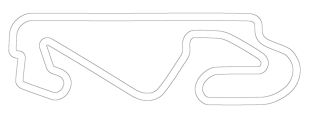
\includegraphics[interpolate=true,width=3.100000in,height=1.170000in]{contents/chapt6/figs/racing/crashes-img0.png}}%
\end{pgfscope}%
\begin{pgfscope}%
\pgfpathrectangle{\pgfqpoint{0.500000in}{0.498750in}}{\pgfqpoint{3.100000in}{1.162500in}}%
\pgfusepath{clip}%
\pgfsetbuttcap%
\pgfsetroundjoin%
\definecolor{currentfill}{rgb}{0.121569,0.466667,0.705882}%
\pgfsetfillcolor{currentfill}%
\pgfsetlinewidth{1.003750pt}%
\definecolor{currentstroke}{rgb}{0.121569,0.466667,0.705882}%
\pgfsetstrokecolor{currentstroke}%
\pgfsetdash{}{0pt}%
\pgfsys@defobject{currentmarker}{\pgfqpoint{-0.041667in}{-0.041667in}}{\pgfqpoint{0.041667in}{0.041667in}}{%
\pgfpathmoveto{\pgfqpoint{-0.041667in}{-0.041667in}}%
\pgfpathlineto{\pgfqpoint{0.041667in}{0.041667in}}%
\pgfpathmoveto{\pgfqpoint{-0.041667in}{0.041667in}}%
\pgfpathlineto{\pgfqpoint{0.041667in}{-0.041667in}}%
\pgfusepath{stroke,fill}%
}%
\begin{pgfscope}%
\pgfsys@transformshift{1.906992in}{0.669384in}%
\pgfsys@useobject{currentmarker}{}%
\end{pgfscope}%
\begin{pgfscope}%
\pgfsys@transformshift{3.214989in}{0.636844in}%
\pgfsys@useobject{currentmarker}{}%
\end{pgfscope}%
\begin{pgfscope}%
\pgfsys@transformshift{2.892801in}{1.528806in}%
\pgfsys@useobject{currentmarker}{}%
\end{pgfscope}%
\begin{pgfscope}%
\pgfsys@transformshift{2.349438in}{1.456484in}%
\pgfsys@useobject{currentmarker}{}%
\end{pgfscope}%
\begin{pgfscope}%
\pgfsys@transformshift{1.730754in}{0.847700in}%
\pgfsys@useobject{currentmarker}{}%
\end{pgfscope}%
\begin{pgfscope}%
\pgfsys@transformshift{2.920337in}{1.529293in}%
\pgfsys@useobject{currentmarker}{}%
\end{pgfscope}%
\begin{pgfscope}%
\pgfsys@transformshift{1.236923in}{1.148063in}%
\pgfsys@useobject{currentmarker}{}%
\end{pgfscope}%
\begin{pgfscope}%
\pgfsys@transformshift{3.118933in}{0.621076in}%
\pgfsys@useobject{currentmarker}{}%
\end{pgfscope}%
\begin{pgfscope}%
\pgfsys@transformshift{2.747929in}{0.616784in}%
\pgfsys@useobject{currentmarker}{}%
\end{pgfscope}%
\begin{pgfscope}%
\pgfsys@transformshift{1.148717in}{1.112083in}%
\pgfsys@useobject{currentmarker}{}%
\end{pgfscope}%
\begin{pgfscope}%
\pgfsys@transformshift{1.768492in}{1.529035in}%
\pgfsys@useobject{currentmarker}{}%
\end{pgfscope}%
\begin{pgfscope}%
\pgfsys@transformshift{2.445443in}{1.285445in}%
\pgfsys@useobject{currentmarker}{}%
\end{pgfscope}%
\begin{pgfscope}%
\pgfsys@transformshift{2.779412in}{0.616627in}%
\pgfsys@useobject{currentmarker}{}%
\end{pgfscope}%
\begin{pgfscope}%
\pgfsys@transformshift{3.123879in}{1.402157in}%
\pgfsys@useobject{currentmarker}{}%
\end{pgfscope}%
\begin{pgfscope}%
\pgfsys@transformshift{3.432840in}{1.143789in}%
\pgfsys@useobject{currentmarker}{}%
\end{pgfscope}%
\begin{pgfscope}%
\pgfsys@transformshift{1.156127in}{1.107816in}%
\pgfsys@useobject{currentmarker}{}%
\end{pgfscope}%
\begin{pgfscope}%
\pgfsys@transformshift{0.658028in}{0.909561in}%
\pgfsys@useobject{currentmarker}{}%
\end{pgfscope}%
\begin{pgfscope}%
\pgfsys@transformshift{2.758886in}{0.692721in}%
\pgfsys@useobject{currentmarker}{}%
\end{pgfscope}%
\begin{pgfscope}%
\pgfsys@transformshift{1.923655in}{1.454659in}%
\pgfsys@useobject{currentmarker}{}%
\end{pgfscope}%
\begin{pgfscope}%
\pgfsys@transformshift{1.003661in}{1.198056in}%
\pgfsys@useobject{currentmarker}{}%
\end{pgfscope}%
\begin{pgfscope}%
\pgfsys@transformshift{3.369820in}{0.714895in}%
\pgfsys@useobject{currentmarker}{}%
\end{pgfscope}%
\begin{pgfscope}%
\pgfsys@transformshift{2.143851in}{0.739866in}%
\pgfsys@useobject{currentmarker}{}%
\end{pgfscope}%
\begin{pgfscope}%
\pgfsys@transformshift{1.122205in}{1.214930in}%
\pgfsys@useobject{currentmarker}{}%
\end{pgfscope}%
\begin{pgfscope}%
\pgfsys@transformshift{1.056516in}{0.916263in}%
\pgfsys@useobject{currentmarker}{}%
\end{pgfscope}%
\begin{pgfscope}%
\pgfsys@transformshift{1.005796in}{0.935141in}%
\pgfsys@useobject{currentmarker}{}%
\end{pgfscope}%
\begin{pgfscope}%
\pgfsys@transformshift{2.498424in}{0.660415in}%
\pgfsys@useobject{currentmarker}{}%
\end{pgfscope}%
\begin{pgfscope}%
\pgfsys@transformshift{1.834681in}{1.454941in}%
\pgfsys@useobject{currentmarker}{}%
\end{pgfscope}%
\begin{pgfscope}%
\pgfsys@transformshift{1.086492in}{1.455074in}%
\pgfsys@useobject{currentmarker}{}%
\end{pgfscope}%
\begin{pgfscope}%
\pgfsys@transformshift{2.847268in}{1.454912in}%
\pgfsys@useobject{currentmarker}{}%
\end{pgfscope}%
\begin{pgfscope}%
\pgfsys@transformshift{2.989879in}{1.526779in}%
\pgfsys@useobject{currentmarker}{}%
\end{pgfscope}%
\begin{pgfscope}%
\pgfsys@transformshift{3.063159in}{1.509393in}%
\pgfsys@useobject{currentmarker}{}%
\end{pgfscope}%
\begin{pgfscope}%
\pgfsys@transformshift{0.901738in}{1.245579in}%
\pgfsys@useobject{currentmarker}{}%
\end{pgfscope}%
\begin{pgfscope}%
\pgfsys@transformshift{1.208334in}{0.873885in}%
\pgfsys@useobject{currentmarker}{}%
\end{pgfscope}%
\begin{pgfscope}%
\pgfsys@transformshift{0.975498in}{1.182806in}%
\pgfsys@useobject{currentmarker}{}%
\end{pgfscope}%
\begin{pgfscope}%
\pgfsys@transformshift{3.099831in}{1.479138in}%
\pgfsys@useobject{currentmarker}{}%
\end{pgfscope}%
\begin{pgfscope}%
\pgfsys@transformshift{0.645893in}{1.085915in}%
\pgfsys@useobject{currentmarker}{}%
\end{pgfscope}%
\begin{pgfscope}%
\pgfsys@transformshift{3.082924in}{1.073004in}%
\pgfsys@useobject{currentmarker}{}%
\end{pgfscope}%
\begin{pgfscope}%
\pgfsys@transformshift{1.137856in}{0.964981in}%
\pgfsys@useobject{currentmarker}{}%
\end{pgfscope}%
\begin{pgfscope}%
\pgfsys@transformshift{3.228168in}{0.723846in}%
\pgfsys@useobject{currentmarker}{}%
\end{pgfscope}%
\begin{pgfscope}%
\pgfsys@transformshift{1.681868in}{0.789913in}%
\pgfsys@useobject{currentmarker}{}%
\end{pgfscope}%
\begin{pgfscope}%
\pgfsys@transformshift{1.070053in}{0.911926in}%
\pgfsys@useobject{currentmarker}{}%
\end{pgfscope}%
\begin{pgfscope}%
\pgfsys@transformshift{1.577205in}{0.852761in}%
\pgfsys@useobject{currentmarker}{}%
\end{pgfscope}%
\begin{pgfscope}%
\pgfsys@transformshift{0.676020in}{1.158305in}%
\pgfsys@useobject{currentmarker}{}%
\end{pgfscope}%
\begin{pgfscope}%
\pgfsys@transformshift{0.680971in}{1.157874in}%
\pgfsys@useobject{currentmarker}{}%
\end{pgfscope}%
\begin{pgfscope}%
\pgfsys@transformshift{0.899439in}{1.242292in}%
\pgfsys@useobject{currentmarker}{}%
\end{pgfscope}%
\begin{pgfscope}%
\pgfsys@transformshift{1.036400in}{1.004934in}%
\pgfsys@useobject{currentmarker}{}%
\end{pgfscope}%
\begin{pgfscope}%
\pgfsys@transformshift{0.895584in}{1.226918in}%
\pgfsys@useobject{currentmarker}{}%
\end{pgfscope}%
\begin{pgfscope}%
\pgfsys@transformshift{3.091479in}{1.003401in}%
\pgfsys@useobject{currentmarker}{}%
\end{pgfscope}%
\begin{pgfscope}%
\pgfsys@transformshift{1.463037in}{1.529654in}%
\pgfsys@useobject{currentmarker}{}%
\end{pgfscope}%
\begin{pgfscope}%
\pgfsys@transformshift{0.595737in}{1.125288in}%
\pgfsys@useobject{currentmarker}{}%
\end{pgfscope}%
\begin{pgfscope}%
\pgfsys@transformshift{2.829259in}{0.616214in}%
\pgfsys@useobject{currentmarker}{}%
\end{pgfscope}%
\begin{pgfscope}%
\pgfsys@transformshift{0.586976in}{1.190058in}%
\pgfsys@useobject{currentmarker}{}%
\end{pgfscope}%
\begin{pgfscope}%
\pgfsys@transformshift{3.053406in}{1.000508in}%
\pgfsys@useobject{currentmarker}{}%
\end{pgfscope}%
\begin{pgfscope}%
\pgfsys@transformshift{0.587664in}{1.194221in}%
\pgfsys@useobject{currentmarker}{}%
\end{pgfscope}%
\begin{pgfscope}%
\pgfsys@transformshift{1.113466in}{0.888220in}%
\pgfsys@useobject{currentmarker}{}%
\end{pgfscope}%
\begin{pgfscope}%
\pgfsys@transformshift{0.783245in}{1.448985in}%
\pgfsys@useobject{currentmarker}{}%
\end{pgfscope}%
\begin{pgfscope}%
\pgfsys@transformshift{1.172702in}{1.531413in}%
\pgfsys@useobject{currentmarker}{}%
\end{pgfscope}%
\begin{pgfscope}%
\pgfsys@transformshift{1.254767in}{1.530850in}%
\pgfsys@useobject{currentmarker}{}%
\end{pgfscope}%
\begin{pgfscope}%
\pgfsys@transformshift{0.584580in}{1.158132in}%
\pgfsys@useobject{currentmarker}{}%
\end{pgfscope}%
\begin{pgfscope}%
\pgfsys@transformshift{0.822625in}{1.455191in}%
\pgfsys@useobject{currentmarker}{}%
\end{pgfscope}%
\begin{pgfscope}%
\pgfsys@transformshift{0.804551in}{1.454937in}%
\pgfsys@useobject{currentmarker}{}%
\end{pgfscope}%
\begin{pgfscope}%
\pgfsys@transformshift{0.587250in}{1.160345in}%
\pgfsys@useobject{currentmarker}{}%
\end{pgfscope}%
\begin{pgfscope}%
\pgfsys@transformshift{2.470371in}{1.533298in}%
\pgfsys@useobject{currentmarker}{}%
\end{pgfscope}%
\begin{pgfscope}%
\pgfsys@transformshift{2.493537in}{1.533313in}%
\pgfsys@useobject{currentmarker}{}%
\end{pgfscope}%
\begin{pgfscope}%
\pgfsys@transformshift{3.022026in}{1.444610in}%
\pgfsys@useobject{currentmarker}{}%
\end{pgfscope}%
\begin{pgfscope}%
\pgfsys@transformshift{1.026522in}{1.033368in}%
\pgfsys@useobject{currentmarker}{}%
\end{pgfscope}%
\begin{pgfscope}%
\pgfsys@transformshift{0.667948in}{1.278412in}%
\pgfsys@useobject{currentmarker}{}%
\end{pgfscope}%
\begin{pgfscope}%
\pgfsys@transformshift{3.023715in}{1.444397in}%
\pgfsys@useobject{currentmarker}{}%
\end{pgfscope}%
\begin{pgfscope}%
\pgfsys@transformshift{3.103551in}{1.015960in}%
\pgfsys@useobject{currentmarker}{}%
\end{pgfscope}%
\begin{pgfscope}%
\pgfsys@transformshift{0.587399in}{1.176070in}%
\pgfsys@useobject{currentmarker}{}%
\end{pgfscope}%
\begin{pgfscope}%
\pgfsys@transformshift{0.584796in}{1.161188in}%
\pgfsys@useobject{currentmarker}{}%
\end{pgfscope}%
\begin{pgfscope}%
\pgfsys@transformshift{1.496079in}{1.529164in}%
\pgfsys@useobject{currentmarker}{}%
\end{pgfscope}%
\begin{pgfscope}%
\pgfsys@transformshift{2.997833in}{1.451069in}%
\pgfsys@useobject{currentmarker}{}%
\end{pgfscope}%
\begin{pgfscope}%
\pgfsys@transformshift{1.034205in}{0.924085in}%
\pgfsys@useobject{currentmarker}{}%
\end{pgfscope}%
\begin{pgfscope}%
\pgfsys@transformshift{3.000398in}{1.450903in}%
\pgfsys@useobject{currentmarker}{}%
\end{pgfscope}%
\begin{pgfscope}%
\pgfsys@transformshift{1.026648in}{1.034657in}%
\pgfsys@useobject{currentmarker}{}%
\end{pgfscope}%
\begin{pgfscope}%
\pgfsys@transformshift{1.889706in}{1.531345in}%
\pgfsys@useobject{currentmarker}{}%
\end{pgfscope}%
\begin{pgfscope}%
\pgfsys@transformshift{1.762983in}{1.528705in}%
\pgfsys@useobject{currentmarker}{}%
\end{pgfscope}%
\begin{pgfscope}%
\pgfsys@transformshift{2.603566in}{1.532829in}%
\pgfsys@useobject{currentmarker}{}%
\end{pgfscope}%
\begin{pgfscope}%
\pgfsys@transformshift{2.974653in}{1.452719in}%
\pgfsys@useobject{currentmarker}{}%
\end{pgfscope}%
\begin{pgfscope}%
\pgfsys@transformshift{1.433839in}{0.940857in}%
\pgfsys@useobject{currentmarker}{}%
\end{pgfscope}%
\begin{pgfscope}%
\pgfsys@transformshift{2.070070in}{1.531267in}%
\pgfsys@useobject{currentmarker}{}%
\end{pgfscope}%
\begin{pgfscope}%
\pgfsys@transformshift{1.118958in}{0.881985in}%
\pgfsys@useobject{currentmarker}{}%
\end{pgfscope}%
\begin{pgfscope}%
\pgfsys@transformshift{3.036727in}{1.433605in}%
\pgfsys@useobject{currentmarker}{}%
\end{pgfscope}%
\begin{pgfscope}%
\pgfsys@transformshift{1.107650in}{0.894401in}%
\pgfsys@useobject{currentmarker}{}%
\end{pgfscope}%
\begin{pgfscope}%
\pgfsys@transformshift{3.076720in}{1.000851in}%
\pgfsys@useobject{currentmarker}{}%
\end{pgfscope}%
\begin{pgfscope}%
\pgfsys@transformshift{0.593961in}{1.126307in}%
\pgfsys@useobject{currentmarker}{}%
\end{pgfscope}%
\begin{pgfscope}%
\pgfsys@transformshift{3.010717in}{1.000607in}%
\pgfsys@useobject{currentmarker}{}%
\end{pgfscope}%
\begin{pgfscope}%
\pgfsys@transformshift{2.972824in}{1.529220in}%
\pgfsys@useobject{currentmarker}{}%
\end{pgfscope}%
\begin{pgfscope}%
\pgfsys@transformshift{3.125628in}{1.345100in}%
\pgfsys@useobject{currentmarker}{}%
\end{pgfscope}%
\begin{pgfscope}%
\pgfsys@transformshift{0.843890in}{1.455198in}%
\pgfsys@useobject{currentmarker}{}%
\end{pgfscope}%
\begin{pgfscope}%
\pgfsys@transformshift{0.587222in}{1.176783in}%
\pgfsys@useobject{currentmarker}{}%
\end{pgfscope}%
\begin{pgfscope}%
\pgfsys@transformshift{0.864074in}{1.455165in}%
\pgfsys@useobject{currentmarker}{}%
\end{pgfscope}%
\begin{pgfscope}%
\pgfsys@transformshift{1.048703in}{0.918259in}%
\pgfsys@useobject{currentmarker}{}%
\end{pgfscope}%
\begin{pgfscope}%
\pgfsys@transformshift{0.704915in}{1.399468in}%
\pgfsys@useobject{currentmarker}{}%
\end{pgfscope}%
\begin{pgfscope}%
\pgfsys@transformshift{1.135564in}{0.846501in}%
\pgfsys@useobject{currentmarker}{}%
\end{pgfscope}%
\begin{pgfscope}%
\pgfsys@transformshift{0.972710in}{1.455236in}%
\pgfsys@useobject{currentmarker}{}%
\end{pgfscope}%
\begin{pgfscope}%
\pgfsys@transformshift{1.112629in}{0.887339in}%
\pgfsys@useobject{currentmarker}{}%
\end{pgfscope}%
\begin{pgfscope}%
\pgfsys@transformshift{1.135075in}{0.845979in}%
\pgfsys@useobject{currentmarker}{}%
\end{pgfscope}%
\begin{pgfscope}%
\pgfsys@transformshift{1.036879in}{1.007502in}%
\pgfsys@useobject{currentmarker}{}%
\end{pgfscope}%
\begin{pgfscope}%
\pgfsys@transformshift{0.822934in}{1.455241in}%
\pgfsys@useobject{currentmarker}{}%
\end{pgfscope}%
\begin{pgfscope}%
\pgfsys@transformshift{0.967657in}{1.455211in}%
\pgfsys@useobject{currentmarker}{}%
\end{pgfscope}%
\begin{pgfscope}%
\pgfsys@transformshift{0.997615in}{1.454836in}%
\pgfsys@useobject{currentmarker}{}%
\end{pgfscope}%
\begin{pgfscope}%
\pgfsys@transformshift{2.194049in}{1.533383in}%
\pgfsys@useobject{currentmarker}{}%
\end{pgfscope}%
\begin{pgfscope}%
\pgfsys@transformshift{0.823754in}{1.455157in}%
\pgfsys@useobject{currentmarker}{}%
\end{pgfscope}%
\begin{pgfscope}%
\pgfsys@transformshift{0.676261in}{1.074281in}%
\pgfsys@useobject{currentmarker}{}%
\end{pgfscope}%
\begin{pgfscope}%
\pgfsys@transformshift{2.708142in}{1.532894in}%
\pgfsys@useobject{currentmarker}{}%
\end{pgfscope}%
\begin{pgfscope}%
\pgfsys@transformshift{0.675151in}{1.065186in}%
\pgfsys@useobject{currentmarker}{}%
\end{pgfscope}%
\begin{pgfscope}%
\pgfsys@transformshift{0.783030in}{1.448755in}%
\pgfsys@useobject{currentmarker}{}%
\end{pgfscope}%
\begin{pgfscope}%
\pgfsys@transformshift{2.246621in}{1.532855in}%
\pgfsys@useobject{currentmarker}{}%
\end{pgfscope}%
\begin{pgfscope}%
\pgfsys@transformshift{1.936266in}{1.530844in}%
\pgfsys@useobject{currentmarker}{}%
\end{pgfscope}%
\begin{pgfscope}%
\pgfsys@transformshift{2.170082in}{1.530820in}%
\pgfsys@useobject{currentmarker}{}%
\end{pgfscope}%
\begin{pgfscope}%
\pgfsys@transformshift{2.337614in}{1.533429in}%
\pgfsys@useobject{currentmarker}{}%
\end{pgfscope}%
\begin{pgfscope}%
\pgfsys@transformshift{0.587334in}{1.149820in}%
\pgfsys@useobject{currentmarker}{}%
\end{pgfscope}%
\begin{pgfscope}%
\pgfsys@transformshift{0.747894in}{0.848582in}%
\pgfsys@useobject{currentmarker}{}%
\end{pgfscope}%
\begin{pgfscope}%
\pgfsys@transformshift{1.121624in}{1.530941in}%
\pgfsys@useobject{currentmarker}{}%
\end{pgfscope}%
\begin{pgfscope}%
\pgfsys@transformshift{2.718603in}{1.533288in}%
\pgfsys@useobject{currentmarker}{}%
\end{pgfscope}%
\begin{pgfscope}%
\pgfsys@transformshift{1.267163in}{1.530998in}%
\pgfsys@useobject{currentmarker}{}%
\end{pgfscope}%
\begin{pgfscope}%
\pgfsys@transformshift{0.869685in}{1.530759in}%
\pgfsys@useobject{currentmarker}{}%
\end{pgfscope}%
\begin{pgfscope}%
\pgfsys@transformshift{1.226617in}{1.531649in}%
\pgfsys@useobject{currentmarker}{}%
\end{pgfscope}%
\begin{pgfscope}%
\pgfsys@transformshift{2.141873in}{1.531039in}%
\pgfsys@useobject{currentmarker}{}%
\end{pgfscope}%
\begin{pgfscope}%
\pgfsys@transformshift{0.592880in}{1.126537in}%
\pgfsys@useobject{currentmarker}{}%
\end{pgfscope}%
\begin{pgfscope}%
\pgfsys@transformshift{0.732590in}{0.854337in}%
\pgfsys@useobject{currentmarker}{}%
\end{pgfscope}%
\begin{pgfscope}%
\pgfsys@transformshift{1.036534in}{1.007933in}%
\pgfsys@useobject{currentmarker}{}%
\end{pgfscope}%
\begin{pgfscope}%
\pgfsys@transformshift{1.831024in}{0.787429in}%
\pgfsys@useobject{currentmarker}{}%
\end{pgfscope}%
\begin{pgfscope}%
\pgfsys@transformshift{1.880802in}{0.758019in}%
\pgfsys@useobject{currentmarker}{}%
\end{pgfscope}%
\begin{pgfscope}%
\pgfsys@transformshift{1.468543in}{0.919386in}%
\pgfsys@useobject{currentmarker}{}%
\end{pgfscope}%
\begin{pgfscope}%
\pgfsys@transformshift{1.854590in}{0.772967in}%
\pgfsys@useobject{currentmarker}{}%
\end{pgfscope}%
\begin{pgfscope}%
\pgfsys@transformshift{0.812150in}{1.531985in}%
\pgfsys@useobject{currentmarker}{}%
\end{pgfscope}%
\begin{pgfscope}%
\pgfsys@transformshift{0.587378in}{1.170850in}%
\pgfsys@useobject{currentmarker}{}%
\end{pgfscope}%
\begin{pgfscope}%
\pgfsys@transformshift{1.789528in}{0.811643in}%
\pgfsys@useobject{currentmarker}{}%
\end{pgfscope}%
\begin{pgfscope}%
\pgfsys@transformshift{1.571090in}{1.528765in}%
\pgfsys@useobject{currentmarker}{}%
\end{pgfscope}%
\begin{pgfscope}%
\pgfsys@transformshift{0.863479in}{1.531880in}%
\pgfsys@useobject{currentmarker}{}%
\end{pgfscope}%
\begin{pgfscope}%
\pgfsys@transformshift{3.001884in}{1.126620in}%
\pgfsys@useobject{currentmarker}{}%
\end{pgfscope}%
\begin{pgfscope}%
\pgfsys@transformshift{1.154550in}{1.110261in}%
\pgfsys@useobject{currentmarker}{}%
\end{pgfscope}%
\begin{pgfscope}%
\pgfsys@transformshift{1.884181in}{0.758198in}%
\pgfsys@useobject{currentmarker}{}%
\end{pgfscope}%
\begin{pgfscope}%
\pgfsys@transformshift{1.628797in}{1.528771in}%
\pgfsys@useobject{currentmarker}{}%
\end{pgfscope}%
\begin{pgfscope}%
\pgfsys@transformshift{1.886672in}{0.755807in}%
\pgfsys@useobject{currentmarker}{}%
\end{pgfscope}%
\begin{pgfscope}%
\pgfsys@transformshift{2.001083in}{1.531006in}%
\pgfsys@useobject{currentmarker}{}%
\end{pgfscope}%
\begin{pgfscope}%
\pgfsys@transformshift{2.877308in}{1.199986in}%
\pgfsys@useobject{currentmarker}{}%
\end{pgfscope}%
\begin{pgfscope}%
\pgfsys@transformshift{0.733679in}{0.854696in}%
\pgfsys@useobject{currentmarker}{}%
\end{pgfscope}%
\begin{pgfscope}%
\pgfsys@transformshift{1.604446in}{0.926173in}%
\pgfsys@useobject{currentmarker}{}%
\end{pgfscope}%
\begin{pgfscope}%
\pgfsys@transformshift{1.817549in}{0.794699in}%
\pgfsys@useobject{currentmarker}{}%
\end{pgfscope}%
\begin{pgfscope}%
\pgfsys@transformshift{0.586943in}{1.164480in}%
\pgfsys@useobject{currentmarker}{}%
\end{pgfscope}%
\begin{pgfscope}%
\pgfsys@transformshift{1.610140in}{0.832555in}%
\pgfsys@useobject{currentmarker}{}%
\end{pgfscope}%
\begin{pgfscope}%
\pgfsys@transformshift{2.981556in}{0.924462in}%
\pgfsys@useobject{currentmarker}{}%
\end{pgfscope}%
\begin{pgfscope}%
\pgfsys@transformshift{1.260011in}{1.046862in}%
\pgfsys@useobject{currentmarker}{}%
\end{pgfscope}%
\begin{pgfscope}%
\pgfsys@transformshift{3.107072in}{1.466068in}%
\pgfsys@useobject{currentmarker}{}%
\end{pgfscope}%
\begin{pgfscope}%
\pgfsys@transformshift{1.614571in}{0.829029in}%
\pgfsys@useobject{currentmarker}{}%
\end{pgfscope}%
\begin{pgfscope}%
\pgfsys@transformshift{2.954934in}{1.154192in}%
\pgfsys@useobject{currentmarker}{}%
\end{pgfscope}%
\begin{pgfscope}%
\pgfsys@transformshift{0.920838in}{0.704553in}%
\pgfsys@useobject{currentmarker}{}%
\end{pgfscope}%
\begin{pgfscope}%
\pgfsys@transformshift{2.254621in}{1.533080in}%
\pgfsys@useobject{currentmarker}{}%
\end{pgfscope}%
\begin{pgfscope}%
\pgfsys@transformshift{1.819440in}{0.704516in}%
\pgfsys@useobject{currentmarker}{}%
\end{pgfscope}%
\begin{pgfscope}%
\pgfsys@transformshift{1.671543in}{0.796123in}%
\pgfsys@useobject{currentmarker}{}%
\end{pgfscope}%
\begin{pgfscope}%
\pgfsys@transformshift{2.850227in}{1.214188in}%
\pgfsys@useobject{currentmarker}{}%
\end{pgfscope}%
\begin{pgfscope}%
\pgfsys@transformshift{2.783948in}{1.248624in}%
\pgfsys@useobject{currentmarker}{}%
\end{pgfscope}%
\begin{pgfscope}%
\pgfsys@transformshift{2.630674in}{0.908414in}%
\pgfsys@useobject{currentmarker}{}%
\end{pgfscope}%
\begin{pgfscope}%
\pgfsys@transformshift{0.709432in}{1.402731in}%
\pgfsys@useobject{currentmarker}{}%
\end{pgfscope}%
\begin{pgfscope}%
\pgfsys@transformshift{1.299251in}{1.531184in}%
\pgfsys@useobject{currentmarker}{}%
\end{pgfscope}%
\begin{pgfscope}%
\pgfsys@transformshift{3.056085in}{1.091697in}%
\pgfsys@useobject{currentmarker}{}%
\end{pgfscope}%
\begin{pgfscope}%
\pgfsys@transformshift{2.724605in}{0.921261in}%
\pgfsys@useobject{currentmarker}{}%
\end{pgfscope}%
\begin{pgfscope}%
\pgfsys@transformshift{0.703263in}{1.395697in}%
\pgfsys@useobject{currentmarker}{}%
\end{pgfscope}%
\begin{pgfscope}%
\pgfsys@transformshift{2.092233in}{1.531584in}%
\pgfsys@useobject{currentmarker}{}%
\end{pgfscope}%
\begin{pgfscope}%
\pgfsys@transformshift{1.123129in}{0.788712in}%
\pgfsys@useobject{currentmarker}{}%
\end{pgfscope}%
\begin{pgfscope}%
\pgfsys@transformshift{2.048738in}{1.531430in}%
\pgfsys@useobject{currentmarker}{}%
\end{pgfscope}%
\begin{pgfscope}%
\pgfsys@transformshift{2.635975in}{0.911861in}%
\pgfsys@useobject{currentmarker}{}%
\end{pgfscope}%
\begin{pgfscope}%
\pgfsys@transformshift{2.643048in}{0.913950in}%
\pgfsys@useobject{currentmarker}{}%
\end{pgfscope}%
\begin{pgfscope}%
\pgfsys@transformshift{3.018563in}{1.446188in}%
\pgfsys@useobject{currentmarker}{}%
\end{pgfscope}%
\begin{pgfscope}%
\pgfsys@transformshift{3.016397in}{1.447057in}%
\pgfsys@useobject{currentmarker}{}%
\end{pgfscope}%
\begin{pgfscope}%
\pgfsys@transformshift{0.734019in}{0.853978in}%
\pgfsys@useobject{currentmarker}{}%
\end{pgfscope}%
\begin{pgfscope}%
\pgfsys@transformshift{3.122410in}{1.421049in}%
\pgfsys@useobject{currentmarker}{}%
\end{pgfscope}%
\begin{pgfscope}%
\pgfsys@transformshift{0.676590in}{1.073133in}%
\pgfsys@useobject{currentmarker}{}%
\end{pgfscope}%
\begin{pgfscope}%
\pgfsys@transformshift{3.119365in}{1.431956in}%
\pgfsys@useobject{currentmarker}{}%
\end{pgfscope}%
\begin{pgfscope}%
\pgfsys@transformshift{3.161899in}{1.281987in}%
\pgfsys@useobject{currentmarker}{}%
\end{pgfscope}%
\begin{pgfscope}%
\pgfsys@transformshift{0.608602in}{1.106913in}%
\pgfsys@useobject{currentmarker}{}%
\end{pgfscope}%
\begin{pgfscope}%
\pgfsys@transformshift{0.677120in}{1.078996in}%
\pgfsys@useobject{currentmarker}{}%
\end{pgfscope}%
\begin{pgfscope}%
\pgfsys@transformshift{3.188396in}{1.266055in}%
\pgfsys@useobject{currentmarker}{}%
\end{pgfscope}%
\begin{pgfscope}%
\pgfsys@transformshift{3.032077in}{1.438892in}%
\pgfsys@useobject{currentmarker}{}%
\end{pgfscope}%
\begin{pgfscope}%
\pgfsys@transformshift{0.735441in}{0.897877in}%
\pgfsys@useobject{currentmarker}{}%
\end{pgfscope}%
\begin{pgfscope}%
\pgfsys@transformshift{3.104726in}{1.467695in}%
\pgfsys@useobject{currentmarker}{}%
\end{pgfscope}%
\begin{pgfscope}%
\pgfsys@transformshift{3.031572in}{1.000792in}%
\pgfsys@useobject{currentmarker}{}%
\end{pgfscope}%
\begin{pgfscope}%
\pgfsys@transformshift{0.634255in}{1.089595in}%
\pgfsys@useobject{currentmarker}{}%
\end{pgfscope}%
\begin{pgfscope}%
\pgfsys@transformshift{3.080327in}{1.001103in}%
\pgfsys@useobject{currentmarker}{}%
\end{pgfscope}%
\begin{pgfscope}%
\pgfsys@transformshift{2.322809in}{1.143819in}%
\pgfsys@useobject{currentmarker}{}%
\end{pgfscope}%
\begin{pgfscope}%
\pgfsys@transformshift{2.418232in}{1.533097in}%
\pgfsys@useobject{currentmarker}{}%
\end{pgfscope}%
\begin{pgfscope}%
\pgfsys@transformshift{2.504295in}{0.654671in}%
\pgfsys@useobject{currentmarker}{}%
\end{pgfscope}%
\begin{pgfscope}%
\pgfsys@transformshift{2.459930in}{0.830277in}%
\pgfsys@useobject{currentmarker}{}%
\end{pgfscope}%
\begin{pgfscope}%
\pgfsys@transformshift{0.973000in}{1.530938in}%
\pgfsys@useobject{currentmarker}{}%
\end{pgfscope}%
\begin{pgfscope}%
\pgfsys@transformshift{1.884762in}{1.531148in}%
\pgfsys@useobject{currentmarker}{}%
\end{pgfscope}%
\begin{pgfscope}%
\pgfsys@transformshift{0.978538in}{1.211586in}%
\pgfsys@useobject{currentmarker}{}%
\end{pgfscope}%
\begin{pgfscope}%
\pgfsys@transformshift{2.449242in}{0.790602in}%
\pgfsys@useobject{currentmarker}{}%
\end{pgfscope}%
\begin{pgfscope}%
\pgfsys@transformshift{0.789970in}{0.831543in}%
\pgfsys@useobject{currentmarker}{}%
\end{pgfscope}%
\begin{pgfscope}%
\pgfsys@transformshift{0.887358in}{0.797765in}%
\pgfsys@useobject{currentmarker}{}%
\end{pgfscope}%
\begin{pgfscope}%
\pgfsys@transformshift{2.469040in}{0.698745in}%
\pgfsys@useobject{currentmarker}{}%
\end{pgfscope}%
\begin{pgfscope}%
\pgfsys@transformshift{0.930555in}{0.780223in}%
\pgfsys@useobject{currentmarker}{}%
\end{pgfscope}%
\begin{pgfscope}%
\pgfsys@transformshift{0.993429in}{0.761046in}%
\pgfsys@useobject{currentmarker}{}%
\end{pgfscope}%
\begin{pgfscope}%
\pgfsys@transformshift{1.028114in}{0.748262in}%
\pgfsys@useobject{currentmarker}{}%
\end{pgfscope}%
\begin{pgfscope}%
\pgfsys@transformshift{1.012122in}{0.751877in}%
\pgfsys@useobject{currentmarker}{}%
\end{pgfscope}%
\begin{pgfscope}%
\pgfsys@transformshift{1.036419in}{0.745950in}%
\pgfsys@useobject{currentmarker}{}%
\end{pgfscope}%
\begin{pgfscope}%
\pgfsys@transformshift{1.009049in}{0.754067in}%
\pgfsys@useobject{currentmarker}{}%
\end{pgfscope}%
\begin{pgfscope}%
\pgfsys@transformshift{1.013928in}{0.752555in}%
\pgfsys@useobject{currentmarker}{}%
\end{pgfscope}%
\begin{pgfscope}%
\pgfsys@transformshift{2.462697in}{0.713653in}%
\pgfsys@useobject{currentmarker}{}%
\end{pgfscope}%
\begin{pgfscope}%
\pgfsys@transformshift{0.872931in}{0.801014in}%
\pgfsys@useobject{currentmarker}{}%
\end{pgfscope}%
\begin{pgfscope}%
\pgfsys@transformshift{2.481613in}{0.682111in}%
\pgfsys@useobject{currentmarker}{}%
\end{pgfscope}%
\begin{pgfscope}%
\pgfsys@transformshift{0.899388in}{1.240656in}%
\pgfsys@useobject{currentmarker}{}%
\end{pgfscope}%
\begin{pgfscope}%
\pgfsys@transformshift{2.486483in}{0.672089in}%
\pgfsys@useobject{currentmarker}{}%
\end{pgfscope}%
\begin{pgfscope}%
\pgfsys@transformshift{1.034084in}{0.745623in}%
\pgfsys@useobject{currentmarker}{}%
\end{pgfscope}%
\begin{pgfscope}%
\pgfsys@transformshift{2.462421in}{0.712598in}%
\pgfsys@useobject{currentmarker}{}%
\end{pgfscope}%
\begin{pgfscope}%
\pgfsys@transformshift{3.105798in}{1.047314in}%
\pgfsys@useobject{currentmarker}{}%
\end{pgfscope}%
\begin{pgfscope}%
\pgfsys@transformshift{0.674341in}{1.045470in}%
\pgfsys@useobject{currentmarker}{}%
\end{pgfscope}%
\begin{pgfscope}%
\pgfsys@transformshift{3.068096in}{1.000518in}%
\pgfsys@useobject{currentmarker}{}%
\end{pgfscope}%
\begin{pgfscope}%
\pgfsys@transformshift{0.676553in}{1.072986in}%
\pgfsys@useobject{currentmarker}{}%
\end{pgfscope}%
\begin{pgfscope}%
\pgfsys@transformshift{3.048857in}{1.349691in}%
\pgfsys@useobject{currentmarker}{}%
\end{pgfscope}%
\begin{pgfscope}%
\pgfsys@transformshift{3.038264in}{1.431377in}%
\pgfsys@useobject{currentmarker}{}%
\end{pgfscope}%
\begin{pgfscope}%
\pgfsys@transformshift{3.055990in}{1.304901in}%
\pgfsys@useobject{currentmarker}{}%
\end{pgfscope}%
\begin{pgfscope}%
\pgfsys@transformshift{0.694683in}{1.155848in}%
\pgfsys@useobject{currentmarker}{}%
\end{pgfscope}%
\begin{pgfscope}%
\pgfsys@transformshift{0.674168in}{1.057280in}%
\pgfsys@useobject{currentmarker}{}%
\end{pgfscope}%
\begin{pgfscope}%
\pgfsys@transformshift{3.036880in}{1.433305in}%
\pgfsys@useobject{currentmarker}{}%
\end{pgfscope}%
\begin{pgfscope}%
\pgfsys@transformshift{3.108175in}{1.025127in}%
\pgfsys@useobject{currentmarker}{}%
\end{pgfscope}%
\begin{pgfscope}%
\pgfsys@transformshift{3.094377in}{1.004722in}%
\pgfsys@useobject{currentmarker}{}%
\end{pgfscope}%
\begin{pgfscope}%
\pgfsys@transformshift{0.869897in}{1.454754in}%
\pgfsys@useobject{currentmarker}{}%
\end{pgfscope}%
\begin{pgfscope}%
\pgfsys@transformshift{2.283893in}{1.457204in}%
\pgfsys@useobject{currentmarker}{}%
\end{pgfscope}%
\begin{pgfscope}%
\pgfsys@transformshift{0.972026in}{1.196647in}%
\pgfsys@useobject{currentmarker}{}%
\end{pgfscope}%
\begin{pgfscope}%
\pgfsys@transformshift{0.899157in}{0.712795in}%
\pgfsys@useobject{currentmarker}{}%
\end{pgfscope}%
\begin{pgfscope}%
\pgfsys@transformshift{1.479573in}{1.001194in}%
\pgfsys@useobject{currentmarker}{}%
\end{pgfscope}%
\begin{pgfscope}%
\pgfsys@transformshift{1.044636in}{1.001643in}%
\pgfsys@useobject{currentmarker}{}%
\end{pgfscope}%
\begin{pgfscope}%
\pgfsys@transformshift{0.995904in}{1.122837in}%
\pgfsys@useobject{currentmarker}{}%
\end{pgfscope}%
\begin{pgfscope}%
\pgfsys@transformshift{3.031102in}{1.000811in}%
\pgfsys@useobject{currentmarker}{}%
\end{pgfscope}%
\begin{pgfscope}%
\pgfsys@transformshift{3.395702in}{0.848188in}%
\pgfsys@useobject{currentmarker}{}%
\end{pgfscope}%
\begin{pgfscope}%
\pgfsys@transformshift{2.376719in}{1.532893in}%
\pgfsys@useobject{currentmarker}{}%
\end{pgfscope}%
\begin{pgfscope}%
\pgfsys@transformshift{1.123418in}{0.876771in}%
\pgfsys@useobject{currentmarker}{}%
\end{pgfscope}%
\begin{pgfscope}%
\pgfsys@transformshift{0.964259in}{0.688907in}%
\pgfsys@useobject{currentmarker}{}%
\end{pgfscope}%
\begin{pgfscope}%
\pgfsys@transformshift{3.073162in}{1.000823in}%
\pgfsys@useobject{currentmarker}{}%
\end{pgfscope}%
\begin{pgfscope}%
\pgfsys@transformshift{0.930305in}{0.701405in}%
\pgfsys@useobject{currentmarker}{}%
\end{pgfscope}%
\begin{pgfscope}%
\pgfsys@transformshift{2.709003in}{0.618948in}%
\pgfsys@useobject{currentmarker}{}%
\end{pgfscope}%
\begin{pgfscope}%
\pgfsys@transformshift{0.587950in}{1.140142in}%
\pgfsys@useobject{currentmarker}{}%
\end{pgfscope}%
\begin{pgfscope}%
\pgfsys@transformshift{3.091420in}{1.002915in}%
\pgfsys@useobject{currentmarker}{}%
\end{pgfscope}%
\begin{pgfscope}%
\pgfsys@transformshift{3.162275in}{0.702896in}%
\pgfsys@useobject{currentmarker}{}%
\end{pgfscope}%
\begin{pgfscope}%
\pgfsys@transformshift{0.612874in}{1.103596in}%
\pgfsys@useobject{currentmarker}{}%
\end{pgfscope}%
\begin{pgfscope}%
\pgfsys@transformshift{2.943603in}{1.160347in}%
\pgfsys@useobject{currentmarker}{}%
\end{pgfscope}%
\begin{pgfscope}%
\pgfsys@transformshift{0.891575in}{1.454580in}%
\pgfsys@useobject{currentmarker}{}%
\end{pgfscope}%
\begin{pgfscope}%
\pgfsys@transformshift{3.186171in}{1.036698in}%
\pgfsys@useobject{currentmarker}{}%
\end{pgfscope}%
\begin{pgfscope}%
\pgfsys@transformshift{3.157686in}{0.700828in}%
\pgfsys@useobject{currentmarker}{}%
\end{pgfscope}%
\begin{pgfscope}%
\pgfsys@transformshift{0.676391in}{1.064747in}%
\pgfsys@useobject{currentmarker}{}%
\end{pgfscope}%
\begin{pgfscope}%
\pgfsys@transformshift{2.925919in}{0.618821in}%
\pgfsys@useobject{currentmarker}{}%
\end{pgfscope}%
\begin{pgfscope}%
\pgfsys@transformshift{2.651154in}{1.457132in}%
\pgfsys@useobject{currentmarker}{}%
\end{pgfscope}%
\begin{pgfscope}%
\pgfsys@transformshift{1.756440in}{1.453151in}%
\pgfsys@useobject{currentmarker}{}%
\end{pgfscope}%
\begin{pgfscope}%
\pgfsys@transformshift{3.087887in}{1.002710in}%
\pgfsys@useobject{currentmarker}{}%
\end{pgfscope}%
\begin{pgfscope}%
\pgfsys@transformshift{2.116489in}{1.454652in}%
\pgfsys@useobject{currentmarker}{}%
\end{pgfscope}%
\begin{pgfscope}%
\pgfsys@transformshift{1.259364in}{1.455017in}%
\pgfsys@useobject{currentmarker}{}%
\end{pgfscope}%
\begin{pgfscope}%
\pgfsys@transformshift{1.920355in}{1.454854in}%
\pgfsys@useobject{currentmarker}{}%
\end{pgfscope}%
\begin{pgfscope}%
\pgfsys@transformshift{1.987217in}{1.455106in}%
\pgfsys@useobject{currentmarker}{}%
\end{pgfscope}%
\begin{pgfscope}%
\pgfsys@transformshift{3.091859in}{1.002897in}%
\pgfsys@useobject{currentmarker}{}%
\end{pgfscope}%
\begin{pgfscope}%
\pgfsys@transformshift{1.026350in}{0.748530in}%
\pgfsys@useobject{currentmarker}{}%
\end{pgfscope}%
\begin{pgfscope}%
\pgfsys@transformshift{2.359079in}{1.457269in}%
\pgfsys@useobject{currentmarker}{}%
\end{pgfscope}%
\begin{pgfscope}%
\pgfsys@transformshift{1.714765in}{1.452349in}%
\pgfsys@useobject{currentmarker}{}%
\end{pgfscope}%
\begin{pgfscope}%
\pgfsys@transformshift{0.945950in}{1.530991in}%
\pgfsys@useobject{currentmarker}{}%
\end{pgfscope}%
\begin{pgfscope}%
\pgfsys@transformshift{0.986316in}{0.680423in}%
\pgfsys@useobject{currentmarker}{}%
\end{pgfscope}%
\begin{pgfscope}%
\pgfsys@transformshift{2.946218in}{0.619035in}%
\pgfsys@useobject{currentmarker}{}%
\end{pgfscope}%
\begin{pgfscope}%
\pgfsys@transformshift{1.851953in}{1.530935in}%
\pgfsys@useobject{currentmarker}{}%
\end{pgfscope}%
\begin{pgfscope}%
\pgfsys@transformshift{1.201771in}{1.454775in}%
\pgfsys@useobject{currentmarker}{}%
\end{pgfscope}%
\begin{pgfscope}%
\pgfsys@transformshift{3.270694in}{0.657150in}%
\pgfsys@useobject{currentmarker}{}%
\end{pgfscope}%
\begin{pgfscope}%
\pgfsys@transformshift{1.193359in}{1.530743in}%
\pgfsys@useobject{currentmarker}{}%
\end{pgfscope}%
\begin{pgfscope}%
\pgfsys@transformshift{1.119806in}{0.880868in}%
\pgfsys@useobject{currentmarker}{}%
\end{pgfscope}%
\begin{pgfscope}%
\pgfsys@transformshift{2.535481in}{0.631455in}%
\pgfsys@useobject{currentmarker}{}%
\end{pgfscope}%
\begin{pgfscope}%
\pgfsys@transformshift{3.084107in}{1.000979in}%
\pgfsys@useobject{currentmarker}{}%
\end{pgfscope}%
\begin{pgfscope}%
\pgfsys@transformshift{1.643577in}{1.453146in}%
\pgfsys@useobject{currentmarker}{}%
\end{pgfscope}%
\begin{pgfscope}%
\pgfsys@transformshift{0.824523in}{1.454836in}%
\pgfsys@useobject{currentmarker}{}%
\end{pgfscope}%
\begin{pgfscope}%
\pgfsys@transformshift{1.636177in}{0.904944in}%
\pgfsys@useobject{currentmarker}{}%
\end{pgfscope}%
\begin{pgfscope}%
\pgfsys@transformshift{1.618885in}{1.452471in}%
\pgfsys@useobject{currentmarker}{}%
\end{pgfscope}%
\begin{pgfscope}%
\pgfsys@transformshift{0.846030in}{1.531079in}%
\pgfsys@useobject{currentmarker}{}%
\end{pgfscope}%
\begin{pgfscope}%
\pgfsys@transformshift{0.988230in}{1.147895in}%
\pgfsys@useobject{currentmarker}{}%
\end{pgfscope}%
\begin{pgfscope}%
\pgfsys@transformshift{1.902585in}{0.749663in}%
\pgfsys@useobject{currentmarker}{}%
\end{pgfscope}%
\begin{pgfscope}%
\pgfsys@transformshift{2.193817in}{1.457035in}%
\pgfsys@useobject{currentmarker}{}%
\end{pgfscope}%
\begin{pgfscope}%
\pgfsys@transformshift{2.283716in}{1.456974in}%
\pgfsys@useobject{currentmarker}{}%
\end{pgfscope}%
\begin{pgfscope}%
\pgfsys@transformshift{1.921857in}{1.454913in}%
\pgfsys@useobject{currentmarker}{}%
\end{pgfscope}%
\begin{pgfscope}%
\pgfsys@transformshift{0.970026in}{0.688089in}%
\pgfsys@useobject{currentmarker}{}%
\end{pgfscope}%
\begin{pgfscope}%
\pgfsys@transformshift{1.948393in}{1.454698in}%
\pgfsys@useobject{currentmarker}{}%
\end{pgfscope}%
\begin{pgfscope}%
\pgfsys@transformshift{1.901205in}{1.455032in}%
\pgfsys@useobject{currentmarker}{}%
\end{pgfscope}%
\begin{pgfscope}%
\pgfsys@transformshift{2.860958in}{0.692546in}%
\pgfsys@useobject{currentmarker}{}%
\end{pgfscope}%
\begin{pgfscope}%
\pgfsys@transformshift{0.979735in}{0.684254in}%
\pgfsys@useobject{currentmarker}{}%
\end{pgfscope}%
\begin{pgfscope}%
\pgfsys@transformshift{2.761344in}{1.257581in}%
\pgfsys@useobject{currentmarker}{}%
\end{pgfscope}%
\begin{pgfscope}%
\pgfsys@transformshift{3.162022in}{0.964583in}%
\pgfsys@useobject{currentmarker}{}%
\end{pgfscope}%
\begin{pgfscope}%
\pgfsys@transformshift{1.985778in}{1.530853in}%
\pgfsys@useobject{currentmarker}{}%
\end{pgfscope}%
\begin{pgfscope}%
\pgfsys@transformshift{1.142238in}{1.531013in}%
\pgfsys@useobject{currentmarker}{}%
\end{pgfscope}%
\begin{pgfscope}%
\pgfsys@transformshift{2.972737in}{0.694722in}%
\pgfsys@useobject{currentmarker}{}%
\end{pgfscope}%
\begin{pgfscope}%
\pgfsys@transformshift{1.773827in}{0.822337in}%
\pgfsys@useobject{currentmarker}{}%
\end{pgfscope}%
\begin{pgfscope}%
\pgfsys@transformshift{2.824800in}{0.693027in}%
\pgfsys@useobject{currentmarker}{}%
\end{pgfscope}%
\begin{pgfscope}%
\pgfsys@transformshift{1.619949in}{0.826332in}%
\pgfsys@useobject{currentmarker}{}%
\end{pgfscope}%
\begin{pgfscope}%
\pgfsys@transformshift{2.279462in}{1.533139in}%
\pgfsys@useobject{currentmarker}{}%
\end{pgfscope}%
\begin{pgfscope}%
\pgfsys@transformshift{2.464386in}{1.285357in}%
\pgfsys@useobject{currentmarker}{}%
\end{pgfscope}%
\begin{pgfscope}%
\pgfsys@transformshift{1.727863in}{0.849583in}%
\pgfsys@useobject{currentmarker}{}%
\end{pgfscope}%
\begin{pgfscope}%
\pgfsys@transformshift{1.748370in}{1.528870in}%
\pgfsys@useobject{currentmarker}{}%
\end{pgfscope}%
\begin{pgfscope}%
\pgfsys@transformshift{2.920397in}{1.175618in}%
\pgfsys@useobject{currentmarker}{}%
\end{pgfscope}%
\begin{pgfscope}%
\pgfsys@transformshift{3.106293in}{1.019725in}%
\pgfsys@useobject{currentmarker}{}%
\end{pgfscope}%
\begin{pgfscope}%
\pgfsys@transformshift{1.457699in}{0.926816in}%
\pgfsys@useobject{currentmarker}{}%
\end{pgfscope}%
\begin{pgfscope}%
\pgfsys@transformshift{0.681297in}{1.480036in}%
\pgfsys@useobject{currentmarker}{}%
\end{pgfscope}%
\begin{pgfscope}%
\pgfsys@transformshift{2.451155in}{1.285725in}%
\pgfsys@useobject{currentmarker}{}%
\end{pgfscope}%
\begin{pgfscope}%
\pgfsys@transformshift{1.425005in}{0.946386in}%
\pgfsys@useobject{currentmarker}{}%
\end{pgfscope}%
\begin{pgfscope}%
\pgfsys@transformshift{1.552354in}{0.869023in}%
\pgfsys@useobject{currentmarker}{}%
\end{pgfscope}%
\begin{pgfscope}%
\pgfsys@transformshift{1.257464in}{1.531453in}%
\pgfsys@useobject{currentmarker}{}%
\end{pgfscope}%
\begin{pgfscope}%
\pgfsys@transformshift{1.262617in}{1.045144in}%
\pgfsys@useobject{currentmarker}{}%
\end{pgfscope}%
\begin{pgfscope}%
\pgfsys@transformshift{1.265851in}{1.530962in}%
\pgfsys@useobject{currentmarker}{}%
\end{pgfscope}%
\begin{pgfscope}%
\pgfsys@transformshift{1.249464in}{1.531781in}%
\pgfsys@useobject{currentmarker}{}%
\end{pgfscope}%
\begin{pgfscope}%
\pgfsys@transformshift{0.648875in}{1.451782in}%
\pgfsys@useobject{currentmarker}{}%
\end{pgfscope}%
\begin{pgfscope}%
\pgfsys@transformshift{1.577624in}{0.852808in}%
\pgfsys@useobject{currentmarker}{}%
\end{pgfscope}%
\begin{pgfscope}%
\pgfsys@transformshift{1.204158in}{1.531106in}%
\pgfsys@useobject{currentmarker}{}%
\end{pgfscope}%
\begin{pgfscope}%
\pgfsys@transformshift{3.119427in}{1.139858in}%
\pgfsys@useobject{currentmarker}{}%
\end{pgfscope}%
\begin{pgfscope}%
\pgfsys@transformshift{1.388664in}{0.969455in}%
\pgfsys@useobject{currentmarker}{}%
\end{pgfscope}%
\begin{pgfscope}%
\pgfsys@transformshift{1.603741in}{1.529460in}%
\pgfsys@useobject{currentmarker}{}%
\end{pgfscope}%
\begin{pgfscope}%
\pgfsys@transformshift{3.106331in}{1.021434in}%
\pgfsys@useobject{currentmarker}{}%
\end{pgfscope}%
\begin{pgfscope}%
\pgfsys@transformshift{0.674416in}{1.049792in}%
\pgfsys@useobject{currentmarker}{}%
\end{pgfscope}%
\begin{pgfscope}%
\pgfsys@transformshift{2.400938in}{1.226505in}%
\pgfsys@useobject{currentmarker}{}%
\end{pgfscope}%
\begin{pgfscope}%
\pgfsys@transformshift{1.571535in}{0.856932in}%
\pgfsys@useobject{currentmarker}{}%
\end{pgfscope}%
\begin{pgfscope}%
\pgfsys@transformshift{0.860715in}{1.531315in}%
\pgfsys@useobject{currentmarker}{}%
\end{pgfscope}%
\begin{pgfscope}%
\pgfsys@transformshift{2.953319in}{1.000750in}%
\pgfsys@useobject{currentmarker}{}%
\end{pgfscope}%
\begin{pgfscope}%
\pgfsys@transformshift{0.829398in}{1.531264in}%
\pgfsys@useobject{currentmarker}{}%
\end{pgfscope}%
\begin{pgfscope}%
\pgfsys@transformshift{1.902817in}{0.749835in}%
\pgfsys@useobject{currentmarker}{}%
\end{pgfscope}%
\begin{pgfscope}%
\pgfsys@transformshift{3.001702in}{1.001374in}%
\pgfsys@useobject{currentmarker}{}%
\end{pgfscope}%
\begin{pgfscope}%
\pgfsys@transformshift{2.894873in}{1.001163in}%
\pgfsys@useobject{currentmarker}{}%
\end{pgfscope}%
\begin{pgfscope}%
\pgfsys@transformshift{2.571576in}{0.967393in}%
\pgfsys@useobject{currentmarker}{}%
\end{pgfscope}%
\begin{pgfscope}%
\pgfsys@transformshift{1.122034in}{1.530910in}%
\pgfsys@useobject{currentmarker}{}%
\end{pgfscope}%
\begin{pgfscope}%
\pgfsys@transformshift{3.064256in}{1.000579in}%
\pgfsys@useobject{currentmarker}{}%
\end{pgfscope}%
\begin{pgfscope}%
\pgfsys@transformshift{3.068270in}{1.001311in}%
\pgfsys@useobject{currentmarker}{}%
\end{pgfscope}%
\begin{pgfscope}%
\pgfsys@transformshift{0.949438in}{0.694357in}%
\pgfsys@useobject{currentmarker}{}%
\end{pgfscope}%
\begin{pgfscope}%
\pgfsys@transformshift{0.752532in}{1.518969in}%
\pgfsys@useobject{currentmarker}{}%
\end{pgfscope}%
\begin{pgfscope}%
\pgfsys@transformshift{3.034519in}{1.436830in}%
\pgfsys@useobject{currentmarker}{}%
\end{pgfscope}%
\begin{pgfscope}%
\pgfsys@transformshift{0.953237in}{1.530852in}%
\pgfsys@useobject{currentmarker}{}%
\end{pgfscope}%
\begin{pgfscope}%
\pgfsys@transformshift{1.050136in}{1.530925in}%
\pgfsys@useobject{currentmarker}{}%
\end{pgfscope}%
\begin{pgfscope}%
\pgfsys@transformshift{3.001894in}{1.001120in}%
\pgfsys@useobject{currentmarker}{}%
\end{pgfscope}%
\begin{pgfscope}%
\pgfsys@transformshift{1.448129in}{1.529078in}%
\pgfsys@useobject{currentmarker}{}%
\end{pgfscope}%
\begin{pgfscope}%
\pgfsys@transformshift{2.932200in}{1.000763in}%
\pgfsys@useobject{currentmarker}{}%
\end{pgfscope}%
\begin{pgfscope}%
\pgfsys@transformshift{1.151048in}{1.531177in}%
\pgfsys@useobject{currentmarker}{}%
\end{pgfscope}%
\begin{pgfscope}%
\pgfsys@transformshift{2.167855in}{1.530843in}%
\pgfsys@useobject{currentmarker}{}%
\end{pgfscope}%
\begin{pgfscope}%
\pgfsys@transformshift{0.939658in}{1.531333in}%
\pgfsys@useobject{currentmarker}{}%
\end{pgfscope}%
\begin{pgfscope}%
\pgfsys@transformshift{1.025573in}{1.185324in}%
\pgfsys@useobject{currentmarker}{}%
\end{pgfscope}%
\begin{pgfscope}%
\pgfsys@transformshift{0.951011in}{0.693976in}%
\pgfsys@useobject{currentmarker}{}%
\end{pgfscope}%
\begin{pgfscope}%
\pgfsys@transformshift{0.952718in}{0.693548in}%
\pgfsys@useobject{currentmarker}{}%
\end{pgfscope}%
\begin{pgfscope}%
\pgfsys@transformshift{3.047077in}{1.001455in}%
\pgfsys@useobject{currentmarker}{}%
\end{pgfscope}%
\begin{pgfscope}%
\pgfsys@transformshift{3.100870in}{1.053133in}%
\pgfsys@useobject{currentmarker}{}%
\end{pgfscope}%
\begin{pgfscope}%
\pgfsys@transformshift{3.034722in}{1.105395in}%
\pgfsys@useobject{currentmarker}{}%
\end{pgfscope}%
\begin{pgfscope}%
\pgfsys@transformshift{2.850990in}{1.000526in}%
\pgfsys@useobject{currentmarker}{}%
\end{pgfscope}%
\begin{pgfscope}%
\pgfsys@transformshift{1.650254in}{1.529008in}%
\pgfsys@useobject{currentmarker}{}%
\end{pgfscope}%
\begin{pgfscope}%
\pgfsys@transformshift{0.845580in}{0.730340in}%
\pgfsys@useobject{currentmarker}{}%
\end{pgfscope}%
\begin{pgfscope}%
\pgfsys@transformshift{2.234044in}{1.533407in}%
\pgfsys@useobject{currentmarker}{}%
\end{pgfscope}%
\begin{pgfscope}%
\pgfsys@transformshift{3.019702in}{1.112904in}%
\pgfsys@useobject{currentmarker}{}%
\end{pgfscope}%
\begin{pgfscope}%
\pgfsys@transformshift{3.009400in}{1.448975in}%
\pgfsys@useobject{currentmarker}{}%
\end{pgfscope}%
\begin{pgfscope}%
\pgfsys@transformshift{1.675230in}{1.529631in}%
\pgfsys@useobject{currentmarker}{}%
\end{pgfscope}%
\begin{pgfscope}%
\pgfsys@transformshift{1.044643in}{1.172361in}%
\pgfsys@useobject{currentmarker}{}%
\end{pgfscope}%
\begin{pgfscope}%
\pgfsys@transformshift{2.365411in}{1.532961in}%
\pgfsys@useobject{currentmarker}{}%
\end{pgfscope}%
\begin{pgfscope}%
\pgfsys@transformshift{1.997885in}{0.737651in}%
\pgfsys@useobject{currentmarker}{}%
\end{pgfscope}%
\begin{pgfscope}%
\pgfsys@transformshift{3.105676in}{1.019763in}%
\pgfsys@useobject{currentmarker}{}%
\end{pgfscope}%
\begin{pgfscope}%
\pgfsys@transformshift{3.091834in}{1.003405in}%
\pgfsys@useobject{currentmarker}{}%
\end{pgfscope}%
\begin{pgfscope}%
\pgfsys@transformshift{0.905245in}{0.710337in}%
\pgfsys@useobject{currentmarker}{}%
\end{pgfscope}%
\begin{pgfscope}%
\pgfsys@transformshift{1.073869in}{1.156918in}%
\pgfsys@useobject{currentmarker}{}%
\end{pgfscope}%
\begin{pgfscope}%
\pgfsys@transformshift{3.015411in}{1.446899in}%
\pgfsys@useobject{currentmarker}{}%
\end{pgfscope}%
\begin{pgfscope}%
\pgfsys@transformshift{0.981808in}{1.166181in}%
\pgfsys@useobject{currentmarker}{}%
\end{pgfscope}%
\begin{pgfscope}%
\pgfsys@transformshift{0.902419in}{0.710805in}%
\pgfsys@useobject{currentmarker}{}%
\end{pgfscope}%
\begin{pgfscope}%
\pgfsys@transformshift{3.106938in}{1.023245in}%
\pgfsys@useobject{currentmarker}{}%
\end{pgfscope}%
\begin{pgfscope}%
\pgfsys@transformshift{3.417937in}{0.898511in}%
\pgfsys@useobject{currentmarker}{}%
\end{pgfscope}%
\begin{pgfscope}%
\pgfsys@transformshift{0.676777in}{1.071591in}%
\pgfsys@useobject{currentmarker}{}%
\end{pgfscope}%
\begin{pgfscope}%
\pgfsys@transformshift{3.108290in}{1.023693in}%
\pgfsys@useobject{currentmarker}{}%
\end{pgfscope}%
\begin{pgfscope}%
\pgfsys@transformshift{3.171194in}{0.979284in}%
\pgfsys@useobject{currentmarker}{}%
\end{pgfscope}%
\begin{pgfscope}%
\pgfsys@transformshift{0.772143in}{0.756983in}%
\pgfsys@useobject{currentmarker}{}%
\end{pgfscope}%
\begin{pgfscope}%
\pgfsys@transformshift{1.050181in}{1.170221in}%
\pgfsys@useobject{currentmarker}{}%
\end{pgfscope}%
\begin{pgfscope}%
\pgfsys@transformshift{0.720149in}{1.504621in}%
\pgfsys@useobject{currentmarker}{}%
\end{pgfscope}%
\begin{pgfscope}%
\pgfsys@transformshift{0.929215in}{0.700787in}%
\pgfsys@useobject{currentmarker}{}%
\end{pgfscope}%
\begin{pgfscope}%
\pgfsys@transformshift{1.066062in}{1.161441in}%
\pgfsys@useobject{currentmarker}{}%
\end{pgfscope}%
\begin{pgfscope}%
\pgfsys@transformshift{1.140301in}{1.117252in}%
\pgfsys@useobject{currentmarker}{}%
\end{pgfscope}%
\begin{pgfscope}%
\pgfsys@transformshift{1.937712in}{0.739457in}%
\pgfsys@useobject{currentmarker}{}%
\end{pgfscope}%
\begin{pgfscope}%
\pgfsys@transformshift{2.166952in}{0.769255in}%
\pgfsys@useobject{currentmarker}{}%
\end{pgfscope}%
\begin{pgfscope}%
\pgfsys@transformshift{0.850607in}{1.530892in}%
\pgfsys@useobject{currentmarker}{}%
\end{pgfscope}%
\begin{pgfscope}%
\pgfsys@transformshift{0.970454in}{0.686997in}%
\pgfsys@useobject{currentmarker}{}%
\end{pgfscope}%
\begin{pgfscope}%
\pgfsys@transformshift{1.837023in}{0.696347in}%
\pgfsys@useobject{currentmarker}{}%
\end{pgfscope}%
\begin{pgfscope}%
\pgfsys@transformshift{2.181048in}{0.787473in}%
\pgfsys@useobject{currentmarker}{}%
\end{pgfscope}%
\begin{pgfscope}%
\pgfsys@transformshift{2.597794in}{1.457295in}%
\pgfsys@useobject{currentmarker}{}%
\end{pgfscope}%
\begin{pgfscope}%
\pgfsys@transformshift{0.637923in}{1.087261in}%
\pgfsys@useobject{currentmarker}{}%
\end{pgfscope}%
\begin{pgfscope}%
\pgfsys@transformshift{3.212483in}{0.717381in}%
\pgfsys@useobject{currentmarker}{}%
\end{pgfscope}%
\begin{pgfscope}%
\pgfsys@transformshift{1.225093in}{1.530791in}%
\pgfsys@useobject{currentmarker}{}%
\end{pgfscope}%
\begin{pgfscope}%
\pgfsys@transformshift{2.767683in}{1.257329in}%
\pgfsys@useobject{currentmarker}{}%
\end{pgfscope}%
\begin{pgfscope}%
\pgfsys@transformshift{0.848865in}{1.530838in}%
\pgfsys@useobject{currentmarker}{}%
\end{pgfscope}%
\begin{pgfscope}%
\pgfsys@transformshift{3.224696in}{0.719298in}%
\pgfsys@useobject{currentmarker}{}%
\end{pgfscope}%
\begin{pgfscope}%
\pgfsys@transformshift{0.916443in}{0.704037in}%
\pgfsys@useobject{currentmarker}{}%
\end{pgfscope}%
\begin{pgfscope}%
\pgfsys@transformshift{0.756876in}{1.520577in}%
\pgfsys@useobject{currentmarker}{}%
\end{pgfscope}%
\begin{pgfscope}%
\pgfsys@transformshift{2.220129in}{0.841157in}%
\pgfsys@useobject{currentmarker}{}%
\end{pgfscope}%
\begin{pgfscope}%
\pgfsys@transformshift{0.789667in}{1.528984in}%
\pgfsys@useobject{currentmarker}{}%
\end{pgfscope}%
\begin{pgfscope}%
\pgfsys@transformshift{0.969760in}{1.530989in}%
\pgfsys@useobject{currentmarker}{}%
\end{pgfscope}%
\begin{pgfscope}%
\pgfsys@transformshift{3.383727in}{1.086012in}%
\pgfsys@useobject{currentmarker}{}%
\end{pgfscope}%
\begin{pgfscope}%
\pgfsys@transformshift{2.232090in}{0.858162in}%
\pgfsys@useobject{currentmarker}{}%
\end{pgfscope}%
\begin{pgfscope}%
\pgfsys@transformshift{2.078244in}{0.778291in}%
\pgfsys@useobject{currentmarker}{}%
\end{pgfscope}%
\begin{pgfscope}%
\pgfsys@transformshift{0.863785in}{1.531323in}%
\pgfsys@useobject{currentmarker}{}%
\end{pgfscope}%
\begin{pgfscope}%
\pgfsys@transformshift{0.904737in}{1.530785in}%
\pgfsys@useobject{currentmarker}{}%
\end{pgfscope}%
\begin{pgfscope}%
\pgfsys@transformshift{0.904225in}{1.530744in}%
\pgfsys@useobject{currentmarker}{}%
\end{pgfscope}%
\begin{pgfscope}%
\pgfsys@transformshift{2.243870in}{0.874402in}%
\pgfsys@useobject{currentmarker}{}%
\end{pgfscope}%
\begin{pgfscope}%
\pgfsys@transformshift{1.193554in}{1.530750in}%
\pgfsys@useobject{currentmarker}{}%
\end{pgfscope}%
\begin{pgfscope}%
\pgfsys@transformshift{2.325201in}{1.166233in}%
\pgfsys@useobject{currentmarker}{}%
\end{pgfscope}%
\begin{pgfscope}%
\pgfsys@transformshift{2.238196in}{0.866597in}%
\pgfsys@useobject{currentmarker}{}%
\end{pgfscope}%
\begin{pgfscope}%
\pgfsys@transformshift{0.765794in}{0.759480in}%
\pgfsys@useobject{currentmarker}{}%
\end{pgfscope}%
\begin{pgfscope}%
\pgfsys@transformshift{2.314794in}{1.125216in}%
\pgfsys@useobject{currentmarker}{}%
\end{pgfscope}%
\begin{pgfscope}%
\pgfsys@transformshift{0.824129in}{0.739281in}%
\pgfsys@useobject{currentmarker}{}%
\end{pgfscope}%
\begin{pgfscope}%
\pgfsys@transformshift{3.297238in}{0.756630in}%
\pgfsys@useobject{currentmarker}{}%
\end{pgfscope}%
\begin{pgfscope}%
\pgfsys@transformshift{2.769593in}{1.530742in}%
\pgfsys@useobject{currentmarker}{}%
\end{pgfscope}%
\begin{pgfscope}%
\pgfsys@transformshift{2.911662in}{1.179862in}%
\pgfsys@useobject{currentmarker}{}%
\end{pgfscope}%
\begin{pgfscope}%
\pgfsys@transformshift{2.668066in}{1.279492in}%
\pgfsys@useobject{currentmarker}{}%
\end{pgfscope}%
\begin{pgfscope}%
\pgfsys@transformshift{2.860866in}{1.454476in}%
\pgfsys@useobject{currentmarker}{}%
\end{pgfscope}%
\begin{pgfscope}%
\pgfsys@transformshift{2.804837in}{1.455045in}%
\pgfsys@useobject{currentmarker}{}%
\end{pgfscope}%
\begin{pgfscope}%
\pgfsys@transformshift{2.053053in}{0.673480in}%
\pgfsys@useobject{currentmarker}{}%
\end{pgfscope}%
\begin{pgfscope}%
\pgfsys@transformshift{1.030970in}{0.745701in}%
\pgfsys@useobject{currentmarker}{}%
\end{pgfscope}%
\begin{pgfscope}%
\pgfsys@transformshift{0.898045in}{1.531720in}%
\pgfsys@useobject{currentmarker}{}%
\end{pgfscope}%
\begin{pgfscope}%
\pgfsys@transformshift{3.199744in}{0.711133in}%
\pgfsys@useobject{currentmarker}{}%
\end{pgfscope}%
\begin{pgfscope}%
\pgfsys@transformshift{0.886461in}{0.716160in}%
\pgfsys@useobject{currentmarker}{}%
\end{pgfscope}%
\begin{pgfscope}%
\pgfsys@transformshift{0.917392in}{0.706453in}%
\pgfsys@useobject{currentmarker}{}%
\end{pgfscope}%
\begin{pgfscope}%
\pgfsys@transformshift{0.688969in}{1.155461in}%
\pgfsys@useobject{currentmarker}{}%
\end{pgfscope}%
\begin{pgfscope}%
\pgfsys@transformshift{0.598887in}{1.118556in}%
\pgfsys@useobject{currentmarker}{}%
\end{pgfscope}%
\begin{pgfscope}%
\pgfsys@transformshift{2.895274in}{1.000616in}%
\pgfsys@useobject{currentmarker}{}%
\end{pgfscope}%
\begin{pgfscope}%
\pgfsys@transformshift{2.415974in}{1.271456in}%
\pgfsys@useobject{currentmarker}{}%
\end{pgfscope}%
\begin{pgfscope}%
\pgfsys@transformshift{3.056969in}{1.091494in}%
\pgfsys@useobject{currentmarker}{}%
\end{pgfscope}%
\begin{pgfscope}%
\pgfsys@transformshift{3.085690in}{1.071656in}%
\pgfsys@useobject{currentmarker}{}%
\end{pgfscope}%
\begin{pgfscope}%
\pgfsys@transformshift{0.834471in}{0.733601in}%
\pgfsys@useobject{currentmarker}{}%
\end{pgfscope}%
\begin{pgfscope}%
\pgfsys@transformshift{3.191658in}{0.708881in}%
\pgfsys@useobject{currentmarker}{}%
\end{pgfscope}%
\begin{pgfscope}%
\pgfsys@transformshift{2.990696in}{1.000779in}%
\pgfsys@useobject{currentmarker}{}%
\end{pgfscope}%
\begin{pgfscope}%
\pgfsys@transformshift{3.108357in}{1.023976in}%
\pgfsys@useobject{currentmarker}{}%
\end{pgfscope}%
\begin{pgfscope}%
\pgfsys@transformshift{2.951404in}{1.157393in}%
\pgfsys@useobject{currentmarker}{}%
\end{pgfscope}%
\begin{pgfscope}%
\pgfsys@transformshift{2.967720in}{1.452629in}%
\pgfsys@useobject{currentmarker}{}%
\end{pgfscope}%
\begin{pgfscope}%
\pgfsys@transformshift{2.930383in}{1.169673in}%
\pgfsys@useobject{currentmarker}{}%
\end{pgfscope}%
\begin{pgfscope}%
\pgfsys@transformshift{0.794549in}{0.748089in}%
\pgfsys@useobject{currentmarker}{}%
\end{pgfscope}%
\begin{pgfscope}%
\pgfsys@transformshift{3.045164in}{1.418126in}%
\pgfsys@useobject{currentmarker}{}%
\end{pgfscope}%
\begin{pgfscope}%
\pgfsys@transformshift{2.954883in}{1.155276in}%
\pgfsys@useobject{currentmarker}{}%
\end{pgfscope}%
\begin{pgfscope}%
\pgfsys@transformshift{1.656588in}{0.804201in}%
\pgfsys@useobject{currentmarker}{}%
\end{pgfscope}%
\begin{pgfscope}%
\pgfsys@transformshift{2.670612in}{1.279597in}%
\pgfsys@useobject{currentmarker}{}%
\end{pgfscope}%
\begin{pgfscope}%
\pgfsys@transformshift{3.057497in}{1.091366in}%
\pgfsys@useobject{currentmarker}{}%
\end{pgfscope}%
\begin{pgfscope}%
\pgfsys@transformshift{2.896518in}{1.001064in}%
\pgfsys@useobject{currentmarker}{}%
\end{pgfscope}%
\begin{pgfscope}%
\pgfsys@transformshift{0.587482in}{1.182275in}%
\pgfsys@useobject{currentmarker}{}%
\end{pgfscope}%
\begin{pgfscope}%
\pgfsys@transformshift{2.935367in}{1.165063in}%
\pgfsys@useobject{currentmarker}{}%
\end{pgfscope}%
\begin{pgfscope}%
\pgfsys@transformshift{0.695761in}{1.491024in}%
\pgfsys@useobject{currentmarker}{}%
\end{pgfscope}%
\begin{pgfscope}%
\pgfsys@transformshift{2.944589in}{1.160710in}%
\pgfsys@useobject{currentmarker}{}%
\end{pgfscope}%
\begin{pgfscope}%
\pgfsys@transformshift{2.896634in}{1.186304in}%
\pgfsys@useobject{currentmarker}{}%
\end{pgfscope}%
\begin{pgfscope}%
\pgfsys@transformshift{3.137554in}{1.306510in}%
\pgfsys@useobject{currentmarker}{}%
\end{pgfscope}%
\begin{pgfscope}%
\pgfsys@transformshift{2.172690in}{1.530812in}%
\pgfsys@useobject{currentmarker}{}%
\end{pgfscope}%
\begin{pgfscope}%
\pgfsys@transformshift{3.234542in}{0.723231in}%
\pgfsys@useobject{currentmarker}{}%
\end{pgfscope}%
\begin{pgfscope}%
\pgfsys@transformshift{2.864858in}{1.205428in}%
\pgfsys@useobject{currentmarker}{}%
\end{pgfscope}%
\begin{pgfscope}%
\pgfsys@transformshift{0.822702in}{0.739368in}%
\pgfsys@useobject{currentmarker}{}%
\end{pgfscope}%
\begin{pgfscope}%
\pgfsys@transformshift{2.940138in}{1.162663in}%
\pgfsys@useobject{currentmarker}{}%
\end{pgfscope}%
\begin{pgfscope}%
\pgfsys@transformshift{0.586498in}{1.180090in}%
\pgfsys@useobject{currentmarker}{}%
\end{pgfscope}%
\begin{pgfscope}%
\pgfsys@transformshift{0.874259in}{0.720781in}%
\pgfsys@useobject{currentmarker}{}%
\end{pgfscope}%
\begin{pgfscope}%
\pgfsys@transformshift{2.864552in}{1.206213in}%
\pgfsys@useobject{currentmarker}{}%
\end{pgfscope}%
\begin{pgfscope}%
\pgfsys@transformshift{2.143247in}{1.531107in}%
\pgfsys@useobject{currentmarker}{}%
\end{pgfscope}%
\begin{pgfscope}%
\pgfsys@transformshift{2.967365in}{1.146313in}%
\pgfsys@useobject{currentmarker}{}%
\end{pgfscope}%
\begin{pgfscope}%
\pgfsys@transformshift{2.897300in}{1.187744in}%
\pgfsys@useobject{currentmarker}{}%
\end{pgfscope}%
\begin{pgfscope}%
\pgfsys@transformshift{2.052905in}{1.531027in}%
\pgfsys@useobject{currentmarker}{}%
\end{pgfscope}%
\begin{pgfscope}%
\pgfsys@transformshift{2.390754in}{1.532797in}%
\pgfsys@useobject{currentmarker}{}%
\end{pgfscope}%
\begin{pgfscope}%
\pgfsys@transformshift{1.129780in}{1.531241in}%
\pgfsys@useobject{currentmarker}{}%
\end{pgfscope}%
\begin{pgfscope}%
\pgfsys@transformshift{1.621410in}{1.528745in}%
\pgfsys@useobject{currentmarker}{}%
\end{pgfscope}%
\begin{pgfscope}%
\pgfsys@transformshift{2.137993in}{1.530732in}%
\pgfsys@useobject{currentmarker}{}%
\end{pgfscope}%
\begin{pgfscope}%
\pgfsys@transformshift{1.133061in}{1.208806in}%
\pgfsys@useobject{currentmarker}{}%
\end{pgfscope}%
\begin{pgfscope}%
\pgfsys@transformshift{1.496077in}{1.529174in}%
\pgfsys@useobject{currentmarker}{}%
\end{pgfscope}%
\begin{pgfscope}%
\pgfsys@transformshift{1.390146in}{1.529120in}%
\pgfsys@useobject{currentmarker}{}%
\end{pgfscope}%
\begin{pgfscope}%
\pgfsys@transformshift{1.686030in}{1.529439in}%
\pgfsys@useobject{currentmarker}{}%
\end{pgfscope}%
\begin{pgfscope}%
\pgfsys@transformshift{2.245859in}{1.533069in}%
\pgfsys@useobject{currentmarker}{}%
\end{pgfscope}%
\begin{pgfscope}%
\pgfsys@transformshift{2.335139in}{1.533552in}%
\pgfsys@useobject{currentmarker}{}%
\end{pgfscope}%
\begin{pgfscope}%
\pgfsys@transformshift{1.548280in}{1.529081in}%
\pgfsys@useobject{currentmarker}{}%
\end{pgfscope}%
\begin{pgfscope}%
\pgfsys@transformshift{1.784732in}{1.529285in}%
\pgfsys@useobject{currentmarker}{}%
\end{pgfscope}%
\begin{pgfscope}%
\pgfsys@transformshift{1.683131in}{1.529985in}%
\pgfsys@useobject{currentmarker}{}%
\end{pgfscope}%
\begin{pgfscope}%
\pgfsys@transformshift{1.511161in}{1.528914in}%
\pgfsys@useobject{currentmarker}{}%
\end{pgfscope}%
\begin{pgfscope}%
\pgfsys@transformshift{3.180690in}{1.002482in}%
\pgfsys@useobject{currentmarker}{}%
\end{pgfscope}%
\begin{pgfscope}%
\pgfsys@transformshift{3.172264in}{0.983389in}%
\pgfsys@useobject{currentmarker}{}%
\end{pgfscope}%
\begin{pgfscope}%
\pgfsys@transformshift{2.283870in}{1.533611in}%
\pgfsys@useobject{currentmarker}{}%
\end{pgfscope}%
\begin{pgfscope}%
\pgfsys@transformshift{1.392801in}{1.529060in}%
\pgfsys@useobject{currentmarker}{}%
\end{pgfscope}%
\begin{pgfscope}%
\pgfsys@transformshift{1.983385in}{1.530875in}%
\pgfsys@useobject{currentmarker}{}%
\end{pgfscope}%
\begin{pgfscope}%
\pgfsys@transformshift{1.802510in}{1.529475in}%
\pgfsys@useobject{currentmarker}{}%
\end{pgfscope}%
\begin{pgfscope}%
\pgfsys@transformshift{1.730121in}{1.528747in}%
\pgfsys@useobject{currentmarker}{}%
\end{pgfscope}%
\begin{pgfscope}%
\pgfsys@transformshift{0.751080in}{1.110231in}%
\pgfsys@useobject{currentmarker}{}%
\end{pgfscope}%
\begin{pgfscope}%
\pgfsys@transformshift{2.020217in}{1.531108in}%
\pgfsys@useobject{currentmarker}{}%
\end{pgfscope}%
\begin{pgfscope}%
\pgfsys@transformshift{3.164423in}{0.967123in}%
\pgfsys@useobject{currentmarker}{}%
\end{pgfscope}%
\begin{pgfscope}%
\pgfsys@transformshift{3.180995in}{1.002977in}%
\pgfsys@useobject{currentmarker}{}%
\end{pgfscope}%
\begin{pgfscope}%
\pgfsys@transformshift{1.138279in}{0.835473in}%
\pgfsys@useobject{currentmarker}{}%
\end{pgfscope}%
\begin{pgfscope}%
\pgfsys@transformshift{2.060018in}{1.531293in}%
\pgfsys@useobject{currentmarker}{}%
\end{pgfscope}%
\begin{pgfscope}%
\pgfsys@transformshift{2.733740in}{1.269347in}%
\pgfsys@useobject{currentmarker}{}%
\end{pgfscope}%
\begin{pgfscope}%
\pgfsys@transformshift{2.805906in}{1.238547in}%
\pgfsys@useobject{currentmarker}{}%
\end{pgfscope}%
\begin{pgfscope}%
\pgfsys@transformshift{0.797727in}{1.453014in}%
\pgfsys@useobject{currentmarker}{}%
\end{pgfscope}%
\begin{pgfscope}%
\pgfsys@transformshift{2.860522in}{1.000802in}%
\pgfsys@useobject{currentmarker}{}%
\end{pgfscope}%
\begin{pgfscope}%
\pgfsys@transformshift{3.176333in}{0.989508in}%
\pgfsys@useobject{currentmarker}{}%
\end{pgfscope}%
\begin{pgfscope}%
\pgfsys@transformshift{2.801913in}{1.240232in}%
\pgfsys@useobject{currentmarker}{}%
\end{pgfscope}%
\begin{pgfscope}%
\pgfsys@transformshift{3.097997in}{1.006733in}%
\pgfsys@useobject{currentmarker}{}%
\end{pgfscope}%
\begin{pgfscope}%
\pgfsys@transformshift{3.424377in}{1.000314in}%
\pgfsys@useobject{currentmarker}{}%
\end{pgfscope}%
\begin{pgfscope}%
\pgfsys@transformshift{3.097818in}{1.007978in}%
\pgfsys@useobject{currentmarker}{}%
\end{pgfscope}%
\begin{pgfscope}%
\pgfsys@transformshift{3.173896in}{0.987833in}%
\pgfsys@useobject{currentmarker}{}%
\end{pgfscope}%
\begin{pgfscope}%
\pgfsys@transformshift{2.845438in}{1.215689in}%
\pgfsys@useobject{currentmarker}{}%
\end{pgfscope}%
\begin{pgfscope}%
\pgfsys@transformshift{3.155930in}{0.956346in}%
\pgfsys@useobject{currentmarker}{}%
\end{pgfscope}%
\begin{pgfscope}%
\pgfsys@transformshift{3.124215in}{1.404024in}%
\pgfsys@useobject{currentmarker}{}%
\end{pgfscope}%
\begin{pgfscope}%
\pgfsys@transformshift{2.873026in}{1.201362in}%
\pgfsys@useobject{currentmarker}{}%
\end{pgfscope}%
\begin{pgfscope}%
\pgfsys@transformshift{0.829114in}{0.737271in}%
\pgfsys@useobject{currentmarker}{}%
\end{pgfscope}%
\begin{pgfscope}%
\pgfsys@transformshift{2.679246in}{1.532789in}%
\pgfsys@useobject{currentmarker}{}%
\end{pgfscope}%
\begin{pgfscope}%
\pgfsys@transformshift{3.024346in}{1.444990in}%
\pgfsys@useobject{currentmarker}{}%
\end{pgfscope}%
\begin{pgfscope}%
\pgfsys@transformshift{0.777431in}{0.754240in}%
\pgfsys@useobject{currentmarker}{}%
\end{pgfscope}%
\begin{pgfscope}%
\pgfsys@transformshift{1.112911in}{1.220803in}%
\pgfsys@useobject{currentmarker}{}%
\end{pgfscope}%
\begin{pgfscope}%
\pgfsys@transformshift{3.156097in}{1.286392in}%
\pgfsys@useobject{currentmarker}{}%
\end{pgfscope}%
\begin{pgfscope}%
\pgfsys@transformshift{2.092476in}{1.531930in}%
\pgfsys@useobject{currentmarker}{}%
\end{pgfscope}%
\begin{pgfscope}%
\pgfsys@transformshift{3.135084in}{0.938878in}%
\pgfsys@useobject{currentmarker}{}%
\end{pgfscope}%
\begin{pgfscope}%
\pgfsys@transformshift{3.426081in}{0.938262in}%
\pgfsys@useobject{currentmarker}{}%
\end{pgfscope}%
\begin{pgfscope}%
\pgfsys@transformshift{0.893345in}{0.713534in}%
\pgfsys@useobject{currentmarker}{}%
\end{pgfscope}%
\begin{pgfscope}%
\pgfsys@transformshift{0.731715in}{1.139551in}%
\pgfsys@useobject{currentmarker}{}%
\end{pgfscope}%
\begin{pgfscope}%
\pgfsys@transformshift{1.105685in}{0.892574in}%
\pgfsys@useobject{currentmarker}{}%
\end{pgfscope}%
\begin{pgfscope}%
\pgfsys@transformshift{2.761194in}{1.259025in}%
\pgfsys@useobject{currentmarker}{}%
\end{pgfscope}%
\begin{pgfscope}%
\pgfsys@transformshift{0.750910in}{1.107679in}%
\pgfsys@useobject{currentmarker}{}%
\end{pgfscope}%
\begin{pgfscope}%
\pgfsys@transformshift{2.762021in}{1.257332in}%
\pgfsys@useobject{currentmarker}{}%
\end{pgfscope}%
\begin{pgfscope}%
\pgfsys@transformshift{3.141162in}{0.944691in}%
\pgfsys@useobject{currentmarker}{}%
\end{pgfscope}%
\begin{pgfscope}%
\pgfsys@transformshift{3.003223in}{1.000667in}%
\pgfsys@useobject{currentmarker}{}%
\end{pgfscope}%
\begin{pgfscope}%
\pgfsys@transformshift{2.798374in}{1.243138in}%
\pgfsys@useobject{currentmarker}{}%
\end{pgfscope}%
\begin{pgfscope}%
\pgfsys@transformshift{2.930749in}{1.000843in}%
\pgfsys@useobject{currentmarker}{}%
\end{pgfscope}%
\begin{pgfscope}%
\pgfsys@transformshift{2.797852in}{1.241945in}%
\pgfsys@useobject{currentmarker}{}%
\end{pgfscope}%
\begin{pgfscope}%
\pgfsys@transformshift{3.058123in}{1.089490in}%
\pgfsys@useobject{currentmarker}{}%
\end{pgfscope}%
\begin{pgfscope}%
\pgfsys@transformshift{2.771940in}{1.455152in}%
\pgfsys@useobject{currentmarker}{}%
\end{pgfscope}%
\begin{pgfscope}%
\pgfsys@transformshift{0.747715in}{1.117180in}%
\pgfsys@useobject{currentmarker}{}%
\end{pgfscope}%
\begin{pgfscope}%
\pgfsys@transformshift{3.359660in}{0.708488in}%
\pgfsys@useobject{currentmarker}{}%
\end{pgfscope}%
\begin{pgfscope}%
\pgfsys@transformshift{2.812617in}{1.234228in}%
\pgfsys@useobject{currentmarker}{}%
\end{pgfscope}%
\begin{pgfscope}%
\pgfsys@transformshift{2.858884in}{1.208393in}%
\pgfsys@useobject{currentmarker}{}%
\end{pgfscope}%
\begin{pgfscope}%
\pgfsys@transformshift{3.152201in}{0.952621in}%
\pgfsys@useobject{currentmarker}{}%
\end{pgfscope}%
\begin{pgfscope}%
\pgfsys@transformshift{0.753182in}{1.100304in}%
\pgfsys@useobject{currentmarker}{}%
\end{pgfscope}%
\begin{pgfscope}%
\pgfsys@transformshift{1.117741in}{0.884104in}%
\pgfsys@useobject{currentmarker}{}%
\end{pgfscope}%
\begin{pgfscope}%
\pgfsys@transformshift{3.129779in}{0.936813in}%
\pgfsys@useobject{currentmarker}{}%
\end{pgfscope}%
\begin{pgfscope}%
\pgfsys@transformshift{3.415964in}{1.029449in}%
\pgfsys@useobject{currentmarker}{}%
\end{pgfscope}%
\begin{pgfscope}%
\pgfsys@transformshift{3.409959in}{0.878005in}%
\pgfsys@useobject{currentmarker}{}%
\end{pgfscope}%
\begin{pgfscope}%
\pgfsys@transformshift{0.999705in}{0.755957in}%
\pgfsys@useobject{currentmarker}{}%
\end{pgfscope}%
\begin{pgfscope}%
\pgfsys@transformshift{3.057757in}{1.088197in}%
\pgfsys@useobject{currentmarker}{}%
\end{pgfscope}%
\begin{pgfscope}%
\pgfsys@transformshift{2.716595in}{1.456973in}%
\pgfsys@useobject{currentmarker}{}%
\end{pgfscope}%
\begin{pgfscope}%
\pgfsys@transformshift{1.010097in}{1.530861in}%
\pgfsys@useobject{currentmarker}{}%
\end{pgfscope}%
\begin{pgfscope}%
\pgfsys@transformshift{0.693640in}{1.488802in}%
\pgfsys@useobject{currentmarker}{}%
\end{pgfscope}%
\begin{pgfscope}%
\pgfsys@transformshift{2.744017in}{1.264910in}%
\pgfsys@useobject{currentmarker}{}%
\end{pgfscope}%
\begin{pgfscope}%
\pgfsys@transformshift{3.076992in}{1.077691in}%
\pgfsys@useobject{currentmarker}{}%
\end{pgfscope}%
\begin{pgfscope}%
\pgfsys@transformshift{3.143849in}{1.299369in}%
\pgfsys@useobject{currentmarker}{}%
\end{pgfscope}%
\begin{pgfscope}%
\pgfsys@transformshift{0.744825in}{1.121397in}%
\pgfsys@useobject{currentmarker}{}%
\end{pgfscope}%
\begin{pgfscope}%
\pgfsys@transformshift{3.115741in}{1.445411in}%
\pgfsys@useobject{currentmarker}{}%
\end{pgfscope}%
\begin{pgfscope}%
\pgfsys@transformshift{0.744453in}{1.125398in}%
\pgfsys@useobject{currentmarker}{}%
\end{pgfscope}%
\begin{pgfscope}%
\pgfsys@transformshift{3.107441in}{0.928311in}%
\pgfsys@useobject{currentmarker}{}%
\end{pgfscope}%
\begin{pgfscope}%
\pgfsys@transformshift{1.113758in}{0.772756in}%
\pgfsys@useobject{currentmarker}{}%
\end{pgfscope}%
\begin{pgfscope}%
\pgfsys@transformshift{3.112885in}{1.452762in}%
\pgfsys@useobject{currentmarker}{}%
\end{pgfscope}%
\begin{pgfscope}%
\pgfsys@transformshift{0.864230in}{0.724096in}%
\pgfsys@useobject{currentmarker}{}%
\end{pgfscope}%
\begin{pgfscope}%
\pgfsys@transformshift{2.530141in}{0.754149in}%
\pgfsys@useobject{currentmarker}{}%
\end{pgfscope}%
\begin{pgfscope}%
\pgfsys@transformshift{3.289216in}{0.752868in}%
\pgfsys@useobject{currentmarker}{}%
\end{pgfscope}%
\begin{pgfscope}%
\pgfsys@transformshift{0.631784in}{1.092037in}%
\pgfsys@useobject{currentmarker}{}%
\end{pgfscope}%
\begin{pgfscope}%
\pgfsys@transformshift{0.719913in}{1.147788in}%
\pgfsys@useobject{currentmarker}{}%
\end{pgfscope}%
\begin{pgfscope}%
\pgfsys@transformshift{0.743721in}{1.125959in}%
\pgfsys@useobject{currentmarker}{}%
\end{pgfscope}%
\begin{pgfscope}%
\pgfsys@transformshift{1.109799in}{0.768302in}%
\pgfsys@useobject{currentmarker}{}%
\end{pgfscope}%
\begin{pgfscope}%
\pgfsys@transformshift{3.426750in}{0.980434in}%
\pgfsys@useobject{currentmarker}{}%
\end{pgfscope}%
\begin{pgfscope}%
\pgfsys@transformshift{2.546732in}{0.721352in}%
\pgfsys@useobject{currentmarker}{}%
\end{pgfscope}%
\begin{pgfscope}%
\pgfsys@transformshift{2.570227in}{0.700866in}%
\pgfsys@useobject{currentmarker}{}%
\end{pgfscope}%
\begin{pgfscope}%
\pgfsys@transformshift{0.905596in}{1.253246in}%
\pgfsys@useobject{currentmarker}{}%
\end{pgfscope}%
\begin{pgfscope}%
\pgfsys@transformshift{0.620491in}{1.097605in}%
\pgfsys@useobject{currentmarker}{}%
\end{pgfscope}%
\begin{pgfscope}%
\pgfsys@transformshift{1.193617in}{1.086094in}%
\pgfsys@useobject{currentmarker}{}%
\end{pgfscope}%
\begin{pgfscope}%
\pgfsys@transformshift{1.127635in}{0.871954in}%
\pgfsys@useobject{currentmarker}{}%
\end{pgfscope}%
\begin{pgfscope}%
\pgfsys@transformshift{2.581371in}{0.696662in}%
\pgfsys@useobject{currentmarker}{}%
\end{pgfscope}%
\begin{pgfscope}%
\pgfsys@transformshift{1.214738in}{1.073609in}%
\pgfsys@useobject{currentmarker}{}%
\end{pgfscope}%
\begin{pgfscope}%
\pgfsys@transformshift{3.029488in}{1.440268in}%
\pgfsys@useobject{currentmarker}{}%
\end{pgfscope}%
\begin{pgfscope}%
\pgfsys@transformshift{3.257030in}{0.733546in}%
\pgfsys@useobject{currentmarker}{}%
\end{pgfscope}%
\begin{pgfscope}%
\pgfsys@transformshift{2.572275in}{0.699221in}%
\pgfsys@useobject{currentmarker}{}%
\end{pgfscope}%
\begin{pgfscope}%
\pgfsys@transformshift{0.625420in}{1.095782in}%
\pgfsys@useobject{currentmarker}{}%
\end{pgfscope}%
\begin{pgfscope}%
\pgfsys@transformshift{0.677625in}{1.157600in}%
\pgfsys@useobject{currentmarker}{}%
\end{pgfscope}%
\begin{pgfscope}%
\pgfsys@transformshift{0.976275in}{1.182003in}%
\pgfsys@useobject{currentmarker}{}%
\end{pgfscope}%
\begin{pgfscope}%
\pgfsys@transformshift{0.624558in}{1.096239in}%
\pgfsys@useobject{currentmarker}{}%
\end{pgfscope}%
\begin{pgfscope}%
\pgfsys@transformshift{0.815483in}{1.531410in}%
\pgfsys@useobject{currentmarker}{}%
\end{pgfscope}%
\begin{pgfscope}%
\pgfsys@transformshift{0.677333in}{1.077607in}%
\pgfsys@useobject{currentmarker}{}%
\end{pgfscope}%
\begin{pgfscope}%
\pgfsys@transformshift{0.656806in}{1.458102in}%
\pgfsys@useobject{currentmarker}{}%
\end{pgfscope}%
\begin{pgfscope}%
\pgfsys@transformshift{3.382780in}{0.829584in}%
\pgfsys@useobject{currentmarker}{}%
\end{pgfscope}%
\begin{pgfscope}%
\pgfsys@transformshift{2.962533in}{0.924573in}%
\pgfsys@useobject{currentmarker}{}%
\end{pgfscope}%
\begin{pgfscope}%
\pgfsys@transformshift{2.569702in}{0.701341in}%
\pgfsys@useobject{currentmarker}{}%
\end{pgfscope}%
\begin{pgfscope}%
\pgfsys@transformshift{2.800350in}{1.001320in}%
\pgfsys@useobject{currentmarker}{}%
\end{pgfscope}%
\begin{pgfscope}%
\pgfsys@transformshift{0.705515in}{1.397714in}%
\pgfsys@useobject{currentmarker}{}%
\end{pgfscope}%
\begin{pgfscope}%
\pgfsys@transformshift{0.632127in}{1.091571in}%
\pgfsys@useobject{currentmarker}{}%
\end{pgfscope}%
\begin{pgfscope}%
\pgfsys@transformshift{2.572965in}{0.699207in}%
\pgfsys@useobject{currentmarker}{}%
\end{pgfscope}%
\begin{pgfscope}%
\pgfsys@transformshift{1.327331in}{1.006392in}%
\pgfsys@useobject{currentmarker}{}%
\end{pgfscope}%
\begin{pgfscope}%
\pgfsys@transformshift{3.397342in}{0.736240in}%
\pgfsys@useobject{currentmarker}{}%
\end{pgfscope}%
\begin{pgfscope}%
\pgfsys@transformshift{1.836030in}{0.782792in}%
\pgfsys@useobject{currentmarker}{}%
\end{pgfscope}%
\begin{pgfscope}%
\pgfsys@transformshift{3.221406in}{0.639011in}%
\pgfsys@useobject{currentmarker}{}%
\end{pgfscope}%
\begin{pgfscope}%
\pgfsys@transformshift{3.135624in}{1.310904in}%
\pgfsys@useobject{currentmarker}{}%
\end{pgfscope}%
\begin{pgfscope}%
\pgfsys@transformshift{0.685237in}{1.482141in}%
\pgfsys@useobject{currentmarker}{}%
\end{pgfscope}%
\begin{pgfscope}%
\pgfsys@transformshift{2.663361in}{1.280923in}%
\pgfsys@useobject{currentmarker}{}%
\end{pgfscope}%
\begin{pgfscope}%
\pgfsys@transformshift{0.677337in}{1.064986in}%
\pgfsys@useobject{currentmarker}{}%
\end{pgfscope}%
\begin{pgfscope}%
\pgfsys@transformshift{2.906881in}{1.000875in}%
\pgfsys@useobject{currentmarker}{}%
\end{pgfscope}%
\begin{pgfscope}%
\pgfsys@transformshift{2.573228in}{0.699291in}%
\pgfsys@useobject{currentmarker}{}%
\end{pgfscope}%
\begin{pgfscope}%
\pgfsys@transformshift{2.957182in}{1.000917in}%
\pgfsys@useobject{currentmarker}{}%
\end{pgfscope}%
\begin{pgfscope}%
\pgfsys@transformshift{2.575424in}{0.699108in}%
\pgfsys@useobject{currentmarker}{}%
\end{pgfscope}%
\begin{pgfscope}%
\pgfsys@transformshift{2.570768in}{0.701844in}%
\pgfsys@useobject{currentmarker}{}%
\end{pgfscope}%
\begin{pgfscope}%
\pgfsys@transformshift{2.566167in}{0.703009in}%
\pgfsys@useobject{currentmarker}{}%
\end{pgfscope}%
\begin{pgfscope}%
\pgfsys@transformshift{2.573933in}{0.699362in}%
\pgfsys@useobject{currentmarker}{}%
\end{pgfscope}%
\begin{pgfscope}%
\pgfsys@transformshift{0.705167in}{1.496559in}%
\pgfsys@useobject{currentmarker}{}%
\end{pgfscope}%
\begin{pgfscope}%
\pgfsys@transformshift{2.601076in}{0.694932in}%
\pgfsys@useobject{currentmarker}{}%
\end{pgfscope}%
\begin{pgfscope}%
\pgfsys@transformshift{2.573207in}{0.698821in}%
\pgfsys@useobject{currentmarker}{}%
\end{pgfscope}%
\begin{pgfscope}%
\pgfsys@transformshift{2.603500in}{0.694830in}%
\pgfsys@useobject{currentmarker}{}%
\end{pgfscope}%
\begin{pgfscope}%
\pgfsys@transformshift{2.823996in}{1.312574in}%
\pgfsys@useobject{currentmarker}{}%
\end{pgfscope}%
\begin{pgfscope}%
\pgfsys@transformshift{2.593663in}{0.694872in}%
\pgfsys@useobject{currentmarker}{}%
\end{pgfscope}%
\begin{pgfscope}%
\pgfsys@transformshift{1.618763in}{0.827876in}%
\pgfsys@useobject{currentmarker}{}%
\end{pgfscope}%
\begin{pgfscope}%
\pgfsys@transformshift{3.042996in}{1.417186in}%
\pgfsys@useobject{currentmarker}{}%
\end{pgfscope}%
\begin{pgfscope}%
\pgfsys@transformshift{2.835514in}{1.307100in}%
\pgfsys@useobject{currentmarker}{}%
\end{pgfscope}%
\begin{pgfscope}%
\pgfsys@transformshift{0.827920in}{1.455162in}%
\pgfsys@useobject{currentmarker}{}%
\end{pgfscope}%
\begin{pgfscope}%
\pgfsys@transformshift{3.119629in}{1.432379in}%
\pgfsys@useobject{currentmarker}{}%
\end{pgfscope}%
\begin{pgfscope}%
\pgfsys@transformshift{2.822619in}{1.000600in}%
\pgfsys@useobject{currentmarker}{}%
\end{pgfscope}%
\begin{pgfscope}%
\pgfsys@transformshift{2.586221in}{0.695605in}%
\pgfsys@useobject{currentmarker}{}%
\end{pgfscope}%
\begin{pgfscope}%
\pgfsys@transformshift{3.157939in}{1.284505in}%
\pgfsys@useobject{currentmarker}{}%
\end{pgfscope}%
\begin{pgfscope}%
\pgfsys@transformshift{2.573492in}{0.698990in}%
\pgfsys@useobject{currentmarker}{}%
\end{pgfscope}%
\begin{pgfscope}%
\pgfsys@transformshift{0.815046in}{1.531368in}%
\pgfsys@useobject{currentmarker}{}%
\end{pgfscope}%
\begin{pgfscope}%
\pgfsys@transformshift{2.832264in}{1.001412in}%
\pgfsys@useobject{currentmarker}{}%
\end{pgfscope}%
\begin{pgfscope}%
\pgfsys@transformshift{0.586098in}{1.161941in}%
\pgfsys@useobject{currentmarker}{}%
\end{pgfscope}%
\begin{pgfscope}%
\pgfsys@transformshift{0.824042in}{1.531623in}%
\pgfsys@useobject{currentmarker}{}%
\end{pgfscope}%
\begin{pgfscope}%
\pgfsys@transformshift{0.735794in}{0.854908in}%
\pgfsys@useobject{currentmarker}{}%
\end{pgfscope}%
\begin{pgfscope}%
\pgfsys@transformshift{2.802883in}{1.001193in}%
\pgfsys@useobject{currentmarker}{}%
\end{pgfscope}%
\begin{pgfscope}%
\pgfsys@transformshift{1.028639in}{0.926365in}%
\pgfsys@useobject{currentmarker}{}%
\end{pgfscope}%
\begin{pgfscope}%
\pgfsys@transformshift{2.799355in}{1.001076in}%
\pgfsys@useobject{currentmarker}{}%
\end{pgfscope}%
\begin{pgfscope}%
\pgfsys@transformshift{0.712789in}{1.151765in}%
\pgfsys@useobject{currentmarker}{}%
\end{pgfscope}%
\begin{pgfscope}%
\pgfsys@transformshift{2.848030in}{1.001440in}%
\pgfsys@useobject{currentmarker}{}%
\end{pgfscope}%
\begin{pgfscope}%
\pgfsys@transformshift{2.592195in}{0.694661in}%
\pgfsys@useobject{currentmarker}{}%
\end{pgfscope}%
\begin{pgfscope}%
\pgfsys@transformshift{2.852564in}{1.000681in}%
\pgfsys@useobject{currentmarker}{}%
\end{pgfscope}%
\begin{pgfscope}%
\pgfsys@transformshift{0.617222in}{1.099608in}%
\pgfsys@useobject{currentmarker}{}%
\end{pgfscope}%
\begin{pgfscope}%
\pgfsys@transformshift{2.573620in}{0.699099in}%
\pgfsys@useobject{currentmarker}{}%
\end{pgfscope}%
\begin{pgfscope}%
\pgfsys@transformshift{2.588093in}{0.695147in}%
\pgfsys@useobject{currentmarker}{}%
\end{pgfscope}%
\begin{pgfscope}%
\pgfsys@transformshift{0.676959in}{1.064172in}%
\pgfsys@useobject{currentmarker}{}%
\end{pgfscope}%
\begin{pgfscope}%
\pgfsys@transformshift{1.157124in}{0.951026in}%
\pgfsys@useobject{currentmarker}{}%
\end{pgfscope}%
\begin{pgfscope}%
\pgfsys@transformshift{0.716664in}{1.149861in}%
\pgfsys@useobject{currentmarker}{}%
\end{pgfscope}%
\begin{pgfscope}%
\pgfsys@transformshift{3.086407in}{1.068748in}%
\pgfsys@useobject{currentmarker}{}%
\end{pgfscope}%
\begin{pgfscope}%
\pgfsys@transformshift{2.579140in}{0.697130in}%
\pgfsys@useobject{currentmarker}{}%
\end{pgfscope}%
\begin{pgfscope}%
\pgfsys@transformshift{3.422497in}{1.014420in}%
\pgfsys@useobject{currentmarker}{}%
\end{pgfscope}%
\begin{pgfscope}%
\pgfsys@transformshift{1.096094in}{0.982415in}%
\pgfsys@useobject{currentmarker}{}%
\end{pgfscope}%
\begin{pgfscope}%
\pgfsys@transformshift{0.733461in}{0.858031in}%
\pgfsys@useobject{currentmarker}{}%
\end{pgfscope}%
\begin{pgfscope}%
\pgfsys@transformshift{0.822566in}{1.531117in}%
\pgfsys@useobject{currentmarker}{}%
\end{pgfscope}%
\begin{pgfscope}%
\pgfsys@transformshift{1.134159in}{0.855344in}%
\pgfsys@useobject{currentmarker}{}%
\end{pgfscope}%
\begin{pgfscope}%
\pgfsys@transformshift{0.980517in}{1.173587in}%
\pgfsys@useobject{currentmarker}{}%
\end{pgfscope}%
\begin{pgfscope}%
\pgfsys@transformshift{2.913055in}{1.000654in}%
\pgfsys@useobject{currentmarker}{}%
\end{pgfscope}%
\begin{pgfscope}%
\pgfsys@transformshift{3.038319in}{1.432343in}%
\pgfsys@useobject{currentmarker}{}%
\end{pgfscope}%
\begin{pgfscope}%
\pgfsys@transformshift{0.677247in}{1.067402in}%
\pgfsys@useobject{currentmarker}{}%
\end{pgfscope}%
\begin{pgfscope}%
\pgfsys@transformshift{1.036601in}{1.005413in}%
\pgfsys@useobject{currentmarker}{}%
\end{pgfscope}%
\begin{pgfscope}%
\pgfsys@transformshift{2.584808in}{0.694628in}%
\pgfsys@useobject{currentmarker}{}%
\end{pgfscope}%
\begin{pgfscope}%
\pgfsys@transformshift{0.971356in}{1.198948in}%
\pgfsys@useobject{currentmarker}{}%
\end{pgfscope}%
\begin{pgfscope}%
\pgfsys@transformshift{0.593589in}{1.332909in}%
\pgfsys@useobject{currentmarker}{}%
\end{pgfscope}%
\begin{pgfscope}%
\pgfsys@transformshift{0.630485in}{1.425131in}%
\pgfsys@useobject{currentmarker}{}%
\end{pgfscope}%
\begin{pgfscope}%
\pgfsys@transformshift{3.387318in}{1.081309in}%
\pgfsys@useobject{currentmarker}{}%
\end{pgfscope}%
\begin{pgfscope}%
\pgfsys@transformshift{1.136210in}{0.847263in}%
\pgfsys@useobject{currentmarker}{}%
\end{pgfscope}%
\begin{pgfscope}%
\pgfsys@transformshift{0.687228in}{1.483852in}%
\pgfsys@useobject{currentmarker}{}%
\end{pgfscope}%
\begin{pgfscope}%
\pgfsys@transformshift{0.640681in}{1.442832in}%
\pgfsys@useobject{currentmarker}{}%
\end{pgfscope}%
\begin{pgfscope}%
\pgfsys@transformshift{0.970897in}{0.968011in}%
\pgfsys@useobject{currentmarker}{}%
\end{pgfscope}%
\begin{pgfscope}%
\pgfsys@transformshift{2.389261in}{1.457264in}%
\pgfsys@useobject{currentmarker}{}%
\end{pgfscope}%
\begin{pgfscope}%
\pgfsys@transformshift{1.131843in}{0.859772in}%
\pgfsys@useobject{currentmarker}{}%
\end{pgfscope}%
\begin{pgfscope}%
\pgfsys@transformshift{0.594849in}{1.346129in}%
\pgfsys@useobject{currentmarker}{}%
\end{pgfscope}%
\begin{pgfscope}%
\pgfsys@transformshift{3.047032in}{1.381043in}%
\pgfsys@useobject{currentmarker}{}%
\end{pgfscope}%
\begin{pgfscope}%
\pgfsys@transformshift{0.586110in}{1.149565in}%
\pgfsys@useobject{currentmarker}{}%
\end{pgfscope}%
\begin{pgfscope}%
\pgfsys@transformshift{1.035049in}{1.012441in}%
\pgfsys@useobject{currentmarker}{}%
\end{pgfscope}%
\begin{pgfscope}%
\pgfsys@transformshift{0.682508in}{1.157727in}%
\pgfsys@useobject{currentmarker}{}%
\end{pgfscope}%
\begin{pgfscope}%
\pgfsys@transformshift{0.605502in}{1.377260in}%
\pgfsys@useobject{currentmarker}{}%
\end{pgfscope}%
\begin{pgfscope}%
\pgfsys@transformshift{1.072486in}{0.991377in}%
\pgfsys@useobject{currentmarker}{}%
\end{pgfscope}%
\begin{pgfscope}%
\pgfsys@transformshift{0.693250in}{1.489088in}%
\pgfsys@useobject{currentmarker}{}%
\end{pgfscope}%
\begin{pgfscope}%
\pgfsys@transformshift{1.518589in}{1.452799in}%
\pgfsys@useobject{currentmarker}{}%
\end{pgfscope}%
\begin{pgfscope}%
\pgfsys@transformshift{2.562956in}{0.705007in}%
\pgfsys@useobject{currentmarker}{}%
\end{pgfscope}%
\begin{pgfscope}%
\pgfsys@transformshift{2.613558in}{1.282518in}%
\pgfsys@useobject{currentmarker}{}%
\end{pgfscope}%
\begin{pgfscope}%
\pgfsys@transformshift{0.648377in}{1.449464in}%
\pgfsys@useobject{currentmarker}{}%
\end{pgfscope}%
\begin{pgfscope}%
\pgfsys@transformshift{0.648934in}{1.452021in}%
\pgfsys@useobject{currentmarker}{}%
\end{pgfscope}%
\begin{pgfscope}%
\pgfsys@transformshift{0.733411in}{1.513577in}%
\pgfsys@useobject{currentmarker}{}%
\end{pgfscope}%
\begin{pgfscope}%
\pgfsys@transformshift{3.367968in}{1.192305in}%
\pgfsys@useobject{currentmarker}{}%
\end{pgfscope}%
\begin{pgfscope}%
\pgfsys@transformshift{3.043064in}{1.423783in}%
\pgfsys@useobject{currentmarker}{}%
\end{pgfscope}%
\begin{pgfscope}%
\pgfsys@transformshift{3.455644in}{1.112783in}%
\pgfsys@useobject{currentmarker}{}%
\end{pgfscope}%
\begin{pgfscope}%
\pgfsys@transformshift{1.026633in}{1.038952in}%
\pgfsys@useobject{currentmarker}{}%
\end{pgfscope}%
\begin{pgfscope}%
\pgfsys@transformshift{0.717073in}{1.149923in}%
\pgfsys@useobject{currentmarker}{}%
\end{pgfscope}%
\begin{pgfscope}%
\pgfsys@transformshift{0.651596in}{1.453640in}%
\pgfsys@useobject{currentmarker}{}%
\end{pgfscope}%
\begin{pgfscope}%
\pgfsys@transformshift{0.658836in}{1.460009in}%
\pgfsys@useobject{currentmarker}{}%
\end{pgfscope}%
\begin{pgfscope}%
\pgfsys@transformshift{2.140233in}{1.454351in}%
\pgfsys@useobject{currentmarker}{}%
\end{pgfscope}%
\begin{pgfscope}%
\pgfsys@transformshift{1.025583in}{1.040542in}%
\pgfsys@useobject{currentmarker}{}%
\end{pgfscope}%
\begin{pgfscope}%
\pgfsys@transformshift{3.455641in}{0.801524in}%
\pgfsys@useobject{currentmarker}{}%
\end{pgfscope}%
\begin{pgfscope}%
\pgfsys@transformshift{0.932532in}{1.531003in}%
\pgfsys@useobject{currentmarker}{}%
\end{pgfscope}%
\begin{pgfscope}%
\pgfsys@transformshift{1.013716in}{1.531377in}%
\pgfsys@useobject{currentmarker}{}%
\end{pgfscope}%
\begin{pgfscope}%
\pgfsys@transformshift{0.804434in}{0.745168in}%
\pgfsys@useobject{currentmarker}{}%
\end{pgfscope}%
\begin{pgfscope}%
\pgfsys@transformshift{0.615497in}{1.099515in}%
\pgfsys@useobject{currentmarker}{}%
\end{pgfscope}%
\begin{pgfscope}%
\pgfsys@transformshift{3.451694in}{1.121048in}%
\pgfsys@useobject{currentmarker}{}%
\end{pgfscope}%
\begin{pgfscope}%
\pgfsys@transformshift{0.979600in}{1.173551in}%
\pgfsys@useobject{currentmarker}{}%
\end{pgfscope}%
\begin{pgfscope}%
\pgfsys@transformshift{0.919074in}{1.531366in}%
\pgfsys@useobject{currentmarker}{}%
\end{pgfscope}%
\begin{pgfscope}%
\pgfsys@transformshift{0.727480in}{1.509127in}%
\pgfsys@useobject{currentmarker}{}%
\end{pgfscope}%
\begin{pgfscope}%
\pgfsys@transformshift{1.032116in}{1.026133in}%
\pgfsys@useobject{currentmarker}{}%
\end{pgfscope}%
\begin{pgfscope}%
\pgfsys@transformshift{0.745758in}{1.125607in}%
\pgfsys@useobject{currentmarker}{}%
\end{pgfscope}%
\begin{pgfscope}%
\pgfsys@transformshift{0.683616in}{1.157897in}%
\pgfsys@useobject{currentmarker}{}%
\end{pgfscope}%
\begin{pgfscope}%
\pgfsys@transformshift{3.221004in}{1.252782in}%
\pgfsys@useobject{currentmarker}{}%
\end{pgfscope}%
\begin{pgfscope}%
\pgfsys@transformshift{0.672377in}{1.081769in}%
\pgfsys@useobject{currentmarker}{}%
\end{pgfscope}%
\begin{pgfscope}%
\pgfsys@transformshift{2.976378in}{1.140438in}%
\pgfsys@useobject{currentmarker}{}%
\end{pgfscope}%
\begin{pgfscope}%
\pgfsys@transformshift{0.668394in}{1.470897in}%
\pgfsys@useobject{currentmarker}{}%
\end{pgfscope}%
\begin{pgfscope}%
\pgfsys@transformshift{3.164453in}{1.281215in}%
\pgfsys@useobject{currentmarker}{}%
\end{pgfscope}%
\begin{pgfscope}%
\pgfsys@transformshift{0.676664in}{1.157540in}%
\pgfsys@useobject{currentmarker}{}%
\end{pgfscope}%
\begin{pgfscope}%
\pgfsys@transformshift{3.471987in}{1.086354in}%
\pgfsys@useobject{currentmarker}{}%
\end{pgfscope}%
\begin{pgfscope}%
\pgfsys@transformshift{3.231968in}{1.247696in}%
\pgfsys@useobject{currentmarker}{}%
\end{pgfscope}%
\begin{pgfscope}%
\pgfsys@transformshift{0.672321in}{1.157586in}%
\pgfsys@useobject{currentmarker}{}%
\end{pgfscope}%
\begin{pgfscope}%
\pgfsys@transformshift{3.473815in}{1.084818in}%
\pgfsys@useobject{currentmarker}{}%
\end{pgfscope}%
\begin{pgfscope}%
\pgfsys@transformshift{1.037499in}{1.005023in}%
\pgfsys@useobject{currentmarker}{}%
\end{pgfscope}%
\begin{pgfscope}%
\pgfsys@transformshift{1.123723in}{0.877766in}%
\pgfsys@useobject{currentmarker}{}%
\end{pgfscope}%
\begin{pgfscope}%
\pgfsys@transformshift{1.032550in}{1.018952in}%
\pgfsys@useobject{currentmarker}{}%
\end{pgfscope}%
\begin{pgfscope}%
\pgfsys@transformshift{3.363911in}{1.194540in}%
\pgfsys@useobject{currentmarker}{}%
\end{pgfscope}%
\begin{pgfscope}%
\pgfsys@transformshift{0.903562in}{1.530947in}%
\pgfsys@useobject{currentmarker}{}%
\end{pgfscope}%
\begin{pgfscope}%
\pgfsys@transformshift{0.842222in}{1.530824in}%
\pgfsys@useobject{currentmarker}{}%
\end{pgfscope}%
\begin{pgfscope}%
\pgfsys@transformshift{0.670909in}{1.157561in}%
\pgfsys@useobject{currentmarker}{}%
\end{pgfscope}%
\begin{pgfscope}%
\pgfsys@transformshift{1.982218in}{1.454554in}%
\pgfsys@useobject{currentmarker}{}%
\end{pgfscope}%
\begin{pgfscope}%
\pgfsys@transformshift{1.036617in}{1.007738in}%
\pgfsys@useobject{currentmarker}{}%
\end{pgfscope}%
\begin{pgfscope}%
\pgfsys@transformshift{0.855690in}{1.530818in}%
\pgfsys@useobject{currentmarker}{}%
\end{pgfscope}%
\begin{pgfscope}%
\pgfsys@transformshift{3.223957in}{0.719186in}%
\pgfsys@useobject{currentmarker}{}%
\end{pgfscope}%
\begin{pgfscope}%
\pgfsys@transformshift{3.502704in}{0.930896in}%
\pgfsys@useobject{currentmarker}{}%
\end{pgfscope}%
\begin{pgfscope}%
\pgfsys@transformshift{0.696298in}{1.155807in}%
\pgfsys@useobject{currentmarker}{}%
\end{pgfscope}%
\begin{pgfscope}%
\pgfsys@transformshift{3.492567in}{0.883567in}%
\pgfsys@useobject{currentmarker}{}%
\end{pgfscope}%
\begin{pgfscope}%
\pgfsys@transformshift{3.158955in}{0.700833in}%
\pgfsys@useobject{currentmarker}{}%
\end{pgfscope}%
\begin{pgfscope}%
\pgfsys@transformshift{1.109521in}{1.137003in}%
\pgfsys@useobject{currentmarker}{}%
\end{pgfscope}%
\begin{pgfscope}%
\pgfsys@transformshift{0.700422in}{1.495106in}%
\pgfsys@useobject{currentmarker}{}%
\end{pgfscope}%
\begin{pgfscope}%
\pgfsys@transformshift{0.587153in}{1.190570in}%
\pgfsys@useobject{currentmarker}{}%
\end{pgfscope}%
\begin{pgfscope}%
\pgfsys@transformshift{3.089659in}{1.067648in}%
\pgfsys@useobject{currentmarker}{}%
\end{pgfscope}%
\begin{pgfscope}%
\pgfsys@transformshift{3.470007in}{0.827632in}%
\pgfsys@useobject{currentmarker}{}%
\end{pgfscope}%
\begin{pgfscope}%
\pgfsys@transformshift{3.229094in}{0.641041in}%
\pgfsys@useobject{currentmarker}{}%
\end{pgfscope}%
\begin{pgfscope}%
\pgfsys@transformshift{3.134499in}{0.938456in}%
\pgfsys@useobject{currentmarker}{}%
\end{pgfscope}%
\begin{pgfscope}%
\pgfsys@transformshift{3.206643in}{1.257885in}%
\pgfsys@useobject{currentmarker}{}%
\end{pgfscope}%
\begin{pgfscope}%
\pgfsys@transformshift{3.048886in}{1.095591in}%
\pgfsys@useobject{currentmarker}{}%
\end{pgfscope}%
\begin{pgfscope}%
\pgfsys@transformshift{0.841304in}{1.531118in}%
\pgfsys@useobject{currentmarker}{}%
\end{pgfscope}%
\begin{pgfscope}%
\pgfsys@transformshift{2.554494in}{0.711989in}%
\pgfsys@useobject{currentmarker}{}%
\end{pgfscope}%
\begin{pgfscope}%
\pgfsys@transformshift{0.798857in}{1.529095in}%
\pgfsys@useobject{currentmarker}{}%
\end{pgfscope}%
\begin{pgfscope}%
\pgfsys@transformshift{0.633499in}{1.431989in}%
\pgfsys@useobject{currentmarker}{}%
\end{pgfscope}%
\begin{pgfscope}%
\pgfsys@transformshift{0.694940in}{1.155623in}%
\pgfsys@useobject{currentmarker}{}%
\end{pgfscope}%
\begin{pgfscope}%
\pgfsys@transformshift{3.037048in}{1.434268in}%
\pgfsys@useobject{currentmarker}{}%
\end{pgfscope}%
\begin{pgfscope}%
\pgfsys@transformshift{0.864523in}{1.530760in}%
\pgfsys@useobject{currentmarker}{}%
\end{pgfscope}%
\begin{pgfscope}%
\pgfsys@transformshift{3.504246in}{0.943408in}%
\pgfsys@useobject{currentmarker}{}%
\end{pgfscope}%
\begin{pgfscope}%
\pgfsys@transformshift{3.423673in}{1.156039in}%
\pgfsys@useobject{currentmarker}{}%
\end{pgfscope}%
\begin{pgfscope}%
\pgfsys@transformshift{0.690129in}{1.156606in}%
\pgfsys@useobject{currentmarker}{}%
\end{pgfscope}%
\begin{pgfscope}%
\pgfsys@transformshift{0.656924in}{0.862789in}%
\pgfsys@useobject{currentmarker}{}%
\end{pgfscope}%
\begin{pgfscope}%
\pgfsys@transformshift{1.030885in}{0.745711in}%
\pgfsys@useobject{currentmarker}{}%
\end{pgfscope}%
\begin{pgfscope}%
\pgfsys@transformshift{3.467279in}{0.819552in}%
\pgfsys@useobject{currentmarker}{}%
\end{pgfscope}%
\begin{pgfscope}%
\pgfsys@transformshift{0.587420in}{1.152397in}%
\pgfsys@useobject{currentmarker}{}%
\end{pgfscope}%
\begin{pgfscope}%
\pgfsys@transformshift{3.453794in}{1.117008in}%
\pgfsys@useobject{currentmarker}{}%
\end{pgfscope}%
\begin{pgfscope}%
\pgfsys@transformshift{3.228537in}{0.721956in}%
\pgfsys@useobject{currentmarker}{}%
\end{pgfscope}%
\end{pgfscope}%
\begin{pgfscope}%
\pgfpathrectangle{\pgfqpoint{0.500000in}{0.498750in}}{\pgfqpoint{3.100000in}{1.162500in}}%
\pgfusepath{clip}%
\pgfsetbuttcap%
\pgfsetroundjoin%
\definecolor{currentfill}{rgb}{1.000000,0.498039,0.054902}%
\pgfsetfillcolor{currentfill}%
\pgfsetlinewidth{1.003750pt}%
\definecolor{currentstroke}{rgb}{1.000000,0.498039,0.054902}%
\pgfsetstrokecolor{currentstroke}%
\pgfsetdash{}{0pt}%
\pgfsys@defobject{currentmarker}{\pgfqpoint{-0.041667in}{-0.041667in}}{\pgfqpoint{0.041667in}{0.041667in}}{%
\pgfpathmoveto{\pgfqpoint{-0.041667in}{-0.041667in}}%
\pgfpathlineto{\pgfqpoint{0.041667in}{0.041667in}}%
\pgfpathmoveto{\pgfqpoint{-0.041667in}{0.041667in}}%
\pgfpathlineto{\pgfqpoint{0.041667in}{-0.041667in}}%
\pgfusepath{stroke,fill}%
}%
\begin{pgfscope}%
\pgfsys@transformshift{3.182012in}{1.055769in}%
\pgfsys@useobject{currentmarker}{}%
\end{pgfscope}%
\begin{pgfscope}%
\pgfsys@transformshift{3.176217in}{1.075315in}%
\pgfsys@useobject{currentmarker}{}%
\end{pgfscope}%
\begin{pgfscope}%
\pgfsys@transformshift{0.894965in}{1.228810in}%
\pgfsys@useobject{currentmarker}{}%
\end{pgfscope}%
\begin{pgfscope}%
\pgfsys@transformshift{3.178329in}{1.070836in}%
\pgfsys@useobject{currentmarker}{}%
\end{pgfscope}%
\begin{pgfscope}%
\pgfsys@transformshift{3.172134in}{1.083442in}%
\pgfsys@useobject{currentmarker}{}%
\end{pgfscope}%
\begin{pgfscope}%
\pgfsys@transformshift{3.177975in}{1.070398in}%
\pgfsys@useobject{currentmarker}{}%
\end{pgfscope}%
\begin{pgfscope}%
\pgfsys@transformshift{3.176121in}{1.074913in}%
\pgfsys@useobject{currentmarker}{}%
\end{pgfscope}%
\begin{pgfscope}%
\pgfsys@transformshift{0.688025in}{1.156407in}%
\pgfsys@useobject{currentmarker}{}%
\end{pgfscope}%
\begin{pgfscope}%
\pgfsys@transformshift{0.897571in}{1.233818in}%
\pgfsys@useobject{currentmarker}{}%
\end{pgfscope}%
\begin{pgfscope}%
\pgfsys@transformshift{3.174251in}{1.079493in}%
\pgfsys@useobject{currentmarker}{}%
\end{pgfscope}%
\begin{pgfscope}%
\pgfsys@transformshift{0.899585in}{1.175413in}%
\pgfsys@useobject{currentmarker}{}%
\end{pgfscope}%
\end{pgfscope}%
\begin{pgfscope}%
\pgfsetbuttcap%
\pgfsetmiterjoin%
\definecolor{currentfill}{rgb}{1.000000,1.000000,1.000000}%
\pgfsetfillcolor{currentfill}%
\pgfsetfillopacity{0.800000}%
\pgfsetlinewidth{1.003750pt}%
\definecolor{currentstroke}{rgb}{0.800000,0.800000,0.800000}%
\pgfsetstrokecolor{currentstroke}%
\pgfsetstrokeopacity{0.800000}%
\pgfsetdash{}{0pt}%
\pgfpathmoveto{\pgfqpoint{0.329224in}{0.069444in}}%
\pgfpathlineto{\pgfqpoint{3.670776in}{0.069444in}}%
\pgfpathquadraticcurveto{\pgfqpoint{3.698554in}{0.069444in}}{\pgfqpoint{3.698554in}{0.097222in}}%
\pgfpathlineto{\pgfqpoint{3.698554in}{0.481635in}}%
\pgfpathquadraticcurveto{\pgfqpoint{3.698554in}{0.509413in}}{\pgfqpoint{3.670776in}{0.509413in}}%
\pgfpathlineto{\pgfqpoint{0.329224in}{0.509413in}}%
\pgfpathquadraticcurveto{\pgfqpoint{0.301446in}{0.509413in}}{\pgfqpoint{0.301446in}{0.481635in}}%
\pgfpathlineto{\pgfqpoint{0.301446in}{0.097222in}}%
\pgfpathquadraticcurveto{\pgfqpoint{0.301446in}{0.069444in}}{\pgfqpoint{0.329224in}{0.069444in}}%
\pgfpathlineto{\pgfqpoint{0.329224in}{0.069444in}}%
\pgfpathclose%
\pgfusepath{stroke,fill}%
\end{pgfscope}%
\begin{pgfscope}%
\pgfsetbuttcap%
\pgfsetroundjoin%
\definecolor{currentfill}{rgb}{0.121569,0.466667,0.705882}%
\pgfsetfillcolor{currentfill}%
\pgfsetlinewidth{1.003750pt}%
\definecolor{currentstroke}{rgb}{0.121569,0.466667,0.705882}%
\pgfsetstrokecolor{currentstroke}%
\pgfsetdash{}{0pt}%
\pgfsys@defobject{currentmarker}{\pgfqpoint{-0.041667in}{-0.041667in}}{\pgfqpoint{0.041667in}{0.041667in}}{%
\pgfpathmoveto{\pgfqpoint{-0.041667in}{-0.041667in}}%
\pgfpathlineto{\pgfqpoint{0.041667in}{0.041667in}}%
\pgfpathmoveto{\pgfqpoint{-0.041667in}{0.041667in}}%
\pgfpathlineto{\pgfqpoint{0.041667in}{-0.041667in}}%
\pgfusepath{stroke,fill}%
}%
\begin{pgfscope}%
\pgfsys@transformshift{0.593113in}{0.299723in}%
\pgfsys@useobject{currentmarker}{}%
\end{pgfscope}%
\end{pgfscope}%
\begin{pgfscope}%
\definecolor{textcolor}{rgb}{0.000000,0.000000,0.000000}%
\pgfsetstrokecolor{textcolor}%
\pgfsetfillcolor{textcolor}%
\pgftext[x=0.843113in,y=0.251112in,left,base]{\color{textcolor}\rmfamily\fontsize{10.000000}{12.000000}\selectfont End-to-end}%
\end{pgfscope}%
\begin{pgfscope}%
\pgfsetbuttcap%
\pgfsetroundjoin%
\definecolor{currentfill}{rgb}{1.000000,0.498039,0.054902}%
\pgfsetfillcolor{currentfill}%
\pgfsetlinewidth{1.003750pt}%
\definecolor{currentstroke}{rgb}{1.000000,0.498039,0.054902}%
\pgfsetstrokecolor{currentstroke}%
\pgfsetdash{}{0pt}%
\pgfsys@defobject{currentmarker}{\pgfqpoint{-0.041667in}{-0.041667in}}{\pgfqpoint{0.041667in}{0.041667in}}{%
\pgfpathmoveto{\pgfqpoint{-0.041667in}{-0.041667in}}%
\pgfpathlineto{\pgfqpoint{0.041667in}{0.041667in}}%
\pgfpathmoveto{\pgfqpoint{-0.041667in}{0.041667in}}%
\pgfpathlineto{\pgfqpoint{0.041667in}{-0.041667in}}%
\pgfusepath{stroke,fill}%
}%
\begin{pgfscope}%
\pgfsys@transformshift{2.033366in}{0.299723in}%
\pgfsys@useobject{currentmarker}{}%
\end{pgfscope}%
\end{pgfscope}%
\begin{pgfscope}%
\definecolor{textcolor}{rgb}{0.000000,0.000000,0.000000}%
\pgfsetstrokecolor{textcolor}%
\pgfsetfillcolor{textcolor}%
\pgftext[x=2.283366in,y=0.251112in,left,base]{\color{textcolor}\rmfamily\fontsize{10.000000}{12.000000}\selectfont Partial end-to-end}%
\end{pgfscope}%
\end{pgfpicture}%
\makeatother%
\endgroup%

    \caption{Locations where the end-to-end and partial end-to-end agents crashed during training.}
    \label{fig:esp_crashes}
\end{figure}


The total percentage of successful laps and average lap time for $10$ end-to-end and partial end-to-end agents racing under evaluation conditions on every track is presented in Table \ref{tab:peteevaluation}.
From this table, we observe that while end-to-end agents successfully complete nearly all of their evaluation laps on the simple Porto track, they experience crashes on the more complex tracks, namely Barcelona-Catalunya and Monaco.
On the other hand, partial end-to-end agents experience a low percentage of crashes on each of the the tracks.
Furthermore, partial and fully end-to-end agents execute similar lap times on the Porto and Barcelona-Catalunya tracks.
However, Partial end-to-end agents race slower on average on the Monaco track.
This is due to an outlier partial end-to-end agent that learned to continuously select the slowest speed.
Excluding this outlier, partial end-to-end agents achieve an average lap time of $35.73$, which is competitive with end-to-end agents. 

\newcolumntype{R}{>{\centering\arraybackslash}p{2.5cm}}
\newcolumntype{C}{>{\centering\arraybackslash}p{2.6cm}}
% \newcolumntype{L}{>{\raggedright\arraybackslash}p{5cm}}

\begin{table}[htb!]
\centering
\renewcommand{\arraystretch}{1.5}
\small
\begin{tabularx}{0.95\textwidth}{RCCCC} 
    \hline
    & \multicolumn{4}{c}{\textbf{Algorithm}} \\
    \cmidrule(lr){2-5}
    \textbf{Track} &  \multicolumn{2}{c}{\textbf{End-to-end}} &  \multicolumn{2}{c}{\textbf{Partial end-to-end}} \\
    \cmidrule(lr){2-3}  \cmidrule(lr){4-5}
    & Successful laps [$\%$] & Lap time [s] & Successful laps [$\%$] & Lap time [s] \\
    \hline
    Porto & 98.9 & 6.05 & 100.0 & 5.86 \\
    Barcelona-Catalunya & 56.3 & 47.39 & 99.9 & 47.12 \\
    Monaco & 59.2 & 35.63 & 100.0 & 37.91 \\
    \hline
\end{tabularx}
\caption[Performance of end-to-end and partial end-to-end agents under evaluation conditions]{Performance of end-to-end and partial end-to-end agents racing on all three tracks under evaluation conditions.}
\label{tab:peteevaluation}
\end{table}


While Table \ref{tab:peteevaluation} provides the average results across a set of $10$ agents, 
a more comprehensive depiction of the distribution of agents' performances is presented in Figure \ref{fig:eval_dists}. 
This figure illustrates a histogram detailing the distribution of successfully completed laps under evaluation conditions.
Each of the partial end-to-end agents completed all of their laps in their respective scenarios, 
except for one instance on the Barcelona-Catalunya track, where 99 out of 100 laps were successfully completed. 
In contrast, only a single end-to-end agent out of the 10 managed to accomplish more than 90 out of 100 laps, when considering both the Barcelona-Catalunya and Monaco tracks.
Furthermore, the range of evaluation outcomes for the end-to-end agents is large, with certain agents achieving less than 10 percent completion of their laps. 
Thus, the partial end-to-end framework allows agents to train and execute laps more consistently than an end-to-end framework.


\begin{figure}[htb!]
    \centering
    %% Creator: Matplotlib, PGF backend
%%
%% To include the figure in your LaTeX document, write
%%   \input{<filename>.pgf}
%%
%% Make sure the required packages are loaded in your preamble
%%   \usepackage{pgf}
%%
%% Also ensure that all the required font packages are loaded; for instance,
%% the lmodern package is sometimes necessary when using math font.
%%   \usepackage{lmodern}
%%
%% Figures using additional raster images can only be included by \input if
%% they are in the same directory as the main LaTeX file. For loading figures
%% from other directories you can use the `import` package
%%   \usepackage{import}
%%
%% and then include the figures with
%%   \import{<path to file>}{<filename>.pgf}
%%
%% Matplotlib used the following preamble
%%   \usepackage{fontspec}
%%   \setmainfont{times.ttf}[Path=\detokenize{C:/Windows/Fonts/}]
%%   \setsansfont{DejaVuSans.ttf}[Path=\detokenize{C:/Users/Andrew/anaconda3/envs/auto_car_env/Lib/site-packages/matplotlib/mpl-data/fonts/ttf/}]
%%   \setmonofont{DejaVuSansMono.ttf}[Path=\detokenize{C:/Users/Andrew/anaconda3/envs/auto_car_env/Lib/site-packages/matplotlib/mpl-data/fonts/ttf/}]
%%
\begingroup%
\makeatletter%
\begin{pgfpicture}%
\pgfpathrectangle{\pgfpointorigin}{\pgfqpoint{5.000000in}{2.400000in}}%
\pgfusepath{use as bounding box, clip}%
\begin{pgfscope}%
\pgfsetbuttcap%
\pgfsetmiterjoin%
\definecolor{currentfill}{rgb}{1.000000,1.000000,1.000000}%
\pgfsetfillcolor{currentfill}%
\pgfsetlinewidth{0.000000pt}%
\definecolor{currentstroke}{rgb}{1.000000,1.000000,1.000000}%
\pgfsetstrokecolor{currentstroke}%
\pgfsetdash{}{0pt}%
\pgfpathmoveto{\pgfqpoint{0.000000in}{0.000000in}}%
\pgfpathlineto{\pgfqpoint{5.000000in}{0.000000in}}%
\pgfpathlineto{\pgfqpoint{5.000000in}{2.400000in}}%
\pgfpathlineto{\pgfqpoint{0.000000in}{2.400000in}}%
\pgfpathlineto{\pgfqpoint{0.000000in}{0.000000in}}%
\pgfpathclose%
\pgfusepath{fill}%
\end{pgfscope}%
\begin{pgfscope}%
\pgfsetbuttcap%
\pgfsetmiterjoin%
\definecolor{currentfill}{rgb}{1.000000,1.000000,1.000000}%
\pgfsetfillcolor{currentfill}%
\pgfsetlinewidth{0.000000pt}%
\definecolor{currentstroke}{rgb}{0.000000,0.000000,0.000000}%
\pgfsetstrokecolor{currentstroke}%
\pgfsetstrokeopacity{0.000000}%
\pgfsetdash{}{0pt}%
\pgfpathmoveto{\pgfqpoint{0.534167in}{1.008000in}}%
\pgfpathlineto{\pgfqpoint{2.592145in}{1.008000in}}%
\pgfpathlineto{\pgfqpoint{2.592145in}{2.046667in}}%
\pgfpathlineto{\pgfqpoint{0.534167in}{2.046667in}}%
\pgfpathlineto{\pgfqpoint{0.534167in}{1.008000in}}%
\pgfpathclose%
\pgfusepath{fill}%
\end{pgfscope}%
\begin{pgfscope}%
\pgfpathrectangle{\pgfqpoint{0.534167in}{1.008000in}}{\pgfqpoint{2.057979in}{1.038667in}}%
\pgfusepath{clip}%
\pgfsetbuttcap%
\pgfsetmiterjoin%
\definecolor{currentfill}{rgb}{0.121569,0.466667,0.705882}%
\pgfsetfillcolor{currentfill}%
\pgfsetfillopacity{0.500000}%
\pgfsetlinewidth{0.000000pt}%
\definecolor{currentstroke}{rgb}{0.000000,0.000000,0.000000}%
\pgfsetstrokecolor{currentstroke}%
\pgfsetstrokeopacity{0.500000}%
\pgfsetdash{}{0pt}%
\pgfpathmoveto{\pgfqpoint{0.627711in}{1.008000in}}%
\pgfpathlineto{\pgfqpoint{0.814800in}{1.008000in}}%
\pgfpathlineto{\pgfqpoint{0.814800in}{1.205841in}}%
\pgfpathlineto{\pgfqpoint{0.627711in}{1.205841in}}%
\pgfpathlineto{\pgfqpoint{0.627711in}{1.008000in}}%
\pgfpathclose%
\pgfusepath{fill}%
\end{pgfscope}%
\begin{pgfscope}%
\pgfpathrectangle{\pgfqpoint{0.534167in}{1.008000in}}{\pgfqpoint{2.057979in}{1.038667in}}%
\pgfusepath{clip}%
\pgfsetbuttcap%
\pgfsetmiterjoin%
\definecolor{currentfill}{rgb}{0.121569,0.466667,0.705882}%
\pgfsetfillcolor{currentfill}%
\pgfsetfillopacity{0.500000}%
\pgfsetlinewidth{0.000000pt}%
\definecolor{currentstroke}{rgb}{0.000000,0.000000,0.000000}%
\pgfsetstrokecolor{currentstroke}%
\pgfsetstrokeopacity{0.500000}%
\pgfsetdash{}{0pt}%
\pgfpathmoveto{\pgfqpoint{0.814800in}{1.008000in}}%
\pgfpathlineto{\pgfqpoint{1.001889in}{1.008000in}}%
\pgfpathlineto{\pgfqpoint{1.001889in}{1.008000in}}%
\pgfpathlineto{\pgfqpoint{0.814800in}{1.008000in}}%
\pgfpathlineto{\pgfqpoint{0.814800in}{1.008000in}}%
\pgfpathclose%
\pgfusepath{fill}%
\end{pgfscope}%
\begin{pgfscope}%
\pgfpathrectangle{\pgfqpoint{0.534167in}{1.008000in}}{\pgfqpoint{2.057979in}{1.038667in}}%
\pgfusepath{clip}%
\pgfsetbuttcap%
\pgfsetmiterjoin%
\definecolor{currentfill}{rgb}{0.121569,0.466667,0.705882}%
\pgfsetfillcolor{currentfill}%
\pgfsetfillopacity{0.500000}%
\pgfsetlinewidth{0.000000pt}%
\definecolor{currentstroke}{rgb}{0.000000,0.000000,0.000000}%
\pgfsetstrokecolor{currentstroke}%
\pgfsetstrokeopacity{0.500000}%
\pgfsetdash{}{0pt}%
\pgfpathmoveto{\pgfqpoint{1.001889in}{1.008000in}}%
\pgfpathlineto{\pgfqpoint{1.188978in}{1.008000in}}%
\pgfpathlineto{\pgfqpoint{1.188978in}{1.008000in}}%
\pgfpathlineto{\pgfqpoint{1.001889in}{1.008000in}}%
\pgfpathlineto{\pgfqpoint{1.001889in}{1.008000in}}%
\pgfpathclose%
\pgfusepath{fill}%
\end{pgfscope}%
\begin{pgfscope}%
\pgfpathrectangle{\pgfqpoint{0.534167in}{1.008000in}}{\pgfqpoint{2.057979in}{1.038667in}}%
\pgfusepath{clip}%
\pgfsetbuttcap%
\pgfsetmiterjoin%
\definecolor{currentfill}{rgb}{0.121569,0.466667,0.705882}%
\pgfsetfillcolor{currentfill}%
\pgfsetfillopacity{0.500000}%
\pgfsetlinewidth{0.000000pt}%
\definecolor{currentstroke}{rgb}{0.000000,0.000000,0.000000}%
\pgfsetstrokecolor{currentstroke}%
\pgfsetstrokeopacity{0.500000}%
\pgfsetdash{}{0pt}%
\pgfpathmoveto{\pgfqpoint{1.188978in}{1.008000in}}%
\pgfpathlineto{\pgfqpoint{1.376067in}{1.008000in}}%
\pgfpathlineto{\pgfqpoint{1.376067in}{1.106921in}}%
\pgfpathlineto{\pgfqpoint{1.188978in}{1.106921in}}%
\pgfpathlineto{\pgfqpoint{1.188978in}{1.008000in}}%
\pgfpathclose%
\pgfusepath{fill}%
\end{pgfscope}%
\begin{pgfscope}%
\pgfpathrectangle{\pgfqpoint{0.534167in}{1.008000in}}{\pgfqpoint{2.057979in}{1.038667in}}%
\pgfusepath{clip}%
\pgfsetbuttcap%
\pgfsetmiterjoin%
\definecolor{currentfill}{rgb}{0.121569,0.466667,0.705882}%
\pgfsetfillcolor{currentfill}%
\pgfsetfillopacity{0.500000}%
\pgfsetlinewidth{0.000000pt}%
\definecolor{currentstroke}{rgb}{0.000000,0.000000,0.000000}%
\pgfsetstrokecolor{currentstroke}%
\pgfsetstrokeopacity{0.500000}%
\pgfsetdash{}{0pt}%
\pgfpathmoveto{\pgfqpoint{1.376067in}{1.008000in}}%
\pgfpathlineto{\pgfqpoint{1.563156in}{1.008000in}}%
\pgfpathlineto{\pgfqpoint{1.563156in}{1.008000in}}%
\pgfpathlineto{\pgfqpoint{1.376067in}{1.008000in}}%
\pgfpathlineto{\pgfqpoint{1.376067in}{1.008000in}}%
\pgfpathclose%
\pgfusepath{fill}%
\end{pgfscope}%
\begin{pgfscope}%
\pgfpathrectangle{\pgfqpoint{0.534167in}{1.008000in}}{\pgfqpoint{2.057979in}{1.038667in}}%
\pgfusepath{clip}%
\pgfsetbuttcap%
\pgfsetmiterjoin%
\definecolor{currentfill}{rgb}{0.121569,0.466667,0.705882}%
\pgfsetfillcolor{currentfill}%
\pgfsetfillopacity{0.500000}%
\pgfsetlinewidth{0.000000pt}%
\definecolor{currentstroke}{rgb}{0.000000,0.000000,0.000000}%
\pgfsetstrokecolor{currentstroke}%
\pgfsetstrokeopacity{0.500000}%
\pgfsetdash{}{0pt}%
\pgfpathmoveto{\pgfqpoint{1.563156in}{1.008000in}}%
\pgfpathlineto{\pgfqpoint{1.750245in}{1.008000in}}%
\pgfpathlineto{\pgfqpoint{1.750245in}{1.106921in}}%
\pgfpathlineto{\pgfqpoint{1.563156in}{1.106921in}}%
\pgfpathlineto{\pgfqpoint{1.563156in}{1.008000in}}%
\pgfpathclose%
\pgfusepath{fill}%
\end{pgfscope}%
\begin{pgfscope}%
\pgfpathrectangle{\pgfqpoint{0.534167in}{1.008000in}}{\pgfqpoint{2.057979in}{1.038667in}}%
\pgfusepath{clip}%
\pgfsetbuttcap%
\pgfsetmiterjoin%
\definecolor{currentfill}{rgb}{0.121569,0.466667,0.705882}%
\pgfsetfillcolor{currentfill}%
\pgfsetfillopacity{0.500000}%
\pgfsetlinewidth{0.000000pt}%
\definecolor{currentstroke}{rgb}{0.000000,0.000000,0.000000}%
\pgfsetstrokecolor{currentstroke}%
\pgfsetstrokeopacity{0.500000}%
\pgfsetdash{}{0pt}%
\pgfpathmoveto{\pgfqpoint{1.750245in}{1.008000in}}%
\pgfpathlineto{\pgfqpoint{1.937334in}{1.008000in}}%
\pgfpathlineto{\pgfqpoint{1.937334in}{1.205841in}}%
\pgfpathlineto{\pgfqpoint{1.750245in}{1.205841in}}%
\pgfpathlineto{\pgfqpoint{1.750245in}{1.008000in}}%
\pgfpathclose%
\pgfusepath{fill}%
\end{pgfscope}%
\begin{pgfscope}%
\pgfpathrectangle{\pgfqpoint{0.534167in}{1.008000in}}{\pgfqpoint{2.057979in}{1.038667in}}%
\pgfusepath{clip}%
\pgfsetbuttcap%
\pgfsetmiterjoin%
\definecolor{currentfill}{rgb}{0.121569,0.466667,0.705882}%
\pgfsetfillcolor{currentfill}%
\pgfsetfillopacity{0.500000}%
\pgfsetlinewidth{0.000000pt}%
\definecolor{currentstroke}{rgb}{0.000000,0.000000,0.000000}%
\pgfsetstrokecolor{currentstroke}%
\pgfsetstrokeopacity{0.500000}%
\pgfsetdash{}{0pt}%
\pgfpathmoveto{\pgfqpoint{1.937334in}{1.008000in}}%
\pgfpathlineto{\pgfqpoint{2.124423in}{1.008000in}}%
\pgfpathlineto{\pgfqpoint{2.124423in}{1.106921in}}%
\pgfpathlineto{\pgfqpoint{1.937334in}{1.106921in}}%
\pgfpathlineto{\pgfqpoint{1.937334in}{1.008000in}}%
\pgfpathclose%
\pgfusepath{fill}%
\end{pgfscope}%
\begin{pgfscope}%
\pgfpathrectangle{\pgfqpoint{0.534167in}{1.008000in}}{\pgfqpoint{2.057979in}{1.038667in}}%
\pgfusepath{clip}%
\pgfsetbuttcap%
\pgfsetmiterjoin%
\definecolor{currentfill}{rgb}{0.121569,0.466667,0.705882}%
\pgfsetfillcolor{currentfill}%
\pgfsetfillopacity{0.500000}%
\pgfsetlinewidth{0.000000pt}%
\definecolor{currentstroke}{rgb}{0.000000,0.000000,0.000000}%
\pgfsetstrokecolor{currentstroke}%
\pgfsetstrokeopacity{0.500000}%
\pgfsetdash{}{0pt}%
\pgfpathmoveto{\pgfqpoint{2.124423in}{1.008000in}}%
\pgfpathlineto{\pgfqpoint{2.311512in}{1.008000in}}%
\pgfpathlineto{\pgfqpoint{2.311512in}{1.205841in}}%
\pgfpathlineto{\pgfqpoint{2.124423in}{1.205841in}}%
\pgfpathlineto{\pgfqpoint{2.124423in}{1.008000in}}%
\pgfpathclose%
\pgfusepath{fill}%
\end{pgfscope}%
\begin{pgfscope}%
\pgfpathrectangle{\pgfqpoint{0.534167in}{1.008000in}}{\pgfqpoint{2.057979in}{1.038667in}}%
\pgfusepath{clip}%
\pgfsetbuttcap%
\pgfsetmiterjoin%
\definecolor{currentfill}{rgb}{0.121569,0.466667,0.705882}%
\pgfsetfillcolor{currentfill}%
\pgfsetfillopacity{0.500000}%
\pgfsetlinewidth{0.000000pt}%
\definecolor{currentstroke}{rgb}{0.000000,0.000000,0.000000}%
\pgfsetstrokecolor{currentstroke}%
\pgfsetstrokeopacity{0.500000}%
\pgfsetdash{}{0pt}%
\pgfpathmoveto{\pgfqpoint{2.311512in}{1.008000in}}%
\pgfpathlineto{\pgfqpoint{2.498601in}{1.008000in}}%
\pgfpathlineto{\pgfqpoint{2.498601in}{1.106921in}}%
\pgfpathlineto{\pgfqpoint{2.311512in}{1.106921in}}%
\pgfpathlineto{\pgfqpoint{2.311512in}{1.008000in}}%
\pgfpathclose%
\pgfusepath{fill}%
\end{pgfscope}%
\begin{pgfscope}%
\pgfpathrectangle{\pgfqpoint{0.534167in}{1.008000in}}{\pgfqpoint{2.057979in}{1.038667in}}%
\pgfusepath{clip}%
\pgfsetbuttcap%
\pgfsetmiterjoin%
\definecolor{currentfill}{rgb}{1.000000,0.498039,0.054902}%
\pgfsetfillcolor{currentfill}%
\pgfsetfillopacity{0.500000}%
\pgfsetlinewidth{0.000000pt}%
\definecolor{currentstroke}{rgb}{0.000000,0.000000,0.000000}%
\pgfsetstrokecolor{currentstroke}%
\pgfsetstrokeopacity{0.500000}%
\pgfsetdash{}{0pt}%
\pgfpathmoveto{\pgfqpoint{0.627711in}{1.008000in}}%
\pgfpathlineto{\pgfqpoint{0.814800in}{1.008000in}}%
\pgfpathlineto{\pgfqpoint{0.814800in}{1.008000in}}%
\pgfpathlineto{\pgfqpoint{0.627711in}{1.008000in}}%
\pgfpathlineto{\pgfqpoint{0.627711in}{1.008000in}}%
\pgfpathclose%
\pgfusepath{fill}%
\end{pgfscope}%
\begin{pgfscope}%
\pgfpathrectangle{\pgfqpoint{0.534167in}{1.008000in}}{\pgfqpoint{2.057979in}{1.038667in}}%
\pgfusepath{clip}%
\pgfsetbuttcap%
\pgfsetmiterjoin%
\definecolor{currentfill}{rgb}{1.000000,0.498039,0.054902}%
\pgfsetfillcolor{currentfill}%
\pgfsetfillopacity{0.500000}%
\pgfsetlinewidth{0.000000pt}%
\definecolor{currentstroke}{rgb}{0.000000,0.000000,0.000000}%
\pgfsetstrokecolor{currentstroke}%
\pgfsetstrokeopacity{0.500000}%
\pgfsetdash{}{0pt}%
\pgfpathmoveto{\pgfqpoint{0.814800in}{1.008000in}}%
\pgfpathlineto{\pgfqpoint{1.001889in}{1.008000in}}%
\pgfpathlineto{\pgfqpoint{1.001889in}{1.008000in}}%
\pgfpathlineto{\pgfqpoint{0.814800in}{1.008000in}}%
\pgfpathlineto{\pgfqpoint{0.814800in}{1.008000in}}%
\pgfpathclose%
\pgfusepath{fill}%
\end{pgfscope}%
\begin{pgfscope}%
\pgfpathrectangle{\pgfqpoint{0.534167in}{1.008000in}}{\pgfqpoint{2.057979in}{1.038667in}}%
\pgfusepath{clip}%
\pgfsetbuttcap%
\pgfsetmiterjoin%
\definecolor{currentfill}{rgb}{1.000000,0.498039,0.054902}%
\pgfsetfillcolor{currentfill}%
\pgfsetfillopacity{0.500000}%
\pgfsetlinewidth{0.000000pt}%
\definecolor{currentstroke}{rgb}{0.000000,0.000000,0.000000}%
\pgfsetstrokecolor{currentstroke}%
\pgfsetstrokeopacity{0.500000}%
\pgfsetdash{}{0pt}%
\pgfpathmoveto{\pgfqpoint{1.001889in}{1.008000in}}%
\pgfpathlineto{\pgfqpoint{1.188978in}{1.008000in}}%
\pgfpathlineto{\pgfqpoint{1.188978in}{1.008000in}}%
\pgfpathlineto{\pgfqpoint{1.001889in}{1.008000in}}%
\pgfpathlineto{\pgfqpoint{1.001889in}{1.008000in}}%
\pgfpathclose%
\pgfusepath{fill}%
\end{pgfscope}%
\begin{pgfscope}%
\pgfpathrectangle{\pgfqpoint{0.534167in}{1.008000in}}{\pgfqpoint{2.057979in}{1.038667in}}%
\pgfusepath{clip}%
\pgfsetbuttcap%
\pgfsetmiterjoin%
\definecolor{currentfill}{rgb}{1.000000,0.498039,0.054902}%
\pgfsetfillcolor{currentfill}%
\pgfsetfillopacity{0.500000}%
\pgfsetlinewidth{0.000000pt}%
\definecolor{currentstroke}{rgb}{0.000000,0.000000,0.000000}%
\pgfsetstrokecolor{currentstroke}%
\pgfsetstrokeopacity{0.500000}%
\pgfsetdash{}{0pt}%
\pgfpathmoveto{\pgfqpoint{1.188978in}{1.008000in}}%
\pgfpathlineto{\pgfqpoint{1.376067in}{1.008000in}}%
\pgfpathlineto{\pgfqpoint{1.376067in}{1.008000in}}%
\pgfpathlineto{\pgfqpoint{1.188978in}{1.008000in}}%
\pgfpathlineto{\pgfqpoint{1.188978in}{1.008000in}}%
\pgfpathclose%
\pgfusepath{fill}%
\end{pgfscope}%
\begin{pgfscope}%
\pgfpathrectangle{\pgfqpoint{0.534167in}{1.008000in}}{\pgfqpoint{2.057979in}{1.038667in}}%
\pgfusepath{clip}%
\pgfsetbuttcap%
\pgfsetmiterjoin%
\definecolor{currentfill}{rgb}{1.000000,0.498039,0.054902}%
\pgfsetfillcolor{currentfill}%
\pgfsetfillopacity{0.500000}%
\pgfsetlinewidth{0.000000pt}%
\definecolor{currentstroke}{rgb}{0.000000,0.000000,0.000000}%
\pgfsetstrokecolor{currentstroke}%
\pgfsetstrokeopacity{0.500000}%
\pgfsetdash{}{0pt}%
\pgfpathmoveto{\pgfqpoint{1.376067in}{1.008000in}}%
\pgfpathlineto{\pgfqpoint{1.563156in}{1.008000in}}%
\pgfpathlineto{\pgfqpoint{1.563156in}{1.008000in}}%
\pgfpathlineto{\pgfqpoint{1.376067in}{1.008000in}}%
\pgfpathlineto{\pgfqpoint{1.376067in}{1.008000in}}%
\pgfpathclose%
\pgfusepath{fill}%
\end{pgfscope}%
\begin{pgfscope}%
\pgfpathrectangle{\pgfqpoint{0.534167in}{1.008000in}}{\pgfqpoint{2.057979in}{1.038667in}}%
\pgfusepath{clip}%
\pgfsetbuttcap%
\pgfsetmiterjoin%
\definecolor{currentfill}{rgb}{1.000000,0.498039,0.054902}%
\pgfsetfillcolor{currentfill}%
\pgfsetfillopacity{0.500000}%
\pgfsetlinewidth{0.000000pt}%
\definecolor{currentstroke}{rgb}{0.000000,0.000000,0.000000}%
\pgfsetstrokecolor{currentstroke}%
\pgfsetstrokeopacity{0.500000}%
\pgfsetdash{}{0pt}%
\pgfpathmoveto{\pgfqpoint{1.563156in}{1.008000in}}%
\pgfpathlineto{\pgfqpoint{1.750245in}{1.008000in}}%
\pgfpathlineto{\pgfqpoint{1.750245in}{1.008000in}}%
\pgfpathlineto{\pgfqpoint{1.563156in}{1.008000in}}%
\pgfpathlineto{\pgfqpoint{1.563156in}{1.008000in}}%
\pgfpathclose%
\pgfusepath{fill}%
\end{pgfscope}%
\begin{pgfscope}%
\pgfpathrectangle{\pgfqpoint{0.534167in}{1.008000in}}{\pgfqpoint{2.057979in}{1.038667in}}%
\pgfusepath{clip}%
\pgfsetbuttcap%
\pgfsetmiterjoin%
\definecolor{currentfill}{rgb}{1.000000,0.498039,0.054902}%
\pgfsetfillcolor{currentfill}%
\pgfsetfillopacity{0.500000}%
\pgfsetlinewidth{0.000000pt}%
\definecolor{currentstroke}{rgb}{0.000000,0.000000,0.000000}%
\pgfsetstrokecolor{currentstroke}%
\pgfsetstrokeopacity{0.500000}%
\pgfsetdash{}{0pt}%
\pgfpathmoveto{\pgfqpoint{1.750245in}{1.008000in}}%
\pgfpathlineto{\pgfqpoint{1.937334in}{1.008000in}}%
\pgfpathlineto{\pgfqpoint{1.937334in}{1.008000in}}%
\pgfpathlineto{\pgfqpoint{1.750245in}{1.008000in}}%
\pgfpathlineto{\pgfqpoint{1.750245in}{1.008000in}}%
\pgfpathclose%
\pgfusepath{fill}%
\end{pgfscope}%
\begin{pgfscope}%
\pgfpathrectangle{\pgfqpoint{0.534167in}{1.008000in}}{\pgfqpoint{2.057979in}{1.038667in}}%
\pgfusepath{clip}%
\pgfsetbuttcap%
\pgfsetmiterjoin%
\definecolor{currentfill}{rgb}{1.000000,0.498039,0.054902}%
\pgfsetfillcolor{currentfill}%
\pgfsetfillopacity{0.500000}%
\pgfsetlinewidth{0.000000pt}%
\definecolor{currentstroke}{rgb}{0.000000,0.000000,0.000000}%
\pgfsetstrokecolor{currentstroke}%
\pgfsetstrokeopacity{0.500000}%
\pgfsetdash{}{0pt}%
\pgfpathmoveto{\pgfqpoint{1.937334in}{1.008000in}}%
\pgfpathlineto{\pgfqpoint{2.124423in}{1.008000in}}%
\pgfpathlineto{\pgfqpoint{2.124423in}{1.008000in}}%
\pgfpathlineto{\pgfqpoint{1.937334in}{1.008000in}}%
\pgfpathlineto{\pgfqpoint{1.937334in}{1.008000in}}%
\pgfpathclose%
\pgfusepath{fill}%
\end{pgfscope}%
\begin{pgfscope}%
\pgfpathrectangle{\pgfqpoint{0.534167in}{1.008000in}}{\pgfqpoint{2.057979in}{1.038667in}}%
\pgfusepath{clip}%
\pgfsetbuttcap%
\pgfsetmiterjoin%
\definecolor{currentfill}{rgb}{1.000000,0.498039,0.054902}%
\pgfsetfillcolor{currentfill}%
\pgfsetfillopacity{0.500000}%
\pgfsetlinewidth{0.000000pt}%
\definecolor{currentstroke}{rgb}{0.000000,0.000000,0.000000}%
\pgfsetstrokecolor{currentstroke}%
\pgfsetstrokeopacity{0.500000}%
\pgfsetdash{}{0pt}%
\pgfpathmoveto{\pgfqpoint{2.124423in}{1.008000in}}%
\pgfpathlineto{\pgfqpoint{2.311512in}{1.008000in}}%
\pgfpathlineto{\pgfqpoint{2.311512in}{1.008000in}}%
\pgfpathlineto{\pgfqpoint{2.124423in}{1.008000in}}%
\pgfpathlineto{\pgfqpoint{2.124423in}{1.008000in}}%
\pgfpathclose%
\pgfusepath{fill}%
\end{pgfscope}%
\begin{pgfscope}%
\pgfpathrectangle{\pgfqpoint{0.534167in}{1.008000in}}{\pgfqpoint{2.057979in}{1.038667in}}%
\pgfusepath{clip}%
\pgfsetbuttcap%
\pgfsetmiterjoin%
\definecolor{currentfill}{rgb}{1.000000,0.498039,0.054902}%
\pgfsetfillcolor{currentfill}%
\pgfsetfillopacity{0.500000}%
\pgfsetlinewidth{0.000000pt}%
\definecolor{currentstroke}{rgb}{0.000000,0.000000,0.000000}%
\pgfsetstrokecolor{currentstroke}%
\pgfsetstrokeopacity{0.500000}%
\pgfsetdash{}{0pt}%
\pgfpathmoveto{\pgfqpoint{2.311512in}{1.008000in}}%
\pgfpathlineto{\pgfqpoint{2.498601in}{1.008000in}}%
\pgfpathlineto{\pgfqpoint{2.498601in}{1.997206in}}%
\pgfpathlineto{\pgfqpoint{2.311512in}{1.997206in}}%
\pgfpathlineto{\pgfqpoint{2.311512in}{1.008000in}}%
\pgfpathclose%
\pgfusepath{fill}%
\end{pgfscope}%
\begin{pgfscope}%
\pgfpathrectangle{\pgfqpoint{0.534167in}{1.008000in}}{\pgfqpoint{2.057979in}{1.038667in}}%
\pgfusepath{clip}%
\pgfsetrectcap%
\pgfsetroundjoin%
\pgfsetlinewidth{0.803000pt}%
\definecolor{currentstroke}{rgb}{0.827451,0.827451,0.827451}%
\pgfsetstrokecolor{currentstroke}%
\pgfsetdash{}{0pt}%
\pgfpathmoveto{\pgfqpoint{0.627711in}{1.008000in}}%
\pgfpathlineto{\pgfqpoint{0.627711in}{2.046667in}}%
\pgfusepath{stroke}%
\end{pgfscope}%
\begin{pgfscope}%
\definecolor{textcolor}{rgb}{0.000000,0.000000,0.000000}%
\pgfsetstrokecolor{textcolor}%
\pgfsetfillcolor{textcolor}%
\pgftext[x=0.627711in,y=0.959389in,,top]{\color{textcolor}\rmfamily\fontsize{10.000000}{12.000000}\selectfont 0}%
\end{pgfscope}%
\begin{pgfscope}%
\pgfpathrectangle{\pgfqpoint{0.534167in}{1.008000in}}{\pgfqpoint{2.057979in}{1.038667in}}%
\pgfusepath{clip}%
\pgfsetrectcap%
\pgfsetroundjoin%
\pgfsetlinewidth{0.803000pt}%
\definecolor{currentstroke}{rgb}{0.827451,0.827451,0.827451}%
\pgfsetstrokecolor{currentstroke}%
\pgfsetdash{}{0pt}%
\pgfpathmoveto{\pgfqpoint{1.001889in}{1.008000in}}%
\pgfpathlineto{\pgfqpoint{1.001889in}{2.046667in}}%
\pgfusepath{stroke}%
\end{pgfscope}%
\begin{pgfscope}%
\definecolor{textcolor}{rgb}{0.000000,0.000000,0.000000}%
\pgfsetstrokecolor{textcolor}%
\pgfsetfillcolor{textcolor}%
\pgftext[x=1.001889in,y=0.959389in,,top]{\color{textcolor}\rmfamily\fontsize{10.000000}{12.000000}\selectfont 20}%
\end{pgfscope}%
\begin{pgfscope}%
\pgfpathrectangle{\pgfqpoint{0.534167in}{1.008000in}}{\pgfqpoint{2.057979in}{1.038667in}}%
\pgfusepath{clip}%
\pgfsetrectcap%
\pgfsetroundjoin%
\pgfsetlinewidth{0.803000pt}%
\definecolor{currentstroke}{rgb}{0.827451,0.827451,0.827451}%
\pgfsetstrokecolor{currentstroke}%
\pgfsetdash{}{0pt}%
\pgfpathmoveto{\pgfqpoint{1.376067in}{1.008000in}}%
\pgfpathlineto{\pgfqpoint{1.376067in}{2.046667in}}%
\pgfusepath{stroke}%
\end{pgfscope}%
\begin{pgfscope}%
\definecolor{textcolor}{rgb}{0.000000,0.000000,0.000000}%
\pgfsetstrokecolor{textcolor}%
\pgfsetfillcolor{textcolor}%
\pgftext[x=1.376067in,y=0.959389in,,top]{\color{textcolor}\rmfamily\fontsize{10.000000}{12.000000}\selectfont 40}%
\end{pgfscope}%
\begin{pgfscope}%
\pgfpathrectangle{\pgfqpoint{0.534167in}{1.008000in}}{\pgfqpoint{2.057979in}{1.038667in}}%
\pgfusepath{clip}%
\pgfsetrectcap%
\pgfsetroundjoin%
\pgfsetlinewidth{0.803000pt}%
\definecolor{currentstroke}{rgb}{0.827451,0.827451,0.827451}%
\pgfsetstrokecolor{currentstroke}%
\pgfsetdash{}{0pt}%
\pgfpathmoveto{\pgfqpoint{1.750245in}{1.008000in}}%
\pgfpathlineto{\pgfqpoint{1.750245in}{2.046667in}}%
\pgfusepath{stroke}%
\end{pgfscope}%
\begin{pgfscope}%
\definecolor{textcolor}{rgb}{0.000000,0.000000,0.000000}%
\pgfsetstrokecolor{textcolor}%
\pgfsetfillcolor{textcolor}%
\pgftext[x=1.750245in,y=0.959389in,,top]{\color{textcolor}\rmfamily\fontsize{10.000000}{12.000000}\selectfont 60}%
\end{pgfscope}%
\begin{pgfscope}%
\pgfpathrectangle{\pgfqpoint{0.534167in}{1.008000in}}{\pgfqpoint{2.057979in}{1.038667in}}%
\pgfusepath{clip}%
\pgfsetrectcap%
\pgfsetroundjoin%
\pgfsetlinewidth{0.803000pt}%
\definecolor{currentstroke}{rgb}{0.827451,0.827451,0.827451}%
\pgfsetstrokecolor{currentstroke}%
\pgfsetdash{}{0pt}%
\pgfpathmoveto{\pgfqpoint{2.124423in}{1.008000in}}%
\pgfpathlineto{\pgfqpoint{2.124423in}{2.046667in}}%
\pgfusepath{stroke}%
\end{pgfscope}%
\begin{pgfscope}%
\definecolor{textcolor}{rgb}{0.000000,0.000000,0.000000}%
\pgfsetstrokecolor{textcolor}%
\pgfsetfillcolor{textcolor}%
\pgftext[x=2.124423in,y=0.959389in,,top]{\color{textcolor}\rmfamily\fontsize{10.000000}{12.000000}\selectfont 80}%
\end{pgfscope}%
\begin{pgfscope}%
\pgfpathrectangle{\pgfqpoint{0.534167in}{1.008000in}}{\pgfqpoint{2.057979in}{1.038667in}}%
\pgfusepath{clip}%
\pgfsetrectcap%
\pgfsetroundjoin%
\pgfsetlinewidth{0.803000pt}%
\definecolor{currentstroke}{rgb}{0.827451,0.827451,0.827451}%
\pgfsetstrokecolor{currentstroke}%
\pgfsetdash{}{0pt}%
\pgfpathmoveto{\pgfqpoint{2.498601in}{1.008000in}}%
\pgfpathlineto{\pgfqpoint{2.498601in}{2.046667in}}%
\pgfusepath{stroke}%
\end{pgfscope}%
\begin{pgfscope}%
\definecolor{textcolor}{rgb}{0.000000,0.000000,0.000000}%
\pgfsetstrokecolor{textcolor}%
\pgfsetfillcolor{textcolor}%
\pgftext[x=2.498601in,y=0.959389in,,top]{\color{textcolor}\rmfamily\fontsize{10.000000}{12.000000}\selectfont 100}%
\end{pgfscope}%
\begin{pgfscope}%
\definecolor{textcolor}{rgb}{0.000000,0.000000,0.000000}%
\pgfsetstrokecolor{textcolor}%
\pgfsetfillcolor{textcolor}%
\pgftext[x=1.563156in,y=0.777694in,,top]{\color{textcolor}\rmfamily\fontsize{10.000000}{12.000000}\selectfont Successful laps [\%]}%
\end{pgfscope}%
\begin{pgfscope}%
\pgfpathrectangle{\pgfqpoint{0.534167in}{1.008000in}}{\pgfqpoint{2.057979in}{1.038667in}}%
\pgfusepath{clip}%
\pgfsetrectcap%
\pgfsetroundjoin%
\pgfsetlinewidth{0.803000pt}%
\definecolor{currentstroke}{rgb}{0.827451,0.827451,0.827451}%
\pgfsetstrokecolor{currentstroke}%
\pgfsetdash{}{0pt}%
\pgfpathmoveto{\pgfqpoint{0.534167in}{1.008000in}}%
\pgfpathlineto{\pgfqpoint{2.592145in}{1.008000in}}%
\pgfusepath{stroke}%
\end{pgfscope}%
\begin{pgfscope}%
\definecolor{textcolor}{rgb}{0.000000,0.000000,0.000000}%
\pgfsetstrokecolor{textcolor}%
\pgfsetfillcolor{textcolor}%
\pgftext[x=0.416111in, y=0.959782in, left, base]{\color{textcolor}\rmfamily\fontsize{10.000000}{12.000000}\selectfont 0}%
\end{pgfscope}%
\begin{pgfscope}%
\pgfpathrectangle{\pgfqpoint{0.534167in}{1.008000in}}{\pgfqpoint{2.057979in}{1.038667in}}%
\pgfusepath{clip}%
\pgfsetrectcap%
\pgfsetroundjoin%
\pgfsetlinewidth{0.803000pt}%
\definecolor{currentstroke}{rgb}{0.827451,0.827451,0.827451}%
\pgfsetstrokecolor{currentstroke}%
\pgfsetdash{}{0pt}%
\pgfpathmoveto{\pgfqpoint{0.534167in}{1.502603in}}%
\pgfpathlineto{\pgfqpoint{2.592145in}{1.502603in}}%
\pgfusepath{stroke}%
\end{pgfscope}%
\begin{pgfscope}%
\definecolor{textcolor}{rgb}{0.000000,0.000000,0.000000}%
\pgfsetstrokecolor{textcolor}%
\pgfsetfillcolor{textcolor}%
\pgftext[x=0.416111in, y=1.454385in, left, base]{\color{textcolor}\rmfamily\fontsize{10.000000}{12.000000}\selectfont 5}%
\end{pgfscope}%
\begin{pgfscope}%
\pgfpathrectangle{\pgfqpoint{0.534167in}{1.008000in}}{\pgfqpoint{2.057979in}{1.038667in}}%
\pgfusepath{clip}%
\pgfsetrectcap%
\pgfsetroundjoin%
\pgfsetlinewidth{0.803000pt}%
\definecolor{currentstroke}{rgb}{0.827451,0.827451,0.827451}%
\pgfsetstrokecolor{currentstroke}%
\pgfsetdash{}{0pt}%
\pgfpathmoveto{\pgfqpoint{0.534167in}{1.997206in}}%
\pgfpathlineto{\pgfqpoint{2.592145in}{1.997206in}}%
\pgfusepath{stroke}%
\end{pgfscope}%
\begin{pgfscope}%
\definecolor{textcolor}{rgb}{0.000000,0.000000,0.000000}%
\pgfsetstrokecolor{textcolor}%
\pgfsetfillcolor{textcolor}%
\pgftext[x=0.346667in, y=1.948989in, left, base]{\color{textcolor}\rmfamily\fontsize{10.000000}{12.000000}\selectfont 10}%
\end{pgfscope}%
\begin{pgfscope}%
\definecolor{textcolor}{rgb}{0.000000,0.000000,0.000000}%
\pgfsetstrokecolor{textcolor}%
\pgfsetfillcolor{textcolor}%
\pgftext[x=0.291111in,y=1.527333in,,bottom,rotate=90.000000]{\color{textcolor}\rmfamily\fontsize{10.000000}{12.000000}\selectfont Number of agents}%
\end{pgfscope}%
\begin{pgfscope}%
\pgfsetrectcap%
\pgfsetmiterjoin%
\pgfsetlinewidth{0.803000pt}%
\definecolor{currentstroke}{rgb}{0.501961,0.501961,0.501961}%
\pgfsetstrokecolor{currentstroke}%
\pgfsetdash{}{0pt}%
\pgfpathmoveto{\pgfqpoint{0.534167in}{1.008000in}}%
\pgfpathlineto{\pgfqpoint{0.534167in}{2.046667in}}%
\pgfusepath{stroke}%
\end{pgfscope}%
\begin{pgfscope}%
\pgfsetrectcap%
\pgfsetmiterjoin%
\pgfsetlinewidth{0.803000pt}%
\definecolor{currentstroke}{rgb}{0.501961,0.501961,0.501961}%
\pgfsetstrokecolor{currentstroke}%
\pgfsetdash{}{0pt}%
\pgfpathmoveto{\pgfqpoint{2.592145in}{1.008000in}}%
\pgfpathlineto{\pgfqpoint{2.592145in}{2.046667in}}%
\pgfusepath{stroke}%
\end{pgfscope}%
\begin{pgfscope}%
\pgfsetrectcap%
\pgfsetmiterjoin%
\pgfsetlinewidth{0.803000pt}%
\definecolor{currentstroke}{rgb}{0.501961,0.501961,0.501961}%
\pgfsetstrokecolor{currentstroke}%
\pgfsetdash{}{0pt}%
\pgfpathmoveto{\pgfqpoint{0.534167in}{1.008000in}}%
\pgfpathlineto{\pgfqpoint{2.592145in}{1.008000in}}%
\pgfusepath{stroke}%
\end{pgfscope}%
\begin{pgfscope}%
\pgfsetrectcap%
\pgfsetmiterjoin%
\pgfsetlinewidth{0.803000pt}%
\definecolor{currentstroke}{rgb}{0.501961,0.501961,0.501961}%
\pgfsetstrokecolor{currentstroke}%
\pgfsetdash{}{0pt}%
\pgfpathmoveto{\pgfqpoint{0.534167in}{2.046667in}}%
\pgfpathlineto{\pgfqpoint{2.592145in}{2.046667in}}%
\pgfusepath{stroke}%
\end{pgfscope}%
\begin{pgfscope}%
\definecolor{textcolor}{rgb}{0.000000,0.000000,0.000000}%
\pgfsetstrokecolor{textcolor}%
\pgfsetfillcolor{textcolor}%
\pgftext[x=1.563156in,y=2.130000in,,base]{\color{textcolor}\rmfamily\fontsize{12.000000}{14.400000}\selectfont Barcelona-Catalunya}%
\end{pgfscope}%
\begin{pgfscope}%
\pgfsetbuttcap%
\pgfsetmiterjoin%
\definecolor{currentfill}{rgb}{1.000000,1.000000,1.000000}%
\pgfsetfillcolor{currentfill}%
\pgfsetlinewidth{0.000000pt}%
\definecolor{currentstroke}{rgb}{0.000000,0.000000,0.000000}%
\pgfsetstrokecolor{currentstroke}%
\pgfsetstrokeopacity{0.000000}%
\pgfsetdash{}{0pt}%
\pgfpathmoveto{\pgfqpoint{2.767083in}{1.008000in}}%
\pgfpathlineto{\pgfqpoint{4.825062in}{1.008000in}}%
\pgfpathlineto{\pgfqpoint{4.825062in}{2.046667in}}%
\pgfpathlineto{\pgfqpoint{2.767083in}{2.046667in}}%
\pgfpathlineto{\pgfqpoint{2.767083in}{1.008000in}}%
\pgfpathclose%
\pgfusepath{fill}%
\end{pgfscope}%
\begin{pgfscope}%
\pgfpathrectangle{\pgfqpoint{2.767083in}{1.008000in}}{\pgfqpoint{2.057979in}{1.038667in}}%
\pgfusepath{clip}%
\pgfsetbuttcap%
\pgfsetmiterjoin%
\definecolor{currentfill}{rgb}{0.121569,0.466667,0.705882}%
\pgfsetfillcolor{currentfill}%
\pgfsetfillopacity{0.500000}%
\pgfsetlinewidth{0.000000pt}%
\definecolor{currentstroke}{rgb}{0.000000,0.000000,0.000000}%
\pgfsetstrokecolor{currentstroke}%
\pgfsetstrokeopacity{0.500000}%
\pgfsetdash{}{0pt}%
\pgfpathmoveto{\pgfqpoint{2.860628in}{1.008000in}}%
\pgfpathlineto{\pgfqpoint{3.047717in}{1.008000in}}%
\pgfpathlineto{\pgfqpoint{3.047717in}{1.008000in}}%
\pgfpathlineto{\pgfqpoint{2.860628in}{1.008000in}}%
\pgfpathlineto{\pgfqpoint{2.860628in}{1.008000in}}%
\pgfpathclose%
\pgfusepath{fill}%
\end{pgfscope}%
\begin{pgfscope}%
\pgfpathrectangle{\pgfqpoint{2.767083in}{1.008000in}}{\pgfqpoint{2.057979in}{1.038667in}}%
\pgfusepath{clip}%
\pgfsetbuttcap%
\pgfsetmiterjoin%
\definecolor{currentfill}{rgb}{0.121569,0.466667,0.705882}%
\pgfsetfillcolor{currentfill}%
\pgfsetfillopacity{0.500000}%
\pgfsetlinewidth{0.000000pt}%
\definecolor{currentstroke}{rgb}{0.000000,0.000000,0.000000}%
\pgfsetstrokecolor{currentstroke}%
\pgfsetstrokeopacity{0.500000}%
\pgfsetdash{}{0pt}%
\pgfpathmoveto{\pgfqpoint{3.047717in}{1.008000in}}%
\pgfpathlineto{\pgfqpoint{3.234806in}{1.008000in}}%
\pgfpathlineto{\pgfqpoint{3.234806in}{1.008000in}}%
\pgfpathlineto{\pgfqpoint{3.047717in}{1.008000in}}%
\pgfpathlineto{\pgfqpoint{3.047717in}{1.008000in}}%
\pgfpathclose%
\pgfusepath{fill}%
\end{pgfscope}%
\begin{pgfscope}%
\pgfpathrectangle{\pgfqpoint{2.767083in}{1.008000in}}{\pgfqpoint{2.057979in}{1.038667in}}%
\pgfusepath{clip}%
\pgfsetbuttcap%
\pgfsetmiterjoin%
\definecolor{currentfill}{rgb}{0.121569,0.466667,0.705882}%
\pgfsetfillcolor{currentfill}%
\pgfsetfillopacity{0.500000}%
\pgfsetlinewidth{0.000000pt}%
\definecolor{currentstroke}{rgb}{0.000000,0.000000,0.000000}%
\pgfsetstrokecolor{currentstroke}%
\pgfsetstrokeopacity{0.500000}%
\pgfsetdash{}{0pt}%
\pgfpathmoveto{\pgfqpoint{3.234806in}{1.008000in}}%
\pgfpathlineto{\pgfqpoint{3.421895in}{1.008000in}}%
\pgfpathlineto{\pgfqpoint{3.421895in}{1.205841in}}%
\pgfpathlineto{\pgfqpoint{3.234806in}{1.205841in}}%
\pgfpathlineto{\pgfqpoint{3.234806in}{1.008000in}}%
\pgfpathclose%
\pgfusepath{fill}%
\end{pgfscope}%
\begin{pgfscope}%
\pgfpathrectangle{\pgfqpoint{2.767083in}{1.008000in}}{\pgfqpoint{2.057979in}{1.038667in}}%
\pgfusepath{clip}%
\pgfsetbuttcap%
\pgfsetmiterjoin%
\definecolor{currentfill}{rgb}{0.121569,0.466667,0.705882}%
\pgfsetfillcolor{currentfill}%
\pgfsetfillopacity{0.500000}%
\pgfsetlinewidth{0.000000pt}%
\definecolor{currentstroke}{rgb}{0.000000,0.000000,0.000000}%
\pgfsetstrokecolor{currentstroke}%
\pgfsetstrokeopacity{0.500000}%
\pgfsetdash{}{0pt}%
\pgfpathmoveto{\pgfqpoint{3.421895in}{1.008000in}}%
\pgfpathlineto{\pgfqpoint{3.608984in}{1.008000in}}%
\pgfpathlineto{\pgfqpoint{3.608984in}{1.106921in}}%
\pgfpathlineto{\pgfqpoint{3.421895in}{1.106921in}}%
\pgfpathlineto{\pgfqpoint{3.421895in}{1.008000in}}%
\pgfpathclose%
\pgfusepath{fill}%
\end{pgfscope}%
\begin{pgfscope}%
\pgfpathrectangle{\pgfqpoint{2.767083in}{1.008000in}}{\pgfqpoint{2.057979in}{1.038667in}}%
\pgfusepath{clip}%
\pgfsetbuttcap%
\pgfsetmiterjoin%
\definecolor{currentfill}{rgb}{0.121569,0.466667,0.705882}%
\pgfsetfillcolor{currentfill}%
\pgfsetfillopacity{0.500000}%
\pgfsetlinewidth{0.000000pt}%
\definecolor{currentstroke}{rgb}{0.000000,0.000000,0.000000}%
\pgfsetstrokecolor{currentstroke}%
\pgfsetstrokeopacity{0.500000}%
\pgfsetdash{}{0pt}%
\pgfpathmoveto{\pgfqpoint{3.608984in}{1.008000in}}%
\pgfpathlineto{\pgfqpoint{3.796073in}{1.008000in}}%
\pgfpathlineto{\pgfqpoint{3.796073in}{1.106921in}}%
\pgfpathlineto{\pgfqpoint{3.608984in}{1.106921in}}%
\pgfpathlineto{\pgfqpoint{3.608984in}{1.008000in}}%
\pgfpathclose%
\pgfusepath{fill}%
\end{pgfscope}%
\begin{pgfscope}%
\pgfpathrectangle{\pgfqpoint{2.767083in}{1.008000in}}{\pgfqpoint{2.057979in}{1.038667in}}%
\pgfusepath{clip}%
\pgfsetbuttcap%
\pgfsetmiterjoin%
\definecolor{currentfill}{rgb}{0.121569,0.466667,0.705882}%
\pgfsetfillcolor{currentfill}%
\pgfsetfillopacity{0.500000}%
\pgfsetlinewidth{0.000000pt}%
\definecolor{currentstroke}{rgb}{0.000000,0.000000,0.000000}%
\pgfsetstrokecolor{currentstroke}%
\pgfsetstrokeopacity{0.500000}%
\pgfsetdash{}{0pt}%
\pgfpathmoveto{\pgfqpoint{3.796073in}{1.008000in}}%
\pgfpathlineto{\pgfqpoint{3.983162in}{1.008000in}}%
\pgfpathlineto{\pgfqpoint{3.983162in}{1.106921in}}%
\pgfpathlineto{\pgfqpoint{3.796073in}{1.106921in}}%
\pgfpathlineto{\pgfqpoint{3.796073in}{1.008000in}}%
\pgfpathclose%
\pgfusepath{fill}%
\end{pgfscope}%
\begin{pgfscope}%
\pgfpathrectangle{\pgfqpoint{2.767083in}{1.008000in}}{\pgfqpoint{2.057979in}{1.038667in}}%
\pgfusepath{clip}%
\pgfsetbuttcap%
\pgfsetmiterjoin%
\definecolor{currentfill}{rgb}{0.121569,0.466667,0.705882}%
\pgfsetfillcolor{currentfill}%
\pgfsetfillopacity{0.500000}%
\pgfsetlinewidth{0.000000pt}%
\definecolor{currentstroke}{rgb}{0.000000,0.000000,0.000000}%
\pgfsetstrokecolor{currentstroke}%
\pgfsetstrokeopacity{0.500000}%
\pgfsetdash{}{0pt}%
\pgfpathmoveto{\pgfqpoint{3.983162in}{1.008000in}}%
\pgfpathlineto{\pgfqpoint{4.170251in}{1.008000in}}%
\pgfpathlineto{\pgfqpoint{4.170251in}{1.008000in}}%
\pgfpathlineto{\pgfqpoint{3.983162in}{1.008000in}}%
\pgfpathlineto{\pgfqpoint{3.983162in}{1.008000in}}%
\pgfpathclose%
\pgfusepath{fill}%
\end{pgfscope}%
\begin{pgfscope}%
\pgfpathrectangle{\pgfqpoint{2.767083in}{1.008000in}}{\pgfqpoint{2.057979in}{1.038667in}}%
\pgfusepath{clip}%
\pgfsetbuttcap%
\pgfsetmiterjoin%
\definecolor{currentfill}{rgb}{0.121569,0.466667,0.705882}%
\pgfsetfillcolor{currentfill}%
\pgfsetfillopacity{0.500000}%
\pgfsetlinewidth{0.000000pt}%
\definecolor{currentstroke}{rgb}{0.000000,0.000000,0.000000}%
\pgfsetstrokecolor{currentstroke}%
\pgfsetstrokeopacity{0.500000}%
\pgfsetdash{}{0pt}%
\pgfpathmoveto{\pgfqpoint{4.170251in}{1.008000in}}%
\pgfpathlineto{\pgfqpoint{4.357340in}{1.008000in}}%
\pgfpathlineto{\pgfqpoint{4.357340in}{1.205841in}}%
\pgfpathlineto{\pgfqpoint{4.170251in}{1.205841in}}%
\pgfpathlineto{\pgfqpoint{4.170251in}{1.008000in}}%
\pgfpathclose%
\pgfusepath{fill}%
\end{pgfscope}%
\begin{pgfscope}%
\pgfpathrectangle{\pgfqpoint{2.767083in}{1.008000in}}{\pgfqpoint{2.057979in}{1.038667in}}%
\pgfusepath{clip}%
\pgfsetbuttcap%
\pgfsetmiterjoin%
\definecolor{currentfill}{rgb}{0.121569,0.466667,0.705882}%
\pgfsetfillcolor{currentfill}%
\pgfsetfillopacity{0.500000}%
\pgfsetlinewidth{0.000000pt}%
\definecolor{currentstroke}{rgb}{0.000000,0.000000,0.000000}%
\pgfsetstrokecolor{currentstroke}%
\pgfsetstrokeopacity{0.500000}%
\pgfsetdash{}{0pt}%
\pgfpathmoveto{\pgfqpoint{4.357340in}{1.008000in}}%
\pgfpathlineto{\pgfqpoint{4.544429in}{1.008000in}}%
\pgfpathlineto{\pgfqpoint{4.544429in}{1.205841in}}%
\pgfpathlineto{\pgfqpoint{4.357340in}{1.205841in}}%
\pgfpathlineto{\pgfqpoint{4.357340in}{1.008000in}}%
\pgfpathclose%
\pgfusepath{fill}%
\end{pgfscope}%
\begin{pgfscope}%
\pgfpathrectangle{\pgfqpoint{2.767083in}{1.008000in}}{\pgfqpoint{2.057979in}{1.038667in}}%
\pgfusepath{clip}%
\pgfsetbuttcap%
\pgfsetmiterjoin%
\definecolor{currentfill}{rgb}{0.121569,0.466667,0.705882}%
\pgfsetfillcolor{currentfill}%
\pgfsetfillopacity{0.500000}%
\pgfsetlinewidth{0.000000pt}%
\definecolor{currentstroke}{rgb}{0.000000,0.000000,0.000000}%
\pgfsetstrokecolor{currentstroke}%
\pgfsetstrokeopacity{0.500000}%
\pgfsetdash{}{0pt}%
\pgfpathmoveto{\pgfqpoint{4.544429in}{1.008000in}}%
\pgfpathlineto{\pgfqpoint{4.731517in}{1.008000in}}%
\pgfpathlineto{\pgfqpoint{4.731517in}{1.106921in}}%
\pgfpathlineto{\pgfqpoint{4.544429in}{1.106921in}}%
\pgfpathlineto{\pgfqpoint{4.544429in}{1.008000in}}%
\pgfpathclose%
\pgfusepath{fill}%
\end{pgfscope}%
\begin{pgfscope}%
\pgfpathrectangle{\pgfqpoint{2.767083in}{1.008000in}}{\pgfqpoint{2.057979in}{1.038667in}}%
\pgfusepath{clip}%
\pgfsetbuttcap%
\pgfsetmiterjoin%
\definecolor{currentfill}{rgb}{1.000000,0.498039,0.054902}%
\pgfsetfillcolor{currentfill}%
\pgfsetfillopacity{0.500000}%
\pgfsetlinewidth{0.000000pt}%
\definecolor{currentstroke}{rgb}{0.000000,0.000000,0.000000}%
\pgfsetstrokecolor{currentstroke}%
\pgfsetstrokeopacity{0.500000}%
\pgfsetdash{}{0pt}%
\pgfpathmoveto{\pgfqpoint{2.860628in}{1.008000in}}%
\pgfpathlineto{\pgfqpoint{3.047717in}{1.008000in}}%
\pgfpathlineto{\pgfqpoint{3.047717in}{1.008000in}}%
\pgfpathlineto{\pgfqpoint{2.860628in}{1.008000in}}%
\pgfpathlineto{\pgfqpoint{2.860628in}{1.008000in}}%
\pgfpathclose%
\pgfusepath{fill}%
\end{pgfscope}%
\begin{pgfscope}%
\pgfpathrectangle{\pgfqpoint{2.767083in}{1.008000in}}{\pgfqpoint{2.057979in}{1.038667in}}%
\pgfusepath{clip}%
\pgfsetbuttcap%
\pgfsetmiterjoin%
\definecolor{currentfill}{rgb}{1.000000,0.498039,0.054902}%
\pgfsetfillcolor{currentfill}%
\pgfsetfillopacity{0.500000}%
\pgfsetlinewidth{0.000000pt}%
\definecolor{currentstroke}{rgb}{0.000000,0.000000,0.000000}%
\pgfsetstrokecolor{currentstroke}%
\pgfsetstrokeopacity{0.500000}%
\pgfsetdash{}{0pt}%
\pgfpathmoveto{\pgfqpoint{3.047717in}{1.008000in}}%
\pgfpathlineto{\pgfqpoint{3.234806in}{1.008000in}}%
\pgfpathlineto{\pgfqpoint{3.234806in}{1.008000in}}%
\pgfpathlineto{\pgfqpoint{3.047717in}{1.008000in}}%
\pgfpathlineto{\pgfqpoint{3.047717in}{1.008000in}}%
\pgfpathclose%
\pgfusepath{fill}%
\end{pgfscope}%
\begin{pgfscope}%
\pgfpathrectangle{\pgfqpoint{2.767083in}{1.008000in}}{\pgfqpoint{2.057979in}{1.038667in}}%
\pgfusepath{clip}%
\pgfsetbuttcap%
\pgfsetmiterjoin%
\definecolor{currentfill}{rgb}{1.000000,0.498039,0.054902}%
\pgfsetfillcolor{currentfill}%
\pgfsetfillopacity{0.500000}%
\pgfsetlinewidth{0.000000pt}%
\definecolor{currentstroke}{rgb}{0.000000,0.000000,0.000000}%
\pgfsetstrokecolor{currentstroke}%
\pgfsetstrokeopacity{0.500000}%
\pgfsetdash{}{0pt}%
\pgfpathmoveto{\pgfqpoint{3.234806in}{1.008000in}}%
\pgfpathlineto{\pgfqpoint{3.421895in}{1.008000in}}%
\pgfpathlineto{\pgfqpoint{3.421895in}{1.008000in}}%
\pgfpathlineto{\pgfqpoint{3.234806in}{1.008000in}}%
\pgfpathlineto{\pgfqpoint{3.234806in}{1.008000in}}%
\pgfpathclose%
\pgfusepath{fill}%
\end{pgfscope}%
\begin{pgfscope}%
\pgfpathrectangle{\pgfqpoint{2.767083in}{1.008000in}}{\pgfqpoint{2.057979in}{1.038667in}}%
\pgfusepath{clip}%
\pgfsetbuttcap%
\pgfsetmiterjoin%
\definecolor{currentfill}{rgb}{1.000000,0.498039,0.054902}%
\pgfsetfillcolor{currentfill}%
\pgfsetfillopacity{0.500000}%
\pgfsetlinewidth{0.000000pt}%
\definecolor{currentstroke}{rgb}{0.000000,0.000000,0.000000}%
\pgfsetstrokecolor{currentstroke}%
\pgfsetstrokeopacity{0.500000}%
\pgfsetdash{}{0pt}%
\pgfpathmoveto{\pgfqpoint{3.421895in}{1.008000in}}%
\pgfpathlineto{\pgfqpoint{3.608984in}{1.008000in}}%
\pgfpathlineto{\pgfqpoint{3.608984in}{1.008000in}}%
\pgfpathlineto{\pgfqpoint{3.421895in}{1.008000in}}%
\pgfpathlineto{\pgfqpoint{3.421895in}{1.008000in}}%
\pgfpathclose%
\pgfusepath{fill}%
\end{pgfscope}%
\begin{pgfscope}%
\pgfpathrectangle{\pgfqpoint{2.767083in}{1.008000in}}{\pgfqpoint{2.057979in}{1.038667in}}%
\pgfusepath{clip}%
\pgfsetbuttcap%
\pgfsetmiterjoin%
\definecolor{currentfill}{rgb}{1.000000,0.498039,0.054902}%
\pgfsetfillcolor{currentfill}%
\pgfsetfillopacity{0.500000}%
\pgfsetlinewidth{0.000000pt}%
\definecolor{currentstroke}{rgb}{0.000000,0.000000,0.000000}%
\pgfsetstrokecolor{currentstroke}%
\pgfsetstrokeopacity{0.500000}%
\pgfsetdash{}{0pt}%
\pgfpathmoveto{\pgfqpoint{3.608984in}{1.008000in}}%
\pgfpathlineto{\pgfqpoint{3.796073in}{1.008000in}}%
\pgfpathlineto{\pgfqpoint{3.796073in}{1.008000in}}%
\pgfpathlineto{\pgfqpoint{3.608984in}{1.008000in}}%
\pgfpathlineto{\pgfqpoint{3.608984in}{1.008000in}}%
\pgfpathclose%
\pgfusepath{fill}%
\end{pgfscope}%
\begin{pgfscope}%
\pgfpathrectangle{\pgfqpoint{2.767083in}{1.008000in}}{\pgfqpoint{2.057979in}{1.038667in}}%
\pgfusepath{clip}%
\pgfsetbuttcap%
\pgfsetmiterjoin%
\definecolor{currentfill}{rgb}{1.000000,0.498039,0.054902}%
\pgfsetfillcolor{currentfill}%
\pgfsetfillopacity{0.500000}%
\pgfsetlinewidth{0.000000pt}%
\definecolor{currentstroke}{rgb}{0.000000,0.000000,0.000000}%
\pgfsetstrokecolor{currentstroke}%
\pgfsetstrokeopacity{0.500000}%
\pgfsetdash{}{0pt}%
\pgfpathmoveto{\pgfqpoint{3.796073in}{1.008000in}}%
\pgfpathlineto{\pgfqpoint{3.983162in}{1.008000in}}%
\pgfpathlineto{\pgfqpoint{3.983162in}{1.008000in}}%
\pgfpathlineto{\pgfqpoint{3.796073in}{1.008000in}}%
\pgfpathlineto{\pgfqpoint{3.796073in}{1.008000in}}%
\pgfpathclose%
\pgfusepath{fill}%
\end{pgfscope}%
\begin{pgfscope}%
\pgfpathrectangle{\pgfqpoint{2.767083in}{1.008000in}}{\pgfqpoint{2.057979in}{1.038667in}}%
\pgfusepath{clip}%
\pgfsetbuttcap%
\pgfsetmiterjoin%
\definecolor{currentfill}{rgb}{1.000000,0.498039,0.054902}%
\pgfsetfillcolor{currentfill}%
\pgfsetfillopacity{0.500000}%
\pgfsetlinewidth{0.000000pt}%
\definecolor{currentstroke}{rgb}{0.000000,0.000000,0.000000}%
\pgfsetstrokecolor{currentstroke}%
\pgfsetstrokeopacity{0.500000}%
\pgfsetdash{}{0pt}%
\pgfpathmoveto{\pgfqpoint{3.983162in}{1.008000in}}%
\pgfpathlineto{\pgfqpoint{4.170251in}{1.008000in}}%
\pgfpathlineto{\pgfqpoint{4.170251in}{1.008000in}}%
\pgfpathlineto{\pgfqpoint{3.983162in}{1.008000in}}%
\pgfpathlineto{\pgfqpoint{3.983162in}{1.008000in}}%
\pgfpathclose%
\pgfusepath{fill}%
\end{pgfscope}%
\begin{pgfscope}%
\pgfpathrectangle{\pgfqpoint{2.767083in}{1.008000in}}{\pgfqpoint{2.057979in}{1.038667in}}%
\pgfusepath{clip}%
\pgfsetbuttcap%
\pgfsetmiterjoin%
\definecolor{currentfill}{rgb}{1.000000,0.498039,0.054902}%
\pgfsetfillcolor{currentfill}%
\pgfsetfillopacity{0.500000}%
\pgfsetlinewidth{0.000000pt}%
\definecolor{currentstroke}{rgb}{0.000000,0.000000,0.000000}%
\pgfsetstrokecolor{currentstroke}%
\pgfsetstrokeopacity{0.500000}%
\pgfsetdash{}{0pt}%
\pgfpathmoveto{\pgfqpoint{4.170251in}{1.008000in}}%
\pgfpathlineto{\pgfqpoint{4.357340in}{1.008000in}}%
\pgfpathlineto{\pgfqpoint{4.357340in}{1.008000in}}%
\pgfpathlineto{\pgfqpoint{4.170251in}{1.008000in}}%
\pgfpathlineto{\pgfqpoint{4.170251in}{1.008000in}}%
\pgfpathclose%
\pgfusepath{fill}%
\end{pgfscope}%
\begin{pgfscope}%
\pgfpathrectangle{\pgfqpoint{2.767083in}{1.008000in}}{\pgfqpoint{2.057979in}{1.038667in}}%
\pgfusepath{clip}%
\pgfsetbuttcap%
\pgfsetmiterjoin%
\definecolor{currentfill}{rgb}{1.000000,0.498039,0.054902}%
\pgfsetfillcolor{currentfill}%
\pgfsetfillopacity{0.500000}%
\pgfsetlinewidth{0.000000pt}%
\definecolor{currentstroke}{rgb}{0.000000,0.000000,0.000000}%
\pgfsetstrokecolor{currentstroke}%
\pgfsetstrokeopacity{0.500000}%
\pgfsetdash{}{0pt}%
\pgfpathmoveto{\pgfqpoint{4.357340in}{1.008000in}}%
\pgfpathlineto{\pgfqpoint{4.544429in}{1.008000in}}%
\pgfpathlineto{\pgfqpoint{4.544429in}{1.008000in}}%
\pgfpathlineto{\pgfqpoint{4.357340in}{1.008000in}}%
\pgfpathlineto{\pgfqpoint{4.357340in}{1.008000in}}%
\pgfpathclose%
\pgfusepath{fill}%
\end{pgfscope}%
\begin{pgfscope}%
\pgfpathrectangle{\pgfqpoint{2.767083in}{1.008000in}}{\pgfqpoint{2.057979in}{1.038667in}}%
\pgfusepath{clip}%
\pgfsetbuttcap%
\pgfsetmiterjoin%
\definecolor{currentfill}{rgb}{1.000000,0.498039,0.054902}%
\pgfsetfillcolor{currentfill}%
\pgfsetfillopacity{0.500000}%
\pgfsetlinewidth{0.000000pt}%
\definecolor{currentstroke}{rgb}{0.000000,0.000000,0.000000}%
\pgfsetstrokecolor{currentstroke}%
\pgfsetstrokeopacity{0.500000}%
\pgfsetdash{}{0pt}%
\pgfpathmoveto{\pgfqpoint{4.544429in}{1.008000in}}%
\pgfpathlineto{\pgfqpoint{4.731517in}{1.008000in}}%
\pgfpathlineto{\pgfqpoint{4.731517in}{1.997206in}}%
\pgfpathlineto{\pgfqpoint{4.544429in}{1.997206in}}%
\pgfpathlineto{\pgfqpoint{4.544429in}{1.008000in}}%
\pgfpathclose%
\pgfusepath{fill}%
\end{pgfscope}%
\begin{pgfscope}%
\pgfpathrectangle{\pgfqpoint{2.767083in}{1.008000in}}{\pgfqpoint{2.057979in}{1.038667in}}%
\pgfusepath{clip}%
\pgfsetrectcap%
\pgfsetroundjoin%
\pgfsetlinewidth{0.803000pt}%
\definecolor{currentstroke}{rgb}{0.827451,0.827451,0.827451}%
\pgfsetstrokecolor{currentstroke}%
\pgfsetdash{}{0pt}%
\pgfpathmoveto{\pgfqpoint{2.860628in}{1.008000in}}%
\pgfpathlineto{\pgfqpoint{2.860628in}{2.046667in}}%
\pgfusepath{stroke}%
\end{pgfscope}%
\begin{pgfscope}%
\definecolor{textcolor}{rgb}{0.000000,0.000000,0.000000}%
\pgfsetstrokecolor{textcolor}%
\pgfsetfillcolor{textcolor}%
\pgftext[x=2.860628in,y=0.959389in,,top]{\color{textcolor}\rmfamily\fontsize{10.000000}{12.000000}\selectfont 0}%
\end{pgfscope}%
\begin{pgfscope}%
\pgfpathrectangle{\pgfqpoint{2.767083in}{1.008000in}}{\pgfqpoint{2.057979in}{1.038667in}}%
\pgfusepath{clip}%
\pgfsetrectcap%
\pgfsetroundjoin%
\pgfsetlinewidth{0.803000pt}%
\definecolor{currentstroke}{rgb}{0.827451,0.827451,0.827451}%
\pgfsetstrokecolor{currentstroke}%
\pgfsetdash{}{0pt}%
\pgfpathmoveto{\pgfqpoint{3.234806in}{1.008000in}}%
\pgfpathlineto{\pgfqpoint{3.234806in}{2.046667in}}%
\pgfusepath{stroke}%
\end{pgfscope}%
\begin{pgfscope}%
\definecolor{textcolor}{rgb}{0.000000,0.000000,0.000000}%
\pgfsetstrokecolor{textcolor}%
\pgfsetfillcolor{textcolor}%
\pgftext[x=3.234806in,y=0.959389in,,top]{\color{textcolor}\rmfamily\fontsize{10.000000}{12.000000}\selectfont 20}%
\end{pgfscope}%
\begin{pgfscope}%
\pgfpathrectangle{\pgfqpoint{2.767083in}{1.008000in}}{\pgfqpoint{2.057979in}{1.038667in}}%
\pgfusepath{clip}%
\pgfsetrectcap%
\pgfsetroundjoin%
\pgfsetlinewidth{0.803000pt}%
\definecolor{currentstroke}{rgb}{0.827451,0.827451,0.827451}%
\pgfsetstrokecolor{currentstroke}%
\pgfsetdash{}{0pt}%
\pgfpathmoveto{\pgfqpoint{3.608984in}{1.008000in}}%
\pgfpathlineto{\pgfqpoint{3.608984in}{2.046667in}}%
\pgfusepath{stroke}%
\end{pgfscope}%
\begin{pgfscope}%
\definecolor{textcolor}{rgb}{0.000000,0.000000,0.000000}%
\pgfsetstrokecolor{textcolor}%
\pgfsetfillcolor{textcolor}%
\pgftext[x=3.608984in,y=0.959389in,,top]{\color{textcolor}\rmfamily\fontsize{10.000000}{12.000000}\selectfont 40}%
\end{pgfscope}%
\begin{pgfscope}%
\pgfpathrectangle{\pgfqpoint{2.767083in}{1.008000in}}{\pgfqpoint{2.057979in}{1.038667in}}%
\pgfusepath{clip}%
\pgfsetrectcap%
\pgfsetroundjoin%
\pgfsetlinewidth{0.803000pt}%
\definecolor{currentstroke}{rgb}{0.827451,0.827451,0.827451}%
\pgfsetstrokecolor{currentstroke}%
\pgfsetdash{}{0pt}%
\pgfpathmoveto{\pgfqpoint{3.983162in}{1.008000in}}%
\pgfpathlineto{\pgfqpoint{3.983162in}{2.046667in}}%
\pgfusepath{stroke}%
\end{pgfscope}%
\begin{pgfscope}%
\definecolor{textcolor}{rgb}{0.000000,0.000000,0.000000}%
\pgfsetstrokecolor{textcolor}%
\pgfsetfillcolor{textcolor}%
\pgftext[x=3.983162in,y=0.959389in,,top]{\color{textcolor}\rmfamily\fontsize{10.000000}{12.000000}\selectfont 60}%
\end{pgfscope}%
\begin{pgfscope}%
\pgfpathrectangle{\pgfqpoint{2.767083in}{1.008000in}}{\pgfqpoint{2.057979in}{1.038667in}}%
\pgfusepath{clip}%
\pgfsetrectcap%
\pgfsetroundjoin%
\pgfsetlinewidth{0.803000pt}%
\definecolor{currentstroke}{rgb}{0.827451,0.827451,0.827451}%
\pgfsetstrokecolor{currentstroke}%
\pgfsetdash{}{0pt}%
\pgfpathmoveto{\pgfqpoint{4.357340in}{1.008000in}}%
\pgfpathlineto{\pgfqpoint{4.357340in}{2.046667in}}%
\pgfusepath{stroke}%
\end{pgfscope}%
\begin{pgfscope}%
\definecolor{textcolor}{rgb}{0.000000,0.000000,0.000000}%
\pgfsetstrokecolor{textcolor}%
\pgfsetfillcolor{textcolor}%
\pgftext[x=4.357340in,y=0.959389in,,top]{\color{textcolor}\rmfamily\fontsize{10.000000}{12.000000}\selectfont 80}%
\end{pgfscope}%
\begin{pgfscope}%
\pgfpathrectangle{\pgfqpoint{2.767083in}{1.008000in}}{\pgfqpoint{2.057979in}{1.038667in}}%
\pgfusepath{clip}%
\pgfsetrectcap%
\pgfsetroundjoin%
\pgfsetlinewidth{0.803000pt}%
\definecolor{currentstroke}{rgb}{0.827451,0.827451,0.827451}%
\pgfsetstrokecolor{currentstroke}%
\pgfsetdash{}{0pt}%
\pgfpathmoveto{\pgfqpoint{4.731517in}{1.008000in}}%
\pgfpathlineto{\pgfqpoint{4.731517in}{2.046667in}}%
\pgfusepath{stroke}%
\end{pgfscope}%
\begin{pgfscope}%
\definecolor{textcolor}{rgb}{0.000000,0.000000,0.000000}%
\pgfsetstrokecolor{textcolor}%
\pgfsetfillcolor{textcolor}%
\pgftext[x=4.731517in,y=0.959389in,,top]{\color{textcolor}\rmfamily\fontsize{10.000000}{12.000000}\selectfont 100}%
\end{pgfscope}%
\begin{pgfscope}%
\definecolor{textcolor}{rgb}{0.000000,0.000000,0.000000}%
\pgfsetstrokecolor{textcolor}%
\pgfsetfillcolor{textcolor}%
\pgftext[x=3.796073in,y=0.777694in,,top]{\color{textcolor}\rmfamily\fontsize{10.000000}{12.000000}\selectfont Successful laps [\%]}%
\end{pgfscope}%
\begin{pgfscope}%
\pgfpathrectangle{\pgfqpoint{2.767083in}{1.008000in}}{\pgfqpoint{2.057979in}{1.038667in}}%
\pgfusepath{clip}%
\pgfsetrectcap%
\pgfsetroundjoin%
\pgfsetlinewidth{0.803000pt}%
\definecolor{currentstroke}{rgb}{0.827451,0.827451,0.827451}%
\pgfsetstrokecolor{currentstroke}%
\pgfsetdash{}{0pt}%
\pgfpathmoveto{\pgfqpoint{2.767083in}{1.008000in}}%
\pgfpathlineto{\pgfqpoint{4.825062in}{1.008000in}}%
\pgfusepath{stroke}%
\end{pgfscope}%
\begin{pgfscope}%
\pgfpathrectangle{\pgfqpoint{2.767083in}{1.008000in}}{\pgfqpoint{2.057979in}{1.038667in}}%
\pgfusepath{clip}%
\pgfsetrectcap%
\pgfsetroundjoin%
\pgfsetlinewidth{0.803000pt}%
\definecolor{currentstroke}{rgb}{0.827451,0.827451,0.827451}%
\pgfsetstrokecolor{currentstroke}%
\pgfsetdash{}{0pt}%
\pgfpathmoveto{\pgfqpoint{2.767083in}{1.502603in}}%
\pgfpathlineto{\pgfqpoint{4.825062in}{1.502603in}}%
\pgfusepath{stroke}%
\end{pgfscope}%
\begin{pgfscope}%
\pgfpathrectangle{\pgfqpoint{2.767083in}{1.008000in}}{\pgfqpoint{2.057979in}{1.038667in}}%
\pgfusepath{clip}%
\pgfsetrectcap%
\pgfsetroundjoin%
\pgfsetlinewidth{0.803000pt}%
\definecolor{currentstroke}{rgb}{0.827451,0.827451,0.827451}%
\pgfsetstrokecolor{currentstroke}%
\pgfsetdash{}{0pt}%
\pgfpathmoveto{\pgfqpoint{2.767083in}{1.997206in}}%
\pgfpathlineto{\pgfqpoint{4.825062in}{1.997206in}}%
\pgfusepath{stroke}%
\end{pgfscope}%
\begin{pgfscope}%
\pgfsetrectcap%
\pgfsetmiterjoin%
\pgfsetlinewidth{0.803000pt}%
\definecolor{currentstroke}{rgb}{0.501961,0.501961,0.501961}%
\pgfsetstrokecolor{currentstroke}%
\pgfsetdash{}{0pt}%
\pgfpathmoveto{\pgfqpoint{2.767083in}{1.008000in}}%
\pgfpathlineto{\pgfqpoint{2.767083in}{2.046667in}}%
\pgfusepath{stroke}%
\end{pgfscope}%
\begin{pgfscope}%
\pgfsetrectcap%
\pgfsetmiterjoin%
\pgfsetlinewidth{0.803000pt}%
\definecolor{currentstroke}{rgb}{0.501961,0.501961,0.501961}%
\pgfsetstrokecolor{currentstroke}%
\pgfsetdash{}{0pt}%
\pgfpathmoveto{\pgfqpoint{4.825062in}{1.008000in}}%
\pgfpathlineto{\pgfqpoint{4.825062in}{2.046667in}}%
\pgfusepath{stroke}%
\end{pgfscope}%
\begin{pgfscope}%
\pgfsetrectcap%
\pgfsetmiterjoin%
\pgfsetlinewidth{0.803000pt}%
\definecolor{currentstroke}{rgb}{0.501961,0.501961,0.501961}%
\pgfsetstrokecolor{currentstroke}%
\pgfsetdash{}{0pt}%
\pgfpathmoveto{\pgfqpoint{2.767083in}{1.008000in}}%
\pgfpathlineto{\pgfqpoint{4.825062in}{1.008000in}}%
\pgfusepath{stroke}%
\end{pgfscope}%
\begin{pgfscope}%
\pgfsetrectcap%
\pgfsetmiterjoin%
\pgfsetlinewidth{0.803000pt}%
\definecolor{currentstroke}{rgb}{0.501961,0.501961,0.501961}%
\pgfsetstrokecolor{currentstroke}%
\pgfsetdash{}{0pt}%
\pgfpathmoveto{\pgfqpoint{2.767083in}{2.046667in}}%
\pgfpathlineto{\pgfqpoint{4.825062in}{2.046667in}}%
\pgfusepath{stroke}%
\end{pgfscope}%
\begin{pgfscope}%
\definecolor{textcolor}{rgb}{0.000000,0.000000,0.000000}%
\pgfsetstrokecolor{textcolor}%
\pgfsetfillcolor{textcolor}%
\pgftext[x=3.796073in,y=2.130000in,,base]{\color{textcolor}\rmfamily\fontsize{12.000000}{14.400000}\selectfont Monaco}%
\end{pgfscope}%
\begin{pgfscope}%
\pgfsetbuttcap%
\pgfsetmiterjoin%
\definecolor{currentfill}{rgb}{1.000000,1.000000,1.000000}%
\pgfsetfillcolor{currentfill}%
\pgfsetfillopacity{0.800000}%
\pgfsetlinewidth{1.003750pt}%
\definecolor{currentstroke}{rgb}{0.800000,0.800000,0.800000}%
\pgfsetstrokecolor{currentstroke}%
\pgfsetstrokeopacity{0.800000}%
\pgfsetdash{}{0pt}%
\pgfpathmoveto{\pgfqpoint{1.021498in}{0.069444in}}%
\pgfpathlineto{\pgfqpoint{3.978502in}{0.069444in}}%
\pgfpathquadraticcurveto{\pgfqpoint{4.006280in}{0.069444in}}{\pgfqpoint{4.006280in}{0.097222in}}%
\pgfpathlineto{\pgfqpoint{4.006280in}{0.501926in}}%
\pgfpathquadraticcurveto{\pgfqpoint{4.006280in}{0.529704in}}{\pgfqpoint{3.978502in}{0.529704in}}%
\pgfpathlineto{\pgfqpoint{1.021498in}{0.529704in}}%
\pgfpathquadraticcurveto{\pgfqpoint{0.993720in}{0.529704in}}{\pgfqpoint{0.993720in}{0.501926in}}%
\pgfpathlineto{\pgfqpoint{0.993720in}{0.097222in}}%
\pgfpathquadraticcurveto{\pgfqpoint{0.993720in}{0.069444in}}{\pgfqpoint{1.021498in}{0.069444in}}%
\pgfpathlineto{\pgfqpoint{1.021498in}{0.069444in}}%
\pgfpathclose%
\pgfusepath{stroke,fill}%
\end{pgfscope}%
\begin{pgfscope}%
\pgfsetbuttcap%
\pgfsetmiterjoin%
\definecolor{currentfill}{rgb}{0.121569,0.466667,0.705882}%
\pgfsetfillcolor{currentfill}%
\pgfsetfillopacity{0.500000}%
\pgfsetlinewidth{0.000000pt}%
\definecolor{currentstroke}{rgb}{0.000000,0.000000,0.000000}%
\pgfsetstrokecolor{currentstroke}%
\pgfsetstrokeopacity{0.500000}%
\pgfsetdash{}{0pt}%
\pgfpathmoveto{\pgfqpoint{1.160387in}{0.265815in}}%
\pgfpathlineto{\pgfqpoint{1.438165in}{0.265815in}}%
\pgfpathlineto{\pgfqpoint{1.438165in}{0.363037in}}%
\pgfpathlineto{\pgfqpoint{1.160387in}{0.363037in}}%
\pgfpathlineto{\pgfqpoint{1.160387in}{0.265815in}}%
\pgfpathclose%
\pgfusepath{fill}%
\end{pgfscope}%
\begin{pgfscope}%
\definecolor{textcolor}{rgb}{0.000000,0.000000,0.000000}%
\pgfsetstrokecolor{textcolor}%
\pgfsetfillcolor{textcolor}%
\pgftext[x=1.549276in,y=0.265815in,left,base]{\color{textcolor}\rmfamily\fontsize{10.000000}{12.000000}\selectfont End-to-end}%
\end{pgfscope}%
\begin{pgfscope}%
\pgfsetbuttcap%
\pgfsetmiterjoin%
\definecolor{currentfill}{rgb}{1.000000,0.498039,0.054902}%
\pgfsetfillcolor{currentfill}%
\pgfsetfillopacity{0.500000}%
\pgfsetlinewidth{0.000000pt}%
\definecolor{currentstroke}{rgb}{0.000000,0.000000,0.000000}%
\pgfsetstrokecolor{currentstroke}%
\pgfsetstrokeopacity{0.500000}%
\pgfsetdash{}{0pt}%
\pgfpathmoveto{\pgfqpoint{2.451850in}{0.265815in}}%
\pgfpathlineto{\pgfqpoint{2.729628in}{0.265815in}}%
\pgfpathlineto{\pgfqpoint{2.729628in}{0.363037in}}%
\pgfpathlineto{\pgfqpoint{2.451850in}{0.363037in}}%
\pgfpathlineto{\pgfqpoint{2.451850in}{0.265815in}}%
\pgfpathclose%
\pgfusepath{fill}%
\end{pgfscope}%
\begin{pgfscope}%
\definecolor{textcolor}{rgb}{0.000000,0.000000,0.000000}%
\pgfsetstrokecolor{textcolor}%
\pgfsetfillcolor{textcolor}%
\pgftext[x=2.840739in,y=0.265815in,left,base]{\color{textcolor}\rmfamily\fontsize{10.000000}{12.000000}\selectfont Partial end-to-end}%
\end{pgfscope}%
\end{pgfpicture}%
\makeatother%
\endgroup%

    \caption[Distribution of percentage successful laps completed by agents under evaluation conditions]{Distribution of percentage successful laps completed by agents under evaluation conditions for the Barcelona-Catalunya and Monaco tracks.}
    \label{fig:eval_dists}
\end{figure}


Figures \ref{fig:esp_eval} and \ref{fig:mco_eval} illustrate the paths executed by partial end-to-end agents while racing under evaluation conditions on the Barcelona-Catalunya and Monaco tracks, respectively.
The velocities of these agents are color-mapped onto their paths.
Furthermore, the paths taken by end-to-end agents racing on the same track is shown as a light blue dashed line.
\begin{figure}[htb!]
    \centering
    %% Creator: Matplotlib, PGF backend
%%
%% To include the figure in your LaTeX document, write
%%   \input{<filename>.pgf}
%%
%% Make sure the required packages are loaded in your preamble
%%   \usepackage{pgf}
%%
%% Also ensure that all the required font packages are loaded; for instance,
%% the lmodern package is sometimes necessary when using math font.
%%   \usepackage{lmodern}
%%
%% Figures using additional raster images can only be included by \input if
%% they are in the same directory as the main LaTeX file. For loading figures
%% from other directories you can use the `import` package
%%   \usepackage{import}
%%
%% and then include the figures with
%%   \import{<path to file>}{<filename>.pgf}
%%
%% Matplotlib used the following preamble
%%   \usepackage{fontspec}
%%   \setmainfont{times.ttf}[Path=\detokenize{C:/Windows/Fonts/}]
%%   \setsansfont{DejaVuSans.ttf}[Path=\detokenize{C:/Users/Andrew/anaconda3/envs/auto_car_env/Lib/site-packages/matplotlib/mpl-data/fonts/ttf/}]
%%   \setmonofont{DejaVuSansMono.ttf}[Path=\detokenize{C:/Users/Andrew/anaconda3/envs/auto_car_env/Lib/site-packages/matplotlib/mpl-data/fonts/ttf/}]
%%
\begingroup%
\makeatletter%
\begin{pgfpicture}%
\pgfpathrectangle{\pgfpointorigin}{\pgfqpoint{5.500000in}{2.500000in}}%
\pgfusepath{use as bounding box, clip}%
\begin{pgfscope}%
\pgfsetbuttcap%
\pgfsetmiterjoin%
\definecolor{currentfill}{rgb}{1.000000,1.000000,1.000000}%
\pgfsetfillcolor{currentfill}%
\pgfsetlinewidth{0.000000pt}%
\definecolor{currentstroke}{rgb}{1.000000,1.000000,1.000000}%
\pgfsetstrokecolor{currentstroke}%
\pgfsetdash{}{0pt}%
\pgfpathmoveto{\pgfqpoint{0.000000in}{0.000000in}}%
\pgfpathlineto{\pgfqpoint{5.500000in}{0.000000in}}%
\pgfpathlineto{\pgfqpoint{5.500000in}{2.500000in}}%
\pgfpathlineto{\pgfqpoint{0.000000in}{2.500000in}}%
\pgfpathlineto{\pgfqpoint{0.000000in}{0.000000in}}%
\pgfpathclose%
\pgfusepath{fill}%
\end{pgfscope}%
\begin{pgfscope}%
\pgfpathrectangle{\pgfqpoint{0.150000in}{0.485000in}}{\pgfqpoint{4.160000in}{1.560000in}}%
\pgfusepath{clip}%
\pgfsys@transformshift{0.150000in}{0.485000in}%
\pgftext[left,bottom]{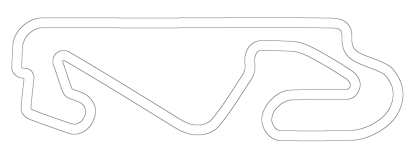
\includegraphics[interpolate=true,width=4.160000in,height=1.570000in]{contents/chapt6/figs/racing/esp-img0.png}}%
\end{pgfscope}%
\begin{pgfscope}%
\pgfpathrectangle{\pgfqpoint{0.150000in}{0.485000in}}{\pgfqpoint{4.160000in}{1.560000in}}%
\pgfusepath{clip}%
\pgfsetrectcap%
\pgfsetroundjoin%
\pgfsetlinewidth{1.003750pt}%
\definecolor{currentstroke}{rgb}{0.452941,0.073853,0.999317}%
\pgfsetstrokecolor{currentstroke}%
\pgfsetstrokeopacity{0.800000}%
\pgfsetdash{}{0pt}%
\pgfpathmoveto{\pgfqpoint{1.480105in}{1.831526in}}%
\pgfpathlineto{\pgfqpoint{1.481747in}{1.831526in}}%
\pgfusepath{stroke}%
\end{pgfscope}%
\begin{pgfscope}%
\pgfpathrectangle{\pgfqpoint{0.150000in}{0.485000in}}{\pgfqpoint{4.160000in}{1.560000in}}%
\pgfusepath{clip}%
\pgfsetrectcap%
\pgfsetroundjoin%
\pgfsetlinewidth{1.003750pt}%
\definecolor{currentstroke}{rgb}{0.405882,0.147302,0.997269}%
\pgfsetstrokecolor{currentstroke}%
\pgfsetstrokeopacity{0.800000}%
\pgfsetdash{}{0pt}%
\pgfpathmoveto{\pgfqpoint{1.481747in}{1.831526in}}%
\pgfpathlineto{\pgfqpoint{1.483416in}{1.831526in}}%
\pgfusepath{stroke}%
\end{pgfscope}%
\begin{pgfscope}%
\pgfpathrectangle{\pgfqpoint{0.150000in}{0.485000in}}{\pgfqpoint{4.160000in}{1.560000in}}%
\pgfusepath{clip}%
\pgfsetrectcap%
\pgfsetroundjoin%
\pgfsetlinewidth{1.003750pt}%
\definecolor{currentstroke}{rgb}{0.358824,0.219946,0.993859}%
\pgfsetstrokecolor{currentstroke}%
\pgfsetstrokeopacity{0.800000}%
\pgfsetdash{}{0pt}%
\pgfpathmoveto{\pgfqpoint{1.483416in}{1.831526in}}%
\pgfpathlineto{\pgfqpoint{1.485111in}{1.831523in}}%
\pgfusepath{stroke}%
\end{pgfscope}%
\begin{pgfscope}%
\pgfpathrectangle{\pgfqpoint{0.150000in}{0.485000in}}{\pgfqpoint{4.160000in}{1.560000in}}%
\pgfusepath{clip}%
\pgfsetrectcap%
\pgfsetroundjoin%
\pgfsetlinewidth{1.003750pt}%
\definecolor{currentstroke}{rgb}{0.319608,0.279583,0.989980}%
\pgfsetstrokecolor{currentstroke}%
\pgfsetstrokeopacity{0.800000}%
\pgfsetdash{}{0pt}%
\pgfpathmoveto{\pgfqpoint{1.485111in}{1.831523in}}%
\pgfpathlineto{\pgfqpoint{1.486830in}{1.831512in}}%
\pgfusepath{stroke}%
\end{pgfscope}%
\begin{pgfscope}%
\pgfpathrectangle{\pgfqpoint{0.150000in}{0.485000in}}{\pgfqpoint{4.160000in}{1.560000in}}%
\pgfusepath{clip}%
\pgfsetrectcap%
\pgfsetroundjoin%
\pgfsetlinewidth{1.003750pt}%
\definecolor{currentstroke}{rgb}{0.280392,0.338158,0.985162}%
\pgfsetstrokecolor{currentstroke}%
\pgfsetstrokeopacity{0.800000}%
\pgfsetdash{}{0pt}%
\pgfpathmoveto{\pgfqpoint{1.486830in}{1.831512in}}%
\pgfpathlineto{\pgfqpoint{1.488574in}{1.831491in}}%
\pgfusepath{stroke}%
\end{pgfscope}%
\begin{pgfscope}%
\pgfpathrectangle{\pgfqpoint{0.150000in}{0.485000in}}{\pgfqpoint{4.160000in}{1.560000in}}%
\pgfusepath{clip}%
\pgfsetrectcap%
\pgfsetroundjoin%
\pgfsetlinewidth{1.003750pt}%
\definecolor{currentstroke}{rgb}{0.233333,0.406737,0.978148}%
\pgfsetstrokecolor{currentstroke}%
\pgfsetstrokeopacity{0.800000}%
\pgfsetdash{}{0pt}%
\pgfpathmoveto{\pgfqpoint{1.488574in}{1.831491in}}%
\pgfpathlineto{\pgfqpoint{1.490339in}{1.831464in}}%
\pgfusepath{stroke}%
\end{pgfscope}%
\begin{pgfscope}%
\pgfpathrectangle{\pgfqpoint{0.150000in}{0.485000in}}{\pgfqpoint{4.160000in}{1.560000in}}%
\pgfusepath{clip}%
\pgfsetrectcap%
\pgfsetroundjoin%
\pgfsetlinewidth{1.003750pt}%
\definecolor{currentstroke}{rgb}{0.194118,0.462204,0.971281}%
\pgfsetstrokecolor{currentstroke}%
\pgfsetstrokeopacity{0.800000}%
\pgfsetdash{}{0pt}%
\pgfpathmoveto{\pgfqpoint{1.490339in}{1.831464in}}%
\pgfpathlineto{\pgfqpoint{1.492131in}{1.831426in}}%
\pgfusepath{stroke}%
\end{pgfscope}%
\begin{pgfscope}%
\pgfpathrectangle{\pgfqpoint{0.150000in}{0.485000in}}{\pgfqpoint{4.160000in}{1.560000in}}%
\pgfusepath{clip}%
\pgfsetrectcap%
\pgfsetroundjoin%
\pgfsetlinewidth{1.003750pt}%
\definecolor{currentstroke}{rgb}{0.147059,0.526432,0.961826}%
\pgfsetstrokecolor{currentstroke}%
\pgfsetstrokeopacity{0.800000}%
\pgfsetdash{}{0pt}%
\pgfpathmoveto{\pgfqpoint{1.492131in}{1.831426in}}%
\pgfpathlineto{\pgfqpoint{1.493943in}{1.831382in}}%
\pgfusepath{stroke}%
\end{pgfscope}%
\begin{pgfscope}%
\pgfpathrectangle{\pgfqpoint{0.150000in}{0.485000in}}{\pgfqpoint{4.160000in}{1.560000in}}%
\pgfusepath{clip}%
\pgfsetrectcap%
\pgfsetroundjoin%
\pgfsetlinewidth{1.003750pt}%
\definecolor{currentstroke}{rgb}{0.115686,0.567675,0.954791}%
\pgfsetstrokecolor{currentstroke}%
\pgfsetstrokeopacity{0.800000}%
\pgfsetdash{}{0pt}%
\pgfpathmoveto{\pgfqpoint{1.493943in}{1.831382in}}%
\pgfpathlineto{\pgfqpoint{1.495778in}{1.831326in}}%
\pgfusepath{stroke}%
\end{pgfscope}%
\begin{pgfscope}%
\pgfpathrectangle{\pgfqpoint{0.150000in}{0.485000in}}{\pgfqpoint{4.160000in}{1.560000in}}%
\pgfusepath{clip}%
\pgfsetrectcap%
\pgfsetroundjoin%
\pgfsetlinewidth{1.003750pt}%
\definecolor{currentstroke}{rgb}{0.076471,0.617278,0.945184}%
\pgfsetstrokecolor{currentstroke}%
\pgfsetstrokeopacity{0.800000}%
\pgfsetdash{}{0pt}%
\pgfpathmoveto{\pgfqpoint{1.495778in}{1.831326in}}%
\pgfpathlineto{\pgfqpoint{1.497632in}{1.831263in}}%
\pgfusepath{stroke}%
\end{pgfscope}%
\begin{pgfscope}%
\pgfpathrectangle{\pgfqpoint{0.150000in}{0.485000in}}{\pgfqpoint{4.160000in}{1.560000in}}%
\pgfusepath{clip}%
\pgfsetrectcap%
\pgfsetroundjoin%
\pgfsetlinewidth{1.003750pt}%
\definecolor{currentstroke}{rgb}{0.029412,0.673696,0.932472}%
\pgfsetstrokecolor{currentstroke}%
\pgfsetstrokeopacity{0.800000}%
\pgfsetdash{}{0pt}%
\pgfpathmoveto{\pgfqpoint{1.497632in}{1.831263in}}%
\pgfpathlineto{\pgfqpoint{1.499508in}{1.831187in}}%
\pgfusepath{stroke}%
\end{pgfscope}%
\begin{pgfscope}%
\pgfpathrectangle{\pgfqpoint{0.150000in}{0.485000in}}{\pgfqpoint{4.160000in}{1.560000in}}%
\pgfusepath{clip}%
\pgfsetrectcap%
\pgfsetroundjoin%
\pgfsetlinewidth{1.003750pt}%
\definecolor{currentstroke}{rgb}{0.017647,0.726434,0.918487}%
\pgfsetstrokecolor{currentstroke}%
\pgfsetstrokeopacity{0.800000}%
\pgfsetdash{}{0pt}%
\pgfpathmoveto{\pgfqpoint{1.499508in}{1.831187in}}%
\pgfpathlineto{\pgfqpoint{1.501408in}{1.831103in}}%
\pgfusepath{stroke}%
\end{pgfscope}%
\begin{pgfscope}%
\pgfpathrectangle{\pgfqpoint{0.150000in}{0.485000in}}{\pgfqpoint{4.160000in}{1.560000in}}%
\pgfusepath{clip}%
\pgfsetrectcap%
\pgfsetroundjoin%
\pgfsetlinewidth{1.003750pt}%
\definecolor{currentstroke}{rgb}{0.064706,0.775204,0.903247}%
\pgfsetstrokecolor{currentstroke}%
\pgfsetstrokeopacity{0.800000}%
\pgfsetdash{}{0pt}%
\pgfpathmoveto{\pgfqpoint{1.501408in}{1.831103in}}%
\pgfpathlineto{\pgfqpoint{1.503333in}{1.831013in}}%
\pgfusepath{stroke}%
\end{pgfscope}%
\begin{pgfscope}%
\pgfpathrectangle{\pgfqpoint{0.150000in}{0.485000in}}{\pgfqpoint{4.160000in}{1.560000in}}%
\pgfusepath{clip}%
\pgfsetrectcap%
\pgfsetroundjoin%
\pgfsetlinewidth{1.003750pt}%
\definecolor{currentstroke}{rgb}{0.111765,0.819740,0.886774}%
\pgfsetstrokecolor{currentstroke}%
\pgfsetstrokeopacity{0.800000}%
\pgfsetdash{}{0pt}%
\pgfpathmoveto{\pgfqpoint{1.503333in}{1.831013in}}%
\pgfpathlineto{\pgfqpoint{1.505284in}{1.830920in}}%
\pgfusepath{stroke}%
\end{pgfscope}%
\begin{pgfscope}%
\pgfpathrectangle{\pgfqpoint{0.150000in}{0.485000in}}{\pgfqpoint{4.160000in}{1.560000in}}%
\pgfusepath{clip}%
\pgfsetrectcap%
\pgfsetroundjoin%
\pgfsetlinewidth{1.003750pt}%
\definecolor{currentstroke}{rgb}{0.158824,0.859800,0.869089}%
\pgfsetstrokecolor{currentstroke}%
\pgfsetstrokeopacity{0.800000}%
\pgfsetdash{}{0pt}%
\pgfpathmoveto{\pgfqpoint{1.505284in}{1.830920in}}%
\pgfpathlineto{\pgfqpoint{1.507261in}{1.830820in}}%
\pgfusepath{stroke}%
\end{pgfscope}%
\begin{pgfscope}%
\pgfpathrectangle{\pgfqpoint{0.150000in}{0.485000in}}{\pgfqpoint{4.160000in}{1.560000in}}%
\pgfusepath{clip}%
\pgfsetrectcap%
\pgfsetroundjoin%
\pgfsetlinewidth{1.003750pt}%
\definecolor{currentstroke}{rgb}{0.198039,0.889604,0.853444}%
\pgfsetstrokecolor{currentstroke}%
\pgfsetstrokeopacity{0.800000}%
\pgfsetdash{}{0pt}%
\pgfpathmoveto{\pgfqpoint{1.507261in}{1.830820in}}%
\pgfpathlineto{\pgfqpoint{1.509259in}{1.830717in}}%
\pgfusepath{stroke}%
\end{pgfscope}%
\begin{pgfscope}%
\pgfpathrectangle{\pgfqpoint{0.150000in}{0.485000in}}{\pgfqpoint{4.160000in}{1.560000in}}%
\pgfusepath{clip}%
\pgfsetrectcap%
\pgfsetroundjoin%
\pgfsetlinewidth{1.003750pt}%
\definecolor{currentstroke}{rgb}{0.237255,0.916034,0.836989}%
\pgfsetstrokecolor{currentstroke}%
\pgfsetstrokeopacity{0.800000}%
\pgfsetdash{}{0pt}%
\pgfpathmoveto{\pgfqpoint{1.509259in}{1.830717in}}%
\pgfpathlineto{\pgfqpoint{1.511281in}{1.830606in}}%
\pgfusepath{stroke}%
\end{pgfscope}%
\begin{pgfscope}%
\pgfpathrectangle{\pgfqpoint{0.150000in}{0.485000in}}{\pgfqpoint{4.160000in}{1.560000in}}%
\pgfusepath{clip}%
\pgfsetrectcap%
\pgfsetroundjoin%
\pgfsetlinewidth{1.003750pt}%
\definecolor{currentstroke}{rgb}{0.276471,0.938988,0.819740}%
\pgfsetstrokecolor{currentstroke}%
\pgfsetstrokeopacity{0.800000}%
\pgfsetdash{}{0pt}%
\pgfpathmoveto{\pgfqpoint{1.511281in}{1.830606in}}%
\pgfpathlineto{\pgfqpoint{1.513325in}{1.830493in}}%
\pgfusepath{stroke}%
\end{pgfscope}%
\begin{pgfscope}%
\pgfpathrectangle{\pgfqpoint{0.150000in}{0.485000in}}{\pgfqpoint{4.160000in}{1.560000in}}%
\pgfusepath{clip}%
\pgfsetrectcap%
\pgfsetroundjoin%
\pgfsetlinewidth{1.003750pt}%
\definecolor{currentstroke}{rgb}{0.315686,0.958381,0.801714}%
\pgfsetstrokecolor{currentstroke}%
\pgfsetstrokeopacity{0.800000}%
\pgfsetdash{}{0pt}%
\pgfpathmoveto{\pgfqpoint{1.513325in}{1.830493in}}%
\pgfpathlineto{\pgfqpoint{1.515390in}{1.830372in}}%
\pgfusepath{stroke}%
\end{pgfscope}%
\begin{pgfscope}%
\pgfpathrectangle{\pgfqpoint{0.150000in}{0.485000in}}{\pgfqpoint{4.160000in}{1.560000in}}%
\pgfusepath{clip}%
\pgfsetrectcap%
\pgfsetroundjoin%
\pgfsetlinewidth{1.003750pt}%
\definecolor{currentstroke}{rgb}{0.354902,0.974139,0.782928}%
\pgfsetstrokecolor{currentstroke}%
\pgfsetstrokeopacity{0.800000}%
\pgfsetdash{}{0pt}%
\pgfpathmoveto{\pgfqpoint{1.515390in}{1.830372in}}%
\pgfpathlineto{\pgfqpoint{1.517476in}{1.830249in}}%
\pgfusepath{stroke}%
\end{pgfscope}%
\begin{pgfscope}%
\pgfpathrectangle{\pgfqpoint{0.150000in}{0.485000in}}{\pgfqpoint{4.160000in}{1.560000in}}%
\pgfusepath{clip}%
\pgfsetrectcap%
\pgfsetroundjoin%
\pgfsetlinewidth{1.003750pt}%
\definecolor{currentstroke}{rgb}{0.386275,0.984086,0.767363}%
\pgfsetstrokecolor{currentstroke}%
\pgfsetstrokeopacity{0.800000}%
\pgfsetdash{}{0pt}%
\pgfpathmoveto{\pgfqpoint{1.517476in}{1.830249in}}%
\pgfpathlineto{\pgfqpoint{1.519583in}{1.830119in}}%
\pgfusepath{stroke}%
\end{pgfscope}%
\begin{pgfscope}%
\pgfpathrectangle{\pgfqpoint{0.150000in}{0.485000in}}{\pgfqpoint{4.160000in}{1.560000in}}%
\pgfusepath{clip}%
\pgfsetrectcap%
\pgfsetroundjoin%
\pgfsetlinewidth{1.003750pt}%
\definecolor{currentstroke}{rgb}{0.425490,0.993159,0.747253}%
\pgfsetstrokecolor{currentstroke}%
\pgfsetstrokeopacity{0.800000}%
\pgfsetdash{}{0pt}%
\pgfpathmoveto{\pgfqpoint{1.519583in}{1.830119in}}%
\pgfpathlineto{\pgfqpoint{1.521708in}{1.829986in}}%
\pgfusepath{stroke}%
\end{pgfscope}%
\begin{pgfscope}%
\pgfpathrectangle{\pgfqpoint{0.150000in}{0.485000in}}{\pgfqpoint{4.160000in}{1.560000in}}%
\pgfusepath{clip}%
\pgfsetrectcap%
\pgfsetroundjoin%
\pgfsetlinewidth{1.003750pt}%
\definecolor{currentstroke}{rgb}{0.449020,0.996795,0.734845}%
\pgfsetstrokecolor{currentstroke}%
\pgfsetstrokeopacity{0.800000}%
\pgfsetdash{}{0pt}%
\pgfpathmoveto{\pgfqpoint{1.521708in}{1.829986in}}%
\pgfpathlineto{\pgfqpoint{1.523850in}{1.829854in}}%
\pgfusepath{stroke}%
\end{pgfscope}%
\begin{pgfscope}%
\pgfpathrectangle{\pgfqpoint{0.150000in}{0.485000in}}{\pgfqpoint{4.160000in}{1.560000in}}%
\pgfusepath{clip}%
\pgfsetrectcap%
\pgfsetroundjoin%
\pgfsetlinewidth{1.003750pt}%
\definecolor{currentstroke}{rgb}{0.472549,0.999070,0.722186}%
\pgfsetstrokecolor{currentstroke}%
\pgfsetstrokeopacity{0.800000}%
\pgfsetdash{}{0pt}%
\pgfpathmoveto{\pgfqpoint{1.523850in}{1.829854in}}%
\pgfpathlineto{\pgfqpoint{1.526008in}{1.829728in}}%
\pgfusepath{stroke}%
\end{pgfscope}%
\begin{pgfscope}%
\pgfpathrectangle{\pgfqpoint{0.150000in}{0.485000in}}{\pgfqpoint{4.160000in}{1.560000in}}%
\pgfusepath{clip}%
\pgfsetrectcap%
\pgfsetroundjoin%
\pgfsetlinewidth{1.003750pt}%
\definecolor{currentstroke}{rgb}{0.496078,0.999981,0.709281}%
\pgfsetstrokecolor{currentstroke}%
\pgfsetstrokeopacity{0.800000}%
\pgfsetdash{}{0pt}%
\pgfpathmoveto{\pgfqpoint{1.526008in}{1.829728in}}%
\pgfpathlineto{\pgfqpoint{1.528180in}{1.829611in}}%
\pgfusepath{stroke}%
\end{pgfscope}%
\begin{pgfscope}%
\pgfpathrectangle{\pgfqpoint{0.150000in}{0.485000in}}{\pgfqpoint{4.160000in}{1.560000in}}%
\pgfusepath{clip}%
\pgfsetrectcap%
\pgfsetroundjoin%
\pgfsetlinewidth{1.003750pt}%
\definecolor{currentstroke}{rgb}{0.527451,0.999070,0.691698}%
\pgfsetstrokecolor{currentstroke}%
\pgfsetstrokeopacity{0.800000}%
\pgfsetdash{}{0pt}%
\pgfpathmoveto{\pgfqpoint{1.528180in}{1.829611in}}%
\pgfpathlineto{\pgfqpoint{1.530366in}{1.829498in}}%
\pgfusepath{stroke}%
\end{pgfscope}%
\begin{pgfscope}%
\pgfpathrectangle{\pgfqpoint{0.150000in}{0.485000in}}{\pgfqpoint{4.160000in}{1.560000in}}%
\pgfusepath{clip}%
\pgfsetrectcap%
\pgfsetroundjoin%
\pgfsetlinewidth{1.003750pt}%
\definecolor{currentstroke}{rgb}{0.550980,0.996795,0.678235}%
\pgfsetstrokecolor{currentstroke}%
\pgfsetstrokeopacity{0.800000}%
\pgfsetdash{}{0pt}%
\pgfpathmoveto{\pgfqpoint{1.530366in}{1.829498in}}%
\pgfpathlineto{\pgfqpoint{1.532567in}{1.829395in}}%
\pgfusepath{stroke}%
\end{pgfscope}%
\begin{pgfscope}%
\pgfpathrectangle{\pgfqpoint{0.150000in}{0.485000in}}{\pgfqpoint{4.160000in}{1.560000in}}%
\pgfusepath{clip}%
\pgfsetrectcap%
\pgfsetroundjoin%
\pgfsetlinewidth{1.003750pt}%
\definecolor{currentstroke}{rgb}{0.582353,0.991645,0.659925}%
\pgfsetstrokecolor{currentstroke}%
\pgfsetstrokeopacity{0.800000}%
\pgfsetdash{}{0pt}%
\pgfpathmoveto{\pgfqpoint{1.532567in}{1.829395in}}%
\pgfpathlineto{\pgfqpoint{1.534784in}{1.829297in}}%
\pgfusepath{stroke}%
\end{pgfscope}%
\begin{pgfscope}%
\pgfpathrectangle{\pgfqpoint{0.150000in}{0.485000in}}{\pgfqpoint{4.160000in}{1.560000in}}%
\pgfusepath{clip}%
\pgfsetrectcap%
\pgfsetroundjoin%
\pgfsetlinewidth{1.003750pt}%
\definecolor{currentstroke}{rgb}{0.605882,0.986201,0.645928}%
\pgfsetstrokecolor{currentstroke}%
\pgfsetstrokeopacity{0.800000}%
\pgfsetdash{}{0pt}%
\pgfpathmoveto{\pgfqpoint{1.534784in}{1.829297in}}%
\pgfpathlineto{\pgfqpoint{1.537017in}{1.829211in}}%
\pgfusepath{stroke}%
\end{pgfscope}%
\begin{pgfscope}%
\pgfpathrectangle{\pgfqpoint{0.150000in}{0.485000in}}{\pgfqpoint{4.160000in}{1.560000in}}%
\pgfusepath{clip}%
\pgfsetrectcap%
\pgfsetroundjoin%
\pgfsetlinewidth{1.003750pt}%
\definecolor{currentstroke}{rgb}{0.629412,0.979410,0.631711}%
\pgfsetstrokecolor{currentstroke}%
\pgfsetstrokeopacity{0.800000}%
\pgfsetdash{}{0pt}%
\pgfpathmoveto{\pgfqpoint{1.537017in}{1.829211in}}%
\pgfpathlineto{\pgfqpoint{1.539261in}{1.829132in}}%
\pgfusepath{stroke}%
\end{pgfscope}%
\begin{pgfscope}%
\pgfpathrectangle{\pgfqpoint{0.150000in}{0.485000in}}{\pgfqpoint{4.160000in}{1.560000in}}%
\pgfusepath{clip}%
\pgfsetrectcap%
\pgfsetroundjoin%
\pgfsetlinewidth{1.003750pt}%
\definecolor{currentstroke}{rgb}{0.660784,0.968276,0.612420}%
\pgfsetstrokecolor{currentstroke}%
\pgfsetstrokeopacity{0.800000}%
\pgfsetdash{}{0pt}%
\pgfpathmoveto{\pgfqpoint{1.539261in}{1.829132in}}%
\pgfpathlineto{\pgfqpoint{1.541520in}{1.829066in}}%
\pgfusepath{stroke}%
\end{pgfscope}%
\begin{pgfscope}%
\pgfpathrectangle{\pgfqpoint{0.150000in}{0.485000in}}{\pgfqpoint{4.160000in}{1.560000in}}%
\pgfusepath{clip}%
\pgfsetrectcap%
\pgfsetroundjoin%
\pgfsetlinewidth{1.003750pt}%
\definecolor{currentstroke}{rgb}{0.684314,0.958381,0.597707}%
\pgfsetstrokecolor{currentstroke}%
\pgfsetstrokeopacity{0.800000}%
\pgfsetdash{}{0pt}%
\pgfpathmoveto{\pgfqpoint{1.541520in}{1.829066in}}%
\pgfpathlineto{\pgfqpoint{1.543794in}{1.829009in}}%
\pgfusepath{stroke}%
\end{pgfscope}%
\begin{pgfscope}%
\pgfpathrectangle{\pgfqpoint{0.150000in}{0.485000in}}{\pgfqpoint{4.160000in}{1.560000in}}%
\pgfusepath{clip}%
\pgfsetrectcap%
\pgfsetroundjoin%
\pgfsetlinewidth{1.003750pt}%
\definecolor{currentstroke}{rgb}{0.707843,0.947177,0.582791}%
\pgfsetstrokecolor{currentstroke}%
\pgfsetstrokeopacity{0.800000}%
\pgfsetdash{}{0pt}%
\pgfpathmoveto{\pgfqpoint{1.543794in}{1.829009in}}%
\pgfpathlineto{\pgfqpoint{1.546082in}{1.828958in}}%
\pgfusepath{stroke}%
\end{pgfscope}%
\begin{pgfscope}%
\pgfpathrectangle{\pgfqpoint{0.150000in}{0.485000in}}{\pgfqpoint{4.160000in}{1.560000in}}%
\pgfusepath{clip}%
\pgfsetrectcap%
\pgfsetroundjoin%
\pgfsetlinewidth{1.003750pt}%
\definecolor{currentstroke}{rgb}{0.739216,0.930229,0.562593}%
\pgfsetstrokecolor{currentstroke}%
\pgfsetstrokeopacity{0.800000}%
\pgfsetdash{}{0pt}%
\pgfpathmoveto{\pgfqpoint{1.546082in}{1.828958in}}%
\pgfpathlineto{\pgfqpoint{1.548386in}{1.828911in}}%
\pgfusepath{stroke}%
\end{pgfscope}%
\begin{pgfscope}%
\pgfpathrectangle{\pgfqpoint{0.150000in}{0.485000in}}{\pgfqpoint{4.160000in}{1.560000in}}%
\pgfusepath{clip}%
\pgfsetrectcap%
\pgfsetroundjoin%
\pgfsetlinewidth{1.003750pt}%
\definecolor{currentstroke}{rgb}{0.754902,0.920906,0.552365}%
\pgfsetstrokecolor{currentstroke}%
\pgfsetstrokeopacity{0.800000}%
\pgfsetdash{}{0pt}%
\pgfpathmoveto{\pgfqpoint{1.548386in}{1.828911in}}%
\pgfpathlineto{\pgfqpoint{1.550703in}{1.828865in}}%
\pgfusepath{stroke}%
\end{pgfscope}%
\begin{pgfscope}%
\pgfpathrectangle{\pgfqpoint{0.150000in}{0.485000in}}{\pgfqpoint{4.160000in}{1.560000in}}%
\pgfusepath{clip}%
\pgfsetrectcap%
\pgfsetroundjoin%
\pgfsetlinewidth{1.003750pt}%
\definecolor{currentstroke}{rgb}{0.778431,0.905873,0.536867}%
\pgfsetstrokecolor{currentstroke}%
\pgfsetstrokeopacity{0.800000}%
\pgfsetdash{}{0pt}%
\pgfpathmoveto{\pgfqpoint{1.550703in}{1.828865in}}%
\pgfpathlineto{\pgfqpoint{1.553033in}{1.828816in}}%
\pgfusepath{stroke}%
\end{pgfscope}%
\begin{pgfscope}%
\pgfpathrectangle{\pgfqpoint{0.150000in}{0.485000in}}{\pgfqpoint{4.160000in}{1.560000in}}%
\pgfusepath{clip}%
\pgfsetrectcap%
\pgfsetroundjoin%
\pgfsetlinewidth{1.003750pt}%
\definecolor{currentstroke}{rgb}{0.801961,0.889604,0.521185}%
\pgfsetstrokecolor{currentstroke}%
\pgfsetstrokeopacity{0.800000}%
\pgfsetdash{}{0pt}%
\pgfpathmoveto{\pgfqpoint{1.553033in}{1.828816in}}%
\pgfpathlineto{\pgfqpoint{1.555375in}{1.828768in}}%
\pgfusepath{stroke}%
\end{pgfscope}%
\begin{pgfscope}%
\pgfpathrectangle{\pgfqpoint{0.150000in}{0.485000in}}{\pgfqpoint{4.160000in}{1.560000in}}%
\pgfusepath{clip}%
\pgfsetrectcap%
\pgfsetroundjoin%
\pgfsetlinewidth{1.003750pt}%
\definecolor{currentstroke}{rgb}{0.817647,0.878081,0.510631}%
\pgfsetstrokecolor{currentstroke}%
\pgfsetstrokeopacity{0.800000}%
\pgfsetdash{}{0pt}%
\pgfpathmoveto{\pgfqpoint{1.555375in}{1.828768in}}%
\pgfpathlineto{\pgfqpoint{1.557727in}{1.828717in}}%
\pgfusepath{stroke}%
\end{pgfscope}%
\begin{pgfscope}%
\pgfpathrectangle{\pgfqpoint{0.150000in}{0.485000in}}{\pgfqpoint{4.160000in}{1.560000in}}%
\pgfusepath{clip}%
\pgfsetrectcap%
\pgfsetroundjoin%
\pgfsetlinewidth{1.003750pt}%
\definecolor{currentstroke}{rgb}{0.849020,0.853444,0.489293}%
\pgfsetstrokecolor{currentstroke}%
\pgfsetstrokeopacity{0.800000}%
\pgfsetdash{}{0pt}%
\pgfpathmoveto{\pgfqpoint{1.557727in}{1.828717in}}%
\pgfpathlineto{\pgfqpoint{1.560090in}{1.828667in}}%
\pgfusepath{stroke}%
\end{pgfscope}%
\begin{pgfscope}%
\pgfpathrectangle{\pgfqpoint{0.150000in}{0.485000in}}{\pgfqpoint{4.160000in}{1.560000in}}%
\pgfusepath{clip}%
\pgfsetrectcap%
\pgfsetroundjoin%
\pgfsetlinewidth{1.003750pt}%
\definecolor{currentstroke}{rgb}{0.872549,0.833602,0.473094}%
\pgfsetstrokecolor{currentstroke}%
\pgfsetstrokeopacity{0.800000}%
\pgfsetdash{}{0pt}%
\pgfpathmoveto{\pgfqpoint{1.560090in}{1.828667in}}%
\pgfpathlineto{\pgfqpoint{1.562468in}{1.828613in}}%
\pgfusepath{stroke}%
\end{pgfscope}%
\begin{pgfscope}%
\pgfpathrectangle{\pgfqpoint{0.150000in}{0.485000in}}{\pgfqpoint{4.160000in}{1.560000in}}%
\pgfusepath{clip}%
\pgfsetrectcap%
\pgfsetroundjoin%
\pgfsetlinewidth{1.003750pt}%
\definecolor{currentstroke}{rgb}{0.880392,0.826734,0.467658}%
\pgfsetstrokecolor{currentstroke}%
\pgfsetstrokeopacity{0.800000}%
\pgfsetdash{}{0pt}%
\pgfpathmoveto{\pgfqpoint{1.562468in}{1.828613in}}%
\pgfpathlineto{\pgfqpoint{1.564858in}{1.828557in}}%
\pgfusepath{stroke}%
\end{pgfscope}%
\begin{pgfscope}%
\pgfpathrectangle{\pgfqpoint{0.150000in}{0.485000in}}{\pgfqpoint{4.160000in}{1.560000in}}%
\pgfusepath{clip}%
\pgfsetrectcap%
\pgfsetroundjoin%
\pgfsetlinewidth{1.003750pt}%
\definecolor{currentstroke}{rgb}{0.903922,0.805381,0.451244}%
\pgfsetstrokecolor{currentstroke}%
\pgfsetstrokeopacity{0.800000}%
\pgfsetdash{}{0pt}%
\pgfpathmoveto{\pgfqpoint{1.564858in}{1.828557in}}%
\pgfpathlineto{\pgfqpoint{1.567255in}{1.828494in}}%
\pgfusepath{stroke}%
\end{pgfscope}%
\begin{pgfscope}%
\pgfpathrectangle{\pgfqpoint{0.150000in}{0.485000in}}{\pgfqpoint{4.160000in}{1.560000in}}%
\pgfusepath{clip}%
\pgfsetrectcap%
\pgfsetroundjoin%
\pgfsetlinewidth{1.003750pt}%
\definecolor{currentstroke}{rgb}{0.919608,0.790532,0.440216}%
\pgfsetstrokecolor{currentstroke}%
\pgfsetstrokeopacity{0.800000}%
\pgfsetdash{}{0pt}%
\pgfpathmoveto{\pgfqpoint{1.567255in}{1.828494in}}%
\pgfpathlineto{\pgfqpoint{1.569662in}{1.828429in}}%
\pgfusepath{stroke}%
\end{pgfscope}%
\begin{pgfscope}%
\pgfpathrectangle{\pgfqpoint{0.150000in}{0.485000in}}{\pgfqpoint{4.160000in}{1.560000in}}%
\pgfusepath{clip}%
\pgfsetrectcap%
\pgfsetroundjoin%
\pgfsetlinewidth{1.003750pt}%
\definecolor{currentstroke}{rgb}{0.943137,0.767363,0.423549}%
\pgfsetstrokecolor{currentstroke}%
\pgfsetstrokeopacity{0.800000}%
\pgfsetdash{}{0pt}%
\pgfpathmoveto{\pgfqpoint{1.569662in}{1.828429in}}%
\pgfpathlineto{\pgfqpoint{1.572079in}{1.828355in}}%
\pgfusepath{stroke}%
\end{pgfscope}%
\begin{pgfscope}%
\pgfpathrectangle{\pgfqpoint{0.150000in}{0.485000in}}{\pgfqpoint{4.160000in}{1.560000in}}%
\pgfusepath{clip}%
\pgfsetrectcap%
\pgfsetroundjoin%
\pgfsetlinewidth{1.003750pt}%
\definecolor{currentstroke}{rgb}{0.966667,0.743145,0.406737}%
\pgfsetstrokecolor{currentstroke}%
\pgfsetstrokeopacity{0.800000}%
\pgfsetdash{}{0pt}%
\pgfpathmoveto{\pgfqpoint{1.572079in}{1.828355in}}%
\pgfpathlineto{\pgfqpoint{1.574508in}{1.828277in}}%
\pgfusepath{stroke}%
\end{pgfscope}%
\begin{pgfscope}%
\pgfpathrectangle{\pgfqpoint{0.150000in}{0.485000in}}{\pgfqpoint{4.160000in}{1.560000in}}%
\pgfusepath{clip}%
\pgfsetrectcap%
\pgfsetroundjoin%
\pgfsetlinewidth{1.003750pt}%
\definecolor{currentstroke}{rgb}{0.982353,0.726434,0.395451}%
\pgfsetstrokecolor{currentstroke}%
\pgfsetstrokeopacity{0.800000}%
\pgfsetdash{}{0pt}%
\pgfpathmoveto{\pgfqpoint{1.574508in}{1.828277in}}%
\pgfpathlineto{\pgfqpoint{1.576949in}{1.828189in}}%
\pgfusepath{stroke}%
\end{pgfscope}%
\begin{pgfscope}%
\pgfpathrectangle{\pgfqpoint{0.150000in}{0.485000in}}{\pgfqpoint{4.160000in}{1.560000in}}%
\pgfusepath{clip}%
\pgfsetrectcap%
\pgfsetroundjoin%
\pgfsetlinewidth{1.003750pt}%
\definecolor{currentstroke}{rgb}{0.998039,0.709281,0.384106}%
\pgfsetstrokecolor{currentstroke}%
\pgfsetstrokeopacity{0.800000}%
\pgfsetdash{}{0pt}%
\pgfpathmoveto{\pgfqpoint{1.576949in}{1.828189in}}%
\pgfpathlineto{\pgfqpoint{1.579401in}{1.828094in}}%
\pgfusepath{stroke}%
\end{pgfscope}%
\begin{pgfscope}%
\pgfpathrectangle{\pgfqpoint{0.150000in}{0.485000in}}{\pgfqpoint{4.160000in}{1.560000in}}%
\pgfusepath{clip}%
\pgfsetrectcap%
\pgfsetroundjoin%
\pgfsetlinewidth{1.003750pt}%
\definecolor{currentstroke}{rgb}{1.000000,0.691698,0.372702}%
\pgfsetstrokecolor{currentstroke}%
\pgfsetstrokeopacity{0.800000}%
\pgfsetdash{}{0pt}%
\pgfpathmoveto{\pgfqpoint{1.579401in}{1.828094in}}%
\pgfpathlineto{\pgfqpoint{1.581859in}{1.827989in}}%
\pgfusepath{stroke}%
\end{pgfscope}%
\begin{pgfscope}%
\pgfpathrectangle{\pgfqpoint{0.150000in}{0.485000in}}{\pgfqpoint{4.160000in}{1.560000in}}%
\pgfusepath{clip}%
\pgfsetrectcap%
\pgfsetroundjoin%
\pgfsetlinewidth{1.003750pt}%
\definecolor{currentstroke}{rgb}{1.000000,0.673696,0.361242}%
\pgfsetstrokecolor{currentstroke}%
\pgfsetstrokeopacity{0.800000}%
\pgfsetdash{}{0pt}%
\pgfpathmoveto{\pgfqpoint{1.581859in}{1.827989in}}%
\pgfpathlineto{\pgfqpoint{1.584326in}{1.827867in}}%
\pgfusepath{stroke}%
\end{pgfscope}%
\begin{pgfscope}%
\pgfpathrectangle{\pgfqpoint{0.150000in}{0.485000in}}{\pgfqpoint{4.160000in}{1.560000in}}%
\pgfusepath{clip}%
\pgfsetrectcap%
\pgfsetroundjoin%
\pgfsetlinewidth{1.003750pt}%
\definecolor{currentstroke}{rgb}{1.000000,0.655284,0.349727}%
\pgfsetstrokecolor{currentstroke}%
\pgfsetstrokeopacity{0.800000}%
\pgfsetdash{}{0pt}%
\pgfpathmoveto{\pgfqpoint{1.584326in}{1.827867in}}%
\pgfpathlineto{\pgfqpoint{1.586800in}{1.827735in}}%
\pgfusepath{stroke}%
\end{pgfscope}%
\begin{pgfscope}%
\pgfpathrectangle{\pgfqpoint{0.150000in}{0.485000in}}{\pgfqpoint{4.160000in}{1.560000in}}%
\pgfusepath{clip}%
\pgfsetrectcap%
\pgfsetroundjoin%
\pgfsetlinewidth{1.003750pt}%
\definecolor{currentstroke}{rgb}{1.000000,0.645928,0.343949}%
\pgfsetstrokecolor{currentstroke}%
\pgfsetstrokeopacity{0.800000}%
\pgfsetdash{}{0pt}%
\pgfpathmoveto{\pgfqpoint{1.586800in}{1.827735in}}%
\pgfpathlineto{\pgfqpoint{1.589282in}{1.827586in}}%
\pgfusepath{stroke}%
\end{pgfscope}%
\begin{pgfscope}%
\pgfpathrectangle{\pgfqpoint{0.150000in}{0.485000in}}{\pgfqpoint{4.160000in}{1.560000in}}%
\pgfusepath{clip}%
\pgfsetrectcap%
\pgfsetroundjoin%
\pgfsetlinewidth{1.003750pt}%
\definecolor{currentstroke}{rgb}{1.000000,0.636474,0.338158}%
\pgfsetstrokecolor{currentstroke}%
\pgfsetstrokeopacity{0.800000}%
\pgfsetdash{}{0pt}%
\pgfpathmoveto{\pgfqpoint{1.589282in}{1.827586in}}%
\pgfpathlineto{\pgfqpoint{1.591766in}{1.827425in}}%
\pgfusepath{stroke}%
\end{pgfscope}%
\begin{pgfscope}%
\pgfpathrectangle{\pgfqpoint{0.150000in}{0.485000in}}{\pgfqpoint{4.160000in}{1.560000in}}%
\pgfusepath{clip}%
\pgfsetrectcap%
\pgfsetroundjoin%
\pgfsetlinewidth{1.003750pt}%
\definecolor{currentstroke}{rgb}{1.000000,0.617278,0.326539}%
\pgfsetstrokecolor{currentstroke}%
\pgfsetstrokeopacity{0.800000}%
\pgfsetdash{}{0pt}%
\pgfpathmoveto{\pgfqpoint{1.591766in}{1.827425in}}%
\pgfpathlineto{\pgfqpoint{1.594255in}{1.827254in}}%
\pgfusepath{stroke}%
\end{pgfscope}%
\begin{pgfscope}%
\pgfpathrectangle{\pgfqpoint{0.150000in}{0.485000in}}{\pgfqpoint{4.160000in}{1.560000in}}%
\pgfusepath{clip}%
\pgfsetrectcap%
\pgfsetroundjoin%
\pgfsetlinewidth{1.003750pt}%
\definecolor{currentstroke}{rgb}{1.000000,0.597707,0.314870}%
\pgfsetstrokecolor{currentstroke}%
\pgfsetstrokeopacity{0.800000}%
\pgfsetdash{}{0pt}%
\pgfpathmoveto{\pgfqpoint{1.594255in}{1.827254in}}%
\pgfpathlineto{\pgfqpoint{1.596753in}{1.827078in}}%
\pgfusepath{stroke}%
\end{pgfscope}%
\begin{pgfscope}%
\pgfpathrectangle{\pgfqpoint{0.150000in}{0.485000in}}{\pgfqpoint{4.160000in}{1.560000in}}%
\pgfusepath{clip}%
\pgfsetrectcap%
\pgfsetroundjoin%
\pgfsetlinewidth{1.003750pt}%
\definecolor{currentstroke}{rgb}{1.000000,0.597707,0.314870}%
\pgfsetstrokecolor{currentstroke}%
\pgfsetstrokeopacity{0.800000}%
\pgfsetdash{}{0pt}%
\pgfpathmoveto{\pgfqpoint{1.596753in}{1.827078in}}%
\pgfpathlineto{\pgfqpoint{1.599258in}{1.826898in}}%
\pgfusepath{stroke}%
\end{pgfscope}%
\begin{pgfscope}%
\pgfpathrectangle{\pgfqpoint{0.150000in}{0.485000in}}{\pgfqpoint{4.160000in}{1.560000in}}%
\pgfusepath{clip}%
\pgfsetrectcap%
\pgfsetroundjoin%
\pgfsetlinewidth{1.003750pt}%
\definecolor{currentstroke}{rgb}{1.000000,0.587785,0.309017}%
\pgfsetstrokecolor{currentstroke}%
\pgfsetstrokeopacity{0.800000}%
\pgfsetdash{}{0pt}%
\pgfpathmoveto{\pgfqpoint{1.599258in}{1.826898in}}%
\pgfpathlineto{\pgfqpoint{1.601766in}{1.826719in}}%
\pgfusepath{stroke}%
\end{pgfscope}%
\begin{pgfscope}%
\pgfpathrectangle{\pgfqpoint{0.150000in}{0.485000in}}{\pgfqpoint{4.160000in}{1.560000in}}%
\pgfusepath{clip}%
\pgfsetrectcap%
\pgfsetroundjoin%
\pgfsetlinewidth{1.003750pt}%
\definecolor{currentstroke}{rgb}{1.000000,0.577774,0.303153}%
\pgfsetstrokecolor{currentstroke}%
\pgfsetstrokeopacity{0.800000}%
\pgfsetdash{}{0pt}%
\pgfpathmoveto{\pgfqpoint{1.601766in}{1.826719in}}%
\pgfpathlineto{\pgfqpoint{1.604277in}{1.826545in}}%
\pgfusepath{stroke}%
\end{pgfscope}%
\begin{pgfscope}%
\pgfpathrectangle{\pgfqpoint{0.150000in}{0.485000in}}{\pgfqpoint{4.160000in}{1.560000in}}%
\pgfusepath{clip}%
\pgfsetrectcap%
\pgfsetroundjoin%
\pgfsetlinewidth{1.003750pt}%
\definecolor{currentstroke}{rgb}{1.000000,0.557489,0.291390}%
\pgfsetstrokecolor{currentstroke}%
\pgfsetstrokeopacity{0.800000}%
\pgfsetdash{}{0pt}%
\pgfpathmoveto{\pgfqpoint{1.604277in}{1.826545in}}%
\pgfpathlineto{\pgfqpoint{1.606793in}{1.826370in}}%
\pgfusepath{stroke}%
\end{pgfscope}%
\begin{pgfscope}%
\pgfpathrectangle{\pgfqpoint{0.150000in}{0.485000in}}{\pgfqpoint{4.160000in}{1.560000in}}%
\pgfusepath{clip}%
\pgfsetrectcap%
\pgfsetroundjoin%
\pgfsetlinewidth{1.003750pt}%
\definecolor{currentstroke}{rgb}{1.000000,0.557489,0.291390}%
\pgfsetstrokecolor{currentstroke}%
\pgfsetstrokeopacity{0.800000}%
\pgfsetdash{}{0pt}%
\pgfpathmoveto{\pgfqpoint{1.606793in}{1.826370in}}%
\pgfpathlineto{\pgfqpoint{1.609315in}{1.826201in}}%
\pgfusepath{stroke}%
\end{pgfscope}%
\begin{pgfscope}%
\pgfpathrectangle{\pgfqpoint{0.150000in}{0.485000in}}{\pgfqpoint{4.160000in}{1.560000in}}%
\pgfusepath{clip}%
\pgfsetrectcap%
\pgfsetroundjoin%
\pgfsetlinewidth{1.003750pt}%
\definecolor{currentstroke}{rgb}{1.000000,0.547220,0.285492}%
\pgfsetstrokecolor{currentstroke}%
\pgfsetstrokeopacity{0.800000}%
\pgfsetdash{}{0pt}%
\pgfpathmoveto{\pgfqpoint{1.609315in}{1.826201in}}%
\pgfpathlineto{\pgfqpoint{1.611841in}{1.826035in}}%
\pgfusepath{stroke}%
\end{pgfscope}%
\begin{pgfscope}%
\pgfpathrectangle{\pgfqpoint{0.150000in}{0.485000in}}{\pgfqpoint{4.160000in}{1.560000in}}%
\pgfusepath{clip}%
\pgfsetrectcap%
\pgfsetroundjoin%
\pgfsetlinewidth{1.003750pt}%
\definecolor{currentstroke}{rgb}{1.000000,0.547220,0.285492}%
\pgfsetstrokecolor{currentstroke}%
\pgfsetstrokeopacity{0.800000}%
\pgfsetdash{}{0pt}%
\pgfpathmoveto{\pgfqpoint{1.611841in}{1.826035in}}%
\pgfpathlineto{\pgfqpoint{1.614371in}{1.825876in}}%
\pgfusepath{stroke}%
\end{pgfscope}%
\begin{pgfscope}%
\pgfpathrectangle{\pgfqpoint{0.150000in}{0.485000in}}{\pgfqpoint{4.160000in}{1.560000in}}%
\pgfusepath{clip}%
\pgfsetrectcap%
\pgfsetroundjoin%
\pgfsetlinewidth{1.003750pt}%
\definecolor{currentstroke}{rgb}{1.000000,0.526432,0.273663}%
\pgfsetstrokecolor{currentstroke}%
\pgfsetstrokeopacity{0.800000}%
\pgfsetdash{}{0pt}%
\pgfpathmoveto{\pgfqpoint{1.614371in}{1.825876in}}%
\pgfpathlineto{\pgfqpoint{1.616902in}{1.825723in}}%
\pgfusepath{stroke}%
\end{pgfscope}%
\begin{pgfscope}%
\pgfpathrectangle{\pgfqpoint{0.150000in}{0.485000in}}{\pgfqpoint{4.160000in}{1.560000in}}%
\pgfusepath{clip}%
\pgfsetrectcap%
\pgfsetroundjoin%
\pgfsetlinewidth{1.003750pt}%
\definecolor{currentstroke}{rgb}{1.000000,0.526432,0.273663}%
\pgfsetstrokecolor{currentstroke}%
\pgfsetstrokeopacity{0.800000}%
\pgfsetdash{}{0pt}%
\pgfpathmoveto{\pgfqpoint{1.616902in}{1.825723in}}%
\pgfpathlineto{\pgfqpoint{1.619439in}{1.825572in}}%
\pgfusepath{stroke}%
\end{pgfscope}%
\begin{pgfscope}%
\pgfpathrectangle{\pgfqpoint{0.150000in}{0.485000in}}{\pgfqpoint{4.160000in}{1.560000in}}%
\pgfusepath{clip}%
\pgfsetrectcap%
\pgfsetroundjoin%
\pgfsetlinewidth{1.003750pt}%
\definecolor{currentstroke}{rgb}{1.000000,0.515918,0.267733}%
\pgfsetstrokecolor{currentstroke}%
\pgfsetstrokeopacity{0.800000}%
\pgfsetdash{}{0pt}%
\pgfpathmoveto{\pgfqpoint{1.619439in}{1.825572in}}%
\pgfpathlineto{\pgfqpoint{1.621979in}{1.825430in}}%
\pgfusepath{stroke}%
\end{pgfscope}%
\begin{pgfscope}%
\pgfpathrectangle{\pgfqpoint{0.150000in}{0.485000in}}{\pgfqpoint{4.160000in}{1.560000in}}%
\pgfusepath{clip}%
\pgfsetrectcap%
\pgfsetroundjoin%
\pgfsetlinewidth{1.003750pt}%
\definecolor{currentstroke}{rgb}{1.000000,0.494656,0.255843}%
\pgfsetstrokecolor{currentstroke}%
\pgfsetstrokeopacity{0.800000}%
\pgfsetdash{}{0pt}%
\pgfpathmoveto{\pgfqpoint{1.621979in}{1.825430in}}%
\pgfpathlineto{\pgfqpoint{1.624524in}{1.825294in}}%
\pgfusepath{stroke}%
\end{pgfscope}%
\begin{pgfscope}%
\pgfpathrectangle{\pgfqpoint{0.150000in}{0.485000in}}{\pgfqpoint{4.160000in}{1.560000in}}%
\pgfusepath{clip}%
\pgfsetrectcap%
\pgfsetroundjoin%
\pgfsetlinewidth{1.003750pt}%
\definecolor{currentstroke}{rgb}{1.000000,0.505325,0.261793}%
\pgfsetstrokecolor{currentstroke}%
\pgfsetstrokeopacity{0.800000}%
\pgfsetdash{}{0pt}%
\pgfpathmoveto{\pgfqpoint{1.624524in}{1.825294in}}%
\pgfpathlineto{\pgfqpoint{1.627074in}{1.825169in}}%
\pgfusepath{stroke}%
\end{pgfscope}%
\begin{pgfscope}%
\pgfpathrectangle{\pgfqpoint{0.150000in}{0.485000in}}{\pgfqpoint{4.160000in}{1.560000in}}%
\pgfusepath{clip}%
\pgfsetrectcap%
\pgfsetroundjoin%
\pgfsetlinewidth{1.003750pt}%
\definecolor{currentstroke}{rgb}{1.000000,0.494656,0.255843}%
\pgfsetstrokecolor{currentstroke}%
\pgfsetstrokeopacity{0.800000}%
\pgfsetdash{}{0pt}%
\pgfpathmoveto{\pgfqpoint{1.627074in}{1.825169in}}%
\pgfpathlineto{\pgfqpoint{1.629624in}{1.825052in}}%
\pgfusepath{stroke}%
\end{pgfscope}%
\begin{pgfscope}%
\pgfpathrectangle{\pgfqpoint{0.150000in}{0.485000in}}{\pgfqpoint{4.160000in}{1.560000in}}%
\pgfusepath{clip}%
\pgfsetrectcap%
\pgfsetroundjoin%
\pgfsetlinewidth{1.003750pt}%
\definecolor{currentstroke}{rgb}{1.000000,0.494656,0.255843}%
\pgfsetstrokecolor{currentstroke}%
\pgfsetstrokeopacity{0.800000}%
\pgfsetdash{}{0pt}%
\pgfpathmoveto{\pgfqpoint{1.629624in}{1.825052in}}%
\pgfpathlineto{\pgfqpoint{1.632176in}{1.824949in}}%
\pgfusepath{stroke}%
\end{pgfscope}%
\begin{pgfscope}%
\pgfpathrectangle{\pgfqpoint{0.150000in}{0.485000in}}{\pgfqpoint{4.160000in}{1.560000in}}%
\pgfusepath{clip}%
\pgfsetrectcap%
\pgfsetroundjoin%
\pgfsetlinewidth{1.003750pt}%
\definecolor{currentstroke}{rgb}{1.000000,0.494656,0.255843}%
\pgfsetstrokecolor{currentstroke}%
\pgfsetstrokeopacity{0.800000}%
\pgfsetdash{}{0pt}%
\pgfpathmoveto{\pgfqpoint{1.632176in}{1.824949in}}%
\pgfpathlineto{\pgfqpoint{1.634727in}{1.824855in}}%
\pgfusepath{stroke}%
\end{pgfscope}%
\begin{pgfscope}%
\pgfpathrectangle{\pgfqpoint{0.150000in}{0.485000in}}{\pgfqpoint{4.160000in}{1.560000in}}%
\pgfusepath{clip}%
\pgfsetrectcap%
\pgfsetroundjoin%
\pgfsetlinewidth{1.003750pt}%
\definecolor{currentstroke}{rgb}{1.000000,0.483911,0.249883}%
\pgfsetstrokecolor{currentstroke}%
\pgfsetstrokeopacity{0.800000}%
\pgfsetdash{}{0pt}%
\pgfpathmoveto{\pgfqpoint{1.634727in}{1.824855in}}%
\pgfpathlineto{\pgfqpoint{1.637282in}{1.824775in}}%
\pgfusepath{stroke}%
\end{pgfscope}%
\begin{pgfscope}%
\pgfpathrectangle{\pgfqpoint{0.150000in}{0.485000in}}{\pgfqpoint{4.160000in}{1.560000in}}%
\pgfusepath{clip}%
\pgfsetrectcap%
\pgfsetroundjoin%
\pgfsetlinewidth{1.003750pt}%
\definecolor{currentstroke}{rgb}{1.000000,0.483911,0.249883}%
\pgfsetstrokecolor{currentstroke}%
\pgfsetstrokeopacity{0.800000}%
\pgfsetdash{}{0pt}%
\pgfpathmoveto{\pgfqpoint{1.637282in}{1.824775in}}%
\pgfpathlineto{\pgfqpoint{1.639839in}{1.824714in}}%
\pgfusepath{stroke}%
\end{pgfscope}%
\begin{pgfscope}%
\pgfpathrectangle{\pgfqpoint{0.150000in}{0.485000in}}{\pgfqpoint{4.160000in}{1.560000in}}%
\pgfusepath{clip}%
\pgfsetrectcap%
\pgfsetroundjoin%
\pgfsetlinewidth{1.003750pt}%
\definecolor{currentstroke}{rgb}{1.000000,0.462204,0.237935}%
\pgfsetstrokecolor{currentstroke}%
\pgfsetstrokeopacity{0.800000}%
\pgfsetdash{}{0pt}%
\pgfpathmoveto{\pgfqpoint{1.639839in}{1.824714in}}%
\pgfpathlineto{\pgfqpoint{1.642399in}{1.824668in}}%
\pgfusepath{stroke}%
\end{pgfscope}%
\begin{pgfscope}%
\pgfpathrectangle{\pgfqpoint{0.150000in}{0.485000in}}{\pgfqpoint{4.160000in}{1.560000in}}%
\pgfusepath{clip}%
\pgfsetrectcap%
\pgfsetroundjoin%
\pgfsetlinewidth{1.003750pt}%
\definecolor{currentstroke}{rgb}{1.000000,0.451244,0.231948}%
\pgfsetstrokecolor{currentstroke}%
\pgfsetstrokeopacity{0.800000}%
\pgfsetdash{}{0pt}%
\pgfpathmoveto{\pgfqpoint{1.642399in}{1.824668in}}%
\pgfpathlineto{\pgfqpoint{1.644966in}{1.824632in}}%
\pgfusepath{stroke}%
\end{pgfscope}%
\begin{pgfscope}%
\pgfpathrectangle{\pgfqpoint{0.150000in}{0.485000in}}{\pgfqpoint{4.160000in}{1.560000in}}%
\pgfusepath{clip}%
\pgfsetrectcap%
\pgfsetroundjoin%
\pgfsetlinewidth{1.003750pt}%
\definecolor{currentstroke}{rgb}{1.000000,0.440216,0.225951}%
\pgfsetstrokecolor{currentstroke}%
\pgfsetstrokeopacity{0.800000}%
\pgfsetdash{}{0pt}%
\pgfpathmoveto{\pgfqpoint{1.644966in}{1.824632in}}%
\pgfpathlineto{\pgfqpoint{1.647540in}{1.824604in}}%
\pgfusepath{stroke}%
\end{pgfscope}%
\begin{pgfscope}%
\pgfpathrectangle{\pgfqpoint{0.150000in}{0.485000in}}{\pgfqpoint{4.160000in}{1.560000in}}%
\pgfusepath{clip}%
\pgfsetrectcap%
\pgfsetroundjoin%
\pgfsetlinewidth{1.003750pt}%
\definecolor{currentstroke}{rgb}{1.000000,0.429121,0.219946}%
\pgfsetstrokecolor{currentstroke}%
\pgfsetstrokeopacity{0.800000}%
\pgfsetdash{}{0pt}%
\pgfpathmoveto{\pgfqpoint{1.647540in}{1.824604in}}%
\pgfpathlineto{\pgfqpoint{1.650117in}{1.824580in}}%
\pgfusepath{stroke}%
\end{pgfscope}%
\begin{pgfscope}%
\pgfpathrectangle{\pgfqpoint{0.150000in}{0.485000in}}{\pgfqpoint{4.160000in}{1.560000in}}%
\pgfusepath{clip}%
\pgfsetrectcap%
\pgfsetroundjoin%
\pgfsetlinewidth{1.003750pt}%
\definecolor{currentstroke}{rgb}{1.000000,0.417960,0.213933}%
\pgfsetstrokecolor{currentstroke}%
\pgfsetstrokeopacity{0.800000}%
\pgfsetdash{}{0pt}%
\pgfpathmoveto{\pgfqpoint{1.650117in}{1.824580in}}%
\pgfpathlineto{\pgfqpoint{1.652699in}{1.824556in}}%
\pgfusepath{stroke}%
\end{pgfscope}%
\begin{pgfscope}%
\pgfpathrectangle{\pgfqpoint{0.150000in}{0.485000in}}{\pgfqpoint{4.160000in}{1.560000in}}%
\pgfusepath{clip}%
\pgfsetrectcap%
\pgfsetroundjoin%
\pgfsetlinewidth{1.003750pt}%
\definecolor{currentstroke}{rgb}{1.000000,0.406737,0.207912}%
\pgfsetstrokecolor{currentstroke}%
\pgfsetstrokeopacity{0.800000}%
\pgfsetdash{}{0pt}%
\pgfpathmoveto{\pgfqpoint{1.652699in}{1.824556in}}%
\pgfpathlineto{\pgfqpoint{1.655282in}{1.824528in}}%
\pgfusepath{stroke}%
\end{pgfscope}%
\begin{pgfscope}%
\pgfpathrectangle{\pgfqpoint{0.150000in}{0.485000in}}{\pgfqpoint{4.160000in}{1.560000in}}%
\pgfusepath{clip}%
\pgfsetrectcap%
\pgfsetroundjoin%
\pgfsetlinewidth{1.003750pt}%
\definecolor{currentstroke}{rgb}{1.000000,0.395451,0.201882}%
\pgfsetstrokecolor{currentstroke}%
\pgfsetstrokeopacity{0.800000}%
\pgfsetdash{}{0pt}%
\pgfpathmoveto{\pgfqpoint{1.655282in}{1.824528in}}%
\pgfpathlineto{\pgfqpoint{1.657870in}{1.824493in}}%
\pgfusepath{stroke}%
\end{pgfscope}%
\begin{pgfscope}%
\pgfpathrectangle{\pgfqpoint{0.150000in}{0.485000in}}{\pgfqpoint{4.160000in}{1.560000in}}%
\pgfusepath{clip}%
\pgfsetrectcap%
\pgfsetroundjoin%
\pgfsetlinewidth{1.003750pt}%
\definecolor{currentstroke}{rgb}{1.000000,0.384106,0.195845}%
\pgfsetstrokecolor{currentstroke}%
\pgfsetstrokeopacity{0.800000}%
\pgfsetdash{}{0pt}%
\pgfpathmoveto{\pgfqpoint{1.657870in}{1.824493in}}%
\pgfpathlineto{\pgfqpoint{1.660464in}{1.824453in}}%
\pgfusepath{stroke}%
\end{pgfscope}%
\begin{pgfscope}%
\pgfpathrectangle{\pgfqpoint{0.150000in}{0.485000in}}{\pgfqpoint{4.160000in}{1.560000in}}%
\pgfusepath{clip}%
\pgfsetrectcap%
\pgfsetroundjoin%
\pgfsetlinewidth{1.003750pt}%
\definecolor{currentstroke}{rgb}{1.000000,0.372702,0.189801}%
\pgfsetstrokecolor{currentstroke}%
\pgfsetstrokeopacity{0.800000}%
\pgfsetdash{}{0pt}%
\pgfpathmoveto{\pgfqpoint{1.660464in}{1.824453in}}%
\pgfpathlineto{\pgfqpoint{1.663063in}{1.824404in}}%
\pgfusepath{stroke}%
\end{pgfscope}%
\begin{pgfscope}%
\pgfpathrectangle{\pgfqpoint{0.150000in}{0.485000in}}{\pgfqpoint{4.160000in}{1.560000in}}%
\pgfusepath{clip}%
\pgfsetrectcap%
\pgfsetroundjoin%
\pgfsetlinewidth{1.003750pt}%
\definecolor{currentstroke}{rgb}{1.000000,0.361242,0.183750}%
\pgfsetstrokecolor{currentstroke}%
\pgfsetstrokeopacity{0.800000}%
\pgfsetdash{}{0pt}%
\pgfpathmoveto{\pgfqpoint{1.663063in}{1.824404in}}%
\pgfpathlineto{\pgfqpoint{1.665666in}{1.824347in}}%
\pgfusepath{stroke}%
\end{pgfscope}%
\begin{pgfscope}%
\pgfpathrectangle{\pgfqpoint{0.150000in}{0.485000in}}{\pgfqpoint{4.160000in}{1.560000in}}%
\pgfusepath{clip}%
\pgfsetrectcap%
\pgfsetroundjoin%
\pgfsetlinewidth{1.003750pt}%
\definecolor{currentstroke}{rgb}{1.000000,0.349727,0.177691}%
\pgfsetstrokecolor{currentstroke}%
\pgfsetstrokeopacity{0.800000}%
\pgfsetdash{}{0pt}%
\pgfpathmoveto{\pgfqpoint{1.665666in}{1.824347in}}%
\pgfpathlineto{\pgfqpoint{1.668271in}{1.824276in}}%
\pgfusepath{stroke}%
\end{pgfscope}%
\begin{pgfscope}%
\pgfpathrectangle{\pgfqpoint{0.150000in}{0.485000in}}{\pgfqpoint{4.160000in}{1.560000in}}%
\pgfusepath{clip}%
\pgfsetrectcap%
\pgfsetroundjoin%
\pgfsetlinewidth{1.003750pt}%
\definecolor{currentstroke}{rgb}{1.000000,0.349727,0.177691}%
\pgfsetstrokecolor{currentstroke}%
\pgfsetstrokeopacity{0.800000}%
\pgfsetdash{}{0pt}%
\pgfpathmoveto{\pgfqpoint{1.668271in}{1.824276in}}%
\pgfpathlineto{\pgfqpoint{1.670879in}{1.824194in}}%
\pgfusepath{stroke}%
\end{pgfscope}%
\begin{pgfscope}%
\pgfpathrectangle{\pgfqpoint{0.150000in}{0.485000in}}{\pgfqpoint{4.160000in}{1.560000in}}%
\pgfusepath{clip}%
\pgfsetrectcap%
\pgfsetroundjoin%
\pgfsetlinewidth{1.003750pt}%
\definecolor{currentstroke}{rgb}{1.000000,0.338158,0.171626}%
\pgfsetstrokecolor{currentstroke}%
\pgfsetstrokeopacity{0.800000}%
\pgfsetdash{}{0pt}%
\pgfpathmoveto{\pgfqpoint{1.670879in}{1.824194in}}%
\pgfpathlineto{\pgfqpoint{1.673490in}{1.824103in}}%
\pgfusepath{stroke}%
\end{pgfscope}%
\begin{pgfscope}%
\pgfpathrectangle{\pgfqpoint{0.150000in}{0.485000in}}{\pgfqpoint{4.160000in}{1.560000in}}%
\pgfusepath{clip}%
\pgfsetrectcap%
\pgfsetroundjoin%
\pgfsetlinewidth{1.003750pt}%
\definecolor{currentstroke}{rgb}{1.000000,0.326539,0.165554}%
\pgfsetstrokecolor{currentstroke}%
\pgfsetstrokeopacity{0.800000}%
\pgfsetdash{}{0pt}%
\pgfpathmoveto{\pgfqpoint{1.673490in}{1.824103in}}%
\pgfpathlineto{\pgfqpoint{1.676102in}{1.824004in}}%
\pgfusepath{stroke}%
\end{pgfscope}%
\begin{pgfscope}%
\pgfpathrectangle{\pgfqpoint{0.150000in}{0.485000in}}{\pgfqpoint{4.160000in}{1.560000in}}%
\pgfusepath{clip}%
\pgfsetrectcap%
\pgfsetroundjoin%
\pgfsetlinewidth{1.003750pt}%
\definecolor{currentstroke}{rgb}{1.000000,0.314870,0.159476}%
\pgfsetstrokecolor{currentstroke}%
\pgfsetstrokeopacity{0.800000}%
\pgfsetdash{}{0pt}%
\pgfpathmoveto{\pgfqpoint{1.676102in}{1.824004in}}%
\pgfpathlineto{\pgfqpoint{1.678720in}{1.823891in}}%
\pgfusepath{stroke}%
\end{pgfscope}%
\begin{pgfscope}%
\pgfpathrectangle{\pgfqpoint{0.150000in}{0.485000in}}{\pgfqpoint{4.160000in}{1.560000in}}%
\pgfusepath{clip}%
\pgfsetrectcap%
\pgfsetroundjoin%
\pgfsetlinewidth{1.003750pt}%
\definecolor{currentstroke}{rgb}{1.000000,0.291390,0.147302}%
\pgfsetstrokecolor{currentstroke}%
\pgfsetstrokeopacity{0.800000}%
\pgfsetdash{}{0pt}%
\pgfpathmoveto{\pgfqpoint{1.678720in}{1.823891in}}%
\pgfpathlineto{\pgfqpoint{1.681342in}{1.823766in}}%
\pgfusepath{stroke}%
\end{pgfscope}%
\begin{pgfscope}%
\pgfpathrectangle{\pgfqpoint{0.150000in}{0.485000in}}{\pgfqpoint{4.160000in}{1.560000in}}%
\pgfusepath{clip}%
\pgfsetrectcap%
\pgfsetroundjoin%
\pgfsetlinewidth{1.003750pt}%
\definecolor{currentstroke}{rgb}{1.000000,0.291390,0.147302}%
\pgfsetstrokecolor{currentstroke}%
\pgfsetstrokeopacity{0.800000}%
\pgfsetdash{}{0pt}%
\pgfpathmoveto{\pgfqpoint{1.681342in}{1.823766in}}%
\pgfpathlineto{\pgfqpoint{1.683969in}{1.823625in}}%
\pgfusepath{stroke}%
\end{pgfscope}%
\begin{pgfscope}%
\pgfpathrectangle{\pgfqpoint{0.150000in}{0.485000in}}{\pgfqpoint{4.160000in}{1.560000in}}%
\pgfusepath{clip}%
\pgfsetrectcap%
\pgfsetroundjoin%
\pgfsetlinewidth{1.003750pt}%
\definecolor{currentstroke}{rgb}{1.000000,0.291390,0.147302}%
\pgfsetstrokecolor{currentstroke}%
\pgfsetstrokeopacity{0.800000}%
\pgfsetdash{}{0pt}%
\pgfpathmoveto{\pgfqpoint{1.683969in}{1.823625in}}%
\pgfpathlineto{\pgfqpoint{1.686597in}{1.823471in}}%
\pgfusepath{stroke}%
\end{pgfscope}%
\begin{pgfscope}%
\pgfpathrectangle{\pgfqpoint{0.150000in}{0.485000in}}{\pgfqpoint{4.160000in}{1.560000in}}%
\pgfusepath{clip}%
\pgfsetrectcap%
\pgfsetroundjoin%
\pgfsetlinewidth{1.003750pt}%
\definecolor{currentstroke}{rgb}{1.000000,0.279583,0.141206}%
\pgfsetstrokecolor{currentstroke}%
\pgfsetstrokeopacity{0.800000}%
\pgfsetdash{}{0pt}%
\pgfpathmoveto{\pgfqpoint{1.686597in}{1.823471in}}%
\pgfpathlineto{\pgfqpoint{1.689225in}{1.823299in}}%
\pgfusepath{stroke}%
\end{pgfscope}%
\begin{pgfscope}%
\pgfpathrectangle{\pgfqpoint{0.150000in}{0.485000in}}{\pgfqpoint{4.160000in}{1.560000in}}%
\pgfusepath{clip}%
\pgfsetrectcap%
\pgfsetroundjoin%
\pgfsetlinewidth{1.003750pt}%
\definecolor{currentstroke}{rgb}{1.000000,0.279583,0.141206}%
\pgfsetstrokecolor{currentstroke}%
\pgfsetstrokeopacity{0.800000}%
\pgfsetdash{}{0pt}%
\pgfpathmoveto{\pgfqpoint{1.689225in}{1.823299in}}%
\pgfpathlineto{\pgfqpoint{1.691855in}{1.823113in}}%
\pgfusepath{stroke}%
\end{pgfscope}%
\begin{pgfscope}%
\pgfpathrectangle{\pgfqpoint{0.150000in}{0.485000in}}{\pgfqpoint{4.160000in}{1.560000in}}%
\pgfusepath{clip}%
\pgfsetrectcap%
\pgfsetroundjoin%
\pgfsetlinewidth{1.003750pt}%
\definecolor{currentstroke}{rgb}{1.000000,0.291390,0.147302}%
\pgfsetstrokecolor{currentstroke}%
\pgfsetstrokeopacity{0.800000}%
\pgfsetdash{}{0pt}%
\pgfpathmoveto{\pgfqpoint{1.691855in}{1.823113in}}%
\pgfpathlineto{\pgfqpoint{1.694481in}{1.822910in}}%
\pgfusepath{stroke}%
\end{pgfscope}%
\begin{pgfscope}%
\pgfpathrectangle{\pgfqpoint{0.150000in}{0.485000in}}{\pgfqpoint{4.160000in}{1.560000in}}%
\pgfusepath{clip}%
\pgfsetrectcap%
\pgfsetroundjoin%
\pgfsetlinewidth{1.003750pt}%
\definecolor{currentstroke}{rgb}{1.000000,0.291390,0.147302}%
\pgfsetstrokecolor{currentstroke}%
\pgfsetstrokeopacity{0.800000}%
\pgfsetdash{}{0pt}%
\pgfpathmoveto{\pgfqpoint{1.694481in}{1.822910in}}%
\pgfpathlineto{\pgfqpoint{1.697106in}{1.822693in}}%
\pgfusepath{stroke}%
\end{pgfscope}%
\begin{pgfscope}%
\pgfpathrectangle{\pgfqpoint{0.150000in}{0.485000in}}{\pgfqpoint{4.160000in}{1.560000in}}%
\pgfusepath{clip}%
\pgfsetrectcap%
\pgfsetroundjoin%
\pgfsetlinewidth{1.003750pt}%
\definecolor{currentstroke}{rgb}{1.000000,0.291390,0.147302}%
\pgfsetstrokecolor{currentstroke}%
\pgfsetstrokeopacity{0.800000}%
\pgfsetdash{}{0pt}%
\pgfpathmoveto{\pgfqpoint{1.697106in}{1.822693in}}%
\pgfpathlineto{\pgfqpoint{1.699729in}{1.822466in}}%
\pgfusepath{stroke}%
\end{pgfscope}%
\begin{pgfscope}%
\pgfpathrectangle{\pgfqpoint{0.150000in}{0.485000in}}{\pgfqpoint{4.160000in}{1.560000in}}%
\pgfusepath{clip}%
\pgfsetrectcap%
\pgfsetroundjoin%
\pgfsetlinewidth{1.003750pt}%
\definecolor{currentstroke}{rgb}{1.000000,0.291390,0.147302}%
\pgfsetstrokecolor{currentstroke}%
\pgfsetstrokeopacity{0.800000}%
\pgfsetdash{}{0pt}%
\pgfpathmoveto{\pgfqpoint{1.699729in}{1.822466in}}%
\pgfpathlineto{\pgfqpoint{1.702350in}{1.822234in}}%
\pgfusepath{stroke}%
\end{pgfscope}%
\begin{pgfscope}%
\pgfpathrectangle{\pgfqpoint{0.150000in}{0.485000in}}{\pgfqpoint{4.160000in}{1.560000in}}%
\pgfusepath{clip}%
\pgfsetrectcap%
\pgfsetroundjoin%
\pgfsetlinewidth{1.003750pt}%
\definecolor{currentstroke}{rgb}{1.000000,0.291390,0.147302}%
\pgfsetstrokecolor{currentstroke}%
\pgfsetstrokeopacity{0.800000}%
\pgfsetdash{}{0pt}%
\pgfpathmoveto{\pgfqpoint{1.702350in}{1.822234in}}%
\pgfpathlineto{\pgfqpoint{1.704969in}{1.822000in}}%
\pgfusepath{stroke}%
\end{pgfscope}%
\begin{pgfscope}%
\pgfpathrectangle{\pgfqpoint{0.150000in}{0.485000in}}{\pgfqpoint{4.160000in}{1.560000in}}%
\pgfusepath{clip}%
\pgfsetrectcap%
\pgfsetroundjoin%
\pgfsetlinewidth{1.003750pt}%
\definecolor{currentstroke}{rgb}{1.000000,0.291390,0.147302}%
\pgfsetstrokecolor{currentstroke}%
\pgfsetstrokeopacity{0.800000}%
\pgfsetdash{}{0pt}%
\pgfpathmoveto{\pgfqpoint{1.704969in}{1.822000in}}%
\pgfpathlineto{\pgfqpoint{1.707590in}{1.821769in}}%
\pgfusepath{stroke}%
\end{pgfscope}%
\begin{pgfscope}%
\pgfpathrectangle{\pgfqpoint{0.150000in}{0.485000in}}{\pgfqpoint{4.160000in}{1.560000in}}%
\pgfusepath{clip}%
\pgfsetrectcap%
\pgfsetroundjoin%
\pgfsetlinewidth{1.003750pt}%
\definecolor{currentstroke}{rgb}{1.000000,0.291390,0.147302}%
\pgfsetstrokecolor{currentstroke}%
\pgfsetstrokeopacity{0.800000}%
\pgfsetdash{}{0pt}%
\pgfpathmoveto{\pgfqpoint{1.707590in}{1.821769in}}%
\pgfpathlineto{\pgfqpoint{1.710211in}{1.821545in}}%
\pgfusepath{stroke}%
\end{pgfscope}%
\begin{pgfscope}%
\pgfpathrectangle{\pgfqpoint{0.150000in}{0.485000in}}{\pgfqpoint{4.160000in}{1.560000in}}%
\pgfusepath{clip}%
\pgfsetrectcap%
\pgfsetroundjoin%
\pgfsetlinewidth{1.003750pt}%
\definecolor{currentstroke}{rgb}{1.000000,0.291390,0.147302}%
\pgfsetstrokecolor{currentstroke}%
\pgfsetstrokeopacity{0.800000}%
\pgfsetdash{}{0pt}%
\pgfpathmoveto{\pgfqpoint{1.710211in}{1.821545in}}%
\pgfpathlineto{\pgfqpoint{1.712833in}{1.821332in}}%
\pgfusepath{stroke}%
\end{pgfscope}%
\begin{pgfscope}%
\pgfpathrectangle{\pgfqpoint{0.150000in}{0.485000in}}{\pgfqpoint{4.160000in}{1.560000in}}%
\pgfusepath{clip}%
\pgfsetrectcap%
\pgfsetroundjoin%
\pgfsetlinewidth{1.003750pt}%
\definecolor{currentstroke}{rgb}{1.000000,0.303153,0.153392}%
\pgfsetstrokecolor{currentstroke}%
\pgfsetstrokeopacity{0.800000}%
\pgfsetdash{}{0pt}%
\pgfpathmoveto{\pgfqpoint{1.712833in}{1.821332in}}%
\pgfpathlineto{\pgfqpoint{1.715456in}{1.821127in}}%
\pgfusepath{stroke}%
\end{pgfscope}%
\begin{pgfscope}%
\pgfpathrectangle{\pgfqpoint{0.150000in}{0.485000in}}{\pgfqpoint{4.160000in}{1.560000in}}%
\pgfusepath{clip}%
\pgfsetrectcap%
\pgfsetroundjoin%
\pgfsetlinewidth{1.003750pt}%
\definecolor{currentstroke}{rgb}{1.000000,0.303153,0.153392}%
\pgfsetstrokecolor{currentstroke}%
\pgfsetstrokeopacity{0.800000}%
\pgfsetdash{}{0pt}%
\pgfpathmoveto{\pgfqpoint{1.715456in}{1.821127in}}%
\pgfpathlineto{\pgfqpoint{1.718079in}{1.820938in}}%
\pgfusepath{stroke}%
\end{pgfscope}%
\begin{pgfscope}%
\pgfpathrectangle{\pgfqpoint{0.150000in}{0.485000in}}{\pgfqpoint{4.160000in}{1.560000in}}%
\pgfusepath{clip}%
\pgfsetrectcap%
\pgfsetroundjoin%
\pgfsetlinewidth{1.003750pt}%
\definecolor{currentstroke}{rgb}{1.000000,0.291390,0.147302}%
\pgfsetstrokecolor{currentstroke}%
\pgfsetstrokeopacity{0.800000}%
\pgfsetdash{}{0pt}%
\pgfpathmoveto{\pgfqpoint{1.718079in}{1.820938in}}%
\pgfpathlineto{\pgfqpoint{1.720703in}{1.820761in}}%
\pgfusepath{stroke}%
\end{pgfscope}%
\begin{pgfscope}%
\pgfpathrectangle{\pgfqpoint{0.150000in}{0.485000in}}{\pgfqpoint{4.160000in}{1.560000in}}%
\pgfusepath{clip}%
\pgfsetrectcap%
\pgfsetroundjoin%
\pgfsetlinewidth{1.003750pt}%
\definecolor{currentstroke}{rgb}{1.000000,0.291390,0.147302}%
\pgfsetstrokecolor{currentstroke}%
\pgfsetstrokeopacity{0.800000}%
\pgfsetdash{}{0pt}%
\pgfpathmoveto{\pgfqpoint{1.720703in}{1.820761in}}%
\pgfpathlineto{\pgfqpoint{1.723329in}{1.820596in}}%
\pgfusepath{stroke}%
\end{pgfscope}%
\begin{pgfscope}%
\pgfpathrectangle{\pgfqpoint{0.150000in}{0.485000in}}{\pgfqpoint{4.160000in}{1.560000in}}%
\pgfusepath{clip}%
\pgfsetrectcap%
\pgfsetroundjoin%
\pgfsetlinewidth{1.003750pt}%
\definecolor{currentstroke}{rgb}{1.000000,0.303153,0.153392}%
\pgfsetstrokecolor{currentstroke}%
\pgfsetstrokeopacity{0.800000}%
\pgfsetdash{}{0pt}%
\pgfpathmoveto{\pgfqpoint{1.723329in}{1.820596in}}%
\pgfpathlineto{\pgfqpoint{1.725955in}{1.820440in}}%
\pgfusepath{stroke}%
\end{pgfscope}%
\begin{pgfscope}%
\pgfpathrectangle{\pgfqpoint{0.150000in}{0.485000in}}{\pgfqpoint{4.160000in}{1.560000in}}%
\pgfusepath{clip}%
\pgfsetrectcap%
\pgfsetroundjoin%
\pgfsetlinewidth{1.003750pt}%
\definecolor{currentstroke}{rgb}{1.000000,0.291390,0.147302}%
\pgfsetstrokecolor{currentstroke}%
\pgfsetstrokeopacity{0.800000}%
\pgfsetdash{}{0pt}%
\pgfpathmoveto{\pgfqpoint{1.725955in}{1.820440in}}%
\pgfpathlineto{\pgfqpoint{1.728580in}{1.820302in}}%
\pgfusepath{stroke}%
\end{pgfscope}%
\begin{pgfscope}%
\pgfpathrectangle{\pgfqpoint{0.150000in}{0.485000in}}{\pgfqpoint{4.160000in}{1.560000in}}%
\pgfusepath{clip}%
\pgfsetrectcap%
\pgfsetroundjoin%
\pgfsetlinewidth{1.003750pt}%
\definecolor{currentstroke}{rgb}{1.000000,0.291390,0.147302}%
\pgfsetstrokecolor{currentstroke}%
\pgfsetstrokeopacity{0.800000}%
\pgfsetdash{}{0pt}%
\pgfpathmoveto{\pgfqpoint{1.728580in}{1.820302in}}%
\pgfpathlineto{\pgfqpoint{1.731207in}{1.820179in}}%
\pgfusepath{stroke}%
\end{pgfscope}%
\begin{pgfscope}%
\pgfpathrectangle{\pgfqpoint{0.150000in}{0.485000in}}{\pgfqpoint{4.160000in}{1.560000in}}%
\pgfusepath{clip}%
\pgfsetrectcap%
\pgfsetroundjoin%
\pgfsetlinewidth{1.003750pt}%
\definecolor{currentstroke}{rgb}{1.000000,0.291390,0.147302}%
\pgfsetstrokecolor{currentstroke}%
\pgfsetstrokeopacity{0.800000}%
\pgfsetdash{}{0pt}%
\pgfpathmoveto{\pgfqpoint{1.731207in}{1.820179in}}%
\pgfpathlineto{\pgfqpoint{1.733838in}{1.820076in}}%
\pgfusepath{stroke}%
\end{pgfscope}%
\begin{pgfscope}%
\pgfpathrectangle{\pgfqpoint{0.150000in}{0.485000in}}{\pgfqpoint{4.160000in}{1.560000in}}%
\pgfusepath{clip}%
\pgfsetrectcap%
\pgfsetroundjoin%
\pgfsetlinewidth{1.003750pt}%
\definecolor{currentstroke}{rgb}{1.000000,0.303153,0.153392}%
\pgfsetstrokecolor{currentstroke}%
\pgfsetstrokeopacity{0.800000}%
\pgfsetdash{}{0pt}%
\pgfpathmoveto{\pgfqpoint{1.733838in}{1.820076in}}%
\pgfpathlineto{\pgfqpoint{1.736467in}{1.819992in}}%
\pgfusepath{stroke}%
\end{pgfscope}%
\begin{pgfscope}%
\pgfpathrectangle{\pgfqpoint{0.150000in}{0.485000in}}{\pgfqpoint{4.160000in}{1.560000in}}%
\pgfusepath{clip}%
\pgfsetrectcap%
\pgfsetroundjoin%
\pgfsetlinewidth{1.003750pt}%
\definecolor{currentstroke}{rgb}{1.000000,0.303153,0.153392}%
\pgfsetstrokecolor{currentstroke}%
\pgfsetstrokeopacity{0.800000}%
\pgfsetdash{}{0pt}%
\pgfpathmoveto{\pgfqpoint{1.736467in}{1.819992in}}%
\pgfpathlineto{\pgfqpoint{1.739095in}{1.819932in}}%
\pgfusepath{stroke}%
\end{pgfscope}%
\begin{pgfscope}%
\pgfpathrectangle{\pgfqpoint{0.150000in}{0.485000in}}{\pgfqpoint{4.160000in}{1.560000in}}%
\pgfusepath{clip}%
\pgfsetrectcap%
\pgfsetroundjoin%
\pgfsetlinewidth{1.003750pt}%
\definecolor{currentstroke}{rgb}{1.000000,0.314870,0.159476}%
\pgfsetstrokecolor{currentstroke}%
\pgfsetstrokeopacity{0.800000}%
\pgfsetdash{}{0pt}%
\pgfpathmoveto{\pgfqpoint{1.739095in}{1.819932in}}%
\pgfpathlineto{\pgfqpoint{1.741722in}{1.819892in}}%
\pgfusepath{stroke}%
\end{pgfscope}%
\begin{pgfscope}%
\pgfpathrectangle{\pgfqpoint{0.150000in}{0.485000in}}{\pgfqpoint{4.160000in}{1.560000in}}%
\pgfusepath{clip}%
\pgfsetrectcap%
\pgfsetroundjoin%
\pgfsetlinewidth{1.003750pt}%
\definecolor{currentstroke}{rgb}{1.000000,0.291390,0.147302}%
\pgfsetstrokecolor{currentstroke}%
\pgfsetstrokeopacity{0.800000}%
\pgfsetdash{}{0pt}%
\pgfpathmoveto{\pgfqpoint{1.741722in}{1.819892in}}%
\pgfpathlineto{\pgfqpoint{1.744347in}{1.819869in}}%
\pgfusepath{stroke}%
\end{pgfscope}%
\begin{pgfscope}%
\pgfpathrectangle{\pgfqpoint{0.150000in}{0.485000in}}{\pgfqpoint{4.160000in}{1.560000in}}%
\pgfusepath{clip}%
\pgfsetrectcap%
\pgfsetroundjoin%
\pgfsetlinewidth{1.003750pt}%
\definecolor{currentstroke}{rgb}{1.000000,0.291390,0.147302}%
\pgfsetstrokecolor{currentstroke}%
\pgfsetstrokeopacity{0.800000}%
\pgfsetdash{}{0pt}%
\pgfpathmoveto{\pgfqpoint{1.744347in}{1.819869in}}%
\pgfpathlineto{\pgfqpoint{1.746977in}{1.819868in}}%
\pgfusepath{stroke}%
\end{pgfscope}%
\begin{pgfscope}%
\pgfpathrectangle{\pgfqpoint{0.150000in}{0.485000in}}{\pgfqpoint{4.160000in}{1.560000in}}%
\pgfusepath{clip}%
\pgfsetrectcap%
\pgfsetroundjoin%
\pgfsetlinewidth{1.003750pt}%
\definecolor{currentstroke}{rgb}{1.000000,0.279583,0.141206}%
\pgfsetstrokecolor{currentstroke}%
\pgfsetstrokeopacity{0.800000}%
\pgfsetdash{}{0pt}%
\pgfpathmoveto{\pgfqpoint{1.746977in}{1.819868in}}%
\pgfpathlineto{\pgfqpoint{1.749611in}{1.819885in}}%
\pgfusepath{stroke}%
\end{pgfscope}%
\begin{pgfscope}%
\pgfpathrectangle{\pgfqpoint{0.150000in}{0.485000in}}{\pgfqpoint{4.160000in}{1.560000in}}%
\pgfusepath{clip}%
\pgfsetrectcap%
\pgfsetroundjoin%
\pgfsetlinewidth{1.003750pt}%
\definecolor{currentstroke}{rgb}{1.000000,0.267733,0.135105}%
\pgfsetstrokecolor{currentstroke}%
\pgfsetstrokeopacity{0.800000}%
\pgfsetdash{}{0pt}%
\pgfpathmoveto{\pgfqpoint{1.749611in}{1.819885in}}%
\pgfpathlineto{\pgfqpoint{1.752248in}{1.819916in}}%
\pgfusepath{stroke}%
\end{pgfscope}%
\begin{pgfscope}%
\pgfpathrectangle{\pgfqpoint{0.150000in}{0.485000in}}{\pgfqpoint{4.160000in}{1.560000in}}%
\pgfusepath{clip}%
\pgfsetrectcap%
\pgfsetroundjoin%
\pgfsetlinewidth{1.003750pt}%
\definecolor{currentstroke}{rgb}{1.000000,0.255843,0.128999}%
\pgfsetstrokecolor{currentstroke}%
\pgfsetstrokeopacity{0.800000}%
\pgfsetdash{}{0pt}%
\pgfpathmoveto{\pgfqpoint{1.752248in}{1.819916in}}%
\pgfpathlineto{\pgfqpoint{1.754886in}{1.819958in}}%
\pgfusepath{stroke}%
\end{pgfscope}%
\begin{pgfscope}%
\pgfpathrectangle{\pgfqpoint{0.150000in}{0.485000in}}{\pgfqpoint{4.160000in}{1.560000in}}%
\pgfusepath{clip}%
\pgfsetrectcap%
\pgfsetroundjoin%
\pgfsetlinewidth{1.003750pt}%
\definecolor{currentstroke}{rgb}{1.000000,0.243914,0.122888}%
\pgfsetstrokecolor{currentstroke}%
\pgfsetstrokeopacity{0.800000}%
\pgfsetdash{}{0pt}%
\pgfpathmoveto{\pgfqpoint{1.754886in}{1.819958in}}%
\pgfpathlineto{\pgfqpoint{1.757530in}{1.820005in}}%
\pgfusepath{stroke}%
\end{pgfscope}%
\begin{pgfscope}%
\pgfpathrectangle{\pgfqpoint{0.150000in}{0.485000in}}{\pgfqpoint{4.160000in}{1.560000in}}%
\pgfusepath{clip}%
\pgfsetrectcap%
\pgfsetroundjoin%
\pgfsetlinewidth{1.003750pt}%
\definecolor{currentstroke}{rgb}{1.000000,0.231948,0.116773}%
\pgfsetstrokecolor{currentstroke}%
\pgfsetstrokeopacity{0.800000}%
\pgfsetdash{}{0pt}%
\pgfpathmoveto{\pgfqpoint{1.757530in}{1.820005in}}%
\pgfpathlineto{\pgfqpoint{1.760177in}{1.820055in}}%
\pgfusepath{stroke}%
\end{pgfscope}%
\begin{pgfscope}%
\pgfpathrectangle{\pgfqpoint{0.150000in}{0.485000in}}{\pgfqpoint{4.160000in}{1.560000in}}%
\pgfusepath{clip}%
\pgfsetrectcap%
\pgfsetroundjoin%
\pgfsetlinewidth{1.003750pt}%
\definecolor{currentstroke}{rgb}{1.000000,0.231948,0.116773}%
\pgfsetstrokecolor{currentstroke}%
\pgfsetstrokeopacity{0.800000}%
\pgfsetdash{}{0pt}%
\pgfpathmoveto{\pgfqpoint{1.760177in}{1.820055in}}%
\pgfpathlineto{\pgfqpoint{1.762828in}{1.820101in}}%
\pgfusepath{stroke}%
\end{pgfscope}%
\begin{pgfscope}%
\pgfpathrectangle{\pgfqpoint{0.150000in}{0.485000in}}{\pgfqpoint{4.160000in}{1.560000in}}%
\pgfusepath{clip}%
\pgfsetrectcap%
\pgfsetroundjoin%
\pgfsetlinewidth{1.003750pt}%
\definecolor{currentstroke}{rgb}{1.000000,0.219946,0.110653}%
\pgfsetstrokecolor{currentstroke}%
\pgfsetstrokeopacity{0.800000}%
\pgfsetdash{}{0pt}%
\pgfpathmoveto{\pgfqpoint{1.762828in}{1.820101in}}%
\pgfpathlineto{\pgfqpoint{1.765481in}{1.820147in}}%
\pgfusepath{stroke}%
\end{pgfscope}%
\begin{pgfscope}%
\pgfpathrectangle{\pgfqpoint{0.150000in}{0.485000in}}{\pgfqpoint{4.160000in}{1.560000in}}%
\pgfusepath{clip}%
\pgfsetrectcap%
\pgfsetroundjoin%
\pgfsetlinewidth{1.003750pt}%
\definecolor{currentstroke}{rgb}{1.000000,0.219946,0.110653}%
\pgfsetstrokecolor{currentstroke}%
\pgfsetstrokeopacity{0.800000}%
\pgfsetdash{}{0pt}%
\pgfpathmoveto{\pgfqpoint{1.765481in}{1.820147in}}%
\pgfpathlineto{\pgfqpoint{1.768138in}{1.820186in}}%
\pgfusepath{stroke}%
\end{pgfscope}%
\begin{pgfscope}%
\pgfpathrectangle{\pgfqpoint{0.150000in}{0.485000in}}{\pgfqpoint{4.160000in}{1.560000in}}%
\pgfusepath{clip}%
\pgfsetrectcap%
\pgfsetroundjoin%
\pgfsetlinewidth{1.003750pt}%
\definecolor{currentstroke}{rgb}{1.000000,0.207912,0.104528}%
\pgfsetstrokecolor{currentstroke}%
\pgfsetstrokeopacity{0.800000}%
\pgfsetdash{}{0pt}%
\pgfpathmoveto{\pgfqpoint{1.768138in}{1.820186in}}%
\pgfpathlineto{\pgfqpoint{1.770797in}{1.820221in}}%
\pgfusepath{stroke}%
\end{pgfscope}%
\begin{pgfscope}%
\pgfpathrectangle{\pgfqpoint{0.150000in}{0.485000in}}{\pgfqpoint{4.160000in}{1.560000in}}%
\pgfusepath{clip}%
\pgfsetrectcap%
\pgfsetroundjoin%
\pgfsetlinewidth{1.003750pt}%
\definecolor{currentstroke}{rgb}{1.000000,0.195845,0.098400}%
\pgfsetstrokecolor{currentstroke}%
\pgfsetstrokeopacity{0.800000}%
\pgfsetdash{}{0pt}%
\pgfpathmoveto{\pgfqpoint{1.770797in}{1.820221in}}%
\pgfpathlineto{\pgfqpoint{1.773460in}{1.820245in}}%
\pgfusepath{stroke}%
\end{pgfscope}%
\begin{pgfscope}%
\pgfpathrectangle{\pgfqpoint{0.150000in}{0.485000in}}{\pgfqpoint{4.160000in}{1.560000in}}%
\pgfusepath{clip}%
\pgfsetrectcap%
\pgfsetroundjoin%
\pgfsetlinewidth{1.003750pt}%
\definecolor{currentstroke}{rgb}{1.000000,0.195845,0.098400}%
\pgfsetstrokecolor{currentstroke}%
\pgfsetstrokeopacity{0.800000}%
\pgfsetdash{}{0pt}%
\pgfpathmoveto{\pgfqpoint{1.773460in}{1.820245in}}%
\pgfpathlineto{\pgfqpoint{1.776127in}{1.820260in}}%
\pgfusepath{stroke}%
\end{pgfscope}%
\begin{pgfscope}%
\pgfpathrectangle{\pgfqpoint{0.150000in}{0.485000in}}{\pgfqpoint{4.160000in}{1.560000in}}%
\pgfusepath{clip}%
\pgfsetrectcap%
\pgfsetroundjoin%
\pgfsetlinewidth{1.003750pt}%
\definecolor{currentstroke}{rgb}{1.000000,0.183750,0.092268}%
\pgfsetstrokecolor{currentstroke}%
\pgfsetstrokeopacity{0.800000}%
\pgfsetdash{}{0pt}%
\pgfpathmoveto{\pgfqpoint{1.776127in}{1.820260in}}%
\pgfpathlineto{\pgfqpoint{1.778795in}{1.820267in}}%
\pgfusepath{stroke}%
\end{pgfscope}%
\begin{pgfscope}%
\pgfpathrectangle{\pgfqpoint{0.150000in}{0.485000in}}{\pgfqpoint{4.160000in}{1.560000in}}%
\pgfusepath{clip}%
\pgfsetrectcap%
\pgfsetroundjoin%
\pgfsetlinewidth{1.003750pt}%
\definecolor{currentstroke}{rgb}{1.000000,0.171626,0.086133}%
\pgfsetstrokecolor{currentstroke}%
\pgfsetstrokeopacity{0.800000}%
\pgfsetdash{}{0pt}%
\pgfpathmoveto{\pgfqpoint{1.778795in}{1.820267in}}%
\pgfpathlineto{\pgfqpoint{1.781465in}{1.820268in}}%
\pgfusepath{stroke}%
\end{pgfscope}%
\begin{pgfscope}%
\pgfpathrectangle{\pgfqpoint{0.150000in}{0.485000in}}{\pgfqpoint{4.160000in}{1.560000in}}%
\pgfusepath{clip}%
\pgfsetrectcap%
\pgfsetroundjoin%
\pgfsetlinewidth{1.003750pt}%
\definecolor{currentstroke}{rgb}{1.000000,0.183750,0.092268}%
\pgfsetstrokecolor{currentstroke}%
\pgfsetstrokeopacity{0.800000}%
\pgfsetdash{}{0pt}%
\pgfpathmoveto{\pgfqpoint{1.781465in}{1.820268in}}%
\pgfpathlineto{\pgfqpoint{1.784139in}{1.820256in}}%
\pgfusepath{stroke}%
\end{pgfscope}%
\begin{pgfscope}%
\pgfpathrectangle{\pgfqpoint{0.150000in}{0.485000in}}{\pgfqpoint{4.160000in}{1.560000in}}%
\pgfusepath{clip}%
\pgfsetrectcap%
\pgfsetroundjoin%
\pgfsetlinewidth{1.003750pt}%
\definecolor{currentstroke}{rgb}{1.000000,0.171626,0.086133}%
\pgfsetstrokecolor{currentstroke}%
\pgfsetstrokeopacity{0.800000}%
\pgfsetdash{}{0pt}%
\pgfpathmoveto{\pgfqpoint{1.784139in}{1.820256in}}%
\pgfpathlineto{\pgfqpoint{1.786811in}{1.820235in}}%
\pgfusepath{stroke}%
\end{pgfscope}%
\begin{pgfscope}%
\pgfpathrectangle{\pgfqpoint{0.150000in}{0.485000in}}{\pgfqpoint{4.160000in}{1.560000in}}%
\pgfusepath{clip}%
\pgfsetrectcap%
\pgfsetroundjoin%
\pgfsetlinewidth{1.003750pt}%
\definecolor{currentstroke}{rgb}{1.000000,0.159476,0.079994}%
\pgfsetstrokecolor{currentstroke}%
\pgfsetstrokeopacity{0.800000}%
\pgfsetdash{}{0pt}%
\pgfpathmoveto{\pgfqpoint{1.786811in}{1.820235in}}%
\pgfpathlineto{\pgfqpoint{1.789487in}{1.820197in}}%
\pgfusepath{stroke}%
\end{pgfscope}%
\begin{pgfscope}%
\pgfpathrectangle{\pgfqpoint{0.150000in}{0.485000in}}{\pgfqpoint{4.160000in}{1.560000in}}%
\pgfusepath{clip}%
\pgfsetrectcap%
\pgfsetroundjoin%
\pgfsetlinewidth{1.003750pt}%
\definecolor{currentstroke}{rgb}{1.000000,0.159476,0.079994}%
\pgfsetstrokecolor{currentstroke}%
\pgfsetstrokeopacity{0.800000}%
\pgfsetdash{}{0pt}%
\pgfpathmoveto{\pgfqpoint{1.789487in}{1.820197in}}%
\pgfpathlineto{\pgfqpoint{1.792164in}{1.820146in}}%
\pgfusepath{stroke}%
\end{pgfscope}%
\begin{pgfscope}%
\pgfpathrectangle{\pgfqpoint{0.150000in}{0.485000in}}{\pgfqpoint{4.160000in}{1.560000in}}%
\pgfusepath{clip}%
\pgfsetrectcap%
\pgfsetroundjoin%
\pgfsetlinewidth{1.003750pt}%
\definecolor{currentstroke}{rgb}{1.000000,0.147302,0.073853}%
\pgfsetstrokecolor{currentstroke}%
\pgfsetstrokeopacity{0.800000}%
\pgfsetdash{}{0pt}%
\pgfpathmoveto{\pgfqpoint{1.792164in}{1.820146in}}%
\pgfpathlineto{\pgfqpoint{1.794844in}{1.820078in}}%
\pgfusepath{stroke}%
\end{pgfscope}%
\begin{pgfscope}%
\pgfpathrectangle{\pgfqpoint{0.150000in}{0.485000in}}{\pgfqpoint{4.160000in}{1.560000in}}%
\pgfusepath{clip}%
\pgfsetrectcap%
\pgfsetroundjoin%
\pgfsetlinewidth{1.003750pt}%
\definecolor{currentstroke}{rgb}{1.000000,0.159476,0.079994}%
\pgfsetstrokecolor{currentstroke}%
\pgfsetstrokeopacity{0.800000}%
\pgfsetdash{}{0pt}%
\pgfpathmoveto{\pgfqpoint{1.794844in}{1.820078in}}%
\pgfpathlineto{\pgfqpoint{1.797524in}{1.819996in}}%
\pgfusepath{stroke}%
\end{pgfscope}%
\begin{pgfscope}%
\pgfpathrectangle{\pgfqpoint{0.150000in}{0.485000in}}{\pgfqpoint{4.160000in}{1.560000in}}%
\pgfusepath{clip}%
\pgfsetrectcap%
\pgfsetroundjoin%
\pgfsetlinewidth{1.003750pt}%
\definecolor{currentstroke}{rgb}{1.000000,0.159476,0.079994}%
\pgfsetstrokecolor{currentstroke}%
\pgfsetstrokeopacity{0.800000}%
\pgfsetdash{}{0pt}%
\pgfpathmoveto{\pgfqpoint{1.797524in}{1.819996in}}%
\pgfpathlineto{\pgfqpoint{1.800203in}{1.819896in}}%
\pgfusepath{stroke}%
\end{pgfscope}%
\begin{pgfscope}%
\pgfpathrectangle{\pgfqpoint{0.150000in}{0.485000in}}{\pgfqpoint{4.160000in}{1.560000in}}%
\pgfusepath{clip}%
\pgfsetrectcap%
\pgfsetroundjoin%
\pgfsetlinewidth{1.003750pt}%
\definecolor{currentstroke}{rgb}{1.000000,0.171626,0.086133}%
\pgfsetstrokecolor{currentstroke}%
\pgfsetstrokeopacity{0.800000}%
\pgfsetdash{}{0pt}%
\pgfpathmoveto{\pgfqpoint{1.800203in}{1.819896in}}%
\pgfpathlineto{\pgfqpoint{1.802878in}{1.819782in}}%
\pgfusepath{stroke}%
\end{pgfscope}%
\begin{pgfscope}%
\pgfpathrectangle{\pgfqpoint{0.150000in}{0.485000in}}{\pgfqpoint{4.160000in}{1.560000in}}%
\pgfusepath{clip}%
\pgfsetrectcap%
\pgfsetroundjoin%
\pgfsetlinewidth{1.003750pt}%
\definecolor{currentstroke}{rgb}{1.000000,0.183750,0.092268}%
\pgfsetstrokecolor{currentstroke}%
\pgfsetstrokeopacity{0.800000}%
\pgfsetdash{}{0pt}%
\pgfpathmoveto{\pgfqpoint{1.802878in}{1.819782in}}%
\pgfpathlineto{\pgfqpoint{1.805548in}{1.819659in}}%
\pgfusepath{stroke}%
\end{pgfscope}%
\begin{pgfscope}%
\pgfpathrectangle{\pgfqpoint{0.150000in}{0.485000in}}{\pgfqpoint{4.160000in}{1.560000in}}%
\pgfusepath{clip}%
\pgfsetrectcap%
\pgfsetroundjoin%
\pgfsetlinewidth{1.003750pt}%
\definecolor{currentstroke}{rgb}{1.000000,0.183750,0.092268}%
\pgfsetstrokecolor{currentstroke}%
\pgfsetstrokeopacity{0.800000}%
\pgfsetdash{}{0pt}%
\pgfpathmoveto{\pgfqpoint{1.805548in}{1.819659in}}%
\pgfpathlineto{\pgfqpoint{1.808218in}{1.819529in}}%
\pgfusepath{stroke}%
\end{pgfscope}%
\begin{pgfscope}%
\pgfpathrectangle{\pgfqpoint{0.150000in}{0.485000in}}{\pgfqpoint{4.160000in}{1.560000in}}%
\pgfusepath{clip}%
\pgfsetrectcap%
\pgfsetroundjoin%
\pgfsetlinewidth{1.003750pt}%
\definecolor{currentstroke}{rgb}{1.000000,0.183750,0.092268}%
\pgfsetstrokecolor{currentstroke}%
\pgfsetstrokeopacity{0.800000}%
\pgfsetdash{}{0pt}%
\pgfpathmoveto{\pgfqpoint{1.808218in}{1.819529in}}%
\pgfpathlineto{\pgfqpoint{1.810885in}{1.819397in}}%
\pgfusepath{stroke}%
\end{pgfscope}%
\begin{pgfscope}%
\pgfpathrectangle{\pgfqpoint{0.150000in}{0.485000in}}{\pgfqpoint{4.160000in}{1.560000in}}%
\pgfusepath{clip}%
\pgfsetrectcap%
\pgfsetroundjoin%
\pgfsetlinewidth{1.003750pt}%
\definecolor{currentstroke}{rgb}{1.000000,0.183750,0.092268}%
\pgfsetstrokecolor{currentstroke}%
\pgfsetstrokeopacity{0.800000}%
\pgfsetdash{}{0pt}%
\pgfpathmoveto{\pgfqpoint{1.810885in}{1.819397in}}%
\pgfpathlineto{\pgfqpoint{1.813552in}{1.819267in}}%
\pgfusepath{stroke}%
\end{pgfscope}%
\begin{pgfscope}%
\pgfpathrectangle{\pgfqpoint{0.150000in}{0.485000in}}{\pgfqpoint{4.160000in}{1.560000in}}%
\pgfusepath{clip}%
\pgfsetrectcap%
\pgfsetroundjoin%
\pgfsetlinewidth{1.003750pt}%
\definecolor{currentstroke}{rgb}{1.000000,0.195845,0.098400}%
\pgfsetstrokecolor{currentstroke}%
\pgfsetstrokeopacity{0.800000}%
\pgfsetdash{}{0pt}%
\pgfpathmoveto{\pgfqpoint{1.813552in}{1.819267in}}%
\pgfpathlineto{\pgfqpoint{1.816218in}{1.819144in}}%
\pgfusepath{stroke}%
\end{pgfscope}%
\begin{pgfscope}%
\pgfpathrectangle{\pgfqpoint{0.150000in}{0.485000in}}{\pgfqpoint{4.160000in}{1.560000in}}%
\pgfusepath{clip}%
\pgfsetrectcap%
\pgfsetroundjoin%
\pgfsetlinewidth{1.003750pt}%
\definecolor{currentstroke}{rgb}{1.000000,0.183750,0.092268}%
\pgfsetstrokecolor{currentstroke}%
\pgfsetstrokeopacity{0.800000}%
\pgfsetdash{}{0pt}%
\pgfpathmoveto{\pgfqpoint{1.816218in}{1.819144in}}%
\pgfpathlineto{\pgfqpoint{1.818884in}{1.819023in}}%
\pgfusepath{stroke}%
\end{pgfscope}%
\begin{pgfscope}%
\pgfpathrectangle{\pgfqpoint{0.150000in}{0.485000in}}{\pgfqpoint{4.160000in}{1.560000in}}%
\pgfusepath{clip}%
\pgfsetrectcap%
\pgfsetroundjoin%
\pgfsetlinewidth{1.003750pt}%
\definecolor{currentstroke}{rgb}{1.000000,0.195845,0.098400}%
\pgfsetstrokecolor{currentstroke}%
\pgfsetstrokeopacity{0.800000}%
\pgfsetdash{}{0pt}%
\pgfpathmoveto{\pgfqpoint{1.818884in}{1.819023in}}%
\pgfpathlineto{\pgfqpoint{1.821551in}{1.818911in}}%
\pgfusepath{stroke}%
\end{pgfscope}%
\begin{pgfscope}%
\pgfpathrectangle{\pgfqpoint{0.150000in}{0.485000in}}{\pgfqpoint{4.160000in}{1.560000in}}%
\pgfusepath{clip}%
\pgfsetrectcap%
\pgfsetroundjoin%
\pgfsetlinewidth{1.003750pt}%
\definecolor{currentstroke}{rgb}{1.000000,0.195845,0.098400}%
\pgfsetstrokecolor{currentstroke}%
\pgfsetstrokeopacity{0.800000}%
\pgfsetdash{}{0pt}%
\pgfpathmoveto{\pgfqpoint{1.821551in}{1.818911in}}%
\pgfpathlineto{\pgfqpoint{1.824216in}{1.818805in}}%
\pgfusepath{stroke}%
\end{pgfscope}%
\begin{pgfscope}%
\pgfpathrectangle{\pgfqpoint{0.150000in}{0.485000in}}{\pgfqpoint{4.160000in}{1.560000in}}%
\pgfusepath{clip}%
\pgfsetrectcap%
\pgfsetroundjoin%
\pgfsetlinewidth{1.003750pt}%
\definecolor{currentstroke}{rgb}{1.000000,0.207912,0.104528}%
\pgfsetstrokecolor{currentstroke}%
\pgfsetstrokeopacity{0.800000}%
\pgfsetdash{}{0pt}%
\pgfpathmoveto{\pgfqpoint{1.824216in}{1.818805in}}%
\pgfpathlineto{\pgfqpoint{1.826879in}{1.818713in}}%
\pgfusepath{stroke}%
\end{pgfscope}%
\begin{pgfscope}%
\pgfpathrectangle{\pgfqpoint{0.150000in}{0.485000in}}{\pgfqpoint{4.160000in}{1.560000in}}%
\pgfusepath{clip}%
\pgfsetrectcap%
\pgfsetroundjoin%
\pgfsetlinewidth{1.003750pt}%
\definecolor{currentstroke}{rgb}{1.000000,0.207912,0.104528}%
\pgfsetstrokecolor{currentstroke}%
\pgfsetstrokeopacity{0.800000}%
\pgfsetdash{}{0pt}%
\pgfpathmoveto{\pgfqpoint{1.826879in}{1.818713in}}%
\pgfpathlineto{\pgfqpoint{1.829541in}{1.818630in}}%
\pgfusepath{stroke}%
\end{pgfscope}%
\begin{pgfscope}%
\pgfpathrectangle{\pgfqpoint{0.150000in}{0.485000in}}{\pgfqpoint{4.160000in}{1.560000in}}%
\pgfusepath{clip}%
\pgfsetrectcap%
\pgfsetroundjoin%
\pgfsetlinewidth{1.003750pt}%
\definecolor{currentstroke}{rgb}{1.000000,0.207912,0.104528}%
\pgfsetstrokecolor{currentstroke}%
\pgfsetstrokeopacity{0.800000}%
\pgfsetdash{}{0pt}%
\pgfpathmoveto{\pgfqpoint{1.829541in}{1.818630in}}%
\pgfpathlineto{\pgfqpoint{1.832200in}{1.818557in}}%
\pgfusepath{stroke}%
\end{pgfscope}%
\begin{pgfscope}%
\pgfpathrectangle{\pgfqpoint{0.150000in}{0.485000in}}{\pgfqpoint{4.160000in}{1.560000in}}%
\pgfusepath{clip}%
\pgfsetrectcap%
\pgfsetroundjoin%
\pgfsetlinewidth{1.003750pt}%
\definecolor{currentstroke}{rgb}{1.000000,0.219946,0.110653}%
\pgfsetstrokecolor{currentstroke}%
\pgfsetstrokeopacity{0.800000}%
\pgfsetdash{}{0pt}%
\pgfpathmoveto{\pgfqpoint{1.832200in}{1.818557in}}%
\pgfpathlineto{\pgfqpoint{1.834860in}{1.818499in}}%
\pgfusepath{stroke}%
\end{pgfscope}%
\begin{pgfscope}%
\pgfpathrectangle{\pgfqpoint{0.150000in}{0.485000in}}{\pgfqpoint{4.160000in}{1.560000in}}%
\pgfusepath{clip}%
\pgfsetrectcap%
\pgfsetroundjoin%
\pgfsetlinewidth{1.003750pt}%
\definecolor{currentstroke}{rgb}{1.000000,0.207912,0.104528}%
\pgfsetstrokecolor{currentstroke}%
\pgfsetstrokeopacity{0.800000}%
\pgfsetdash{}{0pt}%
\pgfpathmoveto{\pgfqpoint{1.834860in}{1.818499in}}%
\pgfpathlineto{\pgfqpoint{1.837519in}{1.818455in}}%
\pgfusepath{stroke}%
\end{pgfscope}%
\begin{pgfscope}%
\pgfpathrectangle{\pgfqpoint{0.150000in}{0.485000in}}{\pgfqpoint{4.160000in}{1.560000in}}%
\pgfusepath{clip}%
\pgfsetrectcap%
\pgfsetroundjoin%
\pgfsetlinewidth{1.003750pt}%
\definecolor{currentstroke}{rgb}{1.000000,0.207912,0.104528}%
\pgfsetstrokecolor{currentstroke}%
\pgfsetstrokeopacity{0.800000}%
\pgfsetdash{}{0pt}%
\pgfpathmoveto{\pgfqpoint{1.837519in}{1.818455in}}%
\pgfpathlineto{\pgfqpoint{1.840180in}{1.818430in}}%
\pgfusepath{stroke}%
\end{pgfscope}%
\begin{pgfscope}%
\pgfpathrectangle{\pgfqpoint{0.150000in}{0.485000in}}{\pgfqpoint{4.160000in}{1.560000in}}%
\pgfusepath{clip}%
\pgfsetrectcap%
\pgfsetroundjoin%
\pgfsetlinewidth{1.003750pt}%
\definecolor{currentstroke}{rgb}{1.000000,0.219946,0.110653}%
\pgfsetstrokecolor{currentstroke}%
\pgfsetstrokeopacity{0.800000}%
\pgfsetdash{}{0pt}%
\pgfpathmoveto{\pgfqpoint{1.840180in}{1.818430in}}%
\pgfpathlineto{\pgfqpoint{1.842840in}{1.818422in}}%
\pgfusepath{stroke}%
\end{pgfscope}%
\begin{pgfscope}%
\pgfpathrectangle{\pgfqpoint{0.150000in}{0.485000in}}{\pgfqpoint{4.160000in}{1.560000in}}%
\pgfusepath{clip}%
\pgfsetrectcap%
\pgfsetroundjoin%
\pgfsetlinewidth{1.003750pt}%
\definecolor{currentstroke}{rgb}{1.000000,0.219946,0.110653}%
\pgfsetstrokecolor{currentstroke}%
\pgfsetstrokeopacity{0.800000}%
\pgfsetdash{}{0pt}%
\pgfpathmoveto{\pgfqpoint{1.842840in}{1.818422in}}%
\pgfpathlineto{\pgfqpoint{1.845500in}{1.818436in}}%
\pgfusepath{stroke}%
\end{pgfscope}%
\begin{pgfscope}%
\pgfpathrectangle{\pgfqpoint{0.150000in}{0.485000in}}{\pgfqpoint{4.160000in}{1.560000in}}%
\pgfusepath{clip}%
\pgfsetrectcap%
\pgfsetroundjoin%
\pgfsetlinewidth{1.003750pt}%
\definecolor{currentstroke}{rgb}{1.000000,0.219946,0.110653}%
\pgfsetstrokecolor{currentstroke}%
\pgfsetstrokeopacity{0.800000}%
\pgfsetdash{}{0pt}%
\pgfpathmoveto{\pgfqpoint{1.845500in}{1.818436in}}%
\pgfpathlineto{\pgfqpoint{1.848159in}{1.818469in}}%
\pgfusepath{stroke}%
\end{pgfscope}%
\begin{pgfscope}%
\pgfpathrectangle{\pgfqpoint{0.150000in}{0.485000in}}{\pgfqpoint{4.160000in}{1.560000in}}%
\pgfusepath{clip}%
\pgfsetrectcap%
\pgfsetroundjoin%
\pgfsetlinewidth{1.003750pt}%
\definecolor{currentstroke}{rgb}{1.000000,0.219946,0.110653}%
\pgfsetstrokecolor{currentstroke}%
\pgfsetstrokeopacity{0.800000}%
\pgfsetdash{}{0pt}%
\pgfpathmoveto{\pgfqpoint{1.848159in}{1.818469in}}%
\pgfpathlineto{\pgfqpoint{1.850816in}{1.818526in}}%
\pgfusepath{stroke}%
\end{pgfscope}%
\begin{pgfscope}%
\pgfpathrectangle{\pgfqpoint{0.150000in}{0.485000in}}{\pgfqpoint{4.160000in}{1.560000in}}%
\pgfusepath{clip}%
\pgfsetrectcap%
\pgfsetroundjoin%
\pgfsetlinewidth{1.003750pt}%
\definecolor{currentstroke}{rgb}{1.000000,0.207912,0.104528}%
\pgfsetstrokecolor{currentstroke}%
\pgfsetstrokeopacity{0.800000}%
\pgfsetdash{}{0pt}%
\pgfpathmoveto{\pgfqpoint{1.850816in}{1.818526in}}%
\pgfpathlineto{\pgfqpoint{1.853475in}{1.818603in}}%
\pgfusepath{stroke}%
\end{pgfscope}%
\begin{pgfscope}%
\pgfpathrectangle{\pgfqpoint{0.150000in}{0.485000in}}{\pgfqpoint{4.160000in}{1.560000in}}%
\pgfusepath{clip}%
\pgfsetrectcap%
\pgfsetroundjoin%
\pgfsetlinewidth{1.003750pt}%
\definecolor{currentstroke}{rgb}{1.000000,0.207912,0.104528}%
\pgfsetstrokecolor{currentstroke}%
\pgfsetstrokeopacity{0.800000}%
\pgfsetdash{}{0pt}%
\pgfpathmoveto{\pgfqpoint{1.853475in}{1.818603in}}%
\pgfpathlineto{\pgfqpoint{1.856134in}{1.818698in}}%
\pgfusepath{stroke}%
\end{pgfscope}%
\begin{pgfscope}%
\pgfpathrectangle{\pgfqpoint{0.150000in}{0.485000in}}{\pgfqpoint{4.160000in}{1.560000in}}%
\pgfusepath{clip}%
\pgfsetrectcap%
\pgfsetroundjoin%
\pgfsetlinewidth{1.003750pt}%
\definecolor{currentstroke}{rgb}{1.000000,0.207912,0.104528}%
\pgfsetstrokecolor{currentstroke}%
\pgfsetstrokeopacity{0.800000}%
\pgfsetdash{}{0pt}%
\pgfpathmoveto{\pgfqpoint{1.856134in}{1.818698in}}%
\pgfpathlineto{\pgfqpoint{1.858794in}{1.818806in}}%
\pgfusepath{stroke}%
\end{pgfscope}%
\begin{pgfscope}%
\pgfpathrectangle{\pgfqpoint{0.150000in}{0.485000in}}{\pgfqpoint{4.160000in}{1.560000in}}%
\pgfusepath{clip}%
\pgfsetrectcap%
\pgfsetroundjoin%
\pgfsetlinewidth{1.003750pt}%
\definecolor{currentstroke}{rgb}{1.000000,0.195845,0.098400}%
\pgfsetstrokecolor{currentstroke}%
\pgfsetstrokeopacity{0.800000}%
\pgfsetdash{}{0pt}%
\pgfpathmoveto{\pgfqpoint{1.858794in}{1.818806in}}%
\pgfpathlineto{\pgfqpoint{1.861453in}{1.818924in}}%
\pgfusepath{stroke}%
\end{pgfscope}%
\begin{pgfscope}%
\pgfpathrectangle{\pgfqpoint{0.150000in}{0.485000in}}{\pgfqpoint{4.160000in}{1.560000in}}%
\pgfusepath{clip}%
\pgfsetrectcap%
\pgfsetroundjoin%
\pgfsetlinewidth{1.003750pt}%
\definecolor{currentstroke}{rgb}{1.000000,0.195845,0.098400}%
\pgfsetstrokecolor{currentstroke}%
\pgfsetstrokeopacity{0.800000}%
\pgfsetdash{}{0pt}%
\pgfpathmoveto{\pgfqpoint{1.861453in}{1.818924in}}%
\pgfpathlineto{\pgfqpoint{1.864116in}{1.819048in}}%
\pgfusepath{stroke}%
\end{pgfscope}%
\begin{pgfscope}%
\pgfpathrectangle{\pgfqpoint{0.150000in}{0.485000in}}{\pgfqpoint{4.160000in}{1.560000in}}%
\pgfusepath{clip}%
\pgfsetrectcap%
\pgfsetroundjoin%
\pgfsetlinewidth{1.003750pt}%
\definecolor{currentstroke}{rgb}{1.000000,0.195845,0.098400}%
\pgfsetstrokecolor{currentstroke}%
\pgfsetstrokeopacity{0.800000}%
\pgfsetdash{}{0pt}%
\pgfpathmoveto{\pgfqpoint{1.864116in}{1.819048in}}%
\pgfpathlineto{\pgfqpoint{1.866780in}{1.819175in}}%
\pgfusepath{stroke}%
\end{pgfscope}%
\begin{pgfscope}%
\pgfpathrectangle{\pgfqpoint{0.150000in}{0.485000in}}{\pgfqpoint{4.160000in}{1.560000in}}%
\pgfusepath{clip}%
\pgfsetrectcap%
\pgfsetroundjoin%
\pgfsetlinewidth{1.003750pt}%
\definecolor{currentstroke}{rgb}{1.000000,0.195845,0.098400}%
\pgfsetstrokecolor{currentstroke}%
\pgfsetstrokeopacity{0.800000}%
\pgfsetdash{}{0pt}%
\pgfpathmoveto{\pgfqpoint{1.866780in}{1.819175in}}%
\pgfpathlineto{\pgfqpoint{1.869443in}{1.819307in}}%
\pgfusepath{stroke}%
\end{pgfscope}%
\begin{pgfscope}%
\pgfpathrectangle{\pgfqpoint{0.150000in}{0.485000in}}{\pgfqpoint{4.160000in}{1.560000in}}%
\pgfusepath{clip}%
\pgfsetrectcap%
\pgfsetroundjoin%
\pgfsetlinewidth{1.003750pt}%
\definecolor{currentstroke}{rgb}{1.000000,0.183750,0.092268}%
\pgfsetstrokecolor{currentstroke}%
\pgfsetstrokeopacity{0.800000}%
\pgfsetdash{}{0pt}%
\pgfpathmoveto{\pgfqpoint{1.869443in}{1.819307in}}%
\pgfpathlineto{\pgfqpoint{1.872106in}{1.819439in}}%
\pgfusepath{stroke}%
\end{pgfscope}%
\begin{pgfscope}%
\pgfpathrectangle{\pgfqpoint{0.150000in}{0.485000in}}{\pgfqpoint{4.160000in}{1.560000in}}%
\pgfusepath{clip}%
\pgfsetrectcap%
\pgfsetroundjoin%
\pgfsetlinewidth{1.003750pt}%
\definecolor{currentstroke}{rgb}{1.000000,0.171626,0.086133}%
\pgfsetstrokecolor{currentstroke}%
\pgfsetstrokeopacity{0.800000}%
\pgfsetdash{}{0pt}%
\pgfpathmoveto{\pgfqpoint{1.872106in}{1.819439in}}%
\pgfpathlineto{\pgfqpoint{1.874772in}{1.819573in}}%
\pgfusepath{stroke}%
\end{pgfscope}%
\begin{pgfscope}%
\pgfpathrectangle{\pgfqpoint{0.150000in}{0.485000in}}{\pgfqpoint{4.160000in}{1.560000in}}%
\pgfusepath{clip}%
\pgfsetrectcap%
\pgfsetroundjoin%
\pgfsetlinewidth{1.003750pt}%
\definecolor{currentstroke}{rgb}{1.000000,0.171626,0.086133}%
\pgfsetstrokecolor{currentstroke}%
\pgfsetstrokeopacity{0.800000}%
\pgfsetdash{}{0pt}%
\pgfpathmoveto{\pgfqpoint{1.874772in}{1.819573in}}%
\pgfpathlineto{\pgfqpoint{1.877442in}{1.819705in}}%
\pgfusepath{stroke}%
\end{pgfscope}%
\begin{pgfscope}%
\pgfpathrectangle{\pgfqpoint{0.150000in}{0.485000in}}{\pgfqpoint{4.160000in}{1.560000in}}%
\pgfusepath{clip}%
\pgfsetrectcap%
\pgfsetroundjoin%
\pgfsetlinewidth{1.003750pt}%
\definecolor{currentstroke}{rgb}{1.000000,0.171626,0.086133}%
\pgfsetstrokecolor{currentstroke}%
\pgfsetstrokeopacity{0.800000}%
\pgfsetdash{}{0pt}%
\pgfpathmoveto{\pgfqpoint{1.877442in}{1.819705in}}%
\pgfpathlineto{\pgfqpoint{1.880112in}{1.819835in}}%
\pgfusepath{stroke}%
\end{pgfscope}%
\begin{pgfscope}%
\pgfpathrectangle{\pgfqpoint{0.150000in}{0.485000in}}{\pgfqpoint{4.160000in}{1.560000in}}%
\pgfusepath{clip}%
\pgfsetrectcap%
\pgfsetroundjoin%
\pgfsetlinewidth{1.003750pt}%
\definecolor{currentstroke}{rgb}{1.000000,0.159476,0.079994}%
\pgfsetstrokecolor{currentstroke}%
\pgfsetstrokeopacity{0.800000}%
\pgfsetdash{}{0pt}%
\pgfpathmoveto{\pgfqpoint{1.880112in}{1.819835in}}%
\pgfpathlineto{\pgfqpoint{1.882784in}{1.819965in}}%
\pgfusepath{stroke}%
\end{pgfscope}%
\begin{pgfscope}%
\pgfpathrectangle{\pgfqpoint{0.150000in}{0.485000in}}{\pgfqpoint{4.160000in}{1.560000in}}%
\pgfusepath{clip}%
\pgfsetrectcap%
\pgfsetroundjoin%
\pgfsetlinewidth{1.003750pt}%
\definecolor{currentstroke}{rgb}{1.000000,0.171626,0.086133}%
\pgfsetstrokecolor{currentstroke}%
\pgfsetstrokeopacity{0.800000}%
\pgfsetdash{}{0pt}%
\pgfpathmoveto{\pgfqpoint{1.882784in}{1.819965in}}%
\pgfpathlineto{\pgfqpoint{1.885458in}{1.820090in}}%
\pgfusepath{stroke}%
\end{pgfscope}%
\begin{pgfscope}%
\pgfpathrectangle{\pgfqpoint{0.150000in}{0.485000in}}{\pgfqpoint{4.160000in}{1.560000in}}%
\pgfusepath{clip}%
\pgfsetrectcap%
\pgfsetroundjoin%
\pgfsetlinewidth{1.003750pt}%
\definecolor{currentstroke}{rgb}{1.000000,0.171626,0.086133}%
\pgfsetstrokecolor{currentstroke}%
\pgfsetstrokeopacity{0.800000}%
\pgfsetdash{}{0pt}%
\pgfpathmoveto{\pgfqpoint{1.885458in}{1.820090in}}%
\pgfpathlineto{\pgfqpoint{1.888132in}{1.820210in}}%
\pgfusepath{stroke}%
\end{pgfscope}%
\begin{pgfscope}%
\pgfpathrectangle{\pgfqpoint{0.150000in}{0.485000in}}{\pgfqpoint{4.160000in}{1.560000in}}%
\pgfusepath{clip}%
\pgfsetrectcap%
\pgfsetroundjoin%
\pgfsetlinewidth{1.003750pt}%
\definecolor{currentstroke}{rgb}{1.000000,0.171626,0.086133}%
\pgfsetstrokecolor{currentstroke}%
\pgfsetstrokeopacity{0.800000}%
\pgfsetdash{}{0pt}%
\pgfpathmoveto{\pgfqpoint{1.888132in}{1.820210in}}%
\pgfpathlineto{\pgfqpoint{1.890806in}{1.820321in}}%
\pgfusepath{stroke}%
\end{pgfscope}%
\begin{pgfscope}%
\pgfpathrectangle{\pgfqpoint{0.150000in}{0.485000in}}{\pgfqpoint{4.160000in}{1.560000in}}%
\pgfusepath{clip}%
\pgfsetrectcap%
\pgfsetroundjoin%
\pgfsetlinewidth{1.003750pt}%
\definecolor{currentstroke}{rgb}{1.000000,0.171626,0.086133}%
\pgfsetstrokecolor{currentstroke}%
\pgfsetstrokeopacity{0.800000}%
\pgfsetdash{}{0pt}%
\pgfpathmoveto{\pgfqpoint{1.890806in}{1.820321in}}%
\pgfpathlineto{\pgfqpoint{1.893479in}{1.820426in}}%
\pgfusepath{stroke}%
\end{pgfscope}%
\begin{pgfscope}%
\pgfpathrectangle{\pgfqpoint{0.150000in}{0.485000in}}{\pgfqpoint{4.160000in}{1.560000in}}%
\pgfusepath{clip}%
\pgfsetrectcap%
\pgfsetroundjoin%
\pgfsetlinewidth{1.003750pt}%
\definecolor{currentstroke}{rgb}{1.000000,0.171626,0.086133}%
\pgfsetstrokecolor{currentstroke}%
\pgfsetstrokeopacity{0.800000}%
\pgfsetdash{}{0pt}%
\pgfpathmoveto{\pgfqpoint{1.893479in}{1.820426in}}%
\pgfpathlineto{\pgfqpoint{1.896154in}{1.820518in}}%
\pgfusepath{stroke}%
\end{pgfscope}%
\begin{pgfscope}%
\pgfpathrectangle{\pgfqpoint{0.150000in}{0.485000in}}{\pgfqpoint{4.160000in}{1.560000in}}%
\pgfusepath{clip}%
\pgfsetrectcap%
\pgfsetroundjoin%
\pgfsetlinewidth{1.003750pt}%
\definecolor{currentstroke}{rgb}{1.000000,0.171626,0.086133}%
\pgfsetstrokecolor{currentstroke}%
\pgfsetstrokeopacity{0.800000}%
\pgfsetdash{}{0pt}%
\pgfpathmoveto{\pgfqpoint{1.896154in}{1.820518in}}%
\pgfpathlineto{\pgfqpoint{1.898828in}{1.820601in}}%
\pgfusepath{stroke}%
\end{pgfscope}%
\begin{pgfscope}%
\pgfpathrectangle{\pgfqpoint{0.150000in}{0.485000in}}{\pgfqpoint{4.160000in}{1.560000in}}%
\pgfusepath{clip}%
\pgfsetrectcap%
\pgfsetroundjoin%
\pgfsetlinewidth{1.003750pt}%
\definecolor{currentstroke}{rgb}{1.000000,0.171626,0.086133}%
\pgfsetstrokecolor{currentstroke}%
\pgfsetstrokeopacity{0.800000}%
\pgfsetdash{}{0pt}%
\pgfpathmoveto{\pgfqpoint{1.898828in}{1.820601in}}%
\pgfpathlineto{\pgfqpoint{1.901503in}{1.820670in}}%
\pgfusepath{stroke}%
\end{pgfscope}%
\begin{pgfscope}%
\pgfpathrectangle{\pgfqpoint{0.150000in}{0.485000in}}{\pgfqpoint{4.160000in}{1.560000in}}%
\pgfusepath{clip}%
\pgfsetrectcap%
\pgfsetroundjoin%
\pgfsetlinewidth{1.003750pt}%
\definecolor{currentstroke}{rgb}{1.000000,0.159476,0.079994}%
\pgfsetstrokecolor{currentstroke}%
\pgfsetstrokeopacity{0.800000}%
\pgfsetdash{}{0pt}%
\pgfpathmoveto{\pgfqpoint{1.901503in}{1.820670in}}%
\pgfpathlineto{\pgfqpoint{1.904178in}{1.820729in}}%
\pgfusepath{stroke}%
\end{pgfscope}%
\begin{pgfscope}%
\pgfpathrectangle{\pgfqpoint{0.150000in}{0.485000in}}{\pgfqpoint{4.160000in}{1.560000in}}%
\pgfusepath{clip}%
\pgfsetrectcap%
\pgfsetroundjoin%
\pgfsetlinewidth{1.003750pt}%
\definecolor{currentstroke}{rgb}{1.000000,0.159476,0.079994}%
\pgfsetstrokecolor{currentstroke}%
\pgfsetstrokeopacity{0.800000}%
\pgfsetdash{}{0pt}%
\pgfpathmoveto{\pgfqpoint{1.904178in}{1.820729in}}%
\pgfpathlineto{\pgfqpoint{1.906856in}{1.820773in}}%
\pgfusepath{stroke}%
\end{pgfscope}%
\begin{pgfscope}%
\pgfpathrectangle{\pgfqpoint{0.150000in}{0.485000in}}{\pgfqpoint{4.160000in}{1.560000in}}%
\pgfusepath{clip}%
\pgfsetrectcap%
\pgfsetroundjoin%
\pgfsetlinewidth{1.003750pt}%
\definecolor{currentstroke}{rgb}{1.000000,0.159476,0.079994}%
\pgfsetstrokecolor{currentstroke}%
\pgfsetstrokeopacity{0.800000}%
\pgfsetdash{}{0pt}%
\pgfpathmoveto{\pgfqpoint{1.906856in}{1.820773in}}%
\pgfpathlineto{\pgfqpoint{1.909533in}{1.820805in}}%
\pgfusepath{stroke}%
\end{pgfscope}%
\begin{pgfscope}%
\pgfpathrectangle{\pgfqpoint{0.150000in}{0.485000in}}{\pgfqpoint{4.160000in}{1.560000in}}%
\pgfusepath{clip}%
\pgfsetrectcap%
\pgfsetroundjoin%
\pgfsetlinewidth{1.003750pt}%
\definecolor{currentstroke}{rgb}{1.000000,0.159476,0.079994}%
\pgfsetstrokecolor{currentstroke}%
\pgfsetstrokeopacity{0.800000}%
\pgfsetdash{}{0pt}%
\pgfpathmoveto{\pgfqpoint{1.909533in}{1.820805in}}%
\pgfpathlineto{\pgfqpoint{1.912211in}{1.820830in}}%
\pgfusepath{stroke}%
\end{pgfscope}%
\begin{pgfscope}%
\pgfpathrectangle{\pgfqpoint{0.150000in}{0.485000in}}{\pgfqpoint{4.160000in}{1.560000in}}%
\pgfusepath{clip}%
\pgfsetrectcap%
\pgfsetroundjoin%
\pgfsetlinewidth{1.003750pt}%
\definecolor{currentstroke}{rgb}{1.000000,0.159476,0.079994}%
\pgfsetstrokecolor{currentstroke}%
\pgfsetstrokeopacity{0.800000}%
\pgfsetdash{}{0pt}%
\pgfpathmoveto{\pgfqpoint{1.912211in}{1.820830in}}%
\pgfpathlineto{\pgfqpoint{1.914889in}{1.820851in}}%
\pgfusepath{stroke}%
\end{pgfscope}%
\begin{pgfscope}%
\pgfpathrectangle{\pgfqpoint{0.150000in}{0.485000in}}{\pgfqpoint{4.160000in}{1.560000in}}%
\pgfusepath{clip}%
\pgfsetrectcap%
\pgfsetroundjoin%
\pgfsetlinewidth{1.003750pt}%
\definecolor{currentstroke}{rgb}{1.000000,0.159476,0.079994}%
\pgfsetstrokecolor{currentstroke}%
\pgfsetstrokeopacity{0.800000}%
\pgfsetdash{}{0pt}%
\pgfpathmoveto{\pgfqpoint{1.914889in}{1.820851in}}%
\pgfpathlineto{\pgfqpoint{1.917567in}{1.820863in}}%
\pgfusepath{stroke}%
\end{pgfscope}%
\begin{pgfscope}%
\pgfpathrectangle{\pgfqpoint{0.150000in}{0.485000in}}{\pgfqpoint{4.160000in}{1.560000in}}%
\pgfusepath{clip}%
\pgfsetrectcap%
\pgfsetroundjoin%
\pgfsetlinewidth{1.003750pt}%
\definecolor{currentstroke}{rgb}{1.000000,0.159476,0.079994}%
\pgfsetstrokecolor{currentstroke}%
\pgfsetstrokeopacity{0.800000}%
\pgfsetdash{}{0pt}%
\pgfpathmoveto{\pgfqpoint{1.917567in}{1.820863in}}%
\pgfpathlineto{\pgfqpoint{1.920247in}{1.820871in}}%
\pgfusepath{stroke}%
\end{pgfscope}%
\begin{pgfscope}%
\pgfpathrectangle{\pgfqpoint{0.150000in}{0.485000in}}{\pgfqpoint{4.160000in}{1.560000in}}%
\pgfusepath{clip}%
\pgfsetrectcap%
\pgfsetroundjoin%
\pgfsetlinewidth{1.003750pt}%
\definecolor{currentstroke}{rgb}{1.000000,0.159476,0.079994}%
\pgfsetstrokecolor{currentstroke}%
\pgfsetstrokeopacity{0.800000}%
\pgfsetdash{}{0pt}%
\pgfpathmoveto{\pgfqpoint{1.920247in}{1.820871in}}%
\pgfpathlineto{\pgfqpoint{1.922924in}{1.820871in}}%
\pgfusepath{stroke}%
\end{pgfscope}%
\begin{pgfscope}%
\pgfpathrectangle{\pgfqpoint{0.150000in}{0.485000in}}{\pgfqpoint{4.160000in}{1.560000in}}%
\pgfusepath{clip}%
\pgfsetrectcap%
\pgfsetroundjoin%
\pgfsetlinewidth{1.003750pt}%
\definecolor{currentstroke}{rgb}{1.000000,0.159476,0.079994}%
\pgfsetstrokecolor{currentstroke}%
\pgfsetstrokeopacity{0.800000}%
\pgfsetdash{}{0pt}%
\pgfpathmoveto{\pgfqpoint{1.922924in}{1.820871in}}%
\pgfpathlineto{\pgfqpoint{1.925602in}{1.820867in}}%
\pgfusepath{stroke}%
\end{pgfscope}%
\begin{pgfscope}%
\pgfpathrectangle{\pgfqpoint{0.150000in}{0.485000in}}{\pgfqpoint{4.160000in}{1.560000in}}%
\pgfusepath{clip}%
\pgfsetrectcap%
\pgfsetroundjoin%
\pgfsetlinewidth{1.003750pt}%
\definecolor{currentstroke}{rgb}{1.000000,0.147302,0.073853}%
\pgfsetstrokecolor{currentstroke}%
\pgfsetstrokeopacity{0.800000}%
\pgfsetdash{}{0pt}%
\pgfpathmoveto{\pgfqpoint{1.925602in}{1.820867in}}%
\pgfpathlineto{\pgfqpoint{1.928281in}{1.820856in}}%
\pgfusepath{stroke}%
\end{pgfscope}%
\begin{pgfscope}%
\pgfpathrectangle{\pgfqpoint{0.150000in}{0.485000in}}{\pgfqpoint{4.160000in}{1.560000in}}%
\pgfusepath{clip}%
\pgfsetrectcap%
\pgfsetroundjoin%
\pgfsetlinewidth{1.003750pt}%
\definecolor{currentstroke}{rgb}{1.000000,0.147302,0.073853}%
\pgfsetstrokecolor{currentstroke}%
\pgfsetstrokeopacity{0.800000}%
\pgfsetdash{}{0pt}%
\pgfpathmoveto{\pgfqpoint{1.928281in}{1.820856in}}%
\pgfpathlineto{\pgfqpoint{1.930962in}{1.820843in}}%
\pgfusepath{stroke}%
\end{pgfscope}%
\begin{pgfscope}%
\pgfpathrectangle{\pgfqpoint{0.150000in}{0.485000in}}{\pgfqpoint{4.160000in}{1.560000in}}%
\pgfusepath{clip}%
\pgfsetrectcap%
\pgfsetroundjoin%
\pgfsetlinewidth{1.003750pt}%
\definecolor{currentstroke}{rgb}{1.000000,0.159476,0.079994}%
\pgfsetstrokecolor{currentstroke}%
\pgfsetstrokeopacity{0.800000}%
\pgfsetdash{}{0pt}%
\pgfpathmoveto{\pgfqpoint{1.930962in}{1.820843in}}%
\pgfpathlineto{\pgfqpoint{1.933644in}{1.820824in}}%
\pgfusepath{stroke}%
\end{pgfscope}%
\begin{pgfscope}%
\pgfpathrectangle{\pgfqpoint{0.150000in}{0.485000in}}{\pgfqpoint{4.160000in}{1.560000in}}%
\pgfusepath{clip}%
\pgfsetrectcap%
\pgfsetroundjoin%
\pgfsetlinewidth{1.003750pt}%
\definecolor{currentstroke}{rgb}{1.000000,0.159476,0.079994}%
\pgfsetstrokecolor{currentstroke}%
\pgfsetstrokeopacity{0.800000}%
\pgfsetdash{}{0pt}%
\pgfpathmoveto{\pgfqpoint{1.933644in}{1.820824in}}%
\pgfpathlineto{\pgfqpoint{1.936326in}{1.820797in}}%
\pgfusepath{stroke}%
\end{pgfscope}%
\begin{pgfscope}%
\pgfpathrectangle{\pgfqpoint{0.150000in}{0.485000in}}{\pgfqpoint{4.160000in}{1.560000in}}%
\pgfusepath{clip}%
\pgfsetrectcap%
\pgfsetroundjoin%
\pgfsetlinewidth{1.003750pt}%
\definecolor{currentstroke}{rgb}{1.000000,0.159476,0.079994}%
\pgfsetstrokecolor{currentstroke}%
\pgfsetstrokeopacity{0.800000}%
\pgfsetdash{}{0pt}%
\pgfpathmoveto{\pgfqpoint{1.936326in}{1.820797in}}%
\pgfpathlineto{\pgfqpoint{1.939004in}{1.820767in}}%
\pgfusepath{stroke}%
\end{pgfscope}%
\begin{pgfscope}%
\pgfpathrectangle{\pgfqpoint{0.150000in}{0.485000in}}{\pgfqpoint{4.160000in}{1.560000in}}%
\pgfusepath{clip}%
\pgfsetrectcap%
\pgfsetroundjoin%
\pgfsetlinewidth{1.003750pt}%
\definecolor{currentstroke}{rgb}{1.000000,0.159476,0.079994}%
\pgfsetstrokecolor{currentstroke}%
\pgfsetstrokeopacity{0.800000}%
\pgfsetdash{}{0pt}%
\pgfpathmoveto{\pgfqpoint{1.939004in}{1.820767in}}%
\pgfpathlineto{\pgfqpoint{1.941683in}{1.820729in}}%
\pgfusepath{stroke}%
\end{pgfscope}%
\begin{pgfscope}%
\pgfpathrectangle{\pgfqpoint{0.150000in}{0.485000in}}{\pgfqpoint{4.160000in}{1.560000in}}%
\pgfusepath{clip}%
\pgfsetrectcap%
\pgfsetroundjoin%
\pgfsetlinewidth{1.003750pt}%
\definecolor{currentstroke}{rgb}{1.000000,0.171626,0.086133}%
\pgfsetstrokecolor{currentstroke}%
\pgfsetstrokeopacity{0.800000}%
\pgfsetdash{}{0pt}%
\pgfpathmoveto{\pgfqpoint{1.941683in}{1.820729in}}%
\pgfpathlineto{\pgfqpoint{1.944361in}{1.820690in}}%
\pgfusepath{stroke}%
\end{pgfscope}%
\begin{pgfscope}%
\pgfpathrectangle{\pgfqpoint{0.150000in}{0.485000in}}{\pgfqpoint{4.160000in}{1.560000in}}%
\pgfusepath{clip}%
\pgfsetrectcap%
\pgfsetroundjoin%
\pgfsetlinewidth{1.003750pt}%
\definecolor{currentstroke}{rgb}{1.000000,0.171626,0.086133}%
\pgfsetstrokecolor{currentstroke}%
\pgfsetstrokeopacity{0.800000}%
\pgfsetdash{}{0pt}%
\pgfpathmoveto{\pgfqpoint{1.944361in}{1.820690in}}%
\pgfpathlineto{\pgfqpoint{1.947036in}{1.820653in}}%
\pgfusepath{stroke}%
\end{pgfscope}%
\begin{pgfscope}%
\pgfpathrectangle{\pgfqpoint{0.150000in}{0.485000in}}{\pgfqpoint{4.160000in}{1.560000in}}%
\pgfusepath{clip}%
\pgfsetrectcap%
\pgfsetroundjoin%
\pgfsetlinewidth{1.003750pt}%
\definecolor{currentstroke}{rgb}{1.000000,0.171626,0.086133}%
\pgfsetstrokecolor{currentstroke}%
\pgfsetstrokeopacity{0.800000}%
\pgfsetdash{}{0pt}%
\pgfpathmoveto{\pgfqpoint{1.947036in}{1.820653in}}%
\pgfpathlineto{\pgfqpoint{1.949712in}{1.820614in}}%
\pgfusepath{stroke}%
\end{pgfscope}%
\begin{pgfscope}%
\pgfpathrectangle{\pgfqpoint{0.150000in}{0.485000in}}{\pgfqpoint{4.160000in}{1.560000in}}%
\pgfusepath{clip}%
\pgfsetrectcap%
\pgfsetroundjoin%
\pgfsetlinewidth{1.003750pt}%
\definecolor{currentstroke}{rgb}{1.000000,0.171626,0.086133}%
\pgfsetstrokecolor{currentstroke}%
\pgfsetstrokeopacity{0.800000}%
\pgfsetdash{}{0pt}%
\pgfpathmoveto{\pgfqpoint{1.949712in}{1.820614in}}%
\pgfpathlineto{\pgfqpoint{1.952388in}{1.820577in}}%
\pgfusepath{stroke}%
\end{pgfscope}%
\begin{pgfscope}%
\pgfpathrectangle{\pgfqpoint{0.150000in}{0.485000in}}{\pgfqpoint{4.160000in}{1.560000in}}%
\pgfusepath{clip}%
\pgfsetrectcap%
\pgfsetroundjoin%
\pgfsetlinewidth{1.003750pt}%
\definecolor{currentstroke}{rgb}{1.000000,0.171626,0.086133}%
\pgfsetstrokecolor{currentstroke}%
\pgfsetstrokeopacity{0.800000}%
\pgfsetdash{}{0pt}%
\pgfpathmoveto{\pgfqpoint{1.952388in}{1.820577in}}%
\pgfpathlineto{\pgfqpoint{1.955063in}{1.820539in}}%
\pgfusepath{stroke}%
\end{pgfscope}%
\begin{pgfscope}%
\pgfpathrectangle{\pgfqpoint{0.150000in}{0.485000in}}{\pgfqpoint{4.160000in}{1.560000in}}%
\pgfusepath{clip}%
\pgfsetrectcap%
\pgfsetroundjoin%
\pgfsetlinewidth{1.003750pt}%
\definecolor{currentstroke}{rgb}{1.000000,0.171626,0.086133}%
\pgfsetstrokecolor{currentstroke}%
\pgfsetstrokeopacity{0.800000}%
\pgfsetdash{}{0pt}%
\pgfpathmoveto{\pgfqpoint{1.955063in}{1.820539in}}%
\pgfpathlineto{\pgfqpoint{1.957737in}{1.820503in}}%
\pgfusepath{stroke}%
\end{pgfscope}%
\begin{pgfscope}%
\pgfpathrectangle{\pgfqpoint{0.150000in}{0.485000in}}{\pgfqpoint{4.160000in}{1.560000in}}%
\pgfusepath{clip}%
\pgfsetrectcap%
\pgfsetroundjoin%
\pgfsetlinewidth{1.003750pt}%
\definecolor{currentstroke}{rgb}{1.000000,0.171626,0.086133}%
\pgfsetstrokecolor{currentstroke}%
\pgfsetstrokeopacity{0.800000}%
\pgfsetdash{}{0pt}%
\pgfpathmoveto{\pgfqpoint{1.957737in}{1.820503in}}%
\pgfpathlineto{\pgfqpoint{1.960411in}{1.820467in}}%
\pgfusepath{stroke}%
\end{pgfscope}%
\begin{pgfscope}%
\pgfpathrectangle{\pgfqpoint{0.150000in}{0.485000in}}{\pgfqpoint{4.160000in}{1.560000in}}%
\pgfusepath{clip}%
\pgfsetrectcap%
\pgfsetroundjoin%
\pgfsetlinewidth{1.003750pt}%
\definecolor{currentstroke}{rgb}{1.000000,0.171626,0.086133}%
\pgfsetstrokecolor{currentstroke}%
\pgfsetstrokeopacity{0.800000}%
\pgfsetdash{}{0pt}%
\pgfpathmoveto{\pgfqpoint{1.960411in}{1.820467in}}%
\pgfpathlineto{\pgfqpoint{1.963085in}{1.820425in}}%
\pgfusepath{stroke}%
\end{pgfscope}%
\begin{pgfscope}%
\pgfpathrectangle{\pgfqpoint{0.150000in}{0.485000in}}{\pgfqpoint{4.160000in}{1.560000in}}%
\pgfusepath{clip}%
\pgfsetrectcap%
\pgfsetroundjoin%
\pgfsetlinewidth{1.003750pt}%
\definecolor{currentstroke}{rgb}{1.000000,0.171626,0.086133}%
\pgfsetstrokecolor{currentstroke}%
\pgfsetstrokeopacity{0.800000}%
\pgfsetdash{}{0pt}%
\pgfpathmoveto{\pgfqpoint{1.963085in}{1.820425in}}%
\pgfpathlineto{\pgfqpoint{1.965758in}{1.820375in}}%
\pgfusepath{stroke}%
\end{pgfscope}%
\begin{pgfscope}%
\pgfpathrectangle{\pgfqpoint{0.150000in}{0.485000in}}{\pgfqpoint{4.160000in}{1.560000in}}%
\pgfusepath{clip}%
\pgfsetrectcap%
\pgfsetroundjoin%
\pgfsetlinewidth{1.003750pt}%
\definecolor{currentstroke}{rgb}{1.000000,0.183750,0.092268}%
\pgfsetstrokecolor{currentstroke}%
\pgfsetstrokeopacity{0.800000}%
\pgfsetdash{}{0pt}%
\pgfpathmoveto{\pgfqpoint{1.965758in}{1.820375in}}%
\pgfpathlineto{\pgfqpoint{1.968431in}{1.820321in}}%
\pgfusepath{stroke}%
\end{pgfscope}%
\begin{pgfscope}%
\pgfpathrectangle{\pgfqpoint{0.150000in}{0.485000in}}{\pgfqpoint{4.160000in}{1.560000in}}%
\pgfusepath{clip}%
\pgfsetrectcap%
\pgfsetroundjoin%
\pgfsetlinewidth{1.003750pt}%
\definecolor{currentstroke}{rgb}{1.000000,0.183750,0.092268}%
\pgfsetstrokecolor{currentstroke}%
\pgfsetstrokeopacity{0.800000}%
\pgfsetdash{}{0pt}%
\pgfpathmoveto{\pgfqpoint{1.968431in}{1.820321in}}%
\pgfpathlineto{\pgfqpoint{1.971103in}{1.820260in}}%
\pgfusepath{stroke}%
\end{pgfscope}%
\begin{pgfscope}%
\pgfpathrectangle{\pgfqpoint{0.150000in}{0.485000in}}{\pgfqpoint{4.160000in}{1.560000in}}%
\pgfusepath{clip}%
\pgfsetrectcap%
\pgfsetroundjoin%
\pgfsetlinewidth{1.003750pt}%
\definecolor{currentstroke}{rgb}{1.000000,0.183750,0.092268}%
\pgfsetstrokecolor{currentstroke}%
\pgfsetstrokeopacity{0.800000}%
\pgfsetdash{}{0pt}%
\pgfpathmoveto{\pgfqpoint{1.971103in}{1.820260in}}%
\pgfpathlineto{\pgfqpoint{1.973774in}{1.820194in}}%
\pgfusepath{stroke}%
\end{pgfscope}%
\begin{pgfscope}%
\pgfpathrectangle{\pgfqpoint{0.150000in}{0.485000in}}{\pgfqpoint{4.160000in}{1.560000in}}%
\pgfusepath{clip}%
\pgfsetrectcap%
\pgfsetroundjoin%
\pgfsetlinewidth{1.003750pt}%
\definecolor{currentstroke}{rgb}{1.000000,0.183750,0.092268}%
\pgfsetstrokecolor{currentstroke}%
\pgfsetstrokeopacity{0.800000}%
\pgfsetdash{}{0pt}%
\pgfpathmoveto{\pgfqpoint{1.973774in}{1.820194in}}%
\pgfpathlineto{\pgfqpoint{1.976446in}{1.820120in}}%
\pgfusepath{stroke}%
\end{pgfscope}%
\begin{pgfscope}%
\pgfpathrectangle{\pgfqpoint{0.150000in}{0.485000in}}{\pgfqpoint{4.160000in}{1.560000in}}%
\pgfusepath{clip}%
\pgfsetrectcap%
\pgfsetroundjoin%
\pgfsetlinewidth{1.003750pt}%
\definecolor{currentstroke}{rgb}{1.000000,0.195845,0.098400}%
\pgfsetstrokecolor{currentstroke}%
\pgfsetstrokeopacity{0.800000}%
\pgfsetdash{}{0pt}%
\pgfpathmoveto{\pgfqpoint{1.976446in}{1.820120in}}%
\pgfpathlineto{\pgfqpoint{1.979114in}{1.820042in}}%
\pgfusepath{stroke}%
\end{pgfscope}%
\begin{pgfscope}%
\pgfpathrectangle{\pgfqpoint{0.150000in}{0.485000in}}{\pgfqpoint{4.160000in}{1.560000in}}%
\pgfusepath{clip}%
\pgfsetrectcap%
\pgfsetroundjoin%
\pgfsetlinewidth{1.003750pt}%
\definecolor{currentstroke}{rgb}{1.000000,0.195845,0.098400}%
\pgfsetstrokecolor{currentstroke}%
\pgfsetstrokeopacity{0.800000}%
\pgfsetdash{}{0pt}%
\pgfpathmoveto{\pgfqpoint{1.979114in}{1.820042in}}%
\pgfpathlineto{\pgfqpoint{1.981781in}{1.819953in}}%
\pgfusepath{stroke}%
\end{pgfscope}%
\begin{pgfscope}%
\pgfpathrectangle{\pgfqpoint{0.150000in}{0.485000in}}{\pgfqpoint{4.160000in}{1.560000in}}%
\pgfusepath{clip}%
\pgfsetrectcap%
\pgfsetroundjoin%
\pgfsetlinewidth{1.003750pt}%
\definecolor{currentstroke}{rgb}{1.000000,0.195845,0.098400}%
\pgfsetstrokecolor{currentstroke}%
\pgfsetstrokeopacity{0.800000}%
\pgfsetdash{}{0pt}%
\pgfpathmoveto{\pgfqpoint{1.981781in}{1.819953in}}%
\pgfpathlineto{\pgfqpoint{1.984446in}{1.819859in}}%
\pgfusepath{stroke}%
\end{pgfscope}%
\begin{pgfscope}%
\pgfpathrectangle{\pgfqpoint{0.150000in}{0.485000in}}{\pgfqpoint{4.160000in}{1.560000in}}%
\pgfusepath{clip}%
\pgfsetrectcap%
\pgfsetroundjoin%
\pgfsetlinewidth{1.003750pt}%
\definecolor{currentstroke}{rgb}{1.000000,0.195845,0.098400}%
\pgfsetstrokecolor{currentstroke}%
\pgfsetstrokeopacity{0.800000}%
\pgfsetdash{}{0pt}%
\pgfpathmoveto{\pgfqpoint{1.984446in}{1.819859in}}%
\pgfpathlineto{\pgfqpoint{1.987109in}{1.819753in}}%
\pgfusepath{stroke}%
\end{pgfscope}%
\begin{pgfscope}%
\pgfpathrectangle{\pgfqpoint{0.150000in}{0.485000in}}{\pgfqpoint{4.160000in}{1.560000in}}%
\pgfusepath{clip}%
\pgfsetrectcap%
\pgfsetroundjoin%
\pgfsetlinewidth{1.003750pt}%
\definecolor{currentstroke}{rgb}{1.000000,0.207912,0.104528}%
\pgfsetstrokecolor{currentstroke}%
\pgfsetstrokeopacity{0.800000}%
\pgfsetdash{}{0pt}%
\pgfpathmoveto{\pgfqpoint{1.987109in}{1.819753in}}%
\pgfpathlineto{\pgfqpoint{1.989771in}{1.819640in}}%
\pgfusepath{stroke}%
\end{pgfscope}%
\begin{pgfscope}%
\pgfpathrectangle{\pgfqpoint{0.150000in}{0.485000in}}{\pgfqpoint{4.160000in}{1.560000in}}%
\pgfusepath{clip}%
\pgfsetrectcap%
\pgfsetroundjoin%
\pgfsetlinewidth{1.003750pt}%
\definecolor{currentstroke}{rgb}{1.000000,0.207912,0.104528}%
\pgfsetstrokecolor{currentstroke}%
\pgfsetstrokeopacity{0.800000}%
\pgfsetdash{}{0pt}%
\pgfpathmoveto{\pgfqpoint{1.989771in}{1.819640in}}%
\pgfpathlineto{\pgfqpoint{1.992429in}{1.819523in}}%
\pgfusepath{stroke}%
\end{pgfscope}%
\begin{pgfscope}%
\pgfpathrectangle{\pgfqpoint{0.150000in}{0.485000in}}{\pgfqpoint{4.160000in}{1.560000in}}%
\pgfusepath{clip}%
\pgfsetrectcap%
\pgfsetroundjoin%
\pgfsetlinewidth{1.003750pt}%
\definecolor{currentstroke}{rgb}{1.000000,0.207912,0.104528}%
\pgfsetstrokecolor{currentstroke}%
\pgfsetstrokeopacity{0.800000}%
\pgfsetdash{}{0pt}%
\pgfpathmoveto{\pgfqpoint{1.992429in}{1.819523in}}%
\pgfpathlineto{\pgfqpoint{1.995087in}{1.819405in}}%
\pgfusepath{stroke}%
\end{pgfscope}%
\begin{pgfscope}%
\pgfpathrectangle{\pgfqpoint{0.150000in}{0.485000in}}{\pgfqpoint{4.160000in}{1.560000in}}%
\pgfusepath{clip}%
\pgfsetrectcap%
\pgfsetroundjoin%
\pgfsetlinewidth{1.003750pt}%
\definecolor{currentstroke}{rgb}{1.000000,0.207912,0.104528}%
\pgfsetstrokecolor{currentstroke}%
\pgfsetstrokeopacity{0.800000}%
\pgfsetdash{}{0pt}%
\pgfpathmoveto{\pgfqpoint{1.995087in}{1.819405in}}%
\pgfpathlineto{\pgfqpoint{1.997745in}{1.819290in}}%
\pgfusepath{stroke}%
\end{pgfscope}%
\begin{pgfscope}%
\pgfpathrectangle{\pgfqpoint{0.150000in}{0.485000in}}{\pgfqpoint{4.160000in}{1.560000in}}%
\pgfusepath{clip}%
\pgfsetrectcap%
\pgfsetroundjoin%
\pgfsetlinewidth{1.003750pt}%
\definecolor{currentstroke}{rgb}{1.000000,0.207912,0.104528}%
\pgfsetstrokecolor{currentstroke}%
\pgfsetstrokeopacity{0.800000}%
\pgfsetdash{}{0pt}%
\pgfpathmoveto{\pgfqpoint{1.997745in}{1.819290in}}%
\pgfpathlineto{\pgfqpoint{2.000405in}{1.819181in}}%
\pgfusepath{stroke}%
\end{pgfscope}%
\begin{pgfscope}%
\pgfpathrectangle{\pgfqpoint{0.150000in}{0.485000in}}{\pgfqpoint{4.160000in}{1.560000in}}%
\pgfusepath{clip}%
\pgfsetrectcap%
\pgfsetroundjoin%
\pgfsetlinewidth{1.003750pt}%
\definecolor{currentstroke}{rgb}{1.000000,0.207912,0.104528}%
\pgfsetstrokecolor{currentstroke}%
\pgfsetstrokeopacity{0.800000}%
\pgfsetdash{}{0pt}%
\pgfpathmoveto{\pgfqpoint{2.000405in}{1.819181in}}%
\pgfpathlineto{\pgfqpoint{2.003065in}{1.819082in}}%
\pgfusepath{stroke}%
\end{pgfscope}%
\begin{pgfscope}%
\pgfpathrectangle{\pgfqpoint{0.150000in}{0.485000in}}{\pgfqpoint{4.160000in}{1.560000in}}%
\pgfusepath{clip}%
\pgfsetrectcap%
\pgfsetroundjoin%
\pgfsetlinewidth{1.003750pt}%
\definecolor{currentstroke}{rgb}{1.000000,0.207912,0.104528}%
\pgfsetstrokecolor{currentstroke}%
\pgfsetstrokeopacity{0.800000}%
\pgfsetdash{}{0pt}%
\pgfpathmoveto{\pgfqpoint{2.003065in}{1.819082in}}%
\pgfpathlineto{\pgfqpoint{2.005725in}{1.818990in}}%
\pgfusepath{stroke}%
\end{pgfscope}%
\begin{pgfscope}%
\pgfpathrectangle{\pgfqpoint{0.150000in}{0.485000in}}{\pgfqpoint{4.160000in}{1.560000in}}%
\pgfusepath{clip}%
\pgfsetrectcap%
\pgfsetroundjoin%
\pgfsetlinewidth{1.003750pt}%
\definecolor{currentstroke}{rgb}{1.000000,0.219946,0.110653}%
\pgfsetstrokecolor{currentstroke}%
\pgfsetstrokeopacity{0.800000}%
\pgfsetdash{}{0pt}%
\pgfpathmoveto{\pgfqpoint{2.005725in}{1.818990in}}%
\pgfpathlineto{\pgfqpoint{2.008384in}{1.818909in}}%
\pgfusepath{stroke}%
\end{pgfscope}%
\begin{pgfscope}%
\pgfpathrectangle{\pgfqpoint{0.150000in}{0.485000in}}{\pgfqpoint{4.160000in}{1.560000in}}%
\pgfusepath{clip}%
\pgfsetrectcap%
\pgfsetroundjoin%
\pgfsetlinewidth{1.003750pt}%
\definecolor{currentstroke}{rgb}{1.000000,0.231948,0.116773}%
\pgfsetstrokecolor{currentstroke}%
\pgfsetstrokeopacity{0.800000}%
\pgfsetdash{}{0pt}%
\pgfpathmoveto{\pgfqpoint{2.008384in}{1.818909in}}%
\pgfpathlineto{\pgfqpoint{2.011041in}{1.818838in}}%
\pgfusepath{stroke}%
\end{pgfscope}%
\begin{pgfscope}%
\pgfpathrectangle{\pgfqpoint{0.150000in}{0.485000in}}{\pgfqpoint{4.160000in}{1.560000in}}%
\pgfusepath{clip}%
\pgfsetrectcap%
\pgfsetroundjoin%
\pgfsetlinewidth{1.003750pt}%
\definecolor{currentstroke}{rgb}{1.000000,0.231948,0.116773}%
\pgfsetstrokecolor{currentstroke}%
\pgfsetstrokeopacity{0.800000}%
\pgfsetdash{}{0pt}%
\pgfpathmoveto{\pgfqpoint{2.011041in}{1.818838in}}%
\pgfpathlineto{\pgfqpoint{2.013695in}{1.818782in}}%
\pgfusepath{stroke}%
\end{pgfscope}%
\begin{pgfscope}%
\pgfpathrectangle{\pgfqpoint{0.150000in}{0.485000in}}{\pgfqpoint{4.160000in}{1.560000in}}%
\pgfusepath{clip}%
\pgfsetrectcap%
\pgfsetroundjoin%
\pgfsetlinewidth{1.003750pt}%
\definecolor{currentstroke}{rgb}{1.000000,0.231948,0.116773}%
\pgfsetstrokecolor{currentstroke}%
\pgfsetstrokeopacity{0.800000}%
\pgfsetdash{}{0pt}%
\pgfpathmoveto{\pgfqpoint{2.013695in}{1.818782in}}%
\pgfpathlineto{\pgfqpoint{2.016350in}{1.818738in}}%
\pgfusepath{stroke}%
\end{pgfscope}%
\begin{pgfscope}%
\pgfpathrectangle{\pgfqpoint{0.150000in}{0.485000in}}{\pgfqpoint{4.160000in}{1.560000in}}%
\pgfusepath{clip}%
\pgfsetrectcap%
\pgfsetroundjoin%
\pgfsetlinewidth{1.003750pt}%
\definecolor{currentstroke}{rgb}{1.000000,0.243914,0.122888}%
\pgfsetstrokecolor{currentstroke}%
\pgfsetstrokeopacity{0.800000}%
\pgfsetdash{}{0pt}%
\pgfpathmoveto{\pgfqpoint{2.016350in}{1.818738in}}%
\pgfpathlineto{\pgfqpoint{2.019004in}{1.818705in}}%
\pgfusepath{stroke}%
\end{pgfscope}%
\begin{pgfscope}%
\pgfpathrectangle{\pgfqpoint{0.150000in}{0.485000in}}{\pgfqpoint{4.160000in}{1.560000in}}%
\pgfusepath{clip}%
\pgfsetrectcap%
\pgfsetroundjoin%
\pgfsetlinewidth{1.003750pt}%
\definecolor{currentstroke}{rgb}{1.000000,0.243914,0.122888}%
\pgfsetstrokecolor{currentstroke}%
\pgfsetstrokeopacity{0.800000}%
\pgfsetdash{}{0pt}%
\pgfpathmoveto{\pgfqpoint{2.019004in}{1.818705in}}%
\pgfpathlineto{\pgfqpoint{2.021655in}{1.818690in}}%
\pgfusepath{stroke}%
\end{pgfscope}%
\begin{pgfscope}%
\pgfpathrectangle{\pgfqpoint{0.150000in}{0.485000in}}{\pgfqpoint{4.160000in}{1.560000in}}%
\pgfusepath{clip}%
\pgfsetrectcap%
\pgfsetroundjoin%
\pgfsetlinewidth{1.003750pt}%
\definecolor{currentstroke}{rgb}{1.000000,0.243914,0.122888}%
\pgfsetstrokecolor{currentstroke}%
\pgfsetstrokeopacity{0.800000}%
\pgfsetdash{}{0pt}%
\pgfpathmoveto{\pgfqpoint{2.021655in}{1.818690in}}%
\pgfpathlineto{\pgfqpoint{2.024304in}{1.818689in}}%
\pgfusepath{stroke}%
\end{pgfscope}%
\begin{pgfscope}%
\pgfpathrectangle{\pgfqpoint{0.150000in}{0.485000in}}{\pgfqpoint{4.160000in}{1.560000in}}%
\pgfusepath{clip}%
\pgfsetrectcap%
\pgfsetroundjoin%
\pgfsetlinewidth{1.003750pt}%
\definecolor{currentstroke}{rgb}{1.000000,0.255843,0.128999}%
\pgfsetstrokecolor{currentstroke}%
\pgfsetstrokeopacity{0.800000}%
\pgfsetdash{}{0pt}%
\pgfpathmoveto{\pgfqpoint{2.024304in}{1.818689in}}%
\pgfpathlineto{\pgfqpoint{2.026952in}{1.818709in}}%
\pgfusepath{stroke}%
\end{pgfscope}%
\begin{pgfscope}%
\pgfpathrectangle{\pgfqpoint{0.150000in}{0.485000in}}{\pgfqpoint{4.160000in}{1.560000in}}%
\pgfusepath{clip}%
\pgfsetrectcap%
\pgfsetroundjoin%
\pgfsetlinewidth{1.003750pt}%
\definecolor{currentstroke}{rgb}{1.000000,0.255843,0.128999}%
\pgfsetstrokecolor{currentstroke}%
\pgfsetstrokeopacity{0.800000}%
\pgfsetdash{}{0pt}%
\pgfpathmoveto{\pgfqpoint{2.026952in}{1.818709in}}%
\pgfpathlineto{\pgfqpoint{2.029598in}{1.818747in}}%
\pgfusepath{stroke}%
\end{pgfscope}%
\begin{pgfscope}%
\pgfpathrectangle{\pgfqpoint{0.150000in}{0.485000in}}{\pgfqpoint{4.160000in}{1.560000in}}%
\pgfusepath{clip}%
\pgfsetrectcap%
\pgfsetroundjoin%
\pgfsetlinewidth{1.003750pt}%
\definecolor{currentstroke}{rgb}{1.000000,0.267733,0.135105}%
\pgfsetstrokecolor{currentstroke}%
\pgfsetstrokeopacity{0.800000}%
\pgfsetdash{}{0pt}%
\pgfpathmoveto{\pgfqpoint{2.029598in}{1.818747in}}%
\pgfpathlineto{\pgfqpoint{2.032242in}{1.818798in}}%
\pgfusepath{stroke}%
\end{pgfscope}%
\begin{pgfscope}%
\pgfpathrectangle{\pgfqpoint{0.150000in}{0.485000in}}{\pgfqpoint{4.160000in}{1.560000in}}%
\pgfusepath{clip}%
\pgfsetrectcap%
\pgfsetroundjoin%
\pgfsetlinewidth{1.003750pt}%
\definecolor{currentstroke}{rgb}{1.000000,0.255843,0.128999}%
\pgfsetstrokecolor{currentstroke}%
\pgfsetstrokeopacity{0.800000}%
\pgfsetdash{}{0pt}%
\pgfpathmoveto{\pgfqpoint{2.032242in}{1.818798in}}%
\pgfpathlineto{\pgfqpoint{2.034883in}{1.818870in}}%
\pgfusepath{stroke}%
\end{pgfscope}%
\begin{pgfscope}%
\pgfpathrectangle{\pgfqpoint{0.150000in}{0.485000in}}{\pgfqpoint{4.160000in}{1.560000in}}%
\pgfusepath{clip}%
\pgfsetrectcap%
\pgfsetroundjoin%
\pgfsetlinewidth{1.003750pt}%
\definecolor{currentstroke}{rgb}{1.000000,0.255843,0.128999}%
\pgfsetstrokecolor{currentstroke}%
\pgfsetstrokeopacity{0.800000}%
\pgfsetdash{}{0pt}%
\pgfpathmoveto{\pgfqpoint{2.034883in}{1.818870in}}%
\pgfpathlineto{\pgfqpoint{2.037526in}{1.818959in}}%
\pgfusepath{stroke}%
\end{pgfscope}%
\begin{pgfscope}%
\pgfpathrectangle{\pgfqpoint{0.150000in}{0.485000in}}{\pgfqpoint{4.160000in}{1.560000in}}%
\pgfusepath{clip}%
\pgfsetrectcap%
\pgfsetroundjoin%
\pgfsetlinewidth{1.003750pt}%
\definecolor{currentstroke}{rgb}{1.000000,0.243914,0.122888}%
\pgfsetstrokecolor{currentstroke}%
\pgfsetstrokeopacity{0.800000}%
\pgfsetdash{}{0pt}%
\pgfpathmoveto{\pgfqpoint{2.037526in}{1.818959in}}%
\pgfpathlineto{\pgfqpoint{2.040171in}{1.819069in}}%
\pgfusepath{stroke}%
\end{pgfscope}%
\begin{pgfscope}%
\pgfpathrectangle{\pgfqpoint{0.150000in}{0.485000in}}{\pgfqpoint{4.160000in}{1.560000in}}%
\pgfusepath{clip}%
\pgfsetrectcap%
\pgfsetroundjoin%
\pgfsetlinewidth{1.003750pt}%
\definecolor{currentstroke}{rgb}{1.000000,0.243914,0.122888}%
\pgfsetstrokecolor{currentstroke}%
\pgfsetstrokeopacity{0.800000}%
\pgfsetdash{}{0pt}%
\pgfpathmoveto{\pgfqpoint{2.040171in}{1.819069in}}%
\pgfpathlineto{\pgfqpoint{2.042816in}{1.819196in}}%
\pgfusepath{stroke}%
\end{pgfscope}%
\begin{pgfscope}%
\pgfpathrectangle{\pgfqpoint{0.150000in}{0.485000in}}{\pgfqpoint{4.160000in}{1.560000in}}%
\pgfusepath{clip}%
\pgfsetrectcap%
\pgfsetroundjoin%
\pgfsetlinewidth{1.003750pt}%
\definecolor{currentstroke}{rgb}{1.000000,0.243914,0.122888}%
\pgfsetstrokecolor{currentstroke}%
\pgfsetstrokeopacity{0.800000}%
\pgfsetdash{}{0pt}%
\pgfpathmoveto{\pgfqpoint{2.042816in}{1.819196in}}%
\pgfpathlineto{\pgfqpoint{2.045461in}{1.819336in}}%
\pgfusepath{stroke}%
\end{pgfscope}%
\begin{pgfscope}%
\pgfpathrectangle{\pgfqpoint{0.150000in}{0.485000in}}{\pgfqpoint{4.160000in}{1.560000in}}%
\pgfusepath{clip}%
\pgfsetrectcap%
\pgfsetroundjoin%
\pgfsetlinewidth{1.003750pt}%
\definecolor{currentstroke}{rgb}{1.000000,0.231948,0.116773}%
\pgfsetstrokecolor{currentstroke}%
\pgfsetstrokeopacity{0.800000}%
\pgfsetdash{}{0pt}%
\pgfpathmoveto{\pgfqpoint{2.045461in}{1.819336in}}%
\pgfpathlineto{\pgfqpoint{2.048105in}{1.819485in}}%
\pgfusepath{stroke}%
\end{pgfscope}%
\begin{pgfscope}%
\pgfpathrectangle{\pgfqpoint{0.150000in}{0.485000in}}{\pgfqpoint{4.160000in}{1.560000in}}%
\pgfusepath{clip}%
\pgfsetrectcap%
\pgfsetroundjoin%
\pgfsetlinewidth{1.003750pt}%
\definecolor{currentstroke}{rgb}{1.000000,0.243914,0.122888}%
\pgfsetstrokecolor{currentstroke}%
\pgfsetstrokeopacity{0.800000}%
\pgfsetdash{}{0pt}%
\pgfpathmoveto{\pgfqpoint{2.048105in}{1.819485in}}%
\pgfpathlineto{\pgfqpoint{2.050753in}{1.819639in}}%
\pgfusepath{stroke}%
\end{pgfscope}%
\begin{pgfscope}%
\pgfpathrectangle{\pgfqpoint{0.150000in}{0.485000in}}{\pgfqpoint{4.160000in}{1.560000in}}%
\pgfusepath{clip}%
\pgfsetrectcap%
\pgfsetroundjoin%
\pgfsetlinewidth{1.003750pt}%
\definecolor{currentstroke}{rgb}{1.000000,0.231948,0.116773}%
\pgfsetstrokecolor{currentstroke}%
\pgfsetstrokeopacity{0.800000}%
\pgfsetdash{}{0pt}%
\pgfpathmoveto{\pgfqpoint{2.050753in}{1.819639in}}%
\pgfpathlineto{\pgfqpoint{2.053399in}{1.819792in}}%
\pgfusepath{stroke}%
\end{pgfscope}%
\begin{pgfscope}%
\pgfpathrectangle{\pgfqpoint{0.150000in}{0.485000in}}{\pgfqpoint{4.160000in}{1.560000in}}%
\pgfusepath{clip}%
\pgfsetrectcap%
\pgfsetroundjoin%
\pgfsetlinewidth{1.003750pt}%
\definecolor{currentstroke}{rgb}{1.000000,0.231948,0.116773}%
\pgfsetstrokecolor{currentstroke}%
\pgfsetstrokeopacity{0.800000}%
\pgfsetdash{}{0pt}%
\pgfpathmoveto{\pgfqpoint{2.053399in}{1.819792in}}%
\pgfpathlineto{\pgfqpoint{2.056049in}{1.819942in}}%
\pgfusepath{stroke}%
\end{pgfscope}%
\begin{pgfscope}%
\pgfpathrectangle{\pgfqpoint{0.150000in}{0.485000in}}{\pgfqpoint{4.160000in}{1.560000in}}%
\pgfusepath{clip}%
\pgfsetrectcap%
\pgfsetroundjoin%
\pgfsetlinewidth{1.003750pt}%
\definecolor{currentstroke}{rgb}{1.000000,0.231948,0.116773}%
\pgfsetstrokecolor{currentstroke}%
\pgfsetstrokeopacity{0.800000}%
\pgfsetdash{}{0pt}%
\pgfpathmoveto{\pgfqpoint{2.056049in}{1.819942in}}%
\pgfpathlineto{\pgfqpoint{2.058700in}{1.820091in}}%
\pgfusepath{stroke}%
\end{pgfscope}%
\begin{pgfscope}%
\pgfpathrectangle{\pgfqpoint{0.150000in}{0.485000in}}{\pgfqpoint{4.160000in}{1.560000in}}%
\pgfusepath{clip}%
\pgfsetrectcap%
\pgfsetroundjoin%
\pgfsetlinewidth{1.003750pt}%
\definecolor{currentstroke}{rgb}{1.000000,0.207912,0.104528}%
\pgfsetstrokecolor{currentstroke}%
\pgfsetstrokeopacity{0.800000}%
\pgfsetdash{}{0pt}%
\pgfpathmoveto{\pgfqpoint{2.058700in}{1.820091in}}%
\pgfpathlineto{\pgfqpoint{2.061351in}{1.820232in}}%
\pgfusepath{stroke}%
\end{pgfscope}%
\begin{pgfscope}%
\pgfpathrectangle{\pgfqpoint{0.150000in}{0.485000in}}{\pgfqpoint{4.160000in}{1.560000in}}%
\pgfusepath{clip}%
\pgfsetrectcap%
\pgfsetroundjoin%
\pgfsetlinewidth{1.003750pt}%
\definecolor{currentstroke}{rgb}{1.000000,0.207912,0.104528}%
\pgfsetstrokecolor{currentstroke}%
\pgfsetstrokeopacity{0.800000}%
\pgfsetdash{}{0pt}%
\pgfpathmoveto{\pgfqpoint{2.061351in}{1.820232in}}%
\pgfpathlineto{\pgfqpoint{2.064008in}{1.820369in}}%
\pgfusepath{stroke}%
\end{pgfscope}%
\begin{pgfscope}%
\pgfpathrectangle{\pgfqpoint{0.150000in}{0.485000in}}{\pgfqpoint{4.160000in}{1.560000in}}%
\pgfusepath{clip}%
\pgfsetrectcap%
\pgfsetroundjoin%
\pgfsetlinewidth{1.003750pt}%
\definecolor{currentstroke}{rgb}{1.000000,0.195845,0.098400}%
\pgfsetstrokecolor{currentstroke}%
\pgfsetstrokeopacity{0.800000}%
\pgfsetdash{}{0pt}%
\pgfpathmoveto{\pgfqpoint{2.064008in}{1.820369in}}%
\pgfpathlineto{\pgfqpoint{2.066669in}{1.820494in}}%
\pgfusepath{stroke}%
\end{pgfscope}%
\begin{pgfscope}%
\pgfpathrectangle{\pgfqpoint{0.150000in}{0.485000in}}{\pgfqpoint{4.160000in}{1.560000in}}%
\pgfusepath{clip}%
\pgfsetrectcap%
\pgfsetroundjoin%
\pgfsetlinewidth{1.003750pt}%
\definecolor{currentstroke}{rgb}{1.000000,0.183750,0.092268}%
\pgfsetstrokecolor{currentstroke}%
\pgfsetstrokeopacity{0.800000}%
\pgfsetdash{}{0pt}%
\pgfpathmoveto{\pgfqpoint{2.066669in}{1.820494in}}%
\pgfpathlineto{\pgfqpoint{2.069335in}{1.820610in}}%
\pgfusepath{stroke}%
\end{pgfscope}%
\begin{pgfscope}%
\pgfpathrectangle{\pgfqpoint{0.150000in}{0.485000in}}{\pgfqpoint{4.160000in}{1.560000in}}%
\pgfusepath{clip}%
\pgfsetrectcap%
\pgfsetroundjoin%
\pgfsetlinewidth{1.003750pt}%
\definecolor{currentstroke}{rgb}{1.000000,0.183750,0.092268}%
\pgfsetstrokecolor{currentstroke}%
\pgfsetstrokeopacity{0.800000}%
\pgfsetdash{}{0pt}%
\pgfpathmoveto{\pgfqpoint{2.069335in}{1.820610in}}%
\pgfpathlineto{\pgfqpoint{2.072003in}{1.820718in}}%
\pgfusepath{stroke}%
\end{pgfscope}%
\begin{pgfscope}%
\pgfpathrectangle{\pgfqpoint{0.150000in}{0.485000in}}{\pgfqpoint{4.160000in}{1.560000in}}%
\pgfusepath{clip}%
\pgfsetrectcap%
\pgfsetroundjoin%
\pgfsetlinewidth{1.003750pt}%
\definecolor{currentstroke}{rgb}{1.000000,0.171626,0.086133}%
\pgfsetstrokecolor{currentstroke}%
\pgfsetstrokeopacity{0.800000}%
\pgfsetdash{}{0pt}%
\pgfpathmoveto{\pgfqpoint{2.072003in}{1.820718in}}%
\pgfpathlineto{\pgfqpoint{2.074673in}{1.820811in}}%
\pgfusepath{stroke}%
\end{pgfscope}%
\begin{pgfscope}%
\pgfpathrectangle{\pgfqpoint{0.150000in}{0.485000in}}{\pgfqpoint{4.160000in}{1.560000in}}%
\pgfusepath{clip}%
\pgfsetrectcap%
\pgfsetroundjoin%
\pgfsetlinewidth{1.003750pt}%
\definecolor{currentstroke}{rgb}{1.000000,0.171626,0.086133}%
\pgfsetstrokecolor{currentstroke}%
\pgfsetstrokeopacity{0.800000}%
\pgfsetdash{}{0pt}%
\pgfpathmoveto{\pgfqpoint{2.074673in}{1.820811in}}%
\pgfpathlineto{\pgfqpoint{2.077347in}{1.820891in}}%
\pgfusepath{stroke}%
\end{pgfscope}%
\begin{pgfscope}%
\pgfpathrectangle{\pgfqpoint{0.150000in}{0.485000in}}{\pgfqpoint{4.160000in}{1.560000in}}%
\pgfusepath{clip}%
\pgfsetrectcap%
\pgfsetroundjoin%
\pgfsetlinewidth{1.003750pt}%
\definecolor{currentstroke}{rgb}{1.000000,0.171626,0.086133}%
\pgfsetstrokecolor{currentstroke}%
\pgfsetstrokeopacity{0.800000}%
\pgfsetdash{}{0pt}%
\pgfpathmoveto{\pgfqpoint{2.077347in}{1.820891in}}%
\pgfpathlineto{\pgfqpoint{2.080020in}{1.820961in}}%
\pgfusepath{stroke}%
\end{pgfscope}%
\begin{pgfscope}%
\pgfpathrectangle{\pgfqpoint{0.150000in}{0.485000in}}{\pgfqpoint{4.160000in}{1.560000in}}%
\pgfusepath{clip}%
\pgfsetrectcap%
\pgfsetroundjoin%
\pgfsetlinewidth{1.003750pt}%
\definecolor{currentstroke}{rgb}{1.000000,0.171626,0.086133}%
\pgfsetstrokecolor{currentstroke}%
\pgfsetstrokeopacity{0.800000}%
\pgfsetdash{}{0pt}%
\pgfpathmoveto{\pgfqpoint{2.080020in}{1.820961in}}%
\pgfpathlineto{\pgfqpoint{2.082694in}{1.821015in}}%
\pgfusepath{stroke}%
\end{pgfscope}%
\begin{pgfscope}%
\pgfpathrectangle{\pgfqpoint{0.150000in}{0.485000in}}{\pgfqpoint{4.160000in}{1.560000in}}%
\pgfusepath{clip}%
\pgfsetrectcap%
\pgfsetroundjoin%
\pgfsetlinewidth{1.003750pt}%
\definecolor{currentstroke}{rgb}{1.000000,0.171626,0.086133}%
\pgfsetstrokecolor{currentstroke}%
\pgfsetstrokeopacity{0.800000}%
\pgfsetdash{}{0pt}%
\pgfpathmoveto{\pgfqpoint{2.082694in}{1.821015in}}%
\pgfpathlineto{\pgfqpoint{2.085369in}{1.821055in}}%
\pgfusepath{stroke}%
\end{pgfscope}%
\begin{pgfscope}%
\pgfpathrectangle{\pgfqpoint{0.150000in}{0.485000in}}{\pgfqpoint{4.160000in}{1.560000in}}%
\pgfusepath{clip}%
\pgfsetrectcap%
\pgfsetroundjoin%
\pgfsetlinewidth{1.003750pt}%
\definecolor{currentstroke}{rgb}{1.000000,0.159476,0.079994}%
\pgfsetstrokecolor{currentstroke}%
\pgfsetstrokeopacity{0.800000}%
\pgfsetdash{}{0pt}%
\pgfpathmoveto{\pgfqpoint{2.085369in}{1.821055in}}%
\pgfpathlineto{\pgfqpoint{2.088045in}{1.821077in}}%
\pgfusepath{stroke}%
\end{pgfscope}%
\begin{pgfscope}%
\pgfpathrectangle{\pgfqpoint{0.150000in}{0.485000in}}{\pgfqpoint{4.160000in}{1.560000in}}%
\pgfusepath{clip}%
\pgfsetrectcap%
\pgfsetroundjoin%
\pgfsetlinewidth{1.003750pt}%
\definecolor{currentstroke}{rgb}{1.000000,0.171626,0.086133}%
\pgfsetstrokecolor{currentstroke}%
\pgfsetstrokeopacity{0.800000}%
\pgfsetdash{}{0pt}%
\pgfpathmoveto{\pgfqpoint{2.088045in}{1.821077in}}%
\pgfpathlineto{\pgfqpoint{2.090724in}{1.821084in}}%
\pgfusepath{stroke}%
\end{pgfscope}%
\begin{pgfscope}%
\pgfpathrectangle{\pgfqpoint{0.150000in}{0.485000in}}{\pgfqpoint{4.160000in}{1.560000in}}%
\pgfusepath{clip}%
\pgfsetrectcap%
\pgfsetroundjoin%
\pgfsetlinewidth{1.003750pt}%
\definecolor{currentstroke}{rgb}{1.000000,0.171626,0.086133}%
\pgfsetstrokecolor{currentstroke}%
\pgfsetstrokeopacity{0.800000}%
\pgfsetdash{}{0pt}%
\pgfpathmoveto{\pgfqpoint{2.090724in}{1.821084in}}%
\pgfpathlineto{\pgfqpoint{2.093399in}{1.821072in}}%
\pgfusepath{stroke}%
\end{pgfscope}%
\begin{pgfscope}%
\pgfpathrectangle{\pgfqpoint{0.150000in}{0.485000in}}{\pgfqpoint{4.160000in}{1.560000in}}%
\pgfusepath{clip}%
\pgfsetrectcap%
\pgfsetroundjoin%
\pgfsetlinewidth{1.003750pt}%
\definecolor{currentstroke}{rgb}{1.000000,0.183750,0.092268}%
\pgfsetstrokecolor{currentstroke}%
\pgfsetstrokeopacity{0.800000}%
\pgfsetdash{}{0pt}%
\pgfpathmoveto{\pgfqpoint{2.093399in}{1.821072in}}%
\pgfpathlineto{\pgfqpoint{2.096073in}{1.821045in}}%
\pgfusepath{stroke}%
\end{pgfscope}%
\begin{pgfscope}%
\pgfpathrectangle{\pgfqpoint{0.150000in}{0.485000in}}{\pgfqpoint{4.160000in}{1.560000in}}%
\pgfusepath{clip}%
\pgfsetrectcap%
\pgfsetroundjoin%
\pgfsetlinewidth{1.003750pt}%
\definecolor{currentstroke}{rgb}{1.000000,0.183750,0.092268}%
\pgfsetstrokecolor{currentstroke}%
\pgfsetstrokeopacity{0.800000}%
\pgfsetdash{}{0pt}%
\pgfpathmoveto{\pgfqpoint{2.096073in}{1.821045in}}%
\pgfpathlineto{\pgfqpoint{2.098746in}{1.821006in}}%
\pgfusepath{stroke}%
\end{pgfscope}%
\begin{pgfscope}%
\pgfpathrectangle{\pgfqpoint{0.150000in}{0.485000in}}{\pgfqpoint{4.160000in}{1.560000in}}%
\pgfusepath{clip}%
\pgfsetrectcap%
\pgfsetroundjoin%
\pgfsetlinewidth{1.003750pt}%
\definecolor{currentstroke}{rgb}{1.000000,0.195845,0.098400}%
\pgfsetstrokecolor{currentstroke}%
\pgfsetstrokeopacity{0.800000}%
\pgfsetdash{}{0pt}%
\pgfpathmoveto{\pgfqpoint{2.098746in}{1.821006in}}%
\pgfpathlineto{\pgfqpoint{2.101416in}{1.820961in}}%
\pgfusepath{stroke}%
\end{pgfscope}%
\begin{pgfscope}%
\pgfpathrectangle{\pgfqpoint{0.150000in}{0.485000in}}{\pgfqpoint{4.160000in}{1.560000in}}%
\pgfusepath{clip}%
\pgfsetrectcap%
\pgfsetroundjoin%
\pgfsetlinewidth{1.003750pt}%
\definecolor{currentstroke}{rgb}{1.000000,0.195845,0.098400}%
\pgfsetstrokecolor{currentstroke}%
\pgfsetstrokeopacity{0.800000}%
\pgfsetdash{}{0pt}%
\pgfpathmoveto{\pgfqpoint{2.101416in}{1.820961in}}%
\pgfpathlineto{\pgfqpoint{2.104084in}{1.820913in}}%
\pgfusepath{stroke}%
\end{pgfscope}%
\begin{pgfscope}%
\pgfpathrectangle{\pgfqpoint{0.150000in}{0.485000in}}{\pgfqpoint{4.160000in}{1.560000in}}%
\pgfusepath{clip}%
\pgfsetrectcap%
\pgfsetroundjoin%
\pgfsetlinewidth{1.003750pt}%
\definecolor{currentstroke}{rgb}{1.000000,0.207912,0.104528}%
\pgfsetstrokecolor{currentstroke}%
\pgfsetstrokeopacity{0.800000}%
\pgfsetdash{}{0pt}%
\pgfpathmoveto{\pgfqpoint{2.104084in}{1.820913in}}%
\pgfpathlineto{\pgfqpoint{2.106749in}{1.820865in}}%
\pgfusepath{stroke}%
\end{pgfscope}%
\begin{pgfscope}%
\pgfpathrectangle{\pgfqpoint{0.150000in}{0.485000in}}{\pgfqpoint{4.160000in}{1.560000in}}%
\pgfusepath{clip}%
\pgfsetrectcap%
\pgfsetroundjoin%
\pgfsetlinewidth{1.003750pt}%
\definecolor{currentstroke}{rgb}{1.000000,0.207912,0.104528}%
\pgfsetstrokecolor{currentstroke}%
\pgfsetstrokeopacity{0.800000}%
\pgfsetdash{}{0pt}%
\pgfpathmoveto{\pgfqpoint{2.106749in}{1.820865in}}%
\pgfpathlineto{\pgfqpoint{2.109412in}{1.820815in}}%
\pgfusepath{stroke}%
\end{pgfscope}%
\begin{pgfscope}%
\pgfpathrectangle{\pgfqpoint{0.150000in}{0.485000in}}{\pgfqpoint{4.160000in}{1.560000in}}%
\pgfusepath{clip}%
\pgfsetrectcap%
\pgfsetroundjoin%
\pgfsetlinewidth{1.003750pt}%
\definecolor{currentstroke}{rgb}{1.000000,0.219946,0.110653}%
\pgfsetstrokecolor{currentstroke}%
\pgfsetstrokeopacity{0.800000}%
\pgfsetdash{}{0pt}%
\pgfpathmoveto{\pgfqpoint{2.109412in}{1.820815in}}%
\pgfpathlineto{\pgfqpoint{2.112075in}{1.820768in}}%
\pgfusepath{stroke}%
\end{pgfscope}%
\begin{pgfscope}%
\pgfpathrectangle{\pgfqpoint{0.150000in}{0.485000in}}{\pgfqpoint{4.160000in}{1.560000in}}%
\pgfusepath{clip}%
\pgfsetrectcap%
\pgfsetroundjoin%
\pgfsetlinewidth{1.003750pt}%
\definecolor{currentstroke}{rgb}{1.000000,0.219946,0.110653}%
\pgfsetstrokecolor{currentstroke}%
\pgfsetstrokeopacity{0.800000}%
\pgfsetdash{}{0pt}%
\pgfpathmoveto{\pgfqpoint{2.112075in}{1.820768in}}%
\pgfpathlineto{\pgfqpoint{2.114734in}{1.820720in}}%
\pgfusepath{stroke}%
\end{pgfscope}%
\begin{pgfscope}%
\pgfpathrectangle{\pgfqpoint{0.150000in}{0.485000in}}{\pgfqpoint{4.160000in}{1.560000in}}%
\pgfusepath{clip}%
\pgfsetrectcap%
\pgfsetroundjoin%
\pgfsetlinewidth{1.003750pt}%
\definecolor{currentstroke}{rgb}{1.000000,0.231948,0.116773}%
\pgfsetstrokecolor{currentstroke}%
\pgfsetstrokeopacity{0.800000}%
\pgfsetdash{}{0pt}%
\pgfpathmoveto{\pgfqpoint{2.114734in}{1.820720in}}%
\pgfpathlineto{\pgfqpoint{2.117391in}{1.820678in}}%
\pgfusepath{stroke}%
\end{pgfscope}%
\begin{pgfscope}%
\pgfpathrectangle{\pgfqpoint{0.150000in}{0.485000in}}{\pgfqpoint{4.160000in}{1.560000in}}%
\pgfusepath{clip}%
\pgfsetrectcap%
\pgfsetroundjoin%
\pgfsetlinewidth{1.003750pt}%
\definecolor{currentstroke}{rgb}{1.000000,0.231948,0.116773}%
\pgfsetstrokecolor{currentstroke}%
\pgfsetstrokeopacity{0.800000}%
\pgfsetdash{}{0pt}%
\pgfpathmoveto{\pgfqpoint{2.117391in}{1.820678in}}%
\pgfpathlineto{\pgfqpoint{2.120046in}{1.820639in}}%
\pgfusepath{stroke}%
\end{pgfscope}%
\begin{pgfscope}%
\pgfpathrectangle{\pgfqpoint{0.150000in}{0.485000in}}{\pgfqpoint{4.160000in}{1.560000in}}%
\pgfusepath{clip}%
\pgfsetrectcap%
\pgfsetroundjoin%
\pgfsetlinewidth{1.003750pt}%
\definecolor{currentstroke}{rgb}{1.000000,0.231948,0.116773}%
\pgfsetstrokecolor{currentstroke}%
\pgfsetstrokeopacity{0.800000}%
\pgfsetdash{}{0pt}%
\pgfpathmoveto{\pgfqpoint{2.120046in}{1.820639in}}%
\pgfpathlineto{\pgfqpoint{2.122700in}{1.820610in}}%
\pgfusepath{stroke}%
\end{pgfscope}%
\begin{pgfscope}%
\pgfpathrectangle{\pgfqpoint{0.150000in}{0.485000in}}{\pgfqpoint{4.160000in}{1.560000in}}%
\pgfusepath{clip}%
\pgfsetrectcap%
\pgfsetroundjoin%
\pgfsetlinewidth{1.003750pt}%
\definecolor{currentstroke}{rgb}{1.000000,0.243914,0.122888}%
\pgfsetstrokecolor{currentstroke}%
\pgfsetstrokeopacity{0.800000}%
\pgfsetdash{}{0pt}%
\pgfpathmoveto{\pgfqpoint{2.122700in}{1.820610in}}%
\pgfpathlineto{\pgfqpoint{2.125352in}{1.820588in}}%
\pgfusepath{stroke}%
\end{pgfscope}%
\begin{pgfscope}%
\pgfpathrectangle{\pgfqpoint{0.150000in}{0.485000in}}{\pgfqpoint{4.160000in}{1.560000in}}%
\pgfusepath{clip}%
\pgfsetrectcap%
\pgfsetroundjoin%
\pgfsetlinewidth{1.003750pt}%
\definecolor{currentstroke}{rgb}{1.000000,0.243914,0.122888}%
\pgfsetstrokecolor{currentstroke}%
\pgfsetstrokeopacity{0.800000}%
\pgfsetdash{}{0pt}%
\pgfpathmoveto{\pgfqpoint{2.125352in}{1.820588in}}%
\pgfpathlineto{\pgfqpoint{2.128003in}{1.820579in}}%
\pgfusepath{stroke}%
\end{pgfscope}%
\begin{pgfscope}%
\pgfpathrectangle{\pgfqpoint{0.150000in}{0.485000in}}{\pgfqpoint{4.160000in}{1.560000in}}%
\pgfusepath{clip}%
\pgfsetrectcap%
\pgfsetroundjoin%
\pgfsetlinewidth{1.003750pt}%
\definecolor{currentstroke}{rgb}{1.000000,0.243914,0.122888}%
\pgfsetstrokecolor{currentstroke}%
\pgfsetstrokeopacity{0.800000}%
\pgfsetdash{}{0pt}%
\pgfpathmoveto{\pgfqpoint{2.128003in}{1.820579in}}%
\pgfpathlineto{\pgfqpoint{2.130654in}{1.820581in}}%
\pgfusepath{stroke}%
\end{pgfscope}%
\begin{pgfscope}%
\pgfpathrectangle{\pgfqpoint{0.150000in}{0.485000in}}{\pgfqpoint{4.160000in}{1.560000in}}%
\pgfusepath{clip}%
\pgfsetrectcap%
\pgfsetroundjoin%
\pgfsetlinewidth{1.003750pt}%
\definecolor{currentstroke}{rgb}{1.000000,0.243914,0.122888}%
\pgfsetstrokecolor{currentstroke}%
\pgfsetstrokeopacity{0.800000}%
\pgfsetdash{}{0pt}%
\pgfpathmoveto{\pgfqpoint{2.130654in}{1.820581in}}%
\pgfpathlineto{\pgfqpoint{2.133303in}{1.820600in}}%
\pgfusepath{stroke}%
\end{pgfscope}%
\begin{pgfscope}%
\pgfpathrectangle{\pgfqpoint{0.150000in}{0.485000in}}{\pgfqpoint{4.160000in}{1.560000in}}%
\pgfusepath{clip}%
\pgfsetrectcap%
\pgfsetroundjoin%
\pgfsetlinewidth{1.003750pt}%
\definecolor{currentstroke}{rgb}{1.000000,0.255843,0.128999}%
\pgfsetstrokecolor{currentstroke}%
\pgfsetstrokeopacity{0.800000}%
\pgfsetdash{}{0pt}%
\pgfpathmoveto{\pgfqpoint{2.133303in}{1.820600in}}%
\pgfpathlineto{\pgfqpoint{2.135951in}{1.820632in}}%
\pgfusepath{stroke}%
\end{pgfscope}%
\begin{pgfscope}%
\pgfpathrectangle{\pgfqpoint{0.150000in}{0.485000in}}{\pgfqpoint{4.160000in}{1.560000in}}%
\pgfusepath{clip}%
\pgfsetrectcap%
\pgfsetroundjoin%
\pgfsetlinewidth{1.003750pt}%
\definecolor{currentstroke}{rgb}{1.000000,0.255843,0.128999}%
\pgfsetstrokecolor{currentstroke}%
\pgfsetstrokeopacity{0.800000}%
\pgfsetdash{}{0pt}%
\pgfpathmoveto{\pgfqpoint{2.135951in}{1.820632in}}%
\pgfpathlineto{\pgfqpoint{2.138597in}{1.820675in}}%
\pgfusepath{stroke}%
\end{pgfscope}%
\begin{pgfscope}%
\pgfpathrectangle{\pgfqpoint{0.150000in}{0.485000in}}{\pgfqpoint{4.160000in}{1.560000in}}%
\pgfusepath{clip}%
\pgfsetrectcap%
\pgfsetroundjoin%
\pgfsetlinewidth{1.003750pt}%
\definecolor{currentstroke}{rgb}{1.000000,0.267733,0.135105}%
\pgfsetstrokecolor{currentstroke}%
\pgfsetstrokeopacity{0.800000}%
\pgfsetdash{}{0pt}%
\pgfpathmoveto{\pgfqpoint{2.138597in}{1.820675in}}%
\pgfpathlineto{\pgfqpoint{2.141239in}{1.820735in}}%
\pgfusepath{stroke}%
\end{pgfscope}%
\begin{pgfscope}%
\pgfpathrectangle{\pgfqpoint{0.150000in}{0.485000in}}{\pgfqpoint{4.160000in}{1.560000in}}%
\pgfusepath{clip}%
\pgfsetrectcap%
\pgfsetroundjoin%
\pgfsetlinewidth{1.003750pt}%
\definecolor{currentstroke}{rgb}{1.000000,0.255843,0.128999}%
\pgfsetstrokecolor{currentstroke}%
\pgfsetstrokeopacity{0.800000}%
\pgfsetdash{}{0pt}%
\pgfpathmoveto{\pgfqpoint{2.141239in}{1.820735in}}%
\pgfpathlineto{\pgfqpoint{2.143880in}{1.820807in}}%
\pgfusepath{stroke}%
\end{pgfscope}%
\begin{pgfscope}%
\pgfpathrectangle{\pgfqpoint{0.150000in}{0.485000in}}{\pgfqpoint{4.160000in}{1.560000in}}%
\pgfusepath{clip}%
\pgfsetrectcap%
\pgfsetroundjoin%
\pgfsetlinewidth{1.003750pt}%
\definecolor{currentstroke}{rgb}{1.000000,0.243914,0.122888}%
\pgfsetstrokecolor{currentstroke}%
\pgfsetstrokeopacity{0.800000}%
\pgfsetdash{}{0pt}%
\pgfpathmoveto{\pgfqpoint{2.143880in}{1.820807in}}%
\pgfpathlineto{\pgfqpoint{2.146524in}{1.820898in}}%
\pgfusepath{stroke}%
\end{pgfscope}%
\begin{pgfscope}%
\pgfpathrectangle{\pgfqpoint{0.150000in}{0.485000in}}{\pgfqpoint{4.160000in}{1.560000in}}%
\pgfusepath{clip}%
\pgfsetrectcap%
\pgfsetroundjoin%
\pgfsetlinewidth{1.003750pt}%
\definecolor{currentstroke}{rgb}{1.000000,0.231948,0.116773}%
\pgfsetstrokecolor{currentstroke}%
\pgfsetstrokeopacity{0.800000}%
\pgfsetdash{}{0pt}%
\pgfpathmoveto{\pgfqpoint{2.146524in}{1.820898in}}%
\pgfpathlineto{\pgfqpoint{2.149170in}{1.821004in}}%
\pgfusepath{stroke}%
\end{pgfscope}%
\begin{pgfscope}%
\pgfpathrectangle{\pgfqpoint{0.150000in}{0.485000in}}{\pgfqpoint{4.160000in}{1.560000in}}%
\pgfusepath{clip}%
\pgfsetrectcap%
\pgfsetroundjoin%
\pgfsetlinewidth{1.003750pt}%
\definecolor{currentstroke}{rgb}{1.000000,0.231948,0.116773}%
\pgfsetstrokecolor{currentstroke}%
\pgfsetstrokeopacity{0.800000}%
\pgfsetdash{}{0pt}%
\pgfpathmoveto{\pgfqpoint{2.149170in}{1.821004in}}%
\pgfpathlineto{\pgfqpoint{2.151820in}{1.821121in}}%
\pgfusepath{stroke}%
\end{pgfscope}%
\begin{pgfscope}%
\pgfpathrectangle{\pgfqpoint{0.150000in}{0.485000in}}{\pgfqpoint{4.160000in}{1.560000in}}%
\pgfusepath{clip}%
\pgfsetrectcap%
\pgfsetroundjoin%
\pgfsetlinewidth{1.003750pt}%
\definecolor{currentstroke}{rgb}{1.000000,0.219946,0.110653}%
\pgfsetstrokecolor{currentstroke}%
\pgfsetstrokeopacity{0.800000}%
\pgfsetdash{}{0pt}%
\pgfpathmoveto{\pgfqpoint{2.151820in}{1.821121in}}%
\pgfpathlineto{\pgfqpoint{2.154470in}{1.821244in}}%
\pgfusepath{stroke}%
\end{pgfscope}%
\begin{pgfscope}%
\pgfpathrectangle{\pgfqpoint{0.150000in}{0.485000in}}{\pgfqpoint{4.160000in}{1.560000in}}%
\pgfusepath{clip}%
\pgfsetrectcap%
\pgfsetroundjoin%
\pgfsetlinewidth{1.003750pt}%
\definecolor{currentstroke}{rgb}{1.000000,0.219946,0.110653}%
\pgfsetstrokecolor{currentstroke}%
\pgfsetstrokeopacity{0.800000}%
\pgfsetdash{}{0pt}%
\pgfpathmoveto{\pgfqpoint{2.154470in}{1.821244in}}%
\pgfpathlineto{\pgfqpoint{2.157124in}{1.821370in}}%
\pgfusepath{stroke}%
\end{pgfscope}%
\begin{pgfscope}%
\pgfpathrectangle{\pgfqpoint{0.150000in}{0.485000in}}{\pgfqpoint{4.160000in}{1.560000in}}%
\pgfusepath{clip}%
\pgfsetrectcap%
\pgfsetroundjoin%
\pgfsetlinewidth{1.003750pt}%
\definecolor{currentstroke}{rgb}{1.000000,0.195845,0.098400}%
\pgfsetstrokecolor{currentstroke}%
\pgfsetstrokeopacity{0.800000}%
\pgfsetdash{}{0pt}%
\pgfpathmoveto{\pgfqpoint{2.157124in}{1.821370in}}%
\pgfpathlineto{\pgfqpoint{2.159780in}{1.821495in}}%
\pgfusepath{stroke}%
\end{pgfscope}%
\begin{pgfscope}%
\pgfpathrectangle{\pgfqpoint{0.150000in}{0.485000in}}{\pgfqpoint{4.160000in}{1.560000in}}%
\pgfusepath{clip}%
\pgfsetrectcap%
\pgfsetroundjoin%
\pgfsetlinewidth{1.003750pt}%
\definecolor{currentstroke}{rgb}{1.000000,0.195845,0.098400}%
\pgfsetstrokecolor{currentstroke}%
\pgfsetstrokeopacity{0.800000}%
\pgfsetdash{}{0pt}%
\pgfpathmoveto{\pgfqpoint{2.159780in}{1.821495in}}%
\pgfpathlineto{\pgfqpoint{2.162443in}{1.821623in}}%
\pgfusepath{stroke}%
\end{pgfscope}%
\begin{pgfscope}%
\pgfpathrectangle{\pgfqpoint{0.150000in}{0.485000in}}{\pgfqpoint{4.160000in}{1.560000in}}%
\pgfusepath{clip}%
\pgfsetrectcap%
\pgfsetroundjoin%
\pgfsetlinewidth{1.003750pt}%
\definecolor{currentstroke}{rgb}{1.000000,0.183750,0.092268}%
\pgfsetstrokecolor{currentstroke}%
\pgfsetstrokeopacity{0.800000}%
\pgfsetdash{}{0pt}%
\pgfpathmoveto{\pgfqpoint{2.162443in}{1.821623in}}%
\pgfpathlineto{\pgfqpoint{2.165106in}{1.821749in}}%
\pgfusepath{stroke}%
\end{pgfscope}%
\begin{pgfscope}%
\pgfpathrectangle{\pgfqpoint{0.150000in}{0.485000in}}{\pgfqpoint{4.160000in}{1.560000in}}%
\pgfusepath{clip}%
\pgfsetrectcap%
\pgfsetroundjoin%
\pgfsetlinewidth{1.003750pt}%
\definecolor{currentstroke}{rgb}{1.000000,0.195845,0.098400}%
\pgfsetstrokecolor{currentstroke}%
\pgfsetstrokeopacity{0.800000}%
\pgfsetdash{}{0pt}%
\pgfpathmoveto{\pgfqpoint{2.165106in}{1.821749in}}%
\pgfpathlineto{\pgfqpoint{2.167773in}{1.821874in}}%
\pgfusepath{stroke}%
\end{pgfscope}%
\begin{pgfscope}%
\pgfpathrectangle{\pgfqpoint{0.150000in}{0.485000in}}{\pgfqpoint{4.160000in}{1.560000in}}%
\pgfusepath{clip}%
\pgfsetrectcap%
\pgfsetroundjoin%
\pgfsetlinewidth{1.003750pt}%
\definecolor{currentstroke}{rgb}{1.000000,0.195845,0.098400}%
\pgfsetstrokecolor{currentstroke}%
\pgfsetstrokeopacity{0.800000}%
\pgfsetdash{}{0pt}%
\pgfpathmoveto{\pgfqpoint{2.167773in}{1.821874in}}%
\pgfpathlineto{\pgfqpoint{2.170439in}{1.821993in}}%
\pgfusepath{stroke}%
\end{pgfscope}%
\begin{pgfscope}%
\pgfpathrectangle{\pgfqpoint{0.150000in}{0.485000in}}{\pgfqpoint{4.160000in}{1.560000in}}%
\pgfusepath{clip}%
\pgfsetrectcap%
\pgfsetroundjoin%
\pgfsetlinewidth{1.003750pt}%
\definecolor{currentstroke}{rgb}{1.000000,0.183750,0.092268}%
\pgfsetstrokecolor{currentstroke}%
\pgfsetstrokeopacity{0.800000}%
\pgfsetdash{}{0pt}%
\pgfpathmoveto{\pgfqpoint{2.170439in}{1.821993in}}%
\pgfpathlineto{\pgfqpoint{2.173105in}{1.822108in}}%
\pgfusepath{stroke}%
\end{pgfscope}%
\begin{pgfscope}%
\pgfpathrectangle{\pgfqpoint{0.150000in}{0.485000in}}{\pgfqpoint{4.160000in}{1.560000in}}%
\pgfusepath{clip}%
\pgfsetrectcap%
\pgfsetroundjoin%
\pgfsetlinewidth{1.003750pt}%
\definecolor{currentstroke}{rgb}{1.000000,0.183750,0.092268}%
\pgfsetstrokecolor{currentstroke}%
\pgfsetstrokeopacity{0.800000}%
\pgfsetdash{}{0pt}%
\pgfpathmoveto{\pgfqpoint{2.173105in}{1.822108in}}%
\pgfpathlineto{\pgfqpoint{2.175771in}{1.822222in}}%
\pgfusepath{stroke}%
\end{pgfscope}%
\begin{pgfscope}%
\pgfpathrectangle{\pgfqpoint{0.150000in}{0.485000in}}{\pgfqpoint{4.160000in}{1.560000in}}%
\pgfusepath{clip}%
\pgfsetrectcap%
\pgfsetroundjoin%
\pgfsetlinewidth{1.003750pt}%
\definecolor{currentstroke}{rgb}{1.000000,0.183750,0.092268}%
\pgfsetstrokecolor{currentstroke}%
\pgfsetstrokeopacity{0.800000}%
\pgfsetdash{}{0pt}%
\pgfpathmoveto{\pgfqpoint{2.175771in}{1.822222in}}%
\pgfpathlineto{\pgfqpoint{2.178437in}{1.822327in}}%
\pgfusepath{stroke}%
\end{pgfscope}%
\begin{pgfscope}%
\pgfpathrectangle{\pgfqpoint{0.150000in}{0.485000in}}{\pgfqpoint{4.160000in}{1.560000in}}%
\pgfusepath{clip}%
\pgfsetrectcap%
\pgfsetroundjoin%
\pgfsetlinewidth{1.003750pt}%
\definecolor{currentstroke}{rgb}{1.000000,0.183750,0.092268}%
\pgfsetstrokecolor{currentstroke}%
\pgfsetstrokeopacity{0.800000}%
\pgfsetdash{}{0pt}%
\pgfpathmoveto{\pgfqpoint{2.178437in}{1.822327in}}%
\pgfpathlineto{\pgfqpoint{2.181105in}{1.822427in}}%
\pgfusepath{stroke}%
\end{pgfscope}%
\begin{pgfscope}%
\pgfpathrectangle{\pgfqpoint{0.150000in}{0.485000in}}{\pgfqpoint{4.160000in}{1.560000in}}%
\pgfusepath{clip}%
\pgfsetrectcap%
\pgfsetroundjoin%
\pgfsetlinewidth{1.003750pt}%
\definecolor{currentstroke}{rgb}{1.000000,0.183750,0.092268}%
\pgfsetstrokecolor{currentstroke}%
\pgfsetstrokeopacity{0.800000}%
\pgfsetdash{}{0pt}%
\pgfpathmoveto{\pgfqpoint{2.181105in}{1.822427in}}%
\pgfpathlineto{\pgfqpoint{2.183775in}{1.822516in}}%
\pgfusepath{stroke}%
\end{pgfscope}%
\begin{pgfscope}%
\pgfpathrectangle{\pgfqpoint{0.150000in}{0.485000in}}{\pgfqpoint{4.160000in}{1.560000in}}%
\pgfusepath{clip}%
\pgfsetrectcap%
\pgfsetroundjoin%
\pgfsetlinewidth{1.003750pt}%
\definecolor{currentstroke}{rgb}{1.000000,0.171626,0.086133}%
\pgfsetstrokecolor{currentstroke}%
\pgfsetstrokeopacity{0.800000}%
\pgfsetdash{}{0pt}%
\pgfpathmoveto{\pgfqpoint{2.183775in}{1.822516in}}%
\pgfpathlineto{\pgfqpoint{2.186446in}{1.822597in}}%
\pgfusepath{stroke}%
\end{pgfscope}%
\begin{pgfscope}%
\pgfpathrectangle{\pgfqpoint{0.150000in}{0.485000in}}{\pgfqpoint{4.160000in}{1.560000in}}%
\pgfusepath{clip}%
\pgfsetrectcap%
\pgfsetroundjoin%
\pgfsetlinewidth{1.003750pt}%
\definecolor{currentstroke}{rgb}{1.000000,0.171626,0.086133}%
\pgfsetstrokecolor{currentstroke}%
\pgfsetstrokeopacity{0.800000}%
\pgfsetdash{}{0pt}%
\pgfpathmoveto{\pgfqpoint{2.186446in}{1.822597in}}%
\pgfpathlineto{\pgfqpoint{2.189120in}{1.822665in}}%
\pgfusepath{stroke}%
\end{pgfscope}%
\begin{pgfscope}%
\pgfpathrectangle{\pgfqpoint{0.150000in}{0.485000in}}{\pgfqpoint{4.160000in}{1.560000in}}%
\pgfusepath{clip}%
\pgfsetrectcap%
\pgfsetroundjoin%
\pgfsetlinewidth{1.003750pt}%
\definecolor{currentstroke}{rgb}{1.000000,0.171626,0.086133}%
\pgfsetstrokecolor{currentstroke}%
\pgfsetstrokeopacity{0.800000}%
\pgfsetdash{}{0pt}%
\pgfpathmoveto{\pgfqpoint{2.189120in}{1.822665in}}%
\pgfpathlineto{\pgfqpoint{2.191795in}{1.822723in}}%
\pgfusepath{stroke}%
\end{pgfscope}%
\begin{pgfscope}%
\pgfpathrectangle{\pgfqpoint{0.150000in}{0.485000in}}{\pgfqpoint{4.160000in}{1.560000in}}%
\pgfusepath{clip}%
\pgfsetrectcap%
\pgfsetroundjoin%
\pgfsetlinewidth{1.003750pt}%
\definecolor{currentstroke}{rgb}{1.000000,0.159476,0.079994}%
\pgfsetstrokecolor{currentstroke}%
\pgfsetstrokeopacity{0.800000}%
\pgfsetdash{}{0pt}%
\pgfpathmoveto{\pgfqpoint{2.191795in}{1.822723in}}%
\pgfpathlineto{\pgfqpoint{2.194471in}{1.822766in}}%
\pgfusepath{stroke}%
\end{pgfscope}%
\begin{pgfscope}%
\pgfpathrectangle{\pgfqpoint{0.150000in}{0.485000in}}{\pgfqpoint{4.160000in}{1.560000in}}%
\pgfusepath{clip}%
\pgfsetrectcap%
\pgfsetroundjoin%
\pgfsetlinewidth{1.003750pt}%
\definecolor{currentstroke}{rgb}{1.000000,0.159476,0.079994}%
\pgfsetstrokecolor{currentstroke}%
\pgfsetstrokeopacity{0.800000}%
\pgfsetdash{}{0pt}%
\pgfpathmoveto{\pgfqpoint{2.194471in}{1.822766in}}%
\pgfpathlineto{\pgfqpoint{2.197150in}{1.822798in}}%
\pgfusepath{stroke}%
\end{pgfscope}%
\begin{pgfscope}%
\pgfpathrectangle{\pgfqpoint{0.150000in}{0.485000in}}{\pgfqpoint{4.160000in}{1.560000in}}%
\pgfusepath{clip}%
\pgfsetrectcap%
\pgfsetroundjoin%
\pgfsetlinewidth{1.003750pt}%
\definecolor{currentstroke}{rgb}{1.000000,0.159476,0.079994}%
\pgfsetstrokecolor{currentstroke}%
\pgfsetstrokeopacity{0.800000}%
\pgfsetdash{}{0pt}%
\pgfpathmoveto{\pgfqpoint{2.197150in}{1.822798in}}%
\pgfpathlineto{\pgfqpoint{2.199828in}{1.822815in}}%
\pgfusepath{stroke}%
\end{pgfscope}%
\begin{pgfscope}%
\pgfpathrectangle{\pgfqpoint{0.150000in}{0.485000in}}{\pgfqpoint{4.160000in}{1.560000in}}%
\pgfusepath{clip}%
\pgfsetrectcap%
\pgfsetroundjoin%
\pgfsetlinewidth{1.003750pt}%
\definecolor{currentstroke}{rgb}{1.000000,0.159476,0.079994}%
\pgfsetstrokecolor{currentstroke}%
\pgfsetstrokeopacity{0.800000}%
\pgfsetdash{}{0pt}%
\pgfpathmoveto{\pgfqpoint{2.199828in}{1.822815in}}%
\pgfpathlineto{\pgfqpoint{2.202507in}{1.822819in}}%
\pgfusepath{stroke}%
\end{pgfscope}%
\begin{pgfscope}%
\pgfpathrectangle{\pgfqpoint{0.150000in}{0.485000in}}{\pgfqpoint{4.160000in}{1.560000in}}%
\pgfusepath{clip}%
\pgfsetrectcap%
\pgfsetroundjoin%
\pgfsetlinewidth{1.003750pt}%
\definecolor{currentstroke}{rgb}{1.000000,0.159476,0.079994}%
\pgfsetstrokecolor{currentstroke}%
\pgfsetstrokeopacity{0.800000}%
\pgfsetdash{}{0pt}%
\pgfpathmoveto{\pgfqpoint{2.202507in}{1.822819in}}%
\pgfpathlineto{\pgfqpoint{2.205186in}{1.822807in}}%
\pgfusepath{stroke}%
\end{pgfscope}%
\begin{pgfscope}%
\pgfpathrectangle{\pgfqpoint{0.150000in}{0.485000in}}{\pgfqpoint{4.160000in}{1.560000in}}%
\pgfusepath{clip}%
\pgfsetrectcap%
\pgfsetroundjoin%
\pgfsetlinewidth{1.003750pt}%
\definecolor{currentstroke}{rgb}{1.000000,0.159476,0.079994}%
\pgfsetstrokecolor{currentstroke}%
\pgfsetstrokeopacity{0.800000}%
\pgfsetdash{}{0pt}%
\pgfpathmoveto{\pgfqpoint{2.205186in}{1.822807in}}%
\pgfpathlineto{\pgfqpoint{2.207864in}{1.822783in}}%
\pgfusepath{stroke}%
\end{pgfscope}%
\begin{pgfscope}%
\pgfpathrectangle{\pgfqpoint{0.150000in}{0.485000in}}{\pgfqpoint{4.160000in}{1.560000in}}%
\pgfusepath{clip}%
\pgfsetrectcap%
\pgfsetroundjoin%
\pgfsetlinewidth{1.003750pt}%
\definecolor{currentstroke}{rgb}{1.000000,0.159476,0.079994}%
\pgfsetstrokecolor{currentstroke}%
\pgfsetstrokeopacity{0.800000}%
\pgfsetdash{}{0pt}%
\pgfpathmoveto{\pgfqpoint{2.207864in}{1.822783in}}%
\pgfpathlineto{\pgfqpoint{2.210545in}{1.822742in}}%
\pgfusepath{stroke}%
\end{pgfscope}%
\begin{pgfscope}%
\pgfpathrectangle{\pgfqpoint{0.150000in}{0.485000in}}{\pgfqpoint{4.160000in}{1.560000in}}%
\pgfusepath{clip}%
\pgfsetrectcap%
\pgfsetroundjoin%
\pgfsetlinewidth{1.003750pt}%
\definecolor{currentstroke}{rgb}{1.000000,0.159476,0.079994}%
\pgfsetstrokecolor{currentstroke}%
\pgfsetstrokeopacity{0.800000}%
\pgfsetdash{}{0pt}%
\pgfpathmoveto{\pgfqpoint{2.210545in}{1.822742in}}%
\pgfpathlineto{\pgfqpoint{2.213224in}{1.822688in}}%
\pgfusepath{stroke}%
\end{pgfscope}%
\begin{pgfscope}%
\pgfpathrectangle{\pgfqpoint{0.150000in}{0.485000in}}{\pgfqpoint{4.160000in}{1.560000in}}%
\pgfusepath{clip}%
\pgfsetrectcap%
\pgfsetroundjoin%
\pgfsetlinewidth{1.003750pt}%
\definecolor{currentstroke}{rgb}{1.000000,0.147302,0.073853}%
\pgfsetstrokecolor{currentstroke}%
\pgfsetstrokeopacity{0.800000}%
\pgfsetdash{}{0pt}%
\pgfpathmoveto{\pgfqpoint{2.213224in}{1.822688in}}%
\pgfpathlineto{\pgfqpoint{2.215904in}{1.822616in}}%
\pgfusepath{stroke}%
\end{pgfscope}%
\begin{pgfscope}%
\pgfpathrectangle{\pgfqpoint{0.150000in}{0.485000in}}{\pgfqpoint{4.160000in}{1.560000in}}%
\pgfusepath{clip}%
\pgfsetrectcap%
\pgfsetroundjoin%
\pgfsetlinewidth{1.003750pt}%
\definecolor{currentstroke}{rgb}{1.000000,0.147302,0.073853}%
\pgfsetstrokecolor{currentstroke}%
\pgfsetstrokeopacity{0.800000}%
\pgfsetdash{}{0pt}%
\pgfpathmoveto{\pgfqpoint{2.215904in}{1.822616in}}%
\pgfpathlineto{\pgfqpoint{2.218585in}{1.822532in}}%
\pgfusepath{stroke}%
\end{pgfscope}%
\begin{pgfscope}%
\pgfpathrectangle{\pgfqpoint{0.150000in}{0.485000in}}{\pgfqpoint{4.160000in}{1.560000in}}%
\pgfusepath{clip}%
\pgfsetrectcap%
\pgfsetroundjoin%
\pgfsetlinewidth{1.003750pt}%
\definecolor{currentstroke}{rgb}{1.000000,0.159476,0.079994}%
\pgfsetstrokecolor{currentstroke}%
\pgfsetstrokeopacity{0.800000}%
\pgfsetdash{}{0pt}%
\pgfpathmoveto{\pgfqpoint{2.218585in}{1.822532in}}%
\pgfpathlineto{\pgfqpoint{2.221266in}{1.822430in}}%
\pgfusepath{stroke}%
\end{pgfscope}%
\begin{pgfscope}%
\pgfpathrectangle{\pgfqpoint{0.150000in}{0.485000in}}{\pgfqpoint{4.160000in}{1.560000in}}%
\pgfusepath{clip}%
\pgfsetrectcap%
\pgfsetroundjoin%
\pgfsetlinewidth{1.003750pt}%
\definecolor{currentstroke}{rgb}{1.000000,0.159476,0.079994}%
\pgfsetstrokecolor{currentstroke}%
\pgfsetstrokeopacity{0.800000}%
\pgfsetdash{}{0pt}%
\pgfpathmoveto{\pgfqpoint{2.221266in}{1.822430in}}%
\pgfpathlineto{\pgfqpoint{2.223944in}{1.822316in}}%
\pgfusepath{stroke}%
\end{pgfscope}%
\begin{pgfscope}%
\pgfpathrectangle{\pgfqpoint{0.150000in}{0.485000in}}{\pgfqpoint{4.160000in}{1.560000in}}%
\pgfusepath{clip}%
\pgfsetrectcap%
\pgfsetroundjoin%
\pgfsetlinewidth{1.003750pt}%
\definecolor{currentstroke}{rgb}{1.000000,0.171626,0.086133}%
\pgfsetstrokecolor{currentstroke}%
\pgfsetstrokeopacity{0.800000}%
\pgfsetdash{}{0pt}%
\pgfpathmoveto{\pgfqpoint{2.223944in}{1.822316in}}%
\pgfpathlineto{\pgfqpoint{2.226619in}{1.822183in}}%
\pgfusepath{stroke}%
\end{pgfscope}%
\begin{pgfscope}%
\pgfpathrectangle{\pgfqpoint{0.150000in}{0.485000in}}{\pgfqpoint{4.160000in}{1.560000in}}%
\pgfusepath{clip}%
\pgfsetrectcap%
\pgfsetroundjoin%
\pgfsetlinewidth{1.003750pt}%
\definecolor{currentstroke}{rgb}{1.000000,0.171626,0.086133}%
\pgfsetstrokecolor{currentstroke}%
\pgfsetstrokeopacity{0.800000}%
\pgfsetdash{}{0pt}%
\pgfpathmoveto{\pgfqpoint{2.226619in}{1.822183in}}%
\pgfpathlineto{\pgfqpoint{2.229292in}{1.822038in}}%
\pgfusepath{stroke}%
\end{pgfscope}%
\begin{pgfscope}%
\pgfpathrectangle{\pgfqpoint{0.150000in}{0.485000in}}{\pgfqpoint{4.160000in}{1.560000in}}%
\pgfusepath{clip}%
\pgfsetrectcap%
\pgfsetroundjoin%
\pgfsetlinewidth{1.003750pt}%
\definecolor{currentstroke}{rgb}{1.000000,0.171626,0.086133}%
\pgfsetstrokecolor{currentstroke}%
\pgfsetstrokeopacity{0.800000}%
\pgfsetdash{}{0pt}%
\pgfpathmoveto{\pgfqpoint{2.229292in}{1.822038in}}%
\pgfpathlineto{\pgfqpoint{2.231962in}{1.821883in}}%
\pgfusepath{stroke}%
\end{pgfscope}%
\begin{pgfscope}%
\pgfpathrectangle{\pgfqpoint{0.150000in}{0.485000in}}{\pgfqpoint{4.160000in}{1.560000in}}%
\pgfusepath{clip}%
\pgfsetrectcap%
\pgfsetroundjoin%
\pgfsetlinewidth{1.003750pt}%
\definecolor{currentstroke}{rgb}{1.000000,0.171626,0.086133}%
\pgfsetstrokecolor{currentstroke}%
\pgfsetstrokeopacity{0.800000}%
\pgfsetdash{}{0pt}%
\pgfpathmoveto{\pgfqpoint{2.231962in}{1.821883in}}%
\pgfpathlineto{\pgfqpoint{2.234632in}{1.821724in}}%
\pgfusepath{stroke}%
\end{pgfscope}%
\begin{pgfscope}%
\pgfpathrectangle{\pgfqpoint{0.150000in}{0.485000in}}{\pgfqpoint{4.160000in}{1.560000in}}%
\pgfusepath{clip}%
\pgfsetrectcap%
\pgfsetroundjoin%
\pgfsetlinewidth{1.003750pt}%
\definecolor{currentstroke}{rgb}{1.000000,0.183750,0.092268}%
\pgfsetstrokecolor{currentstroke}%
\pgfsetstrokeopacity{0.800000}%
\pgfsetdash{}{0pt}%
\pgfpathmoveto{\pgfqpoint{2.234632in}{1.821724in}}%
\pgfpathlineto{\pgfqpoint{2.237300in}{1.821563in}}%
\pgfusepath{stroke}%
\end{pgfscope}%
\begin{pgfscope}%
\pgfpathrectangle{\pgfqpoint{0.150000in}{0.485000in}}{\pgfqpoint{4.160000in}{1.560000in}}%
\pgfusepath{clip}%
\pgfsetrectcap%
\pgfsetroundjoin%
\pgfsetlinewidth{1.003750pt}%
\definecolor{currentstroke}{rgb}{1.000000,0.195845,0.098400}%
\pgfsetstrokecolor{currentstroke}%
\pgfsetstrokeopacity{0.800000}%
\pgfsetdash{}{0pt}%
\pgfpathmoveto{\pgfqpoint{2.237300in}{1.821563in}}%
\pgfpathlineto{\pgfqpoint{2.239966in}{1.821405in}}%
\pgfusepath{stroke}%
\end{pgfscope}%
\begin{pgfscope}%
\pgfpathrectangle{\pgfqpoint{0.150000in}{0.485000in}}{\pgfqpoint{4.160000in}{1.560000in}}%
\pgfusepath{clip}%
\pgfsetrectcap%
\pgfsetroundjoin%
\pgfsetlinewidth{1.003750pt}%
\definecolor{currentstroke}{rgb}{1.000000,0.195845,0.098400}%
\pgfsetstrokecolor{currentstroke}%
\pgfsetstrokeopacity{0.800000}%
\pgfsetdash{}{0pt}%
\pgfpathmoveto{\pgfqpoint{2.239966in}{1.821405in}}%
\pgfpathlineto{\pgfqpoint{2.242630in}{1.821255in}}%
\pgfusepath{stroke}%
\end{pgfscope}%
\begin{pgfscope}%
\pgfpathrectangle{\pgfqpoint{0.150000in}{0.485000in}}{\pgfqpoint{4.160000in}{1.560000in}}%
\pgfusepath{clip}%
\pgfsetrectcap%
\pgfsetroundjoin%
\pgfsetlinewidth{1.003750pt}%
\definecolor{currentstroke}{rgb}{1.000000,0.195845,0.098400}%
\pgfsetstrokecolor{currentstroke}%
\pgfsetstrokeopacity{0.800000}%
\pgfsetdash{}{0pt}%
\pgfpathmoveto{\pgfqpoint{2.242630in}{1.821255in}}%
\pgfpathlineto{\pgfqpoint{2.245294in}{1.821108in}}%
\pgfusepath{stroke}%
\end{pgfscope}%
\begin{pgfscope}%
\pgfpathrectangle{\pgfqpoint{0.150000in}{0.485000in}}{\pgfqpoint{4.160000in}{1.560000in}}%
\pgfusepath{clip}%
\pgfsetrectcap%
\pgfsetroundjoin%
\pgfsetlinewidth{1.003750pt}%
\definecolor{currentstroke}{rgb}{1.000000,0.195845,0.098400}%
\pgfsetstrokecolor{currentstroke}%
\pgfsetstrokeopacity{0.800000}%
\pgfsetdash{}{0pt}%
\pgfpathmoveto{\pgfqpoint{2.245294in}{1.821108in}}%
\pgfpathlineto{\pgfqpoint{2.247956in}{1.820971in}}%
\pgfusepath{stroke}%
\end{pgfscope}%
\begin{pgfscope}%
\pgfpathrectangle{\pgfqpoint{0.150000in}{0.485000in}}{\pgfqpoint{4.160000in}{1.560000in}}%
\pgfusepath{clip}%
\pgfsetrectcap%
\pgfsetroundjoin%
\pgfsetlinewidth{1.003750pt}%
\definecolor{currentstroke}{rgb}{1.000000,0.195845,0.098400}%
\pgfsetstrokecolor{currentstroke}%
\pgfsetstrokeopacity{0.800000}%
\pgfsetdash{}{0pt}%
\pgfpathmoveto{\pgfqpoint{2.247956in}{1.820971in}}%
\pgfpathlineto{\pgfqpoint{2.250620in}{1.820840in}}%
\pgfusepath{stroke}%
\end{pgfscope}%
\begin{pgfscope}%
\pgfpathrectangle{\pgfqpoint{0.150000in}{0.485000in}}{\pgfqpoint{4.160000in}{1.560000in}}%
\pgfusepath{clip}%
\pgfsetrectcap%
\pgfsetroundjoin%
\pgfsetlinewidth{1.003750pt}%
\definecolor{currentstroke}{rgb}{1.000000,0.207912,0.104528}%
\pgfsetstrokecolor{currentstroke}%
\pgfsetstrokeopacity{0.800000}%
\pgfsetdash{}{0pt}%
\pgfpathmoveto{\pgfqpoint{2.250620in}{1.820840in}}%
\pgfpathlineto{\pgfqpoint{2.253282in}{1.820723in}}%
\pgfusepath{stroke}%
\end{pgfscope}%
\begin{pgfscope}%
\pgfpathrectangle{\pgfqpoint{0.150000in}{0.485000in}}{\pgfqpoint{4.160000in}{1.560000in}}%
\pgfusepath{clip}%
\pgfsetrectcap%
\pgfsetroundjoin%
\pgfsetlinewidth{1.003750pt}%
\definecolor{currentstroke}{rgb}{1.000000,0.207912,0.104528}%
\pgfsetstrokecolor{currentstroke}%
\pgfsetstrokeopacity{0.800000}%
\pgfsetdash{}{0pt}%
\pgfpathmoveto{\pgfqpoint{2.253282in}{1.820723in}}%
\pgfpathlineto{\pgfqpoint{2.255943in}{1.820617in}}%
\pgfusepath{stroke}%
\end{pgfscope}%
\begin{pgfscope}%
\pgfpathrectangle{\pgfqpoint{0.150000in}{0.485000in}}{\pgfqpoint{4.160000in}{1.560000in}}%
\pgfusepath{clip}%
\pgfsetrectcap%
\pgfsetroundjoin%
\pgfsetlinewidth{1.003750pt}%
\definecolor{currentstroke}{rgb}{1.000000,0.219946,0.110653}%
\pgfsetstrokecolor{currentstroke}%
\pgfsetstrokeopacity{0.800000}%
\pgfsetdash{}{0pt}%
\pgfpathmoveto{\pgfqpoint{2.255943in}{1.820617in}}%
\pgfpathlineto{\pgfqpoint{2.258601in}{1.820520in}}%
\pgfusepath{stroke}%
\end{pgfscope}%
\begin{pgfscope}%
\pgfpathrectangle{\pgfqpoint{0.150000in}{0.485000in}}{\pgfqpoint{4.160000in}{1.560000in}}%
\pgfusepath{clip}%
\pgfsetrectcap%
\pgfsetroundjoin%
\pgfsetlinewidth{1.003750pt}%
\definecolor{currentstroke}{rgb}{1.000000,0.219946,0.110653}%
\pgfsetstrokecolor{currentstroke}%
\pgfsetstrokeopacity{0.800000}%
\pgfsetdash{}{0pt}%
\pgfpathmoveto{\pgfqpoint{2.258601in}{1.820520in}}%
\pgfpathlineto{\pgfqpoint{2.261259in}{1.820431in}}%
\pgfusepath{stroke}%
\end{pgfscope}%
\begin{pgfscope}%
\pgfpathrectangle{\pgfqpoint{0.150000in}{0.485000in}}{\pgfqpoint{4.160000in}{1.560000in}}%
\pgfusepath{clip}%
\pgfsetrectcap%
\pgfsetroundjoin%
\pgfsetlinewidth{1.003750pt}%
\definecolor{currentstroke}{rgb}{1.000000,0.219946,0.110653}%
\pgfsetstrokecolor{currentstroke}%
\pgfsetstrokeopacity{0.800000}%
\pgfsetdash{}{0pt}%
\pgfpathmoveto{\pgfqpoint{2.261259in}{1.820431in}}%
\pgfpathlineto{\pgfqpoint{2.263914in}{1.820356in}}%
\pgfusepath{stroke}%
\end{pgfscope}%
\begin{pgfscope}%
\pgfpathrectangle{\pgfqpoint{0.150000in}{0.485000in}}{\pgfqpoint{4.160000in}{1.560000in}}%
\pgfusepath{clip}%
\pgfsetrectcap%
\pgfsetroundjoin%
\pgfsetlinewidth{1.003750pt}%
\definecolor{currentstroke}{rgb}{1.000000,0.219946,0.110653}%
\pgfsetstrokecolor{currentstroke}%
\pgfsetstrokeopacity{0.800000}%
\pgfsetdash{}{0pt}%
\pgfpathmoveto{\pgfqpoint{2.263914in}{1.820356in}}%
\pgfpathlineto{\pgfqpoint{2.266570in}{1.820293in}}%
\pgfusepath{stroke}%
\end{pgfscope}%
\begin{pgfscope}%
\pgfpathrectangle{\pgfqpoint{0.150000in}{0.485000in}}{\pgfqpoint{4.160000in}{1.560000in}}%
\pgfusepath{clip}%
\pgfsetrectcap%
\pgfsetroundjoin%
\pgfsetlinewidth{1.003750pt}%
\definecolor{currentstroke}{rgb}{1.000000,0.219946,0.110653}%
\pgfsetstrokecolor{currentstroke}%
\pgfsetstrokeopacity{0.800000}%
\pgfsetdash{}{0pt}%
\pgfpathmoveto{\pgfqpoint{2.266570in}{1.820293in}}%
\pgfpathlineto{\pgfqpoint{2.269226in}{1.820247in}}%
\pgfusepath{stroke}%
\end{pgfscope}%
\begin{pgfscope}%
\pgfpathrectangle{\pgfqpoint{0.150000in}{0.485000in}}{\pgfqpoint{4.160000in}{1.560000in}}%
\pgfusepath{clip}%
\pgfsetrectcap%
\pgfsetroundjoin%
\pgfsetlinewidth{1.003750pt}%
\definecolor{currentstroke}{rgb}{1.000000,0.231948,0.116773}%
\pgfsetstrokecolor{currentstroke}%
\pgfsetstrokeopacity{0.800000}%
\pgfsetdash{}{0pt}%
\pgfpathmoveto{\pgfqpoint{2.269226in}{1.820247in}}%
\pgfpathlineto{\pgfqpoint{2.271882in}{1.820214in}}%
\pgfusepath{stroke}%
\end{pgfscope}%
\begin{pgfscope}%
\pgfpathrectangle{\pgfqpoint{0.150000in}{0.485000in}}{\pgfqpoint{4.160000in}{1.560000in}}%
\pgfusepath{clip}%
\pgfsetrectcap%
\pgfsetroundjoin%
\pgfsetlinewidth{1.003750pt}%
\definecolor{currentstroke}{rgb}{1.000000,0.231948,0.116773}%
\pgfsetstrokecolor{currentstroke}%
\pgfsetstrokeopacity{0.800000}%
\pgfsetdash{}{0pt}%
\pgfpathmoveto{\pgfqpoint{2.271882in}{1.820214in}}%
\pgfpathlineto{\pgfqpoint{2.274536in}{1.820200in}}%
\pgfusepath{stroke}%
\end{pgfscope}%
\begin{pgfscope}%
\pgfpathrectangle{\pgfqpoint{0.150000in}{0.485000in}}{\pgfqpoint{4.160000in}{1.560000in}}%
\pgfusepath{clip}%
\pgfsetrectcap%
\pgfsetroundjoin%
\pgfsetlinewidth{1.003750pt}%
\definecolor{currentstroke}{rgb}{1.000000,0.231948,0.116773}%
\pgfsetstrokecolor{currentstroke}%
\pgfsetstrokeopacity{0.800000}%
\pgfsetdash{}{0pt}%
\pgfpathmoveto{\pgfqpoint{2.274536in}{1.820200in}}%
\pgfpathlineto{\pgfqpoint{2.277188in}{1.820201in}}%
\pgfusepath{stroke}%
\end{pgfscope}%
\begin{pgfscope}%
\pgfpathrectangle{\pgfqpoint{0.150000in}{0.485000in}}{\pgfqpoint{4.160000in}{1.560000in}}%
\pgfusepath{clip}%
\pgfsetrectcap%
\pgfsetroundjoin%
\pgfsetlinewidth{1.003750pt}%
\definecolor{currentstroke}{rgb}{1.000000,0.219946,0.110653}%
\pgfsetstrokecolor{currentstroke}%
\pgfsetstrokeopacity{0.800000}%
\pgfsetdash{}{0pt}%
\pgfpathmoveto{\pgfqpoint{2.277188in}{1.820201in}}%
\pgfpathlineto{\pgfqpoint{2.279842in}{1.820221in}}%
\pgfusepath{stroke}%
\end{pgfscope}%
\begin{pgfscope}%
\pgfpathrectangle{\pgfqpoint{0.150000in}{0.485000in}}{\pgfqpoint{4.160000in}{1.560000in}}%
\pgfusepath{clip}%
\pgfsetrectcap%
\pgfsetroundjoin%
\pgfsetlinewidth{1.003750pt}%
\definecolor{currentstroke}{rgb}{1.000000,0.219946,0.110653}%
\pgfsetstrokecolor{currentstroke}%
\pgfsetstrokeopacity{0.800000}%
\pgfsetdash{}{0pt}%
\pgfpathmoveto{\pgfqpoint{2.279842in}{1.820221in}}%
\pgfpathlineto{\pgfqpoint{2.282498in}{1.820256in}}%
\pgfusepath{stroke}%
\end{pgfscope}%
\begin{pgfscope}%
\pgfpathrectangle{\pgfqpoint{0.150000in}{0.485000in}}{\pgfqpoint{4.160000in}{1.560000in}}%
\pgfusepath{clip}%
\pgfsetrectcap%
\pgfsetroundjoin%
\pgfsetlinewidth{1.003750pt}%
\definecolor{currentstroke}{rgb}{1.000000,0.219946,0.110653}%
\pgfsetstrokecolor{currentstroke}%
\pgfsetstrokeopacity{0.800000}%
\pgfsetdash{}{0pt}%
\pgfpathmoveto{\pgfqpoint{2.282498in}{1.820256in}}%
\pgfpathlineto{\pgfqpoint{2.285156in}{1.820302in}}%
\pgfusepath{stroke}%
\end{pgfscope}%
\begin{pgfscope}%
\pgfpathrectangle{\pgfqpoint{0.150000in}{0.485000in}}{\pgfqpoint{4.160000in}{1.560000in}}%
\pgfusepath{clip}%
\pgfsetrectcap%
\pgfsetroundjoin%
\pgfsetlinewidth{1.003750pt}%
\definecolor{currentstroke}{rgb}{1.000000,0.207912,0.104528}%
\pgfsetstrokecolor{currentstroke}%
\pgfsetstrokeopacity{0.800000}%
\pgfsetdash{}{0pt}%
\pgfpathmoveto{\pgfqpoint{2.285156in}{1.820302in}}%
\pgfpathlineto{\pgfqpoint{2.287813in}{1.820355in}}%
\pgfusepath{stroke}%
\end{pgfscope}%
\begin{pgfscope}%
\pgfpathrectangle{\pgfqpoint{0.150000in}{0.485000in}}{\pgfqpoint{4.160000in}{1.560000in}}%
\pgfusepath{clip}%
\pgfsetrectcap%
\pgfsetroundjoin%
\pgfsetlinewidth{1.003750pt}%
\definecolor{currentstroke}{rgb}{1.000000,0.207912,0.104528}%
\pgfsetstrokecolor{currentstroke}%
\pgfsetstrokeopacity{0.800000}%
\pgfsetdash{}{0pt}%
\pgfpathmoveto{\pgfqpoint{2.287813in}{1.820355in}}%
\pgfpathlineto{\pgfqpoint{2.290476in}{1.820411in}}%
\pgfusepath{stroke}%
\end{pgfscope}%
\begin{pgfscope}%
\pgfpathrectangle{\pgfqpoint{0.150000in}{0.485000in}}{\pgfqpoint{4.160000in}{1.560000in}}%
\pgfusepath{clip}%
\pgfsetrectcap%
\pgfsetroundjoin%
\pgfsetlinewidth{1.003750pt}%
\definecolor{currentstroke}{rgb}{1.000000,0.195845,0.098400}%
\pgfsetstrokecolor{currentstroke}%
\pgfsetstrokeopacity{0.800000}%
\pgfsetdash{}{0pt}%
\pgfpathmoveto{\pgfqpoint{2.290476in}{1.820411in}}%
\pgfpathlineto{\pgfqpoint{2.293137in}{1.820465in}}%
\pgfusepath{stroke}%
\end{pgfscope}%
\begin{pgfscope}%
\pgfpathrectangle{\pgfqpoint{0.150000in}{0.485000in}}{\pgfqpoint{4.160000in}{1.560000in}}%
\pgfusepath{clip}%
\pgfsetrectcap%
\pgfsetroundjoin%
\pgfsetlinewidth{1.003750pt}%
\definecolor{currentstroke}{rgb}{1.000000,0.195845,0.098400}%
\pgfsetstrokecolor{currentstroke}%
\pgfsetstrokeopacity{0.800000}%
\pgfsetdash{}{0pt}%
\pgfpathmoveto{\pgfqpoint{2.293137in}{1.820465in}}%
\pgfpathlineto{\pgfqpoint{2.295802in}{1.820514in}}%
\pgfusepath{stroke}%
\end{pgfscope}%
\begin{pgfscope}%
\pgfpathrectangle{\pgfqpoint{0.150000in}{0.485000in}}{\pgfqpoint{4.160000in}{1.560000in}}%
\pgfusepath{clip}%
\pgfsetrectcap%
\pgfsetroundjoin%
\pgfsetlinewidth{1.003750pt}%
\definecolor{currentstroke}{rgb}{1.000000,0.195845,0.098400}%
\pgfsetstrokecolor{currentstroke}%
\pgfsetstrokeopacity{0.800000}%
\pgfsetdash{}{0pt}%
\pgfpathmoveto{\pgfqpoint{2.295802in}{1.820514in}}%
\pgfpathlineto{\pgfqpoint{2.298467in}{1.820560in}}%
\pgfusepath{stroke}%
\end{pgfscope}%
\begin{pgfscope}%
\pgfpathrectangle{\pgfqpoint{0.150000in}{0.485000in}}{\pgfqpoint{4.160000in}{1.560000in}}%
\pgfusepath{clip}%
\pgfsetrectcap%
\pgfsetroundjoin%
\pgfsetlinewidth{1.003750pt}%
\definecolor{currentstroke}{rgb}{1.000000,0.183750,0.092268}%
\pgfsetstrokecolor{currentstroke}%
\pgfsetstrokeopacity{0.800000}%
\pgfsetdash{}{0pt}%
\pgfpathmoveto{\pgfqpoint{2.298467in}{1.820560in}}%
\pgfpathlineto{\pgfqpoint{2.301135in}{1.820597in}}%
\pgfusepath{stroke}%
\end{pgfscope}%
\begin{pgfscope}%
\pgfpathrectangle{\pgfqpoint{0.150000in}{0.485000in}}{\pgfqpoint{4.160000in}{1.560000in}}%
\pgfusepath{clip}%
\pgfsetrectcap%
\pgfsetroundjoin%
\pgfsetlinewidth{1.003750pt}%
\definecolor{currentstroke}{rgb}{1.000000,0.171626,0.086133}%
\pgfsetstrokecolor{currentstroke}%
\pgfsetstrokeopacity{0.800000}%
\pgfsetdash{}{0pt}%
\pgfpathmoveto{\pgfqpoint{2.301135in}{1.820597in}}%
\pgfpathlineto{\pgfqpoint{2.303804in}{1.820629in}}%
\pgfusepath{stroke}%
\end{pgfscope}%
\begin{pgfscope}%
\pgfpathrectangle{\pgfqpoint{0.150000in}{0.485000in}}{\pgfqpoint{4.160000in}{1.560000in}}%
\pgfusepath{clip}%
\pgfsetrectcap%
\pgfsetroundjoin%
\pgfsetlinewidth{1.003750pt}%
\definecolor{currentstroke}{rgb}{1.000000,0.171626,0.086133}%
\pgfsetstrokecolor{currentstroke}%
\pgfsetstrokeopacity{0.800000}%
\pgfsetdash{}{0pt}%
\pgfpathmoveto{\pgfqpoint{2.303804in}{1.820629in}}%
\pgfpathlineto{\pgfqpoint{2.306477in}{1.820648in}}%
\pgfusepath{stroke}%
\end{pgfscope}%
\begin{pgfscope}%
\pgfpathrectangle{\pgfqpoint{0.150000in}{0.485000in}}{\pgfqpoint{4.160000in}{1.560000in}}%
\pgfusepath{clip}%
\pgfsetrectcap%
\pgfsetroundjoin%
\pgfsetlinewidth{1.003750pt}%
\definecolor{currentstroke}{rgb}{1.000000,0.171626,0.086133}%
\pgfsetstrokecolor{currentstroke}%
\pgfsetstrokeopacity{0.800000}%
\pgfsetdash{}{0pt}%
\pgfpathmoveto{\pgfqpoint{2.306477in}{1.820648in}}%
\pgfpathlineto{\pgfqpoint{2.309151in}{1.820656in}}%
\pgfusepath{stroke}%
\end{pgfscope}%
\begin{pgfscope}%
\pgfpathrectangle{\pgfqpoint{0.150000in}{0.485000in}}{\pgfqpoint{4.160000in}{1.560000in}}%
\pgfusepath{clip}%
\pgfsetrectcap%
\pgfsetroundjoin%
\pgfsetlinewidth{1.003750pt}%
\definecolor{currentstroke}{rgb}{1.000000,0.159476,0.079994}%
\pgfsetstrokecolor{currentstroke}%
\pgfsetstrokeopacity{0.800000}%
\pgfsetdash{}{0pt}%
\pgfpathmoveto{\pgfqpoint{2.309151in}{1.820656in}}%
\pgfpathlineto{\pgfqpoint{2.311824in}{1.820656in}}%
\pgfusepath{stroke}%
\end{pgfscope}%
\begin{pgfscope}%
\pgfpathrectangle{\pgfqpoint{0.150000in}{0.485000in}}{\pgfqpoint{4.160000in}{1.560000in}}%
\pgfusepath{clip}%
\pgfsetrectcap%
\pgfsetroundjoin%
\pgfsetlinewidth{1.003750pt}%
\definecolor{currentstroke}{rgb}{1.000000,0.147302,0.073853}%
\pgfsetstrokecolor{currentstroke}%
\pgfsetstrokeopacity{0.800000}%
\pgfsetdash{}{0pt}%
\pgfpathmoveto{\pgfqpoint{2.311824in}{1.820656in}}%
\pgfpathlineto{\pgfqpoint{2.314503in}{1.820648in}}%
\pgfusepath{stroke}%
\end{pgfscope}%
\begin{pgfscope}%
\pgfpathrectangle{\pgfqpoint{0.150000in}{0.485000in}}{\pgfqpoint{4.160000in}{1.560000in}}%
\pgfusepath{clip}%
\pgfsetrectcap%
\pgfsetroundjoin%
\pgfsetlinewidth{1.003750pt}%
\definecolor{currentstroke}{rgb}{1.000000,0.147302,0.073853}%
\pgfsetstrokecolor{currentstroke}%
\pgfsetstrokeopacity{0.800000}%
\pgfsetdash{}{0pt}%
\pgfpathmoveto{\pgfqpoint{2.314503in}{1.820648in}}%
\pgfpathlineto{\pgfqpoint{2.317185in}{1.820626in}}%
\pgfusepath{stroke}%
\end{pgfscope}%
\begin{pgfscope}%
\pgfpathrectangle{\pgfqpoint{0.150000in}{0.485000in}}{\pgfqpoint{4.160000in}{1.560000in}}%
\pgfusepath{clip}%
\pgfsetrectcap%
\pgfsetroundjoin%
\pgfsetlinewidth{1.003750pt}%
\definecolor{currentstroke}{rgb}{1.000000,0.147302,0.073853}%
\pgfsetstrokecolor{currentstroke}%
\pgfsetstrokeopacity{0.800000}%
\pgfsetdash{}{0pt}%
\pgfpathmoveto{\pgfqpoint{2.317185in}{1.820626in}}%
\pgfpathlineto{\pgfqpoint{2.319867in}{1.820593in}}%
\pgfusepath{stroke}%
\end{pgfscope}%
\begin{pgfscope}%
\pgfpathrectangle{\pgfqpoint{0.150000in}{0.485000in}}{\pgfqpoint{4.160000in}{1.560000in}}%
\pgfusepath{clip}%
\pgfsetrectcap%
\pgfsetroundjoin%
\pgfsetlinewidth{1.003750pt}%
\definecolor{currentstroke}{rgb}{1.000000,0.147302,0.073853}%
\pgfsetstrokecolor{currentstroke}%
\pgfsetstrokeopacity{0.800000}%
\pgfsetdash{}{0pt}%
\pgfpathmoveto{\pgfqpoint{2.319867in}{1.820593in}}%
\pgfpathlineto{\pgfqpoint{2.322549in}{1.820544in}}%
\pgfusepath{stroke}%
\end{pgfscope}%
\begin{pgfscope}%
\pgfpathrectangle{\pgfqpoint{0.150000in}{0.485000in}}{\pgfqpoint{4.160000in}{1.560000in}}%
\pgfusepath{clip}%
\pgfsetrectcap%
\pgfsetroundjoin%
\pgfsetlinewidth{1.003750pt}%
\definecolor{currentstroke}{rgb}{1.000000,0.147302,0.073853}%
\pgfsetstrokecolor{currentstroke}%
\pgfsetstrokeopacity{0.800000}%
\pgfsetdash{}{0pt}%
\pgfpathmoveto{\pgfqpoint{2.322549in}{1.820544in}}%
\pgfpathlineto{\pgfqpoint{2.325231in}{1.820481in}}%
\pgfusepath{stroke}%
\end{pgfscope}%
\begin{pgfscope}%
\pgfpathrectangle{\pgfqpoint{0.150000in}{0.485000in}}{\pgfqpoint{4.160000in}{1.560000in}}%
\pgfusepath{clip}%
\pgfsetrectcap%
\pgfsetroundjoin%
\pgfsetlinewidth{1.003750pt}%
\definecolor{currentstroke}{rgb}{1.000000,0.135105,0.067708}%
\pgfsetstrokecolor{currentstroke}%
\pgfsetstrokeopacity{0.800000}%
\pgfsetdash{}{0pt}%
\pgfpathmoveto{\pgfqpoint{2.325231in}{1.820481in}}%
\pgfpathlineto{\pgfqpoint{2.327914in}{1.820401in}}%
\pgfusepath{stroke}%
\end{pgfscope}%
\begin{pgfscope}%
\pgfpathrectangle{\pgfqpoint{0.150000in}{0.485000in}}{\pgfqpoint{4.160000in}{1.560000in}}%
\pgfusepath{clip}%
\pgfsetrectcap%
\pgfsetroundjoin%
\pgfsetlinewidth{1.003750pt}%
\definecolor{currentstroke}{rgb}{1.000000,0.135105,0.067708}%
\pgfsetstrokecolor{currentstroke}%
\pgfsetstrokeopacity{0.800000}%
\pgfsetdash{}{0pt}%
\pgfpathmoveto{\pgfqpoint{2.327914in}{1.820401in}}%
\pgfpathlineto{\pgfqpoint{2.330598in}{1.820306in}}%
\pgfusepath{stroke}%
\end{pgfscope}%
\begin{pgfscope}%
\pgfpathrectangle{\pgfqpoint{0.150000in}{0.485000in}}{\pgfqpoint{4.160000in}{1.560000in}}%
\pgfusepath{clip}%
\pgfsetrectcap%
\pgfsetroundjoin%
\pgfsetlinewidth{1.003750pt}%
\definecolor{currentstroke}{rgb}{1.000000,0.147302,0.073853}%
\pgfsetstrokecolor{currentstroke}%
\pgfsetstrokeopacity{0.800000}%
\pgfsetdash{}{0pt}%
\pgfpathmoveto{\pgfqpoint{2.330598in}{1.820306in}}%
\pgfpathlineto{\pgfqpoint{2.333281in}{1.820192in}}%
\pgfusepath{stroke}%
\end{pgfscope}%
\begin{pgfscope}%
\pgfpathrectangle{\pgfqpoint{0.150000in}{0.485000in}}{\pgfqpoint{4.160000in}{1.560000in}}%
\pgfusepath{clip}%
\pgfsetrectcap%
\pgfsetroundjoin%
\pgfsetlinewidth{1.003750pt}%
\definecolor{currentstroke}{rgb}{1.000000,0.147302,0.073853}%
\pgfsetstrokecolor{currentstroke}%
\pgfsetstrokeopacity{0.800000}%
\pgfsetdash{}{0pt}%
\pgfpathmoveto{\pgfqpoint{2.333281in}{1.820192in}}%
\pgfpathlineto{\pgfqpoint{2.335963in}{1.820063in}}%
\pgfusepath{stroke}%
\end{pgfscope}%
\begin{pgfscope}%
\pgfpathrectangle{\pgfqpoint{0.150000in}{0.485000in}}{\pgfqpoint{4.160000in}{1.560000in}}%
\pgfusepath{clip}%
\pgfsetrectcap%
\pgfsetroundjoin%
\pgfsetlinewidth{1.003750pt}%
\definecolor{currentstroke}{rgb}{1.000000,0.159476,0.079994}%
\pgfsetstrokecolor{currentstroke}%
\pgfsetstrokeopacity{0.800000}%
\pgfsetdash{}{0pt}%
\pgfpathmoveto{\pgfqpoint{2.335963in}{1.820063in}}%
\pgfpathlineto{\pgfqpoint{2.338643in}{1.819925in}}%
\pgfusepath{stroke}%
\end{pgfscope}%
\begin{pgfscope}%
\pgfpathrectangle{\pgfqpoint{0.150000in}{0.485000in}}{\pgfqpoint{4.160000in}{1.560000in}}%
\pgfusepath{clip}%
\pgfsetrectcap%
\pgfsetroundjoin%
\pgfsetlinewidth{1.003750pt}%
\definecolor{currentstroke}{rgb}{1.000000,0.159476,0.079994}%
\pgfsetstrokecolor{currentstroke}%
\pgfsetstrokeopacity{0.800000}%
\pgfsetdash{}{0pt}%
\pgfpathmoveto{\pgfqpoint{2.338643in}{1.819925in}}%
\pgfpathlineto{\pgfqpoint{2.341320in}{1.819780in}}%
\pgfusepath{stroke}%
\end{pgfscope}%
\begin{pgfscope}%
\pgfpathrectangle{\pgfqpoint{0.150000in}{0.485000in}}{\pgfqpoint{4.160000in}{1.560000in}}%
\pgfusepath{clip}%
\pgfsetrectcap%
\pgfsetroundjoin%
\pgfsetlinewidth{1.003750pt}%
\definecolor{currentstroke}{rgb}{1.000000,0.159476,0.079994}%
\pgfsetstrokecolor{currentstroke}%
\pgfsetstrokeopacity{0.800000}%
\pgfsetdash{}{0pt}%
\pgfpathmoveto{\pgfqpoint{2.341320in}{1.819780in}}%
\pgfpathlineto{\pgfqpoint{2.343996in}{1.819633in}}%
\pgfusepath{stroke}%
\end{pgfscope}%
\begin{pgfscope}%
\pgfpathrectangle{\pgfqpoint{0.150000in}{0.485000in}}{\pgfqpoint{4.160000in}{1.560000in}}%
\pgfusepath{clip}%
\pgfsetrectcap%
\pgfsetroundjoin%
\pgfsetlinewidth{1.003750pt}%
\definecolor{currentstroke}{rgb}{1.000000,0.159476,0.079994}%
\pgfsetstrokecolor{currentstroke}%
\pgfsetstrokeopacity{0.800000}%
\pgfsetdash{}{0pt}%
\pgfpathmoveto{\pgfqpoint{2.343996in}{1.819633in}}%
\pgfpathlineto{\pgfqpoint{2.346671in}{1.819487in}}%
\pgfusepath{stroke}%
\end{pgfscope}%
\begin{pgfscope}%
\pgfpathrectangle{\pgfqpoint{0.150000in}{0.485000in}}{\pgfqpoint{4.160000in}{1.560000in}}%
\pgfusepath{clip}%
\pgfsetrectcap%
\pgfsetroundjoin%
\pgfsetlinewidth{1.003750pt}%
\definecolor{currentstroke}{rgb}{1.000000,0.171626,0.086133}%
\pgfsetstrokecolor{currentstroke}%
\pgfsetstrokeopacity{0.800000}%
\pgfsetdash{}{0pt}%
\pgfpathmoveto{\pgfqpoint{2.346671in}{1.819487in}}%
\pgfpathlineto{\pgfqpoint{2.349344in}{1.819348in}}%
\pgfusepath{stroke}%
\end{pgfscope}%
\begin{pgfscope}%
\pgfpathrectangle{\pgfqpoint{0.150000in}{0.485000in}}{\pgfqpoint{4.160000in}{1.560000in}}%
\pgfusepath{clip}%
\pgfsetrectcap%
\pgfsetroundjoin%
\pgfsetlinewidth{1.003750pt}%
\definecolor{currentstroke}{rgb}{1.000000,0.171626,0.086133}%
\pgfsetstrokecolor{currentstroke}%
\pgfsetstrokeopacity{0.800000}%
\pgfsetdash{}{0pt}%
\pgfpathmoveto{\pgfqpoint{2.349344in}{1.819348in}}%
\pgfpathlineto{\pgfqpoint{2.352016in}{1.819212in}}%
\pgfusepath{stroke}%
\end{pgfscope}%
\begin{pgfscope}%
\pgfpathrectangle{\pgfqpoint{0.150000in}{0.485000in}}{\pgfqpoint{4.160000in}{1.560000in}}%
\pgfusepath{clip}%
\pgfsetrectcap%
\pgfsetroundjoin%
\pgfsetlinewidth{1.003750pt}%
\definecolor{currentstroke}{rgb}{1.000000,0.183750,0.092268}%
\pgfsetstrokecolor{currentstroke}%
\pgfsetstrokeopacity{0.800000}%
\pgfsetdash{}{0pt}%
\pgfpathmoveto{\pgfqpoint{2.352016in}{1.819212in}}%
\pgfpathlineto{\pgfqpoint{2.354686in}{1.819084in}}%
\pgfusepath{stroke}%
\end{pgfscope}%
\begin{pgfscope}%
\pgfpathrectangle{\pgfqpoint{0.150000in}{0.485000in}}{\pgfqpoint{4.160000in}{1.560000in}}%
\pgfusepath{clip}%
\pgfsetrectcap%
\pgfsetroundjoin%
\pgfsetlinewidth{1.003750pt}%
\definecolor{currentstroke}{rgb}{1.000000,0.183750,0.092268}%
\pgfsetstrokecolor{currentstroke}%
\pgfsetstrokeopacity{0.800000}%
\pgfsetdash{}{0pt}%
\pgfpathmoveto{\pgfqpoint{2.354686in}{1.819084in}}%
\pgfpathlineto{\pgfqpoint{2.357354in}{1.818963in}}%
\pgfusepath{stroke}%
\end{pgfscope}%
\begin{pgfscope}%
\pgfpathrectangle{\pgfqpoint{0.150000in}{0.485000in}}{\pgfqpoint{4.160000in}{1.560000in}}%
\pgfusepath{clip}%
\pgfsetrectcap%
\pgfsetroundjoin%
\pgfsetlinewidth{1.003750pt}%
\definecolor{currentstroke}{rgb}{1.000000,0.183750,0.092268}%
\pgfsetstrokecolor{currentstroke}%
\pgfsetstrokeopacity{0.800000}%
\pgfsetdash{}{0pt}%
\pgfpathmoveto{\pgfqpoint{2.357354in}{1.818963in}}%
\pgfpathlineto{\pgfqpoint{2.360020in}{1.818854in}}%
\pgfusepath{stroke}%
\end{pgfscope}%
\begin{pgfscope}%
\pgfpathrectangle{\pgfqpoint{0.150000in}{0.485000in}}{\pgfqpoint{4.160000in}{1.560000in}}%
\pgfusepath{clip}%
\pgfsetrectcap%
\pgfsetroundjoin%
\pgfsetlinewidth{1.003750pt}%
\definecolor{currentstroke}{rgb}{1.000000,0.195845,0.098400}%
\pgfsetstrokecolor{currentstroke}%
\pgfsetstrokeopacity{0.800000}%
\pgfsetdash{}{0pt}%
\pgfpathmoveto{\pgfqpoint{2.360020in}{1.818854in}}%
\pgfpathlineto{\pgfqpoint{2.362688in}{1.818756in}}%
\pgfusepath{stroke}%
\end{pgfscope}%
\begin{pgfscope}%
\pgfpathrectangle{\pgfqpoint{0.150000in}{0.485000in}}{\pgfqpoint{4.160000in}{1.560000in}}%
\pgfusepath{clip}%
\pgfsetrectcap%
\pgfsetroundjoin%
\pgfsetlinewidth{1.003750pt}%
\definecolor{currentstroke}{rgb}{1.000000,0.195845,0.098400}%
\pgfsetstrokecolor{currentstroke}%
\pgfsetstrokeopacity{0.800000}%
\pgfsetdash{}{0pt}%
\pgfpathmoveto{\pgfqpoint{2.362688in}{1.818756in}}%
\pgfpathlineto{\pgfqpoint{2.365354in}{1.818667in}}%
\pgfusepath{stroke}%
\end{pgfscope}%
\begin{pgfscope}%
\pgfpathrectangle{\pgfqpoint{0.150000in}{0.485000in}}{\pgfqpoint{4.160000in}{1.560000in}}%
\pgfusepath{clip}%
\pgfsetrectcap%
\pgfsetroundjoin%
\pgfsetlinewidth{1.003750pt}%
\definecolor{currentstroke}{rgb}{1.000000,0.195845,0.098400}%
\pgfsetstrokecolor{currentstroke}%
\pgfsetstrokeopacity{0.800000}%
\pgfsetdash{}{0pt}%
\pgfpathmoveto{\pgfqpoint{2.365354in}{1.818667in}}%
\pgfpathlineto{\pgfqpoint{2.368020in}{1.818593in}}%
\pgfusepath{stroke}%
\end{pgfscope}%
\begin{pgfscope}%
\pgfpathrectangle{\pgfqpoint{0.150000in}{0.485000in}}{\pgfqpoint{4.160000in}{1.560000in}}%
\pgfusepath{clip}%
\pgfsetrectcap%
\pgfsetroundjoin%
\pgfsetlinewidth{1.003750pt}%
\definecolor{currentstroke}{rgb}{1.000000,0.207912,0.104528}%
\pgfsetstrokecolor{currentstroke}%
\pgfsetstrokeopacity{0.800000}%
\pgfsetdash{}{0pt}%
\pgfpathmoveto{\pgfqpoint{2.368020in}{1.818593in}}%
\pgfpathlineto{\pgfqpoint{2.370684in}{1.818533in}}%
\pgfusepath{stroke}%
\end{pgfscope}%
\begin{pgfscope}%
\pgfpathrectangle{\pgfqpoint{0.150000in}{0.485000in}}{\pgfqpoint{4.160000in}{1.560000in}}%
\pgfusepath{clip}%
\pgfsetrectcap%
\pgfsetroundjoin%
\pgfsetlinewidth{1.003750pt}%
\definecolor{currentstroke}{rgb}{1.000000,0.207912,0.104528}%
\pgfsetstrokecolor{currentstroke}%
\pgfsetstrokeopacity{0.800000}%
\pgfsetdash{}{0pt}%
\pgfpathmoveto{\pgfqpoint{2.370684in}{1.818533in}}%
\pgfpathlineto{\pgfqpoint{2.373346in}{1.818492in}}%
\pgfusepath{stroke}%
\end{pgfscope}%
\begin{pgfscope}%
\pgfpathrectangle{\pgfqpoint{0.150000in}{0.485000in}}{\pgfqpoint{4.160000in}{1.560000in}}%
\pgfusepath{clip}%
\pgfsetrectcap%
\pgfsetroundjoin%
\pgfsetlinewidth{1.003750pt}%
\definecolor{currentstroke}{rgb}{1.000000,0.219946,0.110653}%
\pgfsetstrokecolor{currentstroke}%
\pgfsetstrokeopacity{0.800000}%
\pgfsetdash{}{0pt}%
\pgfpathmoveto{\pgfqpoint{2.373346in}{1.818492in}}%
\pgfpathlineto{\pgfqpoint{2.376006in}{1.818468in}}%
\pgfusepath{stroke}%
\end{pgfscope}%
\begin{pgfscope}%
\pgfpathrectangle{\pgfqpoint{0.150000in}{0.485000in}}{\pgfqpoint{4.160000in}{1.560000in}}%
\pgfusepath{clip}%
\pgfsetrectcap%
\pgfsetroundjoin%
\pgfsetlinewidth{1.003750pt}%
\definecolor{currentstroke}{rgb}{1.000000,0.219946,0.110653}%
\pgfsetstrokecolor{currentstroke}%
\pgfsetstrokeopacity{0.800000}%
\pgfsetdash{}{0pt}%
\pgfpathmoveto{\pgfqpoint{2.376006in}{1.818468in}}%
\pgfpathlineto{\pgfqpoint{2.378664in}{1.818467in}}%
\pgfusepath{stroke}%
\end{pgfscope}%
\begin{pgfscope}%
\pgfpathrectangle{\pgfqpoint{0.150000in}{0.485000in}}{\pgfqpoint{4.160000in}{1.560000in}}%
\pgfusepath{clip}%
\pgfsetrectcap%
\pgfsetroundjoin%
\pgfsetlinewidth{1.003750pt}%
\definecolor{currentstroke}{rgb}{1.000000,0.231948,0.116773}%
\pgfsetstrokecolor{currentstroke}%
\pgfsetstrokeopacity{0.800000}%
\pgfsetdash{}{0pt}%
\pgfpathmoveto{\pgfqpoint{2.378664in}{1.818467in}}%
\pgfpathlineto{\pgfqpoint{2.381320in}{1.818484in}}%
\pgfusepath{stroke}%
\end{pgfscope}%
\begin{pgfscope}%
\pgfpathrectangle{\pgfqpoint{0.150000in}{0.485000in}}{\pgfqpoint{4.160000in}{1.560000in}}%
\pgfusepath{clip}%
\pgfsetrectcap%
\pgfsetroundjoin%
\pgfsetlinewidth{1.003750pt}%
\definecolor{currentstroke}{rgb}{1.000000,0.219946,0.110653}%
\pgfsetstrokecolor{currentstroke}%
\pgfsetstrokeopacity{0.800000}%
\pgfsetdash{}{0pt}%
\pgfpathmoveto{\pgfqpoint{2.381320in}{1.818484in}}%
\pgfpathlineto{\pgfqpoint{2.383974in}{1.818526in}}%
\pgfusepath{stroke}%
\end{pgfscope}%
\begin{pgfscope}%
\pgfpathrectangle{\pgfqpoint{0.150000in}{0.485000in}}{\pgfqpoint{4.160000in}{1.560000in}}%
\pgfusepath{clip}%
\pgfsetrectcap%
\pgfsetroundjoin%
\pgfsetlinewidth{1.003750pt}%
\definecolor{currentstroke}{rgb}{1.000000,0.207912,0.104528}%
\pgfsetstrokecolor{currentstroke}%
\pgfsetstrokeopacity{0.800000}%
\pgfsetdash{}{0pt}%
\pgfpathmoveto{\pgfqpoint{2.383974in}{1.818526in}}%
\pgfpathlineto{\pgfqpoint{2.386631in}{1.818589in}}%
\pgfusepath{stroke}%
\end{pgfscope}%
\begin{pgfscope}%
\pgfpathrectangle{\pgfqpoint{0.150000in}{0.485000in}}{\pgfqpoint{4.160000in}{1.560000in}}%
\pgfusepath{clip}%
\pgfsetrectcap%
\pgfsetroundjoin%
\pgfsetlinewidth{1.003750pt}%
\definecolor{currentstroke}{rgb}{1.000000,0.207912,0.104528}%
\pgfsetstrokecolor{currentstroke}%
\pgfsetstrokeopacity{0.800000}%
\pgfsetdash{}{0pt}%
\pgfpathmoveto{\pgfqpoint{2.386631in}{1.818589in}}%
\pgfpathlineto{\pgfqpoint{2.389292in}{1.818668in}}%
\pgfusepath{stroke}%
\end{pgfscope}%
\begin{pgfscope}%
\pgfpathrectangle{\pgfqpoint{0.150000in}{0.485000in}}{\pgfqpoint{4.160000in}{1.560000in}}%
\pgfusepath{clip}%
\pgfsetrectcap%
\pgfsetroundjoin%
\pgfsetlinewidth{1.003750pt}%
\definecolor{currentstroke}{rgb}{1.000000,0.195845,0.098400}%
\pgfsetstrokecolor{currentstroke}%
\pgfsetstrokeopacity{0.800000}%
\pgfsetdash{}{0pt}%
\pgfpathmoveto{\pgfqpoint{2.389292in}{1.818668in}}%
\pgfpathlineto{\pgfqpoint{2.391954in}{1.818762in}}%
\pgfusepath{stroke}%
\end{pgfscope}%
\begin{pgfscope}%
\pgfpathrectangle{\pgfqpoint{0.150000in}{0.485000in}}{\pgfqpoint{4.160000in}{1.560000in}}%
\pgfusepath{clip}%
\pgfsetrectcap%
\pgfsetroundjoin%
\pgfsetlinewidth{1.003750pt}%
\definecolor{currentstroke}{rgb}{1.000000,0.183750,0.092268}%
\pgfsetstrokecolor{currentstroke}%
\pgfsetstrokeopacity{0.800000}%
\pgfsetdash{}{0pt}%
\pgfpathmoveto{\pgfqpoint{2.391954in}{1.818762in}}%
\pgfpathlineto{\pgfqpoint{2.394619in}{1.818866in}}%
\pgfusepath{stroke}%
\end{pgfscope}%
\begin{pgfscope}%
\pgfpathrectangle{\pgfqpoint{0.150000in}{0.485000in}}{\pgfqpoint{4.160000in}{1.560000in}}%
\pgfusepath{clip}%
\pgfsetrectcap%
\pgfsetroundjoin%
\pgfsetlinewidth{1.003750pt}%
\definecolor{currentstroke}{rgb}{1.000000,0.183750,0.092268}%
\pgfsetstrokecolor{currentstroke}%
\pgfsetstrokeopacity{0.800000}%
\pgfsetdash{}{0pt}%
\pgfpathmoveto{\pgfqpoint{2.394619in}{1.818866in}}%
\pgfpathlineto{\pgfqpoint{2.397286in}{1.818977in}}%
\pgfusepath{stroke}%
\end{pgfscope}%
\begin{pgfscope}%
\pgfpathrectangle{\pgfqpoint{0.150000in}{0.485000in}}{\pgfqpoint{4.160000in}{1.560000in}}%
\pgfusepath{clip}%
\pgfsetrectcap%
\pgfsetroundjoin%
\pgfsetlinewidth{1.003750pt}%
\definecolor{currentstroke}{rgb}{1.000000,0.183750,0.092268}%
\pgfsetstrokecolor{currentstroke}%
\pgfsetstrokeopacity{0.800000}%
\pgfsetdash{}{0pt}%
\pgfpathmoveto{\pgfqpoint{2.397286in}{1.818977in}}%
\pgfpathlineto{\pgfqpoint{2.399954in}{1.819098in}}%
\pgfusepath{stroke}%
\end{pgfscope}%
\begin{pgfscope}%
\pgfpathrectangle{\pgfqpoint{0.150000in}{0.485000in}}{\pgfqpoint{4.160000in}{1.560000in}}%
\pgfusepath{clip}%
\pgfsetrectcap%
\pgfsetroundjoin%
\pgfsetlinewidth{1.003750pt}%
\definecolor{currentstroke}{rgb}{1.000000,0.171626,0.086133}%
\pgfsetstrokecolor{currentstroke}%
\pgfsetstrokeopacity{0.800000}%
\pgfsetdash{}{0pt}%
\pgfpathmoveto{\pgfqpoint{2.399954in}{1.819098in}}%
\pgfpathlineto{\pgfqpoint{2.402621in}{1.819225in}}%
\pgfusepath{stroke}%
\end{pgfscope}%
\begin{pgfscope}%
\pgfpathrectangle{\pgfqpoint{0.150000in}{0.485000in}}{\pgfqpoint{4.160000in}{1.560000in}}%
\pgfusepath{clip}%
\pgfsetrectcap%
\pgfsetroundjoin%
\pgfsetlinewidth{1.003750pt}%
\definecolor{currentstroke}{rgb}{1.000000,0.159476,0.079994}%
\pgfsetstrokecolor{currentstroke}%
\pgfsetstrokeopacity{0.800000}%
\pgfsetdash{}{0pt}%
\pgfpathmoveto{\pgfqpoint{2.402621in}{1.819225in}}%
\pgfpathlineto{\pgfqpoint{2.405291in}{1.819360in}}%
\pgfusepath{stroke}%
\end{pgfscope}%
\begin{pgfscope}%
\pgfpathrectangle{\pgfqpoint{0.150000in}{0.485000in}}{\pgfqpoint{4.160000in}{1.560000in}}%
\pgfusepath{clip}%
\pgfsetrectcap%
\pgfsetroundjoin%
\pgfsetlinewidth{1.003750pt}%
\definecolor{currentstroke}{rgb}{1.000000,0.147302,0.073853}%
\pgfsetstrokecolor{currentstroke}%
\pgfsetstrokeopacity{0.800000}%
\pgfsetdash{}{0pt}%
\pgfpathmoveto{\pgfqpoint{2.405291in}{1.819360in}}%
\pgfpathlineto{\pgfqpoint{2.407967in}{1.819498in}}%
\pgfusepath{stroke}%
\end{pgfscope}%
\begin{pgfscope}%
\pgfpathrectangle{\pgfqpoint{0.150000in}{0.485000in}}{\pgfqpoint{4.160000in}{1.560000in}}%
\pgfusepath{clip}%
\pgfsetrectcap%
\pgfsetroundjoin%
\pgfsetlinewidth{1.003750pt}%
\definecolor{currentstroke}{rgb}{1.000000,0.147302,0.073853}%
\pgfsetstrokecolor{currentstroke}%
\pgfsetstrokeopacity{0.800000}%
\pgfsetdash{}{0pt}%
\pgfpathmoveto{\pgfqpoint{2.407967in}{1.819498in}}%
\pgfpathlineto{\pgfqpoint{2.410647in}{1.819632in}}%
\pgfusepath{stroke}%
\end{pgfscope}%
\begin{pgfscope}%
\pgfpathrectangle{\pgfqpoint{0.150000in}{0.485000in}}{\pgfqpoint{4.160000in}{1.560000in}}%
\pgfusepath{clip}%
\pgfsetrectcap%
\pgfsetroundjoin%
\pgfsetlinewidth{1.003750pt}%
\definecolor{currentstroke}{rgb}{1.000000,0.147302,0.073853}%
\pgfsetstrokecolor{currentstroke}%
\pgfsetstrokeopacity{0.800000}%
\pgfsetdash{}{0pt}%
\pgfpathmoveto{\pgfqpoint{2.410647in}{1.819632in}}%
\pgfpathlineto{\pgfqpoint{2.413327in}{1.819767in}}%
\pgfusepath{stroke}%
\end{pgfscope}%
\begin{pgfscope}%
\pgfpathrectangle{\pgfqpoint{0.150000in}{0.485000in}}{\pgfqpoint{4.160000in}{1.560000in}}%
\pgfusepath{clip}%
\pgfsetrectcap%
\pgfsetroundjoin%
\pgfsetlinewidth{1.003750pt}%
\definecolor{currentstroke}{rgb}{1.000000,0.135105,0.067708}%
\pgfsetstrokecolor{currentstroke}%
\pgfsetstrokeopacity{0.800000}%
\pgfsetdash{}{0pt}%
\pgfpathmoveto{\pgfqpoint{2.413327in}{1.819767in}}%
\pgfpathlineto{\pgfqpoint{2.416009in}{1.819894in}}%
\pgfusepath{stroke}%
\end{pgfscope}%
\begin{pgfscope}%
\pgfpathrectangle{\pgfqpoint{0.150000in}{0.485000in}}{\pgfqpoint{4.160000in}{1.560000in}}%
\pgfusepath{clip}%
\pgfsetrectcap%
\pgfsetroundjoin%
\pgfsetlinewidth{1.003750pt}%
\definecolor{currentstroke}{rgb}{1.000000,0.135105,0.067708}%
\pgfsetstrokecolor{currentstroke}%
\pgfsetstrokeopacity{0.800000}%
\pgfsetdash{}{0pt}%
\pgfpathmoveto{\pgfqpoint{2.416009in}{1.819894in}}%
\pgfpathlineto{\pgfqpoint{2.418693in}{1.820018in}}%
\pgfusepath{stroke}%
\end{pgfscope}%
\begin{pgfscope}%
\pgfpathrectangle{\pgfqpoint{0.150000in}{0.485000in}}{\pgfqpoint{4.160000in}{1.560000in}}%
\pgfusepath{clip}%
\pgfsetrectcap%
\pgfsetroundjoin%
\pgfsetlinewidth{1.003750pt}%
\definecolor{currentstroke}{rgb}{1.000000,0.135105,0.067708}%
\pgfsetstrokecolor{currentstroke}%
\pgfsetstrokeopacity{0.800000}%
\pgfsetdash{}{0pt}%
\pgfpathmoveto{\pgfqpoint{2.418693in}{1.820018in}}%
\pgfpathlineto{\pgfqpoint{2.421377in}{1.820131in}}%
\pgfusepath{stroke}%
\end{pgfscope}%
\begin{pgfscope}%
\pgfpathrectangle{\pgfqpoint{0.150000in}{0.485000in}}{\pgfqpoint{4.160000in}{1.560000in}}%
\pgfusepath{clip}%
\pgfsetrectcap%
\pgfsetroundjoin%
\pgfsetlinewidth{1.003750pt}%
\definecolor{currentstroke}{rgb}{1.000000,0.122888,0.061561}%
\pgfsetstrokecolor{currentstroke}%
\pgfsetstrokeopacity{0.800000}%
\pgfsetdash{}{0pt}%
\pgfpathmoveto{\pgfqpoint{2.421377in}{1.820131in}}%
\pgfpathlineto{\pgfqpoint{2.424065in}{1.820237in}}%
\pgfusepath{stroke}%
\end{pgfscope}%
\begin{pgfscope}%
\pgfpathrectangle{\pgfqpoint{0.150000in}{0.485000in}}{\pgfqpoint{4.160000in}{1.560000in}}%
\pgfusepath{clip}%
\pgfsetrectcap%
\pgfsetroundjoin%
\pgfsetlinewidth{1.003750pt}%
\definecolor{currentstroke}{rgb}{1.000000,0.122888,0.061561}%
\pgfsetstrokecolor{currentstroke}%
\pgfsetstrokeopacity{0.800000}%
\pgfsetdash{}{0pt}%
\pgfpathmoveto{\pgfqpoint{2.424065in}{1.820237in}}%
\pgfpathlineto{\pgfqpoint{2.426753in}{1.820337in}}%
\pgfusepath{stroke}%
\end{pgfscope}%
\begin{pgfscope}%
\pgfpathrectangle{\pgfqpoint{0.150000in}{0.485000in}}{\pgfqpoint{4.160000in}{1.560000in}}%
\pgfusepath{clip}%
\pgfsetrectcap%
\pgfsetroundjoin%
\pgfsetlinewidth{1.003750pt}%
\definecolor{currentstroke}{rgb}{1.000000,0.135105,0.067708}%
\pgfsetstrokecolor{currentstroke}%
\pgfsetstrokeopacity{0.800000}%
\pgfsetdash{}{0pt}%
\pgfpathmoveto{\pgfqpoint{2.426753in}{1.820337in}}%
\pgfpathlineto{\pgfqpoint{2.429442in}{1.820426in}}%
\pgfusepath{stroke}%
\end{pgfscope}%
\begin{pgfscope}%
\pgfpathrectangle{\pgfqpoint{0.150000in}{0.485000in}}{\pgfqpoint{4.160000in}{1.560000in}}%
\pgfusepath{clip}%
\pgfsetrectcap%
\pgfsetroundjoin%
\pgfsetlinewidth{1.003750pt}%
\definecolor{currentstroke}{rgb}{1.000000,0.122888,0.061561}%
\pgfsetstrokecolor{currentstroke}%
\pgfsetstrokeopacity{0.800000}%
\pgfsetdash{}{0pt}%
\pgfpathmoveto{\pgfqpoint{2.429442in}{1.820426in}}%
\pgfpathlineto{\pgfqpoint{2.432131in}{1.820506in}}%
\pgfusepath{stroke}%
\end{pgfscope}%
\begin{pgfscope}%
\pgfpathrectangle{\pgfqpoint{0.150000in}{0.485000in}}{\pgfqpoint{4.160000in}{1.560000in}}%
\pgfusepath{clip}%
\pgfsetrectcap%
\pgfsetroundjoin%
\pgfsetlinewidth{1.003750pt}%
\definecolor{currentstroke}{rgb}{1.000000,0.122888,0.061561}%
\pgfsetstrokecolor{currentstroke}%
\pgfsetstrokeopacity{0.800000}%
\pgfsetdash{}{0pt}%
\pgfpathmoveto{\pgfqpoint{2.432131in}{1.820506in}}%
\pgfpathlineto{\pgfqpoint{2.434820in}{1.820571in}}%
\pgfusepath{stroke}%
\end{pgfscope}%
\begin{pgfscope}%
\pgfpathrectangle{\pgfqpoint{0.150000in}{0.485000in}}{\pgfqpoint{4.160000in}{1.560000in}}%
\pgfusepath{clip}%
\pgfsetrectcap%
\pgfsetroundjoin%
\pgfsetlinewidth{1.003750pt}%
\definecolor{currentstroke}{rgb}{1.000000,0.122888,0.061561}%
\pgfsetstrokecolor{currentstroke}%
\pgfsetstrokeopacity{0.800000}%
\pgfsetdash{}{0pt}%
\pgfpathmoveto{\pgfqpoint{2.434820in}{1.820571in}}%
\pgfpathlineto{\pgfqpoint{2.437510in}{1.820626in}}%
\pgfusepath{stroke}%
\end{pgfscope}%
\begin{pgfscope}%
\pgfpathrectangle{\pgfqpoint{0.150000in}{0.485000in}}{\pgfqpoint{4.160000in}{1.560000in}}%
\pgfusepath{clip}%
\pgfsetrectcap%
\pgfsetroundjoin%
\pgfsetlinewidth{1.003750pt}%
\definecolor{currentstroke}{rgb}{1.000000,0.122888,0.061561}%
\pgfsetstrokecolor{currentstroke}%
\pgfsetstrokeopacity{0.800000}%
\pgfsetdash{}{0pt}%
\pgfpathmoveto{\pgfqpoint{2.437510in}{1.820626in}}%
\pgfpathlineto{\pgfqpoint{2.440201in}{1.820664in}}%
\pgfusepath{stroke}%
\end{pgfscope}%
\begin{pgfscope}%
\pgfpathrectangle{\pgfqpoint{0.150000in}{0.485000in}}{\pgfqpoint{4.160000in}{1.560000in}}%
\pgfusepath{clip}%
\pgfsetrectcap%
\pgfsetroundjoin%
\pgfsetlinewidth{1.003750pt}%
\definecolor{currentstroke}{rgb}{1.000000,0.122888,0.061561}%
\pgfsetstrokecolor{currentstroke}%
\pgfsetstrokeopacity{0.800000}%
\pgfsetdash{}{0pt}%
\pgfpathmoveto{\pgfqpoint{2.440201in}{1.820664in}}%
\pgfpathlineto{\pgfqpoint{2.442891in}{1.820682in}}%
\pgfusepath{stroke}%
\end{pgfscope}%
\begin{pgfscope}%
\pgfpathrectangle{\pgfqpoint{0.150000in}{0.485000in}}{\pgfqpoint{4.160000in}{1.560000in}}%
\pgfusepath{clip}%
\pgfsetrectcap%
\pgfsetroundjoin%
\pgfsetlinewidth{1.003750pt}%
\definecolor{currentstroke}{rgb}{1.000000,0.122888,0.061561}%
\pgfsetstrokecolor{currentstroke}%
\pgfsetstrokeopacity{0.800000}%
\pgfsetdash{}{0pt}%
\pgfpathmoveto{\pgfqpoint{2.442891in}{1.820682in}}%
\pgfpathlineto{\pgfqpoint{2.445583in}{1.820684in}}%
\pgfusepath{stroke}%
\end{pgfscope}%
\begin{pgfscope}%
\pgfpathrectangle{\pgfqpoint{0.150000in}{0.485000in}}{\pgfqpoint{4.160000in}{1.560000in}}%
\pgfusepath{clip}%
\pgfsetrectcap%
\pgfsetroundjoin%
\pgfsetlinewidth{1.003750pt}%
\definecolor{currentstroke}{rgb}{1.000000,0.122888,0.061561}%
\pgfsetstrokecolor{currentstroke}%
\pgfsetstrokeopacity{0.800000}%
\pgfsetdash{}{0pt}%
\pgfpathmoveto{\pgfqpoint{2.445583in}{1.820684in}}%
\pgfpathlineto{\pgfqpoint{2.448275in}{1.820664in}}%
\pgfusepath{stroke}%
\end{pgfscope}%
\begin{pgfscope}%
\pgfpathrectangle{\pgfqpoint{0.150000in}{0.485000in}}{\pgfqpoint{4.160000in}{1.560000in}}%
\pgfusepath{clip}%
\pgfsetrectcap%
\pgfsetroundjoin%
\pgfsetlinewidth{1.003750pt}%
\definecolor{currentstroke}{rgb}{1.000000,0.122888,0.061561}%
\pgfsetstrokecolor{currentstroke}%
\pgfsetstrokeopacity{0.800000}%
\pgfsetdash{}{0pt}%
\pgfpathmoveto{\pgfqpoint{2.448275in}{1.820664in}}%
\pgfpathlineto{\pgfqpoint{2.450967in}{1.820627in}}%
\pgfusepath{stroke}%
\end{pgfscope}%
\begin{pgfscope}%
\pgfpathrectangle{\pgfqpoint{0.150000in}{0.485000in}}{\pgfqpoint{4.160000in}{1.560000in}}%
\pgfusepath{clip}%
\pgfsetrectcap%
\pgfsetroundjoin%
\pgfsetlinewidth{1.003750pt}%
\definecolor{currentstroke}{rgb}{1.000000,0.122888,0.061561}%
\pgfsetstrokecolor{currentstroke}%
\pgfsetstrokeopacity{0.800000}%
\pgfsetdash{}{0pt}%
\pgfpathmoveto{\pgfqpoint{2.450967in}{1.820627in}}%
\pgfpathlineto{\pgfqpoint{2.453657in}{1.820567in}}%
\pgfusepath{stroke}%
\end{pgfscope}%
\begin{pgfscope}%
\pgfpathrectangle{\pgfqpoint{0.150000in}{0.485000in}}{\pgfqpoint{4.160000in}{1.560000in}}%
\pgfusepath{clip}%
\pgfsetrectcap%
\pgfsetroundjoin%
\pgfsetlinewidth{1.003750pt}%
\definecolor{currentstroke}{rgb}{1.000000,0.110653,0.055411}%
\pgfsetstrokecolor{currentstroke}%
\pgfsetstrokeopacity{0.800000}%
\pgfsetdash{}{0pt}%
\pgfpathmoveto{\pgfqpoint{2.453657in}{1.820567in}}%
\pgfpathlineto{\pgfqpoint{2.456350in}{1.820489in}}%
\pgfusepath{stroke}%
\end{pgfscope}%
\begin{pgfscope}%
\pgfpathrectangle{\pgfqpoint{0.150000in}{0.485000in}}{\pgfqpoint{4.160000in}{1.560000in}}%
\pgfusepath{clip}%
\pgfsetrectcap%
\pgfsetroundjoin%
\pgfsetlinewidth{1.003750pt}%
\definecolor{currentstroke}{rgb}{1.000000,0.110653,0.055411}%
\pgfsetstrokecolor{currentstroke}%
\pgfsetstrokeopacity{0.800000}%
\pgfsetdash{}{0pt}%
\pgfpathmoveto{\pgfqpoint{2.456350in}{1.820489in}}%
\pgfpathlineto{\pgfqpoint{2.459043in}{1.820388in}}%
\pgfusepath{stroke}%
\end{pgfscope}%
\begin{pgfscope}%
\pgfpathrectangle{\pgfqpoint{0.150000in}{0.485000in}}{\pgfqpoint{4.160000in}{1.560000in}}%
\pgfusepath{clip}%
\pgfsetrectcap%
\pgfsetroundjoin%
\pgfsetlinewidth{1.003750pt}%
\definecolor{currentstroke}{rgb}{1.000000,0.122888,0.061561}%
\pgfsetstrokecolor{currentstroke}%
\pgfsetstrokeopacity{0.800000}%
\pgfsetdash{}{0pt}%
\pgfpathmoveto{\pgfqpoint{2.459043in}{1.820388in}}%
\pgfpathlineto{\pgfqpoint{2.461734in}{1.820267in}}%
\pgfusepath{stroke}%
\end{pgfscope}%
\begin{pgfscope}%
\pgfpathrectangle{\pgfqpoint{0.150000in}{0.485000in}}{\pgfqpoint{4.160000in}{1.560000in}}%
\pgfusepath{clip}%
\pgfsetrectcap%
\pgfsetroundjoin%
\pgfsetlinewidth{1.003750pt}%
\definecolor{currentstroke}{rgb}{1.000000,0.122888,0.061561}%
\pgfsetstrokecolor{currentstroke}%
\pgfsetstrokeopacity{0.800000}%
\pgfsetdash{}{0pt}%
\pgfpathmoveto{\pgfqpoint{2.461734in}{1.820267in}}%
\pgfpathlineto{\pgfqpoint{2.464424in}{1.820122in}}%
\pgfusepath{stroke}%
\end{pgfscope}%
\begin{pgfscope}%
\pgfpathrectangle{\pgfqpoint{0.150000in}{0.485000in}}{\pgfqpoint{4.160000in}{1.560000in}}%
\pgfusepath{clip}%
\pgfsetrectcap%
\pgfsetroundjoin%
\pgfsetlinewidth{1.003750pt}%
\definecolor{currentstroke}{rgb}{1.000000,0.135105,0.067708}%
\pgfsetstrokecolor{currentstroke}%
\pgfsetstrokeopacity{0.800000}%
\pgfsetdash{}{0pt}%
\pgfpathmoveto{\pgfqpoint{2.464424in}{1.820122in}}%
\pgfpathlineto{\pgfqpoint{2.467110in}{1.819956in}}%
\pgfusepath{stroke}%
\end{pgfscope}%
\begin{pgfscope}%
\pgfpathrectangle{\pgfqpoint{0.150000in}{0.485000in}}{\pgfqpoint{4.160000in}{1.560000in}}%
\pgfusepath{clip}%
\pgfsetrectcap%
\pgfsetroundjoin%
\pgfsetlinewidth{1.003750pt}%
\definecolor{currentstroke}{rgb}{1.000000,0.135105,0.067708}%
\pgfsetstrokecolor{currentstroke}%
\pgfsetstrokeopacity{0.800000}%
\pgfsetdash{}{0pt}%
\pgfpathmoveto{\pgfqpoint{2.467110in}{1.819956in}}%
\pgfpathlineto{\pgfqpoint{2.469794in}{1.819774in}}%
\pgfusepath{stroke}%
\end{pgfscope}%
\begin{pgfscope}%
\pgfpathrectangle{\pgfqpoint{0.150000in}{0.485000in}}{\pgfqpoint{4.160000in}{1.560000in}}%
\pgfusepath{clip}%
\pgfsetrectcap%
\pgfsetroundjoin%
\pgfsetlinewidth{1.003750pt}%
\definecolor{currentstroke}{rgb}{1.000000,0.135105,0.067708}%
\pgfsetstrokecolor{currentstroke}%
\pgfsetstrokeopacity{0.800000}%
\pgfsetdash{}{0pt}%
\pgfpathmoveto{\pgfqpoint{2.469794in}{1.819774in}}%
\pgfpathlineto{\pgfqpoint{2.472475in}{1.819579in}}%
\pgfusepath{stroke}%
\end{pgfscope}%
\begin{pgfscope}%
\pgfpathrectangle{\pgfqpoint{0.150000in}{0.485000in}}{\pgfqpoint{4.160000in}{1.560000in}}%
\pgfusepath{clip}%
\pgfsetrectcap%
\pgfsetroundjoin%
\pgfsetlinewidth{1.003750pt}%
\definecolor{currentstroke}{rgb}{1.000000,0.135105,0.067708}%
\pgfsetstrokecolor{currentstroke}%
\pgfsetstrokeopacity{0.800000}%
\pgfsetdash{}{0pt}%
\pgfpathmoveto{\pgfqpoint{2.472475in}{1.819579in}}%
\pgfpathlineto{\pgfqpoint{2.475155in}{1.819374in}}%
\pgfusepath{stroke}%
\end{pgfscope}%
\begin{pgfscope}%
\pgfpathrectangle{\pgfqpoint{0.150000in}{0.485000in}}{\pgfqpoint{4.160000in}{1.560000in}}%
\pgfusepath{clip}%
\pgfsetrectcap%
\pgfsetroundjoin%
\pgfsetlinewidth{1.003750pt}%
\definecolor{currentstroke}{rgb}{1.000000,0.147302,0.073853}%
\pgfsetstrokecolor{currentstroke}%
\pgfsetstrokeopacity{0.800000}%
\pgfsetdash{}{0pt}%
\pgfpathmoveto{\pgfqpoint{2.475155in}{1.819374in}}%
\pgfpathlineto{\pgfqpoint{2.477834in}{1.819164in}}%
\pgfusepath{stroke}%
\end{pgfscope}%
\begin{pgfscope}%
\pgfpathrectangle{\pgfqpoint{0.150000in}{0.485000in}}{\pgfqpoint{4.160000in}{1.560000in}}%
\pgfusepath{clip}%
\pgfsetrectcap%
\pgfsetroundjoin%
\pgfsetlinewidth{1.003750pt}%
\definecolor{currentstroke}{rgb}{1.000000,0.147302,0.073853}%
\pgfsetstrokecolor{currentstroke}%
\pgfsetstrokeopacity{0.800000}%
\pgfsetdash{}{0pt}%
\pgfpathmoveto{\pgfqpoint{2.477834in}{1.819164in}}%
\pgfpathlineto{\pgfqpoint{2.480510in}{1.818943in}}%
\pgfusepath{stroke}%
\end{pgfscope}%
\begin{pgfscope}%
\pgfpathrectangle{\pgfqpoint{0.150000in}{0.485000in}}{\pgfqpoint{4.160000in}{1.560000in}}%
\pgfusepath{clip}%
\pgfsetrectcap%
\pgfsetroundjoin%
\pgfsetlinewidth{1.003750pt}%
\definecolor{currentstroke}{rgb}{1.000000,0.159476,0.079994}%
\pgfsetstrokecolor{currentstroke}%
\pgfsetstrokeopacity{0.800000}%
\pgfsetdash{}{0pt}%
\pgfpathmoveto{\pgfqpoint{2.480510in}{1.818943in}}%
\pgfpathlineto{\pgfqpoint{2.483182in}{1.818718in}}%
\pgfusepath{stroke}%
\end{pgfscope}%
\begin{pgfscope}%
\pgfpathrectangle{\pgfqpoint{0.150000in}{0.485000in}}{\pgfqpoint{4.160000in}{1.560000in}}%
\pgfusepath{clip}%
\pgfsetrectcap%
\pgfsetroundjoin%
\pgfsetlinewidth{1.003750pt}%
\definecolor{currentstroke}{rgb}{1.000000,0.159476,0.079994}%
\pgfsetstrokecolor{currentstroke}%
\pgfsetstrokeopacity{0.800000}%
\pgfsetdash{}{0pt}%
\pgfpathmoveto{\pgfqpoint{2.483182in}{1.818718in}}%
\pgfpathlineto{\pgfqpoint{2.485853in}{1.818484in}}%
\pgfusepath{stroke}%
\end{pgfscope}%
\begin{pgfscope}%
\pgfpathrectangle{\pgfqpoint{0.150000in}{0.485000in}}{\pgfqpoint{4.160000in}{1.560000in}}%
\pgfusepath{clip}%
\pgfsetrectcap%
\pgfsetroundjoin%
\pgfsetlinewidth{1.003750pt}%
\definecolor{currentstroke}{rgb}{1.000000,0.159476,0.079994}%
\pgfsetstrokecolor{currentstroke}%
\pgfsetstrokeopacity{0.800000}%
\pgfsetdash{}{0pt}%
\pgfpathmoveto{\pgfqpoint{2.485853in}{1.818484in}}%
\pgfpathlineto{\pgfqpoint{2.488522in}{1.818248in}}%
\pgfusepath{stroke}%
\end{pgfscope}%
\begin{pgfscope}%
\pgfpathrectangle{\pgfqpoint{0.150000in}{0.485000in}}{\pgfqpoint{4.160000in}{1.560000in}}%
\pgfusepath{clip}%
\pgfsetrectcap%
\pgfsetroundjoin%
\pgfsetlinewidth{1.003750pt}%
\definecolor{currentstroke}{rgb}{1.000000,0.171626,0.086133}%
\pgfsetstrokecolor{currentstroke}%
\pgfsetstrokeopacity{0.800000}%
\pgfsetdash{}{0pt}%
\pgfpathmoveto{\pgfqpoint{2.488522in}{1.818248in}}%
\pgfpathlineto{\pgfqpoint{2.491190in}{1.818007in}}%
\pgfusepath{stroke}%
\end{pgfscope}%
\begin{pgfscope}%
\pgfpathrectangle{\pgfqpoint{0.150000in}{0.485000in}}{\pgfqpoint{4.160000in}{1.560000in}}%
\pgfusepath{clip}%
\pgfsetrectcap%
\pgfsetroundjoin%
\pgfsetlinewidth{1.003750pt}%
\definecolor{currentstroke}{rgb}{1.000000,0.171626,0.086133}%
\pgfsetstrokecolor{currentstroke}%
\pgfsetstrokeopacity{0.800000}%
\pgfsetdash{}{0pt}%
\pgfpathmoveto{\pgfqpoint{2.491190in}{1.818007in}}%
\pgfpathlineto{\pgfqpoint{2.493857in}{1.817767in}}%
\pgfusepath{stroke}%
\end{pgfscope}%
\begin{pgfscope}%
\pgfpathrectangle{\pgfqpoint{0.150000in}{0.485000in}}{\pgfqpoint{4.160000in}{1.560000in}}%
\pgfusepath{clip}%
\pgfsetrectcap%
\pgfsetroundjoin%
\pgfsetlinewidth{1.003750pt}%
\definecolor{currentstroke}{rgb}{1.000000,0.171626,0.086133}%
\pgfsetstrokecolor{currentstroke}%
\pgfsetstrokeopacity{0.800000}%
\pgfsetdash{}{0pt}%
\pgfpathmoveto{\pgfqpoint{2.493857in}{1.817767in}}%
\pgfpathlineto{\pgfqpoint{2.496521in}{1.817525in}}%
\pgfusepath{stroke}%
\end{pgfscope}%
\begin{pgfscope}%
\pgfpathrectangle{\pgfqpoint{0.150000in}{0.485000in}}{\pgfqpoint{4.160000in}{1.560000in}}%
\pgfusepath{clip}%
\pgfsetrectcap%
\pgfsetroundjoin%
\pgfsetlinewidth{1.003750pt}%
\definecolor{currentstroke}{rgb}{1.000000,0.171626,0.086133}%
\pgfsetstrokecolor{currentstroke}%
\pgfsetstrokeopacity{0.800000}%
\pgfsetdash{}{0pt}%
\pgfpathmoveto{\pgfqpoint{2.496521in}{1.817525in}}%
\pgfpathlineto{\pgfqpoint{2.499184in}{1.817278in}}%
\pgfusepath{stroke}%
\end{pgfscope}%
\begin{pgfscope}%
\pgfpathrectangle{\pgfqpoint{0.150000in}{0.485000in}}{\pgfqpoint{4.160000in}{1.560000in}}%
\pgfusepath{clip}%
\pgfsetrectcap%
\pgfsetroundjoin%
\pgfsetlinewidth{1.003750pt}%
\definecolor{currentstroke}{rgb}{1.000000,0.171626,0.086133}%
\pgfsetstrokecolor{currentstroke}%
\pgfsetstrokeopacity{0.800000}%
\pgfsetdash{}{0pt}%
\pgfpathmoveto{\pgfqpoint{2.499184in}{1.817278in}}%
\pgfpathlineto{\pgfqpoint{2.501847in}{1.817034in}}%
\pgfusepath{stroke}%
\end{pgfscope}%
\begin{pgfscope}%
\pgfpathrectangle{\pgfqpoint{0.150000in}{0.485000in}}{\pgfqpoint{4.160000in}{1.560000in}}%
\pgfusepath{clip}%
\pgfsetrectcap%
\pgfsetroundjoin%
\pgfsetlinewidth{1.003750pt}%
\definecolor{currentstroke}{rgb}{1.000000,0.183750,0.092268}%
\pgfsetstrokecolor{currentstroke}%
\pgfsetstrokeopacity{0.800000}%
\pgfsetdash{}{0pt}%
\pgfpathmoveto{\pgfqpoint{2.501847in}{1.817034in}}%
\pgfpathlineto{\pgfqpoint{2.504509in}{1.816788in}}%
\pgfusepath{stroke}%
\end{pgfscope}%
\begin{pgfscope}%
\pgfpathrectangle{\pgfqpoint{0.150000in}{0.485000in}}{\pgfqpoint{4.160000in}{1.560000in}}%
\pgfusepath{clip}%
\pgfsetrectcap%
\pgfsetroundjoin%
\pgfsetlinewidth{1.003750pt}%
\definecolor{currentstroke}{rgb}{1.000000,0.183750,0.092268}%
\pgfsetstrokecolor{currentstroke}%
\pgfsetstrokeopacity{0.800000}%
\pgfsetdash{}{0pt}%
\pgfpathmoveto{\pgfqpoint{2.504509in}{1.816788in}}%
\pgfpathlineto{\pgfqpoint{2.507170in}{1.816546in}}%
\pgfusepath{stroke}%
\end{pgfscope}%
\begin{pgfscope}%
\pgfpathrectangle{\pgfqpoint{0.150000in}{0.485000in}}{\pgfqpoint{4.160000in}{1.560000in}}%
\pgfusepath{clip}%
\pgfsetrectcap%
\pgfsetroundjoin%
\pgfsetlinewidth{1.003750pt}%
\definecolor{currentstroke}{rgb}{1.000000,0.195845,0.098400}%
\pgfsetstrokecolor{currentstroke}%
\pgfsetstrokeopacity{0.800000}%
\pgfsetdash{}{0pt}%
\pgfpathmoveto{\pgfqpoint{2.507170in}{1.816546in}}%
\pgfpathlineto{\pgfqpoint{2.509828in}{1.816305in}}%
\pgfusepath{stroke}%
\end{pgfscope}%
\begin{pgfscope}%
\pgfpathrectangle{\pgfqpoint{0.150000in}{0.485000in}}{\pgfqpoint{4.160000in}{1.560000in}}%
\pgfusepath{clip}%
\pgfsetrectcap%
\pgfsetroundjoin%
\pgfsetlinewidth{1.003750pt}%
\definecolor{currentstroke}{rgb}{1.000000,0.195845,0.098400}%
\pgfsetstrokecolor{currentstroke}%
\pgfsetstrokeopacity{0.800000}%
\pgfsetdash{}{0pt}%
\pgfpathmoveto{\pgfqpoint{2.509828in}{1.816305in}}%
\pgfpathlineto{\pgfqpoint{2.512484in}{1.816070in}}%
\pgfusepath{stroke}%
\end{pgfscope}%
\begin{pgfscope}%
\pgfpathrectangle{\pgfqpoint{0.150000in}{0.485000in}}{\pgfqpoint{4.160000in}{1.560000in}}%
\pgfusepath{clip}%
\pgfsetrectcap%
\pgfsetroundjoin%
\pgfsetlinewidth{1.003750pt}%
\definecolor{currentstroke}{rgb}{1.000000,0.195845,0.098400}%
\pgfsetstrokecolor{currentstroke}%
\pgfsetstrokeopacity{0.800000}%
\pgfsetdash{}{0pt}%
\pgfpathmoveto{\pgfqpoint{2.512484in}{1.816070in}}%
\pgfpathlineto{\pgfqpoint{2.515141in}{1.815836in}}%
\pgfusepath{stroke}%
\end{pgfscope}%
\begin{pgfscope}%
\pgfpathrectangle{\pgfqpoint{0.150000in}{0.485000in}}{\pgfqpoint{4.160000in}{1.560000in}}%
\pgfusepath{clip}%
\pgfsetrectcap%
\pgfsetroundjoin%
\pgfsetlinewidth{1.003750pt}%
\definecolor{currentstroke}{rgb}{1.000000,0.195845,0.098400}%
\pgfsetstrokecolor{currentstroke}%
\pgfsetstrokeopacity{0.800000}%
\pgfsetdash{}{0pt}%
\pgfpathmoveto{\pgfqpoint{2.515141in}{1.815836in}}%
\pgfpathlineto{\pgfqpoint{2.517798in}{1.815609in}}%
\pgfusepath{stroke}%
\end{pgfscope}%
\begin{pgfscope}%
\pgfpathrectangle{\pgfqpoint{0.150000in}{0.485000in}}{\pgfqpoint{4.160000in}{1.560000in}}%
\pgfusepath{clip}%
\pgfsetrectcap%
\pgfsetroundjoin%
\pgfsetlinewidth{1.003750pt}%
\definecolor{currentstroke}{rgb}{1.000000,0.183750,0.092268}%
\pgfsetstrokecolor{currentstroke}%
\pgfsetstrokeopacity{0.800000}%
\pgfsetdash{}{0pt}%
\pgfpathmoveto{\pgfqpoint{2.517798in}{1.815609in}}%
\pgfpathlineto{\pgfqpoint{2.520456in}{1.815385in}}%
\pgfusepath{stroke}%
\end{pgfscope}%
\begin{pgfscope}%
\pgfpathrectangle{\pgfqpoint{0.150000in}{0.485000in}}{\pgfqpoint{4.160000in}{1.560000in}}%
\pgfusepath{clip}%
\pgfsetrectcap%
\pgfsetroundjoin%
\pgfsetlinewidth{1.003750pt}%
\definecolor{currentstroke}{rgb}{1.000000,0.195845,0.098400}%
\pgfsetstrokecolor{currentstroke}%
\pgfsetstrokeopacity{0.800000}%
\pgfsetdash{}{0pt}%
\pgfpathmoveto{\pgfqpoint{2.520456in}{1.815385in}}%
\pgfpathlineto{\pgfqpoint{2.523116in}{1.815168in}}%
\pgfusepath{stroke}%
\end{pgfscope}%
\begin{pgfscope}%
\pgfpathrectangle{\pgfqpoint{0.150000in}{0.485000in}}{\pgfqpoint{4.160000in}{1.560000in}}%
\pgfusepath{clip}%
\pgfsetrectcap%
\pgfsetroundjoin%
\pgfsetlinewidth{1.003750pt}%
\definecolor{currentstroke}{rgb}{1.000000,0.195845,0.098400}%
\pgfsetstrokecolor{currentstroke}%
\pgfsetstrokeopacity{0.800000}%
\pgfsetdash{}{0pt}%
\pgfpathmoveto{\pgfqpoint{2.523116in}{1.815168in}}%
\pgfpathlineto{\pgfqpoint{2.525775in}{1.814962in}}%
\pgfusepath{stroke}%
\end{pgfscope}%
\begin{pgfscope}%
\pgfpathrectangle{\pgfqpoint{0.150000in}{0.485000in}}{\pgfqpoint{4.160000in}{1.560000in}}%
\pgfusepath{clip}%
\pgfsetrectcap%
\pgfsetroundjoin%
\pgfsetlinewidth{1.003750pt}%
\definecolor{currentstroke}{rgb}{1.000000,0.195845,0.098400}%
\pgfsetstrokecolor{currentstroke}%
\pgfsetstrokeopacity{0.800000}%
\pgfsetdash{}{0pt}%
\pgfpathmoveto{\pgfqpoint{2.525775in}{1.814962in}}%
\pgfpathlineto{\pgfqpoint{2.528435in}{1.814763in}}%
\pgfusepath{stroke}%
\end{pgfscope}%
\begin{pgfscope}%
\pgfpathrectangle{\pgfqpoint{0.150000in}{0.485000in}}{\pgfqpoint{4.160000in}{1.560000in}}%
\pgfusepath{clip}%
\pgfsetrectcap%
\pgfsetroundjoin%
\pgfsetlinewidth{1.003750pt}%
\definecolor{currentstroke}{rgb}{1.000000,0.195845,0.098400}%
\pgfsetstrokecolor{currentstroke}%
\pgfsetstrokeopacity{0.800000}%
\pgfsetdash{}{0pt}%
\pgfpathmoveto{\pgfqpoint{2.528435in}{1.814763in}}%
\pgfpathlineto{\pgfqpoint{2.531094in}{1.814576in}}%
\pgfusepath{stroke}%
\end{pgfscope}%
\begin{pgfscope}%
\pgfpathrectangle{\pgfqpoint{0.150000in}{0.485000in}}{\pgfqpoint{4.160000in}{1.560000in}}%
\pgfusepath{clip}%
\pgfsetrectcap%
\pgfsetroundjoin%
\pgfsetlinewidth{1.003750pt}%
\definecolor{currentstroke}{rgb}{1.000000,0.207912,0.104528}%
\pgfsetstrokecolor{currentstroke}%
\pgfsetstrokeopacity{0.800000}%
\pgfsetdash{}{0pt}%
\pgfpathmoveto{\pgfqpoint{2.531094in}{1.814576in}}%
\pgfpathlineto{\pgfqpoint{2.533755in}{1.814395in}}%
\pgfusepath{stroke}%
\end{pgfscope}%
\begin{pgfscope}%
\pgfpathrectangle{\pgfqpoint{0.150000in}{0.485000in}}{\pgfqpoint{4.160000in}{1.560000in}}%
\pgfusepath{clip}%
\pgfsetrectcap%
\pgfsetroundjoin%
\pgfsetlinewidth{1.003750pt}%
\definecolor{currentstroke}{rgb}{1.000000,0.207912,0.104528}%
\pgfsetstrokecolor{currentstroke}%
\pgfsetstrokeopacity{0.800000}%
\pgfsetdash{}{0pt}%
\pgfpathmoveto{\pgfqpoint{2.533755in}{1.814395in}}%
\pgfpathlineto{\pgfqpoint{2.536414in}{1.814228in}}%
\pgfusepath{stroke}%
\end{pgfscope}%
\begin{pgfscope}%
\pgfpathrectangle{\pgfqpoint{0.150000in}{0.485000in}}{\pgfqpoint{4.160000in}{1.560000in}}%
\pgfusepath{clip}%
\pgfsetrectcap%
\pgfsetroundjoin%
\pgfsetlinewidth{1.003750pt}%
\definecolor{currentstroke}{rgb}{1.000000,0.207912,0.104528}%
\pgfsetstrokecolor{currentstroke}%
\pgfsetstrokeopacity{0.800000}%
\pgfsetdash{}{0pt}%
\pgfpathmoveto{\pgfqpoint{2.536414in}{1.814228in}}%
\pgfpathlineto{\pgfqpoint{2.539071in}{1.814068in}}%
\pgfusepath{stroke}%
\end{pgfscope}%
\begin{pgfscope}%
\pgfpathrectangle{\pgfqpoint{0.150000in}{0.485000in}}{\pgfqpoint{4.160000in}{1.560000in}}%
\pgfusepath{clip}%
\pgfsetrectcap%
\pgfsetroundjoin%
\pgfsetlinewidth{1.003750pt}%
\definecolor{currentstroke}{rgb}{1.000000,0.207912,0.104528}%
\pgfsetstrokecolor{currentstroke}%
\pgfsetstrokeopacity{0.800000}%
\pgfsetdash{}{0pt}%
\pgfpathmoveto{\pgfqpoint{2.539071in}{1.814068in}}%
\pgfpathlineto{\pgfqpoint{2.541727in}{1.813921in}}%
\pgfusepath{stroke}%
\end{pgfscope}%
\begin{pgfscope}%
\pgfpathrectangle{\pgfqpoint{0.150000in}{0.485000in}}{\pgfqpoint{4.160000in}{1.560000in}}%
\pgfusepath{clip}%
\pgfsetrectcap%
\pgfsetroundjoin%
\pgfsetlinewidth{1.003750pt}%
\definecolor{currentstroke}{rgb}{1.000000,0.219946,0.110653}%
\pgfsetstrokecolor{currentstroke}%
\pgfsetstrokeopacity{0.800000}%
\pgfsetdash{}{0pt}%
\pgfpathmoveto{\pgfqpoint{2.541727in}{1.813921in}}%
\pgfpathlineto{\pgfqpoint{2.544384in}{1.813784in}}%
\pgfusepath{stroke}%
\end{pgfscope}%
\begin{pgfscope}%
\pgfpathrectangle{\pgfqpoint{0.150000in}{0.485000in}}{\pgfqpoint{4.160000in}{1.560000in}}%
\pgfusepath{clip}%
\pgfsetrectcap%
\pgfsetroundjoin%
\pgfsetlinewidth{1.003750pt}%
\definecolor{currentstroke}{rgb}{1.000000,0.219946,0.110653}%
\pgfsetstrokecolor{currentstroke}%
\pgfsetstrokeopacity{0.800000}%
\pgfsetdash{}{0pt}%
\pgfpathmoveto{\pgfqpoint{2.544384in}{1.813784in}}%
\pgfpathlineto{\pgfqpoint{2.547040in}{1.813656in}}%
\pgfusepath{stroke}%
\end{pgfscope}%
\begin{pgfscope}%
\pgfpathrectangle{\pgfqpoint{0.150000in}{0.485000in}}{\pgfqpoint{4.160000in}{1.560000in}}%
\pgfusepath{clip}%
\pgfsetrectcap%
\pgfsetroundjoin%
\pgfsetlinewidth{1.003750pt}%
\definecolor{currentstroke}{rgb}{1.000000,0.231948,0.116773}%
\pgfsetstrokecolor{currentstroke}%
\pgfsetstrokeopacity{0.800000}%
\pgfsetdash{}{0pt}%
\pgfpathmoveto{\pgfqpoint{2.547040in}{1.813656in}}%
\pgfpathlineto{\pgfqpoint{2.549694in}{1.813539in}}%
\pgfusepath{stroke}%
\end{pgfscope}%
\begin{pgfscope}%
\pgfpathrectangle{\pgfqpoint{0.150000in}{0.485000in}}{\pgfqpoint{4.160000in}{1.560000in}}%
\pgfusepath{clip}%
\pgfsetrectcap%
\pgfsetroundjoin%
\pgfsetlinewidth{1.003750pt}%
\definecolor{currentstroke}{rgb}{1.000000,0.231948,0.116773}%
\pgfsetstrokecolor{currentstroke}%
\pgfsetstrokeopacity{0.800000}%
\pgfsetdash{}{0pt}%
\pgfpathmoveto{\pgfqpoint{2.549694in}{1.813539in}}%
\pgfpathlineto{\pgfqpoint{2.552346in}{1.813428in}}%
\pgfusepath{stroke}%
\end{pgfscope}%
\begin{pgfscope}%
\pgfpathrectangle{\pgfqpoint{0.150000in}{0.485000in}}{\pgfqpoint{4.160000in}{1.560000in}}%
\pgfusepath{clip}%
\pgfsetrectcap%
\pgfsetroundjoin%
\pgfsetlinewidth{1.003750pt}%
\definecolor{currentstroke}{rgb}{1.000000,0.231948,0.116773}%
\pgfsetstrokecolor{currentstroke}%
\pgfsetstrokeopacity{0.800000}%
\pgfsetdash{}{0pt}%
\pgfpathmoveto{\pgfqpoint{2.552346in}{1.813428in}}%
\pgfpathlineto{\pgfqpoint{2.554999in}{1.813328in}}%
\pgfusepath{stroke}%
\end{pgfscope}%
\begin{pgfscope}%
\pgfpathrectangle{\pgfqpoint{0.150000in}{0.485000in}}{\pgfqpoint{4.160000in}{1.560000in}}%
\pgfusepath{clip}%
\pgfsetrectcap%
\pgfsetroundjoin%
\pgfsetlinewidth{1.003750pt}%
\definecolor{currentstroke}{rgb}{1.000000,0.231948,0.116773}%
\pgfsetstrokecolor{currentstroke}%
\pgfsetstrokeopacity{0.800000}%
\pgfsetdash{}{0pt}%
\pgfpathmoveto{\pgfqpoint{2.554999in}{1.813328in}}%
\pgfpathlineto{\pgfqpoint{2.557651in}{1.813235in}}%
\pgfusepath{stroke}%
\end{pgfscope}%
\begin{pgfscope}%
\pgfpathrectangle{\pgfqpoint{0.150000in}{0.485000in}}{\pgfqpoint{4.160000in}{1.560000in}}%
\pgfusepath{clip}%
\pgfsetrectcap%
\pgfsetroundjoin%
\pgfsetlinewidth{1.003750pt}%
\definecolor{currentstroke}{rgb}{1.000000,0.243914,0.122888}%
\pgfsetstrokecolor{currentstroke}%
\pgfsetstrokeopacity{0.800000}%
\pgfsetdash{}{0pt}%
\pgfpathmoveto{\pgfqpoint{2.557651in}{1.813235in}}%
\pgfpathlineto{\pgfqpoint{2.560303in}{1.813153in}}%
\pgfusepath{stroke}%
\end{pgfscope}%
\begin{pgfscope}%
\pgfpathrectangle{\pgfqpoint{0.150000in}{0.485000in}}{\pgfqpoint{4.160000in}{1.560000in}}%
\pgfusepath{clip}%
\pgfsetrectcap%
\pgfsetroundjoin%
\pgfsetlinewidth{1.003750pt}%
\definecolor{currentstroke}{rgb}{1.000000,0.243914,0.122888}%
\pgfsetstrokecolor{currentstroke}%
\pgfsetstrokeopacity{0.800000}%
\pgfsetdash{}{0pt}%
\pgfpathmoveto{\pgfqpoint{2.560303in}{1.813153in}}%
\pgfpathlineto{\pgfqpoint{2.562951in}{1.813078in}}%
\pgfusepath{stroke}%
\end{pgfscope}%
\begin{pgfscope}%
\pgfpathrectangle{\pgfqpoint{0.150000in}{0.485000in}}{\pgfqpoint{4.160000in}{1.560000in}}%
\pgfusepath{clip}%
\pgfsetrectcap%
\pgfsetroundjoin%
\pgfsetlinewidth{1.003750pt}%
\definecolor{currentstroke}{rgb}{1.000000,0.243914,0.122888}%
\pgfsetstrokecolor{currentstroke}%
\pgfsetstrokeopacity{0.800000}%
\pgfsetdash{}{0pt}%
\pgfpathmoveto{\pgfqpoint{2.562951in}{1.813078in}}%
\pgfpathlineto{\pgfqpoint{2.565601in}{1.813015in}}%
\pgfusepath{stroke}%
\end{pgfscope}%
\begin{pgfscope}%
\pgfpathrectangle{\pgfqpoint{0.150000in}{0.485000in}}{\pgfqpoint{4.160000in}{1.560000in}}%
\pgfusepath{clip}%
\pgfsetrectcap%
\pgfsetroundjoin%
\pgfsetlinewidth{1.003750pt}%
\definecolor{currentstroke}{rgb}{1.000000,0.255843,0.128999}%
\pgfsetstrokecolor{currentstroke}%
\pgfsetstrokeopacity{0.800000}%
\pgfsetdash{}{0pt}%
\pgfpathmoveto{\pgfqpoint{2.565601in}{1.813015in}}%
\pgfpathlineto{\pgfqpoint{2.568248in}{1.812957in}}%
\pgfusepath{stroke}%
\end{pgfscope}%
\begin{pgfscope}%
\pgfpathrectangle{\pgfqpoint{0.150000in}{0.485000in}}{\pgfqpoint{4.160000in}{1.560000in}}%
\pgfusepath{clip}%
\pgfsetrectcap%
\pgfsetroundjoin%
\pgfsetlinewidth{1.003750pt}%
\definecolor{currentstroke}{rgb}{1.000000,0.243914,0.122888}%
\pgfsetstrokecolor{currentstroke}%
\pgfsetstrokeopacity{0.800000}%
\pgfsetdash{}{0pt}%
\pgfpathmoveto{\pgfqpoint{2.568248in}{1.812957in}}%
\pgfpathlineto{\pgfqpoint{2.570892in}{1.812911in}}%
\pgfusepath{stroke}%
\end{pgfscope}%
\begin{pgfscope}%
\pgfpathrectangle{\pgfqpoint{0.150000in}{0.485000in}}{\pgfqpoint{4.160000in}{1.560000in}}%
\pgfusepath{clip}%
\pgfsetrectcap%
\pgfsetroundjoin%
\pgfsetlinewidth{1.003750pt}%
\definecolor{currentstroke}{rgb}{1.000000,0.231948,0.116773}%
\pgfsetstrokecolor{currentstroke}%
\pgfsetstrokeopacity{0.800000}%
\pgfsetdash{}{0pt}%
\pgfpathmoveto{\pgfqpoint{2.570892in}{1.812911in}}%
\pgfpathlineto{\pgfqpoint{2.573539in}{1.812870in}}%
\pgfusepath{stroke}%
\end{pgfscope}%
\begin{pgfscope}%
\pgfpathrectangle{\pgfqpoint{0.150000in}{0.485000in}}{\pgfqpoint{4.160000in}{1.560000in}}%
\pgfusepath{clip}%
\pgfsetrectcap%
\pgfsetroundjoin%
\pgfsetlinewidth{1.003750pt}%
\definecolor{currentstroke}{rgb}{1.000000,0.231948,0.116773}%
\pgfsetstrokecolor{currentstroke}%
\pgfsetstrokeopacity{0.800000}%
\pgfsetdash{}{0pt}%
\pgfpathmoveto{\pgfqpoint{2.573539in}{1.812870in}}%
\pgfpathlineto{\pgfqpoint{2.576192in}{1.812831in}}%
\pgfusepath{stroke}%
\end{pgfscope}%
\begin{pgfscope}%
\pgfpathrectangle{\pgfqpoint{0.150000in}{0.485000in}}{\pgfqpoint{4.160000in}{1.560000in}}%
\pgfusepath{clip}%
\pgfsetrectcap%
\pgfsetroundjoin%
\pgfsetlinewidth{1.003750pt}%
\definecolor{currentstroke}{rgb}{1.000000,0.219946,0.110653}%
\pgfsetstrokecolor{currentstroke}%
\pgfsetstrokeopacity{0.800000}%
\pgfsetdash{}{0pt}%
\pgfpathmoveto{\pgfqpoint{2.576192in}{1.812831in}}%
\pgfpathlineto{\pgfqpoint{2.578846in}{1.812789in}}%
\pgfusepath{stroke}%
\end{pgfscope}%
\begin{pgfscope}%
\pgfpathrectangle{\pgfqpoint{0.150000in}{0.485000in}}{\pgfqpoint{4.160000in}{1.560000in}}%
\pgfusepath{clip}%
\pgfsetrectcap%
\pgfsetroundjoin%
\pgfsetlinewidth{1.003750pt}%
\definecolor{currentstroke}{rgb}{1.000000,0.219946,0.110653}%
\pgfsetstrokecolor{currentstroke}%
\pgfsetstrokeopacity{0.800000}%
\pgfsetdash{}{0pt}%
\pgfpathmoveto{\pgfqpoint{2.578846in}{1.812789in}}%
\pgfpathlineto{\pgfqpoint{2.581503in}{1.812749in}}%
\pgfusepath{stroke}%
\end{pgfscope}%
\begin{pgfscope}%
\pgfpathrectangle{\pgfqpoint{0.150000in}{0.485000in}}{\pgfqpoint{4.160000in}{1.560000in}}%
\pgfusepath{clip}%
\pgfsetrectcap%
\pgfsetroundjoin%
\pgfsetlinewidth{1.003750pt}%
\definecolor{currentstroke}{rgb}{1.000000,0.219946,0.110653}%
\pgfsetstrokecolor{currentstroke}%
\pgfsetstrokeopacity{0.800000}%
\pgfsetdash{}{0pt}%
\pgfpathmoveto{\pgfqpoint{2.581503in}{1.812749in}}%
\pgfpathlineto{\pgfqpoint{2.584161in}{1.812705in}}%
\pgfusepath{stroke}%
\end{pgfscope}%
\begin{pgfscope}%
\pgfpathrectangle{\pgfqpoint{0.150000in}{0.485000in}}{\pgfqpoint{4.160000in}{1.560000in}}%
\pgfusepath{clip}%
\pgfsetrectcap%
\pgfsetroundjoin%
\pgfsetlinewidth{1.003750pt}%
\definecolor{currentstroke}{rgb}{1.000000,0.207912,0.104528}%
\pgfsetstrokecolor{currentstroke}%
\pgfsetstrokeopacity{0.800000}%
\pgfsetdash{}{0pt}%
\pgfpathmoveto{\pgfqpoint{2.584161in}{1.812705in}}%
\pgfpathlineto{\pgfqpoint{2.586820in}{1.812662in}}%
\pgfusepath{stroke}%
\end{pgfscope}%
\begin{pgfscope}%
\pgfpathrectangle{\pgfqpoint{0.150000in}{0.485000in}}{\pgfqpoint{4.160000in}{1.560000in}}%
\pgfusepath{clip}%
\pgfsetrectcap%
\pgfsetroundjoin%
\pgfsetlinewidth{1.003750pt}%
\definecolor{currentstroke}{rgb}{1.000000,0.195845,0.098400}%
\pgfsetstrokecolor{currentstroke}%
\pgfsetstrokeopacity{0.800000}%
\pgfsetdash{}{0pt}%
\pgfpathmoveto{\pgfqpoint{2.586820in}{1.812662in}}%
\pgfpathlineto{\pgfqpoint{2.589482in}{1.812614in}}%
\pgfusepath{stroke}%
\end{pgfscope}%
\begin{pgfscope}%
\pgfpathrectangle{\pgfqpoint{0.150000in}{0.485000in}}{\pgfqpoint{4.160000in}{1.560000in}}%
\pgfusepath{clip}%
\pgfsetrectcap%
\pgfsetroundjoin%
\pgfsetlinewidth{1.003750pt}%
\definecolor{currentstroke}{rgb}{1.000000,0.195845,0.098400}%
\pgfsetstrokecolor{currentstroke}%
\pgfsetstrokeopacity{0.800000}%
\pgfsetdash{}{0pt}%
\pgfpathmoveto{\pgfqpoint{2.589482in}{1.812614in}}%
\pgfpathlineto{\pgfqpoint{2.592147in}{1.812564in}}%
\pgfusepath{stroke}%
\end{pgfscope}%
\begin{pgfscope}%
\pgfpathrectangle{\pgfqpoint{0.150000in}{0.485000in}}{\pgfqpoint{4.160000in}{1.560000in}}%
\pgfusepath{clip}%
\pgfsetrectcap%
\pgfsetroundjoin%
\pgfsetlinewidth{1.003750pt}%
\definecolor{currentstroke}{rgb}{1.000000,0.183750,0.092268}%
\pgfsetstrokecolor{currentstroke}%
\pgfsetstrokeopacity{0.800000}%
\pgfsetdash{}{0pt}%
\pgfpathmoveto{\pgfqpoint{2.592147in}{1.812564in}}%
\pgfpathlineto{\pgfqpoint{2.594815in}{1.812507in}}%
\pgfusepath{stroke}%
\end{pgfscope}%
\begin{pgfscope}%
\pgfpathrectangle{\pgfqpoint{0.150000in}{0.485000in}}{\pgfqpoint{4.160000in}{1.560000in}}%
\pgfusepath{clip}%
\pgfsetrectcap%
\pgfsetroundjoin%
\pgfsetlinewidth{1.003750pt}%
\definecolor{currentstroke}{rgb}{1.000000,0.183750,0.092268}%
\pgfsetstrokecolor{currentstroke}%
\pgfsetstrokeopacity{0.800000}%
\pgfsetdash{}{0pt}%
\pgfpathmoveto{\pgfqpoint{2.594815in}{1.812507in}}%
\pgfpathlineto{\pgfqpoint{2.597484in}{1.812446in}}%
\pgfusepath{stroke}%
\end{pgfscope}%
\begin{pgfscope}%
\pgfpathrectangle{\pgfqpoint{0.150000in}{0.485000in}}{\pgfqpoint{4.160000in}{1.560000in}}%
\pgfusepath{clip}%
\pgfsetrectcap%
\pgfsetroundjoin%
\pgfsetlinewidth{1.003750pt}%
\definecolor{currentstroke}{rgb}{1.000000,0.195845,0.098400}%
\pgfsetstrokecolor{currentstroke}%
\pgfsetstrokeopacity{0.800000}%
\pgfsetdash{}{0pt}%
\pgfpathmoveto{\pgfqpoint{2.597484in}{1.812446in}}%
\pgfpathlineto{\pgfqpoint{2.600153in}{1.812376in}}%
\pgfusepath{stroke}%
\end{pgfscope}%
\begin{pgfscope}%
\pgfpathrectangle{\pgfqpoint{0.150000in}{0.485000in}}{\pgfqpoint{4.160000in}{1.560000in}}%
\pgfusepath{clip}%
\pgfsetrectcap%
\pgfsetroundjoin%
\pgfsetlinewidth{1.003750pt}%
\definecolor{currentstroke}{rgb}{1.000000,0.195845,0.098400}%
\pgfsetstrokecolor{currentstroke}%
\pgfsetstrokeopacity{0.800000}%
\pgfsetdash{}{0pt}%
\pgfpathmoveto{\pgfqpoint{2.600153in}{1.812376in}}%
\pgfpathlineto{\pgfqpoint{2.602819in}{1.812300in}}%
\pgfusepath{stroke}%
\end{pgfscope}%
\begin{pgfscope}%
\pgfpathrectangle{\pgfqpoint{0.150000in}{0.485000in}}{\pgfqpoint{4.160000in}{1.560000in}}%
\pgfusepath{clip}%
\pgfsetrectcap%
\pgfsetroundjoin%
\pgfsetlinewidth{1.003750pt}%
\definecolor{currentstroke}{rgb}{1.000000,0.207912,0.104528}%
\pgfsetstrokecolor{currentstroke}%
\pgfsetstrokeopacity{0.800000}%
\pgfsetdash{}{0pt}%
\pgfpathmoveto{\pgfqpoint{2.602819in}{1.812300in}}%
\pgfpathlineto{\pgfqpoint{2.605483in}{1.812213in}}%
\pgfusepath{stroke}%
\end{pgfscope}%
\begin{pgfscope}%
\pgfpathrectangle{\pgfqpoint{0.150000in}{0.485000in}}{\pgfqpoint{4.160000in}{1.560000in}}%
\pgfusepath{clip}%
\pgfsetrectcap%
\pgfsetroundjoin%
\pgfsetlinewidth{1.003750pt}%
\definecolor{currentstroke}{rgb}{1.000000,0.219946,0.110653}%
\pgfsetstrokecolor{currentstroke}%
\pgfsetstrokeopacity{0.800000}%
\pgfsetdash{}{0pt}%
\pgfpathmoveto{\pgfqpoint{2.605483in}{1.812213in}}%
\pgfpathlineto{\pgfqpoint{2.608145in}{1.812119in}}%
\pgfusepath{stroke}%
\end{pgfscope}%
\begin{pgfscope}%
\pgfpathrectangle{\pgfqpoint{0.150000in}{0.485000in}}{\pgfqpoint{4.160000in}{1.560000in}}%
\pgfusepath{clip}%
\pgfsetrectcap%
\pgfsetroundjoin%
\pgfsetlinewidth{1.003750pt}%
\definecolor{currentstroke}{rgb}{1.000000,0.219946,0.110653}%
\pgfsetstrokecolor{currentstroke}%
\pgfsetstrokeopacity{0.800000}%
\pgfsetdash{}{0pt}%
\pgfpathmoveto{\pgfqpoint{2.608145in}{1.812119in}}%
\pgfpathlineto{\pgfqpoint{2.610802in}{1.812021in}}%
\pgfusepath{stroke}%
\end{pgfscope}%
\begin{pgfscope}%
\pgfpathrectangle{\pgfqpoint{0.150000in}{0.485000in}}{\pgfqpoint{4.160000in}{1.560000in}}%
\pgfusepath{clip}%
\pgfsetrectcap%
\pgfsetroundjoin%
\pgfsetlinewidth{1.003750pt}%
\definecolor{currentstroke}{rgb}{1.000000,0.219946,0.110653}%
\pgfsetstrokecolor{currentstroke}%
\pgfsetstrokeopacity{0.800000}%
\pgfsetdash{}{0pt}%
\pgfpathmoveto{\pgfqpoint{2.610802in}{1.812021in}}%
\pgfpathlineto{\pgfqpoint{2.613458in}{1.811914in}}%
\pgfusepath{stroke}%
\end{pgfscope}%
\begin{pgfscope}%
\pgfpathrectangle{\pgfqpoint{0.150000in}{0.485000in}}{\pgfqpoint{4.160000in}{1.560000in}}%
\pgfusepath{clip}%
\pgfsetrectcap%
\pgfsetroundjoin%
\pgfsetlinewidth{1.003750pt}%
\definecolor{currentstroke}{rgb}{1.000000,0.219946,0.110653}%
\pgfsetstrokecolor{currentstroke}%
\pgfsetstrokeopacity{0.800000}%
\pgfsetdash{}{0pt}%
\pgfpathmoveto{\pgfqpoint{2.613458in}{1.811914in}}%
\pgfpathlineto{\pgfqpoint{2.616112in}{1.811801in}}%
\pgfusepath{stroke}%
\end{pgfscope}%
\begin{pgfscope}%
\pgfpathrectangle{\pgfqpoint{0.150000in}{0.485000in}}{\pgfqpoint{4.160000in}{1.560000in}}%
\pgfusepath{clip}%
\pgfsetrectcap%
\pgfsetroundjoin%
\pgfsetlinewidth{1.003750pt}%
\definecolor{currentstroke}{rgb}{1.000000,0.231948,0.116773}%
\pgfsetstrokecolor{currentstroke}%
\pgfsetstrokeopacity{0.800000}%
\pgfsetdash{}{0pt}%
\pgfpathmoveto{\pgfqpoint{2.616112in}{1.811801in}}%
\pgfpathlineto{\pgfqpoint{2.618765in}{1.811678in}}%
\pgfusepath{stroke}%
\end{pgfscope}%
\begin{pgfscope}%
\pgfpathrectangle{\pgfqpoint{0.150000in}{0.485000in}}{\pgfqpoint{4.160000in}{1.560000in}}%
\pgfusepath{clip}%
\pgfsetrectcap%
\pgfsetroundjoin%
\pgfsetlinewidth{1.003750pt}%
\definecolor{currentstroke}{rgb}{1.000000,0.243914,0.122888}%
\pgfsetstrokecolor{currentstroke}%
\pgfsetstrokeopacity{0.800000}%
\pgfsetdash{}{0pt}%
\pgfpathmoveto{\pgfqpoint{2.618765in}{1.811678in}}%
\pgfpathlineto{\pgfqpoint{2.621415in}{1.811549in}}%
\pgfusepath{stroke}%
\end{pgfscope}%
\begin{pgfscope}%
\pgfpathrectangle{\pgfqpoint{0.150000in}{0.485000in}}{\pgfqpoint{4.160000in}{1.560000in}}%
\pgfusepath{clip}%
\pgfsetrectcap%
\pgfsetroundjoin%
\pgfsetlinewidth{1.003750pt}%
\definecolor{currentstroke}{rgb}{1.000000,0.243914,0.122888}%
\pgfsetstrokecolor{currentstroke}%
\pgfsetstrokeopacity{0.800000}%
\pgfsetdash{}{0pt}%
\pgfpathmoveto{\pgfqpoint{2.621415in}{1.811549in}}%
\pgfpathlineto{\pgfqpoint{2.624062in}{1.811410in}}%
\pgfusepath{stroke}%
\end{pgfscope}%
\begin{pgfscope}%
\pgfpathrectangle{\pgfqpoint{0.150000in}{0.485000in}}{\pgfqpoint{4.160000in}{1.560000in}}%
\pgfusepath{clip}%
\pgfsetrectcap%
\pgfsetroundjoin%
\pgfsetlinewidth{1.003750pt}%
\definecolor{currentstroke}{rgb}{1.000000,0.243914,0.122888}%
\pgfsetstrokecolor{currentstroke}%
\pgfsetstrokeopacity{0.800000}%
\pgfsetdash{}{0pt}%
\pgfpathmoveto{\pgfqpoint{2.624062in}{1.811410in}}%
\pgfpathlineto{\pgfqpoint{2.626709in}{1.811265in}}%
\pgfusepath{stroke}%
\end{pgfscope}%
\begin{pgfscope}%
\pgfpathrectangle{\pgfqpoint{0.150000in}{0.485000in}}{\pgfqpoint{4.160000in}{1.560000in}}%
\pgfusepath{clip}%
\pgfsetrectcap%
\pgfsetroundjoin%
\pgfsetlinewidth{1.003750pt}%
\definecolor{currentstroke}{rgb}{1.000000,0.243914,0.122888}%
\pgfsetstrokecolor{currentstroke}%
\pgfsetstrokeopacity{0.800000}%
\pgfsetdash{}{0pt}%
\pgfpathmoveto{\pgfqpoint{2.626709in}{1.811265in}}%
\pgfpathlineto{\pgfqpoint{2.629354in}{1.811118in}}%
\pgfusepath{stroke}%
\end{pgfscope}%
\begin{pgfscope}%
\pgfpathrectangle{\pgfqpoint{0.150000in}{0.485000in}}{\pgfqpoint{4.160000in}{1.560000in}}%
\pgfusepath{clip}%
\pgfsetrectcap%
\pgfsetroundjoin%
\pgfsetlinewidth{1.003750pt}%
\definecolor{currentstroke}{rgb}{1.000000,0.255843,0.128999}%
\pgfsetstrokecolor{currentstroke}%
\pgfsetstrokeopacity{0.800000}%
\pgfsetdash{}{0pt}%
\pgfpathmoveto{\pgfqpoint{2.629354in}{1.811118in}}%
\pgfpathlineto{\pgfqpoint{2.631997in}{1.810965in}}%
\pgfusepath{stroke}%
\end{pgfscope}%
\begin{pgfscope}%
\pgfpathrectangle{\pgfqpoint{0.150000in}{0.485000in}}{\pgfqpoint{4.160000in}{1.560000in}}%
\pgfusepath{clip}%
\pgfsetrectcap%
\pgfsetroundjoin%
\pgfsetlinewidth{1.003750pt}%
\definecolor{currentstroke}{rgb}{1.000000,0.255843,0.128999}%
\pgfsetstrokecolor{currentstroke}%
\pgfsetstrokeopacity{0.800000}%
\pgfsetdash{}{0pt}%
\pgfpathmoveto{\pgfqpoint{2.631997in}{1.810965in}}%
\pgfpathlineto{\pgfqpoint{2.634638in}{1.810811in}}%
\pgfusepath{stroke}%
\end{pgfscope}%
\begin{pgfscope}%
\pgfpathrectangle{\pgfqpoint{0.150000in}{0.485000in}}{\pgfqpoint{4.160000in}{1.560000in}}%
\pgfusepath{clip}%
\pgfsetrectcap%
\pgfsetroundjoin%
\pgfsetlinewidth{1.003750pt}%
\definecolor{currentstroke}{rgb}{1.000000,0.267733,0.135105}%
\pgfsetstrokecolor{currentstroke}%
\pgfsetstrokeopacity{0.800000}%
\pgfsetdash{}{0pt}%
\pgfpathmoveto{\pgfqpoint{2.634638in}{1.810811in}}%
\pgfpathlineto{\pgfqpoint{2.637276in}{1.810651in}}%
\pgfusepath{stroke}%
\end{pgfscope}%
\begin{pgfscope}%
\pgfpathrectangle{\pgfqpoint{0.150000in}{0.485000in}}{\pgfqpoint{4.160000in}{1.560000in}}%
\pgfusepath{clip}%
\pgfsetrectcap%
\pgfsetroundjoin%
\pgfsetlinewidth{1.003750pt}%
\definecolor{currentstroke}{rgb}{1.000000,0.267733,0.135105}%
\pgfsetstrokecolor{currentstroke}%
\pgfsetstrokeopacity{0.800000}%
\pgfsetdash{}{0pt}%
\pgfpathmoveto{\pgfqpoint{2.637276in}{1.810651in}}%
\pgfpathlineto{\pgfqpoint{2.639913in}{1.810491in}}%
\pgfusepath{stroke}%
\end{pgfscope}%
\begin{pgfscope}%
\pgfpathrectangle{\pgfqpoint{0.150000in}{0.485000in}}{\pgfqpoint{4.160000in}{1.560000in}}%
\pgfusepath{clip}%
\pgfsetrectcap%
\pgfsetroundjoin%
\pgfsetlinewidth{1.003750pt}%
\definecolor{currentstroke}{rgb}{1.000000,0.267733,0.135105}%
\pgfsetstrokecolor{currentstroke}%
\pgfsetstrokeopacity{0.800000}%
\pgfsetdash{}{0pt}%
\pgfpathmoveto{\pgfqpoint{2.639913in}{1.810491in}}%
\pgfpathlineto{\pgfqpoint{2.642547in}{1.810327in}}%
\pgfusepath{stroke}%
\end{pgfscope}%
\begin{pgfscope}%
\pgfpathrectangle{\pgfqpoint{0.150000in}{0.485000in}}{\pgfqpoint{4.160000in}{1.560000in}}%
\pgfusepath{clip}%
\pgfsetrectcap%
\pgfsetroundjoin%
\pgfsetlinewidth{1.003750pt}%
\definecolor{currentstroke}{rgb}{1.000000,0.279583,0.141206}%
\pgfsetstrokecolor{currentstroke}%
\pgfsetstrokeopacity{0.800000}%
\pgfsetdash{}{0pt}%
\pgfpathmoveto{\pgfqpoint{2.642547in}{1.810327in}}%
\pgfpathlineto{\pgfqpoint{2.645181in}{1.810163in}}%
\pgfusepath{stroke}%
\end{pgfscope}%
\begin{pgfscope}%
\pgfpathrectangle{\pgfqpoint{0.150000in}{0.485000in}}{\pgfqpoint{4.160000in}{1.560000in}}%
\pgfusepath{clip}%
\pgfsetrectcap%
\pgfsetroundjoin%
\pgfsetlinewidth{1.003750pt}%
\definecolor{currentstroke}{rgb}{1.000000,0.279583,0.141206}%
\pgfsetstrokecolor{currentstroke}%
\pgfsetstrokeopacity{0.800000}%
\pgfsetdash{}{0pt}%
\pgfpathmoveto{\pgfqpoint{2.645181in}{1.810163in}}%
\pgfpathlineto{\pgfqpoint{2.647813in}{1.809997in}}%
\pgfusepath{stroke}%
\end{pgfscope}%
\begin{pgfscope}%
\pgfpathrectangle{\pgfqpoint{0.150000in}{0.485000in}}{\pgfqpoint{4.160000in}{1.560000in}}%
\pgfusepath{clip}%
\pgfsetrectcap%
\pgfsetroundjoin%
\pgfsetlinewidth{1.003750pt}%
\definecolor{currentstroke}{rgb}{1.000000,0.279583,0.141206}%
\pgfsetstrokecolor{currentstroke}%
\pgfsetstrokeopacity{0.800000}%
\pgfsetdash{}{0pt}%
\pgfpathmoveto{\pgfqpoint{2.647813in}{1.809997in}}%
\pgfpathlineto{\pgfqpoint{2.650445in}{1.809832in}}%
\pgfusepath{stroke}%
\end{pgfscope}%
\begin{pgfscope}%
\pgfpathrectangle{\pgfqpoint{0.150000in}{0.485000in}}{\pgfqpoint{4.160000in}{1.560000in}}%
\pgfusepath{clip}%
\pgfsetrectcap%
\pgfsetroundjoin%
\pgfsetlinewidth{1.003750pt}%
\definecolor{currentstroke}{rgb}{1.000000,0.267733,0.135105}%
\pgfsetstrokecolor{currentstroke}%
\pgfsetstrokeopacity{0.800000}%
\pgfsetdash{}{0pt}%
\pgfpathmoveto{\pgfqpoint{2.650445in}{1.809832in}}%
\pgfpathlineto{\pgfqpoint{2.653079in}{1.809665in}}%
\pgfusepath{stroke}%
\end{pgfscope}%
\begin{pgfscope}%
\pgfpathrectangle{\pgfqpoint{0.150000in}{0.485000in}}{\pgfqpoint{4.160000in}{1.560000in}}%
\pgfusepath{clip}%
\pgfsetrectcap%
\pgfsetroundjoin%
\pgfsetlinewidth{1.003750pt}%
\definecolor{currentstroke}{rgb}{1.000000,0.279583,0.141206}%
\pgfsetstrokecolor{currentstroke}%
\pgfsetstrokeopacity{0.800000}%
\pgfsetdash{}{0pt}%
\pgfpathmoveto{\pgfqpoint{2.653079in}{1.809665in}}%
\pgfpathlineto{\pgfqpoint{2.655712in}{1.809502in}}%
\pgfusepath{stroke}%
\end{pgfscope}%
\begin{pgfscope}%
\pgfpathrectangle{\pgfqpoint{0.150000in}{0.485000in}}{\pgfqpoint{4.160000in}{1.560000in}}%
\pgfusepath{clip}%
\pgfsetrectcap%
\pgfsetroundjoin%
\pgfsetlinewidth{1.003750pt}%
\definecolor{currentstroke}{rgb}{1.000000,0.279583,0.141206}%
\pgfsetstrokecolor{currentstroke}%
\pgfsetstrokeopacity{0.800000}%
\pgfsetdash{}{0pt}%
\pgfpathmoveto{\pgfqpoint{2.655712in}{1.809502in}}%
\pgfpathlineto{\pgfqpoint{2.658345in}{1.809338in}}%
\pgfusepath{stroke}%
\end{pgfscope}%
\begin{pgfscope}%
\pgfpathrectangle{\pgfqpoint{0.150000in}{0.485000in}}{\pgfqpoint{4.160000in}{1.560000in}}%
\pgfusepath{clip}%
\pgfsetrectcap%
\pgfsetroundjoin%
\pgfsetlinewidth{1.003750pt}%
\definecolor{currentstroke}{rgb}{1.000000,0.279583,0.141206}%
\pgfsetstrokecolor{currentstroke}%
\pgfsetstrokeopacity{0.800000}%
\pgfsetdash{}{0pt}%
\pgfpathmoveto{\pgfqpoint{2.658345in}{1.809338in}}%
\pgfpathlineto{\pgfqpoint{2.660978in}{1.809177in}}%
\pgfusepath{stroke}%
\end{pgfscope}%
\begin{pgfscope}%
\pgfpathrectangle{\pgfqpoint{0.150000in}{0.485000in}}{\pgfqpoint{4.160000in}{1.560000in}}%
\pgfusepath{clip}%
\pgfsetrectcap%
\pgfsetroundjoin%
\pgfsetlinewidth{1.003750pt}%
\definecolor{currentstroke}{rgb}{1.000000,0.291390,0.147302}%
\pgfsetstrokecolor{currentstroke}%
\pgfsetstrokeopacity{0.800000}%
\pgfsetdash{}{0pt}%
\pgfpathmoveto{\pgfqpoint{2.660978in}{1.809177in}}%
\pgfpathlineto{\pgfqpoint{2.663608in}{1.809017in}}%
\pgfusepath{stroke}%
\end{pgfscope}%
\begin{pgfscope}%
\pgfpathrectangle{\pgfqpoint{0.150000in}{0.485000in}}{\pgfqpoint{4.160000in}{1.560000in}}%
\pgfusepath{clip}%
\pgfsetrectcap%
\pgfsetroundjoin%
\pgfsetlinewidth{1.003750pt}%
\definecolor{currentstroke}{rgb}{1.000000,0.291390,0.147302}%
\pgfsetstrokecolor{currentstroke}%
\pgfsetstrokeopacity{0.800000}%
\pgfsetdash{}{0pt}%
\pgfpathmoveto{\pgfqpoint{2.663608in}{1.809017in}}%
\pgfpathlineto{\pgfqpoint{2.666237in}{1.808862in}}%
\pgfusepath{stroke}%
\end{pgfscope}%
\begin{pgfscope}%
\pgfpathrectangle{\pgfqpoint{0.150000in}{0.485000in}}{\pgfqpoint{4.160000in}{1.560000in}}%
\pgfusepath{clip}%
\pgfsetrectcap%
\pgfsetroundjoin%
\pgfsetlinewidth{1.003750pt}%
\definecolor{currentstroke}{rgb}{1.000000,0.291390,0.147302}%
\pgfsetstrokecolor{currentstroke}%
\pgfsetstrokeopacity{0.800000}%
\pgfsetdash{}{0pt}%
\pgfpathmoveto{\pgfqpoint{2.666237in}{1.808862in}}%
\pgfpathlineto{\pgfqpoint{2.668864in}{1.808708in}}%
\pgfusepath{stroke}%
\end{pgfscope}%
\begin{pgfscope}%
\pgfpathrectangle{\pgfqpoint{0.150000in}{0.485000in}}{\pgfqpoint{4.160000in}{1.560000in}}%
\pgfusepath{clip}%
\pgfsetrectcap%
\pgfsetroundjoin%
\pgfsetlinewidth{1.003750pt}%
\definecolor{currentstroke}{rgb}{1.000000,0.303153,0.153392}%
\pgfsetstrokecolor{currentstroke}%
\pgfsetstrokeopacity{0.800000}%
\pgfsetdash{}{0pt}%
\pgfpathmoveto{\pgfqpoint{2.668864in}{1.808708in}}%
\pgfpathlineto{\pgfqpoint{2.671493in}{1.808559in}}%
\pgfusepath{stroke}%
\end{pgfscope}%
\begin{pgfscope}%
\pgfpathrectangle{\pgfqpoint{0.150000in}{0.485000in}}{\pgfqpoint{4.160000in}{1.560000in}}%
\pgfusepath{clip}%
\pgfsetrectcap%
\pgfsetroundjoin%
\pgfsetlinewidth{1.003750pt}%
\definecolor{currentstroke}{rgb}{1.000000,0.303153,0.153392}%
\pgfsetstrokecolor{currentstroke}%
\pgfsetstrokeopacity{0.800000}%
\pgfsetdash{}{0pt}%
\pgfpathmoveto{\pgfqpoint{2.671493in}{1.808559in}}%
\pgfpathlineto{\pgfqpoint{2.674118in}{1.808412in}}%
\pgfusepath{stroke}%
\end{pgfscope}%
\begin{pgfscope}%
\pgfpathrectangle{\pgfqpoint{0.150000in}{0.485000in}}{\pgfqpoint{4.160000in}{1.560000in}}%
\pgfusepath{clip}%
\pgfsetrectcap%
\pgfsetroundjoin%
\pgfsetlinewidth{1.003750pt}%
\definecolor{currentstroke}{rgb}{1.000000,0.303153,0.153392}%
\pgfsetstrokecolor{currentstroke}%
\pgfsetstrokeopacity{0.800000}%
\pgfsetdash{}{0pt}%
\pgfpathmoveto{\pgfqpoint{2.674118in}{1.808412in}}%
\pgfpathlineto{\pgfqpoint{2.676743in}{1.808270in}}%
\pgfusepath{stroke}%
\end{pgfscope}%
\begin{pgfscope}%
\pgfpathrectangle{\pgfqpoint{0.150000in}{0.485000in}}{\pgfqpoint{4.160000in}{1.560000in}}%
\pgfusepath{clip}%
\pgfsetrectcap%
\pgfsetroundjoin%
\pgfsetlinewidth{1.003750pt}%
\definecolor{currentstroke}{rgb}{1.000000,0.303153,0.153392}%
\pgfsetstrokecolor{currentstroke}%
\pgfsetstrokeopacity{0.800000}%
\pgfsetdash{}{0pt}%
\pgfpathmoveto{\pgfqpoint{2.676743in}{1.808270in}}%
\pgfpathlineto{\pgfqpoint{2.679366in}{1.808131in}}%
\pgfusepath{stroke}%
\end{pgfscope}%
\begin{pgfscope}%
\pgfpathrectangle{\pgfqpoint{0.150000in}{0.485000in}}{\pgfqpoint{4.160000in}{1.560000in}}%
\pgfusepath{clip}%
\pgfsetrectcap%
\pgfsetroundjoin%
\pgfsetlinewidth{1.003750pt}%
\definecolor{currentstroke}{rgb}{1.000000,0.314870,0.159476}%
\pgfsetstrokecolor{currentstroke}%
\pgfsetstrokeopacity{0.800000}%
\pgfsetdash{}{0pt}%
\pgfpathmoveto{\pgfqpoint{2.679366in}{1.808131in}}%
\pgfpathlineto{\pgfqpoint{2.681989in}{1.807998in}}%
\pgfusepath{stroke}%
\end{pgfscope}%
\begin{pgfscope}%
\pgfpathrectangle{\pgfqpoint{0.150000in}{0.485000in}}{\pgfqpoint{4.160000in}{1.560000in}}%
\pgfusepath{clip}%
\pgfsetrectcap%
\pgfsetroundjoin%
\pgfsetlinewidth{1.003750pt}%
\definecolor{currentstroke}{rgb}{1.000000,0.314870,0.159476}%
\pgfsetstrokecolor{currentstroke}%
\pgfsetstrokeopacity{0.800000}%
\pgfsetdash{}{0pt}%
\pgfpathmoveto{\pgfqpoint{2.681989in}{1.807998in}}%
\pgfpathlineto{\pgfqpoint{2.684610in}{1.807867in}}%
\pgfusepath{stroke}%
\end{pgfscope}%
\begin{pgfscope}%
\pgfpathrectangle{\pgfqpoint{0.150000in}{0.485000in}}{\pgfqpoint{4.160000in}{1.560000in}}%
\pgfusepath{clip}%
\pgfsetrectcap%
\pgfsetroundjoin%
\pgfsetlinewidth{1.003750pt}%
\definecolor{currentstroke}{rgb}{1.000000,0.314870,0.159476}%
\pgfsetstrokecolor{currentstroke}%
\pgfsetstrokeopacity{0.800000}%
\pgfsetdash{}{0pt}%
\pgfpathmoveto{\pgfqpoint{2.684610in}{1.807867in}}%
\pgfpathlineto{\pgfqpoint{2.687232in}{1.807742in}}%
\pgfusepath{stroke}%
\end{pgfscope}%
\begin{pgfscope}%
\pgfpathrectangle{\pgfqpoint{0.150000in}{0.485000in}}{\pgfqpoint{4.160000in}{1.560000in}}%
\pgfusepath{clip}%
\pgfsetrectcap%
\pgfsetroundjoin%
\pgfsetlinewidth{1.003750pt}%
\definecolor{currentstroke}{rgb}{1.000000,0.326539,0.165554}%
\pgfsetstrokecolor{currentstroke}%
\pgfsetstrokeopacity{0.800000}%
\pgfsetdash{}{0pt}%
\pgfpathmoveto{\pgfqpoint{2.687232in}{1.807742in}}%
\pgfpathlineto{\pgfqpoint{2.689853in}{1.807620in}}%
\pgfusepath{stroke}%
\end{pgfscope}%
\begin{pgfscope}%
\pgfpathrectangle{\pgfqpoint{0.150000in}{0.485000in}}{\pgfqpoint{4.160000in}{1.560000in}}%
\pgfusepath{clip}%
\pgfsetrectcap%
\pgfsetroundjoin%
\pgfsetlinewidth{1.003750pt}%
\definecolor{currentstroke}{rgb}{1.000000,0.326539,0.165554}%
\pgfsetstrokecolor{currentstroke}%
\pgfsetstrokeopacity{0.800000}%
\pgfsetdash{}{0pt}%
\pgfpathmoveto{\pgfqpoint{2.689853in}{1.807620in}}%
\pgfpathlineto{\pgfqpoint{2.692471in}{1.807505in}}%
\pgfusepath{stroke}%
\end{pgfscope}%
\begin{pgfscope}%
\pgfpathrectangle{\pgfqpoint{0.150000in}{0.485000in}}{\pgfqpoint{4.160000in}{1.560000in}}%
\pgfusepath{clip}%
\pgfsetrectcap%
\pgfsetroundjoin%
\pgfsetlinewidth{1.003750pt}%
\definecolor{currentstroke}{rgb}{1.000000,0.326539,0.165554}%
\pgfsetstrokecolor{currentstroke}%
\pgfsetstrokeopacity{0.800000}%
\pgfsetdash{}{0pt}%
\pgfpathmoveto{\pgfqpoint{2.692471in}{1.807505in}}%
\pgfpathlineto{\pgfqpoint{2.695089in}{1.807392in}}%
\pgfusepath{stroke}%
\end{pgfscope}%
\begin{pgfscope}%
\pgfpathrectangle{\pgfqpoint{0.150000in}{0.485000in}}{\pgfqpoint{4.160000in}{1.560000in}}%
\pgfusepath{clip}%
\pgfsetrectcap%
\pgfsetroundjoin%
\pgfsetlinewidth{1.003750pt}%
\definecolor{currentstroke}{rgb}{1.000000,0.338158,0.171626}%
\pgfsetstrokecolor{currentstroke}%
\pgfsetstrokeopacity{0.800000}%
\pgfsetdash{}{0pt}%
\pgfpathmoveto{\pgfqpoint{2.695089in}{1.807392in}}%
\pgfpathlineto{\pgfqpoint{2.697705in}{1.807287in}}%
\pgfusepath{stroke}%
\end{pgfscope}%
\begin{pgfscope}%
\pgfpathrectangle{\pgfqpoint{0.150000in}{0.485000in}}{\pgfqpoint{4.160000in}{1.560000in}}%
\pgfusepath{clip}%
\pgfsetrectcap%
\pgfsetroundjoin%
\pgfsetlinewidth{1.003750pt}%
\definecolor{currentstroke}{rgb}{1.000000,0.338158,0.171626}%
\pgfsetstrokecolor{currentstroke}%
\pgfsetstrokeopacity{0.800000}%
\pgfsetdash{}{0pt}%
\pgfpathmoveto{\pgfqpoint{2.697705in}{1.807287in}}%
\pgfpathlineto{\pgfqpoint{2.700319in}{1.807184in}}%
\pgfusepath{stroke}%
\end{pgfscope}%
\begin{pgfscope}%
\pgfpathrectangle{\pgfqpoint{0.150000in}{0.485000in}}{\pgfqpoint{4.160000in}{1.560000in}}%
\pgfusepath{clip}%
\pgfsetrectcap%
\pgfsetroundjoin%
\pgfsetlinewidth{1.003750pt}%
\definecolor{currentstroke}{rgb}{1.000000,0.338158,0.171626}%
\pgfsetstrokecolor{currentstroke}%
\pgfsetstrokeopacity{0.800000}%
\pgfsetdash{}{0pt}%
\pgfpathmoveto{\pgfqpoint{2.700319in}{1.807184in}}%
\pgfpathlineto{\pgfqpoint{2.702932in}{1.807089in}}%
\pgfusepath{stroke}%
\end{pgfscope}%
\begin{pgfscope}%
\pgfpathrectangle{\pgfqpoint{0.150000in}{0.485000in}}{\pgfqpoint{4.160000in}{1.560000in}}%
\pgfusepath{clip}%
\pgfsetrectcap%
\pgfsetroundjoin%
\pgfsetlinewidth{1.003750pt}%
\definecolor{currentstroke}{rgb}{1.000000,0.349727,0.177691}%
\pgfsetstrokecolor{currentstroke}%
\pgfsetstrokeopacity{0.800000}%
\pgfsetdash{}{0pt}%
\pgfpathmoveto{\pgfqpoint{2.702932in}{1.807089in}}%
\pgfpathlineto{\pgfqpoint{2.705544in}{1.806996in}}%
\pgfusepath{stroke}%
\end{pgfscope}%
\begin{pgfscope}%
\pgfpathrectangle{\pgfqpoint{0.150000in}{0.485000in}}{\pgfqpoint{4.160000in}{1.560000in}}%
\pgfusepath{clip}%
\pgfsetrectcap%
\pgfsetroundjoin%
\pgfsetlinewidth{1.003750pt}%
\definecolor{currentstroke}{rgb}{1.000000,0.349727,0.177691}%
\pgfsetstrokecolor{currentstroke}%
\pgfsetstrokeopacity{0.800000}%
\pgfsetdash{}{0pt}%
\pgfpathmoveto{\pgfqpoint{2.705544in}{1.806996in}}%
\pgfpathlineto{\pgfqpoint{2.708155in}{1.806911in}}%
\pgfusepath{stroke}%
\end{pgfscope}%
\begin{pgfscope}%
\pgfpathrectangle{\pgfqpoint{0.150000in}{0.485000in}}{\pgfqpoint{4.160000in}{1.560000in}}%
\pgfusepath{clip}%
\pgfsetrectcap%
\pgfsetroundjoin%
\pgfsetlinewidth{1.003750pt}%
\definecolor{currentstroke}{rgb}{1.000000,0.349727,0.177691}%
\pgfsetstrokecolor{currentstroke}%
\pgfsetstrokeopacity{0.800000}%
\pgfsetdash{}{0pt}%
\pgfpathmoveto{\pgfqpoint{2.708155in}{1.806911in}}%
\pgfpathlineto{\pgfqpoint{2.710765in}{1.806828in}}%
\pgfusepath{stroke}%
\end{pgfscope}%
\begin{pgfscope}%
\pgfpathrectangle{\pgfqpoint{0.150000in}{0.485000in}}{\pgfqpoint{4.160000in}{1.560000in}}%
\pgfusepath{clip}%
\pgfsetrectcap%
\pgfsetroundjoin%
\pgfsetlinewidth{1.003750pt}%
\definecolor{currentstroke}{rgb}{1.000000,0.349727,0.177691}%
\pgfsetstrokecolor{currentstroke}%
\pgfsetstrokeopacity{0.800000}%
\pgfsetdash{}{0pt}%
\pgfpathmoveto{\pgfqpoint{2.710765in}{1.806828in}}%
\pgfpathlineto{\pgfqpoint{2.713374in}{1.806752in}}%
\pgfusepath{stroke}%
\end{pgfscope}%
\begin{pgfscope}%
\pgfpathrectangle{\pgfqpoint{0.150000in}{0.485000in}}{\pgfqpoint{4.160000in}{1.560000in}}%
\pgfusepath{clip}%
\pgfsetrectcap%
\pgfsetroundjoin%
\pgfsetlinewidth{1.003750pt}%
\definecolor{currentstroke}{rgb}{1.000000,0.361242,0.183750}%
\pgfsetstrokecolor{currentstroke}%
\pgfsetstrokeopacity{0.800000}%
\pgfsetdash{}{0pt}%
\pgfpathmoveto{\pgfqpoint{2.713374in}{1.806752in}}%
\pgfpathlineto{\pgfqpoint{2.715983in}{1.806680in}}%
\pgfusepath{stroke}%
\end{pgfscope}%
\begin{pgfscope}%
\pgfpathrectangle{\pgfqpoint{0.150000in}{0.485000in}}{\pgfqpoint{4.160000in}{1.560000in}}%
\pgfusepath{clip}%
\pgfsetrectcap%
\pgfsetroundjoin%
\pgfsetlinewidth{1.003750pt}%
\definecolor{currentstroke}{rgb}{1.000000,0.361242,0.183750}%
\pgfsetstrokecolor{currentstroke}%
\pgfsetstrokeopacity{0.800000}%
\pgfsetdash{}{0pt}%
\pgfpathmoveto{\pgfqpoint{2.715983in}{1.806680in}}%
\pgfpathlineto{\pgfqpoint{2.718590in}{1.806615in}}%
\pgfusepath{stroke}%
\end{pgfscope}%
\begin{pgfscope}%
\pgfpathrectangle{\pgfqpoint{0.150000in}{0.485000in}}{\pgfqpoint{4.160000in}{1.560000in}}%
\pgfusepath{clip}%
\pgfsetrectcap%
\pgfsetroundjoin%
\pgfsetlinewidth{1.003750pt}%
\definecolor{currentstroke}{rgb}{1.000000,0.361242,0.183750}%
\pgfsetstrokecolor{currentstroke}%
\pgfsetstrokeopacity{0.800000}%
\pgfsetdash{}{0pt}%
\pgfpathmoveto{\pgfqpoint{2.718590in}{1.806615in}}%
\pgfpathlineto{\pgfqpoint{2.721194in}{1.806552in}}%
\pgfusepath{stroke}%
\end{pgfscope}%
\begin{pgfscope}%
\pgfpathrectangle{\pgfqpoint{0.150000in}{0.485000in}}{\pgfqpoint{4.160000in}{1.560000in}}%
\pgfusepath{clip}%
\pgfsetrectcap%
\pgfsetroundjoin%
\pgfsetlinewidth{1.003750pt}%
\definecolor{currentstroke}{rgb}{1.000000,0.372702,0.189801}%
\pgfsetstrokecolor{currentstroke}%
\pgfsetstrokeopacity{0.800000}%
\pgfsetdash{}{0pt}%
\pgfpathmoveto{\pgfqpoint{2.721194in}{1.806552in}}%
\pgfpathlineto{\pgfqpoint{2.723799in}{1.806498in}}%
\pgfusepath{stroke}%
\end{pgfscope}%
\begin{pgfscope}%
\pgfpathrectangle{\pgfqpoint{0.150000in}{0.485000in}}{\pgfqpoint{4.160000in}{1.560000in}}%
\pgfusepath{clip}%
\pgfsetrectcap%
\pgfsetroundjoin%
\pgfsetlinewidth{1.003750pt}%
\definecolor{currentstroke}{rgb}{1.000000,0.372702,0.189801}%
\pgfsetstrokecolor{currentstroke}%
\pgfsetstrokeopacity{0.800000}%
\pgfsetdash{}{0pt}%
\pgfpathmoveto{\pgfqpoint{2.723799in}{1.806498in}}%
\pgfpathlineto{\pgfqpoint{2.726402in}{1.806446in}}%
\pgfusepath{stroke}%
\end{pgfscope}%
\begin{pgfscope}%
\pgfpathrectangle{\pgfqpoint{0.150000in}{0.485000in}}{\pgfqpoint{4.160000in}{1.560000in}}%
\pgfusepath{clip}%
\pgfsetrectcap%
\pgfsetroundjoin%
\pgfsetlinewidth{1.003750pt}%
\definecolor{currentstroke}{rgb}{1.000000,0.372702,0.189801}%
\pgfsetstrokecolor{currentstroke}%
\pgfsetstrokeopacity{0.800000}%
\pgfsetdash{}{0pt}%
\pgfpathmoveto{\pgfqpoint{2.726402in}{1.806446in}}%
\pgfpathlineto{\pgfqpoint{2.729004in}{1.806401in}}%
\pgfusepath{stroke}%
\end{pgfscope}%
\begin{pgfscope}%
\pgfpathrectangle{\pgfqpoint{0.150000in}{0.485000in}}{\pgfqpoint{4.160000in}{1.560000in}}%
\pgfusepath{clip}%
\pgfsetrectcap%
\pgfsetroundjoin%
\pgfsetlinewidth{1.003750pt}%
\definecolor{currentstroke}{rgb}{1.000000,0.384106,0.195845}%
\pgfsetstrokecolor{currentstroke}%
\pgfsetstrokeopacity{0.800000}%
\pgfsetdash{}{0pt}%
\pgfpathmoveto{\pgfqpoint{2.729004in}{1.806401in}}%
\pgfpathlineto{\pgfqpoint{2.731605in}{1.806359in}}%
\pgfusepath{stroke}%
\end{pgfscope}%
\begin{pgfscope}%
\pgfpathrectangle{\pgfqpoint{0.150000in}{0.485000in}}{\pgfqpoint{4.160000in}{1.560000in}}%
\pgfusepath{clip}%
\pgfsetrectcap%
\pgfsetroundjoin%
\pgfsetlinewidth{1.003750pt}%
\definecolor{currentstroke}{rgb}{1.000000,0.384106,0.195845}%
\pgfsetstrokecolor{currentstroke}%
\pgfsetstrokeopacity{0.800000}%
\pgfsetdash{}{0pt}%
\pgfpathmoveto{\pgfqpoint{2.731605in}{1.806359in}}%
\pgfpathlineto{\pgfqpoint{2.734204in}{1.806325in}}%
\pgfusepath{stroke}%
\end{pgfscope}%
\begin{pgfscope}%
\pgfpathrectangle{\pgfqpoint{0.150000in}{0.485000in}}{\pgfqpoint{4.160000in}{1.560000in}}%
\pgfusepath{clip}%
\pgfsetrectcap%
\pgfsetroundjoin%
\pgfsetlinewidth{1.003750pt}%
\definecolor{currentstroke}{rgb}{1.000000,0.395451,0.201882}%
\pgfsetstrokecolor{currentstroke}%
\pgfsetstrokeopacity{0.800000}%
\pgfsetdash{}{0pt}%
\pgfpathmoveto{\pgfqpoint{2.734204in}{1.806325in}}%
\pgfpathlineto{\pgfqpoint{2.736799in}{1.806294in}}%
\pgfusepath{stroke}%
\end{pgfscope}%
\begin{pgfscope}%
\pgfpathrectangle{\pgfqpoint{0.150000in}{0.485000in}}{\pgfqpoint{4.160000in}{1.560000in}}%
\pgfusepath{clip}%
\pgfsetrectcap%
\pgfsetroundjoin%
\pgfsetlinewidth{1.003750pt}%
\definecolor{currentstroke}{rgb}{1.000000,0.395451,0.201882}%
\pgfsetstrokecolor{currentstroke}%
\pgfsetstrokeopacity{0.800000}%
\pgfsetdash{}{0pt}%
\pgfpathmoveto{\pgfqpoint{2.736799in}{1.806294in}}%
\pgfpathlineto{\pgfqpoint{2.739394in}{1.806265in}}%
\pgfusepath{stroke}%
\end{pgfscope}%
\begin{pgfscope}%
\pgfpathrectangle{\pgfqpoint{0.150000in}{0.485000in}}{\pgfqpoint{4.160000in}{1.560000in}}%
\pgfusepath{clip}%
\pgfsetrectcap%
\pgfsetroundjoin%
\pgfsetlinewidth{1.003750pt}%
\definecolor{currentstroke}{rgb}{1.000000,0.395451,0.201882}%
\pgfsetstrokecolor{currentstroke}%
\pgfsetstrokeopacity{0.800000}%
\pgfsetdash{}{0pt}%
\pgfpathmoveto{\pgfqpoint{2.739394in}{1.806265in}}%
\pgfpathlineto{\pgfqpoint{2.741987in}{1.806236in}}%
\pgfusepath{stroke}%
\end{pgfscope}%
\begin{pgfscope}%
\pgfpathrectangle{\pgfqpoint{0.150000in}{0.485000in}}{\pgfqpoint{4.160000in}{1.560000in}}%
\pgfusepath{clip}%
\pgfsetrectcap%
\pgfsetroundjoin%
\pgfsetlinewidth{1.003750pt}%
\definecolor{currentstroke}{rgb}{1.000000,0.395451,0.201882}%
\pgfsetstrokecolor{currentstroke}%
\pgfsetstrokeopacity{0.800000}%
\pgfsetdash{}{0pt}%
\pgfpathmoveto{\pgfqpoint{2.741987in}{1.806236in}}%
\pgfpathlineto{\pgfqpoint{2.744580in}{1.806210in}}%
\pgfusepath{stroke}%
\end{pgfscope}%
\begin{pgfscope}%
\pgfpathrectangle{\pgfqpoint{0.150000in}{0.485000in}}{\pgfqpoint{4.160000in}{1.560000in}}%
\pgfusepath{clip}%
\pgfsetrectcap%
\pgfsetroundjoin%
\pgfsetlinewidth{1.003750pt}%
\definecolor{currentstroke}{rgb}{1.000000,0.395451,0.201882}%
\pgfsetstrokecolor{currentstroke}%
\pgfsetstrokeopacity{0.800000}%
\pgfsetdash{}{0pt}%
\pgfpathmoveto{\pgfqpoint{2.744580in}{1.806210in}}%
\pgfpathlineto{\pgfqpoint{2.747171in}{1.806182in}}%
\pgfusepath{stroke}%
\end{pgfscope}%
\begin{pgfscope}%
\pgfpathrectangle{\pgfqpoint{0.150000in}{0.485000in}}{\pgfqpoint{4.160000in}{1.560000in}}%
\pgfusepath{clip}%
\pgfsetrectcap%
\pgfsetroundjoin%
\pgfsetlinewidth{1.003750pt}%
\definecolor{currentstroke}{rgb}{1.000000,0.406737,0.207912}%
\pgfsetstrokecolor{currentstroke}%
\pgfsetstrokeopacity{0.800000}%
\pgfsetdash{}{0pt}%
\pgfpathmoveto{\pgfqpoint{2.747171in}{1.806182in}}%
\pgfpathlineto{\pgfqpoint{2.749764in}{1.806158in}}%
\pgfusepath{stroke}%
\end{pgfscope}%
\begin{pgfscope}%
\pgfpathrectangle{\pgfqpoint{0.150000in}{0.485000in}}{\pgfqpoint{4.160000in}{1.560000in}}%
\pgfusepath{clip}%
\pgfsetrectcap%
\pgfsetroundjoin%
\pgfsetlinewidth{1.003750pt}%
\definecolor{currentstroke}{rgb}{1.000000,0.406737,0.207912}%
\pgfsetstrokecolor{currentstroke}%
\pgfsetstrokeopacity{0.800000}%
\pgfsetdash{}{0pt}%
\pgfpathmoveto{\pgfqpoint{2.749764in}{1.806158in}}%
\pgfpathlineto{\pgfqpoint{2.752355in}{1.806132in}}%
\pgfusepath{stroke}%
\end{pgfscope}%
\begin{pgfscope}%
\pgfpathrectangle{\pgfqpoint{0.150000in}{0.485000in}}{\pgfqpoint{4.160000in}{1.560000in}}%
\pgfusepath{clip}%
\pgfsetrectcap%
\pgfsetroundjoin%
\pgfsetlinewidth{1.003750pt}%
\definecolor{currentstroke}{rgb}{1.000000,0.406737,0.207912}%
\pgfsetstrokecolor{currentstroke}%
\pgfsetstrokeopacity{0.800000}%
\pgfsetdash{}{0pt}%
\pgfpathmoveto{\pgfqpoint{2.752355in}{1.806132in}}%
\pgfpathlineto{\pgfqpoint{2.754945in}{1.806109in}}%
\pgfusepath{stroke}%
\end{pgfscope}%
\begin{pgfscope}%
\pgfpathrectangle{\pgfqpoint{0.150000in}{0.485000in}}{\pgfqpoint{4.160000in}{1.560000in}}%
\pgfusepath{clip}%
\pgfsetrectcap%
\pgfsetroundjoin%
\pgfsetlinewidth{1.003750pt}%
\definecolor{currentstroke}{rgb}{1.000000,0.406737,0.207912}%
\pgfsetstrokecolor{currentstroke}%
\pgfsetstrokeopacity{0.800000}%
\pgfsetdash{}{0pt}%
\pgfpathmoveto{\pgfqpoint{2.754945in}{1.806109in}}%
\pgfpathlineto{\pgfqpoint{2.757535in}{1.806082in}}%
\pgfusepath{stroke}%
\end{pgfscope}%
\begin{pgfscope}%
\pgfpathrectangle{\pgfqpoint{0.150000in}{0.485000in}}{\pgfqpoint{4.160000in}{1.560000in}}%
\pgfusepath{clip}%
\pgfsetrectcap%
\pgfsetroundjoin%
\pgfsetlinewidth{1.003750pt}%
\definecolor{currentstroke}{rgb}{1.000000,0.395451,0.201882}%
\pgfsetstrokecolor{currentstroke}%
\pgfsetstrokeopacity{0.800000}%
\pgfsetdash{}{0pt}%
\pgfpathmoveto{\pgfqpoint{2.757535in}{1.806082in}}%
\pgfpathlineto{\pgfqpoint{2.760124in}{1.806057in}}%
\pgfusepath{stroke}%
\end{pgfscope}%
\begin{pgfscope}%
\pgfpathrectangle{\pgfqpoint{0.150000in}{0.485000in}}{\pgfqpoint{4.160000in}{1.560000in}}%
\pgfusepath{clip}%
\pgfsetrectcap%
\pgfsetroundjoin%
\pgfsetlinewidth{1.003750pt}%
\definecolor{currentstroke}{rgb}{1.000000,0.406737,0.207912}%
\pgfsetstrokecolor{currentstroke}%
\pgfsetstrokeopacity{0.800000}%
\pgfsetdash{}{0pt}%
\pgfpathmoveto{\pgfqpoint{2.760124in}{1.806057in}}%
\pgfpathlineto{\pgfqpoint{2.762716in}{1.806029in}}%
\pgfusepath{stroke}%
\end{pgfscope}%
\begin{pgfscope}%
\pgfpathrectangle{\pgfqpoint{0.150000in}{0.485000in}}{\pgfqpoint{4.160000in}{1.560000in}}%
\pgfusepath{clip}%
\pgfsetrectcap%
\pgfsetroundjoin%
\pgfsetlinewidth{1.003750pt}%
\definecolor{currentstroke}{rgb}{1.000000,0.406737,0.207912}%
\pgfsetstrokecolor{currentstroke}%
\pgfsetstrokeopacity{0.800000}%
\pgfsetdash{}{0pt}%
\pgfpathmoveto{\pgfqpoint{2.762716in}{1.806029in}}%
\pgfpathlineto{\pgfqpoint{2.765306in}{1.806001in}}%
\pgfusepath{stroke}%
\end{pgfscope}%
\begin{pgfscope}%
\pgfpathrectangle{\pgfqpoint{0.150000in}{0.485000in}}{\pgfqpoint{4.160000in}{1.560000in}}%
\pgfusepath{clip}%
\pgfsetrectcap%
\pgfsetroundjoin%
\pgfsetlinewidth{1.003750pt}%
\definecolor{currentstroke}{rgb}{1.000000,0.406737,0.207912}%
\pgfsetstrokecolor{currentstroke}%
\pgfsetstrokeopacity{0.800000}%
\pgfsetdash{}{0pt}%
\pgfpathmoveto{\pgfqpoint{2.765306in}{1.806001in}}%
\pgfpathlineto{\pgfqpoint{2.767897in}{1.805969in}}%
\pgfusepath{stroke}%
\end{pgfscope}%
\begin{pgfscope}%
\pgfpathrectangle{\pgfqpoint{0.150000in}{0.485000in}}{\pgfqpoint{4.160000in}{1.560000in}}%
\pgfusepath{clip}%
\pgfsetrectcap%
\pgfsetroundjoin%
\pgfsetlinewidth{1.003750pt}%
\definecolor{currentstroke}{rgb}{1.000000,0.406737,0.207912}%
\pgfsetstrokecolor{currentstroke}%
\pgfsetstrokeopacity{0.800000}%
\pgfsetdash{}{0pt}%
\pgfpathmoveto{\pgfqpoint{2.767897in}{1.805969in}}%
\pgfpathlineto{\pgfqpoint{2.770485in}{1.805937in}}%
\pgfusepath{stroke}%
\end{pgfscope}%
\begin{pgfscope}%
\pgfpathrectangle{\pgfqpoint{0.150000in}{0.485000in}}{\pgfqpoint{4.160000in}{1.560000in}}%
\pgfusepath{clip}%
\pgfsetrectcap%
\pgfsetroundjoin%
\pgfsetlinewidth{1.003750pt}%
\definecolor{currentstroke}{rgb}{1.000000,0.406737,0.207912}%
\pgfsetstrokecolor{currentstroke}%
\pgfsetstrokeopacity{0.800000}%
\pgfsetdash{}{0pt}%
\pgfpathmoveto{\pgfqpoint{2.770485in}{1.805937in}}%
\pgfpathlineto{\pgfqpoint{2.773073in}{1.805899in}}%
\pgfusepath{stroke}%
\end{pgfscope}%
\begin{pgfscope}%
\pgfpathrectangle{\pgfqpoint{0.150000in}{0.485000in}}{\pgfqpoint{4.160000in}{1.560000in}}%
\pgfusepath{clip}%
\pgfsetrectcap%
\pgfsetroundjoin%
\pgfsetlinewidth{1.003750pt}%
\definecolor{currentstroke}{rgb}{1.000000,0.406737,0.207912}%
\pgfsetstrokecolor{currentstroke}%
\pgfsetstrokeopacity{0.800000}%
\pgfsetdash{}{0pt}%
\pgfpathmoveto{\pgfqpoint{2.773073in}{1.805899in}}%
\pgfpathlineto{\pgfqpoint{2.775661in}{1.805861in}}%
\pgfusepath{stroke}%
\end{pgfscope}%
\begin{pgfscope}%
\pgfpathrectangle{\pgfqpoint{0.150000in}{0.485000in}}{\pgfqpoint{4.160000in}{1.560000in}}%
\pgfusepath{clip}%
\pgfsetrectcap%
\pgfsetroundjoin%
\pgfsetlinewidth{1.003750pt}%
\definecolor{currentstroke}{rgb}{1.000000,0.417960,0.213933}%
\pgfsetstrokecolor{currentstroke}%
\pgfsetstrokeopacity{0.800000}%
\pgfsetdash{}{0pt}%
\pgfpathmoveto{\pgfqpoint{2.775661in}{1.805861in}}%
\pgfpathlineto{\pgfqpoint{2.778248in}{1.805817in}}%
\pgfusepath{stroke}%
\end{pgfscope}%
\begin{pgfscope}%
\pgfpathrectangle{\pgfqpoint{0.150000in}{0.485000in}}{\pgfqpoint{4.160000in}{1.560000in}}%
\pgfusepath{clip}%
\pgfsetrectcap%
\pgfsetroundjoin%
\pgfsetlinewidth{1.003750pt}%
\definecolor{currentstroke}{rgb}{1.000000,0.417960,0.213933}%
\pgfsetstrokecolor{currentstroke}%
\pgfsetstrokeopacity{0.800000}%
\pgfsetdash{}{0pt}%
\pgfpathmoveto{\pgfqpoint{2.778248in}{1.805817in}}%
\pgfpathlineto{\pgfqpoint{2.780834in}{1.805772in}}%
\pgfusepath{stroke}%
\end{pgfscope}%
\begin{pgfscope}%
\pgfpathrectangle{\pgfqpoint{0.150000in}{0.485000in}}{\pgfqpoint{4.160000in}{1.560000in}}%
\pgfusepath{clip}%
\pgfsetrectcap%
\pgfsetroundjoin%
\pgfsetlinewidth{1.003750pt}%
\definecolor{currentstroke}{rgb}{1.000000,0.417960,0.213933}%
\pgfsetstrokecolor{currentstroke}%
\pgfsetstrokeopacity{0.800000}%
\pgfsetdash{}{0pt}%
\pgfpathmoveto{\pgfqpoint{2.780834in}{1.805772in}}%
\pgfpathlineto{\pgfqpoint{2.783418in}{1.805721in}}%
\pgfusepath{stroke}%
\end{pgfscope}%
\begin{pgfscope}%
\pgfpathrectangle{\pgfqpoint{0.150000in}{0.485000in}}{\pgfqpoint{4.160000in}{1.560000in}}%
\pgfusepath{clip}%
\pgfsetrectcap%
\pgfsetroundjoin%
\pgfsetlinewidth{1.003750pt}%
\definecolor{currentstroke}{rgb}{1.000000,0.417960,0.213933}%
\pgfsetstrokecolor{currentstroke}%
\pgfsetstrokeopacity{0.800000}%
\pgfsetdash{}{0pt}%
\pgfpathmoveto{\pgfqpoint{2.783418in}{1.805721in}}%
\pgfpathlineto{\pgfqpoint{2.786001in}{1.805669in}}%
\pgfusepath{stroke}%
\end{pgfscope}%
\begin{pgfscope}%
\pgfpathrectangle{\pgfqpoint{0.150000in}{0.485000in}}{\pgfqpoint{4.160000in}{1.560000in}}%
\pgfusepath{clip}%
\pgfsetrectcap%
\pgfsetroundjoin%
\pgfsetlinewidth{1.003750pt}%
\definecolor{currentstroke}{rgb}{1.000000,0.429121,0.219946}%
\pgfsetstrokecolor{currentstroke}%
\pgfsetstrokeopacity{0.800000}%
\pgfsetdash{}{0pt}%
\pgfpathmoveto{\pgfqpoint{2.786001in}{1.805669in}}%
\pgfpathlineto{\pgfqpoint{2.788583in}{1.805619in}}%
\pgfusepath{stroke}%
\end{pgfscope}%
\begin{pgfscope}%
\pgfpathrectangle{\pgfqpoint{0.150000in}{0.485000in}}{\pgfqpoint{4.160000in}{1.560000in}}%
\pgfusepath{clip}%
\pgfsetrectcap%
\pgfsetroundjoin%
\pgfsetlinewidth{1.003750pt}%
\definecolor{currentstroke}{rgb}{1.000000,0.429121,0.219946}%
\pgfsetstrokecolor{currentstroke}%
\pgfsetstrokeopacity{0.800000}%
\pgfsetdash{}{0pt}%
\pgfpathmoveto{\pgfqpoint{2.788583in}{1.805619in}}%
\pgfpathlineto{\pgfqpoint{2.791164in}{1.805566in}}%
\pgfusepath{stroke}%
\end{pgfscope}%
\begin{pgfscope}%
\pgfpathrectangle{\pgfqpoint{0.150000in}{0.485000in}}{\pgfqpoint{4.160000in}{1.560000in}}%
\pgfusepath{clip}%
\pgfsetrectcap%
\pgfsetroundjoin%
\pgfsetlinewidth{1.003750pt}%
\definecolor{currentstroke}{rgb}{1.000000,0.440216,0.225951}%
\pgfsetstrokecolor{currentstroke}%
\pgfsetstrokeopacity{0.800000}%
\pgfsetdash{}{0pt}%
\pgfpathmoveto{\pgfqpoint{2.791164in}{1.805566in}}%
\pgfpathlineto{\pgfqpoint{2.793743in}{1.805515in}}%
\pgfusepath{stroke}%
\end{pgfscope}%
\begin{pgfscope}%
\pgfpathrectangle{\pgfqpoint{0.150000in}{0.485000in}}{\pgfqpoint{4.160000in}{1.560000in}}%
\pgfusepath{clip}%
\pgfsetrectcap%
\pgfsetroundjoin%
\pgfsetlinewidth{1.003750pt}%
\definecolor{currentstroke}{rgb}{1.000000,0.440216,0.225951}%
\pgfsetstrokecolor{currentstroke}%
\pgfsetstrokeopacity{0.800000}%
\pgfsetdash{}{0pt}%
\pgfpathmoveto{\pgfqpoint{2.793743in}{1.805515in}}%
\pgfpathlineto{\pgfqpoint{2.796321in}{1.805462in}}%
\pgfusepath{stroke}%
\end{pgfscope}%
\begin{pgfscope}%
\pgfpathrectangle{\pgfqpoint{0.150000in}{0.485000in}}{\pgfqpoint{4.160000in}{1.560000in}}%
\pgfusepath{clip}%
\pgfsetrectcap%
\pgfsetroundjoin%
\pgfsetlinewidth{1.003750pt}%
\definecolor{currentstroke}{rgb}{1.000000,0.440216,0.225951}%
\pgfsetstrokecolor{currentstroke}%
\pgfsetstrokeopacity{0.800000}%
\pgfsetdash{}{0pt}%
\pgfpathmoveto{\pgfqpoint{2.796321in}{1.805462in}}%
\pgfpathlineto{\pgfqpoint{2.798897in}{1.805411in}}%
\pgfusepath{stroke}%
\end{pgfscope}%
\begin{pgfscope}%
\pgfpathrectangle{\pgfqpoint{0.150000in}{0.485000in}}{\pgfqpoint{4.160000in}{1.560000in}}%
\pgfusepath{clip}%
\pgfsetrectcap%
\pgfsetroundjoin%
\pgfsetlinewidth{1.003750pt}%
\definecolor{currentstroke}{rgb}{1.000000,0.440216,0.225951}%
\pgfsetstrokecolor{currentstroke}%
\pgfsetstrokeopacity{0.800000}%
\pgfsetdash{}{0pt}%
\pgfpathmoveto{\pgfqpoint{2.798897in}{1.805411in}}%
\pgfpathlineto{\pgfqpoint{2.801475in}{1.805358in}}%
\pgfusepath{stroke}%
\end{pgfscope}%
\begin{pgfscope}%
\pgfpathrectangle{\pgfqpoint{0.150000in}{0.485000in}}{\pgfqpoint{4.160000in}{1.560000in}}%
\pgfusepath{clip}%
\pgfsetrectcap%
\pgfsetroundjoin%
\pgfsetlinewidth{1.003750pt}%
\definecolor{currentstroke}{rgb}{1.000000,0.440216,0.225951}%
\pgfsetstrokecolor{currentstroke}%
\pgfsetstrokeopacity{0.800000}%
\pgfsetdash{}{0pt}%
\pgfpathmoveto{\pgfqpoint{2.801475in}{1.805358in}}%
\pgfpathlineto{\pgfqpoint{2.804053in}{1.805308in}}%
\pgfusepath{stroke}%
\end{pgfscope}%
\begin{pgfscope}%
\pgfpathrectangle{\pgfqpoint{0.150000in}{0.485000in}}{\pgfqpoint{4.160000in}{1.560000in}}%
\pgfusepath{clip}%
\pgfsetrectcap%
\pgfsetroundjoin%
\pgfsetlinewidth{1.003750pt}%
\definecolor{currentstroke}{rgb}{1.000000,0.429121,0.219946}%
\pgfsetstrokecolor{currentstroke}%
\pgfsetstrokeopacity{0.800000}%
\pgfsetdash{}{0pt}%
\pgfpathmoveto{\pgfqpoint{2.804053in}{1.805308in}}%
\pgfpathlineto{\pgfqpoint{2.806630in}{1.805256in}}%
\pgfusepath{stroke}%
\end{pgfscope}%
\begin{pgfscope}%
\pgfpathrectangle{\pgfqpoint{0.150000in}{0.485000in}}{\pgfqpoint{4.160000in}{1.560000in}}%
\pgfusepath{clip}%
\pgfsetrectcap%
\pgfsetroundjoin%
\pgfsetlinewidth{1.003750pt}%
\definecolor{currentstroke}{rgb}{1.000000,0.429121,0.219946}%
\pgfsetstrokecolor{currentstroke}%
\pgfsetstrokeopacity{0.800000}%
\pgfsetdash{}{0pt}%
\pgfpathmoveto{\pgfqpoint{2.806630in}{1.805256in}}%
\pgfpathlineto{\pgfqpoint{2.809209in}{1.805208in}}%
\pgfusepath{stroke}%
\end{pgfscope}%
\begin{pgfscope}%
\pgfpathrectangle{\pgfqpoint{0.150000in}{0.485000in}}{\pgfqpoint{4.160000in}{1.560000in}}%
\pgfusepath{clip}%
\pgfsetrectcap%
\pgfsetroundjoin%
\pgfsetlinewidth{1.003750pt}%
\definecolor{currentstroke}{rgb}{1.000000,0.440216,0.225951}%
\pgfsetstrokecolor{currentstroke}%
\pgfsetstrokeopacity{0.800000}%
\pgfsetdash{}{0pt}%
\pgfpathmoveto{\pgfqpoint{2.809209in}{1.805208in}}%
\pgfpathlineto{\pgfqpoint{2.811788in}{1.805160in}}%
\pgfusepath{stroke}%
\end{pgfscope}%
\begin{pgfscope}%
\pgfpathrectangle{\pgfqpoint{0.150000in}{0.485000in}}{\pgfqpoint{4.160000in}{1.560000in}}%
\pgfusepath{clip}%
\pgfsetrectcap%
\pgfsetroundjoin%
\pgfsetlinewidth{1.003750pt}%
\definecolor{currentstroke}{rgb}{1.000000,0.440216,0.225951}%
\pgfsetstrokecolor{currentstroke}%
\pgfsetstrokeopacity{0.800000}%
\pgfsetdash{}{0pt}%
\pgfpathmoveto{\pgfqpoint{2.811788in}{1.805160in}}%
\pgfpathlineto{\pgfqpoint{2.814365in}{1.805116in}}%
\pgfusepath{stroke}%
\end{pgfscope}%
\begin{pgfscope}%
\pgfpathrectangle{\pgfqpoint{0.150000in}{0.485000in}}{\pgfqpoint{4.160000in}{1.560000in}}%
\pgfusepath{clip}%
\pgfsetrectcap%
\pgfsetroundjoin%
\pgfsetlinewidth{1.003750pt}%
\definecolor{currentstroke}{rgb}{1.000000,0.429121,0.219946}%
\pgfsetstrokecolor{currentstroke}%
\pgfsetstrokeopacity{0.800000}%
\pgfsetdash{}{0pt}%
\pgfpathmoveto{\pgfqpoint{2.814365in}{1.805116in}}%
\pgfpathlineto{\pgfqpoint{2.816942in}{1.805072in}}%
\pgfusepath{stroke}%
\end{pgfscope}%
\begin{pgfscope}%
\pgfpathrectangle{\pgfqpoint{0.150000in}{0.485000in}}{\pgfqpoint{4.160000in}{1.560000in}}%
\pgfusepath{clip}%
\pgfsetrectcap%
\pgfsetroundjoin%
\pgfsetlinewidth{1.003750pt}%
\definecolor{currentstroke}{rgb}{1.000000,0.429121,0.219946}%
\pgfsetstrokecolor{currentstroke}%
\pgfsetstrokeopacity{0.800000}%
\pgfsetdash{}{0pt}%
\pgfpathmoveto{\pgfqpoint{2.816942in}{1.805072in}}%
\pgfpathlineto{\pgfqpoint{2.819523in}{1.805033in}}%
\pgfusepath{stroke}%
\end{pgfscope}%
\begin{pgfscope}%
\pgfpathrectangle{\pgfqpoint{0.150000in}{0.485000in}}{\pgfqpoint{4.160000in}{1.560000in}}%
\pgfusepath{clip}%
\pgfsetrectcap%
\pgfsetroundjoin%
\pgfsetlinewidth{1.003750pt}%
\definecolor{currentstroke}{rgb}{1.000000,0.429121,0.219946}%
\pgfsetstrokecolor{currentstroke}%
\pgfsetstrokeopacity{0.800000}%
\pgfsetdash{}{0pt}%
\pgfpathmoveto{\pgfqpoint{2.819523in}{1.805033in}}%
\pgfpathlineto{\pgfqpoint{2.822103in}{1.804995in}}%
\pgfusepath{stroke}%
\end{pgfscope}%
\begin{pgfscope}%
\pgfpathrectangle{\pgfqpoint{0.150000in}{0.485000in}}{\pgfqpoint{4.160000in}{1.560000in}}%
\pgfusepath{clip}%
\pgfsetrectcap%
\pgfsetroundjoin%
\pgfsetlinewidth{1.003750pt}%
\definecolor{currentstroke}{rgb}{1.000000,0.417960,0.213933}%
\pgfsetstrokecolor{currentstroke}%
\pgfsetstrokeopacity{0.800000}%
\pgfsetdash{}{0pt}%
\pgfpathmoveto{\pgfqpoint{2.822103in}{1.804995in}}%
\pgfpathlineto{\pgfqpoint{2.824685in}{1.804963in}}%
\pgfusepath{stroke}%
\end{pgfscope}%
\begin{pgfscope}%
\pgfpathrectangle{\pgfqpoint{0.150000in}{0.485000in}}{\pgfqpoint{4.160000in}{1.560000in}}%
\pgfusepath{clip}%
\pgfsetrectcap%
\pgfsetroundjoin%
\pgfsetlinewidth{1.003750pt}%
\definecolor{currentstroke}{rgb}{1.000000,0.429121,0.219946}%
\pgfsetstrokecolor{currentstroke}%
\pgfsetstrokeopacity{0.800000}%
\pgfsetdash{}{0pt}%
\pgfpathmoveto{\pgfqpoint{2.824685in}{1.804963in}}%
\pgfpathlineto{\pgfqpoint{2.827268in}{1.804931in}}%
\pgfusepath{stroke}%
\end{pgfscope}%
\begin{pgfscope}%
\pgfpathrectangle{\pgfqpoint{0.150000in}{0.485000in}}{\pgfqpoint{4.160000in}{1.560000in}}%
\pgfusepath{clip}%
\pgfsetrectcap%
\pgfsetroundjoin%
\pgfsetlinewidth{1.003750pt}%
\definecolor{currentstroke}{rgb}{1.000000,0.429121,0.219946}%
\pgfsetstrokecolor{currentstroke}%
\pgfsetstrokeopacity{0.800000}%
\pgfsetdash{}{0pt}%
\pgfpathmoveto{\pgfqpoint{2.827268in}{1.804931in}}%
\pgfpathlineto{\pgfqpoint{2.829849in}{1.804906in}}%
\pgfusepath{stroke}%
\end{pgfscope}%
\begin{pgfscope}%
\pgfpathrectangle{\pgfqpoint{0.150000in}{0.485000in}}{\pgfqpoint{4.160000in}{1.560000in}}%
\pgfusepath{clip}%
\pgfsetrectcap%
\pgfsetroundjoin%
\pgfsetlinewidth{1.003750pt}%
\definecolor{currentstroke}{rgb}{1.000000,0.429121,0.219946}%
\pgfsetstrokecolor{currentstroke}%
\pgfsetstrokeopacity{0.800000}%
\pgfsetdash{}{0pt}%
\pgfpathmoveto{\pgfqpoint{2.829849in}{1.804906in}}%
\pgfpathlineto{\pgfqpoint{2.832430in}{1.804882in}}%
\pgfusepath{stroke}%
\end{pgfscope}%
\begin{pgfscope}%
\pgfpathrectangle{\pgfqpoint{0.150000in}{0.485000in}}{\pgfqpoint{4.160000in}{1.560000in}}%
\pgfusepath{clip}%
\pgfsetrectcap%
\pgfsetroundjoin%
\pgfsetlinewidth{1.003750pt}%
\definecolor{currentstroke}{rgb}{1.000000,0.429121,0.219946}%
\pgfsetstrokecolor{currentstroke}%
\pgfsetstrokeopacity{0.800000}%
\pgfsetdash{}{0pt}%
\pgfpathmoveto{\pgfqpoint{2.832430in}{1.804882in}}%
\pgfpathlineto{\pgfqpoint{2.835013in}{1.804865in}}%
\pgfusepath{stroke}%
\end{pgfscope}%
\begin{pgfscope}%
\pgfpathrectangle{\pgfqpoint{0.150000in}{0.485000in}}{\pgfqpoint{4.160000in}{1.560000in}}%
\pgfusepath{clip}%
\pgfsetrectcap%
\pgfsetroundjoin%
\pgfsetlinewidth{1.003750pt}%
\definecolor{currentstroke}{rgb}{1.000000,0.429121,0.219946}%
\pgfsetstrokecolor{currentstroke}%
\pgfsetstrokeopacity{0.800000}%
\pgfsetdash{}{0pt}%
\pgfpathmoveto{\pgfqpoint{2.835013in}{1.804865in}}%
\pgfpathlineto{\pgfqpoint{2.837595in}{1.804849in}}%
\pgfusepath{stroke}%
\end{pgfscope}%
\begin{pgfscope}%
\pgfpathrectangle{\pgfqpoint{0.150000in}{0.485000in}}{\pgfqpoint{4.160000in}{1.560000in}}%
\pgfusepath{clip}%
\pgfsetrectcap%
\pgfsetroundjoin%
\pgfsetlinewidth{1.003750pt}%
\definecolor{currentstroke}{rgb}{1.000000,0.429121,0.219946}%
\pgfsetstrokecolor{currentstroke}%
\pgfsetstrokeopacity{0.800000}%
\pgfsetdash{}{0pt}%
\pgfpathmoveto{\pgfqpoint{2.837595in}{1.804849in}}%
\pgfpathlineto{\pgfqpoint{2.840176in}{1.804840in}}%
\pgfusepath{stroke}%
\end{pgfscope}%
\begin{pgfscope}%
\pgfpathrectangle{\pgfqpoint{0.150000in}{0.485000in}}{\pgfqpoint{4.160000in}{1.560000in}}%
\pgfusepath{clip}%
\pgfsetrectcap%
\pgfsetroundjoin%
\pgfsetlinewidth{1.003750pt}%
\definecolor{currentstroke}{rgb}{1.000000,0.429121,0.219946}%
\pgfsetstrokecolor{currentstroke}%
\pgfsetstrokeopacity{0.800000}%
\pgfsetdash{}{0pt}%
\pgfpathmoveto{\pgfqpoint{2.840176in}{1.804840in}}%
\pgfpathlineto{\pgfqpoint{2.842756in}{1.804833in}}%
\pgfusepath{stroke}%
\end{pgfscope}%
\begin{pgfscope}%
\pgfpathrectangle{\pgfqpoint{0.150000in}{0.485000in}}{\pgfqpoint{4.160000in}{1.560000in}}%
\pgfusepath{clip}%
\pgfsetrectcap%
\pgfsetroundjoin%
\pgfsetlinewidth{1.003750pt}%
\definecolor{currentstroke}{rgb}{1.000000,0.440216,0.225951}%
\pgfsetstrokecolor{currentstroke}%
\pgfsetstrokeopacity{0.800000}%
\pgfsetdash{}{0pt}%
\pgfpathmoveto{\pgfqpoint{2.842756in}{1.804833in}}%
\pgfpathlineto{\pgfqpoint{2.845335in}{1.804833in}}%
\pgfusepath{stroke}%
\end{pgfscope}%
\begin{pgfscope}%
\pgfpathrectangle{\pgfqpoint{0.150000in}{0.485000in}}{\pgfqpoint{4.160000in}{1.560000in}}%
\pgfusepath{clip}%
\pgfsetrectcap%
\pgfsetroundjoin%
\pgfsetlinewidth{1.003750pt}%
\definecolor{currentstroke}{rgb}{1.000000,0.440216,0.225951}%
\pgfsetstrokecolor{currentstroke}%
\pgfsetstrokeopacity{0.800000}%
\pgfsetdash{}{0pt}%
\pgfpathmoveto{\pgfqpoint{2.845335in}{1.804833in}}%
\pgfpathlineto{\pgfqpoint{2.847914in}{1.804835in}}%
\pgfusepath{stroke}%
\end{pgfscope}%
\begin{pgfscope}%
\pgfpathrectangle{\pgfqpoint{0.150000in}{0.485000in}}{\pgfqpoint{4.160000in}{1.560000in}}%
\pgfusepath{clip}%
\pgfsetrectcap%
\pgfsetroundjoin%
\pgfsetlinewidth{1.003750pt}%
\definecolor{currentstroke}{rgb}{1.000000,0.440216,0.225951}%
\pgfsetstrokecolor{currentstroke}%
\pgfsetstrokeopacity{0.800000}%
\pgfsetdash{}{0pt}%
\pgfpathmoveto{\pgfqpoint{2.847914in}{1.804835in}}%
\pgfpathlineto{\pgfqpoint{2.850492in}{1.804844in}}%
\pgfusepath{stroke}%
\end{pgfscope}%
\begin{pgfscope}%
\pgfpathrectangle{\pgfqpoint{0.150000in}{0.485000in}}{\pgfqpoint{4.160000in}{1.560000in}}%
\pgfusepath{clip}%
\pgfsetrectcap%
\pgfsetroundjoin%
\pgfsetlinewidth{1.003750pt}%
\definecolor{currentstroke}{rgb}{1.000000,0.429121,0.219946}%
\pgfsetstrokecolor{currentstroke}%
\pgfsetstrokeopacity{0.800000}%
\pgfsetdash{}{0pt}%
\pgfpathmoveto{\pgfqpoint{2.850492in}{1.804844in}}%
\pgfpathlineto{\pgfqpoint{2.853070in}{1.804855in}}%
\pgfusepath{stroke}%
\end{pgfscope}%
\begin{pgfscope}%
\pgfpathrectangle{\pgfqpoint{0.150000in}{0.485000in}}{\pgfqpoint{4.160000in}{1.560000in}}%
\pgfusepath{clip}%
\pgfsetrectcap%
\pgfsetroundjoin%
\pgfsetlinewidth{1.003750pt}%
\definecolor{currentstroke}{rgb}{1.000000,0.440216,0.225951}%
\pgfsetstrokecolor{currentstroke}%
\pgfsetstrokeopacity{0.800000}%
\pgfsetdash{}{0pt}%
\pgfpathmoveto{\pgfqpoint{2.853070in}{1.804855in}}%
\pgfpathlineto{\pgfqpoint{2.855648in}{1.804873in}}%
\pgfusepath{stroke}%
\end{pgfscope}%
\begin{pgfscope}%
\pgfpathrectangle{\pgfqpoint{0.150000in}{0.485000in}}{\pgfqpoint{4.160000in}{1.560000in}}%
\pgfusepath{clip}%
\pgfsetrectcap%
\pgfsetroundjoin%
\pgfsetlinewidth{1.003750pt}%
\definecolor{currentstroke}{rgb}{1.000000,0.429121,0.219946}%
\pgfsetstrokecolor{currentstroke}%
\pgfsetstrokeopacity{0.800000}%
\pgfsetdash{}{0pt}%
\pgfpathmoveto{\pgfqpoint{2.855648in}{1.804873in}}%
\pgfpathlineto{\pgfqpoint{2.858226in}{1.804894in}}%
\pgfusepath{stroke}%
\end{pgfscope}%
\begin{pgfscope}%
\pgfpathrectangle{\pgfqpoint{0.150000in}{0.485000in}}{\pgfqpoint{4.160000in}{1.560000in}}%
\pgfusepath{clip}%
\pgfsetrectcap%
\pgfsetroundjoin%
\pgfsetlinewidth{1.003750pt}%
\definecolor{currentstroke}{rgb}{1.000000,0.429121,0.219946}%
\pgfsetstrokecolor{currentstroke}%
\pgfsetstrokeopacity{0.800000}%
\pgfsetdash{}{0pt}%
\pgfpathmoveto{\pgfqpoint{2.858226in}{1.804894in}}%
\pgfpathlineto{\pgfqpoint{2.860806in}{1.804922in}}%
\pgfusepath{stroke}%
\end{pgfscope}%
\begin{pgfscope}%
\pgfpathrectangle{\pgfqpoint{0.150000in}{0.485000in}}{\pgfqpoint{4.160000in}{1.560000in}}%
\pgfusepath{clip}%
\pgfsetrectcap%
\pgfsetroundjoin%
\pgfsetlinewidth{1.003750pt}%
\definecolor{currentstroke}{rgb}{1.000000,0.406737,0.207912}%
\pgfsetstrokecolor{currentstroke}%
\pgfsetstrokeopacity{0.800000}%
\pgfsetdash{}{0pt}%
\pgfpathmoveto{\pgfqpoint{2.860806in}{1.804922in}}%
\pgfpathlineto{\pgfqpoint{2.863388in}{1.804952in}}%
\pgfusepath{stroke}%
\end{pgfscope}%
\begin{pgfscope}%
\pgfpathrectangle{\pgfqpoint{0.150000in}{0.485000in}}{\pgfqpoint{4.160000in}{1.560000in}}%
\pgfusepath{clip}%
\pgfsetrectcap%
\pgfsetroundjoin%
\pgfsetlinewidth{1.003750pt}%
\definecolor{currentstroke}{rgb}{1.000000,0.406737,0.207912}%
\pgfsetstrokecolor{currentstroke}%
\pgfsetstrokeopacity{0.800000}%
\pgfsetdash{}{0pt}%
\pgfpathmoveto{\pgfqpoint{2.863388in}{1.804952in}}%
\pgfpathlineto{\pgfqpoint{2.865975in}{1.804981in}}%
\pgfusepath{stroke}%
\end{pgfscope}%
\begin{pgfscope}%
\pgfpathrectangle{\pgfqpoint{0.150000in}{0.485000in}}{\pgfqpoint{4.160000in}{1.560000in}}%
\pgfusepath{clip}%
\pgfsetrectcap%
\pgfsetroundjoin%
\pgfsetlinewidth{1.003750pt}%
\definecolor{currentstroke}{rgb}{1.000000,0.384106,0.195845}%
\pgfsetstrokecolor{currentstroke}%
\pgfsetstrokeopacity{0.800000}%
\pgfsetdash{}{0pt}%
\pgfpathmoveto{\pgfqpoint{2.865975in}{1.804981in}}%
\pgfpathlineto{\pgfqpoint{2.868566in}{1.805014in}}%
\pgfusepath{stroke}%
\end{pgfscope}%
\begin{pgfscope}%
\pgfpathrectangle{\pgfqpoint{0.150000in}{0.485000in}}{\pgfqpoint{4.160000in}{1.560000in}}%
\pgfusepath{clip}%
\pgfsetrectcap%
\pgfsetroundjoin%
\pgfsetlinewidth{1.003750pt}%
\definecolor{currentstroke}{rgb}{1.000000,0.372702,0.189801}%
\pgfsetstrokecolor{currentstroke}%
\pgfsetstrokeopacity{0.800000}%
\pgfsetdash{}{0pt}%
\pgfpathmoveto{\pgfqpoint{2.868566in}{1.805014in}}%
\pgfpathlineto{\pgfqpoint{2.871162in}{1.805045in}}%
\pgfusepath{stroke}%
\end{pgfscope}%
\begin{pgfscope}%
\pgfpathrectangle{\pgfqpoint{0.150000in}{0.485000in}}{\pgfqpoint{4.160000in}{1.560000in}}%
\pgfusepath{clip}%
\pgfsetrectcap%
\pgfsetroundjoin%
\pgfsetlinewidth{1.003750pt}%
\definecolor{currentstroke}{rgb}{1.000000,0.361242,0.183750}%
\pgfsetstrokecolor{currentstroke}%
\pgfsetstrokeopacity{0.800000}%
\pgfsetdash{}{0pt}%
\pgfpathmoveto{\pgfqpoint{2.871162in}{1.805045in}}%
\pgfpathlineto{\pgfqpoint{2.873762in}{1.805079in}}%
\pgfusepath{stroke}%
\end{pgfscope}%
\begin{pgfscope}%
\pgfpathrectangle{\pgfqpoint{0.150000in}{0.485000in}}{\pgfqpoint{4.160000in}{1.560000in}}%
\pgfusepath{clip}%
\pgfsetrectcap%
\pgfsetroundjoin%
\pgfsetlinewidth{1.003750pt}%
\definecolor{currentstroke}{rgb}{1.000000,0.361242,0.183750}%
\pgfsetstrokecolor{currentstroke}%
\pgfsetstrokeopacity{0.800000}%
\pgfsetdash{}{0pt}%
\pgfpathmoveto{\pgfqpoint{2.873762in}{1.805079in}}%
\pgfpathlineto{\pgfqpoint{2.876368in}{1.805112in}}%
\pgfusepath{stroke}%
\end{pgfscope}%
\begin{pgfscope}%
\pgfpathrectangle{\pgfqpoint{0.150000in}{0.485000in}}{\pgfqpoint{4.160000in}{1.560000in}}%
\pgfusepath{clip}%
\pgfsetrectcap%
\pgfsetroundjoin%
\pgfsetlinewidth{1.003750pt}%
\definecolor{currentstroke}{rgb}{1.000000,0.349727,0.177691}%
\pgfsetstrokecolor{currentstroke}%
\pgfsetstrokeopacity{0.800000}%
\pgfsetdash{}{0pt}%
\pgfpathmoveto{\pgfqpoint{2.876368in}{1.805112in}}%
\pgfpathlineto{\pgfqpoint{2.878974in}{1.805142in}}%
\pgfusepath{stroke}%
\end{pgfscope}%
\begin{pgfscope}%
\pgfpathrectangle{\pgfqpoint{0.150000in}{0.485000in}}{\pgfqpoint{4.160000in}{1.560000in}}%
\pgfusepath{clip}%
\pgfsetrectcap%
\pgfsetroundjoin%
\pgfsetlinewidth{1.003750pt}%
\definecolor{currentstroke}{rgb}{1.000000,0.338158,0.171626}%
\pgfsetstrokecolor{currentstroke}%
\pgfsetstrokeopacity{0.800000}%
\pgfsetdash{}{0pt}%
\pgfpathmoveto{\pgfqpoint{2.878974in}{1.805142in}}%
\pgfpathlineto{\pgfqpoint{2.881585in}{1.805166in}}%
\pgfusepath{stroke}%
\end{pgfscope}%
\begin{pgfscope}%
\pgfpathrectangle{\pgfqpoint{0.150000in}{0.485000in}}{\pgfqpoint{4.160000in}{1.560000in}}%
\pgfusepath{clip}%
\pgfsetrectcap%
\pgfsetroundjoin%
\pgfsetlinewidth{1.003750pt}%
\definecolor{currentstroke}{rgb}{1.000000,0.338158,0.171626}%
\pgfsetstrokecolor{currentstroke}%
\pgfsetstrokeopacity{0.800000}%
\pgfsetdash{}{0pt}%
\pgfpathmoveto{\pgfqpoint{2.881585in}{1.805166in}}%
\pgfpathlineto{\pgfqpoint{2.884200in}{1.805188in}}%
\pgfusepath{stroke}%
\end{pgfscope}%
\begin{pgfscope}%
\pgfpathrectangle{\pgfqpoint{0.150000in}{0.485000in}}{\pgfqpoint{4.160000in}{1.560000in}}%
\pgfusepath{clip}%
\pgfsetrectcap%
\pgfsetroundjoin%
\pgfsetlinewidth{1.003750pt}%
\definecolor{currentstroke}{rgb}{1.000000,0.326539,0.165554}%
\pgfsetstrokecolor{currentstroke}%
\pgfsetstrokeopacity{0.800000}%
\pgfsetdash{}{0pt}%
\pgfpathmoveto{\pgfqpoint{2.884200in}{1.805188in}}%
\pgfpathlineto{\pgfqpoint{2.886816in}{1.805202in}}%
\pgfusepath{stroke}%
\end{pgfscope}%
\begin{pgfscope}%
\pgfpathrectangle{\pgfqpoint{0.150000in}{0.485000in}}{\pgfqpoint{4.160000in}{1.560000in}}%
\pgfusepath{clip}%
\pgfsetrectcap%
\pgfsetroundjoin%
\pgfsetlinewidth{1.003750pt}%
\definecolor{currentstroke}{rgb}{1.000000,0.303153,0.153392}%
\pgfsetstrokecolor{currentstroke}%
\pgfsetstrokeopacity{0.800000}%
\pgfsetdash{}{0pt}%
\pgfpathmoveto{\pgfqpoint{2.886816in}{1.805202in}}%
\pgfpathlineto{\pgfqpoint{2.889437in}{1.805212in}}%
\pgfusepath{stroke}%
\end{pgfscope}%
\begin{pgfscope}%
\pgfpathrectangle{\pgfqpoint{0.150000in}{0.485000in}}{\pgfqpoint{4.160000in}{1.560000in}}%
\pgfusepath{clip}%
\pgfsetrectcap%
\pgfsetroundjoin%
\pgfsetlinewidth{1.003750pt}%
\definecolor{currentstroke}{rgb}{1.000000,0.291390,0.147302}%
\pgfsetstrokecolor{currentstroke}%
\pgfsetstrokeopacity{0.800000}%
\pgfsetdash{}{0pt}%
\pgfpathmoveto{\pgfqpoint{2.889437in}{1.805212in}}%
\pgfpathlineto{\pgfqpoint{2.892063in}{1.805213in}}%
\pgfusepath{stroke}%
\end{pgfscope}%
\begin{pgfscope}%
\pgfpathrectangle{\pgfqpoint{0.150000in}{0.485000in}}{\pgfqpoint{4.160000in}{1.560000in}}%
\pgfusepath{clip}%
\pgfsetrectcap%
\pgfsetroundjoin%
\pgfsetlinewidth{1.003750pt}%
\definecolor{currentstroke}{rgb}{1.000000,0.291390,0.147302}%
\pgfsetstrokecolor{currentstroke}%
\pgfsetstrokeopacity{0.800000}%
\pgfsetdash{}{0pt}%
\pgfpathmoveto{\pgfqpoint{2.892063in}{1.805213in}}%
\pgfpathlineto{\pgfqpoint{2.894694in}{1.805210in}}%
\pgfusepath{stroke}%
\end{pgfscope}%
\begin{pgfscope}%
\pgfpathrectangle{\pgfqpoint{0.150000in}{0.485000in}}{\pgfqpoint{4.160000in}{1.560000in}}%
\pgfusepath{clip}%
\pgfsetrectcap%
\pgfsetroundjoin%
\pgfsetlinewidth{1.003750pt}%
\definecolor{currentstroke}{rgb}{1.000000,0.279583,0.141206}%
\pgfsetstrokecolor{currentstroke}%
\pgfsetstrokeopacity{0.800000}%
\pgfsetdash{}{0pt}%
\pgfpathmoveto{\pgfqpoint{2.894694in}{1.805210in}}%
\pgfpathlineto{\pgfqpoint{2.897328in}{1.805196in}}%
\pgfusepath{stroke}%
\end{pgfscope}%
\begin{pgfscope}%
\pgfpathrectangle{\pgfqpoint{0.150000in}{0.485000in}}{\pgfqpoint{4.160000in}{1.560000in}}%
\pgfusepath{clip}%
\pgfsetrectcap%
\pgfsetroundjoin%
\pgfsetlinewidth{1.003750pt}%
\definecolor{currentstroke}{rgb}{1.000000,0.255843,0.128999}%
\pgfsetstrokecolor{currentstroke}%
\pgfsetstrokeopacity{0.800000}%
\pgfsetdash{}{0pt}%
\pgfpathmoveto{\pgfqpoint{2.897328in}{1.805196in}}%
\pgfpathlineto{\pgfqpoint{2.899966in}{1.805175in}}%
\pgfusepath{stroke}%
\end{pgfscope}%
\begin{pgfscope}%
\pgfpathrectangle{\pgfqpoint{0.150000in}{0.485000in}}{\pgfqpoint{4.160000in}{1.560000in}}%
\pgfusepath{clip}%
\pgfsetrectcap%
\pgfsetroundjoin%
\pgfsetlinewidth{1.003750pt}%
\definecolor{currentstroke}{rgb}{1.000000,0.255843,0.128999}%
\pgfsetstrokecolor{currentstroke}%
\pgfsetstrokeopacity{0.800000}%
\pgfsetdash{}{0pt}%
\pgfpathmoveto{\pgfqpoint{2.899966in}{1.805175in}}%
\pgfpathlineto{\pgfqpoint{2.902609in}{1.805142in}}%
\pgfusepath{stroke}%
\end{pgfscope}%
\begin{pgfscope}%
\pgfpathrectangle{\pgfqpoint{0.150000in}{0.485000in}}{\pgfqpoint{4.160000in}{1.560000in}}%
\pgfusepath{clip}%
\pgfsetrectcap%
\pgfsetroundjoin%
\pgfsetlinewidth{1.003750pt}%
\definecolor{currentstroke}{rgb}{1.000000,0.243914,0.122888}%
\pgfsetstrokecolor{currentstroke}%
\pgfsetstrokeopacity{0.800000}%
\pgfsetdash{}{0pt}%
\pgfpathmoveto{\pgfqpoint{2.902609in}{1.805142in}}%
\pgfpathlineto{\pgfqpoint{2.905253in}{1.805101in}}%
\pgfusepath{stroke}%
\end{pgfscope}%
\begin{pgfscope}%
\pgfpathrectangle{\pgfqpoint{0.150000in}{0.485000in}}{\pgfqpoint{4.160000in}{1.560000in}}%
\pgfusepath{clip}%
\pgfsetrectcap%
\pgfsetroundjoin%
\pgfsetlinewidth{1.003750pt}%
\definecolor{currentstroke}{rgb}{1.000000,0.231948,0.116773}%
\pgfsetstrokecolor{currentstroke}%
\pgfsetstrokeopacity{0.800000}%
\pgfsetdash{}{0pt}%
\pgfpathmoveto{\pgfqpoint{2.905253in}{1.805101in}}%
\pgfpathlineto{\pgfqpoint{2.907901in}{1.805048in}}%
\pgfusepath{stroke}%
\end{pgfscope}%
\begin{pgfscope}%
\pgfpathrectangle{\pgfqpoint{0.150000in}{0.485000in}}{\pgfqpoint{4.160000in}{1.560000in}}%
\pgfusepath{clip}%
\pgfsetrectcap%
\pgfsetroundjoin%
\pgfsetlinewidth{1.003750pt}%
\definecolor{currentstroke}{rgb}{1.000000,0.243914,0.122888}%
\pgfsetstrokecolor{currentstroke}%
\pgfsetstrokeopacity{0.800000}%
\pgfsetdash{}{0pt}%
\pgfpathmoveto{\pgfqpoint{2.907901in}{1.805048in}}%
\pgfpathlineto{\pgfqpoint{2.910554in}{1.804985in}}%
\pgfusepath{stroke}%
\end{pgfscope}%
\begin{pgfscope}%
\pgfpathrectangle{\pgfqpoint{0.150000in}{0.485000in}}{\pgfqpoint{4.160000in}{1.560000in}}%
\pgfusepath{clip}%
\pgfsetrectcap%
\pgfsetroundjoin%
\pgfsetlinewidth{1.003750pt}%
\definecolor{currentstroke}{rgb}{1.000000,0.255843,0.128999}%
\pgfsetstrokecolor{currentstroke}%
\pgfsetstrokeopacity{0.800000}%
\pgfsetdash{}{0pt}%
\pgfpathmoveto{\pgfqpoint{2.910554in}{1.804985in}}%
\pgfpathlineto{\pgfqpoint{2.913202in}{1.804917in}}%
\pgfusepath{stroke}%
\end{pgfscope}%
\begin{pgfscope}%
\pgfpathrectangle{\pgfqpoint{0.150000in}{0.485000in}}{\pgfqpoint{4.160000in}{1.560000in}}%
\pgfusepath{clip}%
\pgfsetrectcap%
\pgfsetroundjoin%
\pgfsetlinewidth{1.003750pt}%
\definecolor{currentstroke}{rgb}{1.000000,0.255843,0.128999}%
\pgfsetstrokecolor{currentstroke}%
\pgfsetstrokeopacity{0.800000}%
\pgfsetdash{}{0pt}%
\pgfpathmoveto{\pgfqpoint{2.913202in}{1.804917in}}%
\pgfpathlineto{\pgfqpoint{2.915848in}{1.804848in}}%
\pgfusepath{stroke}%
\end{pgfscope}%
\begin{pgfscope}%
\pgfpathrectangle{\pgfqpoint{0.150000in}{0.485000in}}{\pgfqpoint{4.160000in}{1.560000in}}%
\pgfusepath{clip}%
\pgfsetrectcap%
\pgfsetroundjoin%
\pgfsetlinewidth{1.003750pt}%
\definecolor{currentstroke}{rgb}{1.000000,0.267733,0.135105}%
\pgfsetstrokecolor{currentstroke}%
\pgfsetstrokeopacity{0.800000}%
\pgfsetdash{}{0pt}%
\pgfpathmoveto{\pgfqpoint{2.915848in}{1.804848in}}%
\pgfpathlineto{\pgfqpoint{2.918491in}{1.804771in}}%
\pgfusepath{stroke}%
\end{pgfscope}%
\begin{pgfscope}%
\pgfpathrectangle{\pgfqpoint{0.150000in}{0.485000in}}{\pgfqpoint{4.160000in}{1.560000in}}%
\pgfusepath{clip}%
\pgfsetrectcap%
\pgfsetroundjoin%
\pgfsetlinewidth{1.003750pt}%
\definecolor{currentstroke}{rgb}{1.000000,0.267733,0.135105}%
\pgfsetstrokecolor{currentstroke}%
\pgfsetstrokeopacity{0.800000}%
\pgfsetdash{}{0pt}%
\pgfpathmoveto{\pgfqpoint{2.918491in}{1.804771in}}%
\pgfpathlineto{\pgfqpoint{2.921132in}{1.804693in}}%
\pgfusepath{stroke}%
\end{pgfscope}%
\begin{pgfscope}%
\pgfpathrectangle{\pgfqpoint{0.150000in}{0.485000in}}{\pgfqpoint{4.160000in}{1.560000in}}%
\pgfusepath{clip}%
\pgfsetrectcap%
\pgfsetroundjoin%
\pgfsetlinewidth{1.003750pt}%
\definecolor{currentstroke}{rgb}{1.000000,0.267733,0.135105}%
\pgfsetstrokecolor{currentstroke}%
\pgfsetstrokeopacity{0.800000}%
\pgfsetdash{}{0pt}%
\pgfpathmoveto{\pgfqpoint{2.921132in}{1.804693in}}%
\pgfpathlineto{\pgfqpoint{2.923771in}{1.804607in}}%
\pgfusepath{stroke}%
\end{pgfscope}%
\begin{pgfscope}%
\pgfpathrectangle{\pgfqpoint{0.150000in}{0.485000in}}{\pgfqpoint{4.160000in}{1.560000in}}%
\pgfusepath{clip}%
\pgfsetrectcap%
\pgfsetroundjoin%
\pgfsetlinewidth{1.003750pt}%
\definecolor{currentstroke}{rgb}{1.000000,0.267733,0.135105}%
\pgfsetstrokecolor{currentstroke}%
\pgfsetstrokeopacity{0.800000}%
\pgfsetdash{}{0pt}%
\pgfpathmoveto{\pgfqpoint{2.923771in}{1.804607in}}%
\pgfpathlineto{\pgfqpoint{2.926409in}{1.804520in}}%
\pgfusepath{stroke}%
\end{pgfscope}%
\begin{pgfscope}%
\pgfpathrectangle{\pgfqpoint{0.150000in}{0.485000in}}{\pgfqpoint{4.160000in}{1.560000in}}%
\pgfusepath{clip}%
\pgfsetrectcap%
\pgfsetroundjoin%
\pgfsetlinewidth{1.003750pt}%
\definecolor{currentstroke}{rgb}{1.000000,0.279583,0.141206}%
\pgfsetstrokecolor{currentstroke}%
\pgfsetstrokeopacity{0.800000}%
\pgfsetdash{}{0pt}%
\pgfpathmoveto{\pgfqpoint{2.926409in}{1.804520in}}%
\pgfpathlineto{\pgfqpoint{2.929046in}{1.804427in}}%
\pgfusepath{stroke}%
\end{pgfscope}%
\begin{pgfscope}%
\pgfpathrectangle{\pgfqpoint{0.150000in}{0.485000in}}{\pgfqpoint{4.160000in}{1.560000in}}%
\pgfusepath{clip}%
\pgfsetrectcap%
\pgfsetroundjoin%
\pgfsetlinewidth{1.003750pt}%
\definecolor{currentstroke}{rgb}{1.000000,0.279583,0.141206}%
\pgfsetstrokecolor{currentstroke}%
\pgfsetstrokeopacity{0.800000}%
\pgfsetdash{}{0pt}%
\pgfpathmoveto{\pgfqpoint{2.929046in}{1.804427in}}%
\pgfpathlineto{\pgfqpoint{2.931682in}{1.804334in}}%
\pgfusepath{stroke}%
\end{pgfscope}%
\begin{pgfscope}%
\pgfpathrectangle{\pgfqpoint{0.150000in}{0.485000in}}{\pgfqpoint{4.160000in}{1.560000in}}%
\pgfusepath{clip}%
\pgfsetrectcap%
\pgfsetroundjoin%
\pgfsetlinewidth{1.003750pt}%
\definecolor{currentstroke}{rgb}{1.000000,0.279583,0.141206}%
\pgfsetstrokecolor{currentstroke}%
\pgfsetstrokeopacity{0.800000}%
\pgfsetdash{}{0pt}%
\pgfpathmoveto{\pgfqpoint{2.931682in}{1.804334in}}%
\pgfpathlineto{\pgfqpoint{2.934317in}{1.804236in}}%
\pgfusepath{stroke}%
\end{pgfscope}%
\begin{pgfscope}%
\pgfpathrectangle{\pgfqpoint{0.150000in}{0.485000in}}{\pgfqpoint{4.160000in}{1.560000in}}%
\pgfusepath{clip}%
\pgfsetrectcap%
\pgfsetroundjoin%
\pgfsetlinewidth{1.003750pt}%
\definecolor{currentstroke}{rgb}{1.000000,0.279583,0.141206}%
\pgfsetstrokecolor{currentstroke}%
\pgfsetstrokeopacity{0.800000}%
\pgfsetdash{}{0pt}%
\pgfpathmoveto{\pgfqpoint{2.934317in}{1.804236in}}%
\pgfpathlineto{\pgfqpoint{2.936950in}{1.804138in}}%
\pgfusepath{stroke}%
\end{pgfscope}%
\begin{pgfscope}%
\pgfpathrectangle{\pgfqpoint{0.150000in}{0.485000in}}{\pgfqpoint{4.160000in}{1.560000in}}%
\pgfusepath{clip}%
\pgfsetrectcap%
\pgfsetroundjoin%
\pgfsetlinewidth{1.003750pt}%
\definecolor{currentstroke}{rgb}{1.000000,0.291390,0.147302}%
\pgfsetstrokecolor{currentstroke}%
\pgfsetstrokeopacity{0.800000}%
\pgfsetdash{}{0pt}%
\pgfpathmoveto{\pgfqpoint{2.936950in}{1.804138in}}%
\pgfpathlineto{\pgfqpoint{2.939583in}{1.804038in}}%
\pgfusepath{stroke}%
\end{pgfscope}%
\begin{pgfscope}%
\pgfpathrectangle{\pgfqpoint{0.150000in}{0.485000in}}{\pgfqpoint{4.160000in}{1.560000in}}%
\pgfusepath{clip}%
\pgfsetrectcap%
\pgfsetroundjoin%
\pgfsetlinewidth{1.003750pt}%
\definecolor{currentstroke}{rgb}{1.000000,0.291390,0.147302}%
\pgfsetstrokecolor{currentstroke}%
\pgfsetstrokeopacity{0.800000}%
\pgfsetdash{}{0pt}%
\pgfpathmoveto{\pgfqpoint{2.939583in}{1.804038in}}%
\pgfpathlineto{\pgfqpoint{2.942214in}{1.803940in}}%
\pgfusepath{stroke}%
\end{pgfscope}%
\begin{pgfscope}%
\pgfpathrectangle{\pgfqpoint{0.150000in}{0.485000in}}{\pgfqpoint{4.160000in}{1.560000in}}%
\pgfusepath{clip}%
\pgfsetrectcap%
\pgfsetroundjoin%
\pgfsetlinewidth{1.003750pt}%
\definecolor{currentstroke}{rgb}{1.000000,0.291390,0.147302}%
\pgfsetstrokecolor{currentstroke}%
\pgfsetstrokeopacity{0.800000}%
\pgfsetdash{}{0pt}%
\pgfpathmoveto{\pgfqpoint{2.942214in}{1.803940in}}%
\pgfpathlineto{\pgfqpoint{2.944844in}{1.803849in}}%
\pgfusepath{stroke}%
\end{pgfscope}%
\begin{pgfscope}%
\pgfpathrectangle{\pgfqpoint{0.150000in}{0.485000in}}{\pgfqpoint{4.160000in}{1.560000in}}%
\pgfusepath{clip}%
\pgfsetrectcap%
\pgfsetroundjoin%
\pgfsetlinewidth{1.003750pt}%
\definecolor{currentstroke}{rgb}{1.000000,0.303153,0.153392}%
\pgfsetstrokecolor{currentstroke}%
\pgfsetstrokeopacity{0.800000}%
\pgfsetdash{}{0pt}%
\pgfpathmoveto{\pgfqpoint{2.944844in}{1.803849in}}%
\pgfpathlineto{\pgfqpoint{2.947473in}{1.803760in}}%
\pgfusepath{stroke}%
\end{pgfscope}%
\begin{pgfscope}%
\pgfpathrectangle{\pgfqpoint{0.150000in}{0.485000in}}{\pgfqpoint{4.160000in}{1.560000in}}%
\pgfusepath{clip}%
\pgfsetrectcap%
\pgfsetroundjoin%
\pgfsetlinewidth{1.003750pt}%
\definecolor{currentstroke}{rgb}{1.000000,0.303153,0.153392}%
\pgfsetstrokecolor{currentstroke}%
\pgfsetstrokeopacity{0.800000}%
\pgfsetdash{}{0pt}%
\pgfpathmoveto{\pgfqpoint{2.947473in}{1.803760in}}%
\pgfpathlineto{\pgfqpoint{2.950100in}{1.803680in}}%
\pgfusepath{stroke}%
\end{pgfscope}%
\begin{pgfscope}%
\pgfpathrectangle{\pgfqpoint{0.150000in}{0.485000in}}{\pgfqpoint{4.160000in}{1.560000in}}%
\pgfusepath{clip}%
\pgfsetrectcap%
\pgfsetroundjoin%
\pgfsetlinewidth{1.003750pt}%
\definecolor{currentstroke}{rgb}{1.000000,0.314870,0.159476}%
\pgfsetstrokecolor{currentstroke}%
\pgfsetstrokeopacity{0.800000}%
\pgfsetdash{}{0pt}%
\pgfpathmoveto{\pgfqpoint{2.950100in}{1.803680in}}%
\pgfpathlineto{\pgfqpoint{2.952726in}{1.803603in}}%
\pgfusepath{stroke}%
\end{pgfscope}%
\begin{pgfscope}%
\pgfpathrectangle{\pgfqpoint{0.150000in}{0.485000in}}{\pgfqpoint{4.160000in}{1.560000in}}%
\pgfusepath{clip}%
\pgfsetrectcap%
\pgfsetroundjoin%
\pgfsetlinewidth{1.003750pt}%
\definecolor{currentstroke}{rgb}{1.000000,0.314870,0.159476}%
\pgfsetstrokecolor{currentstroke}%
\pgfsetstrokeopacity{0.800000}%
\pgfsetdash{}{0pt}%
\pgfpathmoveto{\pgfqpoint{2.952726in}{1.803603in}}%
\pgfpathlineto{\pgfqpoint{2.955350in}{1.803536in}}%
\pgfusepath{stroke}%
\end{pgfscope}%
\begin{pgfscope}%
\pgfpathrectangle{\pgfqpoint{0.150000in}{0.485000in}}{\pgfqpoint{4.160000in}{1.560000in}}%
\pgfusepath{clip}%
\pgfsetrectcap%
\pgfsetroundjoin%
\pgfsetlinewidth{1.003750pt}%
\definecolor{currentstroke}{rgb}{1.000000,0.314870,0.159476}%
\pgfsetstrokecolor{currentstroke}%
\pgfsetstrokeopacity{0.800000}%
\pgfsetdash{}{0pt}%
\pgfpathmoveto{\pgfqpoint{2.955350in}{1.803536in}}%
\pgfpathlineto{\pgfqpoint{2.957975in}{1.803473in}}%
\pgfusepath{stroke}%
\end{pgfscope}%
\begin{pgfscope}%
\pgfpathrectangle{\pgfqpoint{0.150000in}{0.485000in}}{\pgfqpoint{4.160000in}{1.560000in}}%
\pgfusepath{clip}%
\pgfsetrectcap%
\pgfsetroundjoin%
\pgfsetlinewidth{1.003750pt}%
\definecolor{currentstroke}{rgb}{1.000000,0.326539,0.165554}%
\pgfsetstrokecolor{currentstroke}%
\pgfsetstrokeopacity{0.800000}%
\pgfsetdash{}{0pt}%
\pgfpathmoveto{\pgfqpoint{2.957975in}{1.803473in}}%
\pgfpathlineto{\pgfqpoint{2.960596in}{1.803422in}}%
\pgfusepath{stroke}%
\end{pgfscope}%
\begin{pgfscope}%
\pgfpathrectangle{\pgfqpoint{0.150000in}{0.485000in}}{\pgfqpoint{4.160000in}{1.560000in}}%
\pgfusepath{clip}%
\pgfsetrectcap%
\pgfsetroundjoin%
\pgfsetlinewidth{1.003750pt}%
\definecolor{currentstroke}{rgb}{1.000000,0.314870,0.159476}%
\pgfsetstrokecolor{currentstroke}%
\pgfsetstrokeopacity{0.800000}%
\pgfsetdash{}{0pt}%
\pgfpathmoveto{\pgfqpoint{2.960596in}{1.803422in}}%
\pgfpathlineto{\pgfqpoint{2.963217in}{1.803378in}}%
\pgfusepath{stroke}%
\end{pgfscope}%
\begin{pgfscope}%
\pgfpathrectangle{\pgfqpoint{0.150000in}{0.485000in}}{\pgfqpoint{4.160000in}{1.560000in}}%
\pgfusepath{clip}%
\pgfsetrectcap%
\pgfsetroundjoin%
\pgfsetlinewidth{1.003750pt}%
\definecolor{currentstroke}{rgb}{1.000000,0.326539,0.165554}%
\pgfsetstrokecolor{currentstroke}%
\pgfsetstrokeopacity{0.800000}%
\pgfsetdash{}{0pt}%
\pgfpathmoveto{\pgfqpoint{2.963217in}{1.803378in}}%
\pgfpathlineto{\pgfqpoint{2.965838in}{1.803346in}}%
\pgfusepath{stroke}%
\end{pgfscope}%
\begin{pgfscope}%
\pgfpathrectangle{\pgfqpoint{0.150000in}{0.485000in}}{\pgfqpoint{4.160000in}{1.560000in}}%
\pgfusepath{clip}%
\pgfsetrectcap%
\pgfsetroundjoin%
\pgfsetlinewidth{1.003750pt}%
\definecolor{currentstroke}{rgb}{1.000000,0.326539,0.165554}%
\pgfsetstrokecolor{currentstroke}%
\pgfsetstrokeopacity{0.800000}%
\pgfsetdash{}{0pt}%
\pgfpathmoveto{\pgfqpoint{2.965838in}{1.803346in}}%
\pgfpathlineto{\pgfqpoint{2.968458in}{1.803322in}}%
\pgfusepath{stroke}%
\end{pgfscope}%
\begin{pgfscope}%
\pgfpathrectangle{\pgfqpoint{0.150000in}{0.485000in}}{\pgfqpoint{4.160000in}{1.560000in}}%
\pgfusepath{clip}%
\pgfsetrectcap%
\pgfsetroundjoin%
\pgfsetlinewidth{1.003750pt}%
\definecolor{currentstroke}{rgb}{1.000000,0.314870,0.159476}%
\pgfsetstrokecolor{currentstroke}%
\pgfsetstrokeopacity{0.800000}%
\pgfsetdash{}{0pt}%
\pgfpathmoveto{\pgfqpoint{2.968458in}{1.803322in}}%
\pgfpathlineto{\pgfqpoint{2.971079in}{1.803302in}}%
\pgfusepath{stroke}%
\end{pgfscope}%
\begin{pgfscope}%
\pgfpathrectangle{\pgfqpoint{0.150000in}{0.485000in}}{\pgfqpoint{4.160000in}{1.560000in}}%
\pgfusepath{clip}%
\pgfsetrectcap%
\pgfsetroundjoin%
\pgfsetlinewidth{1.003750pt}%
\definecolor{currentstroke}{rgb}{1.000000,0.314870,0.159476}%
\pgfsetstrokecolor{currentstroke}%
\pgfsetstrokeopacity{0.800000}%
\pgfsetdash{}{0pt}%
\pgfpathmoveto{\pgfqpoint{2.971079in}{1.803302in}}%
\pgfpathlineto{\pgfqpoint{2.973701in}{1.803293in}}%
\pgfusepath{stroke}%
\end{pgfscope}%
\begin{pgfscope}%
\pgfpathrectangle{\pgfqpoint{0.150000in}{0.485000in}}{\pgfqpoint{4.160000in}{1.560000in}}%
\pgfusepath{clip}%
\pgfsetrectcap%
\pgfsetroundjoin%
\pgfsetlinewidth{1.003750pt}%
\definecolor{currentstroke}{rgb}{1.000000,0.314870,0.159476}%
\pgfsetstrokecolor{currentstroke}%
\pgfsetstrokeopacity{0.800000}%
\pgfsetdash{}{0pt}%
\pgfpathmoveto{\pgfqpoint{2.973701in}{1.803293in}}%
\pgfpathlineto{\pgfqpoint{2.976325in}{1.803290in}}%
\pgfusepath{stroke}%
\end{pgfscope}%
\begin{pgfscope}%
\pgfpathrectangle{\pgfqpoint{0.150000in}{0.485000in}}{\pgfqpoint{4.160000in}{1.560000in}}%
\pgfusepath{clip}%
\pgfsetrectcap%
\pgfsetroundjoin%
\pgfsetlinewidth{1.003750pt}%
\definecolor{currentstroke}{rgb}{1.000000,0.314870,0.159476}%
\pgfsetstrokecolor{currentstroke}%
\pgfsetstrokeopacity{0.800000}%
\pgfsetdash{}{0pt}%
\pgfpathmoveto{\pgfqpoint{2.976325in}{1.803290in}}%
\pgfpathlineto{\pgfqpoint{2.978948in}{1.803298in}}%
\pgfusepath{stroke}%
\end{pgfscope}%
\begin{pgfscope}%
\pgfpathrectangle{\pgfqpoint{0.150000in}{0.485000in}}{\pgfqpoint{4.160000in}{1.560000in}}%
\pgfusepath{clip}%
\pgfsetrectcap%
\pgfsetroundjoin%
\pgfsetlinewidth{1.003750pt}%
\definecolor{currentstroke}{rgb}{1.000000,0.314870,0.159476}%
\pgfsetstrokecolor{currentstroke}%
\pgfsetstrokeopacity{0.800000}%
\pgfsetdash{}{0pt}%
\pgfpathmoveto{\pgfqpoint{2.978948in}{1.803298in}}%
\pgfpathlineto{\pgfqpoint{2.981571in}{1.803311in}}%
\pgfusepath{stroke}%
\end{pgfscope}%
\begin{pgfscope}%
\pgfpathrectangle{\pgfqpoint{0.150000in}{0.485000in}}{\pgfqpoint{4.160000in}{1.560000in}}%
\pgfusepath{clip}%
\pgfsetrectcap%
\pgfsetroundjoin%
\pgfsetlinewidth{1.003750pt}%
\definecolor{currentstroke}{rgb}{1.000000,0.314870,0.159476}%
\pgfsetstrokecolor{currentstroke}%
\pgfsetstrokeopacity{0.800000}%
\pgfsetdash{}{0pt}%
\pgfpathmoveto{\pgfqpoint{2.981571in}{1.803311in}}%
\pgfpathlineto{\pgfqpoint{2.984193in}{1.803336in}}%
\pgfusepath{stroke}%
\end{pgfscope}%
\begin{pgfscope}%
\pgfpathrectangle{\pgfqpoint{0.150000in}{0.485000in}}{\pgfqpoint{4.160000in}{1.560000in}}%
\pgfusepath{clip}%
\pgfsetrectcap%
\pgfsetroundjoin%
\pgfsetlinewidth{1.003750pt}%
\definecolor{currentstroke}{rgb}{1.000000,0.314870,0.159476}%
\pgfsetstrokecolor{currentstroke}%
\pgfsetstrokeopacity{0.800000}%
\pgfsetdash{}{0pt}%
\pgfpathmoveto{\pgfqpoint{2.984193in}{1.803336in}}%
\pgfpathlineto{\pgfqpoint{2.986817in}{1.803366in}}%
\pgfusepath{stroke}%
\end{pgfscope}%
\begin{pgfscope}%
\pgfpathrectangle{\pgfqpoint{0.150000in}{0.485000in}}{\pgfqpoint{4.160000in}{1.560000in}}%
\pgfusepath{clip}%
\pgfsetrectcap%
\pgfsetroundjoin%
\pgfsetlinewidth{1.003750pt}%
\definecolor{currentstroke}{rgb}{1.000000,0.314870,0.159476}%
\pgfsetstrokecolor{currentstroke}%
\pgfsetstrokeopacity{0.800000}%
\pgfsetdash{}{0pt}%
\pgfpathmoveto{\pgfqpoint{2.986817in}{1.803366in}}%
\pgfpathlineto{\pgfqpoint{2.989439in}{1.803407in}}%
\pgfusepath{stroke}%
\end{pgfscope}%
\begin{pgfscope}%
\pgfpathrectangle{\pgfqpoint{0.150000in}{0.485000in}}{\pgfqpoint{4.160000in}{1.560000in}}%
\pgfusepath{clip}%
\pgfsetrectcap%
\pgfsetroundjoin%
\pgfsetlinewidth{1.003750pt}%
\definecolor{currentstroke}{rgb}{1.000000,0.314870,0.159476}%
\pgfsetstrokecolor{currentstroke}%
\pgfsetstrokeopacity{0.800000}%
\pgfsetdash{}{0pt}%
\pgfpathmoveto{\pgfqpoint{2.989439in}{1.803407in}}%
\pgfpathlineto{\pgfqpoint{2.992062in}{1.803453in}}%
\pgfusepath{stroke}%
\end{pgfscope}%
\begin{pgfscope}%
\pgfpathrectangle{\pgfqpoint{0.150000in}{0.485000in}}{\pgfqpoint{4.160000in}{1.560000in}}%
\pgfusepath{clip}%
\pgfsetrectcap%
\pgfsetroundjoin%
\pgfsetlinewidth{1.003750pt}%
\definecolor{currentstroke}{rgb}{1.000000,0.303153,0.153392}%
\pgfsetstrokecolor{currentstroke}%
\pgfsetstrokeopacity{0.800000}%
\pgfsetdash{}{0pt}%
\pgfpathmoveto{\pgfqpoint{2.992062in}{1.803453in}}%
\pgfpathlineto{\pgfqpoint{2.994685in}{1.803500in}}%
\pgfusepath{stroke}%
\end{pgfscope}%
\begin{pgfscope}%
\pgfpathrectangle{\pgfqpoint{0.150000in}{0.485000in}}{\pgfqpoint{4.160000in}{1.560000in}}%
\pgfusepath{clip}%
\pgfsetrectcap%
\pgfsetroundjoin%
\pgfsetlinewidth{1.003750pt}%
\definecolor{currentstroke}{rgb}{1.000000,0.291390,0.147302}%
\pgfsetstrokecolor{currentstroke}%
\pgfsetstrokeopacity{0.800000}%
\pgfsetdash{}{0pt}%
\pgfpathmoveto{\pgfqpoint{2.994685in}{1.803500in}}%
\pgfpathlineto{\pgfqpoint{2.997311in}{1.803553in}}%
\pgfusepath{stroke}%
\end{pgfscope}%
\begin{pgfscope}%
\pgfpathrectangle{\pgfqpoint{0.150000in}{0.485000in}}{\pgfqpoint{4.160000in}{1.560000in}}%
\pgfusepath{clip}%
\pgfsetrectcap%
\pgfsetroundjoin%
\pgfsetlinewidth{1.003750pt}%
\definecolor{currentstroke}{rgb}{1.000000,0.279583,0.141206}%
\pgfsetstrokecolor{currentstroke}%
\pgfsetstrokeopacity{0.800000}%
\pgfsetdash{}{0pt}%
\pgfpathmoveto{\pgfqpoint{2.997311in}{1.803553in}}%
\pgfpathlineto{\pgfqpoint{2.999943in}{1.803607in}}%
\pgfusepath{stroke}%
\end{pgfscope}%
\begin{pgfscope}%
\pgfpathrectangle{\pgfqpoint{0.150000in}{0.485000in}}{\pgfqpoint{4.160000in}{1.560000in}}%
\pgfusepath{clip}%
\pgfsetrectcap%
\pgfsetroundjoin%
\pgfsetlinewidth{1.003750pt}%
\definecolor{currentstroke}{rgb}{1.000000,0.267733,0.135105}%
\pgfsetstrokecolor{currentstroke}%
\pgfsetstrokeopacity{0.800000}%
\pgfsetdash{}{0pt}%
\pgfpathmoveto{\pgfqpoint{2.999943in}{1.803607in}}%
\pgfpathlineto{\pgfqpoint{3.002577in}{1.803667in}}%
\pgfusepath{stroke}%
\end{pgfscope}%
\begin{pgfscope}%
\pgfpathrectangle{\pgfqpoint{0.150000in}{0.485000in}}{\pgfqpoint{4.160000in}{1.560000in}}%
\pgfusepath{clip}%
\pgfsetrectcap%
\pgfsetroundjoin%
\pgfsetlinewidth{1.003750pt}%
\definecolor{currentstroke}{rgb}{1.000000,0.267733,0.135105}%
\pgfsetstrokecolor{currentstroke}%
\pgfsetstrokeopacity{0.800000}%
\pgfsetdash{}{0pt}%
\pgfpathmoveto{\pgfqpoint{3.002577in}{1.803667in}}%
\pgfpathlineto{\pgfqpoint{3.005215in}{1.803726in}}%
\pgfusepath{stroke}%
\end{pgfscope}%
\begin{pgfscope}%
\pgfpathrectangle{\pgfqpoint{0.150000in}{0.485000in}}{\pgfqpoint{4.160000in}{1.560000in}}%
\pgfusepath{clip}%
\pgfsetrectcap%
\pgfsetroundjoin%
\pgfsetlinewidth{1.003750pt}%
\definecolor{currentstroke}{rgb}{1.000000,0.267733,0.135105}%
\pgfsetstrokecolor{currentstroke}%
\pgfsetstrokeopacity{0.800000}%
\pgfsetdash{}{0pt}%
\pgfpathmoveto{\pgfqpoint{3.005215in}{1.803726in}}%
\pgfpathlineto{\pgfqpoint{3.007856in}{1.803789in}}%
\pgfusepath{stroke}%
\end{pgfscope}%
\begin{pgfscope}%
\pgfpathrectangle{\pgfqpoint{0.150000in}{0.485000in}}{\pgfqpoint{4.160000in}{1.560000in}}%
\pgfusepath{clip}%
\pgfsetrectcap%
\pgfsetroundjoin%
\pgfsetlinewidth{1.003750pt}%
\definecolor{currentstroke}{rgb}{1.000000,0.255843,0.128999}%
\pgfsetstrokecolor{currentstroke}%
\pgfsetstrokeopacity{0.800000}%
\pgfsetdash{}{0pt}%
\pgfpathmoveto{\pgfqpoint{3.007856in}{1.803789in}}%
\pgfpathlineto{\pgfqpoint{3.010497in}{1.803851in}}%
\pgfusepath{stroke}%
\end{pgfscope}%
\begin{pgfscope}%
\pgfpathrectangle{\pgfqpoint{0.150000in}{0.485000in}}{\pgfqpoint{4.160000in}{1.560000in}}%
\pgfusepath{clip}%
\pgfsetrectcap%
\pgfsetroundjoin%
\pgfsetlinewidth{1.003750pt}%
\definecolor{currentstroke}{rgb}{1.000000,0.255843,0.128999}%
\pgfsetstrokecolor{currentstroke}%
\pgfsetstrokeopacity{0.800000}%
\pgfsetdash{}{0pt}%
\pgfpathmoveto{\pgfqpoint{3.010497in}{1.803851in}}%
\pgfpathlineto{\pgfqpoint{3.013141in}{1.803907in}}%
\pgfusepath{stroke}%
\end{pgfscope}%
\begin{pgfscope}%
\pgfpathrectangle{\pgfqpoint{0.150000in}{0.485000in}}{\pgfqpoint{4.160000in}{1.560000in}}%
\pgfusepath{clip}%
\pgfsetrectcap%
\pgfsetroundjoin%
\pgfsetlinewidth{1.003750pt}%
\definecolor{currentstroke}{rgb}{1.000000,0.243914,0.122888}%
\pgfsetstrokecolor{currentstroke}%
\pgfsetstrokeopacity{0.800000}%
\pgfsetdash{}{0pt}%
\pgfpathmoveto{\pgfqpoint{3.013141in}{1.803907in}}%
\pgfpathlineto{\pgfqpoint{3.015786in}{1.803960in}}%
\pgfusepath{stroke}%
\end{pgfscope}%
\begin{pgfscope}%
\pgfpathrectangle{\pgfqpoint{0.150000in}{0.485000in}}{\pgfqpoint{4.160000in}{1.560000in}}%
\pgfusepath{clip}%
\pgfsetrectcap%
\pgfsetroundjoin%
\pgfsetlinewidth{1.003750pt}%
\definecolor{currentstroke}{rgb}{1.000000,0.243914,0.122888}%
\pgfsetstrokecolor{currentstroke}%
\pgfsetstrokeopacity{0.800000}%
\pgfsetdash{}{0pt}%
\pgfpathmoveto{\pgfqpoint{3.015786in}{1.803960in}}%
\pgfpathlineto{\pgfqpoint{3.018433in}{1.804007in}}%
\pgfusepath{stroke}%
\end{pgfscope}%
\begin{pgfscope}%
\pgfpathrectangle{\pgfqpoint{0.150000in}{0.485000in}}{\pgfqpoint{4.160000in}{1.560000in}}%
\pgfusepath{clip}%
\pgfsetrectcap%
\pgfsetroundjoin%
\pgfsetlinewidth{1.003750pt}%
\definecolor{currentstroke}{rgb}{1.000000,0.231948,0.116773}%
\pgfsetstrokecolor{currentstroke}%
\pgfsetstrokeopacity{0.800000}%
\pgfsetdash{}{0pt}%
\pgfpathmoveto{\pgfqpoint{3.018433in}{1.804007in}}%
\pgfpathlineto{\pgfqpoint{3.021081in}{1.804051in}}%
\pgfusepath{stroke}%
\end{pgfscope}%
\begin{pgfscope}%
\pgfpathrectangle{\pgfqpoint{0.150000in}{0.485000in}}{\pgfqpoint{4.160000in}{1.560000in}}%
\pgfusepath{clip}%
\pgfsetrectcap%
\pgfsetroundjoin%
\pgfsetlinewidth{1.003750pt}%
\definecolor{currentstroke}{rgb}{1.000000,0.231948,0.116773}%
\pgfsetstrokecolor{currentstroke}%
\pgfsetstrokeopacity{0.800000}%
\pgfsetdash{}{0pt}%
\pgfpathmoveto{\pgfqpoint{3.021081in}{1.804051in}}%
\pgfpathlineto{\pgfqpoint{3.023732in}{1.804086in}}%
\pgfusepath{stroke}%
\end{pgfscope}%
\begin{pgfscope}%
\pgfpathrectangle{\pgfqpoint{0.150000in}{0.485000in}}{\pgfqpoint{4.160000in}{1.560000in}}%
\pgfusepath{clip}%
\pgfsetrectcap%
\pgfsetroundjoin%
\pgfsetlinewidth{1.003750pt}%
\definecolor{currentstroke}{rgb}{1.000000,0.219946,0.110653}%
\pgfsetstrokecolor{currentstroke}%
\pgfsetstrokeopacity{0.800000}%
\pgfsetdash{}{0pt}%
\pgfpathmoveto{\pgfqpoint{3.023732in}{1.804086in}}%
\pgfpathlineto{\pgfqpoint{3.026387in}{1.804116in}}%
\pgfusepath{stroke}%
\end{pgfscope}%
\begin{pgfscope}%
\pgfpathrectangle{\pgfqpoint{0.150000in}{0.485000in}}{\pgfqpoint{4.160000in}{1.560000in}}%
\pgfusepath{clip}%
\pgfsetrectcap%
\pgfsetroundjoin%
\pgfsetlinewidth{1.003750pt}%
\definecolor{currentstroke}{rgb}{1.000000,0.207912,0.104528}%
\pgfsetstrokecolor{currentstroke}%
\pgfsetstrokeopacity{0.800000}%
\pgfsetdash{}{0pt}%
\pgfpathmoveto{\pgfqpoint{3.026387in}{1.804116in}}%
\pgfpathlineto{\pgfqpoint{3.029045in}{1.804136in}}%
\pgfusepath{stroke}%
\end{pgfscope}%
\begin{pgfscope}%
\pgfpathrectangle{\pgfqpoint{0.150000in}{0.485000in}}{\pgfqpoint{4.160000in}{1.560000in}}%
\pgfusepath{clip}%
\pgfsetrectcap%
\pgfsetroundjoin%
\pgfsetlinewidth{1.003750pt}%
\definecolor{currentstroke}{rgb}{1.000000,0.195845,0.098400}%
\pgfsetstrokecolor{currentstroke}%
\pgfsetstrokeopacity{0.800000}%
\pgfsetdash{}{0pt}%
\pgfpathmoveto{\pgfqpoint{3.029045in}{1.804136in}}%
\pgfpathlineto{\pgfqpoint{3.031705in}{1.804150in}}%
\pgfusepath{stroke}%
\end{pgfscope}%
\begin{pgfscope}%
\pgfpathrectangle{\pgfqpoint{0.150000in}{0.485000in}}{\pgfqpoint{4.160000in}{1.560000in}}%
\pgfusepath{clip}%
\pgfsetrectcap%
\pgfsetroundjoin%
\pgfsetlinewidth{1.003750pt}%
\definecolor{currentstroke}{rgb}{1.000000,0.183750,0.092268}%
\pgfsetstrokecolor{currentstroke}%
\pgfsetstrokeopacity{0.800000}%
\pgfsetdash{}{0pt}%
\pgfpathmoveto{\pgfqpoint{3.031705in}{1.804150in}}%
\pgfpathlineto{\pgfqpoint{3.034371in}{1.804152in}}%
\pgfusepath{stroke}%
\end{pgfscope}%
\begin{pgfscope}%
\pgfpathrectangle{\pgfqpoint{0.150000in}{0.485000in}}{\pgfqpoint{4.160000in}{1.560000in}}%
\pgfusepath{clip}%
\pgfsetrectcap%
\pgfsetroundjoin%
\pgfsetlinewidth{1.003750pt}%
\definecolor{currentstroke}{rgb}{1.000000,0.171626,0.086133}%
\pgfsetstrokecolor{currentstroke}%
\pgfsetstrokeopacity{0.800000}%
\pgfsetdash{}{0pt}%
\pgfpathmoveto{\pgfqpoint{3.034371in}{1.804152in}}%
\pgfpathlineto{\pgfqpoint{3.037041in}{1.804146in}}%
\pgfusepath{stroke}%
\end{pgfscope}%
\begin{pgfscope}%
\pgfpathrectangle{\pgfqpoint{0.150000in}{0.485000in}}{\pgfqpoint{4.160000in}{1.560000in}}%
\pgfusepath{clip}%
\pgfsetrectcap%
\pgfsetroundjoin%
\pgfsetlinewidth{1.003750pt}%
\definecolor{currentstroke}{rgb}{1.000000,0.171626,0.086133}%
\pgfsetstrokecolor{currentstroke}%
\pgfsetstrokeopacity{0.800000}%
\pgfsetdash{}{0pt}%
\pgfpathmoveto{\pgfqpoint{3.037041in}{1.804146in}}%
\pgfpathlineto{\pgfqpoint{3.039714in}{1.804128in}}%
\pgfusepath{stroke}%
\end{pgfscope}%
\begin{pgfscope}%
\pgfpathrectangle{\pgfqpoint{0.150000in}{0.485000in}}{\pgfqpoint{4.160000in}{1.560000in}}%
\pgfusepath{clip}%
\pgfsetrectcap%
\pgfsetroundjoin%
\pgfsetlinewidth{1.003750pt}%
\definecolor{currentstroke}{rgb}{1.000000,0.171626,0.086133}%
\pgfsetstrokecolor{currentstroke}%
\pgfsetstrokeopacity{0.800000}%
\pgfsetdash{}{0pt}%
\pgfpathmoveto{\pgfqpoint{3.039714in}{1.804128in}}%
\pgfpathlineto{\pgfqpoint{3.042389in}{1.804100in}}%
\pgfusepath{stroke}%
\end{pgfscope}%
\begin{pgfscope}%
\pgfpathrectangle{\pgfqpoint{0.150000in}{0.485000in}}{\pgfqpoint{4.160000in}{1.560000in}}%
\pgfusepath{clip}%
\pgfsetrectcap%
\pgfsetroundjoin%
\pgfsetlinewidth{1.003750pt}%
\definecolor{currentstroke}{rgb}{1.000000,0.183750,0.092268}%
\pgfsetstrokecolor{currentstroke}%
\pgfsetstrokeopacity{0.800000}%
\pgfsetdash{}{0pt}%
\pgfpathmoveto{\pgfqpoint{3.042389in}{1.804100in}}%
\pgfpathlineto{\pgfqpoint{3.045062in}{1.804058in}}%
\pgfusepath{stroke}%
\end{pgfscope}%
\begin{pgfscope}%
\pgfpathrectangle{\pgfqpoint{0.150000in}{0.485000in}}{\pgfqpoint{4.160000in}{1.560000in}}%
\pgfusepath{clip}%
\pgfsetrectcap%
\pgfsetroundjoin%
\pgfsetlinewidth{1.003750pt}%
\definecolor{currentstroke}{rgb}{1.000000,0.171626,0.086133}%
\pgfsetstrokecolor{currentstroke}%
\pgfsetstrokeopacity{0.800000}%
\pgfsetdash{}{0pt}%
\pgfpathmoveto{\pgfqpoint{3.045062in}{1.804058in}}%
\pgfpathlineto{\pgfqpoint{3.047734in}{1.804006in}}%
\pgfusepath{stroke}%
\end{pgfscope}%
\begin{pgfscope}%
\pgfpathrectangle{\pgfqpoint{0.150000in}{0.485000in}}{\pgfqpoint{4.160000in}{1.560000in}}%
\pgfusepath{clip}%
\pgfsetrectcap%
\pgfsetroundjoin%
\pgfsetlinewidth{1.003750pt}%
\definecolor{currentstroke}{rgb}{1.000000,0.171626,0.086133}%
\pgfsetstrokecolor{currentstroke}%
\pgfsetstrokeopacity{0.800000}%
\pgfsetdash{}{0pt}%
\pgfpathmoveto{\pgfqpoint{3.047734in}{1.804006in}}%
\pgfpathlineto{\pgfqpoint{3.050407in}{1.803948in}}%
\pgfusepath{stroke}%
\end{pgfscope}%
\begin{pgfscope}%
\pgfpathrectangle{\pgfqpoint{0.150000in}{0.485000in}}{\pgfqpoint{4.160000in}{1.560000in}}%
\pgfusepath{clip}%
\pgfsetrectcap%
\pgfsetroundjoin%
\pgfsetlinewidth{1.003750pt}%
\definecolor{currentstroke}{rgb}{1.000000,0.171626,0.086133}%
\pgfsetstrokecolor{currentstroke}%
\pgfsetstrokeopacity{0.800000}%
\pgfsetdash{}{0pt}%
\pgfpathmoveto{\pgfqpoint{3.050407in}{1.803948in}}%
\pgfpathlineto{\pgfqpoint{3.053082in}{1.803887in}}%
\pgfusepath{stroke}%
\end{pgfscope}%
\begin{pgfscope}%
\pgfpathrectangle{\pgfqpoint{0.150000in}{0.485000in}}{\pgfqpoint{4.160000in}{1.560000in}}%
\pgfusepath{clip}%
\pgfsetrectcap%
\pgfsetroundjoin%
\pgfsetlinewidth{1.003750pt}%
\definecolor{currentstroke}{rgb}{1.000000,0.171626,0.086133}%
\pgfsetstrokecolor{currentstroke}%
\pgfsetstrokeopacity{0.800000}%
\pgfsetdash{}{0pt}%
\pgfpathmoveto{\pgfqpoint{3.053082in}{1.803887in}}%
\pgfpathlineto{\pgfqpoint{3.055758in}{1.803827in}}%
\pgfusepath{stroke}%
\end{pgfscope}%
\begin{pgfscope}%
\pgfpathrectangle{\pgfqpoint{0.150000in}{0.485000in}}{\pgfqpoint{4.160000in}{1.560000in}}%
\pgfusepath{clip}%
\pgfsetrectcap%
\pgfsetroundjoin%
\pgfsetlinewidth{1.003750pt}%
\definecolor{currentstroke}{rgb}{1.000000,0.171626,0.086133}%
\pgfsetstrokecolor{currentstroke}%
\pgfsetstrokeopacity{0.800000}%
\pgfsetdash{}{0pt}%
\pgfpathmoveto{\pgfqpoint{3.055758in}{1.803827in}}%
\pgfpathlineto{\pgfqpoint{3.058433in}{1.803764in}}%
\pgfusepath{stroke}%
\end{pgfscope}%
\begin{pgfscope}%
\pgfpathrectangle{\pgfqpoint{0.150000in}{0.485000in}}{\pgfqpoint{4.160000in}{1.560000in}}%
\pgfusepath{clip}%
\pgfsetrectcap%
\pgfsetroundjoin%
\pgfsetlinewidth{1.003750pt}%
\definecolor{currentstroke}{rgb}{1.000000,0.171626,0.086133}%
\pgfsetstrokecolor{currentstroke}%
\pgfsetstrokeopacity{0.800000}%
\pgfsetdash{}{0pt}%
\pgfpathmoveto{\pgfqpoint{3.058433in}{1.803764in}}%
\pgfpathlineto{\pgfqpoint{3.061109in}{1.803701in}}%
\pgfusepath{stroke}%
\end{pgfscope}%
\begin{pgfscope}%
\pgfpathrectangle{\pgfqpoint{0.150000in}{0.485000in}}{\pgfqpoint{4.160000in}{1.560000in}}%
\pgfusepath{clip}%
\pgfsetrectcap%
\pgfsetroundjoin%
\pgfsetlinewidth{1.003750pt}%
\definecolor{currentstroke}{rgb}{1.000000,0.171626,0.086133}%
\pgfsetstrokecolor{currentstroke}%
\pgfsetstrokeopacity{0.800000}%
\pgfsetdash{}{0pt}%
\pgfpathmoveto{\pgfqpoint{3.061109in}{1.803701in}}%
\pgfpathlineto{\pgfqpoint{3.063782in}{1.803635in}}%
\pgfusepath{stroke}%
\end{pgfscope}%
\begin{pgfscope}%
\pgfpathrectangle{\pgfqpoint{0.150000in}{0.485000in}}{\pgfqpoint{4.160000in}{1.560000in}}%
\pgfusepath{clip}%
\pgfsetrectcap%
\pgfsetroundjoin%
\pgfsetlinewidth{1.003750pt}%
\definecolor{currentstroke}{rgb}{1.000000,0.183750,0.092268}%
\pgfsetstrokecolor{currentstroke}%
\pgfsetstrokeopacity{0.800000}%
\pgfsetdash{}{0pt}%
\pgfpathmoveto{\pgfqpoint{3.063782in}{1.803635in}}%
\pgfpathlineto{\pgfqpoint{3.066454in}{1.803572in}}%
\pgfusepath{stroke}%
\end{pgfscope}%
\begin{pgfscope}%
\pgfpathrectangle{\pgfqpoint{0.150000in}{0.485000in}}{\pgfqpoint{4.160000in}{1.560000in}}%
\pgfusepath{clip}%
\pgfsetrectcap%
\pgfsetroundjoin%
\pgfsetlinewidth{1.003750pt}%
\definecolor{currentstroke}{rgb}{1.000000,0.183750,0.092268}%
\pgfsetstrokecolor{currentstroke}%
\pgfsetstrokeopacity{0.800000}%
\pgfsetdash{}{0pt}%
\pgfpathmoveto{\pgfqpoint{3.066454in}{1.803572in}}%
\pgfpathlineto{\pgfqpoint{3.069125in}{1.803509in}}%
\pgfusepath{stroke}%
\end{pgfscope}%
\begin{pgfscope}%
\pgfpathrectangle{\pgfqpoint{0.150000in}{0.485000in}}{\pgfqpoint{4.160000in}{1.560000in}}%
\pgfusepath{clip}%
\pgfsetrectcap%
\pgfsetroundjoin%
\pgfsetlinewidth{1.003750pt}%
\definecolor{currentstroke}{rgb}{1.000000,0.171626,0.086133}%
\pgfsetstrokecolor{currentstroke}%
\pgfsetstrokeopacity{0.800000}%
\pgfsetdash{}{0pt}%
\pgfpathmoveto{\pgfqpoint{3.069125in}{1.803509in}}%
\pgfpathlineto{\pgfqpoint{3.071796in}{1.803451in}}%
\pgfusepath{stroke}%
\end{pgfscope}%
\begin{pgfscope}%
\pgfpathrectangle{\pgfqpoint{0.150000in}{0.485000in}}{\pgfqpoint{4.160000in}{1.560000in}}%
\pgfusepath{clip}%
\pgfsetrectcap%
\pgfsetroundjoin%
\pgfsetlinewidth{1.003750pt}%
\definecolor{currentstroke}{rgb}{1.000000,0.171626,0.086133}%
\pgfsetstrokecolor{currentstroke}%
\pgfsetstrokeopacity{0.800000}%
\pgfsetdash{}{0pt}%
\pgfpathmoveto{\pgfqpoint{3.071796in}{1.803451in}}%
\pgfpathlineto{\pgfqpoint{3.074471in}{1.803394in}}%
\pgfusepath{stroke}%
\end{pgfscope}%
\begin{pgfscope}%
\pgfpathrectangle{\pgfqpoint{0.150000in}{0.485000in}}{\pgfqpoint{4.160000in}{1.560000in}}%
\pgfusepath{clip}%
\pgfsetrectcap%
\pgfsetroundjoin%
\pgfsetlinewidth{1.003750pt}%
\definecolor{currentstroke}{rgb}{1.000000,0.171626,0.086133}%
\pgfsetstrokecolor{currentstroke}%
\pgfsetstrokeopacity{0.800000}%
\pgfsetdash{}{0pt}%
\pgfpathmoveto{\pgfqpoint{3.074471in}{1.803394in}}%
\pgfpathlineto{\pgfqpoint{3.077145in}{1.803340in}}%
\pgfusepath{stroke}%
\end{pgfscope}%
\begin{pgfscope}%
\pgfpathrectangle{\pgfqpoint{0.150000in}{0.485000in}}{\pgfqpoint{4.160000in}{1.560000in}}%
\pgfusepath{clip}%
\pgfsetrectcap%
\pgfsetroundjoin%
\pgfsetlinewidth{1.003750pt}%
\definecolor{currentstroke}{rgb}{1.000000,0.171626,0.086133}%
\pgfsetstrokecolor{currentstroke}%
\pgfsetstrokeopacity{0.800000}%
\pgfsetdash{}{0pt}%
\pgfpathmoveto{\pgfqpoint{3.077145in}{1.803340in}}%
\pgfpathlineto{\pgfqpoint{3.079820in}{1.803287in}}%
\pgfusepath{stroke}%
\end{pgfscope}%
\begin{pgfscope}%
\pgfpathrectangle{\pgfqpoint{0.150000in}{0.485000in}}{\pgfqpoint{4.160000in}{1.560000in}}%
\pgfusepath{clip}%
\pgfsetrectcap%
\pgfsetroundjoin%
\pgfsetlinewidth{1.003750pt}%
\definecolor{currentstroke}{rgb}{1.000000,0.171626,0.086133}%
\pgfsetstrokecolor{currentstroke}%
\pgfsetstrokeopacity{0.800000}%
\pgfsetdash{}{0pt}%
\pgfpathmoveto{\pgfqpoint{3.079820in}{1.803287in}}%
\pgfpathlineto{\pgfqpoint{3.082495in}{1.803239in}}%
\pgfusepath{stroke}%
\end{pgfscope}%
\begin{pgfscope}%
\pgfpathrectangle{\pgfqpoint{0.150000in}{0.485000in}}{\pgfqpoint{4.160000in}{1.560000in}}%
\pgfusepath{clip}%
\pgfsetrectcap%
\pgfsetroundjoin%
\pgfsetlinewidth{1.003750pt}%
\definecolor{currentstroke}{rgb}{1.000000,0.171626,0.086133}%
\pgfsetstrokecolor{currentstroke}%
\pgfsetstrokeopacity{0.800000}%
\pgfsetdash{}{0pt}%
\pgfpathmoveto{\pgfqpoint{3.082495in}{1.803239in}}%
\pgfpathlineto{\pgfqpoint{3.085170in}{1.803193in}}%
\pgfusepath{stroke}%
\end{pgfscope}%
\begin{pgfscope}%
\pgfpathrectangle{\pgfqpoint{0.150000in}{0.485000in}}{\pgfqpoint{4.160000in}{1.560000in}}%
\pgfusepath{clip}%
\pgfsetrectcap%
\pgfsetroundjoin%
\pgfsetlinewidth{1.003750pt}%
\definecolor{currentstroke}{rgb}{1.000000,0.171626,0.086133}%
\pgfsetstrokecolor{currentstroke}%
\pgfsetstrokeopacity{0.800000}%
\pgfsetdash{}{0pt}%
\pgfpathmoveto{\pgfqpoint{3.085170in}{1.803193in}}%
\pgfpathlineto{\pgfqpoint{3.087845in}{1.803155in}}%
\pgfusepath{stroke}%
\end{pgfscope}%
\begin{pgfscope}%
\pgfpathrectangle{\pgfqpoint{0.150000in}{0.485000in}}{\pgfqpoint{4.160000in}{1.560000in}}%
\pgfusepath{clip}%
\pgfsetrectcap%
\pgfsetroundjoin%
\pgfsetlinewidth{1.003750pt}%
\definecolor{currentstroke}{rgb}{1.000000,0.171626,0.086133}%
\pgfsetstrokecolor{currentstroke}%
\pgfsetstrokeopacity{0.800000}%
\pgfsetdash{}{0pt}%
\pgfpathmoveto{\pgfqpoint{3.087845in}{1.803155in}}%
\pgfpathlineto{\pgfqpoint{3.090520in}{1.803120in}}%
\pgfusepath{stroke}%
\end{pgfscope}%
\begin{pgfscope}%
\pgfpathrectangle{\pgfqpoint{0.150000in}{0.485000in}}{\pgfqpoint{4.160000in}{1.560000in}}%
\pgfusepath{clip}%
\pgfsetrectcap%
\pgfsetroundjoin%
\pgfsetlinewidth{1.003750pt}%
\definecolor{currentstroke}{rgb}{1.000000,0.171626,0.086133}%
\pgfsetstrokecolor{currentstroke}%
\pgfsetstrokeopacity{0.800000}%
\pgfsetdash{}{0pt}%
\pgfpathmoveto{\pgfqpoint{3.090520in}{1.803120in}}%
\pgfpathlineto{\pgfqpoint{3.093195in}{1.803092in}}%
\pgfusepath{stroke}%
\end{pgfscope}%
\begin{pgfscope}%
\pgfpathrectangle{\pgfqpoint{0.150000in}{0.485000in}}{\pgfqpoint{4.160000in}{1.560000in}}%
\pgfusepath{clip}%
\pgfsetrectcap%
\pgfsetroundjoin%
\pgfsetlinewidth{1.003750pt}%
\definecolor{currentstroke}{rgb}{1.000000,0.159476,0.079994}%
\pgfsetstrokecolor{currentstroke}%
\pgfsetstrokeopacity{0.800000}%
\pgfsetdash{}{0pt}%
\pgfpathmoveto{\pgfqpoint{3.093195in}{1.803092in}}%
\pgfpathlineto{\pgfqpoint{3.095871in}{1.803068in}}%
\pgfusepath{stroke}%
\end{pgfscope}%
\begin{pgfscope}%
\pgfpathrectangle{\pgfqpoint{0.150000in}{0.485000in}}{\pgfqpoint{4.160000in}{1.560000in}}%
\pgfusepath{clip}%
\pgfsetrectcap%
\pgfsetroundjoin%
\pgfsetlinewidth{1.003750pt}%
\definecolor{currentstroke}{rgb}{1.000000,0.147302,0.073853}%
\pgfsetstrokecolor{currentstroke}%
\pgfsetstrokeopacity{0.800000}%
\pgfsetdash{}{0pt}%
\pgfpathmoveto{\pgfqpoint{3.095871in}{1.803068in}}%
\pgfpathlineto{\pgfqpoint{3.098551in}{1.803053in}}%
\pgfusepath{stroke}%
\end{pgfscope}%
\begin{pgfscope}%
\pgfpathrectangle{\pgfqpoint{0.150000in}{0.485000in}}{\pgfqpoint{4.160000in}{1.560000in}}%
\pgfusepath{clip}%
\pgfsetrectcap%
\pgfsetroundjoin%
\pgfsetlinewidth{1.003750pt}%
\definecolor{currentstroke}{rgb}{1.000000,0.147302,0.073853}%
\pgfsetstrokecolor{currentstroke}%
\pgfsetstrokeopacity{0.800000}%
\pgfsetdash{}{0pt}%
\pgfpathmoveto{\pgfqpoint{3.098551in}{1.803053in}}%
\pgfpathlineto{\pgfqpoint{3.101235in}{1.803041in}}%
\pgfusepath{stroke}%
\end{pgfscope}%
\begin{pgfscope}%
\pgfpathrectangle{\pgfqpoint{0.150000in}{0.485000in}}{\pgfqpoint{4.160000in}{1.560000in}}%
\pgfusepath{clip}%
\pgfsetrectcap%
\pgfsetroundjoin%
\pgfsetlinewidth{1.003750pt}%
\definecolor{currentstroke}{rgb}{1.000000,0.135105,0.067708}%
\pgfsetstrokecolor{currentstroke}%
\pgfsetstrokeopacity{0.800000}%
\pgfsetdash{}{0pt}%
\pgfpathmoveto{\pgfqpoint{3.101235in}{1.803041in}}%
\pgfpathlineto{\pgfqpoint{3.103919in}{1.803028in}}%
\pgfusepath{stroke}%
\end{pgfscope}%
\begin{pgfscope}%
\pgfpathrectangle{\pgfqpoint{0.150000in}{0.485000in}}{\pgfqpoint{4.160000in}{1.560000in}}%
\pgfusepath{clip}%
\pgfsetrectcap%
\pgfsetroundjoin%
\pgfsetlinewidth{1.003750pt}%
\definecolor{currentstroke}{rgb}{1.000000,0.135105,0.067708}%
\pgfsetstrokecolor{currentstroke}%
\pgfsetstrokeopacity{0.800000}%
\pgfsetdash{}{0pt}%
\pgfpathmoveto{\pgfqpoint{3.103919in}{1.803028in}}%
\pgfpathlineto{\pgfqpoint{3.106605in}{1.803020in}}%
\pgfusepath{stroke}%
\end{pgfscope}%
\begin{pgfscope}%
\pgfpathrectangle{\pgfqpoint{0.150000in}{0.485000in}}{\pgfqpoint{4.160000in}{1.560000in}}%
\pgfusepath{clip}%
\pgfsetrectcap%
\pgfsetroundjoin%
\pgfsetlinewidth{1.003750pt}%
\definecolor{currentstroke}{rgb}{1.000000,0.122888,0.061561}%
\pgfsetstrokecolor{currentstroke}%
\pgfsetstrokeopacity{0.800000}%
\pgfsetdash{}{0pt}%
\pgfpathmoveto{\pgfqpoint{3.106605in}{1.803020in}}%
\pgfpathlineto{\pgfqpoint{3.109293in}{1.803012in}}%
\pgfusepath{stroke}%
\end{pgfscope}%
\begin{pgfscope}%
\pgfpathrectangle{\pgfqpoint{0.150000in}{0.485000in}}{\pgfqpoint{4.160000in}{1.560000in}}%
\pgfusepath{clip}%
\pgfsetrectcap%
\pgfsetroundjoin%
\pgfsetlinewidth{1.003750pt}%
\definecolor{currentstroke}{rgb}{1.000000,0.122888,0.061561}%
\pgfsetstrokecolor{currentstroke}%
\pgfsetstrokeopacity{0.800000}%
\pgfsetdash{}{0pt}%
\pgfpathmoveto{\pgfqpoint{3.109293in}{1.803012in}}%
\pgfpathlineto{\pgfqpoint{3.111984in}{1.802999in}}%
\pgfusepath{stroke}%
\end{pgfscope}%
\begin{pgfscope}%
\pgfpathrectangle{\pgfqpoint{0.150000in}{0.485000in}}{\pgfqpoint{4.160000in}{1.560000in}}%
\pgfusepath{clip}%
\pgfsetrectcap%
\pgfsetroundjoin%
\pgfsetlinewidth{1.003750pt}%
\definecolor{currentstroke}{rgb}{1.000000,0.122888,0.061561}%
\pgfsetstrokecolor{currentstroke}%
\pgfsetstrokeopacity{0.800000}%
\pgfsetdash{}{0pt}%
\pgfpathmoveto{\pgfqpoint{3.111984in}{1.802999in}}%
\pgfpathlineto{\pgfqpoint{3.114676in}{1.802986in}}%
\pgfusepath{stroke}%
\end{pgfscope}%
\begin{pgfscope}%
\pgfpathrectangle{\pgfqpoint{0.150000in}{0.485000in}}{\pgfqpoint{4.160000in}{1.560000in}}%
\pgfusepath{clip}%
\pgfsetrectcap%
\pgfsetroundjoin%
\pgfsetlinewidth{1.003750pt}%
\definecolor{currentstroke}{rgb}{1.000000,0.110653,0.055411}%
\pgfsetstrokecolor{currentstroke}%
\pgfsetstrokeopacity{0.800000}%
\pgfsetdash{}{0pt}%
\pgfpathmoveto{\pgfqpoint{3.114676in}{1.802986in}}%
\pgfpathlineto{\pgfqpoint{3.117368in}{1.802967in}}%
\pgfusepath{stroke}%
\end{pgfscope}%
\begin{pgfscope}%
\pgfpathrectangle{\pgfqpoint{0.150000in}{0.485000in}}{\pgfqpoint{4.160000in}{1.560000in}}%
\pgfusepath{clip}%
\pgfsetrectcap%
\pgfsetroundjoin%
\pgfsetlinewidth{1.003750pt}%
\definecolor{currentstroke}{rgb}{1.000000,0.110653,0.055411}%
\pgfsetstrokecolor{currentstroke}%
\pgfsetstrokeopacity{0.800000}%
\pgfsetdash{}{0pt}%
\pgfpathmoveto{\pgfqpoint{3.117368in}{1.802967in}}%
\pgfpathlineto{\pgfqpoint{3.120062in}{1.802947in}}%
\pgfusepath{stroke}%
\end{pgfscope}%
\begin{pgfscope}%
\pgfpathrectangle{\pgfqpoint{0.150000in}{0.485000in}}{\pgfqpoint{4.160000in}{1.560000in}}%
\pgfusepath{clip}%
\pgfsetrectcap%
\pgfsetroundjoin%
\pgfsetlinewidth{1.003750pt}%
\definecolor{currentstroke}{rgb}{1.000000,0.122888,0.061561}%
\pgfsetstrokecolor{currentstroke}%
\pgfsetstrokeopacity{0.800000}%
\pgfsetdash{}{0pt}%
\pgfpathmoveto{\pgfqpoint{3.120062in}{1.802947in}}%
\pgfpathlineto{\pgfqpoint{3.122757in}{1.802920in}}%
\pgfusepath{stroke}%
\end{pgfscope}%
\begin{pgfscope}%
\pgfpathrectangle{\pgfqpoint{0.150000in}{0.485000in}}{\pgfqpoint{4.160000in}{1.560000in}}%
\pgfusepath{clip}%
\pgfsetrectcap%
\pgfsetroundjoin%
\pgfsetlinewidth{1.003750pt}%
\definecolor{currentstroke}{rgb}{1.000000,0.122888,0.061561}%
\pgfsetstrokecolor{currentstroke}%
\pgfsetstrokeopacity{0.800000}%
\pgfsetdash{}{0pt}%
\pgfpathmoveto{\pgfqpoint{3.122757in}{1.802920in}}%
\pgfpathlineto{\pgfqpoint{3.125451in}{1.802890in}}%
\pgfusepath{stroke}%
\end{pgfscope}%
\begin{pgfscope}%
\pgfpathrectangle{\pgfqpoint{0.150000in}{0.485000in}}{\pgfqpoint{4.160000in}{1.560000in}}%
\pgfusepath{clip}%
\pgfsetrectcap%
\pgfsetroundjoin%
\pgfsetlinewidth{1.003750pt}%
\definecolor{currentstroke}{rgb}{1.000000,0.122888,0.061561}%
\pgfsetstrokecolor{currentstroke}%
\pgfsetstrokeopacity{0.800000}%
\pgfsetdash{}{0pt}%
\pgfpathmoveto{\pgfqpoint{3.125451in}{1.802890in}}%
\pgfpathlineto{\pgfqpoint{3.128143in}{1.802859in}}%
\pgfusepath{stroke}%
\end{pgfscope}%
\begin{pgfscope}%
\pgfpathrectangle{\pgfqpoint{0.150000in}{0.485000in}}{\pgfqpoint{4.160000in}{1.560000in}}%
\pgfusepath{clip}%
\pgfsetrectcap%
\pgfsetroundjoin%
\pgfsetlinewidth{1.003750pt}%
\definecolor{currentstroke}{rgb}{1.000000,0.122888,0.061561}%
\pgfsetstrokecolor{currentstroke}%
\pgfsetstrokeopacity{0.800000}%
\pgfsetdash{}{0pt}%
\pgfpathmoveto{\pgfqpoint{3.128143in}{1.802859in}}%
\pgfpathlineto{\pgfqpoint{3.130834in}{1.802823in}}%
\pgfusepath{stroke}%
\end{pgfscope}%
\begin{pgfscope}%
\pgfpathrectangle{\pgfqpoint{0.150000in}{0.485000in}}{\pgfqpoint{4.160000in}{1.560000in}}%
\pgfusepath{clip}%
\pgfsetrectcap%
\pgfsetroundjoin%
\pgfsetlinewidth{1.003750pt}%
\definecolor{currentstroke}{rgb}{1.000000,0.122888,0.061561}%
\pgfsetstrokecolor{currentstroke}%
\pgfsetstrokeopacity{0.800000}%
\pgfsetdash{}{0pt}%
\pgfpathmoveto{\pgfqpoint{3.130834in}{1.802823in}}%
\pgfpathlineto{\pgfqpoint{3.133525in}{1.802784in}}%
\pgfusepath{stroke}%
\end{pgfscope}%
\begin{pgfscope}%
\pgfpathrectangle{\pgfqpoint{0.150000in}{0.485000in}}{\pgfqpoint{4.160000in}{1.560000in}}%
\pgfusepath{clip}%
\pgfsetrectcap%
\pgfsetroundjoin%
\pgfsetlinewidth{1.003750pt}%
\definecolor{currentstroke}{rgb}{1.000000,0.122888,0.061561}%
\pgfsetstrokecolor{currentstroke}%
\pgfsetstrokeopacity{0.800000}%
\pgfsetdash{}{0pt}%
\pgfpathmoveto{\pgfqpoint{3.133525in}{1.802784in}}%
\pgfpathlineto{\pgfqpoint{3.136215in}{1.802738in}}%
\pgfusepath{stroke}%
\end{pgfscope}%
\begin{pgfscope}%
\pgfpathrectangle{\pgfqpoint{0.150000in}{0.485000in}}{\pgfqpoint{4.160000in}{1.560000in}}%
\pgfusepath{clip}%
\pgfsetrectcap%
\pgfsetroundjoin%
\pgfsetlinewidth{1.003750pt}%
\definecolor{currentstroke}{rgb}{1.000000,0.122888,0.061561}%
\pgfsetstrokecolor{currentstroke}%
\pgfsetstrokeopacity{0.800000}%
\pgfsetdash{}{0pt}%
\pgfpathmoveto{\pgfqpoint{3.136215in}{1.802738in}}%
\pgfpathlineto{\pgfqpoint{3.138907in}{1.802689in}}%
\pgfusepath{stroke}%
\end{pgfscope}%
\begin{pgfscope}%
\pgfpathrectangle{\pgfqpoint{0.150000in}{0.485000in}}{\pgfqpoint{4.160000in}{1.560000in}}%
\pgfusepath{clip}%
\pgfsetrectcap%
\pgfsetroundjoin%
\pgfsetlinewidth{1.003750pt}%
\definecolor{currentstroke}{rgb}{1.000000,0.122888,0.061561}%
\pgfsetstrokecolor{currentstroke}%
\pgfsetstrokeopacity{0.800000}%
\pgfsetdash{}{0pt}%
\pgfpathmoveto{\pgfqpoint{3.138907in}{1.802689in}}%
\pgfpathlineto{\pgfqpoint{3.141598in}{1.802631in}}%
\pgfusepath{stroke}%
\end{pgfscope}%
\begin{pgfscope}%
\pgfpathrectangle{\pgfqpoint{0.150000in}{0.485000in}}{\pgfqpoint{4.160000in}{1.560000in}}%
\pgfusepath{clip}%
\pgfsetrectcap%
\pgfsetroundjoin%
\pgfsetlinewidth{1.003750pt}%
\definecolor{currentstroke}{rgb}{1.000000,0.110653,0.055411}%
\pgfsetstrokecolor{currentstroke}%
\pgfsetstrokeopacity{0.800000}%
\pgfsetdash{}{0pt}%
\pgfpathmoveto{\pgfqpoint{3.141598in}{1.802631in}}%
\pgfpathlineto{\pgfqpoint{3.144288in}{1.802570in}}%
\pgfusepath{stroke}%
\end{pgfscope}%
\begin{pgfscope}%
\pgfpathrectangle{\pgfqpoint{0.150000in}{0.485000in}}{\pgfqpoint{4.160000in}{1.560000in}}%
\pgfusepath{clip}%
\pgfsetrectcap%
\pgfsetroundjoin%
\pgfsetlinewidth{1.003750pt}%
\definecolor{currentstroke}{rgb}{1.000000,0.110653,0.055411}%
\pgfsetstrokecolor{currentstroke}%
\pgfsetstrokeopacity{0.800000}%
\pgfsetdash{}{0pt}%
\pgfpathmoveto{\pgfqpoint{3.144288in}{1.802570in}}%
\pgfpathlineto{\pgfqpoint{3.146981in}{1.802501in}}%
\pgfusepath{stroke}%
\end{pgfscope}%
\begin{pgfscope}%
\pgfpathrectangle{\pgfqpoint{0.150000in}{0.485000in}}{\pgfqpoint{4.160000in}{1.560000in}}%
\pgfusepath{clip}%
\pgfsetrectcap%
\pgfsetroundjoin%
\pgfsetlinewidth{1.003750pt}%
\definecolor{currentstroke}{rgb}{1.000000,0.110653,0.055411}%
\pgfsetstrokecolor{currentstroke}%
\pgfsetstrokeopacity{0.800000}%
\pgfsetdash{}{0pt}%
\pgfpathmoveto{\pgfqpoint{3.146981in}{1.802501in}}%
\pgfpathlineto{\pgfqpoint{3.149675in}{1.802427in}}%
\pgfusepath{stroke}%
\end{pgfscope}%
\begin{pgfscope}%
\pgfpathrectangle{\pgfqpoint{0.150000in}{0.485000in}}{\pgfqpoint{4.160000in}{1.560000in}}%
\pgfusepath{clip}%
\pgfsetrectcap%
\pgfsetroundjoin%
\pgfsetlinewidth{1.003750pt}%
\definecolor{currentstroke}{rgb}{1.000000,0.110653,0.055411}%
\pgfsetstrokecolor{currentstroke}%
\pgfsetstrokeopacity{0.800000}%
\pgfsetdash{}{0pt}%
\pgfpathmoveto{\pgfqpoint{3.149675in}{1.802427in}}%
\pgfpathlineto{\pgfqpoint{3.152369in}{1.802346in}}%
\pgfusepath{stroke}%
\end{pgfscope}%
\begin{pgfscope}%
\pgfpathrectangle{\pgfqpoint{0.150000in}{0.485000in}}{\pgfqpoint{4.160000in}{1.560000in}}%
\pgfusepath{clip}%
\pgfsetrectcap%
\pgfsetroundjoin%
\pgfsetlinewidth{1.003750pt}%
\definecolor{currentstroke}{rgb}{1.000000,0.110653,0.055411}%
\pgfsetstrokecolor{currentstroke}%
\pgfsetstrokeopacity{0.800000}%
\pgfsetdash{}{0pt}%
\pgfpathmoveto{\pgfqpoint{3.152369in}{1.802346in}}%
\pgfpathlineto{\pgfqpoint{3.155062in}{1.802260in}}%
\pgfusepath{stroke}%
\end{pgfscope}%
\begin{pgfscope}%
\pgfpathrectangle{\pgfqpoint{0.150000in}{0.485000in}}{\pgfqpoint{4.160000in}{1.560000in}}%
\pgfusepath{clip}%
\pgfsetrectcap%
\pgfsetroundjoin%
\pgfsetlinewidth{1.003750pt}%
\definecolor{currentstroke}{rgb}{1.000000,0.110653,0.055411}%
\pgfsetstrokecolor{currentstroke}%
\pgfsetstrokeopacity{0.800000}%
\pgfsetdash{}{0pt}%
\pgfpathmoveto{\pgfqpoint{3.155062in}{1.802260in}}%
\pgfpathlineto{\pgfqpoint{3.157755in}{1.802175in}}%
\pgfusepath{stroke}%
\end{pgfscope}%
\begin{pgfscope}%
\pgfpathrectangle{\pgfqpoint{0.150000in}{0.485000in}}{\pgfqpoint{4.160000in}{1.560000in}}%
\pgfusepath{clip}%
\pgfsetrectcap%
\pgfsetroundjoin%
\pgfsetlinewidth{1.003750pt}%
\definecolor{currentstroke}{rgb}{1.000000,0.122888,0.061561}%
\pgfsetstrokecolor{currentstroke}%
\pgfsetstrokeopacity{0.800000}%
\pgfsetdash{}{0pt}%
\pgfpathmoveto{\pgfqpoint{3.157755in}{1.802175in}}%
\pgfpathlineto{\pgfqpoint{3.160449in}{1.802094in}}%
\pgfusepath{stroke}%
\end{pgfscope}%
\begin{pgfscope}%
\pgfpathrectangle{\pgfqpoint{0.150000in}{0.485000in}}{\pgfqpoint{4.160000in}{1.560000in}}%
\pgfusepath{clip}%
\pgfsetrectcap%
\pgfsetroundjoin%
\pgfsetlinewidth{1.003750pt}%
\definecolor{currentstroke}{rgb}{1.000000,0.110653,0.055411}%
\pgfsetstrokecolor{currentstroke}%
\pgfsetstrokeopacity{0.800000}%
\pgfsetdash{}{0pt}%
\pgfpathmoveto{\pgfqpoint{3.160449in}{1.802094in}}%
\pgfpathlineto{\pgfqpoint{3.163142in}{1.802013in}}%
\pgfusepath{stroke}%
\end{pgfscope}%
\begin{pgfscope}%
\pgfpathrectangle{\pgfqpoint{0.150000in}{0.485000in}}{\pgfqpoint{4.160000in}{1.560000in}}%
\pgfusepath{clip}%
\pgfsetrectcap%
\pgfsetroundjoin%
\pgfsetlinewidth{1.003750pt}%
\definecolor{currentstroke}{rgb}{1.000000,0.110653,0.055411}%
\pgfsetstrokecolor{currentstroke}%
\pgfsetstrokeopacity{0.800000}%
\pgfsetdash{}{0pt}%
\pgfpathmoveto{\pgfqpoint{3.163142in}{1.802013in}}%
\pgfpathlineto{\pgfqpoint{3.165836in}{1.801936in}}%
\pgfusepath{stroke}%
\end{pgfscope}%
\begin{pgfscope}%
\pgfpathrectangle{\pgfqpoint{0.150000in}{0.485000in}}{\pgfqpoint{4.160000in}{1.560000in}}%
\pgfusepath{clip}%
\pgfsetrectcap%
\pgfsetroundjoin%
\pgfsetlinewidth{1.003750pt}%
\definecolor{currentstroke}{rgb}{1.000000,0.110653,0.055411}%
\pgfsetstrokecolor{currentstroke}%
\pgfsetstrokeopacity{0.800000}%
\pgfsetdash{}{0pt}%
\pgfpathmoveto{\pgfqpoint{3.165836in}{1.801936in}}%
\pgfpathlineto{\pgfqpoint{3.168533in}{1.801859in}}%
\pgfusepath{stroke}%
\end{pgfscope}%
\begin{pgfscope}%
\pgfpathrectangle{\pgfqpoint{0.150000in}{0.485000in}}{\pgfqpoint{4.160000in}{1.560000in}}%
\pgfusepath{clip}%
\pgfsetrectcap%
\pgfsetroundjoin%
\pgfsetlinewidth{1.003750pt}%
\definecolor{currentstroke}{rgb}{1.000000,0.110653,0.055411}%
\pgfsetstrokecolor{currentstroke}%
\pgfsetstrokeopacity{0.800000}%
\pgfsetdash{}{0pt}%
\pgfpathmoveto{\pgfqpoint{3.168533in}{1.801859in}}%
\pgfpathlineto{\pgfqpoint{3.171230in}{1.801789in}}%
\pgfusepath{stroke}%
\end{pgfscope}%
\begin{pgfscope}%
\pgfpathrectangle{\pgfqpoint{0.150000in}{0.485000in}}{\pgfqpoint{4.160000in}{1.560000in}}%
\pgfusepath{clip}%
\pgfsetrectcap%
\pgfsetroundjoin%
\pgfsetlinewidth{1.003750pt}%
\definecolor{currentstroke}{rgb}{1.000000,0.110653,0.055411}%
\pgfsetstrokecolor{currentstroke}%
\pgfsetstrokeopacity{0.800000}%
\pgfsetdash{}{0pt}%
\pgfpathmoveto{\pgfqpoint{3.171230in}{1.801789in}}%
\pgfpathlineto{\pgfqpoint{3.173926in}{1.801721in}}%
\pgfusepath{stroke}%
\end{pgfscope}%
\begin{pgfscope}%
\pgfpathrectangle{\pgfqpoint{0.150000in}{0.485000in}}{\pgfqpoint{4.160000in}{1.560000in}}%
\pgfusepath{clip}%
\pgfsetrectcap%
\pgfsetroundjoin%
\pgfsetlinewidth{1.003750pt}%
\definecolor{currentstroke}{rgb}{1.000000,0.098400,0.049260}%
\pgfsetstrokecolor{currentstroke}%
\pgfsetstrokeopacity{0.800000}%
\pgfsetdash{}{0pt}%
\pgfpathmoveto{\pgfqpoint{3.173926in}{1.801721in}}%
\pgfpathlineto{\pgfqpoint{3.176622in}{1.801661in}}%
\pgfusepath{stroke}%
\end{pgfscope}%
\begin{pgfscope}%
\pgfpathrectangle{\pgfqpoint{0.150000in}{0.485000in}}{\pgfqpoint{4.160000in}{1.560000in}}%
\pgfusepath{clip}%
\pgfsetrectcap%
\pgfsetroundjoin%
\pgfsetlinewidth{1.003750pt}%
\definecolor{currentstroke}{rgb}{1.000000,0.110653,0.055411}%
\pgfsetstrokecolor{currentstroke}%
\pgfsetstrokeopacity{0.800000}%
\pgfsetdash{}{0pt}%
\pgfpathmoveto{\pgfqpoint{3.176622in}{1.801661in}}%
\pgfpathlineto{\pgfqpoint{3.179320in}{1.801605in}}%
\pgfusepath{stroke}%
\end{pgfscope}%
\begin{pgfscope}%
\pgfpathrectangle{\pgfqpoint{0.150000in}{0.485000in}}{\pgfqpoint{4.160000in}{1.560000in}}%
\pgfusepath{clip}%
\pgfsetrectcap%
\pgfsetroundjoin%
\pgfsetlinewidth{1.003750pt}%
\definecolor{currentstroke}{rgb}{1.000000,0.098400,0.049260}%
\pgfsetstrokecolor{currentstroke}%
\pgfsetstrokeopacity{0.800000}%
\pgfsetdash{}{0pt}%
\pgfpathmoveto{\pgfqpoint{3.179320in}{1.801605in}}%
\pgfpathlineto{\pgfqpoint{3.182018in}{1.801550in}}%
\pgfusepath{stroke}%
\end{pgfscope}%
\begin{pgfscope}%
\pgfpathrectangle{\pgfqpoint{0.150000in}{0.485000in}}{\pgfqpoint{4.160000in}{1.560000in}}%
\pgfusepath{clip}%
\pgfsetrectcap%
\pgfsetroundjoin%
\pgfsetlinewidth{1.003750pt}%
\definecolor{currentstroke}{rgb}{1.000000,0.098400,0.049260}%
\pgfsetstrokecolor{currentstroke}%
\pgfsetstrokeopacity{0.800000}%
\pgfsetdash{}{0pt}%
\pgfpathmoveto{\pgfqpoint{3.182018in}{1.801550in}}%
\pgfpathlineto{\pgfqpoint{3.184717in}{1.801502in}}%
\pgfusepath{stroke}%
\end{pgfscope}%
\begin{pgfscope}%
\pgfpathrectangle{\pgfqpoint{0.150000in}{0.485000in}}{\pgfqpoint{4.160000in}{1.560000in}}%
\pgfusepath{clip}%
\pgfsetrectcap%
\pgfsetroundjoin%
\pgfsetlinewidth{1.003750pt}%
\definecolor{currentstroke}{rgb}{1.000000,0.098400,0.049260}%
\pgfsetstrokecolor{currentstroke}%
\pgfsetstrokeopacity{0.800000}%
\pgfsetdash{}{0pt}%
\pgfpathmoveto{\pgfqpoint{3.184717in}{1.801502in}}%
\pgfpathlineto{\pgfqpoint{3.187418in}{1.801457in}}%
\pgfusepath{stroke}%
\end{pgfscope}%
\begin{pgfscope}%
\pgfpathrectangle{\pgfqpoint{0.150000in}{0.485000in}}{\pgfqpoint{4.160000in}{1.560000in}}%
\pgfusepath{clip}%
\pgfsetrectcap%
\pgfsetroundjoin%
\pgfsetlinewidth{1.003750pt}%
\definecolor{currentstroke}{rgb}{1.000000,0.098400,0.049260}%
\pgfsetstrokecolor{currentstroke}%
\pgfsetstrokeopacity{0.800000}%
\pgfsetdash{}{0pt}%
\pgfpathmoveto{\pgfqpoint{3.187418in}{1.801457in}}%
\pgfpathlineto{\pgfqpoint{3.190117in}{1.801420in}}%
\pgfusepath{stroke}%
\end{pgfscope}%
\begin{pgfscope}%
\pgfpathrectangle{\pgfqpoint{0.150000in}{0.485000in}}{\pgfqpoint{4.160000in}{1.560000in}}%
\pgfusepath{clip}%
\pgfsetrectcap%
\pgfsetroundjoin%
\pgfsetlinewidth{1.003750pt}%
\definecolor{currentstroke}{rgb}{1.000000,0.110653,0.055411}%
\pgfsetstrokecolor{currentstroke}%
\pgfsetstrokeopacity{0.800000}%
\pgfsetdash{}{0pt}%
\pgfpathmoveto{\pgfqpoint{3.190117in}{1.801420in}}%
\pgfpathlineto{\pgfqpoint{3.192816in}{1.801388in}}%
\pgfusepath{stroke}%
\end{pgfscope}%
\begin{pgfscope}%
\pgfpathrectangle{\pgfqpoint{0.150000in}{0.485000in}}{\pgfqpoint{4.160000in}{1.560000in}}%
\pgfusepath{clip}%
\pgfsetrectcap%
\pgfsetroundjoin%
\pgfsetlinewidth{1.003750pt}%
\definecolor{currentstroke}{rgb}{1.000000,0.110653,0.055411}%
\pgfsetstrokecolor{currentstroke}%
\pgfsetstrokeopacity{0.800000}%
\pgfsetdash{}{0pt}%
\pgfpathmoveto{\pgfqpoint{3.192816in}{1.801388in}}%
\pgfpathlineto{\pgfqpoint{3.195512in}{1.801364in}}%
\pgfusepath{stroke}%
\end{pgfscope}%
\begin{pgfscope}%
\pgfpathrectangle{\pgfqpoint{0.150000in}{0.485000in}}{\pgfqpoint{4.160000in}{1.560000in}}%
\pgfusepath{clip}%
\pgfsetrectcap%
\pgfsetroundjoin%
\pgfsetlinewidth{1.003750pt}%
\definecolor{currentstroke}{rgb}{1.000000,0.110653,0.055411}%
\pgfsetstrokecolor{currentstroke}%
\pgfsetstrokeopacity{0.800000}%
\pgfsetdash{}{0pt}%
\pgfpathmoveto{\pgfqpoint{3.195512in}{1.801364in}}%
\pgfpathlineto{\pgfqpoint{3.198209in}{1.801344in}}%
\pgfusepath{stroke}%
\end{pgfscope}%
\begin{pgfscope}%
\pgfpathrectangle{\pgfqpoint{0.150000in}{0.485000in}}{\pgfqpoint{4.160000in}{1.560000in}}%
\pgfusepath{clip}%
\pgfsetrectcap%
\pgfsetroundjoin%
\pgfsetlinewidth{1.003750pt}%
\definecolor{currentstroke}{rgb}{1.000000,0.110653,0.055411}%
\pgfsetstrokecolor{currentstroke}%
\pgfsetstrokeopacity{0.800000}%
\pgfsetdash{}{0pt}%
\pgfpathmoveto{\pgfqpoint{3.198209in}{1.801344in}}%
\pgfpathlineto{\pgfqpoint{3.200904in}{1.801333in}}%
\pgfusepath{stroke}%
\end{pgfscope}%
\begin{pgfscope}%
\pgfpathrectangle{\pgfqpoint{0.150000in}{0.485000in}}{\pgfqpoint{4.160000in}{1.560000in}}%
\pgfusepath{clip}%
\pgfsetrectcap%
\pgfsetroundjoin%
\pgfsetlinewidth{1.003750pt}%
\definecolor{currentstroke}{rgb}{1.000000,0.110653,0.055411}%
\pgfsetstrokecolor{currentstroke}%
\pgfsetstrokeopacity{0.800000}%
\pgfsetdash{}{0pt}%
\pgfpathmoveto{\pgfqpoint{3.200904in}{1.801333in}}%
\pgfpathlineto{\pgfqpoint{3.203601in}{1.801327in}}%
\pgfusepath{stroke}%
\end{pgfscope}%
\begin{pgfscope}%
\pgfpathrectangle{\pgfqpoint{0.150000in}{0.485000in}}{\pgfqpoint{4.160000in}{1.560000in}}%
\pgfusepath{clip}%
\pgfsetrectcap%
\pgfsetroundjoin%
\pgfsetlinewidth{1.003750pt}%
\definecolor{currentstroke}{rgb}{1.000000,0.098400,0.049260}%
\pgfsetstrokecolor{currentstroke}%
\pgfsetstrokeopacity{0.800000}%
\pgfsetdash{}{0pt}%
\pgfpathmoveto{\pgfqpoint{3.203601in}{1.801327in}}%
\pgfpathlineto{\pgfqpoint{3.206298in}{1.801330in}}%
\pgfusepath{stroke}%
\end{pgfscope}%
\begin{pgfscope}%
\pgfpathrectangle{\pgfqpoint{0.150000in}{0.485000in}}{\pgfqpoint{4.160000in}{1.560000in}}%
\pgfusepath{clip}%
\pgfsetrectcap%
\pgfsetroundjoin%
\pgfsetlinewidth{1.003750pt}%
\definecolor{currentstroke}{rgb}{1.000000,0.098400,0.049260}%
\pgfsetstrokecolor{currentstroke}%
\pgfsetstrokeopacity{0.800000}%
\pgfsetdash{}{0pt}%
\pgfpathmoveto{\pgfqpoint{3.206298in}{1.801330in}}%
\pgfpathlineto{\pgfqpoint{3.209000in}{1.801337in}}%
\pgfusepath{stroke}%
\end{pgfscope}%
\begin{pgfscope}%
\pgfpathrectangle{\pgfqpoint{0.150000in}{0.485000in}}{\pgfqpoint{4.160000in}{1.560000in}}%
\pgfusepath{clip}%
\pgfsetrectcap%
\pgfsetroundjoin%
\pgfsetlinewidth{1.003750pt}%
\definecolor{currentstroke}{rgb}{1.000000,0.086133,0.043107}%
\pgfsetstrokecolor{currentstroke}%
\pgfsetstrokeopacity{0.800000}%
\pgfsetdash{}{0pt}%
\pgfpathmoveto{\pgfqpoint{3.209000in}{1.801337in}}%
\pgfpathlineto{\pgfqpoint{3.211701in}{1.801344in}}%
\pgfusepath{stroke}%
\end{pgfscope}%
\begin{pgfscope}%
\pgfpathrectangle{\pgfqpoint{0.150000in}{0.485000in}}{\pgfqpoint{4.160000in}{1.560000in}}%
\pgfusepath{clip}%
\pgfsetrectcap%
\pgfsetroundjoin%
\pgfsetlinewidth{1.003750pt}%
\definecolor{currentstroke}{rgb}{1.000000,0.073853,0.036951}%
\pgfsetstrokecolor{currentstroke}%
\pgfsetstrokeopacity{0.800000}%
\pgfsetdash{}{0pt}%
\pgfpathmoveto{\pgfqpoint{3.211701in}{1.801344in}}%
\pgfpathlineto{\pgfqpoint{3.214405in}{1.801356in}}%
\pgfusepath{stroke}%
\end{pgfscope}%
\begin{pgfscope}%
\pgfpathrectangle{\pgfqpoint{0.150000in}{0.485000in}}{\pgfqpoint{4.160000in}{1.560000in}}%
\pgfusepath{clip}%
\pgfsetrectcap%
\pgfsetroundjoin%
\pgfsetlinewidth{1.003750pt}%
\definecolor{currentstroke}{rgb}{1.000000,0.073853,0.036951}%
\pgfsetstrokecolor{currentstroke}%
\pgfsetstrokeopacity{0.800000}%
\pgfsetdash{}{0pt}%
\pgfpathmoveto{\pgfqpoint{3.214405in}{1.801356in}}%
\pgfpathlineto{\pgfqpoint{3.217112in}{1.801368in}}%
\pgfusepath{stroke}%
\end{pgfscope}%
\begin{pgfscope}%
\pgfpathrectangle{\pgfqpoint{0.150000in}{0.485000in}}{\pgfqpoint{4.160000in}{1.560000in}}%
\pgfusepath{clip}%
\pgfsetrectcap%
\pgfsetroundjoin%
\pgfsetlinewidth{1.003750pt}%
\definecolor{currentstroke}{rgb}{1.000000,0.061561,0.030795}%
\pgfsetstrokecolor{currentstroke}%
\pgfsetstrokeopacity{0.800000}%
\pgfsetdash{}{0pt}%
\pgfpathmoveto{\pgfqpoint{3.217112in}{1.801368in}}%
\pgfpathlineto{\pgfqpoint{3.219822in}{1.801385in}}%
\pgfusepath{stroke}%
\end{pgfscope}%
\begin{pgfscope}%
\pgfpathrectangle{\pgfqpoint{0.150000in}{0.485000in}}{\pgfqpoint{4.160000in}{1.560000in}}%
\pgfusepath{clip}%
\pgfsetrectcap%
\pgfsetroundjoin%
\pgfsetlinewidth{1.003750pt}%
\definecolor{currentstroke}{rgb}{1.000000,0.061561,0.030795}%
\pgfsetstrokecolor{currentstroke}%
\pgfsetstrokeopacity{0.800000}%
\pgfsetdash{}{0pt}%
\pgfpathmoveto{\pgfqpoint{3.219822in}{1.801385in}}%
\pgfpathlineto{\pgfqpoint{3.222534in}{1.801400in}}%
\pgfusepath{stroke}%
\end{pgfscope}%
\begin{pgfscope}%
\pgfpathrectangle{\pgfqpoint{0.150000in}{0.485000in}}{\pgfqpoint{4.160000in}{1.560000in}}%
\pgfusepath{clip}%
\pgfsetrectcap%
\pgfsetroundjoin%
\pgfsetlinewidth{1.003750pt}%
\definecolor{currentstroke}{rgb}{1.000000,0.061561,0.030795}%
\pgfsetstrokecolor{currentstroke}%
\pgfsetstrokeopacity{0.800000}%
\pgfsetdash{}{0pt}%
\pgfpathmoveto{\pgfqpoint{3.222534in}{1.801400in}}%
\pgfpathlineto{\pgfqpoint{3.225249in}{1.801411in}}%
\pgfusepath{stroke}%
\end{pgfscope}%
\begin{pgfscope}%
\pgfpathrectangle{\pgfqpoint{0.150000in}{0.485000in}}{\pgfqpoint{4.160000in}{1.560000in}}%
\pgfusepath{clip}%
\pgfsetrectcap%
\pgfsetroundjoin%
\pgfsetlinewidth{1.003750pt}%
\definecolor{currentstroke}{rgb}{1.000000,0.049260,0.024637}%
\pgfsetstrokecolor{currentstroke}%
\pgfsetstrokeopacity{0.800000}%
\pgfsetdash{}{0pt}%
\pgfpathmoveto{\pgfqpoint{3.225249in}{1.801411in}}%
\pgfpathlineto{\pgfqpoint{3.227963in}{1.801420in}}%
\pgfusepath{stroke}%
\end{pgfscope}%
\begin{pgfscope}%
\pgfpathrectangle{\pgfqpoint{0.150000in}{0.485000in}}{\pgfqpoint{4.160000in}{1.560000in}}%
\pgfusepath{clip}%
\pgfsetrectcap%
\pgfsetroundjoin%
\pgfsetlinewidth{1.003750pt}%
\definecolor{currentstroke}{rgb}{1.000000,0.049260,0.024637}%
\pgfsetstrokecolor{currentstroke}%
\pgfsetstrokeopacity{0.800000}%
\pgfsetdash{}{0pt}%
\pgfpathmoveto{\pgfqpoint{3.227963in}{1.801420in}}%
\pgfpathlineto{\pgfqpoint{3.230679in}{1.801423in}}%
\pgfusepath{stroke}%
\end{pgfscope}%
\begin{pgfscope}%
\pgfpathrectangle{\pgfqpoint{0.150000in}{0.485000in}}{\pgfqpoint{4.160000in}{1.560000in}}%
\pgfusepath{clip}%
\pgfsetrectcap%
\pgfsetroundjoin%
\pgfsetlinewidth{1.003750pt}%
\definecolor{currentstroke}{rgb}{1.000000,0.049260,0.024637}%
\pgfsetstrokecolor{currentstroke}%
\pgfsetstrokeopacity{0.800000}%
\pgfsetdash{}{0pt}%
\pgfpathmoveto{\pgfqpoint{3.230679in}{1.801423in}}%
\pgfpathlineto{\pgfqpoint{3.233396in}{1.801423in}}%
\pgfusepath{stroke}%
\end{pgfscope}%
\begin{pgfscope}%
\pgfpathrectangle{\pgfqpoint{0.150000in}{0.485000in}}{\pgfqpoint{4.160000in}{1.560000in}}%
\pgfusepath{clip}%
\pgfsetrectcap%
\pgfsetroundjoin%
\pgfsetlinewidth{1.003750pt}%
\definecolor{currentstroke}{rgb}{1.000000,0.049260,0.024637}%
\pgfsetstrokecolor{currentstroke}%
\pgfsetstrokeopacity{0.800000}%
\pgfsetdash{}{0pt}%
\pgfpathmoveto{\pgfqpoint{3.233396in}{1.801423in}}%
\pgfpathlineto{\pgfqpoint{3.236114in}{1.801424in}}%
\pgfusepath{stroke}%
\end{pgfscope}%
\begin{pgfscope}%
\pgfpathrectangle{\pgfqpoint{0.150000in}{0.485000in}}{\pgfqpoint{4.160000in}{1.560000in}}%
\pgfusepath{clip}%
\pgfsetrectcap%
\pgfsetroundjoin%
\pgfsetlinewidth{1.003750pt}%
\definecolor{currentstroke}{rgb}{1.000000,0.049260,0.024637}%
\pgfsetstrokecolor{currentstroke}%
\pgfsetstrokeopacity{0.800000}%
\pgfsetdash{}{0pt}%
\pgfpathmoveto{\pgfqpoint{3.236114in}{1.801424in}}%
\pgfpathlineto{\pgfqpoint{3.238831in}{1.801421in}}%
\pgfusepath{stroke}%
\end{pgfscope}%
\begin{pgfscope}%
\pgfpathrectangle{\pgfqpoint{0.150000in}{0.485000in}}{\pgfqpoint{4.160000in}{1.560000in}}%
\pgfusepath{clip}%
\pgfsetrectcap%
\pgfsetroundjoin%
\pgfsetlinewidth{1.003750pt}%
\definecolor{currentstroke}{rgb}{1.000000,0.036951,0.018479}%
\pgfsetstrokecolor{currentstroke}%
\pgfsetstrokeopacity{0.800000}%
\pgfsetdash{}{0pt}%
\pgfpathmoveto{\pgfqpoint{3.238831in}{1.801421in}}%
\pgfpathlineto{\pgfqpoint{3.241549in}{1.801416in}}%
\pgfusepath{stroke}%
\end{pgfscope}%
\begin{pgfscope}%
\pgfpathrectangle{\pgfqpoint{0.150000in}{0.485000in}}{\pgfqpoint{4.160000in}{1.560000in}}%
\pgfusepath{clip}%
\pgfsetrectcap%
\pgfsetroundjoin%
\pgfsetlinewidth{1.003750pt}%
\definecolor{currentstroke}{rgb}{1.000000,0.036951,0.018479}%
\pgfsetstrokecolor{currentstroke}%
\pgfsetstrokeopacity{0.800000}%
\pgfsetdash{}{0pt}%
\pgfpathmoveto{\pgfqpoint{3.241549in}{1.801416in}}%
\pgfpathlineto{\pgfqpoint{3.244270in}{1.801404in}}%
\pgfusepath{stroke}%
\end{pgfscope}%
\begin{pgfscope}%
\pgfpathrectangle{\pgfqpoint{0.150000in}{0.485000in}}{\pgfqpoint{4.160000in}{1.560000in}}%
\pgfusepath{clip}%
\pgfsetrectcap%
\pgfsetroundjoin%
\pgfsetlinewidth{1.003750pt}%
\definecolor{currentstroke}{rgb}{1.000000,0.036951,0.018479}%
\pgfsetstrokecolor{currentstroke}%
\pgfsetstrokeopacity{0.800000}%
\pgfsetdash{}{0pt}%
\pgfpathmoveto{\pgfqpoint{3.244270in}{1.801404in}}%
\pgfpathlineto{\pgfqpoint{3.246991in}{1.801390in}}%
\pgfusepath{stroke}%
\end{pgfscope}%
\begin{pgfscope}%
\pgfpathrectangle{\pgfqpoint{0.150000in}{0.485000in}}{\pgfqpoint{4.160000in}{1.560000in}}%
\pgfusepath{clip}%
\pgfsetrectcap%
\pgfsetroundjoin%
\pgfsetlinewidth{1.003750pt}%
\definecolor{currentstroke}{rgb}{1.000000,0.036951,0.018479}%
\pgfsetstrokecolor{currentstroke}%
\pgfsetstrokeopacity{0.800000}%
\pgfsetdash{}{0pt}%
\pgfpathmoveto{\pgfqpoint{3.246991in}{1.801390in}}%
\pgfpathlineto{\pgfqpoint{3.249711in}{1.801369in}}%
\pgfusepath{stroke}%
\end{pgfscope}%
\begin{pgfscope}%
\pgfpathrectangle{\pgfqpoint{0.150000in}{0.485000in}}{\pgfqpoint{4.160000in}{1.560000in}}%
\pgfusepath{clip}%
\pgfsetrectcap%
\pgfsetroundjoin%
\pgfsetlinewidth{1.003750pt}%
\definecolor{currentstroke}{rgb}{1.000000,0.036951,0.018479}%
\pgfsetstrokecolor{currentstroke}%
\pgfsetstrokeopacity{0.800000}%
\pgfsetdash{}{0pt}%
\pgfpathmoveto{\pgfqpoint{3.249711in}{1.801369in}}%
\pgfpathlineto{\pgfqpoint{3.252434in}{1.801345in}}%
\pgfusepath{stroke}%
\end{pgfscope}%
\begin{pgfscope}%
\pgfpathrectangle{\pgfqpoint{0.150000in}{0.485000in}}{\pgfqpoint{4.160000in}{1.560000in}}%
\pgfusepath{clip}%
\pgfsetrectcap%
\pgfsetroundjoin%
\pgfsetlinewidth{1.003750pt}%
\definecolor{currentstroke}{rgb}{1.000000,0.036951,0.018479}%
\pgfsetstrokecolor{currentstroke}%
\pgfsetstrokeopacity{0.800000}%
\pgfsetdash{}{0pt}%
\pgfpathmoveto{\pgfqpoint{3.252434in}{1.801345in}}%
\pgfpathlineto{\pgfqpoint{3.255156in}{1.801313in}}%
\pgfusepath{stroke}%
\end{pgfscope}%
\begin{pgfscope}%
\pgfpathrectangle{\pgfqpoint{0.150000in}{0.485000in}}{\pgfqpoint{4.160000in}{1.560000in}}%
\pgfusepath{clip}%
\pgfsetrectcap%
\pgfsetroundjoin%
\pgfsetlinewidth{1.003750pt}%
\definecolor{currentstroke}{rgb}{1.000000,0.036951,0.018479}%
\pgfsetstrokecolor{currentstroke}%
\pgfsetstrokeopacity{0.800000}%
\pgfsetdash{}{0pt}%
\pgfpathmoveto{\pgfqpoint{3.255156in}{1.801313in}}%
\pgfpathlineto{\pgfqpoint{3.257879in}{1.801278in}}%
\pgfusepath{stroke}%
\end{pgfscope}%
\begin{pgfscope}%
\pgfpathrectangle{\pgfqpoint{0.150000in}{0.485000in}}{\pgfqpoint{4.160000in}{1.560000in}}%
\pgfusepath{clip}%
\pgfsetrectcap%
\pgfsetroundjoin%
\pgfsetlinewidth{1.003750pt}%
\definecolor{currentstroke}{rgb}{1.000000,0.036951,0.018479}%
\pgfsetstrokecolor{currentstroke}%
\pgfsetstrokeopacity{0.800000}%
\pgfsetdash{}{0pt}%
\pgfpathmoveto{\pgfqpoint{3.257879in}{1.801278in}}%
\pgfpathlineto{\pgfqpoint{3.260601in}{1.801235in}}%
\pgfusepath{stroke}%
\end{pgfscope}%
\begin{pgfscope}%
\pgfpathrectangle{\pgfqpoint{0.150000in}{0.485000in}}{\pgfqpoint{4.160000in}{1.560000in}}%
\pgfusepath{clip}%
\pgfsetrectcap%
\pgfsetroundjoin%
\pgfsetlinewidth{1.003750pt}%
\definecolor{currentstroke}{rgb}{1.000000,0.036951,0.018479}%
\pgfsetstrokecolor{currentstroke}%
\pgfsetstrokeopacity{0.800000}%
\pgfsetdash{}{0pt}%
\pgfpathmoveto{\pgfqpoint{3.260601in}{1.801235in}}%
\pgfpathlineto{\pgfqpoint{3.263321in}{1.801189in}}%
\pgfusepath{stroke}%
\end{pgfscope}%
\begin{pgfscope}%
\pgfpathrectangle{\pgfqpoint{0.150000in}{0.485000in}}{\pgfqpoint{4.160000in}{1.560000in}}%
\pgfusepath{clip}%
\pgfsetrectcap%
\pgfsetroundjoin%
\pgfsetlinewidth{1.003750pt}%
\definecolor{currentstroke}{rgb}{1.000000,0.036951,0.018479}%
\pgfsetstrokecolor{currentstroke}%
\pgfsetstrokeopacity{0.800000}%
\pgfsetdash{}{0pt}%
\pgfpathmoveto{\pgfqpoint{3.263321in}{1.801189in}}%
\pgfpathlineto{\pgfqpoint{3.266043in}{1.801143in}}%
\pgfusepath{stroke}%
\end{pgfscope}%
\begin{pgfscope}%
\pgfpathrectangle{\pgfqpoint{0.150000in}{0.485000in}}{\pgfqpoint{4.160000in}{1.560000in}}%
\pgfusepath{clip}%
\pgfsetrectcap%
\pgfsetroundjoin%
\pgfsetlinewidth{1.003750pt}%
\definecolor{currentstroke}{rgb}{1.000000,0.036951,0.018479}%
\pgfsetstrokecolor{currentstroke}%
\pgfsetstrokeopacity{0.800000}%
\pgfsetdash{}{0pt}%
\pgfpathmoveto{\pgfqpoint{3.266043in}{1.801143in}}%
\pgfpathlineto{\pgfqpoint{3.268765in}{1.801102in}}%
\pgfusepath{stroke}%
\end{pgfscope}%
\begin{pgfscope}%
\pgfpathrectangle{\pgfqpoint{0.150000in}{0.485000in}}{\pgfqpoint{4.160000in}{1.560000in}}%
\pgfusepath{clip}%
\pgfsetrectcap%
\pgfsetroundjoin%
\pgfsetlinewidth{1.003750pt}%
\definecolor{currentstroke}{rgb}{1.000000,0.036951,0.018479}%
\pgfsetstrokecolor{currentstroke}%
\pgfsetstrokeopacity{0.800000}%
\pgfsetdash{}{0pt}%
\pgfpathmoveto{\pgfqpoint{3.268765in}{1.801102in}}%
\pgfpathlineto{\pgfqpoint{3.271488in}{1.801061in}}%
\pgfusepath{stroke}%
\end{pgfscope}%
\begin{pgfscope}%
\pgfpathrectangle{\pgfqpoint{0.150000in}{0.485000in}}{\pgfqpoint{4.160000in}{1.560000in}}%
\pgfusepath{clip}%
\pgfsetrectcap%
\pgfsetroundjoin%
\pgfsetlinewidth{1.003750pt}%
\definecolor{currentstroke}{rgb}{1.000000,0.036951,0.018479}%
\pgfsetstrokecolor{currentstroke}%
\pgfsetstrokeopacity{0.800000}%
\pgfsetdash{}{0pt}%
\pgfpathmoveto{\pgfqpoint{3.271488in}{1.801061in}}%
\pgfpathlineto{\pgfqpoint{3.274211in}{1.801024in}}%
\pgfusepath{stroke}%
\end{pgfscope}%
\begin{pgfscope}%
\pgfpathrectangle{\pgfqpoint{0.150000in}{0.485000in}}{\pgfqpoint{4.160000in}{1.560000in}}%
\pgfusepath{clip}%
\pgfsetrectcap%
\pgfsetroundjoin%
\pgfsetlinewidth{1.003750pt}%
\definecolor{currentstroke}{rgb}{1.000000,0.036951,0.018479}%
\pgfsetstrokecolor{currentstroke}%
\pgfsetstrokeopacity{0.800000}%
\pgfsetdash{}{0pt}%
\pgfpathmoveto{\pgfqpoint{3.274211in}{1.801024in}}%
\pgfpathlineto{\pgfqpoint{3.276933in}{1.800989in}}%
\pgfusepath{stroke}%
\end{pgfscope}%
\begin{pgfscope}%
\pgfpathrectangle{\pgfqpoint{0.150000in}{0.485000in}}{\pgfqpoint{4.160000in}{1.560000in}}%
\pgfusepath{clip}%
\pgfsetrectcap%
\pgfsetroundjoin%
\pgfsetlinewidth{1.003750pt}%
\definecolor{currentstroke}{rgb}{1.000000,0.036951,0.018479}%
\pgfsetstrokecolor{currentstroke}%
\pgfsetstrokeopacity{0.800000}%
\pgfsetdash{}{0pt}%
\pgfpathmoveto{\pgfqpoint{3.276933in}{1.800989in}}%
\pgfpathlineto{\pgfqpoint{3.279655in}{1.800959in}}%
\pgfusepath{stroke}%
\end{pgfscope}%
\begin{pgfscope}%
\pgfpathrectangle{\pgfqpoint{0.150000in}{0.485000in}}{\pgfqpoint{4.160000in}{1.560000in}}%
\pgfusepath{clip}%
\pgfsetrectcap%
\pgfsetroundjoin%
\pgfsetlinewidth{1.003750pt}%
\definecolor{currentstroke}{rgb}{1.000000,0.036951,0.018479}%
\pgfsetstrokecolor{currentstroke}%
\pgfsetstrokeopacity{0.800000}%
\pgfsetdash{}{0pt}%
\pgfpathmoveto{\pgfqpoint{3.279655in}{1.800959in}}%
\pgfpathlineto{\pgfqpoint{3.282378in}{1.800932in}}%
\pgfusepath{stroke}%
\end{pgfscope}%
\begin{pgfscope}%
\pgfpathrectangle{\pgfqpoint{0.150000in}{0.485000in}}{\pgfqpoint{4.160000in}{1.560000in}}%
\pgfusepath{clip}%
\pgfsetrectcap%
\pgfsetroundjoin%
\pgfsetlinewidth{1.003750pt}%
\definecolor{currentstroke}{rgb}{1.000000,0.036951,0.018479}%
\pgfsetstrokecolor{currentstroke}%
\pgfsetstrokeopacity{0.800000}%
\pgfsetdash{}{0pt}%
\pgfpathmoveto{\pgfqpoint{3.282378in}{1.800932in}}%
\pgfpathlineto{\pgfqpoint{3.285100in}{1.800913in}}%
\pgfusepath{stroke}%
\end{pgfscope}%
\begin{pgfscope}%
\pgfpathrectangle{\pgfqpoint{0.150000in}{0.485000in}}{\pgfqpoint{4.160000in}{1.560000in}}%
\pgfusepath{clip}%
\pgfsetrectcap%
\pgfsetroundjoin%
\pgfsetlinewidth{1.003750pt}%
\definecolor{currentstroke}{rgb}{1.000000,0.036951,0.018479}%
\pgfsetstrokecolor{currentstroke}%
\pgfsetstrokeopacity{0.800000}%
\pgfsetdash{}{0pt}%
\pgfpathmoveto{\pgfqpoint{3.285100in}{1.800913in}}%
\pgfpathlineto{\pgfqpoint{3.287822in}{1.800898in}}%
\pgfusepath{stroke}%
\end{pgfscope}%
\begin{pgfscope}%
\pgfpathrectangle{\pgfqpoint{0.150000in}{0.485000in}}{\pgfqpoint{4.160000in}{1.560000in}}%
\pgfusepath{clip}%
\pgfsetrectcap%
\pgfsetroundjoin%
\pgfsetlinewidth{1.003750pt}%
\definecolor{currentstroke}{rgb}{1.000000,0.036951,0.018479}%
\pgfsetstrokecolor{currentstroke}%
\pgfsetstrokeopacity{0.800000}%
\pgfsetdash{}{0pt}%
\pgfpathmoveto{\pgfqpoint{3.287822in}{1.800898in}}%
\pgfpathlineto{\pgfqpoint{3.290544in}{1.800894in}}%
\pgfusepath{stroke}%
\end{pgfscope}%
\begin{pgfscope}%
\pgfpathrectangle{\pgfqpoint{0.150000in}{0.485000in}}{\pgfqpoint{4.160000in}{1.560000in}}%
\pgfusepath{clip}%
\pgfsetrectcap%
\pgfsetroundjoin%
\pgfsetlinewidth{1.003750pt}%
\definecolor{currentstroke}{rgb}{1.000000,0.036951,0.018479}%
\pgfsetstrokecolor{currentstroke}%
\pgfsetstrokeopacity{0.800000}%
\pgfsetdash{}{0pt}%
\pgfpathmoveto{\pgfqpoint{3.290544in}{1.800894in}}%
\pgfpathlineto{\pgfqpoint{3.293266in}{1.800895in}}%
\pgfusepath{stroke}%
\end{pgfscope}%
\begin{pgfscope}%
\pgfpathrectangle{\pgfqpoint{0.150000in}{0.485000in}}{\pgfqpoint{4.160000in}{1.560000in}}%
\pgfusepath{clip}%
\pgfsetrectcap%
\pgfsetroundjoin%
\pgfsetlinewidth{1.003750pt}%
\definecolor{currentstroke}{rgb}{1.000000,0.036951,0.018479}%
\pgfsetstrokecolor{currentstroke}%
\pgfsetstrokeopacity{0.800000}%
\pgfsetdash{}{0pt}%
\pgfpathmoveto{\pgfqpoint{3.293266in}{1.800895in}}%
\pgfpathlineto{\pgfqpoint{3.295987in}{1.800909in}}%
\pgfusepath{stroke}%
\end{pgfscope}%
\begin{pgfscope}%
\pgfpathrectangle{\pgfqpoint{0.150000in}{0.485000in}}{\pgfqpoint{4.160000in}{1.560000in}}%
\pgfusepath{clip}%
\pgfsetrectcap%
\pgfsetroundjoin%
\pgfsetlinewidth{1.003750pt}%
\definecolor{currentstroke}{rgb}{1.000000,0.036951,0.018479}%
\pgfsetstrokecolor{currentstroke}%
\pgfsetstrokeopacity{0.800000}%
\pgfsetdash{}{0pt}%
\pgfpathmoveto{\pgfqpoint{3.295987in}{1.800909in}}%
\pgfpathlineto{\pgfqpoint{3.298708in}{1.800930in}}%
\pgfusepath{stroke}%
\end{pgfscope}%
\begin{pgfscope}%
\pgfpathrectangle{\pgfqpoint{0.150000in}{0.485000in}}{\pgfqpoint{4.160000in}{1.560000in}}%
\pgfusepath{clip}%
\pgfsetrectcap%
\pgfsetroundjoin%
\pgfsetlinewidth{1.003750pt}%
\definecolor{currentstroke}{rgb}{1.000000,0.036951,0.018479}%
\pgfsetstrokecolor{currentstroke}%
\pgfsetstrokeopacity{0.800000}%
\pgfsetdash{}{0pt}%
\pgfpathmoveto{\pgfqpoint{3.298708in}{1.800930in}}%
\pgfpathlineto{\pgfqpoint{3.301427in}{1.800964in}}%
\pgfusepath{stroke}%
\end{pgfscope}%
\begin{pgfscope}%
\pgfpathrectangle{\pgfqpoint{0.150000in}{0.485000in}}{\pgfqpoint{4.160000in}{1.560000in}}%
\pgfusepath{clip}%
\pgfsetrectcap%
\pgfsetroundjoin%
\pgfsetlinewidth{1.003750pt}%
\definecolor{currentstroke}{rgb}{1.000000,0.036951,0.018479}%
\pgfsetstrokecolor{currentstroke}%
\pgfsetstrokeopacity{0.800000}%
\pgfsetdash{}{0pt}%
\pgfpathmoveto{\pgfqpoint{3.301427in}{1.800964in}}%
\pgfpathlineto{\pgfqpoint{3.304149in}{1.801008in}}%
\pgfusepath{stroke}%
\end{pgfscope}%
\begin{pgfscope}%
\pgfpathrectangle{\pgfqpoint{0.150000in}{0.485000in}}{\pgfqpoint{4.160000in}{1.560000in}}%
\pgfusepath{clip}%
\pgfsetrectcap%
\pgfsetroundjoin%
\pgfsetlinewidth{1.003750pt}%
\definecolor{currentstroke}{rgb}{1.000000,0.036951,0.018479}%
\pgfsetstrokecolor{currentstroke}%
\pgfsetstrokeopacity{0.800000}%
\pgfsetdash{}{0pt}%
\pgfpathmoveto{\pgfqpoint{3.304149in}{1.801008in}}%
\pgfpathlineto{\pgfqpoint{3.306870in}{1.801067in}}%
\pgfusepath{stroke}%
\end{pgfscope}%
\begin{pgfscope}%
\pgfpathrectangle{\pgfqpoint{0.150000in}{0.485000in}}{\pgfqpoint{4.160000in}{1.560000in}}%
\pgfusepath{clip}%
\pgfsetrectcap%
\pgfsetroundjoin%
\pgfsetlinewidth{1.003750pt}%
\definecolor{currentstroke}{rgb}{1.000000,0.036951,0.018479}%
\pgfsetstrokecolor{currentstroke}%
\pgfsetstrokeopacity{0.800000}%
\pgfsetdash{}{0pt}%
\pgfpathmoveto{\pgfqpoint{3.306870in}{1.801067in}}%
\pgfpathlineto{\pgfqpoint{3.309591in}{1.801136in}}%
\pgfusepath{stroke}%
\end{pgfscope}%
\begin{pgfscope}%
\pgfpathrectangle{\pgfqpoint{0.150000in}{0.485000in}}{\pgfqpoint{4.160000in}{1.560000in}}%
\pgfusepath{clip}%
\pgfsetrectcap%
\pgfsetroundjoin%
\pgfsetlinewidth{1.003750pt}%
\definecolor{currentstroke}{rgb}{1.000000,0.036951,0.018479}%
\pgfsetstrokecolor{currentstroke}%
\pgfsetstrokeopacity{0.800000}%
\pgfsetdash{}{0pt}%
\pgfpathmoveto{\pgfqpoint{3.309591in}{1.801136in}}%
\pgfpathlineto{\pgfqpoint{3.312310in}{1.801220in}}%
\pgfusepath{stroke}%
\end{pgfscope}%
\begin{pgfscope}%
\pgfpathrectangle{\pgfqpoint{0.150000in}{0.485000in}}{\pgfqpoint{4.160000in}{1.560000in}}%
\pgfusepath{clip}%
\pgfsetrectcap%
\pgfsetroundjoin%
\pgfsetlinewidth{1.003750pt}%
\definecolor{currentstroke}{rgb}{1.000000,0.036951,0.018479}%
\pgfsetstrokecolor{currentstroke}%
\pgfsetstrokeopacity{0.800000}%
\pgfsetdash{}{0pt}%
\pgfpathmoveto{\pgfqpoint{3.312310in}{1.801220in}}%
\pgfpathlineto{\pgfqpoint{3.315031in}{1.801316in}}%
\pgfusepath{stroke}%
\end{pgfscope}%
\begin{pgfscope}%
\pgfpathrectangle{\pgfqpoint{0.150000in}{0.485000in}}{\pgfqpoint{4.160000in}{1.560000in}}%
\pgfusepath{clip}%
\pgfsetrectcap%
\pgfsetroundjoin%
\pgfsetlinewidth{1.003750pt}%
\definecolor{currentstroke}{rgb}{1.000000,0.024637,0.012320}%
\pgfsetstrokecolor{currentstroke}%
\pgfsetstrokeopacity{0.800000}%
\pgfsetdash{}{0pt}%
\pgfpathmoveto{\pgfqpoint{3.315031in}{1.801316in}}%
\pgfpathlineto{\pgfqpoint{3.317751in}{1.801420in}}%
\pgfusepath{stroke}%
\end{pgfscope}%
\begin{pgfscope}%
\pgfpathrectangle{\pgfqpoint{0.150000in}{0.485000in}}{\pgfqpoint{4.160000in}{1.560000in}}%
\pgfusepath{clip}%
\pgfsetrectcap%
\pgfsetroundjoin%
\pgfsetlinewidth{1.003750pt}%
\definecolor{currentstroke}{rgb}{1.000000,0.024637,0.012320}%
\pgfsetstrokecolor{currentstroke}%
\pgfsetstrokeopacity{0.800000}%
\pgfsetdash{}{0pt}%
\pgfpathmoveto{\pgfqpoint{3.317751in}{1.801420in}}%
\pgfpathlineto{\pgfqpoint{3.320475in}{1.801527in}}%
\pgfusepath{stroke}%
\end{pgfscope}%
\begin{pgfscope}%
\pgfpathrectangle{\pgfqpoint{0.150000in}{0.485000in}}{\pgfqpoint{4.160000in}{1.560000in}}%
\pgfusepath{clip}%
\pgfsetrectcap%
\pgfsetroundjoin%
\pgfsetlinewidth{1.003750pt}%
\definecolor{currentstroke}{rgb}{1.000000,0.012320,0.006160}%
\pgfsetstrokecolor{currentstroke}%
\pgfsetstrokeopacity{0.800000}%
\pgfsetdash{}{0pt}%
\pgfpathmoveto{\pgfqpoint{3.320475in}{1.801527in}}%
\pgfpathlineto{\pgfqpoint{3.323200in}{1.801636in}}%
\pgfusepath{stroke}%
\end{pgfscope}%
\begin{pgfscope}%
\pgfpathrectangle{\pgfqpoint{0.150000in}{0.485000in}}{\pgfqpoint{4.160000in}{1.560000in}}%
\pgfusepath{clip}%
\pgfsetrectcap%
\pgfsetroundjoin%
\pgfsetlinewidth{1.003750pt}%
\definecolor{currentstroke}{rgb}{1.000000,0.012320,0.006160}%
\pgfsetstrokecolor{currentstroke}%
\pgfsetstrokeopacity{0.800000}%
\pgfsetdash{}{0pt}%
\pgfpathmoveto{\pgfqpoint{3.323200in}{1.801636in}}%
\pgfpathlineto{\pgfqpoint{3.325928in}{1.801749in}}%
\pgfusepath{stroke}%
\end{pgfscope}%
\begin{pgfscope}%
\pgfpathrectangle{\pgfqpoint{0.150000in}{0.485000in}}{\pgfqpoint{4.160000in}{1.560000in}}%
\pgfusepath{clip}%
\pgfsetrectcap%
\pgfsetroundjoin%
\pgfsetlinewidth{1.003750pt}%
\definecolor{currentstroke}{rgb}{1.000000,0.012320,0.006160}%
\pgfsetstrokecolor{currentstroke}%
\pgfsetstrokeopacity{0.800000}%
\pgfsetdash{}{0pt}%
\pgfpathmoveto{\pgfqpoint{3.325928in}{1.801749in}}%
\pgfpathlineto{\pgfqpoint{3.328656in}{1.801862in}}%
\pgfusepath{stroke}%
\end{pgfscope}%
\begin{pgfscope}%
\pgfpathrectangle{\pgfqpoint{0.150000in}{0.485000in}}{\pgfqpoint{4.160000in}{1.560000in}}%
\pgfusepath{clip}%
\pgfsetrectcap%
\pgfsetroundjoin%
\pgfsetlinewidth{1.003750pt}%
\definecolor{currentstroke}{rgb}{1.000000,0.012320,0.006160}%
\pgfsetstrokecolor{currentstroke}%
\pgfsetstrokeopacity{0.800000}%
\pgfsetdash{}{0pt}%
\pgfpathmoveto{\pgfqpoint{3.328656in}{1.801862in}}%
\pgfpathlineto{\pgfqpoint{3.331383in}{1.801970in}}%
\pgfusepath{stroke}%
\end{pgfscope}%
\begin{pgfscope}%
\pgfpathrectangle{\pgfqpoint{0.150000in}{0.485000in}}{\pgfqpoint{4.160000in}{1.560000in}}%
\pgfusepath{clip}%
\pgfsetrectcap%
\pgfsetroundjoin%
\pgfsetlinewidth{1.003750pt}%
\definecolor{currentstroke}{rgb}{1.000000,0.012320,0.006160}%
\pgfsetstrokecolor{currentstroke}%
\pgfsetstrokeopacity{0.800000}%
\pgfsetdash{}{0pt}%
\pgfpathmoveto{\pgfqpoint{3.331383in}{1.801970in}}%
\pgfpathlineto{\pgfqpoint{3.334110in}{1.802077in}}%
\pgfusepath{stroke}%
\end{pgfscope}%
\begin{pgfscope}%
\pgfpathrectangle{\pgfqpoint{0.150000in}{0.485000in}}{\pgfqpoint{4.160000in}{1.560000in}}%
\pgfusepath{clip}%
\pgfsetrectcap%
\pgfsetroundjoin%
\pgfsetlinewidth{1.003750pt}%
\definecolor{currentstroke}{rgb}{1.000000,0.012320,0.006160}%
\pgfsetstrokecolor{currentstroke}%
\pgfsetstrokeopacity{0.800000}%
\pgfsetdash{}{0pt}%
\pgfpathmoveto{\pgfqpoint{3.334110in}{1.802077in}}%
\pgfpathlineto{\pgfqpoint{3.336840in}{1.802177in}}%
\pgfusepath{stroke}%
\end{pgfscope}%
\begin{pgfscope}%
\pgfpathrectangle{\pgfqpoint{0.150000in}{0.485000in}}{\pgfqpoint{4.160000in}{1.560000in}}%
\pgfusepath{clip}%
\pgfsetrectcap%
\pgfsetroundjoin%
\pgfsetlinewidth{1.003750pt}%
\definecolor{currentstroke}{rgb}{1.000000,0.012320,0.006160}%
\pgfsetstrokecolor{currentstroke}%
\pgfsetstrokeopacity{0.800000}%
\pgfsetdash{}{0pt}%
\pgfpathmoveto{\pgfqpoint{3.336840in}{1.802177in}}%
\pgfpathlineto{\pgfqpoint{3.339570in}{1.802273in}}%
\pgfusepath{stroke}%
\end{pgfscope}%
\begin{pgfscope}%
\pgfpathrectangle{\pgfqpoint{0.150000in}{0.485000in}}{\pgfqpoint{4.160000in}{1.560000in}}%
\pgfusepath{clip}%
\pgfsetrectcap%
\pgfsetroundjoin%
\pgfsetlinewidth{1.003750pt}%
\definecolor{currentstroke}{rgb}{1.000000,0.012320,0.006160}%
\pgfsetstrokecolor{currentstroke}%
\pgfsetstrokeopacity{0.800000}%
\pgfsetdash{}{0pt}%
\pgfpathmoveto{\pgfqpoint{3.339570in}{1.802273in}}%
\pgfpathlineto{\pgfqpoint{3.342300in}{1.802358in}}%
\pgfusepath{stroke}%
\end{pgfscope}%
\begin{pgfscope}%
\pgfpathrectangle{\pgfqpoint{0.150000in}{0.485000in}}{\pgfqpoint{4.160000in}{1.560000in}}%
\pgfusepath{clip}%
\pgfsetrectcap%
\pgfsetroundjoin%
\pgfsetlinewidth{1.003750pt}%
\definecolor{currentstroke}{rgb}{1.000000,0.012320,0.006160}%
\pgfsetstrokecolor{currentstroke}%
\pgfsetstrokeopacity{0.800000}%
\pgfsetdash{}{0pt}%
\pgfpathmoveto{\pgfqpoint{3.342300in}{1.802358in}}%
\pgfpathlineto{\pgfqpoint{3.345028in}{1.802436in}}%
\pgfusepath{stroke}%
\end{pgfscope}%
\begin{pgfscope}%
\pgfpathrectangle{\pgfqpoint{0.150000in}{0.485000in}}{\pgfqpoint{4.160000in}{1.560000in}}%
\pgfusepath{clip}%
\pgfsetrectcap%
\pgfsetroundjoin%
\pgfsetlinewidth{1.003750pt}%
\definecolor{currentstroke}{rgb}{1.000000,0.012320,0.006160}%
\pgfsetstrokecolor{currentstroke}%
\pgfsetstrokeopacity{0.800000}%
\pgfsetdash{}{0pt}%
\pgfpathmoveto{\pgfqpoint{3.345028in}{1.802436in}}%
\pgfpathlineto{\pgfqpoint{3.347758in}{1.802508in}}%
\pgfusepath{stroke}%
\end{pgfscope}%
\begin{pgfscope}%
\pgfpathrectangle{\pgfqpoint{0.150000in}{0.485000in}}{\pgfqpoint{4.160000in}{1.560000in}}%
\pgfusepath{clip}%
\pgfsetrectcap%
\pgfsetroundjoin%
\pgfsetlinewidth{1.003750pt}%
\definecolor{currentstroke}{rgb}{1.000000,0.012320,0.006160}%
\pgfsetstrokecolor{currentstroke}%
\pgfsetstrokeopacity{0.800000}%
\pgfsetdash{}{0pt}%
\pgfpathmoveto{\pgfqpoint{3.347758in}{1.802508in}}%
\pgfpathlineto{\pgfqpoint{3.350486in}{1.802569in}}%
\pgfusepath{stroke}%
\end{pgfscope}%
\begin{pgfscope}%
\pgfpathrectangle{\pgfqpoint{0.150000in}{0.485000in}}{\pgfqpoint{4.160000in}{1.560000in}}%
\pgfusepath{clip}%
\pgfsetrectcap%
\pgfsetroundjoin%
\pgfsetlinewidth{1.003750pt}%
\definecolor{currentstroke}{rgb}{1.000000,0.012320,0.006160}%
\pgfsetstrokecolor{currentstroke}%
\pgfsetstrokeopacity{0.800000}%
\pgfsetdash{}{0pt}%
\pgfpathmoveto{\pgfqpoint{3.350486in}{1.802569in}}%
\pgfpathlineto{\pgfqpoint{3.353216in}{1.802622in}}%
\pgfusepath{stroke}%
\end{pgfscope}%
\begin{pgfscope}%
\pgfpathrectangle{\pgfqpoint{0.150000in}{0.485000in}}{\pgfqpoint{4.160000in}{1.560000in}}%
\pgfusepath{clip}%
\pgfsetrectcap%
\pgfsetroundjoin%
\pgfsetlinewidth{1.003750pt}%
\definecolor{currentstroke}{rgb}{1.000000,0.012320,0.006160}%
\pgfsetstrokecolor{currentstroke}%
\pgfsetstrokeopacity{0.800000}%
\pgfsetdash{}{0pt}%
\pgfpathmoveto{\pgfqpoint{3.353216in}{1.802622in}}%
\pgfpathlineto{\pgfqpoint{3.355946in}{1.802660in}}%
\pgfusepath{stroke}%
\end{pgfscope}%
\begin{pgfscope}%
\pgfpathrectangle{\pgfqpoint{0.150000in}{0.485000in}}{\pgfqpoint{4.160000in}{1.560000in}}%
\pgfusepath{clip}%
\pgfsetrectcap%
\pgfsetroundjoin%
\pgfsetlinewidth{1.003750pt}%
\definecolor{currentstroke}{rgb}{1.000000,0.012320,0.006160}%
\pgfsetstrokecolor{currentstroke}%
\pgfsetstrokeopacity{0.800000}%
\pgfsetdash{}{0pt}%
\pgfpathmoveto{\pgfqpoint{3.355946in}{1.802660in}}%
\pgfpathlineto{\pgfqpoint{3.358676in}{1.802688in}}%
\pgfusepath{stroke}%
\end{pgfscope}%
\begin{pgfscope}%
\pgfpathrectangle{\pgfqpoint{0.150000in}{0.485000in}}{\pgfqpoint{4.160000in}{1.560000in}}%
\pgfusepath{clip}%
\pgfsetrectcap%
\pgfsetroundjoin%
\pgfsetlinewidth{1.003750pt}%
\definecolor{currentstroke}{rgb}{1.000000,0.024637,0.012320}%
\pgfsetstrokecolor{currentstroke}%
\pgfsetstrokeopacity{0.800000}%
\pgfsetdash{}{0pt}%
\pgfpathmoveto{\pgfqpoint{3.358676in}{1.802688in}}%
\pgfpathlineto{\pgfqpoint{3.361405in}{1.802700in}}%
\pgfusepath{stroke}%
\end{pgfscope}%
\begin{pgfscope}%
\pgfpathrectangle{\pgfqpoint{0.150000in}{0.485000in}}{\pgfqpoint{4.160000in}{1.560000in}}%
\pgfusepath{clip}%
\pgfsetrectcap%
\pgfsetroundjoin%
\pgfsetlinewidth{1.003750pt}%
\definecolor{currentstroke}{rgb}{1.000000,0.012320,0.006160}%
\pgfsetstrokecolor{currentstroke}%
\pgfsetstrokeopacity{0.800000}%
\pgfsetdash{}{0pt}%
\pgfpathmoveto{\pgfqpoint{3.361405in}{1.802700in}}%
\pgfpathlineto{\pgfqpoint{3.364133in}{1.802700in}}%
\pgfusepath{stroke}%
\end{pgfscope}%
\begin{pgfscope}%
\pgfpathrectangle{\pgfqpoint{0.150000in}{0.485000in}}{\pgfqpoint{4.160000in}{1.560000in}}%
\pgfusepath{clip}%
\pgfsetrectcap%
\pgfsetroundjoin%
\pgfsetlinewidth{1.003750pt}%
\definecolor{currentstroke}{rgb}{1.000000,0.012320,0.006160}%
\pgfsetstrokecolor{currentstroke}%
\pgfsetstrokeopacity{0.800000}%
\pgfsetdash{}{0pt}%
\pgfpathmoveto{\pgfqpoint{3.364133in}{1.802700in}}%
\pgfpathlineto{\pgfqpoint{3.366862in}{1.802682in}}%
\pgfusepath{stroke}%
\end{pgfscope}%
\begin{pgfscope}%
\pgfpathrectangle{\pgfqpoint{0.150000in}{0.485000in}}{\pgfqpoint{4.160000in}{1.560000in}}%
\pgfusepath{clip}%
\pgfsetrectcap%
\pgfsetroundjoin%
\pgfsetlinewidth{1.003750pt}%
\definecolor{currentstroke}{rgb}{1.000000,0.024637,0.012320}%
\pgfsetstrokecolor{currentstroke}%
\pgfsetstrokeopacity{0.800000}%
\pgfsetdash{}{0pt}%
\pgfpathmoveto{\pgfqpoint{3.366862in}{1.802682in}}%
\pgfpathlineto{\pgfqpoint{3.369590in}{1.802652in}}%
\pgfusepath{stroke}%
\end{pgfscope}%
\begin{pgfscope}%
\pgfpathrectangle{\pgfqpoint{0.150000in}{0.485000in}}{\pgfqpoint{4.160000in}{1.560000in}}%
\pgfusepath{clip}%
\pgfsetrectcap%
\pgfsetroundjoin%
\pgfsetlinewidth{1.003750pt}%
\definecolor{currentstroke}{rgb}{1.000000,0.012320,0.006160}%
\pgfsetstrokecolor{currentstroke}%
\pgfsetstrokeopacity{0.800000}%
\pgfsetdash{}{0pt}%
\pgfpathmoveto{\pgfqpoint{3.369590in}{1.802652in}}%
\pgfpathlineto{\pgfqpoint{3.372317in}{1.802613in}}%
\pgfusepath{stroke}%
\end{pgfscope}%
\begin{pgfscope}%
\pgfpathrectangle{\pgfqpoint{0.150000in}{0.485000in}}{\pgfqpoint{4.160000in}{1.560000in}}%
\pgfusepath{clip}%
\pgfsetrectcap%
\pgfsetroundjoin%
\pgfsetlinewidth{1.003750pt}%
\definecolor{currentstroke}{rgb}{1.000000,0.012320,0.006160}%
\pgfsetstrokecolor{currentstroke}%
\pgfsetstrokeopacity{0.800000}%
\pgfsetdash{}{0pt}%
\pgfpathmoveto{\pgfqpoint{3.372317in}{1.802613in}}%
\pgfpathlineto{\pgfqpoint{3.375046in}{1.802569in}}%
\pgfusepath{stroke}%
\end{pgfscope}%
\begin{pgfscope}%
\pgfpathrectangle{\pgfqpoint{0.150000in}{0.485000in}}{\pgfqpoint{4.160000in}{1.560000in}}%
\pgfusepath{clip}%
\pgfsetrectcap%
\pgfsetroundjoin%
\pgfsetlinewidth{1.003750pt}%
\definecolor{currentstroke}{rgb}{1.000000,0.012320,0.006160}%
\pgfsetstrokecolor{currentstroke}%
\pgfsetstrokeopacity{0.800000}%
\pgfsetdash{}{0pt}%
\pgfpathmoveto{\pgfqpoint{3.375046in}{1.802569in}}%
\pgfpathlineto{\pgfqpoint{3.377775in}{1.802523in}}%
\pgfusepath{stroke}%
\end{pgfscope}%
\begin{pgfscope}%
\pgfpathrectangle{\pgfqpoint{0.150000in}{0.485000in}}{\pgfqpoint{4.160000in}{1.560000in}}%
\pgfusepath{clip}%
\pgfsetrectcap%
\pgfsetroundjoin%
\pgfsetlinewidth{1.003750pt}%
\definecolor{currentstroke}{rgb}{1.000000,0.024637,0.012320}%
\pgfsetstrokecolor{currentstroke}%
\pgfsetstrokeopacity{0.800000}%
\pgfsetdash{}{0pt}%
\pgfpathmoveto{\pgfqpoint{3.377775in}{1.802523in}}%
\pgfpathlineto{\pgfqpoint{3.380503in}{1.802479in}}%
\pgfusepath{stroke}%
\end{pgfscope}%
\begin{pgfscope}%
\pgfpathrectangle{\pgfqpoint{0.150000in}{0.485000in}}{\pgfqpoint{4.160000in}{1.560000in}}%
\pgfusepath{clip}%
\pgfsetrectcap%
\pgfsetroundjoin%
\pgfsetlinewidth{1.003750pt}%
\definecolor{currentstroke}{rgb}{1.000000,0.024637,0.012320}%
\pgfsetstrokecolor{currentstroke}%
\pgfsetstrokeopacity{0.800000}%
\pgfsetdash{}{0pt}%
\pgfpathmoveto{\pgfqpoint{3.380503in}{1.802479in}}%
\pgfpathlineto{\pgfqpoint{3.383231in}{1.802434in}}%
\pgfusepath{stroke}%
\end{pgfscope}%
\begin{pgfscope}%
\pgfpathrectangle{\pgfqpoint{0.150000in}{0.485000in}}{\pgfqpoint{4.160000in}{1.560000in}}%
\pgfusepath{clip}%
\pgfsetrectcap%
\pgfsetroundjoin%
\pgfsetlinewidth{1.003750pt}%
\definecolor{currentstroke}{rgb}{1.000000,0.024637,0.012320}%
\pgfsetstrokecolor{currentstroke}%
\pgfsetstrokeopacity{0.800000}%
\pgfsetdash{}{0pt}%
\pgfpathmoveto{\pgfqpoint{3.383231in}{1.802434in}}%
\pgfpathlineto{\pgfqpoint{3.385957in}{1.802393in}}%
\pgfusepath{stroke}%
\end{pgfscope}%
\begin{pgfscope}%
\pgfpathrectangle{\pgfqpoint{0.150000in}{0.485000in}}{\pgfqpoint{4.160000in}{1.560000in}}%
\pgfusepath{clip}%
\pgfsetrectcap%
\pgfsetroundjoin%
\pgfsetlinewidth{1.003750pt}%
\definecolor{currentstroke}{rgb}{1.000000,0.024637,0.012320}%
\pgfsetstrokecolor{currentstroke}%
\pgfsetstrokeopacity{0.800000}%
\pgfsetdash{}{0pt}%
\pgfpathmoveto{\pgfqpoint{3.385957in}{1.802393in}}%
\pgfpathlineto{\pgfqpoint{3.388684in}{1.802353in}}%
\pgfusepath{stroke}%
\end{pgfscope}%
\begin{pgfscope}%
\pgfpathrectangle{\pgfqpoint{0.150000in}{0.485000in}}{\pgfqpoint{4.160000in}{1.560000in}}%
\pgfusepath{clip}%
\pgfsetrectcap%
\pgfsetroundjoin%
\pgfsetlinewidth{1.003750pt}%
\definecolor{currentstroke}{rgb}{1.000000,0.024637,0.012320}%
\pgfsetstrokecolor{currentstroke}%
\pgfsetstrokeopacity{0.800000}%
\pgfsetdash{}{0pt}%
\pgfpathmoveto{\pgfqpoint{3.388684in}{1.802353in}}%
\pgfpathlineto{\pgfqpoint{3.391410in}{1.802319in}}%
\pgfusepath{stroke}%
\end{pgfscope}%
\begin{pgfscope}%
\pgfpathrectangle{\pgfqpoint{0.150000in}{0.485000in}}{\pgfqpoint{4.160000in}{1.560000in}}%
\pgfusepath{clip}%
\pgfsetrectcap%
\pgfsetroundjoin%
\pgfsetlinewidth{1.003750pt}%
\definecolor{currentstroke}{rgb}{1.000000,0.036951,0.018479}%
\pgfsetstrokecolor{currentstroke}%
\pgfsetstrokeopacity{0.800000}%
\pgfsetdash{}{0pt}%
\pgfpathmoveto{\pgfqpoint{3.391410in}{1.802319in}}%
\pgfpathlineto{\pgfqpoint{3.394137in}{1.802290in}}%
\pgfusepath{stroke}%
\end{pgfscope}%
\begin{pgfscope}%
\pgfpathrectangle{\pgfqpoint{0.150000in}{0.485000in}}{\pgfqpoint{4.160000in}{1.560000in}}%
\pgfusepath{clip}%
\pgfsetrectcap%
\pgfsetroundjoin%
\pgfsetlinewidth{1.003750pt}%
\definecolor{currentstroke}{rgb}{1.000000,0.036951,0.018479}%
\pgfsetstrokecolor{currentstroke}%
\pgfsetstrokeopacity{0.800000}%
\pgfsetdash{}{0pt}%
\pgfpathmoveto{\pgfqpoint{3.394137in}{1.802290in}}%
\pgfpathlineto{\pgfqpoint{3.396860in}{1.802271in}}%
\pgfusepath{stroke}%
\end{pgfscope}%
\begin{pgfscope}%
\pgfpathrectangle{\pgfqpoint{0.150000in}{0.485000in}}{\pgfqpoint{4.160000in}{1.560000in}}%
\pgfusepath{clip}%
\pgfsetrectcap%
\pgfsetroundjoin%
\pgfsetlinewidth{1.003750pt}%
\definecolor{currentstroke}{rgb}{1.000000,0.036951,0.018479}%
\pgfsetstrokecolor{currentstroke}%
\pgfsetstrokeopacity{0.800000}%
\pgfsetdash{}{0pt}%
\pgfpathmoveto{\pgfqpoint{3.396860in}{1.802271in}}%
\pgfpathlineto{\pgfqpoint{3.399581in}{1.802260in}}%
\pgfusepath{stroke}%
\end{pgfscope}%
\begin{pgfscope}%
\pgfpathrectangle{\pgfqpoint{0.150000in}{0.485000in}}{\pgfqpoint{4.160000in}{1.560000in}}%
\pgfusepath{clip}%
\pgfsetrectcap%
\pgfsetroundjoin%
\pgfsetlinewidth{1.003750pt}%
\definecolor{currentstroke}{rgb}{1.000000,0.049260,0.024637}%
\pgfsetstrokecolor{currentstroke}%
\pgfsetstrokeopacity{0.800000}%
\pgfsetdash{}{0pt}%
\pgfpathmoveto{\pgfqpoint{3.399581in}{1.802260in}}%
\pgfpathlineto{\pgfqpoint{3.402301in}{1.802255in}}%
\pgfusepath{stroke}%
\end{pgfscope}%
\begin{pgfscope}%
\pgfpathrectangle{\pgfqpoint{0.150000in}{0.485000in}}{\pgfqpoint{4.160000in}{1.560000in}}%
\pgfusepath{clip}%
\pgfsetrectcap%
\pgfsetroundjoin%
\pgfsetlinewidth{1.003750pt}%
\definecolor{currentstroke}{rgb}{1.000000,0.049260,0.024637}%
\pgfsetstrokecolor{currentstroke}%
\pgfsetstrokeopacity{0.800000}%
\pgfsetdash{}{0pt}%
\pgfpathmoveto{\pgfqpoint{3.402301in}{1.802255in}}%
\pgfpathlineto{\pgfqpoint{3.405021in}{1.802262in}}%
\pgfusepath{stroke}%
\end{pgfscope}%
\begin{pgfscope}%
\pgfpathrectangle{\pgfqpoint{0.150000in}{0.485000in}}{\pgfqpoint{4.160000in}{1.560000in}}%
\pgfusepath{clip}%
\pgfsetrectcap%
\pgfsetroundjoin%
\pgfsetlinewidth{1.003750pt}%
\definecolor{currentstroke}{rgb}{1.000000,0.061561,0.030795}%
\pgfsetstrokecolor{currentstroke}%
\pgfsetstrokeopacity{0.800000}%
\pgfsetdash{}{0pt}%
\pgfpathmoveto{\pgfqpoint{3.405021in}{1.802262in}}%
\pgfpathlineto{\pgfqpoint{3.407737in}{1.802277in}}%
\pgfusepath{stroke}%
\end{pgfscope}%
\begin{pgfscope}%
\pgfpathrectangle{\pgfqpoint{0.150000in}{0.485000in}}{\pgfqpoint{4.160000in}{1.560000in}}%
\pgfusepath{clip}%
\pgfsetrectcap%
\pgfsetroundjoin%
\pgfsetlinewidth{1.003750pt}%
\definecolor{currentstroke}{rgb}{1.000000,0.061561,0.030795}%
\pgfsetstrokecolor{currentstroke}%
\pgfsetstrokeopacity{0.800000}%
\pgfsetdash{}{0pt}%
\pgfpathmoveto{\pgfqpoint{3.407737in}{1.802277in}}%
\pgfpathlineto{\pgfqpoint{3.410450in}{1.802299in}}%
\pgfusepath{stroke}%
\end{pgfscope}%
\begin{pgfscope}%
\pgfpathrectangle{\pgfqpoint{0.150000in}{0.485000in}}{\pgfqpoint{4.160000in}{1.560000in}}%
\pgfusepath{clip}%
\pgfsetrectcap%
\pgfsetroundjoin%
\pgfsetlinewidth{1.003750pt}%
\definecolor{currentstroke}{rgb}{1.000000,0.073853,0.036951}%
\pgfsetstrokecolor{currentstroke}%
\pgfsetstrokeopacity{0.800000}%
\pgfsetdash{}{0pt}%
\pgfpathmoveto{\pgfqpoint{3.410450in}{1.802299in}}%
\pgfpathlineto{\pgfqpoint{3.413163in}{1.802332in}}%
\pgfusepath{stroke}%
\end{pgfscope}%
\begin{pgfscope}%
\pgfpathrectangle{\pgfqpoint{0.150000in}{0.485000in}}{\pgfqpoint{4.160000in}{1.560000in}}%
\pgfusepath{clip}%
\pgfsetrectcap%
\pgfsetroundjoin%
\pgfsetlinewidth{1.003750pt}%
\definecolor{currentstroke}{rgb}{1.000000,0.086133,0.043107}%
\pgfsetstrokecolor{currentstroke}%
\pgfsetstrokeopacity{0.800000}%
\pgfsetdash{}{0pt}%
\pgfpathmoveto{\pgfqpoint{3.413163in}{1.802332in}}%
\pgfpathlineto{\pgfqpoint{3.415871in}{1.802373in}}%
\pgfusepath{stroke}%
\end{pgfscope}%
\begin{pgfscope}%
\pgfpathrectangle{\pgfqpoint{0.150000in}{0.485000in}}{\pgfqpoint{4.160000in}{1.560000in}}%
\pgfusepath{clip}%
\pgfsetrectcap%
\pgfsetroundjoin%
\pgfsetlinewidth{1.003750pt}%
\definecolor{currentstroke}{rgb}{1.000000,0.086133,0.043107}%
\pgfsetstrokecolor{currentstroke}%
\pgfsetstrokeopacity{0.800000}%
\pgfsetdash{}{0pt}%
\pgfpathmoveto{\pgfqpoint{3.415871in}{1.802373in}}%
\pgfpathlineto{\pgfqpoint{3.418577in}{1.802427in}}%
\pgfusepath{stroke}%
\end{pgfscope}%
\begin{pgfscope}%
\pgfpathrectangle{\pgfqpoint{0.150000in}{0.485000in}}{\pgfqpoint{4.160000in}{1.560000in}}%
\pgfusepath{clip}%
\pgfsetrectcap%
\pgfsetroundjoin%
\pgfsetlinewidth{1.003750pt}%
\definecolor{currentstroke}{rgb}{1.000000,0.098400,0.049260}%
\pgfsetstrokecolor{currentstroke}%
\pgfsetstrokeopacity{0.800000}%
\pgfsetdash{}{0pt}%
\pgfpathmoveto{\pgfqpoint{3.418577in}{1.802427in}}%
\pgfpathlineto{\pgfqpoint{3.421279in}{1.802489in}}%
\pgfusepath{stroke}%
\end{pgfscope}%
\begin{pgfscope}%
\pgfpathrectangle{\pgfqpoint{0.150000in}{0.485000in}}{\pgfqpoint{4.160000in}{1.560000in}}%
\pgfusepath{clip}%
\pgfsetrectcap%
\pgfsetroundjoin%
\pgfsetlinewidth{1.003750pt}%
\definecolor{currentstroke}{rgb}{1.000000,0.086133,0.043107}%
\pgfsetstrokecolor{currentstroke}%
\pgfsetstrokeopacity{0.800000}%
\pgfsetdash{}{0pt}%
\pgfpathmoveto{\pgfqpoint{3.421279in}{1.802489in}}%
\pgfpathlineto{\pgfqpoint{3.423980in}{1.802564in}}%
\pgfusepath{stroke}%
\end{pgfscope}%
\begin{pgfscope}%
\pgfpathrectangle{\pgfqpoint{0.150000in}{0.485000in}}{\pgfqpoint{4.160000in}{1.560000in}}%
\pgfusepath{clip}%
\pgfsetrectcap%
\pgfsetroundjoin%
\pgfsetlinewidth{1.003750pt}%
\definecolor{currentstroke}{rgb}{1.000000,0.086133,0.043107}%
\pgfsetstrokecolor{currentstroke}%
\pgfsetstrokeopacity{0.800000}%
\pgfsetdash{}{0pt}%
\pgfpathmoveto{\pgfqpoint{3.423980in}{1.802564in}}%
\pgfpathlineto{\pgfqpoint{3.426681in}{1.802647in}}%
\pgfusepath{stroke}%
\end{pgfscope}%
\begin{pgfscope}%
\pgfpathrectangle{\pgfqpoint{0.150000in}{0.485000in}}{\pgfqpoint{4.160000in}{1.560000in}}%
\pgfusepath{clip}%
\pgfsetrectcap%
\pgfsetroundjoin%
\pgfsetlinewidth{1.003750pt}%
\definecolor{currentstroke}{rgb}{1.000000,0.086133,0.043107}%
\pgfsetstrokecolor{currentstroke}%
\pgfsetstrokeopacity{0.800000}%
\pgfsetdash{}{0pt}%
\pgfpathmoveto{\pgfqpoint{3.426681in}{1.802647in}}%
\pgfpathlineto{\pgfqpoint{3.429383in}{1.802734in}}%
\pgfusepath{stroke}%
\end{pgfscope}%
\begin{pgfscope}%
\pgfpathrectangle{\pgfqpoint{0.150000in}{0.485000in}}{\pgfqpoint{4.160000in}{1.560000in}}%
\pgfusepath{clip}%
\pgfsetrectcap%
\pgfsetroundjoin%
\pgfsetlinewidth{1.003750pt}%
\definecolor{currentstroke}{rgb}{1.000000,0.086133,0.043107}%
\pgfsetstrokecolor{currentstroke}%
\pgfsetstrokeopacity{0.800000}%
\pgfsetdash{}{0pt}%
\pgfpathmoveto{\pgfqpoint{3.429383in}{1.802734in}}%
\pgfpathlineto{\pgfqpoint{3.432086in}{1.802820in}}%
\pgfusepath{stroke}%
\end{pgfscope}%
\begin{pgfscope}%
\pgfpathrectangle{\pgfqpoint{0.150000in}{0.485000in}}{\pgfqpoint{4.160000in}{1.560000in}}%
\pgfusepath{clip}%
\pgfsetrectcap%
\pgfsetroundjoin%
\pgfsetlinewidth{1.003750pt}%
\definecolor{currentstroke}{rgb}{1.000000,0.086133,0.043107}%
\pgfsetstrokecolor{currentstroke}%
\pgfsetstrokeopacity{0.800000}%
\pgfsetdash{}{0pt}%
\pgfpathmoveto{\pgfqpoint{3.432086in}{1.802820in}}%
\pgfpathlineto{\pgfqpoint{3.434790in}{1.802902in}}%
\pgfusepath{stroke}%
\end{pgfscope}%
\begin{pgfscope}%
\pgfpathrectangle{\pgfqpoint{0.150000in}{0.485000in}}{\pgfqpoint{4.160000in}{1.560000in}}%
\pgfusepath{clip}%
\pgfsetrectcap%
\pgfsetroundjoin%
\pgfsetlinewidth{1.003750pt}%
\definecolor{currentstroke}{rgb}{1.000000,0.098400,0.049260}%
\pgfsetstrokecolor{currentstroke}%
\pgfsetstrokeopacity{0.800000}%
\pgfsetdash{}{0pt}%
\pgfpathmoveto{\pgfqpoint{3.434790in}{1.802902in}}%
\pgfpathlineto{\pgfqpoint{3.437493in}{1.802974in}}%
\pgfusepath{stroke}%
\end{pgfscope}%
\begin{pgfscope}%
\pgfpathrectangle{\pgfqpoint{0.150000in}{0.485000in}}{\pgfqpoint{4.160000in}{1.560000in}}%
\pgfusepath{clip}%
\pgfsetrectcap%
\pgfsetroundjoin%
\pgfsetlinewidth{1.003750pt}%
\definecolor{currentstroke}{rgb}{1.000000,0.086133,0.043107}%
\pgfsetstrokecolor{currentstroke}%
\pgfsetstrokeopacity{0.800000}%
\pgfsetdash{}{0pt}%
\pgfpathmoveto{\pgfqpoint{3.437493in}{1.802974in}}%
\pgfpathlineto{\pgfqpoint{3.440195in}{1.803041in}}%
\pgfusepath{stroke}%
\end{pgfscope}%
\begin{pgfscope}%
\pgfpathrectangle{\pgfqpoint{0.150000in}{0.485000in}}{\pgfqpoint{4.160000in}{1.560000in}}%
\pgfusepath{clip}%
\pgfsetrectcap%
\pgfsetroundjoin%
\pgfsetlinewidth{1.003750pt}%
\definecolor{currentstroke}{rgb}{1.000000,0.086133,0.043107}%
\pgfsetstrokecolor{currentstroke}%
\pgfsetstrokeopacity{0.800000}%
\pgfsetdash{}{0pt}%
\pgfpathmoveto{\pgfqpoint{3.440195in}{1.803041in}}%
\pgfpathlineto{\pgfqpoint{3.442899in}{1.803096in}}%
\pgfusepath{stroke}%
\end{pgfscope}%
\begin{pgfscope}%
\pgfpathrectangle{\pgfqpoint{0.150000in}{0.485000in}}{\pgfqpoint{4.160000in}{1.560000in}}%
\pgfusepath{clip}%
\pgfsetrectcap%
\pgfsetroundjoin%
\pgfsetlinewidth{1.003750pt}%
\definecolor{currentstroke}{rgb}{1.000000,0.086133,0.043107}%
\pgfsetstrokecolor{currentstroke}%
\pgfsetstrokeopacity{0.800000}%
\pgfsetdash{}{0pt}%
\pgfpathmoveto{\pgfqpoint{3.442899in}{1.803096in}}%
\pgfpathlineto{\pgfqpoint{3.445602in}{1.803143in}}%
\pgfusepath{stroke}%
\end{pgfscope}%
\begin{pgfscope}%
\pgfpathrectangle{\pgfqpoint{0.150000in}{0.485000in}}{\pgfqpoint{4.160000in}{1.560000in}}%
\pgfusepath{clip}%
\pgfsetrectcap%
\pgfsetroundjoin%
\pgfsetlinewidth{1.003750pt}%
\definecolor{currentstroke}{rgb}{1.000000,0.086133,0.043107}%
\pgfsetstrokecolor{currentstroke}%
\pgfsetstrokeopacity{0.800000}%
\pgfsetdash{}{0pt}%
\pgfpathmoveto{\pgfqpoint{3.445602in}{1.803143in}}%
\pgfpathlineto{\pgfqpoint{3.448306in}{1.803174in}}%
\pgfusepath{stroke}%
\end{pgfscope}%
\begin{pgfscope}%
\pgfpathrectangle{\pgfqpoint{0.150000in}{0.485000in}}{\pgfqpoint{4.160000in}{1.560000in}}%
\pgfusepath{clip}%
\pgfsetrectcap%
\pgfsetroundjoin%
\pgfsetlinewidth{1.003750pt}%
\definecolor{currentstroke}{rgb}{1.000000,0.086133,0.043107}%
\pgfsetstrokecolor{currentstroke}%
\pgfsetstrokeopacity{0.800000}%
\pgfsetdash{}{0pt}%
\pgfpathmoveto{\pgfqpoint{3.448306in}{1.803174in}}%
\pgfpathlineto{\pgfqpoint{3.451009in}{1.803192in}}%
\pgfusepath{stroke}%
\end{pgfscope}%
\begin{pgfscope}%
\pgfpathrectangle{\pgfqpoint{0.150000in}{0.485000in}}{\pgfqpoint{4.160000in}{1.560000in}}%
\pgfusepath{clip}%
\pgfsetrectcap%
\pgfsetroundjoin%
\pgfsetlinewidth{1.003750pt}%
\definecolor{currentstroke}{rgb}{1.000000,0.073853,0.036951}%
\pgfsetstrokecolor{currentstroke}%
\pgfsetstrokeopacity{0.800000}%
\pgfsetdash{}{0pt}%
\pgfpathmoveto{\pgfqpoint{3.451009in}{1.803192in}}%
\pgfpathlineto{\pgfqpoint{3.453715in}{1.803199in}}%
\pgfusepath{stroke}%
\end{pgfscope}%
\begin{pgfscope}%
\pgfpathrectangle{\pgfqpoint{0.150000in}{0.485000in}}{\pgfqpoint{4.160000in}{1.560000in}}%
\pgfusepath{clip}%
\pgfsetrectcap%
\pgfsetroundjoin%
\pgfsetlinewidth{1.003750pt}%
\definecolor{currentstroke}{rgb}{1.000000,0.073853,0.036951}%
\pgfsetstrokecolor{currentstroke}%
\pgfsetstrokeopacity{0.800000}%
\pgfsetdash{}{0pt}%
\pgfpathmoveto{\pgfqpoint{3.453715in}{1.803199in}}%
\pgfpathlineto{\pgfqpoint{3.456423in}{1.803197in}}%
\pgfusepath{stroke}%
\end{pgfscope}%
\begin{pgfscope}%
\pgfpathrectangle{\pgfqpoint{0.150000in}{0.485000in}}{\pgfqpoint{4.160000in}{1.560000in}}%
\pgfusepath{clip}%
\pgfsetrectcap%
\pgfsetroundjoin%
\pgfsetlinewidth{1.003750pt}%
\definecolor{currentstroke}{rgb}{1.000000,0.073853,0.036951}%
\pgfsetstrokecolor{currentstroke}%
\pgfsetstrokeopacity{0.800000}%
\pgfsetdash{}{0pt}%
\pgfpathmoveto{\pgfqpoint{3.456423in}{1.803197in}}%
\pgfpathlineto{\pgfqpoint{3.459131in}{1.803180in}}%
\pgfusepath{stroke}%
\end{pgfscope}%
\begin{pgfscope}%
\pgfpathrectangle{\pgfqpoint{0.150000in}{0.485000in}}{\pgfqpoint{4.160000in}{1.560000in}}%
\pgfusepath{clip}%
\pgfsetrectcap%
\pgfsetroundjoin%
\pgfsetlinewidth{1.003750pt}%
\definecolor{currentstroke}{rgb}{1.000000,0.061561,0.030795}%
\pgfsetstrokecolor{currentstroke}%
\pgfsetstrokeopacity{0.800000}%
\pgfsetdash{}{0pt}%
\pgfpathmoveto{\pgfqpoint{3.459131in}{1.803180in}}%
\pgfpathlineto{\pgfqpoint{3.461841in}{1.803149in}}%
\pgfusepath{stroke}%
\end{pgfscope}%
\begin{pgfscope}%
\pgfpathrectangle{\pgfqpoint{0.150000in}{0.485000in}}{\pgfqpoint{4.160000in}{1.560000in}}%
\pgfusepath{clip}%
\pgfsetrectcap%
\pgfsetroundjoin%
\pgfsetlinewidth{1.003750pt}%
\definecolor{currentstroke}{rgb}{1.000000,0.073853,0.036951}%
\pgfsetstrokecolor{currentstroke}%
\pgfsetstrokeopacity{0.800000}%
\pgfsetdash{}{0pt}%
\pgfpathmoveto{\pgfqpoint{3.461841in}{1.803149in}}%
\pgfpathlineto{\pgfqpoint{3.464553in}{1.803100in}}%
\pgfusepath{stroke}%
\end{pgfscope}%
\begin{pgfscope}%
\pgfpathrectangle{\pgfqpoint{0.150000in}{0.485000in}}{\pgfqpoint{4.160000in}{1.560000in}}%
\pgfusepath{clip}%
\pgfsetrectcap%
\pgfsetroundjoin%
\pgfsetlinewidth{1.003750pt}%
\definecolor{currentstroke}{rgb}{1.000000,0.061561,0.030795}%
\pgfsetstrokecolor{currentstroke}%
\pgfsetstrokeopacity{0.800000}%
\pgfsetdash{}{0pt}%
\pgfpathmoveto{\pgfqpoint{3.464553in}{1.803100in}}%
\pgfpathlineto{\pgfqpoint{3.467263in}{1.803028in}}%
\pgfusepath{stroke}%
\end{pgfscope}%
\begin{pgfscope}%
\pgfpathrectangle{\pgfqpoint{0.150000in}{0.485000in}}{\pgfqpoint{4.160000in}{1.560000in}}%
\pgfusepath{clip}%
\pgfsetrectcap%
\pgfsetroundjoin%
\pgfsetlinewidth{1.003750pt}%
\definecolor{currentstroke}{rgb}{1.000000,0.049260,0.024637}%
\pgfsetstrokecolor{currentstroke}%
\pgfsetstrokeopacity{0.800000}%
\pgfsetdash{}{0pt}%
\pgfpathmoveto{\pgfqpoint{3.467263in}{1.803028in}}%
\pgfpathlineto{\pgfqpoint{3.469975in}{1.802937in}}%
\pgfusepath{stroke}%
\end{pgfscope}%
\begin{pgfscope}%
\pgfpathrectangle{\pgfqpoint{0.150000in}{0.485000in}}{\pgfqpoint{4.160000in}{1.560000in}}%
\pgfusepath{clip}%
\pgfsetrectcap%
\pgfsetroundjoin%
\pgfsetlinewidth{1.003750pt}%
\definecolor{currentstroke}{rgb}{1.000000,0.049260,0.024637}%
\pgfsetstrokecolor{currentstroke}%
\pgfsetstrokeopacity{0.800000}%
\pgfsetdash{}{0pt}%
\pgfpathmoveto{\pgfqpoint{3.469975in}{1.802937in}}%
\pgfpathlineto{\pgfqpoint{3.472689in}{1.802822in}}%
\pgfusepath{stroke}%
\end{pgfscope}%
\begin{pgfscope}%
\pgfpathrectangle{\pgfqpoint{0.150000in}{0.485000in}}{\pgfqpoint{4.160000in}{1.560000in}}%
\pgfusepath{clip}%
\pgfsetrectcap%
\pgfsetroundjoin%
\pgfsetlinewidth{1.003750pt}%
\definecolor{currentstroke}{rgb}{1.000000,0.049260,0.024637}%
\pgfsetstrokecolor{currentstroke}%
\pgfsetstrokeopacity{0.800000}%
\pgfsetdash{}{0pt}%
\pgfpathmoveto{\pgfqpoint{3.472689in}{1.802822in}}%
\pgfpathlineto{\pgfqpoint{3.475402in}{1.802687in}}%
\pgfusepath{stroke}%
\end{pgfscope}%
\begin{pgfscope}%
\pgfpathrectangle{\pgfqpoint{0.150000in}{0.485000in}}{\pgfqpoint{4.160000in}{1.560000in}}%
\pgfusepath{clip}%
\pgfsetrectcap%
\pgfsetroundjoin%
\pgfsetlinewidth{1.003750pt}%
\definecolor{currentstroke}{rgb}{1.000000,0.049260,0.024637}%
\pgfsetstrokecolor{currentstroke}%
\pgfsetstrokeopacity{0.800000}%
\pgfsetdash{}{0pt}%
\pgfpathmoveto{\pgfqpoint{3.475402in}{1.802687in}}%
\pgfpathlineto{\pgfqpoint{3.478113in}{1.802528in}}%
\pgfusepath{stroke}%
\end{pgfscope}%
\begin{pgfscope}%
\pgfpathrectangle{\pgfqpoint{0.150000in}{0.485000in}}{\pgfqpoint{4.160000in}{1.560000in}}%
\pgfusepath{clip}%
\pgfsetrectcap%
\pgfsetroundjoin%
\pgfsetlinewidth{1.003750pt}%
\definecolor{currentstroke}{rgb}{1.000000,0.049260,0.024637}%
\pgfsetstrokecolor{currentstroke}%
\pgfsetstrokeopacity{0.800000}%
\pgfsetdash{}{0pt}%
\pgfpathmoveto{\pgfqpoint{3.478113in}{1.802528in}}%
\pgfpathlineto{\pgfqpoint{3.480825in}{1.802348in}}%
\pgfusepath{stroke}%
\end{pgfscope}%
\begin{pgfscope}%
\pgfpathrectangle{\pgfqpoint{0.150000in}{0.485000in}}{\pgfqpoint{4.160000in}{1.560000in}}%
\pgfusepath{clip}%
\pgfsetrectcap%
\pgfsetroundjoin%
\pgfsetlinewidth{1.003750pt}%
\definecolor{currentstroke}{rgb}{1.000000,0.036951,0.018479}%
\pgfsetstrokecolor{currentstroke}%
\pgfsetstrokeopacity{0.800000}%
\pgfsetdash{}{0pt}%
\pgfpathmoveto{\pgfqpoint{3.480825in}{1.802348in}}%
\pgfpathlineto{\pgfqpoint{3.483535in}{1.802152in}}%
\pgfusepath{stroke}%
\end{pgfscope}%
\begin{pgfscope}%
\pgfpathrectangle{\pgfqpoint{0.150000in}{0.485000in}}{\pgfqpoint{4.160000in}{1.560000in}}%
\pgfusepath{clip}%
\pgfsetrectcap%
\pgfsetroundjoin%
\pgfsetlinewidth{1.003750pt}%
\definecolor{currentstroke}{rgb}{1.000000,0.036951,0.018479}%
\pgfsetstrokecolor{currentstroke}%
\pgfsetstrokeopacity{0.800000}%
\pgfsetdash{}{0pt}%
\pgfpathmoveto{\pgfqpoint{3.483535in}{1.802152in}}%
\pgfpathlineto{\pgfqpoint{3.486247in}{1.801933in}}%
\pgfusepath{stroke}%
\end{pgfscope}%
\begin{pgfscope}%
\pgfpathrectangle{\pgfqpoint{0.150000in}{0.485000in}}{\pgfqpoint{4.160000in}{1.560000in}}%
\pgfusepath{clip}%
\pgfsetrectcap%
\pgfsetroundjoin%
\pgfsetlinewidth{1.003750pt}%
\definecolor{currentstroke}{rgb}{1.000000,0.036951,0.018479}%
\pgfsetstrokecolor{currentstroke}%
\pgfsetstrokeopacity{0.800000}%
\pgfsetdash{}{0pt}%
\pgfpathmoveto{\pgfqpoint{3.486247in}{1.801933in}}%
\pgfpathlineto{\pgfqpoint{3.488957in}{1.801697in}}%
\pgfusepath{stroke}%
\end{pgfscope}%
\begin{pgfscope}%
\pgfpathrectangle{\pgfqpoint{0.150000in}{0.485000in}}{\pgfqpoint{4.160000in}{1.560000in}}%
\pgfusepath{clip}%
\pgfsetrectcap%
\pgfsetroundjoin%
\pgfsetlinewidth{1.003750pt}%
\definecolor{currentstroke}{rgb}{1.000000,0.036951,0.018479}%
\pgfsetstrokecolor{currentstroke}%
\pgfsetstrokeopacity{0.800000}%
\pgfsetdash{}{0pt}%
\pgfpathmoveto{\pgfqpoint{3.488957in}{1.801697in}}%
\pgfpathlineto{\pgfqpoint{3.491667in}{1.801439in}}%
\pgfusepath{stroke}%
\end{pgfscope}%
\begin{pgfscope}%
\pgfpathrectangle{\pgfqpoint{0.150000in}{0.485000in}}{\pgfqpoint{4.160000in}{1.560000in}}%
\pgfusepath{clip}%
\pgfsetrectcap%
\pgfsetroundjoin%
\pgfsetlinewidth{1.003750pt}%
\definecolor{currentstroke}{rgb}{1.000000,0.012320,0.006160}%
\pgfsetstrokecolor{currentstroke}%
\pgfsetstrokeopacity{0.800000}%
\pgfsetdash{}{0pt}%
\pgfpathmoveto{\pgfqpoint{3.491667in}{1.801439in}}%
\pgfpathlineto{\pgfqpoint{3.494376in}{1.801154in}}%
\pgfusepath{stroke}%
\end{pgfscope}%
\begin{pgfscope}%
\pgfpathrectangle{\pgfqpoint{0.150000in}{0.485000in}}{\pgfqpoint{4.160000in}{1.560000in}}%
\pgfusepath{clip}%
\pgfsetrectcap%
\pgfsetroundjoin%
\pgfsetlinewidth{1.003750pt}%
\definecolor{currentstroke}{rgb}{1.000000,0.024637,0.012320}%
\pgfsetstrokecolor{currentstroke}%
\pgfsetstrokeopacity{0.800000}%
\pgfsetdash{}{0pt}%
\pgfpathmoveto{\pgfqpoint{3.494376in}{1.801154in}}%
\pgfpathlineto{\pgfqpoint{3.497087in}{1.800848in}}%
\pgfusepath{stroke}%
\end{pgfscope}%
\begin{pgfscope}%
\pgfpathrectangle{\pgfqpoint{0.150000in}{0.485000in}}{\pgfqpoint{4.160000in}{1.560000in}}%
\pgfusepath{clip}%
\pgfsetrectcap%
\pgfsetroundjoin%
\pgfsetlinewidth{1.003750pt}%
\definecolor{currentstroke}{rgb}{1.000000,0.024637,0.012320}%
\pgfsetstrokecolor{currentstroke}%
\pgfsetstrokeopacity{0.800000}%
\pgfsetdash{}{0pt}%
\pgfpathmoveto{\pgfqpoint{3.497087in}{1.800848in}}%
\pgfpathlineto{\pgfqpoint{3.499794in}{1.800516in}}%
\pgfusepath{stroke}%
\end{pgfscope}%
\begin{pgfscope}%
\pgfpathrectangle{\pgfqpoint{0.150000in}{0.485000in}}{\pgfqpoint{4.160000in}{1.560000in}}%
\pgfusepath{clip}%
\pgfsetrectcap%
\pgfsetroundjoin%
\pgfsetlinewidth{1.003750pt}%
\definecolor{currentstroke}{rgb}{1.000000,0.024637,0.012320}%
\pgfsetstrokecolor{currentstroke}%
\pgfsetstrokeopacity{0.800000}%
\pgfsetdash{}{0pt}%
\pgfpathmoveto{\pgfqpoint{3.499794in}{1.800516in}}%
\pgfpathlineto{\pgfqpoint{3.502497in}{1.800158in}}%
\pgfusepath{stroke}%
\end{pgfscope}%
\begin{pgfscope}%
\pgfpathrectangle{\pgfqpoint{0.150000in}{0.485000in}}{\pgfqpoint{4.160000in}{1.560000in}}%
\pgfusepath{clip}%
\pgfsetrectcap%
\pgfsetroundjoin%
\pgfsetlinewidth{1.003750pt}%
\definecolor{currentstroke}{rgb}{1.000000,0.024637,0.012320}%
\pgfsetstrokecolor{currentstroke}%
\pgfsetstrokeopacity{0.800000}%
\pgfsetdash{}{0pt}%
\pgfpathmoveto{\pgfqpoint{3.502497in}{1.800158in}}%
\pgfpathlineto{\pgfqpoint{3.505195in}{1.799771in}}%
\pgfusepath{stroke}%
\end{pgfscope}%
\begin{pgfscope}%
\pgfpathrectangle{\pgfqpoint{0.150000in}{0.485000in}}{\pgfqpoint{4.160000in}{1.560000in}}%
\pgfusepath{clip}%
\pgfsetrectcap%
\pgfsetroundjoin%
\pgfsetlinewidth{1.003750pt}%
\definecolor{currentstroke}{rgb}{1.000000,0.024637,0.012320}%
\pgfsetstrokecolor{currentstroke}%
\pgfsetstrokeopacity{0.800000}%
\pgfsetdash{}{0pt}%
\pgfpathmoveto{\pgfqpoint{3.505195in}{1.799771in}}%
\pgfpathlineto{\pgfqpoint{3.507888in}{1.799351in}}%
\pgfusepath{stroke}%
\end{pgfscope}%
\begin{pgfscope}%
\pgfpathrectangle{\pgfqpoint{0.150000in}{0.485000in}}{\pgfqpoint{4.160000in}{1.560000in}}%
\pgfusepath{clip}%
\pgfsetrectcap%
\pgfsetroundjoin%
\pgfsetlinewidth{1.003750pt}%
\definecolor{currentstroke}{rgb}{1.000000,0.024637,0.012320}%
\pgfsetstrokecolor{currentstroke}%
\pgfsetstrokeopacity{0.800000}%
\pgfsetdash{}{0pt}%
\pgfpathmoveto{\pgfqpoint{3.507888in}{1.799351in}}%
\pgfpathlineto{\pgfqpoint{3.510577in}{1.798901in}}%
\pgfusepath{stroke}%
\end{pgfscope}%
\begin{pgfscope}%
\pgfpathrectangle{\pgfqpoint{0.150000in}{0.485000in}}{\pgfqpoint{4.160000in}{1.560000in}}%
\pgfusepath{clip}%
\pgfsetrectcap%
\pgfsetroundjoin%
\pgfsetlinewidth{1.003750pt}%
\definecolor{currentstroke}{rgb}{1.000000,0.012320,0.006160}%
\pgfsetstrokecolor{currentstroke}%
\pgfsetstrokeopacity{0.800000}%
\pgfsetdash{}{0pt}%
\pgfpathmoveto{\pgfqpoint{3.510577in}{1.798901in}}%
\pgfpathlineto{\pgfqpoint{3.513261in}{1.798416in}}%
\pgfusepath{stroke}%
\end{pgfscope}%
\begin{pgfscope}%
\pgfpathrectangle{\pgfqpoint{0.150000in}{0.485000in}}{\pgfqpoint{4.160000in}{1.560000in}}%
\pgfusepath{clip}%
\pgfsetrectcap%
\pgfsetroundjoin%
\pgfsetlinewidth{1.003750pt}%
\definecolor{currentstroke}{rgb}{1.000000,0.012320,0.006160}%
\pgfsetstrokecolor{currentstroke}%
\pgfsetstrokeopacity{0.800000}%
\pgfsetdash{}{0pt}%
\pgfpathmoveto{\pgfqpoint{3.513261in}{1.798416in}}%
\pgfpathlineto{\pgfqpoint{3.515939in}{1.797893in}}%
\pgfusepath{stroke}%
\end{pgfscope}%
\begin{pgfscope}%
\pgfpathrectangle{\pgfqpoint{0.150000in}{0.485000in}}{\pgfqpoint{4.160000in}{1.560000in}}%
\pgfusepath{clip}%
\pgfsetrectcap%
\pgfsetroundjoin%
\pgfsetlinewidth{1.003750pt}%
\definecolor{currentstroke}{rgb}{1.000000,0.012320,0.006160}%
\pgfsetstrokecolor{currentstroke}%
\pgfsetstrokeopacity{0.800000}%
\pgfsetdash{}{0pt}%
\pgfpathmoveto{\pgfqpoint{3.515939in}{1.797893in}}%
\pgfpathlineto{\pgfqpoint{3.518611in}{1.797333in}}%
\pgfusepath{stroke}%
\end{pgfscope}%
\begin{pgfscope}%
\pgfpathrectangle{\pgfqpoint{0.150000in}{0.485000in}}{\pgfqpoint{4.160000in}{1.560000in}}%
\pgfusepath{clip}%
\pgfsetrectcap%
\pgfsetroundjoin%
\pgfsetlinewidth{1.003750pt}%
\definecolor{currentstroke}{rgb}{1.000000,0.024637,0.012320}%
\pgfsetstrokecolor{currentstroke}%
\pgfsetstrokeopacity{0.800000}%
\pgfsetdash{}{0pt}%
\pgfpathmoveto{\pgfqpoint{3.518611in}{1.797333in}}%
\pgfpathlineto{\pgfqpoint{3.521272in}{1.796734in}}%
\pgfusepath{stroke}%
\end{pgfscope}%
\begin{pgfscope}%
\pgfpathrectangle{\pgfqpoint{0.150000in}{0.485000in}}{\pgfqpoint{4.160000in}{1.560000in}}%
\pgfusepath{clip}%
\pgfsetrectcap%
\pgfsetroundjoin%
\pgfsetlinewidth{1.003750pt}%
\definecolor{currentstroke}{rgb}{1.000000,0.024637,0.012320}%
\pgfsetstrokecolor{currentstroke}%
\pgfsetstrokeopacity{0.800000}%
\pgfsetdash{}{0pt}%
\pgfpathmoveto{\pgfqpoint{3.521272in}{1.796734in}}%
\pgfpathlineto{\pgfqpoint{3.523925in}{1.796096in}}%
\pgfusepath{stroke}%
\end{pgfscope}%
\begin{pgfscope}%
\pgfpathrectangle{\pgfqpoint{0.150000in}{0.485000in}}{\pgfqpoint{4.160000in}{1.560000in}}%
\pgfusepath{clip}%
\pgfsetrectcap%
\pgfsetroundjoin%
\pgfsetlinewidth{1.003750pt}%
\definecolor{currentstroke}{rgb}{1.000000,0.012320,0.006160}%
\pgfsetstrokecolor{currentstroke}%
\pgfsetstrokeopacity{0.800000}%
\pgfsetdash{}{0pt}%
\pgfpathmoveto{\pgfqpoint{3.523925in}{1.796096in}}%
\pgfpathlineto{\pgfqpoint{3.526565in}{1.795415in}}%
\pgfusepath{stroke}%
\end{pgfscope}%
\begin{pgfscope}%
\pgfpathrectangle{\pgfqpoint{0.150000in}{0.485000in}}{\pgfqpoint{4.160000in}{1.560000in}}%
\pgfusepath{clip}%
\pgfsetrectcap%
\pgfsetroundjoin%
\pgfsetlinewidth{1.003750pt}%
\definecolor{currentstroke}{rgb}{1.000000,0.012320,0.006160}%
\pgfsetstrokecolor{currentstroke}%
\pgfsetstrokeopacity{0.800000}%
\pgfsetdash{}{0pt}%
\pgfpathmoveto{\pgfqpoint{3.526565in}{1.795415in}}%
\pgfpathlineto{\pgfqpoint{3.529196in}{1.794694in}}%
\pgfusepath{stroke}%
\end{pgfscope}%
\begin{pgfscope}%
\pgfpathrectangle{\pgfqpoint{0.150000in}{0.485000in}}{\pgfqpoint{4.160000in}{1.560000in}}%
\pgfusepath{clip}%
\pgfsetrectcap%
\pgfsetroundjoin%
\pgfsetlinewidth{1.003750pt}%
\definecolor{currentstroke}{rgb}{1.000000,0.012320,0.006160}%
\pgfsetstrokecolor{currentstroke}%
\pgfsetstrokeopacity{0.800000}%
\pgfsetdash{}{0pt}%
\pgfpathmoveto{\pgfqpoint{3.529196in}{1.794694in}}%
\pgfpathlineto{\pgfqpoint{3.531816in}{1.793926in}}%
\pgfusepath{stroke}%
\end{pgfscope}%
\begin{pgfscope}%
\pgfpathrectangle{\pgfqpoint{0.150000in}{0.485000in}}{\pgfqpoint{4.160000in}{1.560000in}}%
\pgfusepath{clip}%
\pgfsetrectcap%
\pgfsetroundjoin%
\pgfsetlinewidth{1.003750pt}%
\definecolor{currentstroke}{rgb}{1.000000,0.000000,0.000000}%
\pgfsetstrokecolor{currentstroke}%
\pgfsetstrokeopacity{0.800000}%
\pgfsetdash{}{0pt}%
\pgfpathmoveto{\pgfqpoint{3.531816in}{1.793926in}}%
\pgfpathlineto{\pgfqpoint{3.534420in}{1.793106in}}%
\pgfusepath{stroke}%
\end{pgfscope}%
\begin{pgfscope}%
\pgfpathrectangle{\pgfqpoint{0.150000in}{0.485000in}}{\pgfqpoint{4.160000in}{1.560000in}}%
\pgfusepath{clip}%
\pgfsetrectcap%
\pgfsetroundjoin%
\pgfsetlinewidth{1.003750pt}%
\definecolor{currentstroke}{rgb}{1.000000,0.012320,0.006160}%
\pgfsetstrokecolor{currentstroke}%
\pgfsetstrokeopacity{0.800000}%
\pgfsetdash{}{0pt}%
\pgfpathmoveto{\pgfqpoint{3.534420in}{1.793106in}}%
\pgfpathlineto{\pgfqpoint{3.537012in}{1.792239in}}%
\pgfusepath{stroke}%
\end{pgfscope}%
\begin{pgfscope}%
\pgfpathrectangle{\pgfqpoint{0.150000in}{0.485000in}}{\pgfqpoint{4.160000in}{1.560000in}}%
\pgfusepath{clip}%
\pgfsetrectcap%
\pgfsetroundjoin%
\pgfsetlinewidth{1.003750pt}%
\definecolor{currentstroke}{rgb}{1.000000,0.000000,0.000000}%
\pgfsetstrokecolor{currentstroke}%
\pgfsetstrokeopacity{0.800000}%
\pgfsetdash{}{0pt}%
\pgfpathmoveto{\pgfqpoint{3.537012in}{1.792239in}}%
\pgfpathlineto{\pgfqpoint{3.539584in}{1.791318in}}%
\pgfusepath{stroke}%
\end{pgfscope}%
\begin{pgfscope}%
\pgfpathrectangle{\pgfqpoint{0.150000in}{0.485000in}}{\pgfqpoint{4.160000in}{1.560000in}}%
\pgfusepath{clip}%
\pgfsetrectcap%
\pgfsetroundjoin%
\pgfsetlinewidth{1.003750pt}%
\definecolor{currentstroke}{rgb}{1.000000,0.000000,0.000000}%
\pgfsetstrokecolor{currentstroke}%
\pgfsetstrokeopacity{0.800000}%
\pgfsetdash{}{0pt}%
\pgfpathmoveto{\pgfqpoint{3.539584in}{1.791318in}}%
\pgfpathlineto{\pgfqpoint{3.542139in}{1.790348in}}%
\pgfusepath{stroke}%
\end{pgfscope}%
\begin{pgfscope}%
\pgfpathrectangle{\pgfqpoint{0.150000in}{0.485000in}}{\pgfqpoint{4.160000in}{1.560000in}}%
\pgfusepath{clip}%
\pgfsetrectcap%
\pgfsetroundjoin%
\pgfsetlinewidth{1.003750pt}%
\definecolor{currentstroke}{rgb}{1.000000,0.000000,0.000000}%
\pgfsetstrokecolor{currentstroke}%
\pgfsetstrokeopacity{0.800000}%
\pgfsetdash{}{0pt}%
\pgfpathmoveto{\pgfqpoint{3.542139in}{1.790348in}}%
\pgfpathlineto{\pgfqpoint{3.544676in}{1.789322in}}%
\pgfusepath{stroke}%
\end{pgfscope}%
\begin{pgfscope}%
\pgfpathrectangle{\pgfqpoint{0.150000in}{0.485000in}}{\pgfqpoint{4.160000in}{1.560000in}}%
\pgfusepath{clip}%
\pgfsetrectcap%
\pgfsetroundjoin%
\pgfsetlinewidth{1.003750pt}%
\definecolor{currentstroke}{rgb}{1.000000,0.000000,0.000000}%
\pgfsetstrokecolor{currentstroke}%
\pgfsetstrokeopacity{0.800000}%
\pgfsetdash{}{0pt}%
\pgfpathmoveto{\pgfqpoint{3.544676in}{1.789322in}}%
\pgfpathlineto{\pgfqpoint{3.547192in}{1.788244in}}%
\pgfusepath{stroke}%
\end{pgfscope}%
\begin{pgfscope}%
\pgfpathrectangle{\pgfqpoint{0.150000in}{0.485000in}}{\pgfqpoint{4.160000in}{1.560000in}}%
\pgfusepath{clip}%
\pgfsetrectcap%
\pgfsetroundjoin%
\pgfsetlinewidth{1.003750pt}%
\definecolor{currentstroke}{rgb}{1.000000,0.000000,0.000000}%
\pgfsetstrokecolor{currentstroke}%
\pgfsetstrokeopacity{0.800000}%
\pgfsetdash{}{0pt}%
\pgfpathmoveto{\pgfqpoint{3.547192in}{1.788244in}}%
\pgfpathlineto{\pgfqpoint{3.549682in}{1.787111in}}%
\pgfusepath{stroke}%
\end{pgfscope}%
\begin{pgfscope}%
\pgfpathrectangle{\pgfqpoint{0.150000in}{0.485000in}}{\pgfqpoint{4.160000in}{1.560000in}}%
\pgfusepath{clip}%
\pgfsetrectcap%
\pgfsetroundjoin%
\pgfsetlinewidth{1.003750pt}%
\definecolor{currentstroke}{rgb}{1.000000,0.000000,0.000000}%
\pgfsetstrokecolor{currentstroke}%
\pgfsetstrokeopacity{0.800000}%
\pgfsetdash{}{0pt}%
\pgfpathmoveto{\pgfqpoint{3.549682in}{1.787111in}}%
\pgfpathlineto{\pgfqpoint{3.552147in}{1.785925in}}%
\pgfusepath{stroke}%
\end{pgfscope}%
\begin{pgfscope}%
\pgfpathrectangle{\pgfqpoint{0.150000in}{0.485000in}}{\pgfqpoint{4.160000in}{1.560000in}}%
\pgfusepath{clip}%
\pgfsetrectcap%
\pgfsetroundjoin%
\pgfsetlinewidth{1.003750pt}%
\definecolor{currentstroke}{rgb}{1.000000,0.000000,0.000000}%
\pgfsetstrokecolor{currentstroke}%
\pgfsetstrokeopacity{0.800000}%
\pgfsetdash{}{0pt}%
\pgfpathmoveto{\pgfqpoint{3.552147in}{1.785925in}}%
\pgfpathlineto{\pgfqpoint{3.554586in}{1.784681in}}%
\pgfusepath{stroke}%
\end{pgfscope}%
\begin{pgfscope}%
\pgfpathrectangle{\pgfqpoint{0.150000in}{0.485000in}}{\pgfqpoint{4.160000in}{1.560000in}}%
\pgfusepath{clip}%
\pgfsetrectcap%
\pgfsetroundjoin%
\pgfsetlinewidth{1.003750pt}%
\definecolor{currentstroke}{rgb}{1.000000,0.000000,0.000000}%
\pgfsetstrokecolor{currentstroke}%
\pgfsetstrokeopacity{0.800000}%
\pgfsetdash{}{0pt}%
\pgfpathmoveto{\pgfqpoint{3.554586in}{1.784681in}}%
\pgfpathlineto{\pgfqpoint{3.556998in}{1.783384in}}%
\pgfusepath{stroke}%
\end{pgfscope}%
\begin{pgfscope}%
\pgfpathrectangle{\pgfqpoint{0.150000in}{0.485000in}}{\pgfqpoint{4.160000in}{1.560000in}}%
\pgfusepath{clip}%
\pgfsetrectcap%
\pgfsetroundjoin%
\pgfsetlinewidth{1.003750pt}%
\definecolor{currentstroke}{rgb}{1.000000,0.000000,0.000000}%
\pgfsetstrokecolor{currentstroke}%
\pgfsetstrokeopacity{0.800000}%
\pgfsetdash{}{0pt}%
\pgfpathmoveto{\pgfqpoint{3.556998in}{1.783384in}}%
\pgfpathlineto{\pgfqpoint{3.559378in}{1.782029in}}%
\pgfusepath{stroke}%
\end{pgfscope}%
\begin{pgfscope}%
\pgfpathrectangle{\pgfqpoint{0.150000in}{0.485000in}}{\pgfqpoint{4.160000in}{1.560000in}}%
\pgfusepath{clip}%
\pgfsetrectcap%
\pgfsetroundjoin%
\pgfsetlinewidth{1.003750pt}%
\definecolor{currentstroke}{rgb}{1.000000,0.000000,0.000000}%
\pgfsetstrokecolor{currentstroke}%
\pgfsetstrokeopacity{0.800000}%
\pgfsetdash{}{0pt}%
\pgfpathmoveto{\pgfqpoint{3.559378in}{1.782029in}}%
\pgfpathlineto{\pgfqpoint{3.561726in}{1.780620in}}%
\pgfusepath{stroke}%
\end{pgfscope}%
\begin{pgfscope}%
\pgfpathrectangle{\pgfqpoint{0.150000in}{0.485000in}}{\pgfqpoint{4.160000in}{1.560000in}}%
\pgfusepath{clip}%
\pgfsetrectcap%
\pgfsetroundjoin%
\pgfsetlinewidth{1.003750pt}%
\definecolor{currentstroke}{rgb}{1.000000,0.000000,0.000000}%
\pgfsetstrokecolor{currentstroke}%
\pgfsetstrokeopacity{0.800000}%
\pgfsetdash{}{0pt}%
\pgfpathmoveto{\pgfqpoint{3.561726in}{1.780620in}}%
\pgfpathlineto{\pgfqpoint{3.564039in}{1.779155in}}%
\pgfusepath{stroke}%
\end{pgfscope}%
\begin{pgfscope}%
\pgfpathrectangle{\pgfqpoint{0.150000in}{0.485000in}}{\pgfqpoint{4.160000in}{1.560000in}}%
\pgfusepath{clip}%
\pgfsetrectcap%
\pgfsetroundjoin%
\pgfsetlinewidth{1.003750pt}%
\definecolor{currentstroke}{rgb}{1.000000,0.000000,0.000000}%
\pgfsetstrokecolor{currentstroke}%
\pgfsetstrokeopacity{0.800000}%
\pgfsetdash{}{0pt}%
\pgfpathmoveto{\pgfqpoint{3.564039in}{1.779155in}}%
\pgfpathlineto{\pgfqpoint{3.566317in}{1.777636in}}%
\pgfusepath{stroke}%
\end{pgfscope}%
\begin{pgfscope}%
\pgfpathrectangle{\pgfqpoint{0.150000in}{0.485000in}}{\pgfqpoint{4.160000in}{1.560000in}}%
\pgfusepath{clip}%
\pgfsetrectcap%
\pgfsetroundjoin%
\pgfsetlinewidth{1.003750pt}%
\definecolor{currentstroke}{rgb}{1.000000,0.000000,0.000000}%
\pgfsetstrokecolor{currentstroke}%
\pgfsetstrokeopacity{0.800000}%
\pgfsetdash{}{0pt}%
\pgfpathmoveto{\pgfqpoint{3.566317in}{1.777636in}}%
\pgfpathlineto{\pgfqpoint{3.568556in}{1.776060in}}%
\pgfusepath{stroke}%
\end{pgfscope}%
\begin{pgfscope}%
\pgfpathrectangle{\pgfqpoint{0.150000in}{0.485000in}}{\pgfqpoint{4.160000in}{1.560000in}}%
\pgfusepath{clip}%
\pgfsetrectcap%
\pgfsetroundjoin%
\pgfsetlinewidth{1.003750pt}%
\definecolor{currentstroke}{rgb}{1.000000,0.000000,0.000000}%
\pgfsetstrokecolor{currentstroke}%
\pgfsetstrokeopacity{0.800000}%
\pgfsetdash{}{0pt}%
\pgfpathmoveto{\pgfqpoint{3.568556in}{1.776060in}}%
\pgfpathlineto{\pgfqpoint{3.570755in}{1.774433in}}%
\pgfusepath{stroke}%
\end{pgfscope}%
\begin{pgfscope}%
\pgfpathrectangle{\pgfqpoint{0.150000in}{0.485000in}}{\pgfqpoint{4.160000in}{1.560000in}}%
\pgfusepath{clip}%
\pgfsetrectcap%
\pgfsetroundjoin%
\pgfsetlinewidth{1.003750pt}%
\definecolor{currentstroke}{rgb}{1.000000,0.000000,0.000000}%
\pgfsetstrokecolor{currentstroke}%
\pgfsetstrokeopacity{0.800000}%
\pgfsetdash{}{0pt}%
\pgfpathmoveto{\pgfqpoint{3.570755in}{1.774433in}}%
\pgfpathlineto{\pgfqpoint{3.572913in}{1.772750in}}%
\pgfusepath{stroke}%
\end{pgfscope}%
\begin{pgfscope}%
\pgfpathrectangle{\pgfqpoint{0.150000in}{0.485000in}}{\pgfqpoint{4.160000in}{1.560000in}}%
\pgfusepath{clip}%
\pgfsetrectcap%
\pgfsetroundjoin%
\pgfsetlinewidth{1.003750pt}%
\definecolor{currentstroke}{rgb}{1.000000,0.000000,0.000000}%
\pgfsetstrokecolor{currentstroke}%
\pgfsetstrokeopacity{0.800000}%
\pgfsetdash{}{0pt}%
\pgfpathmoveto{\pgfqpoint{3.572913in}{1.772750in}}%
\pgfpathlineto{\pgfqpoint{3.575028in}{1.771016in}}%
\pgfusepath{stroke}%
\end{pgfscope}%
\begin{pgfscope}%
\pgfpathrectangle{\pgfqpoint{0.150000in}{0.485000in}}{\pgfqpoint{4.160000in}{1.560000in}}%
\pgfusepath{clip}%
\pgfsetrectcap%
\pgfsetroundjoin%
\pgfsetlinewidth{1.003750pt}%
\definecolor{currentstroke}{rgb}{1.000000,0.000000,0.000000}%
\pgfsetstrokecolor{currentstroke}%
\pgfsetstrokeopacity{0.800000}%
\pgfsetdash{}{0pt}%
\pgfpathmoveto{\pgfqpoint{3.575028in}{1.771016in}}%
\pgfpathlineto{\pgfqpoint{3.577100in}{1.769226in}}%
\pgfusepath{stroke}%
\end{pgfscope}%
\begin{pgfscope}%
\pgfpathrectangle{\pgfqpoint{0.150000in}{0.485000in}}{\pgfqpoint{4.160000in}{1.560000in}}%
\pgfusepath{clip}%
\pgfsetrectcap%
\pgfsetroundjoin%
\pgfsetlinewidth{1.003750pt}%
\definecolor{currentstroke}{rgb}{1.000000,0.000000,0.000000}%
\pgfsetstrokecolor{currentstroke}%
\pgfsetstrokeopacity{0.800000}%
\pgfsetdash{}{0pt}%
\pgfpathmoveto{\pgfqpoint{3.577100in}{1.769226in}}%
\pgfpathlineto{\pgfqpoint{3.579128in}{1.767387in}}%
\pgfusepath{stroke}%
\end{pgfscope}%
\begin{pgfscope}%
\pgfpathrectangle{\pgfqpoint{0.150000in}{0.485000in}}{\pgfqpoint{4.160000in}{1.560000in}}%
\pgfusepath{clip}%
\pgfsetrectcap%
\pgfsetroundjoin%
\pgfsetlinewidth{1.003750pt}%
\definecolor{currentstroke}{rgb}{1.000000,0.000000,0.000000}%
\pgfsetstrokecolor{currentstroke}%
\pgfsetstrokeopacity{0.800000}%
\pgfsetdash{}{0pt}%
\pgfpathmoveto{\pgfqpoint{3.579128in}{1.767387in}}%
\pgfpathlineto{\pgfqpoint{3.581106in}{1.765494in}}%
\pgfusepath{stroke}%
\end{pgfscope}%
\begin{pgfscope}%
\pgfpathrectangle{\pgfqpoint{0.150000in}{0.485000in}}{\pgfqpoint{4.160000in}{1.560000in}}%
\pgfusepath{clip}%
\pgfsetrectcap%
\pgfsetroundjoin%
\pgfsetlinewidth{1.003750pt}%
\definecolor{currentstroke}{rgb}{1.000000,0.000000,0.000000}%
\pgfsetstrokecolor{currentstroke}%
\pgfsetstrokeopacity{0.800000}%
\pgfsetdash{}{0pt}%
\pgfpathmoveto{\pgfqpoint{3.581106in}{1.765494in}}%
\pgfpathlineto{\pgfqpoint{3.583038in}{1.763554in}}%
\pgfusepath{stroke}%
\end{pgfscope}%
\begin{pgfscope}%
\pgfpathrectangle{\pgfqpoint{0.150000in}{0.485000in}}{\pgfqpoint{4.160000in}{1.560000in}}%
\pgfusepath{clip}%
\pgfsetrectcap%
\pgfsetroundjoin%
\pgfsetlinewidth{1.003750pt}%
\definecolor{currentstroke}{rgb}{1.000000,0.000000,0.000000}%
\pgfsetstrokecolor{currentstroke}%
\pgfsetstrokeopacity{0.800000}%
\pgfsetdash{}{0pt}%
\pgfpathmoveto{\pgfqpoint{3.583038in}{1.763554in}}%
\pgfpathlineto{\pgfqpoint{3.584917in}{1.761564in}}%
\pgfusepath{stroke}%
\end{pgfscope}%
\begin{pgfscope}%
\pgfpathrectangle{\pgfqpoint{0.150000in}{0.485000in}}{\pgfqpoint{4.160000in}{1.560000in}}%
\pgfusepath{clip}%
\pgfsetrectcap%
\pgfsetroundjoin%
\pgfsetlinewidth{1.003750pt}%
\definecolor{currentstroke}{rgb}{1.000000,0.000000,0.000000}%
\pgfsetstrokecolor{currentstroke}%
\pgfsetstrokeopacity{0.800000}%
\pgfsetdash{}{0pt}%
\pgfpathmoveto{\pgfqpoint{3.584917in}{1.761564in}}%
\pgfpathlineto{\pgfqpoint{3.586747in}{1.759527in}}%
\pgfusepath{stroke}%
\end{pgfscope}%
\begin{pgfscope}%
\pgfpathrectangle{\pgfqpoint{0.150000in}{0.485000in}}{\pgfqpoint{4.160000in}{1.560000in}}%
\pgfusepath{clip}%
\pgfsetrectcap%
\pgfsetroundjoin%
\pgfsetlinewidth{1.003750pt}%
\definecolor{currentstroke}{rgb}{1.000000,0.000000,0.000000}%
\pgfsetstrokecolor{currentstroke}%
\pgfsetstrokeopacity{0.800000}%
\pgfsetdash{}{0pt}%
\pgfpathmoveto{\pgfqpoint{3.586747in}{1.759527in}}%
\pgfpathlineto{\pgfqpoint{3.588522in}{1.757444in}}%
\pgfusepath{stroke}%
\end{pgfscope}%
\begin{pgfscope}%
\pgfpathrectangle{\pgfqpoint{0.150000in}{0.485000in}}{\pgfqpoint{4.160000in}{1.560000in}}%
\pgfusepath{clip}%
\pgfsetrectcap%
\pgfsetroundjoin%
\pgfsetlinewidth{1.003750pt}%
\definecolor{currentstroke}{rgb}{1.000000,0.000000,0.000000}%
\pgfsetstrokecolor{currentstroke}%
\pgfsetstrokeopacity{0.800000}%
\pgfsetdash{}{0pt}%
\pgfpathmoveto{\pgfqpoint{3.588522in}{1.757444in}}%
\pgfpathlineto{\pgfqpoint{3.590245in}{1.755316in}}%
\pgfusepath{stroke}%
\end{pgfscope}%
\begin{pgfscope}%
\pgfpathrectangle{\pgfqpoint{0.150000in}{0.485000in}}{\pgfqpoint{4.160000in}{1.560000in}}%
\pgfusepath{clip}%
\pgfsetrectcap%
\pgfsetroundjoin%
\pgfsetlinewidth{1.003750pt}%
\definecolor{currentstroke}{rgb}{1.000000,0.000000,0.000000}%
\pgfsetstrokecolor{currentstroke}%
\pgfsetstrokeopacity{0.800000}%
\pgfsetdash{}{0pt}%
\pgfpathmoveto{\pgfqpoint{3.590245in}{1.755316in}}%
\pgfpathlineto{\pgfqpoint{3.591911in}{1.753144in}}%
\pgfusepath{stroke}%
\end{pgfscope}%
\begin{pgfscope}%
\pgfpathrectangle{\pgfqpoint{0.150000in}{0.485000in}}{\pgfqpoint{4.160000in}{1.560000in}}%
\pgfusepath{clip}%
\pgfsetrectcap%
\pgfsetroundjoin%
\pgfsetlinewidth{1.003750pt}%
\definecolor{currentstroke}{rgb}{1.000000,0.000000,0.000000}%
\pgfsetstrokecolor{currentstroke}%
\pgfsetstrokeopacity{0.800000}%
\pgfsetdash{}{0pt}%
\pgfpathmoveto{\pgfqpoint{3.591911in}{1.753144in}}%
\pgfpathlineto{\pgfqpoint{3.593521in}{1.750931in}}%
\pgfusepath{stroke}%
\end{pgfscope}%
\begin{pgfscope}%
\pgfpathrectangle{\pgfqpoint{0.150000in}{0.485000in}}{\pgfqpoint{4.160000in}{1.560000in}}%
\pgfusepath{clip}%
\pgfsetrectcap%
\pgfsetroundjoin%
\pgfsetlinewidth{1.003750pt}%
\definecolor{currentstroke}{rgb}{1.000000,0.000000,0.000000}%
\pgfsetstrokecolor{currentstroke}%
\pgfsetstrokeopacity{0.800000}%
\pgfsetdash{}{0pt}%
\pgfpathmoveto{\pgfqpoint{3.593521in}{1.750931in}}%
\pgfpathlineto{\pgfqpoint{3.595072in}{1.748677in}}%
\pgfusepath{stroke}%
\end{pgfscope}%
\begin{pgfscope}%
\pgfpathrectangle{\pgfqpoint{0.150000in}{0.485000in}}{\pgfqpoint{4.160000in}{1.560000in}}%
\pgfusepath{clip}%
\pgfsetrectcap%
\pgfsetroundjoin%
\pgfsetlinewidth{1.003750pt}%
\definecolor{currentstroke}{rgb}{1.000000,0.000000,0.000000}%
\pgfsetstrokecolor{currentstroke}%
\pgfsetstrokeopacity{0.800000}%
\pgfsetdash{}{0pt}%
\pgfpathmoveto{\pgfqpoint{3.595072in}{1.748677in}}%
\pgfpathlineto{\pgfqpoint{3.596566in}{1.746384in}}%
\pgfusepath{stroke}%
\end{pgfscope}%
\begin{pgfscope}%
\pgfpathrectangle{\pgfqpoint{0.150000in}{0.485000in}}{\pgfqpoint{4.160000in}{1.560000in}}%
\pgfusepath{clip}%
\pgfsetrectcap%
\pgfsetroundjoin%
\pgfsetlinewidth{1.003750pt}%
\definecolor{currentstroke}{rgb}{1.000000,0.000000,0.000000}%
\pgfsetstrokecolor{currentstroke}%
\pgfsetstrokeopacity{0.800000}%
\pgfsetdash{}{0pt}%
\pgfpathmoveto{\pgfqpoint{3.596566in}{1.746384in}}%
\pgfpathlineto{\pgfqpoint{3.598005in}{1.744058in}}%
\pgfusepath{stroke}%
\end{pgfscope}%
\begin{pgfscope}%
\pgfpathrectangle{\pgfqpoint{0.150000in}{0.485000in}}{\pgfqpoint{4.160000in}{1.560000in}}%
\pgfusepath{clip}%
\pgfsetrectcap%
\pgfsetroundjoin%
\pgfsetlinewidth{1.003750pt}%
\definecolor{currentstroke}{rgb}{1.000000,0.000000,0.000000}%
\pgfsetstrokecolor{currentstroke}%
\pgfsetstrokeopacity{0.800000}%
\pgfsetdash{}{0pt}%
\pgfpathmoveto{\pgfqpoint{3.598005in}{1.744058in}}%
\pgfpathlineto{\pgfqpoint{3.599393in}{1.741699in}}%
\pgfusepath{stroke}%
\end{pgfscope}%
\begin{pgfscope}%
\pgfpathrectangle{\pgfqpoint{0.150000in}{0.485000in}}{\pgfqpoint{4.160000in}{1.560000in}}%
\pgfusepath{clip}%
\pgfsetrectcap%
\pgfsetroundjoin%
\pgfsetlinewidth{1.003750pt}%
\definecolor{currentstroke}{rgb}{1.000000,0.000000,0.000000}%
\pgfsetstrokecolor{currentstroke}%
\pgfsetstrokeopacity{0.800000}%
\pgfsetdash{}{0pt}%
\pgfpathmoveto{\pgfqpoint{3.599393in}{1.741699in}}%
\pgfpathlineto{\pgfqpoint{3.600725in}{1.739307in}}%
\pgfusepath{stroke}%
\end{pgfscope}%
\begin{pgfscope}%
\pgfpathrectangle{\pgfqpoint{0.150000in}{0.485000in}}{\pgfqpoint{4.160000in}{1.560000in}}%
\pgfusepath{clip}%
\pgfsetrectcap%
\pgfsetroundjoin%
\pgfsetlinewidth{1.003750pt}%
\definecolor{currentstroke}{rgb}{1.000000,0.000000,0.000000}%
\pgfsetstrokecolor{currentstroke}%
\pgfsetstrokeopacity{0.800000}%
\pgfsetdash{}{0pt}%
\pgfpathmoveto{\pgfqpoint{3.600725in}{1.739307in}}%
\pgfpathlineto{\pgfqpoint{3.602002in}{1.736887in}}%
\pgfusepath{stroke}%
\end{pgfscope}%
\begin{pgfscope}%
\pgfpathrectangle{\pgfqpoint{0.150000in}{0.485000in}}{\pgfqpoint{4.160000in}{1.560000in}}%
\pgfusepath{clip}%
\pgfsetrectcap%
\pgfsetroundjoin%
\pgfsetlinewidth{1.003750pt}%
\definecolor{currentstroke}{rgb}{1.000000,0.000000,0.000000}%
\pgfsetstrokecolor{currentstroke}%
\pgfsetstrokeopacity{0.800000}%
\pgfsetdash{}{0pt}%
\pgfpathmoveto{\pgfqpoint{3.602002in}{1.736887in}}%
\pgfpathlineto{\pgfqpoint{3.603231in}{1.734440in}}%
\pgfusepath{stroke}%
\end{pgfscope}%
\begin{pgfscope}%
\pgfpathrectangle{\pgfqpoint{0.150000in}{0.485000in}}{\pgfqpoint{4.160000in}{1.560000in}}%
\pgfusepath{clip}%
\pgfsetrectcap%
\pgfsetroundjoin%
\pgfsetlinewidth{1.003750pt}%
\definecolor{currentstroke}{rgb}{1.000000,0.000000,0.000000}%
\pgfsetstrokecolor{currentstroke}%
\pgfsetstrokeopacity{0.800000}%
\pgfsetdash{}{0pt}%
\pgfpathmoveto{\pgfqpoint{3.603231in}{1.734440in}}%
\pgfpathlineto{\pgfqpoint{3.604406in}{1.731967in}}%
\pgfusepath{stroke}%
\end{pgfscope}%
\begin{pgfscope}%
\pgfpathrectangle{\pgfqpoint{0.150000in}{0.485000in}}{\pgfqpoint{4.160000in}{1.560000in}}%
\pgfusepath{clip}%
\pgfsetrectcap%
\pgfsetroundjoin%
\pgfsetlinewidth{1.003750pt}%
\definecolor{currentstroke}{rgb}{1.000000,0.000000,0.000000}%
\pgfsetstrokecolor{currentstroke}%
\pgfsetstrokeopacity{0.800000}%
\pgfsetdash{}{0pt}%
\pgfpathmoveto{\pgfqpoint{3.604406in}{1.731967in}}%
\pgfpathlineto{\pgfqpoint{3.605531in}{1.729472in}}%
\pgfusepath{stroke}%
\end{pgfscope}%
\begin{pgfscope}%
\pgfpathrectangle{\pgfqpoint{0.150000in}{0.485000in}}{\pgfqpoint{4.160000in}{1.560000in}}%
\pgfusepath{clip}%
\pgfsetrectcap%
\pgfsetroundjoin%
\pgfsetlinewidth{1.003750pt}%
\definecolor{currentstroke}{rgb}{1.000000,0.000000,0.000000}%
\pgfsetstrokecolor{currentstroke}%
\pgfsetstrokeopacity{0.800000}%
\pgfsetdash{}{0pt}%
\pgfpathmoveto{\pgfqpoint{3.605531in}{1.729472in}}%
\pgfpathlineto{\pgfqpoint{3.606604in}{1.726953in}}%
\pgfusepath{stroke}%
\end{pgfscope}%
\begin{pgfscope}%
\pgfpathrectangle{\pgfqpoint{0.150000in}{0.485000in}}{\pgfqpoint{4.160000in}{1.560000in}}%
\pgfusepath{clip}%
\pgfsetrectcap%
\pgfsetroundjoin%
\pgfsetlinewidth{1.003750pt}%
\definecolor{currentstroke}{rgb}{1.000000,0.000000,0.000000}%
\pgfsetstrokecolor{currentstroke}%
\pgfsetstrokeopacity{0.800000}%
\pgfsetdash{}{0pt}%
\pgfpathmoveto{\pgfqpoint{3.606604in}{1.726953in}}%
\pgfpathlineto{\pgfqpoint{3.607628in}{1.724416in}}%
\pgfusepath{stroke}%
\end{pgfscope}%
\begin{pgfscope}%
\pgfpathrectangle{\pgfqpoint{0.150000in}{0.485000in}}{\pgfqpoint{4.160000in}{1.560000in}}%
\pgfusepath{clip}%
\pgfsetrectcap%
\pgfsetroundjoin%
\pgfsetlinewidth{1.003750pt}%
\definecolor{currentstroke}{rgb}{1.000000,0.000000,0.000000}%
\pgfsetstrokecolor{currentstroke}%
\pgfsetstrokeopacity{0.800000}%
\pgfsetdash{}{0pt}%
\pgfpathmoveto{\pgfqpoint{3.607628in}{1.724416in}}%
\pgfpathlineto{\pgfqpoint{3.608601in}{1.721859in}}%
\pgfusepath{stroke}%
\end{pgfscope}%
\begin{pgfscope}%
\pgfpathrectangle{\pgfqpoint{0.150000in}{0.485000in}}{\pgfqpoint{4.160000in}{1.560000in}}%
\pgfusepath{clip}%
\pgfsetrectcap%
\pgfsetroundjoin%
\pgfsetlinewidth{1.003750pt}%
\definecolor{currentstroke}{rgb}{1.000000,0.000000,0.000000}%
\pgfsetstrokecolor{currentstroke}%
\pgfsetstrokeopacity{0.800000}%
\pgfsetdash{}{0pt}%
\pgfpathmoveto{\pgfqpoint{3.608601in}{1.721859in}}%
\pgfpathlineto{\pgfqpoint{3.609528in}{1.719284in}}%
\pgfusepath{stroke}%
\end{pgfscope}%
\begin{pgfscope}%
\pgfpathrectangle{\pgfqpoint{0.150000in}{0.485000in}}{\pgfqpoint{4.160000in}{1.560000in}}%
\pgfusepath{clip}%
\pgfsetrectcap%
\pgfsetroundjoin%
\pgfsetlinewidth{1.003750pt}%
\definecolor{currentstroke}{rgb}{1.000000,0.000000,0.000000}%
\pgfsetstrokecolor{currentstroke}%
\pgfsetstrokeopacity{0.800000}%
\pgfsetdash{}{0pt}%
\pgfpathmoveto{\pgfqpoint{3.609528in}{1.719284in}}%
\pgfpathlineto{\pgfqpoint{3.610413in}{1.716696in}}%
\pgfusepath{stroke}%
\end{pgfscope}%
\begin{pgfscope}%
\pgfpathrectangle{\pgfqpoint{0.150000in}{0.485000in}}{\pgfqpoint{4.160000in}{1.560000in}}%
\pgfusepath{clip}%
\pgfsetrectcap%
\pgfsetroundjoin%
\pgfsetlinewidth{1.003750pt}%
\definecolor{currentstroke}{rgb}{1.000000,0.000000,0.000000}%
\pgfsetstrokecolor{currentstroke}%
\pgfsetstrokeopacity{0.800000}%
\pgfsetdash{}{0pt}%
\pgfpathmoveto{\pgfqpoint{3.610413in}{1.716696in}}%
\pgfpathlineto{\pgfqpoint{3.611262in}{1.714097in}}%
\pgfusepath{stroke}%
\end{pgfscope}%
\begin{pgfscope}%
\pgfpathrectangle{\pgfqpoint{0.150000in}{0.485000in}}{\pgfqpoint{4.160000in}{1.560000in}}%
\pgfusepath{clip}%
\pgfsetrectcap%
\pgfsetroundjoin%
\pgfsetlinewidth{1.003750pt}%
\definecolor{currentstroke}{rgb}{1.000000,0.000000,0.000000}%
\pgfsetstrokecolor{currentstroke}%
\pgfsetstrokeopacity{0.800000}%
\pgfsetdash{}{0pt}%
\pgfpathmoveto{\pgfqpoint{3.611262in}{1.714097in}}%
\pgfpathlineto{\pgfqpoint{3.612079in}{1.711487in}}%
\pgfusepath{stroke}%
\end{pgfscope}%
\begin{pgfscope}%
\pgfpathrectangle{\pgfqpoint{0.150000in}{0.485000in}}{\pgfqpoint{4.160000in}{1.560000in}}%
\pgfusepath{clip}%
\pgfsetrectcap%
\pgfsetroundjoin%
\pgfsetlinewidth{1.003750pt}%
\definecolor{currentstroke}{rgb}{1.000000,0.000000,0.000000}%
\pgfsetstrokecolor{currentstroke}%
\pgfsetstrokeopacity{0.800000}%
\pgfsetdash{}{0pt}%
\pgfpathmoveto{\pgfqpoint{3.612079in}{1.711487in}}%
\pgfpathlineto{\pgfqpoint{3.612869in}{1.708871in}}%
\pgfusepath{stroke}%
\end{pgfscope}%
\begin{pgfscope}%
\pgfpathrectangle{\pgfqpoint{0.150000in}{0.485000in}}{\pgfqpoint{4.160000in}{1.560000in}}%
\pgfusepath{clip}%
\pgfsetrectcap%
\pgfsetroundjoin%
\pgfsetlinewidth{1.003750pt}%
\definecolor{currentstroke}{rgb}{1.000000,0.000000,0.000000}%
\pgfsetstrokecolor{currentstroke}%
\pgfsetstrokeopacity{0.800000}%
\pgfsetdash{}{0pt}%
\pgfpathmoveto{\pgfqpoint{3.612869in}{1.708871in}}%
\pgfpathlineto{\pgfqpoint{3.613629in}{1.706243in}}%
\pgfusepath{stroke}%
\end{pgfscope}%
\begin{pgfscope}%
\pgfpathrectangle{\pgfqpoint{0.150000in}{0.485000in}}{\pgfqpoint{4.160000in}{1.560000in}}%
\pgfusepath{clip}%
\pgfsetrectcap%
\pgfsetroundjoin%
\pgfsetlinewidth{1.003750pt}%
\definecolor{currentstroke}{rgb}{1.000000,0.000000,0.000000}%
\pgfsetstrokecolor{currentstroke}%
\pgfsetstrokeopacity{0.800000}%
\pgfsetdash{}{0pt}%
\pgfpathmoveto{\pgfqpoint{3.613629in}{1.706243in}}%
\pgfpathlineto{\pgfqpoint{3.614365in}{1.703609in}}%
\pgfusepath{stroke}%
\end{pgfscope}%
\begin{pgfscope}%
\pgfpathrectangle{\pgfqpoint{0.150000in}{0.485000in}}{\pgfqpoint{4.160000in}{1.560000in}}%
\pgfusepath{clip}%
\pgfsetrectcap%
\pgfsetroundjoin%
\pgfsetlinewidth{1.003750pt}%
\definecolor{currentstroke}{rgb}{1.000000,0.000000,0.000000}%
\pgfsetstrokecolor{currentstroke}%
\pgfsetstrokeopacity{0.800000}%
\pgfsetdash{}{0pt}%
\pgfpathmoveto{\pgfqpoint{3.614365in}{1.703609in}}%
\pgfpathlineto{\pgfqpoint{3.615080in}{1.700969in}}%
\pgfusepath{stroke}%
\end{pgfscope}%
\begin{pgfscope}%
\pgfpathrectangle{\pgfqpoint{0.150000in}{0.485000in}}{\pgfqpoint{4.160000in}{1.560000in}}%
\pgfusepath{clip}%
\pgfsetrectcap%
\pgfsetroundjoin%
\pgfsetlinewidth{1.003750pt}%
\definecolor{currentstroke}{rgb}{1.000000,0.000000,0.000000}%
\pgfsetstrokecolor{currentstroke}%
\pgfsetstrokeopacity{0.800000}%
\pgfsetdash{}{0pt}%
\pgfpathmoveto{\pgfqpoint{3.615080in}{1.700969in}}%
\pgfpathlineto{\pgfqpoint{3.615779in}{1.698324in}}%
\pgfusepath{stroke}%
\end{pgfscope}%
\begin{pgfscope}%
\pgfpathrectangle{\pgfqpoint{0.150000in}{0.485000in}}{\pgfqpoint{4.160000in}{1.560000in}}%
\pgfusepath{clip}%
\pgfsetrectcap%
\pgfsetroundjoin%
\pgfsetlinewidth{1.003750pt}%
\definecolor{currentstroke}{rgb}{1.000000,0.000000,0.000000}%
\pgfsetstrokecolor{currentstroke}%
\pgfsetstrokeopacity{0.800000}%
\pgfsetdash{}{0pt}%
\pgfpathmoveto{\pgfqpoint{3.615779in}{1.698324in}}%
\pgfpathlineto{\pgfqpoint{3.616460in}{1.695674in}}%
\pgfusepath{stroke}%
\end{pgfscope}%
\begin{pgfscope}%
\pgfpathrectangle{\pgfqpoint{0.150000in}{0.485000in}}{\pgfqpoint{4.160000in}{1.560000in}}%
\pgfusepath{clip}%
\pgfsetrectcap%
\pgfsetroundjoin%
\pgfsetlinewidth{1.003750pt}%
\definecolor{currentstroke}{rgb}{1.000000,0.000000,0.000000}%
\pgfsetstrokecolor{currentstroke}%
\pgfsetstrokeopacity{0.800000}%
\pgfsetdash{}{0pt}%
\pgfpathmoveto{\pgfqpoint{3.616460in}{1.695674in}}%
\pgfpathlineto{\pgfqpoint{3.617123in}{1.693020in}}%
\pgfusepath{stroke}%
\end{pgfscope}%
\begin{pgfscope}%
\pgfpathrectangle{\pgfqpoint{0.150000in}{0.485000in}}{\pgfqpoint{4.160000in}{1.560000in}}%
\pgfusepath{clip}%
\pgfsetrectcap%
\pgfsetroundjoin%
\pgfsetlinewidth{1.003750pt}%
\definecolor{currentstroke}{rgb}{1.000000,0.000000,0.000000}%
\pgfsetstrokecolor{currentstroke}%
\pgfsetstrokeopacity{0.800000}%
\pgfsetdash{}{0pt}%
\pgfpathmoveto{\pgfqpoint{3.617123in}{1.693020in}}%
\pgfpathlineto{\pgfqpoint{3.617774in}{1.690362in}}%
\pgfusepath{stroke}%
\end{pgfscope}%
\begin{pgfscope}%
\pgfpathrectangle{\pgfqpoint{0.150000in}{0.485000in}}{\pgfqpoint{4.160000in}{1.560000in}}%
\pgfusepath{clip}%
\pgfsetrectcap%
\pgfsetroundjoin%
\pgfsetlinewidth{1.003750pt}%
\definecolor{currentstroke}{rgb}{1.000000,0.000000,0.000000}%
\pgfsetstrokecolor{currentstroke}%
\pgfsetstrokeopacity{0.800000}%
\pgfsetdash{}{0pt}%
\pgfpathmoveto{\pgfqpoint{3.617774in}{1.690362in}}%
\pgfpathlineto{\pgfqpoint{3.618412in}{1.687700in}}%
\pgfusepath{stroke}%
\end{pgfscope}%
\begin{pgfscope}%
\pgfpathrectangle{\pgfqpoint{0.150000in}{0.485000in}}{\pgfqpoint{4.160000in}{1.560000in}}%
\pgfusepath{clip}%
\pgfsetrectcap%
\pgfsetroundjoin%
\pgfsetlinewidth{1.003750pt}%
\definecolor{currentstroke}{rgb}{1.000000,0.000000,0.000000}%
\pgfsetstrokecolor{currentstroke}%
\pgfsetstrokeopacity{0.800000}%
\pgfsetdash{}{0pt}%
\pgfpathmoveto{\pgfqpoint{3.618412in}{1.687700in}}%
\pgfpathlineto{\pgfqpoint{3.619042in}{1.685039in}}%
\pgfusepath{stroke}%
\end{pgfscope}%
\begin{pgfscope}%
\pgfpathrectangle{\pgfqpoint{0.150000in}{0.485000in}}{\pgfqpoint{4.160000in}{1.560000in}}%
\pgfusepath{clip}%
\pgfsetrectcap%
\pgfsetroundjoin%
\pgfsetlinewidth{1.003750pt}%
\definecolor{currentstroke}{rgb}{1.000000,0.000000,0.000000}%
\pgfsetstrokecolor{currentstroke}%
\pgfsetstrokeopacity{0.800000}%
\pgfsetdash{}{0pt}%
\pgfpathmoveto{\pgfqpoint{3.619042in}{1.685039in}}%
\pgfpathlineto{\pgfqpoint{3.619662in}{1.682376in}}%
\pgfusepath{stroke}%
\end{pgfscope}%
\begin{pgfscope}%
\pgfpathrectangle{\pgfqpoint{0.150000in}{0.485000in}}{\pgfqpoint{4.160000in}{1.560000in}}%
\pgfusepath{clip}%
\pgfsetrectcap%
\pgfsetroundjoin%
\pgfsetlinewidth{1.003750pt}%
\definecolor{currentstroke}{rgb}{1.000000,0.000000,0.000000}%
\pgfsetstrokecolor{currentstroke}%
\pgfsetstrokeopacity{0.800000}%
\pgfsetdash{}{0pt}%
\pgfpathmoveto{\pgfqpoint{3.619662in}{1.682376in}}%
\pgfpathlineto{\pgfqpoint{3.620279in}{1.679712in}}%
\pgfusepath{stroke}%
\end{pgfscope}%
\begin{pgfscope}%
\pgfpathrectangle{\pgfqpoint{0.150000in}{0.485000in}}{\pgfqpoint{4.160000in}{1.560000in}}%
\pgfusepath{clip}%
\pgfsetrectcap%
\pgfsetroundjoin%
\pgfsetlinewidth{1.003750pt}%
\definecolor{currentstroke}{rgb}{1.000000,0.000000,0.000000}%
\pgfsetstrokecolor{currentstroke}%
\pgfsetstrokeopacity{0.800000}%
\pgfsetdash{}{0pt}%
\pgfpathmoveto{\pgfqpoint{3.620279in}{1.679712in}}%
\pgfpathlineto{\pgfqpoint{3.620890in}{1.677045in}}%
\pgfusepath{stroke}%
\end{pgfscope}%
\begin{pgfscope}%
\pgfpathrectangle{\pgfqpoint{0.150000in}{0.485000in}}{\pgfqpoint{4.160000in}{1.560000in}}%
\pgfusepath{clip}%
\pgfsetrectcap%
\pgfsetroundjoin%
\pgfsetlinewidth{1.003750pt}%
\definecolor{currentstroke}{rgb}{1.000000,0.000000,0.000000}%
\pgfsetstrokecolor{currentstroke}%
\pgfsetstrokeopacity{0.800000}%
\pgfsetdash{}{0pt}%
\pgfpathmoveto{\pgfqpoint{3.620890in}{1.677045in}}%
\pgfpathlineto{\pgfqpoint{3.621501in}{1.674379in}}%
\pgfusepath{stroke}%
\end{pgfscope}%
\begin{pgfscope}%
\pgfpathrectangle{\pgfqpoint{0.150000in}{0.485000in}}{\pgfqpoint{4.160000in}{1.560000in}}%
\pgfusepath{clip}%
\pgfsetrectcap%
\pgfsetroundjoin%
\pgfsetlinewidth{1.003750pt}%
\definecolor{currentstroke}{rgb}{1.000000,0.000000,0.000000}%
\pgfsetstrokecolor{currentstroke}%
\pgfsetstrokeopacity{0.800000}%
\pgfsetdash{}{0pt}%
\pgfpathmoveto{\pgfqpoint{3.621501in}{1.674379in}}%
\pgfpathlineto{\pgfqpoint{3.622107in}{1.671713in}}%
\pgfusepath{stroke}%
\end{pgfscope}%
\begin{pgfscope}%
\pgfpathrectangle{\pgfqpoint{0.150000in}{0.485000in}}{\pgfqpoint{4.160000in}{1.560000in}}%
\pgfusepath{clip}%
\pgfsetrectcap%
\pgfsetroundjoin%
\pgfsetlinewidth{1.003750pt}%
\definecolor{currentstroke}{rgb}{1.000000,0.000000,0.000000}%
\pgfsetstrokecolor{currentstroke}%
\pgfsetstrokeopacity{0.800000}%
\pgfsetdash{}{0pt}%
\pgfpathmoveto{\pgfqpoint{3.622107in}{1.671713in}}%
\pgfpathlineto{\pgfqpoint{3.622715in}{1.669046in}}%
\pgfusepath{stroke}%
\end{pgfscope}%
\begin{pgfscope}%
\pgfpathrectangle{\pgfqpoint{0.150000in}{0.485000in}}{\pgfqpoint{4.160000in}{1.560000in}}%
\pgfusepath{clip}%
\pgfsetrectcap%
\pgfsetroundjoin%
\pgfsetlinewidth{1.003750pt}%
\definecolor{currentstroke}{rgb}{1.000000,0.000000,0.000000}%
\pgfsetstrokecolor{currentstroke}%
\pgfsetstrokeopacity{0.800000}%
\pgfsetdash{}{0pt}%
\pgfpathmoveto{\pgfqpoint{3.622715in}{1.669046in}}%
\pgfpathlineto{\pgfqpoint{3.623322in}{1.666379in}}%
\pgfusepath{stroke}%
\end{pgfscope}%
\begin{pgfscope}%
\pgfpathrectangle{\pgfqpoint{0.150000in}{0.485000in}}{\pgfqpoint{4.160000in}{1.560000in}}%
\pgfusepath{clip}%
\pgfsetrectcap%
\pgfsetroundjoin%
\pgfsetlinewidth{1.003750pt}%
\definecolor{currentstroke}{rgb}{1.000000,0.000000,0.000000}%
\pgfsetstrokecolor{currentstroke}%
\pgfsetstrokeopacity{0.800000}%
\pgfsetdash{}{0pt}%
\pgfpathmoveto{\pgfqpoint{3.623322in}{1.666379in}}%
\pgfpathlineto{\pgfqpoint{3.623931in}{1.663714in}}%
\pgfusepath{stroke}%
\end{pgfscope}%
\begin{pgfscope}%
\pgfpathrectangle{\pgfqpoint{0.150000in}{0.485000in}}{\pgfqpoint{4.160000in}{1.560000in}}%
\pgfusepath{clip}%
\pgfsetrectcap%
\pgfsetroundjoin%
\pgfsetlinewidth{1.003750pt}%
\definecolor{currentstroke}{rgb}{1.000000,0.000000,0.000000}%
\pgfsetstrokecolor{currentstroke}%
\pgfsetstrokeopacity{0.800000}%
\pgfsetdash{}{0pt}%
\pgfpathmoveto{\pgfqpoint{3.623931in}{1.663714in}}%
\pgfpathlineto{\pgfqpoint{3.624540in}{1.661050in}}%
\pgfusepath{stroke}%
\end{pgfscope}%
\begin{pgfscope}%
\pgfpathrectangle{\pgfqpoint{0.150000in}{0.485000in}}{\pgfqpoint{4.160000in}{1.560000in}}%
\pgfusepath{clip}%
\pgfsetrectcap%
\pgfsetroundjoin%
\pgfsetlinewidth{1.003750pt}%
\definecolor{currentstroke}{rgb}{1.000000,0.000000,0.000000}%
\pgfsetstrokecolor{currentstroke}%
\pgfsetstrokeopacity{0.800000}%
\pgfsetdash{}{0pt}%
\pgfpathmoveto{\pgfqpoint{3.624540in}{1.661050in}}%
\pgfpathlineto{\pgfqpoint{3.625153in}{1.658385in}}%
\pgfusepath{stroke}%
\end{pgfscope}%
\begin{pgfscope}%
\pgfpathrectangle{\pgfqpoint{0.150000in}{0.485000in}}{\pgfqpoint{4.160000in}{1.560000in}}%
\pgfusepath{clip}%
\pgfsetrectcap%
\pgfsetroundjoin%
\pgfsetlinewidth{1.003750pt}%
\definecolor{currentstroke}{rgb}{1.000000,0.000000,0.000000}%
\pgfsetstrokecolor{currentstroke}%
\pgfsetstrokeopacity{0.800000}%
\pgfsetdash{}{0pt}%
\pgfpathmoveto{\pgfqpoint{3.625153in}{1.658385in}}%
\pgfpathlineto{\pgfqpoint{3.625767in}{1.655721in}}%
\pgfusepath{stroke}%
\end{pgfscope}%
\begin{pgfscope}%
\pgfpathrectangle{\pgfqpoint{0.150000in}{0.485000in}}{\pgfqpoint{4.160000in}{1.560000in}}%
\pgfusepath{clip}%
\pgfsetrectcap%
\pgfsetroundjoin%
\pgfsetlinewidth{1.003750pt}%
\definecolor{currentstroke}{rgb}{1.000000,0.012320,0.006160}%
\pgfsetstrokecolor{currentstroke}%
\pgfsetstrokeopacity{0.800000}%
\pgfsetdash{}{0pt}%
\pgfpathmoveto{\pgfqpoint{3.625767in}{1.655721in}}%
\pgfpathlineto{\pgfqpoint{3.626386in}{1.653058in}}%
\pgfusepath{stroke}%
\end{pgfscope}%
\begin{pgfscope}%
\pgfpathrectangle{\pgfqpoint{0.150000in}{0.485000in}}{\pgfqpoint{4.160000in}{1.560000in}}%
\pgfusepath{clip}%
\pgfsetrectcap%
\pgfsetroundjoin%
\pgfsetlinewidth{1.003750pt}%
\definecolor{currentstroke}{rgb}{1.000000,0.012320,0.006160}%
\pgfsetstrokecolor{currentstroke}%
\pgfsetstrokeopacity{0.800000}%
\pgfsetdash{}{0pt}%
\pgfpathmoveto{\pgfqpoint{3.626386in}{1.653058in}}%
\pgfpathlineto{\pgfqpoint{3.627005in}{1.650398in}}%
\pgfusepath{stroke}%
\end{pgfscope}%
\begin{pgfscope}%
\pgfpathrectangle{\pgfqpoint{0.150000in}{0.485000in}}{\pgfqpoint{4.160000in}{1.560000in}}%
\pgfusepath{clip}%
\pgfsetrectcap%
\pgfsetroundjoin%
\pgfsetlinewidth{1.003750pt}%
\definecolor{currentstroke}{rgb}{1.000000,0.012320,0.006160}%
\pgfsetstrokecolor{currentstroke}%
\pgfsetstrokeopacity{0.800000}%
\pgfsetdash{}{0pt}%
\pgfpathmoveto{\pgfqpoint{3.627005in}{1.650398in}}%
\pgfpathlineto{\pgfqpoint{3.627631in}{1.647739in}}%
\pgfusepath{stroke}%
\end{pgfscope}%
\begin{pgfscope}%
\pgfpathrectangle{\pgfqpoint{0.150000in}{0.485000in}}{\pgfqpoint{4.160000in}{1.560000in}}%
\pgfusepath{clip}%
\pgfsetrectcap%
\pgfsetroundjoin%
\pgfsetlinewidth{1.003750pt}%
\definecolor{currentstroke}{rgb}{1.000000,0.012320,0.006160}%
\pgfsetstrokecolor{currentstroke}%
\pgfsetstrokeopacity{0.800000}%
\pgfsetdash{}{0pt}%
\pgfpathmoveto{\pgfqpoint{3.627631in}{1.647739in}}%
\pgfpathlineto{\pgfqpoint{3.628258in}{1.645081in}}%
\pgfusepath{stroke}%
\end{pgfscope}%
\begin{pgfscope}%
\pgfpathrectangle{\pgfqpoint{0.150000in}{0.485000in}}{\pgfqpoint{4.160000in}{1.560000in}}%
\pgfusepath{clip}%
\pgfsetrectcap%
\pgfsetroundjoin%
\pgfsetlinewidth{1.003750pt}%
\definecolor{currentstroke}{rgb}{1.000000,0.012320,0.006160}%
\pgfsetstrokecolor{currentstroke}%
\pgfsetstrokeopacity{0.800000}%
\pgfsetdash{}{0pt}%
\pgfpathmoveto{\pgfqpoint{3.628258in}{1.645081in}}%
\pgfpathlineto{\pgfqpoint{3.628892in}{1.642424in}}%
\pgfusepath{stroke}%
\end{pgfscope}%
\begin{pgfscope}%
\pgfpathrectangle{\pgfqpoint{0.150000in}{0.485000in}}{\pgfqpoint{4.160000in}{1.560000in}}%
\pgfusepath{clip}%
\pgfsetrectcap%
\pgfsetroundjoin%
\pgfsetlinewidth{1.003750pt}%
\definecolor{currentstroke}{rgb}{1.000000,0.012320,0.006160}%
\pgfsetstrokecolor{currentstroke}%
\pgfsetstrokeopacity{0.800000}%
\pgfsetdash{}{0pt}%
\pgfpathmoveto{\pgfqpoint{3.628892in}{1.642424in}}%
\pgfpathlineto{\pgfqpoint{3.629537in}{1.639769in}}%
\pgfusepath{stroke}%
\end{pgfscope}%
\begin{pgfscope}%
\pgfpathrectangle{\pgfqpoint{0.150000in}{0.485000in}}{\pgfqpoint{4.160000in}{1.560000in}}%
\pgfusepath{clip}%
\pgfsetrectcap%
\pgfsetroundjoin%
\pgfsetlinewidth{1.003750pt}%
\definecolor{currentstroke}{rgb}{1.000000,0.012320,0.006160}%
\pgfsetstrokecolor{currentstroke}%
\pgfsetstrokeopacity{0.800000}%
\pgfsetdash{}{0pt}%
\pgfpathmoveto{\pgfqpoint{3.629537in}{1.639769in}}%
\pgfpathlineto{\pgfqpoint{3.630187in}{1.637116in}}%
\pgfusepath{stroke}%
\end{pgfscope}%
\begin{pgfscope}%
\pgfpathrectangle{\pgfqpoint{0.150000in}{0.485000in}}{\pgfqpoint{4.160000in}{1.560000in}}%
\pgfusepath{clip}%
\pgfsetrectcap%
\pgfsetroundjoin%
\pgfsetlinewidth{1.003750pt}%
\definecolor{currentstroke}{rgb}{1.000000,0.012320,0.006160}%
\pgfsetstrokecolor{currentstroke}%
\pgfsetstrokeopacity{0.800000}%
\pgfsetdash{}{0pt}%
\pgfpathmoveto{\pgfqpoint{3.630187in}{1.637116in}}%
\pgfpathlineto{\pgfqpoint{3.630849in}{1.634465in}}%
\pgfusepath{stroke}%
\end{pgfscope}%
\begin{pgfscope}%
\pgfpathrectangle{\pgfqpoint{0.150000in}{0.485000in}}{\pgfqpoint{4.160000in}{1.560000in}}%
\pgfusepath{clip}%
\pgfsetrectcap%
\pgfsetroundjoin%
\pgfsetlinewidth{1.003750pt}%
\definecolor{currentstroke}{rgb}{1.000000,0.012320,0.006160}%
\pgfsetstrokecolor{currentstroke}%
\pgfsetstrokeopacity{0.800000}%
\pgfsetdash{}{0pt}%
\pgfpathmoveto{\pgfqpoint{3.630849in}{1.634465in}}%
\pgfpathlineto{\pgfqpoint{3.631517in}{1.631817in}}%
\pgfusepath{stroke}%
\end{pgfscope}%
\begin{pgfscope}%
\pgfpathrectangle{\pgfqpoint{0.150000in}{0.485000in}}{\pgfqpoint{4.160000in}{1.560000in}}%
\pgfusepath{clip}%
\pgfsetrectcap%
\pgfsetroundjoin%
\pgfsetlinewidth{1.003750pt}%
\definecolor{currentstroke}{rgb}{1.000000,0.012320,0.006160}%
\pgfsetstrokecolor{currentstroke}%
\pgfsetstrokeopacity{0.800000}%
\pgfsetdash{}{0pt}%
\pgfpathmoveto{\pgfqpoint{3.631517in}{1.631817in}}%
\pgfpathlineto{\pgfqpoint{3.632196in}{1.629174in}}%
\pgfusepath{stroke}%
\end{pgfscope}%
\begin{pgfscope}%
\pgfpathrectangle{\pgfqpoint{0.150000in}{0.485000in}}{\pgfqpoint{4.160000in}{1.560000in}}%
\pgfusepath{clip}%
\pgfsetrectcap%
\pgfsetroundjoin%
\pgfsetlinewidth{1.003750pt}%
\definecolor{currentstroke}{rgb}{1.000000,0.012320,0.006160}%
\pgfsetstrokecolor{currentstroke}%
\pgfsetstrokeopacity{0.800000}%
\pgfsetdash{}{0pt}%
\pgfpathmoveto{\pgfqpoint{3.632196in}{1.629174in}}%
\pgfpathlineto{\pgfqpoint{3.632882in}{1.626532in}}%
\pgfusepath{stroke}%
\end{pgfscope}%
\begin{pgfscope}%
\pgfpathrectangle{\pgfqpoint{0.150000in}{0.485000in}}{\pgfqpoint{4.160000in}{1.560000in}}%
\pgfusepath{clip}%
\pgfsetrectcap%
\pgfsetroundjoin%
\pgfsetlinewidth{1.003750pt}%
\definecolor{currentstroke}{rgb}{1.000000,0.012320,0.006160}%
\pgfsetstrokecolor{currentstroke}%
\pgfsetstrokeopacity{0.800000}%
\pgfsetdash{}{0pt}%
\pgfpathmoveto{\pgfqpoint{3.632882in}{1.626532in}}%
\pgfpathlineto{\pgfqpoint{3.633582in}{1.623893in}}%
\pgfusepath{stroke}%
\end{pgfscope}%
\begin{pgfscope}%
\pgfpathrectangle{\pgfqpoint{0.150000in}{0.485000in}}{\pgfqpoint{4.160000in}{1.560000in}}%
\pgfusepath{clip}%
\pgfsetrectcap%
\pgfsetroundjoin%
\pgfsetlinewidth{1.003750pt}%
\definecolor{currentstroke}{rgb}{1.000000,0.012320,0.006160}%
\pgfsetstrokecolor{currentstroke}%
\pgfsetstrokeopacity{0.800000}%
\pgfsetdash{}{0pt}%
\pgfpathmoveto{\pgfqpoint{3.633582in}{1.623893in}}%
\pgfpathlineto{\pgfqpoint{3.634298in}{1.621259in}}%
\pgfusepath{stroke}%
\end{pgfscope}%
\begin{pgfscope}%
\pgfpathrectangle{\pgfqpoint{0.150000in}{0.485000in}}{\pgfqpoint{4.160000in}{1.560000in}}%
\pgfusepath{clip}%
\pgfsetrectcap%
\pgfsetroundjoin%
\pgfsetlinewidth{1.003750pt}%
\definecolor{currentstroke}{rgb}{1.000000,0.012320,0.006160}%
\pgfsetstrokecolor{currentstroke}%
\pgfsetstrokeopacity{0.800000}%
\pgfsetdash{}{0pt}%
\pgfpathmoveto{\pgfqpoint{3.634298in}{1.621259in}}%
\pgfpathlineto{\pgfqpoint{3.635026in}{1.618630in}}%
\pgfusepath{stroke}%
\end{pgfscope}%
\begin{pgfscope}%
\pgfpathrectangle{\pgfqpoint{0.150000in}{0.485000in}}{\pgfqpoint{4.160000in}{1.560000in}}%
\pgfusepath{clip}%
\pgfsetrectcap%
\pgfsetroundjoin%
\pgfsetlinewidth{1.003750pt}%
\definecolor{currentstroke}{rgb}{1.000000,0.012320,0.006160}%
\pgfsetstrokecolor{currentstroke}%
\pgfsetstrokeopacity{0.800000}%
\pgfsetdash{}{0pt}%
\pgfpathmoveto{\pgfqpoint{3.635026in}{1.618630in}}%
\pgfpathlineto{\pgfqpoint{3.635773in}{1.616004in}}%
\pgfusepath{stroke}%
\end{pgfscope}%
\begin{pgfscope}%
\pgfpathrectangle{\pgfqpoint{0.150000in}{0.485000in}}{\pgfqpoint{4.160000in}{1.560000in}}%
\pgfusepath{clip}%
\pgfsetrectcap%
\pgfsetroundjoin%
\pgfsetlinewidth{1.003750pt}%
\definecolor{currentstroke}{rgb}{1.000000,0.024637,0.012320}%
\pgfsetstrokecolor{currentstroke}%
\pgfsetstrokeopacity{0.800000}%
\pgfsetdash{}{0pt}%
\pgfpathmoveto{\pgfqpoint{3.635773in}{1.616004in}}%
\pgfpathlineto{\pgfqpoint{3.636534in}{1.613383in}}%
\pgfusepath{stroke}%
\end{pgfscope}%
\begin{pgfscope}%
\pgfpathrectangle{\pgfqpoint{0.150000in}{0.485000in}}{\pgfqpoint{4.160000in}{1.560000in}}%
\pgfusepath{clip}%
\pgfsetrectcap%
\pgfsetroundjoin%
\pgfsetlinewidth{1.003750pt}%
\definecolor{currentstroke}{rgb}{1.000000,0.024637,0.012320}%
\pgfsetstrokecolor{currentstroke}%
\pgfsetstrokeopacity{0.800000}%
\pgfsetdash{}{0pt}%
\pgfpathmoveto{\pgfqpoint{3.636534in}{1.613383in}}%
\pgfpathlineto{\pgfqpoint{3.637313in}{1.610769in}}%
\pgfusepath{stroke}%
\end{pgfscope}%
\begin{pgfscope}%
\pgfpathrectangle{\pgfqpoint{0.150000in}{0.485000in}}{\pgfqpoint{4.160000in}{1.560000in}}%
\pgfusepath{clip}%
\pgfsetrectcap%
\pgfsetroundjoin%
\pgfsetlinewidth{1.003750pt}%
\definecolor{currentstroke}{rgb}{1.000000,0.024637,0.012320}%
\pgfsetstrokecolor{currentstroke}%
\pgfsetstrokeopacity{0.800000}%
\pgfsetdash{}{0pt}%
\pgfpathmoveto{\pgfqpoint{3.637313in}{1.610769in}}%
\pgfpathlineto{\pgfqpoint{3.638108in}{1.608160in}}%
\pgfusepath{stroke}%
\end{pgfscope}%
\begin{pgfscope}%
\pgfpathrectangle{\pgfqpoint{0.150000in}{0.485000in}}{\pgfqpoint{4.160000in}{1.560000in}}%
\pgfusepath{clip}%
\pgfsetrectcap%
\pgfsetroundjoin%
\pgfsetlinewidth{1.003750pt}%
\definecolor{currentstroke}{rgb}{1.000000,0.024637,0.012320}%
\pgfsetstrokecolor{currentstroke}%
\pgfsetstrokeopacity{0.800000}%
\pgfsetdash{}{0pt}%
\pgfpathmoveto{\pgfqpoint{3.638108in}{1.608160in}}%
\pgfpathlineto{\pgfqpoint{3.638923in}{1.605558in}}%
\pgfusepath{stroke}%
\end{pgfscope}%
\begin{pgfscope}%
\pgfpathrectangle{\pgfqpoint{0.150000in}{0.485000in}}{\pgfqpoint{4.160000in}{1.560000in}}%
\pgfusepath{clip}%
\pgfsetrectcap%
\pgfsetroundjoin%
\pgfsetlinewidth{1.003750pt}%
\definecolor{currentstroke}{rgb}{1.000000,0.024637,0.012320}%
\pgfsetstrokecolor{currentstroke}%
\pgfsetstrokeopacity{0.800000}%
\pgfsetdash{}{0pt}%
\pgfpathmoveto{\pgfqpoint{3.638923in}{1.605558in}}%
\pgfpathlineto{\pgfqpoint{3.639755in}{1.602963in}}%
\pgfusepath{stroke}%
\end{pgfscope}%
\begin{pgfscope}%
\pgfpathrectangle{\pgfqpoint{0.150000in}{0.485000in}}{\pgfqpoint{4.160000in}{1.560000in}}%
\pgfusepath{clip}%
\pgfsetrectcap%
\pgfsetroundjoin%
\pgfsetlinewidth{1.003750pt}%
\definecolor{currentstroke}{rgb}{1.000000,0.024637,0.012320}%
\pgfsetstrokecolor{currentstroke}%
\pgfsetstrokeopacity{0.800000}%
\pgfsetdash{}{0pt}%
\pgfpathmoveto{\pgfqpoint{3.639755in}{1.602963in}}%
\pgfpathlineto{\pgfqpoint{3.640609in}{1.600376in}}%
\pgfusepath{stroke}%
\end{pgfscope}%
\begin{pgfscope}%
\pgfpathrectangle{\pgfqpoint{0.150000in}{0.485000in}}{\pgfqpoint{4.160000in}{1.560000in}}%
\pgfusepath{clip}%
\pgfsetrectcap%
\pgfsetroundjoin%
\pgfsetlinewidth{1.003750pt}%
\definecolor{currentstroke}{rgb}{1.000000,0.012320,0.006160}%
\pgfsetstrokecolor{currentstroke}%
\pgfsetstrokeopacity{0.800000}%
\pgfsetdash{}{0pt}%
\pgfpathmoveto{\pgfqpoint{3.640609in}{1.600376in}}%
\pgfpathlineto{\pgfqpoint{3.641481in}{1.597794in}}%
\pgfusepath{stroke}%
\end{pgfscope}%
\begin{pgfscope}%
\pgfpathrectangle{\pgfqpoint{0.150000in}{0.485000in}}{\pgfqpoint{4.160000in}{1.560000in}}%
\pgfusepath{clip}%
\pgfsetrectcap%
\pgfsetroundjoin%
\pgfsetlinewidth{1.003750pt}%
\definecolor{currentstroke}{rgb}{1.000000,0.024637,0.012320}%
\pgfsetstrokecolor{currentstroke}%
\pgfsetstrokeopacity{0.800000}%
\pgfsetdash{}{0pt}%
\pgfpathmoveto{\pgfqpoint{3.641481in}{1.597794in}}%
\pgfpathlineto{\pgfqpoint{3.642378in}{1.595216in}}%
\pgfusepath{stroke}%
\end{pgfscope}%
\begin{pgfscope}%
\pgfpathrectangle{\pgfqpoint{0.150000in}{0.485000in}}{\pgfqpoint{4.160000in}{1.560000in}}%
\pgfusepath{clip}%
\pgfsetrectcap%
\pgfsetroundjoin%
\pgfsetlinewidth{1.003750pt}%
\definecolor{currentstroke}{rgb}{1.000000,0.024637,0.012320}%
\pgfsetstrokecolor{currentstroke}%
\pgfsetstrokeopacity{0.800000}%
\pgfsetdash{}{0pt}%
\pgfpathmoveto{\pgfqpoint{3.642378in}{1.595216in}}%
\pgfpathlineto{\pgfqpoint{3.643294in}{1.592647in}}%
\pgfusepath{stroke}%
\end{pgfscope}%
\begin{pgfscope}%
\pgfpathrectangle{\pgfqpoint{0.150000in}{0.485000in}}{\pgfqpoint{4.160000in}{1.560000in}}%
\pgfusepath{clip}%
\pgfsetrectcap%
\pgfsetroundjoin%
\pgfsetlinewidth{1.003750pt}%
\definecolor{currentstroke}{rgb}{1.000000,0.024637,0.012320}%
\pgfsetstrokecolor{currentstroke}%
\pgfsetstrokeopacity{0.800000}%
\pgfsetdash{}{0pt}%
\pgfpathmoveto{\pgfqpoint{3.643294in}{1.592647in}}%
\pgfpathlineto{\pgfqpoint{3.644234in}{1.590087in}}%
\pgfusepath{stroke}%
\end{pgfscope}%
\begin{pgfscope}%
\pgfpathrectangle{\pgfqpoint{0.150000in}{0.485000in}}{\pgfqpoint{4.160000in}{1.560000in}}%
\pgfusepath{clip}%
\pgfsetrectcap%
\pgfsetroundjoin%
\pgfsetlinewidth{1.003750pt}%
\definecolor{currentstroke}{rgb}{1.000000,0.024637,0.012320}%
\pgfsetstrokecolor{currentstroke}%
\pgfsetstrokeopacity{0.800000}%
\pgfsetdash{}{0pt}%
\pgfpathmoveto{\pgfqpoint{3.644234in}{1.590087in}}%
\pgfpathlineto{\pgfqpoint{3.645194in}{1.587534in}}%
\pgfusepath{stroke}%
\end{pgfscope}%
\begin{pgfscope}%
\pgfpathrectangle{\pgfqpoint{0.150000in}{0.485000in}}{\pgfqpoint{4.160000in}{1.560000in}}%
\pgfusepath{clip}%
\pgfsetrectcap%
\pgfsetroundjoin%
\pgfsetlinewidth{1.003750pt}%
\definecolor{currentstroke}{rgb}{1.000000,0.024637,0.012320}%
\pgfsetstrokecolor{currentstroke}%
\pgfsetstrokeopacity{0.800000}%
\pgfsetdash{}{0pt}%
\pgfpathmoveto{\pgfqpoint{3.645194in}{1.587534in}}%
\pgfpathlineto{\pgfqpoint{3.646179in}{1.584993in}}%
\pgfusepath{stroke}%
\end{pgfscope}%
\begin{pgfscope}%
\pgfpathrectangle{\pgfqpoint{0.150000in}{0.485000in}}{\pgfqpoint{4.160000in}{1.560000in}}%
\pgfusepath{clip}%
\pgfsetrectcap%
\pgfsetroundjoin%
\pgfsetlinewidth{1.003750pt}%
\definecolor{currentstroke}{rgb}{1.000000,0.024637,0.012320}%
\pgfsetstrokecolor{currentstroke}%
\pgfsetstrokeopacity{0.800000}%
\pgfsetdash{}{0pt}%
\pgfpathmoveto{\pgfqpoint{3.646179in}{1.584993in}}%
\pgfpathlineto{\pgfqpoint{3.647192in}{1.582462in}}%
\pgfusepath{stroke}%
\end{pgfscope}%
\begin{pgfscope}%
\pgfpathrectangle{\pgfqpoint{0.150000in}{0.485000in}}{\pgfqpoint{4.160000in}{1.560000in}}%
\pgfusepath{clip}%
\pgfsetrectcap%
\pgfsetroundjoin%
\pgfsetlinewidth{1.003750pt}%
\definecolor{currentstroke}{rgb}{1.000000,0.012320,0.006160}%
\pgfsetstrokecolor{currentstroke}%
\pgfsetstrokeopacity{0.800000}%
\pgfsetdash{}{0pt}%
\pgfpathmoveto{\pgfqpoint{3.647192in}{1.582462in}}%
\pgfpathlineto{\pgfqpoint{3.648231in}{1.579940in}}%
\pgfusepath{stroke}%
\end{pgfscope}%
\begin{pgfscope}%
\pgfpathrectangle{\pgfqpoint{0.150000in}{0.485000in}}{\pgfqpoint{4.160000in}{1.560000in}}%
\pgfusepath{clip}%
\pgfsetrectcap%
\pgfsetroundjoin%
\pgfsetlinewidth{1.003750pt}%
\definecolor{currentstroke}{rgb}{1.000000,0.024637,0.012320}%
\pgfsetstrokecolor{currentstroke}%
\pgfsetstrokeopacity{0.800000}%
\pgfsetdash{}{0pt}%
\pgfpathmoveto{\pgfqpoint{3.648231in}{1.579940in}}%
\pgfpathlineto{\pgfqpoint{3.649300in}{1.577429in}}%
\pgfusepath{stroke}%
\end{pgfscope}%
\begin{pgfscope}%
\pgfpathrectangle{\pgfqpoint{0.150000in}{0.485000in}}{\pgfqpoint{4.160000in}{1.560000in}}%
\pgfusepath{clip}%
\pgfsetrectcap%
\pgfsetroundjoin%
\pgfsetlinewidth{1.003750pt}%
\definecolor{currentstroke}{rgb}{1.000000,0.024637,0.012320}%
\pgfsetstrokecolor{currentstroke}%
\pgfsetstrokeopacity{0.800000}%
\pgfsetdash{}{0pt}%
\pgfpathmoveto{\pgfqpoint{3.649300in}{1.577429in}}%
\pgfpathlineto{\pgfqpoint{3.650393in}{1.574931in}}%
\pgfusepath{stroke}%
\end{pgfscope}%
\begin{pgfscope}%
\pgfpathrectangle{\pgfqpoint{0.150000in}{0.485000in}}{\pgfqpoint{4.160000in}{1.560000in}}%
\pgfusepath{clip}%
\pgfsetrectcap%
\pgfsetroundjoin%
\pgfsetlinewidth{1.003750pt}%
\definecolor{currentstroke}{rgb}{1.000000,0.024637,0.012320}%
\pgfsetstrokecolor{currentstroke}%
\pgfsetstrokeopacity{0.800000}%
\pgfsetdash{}{0pt}%
\pgfpathmoveto{\pgfqpoint{3.650393in}{1.574931in}}%
\pgfpathlineto{\pgfqpoint{3.651515in}{1.572448in}}%
\pgfusepath{stroke}%
\end{pgfscope}%
\begin{pgfscope}%
\pgfpathrectangle{\pgfqpoint{0.150000in}{0.485000in}}{\pgfqpoint{4.160000in}{1.560000in}}%
\pgfusepath{clip}%
\pgfsetrectcap%
\pgfsetroundjoin%
\pgfsetlinewidth{1.003750pt}%
\definecolor{currentstroke}{rgb}{1.000000,0.024637,0.012320}%
\pgfsetstrokecolor{currentstroke}%
\pgfsetstrokeopacity{0.800000}%
\pgfsetdash{}{0pt}%
\pgfpathmoveto{\pgfqpoint{3.651515in}{1.572448in}}%
\pgfpathlineto{\pgfqpoint{3.652664in}{1.569977in}}%
\pgfusepath{stroke}%
\end{pgfscope}%
\begin{pgfscope}%
\pgfpathrectangle{\pgfqpoint{0.150000in}{0.485000in}}{\pgfqpoint{4.160000in}{1.560000in}}%
\pgfusepath{clip}%
\pgfsetrectcap%
\pgfsetroundjoin%
\pgfsetlinewidth{1.003750pt}%
\definecolor{currentstroke}{rgb}{1.000000,0.024637,0.012320}%
\pgfsetstrokecolor{currentstroke}%
\pgfsetstrokeopacity{0.800000}%
\pgfsetdash{}{0pt}%
\pgfpathmoveto{\pgfqpoint{3.652664in}{1.569977in}}%
\pgfpathlineto{\pgfqpoint{3.653844in}{1.567518in}}%
\pgfusepath{stroke}%
\end{pgfscope}%
\begin{pgfscope}%
\pgfpathrectangle{\pgfqpoint{0.150000in}{0.485000in}}{\pgfqpoint{4.160000in}{1.560000in}}%
\pgfusepath{clip}%
\pgfsetrectcap%
\pgfsetroundjoin%
\pgfsetlinewidth{1.003750pt}%
\definecolor{currentstroke}{rgb}{1.000000,0.024637,0.012320}%
\pgfsetstrokecolor{currentstroke}%
\pgfsetstrokeopacity{0.800000}%
\pgfsetdash{}{0pt}%
\pgfpathmoveto{\pgfqpoint{3.653844in}{1.567518in}}%
\pgfpathlineto{\pgfqpoint{3.655050in}{1.565073in}}%
\pgfusepath{stroke}%
\end{pgfscope}%
\begin{pgfscope}%
\pgfpathrectangle{\pgfqpoint{0.150000in}{0.485000in}}{\pgfqpoint{4.160000in}{1.560000in}}%
\pgfusepath{clip}%
\pgfsetrectcap%
\pgfsetroundjoin%
\pgfsetlinewidth{1.003750pt}%
\definecolor{currentstroke}{rgb}{1.000000,0.036951,0.018479}%
\pgfsetstrokecolor{currentstroke}%
\pgfsetstrokeopacity{0.800000}%
\pgfsetdash{}{0pt}%
\pgfpathmoveto{\pgfqpoint{3.655050in}{1.565073in}}%
\pgfpathlineto{\pgfqpoint{3.656287in}{1.562646in}}%
\pgfusepath{stroke}%
\end{pgfscope}%
\begin{pgfscope}%
\pgfpathrectangle{\pgfqpoint{0.150000in}{0.485000in}}{\pgfqpoint{4.160000in}{1.560000in}}%
\pgfusepath{clip}%
\pgfsetrectcap%
\pgfsetroundjoin%
\pgfsetlinewidth{1.003750pt}%
\definecolor{currentstroke}{rgb}{1.000000,0.049260,0.024637}%
\pgfsetstrokecolor{currentstroke}%
\pgfsetstrokeopacity{0.800000}%
\pgfsetdash{}{0pt}%
\pgfpathmoveto{\pgfqpoint{3.656287in}{1.562646in}}%
\pgfpathlineto{\pgfqpoint{3.657551in}{1.560236in}}%
\pgfusepath{stroke}%
\end{pgfscope}%
\begin{pgfscope}%
\pgfpathrectangle{\pgfqpoint{0.150000in}{0.485000in}}{\pgfqpoint{4.160000in}{1.560000in}}%
\pgfusepath{clip}%
\pgfsetrectcap%
\pgfsetroundjoin%
\pgfsetlinewidth{1.003750pt}%
\definecolor{currentstroke}{rgb}{1.000000,0.049260,0.024637}%
\pgfsetstrokecolor{currentstroke}%
\pgfsetstrokeopacity{0.800000}%
\pgfsetdash{}{0pt}%
\pgfpathmoveto{\pgfqpoint{3.657551in}{1.560236in}}%
\pgfpathlineto{\pgfqpoint{3.658846in}{1.557844in}}%
\pgfusepath{stroke}%
\end{pgfscope}%
\begin{pgfscope}%
\pgfpathrectangle{\pgfqpoint{0.150000in}{0.485000in}}{\pgfqpoint{4.160000in}{1.560000in}}%
\pgfusepath{clip}%
\pgfsetrectcap%
\pgfsetroundjoin%
\pgfsetlinewidth{1.003750pt}%
\definecolor{currentstroke}{rgb}{1.000000,0.049260,0.024637}%
\pgfsetstrokecolor{currentstroke}%
\pgfsetstrokeopacity{0.800000}%
\pgfsetdash{}{0pt}%
\pgfpathmoveto{\pgfqpoint{3.658846in}{1.557844in}}%
\pgfpathlineto{\pgfqpoint{3.660169in}{1.555469in}}%
\pgfusepath{stroke}%
\end{pgfscope}%
\begin{pgfscope}%
\pgfpathrectangle{\pgfqpoint{0.150000in}{0.485000in}}{\pgfqpoint{4.160000in}{1.560000in}}%
\pgfusepath{clip}%
\pgfsetrectcap%
\pgfsetroundjoin%
\pgfsetlinewidth{1.003750pt}%
\definecolor{currentstroke}{rgb}{1.000000,0.049260,0.024637}%
\pgfsetstrokecolor{currentstroke}%
\pgfsetstrokeopacity{0.800000}%
\pgfsetdash{}{0pt}%
\pgfpathmoveto{\pgfqpoint{3.660169in}{1.555469in}}%
\pgfpathlineto{\pgfqpoint{3.661524in}{1.553113in}}%
\pgfusepath{stroke}%
\end{pgfscope}%
\begin{pgfscope}%
\pgfpathrectangle{\pgfqpoint{0.150000in}{0.485000in}}{\pgfqpoint{4.160000in}{1.560000in}}%
\pgfusepath{clip}%
\pgfsetrectcap%
\pgfsetroundjoin%
\pgfsetlinewidth{1.003750pt}%
\definecolor{currentstroke}{rgb}{1.000000,0.049260,0.024637}%
\pgfsetstrokecolor{currentstroke}%
\pgfsetstrokeopacity{0.800000}%
\pgfsetdash{}{0pt}%
\pgfpathmoveto{\pgfqpoint{3.661524in}{1.553113in}}%
\pgfpathlineto{\pgfqpoint{3.662914in}{1.550779in}}%
\pgfusepath{stroke}%
\end{pgfscope}%
\begin{pgfscope}%
\pgfpathrectangle{\pgfqpoint{0.150000in}{0.485000in}}{\pgfqpoint{4.160000in}{1.560000in}}%
\pgfusepath{clip}%
\pgfsetrectcap%
\pgfsetroundjoin%
\pgfsetlinewidth{1.003750pt}%
\definecolor{currentstroke}{rgb}{1.000000,0.061561,0.030795}%
\pgfsetstrokecolor{currentstroke}%
\pgfsetstrokeopacity{0.800000}%
\pgfsetdash{}{0pt}%
\pgfpathmoveto{\pgfqpoint{3.662914in}{1.550779in}}%
\pgfpathlineto{\pgfqpoint{3.664337in}{1.548465in}}%
\pgfusepath{stroke}%
\end{pgfscope}%
\begin{pgfscope}%
\pgfpathrectangle{\pgfqpoint{0.150000in}{0.485000in}}{\pgfqpoint{4.160000in}{1.560000in}}%
\pgfusepath{clip}%
\pgfsetrectcap%
\pgfsetroundjoin%
\pgfsetlinewidth{1.003750pt}%
\definecolor{currentstroke}{rgb}{1.000000,0.061561,0.030795}%
\pgfsetstrokecolor{currentstroke}%
\pgfsetstrokeopacity{0.800000}%
\pgfsetdash{}{0pt}%
\pgfpathmoveto{\pgfqpoint{3.664337in}{1.548465in}}%
\pgfpathlineto{\pgfqpoint{3.665795in}{1.546175in}}%
\pgfusepath{stroke}%
\end{pgfscope}%
\begin{pgfscope}%
\pgfpathrectangle{\pgfqpoint{0.150000in}{0.485000in}}{\pgfqpoint{4.160000in}{1.560000in}}%
\pgfusepath{clip}%
\pgfsetrectcap%
\pgfsetroundjoin%
\pgfsetlinewidth{1.003750pt}%
\definecolor{currentstroke}{rgb}{1.000000,0.073853,0.036951}%
\pgfsetstrokecolor{currentstroke}%
\pgfsetstrokeopacity{0.800000}%
\pgfsetdash{}{0pt}%
\pgfpathmoveto{\pgfqpoint{3.665795in}{1.546175in}}%
\pgfpathlineto{\pgfqpoint{3.667286in}{1.543906in}}%
\pgfusepath{stroke}%
\end{pgfscope}%
\begin{pgfscope}%
\pgfpathrectangle{\pgfqpoint{0.150000in}{0.485000in}}{\pgfqpoint{4.160000in}{1.560000in}}%
\pgfusepath{clip}%
\pgfsetrectcap%
\pgfsetroundjoin%
\pgfsetlinewidth{1.003750pt}%
\definecolor{currentstroke}{rgb}{1.000000,0.086133,0.043107}%
\pgfsetstrokecolor{currentstroke}%
\pgfsetstrokeopacity{0.800000}%
\pgfsetdash{}{0pt}%
\pgfpathmoveto{\pgfqpoint{3.667286in}{1.543906in}}%
\pgfpathlineto{\pgfqpoint{3.668810in}{1.541665in}}%
\pgfusepath{stroke}%
\end{pgfscope}%
\begin{pgfscope}%
\pgfpathrectangle{\pgfqpoint{0.150000in}{0.485000in}}{\pgfqpoint{4.160000in}{1.560000in}}%
\pgfusepath{clip}%
\pgfsetrectcap%
\pgfsetroundjoin%
\pgfsetlinewidth{1.003750pt}%
\definecolor{currentstroke}{rgb}{1.000000,0.086133,0.043107}%
\pgfsetstrokecolor{currentstroke}%
\pgfsetstrokeopacity{0.800000}%
\pgfsetdash{}{0pt}%
\pgfpathmoveto{\pgfqpoint{3.668810in}{1.541665in}}%
\pgfpathlineto{\pgfqpoint{3.670365in}{1.539449in}}%
\pgfusepath{stroke}%
\end{pgfscope}%
\begin{pgfscope}%
\pgfpathrectangle{\pgfqpoint{0.150000in}{0.485000in}}{\pgfqpoint{4.160000in}{1.560000in}}%
\pgfusepath{clip}%
\pgfsetrectcap%
\pgfsetroundjoin%
\pgfsetlinewidth{1.003750pt}%
\definecolor{currentstroke}{rgb}{1.000000,0.098400,0.049260}%
\pgfsetstrokecolor{currentstroke}%
\pgfsetstrokeopacity{0.800000}%
\pgfsetdash{}{0pt}%
\pgfpathmoveto{\pgfqpoint{3.670365in}{1.539449in}}%
\pgfpathlineto{\pgfqpoint{3.671955in}{1.537263in}}%
\pgfusepath{stroke}%
\end{pgfscope}%
\begin{pgfscope}%
\pgfpathrectangle{\pgfqpoint{0.150000in}{0.485000in}}{\pgfqpoint{4.160000in}{1.560000in}}%
\pgfusepath{clip}%
\pgfsetrectcap%
\pgfsetroundjoin%
\pgfsetlinewidth{1.003750pt}%
\definecolor{currentstroke}{rgb}{1.000000,0.110653,0.055411}%
\pgfsetstrokecolor{currentstroke}%
\pgfsetstrokeopacity{0.800000}%
\pgfsetdash{}{0pt}%
\pgfpathmoveto{\pgfqpoint{3.671955in}{1.537263in}}%
\pgfpathlineto{\pgfqpoint{3.673576in}{1.535103in}}%
\pgfusepath{stroke}%
\end{pgfscope}%
\begin{pgfscope}%
\pgfpathrectangle{\pgfqpoint{0.150000in}{0.485000in}}{\pgfqpoint{4.160000in}{1.560000in}}%
\pgfusepath{clip}%
\pgfsetrectcap%
\pgfsetroundjoin%
\pgfsetlinewidth{1.003750pt}%
\definecolor{currentstroke}{rgb}{1.000000,0.122888,0.061561}%
\pgfsetstrokecolor{currentstroke}%
\pgfsetstrokeopacity{0.800000}%
\pgfsetdash{}{0pt}%
\pgfpathmoveto{\pgfqpoint{3.673576in}{1.535103in}}%
\pgfpathlineto{\pgfqpoint{3.675232in}{1.532975in}}%
\pgfusepath{stroke}%
\end{pgfscope}%
\begin{pgfscope}%
\pgfpathrectangle{\pgfqpoint{0.150000in}{0.485000in}}{\pgfqpoint{4.160000in}{1.560000in}}%
\pgfusepath{clip}%
\pgfsetrectcap%
\pgfsetroundjoin%
\pgfsetlinewidth{1.003750pt}%
\definecolor{currentstroke}{rgb}{1.000000,0.135105,0.067708}%
\pgfsetstrokecolor{currentstroke}%
\pgfsetstrokeopacity{0.800000}%
\pgfsetdash{}{0pt}%
\pgfpathmoveto{\pgfqpoint{3.675232in}{1.532975in}}%
\pgfpathlineto{\pgfqpoint{3.676919in}{1.530877in}}%
\pgfusepath{stroke}%
\end{pgfscope}%
\begin{pgfscope}%
\pgfpathrectangle{\pgfqpoint{0.150000in}{0.485000in}}{\pgfqpoint{4.160000in}{1.560000in}}%
\pgfusepath{clip}%
\pgfsetrectcap%
\pgfsetroundjoin%
\pgfsetlinewidth{1.003750pt}%
\definecolor{currentstroke}{rgb}{1.000000,0.135105,0.067708}%
\pgfsetstrokecolor{currentstroke}%
\pgfsetstrokeopacity{0.800000}%
\pgfsetdash{}{0pt}%
\pgfpathmoveto{\pgfqpoint{3.676919in}{1.530877in}}%
\pgfpathlineto{\pgfqpoint{3.678641in}{1.528812in}}%
\pgfusepath{stroke}%
\end{pgfscope}%
\begin{pgfscope}%
\pgfpathrectangle{\pgfqpoint{0.150000in}{0.485000in}}{\pgfqpoint{4.160000in}{1.560000in}}%
\pgfusepath{clip}%
\pgfsetrectcap%
\pgfsetroundjoin%
\pgfsetlinewidth{1.003750pt}%
\definecolor{currentstroke}{rgb}{1.000000,0.147302,0.073853}%
\pgfsetstrokecolor{currentstroke}%
\pgfsetstrokeopacity{0.800000}%
\pgfsetdash{}{0pt}%
\pgfpathmoveto{\pgfqpoint{3.678641in}{1.528812in}}%
\pgfpathlineto{\pgfqpoint{3.680395in}{1.526777in}}%
\pgfusepath{stroke}%
\end{pgfscope}%
\begin{pgfscope}%
\pgfpathrectangle{\pgfqpoint{0.150000in}{0.485000in}}{\pgfqpoint{4.160000in}{1.560000in}}%
\pgfusepath{clip}%
\pgfsetrectcap%
\pgfsetroundjoin%
\pgfsetlinewidth{1.003750pt}%
\definecolor{currentstroke}{rgb}{1.000000,0.159476,0.079994}%
\pgfsetstrokecolor{currentstroke}%
\pgfsetstrokeopacity{0.800000}%
\pgfsetdash{}{0pt}%
\pgfpathmoveto{\pgfqpoint{3.680395in}{1.526777in}}%
\pgfpathlineto{\pgfqpoint{3.682184in}{1.524777in}}%
\pgfusepath{stroke}%
\end{pgfscope}%
\begin{pgfscope}%
\pgfpathrectangle{\pgfqpoint{0.150000in}{0.485000in}}{\pgfqpoint{4.160000in}{1.560000in}}%
\pgfusepath{clip}%
\pgfsetrectcap%
\pgfsetroundjoin%
\pgfsetlinewidth{1.003750pt}%
\definecolor{currentstroke}{rgb}{1.000000,0.147302,0.073853}%
\pgfsetstrokecolor{currentstroke}%
\pgfsetstrokeopacity{0.800000}%
\pgfsetdash{}{0pt}%
\pgfpathmoveto{\pgfqpoint{3.682184in}{1.524777in}}%
\pgfpathlineto{\pgfqpoint{3.684004in}{1.522810in}}%
\pgfusepath{stroke}%
\end{pgfscope}%
\begin{pgfscope}%
\pgfpathrectangle{\pgfqpoint{0.150000in}{0.485000in}}{\pgfqpoint{4.160000in}{1.560000in}}%
\pgfusepath{clip}%
\pgfsetrectcap%
\pgfsetroundjoin%
\pgfsetlinewidth{1.003750pt}%
\definecolor{currentstroke}{rgb}{1.000000,0.147302,0.073853}%
\pgfsetstrokecolor{currentstroke}%
\pgfsetstrokeopacity{0.800000}%
\pgfsetdash{}{0pt}%
\pgfpathmoveto{\pgfqpoint{3.684004in}{1.522810in}}%
\pgfpathlineto{\pgfqpoint{3.685856in}{1.520869in}}%
\pgfusepath{stroke}%
\end{pgfscope}%
\begin{pgfscope}%
\pgfpathrectangle{\pgfqpoint{0.150000in}{0.485000in}}{\pgfqpoint{4.160000in}{1.560000in}}%
\pgfusepath{clip}%
\pgfsetrectcap%
\pgfsetroundjoin%
\pgfsetlinewidth{1.003750pt}%
\definecolor{currentstroke}{rgb}{1.000000,0.135105,0.067708}%
\pgfsetstrokecolor{currentstroke}%
\pgfsetstrokeopacity{0.800000}%
\pgfsetdash{}{0pt}%
\pgfpathmoveto{\pgfqpoint{3.685856in}{1.520869in}}%
\pgfpathlineto{\pgfqpoint{3.687743in}{1.518960in}}%
\pgfusepath{stroke}%
\end{pgfscope}%
\begin{pgfscope}%
\pgfpathrectangle{\pgfqpoint{0.150000in}{0.485000in}}{\pgfqpoint{4.160000in}{1.560000in}}%
\pgfusepath{clip}%
\pgfsetrectcap%
\pgfsetroundjoin%
\pgfsetlinewidth{1.003750pt}%
\definecolor{currentstroke}{rgb}{1.000000,0.135105,0.067708}%
\pgfsetstrokecolor{currentstroke}%
\pgfsetstrokeopacity{0.800000}%
\pgfsetdash{}{0pt}%
\pgfpathmoveto{\pgfqpoint{3.687743in}{1.518960in}}%
\pgfpathlineto{\pgfqpoint{3.689660in}{1.517079in}}%
\pgfusepath{stroke}%
\end{pgfscope}%
\begin{pgfscope}%
\pgfpathrectangle{\pgfqpoint{0.150000in}{0.485000in}}{\pgfqpoint{4.160000in}{1.560000in}}%
\pgfusepath{clip}%
\pgfsetrectcap%
\pgfsetroundjoin%
\pgfsetlinewidth{1.003750pt}%
\definecolor{currentstroke}{rgb}{1.000000,0.122888,0.061561}%
\pgfsetstrokecolor{currentstroke}%
\pgfsetstrokeopacity{0.800000}%
\pgfsetdash{}{0pt}%
\pgfpathmoveto{\pgfqpoint{3.689660in}{1.517079in}}%
\pgfpathlineto{\pgfqpoint{3.691611in}{1.515231in}}%
\pgfusepath{stroke}%
\end{pgfscope}%
\begin{pgfscope}%
\pgfpathrectangle{\pgfqpoint{0.150000in}{0.485000in}}{\pgfqpoint{4.160000in}{1.560000in}}%
\pgfusepath{clip}%
\pgfsetrectcap%
\pgfsetroundjoin%
\pgfsetlinewidth{1.003750pt}%
\definecolor{currentstroke}{rgb}{1.000000,0.122888,0.061561}%
\pgfsetstrokecolor{currentstroke}%
\pgfsetstrokeopacity{0.800000}%
\pgfsetdash{}{0pt}%
\pgfpathmoveto{\pgfqpoint{3.691611in}{1.515231in}}%
\pgfpathlineto{\pgfqpoint{3.693593in}{1.513411in}}%
\pgfusepath{stroke}%
\end{pgfscope}%
\begin{pgfscope}%
\pgfpathrectangle{\pgfqpoint{0.150000in}{0.485000in}}{\pgfqpoint{4.160000in}{1.560000in}}%
\pgfusepath{clip}%
\pgfsetrectcap%
\pgfsetroundjoin%
\pgfsetlinewidth{1.003750pt}%
\definecolor{currentstroke}{rgb}{1.000000,0.122888,0.061561}%
\pgfsetstrokecolor{currentstroke}%
\pgfsetstrokeopacity{0.800000}%
\pgfsetdash{}{0pt}%
\pgfpathmoveto{\pgfqpoint{3.693593in}{1.513411in}}%
\pgfpathlineto{\pgfqpoint{3.695606in}{1.511624in}}%
\pgfusepath{stroke}%
\end{pgfscope}%
\begin{pgfscope}%
\pgfpathrectangle{\pgfqpoint{0.150000in}{0.485000in}}{\pgfqpoint{4.160000in}{1.560000in}}%
\pgfusepath{clip}%
\pgfsetrectcap%
\pgfsetroundjoin%
\pgfsetlinewidth{1.003750pt}%
\definecolor{currentstroke}{rgb}{1.000000,0.110653,0.055411}%
\pgfsetstrokecolor{currentstroke}%
\pgfsetstrokeopacity{0.800000}%
\pgfsetdash{}{0pt}%
\pgfpathmoveto{\pgfqpoint{3.695606in}{1.511624in}}%
\pgfpathlineto{\pgfqpoint{3.697645in}{1.509868in}}%
\pgfusepath{stroke}%
\end{pgfscope}%
\begin{pgfscope}%
\pgfpathrectangle{\pgfqpoint{0.150000in}{0.485000in}}{\pgfqpoint{4.160000in}{1.560000in}}%
\pgfusepath{clip}%
\pgfsetrectcap%
\pgfsetroundjoin%
\pgfsetlinewidth{1.003750pt}%
\definecolor{currentstroke}{rgb}{1.000000,0.110653,0.055411}%
\pgfsetstrokecolor{currentstroke}%
\pgfsetstrokeopacity{0.800000}%
\pgfsetdash{}{0pt}%
\pgfpathmoveto{\pgfqpoint{3.697645in}{1.509868in}}%
\pgfpathlineto{\pgfqpoint{3.699716in}{1.508143in}}%
\pgfusepath{stroke}%
\end{pgfscope}%
\begin{pgfscope}%
\pgfpathrectangle{\pgfqpoint{0.150000in}{0.485000in}}{\pgfqpoint{4.160000in}{1.560000in}}%
\pgfusepath{clip}%
\pgfsetrectcap%
\pgfsetroundjoin%
\pgfsetlinewidth{1.003750pt}%
\definecolor{currentstroke}{rgb}{1.000000,0.098400,0.049260}%
\pgfsetstrokecolor{currentstroke}%
\pgfsetstrokeopacity{0.800000}%
\pgfsetdash{}{0pt}%
\pgfpathmoveto{\pgfqpoint{3.699716in}{1.508143in}}%
\pgfpathlineto{\pgfqpoint{3.701813in}{1.506448in}}%
\pgfusepath{stroke}%
\end{pgfscope}%
\begin{pgfscope}%
\pgfpathrectangle{\pgfqpoint{0.150000in}{0.485000in}}{\pgfqpoint{4.160000in}{1.560000in}}%
\pgfusepath{clip}%
\pgfsetrectcap%
\pgfsetroundjoin%
\pgfsetlinewidth{1.003750pt}%
\definecolor{currentstroke}{rgb}{1.000000,0.098400,0.049260}%
\pgfsetstrokecolor{currentstroke}%
\pgfsetstrokeopacity{0.800000}%
\pgfsetdash{}{0pt}%
\pgfpathmoveto{\pgfqpoint{3.701813in}{1.506448in}}%
\pgfpathlineto{\pgfqpoint{3.703940in}{1.504784in}}%
\pgfusepath{stroke}%
\end{pgfscope}%
\begin{pgfscope}%
\pgfpathrectangle{\pgfqpoint{0.150000in}{0.485000in}}{\pgfqpoint{4.160000in}{1.560000in}}%
\pgfusepath{clip}%
\pgfsetrectcap%
\pgfsetroundjoin%
\pgfsetlinewidth{1.003750pt}%
\definecolor{currentstroke}{rgb}{1.000000,0.098400,0.049260}%
\pgfsetstrokecolor{currentstroke}%
\pgfsetstrokeopacity{0.800000}%
\pgfsetdash{}{0pt}%
\pgfpathmoveto{\pgfqpoint{3.703940in}{1.504784in}}%
\pgfpathlineto{\pgfqpoint{3.706090in}{1.503150in}}%
\pgfusepath{stroke}%
\end{pgfscope}%
\begin{pgfscope}%
\pgfpathrectangle{\pgfqpoint{0.150000in}{0.485000in}}{\pgfqpoint{4.160000in}{1.560000in}}%
\pgfusepath{clip}%
\pgfsetrectcap%
\pgfsetroundjoin%
\pgfsetlinewidth{1.003750pt}%
\definecolor{currentstroke}{rgb}{1.000000,0.086133,0.043107}%
\pgfsetstrokecolor{currentstroke}%
\pgfsetstrokeopacity{0.800000}%
\pgfsetdash{}{0pt}%
\pgfpathmoveto{\pgfqpoint{3.706090in}{1.503150in}}%
\pgfpathlineto{\pgfqpoint{3.708266in}{1.501551in}}%
\pgfusepath{stroke}%
\end{pgfscope}%
\begin{pgfscope}%
\pgfpathrectangle{\pgfqpoint{0.150000in}{0.485000in}}{\pgfqpoint{4.160000in}{1.560000in}}%
\pgfusepath{clip}%
\pgfsetrectcap%
\pgfsetroundjoin%
\pgfsetlinewidth{1.003750pt}%
\definecolor{currentstroke}{rgb}{1.000000,0.073853,0.036951}%
\pgfsetstrokecolor{currentstroke}%
\pgfsetstrokeopacity{0.800000}%
\pgfsetdash{}{0pt}%
\pgfpathmoveto{\pgfqpoint{3.708266in}{1.501551in}}%
\pgfpathlineto{\pgfqpoint{3.710467in}{1.499978in}}%
\pgfusepath{stroke}%
\end{pgfscope}%
\begin{pgfscope}%
\pgfpathrectangle{\pgfqpoint{0.150000in}{0.485000in}}{\pgfqpoint{4.160000in}{1.560000in}}%
\pgfusepath{clip}%
\pgfsetrectcap%
\pgfsetroundjoin%
\pgfsetlinewidth{1.003750pt}%
\definecolor{currentstroke}{rgb}{1.000000,0.086133,0.043107}%
\pgfsetstrokecolor{currentstroke}%
\pgfsetstrokeopacity{0.800000}%
\pgfsetdash{}{0pt}%
\pgfpathmoveto{\pgfqpoint{3.710467in}{1.499978in}}%
\pgfpathlineto{\pgfqpoint{3.712688in}{1.498431in}}%
\pgfusepath{stroke}%
\end{pgfscope}%
\begin{pgfscope}%
\pgfpathrectangle{\pgfqpoint{0.150000in}{0.485000in}}{\pgfqpoint{4.160000in}{1.560000in}}%
\pgfusepath{clip}%
\pgfsetrectcap%
\pgfsetroundjoin%
\pgfsetlinewidth{1.003750pt}%
\definecolor{currentstroke}{rgb}{1.000000,0.073853,0.036951}%
\pgfsetstrokecolor{currentstroke}%
\pgfsetstrokeopacity{0.800000}%
\pgfsetdash{}{0pt}%
\pgfpathmoveto{\pgfqpoint{3.712688in}{1.498431in}}%
\pgfpathlineto{\pgfqpoint{3.714931in}{1.496915in}}%
\pgfusepath{stroke}%
\end{pgfscope}%
\begin{pgfscope}%
\pgfpathrectangle{\pgfqpoint{0.150000in}{0.485000in}}{\pgfqpoint{4.160000in}{1.560000in}}%
\pgfusepath{clip}%
\pgfsetrectcap%
\pgfsetroundjoin%
\pgfsetlinewidth{1.003750pt}%
\definecolor{currentstroke}{rgb}{1.000000,0.073853,0.036951}%
\pgfsetstrokecolor{currentstroke}%
\pgfsetstrokeopacity{0.800000}%
\pgfsetdash{}{0pt}%
\pgfpathmoveto{\pgfqpoint{3.714931in}{1.496915in}}%
\pgfpathlineto{\pgfqpoint{3.717192in}{1.495425in}}%
\pgfusepath{stroke}%
\end{pgfscope}%
\begin{pgfscope}%
\pgfpathrectangle{\pgfqpoint{0.150000in}{0.485000in}}{\pgfqpoint{4.160000in}{1.560000in}}%
\pgfusepath{clip}%
\pgfsetrectcap%
\pgfsetroundjoin%
\pgfsetlinewidth{1.003750pt}%
\definecolor{currentstroke}{rgb}{1.000000,0.073853,0.036951}%
\pgfsetstrokecolor{currentstroke}%
\pgfsetstrokeopacity{0.800000}%
\pgfsetdash{}{0pt}%
\pgfpathmoveto{\pgfqpoint{3.717192in}{1.495425in}}%
\pgfpathlineto{\pgfqpoint{3.719473in}{1.493965in}}%
\pgfusepath{stroke}%
\end{pgfscope}%
\begin{pgfscope}%
\pgfpathrectangle{\pgfqpoint{0.150000in}{0.485000in}}{\pgfqpoint{4.160000in}{1.560000in}}%
\pgfusepath{clip}%
\pgfsetrectcap%
\pgfsetroundjoin%
\pgfsetlinewidth{1.003750pt}%
\definecolor{currentstroke}{rgb}{1.000000,0.073853,0.036951}%
\pgfsetstrokecolor{currentstroke}%
\pgfsetstrokeopacity{0.800000}%
\pgfsetdash{}{0pt}%
\pgfpathmoveto{\pgfqpoint{3.719473in}{1.493965in}}%
\pgfpathlineto{\pgfqpoint{3.721771in}{1.492531in}}%
\pgfusepath{stroke}%
\end{pgfscope}%
\begin{pgfscope}%
\pgfpathrectangle{\pgfqpoint{0.150000in}{0.485000in}}{\pgfqpoint{4.160000in}{1.560000in}}%
\pgfusepath{clip}%
\pgfsetrectcap%
\pgfsetroundjoin%
\pgfsetlinewidth{1.003750pt}%
\definecolor{currentstroke}{rgb}{1.000000,0.061561,0.030795}%
\pgfsetstrokecolor{currentstroke}%
\pgfsetstrokeopacity{0.800000}%
\pgfsetdash{}{0pt}%
\pgfpathmoveto{\pgfqpoint{3.721771in}{1.492531in}}%
\pgfpathlineto{\pgfqpoint{3.724089in}{1.491126in}}%
\pgfusepath{stroke}%
\end{pgfscope}%
\begin{pgfscope}%
\pgfpathrectangle{\pgfqpoint{0.150000in}{0.485000in}}{\pgfqpoint{4.160000in}{1.560000in}}%
\pgfusepath{clip}%
\pgfsetrectcap%
\pgfsetroundjoin%
\pgfsetlinewidth{1.003750pt}%
\definecolor{currentstroke}{rgb}{1.000000,0.061561,0.030795}%
\pgfsetstrokecolor{currentstroke}%
\pgfsetstrokeopacity{0.800000}%
\pgfsetdash{}{0pt}%
\pgfpathmoveto{\pgfqpoint{3.724089in}{1.491126in}}%
\pgfpathlineto{\pgfqpoint{3.726423in}{1.489746in}}%
\pgfusepath{stroke}%
\end{pgfscope}%
\begin{pgfscope}%
\pgfpathrectangle{\pgfqpoint{0.150000in}{0.485000in}}{\pgfqpoint{4.160000in}{1.560000in}}%
\pgfusepath{clip}%
\pgfsetrectcap%
\pgfsetroundjoin%
\pgfsetlinewidth{1.003750pt}%
\definecolor{currentstroke}{rgb}{1.000000,0.061561,0.030795}%
\pgfsetstrokecolor{currentstroke}%
\pgfsetstrokeopacity{0.800000}%
\pgfsetdash{}{0pt}%
\pgfpathmoveto{\pgfqpoint{3.726423in}{1.489746in}}%
\pgfpathlineto{\pgfqpoint{3.728774in}{1.488395in}}%
\pgfusepath{stroke}%
\end{pgfscope}%
\begin{pgfscope}%
\pgfpathrectangle{\pgfqpoint{0.150000in}{0.485000in}}{\pgfqpoint{4.160000in}{1.560000in}}%
\pgfusepath{clip}%
\pgfsetrectcap%
\pgfsetroundjoin%
\pgfsetlinewidth{1.003750pt}%
\definecolor{currentstroke}{rgb}{1.000000,0.061561,0.030795}%
\pgfsetstrokecolor{currentstroke}%
\pgfsetstrokeopacity{0.800000}%
\pgfsetdash{}{0pt}%
\pgfpathmoveto{\pgfqpoint{3.728774in}{1.488395in}}%
\pgfpathlineto{\pgfqpoint{3.731141in}{1.487069in}}%
\pgfusepath{stroke}%
\end{pgfscope}%
\begin{pgfscope}%
\pgfpathrectangle{\pgfqpoint{0.150000in}{0.485000in}}{\pgfqpoint{4.160000in}{1.560000in}}%
\pgfusepath{clip}%
\pgfsetrectcap%
\pgfsetroundjoin%
\pgfsetlinewidth{1.003750pt}%
\definecolor{currentstroke}{rgb}{1.000000,0.061561,0.030795}%
\pgfsetstrokecolor{currentstroke}%
\pgfsetstrokeopacity{0.800000}%
\pgfsetdash{}{0pt}%
\pgfpathmoveto{\pgfqpoint{3.731141in}{1.487069in}}%
\pgfpathlineto{\pgfqpoint{3.733518in}{1.485764in}}%
\pgfusepath{stroke}%
\end{pgfscope}%
\begin{pgfscope}%
\pgfpathrectangle{\pgfqpoint{0.150000in}{0.485000in}}{\pgfqpoint{4.160000in}{1.560000in}}%
\pgfusepath{clip}%
\pgfsetrectcap%
\pgfsetroundjoin%
\pgfsetlinewidth{1.003750pt}%
\definecolor{currentstroke}{rgb}{1.000000,0.061561,0.030795}%
\pgfsetstrokecolor{currentstroke}%
\pgfsetstrokeopacity{0.800000}%
\pgfsetdash{}{0pt}%
\pgfpathmoveto{\pgfqpoint{3.733518in}{1.485764in}}%
\pgfpathlineto{\pgfqpoint{3.735905in}{1.484476in}}%
\pgfusepath{stroke}%
\end{pgfscope}%
\begin{pgfscope}%
\pgfpathrectangle{\pgfqpoint{0.150000in}{0.485000in}}{\pgfqpoint{4.160000in}{1.560000in}}%
\pgfusepath{clip}%
\pgfsetrectcap%
\pgfsetroundjoin%
\pgfsetlinewidth{1.003750pt}%
\definecolor{currentstroke}{rgb}{1.000000,0.061561,0.030795}%
\pgfsetstrokecolor{currentstroke}%
\pgfsetstrokeopacity{0.800000}%
\pgfsetdash{}{0pt}%
\pgfpathmoveto{\pgfqpoint{3.735905in}{1.484476in}}%
\pgfpathlineto{\pgfqpoint{3.738305in}{1.483209in}}%
\pgfusepath{stroke}%
\end{pgfscope}%
\begin{pgfscope}%
\pgfpathrectangle{\pgfqpoint{0.150000in}{0.485000in}}{\pgfqpoint{4.160000in}{1.560000in}}%
\pgfusepath{clip}%
\pgfsetrectcap%
\pgfsetroundjoin%
\pgfsetlinewidth{1.003750pt}%
\definecolor{currentstroke}{rgb}{1.000000,0.049260,0.024637}%
\pgfsetstrokecolor{currentstroke}%
\pgfsetstrokeopacity{0.800000}%
\pgfsetdash{}{0pt}%
\pgfpathmoveto{\pgfqpoint{3.738305in}{1.483209in}}%
\pgfpathlineto{\pgfqpoint{3.740714in}{1.481958in}}%
\pgfusepath{stroke}%
\end{pgfscope}%
\begin{pgfscope}%
\pgfpathrectangle{\pgfqpoint{0.150000in}{0.485000in}}{\pgfqpoint{4.160000in}{1.560000in}}%
\pgfusepath{clip}%
\pgfsetrectcap%
\pgfsetroundjoin%
\pgfsetlinewidth{1.003750pt}%
\definecolor{currentstroke}{rgb}{1.000000,0.049260,0.024637}%
\pgfsetstrokecolor{currentstroke}%
\pgfsetstrokeopacity{0.800000}%
\pgfsetdash{}{0pt}%
\pgfpathmoveto{\pgfqpoint{3.740714in}{1.481958in}}%
\pgfpathlineto{\pgfqpoint{3.743135in}{1.480726in}}%
\pgfusepath{stroke}%
\end{pgfscope}%
\begin{pgfscope}%
\pgfpathrectangle{\pgfqpoint{0.150000in}{0.485000in}}{\pgfqpoint{4.160000in}{1.560000in}}%
\pgfusepath{clip}%
\pgfsetrectcap%
\pgfsetroundjoin%
\pgfsetlinewidth{1.003750pt}%
\definecolor{currentstroke}{rgb}{1.000000,0.049260,0.024637}%
\pgfsetstrokecolor{currentstroke}%
\pgfsetstrokeopacity{0.800000}%
\pgfsetdash{}{0pt}%
\pgfpathmoveto{\pgfqpoint{3.743135in}{1.480726in}}%
\pgfpathlineto{\pgfqpoint{3.745566in}{1.479508in}}%
\pgfusepath{stroke}%
\end{pgfscope}%
\begin{pgfscope}%
\pgfpathrectangle{\pgfqpoint{0.150000in}{0.485000in}}{\pgfqpoint{4.160000in}{1.560000in}}%
\pgfusepath{clip}%
\pgfsetrectcap%
\pgfsetroundjoin%
\pgfsetlinewidth{1.003750pt}%
\definecolor{currentstroke}{rgb}{1.000000,0.049260,0.024637}%
\pgfsetstrokecolor{currentstroke}%
\pgfsetstrokeopacity{0.800000}%
\pgfsetdash{}{0pt}%
\pgfpathmoveto{\pgfqpoint{3.745566in}{1.479508in}}%
\pgfpathlineto{\pgfqpoint{3.748006in}{1.478309in}}%
\pgfusepath{stroke}%
\end{pgfscope}%
\begin{pgfscope}%
\pgfpathrectangle{\pgfqpoint{0.150000in}{0.485000in}}{\pgfqpoint{4.160000in}{1.560000in}}%
\pgfusepath{clip}%
\pgfsetrectcap%
\pgfsetroundjoin%
\pgfsetlinewidth{1.003750pt}%
\definecolor{currentstroke}{rgb}{1.000000,0.049260,0.024637}%
\pgfsetstrokecolor{currentstroke}%
\pgfsetstrokeopacity{0.800000}%
\pgfsetdash{}{0pt}%
\pgfpathmoveto{\pgfqpoint{3.748006in}{1.478309in}}%
\pgfpathlineto{\pgfqpoint{3.750452in}{1.477122in}}%
\pgfusepath{stroke}%
\end{pgfscope}%
\begin{pgfscope}%
\pgfpathrectangle{\pgfqpoint{0.150000in}{0.485000in}}{\pgfqpoint{4.160000in}{1.560000in}}%
\pgfusepath{clip}%
\pgfsetrectcap%
\pgfsetroundjoin%
\pgfsetlinewidth{1.003750pt}%
\definecolor{currentstroke}{rgb}{1.000000,0.049260,0.024637}%
\pgfsetstrokecolor{currentstroke}%
\pgfsetstrokeopacity{0.800000}%
\pgfsetdash{}{0pt}%
\pgfpathmoveto{\pgfqpoint{3.750452in}{1.477122in}}%
\pgfpathlineto{\pgfqpoint{3.752905in}{1.475952in}}%
\pgfusepath{stroke}%
\end{pgfscope}%
\begin{pgfscope}%
\pgfpathrectangle{\pgfqpoint{0.150000in}{0.485000in}}{\pgfqpoint{4.160000in}{1.560000in}}%
\pgfusepath{clip}%
\pgfsetrectcap%
\pgfsetroundjoin%
\pgfsetlinewidth{1.003750pt}%
\definecolor{currentstroke}{rgb}{1.000000,0.049260,0.024637}%
\pgfsetstrokecolor{currentstroke}%
\pgfsetstrokeopacity{0.800000}%
\pgfsetdash{}{0pt}%
\pgfpathmoveto{\pgfqpoint{3.752905in}{1.475952in}}%
\pgfpathlineto{\pgfqpoint{3.755364in}{1.474792in}}%
\pgfusepath{stroke}%
\end{pgfscope}%
\begin{pgfscope}%
\pgfpathrectangle{\pgfqpoint{0.150000in}{0.485000in}}{\pgfqpoint{4.160000in}{1.560000in}}%
\pgfusepath{clip}%
\pgfsetrectcap%
\pgfsetroundjoin%
\pgfsetlinewidth{1.003750pt}%
\definecolor{currentstroke}{rgb}{1.000000,0.036951,0.018479}%
\pgfsetstrokecolor{currentstroke}%
\pgfsetstrokeopacity{0.800000}%
\pgfsetdash{}{0pt}%
\pgfpathmoveto{\pgfqpoint{3.755364in}{1.474792in}}%
\pgfpathlineto{\pgfqpoint{3.757829in}{1.473647in}}%
\pgfusepath{stroke}%
\end{pgfscope}%
\begin{pgfscope}%
\pgfpathrectangle{\pgfqpoint{0.150000in}{0.485000in}}{\pgfqpoint{4.160000in}{1.560000in}}%
\pgfusepath{clip}%
\pgfsetrectcap%
\pgfsetroundjoin%
\pgfsetlinewidth{1.003750pt}%
\definecolor{currentstroke}{rgb}{1.000000,0.036951,0.018479}%
\pgfsetstrokecolor{currentstroke}%
\pgfsetstrokeopacity{0.800000}%
\pgfsetdash{}{0pt}%
\pgfpathmoveto{\pgfqpoint{3.757829in}{1.473647in}}%
\pgfpathlineto{\pgfqpoint{3.760302in}{1.472510in}}%
\pgfusepath{stroke}%
\end{pgfscope}%
\begin{pgfscope}%
\pgfpathrectangle{\pgfqpoint{0.150000in}{0.485000in}}{\pgfqpoint{4.160000in}{1.560000in}}%
\pgfusepath{clip}%
\pgfsetrectcap%
\pgfsetroundjoin%
\pgfsetlinewidth{1.003750pt}%
\definecolor{currentstroke}{rgb}{1.000000,0.036951,0.018479}%
\pgfsetstrokecolor{currentstroke}%
\pgfsetstrokeopacity{0.800000}%
\pgfsetdash{}{0pt}%
\pgfpathmoveto{\pgfqpoint{3.760302in}{1.472510in}}%
\pgfpathlineto{\pgfqpoint{3.762780in}{1.471385in}}%
\pgfusepath{stroke}%
\end{pgfscope}%
\begin{pgfscope}%
\pgfpathrectangle{\pgfqpoint{0.150000in}{0.485000in}}{\pgfqpoint{4.160000in}{1.560000in}}%
\pgfusepath{clip}%
\pgfsetrectcap%
\pgfsetroundjoin%
\pgfsetlinewidth{1.003750pt}%
\definecolor{currentstroke}{rgb}{1.000000,0.036951,0.018479}%
\pgfsetstrokecolor{currentstroke}%
\pgfsetstrokeopacity{0.800000}%
\pgfsetdash{}{0pt}%
\pgfpathmoveto{\pgfqpoint{3.762780in}{1.471385in}}%
\pgfpathlineto{\pgfqpoint{3.765262in}{1.470269in}}%
\pgfusepath{stroke}%
\end{pgfscope}%
\begin{pgfscope}%
\pgfpathrectangle{\pgfqpoint{0.150000in}{0.485000in}}{\pgfqpoint{4.160000in}{1.560000in}}%
\pgfusepath{clip}%
\pgfsetrectcap%
\pgfsetroundjoin%
\pgfsetlinewidth{1.003750pt}%
\definecolor{currentstroke}{rgb}{1.000000,0.036951,0.018479}%
\pgfsetstrokecolor{currentstroke}%
\pgfsetstrokeopacity{0.800000}%
\pgfsetdash{}{0pt}%
\pgfpathmoveto{\pgfqpoint{3.765262in}{1.470269in}}%
\pgfpathlineto{\pgfqpoint{3.767748in}{1.469164in}}%
\pgfusepath{stroke}%
\end{pgfscope}%
\begin{pgfscope}%
\pgfpathrectangle{\pgfqpoint{0.150000in}{0.485000in}}{\pgfqpoint{4.160000in}{1.560000in}}%
\pgfusepath{clip}%
\pgfsetrectcap%
\pgfsetroundjoin%
\pgfsetlinewidth{1.003750pt}%
\definecolor{currentstroke}{rgb}{1.000000,0.036951,0.018479}%
\pgfsetstrokecolor{currentstroke}%
\pgfsetstrokeopacity{0.800000}%
\pgfsetdash{}{0pt}%
\pgfpathmoveto{\pgfqpoint{3.767748in}{1.469164in}}%
\pgfpathlineto{\pgfqpoint{3.770238in}{1.468065in}}%
\pgfusepath{stroke}%
\end{pgfscope}%
\begin{pgfscope}%
\pgfpathrectangle{\pgfqpoint{0.150000in}{0.485000in}}{\pgfqpoint{4.160000in}{1.560000in}}%
\pgfusepath{clip}%
\pgfsetrectcap%
\pgfsetroundjoin%
\pgfsetlinewidth{1.003750pt}%
\definecolor{currentstroke}{rgb}{1.000000,0.036951,0.018479}%
\pgfsetstrokecolor{currentstroke}%
\pgfsetstrokeopacity{0.800000}%
\pgfsetdash{}{0pt}%
\pgfpathmoveto{\pgfqpoint{3.770238in}{1.468065in}}%
\pgfpathlineto{\pgfqpoint{3.772733in}{1.466976in}}%
\pgfusepath{stroke}%
\end{pgfscope}%
\begin{pgfscope}%
\pgfpathrectangle{\pgfqpoint{0.150000in}{0.485000in}}{\pgfqpoint{4.160000in}{1.560000in}}%
\pgfusepath{clip}%
\pgfsetrectcap%
\pgfsetroundjoin%
\pgfsetlinewidth{1.003750pt}%
\definecolor{currentstroke}{rgb}{1.000000,0.036951,0.018479}%
\pgfsetstrokecolor{currentstroke}%
\pgfsetstrokeopacity{0.800000}%
\pgfsetdash{}{0pt}%
\pgfpathmoveto{\pgfqpoint{3.772733in}{1.466976in}}%
\pgfpathlineto{\pgfqpoint{3.775230in}{1.465894in}}%
\pgfusepath{stroke}%
\end{pgfscope}%
\begin{pgfscope}%
\pgfpathrectangle{\pgfqpoint{0.150000in}{0.485000in}}{\pgfqpoint{4.160000in}{1.560000in}}%
\pgfusepath{clip}%
\pgfsetrectcap%
\pgfsetroundjoin%
\pgfsetlinewidth{1.003750pt}%
\definecolor{currentstroke}{rgb}{1.000000,0.036951,0.018479}%
\pgfsetstrokecolor{currentstroke}%
\pgfsetstrokeopacity{0.800000}%
\pgfsetdash{}{0pt}%
\pgfpathmoveto{\pgfqpoint{3.775230in}{1.465894in}}%
\pgfpathlineto{\pgfqpoint{3.777731in}{1.464820in}}%
\pgfusepath{stroke}%
\end{pgfscope}%
\begin{pgfscope}%
\pgfpathrectangle{\pgfqpoint{0.150000in}{0.485000in}}{\pgfqpoint{4.160000in}{1.560000in}}%
\pgfusepath{clip}%
\pgfsetrectcap%
\pgfsetroundjoin%
\pgfsetlinewidth{1.003750pt}%
\definecolor{currentstroke}{rgb}{1.000000,0.036951,0.018479}%
\pgfsetstrokecolor{currentstroke}%
\pgfsetstrokeopacity{0.800000}%
\pgfsetdash{}{0pt}%
\pgfpathmoveto{\pgfqpoint{3.777731in}{1.464820in}}%
\pgfpathlineto{\pgfqpoint{3.780233in}{1.463752in}}%
\pgfusepath{stroke}%
\end{pgfscope}%
\begin{pgfscope}%
\pgfpathrectangle{\pgfqpoint{0.150000in}{0.485000in}}{\pgfqpoint{4.160000in}{1.560000in}}%
\pgfusepath{clip}%
\pgfsetrectcap%
\pgfsetroundjoin%
\pgfsetlinewidth{1.003750pt}%
\definecolor{currentstroke}{rgb}{1.000000,0.036951,0.018479}%
\pgfsetstrokecolor{currentstroke}%
\pgfsetstrokeopacity{0.800000}%
\pgfsetdash{}{0pt}%
\pgfpathmoveto{\pgfqpoint{3.780233in}{1.463752in}}%
\pgfpathlineto{\pgfqpoint{3.782735in}{1.462685in}}%
\pgfusepath{stroke}%
\end{pgfscope}%
\begin{pgfscope}%
\pgfpathrectangle{\pgfqpoint{0.150000in}{0.485000in}}{\pgfqpoint{4.160000in}{1.560000in}}%
\pgfusepath{clip}%
\pgfsetrectcap%
\pgfsetroundjoin%
\pgfsetlinewidth{1.003750pt}%
\definecolor{currentstroke}{rgb}{1.000000,0.036951,0.018479}%
\pgfsetstrokecolor{currentstroke}%
\pgfsetstrokeopacity{0.800000}%
\pgfsetdash{}{0pt}%
\pgfpathmoveto{\pgfqpoint{3.782735in}{1.462685in}}%
\pgfpathlineto{\pgfqpoint{3.785237in}{1.461615in}}%
\pgfusepath{stroke}%
\end{pgfscope}%
\begin{pgfscope}%
\pgfpathrectangle{\pgfqpoint{0.150000in}{0.485000in}}{\pgfqpoint{4.160000in}{1.560000in}}%
\pgfusepath{clip}%
\pgfsetrectcap%
\pgfsetroundjoin%
\pgfsetlinewidth{1.003750pt}%
\definecolor{currentstroke}{rgb}{1.000000,0.036951,0.018479}%
\pgfsetstrokecolor{currentstroke}%
\pgfsetstrokeopacity{0.800000}%
\pgfsetdash{}{0pt}%
\pgfpathmoveto{\pgfqpoint{3.785237in}{1.461615in}}%
\pgfpathlineto{\pgfqpoint{3.787740in}{1.460545in}}%
\pgfusepath{stroke}%
\end{pgfscope}%
\begin{pgfscope}%
\pgfpathrectangle{\pgfqpoint{0.150000in}{0.485000in}}{\pgfqpoint{4.160000in}{1.560000in}}%
\pgfusepath{clip}%
\pgfsetrectcap%
\pgfsetroundjoin%
\pgfsetlinewidth{1.003750pt}%
\definecolor{currentstroke}{rgb}{1.000000,0.036951,0.018479}%
\pgfsetstrokecolor{currentstroke}%
\pgfsetstrokeopacity{0.800000}%
\pgfsetdash{}{0pt}%
\pgfpathmoveto{\pgfqpoint{3.787740in}{1.460545in}}%
\pgfpathlineto{\pgfqpoint{3.790242in}{1.459472in}}%
\pgfusepath{stroke}%
\end{pgfscope}%
\begin{pgfscope}%
\pgfpathrectangle{\pgfqpoint{0.150000in}{0.485000in}}{\pgfqpoint{4.160000in}{1.560000in}}%
\pgfusepath{clip}%
\pgfsetrectcap%
\pgfsetroundjoin%
\pgfsetlinewidth{1.003750pt}%
\definecolor{currentstroke}{rgb}{1.000000,0.024637,0.012320}%
\pgfsetstrokecolor{currentstroke}%
\pgfsetstrokeopacity{0.800000}%
\pgfsetdash{}{0pt}%
\pgfpathmoveto{\pgfqpoint{3.790242in}{1.459472in}}%
\pgfpathlineto{\pgfqpoint{3.792745in}{1.458398in}}%
\pgfusepath{stroke}%
\end{pgfscope}%
\begin{pgfscope}%
\pgfpathrectangle{\pgfqpoint{0.150000in}{0.485000in}}{\pgfqpoint{4.160000in}{1.560000in}}%
\pgfusepath{clip}%
\pgfsetrectcap%
\pgfsetroundjoin%
\pgfsetlinewidth{1.003750pt}%
\definecolor{currentstroke}{rgb}{1.000000,0.012320,0.006160}%
\pgfsetstrokecolor{currentstroke}%
\pgfsetstrokeopacity{0.800000}%
\pgfsetdash{}{0pt}%
\pgfpathmoveto{\pgfqpoint{3.792745in}{1.458398in}}%
\pgfpathlineto{\pgfqpoint{3.795249in}{1.457318in}}%
\pgfusepath{stroke}%
\end{pgfscope}%
\begin{pgfscope}%
\pgfpathrectangle{\pgfqpoint{0.150000in}{0.485000in}}{\pgfqpoint{4.160000in}{1.560000in}}%
\pgfusepath{clip}%
\pgfsetrectcap%
\pgfsetroundjoin%
\pgfsetlinewidth{1.003750pt}%
\definecolor{currentstroke}{rgb}{1.000000,0.012320,0.006160}%
\pgfsetstrokecolor{currentstroke}%
\pgfsetstrokeopacity{0.800000}%
\pgfsetdash{}{0pt}%
\pgfpathmoveto{\pgfqpoint{3.795249in}{1.457318in}}%
\pgfpathlineto{\pgfqpoint{3.797754in}{1.456235in}}%
\pgfusepath{stroke}%
\end{pgfscope}%
\begin{pgfscope}%
\pgfpathrectangle{\pgfqpoint{0.150000in}{0.485000in}}{\pgfqpoint{4.160000in}{1.560000in}}%
\pgfusepath{clip}%
\pgfsetrectcap%
\pgfsetroundjoin%
\pgfsetlinewidth{1.003750pt}%
\definecolor{currentstroke}{rgb}{1.000000,0.012320,0.006160}%
\pgfsetstrokecolor{currentstroke}%
\pgfsetstrokeopacity{0.800000}%
\pgfsetdash{}{0pt}%
\pgfpathmoveto{\pgfqpoint{3.797754in}{1.456235in}}%
\pgfpathlineto{\pgfqpoint{3.800257in}{1.455146in}}%
\pgfusepath{stroke}%
\end{pgfscope}%
\begin{pgfscope}%
\pgfpathrectangle{\pgfqpoint{0.150000in}{0.485000in}}{\pgfqpoint{4.160000in}{1.560000in}}%
\pgfusepath{clip}%
\pgfsetrectcap%
\pgfsetroundjoin%
\pgfsetlinewidth{1.003750pt}%
\definecolor{currentstroke}{rgb}{1.000000,0.012320,0.006160}%
\pgfsetstrokecolor{currentstroke}%
\pgfsetstrokeopacity{0.800000}%
\pgfsetdash{}{0pt}%
\pgfpathmoveto{\pgfqpoint{3.800257in}{1.455146in}}%
\pgfpathlineto{\pgfqpoint{3.802756in}{1.454052in}}%
\pgfusepath{stroke}%
\end{pgfscope}%
\begin{pgfscope}%
\pgfpathrectangle{\pgfqpoint{0.150000in}{0.485000in}}{\pgfqpoint{4.160000in}{1.560000in}}%
\pgfusepath{clip}%
\pgfsetrectcap%
\pgfsetroundjoin%
\pgfsetlinewidth{1.003750pt}%
\definecolor{currentstroke}{rgb}{1.000000,0.012320,0.006160}%
\pgfsetstrokecolor{currentstroke}%
\pgfsetstrokeopacity{0.800000}%
\pgfsetdash{}{0pt}%
\pgfpathmoveto{\pgfqpoint{3.802756in}{1.454052in}}%
\pgfpathlineto{\pgfqpoint{3.805254in}{1.452950in}}%
\pgfusepath{stroke}%
\end{pgfscope}%
\begin{pgfscope}%
\pgfpathrectangle{\pgfqpoint{0.150000in}{0.485000in}}{\pgfqpoint{4.160000in}{1.560000in}}%
\pgfusepath{clip}%
\pgfsetrectcap%
\pgfsetroundjoin%
\pgfsetlinewidth{1.003750pt}%
\definecolor{currentstroke}{rgb}{1.000000,0.000000,0.000000}%
\pgfsetstrokecolor{currentstroke}%
\pgfsetstrokeopacity{0.800000}%
\pgfsetdash{}{0pt}%
\pgfpathmoveto{\pgfqpoint{3.805254in}{1.452950in}}%
\pgfpathlineto{\pgfqpoint{3.807750in}{1.451840in}}%
\pgfusepath{stroke}%
\end{pgfscope}%
\begin{pgfscope}%
\pgfpathrectangle{\pgfqpoint{0.150000in}{0.485000in}}{\pgfqpoint{4.160000in}{1.560000in}}%
\pgfusepath{clip}%
\pgfsetrectcap%
\pgfsetroundjoin%
\pgfsetlinewidth{1.003750pt}%
\definecolor{currentstroke}{rgb}{1.000000,0.000000,0.000000}%
\pgfsetstrokecolor{currentstroke}%
\pgfsetstrokeopacity{0.800000}%
\pgfsetdash{}{0pt}%
\pgfpathmoveto{\pgfqpoint{3.807750in}{1.451840in}}%
\pgfpathlineto{\pgfqpoint{3.810245in}{1.450720in}}%
\pgfusepath{stroke}%
\end{pgfscope}%
\begin{pgfscope}%
\pgfpathrectangle{\pgfqpoint{0.150000in}{0.485000in}}{\pgfqpoint{4.160000in}{1.560000in}}%
\pgfusepath{clip}%
\pgfsetrectcap%
\pgfsetroundjoin%
\pgfsetlinewidth{1.003750pt}%
\definecolor{currentstroke}{rgb}{1.000000,0.000000,0.000000}%
\pgfsetstrokecolor{currentstroke}%
\pgfsetstrokeopacity{0.800000}%
\pgfsetdash{}{0pt}%
\pgfpathmoveto{\pgfqpoint{3.810245in}{1.450720in}}%
\pgfpathlineto{\pgfqpoint{3.812736in}{1.449592in}}%
\pgfusepath{stroke}%
\end{pgfscope}%
\begin{pgfscope}%
\pgfpathrectangle{\pgfqpoint{0.150000in}{0.485000in}}{\pgfqpoint{4.160000in}{1.560000in}}%
\pgfusepath{clip}%
\pgfsetrectcap%
\pgfsetroundjoin%
\pgfsetlinewidth{1.003750pt}%
\definecolor{currentstroke}{rgb}{1.000000,0.000000,0.000000}%
\pgfsetstrokecolor{currentstroke}%
\pgfsetstrokeopacity{0.800000}%
\pgfsetdash{}{0pt}%
\pgfpathmoveto{\pgfqpoint{3.812736in}{1.449592in}}%
\pgfpathlineto{\pgfqpoint{3.815221in}{1.448452in}}%
\pgfusepath{stroke}%
\end{pgfscope}%
\begin{pgfscope}%
\pgfpathrectangle{\pgfqpoint{0.150000in}{0.485000in}}{\pgfqpoint{4.160000in}{1.560000in}}%
\pgfusepath{clip}%
\pgfsetrectcap%
\pgfsetroundjoin%
\pgfsetlinewidth{1.003750pt}%
\definecolor{currentstroke}{rgb}{1.000000,0.000000,0.000000}%
\pgfsetstrokecolor{currentstroke}%
\pgfsetstrokeopacity{0.800000}%
\pgfsetdash{}{0pt}%
\pgfpathmoveto{\pgfqpoint{3.815221in}{1.448452in}}%
\pgfpathlineto{\pgfqpoint{3.817704in}{1.447304in}}%
\pgfusepath{stroke}%
\end{pgfscope}%
\begin{pgfscope}%
\pgfpathrectangle{\pgfqpoint{0.150000in}{0.485000in}}{\pgfqpoint{4.160000in}{1.560000in}}%
\pgfusepath{clip}%
\pgfsetrectcap%
\pgfsetroundjoin%
\pgfsetlinewidth{1.003750pt}%
\definecolor{currentstroke}{rgb}{1.000000,0.000000,0.000000}%
\pgfsetstrokecolor{currentstroke}%
\pgfsetstrokeopacity{0.800000}%
\pgfsetdash{}{0pt}%
\pgfpathmoveto{\pgfqpoint{3.817704in}{1.447304in}}%
\pgfpathlineto{\pgfqpoint{3.820182in}{1.446142in}}%
\pgfusepath{stroke}%
\end{pgfscope}%
\begin{pgfscope}%
\pgfpathrectangle{\pgfqpoint{0.150000in}{0.485000in}}{\pgfqpoint{4.160000in}{1.560000in}}%
\pgfusepath{clip}%
\pgfsetrectcap%
\pgfsetroundjoin%
\pgfsetlinewidth{1.003750pt}%
\definecolor{currentstroke}{rgb}{1.000000,0.000000,0.000000}%
\pgfsetstrokecolor{currentstroke}%
\pgfsetstrokeopacity{0.800000}%
\pgfsetdash{}{0pt}%
\pgfpathmoveto{\pgfqpoint{3.820182in}{1.446142in}}%
\pgfpathlineto{\pgfqpoint{3.822657in}{1.444969in}}%
\pgfusepath{stroke}%
\end{pgfscope}%
\begin{pgfscope}%
\pgfpathrectangle{\pgfqpoint{0.150000in}{0.485000in}}{\pgfqpoint{4.160000in}{1.560000in}}%
\pgfusepath{clip}%
\pgfsetrectcap%
\pgfsetroundjoin%
\pgfsetlinewidth{1.003750pt}%
\definecolor{currentstroke}{rgb}{1.000000,0.000000,0.000000}%
\pgfsetstrokecolor{currentstroke}%
\pgfsetstrokeopacity{0.800000}%
\pgfsetdash{}{0pt}%
\pgfpathmoveto{\pgfqpoint{3.822657in}{1.444969in}}%
\pgfpathlineto{\pgfqpoint{3.825125in}{1.443783in}}%
\pgfusepath{stroke}%
\end{pgfscope}%
\begin{pgfscope}%
\pgfpathrectangle{\pgfqpoint{0.150000in}{0.485000in}}{\pgfqpoint{4.160000in}{1.560000in}}%
\pgfusepath{clip}%
\pgfsetrectcap%
\pgfsetroundjoin%
\pgfsetlinewidth{1.003750pt}%
\definecolor{currentstroke}{rgb}{1.000000,0.000000,0.000000}%
\pgfsetstrokecolor{currentstroke}%
\pgfsetstrokeopacity{0.800000}%
\pgfsetdash{}{0pt}%
\pgfpathmoveto{\pgfqpoint{3.825125in}{1.443783in}}%
\pgfpathlineto{\pgfqpoint{3.827586in}{1.442588in}}%
\pgfusepath{stroke}%
\end{pgfscope}%
\begin{pgfscope}%
\pgfpathrectangle{\pgfqpoint{0.150000in}{0.485000in}}{\pgfqpoint{4.160000in}{1.560000in}}%
\pgfusepath{clip}%
\pgfsetrectcap%
\pgfsetroundjoin%
\pgfsetlinewidth{1.003750pt}%
\definecolor{currentstroke}{rgb}{1.000000,0.000000,0.000000}%
\pgfsetstrokecolor{currentstroke}%
\pgfsetstrokeopacity{0.800000}%
\pgfsetdash{}{0pt}%
\pgfpathmoveto{\pgfqpoint{3.827586in}{1.442588in}}%
\pgfpathlineto{\pgfqpoint{3.830045in}{1.441386in}}%
\pgfusepath{stroke}%
\end{pgfscope}%
\begin{pgfscope}%
\pgfpathrectangle{\pgfqpoint{0.150000in}{0.485000in}}{\pgfqpoint{4.160000in}{1.560000in}}%
\pgfusepath{clip}%
\pgfsetrectcap%
\pgfsetroundjoin%
\pgfsetlinewidth{1.003750pt}%
\definecolor{currentstroke}{rgb}{1.000000,0.000000,0.000000}%
\pgfsetstrokecolor{currentstroke}%
\pgfsetstrokeopacity{0.800000}%
\pgfsetdash{}{0pt}%
\pgfpathmoveto{\pgfqpoint{3.830045in}{1.441386in}}%
\pgfpathlineto{\pgfqpoint{3.832502in}{1.440180in}}%
\pgfusepath{stroke}%
\end{pgfscope}%
\begin{pgfscope}%
\pgfpathrectangle{\pgfqpoint{0.150000in}{0.485000in}}{\pgfqpoint{4.160000in}{1.560000in}}%
\pgfusepath{clip}%
\pgfsetrectcap%
\pgfsetroundjoin%
\pgfsetlinewidth{1.003750pt}%
\definecolor{currentstroke}{rgb}{1.000000,0.000000,0.000000}%
\pgfsetstrokecolor{currentstroke}%
\pgfsetstrokeopacity{0.800000}%
\pgfsetdash{}{0pt}%
\pgfpathmoveto{\pgfqpoint{3.832502in}{1.440180in}}%
\pgfpathlineto{\pgfqpoint{3.834959in}{1.438974in}}%
\pgfusepath{stroke}%
\end{pgfscope}%
\begin{pgfscope}%
\pgfpathrectangle{\pgfqpoint{0.150000in}{0.485000in}}{\pgfqpoint{4.160000in}{1.560000in}}%
\pgfusepath{clip}%
\pgfsetrectcap%
\pgfsetroundjoin%
\pgfsetlinewidth{1.003750pt}%
\definecolor{currentstroke}{rgb}{1.000000,0.000000,0.000000}%
\pgfsetstrokecolor{currentstroke}%
\pgfsetstrokeopacity{0.800000}%
\pgfsetdash{}{0pt}%
\pgfpathmoveto{\pgfqpoint{3.834959in}{1.438974in}}%
\pgfpathlineto{\pgfqpoint{3.837416in}{1.437772in}}%
\pgfusepath{stroke}%
\end{pgfscope}%
\begin{pgfscope}%
\pgfpathrectangle{\pgfqpoint{0.150000in}{0.485000in}}{\pgfqpoint{4.160000in}{1.560000in}}%
\pgfusepath{clip}%
\pgfsetrectcap%
\pgfsetroundjoin%
\pgfsetlinewidth{1.003750pt}%
\definecolor{currentstroke}{rgb}{1.000000,0.000000,0.000000}%
\pgfsetstrokecolor{currentstroke}%
\pgfsetstrokeopacity{0.800000}%
\pgfsetdash{}{0pt}%
\pgfpathmoveto{\pgfqpoint{3.837416in}{1.437772in}}%
\pgfpathlineto{\pgfqpoint{3.839873in}{1.436569in}}%
\pgfusepath{stroke}%
\end{pgfscope}%
\begin{pgfscope}%
\pgfpathrectangle{\pgfqpoint{0.150000in}{0.485000in}}{\pgfqpoint{4.160000in}{1.560000in}}%
\pgfusepath{clip}%
\pgfsetrectcap%
\pgfsetroundjoin%
\pgfsetlinewidth{1.003750pt}%
\definecolor{currentstroke}{rgb}{1.000000,0.000000,0.000000}%
\pgfsetstrokecolor{currentstroke}%
\pgfsetstrokeopacity{0.800000}%
\pgfsetdash{}{0pt}%
\pgfpathmoveto{\pgfqpoint{3.839873in}{1.436569in}}%
\pgfpathlineto{\pgfqpoint{3.842333in}{1.435371in}}%
\pgfusepath{stroke}%
\end{pgfscope}%
\begin{pgfscope}%
\pgfpathrectangle{\pgfqpoint{0.150000in}{0.485000in}}{\pgfqpoint{4.160000in}{1.560000in}}%
\pgfusepath{clip}%
\pgfsetrectcap%
\pgfsetroundjoin%
\pgfsetlinewidth{1.003750pt}%
\definecolor{currentstroke}{rgb}{1.000000,0.000000,0.000000}%
\pgfsetstrokecolor{currentstroke}%
\pgfsetstrokeopacity{0.800000}%
\pgfsetdash{}{0pt}%
\pgfpathmoveto{\pgfqpoint{3.842333in}{1.435371in}}%
\pgfpathlineto{\pgfqpoint{3.844792in}{1.434175in}}%
\pgfusepath{stroke}%
\end{pgfscope}%
\begin{pgfscope}%
\pgfpathrectangle{\pgfqpoint{0.150000in}{0.485000in}}{\pgfqpoint{4.160000in}{1.560000in}}%
\pgfusepath{clip}%
\pgfsetrectcap%
\pgfsetroundjoin%
\pgfsetlinewidth{1.003750pt}%
\definecolor{currentstroke}{rgb}{1.000000,0.000000,0.000000}%
\pgfsetstrokecolor{currentstroke}%
\pgfsetstrokeopacity{0.800000}%
\pgfsetdash{}{0pt}%
\pgfpathmoveto{\pgfqpoint{3.844792in}{1.434175in}}%
\pgfpathlineto{\pgfqpoint{3.847256in}{1.432985in}}%
\pgfusepath{stroke}%
\end{pgfscope}%
\begin{pgfscope}%
\pgfpathrectangle{\pgfqpoint{0.150000in}{0.485000in}}{\pgfqpoint{4.160000in}{1.560000in}}%
\pgfusepath{clip}%
\pgfsetrectcap%
\pgfsetroundjoin%
\pgfsetlinewidth{1.003750pt}%
\definecolor{currentstroke}{rgb}{1.000000,0.000000,0.000000}%
\pgfsetstrokecolor{currentstroke}%
\pgfsetstrokeopacity{0.800000}%
\pgfsetdash{}{0pt}%
\pgfpathmoveto{\pgfqpoint{3.847256in}{1.432985in}}%
\pgfpathlineto{\pgfqpoint{3.849721in}{1.431799in}}%
\pgfusepath{stroke}%
\end{pgfscope}%
\begin{pgfscope}%
\pgfpathrectangle{\pgfqpoint{0.150000in}{0.485000in}}{\pgfqpoint{4.160000in}{1.560000in}}%
\pgfusepath{clip}%
\pgfsetrectcap%
\pgfsetroundjoin%
\pgfsetlinewidth{1.003750pt}%
\definecolor{currentstroke}{rgb}{1.000000,0.000000,0.000000}%
\pgfsetstrokecolor{currentstroke}%
\pgfsetstrokeopacity{0.800000}%
\pgfsetdash{}{0pt}%
\pgfpathmoveto{\pgfqpoint{3.849721in}{1.431799in}}%
\pgfpathlineto{\pgfqpoint{3.852192in}{1.430624in}}%
\pgfusepath{stroke}%
\end{pgfscope}%
\begin{pgfscope}%
\pgfpathrectangle{\pgfqpoint{0.150000in}{0.485000in}}{\pgfqpoint{4.160000in}{1.560000in}}%
\pgfusepath{clip}%
\pgfsetrectcap%
\pgfsetroundjoin%
\pgfsetlinewidth{1.003750pt}%
\definecolor{currentstroke}{rgb}{1.000000,0.000000,0.000000}%
\pgfsetstrokecolor{currentstroke}%
\pgfsetstrokeopacity{0.800000}%
\pgfsetdash{}{0pt}%
\pgfpathmoveto{\pgfqpoint{3.852192in}{1.430624in}}%
\pgfpathlineto{\pgfqpoint{3.854665in}{1.429456in}}%
\pgfusepath{stroke}%
\end{pgfscope}%
\begin{pgfscope}%
\pgfpathrectangle{\pgfqpoint{0.150000in}{0.485000in}}{\pgfqpoint{4.160000in}{1.560000in}}%
\pgfusepath{clip}%
\pgfsetrectcap%
\pgfsetroundjoin%
\pgfsetlinewidth{1.003750pt}%
\definecolor{currentstroke}{rgb}{1.000000,0.000000,0.000000}%
\pgfsetstrokecolor{currentstroke}%
\pgfsetstrokeopacity{0.800000}%
\pgfsetdash{}{0pt}%
\pgfpathmoveto{\pgfqpoint{3.854665in}{1.429456in}}%
\pgfpathlineto{\pgfqpoint{3.857143in}{1.428294in}}%
\pgfusepath{stroke}%
\end{pgfscope}%
\begin{pgfscope}%
\pgfpathrectangle{\pgfqpoint{0.150000in}{0.485000in}}{\pgfqpoint{4.160000in}{1.560000in}}%
\pgfusepath{clip}%
\pgfsetrectcap%
\pgfsetroundjoin%
\pgfsetlinewidth{1.003750pt}%
\definecolor{currentstroke}{rgb}{1.000000,0.000000,0.000000}%
\pgfsetstrokecolor{currentstroke}%
\pgfsetstrokeopacity{0.800000}%
\pgfsetdash{}{0pt}%
\pgfpathmoveto{\pgfqpoint{3.857143in}{1.428294in}}%
\pgfpathlineto{\pgfqpoint{3.859622in}{1.427134in}}%
\pgfusepath{stroke}%
\end{pgfscope}%
\begin{pgfscope}%
\pgfpathrectangle{\pgfqpoint{0.150000in}{0.485000in}}{\pgfqpoint{4.160000in}{1.560000in}}%
\pgfusepath{clip}%
\pgfsetrectcap%
\pgfsetroundjoin%
\pgfsetlinewidth{1.003750pt}%
\definecolor{currentstroke}{rgb}{1.000000,0.000000,0.000000}%
\pgfsetstrokecolor{currentstroke}%
\pgfsetstrokeopacity{0.800000}%
\pgfsetdash{}{0pt}%
\pgfpathmoveto{\pgfqpoint{3.859622in}{1.427134in}}%
\pgfpathlineto{\pgfqpoint{3.862102in}{1.425975in}}%
\pgfusepath{stroke}%
\end{pgfscope}%
\begin{pgfscope}%
\pgfpathrectangle{\pgfqpoint{0.150000in}{0.485000in}}{\pgfqpoint{4.160000in}{1.560000in}}%
\pgfusepath{clip}%
\pgfsetrectcap%
\pgfsetroundjoin%
\pgfsetlinewidth{1.003750pt}%
\definecolor{currentstroke}{rgb}{1.000000,0.000000,0.000000}%
\pgfsetstrokecolor{currentstroke}%
\pgfsetstrokeopacity{0.800000}%
\pgfsetdash{}{0pt}%
\pgfpathmoveto{\pgfqpoint{3.862102in}{1.425975in}}%
\pgfpathlineto{\pgfqpoint{3.864581in}{1.424815in}}%
\pgfusepath{stroke}%
\end{pgfscope}%
\begin{pgfscope}%
\pgfpathrectangle{\pgfqpoint{0.150000in}{0.485000in}}{\pgfqpoint{4.160000in}{1.560000in}}%
\pgfusepath{clip}%
\pgfsetrectcap%
\pgfsetroundjoin%
\pgfsetlinewidth{1.003750pt}%
\definecolor{currentstroke}{rgb}{1.000000,0.000000,0.000000}%
\pgfsetstrokecolor{currentstroke}%
\pgfsetstrokeopacity{0.800000}%
\pgfsetdash{}{0pt}%
\pgfpathmoveto{\pgfqpoint{3.864581in}{1.424815in}}%
\pgfpathlineto{\pgfqpoint{3.867062in}{1.423659in}}%
\pgfusepath{stroke}%
\end{pgfscope}%
\begin{pgfscope}%
\pgfpathrectangle{\pgfqpoint{0.150000in}{0.485000in}}{\pgfqpoint{4.160000in}{1.560000in}}%
\pgfusepath{clip}%
\pgfsetrectcap%
\pgfsetroundjoin%
\pgfsetlinewidth{1.003750pt}%
\definecolor{currentstroke}{rgb}{1.000000,0.000000,0.000000}%
\pgfsetstrokecolor{currentstroke}%
\pgfsetstrokeopacity{0.800000}%
\pgfsetdash{}{0pt}%
\pgfpathmoveto{\pgfqpoint{3.867062in}{1.423659in}}%
\pgfpathlineto{\pgfqpoint{3.869542in}{1.422502in}}%
\pgfusepath{stroke}%
\end{pgfscope}%
\begin{pgfscope}%
\pgfpathrectangle{\pgfqpoint{0.150000in}{0.485000in}}{\pgfqpoint{4.160000in}{1.560000in}}%
\pgfusepath{clip}%
\pgfsetrectcap%
\pgfsetroundjoin%
\pgfsetlinewidth{1.003750pt}%
\definecolor{currentstroke}{rgb}{1.000000,0.000000,0.000000}%
\pgfsetstrokecolor{currentstroke}%
\pgfsetstrokeopacity{0.800000}%
\pgfsetdash{}{0pt}%
\pgfpathmoveto{\pgfqpoint{3.869542in}{1.422502in}}%
\pgfpathlineto{\pgfqpoint{3.872024in}{1.421348in}}%
\pgfusepath{stroke}%
\end{pgfscope}%
\begin{pgfscope}%
\pgfpathrectangle{\pgfqpoint{0.150000in}{0.485000in}}{\pgfqpoint{4.160000in}{1.560000in}}%
\pgfusepath{clip}%
\pgfsetrectcap%
\pgfsetroundjoin%
\pgfsetlinewidth{1.003750pt}%
\definecolor{currentstroke}{rgb}{1.000000,0.000000,0.000000}%
\pgfsetstrokecolor{currentstroke}%
\pgfsetstrokeopacity{0.800000}%
\pgfsetdash{}{0pt}%
\pgfpathmoveto{\pgfqpoint{3.872024in}{1.421348in}}%
\pgfpathlineto{\pgfqpoint{3.874503in}{1.420193in}}%
\pgfusepath{stroke}%
\end{pgfscope}%
\begin{pgfscope}%
\pgfpathrectangle{\pgfqpoint{0.150000in}{0.485000in}}{\pgfqpoint{4.160000in}{1.560000in}}%
\pgfusepath{clip}%
\pgfsetrectcap%
\pgfsetroundjoin%
\pgfsetlinewidth{1.003750pt}%
\definecolor{currentstroke}{rgb}{1.000000,0.000000,0.000000}%
\pgfsetstrokecolor{currentstroke}%
\pgfsetstrokeopacity{0.800000}%
\pgfsetdash{}{0pt}%
\pgfpathmoveto{\pgfqpoint{3.874503in}{1.420193in}}%
\pgfpathlineto{\pgfqpoint{3.876983in}{1.419039in}}%
\pgfusepath{stroke}%
\end{pgfscope}%
\begin{pgfscope}%
\pgfpathrectangle{\pgfqpoint{0.150000in}{0.485000in}}{\pgfqpoint{4.160000in}{1.560000in}}%
\pgfusepath{clip}%
\pgfsetrectcap%
\pgfsetroundjoin%
\pgfsetlinewidth{1.003750pt}%
\definecolor{currentstroke}{rgb}{1.000000,0.000000,0.000000}%
\pgfsetstrokecolor{currentstroke}%
\pgfsetstrokeopacity{0.800000}%
\pgfsetdash{}{0pt}%
\pgfpathmoveto{\pgfqpoint{3.876983in}{1.419039in}}%
\pgfpathlineto{\pgfqpoint{3.879461in}{1.417881in}}%
\pgfusepath{stroke}%
\end{pgfscope}%
\begin{pgfscope}%
\pgfpathrectangle{\pgfqpoint{0.150000in}{0.485000in}}{\pgfqpoint{4.160000in}{1.560000in}}%
\pgfusepath{clip}%
\pgfsetrectcap%
\pgfsetroundjoin%
\pgfsetlinewidth{1.003750pt}%
\definecolor{currentstroke}{rgb}{1.000000,0.000000,0.000000}%
\pgfsetstrokecolor{currentstroke}%
\pgfsetstrokeopacity{0.800000}%
\pgfsetdash{}{0pt}%
\pgfpathmoveto{\pgfqpoint{3.879461in}{1.417881in}}%
\pgfpathlineto{\pgfqpoint{3.881940in}{1.416722in}}%
\pgfusepath{stroke}%
\end{pgfscope}%
\begin{pgfscope}%
\pgfpathrectangle{\pgfqpoint{0.150000in}{0.485000in}}{\pgfqpoint{4.160000in}{1.560000in}}%
\pgfusepath{clip}%
\pgfsetrectcap%
\pgfsetroundjoin%
\pgfsetlinewidth{1.003750pt}%
\definecolor{currentstroke}{rgb}{1.000000,0.000000,0.000000}%
\pgfsetstrokecolor{currentstroke}%
\pgfsetstrokeopacity{0.800000}%
\pgfsetdash{}{0pt}%
\pgfpathmoveto{\pgfqpoint{3.881940in}{1.416722in}}%
\pgfpathlineto{\pgfqpoint{3.884416in}{1.415557in}}%
\pgfusepath{stroke}%
\end{pgfscope}%
\begin{pgfscope}%
\pgfpathrectangle{\pgfqpoint{0.150000in}{0.485000in}}{\pgfqpoint{4.160000in}{1.560000in}}%
\pgfusepath{clip}%
\pgfsetrectcap%
\pgfsetroundjoin%
\pgfsetlinewidth{1.003750pt}%
\definecolor{currentstroke}{rgb}{1.000000,0.000000,0.000000}%
\pgfsetstrokecolor{currentstroke}%
\pgfsetstrokeopacity{0.800000}%
\pgfsetdash{}{0pt}%
\pgfpathmoveto{\pgfqpoint{3.884416in}{1.415557in}}%
\pgfpathlineto{\pgfqpoint{3.886891in}{1.414389in}}%
\pgfusepath{stroke}%
\end{pgfscope}%
\begin{pgfscope}%
\pgfpathrectangle{\pgfqpoint{0.150000in}{0.485000in}}{\pgfqpoint{4.160000in}{1.560000in}}%
\pgfusepath{clip}%
\pgfsetrectcap%
\pgfsetroundjoin%
\pgfsetlinewidth{1.003750pt}%
\definecolor{currentstroke}{rgb}{1.000000,0.000000,0.000000}%
\pgfsetstrokecolor{currentstroke}%
\pgfsetstrokeopacity{0.800000}%
\pgfsetdash{}{0pt}%
\pgfpathmoveto{\pgfqpoint{3.886891in}{1.414389in}}%
\pgfpathlineto{\pgfqpoint{3.889361in}{1.413212in}}%
\pgfusepath{stroke}%
\end{pgfscope}%
\begin{pgfscope}%
\pgfpathrectangle{\pgfqpoint{0.150000in}{0.485000in}}{\pgfqpoint{4.160000in}{1.560000in}}%
\pgfusepath{clip}%
\pgfsetrectcap%
\pgfsetroundjoin%
\pgfsetlinewidth{1.003750pt}%
\definecolor{currentstroke}{rgb}{1.000000,0.000000,0.000000}%
\pgfsetstrokecolor{currentstroke}%
\pgfsetstrokeopacity{0.800000}%
\pgfsetdash{}{0pt}%
\pgfpathmoveto{\pgfqpoint{3.889361in}{1.413212in}}%
\pgfpathlineto{\pgfqpoint{3.891828in}{1.412031in}}%
\pgfusepath{stroke}%
\end{pgfscope}%
\begin{pgfscope}%
\pgfpathrectangle{\pgfqpoint{0.150000in}{0.485000in}}{\pgfqpoint{4.160000in}{1.560000in}}%
\pgfusepath{clip}%
\pgfsetrectcap%
\pgfsetroundjoin%
\pgfsetlinewidth{1.003750pt}%
\definecolor{currentstroke}{rgb}{1.000000,0.000000,0.000000}%
\pgfsetstrokecolor{currentstroke}%
\pgfsetstrokeopacity{0.800000}%
\pgfsetdash{}{0pt}%
\pgfpathmoveto{\pgfqpoint{3.891828in}{1.412031in}}%
\pgfpathlineto{\pgfqpoint{3.894290in}{1.410841in}}%
\pgfusepath{stroke}%
\end{pgfscope}%
\begin{pgfscope}%
\pgfpathrectangle{\pgfqpoint{0.150000in}{0.485000in}}{\pgfqpoint{4.160000in}{1.560000in}}%
\pgfusepath{clip}%
\pgfsetrectcap%
\pgfsetroundjoin%
\pgfsetlinewidth{1.003750pt}%
\definecolor{currentstroke}{rgb}{1.000000,0.000000,0.000000}%
\pgfsetstrokecolor{currentstroke}%
\pgfsetstrokeopacity{0.800000}%
\pgfsetdash{}{0pt}%
\pgfpathmoveto{\pgfqpoint{3.894290in}{1.410841in}}%
\pgfpathlineto{\pgfqpoint{3.896747in}{1.409644in}}%
\pgfusepath{stroke}%
\end{pgfscope}%
\begin{pgfscope}%
\pgfpathrectangle{\pgfqpoint{0.150000in}{0.485000in}}{\pgfqpoint{4.160000in}{1.560000in}}%
\pgfusepath{clip}%
\pgfsetrectcap%
\pgfsetroundjoin%
\pgfsetlinewidth{1.003750pt}%
\definecolor{currentstroke}{rgb}{1.000000,0.000000,0.000000}%
\pgfsetstrokecolor{currentstroke}%
\pgfsetstrokeopacity{0.800000}%
\pgfsetdash{}{0pt}%
\pgfpathmoveto{\pgfqpoint{3.896747in}{1.409644in}}%
\pgfpathlineto{\pgfqpoint{3.899203in}{1.408443in}}%
\pgfusepath{stroke}%
\end{pgfscope}%
\begin{pgfscope}%
\pgfpathrectangle{\pgfqpoint{0.150000in}{0.485000in}}{\pgfqpoint{4.160000in}{1.560000in}}%
\pgfusepath{clip}%
\pgfsetrectcap%
\pgfsetroundjoin%
\pgfsetlinewidth{1.003750pt}%
\definecolor{currentstroke}{rgb}{1.000000,0.000000,0.000000}%
\pgfsetstrokecolor{currentstroke}%
\pgfsetstrokeopacity{0.800000}%
\pgfsetdash{}{0pt}%
\pgfpathmoveto{\pgfqpoint{3.899203in}{1.408443in}}%
\pgfpathlineto{\pgfqpoint{3.901655in}{1.407234in}}%
\pgfusepath{stroke}%
\end{pgfscope}%
\begin{pgfscope}%
\pgfpathrectangle{\pgfqpoint{0.150000in}{0.485000in}}{\pgfqpoint{4.160000in}{1.560000in}}%
\pgfusepath{clip}%
\pgfsetrectcap%
\pgfsetroundjoin%
\pgfsetlinewidth{1.003750pt}%
\definecolor{currentstroke}{rgb}{1.000000,0.000000,0.000000}%
\pgfsetstrokecolor{currentstroke}%
\pgfsetstrokeopacity{0.800000}%
\pgfsetdash{}{0pt}%
\pgfpathmoveto{\pgfqpoint{3.901655in}{1.407234in}}%
\pgfpathlineto{\pgfqpoint{3.904106in}{1.406018in}}%
\pgfusepath{stroke}%
\end{pgfscope}%
\begin{pgfscope}%
\pgfpathrectangle{\pgfqpoint{0.150000in}{0.485000in}}{\pgfqpoint{4.160000in}{1.560000in}}%
\pgfusepath{clip}%
\pgfsetrectcap%
\pgfsetroundjoin%
\pgfsetlinewidth{1.003750pt}%
\definecolor{currentstroke}{rgb}{1.000000,0.000000,0.000000}%
\pgfsetstrokecolor{currentstroke}%
\pgfsetstrokeopacity{0.800000}%
\pgfsetdash{}{0pt}%
\pgfpathmoveto{\pgfqpoint{3.904106in}{1.406018in}}%
\pgfpathlineto{\pgfqpoint{3.906553in}{1.404792in}}%
\pgfusepath{stroke}%
\end{pgfscope}%
\begin{pgfscope}%
\pgfpathrectangle{\pgfqpoint{0.150000in}{0.485000in}}{\pgfqpoint{4.160000in}{1.560000in}}%
\pgfusepath{clip}%
\pgfsetrectcap%
\pgfsetroundjoin%
\pgfsetlinewidth{1.003750pt}%
\definecolor{currentstroke}{rgb}{1.000000,0.000000,0.000000}%
\pgfsetstrokecolor{currentstroke}%
\pgfsetstrokeopacity{0.800000}%
\pgfsetdash{}{0pt}%
\pgfpathmoveto{\pgfqpoint{3.906553in}{1.404792in}}%
\pgfpathlineto{\pgfqpoint{3.908998in}{1.403561in}}%
\pgfusepath{stroke}%
\end{pgfscope}%
\begin{pgfscope}%
\pgfpathrectangle{\pgfqpoint{0.150000in}{0.485000in}}{\pgfqpoint{4.160000in}{1.560000in}}%
\pgfusepath{clip}%
\pgfsetrectcap%
\pgfsetroundjoin%
\pgfsetlinewidth{1.003750pt}%
\definecolor{currentstroke}{rgb}{1.000000,0.000000,0.000000}%
\pgfsetstrokecolor{currentstroke}%
\pgfsetstrokeopacity{0.800000}%
\pgfsetdash{}{0pt}%
\pgfpathmoveto{\pgfqpoint{3.908998in}{1.403561in}}%
\pgfpathlineto{\pgfqpoint{3.911438in}{1.402320in}}%
\pgfusepath{stroke}%
\end{pgfscope}%
\begin{pgfscope}%
\pgfpathrectangle{\pgfqpoint{0.150000in}{0.485000in}}{\pgfqpoint{4.160000in}{1.560000in}}%
\pgfusepath{clip}%
\pgfsetrectcap%
\pgfsetroundjoin%
\pgfsetlinewidth{1.003750pt}%
\definecolor{currentstroke}{rgb}{1.000000,0.000000,0.000000}%
\pgfsetstrokecolor{currentstroke}%
\pgfsetstrokeopacity{0.800000}%
\pgfsetdash{}{0pt}%
\pgfpathmoveto{\pgfqpoint{3.911438in}{1.402320in}}%
\pgfpathlineto{\pgfqpoint{3.913875in}{1.401073in}}%
\pgfusepath{stroke}%
\end{pgfscope}%
\begin{pgfscope}%
\pgfpathrectangle{\pgfqpoint{0.150000in}{0.485000in}}{\pgfqpoint{4.160000in}{1.560000in}}%
\pgfusepath{clip}%
\pgfsetrectcap%
\pgfsetroundjoin%
\pgfsetlinewidth{1.003750pt}%
\definecolor{currentstroke}{rgb}{1.000000,0.000000,0.000000}%
\pgfsetstrokecolor{currentstroke}%
\pgfsetstrokeopacity{0.800000}%
\pgfsetdash{}{0pt}%
\pgfpathmoveto{\pgfqpoint{3.913875in}{1.401073in}}%
\pgfpathlineto{\pgfqpoint{3.916307in}{1.399817in}}%
\pgfusepath{stroke}%
\end{pgfscope}%
\begin{pgfscope}%
\pgfpathrectangle{\pgfqpoint{0.150000in}{0.485000in}}{\pgfqpoint{4.160000in}{1.560000in}}%
\pgfusepath{clip}%
\pgfsetrectcap%
\pgfsetroundjoin%
\pgfsetlinewidth{1.003750pt}%
\definecolor{currentstroke}{rgb}{1.000000,0.000000,0.000000}%
\pgfsetstrokecolor{currentstroke}%
\pgfsetstrokeopacity{0.800000}%
\pgfsetdash{}{0pt}%
\pgfpathmoveto{\pgfqpoint{3.916307in}{1.399817in}}%
\pgfpathlineto{\pgfqpoint{3.918732in}{1.398548in}}%
\pgfusepath{stroke}%
\end{pgfscope}%
\begin{pgfscope}%
\pgfpathrectangle{\pgfqpoint{0.150000in}{0.485000in}}{\pgfqpoint{4.160000in}{1.560000in}}%
\pgfusepath{clip}%
\pgfsetrectcap%
\pgfsetroundjoin%
\pgfsetlinewidth{1.003750pt}%
\definecolor{currentstroke}{rgb}{1.000000,0.000000,0.000000}%
\pgfsetstrokecolor{currentstroke}%
\pgfsetstrokeopacity{0.800000}%
\pgfsetdash{}{0pt}%
\pgfpathmoveto{\pgfqpoint{3.918732in}{1.398548in}}%
\pgfpathlineto{\pgfqpoint{3.921152in}{1.397271in}}%
\pgfusepath{stroke}%
\end{pgfscope}%
\begin{pgfscope}%
\pgfpathrectangle{\pgfqpoint{0.150000in}{0.485000in}}{\pgfqpoint{4.160000in}{1.560000in}}%
\pgfusepath{clip}%
\pgfsetrectcap%
\pgfsetroundjoin%
\pgfsetlinewidth{1.003750pt}%
\definecolor{currentstroke}{rgb}{1.000000,0.000000,0.000000}%
\pgfsetstrokecolor{currentstroke}%
\pgfsetstrokeopacity{0.800000}%
\pgfsetdash{}{0pt}%
\pgfpathmoveto{\pgfqpoint{3.921152in}{1.397271in}}%
\pgfpathlineto{\pgfqpoint{3.923564in}{1.395982in}}%
\pgfusepath{stroke}%
\end{pgfscope}%
\begin{pgfscope}%
\pgfpathrectangle{\pgfqpoint{0.150000in}{0.485000in}}{\pgfqpoint{4.160000in}{1.560000in}}%
\pgfusepath{clip}%
\pgfsetrectcap%
\pgfsetroundjoin%
\pgfsetlinewidth{1.003750pt}%
\definecolor{currentstroke}{rgb}{1.000000,0.000000,0.000000}%
\pgfsetstrokecolor{currentstroke}%
\pgfsetstrokeopacity{0.800000}%
\pgfsetdash{}{0pt}%
\pgfpathmoveto{\pgfqpoint{3.923564in}{1.395982in}}%
\pgfpathlineto{\pgfqpoint{3.925973in}{1.394684in}}%
\pgfusepath{stroke}%
\end{pgfscope}%
\begin{pgfscope}%
\pgfpathrectangle{\pgfqpoint{0.150000in}{0.485000in}}{\pgfqpoint{4.160000in}{1.560000in}}%
\pgfusepath{clip}%
\pgfsetrectcap%
\pgfsetroundjoin%
\pgfsetlinewidth{1.003750pt}%
\definecolor{currentstroke}{rgb}{1.000000,0.000000,0.000000}%
\pgfsetstrokecolor{currentstroke}%
\pgfsetstrokeopacity{0.800000}%
\pgfsetdash{}{0pt}%
\pgfpathmoveto{\pgfqpoint{3.925973in}{1.394684in}}%
\pgfpathlineto{\pgfqpoint{3.928379in}{1.393382in}}%
\pgfusepath{stroke}%
\end{pgfscope}%
\begin{pgfscope}%
\pgfpathrectangle{\pgfqpoint{0.150000in}{0.485000in}}{\pgfqpoint{4.160000in}{1.560000in}}%
\pgfusepath{clip}%
\pgfsetrectcap%
\pgfsetroundjoin%
\pgfsetlinewidth{1.003750pt}%
\definecolor{currentstroke}{rgb}{1.000000,0.000000,0.000000}%
\pgfsetstrokecolor{currentstroke}%
\pgfsetstrokeopacity{0.800000}%
\pgfsetdash{}{0pt}%
\pgfpathmoveto{\pgfqpoint{3.928379in}{1.393382in}}%
\pgfpathlineto{\pgfqpoint{3.930781in}{1.392070in}}%
\pgfusepath{stroke}%
\end{pgfscope}%
\begin{pgfscope}%
\pgfpathrectangle{\pgfqpoint{0.150000in}{0.485000in}}{\pgfqpoint{4.160000in}{1.560000in}}%
\pgfusepath{clip}%
\pgfsetrectcap%
\pgfsetroundjoin%
\pgfsetlinewidth{1.003750pt}%
\definecolor{currentstroke}{rgb}{1.000000,0.000000,0.000000}%
\pgfsetstrokecolor{currentstroke}%
\pgfsetstrokeopacity{0.800000}%
\pgfsetdash{}{0pt}%
\pgfpathmoveto{\pgfqpoint{3.930781in}{1.392070in}}%
\pgfpathlineto{\pgfqpoint{3.933180in}{1.390752in}}%
\pgfusepath{stroke}%
\end{pgfscope}%
\begin{pgfscope}%
\pgfpathrectangle{\pgfqpoint{0.150000in}{0.485000in}}{\pgfqpoint{4.160000in}{1.560000in}}%
\pgfusepath{clip}%
\pgfsetrectcap%
\pgfsetroundjoin%
\pgfsetlinewidth{1.003750pt}%
\definecolor{currentstroke}{rgb}{1.000000,0.000000,0.000000}%
\pgfsetstrokecolor{currentstroke}%
\pgfsetstrokeopacity{0.800000}%
\pgfsetdash{}{0pt}%
\pgfpathmoveto{\pgfqpoint{3.933180in}{1.390752in}}%
\pgfpathlineto{\pgfqpoint{3.935574in}{1.389425in}}%
\pgfusepath{stroke}%
\end{pgfscope}%
\begin{pgfscope}%
\pgfpathrectangle{\pgfqpoint{0.150000in}{0.485000in}}{\pgfqpoint{4.160000in}{1.560000in}}%
\pgfusepath{clip}%
\pgfsetrectcap%
\pgfsetroundjoin%
\pgfsetlinewidth{1.003750pt}%
\definecolor{currentstroke}{rgb}{1.000000,0.000000,0.000000}%
\pgfsetstrokecolor{currentstroke}%
\pgfsetstrokeopacity{0.800000}%
\pgfsetdash{}{0pt}%
\pgfpathmoveto{\pgfqpoint{3.935574in}{1.389425in}}%
\pgfpathlineto{\pgfqpoint{3.937959in}{1.388085in}}%
\pgfusepath{stroke}%
\end{pgfscope}%
\begin{pgfscope}%
\pgfpathrectangle{\pgfqpoint{0.150000in}{0.485000in}}{\pgfqpoint{4.160000in}{1.560000in}}%
\pgfusepath{clip}%
\pgfsetrectcap%
\pgfsetroundjoin%
\pgfsetlinewidth{1.003750pt}%
\definecolor{currentstroke}{rgb}{1.000000,0.000000,0.000000}%
\pgfsetstrokecolor{currentstroke}%
\pgfsetstrokeopacity{0.800000}%
\pgfsetdash{}{0pt}%
\pgfpathmoveto{\pgfqpoint{3.937959in}{1.388085in}}%
\pgfpathlineto{\pgfqpoint{3.940340in}{1.386737in}}%
\pgfusepath{stroke}%
\end{pgfscope}%
\begin{pgfscope}%
\pgfpathrectangle{\pgfqpoint{0.150000in}{0.485000in}}{\pgfqpoint{4.160000in}{1.560000in}}%
\pgfusepath{clip}%
\pgfsetrectcap%
\pgfsetroundjoin%
\pgfsetlinewidth{1.003750pt}%
\definecolor{currentstroke}{rgb}{1.000000,0.000000,0.000000}%
\pgfsetstrokecolor{currentstroke}%
\pgfsetstrokeopacity{0.800000}%
\pgfsetdash{}{0pt}%
\pgfpathmoveto{\pgfqpoint{3.940340in}{1.386737in}}%
\pgfpathlineto{\pgfqpoint{3.942713in}{1.385376in}}%
\pgfusepath{stroke}%
\end{pgfscope}%
\begin{pgfscope}%
\pgfpathrectangle{\pgfqpoint{0.150000in}{0.485000in}}{\pgfqpoint{4.160000in}{1.560000in}}%
\pgfusepath{clip}%
\pgfsetrectcap%
\pgfsetroundjoin%
\pgfsetlinewidth{1.003750pt}%
\definecolor{currentstroke}{rgb}{1.000000,0.000000,0.000000}%
\pgfsetstrokecolor{currentstroke}%
\pgfsetstrokeopacity{0.800000}%
\pgfsetdash{}{0pt}%
\pgfpathmoveto{\pgfqpoint{3.942713in}{1.385376in}}%
\pgfpathlineto{\pgfqpoint{3.945083in}{1.384005in}}%
\pgfusepath{stroke}%
\end{pgfscope}%
\begin{pgfscope}%
\pgfpathrectangle{\pgfqpoint{0.150000in}{0.485000in}}{\pgfqpoint{4.160000in}{1.560000in}}%
\pgfusepath{clip}%
\pgfsetrectcap%
\pgfsetroundjoin%
\pgfsetlinewidth{1.003750pt}%
\definecolor{currentstroke}{rgb}{1.000000,0.000000,0.000000}%
\pgfsetstrokecolor{currentstroke}%
\pgfsetstrokeopacity{0.800000}%
\pgfsetdash{}{0pt}%
\pgfpathmoveto{\pgfqpoint{3.945083in}{1.384005in}}%
\pgfpathlineto{\pgfqpoint{3.947445in}{1.382622in}}%
\pgfusepath{stroke}%
\end{pgfscope}%
\begin{pgfscope}%
\pgfpathrectangle{\pgfqpoint{0.150000in}{0.485000in}}{\pgfqpoint{4.160000in}{1.560000in}}%
\pgfusepath{clip}%
\pgfsetrectcap%
\pgfsetroundjoin%
\pgfsetlinewidth{1.003750pt}%
\definecolor{currentstroke}{rgb}{1.000000,0.000000,0.000000}%
\pgfsetstrokecolor{currentstroke}%
\pgfsetstrokeopacity{0.800000}%
\pgfsetdash{}{0pt}%
\pgfpathmoveto{\pgfqpoint{3.947445in}{1.382622in}}%
\pgfpathlineto{\pgfqpoint{3.949802in}{1.381231in}}%
\pgfusepath{stroke}%
\end{pgfscope}%
\begin{pgfscope}%
\pgfpathrectangle{\pgfqpoint{0.150000in}{0.485000in}}{\pgfqpoint{4.160000in}{1.560000in}}%
\pgfusepath{clip}%
\pgfsetrectcap%
\pgfsetroundjoin%
\pgfsetlinewidth{1.003750pt}%
\definecolor{currentstroke}{rgb}{1.000000,0.000000,0.000000}%
\pgfsetstrokecolor{currentstroke}%
\pgfsetstrokeopacity{0.800000}%
\pgfsetdash{}{0pt}%
\pgfpathmoveto{\pgfqpoint{3.949802in}{1.381231in}}%
\pgfpathlineto{\pgfqpoint{3.952153in}{1.379824in}}%
\pgfusepath{stroke}%
\end{pgfscope}%
\begin{pgfscope}%
\pgfpathrectangle{\pgfqpoint{0.150000in}{0.485000in}}{\pgfqpoint{4.160000in}{1.560000in}}%
\pgfusepath{clip}%
\pgfsetrectcap%
\pgfsetroundjoin%
\pgfsetlinewidth{1.003750pt}%
\definecolor{currentstroke}{rgb}{1.000000,0.000000,0.000000}%
\pgfsetstrokecolor{currentstroke}%
\pgfsetstrokeopacity{0.800000}%
\pgfsetdash{}{0pt}%
\pgfpathmoveto{\pgfqpoint{3.952153in}{1.379824in}}%
\pgfpathlineto{\pgfqpoint{3.954499in}{1.378409in}}%
\pgfusepath{stroke}%
\end{pgfscope}%
\begin{pgfscope}%
\pgfpathrectangle{\pgfqpoint{0.150000in}{0.485000in}}{\pgfqpoint{4.160000in}{1.560000in}}%
\pgfusepath{clip}%
\pgfsetrectcap%
\pgfsetroundjoin%
\pgfsetlinewidth{1.003750pt}%
\definecolor{currentstroke}{rgb}{1.000000,0.000000,0.000000}%
\pgfsetstrokecolor{currentstroke}%
\pgfsetstrokeopacity{0.800000}%
\pgfsetdash{}{0pt}%
\pgfpathmoveto{\pgfqpoint{3.954499in}{1.378409in}}%
\pgfpathlineto{\pgfqpoint{3.956837in}{1.376979in}}%
\pgfusepath{stroke}%
\end{pgfscope}%
\begin{pgfscope}%
\pgfpathrectangle{\pgfqpoint{0.150000in}{0.485000in}}{\pgfqpoint{4.160000in}{1.560000in}}%
\pgfusepath{clip}%
\pgfsetrectcap%
\pgfsetroundjoin%
\pgfsetlinewidth{1.003750pt}%
\definecolor{currentstroke}{rgb}{1.000000,0.000000,0.000000}%
\pgfsetstrokecolor{currentstroke}%
\pgfsetstrokeopacity{0.800000}%
\pgfsetdash{}{0pt}%
\pgfpathmoveto{\pgfqpoint{3.956837in}{1.376979in}}%
\pgfpathlineto{\pgfqpoint{3.959168in}{1.375541in}}%
\pgfusepath{stroke}%
\end{pgfscope}%
\begin{pgfscope}%
\pgfpathrectangle{\pgfqpoint{0.150000in}{0.485000in}}{\pgfqpoint{4.160000in}{1.560000in}}%
\pgfusepath{clip}%
\pgfsetrectcap%
\pgfsetroundjoin%
\pgfsetlinewidth{1.003750pt}%
\definecolor{currentstroke}{rgb}{1.000000,0.000000,0.000000}%
\pgfsetstrokecolor{currentstroke}%
\pgfsetstrokeopacity{0.800000}%
\pgfsetdash{}{0pt}%
\pgfpathmoveto{\pgfqpoint{3.959168in}{1.375541in}}%
\pgfpathlineto{\pgfqpoint{3.961490in}{1.374089in}}%
\pgfusepath{stroke}%
\end{pgfscope}%
\begin{pgfscope}%
\pgfpathrectangle{\pgfqpoint{0.150000in}{0.485000in}}{\pgfqpoint{4.160000in}{1.560000in}}%
\pgfusepath{clip}%
\pgfsetrectcap%
\pgfsetroundjoin%
\pgfsetlinewidth{1.003750pt}%
\definecolor{currentstroke}{rgb}{1.000000,0.000000,0.000000}%
\pgfsetstrokecolor{currentstroke}%
\pgfsetstrokeopacity{0.800000}%
\pgfsetdash{}{0pt}%
\pgfpathmoveto{\pgfqpoint{3.961490in}{1.374089in}}%
\pgfpathlineto{\pgfqpoint{3.963807in}{1.372626in}}%
\pgfusepath{stroke}%
\end{pgfscope}%
\begin{pgfscope}%
\pgfpathrectangle{\pgfqpoint{0.150000in}{0.485000in}}{\pgfqpoint{4.160000in}{1.560000in}}%
\pgfusepath{clip}%
\pgfsetrectcap%
\pgfsetroundjoin%
\pgfsetlinewidth{1.003750pt}%
\definecolor{currentstroke}{rgb}{1.000000,0.000000,0.000000}%
\pgfsetstrokecolor{currentstroke}%
\pgfsetstrokeopacity{0.800000}%
\pgfsetdash{}{0pt}%
\pgfpathmoveto{\pgfqpoint{3.963807in}{1.372626in}}%
\pgfpathlineto{\pgfqpoint{3.966113in}{1.371150in}}%
\pgfusepath{stroke}%
\end{pgfscope}%
\begin{pgfscope}%
\pgfpathrectangle{\pgfqpoint{0.150000in}{0.485000in}}{\pgfqpoint{4.160000in}{1.560000in}}%
\pgfusepath{clip}%
\pgfsetrectcap%
\pgfsetroundjoin%
\pgfsetlinewidth{1.003750pt}%
\definecolor{currentstroke}{rgb}{1.000000,0.000000,0.000000}%
\pgfsetstrokecolor{currentstroke}%
\pgfsetstrokeopacity{0.800000}%
\pgfsetdash{}{0pt}%
\pgfpathmoveto{\pgfqpoint{3.966113in}{1.371150in}}%
\pgfpathlineto{\pgfqpoint{3.968409in}{1.369656in}}%
\pgfusepath{stroke}%
\end{pgfscope}%
\begin{pgfscope}%
\pgfpathrectangle{\pgfqpoint{0.150000in}{0.485000in}}{\pgfqpoint{4.160000in}{1.560000in}}%
\pgfusepath{clip}%
\pgfsetrectcap%
\pgfsetroundjoin%
\pgfsetlinewidth{1.003750pt}%
\definecolor{currentstroke}{rgb}{1.000000,0.000000,0.000000}%
\pgfsetstrokecolor{currentstroke}%
\pgfsetstrokeopacity{0.800000}%
\pgfsetdash{}{0pt}%
\pgfpathmoveto{\pgfqpoint{3.968409in}{1.369656in}}%
\pgfpathlineto{\pgfqpoint{3.970695in}{1.368148in}}%
\pgfusepath{stroke}%
\end{pgfscope}%
\begin{pgfscope}%
\pgfpathrectangle{\pgfqpoint{0.150000in}{0.485000in}}{\pgfqpoint{4.160000in}{1.560000in}}%
\pgfusepath{clip}%
\pgfsetrectcap%
\pgfsetroundjoin%
\pgfsetlinewidth{1.003750pt}%
\definecolor{currentstroke}{rgb}{1.000000,0.000000,0.000000}%
\pgfsetstrokecolor{currentstroke}%
\pgfsetstrokeopacity{0.800000}%
\pgfsetdash{}{0pt}%
\pgfpathmoveto{\pgfqpoint{3.970695in}{1.368148in}}%
\pgfpathlineto{\pgfqpoint{3.972969in}{1.366622in}}%
\pgfusepath{stroke}%
\end{pgfscope}%
\begin{pgfscope}%
\pgfpathrectangle{\pgfqpoint{0.150000in}{0.485000in}}{\pgfqpoint{4.160000in}{1.560000in}}%
\pgfusepath{clip}%
\pgfsetrectcap%
\pgfsetroundjoin%
\pgfsetlinewidth{1.003750pt}%
\definecolor{currentstroke}{rgb}{1.000000,0.000000,0.000000}%
\pgfsetstrokecolor{currentstroke}%
\pgfsetstrokeopacity{0.800000}%
\pgfsetdash{}{0pt}%
\pgfpathmoveto{\pgfqpoint{3.972969in}{1.366622in}}%
\pgfpathlineto{\pgfqpoint{3.975233in}{1.365083in}}%
\pgfusepath{stroke}%
\end{pgfscope}%
\begin{pgfscope}%
\pgfpathrectangle{\pgfqpoint{0.150000in}{0.485000in}}{\pgfqpoint{4.160000in}{1.560000in}}%
\pgfusepath{clip}%
\pgfsetrectcap%
\pgfsetroundjoin%
\pgfsetlinewidth{1.003750pt}%
\definecolor{currentstroke}{rgb}{1.000000,0.000000,0.000000}%
\pgfsetstrokecolor{currentstroke}%
\pgfsetstrokeopacity{0.800000}%
\pgfsetdash{}{0pt}%
\pgfpathmoveto{\pgfqpoint{3.975233in}{1.365083in}}%
\pgfpathlineto{\pgfqpoint{3.977484in}{1.363525in}}%
\pgfusepath{stroke}%
\end{pgfscope}%
\begin{pgfscope}%
\pgfpathrectangle{\pgfqpoint{0.150000in}{0.485000in}}{\pgfqpoint{4.160000in}{1.560000in}}%
\pgfusepath{clip}%
\pgfsetrectcap%
\pgfsetroundjoin%
\pgfsetlinewidth{1.003750pt}%
\definecolor{currentstroke}{rgb}{1.000000,0.000000,0.000000}%
\pgfsetstrokecolor{currentstroke}%
\pgfsetstrokeopacity{0.800000}%
\pgfsetdash{}{0pt}%
\pgfpathmoveto{\pgfqpoint{3.977484in}{1.363525in}}%
\pgfpathlineto{\pgfqpoint{3.979724in}{1.361952in}}%
\pgfusepath{stroke}%
\end{pgfscope}%
\begin{pgfscope}%
\pgfpathrectangle{\pgfqpoint{0.150000in}{0.485000in}}{\pgfqpoint{4.160000in}{1.560000in}}%
\pgfusepath{clip}%
\pgfsetrectcap%
\pgfsetroundjoin%
\pgfsetlinewidth{1.003750pt}%
\definecolor{currentstroke}{rgb}{1.000000,0.000000,0.000000}%
\pgfsetstrokecolor{currentstroke}%
\pgfsetstrokeopacity{0.800000}%
\pgfsetdash{}{0pt}%
\pgfpathmoveto{\pgfqpoint{3.979724in}{1.361952in}}%
\pgfpathlineto{\pgfqpoint{3.981951in}{1.360360in}}%
\pgfusepath{stroke}%
\end{pgfscope}%
\begin{pgfscope}%
\pgfpathrectangle{\pgfqpoint{0.150000in}{0.485000in}}{\pgfqpoint{4.160000in}{1.560000in}}%
\pgfusepath{clip}%
\pgfsetrectcap%
\pgfsetroundjoin%
\pgfsetlinewidth{1.003750pt}%
\definecolor{currentstroke}{rgb}{1.000000,0.000000,0.000000}%
\pgfsetstrokecolor{currentstroke}%
\pgfsetstrokeopacity{0.800000}%
\pgfsetdash{}{0pt}%
\pgfpathmoveto{\pgfqpoint{3.981951in}{1.360360in}}%
\pgfpathlineto{\pgfqpoint{3.984167in}{1.358753in}}%
\pgfusepath{stroke}%
\end{pgfscope}%
\begin{pgfscope}%
\pgfpathrectangle{\pgfqpoint{0.150000in}{0.485000in}}{\pgfqpoint{4.160000in}{1.560000in}}%
\pgfusepath{clip}%
\pgfsetrectcap%
\pgfsetroundjoin%
\pgfsetlinewidth{1.003750pt}%
\definecolor{currentstroke}{rgb}{1.000000,0.000000,0.000000}%
\pgfsetstrokecolor{currentstroke}%
\pgfsetstrokeopacity{0.800000}%
\pgfsetdash{}{0pt}%
\pgfpathmoveto{\pgfqpoint{3.984167in}{1.358753in}}%
\pgfpathlineto{\pgfqpoint{3.986367in}{1.357125in}}%
\pgfusepath{stroke}%
\end{pgfscope}%
\begin{pgfscope}%
\pgfpathrectangle{\pgfqpoint{0.150000in}{0.485000in}}{\pgfqpoint{4.160000in}{1.560000in}}%
\pgfusepath{clip}%
\pgfsetrectcap%
\pgfsetroundjoin%
\pgfsetlinewidth{1.003750pt}%
\definecolor{currentstroke}{rgb}{1.000000,0.000000,0.000000}%
\pgfsetstrokecolor{currentstroke}%
\pgfsetstrokeopacity{0.800000}%
\pgfsetdash{}{0pt}%
\pgfpathmoveto{\pgfqpoint{3.986367in}{1.357125in}}%
\pgfpathlineto{\pgfqpoint{3.988556in}{1.355481in}}%
\pgfusepath{stroke}%
\end{pgfscope}%
\begin{pgfscope}%
\pgfpathrectangle{\pgfqpoint{0.150000in}{0.485000in}}{\pgfqpoint{4.160000in}{1.560000in}}%
\pgfusepath{clip}%
\pgfsetrectcap%
\pgfsetroundjoin%
\pgfsetlinewidth{1.003750pt}%
\definecolor{currentstroke}{rgb}{1.000000,0.000000,0.000000}%
\pgfsetstrokecolor{currentstroke}%
\pgfsetstrokeopacity{0.800000}%
\pgfsetdash{}{0pt}%
\pgfpathmoveto{\pgfqpoint{3.988556in}{1.355481in}}%
\pgfpathlineto{\pgfqpoint{3.990729in}{1.353816in}}%
\pgfusepath{stroke}%
\end{pgfscope}%
\begin{pgfscope}%
\pgfpathrectangle{\pgfqpoint{0.150000in}{0.485000in}}{\pgfqpoint{4.160000in}{1.560000in}}%
\pgfusepath{clip}%
\pgfsetrectcap%
\pgfsetroundjoin%
\pgfsetlinewidth{1.003750pt}%
\definecolor{currentstroke}{rgb}{1.000000,0.000000,0.000000}%
\pgfsetstrokecolor{currentstroke}%
\pgfsetstrokeopacity{0.800000}%
\pgfsetdash{}{0pt}%
\pgfpathmoveto{\pgfqpoint{3.990729in}{1.353816in}}%
\pgfpathlineto{\pgfqpoint{3.992887in}{1.352136in}}%
\pgfusepath{stroke}%
\end{pgfscope}%
\begin{pgfscope}%
\pgfpathrectangle{\pgfqpoint{0.150000in}{0.485000in}}{\pgfqpoint{4.160000in}{1.560000in}}%
\pgfusepath{clip}%
\pgfsetrectcap%
\pgfsetroundjoin%
\pgfsetlinewidth{1.003750pt}%
\definecolor{currentstroke}{rgb}{1.000000,0.000000,0.000000}%
\pgfsetstrokecolor{currentstroke}%
\pgfsetstrokeopacity{0.800000}%
\pgfsetdash{}{0pt}%
\pgfpathmoveto{\pgfqpoint{3.992887in}{1.352136in}}%
\pgfpathlineto{\pgfqpoint{3.995029in}{1.350434in}}%
\pgfusepath{stroke}%
\end{pgfscope}%
\begin{pgfscope}%
\pgfpathrectangle{\pgfqpoint{0.150000in}{0.485000in}}{\pgfqpoint{4.160000in}{1.560000in}}%
\pgfusepath{clip}%
\pgfsetrectcap%
\pgfsetroundjoin%
\pgfsetlinewidth{1.003750pt}%
\definecolor{currentstroke}{rgb}{1.000000,0.000000,0.000000}%
\pgfsetstrokecolor{currentstroke}%
\pgfsetstrokeopacity{0.800000}%
\pgfsetdash{}{0pt}%
\pgfpathmoveto{\pgfqpoint{3.995029in}{1.350434in}}%
\pgfpathlineto{\pgfqpoint{3.997160in}{1.348713in}}%
\pgfusepath{stroke}%
\end{pgfscope}%
\begin{pgfscope}%
\pgfpathrectangle{\pgfqpoint{0.150000in}{0.485000in}}{\pgfqpoint{4.160000in}{1.560000in}}%
\pgfusepath{clip}%
\pgfsetrectcap%
\pgfsetroundjoin%
\pgfsetlinewidth{1.003750pt}%
\definecolor{currentstroke}{rgb}{1.000000,0.000000,0.000000}%
\pgfsetstrokecolor{currentstroke}%
\pgfsetstrokeopacity{0.800000}%
\pgfsetdash{}{0pt}%
\pgfpathmoveto{\pgfqpoint{3.997160in}{1.348713in}}%
\pgfpathlineto{\pgfqpoint{3.999274in}{1.346970in}}%
\pgfusepath{stroke}%
\end{pgfscope}%
\begin{pgfscope}%
\pgfpathrectangle{\pgfqpoint{0.150000in}{0.485000in}}{\pgfqpoint{4.160000in}{1.560000in}}%
\pgfusepath{clip}%
\pgfsetrectcap%
\pgfsetroundjoin%
\pgfsetlinewidth{1.003750pt}%
\definecolor{currentstroke}{rgb}{1.000000,0.000000,0.000000}%
\pgfsetstrokecolor{currentstroke}%
\pgfsetstrokeopacity{0.800000}%
\pgfsetdash{}{0pt}%
\pgfpathmoveto{\pgfqpoint{3.999274in}{1.346970in}}%
\pgfpathlineto{\pgfqpoint{4.001373in}{1.345210in}}%
\pgfusepath{stroke}%
\end{pgfscope}%
\begin{pgfscope}%
\pgfpathrectangle{\pgfqpoint{0.150000in}{0.485000in}}{\pgfqpoint{4.160000in}{1.560000in}}%
\pgfusepath{clip}%
\pgfsetrectcap%
\pgfsetroundjoin%
\pgfsetlinewidth{1.003750pt}%
\definecolor{currentstroke}{rgb}{1.000000,0.000000,0.000000}%
\pgfsetstrokecolor{currentstroke}%
\pgfsetstrokeopacity{0.800000}%
\pgfsetdash{}{0pt}%
\pgfpathmoveto{\pgfqpoint{4.001373in}{1.345210in}}%
\pgfpathlineto{\pgfqpoint{4.003454in}{1.343428in}}%
\pgfusepath{stroke}%
\end{pgfscope}%
\begin{pgfscope}%
\pgfpathrectangle{\pgfqpoint{0.150000in}{0.485000in}}{\pgfqpoint{4.160000in}{1.560000in}}%
\pgfusepath{clip}%
\pgfsetrectcap%
\pgfsetroundjoin%
\pgfsetlinewidth{1.003750pt}%
\definecolor{currentstroke}{rgb}{1.000000,0.000000,0.000000}%
\pgfsetstrokecolor{currentstroke}%
\pgfsetstrokeopacity{0.800000}%
\pgfsetdash{}{0pt}%
\pgfpathmoveto{\pgfqpoint{4.003454in}{1.343428in}}%
\pgfpathlineto{\pgfqpoint{4.005519in}{1.341628in}}%
\pgfusepath{stroke}%
\end{pgfscope}%
\begin{pgfscope}%
\pgfpathrectangle{\pgfqpoint{0.150000in}{0.485000in}}{\pgfqpoint{4.160000in}{1.560000in}}%
\pgfusepath{clip}%
\pgfsetrectcap%
\pgfsetroundjoin%
\pgfsetlinewidth{1.003750pt}%
\definecolor{currentstroke}{rgb}{1.000000,0.000000,0.000000}%
\pgfsetstrokecolor{currentstroke}%
\pgfsetstrokeopacity{0.800000}%
\pgfsetdash{}{0pt}%
\pgfpathmoveto{\pgfqpoint{4.005519in}{1.341628in}}%
\pgfpathlineto{\pgfqpoint{4.007566in}{1.339808in}}%
\pgfusepath{stroke}%
\end{pgfscope}%
\begin{pgfscope}%
\pgfpathrectangle{\pgfqpoint{0.150000in}{0.485000in}}{\pgfqpoint{4.160000in}{1.560000in}}%
\pgfusepath{clip}%
\pgfsetrectcap%
\pgfsetroundjoin%
\pgfsetlinewidth{1.003750pt}%
\definecolor{currentstroke}{rgb}{1.000000,0.000000,0.000000}%
\pgfsetstrokecolor{currentstroke}%
\pgfsetstrokeopacity{0.800000}%
\pgfsetdash{}{0pt}%
\pgfpathmoveto{\pgfqpoint{4.007566in}{1.339808in}}%
\pgfpathlineto{\pgfqpoint{4.009596in}{1.337970in}}%
\pgfusepath{stroke}%
\end{pgfscope}%
\begin{pgfscope}%
\pgfpathrectangle{\pgfqpoint{0.150000in}{0.485000in}}{\pgfqpoint{4.160000in}{1.560000in}}%
\pgfusepath{clip}%
\pgfsetrectcap%
\pgfsetroundjoin%
\pgfsetlinewidth{1.003750pt}%
\definecolor{currentstroke}{rgb}{1.000000,0.000000,0.000000}%
\pgfsetstrokecolor{currentstroke}%
\pgfsetstrokeopacity{0.800000}%
\pgfsetdash{}{0pt}%
\pgfpathmoveto{\pgfqpoint{4.009596in}{1.337970in}}%
\pgfpathlineto{\pgfqpoint{4.011607in}{1.336111in}}%
\pgfusepath{stroke}%
\end{pgfscope}%
\begin{pgfscope}%
\pgfpathrectangle{\pgfqpoint{0.150000in}{0.485000in}}{\pgfqpoint{4.160000in}{1.560000in}}%
\pgfusepath{clip}%
\pgfsetrectcap%
\pgfsetroundjoin%
\pgfsetlinewidth{1.003750pt}%
\definecolor{currentstroke}{rgb}{1.000000,0.000000,0.000000}%
\pgfsetstrokecolor{currentstroke}%
\pgfsetstrokeopacity{0.800000}%
\pgfsetdash{}{0pt}%
\pgfpathmoveto{\pgfqpoint{4.011607in}{1.336111in}}%
\pgfpathlineto{\pgfqpoint{4.013601in}{1.334235in}}%
\pgfusepath{stroke}%
\end{pgfscope}%
\begin{pgfscope}%
\pgfpathrectangle{\pgfqpoint{0.150000in}{0.485000in}}{\pgfqpoint{4.160000in}{1.560000in}}%
\pgfusepath{clip}%
\pgfsetrectcap%
\pgfsetroundjoin%
\pgfsetlinewidth{1.003750pt}%
\definecolor{currentstroke}{rgb}{1.000000,0.000000,0.000000}%
\pgfsetstrokecolor{currentstroke}%
\pgfsetstrokeopacity{0.800000}%
\pgfsetdash{}{0pt}%
\pgfpathmoveto{\pgfqpoint{4.013601in}{1.334235in}}%
\pgfpathlineto{\pgfqpoint{4.015574in}{1.332338in}}%
\pgfusepath{stroke}%
\end{pgfscope}%
\begin{pgfscope}%
\pgfpathrectangle{\pgfqpoint{0.150000in}{0.485000in}}{\pgfqpoint{4.160000in}{1.560000in}}%
\pgfusepath{clip}%
\pgfsetrectcap%
\pgfsetroundjoin%
\pgfsetlinewidth{1.003750pt}%
\definecolor{currentstroke}{rgb}{1.000000,0.000000,0.000000}%
\pgfsetstrokecolor{currentstroke}%
\pgfsetstrokeopacity{0.800000}%
\pgfsetdash{}{0pt}%
\pgfpathmoveto{\pgfqpoint{4.015574in}{1.332338in}}%
\pgfpathlineto{\pgfqpoint{4.017531in}{1.330424in}}%
\pgfusepath{stroke}%
\end{pgfscope}%
\begin{pgfscope}%
\pgfpathrectangle{\pgfqpoint{0.150000in}{0.485000in}}{\pgfqpoint{4.160000in}{1.560000in}}%
\pgfusepath{clip}%
\pgfsetrectcap%
\pgfsetroundjoin%
\pgfsetlinewidth{1.003750pt}%
\definecolor{currentstroke}{rgb}{1.000000,0.000000,0.000000}%
\pgfsetstrokecolor{currentstroke}%
\pgfsetstrokeopacity{0.800000}%
\pgfsetdash{}{0pt}%
\pgfpathmoveto{\pgfqpoint{4.017531in}{1.330424in}}%
\pgfpathlineto{\pgfqpoint{4.019473in}{1.328495in}}%
\pgfusepath{stroke}%
\end{pgfscope}%
\begin{pgfscope}%
\pgfpathrectangle{\pgfqpoint{0.150000in}{0.485000in}}{\pgfqpoint{4.160000in}{1.560000in}}%
\pgfusepath{clip}%
\pgfsetrectcap%
\pgfsetroundjoin%
\pgfsetlinewidth{1.003750pt}%
\definecolor{currentstroke}{rgb}{1.000000,0.000000,0.000000}%
\pgfsetstrokecolor{currentstroke}%
\pgfsetstrokeopacity{0.800000}%
\pgfsetdash{}{0pt}%
\pgfpathmoveto{\pgfqpoint{4.019473in}{1.328495in}}%
\pgfpathlineto{\pgfqpoint{4.021397in}{1.326548in}}%
\pgfusepath{stroke}%
\end{pgfscope}%
\begin{pgfscope}%
\pgfpathrectangle{\pgfqpoint{0.150000in}{0.485000in}}{\pgfqpoint{4.160000in}{1.560000in}}%
\pgfusepath{clip}%
\pgfsetrectcap%
\pgfsetroundjoin%
\pgfsetlinewidth{1.003750pt}%
\definecolor{currentstroke}{rgb}{1.000000,0.000000,0.000000}%
\pgfsetstrokecolor{currentstroke}%
\pgfsetstrokeopacity{0.800000}%
\pgfsetdash{}{0pt}%
\pgfpathmoveto{\pgfqpoint{4.021397in}{1.326548in}}%
\pgfpathlineto{\pgfqpoint{4.023306in}{1.324587in}}%
\pgfusepath{stroke}%
\end{pgfscope}%
\begin{pgfscope}%
\pgfpathrectangle{\pgfqpoint{0.150000in}{0.485000in}}{\pgfqpoint{4.160000in}{1.560000in}}%
\pgfusepath{clip}%
\pgfsetrectcap%
\pgfsetroundjoin%
\pgfsetlinewidth{1.003750pt}%
\definecolor{currentstroke}{rgb}{1.000000,0.000000,0.000000}%
\pgfsetstrokecolor{currentstroke}%
\pgfsetstrokeopacity{0.800000}%
\pgfsetdash{}{0pt}%
\pgfpathmoveto{\pgfqpoint{4.023306in}{1.324587in}}%
\pgfpathlineto{\pgfqpoint{4.025197in}{1.322608in}}%
\pgfusepath{stroke}%
\end{pgfscope}%
\begin{pgfscope}%
\pgfpathrectangle{\pgfqpoint{0.150000in}{0.485000in}}{\pgfqpoint{4.160000in}{1.560000in}}%
\pgfusepath{clip}%
\pgfsetrectcap%
\pgfsetroundjoin%
\pgfsetlinewidth{1.003750pt}%
\definecolor{currentstroke}{rgb}{1.000000,0.000000,0.000000}%
\pgfsetstrokecolor{currentstroke}%
\pgfsetstrokeopacity{0.800000}%
\pgfsetdash{}{0pt}%
\pgfpathmoveto{\pgfqpoint{4.025197in}{1.322608in}}%
\pgfpathlineto{\pgfqpoint{4.027073in}{1.320616in}}%
\pgfusepath{stroke}%
\end{pgfscope}%
\begin{pgfscope}%
\pgfpathrectangle{\pgfqpoint{0.150000in}{0.485000in}}{\pgfqpoint{4.160000in}{1.560000in}}%
\pgfusepath{clip}%
\pgfsetrectcap%
\pgfsetroundjoin%
\pgfsetlinewidth{1.003750pt}%
\definecolor{currentstroke}{rgb}{1.000000,0.000000,0.000000}%
\pgfsetstrokecolor{currentstroke}%
\pgfsetstrokeopacity{0.800000}%
\pgfsetdash{}{0pt}%
\pgfpathmoveto{\pgfqpoint{4.027073in}{1.320616in}}%
\pgfpathlineto{\pgfqpoint{4.028930in}{1.318607in}}%
\pgfusepath{stroke}%
\end{pgfscope}%
\begin{pgfscope}%
\pgfpathrectangle{\pgfqpoint{0.150000in}{0.485000in}}{\pgfqpoint{4.160000in}{1.560000in}}%
\pgfusepath{clip}%
\pgfsetrectcap%
\pgfsetroundjoin%
\pgfsetlinewidth{1.003750pt}%
\definecolor{currentstroke}{rgb}{1.000000,0.000000,0.000000}%
\pgfsetstrokecolor{currentstroke}%
\pgfsetstrokeopacity{0.800000}%
\pgfsetdash{}{0pt}%
\pgfpathmoveto{\pgfqpoint{4.028930in}{1.318607in}}%
\pgfpathlineto{\pgfqpoint{4.030772in}{1.316587in}}%
\pgfusepath{stroke}%
\end{pgfscope}%
\begin{pgfscope}%
\pgfpathrectangle{\pgfqpoint{0.150000in}{0.485000in}}{\pgfqpoint{4.160000in}{1.560000in}}%
\pgfusepath{clip}%
\pgfsetrectcap%
\pgfsetroundjoin%
\pgfsetlinewidth{1.003750pt}%
\definecolor{currentstroke}{rgb}{1.000000,0.000000,0.000000}%
\pgfsetstrokecolor{currentstroke}%
\pgfsetstrokeopacity{0.800000}%
\pgfsetdash{}{0pt}%
\pgfpathmoveto{\pgfqpoint{4.030772in}{1.316587in}}%
\pgfpathlineto{\pgfqpoint{4.032596in}{1.314551in}}%
\pgfusepath{stroke}%
\end{pgfscope}%
\begin{pgfscope}%
\pgfpathrectangle{\pgfqpoint{0.150000in}{0.485000in}}{\pgfqpoint{4.160000in}{1.560000in}}%
\pgfusepath{clip}%
\pgfsetrectcap%
\pgfsetroundjoin%
\pgfsetlinewidth{1.003750pt}%
\definecolor{currentstroke}{rgb}{1.000000,0.000000,0.000000}%
\pgfsetstrokecolor{currentstroke}%
\pgfsetstrokeopacity{0.800000}%
\pgfsetdash{}{0pt}%
\pgfpathmoveto{\pgfqpoint{4.032596in}{1.314551in}}%
\pgfpathlineto{\pgfqpoint{4.034401in}{1.312496in}}%
\pgfusepath{stroke}%
\end{pgfscope}%
\begin{pgfscope}%
\pgfpathrectangle{\pgfqpoint{0.150000in}{0.485000in}}{\pgfqpoint{4.160000in}{1.560000in}}%
\pgfusepath{clip}%
\pgfsetrectcap%
\pgfsetroundjoin%
\pgfsetlinewidth{1.003750pt}%
\definecolor{currentstroke}{rgb}{1.000000,0.000000,0.000000}%
\pgfsetstrokecolor{currentstroke}%
\pgfsetstrokeopacity{0.800000}%
\pgfsetdash{}{0pt}%
\pgfpathmoveto{\pgfqpoint{4.034401in}{1.312496in}}%
\pgfpathlineto{\pgfqpoint{4.036190in}{1.310426in}}%
\pgfusepath{stroke}%
\end{pgfscope}%
\begin{pgfscope}%
\pgfpathrectangle{\pgfqpoint{0.150000in}{0.485000in}}{\pgfqpoint{4.160000in}{1.560000in}}%
\pgfusepath{clip}%
\pgfsetrectcap%
\pgfsetroundjoin%
\pgfsetlinewidth{1.003750pt}%
\definecolor{currentstroke}{rgb}{1.000000,0.000000,0.000000}%
\pgfsetstrokecolor{currentstroke}%
\pgfsetstrokeopacity{0.800000}%
\pgfsetdash{}{0pt}%
\pgfpathmoveto{\pgfqpoint{4.036190in}{1.310426in}}%
\pgfpathlineto{\pgfqpoint{4.037965in}{1.308344in}}%
\pgfusepath{stroke}%
\end{pgfscope}%
\begin{pgfscope}%
\pgfpathrectangle{\pgfqpoint{0.150000in}{0.485000in}}{\pgfqpoint{4.160000in}{1.560000in}}%
\pgfusepath{clip}%
\pgfsetrectcap%
\pgfsetroundjoin%
\pgfsetlinewidth{1.003750pt}%
\definecolor{currentstroke}{rgb}{1.000000,0.000000,0.000000}%
\pgfsetstrokecolor{currentstroke}%
\pgfsetstrokeopacity{0.800000}%
\pgfsetdash{}{0pt}%
\pgfpathmoveto{\pgfqpoint{4.037965in}{1.308344in}}%
\pgfpathlineto{\pgfqpoint{4.039725in}{1.306247in}}%
\pgfusepath{stroke}%
\end{pgfscope}%
\begin{pgfscope}%
\pgfpathrectangle{\pgfqpoint{0.150000in}{0.485000in}}{\pgfqpoint{4.160000in}{1.560000in}}%
\pgfusepath{clip}%
\pgfsetrectcap%
\pgfsetroundjoin%
\pgfsetlinewidth{1.003750pt}%
\definecolor{currentstroke}{rgb}{1.000000,0.000000,0.000000}%
\pgfsetstrokecolor{currentstroke}%
\pgfsetstrokeopacity{0.800000}%
\pgfsetdash{}{0pt}%
\pgfpathmoveto{\pgfqpoint{4.039725in}{1.306247in}}%
\pgfpathlineto{\pgfqpoint{4.041471in}{1.304138in}}%
\pgfusepath{stroke}%
\end{pgfscope}%
\begin{pgfscope}%
\pgfpathrectangle{\pgfqpoint{0.150000in}{0.485000in}}{\pgfqpoint{4.160000in}{1.560000in}}%
\pgfusepath{clip}%
\pgfsetrectcap%
\pgfsetroundjoin%
\pgfsetlinewidth{1.003750pt}%
\definecolor{currentstroke}{rgb}{1.000000,0.000000,0.000000}%
\pgfsetstrokecolor{currentstroke}%
\pgfsetstrokeopacity{0.800000}%
\pgfsetdash{}{0pt}%
\pgfpathmoveto{\pgfqpoint{4.041471in}{1.304138in}}%
\pgfpathlineto{\pgfqpoint{4.043200in}{1.302015in}}%
\pgfusepath{stroke}%
\end{pgfscope}%
\begin{pgfscope}%
\pgfpathrectangle{\pgfqpoint{0.150000in}{0.485000in}}{\pgfqpoint{4.160000in}{1.560000in}}%
\pgfusepath{clip}%
\pgfsetrectcap%
\pgfsetroundjoin%
\pgfsetlinewidth{1.003750pt}%
\definecolor{currentstroke}{rgb}{1.000000,0.000000,0.000000}%
\pgfsetstrokecolor{currentstroke}%
\pgfsetstrokeopacity{0.800000}%
\pgfsetdash{}{0pt}%
\pgfpathmoveto{\pgfqpoint{4.043200in}{1.302015in}}%
\pgfpathlineto{\pgfqpoint{4.044908in}{1.299877in}}%
\pgfusepath{stroke}%
\end{pgfscope}%
\begin{pgfscope}%
\pgfpathrectangle{\pgfqpoint{0.150000in}{0.485000in}}{\pgfqpoint{4.160000in}{1.560000in}}%
\pgfusepath{clip}%
\pgfsetrectcap%
\pgfsetroundjoin%
\pgfsetlinewidth{1.003750pt}%
\definecolor{currentstroke}{rgb}{1.000000,0.000000,0.000000}%
\pgfsetstrokecolor{currentstroke}%
\pgfsetstrokeopacity{0.800000}%
\pgfsetdash{}{0pt}%
\pgfpathmoveto{\pgfqpoint{4.044908in}{1.299877in}}%
\pgfpathlineto{\pgfqpoint{4.046601in}{1.297725in}}%
\pgfusepath{stroke}%
\end{pgfscope}%
\begin{pgfscope}%
\pgfpathrectangle{\pgfqpoint{0.150000in}{0.485000in}}{\pgfqpoint{4.160000in}{1.560000in}}%
\pgfusepath{clip}%
\pgfsetrectcap%
\pgfsetroundjoin%
\pgfsetlinewidth{1.003750pt}%
\definecolor{currentstroke}{rgb}{1.000000,0.000000,0.000000}%
\pgfsetstrokecolor{currentstroke}%
\pgfsetstrokeopacity{0.800000}%
\pgfsetdash{}{0pt}%
\pgfpathmoveto{\pgfqpoint{4.046601in}{1.297725in}}%
\pgfpathlineto{\pgfqpoint{4.048273in}{1.295558in}}%
\pgfusepath{stroke}%
\end{pgfscope}%
\begin{pgfscope}%
\pgfpathrectangle{\pgfqpoint{0.150000in}{0.485000in}}{\pgfqpoint{4.160000in}{1.560000in}}%
\pgfusepath{clip}%
\pgfsetrectcap%
\pgfsetroundjoin%
\pgfsetlinewidth{1.003750pt}%
\definecolor{currentstroke}{rgb}{1.000000,0.000000,0.000000}%
\pgfsetstrokecolor{currentstroke}%
\pgfsetstrokeopacity{0.800000}%
\pgfsetdash{}{0pt}%
\pgfpathmoveto{\pgfqpoint{4.048273in}{1.295558in}}%
\pgfpathlineto{\pgfqpoint{4.049928in}{1.293379in}}%
\pgfusepath{stroke}%
\end{pgfscope}%
\begin{pgfscope}%
\pgfpathrectangle{\pgfqpoint{0.150000in}{0.485000in}}{\pgfqpoint{4.160000in}{1.560000in}}%
\pgfusepath{clip}%
\pgfsetrectcap%
\pgfsetroundjoin%
\pgfsetlinewidth{1.003750pt}%
\definecolor{currentstroke}{rgb}{1.000000,0.000000,0.000000}%
\pgfsetstrokecolor{currentstroke}%
\pgfsetstrokeopacity{0.800000}%
\pgfsetdash{}{0pt}%
\pgfpathmoveto{\pgfqpoint{4.049928in}{1.293379in}}%
\pgfpathlineto{\pgfqpoint{4.051562in}{1.291186in}}%
\pgfusepath{stroke}%
\end{pgfscope}%
\begin{pgfscope}%
\pgfpathrectangle{\pgfqpoint{0.150000in}{0.485000in}}{\pgfqpoint{4.160000in}{1.560000in}}%
\pgfusepath{clip}%
\pgfsetrectcap%
\pgfsetroundjoin%
\pgfsetlinewidth{1.003750pt}%
\definecolor{currentstroke}{rgb}{1.000000,0.000000,0.000000}%
\pgfsetstrokecolor{currentstroke}%
\pgfsetstrokeopacity{0.800000}%
\pgfsetdash{}{0pt}%
\pgfpathmoveto{\pgfqpoint{4.051562in}{1.291186in}}%
\pgfpathlineto{\pgfqpoint{4.053182in}{1.288978in}}%
\pgfusepath{stroke}%
\end{pgfscope}%
\begin{pgfscope}%
\pgfpathrectangle{\pgfqpoint{0.150000in}{0.485000in}}{\pgfqpoint{4.160000in}{1.560000in}}%
\pgfusepath{clip}%
\pgfsetrectcap%
\pgfsetroundjoin%
\pgfsetlinewidth{1.003750pt}%
\definecolor{currentstroke}{rgb}{1.000000,0.000000,0.000000}%
\pgfsetstrokecolor{currentstroke}%
\pgfsetstrokeopacity{0.800000}%
\pgfsetdash{}{0pt}%
\pgfpathmoveto{\pgfqpoint{4.053182in}{1.288978in}}%
\pgfpathlineto{\pgfqpoint{4.054779in}{1.286756in}}%
\pgfusepath{stroke}%
\end{pgfscope}%
\begin{pgfscope}%
\pgfpathrectangle{\pgfqpoint{0.150000in}{0.485000in}}{\pgfqpoint{4.160000in}{1.560000in}}%
\pgfusepath{clip}%
\pgfsetrectcap%
\pgfsetroundjoin%
\pgfsetlinewidth{1.003750pt}%
\definecolor{currentstroke}{rgb}{1.000000,0.000000,0.000000}%
\pgfsetstrokecolor{currentstroke}%
\pgfsetstrokeopacity{0.800000}%
\pgfsetdash{}{0pt}%
\pgfpathmoveto{\pgfqpoint{4.054779in}{1.286756in}}%
\pgfpathlineto{\pgfqpoint{4.056360in}{1.284520in}}%
\pgfusepath{stroke}%
\end{pgfscope}%
\begin{pgfscope}%
\pgfpathrectangle{\pgfqpoint{0.150000in}{0.485000in}}{\pgfqpoint{4.160000in}{1.560000in}}%
\pgfusepath{clip}%
\pgfsetrectcap%
\pgfsetroundjoin%
\pgfsetlinewidth{1.003750pt}%
\definecolor{currentstroke}{rgb}{1.000000,0.000000,0.000000}%
\pgfsetstrokecolor{currentstroke}%
\pgfsetstrokeopacity{0.800000}%
\pgfsetdash{}{0pt}%
\pgfpathmoveto{\pgfqpoint{4.056360in}{1.284520in}}%
\pgfpathlineto{\pgfqpoint{4.057918in}{1.282270in}}%
\pgfusepath{stroke}%
\end{pgfscope}%
\begin{pgfscope}%
\pgfpathrectangle{\pgfqpoint{0.150000in}{0.485000in}}{\pgfqpoint{4.160000in}{1.560000in}}%
\pgfusepath{clip}%
\pgfsetrectcap%
\pgfsetroundjoin%
\pgfsetlinewidth{1.003750pt}%
\definecolor{currentstroke}{rgb}{1.000000,0.000000,0.000000}%
\pgfsetstrokecolor{currentstroke}%
\pgfsetstrokeopacity{0.800000}%
\pgfsetdash{}{0pt}%
\pgfpathmoveto{\pgfqpoint{4.057918in}{1.282270in}}%
\pgfpathlineto{\pgfqpoint{4.059459in}{1.280007in}}%
\pgfusepath{stroke}%
\end{pgfscope}%
\begin{pgfscope}%
\pgfpathrectangle{\pgfqpoint{0.150000in}{0.485000in}}{\pgfqpoint{4.160000in}{1.560000in}}%
\pgfusepath{clip}%
\pgfsetrectcap%
\pgfsetroundjoin%
\pgfsetlinewidth{1.003750pt}%
\definecolor{currentstroke}{rgb}{1.000000,0.000000,0.000000}%
\pgfsetstrokecolor{currentstroke}%
\pgfsetstrokeopacity{0.800000}%
\pgfsetdash{}{0pt}%
\pgfpathmoveto{\pgfqpoint{4.059459in}{1.280007in}}%
\pgfpathlineto{\pgfqpoint{4.060976in}{1.277730in}}%
\pgfusepath{stroke}%
\end{pgfscope}%
\begin{pgfscope}%
\pgfpathrectangle{\pgfqpoint{0.150000in}{0.485000in}}{\pgfqpoint{4.160000in}{1.560000in}}%
\pgfusepath{clip}%
\pgfsetrectcap%
\pgfsetroundjoin%
\pgfsetlinewidth{1.003750pt}%
\definecolor{currentstroke}{rgb}{1.000000,0.000000,0.000000}%
\pgfsetstrokecolor{currentstroke}%
\pgfsetstrokeopacity{0.800000}%
\pgfsetdash{}{0pt}%
\pgfpathmoveto{\pgfqpoint{4.060976in}{1.277730in}}%
\pgfpathlineto{\pgfqpoint{4.062474in}{1.275440in}}%
\pgfusepath{stroke}%
\end{pgfscope}%
\begin{pgfscope}%
\pgfpathrectangle{\pgfqpoint{0.150000in}{0.485000in}}{\pgfqpoint{4.160000in}{1.560000in}}%
\pgfusepath{clip}%
\pgfsetrectcap%
\pgfsetroundjoin%
\pgfsetlinewidth{1.003750pt}%
\definecolor{currentstroke}{rgb}{1.000000,0.000000,0.000000}%
\pgfsetstrokecolor{currentstroke}%
\pgfsetstrokeopacity{0.800000}%
\pgfsetdash{}{0pt}%
\pgfpathmoveto{\pgfqpoint{4.062474in}{1.275440in}}%
\pgfpathlineto{\pgfqpoint{4.063949in}{1.273136in}}%
\pgfusepath{stroke}%
\end{pgfscope}%
\begin{pgfscope}%
\pgfpathrectangle{\pgfqpoint{0.150000in}{0.485000in}}{\pgfqpoint{4.160000in}{1.560000in}}%
\pgfusepath{clip}%
\pgfsetrectcap%
\pgfsetroundjoin%
\pgfsetlinewidth{1.003750pt}%
\definecolor{currentstroke}{rgb}{1.000000,0.000000,0.000000}%
\pgfsetstrokecolor{currentstroke}%
\pgfsetstrokeopacity{0.800000}%
\pgfsetdash{}{0pt}%
\pgfpathmoveto{\pgfqpoint{4.063949in}{1.273136in}}%
\pgfpathlineto{\pgfqpoint{4.065405in}{1.270818in}}%
\pgfusepath{stroke}%
\end{pgfscope}%
\begin{pgfscope}%
\pgfpathrectangle{\pgfqpoint{0.150000in}{0.485000in}}{\pgfqpoint{4.160000in}{1.560000in}}%
\pgfusepath{clip}%
\pgfsetrectcap%
\pgfsetroundjoin%
\pgfsetlinewidth{1.003750pt}%
\definecolor{currentstroke}{rgb}{1.000000,0.000000,0.000000}%
\pgfsetstrokecolor{currentstroke}%
\pgfsetstrokeopacity{0.800000}%
\pgfsetdash{}{0pt}%
\pgfpathmoveto{\pgfqpoint{4.065405in}{1.270818in}}%
\pgfpathlineto{\pgfqpoint{4.066837in}{1.268485in}}%
\pgfusepath{stroke}%
\end{pgfscope}%
\begin{pgfscope}%
\pgfpathrectangle{\pgfqpoint{0.150000in}{0.485000in}}{\pgfqpoint{4.160000in}{1.560000in}}%
\pgfusepath{clip}%
\pgfsetrectcap%
\pgfsetroundjoin%
\pgfsetlinewidth{1.003750pt}%
\definecolor{currentstroke}{rgb}{1.000000,0.000000,0.000000}%
\pgfsetstrokecolor{currentstroke}%
\pgfsetstrokeopacity{0.800000}%
\pgfsetdash{}{0pt}%
\pgfpathmoveto{\pgfqpoint{4.066837in}{1.268485in}}%
\pgfpathlineto{\pgfqpoint{4.068248in}{1.266141in}}%
\pgfusepath{stroke}%
\end{pgfscope}%
\begin{pgfscope}%
\pgfpathrectangle{\pgfqpoint{0.150000in}{0.485000in}}{\pgfqpoint{4.160000in}{1.560000in}}%
\pgfusepath{clip}%
\pgfsetrectcap%
\pgfsetroundjoin%
\pgfsetlinewidth{1.003750pt}%
\definecolor{currentstroke}{rgb}{1.000000,0.000000,0.000000}%
\pgfsetstrokecolor{currentstroke}%
\pgfsetstrokeopacity{0.800000}%
\pgfsetdash{}{0pt}%
\pgfpathmoveto{\pgfqpoint{4.068248in}{1.266141in}}%
\pgfpathlineto{\pgfqpoint{4.069635in}{1.263782in}}%
\pgfusepath{stroke}%
\end{pgfscope}%
\begin{pgfscope}%
\pgfpathrectangle{\pgfqpoint{0.150000in}{0.485000in}}{\pgfqpoint{4.160000in}{1.560000in}}%
\pgfusepath{clip}%
\pgfsetrectcap%
\pgfsetroundjoin%
\pgfsetlinewidth{1.003750pt}%
\definecolor{currentstroke}{rgb}{1.000000,0.000000,0.000000}%
\pgfsetstrokecolor{currentstroke}%
\pgfsetstrokeopacity{0.800000}%
\pgfsetdash{}{0pt}%
\pgfpathmoveto{\pgfqpoint{4.069635in}{1.263782in}}%
\pgfpathlineto{\pgfqpoint{4.071002in}{1.261411in}}%
\pgfusepath{stroke}%
\end{pgfscope}%
\begin{pgfscope}%
\pgfpathrectangle{\pgfqpoint{0.150000in}{0.485000in}}{\pgfqpoint{4.160000in}{1.560000in}}%
\pgfusepath{clip}%
\pgfsetrectcap%
\pgfsetroundjoin%
\pgfsetlinewidth{1.003750pt}%
\definecolor{currentstroke}{rgb}{1.000000,0.000000,0.000000}%
\pgfsetstrokecolor{currentstroke}%
\pgfsetstrokeopacity{0.800000}%
\pgfsetdash{}{0pt}%
\pgfpathmoveto{\pgfqpoint{4.071002in}{1.261411in}}%
\pgfpathlineto{\pgfqpoint{4.072343in}{1.259026in}}%
\pgfusepath{stroke}%
\end{pgfscope}%
\begin{pgfscope}%
\pgfpathrectangle{\pgfqpoint{0.150000in}{0.485000in}}{\pgfqpoint{4.160000in}{1.560000in}}%
\pgfusepath{clip}%
\pgfsetrectcap%
\pgfsetroundjoin%
\pgfsetlinewidth{1.003750pt}%
\definecolor{currentstroke}{rgb}{1.000000,0.000000,0.000000}%
\pgfsetstrokecolor{currentstroke}%
\pgfsetstrokeopacity{0.800000}%
\pgfsetdash{}{0pt}%
\pgfpathmoveto{\pgfqpoint{4.072343in}{1.259026in}}%
\pgfpathlineto{\pgfqpoint{4.073663in}{1.256629in}}%
\pgfusepath{stroke}%
\end{pgfscope}%
\begin{pgfscope}%
\pgfpathrectangle{\pgfqpoint{0.150000in}{0.485000in}}{\pgfqpoint{4.160000in}{1.560000in}}%
\pgfusepath{clip}%
\pgfsetrectcap%
\pgfsetroundjoin%
\pgfsetlinewidth{1.003750pt}%
\definecolor{currentstroke}{rgb}{1.000000,0.000000,0.000000}%
\pgfsetstrokecolor{currentstroke}%
\pgfsetstrokeopacity{0.800000}%
\pgfsetdash{}{0pt}%
\pgfpathmoveto{\pgfqpoint{4.073663in}{1.256629in}}%
\pgfpathlineto{\pgfqpoint{4.074958in}{1.254217in}}%
\pgfusepath{stroke}%
\end{pgfscope}%
\begin{pgfscope}%
\pgfpathrectangle{\pgfqpoint{0.150000in}{0.485000in}}{\pgfqpoint{4.160000in}{1.560000in}}%
\pgfusepath{clip}%
\pgfsetrectcap%
\pgfsetroundjoin%
\pgfsetlinewidth{1.003750pt}%
\definecolor{currentstroke}{rgb}{1.000000,0.000000,0.000000}%
\pgfsetstrokecolor{currentstroke}%
\pgfsetstrokeopacity{0.800000}%
\pgfsetdash{}{0pt}%
\pgfpathmoveto{\pgfqpoint{4.074958in}{1.254217in}}%
\pgfpathlineto{\pgfqpoint{4.076232in}{1.251793in}}%
\pgfusepath{stroke}%
\end{pgfscope}%
\begin{pgfscope}%
\pgfpathrectangle{\pgfqpoint{0.150000in}{0.485000in}}{\pgfqpoint{4.160000in}{1.560000in}}%
\pgfusepath{clip}%
\pgfsetrectcap%
\pgfsetroundjoin%
\pgfsetlinewidth{1.003750pt}%
\definecolor{currentstroke}{rgb}{1.000000,0.000000,0.000000}%
\pgfsetstrokecolor{currentstroke}%
\pgfsetstrokeopacity{0.800000}%
\pgfsetdash{}{0pt}%
\pgfpathmoveto{\pgfqpoint{4.076232in}{1.251793in}}%
\pgfpathlineto{\pgfqpoint{4.077479in}{1.249356in}}%
\pgfusepath{stroke}%
\end{pgfscope}%
\begin{pgfscope}%
\pgfpathrectangle{\pgfqpoint{0.150000in}{0.485000in}}{\pgfqpoint{4.160000in}{1.560000in}}%
\pgfusepath{clip}%
\pgfsetrectcap%
\pgfsetroundjoin%
\pgfsetlinewidth{1.003750pt}%
\definecolor{currentstroke}{rgb}{1.000000,0.000000,0.000000}%
\pgfsetstrokecolor{currentstroke}%
\pgfsetstrokeopacity{0.800000}%
\pgfsetdash{}{0pt}%
\pgfpathmoveto{\pgfqpoint{4.077479in}{1.249356in}}%
\pgfpathlineto{\pgfqpoint{4.078705in}{1.246908in}}%
\pgfusepath{stroke}%
\end{pgfscope}%
\begin{pgfscope}%
\pgfpathrectangle{\pgfqpoint{0.150000in}{0.485000in}}{\pgfqpoint{4.160000in}{1.560000in}}%
\pgfusepath{clip}%
\pgfsetrectcap%
\pgfsetroundjoin%
\pgfsetlinewidth{1.003750pt}%
\definecolor{currentstroke}{rgb}{1.000000,0.000000,0.000000}%
\pgfsetstrokecolor{currentstroke}%
\pgfsetstrokeopacity{0.800000}%
\pgfsetdash{}{0pt}%
\pgfpathmoveto{\pgfqpoint{4.078705in}{1.246908in}}%
\pgfpathlineto{\pgfqpoint{4.079904in}{1.244447in}}%
\pgfusepath{stroke}%
\end{pgfscope}%
\begin{pgfscope}%
\pgfpathrectangle{\pgfqpoint{0.150000in}{0.485000in}}{\pgfqpoint{4.160000in}{1.560000in}}%
\pgfusepath{clip}%
\pgfsetrectcap%
\pgfsetroundjoin%
\pgfsetlinewidth{1.003750pt}%
\definecolor{currentstroke}{rgb}{1.000000,0.000000,0.000000}%
\pgfsetstrokecolor{currentstroke}%
\pgfsetstrokeopacity{0.800000}%
\pgfsetdash{}{0pt}%
\pgfpathmoveto{\pgfqpoint{4.079904in}{1.244447in}}%
\pgfpathlineto{\pgfqpoint{4.081081in}{1.241977in}}%
\pgfusepath{stroke}%
\end{pgfscope}%
\begin{pgfscope}%
\pgfpathrectangle{\pgfqpoint{0.150000in}{0.485000in}}{\pgfqpoint{4.160000in}{1.560000in}}%
\pgfusepath{clip}%
\pgfsetrectcap%
\pgfsetroundjoin%
\pgfsetlinewidth{1.003750pt}%
\definecolor{currentstroke}{rgb}{1.000000,0.000000,0.000000}%
\pgfsetstrokecolor{currentstroke}%
\pgfsetstrokeopacity{0.800000}%
\pgfsetdash{}{0pt}%
\pgfpathmoveto{\pgfqpoint{4.081081in}{1.241977in}}%
\pgfpathlineto{\pgfqpoint{4.082231in}{1.239493in}}%
\pgfusepath{stroke}%
\end{pgfscope}%
\begin{pgfscope}%
\pgfpathrectangle{\pgfqpoint{0.150000in}{0.485000in}}{\pgfqpoint{4.160000in}{1.560000in}}%
\pgfusepath{clip}%
\pgfsetrectcap%
\pgfsetroundjoin%
\pgfsetlinewidth{1.003750pt}%
\definecolor{currentstroke}{rgb}{1.000000,0.000000,0.000000}%
\pgfsetstrokecolor{currentstroke}%
\pgfsetstrokeopacity{0.800000}%
\pgfsetdash{}{0pt}%
\pgfpathmoveto{\pgfqpoint{4.082231in}{1.239493in}}%
\pgfpathlineto{\pgfqpoint{4.083359in}{1.236999in}}%
\pgfusepath{stroke}%
\end{pgfscope}%
\begin{pgfscope}%
\pgfpathrectangle{\pgfqpoint{0.150000in}{0.485000in}}{\pgfqpoint{4.160000in}{1.560000in}}%
\pgfusepath{clip}%
\pgfsetrectcap%
\pgfsetroundjoin%
\pgfsetlinewidth{1.003750pt}%
\definecolor{currentstroke}{rgb}{1.000000,0.000000,0.000000}%
\pgfsetstrokecolor{currentstroke}%
\pgfsetstrokeopacity{0.800000}%
\pgfsetdash{}{0pt}%
\pgfpathmoveto{\pgfqpoint{4.083359in}{1.236999in}}%
\pgfpathlineto{\pgfqpoint{4.084459in}{1.234494in}}%
\pgfusepath{stroke}%
\end{pgfscope}%
\begin{pgfscope}%
\pgfpathrectangle{\pgfqpoint{0.150000in}{0.485000in}}{\pgfqpoint{4.160000in}{1.560000in}}%
\pgfusepath{clip}%
\pgfsetrectcap%
\pgfsetroundjoin%
\pgfsetlinewidth{1.003750pt}%
\definecolor{currentstroke}{rgb}{1.000000,0.000000,0.000000}%
\pgfsetstrokecolor{currentstroke}%
\pgfsetstrokeopacity{0.800000}%
\pgfsetdash{}{0pt}%
\pgfpathmoveto{\pgfqpoint{4.084459in}{1.234494in}}%
\pgfpathlineto{\pgfqpoint{4.085538in}{1.231978in}}%
\pgfusepath{stroke}%
\end{pgfscope}%
\begin{pgfscope}%
\pgfpathrectangle{\pgfqpoint{0.150000in}{0.485000in}}{\pgfqpoint{4.160000in}{1.560000in}}%
\pgfusepath{clip}%
\pgfsetrectcap%
\pgfsetroundjoin%
\pgfsetlinewidth{1.003750pt}%
\definecolor{currentstroke}{rgb}{1.000000,0.000000,0.000000}%
\pgfsetstrokecolor{currentstroke}%
\pgfsetstrokeopacity{0.800000}%
\pgfsetdash{}{0pt}%
\pgfpathmoveto{\pgfqpoint{4.085538in}{1.231978in}}%
\pgfpathlineto{\pgfqpoint{4.086588in}{1.229452in}}%
\pgfusepath{stroke}%
\end{pgfscope}%
\begin{pgfscope}%
\pgfpathrectangle{\pgfqpoint{0.150000in}{0.485000in}}{\pgfqpoint{4.160000in}{1.560000in}}%
\pgfusepath{clip}%
\pgfsetrectcap%
\pgfsetroundjoin%
\pgfsetlinewidth{1.003750pt}%
\definecolor{currentstroke}{rgb}{1.000000,0.000000,0.000000}%
\pgfsetstrokecolor{currentstroke}%
\pgfsetstrokeopacity{0.800000}%
\pgfsetdash{}{0pt}%
\pgfpathmoveto{\pgfqpoint{4.086588in}{1.229452in}}%
\pgfpathlineto{\pgfqpoint{4.087615in}{1.226916in}}%
\pgfusepath{stroke}%
\end{pgfscope}%
\begin{pgfscope}%
\pgfpathrectangle{\pgfqpoint{0.150000in}{0.485000in}}{\pgfqpoint{4.160000in}{1.560000in}}%
\pgfusepath{clip}%
\pgfsetrectcap%
\pgfsetroundjoin%
\pgfsetlinewidth{1.003750pt}%
\definecolor{currentstroke}{rgb}{1.000000,0.000000,0.000000}%
\pgfsetstrokecolor{currentstroke}%
\pgfsetstrokeopacity{0.800000}%
\pgfsetdash{}{0pt}%
\pgfpathmoveto{\pgfqpoint{4.087615in}{1.226916in}}%
\pgfpathlineto{\pgfqpoint{4.088614in}{1.224371in}}%
\pgfusepath{stroke}%
\end{pgfscope}%
\begin{pgfscope}%
\pgfpathrectangle{\pgfqpoint{0.150000in}{0.485000in}}{\pgfqpoint{4.160000in}{1.560000in}}%
\pgfusepath{clip}%
\pgfsetrectcap%
\pgfsetroundjoin%
\pgfsetlinewidth{1.003750pt}%
\definecolor{currentstroke}{rgb}{1.000000,0.000000,0.000000}%
\pgfsetstrokecolor{currentstroke}%
\pgfsetstrokeopacity{0.800000}%
\pgfsetdash{}{0pt}%
\pgfpathmoveto{\pgfqpoint{4.088614in}{1.224371in}}%
\pgfpathlineto{\pgfqpoint{4.089590in}{1.221816in}}%
\pgfusepath{stroke}%
\end{pgfscope}%
\begin{pgfscope}%
\pgfpathrectangle{\pgfqpoint{0.150000in}{0.485000in}}{\pgfqpoint{4.160000in}{1.560000in}}%
\pgfusepath{clip}%
\pgfsetrectcap%
\pgfsetroundjoin%
\pgfsetlinewidth{1.003750pt}%
\definecolor{currentstroke}{rgb}{1.000000,0.000000,0.000000}%
\pgfsetstrokecolor{currentstroke}%
\pgfsetstrokeopacity{0.800000}%
\pgfsetdash{}{0pt}%
\pgfpathmoveto{\pgfqpoint{4.089590in}{1.221816in}}%
\pgfpathlineto{\pgfqpoint{4.090539in}{1.219248in}}%
\pgfusepath{stroke}%
\end{pgfscope}%
\begin{pgfscope}%
\pgfpathrectangle{\pgfqpoint{0.150000in}{0.485000in}}{\pgfqpoint{4.160000in}{1.560000in}}%
\pgfusepath{clip}%
\pgfsetrectcap%
\pgfsetroundjoin%
\pgfsetlinewidth{1.003750pt}%
\definecolor{currentstroke}{rgb}{1.000000,0.000000,0.000000}%
\pgfsetstrokecolor{currentstroke}%
\pgfsetstrokeopacity{0.800000}%
\pgfsetdash{}{0pt}%
\pgfpathmoveto{\pgfqpoint{4.090539in}{1.219248in}}%
\pgfpathlineto{\pgfqpoint{4.091464in}{1.216674in}}%
\pgfusepath{stroke}%
\end{pgfscope}%
\begin{pgfscope}%
\pgfpathrectangle{\pgfqpoint{0.150000in}{0.485000in}}{\pgfqpoint{4.160000in}{1.560000in}}%
\pgfusepath{clip}%
\pgfsetrectcap%
\pgfsetroundjoin%
\pgfsetlinewidth{1.003750pt}%
\definecolor{currentstroke}{rgb}{1.000000,0.000000,0.000000}%
\pgfsetstrokecolor{currentstroke}%
\pgfsetstrokeopacity{0.800000}%
\pgfsetdash{}{0pt}%
\pgfpathmoveto{\pgfqpoint{4.091464in}{1.216674in}}%
\pgfpathlineto{\pgfqpoint{4.092369in}{1.214092in}}%
\pgfusepath{stroke}%
\end{pgfscope}%
\begin{pgfscope}%
\pgfpathrectangle{\pgfqpoint{0.150000in}{0.485000in}}{\pgfqpoint{4.160000in}{1.560000in}}%
\pgfusepath{clip}%
\pgfsetrectcap%
\pgfsetroundjoin%
\pgfsetlinewidth{1.003750pt}%
\definecolor{currentstroke}{rgb}{1.000000,0.000000,0.000000}%
\pgfsetstrokecolor{currentstroke}%
\pgfsetstrokeopacity{0.800000}%
\pgfsetdash{}{0pt}%
\pgfpathmoveto{\pgfqpoint{4.092369in}{1.214092in}}%
\pgfpathlineto{\pgfqpoint{4.093250in}{1.211502in}}%
\pgfusepath{stroke}%
\end{pgfscope}%
\begin{pgfscope}%
\pgfpathrectangle{\pgfqpoint{0.150000in}{0.485000in}}{\pgfqpoint{4.160000in}{1.560000in}}%
\pgfusepath{clip}%
\pgfsetrectcap%
\pgfsetroundjoin%
\pgfsetlinewidth{1.003750pt}%
\definecolor{currentstroke}{rgb}{1.000000,0.012320,0.006160}%
\pgfsetstrokecolor{currentstroke}%
\pgfsetstrokeopacity{0.800000}%
\pgfsetdash{}{0pt}%
\pgfpathmoveto{\pgfqpoint{4.093250in}{1.211502in}}%
\pgfpathlineto{\pgfqpoint{4.094110in}{1.208906in}}%
\pgfusepath{stroke}%
\end{pgfscope}%
\begin{pgfscope}%
\pgfpathrectangle{\pgfqpoint{0.150000in}{0.485000in}}{\pgfqpoint{4.160000in}{1.560000in}}%
\pgfusepath{clip}%
\pgfsetrectcap%
\pgfsetroundjoin%
\pgfsetlinewidth{1.003750pt}%
\definecolor{currentstroke}{rgb}{1.000000,0.012320,0.006160}%
\pgfsetstrokecolor{currentstroke}%
\pgfsetstrokeopacity{0.800000}%
\pgfsetdash{}{0pt}%
\pgfpathmoveto{\pgfqpoint{4.094110in}{1.208906in}}%
\pgfpathlineto{\pgfqpoint{4.094946in}{1.206305in}}%
\pgfusepath{stroke}%
\end{pgfscope}%
\begin{pgfscope}%
\pgfpathrectangle{\pgfqpoint{0.150000in}{0.485000in}}{\pgfqpoint{4.160000in}{1.560000in}}%
\pgfusepath{clip}%
\pgfsetrectcap%
\pgfsetroundjoin%
\pgfsetlinewidth{1.003750pt}%
\definecolor{currentstroke}{rgb}{1.000000,0.012320,0.006160}%
\pgfsetstrokecolor{currentstroke}%
\pgfsetstrokeopacity{0.800000}%
\pgfsetdash{}{0pt}%
\pgfpathmoveto{\pgfqpoint{4.094946in}{1.206305in}}%
\pgfpathlineto{\pgfqpoint{4.095762in}{1.203699in}}%
\pgfusepath{stroke}%
\end{pgfscope}%
\begin{pgfscope}%
\pgfpathrectangle{\pgfqpoint{0.150000in}{0.485000in}}{\pgfqpoint{4.160000in}{1.560000in}}%
\pgfusepath{clip}%
\pgfsetrectcap%
\pgfsetroundjoin%
\pgfsetlinewidth{1.003750pt}%
\definecolor{currentstroke}{rgb}{1.000000,0.012320,0.006160}%
\pgfsetstrokecolor{currentstroke}%
\pgfsetstrokeopacity{0.800000}%
\pgfsetdash{}{0pt}%
\pgfpathmoveto{\pgfqpoint{4.095762in}{1.203699in}}%
\pgfpathlineto{\pgfqpoint{4.096553in}{1.201087in}}%
\pgfusepath{stroke}%
\end{pgfscope}%
\begin{pgfscope}%
\pgfpathrectangle{\pgfqpoint{0.150000in}{0.485000in}}{\pgfqpoint{4.160000in}{1.560000in}}%
\pgfusepath{clip}%
\pgfsetrectcap%
\pgfsetroundjoin%
\pgfsetlinewidth{1.003750pt}%
\definecolor{currentstroke}{rgb}{1.000000,0.012320,0.006160}%
\pgfsetstrokecolor{currentstroke}%
\pgfsetstrokeopacity{0.800000}%
\pgfsetdash{}{0pt}%
\pgfpathmoveto{\pgfqpoint{4.096553in}{1.201087in}}%
\pgfpathlineto{\pgfqpoint{4.097326in}{1.198468in}}%
\pgfusepath{stroke}%
\end{pgfscope}%
\begin{pgfscope}%
\pgfpathrectangle{\pgfqpoint{0.150000in}{0.485000in}}{\pgfqpoint{4.160000in}{1.560000in}}%
\pgfusepath{clip}%
\pgfsetrectcap%
\pgfsetroundjoin%
\pgfsetlinewidth{1.003750pt}%
\definecolor{currentstroke}{rgb}{1.000000,0.012320,0.006160}%
\pgfsetstrokecolor{currentstroke}%
\pgfsetstrokeopacity{0.800000}%
\pgfsetdash{}{0pt}%
\pgfpathmoveto{\pgfqpoint{4.097326in}{1.198468in}}%
\pgfpathlineto{\pgfqpoint{4.098076in}{1.195843in}}%
\pgfusepath{stroke}%
\end{pgfscope}%
\begin{pgfscope}%
\pgfpathrectangle{\pgfqpoint{0.150000in}{0.485000in}}{\pgfqpoint{4.160000in}{1.560000in}}%
\pgfusepath{clip}%
\pgfsetrectcap%
\pgfsetroundjoin%
\pgfsetlinewidth{1.003750pt}%
\definecolor{currentstroke}{rgb}{1.000000,0.000000,0.000000}%
\pgfsetstrokecolor{currentstroke}%
\pgfsetstrokeopacity{0.800000}%
\pgfsetdash{}{0pt}%
\pgfpathmoveto{\pgfqpoint{4.098076in}{1.195843in}}%
\pgfpathlineto{\pgfqpoint{4.098799in}{1.193211in}}%
\pgfusepath{stroke}%
\end{pgfscope}%
\begin{pgfscope}%
\pgfpathrectangle{\pgfqpoint{0.150000in}{0.485000in}}{\pgfqpoint{4.160000in}{1.560000in}}%
\pgfusepath{clip}%
\pgfsetrectcap%
\pgfsetroundjoin%
\pgfsetlinewidth{1.003750pt}%
\definecolor{currentstroke}{rgb}{1.000000,0.000000,0.000000}%
\pgfsetstrokecolor{currentstroke}%
\pgfsetstrokeopacity{0.800000}%
\pgfsetdash{}{0pt}%
\pgfpathmoveto{\pgfqpoint{4.098799in}{1.193211in}}%
\pgfpathlineto{\pgfqpoint{4.099503in}{1.190568in}}%
\pgfusepath{stroke}%
\end{pgfscope}%
\begin{pgfscope}%
\pgfpathrectangle{\pgfqpoint{0.150000in}{0.485000in}}{\pgfqpoint{4.160000in}{1.560000in}}%
\pgfusepath{clip}%
\pgfsetrectcap%
\pgfsetroundjoin%
\pgfsetlinewidth{1.003750pt}%
\definecolor{currentstroke}{rgb}{1.000000,0.000000,0.000000}%
\pgfsetstrokecolor{currentstroke}%
\pgfsetstrokeopacity{0.800000}%
\pgfsetdash{}{0pt}%
\pgfpathmoveto{\pgfqpoint{4.099503in}{1.190568in}}%
\pgfpathlineto{\pgfqpoint{4.100180in}{1.187918in}}%
\pgfusepath{stroke}%
\end{pgfscope}%
\begin{pgfscope}%
\pgfpathrectangle{\pgfqpoint{0.150000in}{0.485000in}}{\pgfqpoint{4.160000in}{1.560000in}}%
\pgfusepath{clip}%
\pgfsetrectcap%
\pgfsetroundjoin%
\pgfsetlinewidth{1.003750pt}%
\definecolor{currentstroke}{rgb}{1.000000,0.000000,0.000000}%
\pgfsetstrokecolor{currentstroke}%
\pgfsetstrokeopacity{0.800000}%
\pgfsetdash{}{0pt}%
\pgfpathmoveto{\pgfqpoint{4.100180in}{1.187918in}}%
\pgfpathlineto{\pgfqpoint{4.100836in}{1.185264in}}%
\pgfusepath{stroke}%
\end{pgfscope}%
\begin{pgfscope}%
\pgfpathrectangle{\pgfqpoint{0.150000in}{0.485000in}}{\pgfqpoint{4.160000in}{1.560000in}}%
\pgfusepath{clip}%
\pgfsetrectcap%
\pgfsetroundjoin%
\pgfsetlinewidth{1.003750pt}%
\definecolor{currentstroke}{rgb}{1.000000,0.000000,0.000000}%
\pgfsetstrokecolor{currentstroke}%
\pgfsetstrokeopacity{0.800000}%
\pgfsetdash{}{0pt}%
\pgfpathmoveto{\pgfqpoint{4.100836in}{1.185264in}}%
\pgfpathlineto{\pgfqpoint{4.101469in}{1.182599in}}%
\pgfusepath{stroke}%
\end{pgfscope}%
\begin{pgfscope}%
\pgfpathrectangle{\pgfqpoint{0.150000in}{0.485000in}}{\pgfqpoint{4.160000in}{1.560000in}}%
\pgfusepath{clip}%
\pgfsetrectcap%
\pgfsetroundjoin%
\pgfsetlinewidth{1.003750pt}%
\definecolor{currentstroke}{rgb}{1.000000,0.000000,0.000000}%
\pgfsetstrokecolor{currentstroke}%
\pgfsetstrokeopacity{0.800000}%
\pgfsetdash{}{0pt}%
\pgfpathmoveto{\pgfqpoint{4.101469in}{1.182599in}}%
\pgfpathlineto{\pgfqpoint{4.102080in}{1.179930in}}%
\pgfusepath{stroke}%
\end{pgfscope}%
\begin{pgfscope}%
\pgfpathrectangle{\pgfqpoint{0.150000in}{0.485000in}}{\pgfqpoint{4.160000in}{1.560000in}}%
\pgfusepath{clip}%
\pgfsetrectcap%
\pgfsetroundjoin%
\pgfsetlinewidth{1.003750pt}%
\definecolor{currentstroke}{rgb}{1.000000,0.000000,0.000000}%
\pgfsetstrokecolor{currentstroke}%
\pgfsetstrokeopacity{0.800000}%
\pgfsetdash{}{0pt}%
\pgfpathmoveto{\pgfqpoint{4.102080in}{1.179930in}}%
\pgfpathlineto{\pgfqpoint{4.102665in}{1.177257in}}%
\pgfusepath{stroke}%
\end{pgfscope}%
\begin{pgfscope}%
\pgfpathrectangle{\pgfqpoint{0.150000in}{0.485000in}}{\pgfqpoint{4.160000in}{1.560000in}}%
\pgfusepath{clip}%
\pgfsetrectcap%
\pgfsetroundjoin%
\pgfsetlinewidth{1.003750pt}%
\definecolor{currentstroke}{rgb}{1.000000,0.000000,0.000000}%
\pgfsetstrokecolor{currentstroke}%
\pgfsetstrokeopacity{0.800000}%
\pgfsetdash{}{0pt}%
\pgfpathmoveto{\pgfqpoint{4.102665in}{1.177257in}}%
\pgfpathlineto{\pgfqpoint{4.103228in}{1.174579in}}%
\pgfusepath{stroke}%
\end{pgfscope}%
\begin{pgfscope}%
\pgfpathrectangle{\pgfqpoint{0.150000in}{0.485000in}}{\pgfqpoint{4.160000in}{1.560000in}}%
\pgfusepath{clip}%
\pgfsetrectcap%
\pgfsetroundjoin%
\pgfsetlinewidth{1.003750pt}%
\definecolor{currentstroke}{rgb}{1.000000,0.000000,0.000000}%
\pgfsetstrokecolor{currentstroke}%
\pgfsetstrokeopacity{0.800000}%
\pgfsetdash{}{0pt}%
\pgfpathmoveto{\pgfqpoint{4.103228in}{1.174579in}}%
\pgfpathlineto{\pgfqpoint{4.103765in}{1.171897in}}%
\pgfusepath{stroke}%
\end{pgfscope}%
\begin{pgfscope}%
\pgfpathrectangle{\pgfqpoint{0.150000in}{0.485000in}}{\pgfqpoint{4.160000in}{1.560000in}}%
\pgfusepath{clip}%
\pgfsetrectcap%
\pgfsetroundjoin%
\pgfsetlinewidth{1.003750pt}%
\definecolor{currentstroke}{rgb}{1.000000,0.000000,0.000000}%
\pgfsetstrokecolor{currentstroke}%
\pgfsetstrokeopacity{0.800000}%
\pgfsetdash{}{0pt}%
\pgfpathmoveto{\pgfqpoint{4.103765in}{1.171897in}}%
\pgfpathlineto{\pgfqpoint{4.104281in}{1.169210in}}%
\pgfusepath{stroke}%
\end{pgfscope}%
\begin{pgfscope}%
\pgfpathrectangle{\pgfqpoint{0.150000in}{0.485000in}}{\pgfqpoint{4.160000in}{1.560000in}}%
\pgfusepath{clip}%
\pgfsetrectcap%
\pgfsetroundjoin%
\pgfsetlinewidth{1.003750pt}%
\definecolor{currentstroke}{rgb}{1.000000,0.000000,0.000000}%
\pgfsetstrokecolor{currentstroke}%
\pgfsetstrokeopacity{0.800000}%
\pgfsetdash{}{0pt}%
\pgfpathmoveto{\pgfqpoint{4.104281in}{1.169210in}}%
\pgfpathlineto{\pgfqpoint{4.104769in}{1.166519in}}%
\pgfusepath{stroke}%
\end{pgfscope}%
\begin{pgfscope}%
\pgfpathrectangle{\pgfqpoint{0.150000in}{0.485000in}}{\pgfqpoint{4.160000in}{1.560000in}}%
\pgfusepath{clip}%
\pgfsetrectcap%
\pgfsetroundjoin%
\pgfsetlinewidth{1.003750pt}%
\definecolor{currentstroke}{rgb}{1.000000,0.000000,0.000000}%
\pgfsetstrokecolor{currentstroke}%
\pgfsetstrokeopacity{0.800000}%
\pgfsetdash{}{0pt}%
\pgfpathmoveto{\pgfqpoint{4.104769in}{1.166519in}}%
\pgfpathlineto{\pgfqpoint{4.105235in}{1.163823in}}%
\pgfusepath{stroke}%
\end{pgfscope}%
\begin{pgfscope}%
\pgfpathrectangle{\pgfqpoint{0.150000in}{0.485000in}}{\pgfqpoint{4.160000in}{1.560000in}}%
\pgfusepath{clip}%
\pgfsetrectcap%
\pgfsetroundjoin%
\pgfsetlinewidth{1.003750pt}%
\definecolor{currentstroke}{rgb}{1.000000,0.000000,0.000000}%
\pgfsetstrokecolor{currentstroke}%
\pgfsetstrokeopacity{0.800000}%
\pgfsetdash{}{0pt}%
\pgfpathmoveto{\pgfqpoint{4.105235in}{1.163823in}}%
\pgfpathlineto{\pgfqpoint{4.105674in}{1.161123in}}%
\pgfusepath{stroke}%
\end{pgfscope}%
\begin{pgfscope}%
\pgfpathrectangle{\pgfqpoint{0.150000in}{0.485000in}}{\pgfqpoint{4.160000in}{1.560000in}}%
\pgfusepath{clip}%
\pgfsetrectcap%
\pgfsetroundjoin%
\pgfsetlinewidth{1.003750pt}%
\definecolor{currentstroke}{rgb}{1.000000,0.000000,0.000000}%
\pgfsetstrokecolor{currentstroke}%
\pgfsetstrokeopacity{0.800000}%
\pgfsetdash{}{0pt}%
\pgfpathmoveto{\pgfqpoint{4.105674in}{1.161123in}}%
\pgfpathlineto{\pgfqpoint{4.106090in}{1.158415in}}%
\pgfusepath{stroke}%
\end{pgfscope}%
\begin{pgfscope}%
\pgfpathrectangle{\pgfqpoint{0.150000in}{0.485000in}}{\pgfqpoint{4.160000in}{1.560000in}}%
\pgfusepath{clip}%
\pgfsetrectcap%
\pgfsetroundjoin%
\pgfsetlinewidth{1.003750pt}%
\definecolor{currentstroke}{rgb}{1.000000,0.000000,0.000000}%
\pgfsetstrokecolor{currentstroke}%
\pgfsetstrokeopacity{0.800000}%
\pgfsetdash{}{0pt}%
\pgfpathmoveto{\pgfqpoint{4.106090in}{1.158415in}}%
\pgfpathlineto{\pgfqpoint{4.106479in}{1.155703in}}%
\pgfusepath{stroke}%
\end{pgfscope}%
\begin{pgfscope}%
\pgfpathrectangle{\pgfqpoint{0.150000in}{0.485000in}}{\pgfqpoint{4.160000in}{1.560000in}}%
\pgfusepath{clip}%
\pgfsetrectcap%
\pgfsetroundjoin%
\pgfsetlinewidth{1.003750pt}%
\definecolor{currentstroke}{rgb}{1.000000,0.000000,0.000000}%
\pgfsetstrokecolor{currentstroke}%
\pgfsetstrokeopacity{0.800000}%
\pgfsetdash{}{0pt}%
\pgfpathmoveto{\pgfqpoint{4.106479in}{1.155703in}}%
\pgfpathlineto{\pgfqpoint{4.106844in}{1.152989in}}%
\pgfusepath{stroke}%
\end{pgfscope}%
\begin{pgfscope}%
\pgfpathrectangle{\pgfqpoint{0.150000in}{0.485000in}}{\pgfqpoint{4.160000in}{1.560000in}}%
\pgfusepath{clip}%
\pgfsetrectcap%
\pgfsetroundjoin%
\pgfsetlinewidth{1.003750pt}%
\definecolor{currentstroke}{rgb}{1.000000,0.000000,0.000000}%
\pgfsetstrokecolor{currentstroke}%
\pgfsetstrokeopacity{0.800000}%
\pgfsetdash{}{0pt}%
\pgfpathmoveto{\pgfqpoint{4.106844in}{1.152989in}}%
\pgfpathlineto{\pgfqpoint{4.107181in}{1.150271in}}%
\pgfusepath{stroke}%
\end{pgfscope}%
\begin{pgfscope}%
\pgfpathrectangle{\pgfqpoint{0.150000in}{0.485000in}}{\pgfqpoint{4.160000in}{1.560000in}}%
\pgfusepath{clip}%
\pgfsetrectcap%
\pgfsetroundjoin%
\pgfsetlinewidth{1.003750pt}%
\definecolor{currentstroke}{rgb}{1.000000,0.000000,0.000000}%
\pgfsetstrokecolor{currentstroke}%
\pgfsetstrokeopacity{0.800000}%
\pgfsetdash{}{0pt}%
\pgfpathmoveto{\pgfqpoint{4.107181in}{1.150271in}}%
\pgfpathlineto{\pgfqpoint{4.107494in}{1.147551in}}%
\pgfusepath{stroke}%
\end{pgfscope}%
\begin{pgfscope}%
\pgfpathrectangle{\pgfqpoint{0.150000in}{0.485000in}}{\pgfqpoint{4.160000in}{1.560000in}}%
\pgfusepath{clip}%
\pgfsetrectcap%
\pgfsetroundjoin%
\pgfsetlinewidth{1.003750pt}%
\definecolor{currentstroke}{rgb}{1.000000,0.000000,0.000000}%
\pgfsetstrokecolor{currentstroke}%
\pgfsetstrokeopacity{0.800000}%
\pgfsetdash{}{0pt}%
\pgfpathmoveto{\pgfqpoint{4.107494in}{1.147551in}}%
\pgfpathlineto{\pgfqpoint{4.107787in}{1.144828in}}%
\pgfusepath{stroke}%
\end{pgfscope}%
\begin{pgfscope}%
\pgfpathrectangle{\pgfqpoint{0.150000in}{0.485000in}}{\pgfqpoint{4.160000in}{1.560000in}}%
\pgfusepath{clip}%
\pgfsetrectcap%
\pgfsetroundjoin%
\pgfsetlinewidth{1.003750pt}%
\definecolor{currentstroke}{rgb}{1.000000,0.000000,0.000000}%
\pgfsetstrokecolor{currentstroke}%
\pgfsetstrokeopacity{0.800000}%
\pgfsetdash{}{0pt}%
\pgfpathmoveto{\pgfqpoint{4.107787in}{1.144828in}}%
\pgfpathlineto{\pgfqpoint{4.108056in}{1.142103in}}%
\pgfusepath{stroke}%
\end{pgfscope}%
\begin{pgfscope}%
\pgfpathrectangle{\pgfqpoint{0.150000in}{0.485000in}}{\pgfqpoint{4.160000in}{1.560000in}}%
\pgfusepath{clip}%
\pgfsetrectcap%
\pgfsetroundjoin%
\pgfsetlinewidth{1.003750pt}%
\definecolor{currentstroke}{rgb}{1.000000,0.000000,0.000000}%
\pgfsetstrokecolor{currentstroke}%
\pgfsetstrokeopacity{0.800000}%
\pgfsetdash{}{0pt}%
\pgfpathmoveto{\pgfqpoint{4.108056in}{1.142103in}}%
\pgfpathlineto{\pgfqpoint{4.108304in}{1.139379in}}%
\pgfusepath{stroke}%
\end{pgfscope}%
\begin{pgfscope}%
\pgfpathrectangle{\pgfqpoint{0.150000in}{0.485000in}}{\pgfqpoint{4.160000in}{1.560000in}}%
\pgfusepath{clip}%
\pgfsetrectcap%
\pgfsetroundjoin%
\pgfsetlinewidth{1.003750pt}%
\definecolor{currentstroke}{rgb}{1.000000,0.000000,0.000000}%
\pgfsetstrokecolor{currentstroke}%
\pgfsetstrokeopacity{0.800000}%
\pgfsetdash{}{0pt}%
\pgfpathmoveto{\pgfqpoint{4.108304in}{1.139379in}}%
\pgfpathlineto{\pgfqpoint{4.108527in}{1.136652in}}%
\pgfusepath{stroke}%
\end{pgfscope}%
\begin{pgfscope}%
\pgfpathrectangle{\pgfqpoint{0.150000in}{0.485000in}}{\pgfqpoint{4.160000in}{1.560000in}}%
\pgfusepath{clip}%
\pgfsetrectcap%
\pgfsetroundjoin%
\pgfsetlinewidth{1.003750pt}%
\definecolor{currentstroke}{rgb}{1.000000,0.000000,0.000000}%
\pgfsetstrokecolor{currentstroke}%
\pgfsetstrokeopacity{0.800000}%
\pgfsetdash{}{0pt}%
\pgfpathmoveto{\pgfqpoint{4.108527in}{1.136652in}}%
\pgfpathlineto{\pgfqpoint{4.108731in}{1.133924in}}%
\pgfusepath{stroke}%
\end{pgfscope}%
\begin{pgfscope}%
\pgfpathrectangle{\pgfqpoint{0.150000in}{0.485000in}}{\pgfqpoint{4.160000in}{1.560000in}}%
\pgfusepath{clip}%
\pgfsetrectcap%
\pgfsetroundjoin%
\pgfsetlinewidth{1.003750pt}%
\definecolor{currentstroke}{rgb}{1.000000,0.000000,0.000000}%
\pgfsetstrokecolor{currentstroke}%
\pgfsetstrokeopacity{0.800000}%
\pgfsetdash{}{0pt}%
\pgfpathmoveto{\pgfqpoint{4.108731in}{1.133924in}}%
\pgfpathlineto{\pgfqpoint{4.108910in}{1.131194in}}%
\pgfusepath{stroke}%
\end{pgfscope}%
\begin{pgfscope}%
\pgfpathrectangle{\pgfqpoint{0.150000in}{0.485000in}}{\pgfqpoint{4.160000in}{1.560000in}}%
\pgfusepath{clip}%
\pgfsetrectcap%
\pgfsetroundjoin%
\pgfsetlinewidth{1.003750pt}%
\definecolor{currentstroke}{rgb}{1.000000,0.000000,0.000000}%
\pgfsetstrokecolor{currentstroke}%
\pgfsetstrokeopacity{0.800000}%
\pgfsetdash{}{0pt}%
\pgfpathmoveto{\pgfqpoint{4.108910in}{1.131194in}}%
\pgfpathlineto{\pgfqpoint{4.109070in}{1.128464in}}%
\pgfusepath{stroke}%
\end{pgfscope}%
\begin{pgfscope}%
\pgfpathrectangle{\pgfqpoint{0.150000in}{0.485000in}}{\pgfqpoint{4.160000in}{1.560000in}}%
\pgfusepath{clip}%
\pgfsetrectcap%
\pgfsetroundjoin%
\pgfsetlinewidth{1.003750pt}%
\definecolor{currentstroke}{rgb}{1.000000,0.000000,0.000000}%
\pgfsetstrokecolor{currentstroke}%
\pgfsetstrokeopacity{0.800000}%
\pgfsetdash{}{0pt}%
\pgfpathmoveto{\pgfqpoint{4.109070in}{1.128464in}}%
\pgfpathlineto{\pgfqpoint{4.109207in}{1.125734in}}%
\pgfusepath{stroke}%
\end{pgfscope}%
\begin{pgfscope}%
\pgfpathrectangle{\pgfqpoint{0.150000in}{0.485000in}}{\pgfqpoint{4.160000in}{1.560000in}}%
\pgfusepath{clip}%
\pgfsetrectcap%
\pgfsetroundjoin%
\pgfsetlinewidth{1.003750pt}%
\definecolor{currentstroke}{rgb}{1.000000,0.012320,0.006160}%
\pgfsetstrokecolor{currentstroke}%
\pgfsetstrokeopacity{0.800000}%
\pgfsetdash{}{0pt}%
\pgfpathmoveto{\pgfqpoint{4.109207in}{1.125734in}}%
\pgfpathlineto{\pgfqpoint{4.109325in}{1.123003in}}%
\pgfusepath{stroke}%
\end{pgfscope}%
\begin{pgfscope}%
\pgfpathrectangle{\pgfqpoint{0.150000in}{0.485000in}}{\pgfqpoint{4.160000in}{1.560000in}}%
\pgfusepath{clip}%
\pgfsetrectcap%
\pgfsetroundjoin%
\pgfsetlinewidth{1.003750pt}%
\definecolor{currentstroke}{rgb}{1.000000,0.012320,0.006160}%
\pgfsetstrokecolor{currentstroke}%
\pgfsetstrokeopacity{0.800000}%
\pgfsetdash{}{0pt}%
\pgfpathmoveto{\pgfqpoint{4.109325in}{1.123003in}}%
\pgfpathlineto{\pgfqpoint{4.109421in}{1.120273in}}%
\pgfusepath{stroke}%
\end{pgfscope}%
\begin{pgfscope}%
\pgfpathrectangle{\pgfqpoint{0.150000in}{0.485000in}}{\pgfqpoint{4.160000in}{1.560000in}}%
\pgfusepath{clip}%
\pgfsetrectcap%
\pgfsetroundjoin%
\pgfsetlinewidth{1.003750pt}%
\definecolor{currentstroke}{rgb}{1.000000,0.012320,0.006160}%
\pgfsetstrokecolor{currentstroke}%
\pgfsetstrokeopacity{0.800000}%
\pgfsetdash{}{0pt}%
\pgfpathmoveto{\pgfqpoint{4.109421in}{1.120273in}}%
\pgfpathlineto{\pgfqpoint{4.109499in}{1.117542in}}%
\pgfusepath{stroke}%
\end{pgfscope}%
\begin{pgfscope}%
\pgfpathrectangle{\pgfqpoint{0.150000in}{0.485000in}}{\pgfqpoint{4.160000in}{1.560000in}}%
\pgfusepath{clip}%
\pgfsetrectcap%
\pgfsetroundjoin%
\pgfsetlinewidth{1.003750pt}%
\definecolor{currentstroke}{rgb}{1.000000,0.012320,0.006160}%
\pgfsetstrokecolor{currentstroke}%
\pgfsetstrokeopacity{0.800000}%
\pgfsetdash{}{0pt}%
\pgfpathmoveto{\pgfqpoint{4.109499in}{1.117542in}}%
\pgfpathlineto{\pgfqpoint{4.109555in}{1.114811in}}%
\pgfusepath{stroke}%
\end{pgfscope}%
\begin{pgfscope}%
\pgfpathrectangle{\pgfqpoint{0.150000in}{0.485000in}}{\pgfqpoint{4.160000in}{1.560000in}}%
\pgfusepath{clip}%
\pgfsetrectcap%
\pgfsetroundjoin%
\pgfsetlinewidth{1.003750pt}%
\definecolor{currentstroke}{rgb}{1.000000,0.012320,0.006160}%
\pgfsetstrokecolor{currentstroke}%
\pgfsetstrokeopacity{0.800000}%
\pgfsetdash{}{0pt}%
\pgfpathmoveto{\pgfqpoint{4.109555in}{1.114811in}}%
\pgfpathlineto{\pgfqpoint{4.109589in}{1.112080in}}%
\pgfusepath{stroke}%
\end{pgfscope}%
\begin{pgfscope}%
\pgfpathrectangle{\pgfqpoint{0.150000in}{0.485000in}}{\pgfqpoint{4.160000in}{1.560000in}}%
\pgfusepath{clip}%
\pgfsetrectcap%
\pgfsetroundjoin%
\pgfsetlinewidth{1.003750pt}%
\definecolor{currentstroke}{rgb}{1.000000,0.012320,0.006160}%
\pgfsetstrokecolor{currentstroke}%
\pgfsetstrokeopacity{0.800000}%
\pgfsetdash{}{0pt}%
\pgfpathmoveto{\pgfqpoint{4.109589in}{1.112080in}}%
\pgfpathlineto{\pgfqpoint{4.109608in}{1.109348in}}%
\pgfusepath{stroke}%
\end{pgfscope}%
\begin{pgfscope}%
\pgfpathrectangle{\pgfqpoint{0.150000in}{0.485000in}}{\pgfqpoint{4.160000in}{1.560000in}}%
\pgfusepath{clip}%
\pgfsetrectcap%
\pgfsetroundjoin%
\pgfsetlinewidth{1.003750pt}%
\definecolor{currentstroke}{rgb}{1.000000,0.000000,0.000000}%
\pgfsetstrokecolor{currentstroke}%
\pgfsetstrokeopacity{0.800000}%
\pgfsetdash{}{0pt}%
\pgfpathmoveto{\pgfqpoint{4.109608in}{1.109348in}}%
\pgfpathlineto{\pgfqpoint{4.109605in}{1.106616in}}%
\pgfusepath{stroke}%
\end{pgfscope}%
\begin{pgfscope}%
\pgfpathrectangle{\pgfqpoint{0.150000in}{0.485000in}}{\pgfqpoint{4.160000in}{1.560000in}}%
\pgfusepath{clip}%
\pgfsetrectcap%
\pgfsetroundjoin%
\pgfsetlinewidth{1.003750pt}%
\definecolor{currentstroke}{rgb}{1.000000,0.000000,0.000000}%
\pgfsetstrokecolor{currentstroke}%
\pgfsetstrokeopacity{0.800000}%
\pgfsetdash{}{0pt}%
\pgfpathmoveto{\pgfqpoint{4.109605in}{1.106616in}}%
\pgfpathlineto{\pgfqpoint{4.109586in}{1.103883in}}%
\pgfusepath{stroke}%
\end{pgfscope}%
\begin{pgfscope}%
\pgfpathrectangle{\pgfqpoint{0.150000in}{0.485000in}}{\pgfqpoint{4.160000in}{1.560000in}}%
\pgfusepath{clip}%
\pgfsetrectcap%
\pgfsetroundjoin%
\pgfsetlinewidth{1.003750pt}%
\definecolor{currentstroke}{rgb}{1.000000,0.000000,0.000000}%
\pgfsetstrokecolor{currentstroke}%
\pgfsetstrokeopacity{0.800000}%
\pgfsetdash{}{0pt}%
\pgfpathmoveto{\pgfqpoint{4.109586in}{1.103883in}}%
\pgfpathlineto{\pgfqpoint{4.109547in}{1.101148in}}%
\pgfusepath{stroke}%
\end{pgfscope}%
\begin{pgfscope}%
\pgfpathrectangle{\pgfqpoint{0.150000in}{0.485000in}}{\pgfqpoint{4.160000in}{1.560000in}}%
\pgfusepath{clip}%
\pgfsetrectcap%
\pgfsetroundjoin%
\pgfsetlinewidth{1.003750pt}%
\definecolor{currentstroke}{rgb}{1.000000,0.000000,0.000000}%
\pgfsetstrokecolor{currentstroke}%
\pgfsetstrokeopacity{0.800000}%
\pgfsetdash{}{0pt}%
\pgfpathmoveto{\pgfqpoint{4.109547in}{1.101148in}}%
\pgfpathlineto{\pgfqpoint{4.109491in}{1.098411in}}%
\pgfusepath{stroke}%
\end{pgfscope}%
\begin{pgfscope}%
\pgfpathrectangle{\pgfqpoint{0.150000in}{0.485000in}}{\pgfqpoint{4.160000in}{1.560000in}}%
\pgfusepath{clip}%
\pgfsetrectcap%
\pgfsetroundjoin%
\pgfsetlinewidth{1.003750pt}%
\definecolor{currentstroke}{rgb}{1.000000,0.000000,0.000000}%
\pgfsetstrokecolor{currentstroke}%
\pgfsetstrokeopacity{0.800000}%
\pgfsetdash{}{0pt}%
\pgfpathmoveto{\pgfqpoint{4.109491in}{1.098411in}}%
\pgfpathlineto{\pgfqpoint{4.109416in}{1.095676in}}%
\pgfusepath{stroke}%
\end{pgfscope}%
\begin{pgfscope}%
\pgfpathrectangle{\pgfqpoint{0.150000in}{0.485000in}}{\pgfqpoint{4.160000in}{1.560000in}}%
\pgfusepath{clip}%
\pgfsetrectcap%
\pgfsetroundjoin%
\pgfsetlinewidth{1.003750pt}%
\definecolor{currentstroke}{rgb}{1.000000,0.000000,0.000000}%
\pgfsetstrokecolor{currentstroke}%
\pgfsetstrokeopacity{0.800000}%
\pgfsetdash{}{0pt}%
\pgfpathmoveto{\pgfqpoint{4.109416in}{1.095676in}}%
\pgfpathlineto{\pgfqpoint{4.109325in}{1.092939in}}%
\pgfusepath{stroke}%
\end{pgfscope}%
\begin{pgfscope}%
\pgfpathrectangle{\pgfqpoint{0.150000in}{0.485000in}}{\pgfqpoint{4.160000in}{1.560000in}}%
\pgfusepath{clip}%
\pgfsetrectcap%
\pgfsetroundjoin%
\pgfsetlinewidth{1.003750pt}%
\definecolor{currentstroke}{rgb}{1.000000,0.000000,0.000000}%
\pgfsetstrokecolor{currentstroke}%
\pgfsetstrokeopacity{0.800000}%
\pgfsetdash{}{0pt}%
\pgfpathmoveto{\pgfqpoint{4.109325in}{1.092939in}}%
\pgfpathlineto{\pgfqpoint{4.109214in}{1.090203in}}%
\pgfusepath{stroke}%
\end{pgfscope}%
\begin{pgfscope}%
\pgfpathrectangle{\pgfqpoint{0.150000in}{0.485000in}}{\pgfqpoint{4.160000in}{1.560000in}}%
\pgfusepath{clip}%
\pgfsetrectcap%
\pgfsetroundjoin%
\pgfsetlinewidth{1.003750pt}%
\definecolor{currentstroke}{rgb}{1.000000,0.000000,0.000000}%
\pgfsetstrokecolor{currentstroke}%
\pgfsetstrokeopacity{0.800000}%
\pgfsetdash{}{0pt}%
\pgfpathmoveto{\pgfqpoint{4.109214in}{1.090203in}}%
\pgfpathlineto{\pgfqpoint{4.109080in}{1.087468in}}%
\pgfusepath{stroke}%
\end{pgfscope}%
\begin{pgfscope}%
\pgfpathrectangle{\pgfqpoint{0.150000in}{0.485000in}}{\pgfqpoint{4.160000in}{1.560000in}}%
\pgfusepath{clip}%
\pgfsetrectcap%
\pgfsetroundjoin%
\pgfsetlinewidth{1.003750pt}%
\definecolor{currentstroke}{rgb}{1.000000,0.000000,0.000000}%
\pgfsetstrokecolor{currentstroke}%
\pgfsetstrokeopacity{0.800000}%
\pgfsetdash{}{0pt}%
\pgfpathmoveto{\pgfqpoint{4.109080in}{1.087468in}}%
\pgfpathlineto{\pgfqpoint{4.108927in}{1.084734in}}%
\pgfusepath{stroke}%
\end{pgfscope}%
\begin{pgfscope}%
\pgfpathrectangle{\pgfqpoint{0.150000in}{0.485000in}}{\pgfqpoint{4.160000in}{1.560000in}}%
\pgfusepath{clip}%
\pgfsetrectcap%
\pgfsetroundjoin%
\pgfsetlinewidth{1.003750pt}%
\definecolor{currentstroke}{rgb}{1.000000,0.000000,0.000000}%
\pgfsetstrokecolor{currentstroke}%
\pgfsetstrokeopacity{0.800000}%
\pgfsetdash{}{0pt}%
\pgfpathmoveto{\pgfqpoint{4.108927in}{1.084734in}}%
\pgfpathlineto{\pgfqpoint{4.108759in}{1.082001in}}%
\pgfusepath{stroke}%
\end{pgfscope}%
\begin{pgfscope}%
\pgfpathrectangle{\pgfqpoint{0.150000in}{0.485000in}}{\pgfqpoint{4.160000in}{1.560000in}}%
\pgfusepath{clip}%
\pgfsetrectcap%
\pgfsetroundjoin%
\pgfsetlinewidth{1.003750pt}%
\definecolor{currentstroke}{rgb}{1.000000,0.000000,0.000000}%
\pgfsetstrokecolor{currentstroke}%
\pgfsetstrokeopacity{0.800000}%
\pgfsetdash{}{0pt}%
\pgfpathmoveto{\pgfqpoint{4.108759in}{1.082001in}}%
\pgfpathlineto{\pgfqpoint{4.108572in}{1.079269in}}%
\pgfusepath{stroke}%
\end{pgfscope}%
\begin{pgfscope}%
\pgfpathrectangle{\pgfqpoint{0.150000in}{0.485000in}}{\pgfqpoint{4.160000in}{1.560000in}}%
\pgfusepath{clip}%
\pgfsetrectcap%
\pgfsetroundjoin%
\pgfsetlinewidth{1.003750pt}%
\definecolor{currentstroke}{rgb}{1.000000,0.000000,0.000000}%
\pgfsetstrokecolor{currentstroke}%
\pgfsetstrokeopacity{0.800000}%
\pgfsetdash{}{0pt}%
\pgfpathmoveto{\pgfqpoint{4.108572in}{1.079269in}}%
\pgfpathlineto{\pgfqpoint{4.108360in}{1.076539in}}%
\pgfusepath{stroke}%
\end{pgfscope}%
\begin{pgfscope}%
\pgfpathrectangle{\pgfqpoint{0.150000in}{0.485000in}}{\pgfqpoint{4.160000in}{1.560000in}}%
\pgfusepath{clip}%
\pgfsetrectcap%
\pgfsetroundjoin%
\pgfsetlinewidth{1.003750pt}%
\definecolor{currentstroke}{rgb}{1.000000,0.000000,0.000000}%
\pgfsetstrokecolor{currentstroke}%
\pgfsetstrokeopacity{0.800000}%
\pgfsetdash{}{0pt}%
\pgfpathmoveto{\pgfqpoint{4.108360in}{1.076539in}}%
\pgfpathlineto{\pgfqpoint{4.108130in}{1.073811in}}%
\pgfusepath{stroke}%
\end{pgfscope}%
\begin{pgfscope}%
\pgfpathrectangle{\pgfqpoint{0.150000in}{0.485000in}}{\pgfqpoint{4.160000in}{1.560000in}}%
\pgfusepath{clip}%
\pgfsetrectcap%
\pgfsetroundjoin%
\pgfsetlinewidth{1.003750pt}%
\definecolor{currentstroke}{rgb}{1.000000,0.000000,0.000000}%
\pgfsetstrokecolor{currentstroke}%
\pgfsetstrokeopacity{0.800000}%
\pgfsetdash{}{0pt}%
\pgfpathmoveto{\pgfqpoint{4.108130in}{1.073811in}}%
\pgfpathlineto{\pgfqpoint{4.107876in}{1.071084in}}%
\pgfusepath{stroke}%
\end{pgfscope}%
\begin{pgfscope}%
\pgfpathrectangle{\pgfqpoint{0.150000in}{0.485000in}}{\pgfqpoint{4.160000in}{1.560000in}}%
\pgfusepath{clip}%
\pgfsetrectcap%
\pgfsetroundjoin%
\pgfsetlinewidth{1.003750pt}%
\definecolor{currentstroke}{rgb}{1.000000,0.000000,0.000000}%
\pgfsetstrokecolor{currentstroke}%
\pgfsetstrokeopacity{0.800000}%
\pgfsetdash{}{0pt}%
\pgfpathmoveto{\pgfqpoint{4.107876in}{1.071084in}}%
\pgfpathlineto{\pgfqpoint{4.107602in}{1.068361in}}%
\pgfusepath{stroke}%
\end{pgfscope}%
\begin{pgfscope}%
\pgfpathrectangle{\pgfqpoint{0.150000in}{0.485000in}}{\pgfqpoint{4.160000in}{1.560000in}}%
\pgfusepath{clip}%
\pgfsetrectcap%
\pgfsetroundjoin%
\pgfsetlinewidth{1.003750pt}%
\definecolor{currentstroke}{rgb}{1.000000,0.000000,0.000000}%
\pgfsetstrokecolor{currentstroke}%
\pgfsetstrokeopacity{0.800000}%
\pgfsetdash{}{0pt}%
\pgfpathmoveto{\pgfqpoint{4.107602in}{1.068361in}}%
\pgfpathlineto{\pgfqpoint{4.107304in}{1.065640in}}%
\pgfusepath{stroke}%
\end{pgfscope}%
\begin{pgfscope}%
\pgfpathrectangle{\pgfqpoint{0.150000in}{0.485000in}}{\pgfqpoint{4.160000in}{1.560000in}}%
\pgfusepath{clip}%
\pgfsetrectcap%
\pgfsetroundjoin%
\pgfsetlinewidth{1.003750pt}%
\definecolor{currentstroke}{rgb}{1.000000,0.000000,0.000000}%
\pgfsetstrokecolor{currentstroke}%
\pgfsetstrokeopacity{0.800000}%
\pgfsetdash{}{0pt}%
\pgfpathmoveto{\pgfqpoint{4.107304in}{1.065640in}}%
\pgfpathlineto{\pgfqpoint{4.106986in}{1.062921in}}%
\pgfusepath{stroke}%
\end{pgfscope}%
\begin{pgfscope}%
\pgfpathrectangle{\pgfqpoint{0.150000in}{0.485000in}}{\pgfqpoint{4.160000in}{1.560000in}}%
\pgfusepath{clip}%
\pgfsetrectcap%
\pgfsetroundjoin%
\pgfsetlinewidth{1.003750pt}%
\definecolor{currentstroke}{rgb}{1.000000,0.000000,0.000000}%
\pgfsetstrokecolor{currentstroke}%
\pgfsetstrokeopacity{0.800000}%
\pgfsetdash{}{0pt}%
\pgfpathmoveto{\pgfqpoint{4.106986in}{1.062921in}}%
\pgfpathlineto{\pgfqpoint{4.106643in}{1.060206in}}%
\pgfusepath{stroke}%
\end{pgfscope}%
\begin{pgfscope}%
\pgfpathrectangle{\pgfqpoint{0.150000in}{0.485000in}}{\pgfqpoint{4.160000in}{1.560000in}}%
\pgfusepath{clip}%
\pgfsetrectcap%
\pgfsetroundjoin%
\pgfsetlinewidth{1.003750pt}%
\definecolor{currentstroke}{rgb}{1.000000,0.000000,0.000000}%
\pgfsetstrokecolor{currentstroke}%
\pgfsetstrokeopacity{0.800000}%
\pgfsetdash{}{0pt}%
\pgfpathmoveto{\pgfqpoint{4.106643in}{1.060206in}}%
\pgfpathlineto{\pgfqpoint{4.106278in}{1.057493in}}%
\pgfusepath{stroke}%
\end{pgfscope}%
\begin{pgfscope}%
\pgfpathrectangle{\pgfqpoint{0.150000in}{0.485000in}}{\pgfqpoint{4.160000in}{1.560000in}}%
\pgfusepath{clip}%
\pgfsetrectcap%
\pgfsetroundjoin%
\pgfsetlinewidth{1.003750pt}%
\definecolor{currentstroke}{rgb}{1.000000,0.000000,0.000000}%
\pgfsetstrokecolor{currentstroke}%
\pgfsetstrokeopacity{0.800000}%
\pgfsetdash{}{0pt}%
\pgfpathmoveto{\pgfqpoint{4.106278in}{1.057493in}}%
\pgfpathlineto{\pgfqpoint{4.105888in}{1.054785in}}%
\pgfusepath{stroke}%
\end{pgfscope}%
\begin{pgfscope}%
\pgfpathrectangle{\pgfqpoint{0.150000in}{0.485000in}}{\pgfqpoint{4.160000in}{1.560000in}}%
\pgfusepath{clip}%
\pgfsetrectcap%
\pgfsetroundjoin%
\pgfsetlinewidth{1.003750pt}%
\definecolor{currentstroke}{rgb}{1.000000,0.000000,0.000000}%
\pgfsetstrokecolor{currentstroke}%
\pgfsetstrokeopacity{0.800000}%
\pgfsetdash{}{0pt}%
\pgfpathmoveto{\pgfqpoint{4.105888in}{1.054785in}}%
\pgfpathlineto{\pgfqpoint{4.105477in}{1.052080in}}%
\pgfusepath{stroke}%
\end{pgfscope}%
\begin{pgfscope}%
\pgfpathrectangle{\pgfqpoint{0.150000in}{0.485000in}}{\pgfqpoint{4.160000in}{1.560000in}}%
\pgfusepath{clip}%
\pgfsetrectcap%
\pgfsetroundjoin%
\pgfsetlinewidth{1.003750pt}%
\definecolor{currentstroke}{rgb}{1.000000,0.000000,0.000000}%
\pgfsetstrokecolor{currentstroke}%
\pgfsetstrokeopacity{0.800000}%
\pgfsetdash{}{0pt}%
\pgfpathmoveto{\pgfqpoint{4.105477in}{1.052080in}}%
\pgfpathlineto{\pgfqpoint{4.105039in}{1.049380in}}%
\pgfusepath{stroke}%
\end{pgfscope}%
\begin{pgfscope}%
\pgfpathrectangle{\pgfqpoint{0.150000in}{0.485000in}}{\pgfqpoint{4.160000in}{1.560000in}}%
\pgfusepath{clip}%
\pgfsetrectcap%
\pgfsetroundjoin%
\pgfsetlinewidth{1.003750pt}%
\definecolor{currentstroke}{rgb}{1.000000,0.000000,0.000000}%
\pgfsetstrokecolor{currentstroke}%
\pgfsetstrokeopacity{0.800000}%
\pgfsetdash{}{0pt}%
\pgfpathmoveto{\pgfqpoint{4.105039in}{1.049380in}}%
\pgfpathlineto{\pgfqpoint{4.104579in}{1.046682in}}%
\pgfusepath{stroke}%
\end{pgfscope}%
\begin{pgfscope}%
\pgfpathrectangle{\pgfqpoint{0.150000in}{0.485000in}}{\pgfqpoint{4.160000in}{1.560000in}}%
\pgfusepath{clip}%
\pgfsetrectcap%
\pgfsetroundjoin%
\pgfsetlinewidth{1.003750pt}%
\definecolor{currentstroke}{rgb}{1.000000,0.000000,0.000000}%
\pgfsetstrokecolor{currentstroke}%
\pgfsetstrokeopacity{0.800000}%
\pgfsetdash{}{0pt}%
\pgfpathmoveto{\pgfqpoint{4.104579in}{1.046682in}}%
\pgfpathlineto{\pgfqpoint{4.104091in}{1.043990in}}%
\pgfusepath{stroke}%
\end{pgfscope}%
\begin{pgfscope}%
\pgfpathrectangle{\pgfqpoint{0.150000in}{0.485000in}}{\pgfqpoint{4.160000in}{1.560000in}}%
\pgfusepath{clip}%
\pgfsetrectcap%
\pgfsetroundjoin%
\pgfsetlinewidth{1.003750pt}%
\definecolor{currentstroke}{rgb}{1.000000,0.000000,0.000000}%
\pgfsetstrokecolor{currentstroke}%
\pgfsetstrokeopacity{0.800000}%
\pgfsetdash{}{0pt}%
\pgfpathmoveto{\pgfqpoint{4.104091in}{1.043990in}}%
\pgfpathlineto{\pgfqpoint{4.103581in}{1.041302in}}%
\pgfusepath{stroke}%
\end{pgfscope}%
\begin{pgfscope}%
\pgfpathrectangle{\pgfqpoint{0.150000in}{0.485000in}}{\pgfqpoint{4.160000in}{1.560000in}}%
\pgfusepath{clip}%
\pgfsetrectcap%
\pgfsetroundjoin%
\pgfsetlinewidth{1.003750pt}%
\definecolor{currentstroke}{rgb}{1.000000,0.000000,0.000000}%
\pgfsetstrokecolor{currentstroke}%
\pgfsetstrokeopacity{0.800000}%
\pgfsetdash{}{0pt}%
\pgfpathmoveto{\pgfqpoint{4.103581in}{1.041302in}}%
\pgfpathlineto{\pgfqpoint{4.103043in}{1.038620in}}%
\pgfusepath{stroke}%
\end{pgfscope}%
\begin{pgfscope}%
\pgfpathrectangle{\pgfqpoint{0.150000in}{0.485000in}}{\pgfqpoint{4.160000in}{1.560000in}}%
\pgfusepath{clip}%
\pgfsetrectcap%
\pgfsetroundjoin%
\pgfsetlinewidth{1.003750pt}%
\definecolor{currentstroke}{rgb}{1.000000,0.000000,0.000000}%
\pgfsetstrokecolor{currentstroke}%
\pgfsetstrokeopacity{0.800000}%
\pgfsetdash{}{0pt}%
\pgfpathmoveto{\pgfqpoint{4.103043in}{1.038620in}}%
\pgfpathlineto{\pgfqpoint{4.102482in}{1.035942in}}%
\pgfusepath{stroke}%
\end{pgfscope}%
\begin{pgfscope}%
\pgfpathrectangle{\pgfqpoint{0.150000in}{0.485000in}}{\pgfqpoint{4.160000in}{1.560000in}}%
\pgfusepath{clip}%
\pgfsetrectcap%
\pgfsetroundjoin%
\pgfsetlinewidth{1.003750pt}%
\definecolor{currentstroke}{rgb}{1.000000,0.000000,0.000000}%
\pgfsetstrokecolor{currentstroke}%
\pgfsetstrokeopacity{0.800000}%
\pgfsetdash{}{0pt}%
\pgfpathmoveto{\pgfqpoint{4.102482in}{1.035942in}}%
\pgfpathlineto{\pgfqpoint{4.101894in}{1.033270in}}%
\pgfusepath{stroke}%
\end{pgfscope}%
\begin{pgfscope}%
\pgfpathrectangle{\pgfqpoint{0.150000in}{0.485000in}}{\pgfqpoint{4.160000in}{1.560000in}}%
\pgfusepath{clip}%
\pgfsetrectcap%
\pgfsetroundjoin%
\pgfsetlinewidth{1.003750pt}%
\definecolor{currentstroke}{rgb}{1.000000,0.000000,0.000000}%
\pgfsetstrokecolor{currentstroke}%
\pgfsetstrokeopacity{0.800000}%
\pgfsetdash{}{0pt}%
\pgfpathmoveto{\pgfqpoint{4.101894in}{1.033270in}}%
\pgfpathlineto{\pgfqpoint{4.101282in}{1.030603in}}%
\pgfusepath{stroke}%
\end{pgfscope}%
\begin{pgfscope}%
\pgfpathrectangle{\pgfqpoint{0.150000in}{0.485000in}}{\pgfqpoint{4.160000in}{1.560000in}}%
\pgfusepath{clip}%
\pgfsetrectcap%
\pgfsetroundjoin%
\pgfsetlinewidth{1.003750pt}%
\definecolor{currentstroke}{rgb}{1.000000,0.000000,0.000000}%
\pgfsetstrokecolor{currentstroke}%
\pgfsetstrokeopacity{0.800000}%
\pgfsetdash{}{0pt}%
\pgfpathmoveto{\pgfqpoint{4.101282in}{1.030603in}}%
\pgfpathlineto{\pgfqpoint{4.100641in}{1.027941in}}%
\pgfusepath{stroke}%
\end{pgfscope}%
\begin{pgfscope}%
\pgfpathrectangle{\pgfqpoint{0.150000in}{0.485000in}}{\pgfqpoint{4.160000in}{1.560000in}}%
\pgfusepath{clip}%
\pgfsetrectcap%
\pgfsetroundjoin%
\pgfsetlinewidth{1.003750pt}%
\definecolor{currentstroke}{rgb}{1.000000,0.000000,0.000000}%
\pgfsetstrokecolor{currentstroke}%
\pgfsetstrokeopacity{0.800000}%
\pgfsetdash{}{0pt}%
\pgfpathmoveto{\pgfqpoint{4.100641in}{1.027941in}}%
\pgfpathlineto{\pgfqpoint{4.099977in}{1.025285in}}%
\pgfusepath{stroke}%
\end{pgfscope}%
\begin{pgfscope}%
\pgfpathrectangle{\pgfqpoint{0.150000in}{0.485000in}}{\pgfqpoint{4.160000in}{1.560000in}}%
\pgfusepath{clip}%
\pgfsetrectcap%
\pgfsetroundjoin%
\pgfsetlinewidth{1.003750pt}%
\definecolor{currentstroke}{rgb}{1.000000,0.000000,0.000000}%
\pgfsetstrokecolor{currentstroke}%
\pgfsetstrokeopacity{0.800000}%
\pgfsetdash{}{0pt}%
\pgfpathmoveto{\pgfqpoint{4.099977in}{1.025285in}}%
\pgfpathlineto{\pgfqpoint{4.099285in}{1.022637in}}%
\pgfusepath{stroke}%
\end{pgfscope}%
\begin{pgfscope}%
\pgfpathrectangle{\pgfqpoint{0.150000in}{0.485000in}}{\pgfqpoint{4.160000in}{1.560000in}}%
\pgfusepath{clip}%
\pgfsetrectcap%
\pgfsetroundjoin%
\pgfsetlinewidth{1.003750pt}%
\definecolor{currentstroke}{rgb}{1.000000,0.000000,0.000000}%
\pgfsetstrokecolor{currentstroke}%
\pgfsetstrokeopacity{0.800000}%
\pgfsetdash{}{0pt}%
\pgfpathmoveto{\pgfqpoint{4.099285in}{1.022637in}}%
\pgfpathlineto{\pgfqpoint{4.098569in}{1.019995in}}%
\pgfusepath{stroke}%
\end{pgfscope}%
\begin{pgfscope}%
\pgfpathrectangle{\pgfqpoint{0.150000in}{0.485000in}}{\pgfqpoint{4.160000in}{1.560000in}}%
\pgfusepath{clip}%
\pgfsetrectcap%
\pgfsetroundjoin%
\pgfsetlinewidth{1.003750pt}%
\definecolor{currentstroke}{rgb}{1.000000,0.000000,0.000000}%
\pgfsetstrokecolor{currentstroke}%
\pgfsetstrokeopacity{0.800000}%
\pgfsetdash{}{0pt}%
\pgfpathmoveto{\pgfqpoint{4.098569in}{1.019995in}}%
\pgfpathlineto{\pgfqpoint{4.097826in}{1.017361in}}%
\pgfusepath{stroke}%
\end{pgfscope}%
\begin{pgfscope}%
\pgfpathrectangle{\pgfqpoint{0.150000in}{0.485000in}}{\pgfqpoint{4.160000in}{1.560000in}}%
\pgfusepath{clip}%
\pgfsetrectcap%
\pgfsetroundjoin%
\pgfsetlinewidth{1.003750pt}%
\definecolor{currentstroke}{rgb}{1.000000,0.000000,0.000000}%
\pgfsetstrokecolor{currentstroke}%
\pgfsetstrokeopacity{0.800000}%
\pgfsetdash{}{0pt}%
\pgfpathmoveto{\pgfqpoint{4.097826in}{1.017361in}}%
\pgfpathlineto{\pgfqpoint{4.097058in}{1.014734in}}%
\pgfusepath{stroke}%
\end{pgfscope}%
\begin{pgfscope}%
\pgfpathrectangle{\pgfqpoint{0.150000in}{0.485000in}}{\pgfqpoint{4.160000in}{1.560000in}}%
\pgfusepath{clip}%
\pgfsetrectcap%
\pgfsetroundjoin%
\pgfsetlinewidth{1.003750pt}%
\definecolor{currentstroke}{rgb}{1.000000,0.000000,0.000000}%
\pgfsetstrokecolor{currentstroke}%
\pgfsetstrokeopacity{0.800000}%
\pgfsetdash{}{0pt}%
\pgfpathmoveto{\pgfqpoint{4.097058in}{1.014734in}}%
\pgfpathlineto{\pgfqpoint{4.096263in}{1.012116in}}%
\pgfusepath{stroke}%
\end{pgfscope}%
\begin{pgfscope}%
\pgfpathrectangle{\pgfqpoint{0.150000in}{0.485000in}}{\pgfqpoint{4.160000in}{1.560000in}}%
\pgfusepath{clip}%
\pgfsetrectcap%
\pgfsetroundjoin%
\pgfsetlinewidth{1.003750pt}%
\definecolor{currentstroke}{rgb}{1.000000,0.000000,0.000000}%
\pgfsetstrokecolor{currentstroke}%
\pgfsetstrokeopacity{0.800000}%
\pgfsetdash{}{0pt}%
\pgfpathmoveto{\pgfqpoint{4.096263in}{1.012116in}}%
\pgfpathlineto{\pgfqpoint{4.095445in}{1.009507in}}%
\pgfusepath{stroke}%
\end{pgfscope}%
\begin{pgfscope}%
\pgfpathrectangle{\pgfqpoint{0.150000in}{0.485000in}}{\pgfqpoint{4.160000in}{1.560000in}}%
\pgfusepath{clip}%
\pgfsetrectcap%
\pgfsetroundjoin%
\pgfsetlinewidth{1.003750pt}%
\definecolor{currentstroke}{rgb}{1.000000,0.000000,0.000000}%
\pgfsetstrokecolor{currentstroke}%
\pgfsetstrokeopacity{0.800000}%
\pgfsetdash{}{0pt}%
\pgfpathmoveto{\pgfqpoint{4.095445in}{1.009507in}}%
\pgfpathlineto{\pgfqpoint{4.094599in}{1.006907in}}%
\pgfusepath{stroke}%
\end{pgfscope}%
\begin{pgfscope}%
\pgfpathrectangle{\pgfqpoint{0.150000in}{0.485000in}}{\pgfqpoint{4.160000in}{1.560000in}}%
\pgfusepath{clip}%
\pgfsetrectcap%
\pgfsetroundjoin%
\pgfsetlinewidth{1.003750pt}%
\definecolor{currentstroke}{rgb}{1.000000,0.000000,0.000000}%
\pgfsetstrokecolor{currentstroke}%
\pgfsetstrokeopacity{0.800000}%
\pgfsetdash{}{0pt}%
\pgfpathmoveto{\pgfqpoint{4.094599in}{1.006907in}}%
\pgfpathlineto{\pgfqpoint{4.093730in}{1.004316in}}%
\pgfusepath{stroke}%
\end{pgfscope}%
\begin{pgfscope}%
\pgfpathrectangle{\pgfqpoint{0.150000in}{0.485000in}}{\pgfqpoint{4.160000in}{1.560000in}}%
\pgfusepath{clip}%
\pgfsetrectcap%
\pgfsetroundjoin%
\pgfsetlinewidth{1.003750pt}%
\definecolor{currentstroke}{rgb}{1.000000,0.000000,0.000000}%
\pgfsetstrokecolor{currentstroke}%
\pgfsetstrokeopacity{0.800000}%
\pgfsetdash{}{0pt}%
\pgfpathmoveto{\pgfqpoint{4.093730in}{1.004316in}}%
\pgfpathlineto{\pgfqpoint{4.092840in}{1.001731in}}%
\pgfusepath{stroke}%
\end{pgfscope}%
\begin{pgfscope}%
\pgfpathrectangle{\pgfqpoint{0.150000in}{0.485000in}}{\pgfqpoint{4.160000in}{1.560000in}}%
\pgfusepath{clip}%
\pgfsetrectcap%
\pgfsetroundjoin%
\pgfsetlinewidth{1.003750pt}%
\definecolor{currentstroke}{rgb}{1.000000,0.000000,0.000000}%
\pgfsetstrokecolor{currentstroke}%
\pgfsetstrokeopacity{0.800000}%
\pgfsetdash{}{0pt}%
\pgfpathmoveto{\pgfqpoint{4.092840in}{1.001731in}}%
\pgfpathlineto{\pgfqpoint{4.091925in}{0.999151in}}%
\pgfusepath{stroke}%
\end{pgfscope}%
\begin{pgfscope}%
\pgfpathrectangle{\pgfqpoint{0.150000in}{0.485000in}}{\pgfqpoint{4.160000in}{1.560000in}}%
\pgfusepath{clip}%
\pgfsetrectcap%
\pgfsetroundjoin%
\pgfsetlinewidth{1.003750pt}%
\definecolor{currentstroke}{rgb}{1.000000,0.000000,0.000000}%
\pgfsetstrokecolor{currentstroke}%
\pgfsetstrokeopacity{0.800000}%
\pgfsetdash{}{0pt}%
\pgfpathmoveto{\pgfqpoint{4.091925in}{0.999151in}}%
\pgfpathlineto{\pgfqpoint{4.090991in}{0.996578in}}%
\pgfusepath{stroke}%
\end{pgfscope}%
\begin{pgfscope}%
\pgfpathrectangle{\pgfqpoint{0.150000in}{0.485000in}}{\pgfqpoint{4.160000in}{1.560000in}}%
\pgfusepath{clip}%
\pgfsetrectcap%
\pgfsetroundjoin%
\pgfsetlinewidth{1.003750pt}%
\definecolor{currentstroke}{rgb}{1.000000,0.000000,0.000000}%
\pgfsetstrokecolor{currentstroke}%
\pgfsetstrokeopacity{0.800000}%
\pgfsetdash{}{0pt}%
\pgfpathmoveto{\pgfqpoint{4.090991in}{0.996578in}}%
\pgfpathlineto{\pgfqpoint{4.090032in}{0.994015in}}%
\pgfusepath{stroke}%
\end{pgfscope}%
\begin{pgfscope}%
\pgfpathrectangle{\pgfqpoint{0.150000in}{0.485000in}}{\pgfqpoint{4.160000in}{1.560000in}}%
\pgfusepath{clip}%
\pgfsetrectcap%
\pgfsetroundjoin%
\pgfsetlinewidth{1.003750pt}%
\definecolor{currentstroke}{rgb}{1.000000,0.000000,0.000000}%
\pgfsetstrokecolor{currentstroke}%
\pgfsetstrokeopacity{0.800000}%
\pgfsetdash{}{0pt}%
\pgfpathmoveto{\pgfqpoint{4.090032in}{0.994015in}}%
\pgfpathlineto{\pgfqpoint{4.089051in}{0.991460in}}%
\pgfusepath{stroke}%
\end{pgfscope}%
\begin{pgfscope}%
\pgfpathrectangle{\pgfqpoint{0.150000in}{0.485000in}}{\pgfqpoint{4.160000in}{1.560000in}}%
\pgfusepath{clip}%
\pgfsetrectcap%
\pgfsetroundjoin%
\pgfsetlinewidth{1.003750pt}%
\definecolor{currentstroke}{rgb}{1.000000,0.000000,0.000000}%
\pgfsetstrokecolor{currentstroke}%
\pgfsetstrokeopacity{0.800000}%
\pgfsetdash{}{0pt}%
\pgfpathmoveto{\pgfqpoint{4.089051in}{0.991460in}}%
\pgfpathlineto{\pgfqpoint{4.088042in}{0.988915in}}%
\pgfusepath{stroke}%
\end{pgfscope}%
\begin{pgfscope}%
\pgfpathrectangle{\pgfqpoint{0.150000in}{0.485000in}}{\pgfqpoint{4.160000in}{1.560000in}}%
\pgfusepath{clip}%
\pgfsetrectcap%
\pgfsetroundjoin%
\pgfsetlinewidth{1.003750pt}%
\definecolor{currentstroke}{rgb}{1.000000,0.000000,0.000000}%
\pgfsetstrokecolor{currentstroke}%
\pgfsetstrokeopacity{0.800000}%
\pgfsetdash{}{0pt}%
\pgfpathmoveto{\pgfqpoint{4.088042in}{0.988915in}}%
\pgfpathlineto{\pgfqpoint{4.087013in}{0.986380in}}%
\pgfusepath{stroke}%
\end{pgfscope}%
\begin{pgfscope}%
\pgfpathrectangle{\pgfqpoint{0.150000in}{0.485000in}}{\pgfqpoint{4.160000in}{1.560000in}}%
\pgfusepath{clip}%
\pgfsetrectcap%
\pgfsetroundjoin%
\pgfsetlinewidth{1.003750pt}%
\definecolor{currentstroke}{rgb}{1.000000,0.000000,0.000000}%
\pgfsetstrokecolor{currentstroke}%
\pgfsetstrokeopacity{0.800000}%
\pgfsetdash{}{0pt}%
\pgfpathmoveto{\pgfqpoint{4.087013in}{0.986380in}}%
\pgfpathlineto{\pgfqpoint{4.085958in}{0.983856in}}%
\pgfusepath{stroke}%
\end{pgfscope}%
\begin{pgfscope}%
\pgfpathrectangle{\pgfqpoint{0.150000in}{0.485000in}}{\pgfqpoint{4.160000in}{1.560000in}}%
\pgfusepath{clip}%
\pgfsetrectcap%
\pgfsetroundjoin%
\pgfsetlinewidth{1.003750pt}%
\definecolor{currentstroke}{rgb}{1.000000,0.000000,0.000000}%
\pgfsetstrokecolor{currentstroke}%
\pgfsetstrokeopacity{0.800000}%
\pgfsetdash{}{0pt}%
\pgfpathmoveto{\pgfqpoint{4.085958in}{0.983856in}}%
\pgfpathlineto{\pgfqpoint{4.084881in}{0.981341in}}%
\pgfusepath{stroke}%
\end{pgfscope}%
\begin{pgfscope}%
\pgfpathrectangle{\pgfqpoint{0.150000in}{0.485000in}}{\pgfqpoint{4.160000in}{1.560000in}}%
\pgfusepath{clip}%
\pgfsetrectcap%
\pgfsetroundjoin%
\pgfsetlinewidth{1.003750pt}%
\definecolor{currentstroke}{rgb}{1.000000,0.000000,0.000000}%
\pgfsetstrokecolor{currentstroke}%
\pgfsetstrokeopacity{0.800000}%
\pgfsetdash{}{0pt}%
\pgfpathmoveto{\pgfqpoint{4.084881in}{0.981341in}}%
\pgfpathlineto{\pgfqpoint{4.083779in}{0.978836in}}%
\pgfusepath{stroke}%
\end{pgfscope}%
\begin{pgfscope}%
\pgfpathrectangle{\pgfqpoint{0.150000in}{0.485000in}}{\pgfqpoint{4.160000in}{1.560000in}}%
\pgfusepath{clip}%
\pgfsetrectcap%
\pgfsetroundjoin%
\pgfsetlinewidth{1.003750pt}%
\definecolor{currentstroke}{rgb}{1.000000,0.000000,0.000000}%
\pgfsetstrokecolor{currentstroke}%
\pgfsetstrokeopacity{0.800000}%
\pgfsetdash{}{0pt}%
\pgfpathmoveto{\pgfqpoint{4.083779in}{0.978836in}}%
\pgfpathlineto{\pgfqpoint{4.082657in}{0.976340in}}%
\pgfusepath{stroke}%
\end{pgfscope}%
\begin{pgfscope}%
\pgfpathrectangle{\pgfqpoint{0.150000in}{0.485000in}}{\pgfqpoint{4.160000in}{1.560000in}}%
\pgfusepath{clip}%
\pgfsetrectcap%
\pgfsetroundjoin%
\pgfsetlinewidth{1.003750pt}%
\definecolor{currentstroke}{rgb}{1.000000,0.000000,0.000000}%
\pgfsetstrokecolor{currentstroke}%
\pgfsetstrokeopacity{0.800000}%
\pgfsetdash{}{0pt}%
\pgfpathmoveto{\pgfqpoint{4.082657in}{0.976340in}}%
\pgfpathlineto{\pgfqpoint{4.081509in}{0.973857in}}%
\pgfusepath{stroke}%
\end{pgfscope}%
\begin{pgfscope}%
\pgfpathrectangle{\pgfqpoint{0.150000in}{0.485000in}}{\pgfqpoint{4.160000in}{1.560000in}}%
\pgfusepath{clip}%
\pgfsetrectcap%
\pgfsetroundjoin%
\pgfsetlinewidth{1.003750pt}%
\definecolor{currentstroke}{rgb}{1.000000,0.000000,0.000000}%
\pgfsetstrokecolor{currentstroke}%
\pgfsetstrokeopacity{0.800000}%
\pgfsetdash{}{0pt}%
\pgfpathmoveto{\pgfqpoint{4.081509in}{0.973857in}}%
\pgfpathlineto{\pgfqpoint{4.080342in}{0.971385in}}%
\pgfusepath{stroke}%
\end{pgfscope}%
\begin{pgfscope}%
\pgfpathrectangle{\pgfqpoint{0.150000in}{0.485000in}}{\pgfqpoint{4.160000in}{1.560000in}}%
\pgfusepath{clip}%
\pgfsetrectcap%
\pgfsetroundjoin%
\pgfsetlinewidth{1.003750pt}%
\definecolor{currentstroke}{rgb}{1.000000,0.012320,0.006160}%
\pgfsetstrokecolor{currentstroke}%
\pgfsetstrokeopacity{0.800000}%
\pgfsetdash{}{0pt}%
\pgfpathmoveto{\pgfqpoint{4.080342in}{0.971385in}}%
\pgfpathlineto{\pgfqpoint{4.079149in}{0.968926in}}%
\pgfusepath{stroke}%
\end{pgfscope}%
\begin{pgfscope}%
\pgfpathrectangle{\pgfqpoint{0.150000in}{0.485000in}}{\pgfqpoint{4.160000in}{1.560000in}}%
\pgfusepath{clip}%
\pgfsetrectcap%
\pgfsetroundjoin%
\pgfsetlinewidth{1.003750pt}%
\definecolor{currentstroke}{rgb}{1.000000,0.012320,0.006160}%
\pgfsetstrokecolor{currentstroke}%
\pgfsetstrokeopacity{0.800000}%
\pgfsetdash{}{0pt}%
\pgfpathmoveto{\pgfqpoint{4.079149in}{0.968926in}}%
\pgfpathlineto{\pgfqpoint{4.077936in}{0.966479in}}%
\pgfusepath{stroke}%
\end{pgfscope}%
\begin{pgfscope}%
\pgfpathrectangle{\pgfqpoint{0.150000in}{0.485000in}}{\pgfqpoint{4.160000in}{1.560000in}}%
\pgfusepath{clip}%
\pgfsetrectcap%
\pgfsetroundjoin%
\pgfsetlinewidth{1.003750pt}%
\definecolor{currentstroke}{rgb}{1.000000,0.000000,0.000000}%
\pgfsetstrokecolor{currentstroke}%
\pgfsetstrokeopacity{0.800000}%
\pgfsetdash{}{0pt}%
\pgfpathmoveto{\pgfqpoint{4.077936in}{0.966479in}}%
\pgfpathlineto{\pgfqpoint{4.076698in}{0.964044in}}%
\pgfusepath{stroke}%
\end{pgfscope}%
\begin{pgfscope}%
\pgfpathrectangle{\pgfqpoint{0.150000in}{0.485000in}}{\pgfqpoint{4.160000in}{1.560000in}}%
\pgfusepath{clip}%
\pgfsetrectcap%
\pgfsetroundjoin%
\pgfsetlinewidth{1.003750pt}%
\definecolor{currentstroke}{rgb}{1.000000,0.012320,0.006160}%
\pgfsetstrokecolor{currentstroke}%
\pgfsetstrokeopacity{0.800000}%
\pgfsetdash{}{0pt}%
\pgfpathmoveto{\pgfqpoint{4.076698in}{0.964044in}}%
\pgfpathlineto{\pgfqpoint{4.075439in}{0.961619in}}%
\pgfusepath{stroke}%
\end{pgfscope}%
\begin{pgfscope}%
\pgfpathrectangle{\pgfqpoint{0.150000in}{0.485000in}}{\pgfqpoint{4.160000in}{1.560000in}}%
\pgfusepath{clip}%
\pgfsetrectcap%
\pgfsetroundjoin%
\pgfsetlinewidth{1.003750pt}%
\definecolor{currentstroke}{rgb}{1.000000,0.012320,0.006160}%
\pgfsetstrokecolor{currentstroke}%
\pgfsetstrokeopacity{0.800000}%
\pgfsetdash{}{0pt}%
\pgfpathmoveto{\pgfqpoint{4.075439in}{0.961619in}}%
\pgfpathlineto{\pgfqpoint{4.074154in}{0.959208in}}%
\pgfusepath{stroke}%
\end{pgfscope}%
\begin{pgfscope}%
\pgfpathrectangle{\pgfqpoint{0.150000in}{0.485000in}}{\pgfqpoint{4.160000in}{1.560000in}}%
\pgfusepath{clip}%
\pgfsetrectcap%
\pgfsetroundjoin%
\pgfsetlinewidth{1.003750pt}%
\definecolor{currentstroke}{rgb}{1.000000,0.000000,0.000000}%
\pgfsetstrokecolor{currentstroke}%
\pgfsetstrokeopacity{0.800000}%
\pgfsetdash{}{0pt}%
\pgfpathmoveto{\pgfqpoint{4.074154in}{0.959208in}}%
\pgfpathlineto{\pgfqpoint{4.072848in}{0.956809in}}%
\pgfusepath{stroke}%
\end{pgfscope}%
\begin{pgfscope}%
\pgfpathrectangle{\pgfqpoint{0.150000in}{0.485000in}}{\pgfqpoint{4.160000in}{1.560000in}}%
\pgfusepath{clip}%
\pgfsetrectcap%
\pgfsetroundjoin%
\pgfsetlinewidth{1.003750pt}%
\definecolor{currentstroke}{rgb}{1.000000,0.012320,0.006160}%
\pgfsetstrokecolor{currentstroke}%
\pgfsetstrokeopacity{0.800000}%
\pgfsetdash{}{0pt}%
\pgfpathmoveto{\pgfqpoint{4.072848in}{0.956809in}}%
\pgfpathlineto{\pgfqpoint{4.071516in}{0.954422in}}%
\pgfusepath{stroke}%
\end{pgfscope}%
\begin{pgfscope}%
\pgfpathrectangle{\pgfqpoint{0.150000in}{0.485000in}}{\pgfqpoint{4.160000in}{1.560000in}}%
\pgfusepath{clip}%
\pgfsetrectcap%
\pgfsetroundjoin%
\pgfsetlinewidth{1.003750pt}%
\definecolor{currentstroke}{rgb}{1.000000,0.000000,0.000000}%
\pgfsetstrokecolor{currentstroke}%
\pgfsetstrokeopacity{0.800000}%
\pgfsetdash{}{0pt}%
\pgfpathmoveto{\pgfqpoint{4.071516in}{0.954422in}}%
\pgfpathlineto{\pgfqpoint{4.070164in}{0.952049in}}%
\pgfusepath{stroke}%
\end{pgfscope}%
\begin{pgfscope}%
\pgfpathrectangle{\pgfqpoint{0.150000in}{0.485000in}}{\pgfqpoint{4.160000in}{1.560000in}}%
\pgfusepath{clip}%
\pgfsetrectcap%
\pgfsetroundjoin%
\pgfsetlinewidth{1.003750pt}%
\definecolor{currentstroke}{rgb}{1.000000,0.000000,0.000000}%
\pgfsetstrokecolor{currentstroke}%
\pgfsetstrokeopacity{0.800000}%
\pgfsetdash{}{0pt}%
\pgfpathmoveto{\pgfqpoint{4.070164in}{0.952049in}}%
\pgfpathlineto{\pgfqpoint{4.068794in}{0.949684in}}%
\pgfusepath{stroke}%
\end{pgfscope}%
\begin{pgfscope}%
\pgfpathrectangle{\pgfqpoint{0.150000in}{0.485000in}}{\pgfqpoint{4.160000in}{1.560000in}}%
\pgfusepath{clip}%
\pgfsetrectcap%
\pgfsetroundjoin%
\pgfsetlinewidth{1.003750pt}%
\definecolor{currentstroke}{rgb}{1.000000,0.012320,0.006160}%
\pgfsetstrokecolor{currentstroke}%
\pgfsetstrokeopacity{0.800000}%
\pgfsetdash{}{0pt}%
\pgfpathmoveto{\pgfqpoint{4.068794in}{0.949684in}}%
\pgfpathlineto{\pgfqpoint{4.067402in}{0.947332in}}%
\pgfusepath{stroke}%
\end{pgfscope}%
\begin{pgfscope}%
\pgfpathrectangle{\pgfqpoint{0.150000in}{0.485000in}}{\pgfqpoint{4.160000in}{1.560000in}}%
\pgfusepath{clip}%
\pgfsetrectcap%
\pgfsetroundjoin%
\pgfsetlinewidth{1.003750pt}%
\definecolor{currentstroke}{rgb}{1.000000,0.012320,0.006160}%
\pgfsetstrokecolor{currentstroke}%
\pgfsetstrokeopacity{0.800000}%
\pgfsetdash{}{0pt}%
\pgfpathmoveto{\pgfqpoint{4.067402in}{0.947332in}}%
\pgfpathlineto{\pgfqpoint{4.065993in}{0.944992in}}%
\pgfusepath{stroke}%
\end{pgfscope}%
\begin{pgfscope}%
\pgfpathrectangle{\pgfqpoint{0.150000in}{0.485000in}}{\pgfqpoint{4.160000in}{1.560000in}}%
\pgfusepath{clip}%
\pgfsetrectcap%
\pgfsetroundjoin%
\pgfsetlinewidth{1.003750pt}%
\definecolor{currentstroke}{rgb}{1.000000,0.012320,0.006160}%
\pgfsetstrokecolor{currentstroke}%
\pgfsetstrokeopacity{0.800000}%
\pgfsetdash{}{0pt}%
\pgfpathmoveto{\pgfqpoint{4.065993in}{0.944992in}}%
\pgfpathlineto{\pgfqpoint{4.064563in}{0.942666in}}%
\pgfusepath{stroke}%
\end{pgfscope}%
\begin{pgfscope}%
\pgfpathrectangle{\pgfqpoint{0.150000in}{0.485000in}}{\pgfqpoint{4.160000in}{1.560000in}}%
\pgfusepath{clip}%
\pgfsetrectcap%
\pgfsetroundjoin%
\pgfsetlinewidth{1.003750pt}%
\definecolor{currentstroke}{rgb}{1.000000,0.012320,0.006160}%
\pgfsetstrokecolor{currentstroke}%
\pgfsetstrokeopacity{0.800000}%
\pgfsetdash{}{0pt}%
\pgfpathmoveto{\pgfqpoint{4.064563in}{0.942666in}}%
\pgfpathlineto{\pgfqpoint{4.063116in}{0.940351in}}%
\pgfusepath{stroke}%
\end{pgfscope}%
\begin{pgfscope}%
\pgfpathrectangle{\pgfqpoint{0.150000in}{0.485000in}}{\pgfqpoint{4.160000in}{1.560000in}}%
\pgfusepath{clip}%
\pgfsetrectcap%
\pgfsetroundjoin%
\pgfsetlinewidth{1.003750pt}%
\definecolor{currentstroke}{rgb}{1.000000,0.012320,0.006160}%
\pgfsetstrokecolor{currentstroke}%
\pgfsetstrokeopacity{0.800000}%
\pgfsetdash{}{0pt}%
\pgfpathmoveto{\pgfqpoint{4.063116in}{0.940351in}}%
\pgfpathlineto{\pgfqpoint{4.061656in}{0.938044in}}%
\pgfusepath{stroke}%
\end{pgfscope}%
\begin{pgfscope}%
\pgfpathrectangle{\pgfqpoint{0.150000in}{0.485000in}}{\pgfqpoint{4.160000in}{1.560000in}}%
\pgfusepath{clip}%
\pgfsetrectcap%
\pgfsetroundjoin%
\pgfsetlinewidth{1.003750pt}%
\definecolor{currentstroke}{rgb}{1.000000,0.012320,0.006160}%
\pgfsetstrokecolor{currentstroke}%
\pgfsetstrokeopacity{0.800000}%
\pgfsetdash{}{0pt}%
\pgfpathmoveto{\pgfqpoint{4.061656in}{0.938044in}}%
\pgfpathlineto{\pgfqpoint{4.060179in}{0.935747in}}%
\pgfusepath{stroke}%
\end{pgfscope}%
\begin{pgfscope}%
\pgfpathrectangle{\pgfqpoint{0.150000in}{0.485000in}}{\pgfqpoint{4.160000in}{1.560000in}}%
\pgfusepath{clip}%
\pgfsetrectcap%
\pgfsetroundjoin%
\pgfsetlinewidth{1.003750pt}%
\definecolor{currentstroke}{rgb}{1.000000,0.012320,0.006160}%
\pgfsetstrokecolor{currentstroke}%
\pgfsetstrokeopacity{0.800000}%
\pgfsetdash{}{0pt}%
\pgfpathmoveto{\pgfqpoint{4.060179in}{0.935747in}}%
\pgfpathlineto{\pgfqpoint{4.058690in}{0.933459in}}%
\pgfusepath{stroke}%
\end{pgfscope}%
\begin{pgfscope}%
\pgfpathrectangle{\pgfqpoint{0.150000in}{0.485000in}}{\pgfqpoint{4.160000in}{1.560000in}}%
\pgfusepath{clip}%
\pgfsetrectcap%
\pgfsetroundjoin%
\pgfsetlinewidth{1.003750pt}%
\definecolor{currentstroke}{rgb}{1.000000,0.012320,0.006160}%
\pgfsetstrokecolor{currentstroke}%
\pgfsetstrokeopacity{0.800000}%
\pgfsetdash{}{0pt}%
\pgfpathmoveto{\pgfqpoint{4.058690in}{0.933459in}}%
\pgfpathlineto{\pgfqpoint{4.057184in}{0.931181in}}%
\pgfusepath{stroke}%
\end{pgfscope}%
\begin{pgfscope}%
\pgfpathrectangle{\pgfqpoint{0.150000in}{0.485000in}}{\pgfqpoint{4.160000in}{1.560000in}}%
\pgfusepath{clip}%
\pgfsetrectcap%
\pgfsetroundjoin%
\pgfsetlinewidth{1.003750pt}%
\definecolor{currentstroke}{rgb}{1.000000,0.012320,0.006160}%
\pgfsetstrokecolor{currentstroke}%
\pgfsetstrokeopacity{0.800000}%
\pgfsetdash{}{0pt}%
\pgfpathmoveto{\pgfqpoint{4.057184in}{0.931181in}}%
\pgfpathlineto{\pgfqpoint{4.055668in}{0.928910in}}%
\pgfusepath{stroke}%
\end{pgfscope}%
\begin{pgfscope}%
\pgfpathrectangle{\pgfqpoint{0.150000in}{0.485000in}}{\pgfqpoint{4.160000in}{1.560000in}}%
\pgfusepath{clip}%
\pgfsetrectcap%
\pgfsetroundjoin%
\pgfsetlinewidth{1.003750pt}%
\definecolor{currentstroke}{rgb}{1.000000,0.012320,0.006160}%
\pgfsetstrokecolor{currentstroke}%
\pgfsetstrokeopacity{0.800000}%
\pgfsetdash{}{0pt}%
\pgfpathmoveto{\pgfqpoint{4.055668in}{0.928910in}}%
\pgfpathlineto{\pgfqpoint{4.054144in}{0.926643in}}%
\pgfusepath{stroke}%
\end{pgfscope}%
\begin{pgfscope}%
\pgfpathrectangle{\pgfqpoint{0.150000in}{0.485000in}}{\pgfqpoint{4.160000in}{1.560000in}}%
\pgfusepath{clip}%
\pgfsetrectcap%
\pgfsetroundjoin%
\pgfsetlinewidth{1.003750pt}%
\definecolor{currentstroke}{rgb}{1.000000,0.000000,0.000000}%
\pgfsetstrokecolor{currentstroke}%
\pgfsetstrokeopacity{0.800000}%
\pgfsetdash{}{0pt}%
\pgfpathmoveto{\pgfqpoint{4.054144in}{0.926643in}}%
\pgfpathlineto{\pgfqpoint{4.052617in}{0.924379in}}%
\pgfusepath{stroke}%
\end{pgfscope}%
\begin{pgfscope}%
\pgfpathrectangle{\pgfqpoint{0.150000in}{0.485000in}}{\pgfqpoint{4.160000in}{1.560000in}}%
\pgfusepath{clip}%
\pgfsetrectcap%
\pgfsetroundjoin%
\pgfsetlinewidth{1.003750pt}%
\definecolor{currentstroke}{rgb}{1.000000,0.012320,0.006160}%
\pgfsetstrokecolor{currentstroke}%
\pgfsetstrokeopacity{0.800000}%
\pgfsetdash{}{0pt}%
\pgfpathmoveto{\pgfqpoint{4.052617in}{0.924379in}}%
\pgfpathlineto{\pgfqpoint{4.051083in}{0.922118in}}%
\pgfusepath{stroke}%
\end{pgfscope}%
\begin{pgfscope}%
\pgfpathrectangle{\pgfqpoint{0.150000in}{0.485000in}}{\pgfqpoint{4.160000in}{1.560000in}}%
\pgfusepath{clip}%
\pgfsetrectcap%
\pgfsetroundjoin%
\pgfsetlinewidth{1.003750pt}%
\definecolor{currentstroke}{rgb}{1.000000,0.012320,0.006160}%
\pgfsetstrokecolor{currentstroke}%
\pgfsetstrokeopacity{0.800000}%
\pgfsetdash{}{0pt}%
\pgfpathmoveto{\pgfqpoint{4.051083in}{0.922118in}}%
\pgfpathlineto{\pgfqpoint{4.049548in}{0.919858in}}%
\pgfusepath{stroke}%
\end{pgfscope}%
\begin{pgfscope}%
\pgfpathrectangle{\pgfqpoint{0.150000in}{0.485000in}}{\pgfqpoint{4.160000in}{1.560000in}}%
\pgfusepath{clip}%
\pgfsetrectcap%
\pgfsetroundjoin%
\pgfsetlinewidth{1.003750pt}%
\definecolor{currentstroke}{rgb}{1.000000,0.012320,0.006160}%
\pgfsetstrokecolor{currentstroke}%
\pgfsetstrokeopacity{0.800000}%
\pgfsetdash{}{0pt}%
\pgfpathmoveto{\pgfqpoint{4.049548in}{0.919858in}}%
\pgfpathlineto{\pgfqpoint{4.048009in}{0.917602in}}%
\pgfusepath{stroke}%
\end{pgfscope}%
\begin{pgfscope}%
\pgfpathrectangle{\pgfqpoint{0.150000in}{0.485000in}}{\pgfqpoint{4.160000in}{1.560000in}}%
\pgfusepath{clip}%
\pgfsetrectcap%
\pgfsetroundjoin%
\pgfsetlinewidth{1.003750pt}%
\definecolor{currentstroke}{rgb}{1.000000,0.012320,0.006160}%
\pgfsetstrokecolor{currentstroke}%
\pgfsetstrokeopacity{0.800000}%
\pgfsetdash{}{0pt}%
\pgfpathmoveto{\pgfqpoint{4.048009in}{0.917602in}}%
\pgfpathlineto{\pgfqpoint{4.046471in}{0.915344in}}%
\pgfusepath{stroke}%
\end{pgfscope}%
\begin{pgfscope}%
\pgfpathrectangle{\pgfqpoint{0.150000in}{0.485000in}}{\pgfqpoint{4.160000in}{1.560000in}}%
\pgfusepath{clip}%
\pgfsetrectcap%
\pgfsetroundjoin%
\pgfsetlinewidth{1.003750pt}%
\definecolor{currentstroke}{rgb}{1.000000,0.012320,0.006160}%
\pgfsetstrokecolor{currentstroke}%
\pgfsetstrokeopacity{0.800000}%
\pgfsetdash{}{0pt}%
\pgfpathmoveto{\pgfqpoint{4.046471in}{0.915344in}}%
\pgfpathlineto{\pgfqpoint{4.044931in}{0.913089in}}%
\pgfusepath{stroke}%
\end{pgfscope}%
\begin{pgfscope}%
\pgfpathrectangle{\pgfqpoint{0.150000in}{0.485000in}}{\pgfqpoint{4.160000in}{1.560000in}}%
\pgfusepath{clip}%
\pgfsetrectcap%
\pgfsetroundjoin%
\pgfsetlinewidth{1.003750pt}%
\definecolor{currentstroke}{rgb}{1.000000,0.000000,0.000000}%
\pgfsetstrokecolor{currentstroke}%
\pgfsetstrokeopacity{0.800000}%
\pgfsetdash{}{0pt}%
\pgfpathmoveto{\pgfqpoint{4.044931in}{0.913089in}}%
\pgfpathlineto{\pgfqpoint{4.043394in}{0.910830in}}%
\pgfusepath{stroke}%
\end{pgfscope}%
\begin{pgfscope}%
\pgfpathrectangle{\pgfqpoint{0.150000in}{0.485000in}}{\pgfqpoint{4.160000in}{1.560000in}}%
\pgfusepath{clip}%
\pgfsetrectcap%
\pgfsetroundjoin%
\pgfsetlinewidth{1.003750pt}%
\definecolor{currentstroke}{rgb}{1.000000,0.000000,0.000000}%
\pgfsetstrokecolor{currentstroke}%
\pgfsetstrokeopacity{0.800000}%
\pgfsetdash{}{0pt}%
\pgfpathmoveto{\pgfqpoint{4.043394in}{0.910830in}}%
\pgfpathlineto{\pgfqpoint{4.041857in}{0.908570in}}%
\pgfusepath{stroke}%
\end{pgfscope}%
\begin{pgfscope}%
\pgfpathrectangle{\pgfqpoint{0.150000in}{0.485000in}}{\pgfqpoint{4.160000in}{1.560000in}}%
\pgfusepath{clip}%
\pgfsetrectcap%
\pgfsetroundjoin%
\pgfsetlinewidth{1.003750pt}%
\definecolor{currentstroke}{rgb}{1.000000,0.000000,0.000000}%
\pgfsetstrokecolor{currentstroke}%
\pgfsetstrokeopacity{0.800000}%
\pgfsetdash{}{0pt}%
\pgfpathmoveto{\pgfqpoint{4.041857in}{0.908570in}}%
\pgfpathlineto{\pgfqpoint{4.040319in}{0.906311in}}%
\pgfusepath{stroke}%
\end{pgfscope}%
\begin{pgfscope}%
\pgfpathrectangle{\pgfqpoint{0.150000in}{0.485000in}}{\pgfqpoint{4.160000in}{1.560000in}}%
\pgfusepath{clip}%
\pgfsetrectcap%
\pgfsetroundjoin%
\pgfsetlinewidth{1.003750pt}%
\definecolor{currentstroke}{rgb}{1.000000,0.000000,0.000000}%
\pgfsetstrokecolor{currentstroke}%
\pgfsetstrokeopacity{0.800000}%
\pgfsetdash{}{0pt}%
\pgfpathmoveto{\pgfqpoint{4.040319in}{0.906311in}}%
\pgfpathlineto{\pgfqpoint{4.038777in}{0.904054in}}%
\pgfusepath{stroke}%
\end{pgfscope}%
\begin{pgfscope}%
\pgfpathrectangle{\pgfqpoint{0.150000in}{0.485000in}}{\pgfqpoint{4.160000in}{1.560000in}}%
\pgfusepath{clip}%
\pgfsetrectcap%
\pgfsetroundjoin%
\pgfsetlinewidth{1.003750pt}%
\definecolor{currentstroke}{rgb}{1.000000,0.000000,0.000000}%
\pgfsetstrokecolor{currentstroke}%
\pgfsetstrokeopacity{0.800000}%
\pgfsetdash{}{0pt}%
\pgfpathmoveto{\pgfqpoint{4.038777in}{0.904054in}}%
\pgfpathlineto{\pgfqpoint{4.037228in}{0.901800in}}%
\pgfusepath{stroke}%
\end{pgfscope}%
\begin{pgfscope}%
\pgfpathrectangle{\pgfqpoint{0.150000in}{0.485000in}}{\pgfqpoint{4.160000in}{1.560000in}}%
\pgfusepath{clip}%
\pgfsetrectcap%
\pgfsetroundjoin%
\pgfsetlinewidth{1.003750pt}%
\definecolor{currentstroke}{rgb}{1.000000,0.000000,0.000000}%
\pgfsetstrokecolor{currentstroke}%
\pgfsetstrokeopacity{0.800000}%
\pgfsetdash{}{0pt}%
\pgfpathmoveto{\pgfqpoint{4.037228in}{0.901800in}}%
\pgfpathlineto{\pgfqpoint{4.035672in}{0.899553in}}%
\pgfusepath{stroke}%
\end{pgfscope}%
\begin{pgfscope}%
\pgfpathrectangle{\pgfqpoint{0.150000in}{0.485000in}}{\pgfqpoint{4.160000in}{1.560000in}}%
\pgfusepath{clip}%
\pgfsetrectcap%
\pgfsetroundjoin%
\pgfsetlinewidth{1.003750pt}%
\definecolor{currentstroke}{rgb}{1.000000,0.000000,0.000000}%
\pgfsetstrokecolor{currentstroke}%
\pgfsetstrokeopacity{0.800000}%
\pgfsetdash{}{0pt}%
\pgfpathmoveto{\pgfqpoint{4.035672in}{0.899553in}}%
\pgfpathlineto{\pgfqpoint{4.034104in}{0.897314in}}%
\pgfusepath{stroke}%
\end{pgfscope}%
\begin{pgfscope}%
\pgfpathrectangle{\pgfqpoint{0.150000in}{0.485000in}}{\pgfqpoint{4.160000in}{1.560000in}}%
\pgfusepath{clip}%
\pgfsetrectcap%
\pgfsetroundjoin%
\pgfsetlinewidth{1.003750pt}%
\definecolor{currentstroke}{rgb}{1.000000,0.000000,0.000000}%
\pgfsetstrokecolor{currentstroke}%
\pgfsetstrokeopacity{0.800000}%
\pgfsetdash{}{0pt}%
\pgfpathmoveto{\pgfqpoint{4.034104in}{0.897314in}}%
\pgfpathlineto{\pgfqpoint{4.032528in}{0.895079in}}%
\pgfusepath{stroke}%
\end{pgfscope}%
\begin{pgfscope}%
\pgfpathrectangle{\pgfqpoint{0.150000in}{0.485000in}}{\pgfqpoint{4.160000in}{1.560000in}}%
\pgfusepath{clip}%
\pgfsetrectcap%
\pgfsetroundjoin%
\pgfsetlinewidth{1.003750pt}%
\definecolor{currentstroke}{rgb}{1.000000,0.000000,0.000000}%
\pgfsetstrokecolor{currentstroke}%
\pgfsetstrokeopacity{0.800000}%
\pgfsetdash{}{0pt}%
\pgfpathmoveto{\pgfqpoint{4.032528in}{0.895079in}}%
\pgfpathlineto{\pgfqpoint{4.030940in}{0.892852in}}%
\pgfusepath{stroke}%
\end{pgfscope}%
\begin{pgfscope}%
\pgfpathrectangle{\pgfqpoint{0.150000in}{0.485000in}}{\pgfqpoint{4.160000in}{1.560000in}}%
\pgfusepath{clip}%
\pgfsetrectcap%
\pgfsetroundjoin%
\pgfsetlinewidth{1.003750pt}%
\definecolor{currentstroke}{rgb}{1.000000,0.000000,0.000000}%
\pgfsetstrokecolor{currentstroke}%
\pgfsetstrokeopacity{0.800000}%
\pgfsetdash{}{0pt}%
\pgfpathmoveto{\pgfqpoint{4.030940in}{0.892852in}}%
\pgfpathlineto{\pgfqpoint{4.029343in}{0.890633in}}%
\pgfusepath{stroke}%
\end{pgfscope}%
\begin{pgfscope}%
\pgfpathrectangle{\pgfqpoint{0.150000in}{0.485000in}}{\pgfqpoint{4.160000in}{1.560000in}}%
\pgfusepath{clip}%
\pgfsetrectcap%
\pgfsetroundjoin%
\pgfsetlinewidth{1.003750pt}%
\definecolor{currentstroke}{rgb}{1.000000,0.000000,0.000000}%
\pgfsetstrokecolor{currentstroke}%
\pgfsetstrokeopacity{0.800000}%
\pgfsetdash{}{0pt}%
\pgfpathmoveto{\pgfqpoint{4.029343in}{0.890633in}}%
\pgfpathlineto{\pgfqpoint{4.027733in}{0.888424in}}%
\pgfusepath{stroke}%
\end{pgfscope}%
\begin{pgfscope}%
\pgfpathrectangle{\pgfqpoint{0.150000in}{0.485000in}}{\pgfqpoint{4.160000in}{1.560000in}}%
\pgfusepath{clip}%
\pgfsetrectcap%
\pgfsetroundjoin%
\pgfsetlinewidth{1.003750pt}%
\definecolor{currentstroke}{rgb}{1.000000,0.000000,0.000000}%
\pgfsetstrokecolor{currentstroke}%
\pgfsetstrokeopacity{0.800000}%
\pgfsetdash{}{0pt}%
\pgfpathmoveto{\pgfqpoint{4.027733in}{0.888424in}}%
\pgfpathlineto{\pgfqpoint{4.026111in}{0.886224in}}%
\pgfusepath{stroke}%
\end{pgfscope}%
\begin{pgfscope}%
\pgfpathrectangle{\pgfqpoint{0.150000in}{0.485000in}}{\pgfqpoint{4.160000in}{1.560000in}}%
\pgfusepath{clip}%
\pgfsetrectcap%
\pgfsetroundjoin%
\pgfsetlinewidth{1.003750pt}%
\definecolor{currentstroke}{rgb}{1.000000,0.000000,0.000000}%
\pgfsetstrokecolor{currentstroke}%
\pgfsetstrokeopacity{0.800000}%
\pgfsetdash{}{0pt}%
\pgfpathmoveto{\pgfqpoint{4.026111in}{0.886224in}}%
\pgfpathlineto{\pgfqpoint{4.024479in}{0.884031in}}%
\pgfusepath{stroke}%
\end{pgfscope}%
\begin{pgfscope}%
\pgfpathrectangle{\pgfqpoint{0.150000in}{0.485000in}}{\pgfqpoint{4.160000in}{1.560000in}}%
\pgfusepath{clip}%
\pgfsetrectcap%
\pgfsetroundjoin%
\pgfsetlinewidth{1.003750pt}%
\definecolor{currentstroke}{rgb}{1.000000,0.000000,0.000000}%
\pgfsetstrokecolor{currentstroke}%
\pgfsetstrokeopacity{0.800000}%
\pgfsetdash{}{0pt}%
\pgfpathmoveto{\pgfqpoint{4.024479in}{0.884031in}}%
\pgfpathlineto{\pgfqpoint{4.022831in}{0.881848in}}%
\pgfusepath{stroke}%
\end{pgfscope}%
\begin{pgfscope}%
\pgfpathrectangle{\pgfqpoint{0.150000in}{0.485000in}}{\pgfqpoint{4.160000in}{1.560000in}}%
\pgfusepath{clip}%
\pgfsetrectcap%
\pgfsetroundjoin%
\pgfsetlinewidth{1.003750pt}%
\definecolor{currentstroke}{rgb}{1.000000,0.000000,0.000000}%
\pgfsetstrokecolor{currentstroke}%
\pgfsetstrokeopacity{0.800000}%
\pgfsetdash{}{0pt}%
\pgfpathmoveto{\pgfqpoint{4.022831in}{0.881848in}}%
\pgfpathlineto{\pgfqpoint{4.021170in}{0.879674in}}%
\pgfusepath{stroke}%
\end{pgfscope}%
\begin{pgfscope}%
\pgfpathrectangle{\pgfqpoint{0.150000in}{0.485000in}}{\pgfqpoint{4.160000in}{1.560000in}}%
\pgfusepath{clip}%
\pgfsetrectcap%
\pgfsetroundjoin%
\pgfsetlinewidth{1.003750pt}%
\definecolor{currentstroke}{rgb}{1.000000,0.000000,0.000000}%
\pgfsetstrokecolor{currentstroke}%
\pgfsetstrokeopacity{0.800000}%
\pgfsetdash{}{0pt}%
\pgfpathmoveto{\pgfqpoint{4.021170in}{0.879674in}}%
\pgfpathlineto{\pgfqpoint{4.019492in}{0.877515in}}%
\pgfusepath{stroke}%
\end{pgfscope}%
\begin{pgfscope}%
\pgfpathrectangle{\pgfqpoint{0.150000in}{0.485000in}}{\pgfqpoint{4.160000in}{1.560000in}}%
\pgfusepath{clip}%
\pgfsetrectcap%
\pgfsetroundjoin%
\pgfsetlinewidth{1.003750pt}%
\definecolor{currentstroke}{rgb}{1.000000,0.000000,0.000000}%
\pgfsetstrokecolor{currentstroke}%
\pgfsetstrokeopacity{0.800000}%
\pgfsetdash{}{0pt}%
\pgfpathmoveto{\pgfqpoint{4.019492in}{0.877515in}}%
\pgfpathlineto{\pgfqpoint{4.017798in}{0.875365in}}%
\pgfusepath{stroke}%
\end{pgfscope}%
\begin{pgfscope}%
\pgfpathrectangle{\pgfqpoint{0.150000in}{0.485000in}}{\pgfqpoint{4.160000in}{1.560000in}}%
\pgfusepath{clip}%
\pgfsetrectcap%
\pgfsetroundjoin%
\pgfsetlinewidth{1.003750pt}%
\definecolor{currentstroke}{rgb}{1.000000,0.000000,0.000000}%
\pgfsetstrokecolor{currentstroke}%
\pgfsetstrokeopacity{0.800000}%
\pgfsetdash{}{0pt}%
\pgfpathmoveto{\pgfqpoint{4.017798in}{0.875365in}}%
\pgfpathlineto{\pgfqpoint{4.016085in}{0.873230in}}%
\pgfusepath{stroke}%
\end{pgfscope}%
\begin{pgfscope}%
\pgfpathrectangle{\pgfqpoint{0.150000in}{0.485000in}}{\pgfqpoint{4.160000in}{1.560000in}}%
\pgfusepath{clip}%
\pgfsetrectcap%
\pgfsetroundjoin%
\pgfsetlinewidth{1.003750pt}%
\definecolor{currentstroke}{rgb}{1.000000,0.000000,0.000000}%
\pgfsetstrokecolor{currentstroke}%
\pgfsetstrokeopacity{0.800000}%
\pgfsetdash{}{0pt}%
\pgfpathmoveto{\pgfqpoint{4.016085in}{0.873230in}}%
\pgfpathlineto{\pgfqpoint{4.014355in}{0.871109in}}%
\pgfusepath{stroke}%
\end{pgfscope}%
\begin{pgfscope}%
\pgfpathrectangle{\pgfqpoint{0.150000in}{0.485000in}}{\pgfqpoint{4.160000in}{1.560000in}}%
\pgfusepath{clip}%
\pgfsetrectcap%
\pgfsetroundjoin%
\pgfsetlinewidth{1.003750pt}%
\definecolor{currentstroke}{rgb}{1.000000,0.000000,0.000000}%
\pgfsetstrokecolor{currentstroke}%
\pgfsetstrokeopacity{0.800000}%
\pgfsetdash{}{0pt}%
\pgfpathmoveto{\pgfqpoint{4.014355in}{0.871109in}}%
\pgfpathlineto{\pgfqpoint{4.012606in}{0.869004in}}%
\pgfusepath{stroke}%
\end{pgfscope}%
\begin{pgfscope}%
\pgfpathrectangle{\pgfqpoint{0.150000in}{0.485000in}}{\pgfqpoint{4.160000in}{1.560000in}}%
\pgfusepath{clip}%
\pgfsetrectcap%
\pgfsetroundjoin%
\pgfsetlinewidth{1.003750pt}%
\definecolor{currentstroke}{rgb}{1.000000,0.000000,0.000000}%
\pgfsetstrokecolor{currentstroke}%
\pgfsetstrokeopacity{0.800000}%
\pgfsetdash{}{0pt}%
\pgfpathmoveto{\pgfqpoint{4.012606in}{0.869004in}}%
\pgfpathlineto{\pgfqpoint{4.010840in}{0.866913in}}%
\pgfusepath{stroke}%
\end{pgfscope}%
\begin{pgfscope}%
\pgfpathrectangle{\pgfqpoint{0.150000in}{0.485000in}}{\pgfqpoint{4.160000in}{1.560000in}}%
\pgfusepath{clip}%
\pgfsetrectcap%
\pgfsetroundjoin%
\pgfsetlinewidth{1.003750pt}%
\definecolor{currentstroke}{rgb}{1.000000,0.000000,0.000000}%
\pgfsetstrokecolor{currentstroke}%
\pgfsetstrokeopacity{0.800000}%
\pgfsetdash{}{0pt}%
\pgfpathmoveto{\pgfqpoint{4.010840in}{0.866913in}}%
\pgfpathlineto{\pgfqpoint{4.009053in}{0.864840in}}%
\pgfusepath{stroke}%
\end{pgfscope}%
\begin{pgfscope}%
\pgfpathrectangle{\pgfqpoint{0.150000in}{0.485000in}}{\pgfqpoint{4.160000in}{1.560000in}}%
\pgfusepath{clip}%
\pgfsetrectcap%
\pgfsetroundjoin%
\pgfsetlinewidth{1.003750pt}%
\definecolor{currentstroke}{rgb}{1.000000,0.000000,0.000000}%
\pgfsetstrokecolor{currentstroke}%
\pgfsetstrokeopacity{0.800000}%
\pgfsetdash{}{0pt}%
\pgfpathmoveto{\pgfqpoint{4.009053in}{0.864840in}}%
\pgfpathlineto{\pgfqpoint{4.007242in}{0.862787in}}%
\pgfusepath{stroke}%
\end{pgfscope}%
\begin{pgfscope}%
\pgfpathrectangle{\pgfqpoint{0.150000in}{0.485000in}}{\pgfqpoint{4.160000in}{1.560000in}}%
\pgfusepath{clip}%
\pgfsetrectcap%
\pgfsetroundjoin%
\pgfsetlinewidth{1.003750pt}%
\definecolor{currentstroke}{rgb}{1.000000,0.000000,0.000000}%
\pgfsetstrokecolor{currentstroke}%
\pgfsetstrokeopacity{0.800000}%
\pgfsetdash{}{0pt}%
\pgfpathmoveto{\pgfqpoint{4.007242in}{0.862787in}}%
\pgfpathlineto{\pgfqpoint{4.005412in}{0.860753in}}%
\pgfusepath{stroke}%
\end{pgfscope}%
\begin{pgfscope}%
\pgfpathrectangle{\pgfqpoint{0.150000in}{0.485000in}}{\pgfqpoint{4.160000in}{1.560000in}}%
\pgfusepath{clip}%
\pgfsetrectcap%
\pgfsetroundjoin%
\pgfsetlinewidth{1.003750pt}%
\definecolor{currentstroke}{rgb}{1.000000,0.000000,0.000000}%
\pgfsetstrokecolor{currentstroke}%
\pgfsetstrokeopacity{0.800000}%
\pgfsetdash{}{0pt}%
\pgfpathmoveto{\pgfqpoint{4.005412in}{0.860753in}}%
\pgfpathlineto{\pgfqpoint{4.003557in}{0.858740in}}%
\pgfusepath{stroke}%
\end{pgfscope}%
\begin{pgfscope}%
\pgfpathrectangle{\pgfqpoint{0.150000in}{0.485000in}}{\pgfqpoint{4.160000in}{1.560000in}}%
\pgfusepath{clip}%
\pgfsetrectcap%
\pgfsetroundjoin%
\pgfsetlinewidth{1.003750pt}%
\definecolor{currentstroke}{rgb}{1.000000,0.000000,0.000000}%
\pgfsetstrokecolor{currentstroke}%
\pgfsetstrokeopacity{0.800000}%
\pgfsetdash{}{0pt}%
\pgfpathmoveto{\pgfqpoint{4.003557in}{0.858740in}}%
\pgfpathlineto{\pgfqpoint{4.001682in}{0.856746in}}%
\pgfusepath{stroke}%
\end{pgfscope}%
\begin{pgfscope}%
\pgfpathrectangle{\pgfqpoint{0.150000in}{0.485000in}}{\pgfqpoint{4.160000in}{1.560000in}}%
\pgfusepath{clip}%
\pgfsetrectcap%
\pgfsetroundjoin%
\pgfsetlinewidth{1.003750pt}%
\definecolor{currentstroke}{rgb}{1.000000,0.000000,0.000000}%
\pgfsetstrokecolor{currentstroke}%
\pgfsetstrokeopacity{0.800000}%
\pgfsetdash{}{0pt}%
\pgfpathmoveto{\pgfqpoint{4.001682in}{0.856746in}}%
\pgfpathlineto{\pgfqpoint{3.999784in}{0.854777in}}%
\pgfusepath{stroke}%
\end{pgfscope}%
\begin{pgfscope}%
\pgfpathrectangle{\pgfqpoint{0.150000in}{0.485000in}}{\pgfqpoint{4.160000in}{1.560000in}}%
\pgfusepath{clip}%
\pgfsetrectcap%
\pgfsetroundjoin%
\pgfsetlinewidth{1.003750pt}%
\definecolor{currentstroke}{rgb}{1.000000,0.000000,0.000000}%
\pgfsetstrokecolor{currentstroke}%
\pgfsetstrokeopacity{0.800000}%
\pgfsetdash{}{0pt}%
\pgfpathmoveto{\pgfqpoint{3.999784in}{0.854777in}}%
\pgfpathlineto{\pgfqpoint{3.997865in}{0.852828in}}%
\pgfusepath{stroke}%
\end{pgfscope}%
\begin{pgfscope}%
\pgfpathrectangle{\pgfqpoint{0.150000in}{0.485000in}}{\pgfqpoint{4.160000in}{1.560000in}}%
\pgfusepath{clip}%
\pgfsetrectcap%
\pgfsetroundjoin%
\pgfsetlinewidth{1.003750pt}%
\definecolor{currentstroke}{rgb}{1.000000,0.000000,0.000000}%
\pgfsetstrokecolor{currentstroke}%
\pgfsetstrokeopacity{0.800000}%
\pgfsetdash{}{0pt}%
\pgfpathmoveto{\pgfqpoint{3.997865in}{0.852828in}}%
\pgfpathlineto{\pgfqpoint{3.995922in}{0.850905in}}%
\pgfusepath{stroke}%
\end{pgfscope}%
\begin{pgfscope}%
\pgfpathrectangle{\pgfqpoint{0.150000in}{0.485000in}}{\pgfqpoint{4.160000in}{1.560000in}}%
\pgfusepath{clip}%
\pgfsetrectcap%
\pgfsetroundjoin%
\pgfsetlinewidth{1.003750pt}%
\definecolor{currentstroke}{rgb}{1.000000,0.012320,0.006160}%
\pgfsetstrokecolor{currentstroke}%
\pgfsetstrokeopacity{0.800000}%
\pgfsetdash{}{0pt}%
\pgfpathmoveto{\pgfqpoint{3.995922in}{0.850905in}}%
\pgfpathlineto{\pgfqpoint{3.993959in}{0.849003in}}%
\pgfusepath{stroke}%
\end{pgfscope}%
\begin{pgfscope}%
\pgfpathrectangle{\pgfqpoint{0.150000in}{0.485000in}}{\pgfqpoint{4.160000in}{1.560000in}}%
\pgfusepath{clip}%
\pgfsetrectcap%
\pgfsetroundjoin%
\pgfsetlinewidth{1.003750pt}%
\definecolor{currentstroke}{rgb}{1.000000,0.000000,0.000000}%
\pgfsetstrokecolor{currentstroke}%
\pgfsetstrokeopacity{0.800000}%
\pgfsetdash{}{0pt}%
\pgfpathmoveto{\pgfqpoint{3.993959in}{0.849003in}}%
\pgfpathlineto{\pgfqpoint{3.991975in}{0.847125in}}%
\pgfusepath{stroke}%
\end{pgfscope}%
\begin{pgfscope}%
\pgfpathrectangle{\pgfqpoint{0.150000in}{0.485000in}}{\pgfqpoint{4.160000in}{1.560000in}}%
\pgfusepath{clip}%
\pgfsetrectcap%
\pgfsetroundjoin%
\pgfsetlinewidth{1.003750pt}%
\definecolor{currentstroke}{rgb}{1.000000,0.000000,0.000000}%
\pgfsetstrokecolor{currentstroke}%
\pgfsetstrokeopacity{0.800000}%
\pgfsetdash{}{0pt}%
\pgfpathmoveto{\pgfqpoint{3.991975in}{0.847125in}}%
\pgfpathlineto{\pgfqpoint{3.989971in}{0.845266in}}%
\pgfusepath{stroke}%
\end{pgfscope}%
\begin{pgfscope}%
\pgfpathrectangle{\pgfqpoint{0.150000in}{0.485000in}}{\pgfqpoint{4.160000in}{1.560000in}}%
\pgfusepath{clip}%
\pgfsetrectcap%
\pgfsetroundjoin%
\pgfsetlinewidth{1.003750pt}%
\definecolor{currentstroke}{rgb}{1.000000,0.000000,0.000000}%
\pgfsetstrokecolor{currentstroke}%
\pgfsetstrokeopacity{0.800000}%
\pgfsetdash{}{0pt}%
\pgfpathmoveto{\pgfqpoint{3.989971in}{0.845266in}}%
\pgfpathlineto{\pgfqpoint{3.987949in}{0.843424in}}%
\pgfusepath{stroke}%
\end{pgfscope}%
\begin{pgfscope}%
\pgfpathrectangle{\pgfqpoint{0.150000in}{0.485000in}}{\pgfqpoint{4.160000in}{1.560000in}}%
\pgfusepath{clip}%
\pgfsetrectcap%
\pgfsetroundjoin%
\pgfsetlinewidth{1.003750pt}%
\definecolor{currentstroke}{rgb}{1.000000,0.000000,0.000000}%
\pgfsetstrokecolor{currentstroke}%
\pgfsetstrokeopacity{0.800000}%
\pgfsetdash{}{0pt}%
\pgfpathmoveto{\pgfqpoint{3.987949in}{0.843424in}}%
\pgfpathlineto{\pgfqpoint{3.985914in}{0.841598in}}%
\pgfusepath{stroke}%
\end{pgfscope}%
\begin{pgfscope}%
\pgfpathrectangle{\pgfqpoint{0.150000in}{0.485000in}}{\pgfqpoint{4.160000in}{1.560000in}}%
\pgfusepath{clip}%
\pgfsetrectcap%
\pgfsetroundjoin%
\pgfsetlinewidth{1.003750pt}%
\definecolor{currentstroke}{rgb}{1.000000,0.000000,0.000000}%
\pgfsetstrokecolor{currentstroke}%
\pgfsetstrokeopacity{0.800000}%
\pgfsetdash{}{0pt}%
\pgfpathmoveto{\pgfqpoint{3.985914in}{0.841598in}}%
\pgfpathlineto{\pgfqpoint{3.983870in}{0.839785in}}%
\pgfusepath{stroke}%
\end{pgfscope}%
\begin{pgfscope}%
\pgfpathrectangle{\pgfqpoint{0.150000in}{0.485000in}}{\pgfqpoint{4.160000in}{1.560000in}}%
\pgfusepath{clip}%
\pgfsetrectcap%
\pgfsetroundjoin%
\pgfsetlinewidth{1.003750pt}%
\definecolor{currentstroke}{rgb}{1.000000,0.012320,0.006160}%
\pgfsetstrokecolor{currentstroke}%
\pgfsetstrokeopacity{0.800000}%
\pgfsetdash{}{0pt}%
\pgfpathmoveto{\pgfqpoint{3.983870in}{0.839785in}}%
\pgfpathlineto{\pgfqpoint{3.981816in}{0.837981in}}%
\pgfusepath{stroke}%
\end{pgfscope}%
\begin{pgfscope}%
\pgfpathrectangle{\pgfqpoint{0.150000in}{0.485000in}}{\pgfqpoint{4.160000in}{1.560000in}}%
\pgfusepath{clip}%
\pgfsetrectcap%
\pgfsetroundjoin%
\pgfsetlinewidth{1.003750pt}%
\definecolor{currentstroke}{rgb}{1.000000,0.012320,0.006160}%
\pgfsetstrokecolor{currentstroke}%
\pgfsetstrokeopacity{0.800000}%
\pgfsetdash{}{0pt}%
\pgfpathmoveto{\pgfqpoint{3.981816in}{0.837981in}}%
\pgfpathlineto{\pgfqpoint{3.979754in}{0.836191in}}%
\pgfusepath{stroke}%
\end{pgfscope}%
\begin{pgfscope}%
\pgfpathrectangle{\pgfqpoint{0.150000in}{0.485000in}}{\pgfqpoint{4.160000in}{1.560000in}}%
\pgfusepath{clip}%
\pgfsetrectcap%
\pgfsetroundjoin%
\pgfsetlinewidth{1.003750pt}%
\definecolor{currentstroke}{rgb}{1.000000,0.000000,0.000000}%
\pgfsetstrokecolor{currentstroke}%
\pgfsetstrokeopacity{0.800000}%
\pgfsetdash{}{0pt}%
\pgfpathmoveto{\pgfqpoint{3.979754in}{0.836191in}}%
\pgfpathlineto{\pgfqpoint{3.977683in}{0.834408in}}%
\pgfusepath{stroke}%
\end{pgfscope}%
\begin{pgfscope}%
\pgfpathrectangle{\pgfqpoint{0.150000in}{0.485000in}}{\pgfqpoint{4.160000in}{1.560000in}}%
\pgfusepath{clip}%
\pgfsetrectcap%
\pgfsetroundjoin%
\pgfsetlinewidth{1.003750pt}%
\definecolor{currentstroke}{rgb}{1.000000,0.000000,0.000000}%
\pgfsetstrokecolor{currentstroke}%
\pgfsetstrokeopacity{0.800000}%
\pgfsetdash{}{0pt}%
\pgfpathmoveto{\pgfqpoint{3.977683in}{0.834408in}}%
\pgfpathlineto{\pgfqpoint{3.975604in}{0.832635in}}%
\pgfusepath{stroke}%
\end{pgfscope}%
\begin{pgfscope}%
\pgfpathrectangle{\pgfqpoint{0.150000in}{0.485000in}}{\pgfqpoint{4.160000in}{1.560000in}}%
\pgfusepath{clip}%
\pgfsetrectcap%
\pgfsetroundjoin%
\pgfsetlinewidth{1.003750pt}%
\definecolor{currentstroke}{rgb}{1.000000,0.000000,0.000000}%
\pgfsetstrokecolor{currentstroke}%
\pgfsetstrokeopacity{0.800000}%
\pgfsetdash{}{0pt}%
\pgfpathmoveto{\pgfqpoint{3.975604in}{0.832635in}}%
\pgfpathlineto{\pgfqpoint{3.973519in}{0.830867in}}%
\pgfusepath{stroke}%
\end{pgfscope}%
\begin{pgfscope}%
\pgfpathrectangle{\pgfqpoint{0.150000in}{0.485000in}}{\pgfqpoint{4.160000in}{1.560000in}}%
\pgfusepath{clip}%
\pgfsetrectcap%
\pgfsetroundjoin%
\pgfsetlinewidth{1.003750pt}%
\definecolor{currentstroke}{rgb}{1.000000,0.000000,0.000000}%
\pgfsetstrokecolor{currentstroke}%
\pgfsetstrokeopacity{0.800000}%
\pgfsetdash{}{0pt}%
\pgfpathmoveto{\pgfqpoint{3.973519in}{0.830867in}}%
\pgfpathlineto{\pgfqpoint{3.971428in}{0.829106in}}%
\pgfusepath{stroke}%
\end{pgfscope}%
\begin{pgfscope}%
\pgfpathrectangle{\pgfqpoint{0.150000in}{0.485000in}}{\pgfqpoint{4.160000in}{1.560000in}}%
\pgfusepath{clip}%
\pgfsetrectcap%
\pgfsetroundjoin%
\pgfsetlinewidth{1.003750pt}%
\definecolor{currentstroke}{rgb}{1.000000,0.000000,0.000000}%
\pgfsetstrokecolor{currentstroke}%
\pgfsetstrokeopacity{0.800000}%
\pgfsetdash{}{0pt}%
\pgfpathmoveto{\pgfqpoint{3.971428in}{0.829106in}}%
\pgfpathlineto{\pgfqpoint{3.969334in}{0.827347in}}%
\pgfusepath{stroke}%
\end{pgfscope}%
\begin{pgfscope}%
\pgfpathrectangle{\pgfqpoint{0.150000in}{0.485000in}}{\pgfqpoint{4.160000in}{1.560000in}}%
\pgfusepath{clip}%
\pgfsetrectcap%
\pgfsetroundjoin%
\pgfsetlinewidth{1.003750pt}%
\definecolor{currentstroke}{rgb}{1.000000,0.000000,0.000000}%
\pgfsetstrokecolor{currentstroke}%
\pgfsetstrokeopacity{0.800000}%
\pgfsetdash{}{0pt}%
\pgfpathmoveto{\pgfqpoint{3.969334in}{0.827347in}}%
\pgfpathlineto{\pgfqpoint{3.967238in}{0.825592in}}%
\pgfusepath{stroke}%
\end{pgfscope}%
\begin{pgfscope}%
\pgfpathrectangle{\pgfqpoint{0.150000in}{0.485000in}}{\pgfqpoint{4.160000in}{1.560000in}}%
\pgfusepath{clip}%
\pgfsetrectcap%
\pgfsetroundjoin%
\pgfsetlinewidth{1.003750pt}%
\definecolor{currentstroke}{rgb}{1.000000,0.000000,0.000000}%
\pgfsetstrokecolor{currentstroke}%
\pgfsetstrokeopacity{0.800000}%
\pgfsetdash{}{0pt}%
\pgfpathmoveto{\pgfqpoint{3.967238in}{0.825592in}}%
\pgfpathlineto{\pgfqpoint{3.965144in}{0.823836in}}%
\pgfusepath{stroke}%
\end{pgfscope}%
\begin{pgfscope}%
\pgfpathrectangle{\pgfqpoint{0.150000in}{0.485000in}}{\pgfqpoint{4.160000in}{1.560000in}}%
\pgfusepath{clip}%
\pgfsetrectcap%
\pgfsetroundjoin%
\pgfsetlinewidth{1.003750pt}%
\definecolor{currentstroke}{rgb}{1.000000,0.000000,0.000000}%
\pgfsetstrokecolor{currentstroke}%
\pgfsetstrokeopacity{0.800000}%
\pgfsetdash{}{0pt}%
\pgfpathmoveto{\pgfqpoint{3.965144in}{0.823836in}}%
\pgfpathlineto{\pgfqpoint{3.963046in}{0.822080in}}%
\pgfusepath{stroke}%
\end{pgfscope}%
\begin{pgfscope}%
\pgfpathrectangle{\pgfqpoint{0.150000in}{0.485000in}}{\pgfqpoint{4.160000in}{1.560000in}}%
\pgfusepath{clip}%
\pgfsetrectcap%
\pgfsetroundjoin%
\pgfsetlinewidth{1.003750pt}%
\definecolor{currentstroke}{rgb}{1.000000,0.000000,0.000000}%
\pgfsetstrokecolor{currentstroke}%
\pgfsetstrokeopacity{0.800000}%
\pgfsetdash{}{0pt}%
\pgfpathmoveto{\pgfqpoint{3.963046in}{0.822080in}}%
\pgfpathlineto{\pgfqpoint{3.960953in}{0.820320in}}%
\pgfusepath{stroke}%
\end{pgfscope}%
\begin{pgfscope}%
\pgfpathrectangle{\pgfqpoint{0.150000in}{0.485000in}}{\pgfqpoint{4.160000in}{1.560000in}}%
\pgfusepath{clip}%
\pgfsetrectcap%
\pgfsetroundjoin%
\pgfsetlinewidth{1.003750pt}%
\definecolor{currentstroke}{rgb}{1.000000,0.012320,0.006160}%
\pgfsetstrokecolor{currentstroke}%
\pgfsetstrokeopacity{0.800000}%
\pgfsetdash{}{0pt}%
\pgfpathmoveto{\pgfqpoint{3.960953in}{0.820320in}}%
\pgfpathlineto{\pgfqpoint{3.958862in}{0.818559in}}%
\pgfusepath{stroke}%
\end{pgfscope}%
\begin{pgfscope}%
\pgfpathrectangle{\pgfqpoint{0.150000in}{0.485000in}}{\pgfqpoint{4.160000in}{1.560000in}}%
\pgfusepath{clip}%
\pgfsetrectcap%
\pgfsetroundjoin%
\pgfsetlinewidth{1.003750pt}%
\definecolor{currentstroke}{rgb}{1.000000,0.000000,0.000000}%
\pgfsetstrokecolor{currentstroke}%
\pgfsetstrokeopacity{0.800000}%
\pgfsetdash{}{0pt}%
\pgfpathmoveto{\pgfqpoint{3.958862in}{0.818559in}}%
\pgfpathlineto{\pgfqpoint{3.956772in}{0.816800in}}%
\pgfusepath{stroke}%
\end{pgfscope}%
\begin{pgfscope}%
\pgfpathrectangle{\pgfqpoint{0.150000in}{0.485000in}}{\pgfqpoint{4.160000in}{1.560000in}}%
\pgfusepath{clip}%
\pgfsetrectcap%
\pgfsetroundjoin%
\pgfsetlinewidth{1.003750pt}%
\definecolor{currentstroke}{rgb}{1.000000,0.000000,0.000000}%
\pgfsetstrokecolor{currentstroke}%
\pgfsetstrokeopacity{0.800000}%
\pgfsetdash{}{0pt}%
\pgfpathmoveto{\pgfqpoint{3.956772in}{0.816800in}}%
\pgfpathlineto{\pgfqpoint{3.954684in}{0.815036in}}%
\pgfusepath{stroke}%
\end{pgfscope}%
\begin{pgfscope}%
\pgfpathrectangle{\pgfqpoint{0.150000in}{0.485000in}}{\pgfqpoint{4.160000in}{1.560000in}}%
\pgfusepath{clip}%
\pgfsetrectcap%
\pgfsetroundjoin%
\pgfsetlinewidth{1.003750pt}%
\definecolor{currentstroke}{rgb}{1.000000,0.000000,0.000000}%
\pgfsetstrokecolor{currentstroke}%
\pgfsetstrokeopacity{0.800000}%
\pgfsetdash{}{0pt}%
\pgfpathmoveto{\pgfqpoint{3.954684in}{0.815036in}}%
\pgfpathlineto{\pgfqpoint{3.952597in}{0.813270in}}%
\pgfusepath{stroke}%
\end{pgfscope}%
\begin{pgfscope}%
\pgfpathrectangle{\pgfqpoint{0.150000in}{0.485000in}}{\pgfqpoint{4.160000in}{1.560000in}}%
\pgfusepath{clip}%
\pgfsetrectcap%
\pgfsetroundjoin%
\pgfsetlinewidth{1.003750pt}%
\definecolor{currentstroke}{rgb}{1.000000,0.000000,0.000000}%
\pgfsetstrokecolor{currentstroke}%
\pgfsetstrokeopacity{0.800000}%
\pgfsetdash{}{0pt}%
\pgfpathmoveto{\pgfqpoint{3.952597in}{0.813270in}}%
\pgfpathlineto{\pgfqpoint{3.950514in}{0.811496in}}%
\pgfusepath{stroke}%
\end{pgfscope}%
\begin{pgfscope}%
\pgfpathrectangle{\pgfqpoint{0.150000in}{0.485000in}}{\pgfqpoint{4.160000in}{1.560000in}}%
\pgfusepath{clip}%
\pgfsetrectcap%
\pgfsetroundjoin%
\pgfsetlinewidth{1.003750pt}%
\definecolor{currentstroke}{rgb}{1.000000,0.000000,0.000000}%
\pgfsetstrokecolor{currentstroke}%
\pgfsetstrokeopacity{0.800000}%
\pgfsetdash{}{0pt}%
\pgfpathmoveto{\pgfqpoint{3.950514in}{0.811496in}}%
\pgfpathlineto{\pgfqpoint{3.948434in}{0.809721in}}%
\pgfusepath{stroke}%
\end{pgfscope}%
\begin{pgfscope}%
\pgfpathrectangle{\pgfqpoint{0.150000in}{0.485000in}}{\pgfqpoint{4.160000in}{1.560000in}}%
\pgfusepath{clip}%
\pgfsetrectcap%
\pgfsetroundjoin%
\pgfsetlinewidth{1.003750pt}%
\definecolor{currentstroke}{rgb}{1.000000,0.000000,0.000000}%
\pgfsetstrokecolor{currentstroke}%
\pgfsetstrokeopacity{0.800000}%
\pgfsetdash{}{0pt}%
\pgfpathmoveto{\pgfqpoint{3.948434in}{0.809721in}}%
\pgfpathlineto{\pgfqpoint{3.946353in}{0.807945in}}%
\pgfusepath{stroke}%
\end{pgfscope}%
\begin{pgfscope}%
\pgfpathrectangle{\pgfqpoint{0.150000in}{0.485000in}}{\pgfqpoint{4.160000in}{1.560000in}}%
\pgfusepath{clip}%
\pgfsetrectcap%
\pgfsetroundjoin%
\pgfsetlinewidth{1.003750pt}%
\definecolor{currentstroke}{rgb}{1.000000,0.000000,0.000000}%
\pgfsetstrokecolor{currentstroke}%
\pgfsetstrokeopacity{0.800000}%
\pgfsetdash{}{0pt}%
\pgfpathmoveto{\pgfqpoint{3.946353in}{0.807945in}}%
\pgfpathlineto{\pgfqpoint{3.944268in}{0.806172in}}%
\pgfusepath{stroke}%
\end{pgfscope}%
\begin{pgfscope}%
\pgfpathrectangle{\pgfqpoint{0.150000in}{0.485000in}}{\pgfqpoint{4.160000in}{1.560000in}}%
\pgfusepath{clip}%
\pgfsetrectcap%
\pgfsetroundjoin%
\pgfsetlinewidth{1.003750pt}%
\definecolor{currentstroke}{rgb}{1.000000,0.000000,0.000000}%
\pgfsetstrokecolor{currentstroke}%
\pgfsetstrokeopacity{0.800000}%
\pgfsetdash{}{0pt}%
\pgfpathmoveto{\pgfqpoint{3.944268in}{0.806172in}}%
\pgfpathlineto{\pgfqpoint{3.942179in}{0.804404in}}%
\pgfusepath{stroke}%
\end{pgfscope}%
\begin{pgfscope}%
\pgfpathrectangle{\pgfqpoint{0.150000in}{0.485000in}}{\pgfqpoint{4.160000in}{1.560000in}}%
\pgfusepath{clip}%
\pgfsetrectcap%
\pgfsetroundjoin%
\pgfsetlinewidth{1.003750pt}%
\definecolor{currentstroke}{rgb}{1.000000,0.000000,0.000000}%
\pgfsetstrokecolor{currentstroke}%
\pgfsetstrokeopacity{0.800000}%
\pgfsetdash{}{0pt}%
\pgfpathmoveto{\pgfqpoint{3.942179in}{0.804404in}}%
\pgfpathlineto{\pgfqpoint{3.940081in}{0.802645in}}%
\pgfusepath{stroke}%
\end{pgfscope}%
\begin{pgfscope}%
\pgfpathrectangle{\pgfqpoint{0.150000in}{0.485000in}}{\pgfqpoint{4.160000in}{1.560000in}}%
\pgfusepath{clip}%
\pgfsetrectcap%
\pgfsetroundjoin%
\pgfsetlinewidth{1.003750pt}%
\definecolor{currentstroke}{rgb}{1.000000,0.000000,0.000000}%
\pgfsetstrokecolor{currentstroke}%
\pgfsetstrokeopacity{0.800000}%
\pgfsetdash{}{0pt}%
\pgfpathmoveto{\pgfqpoint{3.940081in}{0.802645in}}%
\pgfpathlineto{\pgfqpoint{3.937973in}{0.800899in}}%
\pgfusepath{stroke}%
\end{pgfscope}%
\begin{pgfscope}%
\pgfpathrectangle{\pgfqpoint{0.150000in}{0.485000in}}{\pgfqpoint{4.160000in}{1.560000in}}%
\pgfusepath{clip}%
\pgfsetrectcap%
\pgfsetroundjoin%
\pgfsetlinewidth{1.003750pt}%
\definecolor{currentstroke}{rgb}{1.000000,0.000000,0.000000}%
\pgfsetstrokecolor{currentstroke}%
\pgfsetstrokeopacity{0.800000}%
\pgfsetdash{}{0pt}%
\pgfpathmoveto{\pgfqpoint{3.937973in}{0.800899in}}%
\pgfpathlineto{\pgfqpoint{3.935857in}{0.799163in}}%
\pgfusepath{stroke}%
\end{pgfscope}%
\begin{pgfscope}%
\pgfpathrectangle{\pgfqpoint{0.150000in}{0.485000in}}{\pgfqpoint{4.160000in}{1.560000in}}%
\pgfusepath{clip}%
\pgfsetrectcap%
\pgfsetroundjoin%
\pgfsetlinewidth{1.003750pt}%
\definecolor{currentstroke}{rgb}{1.000000,0.000000,0.000000}%
\pgfsetstrokecolor{currentstroke}%
\pgfsetstrokeopacity{0.800000}%
\pgfsetdash{}{0pt}%
\pgfpathmoveto{\pgfqpoint{3.935857in}{0.799163in}}%
\pgfpathlineto{\pgfqpoint{3.933730in}{0.797443in}}%
\pgfusepath{stroke}%
\end{pgfscope}%
\begin{pgfscope}%
\pgfpathrectangle{\pgfqpoint{0.150000in}{0.485000in}}{\pgfqpoint{4.160000in}{1.560000in}}%
\pgfusepath{clip}%
\pgfsetrectcap%
\pgfsetroundjoin%
\pgfsetlinewidth{1.003750pt}%
\definecolor{currentstroke}{rgb}{1.000000,0.000000,0.000000}%
\pgfsetstrokecolor{currentstroke}%
\pgfsetstrokeopacity{0.800000}%
\pgfsetdash{}{0pt}%
\pgfpathmoveto{\pgfqpoint{3.933730in}{0.797443in}}%
\pgfpathlineto{\pgfqpoint{3.931593in}{0.795735in}}%
\pgfusepath{stroke}%
\end{pgfscope}%
\begin{pgfscope}%
\pgfpathrectangle{\pgfqpoint{0.150000in}{0.485000in}}{\pgfqpoint{4.160000in}{1.560000in}}%
\pgfusepath{clip}%
\pgfsetrectcap%
\pgfsetroundjoin%
\pgfsetlinewidth{1.003750pt}%
\definecolor{currentstroke}{rgb}{1.000000,0.000000,0.000000}%
\pgfsetstrokecolor{currentstroke}%
\pgfsetstrokeopacity{0.800000}%
\pgfsetdash{}{0pt}%
\pgfpathmoveto{\pgfqpoint{3.931593in}{0.795735in}}%
\pgfpathlineto{\pgfqpoint{3.929442in}{0.794046in}}%
\pgfusepath{stroke}%
\end{pgfscope}%
\begin{pgfscope}%
\pgfpathrectangle{\pgfqpoint{0.150000in}{0.485000in}}{\pgfqpoint{4.160000in}{1.560000in}}%
\pgfusepath{clip}%
\pgfsetrectcap%
\pgfsetroundjoin%
\pgfsetlinewidth{1.003750pt}%
\definecolor{currentstroke}{rgb}{1.000000,0.000000,0.000000}%
\pgfsetstrokecolor{currentstroke}%
\pgfsetstrokeopacity{0.800000}%
\pgfsetdash{}{0pt}%
\pgfpathmoveto{\pgfqpoint{3.929442in}{0.794046in}}%
\pgfpathlineto{\pgfqpoint{3.927277in}{0.792373in}}%
\pgfusepath{stroke}%
\end{pgfscope}%
\begin{pgfscope}%
\pgfpathrectangle{\pgfqpoint{0.150000in}{0.485000in}}{\pgfqpoint{4.160000in}{1.560000in}}%
\pgfusepath{clip}%
\pgfsetrectcap%
\pgfsetroundjoin%
\pgfsetlinewidth{1.003750pt}%
\definecolor{currentstroke}{rgb}{1.000000,0.000000,0.000000}%
\pgfsetstrokecolor{currentstroke}%
\pgfsetstrokeopacity{0.800000}%
\pgfsetdash{}{0pt}%
\pgfpathmoveto{\pgfqpoint{3.927277in}{0.792373in}}%
\pgfpathlineto{\pgfqpoint{3.925097in}{0.790713in}}%
\pgfusepath{stroke}%
\end{pgfscope}%
\begin{pgfscope}%
\pgfpathrectangle{\pgfqpoint{0.150000in}{0.485000in}}{\pgfqpoint{4.160000in}{1.560000in}}%
\pgfusepath{clip}%
\pgfsetrectcap%
\pgfsetroundjoin%
\pgfsetlinewidth{1.003750pt}%
\definecolor{currentstroke}{rgb}{1.000000,0.000000,0.000000}%
\pgfsetstrokecolor{currentstroke}%
\pgfsetstrokeopacity{0.800000}%
\pgfsetdash{}{0pt}%
\pgfpathmoveto{\pgfqpoint{3.925097in}{0.790713in}}%
\pgfpathlineto{\pgfqpoint{3.922901in}{0.789074in}}%
\pgfusepath{stroke}%
\end{pgfscope}%
\begin{pgfscope}%
\pgfpathrectangle{\pgfqpoint{0.150000in}{0.485000in}}{\pgfqpoint{4.160000in}{1.560000in}}%
\pgfusepath{clip}%
\pgfsetrectcap%
\pgfsetroundjoin%
\pgfsetlinewidth{1.003750pt}%
\definecolor{currentstroke}{rgb}{1.000000,0.000000,0.000000}%
\pgfsetstrokecolor{currentstroke}%
\pgfsetstrokeopacity{0.800000}%
\pgfsetdash{}{0pt}%
\pgfpathmoveto{\pgfqpoint{3.922901in}{0.789074in}}%
\pgfpathlineto{\pgfqpoint{3.920690in}{0.787455in}}%
\pgfusepath{stroke}%
\end{pgfscope}%
\begin{pgfscope}%
\pgfpathrectangle{\pgfqpoint{0.150000in}{0.485000in}}{\pgfqpoint{4.160000in}{1.560000in}}%
\pgfusepath{clip}%
\pgfsetrectcap%
\pgfsetroundjoin%
\pgfsetlinewidth{1.003750pt}%
\definecolor{currentstroke}{rgb}{1.000000,0.000000,0.000000}%
\pgfsetstrokecolor{currentstroke}%
\pgfsetstrokeopacity{0.800000}%
\pgfsetdash{}{0pt}%
\pgfpathmoveto{\pgfqpoint{3.920690in}{0.787455in}}%
\pgfpathlineto{\pgfqpoint{3.918462in}{0.785860in}}%
\pgfusepath{stroke}%
\end{pgfscope}%
\begin{pgfscope}%
\pgfpathrectangle{\pgfqpoint{0.150000in}{0.485000in}}{\pgfqpoint{4.160000in}{1.560000in}}%
\pgfusepath{clip}%
\pgfsetrectcap%
\pgfsetroundjoin%
\pgfsetlinewidth{1.003750pt}%
\definecolor{currentstroke}{rgb}{1.000000,0.000000,0.000000}%
\pgfsetstrokecolor{currentstroke}%
\pgfsetstrokeopacity{0.800000}%
\pgfsetdash{}{0pt}%
\pgfpathmoveto{\pgfqpoint{3.918462in}{0.785860in}}%
\pgfpathlineto{\pgfqpoint{3.916218in}{0.784288in}}%
\pgfusepath{stroke}%
\end{pgfscope}%
\begin{pgfscope}%
\pgfpathrectangle{\pgfqpoint{0.150000in}{0.485000in}}{\pgfqpoint{4.160000in}{1.560000in}}%
\pgfusepath{clip}%
\pgfsetrectcap%
\pgfsetroundjoin%
\pgfsetlinewidth{1.003750pt}%
\definecolor{currentstroke}{rgb}{1.000000,0.000000,0.000000}%
\pgfsetstrokecolor{currentstroke}%
\pgfsetstrokeopacity{0.800000}%
\pgfsetdash{}{0pt}%
\pgfpathmoveto{\pgfqpoint{3.916218in}{0.784288in}}%
\pgfpathlineto{\pgfqpoint{3.913954in}{0.782743in}}%
\pgfusepath{stroke}%
\end{pgfscope}%
\begin{pgfscope}%
\pgfpathrectangle{\pgfqpoint{0.150000in}{0.485000in}}{\pgfqpoint{4.160000in}{1.560000in}}%
\pgfusepath{clip}%
\pgfsetrectcap%
\pgfsetroundjoin%
\pgfsetlinewidth{1.003750pt}%
\definecolor{currentstroke}{rgb}{1.000000,0.000000,0.000000}%
\pgfsetstrokecolor{currentstroke}%
\pgfsetstrokeopacity{0.800000}%
\pgfsetdash{}{0pt}%
\pgfpathmoveto{\pgfqpoint{3.913954in}{0.782743in}}%
\pgfpathlineto{\pgfqpoint{3.911675in}{0.781223in}}%
\pgfusepath{stroke}%
\end{pgfscope}%
\begin{pgfscope}%
\pgfpathrectangle{\pgfqpoint{0.150000in}{0.485000in}}{\pgfqpoint{4.160000in}{1.560000in}}%
\pgfusepath{clip}%
\pgfsetrectcap%
\pgfsetroundjoin%
\pgfsetlinewidth{1.003750pt}%
\definecolor{currentstroke}{rgb}{1.000000,0.000000,0.000000}%
\pgfsetstrokecolor{currentstroke}%
\pgfsetstrokeopacity{0.800000}%
\pgfsetdash{}{0pt}%
\pgfpathmoveto{\pgfqpoint{3.911675in}{0.781223in}}%
\pgfpathlineto{\pgfqpoint{3.909376in}{0.779734in}}%
\pgfusepath{stroke}%
\end{pgfscope}%
\begin{pgfscope}%
\pgfpathrectangle{\pgfqpoint{0.150000in}{0.485000in}}{\pgfqpoint{4.160000in}{1.560000in}}%
\pgfusepath{clip}%
\pgfsetrectcap%
\pgfsetroundjoin%
\pgfsetlinewidth{1.003750pt}%
\definecolor{currentstroke}{rgb}{1.000000,0.000000,0.000000}%
\pgfsetstrokecolor{currentstroke}%
\pgfsetstrokeopacity{0.800000}%
\pgfsetdash{}{0pt}%
\pgfpathmoveto{\pgfqpoint{3.909376in}{0.779734in}}%
\pgfpathlineto{\pgfqpoint{3.907060in}{0.778271in}}%
\pgfusepath{stroke}%
\end{pgfscope}%
\begin{pgfscope}%
\pgfpathrectangle{\pgfqpoint{0.150000in}{0.485000in}}{\pgfqpoint{4.160000in}{1.560000in}}%
\pgfusepath{clip}%
\pgfsetrectcap%
\pgfsetroundjoin%
\pgfsetlinewidth{1.003750pt}%
\definecolor{currentstroke}{rgb}{1.000000,0.000000,0.000000}%
\pgfsetstrokecolor{currentstroke}%
\pgfsetstrokeopacity{0.800000}%
\pgfsetdash{}{0pt}%
\pgfpathmoveto{\pgfqpoint{3.907060in}{0.778271in}}%
\pgfpathlineto{\pgfqpoint{3.904724in}{0.776839in}}%
\pgfusepath{stroke}%
\end{pgfscope}%
\begin{pgfscope}%
\pgfpathrectangle{\pgfqpoint{0.150000in}{0.485000in}}{\pgfqpoint{4.160000in}{1.560000in}}%
\pgfusepath{clip}%
\pgfsetrectcap%
\pgfsetroundjoin%
\pgfsetlinewidth{1.003750pt}%
\definecolor{currentstroke}{rgb}{1.000000,0.000000,0.000000}%
\pgfsetstrokecolor{currentstroke}%
\pgfsetstrokeopacity{0.800000}%
\pgfsetdash{}{0pt}%
\pgfpathmoveto{\pgfqpoint{3.904724in}{0.776839in}}%
\pgfpathlineto{\pgfqpoint{3.902371in}{0.775436in}}%
\pgfusepath{stroke}%
\end{pgfscope}%
\begin{pgfscope}%
\pgfpathrectangle{\pgfqpoint{0.150000in}{0.485000in}}{\pgfqpoint{4.160000in}{1.560000in}}%
\pgfusepath{clip}%
\pgfsetrectcap%
\pgfsetroundjoin%
\pgfsetlinewidth{1.003750pt}%
\definecolor{currentstroke}{rgb}{1.000000,0.000000,0.000000}%
\pgfsetstrokecolor{currentstroke}%
\pgfsetstrokeopacity{0.800000}%
\pgfsetdash{}{0pt}%
\pgfpathmoveto{\pgfqpoint{3.902371in}{0.775436in}}%
\pgfpathlineto{\pgfqpoint{3.900004in}{0.774059in}}%
\pgfusepath{stroke}%
\end{pgfscope}%
\begin{pgfscope}%
\pgfpathrectangle{\pgfqpoint{0.150000in}{0.485000in}}{\pgfqpoint{4.160000in}{1.560000in}}%
\pgfusepath{clip}%
\pgfsetrectcap%
\pgfsetroundjoin%
\pgfsetlinewidth{1.003750pt}%
\definecolor{currentstroke}{rgb}{1.000000,0.000000,0.000000}%
\pgfsetstrokecolor{currentstroke}%
\pgfsetstrokeopacity{0.800000}%
\pgfsetdash{}{0pt}%
\pgfpathmoveto{\pgfqpoint{3.900004in}{0.774059in}}%
\pgfpathlineto{\pgfqpoint{3.897625in}{0.772705in}}%
\pgfusepath{stroke}%
\end{pgfscope}%
\begin{pgfscope}%
\pgfpathrectangle{\pgfqpoint{0.150000in}{0.485000in}}{\pgfqpoint{4.160000in}{1.560000in}}%
\pgfusepath{clip}%
\pgfsetrectcap%
\pgfsetroundjoin%
\pgfsetlinewidth{1.003750pt}%
\definecolor{currentstroke}{rgb}{1.000000,0.000000,0.000000}%
\pgfsetstrokecolor{currentstroke}%
\pgfsetstrokeopacity{0.800000}%
\pgfsetdash{}{0pt}%
\pgfpathmoveto{\pgfqpoint{3.897625in}{0.772705in}}%
\pgfpathlineto{\pgfqpoint{3.895234in}{0.771369in}}%
\pgfusepath{stroke}%
\end{pgfscope}%
\begin{pgfscope}%
\pgfpathrectangle{\pgfqpoint{0.150000in}{0.485000in}}{\pgfqpoint{4.160000in}{1.560000in}}%
\pgfusepath{clip}%
\pgfsetrectcap%
\pgfsetroundjoin%
\pgfsetlinewidth{1.003750pt}%
\definecolor{currentstroke}{rgb}{1.000000,0.000000,0.000000}%
\pgfsetstrokecolor{currentstroke}%
\pgfsetstrokeopacity{0.800000}%
\pgfsetdash{}{0pt}%
\pgfpathmoveto{\pgfqpoint{3.895234in}{0.771369in}}%
\pgfpathlineto{\pgfqpoint{3.892835in}{0.770050in}}%
\pgfusepath{stroke}%
\end{pgfscope}%
\begin{pgfscope}%
\pgfpathrectangle{\pgfqpoint{0.150000in}{0.485000in}}{\pgfqpoint{4.160000in}{1.560000in}}%
\pgfusepath{clip}%
\pgfsetrectcap%
\pgfsetroundjoin%
\pgfsetlinewidth{1.003750pt}%
\definecolor{currentstroke}{rgb}{1.000000,0.000000,0.000000}%
\pgfsetstrokecolor{currentstroke}%
\pgfsetstrokeopacity{0.800000}%
\pgfsetdash{}{0pt}%
\pgfpathmoveto{\pgfqpoint{3.892835in}{0.770050in}}%
\pgfpathlineto{\pgfqpoint{3.890429in}{0.768743in}}%
\pgfusepath{stroke}%
\end{pgfscope}%
\begin{pgfscope}%
\pgfpathrectangle{\pgfqpoint{0.150000in}{0.485000in}}{\pgfqpoint{4.160000in}{1.560000in}}%
\pgfusepath{clip}%
\pgfsetrectcap%
\pgfsetroundjoin%
\pgfsetlinewidth{1.003750pt}%
\definecolor{currentstroke}{rgb}{1.000000,0.000000,0.000000}%
\pgfsetstrokecolor{currentstroke}%
\pgfsetstrokeopacity{0.800000}%
\pgfsetdash{}{0pt}%
\pgfpathmoveto{\pgfqpoint{3.890429in}{0.768743in}}%
\pgfpathlineto{\pgfqpoint{3.888014in}{0.767453in}}%
\pgfusepath{stroke}%
\end{pgfscope}%
\begin{pgfscope}%
\pgfpathrectangle{\pgfqpoint{0.150000in}{0.485000in}}{\pgfqpoint{4.160000in}{1.560000in}}%
\pgfusepath{clip}%
\pgfsetrectcap%
\pgfsetroundjoin%
\pgfsetlinewidth{1.003750pt}%
\definecolor{currentstroke}{rgb}{1.000000,0.000000,0.000000}%
\pgfsetstrokecolor{currentstroke}%
\pgfsetstrokeopacity{0.800000}%
\pgfsetdash{}{0pt}%
\pgfpathmoveto{\pgfqpoint{3.888014in}{0.767453in}}%
\pgfpathlineto{\pgfqpoint{3.885594in}{0.766173in}}%
\pgfusepath{stroke}%
\end{pgfscope}%
\begin{pgfscope}%
\pgfpathrectangle{\pgfqpoint{0.150000in}{0.485000in}}{\pgfqpoint{4.160000in}{1.560000in}}%
\pgfusepath{clip}%
\pgfsetrectcap%
\pgfsetroundjoin%
\pgfsetlinewidth{1.003750pt}%
\definecolor{currentstroke}{rgb}{1.000000,0.000000,0.000000}%
\pgfsetstrokecolor{currentstroke}%
\pgfsetstrokeopacity{0.800000}%
\pgfsetdash{}{0pt}%
\pgfpathmoveto{\pgfqpoint{3.885594in}{0.766173in}}%
\pgfpathlineto{\pgfqpoint{3.883168in}{0.764907in}}%
\pgfusepath{stroke}%
\end{pgfscope}%
\begin{pgfscope}%
\pgfpathrectangle{\pgfqpoint{0.150000in}{0.485000in}}{\pgfqpoint{4.160000in}{1.560000in}}%
\pgfusepath{clip}%
\pgfsetrectcap%
\pgfsetroundjoin%
\pgfsetlinewidth{1.003750pt}%
\definecolor{currentstroke}{rgb}{1.000000,0.000000,0.000000}%
\pgfsetstrokecolor{currentstroke}%
\pgfsetstrokeopacity{0.800000}%
\pgfsetdash{}{0pt}%
\pgfpathmoveto{\pgfqpoint{3.883168in}{0.764907in}}%
\pgfpathlineto{\pgfqpoint{3.880739in}{0.763648in}}%
\pgfusepath{stroke}%
\end{pgfscope}%
\begin{pgfscope}%
\pgfpathrectangle{\pgfqpoint{0.150000in}{0.485000in}}{\pgfqpoint{4.160000in}{1.560000in}}%
\pgfusepath{clip}%
\pgfsetrectcap%
\pgfsetroundjoin%
\pgfsetlinewidth{1.003750pt}%
\definecolor{currentstroke}{rgb}{1.000000,0.000000,0.000000}%
\pgfsetstrokecolor{currentstroke}%
\pgfsetstrokeopacity{0.800000}%
\pgfsetdash{}{0pt}%
\pgfpathmoveto{\pgfqpoint{3.880739in}{0.763648in}}%
\pgfpathlineto{\pgfqpoint{3.878307in}{0.762399in}}%
\pgfusepath{stroke}%
\end{pgfscope}%
\begin{pgfscope}%
\pgfpathrectangle{\pgfqpoint{0.150000in}{0.485000in}}{\pgfqpoint{4.160000in}{1.560000in}}%
\pgfusepath{clip}%
\pgfsetrectcap%
\pgfsetroundjoin%
\pgfsetlinewidth{1.003750pt}%
\definecolor{currentstroke}{rgb}{1.000000,0.000000,0.000000}%
\pgfsetstrokecolor{currentstroke}%
\pgfsetstrokeopacity{0.800000}%
\pgfsetdash{}{0pt}%
\pgfpathmoveto{\pgfqpoint{3.878307in}{0.762399in}}%
\pgfpathlineto{\pgfqpoint{3.875867in}{0.761161in}}%
\pgfusepath{stroke}%
\end{pgfscope}%
\begin{pgfscope}%
\pgfpathrectangle{\pgfqpoint{0.150000in}{0.485000in}}{\pgfqpoint{4.160000in}{1.560000in}}%
\pgfusepath{clip}%
\pgfsetrectcap%
\pgfsetroundjoin%
\pgfsetlinewidth{1.003750pt}%
\definecolor{currentstroke}{rgb}{1.000000,0.000000,0.000000}%
\pgfsetstrokecolor{currentstroke}%
\pgfsetstrokeopacity{0.800000}%
\pgfsetdash{}{0pt}%
\pgfpathmoveto{\pgfqpoint{3.875867in}{0.761161in}}%
\pgfpathlineto{\pgfqpoint{3.873426in}{0.759927in}}%
\pgfusepath{stroke}%
\end{pgfscope}%
\begin{pgfscope}%
\pgfpathrectangle{\pgfqpoint{0.150000in}{0.485000in}}{\pgfqpoint{4.160000in}{1.560000in}}%
\pgfusepath{clip}%
\pgfsetrectcap%
\pgfsetroundjoin%
\pgfsetlinewidth{1.003750pt}%
\definecolor{currentstroke}{rgb}{1.000000,0.000000,0.000000}%
\pgfsetstrokecolor{currentstroke}%
\pgfsetstrokeopacity{0.800000}%
\pgfsetdash{}{0pt}%
\pgfpathmoveto{\pgfqpoint{3.873426in}{0.759927in}}%
\pgfpathlineto{\pgfqpoint{3.870980in}{0.758701in}}%
\pgfusepath{stroke}%
\end{pgfscope}%
\begin{pgfscope}%
\pgfpathrectangle{\pgfqpoint{0.150000in}{0.485000in}}{\pgfqpoint{4.160000in}{1.560000in}}%
\pgfusepath{clip}%
\pgfsetrectcap%
\pgfsetroundjoin%
\pgfsetlinewidth{1.003750pt}%
\definecolor{currentstroke}{rgb}{1.000000,0.000000,0.000000}%
\pgfsetstrokecolor{currentstroke}%
\pgfsetstrokeopacity{0.800000}%
\pgfsetdash{}{0pt}%
\pgfpathmoveto{\pgfqpoint{3.870980in}{0.758701in}}%
\pgfpathlineto{\pgfqpoint{3.868533in}{0.757475in}}%
\pgfusepath{stroke}%
\end{pgfscope}%
\begin{pgfscope}%
\pgfpathrectangle{\pgfqpoint{0.150000in}{0.485000in}}{\pgfqpoint{4.160000in}{1.560000in}}%
\pgfusepath{clip}%
\pgfsetrectcap%
\pgfsetroundjoin%
\pgfsetlinewidth{1.003750pt}%
\definecolor{currentstroke}{rgb}{1.000000,0.000000,0.000000}%
\pgfsetstrokecolor{currentstroke}%
\pgfsetstrokeopacity{0.800000}%
\pgfsetdash{}{0pt}%
\pgfpathmoveto{\pgfqpoint{3.868533in}{0.757475in}}%
\pgfpathlineto{\pgfqpoint{3.866084in}{0.756254in}}%
\pgfusepath{stroke}%
\end{pgfscope}%
\begin{pgfscope}%
\pgfpathrectangle{\pgfqpoint{0.150000in}{0.485000in}}{\pgfqpoint{4.160000in}{1.560000in}}%
\pgfusepath{clip}%
\pgfsetrectcap%
\pgfsetroundjoin%
\pgfsetlinewidth{1.003750pt}%
\definecolor{currentstroke}{rgb}{1.000000,0.000000,0.000000}%
\pgfsetstrokecolor{currentstroke}%
\pgfsetstrokeopacity{0.800000}%
\pgfsetdash{}{0pt}%
\pgfpathmoveto{\pgfqpoint{3.866084in}{0.756254in}}%
\pgfpathlineto{\pgfqpoint{3.863636in}{0.755032in}}%
\pgfusepath{stroke}%
\end{pgfscope}%
\begin{pgfscope}%
\pgfpathrectangle{\pgfqpoint{0.150000in}{0.485000in}}{\pgfqpoint{4.160000in}{1.560000in}}%
\pgfusepath{clip}%
\pgfsetrectcap%
\pgfsetroundjoin%
\pgfsetlinewidth{1.003750pt}%
\definecolor{currentstroke}{rgb}{1.000000,0.000000,0.000000}%
\pgfsetstrokecolor{currentstroke}%
\pgfsetstrokeopacity{0.800000}%
\pgfsetdash{}{0pt}%
\pgfpathmoveto{\pgfqpoint{3.863636in}{0.755032in}}%
\pgfpathlineto{\pgfqpoint{3.861188in}{0.753812in}}%
\pgfusepath{stroke}%
\end{pgfscope}%
\begin{pgfscope}%
\pgfpathrectangle{\pgfqpoint{0.150000in}{0.485000in}}{\pgfqpoint{4.160000in}{1.560000in}}%
\pgfusepath{clip}%
\pgfsetrectcap%
\pgfsetroundjoin%
\pgfsetlinewidth{1.003750pt}%
\definecolor{currentstroke}{rgb}{1.000000,0.000000,0.000000}%
\pgfsetstrokecolor{currentstroke}%
\pgfsetstrokeopacity{0.800000}%
\pgfsetdash{}{0pt}%
\pgfpathmoveto{\pgfqpoint{3.861188in}{0.753812in}}%
\pgfpathlineto{\pgfqpoint{3.858740in}{0.752589in}}%
\pgfusepath{stroke}%
\end{pgfscope}%
\begin{pgfscope}%
\pgfpathrectangle{\pgfqpoint{0.150000in}{0.485000in}}{\pgfqpoint{4.160000in}{1.560000in}}%
\pgfusepath{clip}%
\pgfsetrectcap%
\pgfsetroundjoin%
\pgfsetlinewidth{1.003750pt}%
\definecolor{currentstroke}{rgb}{1.000000,0.000000,0.000000}%
\pgfsetstrokecolor{currentstroke}%
\pgfsetstrokeopacity{0.800000}%
\pgfsetdash{}{0pt}%
\pgfpathmoveto{\pgfqpoint{3.858740in}{0.752589in}}%
\pgfpathlineto{\pgfqpoint{3.856292in}{0.751366in}}%
\pgfusepath{stroke}%
\end{pgfscope}%
\begin{pgfscope}%
\pgfpathrectangle{\pgfqpoint{0.150000in}{0.485000in}}{\pgfqpoint{4.160000in}{1.560000in}}%
\pgfusepath{clip}%
\pgfsetrectcap%
\pgfsetroundjoin%
\pgfsetlinewidth{1.003750pt}%
\definecolor{currentstroke}{rgb}{1.000000,0.000000,0.000000}%
\pgfsetstrokecolor{currentstroke}%
\pgfsetstrokeopacity{0.800000}%
\pgfsetdash{}{0pt}%
\pgfpathmoveto{\pgfqpoint{3.856292in}{0.751366in}}%
\pgfpathlineto{\pgfqpoint{3.853840in}{0.750147in}}%
\pgfusepath{stroke}%
\end{pgfscope}%
\begin{pgfscope}%
\pgfpathrectangle{\pgfqpoint{0.150000in}{0.485000in}}{\pgfqpoint{4.160000in}{1.560000in}}%
\pgfusepath{clip}%
\pgfsetrectcap%
\pgfsetroundjoin%
\pgfsetlinewidth{1.003750pt}%
\definecolor{currentstroke}{rgb}{1.000000,0.000000,0.000000}%
\pgfsetstrokecolor{currentstroke}%
\pgfsetstrokeopacity{0.800000}%
\pgfsetdash{}{0pt}%
\pgfpathmoveto{\pgfqpoint{3.853840in}{0.750147in}}%
\pgfpathlineto{\pgfqpoint{3.851386in}{0.748935in}}%
\pgfusepath{stroke}%
\end{pgfscope}%
\begin{pgfscope}%
\pgfpathrectangle{\pgfqpoint{0.150000in}{0.485000in}}{\pgfqpoint{4.160000in}{1.560000in}}%
\pgfusepath{clip}%
\pgfsetrectcap%
\pgfsetroundjoin%
\pgfsetlinewidth{1.003750pt}%
\definecolor{currentstroke}{rgb}{1.000000,0.000000,0.000000}%
\pgfsetstrokecolor{currentstroke}%
\pgfsetstrokeopacity{0.800000}%
\pgfsetdash{}{0pt}%
\pgfpathmoveto{\pgfqpoint{3.851386in}{0.748935in}}%
\pgfpathlineto{\pgfqpoint{3.848928in}{0.747733in}}%
\pgfusepath{stroke}%
\end{pgfscope}%
\begin{pgfscope}%
\pgfpathrectangle{\pgfqpoint{0.150000in}{0.485000in}}{\pgfqpoint{4.160000in}{1.560000in}}%
\pgfusepath{clip}%
\pgfsetrectcap%
\pgfsetroundjoin%
\pgfsetlinewidth{1.003750pt}%
\definecolor{currentstroke}{rgb}{1.000000,0.000000,0.000000}%
\pgfsetstrokecolor{currentstroke}%
\pgfsetstrokeopacity{0.800000}%
\pgfsetdash{}{0pt}%
\pgfpathmoveto{\pgfqpoint{3.848928in}{0.747733in}}%
\pgfpathlineto{\pgfqpoint{3.846464in}{0.746545in}}%
\pgfusepath{stroke}%
\end{pgfscope}%
\begin{pgfscope}%
\pgfpathrectangle{\pgfqpoint{0.150000in}{0.485000in}}{\pgfqpoint{4.160000in}{1.560000in}}%
\pgfusepath{clip}%
\pgfsetrectcap%
\pgfsetroundjoin%
\pgfsetlinewidth{1.003750pt}%
\definecolor{currentstroke}{rgb}{1.000000,0.000000,0.000000}%
\pgfsetstrokecolor{currentstroke}%
\pgfsetstrokeopacity{0.800000}%
\pgfsetdash{}{0pt}%
\pgfpathmoveto{\pgfqpoint{3.846464in}{0.746545in}}%
\pgfpathlineto{\pgfqpoint{3.843988in}{0.745373in}}%
\pgfusepath{stroke}%
\end{pgfscope}%
\begin{pgfscope}%
\pgfpathrectangle{\pgfqpoint{0.150000in}{0.485000in}}{\pgfqpoint{4.160000in}{1.560000in}}%
\pgfusepath{clip}%
\pgfsetrectcap%
\pgfsetroundjoin%
\pgfsetlinewidth{1.003750pt}%
\definecolor{currentstroke}{rgb}{1.000000,0.000000,0.000000}%
\pgfsetstrokecolor{currentstroke}%
\pgfsetstrokeopacity{0.800000}%
\pgfsetdash{}{0pt}%
\pgfpathmoveto{\pgfqpoint{3.843988in}{0.745373in}}%
\pgfpathlineto{\pgfqpoint{3.841506in}{0.744214in}}%
\pgfusepath{stroke}%
\end{pgfscope}%
\begin{pgfscope}%
\pgfpathrectangle{\pgfqpoint{0.150000in}{0.485000in}}{\pgfqpoint{4.160000in}{1.560000in}}%
\pgfusepath{clip}%
\pgfsetrectcap%
\pgfsetroundjoin%
\pgfsetlinewidth{1.003750pt}%
\definecolor{currentstroke}{rgb}{1.000000,0.000000,0.000000}%
\pgfsetstrokecolor{currentstroke}%
\pgfsetstrokeopacity{0.800000}%
\pgfsetdash{}{0pt}%
\pgfpathmoveto{\pgfqpoint{3.841506in}{0.744214in}}%
\pgfpathlineto{\pgfqpoint{3.839014in}{0.743074in}}%
\pgfusepath{stroke}%
\end{pgfscope}%
\begin{pgfscope}%
\pgfpathrectangle{\pgfqpoint{0.150000in}{0.485000in}}{\pgfqpoint{4.160000in}{1.560000in}}%
\pgfusepath{clip}%
\pgfsetrectcap%
\pgfsetroundjoin%
\pgfsetlinewidth{1.003750pt}%
\definecolor{currentstroke}{rgb}{1.000000,0.000000,0.000000}%
\pgfsetstrokecolor{currentstroke}%
\pgfsetstrokeopacity{0.800000}%
\pgfsetdash{}{0pt}%
\pgfpathmoveto{\pgfqpoint{3.839014in}{0.743074in}}%
\pgfpathlineto{\pgfqpoint{3.836516in}{0.741951in}}%
\pgfusepath{stroke}%
\end{pgfscope}%
\begin{pgfscope}%
\pgfpathrectangle{\pgfqpoint{0.150000in}{0.485000in}}{\pgfqpoint{4.160000in}{1.560000in}}%
\pgfusepath{clip}%
\pgfsetrectcap%
\pgfsetroundjoin%
\pgfsetlinewidth{1.003750pt}%
\definecolor{currentstroke}{rgb}{1.000000,0.000000,0.000000}%
\pgfsetstrokecolor{currentstroke}%
\pgfsetstrokeopacity{0.800000}%
\pgfsetdash{}{0pt}%
\pgfpathmoveto{\pgfqpoint{3.836516in}{0.741951in}}%
\pgfpathlineto{\pgfqpoint{3.834008in}{0.740851in}}%
\pgfusepath{stroke}%
\end{pgfscope}%
\begin{pgfscope}%
\pgfpathrectangle{\pgfqpoint{0.150000in}{0.485000in}}{\pgfqpoint{4.160000in}{1.560000in}}%
\pgfusepath{clip}%
\pgfsetrectcap%
\pgfsetroundjoin%
\pgfsetlinewidth{1.003750pt}%
\definecolor{currentstroke}{rgb}{1.000000,0.000000,0.000000}%
\pgfsetstrokecolor{currentstroke}%
\pgfsetstrokeopacity{0.800000}%
\pgfsetdash{}{0pt}%
\pgfpathmoveto{\pgfqpoint{3.834008in}{0.740851in}}%
\pgfpathlineto{\pgfqpoint{3.831492in}{0.739772in}}%
\pgfusepath{stroke}%
\end{pgfscope}%
\begin{pgfscope}%
\pgfpathrectangle{\pgfqpoint{0.150000in}{0.485000in}}{\pgfqpoint{4.160000in}{1.560000in}}%
\pgfusepath{clip}%
\pgfsetrectcap%
\pgfsetroundjoin%
\pgfsetlinewidth{1.003750pt}%
\definecolor{currentstroke}{rgb}{1.000000,0.000000,0.000000}%
\pgfsetstrokecolor{currentstroke}%
\pgfsetstrokeopacity{0.800000}%
\pgfsetdash{}{0pt}%
\pgfpathmoveto{\pgfqpoint{3.831492in}{0.739772in}}%
\pgfpathlineto{\pgfqpoint{3.828970in}{0.738713in}}%
\pgfusepath{stroke}%
\end{pgfscope}%
\begin{pgfscope}%
\pgfpathrectangle{\pgfqpoint{0.150000in}{0.485000in}}{\pgfqpoint{4.160000in}{1.560000in}}%
\pgfusepath{clip}%
\pgfsetrectcap%
\pgfsetroundjoin%
\pgfsetlinewidth{1.003750pt}%
\definecolor{currentstroke}{rgb}{1.000000,0.000000,0.000000}%
\pgfsetstrokecolor{currentstroke}%
\pgfsetstrokeopacity{0.800000}%
\pgfsetdash{}{0pt}%
\pgfpathmoveto{\pgfqpoint{3.828970in}{0.738713in}}%
\pgfpathlineto{\pgfqpoint{3.826439in}{0.737671in}}%
\pgfusepath{stroke}%
\end{pgfscope}%
\begin{pgfscope}%
\pgfpathrectangle{\pgfqpoint{0.150000in}{0.485000in}}{\pgfqpoint{4.160000in}{1.560000in}}%
\pgfusepath{clip}%
\pgfsetrectcap%
\pgfsetroundjoin%
\pgfsetlinewidth{1.003750pt}%
\definecolor{currentstroke}{rgb}{1.000000,0.000000,0.000000}%
\pgfsetstrokecolor{currentstroke}%
\pgfsetstrokeopacity{0.800000}%
\pgfsetdash{}{0pt}%
\pgfpathmoveto{\pgfqpoint{3.826439in}{0.737671in}}%
\pgfpathlineto{\pgfqpoint{3.823898in}{0.736653in}}%
\pgfusepath{stroke}%
\end{pgfscope}%
\begin{pgfscope}%
\pgfpathrectangle{\pgfqpoint{0.150000in}{0.485000in}}{\pgfqpoint{4.160000in}{1.560000in}}%
\pgfusepath{clip}%
\pgfsetrectcap%
\pgfsetroundjoin%
\pgfsetlinewidth{1.003750pt}%
\definecolor{currentstroke}{rgb}{1.000000,0.000000,0.000000}%
\pgfsetstrokecolor{currentstroke}%
\pgfsetstrokeopacity{0.800000}%
\pgfsetdash{}{0pt}%
\pgfpathmoveto{\pgfqpoint{3.823898in}{0.736653in}}%
\pgfpathlineto{\pgfqpoint{3.821349in}{0.735656in}}%
\pgfusepath{stroke}%
\end{pgfscope}%
\begin{pgfscope}%
\pgfpathrectangle{\pgfqpoint{0.150000in}{0.485000in}}{\pgfqpoint{4.160000in}{1.560000in}}%
\pgfusepath{clip}%
\pgfsetrectcap%
\pgfsetroundjoin%
\pgfsetlinewidth{1.003750pt}%
\definecolor{currentstroke}{rgb}{1.000000,0.000000,0.000000}%
\pgfsetstrokecolor{currentstroke}%
\pgfsetstrokeopacity{0.800000}%
\pgfsetdash{}{0pt}%
\pgfpathmoveto{\pgfqpoint{3.821349in}{0.735656in}}%
\pgfpathlineto{\pgfqpoint{3.818790in}{0.734686in}}%
\pgfusepath{stroke}%
\end{pgfscope}%
\begin{pgfscope}%
\pgfpathrectangle{\pgfqpoint{0.150000in}{0.485000in}}{\pgfqpoint{4.160000in}{1.560000in}}%
\pgfusepath{clip}%
\pgfsetrectcap%
\pgfsetroundjoin%
\pgfsetlinewidth{1.003750pt}%
\definecolor{currentstroke}{rgb}{1.000000,0.000000,0.000000}%
\pgfsetstrokecolor{currentstroke}%
\pgfsetstrokeopacity{0.800000}%
\pgfsetdash{}{0pt}%
\pgfpathmoveto{\pgfqpoint{3.818790in}{0.734686in}}%
\pgfpathlineto{\pgfqpoint{3.816222in}{0.733739in}}%
\pgfusepath{stroke}%
\end{pgfscope}%
\begin{pgfscope}%
\pgfpathrectangle{\pgfqpoint{0.150000in}{0.485000in}}{\pgfqpoint{4.160000in}{1.560000in}}%
\pgfusepath{clip}%
\pgfsetrectcap%
\pgfsetroundjoin%
\pgfsetlinewidth{1.003750pt}%
\definecolor{currentstroke}{rgb}{1.000000,0.000000,0.000000}%
\pgfsetstrokecolor{currentstroke}%
\pgfsetstrokeopacity{0.800000}%
\pgfsetdash{}{0pt}%
\pgfpathmoveto{\pgfqpoint{3.816222in}{0.733739in}}%
\pgfpathlineto{\pgfqpoint{3.813644in}{0.732821in}}%
\pgfusepath{stroke}%
\end{pgfscope}%
\begin{pgfscope}%
\pgfpathrectangle{\pgfqpoint{0.150000in}{0.485000in}}{\pgfqpoint{4.160000in}{1.560000in}}%
\pgfusepath{clip}%
\pgfsetrectcap%
\pgfsetroundjoin%
\pgfsetlinewidth{1.003750pt}%
\definecolor{currentstroke}{rgb}{1.000000,0.000000,0.000000}%
\pgfsetstrokecolor{currentstroke}%
\pgfsetstrokeopacity{0.800000}%
\pgfsetdash{}{0pt}%
\pgfpathmoveto{\pgfqpoint{3.813644in}{0.732821in}}%
\pgfpathlineto{\pgfqpoint{3.811057in}{0.731928in}}%
\pgfusepath{stroke}%
\end{pgfscope}%
\begin{pgfscope}%
\pgfpathrectangle{\pgfqpoint{0.150000in}{0.485000in}}{\pgfqpoint{4.160000in}{1.560000in}}%
\pgfusepath{clip}%
\pgfsetrectcap%
\pgfsetroundjoin%
\pgfsetlinewidth{1.003750pt}%
\definecolor{currentstroke}{rgb}{1.000000,0.000000,0.000000}%
\pgfsetstrokecolor{currentstroke}%
\pgfsetstrokeopacity{0.800000}%
\pgfsetdash{}{0pt}%
\pgfpathmoveto{\pgfqpoint{3.811057in}{0.731928in}}%
\pgfpathlineto{\pgfqpoint{3.808459in}{0.731064in}}%
\pgfusepath{stroke}%
\end{pgfscope}%
\begin{pgfscope}%
\pgfpathrectangle{\pgfqpoint{0.150000in}{0.485000in}}{\pgfqpoint{4.160000in}{1.560000in}}%
\pgfusepath{clip}%
\pgfsetrectcap%
\pgfsetroundjoin%
\pgfsetlinewidth{1.003750pt}%
\definecolor{currentstroke}{rgb}{1.000000,0.000000,0.000000}%
\pgfsetstrokecolor{currentstroke}%
\pgfsetstrokeopacity{0.800000}%
\pgfsetdash{}{0pt}%
\pgfpathmoveto{\pgfqpoint{3.808459in}{0.731064in}}%
\pgfpathlineto{\pgfqpoint{3.805854in}{0.730225in}}%
\pgfusepath{stroke}%
\end{pgfscope}%
\begin{pgfscope}%
\pgfpathrectangle{\pgfqpoint{0.150000in}{0.485000in}}{\pgfqpoint{4.160000in}{1.560000in}}%
\pgfusepath{clip}%
\pgfsetrectcap%
\pgfsetroundjoin%
\pgfsetlinewidth{1.003750pt}%
\definecolor{currentstroke}{rgb}{1.000000,0.000000,0.000000}%
\pgfsetstrokecolor{currentstroke}%
\pgfsetstrokeopacity{0.800000}%
\pgfsetdash{}{0pt}%
\pgfpathmoveto{\pgfqpoint{3.805854in}{0.730225in}}%
\pgfpathlineto{\pgfqpoint{3.803240in}{0.729416in}}%
\pgfusepath{stroke}%
\end{pgfscope}%
\begin{pgfscope}%
\pgfpathrectangle{\pgfqpoint{0.150000in}{0.485000in}}{\pgfqpoint{4.160000in}{1.560000in}}%
\pgfusepath{clip}%
\pgfsetrectcap%
\pgfsetroundjoin%
\pgfsetlinewidth{1.003750pt}%
\definecolor{currentstroke}{rgb}{1.000000,0.000000,0.000000}%
\pgfsetstrokecolor{currentstroke}%
\pgfsetstrokeopacity{0.800000}%
\pgfsetdash{}{0pt}%
\pgfpathmoveto{\pgfqpoint{3.803240in}{0.729416in}}%
\pgfpathlineto{\pgfqpoint{3.800618in}{0.728632in}}%
\pgfusepath{stroke}%
\end{pgfscope}%
\begin{pgfscope}%
\pgfpathrectangle{\pgfqpoint{0.150000in}{0.485000in}}{\pgfqpoint{4.160000in}{1.560000in}}%
\pgfusepath{clip}%
\pgfsetrectcap%
\pgfsetroundjoin%
\pgfsetlinewidth{1.003750pt}%
\definecolor{currentstroke}{rgb}{1.000000,0.000000,0.000000}%
\pgfsetstrokecolor{currentstroke}%
\pgfsetstrokeopacity{0.800000}%
\pgfsetdash{}{0pt}%
\pgfpathmoveto{\pgfqpoint{3.800618in}{0.728632in}}%
\pgfpathlineto{\pgfqpoint{3.797987in}{0.727878in}}%
\pgfusepath{stroke}%
\end{pgfscope}%
\begin{pgfscope}%
\pgfpathrectangle{\pgfqpoint{0.150000in}{0.485000in}}{\pgfqpoint{4.160000in}{1.560000in}}%
\pgfusepath{clip}%
\pgfsetrectcap%
\pgfsetroundjoin%
\pgfsetlinewidth{1.003750pt}%
\definecolor{currentstroke}{rgb}{1.000000,0.000000,0.000000}%
\pgfsetstrokecolor{currentstroke}%
\pgfsetstrokeopacity{0.800000}%
\pgfsetdash{}{0pt}%
\pgfpathmoveto{\pgfqpoint{3.797987in}{0.727878in}}%
\pgfpathlineto{\pgfqpoint{3.795349in}{0.727150in}}%
\pgfusepath{stroke}%
\end{pgfscope}%
\begin{pgfscope}%
\pgfpathrectangle{\pgfqpoint{0.150000in}{0.485000in}}{\pgfqpoint{4.160000in}{1.560000in}}%
\pgfusepath{clip}%
\pgfsetrectcap%
\pgfsetroundjoin%
\pgfsetlinewidth{1.003750pt}%
\definecolor{currentstroke}{rgb}{1.000000,0.000000,0.000000}%
\pgfsetstrokecolor{currentstroke}%
\pgfsetstrokeopacity{0.800000}%
\pgfsetdash{}{0pt}%
\pgfpathmoveto{\pgfqpoint{3.795349in}{0.727150in}}%
\pgfpathlineto{\pgfqpoint{3.792702in}{0.726451in}}%
\pgfusepath{stroke}%
\end{pgfscope}%
\begin{pgfscope}%
\pgfpathrectangle{\pgfqpoint{0.150000in}{0.485000in}}{\pgfqpoint{4.160000in}{1.560000in}}%
\pgfusepath{clip}%
\pgfsetrectcap%
\pgfsetroundjoin%
\pgfsetlinewidth{1.003750pt}%
\definecolor{currentstroke}{rgb}{1.000000,0.000000,0.000000}%
\pgfsetstrokecolor{currentstroke}%
\pgfsetstrokeopacity{0.800000}%
\pgfsetdash{}{0pt}%
\pgfpathmoveto{\pgfqpoint{3.792702in}{0.726451in}}%
\pgfpathlineto{\pgfqpoint{3.790049in}{0.725778in}}%
\pgfusepath{stroke}%
\end{pgfscope}%
\begin{pgfscope}%
\pgfpathrectangle{\pgfqpoint{0.150000in}{0.485000in}}{\pgfqpoint{4.160000in}{1.560000in}}%
\pgfusepath{clip}%
\pgfsetrectcap%
\pgfsetroundjoin%
\pgfsetlinewidth{1.003750pt}%
\definecolor{currentstroke}{rgb}{1.000000,0.000000,0.000000}%
\pgfsetstrokecolor{currentstroke}%
\pgfsetstrokeopacity{0.800000}%
\pgfsetdash{}{0pt}%
\pgfpathmoveto{\pgfqpoint{3.790049in}{0.725778in}}%
\pgfpathlineto{\pgfqpoint{3.787390in}{0.725135in}}%
\pgfusepath{stroke}%
\end{pgfscope}%
\begin{pgfscope}%
\pgfpathrectangle{\pgfqpoint{0.150000in}{0.485000in}}{\pgfqpoint{4.160000in}{1.560000in}}%
\pgfusepath{clip}%
\pgfsetrectcap%
\pgfsetroundjoin%
\pgfsetlinewidth{1.003750pt}%
\definecolor{currentstroke}{rgb}{1.000000,0.000000,0.000000}%
\pgfsetstrokecolor{currentstroke}%
\pgfsetstrokeopacity{0.800000}%
\pgfsetdash{}{0pt}%
\pgfpathmoveto{\pgfqpoint{3.787390in}{0.725135in}}%
\pgfpathlineto{\pgfqpoint{3.784726in}{0.724518in}}%
\pgfusepath{stroke}%
\end{pgfscope}%
\begin{pgfscope}%
\pgfpathrectangle{\pgfqpoint{0.150000in}{0.485000in}}{\pgfqpoint{4.160000in}{1.560000in}}%
\pgfusepath{clip}%
\pgfsetrectcap%
\pgfsetroundjoin%
\pgfsetlinewidth{1.003750pt}%
\definecolor{currentstroke}{rgb}{1.000000,0.000000,0.000000}%
\pgfsetstrokecolor{currentstroke}%
\pgfsetstrokeopacity{0.800000}%
\pgfsetdash{}{0pt}%
\pgfpathmoveto{\pgfqpoint{3.784726in}{0.724518in}}%
\pgfpathlineto{\pgfqpoint{3.782056in}{0.723930in}}%
\pgfusepath{stroke}%
\end{pgfscope}%
\begin{pgfscope}%
\pgfpathrectangle{\pgfqpoint{0.150000in}{0.485000in}}{\pgfqpoint{4.160000in}{1.560000in}}%
\pgfusepath{clip}%
\pgfsetrectcap%
\pgfsetroundjoin%
\pgfsetlinewidth{1.003750pt}%
\definecolor{currentstroke}{rgb}{1.000000,0.000000,0.000000}%
\pgfsetstrokecolor{currentstroke}%
\pgfsetstrokeopacity{0.800000}%
\pgfsetdash{}{0pt}%
\pgfpathmoveto{\pgfqpoint{3.782056in}{0.723930in}}%
\pgfpathlineto{\pgfqpoint{3.779377in}{0.723368in}}%
\pgfusepath{stroke}%
\end{pgfscope}%
\begin{pgfscope}%
\pgfpathrectangle{\pgfqpoint{0.150000in}{0.485000in}}{\pgfqpoint{4.160000in}{1.560000in}}%
\pgfusepath{clip}%
\pgfsetrectcap%
\pgfsetroundjoin%
\pgfsetlinewidth{1.003750pt}%
\definecolor{currentstroke}{rgb}{1.000000,0.000000,0.000000}%
\pgfsetstrokecolor{currentstroke}%
\pgfsetstrokeopacity{0.800000}%
\pgfsetdash{}{0pt}%
\pgfpathmoveto{\pgfqpoint{3.779377in}{0.723368in}}%
\pgfpathlineto{\pgfqpoint{3.776694in}{0.722826in}}%
\pgfusepath{stroke}%
\end{pgfscope}%
\begin{pgfscope}%
\pgfpathrectangle{\pgfqpoint{0.150000in}{0.485000in}}{\pgfqpoint{4.160000in}{1.560000in}}%
\pgfusepath{clip}%
\pgfsetrectcap%
\pgfsetroundjoin%
\pgfsetlinewidth{1.003750pt}%
\definecolor{currentstroke}{rgb}{1.000000,0.000000,0.000000}%
\pgfsetstrokecolor{currentstroke}%
\pgfsetstrokeopacity{0.800000}%
\pgfsetdash{}{0pt}%
\pgfpathmoveto{\pgfqpoint{3.776694in}{0.722826in}}%
\pgfpathlineto{\pgfqpoint{3.774008in}{0.722311in}}%
\pgfusepath{stroke}%
\end{pgfscope}%
\begin{pgfscope}%
\pgfpathrectangle{\pgfqpoint{0.150000in}{0.485000in}}{\pgfqpoint{4.160000in}{1.560000in}}%
\pgfusepath{clip}%
\pgfsetrectcap%
\pgfsetroundjoin%
\pgfsetlinewidth{1.003750pt}%
\definecolor{currentstroke}{rgb}{1.000000,0.000000,0.000000}%
\pgfsetstrokecolor{currentstroke}%
\pgfsetstrokeopacity{0.800000}%
\pgfsetdash{}{0pt}%
\pgfpathmoveto{\pgfqpoint{3.774008in}{0.722311in}}%
\pgfpathlineto{\pgfqpoint{3.771317in}{0.721817in}}%
\pgfusepath{stroke}%
\end{pgfscope}%
\begin{pgfscope}%
\pgfpathrectangle{\pgfqpoint{0.150000in}{0.485000in}}{\pgfqpoint{4.160000in}{1.560000in}}%
\pgfusepath{clip}%
\pgfsetrectcap%
\pgfsetroundjoin%
\pgfsetlinewidth{1.003750pt}%
\definecolor{currentstroke}{rgb}{1.000000,0.000000,0.000000}%
\pgfsetstrokecolor{currentstroke}%
\pgfsetstrokeopacity{0.800000}%
\pgfsetdash{}{0pt}%
\pgfpathmoveto{\pgfqpoint{3.771317in}{0.721817in}}%
\pgfpathlineto{\pgfqpoint{3.768620in}{0.721349in}}%
\pgfusepath{stroke}%
\end{pgfscope}%
\begin{pgfscope}%
\pgfpathrectangle{\pgfqpoint{0.150000in}{0.485000in}}{\pgfqpoint{4.160000in}{1.560000in}}%
\pgfusepath{clip}%
\pgfsetrectcap%
\pgfsetroundjoin%
\pgfsetlinewidth{1.003750pt}%
\definecolor{currentstroke}{rgb}{1.000000,0.000000,0.000000}%
\pgfsetstrokecolor{currentstroke}%
\pgfsetstrokeopacity{0.800000}%
\pgfsetdash{}{0pt}%
\pgfpathmoveto{\pgfqpoint{3.768620in}{0.721349in}}%
\pgfpathlineto{\pgfqpoint{3.765921in}{0.720901in}}%
\pgfusepath{stroke}%
\end{pgfscope}%
\begin{pgfscope}%
\pgfpathrectangle{\pgfqpoint{0.150000in}{0.485000in}}{\pgfqpoint{4.160000in}{1.560000in}}%
\pgfusepath{clip}%
\pgfsetrectcap%
\pgfsetroundjoin%
\pgfsetlinewidth{1.003750pt}%
\definecolor{currentstroke}{rgb}{1.000000,0.000000,0.000000}%
\pgfsetstrokecolor{currentstroke}%
\pgfsetstrokeopacity{0.800000}%
\pgfsetdash{}{0pt}%
\pgfpathmoveto{\pgfqpoint{3.765921in}{0.720901in}}%
\pgfpathlineto{\pgfqpoint{3.763216in}{0.720478in}}%
\pgfusepath{stroke}%
\end{pgfscope}%
\begin{pgfscope}%
\pgfpathrectangle{\pgfqpoint{0.150000in}{0.485000in}}{\pgfqpoint{4.160000in}{1.560000in}}%
\pgfusepath{clip}%
\pgfsetrectcap%
\pgfsetroundjoin%
\pgfsetlinewidth{1.003750pt}%
\definecolor{currentstroke}{rgb}{1.000000,0.000000,0.000000}%
\pgfsetstrokecolor{currentstroke}%
\pgfsetstrokeopacity{0.800000}%
\pgfsetdash{}{0pt}%
\pgfpathmoveto{\pgfqpoint{3.763216in}{0.720478in}}%
\pgfpathlineto{\pgfqpoint{3.760508in}{0.720074in}}%
\pgfusepath{stroke}%
\end{pgfscope}%
\begin{pgfscope}%
\pgfpathrectangle{\pgfqpoint{0.150000in}{0.485000in}}{\pgfqpoint{4.160000in}{1.560000in}}%
\pgfusepath{clip}%
\pgfsetrectcap%
\pgfsetroundjoin%
\pgfsetlinewidth{1.003750pt}%
\definecolor{currentstroke}{rgb}{1.000000,0.000000,0.000000}%
\pgfsetstrokecolor{currentstroke}%
\pgfsetstrokeopacity{0.800000}%
\pgfsetdash{}{0pt}%
\pgfpathmoveto{\pgfqpoint{3.760508in}{0.720074in}}%
\pgfpathlineto{\pgfqpoint{3.757797in}{0.719694in}}%
\pgfusepath{stroke}%
\end{pgfscope}%
\begin{pgfscope}%
\pgfpathrectangle{\pgfqpoint{0.150000in}{0.485000in}}{\pgfqpoint{4.160000in}{1.560000in}}%
\pgfusepath{clip}%
\pgfsetrectcap%
\pgfsetroundjoin%
\pgfsetlinewidth{1.003750pt}%
\definecolor{currentstroke}{rgb}{1.000000,0.000000,0.000000}%
\pgfsetstrokecolor{currentstroke}%
\pgfsetstrokeopacity{0.800000}%
\pgfsetdash{}{0pt}%
\pgfpathmoveto{\pgfqpoint{3.757797in}{0.719694in}}%
\pgfpathlineto{\pgfqpoint{3.755084in}{0.719333in}}%
\pgfusepath{stroke}%
\end{pgfscope}%
\begin{pgfscope}%
\pgfpathrectangle{\pgfqpoint{0.150000in}{0.485000in}}{\pgfqpoint{4.160000in}{1.560000in}}%
\pgfusepath{clip}%
\pgfsetrectcap%
\pgfsetroundjoin%
\pgfsetlinewidth{1.003750pt}%
\definecolor{currentstroke}{rgb}{1.000000,0.000000,0.000000}%
\pgfsetstrokecolor{currentstroke}%
\pgfsetstrokeopacity{0.800000}%
\pgfsetdash{}{0pt}%
\pgfpathmoveto{\pgfqpoint{3.755084in}{0.719333in}}%
\pgfpathlineto{\pgfqpoint{3.752368in}{0.718995in}}%
\pgfusepath{stroke}%
\end{pgfscope}%
\begin{pgfscope}%
\pgfpathrectangle{\pgfqpoint{0.150000in}{0.485000in}}{\pgfqpoint{4.160000in}{1.560000in}}%
\pgfusepath{clip}%
\pgfsetrectcap%
\pgfsetroundjoin%
\pgfsetlinewidth{1.003750pt}%
\definecolor{currentstroke}{rgb}{1.000000,0.000000,0.000000}%
\pgfsetstrokecolor{currentstroke}%
\pgfsetstrokeopacity{0.800000}%
\pgfsetdash{}{0pt}%
\pgfpathmoveto{\pgfqpoint{3.752368in}{0.718995in}}%
\pgfpathlineto{\pgfqpoint{3.749651in}{0.718674in}}%
\pgfusepath{stroke}%
\end{pgfscope}%
\begin{pgfscope}%
\pgfpathrectangle{\pgfqpoint{0.150000in}{0.485000in}}{\pgfqpoint{4.160000in}{1.560000in}}%
\pgfusepath{clip}%
\pgfsetrectcap%
\pgfsetroundjoin%
\pgfsetlinewidth{1.003750pt}%
\definecolor{currentstroke}{rgb}{1.000000,0.000000,0.000000}%
\pgfsetstrokecolor{currentstroke}%
\pgfsetstrokeopacity{0.800000}%
\pgfsetdash{}{0pt}%
\pgfpathmoveto{\pgfqpoint{3.749651in}{0.718674in}}%
\pgfpathlineto{\pgfqpoint{3.746932in}{0.718376in}}%
\pgfusepath{stroke}%
\end{pgfscope}%
\begin{pgfscope}%
\pgfpathrectangle{\pgfqpoint{0.150000in}{0.485000in}}{\pgfqpoint{4.160000in}{1.560000in}}%
\pgfusepath{clip}%
\pgfsetrectcap%
\pgfsetroundjoin%
\pgfsetlinewidth{1.003750pt}%
\definecolor{currentstroke}{rgb}{1.000000,0.000000,0.000000}%
\pgfsetstrokecolor{currentstroke}%
\pgfsetstrokeopacity{0.800000}%
\pgfsetdash{}{0pt}%
\pgfpathmoveto{\pgfqpoint{3.746932in}{0.718376in}}%
\pgfpathlineto{\pgfqpoint{3.744212in}{0.718094in}}%
\pgfusepath{stroke}%
\end{pgfscope}%
\begin{pgfscope}%
\pgfpathrectangle{\pgfqpoint{0.150000in}{0.485000in}}{\pgfqpoint{4.160000in}{1.560000in}}%
\pgfusepath{clip}%
\pgfsetrectcap%
\pgfsetroundjoin%
\pgfsetlinewidth{1.003750pt}%
\definecolor{currentstroke}{rgb}{1.000000,0.000000,0.000000}%
\pgfsetstrokecolor{currentstroke}%
\pgfsetstrokeopacity{0.800000}%
\pgfsetdash{}{0pt}%
\pgfpathmoveto{\pgfqpoint{3.744212in}{0.718094in}}%
\pgfpathlineto{\pgfqpoint{3.741492in}{0.717834in}}%
\pgfusepath{stroke}%
\end{pgfscope}%
\begin{pgfscope}%
\pgfpathrectangle{\pgfqpoint{0.150000in}{0.485000in}}{\pgfqpoint{4.160000in}{1.560000in}}%
\pgfusepath{clip}%
\pgfsetrectcap%
\pgfsetroundjoin%
\pgfsetlinewidth{1.003750pt}%
\definecolor{currentstroke}{rgb}{1.000000,0.000000,0.000000}%
\pgfsetstrokecolor{currentstroke}%
\pgfsetstrokeopacity{0.800000}%
\pgfsetdash{}{0pt}%
\pgfpathmoveto{\pgfqpoint{3.741492in}{0.717834in}}%
\pgfpathlineto{\pgfqpoint{3.738767in}{0.717590in}}%
\pgfusepath{stroke}%
\end{pgfscope}%
\begin{pgfscope}%
\pgfpathrectangle{\pgfqpoint{0.150000in}{0.485000in}}{\pgfqpoint{4.160000in}{1.560000in}}%
\pgfusepath{clip}%
\pgfsetrectcap%
\pgfsetroundjoin%
\pgfsetlinewidth{1.003750pt}%
\definecolor{currentstroke}{rgb}{1.000000,0.012320,0.006160}%
\pgfsetstrokecolor{currentstroke}%
\pgfsetstrokeopacity{0.800000}%
\pgfsetdash{}{0pt}%
\pgfpathmoveto{\pgfqpoint{3.738767in}{0.717590in}}%
\pgfpathlineto{\pgfqpoint{3.736042in}{0.717367in}}%
\pgfusepath{stroke}%
\end{pgfscope}%
\begin{pgfscope}%
\pgfpathrectangle{\pgfqpoint{0.150000in}{0.485000in}}{\pgfqpoint{4.160000in}{1.560000in}}%
\pgfusepath{clip}%
\pgfsetrectcap%
\pgfsetroundjoin%
\pgfsetlinewidth{1.003750pt}%
\definecolor{currentstroke}{rgb}{1.000000,0.000000,0.000000}%
\pgfsetstrokecolor{currentstroke}%
\pgfsetstrokeopacity{0.800000}%
\pgfsetdash{}{0pt}%
\pgfpathmoveto{\pgfqpoint{3.736042in}{0.717367in}}%
\pgfpathlineto{\pgfqpoint{3.733318in}{0.717160in}}%
\pgfusepath{stroke}%
\end{pgfscope}%
\begin{pgfscope}%
\pgfpathrectangle{\pgfqpoint{0.150000in}{0.485000in}}{\pgfqpoint{4.160000in}{1.560000in}}%
\pgfusepath{clip}%
\pgfsetrectcap%
\pgfsetroundjoin%
\pgfsetlinewidth{1.003750pt}%
\definecolor{currentstroke}{rgb}{1.000000,0.000000,0.000000}%
\pgfsetstrokecolor{currentstroke}%
\pgfsetstrokeopacity{0.800000}%
\pgfsetdash{}{0pt}%
\pgfpathmoveto{\pgfqpoint{3.733318in}{0.717160in}}%
\pgfpathlineto{\pgfqpoint{3.730590in}{0.716973in}}%
\pgfusepath{stroke}%
\end{pgfscope}%
\begin{pgfscope}%
\pgfpathrectangle{\pgfqpoint{0.150000in}{0.485000in}}{\pgfqpoint{4.160000in}{1.560000in}}%
\pgfusepath{clip}%
\pgfsetrectcap%
\pgfsetroundjoin%
\pgfsetlinewidth{1.003750pt}%
\definecolor{currentstroke}{rgb}{1.000000,0.000000,0.000000}%
\pgfsetstrokecolor{currentstroke}%
\pgfsetstrokeopacity{0.800000}%
\pgfsetdash{}{0pt}%
\pgfpathmoveto{\pgfqpoint{3.730590in}{0.716973in}}%
\pgfpathlineto{\pgfqpoint{3.727861in}{0.716801in}}%
\pgfusepath{stroke}%
\end{pgfscope}%
\begin{pgfscope}%
\pgfpathrectangle{\pgfqpoint{0.150000in}{0.485000in}}{\pgfqpoint{4.160000in}{1.560000in}}%
\pgfusepath{clip}%
\pgfsetrectcap%
\pgfsetroundjoin%
\pgfsetlinewidth{1.003750pt}%
\definecolor{currentstroke}{rgb}{1.000000,0.000000,0.000000}%
\pgfsetstrokecolor{currentstroke}%
\pgfsetstrokeopacity{0.800000}%
\pgfsetdash{}{0pt}%
\pgfpathmoveto{\pgfqpoint{3.727861in}{0.716801in}}%
\pgfpathlineto{\pgfqpoint{3.725129in}{0.716649in}}%
\pgfusepath{stroke}%
\end{pgfscope}%
\begin{pgfscope}%
\pgfpathrectangle{\pgfqpoint{0.150000in}{0.485000in}}{\pgfqpoint{4.160000in}{1.560000in}}%
\pgfusepath{clip}%
\pgfsetrectcap%
\pgfsetroundjoin%
\pgfsetlinewidth{1.003750pt}%
\definecolor{currentstroke}{rgb}{1.000000,0.000000,0.000000}%
\pgfsetstrokecolor{currentstroke}%
\pgfsetstrokeopacity{0.800000}%
\pgfsetdash{}{0pt}%
\pgfpathmoveto{\pgfqpoint{3.725129in}{0.716649in}}%
\pgfpathlineto{\pgfqpoint{3.722396in}{0.716512in}}%
\pgfusepath{stroke}%
\end{pgfscope}%
\begin{pgfscope}%
\pgfpathrectangle{\pgfqpoint{0.150000in}{0.485000in}}{\pgfqpoint{4.160000in}{1.560000in}}%
\pgfusepath{clip}%
\pgfsetrectcap%
\pgfsetroundjoin%
\pgfsetlinewidth{1.003750pt}%
\definecolor{currentstroke}{rgb}{1.000000,0.000000,0.000000}%
\pgfsetstrokecolor{currentstroke}%
\pgfsetstrokeopacity{0.800000}%
\pgfsetdash{}{0pt}%
\pgfpathmoveto{\pgfqpoint{3.722396in}{0.716512in}}%
\pgfpathlineto{\pgfqpoint{3.719662in}{0.716395in}}%
\pgfusepath{stroke}%
\end{pgfscope}%
\begin{pgfscope}%
\pgfpathrectangle{\pgfqpoint{0.150000in}{0.485000in}}{\pgfqpoint{4.160000in}{1.560000in}}%
\pgfusepath{clip}%
\pgfsetrectcap%
\pgfsetroundjoin%
\pgfsetlinewidth{1.003750pt}%
\definecolor{currentstroke}{rgb}{1.000000,0.000000,0.000000}%
\pgfsetstrokecolor{currentstroke}%
\pgfsetstrokeopacity{0.800000}%
\pgfsetdash{}{0pt}%
\pgfpathmoveto{\pgfqpoint{3.719662in}{0.716395in}}%
\pgfpathlineto{\pgfqpoint{3.716929in}{0.716292in}}%
\pgfusepath{stroke}%
\end{pgfscope}%
\begin{pgfscope}%
\pgfpathrectangle{\pgfqpoint{0.150000in}{0.485000in}}{\pgfqpoint{4.160000in}{1.560000in}}%
\pgfusepath{clip}%
\pgfsetrectcap%
\pgfsetroundjoin%
\pgfsetlinewidth{1.003750pt}%
\definecolor{currentstroke}{rgb}{1.000000,0.000000,0.000000}%
\pgfsetstrokecolor{currentstroke}%
\pgfsetstrokeopacity{0.800000}%
\pgfsetdash{}{0pt}%
\pgfpathmoveto{\pgfqpoint{3.716929in}{0.716292in}}%
\pgfpathlineto{\pgfqpoint{3.714196in}{0.716209in}}%
\pgfusepath{stroke}%
\end{pgfscope}%
\begin{pgfscope}%
\pgfpathrectangle{\pgfqpoint{0.150000in}{0.485000in}}{\pgfqpoint{4.160000in}{1.560000in}}%
\pgfusepath{clip}%
\pgfsetrectcap%
\pgfsetroundjoin%
\pgfsetlinewidth{1.003750pt}%
\definecolor{currentstroke}{rgb}{1.000000,0.000000,0.000000}%
\pgfsetstrokecolor{currentstroke}%
\pgfsetstrokeopacity{0.800000}%
\pgfsetdash{}{0pt}%
\pgfpathmoveto{\pgfqpoint{3.714196in}{0.716209in}}%
\pgfpathlineto{\pgfqpoint{3.711461in}{0.716140in}}%
\pgfusepath{stroke}%
\end{pgfscope}%
\begin{pgfscope}%
\pgfpathrectangle{\pgfqpoint{0.150000in}{0.485000in}}{\pgfqpoint{4.160000in}{1.560000in}}%
\pgfusepath{clip}%
\pgfsetrectcap%
\pgfsetroundjoin%
\pgfsetlinewidth{1.003750pt}%
\definecolor{currentstroke}{rgb}{1.000000,0.000000,0.000000}%
\pgfsetstrokecolor{currentstroke}%
\pgfsetstrokeopacity{0.800000}%
\pgfsetdash{}{0pt}%
\pgfpathmoveto{\pgfqpoint{3.711461in}{0.716140in}}%
\pgfpathlineto{\pgfqpoint{3.708725in}{0.716091in}}%
\pgfusepath{stroke}%
\end{pgfscope}%
\begin{pgfscope}%
\pgfpathrectangle{\pgfqpoint{0.150000in}{0.485000in}}{\pgfqpoint{4.160000in}{1.560000in}}%
\pgfusepath{clip}%
\pgfsetrectcap%
\pgfsetroundjoin%
\pgfsetlinewidth{1.003750pt}%
\definecolor{currentstroke}{rgb}{1.000000,0.000000,0.000000}%
\pgfsetstrokecolor{currentstroke}%
\pgfsetstrokeopacity{0.800000}%
\pgfsetdash{}{0pt}%
\pgfpathmoveto{\pgfqpoint{3.708725in}{0.716091in}}%
\pgfpathlineto{\pgfqpoint{3.705988in}{0.716056in}}%
\pgfusepath{stroke}%
\end{pgfscope}%
\begin{pgfscope}%
\pgfpathrectangle{\pgfqpoint{0.150000in}{0.485000in}}{\pgfqpoint{4.160000in}{1.560000in}}%
\pgfusepath{clip}%
\pgfsetrectcap%
\pgfsetroundjoin%
\pgfsetlinewidth{1.003750pt}%
\definecolor{currentstroke}{rgb}{1.000000,0.000000,0.000000}%
\pgfsetstrokecolor{currentstroke}%
\pgfsetstrokeopacity{0.800000}%
\pgfsetdash{}{0pt}%
\pgfpathmoveto{\pgfqpoint{3.705988in}{0.716056in}}%
\pgfpathlineto{\pgfqpoint{3.703251in}{0.716040in}}%
\pgfusepath{stroke}%
\end{pgfscope}%
\begin{pgfscope}%
\pgfpathrectangle{\pgfqpoint{0.150000in}{0.485000in}}{\pgfqpoint{4.160000in}{1.560000in}}%
\pgfusepath{clip}%
\pgfsetrectcap%
\pgfsetroundjoin%
\pgfsetlinewidth{1.003750pt}%
\definecolor{currentstroke}{rgb}{1.000000,0.000000,0.000000}%
\pgfsetstrokecolor{currentstroke}%
\pgfsetstrokeopacity{0.800000}%
\pgfsetdash{}{0pt}%
\pgfpathmoveto{\pgfqpoint{3.703251in}{0.716040in}}%
\pgfpathlineto{\pgfqpoint{3.700515in}{0.716038in}}%
\pgfusepath{stroke}%
\end{pgfscope}%
\begin{pgfscope}%
\pgfpathrectangle{\pgfqpoint{0.150000in}{0.485000in}}{\pgfqpoint{4.160000in}{1.560000in}}%
\pgfusepath{clip}%
\pgfsetrectcap%
\pgfsetroundjoin%
\pgfsetlinewidth{1.003750pt}%
\definecolor{currentstroke}{rgb}{1.000000,0.000000,0.000000}%
\pgfsetstrokecolor{currentstroke}%
\pgfsetstrokeopacity{0.800000}%
\pgfsetdash{}{0pt}%
\pgfpathmoveto{\pgfqpoint{3.700515in}{0.716038in}}%
\pgfpathlineto{\pgfqpoint{3.697779in}{0.716055in}}%
\pgfusepath{stroke}%
\end{pgfscope}%
\begin{pgfscope}%
\pgfpathrectangle{\pgfqpoint{0.150000in}{0.485000in}}{\pgfqpoint{4.160000in}{1.560000in}}%
\pgfusepath{clip}%
\pgfsetrectcap%
\pgfsetroundjoin%
\pgfsetlinewidth{1.003750pt}%
\definecolor{currentstroke}{rgb}{1.000000,0.000000,0.000000}%
\pgfsetstrokecolor{currentstroke}%
\pgfsetstrokeopacity{0.800000}%
\pgfsetdash{}{0pt}%
\pgfpathmoveto{\pgfqpoint{3.697779in}{0.716055in}}%
\pgfpathlineto{\pgfqpoint{3.695042in}{0.716086in}}%
\pgfusepath{stroke}%
\end{pgfscope}%
\begin{pgfscope}%
\pgfpathrectangle{\pgfqpoint{0.150000in}{0.485000in}}{\pgfqpoint{4.160000in}{1.560000in}}%
\pgfusepath{clip}%
\pgfsetrectcap%
\pgfsetroundjoin%
\pgfsetlinewidth{1.003750pt}%
\definecolor{currentstroke}{rgb}{1.000000,0.000000,0.000000}%
\pgfsetstrokecolor{currentstroke}%
\pgfsetstrokeopacity{0.800000}%
\pgfsetdash{}{0pt}%
\pgfpathmoveto{\pgfqpoint{3.695042in}{0.716086in}}%
\pgfpathlineto{\pgfqpoint{3.692305in}{0.716128in}}%
\pgfusepath{stroke}%
\end{pgfscope}%
\begin{pgfscope}%
\pgfpathrectangle{\pgfqpoint{0.150000in}{0.485000in}}{\pgfqpoint{4.160000in}{1.560000in}}%
\pgfusepath{clip}%
\pgfsetrectcap%
\pgfsetroundjoin%
\pgfsetlinewidth{1.003750pt}%
\definecolor{currentstroke}{rgb}{1.000000,0.000000,0.000000}%
\pgfsetstrokecolor{currentstroke}%
\pgfsetstrokeopacity{0.800000}%
\pgfsetdash{}{0pt}%
\pgfpathmoveto{\pgfqpoint{3.692305in}{0.716128in}}%
\pgfpathlineto{\pgfqpoint{3.689569in}{0.716184in}}%
\pgfusepath{stroke}%
\end{pgfscope}%
\begin{pgfscope}%
\pgfpathrectangle{\pgfqpoint{0.150000in}{0.485000in}}{\pgfqpoint{4.160000in}{1.560000in}}%
\pgfusepath{clip}%
\pgfsetrectcap%
\pgfsetroundjoin%
\pgfsetlinewidth{1.003750pt}%
\definecolor{currentstroke}{rgb}{1.000000,0.000000,0.000000}%
\pgfsetstrokecolor{currentstroke}%
\pgfsetstrokeopacity{0.800000}%
\pgfsetdash{}{0pt}%
\pgfpathmoveto{\pgfqpoint{3.689569in}{0.716184in}}%
\pgfpathlineto{\pgfqpoint{3.686833in}{0.716251in}}%
\pgfusepath{stroke}%
\end{pgfscope}%
\begin{pgfscope}%
\pgfpathrectangle{\pgfqpoint{0.150000in}{0.485000in}}{\pgfqpoint{4.160000in}{1.560000in}}%
\pgfusepath{clip}%
\pgfsetrectcap%
\pgfsetroundjoin%
\pgfsetlinewidth{1.003750pt}%
\definecolor{currentstroke}{rgb}{1.000000,0.000000,0.000000}%
\pgfsetstrokecolor{currentstroke}%
\pgfsetstrokeopacity{0.800000}%
\pgfsetdash{}{0pt}%
\pgfpathmoveto{\pgfqpoint{3.686833in}{0.716251in}}%
\pgfpathlineto{\pgfqpoint{3.684098in}{0.716332in}}%
\pgfusepath{stroke}%
\end{pgfscope}%
\begin{pgfscope}%
\pgfpathrectangle{\pgfqpoint{0.150000in}{0.485000in}}{\pgfqpoint{4.160000in}{1.560000in}}%
\pgfusepath{clip}%
\pgfsetrectcap%
\pgfsetroundjoin%
\pgfsetlinewidth{1.003750pt}%
\definecolor{currentstroke}{rgb}{1.000000,0.000000,0.000000}%
\pgfsetstrokecolor{currentstroke}%
\pgfsetstrokeopacity{0.800000}%
\pgfsetdash{}{0pt}%
\pgfpathmoveto{\pgfqpoint{3.684098in}{0.716332in}}%
\pgfpathlineto{\pgfqpoint{3.681365in}{0.716423in}}%
\pgfusepath{stroke}%
\end{pgfscope}%
\begin{pgfscope}%
\pgfpathrectangle{\pgfqpoint{0.150000in}{0.485000in}}{\pgfqpoint{4.160000in}{1.560000in}}%
\pgfusepath{clip}%
\pgfsetrectcap%
\pgfsetroundjoin%
\pgfsetlinewidth{1.003750pt}%
\definecolor{currentstroke}{rgb}{1.000000,0.000000,0.000000}%
\pgfsetstrokecolor{currentstroke}%
\pgfsetstrokeopacity{0.800000}%
\pgfsetdash{}{0pt}%
\pgfpathmoveto{\pgfqpoint{3.681365in}{0.716423in}}%
\pgfpathlineto{\pgfqpoint{3.678633in}{0.716527in}}%
\pgfusepath{stroke}%
\end{pgfscope}%
\begin{pgfscope}%
\pgfpathrectangle{\pgfqpoint{0.150000in}{0.485000in}}{\pgfqpoint{4.160000in}{1.560000in}}%
\pgfusepath{clip}%
\pgfsetrectcap%
\pgfsetroundjoin%
\pgfsetlinewidth{1.003750pt}%
\definecolor{currentstroke}{rgb}{1.000000,0.000000,0.000000}%
\pgfsetstrokecolor{currentstroke}%
\pgfsetstrokeopacity{0.800000}%
\pgfsetdash{}{0pt}%
\pgfpathmoveto{\pgfqpoint{3.678633in}{0.716527in}}%
\pgfpathlineto{\pgfqpoint{3.675902in}{0.716640in}}%
\pgfusepath{stroke}%
\end{pgfscope}%
\begin{pgfscope}%
\pgfpathrectangle{\pgfqpoint{0.150000in}{0.485000in}}{\pgfqpoint{4.160000in}{1.560000in}}%
\pgfusepath{clip}%
\pgfsetrectcap%
\pgfsetroundjoin%
\pgfsetlinewidth{1.003750pt}%
\definecolor{currentstroke}{rgb}{1.000000,0.000000,0.000000}%
\pgfsetstrokecolor{currentstroke}%
\pgfsetstrokeopacity{0.800000}%
\pgfsetdash{}{0pt}%
\pgfpathmoveto{\pgfqpoint{3.675902in}{0.716640in}}%
\pgfpathlineto{\pgfqpoint{3.673172in}{0.716766in}}%
\pgfusepath{stroke}%
\end{pgfscope}%
\begin{pgfscope}%
\pgfpathrectangle{\pgfqpoint{0.150000in}{0.485000in}}{\pgfqpoint{4.160000in}{1.560000in}}%
\pgfusepath{clip}%
\pgfsetrectcap%
\pgfsetroundjoin%
\pgfsetlinewidth{1.003750pt}%
\definecolor{currentstroke}{rgb}{1.000000,0.000000,0.000000}%
\pgfsetstrokecolor{currentstroke}%
\pgfsetstrokeopacity{0.800000}%
\pgfsetdash{}{0pt}%
\pgfpathmoveto{\pgfqpoint{3.673172in}{0.716766in}}%
\pgfpathlineto{\pgfqpoint{3.670440in}{0.716900in}}%
\pgfusepath{stroke}%
\end{pgfscope}%
\begin{pgfscope}%
\pgfpathrectangle{\pgfqpoint{0.150000in}{0.485000in}}{\pgfqpoint{4.160000in}{1.560000in}}%
\pgfusepath{clip}%
\pgfsetrectcap%
\pgfsetroundjoin%
\pgfsetlinewidth{1.003750pt}%
\definecolor{currentstroke}{rgb}{1.000000,0.000000,0.000000}%
\pgfsetstrokecolor{currentstroke}%
\pgfsetstrokeopacity{0.800000}%
\pgfsetdash{}{0pt}%
\pgfpathmoveto{\pgfqpoint{3.670440in}{0.716900in}}%
\pgfpathlineto{\pgfqpoint{3.667708in}{0.717046in}}%
\pgfusepath{stroke}%
\end{pgfscope}%
\begin{pgfscope}%
\pgfpathrectangle{\pgfqpoint{0.150000in}{0.485000in}}{\pgfqpoint{4.160000in}{1.560000in}}%
\pgfusepath{clip}%
\pgfsetrectcap%
\pgfsetroundjoin%
\pgfsetlinewidth{1.003750pt}%
\definecolor{currentstroke}{rgb}{1.000000,0.000000,0.000000}%
\pgfsetstrokecolor{currentstroke}%
\pgfsetstrokeopacity{0.800000}%
\pgfsetdash{}{0pt}%
\pgfpathmoveto{\pgfqpoint{3.667708in}{0.717046in}}%
\pgfpathlineto{\pgfqpoint{3.664975in}{0.717198in}}%
\pgfusepath{stroke}%
\end{pgfscope}%
\begin{pgfscope}%
\pgfpathrectangle{\pgfqpoint{0.150000in}{0.485000in}}{\pgfqpoint{4.160000in}{1.560000in}}%
\pgfusepath{clip}%
\pgfsetrectcap%
\pgfsetroundjoin%
\pgfsetlinewidth{1.003750pt}%
\definecolor{currentstroke}{rgb}{1.000000,0.012320,0.006160}%
\pgfsetstrokecolor{currentstroke}%
\pgfsetstrokeopacity{0.800000}%
\pgfsetdash{}{0pt}%
\pgfpathmoveto{\pgfqpoint{3.664975in}{0.717198in}}%
\pgfpathlineto{\pgfqpoint{3.662245in}{0.717362in}}%
\pgfusepath{stroke}%
\end{pgfscope}%
\begin{pgfscope}%
\pgfpathrectangle{\pgfqpoint{0.150000in}{0.485000in}}{\pgfqpoint{4.160000in}{1.560000in}}%
\pgfusepath{clip}%
\pgfsetrectcap%
\pgfsetroundjoin%
\pgfsetlinewidth{1.003750pt}%
\definecolor{currentstroke}{rgb}{1.000000,0.012320,0.006160}%
\pgfsetstrokecolor{currentstroke}%
\pgfsetstrokeopacity{0.800000}%
\pgfsetdash{}{0pt}%
\pgfpathmoveto{\pgfqpoint{3.662245in}{0.717362in}}%
\pgfpathlineto{\pgfqpoint{3.659518in}{0.717531in}}%
\pgfusepath{stroke}%
\end{pgfscope}%
\begin{pgfscope}%
\pgfpathrectangle{\pgfqpoint{0.150000in}{0.485000in}}{\pgfqpoint{4.160000in}{1.560000in}}%
\pgfusepath{clip}%
\pgfsetrectcap%
\pgfsetroundjoin%
\pgfsetlinewidth{1.003750pt}%
\definecolor{currentstroke}{rgb}{1.000000,0.000000,0.000000}%
\pgfsetstrokecolor{currentstroke}%
\pgfsetstrokeopacity{0.800000}%
\pgfsetdash{}{0pt}%
\pgfpathmoveto{\pgfqpoint{3.659518in}{0.717531in}}%
\pgfpathlineto{\pgfqpoint{3.656792in}{0.717711in}}%
\pgfusepath{stroke}%
\end{pgfscope}%
\begin{pgfscope}%
\pgfpathrectangle{\pgfqpoint{0.150000in}{0.485000in}}{\pgfqpoint{4.160000in}{1.560000in}}%
\pgfusepath{clip}%
\pgfsetrectcap%
\pgfsetroundjoin%
\pgfsetlinewidth{1.003750pt}%
\definecolor{currentstroke}{rgb}{1.000000,0.000000,0.000000}%
\pgfsetstrokecolor{currentstroke}%
\pgfsetstrokeopacity{0.800000}%
\pgfsetdash{}{0pt}%
\pgfpathmoveto{\pgfqpoint{3.656792in}{0.717711in}}%
\pgfpathlineto{\pgfqpoint{3.654064in}{0.717896in}}%
\pgfusepath{stroke}%
\end{pgfscope}%
\begin{pgfscope}%
\pgfpathrectangle{\pgfqpoint{0.150000in}{0.485000in}}{\pgfqpoint{4.160000in}{1.560000in}}%
\pgfusepath{clip}%
\pgfsetrectcap%
\pgfsetroundjoin%
\pgfsetlinewidth{1.003750pt}%
\definecolor{currentstroke}{rgb}{1.000000,0.000000,0.000000}%
\pgfsetstrokecolor{currentstroke}%
\pgfsetstrokeopacity{0.800000}%
\pgfsetdash{}{0pt}%
\pgfpathmoveto{\pgfqpoint{3.654064in}{0.717896in}}%
\pgfpathlineto{\pgfqpoint{3.651336in}{0.718090in}}%
\pgfusepath{stroke}%
\end{pgfscope}%
\begin{pgfscope}%
\pgfpathrectangle{\pgfqpoint{0.150000in}{0.485000in}}{\pgfqpoint{4.160000in}{1.560000in}}%
\pgfusepath{clip}%
\pgfsetrectcap%
\pgfsetroundjoin%
\pgfsetlinewidth{1.003750pt}%
\definecolor{currentstroke}{rgb}{1.000000,0.000000,0.000000}%
\pgfsetstrokecolor{currentstroke}%
\pgfsetstrokeopacity{0.800000}%
\pgfsetdash{}{0pt}%
\pgfpathmoveto{\pgfqpoint{3.651336in}{0.718090in}}%
\pgfpathlineto{\pgfqpoint{3.648606in}{0.718290in}}%
\pgfusepath{stroke}%
\end{pgfscope}%
\begin{pgfscope}%
\pgfpathrectangle{\pgfqpoint{0.150000in}{0.485000in}}{\pgfqpoint{4.160000in}{1.560000in}}%
\pgfusepath{clip}%
\pgfsetrectcap%
\pgfsetroundjoin%
\pgfsetlinewidth{1.003750pt}%
\definecolor{currentstroke}{rgb}{1.000000,0.000000,0.000000}%
\pgfsetstrokecolor{currentstroke}%
\pgfsetstrokeopacity{0.800000}%
\pgfsetdash{}{0pt}%
\pgfpathmoveto{\pgfqpoint{3.648606in}{0.718290in}}%
\pgfpathlineto{\pgfqpoint{3.645877in}{0.718490in}}%
\pgfusepath{stroke}%
\end{pgfscope}%
\begin{pgfscope}%
\pgfpathrectangle{\pgfqpoint{0.150000in}{0.485000in}}{\pgfqpoint{4.160000in}{1.560000in}}%
\pgfusepath{clip}%
\pgfsetrectcap%
\pgfsetroundjoin%
\pgfsetlinewidth{1.003750pt}%
\definecolor{currentstroke}{rgb}{1.000000,0.000000,0.000000}%
\pgfsetstrokecolor{currentstroke}%
\pgfsetstrokeopacity{0.800000}%
\pgfsetdash{}{0pt}%
\pgfpathmoveto{\pgfqpoint{3.645877in}{0.718490in}}%
\pgfpathlineto{\pgfqpoint{3.643148in}{0.718696in}}%
\pgfusepath{stroke}%
\end{pgfscope}%
\begin{pgfscope}%
\pgfpathrectangle{\pgfqpoint{0.150000in}{0.485000in}}{\pgfqpoint{4.160000in}{1.560000in}}%
\pgfusepath{clip}%
\pgfsetrectcap%
\pgfsetroundjoin%
\pgfsetlinewidth{1.003750pt}%
\definecolor{currentstroke}{rgb}{1.000000,0.000000,0.000000}%
\pgfsetstrokecolor{currentstroke}%
\pgfsetstrokeopacity{0.800000}%
\pgfsetdash{}{0pt}%
\pgfpathmoveto{\pgfqpoint{3.643148in}{0.718696in}}%
\pgfpathlineto{\pgfqpoint{3.640420in}{0.718901in}}%
\pgfusepath{stroke}%
\end{pgfscope}%
\begin{pgfscope}%
\pgfpathrectangle{\pgfqpoint{0.150000in}{0.485000in}}{\pgfqpoint{4.160000in}{1.560000in}}%
\pgfusepath{clip}%
\pgfsetrectcap%
\pgfsetroundjoin%
\pgfsetlinewidth{1.003750pt}%
\definecolor{currentstroke}{rgb}{1.000000,0.000000,0.000000}%
\pgfsetstrokecolor{currentstroke}%
\pgfsetstrokeopacity{0.800000}%
\pgfsetdash{}{0pt}%
\pgfpathmoveto{\pgfqpoint{3.640420in}{0.718901in}}%
\pgfpathlineto{\pgfqpoint{3.637692in}{0.719111in}}%
\pgfusepath{stroke}%
\end{pgfscope}%
\begin{pgfscope}%
\pgfpathrectangle{\pgfqpoint{0.150000in}{0.485000in}}{\pgfqpoint{4.160000in}{1.560000in}}%
\pgfusepath{clip}%
\pgfsetrectcap%
\pgfsetroundjoin%
\pgfsetlinewidth{1.003750pt}%
\definecolor{currentstroke}{rgb}{1.000000,0.000000,0.000000}%
\pgfsetstrokecolor{currentstroke}%
\pgfsetstrokeopacity{0.800000}%
\pgfsetdash{}{0pt}%
\pgfpathmoveto{\pgfqpoint{3.637692in}{0.719111in}}%
\pgfpathlineto{\pgfqpoint{3.634966in}{0.719320in}}%
\pgfusepath{stroke}%
\end{pgfscope}%
\begin{pgfscope}%
\pgfpathrectangle{\pgfqpoint{0.150000in}{0.485000in}}{\pgfqpoint{4.160000in}{1.560000in}}%
\pgfusepath{clip}%
\pgfsetrectcap%
\pgfsetroundjoin%
\pgfsetlinewidth{1.003750pt}%
\definecolor{currentstroke}{rgb}{1.000000,0.000000,0.000000}%
\pgfsetstrokecolor{currentstroke}%
\pgfsetstrokeopacity{0.800000}%
\pgfsetdash{}{0pt}%
\pgfpathmoveto{\pgfqpoint{3.634966in}{0.719320in}}%
\pgfpathlineto{\pgfqpoint{3.632238in}{0.719533in}}%
\pgfusepath{stroke}%
\end{pgfscope}%
\begin{pgfscope}%
\pgfpathrectangle{\pgfqpoint{0.150000in}{0.485000in}}{\pgfqpoint{4.160000in}{1.560000in}}%
\pgfusepath{clip}%
\pgfsetrectcap%
\pgfsetroundjoin%
\pgfsetlinewidth{1.003750pt}%
\definecolor{currentstroke}{rgb}{1.000000,0.000000,0.000000}%
\pgfsetstrokecolor{currentstroke}%
\pgfsetstrokeopacity{0.800000}%
\pgfsetdash{}{0pt}%
\pgfpathmoveto{\pgfqpoint{3.632238in}{0.719533in}}%
\pgfpathlineto{\pgfqpoint{3.629510in}{0.719744in}}%
\pgfusepath{stroke}%
\end{pgfscope}%
\begin{pgfscope}%
\pgfpathrectangle{\pgfqpoint{0.150000in}{0.485000in}}{\pgfqpoint{4.160000in}{1.560000in}}%
\pgfusepath{clip}%
\pgfsetrectcap%
\pgfsetroundjoin%
\pgfsetlinewidth{1.003750pt}%
\definecolor{currentstroke}{rgb}{1.000000,0.000000,0.000000}%
\pgfsetstrokecolor{currentstroke}%
\pgfsetstrokeopacity{0.800000}%
\pgfsetdash{}{0pt}%
\pgfpathmoveto{\pgfqpoint{3.629510in}{0.719744in}}%
\pgfpathlineto{\pgfqpoint{3.626781in}{0.719957in}}%
\pgfusepath{stroke}%
\end{pgfscope}%
\begin{pgfscope}%
\pgfpathrectangle{\pgfqpoint{0.150000in}{0.485000in}}{\pgfqpoint{4.160000in}{1.560000in}}%
\pgfusepath{clip}%
\pgfsetrectcap%
\pgfsetroundjoin%
\pgfsetlinewidth{1.003750pt}%
\definecolor{currentstroke}{rgb}{1.000000,0.000000,0.000000}%
\pgfsetstrokecolor{currentstroke}%
\pgfsetstrokeopacity{0.800000}%
\pgfsetdash{}{0pt}%
\pgfpathmoveto{\pgfqpoint{3.626781in}{0.719957in}}%
\pgfpathlineto{\pgfqpoint{3.624052in}{0.720168in}}%
\pgfusepath{stroke}%
\end{pgfscope}%
\begin{pgfscope}%
\pgfpathrectangle{\pgfqpoint{0.150000in}{0.485000in}}{\pgfqpoint{4.160000in}{1.560000in}}%
\pgfusepath{clip}%
\pgfsetrectcap%
\pgfsetroundjoin%
\pgfsetlinewidth{1.003750pt}%
\definecolor{currentstroke}{rgb}{1.000000,0.000000,0.000000}%
\pgfsetstrokecolor{currentstroke}%
\pgfsetstrokeopacity{0.800000}%
\pgfsetdash{}{0pt}%
\pgfpathmoveto{\pgfqpoint{3.624052in}{0.720168in}}%
\pgfpathlineto{\pgfqpoint{3.621324in}{0.720379in}}%
\pgfusepath{stroke}%
\end{pgfscope}%
\begin{pgfscope}%
\pgfpathrectangle{\pgfqpoint{0.150000in}{0.485000in}}{\pgfqpoint{4.160000in}{1.560000in}}%
\pgfusepath{clip}%
\pgfsetrectcap%
\pgfsetroundjoin%
\pgfsetlinewidth{1.003750pt}%
\definecolor{currentstroke}{rgb}{1.000000,0.000000,0.000000}%
\pgfsetstrokecolor{currentstroke}%
\pgfsetstrokeopacity{0.800000}%
\pgfsetdash{}{0pt}%
\pgfpathmoveto{\pgfqpoint{3.621324in}{0.720379in}}%
\pgfpathlineto{\pgfqpoint{3.618595in}{0.720587in}}%
\pgfusepath{stroke}%
\end{pgfscope}%
\begin{pgfscope}%
\pgfpathrectangle{\pgfqpoint{0.150000in}{0.485000in}}{\pgfqpoint{4.160000in}{1.560000in}}%
\pgfusepath{clip}%
\pgfsetrectcap%
\pgfsetroundjoin%
\pgfsetlinewidth{1.003750pt}%
\definecolor{currentstroke}{rgb}{1.000000,0.000000,0.000000}%
\pgfsetstrokecolor{currentstroke}%
\pgfsetstrokeopacity{0.800000}%
\pgfsetdash{}{0pt}%
\pgfpathmoveto{\pgfqpoint{3.618595in}{0.720587in}}%
\pgfpathlineto{\pgfqpoint{3.615866in}{0.720795in}}%
\pgfusepath{stroke}%
\end{pgfscope}%
\begin{pgfscope}%
\pgfpathrectangle{\pgfqpoint{0.150000in}{0.485000in}}{\pgfqpoint{4.160000in}{1.560000in}}%
\pgfusepath{clip}%
\pgfsetrectcap%
\pgfsetroundjoin%
\pgfsetlinewidth{1.003750pt}%
\definecolor{currentstroke}{rgb}{1.000000,0.000000,0.000000}%
\pgfsetstrokecolor{currentstroke}%
\pgfsetstrokeopacity{0.800000}%
\pgfsetdash{}{0pt}%
\pgfpathmoveto{\pgfqpoint{3.615866in}{0.720795in}}%
\pgfpathlineto{\pgfqpoint{3.613136in}{0.720998in}}%
\pgfusepath{stroke}%
\end{pgfscope}%
\begin{pgfscope}%
\pgfpathrectangle{\pgfqpoint{0.150000in}{0.485000in}}{\pgfqpoint{4.160000in}{1.560000in}}%
\pgfusepath{clip}%
\pgfsetrectcap%
\pgfsetroundjoin%
\pgfsetlinewidth{1.003750pt}%
\definecolor{currentstroke}{rgb}{1.000000,0.000000,0.000000}%
\pgfsetstrokecolor{currentstroke}%
\pgfsetstrokeopacity{0.800000}%
\pgfsetdash{}{0pt}%
\pgfpathmoveto{\pgfqpoint{3.613136in}{0.720998in}}%
\pgfpathlineto{\pgfqpoint{3.610406in}{0.721201in}}%
\pgfusepath{stroke}%
\end{pgfscope}%
\begin{pgfscope}%
\pgfpathrectangle{\pgfqpoint{0.150000in}{0.485000in}}{\pgfqpoint{4.160000in}{1.560000in}}%
\pgfusepath{clip}%
\pgfsetrectcap%
\pgfsetroundjoin%
\pgfsetlinewidth{1.003750pt}%
\definecolor{currentstroke}{rgb}{1.000000,0.000000,0.000000}%
\pgfsetstrokecolor{currentstroke}%
\pgfsetstrokeopacity{0.800000}%
\pgfsetdash{}{0pt}%
\pgfpathmoveto{\pgfqpoint{3.610406in}{0.721201in}}%
\pgfpathlineto{\pgfqpoint{3.607676in}{0.721398in}}%
\pgfusepath{stroke}%
\end{pgfscope}%
\begin{pgfscope}%
\pgfpathrectangle{\pgfqpoint{0.150000in}{0.485000in}}{\pgfqpoint{4.160000in}{1.560000in}}%
\pgfusepath{clip}%
\pgfsetrectcap%
\pgfsetroundjoin%
\pgfsetlinewidth{1.003750pt}%
\definecolor{currentstroke}{rgb}{1.000000,0.000000,0.000000}%
\pgfsetstrokecolor{currentstroke}%
\pgfsetstrokeopacity{0.800000}%
\pgfsetdash{}{0pt}%
\pgfpathmoveto{\pgfqpoint{3.607676in}{0.721398in}}%
\pgfpathlineto{\pgfqpoint{3.604946in}{0.721595in}}%
\pgfusepath{stroke}%
\end{pgfscope}%
\begin{pgfscope}%
\pgfpathrectangle{\pgfqpoint{0.150000in}{0.485000in}}{\pgfqpoint{4.160000in}{1.560000in}}%
\pgfusepath{clip}%
\pgfsetrectcap%
\pgfsetroundjoin%
\pgfsetlinewidth{1.003750pt}%
\definecolor{currentstroke}{rgb}{1.000000,0.000000,0.000000}%
\pgfsetstrokecolor{currentstroke}%
\pgfsetstrokeopacity{0.800000}%
\pgfsetdash{}{0pt}%
\pgfpathmoveto{\pgfqpoint{3.604946in}{0.721595in}}%
\pgfpathlineto{\pgfqpoint{3.602215in}{0.721785in}}%
\pgfusepath{stroke}%
\end{pgfscope}%
\begin{pgfscope}%
\pgfpathrectangle{\pgfqpoint{0.150000in}{0.485000in}}{\pgfqpoint{4.160000in}{1.560000in}}%
\pgfusepath{clip}%
\pgfsetrectcap%
\pgfsetroundjoin%
\pgfsetlinewidth{1.003750pt}%
\definecolor{currentstroke}{rgb}{1.000000,0.000000,0.000000}%
\pgfsetstrokecolor{currentstroke}%
\pgfsetstrokeopacity{0.800000}%
\pgfsetdash{}{0pt}%
\pgfpathmoveto{\pgfqpoint{3.602215in}{0.721785in}}%
\pgfpathlineto{\pgfqpoint{3.599485in}{0.721973in}}%
\pgfusepath{stroke}%
\end{pgfscope}%
\begin{pgfscope}%
\pgfpathrectangle{\pgfqpoint{0.150000in}{0.485000in}}{\pgfqpoint{4.160000in}{1.560000in}}%
\pgfusepath{clip}%
\pgfsetrectcap%
\pgfsetroundjoin%
\pgfsetlinewidth{1.003750pt}%
\definecolor{currentstroke}{rgb}{1.000000,0.000000,0.000000}%
\pgfsetstrokecolor{currentstroke}%
\pgfsetstrokeopacity{0.800000}%
\pgfsetdash{}{0pt}%
\pgfpathmoveto{\pgfqpoint{3.599485in}{0.721973in}}%
\pgfpathlineto{\pgfqpoint{3.596751in}{0.722155in}}%
\pgfusepath{stroke}%
\end{pgfscope}%
\begin{pgfscope}%
\pgfpathrectangle{\pgfqpoint{0.150000in}{0.485000in}}{\pgfqpoint{4.160000in}{1.560000in}}%
\pgfusepath{clip}%
\pgfsetrectcap%
\pgfsetroundjoin%
\pgfsetlinewidth{1.003750pt}%
\definecolor{currentstroke}{rgb}{1.000000,0.000000,0.000000}%
\pgfsetstrokecolor{currentstroke}%
\pgfsetstrokeopacity{0.800000}%
\pgfsetdash{}{0pt}%
\pgfpathmoveto{\pgfqpoint{3.596751in}{0.722155in}}%
\pgfpathlineto{\pgfqpoint{3.594017in}{0.722336in}}%
\pgfusepath{stroke}%
\end{pgfscope}%
\begin{pgfscope}%
\pgfpathrectangle{\pgfqpoint{0.150000in}{0.485000in}}{\pgfqpoint{4.160000in}{1.560000in}}%
\pgfusepath{clip}%
\pgfsetrectcap%
\pgfsetroundjoin%
\pgfsetlinewidth{1.003750pt}%
\definecolor{currentstroke}{rgb}{1.000000,0.000000,0.000000}%
\pgfsetstrokecolor{currentstroke}%
\pgfsetstrokeopacity{0.800000}%
\pgfsetdash{}{0pt}%
\pgfpathmoveto{\pgfqpoint{3.594017in}{0.722336in}}%
\pgfpathlineto{\pgfqpoint{3.591282in}{0.722509in}}%
\pgfusepath{stroke}%
\end{pgfscope}%
\begin{pgfscope}%
\pgfpathrectangle{\pgfqpoint{0.150000in}{0.485000in}}{\pgfqpoint{4.160000in}{1.560000in}}%
\pgfusepath{clip}%
\pgfsetrectcap%
\pgfsetroundjoin%
\pgfsetlinewidth{1.003750pt}%
\definecolor{currentstroke}{rgb}{1.000000,0.000000,0.000000}%
\pgfsetstrokecolor{currentstroke}%
\pgfsetstrokeopacity{0.800000}%
\pgfsetdash{}{0pt}%
\pgfpathmoveto{\pgfqpoint{3.591282in}{0.722509in}}%
\pgfpathlineto{\pgfqpoint{3.588549in}{0.722680in}}%
\pgfusepath{stroke}%
\end{pgfscope}%
\begin{pgfscope}%
\pgfpathrectangle{\pgfqpoint{0.150000in}{0.485000in}}{\pgfqpoint{4.160000in}{1.560000in}}%
\pgfusepath{clip}%
\pgfsetrectcap%
\pgfsetroundjoin%
\pgfsetlinewidth{1.003750pt}%
\definecolor{currentstroke}{rgb}{1.000000,0.000000,0.000000}%
\pgfsetstrokecolor{currentstroke}%
\pgfsetstrokeopacity{0.800000}%
\pgfsetdash{}{0pt}%
\pgfpathmoveto{\pgfqpoint{3.588549in}{0.722680in}}%
\pgfpathlineto{\pgfqpoint{3.585815in}{0.722844in}}%
\pgfusepath{stroke}%
\end{pgfscope}%
\begin{pgfscope}%
\pgfpathrectangle{\pgfqpoint{0.150000in}{0.485000in}}{\pgfqpoint{4.160000in}{1.560000in}}%
\pgfusepath{clip}%
\pgfsetrectcap%
\pgfsetroundjoin%
\pgfsetlinewidth{1.003750pt}%
\definecolor{currentstroke}{rgb}{1.000000,0.000000,0.000000}%
\pgfsetstrokecolor{currentstroke}%
\pgfsetstrokeopacity{0.800000}%
\pgfsetdash{}{0pt}%
\pgfpathmoveto{\pgfqpoint{3.585815in}{0.722844in}}%
\pgfpathlineto{\pgfqpoint{3.583083in}{0.723006in}}%
\pgfusepath{stroke}%
\end{pgfscope}%
\begin{pgfscope}%
\pgfpathrectangle{\pgfqpoint{0.150000in}{0.485000in}}{\pgfqpoint{4.160000in}{1.560000in}}%
\pgfusepath{clip}%
\pgfsetrectcap%
\pgfsetroundjoin%
\pgfsetlinewidth{1.003750pt}%
\definecolor{currentstroke}{rgb}{1.000000,0.000000,0.000000}%
\pgfsetstrokecolor{currentstroke}%
\pgfsetstrokeopacity{0.800000}%
\pgfsetdash{}{0pt}%
\pgfpathmoveto{\pgfqpoint{3.583083in}{0.723006in}}%
\pgfpathlineto{\pgfqpoint{3.580350in}{0.723160in}}%
\pgfusepath{stroke}%
\end{pgfscope}%
\begin{pgfscope}%
\pgfpathrectangle{\pgfqpoint{0.150000in}{0.485000in}}{\pgfqpoint{4.160000in}{1.560000in}}%
\pgfusepath{clip}%
\pgfsetrectcap%
\pgfsetroundjoin%
\pgfsetlinewidth{1.003750pt}%
\definecolor{currentstroke}{rgb}{1.000000,0.000000,0.000000}%
\pgfsetstrokecolor{currentstroke}%
\pgfsetstrokeopacity{0.800000}%
\pgfsetdash{}{0pt}%
\pgfpathmoveto{\pgfqpoint{3.580350in}{0.723160in}}%
\pgfpathlineto{\pgfqpoint{3.577617in}{0.723311in}}%
\pgfusepath{stroke}%
\end{pgfscope}%
\begin{pgfscope}%
\pgfpathrectangle{\pgfqpoint{0.150000in}{0.485000in}}{\pgfqpoint{4.160000in}{1.560000in}}%
\pgfusepath{clip}%
\pgfsetrectcap%
\pgfsetroundjoin%
\pgfsetlinewidth{1.003750pt}%
\definecolor{currentstroke}{rgb}{1.000000,0.000000,0.000000}%
\pgfsetstrokecolor{currentstroke}%
\pgfsetstrokeopacity{0.800000}%
\pgfsetdash{}{0pt}%
\pgfpathmoveto{\pgfqpoint{3.577617in}{0.723311in}}%
\pgfpathlineto{\pgfqpoint{3.574884in}{0.723455in}}%
\pgfusepath{stroke}%
\end{pgfscope}%
\begin{pgfscope}%
\pgfpathrectangle{\pgfqpoint{0.150000in}{0.485000in}}{\pgfqpoint{4.160000in}{1.560000in}}%
\pgfusepath{clip}%
\pgfsetrectcap%
\pgfsetroundjoin%
\pgfsetlinewidth{1.003750pt}%
\definecolor{currentstroke}{rgb}{1.000000,0.000000,0.000000}%
\pgfsetstrokecolor{currentstroke}%
\pgfsetstrokeopacity{0.800000}%
\pgfsetdash{}{0pt}%
\pgfpathmoveto{\pgfqpoint{3.574884in}{0.723455in}}%
\pgfpathlineto{\pgfqpoint{3.572151in}{0.723596in}}%
\pgfusepath{stroke}%
\end{pgfscope}%
\begin{pgfscope}%
\pgfpathrectangle{\pgfqpoint{0.150000in}{0.485000in}}{\pgfqpoint{4.160000in}{1.560000in}}%
\pgfusepath{clip}%
\pgfsetrectcap%
\pgfsetroundjoin%
\pgfsetlinewidth{1.003750pt}%
\definecolor{currentstroke}{rgb}{1.000000,0.000000,0.000000}%
\pgfsetstrokecolor{currentstroke}%
\pgfsetstrokeopacity{0.800000}%
\pgfsetdash{}{0pt}%
\pgfpathmoveto{\pgfqpoint{3.572151in}{0.723596in}}%
\pgfpathlineto{\pgfqpoint{3.569417in}{0.723730in}}%
\pgfusepath{stroke}%
\end{pgfscope}%
\begin{pgfscope}%
\pgfpathrectangle{\pgfqpoint{0.150000in}{0.485000in}}{\pgfqpoint{4.160000in}{1.560000in}}%
\pgfusepath{clip}%
\pgfsetrectcap%
\pgfsetroundjoin%
\pgfsetlinewidth{1.003750pt}%
\definecolor{currentstroke}{rgb}{1.000000,0.000000,0.000000}%
\pgfsetstrokecolor{currentstroke}%
\pgfsetstrokeopacity{0.800000}%
\pgfsetdash{}{0pt}%
\pgfpathmoveto{\pgfqpoint{3.569417in}{0.723730in}}%
\pgfpathlineto{\pgfqpoint{3.566683in}{0.723861in}}%
\pgfusepath{stroke}%
\end{pgfscope}%
\begin{pgfscope}%
\pgfpathrectangle{\pgfqpoint{0.150000in}{0.485000in}}{\pgfqpoint{4.160000in}{1.560000in}}%
\pgfusepath{clip}%
\pgfsetrectcap%
\pgfsetroundjoin%
\pgfsetlinewidth{1.003750pt}%
\definecolor{currentstroke}{rgb}{1.000000,0.000000,0.000000}%
\pgfsetstrokecolor{currentstroke}%
\pgfsetstrokeopacity{0.800000}%
\pgfsetdash{}{0pt}%
\pgfpathmoveto{\pgfqpoint{3.566683in}{0.723861in}}%
\pgfpathlineto{\pgfqpoint{3.563949in}{0.723984in}}%
\pgfusepath{stroke}%
\end{pgfscope}%
\begin{pgfscope}%
\pgfpathrectangle{\pgfqpoint{0.150000in}{0.485000in}}{\pgfqpoint{4.160000in}{1.560000in}}%
\pgfusepath{clip}%
\pgfsetrectcap%
\pgfsetroundjoin%
\pgfsetlinewidth{1.003750pt}%
\definecolor{currentstroke}{rgb}{1.000000,0.000000,0.000000}%
\pgfsetstrokecolor{currentstroke}%
\pgfsetstrokeopacity{0.800000}%
\pgfsetdash{}{0pt}%
\pgfpathmoveto{\pgfqpoint{3.563949in}{0.723984in}}%
\pgfpathlineto{\pgfqpoint{3.561216in}{0.724104in}}%
\pgfusepath{stroke}%
\end{pgfscope}%
\begin{pgfscope}%
\pgfpathrectangle{\pgfqpoint{0.150000in}{0.485000in}}{\pgfqpoint{4.160000in}{1.560000in}}%
\pgfusepath{clip}%
\pgfsetrectcap%
\pgfsetroundjoin%
\pgfsetlinewidth{1.003750pt}%
\definecolor{currentstroke}{rgb}{1.000000,0.000000,0.000000}%
\pgfsetstrokecolor{currentstroke}%
\pgfsetstrokeopacity{0.800000}%
\pgfsetdash{}{0pt}%
\pgfpathmoveto{\pgfqpoint{3.561216in}{0.724104in}}%
\pgfpathlineto{\pgfqpoint{3.558484in}{0.724216in}}%
\pgfusepath{stroke}%
\end{pgfscope}%
\begin{pgfscope}%
\pgfpathrectangle{\pgfqpoint{0.150000in}{0.485000in}}{\pgfqpoint{4.160000in}{1.560000in}}%
\pgfusepath{clip}%
\pgfsetrectcap%
\pgfsetroundjoin%
\pgfsetlinewidth{1.003750pt}%
\definecolor{currentstroke}{rgb}{1.000000,0.000000,0.000000}%
\pgfsetstrokecolor{currentstroke}%
\pgfsetstrokeopacity{0.800000}%
\pgfsetdash{}{0pt}%
\pgfpathmoveto{\pgfqpoint{3.558484in}{0.724216in}}%
\pgfpathlineto{\pgfqpoint{3.555751in}{0.724326in}}%
\pgfusepath{stroke}%
\end{pgfscope}%
\begin{pgfscope}%
\pgfpathrectangle{\pgfqpoint{0.150000in}{0.485000in}}{\pgfqpoint{4.160000in}{1.560000in}}%
\pgfusepath{clip}%
\pgfsetrectcap%
\pgfsetroundjoin%
\pgfsetlinewidth{1.003750pt}%
\definecolor{currentstroke}{rgb}{1.000000,0.000000,0.000000}%
\pgfsetstrokecolor{currentstroke}%
\pgfsetstrokeopacity{0.800000}%
\pgfsetdash{}{0pt}%
\pgfpathmoveto{\pgfqpoint{3.555751in}{0.724326in}}%
\pgfpathlineto{\pgfqpoint{3.553018in}{0.724427in}}%
\pgfusepath{stroke}%
\end{pgfscope}%
\begin{pgfscope}%
\pgfpathrectangle{\pgfqpoint{0.150000in}{0.485000in}}{\pgfqpoint{4.160000in}{1.560000in}}%
\pgfusepath{clip}%
\pgfsetrectcap%
\pgfsetroundjoin%
\pgfsetlinewidth{1.003750pt}%
\definecolor{currentstroke}{rgb}{1.000000,0.000000,0.000000}%
\pgfsetstrokecolor{currentstroke}%
\pgfsetstrokeopacity{0.800000}%
\pgfsetdash{}{0pt}%
\pgfpathmoveto{\pgfqpoint{3.553018in}{0.724427in}}%
\pgfpathlineto{\pgfqpoint{3.550285in}{0.724526in}}%
\pgfusepath{stroke}%
\end{pgfscope}%
\begin{pgfscope}%
\pgfpathrectangle{\pgfqpoint{0.150000in}{0.485000in}}{\pgfqpoint{4.160000in}{1.560000in}}%
\pgfusepath{clip}%
\pgfsetrectcap%
\pgfsetroundjoin%
\pgfsetlinewidth{1.003750pt}%
\definecolor{currentstroke}{rgb}{1.000000,0.000000,0.000000}%
\pgfsetstrokecolor{currentstroke}%
\pgfsetstrokeopacity{0.800000}%
\pgfsetdash{}{0pt}%
\pgfpathmoveto{\pgfqpoint{3.550285in}{0.724526in}}%
\pgfpathlineto{\pgfqpoint{3.547548in}{0.724616in}}%
\pgfusepath{stroke}%
\end{pgfscope}%
\begin{pgfscope}%
\pgfpathrectangle{\pgfqpoint{0.150000in}{0.485000in}}{\pgfqpoint{4.160000in}{1.560000in}}%
\pgfusepath{clip}%
\pgfsetrectcap%
\pgfsetroundjoin%
\pgfsetlinewidth{1.003750pt}%
\definecolor{currentstroke}{rgb}{1.000000,0.000000,0.000000}%
\pgfsetstrokecolor{currentstroke}%
\pgfsetstrokeopacity{0.800000}%
\pgfsetdash{}{0pt}%
\pgfpathmoveto{\pgfqpoint{3.547548in}{0.724616in}}%
\pgfpathlineto{\pgfqpoint{3.544813in}{0.724704in}}%
\pgfusepath{stroke}%
\end{pgfscope}%
\begin{pgfscope}%
\pgfpathrectangle{\pgfqpoint{0.150000in}{0.485000in}}{\pgfqpoint{4.160000in}{1.560000in}}%
\pgfusepath{clip}%
\pgfsetrectcap%
\pgfsetroundjoin%
\pgfsetlinewidth{1.003750pt}%
\definecolor{currentstroke}{rgb}{1.000000,0.000000,0.000000}%
\pgfsetstrokecolor{currentstroke}%
\pgfsetstrokeopacity{0.800000}%
\pgfsetdash{}{0pt}%
\pgfpathmoveto{\pgfqpoint{3.544813in}{0.724704in}}%
\pgfpathlineto{\pgfqpoint{3.542078in}{0.724784in}}%
\pgfusepath{stroke}%
\end{pgfscope}%
\begin{pgfscope}%
\pgfpathrectangle{\pgfqpoint{0.150000in}{0.485000in}}{\pgfqpoint{4.160000in}{1.560000in}}%
\pgfusepath{clip}%
\pgfsetrectcap%
\pgfsetroundjoin%
\pgfsetlinewidth{1.003750pt}%
\definecolor{currentstroke}{rgb}{1.000000,0.000000,0.000000}%
\pgfsetstrokecolor{currentstroke}%
\pgfsetstrokeopacity{0.800000}%
\pgfsetdash{}{0pt}%
\pgfpathmoveto{\pgfqpoint{3.542078in}{0.724784in}}%
\pgfpathlineto{\pgfqpoint{3.539345in}{0.724861in}}%
\pgfusepath{stroke}%
\end{pgfscope}%
\begin{pgfscope}%
\pgfpathrectangle{\pgfqpoint{0.150000in}{0.485000in}}{\pgfqpoint{4.160000in}{1.560000in}}%
\pgfusepath{clip}%
\pgfsetrectcap%
\pgfsetroundjoin%
\pgfsetlinewidth{1.003750pt}%
\definecolor{currentstroke}{rgb}{1.000000,0.000000,0.000000}%
\pgfsetstrokecolor{currentstroke}%
\pgfsetstrokeopacity{0.800000}%
\pgfsetdash{}{0pt}%
\pgfpathmoveto{\pgfqpoint{3.539345in}{0.724861in}}%
\pgfpathlineto{\pgfqpoint{3.536608in}{0.724930in}}%
\pgfusepath{stroke}%
\end{pgfscope}%
\begin{pgfscope}%
\pgfpathrectangle{\pgfqpoint{0.150000in}{0.485000in}}{\pgfqpoint{4.160000in}{1.560000in}}%
\pgfusepath{clip}%
\pgfsetrectcap%
\pgfsetroundjoin%
\pgfsetlinewidth{1.003750pt}%
\definecolor{currentstroke}{rgb}{1.000000,0.000000,0.000000}%
\pgfsetstrokecolor{currentstroke}%
\pgfsetstrokeopacity{0.800000}%
\pgfsetdash{}{0pt}%
\pgfpathmoveto{\pgfqpoint{3.536608in}{0.724930in}}%
\pgfpathlineto{\pgfqpoint{3.533872in}{0.724996in}}%
\pgfusepath{stroke}%
\end{pgfscope}%
\begin{pgfscope}%
\pgfpathrectangle{\pgfqpoint{0.150000in}{0.485000in}}{\pgfqpoint{4.160000in}{1.560000in}}%
\pgfusepath{clip}%
\pgfsetrectcap%
\pgfsetroundjoin%
\pgfsetlinewidth{1.003750pt}%
\definecolor{currentstroke}{rgb}{1.000000,0.000000,0.000000}%
\pgfsetstrokecolor{currentstroke}%
\pgfsetstrokeopacity{0.800000}%
\pgfsetdash{}{0pt}%
\pgfpathmoveto{\pgfqpoint{3.533872in}{0.724996in}}%
\pgfpathlineto{\pgfqpoint{3.531135in}{0.725054in}}%
\pgfusepath{stroke}%
\end{pgfscope}%
\begin{pgfscope}%
\pgfpathrectangle{\pgfqpoint{0.150000in}{0.485000in}}{\pgfqpoint{4.160000in}{1.560000in}}%
\pgfusepath{clip}%
\pgfsetrectcap%
\pgfsetroundjoin%
\pgfsetlinewidth{1.003750pt}%
\definecolor{currentstroke}{rgb}{1.000000,0.000000,0.000000}%
\pgfsetstrokecolor{currentstroke}%
\pgfsetstrokeopacity{0.800000}%
\pgfsetdash{}{0pt}%
\pgfpathmoveto{\pgfqpoint{3.531135in}{0.725054in}}%
\pgfpathlineto{\pgfqpoint{3.528399in}{0.725109in}}%
\pgfusepath{stroke}%
\end{pgfscope}%
\begin{pgfscope}%
\pgfpathrectangle{\pgfqpoint{0.150000in}{0.485000in}}{\pgfqpoint{4.160000in}{1.560000in}}%
\pgfusepath{clip}%
\pgfsetrectcap%
\pgfsetroundjoin%
\pgfsetlinewidth{1.003750pt}%
\definecolor{currentstroke}{rgb}{1.000000,0.000000,0.000000}%
\pgfsetstrokecolor{currentstroke}%
\pgfsetstrokeopacity{0.800000}%
\pgfsetdash{}{0pt}%
\pgfpathmoveto{\pgfqpoint{3.528399in}{0.725109in}}%
\pgfpathlineto{\pgfqpoint{3.525663in}{0.725157in}}%
\pgfusepath{stroke}%
\end{pgfscope}%
\begin{pgfscope}%
\pgfpathrectangle{\pgfqpoint{0.150000in}{0.485000in}}{\pgfqpoint{4.160000in}{1.560000in}}%
\pgfusepath{clip}%
\pgfsetrectcap%
\pgfsetroundjoin%
\pgfsetlinewidth{1.003750pt}%
\definecolor{currentstroke}{rgb}{1.000000,0.000000,0.000000}%
\pgfsetstrokecolor{currentstroke}%
\pgfsetstrokeopacity{0.800000}%
\pgfsetdash{}{0pt}%
\pgfpathmoveto{\pgfqpoint{3.525663in}{0.725157in}}%
\pgfpathlineto{\pgfqpoint{3.522929in}{0.725201in}}%
\pgfusepath{stroke}%
\end{pgfscope}%
\begin{pgfscope}%
\pgfpathrectangle{\pgfqpoint{0.150000in}{0.485000in}}{\pgfqpoint{4.160000in}{1.560000in}}%
\pgfusepath{clip}%
\pgfsetrectcap%
\pgfsetroundjoin%
\pgfsetlinewidth{1.003750pt}%
\definecolor{currentstroke}{rgb}{1.000000,0.000000,0.000000}%
\pgfsetstrokecolor{currentstroke}%
\pgfsetstrokeopacity{0.800000}%
\pgfsetdash{}{0pt}%
\pgfpathmoveto{\pgfqpoint{3.522929in}{0.725201in}}%
\pgfpathlineto{\pgfqpoint{3.520194in}{0.725246in}}%
\pgfusepath{stroke}%
\end{pgfscope}%
\begin{pgfscope}%
\pgfpathrectangle{\pgfqpoint{0.150000in}{0.485000in}}{\pgfqpoint{4.160000in}{1.560000in}}%
\pgfusepath{clip}%
\pgfsetrectcap%
\pgfsetroundjoin%
\pgfsetlinewidth{1.003750pt}%
\definecolor{currentstroke}{rgb}{1.000000,0.000000,0.000000}%
\pgfsetstrokecolor{currentstroke}%
\pgfsetstrokeopacity{0.800000}%
\pgfsetdash{}{0pt}%
\pgfpathmoveto{\pgfqpoint{3.520194in}{0.725246in}}%
\pgfpathlineto{\pgfqpoint{3.517460in}{0.725287in}}%
\pgfusepath{stroke}%
\end{pgfscope}%
\begin{pgfscope}%
\pgfpathrectangle{\pgfqpoint{0.150000in}{0.485000in}}{\pgfqpoint{4.160000in}{1.560000in}}%
\pgfusepath{clip}%
\pgfsetrectcap%
\pgfsetroundjoin%
\pgfsetlinewidth{1.003750pt}%
\definecolor{currentstroke}{rgb}{1.000000,0.012320,0.006160}%
\pgfsetstrokecolor{currentstroke}%
\pgfsetstrokeopacity{0.800000}%
\pgfsetdash{}{0pt}%
\pgfpathmoveto{\pgfqpoint{3.517460in}{0.725287in}}%
\pgfpathlineto{\pgfqpoint{3.514726in}{0.725329in}}%
\pgfusepath{stroke}%
\end{pgfscope}%
\begin{pgfscope}%
\pgfpathrectangle{\pgfqpoint{0.150000in}{0.485000in}}{\pgfqpoint{4.160000in}{1.560000in}}%
\pgfusepath{clip}%
\pgfsetrectcap%
\pgfsetroundjoin%
\pgfsetlinewidth{1.003750pt}%
\definecolor{currentstroke}{rgb}{1.000000,0.012320,0.006160}%
\pgfsetstrokecolor{currentstroke}%
\pgfsetstrokeopacity{0.800000}%
\pgfsetdash{}{0pt}%
\pgfpathmoveto{\pgfqpoint{3.514726in}{0.725329in}}%
\pgfpathlineto{\pgfqpoint{3.511994in}{0.725368in}}%
\pgfusepath{stroke}%
\end{pgfscope}%
\begin{pgfscope}%
\pgfpathrectangle{\pgfqpoint{0.150000in}{0.485000in}}{\pgfqpoint{4.160000in}{1.560000in}}%
\pgfusepath{clip}%
\pgfsetrectcap%
\pgfsetroundjoin%
\pgfsetlinewidth{1.003750pt}%
\definecolor{currentstroke}{rgb}{1.000000,0.012320,0.006160}%
\pgfsetstrokecolor{currentstroke}%
\pgfsetstrokeopacity{0.800000}%
\pgfsetdash{}{0pt}%
\pgfpathmoveto{\pgfqpoint{3.511994in}{0.725368in}}%
\pgfpathlineto{\pgfqpoint{3.509263in}{0.725408in}}%
\pgfusepath{stroke}%
\end{pgfscope}%
\begin{pgfscope}%
\pgfpathrectangle{\pgfqpoint{0.150000in}{0.485000in}}{\pgfqpoint{4.160000in}{1.560000in}}%
\pgfusepath{clip}%
\pgfsetrectcap%
\pgfsetroundjoin%
\pgfsetlinewidth{1.003750pt}%
\definecolor{currentstroke}{rgb}{1.000000,0.000000,0.000000}%
\pgfsetstrokecolor{currentstroke}%
\pgfsetstrokeopacity{0.800000}%
\pgfsetdash{}{0pt}%
\pgfpathmoveto{\pgfqpoint{3.509263in}{0.725408in}}%
\pgfpathlineto{\pgfqpoint{3.506533in}{0.725445in}}%
\pgfusepath{stroke}%
\end{pgfscope}%
\begin{pgfscope}%
\pgfpathrectangle{\pgfqpoint{0.150000in}{0.485000in}}{\pgfqpoint{4.160000in}{1.560000in}}%
\pgfusepath{clip}%
\pgfsetrectcap%
\pgfsetroundjoin%
\pgfsetlinewidth{1.003750pt}%
\definecolor{currentstroke}{rgb}{1.000000,0.000000,0.000000}%
\pgfsetstrokecolor{currentstroke}%
\pgfsetstrokeopacity{0.800000}%
\pgfsetdash{}{0pt}%
\pgfpathmoveto{\pgfqpoint{3.506533in}{0.725445in}}%
\pgfpathlineto{\pgfqpoint{3.503800in}{0.725484in}}%
\pgfusepath{stroke}%
\end{pgfscope}%
\begin{pgfscope}%
\pgfpathrectangle{\pgfqpoint{0.150000in}{0.485000in}}{\pgfqpoint{4.160000in}{1.560000in}}%
\pgfusepath{clip}%
\pgfsetrectcap%
\pgfsetroundjoin%
\pgfsetlinewidth{1.003750pt}%
\definecolor{currentstroke}{rgb}{1.000000,0.012320,0.006160}%
\pgfsetstrokecolor{currentstroke}%
\pgfsetstrokeopacity{0.800000}%
\pgfsetdash{}{0pt}%
\pgfpathmoveto{\pgfqpoint{3.503800in}{0.725484in}}%
\pgfpathlineto{\pgfqpoint{3.501068in}{0.725522in}}%
\pgfusepath{stroke}%
\end{pgfscope}%
\begin{pgfscope}%
\pgfpathrectangle{\pgfqpoint{0.150000in}{0.485000in}}{\pgfqpoint{4.160000in}{1.560000in}}%
\pgfusepath{clip}%
\pgfsetrectcap%
\pgfsetroundjoin%
\pgfsetlinewidth{1.003750pt}%
\definecolor{currentstroke}{rgb}{1.000000,0.012320,0.006160}%
\pgfsetstrokecolor{currentstroke}%
\pgfsetstrokeopacity{0.800000}%
\pgfsetdash{}{0pt}%
\pgfpathmoveto{\pgfqpoint{3.501068in}{0.725522in}}%
\pgfpathlineto{\pgfqpoint{3.498336in}{0.725563in}}%
\pgfusepath{stroke}%
\end{pgfscope}%
\begin{pgfscope}%
\pgfpathrectangle{\pgfqpoint{0.150000in}{0.485000in}}{\pgfqpoint{4.160000in}{1.560000in}}%
\pgfusepath{clip}%
\pgfsetrectcap%
\pgfsetroundjoin%
\pgfsetlinewidth{1.003750pt}%
\definecolor{currentstroke}{rgb}{1.000000,0.012320,0.006160}%
\pgfsetstrokecolor{currentstroke}%
\pgfsetstrokeopacity{0.800000}%
\pgfsetdash{}{0pt}%
\pgfpathmoveto{\pgfqpoint{3.498336in}{0.725563in}}%
\pgfpathlineto{\pgfqpoint{3.495605in}{0.725603in}}%
\pgfusepath{stroke}%
\end{pgfscope}%
\begin{pgfscope}%
\pgfpathrectangle{\pgfqpoint{0.150000in}{0.485000in}}{\pgfqpoint{4.160000in}{1.560000in}}%
\pgfusepath{clip}%
\pgfsetrectcap%
\pgfsetroundjoin%
\pgfsetlinewidth{1.003750pt}%
\definecolor{currentstroke}{rgb}{1.000000,0.012320,0.006160}%
\pgfsetstrokecolor{currentstroke}%
\pgfsetstrokeopacity{0.800000}%
\pgfsetdash{}{0pt}%
\pgfpathmoveto{\pgfqpoint{3.495605in}{0.725603in}}%
\pgfpathlineto{\pgfqpoint{3.492874in}{0.725647in}}%
\pgfusepath{stroke}%
\end{pgfscope}%
\begin{pgfscope}%
\pgfpathrectangle{\pgfqpoint{0.150000in}{0.485000in}}{\pgfqpoint{4.160000in}{1.560000in}}%
\pgfusepath{clip}%
\pgfsetrectcap%
\pgfsetroundjoin%
\pgfsetlinewidth{1.003750pt}%
\definecolor{currentstroke}{rgb}{1.000000,0.012320,0.006160}%
\pgfsetstrokecolor{currentstroke}%
\pgfsetstrokeopacity{0.800000}%
\pgfsetdash{}{0pt}%
\pgfpathmoveto{\pgfqpoint{3.492874in}{0.725647in}}%
\pgfpathlineto{\pgfqpoint{3.490144in}{0.725691in}}%
\pgfusepath{stroke}%
\end{pgfscope}%
\begin{pgfscope}%
\pgfpathrectangle{\pgfqpoint{0.150000in}{0.485000in}}{\pgfqpoint{4.160000in}{1.560000in}}%
\pgfusepath{clip}%
\pgfsetrectcap%
\pgfsetroundjoin%
\pgfsetlinewidth{1.003750pt}%
\definecolor{currentstroke}{rgb}{1.000000,0.012320,0.006160}%
\pgfsetstrokecolor{currentstroke}%
\pgfsetstrokeopacity{0.800000}%
\pgfsetdash{}{0pt}%
\pgfpathmoveto{\pgfqpoint{3.490144in}{0.725691in}}%
\pgfpathlineto{\pgfqpoint{3.487413in}{0.725740in}}%
\pgfusepath{stroke}%
\end{pgfscope}%
\begin{pgfscope}%
\pgfpathrectangle{\pgfqpoint{0.150000in}{0.485000in}}{\pgfqpoint{4.160000in}{1.560000in}}%
\pgfusepath{clip}%
\pgfsetrectcap%
\pgfsetroundjoin%
\pgfsetlinewidth{1.003750pt}%
\definecolor{currentstroke}{rgb}{1.000000,0.012320,0.006160}%
\pgfsetstrokecolor{currentstroke}%
\pgfsetstrokeopacity{0.800000}%
\pgfsetdash{}{0pt}%
\pgfpathmoveto{\pgfqpoint{3.487413in}{0.725740in}}%
\pgfpathlineto{\pgfqpoint{3.484683in}{0.725789in}}%
\pgfusepath{stroke}%
\end{pgfscope}%
\begin{pgfscope}%
\pgfpathrectangle{\pgfqpoint{0.150000in}{0.485000in}}{\pgfqpoint{4.160000in}{1.560000in}}%
\pgfusepath{clip}%
\pgfsetrectcap%
\pgfsetroundjoin%
\pgfsetlinewidth{1.003750pt}%
\definecolor{currentstroke}{rgb}{1.000000,0.000000,0.000000}%
\pgfsetstrokecolor{currentstroke}%
\pgfsetstrokeopacity{0.800000}%
\pgfsetdash{}{0pt}%
\pgfpathmoveto{\pgfqpoint{3.484683in}{0.725789in}}%
\pgfpathlineto{\pgfqpoint{3.481951in}{0.725836in}}%
\pgfusepath{stroke}%
\end{pgfscope}%
\begin{pgfscope}%
\pgfpathrectangle{\pgfqpoint{0.150000in}{0.485000in}}{\pgfqpoint{4.160000in}{1.560000in}}%
\pgfusepath{clip}%
\pgfsetrectcap%
\pgfsetroundjoin%
\pgfsetlinewidth{1.003750pt}%
\definecolor{currentstroke}{rgb}{1.000000,0.000000,0.000000}%
\pgfsetstrokecolor{currentstroke}%
\pgfsetstrokeopacity{0.800000}%
\pgfsetdash{}{0pt}%
\pgfpathmoveto{\pgfqpoint{3.481951in}{0.725836in}}%
\pgfpathlineto{\pgfqpoint{3.479219in}{0.725884in}}%
\pgfusepath{stroke}%
\end{pgfscope}%
\begin{pgfscope}%
\pgfpathrectangle{\pgfqpoint{0.150000in}{0.485000in}}{\pgfqpoint{4.160000in}{1.560000in}}%
\pgfusepath{clip}%
\pgfsetrectcap%
\pgfsetroundjoin%
\pgfsetlinewidth{1.003750pt}%
\definecolor{currentstroke}{rgb}{1.000000,0.000000,0.000000}%
\pgfsetstrokecolor{currentstroke}%
\pgfsetstrokeopacity{0.800000}%
\pgfsetdash{}{0pt}%
\pgfpathmoveto{\pgfqpoint{3.479219in}{0.725884in}}%
\pgfpathlineto{\pgfqpoint{3.476484in}{0.725939in}}%
\pgfusepath{stroke}%
\end{pgfscope}%
\begin{pgfscope}%
\pgfpathrectangle{\pgfqpoint{0.150000in}{0.485000in}}{\pgfqpoint{4.160000in}{1.560000in}}%
\pgfusepath{clip}%
\pgfsetrectcap%
\pgfsetroundjoin%
\pgfsetlinewidth{1.003750pt}%
\definecolor{currentstroke}{rgb}{1.000000,0.000000,0.000000}%
\pgfsetstrokecolor{currentstroke}%
\pgfsetstrokeopacity{0.800000}%
\pgfsetdash{}{0pt}%
\pgfpathmoveto{\pgfqpoint{3.476484in}{0.725939in}}%
\pgfpathlineto{\pgfqpoint{3.473751in}{0.725995in}}%
\pgfusepath{stroke}%
\end{pgfscope}%
\begin{pgfscope}%
\pgfpathrectangle{\pgfqpoint{0.150000in}{0.485000in}}{\pgfqpoint{4.160000in}{1.560000in}}%
\pgfusepath{clip}%
\pgfsetrectcap%
\pgfsetroundjoin%
\pgfsetlinewidth{1.003750pt}%
\definecolor{currentstroke}{rgb}{1.000000,0.000000,0.000000}%
\pgfsetstrokecolor{currentstroke}%
\pgfsetstrokeopacity{0.800000}%
\pgfsetdash{}{0pt}%
\pgfpathmoveto{\pgfqpoint{3.473751in}{0.725995in}}%
\pgfpathlineto{\pgfqpoint{3.471018in}{0.726048in}}%
\pgfusepath{stroke}%
\end{pgfscope}%
\begin{pgfscope}%
\pgfpathrectangle{\pgfqpoint{0.150000in}{0.485000in}}{\pgfqpoint{4.160000in}{1.560000in}}%
\pgfusepath{clip}%
\pgfsetrectcap%
\pgfsetroundjoin%
\pgfsetlinewidth{1.003750pt}%
\definecolor{currentstroke}{rgb}{1.000000,0.000000,0.000000}%
\pgfsetstrokecolor{currentstroke}%
\pgfsetstrokeopacity{0.800000}%
\pgfsetdash{}{0pt}%
\pgfpathmoveto{\pgfqpoint{3.471018in}{0.726048in}}%
\pgfpathlineto{\pgfqpoint{3.468285in}{0.726104in}}%
\pgfusepath{stroke}%
\end{pgfscope}%
\begin{pgfscope}%
\pgfpathrectangle{\pgfqpoint{0.150000in}{0.485000in}}{\pgfqpoint{4.160000in}{1.560000in}}%
\pgfusepath{clip}%
\pgfsetrectcap%
\pgfsetroundjoin%
\pgfsetlinewidth{1.003750pt}%
\definecolor{currentstroke}{rgb}{1.000000,0.000000,0.000000}%
\pgfsetstrokecolor{currentstroke}%
\pgfsetstrokeopacity{0.800000}%
\pgfsetdash{}{0pt}%
\pgfpathmoveto{\pgfqpoint{3.468285in}{0.726104in}}%
\pgfpathlineto{\pgfqpoint{3.465552in}{0.726156in}}%
\pgfusepath{stroke}%
\end{pgfscope}%
\begin{pgfscope}%
\pgfpathrectangle{\pgfqpoint{0.150000in}{0.485000in}}{\pgfqpoint{4.160000in}{1.560000in}}%
\pgfusepath{clip}%
\pgfsetrectcap%
\pgfsetroundjoin%
\pgfsetlinewidth{1.003750pt}%
\definecolor{currentstroke}{rgb}{1.000000,0.000000,0.000000}%
\pgfsetstrokecolor{currentstroke}%
\pgfsetstrokeopacity{0.800000}%
\pgfsetdash{}{0pt}%
\pgfpathmoveto{\pgfqpoint{3.465552in}{0.726156in}}%
\pgfpathlineto{\pgfqpoint{3.462818in}{0.726211in}}%
\pgfusepath{stroke}%
\end{pgfscope}%
\begin{pgfscope}%
\pgfpathrectangle{\pgfqpoint{0.150000in}{0.485000in}}{\pgfqpoint{4.160000in}{1.560000in}}%
\pgfusepath{clip}%
\pgfsetrectcap%
\pgfsetroundjoin%
\pgfsetlinewidth{1.003750pt}%
\definecolor{currentstroke}{rgb}{1.000000,0.000000,0.000000}%
\pgfsetstrokecolor{currentstroke}%
\pgfsetstrokeopacity{0.800000}%
\pgfsetdash{}{0pt}%
\pgfpathmoveto{\pgfqpoint{3.462818in}{0.726211in}}%
\pgfpathlineto{\pgfqpoint{3.460083in}{0.726262in}}%
\pgfusepath{stroke}%
\end{pgfscope}%
\begin{pgfscope}%
\pgfpathrectangle{\pgfqpoint{0.150000in}{0.485000in}}{\pgfqpoint{4.160000in}{1.560000in}}%
\pgfusepath{clip}%
\pgfsetrectcap%
\pgfsetroundjoin%
\pgfsetlinewidth{1.003750pt}%
\definecolor{currentstroke}{rgb}{1.000000,0.000000,0.000000}%
\pgfsetstrokecolor{currentstroke}%
\pgfsetstrokeopacity{0.800000}%
\pgfsetdash{}{0pt}%
\pgfpathmoveto{\pgfqpoint{3.460083in}{0.726262in}}%
\pgfpathlineto{\pgfqpoint{3.457348in}{0.726315in}}%
\pgfusepath{stroke}%
\end{pgfscope}%
\begin{pgfscope}%
\pgfpathrectangle{\pgfqpoint{0.150000in}{0.485000in}}{\pgfqpoint{4.160000in}{1.560000in}}%
\pgfusepath{clip}%
\pgfsetrectcap%
\pgfsetroundjoin%
\pgfsetlinewidth{1.003750pt}%
\definecolor{currentstroke}{rgb}{1.000000,0.000000,0.000000}%
\pgfsetstrokecolor{currentstroke}%
\pgfsetstrokeopacity{0.800000}%
\pgfsetdash{}{0pt}%
\pgfpathmoveto{\pgfqpoint{3.457348in}{0.726315in}}%
\pgfpathlineto{\pgfqpoint{3.454614in}{0.726364in}}%
\pgfusepath{stroke}%
\end{pgfscope}%
\begin{pgfscope}%
\pgfpathrectangle{\pgfqpoint{0.150000in}{0.485000in}}{\pgfqpoint{4.160000in}{1.560000in}}%
\pgfusepath{clip}%
\pgfsetrectcap%
\pgfsetroundjoin%
\pgfsetlinewidth{1.003750pt}%
\definecolor{currentstroke}{rgb}{1.000000,0.000000,0.000000}%
\pgfsetstrokecolor{currentstroke}%
\pgfsetstrokeopacity{0.800000}%
\pgfsetdash{}{0pt}%
\pgfpathmoveto{\pgfqpoint{3.454614in}{0.726364in}}%
\pgfpathlineto{\pgfqpoint{3.451881in}{0.726413in}}%
\pgfusepath{stroke}%
\end{pgfscope}%
\begin{pgfscope}%
\pgfpathrectangle{\pgfqpoint{0.150000in}{0.485000in}}{\pgfqpoint{4.160000in}{1.560000in}}%
\pgfusepath{clip}%
\pgfsetrectcap%
\pgfsetroundjoin%
\pgfsetlinewidth{1.003750pt}%
\definecolor{currentstroke}{rgb}{1.000000,0.000000,0.000000}%
\pgfsetstrokecolor{currentstroke}%
\pgfsetstrokeopacity{0.800000}%
\pgfsetdash{}{0pt}%
\pgfpathmoveto{\pgfqpoint{3.451881in}{0.726413in}}%
\pgfpathlineto{\pgfqpoint{3.449148in}{0.726458in}}%
\pgfusepath{stroke}%
\end{pgfscope}%
\begin{pgfscope}%
\pgfpathrectangle{\pgfqpoint{0.150000in}{0.485000in}}{\pgfqpoint{4.160000in}{1.560000in}}%
\pgfusepath{clip}%
\pgfsetrectcap%
\pgfsetroundjoin%
\pgfsetlinewidth{1.003750pt}%
\definecolor{currentstroke}{rgb}{1.000000,0.000000,0.000000}%
\pgfsetstrokecolor{currentstroke}%
\pgfsetstrokeopacity{0.800000}%
\pgfsetdash{}{0pt}%
\pgfpathmoveto{\pgfqpoint{3.449148in}{0.726458in}}%
\pgfpathlineto{\pgfqpoint{3.446415in}{0.726503in}}%
\pgfusepath{stroke}%
\end{pgfscope}%
\begin{pgfscope}%
\pgfpathrectangle{\pgfqpoint{0.150000in}{0.485000in}}{\pgfqpoint{4.160000in}{1.560000in}}%
\pgfusepath{clip}%
\pgfsetrectcap%
\pgfsetroundjoin%
\pgfsetlinewidth{1.003750pt}%
\definecolor{currentstroke}{rgb}{1.000000,0.000000,0.000000}%
\pgfsetstrokecolor{currentstroke}%
\pgfsetstrokeopacity{0.800000}%
\pgfsetdash{}{0pt}%
\pgfpathmoveto{\pgfqpoint{3.446415in}{0.726503in}}%
\pgfpathlineto{\pgfqpoint{3.443681in}{0.726543in}}%
\pgfusepath{stroke}%
\end{pgfscope}%
\begin{pgfscope}%
\pgfpathrectangle{\pgfqpoint{0.150000in}{0.485000in}}{\pgfqpoint{4.160000in}{1.560000in}}%
\pgfusepath{clip}%
\pgfsetrectcap%
\pgfsetroundjoin%
\pgfsetlinewidth{1.003750pt}%
\definecolor{currentstroke}{rgb}{1.000000,0.000000,0.000000}%
\pgfsetstrokecolor{currentstroke}%
\pgfsetstrokeopacity{0.800000}%
\pgfsetdash{}{0pt}%
\pgfpathmoveto{\pgfqpoint{3.443681in}{0.726543in}}%
\pgfpathlineto{\pgfqpoint{3.440943in}{0.726582in}}%
\pgfusepath{stroke}%
\end{pgfscope}%
\begin{pgfscope}%
\pgfpathrectangle{\pgfqpoint{0.150000in}{0.485000in}}{\pgfqpoint{4.160000in}{1.560000in}}%
\pgfusepath{clip}%
\pgfsetrectcap%
\pgfsetroundjoin%
\pgfsetlinewidth{1.003750pt}%
\definecolor{currentstroke}{rgb}{1.000000,0.000000,0.000000}%
\pgfsetstrokecolor{currentstroke}%
\pgfsetstrokeopacity{0.800000}%
\pgfsetdash{}{0pt}%
\pgfpathmoveto{\pgfqpoint{3.440943in}{0.726582in}}%
\pgfpathlineto{\pgfqpoint{3.438207in}{0.726616in}}%
\pgfusepath{stroke}%
\end{pgfscope}%
\begin{pgfscope}%
\pgfpathrectangle{\pgfqpoint{0.150000in}{0.485000in}}{\pgfqpoint{4.160000in}{1.560000in}}%
\pgfusepath{clip}%
\pgfsetrectcap%
\pgfsetroundjoin%
\pgfsetlinewidth{1.003750pt}%
\definecolor{currentstroke}{rgb}{1.000000,0.000000,0.000000}%
\pgfsetstrokecolor{currentstroke}%
\pgfsetstrokeopacity{0.800000}%
\pgfsetdash{}{0pt}%
\pgfpathmoveto{\pgfqpoint{3.438207in}{0.726616in}}%
\pgfpathlineto{\pgfqpoint{3.435470in}{0.726648in}}%
\pgfusepath{stroke}%
\end{pgfscope}%
\begin{pgfscope}%
\pgfpathrectangle{\pgfqpoint{0.150000in}{0.485000in}}{\pgfqpoint{4.160000in}{1.560000in}}%
\pgfusepath{clip}%
\pgfsetrectcap%
\pgfsetroundjoin%
\pgfsetlinewidth{1.003750pt}%
\definecolor{currentstroke}{rgb}{1.000000,0.000000,0.000000}%
\pgfsetstrokecolor{currentstroke}%
\pgfsetstrokeopacity{0.800000}%
\pgfsetdash{}{0pt}%
\pgfpathmoveto{\pgfqpoint{3.435470in}{0.726648in}}%
\pgfpathlineto{\pgfqpoint{3.432735in}{0.726674in}}%
\pgfusepath{stroke}%
\end{pgfscope}%
\begin{pgfscope}%
\pgfpathrectangle{\pgfqpoint{0.150000in}{0.485000in}}{\pgfqpoint{4.160000in}{1.560000in}}%
\pgfusepath{clip}%
\pgfsetrectcap%
\pgfsetroundjoin%
\pgfsetlinewidth{1.003750pt}%
\definecolor{currentstroke}{rgb}{1.000000,0.000000,0.000000}%
\pgfsetstrokecolor{currentstroke}%
\pgfsetstrokeopacity{0.800000}%
\pgfsetdash{}{0pt}%
\pgfpathmoveto{\pgfqpoint{3.432735in}{0.726674in}}%
\pgfpathlineto{\pgfqpoint{3.429998in}{0.726698in}}%
\pgfusepath{stroke}%
\end{pgfscope}%
\begin{pgfscope}%
\pgfpathrectangle{\pgfqpoint{0.150000in}{0.485000in}}{\pgfqpoint{4.160000in}{1.560000in}}%
\pgfusepath{clip}%
\pgfsetrectcap%
\pgfsetroundjoin%
\pgfsetlinewidth{1.003750pt}%
\definecolor{currentstroke}{rgb}{1.000000,0.000000,0.000000}%
\pgfsetstrokecolor{currentstroke}%
\pgfsetstrokeopacity{0.800000}%
\pgfsetdash{}{0pt}%
\pgfpathmoveto{\pgfqpoint{3.429998in}{0.726698in}}%
\pgfpathlineto{\pgfqpoint{3.427261in}{0.726716in}}%
\pgfusepath{stroke}%
\end{pgfscope}%
\begin{pgfscope}%
\pgfpathrectangle{\pgfqpoint{0.150000in}{0.485000in}}{\pgfqpoint{4.160000in}{1.560000in}}%
\pgfusepath{clip}%
\pgfsetrectcap%
\pgfsetroundjoin%
\pgfsetlinewidth{1.003750pt}%
\definecolor{currentstroke}{rgb}{1.000000,0.000000,0.000000}%
\pgfsetstrokecolor{currentstroke}%
\pgfsetstrokeopacity{0.800000}%
\pgfsetdash{}{0pt}%
\pgfpathmoveto{\pgfqpoint{3.427261in}{0.726716in}}%
\pgfpathlineto{\pgfqpoint{3.424524in}{0.726731in}}%
\pgfusepath{stroke}%
\end{pgfscope}%
\begin{pgfscope}%
\pgfpathrectangle{\pgfqpoint{0.150000in}{0.485000in}}{\pgfqpoint{4.160000in}{1.560000in}}%
\pgfusepath{clip}%
\pgfsetrectcap%
\pgfsetroundjoin%
\pgfsetlinewidth{1.003750pt}%
\definecolor{currentstroke}{rgb}{1.000000,0.000000,0.000000}%
\pgfsetstrokecolor{currentstroke}%
\pgfsetstrokeopacity{0.800000}%
\pgfsetdash{}{0pt}%
\pgfpathmoveto{\pgfqpoint{3.424524in}{0.726731in}}%
\pgfpathlineto{\pgfqpoint{3.421787in}{0.726740in}}%
\pgfusepath{stroke}%
\end{pgfscope}%
\begin{pgfscope}%
\pgfpathrectangle{\pgfqpoint{0.150000in}{0.485000in}}{\pgfqpoint{4.160000in}{1.560000in}}%
\pgfusepath{clip}%
\pgfsetrectcap%
\pgfsetroundjoin%
\pgfsetlinewidth{1.003750pt}%
\definecolor{currentstroke}{rgb}{1.000000,0.000000,0.000000}%
\pgfsetstrokecolor{currentstroke}%
\pgfsetstrokeopacity{0.800000}%
\pgfsetdash{}{0pt}%
\pgfpathmoveto{\pgfqpoint{3.421787in}{0.726740in}}%
\pgfpathlineto{\pgfqpoint{3.419050in}{0.726746in}}%
\pgfusepath{stroke}%
\end{pgfscope}%
\begin{pgfscope}%
\pgfpathrectangle{\pgfqpoint{0.150000in}{0.485000in}}{\pgfqpoint{4.160000in}{1.560000in}}%
\pgfusepath{clip}%
\pgfsetrectcap%
\pgfsetroundjoin%
\pgfsetlinewidth{1.003750pt}%
\definecolor{currentstroke}{rgb}{1.000000,0.000000,0.000000}%
\pgfsetstrokecolor{currentstroke}%
\pgfsetstrokeopacity{0.800000}%
\pgfsetdash{}{0pt}%
\pgfpathmoveto{\pgfqpoint{3.419050in}{0.726746in}}%
\pgfpathlineto{\pgfqpoint{3.416314in}{0.726745in}}%
\pgfusepath{stroke}%
\end{pgfscope}%
\begin{pgfscope}%
\pgfpathrectangle{\pgfqpoint{0.150000in}{0.485000in}}{\pgfqpoint{4.160000in}{1.560000in}}%
\pgfusepath{clip}%
\pgfsetrectcap%
\pgfsetroundjoin%
\pgfsetlinewidth{1.003750pt}%
\definecolor{currentstroke}{rgb}{1.000000,0.000000,0.000000}%
\pgfsetstrokecolor{currentstroke}%
\pgfsetstrokeopacity{0.800000}%
\pgfsetdash{}{0pt}%
\pgfpathmoveto{\pgfqpoint{3.416314in}{0.726745in}}%
\pgfpathlineto{\pgfqpoint{3.413578in}{0.726742in}}%
\pgfusepath{stroke}%
\end{pgfscope}%
\begin{pgfscope}%
\pgfpathrectangle{\pgfqpoint{0.150000in}{0.485000in}}{\pgfqpoint{4.160000in}{1.560000in}}%
\pgfusepath{clip}%
\pgfsetrectcap%
\pgfsetroundjoin%
\pgfsetlinewidth{1.003750pt}%
\definecolor{currentstroke}{rgb}{1.000000,0.000000,0.000000}%
\pgfsetstrokecolor{currentstroke}%
\pgfsetstrokeopacity{0.800000}%
\pgfsetdash{}{0pt}%
\pgfpathmoveto{\pgfqpoint{3.413578in}{0.726742in}}%
\pgfpathlineto{\pgfqpoint{3.410843in}{0.726731in}}%
\pgfusepath{stroke}%
\end{pgfscope}%
\begin{pgfscope}%
\pgfpathrectangle{\pgfqpoint{0.150000in}{0.485000in}}{\pgfqpoint{4.160000in}{1.560000in}}%
\pgfusepath{clip}%
\pgfsetrectcap%
\pgfsetroundjoin%
\pgfsetlinewidth{1.003750pt}%
\definecolor{currentstroke}{rgb}{1.000000,0.000000,0.000000}%
\pgfsetstrokecolor{currentstroke}%
\pgfsetstrokeopacity{0.800000}%
\pgfsetdash{}{0pt}%
\pgfpathmoveto{\pgfqpoint{3.410843in}{0.726731in}}%
\pgfpathlineto{\pgfqpoint{3.408105in}{0.726718in}}%
\pgfusepath{stroke}%
\end{pgfscope}%
\begin{pgfscope}%
\pgfpathrectangle{\pgfqpoint{0.150000in}{0.485000in}}{\pgfqpoint{4.160000in}{1.560000in}}%
\pgfusepath{clip}%
\pgfsetrectcap%
\pgfsetroundjoin%
\pgfsetlinewidth{1.003750pt}%
\definecolor{currentstroke}{rgb}{1.000000,0.000000,0.000000}%
\pgfsetstrokecolor{currentstroke}%
\pgfsetstrokeopacity{0.800000}%
\pgfsetdash{}{0pt}%
\pgfpathmoveto{\pgfqpoint{3.408105in}{0.726718in}}%
\pgfpathlineto{\pgfqpoint{3.405367in}{0.726697in}}%
\pgfusepath{stroke}%
\end{pgfscope}%
\begin{pgfscope}%
\pgfpathrectangle{\pgfqpoint{0.150000in}{0.485000in}}{\pgfqpoint{4.160000in}{1.560000in}}%
\pgfusepath{clip}%
\pgfsetrectcap%
\pgfsetroundjoin%
\pgfsetlinewidth{1.003750pt}%
\definecolor{currentstroke}{rgb}{1.000000,0.000000,0.000000}%
\pgfsetstrokecolor{currentstroke}%
\pgfsetstrokeopacity{0.800000}%
\pgfsetdash{}{0pt}%
\pgfpathmoveto{\pgfqpoint{3.405367in}{0.726697in}}%
\pgfpathlineto{\pgfqpoint{3.402629in}{0.726673in}}%
\pgfusepath{stroke}%
\end{pgfscope}%
\begin{pgfscope}%
\pgfpathrectangle{\pgfqpoint{0.150000in}{0.485000in}}{\pgfqpoint{4.160000in}{1.560000in}}%
\pgfusepath{clip}%
\pgfsetrectcap%
\pgfsetroundjoin%
\pgfsetlinewidth{1.003750pt}%
\definecolor{currentstroke}{rgb}{1.000000,0.000000,0.000000}%
\pgfsetstrokecolor{currentstroke}%
\pgfsetstrokeopacity{0.800000}%
\pgfsetdash{}{0pt}%
\pgfpathmoveto{\pgfqpoint{3.402629in}{0.726673in}}%
\pgfpathlineto{\pgfqpoint{3.399893in}{0.726642in}}%
\pgfusepath{stroke}%
\end{pgfscope}%
\begin{pgfscope}%
\pgfpathrectangle{\pgfqpoint{0.150000in}{0.485000in}}{\pgfqpoint{4.160000in}{1.560000in}}%
\pgfusepath{clip}%
\pgfsetrectcap%
\pgfsetroundjoin%
\pgfsetlinewidth{1.003750pt}%
\definecolor{currentstroke}{rgb}{1.000000,0.000000,0.000000}%
\pgfsetstrokecolor{currentstroke}%
\pgfsetstrokeopacity{0.800000}%
\pgfsetdash{}{0pt}%
\pgfpathmoveto{\pgfqpoint{3.399893in}{0.726642in}}%
\pgfpathlineto{\pgfqpoint{3.397156in}{0.726608in}}%
\pgfusepath{stroke}%
\end{pgfscope}%
\begin{pgfscope}%
\pgfpathrectangle{\pgfqpoint{0.150000in}{0.485000in}}{\pgfqpoint{4.160000in}{1.560000in}}%
\pgfusepath{clip}%
\pgfsetrectcap%
\pgfsetroundjoin%
\pgfsetlinewidth{1.003750pt}%
\definecolor{currentstroke}{rgb}{1.000000,0.000000,0.000000}%
\pgfsetstrokecolor{currentstroke}%
\pgfsetstrokeopacity{0.800000}%
\pgfsetdash{}{0pt}%
\pgfpathmoveto{\pgfqpoint{3.397156in}{0.726608in}}%
\pgfpathlineto{\pgfqpoint{3.394419in}{0.726566in}}%
\pgfusepath{stroke}%
\end{pgfscope}%
\begin{pgfscope}%
\pgfpathrectangle{\pgfqpoint{0.150000in}{0.485000in}}{\pgfqpoint{4.160000in}{1.560000in}}%
\pgfusepath{clip}%
\pgfsetrectcap%
\pgfsetroundjoin%
\pgfsetlinewidth{1.003750pt}%
\definecolor{currentstroke}{rgb}{1.000000,0.000000,0.000000}%
\pgfsetstrokecolor{currentstroke}%
\pgfsetstrokeopacity{0.800000}%
\pgfsetdash{}{0pt}%
\pgfpathmoveto{\pgfqpoint{3.394419in}{0.726566in}}%
\pgfpathlineto{\pgfqpoint{3.391681in}{0.726521in}}%
\pgfusepath{stroke}%
\end{pgfscope}%
\begin{pgfscope}%
\pgfpathrectangle{\pgfqpoint{0.150000in}{0.485000in}}{\pgfqpoint{4.160000in}{1.560000in}}%
\pgfusepath{clip}%
\pgfsetrectcap%
\pgfsetroundjoin%
\pgfsetlinewidth{1.003750pt}%
\definecolor{currentstroke}{rgb}{1.000000,0.000000,0.000000}%
\pgfsetstrokecolor{currentstroke}%
\pgfsetstrokeopacity{0.800000}%
\pgfsetdash{}{0pt}%
\pgfpathmoveto{\pgfqpoint{3.391681in}{0.726521in}}%
\pgfpathlineto{\pgfqpoint{3.388944in}{0.726468in}}%
\pgfusepath{stroke}%
\end{pgfscope}%
\begin{pgfscope}%
\pgfpathrectangle{\pgfqpoint{0.150000in}{0.485000in}}{\pgfqpoint{4.160000in}{1.560000in}}%
\pgfusepath{clip}%
\pgfsetrectcap%
\pgfsetroundjoin%
\pgfsetlinewidth{1.003750pt}%
\definecolor{currentstroke}{rgb}{1.000000,0.000000,0.000000}%
\pgfsetstrokecolor{currentstroke}%
\pgfsetstrokeopacity{0.800000}%
\pgfsetdash{}{0pt}%
\pgfpathmoveto{\pgfqpoint{3.388944in}{0.726468in}}%
\pgfpathlineto{\pgfqpoint{3.386209in}{0.726413in}}%
\pgfusepath{stroke}%
\end{pgfscope}%
\begin{pgfscope}%
\pgfpathrectangle{\pgfqpoint{0.150000in}{0.485000in}}{\pgfqpoint{4.160000in}{1.560000in}}%
\pgfusepath{clip}%
\pgfsetrectcap%
\pgfsetroundjoin%
\pgfsetlinewidth{1.003750pt}%
\definecolor{currentstroke}{rgb}{1.000000,0.000000,0.000000}%
\pgfsetstrokecolor{currentstroke}%
\pgfsetstrokeopacity{0.800000}%
\pgfsetdash{}{0pt}%
\pgfpathmoveto{\pgfqpoint{3.386209in}{0.726413in}}%
\pgfpathlineto{\pgfqpoint{3.383474in}{0.726350in}}%
\pgfusepath{stroke}%
\end{pgfscope}%
\begin{pgfscope}%
\pgfpathrectangle{\pgfqpoint{0.150000in}{0.485000in}}{\pgfqpoint{4.160000in}{1.560000in}}%
\pgfusepath{clip}%
\pgfsetrectcap%
\pgfsetroundjoin%
\pgfsetlinewidth{1.003750pt}%
\definecolor{currentstroke}{rgb}{1.000000,0.000000,0.000000}%
\pgfsetstrokecolor{currentstroke}%
\pgfsetstrokeopacity{0.800000}%
\pgfsetdash{}{0pt}%
\pgfpathmoveto{\pgfqpoint{3.383474in}{0.726350in}}%
\pgfpathlineto{\pgfqpoint{3.380741in}{0.726283in}}%
\pgfusepath{stroke}%
\end{pgfscope}%
\begin{pgfscope}%
\pgfpathrectangle{\pgfqpoint{0.150000in}{0.485000in}}{\pgfqpoint{4.160000in}{1.560000in}}%
\pgfusepath{clip}%
\pgfsetrectcap%
\pgfsetroundjoin%
\pgfsetlinewidth{1.003750pt}%
\definecolor{currentstroke}{rgb}{1.000000,0.000000,0.000000}%
\pgfsetstrokecolor{currentstroke}%
\pgfsetstrokeopacity{0.800000}%
\pgfsetdash{}{0pt}%
\pgfpathmoveto{\pgfqpoint{3.380741in}{0.726283in}}%
\pgfpathlineto{\pgfqpoint{3.378008in}{0.726209in}}%
\pgfusepath{stroke}%
\end{pgfscope}%
\begin{pgfscope}%
\pgfpathrectangle{\pgfqpoint{0.150000in}{0.485000in}}{\pgfqpoint{4.160000in}{1.560000in}}%
\pgfusepath{clip}%
\pgfsetrectcap%
\pgfsetroundjoin%
\pgfsetlinewidth{1.003750pt}%
\definecolor{currentstroke}{rgb}{1.000000,0.000000,0.000000}%
\pgfsetstrokecolor{currentstroke}%
\pgfsetstrokeopacity{0.800000}%
\pgfsetdash{}{0pt}%
\pgfpathmoveto{\pgfqpoint{3.378008in}{0.726209in}}%
\pgfpathlineto{\pgfqpoint{3.375276in}{0.726132in}}%
\pgfusepath{stroke}%
\end{pgfscope}%
\begin{pgfscope}%
\pgfpathrectangle{\pgfqpoint{0.150000in}{0.485000in}}{\pgfqpoint{4.160000in}{1.560000in}}%
\pgfusepath{clip}%
\pgfsetrectcap%
\pgfsetroundjoin%
\pgfsetlinewidth{1.003750pt}%
\definecolor{currentstroke}{rgb}{1.000000,0.000000,0.000000}%
\pgfsetstrokecolor{currentstroke}%
\pgfsetstrokeopacity{0.800000}%
\pgfsetdash{}{0pt}%
\pgfpathmoveto{\pgfqpoint{3.375276in}{0.726132in}}%
\pgfpathlineto{\pgfqpoint{3.372542in}{0.726048in}}%
\pgfusepath{stroke}%
\end{pgfscope}%
\begin{pgfscope}%
\pgfpathrectangle{\pgfqpoint{0.150000in}{0.485000in}}{\pgfqpoint{4.160000in}{1.560000in}}%
\pgfusepath{clip}%
\pgfsetrectcap%
\pgfsetroundjoin%
\pgfsetlinewidth{1.003750pt}%
\definecolor{currentstroke}{rgb}{1.000000,0.000000,0.000000}%
\pgfsetstrokecolor{currentstroke}%
\pgfsetstrokeopacity{0.800000}%
\pgfsetdash{}{0pt}%
\pgfpathmoveto{\pgfqpoint{3.372542in}{0.726048in}}%
\pgfpathlineto{\pgfqpoint{3.369809in}{0.725960in}}%
\pgfusepath{stroke}%
\end{pgfscope}%
\begin{pgfscope}%
\pgfpathrectangle{\pgfqpoint{0.150000in}{0.485000in}}{\pgfqpoint{4.160000in}{1.560000in}}%
\pgfusepath{clip}%
\pgfsetrectcap%
\pgfsetroundjoin%
\pgfsetlinewidth{1.003750pt}%
\definecolor{currentstroke}{rgb}{1.000000,0.000000,0.000000}%
\pgfsetstrokecolor{currentstroke}%
\pgfsetstrokeopacity{0.800000}%
\pgfsetdash{}{0pt}%
\pgfpathmoveto{\pgfqpoint{3.369809in}{0.725960in}}%
\pgfpathlineto{\pgfqpoint{3.367074in}{0.725873in}}%
\pgfusepath{stroke}%
\end{pgfscope}%
\begin{pgfscope}%
\pgfpathrectangle{\pgfqpoint{0.150000in}{0.485000in}}{\pgfqpoint{4.160000in}{1.560000in}}%
\pgfusepath{clip}%
\pgfsetrectcap%
\pgfsetroundjoin%
\pgfsetlinewidth{1.003750pt}%
\definecolor{currentstroke}{rgb}{1.000000,0.000000,0.000000}%
\pgfsetstrokecolor{currentstroke}%
\pgfsetstrokeopacity{0.800000}%
\pgfsetdash{}{0pt}%
\pgfpathmoveto{\pgfqpoint{3.367074in}{0.725873in}}%
\pgfpathlineto{\pgfqpoint{3.364340in}{0.725782in}}%
\pgfusepath{stroke}%
\end{pgfscope}%
\begin{pgfscope}%
\pgfpathrectangle{\pgfqpoint{0.150000in}{0.485000in}}{\pgfqpoint{4.160000in}{1.560000in}}%
\pgfusepath{clip}%
\pgfsetrectcap%
\pgfsetroundjoin%
\pgfsetlinewidth{1.003750pt}%
\definecolor{currentstroke}{rgb}{1.000000,0.000000,0.000000}%
\pgfsetstrokecolor{currentstroke}%
\pgfsetstrokeopacity{0.800000}%
\pgfsetdash{}{0pt}%
\pgfpathmoveto{\pgfqpoint{3.364340in}{0.725782in}}%
\pgfpathlineto{\pgfqpoint{3.361608in}{0.725692in}}%
\pgfusepath{stroke}%
\end{pgfscope}%
\begin{pgfscope}%
\pgfpathrectangle{\pgfqpoint{0.150000in}{0.485000in}}{\pgfqpoint{4.160000in}{1.560000in}}%
\pgfusepath{clip}%
\pgfsetrectcap%
\pgfsetroundjoin%
\pgfsetlinewidth{1.003750pt}%
\definecolor{currentstroke}{rgb}{1.000000,0.000000,0.000000}%
\pgfsetstrokecolor{currentstroke}%
\pgfsetstrokeopacity{0.800000}%
\pgfsetdash{}{0pt}%
\pgfpathmoveto{\pgfqpoint{3.361608in}{0.725692in}}%
\pgfpathlineto{\pgfqpoint{3.358877in}{0.725598in}}%
\pgfusepath{stroke}%
\end{pgfscope}%
\begin{pgfscope}%
\pgfpathrectangle{\pgfqpoint{0.150000in}{0.485000in}}{\pgfqpoint{4.160000in}{1.560000in}}%
\pgfusepath{clip}%
\pgfsetrectcap%
\pgfsetroundjoin%
\pgfsetlinewidth{1.003750pt}%
\definecolor{currentstroke}{rgb}{1.000000,0.000000,0.000000}%
\pgfsetstrokecolor{currentstroke}%
\pgfsetstrokeopacity{0.800000}%
\pgfsetdash{}{0pt}%
\pgfpathmoveto{\pgfqpoint{3.358877in}{0.725598in}}%
\pgfpathlineto{\pgfqpoint{3.356146in}{0.725506in}}%
\pgfusepath{stroke}%
\end{pgfscope}%
\begin{pgfscope}%
\pgfpathrectangle{\pgfqpoint{0.150000in}{0.485000in}}{\pgfqpoint{4.160000in}{1.560000in}}%
\pgfusepath{clip}%
\pgfsetrectcap%
\pgfsetroundjoin%
\pgfsetlinewidth{1.003750pt}%
\definecolor{currentstroke}{rgb}{1.000000,0.000000,0.000000}%
\pgfsetstrokecolor{currentstroke}%
\pgfsetstrokeopacity{0.800000}%
\pgfsetdash{}{0pt}%
\pgfpathmoveto{\pgfqpoint{3.356146in}{0.725506in}}%
\pgfpathlineto{\pgfqpoint{3.353412in}{0.725411in}}%
\pgfusepath{stroke}%
\end{pgfscope}%
\begin{pgfscope}%
\pgfpathrectangle{\pgfqpoint{0.150000in}{0.485000in}}{\pgfqpoint{4.160000in}{1.560000in}}%
\pgfusepath{clip}%
\pgfsetrectcap%
\pgfsetroundjoin%
\pgfsetlinewidth{1.003750pt}%
\definecolor{currentstroke}{rgb}{1.000000,0.000000,0.000000}%
\pgfsetstrokecolor{currentstroke}%
\pgfsetstrokeopacity{0.800000}%
\pgfsetdash{}{0pt}%
\pgfpathmoveto{\pgfqpoint{3.353412in}{0.725411in}}%
\pgfpathlineto{\pgfqpoint{3.350679in}{0.725319in}}%
\pgfusepath{stroke}%
\end{pgfscope}%
\begin{pgfscope}%
\pgfpathrectangle{\pgfqpoint{0.150000in}{0.485000in}}{\pgfqpoint{4.160000in}{1.560000in}}%
\pgfusepath{clip}%
\pgfsetrectcap%
\pgfsetroundjoin%
\pgfsetlinewidth{1.003750pt}%
\definecolor{currentstroke}{rgb}{1.000000,0.000000,0.000000}%
\pgfsetstrokecolor{currentstroke}%
\pgfsetstrokeopacity{0.800000}%
\pgfsetdash{}{0pt}%
\pgfpathmoveto{\pgfqpoint{3.350679in}{0.725319in}}%
\pgfpathlineto{\pgfqpoint{3.347946in}{0.725224in}}%
\pgfusepath{stroke}%
\end{pgfscope}%
\begin{pgfscope}%
\pgfpathrectangle{\pgfqpoint{0.150000in}{0.485000in}}{\pgfqpoint{4.160000in}{1.560000in}}%
\pgfusepath{clip}%
\pgfsetrectcap%
\pgfsetroundjoin%
\pgfsetlinewidth{1.003750pt}%
\definecolor{currentstroke}{rgb}{1.000000,0.000000,0.000000}%
\pgfsetstrokecolor{currentstroke}%
\pgfsetstrokeopacity{0.800000}%
\pgfsetdash{}{0pt}%
\pgfpathmoveto{\pgfqpoint{3.347946in}{0.725224in}}%
\pgfpathlineto{\pgfqpoint{3.345213in}{0.725133in}}%
\pgfusepath{stroke}%
\end{pgfscope}%
\begin{pgfscope}%
\pgfpathrectangle{\pgfqpoint{0.150000in}{0.485000in}}{\pgfqpoint{4.160000in}{1.560000in}}%
\pgfusepath{clip}%
\pgfsetrectcap%
\pgfsetroundjoin%
\pgfsetlinewidth{1.003750pt}%
\definecolor{currentstroke}{rgb}{1.000000,0.000000,0.000000}%
\pgfsetstrokecolor{currentstroke}%
\pgfsetstrokeopacity{0.800000}%
\pgfsetdash{}{0pt}%
\pgfpathmoveto{\pgfqpoint{3.345213in}{0.725133in}}%
\pgfpathlineto{\pgfqpoint{3.342479in}{0.725041in}}%
\pgfusepath{stroke}%
\end{pgfscope}%
\begin{pgfscope}%
\pgfpathrectangle{\pgfqpoint{0.150000in}{0.485000in}}{\pgfqpoint{4.160000in}{1.560000in}}%
\pgfusepath{clip}%
\pgfsetrectcap%
\pgfsetroundjoin%
\pgfsetlinewidth{1.003750pt}%
\definecolor{currentstroke}{rgb}{1.000000,0.000000,0.000000}%
\pgfsetstrokecolor{currentstroke}%
\pgfsetstrokeopacity{0.800000}%
\pgfsetdash{}{0pt}%
\pgfpathmoveto{\pgfqpoint{3.342479in}{0.725041in}}%
\pgfpathlineto{\pgfqpoint{3.339747in}{0.724953in}}%
\pgfusepath{stroke}%
\end{pgfscope}%
\begin{pgfscope}%
\pgfpathrectangle{\pgfqpoint{0.150000in}{0.485000in}}{\pgfqpoint{4.160000in}{1.560000in}}%
\pgfusepath{clip}%
\pgfsetrectcap%
\pgfsetroundjoin%
\pgfsetlinewidth{1.003750pt}%
\definecolor{currentstroke}{rgb}{1.000000,0.000000,0.000000}%
\pgfsetstrokecolor{currentstroke}%
\pgfsetstrokeopacity{0.800000}%
\pgfsetdash{}{0pt}%
\pgfpathmoveto{\pgfqpoint{3.339747in}{0.724953in}}%
\pgfpathlineto{\pgfqpoint{3.337015in}{0.724866in}}%
\pgfusepath{stroke}%
\end{pgfscope}%
\begin{pgfscope}%
\pgfpathrectangle{\pgfqpoint{0.150000in}{0.485000in}}{\pgfqpoint{4.160000in}{1.560000in}}%
\pgfusepath{clip}%
\pgfsetrectcap%
\pgfsetroundjoin%
\pgfsetlinewidth{1.003750pt}%
\definecolor{currentstroke}{rgb}{1.000000,0.012320,0.006160}%
\pgfsetstrokecolor{currentstroke}%
\pgfsetstrokeopacity{0.800000}%
\pgfsetdash{}{0pt}%
\pgfpathmoveto{\pgfqpoint{3.337015in}{0.724866in}}%
\pgfpathlineto{\pgfqpoint{3.334283in}{0.724783in}}%
\pgfusepath{stroke}%
\end{pgfscope}%
\begin{pgfscope}%
\pgfpathrectangle{\pgfqpoint{0.150000in}{0.485000in}}{\pgfqpoint{4.160000in}{1.560000in}}%
\pgfusepath{clip}%
\pgfsetrectcap%
\pgfsetroundjoin%
\pgfsetlinewidth{1.003750pt}%
\definecolor{currentstroke}{rgb}{1.000000,0.012320,0.006160}%
\pgfsetstrokecolor{currentstroke}%
\pgfsetstrokeopacity{0.800000}%
\pgfsetdash{}{0pt}%
\pgfpathmoveto{\pgfqpoint{3.334283in}{0.724783in}}%
\pgfpathlineto{\pgfqpoint{3.331552in}{0.724701in}}%
\pgfusepath{stroke}%
\end{pgfscope}%
\begin{pgfscope}%
\pgfpathrectangle{\pgfqpoint{0.150000in}{0.485000in}}{\pgfqpoint{4.160000in}{1.560000in}}%
\pgfusepath{clip}%
\pgfsetrectcap%
\pgfsetroundjoin%
\pgfsetlinewidth{1.003750pt}%
\definecolor{currentstroke}{rgb}{1.000000,0.012320,0.006160}%
\pgfsetstrokecolor{currentstroke}%
\pgfsetstrokeopacity{0.800000}%
\pgfsetdash{}{0pt}%
\pgfpathmoveto{\pgfqpoint{3.331552in}{0.724701in}}%
\pgfpathlineto{\pgfqpoint{3.328821in}{0.724624in}}%
\pgfusepath{stroke}%
\end{pgfscope}%
\begin{pgfscope}%
\pgfpathrectangle{\pgfqpoint{0.150000in}{0.485000in}}{\pgfqpoint{4.160000in}{1.560000in}}%
\pgfusepath{clip}%
\pgfsetrectcap%
\pgfsetroundjoin%
\pgfsetlinewidth{1.003750pt}%
\definecolor{currentstroke}{rgb}{1.000000,0.012320,0.006160}%
\pgfsetstrokecolor{currentstroke}%
\pgfsetstrokeopacity{0.800000}%
\pgfsetdash{}{0pt}%
\pgfpathmoveto{\pgfqpoint{3.328821in}{0.724624in}}%
\pgfpathlineto{\pgfqpoint{3.326090in}{0.724549in}}%
\pgfusepath{stroke}%
\end{pgfscope}%
\begin{pgfscope}%
\pgfpathrectangle{\pgfqpoint{0.150000in}{0.485000in}}{\pgfqpoint{4.160000in}{1.560000in}}%
\pgfusepath{clip}%
\pgfsetrectcap%
\pgfsetroundjoin%
\pgfsetlinewidth{1.003750pt}%
\definecolor{currentstroke}{rgb}{1.000000,0.012320,0.006160}%
\pgfsetstrokecolor{currentstroke}%
\pgfsetstrokeopacity{0.800000}%
\pgfsetdash{}{0pt}%
\pgfpathmoveto{\pgfqpoint{3.326090in}{0.724549in}}%
\pgfpathlineto{\pgfqpoint{3.323360in}{0.724480in}}%
\pgfusepath{stroke}%
\end{pgfscope}%
\begin{pgfscope}%
\pgfpathrectangle{\pgfqpoint{0.150000in}{0.485000in}}{\pgfqpoint{4.160000in}{1.560000in}}%
\pgfusepath{clip}%
\pgfsetrectcap%
\pgfsetroundjoin%
\pgfsetlinewidth{1.003750pt}%
\definecolor{currentstroke}{rgb}{1.000000,0.000000,0.000000}%
\pgfsetstrokecolor{currentstroke}%
\pgfsetstrokeopacity{0.800000}%
\pgfsetdash{}{0pt}%
\pgfpathmoveto{\pgfqpoint{3.323360in}{0.724480in}}%
\pgfpathlineto{\pgfqpoint{3.320630in}{0.724413in}}%
\pgfusepath{stroke}%
\end{pgfscope}%
\begin{pgfscope}%
\pgfpathrectangle{\pgfqpoint{0.150000in}{0.485000in}}{\pgfqpoint{4.160000in}{1.560000in}}%
\pgfusepath{clip}%
\pgfsetrectcap%
\pgfsetroundjoin%
\pgfsetlinewidth{1.003750pt}%
\definecolor{currentstroke}{rgb}{1.000000,0.000000,0.000000}%
\pgfsetstrokecolor{currentstroke}%
\pgfsetstrokeopacity{0.800000}%
\pgfsetdash{}{0pt}%
\pgfpathmoveto{\pgfqpoint{3.320630in}{0.724413in}}%
\pgfpathlineto{\pgfqpoint{3.317898in}{0.724352in}}%
\pgfusepath{stroke}%
\end{pgfscope}%
\begin{pgfscope}%
\pgfpathrectangle{\pgfqpoint{0.150000in}{0.485000in}}{\pgfqpoint{4.160000in}{1.560000in}}%
\pgfusepath{clip}%
\pgfsetrectcap%
\pgfsetroundjoin%
\pgfsetlinewidth{1.003750pt}%
\definecolor{currentstroke}{rgb}{1.000000,0.012320,0.006160}%
\pgfsetstrokecolor{currentstroke}%
\pgfsetstrokeopacity{0.800000}%
\pgfsetdash{}{0pt}%
\pgfpathmoveto{\pgfqpoint{3.317898in}{0.724352in}}%
\pgfpathlineto{\pgfqpoint{3.315165in}{0.724294in}}%
\pgfusepath{stroke}%
\end{pgfscope}%
\begin{pgfscope}%
\pgfpathrectangle{\pgfqpoint{0.150000in}{0.485000in}}{\pgfqpoint{4.160000in}{1.560000in}}%
\pgfusepath{clip}%
\pgfsetrectcap%
\pgfsetroundjoin%
\pgfsetlinewidth{1.003750pt}%
\definecolor{currentstroke}{rgb}{1.000000,0.012320,0.006160}%
\pgfsetstrokecolor{currentstroke}%
\pgfsetstrokeopacity{0.800000}%
\pgfsetdash{}{0pt}%
\pgfpathmoveto{\pgfqpoint{3.315165in}{0.724294in}}%
\pgfpathlineto{\pgfqpoint{3.312434in}{0.724242in}}%
\pgfusepath{stroke}%
\end{pgfscope}%
\begin{pgfscope}%
\pgfpathrectangle{\pgfqpoint{0.150000in}{0.485000in}}{\pgfqpoint{4.160000in}{1.560000in}}%
\pgfusepath{clip}%
\pgfsetrectcap%
\pgfsetroundjoin%
\pgfsetlinewidth{1.003750pt}%
\definecolor{currentstroke}{rgb}{1.000000,0.012320,0.006160}%
\pgfsetstrokecolor{currentstroke}%
\pgfsetstrokeopacity{0.800000}%
\pgfsetdash{}{0pt}%
\pgfpathmoveto{\pgfqpoint{3.312434in}{0.724242in}}%
\pgfpathlineto{\pgfqpoint{3.309702in}{0.724192in}}%
\pgfusepath{stroke}%
\end{pgfscope}%
\begin{pgfscope}%
\pgfpathrectangle{\pgfqpoint{0.150000in}{0.485000in}}{\pgfqpoint{4.160000in}{1.560000in}}%
\pgfusepath{clip}%
\pgfsetrectcap%
\pgfsetroundjoin%
\pgfsetlinewidth{1.003750pt}%
\definecolor{currentstroke}{rgb}{1.000000,0.000000,0.000000}%
\pgfsetstrokecolor{currentstroke}%
\pgfsetstrokeopacity{0.800000}%
\pgfsetdash{}{0pt}%
\pgfpathmoveto{\pgfqpoint{3.309702in}{0.724192in}}%
\pgfpathlineto{\pgfqpoint{3.306971in}{0.724150in}}%
\pgfusepath{stroke}%
\end{pgfscope}%
\begin{pgfscope}%
\pgfpathrectangle{\pgfqpoint{0.150000in}{0.485000in}}{\pgfqpoint{4.160000in}{1.560000in}}%
\pgfusepath{clip}%
\pgfsetrectcap%
\pgfsetroundjoin%
\pgfsetlinewidth{1.003750pt}%
\definecolor{currentstroke}{rgb}{1.000000,0.000000,0.000000}%
\pgfsetstrokecolor{currentstroke}%
\pgfsetstrokeopacity{0.800000}%
\pgfsetdash{}{0pt}%
\pgfpathmoveto{\pgfqpoint{3.306971in}{0.724150in}}%
\pgfpathlineto{\pgfqpoint{3.304237in}{0.724111in}}%
\pgfusepath{stroke}%
\end{pgfscope}%
\begin{pgfscope}%
\pgfpathrectangle{\pgfqpoint{0.150000in}{0.485000in}}{\pgfqpoint{4.160000in}{1.560000in}}%
\pgfusepath{clip}%
\pgfsetrectcap%
\pgfsetroundjoin%
\pgfsetlinewidth{1.003750pt}%
\definecolor{currentstroke}{rgb}{1.000000,0.000000,0.000000}%
\pgfsetstrokecolor{currentstroke}%
\pgfsetstrokeopacity{0.800000}%
\pgfsetdash{}{0pt}%
\pgfpathmoveto{\pgfqpoint{3.304237in}{0.724111in}}%
\pgfpathlineto{\pgfqpoint{3.301505in}{0.724078in}}%
\pgfusepath{stroke}%
\end{pgfscope}%
\begin{pgfscope}%
\pgfpathrectangle{\pgfqpoint{0.150000in}{0.485000in}}{\pgfqpoint{4.160000in}{1.560000in}}%
\pgfusepath{clip}%
\pgfsetrectcap%
\pgfsetroundjoin%
\pgfsetlinewidth{1.003750pt}%
\definecolor{currentstroke}{rgb}{1.000000,0.000000,0.000000}%
\pgfsetstrokecolor{currentstroke}%
\pgfsetstrokeopacity{0.800000}%
\pgfsetdash{}{0pt}%
\pgfpathmoveto{\pgfqpoint{3.301505in}{0.724078in}}%
\pgfpathlineto{\pgfqpoint{3.298771in}{0.724049in}}%
\pgfusepath{stroke}%
\end{pgfscope}%
\begin{pgfscope}%
\pgfpathrectangle{\pgfqpoint{0.150000in}{0.485000in}}{\pgfqpoint{4.160000in}{1.560000in}}%
\pgfusepath{clip}%
\pgfsetrectcap%
\pgfsetroundjoin%
\pgfsetlinewidth{1.003750pt}%
\definecolor{currentstroke}{rgb}{1.000000,0.000000,0.000000}%
\pgfsetstrokecolor{currentstroke}%
\pgfsetstrokeopacity{0.800000}%
\pgfsetdash{}{0pt}%
\pgfpathmoveto{\pgfqpoint{3.298771in}{0.724049in}}%
\pgfpathlineto{\pgfqpoint{3.296036in}{0.724027in}}%
\pgfusepath{stroke}%
\end{pgfscope}%
\begin{pgfscope}%
\pgfpathrectangle{\pgfqpoint{0.150000in}{0.485000in}}{\pgfqpoint{4.160000in}{1.560000in}}%
\pgfusepath{clip}%
\pgfsetrectcap%
\pgfsetroundjoin%
\pgfsetlinewidth{1.003750pt}%
\definecolor{currentstroke}{rgb}{1.000000,0.000000,0.000000}%
\pgfsetstrokecolor{currentstroke}%
\pgfsetstrokeopacity{0.800000}%
\pgfsetdash{}{0pt}%
\pgfpathmoveto{\pgfqpoint{3.296036in}{0.724027in}}%
\pgfpathlineto{\pgfqpoint{3.293297in}{0.724008in}}%
\pgfusepath{stroke}%
\end{pgfscope}%
\begin{pgfscope}%
\pgfpathrectangle{\pgfqpoint{0.150000in}{0.485000in}}{\pgfqpoint{4.160000in}{1.560000in}}%
\pgfusepath{clip}%
\pgfsetrectcap%
\pgfsetroundjoin%
\pgfsetlinewidth{1.003750pt}%
\definecolor{currentstroke}{rgb}{1.000000,0.000000,0.000000}%
\pgfsetstrokecolor{currentstroke}%
\pgfsetstrokeopacity{0.800000}%
\pgfsetdash{}{0pt}%
\pgfpathmoveto{\pgfqpoint{3.293297in}{0.724008in}}%
\pgfpathlineto{\pgfqpoint{3.290558in}{0.723987in}}%
\pgfusepath{stroke}%
\end{pgfscope}%
\begin{pgfscope}%
\pgfpathrectangle{\pgfqpoint{0.150000in}{0.485000in}}{\pgfqpoint{4.160000in}{1.560000in}}%
\pgfusepath{clip}%
\pgfsetrectcap%
\pgfsetroundjoin%
\pgfsetlinewidth{1.003750pt}%
\definecolor{currentstroke}{rgb}{1.000000,0.000000,0.000000}%
\pgfsetstrokecolor{currentstroke}%
\pgfsetstrokeopacity{0.800000}%
\pgfsetdash{}{0pt}%
\pgfpathmoveto{\pgfqpoint{3.290558in}{0.723987in}}%
\pgfpathlineto{\pgfqpoint{3.287819in}{0.723970in}}%
\pgfusepath{stroke}%
\end{pgfscope}%
\begin{pgfscope}%
\pgfpathrectangle{\pgfqpoint{0.150000in}{0.485000in}}{\pgfqpoint{4.160000in}{1.560000in}}%
\pgfusepath{clip}%
\pgfsetrectcap%
\pgfsetroundjoin%
\pgfsetlinewidth{1.003750pt}%
\definecolor{currentstroke}{rgb}{1.000000,0.000000,0.000000}%
\pgfsetstrokecolor{currentstroke}%
\pgfsetstrokeopacity{0.800000}%
\pgfsetdash{}{0pt}%
\pgfpathmoveto{\pgfqpoint{3.287819in}{0.723970in}}%
\pgfpathlineto{\pgfqpoint{3.285083in}{0.723961in}}%
\pgfusepath{stroke}%
\end{pgfscope}%
\begin{pgfscope}%
\pgfpathrectangle{\pgfqpoint{0.150000in}{0.485000in}}{\pgfqpoint{4.160000in}{1.560000in}}%
\pgfusepath{clip}%
\pgfsetrectcap%
\pgfsetroundjoin%
\pgfsetlinewidth{1.003750pt}%
\definecolor{currentstroke}{rgb}{1.000000,0.000000,0.000000}%
\pgfsetstrokecolor{currentstroke}%
\pgfsetstrokeopacity{0.800000}%
\pgfsetdash{}{0pt}%
\pgfpathmoveto{\pgfqpoint{3.285083in}{0.723961in}}%
\pgfpathlineto{\pgfqpoint{3.282347in}{0.723955in}}%
\pgfusepath{stroke}%
\end{pgfscope}%
\begin{pgfscope}%
\pgfpathrectangle{\pgfqpoint{0.150000in}{0.485000in}}{\pgfqpoint{4.160000in}{1.560000in}}%
\pgfusepath{clip}%
\pgfsetrectcap%
\pgfsetroundjoin%
\pgfsetlinewidth{1.003750pt}%
\definecolor{currentstroke}{rgb}{1.000000,0.000000,0.000000}%
\pgfsetstrokecolor{currentstroke}%
\pgfsetstrokeopacity{0.800000}%
\pgfsetdash{}{0pt}%
\pgfpathmoveto{\pgfqpoint{3.282347in}{0.723955in}}%
\pgfpathlineto{\pgfqpoint{3.279612in}{0.723956in}}%
\pgfusepath{stroke}%
\end{pgfscope}%
\begin{pgfscope}%
\pgfpathrectangle{\pgfqpoint{0.150000in}{0.485000in}}{\pgfqpoint{4.160000in}{1.560000in}}%
\pgfusepath{clip}%
\pgfsetrectcap%
\pgfsetroundjoin%
\pgfsetlinewidth{1.003750pt}%
\definecolor{currentstroke}{rgb}{1.000000,0.000000,0.000000}%
\pgfsetstrokecolor{currentstroke}%
\pgfsetstrokeopacity{0.800000}%
\pgfsetdash{}{0pt}%
\pgfpathmoveto{\pgfqpoint{3.279612in}{0.723956in}}%
\pgfpathlineto{\pgfqpoint{3.276876in}{0.723959in}}%
\pgfusepath{stroke}%
\end{pgfscope}%
\begin{pgfscope}%
\pgfpathrectangle{\pgfqpoint{0.150000in}{0.485000in}}{\pgfqpoint{4.160000in}{1.560000in}}%
\pgfusepath{clip}%
\pgfsetrectcap%
\pgfsetroundjoin%
\pgfsetlinewidth{1.003750pt}%
\definecolor{currentstroke}{rgb}{1.000000,0.000000,0.000000}%
\pgfsetstrokecolor{currentstroke}%
\pgfsetstrokeopacity{0.800000}%
\pgfsetdash{}{0pt}%
\pgfpathmoveto{\pgfqpoint{3.276876in}{0.723959in}}%
\pgfpathlineto{\pgfqpoint{3.274138in}{0.723960in}}%
\pgfusepath{stroke}%
\end{pgfscope}%
\begin{pgfscope}%
\pgfpathrectangle{\pgfqpoint{0.150000in}{0.485000in}}{\pgfqpoint{4.160000in}{1.560000in}}%
\pgfusepath{clip}%
\pgfsetrectcap%
\pgfsetroundjoin%
\pgfsetlinewidth{1.003750pt}%
\definecolor{currentstroke}{rgb}{1.000000,0.000000,0.000000}%
\pgfsetstrokecolor{currentstroke}%
\pgfsetstrokeopacity{0.800000}%
\pgfsetdash{}{0pt}%
\pgfpathmoveto{\pgfqpoint{3.274138in}{0.723960in}}%
\pgfpathlineto{\pgfqpoint{3.271401in}{0.723964in}}%
\pgfusepath{stroke}%
\end{pgfscope}%
\begin{pgfscope}%
\pgfpathrectangle{\pgfqpoint{0.150000in}{0.485000in}}{\pgfqpoint{4.160000in}{1.560000in}}%
\pgfusepath{clip}%
\pgfsetrectcap%
\pgfsetroundjoin%
\pgfsetlinewidth{1.003750pt}%
\definecolor{currentstroke}{rgb}{1.000000,0.000000,0.000000}%
\pgfsetstrokecolor{currentstroke}%
\pgfsetstrokeopacity{0.800000}%
\pgfsetdash{}{0pt}%
\pgfpathmoveto{\pgfqpoint{3.271401in}{0.723964in}}%
\pgfpathlineto{\pgfqpoint{3.268665in}{0.723966in}}%
\pgfusepath{stroke}%
\end{pgfscope}%
\begin{pgfscope}%
\pgfpathrectangle{\pgfqpoint{0.150000in}{0.485000in}}{\pgfqpoint{4.160000in}{1.560000in}}%
\pgfusepath{clip}%
\pgfsetrectcap%
\pgfsetroundjoin%
\pgfsetlinewidth{1.003750pt}%
\definecolor{currentstroke}{rgb}{1.000000,0.000000,0.000000}%
\pgfsetstrokecolor{currentstroke}%
\pgfsetstrokeopacity{0.800000}%
\pgfsetdash{}{0pt}%
\pgfpathmoveto{\pgfqpoint{3.268665in}{0.723966in}}%
\pgfpathlineto{\pgfqpoint{3.265926in}{0.723970in}}%
\pgfusepath{stroke}%
\end{pgfscope}%
\begin{pgfscope}%
\pgfpathrectangle{\pgfqpoint{0.150000in}{0.485000in}}{\pgfqpoint{4.160000in}{1.560000in}}%
\pgfusepath{clip}%
\pgfsetrectcap%
\pgfsetroundjoin%
\pgfsetlinewidth{1.003750pt}%
\definecolor{currentstroke}{rgb}{1.000000,0.000000,0.000000}%
\pgfsetstrokecolor{currentstroke}%
\pgfsetstrokeopacity{0.800000}%
\pgfsetdash{}{0pt}%
\pgfpathmoveto{\pgfqpoint{3.265926in}{0.723970in}}%
\pgfpathlineto{\pgfqpoint{3.263188in}{0.723972in}}%
\pgfusepath{stroke}%
\end{pgfscope}%
\begin{pgfscope}%
\pgfpathrectangle{\pgfqpoint{0.150000in}{0.485000in}}{\pgfqpoint{4.160000in}{1.560000in}}%
\pgfusepath{clip}%
\pgfsetrectcap%
\pgfsetroundjoin%
\pgfsetlinewidth{1.003750pt}%
\definecolor{currentstroke}{rgb}{1.000000,0.000000,0.000000}%
\pgfsetstrokecolor{currentstroke}%
\pgfsetstrokeopacity{0.800000}%
\pgfsetdash{}{0pt}%
\pgfpathmoveto{\pgfqpoint{3.263188in}{0.723972in}}%
\pgfpathlineto{\pgfqpoint{3.260451in}{0.723977in}}%
\pgfusepath{stroke}%
\end{pgfscope}%
\begin{pgfscope}%
\pgfpathrectangle{\pgfqpoint{0.150000in}{0.485000in}}{\pgfqpoint{4.160000in}{1.560000in}}%
\pgfusepath{clip}%
\pgfsetrectcap%
\pgfsetroundjoin%
\pgfsetlinewidth{1.003750pt}%
\definecolor{currentstroke}{rgb}{1.000000,0.000000,0.000000}%
\pgfsetstrokecolor{currentstroke}%
\pgfsetstrokeopacity{0.800000}%
\pgfsetdash{}{0pt}%
\pgfpathmoveto{\pgfqpoint{3.260451in}{0.723977in}}%
\pgfpathlineto{\pgfqpoint{3.257715in}{0.723978in}}%
\pgfusepath{stroke}%
\end{pgfscope}%
\begin{pgfscope}%
\pgfpathrectangle{\pgfqpoint{0.150000in}{0.485000in}}{\pgfqpoint{4.160000in}{1.560000in}}%
\pgfusepath{clip}%
\pgfsetrectcap%
\pgfsetroundjoin%
\pgfsetlinewidth{1.003750pt}%
\definecolor{currentstroke}{rgb}{1.000000,0.000000,0.000000}%
\pgfsetstrokecolor{currentstroke}%
\pgfsetstrokeopacity{0.800000}%
\pgfsetdash{}{0pt}%
\pgfpathmoveto{\pgfqpoint{3.257715in}{0.723978in}}%
\pgfpathlineto{\pgfqpoint{3.254980in}{0.723980in}}%
\pgfusepath{stroke}%
\end{pgfscope}%
\begin{pgfscope}%
\pgfpathrectangle{\pgfqpoint{0.150000in}{0.485000in}}{\pgfqpoint{4.160000in}{1.560000in}}%
\pgfusepath{clip}%
\pgfsetrectcap%
\pgfsetroundjoin%
\pgfsetlinewidth{1.003750pt}%
\definecolor{currentstroke}{rgb}{1.000000,0.000000,0.000000}%
\pgfsetstrokecolor{currentstroke}%
\pgfsetstrokeopacity{0.800000}%
\pgfsetdash{}{0pt}%
\pgfpathmoveto{\pgfqpoint{3.254980in}{0.723980in}}%
\pgfpathlineto{\pgfqpoint{3.252243in}{0.723978in}}%
\pgfusepath{stroke}%
\end{pgfscope}%
\begin{pgfscope}%
\pgfpathrectangle{\pgfqpoint{0.150000in}{0.485000in}}{\pgfqpoint{4.160000in}{1.560000in}}%
\pgfusepath{clip}%
\pgfsetrectcap%
\pgfsetroundjoin%
\pgfsetlinewidth{1.003750pt}%
\definecolor{currentstroke}{rgb}{1.000000,0.000000,0.000000}%
\pgfsetstrokecolor{currentstroke}%
\pgfsetstrokeopacity{0.800000}%
\pgfsetdash{}{0pt}%
\pgfpathmoveto{\pgfqpoint{3.252243in}{0.723978in}}%
\pgfpathlineto{\pgfqpoint{3.249507in}{0.723976in}}%
\pgfusepath{stroke}%
\end{pgfscope}%
\begin{pgfscope}%
\pgfpathrectangle{\pgfqpoint{0.150000in}{0.485000in}}{\pgfqpoint{4.160000in}{1.560000in}}%
\pgfusepath{clip}%
\pgfsetrectcap%
\pgfsetroundjoin%
\pgfsetlinewidth{1.003750pt}%
\definecolor{currentstroke}{rgb}{1.000000,0.000000,0.000000}%
\pgfsetstrokecolor{currentstroke}%
\pgfsetstrokeopacity{0.800000}%
\pgfsetdash{}{0pt}%
\pgfpathmoveto{\pgfqpoint{3.249507in}{0.723976in}}%
\pgfpathlineto{\pgfqpoint{3.246768in}{0.723970in}}%
\pgfusepath{stroke}%
\end{pgfscope}%
\begin{pgfscope}%
\pgfpathrectangle{\pgfqpoint{0.150000in}{0.485000in}}{\pgfqpoint{4.160000in}{1.560000in}}%
\pgfusepath{clip}%
\pgfsetrectcap%
\pgfsetroundjoin%
\pgfsetlinewidth{1.003750pt}%
\definecolor{currentstroke}{rgb}{1.000000,0.000000,0.000000}%
\pgfsetstrokecolor{currentstroke}%
\pgfsetstrokeopacity{0.800000}%
\pgfsetdash{}{0pt}%
\pgfpathmoveto{\pgfqpoint{3.246768in}{0.723970in}}%
\pgfpathlineto{\pgfqpoint{3.244030in}{0.723964in}}%
\pgfusepath{stroke}%
\end{pgfscope}%
\begin{pgfscope}%
\pgfpathrectangle{\pgfqpoint{0.150000in}{0.485000in}}{\pgfqpoint{4.160000in}{1.560000in}}%
\pgfusepath{clip}%
\pgfsetrectcap%
\pgfsetroundjoin%
\pgfsetlinewidth{1.003750pt}%
\definecolor{currentstroke}{rgb}{1.000000,0.000000,0.000000}%
\pgfsetstrokecolor{currentstroke}%
\pgfsetstrokeopacity{0.800000}%
\pgfsetdash{}{0pt}%
\pgfpathmoveto{\pgfqpoint{3.244030in}{0.723964in}}%
\pgfpathlineto{\pgfqpoint{3.241294in}{0.723951in}}%
\pgfusepath{stroke}%
\end{pgfscope}%
\begin{pgfscope}%
\pgfpathrectangle{\pgfqpoint{0.150000in}{0.485000in}}{\pgfqpoint{4.160000in}{1.560000in}}%
\pgfusepath{clip}%
\pgfsetrectcap%
\pgfsetroundjoin%
\pgfsetlinewidth{1.003750pt}%
\definecolor{currentstroke}{rgb}{1.000000,0.000000,0.000000}%
\pgfsetstrokecolor{currentstroke}%
\pgfsetstrokeopacity{0.800000}%
\pgfsetdash{}{0pt}%
\pgfpathmoveto{\pgfqpoint{3.241294in}{0.723951in}}%
\pgfpathlineto{\pgfqpoint{3.238557in}{0.723938in}}%
\pgfusepath{stroke}%
\end{pgfscope}%
\begin{pgfscope}%
\pgfpathrectangle{\pgfqpoint{0.150000in}{0.485000in}}{\pgfqpoint{4.160000in}{1.560000in}}%
\pgfusepath{clip}%
\pgfsetrectcap%
\pgfsetroundjoin%
\pgfsetlinewidth{1.003750pt}%
\definecolor{currentstroke}{rgb}{1.000000,0.000000,0.000000}%
\pgfsetstrokecolor{currentstroke}%
\pgfsetstrokeopacity{0.800000}%
\pgfsetdash{}{0pt}%
\pgfpathmoveto{\pgfqpoint{3.238557in}{0.723938in}}%
\pgfpathlineto{\pgfqpoint{3.235820in}{0.723919in}}%
\pgfusepath{stroke}%
\end{pgfscope}%
\begin{pgfscope}%
\pgfpathrectangle{\pgfqpoint{0.150000in}{0.485000in}}{\pgfqpoint{4.160000in}{1.560000in}}%
\pgfusepath{clip}%
\pgfsetrectcap%
\pgfsetroundjoin%
\pgfsetlinewidth{1.003750pt}%
\definecolor{currentstroke}{rgb}{1.000000,0.000000,0.000000}%
\pgfsetstrokecolor{currentstroke}%
\pgfsetstrokeopacity{0.800000}%
\pgfsetdash{}{0pt}%
\pgfpathmoveto{\pgfqpoint{3.235820in}{0.723919in}}%
\pgfpathlineto{\pgfqpoint{3.233083in}{0.723899in}}%
\pgfusepath{stroke}%
\end{pgfscope}%
\begin{pgfscope}%
\pgfpathrectangle{\pgfqpoint{0.150000in}{0.485000in}}{\pgfqpoint{4.160000in}{1.560000in}}%
\pgfusepath{clip}%
\pgfsetrectcap%
\pgfsetroundjoin%
\pgfsetlinewidth{1.003750pt}%
\definecolor{currentstroke}{rgb}{1.000000,0.000000,0.000000}%
\pgfsetstrokecolor{currentstroke}%
\pgfsetstrokeopacity{0.800000}%
\pgfsetdash{}{0pt}%
\pgfpathmoveto{\pgfqpoint{3.233083in}{0.723899in}}%
\pgfpathlineto{\pgfqpoint{3.230347in}{0.723872in}}%
\pgfusepath{stroke}%
\end{pgfscope}%
\begin{pgfscope}%
\pgfpathrectangle{\pgfqpoint{0.150000in}{0.485000in}}{\pgfqpoint{4.160000in}{1.560000in}}%
\pgfusepath{clip}%
\pgfsetrectcap%
\pgfsetroundjoin%
\pgfsetlinewidth{1.003750pt}%
\definecolor{currentstroke}{rgb}{1.000000,0.000000,0.000000}%
\pgfsetstrokecolor{currentstroke}%
\pgfsetstrokeopacity{0.800000}%
\pgfsetdash{}{0pt}%
\pgfpathmoveto{\pgfqpoint{3.230347in}{0.723872in}}%
\pgfpathlineto{\pgfqpoint{3.227610in}{0.723843in}}%
\pgfusepath{stroke}%
\end{pgfscope}%
\begin{pgfscope}%
\pgfpathrectangle{\pgfqpoint{0.150000in}{0.485000in}}{\pgfqpoint{4.160000in}{1.560000in}}%
\pgfusepath{clip}%
\pgfsetrectcap%
\pgfsetroundjoin%
\pgfsetlinewidth{1.003750pt}%
\definecolor{currentstroke}{rgb}{1.000000,0.000000,0.000000}%
\pgfsetstrokecolor{currentstroke}%
\pgfsetstrokeopacity{0.800000}%
\pgfsetdash{}{0pt}%
\pgfpathmoveto{\pgfqpoint{3.227610in}{0.723843in}}%
\pgfpathlineto{\pgfqpoint{3.224874in}{0.723807in}}%
\pgfusepath{stroke}%
\end{pgfscope}%
\begin{pgfscope}%
\pgfpathrectangle{\pgfqpoint{0.150000in}{0.485000in}}{\pgfqpoint{4.160000in}{1.560000in}}%
\pgfusepath{clip}%
\pgfsetrectcap%
\pgfsetroundjoin%
\pgfsetlinewidth{1.003750pt}%
\definecolor{currentstroke}{rgb}{1.000000,0.000000,0.000000}%
\pgfsetstrokecolor{currentstroke}%
\pgfsetstrokeopacity{0.800000}%
\pgfsetdash{}{0pt}%
\pgfpathmoveto{\pgfqpoint{3.224874in}{0.723807in}}%
\pgfpathlineto{\pgfqpoint{3.222139in}{0.723770in}}%
\pgfusepath{stroke}%
\end{pgfscope}%
\begin{pgfscope}%
\pgfpathrectangle{\pgfqpoint{0.150000in}{0.485000in}}{\pgfqpoint{4.160000in}{1.560000in}}%
\pgfusepath{clip}%
\pgfsetrectcap%
\pgfsetroundjoin%
\pgfsetlinewidth{1.003750pt}%
\definecolor{currentstroke}{rgb}{1.000000,0.000000,0.000000}%
\pgfsetstrokecolor{currentstroke}%
\pgfsetstrokeopacity{0.800000}%
\pgfsetdash{}{0pt}%
\pgfpathmoveto{\pgfqpoint{3.222139in}{0.723770in}}%
\pgfpathlineto{\pgfqpoint{3.219403in}{0.723725in}}%
\pgfusepath{stroke}%
\end{pgfscope}%
\begin{pgfscope}%
\pgfpathrectangle{\pgfqpoint{0.150000in}{0.485000in}}{\pgfqpoint{4.160000in}{1.560000in}}%
\pgfusepath{clip}%
\pgfsetrectcap%
\pgfsetroundjoin%
\pgfsetlinewidth{1.003750pt}%
\definecolor{currentstroke}{rgb}{1.000000,0.000000,0.000000}%
\pgfsetstrokecolor{currentstroke}%
\pgfsetstrokeopacity{0.800000}%
\pgfsetdash{}{0pt}%
\pgfpathmoveto{\pgfqpoint{3.219403in}{0.723725in}}%
\pgfpathlineto{\pgfqpoint{3.216664in}{0.723677in}}%
\pgfusepath{stroke}%
\end{pgfscope}%
\begin{pgfscope}%
\pgfpathrectangle{\pgfqpoint{0.150000in}{0.485000in}}{\pgfqpoint{4.160000in}{1.560000in}}%
\pgfusepath{clip}%
\pgfsetrectcap%
\pgfsetroundjoin%
\pgfsetlinewidth{1.003750pt}%
\definecolor{currentstroke}{rgb}{1.000000,0.000000,0.000000}%
\pgfsetstrokecolor{currentstroke}%
\pgfsetstrokeopacity{0.800000}%
\pgfsetdash{}{0pt}%
\pgfpathmoveto{\pgfqpoint{3.216664in}{0.723677in}}%
\pgfpathlineto{\pgfqpoint{3.213925in}{0.723622in}}%
\pgfusepath{stroke}%
\end{pgfscope}%
\begin{pgfscope}%
\pgfpathrectangle{\pgfqpoint{0.150000in}{0.485000in}}{\pgfqpoint{4.160000in}{1.560000in}}%
\pgfusepath{clip}%
\pgfsetrectcap%
\pgfsetroundjoin%
\pgfsetlinewidth{1.003750pt}%
\definecolor{currentstroke}{rgb}{1.000000,0.000000,0.000000}%
\pgfsetstrokecolor{currentstroke}%
\pgfsetstrokeopacity{0.800000}%
\pgfsetdash{}{0pt}%
\pgfpathmoveto{\pgfqpoint{3.213925in}{0.723622in}}%
\pgfpathlineto{\pgfqpoint{3.211186in}{0.723565in}}%
\pgfusepath{stroke}%
\end{pgfscope}%
\begin{pgfscope}%
\pgfpathrectangle{\pgfqpoint{0.150000in}{0.485000in}}{\pgfqpoint{4.160000in}{1.560000in}}%
\pgfusepath{clip}%
\pgfsetrectcap%
\pgfsetroundjoin%
\pgfsetlinewidth{1.003750pt}%
\definecolor{currentstroke}{rgb}{1.000000,0.000000,0.000000}%
\pgfsetstrokecolor{currentstroke}%
\pgfsetstrokeopacity{0.800000}%
\pgfsetdash{}{0pt}%
\pgfpathmoveto{\pgfqpoint{3.211186in}{0.723565in}}%
\pgfpathlineto{\pgfqpoint{3.208447in}{0.723509in}}%
\pgfusepath{stroke}%
\end{pgfscope}%
\begin{pgfscope}%
\pgfpathrectangle{\pgfqpoint{0.150000in}{0.485000in}}{\pgfqpoint{4.160000in}{1.560000in}}%
\pgfusepath{clip}%
\pgfsetrectcap%
\pgfsetroundjoin%
\pgfsetlinewidth{1.003750pt}%
\definecolor{currentstroke}{rgb}{1.000000,0.000000,0.000000}%
\pgfsetstrokecolor{currentstroke}%
\pgfsetstrokeopacity{0.800000}%
\pgfsetdash{}{0pt}%
\pgfpathmoveto{\pgfqpoint{3.208447in}{0.723509in}}%
\pgfpathlineto{\pgfqpoint{3.205708in}{0.723450in}}%
\pgfusepath{stroke}%
\end{pgfscope}%
\begin{pgfscope}%
\pgfpathrectangle{\pgfqpoint{0.150000in}{0.485000in}}{\pgfqpoint{4.160000in}{1.560000in}}%
\pgfusepath{clip}%
\pgfsetrectcap%
\pgfsetroundjoin%
\pgfsetlinewidth{1.003750pt}%
\definecolor{currentstroke}{rgb}{1.000000,0.000000,0.000000}%
\pgfsetstrokecolor{currentstroke}%
\pgfsetstrokeopacity{0.800000}%
\pgfsetdash{}{0pt}%
\pgfpathmoveto{\pgfqpoint{3.205708in}{0.723450in}}%
\pgfpathlineto{\pgfqpoint{3.202969in}{0.723391in}}%
\pgfusepath{stroke}%
\end{pgfscope}%
\begin{pgfscope}%
\pgfpathrectangle{\pgfqpoint{0.150000in}{0.485000in}}{\pgfqpoint{4.160000in}{1.560000in}}%
\pgfusepath{clip}%
\pgfsetrectcap%
\pgfsetroundjoin%
\pgfsetlinewidth{1.003750pt}%
\definecolor{currentstroke}{rgb}{1.000000,0.000000,0.000000}%
\pgfsetstrokecolor{currentstroke}%
\pgfsetstrokeopacity{0.800000}%
\pgfsetdash{}{0pt}%
\pgfpathmoveto{\pgfqpoint{3.202969in}{0.723391in}}%
\pgfpathlineto{\pgfqpoint{3.200232in}{0.723330in}}%
\pgfusepath{stroke}%
\end{pgfscope}%
\begin{pgfscope}%
\pgfpathrectangle{\pgfqpoint{0.150000in}{0.485000in}}{\pgfqpoint{4.160000in}{1.560000in}}%
\pgfusepath{clip}%
\pgfsetrectcap%
\pgfsetroundjoin%
\pgfsetlinewidth{1.003750pt}%
\definecolor{currentstroke}{rgb}{1.000000,0.000000,0.000000}%
\pgfsetstrokecolor{currentstroke}%
\pgfsetstrokeopacity{0.800000}%
\pgfsetdash{}{0pt}%
\pgfpathmoveto{\pgfqpoint{3.200232in}{0.723330in}}%
\pgfpathlineto{\pgfqpoint{3.197497in}{0.723270in}}%
\pgfusepath{stroke}%
\end{pgfscope}%
\begin{pgfscope}%
\pgfpathrectangle{\pgfqpoint{0.150000in}{0.485000in}}{\pgfqpoint{4.160000in}{1.560000in}}%
\pgfusepath{clip}%
\pgfsetrectcap%
\pgfsetroundjoin%
\pgfsetlinewidth{1.003750pt}%
\definecolor{currentstroke}{rgb}{1.000000,0.000000,0.000000}%
\pgfsetstrokecolor{currentstroke}%
\pgfsetstrokeopacity{0.800000}%
\pgfsetdash{}{0pt}%
\pgfpathmoveto{\pgfqpoint{3.197497in}{0.723270in}}%
\pgfpathlineto{\pgfqpoint{3.194762in}{0.723208in}}%
\pgfusepath{stroke}%
\end{pgfscope}%
\begin{pgfscope}%
\pgfpathrectangle{\pgfqpoint{0.150000in}{0.485000in}}{\pgfqpoint{4.160000in}{1.560000in}}%
\pgfusepath{clip}%
\pgfsetrectcap%
\pgfsetroundjoin%
\pgfsetlinewidth{1.003750pt}%
\definecolor{currentstroke}{rgb}{1.000000,0.000000,0.000000}%
\pgfsetstrokecolor{currentstroke}%
\pgfsetstrokeopacity{0.800000}%
\pgfsetdash{}{0pt}%
\pgfpathmoveto{\pgfqpoint{3.194762in}{0.723208in}}%
\pgfpathlineto{\pgfqpoint{3.192027in}{0.723148in}}%
\pgfusepath{stroke}%
\end{pgfscope}%
\begin{pgfscope}%
\pgfpathrectangle{\pgfqpoint{0.150000in}{0.485000in}}{\pgfqpoint{4.160000in}{1.560000in}}%
\pgfusepath{clip}%
\pgfsetrectcap%
\pgfsetroundjoin%
\pgfsetlinewidth{1.003750pt}%
\definecolor{currentstroke}{rgb}{1.000000,0.000000,0.000000}%
\pgfsetstrokecolor{currentstroke}%
\pgfsetstrokeopacity{0.800000}%
\pgfsetdash{}{0pt}%
\pgfpathmoveto{\pgfqpoint{3.192027in}{0.723148in}}%
\pgfpathlineto{\pgfqpoint{3.189291in}{0.723086in}}%
\pgfusepath{stroke}%
\end{pgfscope}%
\begin{pgfscope}%
\pgfpathrectangle{\pgfqpoint{0.150000in}{0.485000in}}{\pgfqpoint{4.160000in}{1.560000in}}%
\pgfusepath{clip}%
\pgfsetrectcap%
\pgfsetroundjoin%
\pgfsetlinewidth{1.003750pt}%
\definecolor{currentstroke}{rgb}{1.000000,0.000000,0.000000}%
\pgfsetstrokecolor{currentstroke}%
\pgfsetstrokeopacity{0.800000}%
\pgfsetdash{}{0pt}%
\pgfpathmoveto{\pgfqpoint{3.189291in}{0.723086in}}%
\pgfpathlineto{\pgfqpoint{3.186555in}{0.723028in}}%
\pgfusepath{stroke}%
\end{pgfscope}%
\begin{pgfscope}%
\pgfpathrectangle{\pgfqpoint{0.150000in}{0.485000in}}{\pgfqpoint{4.160000in}{1.560000in}}%
\pgfusepath{clip}%
\pgfsetrectcap%
\pgfsetroundjoin%
\pgfsetlinewidth{1.003750pt}%
\definecolor{currentstroke}{rgb}{1.000000,0.000000,0.000000}%
\pgfsetstrokecolor{currentstroke}%
\pgfsetstrokeopacity{0.800000}%
\pgfsetdash{}{0pt}%
\pgfpathmoveto{\pgfqpoint{3.186555in}{0.723028in}}%
\pgfpathlineto{\pgfqpoint{3.183819in}{0.722968in}}%
\pgfusepath{stroke}%
\end{pgfscope}%
\begin{pgfscope}%
\pgfpathrectangle{\pgfqpoint{0.150000in}{0.485000in}}{\pgfqpoint{4.160000in}{1.560000in}}%
\pgfusepath{clip}%
\pgfsetrectcap%
\pgfsetroundjoin%
\pgfsetlinewidth{1.003750pt}%
\definecolor{currentstroke}{rgb}{1.000000,0.000000,0.000000}%
\pgfsetstrokecolor{currentstroke}%
\pgfsetstrokeopacity{0.800000}%
\pgfsetdash{}{0pt}%
\pgfpathmoveto{\pgfqpoint{3.183819in}{0.722968in}}%
\pgfpathlineto{\pgfqpoint{3.181080in}{0.722914in}}%
\pgfusepath{stroke}%
\end{pgfscope}%
\begin{pgfscope}%
\pgfpathrectangle{\pgfqpoint{0.150000in}{0.485000in}}{\pgfqpoint{4.160000in}{1.560000in}}%
\pgfusepath{clip}%
\pgfsetrectcap%
\pgfsetroundjoin%
\pgfsetlinewidth{1.003750pt}%
\definecolor{currentstroke}{rgb}{1.000000,0.000000,0.000000}%
\pgfsetstrokecolor{currentstroke}%
\pgfsetstrokeopacity{0.800000}%
\pgfsetdash{}{0pt}%
\pgfpathmoveto{\pgfqpoint{3.181080in}{0.722914in}}%
\pgfpathlineto{\pgfqpoint{3.178342in}{0.722859in}}%
\pgfusepath{stroke}%
\end{pgfscope}%
\begin{pgfscope}%
\pgfpathrectangle{\pgfqpoint{0.150000in}{0.485000in}}{\pgfqpoint{4.160000in}{1.560000in}}%
\pgfusepath{clip}%
\pgfsetrectcap%
\pgfsetroundjoin%
\pgfsetlinewidth{1.003750pt}%
\definecolor{currentstroke}{rgb}{1.000000,0.000000,0.000000}%
\pgfsetstrokecolor{currentstroke}%
\pgfsetstrokeopacity{0.800000}%
\pgfsetdash{}{0pt}%
\pgfpathmoveto{\pgfqpoint{3.178342in}{0.722859in}}%
\pgfpathlineto{\pgfqpoint{3.175603in}{0.722809in}}%
\pgfusepath{stroke}%
\end{pgfscope}%
\begin{pgfscope}%
\pgfpathrectangle{\pgfqpoint{0.150000in}{0.485000in}}{\pgfqpoint{4.160000in}{1.560000in}}%
\pgfusepath{clip}%
\pgfsetrectcap%
\pgfsetroundjoin%
\pgfsetlinewidth{1.003750pt}%
\definecolor{currentstroke}{rgb}{1.000000,0.000000,0.000000}%
\pgfsetstrokecolor{currentstroke}%
\pgfsetstrokeopacity{0.800000}%
\pgfsetdash{}{0pt}%
\pgfpathmoveto{\pgfqpoint{3.175603in}{0.722809in}}%
\pgfpathlineto{\pgfqpoint{3.172864in}{0.722768in}}%
\pgfusepath{stroke}%
\end{pgfscope}%
\begin{pgfscope}%
\pgfpathrectangle{\pgfqpoint{0.150000in}{0.485000in}}{\pgfqpoint{4.160000in}{1.560000in}}%
\pgfusepath{clip}%
\pgfsetrectcap%
\pgfsetroundjoin%
\pgfsetlinewidth{1.003750pt}%
\definecolor{currentstroke}{rgb}{1.000000,0.000000,0.000000}%
\pgfsetstrokecolor{currentstroke}%
\pgfsetstrokeopacity{0.800000}%
\pgfsetdash{}{0pt}%
\pgfpathmoveto{\pgfqpoint{3.172864in}{0.722768in}}%
\pgfpathlineto{\pgfqpoint{3.170126in}{0.722733in}}%
\pgfusepath{stroke}%
\end{pgfscope}%
\begin{pgfscope}%
\pgfpathrectangle{\pgfqpoint{0.150000in}{0.485000in}}{\pgfqpoint{4.160000in}{1.560000in}}%
\pgfusepath{clip}%
\pgfsetrectcap%
\pgfsetroundjoin%
\pgfsetlinewidth{1.003750pt}%
\definecolor{currentstroke}{rgb}{1.000000,0.000000,0.000000}%
\pgfsetstrokecolor{currentstroke}%
\pgfsetstrokeopacity{0.800000}%
\pgfsetdash{}{0pt}%
\pgfpathmoveto{\pgfqpoint{3.170126in}{0.722733in}}%
\pgfpathlineto{\pgfqpoint{3.167388in}{0.722699in}}%
\pgfusepath{stroke}%
\end{pgfscope}%
\begin{pgfscope}%
\pgfpathrectangle{\pgfqpoint{0.150000in}{0.485000in}}{\pgfqpoint{4.160000in}{1.560000in}}%
\pgfusepath{clip}%
\pgfsetrectcap%
\pgfsetroundjoin%
\pgfsetlinewidth{1.003750pt}%
\definecolor{currentstroke}{rgb}{1.000000,0.000000,0.000000}%
\pgfsetstrokecolor{currentstroke}%
\pgfsetstrokeopacity{0.800000}%
\pgfsetdash{}{0pt}%
\pgfpathmoveto{\pgfqpoint{3.167388in}{0.722699in}}%
\pgfpathlineto{\pgfqpoint{3.164652in}{0.722671in}}%
\pgfusepath{stroke}%
\end{pgfscope}%
\begin{pgfscope}%
\pgfpathrectangle{\pgfqpoint{0.150000in}{0.485000in}}{\pgfqpoint{4.160000in}{1.560000in}}%
\pgfusepath{clip}%
\pgfsetrectcap%
\pgfsetroundjoin%
\pgfsetlinewidth{1.003750pt}%
\definecolor{currentstroke}{rgb}{1.000000,0.000000,0.000000}%
\pgfsetstrokecolor{currentstroke}%
\pgfsetstrokeopacity{0.800000}%
\pgfsetdash{}{0pt}%
\pgfpathmoveto{\pgfqpoint{3.164652in}{0.722671in}}%
\pgfpathlineto{\pgfqpoint{3.161913in}{0.722645in}}%
\pgfusepath{stroke}%
\end{pgfscope}%
\begin{pgfscope}%
\pgfpathrectangle{\pgfqpoint{0.150000in}{0.485000in}}{\pgfqpoint{4.160000in}{1.560000in}}%
\pgfusepath{clip}%
\pgfsetrectcap%
\pgfsetroundjoin%
\pgfsetlinewidth{1.003750pt}%
\definecolor{currentstroke}{rgb}{1.000000,0.000000,0.000000}%
\pgfsetstrokecolor{currentstroke}%
\pgfsetstrokeopacity{0.800000}%
\pgfsetdash{}{0pt}%
\pgfpathmoveto{\pgfqpoint{3.161913in}{0.722645in}}%
\pgfpathlineto{\pgfqpoint{3.159175in}{0.722627in}}%
\pgfusepath{stroke}%
\end{pgfscope}%
\begin{pgfscope}%
\pgfpathrectangle{\pgfqpoint{0.150000in}{0.485000in}}{\pgfqpoint{4.160000in}{1.560000in}}%
\pgfusepath{clip}%
\pgfsetrectcap%
\pgfsetroundjoin%
\pgfsetlinewidth{1.003750pt}%
\definecolor{currentstroke}{rgb}{1.000000,0.000000,0.000000}%
\pgfsetstrokecolor{currentstroke}%
\pgfsetstrokeopacity{0.800000}%
\pgfsetdash{}{0pt}%
\pgfpathmoveto{\pgfqpoint{3.159175in}{0.722627in}}%
\pgfpathlineto{\pgfqpoint{3.156438in}{0.722612in}}%
\pgfusepath{stroke}%
\end{pgfscope}%
\begin{pgfscope}%
\pgfpathrectangle{\pgfqpoint{0.150000in}{0.485000in}}{\pgfqpoint{4.160000in}{1.560000in}}%
\pgfusepath{clip}%
\pgfsetrectcap%
\pgfsetroundjoin%
\pgfsetlinewidth{1.003750pt}%
\definecolor{currentstroke}{rgb}{1.000000,0.000000,0.000000}%
\pgfsetstrokecolor{currentstroke}%
\pgfsetstrokeopacity{0.800000}%
\pgfsetdash{}{0pt}%
\pgfpathmoveto{\pgfqpoint{3.156438in}{0.722612in}}%
\pgfpathlineto{\pgfqpoint{3.153702in}{0.722605in}}%
\pgfusepath{stroke}%
\end{pgfscope}%
\begin{pgfscope}%
\pgfpathrectangle{\pgfqpoint{0.150000in}{0.485000in}}{\pgfqpoint{4.160000in}{1.560000in}}%
\pgfusepath{clip}%
\pgfsetrectcap%
\pgfsetroundjoin%
\pgfsetlinewidth{1.003750pt}%
\definecolor{currentstroke}{rgb}{1.000000,0.000000,0.000000}%
\pgfsetstrokecolor{currentstroke}%
\pgfsetstrokeopacity{0.800000}%
\pgfsetdash{}{0pt}%
\pgfpathmoveto{\pgfqpoint{3.153702in}{0.722605in}}%
\pgfpathlineto{\pgfqpoint{3.150965in}{0.722601in}}%
\pgfusepath{stroke}%
\end{pgfscope}%
\begin{pgfscope}%
\pgfpathrectangle{\pgfqpoint{0.150000in}{0.485000in}}{\pgfqpoint{4.160000in}{1.560000in}}%
\pgfusepath{clip}%
\pgfsetrectcap%
\pgfsetroundjoin%
\pgfsetlinewidth{1.003750pt}%
\definecolor{currentstroke}{rgb}{1.000000,0.000000,0.000000}%
\pgfsetstrokecolor{currentstroke}%
\pgfsetstrokeopacity{0.800000}%
\pgfsetdash{}{0pt}%
\pgfpathmoveto{\pgfqpoint{3.150965in}{0.722601in}}%
\pgfpathlineto{\pgfqpoint{3.148229in}{0.722605in}}%
\pgfusepath{stroke}%
\end{pgfscope}%
\begin{pgfscope}%
\pgfpathrectangle{\pgfqpoint{0.150000in}{0.485000in}}{\pgfqpoint{4.160000in}{1.560000in}}%
\pgfusepath{clip}%
\pgfsetrectcap%
\pgfsetroundjoin%
\pgfsetlinewidth{1.003750pt}%
\definecolor{currentstroke}{rgb}{1.000000,0.000000,0.000000}%
\pgfsetstrokecolor{currentstroke}%
\pgfsetstrokeopacity{0.800000}%
\pgfsetdash{}{0pt}%
\pgfpathmoveto{\pgfqpoint{3.148229in}{0.722605in}}%
\pgfpathlineto{\pgfqpoint{3.145491in}{0.722613in}}%
\pgfusepath{stroke}%
\end{pgfscope}%
\begin{pgfscope}%
\pgfpathrectangle{\pgfqpoint{0.150000in}{0.485000in}}{\pgfqpoint{4.160000in}{1.560000in}}%
\pgfusepath{clip}%
\pgfsetrectcap%
\pgfsetroundjoin%
\pgfsetlinewidth{1.003750pt}%
\definecolor{currentstroke}{rgb}{1.000000,0.000000,0.000000}%
\pgfsetstrokecolor{currentstroke}%
\pgfsetstrokeopacity{0.800000}%
\pgfsetdash{}{0pt}%
\pgfpathmoveto{\pgfqpoint{3.145491in}{0.722613in}}%
\pgfpathlineto{\pgfqpoint{3.142752in}{0.722629in}}%
\pgfusepath{stroke}%
\end{pgfscope}%
\begin{pgfscope}%
\pgfpathrectangle{\pgfqpoint{0.150000in}{0.485000in}}{\pgfqpoint{4.160000in}{1.560000in}}%
\pgfusepath{clip}%
\pgfsetrectcap%
\pgfsetroundjoin%
\pgfsetlinewidth{1.003750pt}%
\definecolor{currentstroke}{rgb}{1.000000,0.000000,0.000000}%
\pgfsetstrokecolor{currentstroke}%
\pgfsetstrokeopacity{0.800000}%
\pgfsetdash{}{0pt}%
\pgfpathmoveto{\pgfqpoint{3.142752in}{0.722629in}}%
\pgfpathlineto{\pgfqpoint{3.140014in}{0.722648in}}%
\pgfusepath{stroke}%
\end{pgfscope}%
\begin{pgfscope}%
\pgfpathrectangle{\pgfqpoint{0.150000in}{0.485000in}}{\pgfqpoint{4.160000in}{1.560000in}}%
\pgfusepath{clip}%
\pgfsetrectcap%
\pgfsetroundjoin%
\pgfsetlinewidth{1.003750pt}%
\definecolor{currentstroke}{rgb}{1.000000,0.000000,0.000000}%
\pgfsetstrokecolor{currentstroke}%
\pgfsetstrokeopacity{0.800000}%
\pgfsetdash{}{0pt}%
\pgfpathmoveto{\pgfqpoint{3.140014in}{0.722648in}}%
\pgfpathlineto{\pgfqpoint{3.137276in}{0.722667in}}%
\pgfusepath{stroke}%
\end{pgfscope}%
\begin{pgfscope}%
\pgfpathrectangle{\pgfqpoint{0.150000in}{0.485000in}}{\pgfqpoint{4.160000in}{1.560000in}}%
\pgfusepath{clip}%
\pgfsetrectcap%
\pgfsetroundjoin%
\pgfsetlinewidth{1.003750pt}%
\definecolor{currentstroke}{rgb}{1.000000,0.000000,0.000000}%
\pgfsetstrokecolor{currentstroke}%
\pgfsetstrokeopacity{0.800000}%
\pgfsetdash{}{0pt}%
\pgfpathmoveto{\pgfqpoint{3.137276in}{0.722667in}}%
\pgfpathlineto{\pgfqpoint{3.134539in}{0.722690in}}%
\pgfusepath{stroke}%
\end{pgfscope}%
\begin{pgfscope}%
\pgfpathrectangle{\pgfqpoint{0.150000in}{0.485000in}}{\pgfqpoint{4.160000in}{1.560000in}}%
\pgfusepath{clip}%
\pgfsetrectcap%
\pgfsetroundjoin%
\pgfsetlinewidth{1.003750pt}%
\definecolor{currentstroke}{rgb}{1.000000,0.000000,0.000000}%
\pgfsetstrokecolor{currentstroke}%
\pgfsetstrokeopacity{0.800000}%
\pgfsetdash{}{0pt}%
\pgfpathmoveto{\pgfqpoint{3.134539in}{0.722690in}}%
\pgfpathlineto{\pgfqpoint{3.131805in}{0.722712in}}%
\pgfusepath{stroke}%
\end{pgfscope}%
\begin{pgfscope}%
\pgfpathrectangle{\pgfqpoint{0.150000in}{0.485000in}}{\pgfqpoint{4.160000in}{1.560000in}}%
\pgfusepath{clip}%
\pgfsetrectcap%
\pgfsetroundjoin%
\pgfsetlinewidth{1.003750pt}%
\definecolor{currentstroke}{rgb}{1.000000,0.000000,0.000000}%
\pgfsetstrokecolor{currentstroke}%
\pgfsetstrokeopacity{0.800000}%
\pgfsetdash{}{0pt}%
\pgfpathmoveto{\pgfqpoint{3.131805in}{0.722712in}}%
\pgfpathlineto{\pgfqpoint{3.129071in}{0.722739in}}%
\pgfusepath{stroke}%
\end{pgfscope}%
\begin{pgfscope}%
\pgfpathrectangle{\pgfqpoint{0.150000in}{0.485000in}}{\pgfqpoint{4.160000in}{1.560000in}}%
\pgfusepath{clip}%
\pgfsetrectcap%
\pgfsetroundjoin%
\pgfsetlinewidth{1.003750pt}%
\definecolor{currentstroke}{rgb}{1.000000,0.000000,0.000000}%
\pgfsetstrokecolor{currentstroke}%
\pgfsetstrokeopacity{0.800000}%
\pgfsetdash{}{0pt}%
\pgfpathmoveto{\pgfqpoint{3.129071in}{0.722739in}}%
\pgfpathlineto{\pgfqpoint{3.126336in}{0.722764in}}%
\pgfusepath{stroke}%
\end{pgfscope}%
\begin{pgfscope}%
\pgfpathrectangle{\pgfqpoint{0.150000in}{0.485000in}}{\pgfqpoint{4.160000in}{1.560000in}}%
\pgfusepath{clip}%
\pgfsetrectcap%
\pgfsetroundjoin%
\pgfsetlinewidth{1.003750pt}%
\definecolor{currentstroke}{rgb}{1.000000,0.000000,0.000000}%
\pgfsetstrokecolor{currentstroke}%
\pgfsetstrokeopacity{0.800000}%
\pgfsetdash{}{0pt}%
\pgfpathmoveto{\pgfqpoint{3.126336in}{0.722764in}}%
\pgfpathlineto{\pgfqpoint{3.123601in}{0.722792in}}%
\pgfusepath{stroke}%
\end{pgfscope}%
\begin{pgfscope}%
\pgfpathrectangle{\pgfqpoint{0.150000in}{0.485000in}}{\pgfqpoint{4.160000in}{1.560000in}}%
\pgfusepath{clip}%
\pgfsetrectcap%
\pgfsetroundjoin%
\pgfsetlinewidth{1.003750pt}%
\definecolor{currentstroke}{rgb}{1.000000,0.000000,0.000000}%
\pgfsetstrokecolor{currentstroke}%
\pgfsetstrokeopacity{0.800000}%
\pgfsetdash{}{0pt}%
\pgfpathmoveto{\pgfqpoint{3.123601in}{0.722792in}}%
\pgfpathlineto{\pgfqpoint{3.120863in}{0.722818in}}%
\pgfusepath{stroke}%
\end{pgfscope}%
\begin{pgfscope}%
\pgfpathrectangle{\pgfqpoint{0.150000in}{0.485000in}}{\pgfqpoint{4.160000in}{1.560000in}}%
\pgfusepath{clip}%
\pgfsetrectcap%
\pgfsetroundjoin%
\pgfsetlinewidth{1.003750pt}%
\definecolor{currentstroke}{rgb}{1.000000,0.000000,0.000000}%
\pgfsetstrokecolor{currentstroke}%
\pgfsetstrokeopacity{0.800000}%
\pgfsetdash{}{0pt}%
\pgfpathmoveto{\pgfqpoint{3.120863in}{0.722818in}}%
\pgfpathlineto{\pgfqpoint{3.118126in}{0.722847in}}%
\pgfusepath{stroke}%
\end{pgfscope}%
\begin{pgfscope}%
\pgfpathrectangle{\pgfqpoint{0.150000in}{0.485000in}}{\pgfqpoint{4.160000in}{1.560000in}}%
\pgfusepath{clip}%
\pgfsetrectcap%
\pgfsetroundjoin%
\pgfsetlinewidth{1.003750pt}%
\definecolor{currentstroke}{rgb}{1.000000,0.000000,0.000000}%
\pgfsetstrokecolor{currentstroke}%
\pgfsetstrokeopacity{0.800000}%
\pgfsetdash{}{0pt}%
\pgfpathmoveto{\pgfqpoint{3.118126in}{0.722847in}}%
\pgfpathlineto{\pgfqpoint{3.115390in}{0.722872in}}%
\pgfusepath{stroke}%
\end{pgfscope}%
\begin{pgfscope}%
\pgfpathrectangle{\pgfqpoint{0.150000in}{0.485000in}}{\pgfqpoint{4.160000in}{1.560000in}}%
\pgfusepath{clip}%
\pgfsetrectcap%
\pgfsetroundjoin%
\pgfsetlinewidth{1.003750pt}%
\definecolor{currentstroke}{rgb}{1.000000,0.000000,0.000000}%
\pgfsetstrokecolor{currentstroke}%
\pgfsetstrokeopacity{0.800000}%
\pgfsetdash{}{0pt}%
\pgfpathmoveto{\pgfqpoint{3.115390in}{0.722872in}}%
\pgfpathlineto{\pgfqpoint{3.112653in}{0.722898in}}%
\pgfusepath{stroke}%
\end{pgfscope}%
\begin{pgfscope}%
\pgfpathrectangle{\pgfqpoint{0.150000in}{0.485000in}}{\pgfqpoint{4.160000in}{1.560000in}}%
\pgfusepath{clip}%
\pgfsetrectcap%
\pgfsetroundjoin%
\pgfsetlinewidth{1.003750pt}%
\definecolor{currentstroke}{rgb}{1.000000,0.000000,0.000000}%
\pgfsetstrokecolor{currentstroke}%
\pgfsetstrokeopacity{0.800000}%
\pgfsetdash{}{0pt}%
\pgfpathmoveto{\pgfqpoint{3.112653in}{0.722898in}}%
\pgfpathlineto{\pgfqpoint{3.109915in}{0.722920in}}%
\pgfusepath{stroke}%
\end{pgfscope}%
\begin{pgfscope}%
\pgfpathrectangle{\pgfqpoint{0.150000in}{0.485000in}}{\pgfqpoint{4.160000in}{1.560000in}}%
\pgfusepath{clip}%
\pgfsetrectcap%
\pgfsetroundjoin%
\pgfsetlinewidth{1.003750pt}%
\definecolor{currentstroke}{rgb}{1.000000,0.000000,0.000000}%
\pgfsetstrokecolor{currentstroke}%
\pgfsetstrokeopacity{0.800000}%
\pgfsetdash{}{0pt}%
\pgfpathmoveto{\pgfqpoint{3.109915in}{0.722920in}}%
\pgfpathlineto{\pgfqpoint{3.107176in}{0.722943in}}%
\pgfusepath{stroke}%
\end{pgfscope}%
\begin{pgfscope}%
\pgfpathrectangle{\pgfqpoint{0.150000in}{0.485000in}}{\pgfqpoint{4.160000in}{1.560000in}}%
\pgfusepath{clip}%
\pgfsetrectcap%
\pgfsetroundjoin%
\pgfsetlinewidth{1.003750pt}%
\definecolor{currentstroke}{rgb}{1.000000,0.000000,0.000000}%
\pgfsetstrokecolor{currentstroke}%
\pgfsetstrokeopacity{0.800000}%
\pgfsetdash{}{0pt}%
\pgfpathmoveto{\pgfqpoint{3.107176in}{0.722943in}}%
\pgfpathlineto{\pgfqpoint{3.104437in}{0.722961in}}%
\pgfusepath{stroke}%
\end{pgfscope}%
\begin{pgfscope}%
\pgfpathrectangle{\pgfqpoint{0.150000in}{0.485000in}}{\pgfqpoint{4.160000in}{1.560000in}}%
\pgfusepath{clip}%
\pgfsetrectcap%
\pgfsetroundjoin%
\pgfsetlinewidth{1.003750pt}%
\definecolor{currentstroke}{rgb}{1.000000,0.000000,0.000000}%
\pgfsetstrokecolor{currentstroke}%
\pgfsetstrokeopacity{0.800000}%
\pgfsetdash{}{0pt}%
\pgfpathmoveto{\pgfqpoint{3.104437in}{0.722961in}}%
\pgfpathlineto{\pgfqpoint{3.101699in}{0.722978in}}%
\pgfusepath{stroke}%
\end{pgfscope}%
\begin{pgfscope}%
\pgfpathrectangle{\pgfqpoint{0.150000in}{0.485000in}}{\pgfqpoint{4.160000in}{1.560000in}}%
\pgfusepath{clip}%
\pgfsetrectcap%
\pgfsetroundjoin%
\pgfsetlinewidth{1.003750pt}%
\definecolor{currentstroke}{rgb}{1.000000,0.000000,0.000000}%
\pgfsetstrokecolor{currentstroke}%
\pgfsetstrokeopacity{0.800000}%
\pgfsetdash{}{0pt}%
\pgfpathmoveto{\pgfqpoint{3.101699in}{0.722978in}}%
\pgfpathlineto{\pgfqpoint{3.098962in}{0.722989in}}%
\pgfusepath{stroke}%
\end{pgfscope}%
\begin{pgfscope}%
\pgfpathrectangle{\pgfqpoint{0.150000in}{0.485000in}}{\pgfqpoint{4.160000in}{1.560000in}}%
\pgfusepath{clip}%
\pgfsetrectcap%
\pgfsetroundjoin%
\pgfsetlinewidth{1.003750pt}%
\definecolor{currentstroke}{rgb}{1.000000,0.000000,0.000000}%
\pgfsetstrokecolor{currentstroke}%
\pgfsetstrokeopacity{0.800000}%
\pgfsetdash{}{0pt}%
\pgfpathmoveto{\pgfqpoint{3.098962in}{0.722989in}}%
\pgfpathlineto{\pgfqpoint{3.096228in}{0.722999in}}%
\pgfusepath{stroke}%
\end{pgfscope}%
\begin{pgfscope}%
\pgfpathrectangle{\pgfqpoint{0.150000in}{0.485000in}}{\pgfqpoint{4.160000in}{1.560000in}}%
\pgfusepath{clip}%
\pgfsetrectcap%
\pgfsetroundjoin%
\pgfsetlinewidth{1.003750pt}%
\definecolor{currentstroke}{rgb}{1.000000,0.000000,0.000000}%
\pgfsetstrokecolor{currentstroke}%
\pgfsetstrokeopacity{0.800000}%
\pgfsetdash{}{0pt}%
\pgfpathmoveto{\pgfqpoint{3.096228in}{0.722999in}}%
\pgfpathlineto{\pgfqpoint{3.093495in}{0.723004in}}%
\pgfusepath{stroke}%
\end{pgfscope}%
\begin{pgfscope}%
\pgfpathrectangle{\pgfqpoint{0.150000in}{0.485000in}}{\pgfqpoint{4.160000in}{1.560000in}}%
\pgfusepath{clip}%
\pgfsetrectcap%
\pgfsetroundjoin%
\pgfsetlinewidth{1.003750pt}%
\definecolor{currentstroke}{rgb}{1.000000,0.012320,0.006160}%
\pgfsetstrokecolor{currentstroke}%
\pgfsetstrokeopacity{0.800000}%
\pgfsetdash{}{0pt}%
\pgfpathmoveto{\pgfqpoint{3.093495in}{0.723004in}}%
\pgfpathlineto{\pgfqpoint{3.090761in}{0.723006in}}%
\pgfusepath{stroke}%
\end{pgfscope}%
\begin{pgfscope}%
\pgfpathrectangle{\pgfqpoint{0.150000in}{0.485000in}}{\pgfqpoint{4.160000in}{1.560000in}}%
\pgfusepath{clip}%
\pgfsetrectcap%
\pgfsetroundjoin%
\pgfsetlinewidth{1.003750pt}%
\definecolor{currentstroke}{rgb}{1.000000,0.012320,0.006160}%
\pgfsetstrokecolor{currentstroke}%
\pgfsetstrokeopacity{0.800000}%
\pgfsetdash{}{0pt}%
\pgfpathmoveto{\pgfqpoint{3.090761in}{0.723006in}}%
\pgfpathlineto{\pgfqpoint{3.088029in}{0.723002in}}%
\pgfusepath{stroke}%
\end{pgfscope}%
\begin{pgfscope}%
\pgfpathrectangle{\pgfqpoint{0.150000in}{0.485000in}}{\pgfqpoint{4.160000in}{1.560000in}}%
\pgfusepath{clip}%
\pgfsetrectcap%
\pgfsetroundjoin%
\pgfsetlinewidth{1.003750pt}%
\definecolor{currentstroke}{rgb}{1.000000,0.012320,0.006160}%
\pgfsetstrokecolor{currentstroke}%
\pgfsetstrokeopacity{0.800000}%
\pgfsetdash{}{0pt}%
\pgfpathmoveto{\pgfqpoint{3.088029in}{0.723002in}}%
\pgfpathlineto{\pgfqpoint{3.085297in}{0.722996in}}%
\pgfusepath{stroke}%
\end{pgfscope}%
\begin{pgfscope}%
\pgfpathrectangle{\pgfqpoint{0.150000in}{0.485000in}}{\pgfqpoint{4.160000in}{1.560000in}}%
\pgfusepath{clip}%
\pgfsetrectcap%
\pgfsetroundjoin%
\pgfsetlinewidth{1.003750pt}%
\definecolor{currentstroke}{rgb}{1.000000,0.012320,0.006160}%
\pgfsetstrokecolor{currentstroke}%
\pgfsetstrokeopacity{0.800000}%
\pgfsetdash{}{0pt}%
\pgfpathmoveto{\pgfqpoint{3.085297in}{0.722996in}}%
\pgfpathlineto{\pgfqpoint{3.082567in}{0.722983in}}%
\pgfusepath{stroke}%
\end{pgfscope}%
\begin{pgfscope}%
\pgfpathrectangle{\pgfqpoint{0.150000in}{0.485000in}}{\pgfqpoint{4.160000in}{1.560000in}}%
\pgfusepath{clip}%
\pgfsetrectcap%
\pgfsetroundjoin%
\pgfsetlinewidth{1.003750pt}%
\definecolor{currentstroke}{rgb}{1.000000,0.012320,0.006160}%
\pgfsetstrokecolor{currentstroke}%
\pgfsetstrokeopacity{0.800000}%
\pgfsetdash{}{0pt}%
\pgfpathmoveto{\pgfqpoint{3.082567in}{0.722983in}}%
\pgfpathlineto{\pgfqpoint{3.079835in}{0.722968in}}%
\pgfusepath{stroke}%
\end{pgfscope}%
\begin{pgfscope}%
\pgfpathrectangle{\pgfqpoint{0.150000in}{0.485000in}}{\pgfqpoint{4.160000in}{1.560000in}}%
\pgfusepath{clip}%
\pgfsetrectcap%
\pgfsetroundjoin%
\pgfsetlinewidth{1.003750pt}%
\definecolor{currentstroke}{rgb}{1.000000,0.000000,0.000000}%
\pgfsetstrokecolor{currentstroke}%
\pgfsetstrokeopacity{0.800000}%
\pgfsetdash{}{0pt}%
\pgfpathmoveto{\pgfqpoint{3.079835in}{0.722968in}}%
\pgfpathlineto{\pgfqpoint{3.077103in}{0.722945in}}%
\pgfusepath{stroke}%
\end{pgfscope}%
\begin{pgfscope}%
\pgfpathrectangle{\pgfqpoint{0.150000in}{0.485000in}}{\pgfqpoint{4.160000in}{1.560000in}}%
\pgfusepath{clip}%
\pgfsetrectcap%
\pgfsetroundjoin%
\pgfsetlinewidth{1.003750pt}%
\definecolor{currentstroke}{rgb}{1.000000,0.000000,0.000000}%
\pgfsetstrokecolor{currentstroke}%
\pgfsetstrokeopacity{0.800000}%
\pgfsetdash{}{0pt}%
\pgfpathmoveto{\pgfqpoint{3.077103in}{0.722945in}}%
\pgfpathlineto{\pgfqpoint{3.074368in}{0.722920in}}%
\pgfusepath{stroke}%
\end{pgfscope}%
\begin{pgfscope}%
\pgfpathrectangle{\pgfqpoint{0.150000in}{0.485000in}}{\pgfqpoint{4.160000in}{1.560000in}}%
\pgfusepath{clip}%
\pgfsetrectcap%
\pgfsetroundjoin%
\pgfsetlinewidth{1.003750pt}%
\definecolor{currentstroke}{rgb}{1.000000,0.012320,0.006160}%
\pgfsetstrokecolor{currentstroke}%
\pgfsetstrokeopacity{0.800000}%
\pgfsetdash{}{0pt}%
\pgfpathmoveto{\pgfqpoint{3.074368in}{0.722920in}}%
\pgfpathlineto{\pgfqpoint{3.071635in}{0.722888in}}%
\pgfusepath{stroke}%
\end{pgfscope}%
\begin{pgfscope}%
\pgfpathrectangle{\pgfqpoint{0.150000in}{0.485000in}}{\pgfqpoint{4.160000in}{1.560000in}}%
\pgfusepath{clip}%
\pgfsetrectcap%
\pgfsetroundjoin%
\pgfsetlinewidth{1.003750pt}%
\definecolor{currentstroke}{rgb}{1.000000,0.000000,0.000000}%
\pgfsetstrokecolor{currentstroke}%
\pgfsetstrokeopacity{0.800000}%
\pgfsetdash{}{0pt}%
\pgfpathmoveto{\pgfqpoint{3.071635in}{0.722888in}}%
\pgfpathlineto{\pgfqpoint{3.068903in}{0.722853in}}%
\pgfusepath{stroke}%
\end{pgfscope}%
\begin{pgfscope}%
\pgfpathrectangle{\pgfqpoint{0.150000in}{0.485000in}}{\pgfqpoint{4.160000in}{1.560000in}}%
\pgfusepath{clip}%
\pgfsetrectcap%
\pgfsetroundjoin%
\pgfsetlinewidth{1.003750pt}%
\definecolor{currentstroke}{rgb}{1.000000,0.000000,0.000000}%
\pgfsetstrokecolor{currentstroke}%
\pgfsetstrokeopacity{0.800000}%
\pgfsetdash{}{0pt}%
\pgfpathmoveto{\pgfqpoint{3.068903in}{0.722853in}}%
\pgfpathlineto{\pgfqpoint{3.066169in}{0.722819in}}%
\pgfusepath{stroke}%
\end{pgfscope}%
\begin{pgfscope}%
\pgfpathrectangle{\pgfqpoint{0.150000in}{0.485000in}}{\pgfqpoint{4.160000in}{1.560000in}}%
\pgfusepath{clip}%
\pgfsetrectcap%
\pgfsetroundjoin%
\pgfsetlinewidth{1.003750pt}%
\definecolor{currentstroke}{rgb}{1.000000,0.000000,0.000000}%
\pgfsetstrokecolor{currentstroke}%
\pgfsetstrokeopacity{0.800000}%
\pgfsetdash{}{0pt}%
\pgfpathmoveto{\pgfqpoint{3.066169in}{0.722819in}}%
\pgfpathlineto{\pgfqpoint{3.063434in}{0.722781in}}%
\pgfusepath{stroke}%
\end{pgfscope}%
\begin{pgfscope}%
\pgfpathrectangle{\pgfqpoint{0.150000in}{0.485000in}}{\pgfqpoint{4.160000in}{1.560000in}}%
\pgfusepath{clip}%
\pgfsetrectcap%
\pgfsetroundjoin%
\pgfsetlinewidth{1.003750pt}%
\definecolor{currentstroke}{rgb}{1.000000,0.000000,0.000000}%
\pgfsetstrokecolor{currentstroke}%
\pgfsetstrokeopacity{0.800000}%
\pgfsetdash{}{0pt}%
\pgfpathmoveto{\pgfqpoint{3.063434in}{0.722781in}}%
\pgfpathlineto{\pgfqpoint{3.060697in}{0.722745in}}%
\pgfusepath{stroke}%
\end{pgfscope}%
\begin{pgfscope}%
\pgfpathrectangle{\pgfqpoint{0.150000in}{0.485000in}}{\pgfqpoint{4.160000in}{1.560000in}}%
\pgfusepath{clip}%
\pgfsetrectcap%
\pgfsetroundjoin%
\pgfsetlinewidth{1.003750pt}%
\definecolor{currentstroke}{rgb}{1.000000,0.000000,0.000000}%
\pgfsetstrokecolor{currentstroke}%
\pgfsetstrokeopacity{0.800000}%
\pgfsetdash{}{0pt}%
\pgfpathmoveto{\pgfqpoint{3.060697in}{0.722745in}}%
\pgfpathlineto{\pgfqpoint{3.057960in}{0.722705in}}%
\pgfusepath{stroke}%
\end{pgfscope}%
\begin{pgfscope}%
\pgfpathrectangle{\pgfqpoint{0.150000in}{0.485000in}}{\pgfqpoint{4.160000in}{1.560000in}}%
\pgfusepath{clip}%
\pgfsetrectcap%
\pgfsetroundjoin%
\pgfsetlinewidth{1.003750pt}%
\definecolor{currentstroke}{rgb}{1.000000,0.000000,0.000000}%
\pgfsetstrokecolor{currentstroke}%
\pgfsetstrokeopacity{0.800000}%
\pgfsetdash{}{0pt}%
\pgfpathmoveto{\pgfqpoint{3.057960in}{0.722705in}}%
\pgfpathlineto{\pgfqpoint{3.055223in}{0.722666in}}%
\pgfusepath{stroke}%
\end{pgfscope}%
\begin{pgfscope}%
\pgfpathrectangle{\pgfqpoint{0.150000in}{0.485000in}}{\pgfqpoint{4.160000in}{1.560000in}}%
\pgfusepath{clip}%
\pgfsetrectcap%
\pgfsetroundjoin%
\pgfsetlinewidth{1.003750pt}%
\definecolor{currentstroke}{rgb}{1.000000,0.000000,0.000000}%
\pgfsetstrokecolor{currentstroke}%
\pgfsetstrokeopacity{0.800000}%
\pgfsetdash{}{0pt}%
\pgfpathmoveto{\pgfqpoint{3.055223in}{0.722666in}}%
\pgfpathlineto{\pgfqpoint{3.052488in}{0.722626in}}%
\pgfusepath{stroke}%
\end{pgfscope}%
\begin{pgfscope}%
\pgfpathrectangle{\pgfqpoint{0.150000in}{0.485000in}}{\pgfqpoint{4.160000in}{1.560000in}}%
\pgfusepath{clip}%
\pgfsetrectcap%
\pgfsetroundjoin%
\pgfsetlinewidth{1.003750pt}%
\definecolor{currentstroke}{rgb}{1.000000,0.000000,0.000000}%
\pgfsetstrokecolor{currentstroke}%
\pgfsetstrokeopacity{0.800000}%
\pgfsetdash{}{0pt}%
\pgfpathmoveto{\pgfqpoint{3.052488in}{0.722626in}}%
\pgfpathlineto{\pgfqpoint{3.049754in}{0.722578in}}%
\pgfusepath{stroke}%
\end{pgfscope}%
\begin{pgfscope}%
\pgfpathrectangle{\pgfqpoint{0.150000in}{0.485000in}}{\pgfqpoint{4.160000in}{1.560000in}}%
\pgfusepath{clip}%
\pgfsetrectcap%
\pgfsetroundjoin%
\pgfsetlinewidth{1.003750pt}%
\definecolor{currentstroke}{rgb}{1.000000,0.000000,0.000000}%
\pgfsetstrokecolor{currentstroke}%
\pgfsetstrokeopacity{0.800000}%
\pgfsetdash{}{0pt}%
\pgfpathmoveto{\pgfqpoint{3.049754in}{0.722578in}}%
\pgfpathlineto{\pgfqpoint{3.047019in}{0.722530in}}%
\pgfusepath{stroke}%
\end{pgfscope}%
\begin{pgfscope}%
\pgfpathrectangle{\pgfqpoint{0.150000in}{0.485000in}}{\pgfqpoint{4.160000in}{1.560000in}}%
\pgfusepath{clip}%
\pgfsetrectcap%
\pgfsetroundjoin%
\pgfsetlinewidth{1.003750pt}%
\definecolor{currentstroke}{rgb}{1.000000,0.000000,0.000000}%
\pgfsetstrokecolor{currentstroke}%
\pgfsetstrokeopacity{0.800000}%
\pgfsetdash{}{0pt}%
\pgfpathmoveto{\pgfqpoint{3.047019in}{0.722530in}}%
\pgfpathlineto{\pgfqpoint{3.044283in}{0.722477in}}%
\pgfusepath{stroke}%
\end{pgfscope}%
\begin{pgfscope}%
\pgfpathrectangle{\pgfqpoint{0.150000in}{0.485000in}}{\pgfqpoint{4.160000in}{1.560000in}}%
\pgfusepath{clip}%
\pgfsetrectcap%
\pgfsetroundjoin%
\pgfsetlinewidth{1.003750pt}%
\definecolor{currentstroke}{rgb}{1.000000,0.000000,0.000000}%
\pgfsetstrokecolor{currentstroke}%
\pgfsetstrokeopacity{0.800000}%
\pgfsetdash{}{0pt}%
\pgfpathmoveto{\pgfqpoint{3.044283in}{0.722477in}}%
\pgfpathlineto{\pgfqpoint{3.041548in}{0.722423in}}%
\pgfusepath{stroke}%
\end{pgfscope}%
\begin{pgfscope}%
\pgfpathrectangle{\pgfqpoint{0.150000in}{0.485000in}}{\pgfqpoint{4.160000in}{1.560000in}}%
\pgfusepath{clip}%
\pgfsetrectcap%
\pgfsetroundjoin%
\pgfsetlinewidth{1.003750pt}%
\definecolor{currentstroke}{rgb}{1.000000,0.000000,0.000000}%
\pgfsetstrokecolor{currentstroke}%
\pgfsetstrokeopacity{0.800000}%
\pgfsetdash{}{0pt}%
\pgfpathmoveto{\pgfqpoint{3.041548in}{0.722423in}}%
\pgfpathlineto{\pgfqpoint{3.038813in}{0.722373in}}%
\pgfusepath{stroke}%
\end{pgfscope}%
\begin{pgfscope}%
\pgfpathrectangle{\pgfqpoint{0.150000in}{0.485000in}}{\pgfqpoint{4.160000in}{1.560000in}}%
\pgfusepath{clip}%
\pgfsetrectcap%
\pgfsetroundjoin%
\pgfsetlinewidth{1.003750pt}%
\definecolor{currentstroke}{rgb}{1.000000,0.000000,0.000000}%
\pgfsetstrokecolor{currentstroke}%
\pgfsetstrokeopacity{0.800000}%
\pgfsetdash{}{0pt}%
\pgfpathmoveto{\pgfqpoint{3.038813in}{0.722373in}}%
\pgfpathlineto{\pgfqpoint{3.036079in}{0.722322in}}%
\pgfusepath{stroke}%
\end{pgfscope}%
\begin{pgfscope}%
\pgfpathrectangle{\pgfqpoint{0.150000in}{0.485000in}}{\pgfqpoint{4.160000in}{1.560000in}}%
\pgfusepath{clip}%
\pgfsetrectcap%
\pgfsetroundjoin%
\pgfsetlinewidth{1.003750pt}%
\definecolor{currentstroke}{rgb}{1.000000,0.012320,0.006160}%
\pgfsetstrokecolor{currentstroke}%
\pgfsetstrokeopacity{0.800000}%
\pgfsetdash{}{0pt}%
\pgfpathmoveto{\pgfqpoint{3.036079in}{0.722322in}}%
\pgfpathlineto{\pgfqpoint{3.033346in}{0.722274in}}%
\pgfusepath{stroke}%
\end{pgfscope}%
\begin{pgfscope}%
\pgfpathrectangle{\pgfqpoint{0.150000in}{0.485000in}}{\pgfqpoint{4.160000in}{1.560000in}}%
\pgfusepath{clip}%
\pgfsetrectcap%
\pgfsetroundjoin%
\pgfsetlinewidth{1.003750pt}%
\definecolor{currentstroke}{rgb}{1.000000,0.012320,0.006160}%
\pgfsetstrokecolor{currentstroke}%
\pgfsetstrokeopacity{0.800000}%
\pgfsetdash{}{0pt}%
\pgfpathmoveto{\pgfqpoint{3.033346in}{0.722274in}}%
\pgfpathlineto{\pgfqpoint{3.030615in}{0.722226in}}%
\pgfusepath{stroke}%
\end{pgfscope}%
\begin{pgfscope}%
\pgfpathrectangle{\pgfqpoint{0.150000in}{0.485000in}}{\pgfqpoint{4.160000in}{1.560000in}}%
\pgfusepath{clip}%
\pgfsetrectcap%
\pgfsetroundjoin%
\pgfsetlinewidth{1.003750pt}%
\definecolor{currentstroke}{rgb}{1.000000,0.012320,0.006160}%
\pgfsetstrokecolor{currentstroke}%
\pgfsetstrokeopacity{0.800000}%
\pgfsetdash{}{0pt}%
\pgfpathmoveto{\pgfqpoint{3.030615in}{0.722226in}}%
\pgfpathlineto{\pgfqpoint{3.027884in}{0.722181in}}%
\pgfusepath{stroke}%
\end{pgfscope}%
\begin{pgfscope}%
\pgfpathrectangle{\pgfqpoint{0.150000in}{0.485000in}}{\pgfqpoint{4.160000in}{1.560000in}}%
\pgfusepath{clip}%
\pgfsetrectcap%
\pgfsetroundjoin%
\pgfsetlinewidth{1.003750pt}%
\definecolor{currentstroke}{rgb}{1.000000,0.012320,0.006160}%
\pgfsetstrokecolor{currentstroke}%
\pgfsetstrokeopacity{0.800000}%
\pgfsetdash{}{0pt}%
\pgfpathmoveto{\pgfqpoint{3.027884in}{0.722181in}}%
\pgfpathlineto{\pgfqpoint{3.025154in}{0.722136in}}%
\pgfusepath{stroke}%
\end{pgfscope}%
\begin{pgfscope}%
\pgfpathrectangle{\pgfqpoint{0.150000in}{0.485000in}}{\pgfqpoint{4.160000in}{1.560000in}}%
\pgfusepath{clip}%
\pgfsetrectcap%
\pgfsetroundjoin%
\pgfsetlinewidth{1.003750pt}%
\definecolor{currentstroke}{rgb}{1.000000,0.000000,0.000000}%
\pgfsetstrokecolor{currentstroke}%
\pgfsetstrokeopacity{0.800000}%
\pgfsetdash{}{0pt}%
\pgfpathmoveto{\pgfqpoint{3.025154in}{0.722136in}}%
\pgfpathlineto{\pgfqpoint{3.022421in}{0.722095in}}%
\pgfusepath{stroke}%
\end{pgfscope}%
\begin{pgfscope}%
\pgfpathrectangle{\pgfqpoint{0.150000in}{0.485000in}}{\pgfqpoint{4.160000in}{1.560000in}}%
\pgfusepath{clip}%
\pgfsetrectcap%
\pgfsetroundjoin%
\pgfsetlinewidth{1.003750pt}%
\definecolor{currentstroke}{rgb}{1.000000,0.000000,0.000000}%
\pgfsetstrokecolor{currentstroke}%
\pgfsetstrokeopacity{0.800000}%
\pgfsetdash{}{0pt}%
\pgfpathmoveto{\pgfqpoint{3.022421in}{0.722095in}}%
\pgfpathlineto{\pgfqpoint{3.019687in}{0.722054in}}%
\pgfusepath{stroke}%
\end{pgfscope}%
\begin{pgfscope}%
\pgfpathrectangle{\pgfqpoint{0.150000in}{0.485000in}}{\pgfqpoint{4.160000in}{1.560000in}}%
\pgfusepath{clip}%
\pgfsetrectcap%
\pgfsetroundjoin%
\pgfsetlinewidth{1.003750pt}%
\definecolor{currentstroke}{rgb}{1.000000,0.000000,0.000000}%
\pgfsetstrokecolor{currentstroke}%
\pgfsetstrokeopacity{0.800000}%
\pgfsetdash{}{0pt}%
\pgfpathmoveto{\pgfqpoint{3.019687in}{0.722054in}}%
\pgfpathlineto{\pgfqpoint{3.016952in}{0.722018in}}%
\pgfusepath{stroke}%
\end{pgfscope}%
\begin{pgfscope}%
\pgfpathrectangle{\pgfqpoint{0.150000in}{0.485000in}}{\pgfqpoint{4.160000in}{1.560000in}}%
\pgfusepath{clip}%
\pgfsetrectcap%
\pgfsetroundjoin%
\pgfsetlinewidth{1.003750pt}%
\definecolor{currentstroke}{rgb}{1.000000,0.012320,0.006160}%
\pgfsetstrokecolor{currentstroke}%
\pgfsetstrokeopacity{0.800000}%
\pgfsetdash{}{0pt}%
\pgfpathmoveto{\pgfqpoint{3.016952in}{0.722018in}}%
\pgfpathlineto{\pgfqpoint{3.014218in}{0.721982in}}%
\pgfusepath{stroke}%
\end{pgfscope}%
\begin{pgfscope}%
\pgfpathrectangle{\pgfqpoint{0.150000in}{0.485000in}}{\pgfqpoint{4.160000in}{1.560000in}}%
\pgfusepath{clip}%
\pgfsetrectcap%
\pgfsetroundjoin%
\pgfsetlinewidth{1.003750pt}%
\definecolor{currentstroke}{rgb}{1.000000,0.000000,0.000000}%
\pgfsetstrokecolor{currentstroke}%
\pgfsetstrokeopacity{0.800000}%
\pgfsetdash{}{0pt}%
\pgfpathmoveto{\pgfqpoint{3.014218in}{0.721982in}}%
\pgfpathlineto{\pgfqpoint{3.011486in}{0.721952in}}%
\pgfusepath{stroke}%
\end{pgfscope}%
\begin{pgfscope}%
\pgfpathrectangle{\pgfqpoint{0.150000in}{0.485000in}}{\pgfqpoint{4.160000in}{1.560000in}}%
\pgfusepath{clip}%
\pgfsetrectcap%
\pgfsetroundjoin%
\pgfsetlinewidth{1.003750pt}%
\definecolor{currentstroke}{rgb}{1.000000,0.000000,0.000000}%
\pgfsetstrokecolor{currentstroke}%
\pgfsetstrokeopacity{0.800000}%
\pgfsetdash{}{0pt}%
\pgfpathmoveto{\pgfqpoint{3.011486in}{0.721952in}}%
\pgfpathlineto{\pgfqpoint{3.008754in}{0.721923in}}%
\pgfusepath{stroke}%
\end{pgfscope}%
\begin{pgfscope}%
\pgfpathrectangle{\pgfqpoint{0.150000in}{0.485000in}}{\pgfqpoint{4.160000in}{1.560000in}}%
\pgfusepath{clip}%
\pgfsetrectcap%
\pgfsetroundjoin%
\pgfsetlinewidth{1.003750pt}%
\definecolor{currentstroke}{rgb}{1.000000,0.012320,0.006160}%
\pgfsetstrokecolor{currentstroke}%
\pgfsetstrokeopacity{0.800000}%
\pgfsetdash{}{0pt}%
\pgfpathmoveto{\pgfqpoint{3.008754in}{0.721923in}}%
\pgfpathlineto{\pgfqpoint{3.006021in}{0.721899in}}%
\pgfusepath{stroke}%
\end{pgfscope}%
\begin{pgfscope}%
\pgfpathrectangle{\pgfqpoint{0.150000in}{0.485000in}}{\pgfqpoint{4.160000in}{1.560000in}}%
\pgfusepath{clip}%
\pgfsetrectcap%
\pgfsetroundjoin%
\pgfsetlinewidth{1.003750pt}%
\definecolor{currentstroke}{rgb}{1.000000,0.012320,0.006160}%
\pgfsetstrokecolor{currentstroke}%
\pgfsetstrokeopacity{0.800000}%
\pgfsetdash{}{0pt}%
\pgfpathmoveto{\pgfqpoint{3.006021in}{0.721899in}}%
\pgfpathlineto{\pgfqpoint{3.003288in}{0.721878in}}%
\pgfusepath{stroke}%
\end{pgfscope}%
\begin{pgfscope}%
\pgfpathrectangle{\pgfqpoint{0.150000in}{0.485000in}}{\pgfqpoint{4.160000in}{1.560000in}}%
\pgfusepath{clip}%
\pgfsetrectcap%
\pgfsetroundjoin%
\pgfsetlinewidth{1.003750pt}%
\definecolor{currentstroke}{rgb}{1.000000,0.012320,0.006160}%
\pgfsetstrokecolor{currentstroke}%
\pgfsetstrokeopacity{0.800000}%
\pgfsetdash{}{0pt}%
\pgfpathmoveto{\pgfqpoint{3.003288in}{0.721878in}}%
\pgfpathlineto{\pgfqpoint{3.000557in}{0.721862in}}%
\pgfusepath{stroke}%
\end{pgfscope}%
\begin{pgfscope}%
\pgfpathrectangle{\pgfqpoint{0.150000in}{0.485000in}}{\pgfqpoint{4.160000in}{1.560000in}}%
\pgfusepath{clip}%
\pgfsetrectcap%
\pgfsetroundjoin%
\pgfsetlinewidth{1.003750pt}%
\definecolor{currentstroke}{rgb}{1.000000,0.012320,0.006160}%
\pgfsetstrokecolor{currentstroke}%
\pgfsetstrokeopacity{0.800000}%
\pgfsetdash{}{0pt}%
\pgfpathmoveto{\pgfqpoint{3.000557in}{0.721862in}}%
\pgfpathlineto{\pgfqpoint{2.997827in}{0.721849in}}%
\pgfusepath{stroke}%
\end{pgfscope}%
\begin{pgfscope}%
\pgfpathrectangle{\pgfqpoint{0.150000in}{0.485000in}}{\pgfqpoint{4.160000in}{1.560000in}}%
\pgfusepath{clip}%
\pgfsetrectcap%
\pgfsetroundjoin%
\pgfsetlinewidth{1.003750pt}%
\definecolor{currentstroke}{rgb}{1.000000,0.012320,0.006160}%
\pgfsetstrokecolor{currentstroke}%
\pgfsetstrokeopacity{0.800000}%
\pgfsetdash{}{0pt}%
\pgfpathmoveto{\pgfqpoint{2.997827in}{0.721849in}}%
\pgfpathlineto{\pgfqpoint{2.995097in}{0.721842in}}%
\pgfusepath{stroke}%
\end{pgfscope}%
\begin{pgfscope}%
\pgfpathrectangle{\pgfqpoint{0.150000in}{0.485000in}}{\pgfqpoint{4.160000in}{1.560000in}}%
\pgfusepath{clip}%
\pgfsetrectcap%
\pgfsetroundjoin%
\pgfsetlinewidth{1.003750pt}%
\definecolor{currentstroke}{rgb}{1.000000,0.012320,0.006160}%
\pgfsetstrokecolor{currentstroke}%
\pgfsetstrokeopacity{0.800000}%
\pgfsetdash{}{0pt}%
\pgfpathmoveto{\pgfqpoint{2.995097in}{0.721842in}}%
\pgfpathlineto{\pgfqpoint{2.992365in}{0.721847in}}%
\pgfusepath{stroke}%
\end{pgfscope}%
\begin{pgfscope}%
\pgfpathrectangle{\pgfqpoint{0.150000in}{0.485000in}}{\pgfqpoint{4.160000in}{1.560000in}}%
\pgfusepath{clip}%
\pgfsetrectcap%
\pgfsetroundjoin%
\pgfsetlinewidth{1.003750pt}%
\definecolor{currentstroke}{rgb}{1.000000,0.012320,0.006160}%
\pgfsetstrokecolor{currentstroke}%
\pgfsetstrokeopacity{0.800000}%
\pgfsetdash{}{0pt}%
\pgfpathmoveto{\pgfqpoint{2.992365in}{0.721847in}}%
\pgfpathlineto{\pgfqpoint{2.989634in}{0.721857in}}%
\pgfusepath{stroke}%
\end{pgfscope}%
\begin{pgfscope}%
\pgfpathrectangle{\pgfqpoint{0.150000in}{0.485000in}}{\pgfqpoint{4.160000in}{1.560000in}}%
\pgfusepath{clip}%
\pgfsetrectcap%
\pgfsetroundjoin%
\pgfsetlinewidth{1.003750pt}%
\definecolor{currentstroke}{rgb}{1.000000,0.024637,0.012320}%
\pgfsetstrokecolor{currentstroke}%
\pgfsetstrokeopacity{0.800000}%
\pgfsetdash{}{0pt}%
\pgfpathmoveto{\pgfqpoint{2.989634in}{0.721857in}}%
\pgfpathlineto{\pgfqpoint{2.986906in}{0.721879in}}%
\pgfusepath{stroke}%
\end{pgfscope}%
\begin{pgfscope}%
\pgfpathrectangle{\pgfqpoint{0.150000in}{0.485000in}}{\pgfqpoint{4.160000in}{1.560000in}}%
\pgfusepath{clip}%
\pgfsetrectcap%
\pgfsetroundjoin%
\pgfsetlinewidth{1.003750pt}%
\definecolor{currentstroke}{rgb}{1.000000,0.024637,0.012320}%
\pgfsetstrokecolor{currentstroke}%
\pgfsetstrokeopacity{0.800000}%
\pgfsetdash{}{0pt}%
\pgfpathmoveto{\pgfqpoint{2.986906in}{0.721879in}}%
\pgfpathlineto{\pgfqpoint{2.984179in}{0.721916in}}%
\pgfusepath{stroke}%
\end{pgfscope}%
\begin{pgfscope}%
\pgfpathrectangle{\pgfqpoint{0.150000in}{0.485000in}}{\pgfqpoint{4.160000in}{1.560000in}}%
\pgfusepath{clip}%
\pgfsetrectcap%
\pgfsetroundjoin%
\pgfsetlinewidth{1.003750pt}%
\definecolor{currentstroke}{rgb}{1.000000,0.024637,0.012320}%
\pgfsetstrokecolor{currentstroke}%
\pgfsetstrokeopacity{0.800000}%
\pgfsetdash{}{0pt}%
\pgfpathmoveto{\pgfqpoint{2.984179in}{0.721916in}}%
\pgfpathlineto{\pgfqpoint{2.981453in}{0.721965in}}%
\pgfusepath{stroke}%
\end{pgfscope}%
\begin{pgfscope}%
\pgfpathrectangle{\pgfqpoint{0.150000in}{0.485000in}}{\pgfqpoint{4.160000in}{1.560000in}}%
\pgfusepath{clip}%
\pgfsetrectcap%
\pgfsetroundjoin%
\pgfsetlinewidth{1.003750pt}%
\definecolor{currentstroke}{rgb}{1.000000,0.024637,0.012320}%
\pgfsetstrokecolor{currentstroke}%
\pgfsetstrokeopacity{0.800000}%
\pgfsetdash{}{0pt}%
\pgfpathmoveto{\pgfqpoint{2.981453in}{0.721965in}}%
\pgfpathlineto{\pgfqpoint{2.978729in}{0.722029in}}%
\pgfusepath{stroke}%
\end{pgfscope}%
\begin{pgfscope}%
\pgfpathrectangle{\pgfqpoint{0.150000in}{0.485000in}}{\pgfqpoint{4.160000in}{1.560000in}}%
\pgfusepath{clip}%
\pgfsetrectcap%
\pgfsetroundjoin%
\pgfsetlinewidth{1.003750pt}%
\definecolor{currentstroke}{rgb}{1.000000,0.036951,0.018479}%
\pgfsetstrokecolor{currentstroke}%
\pgfsetstrokeopacity{0.800000}%
\pgfsetdash{}{0pt}%
\pgfpathmoveto{\pgfqpoint{2.978729in}{0.722029in}}%
\pgfpathlineto{\pgfqpoint{2.976005in}{0.722107in}}%
\pgfusepath{stroke}%
\end{pgfscope}%
\begin{pgfscope}%
\pgfpathrectangle{\pgfqpoint{0.150000in}{0.485000in}}{\pgfqpoint{4.160000in}{1.560000in}}%
\pgfusepath{clip}%
\pgfsetrectcap%
\pgfsetroundjoin%
\pgfsetlinewidth{1.003750pt}%
\definecolor{currentstroke}{rgb}{1.000000,0.036951,0.018479}%
\pgfsetstrokecolor{currentstroke}%
\pgfsetstrokeopacity{0.800000}%
\pgfsetdash{}{0pt}%
\pgfpathmoveto{\pgfqpoint{2.976005in}{0.722107in}}%
\pgfpathlineto{\pgfqpoint{2.973283in}{0.722202in}}%
\pgfusepath{stroke}%
\end{pgfscope}%
\begin{pgfscope}%
\pgfpathrectangle{\pgfqpoint{0.150000in}{0.485000in}}{\pgfqpoint{4.160000in}{1.560000in}}%
\pgfusepath{clip}%
\pgfsetrectcap%
\pgfsetroundjoin%
\pgfsetlinewidth{1.003750pt}%
\definecolor{currentstroke}{rgb}{1.000000,0.036951,0.018479}%
\pgfsetstrokecolor{currentstroke}%
\pgfsetstrokeopacity{0.800000}%
\pgfsetdash{}{0pt}%
\pgfpathmoveto{\pgfqpoint{2.973283in}{0.722202in}}%
\pgfpathlineto{\pgfqpoint{2.970562in}{0.722320in}}%
\pgfusepath{stroke}%
\end{pgfscope}%
\begin{pgfscope}%
\pgfpathrectangle{\pgfqpoint{0.150000in}{0.485000in}}{\pgfqpoint{4.160000in}{1.560000in}}%
\pgfusepath{clip}%
\pgfsetrectcap%
\pgfsetroundjoin%
\pgfsetlinewidth{1.003750pt}%
\definecolor{currentstroke}{rgb}{1.000000,0.036951,0.018479}%
\pgfsetstrokecolor{currentstroke}%
\pgfsetstrokeopacity{0.800000}%
\pgfsetdash{}{0pt}%
\pgfpathmoveto{\pgfqpoint{2.970562in}{0.722320in}}%
\pgfpathlineto{\pgfqpoint{2.967844in}{0.722458in}}%
\pgfusepath{stroke}%
\end{pgfscope}%
\begin{pgfscope}%
\pgfpathrectangle{\pgfqpoint{0.150000in}{0.485000in}}{\pgfqpoint{4.160000in}{1.560000in}}%
\pgfusepath{clip}%
\pgfsetrectcap%
\pgfsetroundjoin%
\pgfsetlinewidth{1.003750pt}%
\definecolor{currentstroke}{rgb}{1.000000,0.036951,0.018479}%
\pgfsetstrokecolor{currentstroke}%
\pgfsetstrokeopacity{0.800000}%
\pgfsetdash{}{0pt}%
\pgfpathmoveto{\pgfqpoint{2.967844in}{0.722458in}}%
\pgfpathlineto{\pgfqpoint{2.965127in}{0.722620in}}%
\pgfusepath{stroke}%
\end{pgfscope}%
\begin{pgfscope}%
\pgfpathrectangle{\pgfqpoint{0.150000in}{0.485000in}}{\pgfqpoint{4.160000in}{1.560000in}}%
\pgfusepath{clip}%
\pgfsetrectcap%
\pgfsetroundjoin%
\pgfsetlinewidth{1.003750pt}%
\definecolor{currentstroke}{rgb}{1.000000,0.049260,0.024637}%
\pgfsetstrokecolor{currentstroke}%
\pgfsetstrokeopacity{0.800000}%
\pgfsetdash{}{0pt}%
\pgfpathmoveto{\pgfqpoint{2.965127in}{0.722620in}}%
\pgfpathlineto{\pgfqpoint{2.962413in}{0.722804in}}%
\pgfusepath{stroke}%
\end{pgfscope}%
\begin{pgfscope}%
\pgfpathrectangle{\pgfqpoint{0.150000in}{0.485000in}}{\pgfqpoint{4.160000in}{1.560000in}}%
\pgfusepath{clip}%
\pgfsetrectcap%
\pgfsetroundjoin%
\pgfsetlinewidth{1.003750pt}%
\definecolor{currentstroke}{rgb}{1.000000,0.061561,0.030795}%
\pgfsetstrokecolor{currentstroke}%
\pgfsetstrokeopacity{0.800000}%
\pgfsetdash{}{0pt}%
\pgfpathmoveto{\pgfqpoint{2.962413in}{0.722804in}}%
\pgfpathlineto{\pgfqpoint{2.959703in}{0.723015in}}%
\pgfusepath{stroke}%
\end{pgfscope}%
\begin{pgfscope}%
\pgfpathrectangle{\pgfqpoint{0.150000in}{0.485000in}}{\pgfqpoint{4.160000in}{1.560000in}}%
\pgfusepath{clip}%
\pgfsetrectcap%
\pgfsetroundjoin%
\pgfsetlinewidth{1.003750pt}%
\definecolor{currentstroke}{rgb}{1.000000,0.073853,0.036951}%
\pgfsetstrokecolor{currentstroke}%
\pgfsetstrokeopacity{0.800000}%
\pgfsetdash{}{0pt}%
\pgfpathmoveto{\pgfqpoint{2.959703in}{0.723015in}}%
\pgfpathlineto{\pgfqpoint{2.957001in}{0.723258in}}%
\pgfusepath{stroke}%
\end{pgfscope}%
\begin{pgfscope}%
\pgfpathrectangle{\pgfqpoint{0.150000in}{0.485000in}}{\pgfqpoint{4.160000in}{1.560000in}}%
\pgfusepath{clip}%
\pgfsetrectcap%
\pgfsetroundjoin%
\pgfsetlinewidth{1.003750pt}%
\definecolor{currentstroke}{rgb}{1.000000,0.098400,0.049260}%
\pgfsetstrokecolor{currentstroke}%
\pgfsetstrokeopacity{0.800000}%
\pgfsetdash{}{0pt}%
\pgfpathmoveto{\pgfqpoint{2.957001in}{0.723258in}}%
\pgfpathlineto{\pgfqpoint{2.954307in}{0.723530in}}%
\pgfusepath{stroke}%
\end{pgfscope}%
\begin{pgfscope}%
\pgfpathrectangle{\pgfqpoint{0.150000in}{0.485000in}}{\pgfqpoint{4.160000in}{1.560000in}}%
\pgfusepath{clip}%
\pgfsetrectcap%
\pgfsetroundjoin%
\pgfsetlinewidth{1.003750pt}%
\definecolor{currentstroke}{rgb}{1.000000,0.110653,0.055411}%
\pgfsetstrokecolor{currentstroke}%
\pgfsetstrokeopacity{0.800000}%
\pgfsetdash{}{0pt}%
\pgfpathmoveto{\pgfqpoint{2.954307in}{0.723530in}}%
\pgfpathlineto{\pgfqpoint{2.951622in}{0.723836in}}%
\pgfusepath{stroke}%
\end{pgfscope}%
\begin{pgfscope}%
\pgfpathrectangle{\pgfqpoint{0.150000in}{0.485000in}}{\pgfqpoint{4.160000in}{1.560000in}}%
\pgfusepath{clip}%
\pgfsetrectcap%
\pgfsetroundjoin%
\pgfsetlinewidth{1.003750pt}%
\definecolor{currentstroke}{rgb}{1.000000,0.122888,0.061561}%
\pgfsetstrokecolor{currentstroke}%
\pgfsetstrokeopacity{0.800000}%
\pgfsetdash{}{0pt}%
\pgfpathmoveto{\pgfqpoint{2.951622in}{0.723836in}}%
\pgfpathlineto{\pgfqpoint{2.948947in}{0.724173in}}%
\pgfusepath{stroke}%
\end{pgfscope}%
\begin{pgfscope}%
\pgfpathrectangle{\pgfqpoint{0.150000in}{0.485000in}}{\pgfqpoint{4.160000in}{1.560000in}}%
\pgfusepath{clip}%
\pgfsetrectcap%
\pgfsetroundjoin%
\pgfsetlinewidth{1.003750pt}%
\definecolor{currentstroke}{rgb}{1.000000,0.135105,0.067708}%
\pgfsetstrokecolor{currentstroke}%
\pgfsetstrokeopacity{0.800000}%
\pgfsetdash{}{0pt}%
\pgfpathmoveto{\pgfqpoint{2.948947in}{0.724173in}}%
\pgfpathlineto{\pgfqpoint{2.946280in}{0.724547in}}%
\pgfusepath{stroke}%
\end{pgfscope}%
\begin{pgfscope}%
\pgfpathrectangle{\pgfqpoint{0.150000in}{0.485000in}}{\pgfqpoint{4.160000in}{1.560000in}}%
\pgfusepath{clip}%
\pgfsetrectcap%
\pgfsetroundjoin%
\pgfsetlinewidth{1.003750pt}%
\definecolor{currentstroke}{rgb}{1.000000,0.135105,0.067708}%
\pgfsetstrokecolor{currentstroke}%
\pgfsetstrokeopacity{0.800000}%
\pgfsetdash{}{0pt}%
\pgfpathmoveto{\pgfqpoint{2.946280in}{0.724547in}}%
\pgfpathlineto{\pgfqpoint{2.943621in}{0.724955in}}%
\pgfusepath{stroke}%
\end{pgfscope}%
\begin{pgfscope}%
\pgfpathrectangle{\pgfqpoint{0.150000in}{0.485000in}}{\pgfqpoint{4.160000in}{1.560000in}}%
\pgfusepath{clip}%
\pgfsetrectcap%
\pgfsetroundjoin%
\pgfsetlinewidth{1.003750pt}%
\definecolor{currentstroke}{rgb}{1.000000,0.147302,0.073853}%
\pgfsetstrokecolor{currentstroke}%
\pgfsetstrokeopacity{0.800000}%
\pgfsetdash{}{0pt}%
\pgfpathmoveto{\pgfqpoint{2.943621in}{0.724955in}}%
\pgfpathlineto{\pgfqpoint{2.940972in}{0.725403in}}%
\pgfusepath{stroke}%
\end{pgfscope}%
\begin{pgfscope}%
\pgfpathrectangle{\pgfqpoint{0.150000in}{0.485000in}}{\pgfqpoint{4.160000in}{1.560000in}}%
\pgfusepath{clip}%
\pgfsetrectcap%
\pgfsetroundjoin%
\pgfsetlinewidth{1.003750pt}%
\definecolor{currentstroke}{rgb}{1.000000,0.159476,0.079994}%
\pgfsetstrokecolor{currentstroke}%
\pgfsetstrokeopacity{0.800000}%
\pgfsetdash{}{0pt}%
\pgfpathmoveto{\pgfqpoint{2.940972in}{0.725403in}}%
\pgfpathlineto{\pgfqpoint{2.938332in}{0.725888in}}%
\pgfusepath{stroke}%
\end{pgfscope}%
\begin{pgfscope}%
\pgfpathrectangle{\pgfqpoint{0.150000in}{0.485000in}}{\pgfqpoint{4.160000in}{1.560000in}}%
\pgfusepath{clip}%
\pgfsetrectcap%
\pgfsetroundjoin%
\pgfsetlinewidth{1.003750pt}%
\definecolor{currentstroke}{rgb}{1.000000,0.171626,0.086133}%
\pgfsetstrokecolor{currentstroke}%
\pgfsetstrokeopacity{0.800000}%
\pgfsetdash{}{0pt}%
\pgfpathmoveto{\pgfqpoint{2.938332in}{0.725888in}}%
\pgfpathlineto{\pgfqpoint{2.935705in}{0.726414in}}%
\pgfusepath{stroke}%
\end{pgfscope}%
\begin{pgfscope}%
\pgfpathrectangle{\pgfqpoint{0.150000in}{0.485000in}}{\pgfqpoint{4.160000in}{1.560000in}}%
\pgfusepath{clip}%
\pgfsetrectcap%
\pgfsetroundjoin%
\pgfsetlinewidth{1.003750pt}%
\definecolor{currentstroke}{rgb}{1.000000,0.183750,0.092268}%
\pgfsetstrokecolor{currentstroke}%
\pgfsetstrokeopacity{0.800000}%
\pgfsetdash{}{0pt}%
\pgfpathmoveto{\pgfqpoint{2.935705in}{0.726414in}}%
\pgfpathlineto{\pgfqpoint{2.933089in}{0.726979in}}%
\pgfusepath{stroke}%
\end{pgfscope}%
\begin{pgfscope}%
\pgfpathrectangle{\pgfqpoint{0.150000in}{0.485000in}}{\pgfqpoint{4.160000in}{1.560000in}}%
\pgfusepath{clip}%
\pgfsetrectcap%
\pgfsetroundjoin%
\pgfsetlinewidth{1.003750pt}%
\definecolor{currentstroke}{rgb}{1.000000,0.195845,0.098400}%
\pgfsetstrokecolor{currentstroke}%
\pgfsetstrokeopacity{0.800000}%
\pgfsetdash{}{0pt}%
\pgfpathmoveto{\pgfqpoint{2.933089in}{0.726979in}}%
\pgfpathlineto{\pgfqpoint{2.930487in}{0.727587in}}%
\pgfusepath{stroke}%
\end{pgfscope}%
\begin{pgfscope}%
\pgfpathrectangle{\pgfqpoint{0.150000in}{0.485000in}}{\pgfqpoint{4.160000in}{1.560000in}}%
\pgfusepath{clip}%
\pgfsetrectcap%
\pgfsetroundjoin%
\pgfsetlinewidth{1.003750pt}%
\definecolor{currentstroke}{rgb}{1.000000,0.195845,0.098400}%
\pgfsetstrokecolor{currentstroke}%
\pgfsetstrokeopacity{0.800000}%
\pgfsetdash{}{0pt}%
\pgfpathmoveto{\pgfqpoint{2.930487in}{0.727587in}}%
\pgfpathlineto{\pgfqpoint{2.927899in}{0.728235in}}%
\pgfusepath{stroke}%
\end{pgfscope}%
\begin{pgfscope}%
\pgfpathrectangle{\pgfqpoint{0.150000in}{0.485000in}}{\pgfqpoint{4.160000in}{1.560000in}}%
\pgfusepath{clip}%
\pgfsetrectcap%
\pgfsetroundjoin%
\pgfsetlinewidth{1.003750pt}%
\definecolor{currentstroke}{rgb}{1.000000,0.219946,0.110653}%
\pgfsetstrokecolor{currentstroke}%
\pgfsetstrokeopacity{0.800000}%
\pgfsetdash{}{0pt}%
\pgfpathmoveto{\pgfqpoint{2.927899in}{0.728235in}}%
\pgfpathlineto{\pgfqpoint{2.925325in}{0.728928in}}%
\pgfusepath{stroke}%
\end{pgfscope}%
\begin{pgfscope}%
\pgfpathrectangle{\pgfqpoint{0.150000in}{0.485000in}}{\pgfqpoint{4.160000in}{1.560000in}}%
\pgfusepath{clip}%
\pgfsetrectcap%
\pgfsetroundjoin%
\pgfsetlinewidth{1.003750pt}%
\definecolor{currentstroke}{rgb}{1.000000,0.219946,0.110653}%
\pgfsetstrokecolor{currentstroke}%
\pgfsetstrokeopacity{0.800000}%
\pgfsetdash{}{0pt}%
\pgfpathmoveto{\pgfqpoint{2.925325in}{0.728928in}}%
\pgfpathlineto{\pgfqpoint{2.922769in}{0.729661in}}%
\pgfusepath{stroke}%
\end{pgfscope}%
\begin{pgfscope}%
\pgfpathrectangle{\pgfqpoint{0.150000in}{0.485000in}}{\pgfqpoint{4.160000in}{1.560000in}}%
\pgfusepath{clip}%
\pgfsetrectcap%
\pgfsetroundjoin%
\pgfsetlinewidth{1.003750pt}%
\definecolor{currentstroke}{rgb}{1.000000,0.231948,0.116773}%
\pgfsetstrokecolor{currentstroke}%
\pgfsetstrokeopacity{0.800000}%
\pgfsetdash{}{0pt}%
\pgfpathmoveto{\pgfqpoint{2.922769in}{0.729661in}}%
\pgfpathlineto{\pgfqpoint{2.920228in}{0.730440in}}%
\pgfusepath{stroke}%
\end{pgfscope}%
\begin{pgfscope}%
\pgfpathrectangle{\pgfqpoint{0.150000in}{0.485000in}}{\pgfqpoint{4.160000in}{1.560000in}}%
\pgfusepath{clip}%
\pgfsetrectcap%
\pgfsetroundjoin%
\pgfsetlinewidth{1.003750pt}%
\definecolor{currentstroke}{rgb}{1.000000,0.243914,0.122888}%
\pgfsetstrokecolor{currentstroke}%
\pgfsetstrokeopacity{0.800000}%
\pgfsetdash{}{0pt}%
\pgfpathmoveto{\pgfqpoint{2.920228in}{0.730440in}}%
\pgfpathlineto{\pgfqpoint{2.917704in}{0.731261in}}%
\pgfusepath{stroke}%
\end{pgfscope}%
\begin{pgfscope}%
\pgfpathrectangle{\pgfqpoint{0.150000in}{0.485000in}}{\pgfqpoint{4.160000in}{1.560000in}}%
\pgfusepath{clip}%
\pgfsetrectcap%
\pgfsetroundjoin%
\pgfsetlinewidth{1.003750pt}%
\definecolor{currentstroke}{rgb}{1.000000,0.255843,0.128999}%
\pgfsetstrokecolor{currentstroke}%
\pgfsetstrokeopacity{0.800000}%
\pgfsetdash{}{0pt}%
\pgfpathmoveto{\pgfqpoint{2.917704in}{0.731261in}}%
\pgfpathlineto{\pgfqpoint{2.915199in}{0.732128in}}%
\pgfusepath{stroke}%
\end{pgfscope}%
\begin{pgfscope}%
\pgfpathrectangle{\pgfqpoint{0.150000in}{0.485000in}}{\pgfqpoint{4.160000in}{1.560000in}}%
\pgfusepath{clip}%
\pgfsetrectcap%
\pgfsetroundjoin%
\pgfsetlinewidth{1.003750pt}%
\definecolor{currentstroke}{rgb}{1.000000,0.267733,0.135105}%
\pgfsetstrokecolor{currentstroke}%
\pgfsetstrokeopacity{0.800000}%
\pgfsetdash{}{0pt}%
\pgfpathmoveto{\pgfqpoint{2.915199in}{0.732128in}}%
\pgfpathlineto{\pgfqpoint{2.912713in}{0.733036in}}%
\pgfusepath{stroke}%
\end{pgfscope}%
\begin{pgfscope}%
\pgfpathrectangle{\pgfqpoint{0.150000in}{0.485000in}}{\pgfqpoint{4.160000in}{1.560000in}}%
\pgfusepath{clip}%
\pgfsetrectcap%
\pgfsetroundjoin%
\pgfsetlinewidth{1.003750pt}%
\definecolor{currentstroke}{rgb}{1.000000,0.279583,0.141206}%
\pgfsetstrokecolor{currentstroke}%
\pgfsetstrokeopacity{0.800000}%
\pgfsetdash{}{0pt}%
\pgfpathmoveto{\pgfqpoint{2.912713in}{0.733036in}}%
\pgfpathlineto{\pgfqpoint{2.910249in}{0.733990in}}%
\pgfusepath{stroke}%
\end{pgfscope}%
\begin{pgfscope}%
\pgfpathrectangle{\pgfqpoint{0.150000in}{0.485000in}}{\pgfqpoint{4.160000in}{1.560000in}}%
\pgfusepath{clip}%
\pgfsetrectcap%
\pgfsetroundjoin%
\pgfsetlinewidth{1.003750pt}%
\definecolor{currentstroke}{rgb}{1.000000,0.291390,0.147302}%
\pgfsetstrokecolor{currentstroke}%
\pgfsetstrokeopacity{0.800000}%
\pgfsetdash{}{0pt}%
\pgfpathmoveto{\pgfqpoint{2.910249in}{0.733990in}}%
\pgfpathlineto{\pgfqpoint{2.907807in}{0.734984in}}%
\pgfusepath{stroke}%
\end{pgfscope}%
\begin{pgfscope}%
\pgfpathrectangle{\pgfqpoint{0.150000in}{0.485000in}}{\pgfqpoint{4.160000in}{1.560000in}}%
\pgfusepath{clip}%
\pgfsetrectcap%
\pgfsetroundjoin%
\pgfsetlinewidth{1.003750pt}%
\definecolor{currentstroke}{rgb}{1.000000,0.303153,0.153392}%
\pgfsetstrokecolor{currentstroke}%
\pgfsetstrokeopacity{0.800000}%
\pgfsetdash{}{0pt}%
\pgfpathmoveto{\pgfqpoint{2.907807in}{0.734984in}}%
\pgfpathlineto{\pgfqpoint{2.905388in}{0.736024in}}%
\pgfusepath{stroke}%
\end{pgfscope}%
\begin{pgfscope}%
\pgfpathrectangle{\pgfqpoint{0.150000in}{0.485000in}}{\pgfqpoint{4.160000in}{1.560000in}}%
\pgfusepath{clip}%
\pgfsetrectcap%
\pgfsetroundjoin%
\pgfsetlinewidth{1.003750pt}%
\definecolor{currentstroke}{rgb}{1.000000,0.314870,0.159476}%
\pgfsetstrokecolor{currentstroke}%
\pgfsetstrokeopacity{0.800000}%
\pgfsetdash{}{0pt}%
\pgfpathmoveto{\pgfqpoint{2.905388in}{0.736024in}}%
\pgfpathlineto{\pgfqpoint{2.902991in}{0.737105in}}%
\pgfusepath{stroke}%
\end{pgfscope}%
\begin{pgfscope}%
\pgfpathrectangle{\pgfqpoint{0.150000in}{0.485000in}}{\pgfqpoint{4.160000in}{1.560000in}}%
\pgfusepath{clip}%
\pgfsetrectcap%
\pgfsetroundjoin%
\pgfsetlinewidth{1.003750pt}%
\definecolor{currentstroke}{rgb}{1.000000,0.314870,0.159476}%
\pgfsetstrokecolor{currentstroke}%
\pgfsetstrokeopacity{0.800000}%
\pgfsetdash{}{0pt}%
\pgfpathmoveto{\pgfqpoint{2.902991in}{0.737105in}}%
\pgfpathlineto{\pgfqpoint{2.900620in}{0.738231in}}%
\pgfusepath{stroke}%
\end{pgfscope}%
\begin{pgfscope}%
\pgfpathrectangle{\pgfqpoint{0.150000in}{0.485000in}}{\pgfqpoint{4.160000in}{1.560000in}}%
\pgfusepath{clip}%
\pgfsetrectcap%
\pgfsetroundjoin%
\pgfsetlinewidth{1.003750pt}%
\definecolor{currentstroke}{rgb}{1.000000,0.326539,0.165554}%
\pgfsetstrokecolor{currentstroke}%
\pgfsetstrokeopacity{0.800000}%
\pgfsetdash{}{0pt}%
\pgfpathmoveto{\pgfqpoint{2.900620in}{0.738231in}}%
\pgfpathlineto{\pgfqpoint{2.898272in}{0.739397in}}%
\pgfusepath{stroke}%
\end{pgfscope}%
\begin{pgfscope}%
\pgfpathrectangle{\pgfqpoint{0.150000in}{0.485000in}}{\pgfqpoint{4.160000in}{1.560000in}}%
\pgfusepath{clip}%
\pgfsetrectcap%
\pgfsetroundjoin%
\pgfsetlinewidth{1.003750pt}%
\definecolor{currentstroke}{rgb}{1.000000,0.338158,0.171626}%
\pgfsetstrokecolor{currentstroke}%
\pgfsetstrokeopacity{0.800000}%
\pgfsetdash{}{0pt}%
\pgfpathmoveto{\pgfqpoint{2.898272in}{0.739397in}}%
\pgfpathlineto{\pgfqpoint{2.895952in}{0.740608in}}%
\pgfusepath{stroke}%
\end{pgfscope}%
\begin{pgfscope}%
\pgfpathrectangle{\pgfqpoint{0.150000in}{0.485000in}}{\pgfqpoint{4.160000in}{1.560000in}}%
\pgfusepath{clip}%
\pgfsetrectcap%
\pgfsetroundjoin%
\pgfsetlinewidth{1.003750pt}%
\definecolor{currentstroke}{rgb}{1.000000,0.349727,0.177691}%
\pgfsetstrokecolor{currentstroke}%
\pgfsetstrokeopacity{0.800000}%
\pgfsetdash{}{0pt}%
\pgfpathmoveto{\pgfqpoint{2.895952in}{0.740608in}}%
\pgfpathlineto{\pgfqpoint{2.893657in}{0.741858in}}%
\pgfusepath{stroke}%
\end{pgfscope}%
\begin{pgfscope}%
\pgfpathrectangle{\pgfqpoint{0.150000in}{0.485000in}}{\pgfqpoint{4.160000in}{1.560000in}}%
\pgfusepath{clip}%
\pgfsetrectcap%
\pgfsetroundjoin%
\pgfsetlinewidth{1.003750pt}%
\definecolor{currentstroke}{rgb}{1.000000,0.361242,0.183750}%
\pgfsetstrokecolor{currentstroke}%
\pgfsetstrokeopacity{0.800000}%
\pgfsetdash{}{0pt}%
\pgfpathmoveto{\pgfqpoint{2.893657in}{0.741858in}}%
\pgfpathlineto{\pgfqpoint{2.891390in}{0.743152in}}%
\pgfusepath{stroke}%
\end{pgfscope}%
\begin{pgfscope}%
\pgfpathrectangle{\pgfqpoint{0.150000in}{0.485000in}}{\pgfqpoint{4.160000in}{1.560000in}}%
\pgfusepath{clip}%
\pgfsetrectcap%
\pgfsetroundjoin%
\pgfsetlinewidth{1.003750pt}%
\definecolor{currentstroke}{rgb}{1.000000,0.361242,0.183750}%
\pgfsetstrokecolor{currentstroke}%
\pgfsetstrokeopacity{0.800000}%
\pgfsetdash{}{0pt}%
\pgfpathmoveto{\pgfqpoint{2.891390in}{0.743152in}}%
\pgfpathlineto{\pgfqpoint{2.889149in}{0.744485in}}%
\pgfusepath{stroke}%
\end{pgfscope}%
\begin{pgfscope}%
\pgfpathrectangle{\pgfqpoint{0.150000in}{0.485000in}}{\pgfqpoint{4.160000in}{1.560000in}}%
\pgfusepath{clip}%
\pgfsetrectcap%
\pgfsetroundjoin%
\pgfsetlinewidth{1.003750pt}%
\definecolor{currentstroke}{rgb}{1.000000,0.372702,0.189801}%
\pgfsetstrokecolor{currentstroke}%
\pgfsetstrokeopacity{0.800000}%
\pgfsetdash{}{0pt}%
\pgfpathmoveto{\pgfqpoint{2.889149in}{0.744485in}}%
\pgfpathlineto{\pgfqpoint{2.886937in}{0.745862in}}%
\pgfusepath{stroke}%
\end{pgfscope}%
\begin{pgfscope}%
\pgfpathrectangle{\pgfqpoint{0.150000in}{0.485000in}}{\pgfqpoint{4.160000in}{1.560000in}}%
\pgfusepath{clip}%
\pgfsetrectcap%
\pgfsetroundjoin%
\pgfsetlinewidth{1.003750pt}%
\definecolor{currentstroke}{rgb}{1.000000,0.384106,0.195845}%
\pgfsetstrokecolor{currentstroke}%
\pgfsetstrokeopacity{0.800000}%
\pgfsetdash{}{0pt}%
\pgfpathmoveto{\pgfqpoint{2.886937in}{0.745862in}}%
\pgfpathlineto{\pgfqpoint{2.884753in}{0.747276in}}%
\pgfusepath{stroke}%
\end{pgfscope}%
\begin{pgfscope}%
\pgfpathrectangle{\pgfqpoint{0.150000in}{0.485000in}}{\pgfqpoint{4.160000in}{1.560000in}}%
\pgfusepath{clip}%
\pgfsetrectcap%
\pgfsetroundjoin%
\pgfsetlinewidth{1.003750pt}%
\definecolor{currentstroke}{rgb}{1.000000,0.406737,0.207912}%
\pgfsetstrokecolor{currentstroke}%
\pgfsetstrokeopacity{0.800000}%
\pgfsetdash{}{0pt}%
\pgfpathmoveto{\pgfqpoint{2.884753in}{0.747276in}}%
\pgfpathlineto{\pgfqpoint{2.882602in}{0.748730in}}%
\pgfusepath{stroke}%
\end{pgfscope}%
\begin{pgfscope}%
\pgfpathrectangle{\pgfqpoint{0.150000in}{0.485000in}}{\pgfqpoint{4.160000in}{1.560000in}}%
\pgfusepath{clip}%
\pgfsetrectcap%
\pgfsetroundjoin%
\pgfsetlinewidth{1.003750pt}%
\definecolor{currentstroke}{rgb}{1.000000,0.406737,0.207912}%
\pgfsetstrokecolor{currentstroke}%
\pgfsetstrokeopacity{0.800000}%
\pgfsetdash{}{0pt}%
\pgfpathmoveto{\pgfqpoint{2.882602in}{0.748730in}}%
\pgfpathlineto{\pgfqpoint{2.880482in}{0.750220in}}%
\pgfusepath{stroke}%
\end{pgfscope}%
\begin{pgfscope}%
\pgfpathrectangle{\pgfqpoint{0.150000in}{0.485000in}}{\pgfqpoint{4.160000in}{1.560000in}}%
\pgfusepath{clip}%
\pgfsetrectcap%
\pgfsetroundjoin%
\pgfsetlinewidth{1.003750pt}%
\definecolor{currentstroke}{rgb}{1.000000,0.417960,0.213933}%
\pgfsetstrokecolor{currentstroke}%
\pgfsetstrokeopacity{0.800000}%
\pgfsetdash{}{0pt}%
\pgfpathmoveto{\pgfqpoint{2.880482in}{0.750220in}}%
\pgfpathlineto{\pgfqpoint{2.878393in}{0.751750in}}%
\pgfusepath{stroke}%
\end{pgfscope}%
\begin{pgfscope}%
\pgfpathrectangle{\pgfqpoint{0.150000in}{0.485000in}}{\pgfqpoint{4.160000in}{1.560000in}}%
\pgfusepath{clip}%
\pgfsetrectcap%
\pgfsetroundjoin%
\pgfsetlinewidth{1.003750pt}%
\definecolor{currentstroke}{rgb}{1.000000,0.429121,0.219946}%
\pgfsetstrokecolor{currentstroke}%
\pgfsetstrokeopacity{0.800000}%
\pgfsetdash{}{0pt}%
\pgfpathmoveto{\pgfqpoint{2.878393in}{0.751750in}}%
\pgfpathlineto{\pgfqpoint{2.876336in}{0.753315in}}%
\pgfusepath{stroke}%
\end{pgfscope}%
\begin{pgfscope}%
\pgfpathrectangle{\pgfqpoint{0.150000in}{0.485000in}}{\pgfqpoint{4.160000in}{1.560000in}}%
\pgfusepath{clip}%
\pgfsetrectcap%
\pgfsetroundjoin%
\pgfsetlinewidth{1.003750pt}%
\definecolor{currentstroke}{rgb}{1.000000,0.440216,0.225951}%
\pgfsetstrokecolor{currentstroke}%
\pgfsetstrokeopacity{0.800000}%
\pgfsetdash{}{0pt}%
\pgfpathmoveto{\pgfqpoint{2.876336in}{0.753315in}}%
\pgfpathlineto{\pgfqpoint{2.874314in}{0.754919in}}%
\pgfusepath{stroke}%
\end{pgfscope}%
\begin{pgfscope}%
\pgfpathrectangle{\pgfqpoint{0.150000in}{0.485000in}}{\pgfqpoint{4.160000in}{1.560000in}}%
\pgfusepath{clip}%
\pgfsetrectcap%
\pgfsetroundjoin%
\pgfsetlinewidth{1.003750pt}%
\definecolor{currentstroke}{rgb}{1.000000,0.440216,0.225951}%
\pgfsetstrokecolor{currentstroke}%
\pgfsetstrokeopacity{0.800000}%
\pgfsetdash{}{0pt}%
\pgfpathmoveto{\pgfqpoint{2.874314in}{0.754919in}}%
\pgfpathlineto{\pgfqpoint{2.872323in}{0.756556in}}%
\pgfusepath{stroke}%
\end{pgfscope}%
\begin{pgfscope}%
\pgfpathrectangle{\pgfqpoint{0.150000in}{0.485000in}}{\pgfqpoint{4.160000in}{1.560000in}}%
\pgfusepath{clip}%
\pgfsetrectcap%
\pgfsetroundjoin%
\pgfsetlinewidth{1.003750pt}%
\definecolor{currentstroke}{rgb}{1.000000,0.451244,0.231948}%
\pgfsetstrokecolor{currentstroke}%
\pgfsetstrokeopacity{0.800000}%
\pgfsetdash{}{0pt}%
\pgfpathmoveto{\pgfqpoint{2.872323in}{0.756556in}}%
\pgfpathlineto{\pgfqpoint{2.870367in}{0.758231in}}%
\pgfusepath{stroke}%
\end{pgfscope}%
\begin{pgfscope}%
\pgfpathrectangle{\pgfqpoint{0.150000in}{0.485000in}}{\pgfqpoint{4.160000in}{1.560000in}}%
\pgfusepath{clip}%
\pgfsetrectcap%
\pgfsetroundjoin%
\pgfsetlinewidth{1.003750pt}%
\definecolor{currentstroke}{rgb}{1.000000,0.462204,0.237935}%
\pgfsetstrokecolor{currentstroke}%
\pgfsetstrokeopacity{0.800000}%
\pgfsetdash{}{0pt}%
\pgfpathmoveto{\pgfqpoint{2.870367in}{0.758231in}}%
\pgfpathlineto{\pgfqpoint{2.868450in}{0.759945in}}%
\pgfusepath{stroke}%
\end{pgfscope}%
\begin{pgfscope}%
\pgfpathrectangle{\pgfqpoint{0.150000in}{0.485000in}}{\pgfqpoint{4.160000in}{1.560000in}}%
\pgfusepath{clip}%
\pgfsetrectcap%
\pgfsetroundjoin%
\pgfsetlinewidth{1.003750pt}%
\definecolor{currentstroke}{rgb}{1.000000,0.473094,0.243914}%
\pgfsetstrokecolor{currentstroke}%
\pgfsetstrokeopacity{0.800000}%
\pgfsetdash{}{0pt}%
\pgfpathmoveto{\pgfqpoint{2.868450in}{0.759945in}}%
\pgfpathlineto{\pgfqpoint{2.866570in}{0.761695in}}%
\pgfusepath{stroke}%
\end{pgfscope}%
\begin{pgfscope}%
\pgfpathrectangle{\pgfqpoint{0.150000in}{0.485000in}}{\pgfqpoint{4.160000in}{1.560000in}}%
\pgfusepath{clip}%
\pgfsetrectcap%
\pgfsetroundjoin%
\pgfsetlinewidth{1.003750pt}%
\definecolor{currentstroke}{rgb}{1.000000,0.483911,0.249883}%
\pgfsetstrokecolor{currentstroke}%
\pgfsetstrokeopacity{0.800000}%
\pgfsetdash{}{0pt}%
\pgfpathmoveto{\pgfqpoint{2.866570in}{0.761695in}}%
\pgfpathlineto{\pgfqpoint{2.864731in}{0.763479in}}%
\pgfusepath{stroke}%
\end{pgfscope}%
\begin{pgfscope}%
\pgfpathrectangle{\pgfqpoint{0.150000in}{0.485000in}}{\pgfqpoint{4.160000in}{1.560000in}}%
\pgfusepath{clip}%
\pgfsetrectcap%
\pgfsetroundjoin%
\pgfsetlinewidth{1.003750pt}%
\definecolor{currentstroke}{rgb}{1.000000,0.505325,0.261793}%
\pgfsetstrokecolor{currentstroke}%
\pgfsetstrokeopacity{0.800000}%
\pgfsetdash{}{0pt}%
\pgfpathmoveto{\pgfqpoint{2.864731in}{0.763479in}}%
\pgfpathlineto{\pgfqpoint{2.862931in}{0.765297in}}%
\pgfusepath{stroke}%
\end{pgfscope}%
\begin{pgfscope}%
\pgfpathrectangle{\pgfqpoint{0.150000in}{0.485000in}}{\pgfqpoint{4.160000in}{1.560000in}}%
\pgfusepath{clip}%
\pgfsetrectcap%
\pgfsetroundjoin%
\pgfsetlinewidth{1.003750pt}%
\definecolor{currentstroke}{rgb}{1.000000,0.515918,0.267733}%
\pgfsetstrokecolor{currentstroke}%
\pgfsetstrokeopacity{0.800000}%
\pgfsetdash{}{0pt}%
\pgfpathmoveto{\pgfqpoint{2.862931in}{0.765297in}}%
\pgfpathlineto{\pgfqpoint{2.861168in}{0.767142in}}%
\pgfusepath{stroke}%
\end{pgfscope}%
\begin{pgfscope}%
\pgfpathrectangle{\pgfqpoint{0.150000in}{0.485000in}}{\pgfqpoint{4.160000in}{1.560000in}}%
\pgfusepath{clip}%
\pgfsetrectcap%
\pgfsetroundjoin%
\pgfsetlinewidth{1.003750pt}%
\definecolor{currentstroke}{rgb}{1.000000,0.526432,0.273663}%
\pgfsetstrokecolor{currentstroke}%
\pgfsetstrokeopacity{0.800000}%
\pgfsetdash{}{0pt}%
\pgfpathmoveto{\pgfqpoint{2.861168in}{0.767142in}}%
\pgfpathlineto{\pgfqpoint{2.859446in}{0.769019in}}%
\pgfusepath{stroke}%
\end{pgfscope}%
\begin{pgfscope}%
\pgfpathrectangle{\pgfqpoint{0.150000in}{0.485000in}}{\pgfqpoint{4.160000in}{1.560000in}}%
\pgfusepath{clip}%
\pgfsetrectcap%
\pgfsetroundjoin%
\pgfsetlinewidth{1.003750pt}%
\definecolor{currentstroke}{rgb}{1.000000,0.547220,0.285492}%
\pgfsetstrokecolor{currentstroke}%
\pgfsetstrokeopacity{0.800000}%
\pgfsetdash{}{0pt}%
\pgfpathmoveto{\pgfqpoint{2.859446in}{0.769019in}}%
\pgfpathlineto{\pgfqpoint{2.857770in}{0.770929in}}%
\pgfusepath{stroke}%
\end{pgfscope}%
\begin{pgfscope}%
\pgfpathrectangle{\pgfqpoint{0.150000in}{0.485000in}}{\pgfqpoint{4.160000in}{1.560000in}}%
\pgfusepath{clip}%
\pgfsetrectcap%
\pgfsetroundjoin%
\pgfsetlinewidth{1.003750pt}%
\definecolor{currentstroke}{rgb}{1.000000,0.547220,0.285492}%
\pgfsetstrokecolor{currentstroke}%
\pgfsetstrokeopacity{0.800000}%
\pgfsetdash{}{0pt}%
\pgfpathmoveto{\pgfqpoint{2.857770in}{0.770929in}}%
\pgfpathlineto{\pgfqpoint{2.856136in}{0.772868in}}%
\pgfusepath{stroke}%
\end{pgfscope}%
\begin{pgfscope}%
\pgfpathrectangle{\pgfqpoint{0.150000in}{0.485000in}}{\pgfqpoint{4.160000in}{1.560000in}}%
\pgfusepath{clip}%
\pgfsetrectcap%
\pgfsetroundjoin%
\pgfsetlinewidth{1.003750pt}%
\definecolor{currentstroke}{rgb}{1.000000,0.557489,0.291390}%
\pgfsetstrokecolor{currentstroke}%
\pgfsetstrokeopacity{0.800000}%
\pgfsetdash{}{0pt}%
\pgfpathmoveto{\pgfqpoint{2.856136in}{0.772868in}}%
\pgfpathlineto{\pgfqpoint{2.854544in}{0.774838in}}%
\pgfusepath{stroke}%
\end{pgfscope}%
\begin{pgfscope}%
\pgfpathrectangle{\pgfqpoint{0.150000in}{0.485000in}}{\pgfqpoint{4.160000in}{1.560000in}}%
\pgfusepath{clip}%
\pgfsetrectcap%
\pgfsetroundjoin%
\pgfsetlinewidth{1.003750pt}%
\definecolor{currentstroke}{rgb}{1.000000,0.557489,0.291390}%
\pgfsetstrokecolor{currentstroke}%
\pgfsetstrokeopacity{0.800000}%
\pgfsetdash{}{0pt}%
\pgfpathmoveto{\pgfqpoint{2.854544in}{0.774838in}}%
\pgfpathlineto{\pgfqpoint{2.852997in}{0.776841in}}%
\pgfusepath{stroke}%
\end{pgfscope}%
\begin{pgfscope}%
\pgfpathrectangle{\pgfqpoint{0.150000in}{0.485000in}}{\pgfqpoint{4.160000in}{1.560000in}}%
\pgfusepath{clip}%
\pgfsetrectcap%
\pgfsetroundjoin%
\pgfsetlinewidth{1.003750pt}%
\definecolor{currentstroke}{rgb}{1.000000,0.567675,0.297277}%
\pgfsetstrokecolor{currentstroke}%
\pgfsetstrokeopacity{0.800000}%
\pgfsetdash{}{0pt}%
\pgfpathmoveto{\pgfqpoint{2.852997in}{0.776841in}}%
\pgfpathlineto{\pgfqpoint{2.851494in}{0.778874in}}%
\pgfusepath{stroke}%
\end{pgfscope}%
\begin{pgfscope}%
\pgfpathrectangle{\pgfqpoint{0.150000in}{0.485000in}}{\pgfqpoint{4.160000in}{1.560000in}}%
\pgfusepath{clip}%
\pgfsetrectcap%
\pgfsetroundjoin%
\pgfsetlinewidth{1.003750pt}%
\definecolor{currentstroke}{rgb}{1.000000,0.577774,0.303153}%
\pgfsetstrokecolor{currentstroke}%
\pgfsetstrokeopacity{0.800000}%
\pgfsetdash{}{0pt}%
\pgfpathmoveto{\pgfqpoint{2.851494in}{0.778874in}}%
\pgfpathlineto{\pgfqpoint{2.850031in}{0.780932in}}%
\pgfusepath{stroke}%
\end{pgfscope}%
\begin{pgfscope}%
\pgfpathrectangle{\pgfqpoint{0.150000in}{0.485000in}}{\pgfqpoint{4.160000in}{1.560000in}}%
\pgfusepath{clip}%
\pgfsetrectcap%
\pgfsetroundjoin%
\pgfsetlinewidth{1.003750pt}%
\definecolor{currentstroke}{rgb}{1.000000,0.587785,0.309017}%
\pgfsetstrokecolor{currentstroke}%
\pgfsetstrokeopacity{0.800000}%
\pgfsetdash{}{0pt}%
\pgfpathmoveto{\pgfqpoint{2.850031in}{0.780932in}}%
\pgfpathlineto{\pgfqpoint{2.848613in}{0.783016in}}%
\pgfusepath{stroke}%
\end{pgfscope}%
\begin{pgfscope}%
\pgfpathrectangle{\pgfqpoint{0.150000in}{0.485000in}}{\pgfqpoint{4.160000in}{1.560000in}}%
\pgfusepath{clip}%
\pgfsetrectcap%
\pgfsetroundjoin%
\pgfsetlinewidth{1.003750pt}%
\definecolor{currentstroke}{rgb}{1.000000,0.587785,0.309017}%
\pgfsetstrokecolor{currentstroke}%
\pgfsetstrokeopacity{0.800000}%
\pgfsetdash{}{0pt}%
\pgfpathmoveto{\pgfqpoint{2.848613in}{0.783016in}}%
\pgfpathlineto{\pgfqpoint{2.847238in}{0.785124in}}%
\pgfusepath{stroke}%
\end{pgfscope}%
\begin{pgfscope}%
\pgfpathrectangle{\pgfqpoint{0.150000in}{0.485000in}}{\pgfqpoint{4.160000in}{1.560000in}}%
\pgfusepath{clip}%
\pgfsetrectcap%
\pgfsetroundjoin%
\pgfsetlinewidth{1.003750pt}%
\definecolor{currentstroke}{rgb}{1.000000,0.597707,0.314870}%
\pgfsetstrokecolor{currentstroke}%
\pgfsetstrokeopacity{0.800000}%
\pgfsetdash{}{0pt}%
\pgfpathmoveto{\pgfqpoint{2.847238in}{0.785124in}}%
\pgfpathlineto{\pgfqpoint{2.845909in}{0.787258in}}%
\pgfusepath{stroke}%
\end{pgfscope}%
\begin{pgfscope}%
\pgfpathrectangle{\pgfqpoint{0.150000in}{0.485000in}}{\pgfqpoint{4.160000in}{1.560000in}}%
\pgfusepath{clip}%
\pgfsetrectcap%
\pgfsetroundjoin%
\pgfsetlinewidth{1.003750pt}%
\definecolor{currentstroke}{rgb}{1.000000,0.607539,0.320710}%
\pgfsetstrokecolor{currentstroke}%
\pgfsetstrokeopacity{0.800000}%
\pgfsetdash{}{0pt}%
\pgfpathmoveto{\pgfqpoint{2.845909in}{0.787258in}}%
\pgfpathlineto{\pgfqpoint{2.844623in}{0.789414in}}%
\pgfusepath{stroke}%
\end{pgfscope}%
\begin{pgfscope}%
\pgfpathrectangle{\pgfqpoint{0.150000in}{0.485000in}}{\pgfqpoint{4.160000in}{1.560000in}}%
\pgfusepath{clip}%
\pgfsetrectcap%
\pgfsetroundjoin%
\pgfsetlinewidth{1.003750pt}%
\definecolor{currentstroke}{rgb}{1.000000,0.617278,0.326539}%
\pgfsetstrokecolor{currentstroke}%
\pgfsetstrokeopacity{0.800000}%
\pgfsetdash{}{0pt}%
\pgfpathmoveto{\pgfqpoint{2.844623in}{0.789414in}}%
\pgfpathlineto{\pgfqpoint{2.843383in}{0.791593in}}%
\pgfusepath{stroke}%
\end{pgfscope}%
\begin{pgfscope}%
\pgfpathrectangle{\pgfqpoint{0.150000in}{0.485000in}}{\pgfqpoint{4.160000in}{1.560000in}}%
\pgfusepath{clip}%
\pgfsetrectcap%
\pgfsetroundjoin%
\pgfsetlinewidth{1.003750pt}%
\definecolor{currentstroke}{rgb}{1.000000,0.626924,0.332355}%
\pgfsetstrokecolor{currentstroke}%
\pgfsetstrokeopacity{0.800000}%
\pgfsetdash{}{0pt}%
\pgfpathmoveto{\pgfqpoint{2.843383in}{0.791593in}}%
\pgfpathlineto{\pgfqpoint{2.842194in}{0.793797in}}%
\pgfusepath{stroke}%
\end{pgfscope}%
\begin{pgfscope}%
\pgfpathrectangle{\pgfqpoint{0.150000in}{0.485000in}}{\pgfqpoint{4.160000in}{1.560000in}}%
\pgfusepath{clip}%
\pgfsetrectcap%
\pgfsetroundjoin%
\pgfsetlinewidth{1.003750pt}%
\definecolor{currentstroke}{rgb}{1.000000,0.626924,0.332355}%
\pgfsetstrokecolor{currentstroke}%
\pgfsetstrokeopacity{0.800000}%
\pgfsetdash{}{0pt}%
\pgfpathmoveto{\pgfqpoint{2.842194in}{0.793797in}}%
\pgfpathlineto{\pgfqpoint{2.841051in}{0.796022in}}%
\pgfusepath{stroke}%
\end{pgfscope}%
\begin{pgfscope}%
\pgfpathrectangle{\pgfqpoint{0.150000in}{0.485000in}}{\pgfqpoint{4.160000in}{1.560000in}}%
\pgfusepath{clip}%
\pgfsetrectcap%
\pgfsetroundjoin%
\pgfsetlinewidth{1.003750pt}%
\definecolor{currentstroke}{rgb}{1.000000,0.636474,0.338158}%
\pgfsetstrokecolor{currentstroke}%
\pgfsetstrokeopacity{0.800000}%
\pgfsetdash{}{0pt}%
\pgfpathmoveto{\pgfqpoint{2.841051in}{0.796022in}}%
\pgfpathlineto{\pgfqpoint{2.839959in}{0.798269in}}%
\pgfusepath{stroke}%
\end{pgfscope}%
\begin{pgfscope}%
\pgfpathrectangle{\pgfqpoint{0.150000in}{0.485000in}}{\pgfqpoint{4.160000in}{1.560000in}}%
\pgfusepath{clip}%
\pgfsetrectcap%
\pgfsetroundjoin%
\pgfsetlinewidth{1.003750pt}%
\definecolor{currentstroke}{rgb}{1.000000,0.645928,0.343949}%
\pgfsetstrokecolor{currentstroke}%
\pgfsetstrokeopacity{0.800000}%
\pgfsetdash{}{0pt}%
\pgfpathmoveto{\pgfqpoint{2.839959in}{0.798269in}}%
\pgfpathlineto{\pgfqpoint{2.838913in}{0.800535in}}%
\pgfusepath{stroke}%
\end{pgfscope}%
\begin{pgfscope}%
\pgfpathrectangle{\pgfqpoint{0.150000in}{0.485000in}}{\pgfqpoint{4.160000in}{1.560000in}}%
\pgfusepath{clip}%
\pgfsetrectcap%
\pgfsetroundjoin%
\pgfsetlinewidth{1.003750pt}%
\definecolor{currentstroke}{rgb}{1.000000,0.655284,0.349727}%
\pgfsetstrokecolor{currentstroke}%
\pgfsetstrokeopacity{0.800000}%
\pgfsetdash{}{0pt}%
\pgfpathmoveto{\pgfqpoint{2.838913in}{0.800535in}}%
\pgfpathlineto{\pgfqpoint{2.837919in}{0.802820in}}%
\pgfusepath{stroke}%
\end{pgfscope}%
\begin{pgfscope}%
\pgfpathrectangle{\pgfqpoint{0.150000in}{0.485000in}}{\pgfqpoint{4.160000in}{1.560000in}}%
\pgfusepath{clip}%
\pgfsetrectcap%
\pgfsetroundjoin%
\pgfsetlinewidth{1.003750pt}%
\definecolor{currentstroke}{rgb}{1.000000,0.664540,0.355491}%
\pgfsetstrokecolor{currentstroke}%
\pgfsetstrokeopacity{0.800000}%
\pgfsetdash{}{0pt}%
\pgfpathmoveto{\pgfqpoint{2.837919in}{0.802820in}}%
\pgfpathlineto{\pgfqpoint{2.836972in}{0.805120in}}%
\pgfusepath{stroke}%
\end{pgfscope}%
\begin{pgfscope}%
\pgfpathrectangle{\pgfqpoint{0.150000in}{0.485000in}}{\pgfqpoint{4.160000in}{1.560000in}}%
\pgfusepath{clip}%
\pgfsetrectcap%
\pgfsetroundjoin%
\pgfsetlinewidth{1.003750pt}%
\definecolor{currentstroke}{rgb}{1.000000,0.673696,0.361242}%
\pgfsetstrokecolor{currentstroke}%
\pgfsetstrokeopacity{0.800000}%
\pgfsetdash{}{0pt}%
\pgfpathmoveto{\pgfqpoint{2.836972in}{0.805120in}}%
\pgfpathlineto{\pgfqpoint{2.836070in}{0.807433in}}%
\pgfusepath{stroke}%
\end{pgfscope}%
\begin{pgfscope}%
\pgfpathrectangle{\pgfqpoint{0.150000in}{0.485000in}}{\pgfqpoint{4.160000in}{1.560000in}}%
\pgfusepath{clip}%
\pgfsetrectcap%
\pgfsetroundjoin%
\pgfsetlinewidth{1.003750pt}%
\definecolor{currentstroke}{rgb}{1.000000,0.673696,0.361242}%
\pgfsetstrokecolor{currentstroke}%
\pgfsetstrokeopacity{0.800000}%
\pgfsetdash{}{0pt}%
\pgfpathmoveto{\pgfqpoint{2.836070in}{0.807433in}}%
\pgfpathlineto{\pgfqpoint{2.835216in}{0.809762in}}%
\pgfusepath{stroke}%
\end{pgfscope}%
\begin{pgfscope}%
\pgfpathrectangle{\pgfqpoint{0.150000in}{0.485000in}}{\pgfqpoint{4.160000in}{1.560000in}}%
\pgfusepath{clip}%
\pgfsetrectcap%
\pgfsetroundjoin%
\pgfsetlinewidth{1.003750pt}%
\definecolor{currentstroke}{rgb}{1.000000,0.682749,0.366979}%
\pgfsetstrokecolor{currentstroke}%
\pgfsetstrokeopacity{0.800000}%
\pgfsetdash{}{0pt}%
\pgfpathmoveto{\pgfqpoint{2.835216in}{0.809762in}}%
\pgfpathlineto{\pgfqpoint{2.834407in}{0.812104in}}%
\pgfusepath{stroke}%
\end{pgfscope}%
\begin{pgfscope}%
\pgfpathrectangle{\pgfqpoint{0.150000in}{0.485000in}}{\pgfqpoint{4.160000in}{1.560000in}}%
\pgfusepath{clip}%
\pgfsetrectcap%
\pgfsetroundjoin%
\pgfsetlinewidth{1.003750pt}%
\definecolor{currentstroke}{rgb}{1.000000,0.682749,0.366979}%
\pgfsetstrokecolor{currentstroke}%
\pgfsetstrokeopacity{0.800000}%
\pgfsetdash{}{0pt}%
\pgfpathmoveto{\pgfqpoint{2.834407in}{0.812104in}}%
\pgfpathlineto{\pgfqpoint{2.833648in}{0.814460in}}%
\pgfusepath{stroke}%
\end{pgfscope}%
\begin{pgfscope}%
\pgfpathrectangle{\pgfqpoint{0.150000in}{0.485000in}}{\pgfqpoint{4.160000in}{1.560000in}}%
\pgfusepath{clip}%
\pgfsetrectcap%
\pgfsetroundjoin%
\pgfsetlinewidth{1.003750pt}%
\definecolor{currentstroke}{rgb}{1.000000,0.682749,0.366979}%
\pgfsetstrokecolor{currentstroke}%
\pgfsetstrokeopacity{0.800000}%
\pgfsetdash{}{0pt}%
\pgfpathmoveto{\pgfqpoint{2.833648in}{0.814460in}}%
\pgfpathlineto{\pgfqpoint{2.832932in}{0.816829in}}%
\pgfusepath{stroke}%
\end{pgfscope}%
\begin{pgfscope}%
\pgfpathrectangle{\pgfqpoint{0.150000in}{0.485000in}}{\pgfqpoint{4.160000in}{1.560000in}}%
\pgfusepath{clip}%
\pgfsetrectcap%
\pgfsetroundjoin%
\pgfsetlinewidth{1.003750pt}%
\definecolor{currentstroke}{rgb}{1.000000,0.691698,0.372702}%
\pgfsetstrokecolor{currentstroke}%
\pgfsetstrokeopacity{0.800000}%
\pgfsetdash{}{0pt}%
\pgfpathmoveto{\pgfqpoint{2.832932in}{0.816829in}}%
\pgfpathlineto{\pgfqpoint{2.832267in}{0.819210in}}%
\pgfusepath{stroke}%
\end{pgfscope}%
\begin{pgfscope}%
\pgfpathrectangle{\pgfqpoint{0.150000in}{0.485000in}}{\pgfqpoint{4.160000in}{1.560000in}}%
\pgfusepath{clip}%
\pgfsetrectcap%
\pgfsetroundjoin%
\pgfsetlinewidth{1.003750pt}%
\definecolor{currentstroke}{rgb}{1.000000,0.700543,0.378411}%
\pgfsetstrokecolor{currentstroke}%
\pgfsetstrokeopacity{0.800000}%
\pgfsetdash{}{0pt}%
\pgfpathmoveto{\pgfqpoint{2.832267in}{0.819210in}}%
\pgfpathlineto{\pgfqpoint{2.831645in}{0.821599in}}%
\pgfusepath{stroke}%
\end{pgfscope}%
\begin{pgfscope}%
\pgfpathrectangle{\pgfqpoint{0.150000in}{0.485000in}}{\pgfqpoint{4.160000in}{1.560000in}}%
\pgfusepath{clip}%
\pgfsetrectcap%
\pgfsetroundjoin%
\pgfsetlinewidth{1.003750pt}%
\definecolor{currentstroke}{rgb}{0.998039,0.709281,0.384106}%
\pgfsetstrokecolor{currentstroke}%
\pgfsetstrokeopacity{0.800000}%
\pgfsetdash{}{0pt}%
\pgfpathmoveto{\pgfqpoint{2.831645in}{0.821599in}}%
\pgfpathlineto{\pgfqpoint{2.831073in}{0.823997in}}%
\pgfusepath{stroke}%
\end{pgfscope}%
\begin{pgfscope}%
\pgfpathrectangle{\pgfqpoint{0.150000in}{0.485000in}}{\pgfqpoint{4.160000in}{1.560000in}}%
\pgfusepath{clip}%
\pgfsetrectcap%
\pgfsetroundjoin%
\pgfsetlinewidth{1.003750pt}%
\definecolor{currentstroke}{rgb}{0.998039,0.709281,0.384106}%
\pgfsetstrokecolor{currentstroke}%
\pgfsetstrokeopacity{0.800000}%
\pgfsetdash{}{0pt}%
\pgfpathmoveto{\pgfqpoint{2.831073in}{0.823997in}}%
\pgfpathlineto{\pgfqpoint{2.830546in}{0.826403in}}%
\pgfusepath{stroke}%
\end{pgfscope}%
\begin{pgfscope}%
\pgfpathrectangle{\pgfqpoint{0.150000in}{0.485000in}}{\pgfqpoint{4.160000in}{1.560000in}}%
\pgfusepath{clip}%
\pgfsetrectcap%
\pgfsetroundjoin%
\pgfsetlinewidth{1.003750pt}%
\definecolor{currentstroke}{rgb}{0.990196,0.717912,0.389786}%
\pgfsetstrokecolor{currentstroke}%
\pgfsetstrokeopacity{0.800000}%
\pgfsetdash{}{0pt}%
\pgfpathmoveto{\pgfqpoint{2.830546in}{0.826403in}}%
\pgfpathlineto{\pgfqpoint{2.830066in}{0.828815in}}%
\pgfusepath{stroke}%
\end{pgfscope}%
\begin{pgfscope}%
\pgfpathrectangle{\pgfqpoint{0.150000in}{0.485000in}}{\pgfqpoint{4.160000in}{1.560000in}}%
\pgfusepath{clip}%
\pgfsetrectcap%
\pgfsetroundjoin%
\pgfsetlinewidth{1.003750pt}%
\definecolor{currentstroke}{rgb}{0.990196,0.717912,0.389786}%
\pgfsetstrokecolor{currentstroke}%
\pgfsetstrokeopacity{0.800000}%
\pgfsetdash{}{0pt}%
\pgfpathmoveto{\pgfqpoint{2.830066in}{0.828815in}}%
\pgfpathlineto{\pgfqpoint{2.829631in}{0.831235in}}%
\pgfusepath{stroke}%
\end{pgfscope}%
\begin{pgfscope}%
\pgfpathrectangle{\pgfqpoint{0.150000in}{0.485000in}}{\pgfqpoint{4.160000in}{1.560000in}}%
\pgfusepath{clip}%
\pgfsetrectcap%
\pgfsetroundjoin%
\pgfsetlinewidth{1.003750pt}%
\definecolor{currentstroke}{rgb}{0.990196,0.717912,0.389786}%
\pgfsetstrokecolor{currentstroke}%
\pgfsetstrokeopacity{0.800000}%
\pgfsetdash{}{0pt}%
\pgfpathmoveto{\pgfqpoint{2.829631in}{0.831235in}}%
\pgfpathlineto{\pgfqpoint{2.829243in}{0.833661in}}%
\pgfusepath{stroke}%
\end{pgfscope}%
\begin{pgfscope}%
\pgfpathrectangle{\pgfqpoint{0.150000in}{0.485000in}}{\pgfqpoint{4.160000in}{1.560000in}}%
\pgfusepath{clip}%
\pgfsetrectcap%
\pgfsetroundjoin%
\pgfsetlinewidth{1.003750pt}%
\definecolor{currentstroke}{rgb}{0.982353,0.726434,0.395451}%
\pgfsetstrokecolor{currentstroke}%
\pgfsetstrokeopacity{0.800000}%
\pgfsetdash{}{0pt}%
\pgfpathmoveto{\pgfqpoint{2.829243in}{0.833661in}}%
\pgfpathlineto{\pgfqpoint{2.828898in}{0.836093in}}%
\pgfusepath{stroke}%
\end{pgfscope}%
\begin{pgfscope}%
\pgfpathrectangle{\pgfqpoint{0.150000in}{0.485000in}}{\pgfqpoint{4.160000in}{1.560000in}}%
\pgfusepath{clip}%
\pgfsetrectcap%
\pgfsetroundjoin%
\pgfsetlinewidth{1.003750pt}%
\definecolor{currentstroke}{rgb}{0.982353,0.726434,0.395451}%
\pgfsetstrokecolor{currentstroke}%
\pgfsetstrokeopacity{0.800000}%
\pgfsetdash{}{0pt}%
\pgfpathmoveto{\pgfqpoint{2.828898in}{0.836093in}}%
\pgfpathlineto{\pgfqpoint{2.828600in}{0.838529in}}%
\pgfusepath{stroke}%
\end{pgfscope}%
\begin{pgfscope}%
\pgfpathrectangle{\pgfqpoint{0.150000in}{0.485000in}}{\pgfqpoint{4.160000in}{1.560000in}}%
\pgfusepath{clip}%
\pgfsetrectcap%
\pgfsetroundjoin%
\pgfsetlinewidth{1.003750pt}%
\definecolor{currentstroke}{rgb}{0.990196,0.717912,0.389786}%
\pgfsetstrokecolor{currentstroke}%
\pgfsetstrokeopacity{0.800000}%
\pgfsetdash{}{0pt}%
\pgfpathmoveto{\pgfqpoint{2.828600in}{0.838529in}}%
\pgfpathlineto{\pgfqpoint{2.828345in}{0.840970in}}%
\pgfusepath{stroke}%
\end{pgfscope}%
\begin{pgfscope}%
\pgfpathrectangle{\pgfqpoint{0.150000in}{0.485000in}}{\pgfqpoint{4.160000in}{1.560000in}}%
\pgfusepath{clip}%
\pgfsetrectcap%
\pgfsetroundjoin%
\pgfsetlinewidth{1.003750pt}%
\definecolor{currentstroke}{rgb}{0.982353,0.726434,0.395451}%
\pgfsetstrokecolor{currentstroke}%
\pgfsetstrokeopacity{0.800000}%
\pgfsetdash{}{0pt}%
\pgfpathmoveto{\pgfqpoint{2.828345in}{0.840970in}}%
\pgfpathlineto{\pgfqpoint{2.828136in}{0.843416in}}%
\pgfusepath{stroke}%
\end{pgfscope}%
\begin{pgfscope}%
\pgfpathrectangle{\pgfqpoint{0.150000in}{0.485000in}}{\pgfqpoint{4.160000in}{1.560000in}}%
\pgfusepath{clip}%
\pgfsetrectcap%
\pgfsetroundjoin%
\pgfsetlinewidth{1.003750pt}%
\definecolor{currentstroke}{rgb}{0.982353,0.726434,0.395451}%
\pgfsetstrokecolor{currentstroke}%
\pgfsetstrokeopacity{0.800000}%
\pgfsetdash{}{0pt}%
\pgfpathmoveto{\pgfqpoint{2.828136in}{0.843416in}}%
\pgfpathlineto{\pgfqpoint{2.827969in}{0.845863in}}%
\pgfusepath{stroke}%
\end{pgfscope}%
\begin{pgfscope}%
\pgfpathrectangle{\pgfqpoint{0.150000in}{0.485000in}}{\pgfqpoint{4.160000in}{1.560000in}}%
\pgfusepath{clip}%
\pgfsetrectcap%
\pgfsetroundjoin%
\pgfsetlinewidth{1.003750pt}%
\definecolor{currentstroke}{rgb}{0.974510,0.734845,0.401102}%
\pgfsetstrokecolor{currentstroke}%
\pgfsetstrokeopacity{0.800000}%
\pgfsetdash{}{0pt}%
\pgfpathmoveto{\pgfqpoint{2.827969in}{0.845863in}}%
\pgfpathlineto{\pgfqpoint{2.827848in}{0.848311in}}%
\pgfusepath{stroke}%
\end{pgfscope}%
\begin{pgfscope}%
\pgfpathrectangle{\pgfqpoint{0.150000in}{0.485000in}}{\pgfqpoint{4.160000in}{1.560000in}}%
\pgfusepath{clip}%
\pgfsetrectcap%
\pgfsetroundjoin%
\pgfsetlinewidth{1.003750pt}%
\definecolor{currentstroke}{rgb}{0.990196,0.717912,0.389786}%
\pgfsetstrokecolor{currentstroke}%
\pgfsetstrokeopacity{0.800000}%
\pgfsetdash{}{0pt}%
\pgfpathmoveto{\pgfqpoint{2.827848in}{0.848311in}}%
\pgfpathlineto{\pgfqpoint{2.827769in}{0.850758in}}%
\pgfusepath{stroke}%
\end{pgfscope}%
\begin{pgfscope}%
\pgfpathrectangle{\pgfqpoint{0.150000in}{0.485000in}}{\pgfqpoint{4.160000in}{1.560000in}}%
\pgfusepath{clip}%
\pgfsetrectcap%
\pgfsetroundjoin%
\pgfsetlinewidth{1.003750pt}%
\definecolor{currentstroke}{rgb}{1.000000,0.700543,0.378411}%
\pgfsetstrokecolor{currentstroke}%
\pgfsetstrokeopacity{0.800000}%
\pgfsetdash{}{0pt}%
\pgfpathmoveto{\pgfqpoint{2.827769in}{0.850758in}}%
\pgfpathlineto{\pgfqpoint{2.827735in}{0.853215in}}%
\pgfusepath{stroke}%
\end{pgfscope}%
\begin{pgfscope}%
\pgfpathrectangle{\pgfqpoint{0.150000in}{0.485000in}}{\pgfqpoint{4.160000in}{1.560000in}}%
\pgfusepath{clip}%
\pgfsetrectcap%
\pgfsetroundjoin%
\pgfsetlinewidth{1.003750pt}%
\definecolor{currentstroke}{rgb}{1.000000,0.682749,0.366979}%
\pgfsetstrokecolor{currentstroke}%
\pgfsetstrokeopacity{0.800000}%
\pgfsetdash{}{0pt}%
\pgfpathmoveto{\pgfqpoint{2.827735in}{0.853215in}}%
\pgfpathlineto{\pgfqpoint{2.827742in}{0.855681in}}%
\pgfusepath{stroke}%
\end{pgfscope}%
\begin{pgfscope}%
\pgfpathrectangle{\pgfqpoint{0.150000in}{0.485000in}}{\pgfqpoint{4.160000in}{1.560000in}}%
\pgfusepath{clip}%
\pgfsetrectcap%
\pgfsetroundjoin%
\pgfsetlinewidth{1.003750pt}%
\definecolor{currentstroke}{rgb}{1.000000,0.655284,0.349727}%
\pgfsetstrokecolor{currentstroke}%
\pgfsetstrokeopacity{0.800000}%
\pgfsetdash{}{0pt}%
\pgfpathmoveto{\pgfqpoint{2.827742in}{0.855681in}}%
\pgfpathlineto{\pgfqpoint{2.827794in}{0.858155in}}%
\pgfusepath{stroke}%
\end{pgfscope}%
\begin{pgfscope}%
\pgfpathrectangle{\pgfqpoint{0.150000in}{0.485000in}}{\pgfqpoint{4.160000in}{1.560000in}}%
\pgfusepath{clip}%
\pgfsetrectcap%
\pgfsetroundjoin%
\pgfsetlinewidth{1.003750pt}%
\definecolor{currentstroke}{rgb}{1.000000,0.645928,0.343949}%
\pgfsetstrokecolor{currentstroke}%
\pgfsetstrokeopacity{0.800000}%
\pgfsetdash{}{0pt}%
\pgfpathmoveto{\pgfqpoint{2.827794in}{0.858155in}}%
\pgfpathlineto{\pgfqpoint{2.827886in}{0.860639in}}%
\pgfusepath{stroke}%
\end{pgfscope}%
\begin{pgfscope}%
\pgfpathrectangle{\pgfqpoint{0.150000in}{0.485000in}}{\pgfqpoint{4.160000in}{1.560000in}}%
\pgfusepath{clip}%
\pgfsetrectcap%
\pgfsetroundjoin%
\pgfsetlinewidth{1.003750pt}%
\definecolor{currentstroke}{rgb}{1.000000,0.626924,0.332355}%
\pgfsetstrokecolor{currentstroke}%
\pgfsetstrokeopacity{0.800000}%
\pgfsetdash{}{0pt}%
\pgfpathmoveto{\pgfqpoint{2.827886in}{0.860639in}}%
\pgfpathlineto{\pgfqpoint{2.828022in}{0.863127in}}%
\pgfusepath{stroke}%
\end{pgfscope}%
\begin{pgfscope}%
\pgfpathrectangle{\pgfqpoint{0.150000in}{0.485000in}}{\pgfqpoint{4.160000in}{1.560000in}}%
\pgfusepath{clip}%
\pgfsetrectcap%
\pgfsetroundjoin%
\pgfsetlinewidth{1.003750pt}%
\definecolor{currentstroke}{rgb}{1.000000,0.607539,0.320710}%
\pgfsetstrokecolor{currentstroke}%
\pgfsetstrokeopacity{0.800000}%
\pgfsetdash{}{0pt}%
\pgfpathmoveto{\pgfqpoint{2.828022in}{0.863127in}}%
\pgfpathlineto{\pgfqpoint{2.828197in}{0.865621in}}%
\pgfusepath{stroke}%
\end{pgfscope}%
\begin{pgfscope}%
\pgfpathrectangle{\pgfqpoint{0.150000in}{0.485000in}}{\pgfqpoint{4.160000in}{1.560000in}}%
\pgfusepath{clip}%
\pgfsetrectcap%
\pgfsetroundjoin%
\pgfsetlinewidth{1.003750pt}%
\definecolor{currentstroke}{rgb}{1.000000,0.587785,0.309017}%
\pgfsetstrokecolor{currentstroke}%
\pgfsetstrokeopacity{0.800000}%
\pgfsetdash{}{0pt}%
\pgfpathmoveto{\pgfqpoint{2.828197in}{0.865621in}}%
\pgfpathlineto{\pgfqpoint{2.828416in}{0.868121in}}%
\pgfusepath{stroke}%
\end{pgfscope}%
\begin{pgfscope}%
\pgfpathrectangle{\pgfqpoint{0.150000in}{0.485000in}}{\pgfqpoint{4.160000in}{1.560000in}}%
\pgfusepath{clip}%
\pgfsetrectcap%
\pgfsetroundjoin%
\pgfsetlinewidth{1.003750pt}%
\definecolor{currentstroke}{rgb}{1.000000,0.577774,0.303153}%
\pgfsetstrokecolor{currentstroke}%
\pgfsetstrokeopacity{0.800000}%
\pgfsetdash{}{0pt}%
\pgfpathmoveto{\pgfqpoint{2.828416in}{0.868121in}}%
\pgfpathlineto{\pgfqpoint{2.828672in}{0.870625in}}%
\pgfusepath{stroke}%
\end{pgfscope}%
\begin{pgfscope}%
\pgfpathrectangle{\pgfqpoint{0.150000in}{0.485000in}}{\pgfqpoint{4.160000in}{1.560000in}}%
\pgfusepath{clip}%
\pgfsetrectcap%
\pgfsetroundjoin%
\pgfsetlinewidth{1.003750pt}%
\definecolor{currentstroke}{rgb}{1.000000,0.557489,0.291390}%
\pgfsetstrokecolor{currentstroke}%
\pgfsetstrokeopacity{0.800000}%
\pgfsetdash{}{0pt}%
\pgfpathmoveto{\pgfqpoint{2.828672in}{0.870625in}}%
\pgfpathlineto{\pgfqpoint{2.828971in}{0.873129in}}%
\pgfusepath{stroke}%
\end{pgfscope}%
\begin{pgfscope}%
\pgfpathrectangle{\pgfqpoint{0.150000in}{0.485000in}}{\pgfqpoint{4.160000in}{1.560000in}}%
\pgfusepath{clip}%
\pgfsetrectcap%
\pgfsetroundjoin%
\pgfsetlinewidth{1.003750pt}%
\definecolor{currentstroke}{rgb}{1.000000,0.536867,0.279583}%
\pgfsetstrokecolor{currentstroke}%
\pgfsetstrokeopacity{0.800000}%
\pgfsetdash{}{0pt}%
\pgfpathmoveto{\pgfqpoint{2.828971in}{0.873129in}}%
\pgfpathlineto{\pgfqpoint{2.829307in}{0.875636in}}%
\pgfusepath{stroke}%
\end{pgfscope}%
\begin{pgfscope}%
\pgfpathrectangle{\pgfqpoint{0.150000in}{0.485000in}}{\pgfqpoint{4.160000in}{1.560000in}}%
\pgfusepath{clip}%
\pgfsetrectcap%
\pgfsetroundjoin%
\pgfsetlinewidth{1.003750pt}%
\definecolor{currentstroke}{rgb}{1.000000,0.515918,0.267733}%
\pgfsetstrokecolor{currentstroke}%
\pgfsetstrokeopacity{0.800000}%
\pgfsetdash{}{0pt}%
\pgfpathmoveto{\pgfqpoint{2.829307in}{0.875636in}}%
\pgfpathlineto{\pgfqpoint{2.829685in}{0.878144in}}%
\pgfusepath{stroke}%
\end{pgfscope}%
\begin{pgfscope}%
\pgfpathrectangle{\pgfqpoint{0.150000in}{0.485000in}}{\pgfqpoint{4.160000in}{1.560000in}}%
\pgfusepath{clip}%
\pgfsetrectcap%
\pgfsetroundjoin%
\pgfsetlinewidth{1.003750pt}%
\definecolor{currentstroke}{rgb}{1.000000,0.505325,0.261793}%
\pgfsetstrokecolor{currentstroke}%
\pgfsetstrokeopacity{0.800000}%
\pgfsetdash{}{0pt}%
\pgfpathmoveto{\pgfqpoint{2.829685in}{0.878144in}}%
\pgfpathlineto{\pgfqpoint{2.830100in}{0.880655in}}%
\pgfusepath{stroke}%
\end{pgfscope}%
\begin{pgfscope}%
\pgfpathrectangle{\pgfqpoint{0.150000in}{0.485000in}}{\pgfqpoint{4.160000in}{1.560000in}}%
\pgfusepath{clip}%
\pgfsetrectcap%
\pgfsetroundjoin%
\pgfsetlinewidth{1.003750pt}%
\definecolor{currentstroke}{rgb}{1.000000,0.483911,0.249883}%
\pgfsetstrokecolor{currentstroke}%
\pgfsetstrokeopacity{0.800000}%
\pgfsetdash{}{0pt}%
\pgfpathmoveto{\pgfqpoint{2.830100in}{0.880655in}}%
\pgfpathlineto{\pgfqpoint{2.830557in}{0.883166in}}%
\pgfusepath{stroke}%
\end{pgfscope}%
\begin{pgfscope}%
\pgfpathrectangle{\pgfqpoint{0.150000in}{0.485000in}}{\pgfqpoint{4.160000in}{1.560000in}}%
\pgfusepath{clip}%
\pgfsetrectcap%
\pgfsetroundjoin%
\pgfsetlinewidth{1.003750pt}%
\definecolor{currentstroke}{rgb}{1.000000,0.462204,0.237935}%
\pgfsetstrokecolor{currentstroke}%
\pgfsetstrokeopacity{0.800000}%
\pgfsetdash{}{0pt}%
\pgfpathmoveto{\pgfqpoint{2.830557in}{0.883166in}}%
\pgfpathlineto{\pgfqpoint{2.831051in}{0.885676in}}%
\pgfusepath{stroke}%
\end{pgfscope}%
\begin{pgfscope}%
\pgfpathrectangle{\pgfqpoint{0.150000in}{0.485000in}}{\pgfqpoint{4.160000in}{1.560000in}}%
\pgfusepath{clip}%
\pgfsetrectcap%
\pgfsetroundjoin%
\pgfsetlinewidth{1.003750pt}%
\definecolor{currentstroke}{rgb}{1.000000,0.451244,0.231948}%
\pgfsetstrokecolor{currentstroke}%
\pgfsetstrokeopacity{0.800000}%
\pgfsetdash{}{0pt}%
\pgfpathmoveto{\pgfqpoint{2.831051in}{0.885676in}}%
\pgfpathlineto{\pgfqpoint{2.831586in}{0.888187in}}%
\pgfusepath{stroke}%
\end{pgfscope}%
\begin{pgfscope}%
\pgfpathrectangle{\pgfqpoint{0.150000in}{0.485000in}}{\pgfqpoint{4.160000in}{1.560000in}}%
\pgfusepath{clip}%
\pgfsetrectcap%
\pgfsetroundjoin%
\pgfsetlinewidth{1.003750pt}%
\definecolor{currentstroke}{rgb}{1.000000,0.440216,0.225951}%
\pgfsetstrokecolor{currentstroke}%
\pgfsetstrokeopacity{0.800000}%
\pgfsetdash{}{0pt}%
\pgfpathmoveto{\pgfqpoint{2.831586in}{0.888187in}}%
\pgfpathlineto{\pgfqpoint{2.832159in}{0.890696in}}%
\pgfusepath{stroke}%
\end{pgfscope}%
\begin{pgfscope}%
\pgfpathrectangle{\pgfqpoint{0.150000in}{0.485000in}}{\pgfqpoint{4.160000in}{1.560000in}}%
\pgfusepath{clip}%
\pgfsetrectcap%
\pgfsetroundjoin%
\pgfsetlinewidth{1.003750pt}%
\definecolor{currentstroke}{rgb}{1.000000,0.429121,0.219946}%
\pgfsetstrokecolor{currentstroke}%
\pgfsetstrokeopacity{0.800000}%
\pgfsetdash{}{0pt}%
\pgfpathmoveto{\pgfqpoint{2.832159in}{0.890696in}}%
\pgfpathlineto{\pgfqpoint{2.832772in}{0.893201in}}%
\pgfusepath{stroke}%
\end{pgfscope}%
\begin{pgfscope}%
\pgfpathrectangle{\pgfqpoint{0.150000in}{0.485000in}}{\pgfqpoint{4.160000in}{1.560000in}}%
\pgfusepath{clip}%
\pgfsetrectcap%
\pgfsetroundjoin%
\pgfsetlinewidth{1.003750pt}%
\definecolor{currentstroke}{rgb}{1.000000,0.417960,0.213933}%
\pgfsetstrokecolor{currentstroke}%
\pgfsetstrokeopacity{0.800000}%
\pgfsetdash{}{0pt}%
\pgfpathmoveto{\pgfqpoint{2.832772in}{0.893201in}}%
\pgfpathlineto{\pgfqpoint{2.833421in}{0.895700in}}%
\pgfusepath{stroke}%
\end{pgfscope}%
\begin{pgfscope}%
\pgfpathrectangle{\pgfqpoint{0.150000in}{0.485000in}}{\pgfqpoint{4.160000in}{1.560000in}}%
\pgfusepath{clip}%
\pgfsetrectcap%
\pgfsetroundjoin%
\pgfsetlinewidth{1.003750pt}%
\definecolor{currentstroke}{rgb}{1.000000,0.406737,0.207912}%
\pgfsetstrokecolor{currentstroke}%
\pgfsetstrokeopacity{0.800000}%
\pgfsetdash{}{0pt}%
\pgfpathmoveto{\pgfqpoint{2.833421in}{0.895700in}}%
\pgfpathlineto{\pgfqpoint{2.834111in}{0.898193in}}%
\pgfusepath{stroke}%
\end{pgfscope}%
\begin{pgfscope}%
\pgfpathrectangle{\pgfqpoint{0.150000in}{0.485000in}}{\pgfqpoint{4.160000in}{1.560000in}}%
\pgfusepath{clip}%
\pgfsetrectcap%
\pgfsetroundjoin%
\pgfsetlinewidth{1.003750pt}%
\definecolor{currentstroke}{rgb}{1.000000,0.395451,0.201882}%
\pgfsetstrokecolor{currentstroke}%
\pgfsetstrokeopacity{0.800000}%
\pgfsetdash{}{0pt}%
\pgfpathmoveto{\pgfqpoint{2.834111in}{0.898193in}}%
\pgfpathlineto{\pgfqpoint{2.834838in}{0.900679in}}%
\pgfusepath{stroke}%
\end{pgfscope}%
\begin{pgfscope}%
\pgfpathrectangle{\pgfqpoint{0.150000in}{0.485000in}}{\pgfqpoint{4.160000in}{1.560000in}}%
\pgfusepath{clip}%
\pgfsetrectcap%
\pgfsetroundjoin%
\pgfsetlinewidth{1.003750pt}%
\definecolor{currentstroke}{rgb}{1.000000,0.372702,0.189801}%
\pgfsetstrokecolor{currentstroke}%
\pgfsetstrokeopacity{0.800000}%
\pgfsetdash{}{0pt}%
\pgfpathmoveto{\pgfqpoint{2.834838in}{0.900679in}}%
\pgfpathlineto{\pgfqpoint{2.835605in}{0.903157in}}%
\pgfusepath{stroke}%
\end{pgfscope}%
\begin{pgfscope}%
\pgfpathrectangle{\pgfqpoint{0.150000in}{0.485000in}}{\pgfqpoint{4.160000in}{1.560000in}}%
\pgfusepath{clip}%
\pgfsetrectcap%
\pgfsetroundjoin%
\pgfsetlinewidth{1.003750pt}%
\definecolor{currentstroke}{rgb}{1.000000,0.372702,0.189801}%
\pgfsetstrokecolor{currentstroke}%
\pgfsetstrokeopacity{0.800000}%
\pgfsetdash{}{0pt}%
\pgfpathmoveto{\pgfqpoint{2.835605in}{0.903157in}}%
\pgfpathlineto{\pgfqpoint{2.836410in}{0.905631in}}%
\pgfusepath{stroke}%
\end{pgfscope}%
\begin{pgfscope}%
\pgfpathrectangle{\pgfqpoint{0.150000in}{0.485000in}}{\pgfqpoint{4.160000in}{1.560000in}}%
\pgfusepath{clip}%
\pgfsetrectcap%
\pgfsetroundjoin%
\pgfsetlinewidth{1.003750pt}%
\definecolor{currentstroke}{rgb}{1.000000,0.361242,0.183750}%
\pgfsetstrokecolor{currentstroke}%
\pgfsetstrokeopacity{0.800000}%
\pgfsetdash{}{0pt}%
\pgfpathmoveto{\pgfqpoint{2.836410in}{0.905631in}}%
\pgfpathlineto{\pgfqpoint{2.837247in}{0.908094in}}%
\pgfusepath{stroke}%
\end{pgfscope}%
\begin{pgfscope}%
\pgfpathrectangle{\pgfqpoint{0.150000in}{0.485000in}}{\pgfqpoint{4.160000in}{1.560000in}}%
\pgfusepath{clip}%
\pgfsetrectcap%
\pgfsetroundjoin%
\pgfsetlinewidth{1.003750pt}%
\definecolor{currentstroke}{rgb}{1.000000,0.338158,0.171626}%
\pgfsetstrokecolor{currentstroke}%
\pgfsetstrokeopacity{0.800000}%
\pgfsetdash{}{0pt}%
\pgfpathmoveto{\pgfqpoint{2.837247in}{0.908094in}}%
\pgfpathlineto{\pgfqpoint{2.838123in}{0.910552in}}%
\pgfusepath{stroke}%
\end{pgfscope}%
\begin{pgfscope}%
\pgfpathrectangle{\pgfqpoint{0.150000in}{0.485000in}}{\pgfqpoint{4.160000in}{1.560000in}}%
\pgfusepath{clip}%
\pgfsetrectcap%
\pgfsetroundjoin%
\pgfsetlinewidth{1.003750pt}%
\definecolor{currentstroke}{rgb}{1.000000,0.338158,0.171626}%
\pgfsetstrokecolor{currentstroke}%
\pgfsetstrokeopacity{0.800000}%
\pgfsetdash{}{0pt}%
\pgfpathmoveto{\pgfqpoint{2.838123in}{0.910552in}}%
\pgfpathlineto{\pgfqpoint{2.839032in}{0.913001in}}%
\pgfusepath{stroke}%
\end{pgfscope}%
\begin{pgfscope}%
\pgfpathrectangle{\pgfqpoint{0.150000in}{0.485000in}}{\pgfqpoint{4.160000in}{1.560000in}}%
\pgfusepath{clip}%
\pgfsetrectcap%
\pgfsetroundjoin%
\pgfsetlinewidth{1.003750pt}%
\definecolor{currentstroke}{rgb}{1.000000,0.326539,0.165554}%
\pgfsetstrokecolor{currentstroke}%
\pgfsetstrokeopacity{0.800000}%
\pgfsetdash{}{0pt}%
\pgfpathmoveto{\pgfqpoint{2.839032in}{0.913001in}}%
\pgfpathlineto{\pgfqpoint{2.839978in}{0.915440in}}%
\pgfusepath{stroke}%
\end{pgfscope}%
\begin{pgfscope}%
\pgfpathrectangle{\pgfqpoint{0.150000in}{0.485000in}}{\pgfqpoint{4.160000in}{1.560000in}}%
\pgfusepath{clip}%
\pgfsetrectcap%
\pgfsetroundjoin%
\pgfsetlinewidth{1.003750pt}%
\definecolor{currentstroke}{rgb}{1.000000,0.303153,0.153392}%
\pgfsetstrokecolor{currentstroke}%
\pgfsetstrokeopacity{0.800000}%
\pgfsetdash{}{0pt}%
\pgfpathmoveto{\pgfqpoint{2.839978in}{0.915440in}}%
\pgfpathlineto{\pgfqpoint{2.840957in}{0.917871in}}%
\pgfusepath{stroke}%
\end{pgfscope}%
\begin{pgfscope}%
\pgfpathrectangle{\pgfqpoint{0.150000in}{0.485000in}}{\pgfqpoint{4.160000in}{1.560000in}}%
\pgfusepath{clip}%
\pgfsetrectcap%
\pgfsetroundjoin%
\pgfsetlinewidth{1.003750pt}%
\definecolor{currentstroke}{rgb}{1.000000,0.291390,0.147302}%
\pgfsetstrokecolor{currentstroke}%
\pgfsetstrokeopacity{0.800000}%
\pgfsetdash{}{0pt}%
\pgfpathmoveto{\pgfqpoint{2.840957in}{0.917871in}}%
\pgfpathlineto{\pgfqpoint{2.841975in}{0.920293in}}%
\pgfusepath{stroke}%
\end{pgfscope}%
\begin{pgfscope}%
\pgfpathrectangle{\pgfqpoint{0.150000in}{0.485000in}}{\pgfqpoint{4.160000in}{1.560000in}}%
\pgfusepath{clip}%
\pgfsetrectcap%
\pgfsetroundjoin%
\pgfsetlinewidth{1.003750pt}%
\definecolor{currentstroke}{rgb}{1.000000,0.291390,0.147302}%
\pgfsetstrokecolor{currentstroke}%
\pgfsetstrokeopacity{0.800000}%
\pgfsetdash{}{0pt}%
\pgfpathmoveto{\pgfqpoint{2.841975in}{0.920293in}}%
\pgfpathlineto{\pgfqpoint{2.843025in}{0.922706in}}%
\pgfusepath{stroke}%
\end{pgfscope}%
\begin{pgfscope}%
\pgfpathrectangle{\pgfqpoint{0.150000in}{0.485000in}}{\pgfqpoint{4.160000in}{1.560000in}}%
\pgfusepath{clip}%
\pgfsetrectcap%
\pgfsetroundjoin%
\pgfsetlinewidth{1.003750pt}%
\definecolor{currentstroke}{rgb}{1.000000,0.279583,0.141206}%
\pgfsetstrokecolor{currentstroke}%
\pgfsetstrokeopacity{0.800000}%
\pgfsetdash{}{0pt}%
\pgfpathmoveto{\pgfqpoint{2.843025in}{0.922706in}}%
\pgfpathlineto{\pgfqpoint{2.844110in}{0.925106in}}%
\pgfusepath{stroke}%
\end{pgfscope}%
\begin{pgfscope}%
\pgfpathrectangle{\pgfqpoint{0.150000in}{0.485000in}}{\pgfqpoint{4.160000in}{1.560000in}}%
\pgfusepath{clip}%
\pgfsetrectcap%
\pgfsetroundjoin%
\pgfsetlinewidth{1.003750pt}%
\definecolor{currentstroke}{rgb}{1.000000,0.279583,0.141206}%
\pgfsetstrokecolor{currentstroke}%
\pgfsetstrokeopacity{0.800000}%
\pgfsetdash{}{0pt}%
\pgfpathmoveto{\pgfqpoint{2.844110in}{0.925106in}}%
\pgfpathlineto{\pgfqpoint{2.845227in}{0.927493in}}%
\pgfusepath{stroke}%
\end{pgfscope}%
\begin{pgfscope}%
\pgfpathrectangle{\pgfqpoint{0.150000in}{0.485000in}}{\pgfqpoint{4.160000in}{1.560000in}}%
\pgfusepath{clip}%
\pgfsetrectcap%
\pgfsetroundjoin%
\pgfsetlinewidth{1.003750pt}%
\definecolor{currentstroke}{rgb}{1.000000,0.267733,0.135105}%
\pgfsetstrokecolor{currentstroke}%
\pgfsetstrokeopacity{0.800000}%
\pgfsetdash{}{0pt}%
\pgfpathmoveto{\pgfqpoint{2.845227in}{0.927493in}}%
\pgfpathlineto{\pgfqpoint{2.846370in}{0.929870in}}%
\pgfusepath{stroke}%
\end{pgfscope}%
\begin{pgfscope}%
\pgfpathrectangle{\pgfqpoint{0.150000in}{0.485000in}}{\pgfqpoint{4.160000in}{1.560000in}}%
\pgfusepath{clip}%
\pgfsetrectcap%
\pgfsetroundjoin%
\pgfsetlinewidth{1.003750pt}%
\definecolor{currentstroke}{rgb}{1.000000,0.255843,0.128999}%
\pgfsetstrokecolor{currentstroke}%
\pgfsetstrokeopacity{0.800000}%
\pgfsetdash{}{0pt}%
\pgfpathmoveto{\pgfqpoint{2.846370in}{0.929870in}}%
\pgfpathlineto{\pgfqpoint{2.847544in}{0.932235in}}%
\pgfusepath{stroke}%
\end{pgfscope}%
\begin{pgfscope}%
\pgfpathrectangle{\pgfqpoint{0.150000in}{0.485000in}}{\pgfqpoint{4.160000in}{1.560000in}}%
\pgfusepath{clip}%
\pgfsetrectcap%
\pgfsetroundjoin%
\pgfsetlinewidth{1.003750pt}%
\definecolor{currentstroke}{rgb}{1.000000,0.243914,0.122888}%
\pgfsetstrokecolor{currentstroke}%
\pgfsetstrokeopacity{0.800000}%
\pgfsetdash{}{0pt}%
\pgfpathmoveto{\pgfqpoint{2.847544in}{0.932235in}}%
\pgfpathlineto{\pgfqpoint{2.848746in}{0.934591in}}%
\pgfusepath{stroke}%
\end{pgfscope}%
\begin{pgfscope}%
\pgfpathrectangle{\pgfqpoint{0.150000in}{0.485000in}}{\pgfqpoint{4.160000in}{1.560000in}}%
\pgfusepath{clip}%
\pgfsetrectcap%
\pgfsetroundjoin%
\pgfsetlinewidth{1.003750pt}%
\definecolor{currentstroke}{rgb}{1.000000,0.231948,0.116773}%
\pgfsetstrokecolor{currentstroke}%
\pgfsetstrokeopacity{0.800000}%
\pgfsetdash{}{0pt}%
\pgfpathmoveto{\pgfqpoint{2.848746in}{0.934591in}}%
\pgfpathlineto{\pgfqpoint{2.849979in}{0.936935in}}%
\pgfusepath{stroke}%
\end{pgfscope}%
\begin{pgfscope}%
\pgfpathrectangle{\pgfqpoint{0.150000in}{0.485000in}}{\pgfqpoint{4.160000in}{1.560000in}}%
\pgfusepath{clip}%
\pgfsetrectcap%
\pgfsetroundjoin%
\pgfsetlinewidth{1.003750pt}%
\definecolor{currentstroke}{rgb}{1.000000,0.219946,0.110653}%
\pgfsetstrokecolor{currentstroke}%
\pgfsetstrokeopacity{0.800000}%
\pgfsetdash{}{0pt}%
\pgfpathmoveto{\pgfqpoint{2.849979in}{0.936935in}}%
\pgfpathlineto{\pgfqpoint{2.851239in}{0.939270in}}%
\pgfusepath{stroke}%
\end{pgfscope}%
\begin{pgfscope}%
\pgfpathrectangle{\pgfqpoint{0.150000in}{0.485000in}}{\pgfqpoint{4.160000in}{1.560000in}}%
\pgfusepath{clip}%
\pgfsetrectcap%
\pgfsetroundjoin%
\pgfsetlinewidth{1.003750pt}%
\definecolor{currentstroke}{rgb}{1.000000,0.207912,0.104528}%
\pgfsetstrokecolor{currentstroke}%
\pgfsetstrokeopacity{0.800000}%
\pgfsetdash{}{0pt}%
\pgfpathmoveto{\pgfqpoint{2.851239in}{0.939270in}}%
\pgfpathlineto{\pgfqpoint{2.852528in}{0.941592in}}%
\pgfusepath{stroke}%
\end{pgfscope}%
\begin{pgfscope}%
\pgfpathrectangle{\pgfqpoint{0.150000in}{0.485000in}}{\pgfqpoint{4.160000in}{1.560000in}}%
\pgfusepath{clip}%
\pgfsetrectcap%
\pgfsetroundjoin%
\pgfsetlinewidth{1.003750pt}%
\definecolor{currentstroke}{rgb}{1.000000,0.195845,0.098400}%
\pgfsetstrokecolor{currentstroke}%
\pgfsetstrokeopacity{0.800000}%
\pgfsetdash{}{0pt}%
\pgfpathmoveto{\pgfqpoint{2.852528in}{0.941592in}}%
\pgfpathlineto{\pgfqpoint{2.853844in}{0.943905in}}%
\pgfusepath{stroke}%
\end{pgfscope}%
\begin{pgfscope}%
\pgfpathrectangle{\pgfqpoint{0.150000in}{0.485000in}}{\pgfqpoint{4.160000in}{1.560000in}}%
\pgfusepath{clip}%
\pgfsetrectcap%
\pgfsetroundjoin%
\pgfsetlinewidth{1.003750pt}%
\definecolor{currentstroke}{rgb}{1.000000,0.195845,0.098400}%
\pgfsetstrokecolor{currentstroke}%
\pgfsetstrokeopacity{0.800000}%
\pgfsetdash{}{0pt}%
\pgfpathmoveto{\pgfqpoint{2.853844in}{0.943905in}}%
\pgfpathlineto{\pgfqpoint{2.855187in}{0.946206in}}%
\pgfusepath{stroke}%
\end{pgfscope}%
\begin{pgfscope}%
\pgfpathrectangle{\pgfqpoint{0.150000in}{0.485000in}}{\pgfqpoint{4.160000in}{1.560000in}}%
\pgfusepath{clip}%
\pgfsetrectcap%
\pgfsetroundjoin%
\pgfsetlinewidth{1.003750pt}%
\definecolor{currentstroke}{rgb}{1.000000,0.195845,0.098400}%
\pgfsetstrokecolor{currentstroke}%
\pgfsetstrokeopacity{0.800000}%
\pgfsetdash{}{0pt}%
\pgfpathmoveto{\pgfqpoint{2.855187in}{0.946206in}}%
\pgfpathlineto{\pgfqpoint{2.856553in}{0.948494in}}%
\pgfusepath{stroke}%
\end{pgfscope}%
\begin{pgfscope}%
\pgfpathrectangle{\pgfqpoint{0.150000in}{0.485000in}}{\pgfqpoint{4.160000in}{1.560000in}}%
\pgfusepath{clip}%
\pgfsetrectcap%
\pgfsetroundjoin%
\pgfsetlinewidth{1.003750pt}%
\definecolor{currentstroke}{rgb}{1.000000,0.195845,0.098400}%
\pgfsetstrokecolor{currentstroke}%
\pgfsetstrokeopacity{0.800000}%
\pgfsetdash{}{0pt}%
\pgfpathmoveto{\pgfqpoint{2.856553in}{0.948494in}}%
\pgfpathlineto{\pgfqpoint{2.857945in}{0.950766in}}%
\pgfusepath{stroke}%
\end{pgfscope}%
\begin{pgfscope}%
\pgfpathrectangle{\pgfqpoint{0.150000in}{0.485000in}}{\pgfqpoint{4.160000in}{1.560000in}}%
\pgfusepath{clip}%
\pgfsetrectcap%
\pgfsetroundjoin%
\pgfsetlinewidth{1.003750pt}%
\definecolor{currentstroke}{rgb}{1.000000,0.183750,0.092268}%
\pgfsetstrokecolor{currentstroke}%
\pgfsetstrokeopacity{0.800000}%
\pgfsetdash{}{0pt}%
\pgfpathmoveto{\pgfqpoint{2.857945in}{0.950766in}}%
\pgfpathlineto{\pgfqpoint{2.859359in}{0.953026in}}%
\pgfusepath{stroke}%
\end{pgfscope}%
\begin{pgfscope}%
\pgfpathrectangle{\pgfqpoint{0.150000in}{0.485000in}}{\pgfqpoint{4.160000in}{1.560000in}}%
\pgfusepath{clip}%
\pgfsetrectcap%
\pgfsetroundjoin%
\pgfsetlinewidth{1.003750pt}%
\definecolor{currentstroke}{rgb}{1.000000,0.183750,0.092268}%
\pgfsetstrokecolor{currentstroke}%
\pgfsetstrokeopacity{0.800000}%
\pgfsetdash{}{0pt}%
\pgfpathmoveto{\pgfqpoint{2.859359in}{0.953026in}}%
\pgfpathlineto{\pgfqpoint{2.860799in}{0.955272in}}%
\pgfusepath{stroke}%
\end{pgfscope}%
\begin{pgfscope}%
\pgfpathrectangle{\pgfqpoint{0.150000in}{0.485000in}}{\pgfqpoint{4.160000in}{1.560000in}}%
\pgfusepath{clip}%
\pgfsetrectcap%
\pgfsetroundjoin%
\pgfsetlinewidth{1.003750pt}%
\definecolor{currentstroke}{rgb}{1.000000,0.183750,0.092268}%
\pgfsetstrokecolor{currentstroke}%
\pgfsetstrokeopacity{0.800000}%
\pgfsetdash{}{0pt}%
\pgfpathmoveto{\pgfqpoint{2.860799in}{0.955272in}}%
\pgfpathlineto{\pgfqpoint{2.862260in}{0.957507in}}%
\pgfusepath{stroke}%
\end{pgfscope}%
\begin{pgfscope}%
\pgfpathrectangle{\pgfqpoint{0.150000in}{0.485000in}}{\pgfqpoint{4.160000in}{1.560000in}}%
\pgfusepath{clip}%
\pgfsetrectcap%
\pgfsetroundjoin%
\pgfsetlinewidth{1.003750pt}%
\definecolor{currentstroke}{rgb}{1.000000,0.183750,0.092268}%
\pgfsetstrokecolor{currentstroke}%
\pgfsetstrokeopacity{0.800000}%
\pgfsetdash{}{0pt}%
\pgfpathmoveto{\pgfqpoint{2.862260in}{0.957507in}}%
\pgfpathlineto{\pgfqpoint{2.863746in}{0.959725in}}%
\pgfusepath{stroke}%
\end{pgfscope}%
\begin{pgfscope}%
\pgfpathrectangle{\pgfqpoint{0.150000in}{0.485000in}}{\pgfqpoint{4.160000in}{1.560000in}}%
\pgfusepath{clip}%
\pgfsetrectcap%
\pgfsetroundjoin%
\pgfsetlinewidth{1.003750pt}%
\definecolor{currentstroke}{rgb}{1.000000,0.183750,0.092268}%
\pgfsetstrokecolor{currentstroke}%
\pgfsetstrokeopacity{0.800000}%
\pgfsetdash{}{0pt}%
\pgfpathmoveto{\pgfqpoint{2.863746in}{0.959725in}}%
\pgfpathlineto{\pgfqpoint{2.865252in}{0.961932in}}%
\pgfusepath{stroke}%
\end{pgfscope}%
\begin{pgfscope}%
\pgfpathrectangle{\pgfqpoint{0.150000in}{0.485000in}}{\pgfqpoint{4.160000in}{1.560000in}}%
\pgfusepath{clip}%
\pgfsetrectcap%
\pgfsetroundjoin%
\pgfsetlinewidth{1.003750pt}%
\definecolor{currentstroke}{rgb}{1.000000,0.171626,0.086133}%
\pgfsetstrokecolor{currentstroke}%
\pgfsetstrokeopacity{0.800000}%
\pgfsetdash{}{0pt}%
\pgfpathmoveto{\pgfqpoint{2.865252in}{0.961932in}}%
\pgfpathlineto{\pgfqpoint{2.866782in}{0.964122in}}%
\pgfusepath{stroke}%
\end{pgfscope}%
\begin{pgfscope}%
\pgfpathrectangle{\pgfqpoint{0.150000in}{0.485000in}}{\pgfqpoint{4.160000in}{1.560000in}}%
\pgfusepath{clip}%
\pgfsetrectcap%
\pgfsetroundjoin%
\pgfsetlinewidth{1.003750pt}%
\definecolor{currentstroke}{rgb}{1.000000,0.171626,0.086133}%
\pgfsetstrokecolor{currentstroke}%
\pgfsetstrokeopacity{0.800000}%
\pgfsetdash{}{0pt}%
\pgfpathmoveto{\pgfqpoint{2.866782in}{0.964122in}}%
\pgfpathlineto{\pgfqpoint{2.868333in}{0.966299in}}%
\pgfusepath{stroke}%
\end{pgfscope}%
\begin{pgfscope}%
\pgfpathrectangle{\pgfqpoint{0.150000in}{0.485000in}}{\pgfqpoint{4.160000in}{1.560000in}}%
\pgfusepath{clip}%
\pgfsetrectcap%
\pgfsetroundjoin%
\pgfsetlinewidth{1.003750pt}%
\definecolor{currentstroke}{rgb}{1.000000,0.159476,0.079994}%
\pgfsetstrokecolor{currentstroke}%
\pgfsetstrokeopacity{0.800000}%
\pgfsetdash{}{0pt}%
\pgfpathmoveto{\pgfqpoint{2.868333in}{0.966299in}}%
\pgfpathlineto{\pgfqpoint{2.869906in}{0.968460in}}%
\pgfusepath{stroke}%
\end{pgfscope}%
\begin{pgfscope}%
\pgfpathrectangle{\pgfqpoint{0.150000in}{0.485000in}}{\pgfqpoint{4.160000in}{1.560000in}}%
\pgfusepath{clip}%
\pgfsetrectcap%
\pgfsetroundjoin%
\pgfsetlinewidth{1.003750pt}%
\definecolor{currentstroke}{rgb}{1.000000,0.159476,0.079994}%
\pgfsetstrokecolor{currentstroke}%
\pgfsetstrokeopacity{0.800000}%
\pgfsetdash{}{0pt}%
\pgfpathmoveto{\pgfqpoint{2.869906in}{0.968460in}}%
\pgfpathlineto{\pgfqpoint{2.871502in}{0.970611in}}%
\pgfusepath{stroke}%
\end{pgfscope}%
\begin{pgfscope}%
\pgfpathrectangle{\pgfqpoint{0.150000in}{0.485000in}}{\pgfqpoint{4.160000in}{1.560000in}}%
\pgfusepath{clip}%
\pgfsetrectcap%
\pgfsetroundjoin%
\pgfsetlinewidth{1.003750pt}%
\definecolor{currentstroke}{rgb}{1.000000,0.147302,0.073853}%
\pgfsetstrokecolor{currentstroke}%
\pgfsetstrokeopacity{0.800000}%
\pgfsetdash{}{0pt}%
\pgfpathmoveto{\pgfqpoint{2.871502in}{0.970611in}}%
\pgfpathlineto{\pgfqpoint{2.873122in}{0.972746in}}%
\pgfusepath{stroke}%
\end{pgfscope}%
\begin{pgfscope}%
\pgfpathrectangle{\pgfqpoint{0.150000in}{0.485000in}}{\pgfqpoint{4.160000in}{1.560000in}}%
\pgfusepath{clip}%
\pgfsetrectcap%
\pgfsetroundjoin%
\pgfsetlinewidth{1.003750pt}%
\definecolor{currentstroke}{rgb}{1.000000,0.135105,0.067708}%
\pgfsetstrokecolor{currentstroke}%
\pgfsetstrokeopacity{0.800000}%
\pgfsetdash{}{0pt}%
\pgfpathmoveto{\pgfqpoint{2.873122in}{0.972746in}}%
\pgfpathlineto{\pgfqpoint{2.874762in}{0.974869in}}%
\pgfusepath{stroke}%
\end{pgfscope}%
\begin{pgfscope}%
\pgfpathrectangle{\pgfqpoint{0.150000in}{0.485000in}}{\pgfqpoint{4.160000in}{1.560000in}}%
\pgfusepath{clip}%
\pgfsetrectcap%
\pgfsetroundjoin%
\pgfsetlinewidth{1.003750pt}%
\definecolor{currentstroke}{rgb}{1.000000,0.122888,0.061561}%
\pgfsetstrokecolor{currentstroke}%
\pgfsetstrokeopacity{0.800000}%
\pgfsetdash{}{0pt}%
\pgfpathmoveto{\pgfqpoint{2.874762in}{0.974869in}}%
\pgfpathlineto{\pgfqpoint{2.876428in}{0.976979in}}%
\pgfusepath{stroke}%
\end{pgfscope}%
\begin{pgfscope}%
\pgfpathrectangle{\pgfqpoint{0.150000in}{0.485000in}}{\pgfqpoint{4.160000in}{1.560000in}}%
\pgfusepath{clip}%
\pgfsetrectcap%
\pgfsetroundjoin%
\pgfsetlinewidth{1.003750pt}%
\definecolor{currentstroke}{rgb}{1.000000,0.122888,0.061561}%
\pgfsetstrokecolor{currentstroke}%
\pgfsetstrokeopacity{0.800000}%
\pgfsetdash{}{0pt}%
\pgfpathmoveto{\pgfqpoint{2.876428in}{0.976979in}}%
\pgfpathlineto{\pgfqpoint{2.878113in}{0.979077in}}%
\pgfusepath{stroke}%
\end{pgfscope}%
\begin{pgfscope}%
\pgfpathrectangle{\pgfqpoint{0.150000in}{0.485000in}}{\pgfqpoint{4.160000in}{1.560000in}}%
\pgfusepath{clip}%
\pgfsetrectcap%
\pgfsetroundjoin%
\pgfsetlinewidth{1.003750pt}%
\definecolor{currentstroke}{rgb}{1.000000,0.122888,0.061561}%
\pgfsetstrokecolor{currentstroke}%
\pgfsetstrokeopacity{0.800000}%
\pgfsetdash{}{0pt}%
\pgfpathmoveto{\pgfqpoint{2.878113in}{0.979077in}}%
\pgfpathlineto{\pgfqpoint{2.879822in}{0.981159in}}%
\pgfusepath{stroke}%
\end{pgfscope}%
\begin{pgfscope}%
\pgfpathrectangle{\pgfqpoint{0.150000in}{0.485000in}}{\pgfqpoint{4.160000in}{1.560000in}}%
\pgfusepath{clip}%
\pgfsetrectcap%
\pgfsetroundjoin%
\pgfsetlinewidth{1.003750pt}%
\definecolor{currentstroke}{rgb}{1.000000,0.110653,0.055411}%
\pgfsetstrokecolor{currentstroke}%
\pgfsetstrokeopacity{0.800000}%
\pgfsetdash{}{0pt}%
\pgfpathmoveto{\pgfqpoint{2.879822in}{0.981159in}}%
\pgfpathlineto{\pgfqpoint{2.881549in}{0.983226in}}%
\pgfusepath{stroke}%
\end{pgfscope}%
\begin{pgfscope}%
\pgfpathrectangle{\pgfqpoint{0.150000in}{0.485000in}}{\pgfqpoint{4.160000in}{1.560000in}}%
\pgfusepath{clip}%
\pgfsetrectcap%
\pgfsetroundjoin%
\pgfsetlinewidth{1.003750pt}%
\definecolor{currentstroke}{rgb}{1.000000,0.098400,0.049260}%
\pgfsetstrokecolor{currentstroke}%
\pgfsetstrokeopacity{0.800000}%
\pgfsetdash{}{0pt}%
\pgfpathmoveto{\pgfqpoint{2.881549in}{0.983226in}}%
\pgfpathlineto{\pgfqpoint{2.883299in}{0.985277in}}%
\pgfusepath{stroke}%
\end{pgfscope}%
\begin{pgfscope}%
\pgfpathrectangle{\pgfqpoint{0.150000in}{0.485000in}}{\pgfqpoint{4.160000in}{1.560000in}}%
\pgfusepath{clip}%
\pgfsetrectcap%
\pgfsetroundjoin%
\pgfsetlinewidth{1.003750pt}%
\definecolor{currentstroke}{rgb}{1.000000,0.098400,0.049260}%
\pgfsetstrokecolor{currentstroke}%
\pgfsetstrokeopacity{0.800000}%
\pgfsetdash{}{0pt}%
\pgfpathmoveto{\pgfqpoint{2.883299in}{0.985277in}}%
\pgfpathlineto{\pgfqpoint{2.885068in}{0.987315in}}%
\pgfusepath{stroke}%
\end{pgfscope}%
\begin{pgfscope}%
\pgfpathrectangle{\pgfqpoint{0.150000in}{0.485000in}}{\pgfqpoint{4.160000in}{1.560000in}}%
\pgfusepath{clip}%
\pgfsetrectcap%
\pgfsetroundjoin%
\pgfsetlinewidth{1.003750pt}%
\definecolor{currentstroke}{rgb}{1.000000,0.098400,0.049260}%
\pgfsetstrokecolor{currentstroke}%
\pgfsetstrokeopacity{0.800000}%
\pgfsetdash{}{0pt}%
\pgfpathmoveto{\pgfqpoint{2.885068in}{0.987315in}}%
\pgfpathlineto{\pgfqpoint{2.886859in}{0.989336in}}%
\pgfusepath{stroke}%
\end{pgfscope}%
\begin{pgfscope}%
\pgfpathrectangle{\pgfqpoint{0.150000in}{0.485000in}}{\pgfqpoint{4.160000in}{1.560000in}}%
\pgfusepath{clip}%
\pgfsetrectcap%
\pgfsetroundjoin%
\pgfsetlinewidth{1.003750pt}%
\definecolor{currentstroke}{rgb}{1.000000,0.086133,0.043107}%
\pgfsetstrokecolor{currentstroke}%
\pgfsetstrokeopacity{0.800000}%
\pgfsetdash{}{0pt}%
\pgfpathmoveto{\pgfqpoint{2.886859in}{0.989336in}}%
\pgfpathlineto{\pgfqpoint{2.888669in}{0.991343in}}%
\pgfusepath{stroke}%
\end{pgfscope}%
\begin{pgfscope}%
\pgfpathrectangle{\pgfqpoint{0.150000in}{0.485000in}}{\pgfqpoint{4.160000in}{1.560000in}}%
\pgfusepath{clip}%
\pgfsetrectcap%
\pgfsetroundjoin%
\pgfsetlinewidth{1.003750pt}%
\definecolor{currentstroke}{rgb}{1.000000,0.098400,0.049260}%
\pgfsetstrokecolor{currentstroke}%
\pgfsetstrokeopacity{0.800000}%
\pgfsetdash{}{0pt}%
\pgfpathmoveto{\pgfqpoint{2.888669in}{0.991343in}}%
\pgfpathlineto{\pgfqpoint{2.890500in}{0.993332in}}%
\pgfusepath{stroke}%
\end{pgfscope}%
\begin{pgfscope}%
\pgfpathrectangle{\pgfqpoint{0.150000in}{0.485000in}}{\pgfqpoint{4.160000in}{1.560000in}}%
\pgfusepath{clip}%
\pgfsetrectcap%
\pgfsetroundjoin%
\pgfsetlinewidth{1.003750pt}%
\definecolor{currentstroke}{rgb}{1.000000,0.086133,0.043107}%
\pgfsetstrokecolor{currentstroke}%
\pgfsetstrokeopacity{0.800000}%
\pgfsetdash{}{0pt}%
\pgfpathmoveto{\pgfqpoint{2.890500in}{0.993332in}}%
\pgfpathlineto{\pgfqpoint{2.892347in}{0.995304in}}%
\pgfusepath{stroke}%
\end{pgfscope}%
\begin{pgfscope}%
\pgfpathrectangle{\pgfqpoint{0.150000in}{0.485000in}}{\pgfqpoint{4.160000in}{1.560000in}}%
\pgfusepath{clip}%
\pgfsetrectcap%
\pgfsetroundjoin%
\pgfsetlinewidth{1.003750pt}%
\definecolor{currentstroke}{rgb}{1.000000,0.086133,0.043107}%
\pgfsetstrokecolor{currentstroke}%
\pgfsetstrokeopacity{0.800000}%
\pgfsetdash{}{0pt}%
\pgfpathmoveto{\pgfqpoint{2.892347in}{0.995304in}}%
\pgfpathlineto{\pgfqpoint{2.894215in}{0.997257in}}%
\pgfusepath{stroke}%
\end{pgfscope}%
\begin{pgfscope}%
\pgfpathrectangle{\pgfqpoint{0.150000in}{0.485000in}}{\pgfqpoint{4.160000in}{1.560000in}}%
\pgfusepath{clip}%
\pgfsetrectcap%
\pgfsetroundjoin%
\pgfsetlinewidth{1.003750pt}%
\definecolor{currentstroke}{rgb}{1.000000,0.086133,0.043107}%
\pgfsetstrokecolor{currentstroke}%
\pgfsetstrokeopacity{0.800000}%
\pgfsetdash{}{0pt}%
\pgfpathmoveto{\pgfqpoint{2.894215in}{0.997257in}}%
\pgfpathlineto{\pgfqpoint{2.896101in}{0.999196in}}%
\pgfusepath{stroke}%
\end{pgfscope}%
\begin{pgfscope}%
\pgfpathrectangle{\pgfqpoint{0.150000in}{0.485000in}}{\pgfqpoint{4.160000in}{1.560000in}}%
\pgfusepath{clip}%
\pgfsetrectcap%
\pgfsetroundjoin%
\pgfsetlinewidth{1.003750pt}%
\definecolor{currentstroke}{rgb}{1.000000,0.073853,0.036951}%
\pgfsetstrokecolor{currentstroke}%
\pgfsetstrokeopacity{0.800000}%
\pgfsetdash{}{0pt}%
\pgfpathmoveto{\pgfqpoint{2.896101in}{0.999196in}}%
\pgfpathlineto{\pgfqpoint{2.898008in}{1.001115in}}%
\pgfusepath{stroke}%
\end{pgfscope}%
\begin{pgfscope}%
\pgfpathrectangle{\pgfqpoint{0.150000in}{0.485000in}}{\pgfqpoint{4.160000in}{1.560000in}}%
\pgfusepath{clip}%
\pgfsetrectcap%
\pgfsetroundjoin%
\pgfsetlinewidth{1.003750pt}%
\definecolor{currentstroke}{rgb}{1.000000,0.061561,0.030795}%
\pgfsetstrokecolor{currentstroke}%
\pgfsetstrokeopacity{0.800000}%
\pgfsetdash{}{0pt}%
\pgfpathmoveto{\pgfqpoint{2.898008in}{1.001115in}}%
\pgfpathlineto{\pgfqpoint{2.899933in}{1.003021in}}%
\pgfusepath{stroke}%
\end{pgfscope}%
\begin{pgfscope}%
\pgfpathrectangle{\pgfqpoint{0.150000in}{0.485000in}}{\pgfqpoint{4.160000in}{1.560000in}}%
\pgfusepath{clip}%
\pgfsetrectcap%
\pgfsetroundjoin%
\pgfsetlinewidth{1.003750pt}%
\definecolor{currentstroke}{rgb}{1.000000,0.061561,0.030795}%
\pgfsetstrokecolor{currentstroke}%
\pgfsetstrokeopacity{0.800000}%
\pgfsetdash{}{0pt}%
\pgfpathmoveto{\pgfqpoint{2.899933in}{1.003021in}}%
\pgfpathlineto{\pgfqpoint{2.901883in}{1.004910in}}%
\pgfusepath{stroke}%
\end{pgfscope}%
\begin{pgfscope}%
\pgfpathrectangle{\pgfqpoint{0.150000in}{0.485000in}}{\pgfqpoint{4.160000in}{1.560000in}}%
\pgfusepath{clip}%
\pgfsetrectcap%
\pgfsetroundjoin%
\pgfsetlinewidth{1.003750pt}%
\definecolor{currentstroke}{rgb}{1.000000,0.061561,0.030795}%
\pgfsetstrokecolor{currentstroke}%
\pgfsetstrokeopacity{0.800000}%
\pgfsetdash{}{0pt}%
\pgfpathmoveto{\pgfqpoint{2.901883in}{1.004910in}}%
\pgfpathlineto{\pgfqpoint{2.903848in}{1.006782in}}%
\pgfusepath{stroke}%
\end{pgfscope}%
\begin{pgfscope}%
\pgfpathrectangle{\pgfqpoint{0.150000in}{0.485000in}}{\pgfqpoint{4.160000in}{1.560000in}}%
\pgfusepath{clip}%
\pgfsetrectcap%
\pgfsetroundjoin%
\pgfsetlinewidth{1.003750pt}%
\definecolor{currentstroke}{rgb}{1.000000,0.061561,0.030795}%
\pgfsetstrokecolor{currentstroke}%
\pgfsetstrokeopacity{0.800000}%
\pgfsetdash{}{0pt}%
\pgfpathmoveto{\pgfqpoint{2.903848in}{1.006782in}}%
\pgfpathlineto{\pgfqpoint{2.905832in}{1.008632in}}%
\pgfusepath{stroke}%
\end{pgfscope}%
\begin{pgfscope}%
\pgfpathrectangle{\pgfqpoint{0.150000in}{0.485000in}}{\pgfqpoint{4.160000in}{1.560000in}}%
\pgfusepath{clip}%
\pgfsetrectcap%
\pgfsetroundjoin%
\pgfsetlinewidth{1.003750pt}%
\definecolor{currentstroke}{rgb}{1.000000,0.061561,0.030795}%
\pgfsetstrokecolor{currentstroke}%
\pgfsetstrokeopacity{0.800000}%
\pgfsetdash{}{0pt}%
\pgfpathmoveto{\pgfqpoint{2.905832in}{1.008632in}}%
\pgfpathlineto{\pgfqpoint{2.907832in}{1.010466in}}%
\pgfusepath{stroke}%
\end{pgfscope}%
\begin{pgfscope}%
\pgfpathrectangle{\pgfqpoint{0.150000in}{0.485000in}}{\pgfqpoint{4.160000in}{1.560000in}}%
\pgfusepath{clip}%
\pgfsetrectcap%
\pgfsetroundjoin%
\pgfsetlinewidth{1.003750pt}%
\definecolor{currentstroke}{rgb}{1.000000,0.061561,0.030795}%
\pgfsetstrokecolor{currentstroke}%
\pgfsetstrokeopacity{0.800000}%
\pgfsetdash{}{0pt}%
\pgfpathmoveto{\pgfqpoint{2.907832in}{1.010466in}}%
\pgfpathlineto{\pgfqpoint{2.909851in}{1.012279in}}%
\pgfusepath{stroke}%
\end{pgfscope}%
\begin{pgfscope}%
\pgfpathrectangle{\pgfqpoint{0.150000in}{0.485000in}}{\pgfqpoint{4.160000in}{1.560000in}}%
\pgfusepath{clip}%
\pgfsetrectcap%
\pgfsetroundjoin%
\pgfsetlinewidth{1.003750pt}%
\definecolor{currentstroke}{rgb}{1.000000,0.061561,0.030795}%
\pgfsetstrokecolor{currentstroke}%
\pgfsetstrokeopacity{0.800000}%
\pgfsetdash{}{0pt}%
\pgfpathmoveto{\pgfqpoint{2.909851in}{1.012279in}}%
\pgfpathlineto{\pgfqpoint{2.911886in}{1.014074in}}%
\pgfusepath{stroke}%
\end{pgfscope}%
\begin{pgfscope}%
\pgfpathrectangle{\pgfqpoint{0.150000in}{0.485000in}}{\pgfqpoint{4.160000in}{1.560000in}}%
\pgfusepath{clip}%
\pgfsetrectcap%
\pgfsetroundjoin%
\pgfsetlinewidth{1.003750pt}%
\definecolor{currentstroke}{rgb}{1.000000,0.049260,0.024637}%
\pgfsetstrokecolor{currentstroke}%
\pgfsetstrokeopacity{0.800000}%
\pgfsetdash{}{0pt}%
\pgfpathmoveto{\pgfqpoint{2.911886in}{1.014074in}}%
\pgfpathlineto{\pgfqpoint{2.913934in}{1.015854in}}%
\pgfusepath{stroke}%
\end{pgfscope}%
\begin{pgfscope}%
\pgfpathrectangle{\pgfqpoint{0.150000in}{0.485000in}}{\pgfqpoint{4.160000in}{1.560000in}}%
\pgfusepath{clip}%
\pgfsetrectcap%
\pgfsetroundjoin%
\pgfsetlinewidth{1.003750pt}%
\definecolor{currentstroke}{rgb}{1.000000,0.049260,0.024637}%
\pgfsetstrokecolor{currentstroke}%
\pgfsetstrokeopacity{0.800000}%
\pgfsetdash{}{0pt}%
\pgfpathmoveto{\pgfqpoint{2.913934in}{1.015854in}}%
\pgfpathlineto{\pgfqpoint{2.915995in}{1.017625in}}%
\pgfusepath{stroke}%
\end{pgfscope}%
\begin{pgfscope}%
\pgfpathrectangle{\pgfqpoint{0.150000in}{0.485000in}}{\pgfqpoint{4.160000in}{1.560000in}}%
\pgfusepath{clip}%
\pgfsetrectcap%
\pgfsetroundjoin%
\pgfsetlinewidth{1.003750pt}%
\definecolor{currentstroke}{rgb}{1.000000,0.049260,0.024637}%
\pgfsetstrokecolor{currentstroke}%
\pgfsetstrokeopacity{0.800000}%
\pgfsetdash{}{0pt}%
\pgfpathmoveto{\pgfqpoint{2.915995in}{1.017625in}}%
\pgfpathlineto{\pgfqpoint{2.918064in}{1.019386in}}%
\pgfusepath{stroke}%
\end{pgfscope}%
\begin{pgfscope}%
\pgfpathrectangle{\pgfqpoint{0.150000in}{0.485000in}}{\pgfqpoint{4.160000in}{1.560000in}}%
\pgfusepath{clip}%
\pgfsetrectcap%
\pgfsetroundjoin%
\pgfsetlinewidth{1.003750pt}%
\definecolor{currentstroke}{rgb}{1.000000,0.049260,0.024637}%
\pgfsetstrokecolor{currentstroke}%
\pgfsetstrokeopacity{0.800000}%
\pgfsetdash{}{0pt}%
\pgfpathmoveto{\pgfqpoint{2.918064in}{1.019386in}}%
\pgfpathlineto{\pgfqpoint{2.920137in}{1.021142in}}%
\pgfusepath{stroke}%
\end{pgfscope}%
\begin{pgfscope}%
\pgfpathrectangle{\pgfqpoint{0.150000in}{0.485000in}}{\pgfqpoint{4.160000in}{1.560000in}}%
\pgfusepath{clip}%
\pgfsetrectcap%
\pgfsetroundjoin%
\pgfsetlinewidth{1.003750pt}%
\definecolor{currentstroke}{rgb}{1.000000,0.049260,0.024637}%
\pgfsetstrokecolor{currentstroke}%
\pgfsetstrokeopacity{0.800000}%
\pgfsetdash{}{0pt}%
\pgfpathmoveto{\pgfqpoint{2.920137in}{1.021142in}}%
\pgfpathlineto{\pgfqpoint{2.922212in}{1.022895in}}%
\pgfusepath{stroke}%
\end{pgfscope}%
\begin{pgfscope}%
\pgfpathrectangle{\pgfqpoint{0.150000in}{0.485000in}}{\pgfqpoint{4.160000in}{1.560000in}}%
\pgfusepath{clip}%
\pgfsetrectcap%
\pgfsetroundjoin%
\pgfsetlinewidth{1.003750pt}%
\definecolor{currentstroke}{rgb}{1.000000,0.049260,0.024637}%
\pgfsetstrokecolor{currentstroke}%
\pgfsetstrokeopacity{0.800000}%
\pgfsetdash{}{0pt}%
\pgfpathmoveto{\pgfqpoint{2.922212in}{1.022895in}}%
\pgfpathlineto{\pgfqpoint{2.924287in}{1.024649in}}%
\pgfusepath{stroke}%
\end{pgfscope}%
\begin{pgfscope}%
\pgfpathrectangle{\pgfqpoint{0.150000in}{0.485000in}}{\pgfqpoint{4.160000in}{1.560000in}}%
\pgfusepath{clip}%
\pgfsetrectcap%
\pgfsetroundjoin%
\pgfsetlinewidth{1.003750pt}%
\definecolor{currentstroke}{rgb}{1.000000,0.049260,0.024637}%
\pgfsetstrokecolor{currentstroke}%
\pgfsetstrokeopacity{0.800000}%
\pgfsetdash{}{0pt}%
\pgfpathmoveto{\pgfqpoint{2.924287in}{1.024649in}}%
\pgfpathlineto{\pgfqpoint{2.926362in}{1.026403in}}%
\pgfusepath{stroke}%
\end{pgfscope}%
\begin{pgfscope}%
\pgfpathrectangle{\pgfqpoint{0.150000in}{0.485000in}}{\pgfqpoint{4.160000in}{1.560000in}}%
\pgfusepath{clip}%
\pgfsetrectcap%
\pgfsetroundjoin%
\pgfsetlinewidth{1.003750pt}%
\definecolor{currentstroke}{rgb}{1.000000,0.049260,0.024637}%
\pgfsetstrokecolor{currentstroke}%
\pgfsetstrokeopacity{0.800000}%
\pgfsetdash{}{0pt}%
\pgfpathmoveto{\pgfqpoint{2.926362in}{1.026403in}}%
\pgfpathlineto{\pgfqpoint{2.928435in}{1.028160in}}%
\pgfusepath{stroke}%
\end{pgfscope}%
\begin{pgfscope}%
\pgfpathrectangle{\pgfqpoint{0.150000in}{0.485000in}}{\pgfqpoint{4.160000in}{1.560000in}}%
\pgfusepath{clip}%
\pgfsetrectcap%
\pgfsetroundjoin%
\pgfsetlinewidth{1.003750pt}%
\definecolor{currentstroke}{rgb}{1.000000,0.049260,0.024637}%
\pgfsetstrokecolor{currentstroke}%
\pgfsetstrokeopacity{0.800000}%
\pgfsetdash{}{0pt}%
\pgfpathmoveto{\pgfqpoint{2.928435in}{1.028160in}}%
\pgfpathlineto{\pgfqpoint{2.930506in}{1.029919in}}%
\pgfusepath{stroke}%
\end{pgfscope}%
\begin{pgfscope}%
\pgfpathrectangle{\pgfqpoint{0.150000in}{0.485000in}}{\pgfqpoint{4.160000in}{1.560000in}}%
\pgfusepath{clip}%
\pgfsetrectcap%
\pgfsetroundjoin%
\pgfsetlinewidth{1.003750pt}%
\definecolor{currentstroke}{rgb}{1.000000,0.049260,0.024637}%
\pgfsetstrokecolor{currentstroke}%
\pgfsetstrokeopacity{0.800000}%
\pgfsetdash{}{0pt}%
\pgfpathmoveto{\pgfqpoint{2.930506in}{1.029919in}}%
\pgfpathlineto{\pgfqpoint{2.932575in}{1.031678in}}%
\pgfusepath{stroke}%
\end{pgfscope}%
\begin{pgfscope}%
\pgfpathrectangle{\pgfqpoint{0.150000in}{0.485000in}}{\pgfqpoint{4.160000in}{1.560000in}}%
\pgfusepath{clip}%
\pgfsetrectcap%
\pgfsetroundjoin%
\pgfsetlinewidth{1.003750pt}%
\definecolor{currentstroke}{rgb}{1.000000,0.036951,0.018479}%
\pgfsetstrokecolor{currentstroke}%
\pgfsetstrokeopacity{0.800000}%
\pgfsetdash{}{0pt}%
\pgfpathmoveto{\pgfqpoint{2.932575in}{1.031678in}}%
\pgfpathlineto{\pgfqpoint{2.934645in}{1.033438in}}%
\pgfusepath{stroke}%
\end{pgfscope}%
\begin{pgfscope}%
\pgfpathrectangle{\pgfqpoint{0.150000in}{0.485000in}}{\pgfqpoint{4.160000in}{1.560000in}}%
\pgfusepath{clip}%
\pgfsetrectcap%
\pgfsetroundjoin%
\pgfsetlinewidth{1.003750pt}%
\definecolor{currentstroke}{rgb}{1.000000,0.036951,0.018479}%
\pgfsetstrokecolor{currentstroke}%
\pgfsetstrokeopacity{0.800000}%
\pgfsetdash{}{0pt}%
\pgfpathmoveto{\pgfqpoint{2.934645in}{1.033438in}}%
\pgfpathlineto{\pgfqpoint{2.936719in}{1.035199in}}%
\pgfusepath{stroke}%
\end{pgfscope}%
\begin{pgfscope}%
\pgfpathrectangle{\pgfqpoint{0.150000in}{0.485000in}}{\pgfqpoint{4.160000in}{1.560000in}}%
\pgfusepath{clip}%
\pgfsetrectcap%
\pgfsetroundjoin%
\pgfsetlinewidth{1.003750pt}%
\definecolor{currentstroke}{rgb}{1.000000,0.024637,0.012320}%
\pgfsetstrokecolor{currentstroke}%
\pgfsetstrokeopacity{0.800000}%
\pgfsetdash{}{0pt}%
\pgfpathmoveto{\pgfqpoint{2.936719in}{1.035199in}}%
\pgfpathlineto{\pgfqpoint{2.938795in}{1.036959in}}%
\pgfusepath{stroke}%
\end{pgfscope}%
\begin{pgfscope}%
\pgfpathrectangle{\pgfqpoint{0.150000in}{0.485000in}}{\pgfqpoint{4.160000in}{1.560000in}}%
\pgfusepath{clip}%
\pgfsetrectcap%
\pgfsetroundjoin%
\pgfsetlinewidth{1.003750pt}%
\definecolor{currentstroke}{rgb}{1.000000,0.024637,0.012320}%
\pgfsetstrokecolor{currentstroke}%
\pgfsetstrokeopacity{0.800000}%
\pgfsetdash{}{0pt}%
\pgfpathmoveto{\pgfqpoint{2.938795in}{1.036959in}}%
\pgfpathlineto{\pgfqpoint{2.940877in}{1.038717in}}%
\pgfusepath{stroke}%
\end{pgfscope}%
\begin{pgfscope}%
\pgfpathrectangle{\pgfqpoint{0.150000in}{0.485000in}}{\pgfqpoint{4.160000in}{1.560000in}}%
\pgfusepath{clip}%
\pgfsetrectcap%
\pgfsetroundjoin%
\pgfsetlinewidth{1.003750pt}%
\definecolor{currentstroke}{rgb}{1.000000,0.024637,0.012320}%
\pgfsetstrokecolor{currentstroke}%
\pgfsetstrokeopacity{0.800000}%
\pgfsetdash{}{0pt}%
\pgfpathmoveto{\pgfqpoint{2.940877in}{1.038717in}}%
\pgfpathlineto{\pgfqpoint{2.942964in}{1.040469in}}%
\pgfusepath{stroke}%
\end{pgfscope}%
\begin{pgfscope}%
\pgfpathrectangle{\pgfqpoint{0.150000in}{0.485000in}}{\pgfqpoint{4.160000in}{1.560000in}}%
\pgfusepath{clip}%
\pgfsetrectcap%
\pgfsetroundjoin%
\pgfsetlinewidth{1.003750pt}%
\definecolor{currentstroke}{rgb}{1.000000,0.024637,0.012320}%
\pgfsetstrokecolor{currentstroke}%
\pgfsetstrokeopacity{0.800000}%
\pgfsetdash{}{0pt}%
\pgfpathmoveto{\pgfqpoint{2.942964in}{1.040469in}}%
\pgfpathlineto{\pgfqpoint{2.945058in}{1.042211in}}%
\pgfusepath{stroke}%
\end{pgfscope}%
\begin{pgfscope}%
\pgfpathrectangle{\pgfqpoint{0.150000in}{0.485000in}}{\pgfqpoint{4.160000in}{1.560000in}}%
\pgfusepath{clip}%
\pgfsetrectcap%
\pgfsetroundjoin%
\pgfsetlinewidth{1.003750pt}%
\definecolor{currentstroke}{rgb}{1.000000,0.024637,0.012320}%
\pgfsetstrokecolor{currentstroke}%
\pgfsetstrokeopacity{0.800000}%
\pgfsetdash{}{0pt}%
\pgfpathmoveto{\pgfqpoint{2.945058in}{1.042211in}}%
\pgfpathlineto{\pgfqpoint{2.947162in}{1.043942in}}%
\pgfusepath{stroke}%
\end{pgfscope}%
\begin{pgfscope}%
\pgfpathrectangle{\pgfqpoint{0.150000in}{0.485000in}}{\pgfqpoint{4.160000in}{1.560000in}}%
\pgfusepath{clip}%
\pgfsetrectcap%
\pgfsetroundjoin%
\pgfsetlinewidth{1.003750pt}%
\definecolor{currentstroke}{rgb}{1.000000,0.036951,0.018479}%
\pgfsetstrokecolor{currentstroke}%
\pgfsetstrokeopacity{0.800000}%
\pgfsetdash{}{0pt}%
\pgfpathmoveto{\pgfqpoint{2.947162in}{1.043942in}}%
\pgfpathlineto{\pgfqpoint{2.949275in}{1.045667in}}%
\pgfusepath{stroke}%
\end{pgfscope}%
\begin{pgfscope}%
\pgfpathrectangle{\pgfqpoint{0.150000in}{0.485000in}}{\pgfqpoint{4.160000in}{1.560000in}}%
\pgfusepath{clip}%
\pgfsetrectcap%
\pgfsetroundjoin%
\pgfsetlinewidth{1.003750pt}%
\definecolor{currentstroke}{rgb}{1.000000,0.049260,0.024637}%
\pgfsetstrokecolor{currentstroke}%
\pgfsetstrokeopacity{0.800000}%
\pgfsetdash{}{0pt}%
\pgfpathmoveto{\pgfqpoint{2.949275in}{1.045667in}}%
\pgfpathlineto{\pgfqpoint{2.951395in}{1.047374in}}%
\pgfusepath{stroke}%
\end{pgfscope}%
\begin{pgfscope}%
\pgfpathrectangle{\pgfqpoint{0.150000in}{0.485000in}}{\pgfqpoint{4.160000in}{1.560000in}}%
\pgfusepath{clip}%
\pgfsetrectcap%
\pgfsetroundjoin%
\pgfsetlinewidth{1.003750pt}%
\definecolor{currentstroke}{rgb}{1.000000,0.073853,0.036951}%
\pgfsetstrokecolor{currentstroke}%
\pgfsetstrokeopacity{0.800000}%
\pgfsetdash{}{0pt}%
\pgfpathmoveto{\pgfqpoint{2.951395in}{1.047374in}}%
\pgfpathlineto{\pgfqpoint{2.953519in}{1.049065in}}%
\pgfusepath{stroke}%
\end{pgfscope}%
\begin{pgfscope}%
\pgfpathrectangle{\pgfqpoint{0.150000in}{0.485000in}}{\pgfqpoint{4.160000in}{1.560000in}}%
\pgfusepath{clip}%
\pgfsetrectcap%
\pgfsetroundjoin%
\pgfsetlinewidth{1.003750pt}%
\definecolor{currentstroke}{rgb}{1.000000,0.086133,0.043107}%
\pgfsetstrokecolor{currentstroke}%
\pgfsetstrokeopacity{0.800000}%
\pgfsetdash{}{0pt}%
\pgfpathmoveto{\pgfqpoint{2.953519in}{1.049065in}}%
\pgfpathlineto{\pgfqpoint{2.955647in}{1.050744in}}%
\pgfusepath{stroke}%
\end{pgfscope}%
\begin{pgfscope}%
\pgfpathrectangle{\pgfqpoint{0.150000in}{0.485000in}}{\pgfqpoint{4.160000in}{1.560000in}}%
\pgfusepath{clip}%
\pgfsetrectcap%
\pgfsetroundjoin%
\pgfsetlinewidth{1.003750pt}%
\definecolor{currentstroke}{rgb}{1.000000,0.110653,0.055411}%
\pgfsetstrokecolor{currentstroke}%
\pgfsetstrokeopacity{0.800000}%
\pgfsetdash{}{0pt}%
\pgfpathmoveto{\pgfqpoint{2.955647in}{1.050744in}}%
\pgfpathlineto{\pgfqpoint{2.957784in}{1.052404in}}%
\pgfusepath{stroke}%
\end{pgfscope}%
\begin{pgfscope}%
\pgfpathrectangle{\pgfqpoint{0.150000in}{0.485000in}}{\pgfqpoint{4.160000in}{1.560000in}}%
\pgfusepath{clip}%
\pgfsetrectcap%
\pgfsetroundjoin%
\pgfsetlinewidth{1.003750pt}%
\definecolor{currentstroke}{rgb}{1.000000,0.122888,0.061561}%
\pgfsetstrokecolor{currentstroke}%
\pgfsetstrokeopacity{0.800000}%
\pgfsetdash{}{0pt}%
\pgfpathmoveto{\pgfqpoint{2.957784in}{1.052404in}}%
\pgfpathlineto{\pgfqpoint{2.959926in}{1.054045in}}%
\pgfusepath{stroke}%
\end{pgfscope}%
\begin{pgfscope}%
\pgfpathrectangle{\pgfqpoint{0.150000in}{0.485000in}}{\pgfqpoint{4.160000in}{1.560000in}}%
\pgfusepath{clip}%
\pgfsetrectcap%
\pgfsetroundjoin%
\pgfsetlinewidth{1.003750pt}%
\definecolor{currentstroke}{rgb}{1.000000,0.147302,0.073853}%
\pgfsetstrokecolor{currentstroke}%
\pgfsetstrokeopacity{0.800000}%
\pgfsetdash{}{0pt}%
\pgfpathmoveto{\pgfqpoint{2.959926in}{1.054045in}}%
\pgfpathlineto{\pgfqpoint{2.962078in}{1.055662in}}%
\pgfusepath{stroke}%
\end{pgfscope}%
\begin{pgfscope}%
\pgfpathrectangle{\pgfqpoint{0.150000in}{0.485000in}}{\pgfqpoint{4.160000in}{1.560000in}}%
\pgfusepath{clip}%
\pgfsetrectcap%
\pgfsetroundjoin%
\pgfsetlinewidth{1.003750pt}%
\definecolor{currentstroke}{rgb}{1.000000,0.159476,0.079994}%
\pgfsetstrokecolor{currentstroke}%
\pgfsetstrokeopacity{0.800000}%
\pgfsetdash{}{0pt}%
\pgfpathmoveto{\pgfqpoint{2.962078in}{1.055662in}}%
\pgfpathlineto{\pgfqpoint{2.964237in}{1.057257in}}%
\pgfusepath{stroke}%
\end{pgfscope}%
\begin{pgfscope}%
\pgfpathrectangle{\pgfqpoint{0.150000in}{0.485000in}}{\pgfqpoint{4.160000in}{1.560000in}}%
\pgfusepath{clip}%
\pgfsetrectcap%
\pgfsetroundjoin%
\pgfsetlinewidth{1.003750pt}%
\definecolor{currentstroke}{rgb}{1.000000,0.171626,0.086133}%
\pgfsetstrokecolor{currentstroke}%
\pgfsetstrokeopacity{0.800000}%
\pgfsetdash{}{0pt}%
\pgfpathmoveto{\pgfqpoint{2.964237in}{1.057257in}}%
\pgfpathlineto{\pgfqpoint{2.966410in}{1.058826in}}%
\pgfusepath{stroke}%
\end{pgfscope}%
\begin{pgfscope}%
\pgfpathrectangle{\pgfqpoint{0.150000in}{0.485000in}}{\pgfqpoint{4.160000in}{1.560000in}}%
\pgfusepath{clip}%
\pgfsetrectcap%
\pgfsetroundjoin%
\pgfsetlinewidth{1.003750pt}%
\definecolor{currentstroke}{rgb}{1.000000,0.183750,0.092268}%
\pgfsetstrokecolor{currentstroke}%
\pgfsetstrokeopacity{0.800000}%
\pgfsetdash{}{0pt}%
\pgfpathmoveto{\pgfqpoint{2.966410in}{1.058826in}}%
\pgfpathlineto{\pgfqpoint{2.968598in}{1.060364in}}%
\pgfusepath{stroke}%
\end{pgfscope}%
\begin{pgfscope}%
\pgfpathrectangle{\pgfqpoint{0.150000in}{0.485000in}}{\pgfqpoint{4.160000in}{1.560000in}}%
\pgfusepath{clip}%
\pgfsetrectcap%
\pgfsetroundjoin%
\pgfsetlinewidth{1.003750pt}%
\definecolor{currentstroke}{rgb}{1.000000,0.183750,0.092268}%
\pgfsetstrokecolor{currentstroke}%
\pgfsetstrokeopacity{0.800000}%
\pgfsetdash{}{0pt}%
\pgfpathmoveto{\pgfqpoint{2.968598in}{1.060364in}}%
\pgfpathlineto{\pgfqpoint{2.970800in}{1.061872in}}%
\pgfusepath{stroke}%
\end{pgfscope}%
\begin{pgfscope}%
\pgfpathrectangle{\pgfqpoint{0.150000in}{0.485000in}}{\pgfqpoint{4.160000in}{1.560000in}}%
\pgfusepath{clip}%
\pgfsetrectcap%
\pgfsetroundjoin%
\pgfsetlinewidth{1.003750pt}%
\definecolor{currentstroke}{rgb}{1.000000,0.183750,0.092268}%
\pgfsetstrokecolor{currentstroke}%
\pgfsetstrokeopacity{0.800000}%
\pgfsetdash{}{0pt}%
\pgfpathmoveto{\pgfqpoint{2.970800in}{1.061872in}}%
\pgfpathlineto{\pgfqpoint{2.973023in}{1.063349in}}%
\pgfusepath{stroke}%
\end{pgfscope}%
\begin{pgfscope}%
\pgfpathrectangle{\pgfqpoint{0.150000in}{0.485000in}}{\pgfqpoint{4.160000in}{1.560000in}}%
\pgfusepath{clip}%
\pgfsetrectcap%
\pgfsetroundjoin%
\pgfsetlinewidth{1.003750pt}%
\definecolor{currentstroke}{rgb}{1.000000,0.171626,0.086133}%
\pgfsetstrokecolor{currentstroke}%
\pgfsetstrokeopacity{0.800000}%
\pgfsetdash{}{0pt}%
\pgfpathmoveto{\pgfqpoint{2.973023in}{1.063349in}}%
\pgfpathlineto{\pgfqpoint{2.975267in}{1.064800in}}%
\pgfusepath{stroke}%
\end{pgfscope}%
\begin{pgfscope}%
\pgfpathrectangle{\pgfqpoint{0.150000in}{0.485000in}}{\pgfqpoint{4.160000in}{1.560000in}}%
\pgfusepath{clip}%
\pgfsetrectcap%
\pgfsetroundjoin%
\pgfsetlinewidth{1.003750pt}%
\definecolor{currentstroke}{rgb}{1.000000,0.159476,0.079994}%
\pgfsetstrokecolor{currentstroke}%
\pgfsetstrokeopacity{0.800000}%
\pgfsetdash{}{0pt}%
\pgfpathmoveto{\pgfqpoint{2.975267in}{1.064800in}}%
\pgfpathlineto{\pgfqpoint{2.977536in}{1.066218in}}%
\pgfusepath{stroke}%
\end{pgfscope}%
\begin{pgfscope}%
\pgfpathrectangle{\pgfqpoint{0.150000in}{0.485000in}}{\pgfqpoint{4.160000in}{1.560000in}}%
\pgfusepath{clip}%
\pgfsetrectcap%
\pgfsetroundjoin%
\pgfsetlinewidth{1.003750pt}%
\definecolor{currentstroke}{rgb}{1.000000,0.159476,0.079994}%
\pgfsetstrokecolor{currentstroke}%
\pgfsetstrokeopacity{0.800000}%
\pgfsetdash{}{0pt}%
\pgfpathmoveto{\pgfqpoint{2.977536in}{1.066218in}}%
\pgfpathlineto{\pgfqpoint{2.979827in}{1.067607in}}%
\pgfusepath{stroke}%
\end{pgfscope}%
\begin{pgfscope}%
\pgfpathrectangle{\pgfqpoint{0.150000in}{0.485000in}}{\pgfqpoint{4.160000in}{1.560000in}}%
\pgfusepath{clip}%
\pgfsetrectcap%
\pgfsetroundjoin%
\pgfsetlinewidth{1.003750pt}%
\definecolor{currentstroke}{rgb}{1.000000,0.159476,0.079994}%
\pgfsetstrokecolor{currentstroke}%
\pgfsetstrokeopacity{0.800000}%
\pgfsetdash{}{0pt}%
\pgfpathmoveto{\pgfqpoint{2.979827in}{1.067607in}}%
\pgfpathlineto{\pgfqpoint{2.982141in}{1.068960in}}%
\pgfusepath{stroke}%
\end{pgfscope}%
\begin{pgfscope}%
\pgfpathrectangle{\pgfqpoint{0.150000in}{0.485000in}}{\pgfqpoint{4.160000in}{1.560000in}}%
\pgfusepath{clip}%
\pgfsetrectcap%
\pgfsetroundjoin%
\pgfsetlinewidth{1.003750pt}%
\definecolor{currentstroke}{rgb}{1.000000,0.147302,0.073853}%
\pgfsetstrokecolor{currentstroke}%
\pgfsetstrokeopacity{0.800000}%
\pgfsetdash{}{0pt}%
\pgfpathmoveto{\pgfqpoint{2.982141in}{1.068960in}}%
\pgfpathlineto{\pgfqpoint{2.984474in}{1.070280in}}%
\pgfusepath{stroke}%
\end{pgfscope}%
\begin{pgfscope}%
\pgfpathrectangle{\pgfqpoint{0.150000in}{0.485000in}}{\pgfqpoint{4.160000in}{1.560000in}}%
\pgfusepath{clip}%
\pgfsetrectcap%
\pgfsetroundjoin%
\pgfsetlinewidth{1.003750pt}%
\definecolor{currentstroke}{rgb}{1.000000,0.147302,0.073853}%
\pgfsetstrokecolor{currentstroke}%
\pgfsetstrokeopacity{0.800000}%
\pgfsetdash{}{0pt}%
\pgfpathmoveto{\pgfqpoint{2.984474in}{1.070280in}}%
\pgfpathlineto{\pgfqpoint{2.986831in}{1.071563in}}%
\pgfusepath{stroke}%
\end{pgfscope}%
\begin{pgfscope}%
\pgfpathrectangle{\pgfqpoint{0.150000in}{0.485000in}}{\pgfqpoint{4.160000in}{1.560000in}}%
\pgfusepath{clip}%
\pgfsetrectcap%
\pgfsetroundjoin%
\pgfsetlinewidth{1.003750pt}%
\definecolor{currentstroke}{rgb}{1.000000,0.135105,0.067708}%
\pgfsetstrokecolor{currentstroke}%
\pgfsetstrokeopacity{0.800000}%
\pgfsetdash{}{0pt}%
\pgfpathmoveto{\pgfqpoint{2.986831in}{1.071563in}}%
\pgfpathlineto{\pgfqpoint{2.989207in}{1.072811in}}%
\pgfusepath{stroke}%
\end{pgfscope}%
\begin{pgfscope}%
\pgfpathrectangle{\pgfqpoint{0.150000in}{0.485000in}}{\pgfqpoint{4.160000in}{1.560000in}}%
\pgfusepath{clip}%
\pgfsetrectcap%
\pgfsetroundjoin%
\pgfsetlinewidth{1.003750pt}%
\definecolor{currentstroke}{rgb}{1.000000,0.135105,0.067708}%
\pgfsetstrokecolor{currentstroke}%
\pgfsetstrokeopacity{0.800000}%
\pgfsetdash{}{0pt}%
\pgfpathmoveto{\pgfqpoint{2.989207in}{1.072811in}}%
\pgfpathlineto{\pgfqpoint{2.991606in}{1.074020in}}%
\pgfusepath{stroke}%
\end{pgfscope}%
\begin{pgfscope}%
\pgfpathrectangle{\pgfqpoint{0.150000in}{0.485000in}}{\pgfqpoint{4.160000in}{1.560000in}}%
\pgfusepath{clip}%
\pgfsetrectcap%
\pgfsetroundjoin%
\pgfsetlinewidth{1.003750pt}%
\definecolor{currentstroke}{rgb}{1.000000,0.135105,0.067708}%
\pgfsetstrokecolor{currentstroke}%
\pgfsetstrokeopacity{0.800000}%
\pgfsetdash{}{0pt}%
\pgfpathmoveto{\pgfqpoint{2.991606in}{1.074020in}}%
\pgfpathlineto{\pgfqpoint{2.994024in}{1.075193in}}%
\pgfusepath{stroke}%
\end{pgfscope}%
\begin{pgfscope}%
\pgfpathrectangle{\pgfqpoint{0.150000in}{0.485000in}}{\pgfqpoint{4.160000in}{1.560000in}}%
\pgfusepath{clip}%
\pgfsetrectcap%
\pgfsetroundjoin%
\pgfsetlinewidth{1.003750pt}%
\definecolor{currentstroke}{rgb}{1.000000,0.122888,0.061561}%
\pgfsetstrokecolor{currentstroke}%
\pgfsetstrokeopacity{0.800000}%
\pgfsetdash{}{0pt}%
\pgfpathmoveto{\pgfqpoint{2.994024in}{1.075193in}}%
\pgfpathlineto{\pgfqpoint{2.996462in}{1.076325in}}%
\pgfusepath{stroke}%
\end{pgfscope}%
\begin{pgfscope}%
\pgfpathrectangle{\pgfqpoint{0.150000in}{0.485000in}}{\pgfqpoint{4.160000in}{1.560000in}}%
\pgfusepath{clip}%
\pgfsetrectcap%
\pgfsetroundjoin%
\pgfsetlinewidth{1.003750pt}%
\definecolor{currentstroke}{rgb}{1.000000,0.122888,0.061561}%
\pgfsetstrokecolor{currentstroke}%
\pgfsetstrokeopacity{0.800000}%
\pgfsetdash{}{0pt}%
\pgfpathmoveto{\pgfqpoint{2.996462in}{1.076325in}}%
\pgfpathlineto{\pgfqpoint{2.998920in}{1.077420in}}%
\pgfusepath{stroke}%
\end{pgfscope}%
\begin{pgfscope}%
\pgfpathrectangle{\pgfqpoint{0.150000in}{0.485000in}}{\pgfqpoint{4.160000in}{1.560000in}}%
\pgfusepath{clip}%
\pgfsetrectcap%
\pgfsetroundjoin%
\pgfsetlinewidth{1.003750pt}%
\definecolor{currentstroke}{rgb}{1.000000,0.122888,0.061561}%
\pgfsetstrokecolor{currentstroke}%
\pgfsetstrokeopacity{0.800000}%
\pgfsetdash{}{0pt}%
\pgfpathmoveto{\pgfqpoint{2.998920in}{1.077420in}}%
\pgfpathlineto{\pgfqpoint{3.001397in}{1.078472in}}%
\pgfusepath{stroke}%
\end{pgfscope}%
\begin{pgfscope}%
\pgfpathrectangle{\pgfqpoint{0.150000in}{0.485000in}}{\pgfqpoint{4.160000in}{1.560000in}}%
\pgfusepath{clip}%
\pgfsetrectcap%
\pgfsetroundjoin%
\pgfsetlinewidth{1.003750pt}%
\definecolor{currentstroke}{rgb}{1.000000,0.110653,0.055411}%
\pgfsetstrokecolor{currentstroke}%
\pgfsetstrokeopacity{0.800000}%
\pgfsetdash{}{0pt}%
\pgfpathmoveto{\pgfqpoint{3.001397in}{1.078472in}}%
\pgfpathlineto{\pgfqpoint{3.003892in}{1.079486in}}%
\pgfusepath{stroke}%
\end{pgfscope}%
\begin{pgfscope}%
\pgfpathrectangle{\pgfqpoint{0.150000in}{0.485000in}}{\pgfqpoint{4.160000in}{1.560000in}}%
\pgfusepath{clip}%
\pgfsetrectcap%
\pgfsetroundjoin%
\pgfsetlinewidth{1.003750pt}%
\definecolor{currentstroke}{rgb}{1.000000,0.110653,0.055411}%
\pgfsetstrokecolor{currentstroke}%
\pgfsetstrokeopacity{0.800000}%
\pgfsetdash{}{0pt}%
\pgfpathmoveto{\pgfqpoint{3.003892in}{1.079486in}}%
\pgfpathlineto{\pgfqpoint{3.006405in}{1.080456in}}%
\pgfusepath{stroke}%
\end{pgfscope}%
\begin{pgfscope}%
\pgfpathrectangle{\pgfqpoint{0.150000in}{0.485000in}}{\pgfqpoint{4.160000in}{1.560000in}}%
\pgfusepath{clip}%
\pgfsetrectcap%
\pgfsetroundjoin%
\pgfsetlinewidth{1.003750pt}%
\definecolor{currentstroke}{rgb}{1.000000,0.098400,0.049260}%
\pgfsetstrokecolor{currentstroke}%
\pgfsetstrokeopacity{0.800000}%
\pgfsetdash{}{0pt}%
\pgfpathmoveto{\pgfqpoint{3.006405in}{1.080456in}}%
\pgfpathlineto{\pgfqpoint{3.008935in}{1.081386in}}%
\pgfusepath{stroke}%
\end{pgfscope}%
\begin{pgfscope}%
\pgfpathrectangle{\pgfqpoint{0.150000in}{0.485000in}}{\pgfqpoint{4.160000in}{1.560000in}}%
\pgfusepath{clip}%
\pgfsetrectcap%
\pgfsetroundjoin%
\pgfsetlinewidth{1.003750pt}%
\definecolor{currentstroke}{rgb}{1.000000,0.098400,0.049260}%
\pgfsetstrokecolor{currentstroke}%
\pgfsetstrokeopacity{0.800000}%
\pgfsetdash{}{0pt}%
\pgfpathmoveto{\pgfqpoint{3.008935in}{1.081386in}}%
\pgfpathlineto{\pgfqpoint{3.011484in}{1.082272in}}%
\pgfusepath{stroke}%
\end{pgfscope}%
\begin{pgfscope}%
\pgfpathrectangle{\pgfqpoint{0.150000in}{0.485000in}}{\pgfqpoint{4.160000in}{1.560000in}}%
\pgfusepath{clip}%
\pgfsetrectcap%
\pgfsetroundjoin%
\pgfsetlinewidth{1.003750pt}%
\definecolor{currentstroke}{rgb}{1.000000,0.098400,0.049260}%
\pgfsetstrokecolor{currentstroke}%
\pgfsetstrokeopacity{0.800000}%
\pgfsetdash{}{0pt}%
\pgfpathmoveto{\pgfqpoint{3.011484in}{1.082272in}}%
\pgfpathlineto{\pgfqpoint{3.014049in}{1.083118in}}%
\pgfusepath{stroke}%
\end{pgfscope}%
\begin{pgfscope}%
\pgfpathrectangle{\pgfqpoint{0.150000in}{0.485000in}}{\pgfqpoint{4.160000in}{1.560000in}}%
\pgfusepath{clip}%
\pgfsetrectcap%
\pgfsetroundjoin%
\pgfsetlinewidth{1.003750pt}%
\definecolor{currentstroke}{rgb}{1.000000,0.098400,0.049260}%
\pgfsetstrokecolor{currentstroke}%
\pgfsetstrokeopacity{0.800000}%
\pgfsetdash{}{0pt}%
\pgfpathmoveto{\pgfqpoint{3.014049in}{1.083118in}}%
\pgfpathlineto{\pgfqpoint{3.016628in}{1.083917in}}%
\pgfusepath{stroke}%
\end{pgfscope}%
\begin{pgfscope}%
\pgfpathrectangle{\pgfqpoint{0.150000in}{0.485000in}}{\pgfqpoint{4.160000in}{1.560000in}}%
\pgfusepath{clip}%
\pgfsetrectcap%
\pgfsetroundjoin%
\pgfsetlinewidth{1.003750pt}%
\definecolor{currentstroke}{rgb}{1.000000,0.098400,0.049260}%
\pgfsetstrokecolor{currentstroke}%
\pgfsetstrokeopacity{0.800000}%
\pgfsetdash{}{0pt}%
\pgfpathmoveto{\pgfqpoint{3.016628in}{1.083917in}}%
\pgfpathlineto{\pgfqpoint{3.019221in}{1.084676in}}%
\pgfusepath{stroke}%
\end{pgfscope}%
\begin{pgfscope}%
\pgfpathrectangle{\pgfqpoint{0.150000in}{0.485000in}}{\pgfqpoint{4.160000in}{1.560000in}}%
\pgfusepath{clip}%
\pgfsetrectcap%
\pgfsetroundjoin%
\pgfsetlinewidth{1.003750pt}%
\definecolor{currentstroke}{rgb}{1.000000,0.086133,0.043107}%
\pgfsetstrokecolor{currentstroke}%
\pgfsetstrokeopacity{0.800000}%
\pgfsetdash{}{0pt}%
\pgfpathmoveto{\pgfqpoint{3.019221in}{1.084676in}}%
\pgfpathlineto{\pgfqpoint{3.021825in}{1.085396in}}%
\pgfusepath{stroke}%
\end{pgfscope}%
\begin{pgfscope}%
\pgfpathrectangle{\pgfqpoint{0.150000in}{0.485000in}}{\pgfqpoint{4.160000in}{1.560000in}}%
\pgfusepath{clip}%
\pgfsetrectcap%
\pgfsetroundjoin%
\pgfsetlinewidth{1.003750pt}%
\definecolor{currentstroke}{rgb}{1.000000,0.086133,0.043107}%
\pgfsetstrokecolor{currentstroke}%
\pgfsetstrokeopacity{0.800000}%
\pgfsetdash{}{0pt}%
\pgfpathmoveto{\pgfqpoint{3.021825in}{1.085396in}}%
\pgfpathlineto{\pgfqpoint{3.024440in}{1.086082in}}%
\pgfusepath{stroke}%
\end{pgfscope}%
\begin{pgfscope}%
\pgfpathrectangle{\pgfqpoint{0.150000in}{0.485000in}}{\pgfqpoint{4.160000in}{1.560000in}}%
\pgfusepath{clip}%
\pgfsetrectcap%
\pgfsetroundjoin%
\pgfsetlinewidth{1.003750pt}%
\definecolor{currentstroke}{rgb}{1.000000,0.086133,0.043107}%
\pgfsetstrokecolor{currentstroke}%
\pgfsetstrokeopacity{0.800000}%
\pgfsetdash{}{0pt}%
\pgfpathmoveto{\pgfqpoint{3.024440in}{1.086082in}}%
\pgfpathlineto{\pgfqpoint{3.027064in}{1.086737in}}%
\pgfusepath{stroke}%
\end{pgfscope}%
\begin{pgfscope}%
\pgfpathrectangle{\pgfqpoint{0.150000in}{0.485000in}}{\pgfqpoint{4.160000in}{1.560000in}}%
\pgfusepath{clip}%
\pgfsetrectcap%
\pgfsetroundjoin%
\pgfsetlinewidth{1.003750pt}%
\definecolor{currentstroke}{rgb}{1.000000,0.086133,0.043107}%
\pgfsetstrokecolor{currentstroke}%
\pgfsetstrokeopacity{0.800000}%
\pgfsetdash{}{0pt}%
\pgfpathmoveto{\pgfqpoint{3.027064in}{1.086737in}}%
\pgfpathlineto{\pgfqpoint{3.029697in}{1.087356in}}%
\pgfusepath{stroke}%
\end{pgfscope}%
\begin{pgfscope}%
\pgfpathrectangle{\pgfqpoint{0.150000in}{0.485000in}}{\pgfqpoint{4.160000in}{1.560000in}}%
\pgfusepath{clip}%
\pgfsetrectcap%
\pgfsetroundjoin%
\pgfsetlinewidth{1.003750pt}%
\definecolor{currentstroke}{rgb}{1.000000,0.086133,0.043107}%
\pgfsetstrokecolor{currentstroke}%
\pgfsetstrokeopacity{0.800000}%
\pgfsetdash{}{0pt}%
\pgfpathmoveto{\pgfqpoint{3.029697in}{1.087356in}}%
\pgfpathlineto{\pgfqpoint{3.032337in}{1.087945in}}%
\pgfusepath{stroke}%
\end{pgfscope}%
\begin{pgfscope}%
\pgfpathrectangle{\pgfqpoint{0.150000in}{0.485000in}}{\pgfqpoint{4.160000in}{1.560000in}}%
\pgfusepath{clip}%
\pgfsetrectcap%
\pgfsetroundjoin%
\pgfsetlinewidth{1.003750pt}%
\definecolor{currentstroke}{rgb}{1.000000,0.073853,0.036951}%
\pgfsetstrokecolor{currentstroke}%
\pgfsetstrokeopacity{0.800000}%
\pgfsetdash{}{0pt}%
\pgfpathmoveto{\pgfqpoint{3.032337in}{1.087945in}}%
\pgfpathlineto{\pgfqpoint{3.034986in}{1.088500in}}%
\pgfusepath{stroke}%
\end{pgfscope}%
\begin{pgfscope}%
\pgfpathrectangle{\pgfqpoint{0.150000in}{0.485000in}}{\pgfqpoint{4.160000in}{1.560000in}}%
\pgfusepath{clip}%
\pgfsetrectcap%
\pgfsetroundjoin%
\pgfsetlinewidth{1.003750pt}%
\definecolor{currentstroke}{rgb}{1.000000,0.073853,0.036951}%
\pgfsetstrokecolor{currentstroke}%
\pgfsetstrokeopacity{0.800000}%
\pgfsetdash{}{0pt}%
\pgfpathmoveto{\pgfqpoint{3.034986in}{1.088500in}}%
\pgfpathlineto{\pgfqpoint{3.037643in}{1.089025in}}%
\pgfusepath{stroke}%
\end{pgfscope}%
\begin{pgfscope}%
\pgfpathrectangle{\pgfqpoint{0.150000in}{0.485000in}}{\pgfqpoint{4.160000in}{1.560000in}}%
\pgfusepath{clip}%
\pgfsetrectcap%
\pgfsetroundjoin%
\pgfsetlinewidth{1.003750pt}%
\definecolor{currentstroke}{rgb}{1.000000,0.061561,0.030795}%
\pgfsetstrokecolor{currentstroke}%
\pgfsetstrokeopacity{0.800000}%
\pgfsetdash{}{0pt}%
\pgfpathmoveto{\pgfqpoint{3.037643in}{1.089025in}}%
\pgfpathlineto{\pgfqpoint{3.040307in}{1.089519in}}%
\pgfusepath{stroke}%
\end{pgfscope}%
\begin{pgfscope}%
\pgfpathrectangle{\pgfqpoint{0.150000in}{0.485000in}}{\pgfqpoint{4.160000in}{1.560000in}}%
\pgfusepath{clip}%
\pgfsetrectcap%
\pgfsetroundjoin%
\pgfsetlinewidth{1.003750pt}%
\definecolor{currentstroke}{rgb}{1.000000,0.073853,0.036951}%
\pgfsetstrokecolor{currentstroke}%
\pgfsetstrokeopacity{0.800000}%
\pgfsetdash{}{0pt}%
\pgfpathmoveto{\pgfqpoint{3.040307in}{1.089519in}}%
\pgfpathlineto{\pgfqpoint{3.042978in}{1.089986in}}%
\pgfusepath{stroke}%
\end{pgfscope}%
\begin{pgfscope}%
\pgfpathrectangle{\pgfqpoint{0.150000in}{0.485000in}}{\pgfqpoint{4.160000in}{1.560000in}}%
\pgfusepath{clip}%
\pgfsetrectcap%
\pgfsetroundjoin%
\pgfsetlinewidth{1.003750pt}%
\definecolor{currentstroke}{rgb}{1.000000,0.073853,0.036951}%
\pgfsetstrokecolor{currentstroke}%
\pgfsetstrokeopacity{0.800000}%
\pgfsetdash{}{0pt}%
\pgfpathmoveto{\pgfqpoint{3.042978in}{1.089986in}}%
\pgfpathlineto{\pgfqpoint{3.045652in}{1.090428in}}%
\pgfusepath{stroke}%
\end{pgfscope}%
\begin{pgfscope}%
\pgfpathrectangle{\pgfqpoint{0.150000in}{0.485000in}}{\pgfqpoint{4.160000in}{1.560000in}}%
\pgfusepath{clip}%
\pgfsetrectcap%
\pgfsetroundjoin%
\pgfsetlinewidth{1.003750pt}%
\definecolor{currentstroke}{rgb}{1.000000,0.061561,0.030795}%
\pgfsetstrokecolor{currentstroke}%
\pgfsetstrokeopacity{0.800000}%
\pgfsetdash{}{0pt}%
\pgfpathmoveto{\pgfqpoint{3.045652in}{1.090428in}}%
\pgfpathlineto{\pgfqpoint{3.048328in}{1.090849in}}%
\pgfusepath{stroke}%
\end{pgfscope}%
\begin{pgfscope}%
\pgfpathrectangle{\pgfqpoint{0.150000in}{0.485000in}}{\pgfqpoint{4.160000in}{1.560000in}}%
\pgfusepath{clip}%
\pgfsetrectcap%
\pgfsetroundjoin%
\pgfsetlinewidth{1.003750pt}%
\definecolor{currentstroke}{rgb}{1.000000,0.073853,0.036951}%
\pgfsetstrokecolor{currentstroke}%
\pgfsetstrokeopacity{0.800000}%
\pgfsetdash{}{0pt}%
\pgfpathmoveto{\pgfqpoint{3.048328in}{1.090849in}}%
\pgfpathlineto{\pgfqpoint{3.051009in}{1.091256in}}%
\pgfusepath{stroke}%
\end{pgfscope}%
\begin{pgfscope}%
\pgfpathrectangle{\pgfqpoint{0.150000in}{0.485000in}}{\pgfqpoint{4.160000in}{1.560000in}}%
\pgfusepath{clip}%
\pgfsetrectcap%
\pgfsetroundjoin%
\pgfsetlinewidth{1.003750pt}%
\definecolor{currentstroke}{rgb}{1.000000,0.061561,0.030795}%
\pgfsetstrokecolor{currentstroke}%
\pgfsetstrokeopacity{0.800000}%
\pgfsetdash{}{0pt}%
\pgfpathmoveto{\pgfqpoint{3.051009in}{1.091256in}}%
\pgfpathlineto{\pgfqpoint{3.053690in}{1.091652in}}%
\pgfusepath{stroke}%
\end{pgfscope}%
\begin{pgfscope}%
\pgfpathrectangle{\pgfqpoint{0.150000in}{0.485000in}}{\pgfqpoint{4.160000in}{1.560000in}}%
\pgfusepath{clip}%
\pgfsetrectcap%
\pgfsetroundjoin%
\pgfsetlinewidth{1.003750pt}%
\definecolor{currentstroke}{rgb}{1.000000,0.061561,0.030795}%
\pgfsetstrokecolor{currentstroke}%
\pgfsetstrokeopacity{0.800000}%
\pgfsetdash{}{0pt}%
\pgfpathmoveto{\pgfqpoint{3.053690in}{1.091652in}}%
\pgfpathlineto{\pgfqpoint{3.056374in}{1.092035in}}%
\pgfusepath{stroke}%
\end{pgfscope}%
\begin{pgfscope}%
\pgfpathrectangle{\pgfqpoint{0.150000in}{0.485000in}}{\pgfqpoint{4.160000in}{1.560000in}}%
\pgfusepath{clip}%
\pgfsetrectcap%
\pgfsetroundjoin%
\pgfsetlinewidth{1.003750pt}%
\definecolor{currentstroke}{rgb}{1.000000,0.061561,0.030795}%
\pgfsetstrokecolor{currentstroke}%
\pgfsetstrokeopacity{0.800000}%
\pgfsetdash{}{0pt}%
\pgfpathmoveto{\pgfqpoint{3.056374in}{1.092035in}}%
\pgfpathlineto{\pgfqpoint{3.059063in}{1.092412in}}%
\pgfusepath{stroke}%
\end{pgfscope}%
\begin{pgfscope}%
\pgfpathrectangle{\pgfqpoint{0.150000in}{0.485000in}}{\pgfqpoint{4.160000in}{1.560000in}}%
\pgfusepath{clip}%
\pgfsetrectcap%
\pgfsetroundjoin%
\pgfsetlinewidth{1.003750pt}%
\definecolor{currentstroke}{rgb}{1.000000,0.061561,0.030795}%
\pgfsetstrokecolor{currentstroke}%
\pgfsetstrokeopacity{0.800000}%
\pgfsetdash{}{0pt}%
\pgfpathmoveto{\pgfqpoint{3.059063in}{1.092412in}}%
\pgfpathlineto{\pgfqpoint{3.061752in}{1.092778in}}%
\pgfusepath{stroke}%
\end{pgfscope}%
\begin{pgfscope}%
\pgfpathrectangle{\pgfqpoint{0.150000in}{0.485000in}}{\pgfqpoint{4.160000in}{1.560000in}}%
\pgfusepath{clip}%
\pgfsetrectcap%
\pgfsetroundjoin%
\pgfsetlinewidth{1.003750pt}%
\definecolor{currentstroke}{rgb}{1.000000,0.049260,0.024637}%
\pgfsetstrokecolor{currentstroke}%
\pgfsetstrokeopacity{0.800000}%
\pgfsetdash{}{0pt}%
\pgfpathmoveto{\pgfqpoint{3.061752in}{1.092778in}}%
\pgfpathlineto{\pgfqpoint{3.064443in}{1.093141in}}%
\pgfusepath{stroke}%
\end{pgfscope}%
\begin{pgfscope}%
\pgfpathrectangle{\pgfqpoint{0.150000in}{0.485000in}}{\pgfqpoint{4.160000in}{1.560000in}}%
\pgfusepath{clip}%
\pgfsetrectcap%
\pgfsetroundjoin%
\pgfsetlinewidth{1.003750pt}%
\definecolor{currentstroke}{rgb}{1.000000,0.049260,0.024637}%
\pgfsetstrokecolor{currentstroke}%
\pgfsetstrokeopacity{0.800000}%
\pgfsetdash{}{0pt}%
\pgfpathmoveto{\pgfqpoint{3.064443in}{1.093141in}}%
\pgfpathlineto{\pgfqpoint{3.067136in}{1.093499in}}%
\pgfusepath{stroke}%
\end{pgfscope}%
\begin{pgfscope}%
\pgfpathrectangle{\pgfqpoint{0.150000in}{0.485000in}}{\pgfqpoint{4.160000in}{1.560000in}}%
\pgfusepath{clip}%
\pgfsetrectcap%
\pgfsetroundjoin%
\pgfsetlinewidth{1.003750pt}%
\definecolor{currentstroke}{rgb}{1.000000,0.049260,0.024637}%
\pgfsetstrokecolor{currentstroke}%
\pgfsetstrokeopacity{0.800000}%
\pgfsetdash{}{0pt}%
\pgfpathmoveto{\pgfqpoint{3.067136in}{1.093499in}}%
\pgfpathlineto{\pgfqpoint{3.069832in}{1.093857in}}%
\pgfusepath{stroke}%
\end{pgfscope}%
\begin{pgfscope}%
\pgfpathrectangle{\pgfqpoint{0.150000in}{0.485000in}}{\pgfqpoint{4.160000in}{1.560000in}}%
\pgfusepath{clip}%
\pgfsetrectcap%
\pgfsetroundjoin%
\pgfsetlinewidth{1.003750pt}%
\definecolor{currentstroke}{rgb}{1.000000,0.036951,0.018479}%
\pgfsetstrokecolor{currentstroke}%
\pgfsetstrokeopacity{0.800000}%
\pgfsetdash{}{0pt}%
\pgfpathmoveto{\pgfqpoint{3.069832in}{1.093857in}}%
\pgfpathlineto{\pgfqpoint{3.072527in}{1.094213in}}%
\pgfusepath{stroke}%
\end{pgfscope}%
\begin{pgfscope}%
\pgfpathrectangle{\pgfqpoint{0.150000in}{0.485000in}}{\pgfqpoint{4.160000in}{1.560000in}}%
\pgfusepath{clip}%
\pgfsetrectcap%
\pgfsetroundjoin%
\pgfsetlinewidth{1.003750pt}%
\definecolor{currentstroke}{rgb}{1.000000,0.036951,0.018479}%
\pgfsetstrokecolor{currentstroke}%
\pgfsetstrokeopacity{0.800000}%
\pgfsetdash{}{0pt}%
\pgfpathmoveto{\pgfqpoint{3.072527in}{1.094213in}}%
\pgfpathlineto{\pgfqpoint{3.075225in}{1.094573in}}%
\pgfusepath{stroke}%
\end{pgfscope}%
\begin{pgfscope}%
\pgfpathrectangle{\pgfqpoint{0.150000in}{0.485000in}}{\pgfqpoint{4.160000in}{1.560000in}}%
\pgfusepath{clip}%
\pgfsetrectcap%
\pgfsetroundjoin%
\pgfsetlinewidth{1.003750pt}%
\definecolor{currentstroke}{rgb}{1.000000,0.036951,0.018479}%
\pgfsetstrokecolor{currentstroke}%
\pgfsetstrokeopacity{0.800000}%
\pgfsetdash{}{0pt}%
\pgfpathmoveto{\pgfqpoint{3.075225in}{1.094573in}}%
\pgfpathlineto{\pgfqpoint{3.077923in}{1.094935in}}%
\pgfusepath{stroke}%
\end{pgfscope}%
\begin{pgfscope}%
\pgfpathrectangle{\pgfqpoint{0.150000in}{0.485000in}}{\pgfqpoint{4.160000in}{1.560000in}}%
\pgfusepath{clip}%
\pgfsetrectcap%
\pgfsetroundjoin%
\pgfsetlinewidth{1.003750pt}%
\definecolor{currentstroke}{rgb}{1.000000,0.036951,0.018479}%
\pgfsetstrokecolor{currentstroke}%
\pgfsetstrokeopacity{0.800000}%
\pgfsetdash{}{0pt}%
\pgfpathmoveto{\pgfqpoint{3.077923in}{1.094935in}}%
\pgfpathlineto{\pgfqpoint{3.080622in}{1.095296in}}%
\pgfusepath{stroke}%
\end{pgfscope}%
\begin{pgfscope}%
\pgfpathrectangle{\pgfqpoint{0.150000in}{0.485000in}}{\pgfqpoint{4.160000in}{1.560000in}}%
\pgfusepath{clip}%
\pgfsetrectcap%
\pgfsetroundjoin%
\pgfsetlinewidth{1.003750pt}%
\definecolor{currentstroke}{rgb}{1.000000,0.024637,0.012320}%
\pgfsetstrokecolor{currentstroke}%
\pgfsetstrokeopacity{0.800000}%
\pgfsetdash{}{0pt}%
\pgfpathmoveto{\pgfqpoint{3.080622in}{1.095296in}}%
\pgfpathlineto{\pgfqpoint{3.083321in}{1.095662in}}%
\pgfusepath{stroke}%
\end{pgfscope}%
\begin{pgfscope}%
\pgfpathrectangle{\pgfqpoint{0.150000in}{0.485000in}}{\pgfqpoint{4.160000in}{1.560000in}}%
\pgfusepath{clip}%
\pgfsetrectcap%
\pgfsetroundjoin%
\pgfsetlinewidth{1.003750pt}%
\definecolor{currentstroke}{rgb}{1.000000,0.024637,0.012320}%
\pgfsetstrokecolor{currentstroke}%
\pgfsetstrokeopacity{0.800000}%
\pgfsetdash{}{0pt}%
\pgfpathmoveto{\pgfqpoint{3.083321in}{1.095662in}}%
\pgfpathlineto{\pgfqpoint{3.086021in}{1.096029in}}%
\pgfusepath{stroke}%
\end{pgfscope}%
\begin{pgfscope}%
\pgfpathrectangle{\pgfqpoint{0.150000in}{0.485000in}}{\pgfqpoint{4.160000in}{1.560000in}}%
\pgfusepath{clip}%
\pgfsetrectcap%
\pgfsetroundjoin%
\pgfsetlinewidth{1.003750pt}%
\definecolor{currentstroke}{rgb}{1.000000,0.012320,0.006160}%
\pgfsetstrokecolor{currentstroke}%
\pgfsetstrokeopacity{0.800000}%
\pgfsetdash{}{0pt}%
\pgfpathmoveto{\pgfqpoint{3.086021in}{1.096029in}}%
\pgfpathlineto{\pgfqpoint{3.088723in}{1.096403in}}%
\pgfusepath{stroke}%
\end{pgfscope}%
\begin{pgfscope}%
\pgfpathrectangle{\pgfqpoint{0.150000in}{0.485000in}}{\pgfqpoint{4.160000in}{1.560000in}}%
\pgfusepath{clip}%
\pgfsetrectcap%
\pgfsetroundjoin%
\pgfsetlinewidth{1.003750pt}%
\definecolor{currentstroke}{rgb}{1.000000,0.024637,0.012320}%
\pgfsetstrokecolor{currentstroke}%
\pgfsetstrokeopacity{0.800000}%
\pgfsetdash{}{0pt}%
\pgfpathmoveto{\pgfqpoint{3.088723in}{1.096403in}}%
\pgfpathlineto{\pgfqpoint{3.091425in}{1.096781in}}%
\pgfusepath{stroke}%
\end{pgfscope}%
\begin{pgfscope}%
\pgfpathrectangle{\pgfqpoint{0.150000in}{0.485000in}}{\pgfqpoint{4.160000in}{1.560000in}}%
\pgfusepath{clip}%
\pgfsetrectcap%
\pgfsetroundjoin%
\pgfsetlinewidth{1.003750pt}%
\definecolor{currentstroke}{rgb}{1.000000,0.024637,0.012320}%
\pgfsetstrokecolor{currentstroke}%
\pgfsetstrokeopacity{0.800000}%
\pgfsetdash{}{0pt}%
\pgfpathmoveto{\pgfqpoint{3.091425in}{1.096781in}}%
\pgfpathlineto{\pgfqpoint{3.094126in}{1.097166in}}%
\pgfusepath{stroke}%
\end{pgfscope}%
\begin{pgfscope}%
\pgfpathrectangle{\pgfqpoint{0.150000in}{0.485000in}}{\pgfqpoint{4.160000in}{1.560000in}}%
\pgfusepath{clip}%
\pgfsetrectcap%
\pgfsetroundjoin%
\pgfsetlinewidth{1.003750pt}%
\definecolor{currentstroke}{rgb}{1.000000,0.024637,0.012320}%
\pgfsetstrokecolor{currentstroke}%
\pgfsetstrokeopacity{0.800000}%
\pgfsetdash{}{0pt}%
\pgfpathmoveto{\pgfqpoint{3.094126in}{1.097166in}}%
\pgfpathlineto{\pgfqpoint{3.096826in}{1.097555in}}%
\pgfusepath{stroke}%
\end{pgfscope}%
\begin{pgfscope}%
\pgfpathrectangle{\pgfqpoint{0.150000in}{0.485000in}}{\pgfqpoint{4.160000in}{1.560000in}}%
\pgfusepath{clip}%
\pgfsetrectcap%
\pgfsetroundjoin%
\pgfsetlinewidth{1.003750pt}%
\definecolor{currentstroke}{rgb}{1.000000,0.024637,0.012320}%
\pgfsetstrokecolor{currentstroke}%
\pgfsetstrokeopacity{0.800000}%
\pgfsetdash{}{0pt}%
\pgfpathmoveto{\pgfqpoint{3.096826in}{1.097555in}}%
\pgfpathlineto{\pgfqpoint{3.099524in}{1.097952in}}%
\pgfusepath{stroke}%
\end{pgfscope}%
\begin{pgfscope}%
\pgfpathrectangle{\pgfqpoint{0.150000in}{0.485000in}}{\pgfqpoint{4.160000in}{1.560000in}}%
\pgfusepath{clip}%
\pgfsetrectcap%
\pgfsetroundjoin%
\pgfsetlinewidth{1.003750pt}%
\definecolor{currentstroke}{rgb}{1.000000,0.024637,0.012320}%
\pgfsetstrokecolor{currentstroke}%
\pgfsetstrokeopacity{0.800000}%
\pgfsetdash{}{0pt}%
\pgfpathmoveto{\pgfqpoint{3.099524in}{1.097952in}}%
\pgfpathlineto{\pgfqpoint{3.102222in}{1.098354in}}%
\pgfusepath{stroke}%
\end{pgfscope}%
\begin{pgfscope}%
\pgfpathrectangle{\pgfqpoint{0.150000in}{0.485000in}}{\pgfqpoint{4.160000in}{1.560000in}}%
\pgfusepath{clip}%
\pgfsetrectcap%
\pgfsetroundjoin%
\pgfsetlinewidth{1.003750pt}%
\definecolor{currentstroke}{rgb}{1.000000,0.036951,0.018479}%
\pgfsetstrokecolor{currentstroke}%
\pgfsetstrokeopacity{0.800000}%
\pgfsetdash{}{0pt}%
\pgfpathmoveto{\pgfqpoint{3.102222in}{1.098354in}}%
\pgfpathlineto{\pgfqpoint{3.104917in}{1.098763in}}%
\pgfusepath{stroke}%
\end{pgfscope}%
\begin{pgfscope}%
\pgfpathrectangle{\pgfqpoint{0.150000in}{0.485000in}}{\pgfqpoint{4.160000in}{1.560000in}}%
\pgfusepath{clip}%
\pgfsetrectcap%
\pgfsetroundjoin%
\pgfsetlinewidth{1.003750pt}%
\definecolor{currentstroke}{rgb}{1.000000,0.036951,0.018479}%
\pgfsetstrokecolor{currentstroke}%
\pgfsetstrokeopacity{0.800000}%
\pgfsetdash{}{0pt}%
\pgfpathmoveto{\pgfqpoint{3.104917in}{1.098763in}}%
\pgfpathlineto{\pgfqpoint{3.107609in}{1.099176in}}%
\pgfusepath{stroke}%
\end{pgfscope}%
\begin{pgfscope}%
\pgfpathrectangle{\pgfqpoint{0.150000in}{0.485000in}}{\pgfqpoint{4.160000in}{1.560000in}}%
\pgfusepath{clip}%
\pgfsetrectcap%
\pgfsetroundjoin%
\pgfsetlinewidth{1.003750pt}%
\definecolor{currentstroke}{rgb}{1.000000,0.036951,0.018479}%
\pgfsetstrokecolor{currentstroke}%
\pgfsetstrokeopacity{0.800000}%
\pgfsetdash{}{0pt}%
\pgfpathmoveto{\pgfqpoint{3.107609in}{1.099176in}}%
\pgfpathlineto{\pgfqpoint{3.110301in}{1.099589in}}%
\pgfusepath{stroke}%
\end{pgfscope}%
\begin{pgfscope}%
\pgfpathrectangle{\pgfqpoint{0.150000in}{0.485000in}}{\pgfqpoint{4.160000in}{1.560000in}}%
\pgfusepath{clip}%
\pgfsetrectcap%
\pgfsetroundjoin%
\pgfsetlinewidth{1.003750pt}%
\definecolor{currentstroke}{rgb}{1.000000,0.024637,0.012320}%
\pgfsetstrokecolor{currentstroke}%
\pgfsetstrokeopacity{0.800000}%
\pgfsetdash{}{0pt}%
\pgfpathmoveto{\pgfqpoint{3.110301in}{1.099589in}}%
\pgfpathlineto{\pgfqpoint{3.112992in}{1.100007in}}%
\pgfusepath{stroke}%
\end{pgfscope}%
\begin{pgfscope}%
\pgfpathrectangle{\pgfqpoint{0.150000in}{0.485000in}}{\pgfqpoint{4.160000in}{1.560000in}}%
\pgfusepath{clip}%
\pgfsetrectcap%
\pgfsetroundjoin%
\pgfsetlinewidth{1.003750pt}%
\definecolor{currentstroke}{rgb}{1.000000,0.024637,0.012320}%
\pgfsetstrokecolor{currentstroke}%
\pgfsetstrokeopacity{0.800000}%
\pgfsetdash{}{0pt}%
\pgfpathmoveto{\pgfqpoint{3.112992in}{1.100007in}}%
\pgfpathlineto{\pgfqpoint{3.115687in}{1.100425in}}%
\pgfusepath{stroke}%
\end{pgfscope}%
\begin{pgfscope}%
\pgfpathrectangle{\pgfqpoint{0.150000in}{0.485000in}}{\pgfqpoint{4.160000in}{1.560000in}}%
\pgfusepath{clip}%
\pgfsetrectcap%
\pgfsetroundjoin%
\pgfsetlinewidth{1.003750pt}%
\definecolor{currentstroke}{rgb}{1.000000,0.024637,0.012320}%
\pgfsetstrokecolor{currentstroke}%
\pgfsetstrokeopacity{0.800000}%
\pgfsetdash{}{0pt}%
\pgfpathmoveto{\pgfqpoint{3.115687in}{1.100425in}}%
\pgfpathlineto{\pgfqpoint{3.118382in}{1.100848in}}%
\pgfusepath{stroke}%
\end{pgfscope}%
\begin{pgfscope}%
\pgfpathrectangle{\pgfqpoint{0.150000in}{0.485000in}}{\pgfqpoint{4.160000in}{1.560000in}}%
\pgfusepath{clip}%
\pgfsetrectcap%
\pgfsetroundjoin%
\pgfsetlinewidth{1.003750pt}%
\definecolor{currentstroke}{rgb}{1.000000,0.012320,0.006160}%
\pgfsetstrokecolor{currentstroke}%
\pgfsetstrokeopacity{0.800000}%
\pgfsetdash{}{0pt}%
\pgfpathmoveto{\pgfqpoint{3.118382in}{1.100848in}}%
\pgfpathlineto{\pgfqpoint{3.121076in}{1.101270in}}%
\pgfusepath{stroke}%
\end{pgfscope}%
\begin{pgfscope}%
\pgfpathrectangle{\pgfqpoint{0.150000in}{0.485000in}}{\pgfqpoint{4.160000in}{1.560000in}}%
\pgfusepath{clip}%
\pgfsetrectcap%
\pgfsetroundjoin%
\pgfsetlinewidth{1.003750pt}%
\definecolor{currentstroke}{rgb}{1.000000,0.024637,0.012320}%
\pgfsetstrokecolor{currentstroke}%
\pgfsetstrokeopacity{0.800000}%
\pgfsetdash{}{0pt}%
\pgfpathmoveto{\pgfqpoint{3.121076in}{1.101270in}}%
\pgfpathlineto{\pgfqpoint{3.123771in}{1.101695in}}%
\pgfusepath{stroke}%
\end{pgfscope}%
\begin{pgfscope}%
\pgfpathrectangle{\pgfqpoint{0.150000in}{0.485000in}}{\pgfqpoint{4.160000in}{1.560000in}}%
\pgfusepath{clip}%
\pgfsetrectcap%
\pgfsetroundjoin%
\pgfsetlinewidth{1.003750pt}%
\definecolor{currentstroke}{rgb}{1.000000,0.012320,0.006160}%
\pgfsetstrokecolor{currentstroke}%
\pgfsetstrokeopacity{0.800000}%
\pgfsetdash{}{0pt}%
\pgfpathmoveto{\pgfqpoint{3.123771in}{1.101695in}}%
\pgfpathlineto{\pgfqpoint{3.126466in}{1.102118in}}%
\pgfusepath{stroke}%
\end{pgfscope}%
\begin{pgfscope}%
\pgfpathrectangle{\pgfqpoint{0.150000in}{0.485000in}}{\pgfqpoint{4.160000in}{1.560000in}}%
\pgfusepath{clip}%
\pgfsetrectcap%
\pgfsetroundjoin%
\pgfsetlinewidth{1.003750pt}%
\definecolor{currentstroke}{rgb}{1.000000,0.024637,0.012320}%
\pgfsetstrokecolor{currentstroke}%
\pgfsetstrokeopacity{0.800000}%
\pgfsetdash{}{0pt}%
\pgfpathmoveto{\pgfqpoint{3.126466in}{1.102118in}}%
\pgfpathlineto{\pgfqpoint{3.129162in}{1.102545in}}%
\pgfusepath{stroke}%
\end{pgfscope}%
\begin{pgfscope}%
\pgfpathrectangle{\pgfqpoint{0.150000in}{0.485000in}}{\pgfqpoint{4.160000in}{1.560000in}}%
\pgfusepath{clip}%
\pgfsetrectcap%
\pgfsetroundjoin%
\pgfsetlinewidth{1.003750pt}%
\definecolor{currentstroke}{rgb}{1.000000,0.024637,0.012320}%
\pgfsetstrokecolor{currentstroke}%
\pgfsetstrokeopacity{0.800000}%
\pgfsetdash{}{0pt}%
\pgfpathmoveto{\pgfqpoint{3.129162in}{1.102545in}}%
\pgfpathlineto{\pgfqpoint{3.131857in}{1.102967in}}%
\pgfusepath{stroke}%
\end{pgfscope}%
\begin{pgfscope}%
\pgfpathrectangle{\pgfqpoint{0.150000in}{0.485000in}}{\pgfqpoint{4.160000in}{1.560000in}}%
\pgfusepath{clip}%
\pgfsetrectcap%
\pgfsetroundjoin%
\pgfsetlinewidth{1.003750pt}%
\definecolor{currentstroke}{rgb}{1.000000,0.024637,0.012320}%
\pgfsetstrokecolor{currentstroke}%
\pgfsetstrokeopacity{0.800000}%
\pgfsetdash{}{0pt}%
\pgfpathmoveto{\pgfqpoint{3.131857in}{1.102967in}}%
\pgfpathlineto{\pgfqpoint{3.134551in}{1.103392in}}%
\pgfusepath{stroke}%
\end{pgfscope}%
\begin{pgfscope}%
\pgfpathrectangle{\pgfqpoint{0.150000in}{0.485000in}}{\pgfqpoint{4.160000in}{1.560000in}}%
\pgfusepath{clip}%
\pgfsetrectcap%
\pgfsetroundjoin%
\pgfsetlinewidth{1.003750pt}%
\definecolor{currentstroke}{rgb}{1.000000,0.012320,0.006160}%
\pgfsetstrokecolor{currentstroke}%
\pgfsetstrokeopacity{0.800000}%
\pgfsetdash{}{0pt}%
\pgfpathmoveto{\pgfqpoint{3.134551in}{1.103392in}}%
\pgfpathlineto{\pgfqpoint{3.137246in}{1.103812in}}%
\pgfusepath{stroke}%
\end{pgfscope}%
\begin{pgfscope}%
\pgfpathrectangle{\pgfqpoint{0.150000in}{0.485000in}}{\pgfqpoint{4.160000in}{1.560000in}}%
\pgfusepath{clip}%
\pgfsetrectcap%
\pgfsetroundjoin%
\pgfsetlinewidth{1.003750pt}%
\definecolor{currentstroke}{rgb}{1.000000,0.012320,0.006160}%
\pgfsetstrokecolor{currentstroke}%
\pgfsetstrokeopacity{0.800000}%
\pgfsetdash{}{0pt}%
\pgfpathmoveto{\pgfqpoint{3.137246in}{1.103812in}}%
\pgfpathlineto{\pgfqpoint{3.139944in}{1.104224in}}%
\pgfusepath{stroke}%
\end{pgfscope}%
\begin{pgfscope}%
\pgfpathrectangle{\pgfqpoint{0.150000in}{0.485000in}}{\pgfqpoint{4.160000in}{1.560000in}}%
\pgfusepath{clip}%
\pgfsetrectcap%
\pgfsetroundjoin%
\pgfsetlinewidth{1.003750pt}%
\definecolor{currentstroke}{rgb}{1.000000,0.024637,0.012320}%
\pgfsetstrokecolor{currentstroke}%
\pgfsetstrokeopacity{0.800000}%
\pgfsetdash{}{0pt}%
\pgfpathmoveto{\pgfqpoint{3.139944in}{1.104224in}}%
\pgfpathlineto{\pgfqpoint{3.142643in}{1.104633in}}%
\pgfusepath{stroke}%
\end{pgfscope}%
\begin{pgfscope}%
\pgfpathrectangle{\pgfqpoint{0.150000in}{0.485000in}}{\pgfqpoint{4.160000in}{1.560000in}}%
\pgfusepath{clip}%
\pgfsetrectcap%
\pgfsetroundjoin%
\pgfsetlinewidth{1.003750pt}%
\definecolor{currentstroke}{rgb}{1.000000,0.024637,0.012320}%
\pgfsetstrokecolor{currentstroke}%
\pgfsetstrokeopacity{0.800000}%
\pgfsetdash{}{0pt}%
\pgfpathmoveto{\pgfqpoint{3.142643in}{1.104633in}}%
\pgfpathlineto{\pgfqpoint{3.145341in}{1.105032in}}%
\pgfusepath{stroke}%
\end{pgfscope}%
\begin{pgfscope}%
\pgfpathrectangle{\pgfqpoint{0.150000in}{0.485000in}}{\pgfqpoint{4.160000in}{1.560000in}}%
\pgfusepath{clip}%
\pgfsetrectcap%
\pgfsetroundjoin%
\pgfsetlinewidth{1.003750pt}%
\definecolor{currentstroke}{rgb}{1.000000,0.024637,0.012320}%
\pgfsetstrokecolor{currentstroke}%
\pgfsetstrokeopacity{0.800000}%
\pgfsetdash{}{0pt}%
\pgfpathmoveto{\pgfqpoint{3.145341in}{1.105032in}}%
\pgfpathlineto{\pgfqpoint{3.148039in}{1.105426in}}%
\pgfusepath{stroke}%
\end{pgfscope}%
\begin{pgfscope}%
\pgfpathrectangle{\pgfqpoint{0.150000in}{0.485000in}}{\pgfqpoint{4.160000in}{1.560000in}}%
\pgfusepath{clip}%
\pgfsetrectcap%
\pgfsetroundjoin%
\pgfsetlinewidth{1.003750pt}%
\definecolor{currentstroke}{rgb}{1.000000,0.024637,0.012320}%
\pgfsetstrokecolor{currentstroke}%
\pgfsetstrokeopacity{0.800000}%
\pgfsetdash{}{0pt}%
\pgfpathmoveto{\pgfqpoint{3.148039in}{1.105426in}}%
\pgfpathlineto{\pgfqpoint{3.150738in}{1.105810in}}%
\pgfusepath{stroke}%
\end{pgfscope}%
\begin{pgfscope}%
\pgfpathrectangle{\pgfqpoint{0.150000in}{0.485000in}}{\pgfqpoint{4.160000in}{1.560000in}}%
\pgfusepath{clip}%
\pgfsetrectcap%
\pgfsetroundjoin%
\pgfsetlinewidth{1.003750pt}%
\definecolor{currentstroke}{rgb}{1.000000,0.024637,0.012320}%
\pgfsetstrokecolor{currentstroke}%
\pgfsetstrokeopacity{0.800000}%
\pgfsetdash{}{0pt}%
\pgfpathmoveto{\pgfqpoint{3.150738in}{1.105810in}}%
\pgfpathlineto{\pgfqpoint{3.153438in}{1.106188in}}%
\pgfusepath{stroke}%
\end{pgfscope}%
\begin{pgfscope}%
\pgfpathrectangle{\pgfqpoint{0.150000in}{0.485000in}}{\pgfqpoint{4.160000in}{1.560000in}}%
\pgfusepath{clip}%
\pgfsetrectcap%
\pgfsetroundjoin%
\pgfsetlinewidth{1.003750pt}%
\definecolor{currentstroke}{rgb}{1.000000,0.024637,0.012320}%
\pgfsetstrokecolor{currentstroke}%
\pgfsetstrokeopacity{0.800000}%
\pgfsetdash{}{0pt}%
\pgfpathmoveto{\pgfqpoint{3.153438in}{1.106188in}}%
\pgfpathlineto{\pgfqpoint{3.156139in}{1.106553in}}%
\pgfusepath{stroke}%
\end{pgfscope}%
\begin{pgfscope}%
\pgfpathrectangle{\pgfqpoint{0.150000in}{0.485000in}}{\pgfqpoint{4.160000in}{1.560000in}}%
\pgfusepath{clip}%
\pgfsetrectcap%
\pgfsetroundjoin%
\pgfsetlinewidth{1.003750pt}%
\definecolor{currentstroke}{rgb}{1.000000,0.024637,0.012320}%
\pgfsetstrokecolor{currentstroke}%
\pgfsetstrokeopacity{0.800000}%
\pgfsetdash{}{0pt}%
\pgfpathmoveto{\pgfqpoint{3.156139in}{1.106553in}}%
\pgfpathlineto{\pgfqpoint{3.158840in}{1.106911in}}%
\pgfusepath{stroke}%
\end{pgfscope}%
\begin{pgfscope}%
\pgfpathrectangle{\pgfqpoint{0.150000in}{0.485000in}}{\pgfqpoint{4.160000in}{1.560000in}}%
\pgfusepath{clip}%
\pgfsetrectcap%
\pgfsetroundjoin%
\pgfsetlinewidth{1.003750pt}%
\definecolor{currentstroke}{rgb}{1.000000,0.024637,0.012320}%
\pgfsetstrokecolor{currentstroke}%
\pgfsetstrokeopacity{0.800000}%
\pgfsetdash{}{0pt}%
\pgfpathmoveto{\pgfqpoint{3.158840in}{1.106911in}}%
\pgfpathlineto{\pgfqpoint{3.161543in}{1.107265in}}%
\pgfusepath{stroke}%
\end{pgfscope}%
\begin{pgfscope}%
\pgfpathrectangle{\pgfqpoint{0.150000in}{0.485000in}}{\pgfqpoint{4.160000in}{1.560000in}}%
\pgfusepath{clip}%
\pgfsetrectcap%
\pgfsetroundjoin%
\pgfsetlinewidth{1.003750pt}%
\definecolor{currentstroke}{rgb}{1.000000,0.024637,0.012320}%
\pgfsetstrokecolor{currentstroke}%
\pgfsetstrokeopacity{0.800000}%
\pgfsetdash{}{0pt}%
\pgfpathmoveto{\pgfqpoint{3.161543in}{1.107265in}}%
\pgfpathlineto{\pgfqpoint{3.164248in}{1.107610in}}%
\pgfusepath{stroke}%
\end{pgfscope}%
\begin{pgfscope}%
\pgfpathrectangle{\pgfqpoint{0.150000in}{0.485000in}}{\pgfqpoint{4.160000in}{1.560000in}}%
\pgfusepath{clip}%
\pgfsetrectcap%
\pgfsetroundjoin%
\pgfsetlinewidth{1.003750pt}%
\definecolor{currentstroke}{rgb}{1.000000,0.012320,0.006160}%
\pgfsetstrokecolor{currentstroke}%
\pgfsetstrokeopacity{0.800000}%
\pgfsetdash{}{0pt}%
\pgfpathmoveto{\pgfqpoint{3.164248in}{1.107610in}}%
\pgfpathlineto{\pgfqpoint{3.166953in}{1.107948in}}%
\pgfusepath{stroke}%
\end{pgfscope}%
\begin{pgfscope}%
\pgfpathrectangle{\pgfqpoint{0.150000in}{0.485000in}}{\pgfqpoint{4.160000in}{1.560000in}}%
\pgfusepath{clip}%
\pgfsetrectcap%
\pgfsetroundjoin%
\pgfsetlinewidth{1.003750pt}%
\definecolor{currentstroke}{rgb}{1.000000,0.024637,0.012320}%
\pgfsetstrokecolor{currentstroke}%
\pgfsetstrokeopacity{0.800000}%
\pgfsetdash{}{0pt}%
\pgfpathmoveto{\pgfqpoint{3.166953in}{1.107948in}}%
\pgfpathlineto{\pgfqpoint{3.169662in}{1.108277in}}%
\pgfusepath{stroke}%
\end{pgfscope}%
\begin{pgfscope}%
\pgfpathrectangle{\pgfqpoint{0.150000in}{0.485000in}}{\pgfqpoint{4.160000in}{1.560000in}}%
\pgfusepath{clip}%
\pgfsetrectcap%
\pgfsetroundjoin%
\pgfsetlinewidth{1.003750pt}%
\definecolor{currentstroke}{rgb}{1.000000,0.024637,0.012320}%
\pgfsetstrokecolor{currentstroke}%
\pgfsetstrokeopacity{0.800000}%
\pgfsetdash{}{0pt}%
\pgfpathmoveto{\pgfqpoint{3.169662in}{1.108277in}}%
\pgfpathlineto{\pgfqpoint{3.172371in}{1.108599in}}%
\pgfusepath{stroke}%
\end{pgfscope}%
\begin{pgfscope}%
\pgfpathrectangle{\pgfqpoint{0.150000in}{0.485000in}}{\pgfqpoint{4.160000in}{1.560000in}}%
\pgfusepath{clip}%
\pgfsetrectcap%
\pgfsetroundjoin%
\pgfsetlinewidth{1.003750pt}%
\definecolor{currentstroke}{rgb}{1.000000,0.024637,0.012320}%
\pgfsetstrokecolor{currentstroke}%
\pgfsetstrokeopacity{0.800000}%
\pgfsetdash{}{0pt}%
\pgfpathmoveto{\pgfqpoint{3.172371in}{1.108599in}}%
\pgfpathlineto{\pgfqpoint{3.175081in}{1.108911in}}%
\pgfusepath{stroke}%
\end{pgfscope}%
\begin{pgfscope}%
\pgfpathrectangle{\pgfqpoint{0.150000in}{0.485000in}}{\pgfqpoint{4.160000in}{1.560000in}}%
\pgfusepath{clip}%
\pgfsetrectcap%
\pgfsetroundjoin%
\pgfsetlinewidth{1.003750pt}%
\definecolor{currentstroke}{rgb}{1.000000,0.024637,0.012320}%
\pgfsetstrokecolor{currentstroke}%
\pgfsetstrokeopacity{0.800000}%
\pgfsetdash{}{0pt}%
\pgfpathmoveto{\pgfqpoint{3.175081in}{1.108911in}}%
\pgfpathlineto{\pgfqpoint{3.177790in}{1.109216in}}%
\pgfusepath{stroke}%
\end{pgfscope}%
\begin{pgfscope}%
\pgfpathrectangle{\pgfqpoint{0.150000in}{0.485000in}}{\pgfqpoint{4.160000in}{1.560000in}}%
\pgfusepath{clip}%
\pgfsetrectcap%
\pgfsetroundjoin%
\pgfsetlinewidth{1.003750pt}%
\definecolor{currentstroke}{rgb}{1.000000,0.024637,0.012320}%
\pgfsetstrokecolor{currentstroke}%
\pgfsetstrokeopacity{0.800000}%
\pgfsetdash{}{0pt}%
\pgfpathmoveto{\pgfqpoint{3.177790in}{1.109216in}}%
\pgfpathlineto{\pgfqpoint{3.180500in}{1.109511in}}%
\pgfusepath{stroke}%
\end{pgfscope}%
\begin{pgfscope}%
\pgfpathrectangle{\pgfqpoint{0.150000in}{0.485000in}}{\pgfqpoint{4.160000in}{1.560000in}}%
\pgfusepath{clip}%
\pgfsetrectcap%
\pgfsetroundjoin%
\pgfsetlinewidth{1.003750pt}%
\definecolor{currentstroke}{rgb}{1.000000,0.024637,0.012320}%
\pgfsetstrokecolor{currentstroke}%
\pgfsetstrokeopacity{0.800000}%
\pgfsetdash{}{0pt}%
\pgfpathmoveto{\pgfqpoint{3.180500in}{1.109511in}}%
\pgfpathlineto{\pgfqpoint{3.183210in}{1.109801in}}%
\pgfusepath{stroke}%
\end{pgfscope}%
\begin{pgfscope}%
\pgfpathrectangle{\pgfqpoint{0.150000in}{0.485000in}}{\pgfqpoint{4.160000in}{1.560000in}}%
\pgfusepath{clip}%
\pgfsetrectcap%
\pgfsetroundjoin%
\pgfsetlinewidth{1.003750pt}%
\definecolor{currentstroke}{rgb}{1.000000,0.024637,0.012320}%
\pgfsetstrokecolor{currentstroke}%
\pgfsetstrokeopacity{0.800000}%
\pgfsetdash{}{0pt}%
\pgfpathmoveto{\pgfqpoint{3.183210in}{1.109801in}}%
\pgfpathlineto{\pgfqpoint{3.185921in}{1.110080in}}%
\pgfusepath{stroke}%
\end{pgfscope}%
\begin{pgfscope}%
\pgfpathrectangle{\pgfqpoint{0.150000in}{0.485000in}}{\pgfqpoint{4.160000in}{1.560000in}}%
\pgfusepath{clip}%
\pgfsetrectcap%
\pgfsetroundjoin%
\pgfsetlinewidth{1.003750pt}%
\definecolor{currentstroke}{rgb}{1.000000,0.024637,0.012320}%
\pgfsetstrokecolor{currentstroke}%
\pgfsetstrokeopacity{0.800000}%
\pgfsetdash{}{0pt}%
\pgfpathmoveto{\pgfqpoint{3.185921in}{1.110080in}}%
\pgfpathlineto{\pgfqpoint{3.188632in}{1.110355in}}%
\pgfusepath{stroke}%
\end{pgfscope}%
\begin{pgfscope}%
\pgfpathrectangle{\pgfqpoint{0.150000in}{0.485000in}}{\pgfqpoint{4.160000in}{1.560000in}}%
\pgfusepath{clip}%
\pgfsetrectcap%
\pgfsetroundjoin%
\pgfsetlinewidth{1.003750pt}%
\definecolor{currentstroke}{rgb}{1.000000,0.024637,0.012320}%
\pgfsetstrokecolor{currentstroke}%
\pgfsetstrokeopacity{0.800000}%
\pgfsetdash{}{0pt}%
\pgfpathmoveto{\pgfqpoint{3.188632in}{1.110355in}}%
\pgfpathlineto{\pgfqpoint{3.191344in}{1.110619in}}%
\pgfusepath{stroke}%
\end{pgfscope}%
\begin{pgfscope}%
\pgfpathrectangle{\pgfqpoint{0.150000in}{0.485000in}}{\pgfqpoint{4.160000in}{1.560000in}}%
\pgfusepath{clip}%
\pgfsetrectcap%
\pgfsetroundjoin%
\pgfsetlinewidth{1.003750pt}%
\definecolor{currentstroke}{rgb}{1.000000,0.024637,0.012320}%
\pgfsetstrokecolor{currentstroke}%
\pgfsetstrokeopacity{0.800000}%
\pgfsetdash{}{0pt}%
\pgfpathmoveto{\pgfqpoint{3.191344in}{1.110619in}}%
\pgfpathlineto{\pgfqpoint{3.194058in}{1.110879in}}%
\pgfusepath{stroke}%
\end{pgfscope}%
\begin{pgfscope}%
\pgfpathrectangle{\pgfqpoint{0.150000in}{0.485000in}}{\pgfqpoint{4.160000in}{1.560000in}}%
\pgfusepath{clip}%
\pgfsetrectcap%
\pgfsetroundjoin%
\pgfsetlinewidth{1.003750pt}%
\definecolor{currentstroke}{rgb}{1.000000,0.024637,0.012320}%
\pgfsetstrokecolor{currentstroke}%
\pgfsetstrokeopacity{0.800000}%
\pgfsetdash{}{0pt}%
\pgfpathmoveto{\pgfqpoint{3.194058in}{1.110879in}}%
\pgfpathlineto{\pgfqpoint{3.196772in}{1.111130in}}%
\pgfusepath{stroke}%
\end{pgfscope}%
\begin{pgfscope}%
\pgfpathrectangle{\pgfqpoint{0.150000in}{0.485000in}}{\pgfqpoint{4.160000in}{1.560000in}}%
\pgfusepath{clip}%
\pgfsetrectcap%
\pgfsetroundjoin%
\pgfsetlinewidth{1.003750pt}%
\definecolor{currentstroke}{rgb}{1.000000,0.024637,0.012320}%
\pgfsetstrokecolor{currentstroke}%
\pgfsetstrokeopacity{0.800000}%
\pgfsetdash{}{0pt}%
\pgfpathmoveto{\pgfqpoint{3.196772in}{1.111130in}}%
\pgfpathlineto{\pgfqpoint{3.199489in}{1.111376in}}%
\pgfusepath{stroke}%
\end{pgfscope}%
\begin{pgfscope}%
\pgfpathrectangle{\pgfqpoint{0.150000in}{0.485000in}}{\pgfqpoint{4.160000in}{1.560000in}}%
\pgfusepath{clip}%
\pgfsetrectcap%
\pgfsetroundjoin%
\pgfsetlinewidth{1.003750pt}%
\definecolor{currentstroke}{rgb}{1.000000,0.024637,0.012320}%
\pgfsetstrokecolor{currentstroke}%
\pgfsetstrokeopacity{0.800000}%
\pgfsetdash{}{0pt}%
\pgfpathmoveto{\pgfqpoint{3.199489in}{1.111376in}}%
\pgfpathlineto{\pgfqpoint{3.202205in}{1.111613in}}%
\pgfusepath{stroke}%
\end{pgfscope}%
\begin{pgfscope}%
\pgfpathrectangle{\pgfqpoint{0.150000in}{0.485000in}}{\pgfqpoint{4.160000in}{1.560000in}}%
\pgfusepath{clip}%
\pgfsetrectcap%
\pgfsetroundjoin%
\pgfsetlinewidth{1.003750pt}%
\definecolor{currentstroke}{rgb}{1.000000,0.024637,0.012320}%
\pgfsetstrokecolor{currentstroke}%
\pgfsetstrokeopacity{0.800000}%
\pgfsetdash{}{0pt}%
\pgfpathmoveto{\pgfqpoint{3.202205in}{1.111613in}}%
\pgfpathlineto{\pgfqpoint{3.204921in}{1.111846in}}%
\pgfusepath{stroke}%
\end{pgfscope}%
\begin{pgfscope}%
\pgfpathrectangle{\pgfqpoint{0.150000in}{0.485000in}}{\pgfqpoint{4.160000in}{1.560000in}}%
\pgfusepath{clip}%
\pgfsetrectcap%
\pgfsetroundjoin%
\pgfsetlinewidth{1.003750pt}%
\definecolor{currentstroke}{rgb}{1.000000,0.024637,0.012320}%
\pgfsetstrokecolor{currentstroke}%
\pgfsetstrokeopacity{0.800000}%
\pgfsetdash{}{0pt}%
\pgfpathmoveto{\pgfqpoint{3.204921in}{1.111846in}}%
\pgfpathlineto{\pgfqpoint{3.207637in}{1.112070in}}%
\pgfusepath{stroke}%
\end{pgfscope}%
\begin{pgfscope}%
\pgfpathrectangle{\pgfqpoint{0.150000in}{0.485000in}}{\pgfqpoint{4.160000in}{1.560000in}}%
\pgfusepath{clip}%
\pgfsetrectcap%
\pgfsetroundjoin%
\pgfsetlinewidth{1.003750pt}%
\definecolor{currentstroke}{rgb}{1.000000,0.024637,0.012320}%
\pgfsetstrokecolor{currentstroke}%
\pgfsetstrokeopacity{0.800000}%
\pgfsetdash{}{0pt}%
\pgfpathmoveto{\pgfqpoint{3.207637in}{1.112070in}}%
\pgfpathlineto{\pgfqpoint{3.210354in}{1.112290in}}%
\pgfusepath{stroke}%
\end{pgfscope}%
\begin{pgfscope}%
\pgfpathrectangle{\pgfqpoint{0.150000in}{0.485000in}}{\pgfqpoint{4.160000in}{1.560000in}}%
\pgfusepath{clip}%
\pgfsetrectcap%
\pgfsetroundjoin%
\pgfsetlinewidth{1.003750pt}%
\definecolor{currentstroke}{rgb}{1.000000,0.024637,0.012320}%
\pgfsetstrokecolor{currentstroke}%
\pgfsetstrokeopacity{0.800000}%
\pgfsetdash{}{0pt}%
\pgfpathmoveto{\pgfqpoint{3.210354in}{1.112290in}}%
\pgfpathlineto{\pgfqpoint{3.213071in}{1.112502in}}%
\pgfusepath{stroke}%
\end{pgfscope}%
\begin{pgfscope}%
\pgfpathrectangle{\pgfqpoint{0.150000in}{0.485000in}}{\pgfqpoint{4.160000in}{1.560000in}}%
\pgfusepath{clip}%
\pgfsetrectcap%
\pgfsetroundjoin%
\pgfsetlinewidth{1.003750pt}%
\definecolor{currentstroke}{rgb}{1.000000,0.036951,0.018479}%
\pgfsetstrokecolor{currentstroke}%
\pgfsetstrokeopacity{0.800000}%
\pgfsetdash{}{0pt}%
\pgfpathmoveto{\pgfqpoint{3.213071in}{1.112502in}}%
\pgfpathlineto{\pgfqpoint{3.215787in}{1.112710in}}%
\pgfusepath{stroke}%
\end{pgfscope}%
\begin{pgfscope}%
\pgfpathrectangle{\pgfqpoint{0.150000in}{0.485000in}}{\pgfqpoint{4.160000in}{1.560000in}}%
\pgfusepath{clip}%
\pgfsetrectcap%
\pgfsetroundjoin%
\pgfsetlinewidth{1.003750pt}%
\definecolor{currentstroke}{rgb}{1.000000,0.036951,0.018479}%
\pgfsetstrokecolor{currentstroke}%
\pgfsetstrokeopacity{0.800000}%
\pgfsetdash{}{0pt}%
\pgfpathmoveto{\pgfqpoint{3.215787in}{1.112710in}}%
\pgfpathlineto{\pgfqpoint{3.218504in}{1.112910in}}%
\pgfusepath{stroke}%
\end{pgfscope}%
\begin{pgfscope}%
\pgfpathrectangle{\pgfqpoint{0.150000in}{0.485000in}}{\pgfqpoint{4.160000in}{1.560000in}}%
\pgfusepath{clip}%
\pgfsetrectcap%
\pgfsetroundjoin%
\pgfsetlinewidth{1.003750pt}%
\definecolor{currentstroke}{rgb}{1.000000,0.036951,0.018479}%
\pgfsetstrokecolor{currentstroke}%
\pgfsetstrokeopacity{0.800000}%
\pgfsetdash{}{0pt}%
\pgfpathmoveto{\pgfqpoint{3.218504in}{1.112910in}}%
\pgfpathlineto{\pgfqpoint{3.221219in}{1.113106in}}%
\pgfusepath{stroke}%
\end{pgfscope}%
\begin{pgfscope}%
\pgfpathrectangle{\pgfqpoint{0.150000in}{0.485000in}}{\pgfqpoint{4.160000in}{1.560000in}}%
\pgfusepath{clip}%
\pgfsetrectcap%
\pgfsetroundjoin%
\pgfsetlinewidth{1.003750pt}%
\definecolor{currentstroke}{rgb}{1.000000,0.049260,0.024637}%
\pgfsetstrokecolor{currentstroke}%
\pgfsetstrokeopacity{0.800000}%
\pgfsetdash{}{0pt}%
\pgfpathmoveto{\pgfqpoint{3.221219in}{1.113106in}}%
\pgfpathlineto{\pgfqpoint{3.223932in}{1.113294in}}%
\pgfusepath{stroke}%
\end{pgfscope}%
\begin{pgfscope}%
\pgfpathrectangle{\pgfqpoint{0.150000in}{0.485000in}}{\pgfqpoint{4.160000in}{1.560000in}}%
\pgfusepath{clip}%
\pgfsetrectcap%
\pgfsetroundjoin%
\pgfsetlinewidth{1.003750pt}%
\definecolor{currentstroke}{rgb}{1.000000,0.049260,0.024637}%
\pgfsetstrokecolor{currentstroke}%
\pgfsetstrokeopacity{0.800000}%
\pgfsetdash{}{0pt}%
\pgfpathmoveto{\pgfqpoint{3.223932in}{1.113294in}}%
\pgfpathlineto{\pgfqpoint{3.226645in}{1.113478in}}%
\pgfusepath{stroke}%
\end{pgfscope}%
\begin{pgfscope}%
\pgfpathrectangle{\pgfqpoint{0.150000in}{0.485000in}}{\pgfqpoint{4.160000in}{1.560000in}}%
\pgfusepath{clip}%
\pgfsetrectcap%
\pgfsetroundjoin%
\pgfsetlinewidth{1.003750pt}%
\definecolor{currentstroke}{rgb}{1.000000,0.061561,0.030795}%
\pgfsetstrokecolor{currentstroke}%
\pgfsetstrokeopacity{0.800000}%
\pgfsetdash{}{0pt}%
\pgfpathmoveto{\pgfqpoint{3.226645in}{1.113478in}}%
\pgfpathlineto{\pgfqpoint{3.229355in}{1.113654in}}%
\pgfusepath{stroke}%
\end{pgfscope}%
\begin{pgfscope}%
\pgfpathrectangle{\pgfqpoint{0.150000in}{0.485000in}}{\pgfqpoint{4.160000in}{1.560000in}}%
\pgfusepath{clip}%
\pgfsetrectcap%
\pgfsetroundjoin%
\pgfsetlinewidth{1.003750pt}%
\definecolor{currentstroke}{rgb}{1.000000,0.061561,0.030795}%
\pgfsetstrokecolor{currentstroke}%
\pgfsetstrokeopacity{0.800000}%
\pgfsetdash{}{0pt}%
\pgfpathmoveto{\pgfqpoint{3.229355in}{1.113654in}}%
\pgfpathlineto{\pgfqpoint{3.232063in}{1.113826in}}%
\pgfusepath{stroke}%
\end{pgfscope}%
\begin{pgfscope}%
\pgfpathrectangle{\pgfqpoint{0.150000in}{0.485000in}}{\pgfqpoint{4.160000in}{1.560000in}}%
\pgfusepath{clip}%
\pgfsetrectcap%
\pgfsetroundjoin%
\pgfsetlinewidth{1.003750pt}%
\definecolor{currentstroke}{rgb}{1.000000,0.061561,0.030795}%
\pgfsetstrokecolor{currentstroke}%
\pgfsetstrokeopacity{0.800000}%
\pgfsetdash{}{0pt}%
\pgfpathmoveto{\pgfqpoint{3.232063in}{1.113826in}}%
\pgfpathlineto{\pgfqpoint{3.234772in}{1.113990in}}%
\pgfusepath{stroke}%
\end{pgfscope}%
\begin{pgfscope}%
\pgfpathrectangle{\pgfqpoint{0.150000in}{0.485000in}}{\pgfqpoint{4.160000in}{1.560000in}}%
\pgfusepath{clip}%
\pgfsetrectcap%
\pgfsetroundjoin%
\pgfsetlinewidth{1.003750pt}%
\definecolor{currentstroke}{rgb}{1.000000,0.061561,0.030795}%
\pgfsetstrokecolor{currentstroke}%
\pgfsetstrokeopacity{0.800000}%
\pgfsetdash{}{0pt}%
\pgfpathmoveto{\pgfqpoint{3.234772in}{1.113990in}}%
\pgfpathlineto{\pgfqpoint{3.237481in}{1.114151in}}%
\pgfusepath{stroke}%
\end{pgfscope}%
\begin{pgfscope}%
\pgfpathrectangle{\pgfqpoint{0.150000in}{0.485000in}}{\pgfqpoint{4.160000in}{1.560000in}}%
\pgfusepath{clip}%
\pgfsetrectcap%
\pgfsetroundjoin%
\pgfsetlinewidth{1.003750pt}%
\definecolor{currentstroke}{rgb}{1.000000,0.061561,0.030795}%
\pgfsetstrokecolor{currentstroke}%
\pgfsetstrokeopacity{0.800000}%
\pgfsetdash{}{0pt}%
\pgfpathmoveto{\pgfqpoint{3.237481in}{1.114151in}}%
\pgfpathlineto{\pgfqpoint{3.240189in}{1.114304in}}%
\pgfusepath{stroke}%
\end{pgfscope}%
\begin{pgfscope}%
\pgfpathrectangle{\pgfqpoint{0.150000in}{0.485000in}}{\pgfqpoint{4.160000in}{1.560000in}}%
\pgfusepath{clip}%
\pgfsetrectcap%
\pgfsetroundjoin%
\pgfsetlinewidth{1.003750pt}%
\definecolor{currentstroke}{rgb}{1.000000,0.061561,0.030795}%
\pgfsetstrokecolor{currentstroke}%
\pgfsetstrokeopacity{0.800000}%
\pgfsetdash{}{0pt}%
\pgfpathmoveto{\pgfqpoint{3.240189in}{1.114304in}}%
\pgfpathlineto{\pgfqpoint{3.242897in}{1.114454in}}%
\pgfusepath{stroke}%
\end{pgfscope}%
\begin{pgfscope}%
\pgfpathrectangle{\pgfqpoint{0.150000in}{0.485000in}}{\pgfqpoint{4.160000in}{1.560000in}}%
\pgfusepath{clip}%
\pgfsetrectcap%
\pgfsetroundjoin%
\pgfsetlinewidth{1.003750pt}%
\definecolor{currentstroke}{rgb}{1.000000,0.061561,0.030795}%
\pgfsetstrokecolor{currentstroke}%
\pgfsetstrokeopacity{0.800000}%
\pgfsetdash{}{0pt}%
\pgfpathmoveto{\pgfqpoint{3.242897in}{1.114454in}}%
\pgfpathlineto{\pgfqpoint{3.245606in}{1.114596in}}%
\pgfusepath{stroke}%
\end{pgfscope}%
\begin{pgfscope}%
\pgfpathrectangle{\pgfqpoint{0.150000in}{0.485000in}}{\pgfqpoint{4.160000in}{1.560000in}}%
\pgfusepath{clip}%
\pgfsetrectcap%
\pgfsetroundjoin%
\pgfsetlinewidth{1.003750pt}%
\definecolor{currentstroke}{rgb}{1.000000,0.061561,0.030795}%
\pgfsetstrokecolor{currentstroke}%
\pgfsetstrokeopacity{0.800000}%
\pgfsetdash{}{0pt}%
\pgfpathmoveto{\pgfqpoint{3.245606in}{1.114596in}}%
\pgfpathlineto{\pgfqpoint{3.248315in}{1.114734in}}%
\pgfusepath{stroke}%
\end{pgfscope}%
\begin{pgfscope}%
\pgfpathrectangle{\pgfqpoint{0.150000in}{0.485000in}}{\pgfqpoint{4.160000in}{1.560000in}}%
\pgfusepath{clip}%
\pgfsetrectcap%
\pgfsetroundjoin%
\pgfsetlinewidth{1.003750pt}%
\definecolor{currentstroke}{rgb}{1.000000,0.061561,0.030795}%
\pgfsetstrokecolor{currentstroke}%
\pgfsetstrokeopacity{0.800000}%
\pgfsetdash{}{0pt}%
\pgfpathmoveto{\pgfqpoint{3.248315in}{1.114734in}}%
\pgfpathlineto{\pgfqpoint{3.251025in}{1.114864in}}%
\pgfusepath{stroke}%
\end{pgfscope}%
\begin{pgfscope}%
\pgfpathrectangle{\pgfqpoint{0.150000in}{0.485000in}}{\pgfqpoint{4.160000in}{1.560000in}}%
\pgfusepath{clip}%
\pgfsetrectcap%
\pgfsetroundjoin%
\pgfsetlinewidth{1.003750pt}%
\definecolor{currentstroke}{rgb}{1.000000,0.073853,0.036951}%
\pgfsetstrokecolor{currentstroke}%
\pgfsetstrokeopacity{0.800000}%
\pgfsetdash{}{0pt}%
\pgfpathmoveto{\pgfqpoint{3.251025in}{1.114864in}}%
\pgfpathlineto{\pgfqpoint{3.253734in}{1.114992in}}%
\pgfusepath{stroke}%
\end{pgfscope}%
\begin{pgfscope}%
\pgfpathrectangle{\pgfqpoint{0.150000in}{0.485000in}}{\pgfqpoint{4.160000in}{1.560000in}}%
\pgfusepath{clip}%
\pgfsetrectcap%
\pgfsetroundjoin%
\pgfsetlinewidth{1.003750pt}%
\definecolor{currentstroke}{rgb}{1.000000,0.073853,0.036951}%
\pgfsetstrokecolor{currentstroke}%
\pgfsetstrokeopacity{0.800000}%
\pgfsetdash{}{0pt}%
\pgfpathmoveto{\pgfqpoint{3.253734in}{1.114992in}}%
\pgfpathlineto{\pgfqpoint{3.256442in}{1.115111in}}%
\pgfusepath{stroke}%
\end{pgfscope}%
\begin{pgfscope}%
\pgfpathrectangle{\pgfqpoint{0.150000in}{0.485000in}}{\pgfqpoint{4.160000in}{1.560000in}}%
\pgfusepath{clip}%
\pgfsetrectcap%
\pgfsetroundjoin%
\pgfsetlinewidth{1.003750pt}%
\definecolor{currentstroke}{rgb}{1.000000,0.073853,0.036951}%
\pgfsetstrokecolor{currentstroke}%
\pgfsetstrokeopacity{0.800000}%
\pgfsetdash{}{0pt}%
\pgfpathmoveto{\pgfqpoint{3.256442in}{1.115111in}}%
\pgfpathlineto{\pgfqpoint{3.259149in}{1.115227in}}%
\pgfusepath{stroke}%
\end{pgfscope}%
\begin{pgfscope}%
\pgfpathrectangle{\pgfqpoint{0.150000in}{0.485000in}}{\pgfqpoint{4.160000in}{1.560000in}}%
\pgfusepath{clip}%
\pgfsetrectcap%
\pgfsetroundjoin%
\pgfsetlinewidth{1.003750pt}%
\definecolor{currentstroke}{rgb}{1.000000,0.073853,0.036951}%
\pgfsetstrokecolor{currentstroke}%
\pgfsetstrokeopacity{0.800000}%
\pgfsetdash{}{0pt}%
\pgfpathmoveto{\pgfqpoint{3.259149in}{1.115227in}}%
\pgfpathlineto{\pgfqpoint{3.261857in}{1.115335in}}%
\pgfusepath{stroke}%
\end{pgfscope}%
\begin{pgfscope}%
\pgfpathrectangle{\pgfqpoint{0.150000in}{0.485000in}}{\pgfqpoint{4.160000in}{1.560000in}}%
\pgfusepath{clip}%
\pgfsetrectcap%
\pgfsetroundjoin%
\pgfsetlinewidth{1.003750pt}%
\definecolor{currentstroke}{rgb}{1.000000,0.061561,0.030795}%
\pgfsetstrokecolor{currentstroke}%
\pgfsetstrokeopacity{0.800000}%
\pgfsetdash{}{0pt}%
\pgfpathmoveto{\pgfqpoint{3.261857in}{1.115335in}}%
\pgfpathlineto{\pgfqpoint{3.264565in}{1.115440in}}%
\pgfusepath{stroke}%
\end{pgfscope}%
\begin{pgfscope}%
\pgfpathrectangle{\pgfqpoint{0.150000in}{0.485000in}}{\pgfqpoint{4.160000in}{1.560000in}}%
\pgfusepath{clip}%
\pgfsetrectcap%
\pgfsetroundjoin%
\pgfsetlinewidth{1.003750pt}%
\definecolor{currentstroke}{rgb}{1.000000,0.061561,0.030795}%
\pgfsetstrokecolor{currentstroke}%
\pgfsetstrokeopacity{0.800000}%
\pgfsetdash{}{0pt}%
\pgfpathmoveto{\pgfqpoint{3.264565in}{1.115440in}}%
\pgfpathlineto{\pgfqpoint{3.267275in}{1.115546in}}%
\pgfusepath{stroke}%
\end{pgfscope}%
\begin{pgfscope}%
\pgfpathrectangle{\pgfqpoint{0.150000in}{0.485000in}}{\pgfqpoint{4.160000in}{1.560000in}}%
\pgfusepath{clip}%
\pgfsetrectcap%
\pgfsetroundjoin%
\pgfsetlinewidth{1.003750pt}%
\definecolor{currentstroke}{rgb}{1.000000,0.061561,0.030795}%
\pgfsetstrokecolor{currentstroke}%
\pgfsetstrokeopacity{0.800000}%
\pgfsetdash{}{0pt}%
\pgfpathmoveto{\pgfqpoint{3.267275in}{1.115546in}}%
\pgfpathlineto{\pgfqpoint{3.269985in}{1.115649in}}%
\pgfusepath{stroke}%
\end{pgfscope}%
\begin{pgfscope}%
\pgfpathrectangle{\pgfqpoint{0.150000in}{0.485000in}}{\pgfqpoint{4.160000in}{1.560000in}}%
\pgfusepath{clip}%
\pgfsetrectcap%
\pgfsetroundjoin%
\pgfsetlinewidth{1.003750pt}%
\definecolor{currentstroke}{rgb}{1.000000,0.049260,0.024637}%
\pgfsetstrokecolor{currentstroke}%
\pgfsetstrokeopacity{0.800000}%
\pgfsetdash{}{0pt}%
\pgfpathmoveto{\pgfqpoint{3.269985in}{1.115649in}}%
\pgfpathlineto{\pgfqpoint{3.272698in}{1.115752in}}%
\pgfusepath{stroke}%
\end{pgfscope}%
\begin{pgfscope}%
\pgfpathrectangle{\pgfqpoint{0.150000in}{0.485000in}}{\pgfqpoint{4.160000in}{1.560000in}}%
\pgfusepath{clip}%
\pgfsetrectcap%
\pgfsetroundjoin%
\pgfsetlinewidth{1.003750pt}%
\definecolor{currentstroke}{rgb}{1.000000,0.049260,0.024637}%
\pgfsetstrokecolor{currentstroke}%
\pgfsetstrokeopacity{0.800000}%
\pgfsetdash{}{0pt}%
\pgfpathmoveto{\pgfqpoint{3.272698in}{1.115752in}}%
\pgfpathlineto{\pgfqpoint{3.275414in}{1.115851in}}%
\pgfusepath{stroke}%
\end{pgfscope}%
\begin{pgfscope}%
\pgfpathrectangle{\pgfqpoint{0.150000in}{0.485000in}}{\pgfqpoint{4.160000in}{1.560000in}}%
\pgfusepath{clip}%
\pgfsetrectcap%
\pgfsetroundjoin%
\pgfsetlinewidth{1.003750pt}%
\definecolor{currentstroke}{rgb}{1.000000,0.036951,0.018479}%
\pgfsetstrokecolor{currentstroke}%
\pgfsetstrokeopacity{0.800000}%
\pgfsetdash{}{0pt}%
\pgfpathmoveto{\pgfqpoint{3.275414in}{1.115851in}}%
\pgfpathlineto{\pgfqpoint{3.278130in}{1.115952in}}%
\pgfusepath{stroke}%
\end{pgfscope}%
\begin{pgfscope}%
\pgfpathrectangle{\pgfqpoint{0.150000in}{0.485000in}}{\pgfqpoint{4.160000in}{1.560000in}}%
\pgfusepath{clip}%
\pgfsetrectcap%
\pgfsetroundjoin%
\pgfsetlinewidth{1.003750pt}%
\definecolor{currentstroke}{rgb}{1.000000,0.036951,0.018479}%
\pgfsetstrokecolor{currentstroke}%
\pgfsetstrokeopacity{0.800000}%
\pgfsetdash{}{0pt}%
\pgfpathmoveto{\pgfqpoint{3.278130in}{1.115952in}}%
\pgfpathlineto{\pgfqpoint{3.280849in}{1.116050in}}%
\pgfusepath{stroke}%
\end{pgfscope}%
\begin{pgfscope}%
\pgfpathrectangle{\pgfqpoint{0.150000in}{0.485000in}}{\pgfqpoint{4.160000in}{1.560000in}}%
\pgfusepath{clip}%
\pgfsetrectcap%
\pgfsetroundjoin%
\pgfsetlinewidth{1.003750pt}%
\definecolor{currentstroke}{rgb}{1.000000,0.036951,0.018479}%
\pgfsetstrokecolor{currentstroke}%
\pgfsetstrokeopacity{0.800000}%
\pgfsetdash{}{0pt}%
\pgfpathmoveto{\pgfqpoint{3.280849in}{1.116050in}}%
\pgfpathlineto{\pgfqpoint{3.283568in}{1.116151in}}%
\pgfusepath{stroke}%
\end{pgfscope}%
\begin{pgfscope}%
\pgfpathrectangle{\pgfqpoint{0.150000in}{0.485000in}}{\pgfqpoint{4.160000in}{1.560000in}}%
\pgfusepath{clip}%
\pgfsetrectcap%
\pgfsetroundjoin%
\pgfsetlinewidth{1.003750pt}%
\definecolor{currentstroke}{rgb}{1.000000,0.036951,0.018479}%
\pgfsetstrokecolor{currentstroke}%
\pgfsetstrokeopacity{0.800000}%
\pgfsetdash{}{0pt}%
\pgfpathmoveto{\pgfqpoint{3.283568in}{1.116151in}}%
\pgfpathlineto{\pgfqpoint{3.286287in}{1.116250in}}%
\pgfusepath{stroke}%
\end{pgfscope}%
\begin{pgfscope}%
\pgfpathrectangle{\pgfqpoint{0.150000in}{0.485000in}}{\pgfqpoint{4.160000in}{1.560000in}}%
\pgfusepath{clip}%
\pgfsetrectcap%
\pgfsetroundjoin%
\pgfsetlinewidth{1.003750pt}%
\definecolor{currentstroke}{rgb}{1.000000,0.036951,0.018479}%
\pgfsetstrokecolor{currentstroke}%
\pgfsetstrokeopacity{0.800000}%
\pgfsetdash{}{0pt}%
\pgfpathmoveto{\pgfqpoint{3.286287in}{1.116250in}}%
\pgfpathlineto{\pgfqpoint{3.289005in}{1.116352in}}%
\pgfusepath{stroke}%
\end{pgfscope}%
\begin{pgfscope}%
\pgfpathrectangle{\pgfqpoint{0.150000in}{0.485000in}}{\pgfqpoint{4.160000in}{1.560000in}}%
\pgfusepath{clip}%
\pgfsetrectcap%
\pgfsetroundjoin%
\pgfsetlinewidth{1.003750pt}%
\definecolor{currentstroke}{rgb}{1.000000,0.036951,0.018479}%
\pgfsetstrokecolor{currentstroke}%
\pgfsetstrokeopacity{0.800000}%
\pgfsetdash{}{0pt}%
\pgfpathmoveto{\pgfqpoint{3.289005in}{1.116352in}}%
\pgfpathlineto{\pgfqpoint{3.291724in}{1.116453in}}%
\pgfusepath{stroke}%
\end{pgfscope}%
\begin{pgfscope}%
\pgfpathrectangle{\pgfqpoint{0.150000in}{0.485000in}}{\pgfqpoint{4.160000in}{1.560000in}}%
\pgfusepath{clip}%
\pgfsetrectcap%
\pgfsetroundjoin%
\pgfsetlinewidth{1.003750pt}%
\definecolor{currentstroke}{rgb}{1.000000,0.036951,0.018479}%
\pgfsetstrokecolor{currentstroke}%
\pgfsetstrokeopacity{0.800000}%
\pgfsetdash{}{0pt}%
\pgfpathmoveto{\pgfqpoint{3.291724in}{1.116453in}}%
\pgfpathlineto{\pgfqpoint{3.294444in}{1.116559in}}%
\pgfusepath{stroke}%
\end{pgfscope}%
\begin{pgfscope}%
\pgfpathrectangle{\pgfqpoint{0.150000in}{0.485000in}}{\pgfqpoint{4.160000in}{1.560000in}}%
\pgfusepath{clip}%
\pgfsetrectcap%
\pgfsetroundjoin%
\pgfsetlinewidth{1.003750pt}%
\definecolor{currentstroke}{rgb}{1.000000,0.036951,0.018479}%
\pgfsetstrokecolor{currentstroke}%
\pgfsetstrokeopacity{0.800000}%
\pgfsetdash{}{0pt}%
\pgfpathmoveto{\pgfqpoint{3.294444in}{1.116559in}}%
\pgfpathlineto{\pgfqpoint{3.297165in}{1.116664in}}%
\pgfusepath{stroke}%
\end{pgfscope}%
\begin{pgfscope}%
\pgfpathrectangle{\pgfqpoint{0.150000in}{0.485000in}}{\pgfqpoint{4.160000in}{1.560000in}}%
\pgfusepath{clip}%
\pgfsetrectcap%
\pgfsetroundjoin%
\pgfsetlinewidth{1.003750pt}%
\definecolor{currentstroke}{rgb}{1.000000,0.024637,0.012320}%
\pgfsetstrokecolor{currentstroke}%
\pgfsetstrokeopacity{0.800000}%
\pgfsetdash{}{0pt}%
\pgfpathmoveto{\pgfqpoint{3.297165in}{1.116664in}}%
\pgfpathlineto{\pgfqpoint{3.299886in}{1.116775in}}%
\pgfusepath{stroke}%
\end{pgfscope}%
\begin{pgfscope}%
\pgfpathrectangle{\pgfqpoint{0.150000in}{0.485000in}}{\pgfqpoint{4.160000in}{1.560000in}}%
\pgfusepath{clip}%
\pgfsetrectcap%
\pgfsetroundjoin%
\pgfsetlinewidth{1.003750pt}%
\definecolor{currentstroke}{rgb}{1.000000,0.036951,0.018479}%
\pgfsetstrokecolor{currentstroke}%
\pgfsetstrokeopacity{0.800000}%
\pgfsetdash{}{0pt}%
\pgfpathmoveto{\pgfqpoint{3.299886in}{1.116775in}}%
\pgfpathlineto{\pgfqpoint{3.302609in}{1.116886in}}%
\pgfusepath{stroke}%
\end{pgfscope}%
\begin{pgfscope}%
\pgfpathrectangle{\pgfqpoint{0.150000in}{0.485000in}}{\pgfqpoint{4.160000in}{1.560000in}}%
\pgfusepath{clip}%
\pgfsetrectcap%
\pgfsetroundjoin%
\pgfsetlinewidth{1.003750pt}%
\definecolor{currentstroke}{rgb}{1.000000,0.036951,0.018479}%
\pgfsetstrokecolor{currentstroke}%
\pgfsetstrokeopacity{0.800000}%
\pgfsetdash{}{0pt}%
\pgfpathmoveto{\pgfqpoint{3.302609in}{1.116886in}}%
\pgfpathlineto{\pgfqpoint{3.305330in}{1.117003in}}%
\pgfusepath{stroke}%
\end{pgfscope}%
\begin{pgfscope}%
\pgfpathrectangle{\pgfqpoint{0.150000in}{0.485000in}}{\pgfqpoint{4.160000in}{1.560000in}}%
\pgfusepath{clip}%
\pgfsetrectcap%
\pgfsetroundjoin%
\pgfsetlinewidth{1.003750pt}%
\definecolor{currentstroke}{rgb}{1.000000,0.036951,0.018479}%
\pgfsetstrokecolor{currentstroke}%
\pgfsetstrokeopacity{0.800000}%
\pgfsetdash{}{0pt}%
\pgfpathmoveto{\pgfqpoint{3.305330in}{1.117003in}}%
\pgfpathlineto{\pgfqpoint{3.308051in}{1.117121in}}%
\pgfusepath{stroke}%
\end{pgfscope}%
\begin{pgfscope}%
\pgfpathrectangle{\pgfqpoint{0.150000in}{0.485000in}}{\pgfqpoint{4.160000in}{1.560000in}}%
\pgfusepath{clip}%
\pgfsetrectcap%
\pgfsetroundjoin%
\pgfsetlinewidth{1.003750pt}%
\definecolor{currentstroke}{rgb}{1.000000,0.036951,0.018479}%
\pgfsetstrokecolor{currentstroke}%
\pgfsetstrokeopacity{0.800000}%
\pgfsetdash{}{0pt}%
\pgfpathmoveto{\pgfqpoint{3.308051in}{1.117121in}}%
\pgfpathlineto{\pgfqpoint{3.310771in}{1.117236in}}%
\pgfusepath{stroke}%
\end{pgfscope}%
\begin{pgfscope}%
\pgfpathrectangle{\pgfqpoint{0.150000in}{0.485000in}}{\pgfqpoint{4.160000in}{1.560000in}}%
\pgfusepath{clip}%
\pgfsetrectcap%
\pgfsetroundjoin%
\pgfsetlinewidth{1.003750pt}%
\definecolor{currentstroke}{rgb}{1.000000,0.024637,0.012320}%
\pgfsetstrokecolor{currentstroke}%
\pgfsetstrokeopacity{0.800000}%
\pgfsetdash{}{0pt}%
\pgfpathmoveto{\pgfqpoint{3.310771in}{1.117236in}}%
\pgfpathlineto{\pgfqpoint{3.313493in}{1.117354in}}%
\pgfusepath{stroke}%
\end{pgfscope}%
\begin{pgfscope}%
\pgfpathrectangle{\pgfqpoint{0.150000in}{0.485000in}}{\pgfqpoint{4.160000in}{1.560000in}}%
\pgfusepath{clip}%
\pgfsetrectcap%
\pgfsetroundjoin%
\pgfsetlinewidth{1.003750pt}%
\definecolor{currentstroke}{rgb}{1.000000,0.049260,0.024637}%
\pgfsetstrokecolor{currentstroke}%
\pgfsetstrokeopacity{0.800000}%
\pgfsetdash{}{0pt}%
\pgfpathmoveto{\pgfqpoint{3.313493in}{1.117354in}}%
\pgfpathlineto{\pgfqpoint{3.316215in}{1.117470in}}%
\pgfusepath{stroke}%
\end{pgfscope}%
\begin{pgfscope}%
\pgfpathrectangle{\pgfqpoint{0.150000in}{0.485000in}}{\pgfqpoint{4.160000in}{1.560000in}}%
\pgfusepath{clip}%
\pgfsetrectcap%
\pgfsetroundjoin%
\pgfsetlinewidth{1.003750pt}%
\definecolor{currentstroke}{rgb}{1.000000,0.073853,0.036951}%
\pgfsetstrokecolor{currentstroke}%
\pgfsetstrokeopacity{0.800000}%
\pgfsetdash{}{0pt}%
\pgfpathmoveto{\pgfqpoint{3.316215in}{1.117470in}}%
\pgfpathlineto{\pgfqpoint{3.318931in}{1.117588in}}%
\pgfusepath{stroke}%
\end{pgfscope}%
\begin{pgfscope}%
\pgfpathrectangle{\pgfqpoint{0.150000in}{0.485000in}}{\pgfqpoint{4.160000in}{1.560000in}}%
\pgfusepath{clip}%
\pgfsetrectcap%
\pgfsetroundjoin%
\pgfsetlinewidth{1.003750pt}%
\definecolor{currentstroke}{rgb}{1.000000,0.086133,0.043107}%
\pgfsetstrokecolor{currentstroke}%
\pgfsetstrokeopacity{0.800000}%
\pgfsetdash{}{0pt}%
\pgfpathmoveto{\pgfqpoint{3.318931in}{1.117588in}}%
\pgfpathlineto{\pgfqpoint{3.321639in}{1.117703in}}%
\pgfusepath{stroke}%
\end{pgfscope}%
\begin{pgfscope}%
\pgfpathrectangle{\pgfqpoint{0.150000in}{0.485000in}}{\pgfqpoint{4.160000in}{1.560000in}}%
\pgfusepath{clip}%
\pgfsetrectcap%
\pgfsetroundjoin%
\pgfsetlinewidth{1.003750pt}%
\definecolor{currentstroke}{rgb}{1.000000,0.110653,0.055411}%
\pgfsetstrokecolor{currentstroke}%
\pgfsetstrokeopacity{0.800000}%
\pgfsetdash{}{0pt}%
\pgfpathmoveto{\pgfqpoint{3.321639in}{1.117703in}}%
\pgfpathlineto{\pgfqpoint{3.324340in}{1.117821in}}%
\pgfusepath{stroke}%
\end{pgfscope}%
\begin{pgfscope}%
\pgfpathrectangle{\pgfqpoint{0.150000in}{0.485000in}}{\pgfqpoint{4.160000in}{1.560000in}}%
\pgfusepath{clip}%
\pgfsetrectcap%
\pgfsetroundjoin%
\pgfsetlinewidth{1.003750pt}%
\definecolor{currentstroke}{rgb}{1.000000,0.122888,0.061561}%
\pgfsetstrokecolor{currentstroke}%
\pgfsetstrokeopacity{0.800000}%
\pgfsetdash{}{0pt}%
\pgfpathmoveto{\pgfqpoint{3.324340in}{1.117821in}}%
\pgfpathlineto{\pgfqpoint{3.327034in}{1.117934in}}%
\pgfusepath{stroke}%
\end{pgfscope}%
\begin{pgfscope}%
\pgfpathrectangle{\pgfqpoint{0.150000in}{0.485000in}}{\pgfqpoint{4.160000in}{1.560000in}}%
\pgfusepath{clip}%
\pgfsetrectcap%
\pgfsetroundjoin%
\pgfsetlinewidth{1.003750pt}%
\definecolor{currentstroke}{rgb}{1.000000,0.147302,0.073853}%
\pgfsetstrokecolor{currentstroke}%
\pgfsetstrokeopacity{0.800000}%
\pgfsetdash{}{0pt}%
\pgfpathmoveto{\pgfqpoint{3.327034in}{1.117934in}}%
\pgfpathlineto{\pgfqpoint{3.329722in}{1.118049in}}%
\pgfusepath{stroke}%
\end{pgfscope}%
\begin{pgfscope}%
\pgfpathrectangle{\pgfqpoint{0.150000in}{0.485000in}}{\pgfqpoint{4.160000in}{1.560000in}}%
\pgfusepath{clip}%
\pgfsetrectcap%
\pgfsetroundjoin%
\pgfsetlinewidth{1.003750pt}%
\definecolor{currentstroke}{rgb}{1.000000,0.171626,0.086133}%
\pgfsetstrokecolor{currentstroke}%
\pgfsetstrokeopacity{0.800000}%
\pgfsetdash{}{0pt}%
\pgfpathmoveto{\pgfqpoint{3.329722in}{1.118049in}}%
\pgfpathlineto{\pgfqpoint{3.332404in}{1.118159in}}%
\pgfusepath{stroke}%
\end{pgfscope}%
\begin{pgfscope}%
\pgfpathrectangle{\pgfqpoint{0.150000in}{0.485000in}}{\pgfqpoint{4.160000in}{1.560000in}}%
\pgfusepath{clip}%
\pgfsetrectcap%
\pgfsetroundjoin%
\pgfsetlinewidth{1.003750pt}%
\definecolor{currentstroke}{rgb}{1.000000,0.183750,0.092268}%
\pgfsetstrokecolor{currentstroke}%
\pgfsetstrokeopacity{0.800000}%
\pgfsetdash{}{0pt}%
\pgfpathmoveto{\pgfqpoint{3.332404in}{1.118159in}}%
\pgfpathlineto{\pgfqpoint{3.335078in}{1.118270in}}%
\pgfusepath{stroke}%
\end{pgfscope}%
\begin{pgfscope}%
\pgfpathrectangle{\pgfqpoint{0.150000in}{0.485000in}}{\pgfqpoint{4.160000in}{1.560000in}}%
\pgfusepath{clip}%
\pgfsetrectcap%
\pgfsetroundjoin%
\pgfsetlinewidth{1.003750pt}%
\definecolor{currentstroke}{rgb}{1.000000,0.195845,0.098400}%
\pgfsetstrokecolor{currentstroke}%
\pgfsetstrokeopacity{0.800000}%
\pgfsetdash{}{0pt}%
\pgfpathmoveto{\pgfqpoint{3.335078in}{1.118270in}}%
\pgfpathlineto{\pgfqpoint{3.337747in}{1.118376in}}%
\pgfusepath{stroke}%
\end{pgfscope}%
\begin{pgfscope}%
\pgfpathrectangle{\pgfqpoint{0.150000in}{0.485000in}}{\pgfqpoint{4.160000in}{1.560000in}}%
\pgfusepath{clip}%
\pgfsetrectcap%
\pgfsetroundjoin%
\pgfsetlinewidth{1.003750pt}%
\definecolor{currentstroke}{rgb}{1.000000,0.219946,0.110653}%
\pgfsetstrokecolor{currentstroke}%
\pgfsetstrokeopacity{0.800000}%
\pgfsetdash{}{0pt}%
\pgfpathmoveto{\pgfqpoint{3.337747in}{1.118376in}}%
\pgfpathlineto{\pgfqpoint{3.340410in}{1.118481in}}%
\pgfusepath{stroke}%
\end{pgfscope}%
\begin{pgfscope}%
\pgfpathrectangle{\pgfqpoint{0.150000in}{0.485000in}}{\pgfqpoint{4.160000in}{1.560000in}}%
\pgfusepath{clip}%
\pgfsetrectcap%
\pgfsetroundjoin%
\pgfsetlinewidth{1.003750pt}%
\definecolor{currentstroke}{rgb}{1.000000,0.243914,0.122888}%
\pgfsetstrokecolor{currentstroke}%
\pgfsetstrokeopacity{0.800000}%
\pgfsetdash{}{0pt}%
\pgfpathmoveto{\pgfqpoint{3.340410in}{1.118481in}}%
\pgfpathlineto{\pgfqpoint{3.343064in}{1.118581in}}%
\pgfusepath{stroke}%
\end{pgfscope}%
\begin{pgfscope}%
\pgfpathrectangle{\pgfqpoint{0.150000in}{0.485000in}}{\pgfqpoint{4.160000in}{1.560000in}}%
\pgfusepath{clip}%
\pgfsetrectcap%
\pgfsetroundjoin%
\pgfsetlinewidth{1.003750pt}%
\definecolor{currentstroke}{rgb}{1.000000,0.255843,0.128999}%
\pgfsetstrokecolor{currentstroke}%
\pgfsetstrokeopacity{0.800000}%
\pgfsetdash{}{0pt}%
\pgfpathmoveto{\pgfqpoint{3.343064in}{1.118581in}}%
\pgfpathlineto{\pgfqpoint{3.345713in}{1.118680in}}%
\pgfusepath{stroke}%
\end{pgfscope}%
\begin{pgfscope}%
\pgfpathrectangle{\pgfqpoint{0.150000in}{0.485000in}}{\pgfqpoint{4.160000in}{1.560000in}}%
\pgfusepath{clip}%
\pgfsetrectcap%
\pgfsetroundjoin%
\pgfsetlinewidth{1.003750pt}%
\definecolor{currentstroke}{rgb}{1.000000,0.267733,0.135105}%
\pgfsetstrokecolor{currentstroke}%
\pgfsetstrokeopacity{0.800000}%
\pgfsetdash{}{0pt}%
\pgfpathmoveto{\pgfqpoint{3.345713in}{1.118680in}}%
\pgfpathlineto{\pgfqpoint{3.348357in}{1.118773in}}%
\pgfusepath{stroke}%
\end{pgfscope}%
\begin{pgfscope}%
\pgfpathrectangle{\pgfqpoint{0.150000in}{0.485000in}}{\pgfqpoint{4.160000in}{1.560000in}}%
\pgfusepath{clip}%
\pgfsetrectcap%
\pgfsetroundjoin%
\pgfsetlinewidth{1.003750pt}%
\definecolor{currentstroke}{rgb}{1.000000,0.279583,0.141206}%
\pgfsetstrokecolor{currentstroke}%
\pgfsetstrokeopacity{0.800000}%
\pgfsetdash{}{0pt}%
\pgfpathmoveto{\pgfqpoint{3.348357in}{1.118773in}}%
\pgfpathlineto{\pgfqpoint{3.350997in}{1.118864in}}%
\pgfusepath{stroke}%
\end{pgfscope}%
\begin{pgfscope}%
\pgfpathrectangle{\pgfqpoint{0.150000in}{0.485000in}}{\pgfqpoint{4.160000in}{1.560000in}}%
\pgfusepath{clip}%
\pgfsetrectcap%
\pgfsetroundjoin%
\pgfsetlinewidth{1.003750pt}%
\definecolor{currentstroke}{rgb}{1.000000,0.291390,0.147302}%
\pgfsetstrokecolor{currentstroke}%
\pgfsetstrokeopacity{0.800000}%
\pgfsetdash{}{0pt}%
\pgfpathmoveto{\pgfqpoint{3.350997in}{1.118864in}}%
\pgfpathlineto{\pgfqpoint{3.353632in}{1.118949in}}%
\pgfusepath{stroke}%
\end{pgfscope}%
\begin{pgfscope}%
\pgfpathrectangle{\pgfqpoint{0.150000in}{0.485000in}}{\pgfqpoint{4.160000in}{1.560000in}}%
\pgfusepath{clip}%
\pgfsetrectcap%
\pgfsetroundjoin%
\pgfsetlinewidth{1.003750pt}%
\definecolor{currentstroke}{rgb}{1.000000,0.303153,0.153392}%
\pgfsetstrokecolor{currentstroke}%
\pgfsetstrokeopacity{0.800000}%
\pgfsetdash{}{0pt}%
\pgfpathmoveto{\pgfqpoint{3.353632in}{1.118949in}}%
\pgfpathlineto{\pgfqpoint{3.356264in}{1.119031in}}%
\pgfusepath{stroke}%
\end{pgfscope}%
\begin{pgfscope}%
\pgfpathrectangle{\pgfqpoint{0.150000in}{0.485000in}}{\pgfqpoint{4.160000in}{1.560000in}}%
\pgfusepath{clip}%
\pgfsetrectcap%
\pgfsetroundjoin%
\pgfsetlinewidth{1.003750pt}%
\definecolor{currentstroke}{rgb}{1.000000,0.314870,0.159476}%
\pgfsetstrokecolor{currentstroke}%
\pgfsetstrokeopacity{0.800000}%
\pgfsetdash{}{0pt}%
\pgfpathmoveto{\pgfqpoint{3.356264in}{1.119031in}}%
\pgfpathlineto{\pgfqpoint{3.358892in}{1.119116in}}%
\pgfusepath{stroke}%
\end{pgfscope}%
\begin{pgfscope}%
\pgfpathrectangle{\pgfqpoint{0.150000in}{0.485000in}}{\pgfqpoint{4.160000in}{1.560000in}}%
\pgfusepath{clip}%
\pgfsetrectcap%
\pgfsetroundjoin%
\pgfsetlinewidth{1.003750pt}%
\definecolor{currentstroke}{rgb}{1.000000,0.326539,0.165554}%
\pgfsetstrokecolor{currentstroke}%
\pgfsetstrokeopacity{0.800000}%
\pgfsetdash{}{0pt}%
\pgfpathmoveto{\pgfqpoint{3.358892in}{1.119116in}}%
\pgfpathlineto{\pgfqpoint{3.361516in}{1.119198in}}%
\pgfusepath{stroke}%
\end{pgfscope}%
\begin{pgfscope}%
\pgfpathrectangle{\pgfqpoint{0.150000in}{0.485000in}}{\pgfqpoint{4.160000in}{1.560000in}}%
\pgfusepath{clip}%
\pgfsetrectcap%
\pgfsetroundjoin%
\pgfsetlinewidth{1.003750pt}%
\definecolor{currentstroke}{rgb}{1.000000,0.338158,0.171626}%
\pgfsetstrokecolor{currentstroke}%
\pgfsetstrokeopacity{0.800000}%
\pgfsetdash{}{0pt}%
\pgfpathmoveto{\pgfqpoint{3.361516in}{1.119198in}}%
\pgfpathlineto{\pgfqpoint{3.364134in}{1.119282in}}%
\pgfusepath{stroke}%
\end{pgfscope}%
\begin{pgfscope}%
\pgfpathrectangle{\pgfqpoint{0.150000in}{0.485000in}}{\pgfqpoint{4.160000in}{1.560000in}}%
\pgfusepath{clip}%
\pgfsetrectcap%
\pgfsetroundjoin%
\pgfsetlinewidth{1.003750pt}%
\definecolor{currentstroke}{rgb}{1.000000,0.338158,0.171626}%
\pgfsetstrokecolor{currentstroke}%
\pgfsetstrokeopacity{0.800000}%
\pgfsetdash{}{0pt}%
\pgfpathmoveto{\pgfqpoint{3.364134in}{1.119282in}}%
\pgfpathlineto{\pgfqpoint{3.366749in}{1.119362in}}%
\pgfusepath{stroke}%
\end{pgfscope}%
\begin{pgfscope}%
\pgfpathrectangle{\pgfqpoint{0.150000in}{0.485000in}}{\pgfqpoint{4.160000in}{1.560000in}}%
\pgfusepath{clip}%
\pgfsetrectcap%
\pgfsetroundjoin%
\pgfsetlinewidth{1.003750pt}%
\definecolor{currentstroke}{rgb}{1.000000,0.349727,0.177691}%
\pgfsetstrokecolor{currentstroke}%
\pgfsetstrokeopacity{0.800000}%
\pgfsetdash{}{0pt}%
\pgfpathmoveto{\pgfqpoint{3.366749in}{1.119362in}}%
\pgfpathlineto{\pgfqpoint{3.369361in}{1.119444in}}%
\pgfusepath{stroke}%
\end{pgfscope}%
\begin{pgfscope}%
\pgfpathrectangle{\pgfqpoint{0.150000in}{0.485000in}}{\pgfqpoint{4.160000in}{1.560000in}}%
\pgfusepath{clip}%
\pgfsetrectcap%
\pgfsetroundjoin%
\pgfsetlinewidth{1.003750pt}%
\definecolor{currentstroke}{rgb}{1.000000,0.361242,0.183750}%
\pgfsetstrokecolor{currentstroke}%
\pgfsetstrokeopacity{0.800000}%
\pgfsetdash{}{0pt}%
\pgfpathmoveto{\pgfqpoint{3.369361in}{1.119444in}}%
\pgfpathlineto{\pgfqpoint{3.371969in}{1.119524in}}%
\pgfusepath{stroke}%
\end{pgfscope}%
\begin{pgfscope}%
\pgfpathrectangle{\pgfqpoint{0.150000in}{0.485000in}}{\pgfqpoint{4.160000in}{1.560000in}}%
\pgfusepath{clip}%
\pgfsetrectcap%
\pgfsetroundjoin%
\pgfsetlinewidth{1.003750pt}%
\definecolor{currentstroke}{rgb}{1.000000,0.361242,0.183750}%
\pgfsetstrokecolor{currentstroke}%
\pgfsetstrokeopacity{0.800000}%
\pgfsetdash{}{0pt}%
\pgfpathmoveto{\pgfqpoint{3.371969in}{1.119524in}}%
\pgfpathlineto{\pgfqpoint{3.374576in}{1.119607in}}%
\pgfusepath{stroke}%
\end{pgfscope}%
\begin{pgfscope}%
\pgfpathrectangle{\pgfqpoint{0.150000in}{0.485000in}}{\pgfqpoint{4.160000in}{1.560000in}}%
\pgfusepath{clip}%
\pgfsetrectcap%
\pgfsetroundjoin%
\pgfsetlinewidth{1.003750pt}%
\definecolor{currentstroke}{rgb}{1.000000,0.372702,0.189801}%
\pgfsetstrokecolor{currentstroke}%
\pgfsetstrokeopacity{0.800000}%
\pgfsetdash{}{0pt}%
\pgfpathmoveto{\pgfqpoint{3.374576in}{1.119607in}}%
\pgfpathlineto{\pgfqpoint{3.377181in}{1.119688in}}%
\pgfusepath{stroke}%
\end{pgfscope}%
\begin{pgfscope}%
\pgfpathrectangle{\pgfqpoint{0.150000in}{0.485000in}}{\pgfqpoint{4.160000in}{1.560000in}}%
\pgfusepath{clip}%
\pgfsetrectcap%
\pgfsetroundjoin%
\pgfsetlinewidth{1.003750pt}%
\definecolor{currentstroke}{rgb}{1.000000,0.372702,0.189801}%
\pgfsetstrokecolor{currentstroke}%
\pgfsetstrokeopacity{0.800000}%
\pgfsetdash{}{0pt}%
\pgfpathmoveto{\pgfqpoint{3.377181in}{1.119688in}}%
\pgfpathlineto{\pgfqpoint{3.379784in}{1.119772in}}%
\pgfusepath{stroke}%
\end{pgfscope}%
\begin{pgfscope}%
\pgfpathrectangle{\pgfqpoint{0.150000in}{0.485000in}}{\pgfqpoint{4.160000in}{1.560000in}}%
\pgfusepath{clip}%
\pgfsetrectcap%
\pgfsetroundjoin%
\pgfsetlinewidth{1.003750pt}%
\definecolor{currentstroke}{rgb}{1.000000,0.384106,0.195845}%
\pgfsetstrokecolor{currentstroke}%
\pgfsetstrokeopacity{0.800000}%
\pgfsetdash{}{0pt}%
\pgfpathmoveto{\pgfqpoint{3.379784in}{1.119772in}}%
\pgfpathlineto{\pgfqpoint{3.382383in}{1.119855in}}%
\pgfusepath{stroke}%
\end{pgfscope}%
\begin{pgfscope}%
\pgfpathrectangle{\pgfqpoint{0.150000in}{0.485000in}}{\pgfqpoint{4.160000in}{1.560000in}}%
\pgfusepath{clip}%
\pgfsetrectcap%
\pgfsetroundjoin%
\pgfsetlinewidth{1.003750pt}%
\definecolor{currentstroke}{rgb}{1.000000,0.384106,0.195845}%
\pgfsetstrokecolor{currentstroke}%
\pgfsetstrokeopacity{0.800000}%
\pgfsetdash{}{0pt}%
\pgfpathmoveto{\pgfqpoint{3.382383in}{1.119855in}}%
\pgfpathlineto{\pgfqpoint{3.384980in}{1.119943in}}%
\pgfusepath{stroke}%
\end{pgfscope}%
\begin{pgfscope}%
\pgfpathrectangle{\pgfqpoint{0.150000in}{0.485000in}}{\pgfqpoint{4.160000in}{1.560000in}}%
\pgfusepath{clip}%
\pgfsetrectcap%
\pgfsetroundjoin%
\pgfsetlinewidth{1.003750pt}%
\definecolor{currentstroke}{rgb}{1.000000,0.384106,0.195845}%
\pgfsetstrokecolor{currentstroke}%
\pgfsetstrokeopacity{0.800000}%
\pgfsetdash{}{0pt}%
\pgfpathmoveto{\pgfqpoint{3.384980in}{1.119943in}}%
\pgfpathlineto{\pgfqpoint{3.387575in}{1.120031in}}%
\pgfusepath{stroke}%
\end{pgfscope}%
\begin{pgfscope}%
\pgfpathrectangle{\pgfqpoint{0.150000in}{0.485000in}}{\pgfqpoint{4.160000in}{1.560000in}}%
\pgfusepath{clip}%
\pgfsetrectcap%
\pgfsetroundjoin%
\pgfsetlinewidth{1.003750pt}%
\definecolor{currentstroke}{rgb}{1.000000,0.406737,0.207912}%
\pgfsetstrokecolor{currentstroke}%
\pgfsetstrokeopacity{0.800000}%
\pgfsetdash{}{0pt}%
\pgfpathmoveto{\pgfqpoint{3.387575in}{1.120031in}}%
\pgfpathlineto{\pgfqpoint{3.390169in}{1.120124in}}%
\pgfusepath{stroke}%
\end{pgfscope}%
\begin{pgfscope}%
\pgfpathrectangle{\pgfqpoint{0.150000in}{0.485000in}}{\pgfqpoint{4.160000in}{1.560000in}}%
\pgfusepath{clip}%
\pgfsetrectcap%
\pgfsetroundjoin%
\pgfsetlinewidth{1.003750pt}%
\definecolor{currentstroke}{rgb}{1.000000,0.406737,0.207912}%
\pgfsetstrokecolor{currentstroke}%
\pgfsetstrokeopacity{0.800000}%
\pgfsetdash{}{0pt}%
\pgfpathmoveto{\pgfqpoint{3.390169in}{1.120124in}}%
\pgfpathlineto{\pgfqpoint{3.392759in}{1.120217in}}%
\pgfusepath{stroke}%
\end{pgfscope}%
\begin{pgfscope}%
\pgfpathrectangle{\pgfqpoint{0.150000in}{0.485000in}}{\pgfqpoint{4.160000in}{1.560000in}}%
\pgfusepath{clip}%
\pgfsetrectcap%
\pgfsetroundjoin%
\pgfsetlinewidth{1.003750pt}%
\definecolor{currentstroke}{rgb}{1.000000,0.417960,0.213933}%
\pgfsetstrokecolor{currentstroke}%
\pgfsetstrokeopacity{0.800000}%
\pgfsetdash{}{0pt}%
\pgfpathmoveto{\pgfqpoint{3.392759in}{1.120217in}}%
\pgfpathlineto{\pgfqpoint{3.395346in}{1.120315in}}%
\pgfusepath{stroke}%
\end{pgfscope}%
\begin{pgfscope}%
\pgfpathrectangle{\pgfqpoint{0.150000in}{0.485000in}}{\pgfqpoint{4.160000in}{1.560000in}}%
\pgfusepath{clip}%
\pgfsetrectcap%
\pgfsetroundjoin%
\pgfsetlinewidth{1.003750pt}%
\definecolor{currentstroke}{rgb}{1.000000,0.429121,0.219946}%
\pgfsetstrokecolor{currentstroke}%
\pgfsetstrokeopacity{0.800000}%
\pgfsetdash{}{0pt}%
\pgfpathmoveto{\pgfqpoint{3.395346in}{1.120315in}}%
\pgfpathlineto{\pgfqpoint{3.397929in}{1.120415in}}%
\pgfusepath{stroke}%
\end{pgfscope}%
\begin{pgfscope}%
\pgfpathrectangle{\pgfqpoint{0.150000in}{0.485000in}}{\pgfqpoint{4.160000in}{1.560000in}}%
\pgfusepath{clip}%
\pgfsetrectcap%
\pgfsetroundjoin%
\pgfsetlinewidth{1.003750pt}%
\definecolor{currentstroke}{rgb}{1.000000,0.440216,0.225951}%
\pgfsetstrokecolor{currentstroke}%
\pgfsetstrokeopacity{0.800000}%
\pgfsetdash{}{0pt}%
\pgfpathmoveto{\pgfqpoint{3.397929in}{1.120415in}}%
\pgfpathlineto{\pgfqpoint{3.400508in}{1.120521in}}%
\pgfusepath{stroke}%
\end{pgfscope}%
\begin{pgfscope}%
\pgfpathrectangle{\pgfqpoint{0.150000in}{0.485000in}}{\pgfqpoint{4.160000in}{1.560000in}}%
\pgfusepath{clip}%
\pgfsetrectcap%
\pgfsetroundjoin%
\pgfsetlinewidth{1.003750pt}%
\definecolor{currentstroke}{rgb}{1.000000,0.440216,0.225951}%
\pgfsetstrokecolor{currentstroke}%
\pgfsetstrokeopacity{0.800000}%
\pgfsetdash{}{0pt}%
\pgfpathmoveto{\pgfqpoint{3.400508in}{1.120521in}}%
\pgfpathlineto{\pgfqpoint{3.403083in}{1.120627in}}%
\pgfusepath{stroke}%
\end{pgfscope}%
\begin{pgfscope}%
\pgfpathrectangle{\pgfqpoint{0.150000in}{0.485000in}}{\pgfqpoint{4.160000in}{1.560000in}}%
\pgfusepath{clip}%
\pgfsetrectcap%
\pgfsetroundjoin%
\pgfsetlinewidth{1.003750pt}%
\definecolor{currentstroke}{rgb}{1.000000,0.451244,0.231948}%
\pgfsetstrokecolor{currentstroke}%
\pgfsetstrokeopacity{0.800000}%
\pgfsetdash{}{0pt}%
\pgfpathmoveto{\pgfqpoint{3.403083in}{1.120627in}}%
\pgfpathlineto{\pgfqpoint{3.405655in}{1.120741in}}%
\pgfusepath{stroke}%
\end{pgfscope}%
\begin{pgfscope}%
\pgfpathrectangle{\pgfqpoint{0.150000in}{0.485000in}}{\pgfqpoint{4.160000in}{1.560000in}}%
\pgfusepath{clip}%
\pgfsetrectcap%
\pgfsetroundjoin%
\pgfsetlinewidth{1.003750pt}%
\definecolor{currentstroke}{rgb}{1.000000,0.462204,0.237935}%
\pgfsetstrokecolor{currentstroke}%
\pgfsetstrokeopacity{0.800000}%
\pgfsetdash{}{0pt}%
\pgfpathmoveto{\pgfqpoint{3.405655in}{1.120741in}}%
\pgfpathlineto{\pgfqpoint{3.408225in}{1.120856in}}%
\pgfusepath{stroke}%
\end{pgfscope}%
\begin{pgfscope}%
\pgfpathrectangle{\pgfqpoint{0.150000in}{0.485000in}}{\pgfqpoint{4.160000in}{1.560000in}}%
\pgfusepath{clip}%
\pgfsetrectcap%
\pgfsetroundjoin%
\pgfsetlinewidth{1.003750pt}%
\definecolor{currentstroke}{rgb}{1.000000,0.473094,0.243914}%
\pgfsetstrokecolor{currentstroke}%
\pgfsetstrokeopacity{0.800000}%
\pgfsetdash{}{0pt}%
\pgfpathmoveto{\pgfqpoint{3.408225in}{1.120856in}}%
\pgfpathlineto{\pgfqpoint{3.410793in}{1.120968in}}%
\pgfusepath{stroke}%
\end{pgfscope}%
\begin{pgfscope}%
\pgfpathrectangle{\pgfqpoint{0.150000in}{0.485000in}}{\pgfqpoint{4.160000in}{1.560000in}}%
\pgfusepath{clip}%
\pgfsetrectcap%
\pgfsetroundjoin%
\pgfsetlinewidth{1.003750pt}%
\definecolor{currentstroke}{rgb}{1.000000,0.483911,0.249883}%
\pgfsetstrokecolor{currentstroke}%
\pgfsetstrokeopacity{0.800000}%
\pgfsetdash{}{0pt}%
\pgfpathmoveto{\pgfqpoint{3.410793in}{1.120968in}}%
\pgfpathlineto{\pgfqpoint{3.413356in}{1.121084in}}%
\pgfusepath{stroke}%
\end{pgfscope}%
\begin{pgfscope}%
\pgfpathrectangle{\pgfqpoint{0.150000in}{0.485000in}}{\pgfqpoint{4.160000in}{1.560000in}}%
\pgfusepath{clip}%
\pgfsetrectcap%
\pgfsetroundjoin%
\pgfsetlinewidth{1.003750pt}%
\definecolor{currentstroke}{rgb}{1.000000,0.494656,0.255843}%
\pgfsetstrokecolor{currentstroke}%
\pgfsetstrokeopacity{0.800000}%
\pgfsetdash{}{0pt}%
\pgfpathmoveto{\pgfqpoint{3.413356in}{1.121084in}}%
\pgfpathlineto{\pgfqpoint{3.415913in}{1.121197in}}%
\pgfusepath{stroke}%
\end{pgfscope}%
\begin{pgfscope}%
\pgfpathrectangle{\pgfqpoint{0.150000in}{0.485000in}}{\pgfqpoint{4.160000in}{1.560000in}}%
\pgfusepath{clip}%
\pgfsetrectcap%
\pgfsetroundjoin%
\pgfsetlinewidth{1.003750pt}%
\definecolor{currentstroke}{rgb}{1.000000,0.494656,0.255843}%
\pgfsetstrokecolor{currentstroke}%
\pgfsetstrokeopacity{0.800000}%
\pgfsetdash{}{0pt}%
\pgfpathmoveto{\pgfqpoint{3.415913in}{1.121197in}}%
\pgfpathlineto{\pgfqpoint{3.418467in}{1.121313in}}%
\pgfusepath{stroke}%
\end{pgfscope}%
\begin{pgfscope}%
\pgfpathrectangle{\pgfqpoint{0.150000in}{0.485000in}}{\pgfqpoint{4.160000in}{1.560000in}}%
\pgfusepath{clip}%
\pgfsetrectcap%
\pgfsetroundjoin%
\pgfsetlinewidth{1.003750pt}%
\definecolor{currentstroke}{rgb}{1.000000,0.505325,0.261793}%
\pgfsetstrokecolor{currentstroke}%
\pgfsetstrokeopacity{0.800000}%
\pgfsetdash{}{0pt}%
\pgfpathmoveto{\pgfqpoint{3.418467in}{1.121313in}}%
\pgfpathlineto{\pgfqpoint{3.421018in}{1.121426in}}%
\pgfusepath{stroke}%
\end{pgfscope}%
\begin{pgfscope}%
\pgfpathrectangle{\pgfqpoint{0.150000in}{0.485000in}}{\pgfqpoint{4.160000in}{1.560000in}}%
\pgfusepath{clip}%
\pgfsetrectcap%
\pgfsetroundjoin%
\pgfsetlinewidth{1.003750pt}%
\definecolor{currentstroke}{rgb}{1.000000,0.515918,0.267733}%
\pgfsetstrokecolor{currentstroke}%
\pgfsetstrokeopacity{0.800000}%
\pgfsetdash{}{0pt}%
\pgfpathmoveto{\pgfqpoint{3.421018in}{1.121426in}}%
\pgfpathlineto{\pgfqpoint{3.423565in}{1.121542in}}%
\pgfusepath{stroke}%
\end{pgfscope}%
\begin{pgfscope}%
\pgfpathrectangle{\pgfqpoint{0.150000in}{0.485000in}}{\pgfqpoint{4.160000in}{1.560000in}}%
\pgfusepath{clip}%
\pgfsetrectcap%
\pgfsetroundjoin%
\pgfsetlinewidth{1.003750pt}%
\definecolor{currentstroke}{rgb}{1.000000,0.515918,0.267733}%
\pgfsetstrokecolor{currentstroke}%
\pgfsetstrokeopacity{0.800000}%
\pgfsetdash{}{0pt}%
\pgfpathmoveto{\pgfqpoint{3.423565in}{1.121542in}}%
\pgfpathlineto{\pgfqpoint{3.426110in}{1.121655in}}%
\pgfusepath{stroke}%
\end{pgfscope}%
\begin{pgfscope}%
\pgfpathrectangle{\pgfqpoint{0.150000in}{0.485000in}}{\pgfqpoint{4.160000in}{1.560000in}}%
\pgfusepath{clip}%
\pgfsetrectcap%
\pgfsetroundjoin%
\pgfsetlinewidth{1.003750pt}%
\definecolor{currentstroke}{rgb}{1.000000,0.526432,0.273663}%
\pgfsetstrokecolor{currentstroke}%
\pgfsetstrokeopacity{0.800000}%
\pgfsetdash{}{0pt}%
\pgfpathmoveto{\pgfqpoint{3.426110in}{1.121655in}}%
\pgfpathlineto{\pgfqpoint{3.428653in}{1.121770in}}%
\pgfusepath{stroke}%
\end{pgfscope}%
\begin{pgfscope}%
\pgfpathrectangle{\pgfqpoint{0.150000in}{0.485000in}}{\pgfqpoint{4.160000in}{1.560000in}}%
\pgfusepath{clip}%
\pgfsetrectcap%
\pgfsetroundjoin%
\pgfsetlinewidth{1.003750pt}%
\definecolor{currentstroke}{rgb}{1.000000,0.536867,0.279583}%
\pgfsetstrokecolor{currentstroke}%
\pgfsetstrokeopacity{0.800000}%
\pgfsetdash{}{0pt}%
\pgfpathmoveto{\pgfqpoint{3.428653in}{1.121770in}}%
\pgfpathlineto{\pgfqpoint{3.431191in}{1.121880in}}%
\pgfusepath{stroke}%
\end{pgfscope}%
\begin{pgfscope}%
\pgfpathrectangle{\pgfqpoint{0.150000in}{0.485000in}}{\pgfqpoint{4.160000in}{1.560000in}}%
\pgfusepath{clip}%
\pgfsetrectcap%
\pgfsetroundjoin%
\pgfsetlinewidth{1.003750pt}%
\definecolor{currentstroke}{rgb}{1.000000,0.536867,0.279583}%
\pgfsetstrokecolor{currentstroke}%
\pgfsetstrokeopacity{0.800000}%
\pgfsetdash{}{0pt}%
\pgfpathmoveto{\pgfqpoint{3.431191in}{1.121880in}}%
\pgfpathlineto{\pgfqpoint{3.433726in}{1.121991in}}%
\pgfusepath{stroke}%
\end{pgfscope}%
\begin{pgfscope}%
\pgfpathrectangle{\pgfqpoint{0.150000in}{0.485000in}}{\pgfqpoint{4.160000in}{1.560000in}}%
\pgfusepath{clip}%
\pgfsetrectcap%
\pgfsetroundjoin%
\pgfsetlinewidth{1.003750pt}%
\definecolor{currentstroke}{rgb}{1.000000,0.547220,0.285492}%
\pgfsetstrokecolor{currentstroke}%
\pgfsetstrokeopacity{0.800000}%
\pgfsetdash{}{0pt}%
\pgfpathmoveto{\pgfqpoint{3.433726in}{1.121991in}}%
\pgfpathlineto{\pgfqpoint{3.436260in}{1.122098in}}%
\pgfusepath{stroke}%
\end{pgfscope}%
\begin{pgfscope}%
\pgfpathrectangle{\pgfqpoint{0.150000in}{0.485000in}}{\pgfqpoint{4.160000in}{1.560000in}}%
\pgfusepath{clip}%
\pgfsetrectcap%
\pgfsetroundjoin%
\pgfsetlinewidth{1.003750pt}%
\definecolor{currentstroke}{rgb}{1.000000,0.557489,0.291390}%
\pgfsetstrokecolor{currentstroke}%
\pgfsetstrokeopacity{0.800000}%
\pgfsetdash{}{0pt}%
\pgfpathmoveto{\pgfqpoint{3.436260in}{1.122098in}}%
\pgfpathlineto{\pgfqpoint{3.438790in}{1.122204in}}%
\pgfusepath{stroke}%
\end{pgfscope}%
\begin{pgfscope}%
\pgfpathrectangle{\pgfqpoint{0.150000in}{0.485000in}}{\pgfqpoint{4.160000in}{1.560000in}}%
\pgfusepath{clip}%
\pgfsetrectcap%
\pgfsetroundjoin%
\pgfsetlinewidth{1.003750pt}%
\definecolor{currentstroke}{rgb}{1.000000,0.567675,0.297277}%
\pgfsetstrokecolor{currentstroke}%
\pgfsetstrokeopacity{0.800000}%
\pgfsetdash{}{0pt}%
\pgfpathmoveto{\pgfqpoint{3.438790in}{1.122204in}}%
\pgfpathlineto{\pgfqpoint{3.441318in}{1.122305in}}%
\pgfusepath{stroke}%
\end{pgfscope}%
\begin{pgfscope}%
\pgfpathrectangle{\pgfqpoint{0.150000in}{0.485000in}}{\pgfqpoint{4.160000in}{1.560000in}}%
\pgfusepath{clip}%
\pgfsetrectcap%
\pgfsetroundjoin%
\pgfsetlinewidth{1.003750pt}%
\definecolor{currentstroke}{rgb}{1.000000,0.577774,0.303153}%
\pgfsetstrokecolor{currentstroke}%
\pgfsetstrokeopacity{0.800000}%
\pgfsetdash{}{0pt}%
\pgfpathmoveto{\pgfqpoint{3.441318in}{1.122305in}}%
\pgfpathlineto{\pgfqpoint{3.443842in}{1.122406in}}%
\pgfusepath{stroke}%
\end{pgfscope}%
\begin{pgfscope}%
\pgfpathrectangle{\pgfqpoint{0.150000in}{0.485000in}}{\pgfqpoint{4.160000in}{1.560000in}}%
\pgfusepath{clip}%
\pgfsetrectcap%
\pgfsetroundjoin%
\pgfsetlinewidth{1.003750pt}%
\definecolor{currentstroke}{rgb}{1.000000,0.577774,0.303153}%
\pgfsetstrokecolor{currentstroke}%
\pgfsetstrokeopacity{0.800000}%
\pgfsetdash{}{0pt}%
\pgfpathmoveto{\pgfqpoint{3.443842in}{1.122406in}}%
\pgfpathlineto{\pgfqpoint{3.446363in}{1.122501in}}%
\pgfusepath{stroke}%
\end{pgfscope}%
\begin{pgfscope}%
\pgfpathrectangle{\pgfqpoint{0.150000in}{0.485000in}}{\pgfqpoint{4.160000in}{1.560000in}}%
\pgfusepath{clip}%
\pgfsetrectcap%
\pgfsetroundjoin%
\pgfsetlinewidth{1.003750pt}%
\definecolor{currentstroke}{rgb}{1.000000,0.567675,0.297277}%
\pgfsetstrokecolor{currentstroke}%
\pgfsetstrokeopacity{0.800000}%
\pgfsetdash{}{0pt}%
\pgfpathmoveto{\pgfqpoint{3.446363in}{1.122501in}}%
\pgfpathlineto{\pgfqpoint{3.448883in}{1.122595in}}%
\pgfusepath{stroke}%
\end{pgfscope}%
\begin{pgfscope}%
\pgfpathrectangle{\pgfqpoint{0.150000in}{0.485000in}}{\pgfqpoint{4.160000in}{1.560000in}}%
\pgfusepath{clip}%
\pgfsetrectcap%
\pgfsetroundjoin%
\pgfsetlinewidth{1.003750pt}%
\definecolor{currentstroke}{rgb}{1.000000,0.577774,0.303153}%
\pgfsetstrokecolor{currentstroke}%
\pgfsetstrokeopacity{0.800000}%
\pgfsetdash{}{0pt}%
\pgfpathmoveto{\pgfqpoint{3.448883in}{1.122595in}}%
\pgfpathlineto{\pgfqpoint{3.451405in}{1.122691in}}%
\pgfusepath{stroke}%
\end{pgfscope}%
\begin{pgfscope}%
\pgfpathrectangle{\pgfqpoint{0.150000in}{0.485000in}}{\pgfqpoint{4.160000in}{1.560000in}}%
\pgfusepath{clip}%
\pgfsetrectcap%
\pgfsetroundjoin%
\pgfsetlinewidth{1.003750pt}%
\definecolor{currentstroke}{rgb}{1.000000,0.577774,0.303153}%
\pgfsetstrokecolor{currentstroke}%
\pgfsetstrokeopacity{0.800000}%
\pgfsetdash{}{0pt}%
\pgfpathmoveto{\pgfqpoint{3.451405in}{1.122691in}}%
\pgfpathlineto{\pgfqpoint{3.453924in}{1.122786in}}%
\pgfusepath{stroke}%
\end{pgfscope}%
\begin{pgfscope}%
\pgfpathrectangle{\pgfqpoint{0.150000in}{0.485000in}}{\pgfqpoint{4.160000in}{1.560000in}}%
\pgfusepath{clip}%
\pgfsetrectcap%
\pgfsetroundjoin%
\pgfsetlinewidth{1.003750pt}%
\definecolor{currentstroke}{rgb}{1.000000,0.587785,0.309017}%
\pgfsetstrokecolor{currentstroke}%
\pgfsetstrokeopacity{0.800000}%
\pgfsetdash{}{0pt}%
\pgfpathmoveto{\pgfqpoint{3.453924in}{1.122786in}}%
\pgfpathlineto{\pgfqpoint{3.456442in}{1.122882in}}%
\pgfusepath{stroke}%
\end{pgfscope}%
\begin{pgfscope}%
\pgfpathrectangle{\pgfqpoint{0.150000in}{0.485000in}}{\pgfqpoint{4.160000in}{1.560000in}}%
\pgfusepath{clip}%
\pgfsetrectcap%
\pgfsetroundjoin%
\pgfsetlinewidth{1.003750pt}%
\definecolor{currentstroke}{rgb}{1.000000,0.587785,0.309017}%
\pgfsetstrokecolor{currentstroke}%
\pgfsetstrokeopacity{0.800000}%
\pgfsetdash{}{0pt}%
\pgfpathmoveto{\pgfqpoint{3.456442in}{1.122882in}}%
\pgfpathlineto{\pgfqpoint{3.458957in}{1.122976in}}%
\pgfusepath{stroke}%
\end{pgfscope}%
\begin{pgfscope}%
\pgfpathrectangle{\pgfqpoint{0.150000in}{0.485000in}}{\pgfqpoint{4.160000in}{1.560000in}}%
\pgfusepath{clip}%
\pgfsetrectcap%
\pgfsetroundjoin%
\pgfsetlinewidth{1.003750pt}%
\definecolor{currentstroke}{rgb}{1.000000,0.597707,0.314870}%
\pgfsetstrokecolor{currentstroke}%
\pgfsetstrokeopacity{0.800000}%
\pgfsetdash{}{0pt}%
\pgfpathmoveto{\pgfqpoint{3.458957in}{1.122976in}}%
\pgfpathlineto{\pgfqpoint{3.461470in}{1.123073in}}%
\pgfusepath{stroke}%
\end{pgfscope}%
\begin{pgfscope}%
\pgfpathrectangle{\pgfqpoint{0.150000in}{0.485000in}}{\pgfqpoint{4.160000in}{1.560000in}}%
\pgfusepath{clip}%
\pgfsetrectcap%
\pgfsetroundjoin%
\pgfsetlinewidth{1.003750pt}%
\definecolor{currentstroke}{rgb}{1.000000,0.607539,0.320710}%
\pgfsetstrokecolor{currentstroke}%
\pgfsetstrokeopacity{0.800000}%
\pgfsetdash{}{0pt}%
\pgfpathmoveto{\pgfqpoint{3.461470in}{1.123073in}}%
\pgfpathlineto{\pgfqpoint{3.463978in}{1.123167in}}%
\pgfusepath{stroke}%
\end{pgfscope}%
\begin{pgfscope}%
\pgfpathrectangle{\pgfqpoint{0.150000in}{0.485000in}}{\pgfqpoint{4.160000in}{1.560000in}}%
\pgfusepath{clip}%
\pgfsetrectcap%
\pgfsetroundjoin%
\pgfsetlinewidth{1.003750pt}%
\definecolor{currentstroke}{rgb}{1.000000,0.607539,0.320710}%
\pgfsetstrokecolor{currentstroke}%
\pgfsetstrokeopacity{0.800000}%
\pgfsetdash{}{0pt}%
\pgfpathmoveto{\pgfqpoint{3.463978in}{1.123167in}}%
\pgfpathlineto{\pgfqpoint{3.466485in}{1.123265in}}%
\pgfusepath{stroke}%
\end{pgfscope}%
\begin{pgfscope}%
\pgfpathrectangle{\pgfqpoint{0.150000in}{0.485000in}}{\pgfqpoint{4.160000in}{1.560000in}}%
\pgfusepath{clip}%
\pgfsetrectcap%
\pgfsetroundjoin%
\pgfsetlinewidth{1.003750pt}%
\definecolor{currentstroke}{rgb}{1.000000,0.607539,0.320710}%
\pgfsetstrokecolor{currentstroke}%
\pgfsetstrokeopacity{0.800000}%
\pgfsetdash{}{0pt}%
\pgfpathmoveto{\pgfqpoint{3.466485in}{1.123265in}}%
\pgfpathlineto{\pgfqpoint{3.468992in}{1.123361in}}%
\pgfusepath{stroke}%
\end{pgfscope}%
\begin{pgfscope}%
\pgfpathrectangle{\pgfqpoint{0.150000in}{0.485000in}}{\pgfqpoint{4.160000in}{1.560000in}}%
\pgfusepath{clip}%
\pgfsetrectcap%
\pgfsetroundjoin%
\pgfsetlinewidth{1.003750pt}%
\definecolor{currentstroke}{rgb}{1.000000,0.617278,0.326539}%
\pgfsetstrokecolor{currentstroke}%
\pgfsetstrokeopacity{0.800000}%
\pgfsetdash{}{0pt}%
\pgfpathmoveto{\pgfqpoint{3.468992in}{1.123361in}}%
\pgfpathlineto{\pgfqpoint{3.471499in}{1.123453in}}%
\pgfusepath{stroke}%
\end{pgfscope}%
\begin{pgfscope}%
\pgfpathrectangle{\pgfqpoint{0.150000in}{0.485000in}}{\pgfqpoint{4.160000in}{1.560000in}}%
\pgfusepath{clip}%
\pgfsetrectcap%
\pgfsetroundjoin%
\pgfsetlinewidth{1.003750pt}%
\definecolor{currentstroke}{rgb}{1.000000,0.617278,0.326539}%
\pgfsetstrokecolor{currentstroke}%
\pgfsetstrokeopacity{0.800000}%
\pgfsetdash{}{0pt}%
\pgfpathmoveto{\pgfqpoint{3.471499in}{1.123453in}}%
\pgfpathlineto{\pgfqpoint{3.474002in}{1.123544in}}%
\pgfusepath{stroke}%
\end{pgfscope}%
\begin{pgfscope}%
\pgfpathrectangle{\pgfqpoint{0.150000in}{0.485000in}}{\pgfqpoint{4.160000in}{1.560000in}}%
\pgfusepath{clip}%
\pgfsetrectcap%
\pgfsetroundjoin%
\pgfsetlinewidth{1.003750pt}%
\definecolor{currentstroke}{rgb}{1.000000,0.626924,0.332355}%
\pgfsetstrokecolor{currentstroke}%
\pgfsetstrokeopacity{0.800000}%
\pgfsetdash{}{0pt}%
\pgfpathmoveto{\pgfqpoint{3.474002in}{1.123544in}}%
\pgfpathlineto{\pgfqpoint{3.476503in}{1.123632in}}%
\pgfusepath{stroke}%
\end{pgfscope}%
\begin{pgfscope}%
\pgfpathrectangle{\pgfqpoint{0.150000in}{0.485000in}}{\pgfqpoint{4.160000in}{1.560000in}}%
\pgfusepath{clip}%
\pgfsetrectcap%
\pgfsetroundjoin%
\pgfsetlinewidth{1.003750pt}%
\definecolor{currentstroke}{rgb}{1.000000,0.626924,0.332355}%
\pgfsetstrokecolor{currentstroke}%
\pgfsetstrokeopacity{0.800000}%
\pgfsetdash{}{0pt}%
\pgfpathmoveto{\pgfqpoint{3.476503in}{1.123632in}}%
\pgfpathlineto{\pgfqpoint{3.479001in}{1.123720in}}%
\pgfusepath{stroke}%
\end{pgfscope}%
\begin{pgfscope}%
\pgfpathrectangle{\pgfqpoint{0.150000in}{0.485000in}}{\pgfqpoint{4.160000in}{1.560000in}}%
\pgfusepath{clip}%
\pgfsetrectcap%
\pgfsetroundjoin%
\pgfsetlinewidth{1.003750pt}%
\definecolor{currentstroke}{rgb}{1.000000,0.626924,0.332355}%
\pgfsetstrokecolor{currentstroke}%
\pgfsetstrokeopacity{0.800000}%
\pgfsetdash{}{0pt}%
\pgfpathmoveto{\pgfqpoint{3.479001in}{1.123720in}}%
\pgfpathlineto{\pgfqpoint{3.481498in}{1.123804in}}%
\pgfusepath{stroke}%
\end{pgfscope}%
\begin{pgfscope}%
\pgfpathrectangle{\pgfqpoint{0.150000in}{0.485000in}}{\pgfqpoint{4.160000in}{1.560000in}}%
\pgfusepath{clip}%
\pgfsetrectcap%
\pgfsetroundjoin%
\pgfsetlinewidth{1.003750pt}%
\definecolor{currentstroke}{rgb}{1.000000,0.636474,0.338158}%
\pgfsetstrokecolor{currentstroke}%
\pgfsetstrokeopacity{0.800000}%
\pgfsetdash{}{0pt}%
\pgfpathmoveto{\pgfqpoint{3.481498in}{1.123804in}}%
\pgfpathlineto{\pgfqpoint{3.483994in}{1.123889in}}%
\pgfusepath{stroke}%
\end{pgfscope}%
\begin{pgfscope}%
\pgfpathrectangle{\pgfqpoint{0.150000in}{0.485000in}}{\pgfqpoint{4.160000in}{1.560000in}}%
\pgfusepath{clip}%
\pgfsetrectcap%
\pgfsetroundjoin%
\pgfsetlinewidth{1.003750pt}%
\definecolor{currentstroke}{rgb}{1.000000,0.645928,0.343949}%
\pgfsetstrokecolor{currentstroke}%
\pgfsetstrokeopacity{0.800000}%
\pgfsetdash{}{0pt}%
\pgfpathmoveto{\pgfqpoint{3.483994in}{1.123889in}}%
\pgfpathlineto{\pgfqpoint{3.486488in}{1.123969in}}%
\pgfusepath{stroke}%
\end{pgfscope}%
\begin{pgfscope}%
\pgfpathrectangle{\pgfqpoint{0.150000in}{0.485000in}}{\pgfqpoint{4.160000in}{1.560000in}}%
\pgfusepath{clip}%
\pgfsetrectcap%
\pgfsetroundjoin%
\pgfsetlinewidth{1.003750pt}%
\definecolor{currentstroke}{rgb}{1.000000,0.645928,0.343949}%
\pgfsetstrokecolor{currentstroke}%
\pgfsetstrokeopacity{0.800000}%
\pgfsetdash{}{0pt}%
\pgfpathmoveto{\pgfqpoint{3.486488in}{1.123969in}}%
\pgfpathlineto{\pgfqpoint{3.488979in}{1.124049in}}%
\pgfusepath{stroke}%
\end{pgfscope}%
\begin{pgfscope}%
\pgfpathrectangle{\pgfqpoint{0.150000in}{0.485000in}}{\pgfqpoint{4.160000in}{1.560000in}}%
\pgfusepath{clip}%
\pgfsetrectcap%
\pgfsetroundjoin%
\pgfsetlinewidth{1.003750pt}%
\definecolor{currentstroke}{rgb}{1.000000,0.645928,0.343949}%
\pgfsetstrokecolor{currentstroke}%
\pgfsetstrokeopacity{0.800000}%
\pgfsetdash{}{0pt}%
\pgfpathmoveto{\pgfqpoint{3.488979in}{1.124049in}}%
\pgfpathlineto{\pgfqpoint{3.491469in}{1.124125in}}%
\pgfusepath{stroke}%
\end{pgfscope}%
\begin{pgfscope}%
\pgfpathrectangle{\pgfqpoint{0.150000in}{0.485000in}}{\pgfqpoint{4.160000in}{1.560000in}}%
\pgfusepath{clip}%
\pgfsetrectcap%
\pgfsetroundjoin%
\pgfsetlinewidth{1.003750pt}%
\definecolor{currentstroke}{rgb}{1.000000,0.645928,0.343949}%
\pgfsetstrokecolor{currentstroke}%
\pgfsetstrokeopacity{0.800000}%
\pgfsetdash{}{0pt}%
\pgfpathmoveto{\pgfqpoint{3.491469in}{1.124125in}}%
\pgfpathlineto{\pgfqpoint{3.493958in}{1.124200in}}%
\pgfusepath{stroke}%
\end{pgfscope}%
\begin{pgfscope}%
\pgfpathrectangle{\pgfqpoint{0.150000in}{0.485000in}}{\pgfqpoint{4.160000in}{1.560000in}}%
\pgfusepath{clip}%
\pgfsetrectcap%
\pgfsetroundjoin%
\pgfsetlinewidth{1.003750pt}%
\definecolor{currentstroke}{rgb}{1.000000,0.645928,0.343949}%
\pgfsetstrokecolor{currentstroke}%
\pgfsetstrokeopacity{0.800000}%
\pgfsetdash{}{0pt}%
\pgfpathmoveto{\pgfqpoint{3.493958in}{1.124200in}}%
\pgfpathlineto{\pgfqpoint{3.496446in}{1.124270in}}%
\pgfusepath{stroke}%
\end{pgfscope}%
\begin{pgfscope}%
\pgfpathrectangle{\pgfqpoint{0.150000in}{0.485000in}}{\pgfqpoint{4.160000in}{1.560000in}}%
\pgfusepath{clip}%
\pgfsetrectcap%
\pgfsetroundjoin%
\pgfsetlinewidth{1.003750pt}%
\definecolor{currentstroke}{rgb}{1.000000,0.645928,0.343949}%
\pgfsetstrokecolor{currentstroke}%
\pgfsetstrokeopacity{0.800000}%
\pgfsetdash{}{0pt}%
\pgfpathmoveto{\pgfqpoint{3.496446in}{1.124270in}}%
\pgfpathlineto{\pgfqpoint{3.498934in}{1.124339in}}%
\pgfusepath{stroke}%
\end{pgfscope}%
\begin{pgfscope}%
\pgfpathrectangle{\pgfqpoint{0.150000in}{0.485000in}}{\pgfqpoint{4.160000in}{1.560000in}}%
\pgfusepath{clip}%
\pgfsetrectcap%
\pgfsetroundjoin%
\pgfsetlinewidth{1.003750pt}%
\definecolor{currentstroke}{rgb}{1.000000,0.655284,0.349727}%
\pgfsetstrokecolor{currentstroke}%
\pgfsetstrokeopacity{0.800000}%
\pgfsetdash{}{0pt}%
\pgfpathmoveto{\pgfqpoint{3.498934in}{1.124339in}}%
\pgfpathlineto{\pgfqpoint{3.501424in}{1.124412in}}%
\pgfusepath{stroke}%
\end{pgfscope}%
\begin{pgfscope}%
\pgfpathrectangle{\pgfqpoint{0.150000in}{0.485000in}}{\pgfqpoint{4.160000in}{1.560000in}}%
\pgfusepath{clip}%
\pgfsetrectcap%
\pgfsetroundjoin%
\pgfsetlinewidth{1.003750pt}%
\definecolor{currentstroke}{rgb}{1.000000,0.655284,0.349727}%
\pgfsetstrokecolor{currentstroke}%
\pgfsetstrokeopacity{0.800000}%
\pgfsetdash{}{0pt}%
\pgfpathmoveto{\pgfqpoint{3.501424in}{1.124412in}}%
\pgfpathlineto{\pgfqpoint{3.503912in}{1.124482in}}%
\pgfusepath{stroke}%
\end{pgfscope}%
\begin{pgfscope}%
\pgfpathrectangle{\pgfqpoint{0.150000in}{0.485000in}}{\pgfqpoint{4.160000in}{1.560000in}}%
\pgfusepath{clip}%
\pgfsetrectcap%
\pgfsetroundjoin%
\pgfsetlinewidth{1.003750pt}%
\definecolor{currentstroke}{rgb}{1.000000,0.655284,0.349727}%
\pgfsetstrokecolor{currentstroke}%
\pgfsetstrokeopacity{0.800000}%
\pgfsetdash{}{0pt}%
\pgfpathmoveto{\pgfqpoint{3.503912in}{1.124482in}}%
\pgfpathlineto{\pgfqpoint{3.506398in}{1.124556in}}%
\pgfusepath{stroke}%
\end{pgfscope}%
\begin{pgfscope}%
\pgfpathrectangle{\pgfqpoint{0.150000in}{0.485000in}}{\pgfqpoint{4.160000in}{1.560000in}}%
\pgfusepath{clip}%
\pgfsetrectcap%
\pgfsetroundjoin%
\pgfsetlinewidth{1.003750pt}%
\definecolor{currentstroke}{rgb}{1.000000,0.655284,0.349727}%
\pgfsetstrokecolor{currentstroke}%
\pgfsetstrokeopacity{0.800000}%
\pgfsetdash{}{0pt}%
\pgfpathmoveto{\pgfqpoint{3.506398in}{1.124556in}}%
\pgfpathlineto{\pgfqpoint{3.508883in}{1.124627in}}%
\pgfusepath{stroke}%
\end{pgfscope}%
\begin{pgfscope}%
\pgfpathrectangle{\pgfqpoint{0.150000in}{0.485000in}}{\pgfqpoint{4.160000in}{1.560000in}}%
\pgfusepath{clip}%
\pgfsetrectcap%
\pgfsetroundjoin%
\pgfsetlinewidth{1.003750pt}%
\definecolor{currentstroke}{rgb}{1.000000,0.664540,0.355491}%
\pgfsetstrokecolor{currentstroke}%
\pgfsetstrokeopacity{0.800000}%
\pgfsetdash{}{0pt}%
\pgfpathmoveto{\pgfqpoint{3.508883in}{1.124627in}}%
\pgfpathlineto{\pgfqpoint{3.511366in}{1.124701in}}%
\pgfusepath{stroke}%
\end{pgfscope}%
\begin{pgfscope}%
\pgfpathrectangle{\pgfqpoint{0.150000in}{0.485000in}}{\pgfqpoint{4.160000in}{1.560000in}}%
\pgfusepath{clip}%
\pgfsetrectcap%
\pgfsetroundjoin%
\pgfsetlinewidth{1.003750pt}%
\definecolor{currentstroke}{rgb}{1.000000,0.664540,0.355491}%
\pgfsetstrokecolor{currentstroke}%
\pgfsetstrokeopacity{0.800000}%
\pgfsetdash{}{0pt}%
\pgfpathmoveto{\pgfqpoint{3.511366in}{1.124701in}}%
\pgfpathlineto{\pgfqpoint{3.513848in}{1.124773in}}%
\pgfusepath{stroke}%
\end{pgfscope}%
\begin{pgfscope}%
\pgfpathrectangle{\pgfqpoint{0.150000in}{0.485000in}}{\pgfqpoint{4.160000in}{1.560000in}}%
\pgfusepath{clip}%
\pgfsetrectcap%
\pgfsetroundjoin%
\pgfsetlinewidth{1.003750pt}%
\definecolor{currentstroke}{rgb}{1.000000,0.664540,0.355491}%
\pgfsetstrokecolor{currentstroke}%
\pgfsetstrokeopacity{0.800000}%
\pgfsetdash{}{0pt}%
\pgfpathmoveto{\pgfqpoint{3.513848in}{1.124773in}}%
\pgfpathlineto{\pgfqpoint{3.516329in}{1.124849in}}%
\pgfusepath{stroke}%
\end{pgfscope}%
\begin{pgfscope}%
\pgfpathrectangle{\pgfqpoint{0.150000in}{0.485000in}}{\pgfqpoint{4.160000in}{1.560000in}}%
\pgfusepath{clip}%
\pgfsetrectcap%
\pgfsetroundjoin%
\pgfsetlinewidth{1.003750pt}%
\definecolor{currentstroke}{rgb}{1.000000,0.664540,0.355491}%
\pgfsetstrokecolor{currentstroke}%
\pgfsetstrokeopacity{0.800000}%
\pgfsetdash{}{0pt}%
\pgfpathmoveto{\pgfqpoint{3.516329in}{1.124849in}}%
\pgfpathlineto{\pgfqpoint{3.518810in}{1.124923in}}%
\pgfusepath{stroke}%
\end{pgfscope}%
\begin{pgfscope}%
\pgfpathrectangle{\pgfqpoint{0.150000in}{0.485000in}}{\pgfqpoint{4.160000in}{1.560000in}}%
\pgfusepath{clip}%
\pgfsetrectcap%
\pgfsetroundjoin%
\pgfsetlinewidth{1.003750pt}%
\definecolor{currentstroke}{rgb}{1.000000,0.655284,0.349727}%
\pgfsetstrokecolor{currentstroke}%
\pgfsetstrokeopacity{0.800000}%
\pgfsetdash{}{0pt}%
\pgfpathmoveto{\pgfqpoint{3.518810in}{1.124923in}}%
\pgfpathlineto{\pgfqpoint{3.521292in}{1.125002in}}%
\pgfusepath{stroke}%
\end{pgfscope}%
\begin{pgfscope}%
\pgfpathrectangle{\pgfqpoint{0.150000in}{0.485000in}}{\pgfqpoint{4.160000in}{1.560000in}}%
\pgfusepath{clip}%
\pgfsetrectcap%
\pgfsetroundjoin%
\pgfsetlinewidth{1.003750pt}%
\definecolor{currentstroke}{rgb}{1.000000,0.636474,0.338158}%
\pgfsetstrokecolor{currentstroke}%
\pgfsetstrokeopacity{0.800000}%
\pgfsetdash{}{0pt}%
\pgfpathmoveto{\pgfqpoint{3.521292in}{1.125002in}}%
\pgfpathlineto{\pgfqpoint{3.523779in}{1.125081in}}%
\pgfusepath{stroke}%
\end{pgfscope}%
\begin{pgfscope}%
\pgfpathrectangle{\pgfqpoint{0.150000in}{0.485000in}}{\pgfqpoint{4.160000in}{1.560000in}}%
\pgfusepath{clip}%
\pgfsetrectcap%
\pgfsetroundjoin%
\pgfsetlinewidth{1.003750pt}%
\definecolor{currentstroke}{rgb}{1.000000,0.636474,0.338158}%
\pgfsetstrokecolor{currentstroke}%
\pgfsetstrokeopacity{0.800000}%
\pgfsetdash{}{0pt}%
\pgfpathmoveto{\pgfqpoint{3.523779in}{1.125081in}}%
\pgfpathlineto{\pgfqpoint{3.526271in}{1.125165in}}%
\pgfusepath{stroke}%
\end{pgfscope}%
\begin{pgfscope}%
\pgfpathrectangle{\pgfqpoint{0.150000in}{0.485000in}}{\pgfqpoint{4.160000in}{1.560000in}}%
\pgfusepath{clip}%
\pgfsetrectcap%
\pgfsetroundjoin%
\pgfsetlinewidth{1.003750pt}%
\definecolor{currentstroke}{rgb}{1.000000,0.626924,0.332355}%
\pgfsetstrokecolor{currentstroke}%
\pgfsetstrokeopacity{0.800000}%
\pgfsetdash{}{0pt}%
\pgfpathmoveto{\pgfqpoint{3.526271in}{1.125165in}}%
\pgfpathlineto{\pgfqpoint{3.528766in}{1.125248in}}%
\pgfusepath{stroke}%
\end{pgfscope}%
\begin{pgfscope}%
\pgfpathrectangle{\pgfqpoint{0.150000in}{0.485000in}}{\pgfqpoint{4.160000in}{1.560000in}}%
\pgfusepath{clip}%
\pgfsetrectcap%
\pgfsetroundjoin%
\pgfsetlinewidth{1.003750pt}%
\definecolor{currentstroke}{rgb}{1.000000,0.617278,0.326539}%
\pgfsetstrokecolor{currentstroke}%
\pgfsetstrokeopacity{0.800000}%
\pgfsetdash{}{0pt}%
\pgfpathmoveto{\pgfqpoint{3.528766in}{1.125248in}}%
\pgfpathlineto{\pgfqpoint{3.531266in}{1.125338in}}%
\pgfusepath{stroke}%
\end{pgfscope}%
\begin{pgfscope}%
\pgfpathrectangle{\pgfqpoint{0.150000in}{0.485000in}}{\pgfqpoint{4.160000in}{1.560000in}}%
\pgfusepath{clip}%
\pgfsetrectcap%
\pgfsetroundjoin%
\pgfsetlinewidth{1.003750pt}%
\definecolor{currentstroke}{rgb}{1.000000,0.597707,0.314870}%
\pgfsetstrokecolor{currentstroke}%
\pgfsetstrokeopacity{0.800000}%
\pgfsetdash{}{0pt}%
\pgfpathmoveto{\pgfqpoint{3.531266in}{1.125338in}}%
\pgfpathlineto{\pgfqpoint{3.533769in}{1.125428in}}%
\pgfusepath{stroke}%
\end{pgfscope}%
\begin{pgfscope}%
\pgfpathrectangle{\pgfqpoint{0.150000in}{0.485000in}}{\pgfqpoint{4.160000in}{1.560000in}}%
\pgfusepath{clip}%
\pgfsetrectcap%
\pgfsetroundjoin%
\pgfsetlinewidth{1.003750pt}%
\definecolor{currentstroke}{rgb}{1.000000,0.597707,0.314870}%
\pgfsetstrokecolor{currentstroke}%
\pgfsetstrokeopacity{0.800000}%
\pgfsetdash{}{0pt}%
\pgfpathmoveto{\pgfqpoint{3.533769in}{1.125428in}}%
\pgfpathlineto{\pgfqpoint{3.536278in}{1.125524in}}%
\pgfusepath{stroke}%
\end{pgfscope}%
\begin{pgfscope}%
\pgfpathrectangle{\pgfqpoint{0.150000in}{0.485000in}}{\pgfqpoint{4.160000in}{1.560000in}}%
\pgfusepath{clip}%
\pgfsetrectcap%
\pgfsetroundjoin%
\pgfsetlinewidth{1.003750pt}%
\definecolor{currentstroke}{rgb}{1.000000,0.597707,0.314870}%
\pgfsetstrokecolor{currentstroke}%
\pgfsetstrokeopacity{0.800000}%
\pgfsetdash{}{0pt}%
\pgfpathmoveto{\pgfqpoint{3.536278in}{1.125524in}}%
\pgfpathlineto{\pgfqpoint{3.538789in}{1.125621in}}%
\pgfusepath{stroke}%
\end{pgfscope}%
\begin{pgfscope}%
\pgfpathrectangle{\pgfqpoint{0.150000in}{0.485000in}}{\pgfqpoint{4.160000in}{1.560000in}}%
\pgfusepath{clip}%
\pgfsetrectcap%
\pgfsetroundjoin%
\pgfsetlinewidth{1.003750pt}%
\definecolor{currentstroke}{rgb}{1.000000,0.587785,0.309017}%
\pgfsetstrokecolor{currentstroke}%
\pgfsetstrokeopacity{0.800000}%
\pgfsetdash{}{0pt}%
\pgfpathmoveto{\pgfqpoint{3.538789in}{1.125621in}}%
\pgfpathlineto{\pgfqpoint{3.541301in}{1.125724in}}%
\pgfusepath{stroke}%
\end{pgfscope}%
\begin{pgfscope}%
\pgfpathrectangle{\pgfqpoint{0.150000in}{0.485000in}}{\pgfqpoint{4.160000in}{1.560000in}}%
\pgfusepath{clip}%
\pgfsetrectcap%
\pgfsetroundjoin%
\pgfsetlinewidth{1.003750pt}%
\definecolor{currentstroke}{rgb}{1.000000,0.577774,0.303153}%
\pgfsetstrokecolor{currentstroke}%
\pgfsetstrokeopacity{0.800000}%
\pgfsetdash{}{0pt}%
\pgfpathmoveto{\pgfqpoint{3.541301in}{1.125724in}}%
\pgfpathlineto{\pgfqpoint{3.543817in}{1.125829in}}%
\pgfusepath{stroke}%
\end{pgfscope}%
\begin{pgfscope}%
\pgfpathrectangle{\pgfqpoint{0.150000in}{0.485000in}}{\pgfqpoint{4.160000in}{1.560000in}}%
\pgfusepath{clip}%
\pgfsetrectcap%
\pgfsetroundjoin%
\pgfsetlinewidth{1.003750pt}%
\definecolor{currentstroke}{rgb}{1.000000,0.567675,0.297277}%
\pgfsetstrokecolor{currentstroke}%
\pgfsetstrokeopacity{0.800000}%
\pgfsetdash{}{0pt}%
\pgfpathmoveto{\pgfqpoint{3.543817in}{1.125829in}}%
\pgfpathlineto{\pgfqpoint{3.546337in}{1.125940in}}%
\pgfusepath{stroke}%
\end{pgfscope}%
\begin{pgfscope}%
\pgfpathrectangle{\pgfqpoint{0.150000in}{0.485000in}}{\pgfqpoint{4.160000in}{1.560000in}}%
\pgfusepath{clip}%
\pgfsetrectcap%
\pgfsetroundjoin%
\pgfsetlinewidth{1.003750pt}%
\definecolor{currentstroke}{rgb}{1.000000,0.567675,0.297277}%
\pgfsetstrokecolor{currentstroke}%
\pgfsetstrokeopacity{0.800000}%
\pgfsetdash{}{0pt}%
\pgfpathmoveto{\pgfqpoint{3.546337in}{1.125940in}}%
\pgfpathlineto{\pgfqpoint{3.548858in}{1.126061in}}%
\pgfusepath{stroke}%
\end{pgfscope}%
\begin{pgfscope}%
\pgfpathrectangle{\pgfqpoint{0.150000in}{0.485000in}}{\pgfqpoint{4.160000in}{1.560000in}}%
\pgfusepath{clip}%
\pgfsetrectcap%
\pgfsetroundjoin%
\pgfsetlinewidth{1.003750pt}%
\definecolor{currentstroke}{rgb}{1.000000,0.557489,0.291390}%
\pgfsetstrokecolor{currentstroke}%
\pgfsetstrokeopacity{0.800000}%
\pgfsetdash{}{0pt}%
\pgfpathmoveto{\pgfqpoint{3.548858in}{1.126061in}}%
\pgfpathlineto{\pgfqpoint{3.551382in}{1.126188in}}%
\pgfusepath{stroke}%
\end{pgfscope}%
\begin{pgfscope}%
\pgfpathrectangle{\pgfqpoint{0.150000in}{0.485000in}}{\pgfqpoint{4.160000in}{1.560000in}}%
\pgfusepath{clip}%
\pgfsetrectcap%
\pgfsetroundjoin%
\pgfsetlinewidth{1.003750pt}%
\definecolor{currentstroke}{rgb}{1.000000,0.557489,0.291390}%
\pgfsetstrokecolor{currentstroke}%
\pgfsetstrokeopacity{0.800000}%
\pgfsetdash{}{0pt}%
\pgfpathmoveto{\pgfqpoint{3.551382in}{1.126188in}}%
\pgfpathlineto{\pgfqpoint{3.553909in}{1.126317in}}%
\pgfusepath{stroke}%
\end{pgfscope}%
\begin{pgfscope}%
\pgfpathrectangle{\pgfqpoint{0.150000in}{0.485000in}}{\pgfqpoint{4.160000in}{1.560000in}}%
\pgfusepath{clip}%
\pgfsetrectcap%
\pgfsetroundjoin%
\pgfsetlinewidth{1.003750pt}%
\definecolor{currentstroke}{rgb}{1.000000,0.547220,0.285492}%
\pgfsetstrokecolor{currentstroke}%
\pgfsetstrokeopacity{0.800000}%
\pgfsetdash{}{0pt}%
\pgfpathmoveto{\pgfqpoint{3.553909in}{1.126317in}}%
\pgfpathlineto{\pgfqpoint{3.556436in}{1.126453in}}%
\pgfusepath{stroke}%
\end{pgfscope}%
\begin{pgfscope}%
\pgfpathrectangle{\pgfqpoint{0.150000in}{0.485000in}}{\pgfqpoint{4.160000in}{1.560000in}}%
\pgfusepath{clip}%
\pgfsetrectcap%
\pgfsetroundjoin%
\pgfsetlinewidth{1.003750pt}%
\definecolor{currentstroke}{rgb}{1.000000,0.547220,0.285492}%
\pgfsetstrokecolor{currentstroke}%
\pgfsetstrokeopacity{0.800000}%
\pgfsetdash{}{0pt}%
\pgfpathmoveto{\pgfqpoint{3.556436in}{1.126453in}}%
\pgfpathlineto{\pgfqpoint{3.558966in}{1.126600in}}%
\pgfusepath{stroke}%
\end{pgfscope}%
\begin{pgfscope}%
\pgfpathrectangle{\pgfqpoint{0.150000in}{0.485000in}}{\pgfqpoint{4.160000in}{1.560000in}}%
\pgfusepath{clip}%
\pgfsetrectcap%
\pgfsetroundjoin%
\pgfsetlinewidth{1.003750pt}%
\definecolor{currentstroke}{rgb}{1.000000,0.547220,0.285492}%
\pgfsetstrokecolor{currentstroke}%
\pgfsetstrokeopacity{0.800000}%
\pgfsetdash{}{0pt}%
\pgfpathmoveto{\pgfqpoint{3.558966in}{1.126600in}}%
\pgfpathlineto{\pgfqpoint{3.561495in}{1.126753in}}%
\pgfusepath{stroke}%
\end{pgfscope}%
\begin{pgfscope}%
\pgfpathrectangle{\pgfqpoint{0.150000in}{0.485000in}}{\pgfqpoint{4.160000in}{1.560000in}}%
\pgfusepath{clip}%
\pgfsetrectcap%
\pgfsetroundjoin%
\pgfsetlinewidth{1.003750pt}%
\definecolor{currentstroke}{rgb}{1.000000,0.536867,0.279583}%
\pgfsetstrokecolor{currentstroke}%
\pgfsetstrokeopacity{0.800000}%
\pgfsetdash{}{0pt}%
\pgfpathmoveto{\pgfqpoint{3.561495in}{1.126753in}}%
\pgfpathlineto{\pgfqpoint{3.564024in}{1.126918in}}%
\pgfusepath{stroke}%
\end{pgfscope}%
\begin{pgfscope}%
\pgfpathrectangle{\pgfqpoint{0.150000in}{0.485000in}}{\pgfqpoint{4.160000in}{1.560000in}}%
\pgfusepath{clip}%
\pgfsetrectcap%
\pgfsetroundjoin%
\pgfsetlinewidth{1.003750pt}%
\definecolor{currentstroke}{rgb}{1.000000,0.536867,0.279583}%
\pgfsetstrokecolor{currentstroke}%
\pgfsetstrokeopacity{0.800000}%
\pgfsetdash{}{0pt}%
\pgfpathmoveto{\pgfqpoint{3.564024in}{1.126918in}}%
\pgfpathlineto{\pgfqpoint{3.566557in}{1.127090in}}%
\pgfusepath{stroke}%
\end{pgfscope}%
\begin{pgfscope}%
\pgfpathrectangle{\pgfqpoint{0.150000in}{0.485000in}}{\pgfqpoint{4.160000in}{1.560000in}}%
\pgfusepath{clip}%
\pgfsetrectcap%
\pgfsetroundjoin%
\pgfsetlinewidth{1.003750pt}%
\definecolor{currentstroke}{rgb}{1.000000,0.526432,0.273663}%
\pgfsetstrokecolor{currentstroke}%
\pgfsetstrokeopacity{0.800000}%
\pgfsetdash{}{0pt}%
\pgfpathmoveto{\pgfqpoint{3.566557in}{1.127090in}}%
\pgfpathlineto{\pgfqpoint{3.569090in}{1.127274in}}%
\pgfusepath{stroke}%
\end{pgfscope}%
\begin{pgfscope}%
\pgfpathrectangle{\pgfqpoint{0.150000in}{0.485000in}}{\pgfqpoint{4.160000in}{1.560000in}}%
\pgfusepath{clip}%
\pgfsetrectcap%
\pgfsetroundjoin%
\pgfsetlinewidth{1.003750pt}%
\definecolor{currentstroke}{rgb}{1.000000,0.515918,0.267733}%
\pgfsetstrokecolor{currentstroke}%
\pgfsetstrokeopacity{0.800000}%
\pgfsetdash{}{0pt}%
\pgfpathmoveto{\pgfqpoint{3.569090in}{1.127274in}}%
\pgfpathlineto{\pgfqpoint{3.571623in}{1.127465in}}%
\pgfusepath{stroke}%
\end{pgfscope}%
\begin{pgfscope}%
\pgfpathrectangle{\pgfqpoint{0.150000in}{0.485000in}}{\pgfqpoint{4.160000in}{1.560000in}}%
\pgfusepath{clip}%
\pgfsetrectcap%
\pgfsetroundjoin%
\pgfsetlinewidth{1.003750pt}%
\definecolor{currentstroke}{rgb}{1.000000,0.505325,0.261793}%
\pgfsetstrokecolor{currentstroke}%
\pgfsetstrokeopacity{0.800000}%
\pgfsetdash{}{0pt}%
\pgfpathmoveto{\pgfqpoint{3.571623in}{1.127465in}}%
\pgfpathlineto{\pgfqpoint{3.574160in}{1.127670in}}%
\pgfusepath{stroke}%
\end{pgfscope}%
\begin{pgfscope}%
\pgfpathrectangle{\pgfqpoint{0.150000in}{0.485000in}}{\pgfqpoint{4.160000in}{1.560000in}}%
\pgfusepath{clip}%
\pgfsetrectcap%
\pgfsetroundjoin%
\pgfsetlinewidth{1.003750pt}%
\definecolor{currentstroke}{rgb}{1.000000,0.494656,0.255843}%
\pgfsetstrokecolor{currentstroke}%
\pgfsetstrokeopacity{0.800000}%
\pgfsetdash{}{0pt}%
\pgfpathmoveto{\pgfqpoint{3.574160in}{1.127670in}}%
\pgfpathlineto{\pgfqpoint{3.576702in}{1.127893in}}%
\pgfusepath{stroke}%
\end{pgfscope}%
\begin{pgfscope}%
\pgfpathrectangle{\pgfqpoint{0.150000in}{0.485000in}}{\pgfqpoint{4.160000in}{1.560000in}}%
\pgfusepath{clip}%
\pgfsetrectcap%
\pgfsetroundjoin%
\pgfsetlinewidth{1.003750pt}%
\definecolor{currentstroke}{rgb}{1.000000,0.483911,0.249883}%
\pgfsetstrokecolor{currentstroke}%
\pgfsetstrokeopacity{0.800000}%
\pgfsetdash{}{0pt}%
\pgfpathmoveto{\pgfqpoint{3.576702in}{1.127893in}}%
\pgfpathlineto{\pgfqpoint{3.579247in}{1.128128in}}%
\pgfusepath{stroke}%
\end{pgfscope}%
\begin{pgfscope}%
\pgfpathrectangle{\pgfqpoint{0.150000in}{0.485000in}}{\pgfqpoint{4.160000in}{1.560000in}}%
\pgfusepath{clip}%
\pgfsetrectcap%
\pgfsetroundjoin%
\pgfsetlinewidth{1.003750pt}%
\definecolor{currentstroke}{rgb}{1.000000,0.473094,0.243914}%
\pgfsetstrokecolor{currentstroke}%
\pgfsetstrokeopacity{0.800000}%
\pgfsetdash{}{0pt}%
\pgfpathmoveto{\pgfqpoint{3.579247in}{1.128128in}}%
\pgfpathlineto{\pgfqpoint{3.581793in}{1.128381in}}%
\pgfusepath{stroke}%
\end{pgfscope}%
\begin{pgfscope}%
\pgfpathrectangle{\pgfqpoint{0.150000in}{0.485000in}}{\pgfqpoint{4.160000in}{1.560000in}}%
\pgfusepath{clip}%
\pgfsetrectcap%
\pgfsetroundjoin%
\pgfsetlinewidth{1.003750pt}%
\definecolor{currentstroke}{rgb}{1.000000,0.473094,0.243914}%
\pgfsetstrokecolor{currentstroke}%
\pgfsetstrokeopacity{0.800000}%
\pgfsetdash{}{0pt}%
\pgfpathmoveto{\pgfqpoint{3.581793in}{1.128381in}}%
\pgfpathlineto{\pgfqpoint{3.584341in}{1.128648in}}%
\pgfusepath{stroke}%
\end{pgfscope}%
\begin{pgfscope}%
\pgfpathrectangle{\pgfqpoint{0.150000in}{0.485000in}}{\pgfqpoint{4.160000in}{1.560000in}}%
\pgfusepath{clip}%
\pgfsetrectcap%
\pgfsetroundjoin%
\pgfsetlinewidth{1.003750pt}%
\definecolor{currentstroke}{rgb}{1.000000,0.473094,0.243914}%
\pgfsetstrokecolor{currentstroke}%
\pgfsetstrokeopacity{0.800000}%
\pgfsetdash{}{0pt}%
\pgfpathmoveto{\pgfqpoint{3.584341in}{1.128648in}}%
\pgfpathlineto{\pgfqpoint{3.586888in}{1.128934in}}%
\pgfusepath{stroke}%
\end{pgfscope}%
\begin{pgfscope}%
\pgfpathrectangle{\pgfqpoint{0.150000in}{0.485000in}}{\pgfqpoint{4.160000in}{1.560000in}}%
\pgfusepath{clip}%
\pgfsetrectcap%
\pgfsetroundjoin%
\pgfsetlinewidth{1.003750pt}%
\definecolor{currentstroke}{rgb}{1.000000,0.462204,0.237935}%
\pgfsetstrokecolor{currentstroke}%
\pgfsetstrokeopacity{0.800000}%
\pgfsetdash{}{0pt}%
\pgfpathmoveto{\pgfqpoint{3.586888in}{1.128934in}}%
\pgfpathlineto{\pgfqpoint{3.589435in}{1.129243in}}%
\pgfusepath{stroke}%
\end{pgfscope}%
\begin{pgfscope}%
\pgfpathrectangle{\pgfqpoint{0.150000in}{0.485000in}}{\pgfqpoint{4.160000in}{1.560000in}}%
\pgfusepath{clip}%
\pgfsetrectcap%
\pgfsetroundjoin%
\pgfsetlinewidth{1.003750pt}%
\definecolor{currentstroke}{rgb}{1.000000,0.451244,0.231948}%
\pgfsetstrokecolor{currentstroke}%
\pgfsetstrokeopacity{0.800000}%
\pgfsetdash{}{0pt}%
\pgfpathmoveto{\pgfqpoint{3.589435in}{1.129243in}}%
\pgfpathlineto{\pgfqpoint{3.591983in}{1.129572in}}%
\pgfusepath{stroke}%
\end{pgfscope}%
\begin{pgfscope}%
\pgfpathrectangle{\pgfqpoint{0.150000in}{0.485000in}}{\pgfqpoint{4.160000in}{1.560000in}}%
\pgfusepath{clip}%
\pgfsetrectcap%
\pgfsetroundjoin%
\pgfsetlinewidth{1.003750pt}%
\definecolor{currentstroke}{rgb}{1.000000,0.440216,0.225951}%
\pgfsetstrokecolor{currentstroke}%
\pgfsetstrokeopacity{0.800000}%
\pgfsetdash{}{0pt}%
\pgfpathmoveto{\pgfqpoint{3.591983in}{1.129572in}}%
\pgfpathlineto{\pgfqpoint{3.594532in}{1.129926in}}%
\pgfusepath{stroke}%
\end{pgfscope}%
\begin{pgfscope}%
\pgfpathrectangle{\pgfqpoint{0.150000in}{0.485000in}}{\pgfqpoint{4.160000in}{1.560000in}}%
\pgfusepath{clip}%
\pgfsetrectcap%
\pgfsetroundjoin%
\pgfsetlinewidth{1.003750pt}%
\definecolor{currentstroke}{rgb}{1.000000,0.429121,0.219946}%
\pgfsetstrokecolor{currentstroke}%
\pgfsetstrokeopacity{0.800000}%
\pgfsetdash{}{0pt}%
\pgfpathmoveto{\pgfqpoint{3.594532in}{1.129926in}}%
\pgfpathlineto{\pgfqpoint{3.597082in}{1.130301in}}%
\pgfusepath{stroke}%
\end{pgfscope}%
\begin{pgfscope}%
\pgfpathrectangle{\pgfqpoint{0.150000in}{0.485000in}}{\pgfqpoint{4.160000in}{1.560000in}}%
\pgfusepath{clip}%
\pgfsetrectcap%
\pgfsetroundjoin%
\pgfsetlinewidth{1.003750pt}%
\definecolor{currentstroke}{rgb}{1.000000,0.417960,0.213933}%
\pgfsetstrokecolor{currentstroke}%
\pgfsetstrokeopacity{0.800000}%
\pgfsetdash{}{0pt}%
\pgfpathmoveto{\pgfqpoint{3.597082in}{1.130301in}}%
\pgfpathlineto{\pgfqpoint{3.599632in}{1.130702in}}%
\pgfusepath{stroke}%
\end{pgfscope}%
\begin{pgfscope}%
\pgfpathrectangle{\pgfqpoint{0.150000in}{0.485000in}}{\pgfqpoint{4.160000in}{1.560000in}}%
\pgfusepath{clip}%
\pgfsetrectcap%
\pgfsetroundjoin%
\pgfsetlinewidth{1.003750pt}%
\definecolor{currentstroke}{rgb}{1.000000,0.417960,0.213933}%
\pgfsetstrokecolor{currentstroke}%
\pgfsetstrokeopacity{0.800000}%
\pgfsetdash{}{0pt}%
\pgfpathmoveto{\pgfqpoint{3.599632in}{1.130702in}}%
\pgfpathlineto{\pgfqpoint{3.602181in}{1.131134in}}%
\pgfusepath{stroke}%
\end{pgfscope}%
\begin{pgfscope}%
\pgfpathrectangle{\pgfqpoint{0.150000in}{0.485000in}}{\pgfqpoint{4.160000in}{1.560000in}}%
\pgfusepath{clip}%
\pgfsetrectcap%
\pgfsetroundjoin%
\pgfsetlinewidth{1.003750pt}%
\definecolor{currentstroke}{rgb}{1.000000,0.406737,0.207912}%
\pgfsetstrokecolor{currentstroke}%
\pgfsetstrokeopacity{0.800000}%
\pgfsetdash{}{0pt}%
\pgfpathmoveto{\pgfqpoint{3.602181in}{1.131134in}}%
\pgfpathlineto{\pgfqpoint{3.604727in}{1.131594in}}%
\pgfusepath{stroke}%
\end{pgfscope}%
\begin{pgfscope}%
\pgfpathrectangle{\pgfqpoint{0.150000in}{0.485000in}}{\pgfqpoint{4.160000in}{1.560000in}}%
\pgfusepath{clip}%
\pgfsetrectcap%
\pgfsetroundjoin%
\pgfsetlinewidth{1.003750pt}%
\definecolor{currentstroke}{rgb}{1.000000,0.395451,0.201882}%
\pgfsetstrokecolor{currentstroke}%
\pgfsetstrokeopacity{0.800000}%
\pgfsetdash{}{0pt}%
\pgfpathmoveto{\pgfqpoint{3.604727in}{1.131594in}}%
\pgfpathlineto{\pgfqpoint{3.607271in}{1.132086in}}%
\pgfusepath{stroke}%
\end{pgfscope}%
\begin{pgfscope}%
\pgfpathrectangle{\pgfqpoint{0.150000in}{0.485000in}}{\pgfqpoint{4.160000in}{1.560000in}}%
\pgfusepath{clip}%
\pgfsetrectcap%
\pgfsetroundjoin%
\pgfsetlinewidth{1.003750pt}%
\definecolor{currentstroke}{rgb}{1.000000,0.384106,0.195845}%
\pgfsetstrokecolor{currentstroke}%
\pgfsetstrokeopacity{0.800000}%
\pgfsetdash{}{0pt}%
\pgfpathmoveto{\pgfqpoint{3.607271in}{1.132086in}}%
\pgfpathlineto{\pgfqpoint{3.609809in}{1.132616in}}%
\pgfusepath{stroke}%
\end{pgfscope}%
\begin{pgfscope}%
\pgfpathrectangle{\pgfqpoint{0.150000in}{0.485000in}}{\pgfqpoint{4.160000in}{1.560000in}}%
\pgfusepath{clip}%
\pgfsetrectcap%
\pgfsetroundjoin%
\pgfsetlinewidth{1.003750pt}%
\definecolor{currentstroke}{rgb}{1.000000,0.384106,0.195845}%
\pgfsetstrokecolor{currentstroke}%
\pgfsetstrokeopacity{0.800000}%
\pgfsetdash{}{0pt}%
\pgfpathmoveto{\pgfqpoint{3.609809in}{1.132616in}}%
\pgfpathlineto{\pgfqpoint{3.612344in}{1.133180in}}%
\pgfusepath{stroke}%
\end{pgfscope}%
\begin{pgfscope}%
\pgfpathrectangle{\pgfqpoint{0.150000in}{0.485000in}}{\pgfqpoint{4.160000in}{1.560000in}}%
\pgfusepath{clip}%
\pgfsetrectcap%
\pgfsetroundjoin%
\pgfsetlinewidth{1.003750pt}%
\definecolor{currentstroke}{rgb}{1.000000,0.372702,0.189801}%
\pgfsetstrokecolor{currentstroke}%
\pgfsetstrokeopacity{0.800000}%
\pgfsetdash{}{0pt}%
\pgfpathmoveto{\pgfqpoint{3.612344in}{1.133180in}}%
\pgfpathlineto{\pgfqpoint{3.614870in}{1.133782in}}%
\pgfusepath{stroke}%
\end{pgfscope}%
\begin{pgfscope}%
\pgfpathrectangle{\pgfqpoint{0.150000in}{0.485000in}}{\pgfqpoint{4.160000in}{1.560000in}}%
\pgfusepath{clip}%
\pgfsetrectcap%
\pgfsetroundjoin%
\pgfsetlinewidth{1.003750pt}%
\definecolor{currentstroke}{rgb}{1.000000,0.372702,0.189801}%
\pgfsetstrokecolor{currentstroke}%
\pgfsetstrokeopacity{0.800000}%
\pgfsetdash{}{0pt}%
\pgfpathmoveto{\pgfqpoint{3.614870in}{1.133782in}}%
\pgfpathlineto{\pgfqpoint{3.617391in}{1.134426in}}%
\pgfusepath{stroke}%
\end{pgfscope}%
\begin{pgfscope}%
\pgfpathrectangle{\pgfqpoint{0.150000in}{0.485000in}}{\pgfqpoint{4.160000in}{1.560000in}}%
\pgfusepath{clip}%
\pgfsetrectcap%
\pgfsetroundjoin%
\pgfsetlinewidth{1.003750pt}%
\definecolor{currentstroke}{rgb}{1.000000,0.361242,0.183750}%
\pgfsetstrokecolor{currentstroke}%
\pgfsetstrokeopacity{0.800000}%
\pgfsetdash{}{0pt}%
\pgfpathmoveto{\pgfqpoint{3.617391in}{1.134426in}}%
\pgfpathlineto{\pgfqpoint{3.619902in}{1.135114in}}%
\pgfusepath{stroke}%
\end{pgfscope}%
\begin{pgfscope}%
\pgfpathrectangle{\pgfqpoint{0.150000in}{0.485000in}}{\pgfqpoint{4.160000in}{1.560000in}}%
\pgfusepath{clip}%
\pgfsetrectcap%
\pgfsetroundjoin%
\pgfsetlinewidth{1.003750pt}%
\definecolor{currentstroke}{rgb}{1.000000,0.372702,0.189801}%
\pgfsetstrokecolor{currentstroke}%
\pgfsetstrokeopacity{0.800000}%
\pgfsetdash{}{0pt}%
\pgfpathmoveto{\pgfqpoint{3.619902in}{1.135114in}}%
\pgfpathlineto{\pgfqpoint{3.622403in}{1.135844in}}%
\pgfusepath{stroke}%
\end{pgfscope}%
\begin{pgfscope}%
\pgfpathrectangle{\pgfqpoint{0.150000in}{0.485000in}}{\pgfqpoint{4.160000in}{1.560000in}}%
\pgfusepath{clip}%
\pgfsetrectcap%
\pgfsetroundjoin%
\pgfsetlinewidth{1.003750pt}%
\definecolor{currentstroke}{rgb}{1.000000,0.395451,0.201882}%
\pgfsetstrokecolor{currentstroke}%
\pgfsetstrokeopacity{0.800000}%
\pgfsetdash{}{0pt}%
\pgfpathmoveto{\pgfqpoint{3.622403in}{1.135844in}}%
\pgfpathlineto{\pgfqpoint{3.624885in}{1.136620in}}%
\pgfusepath{stroke}%
\end{pgfscope}%
\begin{pgfscope}%
\pgfpathrectangle{\pgfqpoint{0.150000in}{0.485000in}}{\pgfqpoint{4.160000in}{1.560000in}}%
\pgfusepath{clip}%
\pgfsetrectcap%
\pgfsetroundjoin%
\pgfsetlinewidth{1.003750pt}%
\definecolor{currentstroke}{rgb}{1.000000,0.406737,0.207912}%
\pgfsetstrokecolor{currentstroke}%
\pgfsetstrokeopacity{0.800000}%
\pgfsetdash{}{0pt}%
\pgfpathmoveto{\pgfqpoint{3.624885in}{1.136620in}}%
\pgfpathlineto{\pgfqpoint{3.627349in}{1.137437in}}%
\pgfusepath{stroke}%
\end{pgfscope}%
\begin{pgfscope}%
\pgfpathrectangle{\pgfqpoint{0.150000in}{0.485000in}}{\pgfqpoint{4.160000in}{1.560000in}}%
\pgfusepath{clip}%
\pgfsetrectcap%
\pgfsetroundjoin%
\pgfsetlinewidth{1.003750pt}%
\definecolor{currentstroke}{rgb}{1.000000,0.406737,0.207912}%
\pgfsetstrokecolor{currentstroke}%
\pgfsetstrokeopacity{0.800000}%
\pgfsetdash{}{0pt}%
\pgfpathmoveto{\pgfqpoint{3.627349in}{1.137437in}}%
\pgfpathlineto{\pgfqpoint{3.629791in}{1.138303in}}%
\pgfusepath{stroke}%
\end{pgfscope}%
\begin{pgfscope}%
\pgfpathrectangle{\pgfqpoint{0.150000in}{0.485000in}}{\pgfqpoint{4.160000in}{1.560000in}}%
\pgfusepath{clip}%
\pgfsetrectcap%
\pgfsetroundjoin%
\pgfsetlinewidth{1.003750pt}%
\definecolor{currentstroke}{rgb}{1.000000,0.417960,0.213933}%
\pgfsetstrokecolor{currentstroke}%
\pgfsetstrokeopacity{0.800000}%
\pgfsetdash{}{0pt}%
\pgfpathmoveto{\pgfqpoint{3.629791in}{1.138303in}}%
\pgfpathlineto{\pgfqpoint{3.632210in}{1.139223in}}%
\pgfusepath{stroke}%
\end{pgfscope}%
\begin{pgfscope}%
\pgfpathrectangle{\pgfqpoint{0.150000in}{0.485000in}}{\pgfqpoint{4.160000in}{1.560000in}}%
\pgfusepath{clip}%
\pgfsetrectcap%
\pgfsetroundjoin%
\pgfsetlinewidth{1.003750pt}%
\definecolor{currentstroke}{rgb}{1.000000,0.429121,0.219946}%
\pgfsetstrokecolor{currentstroke}%
\pgfsetstrokeopacity{0.800000}%
\pgfsetdash{}{0pt}%
\pgfpathmoveto{\pgfqpoint{3.632210in}{1.139223in}}%
\pgfpathlineto{\pgfqpoint{3.634605in}{1.140191in}}%
\pgfusepath{stroke}%
\end{pgfscope}%
\begin{pgfscope}%
\pgfpathrectangle{\pgfqpoint{0.150000in}{0.485000in}}{\pgfqpoint{4.160000in}{1.560000in}}%
\pgfusepath{clip}%
\pgfsetrectcap%
\pgfsetroundjoin%
\pgfsetlinewidth{1.003750pt}%
\definecolor{currentstroke}{rgb}{1.000000,0.440216,0.225951}%
\pgfsetstrokecolor{currentstroke}%
\pgfsetstrokeopacity{0.800000}%
\pgfsetdash{}{0pt}%
\pgfpathmoveto{\pgfqpoint{3.634605in}{1.140191in}}%
\pgfpathlineto{\pgfqpoint{3.636972in}{1.141215in}}%
\pgfusepath{stroke}%
\end{pgfscope}%
\begin{pgfscope}%
\pgfpathrectangle{\pgfqpoint{0.150000in}{0.485000in}}{\pgfqpoint{4.160000in}{1.560000in}}%
\pgfusepath{clip}%
\pgfsetrectcap%
\pgfsetroundjoin%
\pgfsetlinewidth{1.003750pt}%
\definecolor{currentstroke}{rgb}{1.000000,0.451244,0.231948}%
\pgfsetstrokecolor{currentstroke}%
\pgfsetstrokeopacity{0.800000}%
\pgfsetdash{}{0pt}%
\pgfpathmoveto{\pgfqpoint{3.636972in}{1.141215in}}%
\pgfpathlineto{\pgfqpoint{3.639314in}{1.142291in}}%
\pgfusepath{stroke}%
\end{pgfscope}%
\begin{pgfscope}%
\pgfpathrectangle{\pgfqpoint{0.150000in}{0.485000in}}{\pgfqpoint{4.160000in}{1.560000in}}%
\pgfusepath{clip}%
\pgfsetrectcap%
\pgfsetroundjoin%
\pgfsetlinewidth{1.003750pt}%
\definecolor{currentstroke}{rgb}{1.000000,0.462204,0.237935}%
\pgfsetstrokecolor{currentstroke}%
\pgfsetstrokeopacity{0.800000}%
\pgfsetdash{}{0pt}%
\pgfpathmoveto{\pgfqpoint{3.639314in}{1.142291in}}%
\pgfpathlineto{\pgfqpoint{3.641624in}{1.143424in}}%
\pgfusepath{stroke}%
\end{pgfscope}%
\begin{pgfscope}%
\pgfpathrectangle{\pgfqpoint{0.150000in}{0.485000in}}{\pgfqpoint{4.160000in}{1.560000in}}%
\pgfusepath{clip}%
\pgfsetrectcap%
\pgfsetroundjoin%
\pgfsetlinewidth{1.003750pt}%
\definecolor{currentstroke}{rgb}{1.000000,0.462204,0.237935}%
\pgfsetstrokecolor{currentstroke}%
\pgfsetstrokeopacity{0.800000}%
\pgfsetdash{}{0pt}%
\pgfpathmoveto{\pgfqpoint{3.641624in}{1.143424in}}%
\pgfpathlineto{\pgfqpoint{3.643902in}{1.144610in}}%
\pgfusepath{stroke}%
\end{pgfscope}%
\begin{pgfscope}%
\pgfpathrectangle{\pgfqpoint{0.150000in}{0.485000in}}{\pgfqpoint{4.160000in}{1.560000in}}%
\pgfusepath{clip}%
\pgfsetrectcap%
\pgfsetroundjoin%
\pgfsetlinewidth{1.003750pt}%
\definecolor{currentstroke}{rgb}{1.000000,0.483911,0.249883}%
\pgfsetstrokecolor{currentstroke}%
\pgfsetstrokeopacity{0.800000}%
\pgfsetdash{}{0pt}%
\pgfpathmoveto{\pgfqpoint{3.643902in}{1.144610in}}%
\pgfpathlineto{\pgfqpoint{3.646146in}{1.145855in}}%
\pgfusepath{stroke}%
\end{pgfscope}%
\begin{pgfscope}%
\pgfpathrectangle{\pgfqpoint{0.150000in}{0.485000in}}{\pgfqpoint{4.160000in}{1.560000in}}%
\pgfusepath{clip}%
\pgfsetrectcap%
\pgfsetroundjoin%
\pgfsetlinewidth{1.003750pt}%
\definecolor{currentstroke}{rgb}{1.000000,0.483911,0.249883}%
\pgfsetstrokecolor{currentstroke}%
\pgfsetstrokeopacity{0.800000}%
\pgfsetdash{}{0pt}%
\pgfpathmoveto{\pgfqpoint{3.646146in}{1.145855in}}%
\pgfpathlineto{\pgfqpoint{3.648354in}{1.147154in}}%
\pgfusepath{stroke}%
\end{pgfscope}%
\begin{pgfscope}%
\pgfpathrectangle{\pgfqpoint{0.150000in}{0.485000in}}{\pgfqpoint{4.160000in}{1.560000in}}%
\pgfusepath{clip}%
\pgfsetrectcap%
\pgfsetroundjoin%
\pgfsetlinewidth{1.003750pt}%
\definecolor{currentstroke}{rgb}{1.000000,0.494656,0.255843}%
\pgfsetstrokecolor{currentstroke}%
\pgfsetstrokeopacity{0.800000}%
\pgfsetdash{}{0pt}%
\pgfpathmoveto{\pgfqpoint{3.648354in}{1.147154in}}%
\pgfpathlineto{\pgfqpoint{3.650522in}{1.148511in}}%
\pgfusepath{stroke}%
\end{pgfscope}%
\begin{pgfscope}%
\pgfpathrectangle{\pgfqpoint{0.150000in}{0.485000in}}{\pgfqpoint{4.160000in}{1.560000in}}%
\pgfusepath{clip}%
\pgfsetrectcap%
\pgfsetroundjoin%
\pgfsetlinewidth{1.003750pt}%
\definecolor{currentstroke}{rgb}{1.000000,0.515918,0.267733}%
\pgfsetstrokecolor{currentstroke}%
\pgfsetstrokeopacity{0.800000}%
\pgfsetdash{}{0pt}%
\pgfpathmoveto{\pgfqpoint{3.650522in}{1.148511in}}%
\pgfpathlineto{\pgfqpoint{3.652644in}{1.149930in}}%
\pgfusepath{stroke}%
\end{pgfscope}%
\begin{pgfscope}%
\pgfpathrectangle{\pgfqpoint{0.150000in}{0.485000in}}{\pgfqpoint{4.160000in}{1.560000in}}%
\pgfusepath{clip}%
\pgfsetrectcap%
\pgfsetroundjoin%
\pgfsetlinewidth{1.003750pt}%
\definecolor{currentstroke}{rgb}{1.000000,0.526432,0.273663}%
\pgfsetstrokecolor{currentstroke}%
\pgfsetstrokeopacity{0.800000}%
\pgfsetdash{}{0pt}%
\pgfpathmoveto{\pgfqpoint{3.652644in}{1.149930in}}%
\pgfpathlineto{\pgfqpoint{3.654721in}{1.151406in}}%
\pgfusepath{stroke}%
\end{pgfscope}%
\begin{pgfscope}%
\pgfpathrectangle{\pgfqpoint{0.150000in}{0.485000in}}{\pgfqpoint{4.160000in}{1.560000in}}%
\pgfusepath{clip}%
\pgfsetrectcap%
\pgfsetroundjoin%
\pgfsetlinewidth{1.003750pt}%
\definecolor{currentstroke}{rgb}{1.000000,0.536867,0.279583}%
\pgfsetstrokecolor{currentstroke}%
\pgfsetstrokeopacity{0.800000}%
\pgfsetdash{}{0pt}%
\pgfpathmoveto{\pgfqpoint{3.654721in}{1.151406in}}%
\pgfpathlineto{\pgfqpoint{3.656747in}{1.152940in}}%
\pgfusepath{stroke}%
\end{pgfscope}%
\begin{pgfscope}%
\pgfpathrectangle{\pgfqpoint{0.150000in}{0.485000in}}{\pgfqpoint{4.160000in}{1.560000in}}%
\pgfusepath{clip}%
\pgfsetrectcap%
\pgfsetroundjoin%
\pgfsetlinewidth{1.003750pt}%
\definecolor{currentstroke}{rgb}{1.000000,0.557489,0.291390}%
\pgfsetstrokecolor{currentstroke}%
\pgfsetstrokeopacity{0.800000}%
\pgfsetdash{}{0pt}%
\pgfpathmoveto{\pgfqpoint{3.656747in}{1.152940in}}%
\pgfpathlineto{\pgfqpoint{3.658723in}{1.154532in}}%
\pgfusepath{stroke}%
\end{pgfscope}%
\begin{pgfscope}%
\pgfpathrectangle{\pgfqpoint{0.150000in}{0.485000in}}{\pgfqpoint{4.160000in}{1.560000in}}%
\pgfusepath{clip}%
\pgfsetrectcap%
\pgfsetroundjoin%
\pgfsetlinewidth{1.003750pt}%
\definecolor{currentstroke}{rgb}{1.000000,0.567675,0.297277}%
\pgfsetstrokecolor{currentstroke}%
\pgfsetstrokeopacity{0.800000}%
\pgfsetdash{}{0pt}%
\pgfpathmoveto{\pgfqpoint{3.658723in}{1.154532in}}%
\pgfpathlineto{\pgfqpoint{3.660644in}{1.156180in}}%
\pgfusepath{stroke}%
\end{pgfscope}%
\begin{pgfscope}%
\pgfpathrectangle{\pgfqpoint{0.150000in}{0.485000in}}{\pgfqpoint{4.160000in}{1.560000in}}%
\pgfusepath{clip}%
\pgfsetrectcap%
\pgfsetroundjoin%
\pgfsetlinewidth{1.003750pt}%
\definecolor{currentstroke}{rgb}{1.000000,0.577774,0.303153}%
\pgfsetstrokecolor{currentstroke}%
\pgfsetstrokeopacity{0.800000}%
\pgfsetdash{}{0pt}%
\pgfpathmoveto{\pgfqpoint{3.660644in}{1.156180in}}%
\pgfpathlineto{\pgfqpoint{3.662510in}{1.157883in}}%
\pgfusepath{stroke}%
\end{pgfscope}%
\begin{pgfscope}%
\pgfpathrectangle{\pgfqpoint{0.150000in}{0.485000in}}{\pgfqpoint{4.160000in}{1.560000in}}%
\pgfusepath{clip}%
\pgfsetrectcap%
\pgfsetroundjoin%
\pgfsetlinewidth{1.003750pt}%
\definecolor{currentstroke}{rgb}{1.000000,0.587785,0.309017}%
\pgfsetstrokecolor{currentstroke}%
\pgfsetstrokeopacity{0.800000}%
\pgfsetdash{}{0pt}%
\pgfpathmoveto{\pgfqpoint{3.662510in}{1.157883in}}%
\pgfpathlineto{\pgfqpoint{3.664316in}{1.159643in}}%
\pgfusepath{stroke}%
\end{pgfscope}%
\begin{pgfscope}%
\pgfpathrectangle{\pgfqpoint{0.150000in}{0.485000in}}{\pgfqpoint{4.160000in}{1.560000in}}%
\pgfusepath{clip}%
\pgfsetrectcap%
\pgfsetroundjoin%
\pgfsetlinewidth{1.003750pt}%
\definecolor{currentstroke}{rgb}{1.000000,0.587785,0.309017}%
\pgfsetstrokecolor{currentstroke}%
\pgfsetstrokeopacity{0.800000}%
\pgfsetdash{}{0pt}%
\pgfpathmoveto{\pgfqpoint{3.664316in}{1.159643in}}%
\pgfpathlineto{\pgfqpoint{3.666063in}{1.161456in}}%
\pgfusepath{stroke}%
\end{pgfscope}%
\begin{pgfscope}%
\pgfpathrectangle{\pgfqpoint{0.150000in}{0.485000in}}{\pgfqpoint{4.160000in}{1.560000in}}%
\pgfusepath{clip}%
\pgfsetrectcap%
\pgfsetroundjoin%
\pgfsetlinewidth{1.003750pt}%
\definecolor{currentstroke}{rgb}{1.000000,0.597707,0.314870}%
\pgfsetstrokecolor{currentstroke}%
\pgfsetstrokeopacity{0.800000}%
\pgfsetdash{}{0pt}%
\pgfpathmoveto{\pgfqpoint{3.666063in}{1.161456in}}%
\pgfpathlineto{\pgfqpoint{3.667747in}{1.163324in}}%
\pgfusepath{stroke}%
\end{pgfscope}%
\begin{pgfscope}%
\pgfpathrectangle{\pgfqpoint{0.150000in}{0.485000in}}{\pgfqpoint{4.160000in}{1.560000in}}%
\pgfusepath{clip}%
\pgfsetrectcap%
\pgfsetroundjoin%
\pgfsetlinewidth{1.003750pt}%
\definecolor{currentstroke}{rgb}{1.000000,0.607539,0.320710}%
\pgfsetstrokecolor{currentstroke}%
\pgfsetstrokeopacity{0.800000}%
\pgfsetdash{}{0pt}%
\pgfpathmoveto{\pgfqpoint{3.667747in}{1.163324in}}%
\pgfpathlineto{\pgfqpoint{3.669367in}{1.165242in}}%
\pgfusepath{stroke}%
\end{pgfscope}%
\begin{pgfscope}%
\pgfpathrectangle{\pgfqpoint{0.150000in}{0.485000in}}{\pgfqpoint{4.160000in}{1.560000in}}%
\pgfusepath{clip}%
\pgfsetrectcap%
\pgfsetroundjoin%
\pgfsetlinewidth{1.003750pt}%
\definecolor{currentstroke}{rgb}{1.000000,0.617278,0.326539}%
\pgfsetstrokecolor{currentstroke}%
\pgfsetstrokeopacity{0.800000}%
\pgfsetdash{}{0pt}%
\pgfpathmoveto{\pgfqpoint{3.669367in}{1.165242in}}%
\pgfpathlineto{\pgfqpoint{3.670920in}{1.167213in}}%
\pgfusepath{stroke}%
\end{pgfscope}%
\begin{pgfscope}%
\pgfpathrectangle{\pgfqpoint{0.150000in}{0.485000in}}{\pgfqpoint{4.160000in}{1.560000in}}%
\pgfusepath{clip}%
\pgfsetrectcap%
\pgfsetroundjoin%
\pgfsetlinewidth{1.003750pt}%
\definecolor{currentstroke}{rgb}{1.000000,0.626924,0.332355}%
\pgfsetstrokecolor{currentstroke}%
\pgfsetstrokeopacity{0.800000}%
\pgfsetdash{}{0pt}%
\pgfpathmoveto{\pgfqpoint{3.670920in}{1.167213in}}%
\pgfpathlineto{\pgfqpoint{3.672406in}{1.169230in}}%
\pgfusepath{stroke}%
\end{pgfscope}%
\begin{pgfscope}%
\pgfpathrectangle{\pgfqpoint{0.150000in}{0.485000in}}{\pgfqpoint{4.160000in}{1.560000in}}%
\pgfusepath{clip}%
\pgfsetrectcap%
\pgfsetroundjoin%
\pgfsetlinewidth{1.003750pt}%
\definecolor{currentstroke}{rgb}{1.000000,0.626924,0.332355}%
\pgfsetstrokecolor{currentstroke}%
\pgfsetstrokeopacity{0.800000}%
\pgfsetdash{}{0pt}%
\pgfpathmoveto{\pgfqpoint{3.672406in}{1.169230in}}%
\pgfpathlineto{\pgfqpoint{3.673819in}{1.171294in}}%
\pgfusepath{stroke}%
\end{pgfscope}%
\begin{pgfscope}%
\pgfpathrectangle{\pgfqpoint{0.150000in}{0.485000in}}{\pgfqpoint{4.160000in}{1.560000in}}%
\pgfusepath{clip}%
\pgfsetrectcap%
\pgfsetroundjoin%
\pgfsetlinewidth{1.003750pt}%
\definecolor{currentstroke}{rgb}{1.000000,0.636474,0.338158}%
\pgfsetstrokecolor{currentstroke}%
\pgfsetstrokeopacity{0.800000}%
\pgfsetdash{}{0pt}%
\pgfpathmoveto{\pgfqpoint{3.673819in}{1.171294in}}%
\pgfpathlineto{\pgfqpoint{3.675162in}{1.173401in}}%
\pgfusepath{stroke}%
\end{pgfscope}%
\begin{pgfscope}%
\pgfpathrectangle{\pgfqpoint{0.150000in}{0.485000in}}{\pgfqpoint{4.160000in}{1.560000in}}%
\pgfusepath{clip}%
\pgfsetrectcap%
\pgfsetroundjoin%
\pgfsetlinewidth{1.003750pt}%
\definecolor{currentstroke}{rgb}{1.000000,0.645928,0.343949}%
\pgfsetstrokecolor{currentstroke}%
\pgfsetstrokeopacity{0.800000}%
\pgfsetdash{}{0pt}%
\pgfpathmoveto{\pgfqpoint{3.675162in}{1.173401in}}%
\pgfpathlineto{\pgfqpoint{3.676429in}{1.175549in}}%
\pgfusepath{stroke}%
\end{pgfscope}%
\begin{pgfscope}%
\pgfpathrectangle{\pgfqpoint{0.150000in}{0.485000in}}{\pgfqpoint{4.160000in}{1.560000in}}%
\pgfusepath{clip}%
\pgfsetrectcap%
\pgfsetroundjoin%
\pgfsetlinewidth{1.003750pt}%
\definecolor{currentstroke}{rgb}{1.000000,0.655284,0.349727}%
\pgfsetstrokecolor{currentstroke}%
\pgfsetstrokeopacity{0.800000}%
\pgfsetdash{}{0pt}%
\pgfpathmoveto{\pgfqpoint{3.676429in}{1.175549in}}%
\pgfpathlineto{\pgfqpoint{3.677622in}{1.177735in}}%
\pgfusepath{stroke}%
\end{pgfscope}%
\begin{pgfscope}%
\pgfpathrectangle{\pgfqpoint{0.150000in}{0.485000in}}{\pgfqpoint{4.160000in}{1.560000in}}%
\pgfusepath{clip}%
\pgfsetrectcap%
\pgfsetroundjoin%
\pgfsetlinewidth{1.003750pt}%
\definecolor{currentstroke}{rgb}{1.000000,0.664540,0.355491}%
\pgfsetstrokecolor{currentstroke}%
\pgfsetstrokeopacity{0.800000}%
\pgfsetdash{}{0pt}%
\pgfpathmoveto{\pgfqpoint{3.677622in}{1.177735in}}%
\pgfpathlineto{\pgfqpoint{3.678737in}{1.179959in}}%
\pgfusepath{stroke}%
\end{pgfscope}%
\begin{pgfscope}%
\pgfpathrectangle{\pgfqpoint{0.150000in}{0.485000in}}{\pgfqpoint{4.160000in}{1.560000in}}%
\pgfusepath{clip}%
\pgfsetrectcap%
\pgfsetroundjoin%
\pgfsetlinewidth{1.003750pt}%
\definecolor{currentstroke}{rgb}{1.000000,0.664540,0.355491}%
\pgfsetstrokecolor{currentstroke}%
\pgfsetstrokeopacity{0.800000}%
\pgfsetdash{}{0pt}%
\pgfpathmoveto{\pgfqpoint{3.678737in}{1.179959in}}%
\pgfpathlineto{\pgfqpoint{3.679777in}{1.182215in}}%
\pgfusepath{stroke}%
\end{pgfscope}%
\begin{pgfscope}%
\pgfpathrectangle{\pgfqpoint{0.150000in}{0.485000in}}{\pgfqpoint{4.160000in}{1.560000in}}%
\pgfusepath{clip}%
\pgfsetrectcap%
\pgfsetroundjoin%
\pgfsetlinewidth{1.003750pt}%
\definecolor{currentstroke}{rgb}{1.000000,0.673696,0.361242}%
\pgfsetstrokecolor{currentstroke}%
\pgfsetstrokeopacity{0.800000}%
\pgfsetdash{}{0pt}%
\pgfpathmoveto{\pgfqpoint{3.679777in}{1.182215in}}%
\pgfpathlineto{\pgfqpoint{3.680735in}{1.184503in}}%
\pgfusepath{stroke}%
\end{pgfscope}%
\begin{pgfscope}%
\pgfpathrectangle{\pgfqpoint{0.150000in}{0.485000in}}{\pgfqpoint{4.160000in}{1.560000in}}%
\pgfusepath{clip}%
\pgfsetrectcap%
\pgfsetroundjoin%
\pgfsetlinewidth{1.003750pt}%
\definecolor{currentstroke}{rgb}{1.000000,0.682749,0.366979}%
\pgfsetstrokecolor{currentstroke}%
\pgfsetstrokeopacity{0.800000}%
\pgfsetdash{}{0pt}%
\pgfpathmoveto{\pgfqpoint{3.680735in}{1.184503in}}%
\pgfpathlineto{\pgfqpoint{3.681615in}{1.186818in}}%
\pgfusepath{stroke}%
\end{pgfscope}%
\begin{pgfscope}%
\pgfpathrectangle{\pgfqpoint{0.150000in}{0.485000in}}{\pgfqpoint{4.160000in}{1.560000in}}%
\pgfusepath{clip}%
\pgfsetrectcap%
\pgfsetroundjoin%
\pgfsetlinewidth{1.003750pt}%
\definecolor{currentstroke}{rgb}{1.000000,0.691698,0.372702}%
\pgfsetstrokecolor{currentstroke}%
\pgfsetstrokeopacity{0.800000}%
\pgfsetdash{}{0pt}%
\pgfpathmoveto{\pgfqpoint{3.681615in}{1.186818in}}%
\pgfpathlineto{\pgfqpoint{3.682421in}{1.189156in}}%
\pgfusepath{stroke}%
\end{pgfscope}%
\begin{pgfscope}%
\pgfpathrectangle{\pgfqpoint{0.150000in}{0.485000in}}{\pgfqpoint{4.160000in}{1.560000in}}%
\pgfusepath{clip}%
\pgfsetrectcap%
\pgfsetroundjoin%
\pgfsetlinewidth{1.003750pt}%
\definecolor{currentstroke}{rgb}{1.000000,0.691698,0.372702}%
\pgfsetstrokecolor{currentstroke}%
\pgfsetstrokeopacity{0.800000}%
\pgfsetdash{}{0pt}%
\pgfpathmoveto{\pgfqpoint{3.682421in}{1.189156in}}%
\pgfpathlineto{\pgfqpoint{3.683146in}{1.191517in}}%
\pgfusepath{stroke}%
\end{pgfscope}%
\begin{pgfscope}%
\pgfpathrectangle{\pgfqpoint{0.150000in}{0.485000in}}{\pgfqpoint{4.160000in}{1.560000in}}%
\pgfusepath{clip}%
\pgfsetrectcap%
\pgfsetroundjoin%
\pgfsetlinewidth{1.003750pt}%
\definecolor{currentstroke}{rgb}{1.000000,0.700543,0.378411}%
\pgfsetstrokecolor{currentstroke}%
\pgfsetstrokeopacity{0.800000}%
\pgfsetdash{}{0pt}%
\pgfpathmoveto{\pgfqpoint{3.683146in}{1.191517in}}%
\pgfpathlineto{\pgfqpoint{3.683796in}{1.193897in}}%
\pgfusepath{stroke}%
\end{pgfscope}%
\begin{pgfscope}%
\pgfpathrectangle{\pgfqpoint{0.150000in}{0.485000in}}{\pgfqpoint{4.160000in}{1.560000in}}%
\pgfusepath{clip}%
\pgfsetrectcap%
\pgfsetroundjoin%
\pgfsetlinewidth{1.003750pt}%
\definecolor{currentstroke}{rgb}{0.998039,0.709281,0.384106}%
\pgfsetstrokecolor{currentstroke}%
\pgfsetstrokeopacity{0.800000}%
\pgfsetdash{}{0pt}%
\pgfpathmoveto{\pgfqpoint{3.683796in}{1.193897in}}%
\pgfpathlineto{\pgfqpoint{3.684365in}{1.196296in}}%
\pgfusepath{stroke}%
\end{pgfscope}%
\begin{pgfscope}%
\pgfpathrectangle{\pgfqpoint{0.150000in}{0.485000in}}{\pgfqpoint{4.160000in}{1.560000in}}%
\pgfusepath{clip}%
\pgfsetrectcap%
\pgfsetroundjoin%
\pgfsetlinewidth{1.003750pt}%
\definecolor{currentstroke}{rgb}{0.998039,0.709281,0.384106}%
\pgfsetstrokecolor{currentstroke}%
\pgfsetstrokeopacity{0.800000}%
\pgfsetdash{}{0pt}%
\pgfpathmoveto{\pgfqpoint{3.684365in}{1.196296in}}%
\pgfpathlineto{\pgfqpoint{3.684858in}{1.198708in}}%
\pgfusepath{stroke}%
\end{pgfscope}%
\begin{pgfscope}%
\pgfpathrectangle{\pgfqpoint{0.150000in}{0.485000in}}{\pgfqpoint{4.160000in}{1.560000in}}%
\pgfusepath{clip}%
\pgfsetrectcap%
\pgfsetroundjoin%
\pgfsetlinewidth{1.003750pt}%
\definecolor{currentstroke}{rgb}{0.990196,0.717912,0.389786}%
\pgfsetstrokecolor{currentstroke}%
\pgfsetstrokeopacity{0.800000}%
\pgfsetdash{}{0pt}%
\pgfpathmoveto{\pgfqpoint{3.684858in}{1.198708in}}%
\pgfpathlineto{\pgfqpoint{3.685270in}{1.201133in}}%
\pgfusepath{stroke}%
\end{pgfscope}%
\begin{pgfscope}%
\pgfpathrectangle{\pgfqpoint{0.150000in}{0.485000in}}{\pgfqpoint{4.160000in}{1.560000in}}%
\pgfusepath{clip}%
\pgfsetrectcap%
\pgfsetroundjoin%
\pgfsetlinewidth{1.003750pt}%
\definecolor{currentstroke}{rgb}{0.990196,0.717912,0.389786}%
\pgfsetstrokecolor{currentstroke}%
\pgfsetstrokeopacity{0.800000}%
\pgfsetdash{}{0pt}%
\pgfpathmoveto{\pgfqpoint{3.685270in}{1.201133in}}%
\pgfpathlineto{\pgfqpoint{3.685606in}{1.203568in}}%
\pgfusepath{stroke}%
\end{pgfscope}%
\begin{pgfscope}%
\pgfpathrectangle{\pgfqpoint{0.150000in}{0.485000in}}{\pgfqpoint{4.160000in}{1.560000in}}%
\pgfusepath{clip}%
\pgfsetrectcap%
\pgfsetroundjoin%
\pgfsetlinewidth{1.003750pt}%
\definecolor{currentstroke}{rgb}{0.982353,0.726434,0.395451}%
\pgfsetstrokecolor{currentstroke}%
\pgfsetstrokeopacity{0.800000}%
\pgfsetdash{}{0pt}%
\pgfpathmoveto{\pgfqpoint{3.685606in}{1.203568in}}%
\pgfpathlineto{\pgfqpoint{3.685863in}{1.206010in}}%
\pgfusepath{stroke}%
\end{pgfscope}%
\begin{pgfscope}%
\pgfpathrectangle{\pgfqpoint{0.150000in}{0.485000in}}{\pgfqpoint{4.160000in}{1.560000in}}%
\pgfusepath{clip}%
\pgfsetrectcap%
\pgfsetroundjoin%
\pgfsetlinewidth{1.003750pt}%
\definecolor{currentstroke}{rgb}{0.982353,0.726434,0.395451}%
\pgfsetstrokecolor{currentstroke}%
\pgfsetstrokeopacity{0.800000}%
\pgfsetdash{}{0pt}%
\pgfpathmoveto{\pgfqpoint{3.685863in}{1.206010in}}%
\pgfpathlineto{\pgfqpoint{3.686045in}{1.208457in}}%
\pgfusepath{stroke}%
\end{pgfscope}%
\begin{pgfscope}%
\pgfpathrectangle{\pgfqpoint{0.150000in}{0.485000in}}{\pgfqpoint{4.160000in}{1.560000in}}%
\pgfusepath{clip}%
\pgfsetrectcap%
\pgfsetroundjoin%
\pgfsetlinewidth{1.003750pt}%
\definecolor{currentstroke}{rgb}{0.982353,0.726434,0.395451}%
\pgfsetstrokecolor{currentstroke}%
\pgfsetstrokeopacity{0.800000}%
\pgfsetdash{}{0pt}%
\pgfpathmoveto{\pgfqpoint{3.686045in}{1.208457in}}%
\pgfpathlineto{\pgfqpoint{3.686147in}{1.210908in}}%
\pgfusepath{stroke}%
\end{pgfscope}%
\begin{pgfscope}%
\pgfpathrectangle{\pgfqpoint{0.150000in}{0.485000in}}{\pgfqpoint{4.160000in}{1.560000in}}%
\pgfusepath{clip}%
\pgfsetrectcap%
\pgfsetroundjoin%
\pgfsetlinewidth{1.003750pt}%
\definecolor{currentstroke}{rgb}{0.974510,0.734845,0.401102}%
\pgfsetstrokecolor{currentstroke}%
\pgfsetstrokeopacity{0.800000}%
\pgfsetdash{}{0pt}%
\pgfpathmoveto{\pgfqpoint{3.686147in}{1.210908in}}%
\pgfpathlineto{\pgfqpoint{3.686177in}{1.213360in}}%
\pgfusepath{stroke}%
\end{pgfscope}%
\begin{pgfscope}%
\pgfpathrectangle{\pgfqpoint{0.150000in}{0.485000in}}{\pgfqpoint{4.160000in}{1.560000in}}%
\pgfusepath{clip}%
\pgfsetrectcap%
\pgfsetroundjoin%
\pgfsetlinewidth{1.003750pt}%
\definecolor{currentstroke}{rgb}{0.974510,0.734845,0.401102}%
\pgfsetstrokecolor{currentstroke}%
\pgfsetstrokeopacity{0.800000}%
\pgfsetdash{}{0pt}%
\pgfpathmoveto{\pgfqpoint{3.686177in}{1.213360in}}%
\pgfpathlineto{\pgfqpoint{3.686137in}{1.215809in}}%
\pgfusepath{stroke}%
\end{pgfscope}%
\begin{pgfscope}%
\pgfpathrectangle{\pgfqpoint{0.150000in}{0.485000in}}{\pgfqpoint{4.160000in}{1.560000in}}%
\pgfusepath{clip}%
\pgfsetrectcap%
\pgfsetroundjoin%
\pgfsetlinewidth{1.003750pt}%
\definecolor{currentstroke}{rgb}{0.966667,0.743145,0.406737}%
\pgfsetstrokecolor{currentstroke}%
\pgfsetstrokeopacity{0.800000}%
\pgfsetdash{}{0pt}%
\pgfpathmoveto{\pgfqpoint{3.686137in}{1.215809in}}%
\pgfpathlineto{\pgfqpoint{3.686024in}{1.218253in}}%
\pgfusepath{stroke}%
\end{pgfscope}%
\begin{pgfscope}%
\pgfpathrectangle{\pgfqpoint{0.150000in}{0.485000in}}{\pgfqpoint{4.160000in}{1.560000in}}%
\pgfusepath{clip}%
\pgfsetrectcap%
\pgfsetroundjoin%
\pgfsetlinewidth{1.003750pt}%
\definecolor{currentstroke}{rgb}{0.966667,0.743145,0.406737}%
\pgfsetstrokecolor{currentstroke}%
\pgfsetstrokeopacity{0.800000}%
\pgfsetdash{}{0pt}%
\pgfpathmoveto{\pgfqpoint{3.686024in}{1.218253in}}%
\pgfpathlineto{\pgfqpoint{3.685844in}{1.220691in}}%
\pgfusepath{stroke}%
\end{pgfscope}%
\begin{pgfscope}%
\pgfpathrectangle{\pgfqpoint{0.150000in}{0.485000in}}{\pgfqpoint{4.160000in}{1.560000in}}%
\pgfusepath{clip}%
\pgfsetrectcap%
\pgfsetroundjoin%
\pgfsetlinewidth{1.003750pt}%
\definecolor{currentstroke}{rgb}{0.966667,0.743145,0.406737}%
\pgfsetstrokecolor{currentstroke}%
\pgfsetstrokeopacity{0.800000}%
\pgfsetdash{}{0pt}%
\pgfpathmoveto{\pgfqpoint{3.685844in}{1.220691in}}%
\pgfpathlineto{\pgfqpoint{3.685593in}{1.223122in}}%
\pgfusepath{stroke}%
\end{pgfscope}%
\begin{pgfscope}%
\pgfpathrectangle{\pgfqpoint{0.150000in}{0.485000in}}{\pgfqpoint{4.160000in}{1.560000in}}%
\pgfusepath{clip}%
\pgfsetrectcap%
\pgfsetroundjoin%
\pgfsetlinewidth{1.003750pt}%
\definecolor{currentstroke}{rgb}{0.958824,0.751332,0.412356}%
\pgfsetstrokecolor{currentstroke}%
\pgfsetstrokeopacity{0.800000}%
\pgfsetdash{}{0pt}%
\pgfpathmoveto{\pgfqpoint{3.685593in}{1.223122in}}%
\pgfpathlineto{\pgfqpoint{3.685266in}{1.225543in}}%
\pgfusepath{stroke}%
\end{pgfscope}%
\begin{pgfscope}%
\pgfpathrectangle{\pgfqpoint{0.150000in}{0.485000in}}{\pgfqpoint{4.160000in}{1.560000in}}%
\pgfusepath{clip}%
\pgfsetrectcap%
\pgfsetroundjoin%
\pgfsetlinewidth{1.003750pt}%
\definecolor{currentstroke}{rgb}{0.958824,0.751332,0.412356}%
\pgfsetstrokecolor{currentstroke}%
\pgfsetstrokeopacity{0.800000}%
\pgfsetdash{}{0pt}%
\pgfpathmoveto{\pgfqpoint{3.685266in}{1.225543in}}%
\pgfpathlineto{\pgfqpoint{3.684871in}{1.227951in}}%
\pgfusepath{stroke}%
\end{pgfscope}%
\begin{pgfscope}%
\pgfpathrectangle{\pgfqpoint{0.150000in}{0.485000in}}{\pgfqpoint{4.160000in}{1.560000in}}%
\pgfusepath{clip}%
\pgfsetrectcap%
\pgfsetroundjoin%
\pgfsetlinewidth{1.003750pt}%
\definecolor{currentstroke}{rgb}{0.982353,0.726434,0.395451}%
\pgfsetstrokecolor{currentstroke}%
\pgfsetstrokeopacity{0.800000}%
\pgfsetdash{}{0pt}%
\pgfpathmoveto{\pgfqpoint{3.684871in}{1.227951in}}%
\pgfpathlineto{\pgfqpoint{3.684404in}{1.230345in}}%
\pgfusepath{stroke}%
\end{pgfscope}%
\begin{pgfscope}%
\pgfpathrectangle{\pgfqpoint{0.150000in}{0.485000in}}{\pgfqpoint{4.160000in}{1.560000in}}%
\pgfusepath{clip}%
\pgfsetrectcap%
\pgfsetroundjoin%
\pgfsetlinewidth{1.003750pt}%
\definecolor{currentstroke}{rgb}{0.990196,0.717912,0.389786}%
\pgfsetstrokecolor{currentstroke}%
\pgfsetstrokeopacity{0.800000}%
\pgfsetdash{}{0pt}%
\pgfpathmoveto{\pgfqpoint{3.684404in}{1.230345in}}%
\pgfpathlineto{\pgfqpoint{3.683868in}{1.232736in}}%
\pgfusepath{stroke}%
\end{pgfscope}%
\begin{pgfscope}%
\pgfpathrectangle{\pgfqpoint{0.150000in}{0.485000in}}{\pgfqpoint{4.160000in}{1.560000in}}%
\pgfusepath{clip}%
\pgfsetrectcap%
\pgfsetroundjoin%
\pgfsetlinewidth{1.003750pt}%
\definecolor{currentstroke}{rgb}{1.000000,0.700543,0.378411}%
\pgfsetstrokecolor{currentstroke}%
\pgfsetstrokeopacity{0.800000}%
\pgfsetdash{}{0pt}%
\pgfpathmoveto{\pgfqpoint{3.683868in}{1.232736in}}%
\pgfpathlineto{\pgfqpoint{3.683268in}{1.235120in}}%
\pgfusepath{stroke}%
\end{pgfscope}%
\begin{pgfscope}%
\pgfpathrectangle{\pgfqpoint{0.150000in}{0.485000in}}{\pgfqpoint{4.160000in}{1.560000in}}%
\pgfusepath{clip}%
\pgfsetrectcap%
\pgfsetroundjoin%
\pgfsetlinewidth{1.003750pt}%
\definecolor{currentstroke}{rgb}{1.000000,0.682749,0.366979}%
\pgfsetstrokecolor{currentstroke}%
\pgfsetstrokeopacity{0.800000}%
\pgfsetdash{}{0pt}%
\pgfpathmoveto{\pgfqpoint{3.683268in}{1.235120in}}%
\pgfpathlineto{\pgfqpoint{3.682600in}{1.237493in}}%
\pgfusepath{stroke}%
\end{pgfscope}%
\begin{pgfscope}%
\pgfpathrectangle{\pgfqpoint{0.150000in}{0.485000in}}{\pgfqpoint{4.160000in}{1.560000in}}%
\pgfusepath{clip}%
\pgfsetrectcap%
\pgfsetroundjoin%
\pgfsetlinewidth{1.003750pt}%
\definecolor{currentstroke}{rgb}{1.000000,0.664540,0.355491}%
\pgfsetstrokecolor{currentstroke}%
\pgfsetstrokeopacity{0.800000}%
\pgfsetdash{}{0pt}%
\pgfpathmoveto{\pgfqpoint{3.682600in}{1.237493in}}%
\pgfpathlineto{\pgfqpoint{3.681871in}{1.239856in}}%
\pgfusepath{stroke}%
\end{pgfscope}%
\begin{pgfscope}%
\pgfpathrectangle{\pgfqpoint{0.150000in}{0.485000in}}{\pgfqpoint{4.160000in}{1.560000in}}%
\pgfusepath{clip}%
\pgfsetrectcap%
\pgfsetroundjoin%
\pgfsetlinewidth{1.003750pt}%
\definecolor{currentstroke}{rgb}{1.000000,0.645928,0.343949}%
\pgfsetstrokecolor{currentstroke}%
\pgfsetstrokeopacity{0.800000}%
\pgfsetdash{}{0pt}%
\pgfpathmoveto{\pgfqpoint{3.681871in}{1.239856in}}%
\pgfpathlineto{\pgfqpoint{3.681076in}{1.242206in}}%
\pgfusepath{stroke}%
\end{pgfscope}%
\begin{pgfscope}%
\pgfpathrectangle{\pgfqpoint{0.150000in}{0.485000in}}{\pgfqpoint{4.160000in}{1.560000in}}%
\pgfusepath{clip}%
\pgfsetrectcap%
\pgfsetroundjoin%
\pgfsetlinewidth{1.003750pt}%
\definecolor{currentstroke}{rgb}{1.000000,0.626924,0.332355}%
\pgfsetstrokecolor{currentstroke}%
\pgfsetstrokeopacity{0.800000}%
\pgfsetdash{}{0pt}%
\pgfpathmoveto{\pgfqpoint{3.681076in}{1.242206in}}%
\pgfpathlineto{\pgfqpoint{3.680222in}{1.244544in}}%
\pgfusepath{stroke}%
\end{pgfscope}%
\begin{pgfscope}%
\pgfpathrectangle{\pgfqpoint{0.150000in}{0.485000in}}{\pgfqpoint{4.160000in}{1.560000in}}%
\pgfusepath{clip}%
\pgfsetrectcap%
\pgfsetroundjoin%
\pgfsetlinewidth{1.003750pt}%
\definecolor{currentstroke}{rgb}{1.000000,0.617278,0.326539}%
\pgfsetstrokecolor{currentstroke}%
\pgfsetstrokeopacity{0.800000}%
\pgfsetdash{}{0pt}%
\pgfpathmoveto{\pgfqpoint{3.680222in}{1.244544in}}%
\pgfpathlineto{\pgfqpoint{3.679305in}{1.246869in}}%
\pgfusepath{stroke}%
\end{pgfscope}%
\begin{pgfscope}%
\pgfpathrectangle{\pgfqpoint{0.150000in}{0.485000in}}{\pgfqpoint{4.160000in}{1.560000in}}%
\pgfusepath{clip}%
\pgfsetrectcap%
\pgfsetroundjoin%
\pgfsetlinewidth{1.003750pt}%
\definecolor{currentstroke}{rgb}{1.000000,0.587785,0.309017}%
\pgfsetstrokecolor{currentstroke}%
\pgfsetstrokeopacity{0.800000}%
\pgfsetdash{}{0pt}%
\pgfpathmoveto{\pgfqpoint{3.679305in}{1.246869in}}%
\pgfpathlineto{\pgfqpoint{3.678332in}{1.249178in}}%
\pgfusepath{stroke}%
\end{pgfscope}%
\begin{pgfscope}%
\pgfpathrectangle{\pgfqpoint{0.150000in}{0.485000in}}{\pgfqpoint{4.160000in}{1.560000in}}%
\pgfusepath{clip}%
\pgfsetrectcap%
\pgfsetroundjoin%
\pgfsetlinewidth{1.003750pt}%
\definecolor{currentstroke}{rgb}{1.000000,0.577774,0.303153}%
\pgfsetstrokecolor{currentstroke}%
\pgfsetstrokeopacity{0.800000}%
\pgfsetdash{}{0pt}%
\pgfpathmoveto{\pgfqpoint{3.678332in}{1.249178in}}%
\pgfpathlineto{\pgfqpoint{3.677299in}{1.251471in}}%
\pgfusepath{stroke}%
\end{pgfscope}%
\begin{pgfscope}%
\pgfpathrectangle{\pgfqpoint{0.150000in}{0.485000in}}{\pgfqpoint{4.160000in}{1.560000in}}%
\pgfusepath{clip}%
\pgfsetrectcap%
\pgfsetroundjoin%
\pgfsetlinewidth{1.003750pt}%
\definecolor{currentstroke}{rgb}{1.000000,0.567675,0.297277}%
\pgfsetstrokecolor{currentstroke}%
\pgfsetstrokeopacity{0.800000}%
\pgfsetdash{}{0pt}%
\pgfpathmoveto{\pgfqpoint{3.677299in}{1.251471in}}%
\pgfpathlineto{\pgfqpoint{3.676213in}{1.253744in}}%
\pgfusepath{stroke}%
\end{pgfscope}%
\begin{pgfscope}%
\pgfpathrectangle{\pgfqpoint{0.150000in}{0.485000in}}{\pgfqpoint{4.160000in}{1.560000in}}%
\pgfusepath{clip}%
\pgfsetrectcap%
\pgfsetroundjoin%
\pgfsetlinewidth{1.003750pt}%
\definecolor{currentstroke}{rgb}{1.000000,0.557489,0.291390}%
\pgfsetstrokecolor{currentstroke}%
\pgfsetstrokeopacity{0.800000}%
\pgfsetdash{}{0pt}%
\pgfpathmoveto{\pgfqpoint{3.676213in}{1.253744in}}%
\pgfpathlineto{\pgfqpoint{3.675071in}{1.255996in}}%
\pgfusepath{stroke}%
\end{pgfscope}%
\begin{pgfscope}%
\pgfpathrectangle{\pgfqpoint{0.150000in}{0.485000in}}{\pgfqpoint{4.160000in}{1.560000in}}%
\pgfusepath{clip}%
\pgfsetrectcap%
\pgfsetroundjoin%
\pgfsetlinewidth{1.003750pt}%
\definecolor{currentstroke}{rgb}{1.000000,0.557489,0.291390}%
\pgfsetstrokecolor{currentstroke}%
\pgfsetstrokeopacity{0.800000}%
\pgfsetdash{}{0pt}%
\pgfpathmoveto{\pgfqpoint{3.675071in}{1.255996in}}%
\pgfpathlineto{\pgfqpoint{3.673878in}{1.258225in}}%
\pgfusepath{stroke}%
\end{pgfscope}%
\begin{pgfscope}%
\pgfpathrectangle{\pgfqpoint{0.150000in}{0.485000in}}{\pgfqpoint{4.160000in}{1.560000in}}%
\pgfusepath{clip}%
\pgfsetrectcap%
\pgfsetroundjoin%
\pgfsetlinewidth{1.003750pt}%
\definecolor{currentstroke}{rgb}{1.000000,0.547220,0.285492}%
\pgfsetstrokecolor{currentstroke}%
\pgfsetstrokeopacity{0.800000}%
\pgfsetdash{}{0pt}%
\pgfpathmoveto{\pgfqpoint{3.673878in}{1.258225in}}%
\pgfpathlineto{\pgfqpoint{3.672640in}{1.260430in}}%
\pgfusepath{stroke}%
\end{pgfscope}%
\begin{pgfscope}%
\pgfpathrectangle{\pgfqpoint{0.150000in}{0.485000in}}{\pgfqpoint{4.160000in}{1.560000in}}%
\pgfusepath{clip}%
\pgfsetrectcap%
\pgfsetroundjoin%
\pgfsetlinewidth{1.003750pt}%
\definecolor{currentstroke}{rgb}{1.000000,0.526432,0.273663}%
\pgfsetstrokecolor{currentstroke}%
\pgfsetstrokeopacity{0.800000}%
\pgfsetdash{}{0pt}%
\pgfpathmoveto{\pgfqpoint{3.672640in}{1.260430in}}%
\pgfpathlineto{\pgfqpoint{3.671351in}{1.262613in}}%
\pgfusepath{stroke}%
\end{pgfscope}%
\begin{pgfscope}%
\pgfpathrectangle{\pgfqpoint{0.150000in}{0.485000in}}{\pgfqpoint{4.160000in}{1.560000in}}%
\pgfusepath{clip}%
\pgfsetrectcap%
\pgfsetroundjoin%
\pgfsetlinewidth{1.003750pt}%
\definecolor{currentstroke}{rgb}{1.000000,0.515918,0.267733}%
\pgfsetstrokecolor{currentstroke}%
\pgfsetstrokeopacity{0.800000}%
\pgfsetdash{}{0pt}%
\pgfpathmoveto{\pgfqpoint{3.671351in}{1.262613in}}%
\pgfpathlineto{\pgfqpoint{3.670015in}{1.264775in}}%
\pgfusepath{stroke}%
\end{pgfscope}%
\begin{pgfscope}%
\pgfpathrectangle{\pgfqpoint{0.150000in}{0.485000in}}{\pgfqpoint{4.160000in}{1.560000in}}%
\pgfusepath{clip}%
\pgfsetrectcap%
\pgfsetroundjoin%
\pgfsetlinewidth{1.003750pt}%
\definecolor{currentstroke}{rgb}{1.000000,0.505325,0.261793}%
\pgfsetstrokecolor{currentstroke}%
\pgfsetstrokeopacity{0.800000}%
\pgfsetdash{}{0pt}%
\pgfpathmoveto{\pgfqpoint{3.670015in}{1.264775in}}%
\pgfpathlineto{\pgfqpoint{3.668630in}{1.266911in}}%
\pgfusepath{stroke}%
\end{pgfscope}%
\begin{pgfscope}%
\pgfpathrectangle{\pgfqpoint{0.150000in}{0.485000in}}{\pgfqpoint{4.160000in}{1.560000in}}%
\pgfusepath{clip}%
\pgfsetrectcap%
\pgfsetroundjoin%
\pgfsetlinewidth{1.003750pt}%
\definecolor{currentstroke}{rgb}{1.000000,0.505325,0.261793}%
\pgfsetstrokecolor{currentstroke}%
\pgfsetstrokeopacity{0.800000}%
\pgfsetdash{}{0pt}%
\pgfpathmoveto{\pgfqpoint{3.668630in}{1.266911in}}%
\pgfpathlineto{\pgfqpoint{3.667201in}{1.269022in}}%
\pgfusepath{stroke}%
\end{pgfscope}%
\begin{pgfscope}%
\pgfpathrectangle{\pgfqpoint{0.150000in}{0.485000in}}{\pgfqpoint{4.160000in}{1.560000in}}%
\pgfusepath{clip}%
\pgfsetrectcap%
\pgfsetroundjoin%
\pgfsetlinewidth{1.003750pt}%
\definecolor{currentstroke}{rgb}{1.000000,0.494656,0.255843}%
\pgfsetstrokecolor{currentstroke}%
\pgfsetstrokeopacity{0.800000}%
\pgfsetdash{}{0pt}%
\pgfpathmoveto{\pgfqpoint{3.667201in}{1.269022in}}%
\pgfpathlineto{\pgfqpoint{3.665725in}{1.271105in}}%
\pgfusepath{stroke}%
\end{pgfscope}%
\begin{pgfscope}%
\pgfpathrectangle{\pgfqpoint{0.150000in}{0.485000in}}{\pgfqpoint{4.160000in}{1.560000in}}%
\pgfusepath{clip}%
\pgfsetrectcap%
\pgfsetroundjoin%
\pgfsetlinewidth{1.003750pt}%
\definecolor{currentstroke}{rgb}{1.000000,0.483911,0.249883}%
\pgfsetstrokecolor{currentstroke}%
\pgfsetstrokeopacity{0.800000}%
\pgfsetdash{}{0pt}%
\pgfpathmoveto{\pgfqpoint{3.665725in}{1.271105in}}%
\pgfpathlineto{\pgfqpoint{3.664207in}{1.273161in}}%
\pgfusepath{stroke}%
\end{pgfscope}%
\begin{pgfscope}%
\pgfpathrectangle{\pgfqpoint{0.150000in}{0.485000in}}{\pgfqpoint{4.160000in}{1.560000in}}%
\pgfusepath{clip}%
\pgfsetrectcap%
\pgfsetroundjoin%
\pgfsetlinewidth{1.003750pt}%
\definecolor{currentstroke}{rgb}{1.000000,0.483911,0.249883}%
\pgfsetstrokecolor{currentstroke}%
\pgfsetstrokeopacity{0.800000}%
\pgfsetdash{}{0pt}%
\pgfpathmoveto{\pgfqpoint{3.664207in}{1.273161in}}%
\pgfpathlineto{\pgfqpoint{3.662645in}{1.275187in}}%
\pgfusepath{stroke}%
\end{pgfscope}%
\begin{pgfscope}%
\pgfpathrectangle{\pgfqpoint{0.150000in}{0.485000in}}{\pgfqpoint{4.160000in}{1.560000in}}%
\pgfusepath{clip}%
\pgfsetrectcap%
\pgfsetroundjoin%
\pgfsetlinewidth{1.003750pt}%
\definecolor{currentstroke}{rgb}{1.000000,0.473094,0.243914}%
\pgfsetstrokecolor{currentstroke}%
\pgfsetstrokeopacity{0.800000}%
\pgfsetdash{}{0pt}%
\pgfpathmoveto{\pgfqpoint{3.662645in}{1.275187in}}%
\pgfpathlineto{\pgfqpoint{3.661041in}{1.277184in}}%
\pgfusepath{stroke}%
\end{pgfscope}%
\begin{pgfscope}%
\pgfpathrectangle{\pgfqpoint{0.150000in}{0.485000in}}{\pgfqpoint{4.160000in}{1.560000in}}%
\pgfusepath{clip}%
\pgfsetrectcap%
\pgfsetroundjoin%
\pgfsetlinewidth{1.003750pt}%
\definecolor{currentstroke}{rgb}{1.000000,0.462204,0.237935}%
\pgfsetstrokecolor{currentstroke}%
\pgfsetstrokeopacity{0.800000}%
\pgfsetdash{}{0pt}%
\pgfpathmoveto{\pgfqpoint{3.661041in}{1.277184in}}%
\pgfpathlineto{\pgfqpoint{3.659400in}{1.279156in}}%
\pgfusepath{stroke}%
\end{pgfscope}%
\begin{pgfscope}%
\pgfpathrectangle{\pgfqpoint{0.150000in}{0.485000in}}{\pgfqpoint{4.160000in}{1.560000in}}%
\pgfusepath{clip}%
\pgfsetrectcap%
\pgfsetroundjoin%
\pgfsetlinewidth{1.003750pt}%
\definecolor{currentstroke}{rgb}{1.000000,0.462204,0.237935}%
\pgfsetstrokecolor{currentstroke}%
\pgfsetstrokeopacity{0.800000}%
\pgfsetdash{}{0pt}%
\pgfpathmoveto{\pgfqpoint{3.659400in}{1.279156in}}%
\pgfpathlineto{\pgfqpoint{3.657720in}{1.281097in}}%
\pgfusepath{stroke}%
\end{pgfscope}%
\begin{pgfscope}%
\pgfpathrectangle{\pgfqpoint{0.150000in}{0.485000in}}{\pgfqpoint{4.160000in}{1.560000in}}%
\pgfusepath{clip}%
\pgfsetrectcap%
\pgfsetroundjoin%
\pgfsetlinewidth{1.003750pt}%
\definecolor{currentstroke}{rgb}{1.000000,0.451244,0.231948}%
\pgfsetstrokecolor{currentstroke}%
\pgfsetstrokeopacity{0.800000}%
\pgfsetdash{}{0pt}%
\pgfpathmoveto{\pgfqpoint{3.657720in}{1.281097in}}%
\pgfpathlineto{\pgfqpoint{3.656005in}{1.283009in}}%
\pgfusepath{stroke}%
\end{pgfscope}%
\begin{pgfscope}%
\pgfpathrectangle{\pgfqpoint{0.150000in}{0.485000in}}{\pgfqpoint{4.160000in}{1.560000in}}%
\pgfusepath{clip}%
\pgfsetrectcap%
\pgfsetroundjoin%
\pgfsetlinewidth{1.003750pt}%
\definecolor{currentstroke}{rgb}{1.000000,0.440216,0.225951}%
\pgfsetstrokecolor{currentstroke}%
\pgfsetstrokeopacity{0.800000}%
\pgfsetdash{}{0pt}%
\pgfpathmoveto{\pgfqpoint{3.656005in}{1.283009in}}%
\pgfpathlineto{\pgfqpoint{3.654256in}{1.284898in}}%
\pgfusepath{stroke}%
\end{pgfscope}%
\begin{pgfscope}%
\pgfpathrectangle{\pgfqpoint{0.150000in}{0.485000in}}{\pgfqpoint{4.160000in}{1.560000in}}%
\pgfusepath{clip}%
\pgfsetrectcap%
\pgfsetroundjoin%
\pgfsetlinewidth{1.003750pt}%
\definecolor{currentstroke}{rgb}{1.000000,0.440216,0.225951}%
\pgfsetstrokecolor{currentstroke}%
\pgfsetstrokeopacity{0.800000}%
\pgfsetdash{}{0pt}%
\pgfpathmoveto{\pgfqpoint{3.654256in}{1.284898in}}%
\pgfpathlineto{\pgfqpoint{3.652472in}{1.286757in}}%
\pgfusepath{stroke}%
\end{pgfscope}%
\begin{pgfscope}%
\pgfpathrectangle{\pgfqpoint{0.150000in}{0.485000in}}{\pgfqpoint{4.160000in}{1.560000in}}%
\pgfusepath{clip}%
\pgfsetrectcap%
\pgfsetroundjoin%
\pgfsetlinewidth{1.003750pt}%
\definecolor{currentstroke}{rgb}{1.000000,0.429121,0.219946}%
\pgfsetstrokecolor{currentstroke}%
\pgfsetstrokeopacity{0.800000}%
\pgfsetdash{}{0pt}%
\pgfpathmoveto{\pgfqpoint{3.652472in}{1.286757in}}%
\pgfpathlineto{\pgfqpoint{3.650658in}{1.288588in}}%
\pgfusepath{stroke}%
\end{pgfscope}%
\begin{pgfscope}%
\pgfpathrectangle{\pgfqpoint{0.150000in}{0.485000in}}{\pgfqpoint{4.160000in}{1.560000in}}%
\pgfusepath{clip}%
\pgfsetrectcap%
\pgfsetroundjoin%
\pgfsetlinewidth{1.003750pt}%
\definecolor{currentstroke}{rgb}{1.000000,0.429121,0.219946}%
\pgfsetstrokecolor{currentstroke}%
\pgfsetstrokeopacity{0.800000}%
\pgfsetdash{}{0pt}%
\pgfpathmoveto{\pgfqpoint{3.650658in}{1.288588in}}%
\pgfpathlineto{\pgfqpoint{3.648812in}{1.290390in}}%
\pgfusepath{stroke}%
\end{pgfscope}%
\begin{pgfscope}%
\pgfpathrectangle{\pgfqpoint{0.150000in}{0.485000in}}{\pgfqpoint{4.160000in}{1.560000in}}%
\pgfusepath{clip}%
\pgfsetrectcap%
\pgfsetroundjoin%
\pgfsetlinewidth{1.003750pt}%
\definecolor{currentstroke}{rgb}{1.000000,0.417960,0.213933}%
\pgfsetstrokecolor{currentstroke}%
\pgfsetstrokeopacity{0.800000}%
\pgfsetdash{}{0pt}%
\pgfpathmoveto{\pgfqpoint{3.648812in}{1.290390in}}%
\pgfpathlineto{\pgfqpoint{3.646936in}{1.292166in}}%
\pgfusepath{stroke}%
\end{pgfscope}%
\begin{pgfscope}%
\pgfpathrectangle{\pgfqpoint{0.150000in}{0.485000in}}{\pgfqpoint{4.160000in}{1.560000in}}%
\pgfusepath{clip}%
\pgfsetrectcap%
\pgfsetroundjoin%
\pgfsetlinewidth{1.003750pt}%
\definecolor{currentstroke}{rgb}{1.000000,0.417960,0.213933}%
\pgfsetstrokecolor{currentstroke}%
\pgfsetstrokeopacity{0.800000}%
\pgfsetdash{}{0pt}%
\pgfpathmoveto{\pgfqpoint{3.646936in}{1.292166in}}%
\pgfpathlineto{\pgfqpoint{3.645031in}{1.293911in}}%
\pgfusepath{stroke}%
\end{pgfscope}%
\begin{pgfscope}%
\pgfpathrectangle{\pgfqpoint{0.150000in}{0.485000in}}{\pgfqpoint{4.160000in}{1.560000in}}%
\pgfusepath{clip}%
\pgfsetrectcap%
\pgfsetroundjoin%
\pgfsetlinewidth{1.003750pt}%
\definecolor{currentstroke}{rgb}{1.000000,0.406737,0.207912}%
\pgfsetstrokecolor{currentstroke}%
\pgfsetstrokeopacity{0.800000}%
\pgfsetdash{}{0pt}%
\pgfpathmoveto{\pgfqpoint{3.645031in}{1.293911in}}%
\pgfpathlineto{\pgfqpoint{3.643099in}{1.295629in}}%
\pgfusepath{stroke}%
\end{pgfscope}%
\begin{pgfscope}%
\pgfpathrectangle{\pgfqpoint{0.150000in}{0.485000in}}{\pgfqpoint{4.160000in}{1.560000in}}%
\pgfusepath{clip}%
\pgfsetrectcap%
\pgfsetroundjoin%
\pgfsetlinewidth{1.003750pt}%
\definecolor{currentstroke}{rgb}{1.000000,0.395451,0.201882}%
\pgfsetstrokecolor{currentstroke}%
\pgfsetstrokeopacity{0.800000}%
\pgfsetdash{}{0pt}%
\pgfpathmoveto{\pgfqpoint{3.643099in}{1.295629in}}%
\pgfpathlineto{\pgfqpoint{3.641142in}{1.297325in}}%
\pgfusepath{stroke}%
\end{pgfscope}%
\begin{pgfscope}%
\pgfpathrectangle{\pgfqpoint{0.150000in}{0.485000in}}{\pgfqpoint{4.160000in}{1.560000in}}%
\pgfusepath{clip}%
\pgfsetrectcap%
\pgfsetroundjoin%
\pgfsetlinewidth{1.003750pt}%
\definecolor{currentstroke}{rgb}{1.000000,0.384106,0.195845}%
\pgfsetstrokecolor{currentstroke}%
\pgfsetstrokeopacity{0.800000}%
\pgfsetdash{}{0pt}%
\pgfpathmoveto{\pgfqpoint{3.641142in}{1.297325in}}%
\pgfpathlineto{\pgfqpoint{3.639163in}{1.299002in}}%
\pgfusepath{stroke}%
\end{pgfscope}%
\begin{pgfscope}%
\pgfpathrectangle{\pgfqpoint{0.150000in}{0.485000in}}{\pgfqpoint{4.160000in}{1.560000in}}%
\pgfusepath{clip}%
\pgfsetrectcap%
\pgfsetroundjoin%
\pgfsetlinewidth{1.003750pt}%
\definecolor{currentstroke}{rgb}{1.000000,0.372702,0.189801}%
\pgfsetstrokecolor{currentstroke}%
\pgfsetstrokeopacity{0.800000}%
\pgfsetdash{}{0pt}%
\pgfpathmoveto{\pgfqpoint{3.639163in}{1.299002in}}%
\pgfpathlineto{\pgfqpoint{3.637167in}{1.300662in}}%
\pgfusepath{stroke}%
\end{pgfscope}%
\begin{pgfscope}%
\pgfpathrectangle{\pgfqpoint{0.150000in}{0.485000in}}{\pgfqpoint{4.160000in}{1.560000in}}%
\pgfusepath{clip}%
\pgfsetrectcap%
\pgfsetroundjoin%
\pgfsetlinewidth{1.003750pt}%
\definecolor{currentstroke}{rgb}{1.000000,0.361242,0.183750}%
\pgfsetstrokecolor{currentstroke}%
\pgfsetstrokeopacity{0.800000}%
\pgfsetdash{}{0pt}%
\pgfpathmoveto{\pgfqpoint{3.637167in}{1.300662in}}%
\pgfpathlineto{\pgfqpoint{3.635155in}{1.302311in}}%
\pgfusepath{stroke}%
\end{pgfscope}%
\begin{pgfscope}%
\pgfpathrectangle{\pgfqpoint{0.150000in}{0.485000in}}{\pgfqpoint{4.160000in}{1.560000in}}%
\pgfusepath{clip}%
\pgfsetrectcap%
\pgfsetroundjoin%
\pgfsetlinewidth{1.003750pt}%
\definecolor{currentstroke}{rgb}{1.000000,0.361242,0.183750}%
\pgfsetstrokecolor{currentstroke}%
\pgfsetstrokeopacity{0.800000}%
\pgfsetdash{}{0pt}%
\pgfpathmoveto{\pgfqpoint{3.635155in}{1.302311in}}%
\pgfpathlineto{\pgfqpoint{3.633131in}{1.303951in}}%
\pgfusepath{stroke}%
\end{pgfscope}%
\begin{pgfscope}%
\pgfpathrectangle{\pgfqpoint{0.150000in}{0.485000in}}{\pgfqpoint{4.160000in}{1.560000in}}%
\pgfusepath{clip}%
\pgfsetrectcap%
\pgfsetroundjoin%
\pgfsetlinewidth{1.003750pt}%
\definecolor{currentstroke}{rgb}{1.000000,0.338158,0.171626}%
\pgfsetstrokecolor{currentstroke}%
\pgfsetstrokeopacity{0.800000}%
\pgfsetdash{}{0pt}%
\pgfpathmoveto{\pgfqpoint{3.633131in}{1.303951in}}%
\pgfpathlineto{\pgfqpoint{3.631099in}{1.305585in}}%
\pgfusepath{stroke}%
\end{pgfscope}%
\begin{pgfscope}%
\pgfpathrectangle{\pgfqpoint{0.150000in}{0.485000in}}{\pgfqpoint{4.160000in}{1.560000in}}%
\pgfusepath{clip}%
\pgfsetrectcap%
\pgfsetroundjoin%
\pgfsetlinewidth{1.003750pt}%
\definecolor{currentstroke}{rgb}{1.000000,0.326539,0.165554}%
\pgfsetstrokecolor{currentstroke}%
\pgfsetstrokeopacity{0.800000}%
\pgfsetdash{}{0pt}%
\pgfpathmoveto{\pgfqpoint{3.631099in}{1.305585in}}%
\pgfpathlineto{\pgfqpoint{3.629054in}{1.307215in}}%
\pgfusepath{stroke}%
\end{pgfscope}%
\begin{pgfscope}%
\pgfpathrectangle{\pgfqpoint{0.150000in}{0.485000in}}{\pgfqpoint{4.160000in}{1.560000in}}%
\pgfusepath{clip}%
\pgfsetrectcap%
\pgfsetroundjoin%
\pgfsetlinewidth{1.003750pt}%
\definecolor{currentstroke}{rgb}{1.000000,0.314870,0.159476}%
\pgfsetstrokecolor{currentstroke}%
\pgfsetstrokeopacity{0.800000}%
\pgfsetdash{}{0pt}%
\pgfpathmoveto{\pgfqpoint{3.629054in}{1.307215in}}%
\pgfpathlineto{\pgfqpoint{3.627002in}{1.308844in}}%
\pgfusepath{stroke}%
\end{pgfscope}%
\begin{pgfscope}%
\pgfpathrectangle{\pgfqpoint{0.150000in}{0.485000in}}{\pgfqpoint{4.160000in}{1.560000in}}%
\pgfusepath{clip}%
\pgfsetrectcap%
\pgfsetroundjoin%
\pgfsetlinewidth{1.003750pt}%
\definecolor{currentstroke}{rgb}{1.000000,0.303153,0.153392}%
\pgfsetstrokecolor{currentstroke}%
\pgfsetstrokeopacity{0.800000}%
\pgfsetdash{}{0pt}%
\pgfpathmoveto{\pgfqpoint{3.627002in}{1.308844in}}%
\pgfpathlineto{\pgfqpoint{3.624945in}{1.310468in}}%
\pgfusepath{stroke}%
\end{pgfscope}%
\begin{pgfscope}%
\pgfpathrectangle{\pgfqpoint{0.150000in}{0.485000in}}{\pgfqpoint{4.160000in}{1.560000in}}%
\pgfusepath{clip}%
\pgfsetrectcap%
\pgfsetroundjoin%
\pgfsetlinewidth{1.003750pt}%
\definecolor{currentstroke}{rgb}{1.000000,0.279583,0.141206}%
\pgfsetstrokecolor{currentstroke}%
\pgfsetstrokeopacity{0.800000}%
\pgfsetdash{}{0pt}%
\pgfpathmoveto{\pgfqpoint{3.624945in}{1.310468in}}%
\pgfpathlineto{\pgfqpoint{3.622881in}{1.312097in}}%
\pgfusepath{stroke}%
\end{pgfscope}%
\begin{pgfscope}%
\pgfpathrectangle{\pgfqpoint{0.150000in}{0.485000in}}{\pgfqpoint{4.160000in}{1.560000in}}%
\pgfusepath{clip}%
\pgfsetrectcap%
\pgfsetroundjoin%
\pgfsetlinewidth{1.003750pt}%
\definecolor{currentstroke}{rgb}{1.000000,0.279583,0.141206}%
\pgfsetstrokecolor{currentstroke}%
\pgfsetstrokeopacity{0.800000}%
\pgfsetdash{}{0pt}%
\pgfpathmoveto{\pgfqpoint{3.622881in}{1.312097in}}%
\pgfpathlineto{\pgfqpoint{3.620812in}{1.313729in}}%
\pgfusepath{stroke}%
\end{pgfscope}%
\begin{pgfscope}%
\pgfpathrectangle{\pgfqpoint{0.150000in}{0.485000in}}{\pgfqpoint{4.160000in}{1.560000in}}%
\pgfusepath{clip}%
\pgfsetrectcap%
\pgfsetroundjoin%
\pgfsetlinewidth{1.003750pt}%
\definecolor{currentstroke}{rgb}{1.000000,0.267733,0.135105}%
\pgfsetstrokecolor{currentstroke}%
\pgfsetstrokeopacity{0.800000}%
\pgfsetdash{}{0pt}%
\pgfpathmoveto{\pgfqpoint{3.620812in}{1.313729in}}%
\pgfpathlineto{\pgfqpoint{3.618740in}{1.315359in}}%
\pgfusepath{stroke}%
\end{pgfscope}%
\begin{pgfscope}%
\pgfpathrectangle{\pgfqpoint{0.150000in}{0.485000in}}{\pgfqpoint{4.160000in}{1.560000in}}%
\pgfusepath{clip}%
\pgfsetrectcap%
\pgfsetroundjoin%
\pgfsetlinewidth{1.003750pt}%
\definecolor{currentstroke}{rgb}{1.000000,0.255843,0.128999}%
\pgfsetstrokecolor{currentstroke}%
\pgfsetstrokeopacity{0.800000}%
\pgfsetdash{}{0pt}%
\pgfpathmoveto{\pgfqpoint{3.618740in}{1.315359in}}%
\pgfpathlineto{\pgfqpoint{3.616666in}{1.316995in}}%
\pgfusepath{stroke}%
\end{pgfscope}%
\begin{pgfscope}%
\pgfpathrectangle{\pgfqpoint{0.150000in}{0.485000in}}{\pgfqpoint{4.160000in}{1.560000in}}%
\pgfusepath{clip}%
\pgfsetrectcap%
\pgfsetroundjoin%
\pgfsetlinewidth{1.003750pt}%
\definecolor{currentstroke}{rgb}{1.000000,0.243914,0.122888}%
\pgfsetstrokecolor{currentstroke}%
\pgfsetstrokeopacity{0.800000}%
\pgfsetdash{}{0pt}%
\pgfpathmoveto{\pgfqpoint{3.616666in}{1.316995in}}%
\pgfpathlineto{\pgfqpoint{3.614592in}{1.318635in}}%
\pgfusepath{stroke}%
\end{pgfscope}%
\begin{pgfscope}%
\pgfpathrectangle{\pgfqpoint{0.150000in}{0.485000in}}{\pgfqpoint{4.160000in}{1.560000in}}%
\pgfusepath{clip}%
\pgfsetrectcap%
\pgfsetroundjoin%
\pgfsetlinewidth{1.003750pt}%
\definecolor{currentstroke}{rgb}{1.000000,0.243914,0.122888}%
\pgfsetstrokecolor{currentstroke}%
\pgfsetstrokeopacity{0.800000}%
\pgfsetdash{}{0pt}%
\pgfpathmoveto{\pgfqpoint{3.614592in}{1.318635in}}%
\pgfpathlineto{\pgfqpoint{3.612519in}{1.320283in}}%
\pgfusepath{stroke}%
\end{pgfscope}%
\begin{pgfscope}%
\pgfpathrectangle{\pgfqpoint{0.150000in}{0.485000in}}{\pgfqpoint{4.160000in}{1.560000in}}%
\pgfusepath{clip}%
\pgfsetrectcap%
\pgfsetroundjoin%
\pgfsetlinewidth{1.003750pt}%
\definecolor{currentstroke}{rgb}{1.000000,0.231948,0.116773}%
\pgfsetstrokecolor{currentstroke}%
\pgfsetstrokeopacity{0.800000}%
\pgfsetdash{}{0pt}%
\pgfpathmoveto{\pgfqpoint{3.612519in}{1.320283in}}%
\pgfpathlineto{\pgfqpoint{3.610448in}{1.321937in}}%
\pgfusepath{stroke}%
\end{pgfscope}%
\begin{pgfscope}%
\pgfpathrectangle{\pgfqpoint{0.150000in}{0.485000in}}{\pgfqpoint{4.160000in}{1.560000in}}%
\pgfusepath{clip}%
\pgfsetrectcap%
\pgfsetroundjoin%
\pgfsetlinewidth{1.003750pt}%
\definecolor{currentstroke}{rgb}{1.000000,0.231948,0.116773}%
\pgfsetstrokecolor{currentstroke}%
\pgfsetstrokeopacity{0.800000}%
\pgfsetdash{}{0pt}%
\pgfpathmoveto{\pgfqpoint{3.610448in}{1.321937in}}%
\pgfpathlineto{\pgfqpoint{3.608382in}{1.323602in}}%
\pgfusepath{stroke}%
\end{pgfscope}%
\begin{pgfscope}%
\pgfpathrectangle{\pgfqpoint{0.150000in}{0.485000in}}{\pgfqpoint{4.160000in}{1.560000in}}%
\pgfusepath{clip}%
\pgfsetrectcap%
\pgfsetroundjoin%
\pgfsetlinewidth{1.003750pt}%
\definecolor{currentstroke}{rgb}{1.000000,0.219946,0.110653}%
\pgfsetstrokecolor{currentstroke}%
\pgfsetstrokeopacity{0.800000}%
\pgfsetdash{}{0pt}%
\pgfpathmoveto{\pgfqpoint{3.608382in}{1.323602in}}%
\pgfpathlineto{\pgfqpoint{3.606319in}{1.325273in}}%
\pgfusepath{stroke}%
\end{pgfscope}%
\begin{pgfscope}%
\pgfpathrectangle{\pgfqpoint{0.150000in}{0.485000in}}{\pgfqpoint{4.160000in}{1.560000in}}%
\pgfusepath{clip}%
\pgfsetrectcap%
\pgfsetroundjoin%
\pgfsetlinewidth{1.003750pt}%
\definecolor{currentstroke}{rgb}{1.000000,0.231948,0.116773}%
\pgfsetstrokecolor{currentstroke}%
\pgfsetstrokeopacity{0.800000}%
\pgfsetdash{}{0pt}%
\pgfpathmoveto{\pgfqpoint{3.606319in}{1.325273in}}%
\pgfpathlineto{\pgfqpoint{3.604258in}{1.326949in}}%
\pgfusepath{stroke}%
\end{pgfscope}%
\begin{pgfscope}%
\pgfpathrectangle{\pgfqpoint{0.150000in}{0.485000in}}{\pgfqpoint{4.160000in}{1.560000in}}%
\pgfusepath{clip}%
\pgfsetrectcap%
\pgfsetroundjoin%
\pgfsetlinewidth{1.003750pt}%
\definecolor{currentstroke}{rgb}{1.000000,0.231948,0.116773}%
\pgfsetstrokecolor{currentstroke}%
\pgfsetstrokeopacity{0.800000}%
\pgfsetdash{}{0pt}%
\pgfpathmoveto{\pgfqpoint{3.604258in}{1.326949in}}%
\pgfpathlineto{\pgfqpoint{3.602204in}{1.328632in}}%
\pgfusepath{stroke}%
\end{pgfscope}%
\begin{pgfscope}%
\pgfpathrectangle{\pgfqpoint{0.150000in}{0.485000in}}{\pgfqpoint{4.160000in}{1.560000in}}%
\pgfusepath{clip}%
\pgfsetrectcap%
\pgfsetroundjoin%
\pgfsetlinewidth{1.003750pt}%
\definecolor{currentstroke}{rgb}{1.000000,0.231948,0.116773}%
\pgfsetstrokecolor{currentstroke}%
\pgfsetstrokeopacity{0.800000}%
\pgfsetdash{}{0pt}%
\pgfpathmoveto{\pgfqpoint{3.602204in}{1.328632in}}%
\pgfpathlineto{\pgfqpoint{3.600154in}{1.330320in}}%
\pgfusepath{stroke}%
\end{pgfscope}%
\begin{pgfscope}%
\pgfpathrectangle{\pgfqpoint{0.150000in}{0.485000in}}{\pgfqpoint{4.160000in}{1.560000in}}%
\pgfusepath{clip}%
\pgfsetrectcap%
\pgfsetroundjoin%
\pgfsetlinewidth{1.003750pt}%
\definecolor{currentstroke}{rgb}{1.000000,0.219946,0.110653}%
\pgfsetstrokecolor{currentstroke}%
\pgfsetstrokeopacity{0.800000}%
\pgfsetdash{}{0pt}%
\pgfpathmoveto{\pgfqpoint{3.600154in}{1.330320in}}%
\pgfpathlineto{\pgfqpoint{3.598106in}{1.332009in}}%
\pgfusepath{stroke}%
\end{pgfscope}%
\begin{pgfscope}%
\pgfpathrectangle{\pgfqpoint{0.150000in}{0.485000in}}{\pgfqpoint{4.160000in}{1.560000in}}%
\pgfusepath{clip}%
\pgfsetrectcap%
\pgfsetroundjoin%
\pgfsetlinewidth{1.003750pt}%
\definecolor{currentstroke}{rgb}{1.000000,0.231948,0.116773}%
\pgfsetstrokecolor{currentstroke}%
\pgfsetstrokeopacity{0.800000}%
\pgfsetdash{}{0pt}%
\pgfpathmoveto{\pgfqpoint{3.598106in}{1.332009in}}%
\pgfpathlineto{\pgfqpoint{3.596056in}{1.333697in}}%
\pgfusepath{stroke}%
\end{pgfscope}%
\begin{pgfscope}%
\pgfpathrectangle{\pgfqpoint{0.150000in}{0.485000in}}{\pgfqpoint{4.160000in}{1.560000in}}%
\pgfusepath{clip}%
\pgfsetrectcap%
\pgfsetroundjoin%
\pgfsetlinewidth{1.003750pt}%
\definecolor{currentstroke}{rgb}{1.000000,0.231948,0.116773}%
\pgfsetstrokecolor{currentstroke}%
\pgfsetstrokeopacity{0.800000}%
\pgfsetdash{}{0pt}%
\pgfpathmoveto{\pgfqpoint{3.596056in}{1.333697in}}%
\pgfpathlineto{\pgfqpoint{3.594004in}{1.335379in}}%
\pgfusepath{stroke}%
\end{pgfscope}%
\begin{pgfscope}%
\pgfpathrectangle{\pgfqpoint{0.150000in}{0.485000in}}{\pgfqpoint{4.160000in}{1.560000in}}%
\pgfusepath{clip}%
\pgfsetrectcap%
\pgfsetroundjoin%
\pgfsetlinewidth{1.003750pt}%
\definecolor{currentstroke}{rgb}{1.000000,0.243914,0.122888}%
\pgfsetstrokecolor{currentstroke}%
\pgfsetstrokeopacity{0.800000}%
\pgfsetdash{}{0pt}%
\pgfpathmoveto{\pgfqpoint{3.594004in}{1.335379in}}%
\pgfpathlineto{\pgfqpoint{3.591947in}{1.337053in}}%
\pgfusepath{stroke}%
\end{pgfscope}%
\begin{pgfscope}%
\pgfpathrectangle{\pgfqpoint{0.150000in}{0.485000in}}{\pgfqpoint{4.160000in}{1.560000in}}%
\pgfusepath{clip}%
\pgfsetrectcap%
\pgfsetroundjoin%
\pgfsetlinewidth{1.003750pt}%
\definecolor{currentstroke}{rgb}{1.000000,0.243914,0.122888}%
\pgfsetstrokecolor{currentstroke}%
\pgfsetstrokeopacity{0.800000}%
\pgfsetdash{}{0pt}%
\pgfpathmoveto{\pgfqpoint{3.591947in}{1.337053in}}%
\pgfpathlineto{\pgfqpoint{3.589882in}{1.338713in}}%
\pgfusepath{stroke}%
\end{pgfscope}%
\begin{pgfscope}%
\pgfpathrectangle{\pgfqpoint{0.150000in}{0.485000in}}{\pgfqpoint{4.160000in}{1.560000in}}%
\pgfusepath{clip}%
\pgfsetrectcap%
\pgfsetroundjoin%
\pgfsetlinewidth{1.003750pt}%
\definecolor{currentstroke}{rgb}{1.000000,0.243914,0.122888}%
\pgfsetstrokecolor{currentstroke}%
\pgfsetstrokeopacity{0.800000}%
\pgfsetdash{}{0pt}%
\pgfpathmoveto{\pgfqpoint{3.589882in}{1.338713in}}%
\pgfpathlineto{\pgfqpoint{3.587805in}{1.340358in}}%
\pgfusepath{stroke}%
\end{pgfscope}%
\begin{pgfscope}%
\pgfpathrectangle{\pgfqpoint{0.150000in}{0.485000in}}{\pgfqpoint{4.160000in}{1.560000in}}%
\pgfusepath{clip}%
\pgfsetrectcap%
\pgfsetroundjoin%
\pgfsetlinewidth{1.003750pt}%
\definecolor{currentstroke}{rgb}{1.000000,0.243914,0.122888}%
\pgfsetstrokecolor{currentstroke}%
\pgfsetstrokeopacity{0.800000}%
\pgfsetdash{}{0pt}%
\pgfpathmoveto{\pgfqpoint{3.587805in}{1.340358in}}%
\pgfpathlineto{\pgfqpoint{3.585717in}{1.341991in}}%
\pgfusepath{stroke}%
\end{pgfscope}%
\begin{pgfscope}%
\pgfpathrectangle{\pgfqpoint{0.150000in}{0.485000in}}{\pgfqpoint{4.160000in}{1.560000in}}%
\pgfusepath{clip}%
\pgfsetrectcap%
\pgfsetroundjoin%
\pgfsetlinewidth{1.003750pt}%
\definecolor{currentstroke}{rgb}{1.000000,0.243914,0.122888}%
\pgfsetstrokecolor{currentstroke}%
\pgfsetstrokeopacity{0.800000}%
\pgfsetdash{}{0pt}%
\pgfpathmoveto{\pgfqpoint{3.585717in}{1.341991in}}%
\pgfpathlineto{\pgfqpoint{3.583616in}{1.343604in}}%
\pgfusepath{stroke}%
\end{pgfscope}%
\begin{pgfscope}%
\pgfpathrectangle{\pgfqpoint{0.150000in}{0.485000in}}{\pgfqpoint{4.160000in}{1.560000in}}%
\pgfusepath{clip}%
\pgfsetrectcap%
\pgfsetroundjoin%
\pgfsetlinewidth{1.003750pt}%
\definecolor{currentstroke}{rgb}{1.000000,0.255843,0.128999}%
\pgfsetstrokecolor{currentstroke}%
\pgfsetstrokeopacity{0.800000}%
\pgfsetdash{}{0pt}%
\pgfpathmoveto{\pgfqpoint{3.583616in}{1.343604in}}%
\pgfpathlineto{\pgfqpoint{3.581503in}{1.345199in}}%
\pgfusepath{stroke}%
\end{pgfscope}%
\begin{pgfscope}%
\pgfpathrectangle{\pgfqpoint{0.150000in}{0.485000in}}{\pgfqpoint{4.160000in}{1.560000in}}%
\pgfusepath{clip}%
\pgfsetrectcap%
\pgfsetroundjoin%
\pgfsetlinewidth{1.003750pt}%
\definecolor{currentstroke}{rgb}{1.000000,0.243914,0.122888}%
\pgfsetstrokecolor{currentstroke}%
\pgfsetstrokeopacity{0.800000}%
\pgfsetdash{}{0pt}%
\pgfpathmoveto{\pgfqpoint{3.581503in}{1.345199in}}%
\pgfpathlineto{\pgfqpoint{3.579379in}{1.346778in}}%
\pgfusepath{stroke}%
\end{pgfscope}%
\begin{pgfscope}%
\pgfpathrectangle{\pgfqpoint{0.150000in}{0.485000in}}{\pgfqpoint{4.160000in}{1.560000in}}%
\pgfusepath{clip}%
\pgfsetrectcap%
\pgfsetroundjoin%
\pgfsetlinewidth{1.003750pt}%
\definecolor{currentstroke}{rgb}{1.000000,0.243914,0.122888}%
\pgfsetstrokecolor{currentstroke}%
\pgfsetstrokeopacity{0.800000}%
\pgfsetdash{}{0pt}%
\pgfpathmoveto{\pgfqpoint{3.579379in}{1.346778in}}%
\pgfpathlineto{\pgfqpoint{3.577241in}{1.348343in}}%
\pgfusepath{stroke}%
\end{pgfscope}%
\begin{pgfscope}%
\pgfpathrectangle{\pgfqpoint{0.150000in}{0.485000in}}{\pgfqpoint{4.160000in}{1.560000in}}%
\pgfusepath{clip}%
\pgfsetrectcap%
\pgfsetroundjoin%
\pgfsetlinewidth{1.003750pt}%
\definecolor{currentstroke}{rgb}{1.000000,0.243914,0.122888}%
\pgfsetstrokecolor{currentstroke}%
\pgfsetstrokeopacity{0.800000}%
\pgfsetdash{}{0pt}%
\pgfpathmoveto{\pgfqpoint{3.577241in}{1.348343in}}%
\pgfpathlineto{\pgfqpoint{3.575089in}{1.349886in}}%
\pgfusepath{stroke}%
\end{pgfscope}%
\begin{pgfscope}%
\pgfpathrectangle{\pgfqpoint{0.150000in}{0.485000in}}{\pgfqpoint{4.160000in}{1.560000in}}%
\pgfusepath{clip}%
\pgfsetrectcap%
\pgfsetroundjoin%
\pgfsetlinewidth{1.003750pt}%
\definecolor{currentstroke}{rgb}{1.000000,0.231948,0.116773}%
\pgfsetstrokecolor{currentstroke}%
\pgfsetstrokeopacity{0.800000}%
\pgfsetdash{}{0pt}%
\pgfpathmoveto{\pgfqpoint{3.575089in}{1.349886in}}%
\pgfpathlineto{\pgfqpoint{3.572920in}{1.351410in}}%
\pgfusepath{stroke}%
\end{pgfscope}%
\begin{pgfscope}%
\pgfpathrectangle{\pgfqpoint{0.150000in}{0.485000in}}{\pgfqpoint{4.160000in}{1.560000in}}%
\pgfusepath{clip}%
\pgfsetrectcap%
\pgfsetroundjoin%
\pgfsetlinewidth{1.003750pt}%
\definecolor{currentstroke}{rgb}{1.000000,0.231948,0.116773}%
\pgfsetstrokecolor{currentstroke}%
\pgfsetstrokeopacity{0.800000}%
\pgfsetdash{}{0pt}%
\pgfpathmoveto{\pgfqpoint{3.572920in}{1.351410in}}%
\pgfpathlineto{\pgfqpoint{3.570732in}{1.352910in}}%
\pgfusepath{stroke}%
\end{pgfscope}%
\begin{pgfscope}%
\pgfpathrectangle{\pgfqpoint{0.150000in}{0.485000in}}{\pgfqpoint{4.160000in}{1.560000in}}%
\pgfusepath{clip}%
\pgfsetrectcap%
\pgfsetroundjoin%
\pgfsetlinewidth{1.003750pt}%
\definecolor{currentstroke}{rgb}{1.000000,0.231948,0.116773}%
\pgfsetstrokecolor{currentstroke}%
\pgfsetstrokeopacity{0.800000}%
\pgfsetdash{}{0pt}%
\pgfpathmoveto{\pgfqpoint{3.570732in}{1.352910in}}%
\pgfpathlineto{\pgfqpoint{3.568528in}{1.354388in}}%
\pgfusepath{stroke}%
\end{pgfscope}%
\begin{pgfscope}%
\pgfpathrectangle{\pgfqpoint{0.150000in}{0.485000in}}{\pgfqpoint{4.160000in}{1.560000in}}%
\pgfusepath{clip}%
\pgfsetrectcap%
\pgfsetroundjoin%
\pgfsetlinewidth{1.003750pt}%
\definecolor{currentstroke}{rgb}{1.000000,0.231948,0.116773}%
\pgfsetstrokecolor{currentstroke}%
\pgfsetstrokeopacity{0.800000}%
\pgfsetdash{}{0pt}%
\pgfpathmoveto{\pgfqpoint{3.568528in}{1.354388in}}%
\pgfpathlineto{\pgfqpoint{3.566305in}{1.355837in}}%
\pgfusepath{stroke}%
\end{pgfscope}%
\begin{pgfscope}%
\pgfpathrectangle{\pgfqpoint{0.150000in}{0.485000in}}{\pgfqpoint{4.160000in}{1.560000in}}%
\pgfusepath{clip}%
\pgfsetrectcap%
\pgfsetroundjoin%
\pgfsetlinewidth{1.003750pt}%
\definecolor{currentstroke}{rgb}{1.000000,0.231948,0.116773}%
\pgfsetstrokecolor{currentstroke}%
\pgfsetstrokeopacity{0.800000}%
\pgfsetdash{}{0pt}%
\pgfpathmoveto{\pgfqpoint{3.566305in}{1.355837in}}%
\pgfpathlineto{\pgfqpoint{3.564066in}{1.357261in}}%
\pgfusepath{stroke}%
\end{pgfscope}%
\begin{pgfscope}%
\pgfpathrectangle{\pgfqpoint{0.150000in}{0.485000in}}{\pgfqpoint{4.160000in}{1.560000in}}%
\pgfusepath{clip}%
\pgfsetrectcap%
\pgfsetroundjoin%
\pgfsetlinewidth{1.003750pt}%
\definecolor{currentstroke}{rgb}{1.000000,0.231948,0.116773}%
\pgfsetstrokecolor{currentstroke}%
\pgfsetstrokeopacity{0.800000}%
\pgfsetdash{}{0pt}%
\pgfpathmoveto{\pgfqpoint{3.564066in}{1.357261in}}%
\pgfpathlineto{\pgfqpoint{3.561814in}{1.358662in}}%
\pgfusepath{stroke}%
\end{pgfscope}%
\begin{pgfscope}%
\pgfpathrectangle{\pgfqpoint{0.150000in}{0.485000in}}{\pgfqpoint{4.160000in}{1.560000in}}%
\pgfusepath{clip}%
\pgfsetrectcap%
\pgfsetroundjoin%
\pgfsetlinewidth{1.003750pt}%
\definecolor{currentstroke}{rgb}{1.000000,0.219946,0.110653}%
\pgfsetstrokecolor{currentstroke}%
\pgfsetstrokeopacity{0.800000}%
\pgfsetdash{}{0pt}%
\pgfpathmoveto{\pgfqpoint{3.561814in}{1.358662in}}%
\pgfpathlineto{\pgfqpoint{3.559542in}{1.360037in}}%
\pgfusepath{stroke}%
\end{pgfscope}%
\begin{pgfscope}%
\pgfpathrectangle{\pgfqpoint{0.150000in}{0.485000in}}{\pgfqpoint{4.160000in}{1.560000in}}%
\pgfusepath{clip}%
\pgfsetrectcap%
\pgfsetroundjoin%
\pgfsetlinewidth{1.003750pt}%
\definecolor{currentstroke}{rgb}{1.000000,0.207912,0.104528}%
\pgfsetstrokecolor{currentstroke}%
\pgfsetstrokeopacity{0.800000}%
\pgfsetdash{}{0pt}%
\pgfpathmoveto{\pgfqpoint{3.559542in}{1.360037in}}%
\pgfpathlineto{\pgfqpoint{3.557256in}{1.361388in}}%
\pgfusepath{stroke}%
\end{pgfscope}%
\begin{pgfscope}%
\pgfpathrectangle{\pgfqpoint{0.150000in}{0.485000in}}{\pgfqpoint{4.160000in}{1.560000in}}%
\pgfusepath{clip}%
\pgfsetrectcap%
\pgfsetroundjoin%
\pgfsetlinewidth{1.003750pt}%
\definecolor{currentstroke}{rgb}{1.000000,0.207912,0.104528}%
\pgfsetstrokecolor{currentstroke}%
\pgfsetstrokeopacity{0.800000}%
\pgfsetdash{}{0pt}%
\pgfpathmoveto{\pgfqpoint{3.557256in}{1.361388in}}%
\pgfpathlineto{\pgfqpoint{3.554952in}{1.362721in}}%
\pgfusepath{stroke}%
\end{pgfscope}%
\begin{pgfscope}%
\pgfpathrectangle{\pgfqpoint{0.150000in}{0.485000in}}{\pgfqpoint{4.160000in}{1.560000in}}%
\pgfusepath{clip}%
\pgfsetrectcap%
\pgfsetroundjoin%
\pgfsetlinewidth{1.003750pt}%
\definecolor{currentstroke}{rgb}{1.000000,0.195845,0.098400}%
\pgfsetstrokecolor{currentstroke}%
\pgfsetstrokeopacity{0.800000}%
\pgfsetdash{}{0pt}%
\pgfpathmoveto{\pgfqpoint{3.554952in}{1.362721in}}%
\pgfpathlineto{\pgfqpoint{3.552637in}{1.364038in}}%
\pgfusepath{stroke}%
\end{pgfscope}%
\begin{pgfscope}%
\pgfpathrectangle{\pgfqpoint{0.150000in}{0.485000in}}{\pgfqpoint{4.160000in}{1.560000in}}%
\pgfusepath{clip}%
\pgfsetrectcap%
\pgfsetroundjoin%
\pgfsetlinewidth{1.003750pt}%
\definecolor{currentstroke}{rgb}{1.000000,0.207912,0.104528}%
\pgfsetstrokecolor{currentstroke}%
\pgfsetstrokeopacity{0.800000}%
\pgfsetdash{}{0pt}%
\pgfpathmoveto{\pgfqpoint{3.552637in}{1.364038in}}%
\pgfpathlineto{\pgfqpoint{3.550313in}{1.365341in}}%
\pgfusepath{stroke}%
\end{pgfscope}%
\begin{pgfscope}%
\pgfpathrectangle{\pgfqpoint{0.150000in}{0.485000in}}{\pgfqpoint{4.160000in}{1.560000in}}%
\pgfusepath{clip}%
\pgfsetrectcap%
\pgfsetroundjoin%
\pgfsetlinewidth{1.003750pt}%
\definecolor{currentstroke}{rgb}{1.000000,0.195845,0.098400}%
\pgfsetstrokecolor{currentstroke}%
\pgfsetstrokeopacity{0.800000}%
\pgfsetdash{}{0pt}%
\pgfpathmoveto{\pgfqpoint{3.550313in}{1.365341in}}%
\pgfpathlineto{\pgfqpoint{3.547984in}{1.366633in}}%
\pgfusepath{stroke}%
\end{pgfscope}%
\begin{pgfscope}%
\pgfpathrectangle{\pgfqpoint{0.150000in}{0.485000in}}{\pgfqpoint{4.160000in}{1.560000in}}%
\pgfusepath{clip}%
\pgfsetrectcap%
\pgfsetroundjoin%
\pgfsetlinewidth{1.003750pt}%
\definecolor{currentstroke}{rgb}{1.000000,0.195845,0.098400}%
\pgfsetstrokecolor{currentstroke}%
\pgfsetstrokeopacity{0.800000}%
\pgfsetdash{}{0pt}%
\pgfpathmoveto{\pgfqpoint{3.547984in}{1.366633in}}%
\pgfpathlineto{\pgfqpoint{3.545650in}{1.367921in}}%
\pgfusepath{stroke}%
\end{pgfscope}%
\begin{pgfscope}%
\pgfpathrectangle{\pgfqpoint{0.150000in}{0.485000in}}{\pgfqpoint{4.160000in}{1.560000in}}%
\pgfusepath{clip}%
\pgfsetrectcap%
\pgfsetroundjoin%
\pgfsetlinewidth{1.003750pt}%
\definecolor{currentstroke}{rgb}{1.000000,0.195845,0.098400}%
\pgfsetstrokecolor{currentstroke}%
\pgfsetstrokeopacity{0.800000}%
\pgfsetdash{}{0pt}%
\pgfpathmoveto{\pgfqpoint{3.545650in}{1.367921in}}%
\pgfpathlineto{\pgfqpoint{3.543313in}{1.369208in}}%
\pgfusepath{stroke}%
\end{pgfscope}%
\begin{pgfscope}%
\pgfpathrectangle{\pgfqpoint{0.150000in}{0.485000in}}{\pgfqpoint{4.160000in}{1.560000in}}%
\pgfusepath{clip}%
\pgfsetrectcap%
\pgfsetroundjoin%
\pgfsetlinewidth{1.003750pt}%
\definecolor{currentstroke}{rgb}{1.000000,0.195845,0.098400}%
\pgfsetstrokecolor{currentstroke}%
\pgfsetstrokeopacity{0.800000}%
\pgfsetdash{}{0pt}%
\pgfpathmoveto{\pgfqpoint{3.543313in}{1.369208in}}%
\pgfpathlineto{\pgfqpoint{3.540974in}{1.370492in}}%
\pgfusepath{stroke}%
\end{pgfscope}%
\begin{pgfscope}%
\pgfpathrectangle{\pgfqpoint{0.150000in}{0.485000in}}{\pgfqpoint{4.160000in}{1.560000in}}%
\pgfusepath{clip}%
\pgfsetrectcap%
\pgfsetroundjoin%
\pgfsetlinewidth{1.003750pt}%
\definecolor{currentstroke}{rgb}{1.000000,0.183750,0.092268}%
\pgfsetstrokecolor{currentstroke}%
\pgfsetstrokeopacity{0.800000}%
\pgfsetdash{}{0pt}%
\pgfpathmoveto{\pgfqpoint{3.540974in}{1.370492in}}%
\pgfpathlineto{\pgfqpoint{3.538636in}{1.371778in}}%
\pgfusepath{stroke}%
\end{pgfscope}%
\begin{pgfscope}%
\pgfpathrectangle{\pgfqpoint{0.150000in}{0.485000in}}{\pgfqpoint{4.160000in}{1.560000in}}%
\pgfusepath{clip}%
\pgfsetrectcap%
\pgfsetroundjoin%
\pgfsetlinewidth{1.003750pt}%
\definecolor{currentstroke}{rgb}{1.000000,0.183750,0.092268}%
\pgfsetstrokecolor{currentstroke}%
\pgfsetstrokeopacity{0.800000}%
\pgfsetdash{}{0pt}%
\pgfpathmoveto{\pgfqpoint{3.538636in}{1.371778in}}%
\pgfpathlineto{\pgfqpoint{3.536296in}{1.373066in}}%
\pgfusepath{stroke}%
\end{pgfscope}%
\begin{pgfscope}%
\pgfpathrectangle{\pgfqpoint{0.150000in}{0.485000in}}{\pgfqpoint{4.160000in}{1.560000in}}%
\pgfusepath{clip}%
\pgfsetrectcap%
\pgfsetroundjoin%
\pgfsetlinewidth{1.003750pt}%
\definecolor{currentstroke}{rgb}{1.000000,0.171626,0.086133}%
\pgfsetstrokecolor{currentstroke}%
\pgfsetstrokeopacity{0.800000}%
\pgfsetdash{}{0pt}%
\pgfpathmoveto{\pgfqpoint{3.536296in}{1.373066in}}%
\pgfpathlineto{\pgfqpoint{3.533955in}{1.374354in}}%
\pgfusepath{stroke}%
\end{pgfscope}%
\begin{pgfscope}%
\pgfpathrectangle{\pgfqpoint{0.150000in}{0.485000in}}{\pgfqpoint{4.160000in}{1.560000in}}%
\pgfusepath{clip}%
\pgfsetrectcap%
\pgfsetroundjoin%
\pgfsetlinewidth{1.003750pt}%
\definecolor{currentstroke}{rgb}{1.000000,0.171626,0.086133}%
\pgfsetstrokecolor{currentstroke}%
\pgfsetstrokeopacity{0.800000}%
\pgfsetdash{}{0pt}%
\pgfpathmoveto{\pgfqpoint{3.533955in}{1.374354in}}%
\pgfpathlineto{\pgfqpoint{3.531615in}{1.375648in}}%
\pgfusepath{stroke}%
\end{pgfscope}%
\begin{pgfscope}%
\pgfpathrectangle{\pgfqpoint{0.150000in}{0.485000in}}{\pgfqpoint{4.160000in}{1.560000in}}%
\pgfusepath{clip}%
\pgfsetrectcap%
\pgfsetroundjoin%
\pgfsetlinewidth{1.003750pt}%
\definecolor{currentstroke}{rgb}{1.000000,0.171626,0.086133}%
\pgfsetstrokecolor{currentstroke}%
\pgfsetstrokeopacity{0.800000}%
\pgfsetdash{}{0pt}%
\pgfpathmoveto{\pgfqpoint{3.531615in}{1.375648in}}%
\pgfpathlineto{\pgfqpoint{3.529278in}{1.376947in}}%
\pgfusepath{stroke}%
\end{pgfscope}%
\begin{pgfscope}%
\pgfpathrectangle{\pgfqpoint{0.150000in}{0.485000in}}{\pgfqpoint{4.160000in}{1.560000in}}%
\pgfusepath{clip}%
\pgfsetrectcap%
\pgfsetroundjoin%
\pgfsetlinewidth{1.003750pt}%
\definecolor{currentstroke}{rgb}{1.000000,0.159476,0.079994}%
\pgfsetstrokecolor{currentstroke}%
\pgfsetstrokeopacity{0.800000}%
\pgfsetdash{}{0pt}%
\pgfpathmoveto{\pgfqpoint{3.529278in}{1.376947in}}%
\pgfpathlineto{\pgfqpoint{3.526945in}{1.378258in}}%
\pgfusepath{stroke}%
\end{pgfscope}%
\begin{pgfscope}%
\pgfpathrectangle{\pgfqpoint{0.150000in}{0.485000in}}{\pgfqpoint{4.160000in}{1.560000in}}%
\pgfusepath{clip}%
\pgfsetrectcap%
\pgfsetroundjoin%
\pgfsetlinewidth{1.003750pt}%
\definecolor{currentstroke}{rgb}{1.000000,0.159476,0.079994}%
\pgfsetstrokecolor{currentstroke}%
\pgfsetstrokeopacity{0.800000}%
\pgfsetdash{}{0pt}%
\pgfpathmoveto{\pgfqpoint{3.526945in}{1.378258in}}%
\pgfpathlineto{\pgfqpoint{3.524616in}{1.379578in}}%
\pgfusepath{stroke}%
\end{pgfscope}%
\begin{pgfscope}%
\pgfpathrectangle{\pgfqpoint{0.150000in}{0.485000in}}{\pgfqpoint{4.160000in}{1.560000in}}%
\pgfusepath{clip}%
\pgfsetrectcap%
\pgfsetroundjoin%
\pgfsetlinewidth{1.003750pt}%
\definecolor{currentstroke}{rgb}{1.000000,0.159476,0.079994}%
\pgfsetstrokecolor{currentstroke}%
\pgfsetstrokeopacity{0.800000}%
\pgfsetdash{}{0pt}%
\pgfpathmoveto{\pgfqpoint{3.524616in}{1.379578in}}%
\pgfpathlineto{\pgfqpoint{3.522294in}{1.380912in}}%
\pgfusepath{stroke}%
\end{pgfscope}%
\begin{pgfscope}%
\pgfpathrectangle{\pgfqpoint{0.150000in}{0.485000in}}{\pgfqpoint{4.160000in}{1.560000in}}%
\pgfusepath{clip}%
\pgfsetrectcap%
\pgfsetroundjoin%
\pgfsetlinewidth{1.003750pt}%
\definecolor{currentstroke}{rgb}{1.000000,0.147302,0.073853}%
\pgfsetstrokecolor{currentstroke}%
\pgfsetstrokeopacity{0.800000}%
\pgfsetdash{}{0pt}%
\pgfpathmoveto{\pgfqpoint{3.522294in}{1.380912in}}%
\pgfpathlineto{\pgfqpoint{3.519977in}{1.382260in}}%
\pgfusepath{stroke}%
\end{pgfscope}%
\begin{pgfscope}%
\pgfpathrectangle{\pgfqpoint{0.150000in}{0.485000in}}{\pgfqpoint{4.160000in}{1.560000in}}%
\pgfusepath{clip}%
\pgfsetrectcap%
\pgfsetroundjoin%
\pgfsetlinewidth{1.003750pt}%
\definecolor{currentstroke}{rgb}{1.000000,0.135105,0.067708}%
\pgfsetstrokecolor{currentstroke}%
\pgfsetstrokeopacity{0.800000}%
\pgfsetdash{}{0pt}%
\pgfpathmoveto{\pgfqpoint{3.519977in}{1.382260in}}%
\pgfpathlineto{\pgfqpoint{3.517661in}{1.383619in}}%
\pgfusepath{stroke}%
\end{pgfscope}%
\begin{pgfscope}%
\pgfpathrectangle{\pgfqpoint{0.150000in}{0.485000in}}{\pgfqpoint{4.160000in}{1.560000in}}%
\pgfusepath{clip}%
\pgfsetrectcap%
\pgfsetroundjoin%
\pgfsetlinewidth{1.003750pt}%
\definecolor{currentstroke}{rgb}{1.000000,0.135105,0.067708}%
\pgfsetstrokecolor{currentstroke}%
\pgfsetstrokeopacity{0.800000}%
\pgfsetdash{}{0pt}%
\pgfpathmoveto{\pgfqpoint{3.517661in}{1.383619in}}%
\pgfpathlineto{\pgfqpoint{3.515353in}{1.384993in}}%
\pgfusepath{stroke}%
\end{pgfscope}%
\begin{pgfscope}%
\pgfpathrectangle{\pgfqpoint{0.150000in}{0.485000in}}{\pgfqpoint{4.160000in}{1.560000in}}%
\pgfusepath{clip}%
\pgfsetrectcap%
\pgfsetroundjoin%
\pgfsetlinewidth{1.003750pt}%
\definecolor{currentstroke}{rgb}{1.000000,0.122888,0.061561}%
\pgfsetstrokecolor{currentstroke}%
\pgfsetstrokeopacity{0.800000}%
\pgfsetdash{}{0pt}%
\pgfpathmoveto{\pgfqpoint{3.515353in}{1.384993in}}%
\pgfpathlineto{\pgfqpoint{3.513048in}{1.386381in}}%
\pgfusepath{stroke}%
\end{pgfscope}%
\begin{pgfscope}%
\pgfpathrectangle{\pgfqpoint{0.150000in}{0.485000in}}{\pgfqpoint{4.160000in}{1.560000in}}%
\pgfusepath{clip}%
\pgfsetrectcap%
\pgfsetroundjoin%
\pgfsetlinewidth{1.003750pt}%
\definecolor{currentstroke}{rgb}{1.000000,0.122888,0.061561}%
\pgfsetstrokecolor{currentstroke}%
\pgfsetstrokeopacity{0.800000}%
\pgfsetdash{}{0pt}%
\pgfpathmoveto{\pgfqpoint{3.513048in}{1.386381in}}%
\pgfpathlineto{\pgfqpoint{3.510753in}{1.387785in}}%
\pgfusepath{stroke}%
\end{pgfscope}%
\begin{pgfscope}%
\pgfpathrectangle{\pgfqpoint{0.150000in}{0.485000in}}{\pgfqpoint{4.160000in}{1.560000in}}%
\pgfusepath{clip}%
\pgfsetrectcap%
\pgfsetroundjoin%
\pgfsetlinewidth{1.003750pt}%
\definecolor{currentstroke}{rgb}{1.000000,0.122888,0.061561}%
\pgfsetstrokecolor{currentstroke}%
\pgfsetstrokeopacity{0.800000}%
\pgfsetdash{}{0pt}%
\pgfpathmoveto{\pgfqpoint{3.510753in}{1.387785in}}%
\pgfpathlineto{\pgfqpoint{3.508466in}{1.389201in}}%
\pgfusepath{stroke}%
\end{pgfscope}%
\begin{pgfscope}%
\pgfpathrectangle{\pgfqpoint{0.150000in}{0.485000in}}{\pgfqpoint{4.160000in}{1.560000in}}%
\pgfusepath{clip}%
\pgfsetrectcap%
\pgfsetroundjoin%
\pgfsetlinewidth{1.003750pt}%
\definecolor{currentstroke}{rgb}{1.000000,0.122888,0.061561}%
\pgfsetstrokecolor{currentstroke}%
\pgfsetstrokeopacity{0.800000}%
\pgfsetdash{}{0pt}%
\pgfpathmoveto{\pgfqpoint{3.508466in}{1.389201in}}%
\pgfpathlineto{\pgfqpoint{3.506187in}{1.390633in}}%
\pgfusepath{stroke}%
\end{pgfscope}%
\begin{pgfscope}%
\pgfpathrectangle{\pgfqpoint{0.150000in}{0.485000in}}{\pgfqpoint{4.160000in}{1.560000in}}%
\pgfusepath{clip}%
\pgfsetrectcap%
\pgfsetroundjoin%
\pgfsetlinewidth{1.003750pt}%
\definecolor{currentstroke}{rgb}{1.000000,0.110653,0.055411}%
\pgfsetstrokecolor{currentstroke}%
\pgfsetstrokeopacity{0.800000}%
\pgfsetdash{}{0pt}%
\pgfpathmoveto{\pgfqpoint{3.506187in}{1.390633in}}%
\pgfpathlineto{\pgfqpoint{3.503916in}{1.392080in}}%
\pgfusepath{stroke}%
\end{pgfscope}%
\begin{pgfscope}%
\pgfpathrectangle{\pgfqpoint{0.150000in}{0.485000in}}{\pgfqpoint{4.160000in}{1.560000in}}%
\pgfusepath{clip}%
\pgfsetrectcap%
\pgfsetroundjoin%
\pgfsetlinewidth{1.003750pt}%
\definecolor{currentstroke}{rgb}{1.000000,0.110653,0.055411}%
\pgfsetstrokecolor{currentstroke}%
\pgfsetstrokeopacity{0.800000}%
\pgfsetdash{}{0pt}%
\pgfpathmoveto{\pgfqpoint{3.503916in}{1.392080in}}%
\pgfpathlineto{\pgfqpoint{3.501654in}{1.393543in}}%
\pgfusepath{stroke}%
\end{pgfscope}%
\begin{pgfscope}%
\pgfpathrectangle{\pgfqpoint{0.150000in}{0.485000in}}{\pgfqpoint{4.160000in}{1.560000in}}%
\pgfusepath{clip}%
\pgfsetrectcap%
\pgfsetroundjoin%
\pgfsetlinewidth{1.003750pt}%
\definecolor{currentstroke}{rgb}{1.000000,0.110653,0.055411}%
\pgfsetstrokecolor{currentstroke}%
\pgfsetstrokeopacity{0.800000}%
\pgfsetdash{}{0pt}%
\pgfpathmoveto{\pgfqpoint{3.501654in}{1.393543in}}%
\pgfpathlineto{\pgfqpoint{3.499398in}{1.395021in}}%
\pgfusepath{stroke}%
\end{pgfscope}%
\begin{pgfscope}%
\pgfpathrectangle{\pgfqpoint{0.150000in}{0.485000in}}{\pgfqpoint{4.160000in}{1.560000in}}%
\pgfusepath{clip}%
\pgfsetrectcap%
\pgfsetroundjoin%
\pgfsetlinewidth{1.003750pt}%
\definecolor{currentstroke}{rgb}{1.000000,0.110653,0.055411}%
\pgfsetstrokecolor{currentstroke}%
\pgfsetstrokeopacity{0.800000}%
\pgfsetdash{}{0pt}%
\pgfpathmoveto{\pgfqpoint{3.499398in}{1.395021in}}%
\pgfpathlineto{\pgfqpoint{3.497148in}{1.396507in}}%
\pgfusepath{stroke}%
\end{pgfscope}%
\begin{pgfscope}%
\pgfpathrectangle{\pgfqpoint{0.150000in}{0.485000in}}{\pgfqpoint{4.160000in}{1.560000in}}%
\pgfusepath{clip}%
\pgfsetrectcap%
\pgfsetroundjoin%
\pgfsetlinewidth{1.003750pt}%
\definecolor{currentstroke}{rgb}{1.000000,0.098400,0.049260}%
\pgfsetstrokecolor{currentstroke}%
\pgfsetstrokeopacity{0.800000}%
\pgfsetdash{}{0pt}%
\pgfpathmoveto{\pgfqpoint{3.497148in}{1.396507in}}%
\pgfpathlineto{\pgfqpoint{3.494906in}{1.398007in}}%
\pgfusepath{stroke}%
\end{pgfscope}%
\begin{pgfscope}%
\pgfpathrectangle{\pgfqpoint{0.150000in}{0.485000in}}{\pgfqpoint{4.160000in}{1.560000in}}%
\pgfusepath{clip}%
\pgfsetrectcap%
\pgfsetroundjoin%
\pgfsetlinewidth{1.003750pt}%
\definecolor{currentstroke}{rgb}{1.000000,0.098400,0.049260}%
\pgfsetstrokecolor{currentstroke}%
\pgfsetstrokeopacity{0.800000}%
\pgfsetdash{}{0pt}%
\pgfpathmoveto{\pgfqpoint{3.494906in}{1.398007in}}%
\pgfpathlineto{\pgfqpoint{3.492669in}{1.399517in}}%
\pgfusepath{stroke}%
\end{pgfscope}%
\begin{pgfscope}%
\pgfpathrectangle{\pgfqpoint{0.150000in}{0.485000in}}{\pgfqpoint{4.160000in}{1.560000in}}%
\pgfusepath{clip}%
\pgfsetrectcap%
\pgfsetroundjoin%
\pgfsetlinewidth{1.003750pt}%
\definecolor{currentstroke}{rgb}{1.000000,0.110653,0.055411}%
\pgfsetstrokecolor{currentstroke}%
\pgfsetstrokeopacity{0.800000}%
\pgfsetdash{}{0pt}%
\pgfpathmoveto{\pgfqpoint{3.492669in}{1.399517in}}%
\pgfpathlineto{\pgfqpoint{3.490440in}{1.401038in}}%
\pgfusepath{stroke}%
\end{pgfscope}%
\begin{pgfscope}%
\pgfpathrectangle{\pgfqpoint{0.150000in}{0.485000in}}{\pgfqpoint{4.160000in}{1.560000in}}%
\pgfusepath{clip}%
\pgfsetrectcap%
\pgfsetroundjoin%
\pgfsetlinewidth{1.003750pt}%
\definecolor{currentstroke}{rgb}{1.000000,0.110653,0.055411}%
\pgfsetstrokecolor{currentstroke}%
\pgfsetstrokeopacity{0.800000}%
\pgfsetdash{}{0pt}%
\pgfpathmoveto{\pgfqpoint{3.490440in}{1.401038in}}%
\pgfpathlineto{\pgfqpoint{3.488219in}{1.402567in}}%
\pgfusepath{stroke}%
\end{pgfscope}%
\begin{pgfscope}%
\pgfpathrectangle{\pgfqpoint{0.150000in}{0.485000in}}{\pgfqpoint{4.160000in}{1.560000in}}%
\pgfusepath{clip}%
\pgfsetrectcap%
\pgfsetroundjoin%
\pgfsetlinewidth{1.003750pt}%
\definecolor{currentstroke}{rgb}{1.000000,0.110653,0.055411}%
\pgfsetstrokecolor{currentstroke}%
\pgfsetstrokeopacity{0.800000}%
\pgfsetdash{}{0pt}%
\pgfpathmoveto{\pgfqpoint{3.488219in}{1.402567in}}%
\pgfpathlineto{\pgfqpoint{3.486001in}{1.404100in}}%
\pgfusepath{stroke}%
\end{pgfscope}%
\begin{pgfscope}%
\pgfpathrectangle{\pgfqpoint{0.150000in}{0.485000in}}{\pgfqpoint{4.160000in}{1.560000in}}%
\pgfusepath{clip}%
\pgfsetrectcap%
\pgfsetroundjoin%
\pgfsetlinewidth{1.003750pt}%
\definecolor{currentstroke}{rgb}{1.000000,0.110653,0.055411}%
\pgfsetstrokecolor{currentstroke}%
\pgfsetstrokeopacity{0.800000}%
\pgfsetdash{}{0pt}%
\pgfpathmoveto{\pgfqpoint{3.486001in}{1.404100in}}%
\pgfpathlineto{\pgfqpoint{3.483784in}{1.405633in}}%
\pgfusepath{stroke}%
\end{pgfscope}%
\begin{pgfscope}%
\pgfpathrectangle{\pgfqpoint{0.150000in}{0.485000in}}{\pgfqpoint{4.160000in}{1.560000in}}%
\pgfusepath{clip}%
\pgfsetrectcap%
\pgfsetroundjoin%
\pgfsetlinewidth{1.003750pt}%
\definecolor{currentstroke}{rgb}{1.000000,0.122888,0.061561}%
\pgfsetstrokecolor{currentstroke}%
\pgfsetstrokeopacity{0.800000}%
\pgfsetdash{}{0pt}%
\pgfpathmoveto{\pgfqpoint{3.483784in}{1.405633in}}%
\pgfpathlineto{\pgfqpoint{3.481565in}{1.407164in}}%
\pgfusepath{stroke}%
\end{pgfscope}%
\begin{pgfscope}%
\pgfpathrectangle{\pgfqpoint{0.150000in}{0.485000in}}{\pgfqpoint{4.160000in}{1.560000in}}%
\pgfusepath{clip}%
\pgfsetrectcap%
\pgfsetroundjoin%
\pgfsetlinewidth{1.003750pt}%
\definecolor{currentstroke}{rgb}{1.000000,0.122888,0.061561}%
\pgfsetstrokecolor{currentstroke}%
\pgfsetstrokeopacity{0.800000}%
\pgfsetdash{}{0pt}%
\pgfpathmoveto{\pgfqpoint{3.481565in}{1.407164in}}%
\pgfpathlineto{\pgfqpoint{3.479343in}{1.408686in}}%
\pgfusepath{stroke}%
\end{pgfscope}%
\begin{pgfscope}%
\pgfpathrectangle{\pgfqpoint{0.150000in}{0.485000in}}{\pgfqpoint{4.160000in}{1.560000in}}%
\pgfusepath{clip}%
\pgfsetrectcap%
\pgfsetroundjoin%
\pgfsetlinewidth{1.003750pt}%
\definecolor{currentstroke}{rgb}{1.000000,0.122888,0.061561}%
\pgfsetstrokecolor{currentstroke}%
\pgfsetstrokeopacity{0.800000}%
\pgfsetdash{}{0pt}%
\pgfpathmoveto{\pgfqpoint{3.479343in}{1.408686in}}%
\pgfpathlineto{\pgfqpoint{3.477114in}{1.410196in}}%
\pgfusepath{stroke}%
\end{pgfscope}%
\begin{pgfscope}%
\pgfpathrectangle{\pgfqpoint{0.150000in}{0.485000in}}{\pgfqpoint{4.160000in}{1.560000in}}%
\pgfusepath{clip}%
\pgfsetrectcap%
\pgfsetroundjoin%
\pgfsetlinewidth{1.003750pt}%
\definecolor{currentstroke}{rgb}{1.000000,0.122888,0.061561}%
\pgfsetstrokecolor{currentstroke}%
\pgfsetstrokeopacity{0.800000}%
\pgfsetdash{}{0pt}%
\pgfpathmoveto{\pgfqpoint{3.477114in}{1.410196in}}%
\pgfpathlineto{\pgfqpoint{3.474881in}{1.411697in}}%
\pgfusepath{stroke}%
\end{pgfscope}%
\begin{pgfscope}%
\pgfpathrectangle{\pgfqpoint{0.150000in}{0.485000in}}{\pgfqpoint{4.160000in}{1.560000in}}%
\pgfusepath{clip}%
\pgfsetrectcap%
\pgfsetroundjoin%
\pgfsetlinewidth{1.003750pt}%
\definecolor{currentstroke}{rgb}{1.000000,0.135105,0.067708}%
\pgfsetstrokecolor{currentstroke}%
\pgfsetstrokeopacity{0.800000}%
\pgfsetdash{}{0pt}%
\pgfpathmoveto{\pgfqpoint{3.474881in}{1.411697in}}%
\pgfpathlineto{\pgfqpoint{3.472638in}{1.413184in}}%
\pgfusepath{stroke}%
\end{pgfscope}%
\begin{pgfscope}%
\pgfpathrectangle{\pgfqpoint{0.150000in}{0.485000in}}{\pgfqpoint{4.160000in}{1.560000in}}%
\pgfusepath{clip}%
\pgfsetrectcap%
\pgfsetroundjoin%
\pgfsetlinewidth{1.003750pt}%
\definecolor{currentstroke}{rgb}{1.000000,0.147302,0.073853}%
\pgfsetstrokecolor{currentstroke}%
\pgfsetstrokeopacity{0.800000}%
\pgfsetdash{}{0pt}%
\pgfpathmoveto{\pgfqpoint{3.472638in}{1.413184in}}%
\pgfpathlineto{\pgfqpoint{3.470390in}{1.414657in}}%
\pgfusepath{stroke}%
\end{pgfscope}%
\begin{pgfscope}%
\pgfpathrectangle{\pgfqpoint{0.150000in}{0.485000in}}{\pgfqpoint{4.160000in}{1.560000in}}%
\pgfusepath{clip}%
\pgfsetrectcap%
\pgfsetroundjoin%
\pgfsetlinewidth{1.003750pt}%
\definecolor{currentstroke}{rgb}{1.000000,0.147302,0.073853}%
\pgfsetstrokecolor{currentstroke}%
\pgfsetstrokeopacity{0.800000}%
\pgfsetdash{}{0pt}%
\pgfpathmoveto{\pgfqpoint{3.470390in}{1.414657in}}%
\pgfpathlineto{\pgfqpoint{3.468132in}{1.416111in}}%
\pgfusepath{stroke}%
\end{pgfscope}%
\begin{pgfscope}%
\pgfpathrectangle{\pgfqpoint{0.150000in}{0.485000in}}{\pgfqpoint{4.160000in}{1.560000in}}%
\pgfusepath{clip}%
\pgfsetrectcap%
\pgfsetroundjoin%
\pgfsetlinewidth{1.003750pt}%
\definecolor{currentstroke}{rgb}{1.000000,0.159476,0.079994}%
\pgfsetstrokecolor{currentstroke}%
\pgfsetstrokeopacity{0.800000}%
\pgfsetdash{}{0pt}%
\pgfpathmoveto{\pgfqpoint{3.468132in}{1.416111in}}%
\pgfpathlineto{\pgfqpoint{3.465866in}{1.417547in}}%
\pgfusepath{stroke}%
\end{pgfscope}%
\begin{pgfscope}%
\pgfpathrectangle{\pgfqpoint{0.150000in}{0.485000in}}{\pgfqpoint{4.160000in}{1.560000in}}%
\pgfusepath{clip}%
\pgfsetrectcap%
\pgfsetroundjoin%
\pgfsetlinewidth{1.003750pt}%
\definecolor{currentstroke}{rgb}{1.000000,0.159476,0.079994}%
\pgfsetstrokecolor{currentstroke}%
\pgfsetstrokeopacity{0.800000}%
\pgfsetdash{}{0pt}%
\pgfpathmoveto{\pgfqpoint{3.465866in}{1.417547in}}%
\pgfpathlineto{\pgfqpoint{3.463593in}{1.418966in}}%
\pgfusepath{stroke}%
\end{pgfscope}%
\begin{pgfscope}%
\pgfpathrectangle{\pgfqpoint{0.150000in}{0.485000in}}{\pgfqpoint{4.160000in}{1.560000in}}%
\pgfusepath{clip}%
\pgfsetrectcap%
\pgfsetroundjoin%
\pgfsetlinewidth{1.003750pt}%
\definecolor{currentstroke}{rgb}{1.000000,0.171626,0.086133}%
\pgfsetstrokecolor{currentstroke}%
\pgfsetstrokeopacity{0.800000}%
\pgfsetdash{}{0pt}%
\pgfpathmoveto{\pgfqpoint{3.463593in}{1.418966in}}%
\pgfpathlineto{\pgfqpoint{3.461309in}{1.420362in}}%
\pgfusepath{stroke}%
\end{pgfscope}%
\begin{pgfscope}%
\pgfpathrectangle{\pgfqpoint{0.150000in}{0.485000in}}{\pgfqpoint{4.160000in}{1.560000in}}%
\pgfusepath{clip}%
\pgfsetrectcap%
\pgfsetroundjoin%
\pgfsetlinewidth{1.003750pt}%
\definecolor{currentstroke}{rgb}{1.000000,0.183750,0.092268}%
\pgfsetstrokecolor{currentstroke}%
\pgfsetstrokeopacity{0.800000}%
\pgfsetdash{}{0pt}%
\pgfpathmoveto{\pgfqpoint{3.461309in}{1.420362in}}%
\pgfpathlineto{\pgfqpoint{3.459015in}{1.421738in}}%
\pgfusepath{stroke}%
\end{pgfscope}%
\begin{pgfscope}%
\pgfpathrectangle{\pgfqpoint{0.150000in}{0.485000in}}{\pgfqpoint{4.160000in}{1.560000in}}%
\pgfusepath{clip}%
\pgfsetrectcap%
\pgfsetroundjoin%
\pgfsetlinewidth{1.003750pt}%
\definecolor{currentstroke}{rgb}{1.000000,0.183750,0.092268}%
\pgfsetstrokecolor{currentstroke}%
\pgfsetstrokeopacity{0.800000}%
\pgfsetdash{}{0pt}%
\pgfpathmoveto{\pgfqpoint{3.459015in}{1.421738in}}%
\pgfpathlineto{\pgfqpoint{3.456708in}{1.423086in}}%
\pgfusepath{stroke}%
\end{pgfscope}%
\begin{pgfscope}%
\pgfpathrectangle{\pgfqpoint{0.150000in}{0.485000in}}{\pgfqpoint{4.160000in}{1.560000in}}%
\pgfusepath{clip}%
\pgfsetrectcap%
\pgfsetroundjoin%
\pgfsetlinewidth{1.003750pt}%
\definecolor{currentstroke}{rgb}{1.000000,0.195845,0.098400}%
\pgfsetstrokecolor{currentstroke}%
\pgfsetstrokeopacity{0.800000}%
\pgfsetdash{}{0pt}%
\pgfpathmoveto{\pgfqpoint{3.456708in}{1.423086in}}%
\pgfpathlineto{\pgfqpoint{3.454390in}{1.424410in}}%
\pgfusepath{stroke}%
\end{pgfscope}%
\begin{pgfscope}%
\pgfpathrectangle{\pgfqpoint{0.150000in}{0.485000in}}{\pgfqpoint{4.160000in}{1.560000in}}%
\pgfusepath{clip}%
\pgfsetrectcap%
\pgfsetroundjoin%
\pgfsetlinewidth{1.003750pt}%
\definecolor{currentstroke}{rgb}{1.000000,0.195845,0.098400}%
\pgfsetstrokecolor{currentstroke}%
\pgfsetstrokeopacity{0.800000}%
\pgfsetdash{}{0pt}%
\pgfpathmoveto{\pgfqpoint{3.454390in}{1.424410in}}%
\pgfpathlineto{\pgfqpoint{3.452063in}{1.425711in}}%
\pgfusepath{stroke}%
\end{pgfscope}%
\begin{pgfscope}%
\pgfpathrectangle{\pgfqpoint{0.150000in}{0.485000in}}{\pgfqpoint{4.160000in}{1.560000in}}%
\pgfusepath{clip}%
\pgfsetrectcap%
\pgfsetroundjoin%
\pgfsetlinewidth{1.003750pt}%
\definecolor{currentstroke}{rgb}{1.000000,0.207912,0.104528}%
\pgfsetstrokecolor{currentstroke}%
\pgfsetstrokeopacity{0.800000}%
\pgfsetdash{}{0pt}%
\pgfpathmoveto{\pgfqpoint{3.452063in}{1.425711in}}%
\pgfpathlineto{\pgfqpoint{3.449722in}{1.426986in}}%
\pgfusepath{stroke}%
\end{pgfscope}%
\begin{pgfscope}%
\pgfpathrectangle{\pgfqpoint{0.150000in}{0.485000in}}{\pgfqpoint{4.160000in}{1.560000in}}%
\pgfusepath{clip}%
\pgfsetrectcap%
\pgfsetroundjoin%
\pgfsetlinewidth{1.003750pt}%
\definecolor{currentstroke}{rgb}{1.000000,0.207912,0.104528}%
\pgfsetstrokecolor{currentstroke}%
\pgfsetstrokeopacity{0.800000}%
\pgfsetdash{}{0pt}%
\pgfpathmoveto{\pgfqpoint{3.449722in}{1.426986in}}%
\pgfpathlineto{\pgfqpoint{3.447371in}{1.428236in}}%
\pgfusepath{stroke}%
\end{pgfscope}%
\begin{pgfscope}%
\pgfpathrectangle{\pgfqpoint{0.150000in}{0.485000in}}{\pgfqpoint{4.160000in}{1.560000in}}%
\pgfusepath{clip}%
\pgfsetrectcap%
\pgfsetroundjoin%
\pgfsetlinewidth{1.003750pt}%
\definecolor{currentstroke}{rgb}{1.000000,0.207912,0.104528}%
\pgfsetstrokecolor{currentstroke}%
\pgfsetstrokeopacity{0.800000}%
\pgfsetdash{}{0pt}%
\pgfpathmoveto{\pgfqpoint{3.447371in}{1.428236in}}%
\pgfpathlineto{\pgfqpoint{3.445005in}{1.429458in}}%
\pgfusepath{stroke}%
\end{pgfscope}%
\begin{pgfscope}%
\pgfpathrectangle{\pgfqpoint{0.150000in}{0.485000in}}{\pgfqpoint{4.160000in}{1.560000in}}%
\pgfusepath{clip}%
\pgfsetrectcap%
\pgfsetroundjoin%
\pgfsetlinewidth{1.003750pt}%
\definecolor{currentstroke}{rgb}{1.000000,0.195845,0.098400}%
\pgfsetstrokecolor{currentstroke}%
\pgfsetstrokeopacity{0.800000}%
\pgfsetdash{}{0pt}%
\pgfpathmoveto{\pgfqpoint{3.445005in}{1.429458in}}%
\pgfpathlineto{\pgfqpoint{3.442626in}{1.430655in}}%
\pgfusepath{stroke}%
\end{pgfscope}%
\begin{pgfscope}%
\pgfpathrectangle{\pgfqpoint{0.150000in}{0.485000in}}{\pgfqpoint{4.160000in}{1.560000in}}%
\pgfusepath{clip}%
\pgfsetrectcap%
\pgfsetroundjoin%
\pgfsetlinewidth{1.003750pt}%
\definecolor{currentstroke}{rgb}{1.000000,0.171626,0.086133}%
\pgfsetstrokecolor{currentstroke}%
\pgfsetstrokeopacity{0.800000}%
\pgfsetdash{}{0pt}%
\pgfpathmoveto{\pgfqpoint{3.442626in}{1.430655in}}%
\pgfpathlineto{\pgfqpoint{3.440233in}{1.431834in}}%
\pgfusepath{stroke}%
\end{pgfscope}%
\begin{pgfscope}%
\pgfpathrectangle{\pgfqpoint{0.150000in}{0.485000in}}{\pgfqpoint{4.160000in}{1.560000in}}%
\pgfusepath{clip}%
\pgfsetrectcap%
\pgfsetroundjoin%
\pgfsetlinewidth{1.003750pt}%
\definecolor{currentstroke}{rgb}{1.000000,0.171626,0.086133}%
\pgfsetstrokecolor{currentstroke}%
\pgfsetstrokeopacity{0.800000}%
\pgfsetdash{}{0pt}%
\pgfpathmoveto{\pgfqpoint{3.440233in}{1.431834in}}%
\pgfpathlineto{\pgfqpoint{3.437824in}{1.432997in}}%
\pgfusepath{stroke}%
\end{pgfscope}%
\begin{pgfscope}%
\pgfpathrectangle{\pgfqpoint{0.150000in}{0.485000in}}{\pgfqpoint{4.160000in}{1.560000in}}%
\pgfusepath{clip}%
\pgfsetrectcap%
\pgfsetroundjoin%
\pgfsetlinewidth{1.003750pt}%
\definecolor{currentstroke}{rgb}{1.000000,0.147302,0.073853}%
\pgfsetstrokecolor{currentstroke}%
\pgfsetstrokeopacity{0.800000}%
\pgfsetdash{}{0pt}%
\pgfpathmoveto{\pgfqpoint{3.437824in}{1.432997in}}%
\pgfpathlineto{\pgfqpoint{3.435407in}{1.434147in}}%
\pgfusepath{stroke}%
\end{pgfscope}%
\begin{pgfscope}%
\pgfpathrectangle{\pgfqpoint{0.150000in}{0.485000in}}{\pgfqpoint{4.160000in}{1.560000in}}%
\pgfusepath{clip}%
\pgfsetrectcap%
\pgfsetroundjoin%
\pgfsetlinewidth{1.003750pt}%
\definecolor{currentstroke}{rgb}{1.000000,0.147302,0.073853}%
\pgfsetstrokecolor{currentstroke}%
\pgfsetstrokeopacity{0.800000}%
\pgfsetdash{}{0pt}%
\pgfpathmoveto{\pgfqpoint{3.435407in}{1.434147in}}%
\pgfpathlineto{\pgfqpoint{3.432981in}{1.435289in}}%
\pgfusepath{stroke}%
\end{pgfscope}%
\begin{pgfscope}%
\pgfpathrectangle{\pgfqpoint{0.150000in}{0.485000in}}{\pgfqpoint{4.160000in}{1.560000in}}%
\pgfusepath{clip}%
\pgfsetrectcap%
\pgfsetroundjoin%
\pgfsetlinewidth{1.003750pt}%
\definecolor{currentstroke}{rgb}{1.000000,0.122888,0.061561}%
\pgfsetstrokecolor{currentstroke}%
\pgfsetstrokeopacity{0.800000}%
\pgfsetdash{}{0pt}%
\pgfpathmoveto{\pgfqpoint{3.432981in}{1.435289in}}%
\pgfpathlineto{\pgfqpoint{3.430552in}{1.436426in}}%
\pgfusepath{stroke}%
\end{pgfscope}%
\begin{pgfscope}%
\pgfpathrectangle{\pgfqpoint{0.150000in}{0.485000in}}{\pgfqpoint{4.160000in}{1.560000in}}%
\pgfusepath{clip}%
\pgfsetrectcap%
\pgfsetroundjoin%
\pgfsetlinewidth{1.003750pt}%
\definecolor{currentstroke}{rgb}{1.000000,0.122888,0.061561}%
\pgfsetstrokecolor{currentstroke}%
\pgfsetstrokeopacity{0.800000}%
\pgfsetdash{}{0pt}%
\pgfpathmoveto{\pgfqpoint{3.430552in}{1.436426in}}%
\pgfpathlineto{\pgfqpoint{3.428111in}{1.437557in}}%
\pgfusepath{stroke}%
\end{pgfscope}%
\begin{pgfscope}%
\pgfpathrectangle{\pgfqpoint{0.150000in}{0.485000in}}{\pgfqpoint{4.160000in}{1.560000in}}%
\pgfusepath{clip}%
\pgfsetrectcap%
\pgfsetroundjoin%
\pgfsetlinewidth{1.003750pt}%
\definecolor{currentstroke}{rgb}{1.000000,0.110653,0.055411}%
\pgfsetstrokecolor{currentstroke}%
\pgfsetstrokeopacity{0.800000}%
\pgfsetdash{}{0pt}%
\pgfpathmoveto{\pgfqpoint{3.428111in}{1.437557in}}%
\pgfpathlineto{\pgfqpoint{3.425666in}{1.438686in}}%
\pgfusepath{stroke}%
\end{pgfscope}%
\begin{pgfscope}%
\pgfpathrectangle{\pgfqpoint{0.150000in}{0.485000in}}{\pgfqpoint{4.160000in}{1.560000in}}%
\pgfusepath{clip}%
\pgfsetrectcap%
\pgfsetroundjoin%
\pgfsetlinewidth{1.003750pt}%
\definecolor{currentstroke}{rgb}{1.000000,0.122888,0.061561}%
\pgfsetstrokecolor{currentstroke}%
\pgfsetstrokeopacity{0.800000}%
\pgfsetdash{}{0pt}%
\pgfpathmoveto{\pgfqpoint{3.425666in}{1.438686in}}%
\pgfpathlineto{\pgfqpoint{3.423218in}{1.439811in}}%
\pgfusepath{stroke}%
\end{pgfscope}%
\begin{pgfscope}%
\pgfpathrectangle{\pgfqpoint{0.150000in}{0.485000in}}{\pgfqpoint{4.160000in}{1.560000in}}%
\pgfusepath{clip}%
\pgfsetrectcap%
\pgfsetroundjoin%
\pgfsetlinewidth{1.003750pt}%
\definecolor{currentstroke}{rgb}{1.000000,0.122888,0.061561}%
\pgfsetstrokecolor{currentstroke}%
\pgfsetstrokeopacity{0.800000}%
\pgfsetdash{}{0pt}%
\pgfpathmoveto{\pgfqpoint{3.423218in}{1.439811in}}%
\pgfpathlineto{\pgfqpoint{3.420771in}{1.440938in}}%
\pgfusepath{stroke}%
\end{pgfscope}%
\begin{pgfscope}%
\pgfpathrectangle{\pgfqpoint{0.150000in}{0.485000in}}{\pgfqpoint{4.160000in}{1.560000in}}%
\pgfusepath{clip}%
\pgfsetrectcap%
\pgfsetroundjoin%
\pgfsetlinewidth{1.003750pt}%
\definecolor{currentstroke}{rgb}{1.000000,0.110653,0.055411}%
\pgfsetstrokecolor{currentstroke}%
\pgfsetstrokeopacity{0.800000}%
\pgfsetdash{}{0pt}%
\pgfpathmoveto{\pgfqpoint{3.420771in}{1.440938in}}%
\pgfpathlineto{\pgfqpoint{3.418324in}{1.442064in}}%
\pgfusepath{stroke}%
\end{pgfscope}%
\begin{pgfscope}%
\pgfpathrectangle{\pgfqpoint{0.150000in}{0.485000in}}{\pgfqpoint{4.160000in}{1.560000in}}%
\pgfusepath{clip}%
\pgfsetrectcap%
\pgfsetroundjoin%
\pgfsetlinewidth{1.003750pt}%
\definecolor{currentstroke}{rgb}{1.000000,0.110653,0.055411}%
\pgfsetstrokecolor{currentstroke}%
\pgfsetstrokeopacity{0.800000}%
\pgfsetdash{}{0pt}%
\pgfpathmoveto{\pgfqpoint{3.418324in}{1.442064in}}%
\pgfpathlineto{\pgfqpoint{3.415878in}{1.443196in}}%
\pgfusepath{stroke}%
\end{pgfscope}%
\begin{pgfscope}%
\pgfpathrectangle{\pgfqpoint{0.150000in}{0.485000in}}{\pgfqpoint{4.160000in}{1.560000in}}%
\pgfusepath{clip}%
\pgfsetrectcap%
\pgfsetroundjoin%
\pgfsetlinewidth{1.003750pt}%
\definecolor{currentstroke}{rgb}{1.000000,0.110653,0.055411}%
\pgfsetstrokecolor{currentstroke}%
\pgfsetstrokeopacity{0.800000}%
\pgfsetdash{}{0pt}%
\pgfpathmoveto{\pgfqpoint{3.415878in}{1.443196in}}%
\pgfpathlineto{\pgfqpoint{3.413433in}{1.444333in}}%
\pgfusepath{stroke}%
\end{pgfscope}%
\begin{pgfscope}%
\pgfpathrectangle{\pgfqpoint{0.150000in}{0.485000in}}{\pgfqpoint{4.160000in}{1.560000in}}%
\pgfusepath{clip}%
\pgfsetrectcap%
\pgfsetroundjoin%
\pgfsetlinewidth{1.003750pt}%
\definecolor{currentstroke}{rgb}{1.000000,0.098400,0.049260}%
\pgfsetstrokecolor{currentstroke}%
\pgfsetstrokeopacity{0.800000}%
\pgfsetdash{}{0pt}%
\pgfpathmoveto{\pgfqpoint{3.413433in}{1.444333in}}%
\pgfpathlineto{\pgfqpoint{3.410991in}{1.445480in}}%
\pgfusepath{stroke}%
\end{pgfscope}%
\begin{pgfscope}%
\pgfpathrectangle{\pgfqpoint{0.150000in}{0.485000in}}{\pgfqpoint{4.160000in}{1.560000in}}%
\pgfusepath{clip}%
\pgfsetrectcap%
\pgfsetroundjoin%
\pgfsetlinewidth{1.003750pt}%
\definecolor{currentstroke}{rgb}{1.000000,0.098400,0.049260}%
\pgfsetstrokecolor{currentstroke}%
\pgfsetstrokeopacity{0.800000}%
\pgfsetdash{}{0pt}%
\pgfpathmoveto{\pgfqpoint{3.410991in}{1.445480in}}%
\pgfpathlineto{\pgfqpoint{3.408552in}{1.446636in}}%
\pgfusepath{stroke}%
\end{pgfscope}%
\begin{pgfscope}%
\pgfpathrectangle{\pgfqpoint{0.150000in}{0.485000in}}{\pgfqpoint{4.160000in}{1.560000in}}%
\pgfusepath{clip}%
\pgfsetrectcap%
\pgfsetroundjoin%
\pgfsetlinewidth{1.003750pt}%
\definecolor{currentstroke}{rgb}{1.000000,0.098400,0.049260}%
\pgfsetstrokecolor{currentstroke}%
\pgfsetstrokeopacity{0.800000}%
\pgfsetdash{}{0pt}%
\pgfpathmoveto{\pgfqpoint{3.408552in}{1.446636in}}%
\pgfpathlineto{\pgfqpoint{3.406119in}{1.447805in}}%
\pgfusepath{stroke}%
\end{pgfscope}%
\begin{pgfscope}%
\pgfpathrectangle{\pgfqpoint{0.150000in}{0.485000in}}{\pgfqpoint{4.160000in}{1.560000in}}%
\pgfusepath{clip}%
\pgfsetrectcap%
\pgfsetroundjoin%
\pgfsetlinewidth{1.003750pt}%
\definecolor{currentstroke}{rgb}{1.000000,0.098400,0.049260}%
\pgfsetstrokecolor{currentstroke}%
\pgfsetstrokeopacity{0.800000}%
\pgfsetdash{}{0pt}%
\pgfpathmoveto{\pgfqpoint{3.406119in}{1.447805in}}%
\pgfpathlineto{\pgfqpoint{3.403692in}{1.448986in}}%
\pgfusepath{stroke}%
\end{pgfscope}%
\begin{pgfscope}%
\pgfpathrectangle{\pgfqpoint{0.150000in}{0.485000in}}{\pgfqpoint{4.160000in}{1.560000in}}%
\pgfusepath{clip}%
\pgfsetrectcap%
\pgfsetroundjoin%
\pgfsetlinewidth{1.003750pt}%
\definecolor{currentstroke}{rgb}{1.000000,0.086133,0.043107}%
\pgfsetstrokecolor{currentstroke}%
\pgfsetstrokeopacity{0.800000}%
\pgfsetdash{}{0pt}%
\pgfpathmoveto{\pgfqpoint{3.403692in}{1.448986in}}%
\pgfpathlineto{\pgfqpoint{3.401270in}{1.450183in}}%
\pgfusepath{stroke}%
\end{pgfscope}%
\begin{pgfscope}%
\pgfpathrectangle{\pgfqpoint{0.150000in}{0.485000in}}{\pgfqpoint{4.160000in}{1.560000in}}%
\pgfusepath{clip}%
\pgfsetrectcap%
\pgfsetroundjoin%
\pgfsetlinewidth{1.003750pt}%
\definecolor{currentstroke}{rgb}{1.000000,0.086133,0.043107}%
\pgfsetstrokecolor{currentstroke}%
\pgfsetstrokeopacity{0.800000}%
\pgfsetdash{}{0pt}%
\pgfpathmoveto{\pgfqpoint{3.401270in}{1.450183in}}%
\pgfpathlineto{\pgfqpoint{3.398854in}{1.451395in}}%
\pgfusepath{stroke}%
\end{pgfscope}%
\begin{pgfscope}%
\pgfpathrectangle{\pgfqpoint{0.150000in}{0.485000in}}{\pgfqpoint{4.160000in}{1.560000in}}%
\pgfusepath{clip}%
\pgfsetrectcap%
\pgfsetroundjoin%
\pgfsetlinewidth{1.003750pt}%
\definecolor{currentstroke}{rgb}{1.000000,0.086133,0.043107}%
\pgfsetstrokecolor{currentstroke}%
\pgfsetstrokeopacity{0.800000}%
\pgfsetdash{}{0pt}%
\pgfpathmoveto{\pgfqpoint{3.398854in}{1.451395in}}%
\pgfpathlineto{\pgfqpoint{3.396448in}{1.452625in}}%
\pgfusepath{stroke}%
\end{pgfscope}%
\begin{pgfscope}%
\pgfpathrectangle{\pgfqpoint{0.150000in}{0.485000in}}{\pgfqpoint{4.160000in}{1.560000in}}%
\pgfusepath{clip}%
\pgfsetrectcap%
\pgfsetroundjoin%
\pgfsetlinewidth{1.003750pt}%
\definecolor{currentstroke}{rgb}{1.000000,0.086133,0.043107}%
\pgfsetstrokecolor{currentstroke}%
\pgfsetstrokeopacity{0.800000}%
\pgfsetdash{}{0pt}%
\pgfpathmoveto{\pgfqpoint{3.396448in}{1.452625in}}%
\pgfpathlineto{\pgfqpoint{3.394049in}{1.453871in}}%
\pgfusepath{stroke}%
\end{pgfscope}%
\begin{pgfscope}%
\pgfpathrectangle{\pgfqpoint{0.150000in}{0.485000in}}{\pgfqpoint{4.160000in}{1.560000in}}%
\pgfusepath{clip}%
\pgfsetrectcap%
\pgfsetroundjoin%
\pgfsetlinewidth{1.003750pt}%
\definecolor{currentstroke}{rgb}{1.000000,0.073853,0.036951}%
\pgfsetstrokecolor{currentstroke}%
\pgfsetstrokeopacity{0.800000}%
\pgfsetdash{}{0pt}%
\pgfpathmoveto{\pgfqpoint{3.394049in}{1.453871in}}%
\pgfpathlineto{\pgfqpoint{3.391654in}{1.455131in}}%
\pgfusepath{stroke}%
\end{pgfscope}%
\begin{pgfscope}%
\pgfpathrectangle{\pgfqpoint{0.150000in}{0.485000in}}{\pgfqpoint{4.160000in}{1.560000in}}%
\pgfusepath{clip}%
\pgfsetrectcap%
\pgfsetroundjoin%
\pgfsetlinewidth{1.003750pt}%
\definecolor{currentstroke}{rgb}{1.000000,0.073853,0.036951}%
\pgfsetstrokecolor{currentstroke}%
\pgfsetstrokeopacity{0.800000}%
\pgfsetdash{}{0pt}%
\pgfpathmoveto{\pgfqpoint{3.391654in}{1.455131in}}%
\pgfpathlineto{\pgfqpoint{3.389263in}{1.456402in}}%
\pgfusepath{stroke}%
\end{pgfscope}%
\begin{pgfscope}%
\pgfpathrectangle{\pgfqpoint{0.150000in}{0.485000in}}{\pgfqpoint{4.160000in}{1.560000in}}%
\pgfusepath{clip}%
\pgfsetrectcap%
\pgfsetroundjoin%
\pgfsetlinewidth{1.003750pt}%
\definecolor{currentstroke}{rgb}{1.000000,0.061561,0.030795}%
\pgfsetstrokecolor{currentstroke}%
\pgfsetstrokeopacity{0.800000}%
\pgfsetdash{}{0pt}%
\pgfpathmoveto{\pgfqpoint{3.389263in}{1.456402in}}%
\pgfpathlineto{\pgfqpoint{3.386878in}{1.457688in}}%
\pgfusepath{stroke}%
\end{pgfscope}%
\begin{pgfscope}%
\pgfpathrectangle{\pgfqpoint{0.150000in}{0.485000in}}{\pgfqpoint{4.160000in}{1.560000in}}%
\pgfusepath{clip}%
\pgfsetrectcap%
\pgfsetroundjoin%
\pgfsetlinewidth{1.003750pt}%
\definecolor{currentstroke}{rgb}{1.000000,0.061561,0.030795}%
\pgfsetstrokecolor{currentstroke}%
\pgfsetstrokeopacity{0.800000}%
\pgfsetdash{}{0pt}%
\pgfpathmoveto{\pgfqpoint{3.386878in}{1.457688in}}%
\pgfpathlineto{\pgfqpoint{3.384495in}{1.458987in}}%
\pgfusepath{stroke}%
\end{pgfscope}%
\begin{pgfscope}%
\pgfpathrectangle{\pgfqpoint{0.150000in}{0.485000in}}{\pgfqpoint{4.160000in}{1.560000in}}%
\pgfusepath{clip}%
\pgfsetrectcap%
\pgfsetroundjoin%
\pgfsetlinewidth{1.003750pt}%
\definecolor{currentstroke}{rgb}{1.000000,0.061561,0.030795}%
\pgfsetstrokecolor{currentstroke}%
\pgfsetstrokeopacity{0.800000}%
\pgfsetdash{}{0pt}%
\pgfpathmoveto{\pgfqpoint{3.384495in}{1.458987in}}%
\pgfpathlineto{\pgfqpoint{3.382121in}{1.460300in}}%
\pgfusepath{stroke}%
\end{pgfscope}%
\begin{pgfscope}%
\pgfpathrectangle{\pgfqpoint{0.150000in}{0.485000in}}{\pgfqpoint{4.160000in}{1.560000in}}%
\pgfusepath{clip}%
\pgfsetrectcap%
\pgfsetroundjoin%
\pgfsetlinewidth{1.003750pt}%
\definecolor{currentstroke}{rgb}{1.000000,0.049260,0.024637}%
\pgfsetstrokecolor{currentstroke}%
\pgfsetstrokeopacity{0.800000}%
\pgfsetdash{}{0pt}%
\pgfpathmoveto{\pgfqpoint{3.382121in}{1.460300in}}%
\pgfpathlineto{\pgfqpoint{3.379751in}{1.461625in}}%
\pgfusepath{stroke}%
\end{pgfscope}%
\begin{pgfscope}%
\pgfpathrectangle{\pgfqpoint{0.150000in}{0.485000in}}{\pgfqpoint{4.160000in}{1.560000in}}%
\pgfusepath{clip}%
\pgfsetrectcap%
\pgfsetroundjoin%
\pgfsetlinewidth{1.003750pt}%
\definecolor{currentstroke}{rgb}{1.000000,0.049260,0.024637}%
\pgfsetstrokecolor{currentstroke}%
\pgfsetstrokeopacity{0.800000}%
\pgfsetdash{}{0pt}%
\pgfpathmoveto{\pgfqpoint{3.379751in}{1.461625in}}%
\pgfpathlineto{\pgfqpoint{3.377388in}{1.462964in}}%
\pgfusepath{stroke}%
\end{pgfscope}%
\begin{pgfscope}%
\pgfpathrectangle{\pgfqpoint{0.150000in}{0.485000in}}{\pgfqpoint{4.160000in}{1.560000in}}%
\pgfusepath{clip}%
\pgfsetrectcap%
\pgfsetroundjoin%
\pgfsetlinewidth{1.003750pt}%
\definecolor{currentstroke}{rgb}{1.000000,0.061561,0.030795}%
\pgfsetstrokecolor{currentstroke}%
\pgfsetstrokeopacity{0.800000}%
\pgfsetdash{}{0pt}%
\pgfpathmoveto{\pgfqpoint{3.377388in}{1.462964in}}%
\pgfpathlineto{\pgfqpoint{3.375028in}{1.464314in}}%
\pgfusepath{stroke}%
\end{pgfscope}%
\begin{pgfscope}%
\pgfpathrectangle{\pgfqpoint{0.150000in}{0.485000in}}{\pgfqpoint{4.160000in}{1.560000in}}%
\pgfusepath{clip}%
\pgfsetrectcap%
\pgfsetroundjoin%
\pgfsetlinewidth{1.003750pt}%
\definecolor{currentstroke}{rgb}{1.000000,0.073853,0.036951}%
\pgfsetstrokecolor{currentstroke}%
\pgfsetstrokeopacity{0.800000}%
\pgfsetdash{}{0pt}%
\pgfpathmoveto{\pgfqpoint{3.375028in}{1.464314in}}%
\pgfpathlineto{\pgfqpoint{3.372681in}{1.465674in}}%
\pgfusepath{stroke}%
\end{pgfscope}%
\begin{pgfscope}%
\pgfpathrectangle{\pgfqpoint{0.150000in}{0.485000in}}{\pgfqpoint{4.160000in}{1.560000in}}%
\pgfusepath{clip}%
\pgfsetrectcap%
\pgfsetroundjoin%
\pgfsetlinewidth{1.003750pt}%
\definecolor{currentstroke}{rgb}{1.000000,0.098400,0.049260}%
\pgfsetstrokecolor{currentstroke}%
\pgfsetstrokeopacity{0.800000}%
\pgfsetdash{}{0pt}%
\pgfpathmoveto{\pgfqpoint{3.372681in}{1.465674in}}%
\pgfpathlineto{\pgfqpoint{3.370343in}{1.467039in}}%
\pgfusepath{stroke}%
\end{pgfscope}%
\begin{pgfscope}%
\pgfpathrectangle{\pgfqpoint{0.150000in}{0.485000in}}{\pgfqpoint{4.160000in}{1.560000in}}%
\pgfusepath{clip}%
\pgfsetrectcap%
\pgfsetroundjoin%
\pgfsetlinewidth{1.003750pt}%
\definecolor{currentstroke}{rgb}{1.000000,0.110653,0.055411}%
\pgfsetstrokecolor{currentstroke}%
\pgfsetstrokeopacity{0.800000}%
\pgfsetdash{}{0pt}%
\pgfpathmoveto{\pgfqpoint{3.370343in}{1.467039in}}%
\pgfpathlineto{\pgfqpoint{3.368012in}{1.468405in}}%
\pgfusepath{stroke}%
\end{pgfscope}%
\begin{pgfscope}%
\pgfpathrectangle{\pgfqpoint{0.150000in}{0.485000in}}{\pgfqpoint{4.160000in}{1.560000in}}%
\pgfusepath{clip}%
\pgfsetrectcap%
\pgfsetroundjoin%
\pgfsetlinewidth{1.003750pt}%
\definecolor{currentstroke}{rgb}{1.000000,0.122888,0.061561}%
\pgfsetstrokecolor{currentstroke}%
\pgfsetstrokeopacity{0.800000}%
\pgfsetdash{}{0pt}%
\pgfpathmoveto{\pgfqpoint{3.368012in}{1.468405in}}%
\pgfpathlineto{\pgfqpoint{3.365685in}{1.469769in}}%
\pgfusepath{stroke}%
\end{pgfscope}%
\begin{pgfscope}%
\pgfpathrectangle{\pgfqpoint{0.150000in}{0.485000in}}{\pgfqpoint{4.160000in}{1.560000in}}%
\pgfusepath{clip}%
\pgfsetrectcap%
\pgfsetroundjoin%
\pgfsetlinewidth{1.003750pt}%
\definecolor{currentstroke}{rgb}{1.000000,0.135105,0.067708}%
\pgfsetstrokecolor{currentstroke}%
\pgfsetstrokeopacity{0.800000}%
\pgfsetdash{}{0pt}%
\pgfpathmoveto{\pgfqpoint{3.365685in}{1.469769in}}%
\pgfpathlineto{\pgfqpoint{3.363361in}{1.471126in}}%
\pgfusepath{stroke}%
\end{pgfscope}%
\begin{pgfscope}%
\pgfpathrectangle{\pgfqpoint{0.150000in}{0.485000in}}{\pgfqpoint{4.160000in}{1.560000in}}%
\pgfusepath{clip}%
\pgfsetrectcap%
\pgfsetroundjoin%
\pgfsetlinewidth{1.003750pt}%
\definecolor{currentstroke}{rgb}{1.000000,0.147302,0.073853}%
\pgfsetstrokecolor{currentstroke}%
\pgfsetstrokeopacity{0.800000}%
\pgfsetdash{}{0pt}%
\pgfpathmoveto{\pgfqpoint{3.363361in}{1.471126in}}%
\pgfpathlineto{\pgfqpoint{3.361036in}{1.472473in}}%
\pgfusepath{stroke}%
\end{pgfscope}%
\begin{pgfscope}%
\pgfpathrectangle{\pgfqpoint{0.150000in}{0.485000in}}{\pgfqpoint{4.160000in}{1.560000in}}%
\pgfusepath{clip}%
\pgfsetrectcap%
\pgfsetroundjoin%
\pgfsetlinewidth{1.003750pt}%
\definecolor{currentstroke}{rgb}{1.000000,0.159476,0.079994}%
\pgfsetstrokecolor{currentstroke}%
\pgfsetstrokeopacity{0.800000}%
\pgfsetdash{}{0pt}%
\pgfpathmoveto{\pgfqpoint{3.361036in}{1.472473in}}%
\pgfpathlineto{\pgfqpoint{3.358712in}{1.473813in}}%
\pgfusepath{stroke}%
\end{pgfscope}%
\begin{pgfscope}%
\pgfpathrectangle{\pgfqpoint{0.150000in}{0.485000in}}{\pgfqpoint{4.160000in}{1.560000in}}%
\pgfusepath{clip}%
\pgfsetrectcap%
\pgfsetroundjoin%
\pgfsetlinewidth{1.003750pt}%
\definecolor{currentstroke}{rgb}{1.000000,0.171626,0.086133}%
\pgfsetstrokecolor{currentstroke}%
\pgfsetstrokeopacity{0.800000}%
\pgfsetdash{}{0pt}%
\pgfpathmoveto{\pgfqpoint{3.358712in}{1.473813in}}%
\pgfpathlineto{\pgfqpoint{3.356385in}{1.475141in}}%
\pgfusepath{stroke}%
\end{pgfscope}%
\begin{pgfscope}%
\pgfpathrectangle{\pgfqpoint{0.150000in}{0.485000in}}{\pgfqpoint{4.160000in}{1.560000in}}%
\pgfusepath{clip}%
\pgfsetrectcap%
\pgfsetroundjoin%
\pgfsetlinewidth{1.003750pt}%
\definecolor{currentstroke}{rgb}{1.000000,0.183750,0.092268}%
\pgfsetstrokecolor{currentstroke}%
\pgfsetstrokeopacity{0.800000}%
\pgfsetdash{}{0pt}%
\pgfpathmoveto{\pgfqpoint{3.356385in}{1.475141in}}%
\pgfpathlineto{\pgfqpoint{3.354057in}{1.476461in}}%
\pgfusepath{stroke}%
\end{pgfscope}%
\begin{pgfscope}%
\pgfpathrectangle{\pgfqpoint{0.150000in}{0.485000in}}{\pgfqpoint{4.160000in}{1.560000in}}%
\pgfusepath{clip}%
\pgfsetrectcap%
\pgfsetroundjoin%
\pgfsetlinewidth{1.003750pt}%
\definecolor{currentstroke}{rgb}{1.000000,0.183750,0.092268}%
\pgfsetstrokecolor{currentstroke}%
\pgfsetstrokeopacity{0.800000}%
\pgfsetdash{}{0pt}%
\pgfpathmoveto{\pgfqpoint{3.354057in}{1.476461in}}%
\pgfpathlineto{\pgfqpoint{3.351725in}{1.477765in}}%
\pgfusepath{stroke}%
\end{pgfscope}%
\begin{pgfscope}%
\pgfpathrectangle{\pgfqpoint{0.150000in}{0.485000in}}{\pgfqpoint{4.160000in}{1.560000in}}%
\pgfusepath{clip}%
\pgfsetrectcap%
\pgfsetroundjoin%
\pgfsetlinewidth{1.003750pt}%
\definecolor{currentstroke}{rgb}{1.000000,0.195845,0.098400}%
\pgfsetstrokecolor{currentstroke}%
\pgfsetstrokeopacity{0.800000}%
\pgfsetdash{}{0pt}%
\pgfpathmoveto{\pgfqpoint{3.351725in}{1.477765in}}%
\pgfpathlineto{\pgfqpoint{3.349389in}{1.479057in}}%
\pgfusepath{stroke}%
\end{pgfscope}%
\begin{pgfscope}%
\pgfpathrectangle{\pgfqpoint{0.150000in}{0.485000in}}{\pgfqpoint{4.160000in}{1.560000in}}%
\pgfusepath{clip}%
\pgfsetrectcap%
\pgfsetroundjoin%
\pgfsetlinewidth{1.003750pt}%
\definecolor{currentstroke}{rgb}{1.000000,0.207912,0.104528}%
\pgfsetstrokecolor{currentstroke}%
\pgfsetstrokeopacity{0.800000}%
\pgfsetdash{}{0pt}%
\pgfpathmoveto{\pgfqpoint{3.349389in}{1.479057in}}%
\pgfpathlineto{\pgfqpoint{3.347050in}{1.480338in}}%
\pgfusepath{stroke}%
\end{pgfscope}%
\begin{pgfscope}%
\pgfpathrectangle{\pgfqpoint{0.150000in}{0.485000in}}{\pgfqpoint{4.160000in}{1.560000in}}%
\pgfusepath{clip}%
\pgfsetrectcap%
\pgfsetroundjoin%
\pgfsetlinewidth{1.003750pt}%
\definecolor{currentstroke}{rgb}{1.000000,0.207912,0.104528}%
\pgfsetstrokecolor{currentstroke}%
\pgfsetstrokeopacity{0.800000}%
\pgfsetdash{}{0pt}%
\pgfpathmoveto{\pgfqpoint{3.347050in}{1.480338in}}%
\pgfpathlineto{\pgfqpoint{3.344705in}{1.481602in}}%
\pgfusepath{stroke}%
\end{pgfscope}%
\begin{pgfscope}%
\pgfpathrectangle{\pgfqpoint{0.150000in}{0.485000in}}{\pgfqpoint{4.160000in}{1.560000in}}%
\pgfusepath{clip}%
\pgfsetrectcap%
\pgfsetroundjoin%
\pgfsetlinewidth{1.003750pt}%
\definecolor{currentstroke}{rgb}{1.000000,0.219946,0.110653}%
\pgfsetstrokecolor{currentstroke}%
\pgfsetstrokeopacity{0.800000}%
\pgfsetdash{}{0pt}%
\pgfpathmoveto{\pgfqpoint{3.344705in}{1.481602in}}%
\pgfpathlineto{\pgfqpoint{3.342357in}{1.482852in}}%
\pgfusepath{stroke}%
\end{pgfscope}%
\begin{pgfscope}%
\pgfpathrectangle{\pgfqpoint{0.150000in}{0.485000in}}{\pgfqpoint{4.160000in}{1.560000in}}%
\pgfusepath{clip}%
\pgfsetrectcap%
\pgfsetroundjoin%
\pgfsetlinewidth{1.003750pt}%
\definecolor{currentstroke}{rgb}{1.000000,0.219946,0.110653}%
\pgfsetstrokecolor{currentstroke}%
\pgfsetstrokeopacity{0.800000}%
\pgfsetdash{}{0pt}%
\pgfpathmoveto{\pgfqpoint{3.342357in}{1.482852in}}%
\pgfpathlineto{\pgfqpoint{3.339999in}{1.484082in}}%
\pgfusepath{stroke}%
\end{pgfscope}%
\begin{pgfscope}%
\pgfpathrectangle{\pgfqpoint{0.150000in}{0.485000in}}{\pgfqpoint{4.160000in}{1.560000in}}%
\pgfusepath{clip}%
\pgfsetrectcap%
\pgfsetroundjoin%
\pgfsetlinewidth{1.003750pt}%
\definecolor{currentstroke}{rgb}{1.000000,0.231948,0.116773}%
\pgfsetstrokecolor{currentstroke}%
\pgfsetstrokeopacity{0.800000}%
\pgfsetdash{}{0pt}%
\pgfpathmoveto{\pgfqpoint{3.339999in}{1.484082in}}%
\pgfpathlineto{\pgfqpoint{3.337633in}{1.485296in}}%
\pgfusepath{stroke}%
\end{pgfscope}%
\begin{pgfscope}%
\pgfpathrectangle{\pgfqpoint{0.150000in}{0.485000in}}{\pgfqpoint{4.160000in}{1.560000in}}%
\pgfusepath{clip}%
\pgfsetrectcap%
\pgfsetroundjoin%
\pgfsetlinewidth{1.003750pt}%
\definecolor{currentstroke}{rgb}{1.000000,0.243914,0.122888}%
\pgfsetstrokecolor{currentstroke}%
\pgfsetstrokeopacity{0.800000}%
\pgfsetdash{}{0pt}%
\pgfpathmoveto{\pgfqpoint{3.337633in}{1.485296in}}%
\pgfpathlineto{\pgfqpoint{3.335267in}{1.486494in}}%
\pgfusepath{stroke}%
\end{pgfscope}%
\begin{pgfscope}%
\pgfpathrectangle{\pgfqpoint{0.150000in}{0.485000in}}{\pgfqpoint{4.160000in}{1.560000in}}%
\pgfusepath{clip}%
\pgfsetrectcap%
\pgfsetroundjoin%
\pgfsetlinewidth{1.003750pt}%
\definecolor{currentstroke}{rgb}{1.000000,0.255843,0.128999}%
\pgfsetstrokecolor{currentstroke}%
\pgfsetstrokeopacity{0.800000}%
\pgfsetdash{}{0pt}%
\pgfpathmoveto{\pgfqpoint{3.335267in}{1.486494in}}%
\pgfpathlineto{\pgfqpoint{3.332893in}{1.487672in}}%
\pgfusepath{stroke}%
\end{pgfscope}%
\begin{pgfscope}%
\pgfpathrectangle{\pgfqpoint{0.150000in}{0.485000in}}{\pgfqpoint{4.160000in}{1.560000in}}%
\pgfusepath{clip}%
\pgfsetrectcap%
\pgfsetroundjoin%
\pgfsetlinewidth{1.003750pt}%
\definecolor{currentstroke}{rgb}{1.000000,0.255843,0.128999}%
\pgfsetstrokecolor{currentstroke}%
\pgfsetstrokeopacity{0.800000}%
\pgfsetdash{}{0pt}%
\pgfpathmoveto{\pgfqpoint{3.332893in}{1.487672in}}%
\pgfpathlineto{\pgfqpoint{3.330516in}{1.488833in}}%
\pgfusepath{stroke}%
\end{pgfscope}%
\begin{pgfscope}%
\pgfpathrectangle{\pgfqpoint{0.150000in}{0.485000in}}{\pgfqpoint{4.160000in}{1.560000in}}%
\pgfusepath{clip}%
\pgfsetrectcap%
\pgfsetroundjoin%
\pgfsetlinewidth{1.003750pt}%
\definecolor{currentstroke}{rgb}{1.000000,0.255843,0.128999}%
\pgfsetstrokecolor{currentstroke}%
\pgfsetstrokeopacity{0.800000}%
\pgfsetdash{}{0pt}%
\pgfpathmoveto{\pgfqpoint{3.330516in}{1.488833in}}%
\pgfpathlineto{\pgfqpoint{3.328130in}{1.489974in}}%
\pgfusepath{stroke}%
\end{pgfscope}%
\begin{pgfscope}%
\pgfpathrectangle{\pgfqpoint{0.150000in}{0.485000in}}{\pgfqpoint{4.160000in}{1.560000in}}%
\pgfusepath{clip}%
\pgfsetrectcap%
\pgfsetroundjoin%
\pgfsetlinewidth{1.003750pt}%
\definecolor{currentstroke}{rgb}{1.000000,0.243914,0.122888}%
\pgfsetstrokecolor{currentstroke}%
\pgfsetstrokeopacity{0.800000}%
\pgfsetdash{}{0pt}%
\pgfpathmoveto{\pgfqpoint{3.328130in}{1.489974in}}%
\pgfpathlineto{\pgfqpoint{3.325735in}{1.491099in}}%
\pgfusepath{stroke}%
\end{pgfscope}%
\begin{pgfscope}%
\pgfpathrectangle{\pgfqpoint{0.150000in}{0.485000in}}{\pgfqpoint{4.160000in}{1.560000in}}%
\pgfusepath{clip}%
\pgfsetrectcap%
\pgfsetroundjoin%
\pgfsetlinewidth{1.003750pt}%
\definecolor{currentstroke}{rgb}{1.000000,0.231948,0.116773}%
\pgfsetstrokecolor{currentstroke}%
\pgfsetstrokeopacity{0.800000}%
\pgfsetdash{}{0pt}%
\pgfpathmoveto{\pgfqpoint{3.325735in}{1.491099in}}%
\pgfpathlineto{\pgfqpoint{3.323331in}{1.492214in}}%
\pgfusepath{stroke}%
\end{pgfscope}%
\begin{pgfscope}%
\pgfpathrectangle{\pgfqpoint{0.150000in}{0.485000in}}{\pgfqpoint{4.160000in}{1.560000in}}%
\pgfusepath{clip}%
\pgfsetrectcap%
\pgfsetroundjoin%
\pgfsetlinewidth{1.003750pt}%
\definecolor{currentstroke}{rgb}{1.000000,0.207912,0.104528}%
\pgfsetstrokecolor{currentstroke}%
\pgfsetstrokeopacity{0.800000}%
\pgfsetdash{}{0pt}%
\pgfpathmoveto{\pgfqpoint{3.323331in}{1.492214in}}%
\pgfpathlineto{\pgfqpoint{3.320918in}{1.493322in}}%
\pgfusepath{stroke}%
\end{pgfscope}%
\begin{pgfscope}%
\pgfpathrectangle{\pgfqpoint{0.150000in}{0.485000in}}{\pgfqpoint{4.160000in}{1.560000in}}%
\pgfusepath{clip}%
\pgfsetrectcap%
\pgfsetroundjoin%
\pgfsetlinewidth{1.003750pt}%
\definecolor{currentstroke}{rgb}{1.000000,0.207912,0.104528}%
\pgfsetstrokecolor{currentstroke}%
\pgfsetstrokeopacity{0.800000}%
\pgfsetdash{}{0pt}%
\pgfpathmoveto{\pgfqpoint{3.320918in}{1.493322in}}%
\pgfpathlineto{\pgfqpoint{3.318497in}{1.494427in}}%
\pgfusepath{stroke}%
\end{pgfscope}%
\begin{pgfscope}%
\pgfpathrectangle{\pgfqpoint{0.150000in}{0.485000in}}{\pgfqpoint{4.160000in}{1.560000in}}%
\pgfusepath{clip}%
\pgfsetrectcap%
\pgfsetroundjoin%
\pgfsetlinewidth{1.003750pt}%
\definecolor{currentstroke}{rgb}{1.000000,0.207912,0.104528}%
\pgfsetstrokecolor{currentstroke}%
\pgfsetstrokeopacity{0.800000}%
\pgfsetdash{}{0pt}%
\pgfpathmoveto{\pgfqpoint{3.318497in}{1.494427in}}%
\pgfpathlineto{\pgfqpoint{3.316072in}{1.495524in}}%
\pgfusepath{stroke}%
\end{pgfscope}%
\begin{pgfscope}%
\pgfpathrectangle{\pgfqpoint{0.150000in}{0.485000in}}{\pgfqpoint{4.160000in}{1.560000in}}%
\pgfusepath{clip}%
\pgfsetrectcap%
\pgfsetroundjoin%
\pgfsetlinewidth{1.003750pt}%
\definecolor{currentstroke}{rgb}{1.000000,0.207912,0.104528}%
\pgfsetstrokecolor{currentstroke}%
\pgfsetstrokeopacity{0.800000}%
\pgfsetdash{}{0pt}%
\pgfpathmoveto{\pgfqpoint{3.316072in}{1.495524in}}%
\pgfpathlineto{\pgfqpoint{3.313645in}{1.496617in}}%
\pgfusepath{stroke}%
\end{pgfscope}%
\begin{pgfscope}%
\pgfpathrectangle{\pgfqpoint{0.150000in}{0.485000in}}{\pgfqpoint{4.160000in}{1.560000in}}%
\pgfusepath{clip}%
\pgfsetrectcap%
\pgfsetroundjoin%
\pgfsetlinewidth{1.003750pt}%
\definecolor{currentstroke}{rgb}{1.000000,0.195845,0.098400}%
\pgfsetstrokecolor{currentstroke}%
\pgfsetstrokeopacity{0.800000}%
\pgfsetdash{}{0pt}%
\pgfpathmoveto{\pgfqpoint{3.313645in}{1.496617in}}%
\pgfpathlineto{\pgfqpoint{3.311213in}{1.497705in}}%
\pgfusepath{stroke}%
\end{pgfscope}%
\begin{pgfscope}%
\pgfpathrectangle{\pgfqpoint{0.150000in}{0.485000in}}{\pgfqpoint{4.160000in}{1.560000in}}%
\pgfusepath{clip}%
\pgfsetrectcap%
\pgfsetroundjoin%
\pgfsetlinewidth{1.003750pt}%
\definecolor{currentstroke}{rgb}{1.000000,0.183750,0.092268}%
\pgfsetstrokecolor{currentstroke}%
\pgfsetstrokeopacity{0.800000}%
\pgfsetdash{}{0pt}%
\pgfpathmoveto{\pgfqpoint{3.311213in}{1.497705in}}%
\pgfpathlineto{\pgfqpoint{3.308779in}{1.498792in}}%
\pgfusepath{stroke}%
\end{pgfscope}%
\begin{pgfscope}%
\pgfpathrectangle{\pgfqpoint{0.150000in}{0.485000in}}{\pgfqpoint{4.160000in}{1.560000in}}%
\pgfusepath{clip}%
\pgfsetrectcap%
\pgfsetroundjoin%
\pgfsetlinewidth{1.003750pt}%
\definecolor{currentstroke}{rgb}{1.000000,0.195845,0.098400}%
\pgfsetstrokecolor{currentstroke}%
\pgfsetstrokeopacity{0.800000}%
\pgfsetdash{}{0pt}%
\pgfpathmoveto{\pgfqpoint{3.308779in}{1.498792in}}%
\pgfpathlineto{\pgfqpoint{3.306340in}{1.499877in}}%
\pgfusepath{stroke}%
\end{pgfscope}%
\begin{pgfscope}%
\pgfpathrectangle{\pgfqpoint{0.150000in}{0.485000in}}{\pgfqpoint{4.160000in}{1.560000in}}%
\pgfusepath{clip}%
\pgfsetrectcap%
\pgfsetroundjoin%
\pgfsetlinewidth{1.003750pt}%
\definecolor{currentstroke}{rgb}{1.000000,0.207912,0.104528}%
\pgfsetstrokecolor{currentstroke}%
\pgfsetstrokeopacity{0.800000}%
\pgfsetdash{}{0pt}%
\pgfpathmoveto{\pgfqpoint{3.306340in}{1.499877in}}%
\pgfpathlineto{\pgfqpoint{3.303905in}{1.500963in}}%
\pgfusepath{stroke}%
\end{pgfscope}%
\begin{pgfscope}%
\pgfpathrectangle{\pgfqpoint{0.150000in}{0.485000in}}{\pgfqpoint{4.160000in}{1.560000in}}%
\pgfusepath{clip}%
\pgfsetrectcap%
\pgfsetroundjoin%
\pgfsetlinewidth{1.003750pt}%
\definecolor{currentstroke}{rgb}{1.000000,0.219946,0.110653}%
\pgfsetstrokecolor{currentstroke}%
\pgfsetstrokeopacity{0.800000}%
\pgfsetdash{}{0pt}%
\pgfpathmoveto{\pgfqpoint{3.303905in}{1.500963in}}%
\pgfpathlineto{\pgfqpoint{3.301474in}{1.502047in}}%
\pgfusepath{stroke}%
\end{pgfscope}%
\begin{pgfscope}%
\pgfpathrectangle{\pgfqpoint{0.150000in}{0.485000in}}{\pgfqpoint{4.160000in}{1.560000in}}%
\pgfusepath{clip}%
\pgfsetrectcap%
\pgfsetroundjoin%
\pgfsetlinewidth{1.003750pt}%
\definecolor{currentstroke}{rgb}{1.000000,0.231948,0.116773}%
\pgfsetstrokecolor{currentstroke}%
\pgfsetstrokeopacity{0.800000}%
\pgfsetdash{}{0pt}%
\pgfpathmoveto{\pgfqpoint{3.301474in}{1.502047in}}%
\pgfpathlineto{\pgfqpoint{3.299045in}{1.503125in}}%
\pgfusepath{stroke}%
\end{pgfscope}%
\begin{pgfscope}%
\pgfpathrectangle{\pgfqpoint{0.150000in}{0.485000in}}{\pgfqpoint{4.160000in}{1.560000in}}%
\pgfusepath{clip}%
\pgfsetrectcap%
\pgfsetroundjoin%
\pgfsetlinewidth{1.003750pt}%
\definecolor{currentstroke}{rgb}{1.000000,0.243914,0.122888}%
\pgfsetstrokecolor{currentstroke}%
\pgfsetstrokeopacity{0.800000}%
\pgfsetdash{}{0pt}%
\pgfpathmoveto{\pgfqpoint{3.299045in}{1.503125in}}%
\pgfpathlineto{\pgfqpoint{3.296617in}{1.504196in}}%
\pgfusepath{stroke}%
\end{pgfscope}%
\begin{pgfscope}%
\pgfpathrectangle{\pgfqpoint{0.150000in}{0.485000in}}{\pgfqpoint{4.160000in}{1.560000in}}%
\pgfusepath{clip}%
\pgfsetrectcap%
\pgfsetroundjoin%
\pgfsetlinewidth{1.003750pt}%
\definecolor{currentstroke}{rgb}{1.000000,0.255843,0.128999}%
\pgfsetstrokecolor{currentstroke}%
\pgfsetstrokeopacity{0.800000}%
\pgfsetdash{}{0pt}%
\pgfpathmoveto{\pgfqpoint{3.296617in}{1.504196in}}%
\pgfpathlineto{\pgfqpoint{3.294188in}{1.505259in}}%
\pgfusepath{stroke}%
\end{pgfscope}%
\begin{pgfscope}%
\pgfpathrectangle{\pgfqpoint{0.150000in}{0.485000in}}{\pgfqpoint{4.160000in}{1.560000in}}%
\pgfusepath{clip}%
\pgfsetrectcap%
\pgfsetroundjoin%
\pgfsetlinewidth{1.003750pt}%
\definecolor{currentstroke}{rgb}{1.000000,0.255843,0.128999}%
\pgfsetstrokecolor{currentstroke}%
\pgfsetstrokeopacity{0.800000}%
\pgfsetdash{}{0pt}%
\pgfpathmoveto{\pgfqpoint{3.294188in}{1.505259in}}%
\pgfpathlineto{\pgfqpoint{3.291758in}{1.506308in}}%
\pgfusepath{stroke}%
\end{pgfscope}%
\begin{pgfscope}%
\pgfpathrectangle{\pgfqpoint{0.150000in}{0.485000in}}{\pgfqpoint{4.160000in}{1.560000in}}%
\pgfusepath{clip}%
\pgfsetrectcap%
\pgfsetroundjoin%
\pgfsetlinewidth{1.003750pt}%
\definecolor{currentstroke}{rgb}{1.000000,0.279583,0.141206}%
\pgfsetstrokecolor{currentstroke}%
\pgfsetstrokeopacity{0.800000}%
\pgfsetdash{}{0pt}%
\pgfpathmoveto{\pgfqpoint{3.291758in}{1.506308in}}%
\pgfpathlineto{\pgfqpoint{3.289329in}{1.507351in}}%
\pgfusepath{stroke}%
\end{pgfscope}%
\begin{pgfscope}%
\pgfpathrectangle{\pgfqpoint{0.150000in}{0.485000in}}{\pgfqpoint{4.160000in}{1.560000in}}%
\pgfusepath{clip}%
\pgfsetrectcap%
\pgfsetroundjoin%
\pgfsetlinewidth{1.003750pt}%
\definecolor{currentstroke}{rgb}{1.000000,0.279583,0.141206}%
\pgfsetstrokecolor{currentstroke}%
\pgfsetstrokeopacity{0.800000}%
\pgfsetdash{}{0pt}%
\pgfpathmoveto{\pgfqpoint{3.289329in}{1.507351in}}%
\pgfpathlineto{\pgfqpoint{3.286901in}{1.508381in}}%
\pgfusepath{stroke}%
\end{pgfscope}%
\begin{pgfscope}%
\pgfpathrectangle{\pgfqpoint{0.150000in}{0.485000in}}{\pgfqpoint{4.160000in}{1.560000in}}%
\pgfusepath{clip}%
\pgfsetrectcap%
\pgfsetroundjoin%
\pgfsetlinewidth{1.003750pt}%
\definecolor{currentstroke}{rgb}{1.000000,0.291390,0.147302}%
\pgfsetstrokecolor{currentstroke}%
\pgfsetstrokeopacity{0.800000}%
\pgfsetdash{}{0pt}%
\pgfpathmoveto{\pgfqpoint{3.286901in}{1.508381in}}%
\pgfpathlineto{\pgfqpoint{3.284472in}{1.509404in}}%
\pgfusepath{stroke}%
\end{pgfscope}%
\begin{pgfscope}%
\pgfpathrectangle{\pgfqpoint{0.150000in}{0.485000in}}{\pgfqpoint{4.160000in}{1.560000in}}%
\pgfusepath{clip}%
\pgfsetrectcap%
\pgfsetroundjoin%
\pgfsetlinewidth{1.003750pt}%
\definecolor{currentstroke}{rgb}{1.000000,0.303153,0.153392}%
\pgfsetstrokecolor{currentstroke}%
\pgfsetstrokeopacity{0.800000}%
\pgfsetdash{}{0pt}%
\pgfpathmoveto{\pgfqpoint{3.284472in}{1.509404in}}%
\pgfpathlineto{\pgfqpoint{3.282044in}{1.510413in}}%
\pgfusepath{stroke}%
\end{pgfscope}%
\begin{pgfscope}%
\pgfpathrectangle{\pgfqpoint{0.150000in}{0.485000in}}{\pgfqpoint{4.160000in}{1.560000in}}%
\pgfusepath{clip}%
\pgfsetrectcap%
\pgfsetroundjoin%
\pgfsetlinewidth{1.003750pt}%
\definecolor{currentstroke}{rgb}{1.000000,0.314870,0.159476}%
\pgfsetstrokecolor{currentstroke}%
\pgfsetstrokeopacity{0.800000}%
\pgfsetdash{}{0pt}%
\pgfpathmoveto{\pgfqpoint{3.282044in}{1.510413in}}%
\pgfpathlineto{\pgfqpoint{3.279613in}{1.511414in}}%
\pgfusepath{stroke}%
\end{pgfscope}%
\begin{pgfscope}%
\pgfpathrectangle{\pgfqpoint{0.150000in}{0.485000in}}{\pgfqpoint{4.160000in}{1.560000in}}%
\pgfusepath{clip}%
\pgfsetrectcap%
\pgfsetroundjoin%
\pgfsetlinewidth{1.003750pt}%
\definecolor{currentstroke}{rgb}{1.000000,0.314870,0.159476}%
\pgfsetstrokecolor{currentstroke}%
\pgfsetstrokeopacity{0.800000}%
\pgfsetdash{}{0pt}%
\pgfpathmoveto{\pgfqpoint{3.279613in}{1.511414in}}%
\pgfpathlineto{\pgfqpoint{3.277180in}{1.512400in}}%
\pgfusepath{stroke}%
\end{pgfscope}%
\begin{pgfscope}%
\pgfpathrectangle{\pgfqpoint{0.150000in}{0.485000in}}{\pgfqpoint{4.160000in}{1.560000in}}%
\pgfusepath{clip}%
\pgfsetrectcap%
\pgfsetroundjoin%
\pgfsetlinewidth{1.003750pt}%
\definecolor{currentstroke}{rgb}{1.000000,0.326539,0.165554}%
\pgfsetstrokecolor{currentstroke}%
\pgfsetstrokeopacity{0.800000}%
\pgfsetdash{}{0pt}%
\pgfpathmoveto{\pgfqpoint{3.277180in}{1.512400in}}%
\pgfpathlineto{\pgfqpoint{3.274746in}{1.513374in}}%
\pgfusepath{stroke}%
\end{pgfscope}%
\begin{pgfscope}%
\pgfpathrectangle{\pgfqpoint{0.150000in}{0.485000in}}{\pgfqpoint{4.160000in}{1.560000in}}%
\pgfusepath{clip}%
\pgfsetrectcap%
\pgfsetroundjoin%
\pgfsetlinewidth{1.003750pt}%
\definecolor{currentstroke}{rgb}{1.000000,0.326539,0.165554}%
\pgfsetstrokecolor{currentstroke}%
\pgfsetstrokeopacity{0.800000}%
\pgfsetdash{}{0pt}%
\pgfpathmoveto{\pgfqpoint{3.274746in}{1.513374in}}%
\pgfpathlineto{\pgfqpoint{3.272310in}{1.514339in}}%
\pgfusepath{stroke}%
\end{pgfscope}%
\begin{pgfscope}%
\pgfpathrectangle{\pgfqpoint{0.150000in}{0.485000in}}{\pgfqpoint{4.160000in}{1.560000in}}%
\pgfusepath{clip}%
\pgfsetrectcap%
\pgfsetroundjoin%
\pgfsetlinewidth{1.003750pt}%
\definecolor{currentstroke}{rgb}{1.000000,0.338158,0.171626}%
\pgfsetstrokecolor{currentstroke}%
\pgfsetstrokeopacity{0.800000}%
\pgfsetdash{}{0pt}%
\pgfpathmoveto{\pgfqpoint{3.272310in}{1.514339in}}%
\pgfpathlineto{\pgfqpoint{3.269871in}{1.515291in}}%
\pgfusepath{stroke}%
\end{pgfscope}%
\begin{pgfscope}%
\pgfpathrectangle{\pgfqpoint{0.150000in}{0.485000in}}{\pgfqpoint{4.160000in}{1.560000in}}%
\pgfusepath{clip}%
\pgfsetrectcap%
\pgfsetroundjoin%
\pgfsetlinewidth{1.003750pt}%
\definecolor{currentstroke}{rgb}{1.000000,0.349727,0.177691}%
\pgfsetstrokecolor{currentstroke}%
\pgfsetstrokeopacity{0.800000}%
\pgfsetdash{}{0pt}%
\pgfpathmoveto{\pgfqpoint{3.269871in}{1.515291in}}%
\pgfpathlineto{\pgfqpoint{3.267431in}{1.516231in}}%
\pgfusepath{stroke}%
\end{pgfscope}%
\begin{pgfscope}%
\pgfpathrectangle{\pgfqpoint{0.150000in}{0.485000in}}{\pgfqpoint{4.160000in}{1.560000in}}%
\pgfusepath{clip}%
\pgfsetrectcap%
\pgfsetroundjoin%
\pgfsetlinewidth{1.003750pt}%
\definecolor{currentstroke}{rgb}{1.000000,0.349727,0.177691}%
\pgfsetstrokecolor{currentstroke}%
\pgfsetstrokeopacity{0.800000}%
\pgfsetdash{}{0pt}%
\pgfpathmoveto{\pgfqpoint{3.267431in}{1.516231in}}%
\pgfpathlineto{\pgfqpoint{3.264992in}{1.517162in}}%
\pgfusepath{stroke}%
\end{pgfscope}%
\begin{pgfscope}%
\pgfpathrectangle{\pgfqpoint{0.150000in}{0.485000in}}{\pgfqpoint{4.160000in}{1.560000in}}%
\pgfusepath{clip}%
\pgfsetrectcap%
\pgfsetroundjoin%
\pgfsetlinewidth{1.003750pt}%
\definecolor{currentstroke}{rgb}{1.000000,0.361242,0.183750}%
\pgfsetstrokecolor{currentstroke}%
\pgfsetstrokeopacity{0.800000}%
\pgfsetdash{}{0pt}%
\pgfpathmoveto{\pgfqpoint{3.264992in}{1.517162in}}%
\pgfpathlineto{\pgfqpoint{3.262550in}{1.518081in}}%
\pgfusepath{stroke}%
\end{pgfscope}%
\begin{pgfscope}%
\pgfpathrectangle{\pgfqpoint{0.150000in}{0.485000in}}{\pgfqpoint{4.160000in}{1.560000in}}%
\pgfusepath{clip}%
\pgfsetrectcap%
\pgfsetroundjoin%
\pgfsetlinewidth{1.003750pt}%
\definecolor{currentstroke}{rgb}{1.000000,0.361242,0.183750}%
\pgfsetstrokecolor{currentstroke}%
\pgfsetstrokeopacity{0.800000}%
\pgfsetdash{}{0pt}%
\pgfpathmoveto{\pgfqpoint{3.262550in}{1.518081in}}%
\pgfpathlineto{\pgfqpoint{3.260107in}{1.518991in}}%
\pgfusepath{stroke}%
\end{pgfscope}%
\begin{pgfscope}%
\pgfpathrectangle{\pgfqpoint{0.150000in}{0.485000in}}{\pgfqpoint{4.160000in}{1.560000in}}%
\pgfusepath{clip}%
\pgfsetrectcap%
\pgfsetroundjoin%
\pgfsetlinewidth{1.003750pt}%
\definecolor{currentstroke}{rgb}{1.000000,0.372702,0.189801}%
\pgfsetstrokecolor{currentstroke}%
\pgfsetstrokeopacity{0.800000}%
\pgfsetdash{}{0pt}%
\pgfpathmoveto{\pgfqpoint{3.260107in}{1.518991in}}%
\pgfpathlineto{\pgfqpoint{3.257660in}{1.519887in}}%
\pgfusepath{stroke}%
\end{pgfscope}%
\begin{pgfscope}%
\pgfpathrectangle{\pgfqpoint{0.150000in}{0.485000in}}{\pgfqpoint{4.160000in}{1.560000in}}%
\pgfusepath{clip}%
\pgfsetrectcap%
\pgfsetroundjoin%
\pgfsetlinewidth{1.003750pt}%
\definecolor{currentstroke}{rgb}{1.000000,0.361242,0.183750}%
\pgfsetstrokecolor{currentstroke}%
\pgfsetstrokeopacity{0.800000}%
\pgfsetdash{}{0pt}%
\pgfpathmoveto{\pgfqpoint{3.257660in}{1.519887in}}%
\pgfpathlineto{\pgfqpoint{3.255213in}{1.520775in}}%
\pgfusepath{stroke}%
\end{pgfscope}%
\begin{pgfscope}%
\pgfpathrectangle{\pgfqpoint{0.150000in}{0.485000in}}{\pgfqpoint{4.160000in}{1.560000in}}%
\pgfusepath{clip}%
\pgfsetrectcap%
\pgfsetroundjoin%
\pgfsetlinewidth{1.003750pt}%
\definecolor{currentstroke}{rgb}{1.000000,0.349727,0.177691}%
\pgfsetstrokecolor{currentstroke}%
\pgfsetstrokeopacity{0.800000}%
\pgfsetdash{}{0pt}%
\pgfpathmoveto{\pgfqpoint{3.255213in}{1.520775in}}%
\pgfpathlineto{\pgfqpoint{3.252757in}{1.521651in}}%
\pgfusepath{stroke}%
\end{pgfscope}%
\begin{pgfscope}%
\pgfpathrectangle{\pgfqpoint{0.150000in}{0.485000in}}{\pgfqpoint{4.160000in}{1.560000in}}%
\pgfusepath{clip}%
\pgfsetrectcap%
\pgfsetroundjoin%
\pgfsetlinewidth{1.003750pt}%
\definecolor{currentstroke}{rgb}{1.000000,0.349727,0.177691}%
\pgfsetstrokecolor{currentstroke}%
\pgfsetstrokeopacity{0.800000}%
\pgfsetdash{}{0pt}%
\pgfpathmoveto{\pgfqpoint{3.252757in}{1.521651in}}%
\pgfpathlineto{\pgfqpoint{3.250296in}{1.522520in}}%
\pgfusepath{stroke}%
\end{pgfscope}%
\begin{pgfscope}%
\pgfpathrectangle{\pgfqpoint{0.150000in}{0.485000in}}{\pgfqpoint{4.160000in}{1.560000in}}%
\pgfusepath{clip}%
\pgfsetrectcap%
\pgfsetroundjoin%
\pgfsetlinewidth{1.003750pt}%
\definecolor{currentstroke}{rgb}{1.000000,0.338158,0.171626}%
\pgfsetstrokecolor{currentstroke}%
\pgfsetstrokeopacity{0.800000}%
\pgfsetdash{}{0pt}%
\pgfpathmoveto{\pgfqpoint{3.250296in}{1.522520in}}%
\pgfpathlineto{\pgfqpoint{3.247832in}{1.523386in}}%
\pgfusepath{stroke}%
\end{pgfscope}%
\begin{pgfscope}%
\pgfpathrectangle{\pgfqpoint{0.150000in}{0.485000in}}{\pgfqpoint{4.160000in}{1.560000in}}%
\pgfusepath{clip}%
\pgfsetrectcap%
\pgfsetroundjoin%
\pgfsetlinewidth{1.003750pt}%
\definecolor{currentstroke}{rgb}{1.000000,0.326539,0.165554}%
\pgfsetstrokecolor{currentstroke}%
\pgfsetstrokeopacity{0.800000}%
\pgfsetdash{}{0pt}%
\pgfpathmoveto{\pgfqpoint{3.247832in}{1.523386in}}%
\pgfpathlineto{\pgfqpoint{3.245361in}{1.524245in}}%
\pgfusepath{stroke}%
\end{pgfscope}%
\begin{pgfscope}%
\pgfpathrectangle{\pgfqpoint{0.150000in}{0.485000in}}{\pgfqpoint{4.160000in}{1.560000in}}%
\pgfusepath{clip}%
\pgfsetrectcap%
\pgfsetroundjoin%
\pgfsetlinewidth{1.003750pt}%
\definecolor{currentstroke}{rgb}{1.000000,0.326539,0.165554}%
\pgfsetstrokecolor{currentstroke}%
\pgfsetstrokeopacity{0.800000}%
\pgfsetdash{}{0pt}%
\pgfpathmoveto{\pgfqpoint{3.245361in}{1.524245in}}%
\pgfpathlineto{\pgfqpoint{3.242887in}{1.525103in}}%
\pgfusepath{stroke}%
\end{pgfscope}%
\begin{pgfscope}%
\pgfpathrectangle{\pgfqpoint{0.150000in}{0.485000in}}{\pgfqpoint{4.160000in}{1.560000in}}%
\pgfusepath{clip}%
\pgfsetrectcap%
\pgfsetroundjoin%
\pgfsetlinewidth{1.003750pt}%
\definecolor{currentstroke}{rgb}{1.000000,0.303153,0.153392}%
\pgfsetstrokecolor{currentstroke}%
\pgfsetstrokeopacity{0.800000}%
\pgfsetdash{}{0pt}%
\pgfpathmoveto{\pgfqpoint{3.242887in}{1.525103in}}%
\pgfpathlineto{\pgfqpoint{3.240411in}{1.525963in}}%
\pgfusepath{stroke}%
\end{pgfscope}%
\begin{pgfscope}%
\pgfpathrectangle{\pgfqpoint{0.150000in}{0.485000in}}{\pgfqpoint{4.160000in}{1.560000in}}%
\pgfusepath{clip}%
\pgfsetrectcap%
\pgfsetroundjoin%
\pgfsetlinewidth{1.003750pt}%
\definecolor{currentstroke}{rgb}{1.000000,0.303153,0.153392}%
\pgfsetstrokecolor{currentstroke}%
\pgfsetstrokeopacity{0.800000}%
\pgfsetdash{}{0pt}%
\pgfpathmoveto{\pgfqpoint{3.240411in}{1.525963in}}%
\pgfpathlineto{\pgfqpoint{3.237929in}{1.526822in}}%
\pgfusepath{stroke}%
\end{pgfscope}%
\begin{pgfscope}%
\pgfpathrectangle{\pgfqpoint{0.150000in}{0.485000in}}{\pgfqpoint{4.160000in}{1.560000in}}%
\pgfusepath{clip}%
\pgfsetrectcap%
\pgfsetroundjoin%
\pgfsetlinewidth{1.003750pt}%
\definecolor{currentstroke}{rgb}{1.000000,0.291390,0.147302}%
\pgfsetstrokecolor{currentstroke}%
\pgfsetstrokeopacity{0.800000}%
\pgfsetdash{}{0pt}%
\pgfpathmoveto{\pgfqpoint{3.237929in}{1.526822in}}%
\pgfpathlineto{\pgfqpoint{3.235446in}{1.527686in}}%
\pgfusepath{stroke}%
\end{pgfscope}%
\begin{pgfscope}%
\pgfpathrectangle{\pgfqpoint{0.150000in}{0.485000in}}{\pgfqpoint{4.160000in}{1.560000in}}%
\pgfusepath{clip}%
\pgfsetrectcap%
\pgfsetroundjoin%
\pgfsetlinewidth{1.003750pt}%
\definecolor{currentstroke}{rgb}{1.000000,0.279583,0.141206}%
\pgfsetstrokecolor{currentstroke}%
\pgfsetstrokeopacity{0.800000}%
\pgfsetdash{}{0pt}%
\pgfpathmoveto{\pgfqpoint{3.235446in}{1.527686in}}%
\pgfpathlineto{\pgfqpoint{3.232959in}{1.528550in}}%
\pgfusepath{stroke}%
\end{pgfscope}%
\begin{pgfscope}%
\pgfpathrectangle{\pgfqpoint{0.150000in}{0.485000in}}{\pgfqpoint{4.160000in}{1.560000in}}%
\pgfusepath{clip}%
\pgfsetrectcap%
\pgfsetroundjoin%
\pgfsetlinewidth{1.003750pt}%
\definecolor{currentstroke}{rgb}{1.000000,0.291390,0.147302}%
\pgfsetstrokecolor{currentstroke}%
\pgfsetstrokeopacity{0.800000}%
\pgfsetdash{}{0pt}%
\pgfpathmoveto{\pgfqpoint{3.232959in}{1.528550in}}%
\pgfpathlineto{\pgfqpoint{3.230470in}{1.529421in}}%
\pgfusepath{stroke}%
\end{pgfscope}%
\begin{pgfscope}%
\pgfpathrectangle{\pgfqpoint{0.150000in}{0.485000in}}{\pgfqpoint{4.160000in}{1.560000in}}%
\pgfusepath{clip}%
\pgfsetrectcap%
\pgfsetroundjoin%
\pgfsetlinewidth{1.003750pt}%
\definecolor{currentstroke}{rgb}{1.000000,0.291390,0.147302}%
\pgfsetstrokecolor{currentstroke}%
\pgfsetstrokeopacity{0.800000}%
\pgfsetdash{}{0pt}%
\pgfpathmoveto{\pgfqpoint{3.230470in}{1.529421in}}%
\pgfpathlineto{\pgfqpoint{3.227984in}{1.530292in}}%
\pgfusepath{stroke}%
\end{pgfscope}%
\begin{pgfscope}%
\pgfpathrectangle{\pgfqpoint{0.150000in}{0.485000in}}{\pgfqpoint{4.160000in}{1.560000in}}%
\pgfusepath{clip}%
\pgfsetrectcap%
\pgfsetroundjoin%
\pgfsetlinewidth{1.003750pt}%
\definecolor{currentstroke}{rgb}{1.000000,0.291390,0.147302}%
\pgfsetstrokecolor{currentstroke}%
\pgfsetstrokeopacity{0.800000}%
\pgfsetdash{}{0pt}%
\pgfpathmoveto{\pgfqpoint{3.227984in}{1.530292in}}%
\pgfpathlineto{\pgfqpoint{3.225500in}{1.531161in}}%
\pgfusepath{stroke}%
\end{pgfscope}%
\begin{pgfscope}%
\pgfpathrectangle{\pgfqpoint{0.150000in}{0.485000in}}{\pgfqpoint{4.160000in}{1.560000in}}%
\pgfusepath{clip}%
\pgfsetrectcap%
\pgfsetroundjoin%
\pgfsetlinewidth{1.003750pt}%
\definecolor{currentstroke}{rgb}{1.000000,0.303153,0.153392}%
\pgfsetstrokecolor{currentstroke}%
\pgfsetstrokeopacity{0.800000}%
\pgfsetdash{}{0pt}%
\pgfpathmoveto{\pgfqpoint{3.225500in}{1.531161in}}%
\pgfpathlineto{\pgfqpoint{3.223016in}{1.532026in}}%
\pgfusepath{stroke}%
\end{pgfscope}%
\begin{pgfscope}%
\pgfpathrectangle{\pgfqpoint{0.150000in}{0.485000in}}{\pgfqpoint{4.160000in}{1.560000in}}%
\pgfusepath{clip}%
\pgfsetrectcap%
\pgfsetroundjoin%
\pgfsetlinewidth{1.003750pt}%
\definecolor{currentstroke}{rgb}{1.000000,0.303153,0.153392}%
\pgfsetstrokecolor{currentstroke}%
\pgfsetstrokeopacity{0.800000}%
\pgfsetdash{}{0pt}%
\pgfpathmoveto{\pgfqpoint{3.223016in}{1.532026in}}%
\pgfpathlineto{\pgfqpoint{3.220532in}{1.532884in}}%
\pgfusepath{stroke}%
\end{pgfscope}%
\begin{pgfscope}%
\pgfpathrectangle{\pgfqpoint{0.150000in}{0.485000in}}{\pgfqpoint{4.160000in}{1.560000in}}%
\pgfusepath{clip}%
\pgfsetrectcap%
\pgfsetroundjoin%
\pgfsetlinewidth{1.003750pt}%
\definecolor{currentstroke}{rgb}{1.000000,0.314870,0.159476}%
\pgfsetstrokecolor{currentstroke}%
\pgfsetstrokeopacity{0.800000}%
\pgfsetdash{}{0pt}%
\pgfpathmoveto{\pgfqpoint{3.220532in}{1.532884in}}%
\pgfpathlineto{\pgfqpoint{3.218049in}{1.533740in}}%
\pgfusepath{stroke}%
\end{pgfscope}%
\begin{pgfscope}%
\pgfpathrectangle{\pgfqpoint{0.150000in}{0.485000in}}{\pgfqpoint{4.160000in}{1.560000in}}%
\pgfusepath{clip}%
\pgfsetrectcap%
\pgfsetroundjoin%
\pgfsetlinewidth{1.003750pt}%
\definecolor{currentstroke}{rgb}{1.000000,0.326539,0.165554}%
\pgfsetstrokecolor{currentstroke}%
\pgfsetstrokeopacity{0.800000}%
\pgfsetdash{}{0pt}%
\pgfpathmoveto{\pgfqpoint{3.218049in}{1.533740in}}%
\pgfpathlineto{\pgfqpoint{3.215567in}{1.534589in}}%
\pgfusepath{stroke}%
\end{pgfscope}%
\begin{pgfscope}%
\pgfpathrectangle{\pgfqpoint{0.150000in}{0.485000in}}{\pgfqpoint{4.160000in}{1.560000in}}%
\pgfusepath{clip}%
\pgfsetrectcap%
\pgfsetroundjoin%
\pgfsetlinewidth{1.003750pt}%
\definecolor{currentstroke}{rgb}{1.000000,0.338158,0.171626}%
\pgfsetstrokecolor{currentstroke}%
\pgfsetstrokeopacity{0.800000}%
\pgfsetdash{}{0pt}%
\pgfpathmoveto{\pgfqpoint{3.215567in}{1.534589in}}%
\pgfpathlineto{\pgfqpoint{3.213088in}{1.535436in}}%
\pgfusepath{stroke}%
\end{pgfscope}%
\begin{pgfscope}%
\pgfpathrectangle{\pgfqpoint{0.150000in}{0.485000in}}{\pgfqpoint{4.160000in}{1.560000in}}%
\pgfusepath{clip}%
\pgfsetrectcap%
\pgfsetroundjoin%
\pgfsetlinewidth{1.003750pt}%
\definecolor{currentstroke}{rgb}{1.000000,0.338158,0.171626}%
\pgfsetstrokecolor{currentstroke}%
\pgfsetstrokeopacity{0.800000}%
\pgfsetdash{}{0pt}%
\pgfpathmoveto{\pgfqpoint{3.213088in}{1.535436in}}%
\pgfpathlineto{\pgfqpoint{3.210611in}{1.536275in}}%
\pgfusepath{stroke}%
\end{pgfscope}%
\begin{pgfscope}%
\pgfpathrectangle{\pgfqpoint{0.150000in}{0.485000in}}{\pgfqpoint{4.160000in}{1.560000in}}%
\pgfusepath{clip}%
\pgfsetrectcap%
\pgfsetroundjoin%
\pgfsetlinewidth{1.003750pt}%
\definecolor{currentstroke}{rgb}{1.000000,0.349727,0.177691}%
\pgfsetstrokecolor{currentstroke}%
\pgfsetstrokeopacity{0.800000}%
\pgfsetdash{}{0pt}%
\pgfpathmoveto{\pgfqpoint{3.210611in}{1.536275in}}%
\pgfpathlineto{\pgfqpoint{3.208135in}{1.537111in}}%
\pgfusepath{stroke}%
\end{pgfscope}%
\begin{pgfscope}%
\pgfpathrectangle{\pgfqpoint{0.150000in}{0.485000in}}{\pgfqpoint{4.160000in}{1.560000in}}%
\pgfusepath{clip}%
\pgfsetrectcap%
\pgfsetroundjoin%
\pgfsetlinewidth{1.003750pt}%
\definecolor{currentstroke}{rgb}{1.000000,0.361242,0.183750}%
\pgfsetstrokecolor{currentstroke}%
\pgfsetstrokeopacity{0.800000}%
\pgfsetdash{}{0pt}%
\pgfpathmoveto{\pgfqpoint{3.208135in}{1.537111in}}%
\pgfpathlineto{\pgfqpoint{3.205659in}{1.537939in}}%
\pgfusepath{stroke}%
\end{pgfscope}%
\begin{pgfscope}%
\pgfpathrectangle{\pgfqpoint{0.150000in}{0.485000in}}{\pgfqpoint{4.160000in}{1.560000in}}%
\pgfusepath{clip}%
\pgfsetrectcap%
\pgfsetroundjoin%
\pgfsetlinewidth{1.003750pt}%
\definecolor{currentstroke}{rgb}{1.000000,0.361242,0.183750}%
\pgfsetstrokecolor{currentstroke}%
\pgfsetstrokeopacity{0.800000}%
\pgfsetdash{}{0pt}%
\pgfpathmoveto{\pgfqpoint{3.205659in}{1.537939in}}%
\pgfpathlineto{\pgfqpoint{3.203185in}{1.538762in}}%
\pgfusepath{stroke}%
\end{pgfscope}%
\begin{pgfscope}%
\pgfpathrectangle{\pgfqpoint{0.150000in}{0.485000in}}{\pgfqpoint{4.160000in}{1.560000in}}%
\pgfusepath{clip}%
\pgfsetrectcap%
\pgfsetroundjoin%
\pgfsetlinewidth{1.003750pt}%
\definecolor{currentstroke}{rgb}{1.000000,0.372702,0.189801}%
\pgfsetstrokecolor{currentstroke}%
\pgfsetstrokeopacity{0.800000}%
\pgfsetdash{}{0pt}%
\pgfpathmoveto{\pgfqpoint{3.203185in}{1.538762in}}%
\pgfpathlineto{\pgfqpoint{3.200710in}{1.539574in}}%
\pgfusepath{stroke}%
\end{pgfscope}%
\begin{pgfscope}%
\pgfpathrectangle{\pgfqpoint{0.150000in}{0.485000in}}{\pgfqpoint{4.160000in}{1.560000in}}%
\pgfusepath{clip}%
\pgfsetrectcap%
\pgfsetroundjoin%
\pgfsetlinewidth{1.003750pt}%
\definecolor{currentstroke}{rgb}{1.000000,0.372702,0.189801}%
\pgfsetstrokecolor{currentstroke}%
\pgfsetstrokeopacity{0.800000}%
\pgfsetdash{}{0pt}%
\pgfpathmoveto{\pgfqpoint{3.200710in}{1.539574in}}%
\pgfpathlineto{\pgfqpoint{3.198236in}{1.540381in}}%
\pgfusepath{stroke}%
\end{pgfscope}%
\begin{pgfscope}%
\pgfpathrectangle{\pgfqpoint{0.150000in}{0.485000in}}{\pgfqpoint{4.160000in}{1.560000in}}%
\pgfusepath{clip}%
\pgfsetrectcap%
\pgfsetroundjoin%
\pgfsetlinewidth{1.003750pt}%
\definecolor{currentstroke}{rgb}{1.000000,0.384106,0.195845}%
\pgfsetstrokecolor{currentstroke}%
\pgfsetstrokeopacity{0.800000}%
\pgfsetdash{}{0pt}%
\pgfpathmoveto{\pgfqpoint{3.198236in}{1.540381in}}%
\pgfpathlineto{\pgfqpoint{3.195759in}{1.541177in}}%
\pgfusepath{stroke}%
\end{pgfscope}%
\begin{pgfscope}%
\pgfpathrectangle{\pgfqpoint{0.150000in}{0.485000in}}{\pgfqpoint{4.160000in}{1.560000in}}%
\pgfusepath{clip}%
\pgfsetrectcap%
\pgfsetroundjoin%
\pgfsetlinewidth{1.003750pt}%
\definecolor{currentstroke}{rgb}{1.000000,0.384106,0.195845}%
\pgfsetstrokecolor{currentstroke}%
\pgfsetstrokeopacity{0.800000}%
\pgfsetdash{}{0pt}%
\pgfpathmoveto{\pgfqpoint{3.195759in}{1.541177in}}%
\pgfpathlineto{\pgfqpoint{3.193282in}{1.541965in}}%
\pgfusepath{stroke}%
\end{pgfscope}%
\begin{pgfscope}%
\pgfpathrectangle{\pgfqpoint{0.150000in}{0.485000in}}{\pgfqpoint{4.160000in}{1.560000in}}%
\pgfusepath{clip}%
\pgfsetrectcap%
\pgfsetroundjoin%
\pgfsetlinewidth{1.003750pt}%
\definecolor{currentstroke}{rgb}{1.000000,0.395451,0.201882}%
\pgfsetstrokecolor{currentstroke}%
\pgfsetstrokeopacity{0.800000}%
\pgfsetdash{}{0pt}%
\pgfpathmoveto{\pgfqpoint{3.193282in}{1.541965in}}%
\pgfpathlineto{\pgfqpoint{3.190802in}{1.542740in}}%
\pgfusepath{stroke}%
\end{pgfscope}%
\begin{pgfscope}%
\pgfpathrectangle{\pgfqpoint{0.150000in}{0.485000in}}{\pgfqpoint{4.160000in}{1.560000in}}%
\pgfusepath{clip}%
\pgfsetrectcap%
\pgfsetroundjoin%
\pgfsetlinewidth{1.003750pt}%
\definecolor{currentstroke}{rgb}{1.000000,0.395451,0.201882}%
\pgfsetstrokecolor{currentstroke}%
\pgfsetstrokeopacity{0.800000}%
\pgfsetdash{}{0pt}%
\pgfpathmoveto{\pgfqpoint{3.190802in}{1.542740in}}%
\pgfpathlineto{\pgfqpoint{3.188322in}{1.543507in}}%
\pgfusepath{stroke}%
\end{pgfscope}%
\begin{pgfscope}%
\pgfpathrectangle{\pgfqpoint{0.150000in}{0.485000in}}{\pgfqpoint{4.160000in}{1.560000in}}%
\pgfusepath{clip}%
\pgfsetrectcap%
\pgfsetroundjoin%
\pgfsetlinewidth{1.003750pt}%
\definecolor{currentstroke}{rgb}{1.000000,0.395451,0.201882}%
\pgfsetstrokecolor{currentstroke}%
\pgfsetstrokeopacity{0.800000}%
\pgfsetdash{}{0pt}%
\pgfpathmoveto{\pgfqpoint{3.188322in}{1.543507in}}%
\pgfpathlineto{\pgfqpoint{3.185840in}{1.544260in}}%
\pgfusepath{stroke}%
\end{pgfscope}%
\begin{pgfscope}%
\pgfpathrectangle{\pgfqpoint{0.150000in}{0.485000in}}{\pgfqpoint{4.160000in}{1.560000in}}%
\pgfusepath{clip}%
\pgfsetrectcap%
\pgfsetroundjoin%
\pgfsetlinewidth{1.003750pt}%
\definecolor{currentstroke}{rgb}{1.000000,0.395451,0.201882}%
\pgfsetstrokecolor{currentstroke}%
\pgfsetstrokeopacity{0.800000}%
\pgfsetdash{}{0pt}%
\pgfpathmoveto{\pgfqpoint{3.185840in}{1.544260in}}%
\pgfpathlineto{\pgfqpoint{3.183356in}{1.545003in}}%
\pgfusepath{stroke}%
\end{pgfscope}%
\begin{pgfscope}%
\pgfpathrectangle{\pgfqpoint{0.150000in}{0.485000in}}{\pgfqpoint{4.160000in}{1.560000in}}%
\pgfusepath{clip}%
\pgfsetrectcap%
\pgfsetroundjoin%
\pgfsetlinewidth{1.003750pt}%
\definecolor{currentstroke}{rgb}{1.000000,0.406737,0.207912}%
\pgfsetstrokecolor{currentstroke}%
\pgfsetstrokeopacity{0.800000}%
\pgfsetdash{}{0pt}%
\pgfpathmoveto{\pgfqpoint{3.183356in}{1.545003in}}%
\pgfpathlineto{\pgfqpoint{3.180869in}{1.545731in}}%
\pgfusepath{stroke}%
\end{pgfscope}%
\begin{pgfscope}%
\pgfpathrectangle{\pgfqpoint{0.150000in}{0.485000in}}{\pgfqpoint{4.160000in}{1.560000in}}%
\pgfusepath{clip}%
\pgfsetrectcap%
\pgfsetroundjoin%
\pgfsetlinewidth{1.003750pt}%
\definecolor{currentstroke}{rgb}{1.000000,0.406737,0.207912}%
\pgfsetstrokecolor{currentstroke}%
\pgfsetstrokeopacity{0.800000}%
\pgfsetdash{}{0pt}%
\pgfpathmoveto{\pgfqpoint{3.180869in}{1.545731in}}%
\pgfpathlineto{\pgfqpoint{3.178379in}{1.546450in}}%
\pgfusepath{stroke}%
\end{pgfscope}%
\begin{pgfscope}%
\pgfpathrectangle{\pgfqpoint{0.150000in}{0.485000in}}{\pgfqpoint{4.160000in}{1.560000in}}%
\pgfusepath{clip}%
\pgfsetrectcap%
\pgfsetroundjoin%
\pgfsetlinewidth{1.003750pt}%
\definecolor{currentstroke}{rgb}{1.000000,0.417960,0.213933}%
\pgfsetstrokecolor{currentstroke}%
\pgfsetstrokeopacity{0.800000}%
\pgfsetdash{}{0pt}%
\pgfpathmoveto{\pgfqpoint{3.178379in}{1.546450in}}%
\pgfpathlineto{\pgfqpoint{3.175889in}{1.547152in}}%
\pgfusepath{stroke}%
\end{pgfscope}%
\begin{pgfscope}%
\pgfpathrectangle{\pgfqpoint{0.150000in}{0.485000in}}{\pgfqpoint{4.160000in}{1.560000in}}%
\pgfusepath{clip}%
\pgfsetrectcap%
\pgfsetroundjoin%
\pgfsetlinewidth{1.003750pt}%
\definecolor{currentstroke}{rgb}{1.000000,0.417960,0.213933}%
\pgfsetstrokecolor{currentstroke}%
\pgfsetstrokeopacity{0.800000}%
\pgfsetdash{}{0pt}%
\pgfpathmoveto{\pgfqpoint{3.175889in}{1.547152in}}%
\pgfpathlineto{\pgfqpoint{3.173397in}{1.547843in}}%
\pgfusepath{stroke}%
\end{pgfscope}%
\begin{pgfscope}%
\pgfpathrectangle{\pgfqpoint{0.150000in}{0.485000in}}{\pgfqpoint{4.160000in}{1.560000in}}%
\pgfusepath{clip}%
\pgfsetrectcap%
\pgfsetroundjoin%
\pgfsetlinewidth{1.003750pt}%
\definecolor{currentstroke}{rgb}{1.000000,0.429121,0.219946}%
\pgfsetstrokecolor{currentstroke}%
\pgfsetstrokeopacity{0.800000}%
\pgfsetdash{}{0pt}%
\pgfpathmoveto{\pgfqpoint{3.173397in}{1.547843in}}%
\pgfpathlineto{\pgfqpoint{3.170903in}{1.548519in}}%
\pgfusepath{stroke}%
\end{pgfscope}%
\begin{pgfscope}%
\pgfpathrectangle{\pgfqpoint{0.150000in}{0.485000in}}{\pgfqpoint{4.160000in}{1.560000in}}%
\pgfusepath{clip}%
\pgfsetrectcap%
\pgfsetroundjoin%
\pgfsetlinewidth{1.003750pt}%
\definecolor{currentstroke}{rgb}{1.000000,0.429121,0.219946}%
\pgfsetstrokecolor{currentstroke}%
\pgfsetstrokeopacity{0.800000}%
\pgfsetdash{}{0pt}%
\pgfpathmoveto{\pgfqpoint{3.170903in}{1.548519in}}%
\pgfpathlineto{\pgfqpoint{3.168407in}{1.549182in}}%
\pgfusepath{stroke}%
\end{pgfscope}%
\begin{pgfscope}%
\pgfpathrectangle{\pgfqpoint{0.150000in}{0.485000in}}{\pgfqpoint{4.160000in}{1.560000in}}%
\pgfusepath{clip}%
\pgfsetrectcap%
\pgfsetroundjoin%
\pgfsetlinewidth{1.003750pt}%
\definecolor{currentstroke}{rgb}{1.000000,0.429121,0.219946}%
\pgfsetstrokecolor{currentstroke}%
\pgfsetstrokeopacity{0.800000}%
\pgfsetdash{}{0pt}%
\pgfpathmoveto{\pgfqpoint{3.168407in}{1.549182in}}%
\pgfpathlineto{\pgfqpoint{3.165907in}{1.549829in}}%
\pgfusepath{stroke}%
\end{pgfscope}%
\begin{pgfscope}%
\pgfpathrectangle{\pgfqpoint{0.150000in}{0.485000in}}{\pgfqpoint{4.160000in}{1.560000in}}%
\pgfusepath{clip}%
\pgfsetrectcap%
\pgfsetroundjoin%
\pgfsetlinewidth{1.003750pt}%
\definecolor{currentstroke}{rgb}{1.000000,0.429121,0.219946}%
\pgfsetstrokecolor{currentstroke}%
\pgfsetstrokeopacity{0.800000}%
\pgfsetdash{}{0pt}%
\pgfpathmoveto{\pgfqpoint{3.165907in}{1.549829in}}%
\pgfpathlineto{\pgfqpoint{3.163404in}{1.550465in}}%
\pgfusepath{stroke}%
\end{pgfscope}%
\begin{pgfscope}%
\pgfpathrectangle{\pgfqpoint{0.150000in}{0.485000in}}{\pgfqpoint{4.160000in}{1.560000in}}%
\pgfusepath{clip}%
\pgfsetrectcap%
\pgfsetroundjoin%
\pgfsetlinewidth{1.003750pt}%
\definecolor{currentstroke}{rgb}{1.000000,0.429121,0.219946}%
\pgfsetstrokecolor{currentstroke}%
\pgfsetstrokeopacity{0.800000}%
\pgfsetdash{}{0pt}%
\pgfpathmoveto{\pgfqpoint{3.163404in}{1.550465in}}%
\pgfpathlineto{\pgfqpoint{3.160899in}{1.551084in}}%
\pgfusepath{stroke}%
\end{pgfscope}%
\begin{pgfscope}%
\pgfpathrectangle{\pgfqpoint{0.150000in}{0.485000in}}{\pgfqpoint{4.160000in}{1.560000in}}%
\pgfusepath{clip}%
\pgfsetrectcap%
\pgfsetroundjoin%
\pgfsetlinewidth{1.003750pt}%
\definecolor{currentstroke}{rgb}{1.000000,0.440216,0.225951}%
\pgfsetstrokecolor{currentstroke}%
\pgfsetstrokeopacity{0.800000}%
\pgfsetdash{}{0pt}%
\pgfpathmoveto{\pgfqpoint{3.160899in}{1.551084in}}%
\pgfpathlineto{\pgfqpoint{3.158393in}{1.551691in}}%
\pgfusepath{stroke}%
\end{pgfscope}%
\begin{pgfscope}%
\pgfpathrectangle{\pgfqpoint{0.150000in}{0.485000in}}{\pgfqpoint{4.160000in}{1.560000in}}%
\pgfusepath{clip}%
\pgfsetrectcap%
\pgfsetroundjoin%
\pgfsetlinewidth{1.003750pt}%
\definecolor{currentstroke}{rgb}{1.000000,0.429121,0.219946}%
\pgfsetstrokecolor{currentstroke}%
\pgfsetstrokeopacity{0.800000}%
\pgfsetdash{}{0pt}%
\pgfpathmoveto{\pgfqpoint{3.158393in}{1.551691in}}%
\pgfpathlineto{\pgfqpoint{3.155884in}{1.552280in}}%
\pgfusepath{stroke}%
\end{pgfscope}%
\begin{pgfscope}%
\pgfpathrectangle{\pgfqpoint{0.150000in}{0.485000in}}{\pgfqpoint{4.160000in}{1.560000in}}%
\pgfusepath{clip}%
\pgfsetrectcap%
\pgfsetroundjoin%
\pgfsetlinewidth{1.003750pt}%
\definecolor{currentstroke}{rgb}{1.000000,0.417960,0.213933}%
\pgfsetstrokecolor{currentstroke}%
\pgfsetstrokeopacity{0.800000}%
\pgfsetdash{}{0pt}%
\pgfpathmoveto{\pgfqpoint{3.155884in}{1.552280in}}%
\pgfpathlineto{\pgfqpoint{3.153368in}{1.552859in}}%
\pgfusepath{stroke}%
\end{pgfscope}%
\begin{pgfscope}%
\pgfpathrectangle{\pgfqpoint{0.150000in}{0.485000in}}{\pgfqpoint{4.160000in}{1.560000in}}%
\pgfusepath{clip}%
\pgfsetrectcap%
\pgfsetroundjoin%
\pgfsetlinewidth{1.003750pt}%
\definecolor{currentstroke}{rgb}{1.000000,0.395451,0.201882}%
\pgfsetstrokecolor{currentstroke}%
\pgfsetstrokeopacity{0.800000}%
\pgfsetdash{}{0pt}%
\pgfpathmoveto{\pgfqpoint{3.153368in}{1.552859in}}%
\pgfpathlineto{\pgfqpoint{3.150845in}{1.553430in}}%
\pgfusepath{stroke}%
\end{pgfscope}%
\begin{pgfscope}%
\pgfpathrectangle{\pgfqpoint{0.150000in}{0.485000in}}{\pgfqpoint{4.160000in}{1.560000in}}%
\pgfusepath{clip}%
\pgfsetrectcap%
\pgfsetroundjoin%
\pgfsetlinewidth{1.003750pt}%
\definecolor{currentstroke}{rgb}{1.000000,0.395451,0.201882}%
\pgfsetstrokecolor{currentstroke}%
\pgfsetstrokeopacity{0.800000}%
\pgfsetdash{}{0pt}%
\pgfpathmoveto{\pgfqpoint{3.150845in}{1.553430in}}%
\pgfpathlineto{\pgfqpoint{3.148315in}{1.553989in}}%
\pgfusepath{stroke}%
\end{pgfscope}%
\begin{pgfscope}%
\pgfpathrectangle{\pgfqpoint{0.150000in}{0.485000in}}{\pgfqpoint{4.160000in}{1.560000in}}%
\pgfusepath{clip}%
\pgfsetrectcap%
\pgfsetroundjoin%
\pgfsetlinewidth{1.003750pt}%
\definecolor{currentstroke}{rgb}{1.000000,0.384106,0.195845}%
\pgfsetstrokecolor{currentstroke}%
\pgfsetstrokeopacity{0.800000}%
\pgfsetdash{}{0pt}%
\pgfpathmoveto{\pgfqpoint{3.148315in}{1.553989in}}%
\pgfpathlineto{\pgfqpoint{3.145779in}{1.554540in}}%
\pgfusepath{stroke}%
\end{pgfscope}%
\begin{pgfscope}%
\pgfpathrectangle{\pgfqpoint{0.150000in}{0.485000in}}{\pgfqpoint{4.160000in}{1.560000in}}%
\pgfusepath{clip}%
\pgfsetrectcap%
\pgfsetroundjoin%
\pgfsetlinewidth{1.003750pt}%
\definecolor{currentstroke}{rgb}{1.000000,0.384106,0.195845}%
\pgfsetstrokecolor{currentstroke}%
\pgfsetstrokeopacity{0.800000}%
\pgfsetdash{}{0pt}%
\pgfpathmoveto{\pgfqpoint{3.145779in}{1.554540in}}%
\pgfpathlineto{\pgfqpoint{3.143238in}{1.555079in}}%
\pgfusepath{stroke}%
\end{pgfscope}%
\begin{pgfscope}%
\pgfpathrectangle{\pgfqpoint{0.150000in}{0.485000in}}{\pgfqpoint{4.160000in}{1.560000in}}%
\pgfusepath{clip}%
\pgfsetrectcap%
\pgfsetroundjoin%
\pgfsetlinewidth{1.003750pt}%
\definecolor{currentstroke}{rgb}{1.000000,0.372702,0.189801}%
\pgfsetstrokecolor{currentstroke}%
\pgfsetstrokeopacity{0.800000}%
\pgfsetdash{}{0pt}%
\pgfpathmoveto{\pgfqpoint{3.143238in}{1.555079in}}%
\pgfpathlineto{\pgfqpoint{3.140694in}{1.555611in}}%
\pgfusepath{stroke}%
\end{pgfscope}%
\begin{pgfscope}%
\pgfpathrectangle{\pgfqpoint{0.150000in}{0.485000in}}{\pgfqpoint{4.160000in}{1.560000in}}%
\pgfusepath{clip}%
\pgfsetrectcap%
\pgfsetroundjoin%
\pgfsetlinewidth{1.003750pt}%
\definecolor{currentstroke}{rgb}{1.000000,0.372702,0.189801}%
\pgfsetstrokecolor{currentstroke}%
\pgfsetstrokeopacity{0.800000}%
\pgfsetdash{}{0pt}%
\pgfpathmoveto{\pgfqpoint{3.140694in}{1.555611in}}%
\pgfpathlineto{\pgfqpoint{3.138144in}{1.556132in}}%
\pgfusepath{stroke}%
\end{pgfscope}%
\begin{pgfscope}%
\pgfpathrectangle{\pgfqpoint{0.150000in}{0.485000in}}{\pgfqpoint{4.160000in}{1.560000in}}%
\pgfusepath{clip}%
\pgfsetrectcap%
\pgfsetroundjoin%
\pgfsetlinewidth{1.003750pt}%
\definecolor{currentstroke}{rgb}{1.000000,0.361242,0.183750}%
\pgfsetstrokecolor{currentstroke}%
\pgfsetstrokeopacity{0.800000}%
\pgfsetdash{}{0pt}%
\pgfpathmoveto{\pgfqpoint{3.138144in}{1.556132in}}%
\pgfpathlineto{\pgfqpoint{3.135591in}{1.556645in}}%
\pgfusepath{stroke}%
\end{pgfscope}%
\begin{pgfscope}%
\pgfpathrectangle{\pgfqpoint{0.150000in}{0.485000in}}{\pgfqpoint{4.160000in}{1.560000in}}%
\pgfusepath{clip}%
\pgfsetrectcap%
\pgfsetroundjoin%
\pgfsetlinewidth{1.003750pt}%
\definecolor{currentstroke}{rgb}{1.000000,0.349727,0.177691}%
\pgfsetstrokecolor{currentstroke}%
\pgfsetstrokeopacity{0.800000}%
\pgfsetdash{}{0pt}%
\pgfpathmoveto{\pgfqpoint{3.135591in}{1.556645in}}%
\pgfpathlineto{\pgfqpoint{3.133033in}{1.557149in}}%
\pgfusepath{stroke}%
\end{pgfscope}%
\begin{pgfscope}%
\pgfpathrectangle{\pgfqpoint{0.150000in}{0.485000in}}{\pgfqpoint{4.160000in}{1.560000in}}%
\pgfusepath{clip}%
\pgfsetrectcap%
\pgfsetroundjoin%
\pgfsetlinewidth{1.003750pt}%
\definecolor{currentstroke}{rgb}{1.000000,0.326539,0.165554}%
\pgfsetstrokecolor{currentstroke}%
\pgfsetstrokeopacity{0.800000}%
\pgfsetdash{}{0pt}%
\pgfpathmoveto{\pgfqpoint{3.133033in}{1.557149in}}%
\pgfpathlineto{\pgfqpoint{3.130469in}{1.557647in}}%
\pgfusepath{stroke}%
\end{pgfscope}%
\begin{pgfscope}%
\pgfpathrectangle{\pgfqpoint{0.150000in}{0.485000in}}{\pgfqpoint{4.160000in}{1.560000in}}%
\pgfusepath{clip}%
\pgfsetrectcap%
\pgfsetroundjoin%
\pgfsetlinewidth{1.003750pt}%
\definecolor{currentstroke}{rgb}{1.000000,0.314870,0.159476}%
\pgfsetstrokecolor{currentstroke}%
\pgfsetstrokeopacity{0.800000}%
\pgfsetdash{}{0pt}%
\pgfpathmoveto{\pgfqpoint{3.130469in}{1.557647in}}%
\pgfpathlineto{\pgfqpoint{3.127897in}{1.558136in}}%
\pgfusepath{stroke}%
\end{pgfscope}%
\begin{pgfscope}%
\pgfpathrectangle{\pgfqpoint{0.150000in}{0.485000in}}{\pgfqpoint{4.160000in}{1.560000in}}%
\pgfusepath{clip}%
\pgfsetrectcap%
\pgfsetroundjoin%
\pgfsetlinewidth{1.003750pt}%
\definecolor{currentstroke}{rgb}{1.000000,0.303153,0.153392}%
\pgfsetstrokecolor{currentstroke}%
\pgfsetstrokeopacity{0.800000}%
\pgfsetdash{}{0pt}%
\pgfpathmoveto{\pgfqpoint{3.127897in}{1.558136in}}%
\pgfpathlineto{\pgfqpoint{3.125319in}{1.558612in}}%
\pgfusepath{stroke}%
\end{pgfscope}%
\begin{pgfscope}%
\pgfpathrectangle{\pgfqpoint{0.150000in}{0.485000in}}{\pgfqpoint{4.160000in}{1.560000in}}%
\pgfusepath{clip}%
\pgfsetrectcap%
\pgfsetroundjoin%
\pgfsetlinewidth{1.003750pt}%
\definecolor{currentstroke}{rgb}{1.000000,0.291390,0.147302}%
\pgfsetstrokecolor{currentstroke}%
\pgfsetstrokeopacity{0.800000}%
\pgfsetdash{}{0pt}%
\pgfpathmoveto{\pgfqpoint{3.125319in}{1.558612in}}%
\pgfpathlineto{\pgfqpoint{3.122735in}{1.559081in}}%
\pgfusepath{stroke}%
\end{pgfscope}%
\begin{pgfscope}%
\pgfpathrectangle{\pgfqpoint{0.150000in}{0.485000in}}{\pgfqpoint{4.160000in}{1.560000in}}%
\pgfusepath{clip}%
\pgfsetrectcap%
\pgfsetroundjoin%
\pgfsetlinewidth{1.003750pt}%
\definecolor{currentstroke}{rgb}{1.000000,0.291390,0.147302}%
\pgfsetstrokecolor{currentstroke}%
\pgfsetstrokeopacity{0.800000}%
\pgfsetdash{}{0pt}%
\pgfpathmoveto{\pgfqpoint{3.122735in}{1.559081in}}%
\pgfpathlineto{\pgfqpoint{3.120143in}{1.559537in}}%
\pgfusepath{stroke}%
\end{pgfscope}%
\begin{pgfscope}%
\pgfpathrectangle{\pgfqpoint{0.150000in}{0.485000in}}{\pgfqpoint{4.160000in}{1.560000in}}%
\pgfusepath{clip}%
\pgfsetrectcap%
\pgfsetroundjoin%
\pgfsetlinewidth{1.003750pt}%
\definecolor{currentstroke}{rgb}{1.000000,0.279583,0.141206}%
\pgfsetstrokecolor{currentstroke}%
\pgfsetstrokeopacity{0.800000}%
\pgfsetdash{}{0pt}%
\pgfpathmoveto{\pgfqpoint{3.120143in}{1.559537in}}%
\pgfpathlineto{\pgfqpoint{3.117549in}{1.559985in}}%
\pgfusepath{stroke}%
\end{pgfscope}%
\begin{pgfscope}%
\pgfpathrectangle{\pgfqpoint{0.150000in}{0.485000in}}{\pgfqpoint{4.160000in}{1.560000in}}%
\pgfusepath{clip}%
\pgfsetrectcap%
\pgfsetroundjoin%
\pgfsetlinewidth{1.003750pt}%
\definecolor{currentstroke}{rgb}{1.000000,0.279583,0.141206}%
\pgfsetstrokecolor{currentstroke}%
\pgfsetstrokeopacity{0.800000}%
\pgfsetdash{}{0pt}%
\pgfpathmoveto{\pgfqpoint{3.117549in}{1.559985in}}%
\pgfpathlineto{\pgfqpoint{3.114950in}{1.560421in}}%
\pgfusepath{stroke}%
\end{pgfscope}%
\begin{pgfscope}%
\pgfpathrectangle{\pgfqpoint{0.150000in}{0.485000in}}{\pgfqpoint{4.160000in}{1.560000in}}%
\pgfusepath{clip}%
\pgfsetrectcap%
\pgfsetroundjoin%
\pgfsetlinewidth{1.003750pt}%
\definecolor{currentstroke}{rgb}{1.000000,0.267733,0.135105}%
\pgfsetstrokecolor{currentstroke}%
\pgfsetstrokeopacity{0.800000}%
\pgfsetdash{}{0pt}%
\pgfpathmoveto{\pgfqpoint{3.114950in}{1.560421in}}%
\pgfpathlineto{\pgfqpoint{3.112347in}{1.560849in}}%
\pgfusepath{stroke}%
\end{pgfscope}%
\begin{pgfscope}%
\pgfpathrectangle{\pgfqpoint{0.150000in}{0.485000in}}{\pgfqpoint{4.160000in}{1.560000in}}%
\pgfusepath{clip}%
\pgfsetrectcap%
\pgfsetroundjoin%
\pgfsetlinewidth{1.003750pt}%
\definecolor{currentstroke}{rgb}{1.000000,0.243914,0.122888}%
\pgfsetstrokecolor{currentstroke}%
\pgfsetstrokeopacity{0.800000}%
\pgfsetdash{}{0pt}%
\pgfpathmoveto{\pgfqpoint{3.112347in}{1.560849in}}%
\pgfpathlineto{\pgfqpoint{3.109737in}{1.561264in}}%
\pgfusepath{stroke}%
\end{pgfscope}%
\begin{pgfscope}%
\pgfpathrectangle{\pgfqpoint{0.150000in}{0.485000in}}{\pgfqpoint{4.160000in}{1.560000in}}%
\pgfusepath{clip}%
\pgfsetrectcap%
\pgfsetroundjoin%
\pgfsetlinewidth{1.003750pt}%
\definecolor{currentstroke}{rgb}{1.000000,0.243914,0.122888}%
\pgfsetstrokecolor{currentstroke}%
\pgfsetstrokeopacity{0.800000}%
\pgfsetdash{}{0pt}%
\pgfpathmoveto{\pgfqpoint{3.109737in}{1.561264in}}%
\pgfpathlineto{\pgfqpoint{3.107121in}{1.561671in}}%
\pgfusepath{stroke}%
\end{pgfscope}%
\begin{pgfscope}%
\pgfpathrectangle{\pgfqpoint{0.150000in}{0.485000in}}{\pgfqpoint{4.160000in}{1.560000in}}%
\pgfusepath{clip}%
\pgfsetrectcap%
\pgfsetroundjoin%
\pgfsetlinewidth{1.003750pt}%
\definecolor{currentstroke}{rgb}{1.000000,0.231948,0.116773}%
\pgfsetstrokecolor{currentstroke}%
\pgfsetstrokeopacity{0.800000}%
\pgfsetdash{}{0pt}%
\pgfpathmoveto{\pgfqpoint{3.107121in}{1.561671in}}%
\pgfpathlineto{\pgfqpoint{3.104500in}{1.562072in}}%
\pgfusepath{stroke}%
\end{pgfscope}%
\begin{pgfscope}%
\pgfpathrectangle{\pgfqpoint{0.150000in}{0.485000in}}{\pgfqpoint{4.160000in}{1.560000in}}%
\pgfusepath{clip}%
\pgfsetrectcap%
\pgfsetroundjoin%
\pgfsetlinewidth{1.003750pt}%
\definecolor{currentstroke}{rgb}{1.000000,0.219946,0.110653}%
\pgfsetstrokecolor{currentstroke}%
\pgfsetstrokeopacity{0.800000}%
\pgfsetdash{}{0pt}%
\pgfpathmoveto{\pgfqpoint{3.104500in}{1.562072in}}%
\pgfpathlineto{\pgfqpoint{3.101878in}{1.562464in}}%
\pgfusepath{stroke}%
\end{pgfscope}%
\begin{pgfscope}%
\pgfpathrectangle{\pgfqpoint{0.150000in}{0.485000in}}{\pgfqpoint{4.160000in}{1.560000in}}%
\pgfusepath{clip}%
\pgfsetrectcap%
\pgfsetroundjoin%
\pgfsetlinewidth{1.003750pt}%
\definecolor{currentstroke}{rgb}{1.000000,0.207912,0.104528}%
\pgfsetstrokecolor{currentstroke}%
\pgfsetstrokeopacity{0.800000}%
\pgfsetdash{}{0pt}%
\pgfpathmoveto{\pgfqpoint{3.101878in}{1.562464in}}%
\pgfpathlineto{\pgfqpoint{3.099250in}{1.562850in}}%
\pgfusepath{stroke}%
\end{pgfscope}%
\begin{pgfscope}%
\pgfpathrectangle{\pgfqpoint{0.150000in}{0.485000in}}{\pgfqpoint{4.160000in}{1.560000in}}%
\pgfusepath{clip}%
\pgfsetrectcap%
\pgfsetroundjoin%
\pgfsetlinewidth{1.003750pt}%
\definecolor{currentstroke}{rgb}{1.000000,0.219946,0.110653}%
\pgfsetstrokecolor{currentstroke}%
\pgfsetstrokeopacity{0.800000}%
\pgfsetdash{}{0pt}%
\pgfpathmoveto{\pgfqpoint{3.099250in}{1.562850in}}%
\pgfpathlineto{\pgfqpoint{3.096617in}{1.563227in}}%
\pgfusepath{stroke}%
\end{pgfscope}%
\begin{pgfscope}%
\pgfpathrectangle{\pgfqpoint{0.150000in}{0.485000in}}{\pgfqpoint{4.160000in}{1.560000in}}%
\pgfusepath{clip}%
\pgfsetrectcap%
\pgfsetroundjoin%
\pgfsetlinewidth{1.003750pt}%
\definecolor{currentstroke}{rgb}{1.000000,0.207912,0.104528}%
\pgfsetstrokecolor{currentstroke}%
\pgfsetstrokeopacity{0.800000}%
\pgfsetdash{}{0pt}%
\pgfpathmoveto{\pgfqpoint{3.096617in}{1.563227in}}%
\pgfpathlineto{\pgfqpoint{3.093984in}{1.563597in}}%
\pgfusepath{stroke}%
\end{pgfscope}%
\begin{pgfscope}%
\pgfpathrectangle{\pgfqpoint{0.150000in}{0.485000in}}{\pgfqpoint{4.160000in}{1.560000in}}%
\pgfusepath{clip}%
\pgfsetrectcap%
\pgfsetroundjoin%
\pgfsetlinewidth{1.003750pt}%
\definecolor{currentstroke}{rgb}{1.000000,0.195845,0.098400}%
\pgfsetstrokecolor{currentstroke}%
\pgfsetstrokeopacity{0.800000}%
\pgfsetdash{}{0pt}%
\pgfpathmoveto{\pgfqpoint{3.093984in}{1.563597in}}%
\pgfpathlineto{\pgfqpoint{3.091347in}{1.563957in}}%
\pgfusepath{stroke}%
\end{pgfscope}%
\begin{pgfscope}%
\pgfpathrectangle{\pgfqpoint{0.150000in}{0.485000in}}{\pgfqpoint{4.160000in}{1.560000in}}%
\pgfusepath{clip}%
\pgfsetrectcap%
\pgfsetroundjoin%
\pgfsetlinewidth{1.003750pt}%
\definecolor{currentstroke}{rgb}{1.000000,0.195845,0.098400}%
\pgfsetstrokecolor{currentstroke}%
\pgfsetstrokeopacity{0.800000}%
\pgfsetdash{}{0pt}%
\pgfpathmoveto{\pgfqpoint{3.091347in}{1.563957in}}%
\pgfpathlineto{\pgfqpoint{3.088706in}{1.564312in}}%
\pgfusepath{stroke}%
\end{pgfscope}%
\begin{pgfscope}%
\pgfpathrectangle{\pgfqpoint{0.150000in}{0.485000in}}{\pgfqpoint{4.160000in}{1.560000in}}%
\pgfusepath{clip}%
\pgfsetrectcap%
\pgfsetroundjoin%
\pgfsetlinewidth{1.003750pt}%
\definecolor{currentstroke}{rgb}{1.000000,0.183750,0.092268}%
\pgfsetstrokecolor{currentstroke}%
\pgfsetstrokeopacity{0.800000}%
\pgfsetdash{}{0pt}%
\pgfpathmoveto{\pgfqpoint{3.088706in}{1.564312in}}%
\pgfpathlineto{\pgfqpoint{3.086062in}{1.564657in}}%
\pgfusepath{stroke}%
\end{pgfscope}%
\begin{pgfscope}%
\pgfpathrectangle{\pgfqpoint{0.150000in}{0.485000in}}{\pgfqpoint{4.160000in}{1.560000in}}%
\pgfusepath{clip}%
\pgfsetrectcap%
\pgfsetroundjoin%
\pgfsetlinewidth{1.003750pt}%
\definecolor{currentstroke}{rgb}{1.000000,0.159476,0.079994}%
\pgfsetstrokecolor{currentstroke}%
\pgfsetstrokeopacity{0.800000}%
\pgfsetdash{}{0pt}%
\pgfpathmoveto{\pgfqpoint{3.086062in}{1.564657in}}%
\pgfpathlineto{\pgfqpoint{3.083412in}{1.564997in}}%
\pgfusepath{stroke}%
\end{pgfscope}%
\begin{pgfscope}%
\pgfpathrectangle{\pgfqpoint{0.150000in}{0.485000in}}{\pgfqpoint{4.160000in}{1.560000in}}%
\pgfusepath{clip}%
\pgfsetrectcap%
\pgfsetroundjoin%
\pgfsetlinewidth{1.003750pt}%
\definecolor{currentstroke}{rgb}{1.000000,0.159476,0.079994}%
\pgfsetstrokecolor{currentstroke}%
\pgfsetstrokeopacity{0.800000}%
\pgfsetdash{}{0pt}%
\pgfpathmoveto{\pgfqpoint{3.083412in}{1.564997in}}%
\pgfpathlineto{\pgfqpoint{3.080755in}{1.565329in}}%
\pgfusepath{stroke}%
\end{pgfscope}%
\begin{pgfscope}%
\pgfpathrectangle{\pgfqpoint{0.150000in}{0.485000in}}{\pgfqpoint{4.160000in}{1.560000in}}%
\pgfusepath{clip}%
\pgfsetrectcap%
\pgfsetroundjoin%
\pgfsetlinewidth{1.003750pt}%
\definecolor{currentstroke}{rgb}{1.000000,0.147302,0.073853}%
\pgfsetstrokecolor{currentstroke}%
\pgfsetstrokeopacity{0.800000}%
\pgfsetdash{}{0pt}%
\pgfpathmoveto{\pgfqpoint{3.080755in}{1.565329in}}%
\pgfpathlineto{\pgfqpoint{3.078097in}{1.565656in}}%
\pgfusepath{stroke}%
\end{pgfscope}%
\begin{pgfscope}%
\pgfpathrectangle{\pgfqpoint{0.150000in}{0.485000in}}{\pgfqpoint{4.160000in}{1.560000in}}%
\pgfusepath{clip}%
\pgfsetrectcap%
\pgfsetroundjoin%
\pgfsetlinewidth{1.003750pt}%
\definecolor{currentstroke}{rgb}{1.000000,0.147302,0.073853}%
\pgfsetstrokecolor{currentstroke}%
\pgfsetstrokeopacity{0.800000}%
\pgfsetdash{}{0pt}%
\pgfpathmoveto{\pgfqpoint{3.078097in}{1.565656in}}%
\pgfpathlineto{\pgfqpoint{3.075433in}{1.565975in}}%
\pgfusepath{stroke}%
\end{pgfscope}%
\begin{pgfscope}%
\pgfpathrectangle{\pgfqpoint{0.150000in}{0.485000in}}{\pgfqpoint{4.160000in}{1.560000in}}%
\pgfusepath{clip}%
\pgfsetrectcap%
\pgfsetroundjoin%
\pgfsetlinewidth{1.003750pt}%
\definecolor{currentstroke}{rgb}{1.000000,0.135105,0.067708}%
\pgfsetstrokecolor{currentstroke}%
\pgfsetstrokeopacity{0.800000}%
\pgfsetdash{}{0pt}%
\pgfpathmoveto{\pgfqpoint{3.075433in}{1.565975in}}%
\pgfpathlineto{\pgfqpoint{3.072767in}{1.566290in}}%
\pgfusepath{stroke}%
\end{pgfscope}%
\begin{pgfscope}%
\pgfpathrectangle{\pgfqpoint{0.150000in}{0.485000in}}{\pgfqpoint{4.160000in}{1.560000in}}%
\pgfusepath{clip}%
\pgfsetrectcap%
\pgfsetroundjoin%
\pgfsetlinewidth{1.003750pt}%
\definecolor{currentstroke}{rgb}{1.000000,0.135105,0.067708}%
\pgfsetstrokecolor{currentstroke}%
\pgfsetstrokeopacity{0.800000}%
\pgfsetdash{}{0pt}%
\pgfpathmoveto{\pgfqpoint{3.072767in}{1.566290in}}%
\pgfpathlineto{\pgfqpoint{3.070099in}{1.566596in}}%
\pgfusepath{stroke}%
\end{pgfscope}%
\begin{pgfscope}%
\pgfpathrectangle{\pgfqpoint{0.150000in}{0.485000in}}{\pgfqpoint{4.160000in}{1.560000in}}%
\pgfusepath{clip}%
\pgfsetrectcap%
\pgfsetroundjoin%
\pgfsetlinewidth{1.003750pt}%
\definecolor{currentstroke}{rgb}{1.000000,0.135105,0.067708}%
\pgfsetstrokecolor{currentstroke}%
\pgfsetstrokeopacity{0.800000}%
\pgfsetdash{}{0pt}%
\pgfpathmoveto{\pgfqpoint{3.070099in}{1.566596in}}%
\pgfpathlineto{\pgfqpoint{3.067429in}{1.566898in}}%
\pgfusepath{stroke}%
\end{pgfscope}%
\begin{pgfscope}%
\pgfpathrectangle{\pgfqpoint{0.150000in}{0.485000in}}{\pgfqpoint{4.160000in}{1.560000in}}%
\pgfusepath{clip}%
\pgfsetrectcap%
\pgfsetroundjoin%
\pgfsetlinewidth{1.003750pt}%
\definecolor{currentstroke}{rgb}{1.000000,0.122888,0.061561}%
\pgfsetstrokecolor{currentstroke}%
\pgfsetstrokeopacity{0.800000}%
\pgfsetdash{}{0pt}%
\pgfpathmoveto{\pgfqpoint{3.067429in}{1.566898in}}%
\pgfpathlineto{\pgfqpoint{3.064755in}{1.567193in}}%
\pgfusepath{stroke}%
\end{pgfscope}%
\begin{pgfscope}%
\pgfpathrectangle{\pgfqpoint{0.150000in}{0.485000in}}{\pgfqpoint{4.160000in}{1.560000in}}%
\pgfusepath{clip}%
\pgfsetrectcap%
\pgfsetroundjoin%
\pgfsetlinewidth{1.003750pt}%
\definecolor{currentstroke}{rgb}{1.000000,0.122888,0.061561}%
\pgfsetstrokecolor{currentstroke}%
\pgfsetstrokeopacity{0.800000}%
\pgfsetdash{}{0pt}%
\pgfpathmoveto{\pgfqpoint{3.064755in}{1.567193in}}%
\pgfpathlineto{\pgfqpoint{3.062080in}{1.567484in}}%
\pgfusepath{stroke}%
\end{pgfscope}%
\begin{pgfscope}%
\pgfpathrectangle{\pgfqpoint{0.150000in}{0.485000in}}{\pgfqpoint{4.160000in}{1.560000in}}%
\pgfusepath{clip}%
\pgfsetrectcap%
\pgfsetroundjoin%
\pgfsetlinewidth{1.003750pt}%
\definecolor{currentstroke}{rgb}{1.000000,0.122888,0.061561}%
\pgfsetstrokecolor{currentstroke}%
\pgfsetstrokeopacity{0.800000}%
\pgfsetdash{}{0pt}%
\pgfpathmoveto{\pgfqpoint{3.062080in}{1.567484in}}%
\pgfpathlineto{\pgfqpoint{3.059403in}{1.567768in}}%
\pgfusepath{stroke}%
\end{pgfscope}%
\begin{pgfscope}%
\pgfpathrectangle{\pgfqpoint{0.150000in}{0.485000in}}{\pgfqpoint{4.160000in}{1.560000in}}%
\pgfusepath{clip}%
\pgfsetrectcap%
\pgfsetroundjoin%
\pgfsetlinewidth{1.003750pt}%
\definecolor{currentstroke}{rgb}{1.000000,0.122888,0.061561}%
\pgfsetstrokecolor{currentstroke}%
\pgfsetstrokeopacity{0.800000}%
\pgfsetdash{}{0pt}%
\pgfpathmoveto{\pgfqpoint{3.059403in}{1.567768in}}%
\pgfpathlineto{\pgfqpoint{3.056727in}{1.568047in}}%
\pgfusepath{stroke}%
\end{pgfscope}%
\begin{pgfscope}%
\pgfpathrectangle{\pgfqpoint{0.150000in}{0.485000in}}{\pgfqpoint{4.160000in}{1.560000in}}%
\pgfusepath{clip}%
\pgfsetrectcap%
\pgfsetroundjoin%
\pgfsetlinewidth{1.003750pt}%
\definecolor{currentstroke}{rgb}{1.000000,0.110653,0.055411}%
\pgfsetstrokecolor{currentstroke}%
\pgfsetstrokeopacity{0.800000}%
\pgfsetdash{}{0pt}%
\pgfpathmoveto{\pgfqpoint{3.056727in}{1.568047in}}%
\pgfpathlineto{\pgfqpoint{3.054049in}{1.568319in}}%
\pgfusepath{stroke}%
\end{pgfscope}%
\begin{pgfscope}%
\pgfpathrectangle{\pgfqpoint{0.150000in}{0.485000in}}{\pgfqpoint{4.160000in}{1.560000in}}%
\pgfusepath{clip}%
\pgfsetrectcap%
\pgfsetroundjoin%
\pgfsetlinewidth{1.003750pt}%
\definecolor{currentstroke}{rgb}{1.000000,0.110653,0.055411}%
\pgfsetstrokecolor{currentstroke}%
\pgfsetstrokeopacity{0.800000}%
\pgfsetdash{}{0pt}%
\pgfpathmoveto{\pgfqpoint{3.054049in}{1.568319in}}%
\pgfpathlineto{\pgfqpoint{3.051368in}{1.568589in}}%
\pgfusepath{stroke}%
\end{pgfscope}%
\begin{pgfscope}%
\pgfpathrectangle{\pgfqpoint{0.150000in}{0.485000in}}{\pgfqpoint{4.160000in}{1.560000in}}%
\pgfusepath{clip}%
\pgfsetrectcap%
\pgfsetroundjoin%
\pgfsetlinewidth{1.003750pt}%
\definecolor{currentstroke}{rgb}{1.000000,0.098400,0.049260}%
\pgfsetstrokecolor{currentstroke}%
\pgfsetstrokeopacity{0.800000}%
\pgfsetdash{}{0pt}%
\pgfpathmoveto{\pgfqpoint{3.051368in}{1.568589in}}%
\pgfpathlineto{\pgfqpoint{3.048684in}{1.568850in}}%
\pgfusepath{stroke}%
\end{pgfscope}%
\begin{pgfscope}%
\pgfpathrectangle{\pgfqpoint{0.150000in}{0.485000in}}{\pgfqpoint{4.160000in}{1.560000in}}%
\pgfusepath{clip}%
\pgfsetrectcap%
\pgfsetroundjoin%
\pgfsetlinewidth{1.003750pt}%
\definecolor{currentstroke}{rgb}{1.000000,0.098400,0.049260}%
\pgfsetstrokecolor{currentstroke}%
\pgfsetstrokeopacity{0.800000}%
\pgfsetdash{}{0pt}%
\pgfpathmoveto{\pgfqpoint{3.048684in}{1.568850in}}%
\pgfpathlineto{\pgfqpoint{3.045997in}{1.569109in}}%
\pgfusepath{stroke}%
\end{pgfscope}%
\begin{pgfscope}%
\pgfpathrectangle{\pgfqpoint{0.150000in}{0.485000in}}{\pgfqpoint{4.160000in}{1.560000in}}%
\pgfusepath{clip}%
\pgfsetrectcap%
\pgfsetroundjoin%
\pgfsetlinewidth{1.003750pt}%
\definecolor{currentstroke}{rgb}{1.000000,0.098400,0.049260}%
\pgfsetstrokecolor{currentstroke}%
\pgfsetstrokeopacity{0.800000}%
\pgfsetdash{}{0pt}%
\pgfpathmoveto{\pgfqpoint{3.045997in}{1.569109in}}%
\pgfpathlineto{\pgfqpoint{3.043308in}{1.569360in}}%
\pgfusepath{stroke}%
\end{pgfscope}%
\begin{pgfscope}%
\pgfpathrectangle{\pgfqpoint{0.150000in}{0.485000in}}{\pgfqpoint{4.160000in}{1.560000in}}%
\pgfusepath{clip}%
\pgfsetrectcap%
\pgfsetroundjoin%
\pgfsetlinewidth{1.003750pt}%
\definecolor{currentstroke}{rgb}{1.000000,0.098400,0.049260}%
\pgfsetstrokecolor{currentstroke}%
\pgfsetstrokeopacity{0.800000}%
\pgfsetdash{}{0pt}%
\pgfpathmoveto{\pgfqpoint{3.043308in}{1.569360in}}%
\pgfpathlineto{\pgfqpoint{3.040618in}{1.569608in}}%
\pgfusepath{stroke}%
\end{pgfscope}%
\begin{pgfscope}%
\pgfpathrectangle{\pgfqpoint{0.150000in}{0.485000in}}{\pgfqpoint{4.160000in}{1.560000in}}%
\pgfusepath{clip}%
\pgfsetrectcap%
\pgfsetroundjoin%
\pgfsetlinewidth{1.003750pt}%
\definecolor{currentstroke}{rgb}{1.000000,0.098400,0.049260}%
\pgfsetstrokecolor{currentstroke}%
\pgfsetstrokeopacity{0.800000}%
\pgfsetdash{}{0pt}%
\pgfpathmoveto{\pgfqpoint{3.040618in}{1.569608in}}%
\pgfpathlineto{\pgfqpoint{3.037928in}{1.569849in}}%
\pgfusepath{stroke}%
\end{pgfscope}%
\begin{pgfscope}%
\pgfpathrectangle{\pgfqpoint{0.150000in}{0.485000in}}{\pgfqpoint{4.160000in}{1.560000in}}%
\pgfusepath{clip}%
\pgfsetrectcap%
\pgfsetroundjoin%
\pgfsetlinewidth{1.003750pt}%
\definecolor{currentstroke}{rgb}{1.000000,0.098400,0.049260}%
\pgfsetstrokecolor{currentstroke}%
\pgfsetstrokeopacity{0.800000}%
\pgfsetdash{}{0pt}%
\pgfpathmoveto{\pgfqpoint{3.037928in}{1.569849in}}%
\pgfpathlineto{\pgfqpoint{3.035240in}{1.570086in}}%
\pgfusepath{stroke}%
\end{pgfscope}%
\begin{pgfscope}%
\pgfpathrectangle{\pgfqpoint{0.150000in}{0.485000in}}{\pgfqpoint{4.160000in}{1.560000in}}%
\pgfusepath{clip}%
\pgfsetrectcap%
\pgfsetroundjoin%
\pgfsetlinewidth{1.003750pt}%
\definecolor{currentstroke}{rgb}{1.000000,0.098400,0.049260}%
\pgfsetstrokecolor{currentstroke}%
\pgfsetstrokeopacity{0.800000}%
\pgfsetdash{}{0pt}%
\pgfpathmoveto{\pgfqpoint{3.035240in}{1.570086in}}%
\pgfpathlineto{\pgfqpoint{3.032549in}{1.570316in}}%
\pgfusepath{stroke}%
\end{pgfscope}%
\begin{pgfscope}%
\pgfpathrectangle{\pgfqpoint{0.150000in}{0.485000in}}{\pgfqpoint{4.160000in}{1.560000in}}%
\pgfusepath{clip}%
\pgfsetrectcap%
\pgfsetroundjoin%
\pgfsetlinewidth{1.003750pt}%
\definecolor{currentstroke}{rgb}{1.000000,0.098400,0.049260}%
\pgfsetstrokecolor{currentstroke}%
\pgfsetstrokeopacity{0.800000}%
\pgfsetdash{}{0pt}%
\pgfpathmoveto{\pgfqpoint{3.032549in}{1.570316in}}%
\pgfpathlineto{\pgfqpoint{3.029858in}{1.570544in}}%
\pgfusepath{stroke}%
\end{pgfscope}%
\begin{pgfscope}%
\pgfpathrectangle{\pgfqpoint{0.150000in}{0.485000in}}{\pgfqpoint{4.160000in}{1.560000in}}%
\pgfusepath{clip}%
\pgfsetrectcap%
\pgfsetroundjoin%
\pgfsetlinewidth{1.003750pt}%
\definecolor{currentstroke}{rgb}{1.000000,0.098400,0.049260}%
\pgfsetstrokecolor{currentstroke}%
\pgfsetstrokeopacity{0.800000}%
\pgfsetdash{}{0pt}%
\pgfpathmoveto{\pgfqpoint{3.029858in}{1.570544in}}%
\pgfpathlineto{\pgfqpoint{3.027165in}{1.570763in}}%
\pgfusepath{stroke}%
\end{pgfscope}%
\begin{pgfscope}%
\pgfpathrectangle{\pgfqpoint{0.150000in}{0.485000in}}{\pgfqpoint{4.160000in}{1.560000in}}%
\pgfusepath{clip}%
\pgfsetrectcap%
\pgfsetroundjoin%
\pgfsetlinewidth{1.003750pt}%
\definecolor{currentstroke}{rgb}{1.000000,0.086133,0.043107}%
\pgfsetstrokecolor{currentstroke}%
\pgfsetstrokeopacity{0.800000}%
\pgfsetdash{}{0pt}%
\pgfpathmoveto{\pgfqpoint{3.027165in}{1.570763in}}%
\pgfpathlineto{\pgfqpoint{3.024472in}{1.570980in}}%
\pgfusepath{stroke}%
\end{pgfscope}%
\begin{pgfscope}%
\pgfpathrectangle{\pgfqpoint{0.150000in}{0.485000in}}{\pgfqpoint{4.160000in}{1.560000in}}%
\pgfusepath{clip}%
\pgfsetrectcap%
\pgfsetroundjoin%
\pgfsetlinewidth{1.003750pt}%
\definecolor{currentstroke}{rgb}{1.000000,0.073853,0.036951}%
\pgfsetstrokecolor{currentstroke}%
\pgfsetstrokeopacity{0.800000}%
\pgfsetdash{}{0pt}%
\pgfpathmoveto{\pgfqpoint{3.024472in}{1.570980in}}%
\pgfpathlineto{\pgfqpoint{3.021776in}{1.571189in}}%
\pgfusepath{stroke}%
\end{pgfscope}%
\begin{pgfscope}%
\pgfpathrectangle{\pgfqpoint{0.150000in}{0.485000in}}{\pgfqpoint{4.160000in}{1.560000in}}%
\pgfusepath{clip}%
\pgfsetrectcap%
\pgfsetroundjoin%
\pgfsetlinewidth{1.003750pt}%
\definecolor{currentstroke}{rgb}{1.000000,0.073853,0.036951}%
\pgfsetstrokecolor{currentstroke}%
\pgfsetstrokeopacity{0.800000}%
\pgfsetdash{}{0pt}%
\pgfpathmoveto{\pgfqpoint{3.021776in}{1.571189in}}%
\pgfpathlineto{\pgfqpoint{3.019076in}{1.571396in}}%
\pgfusepath{stroke}%
\end{pgfscope}%
\begin{pgfscope}%
\pgfpathrectangle{\pgfqpoint{0.150000in}{0.485000in}}{\pgfqpoint{4.160000in}{1.560000in}}%
\pgfusepath{clip}%
\pgfsetrectcap%
\pgfsetroundjoin%
\pgfsetlinewidth{1.003750pt}%
\definecolor{currentstroke}{rgb}{1.000000,0.073853,0.036951}%
\pgfsetstrokecolor{currentstroke}%
\pgfsetstrokeopacity{0.800000}%
\pgfsetdash{}{0pt}%
\pgfpathmoveto{\pgfqpoint{3.019076in}{1.571396in}}%
\pgfpathlineto{\pgfqpoint{3.016374in}{1.571595in}}%
\pgfusepath{stroke}%
\end{pgfscope}%
\begin{pgfscope}%
\pgfpathrectangle{\pgfqpoint{0.150000in}{0.485000in}}{\pgfqpoint{4.160000in}{1.560000in}}%
\pgfusepath{clip}%
\pgfsetrectcap%
\pgfsetroundjoin%
\pgfsetlinewidth{1.003750pt}%
\definecolor{currentstroke}{rgb}{1.000000,0.061561,0.030795}%
\pgfsetstrokecolor{currentstroke}%
\pgfsetstrokeopacity{0.800000}%
\pgfsetdash{}{0pt}%
\pgfpathmoveto{\pgfqpoint{3.016374in}{1.571595in}}%
\pgfpathlineto{\pgfqpoint{3.013673in}{1.571792in}}%
\pgfusepath{stroke}%
\end{pgfscope}%
\begin{pgfscope}%
\pgfpathrectangle{\pgfqpoint{0.150000in}{0.485000in}}{\pgfqpoint{4.160000in}{1.560000in}}%
\pgfusepath{clip}%
\pgfsetrectcap%
\pgfsetroundjoin%
\pgfsetlinewidth{1.003750pt}%
\definecolor{currentstroke}{rgb}{1.000000,0.061561,0.030795}%
\pgfsetstrokecolor{currentstroke}%
\pgfsetstrokeopacity{0.800000}%
\pgfsetdash{}{0pt}%
\pgfpathmoveto{\pgfqpoint{3.013673in}{1.571792in}}%
\pgfpathlineto{\pgfqpoint{3.010967in}{1.571981in}}%
\pgfusepath{stroke}%
\end{pgfscope}%
\begin{pgfscope}%
\pgfpathrectangle{\pgfqpoint{0.150000in}{0.485000in}}{\pgfqpoint{4.160000in}{1.560000in}}%
\pgfusepath{clip}%
\pgfsetrectcap%
\pgfsetroundjoin%
\pgfsetlinewidth{1.003750pt}%
\definecolor{currentstroke}{rgb}{1.000000,0.061561,0.030795}%
\pgfsetstrokecolor{currentstroke}%
\pgfsetstrokeopacity{0.800000}%
\pgfsetdash{}{0pt}%
\pgfpathmoveto{\pgfqpoint{3.010967in}{1.571981in}}%
\pgfpathlineto{\pgfqpoint{3.008259in}{1.572167in}}%
\pgfusepath{stroke}%
\end{pgfscope}%
\begin{pgfscope}%
\pgfpathrectangle{\pgfqpoint{0.150000in}{0.485000in}}{\pgfqpoint{4.160000in}{1.560000in}}%
\pgfusepath{clip}%
\pgfsetrectcap%
\pgfsetroundjoin%
\pgfsetlinewidth{1.003750pt}%
\definecolor{currentstroke}{rgb}{1.000000,0.049260,0.024637}%
\pgfsetstrokecolor{currentstroke}%
\pgfsetstrokeopacity{0.800000}%
\pgfsetdash{}{0pt}%
\pgfpathmoveto{\pgfqpoint{3.008259in}{1.572167in}}%
\pgfpathlineto{\pgfqpoint{3.005551in}{1.572346in}}%
\pgfusepath{stroke}%
\end{pgfscope}%
\begin{pgfscope}%
\pgfpathrectangle{\pgfqpoint{0.150000in}{0.485000in}}{\pgfqpoint{4.160000in}{1.560000in}}%
\pgfusepath{clip}%
\pgfsetrectcap%
\pgfsetroundjoin%
\pgfsetlinewidth{1.003750pt}%
\definecolor{currentstroke}{rgb}{1.000000,0.049260,0.024637}%
\pgfsetstrokecolor{currentstroke}%
\pgfsetstrokeopacity{0.800000}%
\pgfsetdash{}{0pt}%
\pgfpathmoveto{\pgfqpoint{3.005551in}{1.572346in}}%
\pgfpathlineto{\pgfqpoint{3.002839in}{1.572522in}}%
\pgfusepath{stroke}%
\end{pgfscope}%
\begin{pgfscope}%
\pgfpathrectangle{\pgfqpoint{0.150000in}{0.485000in}}{\pgfqpoint{4.160000in}{1.560000in}}%
\pgfusepath{clip}%
\pgfsetrectcap%
\pgfsetroundjoin%
\pgfsetlinewidth{1.003750pt}%
\definecolor{currentstroke}{rgb}{1.000000,0.036951,0.018479}%
\pgfsetstrokecolor{currentstroke}%
\pgfsetstrokeopacity{0.800000}%
\pgfsetdash{}{0pt}%
\pgfpathmoveto{\pgfqpoint{3.002839in}{1.572522in}}%
\pgfpathlineto{\pgfqpoint{3.000125in}{1.572690in}}%
\pgfusepath{stroke}%
\end{pgfscope}%
\begin{pgfscope}%
\pgfpathrectangle{\pgfqpoint{0.150000in}{0.485000in}}{\pgfqpoint{4.160000in}{1.560000in}}%
\pgfusepath{clip}%
\pgfsetrectcap%
\pgfsetroundjoin%
\pgfsetlinewidth{1.003750pt}%
\definecolor{currentstroke}{rgb}{1.000000,0.036951,0.018479}%
\pgfsetstrokecolor{currentstroke}%
\pgfsetstrokeopacity{0.800000}%
\pgfsetdash{}{0pt}%
\pgfpathmoveto{\pgfqpoint{3.000125in}{1.572690in}}%
\pgfpathlineto{\pgfqpoint{2.997409in}{1.572856in}}%
\pgfusepath{stroke}%
\end{pgfscope}%
\begin{pgfscope}%
\pgfpathrectangle{\pgfqpoint{0.150000in}{0.485000in}}{\pgfqpoint{4.160000in}{1.560000in}}%
\pgfusepath{clip}%
\pgfsetrectcap%
\pgfsetroundjoin%
\pgfsetlinewidth{1.003750pt}%
\definecolor{currentstroke}{rgb}{1.000000,0.036951,0.018479}%
\pgfsetstrokecolor{currentstroke}%
\pgfsetstrokeopacity{0.800000}%
\pgfsetdash{}{0pt}%
\pgfpathmoveto{\pgfqpoint{2.997409in}{1.572856in}}%
\pgfpathlineto{\pgfqpoint{2.994689in}{1.573014in}}%
\pgfusepath{stroke}%
\end{pgfscope}%
\begin{pgfscope}%
\pgfpathrectangle{\pgfqpoint{0.150000in}{0.485000in}}{\pgfqpoint{4.160000in}{1.560000in}}%
\pgfusepath{clip}%
\pgfsetrectcap%
\pgfsetroundjoin%
\pgfsetlinewidth{1.003750pt}%
\definecolor{currentstroke}{rgb}{1.000000,0.024637,0.012320}%
\pgfsetstrokecolor{currentstroke}%
\pgfsetstrokeopacity{0.800000}%
\pgfsetdash{}{0pt}%
\pgfpathmoveto{\pgfqpoint{2.994689in}{1.573014in}}%
\pgfpathlineto{\pgfqpoint{2.991971in}{1.573170in}}%
\pgfusepath{stroke}%
\end{pgfscope}%
\begin{pgfscope}%
\pgfpathrectangle{\pgfqpoint{0.150000in}{0.485000in}}{\pgfqpoint{4.160000in}{1.560000in}}%
\pgfusepath{clip}%
\pgfsetrectcap%
\pgfsetroundjoin%
\pgfsetlinewidth{1.003750pt}%
\definecolor{currentstroke}{rgb}{1.000000,0.024637,0.012320}%
\pgfsetstrokecolor{currentstroke}%
\pgfsetstrokeopacity{0.800000}%
\pgfsetdash{}{0pt}%
\pgfpathmoveto{\pgfqpoint{2.991971in}{1.573170in}}%
\pgfpathlineto{\pgfqpoint{2.989249in}{1.573318in}}%
\pgfusepath{stroke}%
\end{pgfscope}%
\begin{pgfscope}%
\pgfpathrectangle{\pgfqpoint{0.150000in}{0.485000in}}{\pgfqpoint{4.160000in}{1.560000in}}%
\pgfusepath{clip}%
\pgfsetrectcap%
\pgfsetroundjoin%
\pgfsetlinewidth{1.003750pt}%
\definecolor{currentstroke}{rgb}{1.000000,0.012320,0.006160}%
\pgfsetstrokecolor{currentstroke}%
\pgfsetstrokeopacity{0.800000}%
\pgfsetdash{}{0pt}%
\pgfpathmoveto{\pgfqpoint{2.989249in}{1.573318in}}%
\pgfpathlineto{\pgfqpoint{2.986526in}{1.573463in}}%
\pgfusepath{stroke}%
\end{pgfscope}%
\begin{pgfscope}%
\pgfpathrectangle{\pgfqpoint{0.150000in}{0.485000in}}{\pgfqpoint{4.160000in}{1.560000in}}%
\pgfusepath{clip}%
\pgfsetrectcap%
\pgfsetroundjoin%
\pgfsetlinewidth{1.003750pt}%
\definecolor{currentstroke}{rgb}{1.000000,0.012320,0.006160}%
\pgfsetstrokecolor{currentstroke}%
\pgfsetstrokeopacity{0.800000}%
\pgfsetdash{}{0pt}%
\pgfpathmoveto{\pgfqpoint{2.986526in}{1.573463in}}%
\pgfpathlineto{\pgfqpoint{2.983801in}{1.573601in}}%
\pgfusepath{stroke}%
\end{pgfscope}%
\begin{pgfscope}%
\pgfpathrectangle{\pgfqpoint{0.150000in}{0.485000in}}{\pgfqpoint{4.160000in}{1.560000in}}%
\pgfusepath{clip}%
\pgfsetrectcap%
\pgfsetroundjoin%
\pgfsetlinewidth{1.003750pt}%
\definecolor{currentstroke}{rgb}{1.000000,0.012320,0.006160}%
\pgfsetstrokecolor{currentstroke}%
\pgfsetstrokeopacity{0.800000}%
\pgfsetdash{}{0pt}%
\pgfpathmoveto{\pgfqpoint{2.983801in}{1.573601in}}%
\pgfpathlineto{\pgfqpoint{2.981074in}{1.573736in}}%
\pgfusepath{stroke}%
\end{pgfscope}%
\begin{pgfscope}%
\pgfpathrectangle{\pgfqpoint{0.150000in}{0.485000in}}{\pgfqpoint{4.160000in}{1.560000in}}%
\pgfusepath{clip}%
\pgfsetrectcap%
\pgfsetroundjoin%
\pgfsetlinewidth{1.003750pt}%
\definecolor{currentstroke}{rgb}{1.000000,0.000000,0.000000}%
\pgfsetstrokecolor{currentstroke}%
\pgfsetstrokeopacity{0.800000}%
\pgfsetdash{}{0pt}%
\pgfpathmoveto{\pgfqpoint{2.981074in}{1.573736in}}%
\pgfpathlineto{\pgfqpoint{2.978345in}{1.573863in}}%
\pgfusepath{stroke}%
\end{pgfscope}%
\begin{pgfscope}%
\pgfpathrectangle{\pgfqpoint{0.150000in}{0.485000in}}{\pgfqpoint{4.160000in}{1.560000in}}%
\pgfusepath{clip}%
\pgfsetrectcap%
\pgfsetroundjoin%
\pgfsetlinewidth{1.003750pt}%
\definecolor{currentstroke}{rgb}{1.000000,0.000000,0.000000}%
\pgfsetstrokecolor{currentstroke}%
\pgfsetstrokeopacity{0.800000}%
\pgfsetdash{}{0pt}%
\pgfpathmoveto{\pgfqpoint{2.978345in}{1.573863in}}%
\pgfpathlineto{\pgfqpoint{2.975614in}{1.573988in}}%
\pgfusepath{stroke}%
\end{pgfscope}%
\begin{pgfscope}%
\pgfpathrectangle{\pgfqpoint{0.150000in}{0.485000in}}{\pgfqpoint{4.160000in}{1.560000in}}%
\pgfusepath{clip}%
\pgfsetrectcap%
\pgfsetroundjoin%
\pgfsetlinewidth{1.003750pt}%
\definecolor{currentstroke}{rgb}{1.000000,0.000000,0.000000}%
\pgfsetstrokecolor{currentstroke}%
\pgfsetstrokeopacity{0.800000}%
\pgfsetdash{}{0pt}%
\pgfpathmoveto{\pgfqpoint{2.975614in}{1.573988in}}%
\pgfpathlineto{\pgfqpoint{2.972879in}{1.574105in}}%
\pgfusepath{stroke}%
\end{pgfscope}%
\begin{pgfscope}%
\pgfpathrectangle{\pgfqpoint{0.150000in}{0.485000in}}{\pgfqpoint{4.160000in}{1.560000in}}%
\pgfusepath{clip}%
\pgfsetrectcap%
\pgfsetroundjoin%
\pgfsetlinewidth{1.003750pt}%
\definecolor{currentstroke}{rgb}{1.000000,0.000000,0.000000}%
\pgfsetstrokecolor{currentstroke}%
\pgfsetstrokeopacity{0.800000}%
\pgfsetdash{}{0pt}%
\pgfpathmoveto{\pgfqpoint{2.972879in}{1.574105in}}%
\pgfpathlineto{\pgfqpoint{2.970145in}{1.574219in}}%
\pgfusepath{stroke}%
\end{pgfscope}%
\begin{pgfscope}%
\pgfpathrectangle{\pgfqpoint{0.150000in}{0.485000in}}{\pgfqpoint{4.160000in}{1.560000in}}%
\pgfusepath{clip}%
\pgfsetrectcap%
\pgfsetroundjoin%
\pgfsetlinewidth{1.003750pt}%
\definecolor{currentstroke}{rgb}{1.000000,0.000000,0.000000}%
\pgfsetstrokecolor{currentstroke}%
\pgfsetstrokeopacity{0.800000}%
\pgfsetdash{}{0pt}%
\pgfpathmoveto{\pgfqpoint{2.970145in}{1.574219in}}%
\pgfpathlineto{\pgfqpoint{2.967411in}{1.574326in}}%
\pgfusepath{stroke}%
\end{pgfscope}%
\begin{pgfscope}%
\pgfpathrectangle{\pgfqpoint{0.150000in}{0.485000in}}{\pgfqpoint{4.160000in}{1.560000in}}%
\pgfusepath{clip}%
\pgfsetrectcap%
\pgfsetroundjoin%
\pgfsetlinewidth{1.003750pt}%
\definecolor{currentstroke}{rgb}{1.000000,0.000000,0.000000}%
\pgfsetstrokecolor{currentstroke}%
\pgfsetstrokeopacity{0.800000}%
\pgfsetdash{}{0pt}%
\pgfpathmoveto{\pgfqpoint{2.967411in}{1.574326in}}%
\pgfpathlineto{\pgfqpoint{2.964678in}{1.574430in}}%
\pgfusepath{stroke}%
\end{pgfscope}%
\begin{pgfscope}%
\pgfpathrectangle{\pgfqpoint{0.150000in}{0.485000in}}{\pgfqpoint{4.160000in}{1.560000in}}%
\pgfusepath{clip}%
\pgfsetrectcap%
\pgfsetroundjoin%
\pgfsetlinewidth{1.003750pt}%
\definecolor{currentstroke}{rgb}{1.000000,0.000000,0.000000}%
\pgfsetstrokecolor{currentstroke}%
\pgfsetstrokeopacity{0.800000}%
\pgfsetdash{}{0pt}%
\pgfpathmoveto{\pgfqpoint{2.964678in}{1.574430in}}%
\pgfpathlineto{\pgfqpoint{2.961943in}{1.574526in}}%
\pgfusepath{stroke}%
\end{pgfscope}%
\begin{pgfscope}%
\pgfpathrectangle{\pgfqpoint{0.150000in}{0.485000in}}{\pgfqpoint{4.160000in}{1.560000in}}%
\pgfusepath{clip}%
\pgfsetrectcap%
\pgfsetroundjoin%
\pgfsetlinewidth{1.003750pt}%
\definecolor{currentstroke}{rgb}{1.000000,0.000000,0.000000}%
\pgfsetstrokecolor{currentstroke}%
\pgfsetstrokeopacity{0.800000}%
\pgfsetdash{}{0pt}%
\pgfpathmoveto{\pgfqpoint{2.961943in}{1.574526in}}%
\pgfpathlineto{\pgfqpoint{2.959209in}{1.574619in}}%
\pgfusepath{stroke}%
\end{pgfscope}%
\begin{pgfscope}%
\pgfpathrectangle{\pgfqpoint{0.150000in}{0.485000in}}{\pgfqpoint{4.160000in}{1.560000in}}%
\pgfusepath{clip}%
\pgfsetrectcap%
\pgfsetroundjoin%
\pgfsetlinewidth{1.003750pt}%
\definecolor{currentstroke}{rgb}{1.000000,0.000000,0.000000}%
\pgfsetstrokecolor{currentstroke}%
\pgfsetstrokeopacity{0.800000}%
\pgfsetdash{}{0pt}%
\pgfpathmoveto{\pgfqpoint{2.959209in}{1.574619in}}%
\pgfpathlineto{\pgfqpoint{2.956473in}{1.574705in}}%
\pgfusepath{stroke}%
\end{pgfscope}%
\begin{pgfscope}%
\pgfpathrectangle{\pgfqpoint{0.150000in}{0.485000in}}{\pgfqpoint{4.160000in}{1.560000in}}%
\pgfusepath{clip}%
\pgfsetrectcap%
\pgfsetroundjoin%
\pgfsetlinewidth{1.003750pt}%
\definecolor{currentstroke}{rgb}{1.000000,0.000000,0.000000}%
\pgfsetstrokecolor{currentstroke}%
\pgfsetstrokeopacity{0.800000}%
\pgfsetdash{}{0pt}%
\pgfpathmoveto{\pgfqpoint{2.956473in}{1.574705in}}%
\pgfpathlineto{\pgfqpoint{2.953737in}{1.574788in}}%
\pgfusepath{stroke}%
\end{pgfscope}%
\begin{pgfscope}%
\pgfpathrectangle{\pgfqpoint{0.150000in}{0.485000in}}{\pgfqpoint{4.160000in}{1.560000in}}%
\pgfusepath{clip}%
\pgfsetrectcap%
\pgfsetroundjoin%
\pgfsetlinewidth{1.003750pt}%
\definecolor{currentstroke}{rgb}{1.000000,0.000000,0.000000}%
\pgfsetstrokecolor{currentstroke}%
\pgfsetstrokeopacity{0.800000}%
\pgfsetdash{}{0pt}%
\pgfpathmoveto{\pgfqpoint{2.953737in}{1.574788in}}%
\pgfpathlineto{\pgfqpoint{2.951000in}{1.574863in}}%
\pgfusepath{stroke}%
\end{pgfscope}%
\begin{pgfscope}%
\pgfpathrectangle{\pgfqpoint{0.150000in}{0.485000in}}{\pgfqpoint{4.160000in}{1.560000in}}%
\pgfusepath{clip}%
\pgfsetrectcap%
\pgfsetroundjoin%
\pgfsetlinewidth{1.003750pt}%
\definecolor{currentstroke}{rgb}{1.000000,0.000000,0.000000}%
\pgfsetstrokecolor{currentstroke}%
\pgfsetstrokeopacity{0.800000}%
\pgfsetdash{}{0pt}%
\pgfpathmoveto{\pgfqpoint{2.951000in}{1.574863in}}%
\pgfpathlineto{\pgfqpoint{2.948265in}{1.574935in}}%
\pgfusepath{stroke}%
\end{pgfscope}%
\begin{pgfscope}%
\pgfpathrectangle{\pgfqpoint{0.150000in}{0.485000in}}{\pgfqpoint{4.160000in}{1.560000in}}%
\pgfusepath{clip}%
\pgfsetrectcap%
\pgfsetroundjoin%
\pgfsetlinewidth{1.003750pt}%
\definecolor{currentstroke}{rgb}{1.000000,0.000000,0.000000}%
\pgfsetstrokecolor{currentstroke}%
\pgfsetstrokeopacity{0.800000}%
\pgfsetdash{}{0pt}%
\pgfpathmoveto{\pgfqpoint{2.948265in}{1.574935in}}%
\pgfpathlineto{\pgfqpoint{2.945532in}{1.574999in}}%
\pgfusepath{stroke}%
\end{pgfscope}%
\begin{pgfscope}%
\pgfpathrectangle{\pgfqpoint{0.150000in}{0.485000in}}{\pgfqpoint{4.160000in}{1.560000in}}%
\pgfusepath{clip}%
\pgfsetrectcap%
\pgfsetroundjoin%
\pgfsetlinewidth{1.003750pt}%
\definecolor{currentstroke}{rgb}{1.000000,0.000000,0.000000}%
\pgfsetstrokecolor{currentstroke}%
\pgfsetstrokeopacity{0.800000}%
\pgfsetdash{}{0pt}%
\pgfpathmoveto{\pgfqpoint{2.945532in}{1.574999in}}%
\pgfpathlineto{\pgfqpoint{2.942799in}{1.575060in}}%
\pgfusepath{stroke}%
\end{pgfscope}%
\begin{pgfscope}%
\pgfpathrectangle{\pgfqpoint{0.150000in}{0.485000in}}{\pgfqpoint{4.160000in}{1.560000in}}%
\pgfusepath{clip}%
\pgfsetrectcap%
\pgfsetroundjoin%
\pgfsetlinewidth{1.003750pt}%
\definecolor{currentstroke}{rgb}{1.000000,0.000000,0.000000}%
\pgfsetstrokecolor{currentstroke}%
\pgfsetstrokeopacity{0.800000}%
\pgfsetdash{}{0pt}%
\pgfpathmoveto{\pgfqpoint{2.942799in}{1.575060in}}%
\pgfpathlineto{\pgfqpoint{2.940065in}{1.575123in}}%
\pgfusepath{stroke}%
\end{pgfscope}%
\begin{pgfscope}%
\pgfpathrectangle{\pgfqpoint{0.150000in}{0.485000in}}{\pgfqpoint{4.160000in}{1.560000in}}%
\pgfusepath{clip}%
\pgfsetrectcap%
\pgfsetroundjoin%
\pgfsetlinewidth{1.003750pt}%
\definecolor{currentstroke}{rgb}{1.000000,0.000000,0.000000}%
\pgfsetstrokecolor{currentstroke}%
\pgfsetstrokeopacity{0.800000}%
\pgfsetdash{}{0pt}%
\pgfpathmoveto{\pgfqpoint{2.940065in}{1.575123in}}%
\pgfpathlineto{\pgfqpoint{2.937331in}{1.575181in}}%
\pgfusepath{stroke}%
\end{pgfscope}%
\begin{pgfscope}%
\pgfpathrectangle{\pgfqpoint{0.150000in}{0.485000in}}{\pgfqpoint{4.160000in}{1.560000in}}%
\pgfusepath{clip}%
\pgfsetrectcap%
\pgfsetroundjoin%
\pgfsetlinewidth{1.003750pt}%
\definecolor{currentstroke}{rgb}{1.000000,0.000000,0.000000}%
\pgfsetstrokecolor{currentstroke}%
\pgfsetstrokeopacity{0.800000}%
\pgfsetdash{}{0pt}%
\pgfpathmoveto{\pgfqpoint{2.937331in}{1.575181in}}%
\pgfpathlineto{\pgfqpoint{2.934599in}{1.575232in}}%
\pgfusepath{stroke}%
\end{pgfscope}%
\begin{pgfscope}%
\pgfpathrectangle{\pgfqpoint{0.150000in}{0.485000in}}{\pgfqpoint{4.160000in}{1.560000in}}%
\pgfusepath{clip}%
\pgfsetrectcap%
\pgfsetroundjoin%
\pgfsetlinewidth{1.003750pt}%
\definecolor{currentstroke}{rgb}{1.000000,0.000000,0.000000}%
\pgfsetstrokecolor{currentstroke}%
\pgfsetstrokeopacity{0.800000}%
\pgfsetdash{}{0pt}%
\pgfpathmoveto{\pgfqpoint{2.934599in}{1.575232in}}%
\pgfpathlineto{\pgfqpoint{2.931865in}{1.575279in}}%
\pgfusepath{stroke}%
\end{pgfscope}%
\begin{pgfscope}%
\pgfpathrectangle{\pgfqpoint{0.150000in}{0.485000in}}{\pgfqpoint{4.160000in}{1.560000in}}%
\pgfusepath{clip}%
\pgfsetrectcap%
\pgfsetroundjoin%
\pgfsetlinewidth{1.003750pt}%
\definecolor{currentstroke}{rgb}{1.000000,0.000000,0.000000}%
\pgfsetstrokecolor{currentstroke}%
\pgfsetstrokeopacity{0.800000}%
\pgfsetdash{}{0pt}%
\pgfpathmoveto{\pgfqpoint{2.931865in}{1.575279in}}%
\pgfpathlineto{\pgfqpoint{2.929130in}{1.575320in}}%
\pgfusepath{stroke}%
\end{pgfscope}%
\begin{pgfscope}%
\pgfpathrectangle{\pgfqpoint{0.150000in}{0.485000in}}{\pgfqpoint{4.160000in}{1.560000in}}%
\pgfusepath{clip}%
\pgfsetrectcap%
\pgfsetroundjoin%
\pgfsetlinewidth{1.003750pt}%
\definecolor{currentstroke}{rgb}{1.000000,0.000000,0.000000}%
\pgfsetstrokecolor{currentstroke}%
\pgfsetstrokeopacity{0.800000}%
\pgfsetdash{}{0pt}%
\pgfpathmoveto{\pgfqpoint{2.929130in}{1.575320in}}%
\pgfpathlineto{\pgfqpoint{2.926397in}{1.575358in}}%
\pgfusepath{stroke}%
\end{pgfscope}%
\begin{pgfscope}%
\pgfpathrectangle{\pgfqpoint{0.150000in}{0.485000in}}{\pgfqpoint{4.160000in}{1.560000in}}%
\pgfusepath{clip}%
\pgfsetrectcap%
\pgfsetroundjoin%
\pgfsetlinewidth{1.003750pt}%
\definecolor{currentstroke}{rgb}{1.000000,0.012320,0.006160}%
\pgfsetstrokecolor{currentstroke}%
\pgfsetstrokeopacity{0.800000}%
\pgfsetdash{}{0pt}%
\pgfpathmoveto{\pgfqpoint{2.926397in}{1.575358in}}%
\pgfpathlineto{\pgfqpoint{2.923665in}{1.575390in}}%
\pgfusepath{stroke}%
\end{pgfscope}%
\begin{pgfscope}%
\pgfpathrectangle{\pgfqpoint{0.150000in}{0.485000in}}{\pgfqpoint{4.160000in}{1.560000in}}%
\pgfusepath{clip}%
\pgfsetrectcap%
\pgfsetroundjoin%
\pgfsetlinewidth{1.003750pt}%
\definecolor{currentstroke}{rgb}{1.000000,0.000000,0.000000}%
\pgfsetstrokecolor{currentstroke}%
\pgfsetstrokeopacity{0.800000}%
\pgfsetdash{}{0pt}%
\pgfpathmoveto{\pgfqpoint{2.923665in}{1.575390in}}%
\pgfpathlineto{\pgfqpoint{2.920933in}{1.575419in}}%
\pgfusepath{stroke}%
\end{pgfscope}%
\begin{pgfscope}%
\pgfpathrectangle{\pgfqpoint{0.150000in}{0.485000in}}{\pgfqpoint{4.160000in}{1.560000in}}%
\pgfusepath{clip}%
\pgfsetrectcap%
\pgfsetroundjoin%
\pgfsetlinewidth{1.003750pt}%
\definecolor{currentstroke}{rgb}{1.000000,0.000000,0.000000}%
\pgfsetstrokecolor{currentstroke}%
\pgfsetstrokeopacity{0.800000}%
\pgfsetdash{}{0pt}%
\pgfpathmoveto{\pgfqpoint{2.920933in}{1.575419in}}%
\pgfpathlineto{\pgfqpoint{2.918199in}{1.575441in}}%
\pgfusepath{stroke}%
\end{pgfscope}%
\begin{pgfscope}%
\pgfpathrectangle{\pgfqpoint{0.150000in}{0.485000in}}{\pgfqpoint{4.160000in}{1.560000in}}%
\pgfusepath{clip}%
\pgfsetrectcap%
\pgfsetroundjoin%
\pgfsetlinewidth{1.003750pt}%
\definecolor{currentstroke}{rgb}{1.000000,0.000000,0.000000}%
\pgfsetstrokecolor{currentstroke}%
\pgfsetstrokeopacity{0.800000}%
\pgfsetdash{}{0pt}%
\pgfpathmoveto{\pgfqpoint{2.918199in}{1.575441in}}%
\pgfpathlineto{\pgfqpoint{2.915464in}{1.575462in}}%
\pgfusepath{stroke}%
\end{pgfscope}%
\begin{pgfscope}%
\pgfpathrectangle{\pgfqpoint{0.150000in}{0.485000in}}{\pgfqpoint{4.160000in}{1.560000in}}%
\pgfusepath{clip}%
\pgfsetrectcap%
\pgfsetroundjoin%
\pgfsetlinewidth{1.003750pt}%
\definecolor{currentstroke}{rgb}{1.000000,0.000000,0.000000}%
\pgfsetstrokecolor{currentstroke}%
\pgfsetstrokeopacity{0.800000}%
\pgfsetdash{}{0pt}%
\pgfpathmoveto{\pgfqpoint{2.915464in}{1.575462in}}%
\pgfpathlineto{\pgfqpoint{2.912729in}{1.575484in}}%
\pgfusepath{stroke}%
\end{pgfscope}%
\begin{pgfscope}%
\pgfpathrectangle{\pgfqpoint{0.150000in}{0.485000in}}{\pgfqpoint{4.160000in}{1.560000in}}%
\pgfusepath{clip}%
\pgfsetrectcap%
\pgfsetroundjoin%
\pgfsetlinewidth{1.003750pt}%
\definecolor{currentstroke}{rgb}{1.000000,0.000000,0.000000}%
\pgfsetstrokecolor{currentstroke}%
\pgfsetstrokeopacity{0.800000}%
\pgfsetdash{}{0pt}%
\pgfpathmoveto{\pgfqpoint{2.912729in}{1.575484in}}%
\pgfpathlineto{\pgfqpoint{2.909995in}{1.575503in}}%
\pgfusepath{stroke}%
\end{pgfscope}%
\begin{pgfscope}%
\pgfpathrectangle{\pgfqpoint{0.150000in}{0.485000in}}{\pgfqpoint{4.160000in}{1.560000in}}%
\pgfusepath{clip}%
\pgfsetrectcap%
\pgfsetroundjoin%
\pgfsetlinewidth{1.003750pt}%
\definecolor{currentstroke}{rgb}{1.000000,0.000000,0.000000}%
\pgfsetstrokecolor{currentstroke}%
\pgfsetstrokeopacity{0.800000}%
\pgfsetdash{}{0pt}%
\pgfpathmoveto{\pgfqpoint{2.909995in}{1.575503in}}%
\pgfpathlineto{\pgfqpoint{2.907262in}{1.575515in}}%
\pgfusepath{stroke}%
\end{pgfscope}%
\begin{pgfscope}%
\pgfpathrectangle{\pgfqpoint{0.150000in}{0.485000in}}{\pgfqpoint{4.160000in}{1.560000in}}%
\pgfusepath{clip}%
\pgfsetrectcap%
\pgfsetroundjoin%
\pgfsetlinewidth{1.003750pt}%
\definecolor{currentstroke}{rgb}{1.000000,0.012320,0.006160}%
\pgfsetstrokecolor{currentstroke}%
\pgfsetstrokeopacity{0.800000}%
\pgfsetdash{}{0pt}%
\pgfpathmoveto{\pgfqpoint{2.907262in}{1.575515in}}%
\pgfpathlineto{\pgfqpoint{2.904530in}{1.575525in}}%
\pgfusepath{stroke}%
\end{pgfscope}%
\begin{pgfscope}%
\pgfpathrectangle{\pgfqpoint{0.150000in}{0.485000in}}{\pgfqpoint{4.160000in}{1.560000in}}%
\pgfusepath{clip}%
\pgfsetrectcap%
\pgfsetroundjoin%
\pgfsetlinewidth{1.003750pt}%
\definecolor{currentstroke}{rgb}{1.000000,0.000000,0.000000}%
\pgfsetstrokecolor{currentstroke}%
\pgfsetstrokeopacity{0.800000}%
\pgfsetdash{}{0pt}%
\pgfpathmoveto{\pgfqpoint{2.904530in}{1.575525in}}%
\pgfpathlineto{\pgfqpoint{2.901798in}{1.575537in}}%
\pgfusepath{stroke}%
\end{pgfscope}%
\begin{pgfscope}%
\pgfpathrectangle{\pgfqpoint{0.150000in}{0.485000in}}{\pgfqpoint{4.160000in}{1.560000in}}%
\pgfusepath{clip}%
\pgfsetrectcap%
\pgfsetroundjoin%
\pgfsetlinewidth{1.003750pt}%
\definecolor{currentstroke}{rgb}{1.000000,0.012320,0.006160}%
\pgfsetstrokecolor{currentstroke}%
\pgfsetstrokeopacity{0.800000}%
\pgfsetdash{}{0pt}%
\pgfpathmoveto{\pgfqpoint{2.901798in}{1.575537in}}%
\pgfpathlineto{\pgfqpoint{2.899065in}{1.575547in}}%
\pgfusepath{stroke}%
\end{pgfscope}%
\begin{pgfscope}%
\pgfpathrectangle{\pgfqpoint{0.150000in}{0.485000in}}{\pgfqpoint{4.160000in}{1.560000in}}%
\pgfusepath{clip}%
\pgfsetrectcap%
\pgfsetroundjoin%
\pgfsetlinewidth{1.003750pt}%
\definecolor{currentstroke}{rgb}{1.000000,0.012320,0.006160}%
\pgfsetstrokecolor{currentstroke}%
\pgfsetstrokeopacity{0.800000}%
\pgfsetdash{}{0pt}%
\pgfpathmoveto{\pgfqpoint{2.899065in}{1.575547in}}%
\pgfpathlineto{\pgfqpoint{2.896333in}{1.575559in}}%
\pgfusepath{stroke}%
\end{pgfscope}%
\begin{pgfscope}%
\pgfpathrectangle{\pgfqpoint{0.150000in}{0.485000in}}{\pgfqpoint{4.160000in}{1.560000in}}%
\pgfusepath{clip}%
\pgfsetrectcap%
\pgfsetroundjoin%
\pgfsetlinewidth{1.003750pt}%
\definecolor{currentstroke}{rgb}{1.000000,0.012320,0.006160}%
\pgfsetstrokecolor{currentstroke}%
\pgfsetstrokeopacity{0.800000}%
\pgfsetdash{}{0pt}%
\pgfpathmoveto{\pgfqpoint{2.896333in}{1.575559in}}%
\pgfpathlineto{\pgfqpoint{2.893602in}{1.575568in}}%
\pgfusepath{stroke}%
\end{pgfscope}%
\begin{pgfscope}%
\pgfpathrectangle{\pgfqpoint{0.150000in}{0.485000in}}{\pgfqpoint{4.160000in}{1.560000in}}%
\pgfusepath{clip}%
\pgfsetrectcap%
\pgfsetroundjoin%
\pgfsetlinewidth{1.003750pt}%
\definecolor{currentstroke}{rgb}{1.000000,0.012320,0.006160}%
\pgfsetstrokecolor{currentstroke}%
\pgfsetstrokeopacity{0.800000}%
\pgfsetdash{}{0pt}%
\pgfpathmoveto{\pgfqpoint{2.893602in}{1.575568in}}%
\pgfpathlineto{\pgfqpoint{2.890871in}{1.575581in}}%
\pgfusepath{stroke}%
\end{pgfscope}%
\begin{pgfscope}%
\pgfpathrectangle{\pgfqpoint{0.150000in}{0.485000in}}{\pgfqpoint{4.160000in}{1.560000in}}%
\pgfusepath{clip}%
\pgfsetrectcap%
\pgfsetroundjoin%
\pgfsetlinewidth{1.003750pt}%
\definecolor{currentstroke}{rgb}{1.000000,0.012320,0.006160}%
\pgfsetstrokecolor{currentstroke}%
\pgfsetstrokeopacity{0.800000}%
\pgfsetdash{}{0pt}%
\pgfpathmoveto{\pgfqpoint{2.890871in}{1.575581in}}%
\pgfpathlineto{\pgfqpoint{2.888140in}{1.575592in}}%
\pgfusepath{stroke}%
\end{pgfscope}%
\begin{pgfscope}%
\pgfpathrectangle{\pgfqpoint{0.150000in}{0.485000in}}{\pgfqpoint{4.160000in}{1.560000in}}%
\pgfusepath{clip}%
\pgfsetrectcap%
\pgfsetroundjoin%
\pgfsetlinewidth{1.003750pt}%
\definecolor{currentstroke}{rgb}{1.000000,0.024637,0.012320}%
\pgfsetstrokecolor{currentstroke}%
\pgfsetstrokeopacity{0.800000}%
\pgfsetdash{}{0pt}%
\pgfpathmoveto{\pgfqpoint{2.888140in}{1.575592in}}%
\pgfpathlineto{\pgfqpoint{2.885411in}{1.575607in}}%
\pgfusepath{stroke}%
\end{pgfscope}%
\begin{pgfscope}%
\pgfpathrectangle{\pgfqpoint{0.150000in}{0.485000in}}{\pgfqpoint{4.160000in}{1.560000in}}%
\pgfusepath{clip}%
\pgfsetrectcap%
\pgfsetroundjoin%
\pgfsetlinewidth{1.003750pt}%
\definecolor{currentstroke}{rgb}{1.000000,0.024637,0.012320}%
\pgfsetstrokecolor{currentstroke}%
\pgfsetstrokeopacity{0.800000}%
\pgfsetdash{}{0pt}%
\pgfpathmoveto{\pgfqpoint{2.885411in}{1.575607in}}%
\pgfpathlineto{\pgfqpoint{2.882683in}{1.575621in}}%
\pgfusepath{stroke}%
\end{pgfscope}%
\begin{pgfscope}%
\pgfpathrectangle{\pgfqpoint{0.150000in}{0.485000in}}{\pgfqpoint{4.160000in}{1.560000in}}%
\pgfusepath{clip}%
\pgfsetrectcap%
\pgfsetroundjoin%
\pgfsetlinewidth{1.003750pt}%
\definecolor{currentstroke}{rgb}{1.000000,0.024637,0.012320}%
\pgfsetstrokecolor{currentstroke}%
\pgfsetstrokeopacity{0.800000}%
\pgfsetdash{}{0pt}%
\pgfpathmoveto{\pgfqpoint{2.882683in}{1.575621in}}%
\pgfpathlineto{\pgfqpoint{2.879956in}{1.575639in}}%
\pgfusepath{stroke}%
\end{pgfscope}%
\begin{pgfscope}%
\pgfpathrectangle{\pgfqpoint{0.150000in}{0.485000in}}{\pgfqpoint{4.160000in}{1.560000in}}%
\pgfusepath{clip}%
\pgfsetrectcap%
\pgfsetroundjoin%
\pgfsetlinewidth{1.003750pt}%
\definecolor{currentstroke}{rgb}{1.000000,0.024637,0.012320}%
\pgfsetstrokecolor{currentstroke}%
\pgfsetstrokeopacity{0.800000}%
\pgfsetdash{}{0pt}%
\pgfpathmoveto{\pgfqpoint{2.879956in}{1.575639in}}%
\pgfpathlineto{\pgfqpoint{2.877231in}{1.575658in}}%
\pgfusepath{stroke}%
\end{pgfscope}%
\begin{pgfscope}%
\pgfpathrectangle{\pgfqpoint{0.150000in}{0.485000in}}{\pgfqpoint{4.160000in}{1.560000in}}%
\pgfusepath{clip}%
\pgfsetrectcap%
\pgfsetroundjoin%
\pgfsetlinewidth{1.003750pt}%
\definecolor{currentstroke}{rgb}{1.000000,0.036951,0.018479}%
\pgfsetstrokecolor{currentstroke}%
\pgfsetstrokeopacity{0.800000}%
\pgfsetdash{}{0pt}%
\pgfpathmoveto{\pgfqpoint{2.877231in}{1.575658in}}%
\pgfpathlineto{\pgfqpoint{2.874507in}{1.575681in}}%
\pgfusepath{stroke}%
\end{pgfscope}%
\begin{pgfscope}%
\pgfpathrectangle{\pgfqpoint{0.150000in}{0.485000in}}{\pgfqpoint{4.160000in}{1.560000in}}%
\pgfusepath{clip}%
\pgfsetrectcap%
\pgfsetroundjoin%
\pgfsetlinewidth{1.003750pt}%
\definecolor{currentstroke}{rgb}{1.000000,0.036951,0.018479}%
\pgfsetstrokecolor{currentstroke}%
\pgfsetstrokeopacity{0.800000}%
\pgfsetdash{}{0pt}%
\pgfpathmoveto{\pgfqpoint{2.874507in}{1.575681in}}%
\pgfpathlineto{\pgfqpoint{2.871783in}{1.575705in}}%
\pgfusepath{stroke}%
\end{pgfscope}%
\begin{pgfscope}%
\pgfpathrectangle{\pgfqpoint{0.150000in}{0.485000in}}{\pgfqpoint{4.160000in}{1.560000in}}%
\pgfusepath{clip}%
\pgfsetrectcap%
\pgfsetroundjoin%
\pgfsetlinewidth{1.003750pt}%
\definecolor{currentstroke}{rgb}{1.000000,0.036951,0.018479}%
\pgfsetstrokecolor{currentstroke}%
\pgfsetstrokeopacity{0.800000}%
\pgfsetdash{}{0pt}%
\pgfpathmoveto{\pgfqpoint{2.871783in}{1.575705in}}%
\pgfpathlineto{\pgfqpoint{2.869062in}{1.575735in}}%
\pgfusepath{stroke}%
\end{pgfscope}%
\begin{pgfscope}%
\pgfpathrectangle{\pgfqpoint{0.150000in}{0.485000in}}{\pgfqpoint{4.160000in}{1.560000in}}%
\pgfusepath{clip}%
\pgfsetrectcap%
\pgfsetroundjoin%
\pgfsetlinewidth{1.003750pt}%
\definecolor{currentstroke}{rgb}{1.000000,0.036951,0.018479}%
\pgfsetstrokecolor{currentstroke}%
\pgfsetstrokeopacity{0.800000}%
\pgfsetdash{}{0pt}%
\pgfpathmoveto{\pgfqpoint{2.869062in}{1.575735in}}%
\pgfpathlineto{\pgfqpoint{2.866340in}{1.575766in}}%
\pgfusepath{stroke}%
\end{pgfscope}%
\begin{pgfscope}%
\pgfpathrectangle{\pgfqpoint{0.150000in}{0.485000in}}{\pgfqpoint{4.160000in}{1.560000in}}%
\pgfusepath{clip}%
\pgfsetrectcap%
\pgfsetroundjoin%
\pgfsetlinewidth{1.003750pt}%
\definecolor{currentstroke}{rgb}{1.000000,0.036951,0.018479}%
\pgfsetstrokecolor{currentstroke}%
\pgfsetstrokeopacity{0.800000}%
\pgfsetdash{}{0pt}%
\pgfpathmoveto{\pgfqpoint{2.866340in}{1.575766in}}%
\pgfpathlineto{\pgfqpoint{2.863618in}{1.575803in}}%
\pgfusepath{stroke}%
\end{pgfscope}%
\begin{pgfscope}%
\pgfpathrectangle{\pgfqpoint{0.150000in}{0.485000in}}{\pgfqpoint{4.160000in}{1.560000in}}%
\pgfusepath{clip}%
\pgfsetrectcap%
\pgfsetroundjoin%
\pgfsetlinewidth{1.003750pt}%
\definecolor{currentstroke}{rgb}{1.000000,0.049260,0.024637}%
\pgfsetstrokecolor{currentstroke}%
\pgfsetstrokeopacity{0.800000}%
\pgfsetdash{}{0pt}%
\pgfpathmoveto{\pgfqpoint{2.863618in}{1.575803in}}%
\pgfpathlineto{\pgfqpoint{2.860898in}{1.575842in}}%
\pgfusepath{stroke}%
\end{pgfscope}%
\begin{pgfscope}%
\pgfpathrectangle{\pgfqpoint{0.150000in}{0.485000in}}{\pgfqpoint{4.160000in}{1.560000in}}%
\pgfusepath{clip}%
\pgfsetrectcap%
\pgfsetroundjoin%
\pgfsetlinewidth{1.003750pt}%
\definecolor{currentstroke}{rgb}{1.000000,0.073853,0.036951}%
\pgfsetstrokecolor{currentstroke}%
\pgfsetstrokeopacity{0.800000}%
\pgfsetdash{}{0pt}%
\pgfpathmoveto{\pgfqpoint{2.860898in}{1.575842in}}%
\pgfpathlineto{\pgfqpoint{2.858182in}{1.575878in}}%
\pgfusepath{stroke}%
\end{pgfscope}%
\begin{pgfscope}%
\pgfpathrectangle{\pgfqpoint{0.150000in}{0.485000in}}{\pgfqpoint{4.160000in}{1.560000in}}%
\pgfusepath{clip}%
\pgfsetrectcap%
\pgfsetroundjoin%
\pgfsetlinewidth{1.003750pt}%
\definecolor{currentstroke}{rgb}{1.000000,0.073853,0.036951}%
\pgfsetstrokecolor{currentstroke}%
\pgfsetstrokeopacity{0.800000}%
\pgfsetdash{}{0pt}%
\pgfpathmoveto{\pgfqpoint{2.858182in}{1.575878in}}%
\pgfpathlineto{\pgfqpoint{2.855472in}{1.575917in}}%
\pgfusepath{stroke}%
\end{pgfscope}%
\begin{pgfscope}%
\pgfpathrectangle{\pgfqpoint{0.150000in}{0.485000in}}{\pgfqpoint{4.160000in}{1.560000in}}%
\pgfusepath{clip}%
\pgfsetrectcap%
\pgfsetroundjoin%
\pgfsetlinewidth{1.003750pt}%
\definecolor{currentstroke}{rgb}{1.000000,0.086133,0.043107}%
\pgfsetstrokecolor{currentstroke}%
\pgfsetstrokeopacity{0.800000}%
\pgfsetdash{}{0pt}%
\pgfpathmoveto{\pgfqpoint{2.855472in}{1.575917in}}%
\pgfpathlineto{\pgfqpoint{2.852764in}{1.575954in}}%
\pgfusepath{stroke}%
\end{pgfscope}%
\begin{pgfscope}%
\pgfpathrectangle{\pgfqpoint{0.150000in}{0.485000in}}{\pgfqpoint{4.160000in}{1.560000in}}%
\pgfusepath{clip}%
\pgfsetrectcap%
\pgfsetroundjoin%
\pgfsetlinewidth{1.003750pt}%
\definecolor{currentstroke}{rgb}{1.000000,0.098400,0.049260}%
\pgfsetstrokecolor{currentstroke}%
\pgfsetstrokeopacity{0.800000}%
\pgfsetdash{}{0pt}%
\pgfpathmoveto{\pgfqpoint{2.852764in}{1.575954in}}%
\pgfpathlineto{\pgfqpoint{2.850062in}{1.575994in}}%
\pgfusepath{stroke}%
\end{pgfscope}%
\begin{pgfscope}%
\pgfpathrectangle{\pgfqpoint{0.150000in}{0.485000in}}{\pgfqpoint{4.160000in}{1.560000in}}%
\pgfusepath{clip}%
\pgfsetrectcap%
\pgfsetroundjoin%
\pgfsetlinewidth{1.003750pt}%
\definecolor{currentstroke}{rgb}{1.000000,0.110653,0.055411}%
\pgfsetstrokecolor{currentstroke}%
\pgfsetstrokeopacity{0.800000}%
\pgfsetdash{}{0pt}%
\pgfpathmoveto{\pgfqpoint{2.850062in}{1.575994in}}%
\pgfpathlineto{\pgfqpoint{2.847363in}{1.576031in}}%
\pgfusepath{stroke}%
\end{pgfscope}%
\begin{pgfscope}%
\pgfpathrectangle{\pgfqpoint{0.150000in}{0.485000in}}{\pgfqpoint{4.160000in}{1.560000in}}%
\pgfusepath{clip}%
\pgfsetrectcap%
\pgfsetroundjoin%
\pgfsetlinewidth{1.003750pt}%
\definecolor{currentstroke}{rgb}{1.000000,0.135105,0.067708}%
\pgfsetstrokecolor{currentstroke}%
\pgfsetstrokeopacity{0.800000}%
\pgfsetdash{}{0pt}%
\pgfpathmoveto{\pgfqpoint{2.847363in}{1.576031in}}%
\pgfpathlineto{\pgfqpoint{2.844669in}{1.576071in}}%
\pgfusepath{stroke}%
\end{pgfscope}%
\begin{pgfscope}%
\pgfpathrectangle{\pgfqpoint{0.150000in}{0.485000in}}{\pgfqpoint{4.160000in}{1.560000in}}%
\pgfusepath{clip}%
\pgfsetrectcap%
\pgfsetroundjoin%
\pgfsetlinewidth{1.003750pt}%
\definecolor{currentstroke}{rgb}{1.000000,0.147302,0.073853}%
\pgfsetstrokecolor{currentstroke}%
\pgfsetstrokeopacity{0.800000}%
\pgfsetdash{}{0pt}%
\pgfpathmoveto{\pgfqpoint{2.844669in}{1.576071in}}%
\pgfpathlineto{\pgfqpoint{2.841981in}{1.576108in}}%
\pgfusepath{stroke}%
\end{pgfscope}%
\begin{pgfscope}%
\pgfpathrectangle{\pgfqpoint{0.150000in}{0.485000in}}{\pgfqpoint{4.160000in}{1.560000in}}%
\pgfusepath{clip}%
\pgfsetrectcap%
\pgfsetroundjoin%
\pgfsetlinewidth{1.003750pt}%
\definecolor{currentstroke}{rgb}{1.000000,0.159476,0.079994}%
\pgfsetstrokecolor{currentstroke}%
\pgfsetstrokeopacity{0.800000}%
\pgfsetdash{}{0pt}%
\pgfpathmoveto{\pgfqpoint{2.841981in}{1.576108in}}%
\pgfpathlineto{\pgfqpoint{2.839298in}{1.576146in}}%
\pgfusepath{stroke}%
\end{pgfscope}%
\begin{pgfscope}%
\pgfpathrectangle{\pgfqpoint{0.150000in}{0.485000in}}{\pgfqpoint{4.160000in}{1.560000in}}%
\pgfusepath{clip}%
\pgfsetrectcap%
\pgfsetroundjoin%
\pgfsetlinewidth{1.003750pt}%
\definecolor{currentstroke}{rgb}{1.000000,0.183750,0.092268}%
\pgfsetstrokecolor{currentstroke}%
\pgfsetstrokeopacity{0.800000}%
\pgfsetdash{}{0pt}%
\pgfpathmoveto{\pgfqpoint{2.839298in}{1.576146in}}%
\pgfpathlineto{\pgfqpoint{2.836621in}{1.576181in}}%
\pgfusepath{stroke}%
\end{pgfscope}%
\begin{pgfscope}%
\pgfpathrectangle{\pgfqpoint{0.150000in}{0.485000in}}{\pgfqpoint{4.160000in}{1.560000in}}%
\pgfusepath{clip}%
\pgfsetrectcap%
\pgfsetroundjoin%
\pgfsetlinewidth{1.003750pt}%
\definecolor{currentstroke}{rgb}{1.000000,0.195845,0.098400}%
\pgfsetstrokecolor{currentstroke}%
\pgfsetstrokeopacity{0.800000}%
\pgfsetdash{}{0pt}%
\pgfpathmoveto{\pgfqpoint{2.836621in}{1.576181in}}%
\pgfpathlineto{\pgfqpoint{2.833950in}{1.576216in}}%
\pgfusepath{stroke}%
\end{pgfscope}%
\begin{pgfscope}%
\pgfpathrectangle{\pgfqpoint{0.150000in}{0.485000in}}{\pgfqpoint{4.160000in}{1.560000in}}%
\pgfusepath{clip}%
\pgfsetrectcap%
\pgfsetroundjoin%
\pgfsetlinewidth{1.003750pt}%
\definecolor{currentstroke}{rgb}{1.000000,0.207912,0.104528}%
\pgfsetstrokecolor{currentstroke}%
\pgfsetstrokeopacity{0.800000}%
\pgfsetdash{}{0pt}%
\pgfpathmoveto{\pgfqpoint{2.833950in}{1.576216in}}%
\pgfpathlineto{\pgfqpoint{2.831282in}{1.576247in}}%
\pgfusepath{stroke}%
\end{pgfscope}%
\begin{pgfscope}%
\pgfpathrectangle{\pgfqpoint{0.150000in}{0.485000in}}{\pgfqpoint{4.160000in}{1.560000in}}%
\pgfusepath{clip}%
\pgfsetrectcap%
\pgfsetroundjoin%
\pgfsetlinewidth{1.003750pt}%
\definecolor{currentstroke}{rgb}{1.000000,0.207912,0.104528}%
\pgfsetstrokecolor{currentstroke}%
\pgfsetstrokeopacity{0.800000}%
\pgfsetdash{}{0pt}%
\pgfpathmoveto{\pgfqpoint{2.831282in}{1.576247in}}%
\pgfpathlineto{\pgfqpoint{2.828619in}{1.576277in}}%
\pgfusepath{stroke}%
\end{pgfscope}%
\begin{pgfscope}%
\pgfpathrectangle{\pgfqpoint{0.150000in}{0.485000in}}{\pgfqpoint{4.160000in}{1.560000in}}%
\pgfusepath{clip}%
\pgfsetrectcap%
\pgfsetroundjoin%
\pgfsetlinewidth{1.003750pt}%
\definecolor{currentstroke}{rgb}{1.000000,0.219946,0.110653}%
\pgfsetstrokecolor{currentstroke}%
\pgfsetstrokeopacity{0.800000}%
\pgfsetdash{}{0pt}%
\pgfpathmoveto{\pgfqpoint{2.828619in}{1.576277in}}%
\pgfpathlineto{\pgfqpoint{2.825958in}{1.576303in}}%
\pgfusepath{stroke}%
\end{pgfscope}%
\begin{pgfscope}%
\pgfpathrectangle{\pgfqpoint{0.150000in}{0.485000in}}{\pgfqpoint{4.160000in}{1.560000in}}%
\pgfusepath{clip}%
\pgfsetrectcap%
\pgfsetroundjoin%
\pgfsetlinewidth{1.003750pt}%
\definecolor{currentstroke}{rgb}{1.000000,0.231948,0.116773}%
\pgfsetstrokecolor{currentstroke}%
\pgfsetstrokeopacity{0.800000}%
\pgfsetdash{}{0pt}%
\pgfpathmoveto{\pgfqpoint{2.825958in}{1.576303in}}%
\pgfpathlineto{\pgfqpoint{2.823301in}{1.576327in}}%
\pgfusepath{stroke}%
\end{pgfscope}%
\begin{pgfscope}%
\pgfpathrectangle{\pgfqpoint{0.150000in}{0.485000in}}{\pgfqpoint{4.160000in}{1.560000in}}%
\pgfusepath{clip}%
\pgfsetrectcap%
\pgfsetroundjoin%
\pgfsetlinewidth{1.003750pt}%
\definecolor{currentstroke}{rgb}{1.000000,0.243914,0.122888}%
\pgfsetstrokecolor{currentstroke}%
\pgfsetstrokeopacity{0.800000}%
\pgfsetdash{}{0pt}%
\pgfpathmoveto{\pgfqpoint{2.823301in}{1.576327in}}%
\pgfpathlineto{\pgfqpoint{2.820648in}{1.576346in}}%
\pgfusepath{stroke}%
\end{pgfscope}%
\begin{pgfscope}%
\pgfpathrectangle{\pgfqpoint{0.150000in}{0.485000in}}{\pgfqpoint{4.160000in}{1.560000in}}%
\pgfusepath{clip}%
\pgfsetrectcap%
\pgfsetroundjoin%
\pgfsetlinewidth{1.003750pt}%
\definecolor{currentstroke}{rgb}{1.000000,0.255843,0.128999}%
\pgfsetstrokecolor{currentstroke}%
\pgfsetstrokeopacity{0.800000}%
\pgfsetdash{}{0pt}%
\pgfpathmoveto{\pgfqpoint{2.820648in}{1.576346in}}%
\pgfpathlineto{\pgfqpoint{2.817999in}{1.576364in}}%
\pgfusepath{stroke}%
\end{pgfscope}%
\begin{pgfscope}%
\pgfpathrectangle{\pgfqpoint{0.150000in}{0.485000in}}{\pgfqpoint{4.160000in}{1.560000in}}%
\pgfusepath{clip}%
\pgfsetrectcap%
\pgfsetroundjoin%
\pgfsetlinewidth{1.003750pt}%
\definecolor{currentstroke}{rgb}{1.000000,0.267733,0.135105}%
\pgfsetstrokecolor{currentstroke}%
\pgfsetstrokeopacity{0.800000}%
\pgfsetdash{}{0pt}%
\pgfpathmoveto{\pgfqpoint{2.817999in}{1.576364in}}%
\pgfpathlineto{\pgfqpoint{2.815352in}{1.576375in}}%
\pgfusepath{stroke}%
\end{pgfscope}%
\begin{pgfscope}%
\pgfpathrectangle{\pgfqpoint{0.150000in}{0.485000in}}{\pgfqpoint{4.160000in}{1.560000in}}%
\pgfusepath{clip}%
\pgfsetrectcap%
\pgfsetroundjoin%
\pgfsetlinewidth{1.003750pt}%
\definecolor{currentstroke}{rgb}{1.000000,0.279583,0.141206}%
\pgfsetstrokecolor{currentstroke}%
\pgfsetstrokeopacity{0.800000}%
\pgfsetdash{}{0pt}%
\pgfpathmoveto{\pgfqpoint{2.815352in}{1.576375in}}%
\pgfpathlineto{\pgfqpoint{2.812711in}{1.576385in}}%
\pgfusepath{stroke}%
\end{pgfscope}%
\begin{pgfscope}%
\pgfpathrectangle{\pgfqpoint{0.150000in}{0.485000in}}{\pgfqpoint{4.160000in}{1.560000in}}%
\pgfusepath{clip}%
\pgfsetrectcap%
\pgfsetroundjoin%
\pgfsetlinewidth{1.003750pt}%
\definecolor{currentstroke}{rgb}{1.000000,0.291390,0.147302}%
\pgfsetstrokecolor{currentstroke}%
\pgfsetstrokeopacity{0.800000}%
\pgfsetdash{}{0pt}%
\pgfpathmoveto{\pgfqpoint{2.812711in}{1.576385in}}%
\pgfpathlineto{\pgfqpoint{2.810074in}{1.576388in}}%
\pgfusepath{stroke}%
\end{pgfscope}%
\begin{pgfscope}%
\pgfpathrectangle{\pgfqpoint{0.150000in}{0.485000in}}{\pgfqpoint{4.160000in}{1.560000in}}%
\pgfusepath{clip}%
\pgfsetrectcap%
\pgfsetroundjoin%
\pgfsetlinewidth{1.003750pt}%
\definecolor{currentstroke}{rgb}{1.000000,0.303153,0.153392}%
\pgfsetstrokecolor{currentstroke}%
\pgfsetstrokeopacity{0.800000}%
\pgfsetdash{}{0pt}%
\pgfpathmoveto{\pgfqpoint{2.810074in}{1.576388in}}%
\pgfpathlineto{\pgfqpoint{2.807440in}{1.576380in}}%
\pgfusepath{stroke}%
\end{pgfscope}%
\begin{pgfscope}%
\pgfpathrectangle{\pgfqpoint{0.150000in}{0.485000in}}{\pgfqpoint{4.160000in}{1.560000in}}%
\pgfusepath{clip}%
\pgfsetrectcap%
\pgfsetroundjoin%
\pgfsetlinewidth{1.003750pt}%
\definecolor{currentstroke}{rgb}{1.000000,0.314870,0.159476}%
\pgfsetstrokecolor{currentstroke}%
\pgfsetstrokeopacity{0.800000}%
\pgfsetdash{}{0pt}%
\pgfpathmoveto{\pgfqpoint{2.807440in}{1.576380in}}%
\pgfpathlineto{\pgfqpoint{2.804811in}{1.576365in}}%
\pgfusepath{stroke}%
\end{pgfscope}%
\begin{pgfscope}%
\pgfpathrectangle{\pgfqpoint{0.150000in}{0.485000in}}{\pgfqpoint{4.160000in}{1.560000in}}%
\pgfusepath{clip}%
\pgfsetrectcap%
\pgfsetroundjoin%
\pgfsetlinewidth{1.003750pt}%
\definecolor{currentstroke}{rgb}{1.000000,0.338158,0.171626}%
\pgfsetstrokecolor{currentstroke}%
\pgfsetstrokeopacity{0.800000}%
\pgfsetdash{}{0pt}%
\pgfpathmoveto{\pgfqpoint{2.804811in}{1.576365in}}%
\pgfpathlineto{\pgfqpoint{2.802190in}{1.576340in}}%
\pgfusepath{stroke}%
\end{pgfscope}%
\begin{pgfscope}%
\pgfpathrectangle{\pgfqpoint{0.150000in}{0.485000in}}{\pgfqpoint{4.160000in}{1.560000in}}%
\pgfusepath{clip}%
\pgfsetrectcap%
\pgfsetroundjoin%
\pgfsetlinewidth{1.003750pt}%
\definecolor{currentstroke}{rgb}{1.000000,0.349727,0.177691}%
\pgfsetstrokecolor{currentstroke}%
\pgfsetstrokeopacity{0.800000}%
\pgfsetdash{}{0pt}%
\pgfpathmoveto{\pgfqpoint{2.802190in}{1.576340in}}%
\pgfpathlineto{\pgfqpoint{2.799575in}{1.576308in}}%
\pgfusepath{stroke}%
\end{pgfscope}%
\begin{pgfscope}%
\pgfpathrectangle{\pgfqpoint{0.150000in}{0.485000in}}{\pgfqpoint{4.160000in}{1.560000in}}%
\pgfusepath{clip}%
\pgfsetrectcap%
\pgfsetroundjoin%
\pgfsetlinewidth{1.003750pt}%
\definecolor{currentstroke}{rgb}{1.000000,0.361242,0.183750}%
\pgfsetstrokecolor{currentstroke}%
\pgfsetstrokeopacity{0.800000}%
\pgfsetdash{}{0pt}%
\pgfpathmoveto{\pgfqpoint{2.799575in}{1.576308in}}%
\pgfpathlineto{\pgfqpoint{2.796965in}{1.576264in}}%
\pgfusepath{stroke}%
\end{pgfscope}%
\begin{pgfscope}%
\pgfpathrectangle{\pgfqpoint{0.150000in}{0.485000in}}{\pgfqpoint{4.160000in}{1.560000in}}%
\pgfusepath{clip}%
\pgfsetrectcap%
\pgfsetroundjoin%
\pgfsetlinewidth{1.003750pt}%
\definecolor{currentstroke}{rgb}{1.000000,0.372702,0.189801}%
\pgfsetstrokecolor{currentstroke}%
\pgfsetstrokeopacity{0.800000}%
\pgfsetdash{}{0pt}%
\pgfpathmoveto{\pgfqpoint{2.796965in}{1.576264in}}%
\pgfpathlineto{\pgfqpoint{2.794360in}{1.576213in}}%
\pgfusepath{stroke}%
\end{pgfscope}%
\begin{pgfscope}%
\pgfpathrectangle{\pgfqpoint{0.150000in}{0.485000in}}{\pgfqpoint{4.160000in}{1.560000in}}%
\pgfusepath{clip}%
\pgfsetrectcap%
\pgfsetroundjoin%
\pgfsetlinewidth{1.003750pt}%
\definecolor{currentstroke}{rgb}{1.000000,0.395451,0.201882}%
\pgfsetstrokecolor{currentstroke}%
\pgfsetstrokeopacity{0.800000}%
\pgfsetdash{}{0pt}%
\pgfpathmoveto{\pgfqpoint{2.794360in}{1.576213in}}%
\pgfpathlineto{\pgfqpoint{2.791759in}{1.576149in}}%
\pgfusepath{stroke}%
\end{pgfscope}%
\begin{pgfscope}%
\pgfpathrectangle{\pgfqpoint{0.150000in}{0.485000in}}{\pgfqpoint{4.160000in}{1.560000in}}%
\pgfusepath{clip}%
\pgfsetrectcap%
\pgfsetroundjoin%
\pgfsetlinewidth{1.003750pt}%
\definecolor{currentstroke}{rgb}{1.000000,0.406737,0.207912}%
\pgfsetstrokecolor{currentstroke}%
\pgfsetstrokeopacity{0.800000}%
\pgfsetdash{}{0pt}%
\pgfpathmoveto{\pgfqpoint{2.791759in}{1.576149in}}%
\pgfpathlineto{\pgfqpoint{2.789164in}{1.576067in}}%
\pgfusepath{stroke}%
\end{pgfscope}%
\begin{pgfscope}%
\pgfpathrectangle{\pgfqpoint{0.150000in}{0.485000in}}{\pgfqpoint{4.160000in}{1.560000in}}%
\pgfusepath{clip}%
\pgfsetrectcap%
\pgfsetroundjoin%
\pgfsetlinewidth{1.003750pt}%
\definecolor{currentstroke}{rgb}{1.000000,0.406737,0.207912}%
\pgfsetstrokecolor{currentstroke}%
\pgfsetstrokeopacity{0.800000}%
\pgfsetdash{}{0pt}%
\pgfpathmoveto{\pgfqpoint{2.789164in}{1.576067in}}%
\pgfpathlineto{\pgfqpoint{2.786576in}{1.575973in}}%
\pgfusepath{stroke}%
\end{pgfscope}%
\begin{pgfscope}%
\pgfpathrectangle{\pgfqpoint{0.150000in}{0.485000in}}{\pgfqpoint{4.160000in}{1.560000in}}%
\pgfusepath{clip}%
\pgfsetrectcap%
\pgfsetroundjoin%
\pgfsetlinewidth{1.003750pt}%
\definecolor{currentstroke}{rgb}{1.000000,0.429121,0.219946}%
\pgfsetstrokecolor{currentstroke}%
\pgfsetstrokeopacity{0.800000}%
\pgfsetdash{}{0pt}%
\pgfpathmoveto{\pgfqpoint{2.786576in}{1.575973in}}%
\pgfpathlineto{\pgfqpoint{2.783991in}{1.575860in}}%
\pgfusepath{stroke}%
\end{pgfscope}%
\begin{pgfscope}%
\pgfpathrectangle{\pgfqpoint{0.150000in}{0.485000in}}{\pgfqpoint{4.160000in}{1.560000in}}%
\pgfusepath{clip}%
\pgfsetrectcap%
\pgfsetroundjoin%
\pgfsetlinewidth{1.003750pt}%
\definecolor{currentstroke}{rgb}{1.000000,0.429121,0.219946}%
\pgfsetstrokecolor{currentstroke}%
\pgfsetstrokeopacity{0.800000}%
\pgfsetdash{}{0pt}%
\pgfpathmoveto{\pgfqpoint{2.783991in}{1.575860in}}%
\pgfpathlineto{\pgfqpoint{2.781411in}{1.575733in}}%
\pgfusepath{stroke}%
\end{pgfscope}%
\begin{pgfscope}%
\pgfpathrectangle{\pgfqpoint{0.150000in}{0.485000in}}{\pgfqpoint{4.160000in}{1.560000in}}%
\pgfusepath{clip}%
\pgfsetrectcap%
\pgfsetroundjoin%
\pgfsetlinewidth{1.003750pt}%
\definecolor{currentstroke}{rgb}{1.000000,0.429121,0.219946}%
\pgfsetstrokecolor{currentstroke}%
\pgfsetstrokeopacity{0.800000}%
\pgfsetdash{}{0pt}%
\pgfpathmoveto{\pgfqpoint{2.781411in}{1.575733in}}%
\pgfpathlineto{\pgfqpoint{2.778834in}{1.575586in}}%
\pgfusepath{stroke}%
\end{pgfscope}%
\begin{pgfscope}%
\pgfpathrectangle{\pgfqpoint{0.150000in}{0.485000in}}{\pgfqpoint{4.160000in}{1.560000in}}%
\pgfusepath{clip}%
\pgfsetrectcap%
\pgfsetroundjoin%
\pgfsetlinewidth{1.003750pt}%
\definecolor{currentstroke}{rgb}{1.000000,0.440216,0.225951}%
\pgfsetstrokecolor{currentstroke}%
\pgfsetstrokeopacity{0.800000}%
\pgfsetdash{}{0pt}%
\pgfpathmoveto{\pgfqpoint{2.778834in}{1.575586in}}%
\pgfpathlineto{\pgfqpoint{2.776261in}{1.575415in}}%
\pgfusepath{stroke}%
\end{pgfscope}%
\begin{pgfscope}%
\pgfpathrectangle{\pgfqpoint{0.150000in}{0.485000in}}{\pgfqpoint{4.160000in}{1.560000in}}%
\pgfusepath{clip}%
\pgfsetrectcap%
\pgfsetroundjoin%
\pgfsetlinewidth{1.003750pt}%
\definecolor{currentstroke}{rgb}{1.000000,0.440216,0.225951}%
\pgfsetstrokecolor{currentstroke}%
\pgfsetstrokeopacity{0.800000}%
\pgfsetdash{}{0pt}%
\pgfpathmoveto{\pgfqpoint{2.776261in}{1.575415in}}%
\pgfpathlineto{\pgfqpoint{2.773690in}{1.575214in}}%
\pgfusepath{stroke}%
\end{pgfscope}%
\begin{pgfscope}%
\pgfpathrectangle{\pgfqpoint{0.150000in}{0.485000in}}{\pgfqpoint{4.160000in}{1.560000in}}%
\pgfusepath{clip}%
\pgfsetrectcap%
\pgfsetroundjoin%
\pgfsetlinewidth{1.003750pt}%
\definecolor{currentstroke}{rgb}{1.000000,0.440216,0.225951}%
\pgfsetstrokecolor{currentstroke}%
\pgfsetstrokeopacity{0.800000}%
\pgfsetdash{}{0pt}%
\pgfpathmoveto{\pgfqpoint{2.773690in}{1.575214in}}%
\pgfpathlineto{\pgfqpoint{2.771122in}{1.574988in}}%
\pgfusepath{stroke}%
\end{pgfscope}%
\begin{pgfscope}%
\pgfpathrectangle{\pgfqpoint{0.150000in}{0.485000in}}{\pgfqpoint{4.160000in}{1.560000in}}%
\pgfusepath{clip}%
\pgfsetrectcap%
\pgfsetroundjoin%
\pgfsetlinewidth{1.003750pt}%
\definecolor{currentstroke}{rgb}{1.000000,0.440216,0.225951}%
\pgfsetstrokecolor{currentstroke}%
\pgfsetstrokeopacity{0.800000}%
\pgfsetdash{}{0pt}%
\pgfpathmoveto{\pgfqpoint{2.771122in}{1.574988in}}%
\pgfpathlineto{\pgfqpoint{2.768558in}{1.574732in}}%
\pgfusepath{stroke}%
\end{pgfscope}%
\begin{pgfscope}%
\pgfpathrectangle{\pgfqpoint{0.150000in}{0.485000in}}{\pgfqpoint{4.160000in}{1.560000in}}%
\pgfusepath{clip}%
\pgfsetrectcap%
\pgfsetroundjoin%
\pgfsetlinewidth{1.003750pt}%
\definecolor{currentstroke}{rgb}{1.000000,0.451244,0.231948}%
\pgfsetstrokecolor{currentstroke}%
\pgfsetstrokeopacity{0.800000}%
\pgfsetdash{}{0pt}%
\pgfpathmoveto{\pgfqpoint{2.768558in}{1.574732in}}%
\pgfpathlineto{\pgfqpoint{2.765998in}{1.574449in}}%
\pgfusepath{stroke}%
\end{pgfscope}%
\begin{pgfscope}%
\pgfpathrectangle{\pgfqpoint{0.150000in}{0.485000in}}{\pgfqpoint{4.160000in}{1.560000in}}%
\pgfusepath{clip}%
\pgfsetrectcap%
\pgfsetroundjoin%
\pgfsetlinewidth{1.003750pt}%
\definecolor{currentstroke}{rgb}{1.000000,0.451244,0.231948}%
\pgfsetstrokecolor{currentstroke}%
\pgfsetstrokeopacity{0.800000}%
\pgfsetdash{}{0pt}%
\pgfpathmoveto{\pgfqpoint{2.765998in}{1.574449in}}%
\pgfpathlineto{\pgfqpoint{2.763446in}{1.574133in}}%
\pgfusepath{stroke}%
\end{pgfscope}%
\begin{pgfscope}%
\pgfpathrectangle{\pgfqpoint{0.150000in}{0.485000in}}{\pgfqpoint{4.160000in}{1.560000in}}%
\pgfusepath{clip}%
\pgfsetrectcap%
\pgfsetroundjoin%
\pgfsetlinewidth{1.003750pt}%
\definecolor{currentstroke}{rgb}{1.000000,0.462204,0.237935}%
\pgfsetstrokecolor{currentstroke}%
\pgfsetstrokeopacity{0.800000}%
\pgfsetdash{}{0pt}%
\pgfpathmoveto{\pgfqpoint{2.763446in}{1.574133in}}%
\pgfpathlineto{\pgfqpoint{2.760899in}{1.573779in}}%
\pgfusepath{stroke}%
\end{pgfscope}%
\begin{pgfscope}%
\pgfpathrectangle{\pgfqpoint{0.150000in}{0.485000in}}{\pgfqpoint{4.160000in}{1.560000in}}%
\pgfusepath{clip}%
\pgfsetrectcap%
\pgfsetroundjoin%
\pgfsetlinewidth{1.003750pt}%
\definecolor{currentstroke}{rgb}{1.000000,0.462204,0.237935}%
\pgfsetstrokecolor{currentstroke}%
\pgfsetstrokeopacity{0.800000}%
\pgfsetdash{}{0pt}%
\pgfpathmoveto{\pgfqpoint{2.760899in}{1.573779in}}%
\pgfpathlineto{\pgfqpoint{2.758360in}{1.573390in}}%
\pgfusepath{stroke}%
\end{pgfscope}%
\begin{pgfscope}%
\pgfpathrectangle{\pgfqpoint{0.150000in}{0.485000in}}{\pgfqpoint{4.160000in}{1.560000in}}%
\pgfusepath{clip}%
\pgfsetrectcap%
\pgfsetroundjoin%
\pgfsetlinewidth{1.003750pt}%
\definecolor{currentstroke}{rgb}{1.000000,0.462204,0.237935}%
\pgfsetstrokecolor{currentstroke}%
\pgfsetstrokeopacity{0.800000}%
\pgfsetdash{}{0pt}%
\pgfpathmoveto{\pgfqpoint{2.758360in}{1.573390in}}%
\pgfpathlineto{\pgfqpoint{2.755829in}{1.572962in}}%
\pgfusepath{stroke}%
\end{pgfscope}%
\begin{pgfscope}%
\pgfpathrectangle{\pgfqpoint{0.150000in}{0.485000in}}{\pgfqpoint{4.160000in}{1.560000in}}%
\pgfusepath{clip}%
\pgfsetrectcap%
\pgfsetroundjoin%
\pgfsetlinewidth{1.003750pt}%
\definecolor{currentstroke}{rgb}{1.000000,0.473094,0.243914}%
\pgfsetstrokecolor{currentstroke}%
\pgfsetstrokeopacity{0.800000}%
\pgfsetdash{}{0pt}%
\pgfpathmoveto{\pgfqpoint{2.755829in}{1.572962in}}%
\pgfpathlineto{\pgfqpoint{2.753306in}{1.572496in}}%
\pgfusepath{stroke}%
\end{pgfscope}%
\begin{pgfscope}%
\pgfpathrectangle{\pgfqpoint{0.150000in}{0.485000in}}{\pgfqpoint{4.160000in}{1.560000in}}%
\pgfusepath{clip}%
\pgfsetrectcap%
\pgfsetroundjoin%
\pgfsetlinewidth{1.003750pt}%
\definecolor{currentstroke}{rgb}{1.000000,0.473094,0.243914}%
\pgfsetstrokecolor{currentstroke}%
\pgfsetstrokeopacity{0.800000}%
\pgfsetdash{}{0pt}%
\pgfpathmoveto{\pgfqpoint{2.753306in}{1.572496in}}%
\pgfpathlineto{\pgfqpoint{2.750791in}{1.571987in}}%
\pgfusepath{stroke}%
\end{pgfscope}%
\begin{pgfscope}%
\pgfpathrectangle{\pgfqpoint{0.150000in}{0.485000in}}{\pgfqpoint{4.160000in}{1.560000in}}%
\pgfusepath{clip}%
\pgfsetrectcap%
\pgfsetroundjoin%
\pgfsetlinewidth{1.003750pt}%
\definecolor{currentstroke}{rgb}{1.000000,0.473094,0.243914}%
\pgfsetstrokecolor{currentstroke}%
\pgfsetstrokeopacity{0.800000}%
\pgfsetdash{}{0pt}%
\pgfpathmoveto{\pgfqpoint{2.750791in}{1.571987in}}%
\pgfpathlineto{\pgfqpoint{2.748285in}{1.571439in}}%
\pgfusepath{stroke}%
\end{pgfscope}%
\begin{pgfscope}%
\pgfpathrectangle{\pgfqpoint{0.150000in}{0.485000in}}{\pgfqpoint{4.160000in}{1.560000in}}%
\pgfusepath{clip}%
\pgfsetrectcap%
\pgfsetroundjoin%
\pgfsetlinewidth{1.003750pt}%
\definecolor{currentstroke}{rgb}{1.000000,0.473094,0.243914}%
\pgfsetstrokecolor{currentstroke}%
\pgfsetstrokeopacity{0.800000}%
\pgfsetdash{}{0pt}%
\pgfpathmoveto{\pgfqpoint{2.748285in}{1.571439in}}%
\pgfpathlineto{\pgfqpoint{2.745792in}{1.570845in}}%
\pgfusepath{stroke}%
\end{pgfscope}%
\begin{pgfscope}%
\pgfpathrectangle{\pgfqpoint{0.150000in}{0.485000in}}{\pgfqpoint{4.160000in}{1.560000in}}%
\pgfusepath{clip}%
\pgfsetrectcap%
\pgfsetroundjoin%
\pgfsetlinewidth{1.003750pt}%
\definecolor{currentstroke}{rgb}{1.000000,0.473094,0.243914}%
\pgfsetstrokecolor{currentstroke}%
\pgfsetstrokeopacity{0.800000}%
\pgfsetdash{}{0pt}%
\pgfpathmoveto{\pgfqpoint{2.745792in}{1.570845in}}%
\pgfpathlineto{\pgfqpoint{2.743310in}{1.570210in}}%
\pgfusepath{stroke}%
\end{pgfscope}%
\begin{pgfscope}%
\pgfpathrectangle{\pgfqpoint{0.150000in}{0.485000in}}{\pgfqpoint{4.160000in}{1.560000in}}%
\pgfusepath{clip}%
\pgfsetrectcap%
\pgfsetroundjoin%
\pgfsetlinewidth{1.003750pt}%
\definecolor{currentstroke}{rgb}{1.000000,0.473094,0.243914}%
\pgfsetstrokecolor{currentstroke}%
\pgfsetstrokeopacity{0.800000}%
\pgfsetdash{}{0pt}%
\pgfpathmoveto{\pgfqpoint{2.743310in}{1.570210in}}%
\pgfpathlineto{\pgfqpoint{2.740840in}{1.569527in}}%
\pgfusepath{stroke}%
\end{pgfscope}%
\begin{pgfscope}%
\pgfpathrectangle{\pgfqpoint{0.150000in}{0.485000in}}{\pgfqpoint{4.160000in}{1.560000in}}%
\pgfusepath{clip}%
\pgfsetrectcap%
\pgfsetroundjoin%
\pgfsetlinewidth{1.003750pt}%
\definecolor{currentstroke}{rgb}{1.000000,0.483911,0.249883}%
\pgfsetstrokecolor{currentstroke}%
\pgfsetstrokeopacity{0.800000}%
\pgfsetdash{}{0pt}%
\pgfpathmoveto{\pgfqpoint{2.740840in}{1.569527in}}%
\pgfpathlineto{\pgfqpoint{2.738385in}{1.568793in}}%
\pgfusepath{stroke}%
\end{pgfscope}%
\begin{pgfscope}%
\pgfpathrectangle{\pgfqpoint{0.150000in}{0.485000in}}{\pgfqpoint{4.160000in}{1.560000in}}%
\pgfusepath{clip}%
\pgfsetrectcap%
\pgfsetroundjoin%
\pgfsetlinewidth{1.003750pt}%
\definecolor{currentstroke}{rgb}{1.000000,0.483911,0.249883}%
\pgfsetstrokecolor{currentstroke}%
\pgfsetstrokeopacity{0.800000}%
\pgfsetdash{}{0pt}%
\pgfpathmoveto{\pgfqpoint{2.738385in}{1.568793in}}%
\pgfpathlineto{\pgfqpoint{2.735946in}{1.568011in}}%
\pgfusepath{stroke}%
\end{pgfscope}%
\begin{pgfscope}%
\pgfpathrectangle{\pgfqpoint{0.150000in}{0.485000in}}{\pgfqpoint{4.160000in}{1.560000in}}%
\pgfusepath{clip}%
\pgfsetrectcap%
\pgfsetroundjoin%
\pgfsetlinewidth{1.003750pt}%
\definecolor{currentstroke}{rgb}{1.000000,0.483911,0.249883}%
\pgfsetstrokecolor{currentstroke}%
\pgfsetstrokeopacity{0.800000}%
\pgfsetdash{}{0pt}%
\pgfpathmoveto{\pgfqpoint{2.735946in}{1.568011in}}%
\pgfpathlineto{\pgfqpoint{2.733525in}{1.567176in}}%
\pgfusepath{stroke}%
\end{pgfscope}%
\begin{pgfscope}%
\pgfpathrectangle{\pgfqpoint{0.150000in}{0.485000in}}{\pgfqpoint{4.160000in}{1.560000in}}%
\pgfusepath{clip}%
\pgfsetrectcap%
\pgfsetroundjoin%
\pgfsetlinewidth{1.003750pt}%
\definecolor{currentstroke}{rgb}{1.000000,0.483911,0.249883}%
\pgfsetstrokecolor{currentstroke}%
\pgfsetstrokeopacity{0.800000}%
\pgfsetdash{}{0pt}%
\pgfpathmoveto{\pgfqpoint{2.733525in}{1.567176in}}%
\pgfpathlineto{\pgfqpoint{2.731122in}{1.566293in}}%
\pgfusepath{stroke}%
\end{pgfscope}%
\begin{pgfscope}%
\pgfpathrectangle{\pgfqpoint{0.150000in}{0.485000in}}{\pgfqpoint{4.160000in}{1.560000in}}%
\pgfusepath{clip}%
\pgfsetrectcap%
\pgfsetroundjoin%
\pgfsetlinewidth{1.003750pt}%
\definecolor{currentstroke}{rgb}{1.000000,0.494656,0.255843}%
\pgfsetstrokecolor{currentstroke}%
\pgfsetstrokeopacity{0.800000}%
\pgfsetdash{}{0pt}%
\pgfpathmoveto{\pgfqpoint{2.731122in}{1.566293in}}%
\pgfpathlineto{\pgfqpoint{2.728741in}{1.565356in}}%
\pgfusepath{stroke}%
\end{pgfscope}%
\begin{pgfscope}%
\pgfpathrectangle{\pgfqpoint{0.150000in}{0.485000in}}{\pgfqpoint{4.160000in}{1.560000in}}%
\pgfusepath{clip}%
\pgfsetrectcap%
\pgfsetroundjoin%
\pgfsetlinewidth{1.003750pt}%
\definecolor{currentstroke}{rgb}{1.000000,0.505325,0.261793}%
\pgfsetstrokecolor{currentstroke}%
\pgfsetstrokeopacity{0.800000}%
\pgfsetdash{}{0pt}%
\pgfpathmoveto{\pgfqpoint{2.728741in}{1.565356in}}%
\pgfpathlineto{\pgfqpoint{2.726384in}{1.564372in}}%
\pgfusepath{stroke}%
\end{pgfscope}%
\begin{pgfscope}%
\pgfpathrectangle{\pgfqpoint{0.150000in}{0.485000in}}{\pgfqpoint{4.160000in}{1.560000in}}%
\pgfusepath{clip}%
\pgfsetrectcap%
\pgfsetroundjoin%
\pgfsetlinewidth{1.003750pt}%
\definecolor{currentstroke}{rgb}{1.000000,0.515918,0.267733}%
\pgfsetstrokecolor{currentstroke}%
\pgfsetstrokeopacity{0.800000}%
\pgfsetdash{}{0pt}%
\pgfpathmoveto{\pgfqpoint{2.726384in}{1.564372in}}%
\pgfpathlineto{\pgfqpoint{2.724053in}{1.563334in}}%
\pgfusepath{stroke}%
\end{pgfscope}%
\begin{pgfscope}%
\pgfpathrectangle{\pgfqpoint{0.150000in}{0.485000in}}{\pgfqpoint{4.160000in}{1.560000in}}%
\pgfusepath{clip}%
\pgfsetrectcap%
\pgfsetroundjoin%
\pgfsetlinewidth{1.003750pt}%
\definecolor{currentstroke}{rgb}{1.000000,0.515918,0.267733}%
\pgfsetstrokecolor{currentstroke}%
\pgfsetstrokeopacity{0.800000}%
\pgfsetdash{}{0pt}%
\pgfpathmoveto{\pgfqpoint{2.724053in}{1.563334in}}%
\pgfpathlineto{\pgfqpoint{2.721749in}{1.562248in}}%
\pgfusepath{stroke}%
\end{pgfscope}%
\begin{pgfscope}%
\pgfpathrectangle{\pgfqpoint{0.150000in}{0.485000in}}{\pgfqpoint{4.160000in}{1.560000in}}%
\pgfusepath{clip}%
\pgfsetrectcap%
\pgfsetroundjoin%
\pgfsetlinewidth{1.003750pt}%
\definecolor{currentstroke}{rgb}{1.000000,0.526432,0.273663}%
\pgfsetstrokecolor{currentstroke}%
\pgfsetstrokeopacity{0.800000}%
\pgfsetdash{}{0pt}%
\pgfpathmoveto{\pgfqpoint{2.721749in}{1.562248in}}%
\pgfpathlineto{\pgfqpoint{2.719473in}{1.561107in}}%
\pgfusepath{stroke}%
\end{pgfscope}%
\begin{pgfscope}%
\pgfpathrectangle{\pgfqpoint{0.150000in}{0.485000in}}{\pgfqpoint{4.160000in}{1.560000in}}%
\pgfusepath{clip}%
\pgfsetrectcap%
\pgfsetroundjoin%
\pgfsetlinewidth{1.003750pt}%
\definecolor{currentstroke}{rgb}{1.000000,0.526432,0.273663}%
\pgfsetstrokecolor{currentstroke}%
\pgfsetstrokeopacity{0.800000}%
\pgfsetdash{}{0pt}%
\pgfpathmoveto{\pgfqpoint{2.719473in}{1.561107in}}%
\pgfpathlineto{\pgfqpoint{2.717227in}{1.559917in}}%
\pgfusepath{stroke}%
\end{pgfscope}%
\begin{pgfscope}%
\pgfpathrectangle{\pgfqpoint{0.150000in}{0.485000in}}{\pgfqpoint{4.160000in}{1.560000in}}%
\pgfusepath{clip}%
\pgfsetrectcap%
\pgfsetroundjoin%
\pgfsetlinewidth{1.003750pt}%
\definecolor{currentstroke}{rgb}{1.000000,0.526432,0.273663}%
\pgfsetstrokecolor{currentstroke}%
\pgfsetstrokeopacity{0.800000}%
\pgfsetdash{}{0pt}%
\pgfpathmoveto{\pgfqpoint{2.717227in}{1.559917in}}%
\pgfpathlineto{\pgfqpoint{2.715011in}{1.558672in}}%
\pgfusepath{stroke}%
\end{pgfscope}%
\begin{pgfscope}%
\pgfpathrectangle{\pgfqpoint{0.150000in}{0.485000in}}{\pgfqpoint{4.160000in}{1.560000in}}%
\pgfusepath{clip}%
\pgfsetrectcap%
\pgfsetroundjoin%
\pgfsetlinewidth{1.003750pt}%
\definecolor{currentstroke}{rgb}{1.000000,0.536867,0.279583}%
\pgfsetstrokecolor{currentstroke}%
\pgfsetstrokeopacity{0.800000}%
\pgfsetdash{}{0pt}%
\pgfpathmoveto{\pgfqpoint{2.715011in}{1.558672in}}%
\pgfpathlineto{\pgfqpoint{2.712825in}{1.557376in}}%
\pgfusepath{stroke}%
\end{pgfscope}%
\begin{pgfscope}%
\pgfpathrectangle{\pgfqpoint{0.150000in}{0.485000in}}{\pgfqpoint{4.160000in}{1.560000in}}%
\pgfusepath{clip}%
\pgfsetrectcap%
\pgfsetroundjoin%
\pgfsetlinewidth{1.003750pt}%
\definecolor{currentstroke}{rgb}{1.000000,0.536867,0.279583}%
\pgfsetstrokecolor{currentstroke}%
\pgfsetstrokeopacity{0.800000}%
\pgfsetdash{}{0pt}%
\pgfpathmoveto{\pgfqpoint{2.712825in}{1.557376in}}%
\pgfpathlineto{\pgfqpoint{2.710674in}{1.556027in}}%
\pgfusepath{stroke}%
\end{pgfscope}%
\begin{pgfscope}%
\pgfpathrectangle{\pgfqpoint{0.150000in}{0.485000in}}{\pgfqpoint{4.160000in}{1.560000in}}%
\pgfusepath{clip}%
\pgfsetrectcap%
\pgfsetroundjoin%
\pgfsetlinewidth{1.003750pt}%
\definecolor{currentstroke}{rgb}{1.000000,0.547220,0.285492}%
\pgfsetstrokecolor{currentstroke}%
\pgfsetstrokeopacity{0.800000}%
\pgfsetdash{}{0pt}%
\pgfpathmoveto{\pgfqpoint{2.710674in}{1.556027in}}%
\pgfpathlineto{\pgfqpoint{2.708556in}{1.554627in}}%
\pgfusepath{stroke}%
\end{pgfscope}%
\begin{pgfscope}%
\pgfpathrectangle{\pgfqpoint{0.150000in}{0.485000in}}{\pgfqpoint{4.160000in}{1.560000in}}%
\pgfusepath{clip}%
\pgfsetrectcap%
\pgfsetroundjoin%
\pgfsetlinewidth{1.003750pt}%
\definecolor{currentstroke}{rgb}{1.000000,0.547220,0.285492}%
\pgfsetstrokecolor{currentstroke}%
\pgfsetstrokeopacity{0.800000}%
\pgfsetdash{}{0pt}%
\pgfpathmoveto{\pgfqpoint{2.708556in}{1.554627in}}%
\pgfpathlineto{\pgfqpoint{2.706477in}{1.553176in}}%
\pgfusepath{stroke}%
\end{pgfscope}%
\begin{pgfscope}%
\pgfpathrectangle{\pgfqpoint{0.150000in}{0.485000in}}{\pgfqpoint{4.160000in}{1.560000in}}%
\pgfusepath{clip}%
\pgfsetrectcap%
\pgfsetroundjoin%
\pgfsetlinewidth{1.003750pt}%
\definecolor{currentstroke}{rgb}{1.000000,0.557489,0.291390}%
\pgfsetstrokecolor{currentstroke}%
\pgfsetstrokeopacity{0.800000}%
\pgfsetdash{}{0pt}%
\pgfpathmoveto{\pgfqpoint{2.706477in}{1.553176in}}%
\pgfpathlineto{\pgfqpoint{2.704436in}{1.551678in}}%
\pgfusepath{stroke}%
\end{pgfscope}%
\begin{pgfscope}%
\pgfpathrectangle{\pgfqpoint{0.150000in}{0.485000in}}{\pgfqpoint{4.160000in}{1.560000in}}%
\pgfusepath{clip}%
\pgfsetrectcap%
\pgfsetroundjoin%
\pgfsetlinewidth{1.003750pt}%
\definecolor{currentstroke}{rgb}{1.000000,0.567675,0.297277}%
\pgfsetstrokecolor{currentstroke}%
\pgfsetstrokeopacity{0.800000}%
\pgfsetdash{}{0pt}%
\pgfpathmoveto{\pgfqpoint{2.704436in}{1.551678in}}%
\pgfpathlineto{\pgfqpoint{2.702437in}{1.550129in}}%
\pgfusepath{stroke}%
\end{pgfscope}%
\begin{pgfscope}%
\pgfpathrectangle{\pgfqpoint{0.150000in}{0.485000in}}{\pgfqpoint{4.160000in}{1.560000in}}%
\pgfusepath{clip}%
\pgfsetrectcap%
\pgfsetroundjoin%
\pgfsetlinewidth{1.003750pt}%
\definecolor{currentstroke}{rgb}{1.000000,0.577774,0.303153}%
\pgfsetstrokecolor{currentstroke}%
\pgfsetstrokeopacity{0.800000}%
\pgfsetdash{}{0pt}%
\pgfpathmoveto{\pgfqpoint{2.702437in}{1.550129in}}%
\pgfpathlineto{\pgfqpoint{2.700478in}{1.548534in}}%
\pgfusepath{stroke}%
\end{pgfscope}%
\begin{pgfscope}%
\pgfpathrectangle{\pgfqpoint{0.150000in}{0.485000in}}{\pgfqpoint{4.160000in}{1.560000in}}%
\pgfusepath{clip}%
\pgfsetrectcap%
\pgfsetroundjoin%
\pgfsetlinewidth{1.003750pt}%
\definecolor{currentstroke}{rgb}{1.000000,0.577774,0.303153}%
\pgfsetstrokecolor{currentstroke}%
\pgfsetstrokeopacity{0.800000}%
\pgfsetdash{}{0pt}%
\pgfpathmoveto{\pgfqpoint{2.700478in}{1.548534in}}%
\pgfpathlineto{\pgfqpoint{2.698558in}{1.546898in}}%
\pgfusepath{stroke}%
\end{pgfscope}%
\begin{pgfscope}%
\pgfpathrectangle{\pgfqpoint{0.150000in}{0.485000in}}{\pgfqpoint{4.160000in}{1.560000in}}%
\pgfusepath{clip}%
\pgfsetrectcap%
\pgfsetroundjoin%
\pgfsetlinewidth{1.003750pt}%
\definecolor{currentstroke}{rgb}{1.000000,0.587785,0.309017}%
\pgfsetstrokecolor{currentstroke}%
\pgfsetstrokeopacity{0.800000}%
\pgfsetdash{}{0pt}%
\pgfpathmoveto{\pgfqpoint{2.698558in}{1.546898in}}%
\pgfpathlineto{\pgfqpoint{2.696682in}{1.545216in}}%
\pgfusepath{stroke}%
\end{pgfscope}%
\begin{pgfscope}%
\pgfpathrectangle{\pgfqpoint{0.150000in}{0.485000in}}{\pgfqpoint{4.160000in}{1.560000in}}%
\pgfusepath{clip}%
\pgfsetrectcap%
\pgfsetroundjoin%
\pgfsetlinewidth{1.003750pt}%
\definecolor{currentstroke}{rgb}{1.000000,0.597707,0.314870}%
\pgfsetstrokecolor{currentstroke}%
\pgfsetstrokeopacity{0.800000}%
\pgfsetdash{}{0pt}%
\pgfpathmoveto{\pgfqpoint{2.696682in}{1.545216in}}%
\pgfpathlineto{\pgfqpoint{2.694846in}{1.543494in}}%
\pgfusepath{stroke}%
\end{pgfscope}%
\begin{pgfscope}%
\pgfpathrectangle{\pgfqpoint{0.150000in}{0.485000in}}{\pgfqpoint{4.160000in}{1.560000in}}%
\pgfusepath{clip}%
\pgfsetrectcap%
\pgfsetroundjoin%
\pgfsetlinewidth{1.003750pt}%
\definecolor{currentstroke}{rgb}{1.000000,0.597707,0.314870}%
\pgfsetstrokecolor{currentstroke}%
\pgfsetstrokeopacity{0.800000}%
\pgfsetdash{}{0pt}%
\pgfpathmoveto{\pgfqpoint{2.694846in}{1.543494in}}%
\pgfpathlineto{\pgfqpoint{2.693057in}{1.541730in}}%
\pgfusepath{stroke}%
\end{pgfscope}%
\begin{pgfscope}%
\pgfpathrectangle{\pgfqpoint{0.150000in}{0.485000in}}{\pgfqpoint{4.160000in}{1.560000in}}%
\pgfusepath{clip}%
\pgfsetrectcap%
\pgfsetroundjoin%
\pgfsetlinewidth{1.003750pt}%
\definecolor{currentstroke}{rgb}{1.000000,0.607539,0.320710}%
\pgfsetstrokecolor{currentstroke}%
\pgfsetstrokeopacity{0.800000}%
\pgfsetdash{}{0pt}%
\pgfpathmoveto{\pgfqpoint{2.693057in}{1.541730in}}%
\pgfpathlineto{\pgfqpoint{2.691310in}{1.539926in}}%
\pgfusepath{stroke}%
\end{pgfscope}%
\begin{pgfscope}%
\pgfpathrectangle{\pgfqpoint{0.150000in}{0.485000in}}{\pgfqpoint{4.160000in}{1.560000in}}%
\pgfusepath{clip}%
\pgfsetrectcap%
\pgfsetroundjoin%
\pgfsetlinewidth{1.003750pt}%
\definecolor{currentstroke}{rgb}{1.000000,0.597707,0.314870}%
\pgfsetstrokecolor{currentstroke}%
\pgfsetstrokeopacity{0.800000}%
\pgfsetdash{}{0pt}%
\pgfpathmoveto{\pgfqpoint{2.691310in}{1.539926in}}%
\pgfpathlineto{\pgfqpoint{2.689611in}{1.538083in}}%
\pgfusepath{stroke}%
\end{pgfscope}%
\begin{pgfscope}%
\pgfpathrectangle{\pgfqpoint{0.150000in}{0.485000in}}{\pgfqpoint{4.160000in}{1.560000in}}%
\pgfusepath{clip}%
\pgfsetrectcap%
\pgfsetroundjoin%
\pgfsetlinewidth{1.003750pt}%
\definecolor{currentstroke}{rgb}{1.000000,0.577774,0.303153}%
\pgfsetstrokecolor{currentstroke}%
\pgfsetstrokeopacity{0.800000}%
\pgfsetdash{}{0pt}%
\pgfpathmoveto{\pgfqpoint{2.689611in}{1.538083in}}%
\pgfpathlineto{\pgfqpoint{2.687949in}{1.536195in}}%
\pgfusepath{stroke}%
\end{pgfscope}%
\begin{pgfscope}%
\pgfpathrectangle{\pgfqpoint{0.150000in}{0.485000in}}{\pgfqpoint{4.160000in}{1.560000in}}%
\pgfusepath{clip}%
\pgfsetrectcap%
\pgfsetroundjoin%
\pgfsetlinewidth{1.003750pt}%
\definecolor{currentstroke}{rgb}{1.000000,0.567675,0.297277}%
\pgfsetstrokecolor{currentstroke}%
\pgfsetstrokeopacity{0.800000}%
\pgfsetdash{}{0pt}%
\pgfpathmoveto{\pgfqpoint{2.687949in}{1.536195in}}%
\pgfpathlineto{\pgfqpoint{2.686331in}{1.534264in}}%
\pgfusepath{stroke}%
\end{pgfscope}%
\begin{pgfscope}%
\pgfpathrectangle{\pgfqpoint{0.150000in}{0.485000in}}{\pgfqpoint{4.160000in}{1.560000in}}%
\pgfusepath{clip}%
\pgfsetrectcap%
\pgfsetroundjoin%
\pgfsetlinewidth{1.003750pt}%
\definecolor{currentstroke}{rgb}{1.000000,0.557489,0.291390}%
\pgfsetstrokecolor{currentstroke}%
\pgfsetstrokeopacity{0.800000}%
\pgfsetdash{}{0pt}%
\pgfpathmoveto{\pgfqpoint{2.686331in}{1.534264in}}%
\pgfpathlineto{\pgfqpoint{2.684754in}{1.532294in}}%
\pgfusepath{stroke}%
\end{pgfscope}%
\begin{pgfscope}%
\pgfpathrectangle{\pgfqpoint{0.150000in}{0.485000in}}{\pgfqpoint{4.160000in}{1.560000in}}%
\pgfusepath{clip}%
\pgfsetrectcap%
\pgfsetroundjoin%
\pgfsetlinewidth{1.003750pt}%
\definecolor{currentstroke}{rgb}{1.000000,0.547220,0.285492}%
\pgfsetstrokecolor{currentstroke}%
\pgfsetstrokeopacity{0.800000}%
\pgfsetdash{}{0pt}%
\pgfpathmoveto{\pgfqpoint{2.684754in}{1.532294in}}%
\pgfpathlineto{\pgfqpoint{2.683220in}{1.530283in}}%
\pgfusepath{stroke}%
\end{pgfscope}%
\begin{pgfscope}%
\pgfpathrectangle{\pgfqpoint{0.150000in}{0.485000in}}{\pgfqpoint{4.160000in}{1.560000in}}%
\pgfusepath{clip}%
\pgfsetrectcap%
\pgfsetroundjoin%
\pgfsetlinewidth{1.003750pt}%
\definecolor{currentstroke}{rgb}{1.000000,0.536867,0.279583}%
\pgfsetstrokecolor{currentstroke}%
\pgfsetstrokeopacity{0.800000}%
\pgfsetdash{}{0pt}%
\pgfpathmoveto{\pgfqpoint{2.683220in}{1.530283in}}%
\pgfpathlineto{\pgfqpoint{2.681727in}{1.528236in}}%
\pgfusepath{stroke}%
\end{pgfscope}%
\begin{pgfscope}%
\pgfpathrectangle{\pgfqpoint{0.150000in}{0.485000in}}{\pgfqpoint{4.160000in}{1.560000in}}%
\pgfusepath{clip}%
\pgfsetrectcap%
\pgfsetroundjoin%
\pgfsetlinewidth{1.003750pt}%
\definecolor{currentstroke}{rgb}{1.000000,0.515918,0.267733}%
\pgfsetstrokecolor{currentstroke}%
\pgfsetstrokeopacity{0.800000}%
\pgfsetdash{}{0pt}%
\pgfpathmoveto{\pgfqpoint{2.681727in}{1.528236in}}%
\pgfpathlineto{\pgfqpoint{2.680279in}{1.526152in}}%
\pgfusepath{stroke}%
\end{pgfscope}%
\begin{pgfscope}%
\pgfpathrectangle{\pgfqpoint{0.150000in}{0.485000in}}{\pgfqpoint{4.160000in}{1.560000in}}%
\pgfusepath{clip}%
\pgfsetrectcap%
\pgfsetroundjoin%
\pgfsetlinewidth{1.003750pt}%
\definecolor{currentstroke}{rgb}{1.000000,0.515918,0.267733}%
\pgfsetstrokecolor{currentstroke}%
\pgfsetstrokeopacity{0.800000}%
\pgfsetdash{}{0pt}%
\pgfpathmoveto{\pgfqpoint{2.680279in}{1.526152in}}%
\pgfpathlineto{\pgfqpoint{2.678870in}{1.524032in}}%
\pgfusepath{stroke}%
\end{pgfscope}%
\begin{pgfscope}%
\pgfpathrectangle{\pgfqpoint{0.150000in}{0.485000in}}{\pgfqpoint{4.160000in}{1.560000in}}%
\pgfusepath{clip}%
\pgfsetrectcap%
\pgfsetroundjoin%
\pgfsetlinewidth{1.003750pt}%
\definecolor{currentstroke}{rgb}{1.000000,0.505325,0.261793}%
\pgfsetstrokecolor{currentstroke}%
\pgfsetstrokeopacity{0.800000}%
\pgfsetdash{}{0pt}%
\pgfpathmoveto{\pgfqpoint{2.678870in}{1.524032in}}%
\pgfpathlineto{\pgfqpoint{2.677507in}{1.521879in}}%
\pgfusepath{stroke}%
\end{pgfscope}%
\begin{pgfscope}%
\pgfpathrectangle{\pgfqpoint{0.150000in}{0.485000in}}{\pgfqpoint{4.160000in}{1.560000in}}%
\pgfusepath{clip}%
\pgfsetrectcap%
\pgfsetroundjoin%
\pgfsetlinewidth{1.003750pt}%
\definecolor{currentstroke}{rgb}{1.000000,0.494656,0.255843}%
\pgfsetstrokecolor{currentstroke}%
\pgfsetstrokeopacity{0.800000}%
\pgfsetdash{}{0pt}%
\pgfpathmoveto{\pgfqpoint{2.677507in}{1.521879in}}%
\pgfpathlineto{\pgfqpoint{2.676185in}{1.519695in}}%
\pgfusepath{stroke}%
\end{pgfscope}%
\begin{pgfscope}%
\pgfpathrectangle{\pgfqpoint{0.150000in}{0.485000in}}{\pgfqpoint{4.160000in}{1.560000in}}%
\pgfusepath{clip}%
\pgfsetrectcap%
\pgfsetroundjoin%
\pgfsetlinewidth{1.003750pt}%
\definecolor{currentstroke}{rgb}{1.000000,0.505325,0.261793}%
\pgfsetstrokecolor{currentstroke}%
\pgfsetstrokeopacity{0.800000}%
\pgfsetdash{}{0pt}%
\pgfpathmoveto{\pgfqpoint{2.676185in}{1.519695in}}%
\pgfpathlineto{\pgfqpoint{2.674909in}{1.517481in}}%
\pgfusepath{stroke}%
\end{pgfscope}%
\begin{pgfscope}%
\pgfpathrectangle{\pgfqpoint{0.150000in}{0.485000in}}{\pgfqpoint{4.160000in}{1.560000in}}%
\pgfusepath{clip}%
\pgfsetrectcap%
\pgfsetroundjoin%
\pgfsetlinewidth{1.003750pt}%
\definecolor{currentstroke}{rgb}{1.000000,0.494656,0.255843}%
\pgfsetstrokecolor{currentstroke}%
\pgfsetstrokeopacity{0.800000}%
\pgfsetdash{}{0pt}%
\pgfpathmoveto{\pgfqpoint{2.674909in}{1.517481in}}%
\pgfpathlineto{\pgfqpoint{2.673678in}{1.515246in}}%
\pgfusepath{stroke}%
\end{pgfscope}%
\begin{pgfscope}%
\pgfpathrectangle{\pgfqpoint{0.150000in}{0.485000in}}{\pgfqpoint{4.160000in}{1.560000in}}%
\pgfusepath{clip}%
\pgfsetrectcap%
\pgfsetroundjoin%
\pgfsetlinewidth{1.003750pt}%
\definecolor{currentstroke}{rgb}{1.000000,0.505325,0.261793}%
\pgfsetstrokecolor{currentstroke}%
\pgfsetstrokeopacity{0.800000}%
\pgfsetdash{}{0pt}%
\pgfpathmoveto{\pgfqpoint{2.673678in}{1.515246in}}%
\pgfpathlineto{\pgfqpoint{2.672487in}{1.512987in}}%
\pgfusepath{stroke}%
\end{pgfscope}%
\begin{pgfscope}%
\pgfpathrectangle{\pgfqpoint{0.150000in}{0.485000in}}{\pgfqpoint{4.160000in}{1.560000in}}%
\pgfusepath{clip}%
\pgfsetrectcap%
\pgfsetroundjoin%
\pgfsetlinewidth{1.003750pt}%
\definecolor{currentstroke}{rgb}{1.000000,0.505325,0.261793}%
\pgfsetstrokecolor{currentstroke}%
\pgfsetstrokeopacity{0.800000}%
\pgfsetdash{}{0pt}%
\pgfpathmoveto{\pgfqpoint{2.672487in}{1.512987in}}%
\pgfpathlineto{\pgfqpoint{2.671342in}{1.510708in}}%
\pgfusepath{stroke}%
\end{pgfscope}%
\begin{pgfscope}%
\pgfpathrectangle{\pgfqpoint{0.150000in}{0.485000in}}{\pgfqpoint{4.160000in}{1.560000in}}%
\pgfusepath{clip}%
\pgfsetrectcap%
\pgfsetroundjoin%
\pgfsetlinewidth{1.003750pt}%
\definecolor{currentstroke}{rgb}{1.000000,0.505325,0.261793}%
\pgfsetstrokecolor{currentstroke}%
\pgfsetstrokeopacity{0.800000}%
\pgfsetdash{}{0pt}%
\pgfpathmoveto{\pgfqpoint{2.671342in}{1.510708in}}%
\pgfpathlineto{\pgfqpoint{2.670237in}{1.508408in}}%
\pgfusepath{stroke}%
\end{pgfscope}%
\begin{pgfscope}%
\pgfpathrectangle{\pgfqpoint{0.150000in}{0.485000in}}{\pgfqpoint{4.160000in}{1.560000in}}%
\pgfusepath{clip}%
\pgfsetrectcap%
\pgfsetroundjoin%
\pgfsetlinewidth{1.003750pt}%
\definecolor{currentstroke}{rgb}{1.000000,0.505325,0.261793}%
\pgfsetstrokecolor{currentstroke}%
\pgfsetstrokeopacity{0.800000}%
\pgfsetdash{}{0pt}%
\pgfpathmoveto{\pgfqpoint{2.670237in}{1.508408in}}%
\pgfpathlineto{\pgfqpoint{2.669178in}{1.506087in}}%
\pgfusepath{stroke}%
\end{pgfscope}%
\begin{pgfscope}%
\pgfpathrectangle{\pgfqpoint{0.150000in}{0.485000in}}{\pgfqpoint{4.160000in}{1.560000in}}%
\pgfusepath{clip}%
\pgfsetrectcap%
\pgfsetroundjoin%
\pgfsetlinewidth{1.003750pt}%
\definecolor{currentstroke}{rgb}{1.000000,0.505325,0.261793}%
\pgfsetstrokecolor{currentstroke}%
\pgfsetstrokeopacity{0.800000}%
\pgfsetdash{}{0pt}%
\pgfpathmoveto{\pgfqpoint{2.669178in}{1.506087in}}%
\pgfpathlineto{\pgfqpoint{2.668161in}{1.503748in}}%
\pgfusepath{stroke}%
\end{pgfscope}%
\begin{pgfscope}%
\pgfpathrectangle{\pgfqpoint{0.150000in}{0.485000in}}{\pgfqpoint{4.160000in}{1.560000in}}%
\pgfusepath{clip}%
\pgfsetrectcap%
\pgfsetroundjoin%
\pgfsetlinewidth{1.003750pt}%
\definecolor{currentstroke}{rgb}{1.000000,0.505325,0.261793}%
\pgfsetstrokecolor{currentstroke}%
\pgfsetstrokeopacity{0.800000}%
\pgfsetdash{}{0pt}%
\pgfpathmoveto{\pgfqpoint{2.668161in}{1.503748in}}%
\pgfpathlineto{\pgfqpoint{2.667189in}{1.501391in}}%
\pgfusepath{stroke}%
\end{pgfscope}%
\begin{pgfscope}%
\pgfpathrectangle{\pgfqpoint{0.150000in}{0.485000in}}{\pgfqpoint{4.160000in}{1.560000in}}%
\pgfusepath{clip}%
\pgfsetrectcap%
\pgfsetroundjoin%
\pgfsetlinewidth{1.003750pt}%
\definecolor{currentstroke}{rgb}{1.000000,0.505325,0.261793}%
\pgfsetstrokecolor{currentstroke}%
\pgfsetstrokeopacity{0.800000}%
\pgfsetdash{}{0pt}%
\pgfpathmoveto{\pgfqpoint{2.667189in}{1.501391in}}%
\pgfpathlineto{\pgfqpoint{2.666259in}{1.499017in}}%
\pgfusepath{stroke}%
\end{pgfscope}%
\begin{pgfscope}%
\pgfpathrectangle{\pgfqpoint{0.150000in}{0.485000in}}{\pgfqpoint{4.160000in}{1.560000in}}%
\pgfusepath{clip}%
\pgfsetrectcap%
\pgfsetroundjoin%
\pgfsetlinewidth{1.003750pt}%
\definecolor{currentstroke}{rgb}{1.000000,0.505325,0.261793}%
\pgfsetstrokecolor{currentstroke}%
\pgfsetstrokeopacity{0.800000}%
\pgfsetdash{}{0pt}%
\pgfpathmoveto{\pgfqpoint{2.666259in}{1.499017in}}%
\pgfpathlineto{\pgfqpoint{2.665375in}{1.496624in}}%
\pgfusepath{stroke}%
\end{pgfscope}%
\begin{pgfscope}%
\pgfpathrectangle{\pgfqpoint{0.150000in}{0.485000in}}{\pgfqpoint{4.160000in}{1.560000in}}%
\pgfusepath{clip}%
\pgfsetrectcap%
\pgfsetroundjoin%
\pgfsetlinewidth{1.003750pt}%
\definecolor{currentstroke}{rgb}{1.000000,0.515918,0.267733}%
\pgfsetstrokecolor{currentstroke}%
\pgfsetstrokeopacity{0.800000}%
\pgfsetdash{}{0pt}%
\pgfpathmoveto{\pgfqpoint{2.665375in}{1.496624in}}%
\pgfpathlineto{\pgfqpoint{2.664533in}{1.494217in}}%
\pgfusepath{stroke}%
\end{pgfscope}%
\begin{pgfscope}%
\pgfpathrectangle{\pgfqpoint{0.150000in}{0.485000in}}{\pgfqpoint{4.160000in}{1.560000in}}%
\pgfusepath{clip}%
\pgfsetrectcap%
\pgfsetroundjoin%
\pgfsetlinewidth{1.003750pt}%
\definecolor{currentstroke}{rgb}{1.000000,0.536867,0.279583}%
\pgfsetstrokecolor{currentstroke}%
\pgfsetstrokeopacity{0.800000}%
\pgfsetdash{}{0pt}%
\pgfpathmoveto{\pgfqpoint{2.664533in}{1.494217in}}%
\pgfpathlineto{\pgfqpoint{2.663738in}{1.491800in}}%
\pgfusepath{stroke}%
\end{pgfscope}%
\begin{pgfscope}%
\pgfpathrectangle{\pgfqpoint{0.150000in}{0.485000in}}{\pgfqpoint{4.160000in}{1.560000in}}%
\pgfusepath{clip}%
\pgfsetrectcap%
\pgfsetroundjoin%
\pgfsetlinewidth{1.003750pt}%
\definecolor{currentstroke}{rgb}{1.000000,0.536867,0.279583}%
\pgfsetstrokecolor{currentstroke}%
\pgfsetstrokeopacity{0.800000}%
\pgfsetdash{}{0pt}%
\pgfpathmoveto{\pgfqpoint{2.663738in}{1.491800in}}%
\pgfpathlineto{\pgfqpoint{2.662986in}{1.489374in}}%
\pgfusepath{stroke}%
\end{pgfscope}%
\begin{pgfscope}%
\pgfpathrectangle{\pgfqpoint{0.150000in}{0.485000in}}{\pgfqpoint{4.160000in}{1.560000in}}%
\pgfusepath{clip}%
\pgfsetrectcap%
\pgfsetroundjoin%
\pgfsetlinewidth{1.003750pt}%
\definecolor{currentstroke}{rgb}{1.000000,0.547220,0.285492}%
\pgfsetstrokecolor{currentstroke}%
\pgfsetstrokeopacity{0.800000}%
\pgfsetdash{}{0pt}%
\pgfpathmoveto{\pgfqpoint{2.662986in}{1.489374in}}%
\pgfpathlineto{\pgfqpoint{2.662273in}{1.486940in}}%
\pgfusepath{stroke}%
\end{pgfscope}%
\begin{pgfscope}%
\pgfpathrectangle{\pgfqpoint{0.150000in}{0.485000in}}{\pgfqpoint{4.160000in}{1.560000in}}%
\pgfusepath{clip}%
\pgfsetrectcap%
\pgfsetroundjoin%
\pgfsetlinewidth{1.003750pt}%
\definecolor{currentstroke}{rgb}{1.000000,0.557489,0.291390}%
\pgfsetstrokecolor{currentstroke}%
\pgfsetstrokeopacity{0.800000}%
\pgfsetdash{}{0pt}%
\pgfpathmoveto{\pgfqpoint{2.662273in}{1.486940in}}%
\pgfpathlineto{\pgfqpoint{2.661595in}{1.484500in}}%
\pgfusepath{stroke}%
\end{pgfscope}%
\begin{pgfscope}%
\pgfpathrectangle{\pgfqpoint{0.150000in}{0.485000in}}{\pgfqpoint{4.160000in}{1.560000in}}%
\pgfusepath{clip}%
\pgfsetrectcap%
\pgfsetroundjoin%
\pgfsetlinewidth{1.003750pt}%
\definecolor{currentstroke}{rgb}{1.000000,0.567675,0.297277}%
\pgfsetstrokecolor{currentstroke}%
\pgfsetstrokeopacity{0.800000}%
\pgfsetdash{}{0pt}%
\pgfpathmoveto{\pgfqpoint{2.661595in}{1.484500in}}%
\pgfpathlineto{\pgfqpoint{2.660948in}{1.482056in}}%
\pgfusepath{stroke}%
\end{pgfscope}%
\begin{pgfscope}%
\pgfpathrectangle{\pgfqpoint{0.150000in}{0.485000in}}{\pgfqpoint{4.160000in}{1.560000in}}%
\pgfusepath{clip}%
\pgfsetrectcap%
\pgfsetroundjoin%
\pgfsetlinewidth{1.003750pt}%
\definecolor{currentstroke}{rgb}{1.000000,0.577774,0.303153}%
\pgfsetstrokecolor{currentstroke}%
\pgfsetstrokeopacity{0.800000}%
\pgfsetdash{}{0pt}%
\pgfpathmoveto{\pgfqpoint{2.660948in}{1.482056in}}%
\pgfpathlineto{\pgfqpoint{2.660328in}{1.479609in}}%
\pgfusepath{stroke}%
\end{pgfscope}%
\begin{pgfscope}%
\pgfpathrectangle{\pgfqpoint{0.150000in}{0.485000in}}{\pgfqpoint{4.160000in}{1.560000in}}%
\pgfusepath{clip}%
\pgfsetrectcap%
\pgfsetroundjoin%
\pgfsetlinewidth{1.003750pt}%
\definecolor{currentstroke}{rgb}{1.000000,0.577774,0.303153}%
\pgfsetstrokecolor{currentstroke}%
\pgfsetstrokeopacity{0.800000}%
\pgfsetdash{}{0pt}%
\pgfpathmoveto{\pgfqpoint{2.660328in}{1.479609in}}%
\pgfpathlineto{\pgfqpoint{2.659739in}{1.477156in}}%
\pgfusepath{stroke}%
\end{pgfscope}%
\begin{pgfscope}%
\pgfpathrectangle{\pgfqpoint{0.150000in}{0.485000in}}{\pgfqpoint{4.160000in}{1.560000in}}%
\pgfusepath{clip}%
\pgfsetrectcap%
\pgfsetroundjoin%
\pgfsetlinewidth{1.003750pt}%
\definecolor{currentstroke}{rgb}{1.000000,0.587785,0.309017}%
\pgfsetstrokecolor{currentstroke}%
\pgfsetstrokeopacity{0.800000}%
\pgfsetdash{}{0pt}%
\pgfpathmoveto{\pgfqpoint{2.659739in}{1.477156in}}%
\pgfpathlineto{\pgfqpoint{2.659177in}{1.474701in}}%
\pgfusepath{stroke}%
\end{pgfscope}%
\begin{pgfscope}%
\pgfpathrectangle{\pgfqpoint{0.150000in}{0.485000in}}{\pgfqpoint{4.160000in}{1.560000in}}%
\pgfusepath{clip}%
\pgfsetrectcap%
\pgfsetroundjoin%
\pgfsetlinewidth{1.003750pt}%
\definecolor{currentstroke}{rgb}{1.000000,0.597707,0.314870}%
\pgfsetstrokecolor{currentstroke}%
\pgfsetstrokeopacity{0.800000}%
\pgfsetdash{}{0pt}%
\pgfpathmoveto{\pgfqpoint{2.659177in}{1.474701in}}%
\pgfpathlineto{\pgfqpoint{2.658644in}{1.472241in}}%
\pgfusepath{stroke}%
\end{pgfscope}%
\begin{pgfscope}%
\pgfpathrectangle{\pgfqpoint{0.150000in}{0.485000in}}{\pgfqpoint{4.160000in}{1.560000in}}%
\pgfusepath{clip}%
\pgfsetrectcap%
\pgfsetroundjoin%
\pgfsetlinewidth{1.003750pt}%
\definecolor{currentstroke}{rgb}{1.000000,0.607539,0.320710}%
\pgfsetstrokecolor{currentstroke}%
\pgfsetstrokeopacity{0.800000}%
\pgfsetdash{}{0pt}%
\pgfpathmoveto{\pgfqpoint{2.658644in}{1.472241in}}%
\pgfpathlineto{\pgfqpoint{2.658134in}{1.469781in}}%
\pgfusepath{stroke}%
\end{pgfscope}%
\begin{pgfscope}%
\pgfpathrectangle{\pgfqpoint{0.150000in}{0.485000in}}{\pgfqpoint{4.160000in}{1.560000in}}%
\pgfusepath{clip}%
\pgfsetrectcap%
\pgfsetroundjoin%
\pgfsetlinewidth{1.003750pt}%
\definecolor{currentstroke}{rgb}{1.000000,0.626924,0.332355}%
\pgfsetstrokecolor{currentstroke}%
\pgfsetstrokeopacity{0.800000}%
\pgfsetdash{}{0pt}%
\pgfpathmoveto{\pgfqpoint{2.658134in}{1.469781in}}%
\pgfpathlineto{\pgfqpoint{2.657651in}{1.467321in}}%
\pgfusepath{stroke}%
\end{pgfscope}%
\begin{pgfscope}%
\pgfpathrectangle{\pgfqpoint{0.150000in}{0.485000in}}{\pgfqpoint{4.160000in}{1.560000in}}%
\pgfusepath{clip}%
\pgfsetrectcap%
\pgfsetroundjoin%
\pgfsetlinewidth{1.003750pt}%
\definecolor{currentstroke}{rgb}{1.000000,0.645928,0.343949}%
\pgfsetstrokecolor{currentstroke}%
\pgfsetstrokeopacity{0.800000}%
\pgfsetdash{}{0pt}%
\pgfpathmoveto{\pgfqpoint{2.657651in}{1.467321in}}%
\pgfpathlineto{\pgfqpoint{2.657188in}{1.464865in}}%
\pgfusepath{stroke}%
\end{pgfscope}%
\begin{pgfscope}%
\pgfpathrectangle{\pgfqpoint{0.150000in}{0.485000in}}{\pgfqpoint{4.160000in}{1.560000in}}%
\pgfusepath{clip}%
\pgfsetrectcap%
\pgfsetroundjoin%
\pgfsetlinewidth{1.003750pt}%
\definecolor{currentstroke}{rgb}{1.000000,0.655284,0.349727}%
\pgfsetstrokecolor{currentstroke}%
\pgfsetstrokeopacity{0.800000}%
\pgfsetdash{}{0pt}%
\pgfpathmoveto{\pgfqpoint{2.657188in}{1.464865in}}%
\pgfpathlineto{\pgfqpoint{2.656749in}{1.462411in}}%
\pgfusepath{stroke}%
\end{pgfscope}%
\begin{pgfscope}%
\pgfpathrectangle{\pgfqpoint{0.150000in}{0.485000in}}{\pgfqpoint{4.160000in}{1.560000in}}%
\pgfusepath{clip}%
\pgfsetrectcap%
\pgfsetroundjoin%
\pgfsetlinewidth{1.003750pt}%
\definecolor{currentstroke}{rgb}{1.000000,0.673696,0.361242}%
\pgfsetstrokecolor{currentstroke}%
\pgfsetstrokeopacity{0.800000}%
\pgfsetdash{}{0pt}%
\pgfpathmoveto{\pgfqpoint{2.656749in}{1.462411in}}%
\pgfpathlineto{\pgfqpoint{2.656328in}{1.459961in}}%
\pgfusepath{stroke}%
\end{pgfscope}%
\begin{pgfscope}%
\pgfpathrectangle{\pgfqpoint{0.150000in}{0.485000in}}{\pgfqpoint{4.160000in}{1.560000in}}%
\pgfusepath{clip}%
\pgfsetrectcap%
\pgfsetroundjoin%
\pgfsetlinewidth{1.003750pt}%
\definecolor{currentstroke}{rgb}{1.000000,0.682749,0.366979}%
\pgfsetstrokecolor{currentstroke}%
\pgfsetstrokeopacity{0.800000}%
\pgfsetdash{}{0pt}%
\pgfpathmoveto{\pgfqpoint{2.656328in}{1.459961in}}%
\pgfpathlineto{\pgfqpoint{2.655927in}{1.457515in}}%
\pgfusepath{stroke}%
\end{pgfscope}%
\begin{pgfscope}%
\pgfpathrectangle{\pgfqpoint{0.150000in}{0.485000in}}{\pgfqpoint{4.160000in}{1.560000in}}%
\pgfusepath{clip}%
\pgfsetrectcap%
\pgfsetroundjoin%
\pgfsetlinewidth{1.003750pt}%
\definecolor{currentstroke}{rgb}{1.000000,0.700543,0.378411}%
\pgfsetstrokecolor{currentstroke}%
\pgfsetstrokeopacity{0.800000}%
\pgfsetdash{}{0pt}%
\pgfpathmoveto{\pgfqpoint{2.655927in}{1.457515in}}%
\pgfpathlineto{\pgfqpoint{2.655540in}{1.455073in}}%
\pgfusepath{stroke}%
\end{pgfscope}%
\begin{pgfscope}%
\pgfpathrectangle{\pgfqpoint{0.150000in}{0.485000in}}{\pgfqpoint{4.160000in}{1.560000in}}%
\pgfusepath{clip}%
\pgfsetrectcap%
\pgfsetroundjoin%
\pgfsetlinewidth{1.003750pt}%
\definecolor{currentstroke}{rgb}{0.998039,0.709281,0.384106}%
\pgfsetstrokecolor{currentstroke}%
\pgfsetstrokeopacity{0.800000}%
\pgfsetdash{}{0pt}%
\pgfpathmoveto{\pgfqpoint{2.655540in}{1.455073in}}%
\pgfpathlineto{\pgfqpoint{2.655172in}{1.452634in}}%
\pgfusepath{stroke}%
\end{pgfscope}%
\begin{pgfscope}%
\pgfpathrectangle{\pgfqpoint{0.150000in}{0.485000in}}{\pgfqpoint{4.160000in}{1.560000in}}%
\pgfusepath{clip}%
\pgfsetrectcap%
\pgfsetroundjoin%
\pgfsetlinewidth{1.003750pt}%
\definecolor{currentstroke}{rgb}{0.990196,0.717912,0.389786}%
\pgfsetstrokecolor{currentstroke}%
\pgfsetstrokeopacity{0.800000}%
\pgfsetdash{}{0pt}%
\pgfpathmoveto{\pgfqpoint{2.655172in}{1.452634in}}%
\pgfpathlineto{\pgfqpoint{2.654816in}{1.450199in}}%
\pgfusepath{stroke}%
\end{pgfscope}%
\begin{pgfscope}%
\pgfpathrectangle{\pgfqpoint{0.150000in}{0.485000in}}{\pgfqpoint{4.160000in}{1.560000in}}%
\pgfusepath{clip}%
\pgfsetrectcap%
\pgfsetroundjoin%
\pgfsetlinewidth{1.003750pt}%
\definecolor{currentstroke}{rgb}{0.974510,0.734845,0.401102}%
\pgfsetstrokecolor{currentstroke}%
\pgfsetstrokeopacity{0.800000}%
\pgfsetdash{}{0pt}%
\pgfpathmoveto{\pgfqpoint{2.654816in}{1.450199in}}%
\pgfpathlineto{\pgfqpoint{2.654475in}{1.447768in}}%
\pgfusepath{stroke}%
\end{pgfscope}%
\begin{pgfscope}%
\pgfpathrectangle{\pgfqpoint{0.150000in}{0.485000in}}{\pgfqpoint{4.160000in}{1.560000in}}%
\pgfusepath{clip}%
\pgfsetrectcap%
\pgfsetroundjoin%
\pgfsetlinewidth{1.003750pt}%
\definecolor{currentstroke}{rgb}{0.966667,0.743145,0.406737}%
\pgfsetstrokecolor{currentstroke}%
\pgfsetstrokeopacity{0.800000}%
\pgfsetdash{}{0pt}%
\pgfpathmoveto{\pgfqpoint{2.654475in}{1.447768in}}%
\pgfpathlineto{\pgfqpoint{2.654145in}{1.445341in}}%
\pgfusepath{stroke}%
\end{pgfscope}%
\begin{pgfscope}%
\pgfpathrectangle{\pgfqpoint{0.150000in}{0.485000in}}{\pgfqpoint{4.160000in}{1.560000in}}%
\pgfusepath{clip}%
\pgfsetrectcap%
\pgfsetroundjoin%
\pgfsetlinewidth{1.003750pt}%
\definecolor{currentstroke}{rgb}{0.958824,0.751332,0.412356}%
\pgfsetstrokecolor{currentstroke}%
\pgfsetstrokeopacity{0.800000}%
\pgfsetdash{}{0pt}%
\pgfpathmoveto{\pgfqpoint{2.654145in}{1.445341in}}%
\pgfpathlineto{\pgfqpoint{2.653829in}{1.442919in}}%
\pgfusepath{stroke}%
\end{pgfscope}%
\begin{pgfscope}%
\pgfpathrectangle{\pgfqpoint{0.150000in}{0.485000in}}{\pgfqpoint{4.160000in}{1.560000in}}%
\pgfusepath{clip}%
\pgfsetrectcap%
\pgfsetroundjoin%
\pgfsetlinewidth{1.003750pt}%
\definecolor{currentstroke}{rgb}{0.950980,0.759405,0.417960}%
\pgfsetstrokecolor{currentstroke}%
\pgfsetstrokeopacity{0.800000}%
\pgfsetdash{}{0pt}%
\pgfpathmoveto{\pgfqpoint{2.653829in}{1.442919in}}%
\pgfpathlineto{\pgfqpoint{2.653522in}{1.440498in}}%
\pgfusepath{stroke}%
\end{pgfscope}%
\begin{pgfscope}%
\pgfpathrectangle{\pgfqpoint{0.150000in}{0.485000in}}{\pgfqpoint{4.160000in}{1.560000in}}%
\pgfusepath{clip}%
\pgfsetrectcap%
\pgfsetroundjoin%
\pgfsetlinewidth{1.003750pt}%
\definecolor{currentstroke}{rgb}{0.943137,0.767363,0.423549}%
\pgfsetstrokecolor{currentstroke}%
\pgfsetstrokeopacity{0.800000}%
\pgfsetdash{}{0pt}%
\pgfpathmoveto{\pgfqpoint{2.653522in}{1.440498in}}%
\pgfpathlineto{\pgfqpoint{2.653218in}{1.438084in}}%
\pgfusepath{stroke}%
\end{pgfscope}%
\begin{pgfscope}%
\pgfpathrectangle{\pgfqpoint{0.150000in}{0.485000in}}{\pgfqpoint{4.160000in}{1.560000in}}%
\pgfusepath{clip}%
\pgfsetrectcap%
\pgfsetroundjoin%
\pgfsetlinewidth{1.003750pt}%
\definecolor{currentstroke}{rgb}{0.927451,0.782928,0.434676}%
\pgfsetstrokecolor{currentstroke}%
\pgfsetstrokeopacity{0.800000}%
\pgfsetdash{}{0pt}%
\pgfpathmoveto{\pgfqpoint{2.653218in}{1.438084in}}%
\pgfpathlineto{\pgfqpoint{2.652922in}{1.435673in}}%
\pgfusepath{stroke}%
\end{pgfscope}%
\begin{pgfscope}%
\pgfpathrectangle{\pgfqpoint{0.150000in}{0.485000in}}{\pgfqpoint{4.160000in}{1.560000in}}%
\pgfusepath{clip}%
\pgfsetrectcap%
\pgfsetroundjoin%
\pgfsetlinewidth{1.003750pt}%
\definecolor{currentstroke}{rgb}{0.919608,0.790532,0.440216}%
\pgfsetstrokecolor{currentstroke}%
\pgfsetstrokeopacity{0.800000}%
\pgfsetdash{}{0pt}%
\pgfpathmoveto{\pgfqpoint{2.652922in}{1.435673in}}%
\pgfpathlineto{\pgfqpoint{2.652629in}{1.433267in}}%
\pgfusepath{stroke}%
\end{pgfscope}%
\begin{pgfscope}%
\pgfpathrectangle{\pgfqpoint{0.150000in}{0.485000in}}{\pgfqpoint{4.160000in}{1.560000in}}%
\pgfusepath{clip}%
\pgfsetrectcap%
\pgfsetroundjoin%
\pgfsetlinewidth{1.003750pt}%
\definecolor{currentstroke}{rgb}{0.911765,0.798017,0.445738}%
\pgfsetstrokecolor{currentstroke}%
\pgfsetstrokeopacity{0.800000}%
\pgfsetdash{}{0pt}%
\pgfpathmoveto{\pgfqpoint{2.652629in}{1.433267in}}%
\pgfpathlineto{\pgfqpoint{2.652343in}{1.430865in}}%
\pgfusepath{stroke}%
\end{pgfscope}%
\begin{pgfscope}%
\pgfpathrectangle{\pgfqpoint{0.150000in}{0.485000in}}{\pgfqpoint{4.160000in}{1.560000in}}%
\pgfusepath{clip}%
\pgfsetrectcap%
\pgfsetroundjoin%
\pgfsetlinewidth{1.003750pt}%
\definecolor{currentstroke}{rgb}{0.896078,0.812622,0.456733}%
\pgfsetstrokecolor{currentstroke}%
\pgfsetstrokeopacity{0.800000}%
\pgfsetdash{}{0pt}%
\pgfpathmoveto{\pgfqpoint{2.652343in}{1.430865in}}%
\pgfpathlineto{\pgfqpoint{2.652059in}{1.428470in}}%
\pgfusepath{stroke}%
\end{pgfscope}%
\begin{pgfscope}%
\pgfpathrectangle{\pgfqpoint{0.150000in}{0.485000in}}{\pgfqpoint{4.160000in}{1.560000in}}%
\pgfusepath{clip}%
\pgfsetrectcap%
\pgfsetroundjoin%
\pgfsetlinewidth{1.003750pt}%
\definecolor{currentstroke}{rgb}{0.896078,0.812622,0.456733}%
\pgfsetstrokecolor{currentstroke}%
\pgfsetstrokeopacity{0.800000}%
\pgfsetdash{}{0pt}%
\pgfpathmoveto{\pgfqpoint{2.652059in}{1.428470in}}%
\pgfpathlineto{\pgfqpoint{2.651780in}{1.426080in}}%
\pgfusepath{stroke}%
\end{pgfscope}%
\begin{pgfscope}%
\pgfpathrectangle{\pgfqpoint{0.150000in}{0.485000in}}{\pgfqpoint{4.160000in}{1.560000in}}%
\pgfusepath{clip}%
\pgfsetrectcap%
\pgfsetroundjoin%
\pgfsetlinewidth{1.003750pt}%
\definecolor{currentstroke}{rgb}{0.888235,0.819740,0.462204}%
\pgfsetstrokecolor{currentstroke}%
\pgfsetstrokeopacity{0.800000}%
\pgfsetdash{}{0pt}%
\pgfpathmoveto{\pgfqpoint{2.651780in}{1.426080in}}%
\pgfpathlineto{\pgfqpoint{2.651501in}{1.423692in}}%
\pgfusepath{stroke}%
\end{pgfscope}%
\begin{pgfscope}%
\pgfpathrectangle{\pgfqpoint{0.150000in}{0.485000in}}{\pgfqpoint{4.160000in}{1.560000in}}%
\pgfusepath{clip}%
\pgfsetrectcap%
\pgfsetroundjoin%
\pgfsetlinewidth{1.003750pt}%
\definecolor{currentstroke}{rgb}{0.896078,0.812622,0.456733}%
\pgfsetstrokecolor{currentstroke}%
\pgfsetstrokeopacity{0.800000}%
\pgfsetdash{}{0pt}%
\pgfpathmoveto{\pgfqpoint{2.651501in}{1.423692in}}%
\pgfpathlineto{\pgfqpoint{2.651226in}{1.421308in}}%
\pgfusepath{stroke}%
\end{pgfscope}%
\begin{pgfscope}%
\pgfpathrectangle{\pgfqpoint{0.150000in}{0.485000in}}{\pgfqpoint{4.160000in}{1.560000in}}%
\pgfusepath{clip}%
\pgfsetrectcap%
\pgfsetroundjoin%
\pgfsetlinewidth{1.003750pt}%
\definecolor{currentstroke}{rgb}{0.911765,0.798017,0.445738}%
\pgfsetstrokecolor{currentstroke}%
\pgfsetstrokeopacity{0.800000}%
\pgfsetdash{}{0pt}%
\pgfpathmoveto{\pgfqpoint{2.651226in}{1.421308in}}%
\pgfpathlineto{\pgfqpoint{2.650949in}{1.418917in}}%
\pgfusepath{stroke}%
\end{pgfscope}%
\begin{pgfscope}%
\pgfpathrectangle{\pgfqpoint{0.150000in}{0.485000in}}{\pgfqpoint{4.160000in}{1.560000in}}%
\pgfusepath{clip}%
\pgfsetrectcap%
\pgfsetroundjoin%
\pgfsetlinewidth{1.003750pt}%
\definecolor{currentstroke}{rgb}{0.935294,0.775204,0.429121}%
\pgfsetstrokecolor{currentstroke}%
\pgfsetstrokeopacity{0.800000}%
\pgfsetdash{}{0pt}%
\pgfpathmoveto{\pgfqpoint{2.650949in}{1.418917in}}%
\pgfpathlineto{\pgfqpoint{2.650665in}{1.416518in}}%
\pgfusepath{stroke}%
\end{pgfscope}%
\begin{pgfscope}%
\pgfpathrectangle{\pgfqpoint{0.150000in}{0.485000in}}{\pgfqpoint{4.160000in}{1.560000in}}%
\pgfusepath{clip}%
\pgfsetrectcap%
\pgfsetroundjoin%
\pgfsetlinewidth{1.003750pt}%
\definecolor{currentstroke}{rgb}{0.943137,0.767363,0.423549}%
\pgfsetstrokecolor{currentstroke}%
\pgfsetstrokeopacity{0.800000}%
\pgfsetdash{}{0pt}%
\pgfpathmoveto{\pgfqpoint{2.650665in}{1.416518in}}%
\pgfpathlineto{\pgfqpoint{2.650377in}{1.414110in}}%
\pgfusepath{stroke}%
\end{pgfscope}%
\begin{pgfscope}%
\pgfpathrectangle{\pgfqpoint{0.150000in}{0.485000in}}{\pgfqpoint{4.160000in}{1.560000in}}%
\pgfusepath{clip}%
\pgfsetrectcap%
\pgfsetroundjoin%
\pgfsetlinewidth{1.003750pt}%
\definecolor{currentstroke}{rgb}{0.958824,0.751332,0.412356}%
\pgfsetstrokecolor{currentstroke}%
\pgfsetstrokeopacity{0.800000}%
\pgfsetdash{}{0pt}%
\pgfpathmoveto{\pgfqpoint{2.650377in}{1.414110in}}%
\pgfpathlineto{\pgfqpoint{2.650082in}{1.411695in}}%
\pgfusepath{stroke}%
\end{pgfscope}%
\begin{pgfscope}%
\pgfpathrectangle{\pgfqpoint{0.150000in}{0.485000in}}{\pgfqpoint{4.160000in}{1.560000in}}%
\pgfusepath{clip}%
\pgfsetrectcap%
\pgfsetroundjoin%
\pgfsetlinewidth{1.003750pt}%
\definecolor{currentstroke}{rgb}{0.982353,0.726434,0.395451}%
\pgfsetstrokecolor{currentstroke}%
\pgfsetstrokeopacity{0.800000}%
\pgfsetdash{}{0pt}%
\pgfpathmoveto{\pgfqpoint{2.650082in}{1.411695in}}%
\pgfpathlineto{\pgfqpoint{2.649774in}{1.409273in}}%
\pgfusepath{stroke}%
\end{pgfscope}%
\begin{pgfscope}%
\pgfpathrectangle{\pgfqpoint{0.150000in}{0.485000in}}{\pgfqpoint{4.160000in}{1.560000in}}%
\pgfusepath{clip}%
\pgfsetrectcap%
\pgfsetroundjoin%
\pgfsetlinewidth{1.003750pt}%
\definecolor{currentstroke}{rgb}{0.998039,0.709281,0.384106}%
\pgfsetstrokecolor{currentstroke}%
\pgfsetstrokeopacity{0.800000}%
\pgfsetdash{}{0pt}%
\pgfpathmoveto{\pgfqpoint{2.649774in}{1.409273in}}%
\pgfpathlineto{\pgfqpoint{2.649457in}{1.406842in}}%
\pgfusepath{stroke}%
\end{pgfscope}%
\begin{pgfscope}%
\pgfpathrectangle{\pgfqpoint{0.150000in}{0.485000in}}{\pgfqpoint{4.160000in}{1.560000in}}%
\pgfusepath{clip}%
\pgfsetrectcap%
\pgfsetroundjoin%
\pgfsetlinewidth{1.003750pt}%
\definecolor{currentstroke}{rgb}{1.000000,0.682749,0.366979}%
\pgfsetstrokecolor{currentstroke}%
\pgfsetstrokeopacity{0.800000}%
\pgfsetdash{}{0pt}%
\pgfpathmoveto{\pgfqpoint{2.649457in}{1.406842in}}%
\pgfpathlineto{\pgfqpoint{2.649126in}{1.404403in}}%
\pgfusepath{stroke}%
\end{pgfscope}%
\begin{pgfscope}%
\pgfpathrectangle{\pgfqpoint{0.150000in}{0.485000in}}{\pgfqpoint{4.160000in}{1.560000in}}%
\pgfusepath{clip}%
\pgfsetrectcap%
\pgfsetroundjoin%
\pgfsetlinewidth{1.003750pt}%
\definecolor{currentstroke}{rgb}{1.000000,0.664540,0.355491}%
\pgfsetstrokecolor{currentstroke}%
\pgfsetstrokeopacity{0.800000}%
\pgfsetdash{}{0pt}%
\pgfpathmoveto{\pgfqpoint{2.649126in}{1.404403in}}%
\pgfpathlineto{\pgfqpoint{2.648785in}{1.401954in}}%
\pgfusepath{stroke}%
\end{pgfscope}%
\begin{pgfscope}%
\pgfpathrectangle{\pgfqpoint{0.150000in}{0.485000in}}{\pgfqpoint{4.160000in}{1.560000in}}%
\pgfusepath{clip}%
\pgfsetrectcap%
\pgfsetroundjoin%
\pgfsetlinewidth{1.003750pt}%
\definecolor{currentstroke}{rgb}{1.000000,0.655284,0.349727}%
\pgfsetstrokecolor{currentstroke}%
\pgfsetstrokeopacity{0.800000}%
\pgfsetdash{}{0pt}%
\pgfpathmoveto{\pgfqpoint{2.648785in}{1.401954in}}%
\pgfpathlineto{\pgfqpoint{2.648428in}{1.399499in}}%
\pgfusepath{stroke}%
\end{pgfscope}%
\begin{pgfscope}%
\pgfpathrectangle{\pgfqpoint{0.150000in}{0.485000in}}{\pgfqpoint{4.160000in}{1.560000in}}%
\pgfusepath{clip}%
\pgfsetrectcap%
\pgfsetroundjoin%
\pgfsetlinewidth{1.003750pt}%
\definecolor{currentstroke}{rgb}{1.000000,0.636474,0.338158}%
\pgfsetstrokecolor{currentstroke}%
\pgfsetstrokeopacity{0.800000}%
\pgfsetdash{}{0pt}%
\pgfpathmoveto{\pgfqpoint{2.648428in}{1.399499in}}%
\pgfpathlineto{\pgfqpoint{2.648059in}{1.397040in}}%
\pgfusepath{stroke}%
\end{pgfscope}%
\begin{pgfscope}%
\pgfpathrectangle{\pgfqpoint{0.150000in}{0.485000in}}{\pgfqpoint{4.160000in}{1.560000in}}%
\pgfusepath{clip}%
\pgfsetrectcap%
\pgfsetroundjoin%
\pgfsetlinewidth{1.003750pt}%
\definecolor{currentstroke}{rgb}{1.000000,0.617278,0.326539}%
\pgfsetstrokecolor{currentstroke}%
\pgfsetstrokeopacity{0.800000}%
\pgfsetdash{}{0pt}%
\pgfpathmoveto{\pgfqpoint{2.648059in}{1.397040in}}%
\pgfpathlineto{\pgfqpoint{2.647673in}{1.394576in}}%
\pgfusepath{stroke}%
\end{pgfscope}%
\begin{pgfscope}%
\pgfpathrectangle{\pgfqpoint{0.150000in}{0.485000in}}{\pgfqpoint{4.160000in}{1.560000in}}%
\pgfusepath{clip}%
\pgfsetrectcap%
\pgfsetroundjoin%
\pgfsetlinewidth{1.003750pt}%
\definecolor{currentstroke}{rgb}{1.000000,0.587785,0.309017}%
\pgfsetstrokecolor{currentstroke}%
\pgfsetstrokeopacity{0.800000}%
\pgfsetdash{}{0pt}%
\pgfpathmoveto{\pgfqpoint{2.647673in}{1.394576in}}%
\pgfpathlineto{\pgfqpoint{2.647273in}{1.392104in}}%
\pgfusepath{stroke}%
\end{pgfscope}%
\begin{pgfscope}%
\pgfpathrectangle{\pgfqpoint{0.150000in}{0.485000in}}{\pgfqpoint{4.160000in}{1.560000in}}%
\pgfusepath{clip}%
\pgfsetrectcap%
\pgfsetroundjoin%
\pgfsetlinewidth{1.003750pt}%
\definecolor{currentstroke}{rgb}{1.000000,0.577774,0.303153}%
\pgfsetstrokecolor{currentstroke}%
\pgfsetstrokeopacity{0.800000}%
\pgfsetdash{}{0pt}%
\pgfpathmoveto{\pgfqpoint{2.647273in}{1.392104in}}%
\pgfpathlineto{\pgfqpoint{2.646854in}{1.389624in}}%
\pgfusepath{stroke}%
\end{pgfscope}%
\begin{pgfscope}%
\pgfpathrectangle{\pgfqpoint{0.150000in}{0.485000in}}{\pgfqpoint{4.160000in}{1.560000in}}%
\pgfusepath{clip}%
\pgfsetrectcap%
\pgfsetroundjoin%
\pgfsetlinewidth{1.003750pt}%
\definecolor{currentstroke}{rgb}{1.000000,0.557489,0.291390}%
\pgfsetstrokecolor{currentstroke}%
\pgfsetstrokeopacity{0.800000}%
\pgfsetdash{}{0pt}%
\pgfpathmoveto{\pgfqpoint{2.646854in}{1.389624in}}%
\pgfpathlineto{\pgfqpoint{2.646419in}{1.387139in}}%
\pgfusepath{stroke}%
\end{pgfscope}%
\begin{pgfscope}%
\pgfpathrectangle{\pgfqpoint{0.150000in}{0.485000in}}{\pgfqpoint{4.160000in}{1.560000in}}%
\pgfusepath{clip}%
\pgfsetrectcap%
\pgfsetroundjoin%
\pgfsetlinewidth{1.003750pt}%
\definecolor{currentstroke}{rgb}{1.000000,0.536867,0.279583}%
\pgfsetstrokecolor{currentstroke}%
\pgfsetstrokeopacity{0.800000}%
\pgfsetdash{}{0pt}%
\pgfpathmoveto{\pgfqpoint{2.646419in}{1.387139in}}%
\pgfpathlineto{\pgfqpoint{2.645964in}{1.384652in}}%
\pgfusepath{stroke}%
\end{pgfscope}%
\begin{pgfscope}%
\pgfpathrectangle{\pgfqpoint{0.150000in}{0.485000in}}{\pgfqpoint{4.160000in}{1.560000in}}%
\pgfusepath{clip}%
\pgfsetrectcap%
\pgfsetroundjoin%
\pgfsetlinewidth{1.003750pt}%
\definecolor{currentstroke}{rgb}{1.000000,0.526432,0.273663}%
\pgfsetstrokecolor{currentstroke}%
\pgfsetstrokeopacity{0.800000}%
\pgfsetdash{}{0pt}%
\pgfpathmoveto{\pgfqpoint{2.645964in}{1.384652in}}%
\pgfpathlineto{\pgfqpoint{2.645493in}{1.382160in}}%
\pgfusepath{stroke}%
\end{pgfscope}%
\begin{pgfscope}%
\pgfpathrectangle{\pgfqpoint{0.150000in}{0.485000in}}{\pgfqpoint{4.160000in}{1.560000in}}%
\pgfusepath{clip}%
\pgfsetrectcap%
\pgfsetroundjoin%
\pgfsetlinewidth{1.003750pt}%
\definecolor{currentstroke}{rgb}{1.000000,0.515918,0.267733}%
\pgfsetstrokecolor{currentstroke}%
\pgfsetstrokeopacity{0.800000}%
\pgfsetdash{}{0pt}%
\pgfpathmoveto{\pgfqpoint{2.645493in}{1.382160in}}%
\pgfpathlineto{\pgfqpoint{2.645001in}{1.379668in}}%
\pgfusepath{stroke}%
\end{pgfscope}%
\begin{pgfscope}%
\pgfpathrectangle{\pgfqpoint{0.150000in}{0.485000in}}{\pgfqpoint{4.160000in}{1.560000in}}%
\pgfusepath{clip}%
\pgfsetrectcap%
\pgfsetroundjoin%
\pgfsetlinewidth{1.003750pt}%
\definecolor{currentstroke}{rgb}{1.000000,0.515918,0.267733}%
\pgfsetstrokecolor{currentstroke}%
\pgfsetstrokeopacity{0.800000}%
\pgfsetdash{}{0pt}%
\pgfpathmoveto{\pgfqpoint{2.645001in}{1.379668in}}%
\pgfpathlineto{\pgfqpoint{2.644483in}{1.377175in}}%
\pgfusepath{stroke}%
\end{pgfscope}%
\begin{pgfscope}%
\pgfpathrectangle{\pgfqpoint{0.150000in}{0.485000in}}{\pgfqpoint{4.160000in}{1.560000in}}%
\pgfusepath{clip}%
\pgfsetrectcap%
\pgfsetroundjoin%
\pgfsetlinewidth{1.003750pt}%
\definecolor{currentstroke}{rgb}{1.000000,0.494656,0.255843}%
\pgfsetstrokecolor{currentstroke}%
\pgfsetstrokeopacity{0.800000}%
\pgfsetdash{}{0pt}%
\pgfpathmoveto{\pgfqpoint{2.644483in}{1.377175in}}%
\pgfpathlineto{\pgfqpoint{2.643945in}{1.374684in}}%
\pgfusepath{stroke}%
\end{pgfscope}%
\begin{pgfscope}%
\pgfpathrectangle{\pgfqpoint{0.150000in}{0.485000in}}{\pgfqpoint{4.160000in}{1.560000in}}%
\pgfusepath{clip}%
\pgfsetrectcap%
\pgfsetroundjoin%
\pgfsetlinewidth{1.003750pt}%
\definecolor{currentstroke}{rgb}{1.000000,0.526432,0.273663}%
\pgfsetstrokecolor{currentstroke}%
\pgfsetstrokeopacity{0.800000}%
\pgfsetdash{}{0pt}%
\pgfpathmoveto{\pgfqpoint{2.643945in}{1.374684in}}%
\pgfpathlineto{\pgfqpoint{2.643380in}{1.372193in}}%
\pgfusepath{stroke}%
\end{pgfscope}%
\begin{pgfscope}%
\pgfpathrectangle{\pgfqpoint{0.150000in}{0.485000in}}{\pgfqpoint{4.160000in}{1.560000in}}%
\pgfusepath{clip}%
\pgfsetrectcap%
\pgfsetroundjoin%
\pgfsetlinewidth{1.003750pt}%
\definecolor{currentstroke}{rgb}{1.000000,0.557489,0.291390}%
\pgfsetstrokecolor{currentstroke}%
\pgfsetstrokeopacity{0.800000}%
\pgfsetdash{}{0pt}%
\pgfpathmoveto{\pgfqpoint{2.643380in}{1.372193in}}%
\pgfpathlineto{\pgfqpoint{2.642797in}{1.369719in}}%
\pgfusepath{stroke}%
\end{pgfscope}%
\begin{pgfscope}%
\pgfpathrectangle{\pgfqpoint{0.150000in}{0.485000in}}{\pgfqpoint{4.160000in}{1.560000in}}%
\pgfusepath{clip}%
\pgfsetrectcap%
\pgfsetroundjoin%
\pgfsetlinewidth{1.003750pt}%
\definecolor{currentstroke}{rgb}{1.000000,0.587785,0.309017}%
\pgfsetstrokecolor{currentstroke}%
\pgfsetstrokeopacity{0.800000}%
\pgfsetdash{}{0pt}%
\pgfpathmoveto{\pgfqpoint{2.642797in}{1.369719in}}%
\pgfpathlineto{\pgfqpoint{2.642200in}{1.367261in}}%
\pgfusepath{stroke}%
\end{pgfscope}%
\begin{pgfscope}%
\pgfpathrectangle{\pgfqpoint{0.150000in}{0.485000in}}{\pgfqpoint{4.160000in}{1.560000in}}%
\pgfusepath{clip}%
\pgfsetrectcap%
\pgfsetroundjoin%
\pgfsetlinewidth{1.003750pt}%
\definecolor{currentstroke}{rgb}{1.000000,0.607539,0.320710}%
\pgfsetstrokecolor{currentstroke}%
\pgfsetstrokeopacity{0.800000}%
\pgfsetdash{}{0pt}%
\pgfpathmoveto{\pgfqpoint{2.642200in}{1.367261in}}%
\pgfpathlineto{\pgfqpoint{2.641591in}{1.364818in}}%
\pgfusepath{stroke}%
\end{pgfscope}%
\begin{pgfscope}%
\pgfpathrectangle{\pgfqpoint{0.150000in}{0.485000in}}{\pgfqpoint{4.160000in}{1.560000in}}%
\pgfusepath{clip}%
\pgfsetrectcap%
\pgfsetroundjoin%
\pgfsetlinewidth{1.003750pt}%
\definecolor{currentstroke}{rgb}{1.000000,0.636474,0.338158}%
\pgfsetstrokecolor{currentstroke}%
\pgfsetstrokeopacity{0.800000}%
\pgfsetdash{}{0pt}%
\pgfpathmoveto{\pgfqpoint{2.641591in}{1.364818in}}%
\pgfpathlineto{\pgfqpoint{2.640974in}{1.362388in}}%
\pgfusepath{stroke}%
\end{pgfscope}%
\begin{pgfscope}%
\pgfpathrectangle{\pgfqpoint{0.150000in}{0.485000in}}{\pgfqpoint{4.160000in}{1.560000in}}%
\pgfusepath{clip}%
\pgfsetrectcap%
\pgfsetroundjoin%
\pgfsetlinewidth{1.003750pt}%
\definecolor{currentstroke}{rgb}{1.000000,0.655284,0.349727}%
\pgfsetstrokecolor{currentstroke}%
\pgfsetstrokeopacity{0.800000}%
\pgfsetdash{}{0pt}%
\pgfpathmoveto{\pgfqpoint{2.640974in}{1.362388in}}%
\pgfpathlineto{\pgfqpoint{2.640342in}{1.359973in}}%
\pgfusepath{stroke}%
\end{pgfscope}%
\begin{pgfscope}%
\pgfpathrectangle{\pgfqpoint{0.150000in}{0.485000in}}{\pgfqpoint{4.160000in}{1.560000in}}%
\pgfusepath{clip}%
\pgfsetrectcap%
\pgfsetroundjoin%
\pgfsetlinewidth{1.003750pt}%
\definecolor{currentstroke}{rgb}{1.000000,0.682749,0.366979}%
\pgfsetstrokecolor{currentstroke}%
\pgfsetstrokeopacity{0.800000}%
\pgfsetdash{}{0pt}%
\pgfpathmoveto{\pgfqpoint{2.640342in}{1.359973in}}%
\pgfpathlineto{\pgfqpoint{2.639700in}{1.357573in}}%
\pgfusepath{stroke}%
\end{pgfscope}%
\begin{pgfscope}%
\pgfpathrectangle{\pgfqpoint{0.150000in}{0.485000in}}{\pgfqpoint{4.160000in}{1.560000in}}%
\pgfusepath{clip}%
\pgfsetrectcap%
\pgfsetroundjoin%
\pgfsetlinewidth{1.003750pt}%
\definecolor{currentstroke}{rgb}{0.998039,0.709281,0.384106}%
\pgfsetstrokecolor{currentstroke}%
\pgfsetstrokeopacity{0.800000}%
\pgfsetdash{}{0pt}%
\pgfpathmoveto{\pgfqpoint{2.639700in}{1.357573in}}%
\pgfpathlineto{\pgfqpoint{2.639043in}{1.355188in}}%
\pgfusepath{stroke}%
\end{pgfscope}%
\begin{pgfscope}%
\pgfpathrectangle{\pgfqpoint{0.150000in}{0.485000in}}{\pgfqpoint{4.160000in}{1.560000in}}%
\pgfusepath{clip}%
\pgfsetrectcap%
\pgfsetroundjoin%
\pgfsetlinewidth{1.003750pt}%
\definecolor{currentstroke}{rgb}{0.982353,0.726434,0.395451}%
\pgfsetstrokecolor{currentstroke}%
\pgfsetstrokeopacity{0.800000}%
\pgfsetdash{}{0pt}%
\pgfpathmoveto{\pgfqpoint{2.639043in}{1.355188in}}%
\pgfpathlineto{\pgfqpoint{2.638376in}{1.352818in}}%
\pgfusepath{stroke}%
\end{pgfscope}%
\begin{pgfscope}%
\pgfpathrectangle{\pgfqpoint{0.150000in}{0.485000in}}{\pgfqpoint{4.160000in}{1.560000in}}%
\pgfusepath{clip}%
\pgfsetrectcap%
\pgfsetroundjoin%
\pgfsetlinewidth{1.003750pt}%
\definecolor{currentstroke}{rgb}{0.958824,0.751332,0.412356}%
\pgfsetstrokecolor{currentstroke}%
\pgfsetstrokeopacity{0.800000}%
\pgfsetdash{}{0pt}%
\pgfpathmoveto{\pgfqpoint{2.638376in}{1.352818in}}%
\pgfpathlineto{\pgfqpoint{2.637695in}{1.350463in}}%
\pgfusepath{stroke}%
\end{pgfscope}%
\begin{pgfscope}%
\pgfpathrectangle{\pgfqpoint{0.150000in}{0.485000in}}{\pgfqpoint{4.160000in}{1.560000in}}%
\pgfusepath{clip}%
\pgfsetrectcap%
\pgfsetroundjoin%
\pgfsetlinewidth{1.003750pt}%
\definecolor{currentstroke}{rgb}{0.943137,0.767363,0.423549}%
\pgfsetstrokecolor{currentstroke}%
\pgfsetstrokeopacity{0.800000}%
\pgfsetdash{}{0pt}%
\pgfpathmoveto{\pgfqpoint{2.637695in}{1.350463in}}%
\pgfpathlineto{\pgfqpoint{2.637005in}{1.348121in}}%
\pgfusepath{stroke}%
\end{pgfscope}%
\begin{pgfscope}%
\pgfpathrectangle{\pgfqpoint{0.150000in}{0.485000in}}{\pgfqpoint{4.160000in}{1.560000in}}%
\pgfusepath{clip}%
\pgfsetrectcap%
\pgfsetroundjoin%
\pgfsetlinewidth{1.003750pt}%
\definecolor{currentstroke}{rgb}{0.927451,0.782928,0.434676}%
\pgfsetstrokecolor{currentstroke}%
\pgfsetstrokeopacity{0.800000}%
\pgfsetdash{}{0pt}%
\pgfpathmoveto{\pgfqpoint{2.637005in}{1.348121in}}%
\pgfpathlineto{\pgfqpoint{2.636302in}{1.345792in}}%
\pgfusepath{stroke}%
\end{pgfscope}%
\begin{pgfscope}%
\pgfpathrectangle{\pgfqpoint{0.150000in}{0.485000in}}{\pgfqpoint{4.160000in}{1.560000in}}%
\pgfusepath{clip}%
\pgfsetrectcap%
\pgfsetroundjoin%
\pgfsetlinewidth{1.003750pt}%
\definecolor{currentstroke}{rgb}{0.903922,0.805381,0.451244}%
\pgfsetstrokecolor{currentstroke}%
\pgfsetstrokeopacity{0.800000}%
\pgfsetdash{}{0pt}%
\pgfpathmoveto{\pgfqpoint{2.636302in}{1.345792in}}%
\pgfpathlineto{\pgfqpoint{2.635582in}{1.343480in}}%
\pgfusepath{stroke}%
\end{pgfscope}%
\begin{pgfscope}%
\pgfpathrectangle{\pgfqpoint{0.150000in}{0.485000in}}{\pgfqpoint{4.160000in}{1.560000in}}%
\pgfusepath{clip}%
\pgfsetrectcap%
\pgfsetroundjoin%
\pgfsetlinewidth{1.003750pt}%
\definecolor{currentstroke}{rgb}{0.888235,0.819740,0.462204}%
\pgfsetstrokecolor{currentstroke}%
\pgfsetstrokeopacity{0.800000}%
\pgfsetdash{}{0pt}%
\pgfpathmoveto{\pgfqpoint{2.635582in}{1.343480in}}%
\pgfpathlineto{\pgfqpoint{2.634851in}{1.341182in}}%
\pgfusepath{stroke}%
\end{pgfscope}%
\begin{pgfscope}%
\pgfpathrectangle{\pgfqpoint{0.150000in}{0.485000in}}{\pgfqpoint{4.160000in}{1.560000in}}%
\pgfusepath{clip}%
\pgfsetrectcap%
\pgfsetroundjoin%
\pgfsetlinewidth{1.003750pt}%
\definecolor{currentstroke}{rgb}{0.872549,0.833602,0.473094}%
\pgfsetstrokecolor{currentstroke}%
\pgfsetstrokeopacity{0.800000}%
\pgfsetdash{}{0pt}%
\pgfpathmoveto{\pgfqpoint{2.634851in}{1.341182in}}%
\pgfpathlineto{\pgfqpoint{2.634106in}{1.338899in}}%
\pgfusepath{stroke}%
\end{pgfscope}%
\begin{pgfscope}%
\pgfpathrectangle{\pgfqpoint{0.150000in}{0.485000in}}{\pgfqpoint{4.160000in}{1.560000in}}%
\pgfusepath{clip}%
\pgfsetrectcap%
\pgfsetroundjoin%
\pgfsetlinewidth{1.003750pt}%
\definecolor{currentstroke}{rgb}{0.856863,0.846958,0.483911}%
\pgfsetstrokecolor{currentstroke}%
\pgfsetstrokeopacity{0.800000}%
\pgfsetdash{}{0pt}%
\pgfpathmoveto{\pgfqpoint{2.634106in}{1.338899in}}%
\pgfpathlineto{\pgfqpoint{2.633351in}{1.336628in}}%
\pgfusepath{stroke}%
\end{pgfscope}%
\begin{pgfscope}%
\pgfpathrectangle{\pgfqpoint{0.150000in}{0.485000in}}{\pgfqpoint{4.160000in}{1.560000in}}%
\pgfusepath{clip}%
\pgfsetrectcap%
\pgfsetroundjoin%
\pgfsetlinewidth{1.003750pt}%
\definecolor{currentstroke}{rgb}{0.841176,0.859800,0.494656}%
\pgfsetstrokecolor{currentstroke}%
\pgfsetstrokeopacity{0.800000}%
\pgfsetdash{}{0pt}%
\pgfpathmoveto{\pgfqpoint{2.633351in}{1.336628in}}%
\pgfpathlineto{\pgfqpoint{2.632581in}{1.334371in}}%
\pgfusepath{stroke}%
\end{pgfscope}%
\begin{pgfscope}%
\pgfpathrectangle{\pgfqpoint{0.150000in}{0.485000in}}{\pgfqpoint{4.160000in}{1.560000in}}%
\pgfusepath{clip}%
\pgfsetrectcap%
\pgfsetroundjoin%
\pgfsetlinewidth{1.003750pt}%
\definecolor{currentstroke}{rgb}{0.825490,0.872120,0.505325}%
\pgfsetstrokecolor{currentstroke}%
\pgfsetstrokeopacity{0.800000}%
\pgfsetdash{}{0pt}%
\pgfpathmoveto{\pgfqpoint{2.632581in}{1.334371in}}%
\pgfpathlineto{\pgfqpoint{2.631803in}{1.332127in}}%
\pgfusepath{stroke}%
\end{pgfscope}%
\begin{pgfscope}%
\pgfpathrectangle{\pgfqpoint{0.150000in}{0.485000in}}{\pgfqpoint{4.160000in}{1.560000in}}%
\pgfusepath{clip}%
\pgfsetrectcap%
\pgfsetroundjoin%
\pgfsetlinewidth{1.003750pt}%
\definecolor{currentstroke}{rgb}{0.809804,0.883910,0.515918}%
\pgfsetstrokecolor{currentstroke}%
\pgfsetstrokeopacity{0.800000}%
\pgfsetdash{}{0pt}%
\pgfpathmoveto{\pgfqpoint{2.631803in}{1.332127in}}%
\pgfpathlineto{\pgfqpoint{2.631011in}{1.329898in}}%
\pgfusepath{stroke}%
\end{pgfscope}%
\begin{pgfscope}%
\pgfpathrectangle{\pgfqpoint{0.150000in}{0.485000in}}{\pgfqpoint{4.160000in}{1.560000in}}%
\pgfusepath{clip}%
\pgfsetrectcap%
\pgfsetroundjoin%
\pgfsetlinewidth{1.003750pt}%
\definecolor{currentstroke}{rgb}{0.794118,0.895163,0.526432}%
\pgfsetstrokecolor{currentstroke}%
\pgfsetstrokeopacity{0.800000}%
\pgfsetdash{}{0pt}%
\pgfpathmoveto{\pgfqpoint{2.631011in}{1.329898in}}%
\pgfpathlineto{\pgfqpoint{2.630211in}{1.327681in}}%
\pgfusepath{stroke}%
\end{pgfscope}%
\begin{pgfscope}%
\pgfpathrectangle{\pgfqpoint{0.150000in}{0.485000in}}{\pgfqpoint{4.160000in}{1.560000in}}%
\pgfusepath{clip}%
\pgfsetrectcap%
\pgfsetroundjoin%
\pgfsetlinewidth{1.003750pt}%
\definecolor{currentstroke}{rgb}{0.778431,0.905873,0.536867}%
\pgfsetstrokecolor{currentstroke}%
\pgfsetstrokeopacity{0.800000}%
\pgfsetdash{}{0pt}%
\pgfpathmoveto{\pgfqpoint{2.630211in}{1.327681in}}%
\pgfpathlineto{\pgfqpoint{2.629397in}{1.325478in}}%
\pgfusepath{stroke}%
\end{pgfscope}%
\begin{pgfscope}%
\pgfpathrectangle{\pgfqpoint{0.150000in}{0.485000in}}{\pgfqpoint{4.160000in}{1.560000in}}%
\pgfusepath{clip}%
\pgfsetrectcap%
\pgfsetroundjoin%
\pgfsetlinewidth{1.003750pt}%
\definecolor{currentstroke}{rgb}{0.762745,0.916034,0.547220}%
\pgfsetstrokecolor{currentstroke}%
\pgfsetstrokeopacity{0.800000}%
\pgfsetdash{}{0pt}%
\pgfpathmoveto{\pgfqpoint{2.629397in}{1.325478in}}%
\pgfpathlineto{\pgfqpoint{2.628574in}{1.323287in}}%
\pgfusepath{stroke}%
\end{pgfscope}%
\begin{pgfscope}%
\pgfpathrectangle{\pgfqpoint{0.150000in}{0.485000in}}{\pgfqpoint{4.160000in}{1.560000in}}%
\pgfusepath{clip}%
\pgfsetrectcap%
\pgfsetroundjoin%
\pgfsetlinewidth{1.003750pt}%
\definecolor{currentstroke}{rgb}{0.747059,0.925638,0.557489}%
\pgfsetstrokecolor{currentstroke}%
\pgfsetstrokeopacity{0.800000}%
\pgfsetdash{}{0pt}%
\pgfpathmoveto{\pgfqpoint{2.628574in}{1.323287in}}%
\pgfpathlineto{\pgfqpoint{2.627739in}{1.321110in}}%
\pgfusepath{stroke}%
\end{pgfscope}%
\begin{pgfscope}%
\pgfpathrectangle{\pgfqpoint{0.150000in}{0.485000in}}{\pgfqpoint{4.160000in}{1.560000in}}%
\pgfusepath{clip}%
\pgfsetrectcap%
\pgfsetroundjoin%
\pgfsetlinewidth{1.003750pt}%
\definecolor{currentstroke}{rgb}{0.731373,0.934680,0.567675}%
\pgfsetstrokecolor{currentstroke}%
\pgfsetstrokeopacity{0.800000}%
\pgfsetdash{}{0pt}%
\pgfpathmoveto{\pgfqpoint{2.627739in}{1.321110in}}%
\pgfpathlineto{\pgfqpoint{2.626894in}{1.318945in}}%
\pgfusepath{stroke}%
\end{pgfscope}%
\begin{pgfscope}%
\pgfpathrectangle{\pgfqpoint{0.150000in}{0.485000in}}{\pgfqpoint{4.160000in}{1.560000in}}%
\pgfusepath{clip}%
\pgfsetrectcap%
\pgfsetroundjoin%
\pgfsetlinewidth{1.003750pt}%
\definecolor{currentstroke}{rgb}{0.723529,0.938988,0.572735}%
\pgfsetstrokecolor{currentstroke}%
\pgfsetstrokeopacity{0.800000}%
\pgfsetdash{}{0pt}%
\pgfpathmoveto{\pgfqpoint{2.626894in}{1.318945in}}%
\pgfpathlineto{\pgfqpoint{2.626037in}{1.316794in}}%
\pgfusepath{stroke}%
\end{pgfscope}%
\begin{pgfscope}%
\pgfpathrectangle{\pgfqpoint{0.150000in}{0.485000in}}{\pgfqpoint{4.160000in}{1.560000in}}%
\pgfusepath{clip}%
\pgfsetrectcap%
\pgfsetroundjoin%
\pgfsetlinewidth{1.003750pt}%
\definecolor{currentstroke}{rgb}{0.707843,0.947177,0.582791}%
\pgfsetstrokecolor{currentstroke}%
\pgfsetstrokeopacity{0.800000}%
\pgfsetdash{}{0pt}%
\pgfpathmoveto{\pgfqpoint{2.626037in}{1.316794in}}%
\pgfpathlineto{\pgfqpoint{2.625171in}{1.314653in}}%
\pgfusepath{stroke}%
\end{pgfscope}%
\begin{pgfscope}%
\pgfpathrectangle{\pgfqpoint{0.150000in}{0.485000in}}{\pgfqpoint{4.160000in}{1.560000in}}%
\pgfusepath{clip}%
\pgfsetrectcap%
\pgfsetroundjoin%
\pgfsetlinewidth{1.003750pt}%
\definecolor{currentstroke}{rgb}{0.692157,0.954791,0.592758}%
\pgfsetstrokecolor{currentstroke}%
\pgfsetstrokeopacity{0.800000}%
\pgfsetdash{}{0pt}%
\pgfpathmoveto{\pgfqpoint{2.625171in}{1.314653in}}%
\pgfpathlineto{\pgfqpoint{2.624292in}{1.312526in}}%
\pgfusepath{stroke}%
\end{pgfscope}%
\begin{pgfscope}%
\pgfpathrectangle{\pgfqpoint{0.150000in}{0.485000in}}{\pgfqpoint{4.160000in}{1.560000in}}%
\pgfusepath{clip}%
\pgfsetrectcap%
\pgfsetroundjoin%
\pgfsetlinewidth{1.003750pt}%
\definecolor{currentstroke}{rgb}{0.676471,0.961826,0.602635}%
\pgfsetstrokecolor{currentstroke}%
\pgfsetstrokeopacity{0.800000}%
\pgfsetdash{}{0pt}%
\pgfpathmoveto{\pgfqpoint{2.624292in}{1.312526in}}%
\pgfpathlineto{\pgfqpoint{2.623404in}{1.310410in}}%
\pgfusepath{stroke}%
\end{pgfscope}%
\begin{pgfscope}%
\pgfpathrectangle{\pgfqpoint{0.150000in}{0.485000in}}{\pgfqpoint{4.160000in}{1.560000in}}%
\pgfusepath{clip}%
\pgfsetrectcap%
\pgfsetroundjoin%
\pgfsetlinewidth{1.003750pt}%
\definecolor{currentstroke}{rgb}{0.660784,0.968276,0.612420}%
\pgfsetstrokecolor{currentstroke}%
\pgfsetstrokeopacity{0.800000}%
\pgfsetdash{}{0pt}%
\pgfpathmoveto{\pgfqpoint{2.623404in}{1.310410in}}%
\pgfpathlineto{\pgfqpoint{2.622504in}{1.308309in}}%
\pgfusepath{stroke}%
\end{pgfscope}%
\begin{pgfscope}%
\pgfpathrectangle{\pgfqpoint{0.150000in}{0.485000in}}{\pgfqpoint{4.160000in}{1.560000in}}%
\pgfusepath{clip}%
\pgfsetrectcap%
\pgfsetroundjoin%
\pgfsetlinewidth{1.003750pt}%
\definecolor{currentstroke}{rgb}{0.652941,0.971281,0.617278}%
\pgfsetstrokecolor{currentstroke}%
\pgfsetstrokeopacity{0.800000}%
\pgfsetdash{}{0pt}%
\pgfpathmoveto{\pgfqpoint{2.622504in}{1.308309in}}%
\pgfpathlineto{\pgfqpoint{2.621597in}{1.306220in}}%
\pgfusepath{stroke}%
\end{pgfscope}%
\begin{pgfscope}%
\pgfpathrectangle{\pgfqpoint{0.150000in}{0.485000in}}{\pgfqpoint{4.160000in}{1.560000in}}%
\pgfusepath{clip}%
\pgfsetrectcap%
\pgfsetroundjoin%
\pgfsetlinewidth{1.003750pt}%
\definecolor{currentstroke}{rgb}{0.645098,0.974139,0.622113}%
\pgfsetstrokecolor{currentstroke}%
\pgfsetstrokeopacity{0.800000}%
\pgfsetdash{}{0pt}%
\pgfpathmoveto{\pgfqpoint{2.621597in}{1.306220in}}%
\pgfpathlineto{\pgfqpoint{2.620677in}{1.304143in}}%
\pgfusepath{stroke}%
\end{pgfscope}%
\begin{pgfscope}%
\pgfpathrectangle{\pgfqpoint{0.150000in}{0.485000in}}{\pgfqpoint{4.160000in}{1.560000in}}%
\pgfusepath{clip}%
\pgfsetrectcap%
\pgfsetroundjoin%
\pgfsetlinewidth{1.003750pt}%
\definecolor{currentstroke}{rgb}{0.645098,0.974139,0.622113}%
\pgfsetstrokecolor{currentstroke}%
\pgfsetstrokeopacity{0.800000}%
\pgfsetdash{}{0pt}%
\pgfpathmoveto{\pgfqpoint{2.620677in}{1.304143in}}%
\pgfpathlineto{\pgfqpoint{2.619746in}{1.302073in}}%
\pgfusepath{stroke}%
\end{pgfscope}%
\begin{pgfscope}%
\pgfpathrectangle{\pgfqpoint{0.150000in}{0.485000in}}{\pgfqpoint{4.160000in}{1.560000in}}%
\pgfusepath{clip}%
\pgfsetrectcap%
\pgfsetroundjoin%
\pgfsetlinewidth{1.003750pt}%
\definecolor{currentstroke}{rgb}{0.645098,0.974139,0.622113}%
\pgfsetstrokecolor{currentstroke}%
\pgfsetstrokeopacity{0.800000}%
\pgfsetdash{}{0pt}%
\pgfpathmoveto{\pgfqpoint{2.619746in}{1.302073in}}%
\pgfpathlineto{\pgfqpoint{2.618808in}{1.300006in}}%
\pgfusepath{stroke}%
\end{pgfscope}%
\begin{pgfscope}%
\pgfpathrectangle{\pgfqpoint{0.150000in}{0.485000in}}{\pgfqpoint{4.160000in}{1.560000in}}%
\pgfusepath{clip}%
\pgfsetrectcap%
\pgfsetroundjoin%
\pgfsetlinewidth{1.003750pt}%
\definecolor{currentstroke}{rgb}{0.637255,0.976848,0.626924}%
\pgfsetstrokecolor{currentstroke}%
\pgfsetstrokeopacity{0.800000}%
\pgfsetdash{}{0pt}%
\pgfpathmoveto{\pgfqpoint{2.618808in}{1.300006in}}%
\pgfpathlineto{\pgfqpoint{2.617860in}{1.297946in}}%
\pgfusepath{stroke}%
\end{pgfscope}%
\begin{pgfscope}%
\pgfpathrectangle{\pgfqpoint{0.150000in}{0.485000in}}{\pgfqpoint{4.160000in}{1.560000in}}%
\pgfusepath{clip}%
\pgfsetrectcap%
\pgfsetroundjoin%
\pgfsetlinewidth{1.003750pt}%
\definecolor{currentstroke}{rgb}{0.637255,0.976848,0.626924}%
\pgfsetstrokecolor{currentstroke}%
\pgfsetstrokeopacity{0.800000}%
\pgfsetdash{}{0pt}%
\pgfpathmoveto{\pgfqpoint{2.617860in}{1.297946in}}%
\pgfpathlineto{\pgfqpoint{2.616906in}{1.295891in}}%
\pgfusepath{stroke}%
\end{pgfscope}%
\begin{pgfscope}%
\pgfpathrectangle{\pgfqpoint{0.150000in}{0.485000in}}{\pgfqpoint{4.160000in}{1.560000in}}%
\pgfusepath{clip}%
\pgfsetrectcap%
\pgfsetroundjoin%
\pgfsetlinewidth{1.003750pt}%
\definecolor{currentstroke}{rgb}{0.637255,0.976848,0.626924}%
\pgfsetstrokecolor{currentstroke}%
\pgfsetstrokeopacity{0.800000}%
\pgfsetdash{}{0pt}%
\pgfpathmoveto{\pgfqpoint{2.616906in}{1.295891in}}%
\pgfpathlineto{\pgfqpoint{2.615941in}{1.293842in}}%
\pgfusepath{stroke}%
\end{pgfscope}%
\begin{pgfscope}%
\pgfpathrectangle{\pgfqpoint{0.150000in}{0.485000in}}{\pgfqpoint{4.160000in}{1.560000in}}%
\pgfusepath{clip}%
\pgfsetrectcap%
\pgfsetroundjoin%
\pgfsetlinewidth{1.003750pt}%
\definecolor{currentstroke}{rgb}{0.637255,0.976848,0.626924}%
\pgfsetstrokecolor{currentstroke}%
\pgfsetstrokeopacity{0.800000}%
\pgfsetdash{}{0pt}%
\pgfpathmoveto{\pgfqpoint{2.615941in}{1.293842in}}%
\pgfpathlineto{\pgfqpoint{2.614970in}{1.291797in}}%
\pgfusepath{stroke}%
\end{pgfscope}%
\begin{pgfscope}%
\pgfpathrectangle{\pgfqpoint{0.150000in}{0.485000in}}{\pgfqpoint{4.160000in}{1.560000in}}%
\pgfusepath{clip}%
\pgfsetrectcap%
\pgfsetroundjoin%
\pgfsetlinewidth{1.003750pt}%
\definecolor{currentstroke}{rgb}{0.637255,0.976848,0.626924}%
\pgfsetstrokecolor{currentstroke}%
\pgfsetstrokeopacity{0.800000}%
\pgfsetdash{}{0pt}%
\pgfpathmoveto{\pgfqpoint{2.614970in}{1.291797in}}%
\pgfpathlineto{\pgfqpoint{2.613989in}{1.289758in}}%
\pgfusepath{stroke}%
\end{pgfscope}%
\begin{pgfscope}%
\pgfpathrectangle{\pgfqpoint{0.150000in}{0.485000in}}{\pgfqpoint{4.160000in}{1.560000in}}%
\pgfusepath{clip}%
\pgfsetrectcap%
\pgfsetroundjoin%
\pgfsetlinewidth{1.003750pt}%
\definecolor{currentstroke}{rgb}{0.629412,0.979410,0.631711}%
\pgfsetstrokecolor{currentstroke}%
\pgfsetstrokeopacity{0.800000}%
\pgfsetdash{}{0pt}%
\pgfpathmoveto{\pgfqpoint{2.613989in}{1.289758in}}%
\pgfpathlineto{\pgfqpoint{2.613003in}{1.287721in}}%
\pgfusepath{stroke}%
\end{pgfscope}%
\begin{pgfscope}%
\pgfpathrectangle{\pgfqpoint{0.150000in}{0.485000in}}{\pgfqpoint{4.160000in}{1.560000in}}%
\pgfusepath{clip}%
\pgfsetrectcap%
\pgfsetroundjoin%
\pgfsetlinewidth{1.003750pt}%
\definecolor{currentstroke}{rgb}{0.629412,0.979410,0.631711}%
\pgfsetstrokecolor{currentstroke}%
\pgfsetstrokeopacity{0.800000}%
\pgfsetdash{}{0pt}%
\pgfpathmoveto{\pgfqpoint{2.613003in}{1.287721in}}%
\pgfpathlineto{\pgfqpoint{2.612009in}{1.285691in}}%
\pgfusepath{stroke}%
\end{pgfscope}%
\begin{pgfscope}%
\pgfpathrectangle{\pgfqpoint{0.150000in}{0.485000in}}{\pgfqpoint{4.160000in}{1.560000in}}%
\pgfusepath{clip}%
\pgfsetrectcap%
\pgfsetroundjoin%
\pgfsetlinewidth{1.003750pt}%
\definecolor{currentstroke}{rgb}{0.629412,0.979410,0.631711}%
\pgfsetstrokecolor{currentstroke}%
\pgfsetstrokeopacity{0.800000}%
\pgfsetdash{}{0pt}%
\pgfpathmoveto{\pgfqpoint{2.612009in}{1.285691in}}%
\pgfpathlineto{\pgfqpoint{2.611011in}{1.283664in}}%
\pgfusepath{stroke}%
\end{pgfscope}%
\begin{pgfscope}%
\pgfpathrectangle{\pgfqpoint{0.150000in}{0.485000in}}{\pgfqpoint{4.160000in}{1.560000in}}%
\pgfusepath{clip}%
\pgfsetrectcap%
\pgfsetroundjoin%
\pgfsetlinewidth{1.003750pt}%
\definecolor{currentstroke}{rgb}{0.637255,0.976848,0.626924}%
\pgfsetstrokecolor{currentstroke}%
\pgfsetstrokeopacity{0.800000}%
\pgfsetdash{}{0pt}%
\pgfpathmoveto{\pgfqpoint{2.611011in}{1.283664in}}%
\pgfpathlineto{\pgfqpoint{2.610003in}{1.281639in}}%
\pgfusepath{stroke}%
\end{pgfscope}%
\begin{pgfscope}%
\pgfpathrectangle{\pgfqpoint{0.150000in}{0.485000in}}{\pgfqpoint{4.160000in}{1.560000in}}%
\pgfusepath{clip}%
\pgfsetrectcap%
\pgfsetroundjoin%
\pgfsetlinewidth{1.003750pt}%
\definecolor{currentstroke}{rgb}{0.637255,0.976848,0.626924}%
\pgfsetstrokecolor{currentstroke}%
\pgfsetstrokeopacity{0.800000}%
\pgfsetdash{}{0pt}%
\pgfpathmoveto{\pgfqpoint{2.610003in}{1.281639in}}%
\pgfpathlineto{\pgfqpoint{2.608990in}{1.279613in}}%
\pgfusepath{stroke}%
\end{pgfscope}%
\begin{pgfscope}%
\pgfpathrectangle{\pgfqpoint{0.150000in}{0.485000in}}{\pgfqpoint{4.160000in}{1.560000in}}%
\pgfusepath{clip}%
\pgfsetrectcap%
\pgfsetroundjoin%
\pgfsetlinewidth{1.003750pt}%
\definecolor{currentstroke}{rgb}{0.645098,0.974139,0.622113}%
\pgfsetstrokecolor{currentstroke}%
\pgfsetstrokeopacity{0.800000}%
\pgfsetdash{}{0pt}%
\pgfpathmoveto{\pgfqpoint{2.608990in}{1.279613in}}%
\pgfpathlineto{\pgfqpoint{2.607969in}{1.277592in}}%
\pgfusepath{stroke}%
\end{pgfscope}%
\begin{pgfscope}%
\pgfpathrectangle{\pgfqpoint{0.150000in}{0.485000in}}{\pgfqpoint{4.160000in}{1.560000in}}%
\pgfusepath{clip}%
\pgfsetrectcap%
\pgfsetroundjoin%
\pgfsetlinewidth{1.003750pt}%
\definecolor{currentstroke}{rgb}{0.645098,0.974139,0.622113}%
\pgfsetstrokecolor{currentstroke}%
\pgfsetstrokeopacity{0.800000}%
\pgfsetdash{}{0pt}%
\pgfpathmoveto{\pgfqpoint{2.607969in}{1.277592in}}%
\pgfpathlineto{\pgfqpoint{2.606945in}{1.275570in}}%
\pgfusepath{stroke}%
\end{pgfscope}%
\begin{pgfscope}%
\pgfpathrectangle{\pgfqpoint{0.150000in}{0.485000in}}{\pgfqpoint{4.160000in}{1.560000in}}%
\pgfusepath{clip}%
\pgfsetrectcap%
\pgfsetroundjoin%
\pgfsetlinewidth{1.003750pt}%
\definecolor{currentstroke}{rgb}{0.652941,0.971281,0.617278}%
\pgfsetstrokecolor{currentstroke}%
\pgfsetstrokeopacity{0.800000}%
\pgfsetdash{}{0pt}%
\pgfpathmoveto{\pgfqpoint{2.606945in}{1.275570in}}%
\pgfpathlineto{\pgfqpoint{2.605911in}{1.273548in}}%
\pgfusepath{stroke}%
\end{pgfscope}%
\begin{pgfscope}%
\pgfpathrectangle{\pgfqpoint{0.150000in}{0.485000in}}{\pgfqpoint{4.160000in}{1.560000in}}%
\pgfusepath{clip}%
\pgfsetrectcap%
\pgfsetroundjoin%
\pgfsetlinewidth{1.003750pt}%
\definecolor{currentstroke}{rgb}{0.652941,0.971281,0.617278}%
\pgfsetstrokecolor{currentstroke}%
\pgfsetstrokeopacity{0.800000}%
\pgfsetdash{}{0pt}%
\pgfpathmoveto{\pgfqpoint{2.605911in}{1.273548in}}%
\pgfpathlineto{\pgfqpoint{2.604867in}{1.271530in}}%
\pgfusepath{stroke}%
\end{pgfscope}%
\begin{pgfscope}%
\pgfpathrectangle{\pgfqpoint{0.150000in}{0.485000in}}{\pgfqpoint{4.160000in}{1.560000in}}%
\pgfusepath{clip}%
\pgfsetrectcap%
\pgfsetroundjoin%
\pgfsetlinewidth{1.003750pt}%
\definecolor{currentstroke}{rgb}{0.660784,0.968276,0.612420}%
\pgfsetstrokecolor{currentstroke}%
\pgfsetstrokeopacity{0.800000}%
\pgfsetdash{}{0pt}%
\pgfpathmoveto{\pgfqpoint{2.604867in}{1.271530in}}%
\pgfpathlineto{\pgfqpoint{2.603816in}{1.269515in}}%
\pgfusepath{stroke}%
\end{pgfscope}%
\begin{pgfscope}%
\pgfpathrectangle{\pgfqpoint{0.150000in}{0.485000in}}{\pgfqpoint{4.160000in}{1.560000in}}%
\pgfusepath{clip}%
\pgfsetrectcap%
\pgfsetroundjoin%
\pgfsetlinewidth{1.003750pt}%
\definecolor{currentstroke}{rgb}{0.660784,0.968276,0.612420}%
\pgfsetstrokecolor{currentstroke}%
\pgfsetstrokeopacity{0.800000}%
\pgfsetdash{}{0pt}%
\pgfpathmoveto{\pgfqpoint{2.603816in}{1.269515in}}%
\pgfpathlineto{\pgfqpoint{2.602753in}{1.267501in}}%
\pgfusepath{stroke}%
\end{pgfscope}%
\begin{pgfscope}%
\pgfpathrectangle{\pgfqpoint{0.150000in}{0.485000in}}{\pgfqpoint{4.160000in}{1.560000in}}%
\pgfusepath{clip}%
\pgfsetrectcap%
\pgfsetroundjoin%
\pgfsetlinewidth{1.003750pt}%
\definecolor{currentstroke}{rgb}{0.668627,0.965124,0.607539}%
\pgfsetstrokecolor{currentstroke}%
\pgfsetstrokeopacity{0.800000}%
\pgfsetdash{}{0pt}%
\pgfpathmoveto{\pgfqpoint{2.602753in}{1.267501in}}%
\pgfpathlineto{\pgfqpoint{2.601685in}{1.265489in}}%
\pgfusepath{stroke}%
\end{pgfscope}%
\begin{pgfscope}%
\pgfpathrectangle{\pgfqpoint{0.150000in}{0.485000in}}{\pgfqpoint{4.160000in}{1.560000in}}%
\pgfusepath{clip}%
\pgfsetrectcap%
\pgfsetroundjoin%
\pgfsetlinewidth{1.003750pt}%
\definecolor{currentstroke}{rgb}{0.692157,0.954791,0.592758}%
\pgfsetstrokecolor{currentstroke}%
\pgfsetstrokeopacity{0.800000}%
\pgfsetdash{}{0pt}%
\pgfpathmoveto{\pgfqpoint{2.601685in}{1.265489in}}%
\pgfpathlineto{\pgfqpoint{2.600606in}{1.263480in}}%
\pgfusepath{stroke}%
\end{pgfscope}%
\begin{pgfscope}%
\pgfpathrectangle{\pgfqpoint{0.150000in}{0.485000in}}{\pgfqpoint{4.160000in}{1.560000in}}%
\pgfusepath{clip}%
\pgfsetrectcap%
\pgfsetroundjoin%
\pgfsetlinewidth{1.003750pt}%
\definecolor{currentstroke}{rgb}{0.715686,0.943154,0.577774}%
\pgfsetstrokecolor{currentstroke}%
\pgfsetstrokeopacity{0.800000}%
\pgfsetdash{}{0pt}%
\pgfpathmoveto{\pgfqpoint{2.600606in}{1.263480in}}%
\pgfpathlineto{\pgfqpoint{2.599514in}{1.261464in}}%
\pgfusepath{stroke}%
\end{pgfscope}%
\begin{pgfscope}%
\pgfpathrectangle{\pgfqpoint{0.150000in}{0.485000in}}{\pgfqpoint{4.160000in}{1.560000in}}%
\pgfusepath{clip}%
\pgfsetrectcap%
\pgfsetroundjoin%
\pgfsetlinewidth{1.003750pt}%
\definecolor{currentstroke}{rgb}{0.747059,0.925638,0.557489}%
\pgfsetstrokecolor{currentstroke}%
\pgfsetstrokeopacity{0.800000}%
\pgfsetdash{}{0pt}%
\pgfpathmoveto{\pgfqpoint{2.599514in}{1.261464in}}%
\pgfpathlineto{\pgfqpoint{2.598405in}{1.259439in}}%
\pgfusepath{stroke}%
\end{pgfscope}%
\begin{pgfscope}%
\pgfpathrectangle{\pgfqpoint{0.150000in}{0.485000in}}{\pgfqpoint{4.160000in}{1.560000in}}%
\pgfusepath{clip}%
\pgfsetrectcap%
\pgfsetroundjoin%
\pgfsetlinewidth{1.003750pt}%
\definecolor{currentstroke}{rgb}{0.762745,0.916034,0.547220}%
\pgfsetstrokecolor{currentstroke}%
\pgfsetstrokeopacity{0.800000}%
\pgfsetdash{}{0pt}%
\pgfpathmoveto{\pgfqpoint{2.598405in}{1.259439in}}%
\pgfpathlineto{\pgfqpoint{2.597284in}{1.257405in}}%
\pgfusepath{stroke}%
\end{pgfscope}%
\begin{pgfscope}%
\pgfpathrectangle{\pgfqpoint{0.150000in}{0.485000in}}{\pgfqpoint{4.160000in}{1.560000in}}%
\pgfusepath{clip}%
\pgfsetrectcap%
\pgfsetroundjoin%
\pgfsetlinewidth{1.003750pt}%
\definecolor{currentstroke}{rgb}{0.786275,0.900587,0.531659}%
\pgfsetstrokecolor{currentstroke}%
\pgfsetstrokeopacity{0.800000}%
\pgfsetdash{}{0pt}%
\pgfpathmoveto{\pgfqpoint{2.597284in}{1.257405in}}%
\pgfpathlineto{\pgfqpoint{2.596146in}{1.255367in}}%
\pgfusepath{stroke}%
\end{pgfscope}%
\begin{pgfscope}%
\pgfpathrectangle{\pgfqpoint{0.150000in}{0.485000in}}{\pgfqpoint{4.160000in}{1.560000in}}%
\pgfusepath{clip}%
\pgfsetrectcap%
\pgfsetroundjoin%
\pgfsetlinewidth{1.003750pt}%
\definecolor{currentstroke}{rgb}{0.809804,0.883910,0.515918}%
\pgfsetstrokecolor{currentstroke}%
\pgfsetstrokeopacity{0.800000}%
\pgfsetdash{}{0pt}%
\pgfpathmoveto{\pgfqpoint{2.596146in}{1.255367in}}%
\pgfpathlineto{\pgfqpoint{2.594996in}{1.253322in}}%
\pgfusepath{stroke}%
\end{pgfscope}%
\begin{pgfscope}%
\pgfpathrectangle{\pgfqpoint{0.150000in}{0.485000in}}{\pgfqpoint{4.160000in}{1.560000in}}%
\pgfusepath{clip}%
\pgfsetrectcap%
\pgfsetroundjoin%
\pgfsetlinewidth{1.003750pt}%
\definecolor{currentstroke}{rgb}{0.833333,0.866025,0.500000}%
\pgfsetstrokecolor{currentstroke}%
\pgfsetstrokeopacity{0.800000}%
\pgfsetdash{}{0pt}%
\pgfpathmoveto{\pgfqpoint{2.594996in}{1.253322in}}%
\pgfpathlineto{\pgfqpoint{2.593829in}{1.251271in}}%
\pgfusepath{stroke}%
\end{pgfscope}%
\begin{pgfscope}%
\pgfpathrectangle{\pgfqpoint{0.150000in}{0.485000in}}{\pgfqpoint{4.160000in}{1.560000in}}%
\pgfusepath{clip}%
\pgfsetrectcap%
\pgfsetroundjoin%
\pgfsetlinewidth{1.003750pt}%
\definecolor{currentstroke}{rgb}{0.856863,0.846958,0.483911}%
\pgfsetstrokecolor{currentstroke}%
\pgfsetstrokeopacity{0.800000}%
\pgfsetdash{}{0pt}%
\pgfpathmoveto{\pgfqpoint{2.593829in}{1.251271in}}%
\pgfpathlineto{\pgfqpoint{2.592649in}{1.249214in}}%
\pgfusepath{stroke}%
\end{pgfscope}%
\begin{pgfscope}%
\pgfpathrectangle{\pgfqpoint{0.150000in}{0.485000in}}{\pgfqpoint{4.160000in}{1.560000in}}%
\pgfusepath{clip}%
\pgfsetrectcap%
\pgfsetroundjoin%
\pgfsetlinewidth{1.003750pt}%
\definecolor{currentstroke}{rgb}{0.872549,0.833602,0.473094}%
\pgfsetstrokecolor{currentstroke}%
\pgfsetstrokeopacity{0.800000}%
\pgfsetdash{}{0pt}%
\pgfpathmoveto{\pgfqpoint{2.592649in}{1.249214in}}%
\pgfpathlineto{\pgfqpoint{2.591453in}{1.247152in}}%
\pgfusepath{stroke}%
\end{pgfscope}%
\begin{pgfscope}%
\pgfpathrectangle{\pgfqpoint{0.150000in}{0.485000in}}{\pgfqpoint{4.160000in}{1.560000in}}%
\pgfusepath{clip}%
\pgfsetrectcap%
\pgfsetroundjoin%
\pgfsetlinewidth{1.003750pt}%
\definecolor{currentstroke}{rgb}{0.896078,0.812622,0.456733}%
\pgfsetstrokecolor{currentstroke}%
\pgfsetstrokeopacity{0.800000}%
\pgfsetdash{}{0pt}%
\pgfpathmoveto{\pgfqpoint{2.591453in}{1.247152in}}%
\pgfpathlineto{\pgfqpoint{2.590245in}{1.245087in}}%
\pgfusepath{stroke}%
\end{pgfscope}%
\begin{pgfscope}%
\pgfpathrectangle{\pgfqpoint{0.150000in}{0.485000in}}{\pgfqpoint{4.160000in}{1.560000in}}%
\pgfusepath{clip}%
\pgfsetrectcap%
\pgfsetroundjoin%
\pgfsetlinewidth{1.003750pt}%
\definecolor{currentstroke}{rgb}{0.919608,0.790532,0.440216}%
\pgfsetstrokecolor{currentstroke}%
\pgfsetstrokeopacity{0.800000}%
\pgfsetdash{}{0pt}%
\pgfpathmoveto{\pgfqpoint{2.590245in}{1.245087in}}%
\pgfpathlineto{\pgfqpoint{2.589020in}{1.243016in}}%
\pgfusepath{stroke}%
\end{pgfscope}%
\begin{pgfscope}%
\pgfpathrectangle{\pgfqpoint{0.150000in}{0.485000in}}{\pgfqpoint{4.160000in}{1.560000in}}%
\pgfusepath{clip}%
\pgfsetrectcap%
\pgfsetroundjoin%
\pgfsetlinewidth{1.003750pt}%
\definecolor{currentstroke}{rgb}{0.935294,0.775204,0.429121}%
\pgfsetstrokecolor{currentstroke}%
\pgfsetstrokeopacity{0.800000}%
\pgfsetdash{}{0pt}%
\pgfpathmoveto{\pgfqpoint{2.589020in}{1.243016in}}%
\pgfpathlineto{\pgfqpoint{2.587782in}{1.240940in}}%
\pgfusepath{stroke}%
\end{pgfscope}%
\begin{pgfscope}%
\pgfpathrectangle{\pgfqpoint{0.150000in}{0.485000in}}{\pgfqpoint{4.160000in}{1.560000in}}%
\pgfusepath{clip}%
\pgfsetrectcap%
\pgfsetroundjoin%
\pgfsetlinewidth{1.003750pt}%
\definecolor{currentstroke}{rgb}{0.943137,0.767363,0.423549}%
\pgfsetstrokecolor{currentstroke}%
\pgfsetstrokeopacity{0.800000}%
\pgfsetdash{}{0pt}%
\pgfpathmoveto{\pgfqpoint{2.587782in}{1.240940in}}%
\pgfpathlineto{\pgfqpoint{2.586536in}{1.238860in}}%
\pgfusepath{stroke}%
\end{pgfscope}%
\begin{pgfscope}%
\pgfpathrectangle{\pgfqpoint{0.150000in}{0.485000in}}{\pgfqpoint{4.160000in}{1.560000in}}%
\pgfusepath{clip}%
\pgfsetrectcap%
\pgfsetroundjoin%
\pgfsetlinewidth{1.003750pt}%
\definecolor{currentstroke}{rgb}{0.966667,0.743145,0.406737}%
\pgfsetstrokecolor{currentstroke}%
\pgfsetstrokeopacity{0.800000}%
\pgfsetdash{}{0pt}%
\pgfpathmoveto{\pgfqpoint{2.586536in}{1.238860in}}%
\pgfpathlineto{\pgfqpoint{2.585278in}{1.236777in}}%
\pgfusepath{stroke}%
\end{pgfscope}%
\begin{pgfscope}%
\pgfpathrectangle{\pgfqpoint{0.150000in}{0.485000in}}{\pgfqpoint{4.160000in}{1.560000in}}%
\pgfusepath{clip}%
\pgfsetrectcap%
\pgfsetroundjoin%
\pgfsetlinewidth{1.003750pt}%
\definecolor{currentstroke}{rgb}{0.982353,0.726434,0.395451}%
\pgfsetstrokecolor{currentstroke}%
\pgfsetstrokeopacity{0.800000}%
\pgfsetdash{}{0pt}%
\pgfpathmoveto{\pgfqpoint{2.585278in}{1.236777in}}%
\pgfpathlineto{\pgfqpoint{2.584011in}{1.234689in}}%
\pgfusepath{stroke}%
\end{pgfscope}%
\begin{pgfscope}%
\pgfpathrectangle{\pgfqpoint{0.150000in}{0.485000in}}{\pgfqpoint{4.160000in}{1.560000in}}%
\pgfusepath{clip}%
\pgfsetrectcap%
\pgfsetroundjoin%
\pgfsetlinewidth{1.003750pt}%
\definecolor{currentstroke}{rgb}{0.990196,0.717912,0.389786}%
\pgfsetstrokecolor{currentstroke}%
\pgfsetstrokeopacity{0.800000}%
\pgfsetdash{}{0pt}%
\pgfpathmoveto{\pgfqpoint{2.584011in}{1.234689in}}%
\pgfpathlineto{\pgfqpoint{2.582732in}{1.232598in}}%
\pgfusepath{stroke}%
\end{pgfscope}%
\begin{pgfscope}%
\pgfpathrectangle{\pgfqpoint{0.150000in}{0.485000in}}{\pgfqpoint{4.160000in}{1.560000in}}%
\pgfusepath{clip}%
\pgfsetrectcap%
\pgfsetroundjoin%
\pgfsetlinewidth{1.003750pt}%
\definecolor{currentstroke}{rgb}{1.000000,0.700543,0.378411}%
\pgfsetstrokecolor{currentstroke}%
\pgfsetstrokeopacity{0.800000}%
\pgfsetdash{}{0pt}%
\pgfpathmoveto{\pgfqpoint{2.582732in}{1.232598in}}%
\pgfpathlineto{\pgfqpoint{2.581445in}{1.230503in}}%
\pgfusepath{stroke}%
\end{pgfscope}%
\begin{pgfscope}%
\pgfpathrectangle{\pgfqpoint{0.150000in}{0.485000in}}{\pgfqpoint{4.160000in}{1.560000in}}%
\pgfusepath{clip}%
\pgfsetrectcap%
\pgfsetroundjoin%
\pgfsetlinewidth{1.003750pt}%
\definecolor{currentstroke}{rgb}{1.000000,0.691698,0.372702}%
\pgfsetstrokecolor{currentstroke}%
\pgfsetstrokeopacity{0.800000}%
\pgfsetdash{}{0pt}%
\pgfpathmoveto{\pgfqpoint{2.581445in}{1.230503in}}%
\pgfpathlineto{\pgfqpoint{2.580148in}{1.228408in}}%
\pgfusepath{stroke}%
\end{pgfscope}%
\begin{pgfscope}%
\pgfpathrectangle{\pgfqpoint{0.150000in}{0.485000in}}{\pgfqpoint{4.160000in}{1.560000in}}%
\pgfusepath{clip}%
\pgfsetrectcap%
\pgfsetroundjoin%
\pgfsetlinewidth{1.003750pt}%
\definecolor{currentstroke}{rgb}{1.000000,0.673696,0.361242}%
\pgfsetstrokecolor{currentstroke}%
\pgfsetstrokeopacity{0.800000}%
\pgfsetdash{}{0pt}%
\pgfpathmoveto{\pgfqpoint{2.580148in}{1.228408in}}%
\pgfpathlineto{\pgfqpoint{2.578843in}{1.226309in}}%
\pgfusepath{stroke}%
\end{pgfscope}%
\begin{pgfscope}%
\pgfpathrectangle{\pgfqpoint{0.150000in}{0.485000in}}{\pgfqpoint{4.160000in}{1.560000in}}%
\pgfusepath{clip}%
\pgfsetrectcap%
\pgfsetroundjoin%
\pgfsetlinewidth{1.003750pt}%
\definecolor{currentstroke}{rgb}{1.000000,0.655284,0.349727}%
\pgfsetstrokecolor{currentstroke}%
\pgfsetstrokeopacity{0.800000}%
\pgfsetdash{}{0pt}%
\pgfpathmoveto{\pgfqpoint{2.578843in}{1.226309in}}%
\pgfpathlineto{\pgfqpoint{2.577527in}{1.224208in}}%
\pgfusepath{stroke}%
\end{pgfscope}%
\begin{pgfscope}%
\pgfpathrectangle{\pgfqpoint{0.150000in}{0.485000in}}{\pgfqpoint{4.160000in}{1.560000in}}%
\pgfusepath{clip}%
\pgfsetrectcap%
\pgfsetroundjoin%
\pgfsetlinewidth{1.003750pt}%
\definecolor{currentstroke}{rgb}{1.000000,0.645928,0.343949}%
\pgfsetstrokecolor{currentstroke}%
\pgfsetstrokeopacity{0.800000}%
\pgfsetdash{}{0pt}%
\pgfpathmoveto{\pgfqpoint{2.577527in}{1.224208in}}%
\pgfpathlineto{\pgfqpoint{2.576203in}{1.222102in}}%
\pgfusepath{stroke}%
\end{pgfscope}%
\begin{pgfscope}%
\pgfpathrectangle{\pgfqpoint{0.150000in}{0.485000in}}{\pgfqpoint{4.160000in}{1.560000in}}%
\pgfusepath{clip}%
\pgfsetrectcap%
\pgfsetroundjoin%
\pgfsetlinewidth{1.003750pt}%
\definecolor{currentstroke}{rgb}{1.000000,0.617278,0.326539}%
\pgfsetstrokecolor{currentstroke}%
\pgfsetstrokeopacity{0.800000}%
\pgfsetdash{}{0pt}%
\pgfpathmoveto{\pgfqpoint{2.576203in}{1.222102in}}%
\pgfpathlineto{\pgfqpoint{2.574870in}{1.219995in}}%
\pgfusepath{stroke}%
\end{pgfscope}%
\begin{pgfscope}%
\pgfpathrectangle{\pgfqpoint{0.150000in}{0.485000in}}{\pgfqpoint{4.160000in}{1.560000in}}%
\pgfusepath{clip}%
\pgfsetrectcap%
\pgfsetroundjoin%
\pgfsetlinewidth{1.003750pt}%
\definecolor{currentstroke}{rgb}{1.000000,0.607539,0.320710}%
\pgfsetstrokecolor{currentstroke}%
\pgfsetstrokeopacity{0.800000}%
\pgfsetdash{}{0pt}%
\pgfpathmoveto{\pgfqpoint{2.574870in}{1.219995in}}%
\pgfpathlineto{\pgfqpoint{2.573530in}{1.217882in}}%
\pgfusepath{stroke}%
\end{pgfscope}%
\begin{pgfscope}%
\pgfpathrectangle{\pgfqpoint{0.150000in}{0.485000in}}{\pgfqpoint{4.160000in}{1.560000in}}%
\pgfusepath{clip}%
\pgfsetrectcap%
\pgfsetroundjoin%
\pgfsetlinewidth{1.003750pt}%
\definecolor{currentstroke}{rgb}{1.000000,0.587785,0.309017}%
\pgfsetstrokecolor{currentstroke}%
\pgfsetstrokeopacity{0.800000}%
\pgfsetdash{}{0pt}%
\pgfpathmoveto{\pgfqpoint{2.573530in}{1.217882in}}%
\pgfpathlineto{\pgfqpoint{2.572179in}{1.215768in}}%
\pgfusepath{stroke}%
\end{pgfscope}%
\begin{pgfscope}%
\pgfpathrectangle{\pgfqpoint{0.150000in}{0.485000in}}{\pgfqpoint{4.160000in}{1.560000in}}%
\pgfusepath{clip}%
\pgfsetrectcap%
\pgfsetroundjoin%
\pgfsetlinewidth{1.003750pt}%
\definecolor{currentstroke}{rgb}{1.000000,0.567675,0.297277}%
\pgfsetstrokecolor{currentstroke}%
\pgfsetstrokeopacity{0.800000}%
\pgfsetdash{}{0pt}%
\pgfpathmoveto{\pgfqpoint{2.572179in}{1.215768in}}%
\pgfpathlineto{\pgfqpoint{2.570821in}{1.213648in}}%
\pgfusepath{stroke}%
\end{pgfscope}%
\begin{pgfscope}%
\pgfpathrectangle{\pgfqpoint{0.150000in}{0.485000in}}{\pgfqpoint{4.160000in}{1.560000in}}%
\pgfusepath{clip}%
\pgfsetrectcap%
\pgfsetroundjoin%
\pgfsetlinewidth{1.003750pt}%
\definecolor{currentstroke}{rgb}{1.000000,0.547220,0.285492}%
\pgfsetstrokecolor{currentstroke}%
\pgfsetstrokeopacity{0.800000}%
\pgfsetdash{}{0pt}%
\pgfpathmoveto{\pgfqpoint{2.570821in}{1.213648in}}%
\pgfpathlineto{\pgfqpoint{2.569453in}{1.211525in}}%
\pgfusepath{stroke}%
\end{pgfscope}%
\begin{pgfscope}%
\pgfpathrectangle{\pgfqpoint{0.150000in}{0.485000in}}{\pgfqpoint{4.160000in}{1.560000in}}%
\pgfusepath{clip}%
\pgfsetrectcap%
\pgfsetroundjoin%
\pgfsetlinewidth{1.003750pt}%
\definecolor{currentstroke}{rgb}{1.000000,0.526432,0.273663}%
\pgfsetstrokecolor{currentstroke}%
\pgfsetstrokeopacity{0.800000}%
\pgfsetdash{}{0pt}%
\pgfpathmoveto{\pgfqpoint{2.569453in}{1.211525in}}%
\pgfpathlineto{\pgfqpoint{2.568078in}{1.209396in}}%
\pgfusepath{stroke}%
\end{pgfscope}%
\begin{pgfscope}%
\pgfpathrectangle{\pgfqpoint{0.150000in}{0.485000in}}{\pgfqpoint{4.160000in}{1.560000in}}%
\pgfusepath{clip}%
\pgfsetrectcap%
\pgfsetroundjoin%
\pgfsetlinewidth{1.003750pt}%
\definecolor{currentstroke}{rgb}{1.000000,0.505325,0.261793}%
\pgfsetstrokecolor{currentstroke}%
\pgfsetstrokeopacity{0.800000}%
\pgfsetdash{}{0pt}%
\pgfpathmoveto{\pgfqpoint{2.568078in}{1.209396in}}%
\pgfpathlineto{\pgfqpoint{2.566692in}{1.207264in}}%
\pgfusepath{stroke}%
\end{pgfscope}%
\begin{pgfscope}%
\pgfpathrectangle{\pgfqpoint{0.150000in}{0.485000in}}{\pgfqpoint{4.160000in}{1.560000in}}%
\pgfusepath{clip}%
\pgfsetrectcap%
\pgfsetroundjoin%
\pgfsetlinewidth{1.003750pt}%
\definecolor{currentstroke}{rgb}{1.000000,0.494656,0.255843}%
\pgfsetstrokecolor{currentstroke}%
\pgfsetstrokeopacity{0.800000}%
\pgfsetdash{}{0pt}%
\pgfpathmoveto{\pgfqpoint{2.566692in}{1.207264in}}%
\pgfpathlineto{\pgfqpoint{2.565300in}{1.205126in}}%
\pgfusepath{stroke}%
\end{pgfscope}%
\begin{pgfscope}%
\pgfpathrectangle{\pgfqpoint{0.150000in}{0.485000in}}{\pgfqpoint{4.160000in}{1.560000in}}%
\pgfusepath{clip}%
\pgfsetrectcap%
\pgfsetroundjoin%
\pgfsetlinewidth{1.003750pt}%
\definecolor{currentstroke}{rgb}{1.000000,0.483911,0.249883}%
\pgfsetstrokecolor{currentstroke}%
\pgfsetstrokeopacity{0.800000}%
\pgfsetdash{}{0pt}%
\pgfpathmoveto{\pgfqpoint{2.565300in}{1.205126in}}%
\pgfpathlineto{\pgfqpoint{2.563900in}{1.202988in}}%
\pgfusepath{stroke}%
\end{pgfscope}%
\begin{pgfscope}%
\pgfpathrectangle{\pgfqpoint{0.150000in}{0.485000in}}{\pgfqpoint{4.160000in}{1.560000in}}%
\pgfusepath{clip}%
\pgfsetrectcap%
\pgfsetroundjoin%
\pgfsetlinewidth{1.003750pt}%
\definecolor{currentstroke}{rgb}{1.000000,0.483911,0.249883}%
\pgfsetstrokecolor{currentstroke}%
\pgfsetstrokeopacity{0.800000}%
\pgfsetdash{}{0pt}%
\pgfpathmoveto{\pgfqpoint{2.563900in}{1.202988in}}%
\pgfpathlineto{\pgfqpoint{2.562495in}{1.200847in}}%
\pgfusepath{stroke}%
\end{pgfscope}%
\begin{pgfscope}%
\pgfpathrectangle{\pgfqpoint{0.150000in}{0.485000in}}{\pgfqpoint{4.160000in}{1.560000in}}%
\pgfusepath{clip}%
\pgfsetrectcap%
\pgfsetroundjoin%
\pgfsetlinewidth{1.003750pt}%
\definecolor{currentstroke}{rgb}{1.000000,0.473094,0.243914}%
\pgfsetstrokecolor{currentstroke}%
\pgfsetstrokeopacity{0.800000}%
\pgfsetdash{}{0pt}%
\pgfpathmoveto{\pgfqpoint{2.562495in}{1.200847in}}%
\pgfpathlineto{\pgfqpoint{2.561084in}{1.198709in}}%
\pgfusepath{stroke}%
\end{pgfscope}%
\begin{pgfscope}%
\pgfpathrectangle{\pgfqpoint{0.150000in}{0.485000in}}{\pgfqpoint{4.160000in}{1.560000in}}%
\pgfusepath{clip}%
\pgfsetrectcap%
\pgfsetroundjoin%
\pgfsetlinewidth{1.003750pt}%
\definecolor{currentstroke}{rgb}{1.000000,0.451244,0.231948}%
\pgfsetstrokecolor{currentstroke}%
\pgfsetstrokeopacity{0.800000}%
\pgfsetdash{}{0pt}%
\pgfpathmoveto{\pgfqpoint{2.561084in}{1.198709in}}%
\pgfpathlineto{\pgfqpoint{2.559669in}{1.196570in}}%
\pgfusepath{stroke}%
\end{pgfscope}%
\begin{pgfscope}%
\pgfpathrectangle{\pgfqpoint{0.150000in}{0.485000in}}{\pgfqpoint{4.160000in}{1.560000in}}%
\pgfusepath{clip}%
\pgfsetrectcap%
\pgfsetroundjoin%
\pgfsetlinewidth{1.003750pt}%
\definecolor{currentstroke}{rgb}{1.000000,0.440216,0.225951}%
\pgfsetstrokecolor{currentstroke}%
\pgfsetstrokeopacity{0.800000}%
\pgfsetdash{}{0pt}%
\pgfpathmoveto{\pgfqpoint{2.559669in}{1.196570in}}%
\pgfpathlineto{\pgfqpoint{2.558245in}{1.194428in}}%
\pgfusepath{stroke}%
\end{pgfscope}%
\begin{pgfscope}%
\pgfpathrectangle{\pgfqpoint{0.150000in}{0.485000in}}{\pgfqpoint{4.160000in}{1.560000in}}%
\pgfusepath{clip}%
\pgfsetrectcap%
\pgfsetroundjoin%
\pgfsetlinewidth{1.003750pt}%
\definecolor{currentstroke}{rgb}{1.000000,0.417960,0.213933}%
\pgfsetstrokecolor{currentstroke}%
\pgfsetstrokeopacity{0.800000}%
\pgfsetdash{}{0pt}%
\pgfpathmoveto{\pgfqpoint{2.558245in}{1.194428in}}%
\pgfpathlineto{\pgfqpoint{2.556816in}{1.192283in}}%
\pgfusepath{stroke}%
\end{pgfscope}%
\begin{pgfscope}%
\pgfpathrectangle{\pgfqpoint{0.150000in}{0.485000in}}{\pgfqpoint{4.160000in}{1.560000in}}%
\pgfusepath{clip}%
\pgfsetrectcap%
\pgfsetroundjoin%
\pgfsetlinewidth{1.003750pt}%
\definecolor{currentstroke}{rgb}{1.000000,0.406737,0.207912}%
\pgfsetstrokecolor{currentstroke}%
\pgfsetstrokeopacity{0.800000}%
\pgfsetdash{}{0pt}%
\pgfpathmoveto{\pgfqpoint{2.556816in}{1.192283in}}%
\pgfpathlineto{\pgfqpoint{2.555377in}{1.190134in}}%
\pgfusepath{stroke}%
\end{pgfscope}%
\begin{pgfscope}%
\pgfpathrectangle{\pgfqpoint{0.150000in}{0.485000in}}{\pgfqpoint{4.160000in}{1.560000in}}%
\pgfusepath{clip}%
\pgfsetrectcap%
\pgfsetroundjoin%
\pgfsetlinewidth{1.003750pt}%
\definecolor{currentstroke}{rgb}{1.000000,0.395451,0.201882}%
\pgfsetstrokecolor{currentstroke}%
\pgfsetstrokeopacity{0.800000}%
\pgfsetdash{}{0pt}%
\pgfpathmoveto{\pgfqpoint{2.555377in}{1.190134in}}%
\pgfpathlineto{\pgfqpoint{2.553934in}{1.187985in}}%
\pgfusepath{stroke}%
\end{pgfscope}%
\begin{pgfscope}%
\pgfpathrectangle{\pgfqpoint{0.150000in}{0.485000in}}{\pgfqpoint{4.160000in}{1.560000in}}%
\pgfusepath{clip}%
\pgfsetrectcap%
\pgfsetroundjoin%
\pgfsetlinewidth{1.003750pt}%
\definecolor{currentstroke}{rgb}{1.000000,0.384106,0.195845}%
\pgfsetstrokecolor{currentstroke}%
\pgfsetstrokeopacity{0.800000}%
\pgfsetdash{}{0pt}%
\pgfpathmoveto{\pgfqpoint{2.553934in}{1.187985in}}%
\pgfpathlineto{\pgfqpoint{2.552483in}{1.185835in}}%
\pgfusepath{stroke}%
\end{pgfscope}%
\begin{pgfscope}%
\pgfpathrectangle{\pgfqpoint{0.150000in}{0.485000in}}{\pgfqpoint{4.160000in}{1.560000in}}%
\pgfusepath{clip}%
\pgfsetrectcap%
\pgfsetroundjoin%
\pgfsetlinewidth{1.003750pt}%
\definecolor{currentstroke}{rgb}{1.000000,0.372702,0.189801}%
\pgfsetstrokecolor{currentstroke}%
\pgfsetstrokeopacity{0.800000}%
\pgfsetdash{}{0pt}%
\pgfpathmoveto{\pgfqpoint{2.552483in}{1.185835in}}%
\pgfpathlineto{\pgfqpoint{2.551028in}{1.183682in}}%
\pgfusepath{stroke}%
\end{pgfscope}%
\begin{pgfscope}%
\pgfpathrectangle{\pgfqpoint{0.150000in}{0.485000in}}{\pgfqpoint{4.160000in}{1.560000in}}%
\pgfusepath{clip}%
\pgfsetrectcap%
\pgfsetroundjoin%
\pgfsetlinewidth{1.003750pt}%
\definecolor{currentstroke}{rgb}{1.000000,0.361242,0.183750}%
\pgfsetstrokecolor{currentstroke}%
\pgfsetstrokeopacity{0.800000}%
\pgfsetdash{}{0pt}%
\pgfpathmoveto{\pgfqpoint{2.551028in}{1.183682in}}%
\pgfpathlineto{\pgfqpoint{2.549564in}{1.181530in}}%
\pgfusepath{stroke}%
\end{pgfscope}%
\begin{pgfscope}%
\pgfpathrectangle{\pgfqpoint{0.150000in}{0.485000in}}{\pgfqpoint{4.160000in}{1.560000in}}%
\pgfusepath{clip}%
\pgfsetrectcap%
\pgfsetroundjoin%
\pgfsetlinewidth{1.003750pt}%
\definecolor{currentstroke}{rgb}{1.000000,0.349727,0.177691}%
\pgfsetstrokecolor{currentstroke}%
\pgfsetstrokeopacity{0.800000}%
\pgfsetdash{}{0pt}%
\pgfpathmoveto{\pgfqpoint{2.549564in}{1.181530in}}%
\pgfpathlineto{\pgfqpoint{2.548098in}{1.179377in}}%
\pgfusepath{stroke}%
\end{pgfscope}%
\begin{pgfscope}%
\pgfpathrectangle{\pgfqpoint{0.150000in}{0.485000in}}{\pgfqpoint{4.160000in}{1.560000in}}%
\pgfusepath{clip}%
\pgfsetrectcap%
\pgfsetroundjoin%
\pgfsetlinewidth{1.003750pt}%
\definecolor{currentstroke}{rgb}{1.000000,0.326539,0.165554}%
\pgfsetstrokecolor{currentstroke}%
\pgfsetstrokeopacity{0.800000}%
\pgfsetdash{}{0pt}%
\pgfpathmoveto{\pgfqpoint{2.548098in}{1.179377in}}%
\pgfpathlineto{\pgfqpoint{2.546630in}{1.177219in}}%
\pgfusepath{stroke}%
\end{pgfscope}%
\begin{pgfscope}%
\pgfpathrectangle{\pgfqpoint{0.150000in}{0.485000in}}{\pgfqpoint{4.160000in}{1.560000in}}%
\pgfusepath{clip}%
\pgfsetrectcap%
\pgfsetroundjoin%
\pgfsetlinewidth{1.003750pt}%
\definecolor{currentstroke}{rgb}{1.000000,0.326539,0.165554}%
\pgfsetstrokecolor{currentstroke}%
\pgfsetstrokeopacity{0.800000}%
\pgfsetdash{}{0pt}%
\pgfpathmoveto{\pgfqpoint{2.546630in}{1.177219in}}%
\pgfpathlineto{\pgfqpoint{2.545156in}{1.175057in}}%
\pgfusepath{stroke}%
\end{pgfscope}%
\begin{pgfscope}%
\pgfpathrectangle{\pgfqpoint{0.150000in}{0.485000in}}{\pgfqpoint{4.160000in}{1.560000in}}%
\pgfusepath{clip}%
\pgfsetrectcap%
\pgfsetroundjoin%
\pgfsetlinewidth{1.003750pt}%
\definecolor{currentstroke}{rgb}{1.000000,0.314870,0.159476}%
\pgfsetstrokecolor{currentstroke}%
\pgfsetstrokeopacity{0.800000}%
\pgfsetdash{}{0pt}%
\pgfpathmoveto{\pgfqpoint{2.545156in}{1.175057in}}%
\pgfpathlineto{\pgfqpoint{2.543681in}{1.172891in}}%
\pgfusepath{stroke}%
\end{pgfscope}%
\begin{pgfscope}%
\pgfpathrectangle{\pgfqpoint{0.150000in}{0.485000in}}{\pgfqpoint{4.160000in}{1.560000in}}%
\pgfusepath{clip}%
\pgfsetrectcap%
\pgfsetroundjoin%
\pgfsetlinewidth{1.003750pt}%
\definecolor{currentstroke}{rgb}{1.000000,0.303153,0.153392}%
\pgfsetstrokecolor{currentstroke}%
\pgfsetstrokeopacity{0.800000}%
\pgfsetdash{}{0pt}%
\pgfpathmoveto{\pgfqpoint{2.543681in}{1.172891in}}%
\pgfpathlineto{\pgfqpoint{2.542202in}{1.170723in}}%
\pgfusepath{stroke}%
\end{pgfscope}%
\begin{pgfscope}%
\pgfpathrectangle{\pgfqpoint{0.150000in}{0.485000in}}{\pgfqpoint{4.160000in}{1.560000in}}%
\pgfusepath{clip}%
\pgfsetrectcap%
\pgfsetroundjoin%
\pgfsetlinewidth{1.003750pt}%
\definecolor{currentstroke}{rgb}{1.000000,0.291390,0.147302}%
\pgfsetstrokecolor{currentstroke}%
\pgfsetstrokeopacity{0.800000}%
\pgfsetdash{}{0pt}%
\pgfpathmoveto{\pgfqpoint{2.542202in}{1.170723in}}%
\pgfpathlineto{\pgfqpoint{2.540723in}{1.168552in}}%
\pgfusepath{stroke}%
\end{pgfscope}%
\begin{pgfscope}%
\pgfpathrectangle{\pgfqpoint{0.150000in}{0.485000in}}{\pgfqpoint{4.160000in}{1.560000in}}%
\pgfusepath{clip}%
\pgfsetrectcap%
\pgfsetroundjoin%
\pgfsetlinewidth{1.003750pt}%
\definecolor{currentstroke}{rgb}{1.000000,0.291390,0.147302}%
\pgfsetstrokecolor{currentstroke}%
\pgfsetstrokeopacity{0.800000}%
\pgfsetdash{}{0pt}%
\pgfpathmoveto{\pgfqpoint{2.540723in}{1.168552in}}%
\pgfpathlineto{\pgfqpoint{2.539239in}{1.166378in}}%
\pgfusepath{stroke}%
\end{pgfscope}%
\begin{pgfscope}%
\pgfpathrectangle{\pgfqpoint{0.150000in}{0.485000in}}{\pgfqpoint{4.160000in}{1.560000in}}%
\pgfusepath{clip}%
\pgfsetrectcap%
\pgfsetroundjoin%
\pgfsetlinewidth{1.003750pt}%
\definecolor{currentstroke}{rgb}{1.000000,0.279583,0.141206}%
\pgfsetstrokecolor{currentstroke}%
\pgfsetstrokeopacity{0.800000}%
\pgfsetdash{}{0pt}%
\pgfpathmoveto{\pgfqpoint{2.539239in}{1.166378in}}%
\pgfpathlineto{\pgfqpoint{2.537758in}{1.164202in}}%
\pgfusepath{stroke}%
\end{pgfscope}%
\begin{pgfscope}%
\pgfpathrectangle{\pgfqpoint{0.150000in}{0.485000in}}{\pgfqpoint{4.160000in}{1.560000in}}%
\pgfusepath{clip}%
\pgfsetrectcap%
\pgfsetroundjoin%
\pgfsetlinewidth{1.003750pt}%
\definecolor{currentstroke}{rgb}{1.000000,0.279583,0.141206}%
\pgfsetstrokecolor{currentstroke}%
\pgfsetstrokeopacity{0.800000}%
\pgfsetdash{}{0pt}%
\pgfpathmoveto{\pgfqpoint{2.537758in}{1.164202in}}%
\pgfpathlineto{\pgfqpoint{2.536275in}{1.162025in}}%
\pgfusepath{stroke}%
\end{pgfscope}%
\begin{pgfscope}%
\pgfpathrectangle{\pgfqpoint{0.150000in}{0.485000in}}{\pgfqpoint{4.160000in}{1.560000in}}%
\pgfusepath{clip}%
\pgfsetrectcap%
\pgfsetroundjoin%
\pgfsetlinewidth{1.003750pt}%
\definecolor{currentstroke}{rgb}{1.000000,0.279583,0.141206}%
\pgfsetstrokecolor{currentstroke}%
\pgfsetstrokeopacity{0.800000}%
\pgfsetdash{}{0pt}%
\pgfpathmoveto{\pgfqpoint{2.536275in}{1.162025in}}%
\pgfpathlineto{\pgfqpoint{2.534793in}{1.159844in}}%
\pgfusepath{stroke}%
\end{pgfscope}%
\begin{pgfscope}%
\pgfpathrectangle{\pgfqpoint{0.150000in}{0.485000in}}{\pgfqpoint{4.160000in}{1.560000in}}%
\pgfusepath{clip}%
\pgfsetrectcap%
\pgfsetroundjoin%
\pgfsetlinewidth{1.003750pt}%
\definecolor{currentstroke}{rgb}{1.000000,0.267733,0.135105}%
\pgfsetstrokecolor{currentstroke}%
\pgfsetstrokeopacity{0.800000}%
\pgfsetdash{}{0pt}%
\pgfpathmoveto{\pgfqpoint{2.534793in}{1.159844in}}%
\pgfpathlineto{\pgfqpoint{2.533310in}{1.157662in}}%
\pgfusepath{stroke}%
\end{pgfscope}%
\begin{pgfscope}%
\pgfpathrectangle{\pgfqpoint{0.150000in}{0.485000in}}{\pgfqpoint{4.160000in}{1.560000in}}%
\pgfusepath{clip}%
\pgfsetrectcap%
\pgfsetroundjoin%
\pgfsetlinewidth{1.003750pt}%
\definecolor{currentstroke}{rgb}{1.000000,0.267733,0.135105}%
\pgfsetstrokecolor{currentstroke}%
\pgfsetstrokeopacity{0.800000}%
\pgfsetdash{}{0pt}%
\pgfpathmoveto{\pgfqpoint{2.533310in}{1.157662in}}%
\pgfpathlineto{\pgfqpoint{2.531831in}{1.155477in}}%
\pgfusepath{stroke}%
\end{pgfscope}%
\begin{pgfscope}%
\pgfpathrectangle{\pgfqpoint{0.150000in}{0.485000in}}{\pgfqpoint{4.160000in}{1.560000in}}%
\pgfusepath{clip}%
\pgfsetrectcap%
\pgfsetroundjoin%
\pgfsetlinewidth{1.003750pt}%
\definecolor{currentstroke}{rgb}{1.000000,0.255843,0.128999}%
\pgfsetstrokecolor{currentstroke}%
\pgfsetstrokeopacity{0.800000}%
\pgfsetdash{}{0pt}%
\pgfpathmoveto{\pgfqpoint{2.531831in}{1.155477in}}%
\pgfpathlineto{\pgfqpoint{2.530350in}{1.153290in}}%
\pgfusepath{stroke}%
\end{pgfscope}%
\begin{pgfscope}%
\pgfpathrectangle{\pgfqpoint{0.150000in}{0.485000in}}{\pgfqpoint{4.160000in}{1.560000in}}%
\pgfusepath{clip}%
\pgfsetrectcap%
\pgfsetroundjoin%
\pgfsetlinewidth{1.003750pt}%
\definecolor{currentstroke}{rgb}{1.000000,0.255843,0.128999}%
\pgfsetstrokecolor{currentstroke}%
\pgfsetstrokeopacity{0.800000}%
\pgfsetdash{}{0pt}%
\pgfpathmoveto{\pgfqpoint{2.530350in}{1.153290in}}%
\pgfpathlineto{\pgfqpoint{2.528866in}{1.151103in}}%
\pgfusepath{stroke}%
\end{pgfscope}%
\begin{pgfscope}%
\pgfpathrectangle{\pgfqpoint{0.150000in}{0.485000in}}{\pgfqpoint{4.160000in}{1.560000in}}%
\pgfusepath{clip}%
\pgfsetrectcap%
\pgfsetroundjoin%
\pgfsetlinewidth{1.003750pt}%
\definecolor{currentstroke}{rgb}{1.000000,0.255843,0.128999}%
\pgfsetstrokecolor{currentstroke}%
\pgfsetstrokeopacity{0.800000}%
\pgfsetdash{}{0pt}%
\pgfpathmoveto{\pgfqpoint{2.528866in}{1.151103in}}%
\pgfpathlineto{\pgfqpoint{2.527382in}{1.148914in}}%
\pgfusepath{stroke}%
\end{pgfscope}%
\begin{pgfscope}%
\pgfpathrectangle{\pgfqpoint{0.150000in}{0.485000in}}{\pgfqpoint{4.160000in}{1.560000in}}%
\pgfusepath{clip}%
\pgfsetrectcap%
\pgfsetroundjoin%
\pgfsetlinewidth{1.003750pt}%
\definecolor{currentstroke}{rgb}{1.000000,0.243914,0.122888}%
\pgfsetstrokecolor{currentstroke}%
\pgfsetstrokeopacity{0.800000}%
\pgfsetdash{}{0pt}%
\pgfpathmoveto{\pgfqpoint{2.527382in}{1.148914in}}%
\pgfpathlineto{\pgfqpoint{2.525895in}{1.146725in}}%
\pgfusepath{stroke}%
\end{pgfscope}%
\begin{pgfscope}%
\pgfpathrectangle{\pgfqpoint{0.150000in}{0.485000in}}{\pgfqpoint{4.160000in}{1.560000in}}%
\pgfusepath{clip}%
\pgfsetrectcap%
\pgfsetroundjoin%
\pgfsetlinewidth{1.003750pt}%
\definecolor{currentstroke}{rgb}{1.000000,0.231948,0.116773}%
\pgfsetstrokecolor{currentstroke}%
\pgfsetstrokeopacity{0.800000}%
\pgfsetdash{}{0pt}%
\pgfpathmoveto{\pgfqpoint{2.525895in}{1.146725in}}%
\pgfpathlineto{\pgfqpoint{2.524407in}{1.144533in}}%
\pgfusepath{stroke}%
\end{pgfscope}%
\begin{pgfscope}%
\pgfpathrectangle{\pgfqpoint{0.150000in}{0.485000in}}{\pgfqpoint{4.160000in}{1.560000in}}%
\pgfusepath{clip}%
\pgfsetrectcap%
\pgfsetroundjoin%
\pgfsetlinewidth{1.003750pt}%
\definecolor{currentstroke}{rgb}{1.000000,0.219946,0.110653}%
\pgfsetstrokecolor{currentstroke}%
\pgfsetstrokeopacity{0.800000}%
\pgfsetdash{}{0pt}%
\pgfpathmoveto{\pgfqpoint{2.524407in}{1.144533in}}%
\pgfpathlineto{\pgfqpoint{2.522916in}{1.142340in}}%
\pgfusepath{stroke}%
\end{pgfscope}%
\begin{pgfscope}%
\pgfpathrectangle{\pgfqpoint{0.150000in}{0.485000in}}{\pgfqpoint{4.160000in}{1.560000in}}%
\pgfusepath{clip}%
\pgfsetrectcap%
\pgfsetroundjoin%
\pgfsetlinewidth{1.003750pt}%
\definecolor{currentstroke}{rgb}{1.000000,0.219946,0.110653}%
\pgfsetstrokecolor{currentstroke}%
\pgfsetstrokeopacity{0.800000}%
\pgfsetdash{}{0pt}%
\pgfpathmoveto{\pgfqpoint{2.522916in}{1.142340in}}%
\pgfpathlineto{\pgfqpoint{2.521423in}{1.140143in}}%
\pgfusepath{stroke}%
\end{pgfscope}%
\begin{pgfscope}%
\pgfpathrectangle{\pgfqpoint{0.150000in}{0.485000in}}{\pgfqpoint{4.160000in}{1.560000in}}%
\pgfusepath{clip}%
\pgfsetrectcap%
\pgfsetroundjoin%
\pgfsetlinewidth{1.003750pt}%
\definecolor{currentstroke}{rgb}{1.000000,0.219946,0.110653}%
\pgfsetstrokecolor{currentstroke}%
\pgfsetstrokeopacity{0.800000}%
\pgfsetdash{}{0pt}%
\pgfpathmoveto{\pgfqpoint{2.521423in}{1.140143in}}%
\pgfpathlineto{\pgfqpoint{2.519926in}{1.137947in}}%
\pgfusepath{stroke}%
\end{pgfscope}%
\begin{pgfscope}%
\pgfpathrectangle{\pgfqpoint{0.150000in}{0.485000in}}{\pgfqpoint{4.160000in}{1.560000in}}%
\pgfusepath{clip}%
\pgfsetrectcap%
\pgfsetroundjoin%
\pgfsetlinewidth{1.003750pt}%
\definecolor{currentstroke}{rgb}{1.000000,0.207912,0.104528}%
\pgfsetstrokecolor{currentstroke}%
\pgfsetstrokeopacity{0.800000}%
\pgfsetdash{}{0pt}%
\pgfpathmoveto{\pgfqpoint{2.519926in}{1.137947in}}%
\pgfpathlineto{\pgfqpoint{2.518430in}{1.135749in}}%
\pgfusepath{stroke}%
\end{pgfscope}%
\begin{pgfscope}%
\pgfpathrectangle{\pgfqpoint{0.150000in}{0.485000in}}{\pgfqpoint{4.160000in}{1.560000in}}%
\pgfusepath{clip}%
\pgfsetrectcap%
\pgfsetroundjoin%
\pgfsetlinewidth{1.003750pt}%
\definecolor{currentstroke}{rgb}{1.000000,0.207912,0.104528}%
\pgfsetstrokecolor{currentstroke}%
\pgfsetstrokeopacity{0.800000}%
\pgfsetdash{}{0pt}%
\pgfpathmoveto{\pgfqpoint{2.518430in}{1.135749in}}%
\pgfpathlineto{\pgfqpoint{2.516929in}{1.133552in}}%
\pgfusepath{stroke}%
\end{pgfscope}%
\begin{pgfscope}%
\pgfpathrectangle{\pgfqpoint{0.150000in}{0.485000in}}{\pgfqpoint{4.160000in}{1.560000in}}%
\pgfusepath{clip}%
\pgfsetrectcap%
\pgfsetroundjoin%
\pgfsetlinewidth{1.003750pt}%
\definecolor{currentstroke}{rgb}{1.000000,0.207912,0.104528}%
\pgfsetstrokecolor{currentstroke}%
\pgfsetstrokeopacity{0.800000}%
\pgfsetdash{}{0pt}%
\pgfpathmoveto{\pgfqpoint{2.516929in}{1.133552in}}%
\pgfpathlineto{\pgfqpoint{2.515427in}{1.131353in}}%
\pgfusepath{stroke}%
\end{pgfscope}%
\begin{pgfscope}%
\pgfpathrectangle{\pgfqpoint{0.150000in}{0.485000in}}{\pgfqpoint{4.160000in}{1.560000in}}%
\pgfusepath{clip}%
\pgfsetrectcap%
\pgfsetroundjoin%
\pgfsetlinewidth{1.003750pt}%
\definecolor{currentstroke}{rgb}{1.000000,0.195845,0.098400}%
\pgfsetstrokecolor{currentstroke}%
\pgfsetstrokeopacity{0.800000}%
\pgfsetdash{}{0pt}%
\pgfpathmoveto{\pgfqpoint{2.515427in}{1.131353in}}%
\pgfpathlineto{\pgfqpoint{2.513921in}{1.129156in}}%
\pgfusepath{stroke}%
\end{pgfscope}%
\begin{pgfscope}%
\pgfpathrectangle{\pgfqpoint{0.150000in}{0.485000in}}{\pgfqpoint{4.160000in}{1.560000in}}%
\pgfusepath{clip}%
\pgfsetrectcap%
\pgfsetroundjoin%
\pgfsetlinewidth{1.003750pt}%
\definecolor{currentstroke}{rgb}{1.000000,0.195845,0.098400}%
\pgfsetstrokecolor{currentstroke}%
\pgfsetstrokeopacity{0.800000}%
\pgfsetdash{}{0pt}%
\pgfpathmoveto{\pgfqpoint{2.513921in}{1.129156in}}%
\pgfpathlineto{\pgfqpoint{2.512413in}{1.126959in}}%
\pgfusepath{stroke}%
\end{pgfscope}%
\begin{pgfscope}%
\pgfpathrectangle{\pgfqpoint{0.150000in}{0.485000in}}{\pgfqpoint{4.160000in}{1.560000in}}%
\pgfusepath{clip}%
\pgfsetrectcap%
\pgfsetroundjoin%
\pgfsetlinewidth{1.003750pt}%
\definecolor{currentstroke}{rgb}{1.000000,0.183750,0.092268}%
\pgfsetstrokecolor{currentstroke}%
\pgfsetstrokeopacity{0.800000}%
\pgfsetdash{}{0pt}%
\pgfpathmoveto{\pgfqpoint{2.512413in}{1.126959in}}%
\pgfpathlineto{\pgfqpoint{2.510900in}{1.124763in}}%
\pgfusepath{stroke}%
\end{pgfscope}%
\begin{pgfscope}%
\pgfpathrectangle{\pgfqpoint{0.150000in}{0.485000in}}{\pgfqpoint{4.160000in}{1.560000in}}%
\pgfusepath{clip}%
\pgfsetrectcap%
\pgfsetroundjoin%
\pgfsetlinewidth{1.003750pt}%
\definecolor{currentstroke}{rgb}{1.000000,0.183750,0.092268}%
\pgfsetstrokecolor{currentstroke}%
\pgfsetstrokeopacity{0.800000}%
\pgfsetdash{}{0pt}%
\pgfpathmoveto{\pgfqpoint{2.510900in}{1.124763in}}%
\pgfpathlineto{\pgfqpoint{2.509385in}{1.122565in}}%
\pgfusepath{stroke}%
\end{pgfscope}%
\begin{pgfscope}%
\pgfpathrectangle{\pgfqpoint{0.150000in}{0.485000in}}{\pgfqpoint{4.160000in}{1.560000in}}%
\pgfusepath{clip}%
\pgfsetrectcap%
\pgfsetroundjoin%
\pgfsetlinewidth{1.003750pt}%
\definecolor{currentstroke}{rgb}{1.000000,0.171626,0.086133}%
\pgfsetstrokecolor{currentstroke}%
\pgfsetstrokeopacity{0.800000}%
\pgfsetdash{}{0pt}%
\pgfpathmoveto{\pgfqpoint{2.509385in}{1.122565in}}%
\pgfpathlineto{\pgfqpoint{2.507864in}{1.120369in}}%
\pgfusepath{stroke}%
\end{pgfscope}%
\begin{pgfscope}%
\pgfpathrectangle{\pgfqpoint{0.150000in}{0.485000in}}{\pgfqpoint{4.160000in}{1.560000in}}%
\pgfusepath{clip}%
\pgfsetrectcap%
\pgfsetroundjoin%
\pgfsetlinewidth{1.003750pt}%
\definecolor{currentstroke}{rgb}{1.000000,0.159476,0.079994}%
\pgfsetstrokecolor{currentstroke}%
\pgfsetstrokeopacity{0.800000}%
\pgfsetdash{}{0pt}%
\pgfpathmoveto{\pgfqpoint{2.507864in}{1.120369in}}%
\pgfpathlineto{\pgfqpoint{2.506339in}{1.118171in}}%
\pgfusepath{stroke}%
\end{pgfscope}%
\begin{pgfscope}%
\pgfpathrectangle{\pgfqpoint{0.150000in}{0.485000in}}{\pgfqpoint{4.160000in}{1.560000in}}%
\pgfusepath{clip}%
\pgfsetrectcap%
\pgfsetroundjoin%
\pgfsetlinewidth{1.003750pt}%
\definecolor{currentstroke}{rgb}{1.000000,0.147302,0.073853}%
\pgfsetstrokecolor{currentstroke}%
\pgfsetstrokeopacity{0.800000}%
\pgfsetdash{}{0pt}%
\pgfpathmoveto{\pgfqpoint{2.506339in}{1.118171in}}%
\pgfpathlineto{\pgfqpoint{2.504808in}{1.115974in}}%
\pgfusepath{stroke}%
\end{pgfscope}%
\begin{pgfscope}%
\pgfpathrectangle{\pgfqpoint{0.150000in}{0.485000in}}{\pgfqpoint{4.160000in}{1.560000in}}%
\pgfusepath{clip}%
\pgfsetrectcap%
\pgfsetroundjoin%
\pgfsetlinewidth{1.003750pt}%
\definecolor{currentstroke}{rgb}{1.000000,0.159476,0.079994}%
\pgfsetstrokecolor{currentstroke}%
\pgfsetstrokeopacity{0.800000}%
\pgfsetdash{}{0pt}%
\pgfpathmoveto{\pgfqpoint{2.504808in}{1.115974in}}%
\pgfpathlineto{\pgfqpoint{2.503273in}{1.113775in}}%
\pgfusepath{stroke}%
\end{pgfscope}%
\begin{pgfscope}%
\pgfpathrectangle{\pgfqpoint{0.150000in}{0.485000in}}{\pgfqpoint{4.160000in}{1.560000in}}%
\pgfusepath{clip}%
\pgfsetrectcap%
\pgfsetroundjoin%
\pgfsetlinewidth{1.003750pt}%
\definecolor{currentstroke}{rgb}{1.000000,0.147302,0.073853}%
\pgfsetstrokecolor{currentstroke}%
\pgfsetstrokeopacity{0.800000}%
\pgfsetdash{}{0pt}%
\pgfpathmoveto{\pgfqpoint{2.503273in}{1.113775in}}%
\pgfpathlineto{\pgfqpoint{2.501733in}{1.111580in}}%
\pgfusepath{stroke}%
\end{pgfscope}%
\begin{pgfscope}%
\pgfpathrectangle{\pgfqpoint{0.150000in}{0.485000in}}{\pgfqpoint{4.160000in}{1.560000in}}%
\pgfusepath{clip}%
\pgfsetrectcap%
\pgfsetroundjoin%
\pgfsetlinewidth{1.003750pt}%
\definecolor{currentstroke}{rgb}{1.000000,0.135105,0.067708}%
\pgfsetstrokecolor{currentstroke}%
\pgfsetstrokeopacity{0.800000}%
\pgfsetdash{}{0pt}%
\pgfpathmoveto{\pgfqpoint{2.501733in}{1.111580in}}%
\pgfpathlineto{\pgfqpoint{2.500190in}{1.109384in}}%
\pgfusepath{stroke}%
\end{pgfscope}%
\begin{pgfscope}%
\pgfpathrectangle{\pgfqpoint{0.150000in}{0.485000in}}{\pgfqpoint{4.160000in}{1.560000in}}%
\pgfusepath{clip}%
\pgfsetrectcap%
\pgfsetroundjoin%
\pgfsetlinewidth{1.003750pt}%
\definecolor{currentstroke}{rgb}{1.000000,0.135105,0.067708}%
\pgfsetstrokecolor{currentstroke}%
\pgfsetstrokeopacity{0.800000}%
\pgfsetdash{}{0pt}%
\pgfpathmoveto{\pgfqpoint{2.500190in}{1.109384in}}%
\pgfpathlineto{\pgfqpoint{2.498639in}{1.107190in}}%
\pgfusepath{stroke}%
\end{pgfscope}%
\begin{pgfscope}%
\pgfpathrectangle{\pgfqpoint{0.150000in}{0.485000in}}{\pgfqpoint{4.160000in}{1.560000in}}%
\pgfusepath{clip}%
\pgfsetrectcap%
\pgfsetroundjoin%
\pgfsetlinewidth{1.003750pt}%
\definecolor{currentstroke}{rgb}{1.000000,0.135105,0.067708}%
\pgfsetstrokecolor{currentstroke}%
\pgfsetstrokeopacity{0.800000}%
\pgfsetdash{}{0pt}%
\pgfpathmoveto{\pgfqpoint{2.498639in}{1.107190in}}%
\pgfpathlineto{\pgfqpoint{2.497087in}{1.104996in}}%
\pgfusepath{stroke}%
\end{pgfscope}%
\begin{pgfscope}%
\pgfpathrectangle{\pgfqpoint{0.150000in}{0.485000in}}{\pgfqpoint{4.160000in}{1.560000in}}%
\pgfusepath{clip}%
\pgfsetrectcap%
\pgfsetroundjoin%
\pgfsetlinewidth{1.003750pt}%
\definecolor{currentstroke}{rgb}{1.000000,0.135105,0.067708}%
\pgfsetstrokecolor{currentstroke}%
\pgfsetstrokeopacity{0.800000}%
\pgfsetdash{}{0pt}%
\pgfpathmoveto{\pgfqpoint{2.497087in}{1.104996in}}%
\pgfpathlineto{\pgfqpoint{2.495536in}{1.102801in}}%
\pgfusepath{stroke}%
\end{pgfscope}%
\begin{pgfscope}%
\pgfpathrectangle{\pgfqpoint{0.150000in}{0.485000in}}{\pgfqpoint{4.160000in}{1.560000in}}%
\pgfusepath{clip}%
\pgfsetrectcap%
\pgfsetroundjoin%
\pgfsetlinewidth{1.003750pt}%
\definecolor{currentstroke}{rgb}{1.000000,0.135105,0.067708}%
\pgfsetstrokecolor{currentstroke}%
\pgfsetstrokeopacity{0.800000}%
\pgfsetdash{}{0pt}%
\pgfpathmoveto{\pgfqpoint{2.495536in}{1.102801in}}%
\pgfpathlineto{\pgfqpoint{2.493982in}{1.100608in}}%
\pgfusepath{stroke}%
\end{pgfscope}%
\begin{pgfscope}%
\pgfpathrectangle{\pgfqpoint{0.150000in}{0.485000in}}{\pgfqpoint{4.160000in}{1.560000in}}%
\pgfusepath{clip}%
\pgfsetrectcap%
\pgfsetroundjoin%
\pgfsetlinewidth{1.003750pt}%
\definecolor{currentstroke}{rgb}{1.000000,0.135105,0.067708}%
\pgfsetstrokecolor{currentstroke}%
\pgfsetstrokeopacity{0.800000}%
\pgfsetdash{}{0pt}%
\pgfpathmoveto{\pgfqpoint{2.493982in}{1.100608in}}%
\pgfpathlineto{\pgfqpoint{2.492429in}{1.098414in}}%
\pgfusepath{stroke}%
\end{pgfscope}%
\begin{pgfscope}%
\pgfpathrectangle{\pgfqpoint{0.150000in}{0.485000in}}{\pgfqpoint{4.160000in}{1.560000in}}%
\pgfusepath{clip}%
\pgfsetrectcap%
\pgfsetroundjoin%
\pgfsetlinewidth{1.003750pt}%
\definecolor{currentstroke}{rgb}{1.000000,0.122888,0.061561}%
\pgfsetstrokecolor{currentstroke}%
\pgfsetstrokeopacity{0.800000}%
\pgfsetdash{}{0pt}%
\pgfpathmoveto{\pgfqpoint{2.492429in}{1.098414in}}%
\pgfpathlineto{\pgfqpoint{2.490874in}{1.096222in}}%
\pgfusepath{stroke}%
\end{pgfscope}%
\begin{pgfscope}%
\pgfpathrectangle{\pgfqpoint{0.150000in}{0.485000in}}{\pgfqpoint{4.160000in}{1.560000in}}%
\pgfusepath{clip}%
\pgfsetrectcap%
\pgfsetroundjoin%
\pgfsetlinewidth{1.003750pt}%
\definecolor{currentstroke}{rgb}{1.000000,0.122888,0.061561}%
\pgfsetstrokecolor{currentstroke}%
\pgfsetstrokeopacity{0.800000}%
\pgfsetdash{}{0pt}%
\pgfpathmoveto{\pgfqpoint{2.490874in}{1.096222in}}%
\pgfpathlineto{\pgfqpoint{2.489319in}{1.094026in}}%
\pgfusepath{stroke}%
\end{pgfscope}%
\begin{pgfscope}%
\pgfpathrectangle{\pgfqpoint{0.150000in}{0.485000in}}{\pgfqpoint{4.160000in}{1.560000in}}%
\pgfusepath{clip}%
\pgfsetrectcap%
\pgfsetroundjoin%
\pgfsetlinewidth{1.003750pt}%
\definecolor{currentstroke}{rgb}{1.000000,0.110653,0.055411}%
\pgfsetstrokecolor{currentstroke}%
\pgfsetstrokeopacity{0.800000}%
\pgfsetdash{}{0pt}%
\pgfpathmoveto{\pgfqpoint{2.489319in}{1.094026in}}%
\pgfpathlineto{\pgfqpoint{2.487761in}{1.091830in}}%
\pgfusepath{stroke}%
\end{pgfscope}%
\begin{pgfscope}%
\pgfpathrectangle{\pgfqpoint{0.150000in}{0.485000in}}{\pgfqpoint{4.160000in}{1.560000in}}%
\pgfusepath{clip}%
\pgfsetrectcap%
\pgfsetroundjoin%
\pgfsetlinewidth{1.003750pt}%
\definecolor{currentstroke}{rgb}{1.000000,0.110653,0.055411}%
\pgfsetstrokecolor{currentstroke}%
\pgfsetstrokeopacity{0.800000}%
\pgfsetdash{}{0pt}%
\pgfpathmoveto{\pgfqpoint{2.487761in}{1.091830in}}%
\pgfpathlineto{\pgfqpoint{2.486204in}{1.089631in}}%
\pgfusepath{stroke}%
\end{pgfscope}%
\begin{pgfscope}%
\pgfpathrectangle{\pgfqpoint{0.150000in}{0.485000in}}{\pgfqpoint{4.160000in}{1.560000in}}%
\pgfusepath{clip}%
\pgfsetrectcap%
\pgfsetroundjoin%
\pgfsetlinewidth{1.003750pt}%
\definecolor{currentstroke}{rgb}{1.000000,0.110653,0.055411}%
\pgfsetstrokecolor{currentstroke}%
\pgfsetstrokeopacity{0.800000}%
\pgfsetdash{}{0pt}%
\pgfpathmoveto{\pgfqpoint{2.486204in}{1.089631in}}%
\pgfpathlineto{\pgfqpoint{2.484645in}{1.087432in}}%
\pgfusepath{stroke}%
\end{pgfscope}%
\begin{pgfscope}%
\pgfpathrectangle{\pgfqpoint{0.150000in}{0.485000in}}{\pgfqpoint{4.160000in}{1.560000in}}%
\pgfusepath{clip}%
\pgfsetrectcap%
\pgfsetroundjoin%
\pgfsetlinewidth{1.003750pt}%
\definecolor{currentstroke}{rgb}{1.000000,0.110653,0.055411}%
\pgfsetstrokecolor{currentstroke}%
\pgfsetstrokeopacity{0.800000}%
\pgfsetdash{}{0pt}%
\pgfpathmoveto{\pgfqpoint{2.484645in}{1.087432in}}%
\pgfpathlineto{\pgfqpoint{2.483082in}{1.085236in}}%
\pgfusepath{stroke}%
\end{pgfscope}%
\begin{pgfscope}%
\pgfpathrectangle{\pgfqpoint{0.150000in}{0.485000in}}{\pgfqpoint{4.160000in}{1.560000in}}%
\pgfusepath{clip}%
\pgfsetrectcap%
\pgfsetroundjoin%
\pgfsetlinewidth{1.003750pt}%
\definecolor{currentstroke}{rgb}{1.000000,0.110653,0.055411}%
\pgfsetstrokecolor{currentstroke}%
\pgfsetstrokeopacity{0.800000}%
\pgfsetdash{}{0pt}%
\pgfpathmoveto{\pgfqpoint{2.483082in}{1.085236in}}%
\pgfpathlineto{\pgfqpoint{2.481519in}{1.083040in}}%
\pgfusepath{stroke}%
\end{pgfscope}%
\begin{pgfscope}%
\pgfpathrectangle{\pgfqpoint{0.150000in}{0.485000in}}{\pgfqpoint{4.160000in}{1.560000in}}%
\pgfusepath{clip}%
\pgfsetrectcap%
\pgfsetroundjoin%
\pgfsetlinewidth{1.003750pt}%
\definecolor{currentstroke}{rgb}{1.000000,0.098400,0.049260}%
\pgfsetstrokecolor{currentstroke}%
\pgfsetstrokeopacity{0.800000}%
\pgfsetdash{}{0pt}%
\pgfpathmoveto{\pgfqpoint{2.481519in}{1.083040in}}%
\pgfpathlineto{\pgfqpoint{2.479952in}{1.080845in}}%
\pgfusepath{stroke}%
\end{pgfscope}%
\begin{pgfscope}%
\pgfpathrectangle{\pgfqpoint{0.150000in}{0.485000in}}{\pgfqpoint{4.160000in}{1.560000in}}%
\pgfusepath{clip}%
\pgfsetrectcap%
\pgfsetroundjoin%
\pgfsetlinewidth{1.003750pt}%
\definecolor{currentstroke}{rgb}{1.000000,0.098400,0.049260}%
\pgfsetstrokecolor{currentstroke}%
\pgfsetstrokeopacity{0.800000}%
\pgfsetdash{}{0pt}%
\pgfpathmoveto{\pgfqpoint{2.479952in}{1.080845in}}%
\pgfpathlineto{\pgfqpoint{2.478384in}{1.078648in}}%
\pgfusepath{stroke}%
\end{pgfscope}%
\begin{pgfscope}%
\pgfpathrectangle{\pgfqpoint{0.150000in}{0.485000in}}{\pgfqpoint{4.160000in}{1.560000in}}%
\pgfusepath{clip}%
\pgfsetrectcap%
\pgfsetroundjoin%
\pgfsetlinewidth{1.003750pt}%
\definecolor{currentstroke}{rgb}{1.000000,0.086133,0.043107}%
\pgfsetstrokecolor{currentstroke}%
\pgfsetstrokeopacity{0.800000}%
\pgfsetdash{}{0pt}%
\pgfpathmoveto{\pgfqpoint{2.478384in}{1.078648in}}%
\pgfpathlineto{\pgfqpoint{2.476811in}{1.076451in}}%
\pgfusepath{stroke}%
\end{pgfscope}%
\begin{pgfscope}%
\pgfpathrectangle{\pgfqpoint{0.150000in}{0.485000in}}{\pgfqpoint{4.160000in}{1.560000in}}%
\pgfusepath{clip}%
\pgfsetrectcap%
\pgfsetroundjoin%
\pgfsetlinewidth{1.003750pt}%
\definecolor{currentstroke}{rgb}{1.000000,0.086133,0.043107}%
\pgfsetstrokecolor{currentstroke}%
\pgfsetstrokeopacity{0.800000}%
\pgfsetdash{}{0pt}%
\pgfpathmoveto{\pgfqpoint{2.476811in}{1.076451in}}%
\pgfpathlineto{\pgfqpoint{2.475238in}{1.074253in}}%
\pgfusepath{stroke}%
\end{pgfscope}%
\begin{pgfscope}%
\pgfpathrectangle{\pgfqpoint{0.150000in}{0.485000in}}{\pgfqpoint{4.160000in}{1.560000in}}%
\pgfusepath{clip}%
\pgfsetrectcap%
\pgfsetroundjoin%
\pgfsetlinewidth{1.003750pt}%
\definecolor{currentstroke}{rgb}{1.000000,0.086133,0.043107}%
\pgfsetstrokecolor{currentstroke}%
\pgfsetstrokeopacity{0.800000}%
\pgfsetdash{}{0pt}%
\pgfpathmoveto{\pgfqpoint{2.475238in}{1.074253in}}%
\pgfpathlineto{\pgfqpoint{2.473660in}{1.072056in}}%
\pgfusepath{stroke}%
\end{pgfscope}%
\begin{pgfscope}%
\pgfpathrectangle{\pgfqpoint{0.150000in}{0.485000in}}{\pgfqpoint{4.160000in}{1.560000in}}%
\pgfusepath{clip}%
\pgfsetrectcap%
\pgfsetroundjoin%
\pgfsetlinewidth{1.003750pt}%
\definecolor{currentstroke}{rgb}{1.000000,0.086133,0.043107}%
\pgfsetstrokecolor{currentstroke}%
\pgfsetstrokeopacity{0.800000}%
\pgfsetdash{}{0pt}%
\pgfpathmoveto{\pgfqpoint{2.473660in}{1.072056in}}%
\pgfpathlineto{\pgfqpoint{2.472083in}{1.069860in}}%
\pgfusepath{stroke}%
\end{pgfscope}%
\begin{pgfscope}%
\pgfpathrectangle{\pgfqpoint{0.150000in}{0.485000in}}{\pgfqpoint{4.160000in}{1.560000in}}%
\pgfusepath{clip}%
\pgfsetrectcap%
\pgfsetroundjoin%
\pgfsetlinewidth{1.003750pt}%
\definecolor{currentstroke}{rgb}{1.000000,0.086133,0.043107}%
\pgfsetstrokecolor{currentstroke}%
\pgfsetstrokeopacity{0.800000}%
\pgfsetdash{}{0pt}%
\pgfpathmoveto{\pgfqpoint{2.472083in}{1.069860in}}%
\pgfpathlineto{\pgfqpoint{2.470502in}{1.067666in}}%
\pgfusepath{stroke}%
\end{pgfscope}%
\begin{pgfscope}%
\pgfpathrectangle{\pgfqpoint{0.150000in}{0.485000in}}{\pgfqpoint{4.160000in}{1.560000in}}%
\pgfusepath{clip}%
\pgfsetrectcap%
\pgfsetroundjoin%
\pgfsetlinewidth{1.003750pt}%
\definecolor{currentstroke}{rgb}{1.000000,0.073853,0.036951}%
\pgfsetstrokecolor{currentstroke}%
\pgfsetstrokeopacity{0.800000}%
\pgfsetdash{}{0pt}%
\pgfpathmoveto{\pgfqpoint{2.470502in}{1.067666in}}%
\pgfpathlineto{\pgfqpoint{2.468919in}{1.065472in}}%
\pgfusepath{stroke}%
\end{pgfscope}%
\begin{pgfscope}%
\pgfpathrectangle{\pgfqpoint{0.150000in}{0.485000in}}{\pgfqpoint{4.160000in}{1.560000in}}%
\pgfusepath{clip}%
\pgfsetrectcap%
\pgfsetroundjoin%
\pgfsetlinewidth{1.003750pt}%
\definecolor{currentstroke}{rgb}{1.000000,0.086133,0.043107}%
\pgfsetstrokecolor{currentstroke}%
\pgfsetstrokeopacity{0.800000}%
\pgfsetdash{}{0pt}%
\pgfpathmoveto{\pgfqpoint{2.468919in}{1.065472in}}%
\pgfpathlineto{\pgfqpoint{2.467332in}{1.063279in}}%
\pgfusepath{stroke}%
\end{pgfscope}%
\begin{pgfscope}%
\pgfpathrectangle{\pgfqpoint{0.150000in}{0.485000in}}{\pgfqpoint{4.160000in}{1.560000in}}%
\pgfusepath{clip}%
\pgfsetrectcap%
\pgfsetroundjoin%
\pgfsetlinewidth{1.003750pt}%
\definecolor{currentstroke}{rgb}{1.000000,0.073853,0.036951}%
\pgfsetstrokecolor{currentstroke}%
\pgfsetstrokeopacity{0.800000}%
\pgfsetdash{}{0pt}%
\pgfpathmoveto{\pgfqpoint{2.467332in}{1.063279in}}%
\pgfpathlineto{\pgfqpoint{2.465744in}{1.061087in}}%
\pgfusepath{stroke}%
\end{pgfscope}%
\begin{pgfscope}%
\pgfpathrectangle{\pgfqpoint{0.150000in}{0.485000in}}{\pgfqpoint{4.160000in}{1.560000in}}%
\pgfusepath{clip}%
\pgfsetrectcap%
\pgfsetroundjoin%
\pgfsetlinewidth{1.003750pt}%
\definecolor{currentstroke}{rgb}{1.000000,0.086133,0.043107}%
\pgfsetstrokecolor{currentstroke}%
\pgfsetstrokeopacity{0.800000}%
\pgfsetdash{}{0pt}%
\pgfpathmoveto{\pgfqpoint{2.465744in}{1.061087in}}%
\pgfpathlineto{\pgfqpoint{2.464150in}{1.058897in}}%
\pgfusepath{stroke}%
\end{pgfscope}%
\begin{pgfscope}%
\pgfpathrectangle{\pgfqpoint{0.150000in}{0.485000in}}{\pgfqpoint{4.160000in}{1.560000in}}%
\pgfusepath{clip}%
\pgfsetrectcap%
\pgfsetroundjoin%
\pgfsetlinewidth{1.003750pt}%
\definecolor{currentstroke}{rgb}{1.000000,0.073853,0.036951}%
\pgfsetstrokecolor{currentstroke}%
\pgfsetstrokeopacity{0.800000}%
\pgfsetdash{}{0pt}%
\pgfpathmoveto{\pgfqpoint{2.464150in}{1.058897in}}%
\pgfpathlineto{\pgfqpoint{2.462556in}{1.056710in}}%
\pgfusepath{stroke}%
\end{pgfscope}%
\begin{pgfscope}%
\pgfpathrectangle{\pgfqpoint{0.150000in}{0.485000in}}{\pgfqpoint{4.160000in}{1.560000in}}%
\pgfusepath{clip}%
\pgfsetrectcap%
\pgfsetroundjoin%
\pgfsetlinewidth{1.003750pt}%
\definecolor{currentstroke}{rgb}{1.000000,0.086133,0.043107}%
\pgfsetstrokecolor{currentstroke}%
\pgfsetstrokeopacity{0.800000}%
\pgfsetdash{}{0pt}%
\pgfpathmoveto{\pgfqpoint{2.462556in}{1.056710in}}%
\pgfpathlineto{\pgfqpoint{2.460957in}{1.054526in}}%
\pgfusepath{stroke}%
\end{pgfscope}%
\begin{pgfscope}%
\pgfpathrectangle{\pgfqpoint{0.150000in}{0.485000in}}{\pgfqpoint{4.160000in}{1.560000in}}%
\pgfusepath{clip}%
\pgfsetrectcap%
\pgfsetroundjoin%
\pgfsetlinewidth{1.003750pt}%
\definecolor{currentstroke}{rgb}{1.000000,0.073853,0.036951}%
\pgfsetstrokecolor{currentstroke}%
\pgfsetstrokeopacity{0.800000}%
\pgfsetdash{}{0pt}%
\pgfpathmoveto{\pgfqpoint{2.460957in}{1.054526in}}%
\pgfpathlineto{\pgfqpoint{2.459357in}{1.052343in}}%
\pgfusepath{stroke}%
\end{pgfscope}%
\begin{pgfscope}%
\pgfpathrectangle{\pgfqpoint{0.150000in}{0.485000in}}{\pgfqpoint{4.160000in}{1.560000in}}%
\pgfusepath{clip}%
\pgfsetrectcap%
\pgfsetroundjoin%
\pgfsetlinewidth{1.003750pt}%
\definecolor{currentstroke}{rgb}{1.000000,0.073853,0.036951}%
\pgfsetstrokecolor{currentstroke}%
\pgfsetstrokeopacity{0.800000}%
\pgfsetdash{}{0pt}%
\pgfpathmoveto{\pgfqpoint{2.459357in}{1.052343in}}%
\pgfpathlineto{\pgfqpoint{2.457751in}{1.050162in}}%
\pgfusepath{stroke}%
\end{pgfscope}%
\begin{pgfscope}%
\pgfpathrectangle{\pgfqpoint{0.150000in}{0.485000in}}{\pgfqpoint{4.160000in}{1.560000in}}%
\pgfusepath{clip}%
\pgfsetrectcap%
\pgfsetroundjoin%
\pgfsetlinewidth{1.003750pt}%
\definecolor{currentstroke}{rgb}{1.000000,0.073853,0.036951}%
\pgfsetstrokecolor{currentstroke}%
\pgfsetstrokeopacity{0.800000}%
\pgfsetdash{}{0pt}%
\pgfpathmoveto{\pgfqpoint{2.457751in}{1.050162in}}%
\pgfpathlineto{\pgfqpoint{2.456142in}{1.047982in}}%
\pgfusepath{stroke}%
\end{pgfscope}%
\begin{pgfscope}%
\pgfpathrectangle{\pgfqpoint{0.150000in}{0.485000in}}{\pgfqpoint{4.160000in}{1.560000in}}%
\pgfusepath{clip}%
\pgfsetrectcap%
\pgfsetroundjoin%
\pgfsetlinewidth{1.003750pt}%
\definecolor{currentstroke}{rgb}{1.000000,0.073853,0.036951}%
\pgfsetstrokecolor{currentstroke}%
\pgfsetstrokeopacity{0.800000}%
\pgfsetdash{}{0pt}%
\pgfpathmoveto{\pgfqpoint{2.456142in}{1.047982in}}%
\pgfpathlineto{\pgfqpoint{2.454527in}{1.045805in}}%
\pgfusepath{stroke}%
\end{pgfscope}%
\begin{pgfscope}%
\pgfpathrectangle{\pgfqpoint{0.150000in}{0.485000in}}{\pgfqpoint{4.160000in}{1.560000in}}%
\pgfusepath{clip}%
\pgfsetrectcap%
\pgfsetroundjoin%
\pgfsetlinewidth{1.003750pt}%
\definecolor{currentstroke}{rgb}{1.000000,0.073853,0.036951}%
\pgfsetstrokecolor{currentstroke}%
\pgfsetstrokeopacity{0.800000}%
\pgfsetdash{}{0pt}%
\pgfpathmoveto{\pgfqpoint{2.454527in}{1.045805in}}%
\pgfpathlineto{\pgfqpoint{2.452911in}{1.043630in}}%
\pgfusepath{stroke}%
\end{pgfscope}%
\begin{pgfscope}%
\pgfpathrectangle{\pgfqpoint{0.150000in}{0.485000in}}{\pgfqpoint{4.160000in}{1.560000in}}%
\pgfusepath{clip}%
\pgfsetrectcap%
\pgfsetroundjoin%
\pgfsetlinewidth{1.003750pt}%
\definecolor{currentstroke}{rgb}{1.000000,0.061561,0.030795}%
\pgfsetstrokecolor{currentstroke}%
\pgfsetstrokeopacity{0.800000}%
\pgfsetdash{}{0pt}%
\pgfpathmoveto{\pgfqpoint{2.452911in}{1.043630in}}%
\pgfpathlineto{\pgfqpoint{2.451297in}{1.041454in}}%
\pgfusepath{stroke}%
\end{pgfscope}%
\begin{pgfscope}%
\pgfpathrectangle{\pgfqpoint{0.150000in}{0.485000in}}{\pgfqpoint{4.160000in}{1.560000in}}%
\pgfusepath{clip}%
\pgfsetrectcap%
\pgfsetroundjoin%
\pgfsetlinewidth{1.003750pt}%
\definecolor{currentstroke}{rgb}{1.000000,0.049260,0.024637}%
\pgfsetstrokecolor{currentstroke}%
\pgfsetstrokeopacity{0.800000}%
\pgfsetdash{}{0pt}%
\pgfpathmoveto{\pgfqpoint{2.451297in}{1.041454in}}%
\pgfpathlineto{\pgfqpoint{2.449677in}{1.039277in}}%
\pgfusepath{stroke}%
\end{pgfscope}%
\begin{pgfscope}%
\pgfpathrectangle{\pgfqpoint{0.150000in}{0.485000in}}{\pgfqpoint{4.160000in}{1.560000in}}%
\pgfusepath{clip}%
\pgfsetrectcap%
\pgfsetroundjoin%
\pgfsetlinewidth{1.003750pt}%
\definecolor{currentstroke}{rgb}{1.000000,0.049260,0.024637}%
\pgfsetstrokecolor{currentstroke}%
\pgfsetstrokeopacity{0.800000}%
\pgfsetdash{}{0pt}%
\pgfpathmoveto{\pgfqpoint{2.449677in}{1.039277in}}%
\pgfpathlineto{\pgfqpoint{2.448057in}{1.037097in}}%
\pgfusepath{stroke}%
\end{pgfscope}%
\begin{pgfscope}%
\pgfpathrectangle{\pgfqpoint{0.150000in}{0.485000in}}{\pgfqpoint{4.160000in}{1.560000in}}%
\pgfusepath{clip}%
\pgfsetrectcap%
\pgfsetroundjoin%
\pgfsetlinewidth{1.003750pt}%
\definecolor{currentstroke}{rgb}{1.000000,0.049260,0.024637}%
\pgfsetstrokecolor{currentstroke}%
\pgfsetstrokeopacity{0.800000}%
\pgfsetdash{}{0pt}%
\pgfpathmoveto{\pgfqpoint{2.448057in}{1.037097in}}%
\pgfpathlineto{\pgfqpoint{2.446434in}{1.034918in}}%
\pgfusepath{stroke}%
\end{pgfscope}%
\begin{pgfscope}%
\pgfpathrectangle{\pgfqpoint{0.150000in}{0.485000in}}{\pgfqpoint{4.160000in}{1.560000in}}%
\pgfusepath{clip}%
\pgfsetrectcap%
\pgfsetroundjoin%
\pgfsetlinewidth{1.003750pt}%
\definecolor{currentstroke}{rgb}{1.000000,0.049260,0.024637}%
\pgfsetstrokecolor{currentstroke}%
\pgfsetstrokeopacity{0.800000}%
\pgfsetdash{}{0pt}%
\pgfpathmoveto{\pgfqpoint{2.446434in}{1.034918in}}%
\pgfpathlineto{\pgfqpoint{2.444812in}{1.032738in}}%
\pgfusepath{stroke}%
\end{pgfscope}%
\begin{pgfscope}%
\pgfpathrectangle{\pgfqpoint{0.150000in}{0.485000in}}{\pgfqpoint{4.160000in}{1.560000in}}%
\pgfusepath{clip}%
\pgfsetrectcap%
\pgfsetroundjoin%
\pgfsetlinewidth{1.003750pt}%
\definecolor{currentstroke}{rgb}{1.000000,0.036951,0.018479}%
\pgfsetstrokecolor{currentstroke}%
\pgfsetstrokeopacity{0.800000}%
\pgfsetdash{}{0pt}%
\pgfpathmoveto{\pgfqpoint{2.444812in}{1.032738in}}%
\pgfpathlineto{\pgfqpoint{2.443188in}{1.030558in}}%
\pgfusepath{stroke}%
\end{pgfscope}%
\begin{pgfscope}%
\pgfpathrectangle{\pgfqpoint{0.150000in}{0.485000in}}{\pgfqpoint{4.160000in}{1.560000in}}%
\pgfusepath{clip}%
\pgfsetrectcap%
\pgfsetroundjoin%
\pgfsetlinewidth{1.003750pt}%
\definecolor{currentstroke}{rgb}{1.000000,0.036951,0.018479}%
\pgfsetstrokecolor{currentstroke}%
\pgfsetstrokeopacity{0.800000}%
\pgfsetdash{}{0pt}%
\pgfpathmoveto{\pgfqpoint{2.443188in}{1.030558in}}%
\pgfpathlineto{\pgfqpoint{2.441564in}{1.028374in}}%
\pgfusepath{stroke}%
\end{pgfscope}%
\begin{pgfscope}%
\pgfpathrectangle{\pgfqpoint{0.150000in}{0.485000in}}{\pgfqpoint{4.160000in}{1.560000in}}%
\pgfusepath{clip}%
\pgfsetrectcap%
\pgfsetroundjoin%
\pgfsetlinewidth{1.003750pt}%
\definecolor{currentstroke}{rgb}{1.000000,0.036951,0.018479}%
\pgfsetstrokecolor{currentstroke}%
\pgfsetstrokeopacity{0.800000}%
\pgfsetdash{}{0pt}%
\pgfpathmoveto{\pgfqpoint{2.441564in}{1.028374in}}%
\pgfpathlineto{\pgfqpoint{2.439940in}{1.026192in}}%
\pgfusepath{stroke}%
\end{pgfscope}%
\begin{pgfscope}%
\pgfpathrectangle{\pgfqpoint{0.150000in}{0.485000in}}{\pgfqpoint{4.160000in}{1.560000in}}%
\pgfusepath{clip}%
\pgfsetrectcap%
\pgfsetroundjoin%
\pgfsetlinewidth{1.003750pt}%
\definecolor{currentstroke}{rgb}{1.000000,0.036951,0.018479}%
\pgfsetstrokecolor{currentstroke}%
\pgfsetstrokeopacity{0.800000}%
\pgfsetdash{}{0pt}%
\pgfpathmoveto{\pgfqpoint{2.439940in}{1.026192in}}%
\pgfpathlineto{\pgfqpoint{2.438310in}{1.024012in}}%
\pgfusepath{stroke}%
\end{pgfscope}%
\begin{pgfscope}%
\pgfpathrectangle{\pgfqpoint{0.150000in}{0.485000in}}{\pgfqpoint{4.160000in}{1.560000in}}%
\pgfusepath{clip}%
\pgfsetrectcap%
\pgfsetroundjoin%
\pgfsetlinewidth{1.003750pt}%
\definecolor{currentstroke}{rgb}{1.000000,0.036951,0.018479}%
\pgfsetstrokecolor{currentstroke}%
\pgfsetstrokeopacity{0.800000}%
\pgfsetdash{}{0pt}%
\pgfpathmoveto{\pgfqpoint{2.438310in}{1.024012in}}%
\pgfpathlineto{\pgfqpoint{2.436681in}{1.021831in}}%
\pgfusepath{stroke}%
\end{pgfscope}%
\begin{pgfscope}%
\pgfpathrectangle{\pgfqpoint{0.150000in}{0.485000in}}{\pgfqpoint{4.160000in}{1.560000in}}%
\pgfusepath{clip}%
\pgfsetrectcap%
\pgfsetroundjoin%
\pgfsetlinewidth{1.003750pt}%
\definecolor{currentstroke}{rgb}{1.000000,0.036951,0.018479}%
\pgfsetstrokecolor{currentstroke}%
\pgfsetstrokeopacity{0.800000}%
\pgfsetdash{}{0pt}%
\pgfpathmoveto{\pgfqpoint{2.436681in}{1.021831in}}%
\pgfpathlineto{\pgfqpoint{2.435048in}{1.019654in}}%
\pgfusepath{stroke}%
\end{pgfscope}%
\begin{pgfscope}%
\pgfpathrectangle{\pgfqpoint{0.150000in}{0.485000in}}{\pgfqpoint{4.160000in}{1.560000in}}%
\pgfusepath{clip}%
\pgfsetrectcap%
\pgfsetroundjoin%
\pgfsetlinewidth{1.003750pt}%
\definecolor{currentstroke}{rgb}{1.000000,0.036951,0.018479}%
\pgfsetstrokecolor{currentstroke}%
\pgfsetstrokeopacity{0.800000}%
\pgfsetdash{}{0pt}%
\pgfpathmoveto{\pgfqpoint{2.435048in}{1.019654in}}%
\pgfpathlineto{\pgfqpoint{2.433416in}{1.017477in}}%
\pgfusepath{stroke}%
\end{pgfscope}%
\begin{pgfscope}%
\pgfpathrectangle{\pgfqpoint{0.150000in}{0.485000in}}{\pgfqpoint{4.160000in}{1.560000in}}%
\pgfusepath{clip}%
\pgfsetrectcap%
\pgfsetroundjoin%
\pgfsetlinewidth{1.003750pt}%
\definecolor{currentstroke}{rgb}{1.000000,0.049260,0.024637}%
\pgfsetstrokecolor{currentstroke}%
\pgfsetstrokeopacity{0.800000}%
\pgfsetdash{}{0pt}%
\pgfpathmoveto{\pgfqpoint{2.433416in}{1.017477in}}%
\pgfpathlineto{\pgfqpoint{2.431781in}{1.015302in}}%
\pgfusepath{stroke}%
\end{pgfscope}%
\begin{pgfscope}%
\pgfpathrectangle{\pgfqpoint{0.150000in}{0.485000in}}{\pgfqpoint{4.160000in}{1.560000in}}%
\pgfusepath{clip}%
\pgfsetrectcap%
\pgfsetroundjoin%
\pgfsetlinewidth{1.003750pt}%
\definecolor{currentstroke}{rgb}{1.000000,0.036951,0.018479}%
\pgfsetstrokecolor{currentstroke}%
\pgfsetstrokeopacity{0.800000}%
\pgfsetdash{}{0pt}%
\pgfpathmoveto{\pgfqpoint{2.431781in}{1.015302in}}%
\pgfpathlineto{\pgfqpoint{2.430148in}{1.013129in}}%
\pgfusepath{stroke}%
\end{pgfscope}%
\begin{pgfscope}%
\pgfpathrectangle{\pgfqpoint{0.150000in}{0.485000in}}{\pgfqpoint{4.160000in}{1.560000in}}%
\pgfusepath{clip}%
\pgfsetrectcap%
\pgfsetroundjoin%
\pgfsetlinewidth{1.003750pt}%
\definecolor{currentstroke}{rgb}{1.000000,0.036951,0.018479}%
\pgfsetstrokecolor{currentstroke}%
\pgfsetstrokeopacity{0.800000}%
\pgfsetdash{}{0pt}%
\pgfpathmoveto{\pgfqpoint{2.430148in}{1.013129in}}%
\pgfpathlineto{\pgfqpoint{2.428510in}{1.010957in}}%
\pgfusepath{stroke}%
\end{pgfscope}%
\begin{pgfscope}%
\pgfpathrectangle{\pgfqpoint{0.150000in}{0.485000in}}{\pgfqpoint{4.160000in}{1.560000in}}%
\pgfusepath{clip}%
\pgfsetrectcap%
\pgfsetroundjoin%
\pgfsetlinewidth{1.003750pt}%
\definecolor{currentstroke}{rgb}{1.000000,0.036951,0.018479}%
\pgfsetstrokecolor{currentstroke}%
\pgfsetstrokeopacity{0.800000}%
\pgfsetdash{}{0pt}%
\pgfpathmoveto{\pgfqpoint{2.428510in}{1.010957in}}%
\pgfpathlineto{\pgfqpoint{2.426872in}{1.008785in}}%
\pgfusepath{stroke}%
\end{pgfscope}%
\begin{pgfscope}%
\pgfpathrectangle{\pgfqpoint{0.150000in}{0.485000in}}{\pgfqpoint{4.160000in}{1.560000in}}%
\pgfusepath{clip}%
\pgfsetrectcap%
\pgfsetroundjoin%
\pgfsetlinewidth{1.003750pt}%
\definecolor{currentstroke}{rgb}{1.000000,0.036951,0.018479}%
\pgfsetstrokecolor{currentstroke}%
\pgfsetstrokeopacity{0.800000}%
\pgfsetdash{}{0pt}%
\pgfpathmoveto{\pgfqpoint{2.426872in}{1.008785in}}%
\pgfpathlineto{\pgfqpoint{2.425229in}{1.006615in}}%
\pgfusepath{stroke}%
\end{pgfscope}%
\begin{pgfscope}%
\pgfpathrectangle{\pgfqpoint{0.150000in}{0.485000in}}{\pgfqpoint{4.160000in}{1.560000in}}%
\pgfusepath{clip}%
\pgfsetrectcap%
\pgfsetroundjoin%
\pgfsetlinewidth{1.003750pt}%
\definecolor{currentstroke}{rgb}{1.000000,0.024637,0.012320}%
\pgfsetstrokecolor{currentstroke}%
\pgfsetstrokeopacity{0.800000}%
\pgfsetdash{}{0pt}%
\pgfpathmoveto{\pgfqpoint{2.425229in}{1.006615in}}%
\pgfpathlineto{\pgfqpoint{2.423585in}{1.004443in}}%
\pgfusepath{stroke}%
\end{pgfscope}%
\begin{pgfscope}%
\pgfpathrectangle{\pgfqpoint{0.150000in}{0.485000in}}{\pgfqpoint{4.160000in}{1.560000in}}%
\pgfusepath{clip}%
\pgfsetrectcap%
\pgfsetroundjoin%
\pgfsetlinewidth{1.003750pt}%
\definecolor{currentstroke}{rgb}{1.000000,0.024637,0.012320}%
\pgfsetstrokecolor{currentstroke}%
\pgfsetstrokeopacity{0.800000}%
\pgfsetdash{}{0pt}%
\pgfpathmoveto{\pgfqpoint{2.423585in}{1.004443in}}%
\pgfpathlineto{\pgfqpoint{2.421936in}{1.002274in}}%
\pgfusepath{stroke}%
\end{pgfscope}%
\begin{pgfscope}%
\pgfpathrectangle{\pgfqpoint{0.150000in}{0.485000in}}{\pgfqpoint{4.160000in}{1.560000in}}%
\pgfusepath{clip}%
\pgfsetrectcap%
\pgfsetroundjoin%
\pgfsetlinewidth{1.003750pt}%
\definecolor{currentstroke}{rgb}{1.000000,0.024637,0.012320}%
\pgfsetstrokecolor{currentstroke}%
\pgfsetstrokeopacity{0.800000}%
\pgfsetdash{}{0pt}%
\pgfpathmoveto{\pgfqpoint{2.421936in}{1.002274in}}%
\pgfpathlineto{\pgfqpoint{2.420285in}{1.000105in}}%
\pgfusepath{stroke}%
\end{pgfscope}%
\begin{pgfscope}%
\pgfpathrectangle{\pgfqpoint{0.150000in}{0.485000in}}{\pgfqpoint{4.160000in}{1.560000in}}%
\pgfusepath{clip}%
\pgfsetrectcap%
\pgfsetroundjoin%
\pgfsetlinewidth{1.003750pt}%
\definecolor{currentstroke}{rgb}{1.000000,0.024637,0.012320}%
\pgfsetstrokecolor{currentstroke}%
\pgfsetstrokeopacity{0.800000}%
\pgfsetdash{}{0pt}%
\pgfpathmoveto{\pgfqpoint{2.420285in}{1.000105in}}%
\pgfpathlineto{\pgfqpoint{2.418631in}{0.997940in}}%
\pgfusepath{stroke}%
\end{pgfscope}%
\begin{pgfscope}%
\pgfpathrectangle{\pgfqpoint{0.150000in}{0.485000in}}{\pgfqpoint{4.160000in}{1.560000in}}%
\pgfusepath{clip}%
\pgfsetrectcap%
\pgfsetroundjoin%
\pgfsetlinewidth{1.003750pt}%
\definecolor{currentstroke}{rgb}{1.000000,0.036951,0.018479}%
\pgfsetstrokecolor{currentstroke}%
\pgfsetstrokeopacity{0.800000}%
\pgfsetdash{}{0pt}%
\pgfpathmoveto{\pgfqpoint{2.418631in}{0.997940in}}%
\pgfpathlineto{\pgfqpoint{2.416976in}{0.995776in}}%
\pgfusepath{stroke}%
\end{pgfscope}%
\begin{pgfscope}%
\pgfpathrectangle{\pgfqpoint{0.150000in}{0.485000in}}{\pgfqpoint{4.160000in}{1.560000in}}%
\pgfusepath{clip}%
\pgfsetrectcap%
\pgfsetroundjoin%
\pgfsetlinewidth{1.003750pt}%
\definecolor{currentstroke}{rgb}{1.000000,0.036951,0.018479}%
\pgfsetstrokecolor{currentstroke}%
\pgfsetstrokeopacity{0.800000}%
\pgfsetdash{}{0pt}%
\pgfpathmoveto{\pgfqpoint{2.416976in}{0.995776in}}%
\pgfpathlineto{\pgfqpoint{2.415317in}{0.993617in}}%
\pgfusepath{stroke}%
\end{pgfscope}%
\begin{pgfscope}%
\pgfpathrectangle{\pgfqpoint{0.150000in}{0.485000in}}{\pgfqpoint{4.160000in}{1.560000in}}%
\pgfusepath{clip}%
\pgfsetrectcap%
\pgfsetroundjoin%
\pgfsetlinewidth{1.003750pt}%
\definecolor{currentstroke}{rgb}{1.000000,0.036951,0.018479}%
\pgfsetstrokecolor{currentstroke}%
\pgfsetstrokeopacity{0.800000}%
\pgfsetdash{}{0pt}%
\pgfpathmoveto{\pgfqpoint{2.415317in}{0.993617in}}%
\pgfpathlineto{\pgfqpoint{2.413657in}{0.991460in}}%
\pgfusepath{stroke}%
\end{pgfscope}%
\begin{pgfscope}%
\pgfpathrectangle{\pgfqpoint{0.150000in}{0.485000in}}{\pgfqpoint{4.160000in}{1.560000in}}%
\pgfusepath{clip}%
\pgfsetrectcap%
\pgfsetroundjoin%
\pgfsetlinewidth{1.003750pt}%
\definecolor{currentstroke}{rgb}{1.000000,0.036951,0.018479}%
\pgfsetstrokecolor{currentstroke}%
\pgfsetstrokeopacity{0.800000}%
\pgfsetdash{}{0pt}%
\pgfpathmoveto{\pgfqpoint{2.413657in}{0.991460in}}%
\pgfpathlineto{\pgfqpoint{2.411992in}{0.989308in}}%
\pgfusepath{stroke}%
\end{pgfscope}%
\begin{pgfscope}%
\pgfpathrectangle{\pgfqpoint{0.150000in}{0.485000in}}{\pgfqpoint{4.160000in}{1.560000in}}%
\pgfusepath{clip}%
\pgfsetrectcap%
\pgfsetroundjoin%
\pgfsetlinewidth{1.003750pt}%
\definecolor{currentstroke}{rgb}{1.000000,0.036951,0.018479}%
\pgfsetstrokecolor{currentstroke}%
\pgfsetstrokeopacity{0.800000}%
\pgfsetdash{}{0pt}%
\pgfpathmoveto{\pgfqpoint{2.411992in}{0.989308in}}%
\pgfpathlineto{\pgfqpoint{2.410326in}{0.987157in}}%
\pgfusepath{stroke}%
\end{pgfscope}%
\begin{pgfscope}%
\pgfpathrectangle{\pgfqpoint{0.150000in}{0.485000in}}{\pgfqpoint{4.160000in}{1.560000in}}%
\pgfusepath{clip}%
\pgfsetrectcap%
\pgfsetroundjoin%
\pgfsetlinewidth{1.003750pt}%
\definecolor{currentstroke}{rgb}{1.000000,0.036951,0.018479}%
\pgfsetstrokecolor{currentstroke}%
\pgfsetstrokeopacity{0.800000}%
\pgfsetdash{}{0pt}%
\pgfpathmoveto{\pgfqpoint{2.410326in}{0.987157in}}%
\pgfpathlineto{\pgfqpoint{2.408654in}{0.985010in}}%
\pgfusepath{stroke}%
\end{pgfscope}%
\begin{pgfscope}%
\pgfpathrectangle{\pgfqpoint{0.150000in}{0.485000in}}{\pgfqpoint{4.160000in}{1.560000in}}%
\pgfusepath{clip}%
\pgfsetrectcap%
\pgfsetroundjoin%
\pgfsetlinewidth{1.003750pt}%
\definecolor{currentstroke}{rgb}{1.000000,0.036951,0.018479}%
\pgfsetstrokecolor{currentstroke}%
\pgfsetstrokeopacity{0.800000}%
\pgfsetdash{}{0pt}%
\pgfpathmoveto{\pgfqpoint{2.408654in}{0.985010in}}%
\pgfpathlineto{\pgfqpoint{2.406979in}{0.982863in}}%
\pgfusepath{stroke}%
\end{pgfscope}%
\begin{pgfscope}%
\pgfpathrectangle{\pgfqpoint{0.150000in}{0.485000in}}{\pgfqpoint{4.160000in}{1.560000in}}%
\pgfusepath{clip}%
\pgfsetrectcap%
\pgfsetroundjoin%
\pgfsetlinewidth{1.003750pt}%
\definecolor{currentstroke}{rgb}{1.000000,0.036951,0.018479}%
\pgfsetstrokecolor{currentstroke}%
\pgfsetstrokeopacity{0.800000}%
\pgfsetdash{}{0pt}%
\pgfpathmoveto{\pgfqpoint{2.406979in}{0.982863in}}%
\pgfpathlineto{\pgfqpoint{2.405299in}{0.980721in}}%
\pgfusepath{stroke}%
\end{pgfscope}%
\begin{pgfscope}%
\pgfpathrectangle{\pgfqpoint{0.150000in}{0.485000in}}{\pgfqpoint{4.160000in}{1.560000in}}%
\pgfusepath{clip}%
\pgfsetrectcap%
\pgfsetroundjoin%
\pgfsetlinewidth{1.003750pt}%
\definecolor{currentstroke}{rgb}{1.000000,0.036951,0.018479}%
\pgfsetstrokecolor{currentstroke}%
\pgfsetstrokeopacity{0.800000}%
\pgfsetdash{}{0pt}%
\pgfpathmoveto{\pgfqpoint{2.405299in}{0.980721in}}%
\pgfpathlineto{\pgfqpoint{2.403617in}{0.978582in}}%
\pgfusepath{stroke}%
\end{pgfscope}%
\begin{pgfscope}%
\pgfpathrectangle{\pgfqpoint{0.150000in}{0.485000in}}{\pgfqpoint{4.160000in}{1.560000in}}%
\pgfusepath{clip}%
\pgfsetrectcap%
\pgfsetroundjoin%
\pgfsetlinewidth{1.003750pt}%
\definecolor{currentstroke}{rgb}{1.000000,0.036951,0.018479}%
\pgfsetstrokecolor{currentstroke}%
\pgfsetstrokeopacity{0.800000}%
\pgfsetdash{}{0pt}%
\pgfpathmoveto{\pgfqpoint{2.403617in}{0.978582in}}%
\pgfpathlineto{\pgfqpoint{2.401937in}{0.976441in}}%
\pgfusepath{stroke}%
\end{pgfscope}%
\begin{pgfscope}%
\pgfpathrectangle{\pgfqpoint{0.150000in}{0.485000in}}{\pgfqpoint{4.160000in}{1.560000in}}%
\pgfusepath{clip}%
\pgfsetrectcap%
\pgfsetroundjoin%
\pgfsetlinewidth{1.003750pt}%
\definecolor{currentstroke}{rgb}{1.000000,0.049260,0.024637}%
\pgfsetstrokecolor{currentstroke}%
\pgfsetstrokeopacity{0.800000}%
\pgfsetdash{}{0pt}%
\pgfpathmoveto{\pgfqpoint{2.401937in}{0.976441in}}%
\pgfpathlineto{\pgfqpoint{2.400254in}{0.974303in}}%
\pgfusepath{stroke}%
\end{pgfscope}%
\begin{pgfscope}%
\pgfpathrectangle{\pgfqpoint{0.150000in}{0.485000in}}{\pgfqpoint{4.160000in}{1.560000in}}%
\pgfusepath{clip}%
\pgfsetrectcap%
\pgfsetroundjoin%
\pgfsetlinewidth{1.003750pt}%
\definecolor{currentstroke}{rgb}{1.000000,0.049260,0.024637}%
\pgfsetstrokecolor{currentstroke}%
\pgfsetstrokeopacity{0.800000}%
\pgfsetdash{}{0pt}%
\pgfpathmoveto{\pgfqpoint{2.400254in}{0.974303in}}%
\pgfpathlineto{\pgfqpoint{2.398574in}{0.972165in}}%
\pgfusepath{stroke}%
\end{pgfscope}%
\begin{pgfscope}%
\pgfpathrectangle{\pgfqpoint{0.150000in}{0.485000in}}{\pgfqpoint{4.160000in}{1.560000in}}%
\pgfusepath{clip}%
\pgfsetrectcap%
\pgfsetroundjoin%
\pgfsetlinewidth{1.003750pt}%
\definecolor{currentstroke}{rgb}{1.000000,0.049260,0.024637}%
\pgfsetstrokecolor{currentstroke}%
\pgfsetstrokeopacity{0.800000}%
\pgfsetdash{}{0pt}%
\pgfpathmoveto{\pgfqpoint{2.398574in}{0.972165in}}%
\pgfpathlineto{\pgfqpoint{2.396891in}{0.970031in}}%
\pgfusepath{stroke}%
\end{pgfscope}%
\begin{pgfscope}%
\pgfpathrectangle{\pgfqpoint{0.150000in}{0.485000in}}{\pgfqpoint{4.160000in}{1.560000in}}%
\pgfusepath{clip}%
\pgfsetrectcap%
\pgfsetroundjoin%
\pgfsetlinewidth{1.003750pt}%
\definecolor{currentstroke}{rgb}{1.000000,0.061561,0.030795}%
\pgfsetstrokecolor{currentstroke}%
\pgfsetstrokeopacity{0.800000}%
\pgfsetdash{}{0pt}%
\pgfpathmoveto{\pgfqpoint{2.396891in}{0.970031in}}%
\pgfpathlineto{\pgfqpoint{2.395210in}{0.967896in}}%
\pgfusepath{stroke}%
\end{pgfscope}%
\begin{pgfscope}%
\pgfpathrectangle{\pgfqpoint{0.150000in}{0.485000in}}{\pgfqpoint{4.160000in}{1.560000in}}%
\pgfusepath{clip}%
\pgfsetrectcap%
\pgfsetroundjoin%
\pgfsetlinewidth{1.003750pt}%
\definecolor{currentstroke}{rgb}{1.000000,0.061561,0.030795}%
\pgfsetstrokecolor{currentstroke}%
\pgfsetstrokeopacity{0.800000}%
\pgfsetdash{}{0pt}%
\pgfpathmoveto{\pgfqpoint{2.395210in}{0.967896in}}%
\pgfpathlineto{\pgfqpoint{2.393529in}{0.965764in}}%
\pgfusepath{stroke}%
\end{pgfscope}%
\begin{pgfscope}%
\pgfpathrectangle{\pgfqpoint{0.150000in}{0.485000in}}{\pgfqpoint{4.160000in}{1.560000in}}%
\pgfusepath{clip}%
\pgfsetrectcap%
\pgfsetroundjoin%
\pgfsetlinewidth{1.003750pt}%
\definecolor{currentstroke}{rgb}{1.000000,0.061561,0.030795}%
\pgfsetstrokecolor{currentstroke}%
\pgfsetstrokeopacity{0.800000}%
\pgfsetdash{}{0pt}%
\pgfpathmoveto{\pgfqpoint{2.393529in}{0.965764in}}%
\pgfpathlineto{\pgfqpoint{2.391843in}{0.963637in}}%
\pgfusepath{stroke}%
\end{pgfscope}%
\begin{pgfscope}%
\pgfpathrectangle{\pgfqpoint{0.150000in}{0.485000in}}{\pgfqpoint{4.160000in}{1.560000in}}%
\pgfusepath{clip}%
\pgfsetrectcap%
\pgfsetroundjoin%
\pgfsetlinewidth{1.003750pt}%
\definecolor{currentstroke}{rgb}{1.000000,0.073853,0.036951}%
\pgfsetstrokecolor{currentstroke}%
\pgfsetstrokeopacity{0.800000}%
\pgfsetdash{}{0pt}%
\pgfpathmoveto{\pgfqpoint{2.391843in}{0.963637in}}%
\pgfpathlineto{\pgfqpoint{2.390157in}{0.961512in}}%
\pgfusepath{stroke}%
\end{pgfscope}%
\begin{pgfscope}%
\pgfpathrectangle{\pgfqpoint{0.150000in}{0.485000in}}{\pgfqpoint{4.160000in}{1.560000in}}%
\pgfusepath{clip}%
\pgfsetrectcap%
\pgfsetroundjoin%
\pgfsetlinewidth{1.003750pt}%
\definecolor{currentstroke}{rgb}{1.000000,0.086133,0.043107}%
\pgfsetstrokecolor{currentstroke}%
\pgfsetstrokeopacity{0.800000}%
\pgfsetdash{}{0pt}%
\pgfpathmoveto{\pgfqpoint{2.390157in}{0.961512in}}%
\pgfpathlineto{\pgfqpoint{2.388470in}{0.959392in}}%
\pgfusepath{stroke}%
\end{pgfscope}%
\begin{pgfscope}%
\pgfpathrectangle{\pgfqpoint{0.150000in}{0.485000in}}{\pgfqpoint{4.160000in}{1.560000in}}%
\pgfusepath{clip}%
\pgfsetrectcap%
\pgfsetroundjoin%
\pgfsetlinewidth{1.003750pt}%
\definecolor{currentstroke}{rgb}{1.000000,0.086133,0.043107}%
\pgfsetstrokecolor{currentstroke}%
\pgfsetstrokeopacity{0.800000}%
\pgfsetdash{}{0pt}%
\pgfpathmoveto{\pgfqpoint{2.388470in}{0.959392in}}%
\pgfpathlineto{\pgfqpoint{2.386784in}{0.957275in}}%
\pgfusepath{stroke}%
\end{pgfscope}%
\begin{pgfscope}%
\pgfpathrectangle{\pgfqpoint{0.150000in}{0.485000in}}{\pgfqpoint{4.160000in}{1.560000in}}%
\pgfusepath{clip}%
\pgfsetrectcap%
\pgfsetroundjoin%
\pgfsetlinewidth{1.003750pt}%
\definecolor{currentstroke}{rgb}{1.000000,0.098400,0.049260}%
\pgfsetstrokecolor{currentstroke}%
\pgfsetstrokeopacity{0.800000}%
\pgfsetdash{}{0pt}%
\pgfpathmoveto{\pgfqpoint{2.386784in}{0.957275in}}%
\pgfpathlineto{\pgfqpoint{2.385096in}{0.955164in}}%
\pgfusepath{stroke}%
\end{pgfscope}%
\begin{pgfscope}%
\pgfpathrectangle{\pgfqpoint{0.150000in}{0.485000in}}{\pgfqpoint{4.160000in}{1.560000in}}%
\pgfusepath{clip}%
\pgfsetrectcap%
\pgfsetroundjoin%
\pgfsetlinewidth{1.003750pt}%
\definecolor{currentstroke}{rgb}{1.000000,0.110653,0.055411}%
\pgfsetstrokecolor{currentstroke}%
\pgfsetstrokeopacity{0.800000}%
\pgfsetdash{}{0pt}%
\pgfpathmoveto{\pgfqpoint{2.385096in}{0.955164in}}%
\pgfpathlineto{\pgfqpoint{2.383410in}{0.953056in}}%
\pgfusepath{stroke}%
\end{pgfscope}%
\begin{pgfscope}%
\pgfpathrectangle{\pgfqpoint{0.150000in}{0.485000in}}{\pgfqpoint{4.160000in}{1.560000in}}%
\pgfusepath{clip}%
\pgfsetrectcap%
\pgfsetroundjoin%
\pgfsetlinewidth{1.003750pt}%
\definecolor{currentstroke}{rgb}{1.000000,0.110653,0.055411}%
\pgfsetstrokecolor{currentstroke}%
\pgfsetstrokeopacity{0.800000}%
\pgfsetdash{}{0pt}%
\pgfpathmoveto{\pgfqpoint{2.383410in}{0.953056in}}%
\pgfpathlineto{\pgfqpoint{2.381721in}{0.950952in}}%
\pgfusepath{stroke}%
\end{pgfscope}%
\begin{pgfscope}%
\pgfpathrectangle{\pgfqpoint{0.150000in}{0.485000in}}{\pgfqpoint{4.160000in}{1.560000in}}%
\pgfusepath{clip}%
\pgfsetrectcap%
\pgfsetroundjoin%
\pgfsetlinewidth{1.003750pt}%
\definecolor{currentstroke}{rgb}{1.000000,0.110653,0.055411}%
\pgfsetstrokecolor{currentstroke}%
\pgfsetstrokeopacity{0.800000}%
\pgfsetdash{}{0pt}%
\pgfpathmoveto{\pgfqpoint{2.381721in}{0.950952in}}%
\pgfpathlineto{\pgfqpoint{2.380032in}{0.948849in}}%
\pgfusepath{stroke}%
\end{pgfscope}%
\begin{pgfscope}%
\pgfpathrectangle{\pgfqpoint{0.150000in}{0.485000in}}{\pgfqpoint{4.160000in}{1.560000in}}%
\pgfusepath{clip}%
\pgfsetrectcap%
\pgfsetroundjoin%
\pgfsetlinewidth{1.003750pt}%
\definecolor{currentstroke}{rgb}{1.000000,0.110653,0.055411}%
\pgfsetstrokecolor{currentstroke}%
\pgfsetstrokeopacity{0.800000}%
\pgfsetdash{}{0pt}%
\pgfpathmoveto{\pgfqpoint{2.380032in}{0.948849in}}%
\pgfpathlineto{\pgfqpoint{2.378339in}{0.946750in}}%
\pgfusepath{stroke}%
\end{pgfscope}%
\begin{pgfscope}%
\pgfpathrectangle{\pgfqpoint{0.150000in}{0.485000in}}{\pgfqpoint{4.160000in}{1.560000in}}%
\pgfusepath{clip}%
\pgfsetrectcap%
\pgfsetroundjoin%
\pgfsetlinewidth{1.003750pt}%
\definecolor{currentstroke}{rgb}{1.000000,0.110653,0.055411}%
\pgfsetstrokecolor{currentstroke}%
\pgfsetstrokeopacity{0.800000}%
\pgfsetdash{}{0pt}%
\pgfpathmoveto{\pgfqpoint{2.378339in}{0.946750in}}%
\pgfpathlineto{\pgfqpoint{2.376644in}{0.944651in}}%
\pgfusepath{stroke}%
\end{pgfscope}%
\begin{pgfscope}%
\pgfpathrectangle{\pgfqpoint{0.150000in}{0.485000in}}{\pgfqpoint{4.160000in}{1.560000in}}%
\pgfusepath{clip}%
\pgfsetrectcap%
\pgfsetroundjoin%
\pgfsetlinewidth{1.003750pt}%
\definecolor{currentstroke}{rgb}{1.000000,0.122888,0.061561}%
\pgfsetstrokecolor{currentstroke}%
\pgfsetstrokeopacity{0.800000}%
\pgfsetdash{}{0pt}%
\pgfpathmoveto{\pgfqpoint{2.376644in}{0.944651in}}%
\pgfpathlineto{\pgfqpoint{2.374947in}{0.942557in}}%
\pgfusepath{stroke}%
\end{pgfscope}%
\begin{pgfscope}%
\pgfpathrectangle{\pgfqpoint{0.150000in}{0.485000in}}{\pgfqpoint{4.160000in}{1.560000in}}%
\pgfusepath{clip}%
\pgfsetrectcap%
\pgfsetroundjoin%
\pgfsetlinewidth{1.003750pt}%
\definecolor{currentstroke}{rgb}{1.000000,0.135105,0.067708}%
\pgfsetstrokecolor{currentstroke}%
\pgfsetstrokeopacity{0.800000}%
\pgfsetdash{}{0pt}%
\pgfpathmoveto{\pgfqpoint{2.374947in}{0.942557in}}%
\pgfpathlineto{\pgfqpoint{2.373250in}{0.940466in}}%
\pgfusepath{stroke}%
\end{pgfscope}%
\begin{pgfscope}%
\pgfpathrectangle{\pgfqpoint{0.150000in}{0.485000in}}{\pgfqpoint{4.160000in}{1.560000in}}%
\pgfusepath{clip}%
\pgfsetrectcap%
\pgfsetroundjoin%
\pgfsetlinewidth{1.003750pt}%
\definecolor{currentstroke}{rgb}{1.000000,0.135105,0.067708}%
\pgfsetstrokecolor{currentstroke}%
\pgfsetstrokeopacity{0.800000}%
\pgfsetdash{}{0pt}%
\pgfpathmoveto{\pgfqpoint{2.373250in}{0.940466in}}%
\pgfpathlineto{\pgfqpoint{2.371551in}{0.938382in}}%
\pgfusepath{stroke}%
\end{pgfscope}%
\begin{pgfscope}%
\pgfpathrectangle{\pgfqpoint{0.150000in}{0.485000in}}{\pgfqpoint{4.160000in}{1.560000in}}%
\pgfusepath{clip}%
\pgfsetrectcap%
\pgfsetroundjoin%
\pgfsetlinewidth{1.003750pt}%
\definecolor{currentstroke}{rgb}{1.000000,0.135105,0.067708}%
\pgfsetstrokecolor{currentstroke}%
\pgfsetstrokeopacity{0.800000}%
\pgfsetdash{}{0pt}%
\pgfpathmoveto{\pgfqpoint{2.371551in}{0.938382in}}%
\pgfpathlineto{\pgfqpoint{2.369851in}{0.936300in}}%
\pgfusepath{stroke}%
\end{pgfscope}%
\begin{pgfscope}%
\pgfpathrectangle{\pgfqpoint{0.150000in}{0.485000in}}{\pgfqpoint{4.160000in}{1.560000in}}%
\pgfusepath{clip}%
\pgfsetrectcap%
\pgfsetroundjoin%
\pgfsetlinewidth{1.003750pt}%
\definecolor{currentstroke}{rgb}{1.000000,0.147302,0.073853}%
\pgfsetstrokecolor{currentstroke}%
\pgfsetstrokeopacity{0.800000}%
\pgfsetdash{}{0pt}%
\pgfpathmoveto{\pgfqpoint{2.369851in}{0.936300in}}%
\pgfpathlineto{\pgfqpoint{2.368147in}{0.934223in}}%
\pgfusepath{stroke}%
\end{pgfscope}%
\begin{pgfscope}%
\pgfpathrectangle{\pgfqpoint{0.150000in}{0.485000in}}{\pgfqpoint{4.160000in}{1.560000in}}%
\pgfusepath{clip}%
\pgfsetrectcap%
\pgfsetroundjoin%
\pgfsetlinewidth{1.003750pt}%
\definecolor{currentstroke}{rgb}{1.000000,0.147302,0.073853}%
\pgfsetstrokecolor{currentstroke}%
\pgfsetstrokeopacity{0.800000}%
\pgfsetdash{}{0pt}%
\pgfpathmoveto{\pgfqpoint{2.368147in}{0.934223in}}%
\pgfpathlineto{\pgfqpoint{2.366442in}{0.932150in}}%
\pgfusepath{stroke}%
\end{pgfscope}%
\begin{pgfscope}%
\pgfpathrectangle{\pgfqpoint{0.150000in}{0.485000in}}{\pgfqpoint{4.160000in}{1.560000in}}%
\pgfusepath{clip}%
\pgfsetrectcap%
\pgfsetroundjoin%
\pgfsetlinewidth{1.003750pt}%
\definecolor{currentstroke}{rgb}{1.000000,0.147302,0.073853}%
\pgfsetstrokecolor{currentstroke}%
\pgfsetstrokeopacity{0.800000}%
\pgfsetdash{}{0pt}%
\pgfpathmoveto{\pgfqpoint{2.366442in}{0.932150in}}%
\pgfpathlineto{\pgfqpoint{2.364734in}{0.930082in}}%
\pgfusepath{stroke}%
\end{pgfscope}%
\begin{pgfscope}%
\pgfpathrectangle{\pgfqpoint{0.150000in}{0.485000in}}{\pgfqpoint{4.160000in}{1.560000in}}%
\pgfusepath{clip}%
\pgfsetrectcap%
\pgfsetroundjoin%
\pgfsetlinewidth{1.003750pt}%
\definecolor{currentstroke}{rgb}{1.000000,0.159476,0.079994}%
\pgfsetstrokecolor{currentstroke}%
\pgfsetstrokeopacity{0.800000}%
\pgfsetdash{}{0pt}%
\pgfpathmoveto{\pgfqpoint{2.364734in}{0.930082in}}%
\pgfpathlineto{\pgfqpoint{2.363024in}{0.928016in}}%
\pgfusepath{stroke}%
\end{pgfscope}%
\begin{pgfscope}%
\pgfpathrectangle{\pgfqpoint{0.150000in}{0.485000in}}{\pgfqpoint{4.160000in}{1.560000in}}%
\pgfusepath{clip}%
\pgfsetrectcap%
\pgfsetroundjoin%
\pgfsetlinewidth{1.003750pt}%
\definecolor{currentstroke}{rgb}{1.000000,0.171626,0.086133}%
\pgfsetstrokecolor{currentstroke}%
\pgfsetstrokeopacity{0.800000}%
\pgfsetdash{}{0pt}%
\pgfpathmoveto{\pgfqpoint{2.363024in}{0.928016in}}%
\pgfpathlineto{\pgfqpoint{2.361311in}{0.925956in}}%
\pgfusepath{stroke}%
\end{pgfscope}%
\begin{pgfscope}%
\pgfpathrectangle{\pgfqpoint{0.150000in}{0.485000in}}{\pgfqpoint{4.160000in}{1.560000in}}%
\pgfusepath{clip}%
\pgfsetrectcap%
\pgfsetroundjoin%
\pgfsetlinewidth{1.003750pt}%
\definecolor{currentstroke}{rgb}{1.000000,0.171626,0.086133}%
\pgfsetstrokecolor{currentstroke}%
\pgfsetstrokeopacity{0.800000}%
\pgfsetdash{}{0pt}%
\pgfpathmoveto{\pgfqpoint{2.361311in}{0.925956in}}%
\pgfpathlineto{\pgfqpoint{2.359597in}{0.923901in}}%
\pgfusepath{stroke}%
\end{pgfscope}%
\begin{pgfscope}%
\pgfpathrectangle{\pgfqpoint{0.150000in}{0.485000in}}{\pgfqpoint{4.160000in}{1.560000in}}%
\pgfusepath{clip}%
\pgfsetrectcap%
\pgfsetroundjoin%
\pgfsetlinewidth{1.003750pt}%
\definecolor{currentstroke}{rgb}{1.000000,0.183750,0.092268}%
\pgfsetstrokecolor{currentstroke}%
\pgfsetstrokeopacity{0.800000}%
\pgfsetdash{}{0pt}%
\pgfpathmoveto{\pgfqpoint{2.359597in}{0.923901in}}%
\pgfpathlineto{\pgfqpoint{2.357879in}{0.921851in}}%
\pgfusepath{stroke}%
\end{pgfscope}%
\begin{pgfscope}%
\pgfpathrectangle{\pgfqpoint{0.150000in}{0.485000in}}{\pgfqpoint{4.160000in}{1.560000in}}%
\pgfusepath{clip}%
\pgfsetrectcap%
\pgfsetroundjoin%
\pgfsetlinewidth{1.003750pt}%
\definecolor{currentstroke}{rgb}{1.000000,0.183750,0.092268}%
\pgfsetstrokecolor{currentstroke}%
\pgfsetstrokeopacity{0.800000}%
\pgfsetdash{}{0pt}%
\pgfpathmoveto{\pgfqpoint{2.357879in}{0.921851in}}%
\pgfpathlineto{\pgfqpoint{2.356160in}{0.919804in}}%
\pgfusepath{stroke}%
\end{pgfscope}%
\begin{pgfscope}%
\pgfpathrectangle{\pgfqpoint{0.150000in}{0.485000in}}{\pgfqpoint{4.160000in}{1.560000in}}%
\pgfusepath{clip}%
\pgfsetrectcap%
\pgfsetroundjoin%
\pgfsetlinewidth{1.003750pt}%
\definecolor{currentstroke}{rgb}{1.000000,0.195845,0.098400}%
\pgfsetstrokecolor{currentstroke}%
\pgfsetstrokeopacity{0.800000}%
\pgfsetdash{}{0pt}%
\pgfpathmoveto{\pgfqpoint{2.356160in}{0.919804in}}%
\pgfpathlineto{\pgfqpoint{2.354445in}{0.917759in}}%
\pgfusepath{stroke}%
\end{pgfscope}%
\begin{pgfscope}%
\pgfpathrectangle{\pgfqpoint{0.150000in}{0.485000in}}{\pgfqpoint{4.160000in}{1.560000in}}%
\pgfusepath{clip}%
\pgfsetrectcap%
\pgfsetroundjoin%
\pgfsetlinewidth{1.003750pt}%
\definecolor{currentstroke}{rgb}{1.000000,0.195845,0.098400}%
\pgfsetstrokecolor{currentstroke}%
\pgfsetstrokeopacity{0.800000}%
\pgfsetdash{}{0pt}%
\pgfpathmoveto{\pgfqpoint{2.354445in}{0.917759in}}%
\pgfpathlineto{\pgfqpoint{2.352728in}{0.915718in}}%
\pgfusepath{stroke}%
\end{pgfscope}%
\begin{pgfscope}%
\pgfpathrectangle{\pgfqpoint{0.150000in}{0.485000in}}{\pgfqpoint{4.160000in}{1.560000in}}%
\pgfusepath{clip}%
\pgfsetrectcap%
\pgfsetroundjoin%
\pgfsetlinewidth{1.003750pt}%
\definecolor{currentstroke}{rgb}{1.000000,0.207912,0.104528}%
\pgfsetstrokecolor{currentstroke}%
\pgfsetstrokeopacity{0.800000}%
\pgfsetdash{}{0pt}%
\pgfpathmoveto{\pgfqpoint{2.352728in}{0.915718in}}%
\pgfpathlineto{\pgfqpoint{2.351014in}{0.913678in}}%
\pgfusepath{stroke}%
\end{pgfscope}%
\begin{pgfscope}%
\pgfpathrectangle{\pgfqpoint{0.150000in}{0.485000in}}{\pgfqpoint{4.160000in}{1.560000in}}%
\pgfusepath{clip}%
\pgfsetrectcap%
\pgfsetroundjoin%
\pgfsetlinewidth{1.003750pt}%
\definecolor{currentstroke}{rgb}{1.000000,0.207912,0.104528}%
\pgfsetstrokecolor{currentstroke}%
\pgfsetstrokeopacity{0.800000}%
\pgfsetdash{}{0pt}%
\pgfpathmoveto{\pgfqpoint{2.351014in}{0.913678in}}%
\pgfpathlineto{\pgfqpoint{2.349297in}{0.911641in}}%
\pgfusepath{stroke}%
\end{pgfscope}%
\begin{pgfscope}%
\pgfpathrectangle{\pgfqpoint{0.150000in}{0.485000in}}{\pgfqpoint{4.160000in}{1.560000in}}%
\pgfusepath{clip}%
\pgfsetrectcap%
\pgfsetroundjoin%
\pgfsetlinewidth{1.003750pt}%
\definecolor{currentstroke}{rgb}{1.000000,0.207912,0.104528}%
\pgfsetstrokecolor{currentstroke}%
\pgfsetstrokeopacity{0.800000}%
\pgfsetdash{}{0pt}%
\pgfpathmoveto{\pgfqpoint{2.349297in}{0.911641in}}%
\pgfpathlineto{\pgfqpoint{2.347583in}{0.909603in}}%
\pgfusepath{stroke}%
\end{pgfscope}%
\begin{pgfscope}%
\pgfpathrectangle{\pgfqpoint{0.150000in}{0.485000in}}{\pgfqpoint{4.160000in}{1.560000in}}%
\pgfusepath{clip}%
\pgfsetrectcap%
\pgfsetroundjoin%
\pgfsetlinewidth{1.003750pt}%
\definecolor{currentstroke}{rgb}{1.000000,0.207912,0.104528}%
\pgfsetstrokecolor{currentstroke}%
\pgfsetstrokeopacity{0.800000}%
\pgfsetdash{}{0pt}%
\pgfpathmoveto{\pgfqpoint{2.347583in}{0.909603in}}%
\pgfpathlineto{\pgfqpoint{2.345866in}{0.907568in}}%
\pgfusepath{stroke}%
\end{pgfscope}%
\begin{pgfscope}%
\pgfpathrectangle{\pgfqpoint{0.150000in}{0.485000in}}{\pgfqpoint{4.160000in}{1.560000in}}%
\pgfusepath{clip}%
\pgfsetrectcap%
\pgfsetroundjoin%
\pgfsetlinewidth{1.003750pt}%
\definecolor{currentstroke}{rgb}{1.000000,0.207912,0.104528}%
\pgfsetstrokecolor{currentstroke}%
\pgfsetstrokeopacity{0.800000}%
\pgfsetdash{}{0pt}%
\pgfpathmoveto{\pgfqpoint{2.345866in}{0.907568in}}%
\pgfpathlineto{\pgfqpoint{2.344153in}{0.905532in}}%
\pgfusepath{stroke}%
\end{pgfscope}%
\begin{pgfscope}%
\pgfpathrectangle{\pgfqpoint{0.150000in}{0.485000in}}{\pgfqpoint{4.160000in}{1.560000in}}%
\pgfusepath{clip}%
\pgfsetrectcap%
\pgfsetroundjoin%
\pgfsetlinewidth{1.003750pt}%
\definecolor{currentstroke}{rgb}{1.000000,0.207912,0.104528}%
\pgfsetstrokecolor{currentstroke}%
\pgfsetstrokeopacity{0.800000}%
\pgfsetdash{}{0pt}%
\pgfpathmoveto{\pgfqpoint{2.344153in}{0.905532in}}%
\pgfpathlineto{\pgfqpoint{2.342437in}{0.903496in}}%
\pgfusepath{stroke}%
\end{pgfscope}%
\begin{pgfscope}%
\pgfpathrectangle{\pgfqpoint{0.150000in}{0.485000in}}{\pgfqpoint{4.160000in}{1.560000in}}%
\pgfusepath{clip}%
\pgfsetrectcap%
\pgfsetroundjoin%
\pgfsetlinewidth{1.003750pt}%
\definecolor{currentstroke}{rgb}{1.000000,0.219946,0.110653}%
\pgfsetstrokecolor{currentstroke}%
\pgfsetstrokeopacity{0.800000}%
\pgfsetdash{}{0pt}%
\pgfpathmoveto{\pgfqpoint{2.342437in}{0.903496in}}%
\pgfpathlineto{\pgfqpoint{2.340726in}{0.901460in}}%
\pgfusepath{stroke}%
\end{pgfscope}%
\begin{pgfscope}%
\pgfpathrectangle{\pgfqpoint{0.150000in}{0.485000in}}{\pgfqpoint{4.160000in}{1.560000in}}%
\pgfusepath{clip}%
\pgfsetrectcap%
\pgfsetroundjoin%
\pgfsetlinewidth{1.003750pt}%
\definecolor{currentstroke}{rgb}{1.000000,0.219946,0.110653}%
\pgfsetstrokecolor{currentstroke}%
\pgfsetstrokeopacity{0.800000}%
\pgfsetdash{}{0pt}%
\pgfpathmoveto{\pgfqpoint{2.340726in}{0.901460in}}%
\pgfpathlineto{\pgfqpoint{2.339014in}{0.899425in}}%
\pgfusepath{stroke}%
\end{pgfscope}%
\begin{pgfscope}%
\pgfpathrectangle{\pgfqpoint{0.150000in}{0.485000in}}{\pgfqpoint{4.160000in}{1.560000in}}%
\pgfusepath{clip}%
\pgfsetrectcap%
\pgfsetroundjoin%
\pgfsetlinewidth{1.003750pt}%
\definecolor{currentstroke}{rgb}{1.000000,0.219946,0.110653}%
\pgfsetstrokecolor{currentstroke}%
\pgfsetstrokeopacity{0.800000}%
\pgfsetdash{}{0pt}%
\pgfpathmoveto{\pgfqpoint{2.339014in}{0.899425in}}%
\pgfpathlineto{\pgfqpoint{2.337308in}{0.897390in}}%
\pgfusepath{stroke}%
\end{pgfscope}%
\begin{pgfscope}%
\pgfpathrectangle{\pgfqpoint{0.150000in}{0.485000in}}{\pgfqpoint{4.160000in}{1.560000in}}%
\pgfusepath{clip}%
\pgfsetrectcap%
\pgfsetroundjoin%
\pgfsetlinewidth{1.003750pt}%
\definecolor{currentstroke}{rgb}{1.000000,0.231948,0.116773}%
\pgfsetstrokecolor{currentstroke}%
\pgfsetstrokeopacity{0.800000}%
\pgfsetdash{}{0pt}%
\pgfpathmoveto{\pgfqpoint{2.337308in}{0.897390in}}%
\pgfpathlineto{\pgfqpoint{2.335601in}{0.895355in}}%
\pgfusepath{stroke}%
\end{pgfscope}%
\begin{pgfscope}%
\pgfpathrectangle{\pgfqpoint{0.150000in}{0.485000in}}{\pgfqpoint{4.160000in}{1.560000in}}%
\pgfusepath{clip}%
\pgfsetrectcap%
\pgfsetroundjoin%
\pgfsetlinewidth{1.003750pt}%
\definecolor{currentstroke}{rgb}{1.000000,0.243914,0.122888}%
\pgfsetstrokecolor{currentstroke}%
\pgfsetstrokeopacity{0.800000}%
\pgfsetdash{}{0pt}%
\pgfpathmoveto{\pgfqpoint{2.335601in}{0.895355in}}%
\pgfpathlineto{\pgfqpoint{2.333900in}{0.893318in}}%
\pgfusepath{stroke}%
\end{pgfscope}%
\begin{pgfscope}%
\pgfpathrectangle{\pgfqpoint{0.150000in}{0.485000in}}{\pgfqpoint{4.160000in}{1.560000in}}%
\pgfusepath{clip}%
\pgfsetrectcap%
\pgfsetroundjoin%
\pgfsetlinewidth{1.003750pt}%
\definecolor{currentstroke}{rgb}{1.000000,0.243914,0.122888}%
\pgfsetstrokecolor{currentstroke}%
\pgfsetstrokeopacity{0.800000}%
\pgfsetdash{}{0pt}%
\pgfpathmoveto{\pgfqpoint{2.333900in}{0.893318in}}%
\pgfpathlineto{\pgfqpoint{2.332201in}{0.891283in}}%
\pgfusepath{stroke}%
\end{pgfscope}%
\begin{pgfscope}%
\pgfpathrectangle{\pgfqpoint{0.150000in}{0.485000in}}{\pgfqpoint{4.160000in}{1.560000in}}%
\pgfusepath{clip}%
\pgfsetrectcap%
\pgfsetroundjoin%
\pgfsetlinewidth{1.003750pt}%
\definecolor{currentstroke}{rgb}{1.000000,0.243914,0.122888}%
\pgfsetstrokecolor{currentstroke}%
\pgfsetstrokeopacity{0.800000}%
\pgfsetdash{}{0pt}%
\pgfpathmoveto{\pgfqpoint{2.332201in}{0.891283in}}%
\pgfpathlineto{\pgfqpoint{2.330506in}{0.889244in}}%
\pgfusepath{stroke}%
\end{pgfscope}%
\begin{pgfscope}%
\pgfpathrectangle{\pgfqpoint{0.150000in}{0.485000in}}{\pgfqpoint{4.160000in}{1.560000in}}%
\pgfusepath{clip}%
\pgfsetrectcap%
\pgfsetroundjoin%
\pgfsetlinewidth{1.003750pt}%
\definecolor{currentstroke}{rgb}{1.000000,0.255843,0.128999}%
\pgfsetstrokecolor{currentstroke}%
\pgfsetstrokeopacity{0.800000}%
\pgfsetdash{}{0pt}%
\pgfpathmoveto{\pgfqpoint{2.330506in}{0.889244in}}%
\pgfpathlineto{\pgfqpoint{2.328813in}{0.887206in}}%
\pgfusepath{stroke}%
\end{pgfscope}%
\begin{pgfscope}%
\pgfpathrectangle{\pgfqpoint{0.150000in}{0.485000in}}{\pgfqpoint{4.160000in}{1.560000in}}%
\pgfusepath{clip}%
\pgfsetrectcap%
\pgfsetroundjoin%
\pgfsetlinewidth{1.003750pt}%
\definecolor{currentstroke}{rgb}{1.000000,0.255843,0.128999}%
\pgfsetstrokecolor{currentstroke}%
\pgfsetstrokeopacity{0.800000}%
\pgfsetdash{}{0pt}%
\pgfpathmoveto{\pgfqpoint{2.328813in}{0.887206in}}%
\pgfpathlineto{\pgfqpoint{2.327120in}{0.885172in}}%
\pgfusepath{stroke}%
\end{pgfscope}%
\begin{pgfscope}%
\pgfpathrectangle{\pgfqpoint{0.150000in}{0.485000in}}{\pgfqpoint{4.160000in}{1.560000in}}%
\pgfusepath{clip}%
\pgfsetrectcap%
\pgfsetroundjoin%
\pgfsetlinewidth{1.003750pt}%
\definecolor{currentstroke}{rgb}{1.000000,0.255843,0.128999}%
\pgfsetstrokecolor{currentstroke}%
\pgfsetstrokeopacity{0.800000}%
\pgfsetdash{}{0pt}%
\pgfpathmoveto{\pgfqpoint{2.327120in}{0.885172in}}%
\pgfpathlineto{\pgfqpoint{2.325429in}{0.883137in}}%
\pgfusepath{stroke}%
\end{pgfscope}%
\begin{pgfscope}%
\pgfpathrectangle{\pgfqpoint{0.150000in}{0.485000in}}{\pgfqpoint{4.160000in}{1.560000in}}%
\pgfusepath{clip}%
\pgfsetrectcap%
\pgfsetroundjoin%
\pgfsetlinewidth{1.003750pt}%
\definecolor{currentstroke}{rgb}{1.000000,0.267733,0.135105}%
\pgfsetstrokecolor{currentstroke}%
\pgfsetstrokeopacity{0.800000}%
\pgfsetdash{}{0pt}%
\pgfpathmoveto{\pgfqpoint{2.325429in}{0.883137in}}%
\pgfpathlineto{\pgfqpoint{2.323737in}{0.881104in}}%
\pgfusepath{stroke}%
\end{pgfscope}%
\begin{pgfscope}%
\pgfpathrectangle{\pgfqpoint{0.150000in}{0.485000in}}{\pgfqpoint{4.160000in}{1.560000in}}%
\pgfusepath{clip}%
\pgfsetrectcap%
\pgfsetroundjoin%
\pgfsetlinewidth{1.003750pt}%
\definecolor{currentstroke}{rgb}{1.000000,0.267733,0.135105}%
\pgfsetstrokecolor{currentstroke}%
\pgfsetstrokeopacity{0.800000}%
\pgfsetdash{}{0pt}%
\pgfpathmoveto{\pgfqpoint{2.323737in}{0.881104in}}%
\pgfpathlineto{\pgfqpoint{2.322049in}{0.879072in}}%
\pgfusepath{stroke}%
\end{pgfscope}%
\begin{pgfscope}%
\pgfpathrectangle{\pgfqpoint{0.150000in}{0.485000in}}{\pgfqpoint{4.160000in}{1.560000in}}%
\pgfusepath{clip}%
\pgfsetrectcap%
\pgfsetroundjoin%
\pgfsetlinewidth{1.003750pt}%
\definecolor{currentstroke}{rgb}{1.000000,0.279583,0.141206}%
\pgfsetstrokecolor{currentstroke}%
\pgfsetstrokeopacity{0.800000}%
\pgfsetdash{}{0pt}%
\pgfpathmoveto{\pgfqpoint{2.322049in}{0.879072in}}%
\pgfpathlineto{\pgfqpoint{2.320361in}{0.877044in}}%
\pgfusepath{stroke}%
\end{pgfscope}%
\begin{pgfscope}%
\pgfpathrectangle{\pgfqpoint{0.150000in}{0.485000in}}{\pgfqpoint{4.160000in}{1.560000in}}%
\pgfusepath{clip}%
\pgfsetrectcap%
\pgfsetroundjoin%
\pgfsetlinewidth{1.003750pt}%
\definecolor{currentstroke}{rgb}{1.000000,0.279583,0.141206}%
\pgfsetstrokecolor{currentstroke}%
\pgfsetstrokeopacity{0.800000}%
\pgfsetdash{}{0pt}%
\pgfpathmoveto{\pgfqpoint{2.320361in}{0.877044in}}%
\pgfpathlineto{\pgfqpoint{2.318675in}{0.875016in}}%
\pgfusepath{stroke}%
\end{pgfscope}%
\begin{pgfscope}%
\pgfpathrectangle{\pgfqpoint{0.150000in}{0.485000in}}{\pgfqpoint{4.160000in}{1.560000in}}%
\pgfusepath{clip}%
\pgfsetrectcap%
\pgfsetroundjoin%
\pgfsetlinewidth{1.003750pt}%
\definecolor{currentstroke}{rgb}{1.000000,0.279583,0.141206}%
\pgfsetstrokecolor{currentstroke}%
\pgfsetstrokeopacity{0.800000}%
\pgfsetdash{}{0pt}%
\pgfpathmoveto{\pgfqpoint{2.318675in}{0.875016in}}%
\pgfpathlineto{\pgfqpoint{2.316988in}{0.872990in}}%
\pgfusepath{stroke}%
\end{pgfscope}%
\begin{pgfscope}%
\pgfpathrectangle{\pgfqpoint{0.150000in}{0.485000in}}{\pgfqpoint{4.160000in}{1.560000in}}%
\pgfusepath{clip}%
\pgfsetrectcap%
\pgfsetroundjoin%
\pgfsetlinewidth{1.003750pt}%
\definecolor{currentstroke}{rgb}{1.000000,0.279583,0.141206}%
\pgfsetstrokecolor{currentstroke}%
\pgfsetstrokeopacity{0.800000}%
\pgfsetdash{}{0pt}%
\pgfpathmoveto{\pgfqpoint{2.316988in}{0.872990in}}%
\pgfpathlineto{\pgfqpoint{2.315301in}{0.870963in}}%
\pgfusepath{stroke}%
\end{pgfscope}%
\begin{pgfscope}%
\pgfpathrectangle{\pgfqpoint{0.150000in}{0.485000in}}{\pgfqpoint{4.160000in}{1.560000in}}%
\pgfusepath{clip}%
\pgfsetrectcap%
\pgfsetroundjoin%
\pgfsetlinewidth{1.003750pt}%
\definecolor{currentstroke}{rgb}{1.000000,0.279583,0.141206}%
\pgfsetstrokecolor{currentstroke}%
\pgfsetstrokeopacity{0.800000}%
\pgfsetdash{}{0pt}%
\pgfpathmoveto{\pgfqpoint{2.315301in}{0.870963in}}%
\pgfpathlineto{\pgfqpoint{2.313612in}{0.868940in}}%
\pgfusepath{stroke}%
\end{pgfscope}%
\begin{pgfscope}%
\pgfpathrectangle{\pgfqpoint{0.150000in}{0.485000in}}{\pgfqpoint{4.160000in}{1.560000in}}%
\pgfusepath{clip}%
\pgfsetrectcap%
\pgfsetroundjoin%
\pgfsetlinewidth{1.003750pt}%
\definecolor{currentstroke}{rgb}{1.000000,0.279583,0.141206}%
\pgfsetstrokecolor{currentstroke}%
\pgfsetstrokeopacity{0.800000}%
\pgfsetdash{}{0pt}%
\pgfpathmoveto{\pgfqpoint{2.313612in}{0.868940in}}%
\pgfpathlineto{\pgfqpoint{2.311925in}{0.866917in}}%
\pgfusepath{stroke}%
\end{pgfscope}%
\begin{pgfscope}%
\pgfpathrectangle{\pgfqpoint{0.150000in}{0.485000in}}{\pgfqpoint{4.160000in}{1.560000in}}%
\pgfusepath{clip}%
\pgfsetrectcap%
\pgfsetroundjoin%
\pgfsetlinewidth{1.003750pt}%
\definecolor{currentstroke}{rgb}{1.000000,0.291390,0.147302}%
\pgfsetstrokecolor{currentstroke}%
\pgfsetstrokeopacity{0.800000}%
\pgfsetdash{}{0pt}%
\pgfpathmoveto{\pgfqpoint{2.311925in}{0.866917in}}%
\pgfpathlineto{\pgfqpoint{2.310233in}{0.864897in}}%
\pgfusepath{stroke}%
\end{pgfscope}%
\begin{pgfscope}%
\pgfpathrectangle{\pgfqpoint{0.150000in}{0.485000in}}{\pgfqpoint{4.160000in}{1.560000in}}%
\pgfusepath{clip}%
\pgfsetrectcap%
\pgfsetroundjoin%
\pgfsetlinewidth{1.003750pt}%
\definecolor{currentstroke}{rgb}{1.000000,0.291390,0.147302}%
\pgfsetstrokecolor{currentstroke}%
\pgfsetstrokeopacity{0.800000}%
\pgfsetdash{}{0pt}%
\pgfpathmoveto{\pgfqpoint{2.310233in}{0.864897in}}%
\pgfpathlineto{\pgfqpoint{2.308535in}{0.862884in}}%
\pgfusepath{stroke}%
\end{pgfscope}%
\begin{pgfscope}%
\pgfpathrectangle{\pgfqpoint{0.150000in}{0.485000in}}{\pgfqpoint{4.160000in}{1.560000in}}%
\pgfusepath{clip}%
\pgfsetrectcap%
\pgfsetroundjoin%
\pgfsetlinewidth{1.003750pt}%
\definecolor{currentstroke}{rgb}{1.000000,0.291390,0.147302}%
\pgfsetstrokecolor{currentstroke}%
\pgfsetstrokeopacity{0.800000}%
\pgfsetdash{}{0pt}%
\pgfpathmoveto{\pgfqpoint{2.308535in}{0.862884in}}%
\pgfpathlineto{\pgfqpoint{2.306835in}{0.860874in}}%
\pgfusepath{stroke}%
\end{pgfscope}%
\begin{pgfscope}%
\pgfpathrectangle{\pgfqpoint{0.150000in}{0.485000in}}{\pgfqpoint{4.160000in}{1.560000in}}%
\pgfusepath{clip}%
\pgfsetrectcap%
\pgfsetroundjoin%
\pgfsetlinewidth{1.003750pt}%
\definecolor{currentstroke}{rgb}{1.000000,0.291390,0.147302}%
\pgfsetstrokecolor{currentstroke}%
\pgfsetstrokeopacity{0.800000}%
\pgfsetdash{}{0pt}%
\pgfpathmoveto{\pgfqpoint{2.306835in}{0.860874in}}%
\pgfpathlineto{\pgfqpoint{2.305129in}{0.858873in}}%
\pgfusepath{stroke}%
\end{pgfscope}%
\begin{pgfscope}%
\pgfpathrectangle{\pgfqpoint{0.150000in}{0.485000in}}{\pgfqpoint{4.160000in}{1.560000in}}%
\pgfusepath{clip}%
\pgfsetrectcap%
\pgfsetroundjoin%
\pgfsetlinewidth{1.003750pt}%
\definecolor{currentstroke}{rgb}{1.000000,0.279583,0.141206}%
\pgfsetstrokecolor{currentstroke}%
\pgfsetstrokeopacity{0.800000}%
\pgfsetdash{}{0pt}%
\pgfpathmoveto{\pgfqpoint{2.305129in}{0.858873in}}%
\pgfpathlineto{\pgfqpoint{2.303416in}{0.856871in}}%
\pgfusepath{stroke}%
\end{pgfscope}%
\begin{pgfscope}%
\pgfpathrectangle{\pgfqpoint{0.150000in}{0.485000in}}{\pgfqpoint{4.160000in}{1.560000in}}%
\pgfusepath{clip}%
\pgfsetrectcap%
\pgfsetroundjoin%
\pgfsetlinewidth{1.003750pt}%
\definecolor{currentstroke}{rgb}{1.000000,0.267733,0.135105}%
\pgfsetstrokecolor{currentstroke}%
\pgfsetstrokeopacity{0.800000}%
\pgfsetdash{}{0pt}%
\pgfpathmoveto{\pgfqpoint{2.303416in}{0.856871in}}%
\pgfpathlineto{\pgfqpoint{2.301694in}{0.854875in}}%
\pgfusepath{stroke}%
\end{pgfscope}%
\begin{pgfscope}%
\pgfpathrectangle{\pgfqpoint{0.150000in}{0.485000in}}{\pgfqpoint{4.160000in}{1.560000in}}%
\pgfusepath{clip}%
\pgfsetrectcap%
\pgfsetroundjoin%
\pgfsetlinewidth{1.003750pt}%
\definecolor{currentstroke}{rgb}{1.000000,0.267733,0.135105}%
\pgfsetstrokecolor{currentstroke}%
\pgfsetstrokeopacity{0.800000}%
\pgfsetdash{}{0pt}%
\pgfpathmoveto{\pgfqpoint{2.301694in}{0.854875in}}%
\pgfpathlineto{\pgfqpoint{2.299958in}{0.852885in}}%
\pgfusepath{stroke}%
\end{pgfscope}%
\begin{pgfscope}%
\pgfpathrectangle{\pgfqpoint{0.150000in}{0.485000in}}{\pgfqpoint{4.160000in}{1.560000in}}%
\pgfusepath{clip}%
\pgfsetrectcap%
\pgfsetroundjoin%
\pgfsetlinewidth{1.003750pt}%
\definecolor{currentstroke}{rgb}{1.000000,0.255843,0.128999}%
\pgfsetstrokecolor{currentstroke}%
\pgfsetstrokeopacity{0.800000}%
\pgfsetdash{}{0pt}%
\pgfpathmoveto{\pgfqpoint{2.299958in}{0.852885in}}%
\pgfpathlineto{\pgfqpoint{2.298212in}{0.850901in}}%
\pgfusepath{stroke}%
\end{pgfscope}%
\begin{pgfscope}%
\pgfpathrectangle{\pgfqpoint{0.150000in}{0.485000in}}{\pgfqpoint{4.160000in}{1.560000in}}%
\pgfusepath{clip}%
\pgfsetrectcap%
\pgfsetroundjoin%
\pgfsetlinewidth{1.003750pt}%
\definecolor{currentstroke}{rgb}{1.000000,0.243914,0.122888}%
\pgfsetstrokecolor{currentstroke}%
\pgfsetstrokeopacity{0.800000}%
\pgfsetdash{}{0pt}%
\pgfpathmoveto{\pgfqpoint{2.298212in}{0.850901in}}%
\pgfpathlineto{\pgfqpoint{2.296452in}{0.848925in}}%
\pgfusepath{stroke}%
\end{pgfscope}%
\begin{pgfscope}%
\pgfpathrectangle{\pgfqpoint{0.150000in}{0.485000in}}{\pgfqpoint{4.160000in}{1.560000in}}%
\pgfusepath{clip}%
\pgfsetrectcap%
\pgfsetroundjoin%
\pgfsetlinewidth{1.003750pt}%
\definecolor{currentstroke}{rgb}{1.000000,0.231948,0.116773}%
\pgfsetstrokecolor{currentstroke}%
\pgfsetstrokeopacity{0.800000}%
\pgfsetdash{}{0pt}%
\pgfpathmoveto{\pgfqpoint{2.296452in}{0.848925in}}%
\pgfpathlineto{\pgfqpoint{2.294680in}{0.846953in}}%
\pgfusepath{stroke}%
\end{pgfscope}%
\begin{pgfscope}%
\pgfpathrectangle{\pgfqpoint{0.150000in}{0.485000in}}{\pgfqpoint{4.160000in}{1.560000in}}%
\pgfusepath{clip}%
\pgfsetrectcap%
\pgfsetroundjoin%
\pgfsetlinewidth{1.003750pt}%
\definecolor{currentstroke}{rgb}{1.000000,0.219946,0.110653}%
\pgfsetstrokecolor{currentstroke}%
\pgfsetstrokeopacity{0.800000}%
\pgfsetdash{}{0pt}%
\pgfpathmoveto{\pgfqpoint{2.294680in}{0.846953in}}%
\pgfpathlineto{\pgfqpoint{2.292893in}{0.844992in}}%
\pgfusepath{stroke}%
\end{pgfscope}%
\begin{pgfscope}%
\pgfpathrectangle{\pgfqpoint{0.150000in}{0.485000in}}{\pgfqpoint{4.160000in}{1.560000in}}%
\pgfusepath{clip}%
\pgfsetrectcap%
\pgfsetroundjoin%
\pgfsetlinewidth{1.003750pt}%
\definecolor{currentstroke}{rgb}{1.000000,0.219946,0.110653}%
\pgfsetstrokecolor{currentstroke}%
\pgfsetstrokeopacity{0.800000}%
\pgfsetdash{}{0pt}%
\pgfpathmoveto{\pgfqpoint{2.292893in}{0.844992in}}%
\pgfpathlineto{\pgfqpoint{2.291085in}{0.843042in}}%
\pgfusepath{stroke}%
\end{pgfscope}%
\begin{pgfscope}%
\pgfpathrectangle{\pgfqpoint{0.150000in}{0.485000in}}{\pgfqpoint{4.160000in}{1.560000in}}%
\pgfusepath{clip}%
\pgfsetrectcap%
\pgfsetroundjoin%
\pgfsetlinewidth{1.003750pt}%
\definecolor{currentstroke}{rgb}{1.000000,0.207912,0.104528}%
\pgfsetstrokecolor{currentstroke}%
\pgfsetstrokeopacity{0.800000}%
\pgfsetdash{}{0pt}%
\pgfpathmoveto{\pgfqpoint{2.291085in}{0.843042in}}%
\pgfpathlineto{\pgfqpoint{2.289265in}{0.841106in}}%
\pgfusepath{stroke}%
\end{pgfscope}%
\begin{pgfscope}%
\pgfpathrectangle{\pgfqpoint{0.150000in}{0.485000in}}{\pgfqpoint{4.160000in}{1.560000in}}%
\pgfusepath{clip}%
\pgfsetrectcap%
\pgfsetroundjoin%
\pgfsetlinewidth{1.003750pt}%
\definecolor{currentstroke}{rgb}{1.000000,0.207912,0.104528}%
\pgfsetstrokecolor{currentstroke}%
\pgfsetstrokeopacity{0.800000}%
\pgfsetdash{}{0pt}%
\pgfpathmoveto{\pgfqpoint{2.289265in}{0.841106in}}%
\pgfpathlineto{\pgfqpoint{2.287424in}{0.839183in}}%
\pgfusepath{stroke}%
\end{pgfscope}%
\begin{pgfscope}%
\pgfpathrectangle{\pgfqpoint{0.150000in}{0.485000in}}{\pgfqpoint{4.160000in}{1.560000in}}%
\pgfusepath{clip}%
\pgfsetrectcap%
\pgfsetroundjoin%
\pgfsetlinewidth{1.003750pt}%
\definecolor{currentstroke}{rgb}{1.000000,0.195845,0.098400}%
\pgfsetstrokecolor{currentstroke}%
\pgfsetstrokeopacity{0.800000}%
\pgfsetdash{}{0pt}%
\pgfpathmoveto{\pgfqpoint{2.287424in}{0.839183in}}%
\pgfpathlineto{\pgfqpoint{2.285568in}{0.837274in}}%
\pgfusepath{stroke}%
\end{pgfscope}%
\begin{pgfscope}%
\pgfpathrectangle{\pgfqpoint{0.150000in}{0.485000in}}{\pgfqpoint{4.160000in}{1.560000in}}%
\pgfusepath{clip}%
\pgfsetrectcap%
\pgfsetroundjoin%
\pgfsetlinewidth{1.003750pt}%
\definecolor{currentstroke}{rgb}{1.000000,0.183750,0.092268}%
\pgfsetstrokecolor{currentstroke}%
\pgfsetstrokeopacity{0.800000}%
\pgfsetdash{}{0pt}%
\pgfpathmoveto{\pgfqpoint{2.285568in}{0.837274in}}%
\pgfpathlineto{\pgfqpoint{2.283691in}{0.835382in}}%
\pgfusepath{stroke}%
\end{pgfscope}%
\begin{pgfscope}%
\pgfpathrectangle{\pgfqpoint{0.150000in}{0.485000in}}{\pgfqpoint{4.160000in}{1.560000in}}%
\pgfusepath{clip}%
\pgfsetrectcap%
\pgfsetroundjoin%
\pgfsetlinewidth{1.003750pt}%
\definecolor{currentstroke}{rgb}{1.000000,0.171626,0.086133}%
\pgfsetstrokecolor{currentstroke}%
\pgfsetstrokeopacity{0.800000}%
\pgfsetdash{}{0pt}%
\pgfpathmoveto{\pgfqpoint{2.283691in}{0.835382in}}%
\pgfpathlineto{\pgfqpoint{2.281796in}{0.833503in}}%
\pgfusepath{stroke}%
\end{pgfscope}%
\begin{pgfscope}%
\pgfpathrectangle{\pgfqpoint{0.150000in}{0.485000in}}{\pgfqpoint{4.160000in}{1.560000in}}%
\pgfusepath{clip}%
\pgfsetrectcap%
\pgfsetroundjoin%
\pgfsetlinewidth{1.003750pt}%
\definecolor{currentstroke}{rgb}{1.000000,0.171626,0.086133}%
\pgfsetstrokecolor{currentstroke}%
\pgfsetstrokeopacity{0.800000}%
\pgfsetdash{}{0pt}%
\pgfpathmoveto{\pgfqpoint{2.281796in}{0.833503in}}%
\pgfpathlineto{\pgfqpoint{2.279877in}{0.831642in}}%
\pgfusepath{stroke}%
\end{pgfscope}%
\begin{pgfscope}%
\pgfpathrectangle{\pgfqpoint{0.150000in}{0.485000in}}{\pgfqpoint{4.160000in}{1.560000in}}%
\pgfusepath{clip}%
\pgfsetrectcap%
\pgfsetroundjoin%
\pgfsetlinewidth{1.003750pt}%
\definecolor{currentstroke}{rgb}{1.000000,0.171626,0.086133}%
\pgfsetstrokecolor{currentstroke}%
\pgfsetstrokeopacity{0.800000}%
\pgfsetdash{}{0pt}%
\pgfpathmoveto{\pgfqpoint{2.279877in}{0.831642in}}%
\pgfpathlineto{\pgfqpoint{2.277939in}{0.829796in}}%
\pgfusepath{stroke}%
\end{pgfscope}%
\begin{pgfscope}%
\pgfpathrectangle{\pgfqpoint{0.150000in}{0.485000in}}{\pgfqpoint{4.160000in}{1.560000in}}%
\pgfusepath{clip}%
\pgfsetrectcap%
\pgfsetroundjoin%
\pgfsetlinewidth{1.003750pt}%
\definecolor{currentstroke}{rgb}{1.000000,0.159476,0.079994}%
\pgfsetstrokecolor{currentstroke}%
\pgfsetstrokeopacity{0.800000}%
\pgfsetdash{}{0pt}%
\pgfpathmoveto{\pgfqpoint{2.277939in}{0.829796in}}%
\pgfpathlineto{\pgfqpoint{2.275982in}{0.827974in}}%
\pgfusepath{stroke}%
\end{pgfscope}%
\begin{pgfscope}%
\pgfpathrectangle{\pgfqpoint{0.150000in}{0.485000in}}{\pgfqpoint{4.160000in}{1.560000in}}%
\pgfusepath{clip}%
\pgfsetrectcap%
\pgfsetroundjoin%
\pgfsetlinewidth{1.003750pt}%
\definecolor{currentstroke}{rgb}{1.000000,0.159476,0.079994}%
\pgfsetstrokecolor{currentstroke}%
\pgfsetstrokeopacity{0.800000}%
\pgfsetdash{}{0pt}%
\pgfpathmoveto{\pgfqpoint{2.275982in}{0.827974in}}%
\pgfpathlineto{\pgfqpoint{2.274004in}{0.826170in}}%
\pgfusepath{stroke}%
\end{pgfscope}%
\begin{pgfscope}%
\pgfpathrectangle{\pgfqpoint{0.150000in}{0.485000in}}{\pgfqpoint{4.160000in}{1.560000in}}%
\pgfusepath{clip}%
\pgfsetrectcap%
\pgfsetroundjoin%
\pgfsetlinewidth{1.003750pt}%
\definecolor{currentstroke}{rgb}{1.000000,0.159476,0.079994}%
\pgfsetstrokecolor{currentstroke}%
\pgfsetstrokeopacity{0.800000}%
\pgfsetdash{}{0pt}%
\pgfpathmoveto{\pgfqpoint{2.274004in}{0.826170in}}%
\pgfpathlineto{\pgfqpoint{2.272003in}{0.824388in}}%
\pgfusepath{stroke}%
\end{pgfscope}%
\begin{pgfscope}%
\pgfpathrectangle{\pgfqpoint{0.150000in}{0.485000in}}{\pgfqpoint{4.160000in}{1.560000in}}%
\pgfusepath{clip}%
\pgfsetrectcap%
\pgfsetroundjoin%
\pgfsetlinewidth{1.003750pt}%
\definecolor{currentstroke}{rgb}{1.000000,0.159476,0.079994}%
\pgfsetstrokecolor{currentstroke}%
\pgfsetstrokeopacity{0.800000}%
\pgfsetdash{}{0pt}%
\pgfpathmoveto{\pgfqpoint{2.272003in}{0.824388in}}%
\pgfpathlineto{\pgfqpoint{2.269984in}{0.822627in}}%
\pgfusepath{stroke}%
\end{pgfscope}%
\begin{pgfscope}%
\pgfpathrectangle{\pgfqpoint{0.150000in}{0.485000in}}{\pgfqpoint{4.160000in}{1.560000in}}%
\pgfusepath{clip}%
\pgfsetrectcap%
\pgfsetroundjoin%
\pgfsetlinewidth{1.003750pt}%
\definecolor{currentstroke}{rgb}{1.000000,0.147302,0.073853}%
\pgfsetstrokecolor{currentstroke}%
\pgfsetstrokeopacity{0.800000}%
\pgfsetdash{}{0pt}%
\pgfpathmoveto{\pgfqpoint{2.269984in}{0.822627in}}%
\pgfpathlineto{\pgfqpoint{2.267941in}{0.820890in}}%
\pgfusepath{stroke}%
\end{pgfscope}%
\begin{pgfscope}%
\pgfpathrectangle{\pgfqpoint{0.150000in}{0.485000in}}{\pgfqpoint{4.160000in}{1.560000in}}%
\pgfusepath{clip}%
\pgfsetrectcap%
\pgfsetroundjoin%
\pgfsetlinewidth{1.003750pt}%
\definecolor{currentstroke}{rgb}{1.000000,0.135105,0.067708}%
\pgfsetstrokecolor{currentstroke}%
\pgfsetstrokeopacity{0.800000}%
\pgfsetdash{}{0pt}%
\pgfpathmoveto{\pgfqpoint{2.267941in}{0.820890in}}%
\pgfpathlineto{\pgfqpoint{2.265877in}{0.819174in}}%
\pgfusepath{stroke}%
\end{pgfscope}%
\begin{pgfscope}%
\pgfpathrectangle{\pgfqpoint{0.150000in}{0.485000in}}{\pgfqpoint{4.160000in}{1.560000in}}%
\pgfusepath{clip}%
\pgfsetrectcap%
\pgfsetroundjoin%
\pgfsetlinewidth{1.003750pt}%
\definecolor{currentstroke}{rgb}{1.000000,0.122888,0.061561}%
\pgfsetstrokecolor{currentstroke}%
\pgfsetstrokeopacity{0.800000}%
\pgfsetdash{}{0pt}%
\pgfpathmoveto{\pgfqpoint{2.265877in}{0.819174in}}%
\pgfpathlineto{\pgfqpoint{2.263788in}{0.817483in}}%
\pgfusepath{stroke}%
\end{pgfscope}%
\begin{pgfscope}%
\pgfpathrectangle{\pgfqpoint{0.150000in}{0.485000in}}{\pgfqpoint{4.160000in}{1.560000in}}%
\pgfusepath{clip}%
\pgfsetrectcap%
\pgfsetroundjoin%
\pgfsetlinewidth{1.003750pt}%
\definecolor{currentstroke}{rgb}{1.000000,0.110653,0.055411}%
\pgfsetstrokecolor{currentstroke}%
\pgfsetstrokeopacity{0.800000}%
\pgfsetdash{}{0pt}%
\pgfpathmoveto{\pgfqpoint{2.263788in}{0.817483in}}%
\pgfpathlineto{\pgfqpoint{2.261678in}{0.815814in}}%
\pgfusepath{stroke}%
\end{pgfscope}%
\begin{pgfscope}%
\pgfpathrectangle{\pgfqpoint{0.150000in}{0.485000in}}{\pgfqpoint{4.160000in}{1.560000in}}%
\pgfusepath{clip}%
\pgfsetrectcap%
\pgfsetroundjoin%
\pgfsetlinewidth{1.003750pt}%
\definecolor{currentstroke}{rgb}{1.000000,0.110653,0.055411}%
\pgfsetstrokecolor{currentstroke}%
\pgfsetstrokeopacity{0.800000}%
\pgfsetdash{}{0pt}%
\pgfpathmoveto{\pgfqpoint{2.261678in}{0.815814in}}%
\pgfpathlineto{\pgfqpoint{2.259542in}{0.814171in}}%
\pgfusepath{stroke}%
\end{pgfscope}%
\begin{pgfscope}%
\pgfpathrectangle{\pgfqpoint{0.150000in}{0.485000in}}{\pgfqpoint{4.160000in}{1.560000in}}%
\pgfusepath{clip}%
\pgfsetrectcap%
\pgfsetroundjoin%
\pgfsetlinewidth{1.003750pt}%
\definecolor{currentstroke}{rgb}{1.000000,0.110653,0.055411}%
\pgfsetstrokecolor{currentstroke}%
\pgfsetstrokeopacity{0.800000}%
\pgfsetdash{}{0pt}%
\pgfpathmoveto{\pgfqpoint{2.259542in}{0.814171in}}%
\pgfpathlineto{\pgfqpoint{2.257388in}{0.812552in}}%
\pgfusepath{stroke}%
\end{pgfscope}%
\begin{pgfscope}%
\pgfpathrectangle{\pgfqpoint{0.150000in}{0.485000in}}{\pgfqpoint{4.160000in}{1.560000in}}%
\pgfusepath{clip}%
\pgfsetrectcap%
\pgfsetroundjoin%
\pgfsetlinewidth{1.003750pt}%
\definecolor{currentstroke}{rgb}{1.000000,0.098400,0.049260}%
\pgfsetstrokecolor{currentstroke}%
\pgfsetstrokeopacity{0.800000}%
\pgfsetdash{}{0pt}%
\pgfpathmoveto{\pgfqpoint{2.257388in}{0.812552in}}%
\pgfpathlineto{\pgfqpoint{2.255212in}{0.810962in}}%
\pgfusepath{stroke}%
\end{pgfscope}%
\begin{pgfscope}%
\pgfpathrectangle{\pgfqpoint{0.150000in}{0.485000in}}{\pgfqpoint{4.160000in}{1.560000in}}%
\pgfusepath{clip}%
\pgfsetrectcap%
\pgfsetroundjoin%
\pgfsetlinewidth{1.003750pt}%
\definecolor{currentstroke}{rgb}{1.000000,0.086133,0.043107}%
\pgfsetstrokecolor{currentstroke}%
\pgfsetstrokeopacity{0.800000}%
\pgfsetdash{}{0pt}%
\pgfpathmoveto{\pgfqpoint{2.255212in}{0.810962in}}%
\pgfpathlineto{\pgfqpoint{2.253013in}{0.809396in}}%
\pgfusepath{stroke}%
\end{pgfscope}%
\begin{pgfscope}%
\pgfpathrectangle{\pgfqpoint{0.150000in}{0.485000in}}{\pgfqpoint{4.160000in}{1.560000in}}%
\pgfusepath{clip}%
\pgfsetrectcap%
\pgfsetroundjoin%
\pgfsetlinewidth{1.003750pt}%
\definecolor{currentstroke}{rgb}{1.000000,0.098400,0.049260}%
\pgfsetstrokecolor{currentstroke}%
\pgfsetstrokeopacity{0.800000}%
\pgfsetdash{}{0pt}%
\pgfpathmoveto{\pgfqpoint{2.253013in}{0.809396in}}%
\pgfpathlineto{\pgfqpoint{2.250790in}{0.807857in}}%
\pgfusepath{stroke}%
\end{pgfscope}%
\begin{pgfscope}%
\pgfpathrectangle{\pgfqpoint{0.150000in}{0.485000in}}{\pgfqpoint{4.160000in}{1.560000in}}%
\pgfusepath{clip}%
\pgfsetrectcap%
\pgfsetroundjoin%
\pgfsetlinewidth{1.003750pt}%
\definecolor{currentstroke}{rgb}{1.000000,0.086133,0.043107}%
\pgfsetstrokecolor{currentstroke}%
\pgfsetstrokeopacity{0.800000}%
\pgfsetdash{}{0pt}%
\pgfpathmoveto{\pgfqpoint{2.250790in}{0.807857in}}%
\pgfpathlineto{\pgfqpoint{2.248550in}{0.806346in}}%
\pgfusepath{stroke}%
\end{pgfscope}%
\begin{pgfscope}%
\pgfpathrectangle{\pgfqpoint{0.150000in}{0.485000in}}{\pgfqpoint{4.160000in}{1.560000in}}%
\pgfusepath{clip}%
\pgfsetrectcap%
\pgfsetroundjoin%
\pgfsetlinewidth{1.003750pt}%
\definecolor{currentstroke}{rgb}{1.000000,0.086133,0.043107}%
\pgfsetstrokecolor{currentstroke}%
\pgfsetstrokeopacity{0.800000}%
\pgfsetdash{}{0pt}%
\pgfpathmoveto{\pgfqpoint{2.248550in}{0.806346in}}%
\pgfpathlineto{\pgfqpoint{2.246287in}{0.804864in}}%
\pgfusepath{stroke}%
\end{pgfscope}%
\begin{pgfscope}%
\pgfpathrectangle{\pgfqpoint{0.150000in}{0.485000in}}{\pgfqpoint{4.160000in}{1.560000in}}%
\pgfusepath{clip}%
\pgfsetrectcap%
\pgfsetroundjoin%
\pgfsetlinewidth{1.003750pt}%
\definecolor{currentstroke}{rgb}{1.000000,0.073853,0.036951}%
\pgfsetstrokecolor{currentstroke}%
\pgfsetstrokeopacity{0.800000}%
\pgfsetdash{}{0pt}%
\pgfpathmoveto{\pgfqpoint{2.246287in}{0.804864in}}%
\pgfpathlineto{\pgfqpoint{2.244005in}{0.803409in}}%
\pgfusepath{stroke}%
\end{pgfscope}%
\begin{pgfscope}%
\pgfpathrectangle{\pgfqpoint{0.150000in}{0.485000in}}{\pgfqpoint{4.160000in}{1.560000in}}%
\pgfusepath{clip}%
\pgfsetrectcap%
\pgfsetroundjoin%
\pgfsetlinewidth{1.003750pt}%
\definecolor{currentstroke}{rgb}{1.000000,0.073853,0.036951}%
\pgfsetstrokecolor{currentstroke}%
\pgfsetstrokeopacity{0.800000}%
\pgfsetdash{}{0pt}%
\pgfpathmoveto{\pgfqpoint{2.244005in}{0.803409in}}%
\pgfpathlineto{\pgfqpoint{2.241707in}{0.801977in}}%
\pgfusepath{stroke}%
\end{pgfscope}%
\begin{pgfscope}%
\pgfpathrectangle{\pgfqpoint{0.150000in}{0.485000in}}{\pgfqpoint{4.160000in}{1.560000in}}%
\pgfusepath{clip}%
\pgfsetrectcap%
\pgfsetroundjoin%
\pgfsetlinewidth{1.003750pt}%
\definecolor{currentstroke}{rgb}{1.000000,0.061561,0.030795}%
\pgfsetstrokecolor{currentstroke}%
\pgfsetstrokeopacity{0.800000}%
\pgfsetdash{}{0pt}%
\pgfpathmoveto{\pgfqpoint{2.241707in}{0.801977in}}%
\pgfpathlineto{\pgfqpoint{2.239390in}{0.800574in}}%
\pgfusepath{stroke}%
\end{pgfscope}%
\begin{pgfscope}%
\pgfpathrectangle{\pgfqpoint{0.150000in}{0.485000in}}{\pgfqpoint{4.160000in}{1.560000in}}%
\pgfusepath{clip}%
\pgfsetrectcap%
\pgfsetroundjoin%
\pgfsetlinewidth{1.003750pt}%
\definecolor{currentstroke}{rgb}{1.000000,0.061561,0.030795}%
\pgfsetstrokecolor{currentstroke}%
\pgfsetstrokeopacity{0.800000}%
\pgfsetdash{}{0pt}%
\pgfpathmoveto{\pgfqpoint{2.239390in}{0.800574in}}%
\pgfpathlineto{\pgfqpoint{2.237054in}{0.799194in}}%
\pgfusepath{stroke}%
\end{pgfscope}%
\begin{pgfscope}%
\pgfpathrectangle{\pgfqpoint{0.150000in}{0.485000in}}{\pgfqpoint{4.160000in}{1.560000in}}%
\pgfusepath{clip}%
\pgfsetrectcap%
\pgfsetroundjoin%
\pgfsetlinewidth{1.003750pt}%
\definecolor{currentstroke}{rgb}{1.000000,0.073853,0.036951}%
\pgfsetstrokecolor{currentstroke}%
\pgfsetstrokeopacity{0.800000}%
\pgfsetdash{}{0pt}%
\pgfpathmoveto{\pgfqpoint{2.237054in}{0.799194in}}%
\pgfpathlineto{\pgfqpoint{2.234702in}{0.797843in}}%
\pgfusepath{stroke}%
\end{pgfscope}%
\begin{pgfscope}%
\pgfpathrectangle{\pgfqpoint{0.150000in}{0.485000in}}{\pgfqpoint{4.160000in}{1.560000in}}%
\pgfusepath{clip}%
\pgfsetrectcap%
\pgfsetroundjoin%
\pgfsetlinewidth{1.003750pt}%
\definecolor{currentstroke}{rgb}{1.000000,0.073853,0.036951}%
\pgfsetstrokecolor{currentstroke}%
\pgfsetstrokeopacity{0.800000}%
\pgfsetdash{}{0pt}%
\pgfpathmoveto{\pgfqpoint{2.234702in}{0.797843in}}%
\pgfpathlineto{\pgfqpoint{2.232333in}{0.796526in}}%
\pgfusepath{stroke}%
\end{pgfscope}%
\begin{pgfscope}%
\pgfpathrectangle{\pgfqpoint{0.150000in}{0.485000in}}{\pgfqpoint{4.160000in}{1.560000in}}%
\pgfusepath{clip}%
\pgfsetrectcap%
\pgfsetroundjoin%
\pgfsetlinewidth{1.003750pt}%
\definecolor{currentstroke}{rgb}{1.000000,0.061561,0.030795}%
\pgfsetstrokecolor{currentstroke}%
\pgfsetstrokeopacity{0.800000}%
\pgfsetdash{}{0pt}%
\pgfpathmoveto{\pgfqpoint{2.232333in}{0.796526in}}%
\pgfpathlineto{\pgfqpoint{2.229948in}{0.795237in}}%
\pgfusepath{stroke}%
\end{pgfscope}%
\begin{pgfscope}%
\pgfpathrectangle{\pgfqpoint{0.150000in}{0.485000in}}{\pgfqpoint{4.160000in}{1.560000in}}%
\pgfusepath{clip}%
\pgfsetrectcap%
\pgfsetroundjoin%
\pgfsetlinewidth{1.003750pt}%
\definecolor{currentstroke}{rgb}{1.000000,0.061561,0.030795}%
\pgfsetstrokecolor{currentstroke}%
\pgfsetstrokeopacity{0.800000}%
\pgfsetdash{}{0pt}%
\pgfpathmoveto{\pgfqpoint{2.229948in}{0.795237in}}%
\pgfpathlineto{\pgfqpoint{2.227545in}{0.793980in}}%
\pgfusepath{stroke}%
\end{pgfscope}%
\begin{pgfscope}%
\pgfpathrectangle{\pgfqpoint{0.150000in}{0.485000in}}{\pgfqpoint{4.160000in}{1.560000in}}%
\pgfusepath{clip}%
\pgfsetrectcap%
\pgfsetroundjoin%
\pgfsetlinewidth{1.003750pt}%
\definecolor{currentstroke}{rgb}{1.000000,0.061561,0.030795}%
\pgfsetstrokecolor{currentstroke}%
\pgfsetstrokeopacity{0.800000}%
\pgfsetdash{}{0pt}%
\pgfpathmoveto{\pgfqpoint{2.227545in}{0.793980in}}%
\pgfpathlineto{\pgfqpoint{2.225126in}{0.792752in}}%
\pgfusepath{stroke}%
\end{pgfscope}%
\begin{pgfscope}%
\pgfpathrectangle{\pgfqpoint{0.150000in}{0.485000in}}{\pgfqpoint{4.160000in}{1.560000in}}%
\pgfusepath{clip}%
\pgfsetrectcap%
\pgfsetroundjoin%
\pgfsetlinewidth{1.003750pt}%
\definecolor{currentstroke}{rgb}{1.000000,0.049260,0.024637}%
\pgfsetstrokecolor{currentstroke}%
\pgfsetstrokeopacity{0.800000}%
\pgfsetdash{}{0pt}%
\pgfpathmoveto{\pgfqpoint{2.225126in}{0.792752in}}%
\pgfpathlineto{\pgfqpoint{2.222690in}{0.791556in}}%
\pgfusepath{stroke}%
\end{pgfscope}%
\begin{pgfscope}%
\pgfpathrectangle{\pgfqpoint{0.150000in}{0.485000in}}{\pgfqpoint{4.160000in}{1.560000in}}%
\pgfusepath{clip}%
\pgfsetrectcap%
\pgfsetroundjoin%
\pgfsetlinewidth{1.003750pt}%
\definecolor{currentstroke}{rgb}{1.000000,0.049260,0.024637}%
\pgfsetstrokecolor{currentstroke}%
\pgfsetstrokeopacity{0.800000}%
\pgfsetdash{}{0pt}%
\pgfpathmoveto{\pgfqpoint{2.222690in}{0.791556in}}%
\pgfpathlineto{\pgfqpoint{2.220238in}{0.790388in}}%
\pgfusepath{stroke}%
\end{pgfscope}%
\begin{pgfscope}%
\pgfpathrectangle{\pgfqpoint{0.150000in}{0.485000in}}{\pgfqpoint{4.160000in}{1.560000in}}%
\pgfusepath{clip}%
\pgfsetrectcap%
\pgfsetroundjoin%
\pgfsetlinewidth{1.003750pt}%
\definecolor{currentstroke}{rgb}{1.000000,0.049260,0.024637}%
\pgfsetstrokecolor{currentstroke}%
\pgfsetstrokeopacity{0.800000}%
\pgfsetdash{}{0pt}%
\pgfpathmoveto{\pgfqpoint{2.220238in}{0.790388in}}%
\pgfpathlineto{\pgfqpoint{2.217774in}{0.789246in}}%
\pgfusepath{stroke}%
\end{pgfscope}%
\begin{pgfscope}%
\pgfpathrectangle{\pgfqpoint{0.150000in}{0.485000in}}{\pgfqpoint{4.160000in}{1.560000in}}%
\pgfusepath{clip}%
\pgfsetrectcap%
\pgfsetroundjoin%
\pgfsetlinewidth{1.003750pt}%
\definecolor{currentstroke}{rgb}{1.000000,0.049260,0.024637}%
\pgfsetstrokecolor{currentstroke}%
\pgfsetstrokeopacity{0.800000}%
\pgfsetdash{}{0pt}%
\pgfpathmoveto{\pgfqpoint{2.217774in}{0.789246in}}%
\pgfpathlineto{\pgfqpoint{2.215293in}{0.788133in}}%
\pgfusepath{stroke}%
\end{pgfscope}%
\begin{pgfscope}%
\pgfpathrectangle{\pgfqpoint{0.150000in}{0.485000in}}{\pgfqpoint{4.160000in}{1.560000in}}%
\pgfusepath{clip}%
\pgfsetrectcap%
\pgfsetroundjoin%
\pgfsetlinewidth{1.003750pt}%
\definecolor{currentstroke}{rgb}{1.000000,0.036951,0.018479}%
\pgfsetstrokecolor{currentstroke}%
\pgfsetstrokeopacity{0.800000}%
\pgfsetdash{}{0pt}%
\pgfpathmoveto{\pgfqpoint{2.215293in}{0.788133in}}%
\pgfpathlineto{\pgfqpoint{2.212802in}{0.787047in}}%
\pgfusepath{stroke}%
\end{pgfscope}%
\begin{pgfscope}%
\pgfpathrectangle{\pgfqpoint{0.150000in}{0.485000in}}{\pgfqpoint{4.160000in}{1.560000in}}%
\pgfusepath{clip}%
\pgfsetrectcap%
\pgfsetroundjoin%
\pgfsetlinewidth{1.003750pt}%
\definecolor{currentstroke}{rgb}{1.000000,0.049260,0.024637}%
\pgfsetstrokecolor{currentstroke}%
\pgfsetstrokeopacity{0.800000}%
\pgfsetdash{}{0pt}%
\pgfpathmoveto{\pgfqpoint{2.212802in}{0.787047in}}%
\pgfpathlineto{\pgfqpoint{2.210296in}{0.785991in}}%
\pgfusepath{stroke}%
\end{pgfscope}%
\begin{pgfscope}%
\pgfpathrectangle{\pgfqpoint{0.150000in}{0.485000in}}{\pgfqpoint{4.160000in}{1.560000in}}%
\pgfusepath{clip}%
\pgfsetrectcap%
\pgfsetroundjoin%
\pgfsetlinewidth{1.003750pt}%
\definecolor{currentstroke}{rgb}{1.000000,0.036951,0.018479}%
\pgfsetstrokecolor{currentstroke}%
\pgfsetstrokeopacity{0.800000}%
\pgfsetdash{}{0pt}%
\pgfpathmoveto{\pgfqpoint{2.210296in}{0.785991in}}%
\pgfpathlineto{\pgfqpoint{2.207775in}{0.784969in}}%
\pgfusepath{stroke}%
\end{pgfscope}%
\begin{pgfscope}%
\pgfpathrectangle{\pgfqpoint{0.150000in}{0.485000in}}{\pgfqpoint{4.160000in}{1.560000in}}%
\pgfusepath{clip}%
\pgfsetrectcap%
\pgfsetroundjoin%
\pgfsetlinewidth{1.003750pt}%
\definecolor{currentstroke}{rgb}{1.000000,0.036951,0.018479}%
\pgfsetstrokecolor{currentstroke}%
\pgfsetstrokeopacity{0.800000}%
\pgfsetdash{}{0pt}%
\pgfpathmoveto{\pgfqpoint{2.207775in}{0.784969in}}%
\pgfpathlineto{\pgfqpoint{2.205241in}{0.783976in}}%
\pgfusepath{stroke}%
\end{pgfscope}%
\begin{pgfscope}%
\pgfpathrectangle{\pgfqpoint{0.150000in}{0.485000in}}{\pgfqpoint{4.160000in}{1.560000in}}%
\pgfusepath{clip}%
\pgfsetrectcap%
\pgfsetroundjoin%
\pgfsetlinewidth{1.003750pt}%
\definecolor{currentstroke}{rgb}{1.000000,0.024637,0.012320}%
\pgfsetstrokecolor{currentstroke}%
\pgfsetstrokeopacity{0.800000}%
\pgfsetdash{}{0pt}%
\pgfpathmoveto{\pgfqpoint{2.205241in}{0.783976in}}%
\pgfpathlineto{\pgfqpoint{2.202693in}{0.783018in}}%
\pgfusepath{stroke}%
\end{pgfscope}%
\begin{pgfscope}%
\pgfpathrectangle{\pgfqpoint{0.150000in}{0.485000in}}{\pgfqpoint{4.160000in}{1.560000in}}%
\pgfusepath{clip}%
\pgfsetrectcap%
\pgfsetroundjoin%
\pgfsetlinewidth{1.003750pt}%
\definecolor{currentstroke}{rgb}{1.000000,0.036951,0.018479}%
\pgfsetstrokecolor{currentstroke}%
\pgfsetstrokeopacity{0.800000}%
\pgfsetdash{}{0pt}%
\pgfpathmoveto{\pgfqpoint{2.202693in}{0.783018in}}%
\pgfpathlineto{\pgfqpoint{2.200132in}{0.782089in}}%
\pgfusepath{stroke}%
\end{pgfscope}%
\begin{pgfscope}%
\pgfpathrectangle{\pgfqpoint{0.150000in}{0.485000in}}{\pgfqpoint{4.160000in}{1.560000in}}%
\pgfusepath{clip}%
\pgfsetrectcap%
\pgfsetroundjoin%
\pgfsetlinewidth{1.003750pt}%
\definecolor{currentstroke}{rgb}{1.000000,0.024637,0.012320}%
\pgfsetstrokecolor{currentstroke}%
\pgfsetstrokeopacity{0.800000}%
\pgfsetdash{}{0pt}%
\pgfpathmoveto{\pgfqpoint{2.200132in}{0.782089in}}%
\pgfpathlineto{\pgfqpoint{2.197559in}{0.781194in}}%
\pgfusepath{stroke}%
\end{pgfscope}%
\begin{pgfscope}%
\pgfpathrectangle{\pgfqpoint{0.150000in}{0.485000in}}{\pgfqpoint{4.160000in}{1.560000in}}%
\pgfusepath{clip}%
\pgfsetrectcap%
\pgfsetroundjoin%
\pgfsetlinewidth{1.003750pt}%
\definecolor{currentstroke}{rgb}{1.000000,0.024637,0.012320}%
\pgfsetstrokecolor{currentstroke}%
\pgfsetstrokeopacity{0.800000}%
\pgfsetdash{}{0pt}%
\pgfpathmoveto{\pgfqpoint{2.197559in}{0.781194in}}%
\pgfpathlineto{\pgfqpoint{2.194974in}{0.780329in}}%
\pgfusepath{stroke}%
\end{pgfscope}%
\begin{pgfscope}%
\pgfpathrectangle{\pgfqpoint{0.150000in}{0.485000in}}{\pgfqpoint{4.160000in}{1.560000in}}%
\pgfusepath{clip}%
\pgfsetrectcap%
\pgfsetroundjoin%
\pgfsetlinewidth{1.003750pt}%
\definecolor{currentstroke}{rgb}{1.000000,0.024637,0.012320}%
\pgfsetstrokecolor{currentstroke}%
\pgfsetstrokeopacity{0.800000}%
\pgfsetdash{}{0pt}%
\pgfpathmoveto{\pgfqpoint{2.194974in}{0.780329in}}%
\pgfpathlineto{\pgfqpoint{2.192378in}{0.779500in}}%
\pgfusepath{stroke}%
\end{pgfscope}%
\begin{pgfscope}%
\pgfpathrectangle{\pgfqpoint{0.150000in}{0.485000in}}{\pgfqpoint{4.160000in}{1.560000in}}%
\pgfusepath{clip}%
\pgfsetrectcap%
\pgfsetroundjoin%
\pgfsetlinewidth{1.003750pt}%
\definecolor{currentstroke}{rgb}{1.000000,0.024637,0.012320}%
\pgfsetstrokecolor{currentstroke}%
\pgfsetstrokeopacity{0.800000}%
\pgfsetdash{}{0pt}%
\pgfpathmoveto{\pgfqpoint{2.192378in}{0.779500in}}%
\pgfpathlineto{\pgfqpoint{2.189772in}{0.778701in}}%
\pgfusepath{stroke}%
\end{pgfscope}%
\begin{pgfscope}%
\pgfpathrectangle{\pgfqpoint{0.150000in}{0.485000in}}{\pgfqpoint{4.160000in}{1.560000in}}%
\pgfusepath{clip}%
\pgfsetrectcap%
\pgfsetroundjoin%
\pgfsetlinewidth{1.003750pt}%
\definecolor{currentstroke}{rgb}{1.000000,0.012320,0.006160}%
\pgfsetstrokecolor{currentstroke}%
\pgfsetstrokeopacity{0.800000}%
\pgfsetdash{}{0pt}%
\pgfpathmoveto{\pgfqpoint{2.189772in}{0.778701in}}%
\pgfpathlineto{\pgfqpoint{2.187153in}{0.777938in}}%
\pgfusepath{stroke}%
\end{pgfscope}%
\begin{pgfscope}%
\pgfpathrectangle{\pgfqpoint{0.150000in}{0.485000in}}{\pgfqpoint{4.160000in}{1.560000in}}%
\pgfusepath{clip}%
\pgfsetrectcap%
\pgfsetroundjoin%
\pgfsetlinewidth{1.003750pt}%
\definecolor{currentstroke}{rgb}{1.000000,0.024637,0.012320}%
\pgfsetstrokecolor{currentstroke}%
\pgfsetstrokeopacity{0.800000}%
\pgfsetdash{}{0pt}%
\pgfpathmoveto{\pgfqpoint{2.187153in}{0.777938in}}%
\pgfpathlineto{\pgfqpoint{2.184525in}{0.777206in}}%
\pgfusepath{stroke}%
\end{pgfscope}%
\begin{pgfscope}%
\pgfpathrectangle{\pgfqpoint{0.150000in}{0.485000in}}{\pgfqpoint{4.160000in}{1.560000in}}%
\pgfusepath{clip}%
\pgfsetrectcap%
\pgfsetroundjoin%
\pgfsetlinewidth{1.003750pt}%
\definecolor{currentstroke}{rgb}{1.000000,0.024637,0.012320}%
\pgfsetstrokecolor{currentstroke}%
\pgfsetstrokeopacity{0.800000}%
\pgfsetdash{}{0pt}%
\pgfpathmoveto{\pgfqpoint{2.184525in}{0.777206in}}%
\pgfpathlineto{\pgfqpoint{2.181887in}{0.776510in}}%
\pgfusepath{stroke}%
\end{pgfscope}%
\begin{pgfscope}%
\pgfpathrectangle{\pgfqpoint{0.150000in}{0.485000in}}{\pgfqpoint{4.160000in}{1.560000in}}%
\pgfusepath{clip}%
\pgfsetrectcap%
\pgfsetroundjoin%
\pgfsetlinewidth{1.003750pt}%
\definecolor{currentstroke}{rgb}{1.000000,0.024637,0.012320}%
\pgfsetstrokecolor{currentstroke}%
\pgfsetstrokeopacity{0.800000}%
\pgfsetdash{}{0pt}%
\pgfpathmoveto{\pgfqpoint{2.181887in}{0.776510in}}%
\pgfpathlineto{\pgfqpoint{2.179241in}{0.775847in}}%
\pgfusepath{stroke}%
\end{pgfscope}%
\begin{pgfscope}%
\pgfpathrectangle{\pgfqpoint{0.150000in}{0.485000in}}{\pgfqpoint{4.160000in}{1.560000in}}%
\pgfusepath{clip}%
\pgfsetrectcap%
\pgfsetroundjoin%
\pgfsetlinewidth{1.003750pt}%
\definecolor{currentstroke}{rgb}{1.000000,0.024637,0.012320}%
\pgfsetstrokecolor{currentstroke}%
\pgfsetstrokeopacity{0.800000}%
\pgfsetdash{}{0pt}%
\pgfpathmoveto{\pgfqpoint{2.179241in}{0.775847in}}%
\pgfpathlineto{\pgfqpoint{2.176587in}{0.775222in}}%
\pgfusepath{stroke}%
\end{pgfscope}%
\begin{pgfscope}%
\pgfpathrectangle{\pgfqpoint{0.150000in}{0.485000in}}{\pgfqpoint{4.160000in}{1.560000in}}%
\pgfusepath{clip}%
\pgfsetrectcap%
\pgfsetroundjoin%
\pgfsetlinewidth{1.003750pt}%
\definecolor{currentstroke}{rgb}{1.000000,0.024637,0.012320}%
\pgfsetstrokecolor{currentstroke}%
\pgfsetstrokeopacity{0.800000}%
\pgfsetdash{}{0pt}%
\pgfpathmoveto{\pgfqpoint{2.176587in}{0.775222in}}%
\pgfpathlineto{\pgfqpoint{2.173926in}{0.774629in}}%
\pgfusepath{stroke}%
\end{pgfscope}%
\begin{pgfscope}%
\pgfpathrectangle{\pgfqpoint{0.150000in}{0.485000in}}{\pgfqpoint{4.160000in}{1.560000in}}%
\pgfusepath{clip}%
\pgfsetrectcap%
\pgfsetroundjoin%
\pgfsetlinewidth{1.003750pt}%
\definecolor{currentstroke}{rgb}{1.000000,0.024637,0.012320}%
\pgfsetstrokecolor{currentstroke}%
\pgfsetstrokeopacity{0.800000}%
\pgfsetdash{}{0pt}%
\pgfpathmoveto{\pgfqpoint{2.173926in}{0.774629in}}%
\pgfpathlineto{\pgfqpoint{2.171256in}{0.774075in}}%
\pgfusepath{stroke}%
\end{pgfscope}%
\begin{pgfscope}%
\pgfpathrectangle{\pgfqpoint{0.150000in}{0.485000in}}{\pgfqpoint{4.160000in}{1.560000in}}%
\pgfusepath{clip}%
\pgfsetrectcap%
\pgfsetroundjoin%
\pgfsetlinewidth{1.003750pt}%
\definecolor{currentstroke}{rgb}{1.000000,0.024637,0.012320}%
\pgfsetstrokecolor{currentstroke}%
\pgfsetstrokeopacity{0.800000}%
\pgfsetdash{}{0pt}%
\pgfpathmoveto{\pgfqpoint{2.171256in}{0.774075in}}%
\pgfpathlineto{\pgfqpoint{2.168581in}{0.773554in}}%
\pgfusepath{stroke}%
\end{pgfscope}%
\begin{pgfscope}%
\pgfpathrectangle{\pgfqpoint{0.150000in}{0.485000in}}{\pgfqpoint{4.160000in}{1.560000in}}%
\pgfusepath{clip}%
\pgfsetrectcap%
\pgfsetroundjoin%
\pgfsetlinewidth{1.003750pt}%
\definecolor{currentstroke}{rgb}{1.000000,0.024637,0.012320}%
\pgfsetstrokecolor{currentstroke}%
\pgfsetstrokeopacity{0.800000}%
\pgfsetdash{}{0pt}%
\pgfpathmoveto{\pgfqpoint{2.168581in}{0.773554in}}%
\pgfpathlineto{\pgfqpoint{2.165898in}{0.773071in}}%
\pgfusepath{stroke}%
\end{pgfscope}%
\begin{pgfscope}%
\pgfpathrectangle{\pgfqpoint{0.150000in}{0.485000in}}{\pgfqpoint{4.160000in}{1.560000in}}%
\pgfusepath{clip}%
\pgfsetrectcap%
\pgfsetroundjoin%
\pgfsetlinewidth{1.003750pt}%
\definecolor{currentstroke}{rgb}{1.000000,0.024637,0.012320}%
\pgfsetstrokecolor{currentstroke}%
\pgfsetstrokeopacity{0.800000}%
\pgfsetdash{}{0pt}%
\pgfpathmoveto{\pgfqpoint{2.165898in}{0.773071in}}%
\pgfpathlineto{\pgfqpoint{2.163210in}{0.772623in}}%
\pgfusepath{stroke}%
\end{pgfscope}%
\begin{pgfscope}%
\pgfpathrectangle{\pgfqpoint{0.150000in}{0.485000in}}{\pgfqpoint{4.160000in}{1.560000in}}%
\pgfusepath{clip}%
\pgfsetrectcap%
\pgfsetroundjoin%
\pgfsetlinewidth{1.003750pt}%
\definecolor{currentstroke}{rgb}{1.000000,0.024637,0.012320}%
\pgfsetstrokecolor{currentstroke}%
\pgfsetstrokeopacity{0.800000}%
\pgfsetdash{}{0pt}%
\pgfpathmoveto{\pgfqpoint{2.163210in}{0.772623in}}%
\pgfpathlineto{\pgfqpoint{2.160516in}{0.772214in}}%
\pgfusepath{stroke}%
\end{pgfscope}%
\begin{pgfscope}%
\pgfpathrectangle{\pgfqpoint{0.150000in}{0.485000in}}{\pgfqpoint{4.160000in}{1.560000in}}%
\pgfusepath{clip}%
\pgfsetrectcap%
\pgfsetroundjoin%
\pgfsetlinewidth{1.003750pt}%
\definecolor{currentstroke}{rgb}{1.000000,0.024637,0.012320}%
\pgfsetstrokecolor{currentstroke}%
\pgfsetstrokeopacity{0.800000}%
\pgfsetdash{}{0pt}%
\pgfpathmoveto{\pgfqpoint{2.160516in}{0.772214in}}%
\pgfpathlineto{\pgfqpoint{2.157816in}{0.771839in}}%
\pgfusepath{stroke}%
\end{pgfscope}%
\begin{pgfscope}%
\pgfpathrectangle{\pgfqpoint{0.150000in}{0.485000in}}{\pgfqpoint{4.160000in}{1.560000in}}%
\pgfusepath{clip}%
\pgfsetrectcap%
\pgfsetroundjoin%
\pgfsetlinewidth{1.003750pt}%
\definecolor{currentstroke}{rgb}{1.000000,0.024637,0.012320}%
\pgfsetstrokecolor{currentstroke}%
\pgfsetstrokeopacity{0.800000}%
\pgfsetdash{}{0pt}%
\pgfpathmoveto{\pgfqpoint{2.157816in}{0.771839in}}%
\pgfpathlineto{\pgfqpoint{2.155112in}{0.771504in}}%
\pgfusepath{stroke}%
\end{pgfscope}%
\begin{pgfscope}%
\pgfpathrectangle{\pgfqpoint{0.150000in}{0.485000in}}{\pgfqpoint{4.160000in}{1.560000in}}%
\pgfusepath{clip}%
\pgfsetrectcap%
\pgfsetroundjoin%
\pgfsetlinewidth{1.003750pt}%
\definecolor{currentstroke}{rgb}{1.000000,0.024637,0.012320}%
\pgfsetstrokecolor{currentstroke}%
\pgfsetstrokeopacity{0.800000}%
\pgfsetdash{}{0pt}%
\pgfpathmoveto{\pgfqpoint{2.155112in}{0.771504in}}%
\pgfpathlineto{\pgfqpoint{2.152404in}{0.771203in}}%
\pgfusepath{stroke}%
\end{pgfscope}%
\begin{pgfscope}%
\pgfpathrectangle{\pgfqpoint{0.150000in}{0.485000in}}{\pgfqpoint{4.160000in}{1.560000in}}%
\pgfusepath{clip}%
\pgfsetrectcap%
\pgfsetroundjoin%
\pgfsetlinewidth{1.003750pt}%
\definecolor{currentstroke}{rgb}{1.000000,0.036951,0.018479}%
\pgfsetstrokecolor{currentstroke}%
\pgfsetstrokeopacity{0.800000}%
\pgfsetdash{}{0pt}%
\pgfpathmoveto{\pgfqpoint{2.152404in}{0.771203in}}%
\pgfpathlineto{\pgfqpoint{2.149692in}{0.770943in}}%
\pgfusepath{stroke}%
\end{pgfscope}%
\begin{pgfscope}%
\pgfpathrectangle{\pgfqpoint{0.150000in}{0.485000in}}{\pgfqpoint{4.160000in}{1.560000in}}%
\pgfusepath{clip}%
\pgfsetrectcap%
\pgfsetroundjoin%
\pgfsetlinewidth{1.003750pt}%
\definecolor{currentstroke}{rgb}{1.000000,0.036951,0.018479}%
\pgfsetstrokecolor{currentstroke}%
\pgfsetstrokeopacity{0.800000}%
\pgfsetdash{}{0pt}%
\pgfpathmoveto{\pgfqpoint{2.149692in}{0.770943in}}%
\pgfpathlineto{\pgfqpoint{2.146978in}{0.770718in}}%
\pgfusepath{stroke}%
\end{pgfscope}%
\begin{pgfscope}%
\pgfpathrectangle{\pgfqpoint{0.150000in}{0.485000in}}{\pgfqpoint{4.160000in}{1.560000in}}%
\pgfusepath{clip}%
\pgfsetrectcap%
\pgfsetroundjoin%
\pgfsetlinewidth{1.003750pt}%
\definecolor{currentstroke}{rgb}{1.000000,0.036951,0.018479}%
\pgfsetstrokecolor{currentstroke}%
\pgfsetstrokeopacity{0.800000}%
\pgfsetdash{}{0pt}%
\pgfpathmoveto{\pgfqpoint{2.146978in}{0.770718in}}%
\pgfpathlineto{\pgfqpoint{2.144261in}{0.770524in}}%
\pgfusepath{stroke}%
\end{pgfscope}%
\begin{pgfscope}%
\pgfpathrectangle{\pgfqpoint{0.150000in}{0.485000in}}{\pgfqpoint{4.160000in}{1.560000in}}%
\pgfusepath{clip}%
\pgfsetrectcap%
\pgfsetroundjoin%
\pgfsetlinewidth{1.003750pt}%
\definecolor{currentstroke}{rgb}{1.000000,0.049260,0.024637}%
\pgfsetstrokecolor{currentstroke}%
\pgfsetstrokeopacity{0.800000}%
\pgfsetdash{}{0pt}%
\pgfpathmoveto{\pgfqpoint{2.144261in}{0.770524in}}%
\pgfpathlineto{\pgfqpoint{2.141545in}{0.770366in}}%
\pgfusepath{stroke}%
\end{pgfscope}%
\begin{pgfscope}%
\pgfpathrectangle{\pgfqpoint{0.150000in}{0.485000in}}{\pgfqpoint{4.160000in}{1.560000in}}%
\pgfusepath{clip}%
\pgfsetrectcap%
\pgfsetroundjoin%
\pgfsetlinewidth{1.003750pt}%
\definecolor{currentstroke}{rgb}{1.000000,0.061561,0.030795}%
\pgfsetstrokecolor{currentstroke}%
\pgfsetstrokeopacity{0.800000}%
\pgfsetdash{}{0pt}%
\pgfpathmoveto{\pgfqpoint{2.141545in}{0.770366in}}%
\pgfpathlineto{\pgfqpoint{2.138832in}{0.770240in}}%
\pgfusepath{stroke}%
\end{pgfscope}%
\begin{pgfscope}%
\pgfpathrectangle{\pgfqpoint{0.150000in}{0.485000in}}{\pgfqpoint{4.160000in}{1.560000in}}%
\pgfusepath{clip}%
\pgfsetrectcap%
\pgfsetroundjoin%
\pgfsetlinewidth{1.003750pt}%
\definecolor{currentstroke}{rgb}{1.000000,0.073853,0.036951}%
\pgfsetstrokecolor{currentstroke}%
\pgfsetstrokeopacity{0.800000}%
\pgfsetdash{}{0pt}%
\pgfpathmoveto{\pgfqpoint{2.138832in}{0.770240in}}%
\pgfpathlineto{\pgfqpoint{2.136121in}{0.770142in}}%
\pgfusepath{stroke}%
\end{pgfscope}%
\begin{pgfscope}%
\pgfpathrectangle{\pgfqpoint{0.150000in}{0.485000in}}{\pgfqpoint{4.160000in}{1.560000in}}%
\pgfusepath{clip}%
\pgfsetrectcap%
\pgfsetroundjoin%
\pgfsetlinewidth{1.003750pt}%
\definecolor{currentstroke}{rgb}{1.000000,0.086133,0.043107}%
\pgfsetstrokecolor{currentstroke}%
\pgfsetstrokeopacity{0.800000}%
\pgfsetdash{}{0pt}%
\pgfpathmoveto{\pgfqpoint{2.136121in}{0.770142in}}%
\pgfpathlineto{\pgfqpoint{2.133413in}{0.770066in}}%
\pgfusepath{stroke}%
\end{pgfscope}%
\begin{pgfscope}%
\pgfpathrectangle{\pgfqpoint{0.150000in}{0.485000in}}{\pgfqpoint{4.160000in}{1.560000in}}%
\pgfusepath{clip}%
\pgfsetrectcap%
\pgfsetroundjoin%
\pgfsetlinewidth{1.003750pt}%
\definecolor{currentstroke}{rgb}{1.000000,0.098400,0.049260}%
\pgfsetstrokecolor{currentstroke}%
\pgfsetstrokeopacity{0.800000}%
\pgfsetdash{}{0pt}%
\pgfpathmoveto{\pgfqpoint{2.133413in}{0.770066in}}%
\pgfpathlineto{\pgfqpoint{2.130710in}{0.770018in}}%
\pgfusepath{stroke}%
\end{pgfscope}%
\begin{pgfscope}%
\pgfpathrectangle{\pgfqpoint{0.150000in}{0.485000in}}{\pgfqpoint{4.160000in}{1.560000in}}%
\pgfusepath{clip}%
\pgfsetrectcap%
\pgfsetroundjoin%
\pgfsetlinewidth{1.003750pt}%
\definecolor{currentstroke}{rgb}{1.000000,0.110653,0.055411}%
\pgfsetstrokecolor{currentstroke}%
\pgfsetstrokeopacity{0.800000}%
\pgfsetdash{}{0pt}%
\pgfpathmoveto{\pgfqpoint{2.130710in}{0.770018in}}%
\pgfpathlineto{\pgfqpoint{2.128010in}{0.769992in}}%
\pgfusepath{stroke}%
\end{pgfscope}%
\begin{pgfscope}%
\pgfpathrectangle{\pgfqpoint{0.150000in}{0.485000in}}{\pgfqpoint{4.160000in}{1.560000in}}%
\pgfusepath{clip}%
\pgfsetrectcap%
\pgfsetroundjoin%
\pgfsetlinewidth{1.003750pt}%
\definecolor{currentstroke}{rgb}{1.000000,0.122888,0.061561}%
\pgfsetstrokecolor{currentstroke}%
\pgfsetstrokeopacity{0.800000}%
\pgfsetdash{}{0pt}%
\pgfpathmoveto{\pgfqpoint{2.128010in}{0.769992in}}%
\pgfpathlineto{\pgfqpoint{2.125314in}{0.769993in}}%
\pgfusepath{stroke}%
\end{pgfscope}%
\begin{pgfscope}%
\pgfpathrectangle{\pgfqpoint{0.150000in}{0.485000in}}{\pgfqpoint{4.160000in}{1.560000in}}%
\pgfusepath{clip}%
\pgfsetrectcap%
\pgfsetroundjoin%
\pgfsetlinewidth{1.003750pt}%
\definecolor{currentstroke}{rgb}{1.000000,0.122888,0.061561}%
\pgfsetstrokecolor{currentstroke}%
\pgfsetstrokeopacity{0.800000}%
\pgfsetdash{}{0pt}%
\pgfpathmoveto{\pgfqpoint{2.125314in}{0.769993in}}%
\pgfpathlineto{\pgfqpoint{2.122622in}{0.770014in}}%
\pgfusepath{stroke}%
\end{pgfscope}%
\begin{pgfscope}%
\pgfpathrectangle{\pgfqpoint{0.150000in}{0.485000in}}{\pgfqpoint{4.160000in}{1.560000in}}%
\pgfusepath{clip}%
\pgfsetrectcap%
\pgfsetroundjoin%
\pgfsetlinewidth{1.003750pt}%
\definecolor{currentstroke}{rgb}{1.000000,0.135105,0.067708}%
\pgfsetstrokecolor{currentstroke}%
\pgfsetstrokeopacity{0.800000}%
\pgfsetdash{}{0pt}%
\pgfpathmoveto{\pgfqpoint{2.122622in}{0.770014in}}%
\pgfpathlineto{\pgfqpoint{2.119932in}{0.770059in}}%
\pgfusepath{stroke}%
\end{pgfscope}%
\begin{pgfscope}%
\pgfpathrectangle{\pgfqpoint{0.150000in}{0.485000in}}{\pgfqpoint{4.160000in}{1.560000in}}%
\pgfusepath{clip}%
\pgfsetrectcap%
\pgfsetroundjoin%
\pgfsetlinewidth{1.003750pt}%
\definecolor{currentstroke}{rgb}{1.000000,0.147302,0.073853}%
\pgfsetstrokecolor{currentstroke}%
\pgfsetstrokeopacity{0.800000}%
\pgfsetdash{}{0pt}%
\pgfpathmoveto{\pgfqpoint{2.119932in}{0.770059in}}%
\pgfpathlineto{\pgfqpoint{2.117245in}{0.770122in}}%
\pgfusepath{stroke}%
\end{pgfscope}%
\begin{pgfscope}%
\pgfpathrectangle{\pgfqpoint{0.150000in}{0.485000in}}{\pgfqpoint{4.160000in}{1.560000in}}%
\pgfusepath{clip}%
\pgfsetrectcap%
\pgfsetroundjoin%
\pgfsetlinewidth{1.003750pt}%
\definecolor{currentstroke}{rgb}{1.000000,0.159476,0.079994}%
\pgfsetstrokecolor{currentstroke}%
\pgfsetstrokeopacity{0.800000}%
\pgfsetdash{}{0pt}%
\pgfpathmoveto{\pgfqpoint{2.117245in}{0.770122in}}%
\pgfpathlineto{\pgfqpoint{2.114561in}{0.770207in}}%
\pgfusepath{stroke}%
\end{pgfscope}%
\begin{pgfscope}%
\pgfpathrectangle{\pgfqpoint{0.150000in}{0.485000in}}{\pgfqpoint{4.160000in}{1.560000in}}%
\pgfusepath{clip}%
\pgfsetrectcap%
\pgfsetroundjoin%
\pgfsetlinewidth{1.003750pt}%
\definecolor{currentstroke}{rgb}{1.000000,0.171626,0.086133}%
\pgfsetstrokecolor{currentstroke}%
\pgfsetstrokeopacity{0.800000}%
\pgfsetdash{}{0pt}%
\pgfpathmoveto{\pgfqpoint{2.114561in}{0.770207in}}%
\pgfpathlineto{\pgfqpoint{2.111883in}{0.770306in}}%
\pgfusepath{stroke}%
\end{pgfscope}%
\begin{pgfscope}%
\pgfpathrectangle{\pgfqpoint{0.150000in}{0.485000in}}{\pgfqpoint{4.160000in}{1.560000in}}%
\pgfusepath{clip}%
\pgfsetrectcap%
\pgfsetroundjoin%
\pgfsetlinewidth{1.003750pt}%
\definecolor{currentstroke}{rgb}{1.000000,0.171626,0.086133}%
\pgfsetstrokecolor{currentstroke}%
\pgfsetstrokeopacity{0.800000}%
\pgfsetdash{}{0pt}%
\pgfpathmoveto{\pgfqpoint{2.111883in}{0.770306in}}%
\pgfpathlineto{\pgfqpoint{2.109209in}{0.770424in}}%
\pgfusepath{stroke}%
\end{pgfscope}%
\begin{pgfscope}%
\pgfpathrectangle{\pgfqpoint{0.150000in}{0.485000in}}{\pgfqpoint{4.160000in}{1.560000in}}%
\pgfusepath{clip}%
\pgfsetrectcap%
\pgfsetroundjoin%
\pgfsetlinewidth{1.003750pt}%
\definecolor{currentstroke}{rgb}{1.000000,0.183750,0.092268}%
\pgfsetstrokecolor{currentstroke}%
\pgfsetstrokeopacity{0.800000}%
\pgfsetdash{}{0pt}%
\pgfpathmoveto{\pgfqpoint{2.109209in}{0.770424in}}%
\pgfpathlineto{\pgfqpoint{2.106538in}{0.770564in}}%
\pgfusepath{stroke}%
\end{pgfscope}%
\begin{pgfscope}%
\pgfpathrectangle{\pgfqpoint{0.150000in}{0.485000in}}{\pgfqpoint{4.160000in}{1.560000in}}%
\pgfusepath{clip}%
\pgfsetrectcap%
\pgfsetroundjoin%
\pgfsetlinewidth{1.003750pt}%
\definecolor{currentstroke}{rgb}{1.000000,0.195845,0.098400}%
\pgfsetstrokecolor{currentstroke}%
\pgfsetstrokeopacity{0.800000}%
\pgfsetdash{}{0pt}%
\pgfpathmoveto{\pgfqpoint{2.106538in}{0.770564in}}%
\pgfpathlineto{\pgfqpoint{2.103871in}{0.770720in}}%
\pgfusepath{stroke}%
\end{pgfscope}%
\begin{pgfscope}%
\pgfpathrectangle{\pgfqpoint{0.150000in}{0.485000in}}{\pgfqpoint{4.160000in}{1.560000in}}%
\pgfusepath{clip}%
\pgfsetrectcap%
\pgfsetroundjoin%
\pgfsetlinewidth{1.003750pt}%
\definecolor{currentstroke}{rgb}{1.000000,0.207912,0.104528}%
\pgfsetstrokecolor{currentstroke}%
\pgfsetstrokeopacity{0.800000}%
\pgfsetdash{}{0pt}%
\pgfpathmoveto{\pgfqpoint{2.103871in}{0.770720in}}%
\pgfpathlineto{\pgfqpoint{2.101209in}{0.770895in}}%
\pgfusepath{stroke}%
\end{pgfscope}%
\begin{pgfscope}%
\pgfpathrectangle{\pgfqpoint{0.150000in}{0.485000in}}{\pgfqpoint{4.160000in}{1.560000in}}%
\pgfusepath{clip}%
\pgfsetrectcap%
\pgfsetroundjoin%
\pgfsetlinewidth{1.003750pt}%
\definecolor{currentstroke}{rgb}{1.000000,0.207912,0.104528}%
\pgfsetstrokecolor{currentstroke}%
\pgfsetstrokeopacity{0.800000}%
\pgfsetdash{}{0pt}%
\pgfpathmoveto{\pgfqpoint{2.101209in}{0.770895in}}%
\pgfpathlineto{\pgfqpoint{2.098553in}{0.771084in}}%
\pgfusepath{stroke}%
\end{pgfscope}%
\begin{pgfscope}%
\pgfpathrectangle{\pgfqpoint{0.150000in}{0.485000in}}{\pgfqpoint{4.160000in}{1.560000in}}%
\pgfusepath{clip}%
\pgfsetrectcap%
\pgfsetroundjoin%
\pgfsetlinewidth{1.003750pt}%
\definecolor{currentstroke}{rgb}{1.000000,0.219946,0.110653}%
\pgfsetstrokecolor{currentstroke}%
\pgfsetstrokeopacity{0.800000}%
\pgfsetdash{}{0pt}%
\pgfpathmoveto{\pgfqpoint{2.098553in}{0.771084in}}%
\pgfpathlineto{\pgfqpoint{2.095901in}{0.771291in}}%
\pgfusepath{stroke}%
\end{pgfscope}%
\begin{pgfscope}%
\pgfpathrectangle{\pgfqpoint{0.150000in}{0.485000in}}{\pgfqpoint{4.160000in}{1.560000in}}%
\pgfusepath{clip}%
\pgfsetrectcap%
\pgfsetroundjoin%
\pgfsetlinewidth{1.003750pt}%
\definecolor{currentstroke}{rgb}{1.000000,0.231948,0.116773}%
\pgfsetstrokecolor{currentstroke}%
\pgfsetstrokeopacity{0.800000}%
\pgfsetdash{}{0pt}%
\pgfpathmoveto{\pgfqpoint{2.095901in}{0.771291in}}%
\pgfpathlineto{\pgfqpoint{2.093253in}{0.771512in}}%
\pgfusepath{stroke}%
\end{pgfscope}%
\begin{pgfscope}%
\pgfpathrectangle{\pgfqpoint{0.150000in}{0.485000in}}{\pgfqpoint{4.160000in}{1.560000in}}%
\pgfusepath{clip}%
\pgfsetrectcap%
\pgfsetroundjoin%
\pgfsetlinewidth{1.003750pt}%
\definecolor{currentstroke}{rgb}{1.000000,0.231948,0.116773}%
\pgfsetstrokecolor{currentstroke}%
\pgfsetstrokeopacity{0.800000}%
\pgfsetdash{}{0pt}%
\pgfpathmoveto{\pgfqpoint{2.093253in}{0.771512in}}%
\pgfpathlineto{\pgfqpoint{2.090610in}{0.771750in}}%
\pgfusepath{stroke}%
\end{pgfscope}%
\begin{pgfscope}%
\pgfpathrectangle{\pgfqpoint{0.150000in}{0.485000in}}{\pgfqpoint{4.160000in}{1.560000in}}%
\pgfusepath{clip}%
\pgfsetrectcap%
\pgfsetroundjoin%
\pgfsetlinewidth{1.003750pt}%
\definecolor{currentstroke}{rgb}{1.000000,0.219946,0.110653}%
\pgfsetstrokecolor{currentstroke}%
\pgfsetstrokeopacity{0.800000}%
\pgfsetdash{}{0pt}%
\pgfpathmoveto{\pgfqpoint{2.090610in}{0.771750in}}%
\pgfpathlineto{\pgfqpoint{2.087967in}{0.772002in}}%
\pgfusepath{stroke}%
\end{pgfscope}%
\begin{pgfscope}%
\pgfpathrectangle{\pgfqpoint{0.150000in}{0.485000in}}{\pgfqpoint{4.160000in}{1.560000in}}%
\pgfusepath{clip}%
\pgfsetrectcap%
\pgfsetroundjoin%
\pgfsetlinewidth{1.003750pt}%
\definecolor{currentstroke}{rgb}{1.000000,0.219946,0.110653}%
\pgfsetstrokecolor{currentstroke}%
\pgfsetstrokeopacity{0.800000}%
\pgfsetdash{}{0pt}%
\pgfpathmoveto{\pgfqpoint{2.087967in}{0.772002in}}%
\pgfpathlineto{\pgfqpoint{2.085323in}{0.772272in}}%
\pgfusepath{stroke}%
\end{pgfscope}%
\begin{pgfscope}%
\pgfpathrectangle{\pgfqpoint{0.150000in}{0.485000in}}{\pgfqpoint{4.160000in}{1.560000in}}%
\pgfusepath{clip}%
\pgfsetrectcap%
\pgfsetroundjoin%
\pgfsetlinewidth{1.003750pt}%
\definecolor{currentstroke}{rgb}{1.000000,0.207912,0.104528}%
\pgfsetstrokecolor{currentstroke}%
\pgfsetstrokeopacity{0.800000}%
\pgfsetdash{}{0pt}%
\pgfpathmoveto{\pgfqpoint{2.085323in}{0.772272in}}%
\pgfpathlineto{\pgfqpoint{2.082681in}{0.772564in}}%
\pgfusepath{stroke}%
\end{pgfscope}%
\begin{pgfscope}%
\pgfpathrectangle{\pgfqpoint{0.150000in}{0.485000in}}{\pgfqpoint{4.160000in}{1.560000in}}%
\pgfusepath{clip}%
\pgfsetrectcap%
\pgfsetroundjoin%
\pgfsetlinewidth{1.003750pt}%
\definecolor{currentstroke}{rgb}{1.000000,0.207912,0.104528}%
\pgfsetstrokecolor{currentstroke}%
\pgfsetstrokeopacity{0.800000}%
\pgfsetdash{}{0pt}%
\pgfpathmoveto{\pgfqpoint{2.082681in}{0.772564in}}%
\pgfpathlineto{\pgfqpoint{2.080040in}{0.772882in}}%
\pgfusepath{stroke}%
\end{pgfscope}%
\begin{pgfscope}%
\pgfpathrectangle{\pgfqpoint{0.150000in}{0.485000in}}{\pgfqpoint{4.160000in}{1.560000in}}%
\pgfusepath{clip}%
\pgfsetrectcap%
\pgfsetroundjoin%
\pgfsetlinewidth{1.003750pt}%
\definecolor{currentstroke}{rgb}{1.000000,0.207912,0.104528}%
\pgfsetstrokecolor{currentstroke}%
\pgfsetstrokeopacity{0.800000}%
\pgfsetdash{}{0pt}%
\pgfpathmoveto{\pgfqpoint{2.080040in}{0.772882in}}%
\pgfpathlineto{\pgfqpoint{2.077401in}{0.773220in}}%
\pgfusepath{stroke}%
\end{pgfscope}%
\begin{pgfscope}%
\pgfpathrectangle{\pgfqpoint{0.150000in}{0.485000in}}{\pgfqpoint{4.160000in}{1.560000in}}%
\pgfusepath{clip}%
\pgfsetrectcap%
\pgfsetroundjoin%
\pgfsetlinewidth{1.003750pt}%
\definecolor{currentstroke}{rgb}{1.000000,0.195845,0.098400}%
\pgfsetstrokecolor{currentstroke}%
\pgfsetstrokeopacity{0.800000}%
\pgfsetdash{}{0pt}%
\pgfpathmoveto{\pgfqpoint{2.077401in}{0.773220in}}%
\pgfpathlineto{\pgfqpoint{2.074766in}{0.773584in}}%
\pgfusepath{stroke}%
\end{pgfscope}%
\begin{pgfscope}%
\pgfpathrectangle{\pgfqpoint{0.150000in}{0.485000in}}{\pgfqpoint{4.160000in}{1.560000in}}%
\pgfusepath{clip}%
\pgfsetrectcap%
\pgfsetroundjoin%
\pgfsetlinewidth{1.003750pt}%
\definecolor{currentstroke}{rgb}{1.000000,0.195845,0.098400}%
\pgfsetstrokecolor{currentstroke}%
\pgfsetstrokeopacity{0.800000}%
\pgfsetdash{}{0pt}%
\pgfpathmoveto{\pgfqpoint{2.074766in}{0.773584in}}%
\pgfpathlineto{\pgfqpoint{2.072127in}{0.773971in}}%
\pgfusepath{stroke}%
\end{pgfscope}%
\begin{pgfscope}%
\pgfpathrectangle{\pgfqpoint{0.150000in}{0.485000in}}{\pgfqpoint{4.160000in}{1.560000in}}%
\pgfusepath{clip}%
\pgfsetrectcap%
\pgfsetroundjoin%
\pgfsetlinewidth{1.003750pt}%
\definecolor{currentstroke}{rgb}{1.000000,0.183750,0.092268}%
\pgfsetstrokecolor{currentstroke}%
\pgfsetstrokeopacity{0.800000}%
\pgfsetdash{}{0pt}%
\pgfpathmoveto{\pgfqpoint{2.072127in}{0.773971in}}%
\pgfpathlineto{\pgfqpoint{2.069493in}{0.774385in}}%
\pgfusepath{stroke}%
\end{pgfscope}%
\begin{pgfscope}%
\pgfpathrectangle{\pgfqpoint{0.150000in}{0.485000in}}{\pgfqpoint{4.160000in}{1.560000in}}%
\pgfusepath{clip}%
\pgfsetrectcap%
\pgfsetroundjoin%
\pgfsetlinewidth{1.003750pt}%
\definecolor{currentstroke}{rgb}{1.000000,0.171626,0.086133}%
\pgfsetstrokecolor{currentstroke}%
\pgfsetstrokeopacity{0.800000}%
\pgfsetdash{}{0pt}%
\pgfpathmoveto{\pgfqpoint{2.069493in}{0.774385in}}%
\pgfpathlineto{\pgfqpoint{2.066860in}{0.774822in}}%
\pgfusepath{stroke}%
\end{pgfscope}%
\begin{pgfscope}%
\pgfpathrectangle{\pgfqpoint{0.150000in}{0.485000in}}{\pgfqpoint{4.160000in}{1.560000in}}%
\pgfusepath{clip}%
\pgfsetrectcap%
\pgfsetroundjoin%
\pgfsetlinewidth{1.003750pt}%
\definecolor{currentstroke}{rgb}{1.000000,0.171626,0.086133}%
\pgfsetstrokecolor{currentstroke}%
\pgfsetstrokeopacity{0.800000}%
\pgfsetdash{}{0pt}%
\pgfpathmoveto{\pgfqpoint{2.066860in}{0.774822in}}%
\pgfpathlineto{\pgfqpoint{2.064227in}{0.775288in}}%
\pgfusepath{stroke}%
\end{pgfscope}%
\begin{pgfscope}%
\pgfpathrectangle{\pgfqpoint{0.150000in}{0.485000in}}{\pgfqpoint{4.160000in}{1.560000in}}%
\pgfusepath{clip}%
\pgfsetrectcap%
\pgfsetroundjoin%
\pgfsetlinewidth{1.003750pt}%
\definecolor{currentstroke}{rgb}{1.000000,0.171626,0.086133}%
\pgfsetstrokecolor{currentstroke}%
\pgfsetstrokeopacity{0.800000}%
\pgfsetdash{}{0pt}%
\pgfpathmoveto{\pgfqpoint{2.064227in}{0.775288in}}%
\pgfpathlineto{\pgfqpoint{2.061599in}{0.775778in}}%
\pgfusepath{stroke}%
\end{pgfscope}%
\begin{pgfscope}%
\pgfpathrectangle{\pgfqpoint{0.150000in}{0.485000in}}{\pgfqpoint{4.160000in}{1.560000in}}%
\pgfusepath{clip}%
\pgfsetrectcap%
\pgfsetroundjoin%
\pgfsetlinewidth{1.003750pt}%
\definecolor{currentstroke}{rgb}{1.000000,0.159476,0.079994}%
\pgfsetstrokecolor{currentstroke}%
\pgfsetstrokeopacity{0.800000}%
\pgfsetdash{}{0pt}%
\pgfpathmoveto{\pgfqpoint{2.061599in}{0.775778in}}%
\pgfpathlineto{\pgfqpoint{2.058972in}{0.776291in}}%
\pgfusepath{stroke}%
\end{pgfscope}%
\begin{pgfscope}%
\pgfpathrectangle{\pgfqpoint{0.150000in}{0.485000in}}{\pgfqpoint{4.160000in}{1.560000in}}%
\pgfusepath{clip}%
\pgfsetrectcap%
\pgfsetroundjoin%
\pgfsetlinewidth{1.003750pt}%
\definecolor{currentstroke}{rgb}{1.000000,0.159476,0.079994}%
\pgfsetstrokecolor{currentstroke}%
\pgfsetstrokeopacity{0.800000}%
\pgfsetdash{}{0pt}%
\pgfpathmoveto{\pgfqpoint{2.058972in}{0.776291in}}%
\pgfpathlineto{\pgfqpoint{2.056348in}{0.776831in}}%
\pgfusepath{stroke}%
\end{pgfscope}%
\begin{pgfscope}%
\pgfpathrectangle{\pgfqpoint{0.150000in}{0.485000in}}{\pgfqpoint{4.160000in}{1.560000in}}%
\pgfusepath{clip}%
\pgfsetrectcap%
\pgfsetroundjoin%
\pgfsetlinewidth{1.003750pt}%
\definecolor{currentstroke}{rgb}{1.000000,0.159476,0.079994}%
\pgfsetstrokecolor{currentstroke}%
\pgfsetstrokeopacity{0.800000}%
\pgfsetdash{}{0pt}%
\pgfpathmoveto{\pgfqpoint{2.056348in}{0.776831in}}%
\pgfpathlineto{\pgfqpoint{2.053729in}{0.777395in}}%
\pgfusepath{stroke}%
\end{pgfscope}%
\begin{pgfscope}%
\pgfpathrectangle{\pgfqpoint{0.150000in}{0.485000in}}{\pgfqpoint{4.160000in}{1.560000in}}%
\pgfusepath{clip}%
\pgfsetrectcap%
\pgfsetroundjoin%
\pgfsetlinewidth{1.003750pt}%
\definecolor{currentstroke}{rgb}{1.000000,0.159476,0.079994}%
\pgfsetstrokecolor{currentstroke}%
\pgfsetstrokeopacity{0.800000}%
\pgfsetdash{}{0pt}%
\pgfpathmoveto{\pgfqpoint{2.053729in}{0.777395in}}%
\pgfpathlineto{\pgfqpoint{2.051117in}{0.777986in}}%
\pgfusepath{stroke}%
\end{pgfscope}%
\begin{pgfscope}%
\pgfpathrectangle{\pgfqpoint{0.150000in}{0.485000in}}{\pgfqpoint{4.160000in}{1.560000in}}%
\pgfusepath{clip}%
\pgfsetrectcap%
\pgfsetroundjoin%
\pgfsetlinewidth{1.003750pt}%
\definecolor{currentstroke}{rgb}{1.000000,0.147302,0.073853}%
\pgfsetstrokecolor{currentstroke}%
\pgfsetstrokeopacity{0.800000}%
\pgfsetdash{}{0pt}%
\pgfpathmoveto{\pgfqpoint{2.051117in}{0.777986in}}%
\pgfpathlineto{\pgfqpoint{2.048510in}{0.778600in}}%
\pgfusepath{stroke}%
\end{pgfscope}%
\begin{pgfscope}%
\pgfpathrectangle{\pgfqpoint{0.150000in}{0.485000in}}{\pgfqpoint{4.160000in}{1.560000in}}%
\pgfusepath{clip}%
\pgfsetrectcap%
\pgfsetroundjoin%
\pgfsetlinewidth{1.003750pt}%
\definecolor{currentstroke}{rgb}{1.000000,0.147302,0.073853}%
\pgfsetstrokecolor{currentstroke}%
\pgfsetstrokeopacity{0.800000}%
\pgfsetdash{}{0pt}%
\pgfpathmoveto{\pgfqpoint{2.048510in}{0.778600in}}%
\pgfpathlineto{\pgfqpoint{2.045907in}{0.779244in}}%
\pgfusepath{stroke}%
\end{pgfscope}%
\begin{pgfscope}%
\pgfpathrectangle{\pgfqpoint{0.150000in}{0.485000in}}{\pgfqpoint{4.160000in}{1.560000in}}%
\pgfusepath{clip}%
\pgfsetrectcap%
\pgfsetroundjoin%
\pgfsetlinewidth{1.003750pt}%
\definecolor{currentstroke}{rgb}{1.000000,0.147302,0.073853}%
\pgfsetstrokecolor{currentstroke}%
\pgfsetstrokeopacity{0.800000}%
\pgfsetdash{}{0pt}%
\pgfpathmoveto{\pgfqpoint{2.045907in}{0.779244in}}%
\pgfpathlineto{\pgfqpoint{2.043308in}{0.779912in}}%
\pgfusepath{stroke}%
\end{pgfscope}%
\begin{pgfscope}%
\pgfpathrectangle{\pgfqpoint{0.150000in}{0.485000in}}{\pgfqpoint{4.160000in}{1.560000in}}%
\pgfusepath{clip}%
\pgfsetrectcap%
\pgfsetroundjoin%
\pgfsetlinewidth{1.003750pt}%
\definecolor{currentstroke}{rgb}{1.000000,0.135105,0.067708}%
\pgfsetstrokecolor{currentstroke}%
\pgfsetstrokeopacity{0.800000}%
\pgfsetdash{}{0pt}%
\pgfpathmoveto{\pgfqpoint{2.043308in}{0.779912in}}%
\pgfpathlineto{\pgfqpoint{2.040715in}{0.780609in}}%
\pgfusepath{stroke}%
\end{pgfscope}%
\begin{pgfscope}%
\pgfpathrectangle{\pgfqpoint{0.150000in}{0.485000in}}{\pgfqpoint{4.160000in}{1.560000in}}%
\pgfusepath{clip}%
\pgfsetrectcap%
\pgfsetroundjoin%
\pgfsetlinewidth{1.003750pt}%
\definecolor{currentstroke}{rgb}{1.000000,0.135105,0.067708}%
\pgfsetstrokecolor{currentstroke}%
\pgfsetstrokeopacity{0.800000}%
\pgfsetdash{}{0pt}%
\pgfpathmoveto{\pgfqpoint{2.040715in}{0.780609in}}%
\pgfpathlineto{\pgfqpoint{2.038127in}{0.781331in}}%
\pgfusepath{stroke}%
\end{pgfscope}%
\begin{pgfscope}%
\pgfpathrectangle{\pgfqpoint{0.150000in}{0.485000in}}{\pgfqpoint{4.160000in}{1.560000in}}%
\pgfusepath{clip}%
\pgfsetrectcap%
\pgfsetroundjoin%
\pgfsetlinewidth{1.003750pt}%
\definecolor{currentstroke}{rgb}{1.000000,0.135105,0.067708}%
\pgfsetstrokecolor{currentstroke}%
\pgfsetstrokeopacity{0.800000}%
\pgfsetdash{}{0pt}%
\pgfpathmoveto{\pgfqpoint{2.038127in}{0.781331in}}%
\pgfpathlineto{\pgfqpoint{2.035547in}{0.782080in}}%
\pgfusepath{stroke}%
\end{pgfscope}%
\begin{pgfscope}%
\pgfpathrectangle{\pgfqpoint{0.150000in}{0.485000in}}{\pgfqpoint{4.160000in}{1.560000in}}%
\pgfusepath{clip}%
\pgfsetrectcap%
\pgfsetroundjoin%
\pgfsetlinewidth{1.003750pt}%
\definecolor{currentstroke}{rgb}{1.000000,0.122888,0.061561}%
\pgfsetstrokecolor{currentstroke}%
\pgfsetstrokeopacity{0.800000}%
\pgfsetdash{}{0pt}%
\pgfpathmoveto{\pgfqpoint{2.035547in}{0.782080in}}%
\pgfpathlineto{\pgfqpoint{2.032971in}{0.782854in}}%
\pgfusepath{stroke}%
\end{pgfscope}%
\begin{pgfscope}%
\pgfpathrectangle{\pgfqpoint{0.150000in}{0.485000in}}{\pgfqpoint{4.160000in}{1.560000in}}%
\pgfusepath{clip}%
\pgfsetrectcap%
\pgfsetroundjoin%
\pgfsetlinewidth{1.003750pt}%
\definecolor{currentstroke}{rgb}{1.000000,0.122888,0.061561}%
\pgfsetstrokecolor{currentstroke}%
\pgfsetstrokeopacity{0.800000}%
\pgfsetdash{}{0pt}%
\pgfpathmoveto{\pgfqpoint{2.032971in}{0.782854in}}%
\pgfpathlineto{\pgfqpoint{2.030401in}{0.783657in}}%
\pgfusepath{stroke}%
\end{pgfscope}%
\begin{pgfscope}%
\pgfpathrectangle{\pgfqpoint{0.150000in}{0.485000in}}{\pgfqpoint{4.160000in}{1.560000in}}%
\pgfusepath{clip}%
\pgfsetrectcap%
\pgfsetroundjoin%
\pgfsetlinewidth{1.003750pt}%
\definecolor{currentstroke}{rgb}{1.000000,0.110653,0.055411}%
\pgfsetstrokecolor{currentstroke}%
\pgfsetstrokeopacity{0.800000}%
\pgfsetdash{}{0pt}%
\pgfpathmoveto{\pgfqpoint{2.030401in}{0.783657in}}%
\pgfpathlineto{\pgfqpoint{2.027839in}{0.784483in}}%
\pgfusepath{stroke}%
\end{pgfscope}%
\begin{pgfscope}%
\pgfpathrectangle{\pgfqpoint{0.150000in}{0.485000in}}{\pgfqpoint{4.160000in}{1.560000in}}%
\pgfusepath{clip}%
\pgfsetrectcap%
\pgfsetroundjoin%
\pgfsetlinewidth{1.003750pt}%
\definecolor{currentstroke}{rgb}{1.000000,0.098400,0.049260}%
\pgfsetstrokecolor{currentstroke}%
\pgfsetstrokeopacity{0.800000}%
\pgfsetdash{}{0pt}%
\pgfpathmoveto{\pgfqpoint{2.027839in}{0.784483in}}%
\pgfpathlineto{\pgfqpoint{2.025284in}{0.785337in}}%
\pgfusepath{stroke}%
\end{pgfscope}%
\begin{pgfscope}%
\pgfpathrectangle{\pgfqpoint{0.150000in}{0.485000in}}{\pgfqpoint{4.160000in}{1.560000in}}%
\pgfusepath{clip}%
\pgfsetrectcap%
\pgfsetroundjoin%
\pgfsetlinewidth{1.003750pt}%
\definecolor{currentstroke}{rgb}{1.000000,0.098400,0.049260}%
\pgfsetstrokecolor{currentstroke}%
\pgfsetstrokeopacity{0.800000}%
\pgfsetdash{}{0pt}%
\pgfpathmoveto{\pgfqpoint{2.025284in}{0.785337in}}%
\pgfpathlineto{\pgfqpoint{2.022732in}{0.786216in}}%
\pgfusepath{stroke}%
\end{pgfscope}%
\begin{pgfscope}%
\pgfpathrectangle{\pgfqpoint{0.150000in}{0.485000in}}{\pgfqpoint{4.160000in}{1.560000in}}%
\pgfusepath{clip}%
\pgfsetrectcap%
\pgfsetroundjoin%
\pgfsetlinewidth{1.003750pt}%
\definecolor{currentstroke}{rgb}{1.000000,0.086133,0.043107}%
\pgfsetstrokecolor{currentstroke}%
\pgfsetstrokeopacity{0.800000}%
\pgfsetdash{}{0pt}%
\pgfpathmoveto{\pgfqpoint{2.022732in}{0.786216in}}%
\pgfpathlineto{\pgfqpoint{2.020187in}{0.787122in}}%
\pgfusepath{stroke}%
\end{pgfscope}%
\begin{pgfscope}%
\pgfpathrectangle{\pgfqpoint{0.150000in}{0.485000in}}{\pgfqpoint{4.160000in}{1.560000in}}%
\pgfusepath{clip}%
\pgfsetrectcap%
\pgfsetroundjoin%
\pgfsetlinewidth{1.003750pt}%
\definecolor{currentstroke}{rgb}{1.000000,0.098400,0.049260}%
\pgfsetstrokecolor{currentstroke}%
\pgfsetstrokeopacity{0.800000}%
\pgfsetdash{}{0pt}%
\pgfpathmoveto{\pgfqpoint{2.020187in}{0.787122in}}%
\pgfpathlineto{\pgfqpoint{2.017650in}{0.788052in}}%
\pgfusepath{stroke}%
\end{pgfscope}%
\begin{pgfscope}%
\pgfpathrectangle{\pgfqpoint{0.150000in}{0.485000in}}{\pgfqpoint{4.160000in}{1.560000in}}%
\pgfusepath{clip}%
\pgfsetrectcap%
\pgfsetroundjoin%
\pgfsetlinewidth{1.003750pt}%
\definecolor{currentstroke}{rgb}{1.000000,0.086133,0.043107}%
\pgfsetstrokecolor{currentstroke}%
\pgfsetstrokeopacity{0.800000}%
\pgfsetdash{}{0pt}%
\pgfpathmoveto{\pgfqpoint{2.017650in}{0.788052in}}%
\pgfpathlineto{\pgfqpoint{2.015123in}{0.789008in}}%
\pgfusepath{stroke}%
\end{pgfscope}%
\begin{pgfscope}%
\pgfpathrectangle{\pgfqpoint{0.150000in}{0.485000in}}{\pgfqpoint{4.160000in}{1.560000in}}%
\pgfusepath{clip}%
\pgfsetrectcap%
\pgfsetroundjoin%
\pgfsetlinewidth{1.003750pt}%
\definecolor{currentstroke}{rgb}{1.000000,0.086133,0.043107}%
\pgfsetstrokecolor{currentstroke}%
\pgfsetstrokeopacity{0.800000}%
\pgfsetdash{}{0pt}%
\pgfpathmoveto{\pgfqpoint{2.015123in}{0.789008in}}%
\pgfpathlineto{\pgfqpoint{2.012603in}{0.789987in}}%
\pgfusepath{stroke}%
\end{pgfscope}%
\begin{pgfscope}%
\pgfpathrectangle{\pgfqpoint{0.150000in}{0.485000in}}{\pgfqpoint{4.160000in}{1.560000in}}%
\pgfusepath{clip}%
\pgfsetrectcap%
\pgfsetroundjoin%
\pgfsetlinewidth{1.003750pt}%
\definecolor{currentstroke}{rgb}{1.000000,0.086133,0.043107}%
\pgfsetstrokecolor{currentstroke}%
\pgfsetstrokeopacity{0.800000}%
\pgfsetdash{}{0pt}%
\pgfpathmoveto{\pgfqpoint{2.012603in}{0.789987in}}%
\pgfpathlineto{\pgfqpoint{2.010093in}{0.790993in}}%
\pgfusepath{stroke}%
\end{pgfscope}%
\begin{pgfscope}%
\pgfpathrectangle{\pgfqpoint{0.150000in}{0.485000in}}{\pgfqpoint{4.160000in}{1.560000in}}%
\pgfusepath{clip}%
\pgfsetrectcap%
\pgfsetroundjoin%
\pgfsetlinewidth{1.003750pt}%
\definecolor{currentstroke}{rgb}{1.000000,0.073853,0.036951}%
\pgfsetstrokecolor{currentstroke}%
\pgfsetstrokeopacity{0.800000}%
\pgfsetdash{}{0pt}%
\pgfpathmoveto{\pgfqpoint{2.010093in}{0.790993in}}%
\pgfpathlineto{\pgfqpoint{2.007592in}{0.792021in}}%
\pgfusepath{stroke}%
\end{pgfscope}%
\begin{pgfscope}%
\pgfpathrectangle{\pgfqpoint{0.150000in}{0.485000in}}{\pgfqpoint{4.160000in}{1.560000in}}%
\pgfusepath{clip}%
\pgfsetrectcap%
\pgfsetroundjoin%
\pgfsetlinewidth{1.003750pt}%
\definecolor{currentstroke}{rgb}{1.000000,0.086133,0.043107}%
\pgfsetstrokecolor{currentstroke}%
\pgfsetstrokeopacity{0.800000}%
\pgfsetdash{}{0pt}%
\pgfpathmoveto{\pgfqpoint{2.007592in}{0.792021in}}%
\pgfpathlineto{\pgfqpoint{2.005096in}{0.793068in}}%
\pgfusepath{stroke}%
\end{pgfscope}%
\begin{pgfscope}%
\pgfpathrectangle{\pgfqpoint{0.150000in}{0.485000in}}{\pgfqpoint{4.160000in}{1.560000in}}%
\pgfusepath{clip}%
\pgfsetrectcap%
\pgfsetroundjoin%
\pgfsetlinewidth{1.003750pt}%
\definecolor{currentstroke}{rgb}{1.000000,0.073853,0.036951}%
\pgfsetstrokecolor{currentstroke}%
\pgfsetstrokeopacity{0.800000}%
\pgfsetdash{}{0pt}%
\pgfpathmoveto{\pgfqpoint{2.005096in}{0.793068in}}%
\pgfpathlineto{\pgfqpoint{2.002610in}{0.794138in}}%
\pgfusepath{stroke}%
\end{pgfscope}%
\begin{pgfscope}%
\pgfpathrectangle{\pgfqpoint{0.150000in}{0.485000in}}{\pgfqpoint{4.160000in}{1.560000in}}%
\pgfusepath{clip}%
\pgfsetrectcap%
\pgfsetroundjoin%
\pgfsetlinewidth{1.003750pt}%
\definecolor{currentstroke}{rgb}{1.000000,0.061561,0.030795}%
\pgfsetstrokecolor{currentstroke}%
\pgfsetstrokeopacity{0.800000}%
\pgfsetdash{}{0pt}%
\pgfpathmoveto{\pgfqpoint{2.002610in}{0.794138in}}%
\pgfpathlineto{\pgfqpoint{2.000129in}{0.795227in}}%
\pgfusepath{stroke}%
\end{pgfscope}%
\begin{pgfscope}%
\pgfpathrectangle{\pgfqpoint{0.150000in}{0.485000in}}{\pgfqpoint{4.160000in}{1.560000in}}%
\pgfusepath{clip}%
\pgfsetrectcap%
\pgfsetroundjoin%
\pgfsetlinewidth{1.003750pt}%
\definecolor{currentstroke}{rgb}{1.000000,0.061561,0.030795}%
\pgfsetstrokecolor{currentstroke}%
\pgfsetstrokeopacity{0.800000}%
\pgfsetdash{}{0pt}%
\pgfpathmoveto{\pgfqpoint{2.000129in}{0.795227in}}%
\pgfpathlineto{\pgfqpoint{1.997656in}{0.796340in}}%
\pgfusepath{stroke}%
\end{pgfscope}%
\begin{pgfscope}%
\pgfpathrectangle{\pgfqpoint{0.150000in}{0.485000in}}{\pgfqpoint{4.160000in}{1.560000in}}%
\pgfusepath{clip}%
\pgfsetrectcap%
\pgfsetroundjoin%
\pgfsetlinewidth{1.003750pt}%
\definecolor{currentstroke}{rgb}{1.000000,0.073853,0.036951}%
\pgfsetstrokecolor{currentstroke}%
\pgfsetstrokeopacity{0.800000}%
\pgfsetdash{}{0pt}%
\pgfpathmoveto{\pgfqpoint{1.997656in}{0.796340in}}%
\pgfpathlineto{\pgfqpoint{1.995190in}{0.797470in}}%
\pgfusepath{stroke}%
\end{pgfscope}%
\begin{pgfscope}%
\pgfpathrectangle{\pgfqpoint{0.150000in}{0.485000in}}{\pgfqpoint{4.160000in}{1.560000in}}%
\pgfusepath{clip}%
\pgfsetrectcap%
\pgfsetroundjoin%
\pgfsetlinewidth{1.003750pt}%
\definecolor{currentstroke}{rgb}{1.000000,0.073853,0.036951}%
\pgfsetstrokecolor{currentstroke}%
\pgfsetstrokeopacity{0.800000}%
\pgfsetdash{}{0pt}%
\pgfpathmoveto{\pgfqpoint{1.995190in}{0.797470in}}%
\pgfpathlineto{\pgfqpoint{1.992736in}{0.798622in}}%
\pgfusepath{stroke}%
\end{pgfscope}%
\begin{pgfscope}%
\pgfpathrectangle{\pgfqpoint{0.150000in}{0.485000in}}{\pgfqpoint{4.160000in}{1.560000in}}%
\pgfusepath{clip}%
\pgfsetrectcap%
\pgfsetroundjoin%
\pgfsetlinewidth{1.003750pt}%
\definecolor{currentstroke}{rgb}{1.000000,0.073853,0.036951}%
\pgfsetstrokecolor{currentstroke}%
\pgfsetstrokeopacity{0.800000}%
\pgfsetdash{}{0pt}%
\pgfpathmoveto{\pgfqpoint{1.992736in}{0.798622in}}%
\pgfpathlineto{\pgfqpoint{1.990290in}{0.799789in}}%
\pgfusepath{stroke}%
\end{pgfscope}%
\begin{pgfscope}%
\pgfpathrectangle{\pgfqpoint{0.150000in}{0.485000in}}{\pgfqpoint{4.160000in}{1.560000in}}%
\pgfusepath{clip}%
\pgfsetrectcap%
\pgfsetroundjoin%
\pgfsetlinewidth{1.003750pt}%
\definecolor{currentstroke}{rgb}{1.000000,0.073853,0.036951}%
\pgfsetstrokecolor{currentstroke}%
\pgfsetstrokeopacity{0.800000}%
\pgfsetdash{}{0pt}%
\pgfpathmoveto{\pgfqpoint{1.990290in}{0.799789in}}%
\pgfpathlineto{\pgfqpoint{1.987853in}{0.800977in}}%
\pgfusepath{stroke}%
\end{pgfscope}%
\begin{pgfscope}%
\pgfpathrectangle{\pgfqpoint{0.150000in}{0.485000in}}{\pgfqpoint{4.160000in}{1.560000in}}%
\pgfusepath{clip}%
\pgfsetrectcap%
\pgfsetroundjoin%
\pgfsetlinewidth{1.003750pt}%
\definecolor{currentstroke}{rgb}{1.000000,0.061561,0.030795}%
\pgfsetstrokecolor{currentstroke}%
\pgfsetstrokeopacity{0.800000}%
\pgfsetdash{}{0pt}%
\pgfpathmoveto{\pgfqpoint{1.987853in}{0.800977in}}%
\pgfpathlineto{\pgfqpoint{1.985424in}{0.802182in}}%
\pgfusepath{stroke}%
\end{pgfscope}%
\begin{pgfscope}%
\pgfpathrectangle{\pgfqpoint{0.150000in}{0.485000in}}{\pgfqpoint{4.160000in}{1.560000in}}%
\pgfusepath{clip}%
\pgfsetrectcap%
\pgfsetroundjoin%
\pgfsetlinewidth{1.003750pt}%
\definecolor{currentstroke}{rgb}{1.000000,0.061561,0.030795}%
\pgfsetstrokecolor{currentstroke}%
\pgfsetstrokeopacity{0.800000}%
\pgfsetdash{}{0pt}%
\pgfpathmoveto{\pgfqpoint{1.985424in}{0.802182in}}%
\pgfpathlineto{\pgfqpoint{1.982999in}{0.803399in}}%
\pgfusepath{stroke}%
\end{pgfscope}%
\begin{pgfscope}%
\pgfpathrectangle{\pgfqpoint{0.150000in}{0.485000in}}{\pgfqpoint{4.160000in}{1.560000in}}%
\pgfusepath{clip}%
\pgfsetrectcap%
\pgfsetroundjoin%
\pgfsetlinewidth{1.003750pt}%
\definecolor{currentstroke}{rgb}{1.000000,0.061561,0.030795}%
\pgfsetstrokecolor{currentstroke}%
\pgfsetstrokeopacity{0.800000}%
\pgfsetdash{}{0pt}%
\pgfpathmoveto{\pgfqpoint{1.982999in}{0.803399in}}%
\pgfpathlineto{\pgfqpoint{1.980581in}{0.804632in}}%
\pgfusepath{stroke}%
\end{pgfscope}%
\begin{pgfscope}%
\pgfpathrectangle{\pgfqpoint{0.150000in}{0.485000in}}{\pgfqpoint{4.160000in}{1.560000in}}%
\pgfusepath{clip}%
\pgfsetrectcap%
\pgfsetroundjoin%
\pgfsetlinewidth{1.003750pt}%
\definecolor{currentstroke}{rgb}{1.000000,0.049260,0.024637}%
\pgfsetstrokecolor{currentstroke}%
\pgfsetstrokeopacity{0.800000}%
\pgfsetdash{}{0pt}%
\pgfpathmoveto{\pgfqpoint{1.980581in}{0.804632in}}%
\pgfpathlineto{\pgfqpoint{1.978169in}{0.805876in}}%
\pgfusepath{stroke}%
\end{pgfscope}%
\begin{pgfscope}%
\pgfpathrectangle{\pgfqpoint{0.150000in}{0.485000in}}{\pgfqpoint{4.160000in}{1.560000in}}%
\pgfusepath{clip}%
\pgfsetrectcap%
\pgfsetroundjoin%
\pgfsetlinewidth{1.003750pt}%
\definecolor{currentstroke}{rgb}{1.000000,0.036951,0.018479}%
\pgfsetstrokecolor{currentstroke}%
\pgfsetstrokeopacity{0.800000}%
\pgfsetdash{}{0pt}%
\pgfpathmoveto{\pgfqpoint{1.978169in}{0.805876in}}%
\pgfpathlineto{\pgfqpoint{1.975761in}{0.807136in}}%
\pgfusepath{stroke}%
\end{pgfscope}%
\begin{pgfscope}%
\pgfpathrectangle{\pgfqpoint{0.150000in}{0.485000in}}{\pgfqpoint{4.160000in}{1.560000in}}%
\pgfusepath{clip}%
\pgfsetrectcap%
\pgfsetroundjoin%
\pgfsetlinewidth{1.003750pt}%
\definecolor{currentstroke}{rgb}{1.000000,0.036951,0.018479}%
\pgfsetstrokecolor{currentstroke}%
\pgfsetstrokeopacity{0.800000}%
\pgfsetdash{}{0pt}%
\pgfpathmoveto{\pgfqpoint{1.975761in}{0.807136in}}%
\pgfpathlineto{\pgfqpoint{1.973355in}{0.808409in}}%
\pgfusepath{stroke}%
\end{pgfscope}%
\begin{pgfscope}%
\pgfpathrectangle{\pgfqpoint{0.150000in}{0.485000in}}{\pgfqpoint{4.160000in}{1.560000in}}%
\pgfusepath{clip}%
\pgfsetrectcap%
\pgfsetroundjoin%
\pgfsetlinewidth{1.003750pt}%
\definecolor{currentstroke}{rgb}{1.000000,0.024637,0.012320}%
\pgfsetstrokecolor{currentstroke}%
\pgfsetstrokeopacity{0.800000}%
\pgfsetdash{}{0pt}%
\pgfpathmoveto{\pgfqpoint{1.973355in}{0.808409in}}%
\pgfpathlineto{\pgfqpoint{1.970954in}{0.809696in}}%
\pgfusepath{stroke}%
\end{pgfscope}%
\begin{pgfscope}%
\pgfpathrectangle{\pgfqpoint{0.150000in}{0.485000in}}{\pgfqpoint{4.160000in}{1.560000in}}%
\pgfusepath{clip}%
\pgfsetrectcap%
\pgfsetroundjoin%
\pgfsetlinewidth{1.003750pt}%
\definecolor{currentstroke}{rgb}{1.000000,0.012320,0.006160}%
\pgfsetstrokecolor{currentstroke}%
\pgfsetstrokeopacity{0.800000}%
\pgfsetdash{}{0pt}%
\pgfpathmoveto{\pgfqpoint{1.970954in}{0.809696in}}%
\pgfpathlineto{\pgfqpoint{1.968555in}{0.810993in}}%
\pgfusepath{stroke}%
\end{pgfscope}%
\begin{pgfscope}%
\pgfpathrectangle{\pgfqpoint{0.150000in}{0.485000in}}{\pgfqpoint{4.160000in}{1.560000in}}%
\pgfusepath{clip}%
\pgfsetrectcap%
\pgfsetroundjoin%
\pgfsetlinewidth{1.003750pt}%
\definecolor{currentstroke}{rgb}{1.000000,0.012320,0.006160}%
\pgfsetstrokecolor{currentstroke}%
\pgfsetstrokeopacity{0.800000}%
\pgfsetdash{}{0pt}%
\pgfpathmoveto{\pgfqpoint{1.968555in}{0.810993in}}%
\pgfpathlineto{\pgfqpoint{1.966161in}{0.812302in}}%
\pgfusepath{stroke}%
\end{pgfscope}%
\begin{pgfscope}%
\pgfpathrectangle{\pgfqpoint{0.150000in}{0.485000in}}{\pgfqpoint{4.160000in}{1.560000in}}%
\pgfusepath{clip}%
\pgfsetrectcap%
\pgfsetroundjoin%
\pgfsetlinewidth{1.003750pt}%
\definecolor{currentstroke}{rgb}{1.000000,0.012320,0.006160}%
\pgfsetstrokecolor{currentstroke}%
\pgfsetstrokeopacity{0.800000}%
\pgfsetdash{}{0pt}%
\pgfpathmoveto{\pgfqpoint{1.966161in}{0.812302in}}%
\pgfpathlineto{\pgfqpoint{1.963771in}{0.813619in}}%
\pgfusepath{stroke}%
\end{pgfscope}%
\begin{pgfscope}%
\pgfpathrectangle{\pgfqpoint{0.150000in}{0.485000in}}{\pgfqpoint{4.160000in}{1.560000in}}%
\pgfusepath{clip}%
\pgfsetrectcap%
\pgfsetroundjoin%
\pgfsetlinewidth{1.003750pt}%
\definecolor{currentstroke}{rgb}{1.000000,0.012320,0.006160}%
\pgfsetstrokecolor{currentstroke}%
\pgfsetstrokeopacity{0.800000}%
\pgfsetdash{}{0pt}%
\pgfpathmoveto{\pgfqpoint{1.963771in}{0.813619in}}%
\pgfpathlineto{\pgfqpoint{1.961387in}{0.814947in}}%
\pgfusepath{stroke}%
\end{pgfscope}%
\begin{pgfscope}%
\pgfpathrectangle{\pgfqpoint{0.150000in}{0.485000in}}{\pgfqpoint{4.160000in}{1.560000in}}%
\pgfusepath{clip}%
\pgfsetrectcap%
\pgfsetroundjoin%
\pgfsetlinewidth{1.003750pt}%
\definecolor{currentstroke}{rgb}{1.000000,0.012320,0.006160}%
\pgfsetstrokecolor{currentstroke}%
\pgfsetstrokeopacity{0.800000}%
\pgfsetdash{}{0pt}%
\pgfpathmoveto{\pgfqpoint{1.961387in}{0.814947in}}%
\pgfpathlineto{\pgfqpoint{1.959007in}{0.816282in}}%
\pgfusepath{stroke}%
\end{pgfscope}%
\begin{pgfscope}%
\pgfpathrectangle{\pgfqpoint{0.150000in}{0.485000in}}{\pgfqpoint{4.160000in}{1.560000in}}%
\pgfusepath{clip}%
\pgfsetrectcap%
\pgfsetroundjoin%
\pgfsetlinewidth{1.003750pt}%
\definecolor{currentstroke}{rgb}{1.000000,0.012320,0.006160}%
\pgfsetstrokecolor{currentstroke}%
\pgfsetstrokeopacity{0.800000}%
\pgfsetdash{}{0pt}%
\pgfpathmoveto{\pgfqpoint{1.959007in}{0.816282in}}%
\pgfpathlineto{\pgfqpoint{1.956628in}{0.817618in}}%
\pgfusepath{stroke}%
\end{pgfscope}%
\begin{pgfscope}%
\pgfpathrectangle{\pgfqpoint{0.150000in}{0.485000in}}{\pgfqpoint{4.160000in}{1.560000in}}%
\pgfusepath{clip}%
\pgfsetrectcap%
\pgfsetroundjoin%
\pgfsetlinewidth{1.003750pt}%
\definecolor{currentstroke}{rgb}{1.000000,0.012320,0.006160}%
\pgfsetstrokecolor{currentstroke}%
\pgfsetstrokeopacity{0.800000}%
\pgfsetdash{}{0pt}%
\pgfpathmoveto{\pgfqpoint{1.956628in}{0.817618in}}%
\pgfpathlineto{\pgfqpoint{1.954248in}{0.818952in}}%
\pgfusepath{stroke}%
\end{pgfscope}%
\begin{pgfscope}%
\pgfpathrectangle{\pgfqpoint{0.150000in}{0.485000in}}{\pgfqpoint{4.160000in}{1.560000in}}%
\pgfusepath{clip}%
\pgfsetrectcap%
\pgfsetroundjoin%
\pgfsetlinewidth{1.003750pt}%
\definecolor{currentstroke}{rgb}{1.000000,0.012320,0.006160}%
\pgfsetstrokecolor{currentstroke}%
\pgfsetstrokeopacity{0.800000}%
\pgfsetdash{}{0pt}%
\pgfpathmoveto{\pgfqpoint{1.954248in}{0.818952in}}%
\pgfpathlineto{\pgfqpoint{1.951870in}{0.820289in}}%
\pgfusepath{stroke}%
\end{pgfscope}%
\begin{pgfscope}%
\pgfpathrectangle{\pgfqpoint{0.150000in}{0.485000in}}{\pgfqpoint{4.160000in}{1.560000in}}%
\pgfusepath{clip}%
\pgfsetrectcap%
\pgfsetroundjoin%
\pgfsetlinewidth{1.003750pt}%
\definecolor{currentstroke}{rgb}{1.000000,0.024637,0.012320}%
\pgfsetstrokecolor{currentstroke}%
\pgfsetstrokeopacity{0.800000}%
\pgfsetdash{}{0pt}%
\pgfpathmoveto{\pgfqpoint{1.951870in}{0.820289in}}%
\pgfpathlineto{\pgfqpoint{1.949490in}{0.821623in}}%
\pgfusepath{stroke}%
\end{pgfscope}%
\begin{pgfscope}%
\pgfpathrectangle{\pgfqpoint{0.150000in}{0.485000in}}{\pgfqpoint{4.160000in}{1.560000in}}%
\pgfusepath{clip}%
\pgfsetrectcap%
\pgfsetroundjoin%
\pgfsetlinewidth{1.003750pt}%
\definecolor{currentstroke}{rgb}{1.000000,0.024637,0.012320}%
\pgfsetstrokecolor{currentstroke}%
\pgfsetstrokeopacity{0.800000}%
\pgfsetdash{}{0pt}%
\pgfpathmoveto{\pgfqpoint{1.949490in}{0.821623in}}%
\pgfpathlineto{\pgfqpoint{1.947111in}{0.822958in}}%
\pgfusepath{stroke}%
\end{pgfscope}%
\begin{pgfscope}%
\pgfpathrectangle{\pgfqpoint{0.150000in}{0.485000in}}{\pgfqpoint{4.160000in}{1.560000in}}%
\pgfusepath{clip}%
\pgfsetrectcap%
\pgfsetroundjoin%
\pgfsetlinewidth{1.003750pt}%
\definecolor{currentstroke}{rgb}{1.000000,0.024637,0.012320}%
\pgfsetstrokecolor{currentstroke}%
\pgfsetstrokeopacity{0.800000}%
\pgfsetdash{}{0pt}%
\pgfpathmoveto{\pgfqpoint{1.947111in}{0.822958in}}%
\pgfpathlineto{\pgfqpoint{1.944729in}{0.824289in}}%
\pgfusepath{stroke}%
\end{pgfscope}%
\begin{pgfscope}%
\pgfpathrectangle{\pgfqpoint{0.150000in}{0.485000in}}{\pgfqpoint{4.160000in}{1.560000in}}%
\pgfusepath{clip}%
\pgfsetrectcap%
\pgfsetroundjoin%
\pgfsetlinewidth{1.003750pt}%
\definecolor{currentstroke}{rgb}{1.000000,0.012320,0.006160}%
\pgfsetstrokecolor{currentstroke}%
\pgfsetstrokeopacity{0.800000}%
\pgfsetdash{}{0pt}%
\pgfpathmoveto{\pgfqpoint{1.944729in}{0.824289in}}%
\pgfpathlineto{\pgfqpoint{1.942348in}{0.825619in}}%
\pgfusepath{stroke}%
\end{pgfscope}%
\begin{pgfscope}%
\pgfpathrectangle{\pgfqpoint{0.150000in}{0.485000in}}{\pgfqpoint{4.160000in}{1.560000in}}%
\pgfusepath{clip}%
\pgfsetrectcap%
\pgfsetroundjoin%
\pgfsetlinewidth{1.003750pt}%
\definecolor{currentstroke}{rgb}{1.000000,0.012320,0.006160}%
\pgfsetstrokecolor{currentstroke}%
\pgfsetstrokeopacity{0.800000}%
\pgfsetdash{}{0pt}%
\pgfpathmoveto{\pgfqpoint{1.942348in}{0.825619in}}%
\pgfpathlineto{\pgfqpoint{1.939962in}{0.826942in}}%
\pgfusepath{stroke}%
\end{pgfscope}%
\begin{pgfscope}%
\pgfpathrectangle{\pgfqpoint{0.150000in}{0.485000in}}{\pgfqpoint{4.160000in}{1.560000in}}%
\pgfusepath{clip}%
\pgfsetrectcap%
\pgfsetroundjoin%
\pgfsetlinewidth{1.003750pt}%
\definecolor{currentstroke}{rgb}{1.000000,0.012320,0.006160}%
\pgfsetstrokecolor{currentstroke}%
\pgfsetstrokeopacity{0.800000}%
\pgfsetdash{}{0pt}%
\pgfpathmoveto{\pgfqpoint{1.939962in}{0.826942in}}%
\pgfpathlineto{\pgfqpoint{1.937573in}{0.828264in}}%
\pgfusepath{stroke}%
\end{pgfscope}%
\begin{pgfscope}%
\pgfpathrectangle{\pgfqpoint{0.150000in}{0.485000in}}{\pgfqpoint{4.160000in}{1.560000in}}%
\pgfusepath{clip}%
\pgfsetrectcap%
\pgfsetroundjoin%
\pgfsetlinewidth{1.003750pt}%
\definecolor{currentstroke}{rgb}{1.000000,0.024637,0.012320}%
\pgfsetstrokecolor{currentstroke}%
\pgfsetstrokeopacity{0.800000}%
\pgfsetdash{}{0pt}%
\pgfpathmoveto{\pgfqpoint{1.937573in}{0.828264in}}%
\pgfpathlineto{\pgfqpoint{1.935186in}{0.829584in}}%
\pgfusepath{stroke}%
\end{pgfscope}%
\begin{pgfscope}%
\pgfpathrectangle{\pgfqpoint{0.150000in}{0.485000in}}{\pgfqpoint{4.160000in}{1.560000in}}%
\pgfusepath{clip}%
\pgfsetrectcap%
\pgfsetroundjoin%
\pgfsetlinewidth{1.003750pt}%
\definecolor{currentstroke}{rgb}{1.000000,0.012320,0.006160}%
\pgfsetstrokecolor{currentstroke}%
\pgfsetstrokeopacity{0.800000}%
\pgfsetdash{}{0pt}%
\pgfpathmoveto{\pgfqpoint{1.935186in}{0.829584in}}%
\pgfpathlineto{\pgfqpoint{1.932800in}{0.830906in}}%
\pgfusepath{stroke}%
\end{pgfscope}%
\begin{pgfscope}%
\pgfpathrectangle{\pgfqpoint{0.150000in}{0.485000in}}{\pgfqpoint{4.160000in}{1.560000in}}%
\pgfusepath{clip}%
\pgfsetrectcap%
\pgfsetroundjoin%
\pgfsetlinewidth{1.003750pt}%
\definecolor{currentstroke}{rgb}{1.000000,0.012320,0.006160}%
\pgfsetstrokecolor{currentstroke}%
\pgfsetstrokeopacity{0.800000}%
\pgfsetdash{}{0pt}%
\pgfpathmoveto{\pgfqpoint{1.932800in}{0.830906in}}%
\pgfpathlineto{\pgfqpoint{1.930409in}{0.832227in}}%
\pgfusepath{stroke}%
\end{pgfscope}%
\begin{pgfscope}%
\pgfpathrectangle{\pgfqpoint{0.150000in}{0.485000in}}{\pgfqpoint{4.160000in}{1.560000in}}%
\pgfusepath{clip}%
\pgfsetrectcap%
\pgfsetroundjoin%
\pgfsetlinewidth{1.003750pt}%
\definecolor{currentstroke}{rgb}{1.000000,0.000000,0.000000}%
\pgfsetstrokecolor{currentstroke}%
\pgfsetstrokeopacity{0.800000}%
\pgfsetdash{}{0pt}%
\pgfpathmoveto{\pgfqpoint{1.930409in}{0.832227in}}%
\pgfpathlineto{\pgfqpoint{1.928018in}{0.833548in}}%
\pgfusepath{stroke}%
\end{pgfscope}%
\begin{pgfscope}%
\pgfpathrectangle{\pgfqpoint{0.150000in}{0.485000in}}{\pgfqpoint{4.160000in}{1.560000in}}%
\pgfusepath{clip}%
\pgfsetrectcap%
\pgfsetroundjoin%
\pgfsetlinewidth{1.003750pt}%
\definecolor{currentstroke}{rgb}{1.000000,0.000000,0.000000}%
\pgfsetstrokecolor{currentstroke}%
\pgfsetstrokeopacity{0.800000}%
\pgfsetdash{}{0pt}%
\pgfpathmoveto{\pgfqpoint{1.928018in}{0.833548in}}%
\pgfpathlineto{\pgfqpoint{1.925623in}{0.834867in}}%
\pgfusepath{stroke}%
\end{pgfscope}%
\begin{pgfscope}%
\pgfpathrectangle{\pgfqpoint{0.150000in}{0.485000in}}{\pgfqpoint{4.160000in}{1.560000in}}%
\pgfusepath{clip}%
\pgfsetrectcap%
\pgfsetroundjoin%
\pgfsetlinewidth{1.003750pt}%
\definecolor{currentstroke}{rgb}{1.000000,0.000000,0.000000}%
\pgfsetstrokecolor{currentstroke}%
\pgfsetstrokeopacity{0.800000}%
\pgfsetdash{}{0pt}%
\pgfpathmoveto{\pgfqpoint{1.925623in}{0.834867in}}%
\pgfpathlineto{\pgfqpoint{1.923228in}{0.836187in}}%
\pgfusepath{stroke}%
\end{pgfscope}%
\begin{pgfscope}%
\pgfpathrectangle{\pgfqpoint{0.150000in}{0.485000in}}{\pgfqpoint{4.160000in}{1.560000in}}%
\pgfusepath{clip}%
\pgfsetrectcap%
\pgfsetroundjoin%
\pgfsetlinewidth{1.003750pt}%
\definecolor{currentstroke}{rgb}{1.000000,0.000000,0.000000}%
\pgfsetstrokecolor{currentstroke}%
\pgfsetstrokeopacity{0.800000}%
\pgfsetdash{}{0pt}%
\pgfpathmoveto{\pgfqpoint{1.923228in}{0.836187in}}%
\pgfpathlineto{\pgfqpoint{1.920836in}{0.837511in}}%
\pgfusepath{stroke}%
\end{pgfscope}%
\begin{pgfscope}%
\pgfpathrectangle{\pgfqpoint{0.150000in}{0.485000in}}{\pgfqpoint{4.160000in}{1.560000in}}%
\pgfusepath{clip}%
\pgfsetrectcap%
\pgfsetroundjoin%
\pgfsetlinewidth{1.003750pt}%
\definecolor{currentstroke}{rgb}{1.000000,0.000000,0.000000}%
\pgfsetstrokecolor{currentstroke}%
\pgfsetstrokeopacity{0.800000}%
\pgfsetdash{}{0pt}%
\pgfpathmoveto{\pgfqpoint{1.920836in}{0.837511in}}%
\pgfpathlineto{\pgfqpoint{1.918443in}{0.838836in}}%
\pgfusepath{stroke}%
\end{pgfscope}%
\begin{pgfscope}%
\pgfpathrectangle{\pgfqpoint{0.150000in}{0.485000in}}{\pgfqpoint{4.160000in}{1.560000in}}%
\pgfusepath{clip}%
\pgfsetrectcap%
\pgfsetroundjoin%
\pgfsetlinewidth{1.003750pt}%
\definecolor{currentstroke}{rgb}{1.000000,0.000000,0.000000}%
\pgfsetstrokecolor{currentstroke}%
\pgfsetstrokeopacity{0.800000}%
\pgfsetdash{}{0pt}%
\pgfpathmoveto{\pgfqpoint{1.918443in}{0.838836in}}%
\pgfpathlineto{\pgfqpoint{1.916052in}{0.840166in}}%
\pgfusepath{stroke}%
\end{pgfscope}%
\begin{pgfscope}%
\pgfpathrectangle{\pgfqpoint{0.150000in}{0.485000in}}{\pgfqpoint{4.160000in}{1.560000in}}%
\pgfusepath{clip}%
\pgfsetrectcap%
\pgfsetroundjoin%
\pgfsetlinewidth{1.003750pt}%
\definecolor{currentstroke}{rgb}{1.000000,0.000000,0.000000}%
\pgfsetstrokecolor{currentstroke}%
\pgfsetstrokeopacity{0.800000}%
\pgfsetdash{}{0pt}%
\pgfpathmoveto{\pgfqpoint{1.916052in}{0.840166in}}%
\pgfpathlineto{\pgfqpoint{1.913661in}{0.841498in}}%
\pgfusepath{stroke}%
\end{pgfscope}%
\begin{pgfscope}%
\pgfpathrectangle{\pgfqpoint{0.150000in}{0.485000in}}{\pgfqpoint{4.160000in}{1.560000in}}%
\pgfusepath{clip}%
\pgfsetrectcap%
\pgfsetroundjoin%
\pgfsetlinewidth{1.003750pt}%
\definecolor{currentstroke}{rgb}{1.000000,0.000000,0.000000}%
\pgfsetstrokecolor{currentstroke}%
\pgfsetstrokeopacity{0.800000}%
\pgfsetdash{}{0pt}%
\pgfpathmoveto{\pgfqpoint{1.913661in}{0.841498in}}%
\pgfpathlineto{\pgfqpoint{1.911274in}{0.842836in}}%
\pgfusepath{stroke}%
\end{pgfscope}%
\begin{pgfscope}%
\pgfpathrectangle{\pgfqpoint{0.150000in}{0.485000in}}{\pgfqpoint{4.160000in}{1.560000in}}%
\pgfusepath{clip}%
\pgfsetrectcap%
\pgfsetroundjoin%
\pgfsetlinewidth{1.003750pt}%
\definecolor{currentstroke}{rgb}{1.000000,0.000000,0.000000}%
\pgfsetstrokecolor{currentstroke}%
\pgfsetstrokeopacity{0.800000}%
\pgfsetdash{}{0pt}%
\pgfpathmoveto{\pgfqpoint{1.911274in}{0.842836in}}%
\pgfpathlineto{\pgfqpoint{1.908885in}{0.844180in}}%
\pgfusepath{stroke}%
\end{pgfscope}%
\begin{pgfscope}%
\pgfpathrectangle{\pgfqpoint{0.150000in}{0.485000in}}{\pgfqpoint{4.160000in}{1.560000in}}%
\pgfusepath{clip}%
\pgfsetrectcap%
\pgfsetroundjoin%
\pgfsetlinewidth{1.003750pt}%
\definecolor{currentstroke}{rgb}{1.000000,0.000000,0.000000}%
\pgfsetstrokecolor{currentstroke}%
\pgfsetstrokeopacity{0.800000}%
\pgfsetdash{}{0pt}%
\pgfpathmoveto{\pgfqpoint{1.908885in}{0.844180in}}%
\pgfpathlineto{\pgfqpoint{1.906500in}{0.845532in}}%
\pgfusepath{stroke}%
\end{pgfscope}%
\begin{pgfscope}%
\pgfpathrectangle{\pgfqpoint{0.150000in}{0.485000in}}{\pgfqpoint{4.160000in}{1.560000in}}%
\pgfusepath{clip}%
\pgfsetrectcap%
\pgfsetroundjoin%
\pgfsetlinewidth{1.003750pt}%
\definecolor{currentstroke}{rgb}{1.000000,0.000000,0.000000}%
\pgfsetstrokecolor{currentstroke}%
\pgfsetstrokeopacity{0.800000}%
\pgfsetdash{}{0pt}%
\pgfpathmoveto{\pgfqpoint{1.906500in}{0.845532in}}%
\pgfpathlineto{\pgfqpoint{1.904119in}{0.846887in}}%
\pgfusepath{stroke}%
\end{pgfscope}%
\begin{pgfscope}%
\pgfpathrectangle{\pgfqpoint{0.150000in}{0.485000in}}{\pgfqpoint{4.160000in}{1.560000in}}%
\pgfusepath{clip}%
\pgfsetrectcap%
\pgfsetroundjoin%
\pgfsetlinewidth{1.003750pt}%
\definecolor{currentstroke}{rgb}{1.000000,0.000000,0.000000}%
\pgfsetstrokecolor{currentstroke}%
\pgfsetstrokeopacity{0.800000}%
\pgfsetdash{}{0pt}%
\pgfpathmoveto{\pgfqpoint{1.904119in}{0.846887in}}%
\pgfpathlineto{\pgfqpoint{1.901743in}{0.848252in}}%
\pgfusepath{stroke}%
\end{pgfscope}%
\begin{pgfscope}%
\pgfpathrectangle{\pgfqpoint{0.150000in}{0.485000in}}{\pgfqpoint{4.160000in}{1.560000in}}%
\pgfusepath{clip}%
\pgfsetrectcap%
\pgfsetroundjoin%
\pgfsetlinewidth{1.003750pt}%
\definecolor{currentstroke}{rgb}{1.000000,0.000000,0.000000}%
\pgfsetstrokecolor{currentstroke}%
\pgfsetstrokeopacity{0.800000}%
\pgfsetdash{}{0pt}%
\pgfpathmoveto{\pgfqpoint{1.901743in}{0.848252in}}%
\pgfpathlineto{\pgfqpoint{1.899371in}{0.849624in}}%
\pgfusepath{stroke}%
\end{pgfscope}%
\begin{pgfscope}%
\pgfpathrectangle{\pgfqpoint{0.150000in}{0.485000in}}{\pgfqpoint{4.160000in}{1.560000in}}%
\pgfusepath{clip}%
\pgfsetrectcap%
\pgfsetroundjoin%
\pgfsetlinewidth{1.003750pt}%
\definecolor{currentstroke}{rgb}{1.000000,0.000000,0.000000}%
\pgfsetstrokecolor{currentstroke}%
\pgfsetstrokeopacity{0.800000}%
\pgfsetdash{}{0pt}%
\pgfpathmoveto{\pgfqpoint{1.899371in}{0.849624in}}%
\pgfpathlineto{\pgfqpoint{1.897000in}{0.850998in}}%
\pgfusepath{stroke}%
\end{pgfscope}%
\begin{pgfscope}%
\pgfpathrectangle{\pgfqpoint{0.150000in}{0.485000in}}{\pgfqpoint{4.160000in}{1.560000in}}%
\pgfusepath{clip}%
\pgfsetrectcap%
\pgfsetroundjoin%
\pgfsetlinewidth{1.003750pt}%
\definecolor{currentstroke}{rgb}{1.000000,0.000000,0.000000}%
\pgfsetstrokecolor{currentstroke}%
\pgfsetstrokeopacity{0.800000}%
\pgfsetdash{}{0pt}%
\pgfpathmoveto{\pgfqpoint{1.897000in}{0.850998in}}%
\pgfpathlineto{\pgfqpoint{1.894636in}{0.852380in}}%
\pgfusepath{stroke}%
\end{pgfscope}%
\begin{pgfscope}%
\pgfpathrectangle{\pgfqpoint{0.150000in}{0.485000in}}{\pgfqpoint{4.160000in}{1.560000in}}%
\pgfusepath{clip}%
\pgfsetrectcap%
\pgfsetroundjoin%
\pgfsetlinewidth{1.003750pt}%
\definecolor{currentstroke}{rgb}{1.000000,0.000000,0.000000}%
\pgfsetstrokecolor{currentstroke}%
\pgfsetstrokeopacity{0.800000}%
\pgfsetdash{}{0pt}%
\pgfpathmoveto{\pgfqpoint{1.894636in}{0.852380in}}%
\pgfpathlineto{\pgfqpoint{1.892274in}{0.853767in}}%
\pgfusepath{stroke}%
\end{pgfscope}%
\begin{pgfscope}%
\pgfpathrectangle{\pgfqpoint{0.150000in}{0.485000in}}{\pgfqpoint{4.160000in}{1.560000in}}%
\pgfusepath{clip}%
\pgfsetrectcap%
\pgfsetroundjoin%
\pgfsetlinewidth{1.003750pt}%
\definecolor{currentstroke}{rgb}{1.000000,0.000000,0.000000}%
\pgfsetstrokecolor{currentstroke}%
\pgfsetstrokeopacity{0.800000}%
\pgfsetdash{}{0pt}%
\pgfpathmoveto{\pgfqpoint{1.892274in}{0.853767in}}%
\pgfpathlineto{\pgfqpoint{1.889918in}{0.855162in}}%
\pgfusepath{stroke}%
\end{pgfscope}%
\begin{pgfscope}%
\pgfpathrectangle{\pgfqpoint{0.150000in}{0.485000in}}{\pgfqpoint{4.160000in}{1.560000in}}%
\pgfusepath{clip}%
\pgfsetrectcap%
\pgfsetroundjoin%
\pgfsetlinewidth{1.003750pt}%
\definecolor{currentstroke}{rgb}{1.000000,0.000000,0.000000}%
\pgfsetstrokecolor{currentstroke}%
\pgfsetstrokeopacity{0.800000}%
\pgfsetdash{}{0pt}%
\pgfpathmoveto{\pgfqpoint{1.889918in}{0.855162in}}%
\pgfpathlineto{\pgfqpoint{1.887565in}{0.856562in}}%
\pgfusepath{stroke}%
\end{pgfscope}%
\begin{pgfscope}%
\pgfpathrectangle{\pgfqpoint{0.150000in}{0.485000in}}{\pgfqpoint{4.160000in}{1.560000in}}%
\pgfusepath{clip}%
\pgfsetrectcap%
\pgfsetroundjoin%
\pgfsetlinewidth{1.003750pt}%
\definecolor{currentstroke}{rgb}{1.000000,0.000000,0.000000}%
\pgfsetstrokecolor{currentstroke}%
\pgfsetstrokeopacity{0.800000}%
\pgfsetdash{}{0pt}%
\pgfpathmoveto{\pgfqpoint{1.887565in}{0.856562in}}%
\pgfpathlineto{\pgfqpoint{1.885214in}{0.857963in}}%
\pgfusepath{stroke}%
\end{pgfscope}%
\begin{pgfscope}%
\pgfpathrectangle{\pgfqpoint{0.150000in}{0.485000in}}{\pgfqpoint{4.160000in}{1.560000in}}%
\pgfusepath{clip}%
\pgfsetrectcap%
\pgfsetroundjoin%
\pgfsetlinewidth{1.003750pt}%
\definecolor{currentstroke}{rgb}{1.000000,0.000000,0.000000}%
\pgfsetstrokecolor{currentstroke}%
\pgfsetstrokeopacity{0.800000}%
\pgfsetdash{}{0pt}%
\pgfpathmoveto{\pgfqpoint{1.885214in}{0.857963in}}%
\pgfpathlineto{\pgfqpoint{1.882862in}{0.859363in}}%
\pgfusepath{stroke}%
\end{pgfscope}%
\begin{pgfscope}%
\pgfpathrectangle{\pgfqpoint{0.150000in}{0.485000in}}{\pgfqpoint{4.160000in}{1.560000in}}%
\pgfusepath{clip}%
\pgfsetrectcap%
\pgfsetroundjoin%
\pgfsetlinewidth{1.003750pt}%
\definecolor{currentstroke}{rgb}{1.000000,0.000000,0.000000}%
\pgfsetstrokecolor{currentstroke}%
\pgfsetstrokeopacity{0.800000}%
\pgfsetdash{}{0pt}%
\pgfpathmoveto{\pgfqpoint{1.882862in}{0.859363in}}%
\pgfpathlineto{\pgfqpoint{1.880511in}{0.860765in}}%
\pgfusepath{stroke}%
\end{pgfscope}%
\begin{pgfscope}%
\pgfpathrectangle{\pgfqpoint{0.150000in}{0.485000in}}{\pgfqpoint{4.160000in}{1.560000in}}%
\pgfusepath{clip}%
\pgfsetrectcap%
\pgfsetroundjoin%
\pgfsetlinewidth{1.003750pt}%
\definecolor{currentstroke}{rgb}{1.000000,0.000000,0.000000}%
\pgfsetstrokecolor{currentstroke}%
\pgfsetstrokeopacity{0.800000}%
\pgfsetdash{}{0pt}%
\pgfpathmoveto{\pgfqpoint{1.880511in}{0.860765in}}%
\pgfpathlineto{\pgfqpoint{1.878159in}{0.862164in}}%
\pgfusepath{stroke}%
\end{pgfscope}%
\begin{pgfscope}%
\pgfpathrectangle{\pgfqpoint{0.150000in}{0.485000in}}{\pgfqpoint{4.160000in}{1.560000in}}%
\pgfusepath{clip}%
\pgfsetrectcap%
\pgfsetroundjoin%
\pgfsetlinewidth{1.003750pt}%
\definecolor{currentstroke}{rgb}{1.000000,0.000000,0.000000}%
\pgfsetstrokecolor{currentstroke}%
\pgfsetstrokeopacity{0.800000}%
\pgfsetdash{}{0pt}%
\pgfpathmoveto{\pgfqpoint{1.878159in}{0.862164in}}%
\pgfpathlineto{\pgfqpoint{1.875803in}{0.863557in}}%
\pgfusepath{stroke}%
\end{pgfscope}%
\begin{pgfscope}%
\pgfpathrectangle{\pgfqpoint{0.150000in}{0.485000in}}{\pgfqpoint{4.160000in}{1.560000in}}%
\pgfusepath{clip}%
\pgfsetrectcap%
\pgfsetroundjoin%
\pgfsetlinewidth{1.003750pt}%
\definecolor{currentstroke}{rgb}{1.000000,0.000000,0.000000}%
\pgfsetstrokecolor{currentstroke}%
\pgfsetstrokeopacity{0.800000}%
\pgfsetdash{}{0pt}%
\pgfpathmoveto{\pgfqpoint{1.875803in}{0.863557in}}%
\pgfpathlineto{\pgfqpoint{1.873445in}{0.864946in}}%
\pgfusepath{stroke}%
\end{pgfscope}%
\begin{pgfscope}%
\pgfpathrectangle{\pgfqpoint{0.150000in}{0.485000in}}{\pgfqpoint{4.160000in}{1.560000in}}%
\pgfusepath{clip}%
\pgfsetrectcap%
\pgfsetroundjoin%
\pgfsetlinewidth{1.003750pt}%
\definecolor{currentstroke}{rgb}{1.000000,0.000000,0.000000}%
\pgfsetstrokecolor{currentstroke}%
\pgfsetstrokeopacity{0.800000}%
\pgfsetdash{}{0pt}%
\pgfpathmoveto{\pgfqpoint{1.873445in}{0.864946in}}%
\pgfpathlineto{\pgfqpoint{1.871085in}{0.866332in}}%
\pgfusepath{stroke}%
\end{pgfscope}%
\begin{pgfscope}%
\pgfpathrectangle{\pgfqpoint{0.150000in}{0.485000in}}{\pgfqpoint{4.160000in}{1.560000in}}%
\pgfusepath{clip}%
\pgfsetrectcap%
\pgfsetroundjoin%
\pgfsetlinewidth{1.003750pt}%
\definecolor{currentstroke}{rgb}{1.000000,0.000000,0.000000}%
\pgfsetstrokecolor{currentstroke}%
\pgfsetstrokeopacity{0.800000}%
\pgfsetdash{}{0pt}%
\pgfpathmoveto{\pgfqpoint{1.871085in}{0.866332in}}%
\pgfpathlineto{\pgfqpoint{1.868723in}{0.867716in}}%
\pgfusepath{stroke}%
\end{pgfscope}%
\begin{pgfscope}%
\pgfpathrectangle{\pgfqpoint{0.150000in}{0.485000in}}{\pgfqpoint{4.160000in}{1.560000in}}%
\pgfusepath{clip}%
\pgfsetrectcap%
\pgfsetroundjoin%
\pgfsetlinewidth{1.003750pt}%
\definecolor{currentstroke}{rgb}{1.000000,0.000000,0.000000}%
\pgfsetstrokecolor{currentstroke}%
\pgfsetstrokeopacity{0.800000}%
\pgfsetdash{}{0pt}%
\pgfpathmoveto{\pgfqpoint{1.868723in}{0.867716in}}%
\pgfpathlineto{\pgfqpoint{1.866357in}{0.869093in}}%
\pgfusepath{stroke}%
\end{pgfscope}%
\begin{pgfscope}%
\pgfpathrectangle{\pgfqpoint{0.150000in}{0.485000in}}{\pgfqpoint{4.160000in}{1.560000in}}%
\pgfusepath{clip}%
\pgfsetrectcap%
\pgfsetroundjoin%
\pgfsetlinewidth{1.003750pt}%
\definecolor{currentstroke}{rgb}{1.000000,0.000000,0.000000}%
\pgfsetstrokecolor{currentstroke}%
\pgfsetstrokeopacity{0.800000}%
\pgfsetdash{}{0pt}%
\pgfpathmoveto{\pgfqpoint{1.866357in}{0.869093in}}%
\pgfpathlineto{\pgfqpoint{1.863989in}{0.870466in}}%
\pgfusepath{stroke}%
\end{pgfscope}%
\begin{pgfscope}%
\pgfpathrectangle{\pgfqpoint{0.150000in}{0.485000in}}{\pgfqpoint{4.160000in}{1.560000in}}%
\pgfusepath{clip}%
\pgfsetrectcap%
\pgfsetroundjoin%
\pgfsetlinewidth{1.003750pt}%
\definecolor{currentstroke}{rgb}{1.000000,0.000000,0.000000}%
\pgfsetstrokecolor{currentstroke}%
\pgfsetstrokeopacity{0.800000}%
\pgfsetdash{}{0pt}%
\pgfpathmoveto{\pgfqpoint{1.863989in}{0.870466in}}%
\pgfpathlineto{\pgfqpoint{1.861619in}{0.871836in}}%
\pgfusepath{stroke}%
\end{pgfscope}%
\begin{pgfscope}%
\pgfpathrectangle{\pgfqpoint{0.150000in}{0.485000in}}{\pgfqpoint{4.160000in}{1.560000in}}%
\pgfusepath{clip}%
\pgfsetrectcap%
\pgfsetroundjoin%
\pgfsetlinewidth{1.003750pt}%
\definecolor{currentstroke}{rgb}{1.000000,0.000000,0.000000}%
\pgfsetstrokecolor{currentstroke}%
\pgfsetstrokeopacity{0.800000}%
\pgfsetdash{}{0pt}%
\pgfpathmoveto{\pgfqpoint{1.861619in}{0.871836in}}%
\pgfpathlineto{\pgfqpoint{1.859250in}{0.873208in}}%
\pgfusepath{stroke}%
\end{pgfscope}%
\begin{pgfscope}%
\pgfpathrectangle{\pgfqpoint{0.150000in}{0.485000in}}{\pgfqpoint{4.160000in}{1.560000in}}%
\pgfusepath{clip}%
\pgfsetrectcap%
\pgfsetroundjoin%
\pgfsetlinewidth{1.003750pt}%
\definecolor{currentstroke}{rgb}{1.000000,0.000000,0.000000}%
\pgfsetstrokecolor{currentstroke}%
\pgfsetstrokeopacity{0.800000}%
\pgfsetdash{}{0pt}%
\pgfpathmoveto{\pgfqpoint{1.859250in}{0.873208in}}%
\pgfpathlineto{\pgfqpoint{1.856883in}{0.874582in}}%
\pgfusepath{stroke}%
\end{pgfscope}%
\begin{pgfscope}%
\pgfpathrectangle{\pgfqpoint{0.150000in}{0.485000in}}{\pgfqpoint{4.160000in}{1.560000in}}%
\pgfusepath{clip}%
\pgfsetrectcap%
\pgfsetroundjoin%
\pgfsetlinewidth{1.003750pt}%
\definecolor{currentstroke}{rgb}{1.000000,0.000000,0.000000}%
\pgfsetstrokecolor{currentstroke}%
\pgfsetstrokeopacity{0.800000}%
\pgfsetdash{}{0pt}%
\pgfpathmoveto{\pgfqpoint{1.856883in}{0.874582in}}%
\pgfpathlineto{\pgfqpoint{1.854515in}{0.875955in}}%
\pgfusepath{stroke}%
\end{pgfscope}%
\begin{pgfscope}%
\pgfpathrectangle{\pgfqpoint{0.150000in}{0.485000in}}{\pgfqpoint{4.160000in}{1.560000in}}%
\pgfusepath{clip}%
\pgfsetrectcap%
\pgfsetroundjoin%
\pgfsetlinewidth{1.003750pt}%
\definecolor{currentstroke}{rgb}{1.000000,0.000000,0.000000}%
\pgfsetstrokecolor{currentstroke}%
\pgfsetstrokeopacity{0.800000}%
\pgfsetdash{}{0pt}%
\pgfpathmoveto{\pgfqpoint{1.854515in}{0.875955in}}%
\pgfpathlineto{\pgfqpoint{1.852150in}{0.877330in}}%
\pgfusepath{stroke}%
\end{pgfscope}%
\begin{pgfscope}%
\pgfpathrectangle{\pgfqpoint{0.150000in}{0.485000in}}{\pgfqpoint{4.160000in}{1.560000in}}%
\pgfusepath{clip}%
\pgfsetrectcap%
\pgfsetroundjoin%
\pgfsetlinewidth{1.003750pt}%
\definecolor{currentstroke}{rgb}{1.000000,0.000000,0.000000}%
\pgfsetstrokecolor{currentstroke}%
\pgfsetstrokeopacity{0.800000}%
\pgfsetdash{}{0pt}%
\pgfpathmoveto{\pgfqpoint{1.852150in}{0.877330in}}%
\pgfpathlineto{\pgfqpoint{1.849784in}{0.878704in}}%
\pgfusepath{stroke}%
\end{pgfscope}%
\begin{pgfscope}%
\pgfpathrectangle{\pgfqpoint{0.150000in}{0.485000in}}{\pgfqpoint{4.160000in}{1.560000in}}%
\pgfusepath{clip}%
\pgfsetrectcap%
\pgfsetroundjoin%
\pgfsetlinewidth{1.003750pt}%
\definecolor{currentstroke}{rgb}{1.000000,0.000000,0.000000}%
\pgfsetstrokecolor{currentstroke}%
\pgfsetstrokeopacity{0.800000}%
\pgfsetdash{}{0pt}%
\pgfpathmoveto{\pgfqpoint{1.849784in}{0.878704in}}%
\pgfpathlineto{\pgfqpoint{1.847422in}{0.880080in}}%
\pgfusepath{stroke}%
\end{pgfscope}%
\begin{pgfscope}%
\pgfpathrectangle{\pgfqpoint{0.150000in}{0.485000in}}{\pgfqpoint{4.160000in}{1.560000in}}%
\pgfusepath{clip}%
\pgfsetrectcap%
\pgfsetroundjoin%
\pgfsetlinewidth{1.003750pt}%
\definecolor{currentstroke}{rgb}{1.000000,0.000000,0.000000}%
\pgfsetstrokecolor{currentstroke}%
\pgfsetstrokeopacity{0.800000}%
\pgfsetdash{}{0pt}%
\pgfpathmoveto{\pgfqpoint{1.847422in}{0.880080in}}%
\pgfpathlineto{\pgfqpoint{1.845059in}{0.881457in}}%
\pgfusepath{stroke}%
\end{pgfscope}%
\begin{pgfscope}%
\pgfpathrectangle{\pgfqpoint{0.150000in}{0.485000in}}{\pgfqpoint{4.160000in}{1.560000in}}%
\pgfusepath{clip}%
\pgfsetrectcap%
\pgfsetroundjoin%
\pgfsetlinewidth{1.003750pt}%
\definecolor{currentstroke}{rgb}{1.000000,0.000000,0.000000}%
\pgfsetstrokecolor{currentstroke}%
\pgfsetstrokeopacity{0.800000}%
\pgfsetdash{}{0pt}%
\pgfpathmoveto{\pgfqpoint{1.845059in}{0.881457in}}%
\pgfpathlineto{\pgfqpoint{1.842698in}{0.882840in}}%
\pgfusepath{stroke}%
\end{pgfscope}%
\begin{pgfscope}%
\pgfpathrectangle{\pgfqpoint{0.150000in}{0.485000in}}{\pgfqpoint{4.160000in}{1.560000in}}%
\pgfusepath{clip}%
\pgfsetrectcap%
\pgfsetroundjoin%
\pgfsetlinewidth{1.003750pt}%
\definecolor{currentstroke}{rgb}{1.000000,0.000000,0.000000}%
\pgfsetstrokecolor{currentstroke}%
\pgfsetstrokeopacity{0.800000}%
\pgfsetdash{}{0pt}%
\pgfpathmoveto{\pgfqpoint{1.842698in}{0.882840in}}%
\pgfpathlineto{\pgfqpoint{1.840336in}{0.884226in}}%
\pgfusepath{stroke}%
\end{pgfscope}%
\begin{pgfscope}%
\pgfpathrectangle{\pgfqpoint{0.150000in}{0.485000in}}{\pgfqpoint{4.160000in}{1.560000in}}%
\pgfusepath{clip}%
\pgfsetrectcap%
\pgfsetroundjoin%
\pgfsetlinewidth{1.003750pt}%
\definecolor{currentstroke}{rgb}{1.000000,0.000000,0.000000}%
\pgfsetstrokecolor{currentstroke}%
\pgfsetstrokeopacity{0.800000}%
\pgfsetdash{}{0pt}%
\pgfpathmoveto{\pgfqpoint{1.840336in}{0.884226in}}%
\pgfpathlineto{\pgfqpoint{1.837979in}{0.885619in}}%
\pgfusepath{stroke}%
\end{pgfscope}%
\begin{pgfscope}%
\pgfpathrectangle{\pgfqpoint{0.150000in}{0.485000in}}{\pgfqpoint{4.160000in}{1.560000in}}%
\pgfusepath{clip}%
\pgfsetrectcap%
\pgfsetroundjoin%
\pgfsetlinewidth{1.003750pt}%
\definecolor{currentstroke}{rgb}{1.000000,0.000000,0.000000}%
\pgfsetstrokecolor{currentstroke}%
\pgfsetstrokeopacity{0.800000}%
\pgfsetdash{}{0pt}%
\pgfpathmoveto{\pgfqpoint{1.837979in}{0.885619in}}%
\pgfpathlineto{\pgfqpoint{1.835623in}{0.887017in}}%
\pgfusepath{stroke}%
\end{pgfscope}%
\begin{pgfscope}%
\pgfpathrectangle{\pgfqpoint{0.150000in}{0.485000in}}{\pgfqpoint{4.160000in}{1.560000in}}%
\pgfusepath{clip}%
\pgfsetrectcap%
\pgfsetroundjoin%
\pgfsetlinewidth{1.003750pt}%
\definecolor{currentstroke}{rgb}{1.000000,0.000000,0.000000}%
\pgfsetstrokecolor{currentstroke}%
\pgfsetstrokeopacity{0.800000}%
\pgfsetdash{}{0pt}%
\pgfpathmoveto{\pgfqpoint{1.835623in}{0.887017in}}%
\pgfpathlineto{\pgfqpoint{1.833273in}{0.888423in}}%
\pgfusepath{stroke}%
\end{pgfscope}%
\begin{pgfscope}%
\pgfpathrectangle{\pgfqpoint{0.150000in}{0.485000in}}{\pgfqpoint{4.160000in}{1.560000in}}%
\pgfusepath{clip}%
\pgfsetrectcap%
\pgfsetroundjoin%
\pgfsetlinewidth{1.003750pt}%
\definecolor{currentstroke}{rgb}{1.000000,0.000000,0.000000}%
\pgfsetstrokecolor{currentstroke}%
\pgfsetstrokeopacity{0.800000}%
\pgfsetdash{}{0pt}%
\pgfpathmoveto{\pgfqpoint{1.833273in}{0.888423in}}%
\pgfpathlineto{\pgfqpoint{1.830927in}{0.889834in}}%
\pgfusepath{stroke}%
\end{pgfscope}%
\begin{pgfscope}%
\pgfpathrectangle{\pgfqpoint{0.150000in}{0.485000in}}{\pgfqpoint{4.160000in}{1.560000in}}%
\pgfusepath{clip}%
\pgfsetrectcap%
\pgfsetroundjoin%
\pgfsetlinewidth{1.003750pt}%
\definecolor{currentstroke}{rgb}{1.000000,0.000000,0.000000}%
\pgfsetstrokecolor{currentstroke}%
\pgfsetstrokeopacity{0.800000}%
\pgfsetdash{}{0pt}%
\pgfpathmoveto{\pgfqpoint{1.830927in}{0.889834in}}%
\pgfpathlineto{\pgfqpoint{1.828584in}{0.891247in}}%
\pgfusepath{stroke}%
\end{pgfscope}%
\begin{pgfscope}%
\pgfpathrectangle{\pgfqpoint{0.150000in}{0.485000in}}{\pgfqpoint{4.160000in}{1.560000in}}%
\pgfusepath{clip}%
\pgfsetrectcap%
\pgfsetroundjoin%
\pgfsetlinewidth{1.003750pt}%
\definecolor{currentstroke}{rgb}{1.000000,0.000000,0.000000}%
\pgfsetstrokecolor{currentstroke}%
\pgfsetstrokeopacity{0.800000}%
\pgfsetdash{}{0pt}%
\pgfpathmoveto{\pgfqpoint{1.828584in}{0.891247in}}%
\pgfpathlineto{\pgfqpoint{1.826244in}{0.892669in}}%
\pgfusepath{stroke}%
\end{pgfscope}%
\begin{pgfscope}%
\pgfpathrectangle{\pgfqpoint{0.150000in}{0.485000in}}{\pgfqpoint{4.160000in}{1.560000in}}%
\pgfusepath{clip}%
\pgfsetrectcap%
\pgfsetroundjoin%
\pgfsetlinewidth{1.003750pt}%
\definecolor{currentstroke}{rgb}{1.000000,0.000000,0.000000}%
\pgfsetstrokecolor{currentstroke}%
\pgfsetstrokeopacity{0.800000}%
\pgfsetdash{}{0pt}%
\pgfpathmoveto{\pgfqpoint{1.826244in}{0.892669in}}%
\pgfpathlineto{\pgfqpoint{1.823908in}{0.894094in}}%
\pgfusepath{stroke}%
\end{pgfscope}%
\begin{pgfscope}%
\pgfpathrectangle{\pgfqpoint{0.150000in}{0.485000in}}{\pgfqpoint{4.160000in}{1.560000in}}%
\pgfusepath{clip}%
\pgfsetrectcap%
\pgfsetroundjoin%
\pgfsetlinewidth{1.003750pt}%
\definecolor{currentstroke}{rgb}{1.000000,0.000000,0.000000}%
\pgfsetstrokecolor{currentstroke}%
\pgfsetstrokeopacity{0.800000}%
\pgfsetdash{}{0pt}%
\pgfpathmoveto{\pgfqpoint{1.823908in}{0.894094in}}%
\pgfpathlineto{\pgfqpoint{1.821577in}{0.895528in}}%
\pgfusepath{stroke}%
\end{pgfscope}%
\begin{pgfscope}%
\pgfpathrectangle{\pgfqpoint{0.150000in}{0.485000in}}{\pgfqpoint{4.160000in}{1.560000in}}%
\pgfusepath{clip}%
\pgfsetrectcap%
\pgfsetroundjoin%
\pgfsetlinewidth{1.003750pt}%
\definecolor{currentstroke}{rgb}{1.000000,0.000000,0.000000}%
\pgfsetstrokecolor{currentstroke}%
\pgfsetstrokeopacity{0.800000}%
\pgfsetdash{}{0pt}%
\pgfpathmoveto{\pgfqpoint{1.821577in}{0.895528in}}%
\pgfpathlineto{\pgfqpoint{1.819250in}{0.896966in}}%
\pgfusepath{stroke}%
\end{pgfscope}%
\begin{pgfscope}%
\pgfpathrectangle{\pgfqpoint{0.150000in}{0.485000in}}{\pgfqpoint{4.160000in}{1.560000in}}%
\pgfusepath{clip}%
\pgfsetrectcap%
\pgfsetroundjoin%
\pgfsetlinewidth{1.003750pt}%
\definecolor{currentstroke}{rgb}{1.000000,0.000000,0.000000}%
\pgfsetstrokecolor{currentstroke}%
\pgfsetstrokeopacity{0.800000}%
\pgfsetdash{}{0pt}%
\pgfpathmoveto{\pgfqpoint{1.819250in}{0.896966in}}%
\pgfpathlineto{\pgfqpoint{1.816924in}{0.898405in}}%
\pgfusepath{stroke}%
\end{pgfscope}%
\begin{pgfscope}%
\pgfpathrectangle{\pgfqpoint{0.150000in}{0.485000in}}{\pgfqpoint{4.160000in}{1.560000in}}%
\pgfusepath{clip}%
\pgfsetrectcap%
\pgfsetroundjoin%
\pgfsetlinewidth{1.003750pt}%
\definecolor{currentstroke}{rgb}{1.000000,0.000000,0.000000}%
\pgfsetstrokecolor{currentstroke}%
\pgfsetstrokeopacity{0.800000}%
\pgfsetdash{}{0pt}%
\pgfpathmoveto{\pgfqpoint{1.816924in}{0.898405in}}%
\pgfpathlineto{\pgfqpoint{1.814597in}{0.899852in}}%
\pgfusepath{stroke}%
\end{pgfscope}%
\begin{pgfscope}%
\pgfpathrectangle{\pgfqpoint{0.150000in}{0.485000in}}{\pgfqpoint{4.160000in}{1.560000in}}%
\pgfusepath{clip}%
\pgfsetrectcap%
\pgfsetroundjoin%
\pgfsetlinewidth{1.003750pt}%
\definecolor{currentstroke}{rgb}{1.000000,0.000000,0.000000}%
\pgfsetstrokecolor{currentstroke}%
\pgfsetstrokeopacity{0.800000}%
\pgfsetdash{}{0pt}%
\pgfpathmoveto{\pgfqpoint{1.814597in}{0.899852in}}%
\pgfpathlineto{\pgfqpoint{1.812273in}{0.901300in}}%
\pgfusepath{stroke}%
\end{pgfscope}%
\begin{pgfscope}%
\pgfpathrectangle{\pgfqpoint{0.150000in}{0.485000in}}{\pgfqpoint{4.160000in}{1.560000in}}%
\pgfusepath{clip}%
\pgfsetrectcap%
\pgfsetroundjoin%
\pgfsetlinewidth{1.003750pt}%
\definecolor{currentstroke}{rgb}{1.000000,0.000000,0.000000}%
\pgfsetstrokecolor{currentstroke}%
\pgfsetstrokeopacity{0.800000}%
\pgfsetdash{}{0pt}%
\pgfpathmoveto{\pgfqpoint{1.812273in}{0.901300in}}%
\pgfpathlineto{\pgfqpoint{1.809952in}{0.902753in}}%
\pgfusepath{stroke}%
\end{pgfscope}%
\begin{pgfscope}%
\pgfpathrectangle{\pgfqpoint{0.150000in}{0.485000in}}{\pgfqpoint{4.160000in}{1.560000in}}%
\pgfusepath{clip}%
\pgfsetrectcap%
\pgfsetroundjoin%
\pgfsetlinewidth{1.003750pt}%
\definecolor{currentstroke}{rgb}{1.000000,0.000000,0.000000}%
\pgfsetstrokecolor{currentstroke}%
\pgfsetstrokeopacity{0.800000}%
\pgfsetdash{}{0pt}%
\pgfpathmoveto{\pgfqpoint{1.809952in}{0.902753in}}%
\pgfpathlineto{\pgfqpoint{1.807631in}{0.904206in}}%
\pgfusepath{stroke}%
\end{pgfscope}%
\begin{pgfscope}%
\pgfpathrectangle{\pgfqpoint{0.150000in}{0.485000in}}{\pgfqpoint{4.160000in}{1.560000in}}%
\pgfusepath{clip}%
\pgfsetrectcap%
\pgfsetroundjoin%
\pgfsetlinewidth{1.003750pt}%
\definecolor{currentstroke}{rgb}{1.000000,0.000000,0.000000}%
\pgfsetstrokecolor{currentstroke}%
\pgfsetstrokeopacity{0.800000}%
\pgfsetdash{}{0pt}%
\pgfpathmoveto{\pgfqpoint{1.807631in}{0.904206in}}%
\pgfpathlineto{\pgfqpoint{1.805314in}{0.905663in}}%
\pgfusepath{stroke}%
\end{pgfscope}%
\begin{pgfscope}%
\pgfpathrectangle{\pgfqpoint{0.150000in}{0.485000in}}{\pgfqpoint{4.160000in}{1.560000in}}%
\pgfusepath{clip}%
\pgfsetrectcap%
\pgfsetroundjoin%
\pgfsetlinewidth{1.003750pt}%
\definecolor{currentstroke}{rgb}{1.000000,0.000000,0.000000}%
\pgfsetstrokecolor{currentstroke}%
\pgfsetstrokeopacity{0.800000}%
\pgfsetdash{}{0pt}%
\pgfpathmoveto{\pgfqpoint{1.805314in}{0.905663in}}%
\pgfpathlineto{\pgfqpoint{1.802996in}{0.907119in}}%
\pgfusepath{stroke}%
\end{pgfscope}%
\begin{pgfscope}%
\pgfpathrectangle{\pgfqpoint{0.150000in}{0.485000in}}{\pgfqpoint{4.160000in}{1.560000in}}%
\pgfusepath{clip}%
\pgfsetrectcap%
\pgfsetroundjoin%
\pgfsetlinewidth{1.003750pt}%
\definecolor{currentstroke}{rgb}{1.000000,0.000000,0.000000}%
\pgfsetstrokecolor{currentstroke}%
\pgfsetstrokeopacity{0.800000}%
\pgfsetdash{}{0pt}%
\pgfpathmoveto{\pgfqpoint{1.802996in}{0.907119in}}%
\pgfpathlineto{\pgfqpoint{1.800680in}{0.908579in}}%
\pgfusepath{stroke}%
\end{pgfscope}%
\begin{pgfscope}%
\pgfpathrectangle{\pgfqpoint{0.150000in}{0.485000in}}{\pgfqpoint{4.160000in}{1.560000in}}%
\pgfusepath{clip}%
\pgfsetrectcap%
\pgfsetroundjoin%
\pgfsetlinewidth{1.003750pt}%
\definecolor{currentstroke}{rgb}{1.000000,0.000000,0.000000}%
\pgfsetstrokecolor{currentstroke}%
\pgfsetstrokeopacity{0.800000}%
\pgfsetdash{}{0pt}%
\pgfpathmoveto{\pgfqpoint{1.800680in}{0.908579in}}%
\pgfpathlineto{\pgfqpoint{1.798365in}{0.910036in}}%
\pgfusepath{stroke}%
\end{pgfscope}%
\begin{pgfscope}%
\pgfpathrectangle{\pgfqpoint{0.150000in}{0.485000in}}{\pgfqpoint{4.160000in}{1.560000in}}%
\pgfusepath{clip}%
\pgfsetrectcap%
\pgfsetroundjoin%
\pgfsetlinewidth{1.003750pt}%
\definecolor{currentstroke}{rgb}{1.000000,0.000000,0.000000}%
\pgfsetstrokecolor{currentstroke}%
\pgfsetstrokeopacity{0.800000}%
\pgfsetdash{}{0pt}%
\pgfpathmoveto{\pgfqpoint{1.798365in}{0.910036in}}%
\pgfpathlineto{\pgfqpoint{1.796049in}{0.911496in}}%
\pgfusepath{stroke}%
\end{pgfscope}%
\begin{pgfscope}%
\pgfpathrectangle{\pgfqpoint{0.150000in}{0.485000in}}{\pgfqpoint{4.160000in}{1.560000in}}%
\pgfusepath{clip}%
\pgfsetrectcap%
\pgfsetroundjoin%
\pgfsetlinewidth{1.003750pt}%
\definecolor{currentstroke}{rgb}{1.000000,0.000000,0.000000}%
\pgfsetstrokecolor{currentstroke}%
\pgfsetstrokeopacity{0.800000}%
\pgfsetdash{}{0pt}%
\pgfpathmoveto{\pgfqpoint{1.796049in}{0.911496in}}%
\pgfpathlineto{\pgfqpoint{1.793732in}{0.912952in}}%
\pgfusepath{stroke}%
\end{pgfscope}%
\begin{pgfscope}%
\pgfpathrectangle{\pgfqpoint{0.150000in}{0.485000in}}{\pgfqpoint{4.160000in}{1.560000in}}%
\pgfusepath{clip}%
\pgfsetrectcap%
\pgfsetroundjoin%
\pgfsetlinewidth{1.003750pt}%
\definecolor{currentstroke}{rgb}{1.000000,0.000000,0.000000}%
\pgfsetstrokecolor{currentstroke}%
\pgfsetstrokeopacity{0.800000}%
\pgfsetdash{}{0pt}%
\pgfpathmoveto{\pgfqpoint{1.793732in}{0.912952in}}%
\pgfpathlineto{\pgfqpoint{1.791411in}{0.914403in}}%
\pgfusepath{stroke}%
\end{pgfscope}%
\begin{pgfscope}%
\pgfpathrectangle{\pgfqpoint{0.150000in}{0.485000in}}{\pgfqpoint{4.160000in}{1.560000in}}%
\pgfusepath{clip}%
\pgfsetrectcap%
\pgfsetroundjoin%
\pgfsetlinewidth{1.003750pt}%
\definecolor{currentstroke}{rgb}{1.000000,0.000000,0.000000}%
\pgfsetstrokecolor{currentstroke}%
\pgfsetstrokeopacity{0.800000}%
\pgfsetdash{}{0pt}%
\pgfpathmoveto{\pgfqpoint{1.791411in}{0.914403in}}%
\pgfpathlineto{\pgfqpoint{1.789088in}{0.915851in}}%
\pgfusepath{stroke}%
\end{pgfscope}%
\begin{pgfscope}%
\pgfpathrectangle{\pgfqpoint{0.150000in}{0.485000in}}{\pgfqpoint{4.160000in}{1.560000in}}%
\pgfusepath{clip}%
\pgfsetrectcap%
\pgfsetroundjoin%
\pgfsetlinewidth{1.003750pt}%
\definecolor{currentstroke}{rgb}{1.000000,0.000000,0.000000}%
\pgfsetstrokecolor{currentstroke}%
\pgfsetstrokeopacity{0.800000}%
\pgfsetdash{}{0pt}%
\pgfpathmoveto{\pgfqpoint{1.789088in}{0.915851in}}%
\pgfpathlineto{\pgfqpoint{1.786765in}{0.917299in}}%
\pgfusepath{stroke}%
\end{pgfscope}%
\begin{pgfscope}%
\pgfpathrectangle{\pgfqpoint{0.150000in}{0.485000in}}{\pgfqpoint{4.160000in}{1.560000in}}%
\pgfusepath{clip}%
\pgfsetrectcap%
\pgfsetroundjoin%
\pgfsetlinewidth{1.003750pt}%
\definecolor{currentstroke}{rgb}{1.000000,0.000000,0.000000}%
\pgfsetstrokecolor{currentstroke}%
\pgfsetstrokeopacity{0.800000}%
\pgfsetdash{}{0pt}%
\pgfpathmoveto{\pgfqpoint{1.786765in}{0.917299in}}%
\pgfpathlineto{\pgfqpoint{1.784439in}{0.918742in}}%
\pgfusepath{stroke}%
\end{pgfscope}%
\begin{pgfscope}%
\pgfpathrectangle{\pgfqpoint{0.150000in}{0.485000in}}{\pgfqpoint{4.160000in}{1.560000in}}%
\pgfusepath{clip}%
\pgfsetrectcap%
\pgfsetroundjoin%
\pgfsetlinewidth{1.003750pt}%
\definecolor{currentstroke}{rgb}{1.000000,0.000000,0.000000}%
\pgfsetstrokecolor{currentstroke}%
\pgfsetstrokeopacity{0.800000}%
\pgfsetdash{}{0pt}%
\pgfpathmoveto{\pgfqpoint{1.784439in}{0.918742in}}%
\pgfpathlineto{\pgfqpoint{1.782113in}{0.920185in}}%
\pgfusepath{stroke}%
\end{pgfscope}%
\begin{pgfscope}%
\pgfpathrectangle{\pgfqpoint{0.150000in}{0.485000in}}{\pgfqpoint{4.160000in}{1.560000in}}%
\pgfusepath{clip}%
\pgfsetrectcap%
\pgfsetroundjoin%
\pgfsetlinewidth{1.003750pt}%
\definecolor{currentstroke}{rgb}{1.000000,0.000000,0.000000}%
\pgfsetstrokecolor{currentstroke}%
\pgfsetstrokeopacity{0.800000}%
\pgfsetdash{}{0pt}%
\pgfpathmoveto{\pgfqpoint{1.782113in}{0.920185in}}%
\pgfpathlineto{\pgfqpoint{1.779783in}{0.921622in}}%
\pgfusepath{stroke}%
\end{pgfscope}%
\begin{pgfscope}%
\pgfpathrectangle{\pgfqpoint{0.150000in}{0.485000in}}{\pgfqpoint{4.160000in}{1.560000in}}%
\pgfusepath{clip}%
\pgfsetrectcap%
\pgfsetroundjoin%
\pgfsetlinewidth{1.003750pt}%
\definecolor{currentstroke}{rgb}{1.000000,0.000000,0.000000}%
\pgfsetstrokecolor{currentstroke}%
\pgfsetstrokeopacity{0.800000}%
\pgfsetdash{}{0pt}%
\pgfpathmoveto{\pgfqpoint{1.779783in}{0.921622in}}%
\pgfpathlineto{\pgfqpoint{1.777453in}{0.923056in}}%
\pgfusepath{stroke}%
\end{pgfscope}%
\begin{pgfscope}%
\pgfpathrectangle{\pgfqpoint{0.150000in}{0.485000in}}{\pgfqpoint{4.160000in}{1.560000in}}%
\pgfusepath{clip}%
\pgfsetrectcap%
\pgfsetroundjoin%
\pgfsetlinewidth{1.003750pt}%
\definecolor{currentstroke}{rgb}{1.000000,0.000000,0.000000}%
\pgfsetstrokecolor{currentstroke}%
\pgfsetstrokeopacity{0.800000}%
\pgfsetdash{}{0pt}%
\pgfpathmoveto{\pgfqpoint{1.777453in}{0.923056in}}%
\pgfpathlineto{\pgfqpoint{1.775120in}{0.924485in}}%
\pgfusepath{stroke}%
\end{pgfscope}%
\begin{pgfscope}%
\pgfpathrectangle{\pgfqpoint{0.150000in}{0.485000in}}{\pgfqpoint{4.160000in}{1.560000in}}%
\pgfusepath{clip}%
\pgfsetrectcap%
\pgfsetroundjoin%
\pgfsetlinewidth{1.003750pt}%
\definecolor{currentstroke}{rgb}{1.000000,0.000000,0.000000}%
\pgfsetstrokecolor{currentstroke}%
\pgfsetstrokeopacity{0.800000}%
\pgfsetdash{}{0pt}%
\pgfpathmoveto{\pgfqpoint{1.775120in}{0.924485in}}%
\pgfpathlineto{\pgfqpoint{1.772786in}{0.925910in}}%
\pgfusepath{stroke}%
\end{pgfscope}%
\begin{pgfscope}%
\pgfpathrectangle{\pgfqpoint{0.150000in}{0.485000in}}{\pgfqpoint{4.160000in}{1.560000in}}%
\pgfusepath{clip}%
\pgfsetrectcap%
\pgfsetroundjoin%
\pgfsetlinewidth{1.003750pt}%
\definecolor{currentstroke}{rgb}{1.000000,0.000000,0.000000}%
\pgfsetstrokecolor{currentstroke}%
\pgfsetstrokeopacity{0.800000}%
\pgfsetdash{}{0pt}%
\pgfpathmoveto{\pgfqpoint{1.772786in}{0.925910in}}%
\pgfpathlineto{\pgfqpoint{1.770448in}{0.927329in}}%
\pgfusepath{stroke}%
\end{pgfscope}%
\begin{pgfscope}%
\pgfpathrectangle{\pgfqpoint{0.150000in}{0.485000in}}{\pgfqpoint{4.160000in}{1.560000in}}%
\pgfusepath{clip}%
\pgfsetrectcap%
\pgfsetroundjoin%
\pgfsetlinewidth{1.003750pt}%
\definecolor{currentstroke}{rgb}{1.000000,0.000000,0.000000}%
\pgfsetstrokecolor{currentstroke}%
\pgfsetstrokeopacity{0.800000}%
\pgfsetdash{}{0pt}%
\pgfpathmoveto{\pgfqpoint{1.770448in}{0.927329in}}%
\pgfpathlineto{\pgfqpoint{1.768105in}{0.928738in}}%
\pgfusepath{stroke}%
\end{pgfscope}%
\begin{pgfscope}%
\pgfpathrectangle{\pgfqpoint{0.150000in}{0.485000in}}{\pgfqpoint{4.160000in}{1.560000in}}%
\pgfusepath{clip}%
\pgfsetrectcap%
\pgfsetroundjoin%
\pgfsetlinewidth{1.003750pt}%
\definecolor{currentstroke}{rgb}{1.000000,0.000000,0.000000}%
\pgfsetstrokecolor{currentstroke}%
\pgfsetstrokeopacity{0.800000}%
\pgfsetdash{}{0pt}%
\pgfpathmoveto{\pgfqpoint{1.768105in}{0.928738in}}%
\pgfpathlineto{\pgfqpoint{1.765755in}{0.930142in}}%
\pgfusepath{stroke}%
\end{pgfscope}%
\begin{pgfscope}%
\pgfpathrectangle{\pgfqpoint{0.150000in}{0.485000in}}{\pgfqpoint{4.160000in}{1.560000in}}%
\pgfusepath{clip}%
\pgfsetrectcap%
\pgfsetroundjoin%
\pgfsetlinewidth{1.003750pt}%
\definecolor{currentstroke}{rgb}{1.000000,0.000000,0.000000}%
\pgfsetstrokecolor{currentstroke}%
\pgfsetstrokeopacity{0.800000}%
\pgfsetdash{}{0pt}%
\pgfpathmoveto{\pgfqpoint{1.765755in}{0.930142in}}%
\pgfpathlineto{\pgfqpoint{1.763401in}{0.931534in}}%
\pgfusepath{stroke}%
\end{pgfscope}%
\begin{pgfscope}%
\pgfpathrectangle{\pgfqpoint{0.150000in}{0.485000in}}{\pgfqpoint{4.160000in}{1.560000in}}%
\pgfusepath{clip}%
\pgfsetrectcap%
\pgfsetroundjoin%
\pgfsetlinewidth{1.003750pt}%
\definecolor{currentstroke}{rgb}{1.000000,0.000000,0.000000}%
\pgfsetstrokecolor{currentstroke}%
\pgfsetstrokeopacity{0.800000}%
\pgfsetdash{}{0pt}%
\pgfpathmoveto{\pgfqpoint{1.763401in}{0.931534in}}%
\pgfpathlineto{\pgfqpoint{1.761045in}{0.932920in}}%
\pgfusepath{stroke}%
\end{pgfscope}%
\begin{pgfscope}%
\pgfpathrectangle{\pgfqpoint{0.150000in}{0.485000in}}{\pgfqpoint{4.160000in}{1.560000in}}%
\pgfusepath{clip}%
\pgfsetrectcap%
\pgfsetroundjoin%
\pgfsetlinewidth{1.003750pt}%
\definecolor{currentstroke}{rgb}{1.000000,0.000000,0.000000}%
\pgfsetstrokecolor{currentstroke}%
\pgfsetstrokeopacity{0.800000}%
\pgfsetdash{}{0pt}%
\pgfpathmoveto{\pgfqpoint{1.761045in}{0.932920in}}%
\pgfpathlineto{\pgfqpoint{1.758683in}{0.934294in}}%
\pgfusepath{stroke}%
\end{pgfscope}%
\begin{pgfscope}%
\pgfpathrectangle{\pgfqpoint{0.150000in}{0.485000in}}{\pgfqpoint{4.160000in}{1.560000in}}%
\pgfusepath{clip}%
\pgfsetrectcap%
\pgfsetroundjoin%
\pgfsetlinewidth{1.003750pt}%
\definecolor{currentstroke}{rgb}{1.000000,0.000000,0.000000}%
\pgfsetstrokecolor{currentstroke}%
\pgfsetstrokeopacity{0.800000}%
\pgfsetdash{}{0pt}%
\pgfpathmoveto{\pgfqpoint{1.758683in}{0.934294in}}%
\pgfpathlineto{\pgfqpoint{1.756315in}{0.935662in}}%
\pgfusepath{stroke}%
\end{pgfscope}%
\begin{pgfscope}%
\pgfpathrectangle{\pgfqpoint{0.150000in}{0.485000in}}{\pgfqpoint{4.160000in}{1.560000in}}%
\pgfusepath{clip}%
\pgfsetrectcap%
\pgfsetroundjoin%
\pgfsetlinewidth{1.003750pt}%
\definecolor{currentstroke}{rgb}{1.000000,0.000000,0.000000}%
\pgfsetstrokecolor{currentstroke}%
\pgfsetstrokeopacity{0.800000}%
\pgfsetdash{}{0pt}%
\pgfpathmoveto{\pgfqpoint{1.756315in}{0.935662in}}%
\pgfpathlineto{\pgfqpoint{1.753942in}{0.937028in}}%
\pgfusepath{stroke}%
\end{pgfscope}%
\begin{pgfscope}%
\pgfpathrectangle{\pgfqpoint{0.150000in}{0.485000in}}{\pgfqpoint{4.160000in}{1.560000in}}%
\pgfusepath{clip}%
\pgfsetrectcap%
\pgfsetroundjoin%
\pgfsetlinewidth{1.003750pt}%
\definecolor{currentstroke}{rgb}{1.000000,0.000000,0.000000}%
\pgfsetstrokecolor{currentstroke}%
\pgfsetstrokeopacity{0.800000}%
\pgfsetdash{}{0pt}%
\pgfpathmoveto{\pgfqpoint{1.753942in}{0.937028in}}%
\pgfpathlineto{\pgfqpoint{1.751564in}{0.938385in}}%
\pgfusepath{stroke}%
\end{pgfscope}%
\begin{pgfscope}%
\pgfpathrectangle{\pgfqpoint{0.150000in}{0.485000in}}{\pgfqpoint{4.160000in}{1.560000in}}%
\pgfusepath{clip}%
\pgfsetrectcap%
\pgfsetroundjoin%
\pgfsetlinewidth{1.003750pt}%
\definecolor{currentstroke}{rgb}{1.000000,0.000000,0.000000}%
\pgfsetstrokecolor{currentstroke}%
\pgfsetstrokeopacity{0.800000}%
\pgfsetdash{}{0pt}%
\pgfpathmoveto{\pgfqpoint{1.751564in}{0.938385in}}%
\pgfpathlineto{\pgfqpoint{1.749184in}{0.939736in}}%
\pgfusepath{stroke}%
\end{pgfscope}%
\begin{pgfscope}%
\pgfpathrectangle{\pgfqpoint{0.150000in}{0.485000in}}{\pgfqpoint{4.160000in}{1.560000in}}%
\pgfusepath{clip}%
\pgfsetrectcap%
\pgfsetroundjoin%
\pgfsetlinewidth{1.003750pt}%
\definecolor{currentstroke}{rgb}{1.000000,0.000000,0.000000}%
\pgfsetstrokecolor{currentstroke}%
\pgfsetstrokeopacity{0.800000}%
\pgfsetdash{}{0pt}%
\pgfpathmoveto{\pgfqpoint{1.749184in}{0.939736in}}%
\pgfpathlineto{\pgfqpoint{1.746803in}{0.941086in}}%
\pgfusepath{stroke}%
\end{pgfscope}%
\begin{pgfscope}%
\pgfpathrectangle{\pgfqpoint{0.150000in}{0.485000in}}{\pgfqpoint{4.160000in}{1.560000in}}%
\pgfusepath{clip}%
\pgfsetrectcap%
\pgfsetroundjoin%
\pgfsetlinewidth{1.003750pt}%
\definecolor{currentstroke}{rgb}{1.000000,0.000000,0.000000}%
\pgfsetstrokecolor{currentstroke}%
\pgfsetstrokeopacity{0.800000}%
\pgfsetdash{}{0pt}%
\pgfpathmoveto{\pgfqpoint{1.746803in}{0.941086in}}%
\pgfpathlineto{\pgfqpoint{1.744420in}{0.942430in}}%
\pgfusepath{stroke}%
\end{pgfscope}%
\begin{pgfscope}%
\pgfpathrectangle{\pgfqpoint{0.150000in}{0.485000in}}{\pgfqpoint{4.160000in}{1.560000in}}%
\pgfusepath{clip}%
\pgfsetrectcap%
\pgfsetroundjoin%
\pgfsetlinewidth{1.003750pt}%
\definecolor{currentstroke}{rgb}{1.000000,0.000000,0.000000}%
\pgfsetstrokecolor{currentstroke}%
\pgfsetstrokeopacity{0.800000}%
\pgfsetdash{}{0pt}%
\pgfpathmoveto{\pgfqpoint{1.744420in}{0.942430in}}%
\pgfpathlineto{\pgfqpoint{1.742035in}{0.943771in}}%
\pgfusepath{stroke}%
\end{pgfscope}%
\begin{pgfscope}%
\pgfpathrectangle{\pgfqpoint{0.150000in}{0.485000in}}{\pgfqpoint{4.160000in}{1.560000in}}%
\pgfusepath{clip}%
\pgfsetrectcap%
\pgfsetroundjoin%
\pgfsetlinewidth{1.003750pt}%
\definecolor{currentstroke}{rgb}{1.000000,0.000000,0.000000}%
\pgfsetstrokecolor{currentstroke}%
\pgfsetstrokeopacity{0.800000}%
\pgfsetdash{}{0pt}%
\pgfpathmoveto{\pgfqpoint{1.742035in}{0.943771in}}%
\pgfpathlineto{\pgfqpoint{1.739650in}{0.945107in}}%
\pgfusepath{stroke}%
\end{pgfscope}%
\begin{pgfscope}%
\pgfpathrectangle{\pgfqpoint{0.150000in}{0.485000in}}{\pgfqpoint{4.160000in}{1.560000in}}%
\pgfusepath{clip}%
\pgfsetrectcap%
\pgfsetroundjoin%
\pgfsetlinewidth{1.003750pt}%
\definecolor{currentstroke}{rgb}{1.000000,0.000000,0.000000}%
\pgfsetstrokecolor{currentstroke}%
\pgfsetstrokeopacity{0.800000}%
\pgfsetdash{}{0pt}%
\pgfpathmoveto{\pgfqpoint{1.739650in}{0.945107in}}%
\pgfpathlineto{\pgfqpoint{1.737264in}{0.946441in}}%
\pgfusepath{stroke}%
\end{pgfscope}%
\begin{pgfscope}%
\pgfpathrectangle{\pgfqpoint{0.150000in}{0.485000in}}{\pgfqpoint{4.160000in}{1.560000in}}%
\pgfusepath{clip}%
\pgfsetrectcap%
\pgfsetroundjoin%
\pgfsetlinewidth{1.003750pt}%
\definecolor{currentstroke}{rgb}{1.000000,0.000000,0.000000}%
\pgfsetstrokecolor{currentstroke}%
\pgfsetstrokeopacity{0.800000}%
\pgfsetdash{}{0pt}%
\pgfpathmoveto{\pgfqpoint{1.737264in}{0.946441in}}%
\pgfpathlineto{\pgfqpoint{1.734875in}{0.947770in}}%
\pgfusepath{stroke}%
\end{pgfscope}%
\begin{pgfscope}%
\pgfpathrectangle{\pgfqpoint{0.150000in}{0.485000in}}{\pgfqpoint{4.160000in}{1.560000in}}%
\pgfusepath{clip}%
\pgfsetrectcap%
\pgfsetroundjoin%
\pgfsetlinewidth{1.003750pt}%
\definecolor{currentstroke}{rgb}{1.000000,0.000000,0.000000}%
\pgfsetstrokecolor{currentstroke}%
\pgfsetstrokeopacity{0.800000}%
\pgfsetdash{}{0pt}%
\pgfpathmoveto{\pgfqpoint{1.734875in}{0.947770in}}%
\pgfpathlineto{\pgfqpoint{1.732486in}{0.949100in}}%
\pgfusepath{stroke}%
\end{pgfscope}%
\begin{pgfscope}%
\pgfpathrectangle{\pgfqpoint{0.150000in}{0.485000in}}{\pgfqpoint{4.160000in}{1.560000in}}%
\pgfusepath{clip}%
\pgfsetrectcap%
\pgfsetroundjoin%
\pgfsetlinewidth{1.003750pt}%
\definecolor{currentstroke}{rgb}{1.000000,0.000000,0.000000}%
\pgfsetstrokecolor{currentstroke}%
\pgfsetstrokeopacity{0.800000}%
\pgfsetdash{}{0pt}%
\pgfpathmoveto{\pgfqpoint{1.732486in}{0.949100in}}%
\pgfpathlineto{\pgfqpoint{1.730096in}{0.950426in}}%
\pgfusepath{stroke}%
\end{pgfscope}%
\begin{pgfscope}%
\pgfpathrectangle{\pgfqpoint{0.150000in}{0.485000in}}{\pgfqpoint{4.160000in}{1.560000in}}%
\pgfusepath{clip}%
\pgfsetrectcap%
\pgfsetroundjoin%
\pgfsetlinewidth{1.003750pt}%
\definecolor{currentstroke}{rgb}{1.000000,0.000000,0.000000}%
\pgfsetstrokecolor{currentstroke}%
\pgfsetstrokeopacity{0.800000}%
\pgfsetdash{}{0pt}%
\pgfpathmoveto{\pgfqpoint{1.730096in}{0.950426in}}%
\pgfpathlineto{\pgfqpoint{1.727703in}{0.951755in}}%
\pgfusepath{stroke}%
\end{pgfscope}%
\begin{pgfscope}%
\pgfpathrectangle{\pgfqpoint{0.150000in}{0.485000in}}{\pgfqpoint{4.160000in}{1.560000in}}%
\pgfusepath{clip}%
\pgfsetrectcap%
\pgfsetroundjoin%
\pgfsetlinewidth{1.003750pt}%
\definecolor{currentstroke}{rgb}{1.000000,0.000000,0.000000}%
\pgfsetstrokecolor{currentstroke}%
\pgfsetstrokeopacity{0.800000}%
\pgfsetdash{}{0pt}%
\pgfpathmoveto{\pgfqpoint{1.727703in}{0.951755in}}%
\pgfpathlineto{\pgfqpoint{1.725309in}{0.953082in}}%
\pgfusepath{stroke}%
\end{pgfscope}%
\begin{pgfscope}%
\pgfpathrectangle{\pgfqpoint{0.150000in}{0.485000in}}{\pgfqpoint{4.160000in}{1.560000in}}%
\pgfusepath{clip}%
\pgfsetrectcap%
\pgfsetroundjoin%
\pgfsetlinewidth{1.003750pt}%
\definecolor{currentstroke}{rgb}{1.000000,0.000000,0.000000}%
\pgfsetstrokecolor{currentstroke}%
\pgfsetstrokeopacity{0.800000}%
\pgfsetdash{}{0pt}%
\pgfpathmoveto{\pgfqpoint{1.725309in}{0.953082in}}%
\pgfpathlineto{\pgfqpoint{1.722917in}{0.954411in}}%
\pgfusepath{stroke}%
\end{pgfscope}%
\begin{pgfscope}%
\pgfpathrectangle{\pgfqpoint{0.150000in}{0.485000in}}{\pgfqpoint{4.160000in}{1.560000in}}%
\pgfusepath{clip}%
\pgfsetrectcap%
\pgfsetroundjoin%
\pgfsetlinewidth{1.003750pt}%
\definecolor{currentstroke}{rgb}{1.000000,0.000000,0.000000}%
\pgfsetstrokecolor{currentstroke}%
\pgfsetstrokeopacity{0.800000}%
\pgfsetdash{}{0pt}%
\pgfpathmoveto{\pgfqpoint{1.722917in}{0.954411in}}%
\pgfpathlineto{\pgfqpoint{1.720529in}{0.955746in}}%
\pgfusepath{stroke}%
\end{pgfscope}%
\begin{pgfscope}%
\pgfpathrectangle{\pgfqpoint{0.150000in}{0.485000in}}{\pgfqpoint{4.160000in}{1.560000in}}%
\pgfusepath{clip}%
\pgfsetrectcap%
\pgfsetroundjoin%
\pgfsetlinewidth{1.003750pt}%
\definecolor{currentstroke}{rgb}{1.000000,0.000000,0.000000}%
\pgfsetstrokecolor{currentstroke}%
\pgfsetstrokeopacity{0.800000}%
\pgfsetdash{}{0pt}%
\pgfpathmoveto{\pgfqpoint{1.720529in}{0.955746in}}%
\pgfpathlineto{\pgfqpoint{1.718141in}{0.957084in}}%
\pgfusepath{stroke}%
\end{pgfscope}%
\begin{pgfscope}%
\pgfpathrectangle{\pgfqpoint{0.150000in}{0.485000in}}{\pgfqpoint{4.160000in}{1.560000in}}%
\pgfusepath{clip}%
\pgfsetrectcap%
\pgfsetroundjoin%
\pgfsetlinewidth{1.003750pt}%
\definecolor{currentstroke}{rgb}{1.000000,0.000000,0.000000}%
\pgfsetstrokecolor{currentstroke}%
\pgfsetstrokeopacity{0.800000}%
\pgfsetdash{}{0pt}%
\pgfpathmoveto{\pgfqpoint{1.718141in}{0.957084in}}%
\pgfpathlineto{\pgfqpoint{1.715759in}{0.958429in}}%
\pgfusepath{stroke}%
\end{pgfscope}%
\begin{pgfscope}%
\pgfpathrectangle{\pgfqpoint{0.150000in}{0.485000in}}{\pgfqpoint{4.160000in}{1.560000in}}%
\pgfusepath{clip}%
\pgfsetrectcap%
\pgfsetroundjoin%
\pgfsetlinewidth{1.003750pt}%
\definecolor{currentstroke}{rgb}{1.000000,0.000000,0.000000}%
\pgfsetstrokecolor{currentstroke}%
\pgfsetstrokeopacity{0.800000}%
\pgfsetdash{}{0pt}%
\pgfpathmoveto{\pgfqpoint{1.715759in}{0.958429in}}%
\pgfpathlineto{\pgfqpoint{1.713379in}{0.959778in}}%
\pgfusepath{stroke}%
\end{pgfscope}%
\begin{pgfscope}%
\pgfpathrectangle{\pgfqpoint{0.150000in}{0.485000in}}{\pgfqpoint{4.160000in}{1.560000in}}%
\pgfusepath{clip}%
\pgfsetrectcap%
\pgfsetroundjoin%
\pgfsetlinewidth{1.003750pt}%
\definecolor{currentstroke}{rgb}{1.000000,0.000000,0.000000}%
\pgfsetstrokecolor{currentstroke}%
\pgfsetstrokeopacity{0.800000}%
\pgfsetdash{}{0pt}%
\pgfpathmoveto{\pgfqpoint{1.713379in}{0.959778in}}%
\pgfpathlineto{\pgfqpoint{1.711003in}{0.961135in}}%
\pgfusepath{stroke}%
\end{pgfscope}%
\begin{pgfscope}%
\pgfpathrectangle{\pgfqpoint{0.150000in}{0.485000in}}{\pgfqpoint{4.160000in}{1.560000in}}%
\pgfusepath{clip}%
\pgfsetrectcap%
\pgfsetroundjoin%
\pgfsetlinewidth{1.003750pt}%
\definecolor{currentstroke}{rgb}{1.000000,0.000000,0.000000}%
\pgfsetstrokecolor{currentstroke}%
\pgfsetstrokeopacity{0.800000}%
\pgfsetdash{}{0pt}%
\pgfpathmoveto{\pgfqpoint{1.711003in}{0.961135in}}%
\pgfpathlineto{\pgfqpoint{1.708630in}{0.962497in}}%
\pgfusepath{stroke}%
\end{pgfscope}%
\begin{pgfscope}%
\pgfpathrectangle{\pgfqpoint{0.150000in}{0.485000in}}{\pgfqpoint{4.160000in}{1.560000in}}%
\pgfusepath{clip}%
\pgfsetrectcap%
\pgfsetroundjoin%
\pgfsetlinewidth{1.003750pt}%
\definecolor{currentstroke}{rgb}{1.000000,0.000000,0.000000}%
\pgfsetstrokecolor{currentstroke}%
\pgfsetstrokeopacity{0.800000}%
\pgfsetdash{}{0pt}%
\pgfpathmoveto{\pgfqpoint{1.708630in}{0.962497in}}%
\pgfpathlineto{\pgfqpoint{1.706258in}{0.963862in}}%
\pgfusepath{stroke}%
\end{pgfscope}%
\begin{pgfscope}%
\pgfpathrectangle{\pgfqpoint{0.150000in}{0.485000in}}{\pgfqpoint{4.160000in}{1.560000in}}%
\pgfusepath{clip}%
\pgfsetrectcap%
\pgfsetroundjoin%
\pgfsetlinewidth{1.003750pt}%
\definecolor{currentstroke}{rgb}{1.000000,0.000000,0.000000}%
\pgfsetstrokecolor{currentstroke}%
\pgfsetstrokeopacity{0.800000}%
\pgfsetdash{}{0pt}%
\pgfpathmoveto{\pgfqpoint{1.706258in}{0.963862in}}%
\pgfpathlineto{\pgfqpoint{1.703889in}{0.965234in}}%
\pgfusepath{stroke}%
\end{pgfscope}%
\begin{pgfscope}%
\pgfpathrectangle{\pgfqpoint{0.150000in}{0.485000in}}{\pgfqpoint{4.160000in}{1.560000in}}%
\pgfusepath{clip}%
\pgfsetrectcap%
\pgfsetroundjoin%
\pgfsetlinewidth{1.003750pt}%
\definecolor{currentstroke}{rgb}{1.000000,0.000000,0.000000}%
\pgfsetstrokecolor{currentstroke}%
\pgfsetstrokeopacity{0.800000}%
\pgfsetdash{}{0pt}%
\pgfpathmoveto{\pgfqpoint{1.703889in}{0.965234in}}%
\pgfpathlineto{\pgfqpoint{1.701524in}{0.966609in}}%
\pgfusepath{stroke}%
\end{pgfscope}%
\begin{pgfscope}%
\pgfpathrectangle{\pgfqpoint{0.150000in}{0.485000in}}{\pgfqpoint{4.160000in}{1.560000in}}%
\pgfusepath{clip}%
\pgfsetrectcap%
\pgfsetroundjoin%
\pgfsetlinewidth{1.003750pt}%
\definecolor{currentstroke}{rgb}{1.000000,0.000000,0.000000}%
\pgfsetstrokecolor{currentstroke}%
\pgfsetstrokeopacity{0.800000}%
\pgfsetdash{}{0pt}%
\pgfpathmoveto{\pgfqpoint{1.701524in}{0.966609in}}%
\pgfpathlineto{\pgfqpoint{1.699155in}{0.967986in}}%
\pgfusepath{stroke}%
\end{pgfscope}%
\begin{pgfscope}%
\pgfpathrectangle{\pgfqpoint{0.150000in}{0.485000in}}{\pgfqpoint{4.160000in}{1.560000in}}%
\pgfusepath{clip}%
\pgfsetrectcap%
\pgfsetroundjoin%
\pgfsetlinewidth{1.003750pt}%
\definecolor{currentstroke}{rgb}{1.000000,0.000000,0.000000}%
\pgfsetstrokecolor{currentstroke}%
\pgfsetstrokeopacity{0.800000}%
\pgfsetdash{}{0pt}%
\pgfpathmoveto{\pgfqpoint{1.699155in}{0.967986in}}%
\pgfpathlineto{\pgfqpoint{1.696789in}{0.969369in}}%
\pgfusepath{stroke}%
\end{pgfscope}%
\begin{pgfscope}%
\pgfpathrectangle{\pgfqpoint{0.150000in}{0.485000in}}{\pgfqpoint{4.160000in}{1.560000in}}%
\pgfusepath{clip}%
\pgfsetrectcap%
\pgfsetroundjoin%
\pgfsetlinewidth{1.003750pt}%
\definecolor{currentstroke}{rgb}{1.000000,0.000000,0.000000}%
\pgfsetstrokecolor{currentstroke}%
\pgfsetstrokeopacity{0.800000}%
\pgfsetdash{}{0pt}%
\pgfpathmoveto{\pgfqpoint{1.696789in}{0.969369in}}%
\pgfpathlineto{\pgfqpoint{1.694425in}{0.970751in}}%
\pgfusepath{stroke}%
\end{pgfscope}%
\begin{pgfscope}%
\pgfpathrectangle{\pgfqpoint{0.150000in}{0.485000in}}{\pgfqpoint{4.160000in}{1.560000in}}%
\pgfusepath{clip}%
\pgfsetrectcap%
\pgfsetroundjoin%
\pgfsetlinewidth{1.003750pt}%
\definecolor{currentstroke}{rgb}{1.000000,0.000000,0.000000}%
\pgfsetstrokecolor{currentstroke}%
\pgfsetstrokeopacity{0.800000}%
\pgfsetdash{}{0pt}%
\pgfpathmoveto{\pgfqpoint{1.694425in}{0.970751in}}%
\pgfpathlineto{\pgfqpoint{1.692064in}{0.972138in}}%
\pgfusepath{stroke}%
\end{pgfscope}%
\begin{pgfscope}%
\pgfpathrectangle{\pgfqpoint{0.150000in}{0.485000in}}{\pgfqpoint{4.160000in}{1.560000in}}%
\pgfusepath{clip}%
\pgfsetrectcap%
\pgfsetroundjoin%
\pgfsetlinewidth{1.003750pt}%
\definecolor{currentstroke}{rgb}{1.000000,0.000000,0.000000}%
\pgfsetstrokecolor{currentstroke}%
\pgfsetstrokeopacity{0.800000}%
\pgfsetdash{}{0pt}%
\pgfpathmoveto{\pgfqpoint{1.692064in}{0.972138in}}%
\pgfpathlineto{\pgfqpoint{1.689703in}{0.973525in}}%
\pgfusepath{stroke}%
\end{pgfscope}%
\begin{pgfscope}%
\pgfpathrectangle{\pgfqpoint{0.150000in}{0.485000in}}{\pgfqpoint{4.160000in}{1.560000in}}%
\pgfusepath{clip}%
\pgfsetrectcap%
\pgfsetroundjoin%
\pgfsetlinewidth{1.003750pt}%
\definecolor{currentstroke}{rgb}{1.000000,0.000000,0.000000}%
\pgfsetstrokecolor{currentstroke}%
\pgfsetstrokeopacity{0.800000}%
\pgfsetdash{}{0pt}%
\pgfpathmoveto{\pgfqpoint{1.689703in}{0.973525in}}%
\pgfpathlineto{\pgfqpoint{1.687344in}{0.974916in}}%
\pgfusepath{stroke}%
\end{pgfscope}%
\begin{pgfscope}%
\pgfpathrectangle{\pgfqpoint{0.150000in}{0.485000in}}{\pgfqpoint{4.160000in}{1.560000in}}%
\pgfusepath{clip}%
\pgfsetrectcap%
\pgfsetroundjoin%
\pgfsetlinewidth{1.003750pt}%
\definecolor{currentstroke}{rgb}{1.000000,0.000000,0.000000}%
\pgfsetstrokecolor{currentstroke}%
\pgfsetstrokeopacity{0.800000}%
\pgfsetdash{}{0pt}%
\pgfpathmoveto{\pgfqpoint{1.687344in}{0.974916in}}%
\pgfpathlineto{\pgfqpoint{1.684985in}{0.976307in}}%
\pgfusepath{stroke}%
\end{pgfscope}%
\begin{pgfscope}%
\pgfpathrectangle{\pgfqpoint{0.150000in}{0.485000in}}{\pgfqpoint{4.160000in}{1.560000in}}%
\pgfusepath{clip}%
\pgfsetrectcap%
\pgfsetroundjoin%
\pgfsetlinewidth{1.003750pt}%
\definecolor{currentstroke}{rgb}{1.000000,0.000000,0.000000}%
\pgfsetstrokecolor{currentstroke}%
\pgfsetstrokeopacity{0.800000}%
\pgfsetdash{}{0pt}%
\pgfpathmoveto{\pgfqpoint{1.684985in}{0.976307in}}%
\pgfpathlineto{\pgfqpoint{1.682627in}{0.977700in}}%
\pgfusepath{stroke}%
\end{pgfscope}%
\begin{pgfscope}%
\pgfpathrectangle{\pgfqpoint{0.150000in}{0.485000in}}{\pgfqpoint{4.160000in}{1.560000in}}%
\pgfusepath{clip}%
\pgfsetrectcap%
\pgfsetroundjoin%
\pgfsetlinewidth{1.003750pt}%
\definecolor{currentstroke}{rgb}{1.000000,0.000000,0.000000}%
\pgfsetstrokecolor{currentstroke}%
\pgfsetstrokeopacity{0.800000}%
\pgfsetdash{}{0pt}%
\pgfpathmoveto{\pgfqpoint{1.682627in}{0.977700in}}%
\pgfpathlineto{\pgfqpoint{1.680269in}{0.979092in}}%
\pgfusepath{stroke}%
\end{pgfscope}%
\begin{pgfscope}%
\pgfpathrectangle{\pgfqpoint{0.150000in}{0.485000in}}{\pgfqpoint{4.160000in}{1.560000in}}%
\pgfusepath{clip}%
\pgfsetrectcap%
\pgfsetroundjoin%
\pgfsetlinewidth{1.003750pt}%
\definecolor{currentstroke}{rgb}{1.000000,0.000000,0.000000}%
\pgfsetstrokecolor{currentstroke}%
\pgfsetstrokeopacity{0.800000}%
\pgfsetdash{}{0pt}%
\pgfpathmoveto{\pgfqpoint{1.680269in}{0.979092in}}%
\pgfpathlineto{\pgfqpoint{1.677912in}{0.980485in}}%
\pgfusepath{stroke}%
\end{pgfscope}%
\begin{pgfscope}%
\pgfpathrectangle{\pgfqpoint{0.150000in}{0.485000in}}{\pgfqpoint{4.160000in}{1.560000in}}%
\pgfusepath{clip}%
\pgfsetrectcap%
\pgfsetroundjoin%
\pgfsetlinewidth{1.003750pt}%
\definecolor{currentstroke}{rgb}{1.000000,0.000000,0.000000}%
\pgfsetstrokecolor{currentstroke}%
\pgfsetstrokeopacity{0.800000}%
\pgfsetdash{}{0pt}%
\pgfpathmoveto{\pgfqpoint{1.677912in}{0.980485in}}%
\pgfpathlineto{\pgfqpoint{1.675554in}{0.981876in}}%
\pgfusepath{stroke}%
\end{pgfscope}%
\begin{pgfscope}%
\pgfpathrectangle{\pgfqpoint{0.150000in}{0.485000in}}{\pgfqpoint{4.160000in}{1.560000in}}%
\pgfusepath{clip}%
\pgfsetrectcap%
\pgfsetroundjoin%
\pgfsetlinewidth{1.003750pt}%
\definecolor{currentstroke}{rgb}{1.000000,0.000000,0.000000}%
\pgfsetstrokecolor{currentstroke}%
\pgfsetstrokeopacity{0.800000}%
\pgfsetdash{}{0pt}%
\pgfpathmoveto{\pgfqpoint{1.675554in}{0.981876in}}%
\pgfpathlineto{\pgfqpoint{1.673197in}{0.983267in}}%
\pgfusepath{stroke}%
\end{pgfscope}%
\begin{pgfscope}%
\pgfpathrectangle{\pgfqpoint{0.150000in}{0.485000in}}{\pgfqpoint{4.160000in}{1.560000in}}%
\pgfusepath{clip}%
\pgfsetrectcap%
\pgfsetroundjoin%
\pgfsetlinewidth{1.003750pt}%
\definecolor{currentstroke}{rgb}{1.000000,0.000000,0.000000}%
\pgfsetstrokecolor{currentstroke}%
\pgfsetstrokeopacity{0.800000}%
\pgfsetdash{}{0pt}%
\pgfpathmoveto{\pgfqpoint{1.673197in}{0.983267in}}%
\pgfpathlineto{\pgfqpoint{1.670837in}{0.984655in}}%
\pgfusepath{stroke}%
\end{pgfscope}%
\begin{pgfscope}%
\pgfpathrectangle{\pgfqpoint{0.150000in}{0.485000in}}{\pgfqpoint{4.160000in}{1.560000in}}%
\pgfusepath{clip}%
\pgfsetrectcap%
\pgfsetroundjoin%
\pgfsetlinewidth{1.003750pt}%
\definecolor{currentstroke}{rgb}{1.000000,0.000000,0.000000}%
\pgfsetstrokecolor{currentstroke}%
\pgfsetstrokeopacity{0.800000}%
\pgfsetdash{}{0pt}%
\pgfpathmoveto{\pgfqpoint{1.670837in}{0.984655in}}%
\pgfpathlineto{\pgfqpoint{1.668478in}{0.986043in}}%
\pgfusepath{stroke}%
\end{pgfscope}%
\begin{pgfscope}%
\pgfpathrectangle{\pgfqpoint{0.150000in}{0.485000in}}{\pgfqpoint{4.160000in}{1.560000in}}%
\pgfusepath{clip}%
\pgfsetrectcap%
\pgfsetroundjoin%
\pgfsetlinewidth{1.003750pt}%
\definecolor{currentstroke}{rgb}{1.000000,0.000000,0.000000}%
\pgfsetstrokecolor{currentstroke}%
\pgfsetstrokeopacity{0.800000}%
\pgfsetdash{}{0pt}%
\pgfpathmoveto{\pgfqpoint{1.668478in}{0.986043in}}%
\pgfpathlineto{\pgfqpoint{1.666116in}{0.987427in}}%
\pgfusepath{stroke}%
\end{pgfscope}%
\begin{pgfscope}%
\pgfpathrectangle{\pgfqpoint{0.150000in}{0.485000in}}{\pgfqpoint{4.160000in}{1.560000in}}%
\pgfusepath{clip}%
\pgfsetrectcap%
\pgfsetroundjoin%
\pgfsetlinewidth{1.003750pt}%
\definecolor{currentstroke}{rgb}{1.000000,0.000000,0.000000}%
\pgfsetstrokecolor{currentstroke}%
\pgfsetstrokeopacity{0.800000}%
\pgfsetdash{}{0pt}%
\pgfpathmoveto{\pgfqpoint{1.666116in}{0.987427in}}%
\pgfpathlineto{\pgfqpoint{1.663755in}{0.988810in}}%
\pgfusepath{stroke}%
\end{pgfscope}%
\begin{pgfscope}%
\pgfpathrectangle{\pgfqpoint{0.150000in}{0.485000in}}{\pgfqpoint{4.160000in}{1.560000in}}%
\pgfusepath{clip}%
\pgfsetrectcap%
\pgfsetroundjoin%
\pgfsetlinewidth{1.003750pt}%
\definecolor{currentstroke}{rgb}{1.000000,0.000000,0.000000}%
\pgfsetstrokecolor{currentstroke}%
\pgfsetstrokeopacity{0.800000}%
\pgfsetdash{}{0pt}%
\pgfpathmoveto{\pgfqpoint{1.663755in}{0.988810in}}%
\pgfpathlineto{\pgfqpoint{1.661393in}{0.990187in}}%
\pgfusepath{stroke}%
\end{pgfscope}%
\begin{pgfscope}%
\pgfpathrectangle{\pgfqpoint{0.150000in}{0.485000in}}{\pgfqpoint{4.160000in}{1.560000in}}%
\pgfusepath{clip}%
\pgfsetrectcap%
\pgfsetroundjoin%
\pgfsetlinewidth{1.003750pt}%
\definecolor{currentstroke}{rgb}{1.000000,0.000000,0.000000}%
\pgfsetstrokecolor{currentstroke}%
\pgfsetstrokeopacity{0.800000}%
\pgfsetdash{}{0pt}%
\pgfpathmoveto{\pgfqpoint{1.661393in}{0.990187in}}%
\pgfpathlineto{\pgfqpoint{1.659030in}{0.991563in}}%
\pgfusepath{stroke}%
\end{pgfscope}%
\begin{pgfscope}%
\pgfpathrectangle{\pgfqpoint{0.150000in}{0.485000in}}{\pgfqpoint{4.160000in}{1.560000in}}%
\pgfusepath{clip}%
\pgfsetrectcap%
\pgfsetroundjoin%
\pgfsetlinewidth{1.003750pt}%
\definecolor{currentstroke}{rgb}{1.000000,0.000000,0.000000}%
\pgfsetstrokecolor{currentstroke}%
\pgfsetstrokeopacity{0.800000}%
\pgfsetdash{}{0pt}%
\pgfpathmoveto{\pgfqpoint{1.659030in}{0.991563in}}%
\pgfpathlineto{\pgfqpoint{1.656662in}{0.992934in}}%
\pgfusepath{stroke}%
\end{pgfscope}%
\begin{pgfscope}%
\pgfpathrectangle{\pgfqpoint{0.150000in}{0.485000in}}{\pgfqpoint{4.160000in}{1.560000in}}%
\pgfusepath{clip}%
\pgfsetrectcap%
\pgfsetroundjoin%
\pgfsetlinewidth{1.003750pt}%
\definecolor{currentstroke}{rgb}{1.000000,0.000000,0.000000}%
\pgfsetstrokecolor{currentstroke}%
\pgfsetstrokeopacity{0.800000}%
\pgfsetdash{}{0pt}%
\pgfpathmoveto{\pgfqpoint{1.656662in}{0.992934in}}%
\pgfpathlineto{\pgfqpoint{1.654295in}{0.994304in}}%
\pgfusepath{stroke}%
\end{pgfscope}%
\begin{pgfscope}%
\pgfpathrectangle{\pgfqpoint{0.150000in}{0.485000in}}{\pgfqpoint{4.160000in}{1.560000in}}%
\pgfusepath{clip}%
\pgfsetrectcap%
\pgfsetroundjoin%
\pgfsetlinewidth{1.003750pt}%
\definecolor{currentstroke}{rgb}{1.000000,0.000000,0.000000}%
\pgfsetstrokecolor{currentstroke}%
\pgfsetstrokeopacity{0.800000}%
\pgfsetdash{}{0pt}%
\pgfpathmoveto{\pgfqpoint{1.654295in}{0.994304in}}%
\pgfpathlineto{\pgfqpoint{1.651927in}{0.995676in}}%
\pgfusepath{stroke}%
\end{pgfscope}%
\begin{pgfscope}%
\pgfpathrectangle{\pgfqpoint{0.150000in}{0.485000in}}{\pgfqpoint{4.160000in}{1.560000in}}%
\pgfusepath{clip}%
\pgfsetrectcap%
\pgfsetroundjoin%
\pgfsetlinewidth{1.003750pt}%
\definecolor{currentstroke}{rgb}{1.000000,0.000000,0.000000}%
\pgfsetstrokecolor{currentstroke}%
\pgfsetstrokeopacity{0.800000}%
\pgfsetdash{}{0pt}%
\pgfpathmoveto{\pgfqpoint{1.651927in}{0.995676in}}%
\pgfpathlineto{\pgfqpoint{1.649563in}{0.997053in}}%
\pgfusepath{stroke}%
\end{pgfscope}%
\begin{pgfscope}%
\pgfpathrectangle{\pgfqpoint{0.150000in}{0.485000in}}{\pgfqpoint{4.160000in}{1.560000in}}%
\pgfusepath{clip}%
\pgfsetrectcap%
\pgfsetroundjoin%
\pgfsetlinewidth{1.003750pt}%
\definecolor{currentstroke}{rgb}{1.000000,0.000000,0.000000}%
\pgfsetstrokecolor{currentstroke}%
\pgfsetstrokeopacity{0.800000}%
\pgfsetdash{}{0pt}%
\pgfpathmoveto{\pgfqpoint{1.649563in}{0.997053in}}%
\pgfpathlineto{\pgfqpoint{1.647198in}{0.998431in}}%
\pgfusepath{stroke}%
\end{pgfscope}%
\begin{pgfscope}%
\pgfpathrectangle{\pgfqpoint{0.150000in}{0.485000in}}{\pgfqpoint{4.160000in}{1.560000in}}%
\pgfusepath{clip}%
\pgfsetrectcap%
\pgfsetroundjoin%
\pgfsetlinewidth{1.003750pt}%
\definecolor{currentstroke}{rgb}{1.000000,0.000000,0.000000}%
\pgfsetstrokecolor{currentstroke}%
\pgfsetstrokeopacity{0.800000}%
\pgfsetdash{}{0pt}%
\pgfpathmoveto{\pgfqpoint{1.647198in}{0.998431in}}%
\pgfpathlineto{\pgfqpoint{1.644838in}{0.999814in}}%
\pgfusepath{stroke}%
\end{pgfscope}%
\begin{pgfscope}%
\pgfpathrectangle{\pgfqpoint{0.150000in}{0.485000in}}{\pgfqpoint{4.160000in}{1.560000in}}%
\pgfusepath{clip}%
\pgfsetrectcap%
\pgfsetroundjoin%
\pgfsetlinewidth{1.003750pt}%
\definecolor{currentstroke}{rgb}{1.000000,0.000000,0.000000}%
\pgfsetstrokecolor{currentstroke}%
\pgfsetstrokeopacity{0.800000}%
\pgfsetdash{}{0pt}%
\pgfpathmoveto{\pgfqpoint{1.644838in}{0.999814in}}%
\pgfpathlineto{\pgfqpoint{1.642478in}{1.001198in}}%
\pgfusepath{stroke}%
\end{pgfscope}%
\begin{pgfscope}%
\pgfpathrectangle{\pgfqpoint{0.150000in}{0.485000in}}{\pgfqpoint{4.160000in}{1.560000in}}%
\pgfusepath{clip}%
\pgfsetrectcap%
\pgfsetroundjoin%
\pgfsetlinewidth{1.003750pt}%
\definecolor{currentstroke}{rgb}{1.000000,0.000000,0.000000}%
\pgfsetstrokecolor{currentstroke}%
\pgfsetstrokeopacity{0.800000}%
\pgfsetdash{}{0pt}%
\pgfpathmoveto{\pgfqpoint{1.642478in}{1.001198in}}%
\pgfpathlineto{\pgfqpoint{1.640123in}{1.002588in}}%
\pgfusepath{stroke}%
\end{pgfscope}%
\begin{pgfscope}%
\pgfpathrectangle{\pgfqpoint{0.150000in}{0.485000in}}{\pgfqpoint{4.160000in}{1.560000in}}%
\pgfusepath{clip}%
\pgfsetrectcap%
\pgfsetroundjoin%
\pgfsetlinewidth{1.003750pt}%
\definecolor{currentstroke}{rgb}{1.000000,0.000000,0.000000}%
\pgfsetstrokecolor{currentstroke}%
\pgfsetstrokeopacity{0.800000}%
\pgfsetdash{}{0pt}%
\pgfpathmoveto{\pgfqpoint{1.640123in}{1.002588in}}%
\pgfpathlineto{\pgfqpoint{1.637771in}{1.003979in}}%
\pgfusepath{stroke}%
\end{pgfscope}%
\begin{pgfscope}%
\pgfpathrectangle{\pgfqpoint{0.150000in}{0.485000in}}{\pgfqpoint{4.160000in}{1.560000in}}%
\pgfusepath{clip}%
\pgfsetrectcap%
\pgfsetroundjoin%
\pgfsetlinewidth{1.003750pt}%
\definecolor{currentstroke}{rgb}{1.000000,0.000000,0.000000}%
\pgfsetstrokecolor{currentstroke}%
\pgfsetstrokeopacity{0.800000}%
\pgfsetdash{}{0pt}%
\pgfpathmoveto{\pgfqpoint{1.637771in}{1.003979in}}%
\pgfpathlineto{\pgfqpoint{1.635423in}{1.005379in}}%
\pgfusepath{stroke}%
\end{pgfscope}%
\begin{pgfscope}%
\pgfpathrectangle{\pgfqpoint{0.150000in}{0.485000in}}{\pgfqpoint{4.160000in}{1.560000in}}%
\pgfusepath{clip}%
\pgfsetrectcap%
\pgfsetroundjoin%
\pgfsetlinewidth{1.003750pt}%
\definecolor{currentstroke}{rgb}{1.000000,0.012320,0.006160}%
\pgfsetstrokecolor{currentstroke}%
\pgfsetstrokeopacity{0.800000}%
\pgfsetdash{}{0pt}%
\pgfpathmoveto{\pgfqpoint{1.635423in}{1.005379in}}%
\pgfpathlineto{\pgfqpoint{1.633078in}{1.006782in}}%
\pgfusepath{stroke}%
\end{pgfscope}%
\begin{pgfscope}%
\pgfpathrectangle{\pgfqpoint{0.150000in}{0.485000in}}{\pgfqpoint{4.160000in}{1.560000in}}%
\pgfusepath{clip}%
\pgfsetrectcap%
\pgfsetroundjoin%
\pgfsetlinewidth{1.003750pt}%
\definecolor{currentstroke}{rgb}{1.000000,0.000000,0.000000}%
\pgfsetstrokecolor{currentstroke}%
\pgfsetstrokeopacity{0.800000}%
\pgfsetdash{}{0pt}%
\pgfpathmoveto{\pgfqpoint{1.633078in}{1.006782in}}%
\pgfpathlineto{\pgfqpoint{1.630735in}{1.008186in}}%
\pgfusepath{stroke}%
\end{pgfscope}%
\begin{pgfscope}%
\pgfpathrectangle{\pgfqpoint{0.150000in}{0.485000in}}{\pgfqpoint{4.160000in}{1.560000in}}%
\pgfusepath{clip}%
\pgfsetrectcap%
\pgfsetroundjoin%
\pgfsetlinewidth{1.003750pt}%
\definecolor{currentstroke}{rgb}{1.000000,0.000000,0.000000}%
\pgfsetstrokecolor{currentstroke}%
\pgfsetstrokeopacity{0.800000}%
\pgfsetdash{}{0pt}%
\pgfpathmoveto{\pgfqpoint{1.630735in}{1.008186in}}%
\pgfpathlineto{\pgfqpoint{1.628388in}{1.009591in}}%
\pgfusepath{stroke}%
\end{pgfscope}%
\begin{pgfscope}%
\pgfpathrectangle{\pgfqpoint{0.150000in}{0.485000in}}{\pgfqpoint{4.160000in}{1.560000in}}%
\pgfusepath{clip}%
\pgfsetrectcap%
\pgfsetroundjoin%
\pgfsetlinewidth{1.003750pt}%
\definecolor{currentstroke}{rgb}{1.000000,0.000000,0.000000}%
\pgfsetstrokecolor{currentstroke}%
\pgfsetstrokeopacity{0.800000}%
\pgfsetdash{}{0pt}%
\pgfpathmoveto{\pgfqpoint{1.628388in}{1.009591in}}%
\pgfpathlineto{\pgfqpoint{1.626044in}{1.010999in}}%
\pgfusepath{stroke}%
\end{pgfscope}%
\begin{pgfscope}%
\pgfpathrectangle{\pgfqpoint{0.150000in}{0.485000in}}{\pgfqpoint{4.160000in}{1.560000in}}%
\pgfusepath{clip}%
\pgfsetrectcap%
\pgfsetroundjoin%
\pgfsetlinewidth{1.003750pt}%
\definecolor{currentstroke}{rgb}{1.000000,0.000000,0.000000}%
\pgfsetstrokecolor{currentstroke}%
\pgfsetstrokeopacity{0.800000}%
\pgfsetdash{}{0pt}%
\pgfpathmoveto{\pgfqpoint{1.626044in}{1.010999in}}%
\pgfpathlineto{\pgfqpoint{1.623700in}{1.012407in}}%
\pgfusepath{stroke}%
\end{pgfscope}%
\begin{pgfscope}%
\pgfpathrectangle{\pgfqpoint{0.150000in}{0.485000in}}{\pgfqpoint{4.160000in}{1.560000in}}%
\pgfusepath{clip}%
\pgfsetrectcap%
\pgfsetroundjoin%
\pgfsetlinewidth{1.003750pt}%
\definecolor{currentstroke}{rgb}{1.000000,0.000000,0.000000}%
\pgfsetstrokecolor{currentstroke}%
\pgfsetstrokeopacity{0.800000}%
\pgfsetdash{}{0pt}%
\pgfpathmoveto{\pgfqpoint{1.623700in}{1.012407in}}%
\pgfpathlineto{\pgfqpoint{1.621358in}{1.013819in}}%
\pgfusepath{stroke}%
\end{pgfscope}%
\begin{pgfscope}%
\pgfpathrectangle{\pgfqpoint{0.150000in}{0.485000in}}{\pgfqpoint{4.160000in}{1.560000in}}%
\pgfusepath{clip}%
\pgfsetrectcap%
\pgfsetroundjoin%
\pgfsetlinewidth{1.003750pt}%
\definecolor{currentstroke}{rgb}{1.000000,0.012320,0.006160}%
\pgfsetstrokecolor{currentstroke}%
\pgfsetstrokeopacity{0.800000}%
\pgfsetdash{}{0pt}%
\pgfpathmoveto{\pgfqpoint{1.621358in}{1.013819in}}%
\pgfpathlineto{\pgfqpoint{1.619018in}{1.015231in}}%
\pgfusepath{stroke}%
\end{pgfscope}%
\begin{pgfscope}%
\pgfpathrectangle{\pgfqpoint{0.150000in}{0.485000in}}{\pgfqpoint{4.160000in}{1.560000in}}%
\pgfusepath{clip}%
\pgfsetrectcap%
\pgfsetroundjoin%
\pgfsetlinewidth{1.003750pt}%
\definecolor{currentstroke}{rgb}{1.000000,0.012320,0.006160}%
\pgfsetstrokecolor{currentstroke}%
\pgfsetstrokeopacity{0.800000}%
\pgfsetdash{}{0pt}%
\pgfpathmoveto{\pgfqpoint{1.619018in}{1.015231in}}%
\pgfpathlineto{\pgfqpoint{1.616681in}{1.016646in}}%
\pgfusepath{stroke}%
\end{pgfscope}%
\begin{pgfscope}%
\pgfpathrectangle{\pgfqpoint{0.150000in}{0.485000in}}{\pgfqpoint{4.160000in}{1.560000in}}%
\pgfusepath{clip}%
\pgfsetrectcap%
\pgfsetroundjoin%
\pgfsetlinewidth{1.003750pt}%
\definecolor{currentstroke}{rgb}{1.000000,0.012320,0.006160}%
\pgfsetstrokecolor{currentstroke}%
\pgfsetstrokeopacity{0.800000}%
\pgfsetdash{}{0pt}%
\pgfpathmoveto{\pgfqpoint{1.616681in}{1.016646in}}%
\pgfpathlineto{\pgfqpoint{1.614344in}{1.018059in}}%
\pgfusepath{stroke}%
\end{pgfscope}%
\begin{pgfscope}%
\pgfpathrectangle{\pgfqpoint{0.150000in}{0.485000in}}{\pgfqpoint{4.160000in}{1.560000in}}%
\pgfusepath{clip}%
\pgfsetrectcap%
\pgfsetroundjoin%
\pgfsetlinewidth{1.003750pt}%
\definecolor{currentstroke}{rgb}{1.000000,0.000000,0.000000}%
\pgfsetstrokecolor{currentstroke}%
\pgfsetstrokeopacity{0.800000}%
\pgfsetdash{}{0pt}%
\pgfpathmoveto{\pgfqpoint{1.614344in}{1.018059in}}%
\pgfpathlineto{\pgfqpoint{1.612009in}{1.019475in}}%
\pgfusepath{stroke}%
\end{pgfscope}%
\begin{pgfscope}%
\pgfpathrectangle{\pgfqpoint{0.150000in}{0.485000in}}{\pgfqpoint{4.160000in}{1.560000in}}%
\pgfusepath{clip}%
\pgfsetrectcap%
\pgfsetroundjoin%
\pgfsetlinewidth{1.003750pt}%
\definecolor{currentstroke}{rgb}{1.000000,0.000000,0.000000}%
\pgfsetstrokecolor{currentstroke}%
\pgfsetstrokeopacity{0.800000}%
\pgfsetdash{}{0pt}%
\pgfpathmoveto{\pgfqpoint{1.612009in}{1.019475in}}%
\pgfpathlineto{\pgfqpoint{1.609671in}{1.020892in}}%
\pgfusepath{stroke}%
\end{pgfscope}%
\begin{pgfscope}%
\pgfpathrectangle{\pgfqpoint{0.150000in}{0.485000in}}{\pgfqpoint{4.160000in}{1.560000in}}%
\pgfusepath{clip}%
\pgfsetrectcap%
\pgfsetroundjoin%
\pgfsetlinewidth{1.003750pt}%
\definecolor{currentstroke}{rgb}{1.000000,0.000000,0.000000}%
\pgfsetstrokecolor{currentstroke}%
\pgfsetstrokeopacity{0.800000}%
\pgfsetdash{}{0pt}%
\pgfpathmoveto{\pgfqpoint{1.609671in}{1.020892in}}%
\pgfpathlineto{\pgfqpoint{1.607334in}{1.022310in}}%
\pgfusepath{stroke}%
\end{pgfscope}%
\begin{pgfscope}%
\pgfpathrectangle{\pgfqpoint{0.150000in}{0.485000in}}{\pgfqpoint{4.160000in}{1.560000in}}%
\pgfusepath{clip}%
\pgfsetrectcap%
\pgfsetroundjoin%
\pgfsetlinewidth{1.003750pt}%
\definecolor{currentstroke}{rgb}{1.000000,0.000000,0.000000}%
\pgfsetstrokecolor{currentstroke}%
\pgfsetstrokeopacity{0.800000}%
\pgfsetdash{}{0pt}%
\pgfpathmoveto{\pgfqpoint{1.607334in}{1.022310in}}%
\pgfpathlineto{\pgfqpoint{1.604994in}{1.023726in}}%
\pgfusepath{stroke}%
\end{pgfscope}%
\begin{pgfscope}%
\pgfpathrectangle{\pgfqpoint{0.150000in}{0.485000in}}{\pgfqpoint{4.160000in}{1.560000in}}%
\pgfusepath{clip}%
\pgfsetrectcap%
\pgfsetroundjoin%
\pgfsetlinewidth{1.003750pt}%
\definecolor{currentstroke}{rgb}{1.000000,0.000000,0.000000}%
\pgfsetstrokecolor{currentstroke}%
\pgfsetstrokeopacity{0.800000}%
\pgfsetdash{}{0pt}%
\pgfpathmoveto{\pgfqpoint{1.604994in}{1.023726in}}%
\pgfpathlineto{\pgfqpoint{1.602656in}{1.025143in}}%
\pgfusepath{stroke}%
\end{pgfscope}%
\begin{pgfscope}%
\pgfpathrectangle{\pgfqpoint{0.150000in}{0.485000in}}{\pgfqpoint{4.160000in}{1.560000in}}%
\pgfusepath{clip}%
\pgfsetrectcap%
\pgfsetroundjoin%
\pgfsetlinewidth{1.003750pt}%
\definecolor{currentstroke}{rgb}{1.000000,0.000000,0.000000}%
\pgfsetstrokecolor{currentstroke}%
\pgfsetstrokeopacity{0.800000}%
\pgfsetdash{}{0pt}%
\pgfpathmoveto{\pgfqpoint{1.602656in}{1.025143in}}%
\pgfpathlineto{\pgfqpoint{1.600315in}{1.026557in}}%
\pgfusepath{stroke}%
\end{pgfscope}%
\begin{pgfscope}%
\pgfpathrectangle{\pgfqpoint{0.150000in}{0.485000in}}{\pgfqpoint{4.160000in}{1.560000in}}%
\pgfusepath{clip}%
\pgfsetrectcap%
\pgfsetroundjoin%
\pgfsetlinewidth{1.003750pt}%
\definecolor{currentstroke}{rgb}{1.000000,0.000000,0.000000}%
\pgfsetstrokecolor{currentstroke}%
\pgfsetstrokeopacity{0.800000}%
\pgfsetdash{}{0pt}%
\pgfpathmoveto{\pgfqpoint{1.600315in}{1.026557in}}%
\pgfpathlineto{\pgfqpoint{1.597974in}{1.027972in}}%
\pgfusepath{stroke}%
\end{pgfscope}%
\begin{pgfscope}%
\pgfpathrectangle{\pgfqpoint{0.150000in}{0.485000in}}{\pgfqpoint{4.160000in}{1.560000in}}%
\pgfusepath{clip}%
\pgfsetrectcap%
\pgfsetroundjoin%
\pgfsetlinewidth{1.003750pt}%
\definecolor{currentstroke}{rgb}{1.000000,0.000000,0.000000}%
\pgfsetstrokecolor{currentstroke}%
\pgfsetstrokeopacity{0.800000}%
\pgfsetdash{}{0pt}%
\pgfpathmoveto{\pgfqpoint{1.597974in}{1.027972in}}%
\pgfpathlineto{\pgfqpoint{1.595631in}{1.029392in}}%
\pgfusepath{stroke}%
\end{pgfscope}%
\begin{pgfscope}%
\pgfpathrectangle{\pgfqpoint{0.150000in}{0.485000in}}{\pgfqpoint{4.160000in}{1.560000in}}%
\pgfusepath{clip}%
\pgfsetrectcap%
\pgfsetroundjoin%
\pgfsetlinewidth{1.003750pt}%
\definecolor{currentstroke}{rgb}{1.000000,0.000000,0.000000}%
\pgfsetstrokecolor{currentstroke}%
\pgfsetstrokeopacity{0.800000}%
\pgfsetdash{}{0pt}%
\pgfpathmoveto{\pgfqpoint{1.595631in}{1.029392in}}%
\pgfpathlineto{\pgfqpoint{1.593289in}{1.030810in}}%
\pgfusepath{stroke}%
\end{pgfscope}%
\begin{pgfscope}%
\pgfpathrectangle{\pgfqpoint{0.150000in}{0.485000in}}{\pgfqpoint{4.160000in}{1.560000in}}%
\pgfusepath{clip}%
\pgfsetrectcap%
\pgfsetroundjoin%
\pgfsetlinewidth{1.003750pt}%
\definecolor{currentstroke}{rgb}{1.000000,0.000000,0.000000}%
\pgfsetstrokecolor{currentstroke}%
\pgfsetstrokeopacity{0.800000}%
\pgfsetdash{}{0pt}%
\pgfpathmoveto{\pgfqpoint{1.593289in}{1.030810in}}%
\pgfpathlineto{\pgfqpoint{1.590949in}{1.032231in}}%
\pgfusepath{stroke}%
\end{pgfscope}%
\begin{pgfscope}%
\pgfpathrectangle{\pgfqpoint{0.150000in}{0.485000in}}{\pgfqpoint{4.160000in}{1.560000in}}%
\pgfusepath{clip}%
\pgfsetrectcap%
\pgfsetroundjoin%
\pgfsetlinewidth{1.003750pt}%
\definecolor{currentstroke}{rgb}{1.000000,0.000000,0.000000}%
\pgfsetstrokecolor{currentstroke}%
\pgfsetstrokeopacity{0.800000}%
\pgfsetdash{}{0pt}%
\pgfpathmoveto{\pgfqpoint{1.590949in}{1.032231in}}%
\pgfpathlineto{\pgfqpoint{1.588608in}{1.033650in}}%
\pgfusepath{stroke}%
\end{pgfscope}%
\begin{pgfscope}%
\pgfpathrectangle{\pgfqpoint{0.150000in}{0.485000in}}{\pgfqpoint{4.160000in}{1.560000in}}%
\pgfusepath{clip}%
\pgfsetrectcap%
\pgfsetroundjoin%
\pgfsetlinewidth{1.003750pt}%
\definecolor{currentstroke}{rgb}{1.000000,0.000000,0.000000}%
\pgfsetstrokecolor{currentstroke}%
\pgfsetstrokeopacity{0.800000}%
\pgfsetdash{}{0pt}%
\pgfpathmoveto{\pgfqpoint{1.588608in}{1.033650in}}%
\pgfpathlineto{\pgfqpoint{1.586269in}{1.035072in}}%
\pgfusepath{stroke}%
\end{pgfscope}%
\begin{pgfscope}%
\pgfpathrectangle{\pgfqpoint{0.150000in}{0.485000in}}{\pgfqpoint{4.160000in}{1.560000in}}%
\pgfusepath{clip}%
\pgfsetrectcap%
\pgfsetroundjoin%
\pgfsetlinewidth{1.003750pt}%
\definecolor{currentstroke}{rgb}{1.000000,0.000000,0.000000}%
\pgfsetstrokecolor{currentstroke}%
\pgfsetstrokeopacity{0.800000}%
\pgfsetdash{}{0pt}%
\pgfpathmoveto{\pgfqpoint{1.586269in}{1.035072in}}%
\pgfpathlineto{\pgfqpoint{1.583930in}{1.036493in}}%
\pgfusepath{stroke}%
\end{pgfscope}%
\begin{pgfscope}%
\pgfpathrectangle{\pgfqpoint{0.150000in}{0.485000in}}{\pgfqpoint{4.160000in}{1.560000in}}%
\pgfusepath{clip}%
\pgfsetrectcap%
\pgfsetroundjoin%
\pgfsetlinewidth{1.003750pt}%
\definecolor{currentstroke}{rgb}{1.000000,0.000000,0.000000}%
\pgfsetstrokecolor{currentstroke}%
\pgfsetstrokeopacity{0.800000}%
\pgfsetdash{}{0pt}%
\pgfpathmoveto{\pgfqpoint{1.583930in}{1.036493in}}%
\pgfpathlineto{\pgfqpoint{1.581592in}{1.037917in}}%
\pgfusepath{stroke}%
\end{pgfscope}%
\begin{pgfscope}%
\pgfpathrectangle{\pgfqpoint{0.150000in}{0.485000in}}{\pgfqpoint{4.160000in}{1.560000in}}%
\pgfusepath{clip}%
\pgfsetrectcap%
\pgfsetroundjoin%
\pgfsetlinewidth{1.003750pt}%
\definecolor{currentstroke}{rgb}{1.000000,0.000000,0.000000}%
\pgfsetstrokecolor{currentstroke}%
\pgfsetstrokeopacity{0.800000}%
\pgfsetdash{}{0pt}%
\pgfpathmoveto{\pgfqpoint{1.581592in}{1.037917in}}%
\pgfpathlineto{\pgfqpoint{1.579254in}{1.039340in}}%
\pgfusepath{stroke}%
\end{pgfscope}%
\begin{pgfscope}%
\pgfpathrectangle{\pgfqpoint{0.150000in}{0.485000in}}{\pgfqpoint{4.160000in}{1.560000in}}%
\pgfusepath{clip}%
\pgfsetrectcap%
\pgfsetroundjoin%
\pgfsetlinewidth{1.003750pt}%
\definecolor{currentstroke}{rgb}{1.000000,0.000000,0.000000}%
\pgfsetstrokecolor{currentstroke}%
\pgfsetstrokeopacity{0.800000}%
\pgfsetdash{}{0pt}%
\pgfpathmoveto{\pgfqpoint{1.579254in}{1.039340in}}%
\pgfpathlineto{\pgfqpoint{1.576919in}{1.040767in}}%
\pgfusepath{stroke}%
\end{pgfscope}%
\begin{pgfscope}%
\pgfpathrectangle{\pgfqpoint{0.150000in}{0.485000in}}{\pgfqpoint{4.160000in}{1.560000in}}%
\pgfusepath{clip}%
\pgfsetrectcap%
\pgfsetroundjoin%
\pgfsetlinewidth{1.003750pt}%
\definecolor{currentstroke}{rgb}{1.000000,0.000000,0.000000}%
\pgfsetstrokecolor{currentstroke}%
\pgfsetstrokeopacity{0.800000}%
\pgfsetdash{}{0pt}%
\pgfpathmoveto{\pgfqpoint{1.576919in}{1.040767in}}%
\pgfpathlineto{\pgfqpoint{1.574583in}{1.042194in}}%
\pgfusepath{stroke}%
\end{pgfscope}%
\begin{pgfscope}%
\pgfpathrectangle{\pgfqpoint{0.150000in}{0.485000in}}{\pgfqpoint{4.160000in}{1.560000in}}%
\pgfusepath{clip}%
\pgfsetrectcap%
\pgfsetroundjoin%
\pgfsetlinewidth{1.003750pt}%
\definecolor{currentstroke}{rgb}{1.000000,0.000000,0.000000}%
\pgfsetstrokecolor{currentstroke}%
\pgfsetstrokeopacity{0.800000}%
\pgfsetdash{}{0pt}%
\pgfpathmoveto{\pgfqpoint{1.574583in}{1.042194in}}%
\pgfpathlineto{\pgfqpoint{1.572249in}{1.043626in}}%
\pgfusepath{stroke}%
\end{pgfscope}%
\begin{pgfscope}%
\pgfpathrectangle{\pgfqpoint{0.150000in}{0.485000in}}{\pgfqpoint{4.160000in}{1.560000in}}%
\pgfusepath{clip}%
\pgfsetrectcap%
\pgfsetroundjoin%
\pgfsetlinewidth{1.003750pt}%
\definecolor{currentstroke}{rgb}{1.000000,0.000000,0.000000}%
\pgfsetstrokecolor{currentstroke}%
\pgfsetstrokeopacity{0.800000}%
\pgfsetdash{}{0pt}%
\pgfpathmoveto{\pgfqpoint{1.572249in}{1.043626in}}%
\pgfpathlineto{\pgfqpoint{1.569916in}{1.045058in}}%
\pgfusepath{stroke}%
\end{pgfscope}%
\begin{pgfscope}%
\pgfpathrectangle{\pgfqpoint{0.150000in}{0.485000in}}{\pgfqpoint{4.160000in}{1.560000in}}%
\pgfusepath{clip}%
\pgfsetrectcap%
\pgfsetroundjoin%
\pgfsetlinewidth{1.003750pt}%
\definecolor{currentstroke}{rgb}{1.000000,0.000000,0.000000}%
\pgfsetstrokecolor{currentstroke}%
\pgfsetstrokeopacity{0.800000}%
\pgfsetdash{}{0pt}%
\pgfpathmoveto{\pgfqpoint{1.569916in}{1.045058in}}%
\pgfpathlineto{\pgfqpoint{1.567585in}{1.046495in}}%
\pgfusepath{stroke}%
\end{pgfscope}%
\begin{pgfscope}%
\pgfpathrectangle{\pgfqpoint{0.150000in}{0.485000in}}{\pgfqpoint{4.160000in}{1.560000in}}%
\pgfusepath{clip}%
\pgfsetrectcap%
\pgfsetroundjoin%
\pgfsetlinewidth{1.003750pt}%
\definecolor{currentstroke}{rgb}{1.000000,0.000000,0.000000}%
\pgfsetstrokecolor{currentstroke}%
\pgfsetstrokeopacity{0.800000}%
\pgfsetdash{}{0pt}%
\pgfpathmoveto{\pgfqpoint{1.567585in}{1.046495in}}%
\pgfpathlineto{\pgfqpoint{1.565255in}{1.047932in}}%
\pgfusepath{stroke}%
\end{pgfscope}%
\begin{pgfscope}%
\pgfpathrectangle{\pgfqpoint{0.150000in}{0.485000in}}{\pgfqpoint{4.160000in}{1.560000in}}%
\pgfusepath{clip}%
\pgfsetrectcap%
\pgfsetroundjoin%
\pgfsetlinewidth{1.003750pt}%
\definecolor{currentstroke}{rgb}{1.000000,0.000000,0.000000}%
\pgfsetstrokecolor{currentstroke}%
\pgfsetstrokeopacity{0.800000}%
\pgfsetdash{}{0pt}%
\pgfpathmoveto{\pgfqpoint{1.565255in}{1.047932in}}%
\pgfpathlineto{\pgfqpoint{1.562929in}{1.049375in}}%
\pgfusepath{stroke}%
\end{pgfscope}%
\begin{pgfscope}%
\pgfpathrectangle{\pgfqpoint{0.150000in}{0.485000in}}{\pgfqpoint{4.160000in}{1.560000in}}%
\pgfusepath{clip}%
\pgfsetrectcap%
\pgfsetroundjoin%
\pgfsetlinewidth{1.003750pt}%
\definecolor{currentstroke}{rgb}{1.000000,0.000000,0.000000}%
\pgfsetstrokecolor{currentstroke}%
\pgfsetstrokeopacity{0.800000}%
\pgfsetdash{}{0pt}%
\pgfpathmoveto{\pgfqpoint{1.562929in}{1.049375in}}%
\pgfpathlineto{\pgfqpoint{1.560604in}{1.050818in}}%
\pgfusepath{stroke}%
\end{pgfscope}%
\begin{pgfscope}%
\pgfpathrectangle{\pgfqpoint{0.150000in}{0.485000in}}{\pgfqpoint{4.160000in}{1.560000in}}%
\pgfusepath{clip}%
\pgfsetrectcap%
\pgfsetroundjoin%
\pgfsetlinewidth{1.003750pt}%
\definecolor{currentstroke}{rgb}{1.000000,0.000000,0.000000}%
\pgfsetstrokecolor{currentstroke}%
\pgfsetstrokeopacity{0.800000}%
\pgfsetdash{}{0pt}%
\pgfpathmoveto{\pgfqpoint{1.560604in}{1.050818in}}%
\pgfpathlineto{\pgfqpoint{1.558282in}{1.052267in}}%
\pgfusepath{stroke}%
\end{pgfscope}%
\begin{pgfscope}%
\pgfpathrectangle{\pgfqpoint{0.150000in}{0.485000in}}{\pgfqpoint{4.160000in}{1.560000in}}%
\pgfusepath{clip}%
\pgfsetrectcap%
\pgfsetroundjoin%
\pgfsetlinewidth{1.003750pt}%
\definecolor{currentstroke}{rgb}{1.000000,0.000000,0.000000}%
\pgfsetstrokecolor{currentstroke}%
\pgfsetstrokeopacity{0.800000}%
\pgfsetdash{}{0pt}%
\pgfpathmoveto{\pgfqpoint{1.558282in}{1.052267in}}%
\pgfpathlineto{\pgfqpoint{1.555962in}{1.053718in}}%
\pgfusepath{stroke}%
\end{pgfscope}%
\begin{pgfscope}%
\pgfpathrectangle{\pgfqpoint{0.150000in}{0.485000in}}{\pgfqpoint{4.160000in}{1.560000in}}%
\pgfusepath{clip}%
\pgfsetrectcap%
\pgfsetroundjoin%
\pgfsetlinewidth{1.003750pt}%
\definecolor{currentstroke}{rgb}{1.000000,0.000000,0.000000}%
\pgfsetstrokecolor{currentstroke}%
\pgfsetstrokeopacity{0.800000}%
\pgfsetdash{}{0pt}%
\pgfpathmoveto{\pgfqpoint{1.555962in}{1.053718in}}%
\pgfpathlineto{\pgfqpoint{1.553645in}{1.055174in}}%
\pgfusepath{stroke}%
\end{pgfscope}%
\begin{pgfscope}%
\pgfpathrectangle{\pgfqpoint{0.150000in}{0.485000in}}{\pgfqpoint{4.160000in}{1.560000in}}%
\pgfusepath{clip}%
\pgfsetrectcap%
\pgfsetroundjoin%
\pgfsetlinewidth{1.003750pt}%
\definecolor{currentstroke}{rgb}{1.000000,0.000000,0.000000}%
\pgfsetstrokecolor{currentstroke}%
\pgfsetstrokeopacity{0.800000}%
\pgfsetdash{}{0pt}%
\pgfpathmoveto{\pgfqpoint{1.553645in}{1.055174in}}%
\pgfpathlineto{\pgfqpoint{1.551331in}{1.056631in}}%
\pgfusepath{stroke}%
\end{pgfscope}%
\begin{pgfscope}%
\pgfpathrectangle{\pgfqpoint{0.150000in}{0.485000in}}{\pgfqpoint{4.160000in}{1.560000in}}%
\pgfusepath{clip}%
\pgfsetrectcap%
\pgfsetroundjoin%
\pgfsetlinewidth{1.003750pt}%
\definecolor{currentstroke}{rgb}{1.000000,0.000000,0.000000}%
\pgfsetstrokecolor{currentstroke}%
\pgfsetstrokeopacity{0.800000}%
\pgfsetdash{}{0pt}%
\pgfpathmoveto{\pgfqpoint{1.551331in}{1.056631in}}%
\pgfpathlineto{\pgfqpoint{1.549016in}{1.058087in}}%
\pgfusepath{stroke}%
\end{pgfscope}%
\begin{pgfscope}%
\pgfpathrectangle{\pgfqpoint{0.150000in}{0.485000in}}{\pgfqpoint{4.160000in}{1.560000in}}%
\pgfusepath{clip}%
\pgfsetrectcap%
\pgfsetroundjoin%
\pgfsetlinewidth{1.003750pt}%
\definecolor{currentstroke}{rgb}{1.000000,0.000000,0.000000}%
\pgfsetstrokecolor{currentstroke}%
\pgfsetstrokeopacity{0.800000}%
\pgfsetdash{}{0pt}%
\pgfpathmoveto{\pgfqpoint{1.549016in}{1.058087in}}%
\pgfpathlineto{\pgfqpoint{1.546703in}{1.059545in}}%
\pgfusepath{stroke}%
\end{pgfscope}%
\begin{pgfscope}%
\pgfpathrectangle{\pgfqpoint{0.150000in}{0.485000in}}{\pgfqpoint{4.160000in}{1.560000in}}%
\pgfusepath{clip}%
\pgfsetrectcap%
\pgfsetroundjoin%
\pgfsetlinewidth{1.003750pt}%
\definecolor{currentstroke}{rgb}{1.000000,0.000000,0.000000}%
\pgfsetstrokecolor{currentstroke}%
\pgfsetstrokeopacity{0.800000}%
\pgfsetdash{}{0pt}%
\pgfpathmoveto{\pgfqpoint{1.546703in}{1.059545in}}%
\pgfpathlineto{\pgfqpoint{1.544390in}{1.061002in}}%
\pgfusepath{stroke}%
\end{pgfscope}%
\begin{pgfscope}%
\pgfpathrectangle{\pgfqpoint{0.150000in}{0.485000in}}{\pgfqpoint{4.160000in}{1.560000in}}%
\pgfusepath{clip}%
\pgfsetrectcap%
\pgfsetroundjoin%
\pgfsetlinewidth{1.003750pt}%
\definecolor{currentstroke}{rgb}{1.000000,0.000000,0.000000}%
\pgfsetstrokecolor{currentstroke}%
\pgfsetstrokeopacity{0.800000}%
\pgfsetdash{}{0pt}%
\pgfpathmoveto{\pgfqpoint{1.544390in}{1.061002in}}%
\pgfpathlineto{\pgfqpoint{1.542076in}{1.062462in}}%
\pgfusepath{stroke}%
\end{pgfscope}%
\begin{pgfscope}%
\pgfpathrectangle{\pgfqpoint{0.150000in}{0.485000in}}{\pgfqpoint{4.160000in}{1.560000in}}%
\pgfusepath{clip}%
\pgfsetrectcap%
\pgfsetroundjoin%
\pgfsetlinewidth{1.003750pt}%
\definecolor{currentstroke}{rgb}{1.000000,0.000000,0.000000}%
\pgfsetstrokecolor{currentstroke}%
\pgfsetstrokeopacity{0.800000}%
\pgfsetdash{}{0pt}%
\pgfpathmoveto{\pgfqpoint{1.542076in}{1.062462in}}%
\pgfpathlineto{\pgfqpoint{1.539763in}{1.063920in}}%
\pgfusepath{stroke}%
\end{pgfscope}%
\begin{pgfscope}%
\pgfpathrectangle{\pgfqpoint{0.150000in}{0.485000in}}{\pgfqpoint{4.160000in}{1.560000in}}%
\pgfusepath{clip}%
\pgfsetrectcap%
\pgfsetroundjoin%
\pgfsetlinewidth{1.003750pt}%
\definecolor{currentstroke}{rgb}{1.000000,0.000000,0.000000}%
\pgfsetstrokecolor{currentstroke}%
\pgfsetstrokeopacity{0.800000}%
\pgfsetdash{}{0pt}%
\pgfpathmoveto{\pgfqpoint{1.539763in}{1.063920in}}%
\pgfpathlineto{\pgfqpoint{1.537450in}{1.065381in}}%
\pgfusepath{stroke}%
\end{pgfscope}%
\begin{pgfscope}%
\pgfpathrectangle{\pgfqpoint{0.150000in}{0.485000in}}{\pgfqpoint{4.160000in}{1.560000in}}%
\pgfusepath{clip}%
\pgfsetrectcap%
\pgfsetroundjoin%
\pgfsetlinewidth{1.003750pt}%
\definecolor{currentstroke}{rgb}{1.000000,0.000000,0.000000}%
\pgfsetstrokecolor{currentstroke}%
\pgfsetstrokeopacity{0.800000}%
\pgfsetdash{}{0pt}%
\pgfpathmoveto{\pgfqpoint{1.537450in}{1.065381in}}%
\pgfpathlineto{\pgfqpoint{1.535136in}{1.066839in}}%
\pgfusepath{stroke}%
\end{pgfscope}%
\begin{pgfscope}%
\pgfpathrectangle{\pgfqpoint{0.150000in}{0.485000in}}{\pgfqpoint{4.160000in}{1.560000in}}%
\pgfusepath{clip}%
\pgfsetrectcap%
\pgfsetroundjoin%
\pgfsetlinewidth{1.003750pt}%
\definecolor{currentstroke}{rgb}{1.000000,0.000000,0.000000}%
\pgfsetstrokecolor{currentstroke}%
\pgfsetstrokeopacity{0.800000}%
\pgfsetdash{}{0pt}%
\pgfpathmoveto{\pgfqpoint{1.535136in}{1.066839in}}%
\pgfpathlineto{\pgfqpoint{1.532818in}{1.068292in}}%
\pgfusepath{stroke}%
\end{pgfscope}%
\begin{pgfscope}%
\pgfpathrectangle{\pgfqpoint{0.150000in}{0.485000in}}{\pgfqpoint{4.160000in}{1.560000in}}%
\pgfusepath{clip}%
\pgfsetrectcap%
\pgfsetroundjoin%
\pgfsetlinewidth{1.003750pt}%
\definecolor{currentstroke}{rgb}{1.000000,0.000000,0.000000}%
\pgfsetstrokecolor{currentstroke}%
\pgfsetstrokeopacity{0.800000}%
\pgfsetdash{}{0pt}%
\pgfpathmoveto{\pgfqpoint{1.532818in}{1.068292in}}%
\pgfpathlineto{\pgfqpoint{1.530499in}{1.069741in}}%
\pgfusepath{stroke}%
\end{pgfscope}%
\begin{pgfscope}%
\pgfpathrectangle{\pgfqpoint{0.150000in}{0.485000in}}{\pgfqpoint{4.160000in}{1.560000in}}%
\pgfusepath{clip}%
\pgfsetrectcap%
\pgfsetroundjoin%
\pgfsetlinewidth{1.003750pt}%
\definecolor{currentstroke}{rgb}{1.000000,0.012320,0.006160}%
\pgfsetstrokecolor{currentstroke}%
\pgfsetstrokeopacity{0.800000}%
\pgfsetdash{}{0pt}%
\pgfpathmoveto{\pgfqpoint{1.530499in}{1.069741in}}%
\pgfpathlineto{\pgfqpoint{1.528177in}{1.071183in}}%
\pgfusepath{stroke}%
\end{pgfscope}%
\begin{pgfscope}%
\pgfpathrectangle{\pgfqpoint{0.150000in}{0.485000in}}{\pgfqpoint{4.160000in}{1.560000in}}%
\pgfusepath{clip}%
\pgfsetrectcap%
\pgfsetroundjoin%
\pgfsetlinewidth{1.003750pt}%
\definecolor{currentstroke}{rgb}{1.000000,0.012320,0.006160}%
\pgfsetstrokecolor{currentstroke}%
\pgfsetstrokeopacity{0.800000}%
\pgfsetdash{}{0pt}%
\pgfpathmoveto{\pgfqpoint{1.528177in}{1.071183in}}%
\pgfpathlineto{\pgfqpoint{1.525854in}{1.072621in}}%
\pgfusepath{stroke}%
\end{pgfscope}%
\begin{pgfscope}%
\pgfpathrectangle{\pgfqpoint{0.150000in}{0.485000in}}{\pgfqpoint{4.160000in}{1.560000in}}%
\pgfusepath{clip}%
\pgfsetrectcap%
\pgfsetroundjoin%
\pgfsetlinewidth{1.003750pt}%
\definecolor{currentstroke}{rgb}{1.000000,0.012320,0.006160}%
\pgfsetstrokecolor{currentstroke}%
\pgfsetstrokeopacity{0.800000}%
\pgfsetdash{}{0pt}%
\pgfpathmoveto{\pgfqpoint{1.525854in}{1.072621in}}%
\pgfpathlineto{\pgfqpoint{1.523527in}{1.074051in}}%
\pgfusepath{stroke}%
\end{pgfscope}%
\begin{pgfscope}%
\pgfpathrectangle{\pgfqpoint{0.150000in}{0.485000in}}{\pgfqpoint{4.160000in}{1.560000in}}%
\pgfusepath{clip}%
\pgfsetrectcap%
\pgfsetroundjoin%
\pgfsetlinewidth{1.003750pt}%
\definecolor{currentstroke}{rgb}{1.000000,0.012320,0.006160}%
\pgfsetstrokecolor{currentstroke}%
\pgfsetstrokeopacity{0.800000}%
\pgfsetdash{}{0pt}%
\pgfpathmoveto{\pgfqpoint{1.523527in}{1.074051in}}%
\pgfpathlineto{\pgfqpoint{1.521197in}{1.075476in}}%
\pgfusepath{stroke}%
\end{pgfscope}%
\begin{pgfscope}%
\pgfpathrectangle{\pgfqpoint{0.150000in}{0.485000in}}{\pgfqpoint{4.160000in}{1.560000in}}%
\pgfusepath{clip}%
\pgfsetrectcap%
\pgfsetroundjoin%
\pgfsetlinewidth{1.003750pt}%
\definecolor{currentstroke}{rgb}{1.000000,0.012320,0.006160}%
\pgfsetstrokecolor{currentstroke}%
\pgfsetstrokeopacity{0.800000}%
\pgfsetdash{}{0pt}%
\pgfpathmoveto{\pgfqpoint{1.521197in}{1.075476in}}%
\pgfpathlineto{\pgfqpoint{1.518863in}{1.076891in}}%
\pgfusepath{stroke}%
\end{pgfscope}%
\begin{pgfscope}%
\pgfpathrectangle{\pgfqpoint{0.150000in}{0.485000in}}{\pgfqpoint{4.160000in}{1.560000in}}%
\pgfusepath{clip}%
\pgfsetrectcap%
\pgfsetroundjoin%
\pgfsetlinewidth{1.003750pt}%
\definecolor{currentstroke}{rgb}{1.000000,0.012320,0.006160}%
\pgfsetstrokecolor{currentstroke}%
\pgfsetstrokeopacity{0.800000}%
\pgfsetdash{}{0pt}%
\pgfpathmoveto{\pgfqpoint{1.518863in}{1.076891in}}%
\pgfpathlineto{\pgfqpoint{1.516525in}{1.078300in}}%
\pgfusepath{stroke}%
\end{pgfscope}%
\begin{pgfscope}%
\pgfpathrectangle{\pgfqpoint{0.150000in}{0.485000in}}{\pgfqpoint{4.160000in}{1.560000in}}%
\pgfusepath{clip}%
\pgfsetrectcap%
\pgfsetroundjoin%
\pgfsetlinewidth{1.003750pt}%
\definecolor{currentstroke}{rgb}{1.000000,0.012320,0.006160}%
\pgfsetstrokecolor{currentstroke}%
\pgfsetstrokeopacity{0.800000}%
\pgfsetdash{}{0pt}%
\pgfpathmoveto{\pgfqpoint{1.516525in}{1.078300in}}%
\pgfpathlineto{\pgfqpoint{1.514181in}{1.079698in}}%
\pgfusepath{stroke}%
\end{pgfscope}%
\begin{pgfscope}%
\pgfpathrectangle{\pgfqpoint{0.150000in}{0.485000in}}{\pgfqpoint{4.160000in}{1.560000in}}%
\pgfusepath{clip}%
\pgfsetrectcap%
\pgfsetroundjoin%
\pgfsetlinewidth{1.003750pt}%
\definecolor{currentstroke}{rgb}{1.000000,0.012320,0.006160}%
\pgfsetstrokecolor{currentstroke}%
\pgfsetstrokeopacity{0.800000}%
\pgfsetdash{}{0pt}%
\pgfpathmoveto{\pgfqpoint{1.514181in}{1.079698in}}%
\pgfpathlineto{\pgfqpoint{1.511831in}{1.081089in}}%
\pgfusepath{stroke}%
\end{pgfscope}%
\begin{pgfscope}%
\pgfpathrectangle{\pgfqpoint{0.150000in}{0.485000in}}{\pgfqpoint{4.160000in}{1.560000in}}%
\pgfusepath{clip}%
\pgfsetrectcap%
\pgfsetroundjoin%
\pgfsetlinewidth{1.003750pt}%
\definecolor{currentstroke}{rgb}{1.000000,0.012320,0.006160}%
\pgfsetstrokecolor{currentstroke}%
\pgfsetstrokeopacity{0.800000}%
\pgfsetdash{}{0pt}%
\pgfpathmoveto{\pgfqpoint{1.511831in}{1.081089in}}%
\pgfpathlineto{\pgfqpoint{1.509479in}{1.082476in}}%
\pgfusepath{stroke}%
\end{pgfscope}%
\begin{pgfscope}%
\pgfpathrectangle{\pgfqpoint{0.150000in}{0.485000in}}{\pgfqpoint{4.160000in}{1.560000in}}%
\pgfusepath{clip}%
\pgfsetrectcap%
\pgfsetroundjoin%
\pgfsetlinewidth{1.003750pt}%
\definecolor{currentstroke}{rgb}{1.000000,0.012320,0.006160}%
\pgfsetstrokecolor{currentstroke}%
\pgfsetstrokeopacity{0.800000}%
\pgfsetdash{}{0pt}%
\pgfpathmoveto{\pgfqpoint{1.509479in}{1.082476in}}%
\pgfpathlineto{\pgfqpoint{1.507125in}{1.083863in}}%
\pgfusepath{stroke}%
\end{pgfscope}%
\begin{pgfscope}%
\pgfpathrectangle{\pgfqpoint{0.150000in}{0.485000in}}{\pgfqpoint{4.160000in}{1.560000in}}%
\pgfusepath{clip}%
\pgfsetrectcap%
\pgfsetroundjoin%
\pgfsetlinewidth{1.003750pt}%
\definecolor{currentstroke}{rgb}{1.000000,0.000000,0.000000}%
\pgfsetstrokecolor{currentstroke}%
\pgfsetstrokeopacity{0.800000}%
\pgfsetdash{}{0pt}%
\pgfpathmoveto{\pgfqpoint{1.507125in}{1.083863in}}%
\pgfpathlineto{\pgfqpoint{1.504772in}{1.085251in}}%
\pgfusepath{stroke}%
\end{pgfscope}%
\begin{pgfscope}%
\pgfpathrectangle{\pgfqpoint{0.150000in}{0.485000in}}{\pgfqpoint{4.160000in}{1.560000in}}%
\pgfusepath{clip}%
\pgfsetrectcap%
\pgfsetroundjoin%
\pgfsetlinewidth{1.003750pt}%
\definecolor{currentstroke}{rgb}{1.000000,0.000000,0.000000}%
\pgfsetstrokecolor{currentstroke}%
\pgfsetstrokeopacity{0.800000}%
\pgfsetdash{}{0pt}%
\pgfpathmoveto{\pgfqpoint{1.504772in}{1.085251in}}%
\pgfpathlineto{\pgfqpoint{1.502416in}{1.086636in}}%
\pgfusepath{stroke}%
\end{pgfscope}%
\begin{pgfscope}%
\pgfpathrectangle{\pgfqpoint{0.150000in}{0.485000in}}{\pgfqpoint{4.160000in}{1.560000in}}%
\pgfusepath{clip}%
\pgfsetrectcap%
\pgfsetroundjoin%
\pgfsetlinewidth{1.003750pt}%
\definecolor{currentstroke}{rgb}{1.000000,0.000000,0.000000}%
\pgfsetstrokecolor{currentstroke}%
\pgfsetstrokeopacity{0.800000}%
\pgfsetdash{}{0pt}%
\pgfpathmoveto{\pgfqpoint{1.502416in}{1.086636in}}%
\pgfpathlineto{\pgfqpoint{1.500061in}{1.088023in}}%
\pgfusepath{stroke}%
\end{pgfscope}%
\begin{pgfscope}%
\pgfpathrectangle{\pgfqpoint{0.150000in}{0.485000in}}{\pgfqpoint{4.160000in}{1.560000in}}%
\pgfusepath{clip}%
\pgfsetrectcap%
\pgfsetroundjoin%
\pgfsetlinewidth{1.003750pt}%
\definecolor{currentstroke}{rgb}{1.000000,0.000000,0.000000}%
\pgfsetstrokecolor{currentstroke}%
\pgfsetstrokeopacity{0.800000}%
\pgfsetdash{}{0pt}%
\pgfpathmoveto{\pgfqpoint{1.500061in}{1.088023in}}%
\pgfpathlineto{\pgfqpoint{1.497703in}{1.089409in}}%
\pgfusepath{stroke}%
\end{pgfscope}%
\begin{pgfscope}%
\pgfpathrectangle{\pgfqpoint{0.150000in}{0.485000in}}{\pgfqpoint{4.160000in}{1.560000in}}%
\pgfusepath{clip}%
\pgfsetrectcap%
\pgfsetroundjoin%
\pgfsetlinewidth{1.003750pt}%
\definecolor{currentstroke}{rgb}{1.000000,0.000000,0.000000}%
\pgfsetstrokecolor{currentstroke}%
\pgfsetstrokeopacity{0.800000}%
\pgfsetdash{}{0pt}%
\pgfpathmoveto{\pgfqpoint{1.497703in}{1.089409in}}%
\pgfpathlineto{\pgfqpoint{1.495348in}{1.090797in}}%
\pgfusepath{stroke}%
\end{pgfscope}%
\begin{pgfscope}%
\pgfpathrectangle{\pgfqpoint{0.150000in}{0.485000in}}{\pgfqpoint{4.160000in}{1.560000in}}%
\pgfusepath{clip}%
\pgfsetrectcap%
\pgfsetroundjoin%
\pgfsetlinewidth{1.003750pt}%
\definecolor{currentstroke}{rgb}{1.000000,0.012320,0.006160}%
\pgfsetstrokecolor{currentstroke}%
\pgfsetstrokeopacity{0.800000}%
\pgfsetdash{}{0pt}%
\pgfpathmoveto{\pgfqpoint{1.495348in}{1.090797in}}%
\pgfpathlineto{\pgfqpoint{1.492993in}{1.092184in}}%
\pgfusepath{stroke}%
\end{pgfscope}%
\begin{pgfscope}%
\pgfpathrectangle{\pgfqpoint{0.150000in}{0.485000in}}{\pgfqpoint{4.160000in}{1.560000in}}%
\pgfusepath{clip}%
\pgfsetrectcap%
\pgfsetroundjoin%
\pgfsetlinewidth{1.003750pt}%
\definecolor{currentstroke}{rgb}{1.000000,0.000000,0.000000}%
\pgfsetstrokecolor{currentstroke}%
\pgfsetstrokeopacity{0.800000}%
\pgfsetdash{}{0pt}%
\pgfpathmoveto{\pgfqpoint{1.492993in}{1.092184in}}%
\pgfpathlineto{\pgfqpoint{1.490642in}{1.093576in}}%
\pgfusepath{stroke}%
\end{pgfscope}%
\begin{pgfscope}%
\pgfpathrectangle{\pgfqpoint{0.150000in}{0.485000in}}{\pgfqpoint{4.160000in}{1.560000in}}%
\pgfusepath{clip}%
\pgfsetrectcap%
\pgfsetroundjoin%
\pgfsetlinewidth{1.003750pt}%
\definecolor{currentstroke}{rgb}{1.000000,0.000000,0.000000}%
\pgfsetstrokecolor{currentstroke}%
\pgfsetstrokeopacity{0.800000}%
\pgfsetdash{}{0pt}%
\pgfpathmoveto{\pgfqpoint{1.490642in}{1.093576in}}%
\pgfpathlineto{\pgfqpoint{1.488290in}{1.094970in}}%
\pgfusepath{stroke}%
\end{pgfscope}%
\begin{pgfscope}%
\pgfpathrectangle{\pgfqpoint{0.150000in}{0.485000in}}{\pgfqpoint{4.160000in}{1.560000in}}%
\pgfusepath{clip}%
\pgfsetrectcap%
\pgfsetroundjoin%
\pgfsetlinewidth{1.003750pt}%
\definecolor{currentstroke}{rgb}{1.000000,0.012320,0.006160}%
\pgfsetstrokecolor{currentstroke}%
\pgfsetstrokeopacity{0.800000}%
\pgfsetdash{}{0pt}%
\pgfpathmoveto{\pgfqpoint{1.488290in}{1.094970in}}%
\pgfpathlineto{\pgfqpoint{1.485942in}{1.096371in}}%
\pgfusepath{stroke}%
\end{pgfscope}%
\begin{pgfscope}%
\pgfpathrectangle{\pgfqpoint{0.150000in}{0.485000in}}{\pgfqpoint{4.160000in}{1.560000in}}%
\pgfusepath{clip}%
\pgfsetrectcap%
\pgfsetroundjoin%
\pgfsetlinewidth{1.003750pt}%
\definecolor{currentstroke}{rgb}{1.000000,0.012320,0.006160}%
\pgfsetstrokecolor{currentstroke}%
\pgfsetstrokeopacity{0.800000}%
\pgfsetdash{}{0pt}%
\pgfpathmoveto{\pgfqpoint{1.485942in}{1.096371in}}%
\pgfpathlineto{\pgfqpoint{1.483598in}{1.097774in}}%
\pgfusepath{stroke}%
\end{pgfscope}%
\begin{pgfscope}%
\pgfpathrectangle{\pgfqpoint{0.150000in}{0.485000in}}{\pgfqpoint{4.160000in}{1.560000in}}%
\pgfusepath{clip}%
\pgfsetrectcap%
\pgfsetroundjoin%
\pgfsetlinewidth{1.003750pt}%
\definecolor{currentstroke}{rgb}{1.000000,0.000000,0.000000}%
\pgfsetstrokecolor{currentstroke}%
\pgfsetstrokeopacity{0.800000}%
\pgfsetdash{}{0pt}%
\pgfpathmoveto{\pgfqpoint{1.483598in}{1.097774in}}%
\pgfpathlineto{\pgfqpoint{1.481259in}{1.099187in}}%
\pgfusepath{stroke}%
\end{pgfscope}%
\begin{pgfscope}%
\pgfpathrectangle{\pgfqpoint{0.150000in}{0.485000in}}{\pgfqpoint{4.160000in}{1.560000in}}%
\pgfusepath{clip}%
\pgfsetrectcap%
\pgfsetroundjoin%
\pgfsetlinewidth{1.003750pt}%
\definecolor{currentstroke}{rgb}{1.000000,0.000000,0.000000}%
\pgfsetstrokecolor{currentstroke}%
\pgfsetstrokeopacity{0.800000}%
\pgfsetdash{}{0pt}%
\pgfpathmoveto{\pgfqpoint{1.481259in}{1.099187in}}%
\pgfpathlineto{\pgfqpoint{1.478922in}{1.100605in}}%
\pgfusepath{stroke}%
\end{pgfscope}%
\begin{pgfscope}%
\pgfpathrectangle{\pgfqpoint{0.150000in}{0.485000in}}{\pgfqpoint{4.160000in}{1.560000in}}%
\pgfusepath{clip}%
\pgfsetrectcap%
\pgfsetroundjoin%
\pgfsetlinewidth{1.003750pt}%
\definecolor{currentstroke}{rgb}{1.000000,0.000000,0.000000}%
\pgfsetstrokecolor{currentstroke}%
\pgfsetstrokeopacity{0.800000}%
\pgfsetdash{}{0pt}%
\pgfpathmoveto{\pgfqpoint{1.478922in}{1.100605in}}%
\pgfpathlineto{\pgfqpoint{1.476584in}{1.102028in}}%
\pgfusepath{stroke}%
\end{pgfscope}%
\begin{pgfscope}%
\pgfpathrectangle{\pgfqpoint{0.150000in}{0.485000in}}{\pgfqpoint{4.160000in}{1.560000in}}%
\pgfusepath{clip}%
\pgfsetrectcap%
\pgfsetroundjoin%
\pgfsetlinewidth{1.003750pt}%
\definecolor{currentstroke}{rgb}{1.000000,0.000000,0.000000}%
\pgfsetstrokecolor{currentstroke}%
\pgfsetstrokeopacity{0.800000}%
\pgfsetdash{}{0pt}%
\pgfpathmoveto{\pgfqpoint{1.476584in}{1.102028in}}%
\pgfpathlineto{\pgfqpoint{1.474252in}{1.103458in}}%
\pgfusepath{stroke}%
\end{pgfscope}%
\begin{pgfscope}%
\pgfpathrectangle{\pgfqpoint{0.150000in}{0.485000in}}{\pgfqpoint{4.160000in}{1.560000in}}%
\pgfusepath{clip}%
\pgfsetrectcap%
\pgfsetroundjoin%
\pgfsetlinewidth{1.003750pt}%
\definecolor{currentstroke}{rgb}{1.000000,0.000000,0.000000}%
\pgfsetstrokecolor{currentstroke}%
\pgfsetstrokeopacity{0.800000}%
\pgfsetdash{}{0pt}%
\pgfpathmoveto{\pgfqpoint{1.474252in}{1.103458in}}%
\pgfpathlineto{\pgfqpoint{1.471923in}{1.104892in}}%
\pgfusepath{stroke}%
\end{pgfscope}%
\begin{pgfscope}%
\pgfpathrectangle{\pgfqpoint{0.150000in}{0.485000in}}{\pgfqpoint{4.160000in}{1.560000in}}%
\pgfusepath{clip}%
\pgfsetrectcap%
\pgfsetroundjoin%
\pgfsetlinewidth{1.003750pt}%
\definecolor{currentstroke}{rgb}{1.000000,0.000000,0.000000}%
\pgfsetstrokecolor{currentstroke}%
\pgfsetstrokeopacity{0.800000}%
\pgfsetdash{}{0pt}%
\pgfpathmoveto{\pgfqpoint{1.471923in}{1.104892in}}%
\pgfpathlineto{\pgfqpoint{1.469595in}{1.106336in}}%
\pgfusepath{stroke}%
\end{pgfscope}%
\begin{pgfscope}%
\pgfpathrectangle{\pgfqpoint{0.150000in}{0.485000in}}{\pgfqpoint{4.160000in}{1.560000in}}%
\pgfusepath{clip}%
\pgfsetrectcap%
\pgfsetroundjoin%
\pgfsetlinewidth{1.003750pt}%
\definecolor{currentstroke}{rgb}{1.000000,0.000000,0.000000}%
\pgfsetstrokecolor{currentstroke}%
\pgfsetstrokeopacity{0.800000}%
\pgfsetdash{}{0pt}%
\pgfpathmoveto{\pgfqpoint{1.469595in}{1.106336in}}%
\pgfpathlineto{\pgfqpoint{1.467270in}{1.107785in}}%
\pgfusepath{stroke}%
\end{pgfscope}%
\begin{pgfscope}%
\pgfpathrectangle{\pgfqpoint{0.150000in}{0.485000in}}{\pgfqpoint{4.160000in}{1.560000in}}%
\pgfusepath{clip}%
\pgfsetrectcap%
\pgfsetroundjoin%
\pgfsetlinewidth{1.003750pt}%
\definecolor{currentstroke}{rgb}{1.000000,0.000000,0.000000}%
\pgfsetstrokecolor{currentstroke}%
\pgfsetstrokeopacity{0.800000}%
\pgfsetdash{}{0pt}%
\pgfpathmoveto{\pgfqpoint{1.467270in}{1.107785in}}%
\pgfpathlineto{\pgfqpoint{1.464946in}{1.109235in}}%
\pgfusepath{stroke}%
\end{pgfscope}%
\begin{pgfscope}%
\pgfpathrectangle{\pgfqpoint{0.150000in}{0.485000in}}{\pgfqpoint{4.160000in}{1.560000in}}%
\pgfusepath{clip}%
\pgfsetrectcap%
\pgfsetroundjoin%
\pgfsetlinewidth{1.003750pt}%
\definecolor{currentstroke}{rgb}{1.000000,0.000000,0.000000}%
\pgfsetstrokecolor{currentstroke}%
\pgfsetstrokeopacity{0.800000}%
\pgfsetdash{}{0pt}%
\pgfpathmoveto{\pgfqpoint{1.464946in}{1.109235in}}%
\pgfpathlineto{\pgfqpoint{1.462621in}{1.110683in}}%
\pgfusepath{stroke}%
\end{pgfscope}%
\begin{pgfscope}%
\pgfpathrectangle{\pgfqpoint{0.150000in}{0.485000in}}{\pgfqpoint{4.160000in}{1.560000in}}%
\pgfusepath{clip}%
\pgfsetrectcap%
\pgfsetroundjoin%
\pgfsetlinewidth{1.003750pt}%
\definecolor{currentstroke}{rgb}{1.000000,0.000000,0.000000}%
\pgfsetstrokecolor{currentstroke}%
\pgfsetstrokeopacity{0.800000}%
\pgfsetdash{}{0pt}%
\pgfpathmoveto{\pgfqpoint{1.462621in}{1.110683in}}%
\pgfpathlineto{\pgfqpoint{1.460294in}{1.112125in}}%
\pgfusepath{stroke}%
\end{pgfscope}%
\begin{pgfscope}%
\pgfpathrectangle{\pgfqpoint{0.150000in}{0.485000in}}{\pgfqpoint{4.160000in}{1.560000in}}%
\pgfusepath{clip}%
\pgfsetrectcap%
\pgfsetroundjoin%
\pgfsetlinewidth{1.003750pt}%
\definecolor{currentstroke}{rgb}{1.000000,0.000000,0.000000}%
\pgfsetstrokecolor{currentstroke}%
\pgfsetstrokeopacity{0.800000}%
\pgfsetdash{}{0pt}%
\pgfpathmoveto{\pgfqpoint{1.460294in}{1.112125in}}%
\pgfpathlineto{\pgfqpoint{1.457965in}{1.113565in}}%
\pgfusepath{stroke}%
\end{pgfscope}%
\begin{pgfscope}%
\pgfpathrectangle{\pgfqpoint{0.150000in}{0.485000in}}{\pgfqpoint{4.160000in}{1.560000in}}%
\pgfusepath{clip}%
\pgfsetrectcap%
\pgfsetroundjoin%
\pgfsetlinewidth{1.003750pt}%
\definecolor{currentstroke}{rgb}{1.000000,0.000000,0.000000}%
\pgfsetstrokecolor{currentstroke}%
\pgfsetstrokeopacity{0.800000}%
\pgfsetdash{}{0pt}%
\pgfpathmoveto{\pgfqpoint{1.457965in}{1.113565in}}%
\pgfpathlineto{\pgfqpoint{1.455633in}{1.114998in}}%
\pgfusepath{stroke}%
\end{pgfscope}%
\begin{pgfscope}%
\pgfpathrectangle{\pgfqpoint{0.150000in}{0.485000in}}{\pgfqpoint{4.160000in}{1.560000in}}%
\pgfusepath{clip}%
\pgfsetrectcap%
\pgfsetroundjoin%
\pgfsetlinewidth{1.003750pt}%
\definecolor{currentstroke}{rgb}{1.000000,0.000000,0.000000}%
\pgfsetstrokecolor{currentstroke}%
\pgfsetstrokeopacity{0.800000}%
\pgfsetdash{}{0pt}%
\pgfpathmoveto{\pgfqpoint{1.455633in}{1.114998in}}%
\pgfpathlineto{\pgfqpoint{1.453299in}{1.116428in}}%
\pgfusepath{stroke}%
\end{pgfscope}%
\begin{pgfscope}%
\pgfpathrectangle{\pgfqpoint{0.150000in}{0.485000in}}{\pgfqpoint{4.160000in}{1.560000in}}%
\pgfusepath{clip}%
\pgfsetrectcap%
\pgfsetroundjoin%
\pgfsetlinewidth{1.003750pt}%
\definecolor{currentstroke}{rgb}{1.000000,0.000000,0.000000}%
\pgfsetstrokecolor{currentstroke}%
\pgfsetstrokeopacity{0.800000}%
\pgfsetdash{}{0pt}%
\pgfpathmoveto{\pgfqpoint{1.453299in}{1.116428in}}%
\pgfpathlineto{\pgfqpoint{1.450961in}{1.117848in}}%
\pgfusepath{stroke}%
\end{pgfscope}%
\begin{pgfscope}%
\pgfpathrectangle{\pgfqpoint{0.150000in}{0.485000in}}{\pgfqpoint{4.160000in}{1.560000in}}%
\pgfusepath{clip}%
\pgfsetrectcap%
\pgfsetroundjoin%
\pgfsetlinewidth{1.003750pt}%
\definecolor{currentstroke}{rgb}{1.000000,0.000000,0.000000}%
\pgfsetstrokecolor{currentstroke}%
\pgfsetstrokeopacity{0.800000}%
\pgfsetdash{}{0pt}%
\pgfpathmoveto{\pgfqpoint{1.450961in}{1.117848in}}%
\pgfpathlineto{\pgfqpoint{1.448616in}{1.119264in}}%
\pgfusepath{stroke}%
\end{pgfscope}%
\begin{pgfscope}%
\pgfpathrectangle{\pgfqpoint{0.150000in}{0.485000in}}{\pgfqpoint{4.160000in}{1.560000in}}%
\pgfusepath{clip}%
\pgfsetrectcap%
\pgfsetroundjoin%
\pgfsetlinewidth{1.003750pt}%
\definecolor{currentstroke}{rgb}{1.000000,0.000000,0.000000}%
\pgfsetstrokecolor{currentstroke}%
\pgfsetstrokeopacity{0.800000}%
\pgfsetdash{}{0pt}%
\pgfpathmoveto{\pgfqpoint{1.448616in}{1.119264in}}%
\pgfpathlineto{\pgfqpoint{1.446265in}{1.120668in}}%
\pgfusepath{stroke}%
\end{pgfscope}%
\begin{pgfscope}%
\pgfpathrectangle{\pgfqpoint{0.150000in}{0.485000in}}{\pgfqpoint{4.160000in}{1.560000in}}%
\pgfusepath{clip}%
\pgfsetrectcap%
\pgfsetroundjoin%
\pgfsetlinewidth{1.003750pt}%
\definecolor{currentstroke}{rgb}{1.000000,0.000000,0.000000}%
\pgfsetstrokecolor{currentstroke}%
\pgfsetstrokeopacity{0.800000}%
\pgfsetdash{}{0pt}%
\pgfpathmoveto{\pgfqpoint{1.446265in}{1.120668in}}%
\pgfpathlineto{\pgfqpoint{1.443909in}{1.122063in}}%
\pgfusepath{stroke}%
\end{pgfscope}%
\begin{pgfscope}%
\pgfpathrectangle{\pgfqpoint{0.150000in}{0.485000in}}{\pgfqpoint{4.160000in}{1.560000in}}%
\pgfusepath{clip}%
\pgfsetrectcap%
\pgfsetroundjoin%
\pgfsetlinewidth{1.003750pt}%
\definecolor{currentstroke}{rgb}{1.000000,0.000000,0.000000}%
\pgfsetstrokecolor{currentstroke}%
\pgfsetstrokeopacity{0.800000}%
\pgfsetdash{}{0pt}%
\pgfpathmoveto{\pgfqpoint{1.443909in}{1.122063in}}%
\pgfpathlineto{\pgfqpoint{1.441551in}{1.123451in}}%
\pgfusepath{stroke}%
\end{pgfscope}%
\begin{pgfscope}%
\pgfpathrectangle{\pgfqpoint{0.150000in}{0.485000in}}{\pgfqpoint{4.160000in}{1.560000in}}%
\pgfusepath{clip}%
\pgfsetrectcap%
\pgfsetroundjoin%
\pgfsetlinewidth{1.003750pt}%
\definecolor{currentstroke}{rgb}{1.000000,0.000000,0.000000}%
\pgfsetstrokecolor{currentstroke}%
\pgfsetstrokeopacity{0.800000}%
\pgfsetdash{}{0pt}%
\pgfpathmoveto{\pgfqpoint{1.441551in}{1.123451in}}%
\pgfpathlineto{\pgfqpoint{1.439189in}{1.124835in}}%
\pgfusepath{stroke}%
\end{pgfscope}%
\begin{pgfscope}%
\pgfpathrectangle{\pgfqpoint{0.150000in}{0.485000in}}{\pgfqpoint{4.160000in}{1.560000in}}%
\pgfusepath{clip}%
\pgfsetrectcap%
\pgfsetroundjoin%
\pgfsetlinewidth{1.003750pt}%
\definecolor{currentstroke}{rgb}{1.000000,0.000000,0.000000}%
\pgfsetstrokecolor{currentstroke}%
\pgfsetstrokeopacity{0.800000}%
\pgfsetdash{}{0pt}%
\pgfpathmoveto{\pgfqpoint{1.439189in}{1.124835in}}%
\pgfpathlineto{\pgfqpoint{1.436828in}{1.126216in}}%
\pgfusepath{stroke}%
\end{pgfscope}%
\begin{pgfscope}%
\pgfpathrectangle{\pgfqpoint{0.150000in}{0.485000in}}{\pgfqpoint{4.160000in}{1.560000in}}%
\pgfusepath{clip}%
\pgfsetrectcap%
\pgfsetroundjoin%
\pgfsetlinewidth{1.003750pt}%
\definecolor{currentstroke}{rgb}{1.000000,0.000000,0.000000}%
\pgfsetstrokecolor{currentstroke}%
\pgfsetstrokeopacity{0.800000}%
\pgfsetdash{}{0pt}%
\pgfpathmoveto{\pgfqpoint{1.436828in}{1.126216in}}%
\pgfpathlineto{\pgfqpoint{1.434467in}{1.127598in}}%
\pgfusepath{stroke}%
\end{pgfscope}%
\begin{pgfscope}%
\pgfpathrectangle{\pgfqpoint{0.150000in}{0.485000in}}{\pgfqpoint{4.160000in}{1.560000in}}%
\pgfusepath{clip}%
\pgfsetrectcap%
\pgfsetroundjoin%
\pgfsetlinewidth{1.003750pt}%
\definecolor{currentstroke}{rgb}{1.000000,0.000000,0.000000}%
\pgfsetstrokecolor{currentstroke}%
\pgfsetstrokeopacity{0.800000}%
\pgfsetdash{}{0pt}%
\pgfpathmoveto{\pgfqpoint{1.434467in}{1.127598in}}%
\pgfpathlineto{\pgfqpoint{1.432102in}{1.128975in}}%
\pgfusepath{stroke}%
\end{pgfscope}%
\begin{pgfscope}%
\pgfpathrectangle{\pgfqpoint{0.150000in}{0.485000in}}{\pgfqpoint{4.160000in}{1.560000in}}%
\pgfusepath{clip}%
\pgfsetrectcap%
\pgfsetroundjoin%
\pgfsetlinewidth{1.003750pt}%
\definecolor{currentstroke}{rgb}{1.000000,0.000000,0.000000}%
\pgfsetstrokecolor{currentstroke}%
\pgfsetstrokeopacity{0.800000}%
\pgfsetdash{}{0pt}%
\pgfpathmoveto{\pgfqpoint{1.432102in}{1.128975in}}%
\pgfpathlineto{\pgfqpoint{1.429736in}{1.130353in}}%
\pgfusepath{stroke}%
\end{pgfscope}%
\begin{pgfscope}%
\pgfpathrectangle{\pgfqpoint{0.150000in}{0.485000in}}{\pgfqpoint{4.160000in}{1.560000in}}%
\pgfusepath{clip}%
\pgfsetrectcap%
\pgfsetroundjoin%
\pgfsetlinewidth{1.003750pt}%
\definecolor{currentstroke}{rgb}{1.000000,0.000000,0.000000}%
\pgfsetstrokecolor{currentstroke}%
\pgfsetstrokeopacity{0.800000}%
\pgfsetdash{}{0pt}%
\pgfpathmoveto{\pgfqpoint{1.429736in}{1.130353in}}%
\pgfpathlineto{\pgfqpoint{1.427368in}{1.131728in}}%
\pgfusepath{stroke}%
\end{pgfscope}%
\begin{pgfscope}%
\pgfpathrectangle{\pgfqpoint{0.150000in}{0.485000in}}{\pgfqpoint{4.160000in}{1.560000in}}%
\pgfusepath{clip}%
\pgfsetrectcap%
\pgfsetroundjoin%
\pgfsetlinewidth{1.003750pt}%
\definecolor{currentstroke}{rgb}{1.000000,0.000000,0.000000}%
\pgfsetstrokecolor{currentstroke}%
\pgfsetstrokeopacity{0.800000}%
\pgfsetdash{}{0pt}%
\pgfpathmoveto{\pgfqpoint{1.427368in}{1.131728in}}%
\pgfpathlineto{\pgfqpoint{1.425001in}{1.133103in}}%
\pgfusepath{stroke}%
\end{pgfscope}%
\begin{pgfscope}%
\pgfpathrectangle{\pgfqpoint{0.150000in}{0.485000in}}{\pgfqpoint{4.160000in}{1.560000in}}%
\pgfusepath{clip}%
\pgfsetrectcap%
\pgfsetroundjoin%
\pgfsetlinewidth{1.003750pt}%
\definecolor{currentstroke}{rgb}{1.000000,0.000000,0.000000}%
\pgfsetstrokecolor{currentstroke}%
\pgfsetstrokeopacity{0.800000}%
\pgfsetdash{}{0pt}%
\pgfpathmoveto{\pgfqpoint{1.425001in}{1.133103in}}%
\pgfpathlineto{\pgfqpoint{1.422632in}{1.134477in}}%
\pgfusepath{stroke}%
\end{pgfscope}%
\begin{pgfscope}%
\pgfpathrectangle{\pgfqpoint{0.150000in}{0.485000in}}{\pgfqpoint{4.160000in}{1.560000in}}%
\pgfusepath{clip}%
\pgfsetrectcap%
\pgfsetroundjoin%
\pgfsetlinewidth{1.003750pt}%
\definecolor{currentstroke}{rgb}{1.000000,0.000000,0.000000}%
\pgfsetstrokecolor{currentstroke}%
\pgfsetstrokeopacity{0.800000}%
\pgfsetdash{}{0pt}%
\pgfpathmoveto{\pgfqpoint{1.422632in}{1.134477in}}%
\pgfpathlineto{\pgfqpoint{1.420266in}{1.135853in}}%
\pgfusepath{stroke}%
\end{pgfscope}%
\begin{pgfscope}%
\pgfpathrectangle{\pgfqpoint{0.150000in}{0.485000in}}{\pgfqpoint{4.160000in}{1.560000in}}%
\pgfusepath{clip}%
\pgfsetrectcap%
\pgfsetroundjoin%
\pgfsetlinewidth{1.003750pt}%
\definecolor{currentstroke}{rgb}{1.000000,0.000000,0.000000}%
\pgfsetstrokecolor{currentstroke}%
\pgfsetstrokeopacity{0.800000}%
\pgfsetdash{}{0pt}%
\pgfpathmoveto{\pgfqpoint{1.420266in}{1.135853in}}%
\pgfpathlineto{\pgfqpoint{1.417901in}{1.137230in}}%
\pgfusepath{stroke}%
\end{pgfscope}%
\begin{pgfscope}%
\pgfpathrectangle{\pgfqpoint{0.150000in}{0.485000in}}{\pgfqpoint{4.160000in}{1.560000in}}%
\pgfusepath{clip}%
\pgfsetrectcap%
\pgfsetroundjoin%
\pgfsetlinewidth{1.003750pt}%
\definecolor{currentstroke}{rgb}{1.000000,0.000000,0.000000}%
\pgfsetstrokecolor{currentstroke}%
\pgfsetstrokeopacity{0.800000}%
\pgfsetdash{}{0pt}%
\pgfpathmoveto{\pgfqpoint{1.417901in}{1.137230in}}%
\pgfpathlineto{\pgfqpoint{1.415539in}{1.138612in}}%
\pgfusepath{stroke}%
\end{pgfscope}%
\begin{pgfscope}%
\pgfpathrectangle{\pgfqpoint{0.150000in}{0.485000in}}{\pgfqpoint{4.160000in}{1.560000in}}%
\pgfusepath{clip}%
\pgfsetrectcap%
\pgfsetroundjoin%
\pgfsetlinewidth{1.003750pt}%
\definecolor{currentstroke}{rgb}{1.000000,0.000000,0.000000}%
\pgfsetstrokecolor{currentstroke}%
\pgfsetstrokeopacity{0.800000}%
\pgfsetdash{}{0pt}%
\pgfpathmoveto{\pgfqpoint{1.415539in}{1.138612in}}%
\pgfpathlineto{\pgfqpoint{1.413177in}{1.139998in}}%
\pgfusepath{stroke}%
\end{pgfscope}%
\begin{pgfscope}%
\pgfpathrectangle{\pgfqpoint{0.150000in}{0.485000in}}{\pgfqpoint{4.160000in}{1.560000in}}%
\pgfusepath{clip}%
\pgfsetrectcap%
\pgfsetroundjoin%
\pgfsetlinewidth{1.003750pt}%
\definecolor{currentstroke}{rgb}{1.000000,0.000000,0.000000}%
\pgfsetstrokecolor{currentstroke}%
\pgfsetstrokeopacity{0.800000}%
\pgfsetdash{}{0pt}%
\pgfpathmoveto{\pgfqpoint{1.413177in}{1.139998in}}%
\pgfpathlineto{\pgfqpoint{1.410815in}{1.141383in}}%
\pgfusepath{stroke}%
\end{pgfscope}%
\begin{pgfscope}%
\pgfpathrectangle{\pgfqpoint{0.150000in}{0.485000in}}{\pgfqpoint{4.160000in}{1.560000in}}%
\pgfusepath{clip}%
\pgfsetrectcap%
\pgfsetroundjoin%
\pgfsetlinewidth{1.003750pt}%
\definecolor{currentstroke}{rgb}{1.000000,0.000000,0.000000}%
\pgfsetstrokecolor{currentstroke}%
\pgfsetstrokeopacity{0.800000}%
\pgfsetdash{}{0pt}%
\pgfpathmoveto{\pgfqpoint{1.410815in}{1.141383in}}%
\pgfpathlineto{\pgfqpoint{1.408457in}{1.142773in}}%
\pgfusepath{stroke}%
\end{pgfscope}%
\begin{pgfscope}%
\pgfpathrectangle{\pgfqpoint{0.150000in}{0.485000in}}{\pgfqpoint{4.160000in}{1.560000in}}%
\pgfusepath{clip}%
\pgfsetrectcap%
\pgfsetroundjoin%
\pgfsetlinewidth{1.003750pt}%
\definecolor{currentstroke}{rgb}{1.000000,0.000000,0.000000}%
\pgfsetstrokecolor{currentstroke}%
\pgfsetstrokeopacity{0.800000}%
\pgfsetdash{}{0pt}%
\pgfpathmoveto{\pgfqpoint{1.408457in}{1.142773in}}%
\pgfpathlineto{\pgfqpoint{1.406100in}{1.144166in}}%
\pgfusepath{stroke}%
\end{pgfscope}%
\begin{pgfscope}%
\pgfpathrectangle{\pgfqpoint{0.150000in}{0.485000in}}{\pgfqpoint{4.160000in}{1.560000in}}%
\pgfusepath{clip}%
\pgfsetrectcap%
\pgfsetroundjoin%
\pgfsetlinewidth{1.003750pt}%
\definecolor{currentstroke}{rgb}{1.000000,0.000000,0.000000}%
\pgfsetstrokecolor{currentstroke}%
\pgfsetstrokeopacity{0.800000}%
\pgfsetdash{}{0pt}%
\pgfpathmoveto{\pgfqpoint{1.406100in}{1.144166in}}%
\pgfpathlineto{\pgfqpoint{1.403747in}{1.145565in}}%
\pgfusepath{stroke}%
\end{pgfscope}%
\begin{pgfscope}%
\pgfpathrectangle{\pgfqpoint{0.150000in}{0.485000in}}{\pgfqpoint{4.160000in}{1.560000in}}%
\pgfusepath{clip}%
\pgfsetrectcap%
\pgfsetroundjoin%
\pgfsetlinewidth{1.003750pt}%
\definecolor{currentstroke}{rgb}{1.000000,0.000000,0.000000}%
\pgfsetstrokecolor{currentstroke}%
\pgfsetstrokeopacity{0.800000}%
\pgfsetdash{}{0pt}%
\pgfpathmoveto{\pgfqpoint{1.403747in}{1.145565in}}%
\pgfpathlineto{\pgfqpoint{1.401396in}{1.146967in}}%
\pgfusepath{stroke}%
\end{pgfscope}%
\begin{pgfscope}%
\pgfpathrectangle{\pgfqpoint{0.150000in}{0.485000in}}{\pgfqpoint{4.160000in}{1.560000in}}%
\pgfusepath{clip}%
\pgfsetrectcap%
\pgfsetroundjoin%
\pgfsetlinewidth{1.003750pt}%
\definecolor{currentstroke}{rgb}{1.000000,0.000000,0.000000}%
\pgfsetstrokecolor{currentstroke}%
\pgfsetstrokeopacity{0.800000}%
\pgfsetdash{}{0pt}%
\pgfpathmoveto{\pgfqpoint{1.401396in}{1.146967in}}%
\pgfpathlineto{\pgfqpoint{1.399049in}{1.148376in}}%
\pgfusepath{stroke}%
\end{pgfscope}%
\begin{pgfscope}%
\pgfpathrectangle{\pgfqpoint{0.150000in}{0.485000in}}{\pgfqpoint{4.160000in}{1.560000in}}%
\pgfusepath{clip}%
\pgfsetrectcap%
\pgfsetroundjoin%
\pgfsetlinewidth{1.003750pt}%
\definecolor{currentstroke}{rgb}{1.000000,0.000000,0.000000}%
\pgfsetstrokecolor{currentstroke}%
\pgfsetstrokeopacity{0.800000}%
\pgfsetdash{}{0pt}%
\pgfpathmoveto{\pgfqpoint{1.399049in}{1.148376in}}%
\pgfpathlineto{\pgfqpoint{1.396704in}{1.149789in}}%
\pgfusepath{stroke}%
\end{pgfscope}%
\begin{pgfscope}%
\pgfpathrectangle{\pgfqpoint{0.150000in}{0.485000in}}{\pgfqpoint{4.160000in}{1.560000in}}%
\pgfusepath{clip}%
\pgfsetrectcap%
\pgfsetroundjoin%
\pgfsetlinewidth{1.003750pt}%
\definecolor{currentstroke}{rgb}{1.000000,0.000000,0.000000}%
\pgfsetstrokecolor{currentstroke}%
\pgfsetstrokeopacity{0.800000}%
\pgfsetdash{}{0pt}%
\pgfpathmoveto{\pgfqpoint{1.396704in}{1.149789in}}%
\pgfpathlineto{\pgfqpoint{1.394360in}{1.151201in}}%
\pgfusepath{stroke}%
\end{pgfscope}%
\begin{pgfscope}%
\pgfpathrectangle{\pgfqpoint{0.150000in}{0.485000in}}{\pgfqpoint{4.160000in}{1.560000in}}%
\pgfusepath{clip}%
\pgfsetrectcap%
\pgfsetroundjoin%
\pgfsetlinewidth{1.003750pt}%
\definecolor{currentstroke}{rgb}{1.000000,0.000000,0.000000}%
\pgfsetstrokecolor{currentstroke}%
\pgfsetstrokeopacity{0.800000}%
\pgfsetdash{}{0pt}%
\pgfpathmoveto{\pgfqpoint{1.394360in}{1.151201in}}%
\pgfpathlineto{\pgfqpoint{1.392014in}{1.152611in}}%
\pgfusepath{stroke}%
\end{pgfscope}%
\begin{pgfscope}%
\pgfpathrectangle{\pgfqpoint{0.150000in}{0.485000in}}{\pgfqpoint{4.160000in}{1.560000in}}%
\pgfusepath{clip}%
\pgfsetrectcap%
\pgfsetroundjoin%
\pgfsetlinewidth{1.003750pt}%
\definecolor{currentstroke}{rgb}{1.000000,0.000000,0.000000}%
\pgfsetstrokecolor{currentstroke}%
\pgfsetstrokeopacity{0.800000}%
\pgfsetdash{}{0pt}%
\pgfpathmoveto{\pgfqpoint{1.392014in}{1.152611in}}%
\pgfpathlineto{\pgfqpoint{1.389668in}{1.154021in}}%
\pgfusepath{stroke}%
\end{pgfscope}%
\begin{pgfscope}%
\pgfpathrectangle{\pgfqpoint{0.150000in}{0.485000in}}{\pgfqpoint{4.160000in}{1.560000in}}%
\pgfusepath{clip}%
\pgfsetrectcap%
\pgfsetroundjoin%
\pgfsetlinewidth{1.003750pt}%
\definecolor{currentstroke}{rgb}{1.000000,0.000000,0.000000}%
\pgfsetstrokecolor{currentstroke}%
\pgfsetstrokeopacity{0.800000}%
\pgfsetdash{}{0pt}%
\pgfpathmoveto{\pgfqpoint{1.389668in}{1.154021in}}%
\pgfpathlineto{\pgfqpoint{1.387321in}{1.155428in}}%
\pgfusepath{stroke}%
\end{pgfscope}%
\begin{pgfscope}%
\pgfpathrectangle{\pgfqpoint{0.150000in}{0.485000in}}{\pgfqpoint{4.160000in}{1.560000in}}%
\pgfusepath{clip}%
\pgfsetrectcap%
\pgfsetroundjoin%
\pgfsetlinewidth{1.003750pt}%
\definecolor{currentstroke}{rgb}{1.000000,0.000000,0.000000}%
\pgfsetstrokecolor{currentstroke}%
\pgfsetstrokeopacity{0.800000}%
\pgfsetdash{}{0pt}%
\pgfpathmoveto{\pgfqpoint{1.387321in}{1.155428in}}%
\pgfpathlineto{\pgfqpoint{1.384974in}{1.156834in}}%
\pgfusepath{stroke}%
\end{pgfscope}%
\begin{pgfscope}%
\pgfpathrectangle{\pgfqpoint{0.150000in}{0.485000in}}{\pgfqpoint{4.160000in}{1.560000in}}%
\pgfusepath{clip}%
\pgfsetrectcap%
\pgfsetroundjoin%
\pgfsetlinewidth{1.003750pt}%
\definecolor{currentstroke}{rgb}{1.000000,0.000000,0.000000}%
\pgfsetstrokecolor{currentstroke}%
\pgfsetstrokeopacity{0.800000}%
\pgfsetdash{}{0pt}%
\pgfpathmoveto{\pgfqpoint{1.384974in}{1.156834in}}%
\pgfpathlineto{\pgfqpoint{1.382623in}{1.158236in}}%
\pgfusepath{stroke}%
\end{pgfscope}%
\begin{pgfscope}%
\pgfpathrectangle{\pgfqpoint{0.150000in}{0.485000in}}{\pgfqpoint{4.160000in}{1.560000in}}%
\pgfusepath{clip}%
\pgfsetrectcap%
\pgfsetroundjoin%
\pgfsetlinewidth{1.003750pt}%
\definecolor{currentstroke}{rgb}{1.000000,0.000000,0.000000}%
\pgfsetstrokecolor{currentstroke}%
\pgfsetstrokeopacity{0.800000}%
\pgfsetdash{}{0pt}%
\pgfpathmoveto{\pgfqpoint{1.382623in}{1.158236in}}%
\pgfpathlineto{\pgfqpoint{1.380272in}{1.159637in}}%
\pgfusepath{stroke}%
\end{pgfscope}%
\begin{pgfscope}%
\pgfpathrectangle{\pgfqpoint{0.150000in}{0.485000in}}{\pgfqpoint{4.160000in}{1.560000in}}%
\pgfusepath{clip}%
\pgfsetrectcap%
\pgfsetroundjoin%
\pgfsetlinewidth{1.003750pt}%
\definecolor{currentstroke}{rgb}{1.000000,0.000000,0.000000}%
\pgfsetstrokecolor{currentstroke}%
\pgfsetstrokeopacity{0.800000}%
\pgfsetdash{}{0pt}%
\pgfpathmoveto{\pgfqpoint{1.380272in}{1.159637in}}%
\pgfpathlineto{\pgfqpoint{1.377917in}{1.161031in}}%
\pgfusepath{stroke}%
\end{pgfscope}%
\begin{pgfscope}%
\pgfpathrectangle{\pgfqpoint{0.150000in}{0.485000in}}{\pgfqpoint{4.160000in}{1.560000in}}%
\pgfusepath{clip}%
\pgfsetrectcap%
\pgfsetroundjoin%
\pgfsetlinewidth{1.003750pt}%
\definecolor{currentstroke}{rgb}{1.000000,0.000000,0.000000}%
\pgfsetstrokecolor{currentstroke}%
\pgfsetstrokeopacity{0.800000}%
\pgfsetdash{}{0pt}%
\pgfpathmoveto{\pgfqpoint{1.377917in}{1.161031in}}%
\pgfpathlineto{\pgfqpoint{1.375560in}{1.162422in}}%
\pgfusepath{stroke}%
\end{pgfscope}%
\begin{pgfscope}%
\pgfpathrectangle{\pgfqpoint{0.150000in}{0.485000in}}{\pgfqpoint{4.160000in}{1.560000in}}%
\pgfusepath{clip}%
\pgfsetrectcap%
\pgfsetroundjoin%
\pgfsetlinewidth{1.003750pt}%
\definecolor{currentstroke}{rgb}{1.000000,0.000000,0.000000}%
\pgfsetstrokecolor{currentstroke}%
\pgfsetstrokeopacity{0.800000}%
\pgfsetdash{}{0pt}%
\pgfpathmoveto{\pgfqpoint{1.375560in}{1.162422in}}%
\pgfpathlineto{\pgfqpoint{1.373198in}{1.163805in}}%
\pgfusepath{stroke}%
\end{pgfscope}%
\begin{pgfscope}%
\pgfpathrectangle{\pgfqpoint{0.150000in}{0.485000in}}{\pgfqpoint{4.160000in}{1.560000in}}%
\pgfusepath{clip}%
\pgfsetrectcap%
\pgfsetroundjoin%
\pgfsetlinewidth{1.003750pt}%
\definecolor{currentstroke}{rgb}{1.000000,0.000000,0.000000}%
\pgfsetstrokecolor{currentstroke}%
\pgfsetstrokeopacity{0.800000}%
\pgfsetdash{}{0pt}%
\pgfpathmoveto{\pgfqpoint{1.373198in}{1.163805in}}%
\pgfpathlineto{\pgfqpoint{1.370832in}{1.165183in}}%
\pgfusepath{stroke}%
\end{pgfscope}%
\begin{pgfscope}%
\pgfpathrectangle{\pgfqpoint{0.150000in}{0.485000in}}{\pgfqpoint{4.160000in}{1.560000in}}%
\pgfusepath{clip}%
\pgfsetrectcap%
\pgfsetroundjoin%
\pgfsetlinewidth{1.003750pt}%
\definecolor{currentstroke}{rgb}{1.000000,0.000000,0.000000}%
\pgfsetstrokecolor{currentstroke}%
\pgfsetstrokeopacity{0.800000}%
\pgfsetdash{}{0pt}%
\pgfpathmoveto{\pgfqpoint{1.370832in}{1.165183in}}%
\pgfpathlineto{\pgfqpoint{1.368466in}{1.166558in}}%
\pgfusepath{stroke}%
\end{pgfscope}%
\begin{pgfscope}%
\pgfpathrectangle{\pgfqpoint{0.150000in}{0.485000in}}{\pgfqpoint{4.160000in}{1.560000in}}%
\pgfusepath{clip}%
\pgfsetrectcap%
\pgfsetroundjoin%
\pgfsetlinewidth{1.003750pt}%
\definecolor{currentstroke}{rgb}{1.000000,0.000000,0.000000}%
\pgfsetstrokecolor{currentstroke}%
\pgfsetstrokeopacity{0.800000}%
\pgfsetdash{}{0pt}%
\pgfpathmoveto{\pgfqpoint{1.368466in}{1.166558in}}%
\pgfpathlineto{\pgfqpoint{1.366101in}{1.167934in}}%
\pgfusepath{stroke}%
\end{pgfscope}%
\begin{pgfscope}%
\pgfpathrectangle{\pgfqpoint{0.150000in}{0.485000in}}{\pgfqpoint{4.160000in}{1.560000in}}%
\pgfusepath{clip}%
\pgfsetrectcap%
\pgfsetroundjoin%
\pgfsetlinewidth{1.003750pt}%
\definecolor{currentstroke}{rgb}{1.000000,0.000000,0.000000}%
\pgfsetstrokecolor{currentstroke}%
\pgfsetstrokeopacity{0.800000}%
\pgfsetdash{}{0pt}%
\pgfpathmoveto{\pgfqpoint{1.366101in}{1.167934in}}%
\pgfpathlineto{\pgfqpoint{1.363736in}{1.169314in}}%
\pgfusepath{stroke}%
\end{pgfscope}%
\begin{pgfscope}%
\pgfpathrectangle{\pgfqpoint{0.150000in}{0.485000in}}{\pgfqpoint{4.160000in}{1.560000in}}%
\pgfusepath{clip}%
\pgfsetrectcap%
\pgfsetroundjoin%
\pgfsetlinewidth{1.003750pt}%
\definecolor{currentstroke}{rgb}{1.000000,0.000000,0.000000}%
\pgfsetstrokecolor{currentstroke}%
\pgfsetstrokeopacity{0.800000}%
\pgfsetdash{}{0pt}%
\pgfpathmoveto{\pgfqpoint{1.363736in}{1.169314in}}%
\pgfpathlineto{\pgfqpoint{1.361370in}{1.170692in}}%
\pgfusepath{stroke}%
\end{pgfscope}%
\begin{pgfscope}%
\pgfpathrectangle{\pgfqpoint{0.150000in}{0.485000in}}{\pgfqpoint{4.160000in}{1.560000in}}%
\pgfusepath{clip}%
\pgfsetrectcap%
\pgfsetroundjoin%
\pgfsetlinewidth{1.003750pt}%
\definecolor{currentstroke}{rgb}{1.000000,0.000000,0.000000}%
\pgfsetstrokecolor{currentstroke}%
\pgfsetstrokeopacity{0.800000}%
\pgfsetdash{}{0pt}%
\pgfpathmoveto{\pgfqpoint{1.361370in}{1.170692in}}%
\pgfpathlineto{\pgfqpoint{1.359008in}{1.172071in}}%
\pgfusepath{stroke}%
\end{pgfscope}%
\begin{pgfscope}%
\pgfpathrectangle{\pgfqpoint{0.150000in}{0.485000in}}{\pgfqpoint{4.160000in}{1.560000in}}%
\pgfusepath{clip}%
\pgfsetrectcap%
\pgfsetroundjoin%
\pgfsetlinewidth{1.003750pt}%
\definecolor{currentstroke}{rgb}{1.000000,0.000000,0.000000}%
\pgfsetstrokecolor{currentstroke}%
\pgfsetstrokeopacity{0.800000}%
\pgfsetdash{}{0pt}%
\pgfpathmoveto{\pgfqpoint{1.359008in}{1.172071in}}%
\pgfpathlineto{\pgfqpoint{1.356642in}{1.173452in}}%
\pgfusepath{stroke}%
\end{pgfscope}%
\begin{pgfscope}%
\pgfpathrectangle{\pgfqpoint{0.150000in}{0.485000in}}{\pgfqpoint{4.160000in}{1.560000in}}%
\pgfusepath{clip}%
\pgfsetrectcap%
\pgfsetroundjoin%
\pgfsetlinewidth{1.003750pt}%
\definecolor{currentstroke}{rgb}{1.000000,0.000000,0.000000}%
\pgfsetstrokecolor{currentstroke}%
\pgfsetstrokeopacity{0.800000}%
\pgfsetdash{}{0pt}%
\pgfpathmoveto{\pgfqpoint{1.356642in}{1.173452in}}%
\pgfpathlineto{\pgfqpoint{1.354279in}{1.174836in}}%
\pgfusepath{stroke}%
\end{pgfscope}%
\begin{pgfscope}%
\pgfpathrectangle{\pgfqpoint{0.150000in}{0.485000in}}{\pgfqpoint{4.160000in}{1.560000in}}%
\pgfusepath{clip}%
\pgfsetrectcap%
\pgfsetroundjoin%
\pgfsetlinewidth{1.003750pt}%
\definecolor{currentstroke}{rgb}{1.000000,0.000000,0.000000}%
\pgfsetstrokecolor{currentstroke}%
\pgfsetstrokeopacity{0.800000}%
\pgfsetdash{}{0pt}%
\pgfpathmoveto{\pgfqpoint{1.354279in}{1.174836in}}%
\pgfpathlineto{\pgfqpoint{1.351916in}{1.176220in}}%
\pgfusepath{stroke}%
\end{pgfscope}%
\begin{pgfscope}%
\pgfpathrectangle{\pgfqpoint{0.150000in}{0.485000in}}{\pgfqpoint{4.160000in}{1.560000in}}%
\pgfusepath{clip}%
\pgfsetrectcap%
\pgfsetroundjoin%
\pgfsetlinewidth{1.003750pt}%
\definecolor{currentstroke}{rgb}{1.000000,0.000000,0.000000}%
\pgfsetstrokecolor{currentstroke}%
\pgfsetstrokeopacity{0.800000}%
\pgfsetdash{}{0pt}%
\pgfpathmoveto{\pgfqpoint{1.351916in}{1.176220in}}%
\pgfpathlineto{\pgfqpoint{1.349556in}{1.177610in}}%
\pgfusepath{stroke}%
\end{pgfscope}%
\begin{pgfscope}%
\pgfpathrectangle{\pgfqpoint{0.150000in}{0.485000in}}{\pgfqpoint{4.160000in}{1.560000in}}%
\pgfusepath{clip}%
\pgfsetrectcap%
\pgfsetroundjoin%
\pgfsetlinewidth{1.003750pt}%
\definecolor{currentstroke}{rgb}{1.000000,0.000000,0.000000}%
\pgfsetstrokecolor{currentstroke}%
\pgfsetstrokeopacity{0.800000}%
\pgfsetdash{}{0pt}%
\pgfpathmoveto{\pgfqpoint{1.349556in}{1.177610in}}%
\pgfpathlineto{\pgfqpoint{1.347198in}{1.179002in}}%
\pgfusepath{stroke}%
\end{pgfscope}%
\begin{pgfscope}%
\pgfpathrectangle{\pgfqpoint{0.150000in}{0.485000in}}{\pgfqpoint{4.160000in}{1.560000in}}%
\pgfusepath{clip}%
\pgfsetrectcap%
\pgfsetroundjoin%
\pgfsetlinewidth{1.003750pt}%
\definecolor{currentstroke}{rgb}{1.000000,0.000000,0.000000}%
\pgfsetstrokecolor{currentstroke}%
\pgfsetstrokeopacity{0.800000}%
\pgfsetdash{}{0pt}%
\pgfpathmoveto{\pgfqpoint{1.347198in}{1.179002in}}%
\pgfpathlineto{\pgfqpoint{1.344839in}{1.180394in}}%
\pgfusepath{stroke}%
\end{pgfscope}%
\begin{pgfscope}%
\pgfpathrectangle{\pgfqpoint{0.150000in}{0.485000in}}{\pgfqpoint{4.160000in}{1.560000in}}%
\pgfusepath{clip}%
\pgfsetrectcap%
\pgfsetroundjoin%
\pgfsetlinewidth{1.003750pt}%
\definecolor{currentstroke}{rgb}{1.000000,0.000000,0.000000}%
\pgfsetstrokecolor{currentstroke}%
\pgfsetstrokeopacity{0.800000}%
\pgfsetdash{}{0pt}%
\pgfpathmoveto{\pgfqpoint{1.344839in}{1.180394in}}%
\pgfpathlineto{\pgfqpoint{1.342484in}{1.181790in}}%
\pgfusepath{stroke}%
\end{pgfscope}%
\begin{pgfscope}%
\pgfpathrectangle{\pgfqpoint{0.150000in}{0.485000in}}{\pgfqpoint{4.160000in}{1.560000in}}%
\pgfusepath{clip}%
\pgfsetrectcap%
\pgfsetroundjoin%
\pgfsetlinewidth{1.003750pt}%
\definecolor{currentstroke}{rgb}{1.000000,0.000000,0.000000}%
\pgfsetstrokecolor{currentstroke}%
\pgfsetstrokeopacity{0.800000}%
\pgfsetdash{}{0pt}%
\pgfpathmoveto{\pgfqpoint{1.342484in}{1.181790in}}%
\pgfpathlineto{\pgfqpoint{1.340130in}{1.183188in}}%
\pgfusepath{stroke}%
\end{pgfscope}%
\begin{pgfscope}%
\pgfpathrectangle{\pgfqpoint{0.150000in}{0.485000in}}{\pgfqpoint{4.160000in}{1.560000in}}%
\pgfusepath{clip}%
\pgfsetrectcap%
\pgfsetroundjoin%
\pgfsetlinewidth{1.003750pt}%
\definecolor{currentstroke}{rgb}{1.000000,0.000000,0.000000}%
\pgfsetstrokecolor{currentstroke}%
\pgfsetstrokeopacity{0.800000}%
\pgfsetdash{}{0pt}%
\pgfpathmoveto{\pgfqpoint{1.340130in}{1.183188in}}%
\pgfpathlineto{\pgfqpoint{1.337781in}{1.184591in}}%
\pgfusepath{stroke}%
\end{pgfscope}%
\begin{pgfscope}%
\pgfpathrectangle{\pgfqpoint{0.150000in}{0.485000in}}{\pgfqpoint{4.160000in}{1.560000in}}%
\pgfusepath{clip}%
\pgfsetrectcap%
\pgfsetroundjoin%
\pgfsetlinewidth{1.003750pt}%
\definecolor{currentstroke}{rgb}{1.000000,0.000000,0.000000}%
\pgfsetstrokecolor{currentstroke}%
\pgfsetstrokeopacity{0.800000}%
\pgfsetdash{}{0pt}%
\pgfpathmoveto{\pgfqpoint{1.337781in}{1.184591in}}%
\pgfpathlineto{\pgfqpoint{1.335433in}{1.185997in}}%
\pgfusepath{stroke}%
\end{pgfscope}%
\begin{pgfscope}%
\pgfpathrectangle{\pgfqpoint{0.150000in}{0.485000in}}{\pgfqpoint{4.160000in}{1.560000in}}%
\pgfusepath{clip}%
\pgfsetrectcap%
\pgfsetroundjoin%
\pgfsetlinewidth{1.003750pt}%
\definecolor{currentstroke}{rgb}{1.000000,0.000000,0.000000}%
\pgfsetstrokecolor{currentstroke}%
\pgfsetstrokeopacity{0.800000}%
\pgfsetdash{}{0pt}%
\pgfpathmoveto{\pgfqpoint{1.335433in}{1.185997in}}%
\pgfpathlineto{\pgfqpoint{1.333089in}{1.187410in}}%
\pgfusepath{stroke}%
\end{pgfscope}%
\begin{pgfscope}%
\pgfpathrectangle{\pgfqpoint{0.150000in}{0.485000in}}{\pgfqpoint{4.160000in}{1.560000in}}%
\pgfusepath{clip}%
\pgfsetrectcap%
\pgfsetroundjoin%
\pgfsetlinewidth{1.003750pt}%
\definecolor{currentstroke}{rgb}{1.000000,0.000000,0.000000}%
\pgfsetstrokecolor{currentstroke}%
\pgfsetstrokeopacity{0.800000}%
\pgfsetdash{}{0pt}%
\pgfpathmoveto{\pgfqpoint{1.333089in}{1.187410in}}%
\pgfpathlineto{\pgfqpoint{1.330747in}{1.188826in}}%
\pgfusepath{stroke}%
\end{pgfscope}%
\begin{pgfscope}%
\pgfpathrectangle{\pgfqpoint{0.150000in}{0.485000in}}{\pgfqpoint{4.160000in}{1.560000in}}%
\pgfusepath{clip}%
\pgfsetrectcap%
\pgfsetroundjoin%
\pgfsetlinewidth{1.003750pt}%
\definecolor{currentstroke}{rgb}{1.000000,0.000000,0.000000}%
\pgfsetstrokecolor{currentstroke}%
\pgfsetstrokeopacity{0.800000}%
\pgfsetdash{}{0pt}%
\pgfpathmoveto{\pgfqpoint{1.330747in}{1.188826in}}%
\pgfpathlineto{\pgfqpoint{1.328409in}{1.190249in}}%
\pgfusepath{stroke}%
\end{pgfscope}%
\begin{pgfscope}%
\pgfpathrectangle{\pgfqpoint{0.150000in}{0.485000in}}{\pgfqpoint{4.160000in}{1.560000in}}%
\pgfusepath{clip}%
\pgfsetrectcap%
\pgfsetroundjoin%
\pgfsetlinewidth{1.003750pt}%
\definecolor{currentstroke}{rgb}{1.000000,0.000000,0.000000}%
\pgfsetstrokecolor{currentstroke}%
\pgfsetstrokeopacity{0.800000}%
\pgfsetdash{}{0pt}%
\pgfpathmoveto{\pgfqpoint{1.328409in}{1.190249in}}%
\pgfpathlineto{\pgfqpoint{1.326074in}{1.191675in}}%
\pgfusepath{stroke}%
\end{pgfscope}%
\begin{pgfscope}%
\pgfpathrectangle{\pgfqpoint{0.150000in}{0.485000in}}{\pgfqpoint{4.160000in}{1.560000in}}%
\pgfusepath{clip}%
\pgfsetrectcap%
\pgfsetroundjoin%
\pgfsetlinewidth{1.003750pt}%
\definecolor{currentstroke}{rgb}{1.000000,0.000000,0.000000}%
\pgfsetstrokecolor{currentstroke}%
\pgfsetstrokeopacity{0.800000}%
\pgfsetdash{}{0pt}%
\pgfpathmoveto{\pgfqpoint{1.326074in}{1.191675in}}%
\pgfpathlineto{\pgfqpoint{1.323736in}{1.193103in}}%
\pgfusepath{stroke}%
\end{pgfscope}%
\begin{pgfscope}%
\pgfpathrectangle{\pgfqpoint{0.150000in}{0.485000in}}{\pgfqpoint{4.160000in}{1.560000in}}%
\pgfusepath{clip}%
\pgfsetrectcap%
\pgfsetroundjoin%
\pgfsetlinewidth{1.003750pt}%
\definecolor{currentstroke}{rgb}{1.000000,0.000000,0.000000}%
\pgfsetstrokecolor{currentstroke}%
\pgfsetstrokeopacity{0.800000}%
\pgfsetdash{}{0pt}%
\pgfpathmoveto{\pgfqpoint{1.323736in}{1.193103in}}%
\pgfpathlineto{\pgfqpoint{1.321396in}{1.194528in}}%
\pgfusepath{stroke}%
\end{pgfscope}%
\begin{pgfscope}%
\pgfpathrectangle{\pgfqpoint{0.150000in}{0.485000in}}{\pgfqpoint{4.160000in}{1.560000in}}%
\pgfusepath{clip}%
\pgfsetrectcap%
\pgfsetroundjoin%
\pgfsetlinewidth{1.003750pt}%
\definecolor{currentstroke}{rgb}{1.000000,0.000000,0.000000}%
\pgfsetstrokecolor{currentstroke}%
\pgfsetstrokeopacity{0.800000}%
\pgfsetdash{}{0pt}%
\pgfpathmoveto{\pgfqpoint{1.321396in}{1.194528in}}%
\pgfpathlineto{\pgfqpoint{1.319056in}{1.195953in}}%
\pgfusepath{stroke}%
\end{pgfscope}%
\begin{pgfscope}%
\pgfpathrectangle{\pgfqpoint{0.150000in}{0.485000in}}{\pgfqpoint{4.160000in}{1.560000in}}%
\pgfusepath{clip}%
\pgfsetrectcap%
\pgfsetroundjoin%
\pgfsetlinewidth{1.003750pt}%
\definecolor{currentstroke}{rgb}{1.000000,0.000000,0.000000}%
\pgfsetstrokecolor{currentstroke}%
\pgfsetstrokeopacity{0.800000}%
\pgfsetdash{}{0pt}%
\pgfpathmoveto{\pgfqpoint{1.319056in}{1.195953in}}%
\pgfpathlineto{\pgfqpoint{1.316713in}{1.197374in}}%
\pgfusepath{stroke}%
\end{pgfscope}%
\begin{pgfscope}%
\pgfpathrectangle{\pgfqpoint{0.150000in}{0.485000in}}{\pgfqpoint{4.160000in}{1.560000in}}%
\pgfusepath{clip}%
\pgfsetrectcap%
\pgfsetroundjoin%
\pgfsetlinewidth{1.003750pt}%
\definecolor{currentstroke}{rgb}{1.000000,0.000000,0.000000}%
\pgfsetstrokecolor{currentstroke}%
\pgfsetstrokeopacity{0.800000}%
\pgfsetdash{}{0pt}%
\pgfpathmoveto{\pgfqpoint{1.316713in}{1.197374in}}%
\pgfpathlineto{\pgfqpoint{1.314371in}{1.198796in}}%
\pgfusepath{stroke}%
\end{pgfscope}%
\begin{pgfscope}%
\pgfpathrectangle{\pgfqpoint{0.150000in}{0.485000in}}{\pgfqpoint{4.160000in}{1.560000in}}%
\pgfusepath{clip}%
\pgfsetrectcap%
\pgfsetroundjoin%
\pgfsetlinewidth{1.003750pt}%
\definecolor{currentstroke}{rgb}{1.000000,0.000000,0.000000}%
\pgfsetstrokecolor{currentstroke}%
\pgfsetstrokeopacity{0.800000}%
\pgfsetdash{}{0pt}%
\pgfpathmoveto{\pgfqpoint{1.314371in}{1.198796in}}%
\pgfpathlineto{\pgfqpoint{1.312026in}{1.200212in}}%
\pgfusepath{stroke}%
\end{pgfscope}%
\begin{pgfscope}%
\pgfpathrectangle{\pgfqpoint{0.150000in}{0.485000in}}{\pgfqpoint{4.160000in}{1.560000in}}%
\pgfusepath{clip}%
\pgfsetrectcap%
\pgfsetroundjoin%
\pgfsetlinewidth{1.003750pt}%
\definecolor{currentstroke}{rgb}{1.000000,0.000000,0.000000}%
\pgfsetstrokecolor{currentstroke}%
\pgfsetstrokeopacity{0.800000}%
\pgfsetdash{}{0pt}%
\pgfpathmoveto{\pgfqpoint{1.312026in}{1.200212in}}%
\pgfpathlineto{\pgfqpoint{1.309679in}{1.201626in}}%
\pgfusepath{stroke}%
\end{pgfscope}%
\begin{pgfscope}%
\pgfpathrectangle{\pgfqpoint{0.150000in}{0.485000in}}{\pgfqpoint{4.160000in}{1.560000in}}%
\pgfusepath{clip}%
\pgfsetrectcap%
\pgfsetroundjoin%
\pgfsetlinewidth{1.003750pt}%
\definecolor{currentstroke}{rgb}{1.000000,0.000000,0.000000}%
\pgfsetstrokecolor{currentstroke}%
\pgfsetstrokeopacity{0.800000}%
\pgfsetdash{}{0pt}%
\pgfpathmoveto{\pgfqpoint{1.309679in}{1.201626in}}%
\pgfpathlineto{\pgfqpoint{1.307329in}{1.203034in}}%
\pgfusepath{stroke}%
\end{pgfscope}%
\begin{pgfscope}%
\pgfpathrectangle{\pgfqpoint{0.150000in}{0.485000in}}{\pgfqpoint{4.160000in}{1.560000in}}%
\pgfusepath{clip}%
\pgfsetrectcap%
\pgfsetroundjoin%
\pgfsetlinewidth{1.003750pt}%
\definecolor{currentstroke}{rgb}{1.000000,0.000000,0.000000}%
\pgfsetstrokecolor{currentstroke}%
\pgfsetstrokeopacity{0.800000}%
\pgfsetdash{}{0pt}%
\pgfpathmoveto{\pgfqpoint{1.307329in}{1.203034in}}%
\pgfpathlineto{\pgfqpoint{1.304976in}{1.204438in}}%
\pgfusepath{stroke}%
\end{pgfscope}%
\begin{pgfscope}%
\pgfpathrectangle{\pgfqpoint{0.150000in}{0.485000in}}{\pgfqpoint{4.160000in}{1.560000in}}%
\pgfusepath{clip}%
\pgfsetrectcap%
\pgfsetroundjoin%
\pgfsetlinewidth{1.003750pt}%
\definecolor{currentstroke}{rgb}{1.000000,0.000000,0.000000}%
\pgfsetstrokecolor{currentstroke}%
\pgfsetstrokeopacity{0.800000}%
\pgfsetdash{}{0pt}%
\pgfpathmoveto{\pgfqpoint{1.304976in}{1.204438in}}%
\pgfpathlineto{\pgfqpoint{1.302619in}{1.205834in}}%
\pgfusepath{stroke}%
\end{pgfscope}%
\begin{pgfscope}%
\pgfpathrectangle{\pgfqpoint{0.150000in}{0.485000in}}{\pgfqpoint{4.160000in}{1.560000in}}%
\pgfusepath{clip}%
\pgfsetrectcap%
\pgfsetroundjoin%
\pgfsetlinewidth{1.003750pt}%
\definecolor{currentstroke}{rgb}{1.000000,0.000000,0.000000}%
\pgfsetstrokecolor{currentstroke}%
\pgfsetstrokeopacity{0.800000}%
\pgfsetdash{}{0pt}%
\pgfpathmoveto{\pgfqpoint{1.302619in}{1.205834in}}%
\pgfpathlineto{\pgfqpoint{1.300258in}{1.207224in}}%
\pgfusepath{stroke}%
\end{pgfscope}%
\begin{pgfscope}%
\pgfpathrectangle{\pgfqpoint{0.150000in}{0.485000in}}{\pgfqpoint{4.160000in}{1.560000in}}%
\pgfusepath{clip}%
\pgfsetrectcap%
\pgfsetroundjoin%
\pgfsetlinewidth{1.003750pt}%
\definecolor{currentstroke}{rgb}{1.000000,0.000000,0.000000}%
\pgfsetstrokecolor{currentstroke}%
\pgfsetstrokeopacity{0.800000}%
\pgfsetdash{}{0pt}%
\pgfpathmoveto{\pgfqpoint{1.300258in}{1.207224in}}%
\pgfpathlineto{\pgfqpoint{1.297897in}{1.208612in}}%
\pgfusepath{stroke}%
\end{pgfscope}%
\begin{pgfscope}%
\pgfpathrectangle{\pgfqpoint{0.150000in}{0.485000in}}{\pgfqpoint{4.160000in}{1.560000in}}%
\pgfusepath{clip}%
\pgfsetrectcap%
\pgfsetroundjoin%
\pgfsetlinewidth{1.003750pt}%
\definecolor{currentstroke}{rgb}{1.000000,0.000000,0.000000}%
\pgfsetstrokecolor{currentstroke}%
\pgfsetstrokeopacity{0.800000}%
\pgfsetdash{}{0pt}%
\pgfpathmoveto{\pgfqpoint{1.297897in}{1.208612in}}%
\pgfpathlineto{\pgfqpoint{1.295536in}{1.210000in}}%
\pgfusepath{stroke}%
\end{pgfscope}%
\begin{pgfscope}%
\pgfpathrectangle{\pgfqpoint{0.150000in}{0.485000in}}{\pgfqpoint{4.160000in}{1.560000in}}%
\pgfusepath{clip}%
\pgfsetrectcap%
\pgfsetroundjoin%
\pgfsetlinewidth{1.003750pt}%
\definecolor{currentstroke}{rgb}{1.000000,0.000000,0.000000}%
\pgfsetstrokecolor{currentstroke}%
\pgfsetstrokeopacity{0.800000}%
\pgfsetdash{}{0pt}%
\pgfpathmoveto{\pgfqpoint{1.295536in}{1.210000in}}%
\pgfpathlineto{\pgfqpoint{1.293173in}{1.211382in}}%
\pgfusepath{stroke}%
\end{pgfscope}%
\begin{pgfscope}%
\pgfpathrectangle{\pgfqpoint{0.150000in}{0.485000in}}{\pgfqpoint{4.160000in}{1.560000in}}%
\pgfusepath{clip}%
\pgfsetrectcap%
\pgfsetroundjoin%
\pgfsetlinewidth{1.003750pt}%
\definecolor{currentstroke}{rgb}{1.000000,0.000000,0.000000}%
\pgfsetstrokecolor{currentstroke}%
\pgfsetstrokeopacity{0.800000}%
\pgfsetdash{}{0pt}%
\pgfpathmoveto{\pgfqpoint{1.293173in}{1.211382in}}%
\pgfpathlineto{\pgfqpoint{1.290810in}{1.212764in}}%
\pgfusepath{stroke}%
\end{pgfscope}%
\begin{pgfscope}%
\pgfpathrectangle{\pgfqpoint{0.150000in}{0.485000in}}{\pgfqpoint{4.160000in}{1.560000in}}%
\pgfusepath{clip}%
\pgfsetrectcap%
\pgfsetroundjoin%
\pgfsetlinewidth{1.003750pt}%
\definecolor{currentstroke}{rgb}{1.000000,0.000000,0.000000}%
\pgfsetstrokecolor{currentstroke}%
\pgfsetstrokeopacity{0.800000}%
\pgfsetdash{}{0pt}%
\pgfpathmoveto{\pgfqpoint{1.290810in}{1.212764in}}%
\pgfpathlineto{\pgfqpoint{1.288445in}{1.214140in}}%
\pgfusepath{stroke}%
\end{pgfscope}%
\begin{pgfscope}%
\pgfpathrectangle{\pgfqpoint{0.150000in}{0.485000in}}{\pgfqpoint{4.160000in}{1.560000in}}%
\pgfusepath{clip}%
\pgfsetrectcap%
\pgfsetroundjoin%
\pgfsetlinewidth{1.003750pt}%
\definecolor{currentstroke}{rgb}{1.000000,0.000000,0.000000}%
\pgfsetstrokecolor{currentstroke}%
\pgfsetstrokeopacity{0.800000}%
\pgfsetdash{}{0pt}%
\pgfpathmoveto{\pgfqpoint{1.288445in}{1.214140in}}%
\pgfpathlineto{\pgfqpoint{1.286078in}{1.215516in}}%
\pgfusepath{stroke}%
\end{pgfscope}%
\begin{pgfscope}%
\pgfpathrectangle{\pgfqpoint{0.150000in}{0.485000in}}{\pgfqpoint{4.160000in}{1.560000in}}%
\pgfusepath{clip}%
\pgfsetrectcap%
\pgfsetroundjoin%
\pgfsetlinewidth{1.003750pt}%
\definecolor{currentstroke}{rgb}{1.000000,0.000000,0.000000}%
\pgfsetstrokecolor{currentstroke}%
\pgfsetstrokeopacity{0.800000}%
\pgfsetdash{}{0pt}%
\pgfpathmoveto{\pgfqpoint{1.286078in}{1.215516in}}%
\pgfpathlineto{\pgfqpoint{1.283710in}{1.216887in}}%
\pgfusepath{stroke}%
\end{pgfscope}%
\begin{pgfscope}%
\pgfpathrectangle{\pgfqpoint{0.150000in}{0.485000in}}{\pgfqpoint{4.160000in}{1.560000in}}%
\pgfusepath{clip}%
\pgfsetrectcap%
\pgfsetroundjoin%
\pgfsetlinewidth{1.003750pt}%
\definecolor{currentstroke}{rgb}{1.000000,0.000000,0.000000}%
\pgfsetstrokecolor{currentstroke}%
\pgfsetstrokeopacity{0.800000}%
\pgfsetdash{}{0pt}%
\pgfpathmoveto{\pgfqpoint{1.283710in}{1.216887in}}%
\pgfpathlineto{\pgfqpoint{1.281341in}{1.218259in}}%
\pgfusepath{stroke}%
\end{pgfscope}%
\begin{pgfscope}%
\pgfpathrectangle{\pgfqpoint{0.150000in}{0.485000in}}{\pgfqpoint{4.160000in}{1.560000in}}%
\pgfusepath{clip}%
\pgfsetrectcap%
\pgfsetroundjoin%
\pgfsetlinewidth{1.003750pt}%
\definecolor{currentstroke}{rgb}{1.000000,0.000000,0.000000}%
\pgfsetstrokecolor{currentstroke}%
\pgfsetstrokeopacity{0.800000}%
\pgfsetdash{}{0pt}%
\pgfpathmoveto{\pgfqpoint{1.281341in}{1.218259in}}%
\pgfpathlineto{\pgfqpoint{1.278971in}{1.219627in}}%
\pgfusepath{stroke}%
\end{pgfscope}%
\begin{pgfscope}%
\pgfpathrectangle{\pgfqpoint{0.150000in}{0.485000in}}{\pgfqpoint{4.160000in}{1.560000in}}%
\pgfusepath{clip}%
\pgfsetrectcap%
\pgfsetroundjoin%
\pgfsetlinewidth{1.003750pt}%
\definecolor{currentstroke}{rgb}{1.000000,0.000000,0.000000}%
\pgfsetstrokecolor{currentstroke}%
\pgfsetstrokeopacity{0.800000}%
\pgfsetdash{}{0pt}%
\pgfpathmoveto{\pgfqpoint{1.278971in}{1.219627in}}%
\pgfpathlineto{\pgfqpoint{1.276603in}{1.220995in}}%
\pgfusepath{stroke}%
\end{pgfscope}%
\begin{pgfscope}%
\pgfpathrectangle{\pgfqpoint{0.150000in}{0.485000in}}{\pgfqpoint{4.160000in}{1.560000in}}%
\pgfusepath{clip}%
\pgfsetrectcap%
\pgfsetroundjoin%
\pgfsetlinewidth{1.003750pt}%
\definecolor{currentstroke}{rgb}{1.000000,0.000000,0.000000}%
\pgfsetstrokecolor{currentstroke}%
\pgfsetstrokeopacity{0.800000}%
\pgfsetdash{}{0pt}%
\pgfpathmoveto{\pgfqpoint{1.276603in}{1.220995in}}%
\pgfpathlineto{\pgfqpoint{1.274233in}{1.222361in}}%
\pgfusepath{stroke}%
\end{pgfscope}%
\begin{pgfscope}%
\pgfpathrectangle{\pgfqpoint{0.150000in}{0.485000in}}{\pgfqpoint{4.160000in}{1.560000in}}%
\pgfusepath{clip}%
\pgfsetrectcap%
\pgfsetroundjoin%
\pgfsetlinewidth{1.003750pt}%
\definecolor{currentstroke}{rgb}{1.000000,0.000000,0.000000}%
\pgfsetstrokecolor{currentstroke}%
\pgfsetstrokeopacity{0.800000}%
\pgfsetdash{}{0pt}%
\pgfpathmoveto{\pgfqpoint{1.274233in}{1.222361in}}%
\pgfpathlineto{\pgfqpoint{1.271867in}{1.223728in}}%
\pgfusepath{stroke}%
\end{pgfscope}%
\begin{pgfscope}%
\pgfpathrectangle{\pgfqpoint{0.150000in}{0.485000in}}{\pgfqpoint{4.160000in}{1.560000in}}%
\pgfusepath{clip}%
\pgfsetrectcap%
\pgfsetroundjoin%
\pgfsetlinewidth{1.003750pt}%
\definecolor{currentstroke}{rgb}{1.000000,0.000000,0.000000}%
\pgfsetstrokecolor{currentstroke}%
\pgfsetstrokeopacity{0.800000}%
\pgfsetdash{}{0pt}%
\pgfpathmoveto{\pgfqpoint{1.271867in}{1.223728in}}%
\pgfpathlineto{\pgfqpoint{1.269498in}{1.225094in}}%
\pgfusepath{stroke}%
\end{pgfscope}%
\begin{pgfscope}%
\pgfpathrectangle{\pgfqpoint{0.150000in}{0.485000in}}{\pgfqpoint{4.160000in}{1.560000in}}%
\pgfusepath{clip}%
\pgfsetrectcap%
\pgfsetroundjoin%
\pgfsetlinewidth{1.003750pt}%
\definecolor{currentstroke}{rgb}{1.000000,0.000000,0.000000}%
\pgfsetstrokecolor{currentstroke}%
\pgfsetstrokeopacity{0.800000}%
\pgfsetdash{}{0pt}%
\pgfpathmoveto{\pgfqpoint{1.269498in}{1.225094in}}%
\pgfpathlineto{\pgfqpoint{1.267130in}{1.226464in}}%
\pgfusepath{stroke}%
\end{pgfscope}%
\begin{pgfscope}%
\pgfpathrectangle{\pgfqpoint{0.150000in}{0.485000in}}{\pgfqpoint{4.160000in}{1.560000in}}%
\pgfusepath{clip}%
\pgfsetrectcap%
\pgfsetroundjoin%
\pgfsetlinewidth{1.003750pt}%
\definecolor{currentstroke}{rgb}{1.000000,0.000000,0.000000}%
\pgfsetstrokecolor{currentstroke}%
\pgfsetstrokeopacity{0.800000}%
\pgfsetdash{}{0pt}%
\pgfpathmoveto{\pgfqpoint{1.267130in}{1.226464in}}%
\pgfpathlineto{\pgfqpoint{1.264762in}{1.227833in}}%
\pgfusepath{stroke}%
\end{pgfscope}%
\begin{pgfscope}%
\pgfpathrectangle{\pgfqpoint{0.150000in}{0.485000in}}{\pgfqpoint{4.160000in}{1.560000in}}%
\pgfusepath{clip}%
\pgfsetrectcap%
\pgfsetroundjoin%
\pgfsetlinewidth{1.003750pt}%
\definecolor{currentstroke}{rgb}{1.000000,0.000000,0.000000}%
\pgfsetstrokecolor{currentstroke}%
\pgfsetstrokeopacity{0.800000}%
\pgfsetdash{}{0pt}%
\pgfpathmoveto{\pgfqpoint{1.264762in}{1.227833in}}%
\pgfpathlineto{\pgfqpoint{1.262394in}{1.229207in}}%
\pgfusepath{stroke}%
\end{pgfscope}%
\begin{pgfscope}%
\pgfpathrectangle{\pgfqpoint{0.150000in}{0.485000in}}{\pgfqpoint{4.160000in}{1.560000in}}%
\pgfusepath{clip}%
\pgfsetrectcap%
\pgfsetroundjoin%
\pgfsetlinewidth{1.003750pt}%
\definecolor{currentstroke}{rgb}{1.000000,0.000000,0.000000}%
\pgfsetstrokecolor{currentstroke}%
\pgfsetstrokeopacity{0.800000}%
\pgfsetdash{}{0pt}%
\pgfpathmoveto{\pgfqpoint{1.262394in}{1.229207in}}%
\pgfpathlineto{\pgfqpoint{1.260026in}{1.230582in}}%
\pgfusepath{stroke}%
\end{pgfscope}%
\begin{pgfscope}%
\pgfpathrectangle{\pgfqpoint{0.150000in}{0.485000in}}{\pgfqpoint{4.160000in}{1.560000in}}%
\pgfusepath{clip}%
\pgfsetrectcap%
\pgfsetroundjoin%
\pgfsetlinewidth{1.003750pt}%
\definecolor{currentstroke}{rgb}{1.000000,0.000000,0.000000}%
\pgfsetstrokecolor{currentstroke}%
\pgfsetstrokeopacity{0.800000}%
\pgfsetdash{}{0pt}%
\pgfpathmoveto{\pgfqpoint{1.260026in}{1.230582in}}%
\pgfpathlineto{\pgfqpoint{1.257660in}{1.231962in}}%
\pgfusepath{stroke}%
\end{pgfscope}%
\begin{pgfscope}%
\pgfpathrectangle{\pgfqpoint{0.150000in}{0.485000in}}{\pgfqpoint{4.160000in}{1.560000in}}%
\pgfusepath{clip}%
\pgfsetrectcap%
\pgfsetroundjoin%
\pgfsetlinewidth{1.003750pt}%
\definecolor{currentstroke}{rgb}{1.000000,0.000000,0.000000}%
\pgfsetstrokecolor{currentstroke}%
\pgfsetstrokeopacity{0.800000}%
\pgfsetdash{}{0pt}%
\pgfpathmoveto{\pgfqpoint{1.257660in}{1.231962in}}%
\pgfpathlineto{\pgfqpoint{1.255296in}{1.233341in}}%
\pgfusepath{stroke}%
\end{pgfscope}%
\begin{pgfscope}%
\pgfpathrectangle{\pgfqpoint{0.150000in}{0.485000in}}{\pgfqpoint{4.160000in}{1.560000in}}%
\pgfusepath{clip}%
\pgfsetrectcap%
\pgfsetroundjoin%
\pgfsetlinewidth{1.003750pt}%
\definecolor{currentstroke}{rgb}{1.000000,0.000000,0.000000}%
\pgfsetstrokecolor{currentstroke}%
\pgfsetstrokeopacity{0.800000}%
\pgfsetdash{}{0pt}%
\pgfpathmoveto{\pgfqpoint{1.255296in}{1.233341in}}%
\pgfpathlineto{\pgfqpoint{1.252930in}{1.234719in}}%
\pgfusepath{stroke}%
\end{pgfscope}%
\begin{pgfscope}%
\pgfpathrectangle{\pgfqpoint{0.150000in}{0.485000in}}{\pgfqpoint{4.160000in}{1.560000in}}%
\pgfusepath{clip}%
\pgfsetrectcap%
\pgfsetroundjoin%
\pgfsetlinewidth{1.003750pt}%
\definecolor{currentstroke}{rgb}{1.000000,0.000000,0.000000}%
\pgfsetstrokecolor{currentstroke}%
\pgfsetstrokeopacity{0.800000}%
\pgfsetdash{}{0pt}%
\pgfpathmoveto{\pgfqpoint{1.252930in}{1.234719in}}%
\pgfpathlineto{\pgfqpoint{1.250566in}{1.236098in}}%
\pgfusepath{stroke}%
\end{pgfscope}%
\begin{pgfscope}%
\pgfpathrectangle{\pgfqpoint{0.150000in}{0.485000in}}{\pgfqpoint{4.160000in}{1.560000in}}%
\pgfusepath{clip}%
\pgfsetrectcap%
\pgfsetroundjoin%
\pgfsetlinewidth{1.003750pt}%
\definecolor{currentstroke}{rgb}{1.000000,0.000000,0.000000}%
\pgfsetstrokecolor{currentstroke}%
\pgfsetstrokeopacity{0.800000}%
\pgfsetdash{}{0pt}%
\pgfpathmoveto{\pgfqpoint{1.250566in}{1.236098in}}%
\pgfpathlineto{\pgfqpoint{1.248200in}{1.237475in}}%
\pgfusepath{stroke}%
\end{pgfscope}%
\begin{pgfscope}%
\pgfpathrectangle{\pgfqpoint{0.150000in}{0.485000in}}{\pgfqpoint{4.160000in}{1.560000in}}%
\pgfusepath{clip}%
\pgfsetrectcap%
\pgfsetroundjoin%
\pgfsetlinewidth{1.003750pt}%
\definecolor{currentstroke}{rgb}{1.000000,0.000000,0.000000}%
\pgfsetstrokecolor{currentstroke}%
\pgfsetstrokeopacity{0.800000}%
\pgfsetdash{}{0pt}%
\pgfpathmoveto{\pgfqpoint{1.248200in}{1.237475in}}%
\pgfpathlineto{\pgfqpoint{1.245836in}{1.238853in}}%
\pgfusepath{stroke}%
\end{pgfscope}%
\begin{pgfscope}%
\pgfpathrectangle{\pgfqpoint{0.150000in}{0.485000in}}{\pgfqpoint{4.160000in}{1.560000in}}%
\pgfusepath{clip}%
\pgfsetrectcap%
\pgfsetroundjoin%
\pgfsetlinewidth{1.003750pt}%
\definecolor{currentstroke}{rgb}{1.000000,0.000000,0.000000}%
\pgfsetstrokecolor{currentstroke}%
\pgfsetstrokeopacity{0.800000}%
\pgfsetdash{}{0pt}%
\pgfpathmoveto{\pgfqpoint{1.245836in}{1.238853in}}%
\pgfpathlineto{\pgfqpoint{1.243473in}{1.240229in}}%
\pgfusepath{stroke}%
\end{pgfscope}%
\begin{pgfscope}%
\pgfpathrectangle{\pgfqpoint{0.150000in}{0.485000in}}{\pgfqpoint{4.160000in}{1.560000in}}%
\pgfusepath{clip}%
\pgfsetrectcap%
\pgfsetroundjoin%
\pgfsetlinewidth{1.003750pt}%
\definecolor{currentstroke}{rgb}{1.000000,0.000000,0.000000}%
\pgfsetstrokecolor{currentstroke}%
\pgfsetstrokeopacity{0.800000}%
\pgfsetdash{}{0pt}%
\pgfpathmoveto{\pgfqpoint{1.243473in}{1.240229in}}%
\pgfpathlineto{\pgfqpoint{1.241111in}{1.241606in}}%
\pgfusepath{stroke}%
\end{pgfscope}%
\begin{pgfscope}%
\pgfpathrectangle{\pgfqpoint{0.150000in}{0.485000in}}{\pgfqpoint{4.160000in}{1.560000in}}%
\pgfusepath{clip}%
\pgfsetrectcap%
\pgfsetroundjoin%
\pgfsetlinewidth{1.003750pt}%
\definecolor{currentstroke}{rgb}{1.000000,0.000000,0.000000}%
\pgfsetstrokecolor{currentstroke}%
\pgfsetstrokeopacity{0.800000}%
\pgfsetdash{}{0pt}%
\pgfpathmoveto{\pgfqpoint{1.241111in}{1.241606in}}%
\pgfpathlineto{\pgfqpoint{1.238748in}{1.242980in}}%
\pgfusepath{stroke}%
\end{pgfscope}%
\begin{pgfscope}%
\pgfpathrectangle{\pgfqpoint{0.150000in}{0.485000in}}{\pgfqpoint{4.160000in}{1.560000in}}%
\pgfusepath{clip}%
\pgfsetrectcap%
\pgfsetroundjoin%
\pgfsetlinewidth{1.003750pt}%
\definecolor{currentstroke}{rgb}{1.000000,0.000000,0.000000}%
\pgfsetstrokecolor{currentstroke}%
\pgfsetstrokeopacity{0.800000}%
\pgfsetdash{}{0pt}%
\pgfpathmoveto{\pgfqpoint{1.238748in}{1.242980in}}%
\pgfpathlineto{\pgfqpoint{1.236383in}{1.244356in}}%
\pgfusepath{stroke}%
\end{pgfscope}%
\begin{pgfscope}%
\pgfpathrectangle{\pgfqpoint{0.150000in}{0.485000in}}{\pgfqpoint{4.160000in}{1.560000in}}%
\pgfusepath{clip}%
\pgfsetrectcap%
\pgfsetroundjoin%
\pgfsetlinewidth{1.003750pt}%
\definecolor{currentstroke}{rgb}{1.000000,0.000000,0.000000}%
\pgfsetstrokecolor{currentstroke}%
\pgfsetstrokeopacity{0.800000}%
\pgfsetdash{}{0pt}%
\pgfpathmoveto{\pgfqpoint{1.236383in}{1.244356in}}%
\pgfpathlineto{\pgfqpoint{1.234018in}{1.245729in}}%
\pgfusepath{stroke}%
\end{pgfscope}%
\begin{pgfscope}%
\pgfpathrectangle{\pgfqpoint{0.150000in}{0.485000in}}{\pgfqpoint{4.160000in}{1.560000in}}%
\pgfusepath{clip}%
\pgfsetrectcap%
\pgfsetroundjoin%
\pgfsetlinewidth{1.003750pt}%
\definecolor{currentstroke}{rgb}{1.000000,0.000000,0.000000}%
\pgfsetstrokecolor{currentstroke}%
\pgfsetstrokeopacity{0.800000}%
\pgfsetdash{}{0pt}%
\pgfpathmoveto{\pgfqpoint{1.234018in}{1.245729in}}%
\pgfpathlineto{\pgfqpoint{1.231651in}{1.247102in}}%
\pgfusepath{stroke}%
\end{pgfscope}%
\begin{pgfscope}%
\pgfpathrectangle{\pgfqpoint{0.150000in}{0.485000in}}{\pgfqpoint{4.160000in}{1.560000in}}%
\pgfusepath{clip}%
\pgfsetrectcap%
\pgfsetroundjoin%
\pgfsetlinewidth{1.003750pt}%
\definecolor{currentstroke}{rgb}{1.000000,0.000000,0.000000}%
\pgfsetstrokecolor{currentstroke}%
\pgfsetstrokeopacity{0.800000}%
\pgfsetdash{}{0pt}%
\pgfpathmoveto{\pgfqpoint{1.231651in}{1.247102in}}%
\pgfpathlineto{\pgfqpoint{1.229282in}{1.248471in}}%
\pgfusepath{stroke}%
\end{pgfscope}%
\begin{pgfscope}%
\pgfpathrectangle{\pgfqpoint{0.150000in}{0.485000in}}{\pgfqpoint{4.160000in}{1.560000in}}%
\pgfusepath{clip}%
\pgfsetrectcap%
\pgfsetroundjoin%
\pgfsetlinewidth{1.003750pt}%
\definecolor{currentstroke}{rgb}{1.000000,0.000000,0.000000}%
\pgfsetstrokecolor{currentstroke}%
\pgfsetstrokeopacity{0.800000}%
\pgfsetdash{}{0pt}%
\pgfpathmoveto{\pgfqpoint{1.229282in}{1.248471in}}%
\pgfpathlineto{\pgfqpoint{1.226912in}{1.249841in}}%
\pgfusepath{stroke}%
\end{pgfscope}%
\begin{pgfscope}%
\pgfpathrectangle{\pgfqpoint{0.150000in}{0.485000in}}{\pgfqpoint{4.160000in}{1.560000in}}%
\pgfusepath{clip}%
\pgfsetrectcap%
\pgfsetroundjoin%
\pgfsetlinewidth{1.003750pt}%
\definecolor{currentstroke}{rgb}{1.000000,0.000000,0.000000}%
\pgfsetstrokecolor{currentstroke}%
\pgfsetstrokeopacity{0.800000}%
\pgfsetdash{}{0pt}%
\pgfpathmoveto{\pgfqpoint{1.226912in}{1.249841in}}%
\pgfpathlineto{\pgfqpoint{1.224540in}{1.251206in}}%
\pgfusepath{stroke}%
\end{pgfscope}%
\begin{pgfscope}%
\pgfpathrectangle{\pgfqpoint{0.150000in}{0.485000in}}{\pgfqpoint{4.160000in}{1.560000in}}%
\pgfusepath{clip}%
\pgfsetrectcap%
\pgfsetroundjoin%
\pgfsetlinewidth{1.003750pt}%
\definecolor{currentstroke}{rgb}{1.000000,0.000000,0.000000}%
\pgfsetstrokecolor{currentstroke}%
\pgfsetstrokeopacity{0.800000}%
\pgfsetdash{}{0pt}%
\pgfpathmoveto{\pgfqpoint{1.224540in}{1.251206in}}%
\pgfpathlineto{\pgfqpoint{1.222165in}{1.252571in}}%
\pgfusepath{stroke}%
\end{pgfscope}%
\begin{pgfscope}%
\pgfpathrectangle{\pgfqpoint{0.150000in}{0.485000in}}{\pgfqpoint{4.160000in}{1.560000in}}%
\pgfusepath{clip}%
\pgfsetrectcap%
\pgfsetroundjoin%
\pgfsetlinewidth{1.003750pt}%
\definecolor{currentstroke}{rgb}{1.000000,0.000000,0.000000}%
\pgfsetstrokecolor{currentstroke}%
\pgfsetstrokeopacity{0.800000}%
\pgfsetdash{}{0pt}%
\pgfpathmoveto{\pgfqpoint{1.222165in}{1.252571in}}%
\pgfpathlineto{\pgfqpoint{1.219787in}{1.253931in}}%
\pgfusepath{stroke}%
\end{pgfscope}%
\begin{pgfscope}%
\pgfpathrectangle{\pgfqpoint{0.150000in}{0.485000in}}{\pgfqpoint{4.160000in}{1.560000in}}%
\pgfusepath{clip}%
\pgfsetrectcap%
\pgfsetroundjoin%
\pgfsetlinewidth{1.003750pt}%
\definecolor{currentstroke}{rgb}{1.000000,0.000000,0.000000}%
\pgfsetstrokecolor{currentstroke}%
\pgfsetstrokeopacity{0.800000}%
\pgfsetdash{}{0pt}%
\pgfpathmoveto{\pgfqpoint{1.219787in}{1.253931in}}%
\pgfpathlineto{\pgfqpoint{1.217409in}{1.255290in}}%
\pgfusepath{stroke}%
\end{pgfscope}%
\begin{pgfscope}%
\pgfpathrectangle{\pgfqpoint{0.150000in}{0.485000in}}{\pgfqpoint{4.160000in}{1.560000in}}%
\pgfusepath{clip}%
\pgfsetrectcap%
\pgfsetroundjoin%
\pgfsetlinewidth{1.003750pt}%
\definecolor{currentstroke}{rgb}{1.000000,0.000000,0.000000}%
\pgfsetstrokecolor{currentstroke}%
\pgfsetstrokeopacity{0.800000}%
\pgfsetdash{}{0pt}%
\pgfpathmoveto{\pgfqpoint{1.217409in}{1.255290in}}%
\pgfpathlineto{\pgfqpoint{1.215028in}{1.256644in}}%
\pgfusepath{stroke}%
\end{pgfscope}%
\begin{pgfscope}%
\pgfpathrectangle{\pgfqpoint{0.150000in}{0.485000in}}{\pgfqpoint{4.160000in}{1.560000in}}%
\pgfusepath{clip}%
\pgfsetrectcap%
\pgfsetroundjoin%
\pgfsetlinewidth{1.003750pt}%
\definecolor{currentstroke}{rgb}{1.000000,0.000000,0.000000}%
\pgfsetstrokecolor{currentstroke}%
\pgfsetstrokeopacity{0.800000}%
\pgfsetdash{}{0pt}%
\pgfpathmoveto{\pgfqpoint{1.215028in}{1.256644in}}%
\pgfpathlineto{\pgfqpoint{1.212646in}{1.257995in}}%
\pgfusepath{stroke}%
\end{pgfscope}%
\begin{pgfscope}%
\pgfpathrectangle{\pgfqpoint{0.150000in}{0.485000in}}{\pgfqpoint{4.160000in}{1.560000in}}%
\pgfusepath{clip}%
\pgfsetrectcap%
\pgfsetroundjoin%
\pgfsetlinewidth{1.003750pt}%
\definecolor{currentstroke}{rgb}{1.000000,0.000000,0.000000}%
\pgfsetstrokecolor{currentstroke}%
\pgfsetstrokeopacity{0.800000}%
\pgfsetdash{}{0pt}%
\pgfpathmoveto{\pgfqpoint{1.212646in}{1.257995in}}%
\pgfpathlineto{\pgfqpoint{1.210262in}{1.259340in}}%
\pgfusepath{stroke}%
\end{pgfscope}%
\begin{pgfscope}%
\pgfpathrectangle{\pgfqpoint{0.150000in}{0.485000in}}{\pgfqpoint{4.160000in}{1.560000in}}%
\pgfusepath{clip}%
\pgfsetrectcap%
\pgfsetroundjoin%
\pgfsetlinewidth{1.003750pt}%
\definecolor{currentstroke}{rgb}{1.000000,0.000000,0.000000}%
\pgfsetstrokecolor{currentstroke}%
\pgfsetstrokeopacity{0.800000}%
\pgfsetdash{}{0pt}%
\pgfpathmoveto{\pgfqpoint{1.210262in}{1.259340in}}%
\pgfpathlineto{\pgfqpoint{1.207878in}{1.260683in}}%
\pgfusepath{stroke}%
\end{pgfscope}%
\begin{pgfscope}%
\pgfpathrectangle{\pgfqpoint{0.150000in}{0.485000in}}{\pgfqpoint{4.160000in}{1.560000in}}%
\pgfusepath{clip}%
\pgfsetrectcap%
\pgfsetroundjoin%
\pgfsetlinewidth{1.003750pt}%
\definecolor{currentstroke}{rgb}{1.000000,0.000000,0.000000}%
\pgfsetstrokecolor{currentstroke}%
\pgfsetstrokeopacity{0.800000}%
\pgfsetdash{}{0pt}%
\pgfpathmoveto{\pgfqpoint{1.207878in}{1.260683in}}%
\pgfpathlineto{\pgfqpoint{1.205495in}{1.262027in}}%
\pgfusepath{stroke}%
\end{pgfscope}%
\begin{pgfscope}%
\pgfpathrectangle{\pgfqpoint{0.150000in}{0.485000in}}{\pgfqpoint{4.160000in}{1.560000in}}%
\pgfusepath{clip}%
\pgfsetrectcap%
\pgfsetroundjoin%
\pgfsetlinewidth{1.003750pt}%
\definecolor{currentstroke}{rgb}{1.000000,0.012320,0.006160}%
\pgfsetstrokecolor{currentstroke}%
\pgfsetstrokeopacity{0.800000}%
\pgfsetdash{}{0pt}%
\pgfpathmoveto{\pgfqpoint{1.205495in}{1.262027in}}%
\pgfpathlineto{\pgfqpoint{1.203111in}{1.263368in}}%
\pgfusepath{stroke}%
\end{pgfscope}%
\begin{pgfscope}%
\pgfpathrectangle{\pgfqpoint{0.150000in}{0.485000in}}{\pgfqpoint{4.160000in}{1.560000in}}%
\pgfusepath{clip}%
\pgfsetrectcap%
\pgfsetroundjoin%
\pgfsetlinewidth{1.003750pt}%
\definecolor{currentstroke}{rgb}{1.000000,0.012320,0.006160}%
\pgfsetstrokecolor{currentstroke}%
\pgfsetstrokeopacity{0.800000}%
\pgfsetdash{}{0pt}%
\pgfpathmoveto{\pgfqpoint{1.203111in}{1.263368in}}%
\pgfpathlineto{\pgfqpoint{1.200731in}{1.264709in}}%
\pgfusepath{stroke}%
\end{pgfscope}%
\begin{pgfscope}%
\pgfpathrectangle{\pgfqpoint{0.150000in}{0.485000in}}{\pgfqpoint{4.160000in}{1.560000in}}%
\pgfusepath{clip}%
\pgfsetrectcap%
\pgfsetroundjoin%
\pgfsetlinewidth{1.003750pt}%
\definecolor{currentstroke}{rgb}{1.000000,0.012320,0.006160}%
\pgfsetstrokecolor{currentstroke}%
\pgfsetstrokeopacity{0.800000}%
\pgfsetdash{}{0pt}%
\pgfpathmoveto{\pgfqpoint{1.200731in}{1.264709in}}%
\pgfpathlineto{\pgfqpoint{1.198349in}{1.266046in}}%
\pgfusepath{stroke}%
\end{pgfscope}%
\begin{pgfscope}%
\pgfpathrectangle{\pgfqpoint{0.150000in}{0.485000in}}{\pgfqpoint{4.160000in}{1.560000in}}%
\pgfusepath{clip}%
\pgfsetrectcap%
\pgfsetroundjoin%
\pgfsetlinewidth{1.003750pt}%
\definecolor{currentstroke}{rgb}{1.000000,0.012320,0.006160}%
\pgfsetstrokecolor{currentstroke}%
\pgfsetstrokeopacity{0.800000}%
\pgfsetdash{}{0pt}%
\pgfpathmoveto{\pgfqpoint{1.198349in}{1.266046in}}%
\pgfpathlineto{\pgfqpoint{1.195969in}{1.267386in}}%
\pgfusepath{stroke}%
\end{pgfscope}%
\begin{pgfscope}%
\pgfpathrectangle{\pgfqpoint{0.150000in}{0.485000in}}{\pgfqpoint{4.160000in}{1.560000in}}%
\pgfusepath{clip}%
\pgfsetrectcap%
\pgfsetroundjoin%
\pgfsetlinewidth{1.003750pt}%
\definecolor{currentstroke}{rgb}{1.000000,0.012320,0.006160}%
\pgfsetstrokecolor{currentstroke}%
\pgfsetstrokeopacity{0.800000}%
\pgfsetdash{}{0pt}%
\pgfpathmoveto{\pgfqpoint{1.195969in}{1.267386in}}%
\pgfpathlineto{\pgfqpoint{1.193588in}{1.268723in}}%
\pgfusepath{stroke}%
\end{pgfscope}%
\begin{pgfscope}%
\pgfpathrectangle{\pgfqpoint{0.150000in}{0.485000in}}{\pgfqpoint{4.160000in}{1.560000in}}%
\pgfusepath{clip}%
\pgfsetrectcap%
\pgfsetroundjoin%
\pgfsetlinewidth{1.003750pt}%
\definecolor{currentstroke}{rgb}{1.000000,0.012320,0.006160}%
\pgfsetstrokecolor{currentstroke}%
\pgfsetstrokeopacity{0.800000}%
\pgfsetdash{}{0pt}%
\pgfpathmoveto{\pgfqpoint{1.193588in}{1.268723in}}%
\pgfpathlineto{\pgfqpoint{1.191210in}{1.270061in}}%
\pgfusepath{stroke}%
\end{pgfscope}%
\begin{pgfscope}%
\pgfpathrectangle{\pgfqpoint{0.150000in}{0.485000in}}{\pgfqpoint{4.160000in}{1.560000in}}%
\pgfusepath{clip}%
\pgfsetrectcap%
\pgfsetroundjoin%
\pgfsetlinewidth{1.003750pt}%
\definecolor{currentstroke}{rgb}{1.000000,0.012320,0.006160}%
\pgfsetstrokecolor{currentstroke}%
\pgfsetstrokeopacity{0.800000}%
\pgfsetdash{}{0pt}%
\pgfpathmoveto{\pgfqpoint{1.191210in}{1.270061in}}%
\pgfpathlineto{\pgfqpoint{1.188830in}{1.271398in}}%
\pgfusepath{stroke}%
\end{pgfscope}%
\begin{pgfscope}%
\pgfpathrectangle{\pgfqpoint{0.150000in}{0.485000in}}{\pgfqpoint{4.160000in}{1.560000in}}%
\pgfusepath{clip}%
\pgfsetrectcap%
\pgfsetroundjoin%
\pgfsetlinewidth{1.003750pt}%
\definecolor{currentstroke}{rgb}{1.000000,0.012320,0.006160}%
\pgfsetstrokecolor{currentstroke}%
\pgfsetstrokeopacity{0.800000}%
\pgfsetdash{}{0pt}%
\pgfpathmoveto{\pgfqpoint{1.188830in}{1.271398in}}%
\pgfpathlineto{\pgfqpoint{1.186453in}{1.272738in}}%
\pgfusepath{stroke}%
\end{pgfscope}%
\begin{pgfscope}%
\pgfpathrectangle{\pgfqpoint{0.150000in}{0.485000in}}{\pgfqpoint{4.160000in}{1.560000in}}%
\pgfusepath{clip}%
\pgfsetrectcap%
\pgfsetroundjoin%
\pgfsetlinewidth{1.003750pt}%
\definecolor{currentstroke}{rgb}{1.000000,0.012320,0.006160}%
\pgfsetstrokecolor{currentstroke}%
\pgfsetstrokeopacity{0.800000}%
\pgfsetdash{}{0pt}%
\pgfpathmoveto{\pgfqpoint{1.186453in}{1.272738in}}%
\pgfpathlineto{\pgfqpoint{1.184076in}{1.274078in}}%
\pgfusepath{stroke}%
\end{pgfscope}%
\begin{pgfscope}%
\pgfpathrectangle{\pgfqpoint{0.150000in}{0.485000in}}{\pgfqpoint{4.160000in}{1.560000in}}%
\pgfusepath{clip}%
\pgfsetrectcap%
\pgfsetroundjoin%
\pgfsetlinewidth{1.003750pt}%
\definecolor{currentstroke}{rgb}{1.000000,0.024637,0.012320}%
\pgfsetstrokecolor{currentstroke}%
\pgfsetstrokeopacity{0.800000}%
\pgfsetdash{}{0pt}%
\pgfpathmoveto{\pgfqpoint{1.184076in}{1.274078in}}%
\pgfpathlineto{\pgfqpoint{1.181701in}{1.275421in}}%
\pgfusepath{stroke}%
\end{pgfscope}%
\begin{pgfscope}%
\pgfpathrectangle{\pgfqpoint{0.150000in}{0.485000in}}{\pgfqpoint{4.160000in}{1.560000in}}%
\pgfusepath{clip}%
\pgfsetrectcap%
\pgfsetroundjoin%
\pgfsetlinewidth{1.003750pt}%
\definecolor{currentstroke}{rgb}{1.000000,0.024637,0.012320}%
\pgfsetstrokecolor{currentstroke}%
\pgfsetstrokeopacity{0.800000}%
\pgfsetdash{}{0pt}%
\pgfpathmoveto{\pgfqpoint{1.181701in}{1.275421in}}%
\pgfpathlineto{\pgfqpoint{1.179328in}{1.276762in}}%
\pgfusepath{stroke}%
\end{pgfscope}%
\begin{pgfscope}%
\pgfpathrectangle{\pgfqpoint{0.150000in}{0.485000in}}{\pgfqpoint{4.160000in}{1.560000in}}%
\pgfusepath{clip}%
\pgfsetrectcap%
\pgfsetroundjoin%
\pgfsetlinewidth{1.003750pt}%
\definecolor{currentstroke}{rgb}{1.000000,0.012320,0.006160}%
\pgfsetstrokecolor{currentstroke}%
\pgfsetstrokeopacity{0.800000}%
\pgfsetdash{}{0pt}%
\pgfpathmoveto{\pgfqpoint{1.179328in}{1.276762in}}%
\pgfpathlineto{\pgfqpoint{1.176957in}{1.278109in}}%
\pgfusepath{stroke}%
\end{pgfscope}%
\begin{pgfscope}%
\pgfpathrectangle{\pgfqpoint{0.150000in}{0.485000in}}{\pgfqpoint{4.160000in}{1.560000in}}%
\pgfusepath{clip}%
\pgfsetrectcap%
\pgfsetroundjoin%
\pgfsetlinewidth{1.003750pt}%
\definecolor{currentstroke}{rgb}{1.000000,0.000000,0.000000}%
\pgfsetstrokecolor{currentstroke}%
\pgfsetstrokeopacity{0.800000}%
\pgfsetdash{}{0pt}%
\pgfpathmoveto{\pgfqpoint{1.176957in}{1.278109in}}%
\pgfpathlineto{\pgfqpoint{1.174582in}{1.279458in}}%
\pgfusepath{stroke}%
\end{pgfscope}%
\begin{pgfscope}%
\pgfpathrectangle{\pgfqpoint{0.150000in}{0.485000in}}{\pgfqpoint{4.160000in}{1.560000in}}%
\pgfusepath{clip}%
\pgfsetrectcap%
\pgfsetroundjoin%
\pgfsetlinewidth{1.003750pt}%
\definecolor{currentstroke}{rgb}{1.000000,0.000000,0.000000}%
\pgfsetstrokecolor{currentstroke}%
\pgfsetstrokeopacity{0.800000}%
\pgfsetdash{}{0pt}%
\pgfpathmoveto{\pgfqpoint{1.174582in}{1.279458in}}%
\pgfpathlineto{\pgfqpoint{1.172209in}{1.280814in}}%
\pgfusepath{stroke}%
\end{pgfscope}%
\begin{pgfscope}%
\pgfpathrectangle{\pgfqpoint{0.150000in}{0.485000in}}{\pgfqpoint{4.160000in}{1.560000in}}%
\pgfusepath{clip}%
\pgfsetrectcap%
\pgfsetroundjoin%
\pgfsetlinewidth{1.003750pt}%
\definecolor{currentstroke}{rgb}{1.000000,0.000000,0.000000}%
\pgfsetstrokecolor{currentstroke}%
\pgfsetstrokeopacity{0.800000}%
\pgfsetdash{}{0pt}%
\pgfpathmoveto{\pgfqpoint{1.172209in}{1.280814in}}%
\pgfpathlineto{\pgfqpoint{1.169837in}{1.282170in}}%
\pgfusepath{stroke}%
\end{pgfscope}%
\begin{pgfscope}%
\pgfpathrectangle{\pgfqpoint{0.150000in}{0.485000in}}{\pgfqpoint{4.160000in}{1.560000in}}%
\pgfusepath{clip}%
\pgfsetrectcap%
\pgfsetroundjoin%
\pgfsetlinewidth{1.003750pt}%
\definecolor{currentstroke}{rgb}{1.000000,0.000000,0.000000}%
\pgfsetstrokecolor{currentstroke}%
\pgfsetstrokeopacity{0.800000}%
\pgfsetdash{}{0pt}%
\pgfpathmoveto{\pgfqpoint{1.169837in}{1.282170in}}%
\pgfpathlineto{\pgfqpoint{1.167466in}{1.283532in}}%
\pgfusepath{stroke}%
\end{pgfscope}%
\begin{pgfscope}%
\pgfpathrectangle{\pgfqpoint{0.150000in}{0.485000in}}{\pgfqpoint{4.160000in}{1.560000in}}%
\pgfusepath{clip}%
\pgfsetrectcap%
\pgfsetroundjoin%
\pgfsetlinewidth{1.003750pt}%
\definecolor{currentstroke}{rgb}{1.000000,0.000000,0.000000}%
\pgfsetstrokecolor{currentstroke}%
\pgfsetstrokeopacity{0.800000}%
\pgfsetdash{}{0pt}%
\pgfpathmoveto{\pgfqpoint{1.167466in}{1.283532in}}%
\pgfpathlineto{\pgfqpoint{1.165097in}{1.284896in}}%
\pgfusepath{stroke}%
\end{pgfscope}%
\begin{pgfscope}%
\pgfpathrectangle{\pgfqpoint{0.150000in}{0.485000in}}{\pgfqpoint{4.160000in}{1.560000in}}%
\pgfusepath{clip}%
\pgfsetrectcap%
\pgfsetroundjoin%
\pgfsetlinewidth{1.003750pt}%
\definecolor{currentstroke}{rgb}{1.000000,0.012320,0.006160}%
\pgfsetstrokecolor{currentstroke}%
\pgfsetstrokeopacity{0.800000}%
\pgfsetdash{}{0pt}%
\pgfpathmoveto{\pgfqpoint{1.165097in}{1.284896in}}%
\pgfpathlineto{\pgfqpoint{1.162732in}{1.286265in}}%
\pgfusepath{stroke}%
\end{pgfscope}%
\begin{pgfscope}%
\pgfpathrectangle{\pgfqpoint{0.150000in}{0.485000in}}{\pgfqpoint{4.160000in}{1.560000in}}%
\pgfusepath{clip}%
\pgfsetrectcap%
\pgfsetroundjoin%
\pgfsetlinewidth{1.003750pt}%
\definecolor{currentstroke}{rgb}{1.000000,0.012320,0.006160}%
\pgfsetstrokecolor{currentstroke}%
\pgfsetstrokeopacity{0.800000}%
\pgfsetdash{}{0pt}%
\pgfpathmoveto{\pgfqpoint{1.162732in}{1.286265in}}%
\pgfpathlineto{\pgfqpoint{1.160369in}{1.287635in}}%
\pgfusepath{stroke}%
\end{pgfscope}%
\begin{pgfscope}%
\pgfpathrectangle{\pgfqpoint{0.150000in}{0.485000in}}{\pgfqpoint{4.160000in}{1.560000in}}%
\pgfusepath{clip}%
\pgfsetrectcap%
\pgfsetroundjoin%
\pgfsetlinewidth{1.003750pt}%
\definecolor{currentstroke}{rgb}{1.000000,0.012320,0.006160}%
\pgfsetstrokecolor{currentstroke}%
\pgfsetstrokeopacity{0.800000}%
\pgfsetdash{}{0pt}%
\pgfpathmoveto{\pgfqpoint{1.160369in}{1.287635in}}%
\pgfpathlineto{\pgfqpoint{1.158009in}{1.289011in}}%
\pgfusepath{stroke}%
\end{pgfscope}%
\begin{pgfscope}%
\pgfpathrectangle{\pgfqpoint{0.150000in}{0.485000in}}{\pgfqpoint{4.160000in}{1.560000in}}%
\pgfusepath{clip}%
\pgfsetrectcap%
\pgfsetroundjoin%
\pgfsetlinewidth{1.003750pt}%
\definecolor{currentstroke}{rgb}{1.000000,0.012320,0.006160}%
\pgfsetstrokecolor{currentstroke}%
\pgfsetstrokeopacity{0.800000}%
\pgfsetdash{}{0pt}%
\pgfpathmoveto{\pgfqpoint{1.158009in}{1.289011in}}%
\pgfpathlineto{\pgfqpoint{1.155651in}{1.290388in}}%
\pgfusepath{stroke}%
\end{pgfscope}%
\begin{pgfscope}%
\pgfpathrectangle{\pgfqpoint{0.150000in}{0.485000in}}{\pgfqpoint{4.160000in}{1.560000in}}%
\pgfusepath{clip}%
\pgfsetrectcap%
\pgfsetroundjoin%
\pgfsetlinewidth{1.003750pt}%
\definecolor{currentstroke}{rgb}{1.000000,0.000000,0.000000}%
\pgfsetstrokecolor{currentstroke}%
\pgfsetstrokeopacity{0.800000}%
\pgfsetdash{}{0pt}%
\pgfpathmoveto{\pgfqpoint{1.155651in}{1.290388in}}%
\pgfpathlineto{\pgfqpoint{1.153296in}{1.291773in}}%
\pgfusepath{stroke}%
\end{pgfscope}%
\begin{pgfscope}%
\pgfpathrectangle{\pgfqpoint{0.150000in}{0.485000in}}{\pgfqpoint{4.160000in}{1.560000in}}%
\pgfusepath{clip}%
\pgfsetrectcap%
\pgfsetroundjoin%
\pgfsetlinewidth{1.003750pt}%
\definecolor{currentstroke}{rgb}{1.000000,0.000000,0.000000}%
\pgfsetstrokecolor{currentstroke}%
\pgfsetstrokeopacity{0.800000}%
\pgfsetdash{}{0pt}%
\pgfpathmoveto{\pgfqpoint{1.153296in}{1.291773in}}%
\pgfpathlineto{\pgfqpoint{1.150941in}{1.293160in}}%
\pgfusepath{stroke}%
\end{pgfscope}%
\begin{pgfscope}%
\pgfpathrectangle{\pgfqpoint{0.150000in}{0.485000in}}{\pgfqpoint{4.160000in}{1.560000in}}%
\pgfusepath{clip}%
\pgfsetrectcap%
\pgfsetroundjoin%
\pgfsetlinewidth{1.003750pt}%
\definecolor{currentstroke}{rgb}{1.000000,0.000000,0.000000}%
\pgfsetstrokecolor{currentstroke}%
\pgfsetstrokeopacity{0.800000}%
\pgfsetdash{}{0pt}%
\pgfpathmoveto{\pgfqpoint{1.150941in}{1.293160in}}%
\pgfpathlineto{\pgfqpoint{1.148588in}{1.294554in}}%
\pgfusepath{stroke}%
\end{pgfscope}%
\begin{pgfscope}%
\pgfpathrectangle{\pgfqpoint{0.150000in}{0.485000in}}{\pgfqpoint{4.160000in}{1.560000in}}%
\pgfusepath{clip}%
\pgfsetrectcap%
\pgfsetroundjoin%
\pgfsetlinewidth{1.003750pt}%
\definecolor{currentstroke}{rgb}{1.000000,0.000000,0.000000}%
\pgfsetstrokecolor{currentstroke}%
\pgfsetstrokeopacity{0.800000}%
\pgfsetdash{}{0pt}%
\pgfpathmoveto{\pgfqpoint{1.148588in}{1.294554in}}%
\pgfpathlineto{\pgfqpoint{1.146237in}{1.295950in}}%
\pgfusepath{stroke}%
\end{pgfscope}%
\begin{pgfscope}%
\pgfpathrectangle{\pgfqpoint{0.150000in}{0.485000in}}{\pgfqpoint{4.160000in}{1.560000in}}%
\pgfusepath{clip}%
\pgfsetrectcap%
\pgfsetroundjoin%
\pgfsetlinewidth{1.003750pt}%
\definecolor{currentstroke}{rgb}{1.000000,0.000000,0.000000}%
\pgfsetstrokecolor{currentstroke}%
\pgfsetstrokeopacity{0.800000}%
\pgfsetdash{}{0pt}%
\pgfpathmoveto{\pgfqpoint{1.146237in}{1.295950in}}%
\pgfpathlineto{\pgfqpoint{1.143890in}{1.297353in}}%
\pgfusepath{stroke}%
\end{pgfscope}%
\begin{pgfscope}%
\pgfpathrectangle{\pgfqpoint{0.150000in}{0.485000in}}{\pgfqpoint{4.160000in}{1.560000in}}%
\pgfusepath{clip}%
\pgfsetrectcap%
\pgfsetroundjoin%
\pgfsetlinewidth{1.003750pt}%
\definecolor{currentstroke}{rgb}{1.000000,0.000000,0.000000}%
\pgfsetstrokecolor{currentstroke}%
\pgfsetstrokeopacity{0.800000}%
\pgfsetdash{}{0pt}%
\pgfpathmoveto{\pgfqpoint{1.143890in}{1.297353in}}%
\pgfpathlineto{\pgfqpoint{1.141545in}{1.298758in}}%
\pgfusepath{stroke}%
\end{pgfscope}%
\begin{pgfscope}%
\pgfpathrectangle{\pgfqpoint{0.150000in}{0.485000in}}{\pgfqpoint{4.160000in}{1.560000in}}%
\pgfusepath{clip}%
\pgfsetrectcap%
\pgfsetroundjoin%
\pgfsetlinewidth{1.003750pt}%
\definecolor{currentstroke}{rgb}{1.000000,0.000000,0.000000}%
\pgfsetstrokecolor{currentstroke}%
\pgfsetstrokeopacity{0.800000}%
\pgfsetdash{}{0pt}%
\pgfpathmoveto{\pgfqpoint{1.141545in}{1.298758in}}%
\pgfpathlineto{\pgfqpoint{1.139204in}{1.300169in}}%
\pgfusepath{stroke}%
\end{pgfscope}%
\begin{pgfscope}%
\pgfpathrectangle{\pgfqpoint{0.150000in}{0.485000in}}{\pgfqpoint{4.160000in}{1.560000in}}%
\pgfusepath{clip}%
\pgfsetrectcap%
\pgfsetroundjoin%
\pgfsetlinewidth{1.003750pt}%
\definecolor{currentstroke}{rgb}{1.000000,0.000000,0.000000}%
\pgfsetstrokecolor{currentstroke}%
\pgfsetstrokeopacity{0.800000}%
\pgfsetdash{}{0pt}%
\pgfpathmoveto{\pgfqpoint{1.139204in}{1.300169in}}%
\pgfpathlineto{\pgfqpoint{1.136863in}{1.301584in}}%
\pgfusepath{stroke}%
\end{pgfscope}%
\begin{pgfscope}%
\pgfpathrectangle{\pgfqpoint{0.150000in}{0.485000in}}{\pgfqpoint{4.160000in}{1.560000in}}%
\pgfusepath{clip}%
\pgfsetrectcap%
\pgfsetroundjoin%
\pgfsetlinewidth{1.003750pt}%
\definecolor{currentstroke}{rgb}{1.000000,0.000000,0.000000}%
\pgfsetstrokecolor{currentstroke}%
\pgfsetstrokeopacity{0.800000}%
\pgfsetdash{}{0pt}%
\pgfpathmoveto{\pgfqpoint{1.136863in}{1.301584in}}%
\pgfpathlineto{\pgfqpoint{1.134527in}{1.303004in}}%
\pgfusepath{stroke}%
\end{pgfscope}%
\begin{pgfscope}%
\pgfpathrectangle{\pgfqpoint{0.150000in}{0.485000in}}{\pgfqpoint{4.160000in}{1.560000in}}%
\pgfusepath{clip}%
\pgfsetrectcap%
\pgfsetroundjoin%
\pgfsetlinewidth{1.003750pt}%
\definecolor{currentstroke}{rgb}{1.000000,0.000000,0.000000}%
\pgfsetstrokecolor{currentstroke}%
\pgfsetstrokeopacity{0.800000}%
\pgfsetdash{}{0pt}%
\pgfpathmoveto{\pgfqpoint{1.134527in}{1.303004in}}%
\pgfpathlineto{\pgfqpoint{1.132192in}{1.304427in}}%
\pgfusepath{stroke}%
\end{pgfscope}%
\begin{pgfscope}%
\pgfpathrectangle{\pgfqpoint{0.150000in}{0.485000in}}{\pgfqpoint{4.160000in}{1.560000in}}%
\pgfusepath{clip}%
\pgfsetrectcap%
\pgfsetroundjoin%
\pgfsetlinewidth{1.003750pt}%
\definecolor{currentstroke}{rgb}{1.000000,0.000000,0.000000}%
\pgfsetstrokecolor{currentstroke}%
\pgfsetstrokeopacity{0.800000}%
\pgfsetdash{}{0pt}%
\pgfpathmoveto{\pgfqpoint{1.132192in}{1.304427in}}%
\pgfpathlineto{\pgfqpoint{1.129861in}{1.305857in}}%
\pgfusepath{stroke}%
\end{pgfscope}%
\begin{pgfscope}%
\pgfpathrectangle{\pgfqpoint{0.150000in}{0.485000in}}{\pgfqpoint{4.160000in}{1.560000in}}%
\pgfusepath{clip}%
\pgfsetrectcap%
\pgfsetroundjoin%
\pgfsetlinewidth{1.003750pt}%
\definecolor{currentstroke}{rgb}{1.000000,0.012320,0.006160}%
\pgfsetstrokecolor{currentstroke}%
\pgfsetstrokeopacity{0.800000}%
\pgfsetdash{}{0pt}%
\pgfpathmoveto{\pgfqpoint{1.129861in}{1.305857in}}%
\pgfpathlineto{\pgfqpoint{1.127532in}{1.307289in}}%
\pgfusepath{stroke}%
\end{pgfscope}%
\begin{pgfscope}%
\pgfpathrectangle{\pgfqpoint{0.150000in}{0.485000in}}{\pgfqpoint{4.160000in}{1.560000in}}%
\pgfusepath{clip}%
\pgfsetrectcap%
\pgfsetroundjoin%
\pgfsetlinewidth{1.003750pt}%
\definecolor{currentstroke}{rgb}{1.000000,0.012320,0.006160}%
\pgfsetstrokecolor{currentstroke}%
\pgfsetstrokeopacity{0.800000}%
\pgfsetdash{}{0pt}%
\pgfpathmoveto{\pgfqpoint{1.127532in}{1.307289in}}%
\pgfpathlineto{\pgfqpoint{1.125209in}{1.308726in}}%
\pgfusepath{stroke}%
\end{pgfscope}%
\begin{pgfscope}%
\pgfpathrectangle{\pgfqpoint{0.150000in}{0.485000in}}{\pgfqpoint{4.160000in}{1.560000in}}%
\pgfusepath{clip}%
\pgfsetrectcap%
\pgfsetroundjoin%
\pgfsetlinewidth{1.003750pt}%
\definecolor{currentstroke}{rgb}{1.000000,0.000000,0.000000}%
\pgfsetstrokecolor{currentstroke}%
\pgfsetstrokeopacity{0.800000}%
\pgfsetdash{}{0pt}%
\pgfpathmoveto{\pgfqpoint{1.125209in}{1.308726in}}%
\pgfpathlineto{\pgfqpoint{1.122887in}{1.310167in}}%
\pgfusepath{stroke}%
\end{pgfscope}%
\begin{pgfscope}%
\pgfpathrectangle{\pgfqpoint{0.150000in}{0.485000in}}{\pgfqpoint{4.160000in}{1.560000in}}%
\pgfusepath{clip}%
\pgfsetrectcap%
\pgfsetroundjoin%
\pgfsetlinewidth{1.003750pt}%
\definecolor{currentstroke}{rgb}{1.000000,0.000000,0.000000}%
\pgfsetstrokecolor{currentstroke}%
\pgfsetstrokeopacity{0.800000}%
\pgfsetdash{}{0pt}%
\pgfpathmoveto{\pgfqpoint{1.122887in}{1.310167in}}%
\pgfpathlineto{\pgfqpoint{1.120568in}{1.311614in}}%
\pgfusepath{stroke}%
\end{pgfscope}%
\begin{pgfscope}%
\pgfpathrectangle{\pgfqpoint{0.150000in}{0.485000in}}{\pgfqpoint{4.160000in}{1.560000in}}%
\pgfusepath{clip}%
\pgfsetrectcap%
\pgfsetroundjoin%
\pgfsetlinewidth{1.003750pt}%
\definecolor{currentstroke}{rgb}{1.000000,0.000000,0.000000}%
\pgfsetstrokecolor{currentstroke}%
\pgfsetstrokeopacity{0.800000}%
\pgfsetdash{}{0pt}%
\pgfpathmoveto{\pgfqpoint{1.120568in}{1.311614in}}%
\pgfpathlineto{\pgfqpoint{1.118250in}{1.313065in}}%
\pgfusepath{stroke}%
\end{pgfscope}%
\begin{pgfscope}%
\pgfpathrectangle{\pgfqpoint{0.150000in}{0.485000in}}{\pgfqpoint{4.160000in}{1.560000in}}%
\pgfusepath{clip}%
\pgfsetrectcap%
\pgfsetroundjoin%
\pgfsetlinewidth{1.003750pt}%
\definecolor{currentstroke}{rgb}{1.000000,0.000000,0.000000}%
\pgfsetstrokecolor{currentstroke}%
\pgfsetstrokeopacity{0.800000}%
\pgfsetdash{}{0pt}%
\pgfpathmoveto{\pgfqpoint{1.118250in}{1.313065in}}%
\pgfpathlineto{\pgfqpoint{1.115931in}{1.314515in}}%
\pgfusepath{stroke}%
\end{pgfscope}%
\begin{pgfscope}%
\pgfpathrectangle{\pgfqpoint{0.150000in}{0.485000in}}{\pgfqpoint{4.160000in}{1.560000in}}%
\pgfusepath{clip}%
\pgfsetrectcap%
\pgfsetroundjoin%
\pgfsetlinewidth{1.003750pt}%
\definecolor{currentstroke}{rgb}{1.000000,0.000000,0.000000}%
\pgfsetstrokecolor{currentstroke}%
\pgfsetstrokeopacity{0.800000}%
\pgfsetdash{}{0pt}%
\pgfpathmoveto{\pgfqpoint{1.115931in}{1.314515in}}%
\pgfpathlineto{\pgfqpoint{1.113613in}{1.315969in}}%
\pgfusepath{stroke}%
\end{pgfscope}%
\begin{pgfscope}%
\pgfpathrectangle{\pgfqpoint{0.150000in}{0.485000in}}{\pgfqpoint{4.160000in}{1.560000in}}%
\pgfusepath{clip}%
\pgfsetrectcap%
\pgfsetroundjoin%
\pgfsetlinewidth{1.003750pt}%
\definecolor{currentstroke}{rgb}{1.000000,0.000000,0.000000}%
\pgfsetstrokecolor{currentstroke}%
\pgfsetstrokeopacity{0.800000}%
\pgfsetdash{}{0pt}%
\pgfpathmoveto{\pgfqpoint{1.113613in}{1.315969in}}%
\pgfpathlineto{\pgfqpoint{1.111294in}{1.317422in}}%
\pgfusepath{stroke}%
\end{pgfscope}%
\begin{pgfscope}%
\pgfpathrectangle{\pgfqpoint{0.150000in}{0.485000in}}{\pgfqpoint{4.160000in}{1.560000in}}%
\pgfusepath{clip}%
\pgfsetrectcap%
\pgfsetroundjoin%
\pgfsetlinewidth{1.003750pt}%
\definecolor{currentstroke}{rgb}{1.000000,0.000000,0.000000}%
\pgfsetstrokecolor{currentstroke}%
\pgfsetstrokeopacity{0.800000}%
\pgfsetdash{}{0pt}%
\pgfpathmoveto{\pgfqpoint{1.111294in}{1.317422in}}%
\pgfpathlineto{\pgfqpoint{1.108976in}{1.318879in}}%
\pgfusepath{stroke}%
\end{pgfscope}%
\begin{pgfscope}%
\pgfpathrectangle{\pgfqpoint{0.150000in}{0.485000in}}{\pgfqpoint{4.160000in}{1.560000in}}%
\pgfusepath{clip}%
\pgfsetrectcap%
\pgfsetroundjoin%
\pgfsetlinewidth{1.003750pt}%
\definecolor{currentstroke}{rgb}{1.000000,0.000000,0.000000}%
\pgfsetstrokecolor{currentstroke}%
\pgfsetstrokeopacity{0.800000}%
\pgfsetdash{}{0pt}%
\pgfpathmoveto{\pgfqpoint{1.108976in}{1.318879in}}%
\pgfpathlineto{\pgfqpoint{1.106658in}{1.320335in}}%
\pgfusepath{stroke}%
\end{pgfscope}%
\begin{pgfscope}%
\pgfpathrectangle{\pgfqpoint{0.150000in}{0.485000in}}{\pgfqpoint{4.160000in}{1.560000in}}%
\pgfusepath{clip}%
\pgfsetrectcap%
\pgfsetroundjoin%
\pgfsetlinewidth{1.003750pt}%
\definecolor{currentstroke}{rgb}{1.000000,0.000000,0.000000}%
\pgfsetstrokecolor{currentstroke}%
\pgfsetstrokeopacity{0.800000}%
\pgfsetdash{}{0pt}%
\pgfpathmoveto{\pgfqpoint{1.106658in}{1.320335in}}%
\pgfpathlineto{\pgfqpoint{1.104341in}{1.321793in}}%
\pgfusepath{stroke}%
\end{pgfscope}%
\begin{pgfscope}%
\pgfpathrectangle{\pgfqpoint{0.150000in}{0.485000in}}{\pgfqpoint{4.160000in}{1.560000in}}%
\pgfusepath{clip}%
\pgfsetrectcap%
\pgfsetroundjoin%
\pgfsetlinewidth{1.003750pt}%
\definecolor{currentstroke}{rgb}{1.000000,0.000000,0.000000}%
\pgfsetstrokecolor{currentstroke}%
\pgfsetstrokeopacity{0.800000}%
\pgfsetdash{}{0pt}%
\pgfpathmoveto{\pgfqpoint{1.104341in}{1.321793in}}%
\pgfpathlineto{\pgfqpoint{1.102023in}{1.323248in}}%
\pgfusepath{stroke}%
\end{pgfscope}%
\begin{pgfscope}%
\pgfpathrectangle{\pgfqpoint{0.150000in}{0.485000in}}{\pgfqpoint{4.160000in}{1.560000in}}%
\pgfusepath{clip}%
\pgfsetrectcap%
\pgfsetroundjoin%
\pgfsetlinewidth{1.003750pt}%
\definecolor{currentstroke}{rgb}{1.000000,0.000000,0.000000}%
\pgfsetstrokecolor{currentstroke}%
\pgfsetstrokeopacity{0.800000}%
\pgfsetdash{}{0pt}%
\pgfpathmoveto{\pgfqpoint{1.102023in}{1.323248in}}%
\pgfpathlineto{\pgfqpoint{1.099706in}{1.324706in}}%
\pgfusepath{stroke}%
\end{pgfscope}%
\begin{pgfscope}%
\pgfpathrectangle{\pgfqpoint{0.150000in}{0.485000in}}{\pgfqpoint{4.160000in}{1.560000in}}%
\pgfusepath{clip}%
\pgfsetrectcap%
\pgfsetroundjoin%
\pgfsetlinewidth{1.003750pt}%
\definecolor{currentstroke}{rgb}{1.000000,0.000000,0.000000}%
\pgfsetstrokecolor{currentstroke}%
\pgfsetstrokeopacity{0.800000}%
\pgfsetdash{}{0pt}%
\pgfpathmoveto{\pgfqpoint{1.099706in}{1.324706in}}%
\pgfpathlineto{\pgfqpoint{1.097388in}{1.326160in}}%
\pgfusepath{stroke}%
\end{pgfscope}%
\begin{pgfscope}%
\pgfpathrectangle{\pgfqpoint{0.150000in}{0.485000in}}{\pgfqpoint{4.160000in}{1.560000in}}%
\pgfusepath{clip}%
\pgfsetrectcap%
\pgfsetroundjoin%
\pgfsetlinewidth{1.003750pt}%
\definecolor{currentstroke}{rgb}{1.000000,0.000000,0.000000}%
\pgfsetstrokecolor{currentstroke}%
\pgfsetstrokeopacity{0.800000}%
\pgfsetdash{}{0pt}%
\pgfpathmoveto{\pgfqpoint{1.097388in}{1.326160in}}%
\pgfpathlineto{\pgfqpoint{1.095072in}{1.327614in}}%
\pgfusepath{stroke}%
\end{pgfscope}%
\begin{pgfscope}%
\pgfpathrectangle{\pgfqpoint{0.150000in}{0.485000in}}{\pgfqpoint{4.160000in}{1.560000in}}%
\pgfusepath{clip}%
\pgfsetrectcap%
\pgfsetroundjoin%
\pgfsetlinewidth{1.003750pt}%
\definecolor{currentstroke}{rgb}{1.000000,0.000000,0.000000}%
\pgfsetstrokecolor{currentstroke}%
\pgfsetstrokeopacity{0.800000}%
\pgfsetdash{}{0pt}%
\pgfpathmoveto{\pgfqpoint{1.095072in}{1.327614in}}%
\pgfpathlineto{\pgfqpoint{1.092753in}{1.329064in}}%
\pgfusepath{stroke}%
\end{pgfscope}%
\begin{pgfscope}%
\pgfpathrectangle{\pgfqpoint{0.150000in}{0.485000in}}{\pgfqpoint{4.160000in}{1.560000in}}%
\pgfusepath{clip}%
\pgfsetrectcap%
\pgfsetroundjoin%
\pgfsetlinewidth{1.003750pt}%
\definecolor{currentstroke}{rgb}{1.000000,0.000000,0.000000}%
\pgfsetstrokecolor{currentstroke}%
\pgfsetstrokeopacity{0.800000}%
\pgfsetdash{}{0pt}%
\pgfpathmoveto{\pgfqpoint{1.092753in}{1.329064in}}%
\pgfpathlineto{\pgfqpoint{1.090436in}{1.330514in}}%
\pgfusepath{stroke}%
\end{pgfscope}%
\begin{pgfscope}%
\pgfpathrectangle{\pgfqpoint{0.150000in}{0.485000in}}{\pgfqpoint{4.160000in}{1.560000in}}%
\pgfusepath{clip}%
\pgfsetrectcap%
\pgfsetroundjoin%
\pgfsetlinewidth{1.003750pt}%
\definecolor{currentstroke}{rgb}{1.000000,0.012320,0.006160}%
\pgfsetstrokecolor{currentstroke}%
\pgfsetstrokeopacity{0.800000}%
\pgfsetdash{}{0pt}%
\pgfpathmoveto{\pgfqpoint{1.090436in}{1.330514in}}%
\pgfpathlineto{\pgfqpoint{1.088116in}{1.331959in}}%
\pgfusepath{stroke}%
\end{pgfscope}%
\begin{pgfscope}%
\pgfpathrectangle{\pgfqpoint{0.150000in}{0.485000in}}{\pgfqpoint{4.160000in}{1.560000in}}%
\pgfusepath{clip}%
\pgfsetrectcap%
\pgfsetroundjoin%
\pgfsetlinewidth{1.003750pt}%
\definecolor{currentstroke}{rgb}{1.000000,0.012320,0.006160}%
\pgfsetstrokecolor{currentstroke}%
\pgfsetstrokeopacity{0.800000}%
\pgfsetdash{}{0pt}%
\pgfpathmoveto{\pgfqpoint{1.088116in}{1.331959in}}%
\pgfpathlineto{\pgfqpoint{1.085798in}{1.333403in}}%
\pgfusepath{stroke}%
\end{pgfscope}%
\begin{pgfscope}%
\pgfpathrectangle{\pgfqpoint{0.150000in}{0.485000in}}{\pgfqpoint{4.160000in}{1.560000in}}%
\pgfusepath{clip}%
\pgfsetrectcap%
\pgfsetroundjoin%
\pgfsetlinewidth{1.003750pt}%
\definecolor{currentstroke}{rgb}{1.000000,0.012320,0.006160}%
\pgfsetstrokecolor{currentstroke}%
\pgfsetstrokeopacity{0.800000}%
\pgfsetdash{}{0pt}%
\pgfpathmoveto{\pgfqpoint{1.085798in}{1.333403in}}%
\pgfpathlineto{\pgfqpoint{1.083475in}{1.334843in}}%
\pgfusepath{stroke}%
\end{pgfscope}%
\begin{pgfscope}%
\pgfpathrectangle{\pgfqpoint{0.150000in}{0.485000in}}{\pgfqpoint{4.160000in}{1.560000in}}%
\pgfusepath{clip}%
\pgfsetrectcap%
\pgfsetroundjoin%
\pgfsetlinewidth{1.003750pt}%
\definecolor{currentstroke}{rgb}{1.000000,0.012320,0.006160}%
\pgfsetstrokecolor{currentstroke}%
\pgfsetstrokeopacity{0.800000}%
\pgfsetdash{}{0pt}%
\pgfpathmoveto{\pgfqpoint{1.083475in}{1.334843in}}%
\pgfpathlineto{\pgfqpoint{1.081154in}{1.336281in}}%
\pgfusepath{stroke}%
\end{pgfscope}%
\begin{pgfscope}%
\pgfpathrectangle{\pgfqpoint{0.150000in}{0.485000in}}{\pgfqpoint{4.160000in}{1.560000in}}%
\pgfusepath{clip}%
\pgfsetrectcap%
\pgfsetroundjoin%
\pgfsetlinewidth{1.003750pt}%
\definecolor{currentstroke}{rgb}{1.000000,0.012320,0.006160}%
\pgfsetstrokecolor{currentstroke}%
\pgfsetstrokeopacity{0.800000}%
\pgfsetdash{}{0pt}%
\pgfpathmoveto{\pgfqpoint{1.081154in}{1.336281in}}%
\pgfpathlineto{\pgfqpoint{1.078827in}{1.337714in}}%
\pgfusepath{stroke}%
\end{pgfscope}%
\begin{pgfscope}%
\pgfpathrectangle{\pgfqpoint{0.150000in}{0.485000in}}{\pgfqpoint{4.160000in}{1.560000in}}%
\pgfusepath{clip}%
\pgfsetrectcap%
\pgfsetroundjoin%
\pgfsetlinewidth{1.003750pt}%
\definecolor{currentstroke}{rgb}{1.000000,0.000000,0.000000}%
\pgfsetstrokecolor{currentstroke}%
\pgfsetstrokeopacity{0.800000}%
\pgfsetdash{}{0pt}%
\pgfpathmoveto{\pgfqpoint{1.078827in}{1.337714in}}%
\pgfpathlineto{\pgfqpoint{1.076500in}{1.339146in}}%
\pgfusepath{stroke}%
\end{pgfscope}%
\begin{pgfscope}%
\pgfpathrectangle{\pgfqpoint{0.150000in}{0.485000in}}{\pgfqpoint{4.160000in}{1.560000in}}%
\pgfusepath{clip}%
\pgfsetrectcap%
\pgfsetroundjoin%
\pgfsetlinewidth{1.003750pt}%
\definecolor{currentstroke}{rgb}{1.000000,0.000000,0.000000}%
\pgfsetstrokecolor{currentstroke}%
\pgfsetstrokeopacity{0.800000}%
\pgfsetdash{}{0pt}%
\pgfpathmoveto{\pgfqpoint{1.076500in}{1.339146in}}%
\pgfpathlineto{\pgfqpoint{1.074168in}{1.340573in}}%
\pgfusepath{stroke}%
\end{pgfscope}%
\begin{pgfscope}%
\pgfpathrectangle{\pgfqpoint{0.150000in}{0.485000in}}{\pgfqpoint{4.160000in}{1.560000in}}%
\pgfusepath{clip}%
\pgfsetrectcap%
\pgfsetroundjoin%
\pgfsetlinewidth{1.003750pt}%
\definecolor{currentstroke}{rgb}{1.000000,0.000000,0.000000}%
\pgfsetstrokecolor{currentstroke}%
\pgfsetstrokeopacity{0.800000}%
\pgfsetdash{}{0pt}%
\pgfpathmoveto{\pgfqpoint{1.074168in}{1.340573in}}%
\pgfpathlineto{\pgfqpoint{1.071832in}{1.342000in}}%
\pgfusepath{stroke}%
\end{pgfscope}%
\begin{pgfscope}%
\pgfpathrectangle{\pgfqpoint{0.150000in}{0.485000in}}{\pgfqpoint{4.160000in}{1.560000in}}%
\pgfusepath{clip}%
\pgfsetrectcap%
\pgfsetroundjoin%
\pgfsetlinewidth{1.003750pt}%
\definecolor{currentstroke}{rgb}{1.000000,0.000000,0.000000}%
\pgfsetstrokecolor{currentstroke}%
\pgfsetstrokeopacity{0.800000}%
\pgfsetdash{}{0pt}%
\pgfpathmoveto{\pgfqpoint{1.071832in}{1.342000in}}%
\pgfpathlineto{\pgfqpoint{1.069493in}{1.343421in}}%
\pgfusepath{stroke}%
\end{pgfscope}%
\begin{pgfscope}%
\pgfpathrectangle{\pgfqpoint{0.150000in}{0.485000in}}{\pgfqpoint{4.160000in}{1.560000in}}%
\pgfusepath{clip}%
\pgfsetrectcap%
\pgfsetroundjoin%
\pgfsetlinewidth{1.003750pt}%
\definecolor{currentstroke}{rgb}{1.000000,0.000000,0.000000}%
\pgfsetstrokecolor{currentstroke}%
\pgfsetstrokeopacity{0.800000}%
\pgfsetdash{}{0pt}%
\pgfpathmoveto{\pgfqpoint{1.069493in}{1.343421in}}%
\pgfpathlineto{\pgfqpoint{1.067153in}{1.344840in}}%
\pgfusepath{stroke}%
\end{pgfscope}%
\begin{pgfscope}%
\pgfpathrectangle{\pgfqpoint{0.150000in}{0.485000in}}{\pgfqpoint{4.160000in}{1.560000in}}%
\pgfusepath{clip}%
\pgfsetrectcap%
\pgfsetroundjoin%
\pgfsetlinewidth{1.003750pt}%
\definecolor{currentstroke}{rgb}{1.000000,0.000000,0.000000}%
\pgfsetstrokecolor{currentstroke}%
\pgfsetstrokeopacity{0.800000}%
\pgfsetdash{}{0pt}%
\pgfpathmoveto{\pgfqpoint{1.067153in}{1.344840in}}%
\pgfpathlineto{\pgfqpoint{1.064811in}{1.346257in}}%
\pgfusepath{stroke}%
\end{pgfscope}%
\begin{pgfscope}%
\pgfpathrectangle{\pgfqpoint{0.150000in}{0.485000in}}{\pgfqpoint{4.160000in}{1.560000in}}%
\pgfusepath{clip}%
\pgfsetrectcap%
\pgfsetroundjoin%
\pgfsetlinewidth{1.003750pt}%
\definecolor{currentstroke}{rgb}{1.000000,0.000000,0.000000}%
\pgfsetstrokecolor{currentstroke}%
\pgfsetstrokeopacity{0.800000}%
\pgfsetdash{}{0pt}%
\pgfpathmoveto{\pgfqpoint{1.064811in}{1.346257in}}%
\pgfpathlineto{\pgfqpoint{1.062470in}{1.347675in}}%
\pgfusepath{stroke}%
\end{pgfscope}%
\begin{pgfscope}%
\pgfpathrectangle{\pgfqpoint{0.150000in}{0.485000in}}{\pgfqpoint{4.160000in}{1.560000in}}%
\pgfusepath{clip}%
\pgfsetrectcap%
\pgfsetroundjoin%
\pgfsetlinewidth{1.003750pt}%
\definecolor{currentstroke}{rgb}{1.000000,0.000000,0.000000}%
\pgfsetstrokecolor{currentstroke}%
\pgfsetstrokeopacity{0.800000}%
\pgfsetdash{}{0pt}%
\pgfpathmoveto{\pgfqpoint{1.062470in}{1.347675in}}%
\pgfpathlineto{\pgfqpoint{1.060127in}{1.349090in}}%
\pgfusepath{stroke}%
\end{pgfscope}%
\begin{pgfscope}%
\pgfpathrectangle{\pgfqpoint{0.150000in}{0.485000in}}{\pgfqpoint{4.160000in}{1.560000in}}%
\pgfusepath{clip}%
\pgfsetrectcap%
\pgfsetroundjoin%
\pgfsetlinewidth{1.003750pt}%
\definecolor{currentstroke}{rgb}{1.000000,0.000000,0.000000}%
\pgfsetstrokecolor{currentstroke}%
\pgfsetstrokeopacity{0.800000}%
\pgfsetdash{}{0pt}%
\pgfpathmoveto{\pgfqpoint{1.060127in}{1.349090in}}%
\pgfpathlineto{\pgfqpoint{1.057786in}{1.350505in}}%
\pgfusepath{stroke}%
\end{pgfscope}%
\begin{pgfscope}%
\pgfpathrectangle{\pgfqpoint{0.150000in}{0.485000in}}{\pgfqpoint{4.160000in}{1.560000in}}%
\pgfusepath{clip}%
\pgfsetrectcap%
\pgfsetroundjoin%
\pgfsetlinewidth{1.003750pt}%
\definecolor{currentstroke}{rgb}{1.000000,0.000000,0.000000}%
\pgfsetstrokecolor{currentstroke}%
\pgfsetstrokeopacity{0.800000}%
\pgfsetdash{}{0pt}%
\pgfpathmoveto{\pgfqpoint{1.057786in}{1.350505in}}%
\pgfpathlineto{\pgfqpoint{1.055443in}{1.351919in}}%
\pgfusepath{stroke}%
\end{pgfscope}%
\begin{pgfscope}%
\pgfpathrectangle{\pgfqpoint{0.150000in}{0.485000in}}{\pgfqpoint{4.160000in}{1.560000in}}%
\pgfusepath{clip}%
\pgfsetrectcap%
\pgfsetroundjoin%
\pgfsetlinewidth{1.003750pt}%
\definecolor{currentstroke}{rgb}{1.000000,0.000000,0.000000}%
\pgfsetstrokecolor{currentstroke}%
\pgfsetstrokeopacity{0.800000}%
\pgfsetdash{}{0pt}%
\pgfpathmoveto{\pgfqpoint{1.055443in}{1.351919in}}%
\pgfpathlineto{\pgfqpoint{1.053102in}{1.353333in}}%
\pgfusepath{stroke}%
\end{pgfscope}%
\begin{pgfscope}%
\pgfpathrectangle{\pgfqpoint{0.150000in}{0.485000in}}{\pgfqpoint{4.160000in}{1.560000in}}%
\pgfusepath{clip}%
\pgfsetrectcap%
\pgfsetroundjoin%
\pgfsetlinewidth{1.003750pt}%
\definecolor{currentstroke}{rgb}{1.000000,0.000000,0.000000}%
\pgfsetstrokecolor{currentstroke}%
\pgfsetstrokeopacity{0.800000}%
\pgfsetdash{}{0pt}%
\pgfpathmoveto{\pgfqpoint{1.053102in}{1.353333in}}%
\pgfpathlineto{\pgfqpoint{1.050761in}{1.354745in}}%
\pgfusepath{stroke}%
\end{pgfscope}%
\begin{pgfscope}%
\pgfpathrectangle{\pgfqpoint{0.150000in}{0.485000in}}{\pgfqpoint{4.160000in}{1.560000in}}%
\pgfusepath{clip}%
\pgfsetrectcap%
\pgfsetroundjoin%
\pgfsetlinewidth{1.003750pt}%
\definecolor{currentstroke}{rgb}{1.000000,0.000000,0.000000}%
\pgfsetstrokecolor{currentstroke}%
\pgfsetstrokeopacity{0.800000}%
\pgfsetdash{}{0pt}%
\pgfpathmoveto{\pgfqpoint{1.050761in}{1.354745in}}%
\pgfpathlineto{\pgfqpoint{1.048421in}{1.356159in}}%
\pgfusepath{stroke}%
\end{pgfscope}%
\begin{pgfscope}%
\pgfpathrectangle{\pgfqpoint{0.150000in}{0.485000in}}{\pgfqpoint{4.160000in}{1.560000in}}%
\pgfusepath{clip}%
\pgfsetrectcap%
\pgfsetroundjoin%
\pgfsetlinewidth{1.003750pt}%
\definecolor{currentstroke}{rgb}{1.000000,0.012320,0.006160}%
\pgfsetstrokecolor{currentstroke}%
\pgfsetstrokeopacity{0.800000}%
\pgfsetdash{}{0pt}%
\pgfpathmoveto{\pgfqpoint{1.048421in}{1.356159in}}%
\pgfpathlineto{\pgfqpoint{1.046081in}{1.357572in}}%
\pgfusepath{stroke}%
\end{pgfscope}%
\begin{pgfscope}%
\pgfpathrectangle{\pgfqpoint{0.150000in}{0.485000in}}{\pgfqpoint{4.160000in}{1.560000in}}%
\pgfusepath{clip}%
\pgfsetrectcap%
\pgfsetroundjoin%
\pgfsetlinewidth{1.003750pt}%
\definecolor{currentstroke}{rgb}{1.000000,0.000000,0.000000}%
\pgfsetstrokecolor{currentstroke}%
\pgfsetstrokeopacity{0.800000}%
\pgfsetdash{}{0pt}%
\pgfpathmoveto{\pgfqpoint{1.046081in}{1.357572in}}%
\pgfpathlineto{\pgfqpoint{1.043744in}{1.358988in}}%
\pgfusepath{stroke}%
\end{pgfscope}%
\begin{pgfscope}%
\pgfpathrectangle{\pgfqpoint{0.150000in}{0.485000in}}{\pgfqpoint{4.160000in}{1.560000in}}%
\pgfusepath{clip}%
\pgfsetrectcap%
\pgfsetroundjoin%
\pgfsetlinewidth{1.003750pt}%
\definecolor{currentstroke}{rgb}{1.000000,0.012320,0.006160}%
\pgfsetstrokecolor{currentstroke}%
\pgfsetstrokeopacity{0.800000}%
\pgfsetdash{}{0pt}%
\pgfpathmoveto{\pgfqpoint{1.043744in}{1.358988in}}%
\pgfpathlineto{\pgfqpoint{1.041406in}{1.360403in}}%
\pgfusepath{stroke}%
\end{pgfscope}%
\begin{pgfscope}%
\pgfpathrectangle{\pgfqpoint{0.150000in}{0.485000in}}{\pgfqpoint{4.160000in}{1.560000in}}%
\pgfusepath{clip}%
\pgfsetrectcap%
\pgfsetroundjoin%
\pgfsetlinewidth{1.003750pt}%
\definecolor{currentstroke}{rgb}{1.000000,0.012320,0.006160}%
\pgfsetstrokecolor{currentstroke}%
\pgfsetstrokeopacity{0.800000}%
\pgfsetdash{}{0pt}%
\pgfpathmoveto{\pgfqpoint{1.041406in}{1.360403in}}%
\pgfpathlineto{\pgfqpoint{1.039072in}{1.361821in}}%
\pgfusepath{stroke}%
\end{pgfscope}%
\begin{pgfscope}%
\pgfpathrectangle{\pgfqpoint{0.150000in}{0.485000in}}{\pgfqpoint{4.160000in}{1.560000in}}%
\pgfusepath{clip}%
\pgfsetrectcap%
\pgfsetroundjoin%
\pgfsetlinewidth{1.003750pt}%
\definecolor{currentstroke}{rgb}{1.000000,0.012320,0.006160}%
\pgfsetstrokecolor{currentstroke}%
\pgfsetstrokeopacity{0.800000}%
\pgfsetdash{}{0pt}%
\pgfpathmoveto{\pgfqpoint{1.039072in}{1.361821in}}%
\pgfpathlineto{\pgfqpoint{1.036740in}{1.363239in}}%
\pgfusepath{stroke}%
\end{pgfscope}%
\begin{pgfscope}%
\pgfpathrectangle{\pgfqpoint{0.150000in}{0.485000in}}{\pgfqpoint{4.160000in}{1.560000in}}%
\pgfusepath{clip}%
\pgfsetrectcap%
\pgfsetroundjoin%
\pgfsetlinewidth{1.003750pt}%
\definecolor{currentstroke}{rgb}{1.000000,0.012320,0.006160}%
\pgfsetstrokecolor{currentstroke}%
\pgfsetstrokeopacity{0.800000}%
\pgfsetdash{}{0pt}%
\pgfpathmoveto{\pgfqpoint{1.036740in}{1.363239in}}%
\pgfpathlineto{\pgfqpoint{1.034409in}{1.364661in}}%
\pgfusepath{stroke}%
\end{pgfscope}%
\begin{pgfscope}%
\pgfpathrectangle{\pgfqpoint{0.150000in}{0.485000in}}{\pgfqpoint{4.160000in}{1.560000in}}%
\pgfusepath{clip}%
\pgfsetrectcap%
\pgfsetroundjoin%
\pgfsetlinewidth{1.003750pt}%
\definecolor{currentstroke}{rgb}{1.000000,0.012320,0.006160}%
\pgfsetstrokecolor{currentstroke}%
\pgfsetstrokeopacity{0.800000}%
\pgfsetdash{}{0pt}%
\pgfpathmoveto{\pgfqpoint{1.034409in}{1.364661in}}%
\pgfpathlineto{\pgfqpoint{1.032080in}{1.366084in}}%
\pgfusepath{stroke}%
\end{pgfscope}%
\begin{pgfscope}%
\pgfpathrectangle{\pgfqpoint{0.150000in}{0.485000in}}{\pgfqpoint{4.160000in}{1.560000in}}%
\pgfusepath{clip}%
\pgfsetrectcap%
\pgfsetroundjoin%
\pgfsetlinewidth{1.003750pt}%
\definecolor{currentstroke}{rgb}{1.000000,0.012320,0.006160}%
\pgfsetstrokecolor{currentstroke}%
\pgfsetstrokeopacity{0.800000}%
\pgfsetdash{}{0pt}%
\pgfpathmoveto{\pgfqpoint{1.032080in}{1.366084in}}%
\pgfpathlineto{\pgfqpoint{1.029753in}{1.367512in}}%
\pgfusepath{stroke}%
\end{pgfscope}%
\begin{pgfscope}%
\pgfpathrectangle{\pgfqpoint{0.150000in}{0.485000in}}{\pgfqpoint{4.160000in}{1.560000in}}%
\pgfusepath{clip}%
\pgfsetrectcap%
\pgfsetroundjoin%
\pgfsetlinewidth{1.003750pt}%
\definecolor{currentstroke}{rgb}{1.000000,0.000000,0.000000}%
\pgfsetstrokecolor{currentstroke}%
\pgfsetstrokeopacity{0.800000}%
\pgfsetdash{}{0pt}%
\pgfpathmoveto{\pgfqpoint{1.029753in}{1.367512in}}%
\pgfpathlineto{\pgfqpoint{1.027426in}{1.368942in}}%
\pgfusepath{stroke}%
\end{pgfscope}%
\begin{pgfscope}%
\pgfpathrectangle{\pgfqpoint{0.150000in}{0.485000in}}{\pgfqpoint{4.160000in}{1.560000in}}%
\pgfusepath{clip}%
\pgfsetrectcap%
\pgfsetroundjoin%
\pgfsetlinewidth{1.003750pt}%
\definecolor{currentstroke}{rgb}{1.000000,0.000000,0.000000}%
\pgfsetstrokecolor{currentstroke}%
\pgfsetstrokeopacity{0.800000}%
\pgfsetdash{}{0pt}%
\pgfpathmoveto{\pgfqpoint{1.027426in}{1.368942in}}%
\pgfpathlineto{\pgfqpoint{1.025101in}{1.370378in}}%
\pgfusepath{stroke}%
\end{pgfscope}%
\begin{pgfscope}%
\pgfpathrectangle{\pgfqpoint{0.150000in}{0.485000in}}{\pgfqpoint{4.160000in}{1.560000in}}%
\pgfusepath{clip}%
\pgfsetrectcap%
\pgfsetroundjoin%
\pgfsetlinewidth{1.003750pt}%
\definecolor{currentstroke}{rgb}{1.000000,0.000000,0.000000}%
\pgfsetstrokecolor{currentstroke}%
\pgfsetstrokeopacity{0.800000}%
\pgfsetdash{}{0pt}%
\pgfpathmoveto{\pgfqpoint{1.025101in}{1.370378in}}%
\pgfpathlineto{\pgfqpoint{1.022774in}{1.371818in}}%
\pgfusepath{stroke}%
\end{pgfscope}%
\begin{pgfscope}%
\pgfpathrectangle{\pgfqpoint{0.150000in}{0.485000in}}{\pgfqpoint{4.160000in}{1.560000in}}%
\pgfusepath{clip}%
\pgfsetrectcap%
\pgfsetroundjoin%
\pgfsetlinewidth{1.003750pt}%
\definecolor{currentstroke}{rgb}{1.000000,0.000000,0.000000}%
\pgfsetstrokecolor{currentstroke}%
\pgfsetstrokeopacity{0.800000}%
\pgfsetdash{}{0pt}%
\pgfpathmoveto{\pgfqpoint{1.022774in}{1.371818in}}%
\pgfpathlineto{\pgfqpoint{1.020450in}{1.373264in}}%
\pgfusepath{stroke}%
\end{pgfscope}%
\begin{pgfscope}%
\pgfpathrectangle{\pgfqpoint{0.150000in}{0.485000in}}{\pgfqpoint{4.160000in}{1.560000in}}%
\pgfusepath{clip}%
\pgfsetrectcap%
\pgfsetroundjoin%
\pgfsetlinewidth{1.003750pt}%
\definecolor{currentstroke}{rgb}{1.000000,0.000000,0.000000}%
\pgfsetstrokecolor{currentstroke}%
\pgfsetstrokeopacity{0.800000}%
\pgfsetdash{}{0pt}%
\pgfpathmoveto{\pgfqpoint{1.020450in}{1.373264in}}%
\pgfpathlineto{\pgfqpoint{1.018127in}{1.374711in}}%
\pgfusepath{stroke}%
\end{pgfscope}%
\begin{pgfscope}%
\pgfpathrectangle{\pgfqpoint{0.150000in}{0.485000in}}{\pgfqpoint{4.160000in}{1.560000in}}%
\pgfusepath{clip}%
\pgfsetrectcap%
\pgfsetroundjoin%
\pgfsetlinewidth{1.003750pt}%
\definecolor{currentstroke}{rgb}{1.000000,0.000000,0.000000}%
\pgfsetstrokecolor{currentstroke}%
\pgfsetstrokeopacity{0.800000}%
\pgfsetdash{}{0pt}%
\pgfpathmoveto{\pgfqpoint{1.018127in}{1.374711in}}%
\pgfpathlineto{\pgfqpoint{1.015802in}{1.376157in}}%
\pgfusepath{stroke}%
\end{pgfscope}%
\begin{pgfscope}%
\pgfpathrectangle{\pgfqpoint{0.150000in}{0.485000in}}{\pgfqpoint{4.160000in}{1.560000in}}%
\pgfusepath{clip}%
\pgfsetrectcap%
\pgfsetroundjoin%
\pgfsetlinewidth{1.003750pt}%
\definecolor{currentstroke}{rgb}{1.000000,0.000000,0.000000}%
\pgfsetstrokecolor{currentstroke}%
\pgfsetstrokeopacity{0.800000}%
\pgfsetdash{}{0pt}%
\pgfpathmoveto{\pgfqpoint{1.015802in}{1.376157in}}%
\pgfpathlineto{\pgfqpoint{1.013480in}{1.377606in}}%
\pgfusepath{stroke}%
\end{pgfscope}%
\begin{pgfscope}%
\pgfpathrectangle{\pgfqpoint{0.150000in}{0.485000in}}{\pgfqpoint{4.160000in}{1.560000in}}%
\pgfusepath{clip}%
\pgfsetrectcap%
\pgfsetroundjoin%
\pgfsetlinewidth{1.003750pt}%
\definecolor{currentstroke}{rgb}{1.000000,0.000000,0.000000}%
\pgfsetstrokecolor{currentstroke}%
\pgfsetstrokeopacity{0.800000}%
\pgfsetdash{}{0pt}%
\pgfpathmoveto{\pgfqpoint{1.013480in}{1.377606in}}%
\pgfpathlineto{\pgfqpoint{1.011157in}{1.379053in}}%
\pgfusepath{stroke}%
\end{pgfscope}%
\begin{pgfscope}%
\pgfpathrectangle{\pgfqpoint{0.150000in}{0.485000in}}{\pgfqpoint{4.160000in}{1.560000in}}%
\pgfusepath{clip}%
\pgfsetrectcap%
\pgfsetroundjoin%
\pgfsetlinewidth{1.003750pt}%
\definecolor{currentstroke}{rgb}{1.000000,0.000000,0.000000}%
\pgfsetstrokecolor{currentstroke}%
\pgfsetstrokeopacity{0.800000}%
\pgfsetdash{}{0pt}%
\pgfpathmoveto{\pgfqpoint{1.011157in}{1.379053in}}%
\pgfpathlineto{\pgfqpoint{1.008836in}{1.380503in}}%
\pgfusepath{stroke}%
\end{pgfscope}%
\begin{pgfscope}%
\pgfpathrectangle{\pgfqpoint{0.150000in}{0.485000in}}{\pgfqpoint{4.160000in}{1.560000in}}%
\pgfusepath{clip}%
\pgfsetrectcap%
\pgfsetroundjoin%
\pgfsetlinewidth{1.003750pt}%
\definecolor{currentstroke}{rgb}{1.000000,0.000000,0.000000}%
\pgfsetstrokecolor{currentstroke}%
\pgfsetstrokeopacity{0.800000}%
\pgfsetdash{}{0pt}%
\pgfpathmoveto{\pgfqpoint{1.008836in}{1.380503in}}%
\pgfpathlineto{\pgfqpoint{1.006515in}{1.381951in}}%
\pgfusepath{stroke}%
\end{pgfscope}%
\begin{pgfscope}%
\pgfpathrectangle{\pgfqpoint{0.150000in}{0.485000in}}{\pgfqpoint{4.160000in}{1.560000in}}%
\pgfusepath{clip}%
\pgfsetrectcap%
\pgfsetroundjoin%
\pgfsetlinewidth{1.003750pt}%
\definecolor{currentstroke}{rgb}{1.000000,0.000000,0.000000}%
\pgfsetstrokecolor{currentstroke}%
\pgfsetstrokeopacity{0.800000}%
\pgfsetdash{}{0pt}%
\pgfpathmoveto{\pgfqpoint{1.006515in}{1.381951in}}%
\pgfpathlineto{\pgfqpoint{1.004194in}{1.383400in}}%
\pgfusepath{stroke}%
\end{pgfscope}%
\begin{pgfscope}%
\pgfpathrectangle{\pgfqpoint{0.150000in}{0.485000in}}{\pgfqpoint{4.160000in}{1.560000in}}%
\pgfusepath{clip}%
\pgfsetrectcap%
\pgfsetroundjoin%
\pgfsetlinewidth{1.003750pt}%
\definecolor{currentstroke}{rgb}{1.000000,0.000000,0.000000}%
\pgfsetstrokecolor{currentstroke}%
\pgfsetstrokeopacity{0.800000}%
\pgfsetdash{}{0pt}%
\pgfpathmoveto{\pgfqpoint{1.004194in}{1.383400in}}%
\pgfpathlineto{\pgfqpoint{1.001873in}{1.384848in}}%
\pgfusepath{stroke}%
\end{pgfscope}%
\begin{pgfscope}%
\pgfpathrectangle{\pgfqpoint{0.150000in}{0.485000in}}{\pgfqpoint{4.160000in}{1.560000in}}%
\pgfusepath{clip}%
\pgfsetrectcap%
\pgfsetroundjoin%
\pgfsetlinewidth{1.003750pt}%
\definecolor{currentstroke}{rgb}{1.000000,0.000000,0.000000}%
\pgfsetstrokecolor{currentstroke}%
\pgfsetstrokeopacity{0.800000}%
\pgfsetdash{}{0pt}%
\pgfpathmoveto{\pgfqpoint{1.001873in}{1.384848in}}%
\pgfpathlineto{\pgfqpoint{0.999552in}{1.386297in}}%
\pgfusepath{stroke}%
\end{pgfscope}%
\begin{pgfscope}%
\pgfpathrectangle{\pgfqpoint{0.150000in}{0.485000in}}{\pgfqpoint{4.160000in}{1.560000in}}%
\pgfusepath{clip}%
\pgfsetrectcap%
\pgfsetroundjoin%
\pgfsetlinewidth{1.003750pt}%
\definecolor{currentstroke}{rgb}{1.000000,0.000000,0.000000}%
\pgfsetstrokecolor{currentstroke}%
\pgfsetstrokeopacity{0.800000}%
\pgfsetdash{}{0pt}%
\pgfpathmoveto{\pgfqpoint{0.999552in}{1.386297in}}%
\pgfpathlineto{\pgfqpoint{0.997230in}{1.387742in}}%
\pgfusepath{stroke}%
\end{pgfscope}%
\begin{pgfscope}%
\pgfpathrectangle{\pgfqpoint{0.150000in}{0.485000in}}{\pgfqpoint{4.160000in}{1.560000in}}%
\pgfusepath{clip}%
\pgfsetrectcap%
\pgfsetroundjoin%
\pgfsetlinewidth{1.003750pt}%
\definecolor{currentstroke}{rgb}{1.000000,0.000000,0.000000}%
\pgfsetstrokecolor{currentstroke}%
\pgfsetstrokeopacity{0.800000}%
\pgfsetdash{}{0pt}%
\pgfpathmoveto{\pgfqpoint{0.997230in}{1.387742in}}%
\pgfpathlineto{\pgfqpoint{0.994907in}{1.389189in}}%
\pgfusepath{stroke}%
\end{pgfscope}%
\begin{pgfscope}%
\pgfpathrectangle{\pgfqpoint{0.150000in}{0.485000in}}{\pgfqpoint{4.160000in}{1.560000in}}%
\pgfusepath{clip}%
\pgfsetrectcap%
\pgfsetroundjoin%
\pgfsetlinewidth{1.003750pt}%
\definecolor{currentstroke}{rgb}{1.000000,0.000000,0.000000}%
\pgfsetstrokecolor{currentstroke}%
\pgfsetstrokeopacity{0.800000}%
\pgfsetdash{}{0pt}%
\pgfpathmoveto{\pgfqpoint{0.994907in}{1.389189in}}%
\pgfpathlineto{\pgfqpoint{0.992581in}{1.390633in}}%
\pgfusepath{stroke}%
\end{pgfscope}%
\begin{pgfscope}%
\pgfpathrectangle{\pgfqpoint{0.150000in}{0.485000in}}{\pgfqpoint{4.160000in}{1.560000in}}%
\pgfusepath{clip}%
\pgfsetrectcap%
\pgfsetroundjoin%
\pgfsetlinewidth{1.003750pt}%
\definecolor{currentstroke}{rgb}{1.000000,0.000000,0.000000}%
\pgfsetstrokecolor{currentstroke}%
\pgfsetstrokeopacity{0.800000}%
\pgfsetdash{}{0pt}%
\pgfpathmoveto{\pgfqpoint{0.992581in}{1.390633in}}%
\pgfpathlineto{\pgfqpoint{0.990254in}{1.392077in}}%
\pgfusepath{stroke}%
\end{pgfscope}%
\begin{pgfscope}%
\pgfpathrectangle{\pgfqpoint{0.150000in}{0.485000in}}{\pgfqpoint{4.160000in}{1.560000in}}%
\pgfusepath{clip}%
\pgfsetrectcap%
\pgfsetroundjoin%
\pgfsetlinewidth{1.003750pt}%
\definecolor{currentstroke}{rgb}{1.000000,0.000000,0.000000}%
\pgfsetstrokecolor{currentstroke}%
\pgfsetstrokeopacity{0.800000}%
\pgfsetdash{}{0pt}%
\pgfpathmoveto{\pgfqpoint{0.990254in}{1.392077in}}%
\pgfpathlineto{\pgfqpoint{0.987925in}{1.393516in}}%
\pgfusepath{stroke}%
\end{pgfscope}%
\begin{pgfscope}%
\pgfpathrectangle{\pgfqpoint{0.150000in}{0.485000in}}{\pgfqpoint{4.160000in}{1.560000in}}%
\pgfusepath{clip}%
\pgfsetrectcap%
\pgfsetroundjoin%
\pgfsetlinewidth{1.003750pt}%
\definecolor{currentstroke}{rgb}{1.000000,0.000000,0.000000}%
\pgfsetstrokecolor{currentstroke}%
\pgfsetstrokeopacity{0.800000}%
\pgfsetdash{}{0pt}%
\pgfpathmoveto{\pgfqpoint{0.987925in}{1.393516in}}%
\pgfpathlineto{\pgfqpoint{0.985596in}{1.394954in}}%
\pgfusepath{stroke}%
\end{pgfscope}%
\begin{pgfscope}%
\pgfpathrectangle{\pgfqpoint{0.150000in}{0.485000in}}{\pgfqpoint{4.160000in}{1.560000in}}%
\pgfusepath{clip}%
\pgfsetrectcap%
\pgfsetroundjoin%
\pgfsetlinewidth{1.003750pt}%
\definecolor{currentstroke}{rgb}{1.000000,0.000000,0.000000}%
\pgfsetstrokecolor{currentstroke}%
\pgfsetstrokeopacity{0.800000}%
\pgfsetdash{}{0pt}%
\pgfpathmoveto{\pgfqpoint{0.985596in}{1.394954in}}%
\pgfpathlineto{\pgfqpoint{0.983264in}{1.396388in}}%
\pgfusepath{stroke}%
\end{pgfscope}%
\begin{pgfscope}%
\pgfpathrectangle{\pgfqpoint{0.150000in}{0.485000in}}{\pgfqpoint{4.160000in}{1.560000in}}%
\pgfusepath{clip}%
\pgfsetrectcap%
\pgfsetroundjoin%
\pgfsetlinewidth{1.003750pt}%
\definecolor{currentstroke}{rgb}{1.000000,0.000000,0.000000}%
\pgfsetstrokecolor{currentstroke}%
\pgfsetstrokeopacity{0.800000}%
\pgfsetdash{}{0pt}%
\pgfpathmoveto{\pgfqpoint{0.983264in}{1.396388in}}%
\pgfpathlineto{\pgfqpoint{0.980934in}{1.397819in}}%
\pgfusepath{stroke}%
\end{pgfscope}%
\begin{pgfscope}%
\pgfpathrectangle{\pgfqpoint{0.150000in}{0.485000in}}{\pgfqpoint{4.160000in}{1.560000in}}%
\pgfusepath{clip}%
\pgfsetrectcap%
\pgfsetroundjoin%
\pgfsetlinewidth{1.003750pt}%
\definecolor{currentstroke}{rgb}{1.000000,0.000000,0.000000}%
\pgfsetstrokecolor{currentstroke}%
\pgfsetstrokeopacity{0.800000}%
\pgfsetdash{}{0pt}%
\pgfpathmoveto{\pgfqpoint{0.980934in}{1.397819in}}%
\pgfpathlineto{\pgfqpoint{0.978600in}{1.399244in}}%
\pgfusepath{stroke}%
\end{pgfscope}%
\begin{pgfscope}%
\pgfpathrectangle{\pgfqpoint{0.150000in}{0.485000in}}{\pgfqpoint{4.160000in}{1.560000in}}%
\pgfusepath{clip}%
\pgfsetrectcap%
\pgfsetroundjoin%
\pgfsetlinewidth{1.003750pt}%
\definecolor{currentstroke}{rgb}{1.000000,0.000000,0.000000}%
\pgfsetstrokecolor{currentstroke}%
\pgfsetstrokeopacity{0.800000}%
\pgfsetdash{}{0pt}%
\pgfpathmoveto{\pgfqpoint{0.978600in}{1.399244in}}%
\pgfpathlineto{\pgfqpoint{0.976267in}{1.400668in}}%
\pgfusepath{stroke}%
\end{pgfscope}%
\begin{pgfscope}%
\pgfpathrectangle{\pgfqpoint{0.150000in}{0.485000in}}{\pgfqpoint{4.160000in}{1.560000in}}%
\pgfusepath{clip}%
\pgfsetrectcap%
\pgfsetroundjoin%
\pgfsetlinewidth{1.003750pt}%
\definecolor{currentstroke}{rgb}{1.000000,0.000000,0.000000}%
\pgfsetstrokecolor{currentstroke}%
\pgfsetstrokeopacity{0.800000}%
\pgfsetdash{}{0pt}%
\pgfpathmoveto{\pgfqpoint{0.976267in}{1.400668in}}%
\pgfpathlineto{\pgfqpoint{0.973931in}{1.402085in}}%
\pgfusepath{stroke}%
\end{pgfscope}%
\begin{pgfscope}%
\pgfpathrectangle{\pgfqpoint{0.150000in}{0.485000in}}{\pgfqpoint{4.160000in}{1.560000in}}%
\pgfusepath{clip}%
\pgfsetrectcap%
\pgfsetroundjoin%
\pgfsetlinewidth{1.003750pt}%
\definecolor{currentstroke}{rgb}{1.000000,0.000000,0.000000}%
\pgfsetstrokecolor{currentstroke}%
\pgfsetstrokeopacity{0.800000}%
\pgfsetdash{}{0pt}%
\pgfpathmoveto{\pgfqpoint{0.973931in}{1.402085in}}%
\pgfpathlineto{\pgfqpoint{0.971593in}{1.403501in}}%
\pgfusepath{stroke}%
\end{pgfscope}%
\begin{pgfscope}%
\pgfpathrectangle{\pgfqpoint{0.150000in}{0.485000in}}{\pgfqpoint{4.160000in}{1.560000in}}%
\pgfusepath{clip}%
\pgfsetrectcap%
\pgfsetroundjoin%
\pgfsetlinewidth{1.003750pt}%
\definecolor{currentstroke}{rgb}{1.000000,0.000000,0.000000}%
\pgfsetstrokecolor{currentstroke}%
\pgfsetstrokeopacity{0.800000}%
\pgfsetdash{}{0pt}%
\pgfpathmoveto{\pgfqpoint{0.971593in}{1.403501in}}%
\pgfpathlineto{\pgfqpoint{0.969251in}{1.404912in}}%
\pgfusepath{stroke}%
\end{pgfscope}%
\begin{pgfscope}%
\pgfpathrectangle{\pgfqpoint{0.150000in}{0.485000in}}{\pgfqpoint{4.160000in}{1.560000in}}%
\pgfusepath{clip}%
\pgfsetrectcap%
\pgfsetroundjoin%
\pgfsetlinewidth{1.003750pt}%
\definecolor{currentstroke}{rgb}{1.000000,0.000000,0.000000}%
\pgfsetstrokecolor{currentstroke}%
\pgfsetstrokeopacity{0.800000}%
\pgfsetdash{}{0pt}%
\pgfpathmoveto{\pgfqpoint{0.969251in}{1.404912in}}%
\pgfpathlineto{\pgfqpoint{0.966909in}{1.406319in}}%
\pgfusepath{stroke}%
\end{pgfscope}%
\begin{pgfscope}%
\pgfpathrectangle{\pgfqpoint{0.150000in}{0.485000in}}{\pgfqpoint{4.160000in}{1.560000in}}%
\pgfusepath{clip}%
\pgfsetrectcap%
\pgfsetroundjoin%
\pgfsetlinewidth{1.003750pt}%
\definecolor{currentstroke}{rgb}{1.000000,0.000000,0.000000}%
\pgfsetstrokecolor{currentstroke}%
\pgfsetstrokeopacity{0.800000}%
\pgfsetdash{}{0pt}%
\pgfpathmoveto{\pgfqpoint{0.966909in}{1.406319in}}%
\pgfpathlineto{\pgfqpoint{0.964562in}{1.407721in}}%
\pgfusepath{stroke}%
\end{pgfscope}%
\begin{pgfscope}%
\pgfpathrectangle{\pgfqpoint{0.150000in}{0.485000in}}{\pgfqpoint{4.160000in}{1.560000in}}%
\pgfusepath{clip}%
\pgfsetrectcap%
\pgfsetroundjoin%
\pgfsetlinewidth{1.003750pt}%
\definecolor{currentstroke}{rgb}{1.000000,0.000000,0.000000}%
\pgfsetstrokecolor{currentstroke}%
\pgfsetstrokeopacity{0.800000}%
\pgfsetdash{}{0pt}%
\pgfpathmoveto{\pgfqpoint{0.964562in}{1.407721in}}%
\pgfpathlineto{\pgfqpoint{0.962215in}{1.409121in}}%
\pgfusepath{stroke}%
\end{pgfscope}%
\begin{pgfscope}%
\pgfpathrectangle{\pgfqpoint{0.150000in}{0.485000in}}{\pgfqpoint{4.160000in}{1.560000in}}%
\pgfusepath{clip}%
\pgfsetrectcap%
\pgfsetroundjoin%
\pgfsetlinewidth{1.003750pt}%
\definecolor{currentstroke}{rgb}{1.000000,0.012320,0.006160}%
\pgfsetstrokecolor{currentstroke}%
\pgfsetstrokeopacity{0.800000}%
\pgfsetdash{}{0pt}%
\pgfpathmoveto{\pgfqpoint{0.962215in}{1.409121in}}%
\pgfpathlineto{\pgfqpoint{0.959864in}{1.410514in}}%
\pgfusepath{stroke}%
\end{pgfscope}%
\begin{pgfscope}%
\pgfpathrectangle{\pgfqpoint{0.150000in}{0.485000in}}{\pgfqpoint{4.160000in}{1.560000in}}%
\pgfusepath{clip}%
\pgfsetrectcap%
\pgfsetroundjoin%
\pgfsetlinewidth{1.003750pt}%
\definecolor{currentstroke}{rgb}{1.000000,0.000000,0.000000}%
\pgfsetstrokecolor{currentstroke}%
\pgfsetstrokeopacity{0.800000}%
\pgfsetdash{}{0pt}%
\pgfpathmoveto{\pgfqpoint{0.959864in}{1.410514in}}%
\pgfpathlineto{\pgfqpoint{0.957512in}{1.411905in}}%
\pgfusepath{stroke}%
\end{pgfscope}%
\begin{pgfscope}%
\pgfpathrectangle{\pgfqpoint{0.150000in}{0.485000in}}{\pgfqpoint{4.160000in}{1.560000in}}%
\pgfusepath{clip}%
\pgfsetrectcap%
\pgfsetroundjoin%
\pgfsetlinewidth{1.003750pt}%
\definecolor{currentstroke}{rgb}{1.000000,0.000000,0.000000}%
\pgfsetstrokecolor{currentstroke}%
\pgfsetstrokeopacity{0.800000}%
\pgfsetdash{}{0pt}%
\pgfpathmoveto{\pgfqpoint{0.957512in}{1.411905in}}%
\pgfpathlineto{\pgfqpoint{0.955155in}{1.413289in}}%
\pgfusepath{stroke}%
\end{pgfscope}%
\begin{pgfscope}%
\pgfpathrectangle{\pgfqpoint{0.150000in}{0.485000in}}{\pgfqpoint{4.160000in}{1.560000in}}%
\pgfusepath{clip}%
\pgfsetrectcap%
\pgfsetroundjoin%
\pgfsetlinewidth{1.003750pt}%
\definecolor{currentstroke}{rgb}{1.000000,0.000000,0.000000}%
\pgfsetstrokecolor{currentstroke}%
\pgfsetstrokeopacity{0.800000}%
\pgfsetdash{}{0pt}%
\pgfpathmoveto{\pgfqpoint{0.955155in}{1.413289in}}%
\pgfpathlineto{\pgfqpoint{0.952796in}{1.414672in}}%
\pgfusepath{stroke}%
\end{pgfscope}%
\begin{pgfscope}%
\pgfpathrectangle{\pgfqpoint{0.150000in}{0.485000in}}{\pgfqpoint{4.160000in}{1.560000in}}%
\pgfusepath{clip}%
\pgfsetrectcap%
\pgfsetroundjoin%
\pgfsetlinewidth{1.003750pt}%
\definecolor{currentstroke}{rgb}{1.000000,0.000000,0.000000}%
\pgfsetstrokecolor{currentstroke}%
\pgfsetstrokeopacity{0.800000}%
\pgfsetdash{}{0pt}%
\pgfpathmoveto{\pgfqpoint{0.952796in}{1.414672in}}%
\pgfpathlineto{\pgfqpoint{0.950432in}{1.416049in}}%
\pgfusepath{stroke}%
\end{pgfscope}%
\begin{pgfscope}%
\pgfpathrectangle{\pgfqpoint{0.150000in}{0.485000in}}{\pgfqpoint{4.160000in}{1.560000in}}%
\pgfusepath{clip}%
\pgfsetrectcap%
\pgfsetroundjoin%
\pgfsetlinewidth{1.003750pt}%
\definecolor{currentstroke}{rgb}{1.000000,0.000000,0.000000}%
\pgfsetstrokecolor{currentstroke}%
\pgfsetstrokeopacity{0.800000}%
\pgfsetdash{}{0pt}%
\pgfpathmoveto{\pgfqpoint{0.950432in}{1.416049in}}%
\pgfpathlineto{\pgfqpoint{0.948063in}{1.417415in}}%
\pgfusepath{stroke}%
\end{pgfscope}%
\begin{pgfscope}%
\pgfpathrectangle{\pgfqpoint{0.150000in}{0.485000in}}{\pgfqpoint{4.160000in}{1.560000in}}%
\pgfusepath{clip}%
\pgfsetrectcap%
\pgfsetroundjoin%
\pgfsetlinewidth{1.003750pt}%
\definecolor{currentstroke}{rgb}{1.000000,0.000000,0.000000}%
\pgfsetstrokecolor{currentstroke}%
\pgfsetstrokeopacity{0.800000}%
\pgfsetdash{}{0pt}%
\pgfpathmoveto{\pgfqpoint{0.948063in}{1.417415in}}%
\pgfpathlineto{\pgfqpoint{0.945691in}{1.418775in}}%
\pgfusepath{stroke}%
\end{pgfscope}%
\begin{pgfscope}%
\pgfpathrectangle{\pgfqpoint{0.150000in}{0.485000in}}{\pgfqpoint{4.160000in}{1.560000in}}%
\pgfusepath{clip}%
\pgfsetrectcap%
\pgfsetroundjoin%
\pgfsetlinewidth{1.003750pt}%
\definecolor{currentstroke}{rgb}{1.000000,0.012320,0.006160}%
\pgfsetstrokecolor{currentstroke}%
\pgfsetstrokeopacity{0.800000}%
\pgfsetdash{}{0pt}%
\pgfpathmoveto{\pgfqpoint{0.945691in}{1.418775in}}%
\pgfpathlineto{\pgfqpoint{0.943314in}{1.420124in}}%
\pgfusepath{stroke}%
\end{pgfscope}%
\begin{pgfscope}%
\pgfpathrectangle{\pgfqpoint{0.150000in}{0.485000in}}{\pgfqpoint{4.160000in}{1.560000in}}%
\pgfusepath{clip}%
\pgfsetrectcap%
\pgfsetroundjoin%
\pgfsetlinewidth{1.003750pt}%
\definecolor{currentstroke}{rgb}{1.000000,0.000000,0.000000}%
\pgfsetstrokecolor{currentstroke}%
\pgfsetstrokeopacity{0.800000}%
\pgfsetdash{}{0pt}%
\pgfpathmoveto{\pgfqpoint{0.943314in}{1.420124in}}%
\pgfpathlineto{\pgfqpoint{0.940935in}{1.421466in}}%
\pgfusepath{stroke}%
\end{pgfscope}%
\begin{pgfscope}%
\pgfpathrectangle{\pgfqpoint{0.150000in}{0.485000in}}{\pgfqpoint{4.160000in}{1.560000in}}%
\pgfusepath{clip}%
\pgfsetrectcap%
\pgfsetroundjoin%
\pgfsetlinewidth{1.003750pt}%
\definecolor{currentstroke}{rgb}{1.000000,0.000000,0.000000}%
\pgfsetstrokecolor{currentstroke}%
\pgfsetstrokeopacity{0.800000}%
\pgfsetdash{}{0pt}%
\pgfpathmoveto{\pgfqpoint{0.940935in}{1.421466in}}%
\pgfpathlineto{\pgfqpoint{0.938550in}{1.422807in}}%
\pgfusepath{stroke}%
\end{pgfscope}%
\begin{pgfscope}%
\pgfpathrectangle{\pgfqpoint{0.150000in}{0.485000in}}{\pgfqpoint{4.160000in}{1.560000in}}%
\pgfusepath{clip}%
\pgfsetrectcap%
\pgfsetroundjoin%
\pgfsetlinewidth{1.003750pt}%
\definecolor{currentstroke}{rgb}{1.000000,0.000000,0.000000}%
\pgfsetstrokecolor{currentstroke}%
\pgfsetstrokeopacity{0.800000}%
\pgfsetdash{}{0pt}%
\pgfpathmoveto{\pgfqpoint{0.938550in}{1.422807in}}%
\pgfpathlineto{\pgfqpoint{0.936163in}{1.424140in}}%
\pgfusepath{stroke}%
\end{pgfscope}%
\begin{pgfscope}%
\pgfpathrectangle{\pgfqpoint{0.150000in}{0.485000in}}{\pgfqpoint{4.160000in}{1.560000in}}%
\pgfusepath{clip}%
\pgfsetrectcap%
\pgfsetroundjoin%
\pgfsetlinewidth{1.003750pt}%
\definecolor{currentstroke}{rgb}{1.000000,0.000000,0.000000}%
\pgfsetstrokecolor{currentstroke}%
\pgfsetstrokeopacity{0.800000}%
\pgfsetdash{}{0pt}%
\pgfpathmoveto{\pgfqpoint{0.936163in}{1.424140in}}%
\pgfpathlineto{\pgfqpoint{0.933773in}{1.425469in}}%
\pgfusepath{stroke}%
\end{pgfscope}%
\begin{pgfscope}%
\pgfpathrectangle{\pgfqpoint{0.150000in}{0.485000in}}{\pgfqpoint{4.160000in}{1.560000in}}%
\pgfusepath{clip}%
\pgfsetrectcap%
\pgfsetroundjoin%
\pgfsetlinewidth{1.003750pt}%
\definecolor{currentstroke}{rgb}{1.000000,0.000000,0.000000}%
\pgfsetstrokecolor{currentstroke}%
\pgfsetstrokeopacity{0.800000}%
\pgfsetdash{}{0pt}%
\pgfpathmoveto{\pgfqpoint{0.933773in}{1.425469in}}%
\pgfpathlineto{\pgfqpoint{0.931379in}{1.426789in}}%
\pgfusepath{stroke}%
\end{pgfscope}%
\begin{pgfscope}%
\pgfpathrectangle{\pgfqpoint{0.150000in}{0.485000in}}{\pgfqpoint{4.160000in}{1.560000in}}%
\pgfusepath{clip}%
\pgfsetrectcap%
\pgfsetroundjoin%
\pgfsetlinewidth{1.003750pt}%
\definecolor{currentstroke}{rgb}{1.000000,0.000000,0.000000}%
\pgfsetstrokecolor{currentstroke}%
\pgfsetstrokeopacity{0.800000}%
\pgfsetdash{}{0pt}%
\pgfpathmoveto{\pgfqpoint{0.931379in}{1.426789in}}%
\pgfpathlineto{\pgfqpoint{0.928982in}{1.428105in}}%
\pgfusepath{stroke}%
\end{pgfscope}%
\begin{pgfscope}%
\pgfpathrectangle{\pgfqpoint{0.150000in}{0.485000in}}{\pgfqpoint{4.160000in}{1.560000in}}%
\pgfusepath{clip}%
\pgfsetrectcap%
\pgfsetroundjoin%
\pgfsetlinewidth{1.003750pt}%
\definecolor{currentstroke}{rgb}{1.000000,0.000000,0.000000}%
\pgfsetstrokecolor{currentstroke}%
\pgfsetstrokeopacity{0.800000}%
\pgfsetdash{}{0pt}%
\pgfpathmoveto{\pgfqpoint{0.928982in}{1.428105in}}%
\pgfpathlineto{\pgfqpoint{0.926578in}{1.429414in}}%
\pgfusepath{stroke}%
\end{pgfscope}%
\begin{pgfscope}%
\pgfpathrectangle{\pgfqpoint{0.150000in}{0.485000in}}{\pgfqpoint{4.160000in}{1.560000in}}%
\pgfusepath{clip}%
\pgfsetrectcap%
\pgfsetroundjoin%
\pgfsetlinewidth{1.003750pt}%
\definecolor{currentstroke}{rgb}{1.000000,0.000000,0.000000}%
\pgfsetstrokecolor{currentstroke}%
\pgfsetstrokeopacity{0.800000}%
\pgfsetdash{}{0pt}%
\pgfpathmoveto{\pgfqpoint{0.926578in}{1.429414in}}%
\pgfpathlineto{\pgfqpoint{0.924172in}{1.430719in}}%
\pgfusepath{stroke}%
\end{pgfscope}%
\begin{pgfscope}%
\pgfpathrectangle{\pgfqpoint{0.150000in}{0.485000in}}{\pgfqpoint{4.160000in}{1.560000in}}%
\pgfusepath{clip}%
\pgfsetrectcap%
\pgfsetroundjoin%
\pgfsetlinewidth{1.003750pt}%
\definecolor{currentstroke}{rgb}{1.000000,0.000000,0.000000}%
\pgfsetstrokecolor{currentstroke}%
\pgfsetstrokeopacity{0.800000}%
\pgfsetdash{}{0pt}%
\pgfpathmoveto{\pgfqpoint{0.924172in}{1.430719in}}%
\pgfpathlineto{\pgfqpoint{0.921761in}{1.432015in}}%
\pgfusepath{stroke}%
\end{pgfscope}%
\begin{pgfscope}%
\pgfpathrectangle{\pgfqpoint{0.150000in}{0.485000in}}{\pgfqpoint{4.160000in}{1.560000in}}%
\pgfusepath{clip}%
\pgfsetrectcap%
\pgfsetroundjoin%
\pgfsetlinewidth{1.003750pt}%
\definecolor{currentstroke}{rgb}{1.000000,0.000000,0.000000}%
\pgfsetstrokecolor{currentstroke}%
\pgfsetstrokeopacity{0.800000}%
\pgfsetdash{}{0pt}%
\pgfpathmoveto{\pgfqpoint{0.921761in}{1.432015in}}%
\pgfpathlineto{\pgfqpoint{0.919348in}{1.433307in}}%
\pgfusepath{stroke}%
\end{pgfscope}%
\begin{pgfscope}%
\pgfpathrectangle{\pgfqpoint{0.150000in}{0.485000in}}{\pgfqpoint{4.160000in}{1.560000in}}%
\pgfusepath{clip}%
\pgfsetrectcap%
\pgfsetroundjoin%
\pgfsetlinewidth{1.003750pt}%
\definecolor{currentstroke}{rgb}{1.000000,0.000000,0.000000}%
\pgfsetstrokecolor{currentstroke}%
\pgfsetstrokeopacity{0.800000}%
\pgfsetdash{}{0pt}%
\pgfpathmoveto{\pgfqpoint{0.919348in}{1.433307in}}%
\pgfpathlineto{\pgfqpoint{0.916932in}{1.434590in}}%
\pgfusepath{stroke}%
\end{pgfscope}%
\begin{pgfscope}%
\pgfpathrectangle{\pgfqpoint{0.150000in}{0.485000in}}{\pgfqpoint{4.160000in}{1.560000in}}%
\pgfusepath{clip}%
\pgfsetrectcap%
\pgfsetroundjoin%
\pgfsetlinewidth{1.003750pt}%
\definecolor{currentstroke}{rgb}{1.000000,0.000000,0.000000}%
\pgfsetstrokecolor{currentstroke}%
\pgfsetstrokeopacity{0.800000}%
\pgfsetdash{}{0pt}%
\pgfpathmoveto{\pgfqpoint{0.916932in}{1.434590in}}%
\pgfpathlineto{\pgfqpoint{0.914513in}{1.435869in}}%
\pgfusepath{stroke}%
\end{pgfscope}%
\begin{pgfscope}%
\pgfpathrectangle{\pgfqpoint{0.150000in}{0.485000in}}{\pgfqpoint{4.160000in}{1.560000in}}%
\pgfusepath{clip}%
\pgfsetrectcap%
\pgfsetroundjoin%
\pgfsetlinewidth{1.003750pt}%
\definecolor{currentstroke}{rgb}{1.000000,0.000000,0.000000}%
\pgfsetstrokecolor{currentstroke}%
\pgfsetstrokeopacity{0.800000}%
\pgfsetdash{}{0pt}%
\pgfpathmoveto{\pgfqpoint{0.914513in}{1.435869in}}%
\pgfpathlineto{\pgfqpoint{0.912089in}{1.437141in}}%
\pgfusepath{stroke}%
\end{pgfscope}%
\begin{pgfscope}%
\pgfpathrectangle{\pgfqpoint{0.150000in}{0.485000in}}{\pgfqpoint{4.160000in}{1.560000in}}%
\pgfusepath{clip}%
\pgfsetrectcap%
\pgfsetroundjoin%
\pgfsetlinewidth{1.003750pt}%
\definecolor{currentstroke}{rgb}{1.000000,0.000000,0.000000}%
\pgfsetstrokecolor{currentstroke}%
\pgfsetstrokeopacity{0.800000}%
\pgfsetdash{}{0pt}%
\pgfpathmoveto{\pgfqpoint{0.912089in}{1.437141in}}%
\pgfpathlineto{\pgfqpoint{0.909664in}{1.438409in}}%
\pgfusepath{stroke}%
\end{pgfscope}%
\begin{pgfscope}%
\pgfpathrectangle{\pgfqpoint{0.150000in}{0.485000in}}{\pgfqpoint{4.160000in}{1.560000in}}%
\pgfusepath{clip}%
\pgfsetrectcap%
\pgfsetroundjoin%
\pgfsetlinewidth{1.003750pt}%
\definecolor{currentstroke}{rgb}{1.000000,0.000000,0.000000}%
\pgfsetstrokecolor{currentstroke}%
\pgfsetstrokeopacity{0.800000}%
\pgfsetdash{}{0pt}%
\pgfpathmoveto{\pgfqpoint{0.909664in}{1.438409in}}%
\pgfpathlineto{\pgfqpoint{0.907236in}{1.439668in}}%
\pgfusepath{stroke}%
\end{pgfscope}%
\begin{pgfscope}%
\pgfpathrectangle{\pgfqpoint{0.150000in}{0.485000in}}{\pgfqpoint{4.160000in}{1.560000in}}%
\pgfusepath{clip}%
\pgfsetrectcap%
\pgfsetroundjoin%
\pgfsetlinewidth{1.003750pt}%
\definecolor{currentstroke}{rgb}{1.000000,0.000000,0.000000}%
\pgfsetstrokecolor{currentstroke}%
\pgfsetstrokeopacity{0.800000}%
\pgfsetdash{}{0pt}%
\pgfpathmoveto{\pgfqpoint{0.907236in}{1.439668in}}%
\pgfpathlineto{\pgfqpoint{0.904807in}{1.440923in}}%
\pgfusepath{stroke}%
\end{pgfscope}%
\begin{pgfscope}%
\pgfpathrectangle{\pgfqpoint{0.150000in}{0.485000in}}{\pgfqpoint{4.160000in}{1.560000in}}%
\pgfusepath{clip}%
\pgfsetrectcap%
\pgfsetroundjoin%
\pgfsetlinewidth{1.003750pt}%
\definecolor{currentstroke}{rgb}{1.000000,0.000000,0.000000}%
\pgfsetstrokecolor{currentstroke}%
\pgfsetstrokeopacity{0.800000}%
\pgfsetdash{}{0pt}%
\pgfpathmoveto{\pgfqpoint{0.904807in}{1.440923in}}%
\pgfpathlineto{\pgfqpoint{0.902373in}{1.442170in}}%
\pgfusepath{stroke}%
\end{pgfscope}%
\begin{pgfscope}%
\pgfpathrectangle{\pgfqpoint{0.150000in}{0.485000in}}{\pgfqpoint{4.160000in}{1.560000in}}%
\pgfusepath{clip}%
\pgfsetrectcap%
\pgfsetroundjoin%
\pgfsetlinewidth{1.003750pt}%
\definecolor{currentstroke}{rgb}{1.000000,0.000000,0.000000}%
\pgfsetstrokecolor{currentstroke}%
\pgfsetstrokeopacity{0.800000}%
\pgfsetdash{}{0pt}%
\pgfpathmoveto{\pgfqpoint{0.902373in}{1.442170in}}%
\pgfpathlineto{\pgfqpoint{0.899939in}{1.443414in}}%
\pgfusepath{stroke}%
\end{pgfscope}%
\begin{pgfscope}%
\pgfpathrectangle{\pgfqpoint{0.150000in}{0.485000in}}{\pgfqpoint{4.160000in}{1.560000in}}%
\pgfusepath{clip}%
\pgfsetrectcap%
\pgfsetroundjoin%
\pgfsetlinewidth{1.003750pt}%
\definecolor{currentstroke}{rgb}{1.000000,0.012320,0.006160}%
\pgfsetstrokecolor{currentstroke}%
\pgfsetstrokeopacity{0.800000}%
\pgfsetdash{}{0pt}%
\pgfpathmoveto{\pgfqpoint{0.899939in}{1.443414in}}%
\pgfpathlineto{\pgfqpoint{0.897506in}{1.444658in}}%
\pgfusepath{stroke}%
\end{pgfscope}%
\begin{pgfscope}%
\pgfpathrectangle{\pgfqpoint{0.150000in}{0.485000in}}{\pgfqpoint{4.160000in}{1.560000in}}%
\pgfusepath{clip}%
\pgfsetrectcap%
\pgfsetroundjoin%
\pgfsetlinewidth{1.003750pt}%
\definecolor{currentstroke}{rgb}{1.000000,0.012320,0.006160}%
\pgfsetstrokecolor{currentstroke}%
\pgfsetstrokeopacity{0.800000}%
\pgfsetdash{}{0pt}%
\pgfpathmoveto{\pgfqpoint{0.897506in}{1.444658in}}%
\pgfpathlineto{\pgfqpoint{0.895071in}{1.445897in}}%
\pgfusepath{stroke}%
\end{pgfscope}%
\begin{pgfscope}%
\pgfpathrectangle{\pgfqpoint{0.150000in}{0.485000in}}{\pgfqpoint{4.160000in}{1.560000in}}%
\pgfusepath{clip}%
\pgfsetrectcap%
\pgfsetroundjoin%
\pgfsetlinewidth{1.003750pt}%
\definecolor{currentstroke}{rgb}{1.000000,0.012320,0.006160}%
\pgfsetstrokecolor{currentstroke}%
\pgfsetstrokeopacity{0.800000}%
\pgfsetdash{}{0pt}%
\pgfpathmoveto{\pgfqpoint{0.895071in}{1.445897in}}%
\pgfpathlineto{\pgfqpoint{0.892636in}{1.447137in}}%
\pgfusepath{stroke}%
\end{pgfscope}%
\begin{pgfscope}%
\pgfpathrectangle{\pgfqpoint{0.150000in}{0.485000in}}{\pgfqpoint{4.160000in}{1.560000in}}%
\pgfusepath{clip}%
\pgfsetrectcap%
\pgfsetroundjoin%
\pgfsetlinewidth{1.003750pt}%
\definecolor{currentstroke}{rgb}{1.000000,0.000000,0.000000}%
\pgfsetstrokecolor{currentstroke}%
\pgfsetstrokeopacity{0.800000}%
\pgfsetdash{}{0pt}%
\pgfpathmoveto{\pgfqpoint{0.892636in}{1.447137in}}%
\pgfpathlineto{\pgfqpoint{0.890200in}{1.448372in}}%
\pgfusepath{stroke}%
\end{pgfscope}%
\begin{pgfscope}%
\pgfpathrectangle{\pgfqpoint{0.150000in}{0.485000in}}{\pgfqpoint{4.160000in}{1.560000in}}%
\pgfusepath{clip}%
\pgfsetrectcap%
\pgfsetroundjoin%
\pgfsetlinewidth{1.003750pt}%
\definecolor{currentstroke}{rgb}{1.000000,0.000000,0.000000}%
\pgfsetstrokecolor{currentstroke}%
\pgfsetstrokeopacity{0.800000}%
\pgfsetdash{}{0pt}%
\pgfpathmoveto{\pgfqpoint{0.890200in}{1.448372in}}%
\pgfpathlineto{\pgfqpoint{0.887763in}{1.449610in}}%
\pgfusepath{stroke}%
\end{pgfscope}%
\begin{pgfscope}%
\pgfpathrectangle{\pgfqpoint{0.150000in}{0.485000in}}{\pgfqpoint{4.160000in}{1.560000in}}%
\pgfusepath{clip}%
\pgfsetrectcap%
\pgfsetroundjoin%
\pgfsetlinewidth{1.003750pt}%
\definecolor{currentstroke}{rgb}{1.000000,0.000000,0.000000}%
\pgfsetstrokecolor{currentstroke}%
\pgfsetstrokeopacity{0.800000}%
\pgfsetdash{}{0pt}%
\pgfpathmoveto{\pgfqpoint{0.887763in}{1.449610in}}%
\pgfpathlineto{\pgfqpoint{0.885323in}{1.450845in}}%
\pgfusepath{stroke}%
\end{pgfscope}%
\begin{pgfscope}%
\pgfpathrectangle{\pgfqpoint{0.150000in}{0.485000in}}{\pgfqpoint{4.160000in}{1.560000in}}%
\pgfusepath{clip}%
\pgfsetrectcap%
\pgfsetroundjoin%
\pgfsetlinewidth{1.003750pt}%
\definecolor{currentstroke}{rgb}{1.000000,0.000000,0.000000}%
\pgfsetstrokecolor{currentstroke}%
\pgfsetstrokeopacity{0.800000}%
\pgfsetdash{}{0pt}%
\pgfpathmoveto{\pgfqpoint{0.885323in}{1.450845in}}%
\pgfpathlineto{\pgfqpoint{0.882883in}{1.452083in}}%
\pgfusepath{stroke}%
\end{pgfscope}%
\begin{pgfscope}%
\pgfpathrectangle{\pgfqpoint{0.150000in}{0.485000in}}{\pgfqpoint{4.160000in}{1.560000in}}%
\pgfusepath{clip}%
\pgfsetrectcap%
\pgfsetroundjoin%
\pgfsetlinewidth{1.003750pt}%
\definecolor{currentstroke}{rgb}{1.000000,0.000000,0.000000}%
\pgfsetstrokecolor{currentstroke}%
\pgfsetstrokeopacity{0.800000}%
\pgfsetdash{}{0pt}%
\pgfpathmoveto{\pgfqpoint{0.882883in}{1.452083in}}%
\pgfpathlineto{\pgfqpoint{0.880442in}{1.453319in}}%
\pgfusepath{stroke}%
\end{pgfscope}%
\begin{pgfscope}%
\pgfpathrectangle{\pgfqpoint{0.150000in}{0.485000in}}{\pgfqpoint{4.160000in}{1.560000in}}%
\pgfusepath{clip}%
\pgfsetrectcap%
\pgfsetroundjoin%
\pgfsetlinewidth{1.003750pt}%
\definecolor{currentstroke}{rgb}{1.000000,0.000000,0.000000}%
\pgfsetstrokecolor{currentstroke}%
\pgfsetstrokeopacity{0.800000}%
\pgfsetdash{}{0pt}%
\pgfpathmoveto{\pgfqpoint{0.880442in}{1.453319in}}%
\pgfpathlineto{\pgfqpoint{0.878002in}{1.454557in}}%
\pgfusepath{stroke}%
\end{pgfscope}%
\begin{pgfscope}%
\pgfpathrectangle{\pgfqpoint{0.150000in}{0.485000in}}{\pgfqpoint{4.160000in}{1.560000in}}%
\pgfusepath{clip}%
\pgfsetrectcap%
\pgfsetroundjoin%
\pgfsetlinewidth{1.003750pt}%
\definecolor{currentstroke}{rgb}{1.000000,0.000000,0.000000}%
\pgfsetstrokecolor{currentstroke}%
\pgfsetstrokeopacity{0.800000}%
\pgfsetdash{}{0pt}%
\pgfpathmoveto{\pgfqpoint{0.878002in}{1.454557in}}%
\pgfpathlineto{\pgfqpoint{0.875564in}{1.455794in}}%
\pgfusepath{stroke}%
\end{pgfscope}%
\begin{pgfscope}%
\pgfpathrectangle{\pgfqpoint{0.150000in}{0.485000in}}{\pgfqpoint{4.160000in}{1.560000in}}%
\pgfusepath{clip}%
\pgfsetrectcap%
\pgfsetroundjoin%
\pgfsetlinewidth{1.003750pt}%
\definecolor{currentstroke}{rgb}{1.000000,0.000000,0.000000}%
\pgfsetstrokecolor{currentstroke}%
\pgfsetstrokeopacity{0.800000}%
\pgfsetdash{}{0pt}%
\pgfpathmoveto{\pgfqpoint{0.875564in}{1.455794in}}%
\pgfpathlineto{\pgfqpoint{0.873123in}{1.457026in}}%
\pgfusepath{stroke}%
\end{pgfscope}%
\begin{pgfscope}%
\pgfpathrectangle{\pgfqpoint{0.150000in}{0.485000in}}{\pgfqpoint{4.160000in}{1.560000in}}%
\pgfusepath{clip}%
\pgfsetrectcap%
\pgfsetroundjoin%
\pgfsetlinewidth{1.003750pt}%
\definecolor{currentstroke}{rgb}{1.000000,0.000000,0.000000}%
\pgfsetstrokecolor{currentstroke}%
\pgfsetstrokeopacity{0.800000}%
\pgfsetdash{}{0pt}%
\pgfpathmoveto{\pgfqpoint{0.873123in}{1.457026in}}%
\pgfpathlineto{\pgfqpoint{0.870679in}{1.458261in}}%
\pgfusepath{stroke}%
\end{pgfscope}%
\begin{pgfscope}%
\pgfpathrectangle{\pgfqpoint{0.150000in}{0.485000in}}{\pgfqpoint{4.160000in}{1.560000in}}%
\pgfusepath{clip}%
\pgfsetrectcap%
\pgfsetroundjoin%
\pgfsetlinewidth{1.003750pt}%
\definecolor{currentstroke}{rgb}{1.000000,0.000000,0.000000}%
\pgfsetstrokecolor{currentstroke}%
\pgfsetstrokeopacity{0.800000}%
\pgfsetdash{}{0pt}%
\pgfpathmoveto{\pgfqpoint{0.870679in}{1.458261in}}%
\pgfpathlineto{\pgfqpoint{0.868234in}{1.459493in}}%
\pgfusepath{stroke}%
\end{pgfscope}%
\begin{pgfscope}%
\pgfpathrectangle{\pgfqpoint{0.150000in}{0.485000in}}{\pgfqpoint{4.160000in}{1.560000in}}%
\pgfusepath{clip}%
\pgfsetrectcap%
\pgfsetroundjoin%
\pgfsetlinewidth{1.003750pt}%
\definecolor{currentstroke}{rgb}{1.000000,0.000000,0.000000}%
\pgfsetstrokecolor{currentstroke}%
\pgfsetstrokeopacity{0.800000}%
\pgfsetdash{}{0pt}%
\pgfpathmoveto{\pgfqpoint{0.868234in}{1.459493in}}%
\pgfpathlineto{\pgfqpoint{0.865788in}{1.460725in}}%
\pgfusepath{stroke}%
\end{pgfscope}%
\begin{pgfscope}%
\pgfpathrectangle{\pgfqpoint{0.150000in}{0.485000in}}{\pgfqpoint{4.160000in}{1.560000in}}%
\pgfusepath{clip}%
\pgfsetrectcap%
\pgfsetroundjoin%
\pgfsetlinewidth{1.003750pt}%
\definecolor{currentstroke}{rgb}{1.000000,0.000000,0.000000}%
\pgfsetstrokecolor{currentstroke}%
\pgfsetstrokeopacity{0.800000}%
\pgfsetdash{}{0pt}%
\pgfpathmoveto{\pgfqpoint{0.865788in}{1.460725in}}%
\pgfpathlineto{\pgfqpoint{0.863342in}{1.461954in}}%
\pgfusepath{stroke}%
\end{pgfscope}%
\begin{pgfscope}%
\pgfpathrectangle{\pgfqpoint{0.150000in}{0.485000in}}{\pgfqpoint{4.160000in}{1.560000in}}%
\pgfusepath{clip}%
\pgfsetrectcap%
\pgfsetroundjoin%
\pgfsetlinewidth{1.003750pt}%
\definecolor{currentstroke}{rgb}{1.000000,0.000000,0.000000}%
\pgfsetstrokecolor{currentstroke}%
\pgfsetstrokeopacity{0.800000}%
\pgfsetdash{}{0pt}%
\pgfpathmoveto{\pgfqpoint{0.863342in}{1.461954in}}%
\pgfpathlineto{\pgfqpoint{0.860891in}{1.463175in}}%
\pgfusepath{stroke}%
\end{pgfscope}%
\begin{pgfscope}%
\pgfpathrectangle{\pgfqpoint{0.150000in}{0.485000in}}{\pgfqpoint{4.160000in}{1.560000in}}%
\pgfusepath{clip}%
\pgfsetrectcap%
\pgfsetroundjoin%
\pgfsetlinewidth{1.003750pt}%
\definecolor{currentstroke}{rgb}{1.000000,0.000000,0.000000}%
\pgfsetstrokecolor{currentstroke}%
\pgfsetstrokeopacity{0.800000}%
\pgfsetdash{}{0pt}%
\pgfpathmoveto{\pgfqpoint{0.860891in}{1.463175in}}%
\pgfpathlineto{\pgfqpoint{0.858440in}{1.464394in}}%
\pgfusepath{stroke}%
\end{pgfscope}%
\begin{pgfscope}%
\pgfpathrectangle{\pgfqpoint{0.150000in}{0.485000in}}{\pgfqpoint{4.160000in}{1.560000in}}%
\pgfusepath{clip}%
\pgfsetrectcap%
\pgfsetroundjoin%
\pgfsetlinewidth{1.003750pt}%
\definecolor{currentstroke}{rgb}{1.000000,0.000000,0.000000}%
\pgfsetstrokecolor{currentstroke}%
\pgfsetstrokeopacity{0.800000}%
\pgfsetdash{}{0pt}%
\pgfpathmoveto{\pgfqpoint{0.858440in}{1.464394in}}%
\pgfpathlineto{\pgfqpoint{0.855984in}{1.465605in}}%
\pgfusepath{stroke}%
\end{pgfscope}%
\begin{pgfscope}%
\pgfpathrectangle{\pgfqpoint{0.150000in}{0.485000in}}{\pgfqpoint{4.160000in}{1.560000in}}%
\pgfusepath{clip}%
\pgfsetrectcap%
\pgfsetroundjoin%
\pgfsetlinewidth{1.003750pt}%
\definecolor{currentstroke}{rgb}{1.000000,0.024637,0.012320}%
\pgfsetstrokecolor{currentstroke}%
\pgfsetstrokeopacity{0.800000}%
\pgfsetdash{}{0pt}%
\pgfpathmoveto{\pgfqpoint{0.855984in}{1.465605in}}%
\pgfpathlineto{\pgfqpoint{0.853532in}{1.466811in}}%
\pgfusepath{stroke}%
\end{pgfscope}%
\begin{pgfscope}%
\pgfpathrectangle{\pgfqpoint{0.150000in}{0.485000in}}{\pgfqpoint{4.160000in}{1.560000in}}%
\pgfusepath{clip}%
\pgfsetrectcap%
\pgfsetroundjoin%
\pgfsetlinewidth{1.003750pt}%
\definecolor{currentstroke}{rgb}{1.000000,0.024637,0.012320}%
\pgfsetstrokecolor{currentstroke}%
\pgfsetstrokeopacity{0.800000}%
\pgfsetdash{}{0pt}%
\pgfpathmoveto{\pgfqpoint{0.853532in}{1.466811in}}%
\pgfpathlineto{\pgfqpoint{0.851079in}{1.468005in}}%
\pgfusepath{stroke}%
\end{pgfscope}%
\begin{pgfscope}%
\pgfpathrectangle{\pgfqpoint{0.150000in}{0.485000in}}{\pgfqpoint{4.160000in}{1.560000in}}%
\pgfusepath{clip}%
\pgfsetrectcap%
\pgfsetroundjoin%
\pgfsetlinewidth{1.003750pt}%
\definecolor{currentstroke}{rgb}{1.000000,0.036951,0.018479}%
\pgfsetstrokecolor{currentstroke}%
\pgfsetstrokeopacity{0.800000}%
\pgfsetdash{}{0pt}%
\pgfpathmoveto{\pgfqpoint{0.851079in}{1.468005in}}%
\pgfpathlineto{\pgfqpoint{0.848623in}{1.469185in}}%
\pgfusepath{stroke}%
\end{pgfscope}%
\begin{pgfscope}%
\pgfpathrectangle{\pgfqpoint{0.150000in}{0.485000in}}{\pgfqpoint{4.160000in}{1.560000in}}%
\pgfusepath{clip}%
\pgfsetrectcap%
\pgfsetroundjoin%
\pgfsetlinewidth{1.003750pt}%
\definecolor{currentstroke}{rgb}{1.000000,0.061561,0.030795}%
\pgfsetstrokecolor{currentstroke}%
\pgfsetstrokeopacity{0.800000}%
\pgfsetdash{}{0pt}%
\pgfpathmoveto{\pgfqpoint{0.848623in}{1.469185in}}%
\pgfpathlineto{\pgfqpoint{0.846167in}{1.470354in}}%
\pgfusepath{stroke}%
\end{pgfscope}%
\begin{pgfscope}%
\pgfpathrectangle{\pgfqpoint{0.150000in}{0.485000in}}{\pgfqpoint{4.160000in}{1.560000in}}%
\pgfusepath{clip}%
\pgfsetrectcap%
\pgfsetroundjoin%
\pgfsetlinewidth{1.003750pt}%
\definecolor{currentstroke}{rgb}{1.000000,0.073853,0.036951}%
\pgfsetstrokecolor{currentstroke}%
\pgfsetstrokeopacity{0.800000}%
\pgfsetdash{}{0pt}%
\pgfpathmoveto{\pgfqpoint{0.846167in}{1.470354in}}%
\pgfpathlineto{\pgfqpoint{0.843709in}{1.471507in}}%
\pgfusepath{stroke}%
\end{pgfscope}%
\begin{pgfscope}%
\pgfpathrectangle{\pgfqpoint{0.150000in}{0.485000in}}{\pgfqpoint{4.160000in}{1.560000in}}%
\pgfusepath{clip}%
\pgfsetrectcap%
\pgfsetroundjoin%
\pgfsetlinewidth{1.003750pt}%
\definecolor{currentstroke}{rgb}{1.000000,0.086133,0.043107}%
\pgfsetstrokecolor{currentstroke}%
\pgfsetstrokeopacity{0.800000}%
\pgfsetdash{}{0pt}%
\pgfpathmoveto{\pgfqpoint{0.843709in}{1.471507in}}%
\pgfpathlineto{\pgfqpoint{0.841245in}{1.472638in}}%
\pgfusepath{stroke}%
\end{pgfscope}%
\begin{pgfscope}%
\pgfpathrectangle{\pgfqpoint{0.150000in}{0.485000in}}{\pgfqpoint{4.160000in}{1.560000in}}%
\pgfusepath{clip}%
\pgfsetrectcap%
\pgfsetroundjoin%
\pgfsetlinewidth{1.003750pt}%
\definecolor{currentstroke}{rgb}{1.000000,0.098400,0.049260}%
\pgfsetstrokecolor{currentstroke}%
\pgfsetstrokeopacity{0.800000}%
\pgfsetdash{}{0pt}%
\pgfpathmoveto{\pgfqpoint{0.841245in}{1.472638in}}%
\pgfpathlineto{\pgfqpoint{0.838780in}{1.473752in}}%
\pgfusepath{stroke}%
\end{pgfscope}%
\begin{pgfscope}%
\pgfpathrectangle{\pgfqpoint{0.150000in}{0.485000in}}{\pgfqpoint{4.160000in}{1.560000in}}%
\pgfusepath{clip}%
\pgfsetrectcap%
\pgfsetroundjoin%
\pgfsetlinewidth{1.003750pt}%
\definecolor{currentstroke}{rgb}{1.000000,0.110653,0.055411}%
\pgfsetstrokecolor{currentstroke}%
\pgfsetstrokeopacity{0.800000}%
\pgfsetdash{}{0pt}%
\pgfpathmoveto{\pgfqpoint{0.838780in}{1.473752in}}%
\pgfpathlineto{\pgfqpoint{0.836309in}{1.474842in}}%
\pgfusepath{stroke}%
\end{pgfscope}%
\begin{pgfscope}%
\pgfpathrectangle{\pgfqpoint{0.150000in}{0.485000in}}{\pgfqpoint{4.160000in}{1.560000in}}%
\pgfusepath{clip}%
\pgfsetrectcap%
\pgfsetroundjoin%
\pgfsetlinewidth{1.003750pt}%
\definecolor{currentstroke}{rgb}{1.000000,0.122888,0.061561}%
\pgfsetstrokecolor{currentstroke}%
\pgfsetstrokeopacity{0.800000}%
\pgfsetdash{}{0pt}%
\pgfpathmoveto{\pgfqpoint{0.836309in}{1.474842in}}%
\pgfpathlineto{\pgfqpoint{0.833829in}{1.475906in}}%
\pgfusepath{stroke}%
\end{pgfscope}%
\begin{pgfscope}%
\pgfpathrectangle{\pgfqpoint{0.150000in}{0.485000in}}{\pgfqpoint{4.160000in}{1.560000in}}%
\pgfusepath{clip}%
\pgfsetrectcap%
\pgfsetroundjoin%
\pgfsetlinewidth{1.003750pt}%
\definecolor{currentstroke}{rgb}{1.000000,0.122888,0.061561}%
\pgfsetstrokecolor{currentstroke}%
\pgfsetstrokeopacity{0.800000}%
\pgfsetdash{}{0pt}%
\pgfpathmoveto{\pgfqpoint{0.833829in}{1.475906in}}%
\pgfpathlineto{\pgfqpoint{0.831344in}{1.476945in}}%
\pgfusepath{stroke}%
\end{pgfscope}%
\begin{pgfscope}%
\pgfpathrectangle{\pgfqpoint{0.150000in}{0.485000in}}{\pgfqpoint{4.160000in}{1.560000in}}%
\pgfusepath{clip}%
\pgfsetrectcap%
\pgfsetroundjoin%
\pgfsetlinewidth{1.003750pt}%
\definecolor{currentstroke}{rgb}{1.000000,0.135105,0.067708}%
\pgfsetstrokecolor{currentstroke}%
\pgfsetstrokeopacity{0.800000}%
\pgfsetdash{}{0pt}%
\pgfpathmoveto{\pgfqpoint{0.831344in}{1.476945in}}%
\pgfpathlineto{\pgfqpoint{0.828848in}{1.477954in}}%
\pgfusepath{stroke}%
\end{pgfscope}%
\begin{pgfscope}%
\pgfpathrectangle{\pgfqpoint{0.150000in}{0.485000in}}{\pgfqpoint{4.160000in}{1.560000in}}%
\pgfusepath{clip}%
\pgfsetrectcap%
\pgfsetroundjoin%
\pgfsetlinewidth{1.003750pt}%
\definecolor{currentstroke}{rgb}{1.000000,0.135105,0.067708}%
\pgfsetstrokecolor{currentstroke}%
\pgfsetstrokeopacity{0.800000}%
\pgfsetdash{}{0pt}%
\pgfpathmoveto{\pgfqpoint{0.828848in}{1.477954in}}%
\pgfpathlineto{\pgfqpoint{0.826341in}{1.478927in}}%
\pgfusepath{stroke}%
\end{pgfscope}%
\begin{pgfscope}%
\pgfpathrectangle{\pgfqpoint{0.150000in}{0.485000in}}{\pgfqpoint{4.160000in}{1.560000in}}%
\pgfusepath{clip}%
\pgfsetrectcap%
\pgfsetroundjoin%
\pgfsetlinewidth{1.003750pt}%
\definecolor{currentstroke}{rgb}{1.000000,0.135105,0.067708}%
\pgfsetstrokecolor{currentstroke}%
\pgfsetstrokeopacity{0.800000}%
\pgfsetdash{}{0pt}%
\pgfpathmoveto{\pgfqpoint{0.826341in}{1.478927in}}%
\pgfpathlineto{\pgfqpoint{0.823821in}{1.479861in}}%
\pgfusepath{stroke}%
\end{pgfscope}%
\begin{pgfscope}%
\pgfpathrectangle{\pgfqpoint{0.150000in}{0.485000in}}{\pgfqpoint{4.160000in}{1.560000in}}%
\pgfusepath{clip}%
\pgfsetrectcap%
\pgfsetroundjoin%
\pgfsetlinewidth{1.003750pt}%
\definecolor{currentstroke}{rgb}{1.000000,0.147302,0.073853}%
\pgfsetstrokecolor{currentstroke}%
\pgfsetstrokeopacity{0.800000}%
\pgfsetdash{}{0pt}%
\pgfpathmoveto{\pgfqpoint{0.823821in}{1.479861in}}%
\pgfpathlineto{\pgfqpoint{0.821284in}{1.480748in}}%
\pgfusepath{stroke}%
\end{pgfscope}%
\begin{pgfscope}%
\pgfpathrectangle{\pgfqpoint{0.150000in}{0.485000in}}{\pgfqpoint{4.160000in}{1.560000in}}%
\pgfusepath{clip}%
\pgfsetrectcap%
\pgfsetroundjoin%
\pgfsetlinewidth{1.003750pt}%
\definecolor{currentstroke}{rgb}{1.000000,0.147302,0.073853}%
\pgfsetstrokecolor{currentstroke}%
\pgfsetstrokeopacity{0.800000}%
\pgfsetdash{}{0pt}%
\pgfpathmoveto{\pgfqpoint{0.821284in}{1.480748in}}%
\pgfpathlineto{\pgfqpoint{0.818733in}{1.481583in}}%
\pgfusepath{stroke}%
\end{pgfscope}%
\begin{pgfscope}%
\pgfpathrectangle{\pgfqpoint{0.150000in}{0.485000in}}{\pgfqpoint{4.160000in}{1.560000in}}%
\pgfusepath{clip}%
\pgfsetrectcap%
\pgfsetroundjoin%
\pgfsetlinewidth{1.003750pt}%
\definecolor{currentstroke}{rgb}{1.000000,0.159476,0.079994}%
\pgfsetstrokecolor{currentstroke}%
\pgfsetstrokeopacity{0.800000}%
\pgfsetdash{}{0pt}%
\pgfpathmoveto{\pgfqpoint{0.818733in}{1.481583in}}%
\pgfpathlineto{\pgfqpoint{0.816167in}{1.482370in}}%
\pgfusepath{stroke}%
\end{pgfscope}%
\begin{pgfscope}%
\pgfpathrectangle{\pgfqpoint{0.150000in}{0.485000in}}{\pgfqpoint{4.160000in}{1.560000in}}%
\pgfusepath{clip}%
\pgfsetrectcap%
\pgfsetroundjoin%
\pgfsetlinewidth{1.003750pt}%
\definecolor{currentstroke}{rgb}{1.000000,0.159476,0.079994}%
\pgfsetstrokecolor{currentstroke}%
\pgfsetstrokeopacity{0.800000}%
\pgfsetdash{}{0pt}%
\pgfpathmoveto{\pgfqpoint{0.816167in}{1.482370in}}%
\pgfpathlineto{\pgfqpoint{0.813588in}{1.483099in}}%
\pgfusepath{stroke}%
\end{pgfscope}%
\begin{pgfscope}%
\pgfpathrectangle{\pgfqpoint{0.150000in}{0.485000in}}{\pgfqpoint{4.160000in}{1.560000in}}%
\pgfusepath{clip}%
\pgfsetrectcap%
\pgfsetroundjoin%
\pgfsetlinewidth{1.003750pt}%
\definecolor{currentstroke}{rgb}{1.000000,0.171626,0.086133}%
\pgfsetstrokecolor{currentstroke}%
\pgfsetstrokeopacity{0.800000}%
\pgfsetdash{}{0pt}%
\pgfpathmoveto{\pgfqpoint{0.813588in}{1.483099in}}%
\pgfpathlineto{\pgfqpoint{0.810994in}{1.483764in}}%
\pgfusepath{stroke}%
\end{pgfscope}%
\begin{pgfscope}%
\pgfpathrectangle{\pgfqpoint{0.150000in}{0.485000in}}{\pgfqpoint{4.160000in}{1.560000in}}%
\pgfusepath{clip}%
\pgfsetrectcap%
\pgfsetroundjoin%
\pgfsetlinewidth{1.003750pt}%
\definecolor{currentstroke}{rgb}{1.000000,0.171626,0.086133}%
\pgfsetstrokecolor{currentstroke}%
\pgfsetstrokeopacity{0.800000}%
\pgfsetdash{}{0pt}%
\pgfpathmoveto{\pgfqpoint{0.810994in}{1.483764in}}%
\pgfpathlineto{\pgfqpoint{0.808389in}{1.484367in}}%
\pgfusepath{stroke}%
\end{pgfscope}%
\begin{pgfscope}%
\pgfpathrectangle{\pgfqpoint{0.150000in}{0.485000in}}{\pgfqpoint{4.160000in}{1.560000in}}%
\pgfusepath{clip}%
\pgfsetrectcap%
\pgfsetroundjoin%
\pgfsetlinewidth{1.003750pt}%
\definecolor{currentstroke}{rgb}{1.000000,0.183750,0.092268}%
\pgfsetstrokecolor{currentstroke}%
\pgfsetstrokeopacity{0.800000}%
\pgfsetdash{}{0pt}%
\pgfpathmoveto{\pgfqpoint{0.808389in}{1.484367in}}%
\pgfpathlineto{\pgfqpoint{0.805769in}{1.484900in}}%
\pgfusepath{stroke}%
\end{pgfscope}%
\begin{pgfscope}%
\pgfpathrectangle{\pgfqpoint{0.150000in}{0.485000in}}{\pgfqpoint{4.160000in}{1.560000in}}%
\pgfusepath{clip}%
\pgfsetrectcap%
\pgfsetroundjoin%
\pgfsetlinewidth{1.003750pt}%
\definecolor{currentstroke}{rgb}{1.000000,0.183750,0.092268}%
\pgfsetstrokecolor{currentstroke}%
\pgfsetstrokeopacity{0.800000}%
\pgfsetdash{}{0pt}%
\pgfpathmoveto{\pgfqpoint{0.805769in}{1.484900in}}%
\pgfpathlineto{\pgfqpoint{0.803136in}{1.485357in}}%
\pgfusepath{stroke}%
\end{pgfscope}%
\begin{pgfscope}%
\pgfpathrectangle{\pgfqpoint{0.150000in}{0.485000in}}{\pgfqpoint{4.160000in}{1.560000in}}%
\pgfusepath{clip}%
\pgfsetrectcap%
\pgfsetroundjoin%
\pgfsetlinewidth{1.003750pt}%
\definecolor{currentstroke}{rgb}{1.000000,0.183750,0.092268}%
\pgfsetstrokecolor{currentstroke}%
\pgfsetstrokeopacity{0.800000}%
\pgfsetdash{}{0pt}%
\pgfpathmoveto{\pgfqpoint{0.803136in}{1.485357in}}%
\pgfpathlineto{\pgfqpoint{0.800491in}{1.485738in}}%
\pgfusepath{stroke}%
\end{pgfscope}%
\begin{pgfscope}%
\pgfpathrectangle{\pgfqpoint{0.150000in}{0.485000in}}{\pgfqpoint{4.160000in}{1.560000in}}%
\pgfusepath{clip}%
\pgfsetrectcap%
\pgfsetroundjoin%
\pgfsetlinewidth{1.003750pt}%
\definecolor{currentstroke}{rgb}{1.000000,0.183750,0.092268}%
\pgfsetstrokecolor{currentstroke}%
\pgfsetstrokeopacity{0.800000}%
\pgfsetdash{}{0pt}%
\pgfpathmoveto{\pgfqpoint{0.800491in}{1.485738in}}%
\pgfpathlineto{\pgfqpoint{0.797837in}{1.486035in}}%
\pgfusepath{stroke}%
\end{pgfscope}%
\begin{pgfscope}%
\pgfpathrectangle{\pgfqpoint{0.150000in}{0.485000in}}{\pgfqpoint{4.160000in}{1.560000in}}%
\pgfusepath{clip}%
\pgfsetrectcap%
\pgfsetroundjoin%
\pgfsetlinewidth{1.003750pt}%
\definecolor{currentstroke}{rgb}{1.000000,0.183750,0.092268}%
\pgfsetstrokecolor{currentstroke}%
\pgfsetstrokeopacity{0.800000}%
\pgfsetdash{}{0pt}%
\pgfpathmoveto{\pgfqpoint{0.797837in}{1.486035in}}%
\pgfpathlineto{\pgfqpoint{0.795176in}{1.486251in}}%
\pgfusepath{stroke}%
\end{pgfscope}%
\begin{pgfscope}%
\pgfpathrectangle{\pgfqpoint{0.150000in}{0.485000in}}{\pgfqpoint{4.160000in}{1.560000in}}%
\pgfusepath{clip}%
\pgfsetrectcap%
\pgfsetroundjoin%
\pgfsetlinewidth{1.003750pt}%
\definecolor{currentstroke}{rgb}{1.000000,0.195845,0.098400}%
\pgfsetstrokecolor{currentstroke}%
\pgfsetstrokeopacity{0.800000}%
\pgfsetdash{}{0pt}%
\pgfpathmoveto{\pgfqpoint{0.795176in}{1.486251in}}%
\pgfpathlineto{\pgfqpoint{0.792510in}{1.486377in}}%
\pgfusepath{stroke}%
\end{pgfscope}%
\begin{pgfscope}%
\pgfpathrectangle{\pgfqpoint{0.150000in}{0.485000in}}{\pgfqpoint{4.160000in}{1.560000in}}%
\pgfusepath{clip}%
\pgfsetrectcap%
\pgfsetroundjoin%
\pgfsetlinewidth{1.003750pt}%
\definecolor{currentstroke}{rgb}{1.000000,0.195845,0.098400}%
\pgfsetstrokecolor{currentstroke}%
\pgfsetstrokeopacity{0.800000}%
\pgfsetdash{}{0pt}%
\pgfpathmoveto{\pgfqpoint{0.792510in}{1.486377in}}%
\pgfpathlineto{\pgfqpoint{0.789844in}{1.486407in}}%
\pgfusepath{stroke}%
\end{pgfscope}%
\begin{pgfscope}%
\pgfpathrectangle{\pgfqpoint{0.150000in}{0.485000in}}{\pgfqpoint{4.160000in}{1.560000in}}%
\pgfusepath{clip}%
\pgfsetrectcap%
\pgfsetroundjoin%
\pgfsetlinewidth{1.003750pt}%
\definecolor{currentstroke}{rgb}{1.000000,0.195845,0.098400}%
\pgfsetstrokecolor{currentstroke}%
\pgfsetstrokeopacity{0.800000}%
\pgfsetdash{}{0pt}%
\pgfpathmoveto{\pgfqpoint{0.789844in}{1.486407in}}%
\pgfpathlineto{\pgfqpoint{0.787180in}{1.486342in}}%
\pgfusepath{stroke}%
\end{pgfscope}%
\begin{pgfscope}%
\pgfpathrectangle{\pgfqpoint{0.150000in}{0.485000in}}{\pgfqpoint{4.160000in}{1.560000in}}%
\pgfusepath{clip}%
\pgfsetrectcap%
\pgfsetroundjoin%
\pgfsetlinewidth{1.003750pt}%
\definecolor{currentstroke}{rgb}{1.000000,0.207912,0.104528}%
\pgfsetstrokecolor{currentstroke}%
\pgfsetstrokeopacity{0.800000}%
\pgfsetdash{}{0pt}%
\pgfpathmoveto{\pgfqpoint{0.787180in}{1.486342in}}%
\pgfpathlineto{\pgfqpoint{0.784520in}{1.486177in}}%
\pgfusepath{stroke}%
\end{pgfscope}%
\begin{pgfscope}%
\pgfpathrectangle{\pgfqpoint{0.150000in}{0.485000in}}{\pgfqpoint{4.160000in}{1.560000in}}%
\pgfusepath{clip}%
\pgfsetrectcap%
\pgfsetroundjoin%
\pgfsetlinewidth{1.003750pt}%
\definecolor{currentstroke}{rgb}{1.000000,0.207912,0.104528}%
\pgfsetstrokecolor{currentstroke}%
\pgfsetstrokeopacity{0.800000}%
\pgfsetdash{}{0pt}%
\pgfpathmoveto{\pgfqpoint{0.784520in}{1.486177in}}%
\pgfpathlineto{\pgfqpoint{0.781869in}{1.485913in}}%
\pgfusepath{stroke}%
\end{pgfscope}%
\begin{pgfscope}%
\pgfpathrectangle{\pgfqpoint{0.150000in}{0.485000in}}{\pgfqpoint{4.160000in}{1.560000in}}%
\pgfusepath{clip}%
\pgfsetrectcap%
\pgfsetroundjoin%
\pgfsetlinewidth{1.003750pt}%
\definecolor{currentstroke}{rgb}{1.000000,0.219946,0.110653}%
\pgfsetstrokecolor{currentstroke}%
\pgfsetstrokeopacity{0.800000}%
\pgfsetdash{}{0pt}%
\pgfpathmoveto{\pgfqpoint{0.781869in}{1.485913in}}%
\pgfpathlineto{\pgfqpoint{0.779232in}{1.485544in}}%
\pgfusepath{stroke}%
\end{pgfscope}%
\begin{pgfscope}%
\pgfpathrectangle{\pgfqpoint{0.150000in}{0.485000in}}{\pgfqpoint{4.160000in}{1.560000in}}%
\pgfusepath{clip}%
\pgfsetrectcap%
\pgfsetroundjoin%
\pgfsetlinewidth{1.003750pt}%
\definecolor{currentstroke}{rgb}{1.000000,0.231948,0.116773}%
\pgfsetstrokecolor{currentstroke}%
\pgfsetstrokeopacity{0.800000}%
\pgfsetdash{}{0pt}%
\pgfpathmoveto{\pgfqpoint{0.779232in}{1.485544in}}%
\pgfpathlineto{\pgfqpoint{0.776615in}{1.485074in}}%
\pgfusepath{stroke}%
\end{pgfscope}%
\begin{pgfscope}%
\pgfpathrectangle{\pgfqpoint{0.150000in}{0.485000in}}{\pgfqpoint{4.160000in}{1.560000in}}%
\pgfusepath{clip}%
\pgfsetrectcap%
\pgfsetroundjoin%
\pgfsetlinewidth{1.003750pt}%
\definecolor{currentstroke}{rgb}{1.000000,0.243914,0.122888}%
\pgfsetstrokecolor{currentstroke}%
\pgfsetstrokeopacity{0.800000}%
\pgfsetdash{}{0pt}%
\pgfpathmoveto{\pgfqpoint{0.776615in}{1.485074in}}%
\pgfpathlineto{\pgfqpoint{0.774024in}{1.484507in}}%
\pgfusepath{stroke}%
\end{pgfscope}%
\begin{pgfscope}%
\pgfpathrectangle{\pgfqpoint{0.150000in}{0.485000in}}{\pgfqpoint{4.160000in}{1.560000in}}%
\pgfusepath{clip}%
\pgfsetrectcap%
\pgfsetroundjoin%
\pgfsetlinewidth{1.003750pt}%
\definecolor{currentstroke}{rgb}{1.000000,0.255843,0.128999}%
\pgfsetstrokecolor{currentstroke}%
\pgfsetstrokeopacity{0.800000}%
\pgfsetdash{}{0pt}%
\pgfpathmoveto{\pgfqpoint{0.774024in}{1.484507in}}%
\pgfpathlineto{\pgfqpoint{0.771461in}{1.483836in}}%
\pgfusepath{stroke}%
\end{pgfscope}%
\begin{pgfscope}%
\pgfpathrectangle{\pgfqpoint{0.150000in}{0.485000in}}{\pgfqpoint{4.160000in}{1.560000in}}%
\pgfusepath{clip}%
\pgfsetrectcap%
\pgfsetroundjoin%
\pgfsetlinewidth{1.003750pt}%
\definecolor{currentstroke}{rgb}{1.000000,0.267733,0.135105}%
\pgfsetstrokecolor{currentstroke}%
\pgfsetstrokeopacity{0.800000}%
\pgfsetdash{}{0pt}%
\pgfpathmoveto{\pgfqpoint{0.771461in}{1.483836in}}%
\pgfpathlineto{\pgfqpoint{0.768929in}{1.483064in}}%
\pgfusepath{stroke}%
\end{pgfscope}%
\begin{pgfscope}%
\pgfpathrectangle{\pgfqpoint{0.150000in}{0.485000in}}{\pgfqpoint{4.160000in}{1.560000in}}%
\pgfusepath{clip}%
\pgfsetrectcap%
\pgfsetroundjoin%
\pgfsetlinewidth{1.003750pt}%
\definecolor{currentstroke}{rgb}{1.000000,0.279583,0.141206}%
\pgfsetstrokecolor{currentstroke}%
\pgfsetstrokeopacity{0.800000}%
\pgfsetdash{}{0pt}%
\pgfpathmoveto{\pgfqpoint{0.768929in}{1.483064in}}%
\pgfpathlineto{\pgfqpoint{0.766437in}{1.482188in}}%
\pgfusepath{stroke}%
\end{pgfscope}%
\begin{pgfscope}%
\pgfpathrectangle{\pgfqpoint{0.150000in}{0.485000in}}{\pgfqpoint{4.160000in}{1.560000in}}%
\pgfusepath{clip}%
\pgfsetrectcap%
\pgfsetroundjoin%
\pgfsetlinewidth{1.003750pt}%
\definecolor{currentstroke}{rgb}{1.000000,0.291390,0.147302}%
\pgfsetstrokecolor{currentstroke}%
\pgfsetstrokeopacity{0.800000}%
\pgfsetdash{}{0pt}%
\pgfpathmoveto{\pgfqpoint{0.766437in}{1.482188in}}%
\pgfpathlineto{\pgfqpoint{0.763986in}{1.481212in}}%
\pgfusepath{stroke}%
\end{pgfscope}%
\begin{pgfscope}%
\pgfpathrectangle{\pgfqpoint{0.150000in}{0.485000in}}{\pgfqpoint{4.160000in}{1.560000in}}%
\pgfusepath{clip}%
\pgfsetrectcap%
\pgfsetroundjoin%
\pgfsetlinewidth{1.003750pt}%
\definecolor{currentstroke}{rgb}{1.000000,0.291390,0.147302}%
\pgfsetstrokecolor{currentstroke}%
\pgfsetstrokeopacity{0.800000}%
\pgfsetdash{}{0pt}%
\pgfpathmoveto{\pgfqpoint{0.763986in}{1.481212in}}%
\pgfpathlineto{\pgfqpoint{0.761584in}{1.480133in}}%
\pgfusepath{stroke}%
\end{pgfscope}%
\begin{pgfscope}%
\pgfpathrectangle{\pgfqpoint{0.150000in}{0.485000in}}{\pgfqpoint{4.160000in}{1.560000in}}%
\pgfusepath{clip}%
\pgfsetrectcap%
\pgfsetroundjoin%
\pgfsetlinewidth{1.003750pt}%
\definecolor{currentstroke}{rgb}{1.000000,0.303153,0.153392}%
\pgfsetstrokecolor{currentstroke}%
\pgfsetstrokeopacity{0.800000}%
\pgfsetdash{}{0pt}%
\pgfpathmoveto{\pgfqpoint{0.761584in}{1.480133in}}%
\pgfpathlineto{\pgfqpoint{0.759230in}{1.478956in}}%
\pgfusepath{stroke}%
\end{pgfscope}%
\begin{pgfscope}%
\pgfpathrectangle{\pgfqpoint{0.150000in}{0.485000in}}{\pgfqpoint{4.160000in}{1.560000in}}%
\pgfusepath{clip}%
\pgfsetrectcap%
\pgfsetroundjoin%
\pgfsetlinewidth{1.003750pt}%
\definecolor{currentstroke}{rgb}{1.000000,0.314870,0.159476}%
\pgfsetstrokecolor{currentstroke}%
\pgfsetstrokeopacity{0.800000}%
\pgfsetdash{}{0pt}%
\pgfpathmoveto{\pgfqpoint{0.759230in}{1.478956in}}%
\pgfpathlineto{\pgfqpoint{0.756933in}{1.477678in}}%
\pgfusepath{stroke}%
\end{pgfscope}%
\begin{pgfscope}%
\pgfpathrectangle{\pgfqpoint{0.150000in}{0.485000in}}{\pgfqpoint{4.160000in}{1.560000in}}%
\pgfusepath{clip}%
\pgfsetrectcap%
\pgfsetroundjoin%
\pgfsetlinewidth{1.003750pt}%
\definecolor{currentstroke}{rgb}{1.000000,0.326539,0.165554}%
\pgfsetstrokecolor{currentstroke}%
\pgfsetstrokeopacity{0.800000}%
\pgfsetdash{}{0pt}%
\pgfpathmoveto{\pgfqpoint{0.756933in}{1.477678in}}%
\pgfpathlineto{\pgfqpoint{0.754695in}{1.476307in}}%
\pgfusepath{stroke}%
\end{pgfscope}%
\begin{pgfscope}%
\pgfpathrectangle{\pgfqpoint{0.150000in}{0.485000in}}{\pgfqpoint{4.160000in}{1.560000in}}%
\pgfusepath{clip}%
\pgfsetrectcap%
\pgfsetroundjoin%
\pgfsetlinewidth{1.003750pt}%
\definecolor{currentstroke}{rgb}{1.000000,0.349727,0.177691}%
\pgfsetstrokecolor{currentstroke}%
\pgfsetstrokeopacity{0.800000}%
\pgfsetdash{}{0pt}%
\pgfpathmoveto{\pgfqpoint{0.754695in}{1.476307in}}%
\pgfpathlineto{\pgfqpoint{0.752527in}{1.474841in}}%
\pgfusepath{stroke}%
\end{pgfscope}%
\begin{pgfscope}%
\pgfpathrectangle{\pgfqpoint{0.150000in}{0.485000in}}{\pgfqpoint{4.160000in}{1.560000in}}%
\pgfusepath{clip}%
\pgfsetrectcap%
\pgfsetroundjoin%
\pgfsetlinewidth{1.003750pt}%
\definecolor{currentstroke}{rgb}{1.000000,0.372702,0.189801}%
\pgfsetstrokecolor{currentstroke}%
\pgfsetstrokeopacity{0.800000}%
\pgfsetdash{}{0pt}%
\pgfpathmoveto{\pgfqpoint{0.752527in}{1.474841in}}%
\pgfpathlineto{\pgfqpoint{0.750427in}{1.473288in}}%
\pgfusepath{stroke}%
\end{pgfscope}%
\begin{pgfscope}%
\pgfpathrectangle{\pgfqpoint{0.150000in}{0.485000in}}{\pgfqpoint{4.160000in}{1.560000in}}%
\pgfusepath{clip}%
\pgfsetrectcap%
\pgfsetroundjoin%
\pgfsetlinewidth{1.003750pt}%
\definecolor{currentstroke}{rgb}{1.000000,0.384106,0.195845}%
\pgfsetstrokecolor{currentstroke}%
\pgfsetstrokeopacity{0.800000}%
\pgfsetdash{}{0pt}%
\pgfpathmoveto{\pgfqpoint{0.750427in}{1.473288in}}%
\pgfpathlineto{\pgfqpoint{0.748405in}{1.471647in}}%
\pgfusepath{stroke}%
\end{pgfscope}%
\begin{pgfscope}%
\pgfpathrectangle{\pgfqpoint{0.150000in}{0.485000in}}{\pgfqpoint{4.160000in}{1.560000in}}%
\pgfusepath{clip}%
\pgfsetrectcap%
\pgfsetroundjoin%
\pgfsetlinewidth{1.003750pt}%
\definecolor{currentstroke}{rgb}{1.000000,0.395451,0.201882}%
\pgfsetstrokecolor{currentstroke}%
\pgfsetstrokeopacity{0.800000}%
\pgfsetdash{}{0pt}%
\pgfpathmoveto{\pgfqpoint{0.748405in}{1.471647in}}%
\pgfpathlineto{\pgfqpoint{0.746459in}{1.469924in}}%
\pgfusepath{stroke}%
\end{pgfscope}%
\begin{pgfscope}%
\pgfpathrectangle{\pgfqpoint{0.150000in}{0.485000in}}{\pgfqpoint{4.160000in}{1.560000in}}%
\pgfusepath{clip}%
\pgfsetrectcap%
\pgfsetroundjoin%
\pgfsetlinewidth{1.003750pt}%
\definecolor{currentstroke}{rgb}{1.000000,0.406737,0.207912}%
\pgfsetstrokecolor{currentstroke}%
\pgfsetstrokeopacity{0.800000}%
\pgfsetdash{}{0pt}%
\pgfpathmoveto{\pgfqpoint{0.746459in}{1.469924in}}%
\pgfpathlineto{\pgfqpoint{0.744598in}{1.468119in}}%
\pgfusepath{stroke}%
\end{pgfscope}%
\begin{pgfscope}%
\pgfpathrectangle{\pgfqpoint{0.150000in}{0.485000in}}{\pgfqpoint{4.160000in}{1.560000in}}%
\pgfusepath{clip}%
\pgfsetrectcap%
\pgfsetroundjoin%
\pgfsetlinewidth{1.003750pt}%
\definecolor{currentstroke}{rgb}{1.000000,0.429121,0.219946}%
\pgfsetstrokecolor{currentstroke}%
\pgfsetstrokeopacity{0.800000}%
\pgfsetdash{}{0pt}%
\pgfpathmoveto{\pgfqpoint{0.744598in}{1.468119in}}%
\pgfpathlineto{\pgfqpoint{0.742821in}{1.466237in}}%
\pgfusepath{stroke}%
\end{pgfscope}%
\begin{pgfscope}%
\pgfpathrectangle{\pgfqpoint{0.150000in}{0.485000in}}{\pgfqpoint{4.160000in}{1.560000in}}%
\pgfusepath{clip}%
\pgfsetrectcap%
\pgfsetroundjoin%
\pgfsetlinewidth{1.003750pt}%
\definecolor{currentstroke}{rgb}{1.000000,0.451244,0.231948}%
\pgfsetstrokecolor{currentstroke}%
\pgfsetstrokeopacity{0.800000}%
\pgfsetdash{}{0pt}%
\pgfpathmoveto{\pgfqpoint{0.742821in}{1.466237in}}%
\pgfpathlineto{\pgfqpoint{0.741129in}{1.464288in}}%
\pgfusepath{stroke}%
\end{pgfscope}%
\begin{pgfscope}%
\pgfpathrectangle{\pgfqpoint{0.150000in}{0.485000in}}{\pgfqpoint{4.160000in}{1.560000in}}%
\pgfusepath{clip}%
\pgfsetrectcap%
\pgfsetroundjoin%
\pgfsetlinewidth{1.003750pt}%
\definecolor{currentstroke}{rgb}{1.000000,0.462204,0.237935}%
\pgfsetstrokecolor{currentstroke}%
\pgfsetstrokeopacity{0.800000}%
\pgfsetdash{}{0pt}%
\pgfpathmoveto{\pgfqpoint{0.741129in}{1.464288in}}%
\pgfpathlineto{\pgfqpoint{0.739531in}{1.462272in}}%
\pgfusepath{stroke}%
\end{pgfscope}%
\begin{pgfscope}%
\pgfpathrectangle{\pgfqpoint{0.150000in}{0.485000in}}{\pgfqpoint{4.160000in}{1.560000in}}%
\pgfusepath{clip}%
\pgfsetrectcap%
\pgfsetroundjoin%
\pgfsetlinewidth{1.003750pt}%
\definecolor{currentstroke}{rgb}{1.000000,0.473094,0.243914}%
\pgfsetstrokecolor{currentstroke}%
\pgfsetstrokeopacity{0.800000}%
\pgfsetdash{}{0pt}%
\pgfpathmoveto{\pgfqpoint{0.739531in}{1.462272in}}%
\pgfpathlineto{\pgfqpoint{0.738023in}{1.460194in}}%
\pgfusepath{stroke}%
\end{pgfscope}%
\begin{pgfscope}%
\pgfpathrectangle{\pgfqpoint{0.150000in}{0.485000in}}{\pgfqpoint{4.160000in}{1.560000in}}%
\pgfusepath{clip}%
\pgfsetrectcap%
\pgfsetroundjoin%
\pgfsetlinewidth{1.003750pt}%
\definecolor{currentstroke}{rgb}{1.000000,0.473094,0.243914}%
\pgfsetstrokecolor{currentstroke}%
\pgfsetstrokeopacity{0.800000}%
\pgfsetdash{}{0pt}%
\pgfpathmoveto{\pgfqpoint{0.738023in}{1.460194in}}%
\pgfpathlineto{\pgfqpoint{0.736613in}{1.458056in}}%
\pgfusepath{stroke}%
\end{pgfscope}%
\begin{pgfscope}%
\pgfpathrectangle{\pgfqpoint{0.150000in}{0.485000in}}{\pgfqpoint{4.160000in}{1.560000in}}%
\pgfusepath{clip}%
\pgfsetrectcap%
\pgfsetroundjoin%
\pgfsetlinewidth{1.003750pt}%
\definecolor{currentstroke}{rgb}{1.000000,0.473094,0.243914}%
\pgfsetstrokecolor{currentstroke}%
\pgfsetstrokeopacity{0.800000}%
\pgfsetdash{}{0pt}%
\pgfpathmoveto{\pgfqpoint{0.736613in}{1.458056in}}%
\pgfpathlineto{\pgfqpoint{0.735296in}{1.455858in}}%
\pgfusepath{stroke}%
\end{pgfscope}%
\begin{pgfscope}%
\pgfpathrectangle{\pgfqpoint{0.150000in}{0.485000in}}{\pgfqpoint{4.160000in}{1.560000in}}%
\pgfusepath{clip}%
\pgfsetrectcap%
\pgfsetroundjoin%
\pgfsetlinewidth{1.003750pt}%
\definecolor{currentstroke}{rgb}{1.000000,0.462204,0.237935}%
\pgfsetstrokecolor{currentstroke}%
\pgfsetstrokeopacity{0.800000}%
\pgfsetdash{}{0pt}%
\pgfpathmoveto{\pgfqpoint{0.735296in}{1.455858in}}%
\pgfpathlineto{\pgfqpoint{0.734070in}{1.453608in}}%
\pgfusepath{stroke}%
\end{pgfscope}%
\begin{pgfscope}%
\pgfpathrectangle{\pgfqpoint{0.150000in}{0.485000in}}{\pgfqpoint{4.160000in}{1.560000in}}%
\pgfusepath{clip}%
\pgfsetrectcap%
\pgfsetroundjoin%
\pgfsetlinewidth{1.003750pt}%
\definecolor{currentstroke}{rgb}{1.000000,0.451244,0.231948}%
\pgfsetstrokecolor{currentstroke}%
\pgfsetstrokeopacity{0.800000}%
\pgfsetdash{}{0pt}%
\pgfpathmoveto{\pgfqpoint{0.734070in}{1.453608in}}%
\pgfpathlineto{\pgfqpoint{0.732932in}{1.451307in}}%
\pgfusepath{stroke}%
\end{pgfscope}%
\begin{pgfscope}%
\pgfpathrectangle{\pgfqpoint{0.150000in}{0.485000in}}{\pgfqpoint{4.160000in}{1.560000in}}%
\pgfusepath{clip}%
\pgfsetrectcap%
\pgfsetroundjoin%
\pgfsetlinewidth{1.003750pt}%
\definecolor{currentstroke}{rgb}{1.000000,0.451244,0.231948}%
\pgfsetstrokecolor{currentstroke}%
\pgfsetstrokeopacity{0.800000}%
\pgfsetdash{}{0pt}%
\pgfpathmoveto{\pgfqpoint{0.732932in}{1.451307in}}%
\pgfpathlineto{\pgfqpoint{0.731879in}{1.448962in}}%
\pgfusepath{stroke}%
\end{pgfscope}%
\begin{pgfscope}%
\pgfpathrectangle{\pgfqpoint{0.150000in}{0.485000in}}{\pgfqpoint{4.160000in}{1.560000in}}%
\pgfusepath{clip}%
\pgfsetrectcap%
\pgfsetroundjoin%
\pgfsetlinewidth{1.003750pt}%
\definecolor{currentstroke}{rgb}{1.000000,0.451244,0.231948}%
\pgfsetstrokecolor{currentstroke}%
\pgfsetstrokeopacity{0.800000}%
\pgfsetdash{}{0pt}%
\pgfpathmoveto{\pgfqpoint{0.731879in}{1.448962in}}%
\pgfpathlineto{\pgfqpoint{0.730916in}{1.446577in}}%
\pgfusepath{stroke}%
\end{pgfscope}%
\begin{pgfscope}%
\pgfpathrectangle{\pgfqpoint{0.150000in}{0.485000in}}{\pgfqpoint{4.160000in}{1.560000in}}%
\pgfusepath{clip}%
\pgfsetrectcap%
\pgfsetroundjoin%
\pgfsetlinewidth{1.003750pt}%
\definecolor{currentstroke}{rgb}{1.000000,0.440216,0.225951}%
\pgfsetstrokecolor{currentstroke}%
\pgfsetstrokeopacity{0.800000}%
\pgfsetdash{}{0pt}%
\pgfpathmoveto{\pgfqpoint{0.730916in}{1.446577in}}%
\pgfpathlineto{\pgfqpoint{0.730038in}{1.444157in}}%
\pgfusepath{stroke}%
\end{pgfscope}%
\begin{pgfscope}%
\pgfpathrectangle{\pgfqpoint{0.150000in}{0.485000in}}{\pgfqpoint{4.160000in}{1.560000in}}%
\pgfusepath{clip}%
\pgfsetrectcap%
\pgfsetroundjoin%
\pgfsetlinewidth{1.003750pt}%
\definecolor{currentstroke}{rgb}{1.000000,0.440216,0.225951}%
\pgfsetstrokecolor{currentstroke}%
\pgfsetstrokeopacity{0.800000}%
\pgfsetdash{}{0pt}%
\pgfpathmoveto{\pgfqpoint{0.730038in}{1.444157in}}%
\pgfpathlineto{\pgfqpoint{0.729239in}{1.441709in}}%
\pgfusepath{stroke}%
\end{pgfscope}%
\begin{pgfscope}%
\pgfpathrectangle{\pgfqpoint{0.150000in}{0.485000in}}{\pgfqpoint{4.160000in}{1.560000in}}%
\pgfusepath{clip}%
\pgfsetrectcap%
\pgfsetroundjoin%
\pgfsetlinewidth{1.003750pt}%
\definecolor{currentstroke}{rgb}{1.000000,0.429121,0.219946}%
\pgfsetstrokecolor{currentstroke}%
\pgfsetstrokeopacity{0.800000}%
\pgfsetdash{}{0pt}%
\pgfpathmoveto{\pgfqpoint{0.729239in}{1.441709in}}%
\pgfpathlineto{\pgfqpoint{0.728522in}{1.439233in}}%
\pgfusepath{stroke}%
\end{pgfscope}%
\begin{pgfscope}%
\pgfpathrectangle{\pgfqpoint{0.150000in}{0.485000in}}{\pgfqpoint{4.160000in}{1.560000in}}%
\pgfusepath{clip}%
\pgfsetrectcap%
\pgfsetroundjoin%
\pgfsetlinewidth{1.003750pt}%
\definecolor{currentstroke}{rgb}{1.000000,0.417960,0.213933}%
\pgfsetstrokecolor{currentstroke}%
\pgfsetstrokeopacity{0.800000}%
\pgfsetdash{}{0pt}%
\pgfpathmoveto{\pgfqpoint{0.728522in}{1.439233in}}%
\pgfpathlineto{\pgfqpoint{0.727882in}{1.436733in}}%
\pgfusepath{stroke}%
\end{pgfscope}%
\begin{pgfscope}%
\pgfpathrectangle{\pgfqpoint{0.150000in}{0.485000in}}{\pgfqpoint{4.160000in}{1.560000in}}%
\pgfusepath{clip}%
\pgfsetrectcap%
\pgfsetroundjoin%
\pgfsetlinewidth{1.003750pt}%
\definecolor{currentstroke}{rgb}{1.000000,0.417960,0.213933}%
\pgfsetstrokecolor{currentstroke}%
\pgfsetstrokeopacity{0.800000}%
\pgfsetdash{}{0pt}%
\pgfpathmoveto{\pgfqpoint{0.727882in}{1.436733in}}%
\pgfpathlineto{\pgfqpoint{0.727319in}{1.434212in}}%
\pgfusepath{stroke}%
\end{pgfscope}%
\begin{pgfscope}%
\pgfpathrectangle{\pgfqpoint{0.150000in}{0.485000in}}{\pgfqpoint{4.160000in}{1.560000in}}%
\pgfusepath{clip}%
\pgfsetrectcap%
\pgfsetroundjoin%
\pgfsetlinewidth{1.003750pt}%
\definecolor{currentstroke}{rgb}{1.000000,0.395451,0.201882}%
\pgfsetstrokecolor{currentstroke}%
\pgfsetstrokeopacity{0.800000}%
\pgfsetdash{}{0pt}%
\pgfpathmoveto{\pgfqpoint{0.727319in}{1.434212in}}%
\pgfpathlineto{\pgfqpoint{0.726829in}{1.431673in}}%
\pgfusepath{stroke}%
\end{pgfscope}%
\begin{pgfscope}%
\pgfpathrectangle{\pgfqpoint{0.150000in}{0.485000in}}{\pgfqpoint{4.160000in}{1.560000in}}%
\pgfusepath{clip}%
\pgfsetrectcap%
\pgfsetroundjoin%
\pgfsetlinewidth{1.003750pt}%
\definecolor{currentstroke}{rgb}{1.000000,0.384106,0.195845}%
\pgfsetstrokecolor{currentstroke}%
\pgfsetstrokeopacity{0.800000}%
\pgfsetdash{}{0pt}%
\pgfpathmoveto{\pgfqpoint{0.726829in}{1.431673in}}%
\pgfpathlineto{\pgfqpoint{0.726404in}{1.429115in}}%
\pgfusepath{stroke}%
\end{pgfscope}%
\begin{pgfscope}%
\pgfpathrectangle{\pgfqpoint{0.150000in}{0.485000in}}{\pgfqpoint{4.160000in}{1.560000in}}%
\pgfusepath{clip}%
\pgfsetrectcap%
\pgfsetroundjoin%
\pgfsetlinewidth{1.003750pt}%
\definecolor{currentstroke}{rgb}{1.000000,0.372702,0.189801}%
\pgfsetstrokecolor{currentstroke}%
\pgfsetstrokeopacity{0.800000}%
\pgfsetdash{}{0pt}%
\pgfpathmoveto{\pgfqpoint{0.726404in}{1.429115in}}%
\pgfpathlineto{\pgfqpoint{0.726047in}{1.426543in}}%
\pgfusepath{stroke}%
\end{pgfscope}%
\begin{pgfscope}%
\pgfpathrectangle{\pgfqpoint{0.150000in}{0.485000in}}{\pgfqpoint{4.160000in}{1.560000in}}%
\pgfusepath{clip}%
\pgfsetrectcap%
\pgfsetroundjoin%
\pgfsetlinewidth{1.003750pt}%
\definecolor{currentstroke}{rgb}{1.000000,0.372702,0.189801}%
\pgfsetstrokecolor{currentstroke}%
\pgfsetstrokeopacity{0.800000}%
\pgfsetdash{}{0pt}%
\pgfpathmoveto{\pgfqpoint{0.726047in}{1.426543in}}%
\pgfpathlineto{\pgfqpoint{0.725751in}{1.423960in}}%
\pgfusepath{stroke}%
\end{pgfscope}%
\begin{pgfscope}%
\pgfpathrectangle{\pgfqpoint{0.150000in}{0.485000in}}{\pgfqpoint{4.160000in}{1.560000in}}%
\pgfusepath{clip}%
\pgfsetrectcap%
\pgfsetroundjoin%
\pgfsetlinewidth{1.003750pt}%
\definecolor{currentstroke}{rgb}{1.000000,0.349727,0.177691}%
\pgfsetstrokecolor{currentstroke}%
\pgfsetstrokeopacity{0.800000}%
\pgfsetdash{}{0pt}%
\pgfpathmoveto{\pgfqpoint{0.725751in}{1.423960in}}%
\pgfpathlineto{\pgfqpoint{0.725519in}{1.421368in}}%
\pgfusepath{stroke}%
\end{pgfscope}%
\begin{pgfscope}%
\pgfpathrectangle{\pgfqpoint{0.150000in}{0.485000in}}{\pgfqpoint{4.160000in}{1.560000in}}%
\pgfusepath{clip}%
\pgfsetrectcap%
\pgfsetroundjoin%
\pgfsetlinewidth{1.003750pt}%
\definecolor{currentstroke}{rgb}{1.000000,0.349727,0.177691}%
\pgfsetstrokecolor{currentstroke}%
\pgfsetstrokeopacity{0.800000}%
\pgfsetdash{}{0pt}%
\pgfpathmoveto{\pgfqpoint{0.725519in}{1.421368in}}%
\pgfpathlineto{\pgfqpoint{0.725343in}{1.418765in}}%
\pgfusepath{stroke}%
\end{pgfscope}%
\begin{pgfscope}%
\pgfpathrectangle{\pgfqpoint{0.150000in}{0.485000in}}{\pgfqpoint{4.160000in}{1.560000in}}%
\pgfusepath{clip}%
\pgfsetrectcap%
\pgfsetroundjoin%
\pgfsetlinewidth{1.003750pt}%
\definecolor{currentstroke}{rgb}{1.000000,0.338158,0.171626}%
\pgfsetstrokecolor{currentstroke}%
\pgfsetstrokeopacity{0.800000}%
\pgfsetdash{}{0pt}%
\pgfpathmoveto{\pgfqpoint{0.725343in}{1.418765in}}%
\pgfpathlineto{\pgfqpoint{0.725227in}{1.416155in}}%
\pgfusepath{stroke}%
\end{pgfscope}%
\begin{pgfscope}%
\pgfpathrectangle{\pgfqpoint{0.150000in}{0.485000in}}{\pgfqpoint{4.160000in}{1.560000in}}%
\pgfusepath{clip}%
\pgfsetrectcap%
\pgfsetroundjoin%
\pgfsetlinewidth{1.003750pt}%
\definecolor{currentstroke}{rgb}{1.000000,0.326539,0.165554}%
\pgfsetstrokecolor{currentstroke}%
\pgfsetstrokeopacity{0.800000}%
\pgfsetdash{}{0pt}%
\pgfpathmoveto{\pgfqpoint{0.725227in}{1.416155in}}%
\pgfpathlineto{\pgfqpoint{0.725165in}{1.413541in}}%
\pgfusepath{stroke}%
\end{pgfscope}%
\begin{pgfscope}%
\pgfpathrectangle{\pgfqpoint{0.150000in}{0.485000in}}{\pgfqpoint{4.160000in}{1.560000in}}%
\pgfusepath{clip}%
\pgfsetrectcap%
\pgfsetroundjoin%
\pgfsetlinewidth{1.003750pt}%
\definecolor{currentstroke}{rgb}{1.000000,0.326539,0.165554}%
\pgfsetstrokecolor{currentstroke}%
\pgfsetstrokeopacity{0.800000}%
\pgfsetdash{}{0pt}%
\pgfpathmoveto{\pgfqpoint{0.725165in}{1.413541in}}%
\pgfpathlineto{\pgfqpoint{0.725150in}{1.410921in}}%
\pgfusepath{stroke}%
\end{pgfscope}%
\begin{pgfscope}%
\pgfpathrectangle{\pgfqpoint{0.150000in}{0.485000in}}{\pgfqpoint{4.160000in}{1.560000in}}%
\pgfusepath{clip}%
\pgfsetrectcap%
\pgfsetroundjoin%
\pgfsetlinewidth{1.003750pt}%
\definecolor{currentstroke}{rgb}{1.000000,0.303153,0.153392}%
\pgfsetstrokecolor{currentstroke}%
\pgfsetstrokeopacity{0.800000}%
\pgfsetdash{}{0pt}%
\pgfpathmoveto{\pgfqpoint{0.725150in}{1.410921in}}%
\pgfpathlineto{\pgfqpoint{0.725185in}{1.408301in}}%
\pgfusepath{stroke}%
\end{pgfscope}%
\begin{pgfscope}%
\pgfpathrectangle{\pgfqpoint{0.150000in}{0.485000in}}{\pgfqpoint{4.160000in}{1.560000in}}%
\pgfusepath{clip}%
\pgfsetrectcap%
\pgfsetroundjoin%
\pgfsetlinewidth{1.003750pt}%
\definecolor{currentstroke}{rgb}{1.000000,0.291390,0.147302}%
\pgfsetstrokecolor{currentstroke}%
\pgfsetstrokeopacity{0.800000}%
\pgfsetdash{}{0pt}%
\pgfpathmoveto{\pgfqpoint{0.725185in}{1.408301in}}%
\pgfpathlineto{\pgfqpoint{0.725266in}{1.405676in}}%
\pgfusepath{stroke}%
\end{pgfscope}%
\begin{pgfscope}%
\pgfpathrectangle{\pgfqpoint{0.150000in}{0.485000in}}{\pgfqpoint{4.160000in}{1.560000in}}%
\pgfusepath{clip}%
\pgfsetrectcap%
\pgfsetroundjoin%
\pgfsetlinewidth{1.003750pt}%
\definecolor{currentstroke}{rgb}{1.000000,0.291390,0.147302}%
\pgfsetstrokecolor{currentstroke}%
\pgfsetstrokeopacity{0.800000}%
\pgfsetdash{}{0pt}%
\pgfpathmoveto{\pgfqpoint{0.725266in}{1.405676in}}%
\pgfpathlineto{\pgfqpoint{0.725385in}{1.403048in}}%
\pgfusepath{stroke}%
\end{pgfscope}%
\begin{pgfscope}%
\pgfpathrectangle{\pgfqpoint{0.150000in}{0.485000in}}{\pgfqpoint{4.160000in}{1.560000in}}%
\pgfusepath{clip}%
\pgfsetrectcap%
\pgfsetroundjoin%
\pgfsetlinewidth{1.003750pt}%
\definecolor{currentstroke}{rgb}{1.000000,0.279583,0.141206}%
\pgfsetstrokecolor{currentstroke}%
\pgfsetstrokeopacity{0.800000}%
\pgfsetdash{}{0pt}%
\pgfpathmoveto{\pgfqpoint{0.725385in}{1.403048in}}%
\pgfpathlineto{\pgfqpoint{0.725548in}{1.400422in}}%
\pgfusepath{stroke}%
\end{pgfscope}%
\begin{pgfscope}%
\pgfpathrectangle{\pgfqpoint{0.150000in}{0.485000in}}{\pgfqpoint{4.160000in}{1.560000in}}%
\pgfusepath{clip}%
\pgfsetrectcap%
\pgfsetroundjoin%
\pgfsetlinewidth{1.003750pt}%
\definecolor{currentstroke}{rgb}{1.000000,0.267733,0.135105}%
\pgfsetstrokecolor{currentstroke}%
\pgfsetstrokeopacity{0.800000}%
\pgfsetdash{}{0pt}%
\pgfpathmoveto{\pgfqpoint{0.725548in}{1.400422in}}%
\pgfpathlineto{\pgfqpoint{0.725748in}{1.397792in}}%
\pgfusepath{stroke}%
\end{pgfscope}%
\begin{pgfscope}%
\pgfpathrectangle{\pgfqpoint{0.150000in}{0.485000in}}{\pgfqpoint{4.160000in}{1.560000in}}%
\pgfusepath{clip}%
\pgfsetrectcap%
\pgfsetroundjoin%
\pgfsetlinewidth{1.003750pt}%
\definecolor{currentstroke}{rgb}{1.000000,0.255843,0.128999}%
\pgfsetstrokecolor{currentstroke}%
\pgfsetstrokeopacity{0.800000}%
\pgfsetdash{}{0pt}%
\pgfpathmoveto{\pgfqpoint{0.725748in}{1.397792in}}%
\pgfpathlineto{\pgfqpoint{0.725987in}{1.395164in}}%
\pgfusepath{stroke}%
\end{pgfscope}%
\begin{pgfscope}%
\pgfpathrectangle{\pgfqpoint{0.150000in}{0.485000in}}{\pgfqpoint{4.160000in}{1.560000in}}%
\pgfusepath{clip}%
\pgfsetrectcap%
\pgfsetroundjoin%
\pgfsetlinewidth{1.003750pt}%
\definecolor{currentstroke}{rgb}{1.000000,0.243914,0.122888}%
\pgfsetstrokecolor{currentstroke}%
\pgfsetstrokeopacity{0.800000}%
\pgfsetdash{}{0pt}%
\pgfpathmoveto{\pgfqpoint{0.725987in}{1.395164in}}%
\pgfpathlineto{\pgfqpoint{0.726262in}{1.392533in}}%
\pgfusepath{stroke}%
\end{pgfscope}%
\begin{pgfscope}%
\pgfpathrectangle{\pgfqpoint{0.150000in}{0.485000in}}{\pgfqpoint{4.160000in}{1.560000in}}%
\pgfusepath{clip}%
\pgfsetrectcap%
\pgfsetroundjoin%
\pgfsetlinewidth{1.003750pt}%
\definecolor{currentstroke}{rgb}{1.000000,0.231948,0.116773}%
\pgfsetstrokecolor{currentstroke}%
\pgfsetstrokeopacity{0.800000}%
\pgfsetdash{}{0pt}%
\pgfpathmoveto{\pgfqpoint{0.726262in}{1.392533in}}%
\pgfpathlineto{\pgfqpoint{0.726573in}{1.389904in}}%
\pgfusepath{stroke}%
\end{pgfscope}%
\begin{pgfscope}%
\pgfpathrectangle{\pgfqpoint{0.150000in}{0.485000in}}{\pgfqpoint{4.160000in}{1.560000in}}%
\pgfusepath{clip}%
\pgfsetrectcap%
\pgfsetroundjoin%
\pgfsetlinewidth{1.003750pt}%
\definecolor{currentstroke}{rgb}{1.000000,0.231948,0.116773}%
\pgfsetstrokecolor{currentstroke}%
\pgfsetstrokeopacity{0.800000}%
\pgfsetdash{}{0pt}%
\pgfpathmoveto{\pgfqpoint{0.726573in}{1.389904in}}%
\pgfpathlineto{\pgfqpoint{0.726916in}{1.387274in}}%
\pgfusepath{stroke}%
\end{pgfscope}%
\begin{pgfscope}%
\pgfpathrectangle{\pgfqpoint{0.150000in}{0.485000in}}{\pgfqpoint{4.160000in}{1.560000in}}%
\pgfusepath{clip}%
\pgfsetrectcap%
\pgfsetroundjoin%
\pgfsetlinewidth{1.003750pt}%
\definecolor{currentstroke}{rgb}{1.000000,0.219946,0.110653}%
\pgfsetstrokecolor{currentstroke}%
\pgfsetstrokeopacity{0.800000}%
\pgfsetdash{}{0pt}%
\pgfpathmoveto{\pgfqpoint{0.726916in}{1.387274in}}%
\pgfpathlineto{\pgfqpoint{0.727294in}{1.384646in}}%
\pgfusepath{stroke}%
\end{pgfscope}%
\begin{pgfscope}%
\pgfpathrectangle{\pgfqpoint{0.150000in}{0.485000in}}{\pgfqpoint{4.160000in}{1.560000in}}%
\pgfusepath{clip}%
\pgfsetrectcap%
\pgfsetroundjoin%
\pgfsetlinewidth{1.003750pt}%
\definecolor{currentstroke}{rgb}{1.000000,0.207912,0.104528}%
\pgfsetstrokecolor{currentstroke}%
\pgfsetstrokeopacity{0.800000}%
\pgfsetdash{}{0pt}%
\pgfpathmoveto{\pgfqpoint{0.727294in}{1.384646in}}%
\pgfpathlineto{\pgfqpoint{0.727702in}{1.382020in}}%
\pgfusepath{stroke}%
\end{pgfscope}%
\begin{pgfscope}%
\pgfpathrectangle{\pgfqpoint{0.150000in}{0.485000in}}{\pgfqpoint{4.160000in}{1.560000in}}%
\pgfusepath{clip}%
\pgfsetrectcap%
\pgfsetroundjoin%
\pgfsetlinewidth{1.003750pt}%
\definecolor{currentstroke}{rgb}{1.000000,0.195845,0.098400}%
\pgfsetstrokecolor{currentstroke}%
\pgfsetstrokeopacity{0.800000}%
\pgfsetdash{}{0pt}%
\pgfpathmoveto{\pgfqpoint{0.727702in}{1.382020in}}%
\pgfpathlineto{\pgfqpoint{0.728142in}{1.379395in}}%
\pgfusepath{stroke}%
\end{pgfscope}%
\begin{pgfscope}%
\pgfpathrectangle{\pgfqpoint{0.150000in}{0.485000in}}{\pgfqpoint{4.160000in}{1.560000in}}%
\pgfusepath{clip}%
\pgfsetrectcap%
\pgfsetroundjoin%
\pgfsetlinewidth{1.003750pt}%
\definecolor{currentstroke}{rgb}{1.000000,0.195845,0.098400}%
\pgfsetstrokecolor{currentstroke}%
\pgfsetstrokeopacity{0.800000}%
\pgfsetdash{}{0pt}%
\pgfpathmoveto{\pgfqpoint{0.728142in}{1.379395in}}%
\pgfpathlineto{\pgfqpoint{0.728609in}{1.376772in}}%
\pgfusepath{stroke}%
\end{pgfscope}%
\begin{pgfscope}%
\pgfpathrectangle{\pgfqpoint{0.150000in}{0.485000in}}{\pgfqpoint{4.160000in}{1.560000in}}%
\pgfusepath{clip}%
\pgfsetrectcap%
\pgfsetroundjoin%
\pgfsetlinewidth{1.003750pt}%
\definecolor{currentstroke}{rgb}{1.000000,0.183750,0.092268}%
\pgfsetstrokecolor{currentstroke}%
\pgfsetstrokeopacity{0.800000}%
\pgfsetdash{}{0pt}%
\pgfpathmoveto{\pgfqpoint{0.728609in}{1.376772in}}%
\pgfpathlineto{\pgfqpoint{0.729099in}{1.374153in}}%
\pgfusepath{stroke}%
\end{pgfscope}%
\begin{pgfscope}%
\pgfpathrectangle{\pgfqpoint{0.150000in}{0.485000in}}{\pgfqpoint{4.160000in}{1.560000in}}%
\pgfusepath{clip}%
\pgfsetrectcap%
\pgfsetroundjoin%
\pgfsetlinewidth{1.003750pt}%
\definecolor{currentstroke}{rgb}{1.000000,0.183750,0.092268}%
\pgfsetstrokecolor{currentstroke}%
\pgfsetstrokeopacity{0.800000}%
\pgfsetdash{}{0pt}%
\pgfpathmoveto{\pgfqpoint{0.729099in}{1.374153in}}%
\pgfpathlineto{\pgfqpoint{0.729607in}{1.371533in}}%
\pgfusepath{stroke}%
\end{pgfscope}%
\begin{pgfscope}%
\pgfpathrectangle{\pgfqpoint{0.150000in}{0.485000in}}{\pgfqpoint{4.160000in}{1.560000in}}%
\pgfusepath{clip}%
\pgfsetrectcap%
\pgfsetroundjoin%
\pgfsetlinewidth{1.003750pt}%
\definecolor{currentstroke}{rgb}{1.000000,0.171626,0.086133}%
\pgfsetstrokecolor{currentstroke}%
\pgfsetstrokeopacity{0.800000}%
\pgfsetdash{}{0pt}%
\pgfpathmoveto{\pgfqpoint{0.729607in}{1.371533in}}%
\pgfpathlineto{\pgfqpoint{0.730138in}{1.368914in}}%
\pgfusepath{stroke}%
\end{pgfscope}%
\begin{pgfscope}%
\pgfpathrectangle{\pgfqpoint{0.150000in}{0.485000in}}{\pgfqpoint{4.160000in}{1.560000in}}%
\pgfusepath{clip}%
\pgfsetrectcap%
\pgfsetroundjoin%
\pgfsetlinewidth{1.003750pt}%
\definecolor{currentstroke}{rgb}{1.000000,0.159476,0.079994}%
\pgfsetstrokecolor{currentstroke}%
\pgfsetstrokeopacity{0.800000}%
\pgfsetdash{}{0pt}%
\pgfpathmoveto{\pgfqpoint{0.730138in}{1.368914in}}%
\pgfpathlineto{\pgfqpoint{0.730686in}{1.366296in}}%
\pgfusepath{stroke}%
\end{pgfscope}%
\begin{pgfscope}%
\pgfpathrectangle{\pgfqpoint{0.150000in}{0.485000in}}{\pgfqpoint{4.160000in}{1.560000in}}%
\pgfusepath{clip}%
\pgfsetrectcap%
\pgfsetroundjoin%
\pgfsetlinewidth{1.003750pt}%
\definecolor{currentstroke}{rgb}{1.000000,0.159476,0.079994}%
\pgfsetstrokecolor{currentstroke}%
\pgfsetstrokeopacity{0.800000}%
\pgfsetdash{}{0pt}%
\pgfpathmoveto{\pgfqpoint{0.730686in}{1.366296in}}%
\pgfpathlineto{\pgfqpoint{0.731255in}{1.363679in}}%
\pgfusepath{stroke}%
\end{pgfscope}%
\begin{pgfscope}%
\pgfpathrectangle{\pgfqpoint{0.150000in}{0.485000in}}{\pgfqpoint{4.160000in}{1.560000in}}%
\pgfusepath{clip}%
\pgfsetrectcap%
\pgfsetroundjoin%
\pgfsetlinewidth{1.003750pt}%
\definecolor{currentstroke}{rgb}{1.000000,0.147302,0.073853}%
\pgfsetstrokecolor{currentstroke}%
\pgfsetstrokeopacity{0.800000}%
\pgfsetdash{}{0pt}%
\pgfpathmoveto{\pgfqpoint{0.731255in}{1.363679in}}%
\pgfpathlineto{\pgfqpoint{0.731839in}{1.361063in}}%
\pgfusepath{stroke}%
\end{pgfscope}%
\begin{pgfscope}%
\pgfpathrectangle{\pgfqpoint{0.150000in}{0.485000in}}{\pgfqpoint{4.160000in}{1.560000in}}%
\pgfusepath{clip}%
\pgfsetrectcap%
\pgfsetroundjoin%
\pgfsetlinewidth{1.003750pt}%
\definecolor{currentstroke}{rgb}{1.000000,0.135105,0.067708}%
\pgfsetstrokecolor{currentstroke}%
\pgfsetstrokeopacity{0.800000}%
\pgfsetdash{}{0pt}%
\pgfpathmoveto{\pgfqpoint{0.731839in}{1.361063in}}%
\pgfpathlineto{\pgfqpoint{0.732441in}{1.358449in}}%
\pgfusepath{stroke}%
\end{pgfscope}%
\begin{pgfscope}%
\pgfpathrectangle{\pgfqpoint{0.150000in}{0.485000in}}{\pgfqpoint{4.160000in}{1.560000in}}%
\pgfusepath{clip}%
\pgfsetrectcap%
\pgfsetroundjoin%
\pgfsetlinewidth{1.003750pt}%
\definecolor{currentstroke}{rgb}{1.000000,0.135105,0.067708}%
\pgfsetstrokecolor{currentstroke}%
\pgfsetstrokeopacity{0.800000}%
\pgfsetdash{}{0pt}%
\pgfpathmoveto{\pgfqpoint{0.732441in}{1.358449in}}%
\pgfpathlineto{\pgfqpoint{0.733056in}{1.355834in}}%
\pgfusepath{stroke}%
\end{pgfscope}%
\begin{pgfscope}%
\pgfpathrectangle{\pgfqpoint{0.150000in}{0.485000in}}{\pgfqpoint{4.160000in}{1.560000in}}%
\pgfusepath{clip}%
\pgfsetrectcap%
\pgfsetroundjoin%
\pgfsetlinewidth{1.003750pt}%
\definecolor{currentstroke}{rgb}{1.000000,0.122888,0.061561}%
\pgfsetstrokecolor{currentstroke}%
\pgfsetstrokeopacity{0.800000}%
\pgfsetdash{}{0pt}%
\pgfpathmoveto{\pgfqpoint{0.733056in}{1.355834in}}%
\pgfpathlineto{\pgfqpoint{0.733688in}{1.353220in}}%
\pgfusepath{stroke}%
\end{pgfscope}%
\begin{pgfscope}%
\pgfpathrectangle{\pgfqpoint{0.150000in}{0.485000in}}{\pgfqpoint{4.160000in}{1.560000in}}%
\pgfusepath{clip}%
\pgfsetrectcap%
\pgfsetroundjoin%
\pgfsetlinewidth{1.003750pt}%
\definecolor{currentstroke}{rgb}{1.000000,0.122888,0.061561}%
\pgfsetstrokecolor{currentstroke}%
\pgfsetstrokeopacity{0.800000}%
\pgfsetdash{}{0pt}%
\pgfpathmoveto{\pgfqpoint{0.733688in}{1.353220in}}%
\pgfpathlineto{\pgfqpoint{0.734330in}{1.350607in}}%
\pgfusepath{stroke}%
\end{pgfscope}%
\begin{pgfscope}%
\pgfpathrectangle{\pgfqpoint{0.150000in}{0.485000in}}{\pgfqpoint{4.160000in}{1.560000in}}%
\pgfusepath{clip}%
\pgfsetrectcap%
\pgfsetroundjoin%
\pgfsetlinewidth{1.003750pt}%
\definecolor{currentstroke}{rgb}{1.000000,0.122888,0.061561}%
\pgfsetstrokecolor{currentstroke}%
\pgfsetstrokeopacity{0.800000}%
\pgfsetdash{}{0pt}%
\pgfpathmoveto{\pgfqpoint{0.734330in}{1.350607in}}%
\pgfpathlineto{\pgfqpoint{0.734979in}{1.347993in}}%
\pgfusepath{stroke}%
\end{pgfscope}%
\begin{pgfscope}%
\pgfpathrectangle{\pgfqpoint{0.150000in}{0.485000in}}{\pgfqpoint{4.160000in}{1.560000in}}%
\pgfusepath{clip}%
\pgfsetrectcap%
\pgfsetroundjoin%
\pgfsetlinewidth{1.003750pt}%
\definecolor{currentstroke}{rgb}{1.000000,0.110653,0.055411}%
\pgfsetstrokecolor{currentstroke}%
\pgfsetstrokeopacity{0.800000}%
\pgfsetdash{}{0pt}%
\pgfpathmoveto{\pgfqpoint{0.734979in}{1.347993in}}%
\pgfpathlineto{\pgfqpoint{0.735637in}{1.345381in}}%
\pgfusepath{stroke}%
\end{pgfscope}%
\begin{pgfscope}%
\pgfpathrectangle{\pgfqpoint{0.150000in}{0.485000in}}{\pgfqpoint{4.160000in}{1.560000in}}%
\pgfusepath{clip}%
\pgfsetrectcap%
\pgfsetroundjoin%
\pgfsetlinewidth{1.003750pt}%
\definecolor{currentstroke}{rgb}{1.000000,0.110653,0.055411}%
\pgfsetstrokecolor{currentstroke}%
\pgfsetstrokeopacity{0.800000}%
\pgfsetdash{}{0pt}%
\pgfpathmoveto{\pgfqpoint{0.735637in}{1.345381in}}%
\pgfpathlineto{\pgfqpoint{0.736299in}{1.342767in}}%
\pgfusepath{stroke}%
\end{pgfscope}%
\begin{pgfscope}%
\pgfpathrectangle{\pgfqpoint{0.150000in}{0.485000in}}{\pgfqpoint{4.160000in}{1.560000in}}%
\pgfusepath{clip}%
\pgfsetrectcap%
\pgfsetroundjoin%
\pgfsetlinewidth{1.003750pt}%
\definecolor{currentstroke}{rgb}{1.000000,0.110653,0.055411}%
\pgfsetstrokecolor{currentstroke}%
\pgfsetstrokeopacity{0.800000}%
\pgfsetdash{}{0pt}%
\pgfpathmoveto{\pgfqpoint{0.736299in}{1.342767in}}%
\pgfpathlineto{\pgfqpoint{0.736969in}{1.340154in}}%
\pgfusepath{stroke}%
\end{pgfscope}%
\begin{pgfscope}%
\pgfpathrectangle{\pgfqpoint{0.150000in}{0.485000in}}{\pgfqpoint{4.160000in}{1.560000in}}%
\pgfusepath{clip}%
\pgfsetrectcap%
\pgfsetroundjoin%
\pgfsetlinewidth{1.003750pt}%
\definecolor{currentstroke}{rgb}{1.000000,0.122888,0.061561}%
\pgfsetstrokecolor{currentstroke}%
\pgfsetstrokeopacity{0.800000}%
\pgfsetdash{}{0pt}%
\pgfpathmoveto{\pgfqpoint{0.736969in}{1.340154in}}%
\pgfpathlineto{\pgfqpoint{0.737640in}{1.337543in}}%
\pgfusepath{stroke}%
\end{pgfscope}%
\begin{pgfscope}%
\pgfpathrectangle{\pgfqpoint{0.150000in}{0.485000in}}{\pgfqpoint{4.160000in}{1.560000in}}%
\pgfusepath{clip}%
\pgfsetrectcap%
\pgfsetroundjoin%
\pgfsetlinewidth{1.003750pt}%
\definecolor{currentstroke}{rgb}{1.000000,0.110653,0.055411}%
\pgfsetstrokecolor{currentstroke}%
\pgfsetstrokeopacity{0.800000}%
\pgfsetdash{}{0pt}%
\pgfpathmoveto{\pgfqpoint{0.737640in}{1.337543in}}%
\pgfpathlineto{\pgfqpoint{0.738317in}{1.334935in}}%
\pgfusepath{stroke}%
\end{pgfscope}%
\begin{pgfscope}%
\pgfpathrectangle{\pgfqpoint{0.150000in}{0.485000in}}{\pgfqpoint{4.160000in}{1.560000in}}%
\pgfusepath{clip}%
\pgfsetrectcap%
\pgfsetroundjoin%
\pgfsetlinewidth{1.003750pt}%
\definecolor{currentstroke}{rgb}{1.000000,0.110653,0.055411}%
\pgfsetstrokecolor{currentstroke}%
\pgfsetstrokeopacity{0.800000}%
\pgfsetdash{}{0pt}%
\pgfpathmoveto{\pgfqpoint{0.738317in}{1.334935in}}%
\pgfpathlineto{\pgfqpoint{0.738995in}{1.332326in}}%
\pgfusepath{stroke}%
\end{pgfscope}%
\begin{pgfscope}%
\pgfpathrectangle{\pgfqpoint{0.150000in}{0.485000in}}{\pgfqpoint{4.160000in}{1.560000in}}%
\pgfusepath{clip}%
\pgfsetrectcap%
\pgfsetroundjoin%
\pgfsetlinewidth{1.003750pt}%
\definecolor{currentstroke}{rgb}{1.000000,0.110653,0.055411}%
\pgfsetstrokecolor{currentstroke}%
\pgfsetstrokeopacity{0.800000}%
\pgfsetdash{}{0pt}%
\pgfpathmoveto{\pgfqpoint{0.738995in}{1.332326in}}%
\pgfpathlineto{\pgfqpoint{0.739676in}{1.329719in}}%
\pgfusepath{stroke}%
\end{pgfscope}%
\begin{pgfscope}%
\pgfpathrectangle{\pgfqpoint{0.150000in}{0.485000in}}{\pgfqpoint{4.160000in}{1.560000in}}%
\pgfusepath{clip}%
\pgfsetrectcap%
\pgfsetroundjoin%
\pgfsetlinewidth{1.003750pt}%
\definecolor{currentstroke}{rgb}{1.000000,0.110653,0.055411}%
\pgfsetstrokecolor{currentstroke}%
\pgfsetstrokeopacity{0.800000}%
\pgfsetdash{}{0pt}%
\pgfpathmoveto{\pgfqpoint{0.739676in}{1.329719in}}%
\pgfpathlineto{\pgfqpoint{0.740364in}{1.327114in}}%
\pgfusepath{stroke}%
\end{pgfscope}%
\begin{pgfscope}%
\pgfpathrectangle{\pgfqpoint{0.150000in}{0.485000in}}{\pgfqpoint{4.160000in}{1.560000in}}%
\pgfusepath{clip}%
\pgfsetrectcap%
\pgfsetroundjoin%
\pgfsetlinewidth{1.003750pt}%
\definecolor{currentstroke}{rgb}{1.000000,0.110653,0.055411}%
\pgfsetstrokecolor{currentstroke}%
\pgfsetstrokeopacity{0.800000}%
\pgfsetdash{}{0pt}%
\pgfpathmoveto{\pgfqpoint{0.740364in}{1.327114in}}%
\pgfpathlineto{\pgfqpoint{0.741054in}{1.324508in}}%
\pgfusepath{stroke}%
\end{pgfscope}%
\begin{pgfscope}%
\pgfpathrectangle{\pgfqpoint{0.150000in}{0.485000in}}{\pgfqpoint{4.160000in}{1.560000in}}%
\pgfusepath{clip}%
\pgfsetrectcap%
\pgfsetroundjoin%
\pgfsetlinewidth{1.003750pt}%
\definecolor{currentstroke}{rgb}{1.000000,0.110653,0.055411}%
\pgfsetstrokecolor{currentstroke}%
\pgfsetstrokeopacity{0.800000}%
\pgfsetdash{}{0pt}%
\pgfpathmoveto{\pgfqpoint{0.741054in}{1.324508in}}%
\pgfpathlineto{\pgfqpoint{0.741750in}{1.321904in}}%
\pgfusepath{stroke}%
\end{pgfscope}%
\begin{pgfscope}%
\pgfpathrectangle{\pgfqpoint{0.150000in}{0.485000in}}{\pgfqpoint{4.160000in}{1.560000in}}%
\pgfusepath{clip}%
\pgfsetrectcap%
\pgfsetroundjoin%
\pgfsetlinewidth{1.003750pt}%
\definecolor{currentstroke}{rgb}{1.000000,0.110653,0.055411}%
\pgfsetstrokecolor{currentstroke}%
\pgfsetstrokeopacity{0.800000}%
\pgfsetdash{}{0pt}%
\pgfpathmoveto{\pgfqpoint{0.741750in}{1.321904in}}%
\pgfpathlineto{\pgfqpoint{0.742446in}{1.319301in}}%
\pgfusepath{stroke}%
\end{pgfscope}%
\begin{pgfscope}%
\pgfpathrectangle{\pgfqpoint{0.150000in}{0.485000in}}{\pgfqpoint{4.160000in}{1.560000in}}%
\pgfusepath{clip}%
\pgfsetrectcap%
\pgfsetroundjoin%
\pgfsetlinewidth{1.003750pt}%
\definecolor{currentstroke}{rgb}{1.000000,0.098400,0.049260}%
\pgfsetstrokecolor{currentstroke}%
\pgfsetstrokeopacity{0.800000}%
\pgfsetdash{}{0pt}%
\pgfpathmoveto{\pgfqpoint{0.742446in}{1.319301in}}%
\pgfpathlineto{\pgfqpoint{0.743148in}{1.316697in}}%
\pgfusepath{stroke}%
\end{pgfscope}%
\begin{pgfscope}%
\pgfpathrectangle{\pgfqpoint{0.150000in}{0.485000in}}{\pgfqpoint{4.160000in}{1.560000in}}%
\pgfusepath{clip}%
\pgfsetrectcap%
\pgfsetroundjoin%
\pgfsetlinewidth{1.003750pt}%
\definecolor{currentstroke}{rgb}{1.000000,0.098400,0.049260}%
\pgfsetstrokecolor{currentstroke}%
\pgfsetstrokeopacity{0.800000}%
\pgfsetdash{}{0pt}%
\pgfpathmoveto{\pgfqpoint{0.743148in}{1.316697in}}%
\pgfpathlineto{\pgfqpoint{0.743851in}{1.314091in}}%
\pgfusepath{stroke}%
\end{pgfscope}%
\begin{pgfscope}%
\pgfpathrectangle{\pgfqpoint{0.150000in}{0.485000in}}{\pgfqpoint{4.160000in}{1.560000in}}%
\pgfusepath{clip}%
\pgfsetrectcap%
\pgfsetroundjoin%
\pgfsetlinewidth{1.003750pt}%
\definecolor{currentstroke}{rgb}{1.000000,0.098400,0.049260}%
\pgfsetstrokecolor{currentstroke}%
\pgfsetstrokeopacity{0.800000}%
\pgfsetdash{}{0pt}%
\pgfpathmoveto{\pgfqpoint{0.743851in}{1.314091in}}%
\pgfpathlineto{\pgfqpoint{0.744559in}{1.311485in}}%
\pgfusepath{stroke}%
\end{pgfscope}%
\begin{pgfscope}%
\pgfpathrectangle{\pgfqpoint{0.150000in}{0.485000in}}{\pgfqpoint{4.160000in}{1.560000in}}%
\pgfusepath{clip}%
\pgfsetrectcap%
\pgfsetroundjoin%
\pgfsetlinewidth{1.003750pt}%
\definecolor{currentstroke}{rgb}{1.000000,0.098400,0.049260}%
\pgfsetstrokecolor{currentstroke}%
\pgfsetstrokeopacity{0.800000}%
\pgfsetdash{}{0pt}%
\pgfpathmoveto{\pgfqpoint{0.744559in}{1.311485in}}%
\pgfpathlineto{\pgfqpoint{0.745268in}{1.308878in}}%
\pgfusepath{stroke}%
\end{pgfscope}%
\begin{pgfscope}%
\pgfpathrectangle{\pgfqpoint{0.150000in}{0.485000in}}{\pgfqpoint{4.160000in}{1.560000in}}%
\pgfusepath{clip}%
\pgfsetrectcap%
\pgfsetroundjoin%
\pgfsetlinewidth{1.003750pt}%
\definecolor{currentstroke}{rgb}{1.000000,0.098400,0.049260}%
\pgfsetstrokecolor{currentstroke}%
\pgfsetstrokeopacity{0.800000}%
\pgfsetdash{}{0pt}%
\pgfpathmoveto{\pgfqpoint{0.745268in}{1.308878in}}%
\pgfpathlineto{\pgfqpoint{0.745983in}{1.306273in}}%
\pgfusepath{stroke}%
\end{pgfscope}%
\begin{pgfscope}%
\pgfpathrectangle{\pgfqpoint{0.150000in}{0.485000in}}{\pgfqpoint{4.160000in}{1.560000in}}%
\pgfusepath{clip}%
\pgfsetrectcap%
\pgfsetroundjoin%
\pgfsetlinewidth{1.003750pt}%
\definecolor{currentstroke}{rgb}{1.000000,0.098400,0.049260}%
\pgfsetstrokecolor{currentstroke}%
\pgfsetstrokeopacity{0.800000}%
\pgfsetdash{}{0pt}%
\pgfpathmoveto{\pgfqpoint{0.745983in}{1.306273in}}%
\pgfpathlineto{\pgfqpoint{0.746706in}{1.303670in}}%
\pgfusepath{stroke}%
\end{pgfscope}%
\begin{pgfscope}%
\pgfpathrectangle{\pgfqpoint{0.150000in}{0.485000in}}{\pgfqpoint{4.160000in}{1.560000in}}%
\pgfusepath{clip}%
\pgfsetrectcap%
\pgfsetroundjoin%
\pgfsetlinewidth{1.003750pt}%
\definecolor{currentstroke}{rgb}{1.000000,0.098400,0.049260}%
\pgfsetstrokecolor{currentstroke}%
\pgfsetstrokeopacity{0.800000}%
\pgfsetdash{}{0pt}%
\pgfpathmoveto{\pgfqpoint{0.746706in}{1.303670in}}%
\pgfpathlineto{\pgfqpoint{0.747435in}{1.301068in}}%
\pgfusepath{stroke}%
\end{pgfscope}%
\begin{pgfscope}%
\pgfpathrectangle{\pgfqpoint{0.150000in}{0.485000in}}{\pgfqpoint{4.160000in}{1.560000in}}%
\pgfusepath{clip}%
\pgfsetrectcap%
\pgfsetroundjoin%
\pgfsetlinewidth{1.003750pt}%
\definecolor{currentstroke}{rgb}{1.000000,0.086133,0.043107}%
\pgfsetstrokecolor{currentstroke}%
\pgfsetstrokeopacity{0.800000}%
\pgfsetdash{}{0pt}%
\pgfpathmoveto{\pgfqpoint{0.747435in}{1.301068in}}%
\pgfpathlineto{\pgfqpoint{0.748173in}{1.298469in}}%
\pgfusepath{stroke}%
\end{pgfscope}%
\begin{pgfscope}%
\pgfpathrectangle{\pgfqpoint{0.150000in}{0.485000in}}{\pgfqpoint{4.160000in}{1.560000in}}%
\pgfusepath{clip}%
\pgfsetrectcap%
\pgfsetroundjoin%
\pgfsetlinewidth{1.003750pt}%
\definecolor{currentstroke}{rgb}{1.000000,0.086133,0.043107}%
\pgfsetstrokecolor{currentstroke}%
\pgfsetstrokeopacity{0.800000}%
\pgfsetdash{}{0pt}%
\pgfpathmoveto{\pgfqpoint{0.748173in}{1.298469in}}%
\pgfpathlineto{\pgfqpoint{0.748926in}{1.295872in}}%
\pgfusepath{stroke}%
\end{pgfscope}%
\begin{pgfscope}%
\pgfpathrectangle{\pgfqpoint{0.150000in}{0.485000in}}{\pgfqpoint{4.160000in}{1.560000in}}%
\pgfusepath{clip}%
\pgfsetrectcap%
\pgfsetroundjoin%
\pgfsetlinewidth{1.003750pt}%
\definecolor{currentstroke}{rgb}{1.000000,0.073853,0.036951}%
\pgfsetstrokecolor{currentstroke}%
\pgfsetstrokeopacity{0.800000}%
\pgfsetdash{}{0pt}%
\pgfpathmoveto{\pgfqpoint{0.748926in}{1.295872in}}%
\pgfpathlineto{\pgfqpoint{0.749688in}{1.293277in}}%
\pgfusepath{stroke}%
\end{pgfscope}%
\begin{pgfscope}%
\pgfpathrectangle{\pgfqpoint{0.150000in}{0.485000in}}{\pgfqpoint{4.160000in}{1.560000in}}%
\pgfusepath{clip}%
\pgfsetrectcap%
\pgfsetroundjoin%
\pgfsetlinewidth{1.003750pt}%
\definecolor{currentstroke}{rgb}{1.000000,0.073853,0.036951}%
\pgfsetstrokecolor{currentstroke}%
\pgfsetstrokeopacity{0.800000}%
\pgfsetdash{}{0pt}%
\pgfpathmoveto{\pgfqpoint{0.749688in}{1.293277in}}%
\pgfpathlineto{\pgfqpoint{0.750465in}{1.290684in}}%
\pgfusepath{stroke}%
\end{pgfscope}%
\begin{pgfscope}%
\pgfpathrectangle{\pgfqpoint{0.150000in}{0.485000in}}{\pgfqpoint{4.160000in}{1.560000in}}%
\pgfusepath{clip}%
\pgfsetrectcap%
\pgfsetroundjoin%
\pgfsetlinewidth{1.003750pt}%
\definecolor{currentstroke}{rgb}{1.000000,0.061561,0.030795}%
\pgfsetstrokecolor{currentstroke}%
\pgfsetstrokeopacity{0.800000}%
\pgfsetdash{}{0pt}%
\pgfpathmoveto{\pgfqpoint{0.750465in}{1.290684in}}%
\pgfpathlineto{\pgfqpoint{0.751254in}{1.288094in}}%
\pgfusepath{stroke}%
\end{pgfscope}%
\begin{pgfscope}%
\pgfpathrectangle{\pgfqpoint{0.150000in}{0.485000in}}{\pgfqpoint{4.160000in}{1.560000in}}%
\pgfusepath{clip}%
\pgfsetrectcap%
\pgfsetroundjoin%
\pgfsetlinewidth{1.003750pt}%
\definecolor{currentstroke}{rgb}{1.000000,0.061561,0.030795}%
\pgfsetstrokecolor{currentstroke}%
\pgfsetstrokeopacity{0.800000}%
\pgfsetdash{}{0pt}%
\pgfpathmoveto{\pgfqpoint{0.751254in}{1.288094in}}%
\pgfpathlineto{\pgfqpoint{0.752060in}{1.285505in}}%
\pgfusepath{stroke}%
\end{pgfscope}%
\begin{pgfscope}%
\pgfpathrectangle{\pgfqpoint{0.150000in}{0.485000in}}{\pgfqpoint{4.160000in}{1.560000in}}%
\pgfusepath{clip}%
\pgfsetrectcap%
\pgfsetroundjoin%
\pgfsetlinewidth{1.003750pt}%
\definecolor{currentstroke}{rgb}{1.000000,0.061561,0.030795}%
\pgfsetstrokecolor{currentstroke}%
\pgfsetstrokeopacity{0.800000}%
\pgfsetdash{}{0pt}%
\pgfpathmoveto{\pgfqpoint{0.752060in}{1.285505in}}%
\pgfpathlineto{\pgfqpoint{0.752879in}{1.282919in}}%
\pgfusepath{stroke}%
\end{pgfscope}%
\begin{pgfscope}%
\pgfpathrectangle{\pgfqpoint{0.150000in}{0.485000in}}{\pgfqpoint{4.160000in}{1.560000in}}%
\pgfusepath{clip}%
\pgfsetrectcap%
\pgfsetroundjoin%
\pgfsetlinewidth{1.003750pt}%
\definecolor{currentstroke}{rgb}{1.000000,0.061561,0.030795}%
\pgfsetstrokecolor{currentstroke}%
\pgfsetstrokeopacity{0.800000}%
\pgfsetdash{}{0pt}%
\pgfpathmoveto{\pgfqpoint{0.752879in}{1.282919in}}%
\pgfpathlineto{\pgfqpoint{0.753717in}{1.280338in}}%
\pgfusepath{stroke}%
\end{pgfscope}%
\begin{pgfscope}%
\pgfpathrectangle{\pgfqpoint{0.150000in}{0.485000in}}{\pgfqpoint{4.160000in}{1.560000in}}%
\pgfusepath{clip}%
\pgfsetrectcap%
\pgfsetroundjoin%
\pgfsetlinewidth{1.003750pt}%
\definecolor{currentstroke}{rgb}{1.000000,0.061561,0.030795}%
\pgfsetstrokecolor{currentstroke}%
\pgfsetstrokeopacity{0.800000}%
\pgfsetdash{}{0pt}%
\pgfpathmoveto{\pgfqpoint{0.753717in}{1.280338in}}%
\pgfpathlineto{\pgfqpoint{0.754570in}{1.277761in}}%
\pgfusepath{stroke}%
\end{pgfscope}%
\begin{pgfscope}%
\pgfpathrectangle{\pgfqpoint{0.150000in}{0.485000in}}{\pgfqpoint{4.160000in}{1.560000in}}%
\pgfusepath{clip}%
\pgfsetrectcap%
\pgfsetroundjoin%
\pgfsetlinewidth{1.003750pt}%
\definecolor{currentstroke}{rgb}{1.000000,0.061561,0.030795}%
\pgfsetstrokecolor{currentstroke}%
\pgfsetstrokeopacity{0.800000}%
\pgfsetdash{}{0pt}%
\pgfpathmoveto{\pgfqpoint{0.754570in}{1.277761in}}%
\pgfpathlineto{\pgfqpoint{0.755442in}{1.275190in}}%
\pgfusepath{stroke}%
\end{pgfscope}%
\begin{pgfscope}%
\pgfpathrectangle{\pgfqpoint{0.150000in}{0.485000in}}{\pgfqpoint{4.160000in}{1.560000in}}%
\pgfusepath{clip}%
\pgfsetrectcap%
\pgfsetroundjoin%
\pgfsetlinewidth{1.003750pt}%
\definecolor{currentstroke}{rgb}{1.000000,0.049260,0.024637}%
\pgfsetstrokecolor{currentstroke}%
\pgfsetstrokeopacity{0.800000}%
\pgfsetdash{}{0pt}%
\pgfpathmoveto{\pgfqpoint{0.755442in}{1.275190in}}%
\pgfpathlineto{\pgfqpoint{0.756331in}{1.272624in}}%
\pgfusepath{stroke}%
\end{pgfscope}%
\begin{pgfscope}%
\pgfpathrectangle{\pgfqpoint{0.150000in}{0.485000in}}{\pgfqpoint{4.160000in}{1.560000in}}%
\pgfusepath{clip}%
\pgfsetrectcap%
\pgfsetroundjoin%
\pgfsetlinewidth{1.003750pt}%
\definecolor{currentstroke}{rgb}{1.000000,0.049260,0.024637}%
\pgfsetstrokecolor{currentstroke}%
\pgfsetstrokeopacity{0.800000}%
\pgfsetdash{}{0pt}%
\pgfpathmoveto{\pgfqpoint{0.756331in}{1.272624in}}%
\pgfpathlineto{\pgfqpoint{0.757235in}{1.270060in}}%
\pgfusepath{stroke}%
\end{pgfscope}%
\begin{pgfscope}%
\pgfpathrectangle{\pgfqpoint{0.150000in}{0.485000in}}{\pgfqpoint{4.160000in}{1.560000in}}%
\pgfusepath{clip}%
\pgfsetrectcap%
\pgfsetroundjoin%
\pgfsetlinewidth{1.003750pt}%
\definecolor{currentstroke}{rgb}{1.000000,0.049260,0.024637}%
\pgfsetstrokecolor{currentstroke}%
\pgfsetstrokeopacity{0.800000}%
\pgfsetdash{}{0pt}%
\pgfpathmoveto{\pgfqpoint{0.757235in}{1.270060in}}%
\pgfpathlineto{\pgfqpoint{0.758156in}{1.267503in}}%
\pgfusepath{stroke}%
\end{pgfscope}%
\begin{pgfscope}%
\pgfpathrectangle{\pgfqpoint{0.150000in}{0.485000in}}{\pgfqpoint{4.160000in}{1.560000in}}%
\pgfusepath{clip}%
\pgfsetrectcap%
\pgfsetroundjoin%
\pgfsetlinewidth{1.003750pt}%
\definecolor{currentstroke}{rgb}{1.000000,0.049260,0.024637}%
\pgfsetstrokecolor{currentstroke}%
\pgfsetstrokeopacity{0.800000}%
\pgfsetdash{}{0pt}%
\pgfpathmoveto{\pgfqpoint{0.758156in}{1.267503in}}%
\pgfpathlineto{\pgfqpoint{0.759093in}{1.264951in}}%
\pgfusepath{stroke}%
\end{pgfscope}%
\begin{pgfscope}%
\pgfpathrectangle{\pgfqpoint{0.150000in}{0.485000in}}{\pgfqpoint{4.160000in}{1.560000in}}%
\pgfusepath{clip}%
\pgfsetrectcap%
\pgfsetroundjoin%
\pgfsetlinewidth{1.003750pt}%
\definecolor{currentstroke}{rgb}{1.000000,0.049260,0.024637}%
\pgfsetstrokecolor{currentstroke}%
\pgfsetstrokeopacity{0.800000}%
\pgfsetdash{}{0pt}%
\pgfpathmoveto{\pgfqpoint{0.759093in}{1.264951in}}%
\pgfpathlineto{\pgfqpoint{0.760047in}{1.262407in}}%
\pgfusepath{stroke}%
\end{pgfscope}%
\begin{pgfscope}%
\pgfpathrectangle{\pgfqpoint{0.150000in}{0.485000in}}{\pgfqpoint{4.160000in}{1.560000in}}%
\pgfusepath{clip}%
\pgfsetrectcap%
\pgfsetroundjoin%
\pgfsetlinewidth{1.003750pt}%
\definecolor{currentstroke}{rgb}{1.000000,0.061561,0.030795}%
\pgfsetstrokecolor{currentstroke}%
\pgfsetstrokeopacity{0.800000}%
\pgfsetdash{}{0pt}%
\pgfpathmoveto{\pgfqpoint{0.760047in}{1.262407in}}%
\pgfpathlineto{\pgfqpoint{0.761017in}{1.259870in}}%
\pgfusepath{stroke}%
\end{pgfscope}%
\begin{pgfscope}%
\pgfpathrectangle{\pgfqpoint{0.150000in}{0.485000in}}{\pgfqpoint{4.160000in}{1.560000in}}%
\pgfusepath{clip}%
\pgfsetrectcap%
\pgfsetroundjoin%
\pgfsetlinewidth{1.003750pt}%
\definecolor{currentstroke}{rgb}{1.000000,0.049260,0.024637}%
\pgfsetstrokecolor{currentstroke}%
\pgfsetstrokeopacity{0.800000}%
\pgfsetdash{}{0pt}%
\pgfpathmoveto{\pgfqpoint{0.761017in}{1.259870in}}%
\pgfpathlineto{\pgfqpoint{0.762006in}{1.257341in}}%
\pgfusepath{stroke}%
\end{pgfscope}%
\begin{pgfscope}%
\pgfpathrectangle{\pgfqpoint{0.150000in}{0.485000in}}{\pgfqpoint{4.160000in}{1.560000in}}%
\pgfusepath{clip}%
\pgfsetrectcap%
\pgfsetroundjoin%
\pgfsetlinewidth{1.003750pt}%
\definecolor{currentstroke}{rgb}{1.000000,0.036951,0.018479}%
\pgfsetstrokecolor{currentstroke}%
\pgfsetstrokeopacity{0.800000}%
\pgfsetdash{}{0pt}%
\pgfpathmoveto{\pgfqpoint{0.762006in}{1.257341in}}%
\pgfpathlineto{\pgfqpoint{0.763010in}{1.254817in}}%
\pgfusepath{stroke}%
\end{pgfscope}%
\begin{pgfscope}%
\pgfpathrectangle{\pgfqpoint{0.150000in}{0.485000in}}{\pgfqpoint{4.160000in}{1.560000in}}%
\pgfusepath{clip}%
\pgfsetrectcap%
\pgfsetroundjoin%
\pgfsetlinewidth{1.003750pt}%
\definecolor{currentstroke}{rgb}{1.000000,0.036951,0.018479}%
\pgfsetstrokecolor{currentstroke}%
\pgfsetstrokeopacity{0.800000}%
\pgfsetdash{}{0pt}%
\pgfpathmoveto{\pgfqpoint{0.763010in}{1.254817in}}%
\pgfpathlineto{\pgfqpoint{0.764036in}{1.252297in}}%
\pgfusepath{stroke}%
\end{pgfscope}%
\begin{pgfscope}%
\pgfpathrectangle{\pgfqpoint{0.150000in}{0.485000in}}{\pgfqpoint{4.160000in}{1.560000in}}%
\pgfusepath{clip}%
\pgfsetrectcap%
\pgfsetroundjoin%
\pgfsetlinewidth{1.003750pt}%
\definecolor{currentstroke}{rgb}{1.000000,0.049260,0.024637}%
\pgfsetstrokecolor{currentstroke}%
\pgfsetstrokeopacity{0.800000}%
\pgfsetdash{}{0pt}%
\pgfpathmoveto{\pgfqpoint{0.764036in}{1.252297in}}%
\pgfpathlineto{\pgfqpoint{0.765075in}{1.249783in}}%
\pgfusepath{stroke}%
\end{pgfscope}%
\begin{pgfscope}%
\pgfpathrectangle{\pgfqpoint{0.150000in}{0.485000in}}{\pgfqpoint{4.160000in}{1.560000in}}%
\pgfusepath{clip}%
\pgfsetrectcap%
\pgfsetroundjoin%
\pgfsetlinewidth{1.003750pt}%
\definecolor{currentstroke}{rgb}{1.000000,0.049260,0.024637}%
\pgfsetstrokecolor{currentstroke}%
\pgfsetstrokeopacity{0.800000}%
\pgfsetdash{}{0pt}%
\pgfpathmoveto{\pgfqpoint{0.765075in}{1.249783in}}%
\pgfpathlineto{\pgfqpoint{0.766134in}{1.247279in}}%
\pgfusepath{stroke}%
\end{pgfscope}%
\begin{pgfscope}%
\pgfpathrectangle{\pgfqpoint{0.150000in}{0.485000in}}{\pgfqpoint{4.160000in}{1.560000in}}%
\pgfusepath{clip}%
\pgfsetrectcap%
\pgfsetroundjoin%
\pgfsetlinewidth{1.003750pt}%
\definecolor{currentstroke}{rgb}{1.000000,0.036951,0.018479}%
\pgfsetstrokecolor{currentstroke}%
\pgfsetstrokeopacity{0.800000}%
\pgfsetdash{}{0pt}%
\pgfpathmoveto{\pgfqpoint{0.766134in}{1.247279in}}%
\pgfpathlineto{\pgfqpoint{0.767206in}{1.244781in}}%
\pgfusepath{stroke}%
\end{pgfscope}%
\begin{pgfscope}%
\pgfpathrectangle{\pgfqpoint{0.150000in}{0.485000in}}{\pgfqpoint{4.160000in}{1.560000in}}%
\pgfusepath{clip}%
\pgfsetrectcap%
\pgfsetroundjoin%
\pgfsetlinewidth{1.003750pt}%
\definecolor{currentstroke}{rgb}{1.000000,0.036951,0.018479}%
\pgfsetstrokecolor{currentstroke}%
\pgfsetstrokeopacity{0.800000}%
\pgfsetdash{}{0pt}%
\pgfpathmoveto{\pgfqpoint{0.767206in}{1.244781in}}%
\pgfpathlineto{\pgfqpoint{0.768290in}{1.242285in}}%
\pgfusepath{stroke}%
\end{pgfscope}%
\begin{pgfscope}%
\pgfpathrectangle{\pgfqpoint{0.150000in}{0.485000in}}{\pgfqpoint{4.160000in}{1.560000in}}%
\pgfusepath{clip}%
\pgfsetrectcap%
\pgfsetroundjoin%
\pgfsetlinewidth{1.003750pt}%
\definecolor{currentstroke}{rgb}{1.000000,0.036951,0.018479}%
\pgfsetstrokecolor{currentstroke}%
\pgfsetstrokeopacity{0.800000}%
\pgfsetdash{}{0pt}%
\pgfpathmoveto{\pgfqpoint{0.768290in}{1.242285in}}%
\pgfpathlineto{\pgfqpoint{0.769389in}{1.239796in}}%
\pgfusepath{stroke}%
\end{pgfscope}%
\begin{pgfscope}%
\pgfpathrectangle{\pgfqpoint{0.150000in}{0.485000in}}{\pgfqpoint{4.160000in}{1.560000in}}%
\pgfusepath{clip}%
\pgfsetrectcap%
\pgfsetroundjoin%
\pgfsetlinewidth{1.003750pt}%
\definecolor{currentstroke}{rgb}{1.000000,0.036951,0.018479}%
\pgfsetstrokecolor{currentstroke}%
\pgfsetstrokeopacity{0.800000}%
\pgfsetdash{}{0pt}%
\pgfpathmoveto{\pgfqpoint{0.769389in}{1.239796in}}%
\pgfpathlineto{\pgfqpoint{0.770499in}{1.237310in}}%
\pgfusepath{stroke}%
\end{pgfscope}%
\begin{pgfscope}%
\pgfpathrectangle{\pgfqpoint{0.150000in}{0.485000in}}{\pgfqpoint{4.160000in}{1.560000in}}%
\pgfusepath{clip}%
\pgfsetrectcap%
\pgfsetroundjoin%
\pgfsetlinewidth{1.003750pt}%
\definecolor{currentstroke}{rgb}{1.000000,0.036951,0.018479}%
\pgfsetstrokecolor{currentstroke}%
\pgfsetstrokeopacity{0.800000}%
\pgfsetdash{}{0pt}%
\pgfpathmoveto{\pgfqpoint{0.770499in}{1.237310in}}%
\pgfpathlineto{\pgfqpoint{0.771622in}{1.234831in}}%
\pgfusepath{stroke}%
\end{pgfscope}%
\begin{pgfscope}%
\pgfpathrectangle{\pgfqpoint{0.150000in}{0.485000in}}{\pgfqpoint{4.160000in}{1.560000in}}%
\pgfusepath{clip}%
\pgfsetrectcap%
\pgfsetroundjoin%
\pgfsetlinewidth{1.003750pt}%
\definecolor{currentstroke}{rgb}{1.000000,0.036951,0.018479}%
\pgfsetstrokecolor{currentstroke}%
\pgfsetstrokeopacity{0.800000}%
\pgfsetdash{}{0pt}%
\pgfpathmoveto{\pgfqpoint{0.771622in}{1.234831in}}%
\pgfpathlineto{\pgfqpoint{0.772755in}{1.232357in}}%
\pgfusepath{stroke}%
\end{pgfscope}%
\begin{pgfscope}%
\pgfpathrectangle{\pgfqpoint{0.150000in}{0.485000in}}{\pgfqpoint{4.160000in}{1.560000in}}%
\pgfusepath{clip}%
\pgfsetrectcap%
\pgfsetroundjoin%
\pgfsetlinewidth{1.003750pt}%
\definecolor{currentstroke}{rgb}{1.000000,0.049260,0.024637}%
\pgfsetstrokecolor{currentstroke}%
\pgfsetstrokeopacity{0.800000}%
\pgfsetdash{}{0pt}%
\pgfpathmoveto{\pgfqpoint{0.772755in}{1.232357in}}%
\pgfpathlineto{\pgfqpoint{0.773900in}{1.229889in}}%
\pgfusepath{stroke}%
\end{pgfscope}%
\begin{pgfscope}%
\pgfpathrectangle{\pgfqpoint{0.150000in}{0.485000in}}{\pgfqpoint{4.160000in}{1.560000in}}%
\pgfusepath{clip}%
\pgfsetrectcap%
\pgfsetroundjoin%
\pgfsetlinewidth{1.003750pt}%
\definecolor{currentstroke}{rgb}{1.000000,0.036951,0.018479}%
\pgfsetstrokecolor{currentstroke}%
\pgfsetstrokeopacity{0.800000}%
\pgfsetdash{}{0pt}%
\pgfpathmoveto{\pgfqpoint{0.773900in}{1.229889in}}%
\pgfpathlineto{\pgfqpoint{0.775054in}{1.227426in}}%
\pgfusepath{stroke}%
\end{pgfscope}%
\begin{pgfscope}%
\pgfpathrectangle{\pgfqpoint{0.150000in}{0.485000in}}{\pgfqpoint{4.160000in}{1.560000in}}%
\pgfusepath{clip}%
\pgfsetrectcap%
\pgfsetroundjoin%
\pgfsetlinewidth{1.003750pt}%
\definecolor{currentstroke}{rgb}{1.000000,0.024637,0.012320}%
\pgfsetstrokecolor{currentstroke}%
\pgfsetstrokeopacity{0.800000}%
\pgfsetdash{}{0pt}%
\pgfpathmoveto{\pgfqpoint{0.775054in}{1.227426in}}%
\pgfpathlineto{\pgfqpoint{0.776220in}{1.224968in}}%
\pgfusepath{stroke}%
\end{pgfscope}%
\begin{pgfscope}%
\pgfpathrectangle{\pgfqpoint{0.150000in}{0.485000in}}{\pgfqpoint{4.160000in}{1.560000in}}%
\pgfusepath{clip}%
\pgfsetrectcap%
\pgfsetroundjoin%
\pgfsetlinewidth{1.003750pt}%
\definecolor{currentstroke}{rgb}{1.000000,0.024637,0.012320}%
\pgfsetstrokecolor{currentstroke}%
\pgfsetstrokeopacity{0.800000}%
\pgfsetdash{}{0pt}%
\pgfpathmoveto{\pgfqpoint{0.776220in}{1.224968in}}%
\pgfpathlineto{\pgfqpoint{0.777395in}{1.222510in}}%
\pgfusepath{stroke}%
\end{pgfscope}%
\begin{pgfscope}%
\pgfpathrectangle{\pgfqpoint{0.150000in}{0.485000in}}{\pgfqpoint{4.160000in}{1.560000in}}%
\pgfusepath{clip}%
\pgfsetrectcap%
\pgfsetroundjoin%
\pgfsetlinewidth{1.003750pt}%
\definecolor{currentstroke}{rgb}{1.000000,0.024637,0.012320}%
\pgfsetstrokecolor{currentstroke}%
\pgfsetstrokeopacity{0.800000}%
\pgfsetdash{}{0pt}%
\pgfpathmoveto{\pgfqpoint{0.777395in}{1.222510in}}%
\pgfpathlineto{\pgfqpoint{0.778582in}{1.220056in}}%
\pgfusepath{stroke}%
\end{pgfscope}%
\begin{pgfscope}%
\pgfpathrectangle{\pgfqpoint{0.150000in}{0.485000in}}{\pgfqpoint{4.160000in}{1.560000in}}%
\pgfusepath{clip}%
\pgfsetrectcap%
\pgfsetroundjoin%
\pgfsetlinewidth{1.003750pt}%
\definecolor{currentstroke}{rgb}{1.000000,0.024637,0.012320}%
\pgfsetstrokecolor{currentstroke}%
\pgfsetstrokeopacity{0.800000}%
\pgfsetdash{}{0pt}%
\pgfpathmoveto{\pgfqpoint{0.778582in}{1.220056in}}%
\pgfpathlineto{\pgfqpoint{0.779774in}{1.217605in}}%
\pgfusepath{stroke}%
\end{pgfscope}%
\begin{pgfscope}%
\pgfpathrectangle{\pgfqpoint{0.150000in}{0.485000in}}{\pgfqpoint{4.160000in}{1.560000in}}%
\pgfusepath{clip}%
\pgfsetrectcap%
\pgfsetroundjoin%
\pgfsetlinewidth{1.003750pt}%
\definecolor{currentstroke}{rgb}{1.000000,0.024637,0.012320}%
\pgfsetstrokecolor{currentstroke}%
\pgfsetstrokeopacity{0.800000}%
\pgfsetdash{}{0pt}%
\pgfpathmoveto{\pgfqpoint{0.779774in}{1.217605in}}%
\pgfpathlineto{\pgfqpoint{0.780978in}{1.215158in}}%
\pgfusepath{stroke}%
\end{pgfscope}%
\begin{pgfscope}%
\pgfpathrectangle{\pgfqpoint{0.150000in}{0.485000in}}{\pgfqpoint{4.160000in}{1.560000in}}%
\pgfusepath{clip}%
\pgfsetrectcap%
\pgfsetroundjoin%
\pgfsetlinewidth{1.003750pt}%
\definecolor{currentstroke}{rgb}{1.000000,0.012320,0.006160}%
\pgfsetstrokecolor{currentstroke}%
\pgfsetstrokeopacity{0.800000}%
\pgfsetdash{}{0pt}%
\pgfpathmoveto{\pgfqpoint{0.780978in}{1.215158in}}%
\pgfpathlineto{\pgfqpoint{0.782186in}{1.212714in}}%
\pgfusepath{stroke}%
\end{pgfscope}%
\begin{pgfscope}%
\pgfpathrectangle{\pgfqpoint{0.150000in}{0.485000in}}{\pgfqpoint{4.160000in}{1.560000in}}%
\pgfusepath{clip}%
\pgfsetrectcap%
\pgfsetroundjoin%
\pgfsetlinewidth{1.003750pt}%
\definecolor{currentstroke}{rgb}{1.000000,0.012320,0.006160}%
\pgfsetstrokecolor{currentstroke}%
\pgfsetstrokeopacity{0.800000}%
\pgfsetdash{}{0pt}%
\pgfpathmoveto{\pgfqpoint{0.782186in}{1.212714in}}%
\pgfpathlineto{\pgfqpoint{0.783405in}{1.210273in}}%
\pgfusepath{stroke}%
\end{pgfscope}%
\begin{pgfscope}%
\pgfpathrectangle{\pgfqpoint{0.150000in}{0.485000in}}{\pgfqpoint{4.160000in}{1.560000in}}%
\pgfusepath{clip}%
\pgfsetrectcap%
\pgfsetroundjoin%
\pgfsetlinewidth{1.003750pt}%
\definecolor{currentstroke}{rgb}{1.000000,0.012320,0.006160}%
\pgfsetstrokecolor{currentstroke}%
\pgfsetstrokeopacity{0.800000}%
\pgfsetdash{}{0pt}%
\pgfpathmoveto{\pgfqpoint{0.783405in}{1.210273in}}%
\pgfpathlineto{\pgfqpoint{0.784629in}{1.207833in}}%
\pgfusepath{stroke}%
\end{pgfscope}%
\begin{pgfscope}%
\pgfpathrectangle{\pgfqpoint{0.150000in}{0.485000in}}{\pgfqpoint{4.160000in}{1.560000in}}%
\pgfusepath{clip}%
\pgfsetrectcap%
\pgfsetroundjoin%
\pgfsetlinewidth{1.003750pt}%
\definecolor{currentstroke}{rgb}{1.000000,0.000000,0.000000}%
\pgfsetstrokecolor{currentstroke}%
\pgfsetstrokeopacity{0.800000}%
\pgfsetdash{}{0pt}%
\pgfpathmoveto{\pgfqpoint{0.784629in}{1.207833in}}%
\pgfpathlineto{\pgfqpoint{0.785863in}{1.205395in}}%
\pgfusepath{stroke}%
\end{pgfscope}%
\begin{pgfscope}%
\pgfpathrectangle{\pgfqpoint{0.150000in}{0.485000in}}{\pgfqpoint{4.160000in}{1.560000in}}%
\pgfusepath{clip}%
\pgfsetrectcap%
\pgfsetroundjoin%
\pgfsetlinewidth{1.003750pt}%
\definecolor{currentstroke}{rgb}{1.000000,0.000000,0.000000}%
\pgfsetstrokecolor{currentstroke}%
\pgfsetstrokeopacity{0.800000}%
\pgfsetdash{}{0pt}%
\pgfpathmoveto{\pgfqpoint{0.785863in}{1.205395in}}%
\pgfpathlineto{\pgfqpoint{0.787110in}{1.202961in}}%
\pgfusepath{stroke}%
\end{pgfscope}%
\begin{pgfscope}%
\pgfpathrectangle{\pgfqpoint{0.150000in}{0.485000in}}{\pgfqpoint{4.160000in}{1.560000in}}%
\pgfusepath{clip}%
\pgfsetrectcap%
\pgfsetroundjoin%
\pgfsetlinewidth{1.003750pt}%
\definecolor{currentstroke}{rgb}{1.000000,0.000000,0.000000}%
\pgfsetstrokecolor{currentstroke}%
\pgfsetstrokeopacity{0.800000}%
\pgfsetdash{}{0pt}%
\pgfpathmoveto{\pgfqpoint{0.787110in}{1.202961in}}%
\pgfpathlineto{\pgfqpoint{0.788365in}{1.200531in}}%
\pgfusepath{stroke}%
\end{pgfscope}%
\begin{pgfscope}%
\pgfpathrectangle{\pgfqpoint{0.150000in}{0.485000in}}{\pgfqpoint{4.160000in}{1.560000in}}%
\pgfusepath{clip}%
\pgfsetrectcap%
\pgfsetroundjoin%
\pgfsetlinewidth{1.003750pt}%
\definecolor{currentstroke}{rgb}{1.000000,0.000000,0.000000}%
\pgfsetstrokecolor{currentstroke}%
\pgfsetstrokeopacity{0.800000}%
\pgfsetdash{}{0pt}%
\pgfpathmoveto{\pgfqpoint{0.788365in}{1.200531in}}%
\pgfpathlineto{\pgfqpoint{0.789623in}{1.198103in}}%
\pgfusepath{stroke}%
\end{pgfscope}%
\begin{pgfscope}%
\pgfpathrectangle{\pgfqpoint{0.150000in}{0.485000in}}{\pgfqpoint{4.160000in}{1.560000in}}%
\pgfusepath{clip}%
\pgfsetrectcap%
\pgfsetroundjoin%
\pgfsetlinewidth{1.003750pt}%
\definecolor{currentstroke}{rgb}{1.000000,0.000000,0.000000}%
\pgfsetstrokecolor{currentstroke}%
\pgfsetstrokeopacity{0.800000}%
\pgfsetdash{}{0pt}%
\pgfpathmoveto{\pgfqpoint{0.789623in}{1.198103in}}%
\pgfpathlineto{\pgfqpoint{0.790890in}{1.195678in}}%
\pgfusepath{stroke}%
\end{pgfscope}%
\begin{pgfscope}%
\pgfpathrectangle{\pgfqpoint{0.150000in}{0.485000in}}{\pgfqpoint{4.160000in}{1.560000in}}%
\pgfusepath{clip}%
\pgfsetrectcap%
\pgfsetroundjoin%
\pgfsetlinewidth{1.003750pt}%
\definecolor{currentstroke}{rgb}{1.000000,0.000000,0.000000}%
\pgfsetstrokecolor{currentstroke}%
\pgfsetstrokeopacity{0.800000}%
\pgfsetdash{}{0pt}%
\pgfpathmoveto{\pgfqpoint{0.790890in}{1.195678in}}%
\pgfpathlineto{\pgfqpoint{0.792160in}{1.193256in}}%
\pgfusepath{stroke}%
\end{pgfscope}%
\begin{pgfscope}%
\pgfpathrectangle{\pgfqpoint{0.150000in}{0.485000in}}{\pgfqpoint{4.160000in}{1.560000in}}%
\pgfusepath{clip}%
\pgfsetrectcap%
\pgfsetroundjoin%
\pgfsetlinewidth{1.003750pt}%
\definecolor{currentstroke}{rgb}{1.000000,0.000000,0.000000}%
\pgfsetstrokecolor{currentstroke}%
\pgfsetstrokeopacity{0.800000}%
\pgfsetdash{}{0pt}%
\pgfpathmoveto{\pgfqpoint{0.792160in}{1.193256in}}%
\pgfpathlineto{\pgfqpoint{0.793438in}{1.190840in}}%
\pgfusepath{stroke}%
\end{pgfscope}%
\begin{pgfscope}%
\pgfpathrectangle{\pgfqpoint{0.150000in}{0.485000in}}{\pgfqpoint{4.160000in}{1.560000in}}%
\pgfusepath{clip}%
\pgfsetrectcap%
\pgfsetroundjoin%
\pgfsetlinewidth{1.003750pt}%
\definecolor{currentstroke}{rgb}{1.000000,0.000000,0.000000}%
\pgfsetstrokecolor{currentstroke}%
\pgfsetstrokeopacity{0.800000}%
\pgfsetdash{}{0pt}%
\pgfpathmoveto{\pgfqpoint{0.793438in}{1.190840in}}%
\pgfpathlineto{\pgfqpoint{0.794719in}{1.188426in}}%
\pgfusepath{stroke}%
\end{pgfscope}%
\begin{pgfscope}%
\pgfpathrectangle{\pgfqpoint{0.150000in}{0.485000in}}{\pgfqpoint{4.160000in}{1.560000in}}%
\pgfusepath{clip}%
\pgfsetrectcap%
\pgfsetroundjoin%
\pgfsetlinewidth{1.003750pt}%
\definecolor{currentstroke}{rgb}{1.000000,0.000000,0.000000}%
\pgfsetstrokecolor{currentstroke}%
\pgfsetstrokeopacity{0.800000}%
\pgfsetdash{}{0pt}%
\pgfpathmoveto{\pgfqpoint{0.794719in}{1.188426in}}%
\pgfpathlineto{\pgfqpoint{0.796010in}{1.186015in}}%
\pgfusepath{stroke}%
\end{pgfscope}%
\begin{pgfscope}%
\pgfpathrectangle{\pgfqpoint{0.150000in}{0.485000in}}{\pgfqpoint{4.160000in}{1.560000in}}%
\pgfusepath{clip}%
\pgfsetrectcap%
\pgfsetroundjoin%
\pgfsetlinewidth{1.003750pt}%
\definecolor{currentstroke}{rgb}{1.000000,0.000000,0.000000}%
\pgfsetstrokecolor{currentstroke}%
\pgfsetstrokeopacity{0.800000}%
\pgfsetdash{}{0pt}%
\pgfpathmoveto{\pgfqpoint{0.796010in}{1.186015in}}%
\pgfpathlineto{\pgfqpoint{0.797305in}{1.183605in}}%
\pgfusepath{stroke}%
\end{pgfscope}%
\begin{pgfscope}%
\pgfpathrectangle{\pgfqpoint{0.150000in}{0.485000in}}{\pgfqpoint{4.160000in}{1.560000in}}%
\pgfusepath{clip}%
\pgfsetrectcap%
\pgfsetroundjoin%
\pgfsetlinewidth{1.003750pt}%
\definecolor{currentstroke}{rgb}{1.000000,0.000000,0.000000}%
\pgfsetstrokecolor{currentstroke}%
\pgfsetstrokeopacity{0.800000}%
\pgfsetdash{}{0pt}%
\pgfpathmoveto{\pgfqpoint{0.797305in}{1.183605in}}%
\pgfpathlineto{\pgfqpoint{0.798609in}{1.181198in}}%
\pgfusepath{stroke}%
\end{pgfscope}%
\begin{pgfscope}%
\pgfpathrectangle{\pgfqpoint{0.150000in}{0.485000in}}{\pgfqpoint{4.160000in}{1.560000in}}%
\pgfusepath{clip}%
\pgfsetrectcap%
\pgfsetroundjoin%
\pgfsetlinewidth{1.003750pt}%
\definecolor{currentstroke}{rgb}{1.000000,0.000000,0.000000}%
\pgfsetstrokecolor{currentstroke}%
\pgfsetstrokeopacity{0.800000}%
\pgfsetdash{}{0pt}%
\pgfpathmoveto{\pgfqpoint{0.798609in}{1.181198in}}%
\pgfpathlineto{\pgfqpoint{0.799923in}{1.178799in}}%
\pgfusepath{stroke}%
\end{pgfscope}%
\begin{pgfscope}%
\pgfpathrectangle{\pgfqpoint{0.150000in}{0.485000in}}{\pgfqpoint{4.160000in}{1.560000in}}%
\pgfusepath{clip}%
\pgfsetrectcap%
\pgfsetroundjoin%
\pgfsetlinewidth{1.003750pt}%
\definecolor{currentstroke}{rgb}{1.000000,0.000000,0.000000}%
\pgfsetstrokecolor{currentstroke}%
\pgfsetstrokeopacity{0.800000}%
\pgfsetdash{}{0pt}%
\pgfpathmoveto{\pgfqpoint{0.799923in}{1.178799in}}%
\pgfpathlineto{\pgfqpoint{0.801245in}{1.176403in}}%
\pgfusepath{stroke}%
\end{pgfscope}%
\begin{pgfscope}%
\pgfpathrectangle{\pgfqpoint{0.150000in}{0.485000in}}{\pgfqpoint{4.160000in}{1.560000in}}%
\pgfusepath{clip}%
\pgfsetrectcap%
\pgfsetroundjoin%
\pgfsetlinewidth{1.003750pt}%
\definecolor{currentstroke}{rgb}{1.000000,0.000000,0.000000}%
\pgfsetstrokecolor{currentstroke}%
\pgfsetstrokeopacity{0.800000}%
\pgfsetdash{}{0pt}%
\pgfpathmoveto{\pgfqpoint{0.801245in}{1.176403in}}%
\pgfpathlineto{\pgfqpoint{0.802579in}{1.174012in}}%
\pgfusepath{stroke}%
\end{pgfscope}%
\begin{pgfscope}%
\pgfpathrectangle{\pgfqpoint{0.150000in}{0.485000in}}{\pgfqpoint{4.160000in}{1.560000in}}%
\pgfusepath{clip}%
\pgfsetrectcap%
\pgfsetroundjoin%
\pgfsetlinewidth{1.003750pt}%
\definecolor{currentstroke}{rgb}{1.000000,0.000000,0.000000}%
\pgfsetstrokecolor{currentstroke}%
\pgfsetstrokeopacity{0.800000}%
\pgfsetdash{}{0pt}%
\pgfpathmoveto{\pgfqpoint{0.802579in}{1.174012in}}%
\pgfpathlineto{\pgfqpoint{0.803927in}{1.171631in}}%
\pgfusepath{stroke}%
\end{pgfscope}%
\begin{pgfscope}%
\pgfpathrectangle{\pgfqpoint{0.150000in}{0.485000in}}{\pgfqpoint{4.160000in}{1.560000in}}%
\pgfusepath{clip}%
\pgfsetrectcap%
\pgfsetroundjoin%
\pgfsetlinewidth{1.003750pt}%
\definecolor{currentstroke}{rgb}{1.000000,0.000000,0.000000}%
\pgfsetstrokecolor{currentstroke}%
\pgfsetstrokeopacity{0.800000}%
\pgfsetdash{}{0pt}%
\pgfpathmoveto{\pgfqpoint{0.803927in}{1.171631in}}%
\pgfpathlineto{\pgfqpoint{0.805285in}{1.169256in}}%
\pgfusepath{stroke}%
\end{pgfscope}%
\begin{pgfscope}%
\pgfpathrectangle{\pgfqpoint{0.150000in}{0.485000in}}{\pgfqpoint{4.160000in}{1.560000in}}%
\pgfusepath{clip}%
\pgfsetrectcap%
\pgfsetroundjoin%
\pgfsetlinewidth{1.003750pt}%
\definecolor{currentstroke}{rgb}{1.000000,0.000000,0.000000}%
\pgfsetstrokecolor{currentstroke}%
\pgfsetstrokeopacity{0.800000}%
\pgfsetdash{}{0pt}%
\pgfpathmoveto{\pgfqpoint{0.805285in}{1.169256in}}%
\pgfpathlineto{\pgfqpoint{0.806658in}{1.166890in}}%
\pgfusepath{stroke}%
\end{pgfscope}%
\begin{pgfscope}%
\pgfpathrectangle{\pgfqpoint{0.150000in}{0.485000in}}{\pgfqpoint{4.160000in}{1.560000in}}%
\pgfusepath{clip}%
\pgfsetrectcap%
\pgfsetroundjoin%
\pgfsetlinewidth{1.003750pt}%
\definecolor{currentstroke}{rgb}{1.000000,0.000000,0.000000}%
\pgfsetstrokecolor{currentstroke}%
\pgfsetstrokeopacity{0.800000}%
\pgfsetdash{}{0pt}%
\pgfpathmoveto{\pgfqpoint{0.806658in}{1.166890in}}%
\pgfpathlineto{\pgfqpoint{0.808051in}{1.164536in}}%
\pgfusepath{stroke}%
\end{pgfscope}%
\begin{pgfscope}%
\pgfpathrectangle{\pgfqpoint{0.150000in}{0.485000in}}{\pgfqpoint{4.160000in}{1.560000in}}%
\pgfusepath{clip}%
\pgfsetrectcap%
\pgfsetroundjoin%
\pgfsetlinewidth{1.003750pt}%
\definecolor{currentstroke}{rgb}{1.000000,0.000000,0.000000}%
\pgfsetstrokecolor{currentstroke}%
\pgfsetstrokeopacity{0.800000}%
\pgfsetdash{}{0pt}%
\pgfpathmoveto{\pgfqpoint{0.808051in}{1.164536in}}%
\pgfpathlineto{\pgfqpoint{0.809459in}{1.162190in}}%
\pgfusepath{stroke}%
\end{pgfscope}%
\begin{pgfscope}%
\pgfpathrectangle{\pgfqpoint{0.150000in}{0.485000in}}{\pgfqpoint{4.160000in}{1.560000in}}%
\pgfusepath{clip}%
\pgfsetrectcap%
\pgfsetroundjoin%
\pgfsetlinewidth{1.003750pt}%
\definecolor{currentstroke}{rgb}{1.000000,0.000000,0.000000}%
\pgfsetstrokecolor{currentstroke}%
\pgfsetstrokeopacity{0.800000}%
\pgfsetdash{}{0pt}%
\pgfpathmoveto{\pgfqpoint{0.809459in}{1.162190in}}%
\pgfpathlineto{\pgfqpoint{0.810889in}{1.159855in}}%
\pgfusepath{stroke}%
\end{pgfscope}%
\begin{pgfscope}%
\pgfpathrectangle{\pgfqpoint{0.150000in}{0.485000in}}{\pgfqpoint{4.160000in}{1.560000in}}%
\pgfusepath{clip}%
\pgfsetrectcap%
\pgfsetroundjoin%
\pgfsetlinewidth{1.003750pt}%
\definecolor{currentstroke}{rgb}{1.000000,0.000000,0.000000}%
\pgfsetstrokecolor{currentstroke}%
\pgfsetstrokeopacity{0.800000}%
\pgfsetdash{}{0pt}%
\pgfpathmoveto{\pgfqpoint{0.810889in}{1.159855in}}%
\pgfpathlineto{\pgfqpoint{0.812335in}{1.157530in}}%
\pgfusepath{stroke}%
\end{pgfscope}%
\begin{pgfscope}%
\pgfpathrectangle{\pgfqpoint{0.150000in}{0.485000in}}{\pgfqpoint{4.160000in}{1.560000in}}%
\pgfusepath{clip}%
\pgfsetrectcap%
\pgfsetroundjoin%
\pgfsetlinewidth{1.003750pt}%
\definecolor{currentstroke}{rgb}{1.000000,0.000000,0.000000}%
\pgfsetstrokecolor{currentstroke}%
\pgfsetstrokeopacity{0.800000}%
\pgfsetdash{}{0pt}%
\pgfpathmoveto{\pgfqpoint{0.812335in}{1.157530in}}%
\pgfpathlineto{\pgfqpoint{0.813803in}{1.155221in}}%
\pgfusepath{stroke}%
\end{pgfscope}%
\begin{pgfscope}%
\pgfpathrectangle{\pgfqpoint{0.150000in}{0.485000in}}{\pgfqpoint{4.160000in}{1.560000in}}%
\pgfusepath{clip}%
\pgfsetrectcap%
\pgfsetroundjoin%
\pgfsetlinewidth{1.003750pt}%
\definecolor{currentstroke}{rgb}{1.000000,0.000000,0.000000}%
\pgfsetstrokecolor{currentstroke}%
\pgfsetstrokeopacity{0.800000}%
\pgfsetdash{}{0pt}%
\pgfpathmoveto{\pgfqpoint{0.813803in}{1.155221in}}%
\pgfpathlineto{\pgfqpoint{0.815290in}{1.152924in}}%
\pgfusepath{stroke}%
\end{pgfscope}%
\begin{pgfscope}%
\pgfpathrectangle{\pgfqpoint{0.150000in}{0.485000in}}{\pgfqpoint{4.160000in}{1.560000in}}%
\pgfusepath{clip}%
\pgfsetrectcap%
\pgfsetroundjoin%
\pgfsetlinewidth{1.003750pt}%
\definecolor{currentstroke}{rgb}{1.000000,0.000000,0.000000}%
\pgfsetstrokecolor{currentstroke}%
\pgfsetstrokeopacity{0.800000}%
\pgfsetdash{}{0pt}%
\pgfpathmoveto{\pgfqpoint{0.815290in}{1.152924in}}%
\pgfpathlineto{\pgfqpoint{0.816800in}{1.150643in}}%
\pgfusepath{stroke}%
\end{pgfscope}%
\begin{pgfscope}%
\pgfpathrectangle{\pgfqpoint{0.150000in}{0.485000in}}{\pgfqpoint{4.160000in}{1.560000in}}%
\pgfusepath{clip}%
\pgfsetrectcap%
\pgfsetroundjoin%
\pgfsetlinewidth{1.003750pt}%
\definecolor{currentstroke}{rgb}{1.000000,0.000000,0.000000}%
\pgfsetstrokecolor{currentstroke}%
\pgfsetstrokeopacity{0.800000}%
\pgfsetdash{}{0pt}%
\pgfpathmoveto{\pgfqpoint{0.816800in}{1.150643in}}%
\pgfpathlineto{\pgfqpoint{0.818340in}{1.148380in}}%
\pgfusepath{stroke}%
\end{pgfscope}%
\begin{pgfscope}%
\pgfpathrectangle{\pgfqpoint{0.150000in}{0.485000in}}{\pgfqpoint{4.160000in}{1.560000in}}%
\pgfusepath{clip}%
\pgfsetrectcap%
\pgfsetroundjoin%
\pgfsetlinewidth{1.003750pt}%
\definecolor{currentstroke}{rgb}{1.000000,0.000000,0.000000}%
\pgfsetstrokecolor{currentstroke}%
\pgfsetstrokeopacity{0.800000}%
\pgfsetdash{}{0pt}%
\pgfpathmoveto{\pgfqpoint{0.818340in}{1.148380in}}%
\pgfpathlineto{\pgfqpoint{0.819912in}{1.146137in}}%
\pgfusepath{stroke}%
\end{pgfscope}%
\begin{pgfscope}%
\pgfpathrectangle{\pgfqpoint{0.150000in}{0.485000in}}{\pgfqpoint{4.160000in}{1.560000in}}%
\pgfusepath{clip}%
\pgfsetrectcap%
\pgfsetroundjoin%
\pgfsetlinewidth{1.003750pt}%
\definecolor{currentstroke}{rgb}{1.000000,0.000000,0.000000}%
\pgfsetstrokecolor{currentstroke}%
\pgfsetstrokeopacity{0.800000}%
\pgfsetdash{}{0pt}%
\pgfpathmoveto{\pgfqpoint{0.819912in}{1.146137in}}%
\pgfpathlineto{\pgfqpoint{0.821521in}{1.143920in}}%
\pgfusepath{stroke}%
\end{pgfscope}%
\begin{pgfscope}%
\pgfpathrectangle{\pgfqpoint{0.150000in}{0.485000in}}{\pgfqpoint{4.160000in}{1.560000in}}%
\pgfusepath{clip}%
\pgfsetrectcap%
\pgfsetroundjoin%
\pgfsetlinewidth{1.003750pt}%
\definecolor{currentstroke}{rgb}{1.000000,0.000000,0.000000}%
\pgfsetstrokecolor{currentstroke}%
\pgfsetstrokeopacity{0.800000}%
\pgfsetdash{}{0pt}%
\pgfpathmoveto{\pgfqpoint{0.821521in}{1.143920in}}%
\pgfpathlineto{\pgfqpoint{0.823162in}{1.141727in}}%
\pgfusepath{stroke}%
\end{pgfscope}%
\begin{pgfscope}%
\pgfpathrectangle{\pgfqpoint{0.150000in}{0.485000in}}{\pgfqpoint{4.160000in}{1.560000in}}%
\pgfusepath{clip}%
\pgfsetrectcap%
\pgfsetroundjoin%
\pgfsetlinewidth{1.003750pt}%
\definecolor{currentstroke}{rgb}{1.000000,0.000000,0.000000}%
\pgfsetstrokecolor{currentstroke}%
\pgfsetstrokeopacity{0.800000}%
\pgfsetdash{}{0pt}%
\pgfpathmoveto{\pgfqpoint{0.823162in}{1.141727in}}%
\pgfpathlineto{\pgfqpoint{0.824840in}{1.139562in}}%
\pgfusepath{stroke}%
\end{pgfscope}%
\begin{pgfscope}%
\pgfpathrectangle{\pgfqpoint{0.150000in}{0.485000in}}{\pgfqpoint{4.160000in}{1.560000in}}%
\pgfusepath{clip}%
\pgfsetrectcap%
\pgfsetroundjoin%
\pgfsetlinewidth{1.003750pt}%
\definecolor{currentstroke}{rgb}{1.000000,0.000000,0.000000}%
\pgfsetstrokecolor{currentstroke}%
\pgfsetstrokeopacity{0.800000}%
\pgfsetdash{}{0pt}%
\pgfpathmoveto{\pgfqpoint{0.824840in}{1.139562in}}%
\pgfpathlineto{\pgfqpoint{0.826550in}{1.137427in}}%
\pgfusepath{stroke}%
\end{pgfscope}%
\begin{pgfscope}%
\pgfpathrectangle{\pgfqpoint{0.150000in}{0.485000in}}{\pgfqpoint{4.160000in}{1.560000in}}%
\pgfusepath{clip}%
\pgfsetrectcap%
\pgfsetroundjoin%
\pgfsetlinewidth{1.003750pt}%
\definecolor{currentstroke}{rgb}{1.000000,0.000000,0.000000}%
\pgfsetstrokecolor{currentstroke}%
\pgfsetstrokeopacity{0.800000}%
\pgfsetdash{}{0pt}%
\pgfpathmoveto{\pgfqpoint{0.826550in}{1.137427in}}%
\pgfpathlineto{\pgfqpoint{0.828300in}{1.135323in}}%
\pgfusepath{stroke}%
\end{pgfscope}%
\begin{pgfscope}%
\pgfpathrectangle{\pgfqpoint{0.150000in}{0.485000in}}{\pgfqpoint{4.160000in}{1.560000in}}%
\pgfusepath{clip}%
\pgfsetrectcap%
\pgfsetroundjoin%
\pgfsetlinewidth{1.003750pt}%
\definecolor{currentstroke}{rgb}{1.000000,0.000000,0.000000}%
\pgfsetstrokecolor{currentstroke}%
\pgfsetstrokeopacity{0.800000}%
\pgfsetdash{}{0pt}%
\pgfpathmoveto{\pgfqpoint{0.828300in}{1.135323in}}%
\pgfpathlineto{\pgfqpoint{0.830087in}{1.133251in}}%
\pgfusepath{stroke}%
\end{pgfscope}%
\begin{pgfscope}%
\pgfpathrectangle{\pgfqpoint{0.150000in}{0.485000in}}{\pgfqpoint{4.160000in}{1.560000in}}%
\pgfusepath{clip}%
\pgfsetrectcap%
\pgfsetroundjoin%
\pgfsetlinewidth{1.003750pt}%
\definecolor{currentstroke}{rgb}{1.000000,0.012320,0.006160}%
\pgfsetstrokecolor{currentstroke}%
\pgfsetstrokeopacity{0.800000}%
\pgfsetdash{}{0pt}%
\pgfpathmoveto{\pgfqpoint{0.830087in}{1.133251in}}%
\pgfpathlineto{\pgfqpoint{0.831914in}{1.131215in}}%
\pgfusepath{stroke}%
\end{pgfscope}%
\begin{pgfscope}%
\pgfpathrectangle{\pgfqpoint{0.150000in}{0.485000in}}{\pgfqpoint{4.160000in}{1.560000in}}%
\pgfusepath{clip}%
\pgfsetrectcap%
\pgfsetroundjoin%
\pgfsetlinewidth{1.003750pt}%
\definecolor{currentstroke}{rgb}{1.000000,0.024637,0.012320}%
\pgfsetstrokecolor{currentstroke}%
\pgfsetstrokeopacity{0.800000}%
\pgfsetdash{}{0pt}%
\pgfpathmoveto{\pgfqpoint{0.831914in}{1.131215in}}%
\pgfpathlineto{\pgfqpoint{0.833776in}{1.129218in}}%
\pgfusepath{stroke}%
\end{pgfscope}%
\begin{pgfscope}%
\pgfpathrectangle{\pgfqpoint{0.150000in}{0.485000in}}{\pgfqpoint{4.160000in}{1.560000in}}%
\pgfusepath{clip}%
\pgfsetrectcap%
\pgfsetroundjoin%
\pgfsetlinewidth{1.003750pt}%
\definecolor{currentstroke}{rgb}{1.000000,0.024637,0.012320}%
\pgfsetstrokecolor{currentstroke}%
\pgfsetstrokeopacity{0.800000}%
\pgfsetdash{}{0pt}%
\pgfpathmoveto{\pgfqpoint{0.833776in}{1.129218in}}%
\pgfpathlineto{\pgfqpoint{0.835672in}{1.127257in}}%
\pgfusepath{stroke}%
\end{pgfscope}%
\begin{pgfscope}%
\pgfpathrectangle{\pgfqpoint{0.150000in}{0.485000in}}{\pgfqpoint{4.160000in}{1.560000in}}%
\pgfusepath{clip}%
\pgfsetrectcap%
\pgfsetroundjoin%
\pgfsetlinewidth{1.003750pt}%
\definecolor{currentstroke}{rgb}{1.000000,0.024637,0.012320}%
\pgfsetstrokecolor{currentstroke}%
\pgfsetstrokeopacity{0.800000}%
\pgfsetdash{}{0pt}%
\pgfpathmoveto{\pgfqpoint{0.835672in}{1.127257in}}%
\pgfpathlineto{\pgfqpoint{0.837609in}{1.125336in}}%
\pgfusepath{stroke}%
\end{pgfscope}%
\begin{pgfscope}%
\pgfpathrectangle{\pgfqpoint{0.150000in}{0.485000in}}{\pgfqpoint{4.160000in}{1.560000in}}%
\pgfusepath{clip}%
\pgfsetrectcap%
\pgfsetroundjoin%
\pgfsetlinewidth{1.003750pt}%
\definecolor{currentstroke}{rgb}{1.000000,0.036951,0.018479}%
\pgfsetstrokecolor{currentstroke}%
\pgfsetstrokeopacity{0.800000}%
\pgfsetdash{}{0pt}%
\pgfpathmoveto{\pgfqpoint{0.837609in}{1.125336in}}%
\pgfpathlineto{\pgfqpoint{0.839581in}{1.123454in}}%
\pgfusepath{stroke}%
\end{pgfscope}%
\begin{pgfscope}%
\pgfpathrectangle{\pgfqpoint{0.150000in}{0.485000in}}{\pgfqpoint{4.160000in}{1.560000in}}%
\pgfusepath{clip}%
\pgfsetrectcap%
\pgfsetroundjoin%
\pgfsetlinewidth{1.003750pt}%
\definecolor{currentstroke}{rgb}{1.000000,0.036951,0.018479}%
\pgfsetstrokecolor{currentstroke}%
\pgfsetstrokeopacity{0.800000}%
\pgfsetdash{}{0pt}%
\pgfpathmoveto{\pgfqpoint{0.839581in}{1.123454in}}%
\pgfpathlineto{\pgfqpoint{0.841592in}{1.121618in}}%
\pgfusepath{stroke}%
\end{pgfscope}%
\begin{pgfscope}%
\pgfpathrectangle{\pgfqpoint{0.150000in}{0.485000in}}{\pgfqpoint{4.160000in}{1.560000in}}%
\pgfusepath{clip}%
\pgfsetrectcap%
\pgfsetroundjoin%
\pgfsetlinewidth{1.003750pt}%
\definecolor{currentstroke}{rgb}{1.000000,0.049260,0.024637}%
\pgfsetstrokecolor{currentstroke}%
\pgfsetstrokeopacity{0.800000}%
\pgfsetdash{}{0pt}%
\pgfpathmoveto{\pgfqpoint{0.841592in}{1.121618in}}%
\pgfpathlineto{\pgfqpoint{0.843638in}{1.119825in}}%
\pgfusepath{stroke}%
\end{pgfscope}%
\begin{pgfscope}%
\pgfpathrectangle{\pgfqpoint{0.150000in}{0.485000in}}{\pgfqpoint{4.160000in}{1.560000in}}%
\pgfusepath{clip}%
\pgfsetrectcap%
\pgfsetroundjoin%
\pgfsetlinewidth{1.003750pt}%
\definecolor{currentstroke}{rgb}{1.000000,0.049260,0.024637}%
\pgfsetstrokecolor{currentstroke}%
\pgfsetstrokeopacity{0.800000}%
\pgfsetdash{}{0pt}%
\pgfpathmoveto{\pgfqpoint{0.843638in}{1.119825in}}%
\pgfpathlineto{\pgfqpoint{0.845718in}{1.118073in}}%
\pgfusepath{stroke}%
\end{pgfscope}%
\begin{pgfscope}%
\pgfpathrectangle{\pgfqpoint{0.150000in}{0.485000in}}{\pgfqpoint{4.160000in}{1.560000in}}%
\pgfusepath{clip}%
\pgfsetrectcap%
\pgfsetroundjoin%
\pgfsetlinewidth{1.003750pt}%
\definecolor{currentstroke}{rgb}{1.000000,0.061561,0.030795}%
\pgfsetstrokecolor{currentstroke}%
\pgfsetstrokeopacity{0.800000}%
\pgfsetdash{}{0pt}%
\pgfpathmoveto{\pgfqpoint{0.845718in}{1.118073in}}%
\pgfpathlineto{\pgfqpoint{0.847833in}{1.116367in}}%
\pgfusepath{stroke}%
\end{pgfscope}%
\begin{pgfscope}%
\pgfpathrectangle{\pgfqpoint{0.150000in}{0.485000in}}{\pgfqpoint{4.160000in}{1.560000in}}%
\pgfusepath{clip}%
\pgfsetrectcap%
\pgfsetroundjoin%
\pgfsetlinewidth{1.003750pt}%
\definecolor{currentstroke}{rgb}{1.000000,0.061561,0.030795}%
\pgfsetstrokecolor{currentstroke}%
\pgfsetstrokeopacity{0.800000}%
\pgfsetdash{}{0pt}%
\pgfpathmoveto{\pgfqpoint{0.847833in}{1.116367in}}%
\pgfpathlineto{\pgfqpoint{0.849980in}{1.114705in}}%
\pgfusepath{stroke}%
\end{pgfscope}%
\begin{pgfscope}%
\pgfpathrectangle{\pgfqpoint{0.150000in}{0.485000in}}{\pgfqpoint{4.160000in}{1.560000in}}%
\pgfusepath{clip}%
\pgfsetrectcap%
\pgfsetroundjoin%
\pgfsetlinewidth{1.003750pt}%
\definecolor{currentstroke}{rgb}{1.000000,0.061561,0.030795}%
\pgfsetstrokecolor{currentstroke}%
\pgfsetstrokeopacity{0.800000}%
\pgfsetdash{}{0pt}%
\pgfpathmoveto{\pgfqpoint{0.849980in}{1.114705in}}%
\pgfpathlineto{\pgfqpoint{0.852162in}{1.113090in}}%
\pgfusepath{stroke}%
\end{pgfscope}%
\begin{pgfscope}%
\pgfpathrectangle{\pgfqpoint{0.150000in}{0.485000in}}{\pgfqpoint{4.160000in}{1.560000in}}%
\pgfusepath{clip}%
\pgfsetrectcap%
\pgfsetroundjoin%
\pgfsetlinewidth{1.003750pt}%
\definecolor{currentstroke}{rgb}{1.000000,0.061561,0.030795}%
\pgfsetstrokecolor{currentstroke}%
\pgfsetstrokeopacity{0.800000}%
\pgfsetdash{}{0pt}%
\pgfpathmoveto{\pgfqpoint{0.852162in}{1.113090in}}%
\pgfpathlineto{\pgfqpoint{0.854376in}{1.111518in}}%
\pgfusepath{stroke}%
\end{pgfscope}%
\begin{pgfscope}%
\pgfpathrectangle{\pgfqpoint{0.150000in}{0.485000in}}{\pgfqpoint{4.160000in}{1.560000in}}%
\pgfusepath{clip}%
\pgfsetrectcap%
\pgfsetroundjoin%
\pgfsetlinewidth{1.003750pt}%
\definecolor{currentstroke}{rgb}{1.000000,0.061561,0.030795}%
\pgfsetstrokecolor{currentstroke}%
\pgfsetstrokeopacity{0.800000}%
\pgfsetdash{}{0pt}%
\pgfpathmoveto{\pgfqpoint{0.854376in}{1.111518in}}%
\pgfpathlineto{\pgfqpoint{0.856618in}{1.109987in}}%
\pgfusepath{stroke}%
\end{pgfscope}%
\begin{pgfscope}%
\pgfpathrectangle{\pgfqpoint{0.150000in}{0.485000in}}{\pgfqpoint{4.160000in}{1.560000in}}%
\pgfusepath{clip}%
\pgfsetrectcap%
\pgfsetroundjoin%
\pgfsetlinewidth{1.003750pt}%
\definecolor{currentstroke}{rgb}{1.000000,0.049260,0.024637}%
\pgfsetstrokecolor{currentstroke}%
\pgfsetstrokeopacity{0.800000}%
\pgfsetdash{}{0pt}%
\pgfpathmoveto{\pgfqpoint{0.856618in}{1.109987in}}%
\pgfpathlineto{\pgfqpoint{0.858885in}{1.108494in}}%
\pgfusepath{stroke}%
\end{pgfscope}%
\begin{pgfscope}%
\pgfpathrectangle{\pgfqpoint{0.150000in}{0.485000in}}{\pgfqpoint{4.160000in}{1.560000in}}%
\pgfusepath{clip}%
\pgfsetrectcap%
\pgfsetroundjoin%
\pgfsetlinewidth{1.003750pt}%
\definecolor{currentstroke}{rgb}{1.000000,0.049260,0.024637}%
\pgfsetstrokecolor{currentstroke}%
\pgfsetstrokeopacity{0.800000}%
\pgfsetdash{}{0pt}%
\pgfpathmoveto{\pgfqpoint{0.858885in}{1.108494in}}%
\pgfpathlineto{\pgfqpoint{0.861178in}{1.107035in}}%
\pgfusepath{stroke}%
\end{pgfscope}%
\begin{pgfscope}%
\pgfpathrectangle{\pgfqpoint{0.150000in}{0.485000in}}{\pgfqpoint{4.160000in}{1.560000in}}%
\pgfusepath{clip}%
\pgfsetrectcap%
\pgfsetroundjoin%
\pgfsetlinewidth{1.003750pt}%
\definecolor{currentstroke}{rgb}{1.000000,0.049260,0.024637}%
\pgfsetstrokecolor{currentstroke}%
\pgfsetstrokeopacity{0.800000}%
\pgfsetdash{}{0pt}%
\pgfpathmoveto{\pgfqpoint{0.861178in}{1.107035in}}%
\pgfpathlineto{\pgfqpoint{0.863489in}{1.105605in}}%
\pgfusepath{stroke}%
\end{pgfscope}%
\begin{pgfscope}%
\pgfpathrectangle{\pgfqpoint{0.150000in}{0.485000in}}{\pgfqpoint{4.160000in}{1.560000in}}%
\pgfusepath{clip}%
\pgfsetrectcap%
\pgfsetroundjoin%
\pgfsetlinewidth{1.003750pt}%
\definecolor{currentstroke}{rgb}{1.000000,0.049260,0.024637}%
\pgfsetstrokecolor{currentstroke}%
\pgfsetstrokeopacity{0.800000}%
\pgfsetdash{}{0pt}%
\pgfpathmoveto{\pgfqpoint{0.863489in}{1.105605in}}%
\pgfpathlineto{\pgfqpoint{0.865816in}{1.104203in}}%
\pgfusepath{stroke}%
\end{pgfscope}%
\begin{pgfscope}%
\pgfpathrectangle{\pgfqpoint{0.150000in}{0.485000in}}{\pgfqpoint{4.160000in}{1.560000in}}%
\pgfusepath{clip}%
\pgfsetrectcap%
\pgfsetroundjoin%
\pgfsetlinewidth{1.003750pt}%
\definecolor{currentstroke}{rgb}{1.000000,0.049260,0.024637}%
\pgfsetstrokecolor{currentstroke}%
\pgfsetstrokeopacity{0.800000}%
\pgfsetdash{}{0pt}%
\pgfpathmoveto{\pgfqpoint{0.865816in}{1.104203in}}%
\pgfpathlineto{\pgfqpoint{0.868160in}{1.102830in}}%
\pgfusepath{stroke}%
\end{pgfscope}%
\begin{pgfscope}%
\pgfpathrectangle{\pgfqpoint{0.150000in}{0.485000in}}{\pgfqpoint{4.160000in}{1.560000in}}%
\pgfusepath{clip}%
\pgfsetrectcap%
\pgfsetroundjoin%
\pgfsetlinewidth{1.003750pt}%
\definecolor{currentstroke}{rgb}{1.000000,0.049260,0.024637}%
\pgfsetstrokecolor{currentstroke}%
\pgfsetstrokeopacity{0.800000}%
\pgfsetdash{}{0pt}%
\pgfpathmoveto{\pgfqpoint{0.868160in}{1.102830in}}%
\pgfpathlineto{\pgfqpoint{0.870518in}{1.101481in}}%
\pgfusepath{stroke}%
\end{pgfscope}%
\begin{pgfscope}%
\pgfpathrectangle{\pgfqpoint{0.150000in}{0.485000in}}{\pgfqpoint{4.160000in}{1.560000in}}%
\pgfusepath{clip}%
\pgfsetrectcap%
\pgfsetroundjoin%
\pgfsetlinewidth{1.003750pt}%
\definecolor{currentstroke}{rgb}{1.000000,0.049260,0.024637}%
\pgfsetstrokecolor{currentstroke}%
\pgfsetstrokeopacity{0.800000}%
\pgfsetdash{}{0pt}%
\pgfpathmoveto{\pgfqpoint{0.870518in}{1.101481in}}%
\pgfpathlineto{\pgfqpoint{0.872891in}{1.100157in}}%
\pgfusepath{stroke}%
\end{pgfscope}%
\begin{pgfscope}%
\pgfpathrectangle{\pgfqpoint{0.150000in}{0.485000in}}{\pgfqpoint{4.160000in}{1.560000in}}%
\pgfusepath{clip}%
\pgfsetrectcap%
\pgfsetroundjoin%
\pgfsetlinewidth{1.003750pt}%
\definecolor{currentstroke}{rgb}{1.000000,0.049260,0.024637}%
\pgfsetstrokecolor{currentstroke}%
\pgfsetstrokeopacity{0.800000}%
\pgfsetdash{}{0pt}%
\pgfpathmoveto{\pgfqpoint{0.872891in}{1.100157in}}%
\pgfpathlineto{\pgfqpoint{0.875274in}{1.098854in}}%
\pgfusepath{stroke}%
\end{pgfscope}%
\begin{pgfscope}%
\pgfpathrectangle{\pgfqpoint{0.150000in}{0.485000in}}{\pgfqpoint{4.160000in}{1.560000in}}%
\pgfusepath{clip}%
\pgfsetrectcap%
\pgfsetroundjoin%
\pgfsetlinewidth{1.003750pt}%
\definecolor{currentstroke}{rgb}{1.000000,0.036951,0.018479}%
\pgfsetstrokecolor{currentstroke}%
\pgfsetstrokeopacity{0.800000}%
\pgfsetdash{}{0pt}%
\pgfpathmoveto{\pgfqpoint{0.875274in}{1.098854in}}%
\pgfpathlineto{\pgfqpoint{0.877668in}{1.097572in}}%
\pgfusepath{stroke}%
\end{pgfscope}%
\begin{pgfscope}%
\pgfpathrectangle{\pgfqpoint{0.150000in}{0.485000in}}{\pgfqpoint{4.160000in}{1.560000in}}%
\pgfusepath{clip}%
\pgfsetrectcap%
\pgfsetroundjoin%
\pgfsetlinewidth{1.003750pt}%
\definecolor{currentstroke}{rgb}{1.000000,0.036951,0.018479}%
\pgfsetstrokecolor{currentstroke}%
\pgfsetstrokeopacity{0.800000}%
\pgfsetdash{}{0pt}%
\pgfpathmoveto{\pgfqpoint{0.877668in}{1.097572in}}%
\pgfpathlineto{\pgfqpoint{0.880074in}{1.096303in}}%
\pgfusepath{stroke}%
\end{pgfscope}%
\begin{pgfscope}%
\pgfpathrectangle{\pgfqpoint{0.150000in}{0.485000in}}{\pgfqpoint{4.160000in}{1.560000in}}%
\pgfusepath{clip}%
\pgfsetrectcap%
\pgfsetroundjoin%
\pgfsetlinewidth{1.003750pt}%
\definecolor{currentstroke}{rgb}{1.000000,0.012320,0.006160}%
\pgfsetstrokecolor{currentstroke}%
\pgfsetstrokeopacity{0.800000}%
\pgfsetdash{}{0pt}%
\pgfpathmoveto{\pgfqpoint{0.880074in}{1.096303in}}%
\pgfpathlineto{\pgfqpoint{0.882488in}{1.095043in}}%
\pgfusepath{stroke}%
\end{pgfscope}%
\begin{pgfscope}%
\pgfpathrectangle{\pgfqpoint{0.150000in}{0.485000in}}{\pgfqpoint{4.160000in}{1.560000in}}%
\pgfusepath{clip}%
\pgfsetrectcap%
\pgfsetroundjoin%
\pgfsetlinewidth{1.003750pt}%
\definecolor{currentstroke}{rgb}{1.000000,0.012320,0.006160}%
\pgfsetstrokecolor{currentstroke}%
\pgfsetstrokeopacity{0.800000}%
\pgfsetdash{}{0pt}%
\pgfpathmoveto{\pgfqpoint{0.882488in}{1.095043in}}%
\pgfpathlineto{\pgfqpoint{0.884913in}{1.093790in}}%
\pgfusepath{stroke}%
\end{pgfscope}%
\begin{pgfscope}%
\pgfpathrectangle{\pgfqpoint{0.150000in}{0.485000in}}{\pgfqpoint{4.160000in}{1.560000in}}%
\pgfusepath{clip}%
\pgfsetrectcap%
\pgfsetroundjoin%
\pgfsetlinewidth{1.003750pt}%
\definecolor{currentstroke}{rgb}{1.000000,0.024637,0.012320}%
\pgfsetstrokecolor{currentstroke}%
\pgfsetstrokeopacity{0.800000}%
\pgfsetdash{}{0pt}%
\pgfpathmoveto{\pgfqpoint{0.884913in}{1.093790in}}%
\pgfpathlineto{\pgfqpoint{0.887340in}{1.092543in}}%
\pgfusepath{stroke}%
\end{pgfscope}%
\begin{pgfscope}%
\pgfpathrectangle{\pgfqpoint{0.150000in}{0.485000in}}{\pgfqpoint{4.160000in}{1.560000in}}%
\pgfusepath{clip}%
\pgfsetrectcap%
\pgfsetroundjoin%
\pgfsetlinewidth{1.003750pt}%
\definecolor{currentstroke}{rgb}{1.000000,0.012320,0.006160}%
\pgfsetstrokecolor{currentstroke}%
\pgfsetstrokeopacity{0.800000}%
\pgfsetdash{}{0pt}%
\pgfpathmoveto{\pgfqpoint{0.887340in}{1.092543in}}%
\pgfpathlineto{\pgfqpoint{0.889771in}{1.091304in}}%
\pgfusepath{stroke}%
\end{pgfscope}%
\begin{pgfscope}%
\pgfpathrectangle{\pgfqpoint{0.150000in}{0.485000in}}{\pgfqpoint{4.160000in}{1.560000in}}%
\pgfusepath{clip}%
\pgfsetrectcap%
\pgfsetroundjoin%
\pgfsetlinewidth{1.003750pt}%
\definecolor{currentstroke}{rgb}{1.000000,0.012320,0.006160}%
\pgfsetstrokecolor{currentstroke}%
\pgfsetstrokeopacity{0.800000}%
\pgfsetdash{}{0pt}%
\pgfpathmoveto{\pgfqpoint{0.889771in}{1.091304in}}%
\pgfpathlineto{\pgfqpoint{0.892203in}{1.090064in}}%
\pgfusepath{stroke}%
\end{pgfscope}%
\begin{pgfscope}%
\pgfpathrectangle{\pgfqpoint{0.150000in}{0.485000in}}{\pgfqpoint{4.160000in}{1.560000in}}%
\pgfusepath{clip}%
\pgfsetrectcap%
\pgfsetroundjoin%
\pgfsetlinewidth{1.003750pt}%
\definecolor{currentstroke}{rgb}{1.000000,0.000000,0.000000}%
\pgfsetstrokecolor{currentstroke}%
\pgfsetstrokeopacity{0.800000}%
\pgfsetdash{}{0pt}%
\pgfpathmoveto{\pgfqpoint{0.892203in}{1.090064in}}%
\pgfpathlineto{\pgfqpoint{0.894638in}{1.088827in}}%
\pgfusepath{stroke}%
\end{pgfscope}%
\begin{pgfscope}%
\pgfpathrectangle{\pgfqpoint{0.150000in}{0.485000in}}{\pgfqpoint{4.160000in}{1.560000in}}%
\pgfusepath{clip}%
\pgfsetrectcap%
\pgfsetroundjoin%
\pgfsetlinewidth{1.003750pt}%
\definecolor{currentstroke}{rgb}{1.000000,0.000000,0.000000}%
\pgfsetstrokecolor{currentstroke}%
\pgfsetstrokeopacity{0.800000}%
\pgfsetdash{}{0pt}%
\pgfpathmoveto{\pgfqpoint{0.894638in}{1.088827in}}%
\pgfpathlineto{\pgfqpoint{0.897073in}{1.087587in}}%
\pgfusepath{stroke}%
\end{pgfscope}%
\begin{pgfscope}%
\pgfpathrectangle{\pgfqpoint{0.150000in}{0.485000in}}{\pgfqpoint{4.160000in}{1.560000in}}%
\pgfusepath{clip}%
\pgfsetrectcap%
\pgfsetroundjoin%
\pgfsetlinewidth{1.003750pt}%
\definecolor{currentstroke}{rgb}{1.000000,0.000000,0.000000}%
\pgfsetstrokecolor{currentstroke}%
\pgfsetstrokeopacity{0.800000}%
\pgfsetdash{}{0pt}%
\pgfpathmoveto{\pgfqpoint{0.897073in}{1.087587in}}%
\pgfpathlineto{\pgfqpoint{0.899510in}{1.086345in}}%
\pgfusepath{stroke}%
\end{pgfscope}%
\begin{pgfscope}%
\pgfpathrectangle{\pgfqpoint{0.150000in}{0.485000in}}{\pgfqpoint{4.160000in}{1.560000in}}%
\pgfusepath{clip}%
\pgfsetrectcap%
\pgfsetroundjoin%
\pgfsetlinewidth{1.003750pt}%
\definecolor{currentstroke}{rgb}{1.000000,0.000000,0.000000}%
\pgfsetstrokecolor{currentstroke}%
\pgfsetstrokeopacity{0.800000}%
\pgfsetdash{}{0pt}%
\pgfpathmoveto{\pgfqpoint{0.899510in}{1.086345in}}%
\pgfpathlineto{\pgfqpoint{0.901949in}{1.085105in}}%
\pgfusepath{stroke}%
\end{pgfscope}%
\begin{pgfscope}%
\pgfpathrectangle{\pgfqpoint{0.150000in}{0.485000in}}{\pgfqpoint{4.160000in}{1.560000in}}%
\pgfusepath{clip}%
\pgfsetrectcap%
\pgfsetroundjoin%
\pgfsetlinewidth{1.003750pt}%
\definecolor{currentstroke}{rgb}{1.000000,0.000000,0.000000}%
\pgfsetstrokecolor{currentstroke}%
\pgfsetstrokeopacity{0.800000}%
\pgfsetdash{}{0pt}%
\pgfpathmoveto{\pgfqpoint{0.901949in}{1.085105in}}%
\pgfpathlineto{\pgfqpoint{0.904386in}{1.083860in}}%
\pgfusepath{stroke}%
\end{pgfscope}%
\begin{pgfscope}%
\pgfpathrectangle{\pgfqpoint{0.150000in}{0.485000in}}{\pgfqpoint{4.160000in}{1.560000in}}%
\pgfusepath{clip}%
\pgfsetrectcap%
\pgfsetroundjoin%
\pgfsetlinewidth{1.003750pt}%
\definecolor{currentstroke}{rgb}{1.000000,0.000000,0.000000}%
\pgfsetstrokecolor{currentstroke}%
\pgfsetstrokeopacity{0.800000}%
\pgfsetdash{}{0pt}%
\pgfpathmoveto{\pgfqpoint{0.904386in}{1.083860in}}%
\pgfpathlineto{\pgfqpoint{0.906823in}{1.082615in}}%
\pgfusepath{stroke}%
\end{pgfscope}%
\begin{pgfscope}%
\pgfpathrectangle{\pgfqpoint{0.150000in}{0.485000in}}{\pgfqpoint{4.160000in}{1.560000in}}%
\pgfusepath{clip}%
\pgfsetrectcap%
\pgfsetroundjoin%
\pgfsetlinewidth{1.003750pt}%
\definecolor{currentstroke}{rgb}{1.000000,0.000000,0.000000}%
\pgfsetstrokecolor{currentstroke}%
\pgfsetstrokeopacity{0.800000}%
\pgfsetdash{}{0pt}%
\pgfpathmoveto{\pgfqpoint{0.906823in}{1.082615in}}%
\pgfpathlineto{\pgfqpoint{0.909258in}{1.081364in}}%
\pgfusepath{stroke}%
\end{pgfscope}%
\begin{pgfscope}%
\pgfpathrectangle{\pgfqpoint{0.150000in}{0.485000in}}{\pgfqpoint{4.160000in}{1.560000in}}%
\pgfusepath{clip}%
\pgfsetrectcap%
\pgfsetroundjoin%
\pgfsetlinewidth{1.003750pt}%
\definecolor{currentstroke}{rgb}{1.000000,0.000000,0.000000}%
\pgfsetstrokecolor{currentstroke}%
\pgfsetstrokeopacity{0.800000}%
\pgfsetdash{}{0pt}%
\pgfpathmoveto{\pgfqpoint{0.909258in}{1.081364in}}%
\pgfpathlineto{\pgfqpoint{0.911691in}{1.080111in}}%
\pgfusepath{stroke}%
\end{pgfscope}%
\begin{pgfscope}%
\pgfpathrectangle{\pgfqpoint{0.150000in}{0.485000in}}{\pgfqpoint{4.160000in}{1.560000in}}%
\pgfusepath{clip}%
\pgfsetrectcap%
\pgfsetroundjoin%
\pgfsetlinewidth{1.003750pt}%
\definecolor{currentstroke}{rgb}{1.000000,0.000000,0.000000}%
\pgfsetstrokecolor{currentstroke}%
\pgfsetstrokeopacity{0.800000}%
\pgfsetdash{}{0pt}%
\pgfpathmoveto{\pgfqpoint{0.911691in}{1.080111in}}%
\pgfpathlineto{\pgfqpoint{0.914120in}{1.078850in}}%
\pgfusepath{stroke}%
\end{pgfscope}%
\begin{pgfscope}%
\pgfpathrectangle{\pgfqpoint{0.150000in}{0.485000in}}{\pgfqpoint{4.160000in}{1.560000in}}%
\pgfusepath{clip}%
\pgfsetrectcap%
\pgfsetroundjoin%
\pgfsetlinewidth{1.003750pt}%
\definecolor{currentstroke}{rgb}{1.000000,0.000000,0.000000}%
\pgfsetstrokecolor{currentstroke}%
\pgfsetstrokeopacity{0.800000}%
\pgfsetdash{}{0pt}%
\pgfpathmoveto{\pgfqpoint{0.914120in}{1.078850in}}%
\pgfpathlineto{\pgfqpoint{0.916548in}{1.077587in}}%
\pgfusepath{stroke}%
\end{pgfscope}%
\begin{pgfscope}%
\pgfpathrectangle{\pgfqpoint{0.150000in}{0.485000in}}{\pgfqpoint{4.160000in}{1.560000in}}%
\pgfusepath{clip}%
\pgfsetrectcap%
\pgfsetroundjoin%
\pgfsetlinewidth{1.003750pt}%
\definecolor{currentstroke}{rgb}{1.000000,0.000000,0.000000}%
\pgfsetstrokecolor{currentstroke}%
\pgfsetstrokeopacity{0.800000}%
\pgfsetdash{}{0pt}%
\pgfpathmoveto{\pgfqpoint{0.916548in}{1.077587in}}%
\pgfpathlineto{\pgfqpoint{0.918971in}{1.076317in}}%
\pgfusepath{stroke}%
\end{pgfscope}%
\begin{pgfscope}%
\pgfpathrectangle{\pgfqpoint{0.150000in}{0.485000in}}{\pgfqpoint{4.160000in}{1.560000in}}%
\pgfusepath{clip}%
\pgfsetrectcap%
\pgfsetroundjoin%
\pgfsetlinewidth{1.003750pt}%
\definecolor{currentstroke}{rgb}{1.000000,0.000000,0.000000}%
\pgfsetstrokecolor{currentstroke}%
\pgfsetstrokeopacity{0.800000}%
\pgfsetdash{}{0pt}%
\pgfpathmoveto{\pgfqpoint{0.918971in}{1.076317in}}%
\pgfpathlineto{\pgfqpoint{0.921388in}{1.075035in}}%
\pgfusepath{stroke}%
\end{pgfscope}%
\begin{pgfscope}%
\pgfpathrectangle{\pgfqpoint{0.150000in}{0.485000in}}{\pgfqpoint{4.160000in}{1.560000in}}%
\pgfusepath{clip}%
\pgfsetrectcap%
\pgfsetroundjoin%
\pgfsetlinewidth{1.003750pt}%
\definecolor{currentstroke}{rgb}{1.000000,0.000000,0.000000}%
\pgfsetstrokecolor{currentstroke}%
\pgfsetstrokeopacity{0.800000}%
\pgfsetdash{}{0pt}%
\pgfpathmoveto{\pgfqpoint{0.921388in}{1.075035in}}%
\pgfpathlineto{\pgfqpoint{0.923804in}{1.073746in}}%
\pgfusepath{stroke}%
\end{pgfscope}%
\begin{pgfscope}%
\pgfpathrectangle{\pgfqpoint{0.150000in}{0.485000in}}{\pgfqpoint{4.160000in}{1.560000in}}%
\pgfusepath{clip}%
\pgfsetrectcap%
\pgfsetroundjoin%
\pgfsetlinewidth{1.003750pt}%
\definecolor{currentstroke}{rgb}{1.000000,0.000000,0.000000}%
\pgfsetstrokecolor{currentstroke}%
\pgfsetstrokeopacity{0.800000}%
\pgfsetdash{}{0pt}%
\pgfpathmoveto{\pgfqpoint{0.923804in}{1.073746in}}%
\pgfpathlineto{\pgfqpoint{0.926216in}{1.072449in}}%
\pgfusepath{stroke}%
\end{pgfscope}%
\begin{pgfscope}%
\pgfpathrectangle{\pgfqpoint{0.150000in}{0.485000in}}{\pgfqpoint{4.160000in}{1.560000in}}%
\pgfusepath{clip}%
\pgfsetrectcap%
\pgfsetroundjoin%
\pgfsetlinewidth{1.003750pt}%
\definecolor{currentstroke}{rgb}{1.000000,0.000000,0.000000}%
\pgfsetstrokecolor{currentstroke}%
\pgfsetstrokeopacity{0.800000}%
\pgfsetdash{}{0pt}%
\pgfpathmoveto{\pgfqpoint{0.926216in}{1.072449in}}%
\pgfpathlineto{\pgfqpoint{0.928621in}{1.071141in}}%
\pgfusepath{stroke}%
\end{pgfscope}%
\begin{pgfscope}%
\pgfpathrectangle{\pgfqpoint{0.150000in}{0.485000in}}{\pgfqpoint{4.160000in}{1.560000in}}%
\pgfusepath{clip}%
\pgfsetrectcap%
\pgfsetroundjoin%
\pgfsetlinewidth{1.003750pt}%
\definecolor{currentstroke}{rgb}{1.000000,0.000000,0.000000}%
\pgfsetstrokecolor{currentstroke}%
\pgfsetstrokeopacity{0.800000}%
\pgfsetdash{}{0pt}%
\pgfpathmoveto{\pgfqpoint{0.928621in}{1.071141in}}%
\pgfpathlineto{\pgfqpoint{0.931021in}{1.069826in}}%
\pgfusepath{stroke}%
\end{pgfscope}%
\begin{pgfscope}%
\pgfpathrectangle{\pgfqpoint{0.150000in}{0.485000in}}{\pgfqpoint{4.160000in}{1.560000in}}%
\pgfusepath{clip}%
\pgfsetrectcap%
\pgfsetroundjoin%
\pgfsetlinewidth{1.003750pt}%
\definecolor{currentstroke}{rgb}{1.000000,0.000000,0.000000}%
\pgfsetstrokecolor{currentstroke}%
\pgfsetstrokeopacity{0.800000}%
\pgfsetdash{}{0pt}%
\pgfpathmoveto{\pgfqpoint{0.931021in}{1.069826in}}%
\pgfpathlineto{\pgfqpoint{0.933413in}{1.068500in}}%
\pgfusepath{stroke}%
\end{pgfscope}%
\begin{pgfscope}%
\pgfpathrectangle{\pgfqpoint{0.150000in}{0.485000in}}{\pgfqpoint{4.160000in}{1.560000in}}%
\pgfusepath{clip}%
\pgfsetrectcap%
\pgfsetroundjoin%
\pgfsetlinewidth{1.003750pt}%
\definecolor{currentstroke}{rgb}{1.000000,0.000000,0.000000}%
\pgfsetstrokecolor{currentstroke}%
\pgfsetstrokeopacity{0.800000}%
\pgfsetdash{}{0pt}%
\pgfpathmoveto{\pgfqpoint{0.933413in}{1.068500in}}%
\pgfpathlineto{\pgfqpoint{0.935802in}{1.067166in}}%
\pgfusepath{stroke}%
\end{pgfscope}%
\begin{pgfscope}%
\pgfpathrectangle{\pgfqpoint{0.150000in}{0.485000in}}{\pgfqpoint{4.160000in}{1.560000in}}%
\pgfusepath{clip}%
\pgfsetrectcap%
\pgfsetroundjoin%
\pgfsetlinewidth{1.003750pt}%
\definecolor{currentstroke}{rgb}{1.000000,0.000000,0.000000}%
\pgfsetstrokecolor{currentstroke}%
\pgfsetstrokeopacity{0.800000}%
\pgfsetdash{}{0pt}%
\pgfpathmoveto{\pgfqpoint{0.935802in}{1.067166in}}%
\pgfpathlineto{\pgfqpoint{0.938185in}{1.065818in}}%
\pgfusepath{stroke}%
\end{pgfscope}%
\begin{pgfscope}%
\pgfpathrectangle{\pgfqpoint{0.150000in}{0.485000in}}{\pgfqpoint{4.160000in}{1.560000in}}%
\pgfusepath{clip}%
\pgfsetrectcap%
\pgfsetroundjoin%
\pgfsetlinewidth{1.003750pt}%
\definecolor{currentstroke}{rgb}{1.000000,0.000000,0.000000}%
\pgfsetstrokecolor{currentstroke}%
\pgfsetstrokeopacity{0.800000}%
\pgfsetdash{}{0pt}%
\pgfpathmoveto{\pgfqpoint{0.938185in}{1.065818in}}%
\pgfpathlineto{\pgfqpoint{0.940563in}{1.064462in}}%
\pgfusepath{stroke}%
\end{pgfscope}%
\begin{pgfscope}%
\pgfpathrectangle{\pgfqpoint{0.150000in}{0.485000in}}{\pgfqpoint{4.160000in}{1.560000in}}%
\pgfusepath{clip}%
\pgfsetrectcap%
\pgfsetroundjoin%
\pgfsetlinewidth{1.003750pt}%
\definecolor{currentstroke}{rgb}{1.000000,0.000000,0.000000}%
\pgfsetstrokecolor{currentstroke}%
\pgfsetstrokeopacity{0.800000}%
\pgfsetdash{}{0pt}%
\pgfpathmoveto{\pgfqpoint{0.940563in}{1.064462in}}%
\pgfpathlineto{\pgfqpoint{0.942934in}{1.063093in}}%
\pgfusepath{stroke}%
\end{pgfscope}%
\begin{pgfscope}%
\pgfpathrectangle{\pgfqpoint{0.150000in}{0.485000in}}{\pgfqpoint{4.160000in}{1.560000in}}%
\pgfusepath{clip}%
\pgfsetrectcap%
\pgfsetroundjoin%
\pgfsetlinewidth{1.003750pt}%
\definecolor{currentstroke}{rgb}{1.000000,0.000000,0.000000}%
\pgfsetstrokecolor{currentstroke}%
\pgfsetstrokeopacity{0.800000}%
\pgfsetdash{}{0pt}%
\pgfpathmoveto{\pgfqpoint{0.942934in}{1.063093in}}%
\pgfpathlineto{\pgfqpoint{0.945299in}{1.061715in}}%
\pgfusepath{stroke}%
\end{pgfscope}%
\begin{pgfscope}%
\pgfpathrectangle{\pgfqpoint{0.150000in}{0.485000in}}{\pgfqpoint{4.160000in}{1.560000in}}%
\pgfusepath{clip}%
\pgfsetrectcap%
\pgfsetroundjoin%
\pgfsetlinewidth{1.003750pt}%
\definecolor{currentstroke}{rgb}{1.000000,0.000000,0.000000}%
\pgfsetstrokecolor{currentstroke}%
\pgfsetstrokeopacity{0.800000}%
\pgfsetdash{}{0pt}%
\pgfpathmoveto{\pgfqpoint{0.945299in}{1.061715in}}%
\pgfpathlineto{\pgfqpoint{0.947655in}{1.060323in}}%
\pgfusepath{stroke}%
\end{pgfscope}%
\begin{pgfscope}%
\pgfpathrectangle{\pgfqpoint{0.150000in}{0.485000in}}{\pgfqpoint{4.160000in}{1.560000in}}%
\pgfusepath{clip}%
\pgfsetrectcap%
\pgfsetroundjoin%
\pgfsetlinewidth{1.003750pt}%
\definecolor{currentstroke}{rgb}{1.000000,0.000000,0.000000}%
\pgfsetstrokecolor{currentstroke}%
\pgfsetstrokeopacity{0.800000}%
\pgfsetdash{}{0pt}%
\pgfpathmoveto{\pgfqpoint{0.947655in}{1.060323in}}%
\pgfpathlineto{\pgfqpoint{0.950001in}{1.058914in}}%
\pgfusepath{stroke}%
\end{pgfscope}%
\begin{pgfscope}%
\pgfpathrectangle{\pgfqpoint{0.150000in}{0.485000in}}{\pgfqpoint{4.160000in}{1.560000in}}%
\pgfusepath{clip}%
\pgfsetrectcap%
\pgfsetroundjoin%
\pgfsetlinewidth{1.003750pt}%
\definecolor{currentstroke}{rgb}{1.000000,0.000000,0.000000}%
\pgfsetstrokecolor{currentstroke}%
\pgfsetstrokeopacity{0.800000}%
\pgfsetdash{}{0pt}%
\pgfpathmoveto{\pgfqpoint{0.950001in}{1.058914in}}%
\pgfpathlineto{\pgfqpoint{0.952339in}{1.057491in}}%
\pgfusepath{stroke}%
\end{pgfscope}%
\begin{pgfscope}%
\pgfpathrectangle{\pgfqpoint{0.150000in}{0.485000in}}{\pgfqpoint{4.160000in}{1.560000in}}%
\pgfusepath{clip}%
\pgfsetrectcap%
\pgfsetroundjoin%
\pgfsetlinewidth{1.003750pt}%
\definecolor{currentstroke}{rgb}{1.000000,0.000000,0.000000}%
\pgfsetstrokecolor{currentstroke}%
\pgfsetstrokeopacity{0.800000}%
\pgfsetdash{}{0pt}%
\pgfpathmoveto{\pgfqpoint{0.952339in}{1.057491in}}%
\pgfpathlineto{\pgfqpoint{0.954666in}{1.056051in}}%
\pgfusepath{stroke}%
\end{pgfscope}%
\begin{pgfscope}%
\pgfpathrectangle{\pgfqpoint{0.150000in}{0.485000in}}{\pgfqpoint{4.160000in}{1.560000in}}%
\pgfusepath{clip}%
\pgfsetrectcap%
\pgfsetroundjoin%
\pgfsetlinewidth{1.003750pt}%
\definecolor{currentstroke}{rgb}{1.000000,0.000000,0.000000}%
\pgfsetstrokecolor{currentstroke}%
\pgfsetstrokeopacity{0.800000}%
\pgfsetdash{}{0pt}%
\pgfpathmoveto{\pgfqpoint{0.954666in}{1.056051in}}%
\pgfpathlineto{\pgfqpoint{0.956985in}{1.054597in}}%
\pgfusepath{stroke}%
\end{pgfscope}%
\begin{pgfscope}%
\pgfpathrectangle{\pgfqpoint{0.150000in}{0.485000in}}{\pgfqpoint{4.160000in}{1.560000in}}%
\pgfusepath{clip}%
\pgfsetrectcap%
\pgfsetroundjoin%
\pgfsetlinewidth{1.003750pt}%
\definecolor{currentstroke}{rgb}{1.000000,0.000000,0.000000}%
\pgfsetstrokecolor{currentstroke}%
\pgfsetstrokeopacity{0.800000}%
\pgfsetdash{}{0pt}%
\pgfpathmoveto{\pgfqpoint{0.956985in}{1.054597in}}%
\pgfpathlineto{\pgfqpoint{0.959291in}{1.053125in}}%
\pgfusepath{stroke}%
\end{pgfscope}%
\begin{pgfscope}%
\pgfpathrectangle{\pgfqpoint{0.150000in}{0.485000in}}{\pgfqpoint{4.160000in}{1.560000in}}%
\pgfusepath{clip}%
\pgfsetrectcap%
\pgfsetroundjoin%
\pgfsetlinewidth{1.003750pt}%
\definecolor{currentstroke}{rgb}{1.000000,0.000000,0.000000}%
\pgfsetstrokecolor{currentstroke}%
\pgfsetstrokeopacity{0.800000}%
\pgfsetdash{}{0pt}%
\pgfpathmoveto{\pgfqpoint{0.959291in}{1.053125in}}%
\pgfpathlineto{\pgfqpoint{0.961582in}{1.051630in}}%
\pgfusepath{stroke}%
\end{pgfscope}%
\begin{pgfscope}%
\pgfpathrectangle{\pgfqpoint{0.150000in}{0.485000in}}{\pgfqpoint{4.160000in}{1.560000in}}%
\pgfusepath{clip}%
\pgfsetrectcap%
\pgfsetroundjoin%
\pgfsetlinewidth{1.003750pt}%
\definecolor{currentstroke}{rgb}{1.000000,0.000000,0.000000}%
\pgfsetstrokecolor{currentstroke}%
\pgfsetstrokeopacity{0.800000}%
\pgfsetdash{}{0pt}%
\pgfpathmoveto{\pgfqpoint{0.961582in}{1.051630in}}%
\pgfpathlineto{\pgfqpoint{0.963860in}{1.050118in}}%
\pgfusepath{stroke}%
\end{pgfscope}%
\begin{pgfscope}%
\pgfpathrectangle{\pgfqpoint{0.150000in}{0.485000in}}{\pgfqpoint{4.160000in}{1.560000in}}%
\pgfusepath{clip}%
\pgfsetrectcap%
\pgfsetroundjoin%
\pgfsetlinewidth{1.003750pt}%
\definecolor{currentstroke}{rgb}{1.000000,0.000000,0.000000}%
\pgfsetstrokecolor{currentstroke}%
\pgfsetstrokeopacity{0.800000}%
\pgfsetdash{}{0pt}%
\pgfpathmoveto{\pgfqpoint{0.963860in}{1.050118in}}%
\pgfpathlineto{\pgfqpoint{0.966123in}{1.048583in}}%
\pgfusepath{stroke}%
\end{pgfscope}%
\begin{pgfscope}%
\pgfpathrectangle{\pgfqpoint{0.150000in}{0.485000in}}{\pgfqpoint{4.160000in}{1.560000in}}%
\pgfusepath{clip}%
\pgfsetrectcap%
\pgfsetroundjoin%
\pgfsetlinewidth{1.003750pt}%
\definecolor{currentstroke}{rgb}{1.000000,0.000000,0.000000}%
\pgfsetstrokecolor{currentstroke}%
\pgfsetstrokeopacity{0.800000}%
\pgfsetdash{}{0pt}%
\pgfpathmoveto{\pgfqpoint{0.966123in}{1.048583in}}%
\pgfpathlineto{\pgfqpoint{0.968373in}{1.047026in}}%
\pgfusepath{stroke}%
\end{pgfscope}%
\begin{pgfscope}%
\pgfpathrectangle{\pgfqpoint{0.150000in}{0.485000in}}{\pgfqpoint{4.160000in}{1.560000in}}%
\pgfusepath{clip}%
\pgfsetrectcap%
\pgfsetroundjoin%
\pgfsetlinewidth{1.003750pt}%
\definecolor{currentstroke}{rgb}{1.000000,0.000000,0.000000}%
\pgfsetstrokecolor{currentstroke}%
\pgfsetstrokeopacity{0.800000}%
\pgfsetdash{}{0pt}%
\pgfpathmoveto{\pgfqpoint{0.968373in}{1.047026in}}%
\pgfpathlineto{\pgfqpoint{0.970608in}{1.045445in}}%
\pgfusepath{stroke}%
\end{pgfscope}%
\begin{pgfscope}%
\pgfpathrectangle{\pgfqpoint{0.150000in}{0.485000in}}{\pgfqpoint{4.160000in}{1.560000in}}%
\pgfusepath{clip}%
\pgfsetrectcap%
\pgfsetroundjoin%
\pgfsetlinewidth{1.003750pt}%
\definecolor{currentstroke}{rgb}{1.000000,0.000000,0.000000}%
\pgfsetstrokecolor{currentstroke}%
\pgfsetstrokeopacity{0.800000}%
\pgfsetdash{}{0pt}%
\pgfpathmoveto{\pgfqpoint{0.970608in}{1.045445in}}%
\pgfpathlineto{\pgfqpoint{0.972828in}{1.043843in}}%
\pgfusepath{stroke}%
\end{pgfscope}%
\begin{pgfscope}%
\pgfpathrectangle{\pgfqpoint{0.150000in}{0.485000in}}{\pgfqpoint{4.160000in}{1.560000in}}%
\pgfusepath{clip}%
\pgfsetrectcap%
\pgfsetroundjoin%
\pgfsetlinewidth{1.003750pt}%
\definecolor{currentstroke}{rgb}{1.000000,0.000000,0.000000}%
\pgfsetstrokecolor{currentstroke}%
\pgfsetstrokeopacity{0.800000}%
\pgfsetdash{}{0pt}%
\pgfpathmoveto{\pgfqpoint{0.972828in}{1.043843in}}%
\pgfpathlineto{\pgfqpoint{0.975029in}{1.042215in}}%
\pgfusepath{stroke}%
\end{pgfscope}%
\begin{pgfscope}%
\pgfpathrectangle{\pgfqpoint{0.150000in}{0.485000in}}{\pgfqpoint{4.160000in}{1.560000in}}%
\pgfusepath{clip}%
\pgfsetrectcap%
\pgfsetroundjoin%
\pgfsetlinewidth{1.003750pt}%
\definecolor{currentstroke}{rgb}{1.000000,0.000000,0.000000}%
\pgfsetstrokecolor{currentstroke}%
\pgfsetstrokeopacity{0.800000}%
\pgfsetdash{}{0pt}%
\pgfpathmoveto{\pgfqpoint{0.975029in}{1.042215in}}%
\pgfpathlineto{\pgfqpoint{0.977214in}{1.040566in}}%
\pgfusepath{stroke}%
\end{pgfscope}%
\begin{pgfscope}%
\pgfpathrectangle{\pgfqpoint{0.150000in}{0.485000in}}{\pgfqpoint{4.160000in}{1.560000in}}%
\pgfusepath{clip}%
\pgfsetrectcap%
\pgfsetroundjoin%
\pgfsetlinewidth{1.003750pt}%
\definecolor{currentstroke}{rgb}{1.000000,0.000000,0.000000}%
\pgfsetstrokecolor{currentstroke}%
\pgfsetstrokeopacity{0.800000}%
\pgfsetdash{}{0pt}%
\pgfpathmoveto{\pgfqpoint{0.977214in}{1.040566in}}%
\pgfpathlineto{\pgfqpoint{0.979377in}{1.038891in}}%
\pgfusepath{stroke}%
\end{pgfscope}%
\begin{pgfscope}%
\pgfpathrectangle{\pgfqpoint{0.150000in}{0.485000in}}{\pgfqpoint{4.160000in}{1.560000in}}%
\pgfusepath{clip}%
\pgfsetrectcap%
\pgfsetroundjoin%
\pgfsetlinewidth{1.003750pt}%
\definecolor{currentstroke}{rgb}{1.000000,0.000000,0.000000}%
\pgfsetstrokecolor{currentstroke}%
\pgfsetstrokeopacity{0.800000}%
\pgfsetdash{}{0pt}%
\pgfpathmoveto{\pgfqpoint{0.979377in}{1.038891in}}%
\pgfpathlineto{\pgfqpoint{0.981520in}{1.037194in}}%
\pgfusepath{stroke}%
\end{pgfscope}%
\begin{pgfscope}%
\pgfpathrectangle{\pgfqpoint{0.150000in}{0.485000in}}{\pgfqpoint{4.160000in}{1.560000in}}%
\pgfusepath{clip}%
\pgfsetrectcap%
\pgfsetroundjoin%
\pgfsetlinewidth{1.003750pt}%
\definecolor{currentstroke}{rgb}{1.000000,0.000000,0.000000}%
\pgfsetstrokecolor{currentstroke}%
\pgfsetstrokeopacity{0.800000}%
\pgfsetdash{}{0pt}%
\pgfpathmoveto{\pgfqpoint{0.981520in}{1.037194in}}%
\pgfpathlineto{\pgfqpoint{0.983643in}{1.035468in}}%
\pgfusepath{stroke}%
\end{pgfscope}%
\begin{pgfscope}%
\pgfpathrectangle{\pgfqpoint{0.150000in}{0.485000in}}{\pgfqpoint{4.160000in}{1.560000in}}%
\pgfusepath{clip}%
\pgfsetrectcap%
\pgfsetroundjoin%
\pgfsetlinewidth{1.003750pt}%
\definecolor{currentstroke}{rgb}{1.000000,0.000000,0.000000}%
\pgfsetstrokecolor{currentstroke}%
\pgfsetstrokeopacity{0.800000}%
\pgfsetdash{}{0pt}%
\pgfpathmoveto{\pgfqpoint{0.983643in}{1.035468in}}%
\pgfpathlineto{\pgfqpoint{0.985745in}{1.033720in}}%
\pgfusepath{stroke}%
\end{pgfscope}%
\begin{pgfscope}%
\pgfpathrectangle{\pgfqpoint{0.150000in}{0.485000in}}{\pgfqpoint{4.160000in}{1.560000in}}%
\pgfusepath{clip}%
\pgfsetrectcap%
\pgfsetroundjoin%
\pgfsetlinewidth{1.003750pt}%
\definecolor{currentstroke}{rgb}{1.000000,0.000000,0.000000}%
\pgfsetstrokecolor{currentstroke}%
\pgfsetstrokeopacity{0.800000}%
\pgfsetdash{}{0pt}%
\pgfpathmoveto{\pgfqpoint{0.985745in}{1.033720in}}%
\pgfpathlineto{\pgfqpoint{0.987824in}{1.031944in}}%
\pgfusepath{stroke}%
\end{pgfscope}%
\begin{pgfscope}%
\pgfpathrectangle{\pgfqpoint{0.150000in}{0.485000in}}{\pgfqpoint{4.160000in}{1.560000in}}%
\pgfusepath{clip}%
\pgfsetrectcap%
\pgfsetroundjoin%
\pgfsetlinewidth{1.003750pt}%
\definecolor{currentstroke}{rgb}{1.000000,0.000000,0.000000}%
\pgfsetstrokecolor{currentstroke}%
\pgfsetstrokeopacity{0.800000}%
\pgfsetdash{}{0pt}%
\pgfpathmoveto{\pgfqpoint{0.987824in}{1.031944in}}%
\pgfpathlineto{\pgfqpoint{0.989881in}{1.030144in}}%
\pgfusepath{stroke}%
\end{pgfscope}%
\begin{pgfscope}%
\pgfpathrectangle{\pgfqpoint{0.150000in}{0.485000in}}{\pgfqpoint{4.160000in}{1.560000in}}%
\pgfusepath{clip}%
\pgfsetrectcap%
\pgfsetroundjoin%
\pgfsetlinewidth{1.003750pt}%
\definecolor{currentstroke}{rgb}{1.000000,0.000000,0.000000}%
\pgfsetstrokecolor{currentstroke}%
\pgfsetstrokeopacity{0.800000}%
\pgfsetdash{}{0pt}%
\pgfpathmoveto{\pgfqpoint{0.989881in}{1.030144in}}%
\pgfpathlineto{\pgfqpoint{0.991914in}{1.028316in}}%
\pgfusepath{stroke}%
\end{pgfscope}%
\begin{pgfscope}%
\pgfpathrectangle{\pgfqpoint{0.150000in}{0.485000in}}{\pgfqpoint{4.160000in}{1.560000in}}%
\pgfusepath{clip}%
\pgfsetrectcap%
\pgfsetroundjoin%
\pgfsetlinewidth{1.003750pt}%
\definecolor{currentstroke}{rgb}{1.000000,0.000000,0.000000}%
\pgfsetstrokecolor{currentstroke}%
\pgfsetstrokeopacity{0.800000}%
\pgfsetdash{}{0pt}%
\pgfpathmoveto{\pgfqpoint{0.991914in}{1.028316in}}%
\pgfpathlineto{\pgfqpoint{0.993924in}{1.026464in}}%
\pgfusepath{stroke}%
\end{pgfscope}%
\begin{pgfscope}%
\pgfpathrectangle{\pgfqpoint{0.150000in}{0.485000in}}{\pgfqpoint{4.160000in}{1.560000in}}%
\pgfusepath{clip}%
\pgfsetrectcap%
\pgfsetroundjoin%
\pgfsetlinewidth{1.003750pt}%
\definecolor{currentstroke}{rgb}{1.000000,0.000000,0.000000}%
\pgfsetstrokecolor{currentstroke}%
\pgfsetstrokeopacity{0.800000}%
\pgfsetdash{}{0pt}%
\pgfpathmoveto{\pgfqpoint{0.993924in}{1.026464in}}%
\pgfpathlineto{\pgfqpoint{0.995908in}{1.024584in}}%
\pgfusepath{stroke}%
\end{pgfscope}%
\begin{pgfscope}%
\pgfpathrectangle{\pgfqpoint{0.150000in}{0.485000in}}{\pgfqpoint{4.160000in}{1.560000in}}%
\pgfusepath{clip}%
\pgfsetrectcap%
\pgfsetroundjoin%
\pgfsetlinewidth{1.003750pt}%
\definecolor{currentstroke}{rgb}{1.000000,0.000000,0.000000}%
\pgfsetstrokecolor{currentstroke}%
\pgfsetstrokeopacity{0.800000}%
\pgfsetdash{}{0pt}%
\pgfpathmoveto{\pgfqpoint{0.995908in}{1.024584in}}%
\pgfpathlineto{\pgfqpoint{0.997868in}{1.022679in}}%
\pgfusepath{stroke}%
\end{pgfscope}%
\begin{pgfscope}%
\pgfpathrectangle{\pgfqpoint{0.150000in}{0.485000in}}{\pgfqpoint{4.160000in}{1.560000in}}%
\pgfusepath{clip}%
\pgfsetrectcap%
\pgfsetroundjoin%
\pgfsetlinewidth{1.003750pt}%
\definecolor{currentstroke}{rgb}{1.000000,0.000000,0.000000}%
\pgfsetstrokecolor{currentstroke}%
\pgfsetstrokeopacity{0.800000}%
\pgfsetdash{}{0pt}%
\pgfpathmoveto{\pgfqpoint{0.997868in}{1.022679in}}%
\pgfpathlineto{\pgfqpoint{0.999803in}{1.020746in}}%
\pgfusepath{stroke}%
\end{pgfscope}%
\begin{pgfscope}%
\pgfpathrectangle{\pgfqpoint{0.150000in}{0.485000in}}{\pgfqpoint{4.160000in}{1.560000in}}%
\pgfusepath{clip}%
\pgfsetrectcap%
\pgfsetroundjoin%
\pgfsetlinewidth{1.003750pt}%
\definecolor{currentstroke}{rgb}{1.000000,0.000000,0.000000}%
\pgfsetstrokecolor{currentstroke}%
\pgfsetstrokeopacity{0.800000}%
\pgfsetdash{}{0pt}%
\pgfpathmoveto{\pgfqpoint{0.999803in}{1.020746in}}%
\pgfpathlineto{\pgfqpoint{1.001708in}{1.018781in}}%
\pgfusepath{stroke}%
\end{pgfscope}%
\begin{pgfscope}%
\pgfpathrectangle{\pgfqpoint{0.150000in}{0.485000in}}{\pgfqpoint{4.160000in}{1.560000in}}%
\pgfusepath{clip}%
\pgfsetrectcap%
\pgfsetroundjoin%
\pgfsetlinewidth{1.003750pt}%
\definecolor{currentstroke}{rgb}{1.000000,0.000000,0.000000}%
\pgfsetstrokecolor{currentstroke}%
\pgfsetstrokeopacity{0.800000}%
\pgfsetdash{}{0pt}%
\pgfpathmoveto{\pgfqpoint{1.001708in}{1.018781in}}%
\pgfpathlineto{\pgfqpoint{1.003585in}{1.016789in}}%
\pgfusepath{stroke}%
\end{pgfscope}%
\begin{pgfscope}%
\pgfpathrectangle{\pgfqpoint{0.150000in}{0.485000in}}{\pgfqpoint{4.160000in}{1.560000in}}%
\pgfusepath{clip}%
\pgfsetrectcap%
\pgfsetroundjoin%
\pgfsetlinewidth{1.003750pt}%
\definecolor{currentstroke}{rgb}{1.000000,0.000000,0.000000}%
\pgfsetstrokecolor{currentstroke}%
\pgfsetstrokeopacity{0.800000}%
\pgfsetdash{}{0pt}%
\pgfpathmoveto{\pgfqpoint{1.003585in}{1.016789in}}%
\pgfpathlineto{\pgfqpoint{1.005431in}{1.014767in}}%
\pgfusepath{stroke}%
\end{pgfscope}%
\begin{pgfscope}%
\pgfpathrectangle{\pgfqpoint{0.150000in}{0.485000in}}{\pgfqpoint{4.160000in}{1.560000in}}%
\pgfusepath{clip}%
\pgfsetrectcap%
\pgfsetroundjoin%
\pgfsetlinewidth{1.003750pt}%
\definecolor{currentstroke}{rgb}{1.000000,0.000000,0.000000}%
\pgfsetstrokecolor{currentstroke}%
\pgfsetstrokeopacity{0.800000}%
\pgfsetdash{}{0pt}%
\pgfpathmoveto{\pgfqpoint{1.005431in}{1.014767in}}%
\pgfpathlineto{\pgfqpoint{1.007247in}{1.012719in}}%
\pgfusepath{stroke}%
\end{pgfscope}%
\begin{pgfscope}%
\pgfpathrectangle{\pgfqpoint{0.150000in}{0.485000in}}{\pgfqpoint{4.160000in}{1.560000in}}%
\pgfusepath{clip}%
\pgfsetrectcap%
\pgfsetroundjoin%
\pgfsetlinewidth{1.003750pt}%
\definecolor{currentstroke}{rgb}{1.000000,0.000000,0.000000}%
\pgfsetstrokecolor{currentstroke}%
\pgfsetstrokeopacity{0.800000}%
\pgfsetdash{}{0pt}%
\pgfpathmoveto{\pgfqpoint{1.007247in}{1.012719in}}%
\pgfpathlineto{\pgfqpoint{1.009029in}{1.010644in}}%
\pgfusepath{stroke}%
\end{pgfscope}%
\begin{pgfscope}%
\pgfpathrectangle{\pgfqpoint{0.150000in}{0.485000in}}{\pgfqpoint{4.160000in}{1.560000in}}%
\pgfusepath{clip}%
\pgfsetrectcap%
\pgfsetroundjoin%
\pgfsetlinewidth{1.003750pt}%
\definecolor{currentstroke}{rgb}{1.000000,0.000000,0.000000}%
\pgfsetstrokecolor{currentstroke}%
\pgfsetstrokeopacity{0.800000}%
\pgfsetdash{}{0pt}%
\pgfpathmoveto{\pgfqpoint{1.009029in}{1.010644in}}%
\pgfpathlineto{\pgfqpoint{1.010780in}{1.008542in}}%
\pgfusepath{stroke}%
\end{pgfscope}%
\begin{pgfscope}%
\pgfpathrectangle{\pgfqpoint{0.150000in}{0.485000in}}{\pgfqpoint{4.160000in}{1.560000in}}%
\pgfusepath{clip}%
\pgfsetrectcap%
\pgfsetroundjoin%
\pgfsetlinewidth{1.003750pt}%
\definecolor{currentstroke}{rgb}{1.000000,0.000000,0.000000}%
\pgfsetstrokecolor{currentstroke}%
\pgfsetstrokeopacity{0.800000}%
\pgfsetdash{}{0pt}%
\pgfpathmoveto{\pgfqpoint{1.010780in}{1.008542in}}%
\pgfpathlineto{\pgfqpoint{1.012497in}{1.006412in}}%
\pgfusepath{stroke}%
\end{pgfscope}%
\begin{pgfscope}%
\pgfpathrectangle{\pgfqpoint{0.150000in}{0.485000in}}{\pgfqpoint{4.160000in}{1.560000in}}%
\pgfusepath{clip}%
\pgfsetrectcap%
\pgfsetroundjoin%
\pgfsetlinewidth{1.003750pt}%
\definecolor{currentstroke}{rgb}{1.000000,0.000000,0.000000}%
\pgfsetstrokecolor{currentstroke}%
\pgfsetstrokeopacity{0.800000}%
\pgfsetdash{}{0pt}%
\pgfpathmoveto{\pgfqpoint{1.012497in}{1.006412in}}%
\pgfpathlineto{\pgfqpoint{1.014182in}{1.004253in}}%
\pgfusepath{stroke}%
\end{pgfscope}%
\begin{pgfscope}%
\pgfpathrectangle{\pgfqpoint{0.150000in}{0.485000in}}{\pgfqpoint{4.160000in}{1.560000in}}%
\pgfusepath{clip}%
\pgfsetrectcap%
\pgfsetroundjoin%
\pgfsetlinewidth{1.003750pt}%
\definecolor{currentstroke}{rgb}{1.000000,0.000000,0.000000}%
\pgfsetstrokecolor{currentstroke}%
\pgfsetstrokeopacity{0.800000}%
\pgfsetdash{}{0pt}%
\pgfpathmoveto{\pgfqpoint{1.014182in}{1.004253in}}%
\pgfpathlineto{\pgfqpoint{1.015831in}{1.002066in}}%
\pgfusepath{stroke}%
\end{pgfscope}%
\begin{pgfscope}%
\pgfpathrectangle{\pgfqpoint{0.150000in}{0.485000in}}{\pgfqpoint{4.160000in}{1.560000in}}%
\pgfusepath{clip}%
\pgfsetrectcap%
\pgfsetroundjoin%
\pgfsetlinewidth{1.003750pt}%
\definecolor{currentstroke}{rgb}{1.000000,0.000000,0.000000}%
\pgfsetstrokecolor{currentstroke}%
\pgfsetstrokeopacity{0.800000}%
\pgfsetdash{}{0pt}%
\pgfpathmoveto{\pgfqpoint{1.015831in}{1.002066in}}%
\pgfpathlineto{\pgfqpoint{1.017439in}{0.999849in}}%
\pgfusepath{stroke}%
\end{pgfscope}%
\begin{pgfscope}%
\pgfpathrectangle{\pgfqpoint{0.150000in}{0.485000in}}{\pgfqpoint{4.160000in}{1.560000in}}%
\pgfusepath{clip}%
\pgfsetrectcap%
\pgfsetroundjoin%
\pgfsetlinewidth{1.003750pt}%
\definecolor{currentstroke}{rgb}{1.000000,0.000000,0.000000}%
\pgfsetstrokecolor{currentstroke}%
\pgfsetstrokeopacity{0.800000}%
\pgfsetdash{}{0pt}%
\pgfpathmoveto{\pgfqpoint{1.017439in}{0.999849in}}%
\pgfpathlineto{\pgfqpoint{1.019008in}{0.997605in}}%
\pgfusepath{stroke}%
\end{pgfscope}%
\begin{pgfscope}%
\pgfpathrectangle{\pgfqpoint{0.150000in}{0.485000in}}{\pgfqpoint{4.160000in}{1.560000in}}%
\pgfusepath{clip}%
\pgfsetrectcap%
\pgfsetroundjoin%
\pgfsetlinewidth{1.003750pt}%
\definecolor{currentstroke}{rgb}{1.000000,0.000000,0.000000}%
\pgfsetstrokecolor{currentstroke}%
\pgfsetstrokeopacity{0.800000}%
\pgfsetdash{}{0pt}%
\pgfpathmoveto{\pgfqpoint{1.019008in}{0.997605in}}%
\pgfpathlineto{\pgfqpoint{1.020534in}{0.995333in}}%
\pgfusepath{stroke}%
\end{pgfscope}%
\begin{pgfscope}%
\pgfpathrectangle{\pgfqpoint{0.150000in}{0.485000in}}{\pgfqpoint{4.160000in}{1.560000in}}%
\pgfusepath{clip}%
\pgfsetrectcap%
\pgfsetroundjoin%
\pgfsetlinewidth{1.003750pt}%
\definecolor{currentstroke}{rgb}{1.000000,0.000000,0.000000}%
\pgfsetstrokecolor{currentstroke}%
\pgfsetstrokeopacity{0.800000}%
\pgfsetdash{}{0pt}%
\pgfpathmoveto{\pgfqpoint{1.020534in}{0.995333in}}%
\pgfpathlineto{\pgfqpoint{1.022020in}{0.993033in}}%
\pgfusepath{stroke}%
\end{pgfscope}%
\begin{pgfscope}%
\pgfpathrectangle{\pgfqpoint{0.150000in}{0.485000in}}{\pgfqpoint{4.160000in}{1.560000in}}%
\pgfusepath{clip}%
\pgfsetrectcap%
\pgfsetroundjoin%
\pgfsetlinewidth{1.003750pt}%
\definecolor{currentstroke}{rgb}{1.000000,0.000000,0.000000}%
\pgfsetstrokecolor{currentstroke}%
\pgfsetstrokeopacity{0.800000}%
\pgfsetdash{}{0pt}%
\pgfpathmoveto{\pgfqpoint{1.022020in}{0.993033in}}%
\pgfpathlineto{\pgfqpoint{1.023461in}{0.990706in}}%
\pgfusepath{stroke}%
\end{pgfscope}%
\begin{pgfscope}%
\pgfpathrectangle{\pgfqpoint{0.150000in}{0.485000in}}{\pgfqpoint{4.160000in}{1.560000in}}%
\pgfusepath{clip}%
\pgfsetrectcap%
\pgfsetroundjoin%
\pgfsetlinewidth{1.003750pt}%
\definecolor{currentstroke}{rgb}{1.000000,0.000000,0.000000}%
\pgfsetstrokecolor{currentstroke}%
\pgfsetstrokeopacity{0.800000}%
\pgfsetdash{}{0pt}%
\pgfpathmoveto{\pgfqpoint{1.023461in}{0.990706in}}%
\pgfpathlineto{\pgfqpoint{1.024860in}{0.988353in}}%
\pgfusepath{stroke}%
\end{pgfscope}%
\begin{pgfscope}%
\pgfpathrectangle{\pgfqpoint{0.150000in}{0.485000in}}{\pgfqpoint{4.160000in}{1.560000in}}%
\pgfusepath{clip}%
\pgfsetrectcap%
\pgfsetroundjoin%
\pgfsetlinewidth{1.003750pt}%
\definecolor{currentstroke}{rgb}{1.000000,0.000000,0.000000}%
\pgfsetstrokecolor{currentstroke}%
\pgfsetstrokeopacity{0.800000}%
\pgfsetdash{}{0pt}%
\pgfpathmoveto{\pgfqpoint{1.024860in}{0.988353in}}%
\pgfpathlineto{\pgfqpoint{1.026210in}{0.985973in}}%
\pgfusepath{stroke}%
\end{pgfscope}%
\begin{pgfscope}%
\pgfpathrectangle{\pgfqpoint{0.150000in}{0.485000in}}{\pgfqpoint{4.160000in}{1.560000in}}%
\pgfusepath{clip}%
\pgfsetrectcap%
\pgfsetroundjoin%
\pgfsetlinewidth{1.003750pt}%
\definecolor{currentstroke}{rgb}{1.000000,0.000000,0.000000}%
\pgfsetstrokecolor{currentstroke}%
\pgfsetstrokeopacity{0.800000}%
\pgfsetdash{}{0pt}%
\pgfpathmoveto{\pgfqpoint{1.026210in}{0.985973in}}%
\pgfpathlineto{\pgfqpoint{1.027515in}{0.983569in}}%
\pgfusepath{stroke}%
\end{pgfscope}%
\begin{pgfscope}%
\pgfpathrectangle{\pgfqpoint{0.150000in}{0.485000in}}{\pgfqpoint{4.160000in}{1.560000in}}%
\pgfusepath{clip}%
\pgfsetrectcap%
\pgfsetroundjoin%
\pgfsetlinewidth{1.003750pt}%
\definecolor{currentstroke}{rgb}{1.000000,0.000000,0.000000}%
\pgfsetstrokecolor{currentstroke}%
\pgfsetstrokeopacity{0.800000}%
\pgfsetdash{}{0pt}%
\pgfpathmoveto{\pgfqpoint{1.027515in}{0.983569in}}%
\pgfpathlineto{\pgfqpoint{1.028771in}{0.981138in}}%
\pgfusepath{stroke}%
\end{pgfscope}%
\begin{pgfscope}%
\pgfpathrectangle{\pgfqpoint{0.150000in}{0.485000in}}{\pgfqpoint{4.160000in}{1.560000in}}%
\pgfusepath{clip}%
\pgfsetrectcap%
\pgfsetroundjoin%
\pgfsetlinewidth{1.003750pt}%
\definecolor{currentstroke}{rgb}{1.000000,0.000000,0.000000}%
\pgfsetstrokecolor{currentstroke}%
\pgfsetstrokeopacity{0.800000}%
\pgfsetdash{}{0pt}%
\pgfpathmoveto{\pgfqpoint{1.028771in}{0.981138in}}%
\pgfpathlineto{\pgfqpoint{1.029979in}{0.978684in}}%
\pgfusepath{stroke}%
\end{pgfscope}%
\begin{pgfscope}%
\pgfpathrectangle{\pgfqpoint{0.150000in}{0.485000in}}{\pgfqpoint{4.160000in}{1.560000in}}%
\pgfusepath{clip}%
\pgfsetrectcap%
\pgfsetroundjoin%
\pgfsetlinewidth{1.003750pt}%
\definecolor{currentstroke}{rgb}{1.000000,0.000000,0.000000}%
\pgfsetstrokecolor{currentstroke}%
\pgfsetstrokeopacity{0.800000}%
\pgfsetdash{}{0pt}%
\pgfpathmoveto{\pgfqpoint{1.029979in}{0.978684in}}%
\pgfpathlineto{\pgfqpoint{1.031137in}{0.976202in}}%
\pgfusepath{stroke}%
\end{pgfscope}%
\begin{pgfscope}%
\pgfpathrectangle{\pgfqpoint{0.150000in}{0.485000in}}{\pgfqpoint{4.160000in}{1.560000in}}%
\pgfusepath{clip}%
\pgfsetrectcap%
\pgfsetroundjoin%
\pgfsetlinewidth{1.003750pt}%
\definecolor{currentstroke}{rgb}{1.000000,0.000000,0.000000}%
\pgfsetstrokecolor{currentstroke}%
\pgfsetstrokeopacity{0.800000}%
\pgfsetdash{}{0pt}%
\pgfpathmoveto{\pgfqpoint{1.031137in}{0.976202in}}%
\pgfpathlineto{\pgfqpoint{1.032246in}{0.973699in}}%
\pgfusepath{stroke}%
\end{pgfscope}%
\begin{pgfscope}%
\pgfpathrectangle{\pgfqpoint{0.150000in}{0.485000in}}{\pgfqpoint{4.160000in}{1.560000in}}%
\pgfusepath{clip}%
\pgfsetrectcap%
\pgfsetroundjoin%
\pgfsetlinewidth{1.003750pt}%
\definecolor{currentstroke}{rgb}{1.000000,0.000000,0.000000}%
\pgfsetstrokecolor{currentstroke}%
\pgfsetstrokeopacity{0.800000}%
\pgfsetdash{}{0pt}%
\pgfpathmoveto{\pgfqpoint{1.032246in}{0.973699in}}%
\pgfpathlineto{\pgfqpoint{1.033300in}{0.971172in}}%
\pgfusepath{stroke}%
\end{pgfscope}%
\begin{pgfscope}%
\pgfpathrectangle{\pgfqpoint{0.150000in}{0.485000in}}{\pgfqpoint{4.160000in}{1.560000in}}%
\pgfusepath{clip}%
\pgfsetrectcap%
\pgfsetroundjoin%
\pgfsetlinewidth{1.003750pt}%
\definecolor{currentstroke}{rgb}{1.000000,0.000000,0.000000}%
\pgfsetstrokecolor{currentstroke}%
\pgfsetstrokeopacity{0.800000}%
\pgfsetdash{}{0pt}%
\pgfpathmoveto{\pgfqpoint{1.033300in}{0.971172in}}%
\pgfpathlineto{\pgfqpoint{1.034304in}{0.968624in}}%
\pgfusepath{stroke}%
\end{pgfscope}%
\begin{pgfscope}%
\pgfpathrectangle{\pgfqpoint{0.150000in}{0.485000in}}{\pgfqpoint{4.160000in}{1.560000in}}%
\pgfusepath{clip}%
\pgfsetrectcap%
\pgfsetroundjoin%
\pgfsetlinewidth{1.003750pt}%
\definecolor{currentstroke}{rgb}{1.000000,0.000000,0.000000}%
\pgfsetstrokecolor{currentstroke}%
\pgfsetstrokeopacity{0.800000}%
\pgfsetdash{}{0pt}%
\pgfpathmoveto{\pgfqpoint{1.034304in}{0.968624in}}%
\pgfpathlineto{\pgfqpoint{1.035252in}{0.966055in}}%
\pgfusepath{stroke}%
\end{pgfscope}%
\begin{pgfscope}%
\pgfpathrectangle{\pgfqpoint{0.150000in}{0.485000in}}{\pgfqpoint{4.160000in}{1.560000in}}%
\pgfusepath{clip}%
\pgfsetrectcap%
\pgfsetroundjoin%
\pgfsetlinewidth{1.003750pt}%
\definecolor{currentstroke}{rgb}{1.000000,0.000000,0.000000}%
\pgfsetstrokecolor{currentstroke}%
\pgfsetstrokeopacity{0.800000}%
\pgfsetdash{}{0pt}%
\pgfpathmoveto{\pgfqpoint{1.035252in}{0.966055in}}%
\pgfpathlineto{\pgfqpoint{1.036147in}{0.963469in}}%
\pgfusepath{stroke}%
\end{pgfscope}%
\begin{pgfscope}%
\pgfpathrectangle{\pgfqpoint{0.150000in}{0.485000in}}{\pgfqpoint{4.160000in}{1.560000in}}%
\pgfusepath{clip}%
\pgfsetrectcap%
\pgfsetroundjoin%
\pgfsetlinewidth{1.003750pt}%
\definecolor{currentstroke}{rgb}{1.000000,0.000000,0.000000}%
\pgfsetstrokecolor{currentstroke}%
\pgfsetstrokeopacity{0.800000}%
\pgfsetdash{}{0pt}%
\pgfpathmoveto{\pgfqpoint{1.036147in}{0.963469in}}%
\pgfpathlineto{\pgfqpoint{1.036985in}{0.960865in}}%
\pgfusepath{stroke}%
\end{pgfscope}%
\begin{pgfscope}%
\pgfpathrectangle{\pgfqpoint{0.150000in}{0.485000in}}{\pgfqpoint{4.160000in}{1.560000in}}%
\pgfusepath{clip}%
\pgfsetrectcap%
\pgfsetroundjoin%
\pgfsetlinewidth{1.003750pt}%
\definecolor{currentstroke}{rgb}{1.000000,0.000000,0.000000}%
\pgfsetstrokecolor{currentstroke}%
\pgfsetstrokeopacity{0.800000}%
\pgfsetdash{}{0pt}%
\pgfpathmoveto{\pgfqpoint{1.036985in}{0.960865in}}%
\pgfpathlineto{\pgfqpoint{1.037770in}{0.958242in}}%
\pgfusepath{stroke}%
\end{pgfscope}%
\begin{pgfscope}%
\pgfpathrectangle{\pgfqpoint{0.150000in}{0.485000in}}{\pgfqpoint{4.160000in}{1.560000in}}%
\pgfusepath{clip}%
\pgfsetrectcap%
\pgfsetroundjoin%
\pgfsetlinewidth{1.003750pt}%
\definecolor{currentstroke}{rgb}{1.000000,0.000000,0.000000}%
\pgfsetstrokecolor{currentstroke}%
\pgfsetstrokeopacity{0.800000}%
\pgfsetdash{}{0pt}%
\pgfpathmoveto{\pgfqpoint{1.037770in}{0.958242in}}%
\pgfpathlineto{\pgfqpoint{1.038495in}{0.955603in}}%
\pgfusepath{stroke}%
\end{pgfscope}%
\begin{pgfscope}%
\pgfpathrectangle{\pgfqpoint{0.150000in}{0.485000in}}{\pgfqpoint{4.160000in}{1.560000in}}%
\pgfusepath{clip}%
\pgfsetrectcap%
\pgfsetroundjoin%
\pgfsetlinewidth{1.003750pt}%
\definecolor{currentstroke}{rgb}{1.000000,0.000000,0.000000}%
\pgfsetstrokecolor{currentstroke}%
\pgfsetstrokeopacity{0.800000}%
\pgfsetdash{}{0pt}%
\pgfpathmoveto{\pgfqpoint{1.038495in}{0.955603in}}%
\pgfpathlineto{\pgfqpoint{1.039167in}{0.952950in}}%
\pgfusepath{stroke}%
\end{pgfscope}%
\begin{pgfscope}%
\pgfpathrectangle{\pgfqpoint{0.150000in}{0.485000in}}{\pgfqpoint{4.160000in}{1.560000in}}%
\pgfusepath{clip}%
\pgfsetrectcap%
\pgfsetroundjoin%
\pgfsetlinewidth{1.003750pt}%
\definecolor{currentstroke}{rgb}{1.000000,0.000000,0.000000}%
\pgfsetstrokecolor{currentstroke}%
\pgfsetstrokeopacity{0.800000}%
\pgfsetdash{}{0pt}%
\pgfpathmoveto{\pgfqpoint{1.039167in}{0.952950in}}%
\pgfpathlineto{\pgfqpoint{1.039778in}{0.950284in}}%
\pgfusepath{stroke}%
\end{pgfscope}%
\begin{pgfscope}%
\pgfpathrectangle{\pgfqpoint{0.150000in}{0.485000in}}{\pgfqpoint{4.160000in}{1.560000in}}%
\pgfusepath{clip}%
\pgfsetrectcap%
\pgfsetroundjoin%
\pgfsetlinewidth{1.003750pt}%
\definecolor{currentstroke}{rgb}{1.000000,0.000000,0.000000}%
\pgfsetstrokecolor{currentstroke}%
\pgfsetstrokeopacity{0.800000}%
\pgfsetdash{}{0pt}%
\pgfpathmoveto{\pgfqpoint{1.039778in}{0.950284in}}%
\pgfpathlineto{\pgfqpoint{1.040333in}{0.947605in}}%
\pgfusepath{stroke}%
\end{pgfscope}%
\begin{pgfscope}%
\pgfpathrectangle{\pgfqpoint{0.150000in}{0.485000in}}{\pgfqpoint{4.160000in}{1.560000in}}%
\pgfusepath{clip}%
\pgfsetrectcap%
\pgfsetroundjoin%
\pgfsetlinewidth{1.003750pt}%
\definecolor{currentstroke}{rgb}{1.000000,0.000000,0.000000}%
\pgfsetstrokecolor{currentstroke}%
\pgfsetstrokeopacity{0.800000}%
\pgfsetdash{}{0pt}%
\pgfpathmoveto{\pgfqpoint{1.040333in}{0.947605in}}%
\pgfpathlineto{\pgfqpoint{1.040828in}{0.944916in}}%
\pgfusepath{stroke}%
\end{pgfscope}%
\begin{pgfscope}%
\pgfpathrectangle{\pgfqpoint{0.150000in}{0.485000in}}{\pgfqpoint{4.160000in}{1.560000in}}%
\pgfusepath{clip}%
\pgfsetrectcap%
\pgfsetroundjoin%
\pgfsetlinewidth{1.003750pt}%
\definecolor{currentstroke}{rgb}{1.000000,0.000000,0.000000}%
\pgfsetstrokecolor{currentstroke}%
\pgfsetstrokeopacity{0.800000}%
\pgfsetdash{}{0pt}%
\pgfpathmoveto{\pgfqpoint{1.040828in}{0.944916in}}%
\pgfpathlineto{\pgfqpoint{1.041266in}{0.942217in}}%
\pgfusepath{stroke}%
\end{pgfscope}%
\begin{pgfscope}%
\pgfpathrectangle{\pgfqpoint{0.150000in}{0.485000in}}{\pgfqpoint{4.160000in}{1.560000in}}%
\pgfusepath{clip}%
\pgfsetrectcap%
\pgfsetroundjoin%
\pgfsetlinewidth{1.003750pt}%
\definecolor{currentstroke}{rgb}{1.000000,0.000000,0.000000}%
\pgfsetstrokecolor{currentstroke}%
\pgfsetstrokeopacity{0.800000}%
\pgfsetdash{}{0pt}%
\pgfpathmoveto{\pgfqpoint{1.041266in}{0.942217in}}%
\pgfpathlineto{\pgfqpoint{1.041643in}{0.939508in}}%
\pgfusepath{stroke}%
\end{pgfscope}%
\begin{pgfscope}%
\pgfpathrectangle{\pgfqpoint{0.150000in}{0.485000in}}{\pgfqpoint{4.160000in}{1.560000in}}%
\pgfusepath{clip}%
\pgfsetrectcap%
\pgfsetroundjoin%
\pgfsetlinewidth{1.003750pt}%
\definecolor{currentstroke}{rgb}{1.000000,0.000000,0.000000}%
\pgfsetstrokecolor{currentstroke}%
\pgfsetstrokeopacity{0.800000}%
\pgfsetdash{}{0pt}%
\pgfpathmoveto{\pgfqpoint{1.041643in}{0.939508in}}%
\pgfpathlineto{\pgfqpoint{1.041962in}{0.936791in}}%
\pgfusepath{stroke}%
\end{pgfscope}%
\begin{pgfscope}%
\pgfpathrectangle{\pgfqpoint{0.150000in}{0.485000in}}{\pgfqpoint{4.160000in}{1.560000in}}%
\pgfusepath{clip}%
\pgfsetrectcap%
\pgfsetroundjoin%
\pgfsetlinewidth{1.003750pt}%
\definecolor{currentstroke}{rgb}{1.000000,0.000000,0.000000}%
\pgfsetstrokecolor{currentstroke}%
\pgfsetstrokeopacity{0.800000}%
\pgfsetdash{}{0pt}%
\pgfpathmoveto{\pgfqpoint{1.041962in}{0.936791in}}%
\pgfpathlineto{\pgfqpoint{1.042220in}{0.934066in}}%
\pgfusepath{stroke}%
\end{pgfscope}%
\begin{pgfscope}%
\pgfpathrectangle{\pgfqpoint{0.150000in}{0.485000in}}{\pgfqpoint{4.160000in}{1.560000in}}%
\pgfusepath{clip}%
\pgfsetrectcap%
\pgfsetroundjoin%
\pgfsetlinewidth{1.003750pt}%
\definecolor{currentstroke}{rgb}{1.000000,0.000000,0.000000}%
\pgfsetstrokecolor{currentstroke}%
\pgfsetstrokeopacity{0.800000}%
\pgfsetdash{}{0pt}%
\pgfpathmoveto{\pgfqpoint{1.042220in}{0.934066in}}%
\pgfpathlineto{\pgfqpoint{1.042421in}{0.931336in}}%
\pgfusepath{stroke}%
\end{pgfscope}%
\begin{pgfscope}%
\pgfpathrectangle{\pgfqpoint{0.150000in}{0.485000in}}{\pgfqpoint{4.160000in}{1.560000in}}%
\pgfusepath{clip}%
\pgfsetrectcap%
\pgfsetroundjoin%
\pgfsetlinewidth{1.003750pt}%
\definecolor{currentstroke}{rgb}{1.000000,0.000000,0.000000}%
\pgfsetstrokecolor{currentstroke}%
\pgfsetstrokeopacity{0.800000}%
\pgfsetdash{}{0pt}%
\pgfpathmoveto{\pgfqpoint{1.042421in}{0.931336in}}%
\pgfpathlineto{\pgfqpoint{1.042568in}{0.928603in}}%
\pgfusepath{stroke}%
\end{pgfscope}%
\begin{pgfscope}%
\pgfpathrectangle{\pgfqpoint{0.150000in}{0.485000in}}{\pgfqpoint{4.160000in}{1.560000in}}%
\pgfusepath{clip}%
\pgfsetrectcap%
\pgfsetroundjoin%
\pgfsetlinewidth{1.003750pt}%
\definecolor{currentstroke}{rgb}{1.000000,0.000000,0.000000}%
\pgfsetstrokecolor{currentstroke}%
\pgfsetstrokeopacity{0.800000}%
\pgfsetdash{}{0pt}%
\pgfpathmoveto{\pgfqpoint{1.042568in}{0.928603in}}%
\pgfpathlineto{\pgfqpoint{1.042657in}{0.925868in}}%
\pgfusepath{stroke}%
\end{pgfscope}%
\begin{pgfscope}%
\pgfpathrectangle{\pgfqpoint{0.150000in}{0.485000in}}{\pgfqpoint{4.160000in}{1.560000in}}%
\pgfusepath{clip}%
\pgfsetrectcap%
\pgfsetroundjoin%
\pgfsetlinewidth{1.003750pt}%
\definecolor{currentstroke}{rgb}{1.000000,0.012320,0.006160}%
\pgfsetstrokecolor{currentstroke}%
\pgfsetstrokeopacity{0.800000}%
\pgfsetdash{}{0pt}%
\pgfpathmoveto{\pgfqpoint{1.042657in}{0.925868in}}%
\pgfpathlineto{\pgfqpoint{1.042692in}{0.923134in}}%
\pgfusepath{stroke}%
\end{pgfscope}%
\begin{pgfscope}%
\pgfpathrectangle{\pgfqpoint{0.150000in}{0.485000in}}{\pgfqpoint{4.160000in}{1.560000in}}%
\pgfusepath{clip}%
\pgfsetrectcap%
\pgfsetroundjoin%
\pgfsetlinewidth{1.003750pt}%
\definecolor{currentstroke}{rgb}{1.000000,0.012320,0.006160}%
\pgfsetstrokecolor{currentstroke}%
\pgfsetstrokeopacity{0.800000}%
\pgfsetdash{}{0pt}%
\pgfpathmoveto{\pgfqpoint{1.042692in}{0.923134in}}%
\pgfpathlineto{\pgfqpoint{1.042669in}{0.920404in}}%
\pgfusepath{stroke}%
\end{pgfscope}%
\begin{pgfscope}%
\pgfpathrectangle{\pgfqpoint{0.150000in}{0.485000in}}{\pgfqpoint{4.160000in}{1.560000in}}%
\pgfusepath{clip}%
\pgfsetrectcap%
\pgfsetroundjoin%
\pgfsetlinewidth{1.003750pt}%
\definecolor{currentstroke}{rgb}{1.000000,0.012320,0.006160}%
\pgfsetstrokecolor{currentstroke}%
\pgfsetstrokeopacity{0.800000}%
\pgfsetdash{}{0pt}%
\pgfpathmoveto{\pgfqpoint{1.042669in}{0.920404in}}%
\pgfpathlineto{\pgfqpoint{1.042592in}{0.917675in}}%
\pgfusepath{stroke}%
\end{pgfscope}%
\begin{pgfscope}%
\pgfpathrectangle{\pgfqpoint{0.150000in}{0.485000in}}{\pgfqpoint{4.160000in}{1.560000in}}%
\pgfusepath{clip}%
\pgfsetrectcap%
\pgfsetroundjoin%
\pgfsetlinewidth{1.003750pt}%
\definecolor{currentstroke}{rgb}{1.000000,0.012320,0.006160}%
\pgfsetstrokecolor{currentstroke}%
\pgfsetstrokeopacity{0.800000}%
\pgfsetdash{}{0pt}%
\pgfpathmoveto{\pgfqpoint{1.042592in}{0.917675in}}%
\pgfpathlineto{\pgfqpoint{1.042459in}{0.914948in}}%
\pgfusepath{stroke}%
\end{pgfscope}%
\begin{pgfscope}%
\pgfpathrectangle{\pgfqpoint{0.150000in}{0.485000in}}{\pgfqpoint{4.160000in}{1.560000in}}%
\pgfusepath{clip}%
\pgfsetrectcap%
\pgfsetroundjoin%
\pgfsetlinewidth{1.003750pt}%
\definecolor{currentstroke}{rgb}{1.000000,0.012320,0.006160}%
\pgfsetstrokecolor{currentstroke}%
\pgfsetstrokeopacity{0.800000}%
\pgfsetdash{}{0pt}%
\pgfpathmoveto{\pgfqpoint{1.042459in}{0.914948in}}%
\pgfpathlineto{\pgfqpoint{1.042272in}{0.912223in}}%
\pgfusepath{stroke}%
\end{pgfscope}%
\begin{pgfscope}%
\pgfpathrectangle{\pgfqpoint{0.150000in}{0.485000in}}{\pgfqpoint{4.160000in}{1.560000in}}%
\pgfusepath{clip}%
\pgfsetrectcap%
\pgfsetroundjoin%
\pgfsetlinewidth{1.003750pt}%
\definecolor{currentstroke}{rgb}{1.000000,0.012320,0.006160}%
\pgfsetstrokecolor{currentstroke}%
\pgfsetstrokeopacity{0.800000}%
\pgfsetdash{}{0pt}%
\pgfpathmoveto{\pgfqpoint{1.042272in}{0.912223in}}%
\pgfpathlineto{\pgfqpoint{1.042029in}{0.909503in}}%
\pgfusepath{stroke}%
\end{pgfscope}%
\begin{pgfscope}%
\pgfpathrectangle{\pgfqpoint{0.150000in}{0.485000in}}{\pgfqpoint{4.160000in}{1.560000in}}%
\pgfusepath{clip}%
\pgfsetrectcap%
\pgfsetroundjoin%
\pgfsetlinewidth{1.003750pt}%
\definecolor{currentstroke}{rgb}{1.000000,0.012320,0.006160}%
\pgfsetstrokecolor{currentstroke}%
\pgfsetstrokeopacity{0.800000}%
\pgfsetdash{}{0pt}%
\pgfpathmoveto{\pgfqpoint{1.042029in}{0.909503in}}%
\pgfpathlineto{\pgfqpoint{1.041725in}{0.906791in}}%
\pgfusepath{stroke}%
\end{pgfscope}%
\begin{pgfscope}%
\pgfpathrectangle{\pgfqpoint{0.150000in}{0.485000in}}{\pgfqpoint{4.160000in}{1.560000in}}%
\pgfusepath{clip}%
\pgfsetrectcap%
\pgfsetroundjoin%
\pgfsetlinewidth{1.003750pt}%
\definecolor{currentstroke}{rgb}{1.000000,0.012320,0.006160}%
\pgfsetstrokecolor{currentstroke}%
\pgfsetstrokeopacity{0.800000}%
\pgfsetdash{}{0pt}%
\pgfpathmoveto{\pgfqpoint{1.041725in}{0.906791in}}%
\pgfpathlineto{\pgfqpoint{1.041367in}{0.904084in}}%
\pgfusepath{stroke}%
\end{pgfscope}%
\begin{pgfscope}%
\pgfpathrectangle{\pgfqpoint{0.150000in}{0.485000in}}{\pgfqpoint{4.160000in}{1.560000in}}%
\pgfusepath{clip}%
\pgfsetrectcap%
\pgfsetroundjoin%
\pgfsetlinewidth{1.003750pt}%
\definecolor{currentstroke}{rgb}{1.000000,0.012320,0.006160}%
\pgfsetstrokecolor{currentstroke}%
\pgfsetstrokeopacity{0.800000}%
\pgfsetdash{}{0pt}%
\pgfpathmoveto{\pgfqpoint{1.041367in}{0.904084in}}%
\pgfpathlineto{\pgfqpoint{1.040959in}{0.901385in}}%
\pgfusepath{stroke}%
\end{pgfscope}%
\begin{pgfscope}%
\pgfpathrectangle{\pgfqpoint{0.150000in}{0.485000in}}{\pgfqpoint{4.160000in}{1.560000in}}%
\pgfusepath{clip}%
\pgfsetrectcap%
\pgfsetroundjoin%
\pgfsetlinewidth{1.003750pt}%
\definecolor{currentstroke}{rgb}{1.000000,0.012320,0.006160}%
\pgfsetstrokecolor{currentstroke}%
\pgfsetstrokeopacity{0.800000}%
\pgfsetdash{}{0pt}%
\pgfpathmoveto{\pgfqpoint{1.040959in}{0.901385in}}%
\pgfpathlineto{\pgfqpoint{1.040495in}{0.898693in}}%
\pgfusepath{stroke}%
\end{pgfscope}%
\begin{pgfscope}%
\pgfpathrectangle{\pgfqpoint{0.150000in}{0.485000in}}{\pgfqpoint{4.160000in}{1.560000in}}%
\pgfusepath{clip}%
\pgfsetrectcap%
\pgfsetroundjoin%
\pgfsetlinewidth{1.003750pt}%
\definecolor{currentstroke}{rgb}{1.000000,0.012320,0.006160}%
\pgfsetstrokecolor{currentstroke}%
\pgfsetstrokeopacity{0.800000}%
\pgfsetdash{}{0pt}%
\pgfpathmoveto{\pgfqpoint{1.040495in}{0.898693in}}%
\pgfpathlineto{\pgfqpoint{1.039982in}{0.896011in}}%
\pgfusepath{stroke}%
\end{pgfscope}%
\begin{pgfscope}%
\pgfpathrectangle{\pgfqpoint{0.150000in}{0.485000in}}{\pgfqpoint{4.160000in}{1.560000in}}%
\pgfusepath{clip}%
\pgfsetrectcap%
\pgfsetroundjoin%
\pgfsetlinewidth{1.003750pt}%
\definecolor{currentstroke}{rgb}{1.000000,0.012320,0.006160}%
\pgfsetstrokecolor{currentstroke}%
\pgfsetstrokeopacity{0.800000}%
\pgfsetdash{}{0pt}%
\pgfpathmoveto{\pgfqpoint{1.039982in}{0.896011in}}%
\pgfpathlineto{\pgfqpoint{1.039415in}{0.893340in}}%
\pgfusepath{stroke}%
\end{pgfscope}%
\begin{pgfscope}%
\pgfpathrectangle{\pgfqpoint{0.150000in}{0.485000in}}{\pgfqpoint{4.160000in}{1.560000in}}%
\pgfusepath{clip}%
\pgfsetrectcap%
\pgfsetroundjoin%
\pgfsetlinewidth{1.003750pt}%
\definecolor{currentstroke}{rgb}{1.000000,0.012320,0.006160}%
\pgfsetstrokecolor{currentstroke}%
\pgfsetstrokeopacity{0.800000}%
\pgfsetdash{}{0pt}%
\pgfpathmoveto{\pgfqpoint{1.039415in}{0.893340in}}%
\pgfpathlineto{\pgfqpoint{1.038800in}{0.890681in}}%
\pgfusepath{stroke}%
\end{pgfscope}%
\begin{pgfscope}%
\pgfpathrectangle{\pgfqpoint{0.150000in}{0.485000in}}{\pgfqpoint{4.160000in}{1.560000in}}%
\pgfusepath{clip}%
\pgfsetrectcap%
\pgfsetroundjoin%
\pgfsetlinewidth{1.003750pt}%
\definecolor{currentstroke}{rgb}{1.000000,0.012320,0.006160}%
\pgfsetstrokecolor{currentstroke}%
\pgfsetstrokeopacity{0.800000}%
\pgfsetdash{}{0pt}%
\pgfpathmoveto{\pgfqpoint{1.038800in}{0.890681in}}%
\pgfpathlineto{\pgfqpoint{1.038131in}{0.888035in}}%
\pgfusepath{stroke}%
\end{pgfscope}%
\begin{pgfscope}%
\pgfpathrectangle{\pgfqpoint{0.150000in}{0.485000in}}{\pgfqpoint{4.160000in}{1.560000in}}%
\pgfusepath{clip}%
\pgfsetrectcap%
\pgfsetroundjoin%
\pgfsetlinewidth{1.003750pt}%
\definecolor{currentstroke}{rgb}{1.000000,0.012320,0.006160}%
\pgfsetstrokecolor{currentstroke}%
\pgfsetstrokeopacity{0.800000}%
\pgfsetdash{}{0pt}%
\pgfpathmoveto{\pgfqpoint{1.038131in}{0.888035in}}%
\pgfpathlineto{\pgfqpoint{1.037414in}{0.885402in}}%
\pgfusepath{stroke}%
\end{pgfscope}%
\begin{pgfscope}%
\pgfpathrectangle{\pgfqpoint{0.150000in}{0.485000in}}{\pgfqpoint{4.160000in}{1.560000in}}%
\pgfusepath{clip}%
\pgfsetrectcap%
\pgfsetroundjoin%
\pgfsetlinewidth{1.003750pt}%
\definecolor{currentstroke}{rgb}{1.000000,0.012320,0.006160}%
\pgfsetstrokecolor{currentstroke}%
\pgfsetstrokeopacity{0.800000}%
\pgfsetdash{}{0pt}%
\pgfpathmoveto{\pgfqpoint{1.037414in}{0.885402in}}%
\pgfpathlineto{\pgfqpoint{1.036645in}{0.882782in}}%
\pgfusepath{stroke}%
\end{pgfscope}%
\begin{pgfscope}%
\pgfpathrectangle{\pgfqpoint{0.150000in}{0.485000in}}{\pgfqpoint{4.160000in}{1.560000in}}%
\pgfusepath{clip}%
\pgfsetrectcap%
\pgfsetroundjoin%
\pgfsetlinewidth{1.003750pt}%
\definecolor{currentstroke}{rgb}{1.000000,0.012320,0.006160}%
\pgfsetstrokecolor{currentstroke}%
\pgfsetstrokeopacity{0.800000}%
\pgfsetdash{}{0pt}%
\pgfpathmoveto{\pgfqpoint{1.036645in}{0.882782in}}%
\pgfpathlineto{\pgfqpoint{1.035829in}{0.880177in}}%
\pgfusepath{stroke}%
\end{pgfscope}%
\begin{pgfscope}%
\pgfpathrectangle{\pgfqpoint{0.150000in}{0.485000in}}{\pgfqpoint{4.160000in}{1.560000in}}%
\pgfusepath{clip}%
\pgfsetrectcap%
\pgfsetroundjoin%
\pgfsetlinewidth{1.003750pt}%
\definecolor{currentstroke}{rgb}{1.000000,0.012320,0.006160}%
\pgfsetstrokecolor{currentstroke}%
\pgfsetstrokeopacity{0.800000}%
\pgfsetdash{}{0pt}%
\pgfpathmoveto{\pgfqpoint{1.035829in}{0.880177in}}%
\pgfpathlineto{\pgfqpoint{1.034962in}{0.877588in}}%
\pgfusepath{stroke}%
\end{pgfscope}%
\begin{pgfscope}%
\pgfpathrectangle{\pgfqpoint{0.150000in}{0.485000in}}{\pgfqpoint{4.160000in}{1.560000in}}%
\pgfusepath{clip}%
\pgfsetrectcap%
\pgfsetroundjoin%
\pgfsetlinewidth{1.003750pt}%
\definecolor{currentstroke}{rgb}{1.000000,0.012320,0.006160}%
\pgfsetstrokecolor{currentstroke}%
\pgfsetstrokeopacity{0.800000}%
\pgfsetdash{}{0pt}%
\pgfpathmoveto{\pgfqpoint{1.034962in}{0.877588in}}%
\pgfpathlineto{\pgfqpoint{1.034049in}{0.875015in}}%
\pgfusepath{stroke}%
\end{pgfscope}%
\begin{pgfscope}%
\pgfpathrectangle{\pgfqpoint{0.150000in}{0.485000in}}{\pgfqpoint{4.160000in}{1.560000in}}%
\pgfusepath{clip}%
\pgfsetrectcap%
\pgfsetroundjoin%
\pgfsetlinewidth{1.003750pt}%
\definecolor{currentstroke}{rgb}{1.000000,0.024637,0.012320}%
\pgfsetstrokecolor{currentstroke}%
\pgfsetstrokeopacity{0.800000}%
\pgfsetdash{}{0pt}%
\pgfpathmoveto{\pgfqpoint{1.034049in}{0.875015in}}%
\pgfpathlineto{\pgfqpoint{1.033086in}{0.872461in}}%
\pgfusepath{stroke}%
\end{pgfscope}%
\begin{pgfscope}%
\pgfpathrectangle{\pgfqpoint{0.150000in}{0.485000in}}{\pgfqpoint{4.160000in}{1.560000in}}%
\pgfusepath{clip}%
\pgfsetrectcap%
\pgfsetroundjoin%
\pgfsetlinewidth{1.003750pt}%
\definecolor{currentstroke}{rgb}{1.000000,0.024637,0.012320}%
\pgfsetstrokecolor{currentstroke}%
\pgfsetstrokeopacity{0.800000}%
\pgfsetdash{}{0pt}%
\pgfpathmoveto{\pgfqpoint{1.033086in}{0.872461in}}%
\pgfpathlineto{\pgfqpoint{1.032079in}{0.869926in}}%
\pgfusepath{stroke}%
\end{pgfscope}%
\begin{pgfscope}%
\pgfpathrectangle{\pgfqpoint{0.150000in}{0.485000in}}{\pgfqpoint{4.160000in}{1.560000in}}%
\pgfusepath{clip}%
\pgfsetrectcap%
\pgfsetroundjoin%
\pgfsetlinewidth{1.003750pt}%
\definecolor{currentstroke}{rgb}{1.000000,0.024637,0.012320}%
\pgfsetstrokecolor{currentstroke}%
\pgfsetstrokeopacity{0.800000}%
\pgfsetdash{}{0pt}%
\pgfpathmoveto{\pgfqpoint{1.032079in}{0.869926in}}%
\pgfpathlineto{\pgfqpoint{1.031023in}{0.867412in}}%
\pgfusepath{stroke}%
\end{pgfscope}%
\begin{pgfscope}%
\pgfpathrectangle{\pgfqpoint{0.150000in}{0.485000in}}{\pgfqpoint{4.160000in}{1.560000in}}%
\pgfusepath{clip}%
\pgfsetrectcap%
\pgfsetroundjoin%
\pgfsetlinewidth{1.003750pt}%
\definecolor{currentstroke}{rgb}{1.000000,0.024637,0.012320}%
\pgfsetstrokecolor{currentstroke}%
\pgfsetstrokeopacity{0.800000}%
\pgfsetdash{}{0pt}%
\pgfpathmoveto{\pgfqpoint{1.031023in}{0.867412in}}%
\pgfpathlineto{\pgfqpoint{1.029924in}{0.864917in}}%
\pgfusepath{stroke}%
\end{pgfscope}%
\begin{pgfscope}%
\pgfpathrectangle{\pgfqpoint{0.150000in}{0.485000in}}{\pgfqpoint{4.160000in}{1.560000in}}%
\pgfusepath{clip}%
\pgfsetrectcap%
\pgfsetroundjoin%
\pgfsetlinewidth{1.003750pt}%
\definecolor{currentstroke}{rgb}{1.000000,0.012320,0.006160}%
\pgfsetstrokecolor{currentstroke}%
\pgfsetstrokeopacity{0.800000}%
\pgfsetdash{}{0pt}%
\pgfpathmoveto{\pgfqpoint{1.029924in}{0.864917in}}%
\pgfpathlineto{\pgfqpoint{1.028776in}{0.862444in}}%
\pgfusepath{stroke}%
\end{pgfscope}%
\begin{pgfscope}%
\pgfpathrectangle{\pgfqpoint{0.150000in}{0.485000in}}{\pgfqpoint{4.160000in}{1.560000in}}%
\pgfusepath{clip}%
\pgfsetrectcap%
\pgfsetroundjoin%
\pgfsetlinewidth{1.003750pt}%
\definecolor{currentstroke}{rgb}{1.000000,0.012320,0.006160}%
\pgfsetstrokecolor{currentstroke}%
\pgfsetstrokeopacity{0.800000}%
\pgfsetdash{}{0pt}%
\pgfpathmoveto{\pgfqpoint{1.028776in}{0.862444in}}%
\pgfpathlineto{\pgfqpoint{1.027585in}{0.859989in}}%
\pgfusepath{stroke}%
\end{pgfscope}%
\begin{pgfscope}%
\pgfpathrectangle{\pgfqpoint{0.150000in}{0.485000in}}{\pgfqpoint{4.160000in}{1.560000in}}%
\pgfusepath{clip}%
\pgfsetrectcap%
\pgfsetroundjoin%
\pgfsetlinewidth{1.003750pt}%
\definecolor{currentstroke}{rgb}{1.000000,0.000000,0.000000}%
\pgfsetstrokecolor{currentstroke}%
\pgfsetstrokeopacity{0.800000}%
\pgfsetdash{}{0pt}%
\pgfpathmoveto{\pgfqpoint{1.027585in}{0.859989in}}%
\pgfpathlineto{\pgfqpoint{1.026346in}{0.857556in}}%
\pgfusepath{stroke}%
\end{pgfscope}%
\begin{pgfscope}%
\pgfpathrectangle{\pgfqpoint{0.150000in}{0.485000in}}{\pgfqpoint{4.160000in}{1.560000in}}%
\pgfusepath{clip}%
\pgfsetrectcap%
\pgfsetroundjoin%
\pgfsetlinewidth{1.003750pt}%
\definecolor{currentstroke}{rgb}{1.000000,0.012320,0.006160}%
\pgfsetstrokecolor{currentstroke}%
\pgfsetstrokeopacity{0.800000}%
\pgfsetdash{}{0pt}%
\pgfpathmoveto{\pgfqpoint{1.026346in}{0.857556in}}%
\pgfpathlineto{\pgfqpoint{1.025063in}{0.855142in}}%
\pgfusepath{stroke}%
\end{pgfscope}%
\begin{pgfscope}%
\pgfpathrectangle{\pgfqpoint{0.150000in}{0.485000in}}{\pgfqpoint{4.160000in}{1.560000in}}%
\pgfusepath{clip}%
\pgfsetrectcap%
\pgfsetroundjoin%
\pgfsetlinewidth{1.003750pt}%
\definecolor{currentstroke}{rgb}{1.000000,0.012320,0.006160}%
\pgfsetstrokecolor{currentstroke}%
\pgfsetstrokeopacity{0.800000}%
\pgfsetdash{}{0pt}%
\pgfpathmoveto{\pgfqpoint{1.025063in}{0.855142in}}%
\pgfpathlineto{\pgfqpoint{1.023743in}{0.852750in}}%
\pgfusepath{stroke}%
\end{pgfscope}%
\begin{pgfscope}%
\pgfpathrectangle{\pgfqpoint{0.150000in}{0.485000in}}{\pgfqpoint{4.160000in}{1.560000in}}%
\pgfusepath{clip}%
\pgfsetrectcap%
\pgfsetroundjoin%
\pgfsetlinewidth{1.003750pt}%
\definecolor{currentstroke}{rgb}{1.000000,0.012320,0.006160}%
\pgfsetstrokecolor{currentstroke}%
\pgfsetstrokeopacity{0.800000}%
\pgfsetdash{}{0pt}%
\pgfpathmoveto{\pgfqpoint{1.023743in}{0.852750in}}%
\pgfpathlineto{\pgfqpoint{1.022381in}{0.850381in}}%
\pgfusepath{stroke}%
\end{pgfscope}%
\begin{pgfscope}%
\pgfpathrectangle{\pgfqpoint{0.150000in}{0.485000in}}{\pgfqpoint{4.160000in}{1.560000in}}%
\pgfusepath{clip}%
\pgfsetrectcap%
\pgfsetroundjoin%
\pgfsetlinewidth{1.003750pt}%
\definecolor{currentstroke}{rgb}{1.000000,0.012320,0.006160}%
\pgfsetstrokecolor{currentstroke}%
\pgfsetstrokeopacity{0.800000}%
\pgfsetdash{}{0pt}%
\pgfpathmoveto{\pgfqpoint{1.022381in}{0.850381in}}%
\pgfpathlineto{\pgfqpoint{1.020984in}{0.848036in}}%
\pgfusepath{stroke}%
\end{pgfscope}%
\begin{pgfscope}%
\pgfpathrectangle{\pgfqpoint{0.150000in}{0.485000in}}{\pgfqpoint{4.160000in}{1.560000in}}%
\pgfusepath{clip}%
\pgfsetrectcap%
\pgfsetroundjoin%
\pgfsetlinewidth{1.003750pt}%
\definecolor{currentstroke}{rgb}{1.000000,0.012320,0.006160}%
\pgfsetstrokecolor{currentstroke}%
\pgfsetstrokeopacity{0.800000}%
\pgfsetdash{}{0pt}%
\pgfpathmoveto{\pgfqpoint{1.020984in}{0.848036in}}%
\pgfpathlineto{\pgfqpoint{1.019546in}{0.845716in}}%
\pgfusepath{stroke}%
\end{pgfscope}%
\begin{pgfscope}%
\pgfpathrectangle{\pgfqpoint{0.150000in}{0.485000in}}{\pgfqpoint{4.160000in}{1.560000in}}%
\pgfusepath{clip}%
\pgfsetrectcap%
\pgfsetroundjoin%
\pgfsetlinewidth{1.003750pt}%
\definecolor{currentstroke}{rgb}{1.000000,0.012320,0.006160}%
\pgfsetstrokecolor{currentstroke}%
\pgfsetstrokeopacity{0.800000}%
\pgfsetdash{}{0pt}%
\pgfpathmoveto{\pgfqpoint{1.019546in}{0.845716in}}%
\pgfpathlineto{\pgfqpoint{1.018065in}{0.843424in}}%
\pgfusepath{stroke}%
\end{pgfscope}%
\begin{pgfscope}%
\pgfpathrectangle{\pgfqpoint{0.150000in}{0.485000in}}{\pgfqpoint{4.160000in}{1.560000in}}%
\pgfusepath{clip}%
\pgfsetrectcap%
\pgfsetroundjoin%
\pgfsetlinewidth{1.003750pt}%
\definecolor{currentstroke}{rgb}{1.000000,0.000000,0.000000}%
\pgfsetstrokecolor{currentstroke}%
\pgfsetstrokeopacity{0.800000}%
\pgfsetdash{}{0pt}%
\pgfpathmoveto{\pgfqpoint{1.018065in}{0.843424in}}%
\pgfpathlineto{\pgfqpoint{1.016544in}{0.841154in}}%
\pgfusepath{stroke}%
\end{pgfscope}%
\begin{pgfscope}%
\pgfpathrectangle{\pgfqpoint{0.150000in}{0.485000in}}{\pgfqpoint{4.160000in}{1.560000in}}%
\pgfusepath{clip}%
\pgfsetrectcap%
\pgfsetroundjoin%
\pgfsetlinewidth{1.003750pt}%
\definecolor{currentstroke}{rgb}{1.000000,0.012320,0.006160}%
\pgfsetstrokecolor{currentstroke}%
\pgfsetstrokeopacity{0.800000}%
\pgfsetdash{}{0pt}%
\pgfpathmoveto{\pgfqpoint{1.016544in}{0.841154in}}%
\pgfpathlineto{\pgfqpoint{1.014982in}{0.838912in}}%
\pgfusepath{stroke}%
\end{pgfscope}%
\begin{pgfscope}%
\pgfpathrectangle{\pgfqpoint{0.150000in}{0.485000in}}{\pgfqpoint{4.160000in}{1.560000in}}%
\pgfusepath{clip}%
\pgfsetrectcap%
\pgfsetroundjoin%
\pgfsetlinewidth{1.003750pt}%
\definecolor{currentstroke}{rgb}{1.000000,0.000000,0.000000}%
\pgfsetstrokecolor{currentstroke}%
\pgfsetstrokeopacity{0.800000}%
\pgfsetdash{}{0pt}%
\pgfpathmoveto{\pgfqpoint{1.014982in}{0.838912in}}%
\pgfpathlineto{\pgfqpoint{1.013383in}{0.836696in}}%
\pgfusepath{stroke}%
\end{pgfscope}%
\begin{pgfscope}%
\pgfpathrectangle{\pgfqpoint{0.150000in}{0.485000in}}{\pgfqpoint{4.160000in}{1.560000in}}%
\pgfusepath{clip}%
\pgfsetrectcap%
\pgfsetroundjoin%
\pgfsetlinewidth{1.003750pt}%
\definecolor{currentstroke}{rgb}{1.000000,0.000000,0.000000}%
\pgfsetstrokecolor{currentstroke}%
\pgfsetstrokeopacity{0.800000}%
\pgfsetdash{}{0pt}%
\pgfpathmoveto{\pgfqpoint{1.013383in}{0.836696in}}%
\pgfpathlineto{\pgfqpoint{1.011744in}{0.834509in}}%
\pgfusepath{stroke}%
\end{pgfscope}%
\begin{pgfscope}%
\pgfpathrectangle{\pgfqpoint{0.150000in}{0.485000in}}{\pgfqpoint{4.160000in}{1.560000in}}%
\pgfusepath{clip}%
\pgfsetrectcap%
\pgfsetroundjoin%
\pgfsetlinewidth{1.003750pt}%
\definecolor{currentstroke}{rgb}{1.000000,0.000000,0.000000}%
\pgfsetstrokecolor{currentstroke}%
\pgfsetstrokeopacity{0.800000}%
\pgfsetdash{}{0pt}%
\pgfpathmoveto{\pgfqpoint{1.011744in}{0.834509in}}%
\pgfpathlineto{\pgfqpoint{1.010069in}{0.832350in}}%
\pgfusepath{stroke}%
\end{pgfscope}%
\begin{pgfscope}%
\pgfpathrectangle{\pgfqpoint{0.150000in}{0.485000in}}{\pgfqpoint{4.160000in}{1.560000in}}%
\pgfusepath{clip}%
\pgfsetrectcap%
\pgfsetroundjoin%
\pgfsetlinewidth{1.003750pt}%
\definecolor{currentstroke}{rgb}{1.000000,0.012320,0.006160}%
\pgfsetstrokecolor{currentstroke}%
\pgfsetstrokeopacity{0.800000}%
\pgfsetdash{}{0pt}%
\pgfpathmoveto{\pgfqpoint{1.010069in}{0.832350in}}%
\pgfpathlineto{\pgfqpoint{1.008362in}{0.830216in}}%
\pgfusepath{stroke}%
\end{pgfscope}%
\begin{pgfscope}%
\pgfpathrectangle{\pgfqpoint{0.150000in}{0.485000in}}{\pgfqpoint{4.160000in}{1.560000in}}%
\pgfusepath{clip}%
\pgfsetrectcap%
\pgfsetroundjoin%
\pgfsetlinewidth{1.003750pt}%
\definecolor{currentstroke}{rgb}{1.000000,0.012320,0.006160}%
\pgfsetstrokecolor{currentstroke}%
\pgfsetstrokeopacity{0.800000}%
\pgfsetdash{}{0pt}%
\pgfpathmoveto{\pgfqpoint{1.008362in}{0.830216in}}%
\pgfpathlineto{\pgfqpoint{1.006621in}{0.828110in}}%
\pgfusepath{stroke}%
\end{pgfscope}%
\begin{pgfscope}%
\pgfpathrectangle{\pgfqpoint{0.150000in}{0.485000in}}{\pgfqpoint{4.160000in}{1.560000in}}%
\pgfusepath{clip}%
\pgfsetrectcap%
\pgfsetroundjoin%
\pgfsetlinewidth{1.003750pt}%
\definecolor{currentstroke}{rgb}{1.000000,0.012320,0.006160}%
\pgfsetstrokecolor{currentstroke}%
\pgfsetstrokeopacity{0.800000}%
\pgfsetdash{}{0pt}%
\pgfpathmoveto{\pgfqpoint{1.006621in}{0.828110in}}%
\pgfpathlineto{\pgfqpoint{1.004848in}{0.826032in}}%
\pgfusepath{stroke}%
\end{pgfscope}%
\begin{pgfscope}%
\pgfpathrectangle{\pgfqpoint{0.150000in}{0.485000in}}{\pgfqpoint{4.160000in}{1.560000in}}%
\pgfusepath{clip}%
\pgfsetrectcap%
\pgfsetroundjoin%
\pgfsetlinewidth{1.003750pt}%
\definecolor{currentstroke}{rgb}{1.000000,0.012320,0.006160}%
\pgfsetstrokecolor{currentstroke}%
\pgfsetstrokeopacity{0.800000}%
\pgfsetdash{}{0pt}%
\pgfpathmoveto{\pgfqpoint{1.004848in}{0.826032in}}%
\pgfpathlineto{\pgfqpoint{1.003041in}{0.823984in}}%
\pgfusepath{stroke}%
\end{pgfscope}%
\begin{pgfscope}%
\pgfpathrectangle{\pgfqpoint{0.150000in}{0.485000in}}{\pgfqpoint{4.160000in}{1.560000in}}%
\pgfusepath{clip}%
\pgfsetrectcap%
\pgfsetroundjoin%
\pgfsetlinewidth{1.003750pt}%
\definecolor{currentstroke}{rgb}{1.000000,0.012320,0.006160}%
\pgfsetstrokecolor{currentstroke}%
\pgfsetstrokeopacity{0.800000}%
\pgfsetdash{}{0pt}%
\pgfpathmoveto{\pgfqpoint{1.003041in}{0.823984in}}%
\pgfpathlineto{\pgfqpoint{1.001198in}{0.821969in}}%
\pgfusepath{stroke}%
\end{pgfscope}%
\begin{pgfscope}%
\pgfpathrectangle{\pgfqpoint{0.150000in}{0.485000in}}{\pgfqpoint{4.160000in}{1.560000in}}%
\pgfusepath{clip}%
\pgfsetrectcap%
\pgfsetroundjoin%
\pgfsetlinewidth{1.003750pt}%
\definecolor{currentstroke}{rgb}{1.000000,0.012320,0.006160}%
\pgfsetstrokecolor{currentstroke}%
\pgfsetstrokeopacity{0.800000}%
\pgfsetdash{}{0pt}%
\pgfpathmoveto{\pgfqpoint{1.001198in}{0.821969in}}%
\pgfpathlineto{\pgfqpoint{0.999322in}{0.819984in}}%
\pgfusepath{stroke}%
\end{pgfscope}%
\begin{pgfscope}%
\pgfpathrectangle{\pgfqpoint{0.150000in}{0.485000in}}{\pgfqpoint{4.160000in}{1.560000in}}%
\pgfusepath{clip}%
\pgfsetrectcap%
\pgfsetroundjoin%
\pgfsetlinewidth{1.003750pt}%
\definecolor{currentstroke}{rgb}{1.000000,0.012320,0.006160}%
\pgfsetstrokecolor{currentstroke}%
\pgfsetstrokeopacity{0.800000}%
\pgfsetdash{}{0pt}%
\pgfpathmoveto{\pgfqpoint{0.999322in}{0.819984in}}%
\pgfpathlineto{\pgfqpoint{0.997410in}{0.818033in}}%
\pgfusepath{stroke}%
\end{pgfscope}%
\begin{pgfscope}%
\pgfpathrectangle{\pgfqpoint{0.150000in}{0.485000in}}{\pgfqpoint{4.160000in}{1.560000in}}%
\pgfusepath{clip}%
\pgfsetrectcap%
\pgfsetroundjoin%
\pgfsetlinewidth{1.003750pt}%
\definecolor{currentstroke}{rgb}{1.000000,0.000000,0.000000}%
\pgfsetstrokecolor{currentstroke}%
\pgfsetstrokeopacity{0.800000}%
\pgfsetdash{}{0pt}%
\pgfpathmoveto{\pgfqpoint{0.997410in}{0.818033in}}%
\pgfpathlineto{\pgfqpoint{0.995466in}{0.816112in}}%
\pgfusepath{stroke}%
\end{pgfscope}%
\begin{pgfscope}%
\pgfpathrectangle{\pgfqpoint{0.150000in}{0.485000in}}{\pgfqpoint{4.160000in}{1.560000in}}%
\pgfusepath{clip}%
\pgfsetrectcap%
\pgfsetroundjoin%
\pgfsetlinewidth{1.003750pt}%
\definecolor{currentstroke}{rgb}{1.000000,0.000000,0.000000}%
\pgfsetstrokecolor{currentstroke}%
\pgfsetstrokeopacity{0.800000}%
\pgfsetdash{}{0pt}%
\pgfpathmoveto{\pgfqpoint{0.995466in}{0.816112in}}%
\pgfpathlineto{\pgfqpoint{0.993489in}{0.814225in}}%
\pgfusepath{stroke}%
\end{pgfscope}%
\begin{pgfscope}%
\pgfpathrectangle{\pgfqpoint{0.150000in}{0.485000in}}{\pgfqpoint{4.160000in}{1.560000in}}%
\pgfusepath{clip}%
\pgfsetrectcap%
\pgfsetroundjoin%
\pgfsetlinewidth{1.003750pt}%
\definecolor{currentstroke}{rgb}{1.000000,0.000000,0.000000}%
\pgfsetstrokecolor{currentstroke}%
\pgfsetstrokeopacity{0.800000}%
\pgfsetdash{}{0pt}%
\pgfpathmoveto{\pgfqpoint{0.993489in}{0.814225in}}%
\pgfpathlineto{\pgfqpoint{0.991480in}{0.812370in}}%
\pgfusepath{stroke}%
\end{pgfscope}%
\begin{pgfscope}%
\pgfpathrectangle{\pgfqpoint{0.150000in}{0.485000in}}{\pgfqpoint{4.160000in}{1.560000in}}%
\pgfusepath{clip}%
\pgfsetrectcap%
\pgfsetroundjoin%
\pgfsetlinewidth{1.003750pt}%
\definecolor{currentstroke}{rgb}{1.000000,0.012320,0.006160}%
\pgfsetstrokecolor{currentstroke}%
\pgfsetstrokeopacity{0.800000}%
\pgfsetdash{}{0pt}%
\pgfpathmoveto{\pgfqpoint{0.991480in}{0.812370in}}%
\pgfpathlineto{\pgfqpoint{0.989440in}{0.810551in}}%
\pgfusepath{stroke}%
\end{pgfscope}%
\begin{pgfscope}%
\pgfpathrectangle{\pgfqpoint{0.150000in}{0.485000in}}{\pgfqpoint{4.160000in}{1.560000in}}%
\pgfusepath{clip}%
\pgfsetrectcap%
\pgfsetroundjoin%
\pgfsetlinewidth{1.003750pt}%
\definecolor{currentstroke}{rgb}{1.000000,0.012320,0.006160}%
\pgfsetstrokecolor{currentstroke}%
\pgfsetstrokeopacity{0.800000}%
\pgfsetdash{}{0pt}%
\pgfpathmoveto{\pgfqpoint{0.989440in}{0.810551in}}%
\pgfpathlineto{\pgfqpoint{0.987371in}{0.808767in}}%
\pgfusepath{stroke}%
\end{pgfscope}%
\begin{pgfscope}%
\pgfpathrectangle{\pgfqpoint{0.150000in}{0.485000in}}{\pgfqpoint{4.160000in}{1.560000in}}%
\pgfusepath{clip}%
\pgfsetrectcap%
\pgfsetroundjoin%
\pgfsetlinewidth{1.003750pt}%
\definecolor{currentstroke}{rgb}{1.000000,0.012320,0.006160}%
\pgfsetstrokecolor{currentstroke}%
\pgfsetstrokeopacity{0.800000}%
\pgfsetdash{}{0pt}%
\pgfpathmoveto{\pgfqpoint{0.987371in}{0.808767in}}%
\pgfpathlineto{\pgfqpoint{0.985270in}{0.807020in}}%
\pgfusepath{stroke}%
\end{pgfscope}%
\begin{pgfscope}%
\pgfpathrectangle{\pgfqpoint{0.150000in}{0.485000in}}{\pgfqpoint{4.160000in}{1.560000in}}%
\pgfusepath{clip}%
\pgfsetrectcap%
\pgfsetroundjoin%
\pgfsetlinewidth{1.003750pt}%
\definecolor{currentstroke}{rgb}{1.000000,0.012320,0.006160}%
\pgfsetstrokecolor{currentstroke}%
\pgfsetstrokeopacity{0.800000}%
\pgfsetdash{}{0pt}%
\pgfpathmoveto{\pgfqpoint{0.985270in}{0.807020in}}%
\pgfpathlineto{\pgfqpoint{0.983142in}{0.805308in}}%
\pgfusepath{stroke}%
\end{pgfscope}%
\begin{pgfscope}%
\pgfpathrectangle{\pgfqpoint{0.150000in}{0.485000in}}{\pgfqpoint{4.160000in}{1.560000in}}%
\pgfusepath{clip}%
\pgfsetrectcap%
\pgfsetroundjoin%
\pgfsetlinewidth{1.003750pt}%
\definecolor{currentstroke}{rgb}{1.000000,0.012320,0.006160}%
\pgfsetstrokecolor{currentstroke}%
\pgfsetstrokeopacity{0.800000}%
\pgfsetdash{}{0pt}%
\pgfpathmoveto{\pgfqpoint{0.983142in}{0.805308in}}%
\pgfpathlineto{\pgfqpoint{0.980982in}{0.803635in}}%
\pgfusepath{stroke}%
\end{pgfscope}%
\begin{pgfscope}%
\pgfpathrectangle{\pgfqpoint{0.150000in}{0.485000in}}{\pgfqpoint{4.160000in}{1.560000in}}%
\pgfusepath{clip}%
\pgfsetrectcap%
\pgfsetroundjoin%
\pgfsetlinewidth{1.003750pt}%
\definecolor{currentstroke}{rgb}{1.000000,0.012320,0.006160}%
\pgfsetstrokecolor{currentstroke}%
\pgfsetstrokeopacity{0.800000}%
\pgfsetdash{}{0pt}%
\pgfpathmoveto{\pgfqpoint{0.980982in}{0.803635in}}%
\pgfpathlineto{\pgfqpoint{0.978795in}{0.801997in}}%
\pgfusepath{stroke}%
\end{pgfscope}%
\begin{pgfscope}%
\pgfpathrectangle{\pgfqpoint{0.150000in}{0.485000in}}{\pgfqpoint{4.160000in}{1.560000in}}%
\pgfusepath{clip}%
\pgfsetrectcap%
\pgfsetroundjoin%
\pgfsetlinewidth{1.003750pt}%
\definecolor{currentstroke}{rgb}{1.000000,0.012320,0.006160}%
\pgfsetstrokecolor{currentstroke}%
\pgfsetstrokeopacity{0.800000}%
\pgfsetdash{}{0pt}%
\pgfpathmoveto{\pgfqpoint{0.978795in}{0.801997in}}%
\pgfpathlineto{\pgfqpoint{0.976581in}{0.800401in}}%
\pgfusepath{stroke}%
\end{pgfscope}%
\begin{pgfscope}%
\pgfpathrectangle{\pgfqpoint{0.150000in}{0.485000in}}{\pgfqpoint{4.160000in}{1.560000in}}%
\pgfusepath{clip}%
\pgfsetrectcap%
\pgfsetroundjoin%
\pgfsetlinewidth{1.003750pt}%
\definecolor{currentstroke}{rgb}{1.000000,0.012320,0.006160}%
\pgfsetstrokecolor{currentstroke}%
\pgfsetstrokeopacity{0.800000}%
\pgfsetdash{}{0pt}%
\pgfpathmoveto{\pgfqpoint{0.976581in}{0.800401in}}%
\pgfpathlineto{\pgfqpoint{0.974340in}{0.798842in}}%
\pgfusepath{stroke}%
\end{pgfscope}%
\begin{pgfscope}%
\pgfpathrectangle{\pgfqpoint{0.150000in}{0.485000in}}{\pgfqpoint{4.160000in}{1.560000in}}%
\pgfusepath{clip}%
\pgfsetrectcap%
\pgfsetroundjoin%
\pgfsetlinewidth{1.003750pt}%
\definecolor{currentstroke}{rgb}{1.000000,0.012320,0.006160}%
\pgfsetstrokecolor{currentstroke}%
\pgfsetstrokeopacity{0.800000}%
\pgfsetdash{}{0pt}%
\pgfpathmoveto{\pgfqpoint{0.974340in}{0.798842in}}%
\pgfpathlineto{\pgfqpoint{0.972072in}{0.797326in}}%
\pgfusepath{stroke}%
\end{pgfscope}%
\begin{pgfscope}%
\pgfpathrectangle{\pgfqpoint{0.150000in}{0.485000in}}{\pgfqpoint{4.160000in}{1.560000in}}%
\pgfusepath{clip}%
\pgfsetrectcap%
\pgfsetroundjoin%
\pgfsetlinewidth{1.003750pt}%
\definecolor{currentstroke}{rgb}{1.000000,0.012320,0.006160}%
\pgfsetstrokecolor{currentstroke}%
\pgfsetstrokeopacity{0.800000}%
\pgfsetdash{}{0pt}%
\pgfpathmoveto{\pgfqpoint{0.972072in}{0.797326in}}%
\pgfpathlineto{\pgfqpoint{0.969778in}{0.795847in}}%
\pgfusepath{stroke}%
\end{pgfscope}%
\begin{pgfscope}%
\pgfpathrectangle{\pgfqpoint{0.150000in}{0.485000in}}{\pgfqpoint{4.160000in}{1.560000in}}%
\pgfusepath{clip}%
\pgfsetrectcap%
\pgfsetroundjoin%
\pgfsetlinewidth{1.003750pt}%
\definecolor{currentstroke}{rgb}{1.000000,0.012320,0.006160}%
\pgfsetstrokecolor{currentstroke}%
\pgfsetstrokeopacity{0.800000}%
\pgfsetdash{}{0pt}%
\pgfpathmoveto{\pgfqpoint{0.969778in}{0.795847in}}%
\pgfpathlineto{\pgfqpoint{0.967457in}{0.794411in}}%
\pgfusepath{stroke}%
\end{pgfscope}%
\begin{pgfscope}%
\pgfpathrectangle{\pgfqpoint{0.150000in}{0.485000in}}{\pgfqpoint{4.160000in}{1.560000in}}%
\pgfusepath{clip}%
\pgfsetrectcap%
\pgfsetroundjoin%
\pgfsetlinewidth{1.003750pt}%
\definecolor{currentstroke}{rgb}{1.000000,0.012320,0.006160}%
\pgfsetstrokecolor{currentstroke}%
\pgfsetstrokeopacity{0.800000}%
\pgfsetdash{}{0pt}%
\pgfpathmoveto{\pgfqpoint{0.967457in}{0.794411in}}%
\pgfpathlineto{\pgfqpoint{0.965111in}{0.793015in}}%
\pgfusepath{stroke}%
\end{pgfscope}%
\begin{pgfscope}%
\pgfpathrectangle{\pgfqpoint{0.150000in}{0.485000in}}{\pgfqpoint{4.160000in}{1.560000in}}%
\pgfusepath{clip}%
\pgfsetrectcap%
\pgfsetroundjoin%
\pgfsetlinewidth{1.003750pt}%
\definecolor{currentstroke}{rgb}{1.000000,0.012320,0.006160}%
\pgfsetstrokecolor{currentstroke}%
\pgfsetstrokeopacity{0.800000}%
\pgfsetdash{}{0pt}%
\pgfpathmoveto{\pgfqpoint{0.965111in}{0.793015in}}%
\pgfpathlineto{\pgfqpoint{0.962741in}{0.791663in}}%
\pgfusepath{stroke}%
\end{pgfscope}%
\begin{pgfscope}%
\pgfpathrectangle{\pgfqpoint{0.150000in}{0.485000in}}{\pgfqpoint{4.160000in}{1.560000in}}%
\pgfusepath{clip}%
\pgfsetrectcap%
\pgfsetroundjoin%
\pgfsetlinewidth{1.003750pt}%
\definecolor{currentstroke}{rgb}{1.000000,0.012320,0.006160}%
\pgfsetstrokecolor{currentstroke}%
\pgfsetstrokeopacity{0.800000}%
\pgfsetdash{}{0pt}%
\pgfpathmoveto{\pgfqpoint{0.962741in}{0.791663in}}%
\pgfpathlineto{\pgfqpoint{0.960348in}{0.790351in}}%
\pgfusepath{stroke}%
\end{pgfscope}%
\begin{pgfscope}%
\pgfpathrectangle{\pgfqpoint{0.150000in}{0.485000in}}{\pgfqpoint{4.160000in}{1.560000in}}%
\pgfusepath{clip}%
\pgfsetrectcap%
\pgfsetroundjoin%
\pgfsetlinewidth{1.003750pt}%
\definecolor{currentstroke}{rgb}{1.000000,0.012320,0.006160}%
\pgfsetstrokecolor{currentstroke}%
\pgfsetstrokeopacity{0.800000}%
\pgfsetdash{}{0pt}%
\pgfpathmoveto{\pgfqpoint{0.960348in}{0.790351in}}%
\pgfpathlineto{\pgfqpoint{0.957931in}{0.789085in}}%
\pgfusepath{stroke}%
\end{pgfscope}%
\begin{pgfscope}%
\pgfpathrectangle{\pgfqpoint{0.150000in}{0.485000in}}{\pgfqpoint{4.160000in}{1.560000in}}%
\pgfusepath{clip}%
\pgfsetrectcap%
\pgfsetroundjoin%
\pgfsetlinewidth{1.003750pt}%
\definecolor{currentstroke}{rgb}{1.000000,0.024637,0.012320}%
\pgfsetstrokecolor{currentstroke}%
\pgfsetstrokeopacity{0.800000}%
\pgfsetdash{}{0pt}%
\pgfpathmoveto{\pgfqpoint{0.957931in}{0.789085in}}%
\pgfpathlineto{\pgfqpoint{0.955489in}{0.787867in}}%
\pgfusepath{stroke}%
\end{pgfscope}%
\begin{pgfscope}%
\pgfpathrectangle{\pgfqpoint{0.150000in}{0.485000in}}{\pgfqpoint{4.160000in}{1.560000in}}%
\pgfusepath{clip}%
\pgfsetrectcap%
\pgfsetroundjoin%
\pgfsetlinewidth{1.003750pt}%
\definecolor{currentstroke}{rgb}{1.000000,0.012320,0.006160}%
\pgfsetstrokecolor{currentstroke}%
\pgfsetstrokeopacity{0.800000}%
\pgfsetdash{}{0pt}%
\pgfpathmoveto{\pgfqpoint{0.955489in}{0.787867in}}%
\pgfpathlineto{\pgfqpoint{0.953025in}{0.786696in}}%
\pgfusepath{stroke}%
\end{pgfscope}%
\begin{pgfscope}%
\pgfpathrectangle{\pgfqpoint{0.150000in}{0.485000in}}{\pgfqpoint{4.160000in}{1.560000in}}%
\pgfusepath{clip}%
\pgfsetrectcap%
\pgfsetroundjoin%
\pgfsetlinewidth{1.003750pt}%
\definecolor{currentstroke}{rgb}{1.000000,0.012320,0.006160}%
\pgfsetstrokecolor{currentstroke}%
\pgfsetstrokeopacity{0.800000}%
\pgfsetdash{}{0pt}%
\pgfpathmoveto{\pgfqpoint{0.953025in}{0.786696in}}%
\pgfpathlineto{\pgfqpoint{0.950537in}{0.785574in}}%
\pgfusepath{stroke}%
\end{pgfscope}%
\begin{pgfscope}%
\pgfpathrectangle{\pgfqpoint{0.150000in}{0.485000in}}{\pgfqpoint{4.160000in}{1.560000in}}%
\pgfusepath{clip}%
\pgfsetrectcap%
\pgfsetroundjoin%
\pgfsetlinewidth{1.003750pt}%
\definecolor{currentstroke}{rgb}{1.000000,0.012320,0.006160}%
\pgfsetstrokecolor{currentstroke}%
\pgfsetstrokeopacity{0.800000}%
\pgfsetdash{}{0pt}%
\pgfpathmoveto{\pgfqpoint{0.950537in}{0.785574in}}%
\pgfpathlineto{\pgfqpoint{0.948030in}{0.784499in}}%
\pgfusepath{stroke}%
\end{pgfscope}%
\begin{pgfscope}%
\pgfpathrectangle{\pgfqpoint{0.150000in}{0.485000in}}{\pgfqpoint{4.160000in}{1.560000in}}%
\pgfusepath{clip}%
\pgfsetrectcap%
\pgfsetroundjoin%
\pgfsetlinewidth{1.003750pt}%
\definecolor{currentstroke}{rgb}{1.000000,0.000000,0.000000}%
\pgfsetstrokecolor{currentstroke}%
\pgfsetstrokeopacity{0.800000}%
\pgfsetdash{}{0pt}%
\pgfpathmoveto{\pgfqpoint{0.948030in}{0.784499in}}%
\pgfpathlineto{\pgfqpoint{0.945498in}{0.783475in}}%
\pgfusepath{stroke}%
\end{pgfscope}%
\begin{pgfscope}%
\pgfpathrectangle{\pgfqpoint{0.150000in}{0.485000in}}{\pgfqpoint{4.160000in}{1.560000in}}%
\pgfusepath{clip}%
\pgfsetrectcap%
\pgfsetroundjoin%
\pgfsetlinewidth{1.003750pt}%
\definecolor{currentstroke}{rgb}{1.000000,0.000000,0.000000}%
\pgfsetstrokecolor{currentstroke}%
\pgfsetstrokeopacity{0.800000}%
\pgfsetdash{}{0pt}%
\pgfpathmoveto{\pgfqpoint{0.945498in}{0.783475in}}%
\pgfpathlineto{\pgfqpoint{0.942946in}{0.782497in}}%
\pgfusepath{stroke}%
\end{pgfscope}%
\begin{pgfscope}%
\pgfpathrectangle{\pgfqpoint{0.150000in}{0.485000in}}{\pgfqpoint{4.160000in}{1.560000in}}%
\pgfusepath{clip}%
\pgfsetrectcap%
\pgfsetroundjoin%
\pgfsetlinewidth{1.003750pt}%
\definecolor{currentstroke}{rgb}{1.000000,0.000000,0.000000}%
\pgfsetstrokecolor{currentstroke}%
\pgfsetstrokeopacity{0.800000}%
\pgfsetdash{}{0pt}%
\pgfpathmoveto{\pgfqpoint{0.942946in}{0.782497in}}%
\pgfpathlineto{\pgfqpoint{0.940376in}{0.781565in}}%
\pgfusepath{stroke}%
\end{pgfscope}%
\begin{pgfscope}%
\pgfpathrectangle{\pgfqpoint{0.150000in}{0.485000in}}{\pgfqpoint{4.160000in}{1.560000in}}%
\pgfusepath{clip}%
\pgfsetrectcap%
\pgfsetroundjoin%
\pgfsetlinewidth{1.003750pt}%
\definecolor{currentstroke}{rgb}{1.000000,0.000000,0.000000}%
\pgfsetstrokecolor{currentstroke}%
\pgfsetstrokeopacity{0.800000}%
\pgfsetdash{}{0pt}%
\pgfpathmoveto{\pgfqpoint{0.940376in}{0.781565in}}%
\pgfpathlineto{\pgfqpoint{0.937787in}{0.780682in}}%
\pgfusepath{stroke}%
\end{pgfscope}%
\begin{pgfscope}%
\pgfpathrectangle{\pgfqpoint{0.150000in}{0.485000in}}{\pgfqpoint{4.160000in}{1.560000in}}%
\pgfusepath{clip}%
\pgfsetrectcap%
\pgfsetroundjoin%
\pgfsetlinewidth{1.003750pt}%
\definecolor{currentstroke}{rgb}{1.000000,0.000000,0.000000}%
\pgfsetstrokecolor{currentstroke}%
\pgfsetstrokeopacity{0.800000}%
\pgfsetdash{}{0pt}%
\pgfpathmoveto{\pgfqpoint{0.937787in}{0.780682in}}%
\pgfpathlineto{\pgfqpoint{0.935183in}{0.779846in}}%
\pgfusepath{stroke}%
\end{pgfscope}%
\begin{pgfscope}%
\pgfpathrectangle{\pgfqpoint{0.150000in}{0.485000in}}{\pgfqpoint{4.160000in}{1.560000in}}%
\pgfusepath{clip}%
\pgfsetrectcap%
\pgfsetroundjoin%
\pgfsetlinewidth{1.003750pt}%
\definecolor{currentstroke}{rgb}{1.000000,0.000000,0.000000}%
\pgfsetstrokecolor{currentstroke}%
\pgfsetstrokeopacity{0.800000}%
\pgfsetdash{}{0pt}%
\pgfpathmoveto{\pgfqpoint{0.935183in}{0.779846in}}%
\pgfpathlineto{\pgfqpoint{0.932562in}{0.779061in}}%
\pgfusepath{stroke}%
\end{pgfscope}%
\begin{pgfscope}%
\pgfpathrectangle{\pgfqpoint{0.150000in}{0.485000in}}{\pgfqpoint{4.160000in}{1.560000in}}%
\pgfusepath{clip}%
\pgfsetrectcap%
\pgfsetroundjoin%
\pgfsetlinewidth{1.003750pt}%
\definecolor{currentstroke}{rgb}{1.000000,0.000000,0.000000}%
\pgfsetstrokecolor{currentstroke}%
\pgfsetstrokeopacity{0.800000}%
\pgfsetdash{}{0pt}%
\pgfpathmoveto{\pgfqpoint{0.932562in}{0.779061in}}%
\pgfpathlineto{\pgfqpoint{0.929927in}{0.778322in}}%
\pgfusepath{stroke}%
\end{pgfscope}%
\begin{pgfscope}%
\pgfpathrectangle{\pgfqpoint{0.150000in}{0.485000in}}{\pgfqpoint{4.160000in}{1.560000in}}%
\pgfusepath{clip}%
\pgfsetrectcap%
\pgfsetroundjoin%
\pgfsetlinewidth{1.003750pt}%
\definecolor{currentstroke}{rgb}{1.000000,0.000000,0.000000}%
\pgfsetstrokecolor{currentstroke}%
\pgfsetstrokeopacity{0.800000}%
\pgfsetdash{}{0pt}%
\pgfpathmoveto{\pgfqpoint{0.929927in}{0.778322in}}%
\pgfpathlineto{\pgfqpoint{0.927277in}{0.777636in}}%
\pgfusepath{stroke}%
\end{pgfscope}%
\begin{pgfscope}%
\pgfpathrectangle{\pgfqpoint{0.150000in}{0.485000in}}{\pgfqpoint{4.160000in}{1.560000in}}%
\pgfusepath{clip}%
\pgfsetrectcap%
\pgfsetroundjoin%
\pgfsetlinewidth{1.003750pt}%
\definecolor{currentstroke}{rgb}{1.000000,0.000000,0.000000}%
\pgfsetstrokecolor{currentstroke}%
\pgfsetstrokeopacity{0.800000}%
\pgfsetdash{}{0pt}%
\pgfpathmoveto{\pgfqpoint{0.927277in}{0.777636in}}%
\pgfpathlineto{\pgfqpoint{0.924616in}{0.776997in}}%
\pgfusepath{stroke}%
\end{pgfscope}%
\begin{pgfscope}%
\pgfpathrectangle{\pgfqpoint{0.150000in}{0.485000in}}{\pgfqpoint{4.160000in}{1.560000in}}%
\pgfusepath{clip}%
\pgfsetrectcap%
\pgfsetroundjoin%
\pgfsetlinewidth{1.003750pt}%
\definecolor{currentstroke}{rgb}{1.000000,0.000000,0.000000}%
\pgfsetstrokecolor{currentstroke}%
\pgfsetstrokeopacity{0.800000}%
\pgfsetdash{}{0pt}%
\pgfpathmoveto{\pgfqpoint{0.924616in}{0.776997in}}%
\pgfpathlineto{\pgfqpoint{0.921945in}{0.776410in}}%
\pgfusepath{stroke}%
\end{pgfscope}%
\begin{pgfscope}%
\pgfpathrectangle{\pgfqpoint{0.150000in}{0.485000in}}{\pgfqpoint{4.160000in}{1.560000in}}%
\pgfusepath{clip}%
\pgfsetrectcap%
\pgfsetroundjoin%
\pgfsetlinewidth{1.003750pt}%
\definecolor{currentstroke}{rgb}{1.000000,0.000000,0.000000}%
\pgfsetstrokecolor{currentstroke}%
\pgfsetstrokeopacity{0.800000}%
\pgfsetdash{}{0pt}%
\pgfpathmoveto{\pgfqpoint{0.921945in}{0.776410in}}%
\pgfpathlineto{\pgfqpoint{0.919261in}{0.775870in}}%
\pgfusepath{stroke}%
\end{pgfscope}%
\begin{pgfscope}%
\pgfpathrectangle{\pgfqpoint{0.150000in}{0.485000in}}{\pgfqpoint{4.160000in}{1.560000in}}%
\pgfusepath{clip}%
\pgfsetrectcap%
\pgfsetroundjoin%
\pgfsetlinewidth{1.003750pt}%
\definecolor{currentstroke}{rgb}{1.000000,0.000000,0.000000}%
\pgfsetstrokecolor{currentstroke}%
\pgfsetstrokeopacity{0.800000}%
\pgfsetdash{}{0pt}%
\pgfpathmoveto{\pgfqpoint{0.919261in}{0.775870in}}%
\pgfpathlineto{\pgfqpoint{0.916567in}{0.775383in}}%
\pgfusepath{stroke}%
\end{pgfscope}%
\begin{pgfscope}%
\pgfpathrectangle{\pgfqpoint{0.150000in}{0.485000in}}{\pgfqpoint{4.160000in}{1.560000in}}%
\pgfusepath{clip}%
\pgfsetrectcap%
\pgfsetroundjoin%
\pgfsetlinewidth{1.003750pt}%
\definecolor{currentstroke}{rgb}{1.000000,0.000000,0.000000}%
\pgfsetstrokecolor{currentstroke}%
\pgfsetstrokeopacity{0.800000}%
\pgfsetdash{}{0pt}%
\pgfpathmoveto{\pgfqpoint{0.916567in}{0.775383in}}%
\pgfpathlineto{\pgfqpoint{0.913866in}{0.774944in}}%
\pgfusepath{stroke}%
\end{pgfscope}%
\begin{pgfscope}%
\pgfpathrectangle{\pgfqpoint{0.150000in}{0.485000in}}{\pgfqpoint{4.160000in}{1.560000in}}%
\pgfusepath{clip}%
\pgfsetrectcap%
\pgfsetroundjoin%
\pgfsetlinewidth{1.003750pt}%
\definecolor{currentstroke}{rgb}{1.000000,0.000000,0.000000}%
\pgfsetstrokecolor{currentstroke}%
\pgfsetstrokeopacity{0.800000}%
\pgfsetdash{}{0pt}%
\pgfpathmoveto{\pgfqpoint{0.913866in}{0.774944in}}%
\pgfpathlineto{\pgfqpoint{0.911157in}{0.774556in}}%
\pgfusepath{stroke}%
\end{pgfscope}%
\begin{pgfscope}%
\pgfpathrectangle{\pgfqpoint{0.150000in}{0.485000in}}{\pgfqpoint{4.160000in}{1.560000in}}%
\pgfusepath{clip}%
\pgfsetrectcap%
\pgfsetroundjoin%
\pgfsetlinewidth{1.003750pt}%
\definecolor{currentstroke}{rgb}{1.000000,0.000000,0.000000}%
\pgfsetstrokecolor{currentstroke}%
\pgfsetstrokeopacity{0.800000}%
\pgfsetdash{}{0pt}%
\pgfpathmoveto{\pgfqpoint{0.911157in}{0.774556in}}%
\pgfpathlineto{\pgfqpoint{0.908442in}{0.774217in}}%
\pgfusepath{stroke}%
\end{pgfscope}%
\begin{pgfscope}%
\pgfpathrectangle{\pgfqpoint{0.150000in}{0.485000in}}{\pgfqpoint{4.160000in}{1.560000in}}%
\pgfusepath{clip}%
\pgfsetrectcap%
\pgfsetroundjoin%
\pgfsetlinewidth{1.003750pt}%
\definecolor{currentstroke}{rgb}{1.000000,0.000000,0.000000}%
\pgfsetstrokecolor{currentstroke}%
\pgfsetstrokeopacity{0.800000}%
\pgfsetdash{}{0pt}%
\pgfpathmoveto{\pgfqpoint{0.908442in}{0.774217in}}%
\pgfpathlineto{\pgfqpoint{0.905720in}{0.773929in}}%
\pgfusepath{stroke}%
\end{pgfscope}%
\begin{pgfscope}%
\pgfpathrectangle{\pgfqpoint{0.150000in}{0.485000in}}{\pgfqpoint{4.160000in}{1.560000in}}%
\pgfusepath{clip}%
\pgfsetrectcap%
\pgfsetroundjoin%
\pgfsetlinewidth{1.003750pt}%
\definecolor{currentstroke}{rgb}{1.000000,0.000000,0.000000}%
\pgfsetstrokecolor{currentstroke}%
\pgfsetstrokeopacity{0.800000}%
\pgfsetdash{}{0pt}%
\pgfpathmoveto{\pgfqpoint{0.905720in}{0.773929in}}%
\pgfpathlineto{\pgfqpoint{0.902993in}{0.773689in}}%
\pgfusepath{stroke}%
\end{pgfscope}%
\begin{pgfscope}%
\pgfpathrectangle{\pgfqpoint{0.150000in}{0.485000in}}{\pgfqpoint{4.160000in}{1.560000in}}%
\pgfusepath{clip}%
\pgfsetrectcap%
\pgfsetroundjoin%
\pgfsetlinewidth{1.003750pt}%
\definecolor{currentstroke}{rgb}{1.000000,0.000000,0.000000}%
\pgfsetstrokecolor{currentstroke}%
\pgfsetstrokeopacity{0.800000}%
\pgfsetdash{}{0pt}%
\pgfpathmoveto{\pgfqpoint{0.902993in}{0.773689in}}%
\pgfpathlineto{\pgfqpoint{0.900262in}{0.773502in}}%
\pgfusepath{stroke}%
\end{pgfscope}%
\begin{pgfscope}%
\pgfpathrectangle{\pgfqpoint{0.150000in}{0.485000in}}{\pgfqpoint{4.160000in}{1.560000in}}%
\pgfusepath{clip}%
\pgfsetrectcap%
\pgfsetroundjoin%
\pgfsetlinewidth{1.003750pt}%
\definecolor{currentstroke}{rgb}{1.000000,0.000000,0.000000}%
\pgfsetstrokecolor{currentstroke}%
\pgfsetstrokeopacity{0.800000}%
\pgfsetdash{}{0pt}%
\pgfpathmoveto{\pgfqpoint{0.900262in}{0.773502in}}%
\pgfpathlineto{\pgfqpoint{0.897529in}{0.773361in}}%
\pgfusepath{stroke}%
\end{pgfscope}%
\begin{pgfscope}%
\pgfpathrectangle{\pgfqpoint{0.150000in}{0.485000in}}{\pgfqpoint{4.160000in}{1.560000in}}%
\pgfusepath{clip}%
\pgfsetrectcap%
\pgfsetroundjoin%
\pgfsetlinewidth{1.003750pt}%
\definecolor{currentstroke}{rgb}{1.000000,0.000000,0.000000}%
\pgfsetstrokecolor{currentstroke}%
\pgfsetstrokeopacity{0.800000}%
\pgfsetdash{}{0pt}%
\pgfpathmoveto{\pgfqpoint{0.897529in}{0.773361in}}%
\pgfpathlineto{\pgfqpoint{0.894793in}{0.773273in}}%
\pgfusepath{stroke}%
\end{pgfscope}%
\begin{pgfscope}%
\pgfpathrectangle{\pgfqpoint{0.150000in}{0.485000in}}{\pgfqpoint{4.160000in}{1.560000in}}%
\pgfusepath{clip}%
\pgfsetrectcap%
\pgfsetroundjoin%
\pgfsetlinewidth{1.003750pt}%
\definecolor{currentstroke}{rgb}{1.000000,0.000000,0.000000}%
\pgfsetstrokecolor{currentstroke}%
\pgfsetstrokeopacity{0.800000}%
\pgfsetdash{}{0pt}%
\pgfpathmoveto{\pgfqpoint{0.894793in}{0.773273in}}%
\pgfpathlineto{\pgfqpoint{0.892056in}{0.773233in}}%
\pgfusepath{stroke}%
\end{pgfscope}%
\begin{pgfscope}%
\pgfpathrectangle{\pgfqpoint{0.150000in}{0.485000in}}{\pgfqpoint{4.160000in}{1.560000in}}%
\pgfusepath{clip}%
\pgfsetrectcap%
\pgfsetroundjoin%
\pgfsetlinewidth{1.003750pt}%
\definecolor{currentstroke}{rgb}{1.000000,0.000000,0.000000}%
\pgfsetstrokecolor{currentstroke}%
\pgfsetstrokeopacity{0.800000}%
\pgfsetdash{}{0pt}%
\pgfpathmoveto{\pgfqpoint{0.892056in}{0.773233in}}%
\pgfpathlineto{\pgfqpoint{0.889319in}{0.773235in}}%
\pgfusepath{stroke}%
\end{pgfscope}%
\begin{pgfscope}%
\pgfpathrectangle{\pgfqpoint{0.150000in}{0.485000in}}{\pgfqpoint{4.160000in}{1.560000in}}%
\pgfusepath{clip}%
\pgfsetrectcap%
\pgfsetroundjoin%
\pgfsetlinewidth{1.003750pt}%
\definecolor{currentstroke}{rgb}{1.000000,0.000000,0.000000}%
\pgfsetstrokecolor{currentstroke}%
\pgfsetstrokeopacity{0.800000}%
\pgfsetdash{}{0pt}%
\pgfpathmoveto{\pgfqpoint{0.889319in}{0.773235in}}%
\pgfpathlineto{\pgfqpoint{0.886582in}{0.773286in}}%
\pgfusepath{stroke}%
\end{pgfscope}%
\begin{pgfscope}%
\pgfpathrectangle{\pgfqpoint{0.150000in}{0.485000in}}{\pgfqpoint{4.160000in}{1.560000in}}%
\pgfusepath{clip}%
\pgfsetrectcap%
\pgfsetroundjoin%
\pgfsetlinewidth{1.003750pt}%
\definecolor{currentstroke}{rgb}{1.000000,0.000000,0.000000}%
\pgfsetstrokecolor{currentstroke}%
\pgfsetstrokeopacity{0.800000}%
\pgfsetdash{}{0pt}%
\pgfpathmoveto{\pgfqpoint{0.886582in}{0.773286in}}%
\pgfpathlineto{\pgfqpoint{0.883848in}{0.773380in}}%
\pgfusepath{stroke}%
\end{pgfscope}%
\begin{pgfscope}%
\pgfpathrectangle{\pgfqpoint{0.150000in}{0.485000in}}{\pgfqpoint{4.160000in}{1.560000in}}%
\pgfusepath{clip}%
\pgfsetrectcap%
\pgfsetroundjoin%
\pgfsetlinewidth{1.003750pt}%
\definecolor{currentstroke}{rgb}{1.000000,0.000000,0.000000}%
\pgfsetstrokecolor{currentstroke}%
\pgfsetstrokeopacity{0.800000}%
\pgfsetdash{}{0pt}%
\pgfpathmoveto{\pgfqpoint{0.883848in}{0.773380in}}%
\pgfpathlineto{\pgfqpoint{0.881116in}{0.773521in}}%
\pgfusepath{stroke}%
\end{pgfscope}%
\begin{pgfscope}%
\pgfpathrectangle{\pgfqpoint{0.150000in}{0.485000in}}{\pgfqpoint{4.160000in}{1.560000in}}%
\pgfusepath{clip}%
\pgfsetrectcap%
\pgfsetroundjoin%
\pgfsetlinewidth{1.003750pt}%
\definecolor{currentstroke}{rgb}{1.000000,0.000000,0.000000}%
\pgfsetstrokecolor{currentstroke}%
\pgfsetstrokeopacity{0.800000}%
\pgfsetdash{}{0pt}%
\pgfpathmoveto{\pgfqpoint{0.881116in}{0.773521in}}%
\pgfpathlineto{\pgfqpoint{0.878385in}{0.773705in}}%
\pgfusepath{stroke}%
\end{pgfscope}%
\begin{pgfscope}%
\pgfpathrectangle{\pgfqpoint{0.150000in}{0.485000in}}{\pgfqpoint{4.160000in}{1.560000in}}%
\pgfusepath{clip}%
\pgfsetrectcap%
\pgfsetroundjoin%
\pgfsetlinewidth{1.003750pt}%
\definecolor{currentstroke}{rgb}{1.000000,0.000000,0.000000}%
\pgfsetstrokecolor{currentstroke}%
\pgfsetstrokeopacity{0.800000}%
\pgfsetdash{}{0pt}%
\pgfpathmoveto{\pgfqpoint{0.878385in}{0.773705in}}%
\pgfpathlineto{\pgfqpoint{0.875657in}{0.773936in}}%
\pgfusepath{stroke}%
\end{pgfscope}%
\begin{pgfscope}%
\pgfpathrectangle{\pgfqpoint{0.150000in}{0.485000in}}{\pgfqpoint{4.160000in}{1.560000in}}%
\pgfusepath{clip}%
\pgfsetrectcap%
\pgfsetroundjoin%
\pgfsetlinewidth{1.003750pt}%
\definecolor{currentstroke}{rgb}{1.000000,0.000000,0.000000}%
\pgfsetstrokecolor{currentstroke}%
\pgfsetstrokeopacity{0.800000}%
\pgfsetdash{}{0pt}%
\pgfpathmoveto{\pgfqpoint{0.875657in}{0.773936in}}%
\pgfpathlineto{\pgfqpoint{0.872934in}{0.774208in}}%
\pgfusepath{stroke}%
\end{pgfscope}%
\begin{pgfscope}%
\pgfpathrectangle{\pgfqpoint{0.150000in}{0.485000in}}{\pgfqpoint{4.160000in}{1.560000in}}%
\pgfusepath{clip}%
\pgfsetrectcap%
\pgfsetroundjoin%
\pgfsetlinewidth{1.003750pt}%
\definecolor{currentstroke}{rgb}{1.000000,0.000000,0.000000}%
\pgfsetstrokecolor{currentstroke}%
\pgfsetstrokeopacity{0.800000}%
\pgfsetdash{}{0pt}%
\pgfpathmoveto{\pgfqpoint{0.872934in}{0.774208in}}%
\pgfpathlineto{\pgfqpoint{0.870217in}{0.774526in}}%
\pgfusepath{stroke}%
\end{pgfscope}%
\begin{pgfscope}%
\pgfpathrectangle{\pgfqpoint{0.150000in}{0.485000in}}{\pgfqpoint{4.160000in}{1.560000in}}%
\pgfusepath{clip}%
\pgfsetrectcap%
\pgfsetroundjoin%
\pgfsetlinewidth{1.003750pt}%
\definecolor{currentstroke}{rgb}{1.000000,0.000000,0.000000}%
\pgfsetstrokecolor{currentstroke}%
\pgfsetstrokeopacity{0.800000}%
\pgfsetdash{}{0pt}%
\pgfpathmoveto{\pgfqpoint{0.870217in}{0.774526in}}%
\pgfpathlineto{\pgfqpoint{0.867504in}{0.774884in}}%
\pgfusepath{stroke}%
\end{pgfscope}%
\begin{pgfscope}%
\pgfpathrectangle{\pgfqpoint{0.150000in}{0.485000in}}{\pgfqpoint{4.160000in}{1.560000in}}%
\pgfusepath{clip}%
\pgfsetrectcap%
\pgfsetroundjoin%
\pgfsetlinewidth{1.003750pt}%
\definecolor{currentstroke}{rgb}{1.000000,0.000000,0.000000}%
\pgfsetstrokecolor{currentstroke}%
\pgfsetstrokeopacity{0.800000}%
\pgfsetdash{}{0pt}%
\pgfpathmoveto{\pgfqpoint{0.867504in}{0.774884in}}%
\pgfpathlineto{\pgfqpoint{0.864796in}{0.775278in}}%
\pgfusepath{stroke}%
\end{pgfscope}%
\begin{pgfscope}%
\pgfpathrectangle{\pgfqpoint{0.150000in}{0.485000in}}{\pgfqpoint{4.160000in}{1.560000in}}%
\pgfusepath{clip}%
\pgfsetrectcap%
\pgfsetroundjoin%
\pgfsetlinewidth{1.003750pt}%
\definecolor{currentstroke}{rgb}{1.000000,0.000000,0.000000}%
\pgfsetstrokecolor{currentstroke}%
\pgfsetstrokeopacity{0.800000}%
\pgfsetdash{}{0pt}%
\pgfpathmoveto{\pgfqpoint{0.864796in}{0.775278in}}%
\pgfpathlineto{\pgfqpoint{0.862092in}{0.775703in}}%
\pgfusepath{stroke}%
\end{pgfscope}%
\begin{pgfscope}%
\pgfpathrectangle{\pgfqpoint{0.150000in}{0.485000in}}{\pgfqpoint{4.160000in}{1.560000in}}%
\pgfusepath{clip}%
\pgfsetrectcap%
\pgfsetroundjoin%
\pgfsetlinewidth{1.003750pt}%
\definecolor{currentstroke}{rgb}{1.000000,0.000000,0.000000}%
\pgfsetstrokecolor{currentstroke}%
\pgfsetstrokeopacity{0.800000}%
\pgfsetdash{}{0pt}%
\pgfpathmoveto{\pgfqpoint{0.862092in}{0.775703in}}%
\pgfpathlineto{\pgfqpoint{0.859395in}{0.776154in}}%
\pgfusepath{stroke}%
\end{pgfscope}%
\begin{pgfscope}%
\pgfpathrectangle{\pgfqpoint{0.150000in}{0.485000in}}{\pgfqpoint{4.160000in}{1.560000in}}%
\pgfusepath{clip}%
\pgfsetrectcap%
\pgfsetroundjoin%
\pgfsetlinewidth{1.003750pt}%
\definecolor{currentstroke}{rgb}{1.000000,0.000000,0.000000}%
\pgfsetstrokecolor{currentstroke}%
\pgfsetstrokeopacity{0.800000}%
\pgfsetdash{}{0pt}%
\pgfpathmoveto{\pgfqpoint{0.859395in}{0.776154in}}%
\pgfpathlineto{\pgfqpoint{0.856698in}{0.776629in}}%
\pgfusepath{stroke}%
\end{pgfscope}%
\begin{pgfscope}%
\pgfpathrectangle{\pgfqpoint{0.150000in}{0.485000in}}{\pgfqpoint{4.160000in}{1.560000in}}%
\pgfusepath{clip}%
\pgfsetrectcap%
\pgfsetroundjoin%
\pgfsetlinewidth{1.003750pt}%
\definecolor{currentstroke}{rgb}{1.000000,0.000000,0.000000}%
\pgfsetstrokecolor{currentstroke}%
\pgfsetstrokeopacity{0.800000}%
\pgfsetdash{}{0pt}%
\pgfpathmoveto{\pgfqpoint{0.856698in}{0.776629in}}%
\pgfpathlineto{\pgfqpoint{0.854005in}{0.777121in}}%
\pgfusepath{stroke}%
\end{pgfscope}%
\begin{pgfscope}%
\pgfpathrectangle{\pgfqpoint{0.150000in}{0.485000in}}{\pgfqpoint{4.160000in}{1.560000in}}%
\pgfusepath{clip}%
\pgfsetrectcap%
\pgfsetroundjoin%
\pgfsetlinewidth{1.003750pt}%
\definecolor{currentstroke}{rgb}{1.000000,0.000000,0.000000}%
\pgfsetstrokecolor{currentstroke}%
\pgfsetstrokeopacity{0.800000}%
\pgfsetdash{}{0pt}%
\pgfpathmoveto{\pgfqpoint{0.854005in}{0.777121in}}%
\pgfpathlineto{\pgfqpoint{0.851317in}{0.777634in}}%
\pgfusepath{stroke}%
\end{pgfscope}%
\begin{pgfscope}%
\pgfpathrectangle{\pgfqpoint{0.150000in}{0.485000in}}{\pgfqpoint{4.160000in}{1.560000in}}%
\pgfusepath{clip}%
\pgfsetrectcap%
\pgfsetroundjoin%
\pgfsetlinewidth{1.003750pt}%
\definecolor{currentstroke}{rgb}{1.000000,0.000000,0.000000}%
\pgfsetstrokecolor{currentstroke}%
\pgfsetstrokeopacity{0.800000}%
\pgfsetdash{}{0pt}%
\pgfpathmoveto{\pgfqpoint{0.851317in}{0.777634in}}%
\pgfpathlineto{\pgfqpoint{0.848630in}{0.778161in}}%
\pgfusepath{stroke}%
\end{pgfscope}%
\begin{pgfscope}%
\pgfpathrectangle{\pgfqpoint{0.150000in}{0.485000in}}{\pgfqpoint{4.160000in}{1.560000in}}%
\pgfusepath{clip}%
\pgfsetrectcap%
\pgfsetroundjoin%
\pgfsetlinewidth{1.003750pt}%
\definecolor{currentstroke}{rgb}{1.000000,0.000000,0.000000}%
\pgfsetstrokecolor{currentstroke}%
\pgfsetstrokeopacity{0.800000}%
\pgfsetdash{}{0pt}%
\pgfpathmoveto{\pgfqpoint{0.848630in}{0.778161in}}%
\pgfpathlineto{\pgfqpoint{0.845949in}{0.778705in}}%
\pgfusepath{stroke}%
\end{pgfscope}%
\begin{pgfscope}%
\pgfpathrectangle{\pgfqpoint{0.150000in}{0.485000in}}{\pgfqpoint{4.160000in}{1.560000in}}%
\pgfusepath{clip}%
\pgfsetrectcap%
\pgfsetroundjoin%
\pgfsetlinewidth{1.003750pt}%
\definecolor{currentstroke}{rgb}{1.000000,0.000000,0.000000}%
\pgfsetstrokecolor{currentstroke}%
\pgfsetstrokeopacity{0.800000}%
\pgfsetdash{}{0pt}%
\pgfpathmoveto{\pgfqpoint{0.845949in}{0.778705in}}%
\pgfpathlineto{\pgfqpoint{0.843270in}{0.779259in}}%
\pgfusepath{stroke}%
\end{pgfscope}%
\begin{pgfscope}%
\pgfpathrectangle{\pgfqpoint{0.150000in}{0.485000in}}{\pgfqpoint{4.160000in}{1.560000in}}%
\pgfusepath{clip}%
\pgfsetrectcap%
\pgfsetroundjoin%
\pgfsetlinewidth{1.003750pt}%
\definecolor{currentstroke}{rgb}{1.000000,0.000000,0.000000}%
\pgfsetstrokecolor{currentstroke}%
\pgfsetstrokeopacity{0.800000}%
\pgfsetdash{}{0pt}%
\pgfpathmoveto{\pgfqpoint{0.843270in}{0.779259in}}%
\pgfpathlineto{\pgfqpoint{0.840592in}{0.779824in}}%
\pgfusepath{stroke}%
\end{pgfscope}%
\begin{pgfscope}%
\pgfpathrectangle{\pgfqpoint{0.150000in}{0.485000in}}{\pgfqpoint{4.160000in}{1.560000in}}%
\pgfusepath{clip}%
\pgfsetrectcap%
\pgfsetroundjoin%
\pgfsetlinewidth{1.003750pt}%
\definecolor{currentstroke}{rgb}{1.000000,0.000000,0.000000}%
\pgfsetstrokecolor{currentstroke}%
\pgfsetstrokeopacity{0.800000}%
\pgfsetdash{}{0pt}%
\pgfpathmoveto{\pgfqpoint{0.840592in}{0.779824in}}%
\pgfpathlineto{\pgfqpoint{0.837915in}{0.780395in}}%
\pgfusepath{stroke}%
\end{pgfscope}%
\begin{pgfscope}%
\pgfpathrectangle{\pgfqpoint{0.150000in}{0.485000in}}{\pgfqpoint{4.160000in}{1.560000in}}%
\pgfusepath{clip}%
\pgfsetrectcap%
\pgfsetroundjoin%
\pgfsetlinewidth{1.003750pt}%
\definecolor{currentstroke}{rgb}{1.000000,0.000000,0.000000}%
\pgfsetstrokecolor{currentstroke}%
\pgfsetstrokeopacity{0.800000}%
\pgfsetdash{}{0pt}%
\pgfpathmoveto{\pgfqpoint{0.837915in}{0.780395in}}%
\pgfpathlineto{\pgfqpoint{0.835241in}{0.780972in}}%
\pgfusepath{stroke}%
\end{pgfscope}%
\begin{pgfscope}%
\pgfpathrectangle{\pgfqpoint{0.150000in}{0.485000in}}{\pgfqpoint{4.160000in}{1.560000in}}%
\pgfusepath{clip}%
\pgfsetrectcap%
\pgfsetroundjoin%
\pgfsetlinewidth{1.003750pt}%
\definecolor{currentstroke}{rgb}{1.000000,0.000000,0.000000}%
\pgfsetstrokecolor{currentstroke}%
\pgfsetstrokeopacity{0.800000}%
\pgfsetdash{}{0pt}%
\pgfpathmoveto{\pgfqpoint{0.835241in}{0.780972in}}%
\pgfpathlineto{\pgfqpoint{0.832567in}{0.781550in}}%
\pgfusepath{stroke}%
\end{pgfscope}%
\begin{pgfscope}%
\pgfpathrectangle{\pgfqpoint{0.150000in}{0.485000in}}{\pgfqpoint{4.160000in}{1.560000in}}%
\pgfusepath{clip}%
\pgfsetrectcap%
\pgfsetroundjoin%
\pgfsetlinewidth{1.003750pt}%
\definecolor{currentstroke}{rgb}{1.000000,0.000000,0.000000}%
\pgfsetstrokecolor{currentstroke}%
\pgfsetstrokeopacity{0.800000}%
\pgfsetdash{}{0pt}%
\pgfpathmoveto{\pgfqpoint{0.832567in}{0.781550in}}%
\pgfpathlineto{\pgfqpoint{0.829893in}{0.782130in}}%
\pgfusepath{stroke}%
\end{pgfscope}%
\begin{pgfscope}%
\pgfpathrectangle{\pgfqpoint{0.150000in}{0.485000in}}{\pgfqpoint{4.160000in}{1.560000in}}%
\pgfusepath{clip}%
\pgfsetrectcap%
\pgfsetroundjoin%
\pgfsetlinewidth{1.003750pt}%
\definecolor{currentstroke}{rgb}{1.000000,0.000000,0.000000}%
\pgfsetstrokecolor{currentstroke}%
\pgfsetstrokeopacity{0.800000}%
\pgfsetdash{}{0pt}%
\pgfpathmoveto{\pgfqpoint{0.829893in}{0.782130in}}%
\pgfpathlineto{\pgfqpoint{0.827218in}{0.782707in}}%
\pgfusepath{stroke}%
\end{pgfscope}%
\begin{pgfscope}%
\pgfpathrectangle{\pgfqpoint{0.150000in}{0.485000in}}{\pgfqpoint{4.160000in}{1.560000in}}%
\pgfusepath{clip}%
\pgfsetrectcap%
\pgfsetroundjoin%
\pgfsetlinewidth{1.003750pt}%
\definecolor{currentstroke}{rgb}{1.000000,0.000000,0.000000}%
\pgfsetstrokecolor{currentstroke}%
\pgfsetstrokeopacity{0.800000}%
\pgfsetdash{}{0pt}%
\pgfpathmoveto{\pgfqpoint{0.827218in}{0.782707in}}%
\pgfpathlineto{\pgfqpoint{0.824542in}{0.783283in}}%
\pgfusepath{stroke}%
\end{pgfscope}%
\begin{pgfscope}%
\pgfpathrectangle{\pgfqpoint{0.150000in}{0.485000in}}{\pgfqpoint{4.160000in}{1.560000in}}%
\pgfusepath{clip}%
\pgfsetrectcap%
\pgfsetroundjoin%
\pgfsetlinewidth{1.003750pt}%
\definecolor{currentstroke}{rgb}{1.000000,0.000000,0.000000}%
\pgfsetstrokecolor{currentstroke}%
\pgfsetstrokeopacity{0.800000}%
\pgfsetdash{}{0pt}%
\pgfpathmoveto{\pgfqpoint{0.824542in}{0.783283in}}%
\pgfpathlineto{\pgfqpoint{0.821865in}{0.783851in}}%
\pgfusepath{stroke}%
\end{pgfscope}%
\begin{pgfscope}%
\pgfpathrectangle{\pgfqpoint{0.150000in}{0.485000in}}{\pgfqpoint{4.160000in}{1.560000in}}%
\pgfusepath{clip}%
\pgfsetrectcap%
\pgfsetroundjoin%
\pgfsetlinewidth{1.003750pt}%
\definecolor{currentstroke}{rgb}{1.000000,0.000000,0.000000}%
\pgfsetstrokecolor{currentstroke}%
\pgfsetstrokeopacity{0.800000}%
\pgfsetdash{}{0pt}%
\pgfpathmoveto{\pgfqpoint{0.821865in}{0.783851in}}%
\pgfpathlineto{\pgfqpoint{0.819186in}{0.784416in}}%
\pgfusepath{stroke}%
\end{pgfscope}%
\begin{pgfscope}%
\pgfpathrectangle{\pgfqpoint{0.150000in}{0.485000in}}{\pgfqpoint{4.160000in}{1.560000in}}%
\pgfusepath{clip}%
\pgfsetrectcap%
\pgfsetroundjoin%
\pgfsetlinewidth{1.003750pt}%
\definecolor{currentstroke}{rgb}{1.000000,0.000000,0.000000}%
\pgfsetstrokecolor{currentstroke}%
\pgfsetstrokeopacity{0.800000}%
\pgfsetdash{}{0pt}%
\pgfpathmoveto{\pgfqpoint{0.819186in}{0.784416in}}%
\pgfpathlineto{\pgfqpoint{0.816507in}{0.784970in}}%
\pgfusepath{stroke}%
\end{pgfscope}%
\begin{pgfscope}%
\pgfpathrectangle{\pgfqpoint{0.150000in}{0.485000in}}{\pgfqpoint{4.160000in}{1.560000in}}%
\pgfusepath{clip}%
\pgfsetrectcap%
\pgfsetroundjoin%
\pgfsetlinewidth{1.003750pt}%
\definecolor{currentstroke}{rgb}{1.000000,0.000000,0.000000}%
\pgfsetstrokecolor{currentstroke}%
\pgfsetstrokeopacity{0.800000}%
\pgfsetdash{}{0pt}%
\pgfpathmoveto{\pgfqpoint{0.816507in}{0.784970in}}%
\pgfpathlineto{\pgfqpoint{0.813828in}{0.785518in}}%
\pgfusepath{stroke}%
\end{pgfscope}%
\begin{pgfscope}%
\pgfpathrectangle{\pgfqpoint{0.150000in}{0.485000in}}{\pgfqpoint{4.160000in}{1.560000in}}%
\pgfusepath{clip}%
\pgfsetrectcap%
\pgfsetroundjoin%
\pgfsetlinewidth{1.003750pt}%
\definecolor{currentstroke}{rgb}{1.000000,0.000000,0.000000}%
\pgfsetstrokecolor{currentstroke}%
\pgfsetstrokeopacity{0.800000}%
\pgfsetdash{}{0pt}%
\pgfpathmoveto{\pgfqpoint{0.813828in}{0.785518in}}%
\pgfpathlineto{\pgfqpoint{0.811147in}{0.786058in}}%
\pgfusepath{stroke}%
\end{pgfscope}%
\begin{pgfscope}%
\pgfpathrectangle{\pgfqpoint{0.150000in}{0.485000in}}{\pgfqpoint{4.160000in}{1.560000in}}%
\pgfusepath{clip}%
\pgfsetrectcap%
\pgfsetroundjoin%
\pgfsetlinewidth{1.003750pt}%
\definecolor{currentstroke}{rgb}{1.000000,0.000000,0.000000}%
\pgfsetstrokecolor{currentstroke}%
\pgfsetstrokeopacity{0.800000}%
\pgfsetdash{}{0pt}%
\pgfpathmoveto{\pgfqpoint{0.811147in}{0.786058in}}%
\pgfpathlineto{\pgfqpoint{0.808466in}{0.786594in}}%
\pgfusepath{stroke}%
\end{pgfscope}%
\begin{pgfscope}%
\pgfpathrectangle{\pgfqpoint{0.150000in}{0.485000in}}{\pgfqpoint{4.160000in}{1.560000in}}%
\pgfusepath{clip}%
\pgfsetrectcap%
\pgfsetroundjoin%
\pgfsetlinewidth{1.003750pt}%
\definecolor{currentstroke}{rgb}{1.000000,0.000000,0.000000}%
\pgfsetstrokecolor{currentstroke}%
\pgfsetstrokeopacity{0.800000}%
\pgfsetdash{}{0pt}%
\pgfpathmoveto{\pgfqpoint{0.808466in}{0.786594in}}%
\pgfpathlineto{\pgfqpoint{0.805785in}{0.787128in}}%
\pgfusepath{stroke}%
\end{pgfscope}%
\begin{pgfscope}%
\pgfpathrectangle{\pgfqpoint{0.150000in}{0.485000in}}{\pgfqpoint{4.160000in}{1.560000in}}%
\pgfusepath{clip}%
\pgfsetrectcap%
\pgfsetroundjoin%
\pgfsetlinewidth{1.003750pt}%
\definecolor{currentstroke}{rgb}{1.000000,0.000000,0.000000}%
\pgfsetstrokecolor{currentstroke}%
\pgfsetstrokeopacity{0.800000}%
\pgfsetdash{}{0pt}%
\pgfpathmoveto{\pgfqpoint{0.805785in}{0.787128in}}%
\pgfpathlineto{\pgfqpoint{0.803103in}{0.787665in}}%
\pgfusepath{stroke}%
\end{pgfscope}%
\begin{pgfscope}%
\pgfpathrectangle{\pgfqpoint{0.150000in}{0.485000in}}{\pgfqpoint{4.160000in}{1.560000in}}%
\pgfusepath{clip}%
\pgfsetrectcap%
\pgfsetroundjoin%
\pgfsetlinewidth{1.003750pt}%
\definecolor{currentstroke}{rgb}{1.000000,0.000000,0.000000}%
\pgfsetstrokecolor{currentstroke}%
\pgfsetstrokeopacity{0.800000}%
\pgfsetdash{}{0pt}%
\pgfpathmoveto{\pgfqpoint{0.803103in}{0.787665in}}%
\pgfpathlineto{\pgfqpoint{0.800425in}{0.788207in}}%
\pgfusepath{stroke}%
\end{pgfscope}%
\begin{pgfscope}%
\pgfpathrectangle{\pgfqpoint{0.150000in}{0.485000in}}{\pgfqpoint{4.160000in}{1.560000in}}%
\pgfusepath{clip}%
\pgfsetrectcap%
\pgfsetroundjoin%
\pgfsetlinewidth{1.003750pt}%
\definecolor{currentstroke}{rgb}{1.000000,0.000000,0.000000}%
\pgfsetstrokecolor{currentstroke}%
\pgfsetstrokeopacity{0.800000}%
\pgfsetdash{}{0pt}%
\pgfpathmoveto{\pgfqpoint{0.800425in}{0.788207in}}%
\pgfpathlineto{\pgfqpoint{0.797745in}{0.788750in}}%
\pgfusepath{stroke}%
\end{pgfscope}%
\begin{pgfscope}%
\pgfpathrectangle{\pgfqpoint{0.150000in}{0.485000in}}{\pgfqpoint{4.160000in}{1.560000in}}%
\pgfusepath{clip}%
\pgfsetrectcap%
\pgfsetroundjoin%
\pgfsetlinewidth{1.003750pt}%
\definecolor{currentstroke}{rgb}{1.000000,0.000000,0.000000}%
\pgfsetstrokecolor{currentstroke}%
\pgfsetstrokeopacity{0.800000}%
\pgfsetdash{}{0pt}%
\pgfpathmoveto{\pgfqpoint{0.797745in}{0.788750in}}%
\pgfpathlineto{\pgfqpoint{0.795068in}{0.789300in}}%
\pgfusepath{stroke}%
\end{pgfscope}%
\begin{pgfscope}%
\pgfpathrectangle{\pgfqpoint{0.150000in}{0.485000in}}{\pgfqpoint{4.160000in}{1.560000in}}%
\pgfusepath{clip}%
\pgfsetrectcap%
\pgfsetroundjoin%
\pgfsetlinewidth{1.003750pt}%
\definecolor{currentstroke}{rgb}{1.000000,0.012320,0.006160}%
\pgfsetstrokecolor{currentstroke}%
\pgfsetstrokeopacity{0.800000}%
\pgfsetdash{}{0pt}%
\pgfpathmoveto{\pgfqpoint{0.795068in}{0.789300in}}%
\pgfpathlineto{\pgfqpoint{0.792394in}{0.789861in}}%
\pgfusepath{stroke}%
\end{pgfscope}%
\begin{pgfscope}%
\pgfpathrectangle{\pgfqpoint{0.150000in}{0.485000in}}{\pgfqpoint{4.160000in}{1.560000in}}%
\pgfusepath{clip}%
\pgfsetrectcap%
\pgfsetroundjoin%
\pgfsetlinewidth{1.003750pt}%
\definecolor{currentstroke}{rgb}{1.000000,0.000000,0.000000}%
\pgfsetstrokecolor{currentstroke}%
\pgfsetstrokeopacity{0.800000}%
\pgfsetdash{}{0pt}%
\pgfpathmoveto{\pgfqpoint{0.792394in}{0.789861in}}%
\pgfpathlineto{\pgfqpoint{0.789721in}{0.790430in}}%
\pgfusepath{stroke}%
\end{pgfscope}%
\begin{pgfscope}%
\pgfpathrectangle{\pgfqpoint{0.150000in}{0.485000in}}{\pgfqpoint{4.160000in}{1.560000in}}%
\pgfusepath{clip}%
\pgfsetrectcap%
\pgfsetroundjoin%
\pgfsetlinewidth{1.003750pt}%
\definecolor{currentstroke}{rgb}{1.000000,0.012320,0.006160}%
\pgfsetstrokecolor{currentstroke}%
\pgfsetstrokeopacity{0.800000}%
\pgfsetdash{}{0pt}%
\pgfpathmoveto{\pgfqpoint{0.789721in}{0.790430in}}%
\pgfpathlineto{\pgfqpoint{0.787052in}{0.791013in}}%
\pgfusepath{stroke}%
\end{pgfscope}%
\begin{pgfscope}%
\pgfpathrectangle{\pgfqpoint{0.150000in}{0.485000in}}{\pgfqpoint{4.160000in}{1.560000in}}%
\pgfusepath{clip}%
\pgfsetrectcap%
\pgfsetroundjoin%
\pgfsetlinewidth{1.003750pt}%
\definecolor{currentstroke}{rgb}{1.000000,0.012320,0.006160}%
\pgfsetstrokecolor{currentstroke}%
\pgfsetstrokeopacity{0.800000}%
\pgfsetdash{}{0pt}%
\pgfpathmoveto{\pgfqpoint{0.787052in}{0.791013in}}%
\pgfpathlineto{\pgfqpoint{0.784385in}{0.791608in}}%
\pgfusepath{stroke}%
\end{pgfscope}%
\begin{pgfscope}%
\pgfpathrectangle{\pgfqpoint{0.150000in}{0.485000in}}{\pgfqpoint{4.160000in}{1.560000in}}%
\pgfusepath{clip}%
\pgfsetrectcap%
\pgfsetroundjoin%
\pgfsetlinewidth{1.003750pt}%
\definecolor{currentstroke}{rgb}{1.000000,0.012320,0.006160}%
\pgfsetstrokecolor{currentstroke}%
\pgfsetstrokeopacity{0.800000}%
\pgfsetdash{}{0pt}%
\pgfpathmoveto{\pgfqpoint{0.784385in}{0.791608in}}%
\pgfpathlineto{\pgfqpoint{0.781723in}{0.792212in}}%
\pgfusepath{stroke}%
\end{pgfscope}%
\begin{pgfscope}%
\pgfpathrectangle{\pgfqpoint{0.150000in}{0.485000in}}{\pgfqpoint{4.160000in}{1.560000in}}%
\pgfusepath{clip}%
\pgfsetrectcap%
\pgfsetroundjoin%
\pgfsetlinewidth{1.003750pt}%
\definecolor{currentstroke}{rgb}{1.000000,0.012320,0.006160}%
\pgfsetstrokecolor{currentstroke}%
\pgfsetstrokeopacity{0.800000}%
\pgfsetdash{}{0pt}%
\pgfpathmoveto{\pgfqpoint{0.781723in}{0.792212in}}%
\pgfpathlineto{\pgfqpoint{0.779063in}{0.792832in}}%
\pgfusepath{stroke}%
\end{pgfscope}%
\begin{pgfscope}%
\pgfpathrectangle{\pgfqpoint{0.150000in}{0.485000in}}{\pgfqpoint{4.160000in}{1.560000in}}%
\pgfusepath{clip}%
\pgfsetrectcap%
\pgfsetroundjoin%
\pgfsetlinewidth{1.003750pt}%
\definecolor{currentstroke}{rgb}{1.000000,0.012320,0.006160}%
\pgfsetstrokecolor{currentstroke}%
\pgfsetstrokeopacity{0.800000}%
\pgfsetdash{}{0pt}%
\pgfpathmoveto{\pgfqpoint{0.779063in}{0.792832in}}%
\pgfpathlineto{\pgfqpoint{0.776408in}{0.793464in}}%
\pgfusepath{stroke}%
\end{pgfscope}%
\begin{pgfscope}%
\pgfpathrectangle{\pgfqpoint{0.150000in}{0.485000in}}{\pgfqpoint{4.160000in}{1.560000in}}%
\pgfusepath{clip}%
\pgfsetrectcap%
\pgfsetroundjoin%
\pgfsetlinewidth{1.003750pt}%
\definecolor{currentstroke}{rgb}{1.000000,0.012320,0.006160}%
\pgfsetstrokecolor{currentstroke}%
\pgfsetstrokeopacity{0.800000}%
\pgfsetdash{}{0pt}%
\pgfpathmoveto{\pgfqpoint{0.776408in}{0.793464in}}%
\pgfpathlineto{\pgfqpoint{0.773758in}{0.794117in}}%
\pgfusepath{stroke}%
\end{pgfscope}%
\begin{pgfscope}%
\pgfpathrectangle{\pgfqpoint{0.150000in}{0.485000in}}{\pgfqpoint{4.160000in}{1.560000in}}%
\pgfusepath{clip}%
\pgfsetrectcap%
\pgfsetroundjoin%
\pgfsetlinewidth{1.003750pt}%
\definecolor{currentstroke}{rgb}{1.000000,0.012320,0.006160}%
\pgfsetstrokecolor{currentstroke}%
\pgfsetstrokeopacity{0.800000}%
\pgfsetdash{}{0pt}%
\pgfpathmoveto{\pgfqpoint{0.773758in}{0.794117in}}%
\pgfpathlineto{\pgfqpoint{0.771110in}{0.794787in}}%
\pgfusepath{stroke}%
\end{pgfscope}%
\begin{pgfscope}%
\pgfpathrectangle{\pgfqpoint{0.150000in}{0.485000in}}{\pgfqpoint{4.160000in}{1.560000in}}%
\pgfusepath{clip}%
\pgfsetrectcap%
\pgfsetroundjoin%
\pgfsetlinewidth{1.003750pt}%
\definecolor{currentstroke}{rgb}{1.000000,0.012320,0.006160}%
\pgfsetstrokecolor{currentstroke}%
\pgfsetstrokeopacity{0.800000}%
\pgfsetdash{}{0pt}%
\pgfpathmoveto{\pgfqpoint{0.771110in}{0.794787in}}%
\pgfpathlineto{\pgfqpoint{0.768468in}{0.795478in}}%
\pgfusepath{stroke}%
\end{pgfscope}%
\begin{pgfscope}%
\pgfpathrectangle{\pgfqpoint{0.150000in}{0.485000in}}{\pgfqpoint{4.160000in}{1.560000in}}%
\pgfusepath{clip}%
\pgfsetrectcap%
\pgfsetroundjoin%
\pgfsetlinewidth{1.003750pt}%
\definecolor{currentstroke}{rgb}{1.000000,0.012320,0.006160}%
\pgfsetstrokecolor{currentstroke}%
\pgfsetstrokeopacity{0.800000}%
\pgfsetdash{}{0pt}%
\pgfpathmoveto{\pgfqpoint{0.768468in}{0.795478in}}%
\pgfpathlineto{\pgfqpoint{0.765831in}{0.796188in}}%
\pgfusepath{stroke}%
\end{pgfscope}%
\begin{pgfscope}%
\pgfpathrectangle{\pgfqpoint{0.150000in}{0.485000in}}{\pgfqpoint{4.160000in}{1.560000in}}%
\pgfusepath{clip}%
\pgfsetrectcap%
\pgfsetroundjoin%
\pgfsetlinewidth{1.003750pt}%
\definecolor{currentstroke}{rgb}{1.000000,0.012320,0.006160}%
\pgfsetstrokecolor{currentstroke}%
\pgfsetstrokeopacity{0.800000}%
\pgfsetdash{}{0pt}%
\pgfpathmoveto{\pgfqpoint{0.765831in}{0.796188in}}%
\pgfpathlineto{\pgfqpoint{0.763201in}{0.796918in}}%
\pgfusepath{stroke}%
\end{pgfscope}%
\begin{pgfscope}%
\pgfpathrectangle{\pgfqpoint{0.150000in}{0.485000in}}{\pgfqpoint{4.160000in}{1.560000in}}%
\pgfusepath{clip}%
\pgfsetrectcap%
\pgfsetroundjoin%
\pgfsetlinewidth{1.003750pt}%
\definecolor{currentstroke}{rgb}{1.000000,0.012320,0.006160}%
\pgfsetstrokecolor{currentstroke}%
\pgfsetstrokeopacity{0.800000}%
\pgfsetdash{}{0pt}%
\pgfpathmoveto{\pgfqpoint{0.763201in}{0.796918in}}%
\pgfpathlineto{\pgfqpoint{0.760574in}{0.797664in}}%
\pgfusepath{stroke}%
\end{pgfscope}%
\begin{pgfscope}%
\pgfpathrectangle{\pgfqpoint{0.150000in}{0.485000in}}{\pgfqpoint{4.160000in}{1.560000in}}%
\pgfusepath{clip}%
\pgfsetrectcap%
\pgfsetroundjoin%
\pgfsetlinewidth{1.003750pt}%
\definecolor{currentstroke}{rgb}{1.000000,0.012320,0.006160}%
\pgfsetstrokecolor{currentstroke}%
\pgfsetstrokeopacity{0.800000}%
\pgfsetdash{}{0pt}%
\pgfpathmoveto{\pgfqpoint{0.760574in}{0.797664in}}%
\pgfpathlineto{\pgfqpoint{0.757952in}{0.798431in}}%
\pgfusepath{stroke}%
\end{pgfscope}%
\begin{pgfscope}%
\pgfpathrectangle{\pgfqpoint{0.150000in}{0.485000in}}{\pgfqpoint{4.160000in}{1.560000in}}%
\pgfusepath{clip}%
\pgfsetrectcap%
\pgfsetroundjoin%
\pgfsetlinewidth{1.003750pt}%
\definecolor{currentstroke}{rgb}{1.000000,0.000000,0.000000}%
\pgfsetstrokecolor{currentstroke}%
\pgfsetstrokeopacity{0.800000}%
\pgfsetdash{}{0pt}%
\pgfpathmoveto{\pgfqpoint{0.757952in}{0.798431in}}%
\pgfpathlineto{\pgfqpoint{0.755335in}{0.799216in}}%
\pgfusepath{stroke}%
\end{pgfscope}%
\begin{pgfscope}%
\pgfpathrectangle{\pgfqpoint{0.150000in}{0.485000in}}{\pgfqpoint{4.160000in}{1.560000in}}%
\pgfusepath{clip}%
\pgfsetrectcap%
\pgfsetroundjoin%
\pgfsetlinewidth{1.003750pt}%
\definecolor{currentstroke}{rgb}{1.000000,0.000000,0.000000}%
\pgfsetstrokecolor{currentstroke}%
\pgfsetstrokeopacity{0.800000}%
\pgfsetdash{}{0pt}%
\pgfpathmoveto{\pgfqpoint{0.755335in}{0.799216in}}%
\pgfpathlineto{\pgfqpoint{0.752720in}{0.800015in}}%
\pgfusepath{stroke}%
\end{pgfscope}%
\begin{pgfscope}%
\pgfpathrectangle{\pgfqpoint{0.150000in}{0.485000in}}{\pgfqpoint{4.160000in}{1.560000in}}%
\pgfusepath{clip}%
\pgfsetrectcap%
\pgfsetroundjoin%
\pgfsetlinewidth{1.003750pt}%
\definecolor{currentstroke}{rgb}{1.000000,0.000000,0.000000}%
\pgfsetstrokecolor{currentstroke}%
\pgfsetstrokeopacity{0.800000}%
\pgfsetdash{}{0pt}%
\pgfpathmoveto{\pgfqpoint{0.752720in}{0.800015in}}%
\pgfpathlineto{\pgfqpoint{0.750106in}{0.800824in}}%
\pgfusepath{stroke}%
\end{pgfscope}%
\begin{pgfscope}%
\pgfpathrectangle{\pgfqpoint{0.150000in}{0.485000in}}{\pgfqpoint{4.160000in}{1.560000in}}%
\pgfusepath{clip}%
\pgfsetrectcap%
\pgfsetroundjoin%
\pgfsetlinewidth{1.003750pt}%
\definecolor{currentstroke}{rgb}{1.000000,0.000000,0.000000}%
\pgfsetstrokecolor{currentstroke}%
\pgfsetstrokeopacity{0.800000}%
\pgfsetdash{}{0pt}%
\pgfpathmoveto{\pgfqpoint{0.750106in}{0.800824in}}%
\pgfpathlineto{\pgfqpoint{0.747496in}{0.801639in}}%
\pgfusepath{stroke}%
\end{pgfscope}%
\begin{pgfscope}%
\pgfpathrectangle{\pgfqpoint{0.150000in}{0.485000in}}{\pgfqpoint{4.160000in}{1.560000in}}%
\pgfusepath{clip}%
\pgfsetrectcap%
\pgfsetroundjoin%
\pgfsetlinewidth{1.003750pt}%
\definecolor{currentstroke}{rgb}{1.000000,0.000000,0.000000}%
\pgfsetstrokecolor{currentstroke}%
\pgfsetstrokeopacity{0.800000}%
\pgfsetdash{}{0pt}%
\pgfpathmoveto{\pgfqpoint{0.747496in}{0.801639in}}%
\pgfpathlineto{\pgfqpoint{0.744890in}{0.802462in}}%
\pgfusepath{stroke}%
\end{pgfscope}%
\begin{pgfscope}%
\pgfpathrectangle{\pgfqpoint{0.150000in}{0.485000in}}{\pgfqpoint{4.160000in}{1.560000in}}%
\pgfusepath{clip}%
\pgfsetrectcap%
\pgfsetroundjoin%
\pgfsetlinewidth{1.003750pt}%
\definecolor{currentstroke}{rgb}{1.000000,0.012320,0.006160}%
\pgfsetstrokecolor{currentstroke}%
\pgfsetstrokeopacity{0.800000}%
\pgfsetdash{}{0pt}%
\pgfpathmoveto{\pgfqpoint{0.744890in}{0.802462in}}%
\pgfpathlineto{\pgfqpoint{0.742285in}{0.803290in}}%
\pgfusepath{stroke}%
\end{pgfscope}%
\begin{pgfscope}%
\pgfpathrectangle{\pgfqpoint{0.150000in}{0.485000in}}{\pgfqpoint{4.160000in}{1.560000in}}%
\pgfusepath{clip}%
\pgfsetrectcap%
\pgfsetroundjoin%
\pgfsetlinewidth{1.003750pt}%
\definecolor{currentstroke}{rgb}{1.000000,0.012320,0.006160}%
\pgfsetstrokecolor{currentstroke}%
\pgfsetstrokeopacity{0.800000}%
\pgfsetdash{}{0pt}%
\pgfpathmoveto{\pgfqpoint{0.742285in}{0.803290in}}%
\pgfpathlineto{\pgfqpoint{0.739684in}{0.804126in}}%
\pgfusepath{stroke}%
\end{pgfscope}%
\begin{pgfscope}%
\pgfpathrectangle{\pgfqpoint{0.150000in}{0.485000in}}{\pgfqpoint{4.160000in}{1.560000in}}%
\pgfusepath{clip}%
\pgfsetrectcap%
\pgfsetroundjoin%
\pgfsetlinewidth{1.003750pt}%
\definecolor{currentstroke}{rgb}{1.000000,0.000000,0.000000}%
\pgfsetstrokecolor{currentstroke}%
\pgfsetstrokeopacity{0.800000}%
\pgfsetdash{}{0pt}%
\pgfpathmoveto{\pgfqpoint{0.739684in}{0.804126in}}%
\pgfpathlineto{\pgfqpoint{0.737084in}{0.804963in}}%
\pgfusepath{stroke}%
\end{pgfscope}%
\begin{pgfscope}%
\pgfpathrectangle{\pgfqpoint{0.150000in}{0.485000in}}{\pgfqpoint{4.160000in}{1.560000in}}%
\pgfusepath{clip}%
\pgfsetrectcap%
\pgfsetroundjoin%
\pgfsetlinewidth{1.003750pt}%
\definecolor{currentstroke}{rgb}{1.000000,0.000000,0.000000}%
\pgfsetstrokecolor{currentstroke}%
\pgfsetstrokeopacity{0.800000}%
\pgfsetdash{}{0pt}%
\pgfpathmoveto{\pgfqpoint{0.737084in}{0.804963in}}%
\pgfpathlineto{\pgfqpoint{0.734482in}{0.805806in}}%
\pgfusepath{stroke}%
\end{pgfscope}%
\begin{pgfscope}%
\pgfpathrectangle{\pgfqpoint{0.150000in}{0.485000in}}{\pgfqpoint{4.160000in}{1.560000in}}%
\pgfusepath{clip}%
\pgfsetrectcap%
\pgfsetroundjoin%
\pgfsetlinewidth{1.003750pt}%
\definecolor{currentstroke}{rgb}{1.000000,0.000000,0.000000}%
\pgfsetstrokecolor{currentstroke}%
\pgfsetstrokeopacity{0.800000}%
\pgfsetdash{}{0pt}%
\pgfpathmoveto{\pgfqpoint{0.734482in}{0.805806in}}%
\pgfpathlineto{\pgfqpoint{0.731880in}{0.806647in}}%
\pgfusepath{stroke}%
\end{pgfscope}%
\begin{pgfscope}%
\pgfpathrectangle{\pgfqpoint{0.150000in}{0.485000in}}{\pgfqpoint{4.160000in}{1.560000in}}%
\pgfusepath{clip}%
\pgfsetrectcap%
\pgfsetroundjoin%
\pgfsetlinewidth{1.003750pt}%
\definecolor{currentstroke}{rgb}{1.000000,0.000000,0.000000}%
\pgfsetstrokecolor{currentstroke}%
\pgfsetstrokeopacity{0.800000}%
\pgfsetdash{}{0pt}%
\pgfpathmoveto{\pgfqpoint{0.731880in}{0.806647in}}%
\pgfpathlineto{\pgfqpoint{0.729278in}{0.807490in}}%
\pgfusepath{stroke}%
\end{pgfscope}%
\begin{pgfscope}%
\pgfpathrectangle{\pgfqpoint{0.150000in}{0.485000in}}{\pgfqpoint{4.160000in}{1.560000in}}%
\pgfusepath{clip}%
\pgfsetrectcap%
\pgfsetroundjoin%
\pgfsetlinewidth{1.003750pt}%
\definecolor{currentstroke}{rgb}{1.000000,0.000000,0.000000}%
\pgfsetstrokecolor{currentstroke}%
\pgfsetstrokeopacity{0.800000}%
\pgfsetdash{}{0pt}%
\pgfpathmoveto{\pgfqpoint{0.729278in}{0.807490in}}%
\pgfpathlineto{\pgfqpoint{0.726675in}{0.808338in}}%
\pgfusepath{stroke}%
\end{pgfscope}%
\begin{pgfscope}%
\pgfpathrectangle{\pgfqpoint{0.150000in}{0.485000in}}{\pgfqpoint{4.160000in}{1.560000in}}%
\pgfusepath{clip}%
\pgfsetrectcap%
\pgfsetroundjoin%
\pgfsetlinewidth{1.003750pt}%
\definecolor{currentstroke}{rgb}{1.000000,0.000000,0.000000}%
\pgfsetstrokecolor{currentstroke}%
\pgfsetstrokeopacity{0.800000}%
\pgfsetdash{}{0pt}%
\pgfpathmoveto{\pgfqpoint{0.726675in}{0.808338in}}%
\pgfpathlineto{\pgfqpoint{0.724072in}{0.809183in}}%
\pgfusepath{stroke}%
\end{pgfscope}%
\begin{pgfscope}%
\pgfpathrectangle{\pgfqpoint{0.150000in}{0.485000in}}{\pgfqpoint{4.160000in}{1.560000in}}%
\pgfusepath{clip}%
\pgfsetrectcap%
\pgfsetroundjoin%
\pgfsetlinewidth{1.003750pt}%
\definecolor{currentstroke}{rgb}{1.000000,0.000000,0.000000}%
\pgfsetstrokecolor{currentstroke}%
\pgfsetstrokeopacity{0.800000}%
\pgfsetdash{}{0pt}%
\pgfpathmoveto{\pgfqpoint{0.724072in}{0.809183in}}%
\pgfpathlineto{\pgfqpoint{0.721469in}{0.810029in}}%
\pgfusepath{stroke}%
\end{pgfscope}%
\begin{pgfscope}%
\pgfpathrectangle{\pgfqpoint{0.150000in}{0.485000in}}{\pgfqpoint{4.160000in}{1.560000in}}%
\pgfusepath{clip}%
\pgfsetrectcap%
\pgfsetroundjoin%
\pgfsetlinewidth{1.003750pt}%
\definecolor{currentstroke}{rgb}{1.000000,0.000000,0.000000}%
\pgfsetstrokecolor{currentstroke}%
\pgfsetstrokeopacity{0.800000}%
\pgfsetdash{}{0pt}%
\pgfpathmoveto{\pgfqpoint{0.721469in}{0.810029in}}%
\pgfpathlineto{\pgfqpoint{0.718865in}{0.810870in}}%
\pgfusepath{stroke}%
\end{pgfscope}%
\begin{pgfscope}%
\pgfpathrectangle{\pgfqpoint{0.150000in}{0.485000in}}{\pgfqpoint{4.160000in}{1.560000in}}%
\pgfusepath{clip}%
\pgfsetrectcap%
\pgfsetroundjoin%
\pgfsetlinewidth{1.003750pt}%
\definecolor{currentstroke}{rgb}{1.000000,0.000000,0.000000}%
\pgfsetstrokecolor{currentstroke}%
\pgfsetstrokeopacity{0.800000}%
\pgfsetdash{}{0pt}%
\pgfpathmoveto{\pgfqpoint{0.718865in}{0.810870in}}%
\pgfpathlineto{\pgfqpoint{0.716261in}{0.811710in}}%
\pgfusepath{stroke}%
\end{pgfscope}%
\begin{pgfscope}%
\pgfpathrectangle{\pgfqpoint{0.150000in}{0.485000in}}{\pgfqpoint{4.160000in}{1.560000in}}%
\pgfusepath{clip}%
\pgfsetrectcap%
\pgfsetroundjoin%
\pgfsetlinewidth{1.003750pt}%
\definecolor{currentstroke}{rgb}{1.000000,0.000000,0.000000}%
\pgfsetstrokecolor{currentstroke}%
\pgfsetstrokeopacity{0.800000}%
\pgfsetdash{}{0pt}%
\pgfpathmoveto{\pgfqpoint{0.716261in}{0.811710in}}%
\pgfpathlineto{\pgfqpoint{0.713655in}{0.812545in}}%
\pgfusepath{stroke}%
\end{pgfscope}%
\begin{pgfscope}%
\pgfpathrectangle{\pgfqpoint{0.150000in}{0.485000in}}{\pgfqpoint{4.160000in}{1.560000in}}%
\pgfusepath{clip}%
\pgfsetrectcap%
\pgfsetroundjoin%
\pgfsetlinewidth{1.003750pt}%
\definecolor{currentstroke}{rgb}{1.000000,0.000000,0.000000}%
\pgfsetstrokecolor{currentstroke}%
\pgfsetstrokeopacity{0.800000}%
\pgfsetdash{}{0pt}%
\pgfpathmoveto{\pgfqpoint{0.713655in}{0.812545in}}%
\pgfpathlineto{\pgfqpoint{0.711048in}{0.813377in}}%
\pgfusepath{stroke}%
\end{pgfscope}%
\begin{pgfscope}%
\pgfpathrectangle{\pgfqpoint{0.150000in}{0.485000in}}{\pgfqpoint{4.160000in}{1.560000in}}%
\pgfusepath{clip}%
\pgfsetrectcap%
\pgfsetroundjoin%
\pgfsetlinewidth{1.003750pt}%
\definecolor{currentstroke}{rgb}{1.000000,0.000000,0.000000}%
\pgfsetstrokecolor{currentstroke}%
\pgfsetstrokeopacity{0.800000}%
\pgfsetdash{}{0pt}%
\pgfpathmoveto{\pgfqpoint{0.711048in}{0.813377in}}%
\pgfpathlineto{\pgfqpoint{0.708440in}{0.814202in}}%
\pgfusepath{stroke}%
\end{pgfscope}%
\begin{pgfscope}%
\pgfpathrectangle{\pgfqpoint{0.150000in}{0.485000in}}{\pgfqpoint{4.160000in}{1.560000in}}%
\pgfusepath{clip}%
\pgfsetrectcap%
\pgfsetroundjoin%
\pgfsetlinewidth{1.003750pt}%
\definecolor{currentstroke}{rgb}{1.000000,0.000000,0.000000}%
\pgfsetstrokecolor{currentstroke}%
\pgfsetstrokeopacity{0.800000}%
\pgfsetdash{}{0pt}%
\pgfpathmoveto{\pgfqpoint{0.708440in}{0.814202in}}%
\pgfpathlineto{\pgfqpoint{0.705830in}{0.815025in}}%
\pgfusepath{stroke}%
\end{pgfscope}%
\begin{pgfscope}%
\pgfpathrectangle{\pgfqpoint{0.150000in}{0.485000in}}{\pgfqpoint{4.160000in}{1.560000in}}%
\pgfusepath{clip}%
\pgfsetrectcap%
\pgfsetroundjoin%
\pgfsetlinewidth{1.003750pt}%
\definecolor{currentstroke}{rgb}{1.000000,0.000000,0.000000}%
\pgfsetstrokecolor{currentstroke}%
\pgfsetstrokeopacity{0.800000}%
\pgfsetdash{}{0pt}%
\pgfpathmoveto{\pgfqpoint{0.705830in}{0.815025in}}%
\pgfpathlineto{\pgfqpoint{0.703219in}{0.815850in}}%
\pgfusepath{stroke}%
\end{pgfscope}%
\begin{pgfscope}%
\pgfpathrectangle{\pgfqpoint{0.150000in}{0.485000in}}{\pgfqpoint{4.160000in}{1.560000in}}%
\pgfusepath{clip}%
\pgfsetrectcap%
\pgfsetroundjoin%
\pgfsetlinewidth{1.003750pt}%
\definecolor{currentstroke}{rgb}{1.000000,0.000000,0.000000}%
\pgfsetstrokecolor{currentstroke}%
\pgfsetstrokeopacity{0.800000}%
\pgfsetdash{}{0pt}%
\pgfpathmoveto{\pgfqpoint{0.703219in}{0.815850in}}%
\pgfpathlineto{\pgfqpoint{0.700606in}{0.816671in}}%
\pgfusepath{stroke}%
\end{pgfscope}%
\begin{pgfscope}%
\pgfpathrectangle{\pgfqpoint{0.150000in}{0.485000in}}{\pgfqpoint{4.160000in}{1.560000in}}%
\pgfusepath{clip}%
\pgfsetrectcap%
\pgfsetroundjoin%
\pgfsetlinewidth{1.003750pt}%
\definecolor{currentstroke}{rgb}{1.000000,0.000000,0.000000}%
\pgfsetstrokecolor{currentstroke}%
\pgfsetstrokeopacity{0.800000}%
\pgfsetdash{}{0pt}%
\pgfpathmoveto{\pgfqpoint{0.700606in}{0.816671in}}%
\pgfpathlineto{\pgfqpoint{0.697993in}{0.817492in}}%
\pgfusepath{stroke}%
\end{pgfscope}%
\begin{pgfscope}%
\pgfpathrectangle{\pgfqpoint{0.150000in}{0.485000in}}{\pgfqpoint{4.160000in}{1.560000in}}%
\pgfusepath{clip}%
\pgfsetrectcap%
\pgfsetroundjoin%
\pgfsetlinewidth{1.003750pt}%
\definecolor{currentstroke}{rgb}{1.000000,0.000000,0.000000}%
\pgfsetstrokecolor{currentstroke}%
\pgfsetstrokeopacity{0.800000}%
\pgfsetdash{}{0pt}%
\pgfpathmoveto{\pgfqpoint{0.697993in}{0.817492in}}%
\pgfpathlineto{\pgfqpoint{0.695379in}{0.818311in}}%
\pgfusepath{stroke}%
\end{pgfscope}%
\begin{pgfscope}%
\pgfpathrectangle{\pgfqpoint{0.150000in}{0.485000in}}{\pgfqpoint{4.160000in}{1.560000in}}%
\pgfusepath{clip}%
\pgfsetrectcap%
\pgfsetroundjoin%
\pgfsetlinewidth{1.003750pt}%
\definecolor{currentstroke}{rgb}{1.000000,0.000000,0.000000}%
\pgfsetstrokecolor{currentstroke}%
\pgfsetstrokeopacity{0.800000}%
\pgfsetdash{}{0pt}%
\pgfpathmoveto{\pgfqpoint{0.695379in}{0.818311in}}%
\pgfpathlineto{\pgfqpoint{0.692766in}{0.819130in}}%
\pgfusepath{stroke}%
\end{pgfscope}%
\begin{pgfscope}%
\pgfpathrectangle{\pgfqpoint{0.150000in}{0.485000in}}{\pgfqpoint{4.160000in}{1.560000in}}%
\pgfusepath{clip}%
\pgfsetrectcap%
\pgfsetroundjoin%
\pgfsetlinewidth{1.003750pt}%
\definecolor{currentstroke}{rgb}{1.000000,0.000000,0.000000}%
\pgfsetstrokecolor{currentstroke}%
\pgfsetstrokeopacity{0.800000}%
\pgfsetdash{}{0pt}%
\pgfpathmoveto{\pgfqpoint{0.692766in}{0.819130in}}%
\pgfpathlineto{\pgfqpoint{0.690153in}{0.819946in}}%
\pgfusepath{stroke}%
\end{pgfscope}%
\begin{pgfscope}%
\pgfpathrectangle{\pgfqpoint{0.150000in}{0.485000in}}{\pgfqpoint{4.160000in}{1.560000in}}%
\pgfusepath{clip}%
\pgfsetrectcap%
\pgfsetroundjoin%
\pgfsetlinewidth{1.003750pt}%
\definecolor{currentstroke}{rgb}{1.000000,0.000000,0.000000}%
\pgfsetstrokecolor{currentstroke}%
\pgfsetstrokeopacity{0.800000}%
\pgfsetdash{}{0pt}%
\pgfpathmoveto{\pgfqpoint{0.690153in}{0.819946in}}%
\pgfpathlineto{\pgfqpoint{0.687541in}{0.820764in}}%
\pgfusepath{stroke}%
\end{pgfscope}%
\begin{pgfscope}%
\pgfpathrectangle{\pgfqpoint{0.150000in}{0.485000in}}{\pgfqpoint{4.160000in}{1.560000in}}%
\pgfusepath{clip}%
\pgfsetrectcap%
\pgfsetroundjoin%
\pgfsetlinewidth{1.003750pt}%
\definecolor{currentstroke}{rgb}{1.000000,0.000000,0.000000}%
\pgfsetstrokecolor{currentstroke}%
\pgfsetstrokeopacity{0.800000}%
\pgfsetdash{}{0pt}%
\pgfpathmoveto{\pgfqpoint{0.687541in}{0.820764in}}%
\pgfpathlineto{\pgfqpoint{0.684927in}{0.821580in}}%
\pgfusepath{stroke}%
\end{pgfscope}%
\begin{pgfscope}%
\pgfpathrectangle{\pgfqpoint{0.150000in}{0.485000in}}{\pgfqpoint{4.160000in}{1.560000in}}%
\pgfusepath{clip}%
\pgfsetrectcap%
\pgfsetroundjoin%
\pgfsetlinewidth{1.003750pt}%
\definecolor{currentstroke}{rgb}{1.000000,0.000000,0.000000}%
\pgfsetstrokecolor{currentstroke}%
\pgfsetstrokeopacity{0.800000}%
\pgfsetdash{}{0pt}%
\pgfpathmoveto{\pgfqpoint{0.684927in}{0.821580in}}%
\pgfpathlineto{\pgfqpoint{0.682316in}{0.822399in}}%
\pgfusepath{stroke}%
\end{pgfscope}%
\begin{pgfscope}%
\pgfpathrectangle{\pgfqpoint{0.150000in}{0.485000in}}{\pgfqpoint{4.160000in}{1.560000in}}%
\pgfusepath{clip}%
\pgfsetrectcap%
\pgfsetroundjoin%
\pgfsetlinewidth{1.003750pt}%
\definecolor{currentstroke}{rgb}{1.000000,0.000000,0.000000}%
\pgfsetstrokecolor{currentstroke}%
\pgfsetstrokeopacity{0.800000}%
\pgfsetdash{}{0pt}%
\pgfpathmoveto{\pgfqpoint{0.682316in}{0.822399in}}%
\pgfpathlineto{\pgfqpoint{0.679705in}{0.823216in}}%
\pgfusepath{stroke}%
\end{pgfscope}%
\begin{pgfscope}%
\pgfpathrectangle{\pgfqpoint{0.150000in}{0.485000in}}{\pgfqpoint{4.160000in}{1.560000in}}%
\pgfusepath{clip}%
\pgfsetrectcap%
\pgfsetroundjoin%
\pgfsetlinewidth{1.003750pt}%
\definecolor{currentstroke}{rgb}{1.000000,0.000000,0.000000}%
\pgfsetstrokecolor{currentstroke}%
\pgfsetstrokeopacity{0.800000}%
\pgfsetdash{}{0pt}%
\pgfpathmoveto{\pgfqpoint{0.679705in}{0.823216in}}%
\pgfpathlineto{\pgfqpoint{0.677095in}{0.824037in}}%
\pgfusepath{stroke}%
\end{pgfscope}%
\begin{pgfscope}%
\pgfpathrectangle{\pgfqpoint{0.150000in}{0.485000in}}{\pgfqpoint{4.160000in}{1.560000in}}%
\pgfusepath{clip}%
\pgfsetrectcap%
\pgfsetroundjoin%
\pgfsetlinewidth{1.003750pt}%
\definecolor{currentstroke}{rgb}{1.000000,0.000000,0.000000}%
\pgfsetstrokecolor{currentstroke}%
\pgfsetstrokeopacity{0.800000}%
\pgfsetdash{}{0pt}%
\pgfpathmoveto{\pgfqpoint{0.677095in}{0.824037in}}%
\pgfpathlineto{\pgfqpoint{0.674485in}{0.824859in}}%
\pgfusepath{stroke}%
\end{pgfscope}%
\begin{pgfscope}%
\pgfpathrectangle{\pgfqpoint{0.150000in}{0.485000in}}{\pgfqpoint{4.160000in}{1.560000in}}%
\pgfusepath{clip}%
\pgfsetrectcap%
\pgfsetroundjoin%
\pgfsetlinewidth{1.003750pt}%
\definecolor{currentstroke}{rgb}{1.000000,0.000000,0.000000}%
\pgfsetstrokecolor{currentstroke}%
\pgfsetstrokeopacity{0.800000}%
\pgfsetdash{}{0pt}%
\pgfpathmoveto{\pgfqpoint{0.674485in}{0.824859in}}%
\pgfpathlineto{\pgfqpoint{0.671878in}{0.825684in}}%
\pgfusepath{stroke}%
\end{pgfscope}%
\begin{pgfscope}%
\pgfpathrectangle{\pgfqpoint{0.150000in}{0.485000in}}{\pgfqpoint{4.160000in}{1.560000in}}%
\pgfusepath{clip}%
\pgfsetrectcap%
\pgfsetroundjoin%
\pgfsetlinewidth{1.003750pt}%
\definecolor{currentstroke}{rgb}{1.000000,0.000000,0.000000}%
\pgfsetstrokecolor{currentstroke}%
\pgfsetstrokeopacity{0.800000}%
\pgfsetdash{}{0pt}%
\pgfpathmoveto{\pgfqpoint{0.671878in}{0.825684in}}%
\pgfpathlineto{\pgfqpoint{0.669269in}{0.826510in}}%
\pgfusepath{stroke}%
\end{pgfscope}%
\begin{pgfscope}%
\pgfpathrectangle{\pgfqpoint{0.150000in}{0.485000in}}{\pgfqpoint{4.160000in}{1.560000in}}%
\pgfusepath{clip}%
\pgfsetrectcap%
\pgfsetroundjoin%
\pgfsetlinewidth{1.003750pt}%
\definecolor{currentstroke}{rgb}{1.000000,0.000000,0.000000}%
\pgfsetstrokecolor{currentstroke}%
\pgfsetstrokeopacity{0.800000}%
\pgfsetdash{}{0pt}%
\pgfpathmoveto{\pgfqpoint{0.669269in}{0.826510in}}%
\pgfpathlineto{\pgfqpoint{0.666661in}{0.827342in}}%
\pgfusepath{stroke}%
\end{pgfscope}%
\begin{pgfscope}%
\pgfpathrectangle{\pgfqpoint{0.150000in}{0.485000in}}{\pgfqpoint{4.160000in}{1.560000in}}%
\pgfusepath{clip}%
\pgfsetrectcap%
\pgfsetroundjoin%
\pgfsetlinewidth{1.003750pt}%
\definecolor{currentstroke}{rgb}{1.000000,0.000000,0.000000}%
\pgfsetstrokecolor{currentstroke}%
\pgfsetstrokeopacity{0.800000}%
\pgfsetdash{}{0pt}%
\pgfpathmoveto{\pgfqpoint{0.666661in}{0.827342in}}%
\pgfpathlineto{\pgfqpoint{0.664053in}{0.828175in}}%
\pgfusepath{stroke}%
\end{pgfscope}%
\begin{pgfscope}%
\pgfpathrectangle{\pgfqpoint{0.150000in}{0.485000in}}{\pgfqpoint{4.160000in}{1.560000in}}%
\pgfusepath{clip}%
\pgfsetrectcap%
\pgfsetroundjoin%
\pgfsetlinewidth{1.003750pt}%
\definecolor{currentstroke}{rgb}{1.000000,0.000000,0.000000}%
\pgfsetstrokecolor{currentstroke}%
\pgfsetstrokeopacity{0.800000}%
\pgfsetdash{}{0pt}%
\pgfpathmoveto{\pgfqpoint{0.664053in}{0.828175in}}%
\pgfpathlineto{\pgfqpoint{0.661447in}{0.829013in}}%
\pgfusepath{stroke}%
\end{pgfscope}%
\begin{pgfscope}%
\pgfpathrectangle{\pgfqpoint{0.150000in}{0.485000in}}{\pgfqpoint{4.160000in}{1.560000in}}%
\pgfusepath{clip}%
\pgfsetrectcap%
\pgfsetroundjoin%
\pgfsetlinewidth{1.003750pt}%
\definecolor{currentstroke}{rgb}{1.000000,0.000000,0.000000}%
\pgfsetstrokecolor{currentstroke}%
\pgfsetstrokeopacity{0.800000}%
\pgfsetdash{}{0pt}%
\pgfpathmoveto{\pgfqpoint{0.661447in}{0.829013in}}%
\pgfpathlineto{\pgfqpoint{0.658845in}{0.829852in}}%
\pgfusepath{stroke}%
\end{pgfscope}%
\begin{pgfscope}%
\pgfpathrectangle{\pgfqpoint{0.150000in}{0.485000in}}{\pgfqpoint{4.160000in}{1.560000in}}%
\pgfusepath{clip}%
\pgfsetrectcap%
\pgfsetroundjoin%
\pgfsetlinewidth{1.003750pt}%
\definecolor{currentstroke}{rgb}{1.000000,0.024637,0.012320}%
\pgfsetstrokecolor{currentstroke}%
\pgfsetstrokeopacity{0.800000}%
\pgfsetdash{}{0pt}%
\pgfpathmoveto{\pgfqpoint{0.658845in}{0.829852in}}%
\pgfpathlineto{\pgfqpoint{0.656246in}{0.830697in}}%
\pgfusepath{stroke}%
\end{pgfscope}%
\begin{pgfscope}%
\pgfpathrectangle{\pgfqpoint{0.150000in}{0.485000in}}{\pgfqpoint{4.160000in}{1.560000in}}%
\pgfusepath{clip}%
\pgfsetrectcap%
\pgfsetroundjoin%
\pgfsetlinewidth{1.003750pt}%
\definecolor{currentstroke}{rgb}{1.000000,0.036951,0.018479}%
\pgfsetstrokecolor{currentstroke}%
\pgfsetstrokeopacity{0.800000}%
\pgfsetdash{}{0pt}%
\pgfpathmoveto{\pgfqpoint{0.656246in}{0.830697in}}%
\pgfpathlineto{\pgfqpoint{0.653652in}{0.831542in}}%
\pgfusepath{stroke}%
\end{pgfscope}%
\begin{pgfscope}%
\pgfpathrectangle{\pgfqpoint{0.150000in}{0.485000in}}{\pgfqpoint{4.160000in}{1.560000in}}%
\pgfusepath{clip}%
\pgfsetrectcap%
\pgfsetroundjoin%
\pgfsetlinewidth{1.003750pt}%
\definecolor{currentstroke}{rgb}{1.000000,0.049260,0.024637}%
\pgfsetstrokecolor{currentstroke}%
\pgfsetstrokeopacity{0.800000}%
\pgfsetdash{}{0pt}%
\pgfpathmoveto{\pgfqpoint{0.653652in}{0.831542in}}%
\pgfpathlineto{\pgfqpoint{0.651064in}{0.832383in}}%
\pgfusepath{stroke}%
\end{pgfscope}%
\begin{pgfscope}%
\pgfpathrectangle{\pgfqpoint{0.150000in}{0.485000in}}{\pgfqpoint{4.160000in}{1.560000in}}%
\pgfusepath{clip}%
\pgfsetrectcap%
\pgfsetroundjoin%
\pgfsetlinewidth{1.003750pt}%
\definecolor{currentstroke}{rgb}{1.000000,0.061561,0.030795}%
\pgfsetstrokecolor{currentstroke}%
\pgfsetstrokeopacity{0.800000}%
\pgfsetdash{}{0pt}%
\pgfpathmoveto{\pgfqpoint{0.651064in}{0.832383in}}%
\pgfpathlineto{\pgfqpoint{0.648482in}{0.833226in}}%
\pgfusepath{stroke}%
\end{pgfscope}%
\begin{pgfscope}%
\pgfpathrectangle{\pgfqpoint{0.150000in}{0.485000in}}{\pgfqpoint{4.160000in}{1.560000in}}%
\pgfusepath{clip}%
\pgfsetrectcap%
\pgfsetroundjoin%
\pgfsetlinewidth{1.003750pt}%
\definecolor{currentstroke}{rgb}{1.000000,0.073853,0.036951}%
\pgfsetstrokecolor{currentstroke}%
\pgfsetstrokeopacity{0.800000}%
\pgfsetdash{}{0pt}%
\pgfpathmoveto{\pgfqpoint{0.648482in}{0.833226in}}%
\pgfpathlineto{\pgfqpoint{0.645903in}{0.834065in}}%
\pgfusepath{stroke}%
\end{pgfscope}%
\begin{pgfscope}%
\pgfpathrectangle{\pgfqpoint{0.150000in}{0.485000in}}{\pgfqpoint{4.160000in}{1.560000in}}%
\pgfusepath{clip}%
\pgfsetrectcap%
\pgfsetroundjoin%
\pgfsetlinewidth{1.003750pt}%
\definecolor{currentstroke}{rgb}{1.000000,0.086133,0.043107}%
\pgfsetstrokecolor{currentstroke}%
\pgfsetstrokeopacity{0.800000}%
\pgfsetdash{}{0pt}%
\pgfpathmoveto{\pgfqpoint{0.645903in}{0.834065in}}%
\pgfpathlineto{\pgfqpoint{0.643330in}{0.834906in}}%
\pgfusepath{stroke}%
\end{pgfscope}%
\begin{pgfscope}%
\pgfpathrectangle{\pgfqpoint{0.150000in}{0.485000in}}{\pgfqpoint{4.160000in}{1.560000in}}%
\pgfusepath{clip}%
\pgfsetrectcap%
\pgfsetroundjoin%
\pgfsetlinewidth{1.003750pt}%
\definecolor{currentstroke}{rgb}{1.000000,0.098400,0.049260}%
\pgfsetstrokecolor{currentstroke}%
\pgfsetstrokeopacity{0.800000}%
\pgfsetdash{}{0pt}%
\pgfpathmoveto{\pgfqpoint{0.643330in}{0.834906in}}%
\pgfpathlineto{\pgfqpoint{0.640759in}{0.835744in}}%
\pgfusepath{stroke}%
\end{pgfscope}%
\begin{pgfscope}%
\pgfpathrectangle{\pgfqpoint{0.150000in}{0.485000in}}{\pgfqpoint{4.160000in}{1.560000in}}%
\pgfusepath{clip}%
\pgfsetrectcap%
\pgfsetroundjoin%
\pgfsetlinewidth{1.003750pt}%
\definecolor{currentstroke}{rgb}{1.000000,0.110653,0.055411}%
\pgfsetstrokecolor{currentstroke}%
\pgfsetstrokeopacity{0.800000}%
\pgfsetdash{}{0pt}%
\pgfpathmoveto{\pgfqpoint{0.640759in}{0.835744in}}%
\pgfpathlineto{\pgfqpoint{0.638193in}{0.836583in}}%
\pgfusepath{stroke}%
\end{pgfscope}%
\begin{pgfscope}%
\pgfpathrectangle{\pgfqpoint{0.150000in}{0.485000in}}{\pgfqpoint{4.160000in}{1.560000in}}%
\pgfusepath{clip}%
\pgfsetrectcap%
\pgfsetroundjoin%
\pgfsetlinewidth{1.003750pt}%
\definecolor{currentstroke}{rgb}{1.000000,0.122888,0.061561}%
\pgfsetstrokecolor{currentstroke}%
\pgfsetstrokeopacity{0.800000}%
\pgfsetdash{}{0pt}%
\pgfpathmoveto{\pgfqpoint{0.638193in}{0.836583in}}%
\pgfpathlineto{\pgfqpoint{0.635630in}{0.837418in}}%
\pgfusepath{stroke}%
\end{pgfscope}%
\begin{pgfscope}%
\pgfpathrectangle{\pgfqpoint{0.150000in}{0.485000in}}{\pgfqpoint{4.160000in}{1.560000in}}%
\pgfusepath{clip}%
\pgfsetrectcap%
\pgfsetroundjoin%
\pgfsetlinewidth{1.003750pt}%
\definecolor{currentstroke}{rgb}{1.000000,0.135105,0.067708}%
\pgfsetstrokecolor{currentstroke}%
\pgfsetstrokeopacity{0.800000}%
\pgfsetdash{}{0pt}%
\pgfpathmoveto{\pgfqpoint{0.635630in}{0.837418in}}%
\pgfpathlineto{\pgfqpoint{0.633071in}{0.838253in}}%
\pgfusepath{stroke}%
\end{pgfscope}%
\begin{pgfscope}%
\pgfpathrectangle{\pgfqpoint{0.150000in}{0.485000in}}{\pgfqpoint{4.160000in}{1.560000in}}%
\pgfusepath{clip}%
\pgfsetrectcap%
\pgfsetroundjoin%
\pgfsetlinewidth{1.003750pt}%
\definecolor{currentstroke}{rgb}{1.000000,0.147302,0.073853}%
\pgfsetstrokecolor{currentstroke}%
\pgfsetstrokeopacity{0.800000}%
\pgfsetdash{}{0pt}%
\pgfpathmoveto{\pgfqpoint{0.633071in}{0.838253in}}%
\pgfpathlineto{\pgfqpoint{0.630515in}{0.839084in}}%
\pgfusepath{stroke}%
\end{pgfscope}%
\begin{pgfscope}%
\pgfpathrectangle{\pgfqpoint{0.150000in}{0.485000in}}{\pgfqpoint{4.160000in}{1.560000in}}%
\pgfusepath{clip}%
\pgfsetrectcap%
\pgfsetroundjoin%
\pgfsetlinewidth{1.003750pt}%
\definecolor{currentstroke}{rgb}{1.000000,0.159476,0.079994}%
\pgfsetstrokecolor{currentstroke}%
\pgfsetstrokeopacity{0.800000}%
\pgfsetdash{}{0pt}%
\pgfpathmoveto{\pgfqpoint{0.630515in}{0.839084in}}%
\pgfpathlineto{\pgfqpoint{0.627963in}{0.839914in}}%
\pgfusepath{stroke}%
\end{pgfscope}%
\begin{pgfscope}%
\pgfpathrectangle{\pgfqpoint{0.150000in}{0.485000in}}{\pgfqpoint{4.160000in}{1.560000in}}%
\pgfusepath{clip}%
\pgfsetrectcap%
\pgfsetroundjoin%
\pgfsetlinewidth{1.003750pt}%
\definecolor{currentstroke}{rgb}{1.000000,0.171626,0.086133}%
\pgfsetstrokecolor{currentstroke}%
\pgfsetstrokeopacity{0.800000}%
\pgfsetdash{}{0pt}%
\pgfpathmoveto{\pgfqpoint{0.627963in}{0.839914in}}%
\pgfpathlineto{\pgfqpoint{0.625414in}{0.840739in}}%
\pgfusepath{stroke}%
\end{pgfscope}%
\begin{pgfscope}%
\pgfpathrectangle{\pgfqpoint{0.150000in}{0.485000in}}{\pgfqpoint{4.160000in}{1.560000in}}%
\pgfusepath{clip}%
\pgfsetrectcap%
\pgfsetroundjoin%
\pgfsetlinewidth{1.003750pt}%
\definecolor{currentstroke}{rgb}{1.000000,0.195845,0.098400}%
\pgfsetstrokecolor{currentstroke}%
\pgfsetstrokeopacity{0.800000}%
\pgfsetdash{}{0pt}%
\pgfpathmoveto{\pgfqpoint{0.625414in}{0.840739in}}%
\pgfpathlineto{\pgfqpoint{0.622871in}{0.841562in}}%
\pgfusepath{stroke}%
\end{pgfscope}%
\begin{pgfscope}%
\pgfpathrectangle{\pgfqpoint{0.150000in}{0.485000in}}{\pgfqpoint{4.160000in}{1.560000in}}%
\pgfusepath{clip}%
\pgfsetrectcap%
\pgfsetroundjoin%
\pgfsetlinewidth{1.003750pt}%
\definecolor{currentstroke}{rgb}{1.000000,0.207912,0.104528}%
\pgfsetstrokecolor{currentstroke}%
\pgfsetstrokeopacity{0.800000}%
\pgfsetdash{}{0pt}%
\pgfpathmoveto{\pgfqpoint{0.622871in}{0.841562in}}%
\pgfpathlineto{\pgfqpoint{0.620330in}{0.842379in}}%
\pgfusepath{stroke}%
\end{pgfscope}%
\begin{pgfscope}%
\pgfpathrectangle{\pgfqpoint{0.150000in}{0.485000in}}{\pgfqpoint{4.160000in}{1.560000in}}%
\pgfusepath{clip}%
\pgfsetrectcap%
\pgfsetroundjoin%
\pgfsetlinewidth{1.003750pt}%
\definecolor{currentstroke}{rgb}{1.000000,0.207912,0.104528}%
\pgfsetstrokecolor{currentstroke}%
\pgfsetstrokeopacity{0.800000}%
\pgfsetdash{}{0pt}%
\pgfpathmoveto{\pgfqpoint{0.620330in}{0.842379in}}%
\pgfpathlineto{\pgfqpoint{0.617794in}{0.843194in}}%
\pgfusepath{stroke}%
\end{pgfscope}%
\begin{pgfscope}%
\pgfpathrectangle{\pgfqpoint{0.150000in}{0.485000in}}{\pgfqpoint{4.160000in}{1.560000in}}%
\pgfusepath{clip}%
\pgfsetrectcap%
\pgfsetroundjoin%
\pgfsetlinewidth{1.003750pt}%
\definecolor{currentstroke}{rgb}{1.000000,0.219946,0.110653}%
\pgfsetstrokecolor{currentstroke}%
\pgfsetstrokeopacity{0.800000}%
\pgfsetdash{}{0pt}%
\pgfpathmoveto{\pgfqpoint{0.617794in}{0.843194in}}%
\pgfpathlineto{\pgfqpoint{0.615260in}{0.844002in}}%
\pgfusepath{stroke}%
\end{pgfscope}%
\begin{pgfscope}%
\pgfpathrectangle{\pgfqpoint{0.150000in}{0.485000in}}{\pgfqpoint{4.160000in}{1.560000in}}%
\pgfusepath{clip}%
\pgfsetrectcap%
\pgfsetroundjoin%
\pgfsetlinewidth{1.003750pt}%
\definecolor{currentstroke}{rgb}{1.000000,0.243914,0.122888}%
\pgfsetstrokecolor{currentstroke}%
\pgfsetstrokeopacity{0.800000}%
\pgfsetdash{}{0pt}%
\pgfpathmoveto{\pgfqpoint{0.615260in}{0.844002in}}%
\pgfpathlineto{\pgfqpoint{0.612730in}{0.844807in}}%
\pgfusepath{stroke}%
\end{pgfscope}%
\begin{pgfscope}%
\pgfpathrectangle{\pgfqpoint{0.150000in}{0.485000in}}{\pgfqpoint{4.160000in}{1.560000in}}%
\pgfusepath{clip}%
\pgfsetrectcap%
\pgfsetroundjoin%
\pgfsetlinewidth{1.003750pt}%
\definecolor{currentstroke}{rgb}{1.000000,0.255843,0.128999}%
\pgfsetstrokecolor{currentstroke}%
\pgfsetstrokeopacity{0.800000}%
\pgfsetdash{}{0pt}%
\pgfpathmoveto{\pgfqpoint{0.612730in}{0.844807in}}%
\pgfpathlineto{\pgfqpoint{0.610203in}{0.845605in}}%
\pgfusepath{stroke}%
\end{pgfscope}%
\begin{pgfscope}%
\pgfpathrectangle{\pgfqpoint{0.150000in}{0.485000in}}{\pgfqpoint{4.160000in}{1.560000in}}%
\pgfusepath{clip}%
\pgfsetrectcap%
\pgfsetroundjoin%
\pgfsetlinewidth{1.003750pt}%
\definecolor{currentstroke}{rgb}{1.000000,0.267733,0.135105}%
\pgfsetstrokecolor{currentstroke}%
\pgfsetstrokeopacity{0.800000}%
\pgfsetdash{}{0pt}%
\pgfpathmoveto{\pgfqpoint{0.610203in}{0.845605in}}%
\pgfpathlineto{\pgfqpoint{0.607680in}{0.846400in}}%
\pgfusepath{stroke}%
\end{pgfscope}%
\begin{pgfscope}%
\pgfpathrectangle{\pgfqpoint{0.150000in}{0.485000in}}{\pgfqpoint{4.160000in}{1.560000in}}%
\pgfusepath{clip}%
\pgfsetrectcap%
\pgfsetroundjoin%
\pgfsetlinewidth{1.003750pt}%
\definecolor{currentstroke}{rgb}{1.000000,0.267733,0.135105}%
\pgfsetstrokecolor{currentstroke}%
\pgfsetstrokeopacity{0.800000}%
\pgfsetdash{}{0pt}%
\pgfpathmoveto{\pgfqpoint{0.607680in}{0.846400in}}%
\pgfpathlineto{\pgfqpoint{0.605163in}{0.847195in}}%
\pgfusepath{stroke}%
\end{pgfscope}%
\begin{pgfscope}%
\pgfpathrectangle{\pgfqpoint{0.150000in}{0.485000in}}{\pgfqpoint{4.160000in}{1.560000in}}%
\pgfusepath{clip}%
\pgfsetrectcap%
\pgfsetroundjoin%
\pgfsetlinewidth{1.003750pt}%
\definecolor{currentstroke}{rgb}{1.000000,0.255843,0.128999}%
\pgfsetstrokecolor{currentstroke}%
\pgfsetstrokeopacity{0.800000}%
\pgfsetdash{}{0pt}%
\pgfpathmoveto{\pgfqpoint{0.605163in}{0.847195in}}%
\pgfpathlineto{\pgfqpoint{0.602643in}{0.847989in}}%
\pgfusepath{stroke}%
\end{pgfscope}%
\begin{pgfscope}%
\pgfpathrectangle{\pgfqpoint{0.150000in}{0.485000in}}{\pgfqpoint{4.160000in}{1.560000in}}%
\pgfusepath{clip}%
\pgfsetrectcap%
\pgfsetroundjoin%
\pgfsetlinewidth{1.003750pt}%
\definecolor{currentstroke}{rgb}{1.000000,0.255843,0.128999}%
\pgfsetstrokecolor{currentstroke}%
\pgfsetstrokeopacity{0.800000}%
\pgfsetdash{}{0pt}%
\pgfpathmoveto{\pgfqpoint{0.602643in}{0.847989in}}%
\pgfpathlineto{\pgfqpoint{0.600120in}{0.848785in}}%
\pgfusepath{stroke}%
\end{pgfscope}%
\begin{pgfscope}%
\pgfpathrectangle{\pgfqpoint{0.150000in}{0.485000in}}{\pgfqpoint{4.160000in}{1.560000in}}%
\pgfusepath{clip}%
\pgfsetrectcap%
\pgfsetroundjoin%
\pgfsetlinewidth{1.003750pt}%
\definecolor{currentstroke}{rgb}{1.000000,0.243914,0.122888}%
\pgfsetstrokecolor{currentstroke}%
\pgfsetstrokeopacity{0.800000}%
\pgfsetdash{}{0pt}%
\pgfpathmoveto{\pgfqpoint{0.600120in}{0.848785in}}%
\pgfpathlineto{\pgfqpoint{0.597596in}{0.849578in}}%
\pgfusepath{stroke}%
\end{pgfscope}%
\begin{pgfscope}%
\pgfpathrectangle{\pgfqpoint{0.150000in}{0.485000in}}{\pgfqpoint{4.160000in}{1.560000in}}%
\pgfusepath{clip}%
\pgfsetrectcap%
\pgfsetroundjoin%
\pgfsetlinewidth{1.003750pt}%
\definecolor{currentstroke}{rgb}{1.000000,0.243914,0.122888}%
\pgfsetstrokecolor{currentstroke}%
\pgfsetstrokeopacity{0.800000}%
\pgfsetdash{}{0pt}%
\pgfpathmoveto{\pgfqpoint{0.597596in}{0.849578in}}%
\pgfpathlineto{\pgfqpoint{0.595070in}{0.850374in}}%
\pgfusepath{stroke}%
\end{pgfscope}%
\begin{pgfscope}%
\pgfpathrectangle{\pgfqpoint{0.150000in}{0.485000in}}{\pgfqpoint{4.160000in}{1.560000in}}%
\pgfusepath{clip}%
\pgfsetrectcap%
\pgfsetroundjoin%
\pgfsetlinewidth{1.003750pt}%
\definecolor{currentstroke}{rgb}{1.000000,0.231948,0.116773}%
\pgfsetstrokecolor{currentstroke}%
\pgfsetstrokeopacity{0.800000}%
\pgfsetdash{}{0pt}%
\pgfpathmoveto{\pgfqpoint{0.595070in}{0.850374in}}%
\pgfpathlineto{\pgfqpoint{0.592541in}{0.851169in}}%
\pgfusepath{stroke}%
\end{pgfscope}%
\begin{pgfscope}%
\pgfpathrectangle{\pgfqpoint{0.150000in}{0.485000in}}{\pgfqpoint{4.160000in}{1.560000in}}%
\pgfusepath{clip}%
\pgfsetrectcap%
\pgfsetroundjoin%
\pgfsetlinewidth{1.003750pt}%
\definecolor{currentstroke}{rgb}{1.000000,0.231948,0.116773}%
\pgfsetstrokecolor{currentstroke}%
\pgfsetstrokeopacity{0.800000}%
\pgfsetdash{}{0pt}%
\pgfpathmoveto{\pgfqpoint{0.592541in}{0.851169in}}%
\pgfpathlineto{\pgfqpoint{0.590009in}{0.851968in}}%
\pgfusepath{stroke}%
\end{pgfscope}%
\begin{pgfscope}%
\pgfpathrectangle{\pgfqpoint{0.150000in}{0.485000in}}{\pgfqpoint{4.160000in}{1.560000in}}%
\pgfusepath{clip}%
\pgfsetrectcap%
\pgfsetroundjoin%
\pgfsetlinewidth{1.003750pt}%
\definecolor{currentstroke}{rgb}{1.000000,0.231948,0.116773}%
\pgfsetstrokecolor{currentstroke}%
\pgfsetstrokeopacity{0.800000}%
\pgfsetdash{}{0pt}%
\pgfpathmoveto{\pgfqpoint{0.590009in}{0.851968in}}%
\pgfpathlineto{\pgfqpoint{0.587477in}{0.852765in}}%
\pgfusepath{stroke}%
\end{pgfscope}%
\begin{pgfscope}%
\pgfpathrectangle{\pgfqpoint{0.150000in}{0.485000in}}{\pgfqpoint{4.160000in}{1.560000in}}%
\pgfusepath{clip}%
\pgfsetrectcap%
\pgfsetroundjoin%
\pgfsetlinewidth{1.003750pt}%
\definecolor{currentstroke}{rgb}{1.000000,0.219946,0.110653}%
\pgfsetstrokecolor{currentstroke}%
\pgfsetstrokeopacity{0.800000}%
\pgfsetdash{}{0pt}%
\pgfpathmoveto{\pgfqpoint{0.587477in}{0.852765in}}%
\pgfpathlineto{\pgfqpoint{0.584946in}{0.853565in}}%
\pgfusepath{stroke}%
\end{pgfscope}%
\begin{pgfscope}%
\pgfpathrectangle{\pgfqpoint{0.150000in}{0.485000in}}{\pgfqpoint{4.160000in}{1.560000in}}%
\pgfusepath{clip}%
\pgfsetrectcap%
\pgfsetroundjoin%
\pgfsetlinewidth{1.003750pt}%
\definecolor{currentstroke}{rgb}{1.000000,0.219946,0.110653}%
\pgfsetstrokecolor{currentstroke}%
\pgfsetstrokeopacity{0.800000}%
\pgfsetdash{}{0pt}%
\pgfpathmoveto{\pgfqpoint{0.584946in}{0.853565in}}%
\pgfpathlineto{\pgfqpoint{0.582412in}{0.854366in}}%
\pgfusepath{stroke}%
\end{pgfscope}%
\begin{pgfscope}%
\pgfpathrectangle{\pgfqpoint{0.150000in}{0.485000in}}{\pgfqpoint{4.160000in}{1.560000in}}%
\pgfusepath{clip}%
\pgfsetrectcap%
\pgfsetroundjoin%
\pgfsetlinewidth{1.003750pt}%
\definecolor{currentstroke}{rgb}{1.000000,0.195845,0.098400}%
\pgfsetstrokecolor{currentstroke}%
\pgfsetstrokeopacity{0.800000}%
\pgfsetdash{}{0pt}%
\pgfpathmoveto{\pgfqpoint{0.582412in}{0.854366in}}%
\pgfpathlineto{\pgfqpoint{0.579878in}{0.855171in}}%
\pgfusepath{stroke}%
\end{pgfscope}%
\begin{pgfscope}%
\pgfpathrectangle{\pgfqpoint{0.150000in}{0.485000in}}{\pgfqpoint{4.160000in}{1.560000in}}%
\pgfusepath{clip}%
\pgfsetrectcap%
\pgfsetroundjoin%
\pgfsetlinewidth{1.003750pt}%
\definecolor{currentstroke}{rgb}{1.000000,0.183750,0.092268}%
\pgfsetstrokecolor{currentstroke}%
\pgfsetstrokeopacity{0.800000}%
\pgfsetdash{}{0pt}%
\pgfpathmoveto{\pgfqpoint{0.579878in}{0.855171in}}%
\pgfpathlineto{\pgfqpoint{0.577340in}{0.855983in}}%
\pgfusepath{stroke}%
\end{pgfscope}%
\begin{pgfscope}%
\pgfpathrectangle{\pgfqpoint{0.150000in}{0.485000in}}{\pgfqpoint{4.160000in}{1.560000in}}%
\pgfusepath{clip}%
\pgfsetrectcap%
\pgfsetroundjoin%
\pgfsetlinewidth{1.003750pt}%
\definecolor{currentstroke}{rgb}{1.000000,0.183750,0.092268}%
\pgfsetstrokecolor{currentstroke}%
\pgfsetstrokeopacity{0.800000}%
\pgfsetdash{}{0pt}%
\pgfpathmoveto{\pgfqpoint{0.577340in}{0.855983in}}%
\pgfpathlineto{\pgfqpoint{0.574800in}{0.856804in}}%
\pgfusepath{stroke}%
\end{pgfscope}%
\begin{pgfscope}%
\pgfpathrectangle{\pgfqpoint{0.150000in}{0.485000in}}{\pgfqpoint{4.160000in}{1.560000in}}%
\pgfusepath{clip}%
\pgfsetrectcap%
\pgfsetroundjoin%
\pgfsetlinewidth{1.003750pt}%
\definecolor{currentstroke}{rgb}{1.000000,0.183750,0.092268}%
\pgfsetstrokecolor{currentstroke}%
\pgfsetstrokeopacity{0.800000}%
\pgfsetdash{}{0pt}%
\pgfpathmoveto{\pgfqpoint{0.574800in}{0.856804in}}%
\pgfpathlineto{\pgfqpoint{0.572265in}{0.857638in}}%
\pgfusepath{stroke}%
\end{pgfscope}%
\begin{pgfscope}%
\pgfpathrectangle{\pgfqpoint{0.150000in}{0.485000in}}{\pgfqpoint{4.160000in}{1.560000in}}%
\pgfusepath{clip}%
\pgfsetrectcap%
\pgfsetroundjoin%
\pgfsetlinewidth{1.003750pt}%
\definecolor{currentstroke}{rgb}{1.000000,0.183750,0.092268}%
\pgfsetstrokecolor{currentstroke}%
\pgfsetstrokeopacity{0.800000}%
\pgfsetdash{}{0pt}%
\pgfpathmoveto{\pgfqpoint{0.572265in}{0.857638in}}%
\pgfpathlineto{\pgfqpoint{0.569736in}{0.858488in}}%
\pgfusepath{stroke}%
\end{pgfscope}%
\begin{pgfscope}%
\pgfpathrectangle{\pgfqpoint{0.150000in}{0.485000in}}{\pgfqpoint{4.160000in}{1.560000in}}%
\pgfusepath{clip}%
\pgfsetrectcap%
\pgfsetroundjoin%
\pgfsetlinewidth{1.003750pt}%
\definecolor{currentstroke}{rgb}{1.000000,0.183750,0.092268}%
\pgfsetstrokecolor{currentstroke}%
\pgfsetstrokeopacity{0.800000}%
\pgfsetdash{}{0pt}%
\pgfpathmoveto{\pgfqpoint{0.569736in}{0.858488in}}%
\pgfpathlineto{\pgfqpoint{0.567211in}{0.859352in}}%
\pgfusepath{stroke}%
\end{pgfscope}%
\begin{pgfscope}%
\pgfpathrectangle{\pgfqpoint{0.150000in}{0.485000in}}{\pgfqpoint{4.160000in}{1.560000in}}%
\pgfusepath{clip}%
\pgfsetrectcap%
\pgfsetroundjoin%
\pgfsetlinewidth{1.003750pt}%
\definecolor{currentstroke}{rgb}{1.000000,0.183750,0.092268}%
\pgfsetstrokecolor{currentstroke}%
\pgfsetstrokeopacity{0.800000}%
\pgfsetdash{}{0pt}%
\pgfpathmoveto{\pgfqpoint{0.567211in}{0.859352in}}%
\pgfpathlineto{\pgfqpoint{0.564691in}{0.860233in}}%
\pgfusepath{stroke}%
\end{pgfscope}%
\begin{pgfscope}%
\pgfpathrectangle{\pgfqpoint{0.150000in}{0.485000in}}{\pgfqpoint{4.160000in}{1.560000in}}%
\pgfusepath{clip}%
\pgfsetrectcap%
\pgfsetroundjoin%
\pgfsetlinewidth{1.003750pt}%
\definecolor{currentstroke}{rgb}{1.000000,0.171626,0.086133}%
\pgfsetstrokecolor{currentstroke}%
\pgfsetstrokeopacity{0.800000}%
\pgfsetdash{}{0pt}%
\pgfpathmoveto{\pgfqpoint{0.564691in}{0.860233in}}%
\pgfpathlineto{\pgfqpoint{0.562174in}{0.861130in}}%
\pgfusepath{stroke}%
\end{pgfscope}%
\begin{pgfscope}%
\pgfpathrectangle{\pgfqpoint{0.150000in}{0.485000in}}{\pgfqpoint{4.160000in}{1.560000in}}%
\pgfusepath{clip}%
\pgfsetrectcap%
\pgfsetroundjoin%
\pgfsetlinewidth{1.003750pt}%
\definecolor{currentstroke}{rgb}{1.000000,0.159476,0.079994}%
\pgfsetstrokecolor{currentstroke}%
\pgfsetstrokeopacity{0.800000}%
\pgfsetdash{}{0pt}%
\pgfpathmoveto{\pgfqpoint{0.562174in}{0.861130in}}%
\pgfpathlineto{\pgfqpoint{0.559662in}{0.862048in}}%
\pgfusepath{stroke}%
\end{pgfscope}%
\begin{pgfscope}%
\pgfpathrectangle{\pgfqpoint{0.150000in}{0.485000in}}{\pgfqpoint{4.160000in}{1.560000in}}%
\pgfusepath{clip}%
\pgfsetrectcap%
\pgfsetroundjoin%
\pgfsetlinewidth{1.003750pt}%
\definecolor{currentstroke}{rgb}{1.000000,0.159476,0.079994}%
\pgfsetstrokecolor{currentstroke}%
\pgfsetstrokeopacity{0.800000}%
\pgfsetdash{}{0pt}%
\pgfpathmoveto{\pgfqpoint{0.559662in}{0.862048in}}%
\pgfpathlineto{\pgfqpoint{0.557154in}{0.862984in}}%
\pgfusepath{stroke}%
\end{pgfscope}%
\begin{pgfscope}%
\pgfpathrectangle{\pgfqpoint{0.150000in}{0.485000in}}{\pgfqpoint{4.160000in}{1.560000in}}%
\pgfusepath{clip}%
\pgfsetrectcap%
\pgfsetroundjoin%
\pgfsetlinewidth{1.003750pt}%
\definecolor{currentstroke}{rgb}{1.000000,0.171626,0.086133}%
\pgfsetstrokecolor{currentstroke}%
\pgfsetstrokeopacity{0.800000}%
\pgfsetdash{}{0pt}%
\pgfpathmoveto{\pgfqpoint{0.557154in}{0.862984in}}%
\pgfpathlineto{\pgfqpoint{0.554653in}{0.863943in}}%
\pgfusepath{stroke}%
\end{pgfscope}%
\begin{pgfscope}%
\pgfpathrectangle{\pgfqpoint{0.150000in}{0.485000in}}{\pgfqpoint{4.160000in}{1.560000in}}%
\pgfusepath{clip}%
\pgfsetrectcap%
\pgfsetroundjoin%
\pgfsetlinewidth{1.003750pt}%
\definecolor{currentstroke}{rgb}{1.000000,0.183750,0.092268}%
\pgfsetstrokecolor{currentstroke}%
\pgfsetstrokeopacity{0.800000}%
\pgfsetdash{}{0pt}%
\pgfpathmoveto{\pgfqpoint{0.554653in}{0.863943in}}%
\pgfpathlineto{\pgfqpoint{0.552165in}{0.864920in}}%
\pgfusepath{stroke}%
\end{pgfscope}%
\begin{pgfscope}%
\pgfpathrectangle{\pgfqpoint{0.150000in}{0.485000in}}{\pgfqpoint{4.160000in}{1.560000in}}%
\pgfusepath{clip}%
\pgfsetrectcap%
\pgfsetroundjoin%
\pgfsetlinewidth{1.003750pt}%
\definecolor{currentstroke}{rgb}{1.000000,0.195845,0.098400}%
\pgfsetstrokecolor{currentstroke}%
\pgfsetstrokeopacity{0.800000}%
\pgfsetdash{}{0pt}%
\pgfpathmoveto{\pgfqpoint{0.552165in}{0.864920in}}%
\pgfpathlineto{\pgfqpoint{0.549687in}{0.865912in}}%
\pgfusepath{stroke}%
\end{pgfscope}%
\begin{pgfscope}%
\pgfpathrectangle{\pgfqpoint{0.150000in}{0.485000in}}{\pgfqpoint{4.160000in}{1.560000in}}%
\pgfusepath{clip}%
\pgfsetrectcap%
\pgfsetroundjoin%
\pgfsetlinewidth{1.003750pt}%
\definecolor{currentstroke}{rgb}{1.000000,0.207912,0.104528}%
\pgfsetstrokecolor{currentstroke}%
\pgfsetstrokeopacity{0.800000}%
\pgfsetdash{}{0pt}%
\pgfpathmoveto{\pgfqpoint{0.549687in}{0.865912in}}%
\pgfpathlineto{\pgfqpoint{0.547219in}{0.866917in}}%
\pgfusepath{stroke}%
\end{pgfscope}%
\begin{pgfscope}%
\pgfpathrectangle{\pgfqpoint{0.150000in}{0.485000in}}{\pgfqpoint{4.160000in}{1.560000in}}%
\pgfusepath{clip}%
\pgfsetrectcap%
\pgfsetroundjoin%
\pgfsetlinewidth{1.003750pt}%
\definecolor{currentstroke}{rgb}{1.000000,0.231948,0.116773}%
\pgfsetstrokecolor{currentstroke}%
\pgfsetstrokeopacity{0.800000}%
\pgfsetdash{}{0pt}%
\pgfpathmoveto{\pgfqpoint{0.547219in}{0.866917in}}%
\pgfpathlineto{\pgfqpoint{0.544760in}{0.867933in}}%
\pgfusepath{stroke}%
\end{pgfscope}%
\begin{pgfscope}%
\pgfpathrectangle{\pgfqpoint{0.150000in}{0.485000in}}{\pgfqpoint{4.160000in}{1.560000in}}%
\pgfusepath{clip}%
\pgfsetrectcap%
\pgfsetroundjoin%
\pgfsetlinewidth{1.003750pt}%
\definecolor{currentstroke}{rgb}{1.000000,0.243914,0.122888}%
\pgfsetstrokecolor{currentstroke}%
\pgfsetstrokeopacity{0.800000}%
\pgfsetdash{}{0pt}%
\pgfpathmoveto{\pgfqpoint{0.544760in}{0.867933in}}%
\pgfpathlineto{\pgfqpoint{0.542310in}{0.868955in}}%
\pgfusepath{stroke}%
\end{pgfscope}%
\begin{pgfscope}%
\pgfpathrectangle{\pgfqpoint{0.150000in}{0.485000in}}{\pgfqpoint{4.160000in}{1.560000in}}%
\pgfusepath{clip}%
\pgfsetrectcap%
\pgfsetroundjoin%
\pgfsetlinewidth{1.003750pt}%
\definecolor{currentstroke}{rgb}{1.000000,0.255843,0.128999}%
\pgfsetstrokecolor{currentstroke}%
\pgfsetstrokeopacity{0.800000}%
\pgfsetdash{}{0pt}%
\pgfpathmoveto{\pgfqpoint{0.542310in}{0.868955in}}%
\pgfpathlineto{\pgfqpoint{0.539867in}{0.869981in}}%
\pgfusepath{stroke}%
\end{pgfscope}%
\begin{pgfscope}%
\pgfpathrectangle{\pgfqpoint{0.150000in}{0.485000in}}{\pgfqpoint{4.160000in}{1.560000in}}%
\pgfusepath{clip}%
\pgfsetrectcap%
\pgfsetroundjoin%
\pgfsetlinewidth{1.003750pt}%
\definecolor{currentstroke}{rgb}{1.000000,0.267733,0.135105}%
\pgfsetstrokecolor{currentstroke}%
\pgfsetstrokeopacity{0.800000}%
\pgfsetdash{}{0pt}%
\pgfpathmoveto{\pgfqpoint{0.539867in}{0.869981in}}%
\pgfpathlineto{\pgfqpoint{0.537433in}{0.871016in}}%
\pgfusepath{stroke}%
\end{pgfscope}%
\begin{pgfscope}%
\pgfpathrectangle{\pgfqpoint{0.150000in}{0.485000in}}{\pgfqpoint{4.160000in}{1.560000in}}%
\pgfusepath{clip}%
\pgfsetrectcap%
\pgfsetroundjoin%
\pgfsetlinewidth{1.003750pt}%
\definecolor{currentstroke}{rgb}{1.000000,0.279583,0.141206}%
\pgfsetstrokecolor{currentstroke}%
\pgfsetstrokeopacity{0.800000}%
\pgfsetdash{}{0pt}%
\pgfpathmoveto{\pgfqpoint{0.537433in}{0.871016in}}%
\pgfpathlineto{\pgfqpoint{0.535005in}{0.872056in}}%
\pgfusepath{stroke}%
\end{pgfscope}%
\begin{pgfscope}%
\pgfpathrectangle{\pgfqpoint{0.150000in}{0.485000in}}{\pgfqpoint{4.160000in}{1.560000in}}%
\pgfusepath{clip}%
\pgfsetrectcap%
\pgfsetroundjoin%
\pgfsetlinewidth{1.003750pt}%
\definecolor{currentstroke}{rgb}{1.000000,0.291390,0.147302}%
\pgfsetstrokecolor{currentstroke}%
\pgfsetstrokeopacity{0.800000}%
\pgfsetdash{}{0pt}%
\pgfpathmoveto{\pgfqpoint{0.535005in}{0.872056in}}%
\pgfpathlineto{\pgfqpoint{0.532585in}{0.873102in}}%
\pgfusepath{stroke}%
\end{pgfscope}%
\begin{pgfscope}%
\pgfpathrectangle{\pgfqpoint{0.150000in}{0.485000in}}{\pgfqpoint{4.160000in}{1.560000in}}%
\pgfusepath{clip}%
\pgfsetrectcap%
\pgfsetroundjoin%
\pgfsetlinewidth{1.003750pt}%
\definecolor{currentstroke}{rgb}{1.000000,0.279583,0.141206}%
\pgfsetstrokecolor{currentstroke}%
\pgfsetstrokeopacity{0.800000}%
\pgfsetdash{}{0pt}%
\pgfpathmoveto{\pgfqpoint{0.532585in}{0.873102in}}%
\pgfpathlineto{\pgfqpoint{0.530172in}{0.874150in}}%
\pgfusepath{stroke}%
\end{pgfscope}%
\begin{pgfscope}%
\pgfpathrectangle{\pgfqpoint{0.150000in}{0.485000in}}{\pgfqpoint{4.160000in}{1.560000in}}%
\pgfusepath{clip}%
\pgfsetrectcap%
\pgfsetroundjoin%
\pgfsetlinewidth{1.003750pt}%
\definecolor{currentstroke}{rgb}{1.000000,0.267733,0.135105}%
\pgfsetstrokecolor{currentstroke}%
\pgfsetstrokeopacity{0.800000}%
\pgfsetdash{}{0pt}%
\pgfpathmoveto{\pgfqpoint{0.530172in}{0.874150in}}%
\pgfpathlineto{\pgfqpoint{0.527758in}{0.875206in}}%
\pgfusepath{stroke}%
\end{pgfscope}%
\begin{pgfscope}%
\pgfpathrectangle{\pgfqpoint{0.150000in}{0.485000in}}{\pgfqpoint{4.160000in}{1.560000in}}%
\pgfusepath{clip}%
\pgfsetrectcap%
\pgfsetroundjoin%
\pgfsetlinewidth{1.003750pt}%
\definecolor{currentstroke}{rgb}{1.000000,0.255843,0.128999}%
\pgfsetstrokecolor{currentstroke}%
\pgfsetstrokeopacity{0.800000}%
\pgfsetdash{}{0pt}%
\pgfpathmoveto{\pgfqpoint{0.527758in}{0.875206in}}%
\pgfpathlineto{\pgfqpoint{0.525343in}{0.876273in}}%
\pgfusepath{stroke}%
\end{pgfscope}%
\begin{pgfscope}%
\pgfpathrectangle{\pgfqpoint{0.150000in}{0.485000in}}{\pgfqpoint{4.160000in}{1.560000in}}%
\pgfusepath{clip}%
\pgfsetrectcap%
\pgfsetroundjoin%
\pgfsetlinewidth{1.003750pt}%
\definecolor{currentstroke}{rgb}{1.000000,0.255843,0.128999}%
\pgfsetstrokecolor{currentstroke}%
\pgfsetstrokeopacity{0.800000}%
\pgfsetdash{}{0pt}%
\pgfpathmoveto{\pgfqpoint{0.525343in}{0.876273in}}%
\pgfpathlineto{\pgfqpoint{0.522929in}{0.877351in}}%
\pgfusepath{stroke}%
\end{pgfscope}%
\begin{pgfscope}%
\pgfpathrectangle{\pgfqpoint{0.150000in}{0.485000in}}{\pgfqpoint{4.160000in}{1.560000in}}%
\pgfusepath{clip}%
\pgfsetrectcap%
\pgfsetroundjoin%
\pgfsetlinewidth{1.003750pt}%
\definecolor{currentstroke}{rgb}{1.000000,0.243914,0.122888}%
\pgfsetstrokecolor{currentstroke}%
\pgfsetstrokeopacity{0.800000}%
\pgfsetdash{}{0pt}%
\pgfpathmoveto{\pgfqpoint{0.522929in}{0.877351in}}%
\pgfpathlineto{\pgfqpoint{0.520520in}{0.878443in}}%
\pgfusepath{stroke}%
\end{pgfscope}%
\begin{pgfscope}%
\pgfpathrectangle{\pgfqpoint{0.150000in}{0.485000in}}{\pgfqpoint{4.160000in}{1.560000in}}%
\pgfusepath{clip}%
\pgfsetrectcap%
\pgfsetroundjoin%
\pgfsetlinewidth{1.003750pt}%
\definecolor{currentstroke}{rgb}{1.000000,0.231948,0.116773}%
\pgfsetstrokecolor{currentstroke}%
\pgfsetstrokeopacity{0.800000}%
\pgfsetdash{}{0pt}%
\pgfpathmoveto{\pgfqpoint{0.520520in}{0.878443in}}%
\pgfpathlineto{\pgfqpoint{0.518114in}{0.879551in}}%
\pgfusepath{stroke}%
\end{pgfscope}%
\begin{pgfscope}%
\pgfpathrectangle{\pgfqpoint{0.150000in}{0.485000in}}{\pgfqpoint{4.160000in}{1.560000in}}%
\pgfusepath{clip}%
\pgfsetrectcap%
\pgfsetroundjoin%
\pgfsetlinewidth{1.003750pt}%
\definecolor{currentstroke}{rgb}{1.000000,0.231948,0.116773}%
\pgfsetstrokecolor{currentstroke}%
\pgfsetstrokeopacity{0.800000}%
\pgfsetdash{}{0pt}%
\pgfpathmoveto{\pgfqpoint{0.518114in}{0.879551in}}%
\pgfpathlineto{\pgfqpoint{0.515709in}{0.880669in}}%
\pgfusepath{stroke}%
\end{pgfscope}%
\begin{pgfscope}%
\pgfpathrectangle{\pgfqpoint{0.150000in}{0.485000in}}{\pgfqpoint{4.160000in}{1.560000in}}%
\pgfusepath{clip}%
\pgfsetrectcap%
\pgfsetroundjoin%
\pgfsetlinewidth{1.003750pt}%
\definecolor{currentstroke}{rgb}{1.000000,0.219946,0.110653}%
\pgfsetstrokecolor{currentstroke}%
\pgfsetstrokeopacity{0.800000}%
\pgfsetdash{}{0pt}%
\pgfpathmoveto{\pgfqpoint{0.515709in}{0.880669in}}%
\pgfpathlineto{\pgfqpoint{0.513308in}{0.881802in}}%
\pgfusepath{stroke}%
\end{pgfscope}%
\begin{pgfscope}%
\pgfpathrectangle{\pgfqpoint{0.150000in}{0.485000in}}{\pgfqpoint{4.160000in}{1.560000in}}%
\pgfusepath{clip}%
\pgfsetrectcap%
\pgfsetroundjoin%
\pgfsetlinewidth{1.003750pt}%
\definecolor{currentstroke}{rgb}{1.000000,0.207912,0.104528}%
\pgfsetstrokecolor{currentstroke}%
\pgfsetstrokeopacity{0.800000}%
\pgfsetdash{}{0pt}%
\pgfpathmoveto{\pgfqpoint{0.513308in}{0.881802in}}%
\pgfpathlineto{\pgfqpoint{0.510908in}{0.882945in}}%
\pgfusepath{stroke}%
\end{pgfscope}%
\begin{pgfscope}%
\pgfpathrectangle{\pgfqpoint{0.150000in}{0.485000in}}{\pgfqpoint{4.160000in}{1.560000in}}%
\pgfusepath{clip}%
\pgfsetrectcap%
\pgfsetroundjoin%
\pgfsetlinewidth{1.003750pt}%
\definecolor{currentstroke}{rgb}{1.000000,0.207912,0.104528}%
\pgfsetstrokecolor{currentstroke}%
\pgfsetstrokeopacity{0.800000}%
\pgfsetdash{}{0pt}%
\pgfpathmoveto{\pgfqpoint{0.510908in}{0.882945in}}%
\pgfpathlineto{\pgfqpoint{0.508510in}{0.884104in}}%
\pgfusepath{stroke}%
\end{pgfscope}%
\begin{pgfscope}%
\pgfpathrectangle{\pgfqpoint{0.150000in}{0.485000in}}{\pgfqpoint{4.160000in}{1.560000in}}%
\pgfusepath{clip}%
\pgfsetrectcap%
\pgfsetroundjoin%
\pgfsetlinewidth{1.003750pt}%
\definecolor{currentstroke}{rgb}{1.000000,0.195845,0.098400}%
\pgfsetstrokecolor{currentstroke}%
\pgfsetstrokeopacity{0.800000}%
\pgfsetdash{}{0pt}%
\pgfpathmoveto{\pgfqpoint{0.508510in}{0.884104in}}%
\pgfpathlineto{\pgfqpoint{0.506119in}{0.885273in}}%
\pgfusepath{stroke}%
\end{pgfscope}%
\begin{pgfscope}%
\pgfpathrectangle{\pgfqpoint{0.150000in}{0.485000in}}{\pgfqpoint{4.160000in}{1.560000in}}%
\pgfusepath{clip}%
\pgfsetrectcap%
\pgfsetroundjoin%
\pgfsetlinewidth{1.003750pt}%
\definecolor{currentstroke}{rgb}{1.000000,0.207912,0.104528}%
\pgfsetstrokecolor{currentstroke}%
\pgfsetstrokeopacity{0.800000}%
\pgfsetdash{}{0pt}%
\pgfpathmoveto{\pgfqpoint{0.506119in}{0.885273in}}%
\pgfpathlineto{\pgfqpoint{0.503732in}{0.886458in}}%
\pgfusepath{stroke}%
\end{pgfscope}%
\begin{pgfscope}%
\pgfpathrectangle{\pgfqpoint{0.150000in}{0.485000in}}{\pgfqpoint{4.160000in}{1.560000in}}%
\pgfusepath{clip}%
\pgfsetrectcap%
\pgfsetroundjoin%
\pgfsetlinewidth{1.003750pt}%
\definecolor{currentstroke}{rgb}{1.000000,0.183750,0.092268}%
\pgfsetstrokecolor{currentstroke}%
\pgfsetstrokeopacity{0.800000}%
\pgfsetdash{}{0pt}%
\pgfpathmoveto{\pgfqpoint{0.503732in}{0.886458in}}%
\pgfpathlineto{\pgfqpoint{0.501352in}{0.887654in}}%
\pgfusepath{stroke}%
\end{pgfscope}%
\begin{pgfscope}%
\pgfpathrectangle{\pgfqpoint{0.150000in}{0.485000in}}{\pgfqpoint{4.160000in}{1.560000in}}%
\pgfusepath{clip}%
\pgfsetrectcap%
\pgfsetroundjoin%
\pgfsetlinewidth{1.003750pt}%
\definecolor{currentstroke}{rgb}{1.000000,0.171626,0.086133}%
\pgfsetstrokecolor{currentstroke}%
\pgfsetstrokeopacity{0.800000}%
\pgfsetdash{}{0pt}%
\pgfpathmoveto{\pgfqpoint{0.501352in}{0.887654in}}%
\pgfpathlineto{\pgfqpoint{0.498976in}{0.888869in}}%
\pgfusepath{stroke}%
\end{pgfscope}%
\begin{pgfscope}%
\pgfpathrectangle{\pgfqpoint{0.150000in}{0.485000in}}{\pgfqpoint{4.160000in}{1.560000in}}%
\pgfusepath{clip}%
\pgfsetrectcap%
\pgfsetroundjoin%
\pgfsetlinewidth{1.003750pt}%
\definecolor{currentstroke}{rgb}{1.000000,0.171626,0.086133}%
\pgfsetstrokecolor{currentstroke}%
\pgfsetstrokeopacity{0.800000}%
\pgfsetdash{}{0pt}%
\pgfpathmoveto{\pgfqpoint{0.498976in}{0.888869in}}%
\pgfpathlineto{\pgfqpoint{0.496603in}{0.890099in}}%
\pgfusepath{stroke}%
\end{pgfscope}%
\begin{pgfscope}%
\pgfpathrectangle{\pgfqpoint{0.150000in}{0.485000in}}{\pgfqpoint{4.160000in}{1.560000in}}%
\pgfusepath{clip}%
\pgfsetrectcap%
\pgfsetroundjoin%
\pgfsetlinewidth{1.003750pt}%
\definecolor{currentstroke}{rgb}{1.000000,0.171626,0.086133}%
\pgfsetstrokecolor{currentstroke}%
\pgfsetstrokeopacity{0.800000}%
\pgfsetdash{}{0pt}%
\pgfpathmoveto{\pgfqpoint{0.496603in}{0.890099in}}%
\pgfpathlineto{\pgfqpoint{0.494238in}{0.891347in}}%
\pgfusepath{stroke}%
\end{pgfscope}%
\begin{pgfscope}%
\pgfpathrectangle{\pgfqpoint{0.150000in}{0.485000in}}{\pgfqpoint{4.160000in}{1.560000in}}%
\pgfusepath{clip}%
\pgfsetrectcap%
\pgfsetroundjoin%
\pgfsetlinewidth{1.003750pt}%
\definecolor{currentstroke}{rgb}{1.000000,0.159476,0.079994}%
\pgfsetstrokecolor{currentstroke}%
\pgfsetstrokeopacity{0.800000}%
\pgfsetdash{}{0pt}%
\pgfpathmoveto{\pgfqpoint{0.494238in}{0.891347in}}%
\pgfpathlineto{\pgfqpoint{0.491884in}{0.892619in}}%
\pgfusepath{stroke}%
\end{pgfscope}%
\begin{pgfscope}%
\pgfpathrectangle{\pgfqpoint{0.150000in}{0.485000in}}{\pgfqpoint{4.160000in}{1.560000in}}%
\pgfusepath{clip}%
\pgfsetrectcap%
\pgfsetroundjoin%
\pgfsetlinewidth{1.003750pt}%
\definecolor{currentstroke}{rgb}{1.000000,0.147302,0.073853}%
\pgfsetstrokecolor{currentstroke}%
\pgfsetstrokeopacity{0.800000}%
\pgfsetdash{}{0pt}%
\pgfpathmoveto{\pgfqpoint{0.491884in}{0.892619in}}%
\pgfpathlineto{\pgfqpoint{0.489536in}{0.893911in}}%
\pgfusepath{stroke}%
\end{pgfscope}%
\begin{pgfscope}%
\pgfpathrectangle{\pgfqpoint{0.150000in}{0.485000in}}{\pgfqpoint{4.160000in}{1.560000in}}%
\pgfusepath{clip}%
\pgfsetrectcap%
\pgfsetroundjoin%
\pgfsetlinewidth{1.003750pt}%
\definecolor{currentstroke}{rgb}{1.000000,0.147302,0.073853}%
\pgfsetstrokecolor{currentstroke}%
\pgfsetstrokeopacity{0.800000}%
\pgfsetdash{}{0pt}%
\pgfpathmoveto{\pgfqpoint{0.489536in}{0.893911in}}%
\pgfpathlineto{\pgfqpoint{0.487199in}{0.895228in}}%
\pgfusepath{stroke}%
\end{pgfscope}%
\begin{pgfscope}%
\pgfpathrectangle{\pgfqpoint{0.150000in}{0.485000in}}{\pgfqpoint{4.160000in}{1.560000in}}%
\pgfusepath{clip}%
\pgfsetrectcap%
\pgfsetroundjoin%
\pgfsetlinewidth{1.003750pt}%
\definecolor{currentstroke}{rgb}{1.000000,0.147302,0.073853}%
\pgfsetstrokecolor{currentstroke}%
\pgfsetstrokeopacity{0.800000}%
\pgfsetdash{}{0pt}%
\pgfpathmoveto{\pgfqpoint{0.487199in}{0.895228in}}%
\pgfpathlineto{\pgfqpoint{0.484875in}{0.896573in}}%
\pgfusepath{stroke}%
\end{pgfscope}%
\begin{pgfscope}%
\pgfpathrectangle{\pgfqpoint{0.150000in}{0.485000in}}{\pgfqpoint{4.160000in}{1.560000in}}%
\pgfusepath{clip}%
\pgfsetrectcap%
\pgfsetroundjoin%
\pgfsetlinewidth{1.003750pt}%
\definecolor{currentstroke}{rgb}{1.000000,0.135105,0.067708}%
\pgfsetstrokecolor{currentstroke}%
\pgfsetstrokeopacity{0.800000}%
\pgfsetdash{}{0pt}%
\pgfpathmoveto{\pgfqpoint{0.484875in}{0.896573in}}%
\pgfpathlineto{\pgfqpoint{0.482566in}{0.897943in}}%
\pgfusepath{stroke}%
\end{pgfscope}%
\begin{pgfscope}%
\pgfpathrectangle{\pgfqpoint{0.150000in}{0.485000in}}{\pgfqpoint{4.160000in}{1.560000in}}%
\pgfusepath{clip}%
\pgfsetrectcap%
\pgfsetroundjoin%
\pgfsetlinewidth{1.003750pt}%
\definecolor{currentstroke}{rgb}{1.000000,0.122888,0.061561}%
\pgfsetstrokecolor{currentstroke}%
\pgfsetstrokeopacity{0.800000}%
\pgfsetdash{}{0pt}%
\pgfpathmoveto{\pgfqpoint{0.482566in}{0.897943in}}%
\pgfpathlineto{\pgfqpoint{0.480270in}{0.899342in}}%
\pgfusepath{stroke}%
\end{pgfscope}%
\begin{pgfscope}%
\pgfpathrectangle{\pgfqpoint{0.150000in}{0.485000in}}{\pgfqpoint{4.160000in}{1.560000in}}%
\pgfusepath{clip}%
\pgfsetrectcap%
\pgfsetroundjoin%
\pgfsetlinewidth{1.003750pt}%
\definecolor{currentstroke}{rgb}{1.000000,0.122888,0.061561}%
\pgfsetstrokecolor{currentstroke}%
\pgfsetstrokeopacity{0.800000}%
\pgfsetdash{}{0pt}%
\pgfpathmoveto{\pgfqpoint{0.480270in}{0.899342in}}%
\pgfpathlineto{\pgfqpoint{0.477987in}{0.900769in}}%
\pgfusepath{stroke}%
\end{pgfscope}%
\begin{pgfscope}%
\pgfpathrectangle{\pgfqpoint{0.150000in}{0.485000in}}{\pgfqpoint{4.160000in}{1.560000in}}%
\pgfusepath{clip}%
\pgfsetrectcap%
\pgfsetroundjoin%
\pgfsetlinewidth{1.003750pt}%
\definecolor{currentstroke}{rgb}{1.000000,0.122888,0.061561}%
\pgfsetstrokecolor{currentstroke}%
\pgfsetstrokeopacity{0.800000}%
\pgfsetdash{}{0pt}%
\pgfpathmoveto{\pgfqpoint{0.477987in}{0.900769in}}%
\pgfpathlineto{\pgfqpoint{0.475724in}{0.902225in}}%
\pgfusepath{stroke}%
\end{pgfscope}%
\begin{pgfscope}%
\pgfpathrectangle{\pgfqpoint{0.150000in}{0.485000in}}{\pgfqpoint{4.160000in}{1.560000in}}%
\pgfusepath{clip}%
\pgfsetrectcap%
\pgfsetroundjoin%
\pgfsetlinewidth{1.003750pt}%
\definecolor{currentstroke}{rgb}{1.000000,0.122888,0.061561}%
\pgfsetstrokecolor{currentstroke}%
\pgfsetstrokeopacity{0.800000}%
\pgfsetdash{}{0pt}%
\pgfpathmoveto{\pgfqpoint{0.475724in}{0.902225in}}%
\pgfpathlineto{\pgfqpoint{0.473476in}{0.903710in}}%
\pgfusepath{stroke}%
\end{pgfscope}%
\begin{pgfscope}%
\pgfpathrectangle{\pgfqpoint{0.150000in}{0.485000in}}{\pgfqpoint{4.160000in}{1.560000in}}%
\pgfusepath{clip}%
\pgfsetrectcap%
\pgfsetroundjoin%
\pgfsetlinewidth{1.003750pt}%
\definecolor{currentstroke}{rgb}{1.000000,0.110653,0.055411}%
\pgfsetstrokecolor{currentstroke}%
\pgfsetstrokeopacity{0.800000}%
\pgfsetdash{}{0pt}%
\pgfpathmoveto{\pgfqpoint{0.473476in}{0.903710in}}%
\pgfpathlineto{\pgfqpoint{0.471250in}{0.905226in}}%
\pgfusepath{stroke}%
\end{pgfscope}%
\begin{pgfscope}%
\pgfpathrectangle{\pgfqpoint{0.150000in}{0.485000in}}{\pgfqpoint{4.160000in}{1.560000in}}%
\pgfusepath{clip}%
\pgfsetrectcap%
\pgfsetroundjoin%
\pgfsetlinewidth{1.003750pt}%
\definecolor{currentstroke}{rgb}{1.000000,0.110653,0.055411}%
\pgfsetstrokecolor{currentstroke}%
\pgfsetstrokeopacity{0.800000}%
\pgfsetdash{}{0pt}%
\pgfpathmoveto{\pgfqpoint{0.471250in}{0.905226in}}%
\pgfpathlineto{\pgfqpoint{0.469044in}{0.906780in}}%
\pgfusepath{stroke}%
\end{pgfscope}%
\begin{pgfscope}%
\pgfpathrectangle{\pgfqpoint{0.150000in}{0.485000in}}{\pgfqpoint{4.160000in}{1.560000in}}%
\pgfusepath{clip}%
\pgfsetrectcap%
\pgfsetroundjoin%
\pgfsetlinewidth{1.003750pt}%
\definecolor{currentstroke}{rgb}{1.000000,0.086133,0.043107}%
\pgfsetstrokecolor{currentstroke}%
\pgfsetstrokeopacity{0.800000}%
\pgfsetdash{}{0pt}%
\pgfpathmoveto{\pgfqpoint{0.469044in}{0.906780in}}%
\pgfpathlineto{\pgfqpoint{0.466862in}{0.908366in}}%
\pgfusepath{stroke}%
\end{pgfscope}%
\begin{pgfscope}%
\pgfpathrectangle{\pgfqpoint{0.150000in}{0.485000in}}{\pgfqpoint{4.160000in}{1.560000in}}%
\pgfusepath{clip}%
\pgfsetrectcap%
\pgfsetroundjoin%
\pgfsetlinewidth{1.003750pt}%
\definecolor{currentstroke}{rgb}{1.000000,0.086133,0.043107}%
\pgfsetstrokecolor{currentstroke}%
\pgfsetstrokeopacity{0.800000}%
\pgfsetdash{}{0pt}%
\pgfpathmoveto{\pgfqpoint{0.466862in}{0.908366in}}%
\pgfpathlineto{\pgfqpoint{0.464702in}{0.909993in}}%
\pgfusepath{stroke}%
\end{pgfscope}%
\begin{pgfscope}%
\pgfpathrectangle{\pgfqpoint{0.150000in}{0.485000in}}{\pgfqpoint{4.160000in}{1.560000in}}%
\pgfusepath{clip}%
\pgfsetrectcap%
\pgfsetroundjoin%
\pgfsetlinewidth{1.003750pt}%
\definecolor{currentstroke}{rgb}{1.000000,0.073853,0.036951}%
\pgfsetstrokecolor{currentstroke}%
\pgfsetstrokeopacity{0.800000}%
\pgfsetdash{}{0pt}%
\pgfpathmoveto{\pgfqpoint{0.464702in}{0.909993in}}%
\pgfpathlineto{\pgfqpoint{0.462572in}{0.911660in}}%
\pgfusepath{stroke}%
\end{pgfscope}%
\begin{pgfscope}%
\pgfpathrectangle{\pgfqpoint{0.150000in}{0.485000in}}{\pgfqpoint{4.160000in}{1.560000in}}%
\pgfusepath{clip}%
\pgfsetrectcap%
\pgfsetroundjoin%
\pgfsetlinewidth{1.003750pt}%
\definecolor{currentstroke}{rgb}{1.000000,0.086133,0.043107}%
\pgfsetstrokecolor{currentstroke}%
\pgfsetstrokeopacity{0.800000}%
\pgfsetdash{}{0pt}%
\pgfpathmoveto{\pgfqpoint{0.462572in}{0.911660in}}%
\pgfpathlineto{\pgfqpoint{0.460469in}{0.913365in}}%
\pgfusepath{stroke}%
\end{pgfscope}%
\begin{pgfscope}%
\pgfpathrectangle{\pgfqpoint{0.150000in}{0.485000in}}{\pgfqpoint{4.160000in}{1.560000in}}%
\pgfusepath{clip}%
\pgfsetrectcap%
\pgfsetroundjoin%
\pgfsetlinewidth{1.003750pt}%
\definecolor{currentstroke}{rgb}{1.000000,0.073853,0.036951}%
\pgfsetstrokecolor{currentstroke}%
\pgfsetstrokeopacity{0.800000}%
\pgfsetdash{}{0pt}%
\pgfpathmoveto{\pgfqpoint{0.460469in}{0.913365in}}%
\pgfpathlineto{\pgfqpoint{0.458400in}{0.915110in}}%
\pgfusepath{stroke}%
\end{pgfscope}%
\begin{pgfscope}%
\pgfpathrectangle{\pgfqpoint{0.150000in}{0.485000in}}{\pgfqpoint{4.160000in}{1.560000in}}%
\pgfusepath{clip}%
\pgfsetrectcap%
\pgfsetroundjoin%
\pgfsetlinewidth{1.003750pt}%
\definecolor{currentstroke}{rgb}{1.000000,0.073853,0.036951}%
\pgfsetstrokecolor{currentstroke}%
\pgfsetstrokeopacity{0.800000}%
\pgfsetdash{}{0pt}%
\pgfpathmoveto{\pgfqpoint{0.458400in}{0.915110in}}%
\pgfpathlineto{\pgfqpoint{0.456363in}{0.916894in}}%
\pgfusepath{stroke}%
\end{pgfscope}%
\begin{pgfscope}%
\pgfpathrectangle{\pgfqpoint{0.150000in}{0.485000in}}{\pgfqpoint{4.160000in}{1.560000in}}%
\pgfusepath{clip}%
\pgfsetrectcap%
\pgfsetroundjoin%
\pgfsetlinewidth{1.003750pt}%
\definecolor{currentstroke}{rgb}{1.000000,0.061561,0.030795}%
\pgfsetstrokecolor{currentstroke}%
\pgfsetstrokeopacity{0.800000}%
\pgfsetdash{}{0pt}%
\pgfpathmoveto{\pgfqpoint{0.456363in}{0.916894in}}%
\pgfpathlineto{\pgfqpoint{0.454362in}{0.918720in}}%
\pgfusepath{stroke}%
\end{pgfscope}%
\begin{pgfscope}%
\pgfpathrectangle{\pgfqpoint{0.150000in}{0.485000in}}{\pgfqpoint{4.160000in}{1.560000in}}%
\pgfusepath{clip}%
\pgfsetrectcap%
\pgfsetroundjoin%
\pgfsetlinewidth{1.003750pt}%
\definecolor{currentstroke}{rgb}{1.000000,0.073853,0.036951}%
\pgfsetstrokecolor{currentstroke}%
\pgfsetstrokeopacity{0.800000}%
\pgfsetdash{}{0pt}%
\pgfpathmoveto{\pgfqpoint{0.454362in}{0.918720in}}%
\pgfpathlineto{\pgfqpoint{0.452399in}{0.920592in}}%
\pgfusepath{stroke}%
\end{pgfscope}%
\begin{pgfscope}%
\pgfpathrectangle{\pgfqpoint{0.150000in}{0.485000in}}{\pgfqpoint{4.160000in}{1.560000in}}%
\pgfusepath{clip}%
\pgfsetrectcap%
\pgfsetroundjoin%
\pgfsetlinewidth{1.003750pt}%
\definecolor{currentstroke}{rgb}{1.000000,0.073853,0.036951}%
\pgfsetstrokecolor{currentstroke}%
\pgfsetstrokeopacity{0.800000}%
\pgfsetdash{}{0pt}%
\pgfpathmoveto{\pgfqpoint{0.452399in}{0.920592in}}%
\pgfpathlineto{\pgfqpoint{0.450479in}{0.922505in}}%
\pgfusepath{stroke}%
\end{pgfscope}%
\begin{pgfscope}%
\pgfpathrectangle{\pgfqpoint{0.150000in}{0.485000in}}{\pgfqpoint{4.160000in}{1.560000in}}%
\pgfusepath{clip}%
\pgfsetrectcap%
\pgfsetroundjoin%
\pgfsetlinewidth{1.003750pt}%
\definecolor{currentstroke}{rgb}{1.000000,0.073853,0.036951}%
\pgfsetstrokecolor{currentstroke}%
\pgfsetstrokeopacity{0.800000}%
\pgfsetdash{}{0pt}%
\pgfpathmoveto{\pgfqpoint{0.450479in}{0.922505in}}%
\pgfpathlineto{\pgfqpoint{0.448604in}{0.924462in}}%
\pgfusepath{stroke}%
\end{pgfscope}%
\begin{pgfscope}%
\pgfpathrectangle{\pgfqpoint{0.150000in}{0.485000in}}{\pgfqpoint{4.160000in}{1.560000in}}%
\pgfusepath{clip}%
\pgfsetrectcap%
\pgfsetroundjoin%
\pgfsetlinewidth{1.003750pt}%
\definecolor{currentstroke}{rgb}{1.000000,0.073853,0.036951}%
\pgfsetstrokecolor{currentstroke}%
\pgfsetstrokeopacity{0.800000}%
\pgfsetdash{}{0pt}%
\pgfpathmoveto{\pgfqpoint{0.448604in}{0.924462in}}%
\pgfpathlineto{\pgfqpoint{0.446773in}{0.926461in}}%
\pgfusepath{stroke}%
\end{pgfscope}%
\begin{pgfscope}%
\pgfpathrectangle{\pgfqpoint{0.150000in}{0.485000in}}{\pgfqpoint{4.160000in}{1.560000in}}%
\pgfusepath{clip}%
\pgfsetrectcap%
\pgfsetroundjoin%
\pgfsetlinewidth{1.003750pt}%
\definecolor{currentstroke}{rgb}{1.000000,0.061561,0.030795}%
\pgfsetstrokecolor{currentstroke}%
\pgfsetstrokeopacity{0.800000}%
\pgfsetdash{}{0pt}%
\pgfpathmoveto{\pgfqpoint{0.446773in}{0.926461in}}%
\pgfpathlineto{\pgfqpoint{0.444992in}{0.928505in}}%
\pgfusepath{stroke}%
\end{pgfscope}%
\begin{pgfscope}%
\pgfpathrectangle{\pgfqpoint{0.150000in}{0.485000in}}{\pgfqpoint{4.160000in}{1.560000in}}%
\pgfusepath{clip}%
\pgfsetrectcap%
\pgfsetroundjoin%
\pgfsetlinewidth{1.003750pt}%
\definecolor{currentstroke}{rgb}{1.000000,0.061561,0.030795}%
\pgfsetstrokecolor{currentstroke}%
\pgfsetstrokeopacity{0.800000}%
\pgfsetdash{}{0pt}%
\pgfpathmoveto{\pgfqpoint{0.444992in}{0.928505in}}%
\pgfpathlineto{\pgfqpoint{0.443259in}{0.930591in}}%
\pgfusepath{stroke}%
\end{pgfscope}%
\begin{pgfscope}%
\pgfpathrectangle{\pgfqpoint{0.150000in}{0.485000in}}{\pgfqpoint{4.160000in}{1.560000in}}%
\pgfusepath{clip}%
\pgfsetrectcap%
\pgfsetroundjoin%
\pgfsetlinewidth{1.003750pt}%
\definecolor{currentstroke}{rgb}{1.000000,0.061561,0.030795}%
\pgfsetstrokecolor{currentstroke}%
\pgfsetstrokeopacity{0.800000}%
\pgfsetdash{}{0pt}%
\pgfpathmoveto{\pgfqpoint{0.443259in}{0.930591in}}%
\pgfpathlineto{\pgfqpoint{0.441580in}{0.932721in}}%
\pgfusepath{stroke}%
\end{pgfscope}%
\begin{pgfscope}%
\pgfpathrectangle{\pgfqpoint{0.150000in}{0.485000in}}{\pgfqpoint{4.160000in}{1.560000in}}%
\pgfusepath{clip}%
\pgfsetrectcap%
\pgfsetroundjoin%
\pgfsetlinewidth{1.003750pt}%
\definecolor{currentstroke}{rgb}{1.000000,0.049260,0.024637}%
\pgfsetstrokecolor{currentstroke}%
\pgfsetstrokeopacity{0.800000}%
\pgfsetdash{}{0pt}%
\pgfpathmoveto{\pgfqpoint{0.441580in}{0.932721in}}%
\pgfpathlineto{\pgfqpoint{0.439953in}{0.934894in}}%
\pgfusepath{stroke}%
\end{pgfscope}%
\begin{pgfscope}%
\pgfpathrectangle{\pgfqpoint{0.150000in}{0.485000in}}{\pgfqpoint{4.160000in}{1.560000in}}%
\pgfusepath{clip}%
\pgfsetrectcap%
\pgfsetroundjoin%
\pgfsetlinewidth{1.003750pt}%
\definecolor{currentstroke}{rgb}{1.000000,0.036951,0.018479}%
\pgfsetstrokecolor{currentstroke}%
\pgfsetstrokeopacity{0.800000}%
\pgfsetdash{}{0pt}%
\pgfpathmoveto{\pgfqpoint{0.439953in}{0.934894in}}%
\pgfpathlineto{\pgfqpoint{0.438376in}{0.937106in}}%
\pgfusepath{stroke}%
\end{pgfscope}%
\begin{pgfscope}%
\pgfpathrectangle{\pgfqpoint{0.150000in}{0.485000in}}{\pgfqpoint{4.160000in}{1.560000in}}%
\pgfusepath{clip}%
\pgfsetrectcap%
\pgfsetroundjoin%
\pgfsetlinewidth{1.003750pt}%
\definecolor{currentstroke}{rgb}{1.000000,0.036951,0.018479}%
\pgfsetstrokecolor{currentstroke}%
\pgfsetstrokeopacity{0.800000}%
\pgfsetdash{}{0pt}%
\pgfpathmoveto{\pgfqpoint{0.438376in}{0.937106in}}%
\pgfpathlineto{\pgfqpoint{0.436854in}{0.939360in}}%
\pgfusepath{stroke}%
\end{pgfscope}%
\begin{pgfscope}%
\pgfpathrectangle{\pgfqpoint{0.150000in}{0.485000in}}{\pgfqpoint{4.160000in}{1.560000in}}%
\pgfusepath{clip}%
\pgfsetrectcap%
\pgfsetroundjoin%
\pgfsetlinewidth{1.003750pt}%
\definecolor{currentstroke}{rgb}{1.000000,0.036951,0.018479}%
\pgfsetstrokecolor{currentstroke}%
\pgfsetstrokeopacity{0.800000}%
\pgfsetdash{}{0pt}%
\pgfpathmoveto{\pgfqpoint{0.436854in}{0.939360in}}%
\pgfpathlineto{\pgfqpoint{0.435388in}{0.941651in}}%
\pgfusepath{stroke}%
\end{pgfscope}%
\begin{pgfscope}%
\pgfpathrectangle{\pgfqpoint{0.150000in}{0.485000in}}{\pgfqpoint{4.160000in}{1.560000in}}%
\pgfusepath{clip}%
\pgfsetrectcap%
\pgfsetroundjoin%
\pgfsetlinewidth{1.003750pt}%
\definecolor{currentstroke}{rgb}{1.000000,0.036951,0.018479}%
\pgfsetstrokecolor{currentstroke}%
\pgfsetstrokeopacity{0.800000}%
\pgfsetdash{}{0pt}%
\pgfpathmoveto{\pgfqpoint{0.435388in}{0.941651in}}%
\pgfpathlineto{\pgfqpoint{0.433981in}{0.943982in}}%
\pgfusepath{stroke}%
\end{pgfscope}%
\begin{pgfscope}%
\pgfpathrectangle{\pgfqpoint{0.150000in}{0.485000in}}{\pgfqpoint{4.160000in}{1.560000in}}%
\pgfusepath{clip}%
\pgfsetrectcap%
\pgfsetroundjoin%
\pgfsetlinewidth{1.003750pt}%
\definecolor{currentstroke}{rgb}{1.000000,0.036951,0.018479}%
\pgfsetstrokecolor{currentstroke}%
\pgfsetstrokeopacity{0.800000}%
\pgfsetdash{}{0pt}%
\pgfpathmoveto{\pgfqpoint{0.433981in}{0.943982in}}%
\pgfpathlineto{\pgfqpoint{0.432633in}{0.946346in}}%
\pgfusepath{stroke}%
\end{pgfscope}%
\begin{pgfscope}%
\pgfpathrectangle{\pgfqpoint{0.150000in}{0.485000in}}{\pgfqpoint{4.160000in}{1.560000in}}%
\pgfusepath{clip}%
\pgfsetrectcap%
\pgfsetroundjoin%
\pgfsetlinewidth{1.003750pt}%
\definecolor{currentstroke}{rgb}{1.000000,0.036951,0.018479}%
\pgfsetstrokecolor{currentstroke}%
\pgfsetstrokeopacity{0.800000}%
\pgfsetdash{}{0pt}%
\pgfpathmoveto{\pgfqpoint{0.432633in}{0.946346in}}%
\pgfpathlineto{\pgfqpoint{0.431347in}{0.948746in}}%
\pgfusepath{stroke}%
\end{pgfscope}%
\begin{pgfscope}%
\pgfpathrectangle{\pgfqpoint{0.150000in}{0.485000in}}{\pgfqpoint{4.160000in}{1.560000in}}%
\pgfusepath{clip}%
\pgfsetrectcap%
\pgfsetroundjoin%
\pgfsetlinewidth{1.003750pt}%
\definecolor{currentstroke}{rgb}{1.000000,0.036951,0.018479}%
\pgfsetstrokecolor{currentstroke}%
\pgfsetstrokeopacity{0.800000}%
\pgfsetdash{}{0pt}%
\pgfpathmoveto{\pgfqpoint{0.431347in}{0.948746in}}%
\pgfpathlineto{\pgfqpoint{0.430122in}{0.951174in}}%
\pgfusepath{stroke}%
\end{pgfscope}%
\begin{pgfscope}%
\pgfpathrectangle{\pgfqpoint{0.150000in}{0.485000in}}{\pgfqpoint{4.160000in}{1.560000in}}%
\pgfusepath{clip}%
\pgfsetrectcap%
\pgfsetroundjoin%
\pgfsetlinewidth{1.003750pt}%
\definecolor{currentstroke}{rgb}{1.000000,0.036951,0.018479}%
\pgfsetstrokecolor{currentstroke}%
\pgfsetstrokeopacity{0.800000}%
\pgfsetdash{}{0pt}%
\pgfpathmoveto{\pgfqpoint{0.430122in}{0.951174in}}%
\pgfpathlineto{\pgfqpoint{0.428962in}{0.953635in}}%
\pgfusepath{stroke}%
\end{pgfscope}%
\begin{pgfscope}%
\pgfpathrectangle{\pgfqpoint{0.150000in}{0.485000in}}{\pgfqpoint{4.160000in}{1.560000in}}%
\pgfusepath{clip}%
\pgfsetrectcap%
\pgfsetroundjoin%
\pgfsetlinewidth{1.003750pt}%
\definecolor{currentstroke}{rgb}{1.000000,0.036951,0.018479}%
\pgfsetstrokecolor{currentstroke}%
\pgfsetstrokeopacity{0.800000}%
\pgfsetdash{}{0pt}%
\pgfpathmoveto{\pgfqpoint{0.428962in}{0.953635in}}%
\pgfpathlineto{\pgfqpoint{0.427865in}{0.956124in}}%
\pgfusepath{stroke}%
\end{pgfscope}%
\begin{pgfscope}%
\pgfpathrectangle{\pgfqpoint{0.150000in}{0.485000in}}{\pgfqpoint{4.160000in}{1.560000in}}%
\pgfusepath{clip}%
\pgfsetrectcap%
\pgfsetroundjoin%
\pgfsetlinewidth{1.003750pt}%
\definecolor{currentstroke}{rgb}{1.000000,0.036951,0.018479}%
\pgfsetstrokecolor{currentstroke}%
\pgfsetstrokeopacity{0.800000}%
\pgfsetdash{}{0pt}%
\pgfpathmoveto{\pgfqpoint{0.427865in}{0.956124in}}%
\pgfpathlineto{\pgfqpoint{0.426832in}{0.958644in}}%
\pgfusepath{stroke}%
\end{pgfscope}%
\begin{pgfscope}%
\pgfpathrectangle{\pgfqpoint{0.150000in}{0.485000in}}{\pgfqpoint{4.160000in}{1.560000in}}%
\pgfusepath{clip}%
\pgfsetrectcap%
\pgfsetroundjoin%
\pgfsetlinewidth{1.003750pt}%
\definecolor{currentstroke}{rgb}{1.000000,0.036951,0.018479}%
\pgfsetstrokecolor{currentstroke}%
\pgfsetstrokeopacity{0.800000}%
\pgfsetdash{}{0pt}%
\pgfpathmoveto{\pgfqpoint{0.426832in}{0.958644in}}%
\pgfpathlineto{\pgfqpoint{0.425864in}{0.961188in}}%
\pgfusepath{stroke}%
\end{pgfscope}%
\begin{pgfscope}%
\pgfpathrectangle{\pgfqpoint{0.150000in}{0.485000in}}{\pgfqpoint{4.160000in}{1.560000in}}%
\pgfusepath{clip}%
\pgfsetrectcap%
\pgfsetroundjoin%
\pgfsetlinewidth{1.003750pt}%
\definecolor{currentstroke}{rgb}{1.000000,0.036951,0.018479}%
\pgfsetstrokecolor{currentstroke}%
\pgfsetstrokeopacity{0.800000}%
\pgfsetdash{}{0pt}%
\pgfpathmoveto{\pgfqpoint{0.425864in}{0.961188in}}%
\pgfpathlineto{\pgfqpoint{0.424956in}{0.963754in}}%
\pgfusepath{stroke}%
\end{pgfscope}%
\begin{pgfscope}%
\pgfpathrectangle{\pgfqpoint{0.150000in}{0.485000in}}{\pgfqpoint{4.160000in}{1.560000in}}%
\pgfusepath{clip}%
\pgfsetrectcap%
\pgfsetroundjoin%
\pgfsetlinewidth{1.003750pt}%
\definecolor{currentstroke}{rgb}{1.000000,0.036951,0.018479}%
\pgfsetstrokecolor{currentstroke}%
\pgfsetstrokeopacity{0.800000}%
\pgfsetdash{}{0pt}%
\pgfpathmoveto{\pgfqpoint{0.424956in}{0.963754in}}%
\pgfpathlineto{\pgfqpoint{0.424113in}{0.966344in}}%
\pgfusepath{stroke}%
\end{pgfscope}%
\begin{pgfscope}%
\pgfpathrectangle{\pgfqpoint{0.150000in}{0.485000in}}{\pgfqpoint{4.160000in}{1.560000in}}%
\pgfusepath{clip}%
\pgfsetrectcap%
\pgfsetroundjoin%
\pgfsetlinewidth{1.003750pt}%
\definecolor{currentstroke}{rgb}{1.000000,0.024637,0.012320}%
\pgfsetstrokecolor{currentstroke}%
\pgfsetstrokeopacity{0.800000}%
\pgfsetdash{}{0pt}%
\pgfpathmoveto{\pgfqpoint{0.424113in}{0.966344in}}%
\pgfpathlineto{\pgfqpoint{0.423331in}{0.968953in}}%
\pgfusepath{stroke}%
\end{pgfscope}%
\begin{pgfscope}%
\pgfpathrectangle{\pgfqpoint{0.150000in}{0.485000in}}{\pgfqpoint{4.160000in}{1.560000in}}%
\pgfusepath{clip}%
\pgfsetrectcap%
\pgfsetroundjoin%
\pgfsetlinewidth{1.003750pt}%
\definecolor{currentstroke}{rgb}{1.000000,0.024637,0.012320}%
\pgfsetstrokecolor{currentstroke}%
\pgfsetstrokeopacity{0.800000}%
\pgfsetdash{}{0pt}%
\pgfpathmoveto{\pgfqpoint{0.423331in}{0.968953in}}%
\pgfpathlineto{\pgfqpoint{0.422614in}{0.971581in}}%
\pgfusepath{stroke}%
\end{pgfscope}%
\begin{pgfscope}%
\pgfpathrectangle{\pgfqpoint{0.150000in}{0.485000in}}{\pgfqpoint{4.160000in}{1.560000in}}%
\pgfusepath{clip}%
\pgfsetrectcap%
\pgfsetroundjoin%
\pgfsetlinewidth{1.003750pt}%
\definecolor{currentstroke}{rgb}{1.000000,0.012320,0.006160}%
\pgfsetstrokecolor{currentstroke}%
\pgfsetstrokeopacity{0.800000}%
\pgfsetdash{}{0pt}%
\pgfpathmoveto{\pgfqpoint{0.422614in}{0.971581in}}%
\pgfpathlineto{\pgfqpoint{0.421959in}{0.974228in}}%
\pgfusepath{stroke}%
\end{pgfscope}%
\begin{pgfscope}%
\pgfpathrectangle{\pgfqpoint{0.150000in}{0.485000in}}{\pgfqpoint{4.160000in}{1.560000in}}%
\pgfusepath{clip}%
\pgfsetrectcap%
\pgfsetroundjoin%
\pgfsetlinewidth{1.003750pt}%
\definecolor{currentstroke}{rgb}{1.000000,0.012320,0.006160}%
\pgfsetstrokecolor{currentstroke}%
\pgfsetstrokeopacity{0.800000}%
\pgfsetdash{}{0pt}%
\pgfpathmoveto{\pgfqpoint{0.421959in}{0.974228in}}%
\pgfpathlineto{\pgfqpoint{0.421369in}{0.976892in}}%
\pgfusepath{stroke}%
\end{pgfscope}%
\begin{pgfscope}%
\pgfpathrectangle{\pgfqpoint{0.150000in}{0.485000in}}{\pgfqpoint{4.160000in}{1.560000in}}%
\pgfusepath{clip}%
\pgfsetrectcap%
\pgfsetroundjoin%
\pgfsetlinewidth{1.003750pt}%
\definecolor{currentstroke}{rgb}{1.000000,0.012320,0.006160}%
\pgfsetstrokecolor{currentstroke}%
\pgfsetstrokeopacity{0.800000}%
\pgfsetdash{}{0pt}%
\pgfpathmoveto{\pgfqpoint{0.421369in}{0.976892in}}%
\pgfpathlineto{\pgfqpoint{0.420840in}{0.979570in}}%
\pgfusepath{stroke}%
\end{pgfscope}%
\begin{pgfscope}%
\pgfpathrectangle{\pgfqpoint{0.150000in}{0.485000in}}{\pgfqpoint{4.160000in}{1.560000in}}%
\pgfusepath{clip}%
\pgfsetrectcap%
\pgfsetroundjoin%
\pgfsetlinewidth{1.003750pt}%
\definecolor{currentstroke}{rgb}{1.000000,0.000000,0.000000}%
\pgfsetstrokecolor{currentstroke}%
\pgfsetstrokeopacity{0.800000}%
\pgfsetdash{}{0pt}%
\pgfpathmoveto{\pgfqpoint{0.420840in}{0.979570in}}%
\pgfpathlineto{\pgfqpoint{0.420368in}{0.982260in}}%
\pgfusepath{stroke}%
\end{pgfscope}%
\begin{pgfscope}%
\pgfpathrectangle{\pgfqpoint{0.150000in}{0.485000in}}{\pgfqpoint{4.160000in}{1.560000in}}%
\pgfusepath{clip}%
\pgfsetrectcap%
\pgfsetroundjoin%
\pgfsetlinewidth{1.003750pt}%
\definecolor{currentstroke}{rgb}{1.000000,0.000000,0.000000}%
\pgfsetstrokecolor{currentstroke}%
\pgfsetstrokeopacity{0.800000}%
\pgfsetdash{}{0pt}%
\pgfpathmoveto{\pgfqpoint{0.420368in}{0.982260in}}%
\pgfpathlineto{\pgfqpoint{0.419957in}{0.984961in}}%
\pgfusepath{stroke}%
\end{pgfscope}%
\begin{pgfscope}%
\pgfpathrectangle{\pgfqpoint{0.150000in}{0.485000in}}{\pgfqpoint{4.160000in}{1.560000in}}%
\pgfusepath{clip}%
\pgfsetrectcap%
\pgfsetroundjoin%
\pgfsetlinewidth{1.003750pt}%
\definecolor{currentstroke}{rgb}{1.000000,0.000000,0.000000}%
\pgfsetstrokecolor{currentstroke}%
\pgfsetstrokeopacity{0.800000}%
\pgfsetdash{}{0pt}%
\pgfpathmoveto{\pgfqpoint{0.419957in}{0.984961in}}%
\pgfpathlineto{\pgfqpoint{0.419601in}{0.987671in}}%
\pgfusepath{stroke}%
\end{pgfscope}%
\begin{pgfscope}%
\pgfpathrectangle{\pgfqpoint{0.150000in}{0.485000in}}{\pgfqpoint{4.160000in}{1.560000in}}%
\pgfusepath{clip}%
\pgfsetrectcap%
\pgfsetroundjoin%
\pgfsetlinewidth{1.003750pt}%
\definecolor{currentstroke}{rgb}{1.000000,0.000000,0.000000}%
\pgfsetstrokecolor{currentstroke}%
\pgfsetstrokeopacity{0.800000}%
\pgfsetdash{}{0pt}%
\pgfpathmoveto{\pgfqpoint{0.419601in}{0.987671in}}%
\pgfpathlineto{\pgfqpoint{0.419298in}{0.990387in}}%
\pgfusepath{stroke}%
\end{pgfscope}%
\begin{pgfscope}%
\pgfpathrectangle{\pgfqpoint{0.150000in}{0.485000in}}{\pgfqpoint{4.160000in}{1.560000in}}%
\pgfusepath{clip}%
\pgfsetrectcap%
\pgfsetroundjoin%
\pgfsetlinewidth{1.003750pt}%
\definecolor{currentstroke}{rgb}{1.000000,0.000000,0.000000}%
\pgfsetstrokecolor{currentstroke}%
\pgfsetstrokeopacity{0.800000}%
\pgfsetdash{}{0pt}%
\pgfpathmoveto{\pgfqpoint{0.419298in}{0.990387in}}%
\pgfpathlineto{\pgfqpoint{0.419041in}{0.993109in}}%
\pgfusepath{stroke}%
\end{pgfscope}%
\begin{pgfscope}%
\pgfpathrectangle{\pgfqpoint{0.150000in}{0.485000in}}{\pgfqpoint{4.160000in}{1.560000in}}%
\pgfusepath{clip}%
\pgfsetrectcap%
\pgfsetroundjoin%
\pgfsetlinewidth{1.003750pt}%
\definecolor{currentstroke}{rgb}{1.000000,0.000000,0.000000}%
\pgfsetstrokecolor{currentstroke}%
\pgfsetstrokeopacity{0.800000}%
\pgfsetdash{}{0pt}%
\pgfpathmoveto{\pgfqpoint{0.419041in}{0.993109in}}%
\pgfpathlineto{\pgfqpoint{0.418826in}{0.995835in}}%
\pgfusepath{stroke}%
\end{pgfscope}%
\begin{pgfscope}%
\pgfpathrectangle{\pgfqpoint{0.150000in}{0.485000in}}{\pgfqpoint{4.160000in}{1.560000in}}%
\pgfusepath{clip}%
\pgfsetrectcap%
\pgfsetroundjoin%
\pgfsetlinewidth{1.003750pt}%
\definecolor{currentstroke}{rgb}{1.000000,0.000000,0.000000}%
\pgfsetstrokecolor{currentstroke}%
\pgfsetstrokeopacity{0.800000}%
\pgfsetdash{}{0pt}%
\pgfpathmoveto{\pgfqpoint{0.418826in}{0.995835in}}%
\pgfpathlineto{\pgfqpoint{0.418648in}{0.998564in}}%
\pgfusepath{stroke}%
\end{pgfscope}%
\begin{pgfscope}%
\pgfpathrectangle{\pgfqpoint{0.150000in}{0.485000in}}{\pgfqpoint{4.160000in}{1.560000in}}%
\pgfusepath{clip}%
\pgfsetrectcap%
\pgfsetroundjoin%
\pgfsetlinewidth{1.003750pt}%
\definecolor{currentstroke}{rgb}{1.000000,0.000000,0.000000}%
\pgfsetstrokecolor{currentstroke}%
\pgfsetstrokeopacity{0.800000}%
\pgfsetdash{}{0pt}%
\pgfpathmoveto{\pgfqpoint{0.418648in}{0.998564in}}%
\pgfpathlineto{\pgfqpoint{0.418503in}{1.001293in}}%
\pgfusepath{stroke}%
\end{pgfscope}%
\begin{pgfscope}%
\pgfpathrectangle{\pgfqpoint{0.150000in}{0.485000in}}{\pgfqpoint{4.160000in}{1.560000in}}%
\pgfusepath{clip}%
\pgfsetrectcap%
\pgfsetroundjoin%
\pgfsetlinewidth{1.003750pt}%
\definecolor{currentstroke}{rgb}{1.000000,0.000000,0.000000}%
\pgfsetstrokecolor{currentstroke}%
\pgfsetstrokeopacity{0.800000}%
\pgfsetdash{}{0pt}%
\pgfpathmoveto{\pgfqpoint{0.418503in}{1.001293in}}%
\pgfpathlineto{\pgfqpoint{0.418384in}{1.004023in}}%
\pgfusepath{stroke}%
\end{pgfscope}%
\begin{pgfscope}%
\pgfpathrectangle{\pgfqpoint{0.150000in}{0.485000in}}{\pgfqpoint{4.160000in}{1.560000in}}%
\pgfusepath{clip}%
\pgfsetrectcap%
\pgfsetroundjoin%
\pgfsetlinewidth{1.003750pt}%
\definecolor{currentstroke}{rgb}{1.000000,0.000000,0.000000}%
\pgfsetstrokecolor{currentstroke}%
\pgfsetstrokeopacity{0.800000}%
\pgfsetdash{}{0pt}%
\pgfpathmoveto{\pgfqpoint{0.418384in}{1.004023in}}%
\pgfpathlineto{\pgfqpoint{0.418293in}{1.006755in}}%
\pgfusepath{stroke}%
\end{pgfscope}%
\begin{pgfscope}%
\pgfpathrectangle{\pgfqpoint{0.150000in}{0.485000in}}{\pgfqpoint{4.160000in}{1.560000in}}%
\pgfusepath{clip}%
\pgfsetrectcap%
\pgfsetroundjoin%
\pgfsetlinewidth{1.003750pt}%
\definecolor{currentstroke}{rgb}{1.000000,0.000000,0.000000}%
\pgfsetstrokecolor{currentstroke}%
\pgfsetstrokeopacity{0.800000}%
\pgfsetdash{}{0pt}%
\pgfpathmoveto{\pgfqpoint{0.418293in}{1.006755in}}%
\pgfpathlineto{\pgfqpoint{0.418225in}{1.009488in}}%
\pgfusepath{stroke}%
\end{pgfscope}%
\begin{pgfscope}%
\pgfpathrectangle{\pgfqpoint{0.150000in}{0.485000in}}{\pgfqpoint{4.160000in}{1.560000in}}%
\pgfusepath{clip}%
\pgfsetrectcap%
\pgfsetroundjoin%
\pgfsetlinewidth{1.003750pt}%
\definecolor{currentstroke}{rgb}{1.000000,0.000000,0.000000}%
\pgfsetstrokecolor{currentstroke}%
\pgfsetstrokeopacity{0.800000}%
\pgfsetdash{}{0pt}%
\pgfpathmoveto{\pgfqpoint{0.418225in}{1.009488in}}%
\pgfpathlineto{\pgfqpoint{0.418180in}{1.012221in}}%
\pgfusepath{stroke}%
\end{pgfscope}%
\begin{pgfscope}%
\pgfpathrectangle{\pgfqpoint{0.150000in}{0.485000in}}{\pgfqpoint{4.160000in}{1.560000in}}%
\pgfusepath{clip}%
\pgfsetrectcap%
\pgfsetroundjoin%
\pgfsetlinewidth{1.003750pt}%
\definecolor{currentstroke}{rgb}{1.000000,0.000000,0.000000}%
\pgfsetstrokecolor{currentstroke}%
\pgfsetstrokeopacity{0.800000}%
\pgfsetdash{}{0pt}%
\pgfpathmoveto{\pgfqpoint{0.418180in}{1.012221in}}%
\pgfpathlineto{\pgfqpoint{0.418151in}{1.014955in}}%
\pgfusepath{stroke}%
\end{pgfscope}%
\begin{pgfscope}%
\pgfpathrectangle{\pgfqpoint{0.150000in}{0.485000in}}{\pgfqpoint{4.160000in}{1.560000in}}%
\pgfusepath{clip}%
\pgfsetrectcap%
\pgfsetroundjoin%
\pgfsetlinewidth{1.003750pt}%
\definecolor{currentstroke}{rgb}{1.000000,0.000000,0.000000}%
\pgfsetstrokecolor{currentstroke}%
\pgfsetstrokeopacity{0.800000}%
\pgfsetdash{}{0pt}%
\pgfpathmoveto{\pgfqpoint{0.418151in}{1.014955in}}%
\pgfpathlineto{\pgfqpoint{0.418130in}{1.017690in}}%
\pgfusepath{stroke}%
\end{pgfscope}%
\begin{pgfscope}%
\pgfpathrectangle{\pgfqpoint{0.150000in}{0.485000in}}{\pgfqpoint{4.160000in}{1.560000in}}%
\pgfusepath{clip}%
\pgfsetrectcap%
\pgfsetroundjoin%
\pgfsetlinewidth{1.003750pt}%
\definecolor{currentstroke}{rgb}{1.000000,0.000000,0.000000}%
\pgfsetstrokecolor{currentstroke}%
\pgfsetstrokeopacity{0.800000}%
\pgfsetdash{}{0pt}%
\pgfpathmoveto{\pgfqpoint{0.418130in}{1.017690in}}%
\pgfpathlineto{\pgfqpoint{0.418119in}{1.020425in}}%
\pgfusepath{stroke}%
\end{pgfscope}%
\begin{pgfscope}%
\pgfpathrectangle{\pgfqpoint{0.150000in}{0.485000in}}{\pgfqpoint{4.160000in}{1.560000in}}%
\pgfusepath{clip}%
\pgfsetrectcap%
\pgfsetroundjoin%
\pgfsetlinewidth{1.003750pt}%
\definecolor{currentstroke}{rgb}{1.000000,0.000000,0.000000}%
\pgfsetstrokecolor{currentstroke}%
\pgfsetstrokeopacity{0.800000}%
\pgfsetdash{}{0pt}%
\pgfpathmoveto{\pgfqpoint{0.418119in}{1.020425in}}%
\pgfpathlineto{\pgfqpoint{0.418111in}{1.023160in}}%
\pgfusepath{stroke}%
\end{pgfscope}%
\begin{pgfscope}%
\pgfpathrectangle{\pgfqpoint{0.150000in}{0.485000in}}{\pgfqpoint{4.160000in}{1.560000in}}%
\pgfusepath{clip}%
\pgfsetrectcap%
\pgfsetroundjoin%
\pgfsetlinewidth{1.003750pt}%
\definecolor{currentstroke}{rgb}{1.000000,0.000000,0.000000}%
\pgfsetstrokecolor{currentstroke}%
\pgfsetstrokeopacity{0.800000}%
\pgfsetdash{}{0pt}%
\pgfpathmoveto{\pgfqpoint{0.418111in}{1.023160in}}%
\pgfpathlineto{\pgfqpoint{0.418107in}{1.025899in}}%
\pgfusepath{stroke}%
\end{pgfscope}%
\begin{pgfscope}%
\pgfpathrectangle{\pgfqpoint{0.150000in}{0.485000in}}{\pgfqpoint{4.160000in}{1.560000in}}%
\pgfusepath{clip}%
\pgfsetrectcap%
\pgfsetroundjoin%
\pgfsetlinewidth{1.003750pt}%
\definecolor{currentstroke}{rgb}{1.000000,0.000000,0.000000}%
\pgfsetstrokecolor{currentstroke}%
\pgfsetstrokeopacity{0.800000}%
\pgfsetdash{}{0pt}%
\pgfpathmoveto{\pgfqpoint{0.418107in}{1.025899in}}%
\pgfpathlineto{\pgfqpoint{0.418099in}{1.028638in}}%
\pgfusepath{stroke}%
\end{pgfscope}%
\begin{pgfscope}%
\pgfpathrectangle{\pgfqpoint{0.150000in}{0.485000in}}{\pgfqpoint{4.160000in}{1.560000in}}%
\pgfusepath{clip}%
\pgfsetrectcap%
\pgfsetroundjoin%
\pgfsetlinewidth{1.003750pt}%
\definecolor{currentstroke}{rgb}{1.000000,0.000000,0.000000}%
\pgfsetstrokecolor{currentstroke}%
\pgfsetstrokeopacity{0.800000}%
\pgfsetdash{}{0pt}%
\pgfpathmoveto{\pgfqpoint{0.418099in}{1.028638in}}%
\pgfpathlineto{\pgfqpoint{0.418089in}{1.031376in}}%
\pgfusepath{stroke}%
\end{pgfscope}%
\begin{pgfscope}%
\pgfpathrectangle{\pgfqpoint{0.150000in}{0.485000in}}{\pgfqpoint{4.160000in}{1.560000in}}%
\pgfusepath{clip}%
\pgfsetrectcap%
\pgfsetroundjoin%
\pgfsetlinewidth{1.003750pt}%
\definecolor{currentstroke}{rgb}{1.000000,0.000000,0.000000}%
\pgfsetstrokecolor{currentstroke}%
\pgfsetstrokeopacity{0.800000}%
\pgfsetdash{}{0pt}%
\pgfpathmoveto{\pgfqpoint{0.418089in}{1.031376in}}%
\pgfpathlineto{\pgfqpoint{0.418071in}{1.034114in}}%
\pgfusepath{stroke}%
\end{pgfscope}%
\begin{pgfscope}%
\pgfpathrectangle{\pgfqpoint{0.150000in}{0.485000in}}{\pgfqpoint{4.160000in}{1.560000in}}%
\pgfusepath{clip}%
\pgfsetrectcap%
\pgfsetroundjoin%
\pgfsetlinewidth{1.003750pt}%
\definecolor{currentstroke}{rgb}{1.000000,0.000000,0.000000}%
\pgfsetstrokecolor{currentstroke}%
\pgfsetstrokeopacity{0.800000}%
\pgfsetdash{}{0pt}%
\pgfpathmoveto{\pgfqpoint{0.418071in}{1.034114in}}%
\pgfpathlineto{\pgfqpoint{0.418046in}{1.036850in}}%
\pgfusepath{stroke}%
\end{pgfscope}%
\begin{pgfscope}%
\pgfpathrectangle{\pgfqpoint{0.150000in}{0.485000in}}{\pgfqpoint{4.160000in}{1.560000in}}%
\pgfusepath{clip}%
\pgfsetrectcap%
\pgfsetroundjoin%
\pgfsetlinewidth{1.003750pt}%
\definecolor{currentstroke}{rgb}{1.000000,0.000000,0.000000}%
\pgfsetstrokecolor{currentstroke}%
\pgfsetstrokeopacity{0.800000}%
\pgfsetdash{}{0pt}%
\pgfpathmoveto{\pgfqpoint{0.418046in}{1.036850in}}%
\pgfpathlineto{\pgfqpoint{0.418016in}{1.039585in}}%
\pgfusepath{stroke}%
\end{pgfscope}%
\begin{pgfscope}%
\pgfpathrectangle{\pgfqpoint{0.150000in}{0.485000in}}{\pgfqpoint{4.160000in}{1.560000in}}%
\pgfusepath{clip}%
\pgfsetrectcap%
\pgfsetroundjoin%
\pgfsetlinewidth{1.003750pt}%
\definecolor{currentstroke}{rgb}{1.000000,0.000000,0.000000}%
\pgfsetstrokecolor{currentstroke}%
\pgfsetstrokeopacity{0.800000}%
\pgfsetdash{}{0pt}%
\pgfpathmoveto{\pgfqpoint{0.418016in}{1.039585in}}%
\pgfpathlineto{\pgfqpoint{0.417974in}{1.042322in}}%
\pgfusepath{stroke}%
\end{pgfscope}%
\begin{pgfscope}%
\pgfpathrectangle{\pgfqpoint{0.150000in}{0.485000in}}{\pgfqpoint{4.160000in}{1.560000in}}%
\pgfusepath{clip}%
\pgfsetrectcap%
\pgfsetroundjoin%
\pgfsetlinewidth{1.003750pt}%
\definecolor{currentstroke}{rgb}{1.000000,0.000000,0.000000}%
\pgfsetstrokecolor{currentstroke}%
\pgfsetstrokeopacity{0.800000}%
\pgfsetdash{}{0pt}%
\pgfpathmoveto{\pgfqpoint{0.417974in}{1.042322in}}%
\pgfpathlineto{\pgfqpoint{0.417924in}{1.045058in}}%
\pgfusepath{stroke}%
\end{pgfscope}%
\begin{pgfscope}%
\pgfpathrectangle{\pgfqpoint{0.150000in}{0.485000in}}{\pgfqpoint{4.160000in}{1.560000in}}%
\pgfusepath{clip}%
\pgfsetrectcap%
\pgfsetroundjoin%
\pgfsetlinewidth{1.003750pt}%
\definecolor{currentstroke}{rgb}{1.000000,0.000000,0.000000}%
\pgfsetstrokecolor{currentstroke}%
\pgfsetstrokeopacity{0.800000}%
\pgfsetdash{}{0pt}%
\pgfpathmoveto{\pgfqpoint{0.417924in}{1.045058in}}%
\pgfpathlineto{\pgfqpoint{0.417867in}{1.047794in}}%
\pgfusepath{stroke}%
\end{pgfscope}%
\begin{pgfscope}%
\pgfpathrectangle{\pgfqpoint{0.150000in}{0.485000in}}{\pgfqpoint{4.160000in}{1.560000in}}%
\pgfusepath{clip}%
\pgfsetrectcap%
\pgfsetroundjoin%
\pgfsetlinewidth{1.003750pt}%
\definecolor{currentstroke}{rgb}{1.000000,0.000000,0.000000}%
\pgfsetstrokecolor{currentstroke}%
\pgfsetstrokeopacity{0.800000}%
\pgfsetdash{}{0pt}%
\pgfpathmoveto{\pgfqpoint{0.417867in}{1.047794in}}%
\pgfpathlineto{\pgfqpoint{0.417799in}{1.050529in}}%
\pgfusepath{stroke}%
\end{pgfscope}%
\begin{pgfscope}%
\pgfpathrectangle{\pgfqpoint{0.150000in}{0.485000in}}{\pgfqpoint{4.160000in}{1.560000in}}%
\pgfusepath{clip}%
\pgfsetrectcap%
\pgfsetroundjoin%
\pgfsetlinewidth{1.003750pt}%
\definecolor{currentstroke}{rgb}{1.000000,0.000000,0.000000}%
\pgfsetstrokecolor{currentstroke}%
\pgfsetstrokeopacity{0.800000}%
\pgfsetdash{}{0pt}%
\pgfpathmoveto{\pgfqpoint{0.417799in}{1.050529in}}%
\pgfpathlineto{\pgfqpoint{0.417723in}{1.053264in}}%
\pgfusepath{stroke}%
\end{pgfscope}%
\begin{pgfscope}%
\pgfpathrectangle{\pgfqpoint{0.150000in}{0.485000in}}{\pgfqpoint{4.160000in}{1.560000in}}%
\pgfusepath{clip}%
\pgfsetrectcap%
\pgfsetroundjoin%
\pgfsetlinewidth{1.003750pt}%
\definecolor{currentstroke}{rgb}{1.000000,0.000000,0.000000}%
\pgfsetstrokecolor{currentstroke}%
\pgfsetstrokeopacity{0.800000}%
\pgfsetdash{}{0pt}%
\pgfpathmoveto{\pgfqpoint{0.417723in}{1.053264in}}%
\pgfpathlineto{\pgfqpoint{0.417633in}{1.055998in}}%
\pgfusepath{stroke}%
\end{pgfscope}%
\begin{pgfscope}%
\pgfpathrectangle{\pgfqpoint{0.150000in}{0.485000in}}{\pgfqpoint{4.160000in}{1.560000in}}%
\pgfusepath{clip}%
\pgfsetrectcap%
\pgfsetroundjoin%
\pgfsetlinewidth{1.003750pt}%
\definecolor{currentstroke}{rgb}{1.000000,0.000000,0.000000}%
\pgfsetstrokecolor{currentstroke}%
\pgfsetstrokeopacity{0.800000}%
\pgfsetdash{}{0pt}%
\pgfpathmoveto{\pgfqpoint{0.417633in}{1.055998in}}%
\pgfpathlineto{\pgfqpoint{0.417535in}{1.058732in}}%
\pgfusepath{stroke}%
\end{pgfscope}%
\begin{pgfscope}%
\pgfpathrectangle{\pgfqpoint{0.150000in}{0.485000in}}{\pgfqpoint{4.160000in}{1.560000in}}%
\pgfusepath{clip}%
\pgfsetrectcap%
\pgfsetroundjoin%
\pgfsetlinewidth{1.003750pt}%
\definecolor{currentstroke}{rgb}{1.000000,0.000000,0.000000}%
\pgfsetstrokecolor{currentstroke}%
\pgfsetstrokeopacity{0.800000}%
\pgfsetdash{}{0pt}%
\pgfpathmoveto{\pgfqpoint{0.417535in}{1.058732in}}%
\pgfpathlineto{\pgfqpoint{0.417424in}{1.061468in}}%
\pgfusepath{stroke}%
\end{pgfscope}%
\begin{pgfscope}%
\pgfpathrectangle{\pgfqpoint{0.150000in}{0.485000in}}{\pgfqpoint{4.160000in}{1.560000in}}%
\pgfusepath{clip}%
\pgfsetrectcap%
\pgfsetroundjoin%
\pgfsetlinewidth{1.003750pt}%
\definecolor{currentstroke}{rgb}{1.000000,0.000000,0.000000}%
\pgfsetstrokecolor{currentstroke}%
\pgfsetstrokeopacity{0.800000}%
\pgfsetdash{}{0pt}%
\pgfpathmoveto{\pgfqpoint{0.417424in}{1.061468in}}%
\pgfpathlineto{\pgfqpoint{0.417304in}{1.064203in}}%
\pgfusepath{stroke}%
\end{pgfscope}%
\begin{pgfscope}%
\pgfpathrectangle{\pgfqpoint{0.150000in}{0.485000in}}{\pgfqpoint{4.160000in}{1.560000in}}%
\pgfusepath{clip}%
\pgfsetrectcap%
\pgfsetroundjoin%
\pgfsetlinewidth{1.003750pt}%
\definecolor{currentstroke}{rgb}{1.000000,0.000000,0.000000}%
\pgfsetstrokecolor{currentstroke}%
\pgfsetstrokeopacity{0.800000}%
\pgfsetdash{}{0pt}%
\pgfpathmoveto{\pgfqpoint{0.417304in}{1.064203in}}%
\pgfpathlineto{\pgfqpoint{0.417172in}{1.066938in}}%
\pgfusepath{stroke}%
\end{pgfscope}%
\begin{pgfscope}%
\pgfpathrectangle{\pgfqpoint{0.150000in}{0.485000in}}{\pgfqpoint{4.160000in}{1.560000in}}%
\pgfusepath{clip}%
\pgfsetrectcap%
\pgfsetroundjoin%
\pgfsetlinewidth{1.003750pt}%
\definecolor{currentstroke}{rgb}{1.000000,0.000000,0.000000}%
\pgfsetstrokecolor{currentstroke}%
\pgfsetstrokeopacity{0.800000}%
\pgfsetdash{}{0pt}%
\pgfpathmoveto{\pgfqpoint{0.417172in}{1.066938in}}%
\pgfpathlineto{\pgfqpoint{0.417032in}{1.069672in}}%
\pgfusepath{stroke}%
\end{pgfscope}%
\begin{pgfscope}%
\pgfpathrectangle{\pgfqpoint{0.150000in}{0.485000in}}{\pgfqpoint{4.160000in}{1.560000in}}%
\pgfusepath{clip}%
\pgfsetrectcap%
\pgfsetroundjoin%
\pgfsetlinewidth{1.003750pt}%
\definecolor{currentstroke}{rgb}{1.000000,0.000000,0.000000}%
\pgfsetstrokecolor{currentstroke}%
\pgfsetstrokeopacity{0.800000}%
\pgfsetdash{}{0pt}%
\pgfpathmoveto{\pgfqpoint{0.417032in}{1.069672in}}%
\pgfpathlineto{\pgfqpoint{0.416888in}{1.072406in}}%
\pgfusepath{stroke}%
\end{pgfscope}%
\begin{pgfscope}%
\pgfpathrectangle{\pgfqpoint{0.150000in}{0.485000in}}{\pgfqpoint{4.160000in}{1.560000in}}%
\pgfusepath{clip}%
\pgfsetrectcap%
\pgfsetroundjoin%
\pgfsetlinewidth{1.003750pt}%
\definecolor{currentstroke}{rgb}{1.000000,0.000000,0.000000}%
\pgfsetstrokecolor{currentstroke}%
\pgfsetstrokeopacity{0.800000}%
\pgfsetdash{}{0pt}%
\pgfpathmoveto{\pgfqpoint{0.416888in}{1.072406in}}%
\pgfpathlineto{\pgfqpoint{0.416747in}{1.075139in}}%
\pgfusepath{stroke}%
\end{pgfscope}%
\begin{pgfscope}%
\pgfpathrectangle{\pgfqpoint{0.150000in}{0.485000in}}{\pgfqpoint{4.160000in}{1.560000in}}%
\pgfusepath{clip}%
\pgfsetrectcap%
\pgfsetroundjoin%
\pgfsetlinewidth{1.003750pt}%
\definecolor{currentstroke}{rgb}{1.000000,0.000000,0.000000}%
\pgfsetstrokecolor{currentstroke}%
\pgfsetstrokeopacity{0.800000}%
\pgfsetdash{}{0pt}%
\pgfpathmoveto{\pgfqpoint{0.416747in}{1.075139in}}%
\pgfpathlineto{\pgfqpoint{0.416601in}{1.077871in}}%
\pgfusepath{stroke}%
\end{pgfscope}%
\begin{pgfscope}%
\pgfpathrectangle{\pgfqpoint{0.150000in}{0.485000in}}{\pgfqpoint{4.160000in}{1.560000in}}%
\pgfusepath{clip}%
\pgfsetrectcap%
\pgfsetroundjoin%
\pgfsetlinewidth{1.003750pt}%
\definecolor{currentstroke}{rgb}{1.000000,0.000000,0.000000}%
\pgfsetstrokecolor{currentstroke}%
\pgfsetstrokeopacity{0.800000}%
\pgfsetdash{}{0pt}%
\pgfpathmoveto{\pgfqpoint{0.416601in}{1.077871in}}%
\pgfpathlineto{\pgfqpoint{0.416458in}{1.080605in}}%
\pgfusepath{stroke}%
\end{pgfscope}%
\begin{pgfscope}%
\pgfpathrectangle{\pgfqpoint{0.150000in}{0.485000in}}{\pgfqpoint{4.160000in}{1.560000in}}%
\pgfusepath{clip}%
\pgfsetrectcap%
\pgfsetroundjoin%
\pgfsetlinewidth{1.003750pt}%
\definecolor{currentstroke}{rgb}{1.000000,0.000000,0.000000}%
\pgfsetstrokecolor{currentstroke}%
\pgfsetstrokeopacity{0.800000}%
\pgfsetdash{}{0pt}%
\pgfpathmoveto{\pgfqpoint{0.416458in}{1.080605in}}%
\pgfpathlineto{\pgfqpoint{0.416313in}{1.083338in}}%
\pgfusepath{stroke}%
\end{pgfscope}%
\begin{pgfscope}%
\pgfpathrectangle{\pgfqpoint{0.150000in}{0.485000in}}{\pgfqpoint{4.160000in}{1.560000in}}%
\pgfusepath{clip}%
\pgfsetrectcap%
\pgfsetroundjoin%
\pgfsetlinewidth{1.003750pt}%
\definecolor{currentstroke}{rgb}{1.000000,0.000000,0.000000}%
\pgfsetstrokecolor{currentstroke}%
\pgfsetstrokeopacity{0.800000}%
\pgfsetdash{}{0pt}%
\pgfpathmoveto{\pgfqpoint{0.416313in}{1.083338in}}%
\pgfpathlineto{\pgfqpoint{0.416172in}{1.086071in}}%
\pgfusepath{stroke}%
\end{pgfscope}%
\begin{pgfscope}%
\pgfpathrectangle{\pgfqpoint{0.150000in}{0.485000in}}{\pgfqpoint{4.160000in}{1.560000in}}%
\pgfusepath{clip}%
\pgfsetrectcap%
\pgfsetroundjoin%
\pgfsetlinewidth{1.003750pt}%
\definecolor{currentstroke}{rgb}{1.000000,0.000000,0.000000}%
\pgfsetstrokecolor{currentstroke}%
\pgfsetstrokeopacity{0.800000}%
\pgfsetdash{}{0pt}%
\pgfpathmoveto{\pgfqpoint{0.416172in}{1.086071in}}%
\pgfpathlineto{\pgfqpoint{0.416041in}{1.088804in}}%
\pgfusepath{stroke}%
\end{pgfscope}%
\begin{pgfscope}%
\pgfpathrectangle{\pgfqpoint{0.150000in}{0.485000in}}{\pgfqpoint{4.160000in}{1.560000in}}%
\pgfusepath{clip}%
\pgfsetrectcap%
\pgfsetroundjoin%
\pgfsetlinewidth{1.003750pt}%
\definecolor{currentstroke}{rgb}{1.000000,0.000000,0.000000}%
\pgfsetstrokecolor{currentstroke}%
\pgfsetstrokeopacity{0.800000}%
\pgfsetdash{}{0pt}%
\pgfpathmoveto{\pgfqpoint{0.416041in}{1.088804in}}%
\pgfpathlineto{\pgfqpoint{0.415915in}{1.091538in}}%
\pgfusepath{stroke}%
\end{pgfscope}%
\begin{pgfscope}%
\pgfpathrectangle{\pgfqpoint{0.150000in}{0.485000in}}{\pgfqpoint{4.160000in}{1.560000in}}%
\pgfusepath{clip}%
\pgfsetrectcap%
\pgfsetroundjoin%
\pgfsetlinewidth{1.003750pt}%
\definecolor{currentstroke}{rgb}{1.000000,0.000000,0.000000}%
\pgfsetstrokecolor{currentstroke}%
\pgfsetstrokeopacity{0.800000}%
\pgfsetdash{}{0pt}%
\pgfpathmoveto{\pgfqpoint{0.415915in}{1.091538in}}%
\pgfpathlineto{\pgfqpoint{0.415801in}{1.094272in}}%
\pgfusepath{stroke}%
\end{pgfscope}%
\begin{pgfscope}%
\pgfpathrectangle{\pgfqpoint{0.150000in}{0.485000in}}{\pgfqpoint{4.160000in}{1.560000in}}%
\pgfusepath{clip}%
\pgfsetrectcap%
\pgfsetroundjoin%
\pgfsetlinewidth{1.003750pt}%
\definecolor{currentstroke}{rgb}{1.000000,0.000000,0.000000}%
\pgfsetstrokecolor{currentstroke}%
\pgfsetstrokeopacity{0.800000}%
\pgfsetdash{}{0pt}%
\pgfpathmoveto{\pgfqpoint{0.415801in}{1.094272in}}%
\pgfpathlineto{\pgfqpoint{0.415694in}{1.097009in}}%
\pgfusepath{stroke}%
\end{pgfscope}%
\begin{pgfscope}%
\pgfpathrectangle{\pgfqpoint{0.150000in}{0.485000in}}{\pgfqpoint{4.160000in}{1.560000in}}%
\pgfusepath{clip}%
\pgfsetrectcap%
\pgfsetroundjoin%
\pgfsetlinewidth{1.003750pt}%
\definecolor{currentstroke}{rgb}{1.000000,0.000000,0.000000}%
\pgfsetstrokecolor{currentstroke}%
\pgfsetstrokeopacity{0.800000}%
\pgfsetdash{}{0pt}%
\pgfpathmoveto{\pgfqpoint{0.415694in}{1.097009in}}%
\pgfpathlineto{\pgfqpoint{0.415594in}{1.099747in}}%
\pgfusepath{stroke}%
\end{pgfscope}%
\begin{pgfscope}%
\pgfpathrectangle{\pgfqpoint{0.150000in}{0.485000in}}{\pgfqpoint{4.160000in}{1.560000in}}%
\pgfusepath{clip}%
\pgfsetrectcap%
\pgfsetroundjoin%
\pgfsetlinewidth{1.003750pt}%
\definecolor{currentstroke}{rgb}{1.000000,0.000000,0.000000}%
\pgfsetstrokecolor{currentstroke}%
\pgfsetstrokeopacity{0.800000}%
\pgfsetdash{}{0pt}%
\pgfpathmoveto{\pgfqpoint{0.415594in}{1.099747in}}%
\pgfpathlineto{\pgfqpoint{0.415497in}{1.102483in}}%
\pgfusepath{stroke}%
\end{pgfscope}%
\begin{pgfscope}%
\pgfpathrectangle{\pgfqpoint{0.150000in}{0.485000in}}{\pgfqpoint{4.160000in}{1.560000in}}%
\pgfusepath{clip}%
\pgfsetrectcap%
\pgfsetroundjoin%
\pgfsetlinewidth{1.003750pt}%
\definecolor{currentstroke}{rgb}{1.000000,0.000000,0.000000}%
\pgfsetstrokecolor{currentstroke}%
\pgfsetstrokeopacity{0.800000}%
\pgfsetdash{}{0pt}%
\pgfpathmoveto{\pgfqpoint{0.415497in}{1.102483in}}%
\pgfpathlineto{\pgfqpoint{0.415409in}{1.105220in}}%
\pgfusepath{stroke}%
\end{pgfscope}%
\begin{pgfscope}%
\pgfpathrectangle{\pgfqpoint{0.150000in}{0.485000in}}{\pgfqpoint{4.160000in}{1.560000in}}%
\pgfusepath{clip}%
\pgfsetrectcap%
\pgfsetroundjoin%
\pgfsetlinewidth{1.003750pt}%
\definecolor{currentstroke}{rgb}{1.000000,0.000000,0.000000}%
\pgfsetstrokecolor{currentstroke}%
\pgfsetstrokeopacity{0.800000}%
\pgfsetdash{}{0pt}%
\pgfpathmoveto{\pgfqpoint{0.415409in}{1.105220in}}%
\pgfpathlineto{\pgfqpoint{0.415326in}{1.107957in}}%
\pgfusepath{stroke}%
\end{pgfscope}%
\begin{pgfscope}%
\pgfpathrectangle{\pgfqpoint{0.150000in}{0.485000in}}{\pgfqpoint{4.160000in}{1.560000in}}%
\pgfusepath{clip}%
\pgfsetrectcap%
\pgfsetroundjoin%
\pgfsetlinewidth{1.003750pt}%
\definecolor{currentstroke}{rgb}{1.000000,0.000000,0.000000}%
\pgfsetstrokecolor{currentstroke}%
\pgfsetstrokeopacity{0.800000}%
\pgfsetdash{}{0pt}%
\pgfpathmoveto{\pgfqpoint{0.415326in}{1.107957in}}%
\pgfpathlineto{\pgfqpoint{0.415255in}{1.110692in}}%
\pgfusepath{stroke}%
\end{pgfscope}%
\begin{pgfscope}%
\pgfpathrectangle{\pgfqpoint{0.150000in}{0.485000in}}{\pgfqpoint{4.160000in}{1.560000in}}%
\pgfusepath{clip}%
\pgfsetrectcap%
\pgfsetroundjoin%
\pgfsetlinewidth{1.003750pt}%
\definecolor{currentstroke}{rgb}{1.000000,0.000000,0.000000}%
\pgfsetstrokecolor{currentstroke}%
\pgfsetstrokeopacity{0.800000}%
\pgfsetdash{}{0pt}%
\pgfpathmoveto{\pgfqpoint{0.415255in}{1.110692in}}%
\pgfpathlineto{\pgfqpoint{0.415191in}{1.113428in}}%
\pgfusepath{stroke}%
\end{pgfscope}%
\begin{pgfscope}%
\pgfpathrectangle{\pgfqpoint{0.150000in}{0.485000in}}{\pgfqpoint{4.160000in}{1.560000in}}%
\pgfusepath{clip}%
\pgfsetrectcap%
\pgfsetroundjoin%
\pgfsetlinewidth{1.003750pt}%
\definecolor{currentstroke}{rgb}{1.000000,0.000000,0.000000}%
\pgfsetstrokecolor{currentstroke}%
\pgfsetstrokeopacity{0.800000}%
\pgfsetdash{}{0pt}%
\pgfpathmoveto{\pgfqpoint{0.415191in}{1.113428in}}%
\pgfpathlineto{\pgfqpoint{0.415138in}{1.116164in}}%
\pgfusepath{stroke}%
\end{pgfscope}%
\begin{pgfscope}%
\pgfpathrectangle{\pgfqpoint{0.150000in}{0.485000in}}{\pgfqpoint{4.160000in}{1.560000in}}%
\pgfusepath{clip}%
\pgfsetrectcap%
\pgfsetroundjoin%
\pgfsetlinewidth{1.003750pt}%
\definecolor{currentstroke}{rgb}{1.000000,0.000000,0.000000}%
\pgfsetstrokecolor{currentstroke}%
\pgfsetstrokeopacity{0.800000}%
\pgfsetdash{}{0pt}%
\pgfpathmoveto{\pgfqpoint{0.415138in}{1.116164in}}%
\pgfpathlineto{\pgfqpoint{0.415092in}{1.118902in}}%
\pgfusepath{stroke}%
\end{pgfscope}%
\begin{pgfscope}%
\pgfpathrectangle{\pgfqpoint{0.150000in}{0.485000in}}{\pgfqpoint{4.160000in}{1.560000in}}%
\pgfusepath{clip}%
\pgfsetrectcap%
\pgfsetroundjoin%
\pgfsetlinewidth{1.003750pt}%
\definecolor{currentstroke}{rgb}{1.000000,0.000000,0.000000}%
\pgfsetstrokecolor{currentstroke}%
\pgfsetstrokeopacity{0.800000}%
\pgfsetdash{}{0pt}%
\pgfpathmoveto{\pgfqpoint{0.415092in}{1.118902in}}%
\pgfpathlineto{\pgfqpoint{0.415058in}{1.121639in}}%
\pgfusepath{stroke}%
\end{pgfscope}%
\begin{pgfscope}%
\pgfpathrectangle{\pgfqpoint{0.150000in}{0.485000in}}{\pgfqpoint{4.160000in}{1.560000in}}%
\pgfusepath{clip}%
\pgfsetrectcap%
\pgfsetroundjoin%
\pgfsetlinewidth{1.003750pt}%
\definecolor{currentstroke}{rgb}{1.000000,0.000000,0.000000}%
\pgfsetstrokecolor{currentstroke}%
\pgfsetstrokeopacity{0.800000}%
\pgfsetdash{}{0pt}%
\pgfpathmoveto{\pgfqpoint{0.415058in}{1.121639in}}%
\pgfpathlineto{\pgfqpoint{0.415030in}{1.124376in}}%
\pgfusepath{stroke}%
\end{pgfscope}%
\begin{pgfscope}%
\pgfpathrectangle{\pgfqpoint{0.150000in}{0.485000in}}{\pgfqpoint{4.160000in}{1.560000in}}%
\pgfusepath{clip}%
\pgfsetrectcap%
\pgfsetroundjoin%
\pgfsetlinewidth{1.003750pt}%
\definecolor{currentstroke}{rgb}{1.000000,0.000000,0.000000}%
\pgfsetstrokecolor{currentstroke}%
\pgfsetstrokeopacity{0.800000}%
\pgfsetdash{}{0pt}%
\pgfpathmoveto{\pgfqpoint{0.415030in}{1.124376in}}%
\pgfpathlineto{\pgfqpoint{0.415004in}{1.127112in}}%
\pgfusepath{stroke}%
\end{pgfscope}%
\begin{pgfscope}%
\pgfpathrectangle{\pgfqpoint{0.150000in}{0.485000in}}{\pgfqpoint{4.160000in}{1.560000in}}%
\pgfusepath{clip}%
\pgfsetrectcap%
\pgfsetroundjoin%
\pgfsetlinewidth{1.003750pt}%
\definecolor{currentstroke}{rgb}{1.000000,0.000000,0.000000}%
\pgfsetstrokecolor{currentstroke}%
\pgfsetstrokeopacity{0.800000}%
\pgfsetdash{}{0pt}%
\pgfpathmoveto{\pgfqpoint{0.415004in}{1.127112in}}%
\pgfpathlineto{\pgfqpoint{0.414986in}{1.129850in}}%
\pgfusepath{stroke}%
\end{pgfscope}%
\begin{pgfscope}%
\pgfpathrectangle{\pgfqpoint{0.150000in}{0.485000in}}{\pgfqpoint{4.160000in}{1.560000in}}%
\pgfusepath{clip}%
\pgfsetrectcap%
\pgfsetroundjoin%
\pgfsetlinewidth{1.003750pt}%
\definecolor{currentstroke}{rgb}{1.000000,0.000000,0.000000}%
\pgfsetstrokecolor{currentstroke}%
\pgfsetstrokeopacity{0.800000}%
\pgfsetdash{}{0pt}%
\pgfpathmoveto{\pgfqpoint{0.414986in}{1.129850in}}%
\pgfpathlineto{\pgfqpoint{0.414969in}{1.132586in}}%
\pgfusepath{stroke}%
\end{pgfscope}%
\begin{pgfscope}%
\pgfpathrectangle{\pgfqpoint{0.150000in}{0.485000in}}{\pgfqpoint{4.160000in}{1.560000in}}%
\pgfusepath{clip}%
\pgfsetrectcap%
\pgfsetroundjoin%
\pgfsetlinewidth{1.003750pt}%
\definecolor{currentstroke}{rgb}{1.000000,0.000000,0.000000}%
\pgfsetstrokecolor{currentstroke}%
\pgfsetstrokeopacity{0.800000}%
\pgfsetdash{}{0pt}%
\pgfpathmoveto{\pgfqpoint{0.414969in}{1.132586in}}%
\pgfpathlineto{\pgfqpoint{0.414958in}{1.135323in}}%
\pgfusepath{stroke}%
\end{pgfscope}%
\begin{pgfscope}%
\pgfpathrectangle{\pgfqpoint{0.150000in}{0.485000in}}{\pgfqpoint{4.160000in}{1.560000in}}%
\pgfusepath{clip}%
\pgfsetrectcap%
\pgfsetroundjoin%
\pgfsetlinewidth{1.003750pt}%
\definecolor{currentstroke}{rgb}{1.000000,0.000000,0.000000}%
\pgfsetstrokecolor{currentstroke}%
\pgfsetstrokeopacity{0.800000}%
\pgfsetdash{}{0pt}%
\pgfpathmoveto{\pgfqpoint{0.414958in}{1.135323in}}%
\pgfpathlineto{\pgfqpoint{0.414948in}{1.138060in}}%
\pgfusepath{stroke}%
\end{pgfscope}%
\begin{pgfscope}%
\pgfpathrectangle{\pgfqpoint{0.150000in}{0.485000in}}{\pgfqpoint{4.160000in}{1.560000in}}%
\pgfusepath{clip}%
\pgfsetrectcap%
\pgfsetroundjoin%
\pgfsetlinewidth{1.003750pt}%
\definecolor{currentstroke}{rgb}{1.000000,0.000000,0.000000}%
\pgfsetstrokecolor{currentstroke}%
\pgfsetstrokeopacity{0.800000}%
\pgfsetdash{}{0pt}%
\pgfpathmoveto{\pgfqpoint{0.414948in}{1.138060in}}%
\pgfpathlineto{\pgfqpoint{0.414943in}{1.140797in}}%
\pgfusepath{stroke}%
\end{pgfscope}%
\begin{pgfscope}%
\pgfpathrectangle{\pgfqpoint{0.150000in}{0.485000in}}{\pgfqpoint{4.160000in}{1.560000in}}%
\pgfusepath{clip}%
\pgfsetrectcap%
\pgfsetroundjoin%
\pgfsetlinewidth{1.003750pt}%
\definecolor{currentstroke}{rgb}{1.000000,0.000000,0.000000}%
\pgfsetstrokecolor{currentstroke}%
\pgfsetstrokeopacity{0.800000}%
\pgfsetdash{}{0pt}%
\pgfpathmoveto{\pgfqpoint{0.414943in}{1.140797in}}%
\pgfpathlineto{\pgfqpoint{0.414937in}{1.143534in}}%
\pgfusepath{stroke}%
\end{pgfscope}%
\begin{pgfscope}%
\pgfpathrectangle{\pgfqpoint{0.150000in}{0.485000in}}{\pgfqpoint{4.160000in}{1.560000in}}%
\pgfusepath{clip}%
\pgfsetrectcap%
\pgfsetroundjoin%
\pgfsetlinewidth{1.003750pt}%
\definecolor{currentstroke}{rgb}{1.000000,0.000000,0.000000}%
\pgfsetstrokecolor{currentstroke}%
\pgfsetstrokeopacity{0.800000}%
\pgfsetdash{}{0pt}%
\pgfpathmoveto{\pgfqpoint{0.414937in}{1.143534in}}%
\pgfpathlineto{\pgfqpoint{0.414935in}{1.146269in}}%
\pgfusepath{stroke}%
\end{pgfscope}%
\begin{pgfscope}%
\pgfpathrectangle{\pgfqpoint{0.150000in}{0.485000in}}{\pgfqpoint{4.160000in}{1.560000in}}%
\pgfusepath{clip}%
\pgfsetrectcap%
\pgfsetroundjoin%
\pgfsetlinewidth{1.003750pt}%
\definecolor{currentstroke}{rgb}{1.000000,0.000000,0.000000}%
\pgfsetstrokecolor{currentstroke}%
\pgfsetstrokeopacity{0.800000}%
\pgfsetdash{}{0pt}%
\pgfpathmoveto{\pgfqpoint{0.414935in}{1.146269in}}%
\pgfpathlineto{\pgfqpoint{0.414931in}{1.149006in}}%
\pgfusepath{stroke}%
\end{pgfscope}%
\begin{pgfscope}%
\pgfpathrectangle{\pgfqpoint{0.150000in}{0.485000in}}{\pgfqpoint{4.160000in}{1.560000in}}%
\pgfusepath{clip}%
\pgfsetrectcap%
\pgfsetroundjoin%
\pgfsetlinewidth{1.003750pt}%
\definecolor{currentstroke}{rgb}{1.000000,0.000000,0.000000}%
\pgfsetstrokecolor{currentstroke}%
\pgfsetstrokeopacity{0.800000}%
\pgfsetdash{}{0pt}%
\pgfpathmoveto{\pgfqpoint{0.414931in}{1.149006in}}%
\pgfpathlineto{\pgfqpoint{0.414929in}{1.151743in}}%
\pgfusepath{stroke}%
\end{pgfscope}%
\begin{pgfscope}%
\pgfpathrectangle{\pgfqpoint{0.150000in}{0.485000in}}{\pgfqpoint{4.160000in}{1.560000in}}%
\pgfusepath{clip}%
\pgfsetrectcap%
\pgfsetroundjoin%
\pgfsetlinewidth{1.003750pt}%
\definecolor{currentstroke}{rgb}{1.000000,0.000000,0.000000}%
\pgfsetstrokecolor{currentstroke}%
\pgfsetstrokeopacity{0.800000}%
\pgfsetdash{}{0pt}%
\pgfpathmoveto{\pgfqpoint{0.414929in}{1.151743in}}%
\pgfpathlineto{\pgfqpoint{0.414924in}{1.154480in}}%
\pgfusepath{stroke}%
\end{pgfscope}%
\begin{pgfscope}%
\pgfpathrectangle{\pgfqpoint{0.150000in}{0.485000in}}{\pgfqpoint{4.160000in}{1.560000in}}%
\pgfusepath{clip}%
\pgfsetrectcap%
\pgfsetroundjoin%
\pgfsetlinewidth{1.003750pt}%
\definecolor{currentstroke}{rgb}{1.000000,0.000000,0.000000}%
\pgfsetstrokecolor{currentstroke}%
\pgfsetstrokeopacity{0.800000}%
\pgfsetdash{}{0pt}%
\pgfpathmoveto{\pgfqpoint{0.414924in}{1.154480in}}%
\pgfpathlineto{\pgfqpoint{0.414920in}{1.157216in}}%
\pgfusepath{stroke}%
\end{pgfscope}%
\begin{pgfscope}%
\pgfpathrectangle{\pgfqpoint{0.150000in}{0.485000in}}{\pgfqpoint{4.160000in}{1.560000in}}%
\pgfusepath{clip}%
\pgfsetrectcap%
\pgfsetroundjoin%
\pgfsetlinewidth{1.003750pt}%
\definecolor{currentstroke}{rgb}{1.000000,0.000000,0.000000}%
\pgfsetstrokecolor{currentstroke}%
\pgfsetstrokeopacity{0.800000}%
\pgfsetdash{}{0pt}%
\pgfpathmoveto{\pgfqpoint{0.414920in}{1.157216in}}%
\pgfpathlineto{\pgfqpoint{0.414911in}{1.159951in}}%
\pgfusepath{stroke}%
\end{pgfscope}%
\begin{pgfscope}%
\pgfpathrectangle{\pgfqpoint{0.150000in}{0.485000in}}{\pgfqpoint{4.160000in}{1.560000in}}%
\pgfusepath{clip}%
\pgfsetrectcap%
\pgfsetroundjoin%
\pgfsetlinewidth{1.003750pt}%
\definecolor{currentstroke}{rgb}{1.000000,0.000000,0.000000}%
\pgfsetstrokecolor{currentstroke}%
\pgfsetstrokeopacity{0.800000}%
\pgfsetdash{}{0pt}%
\pgfpathmoveto{\pgfqpoint{0.414911in}{1.159951in}}%
\pgfpathlineto{\pgfqpoint{0.414903in}{1.162689in}}%
\pgfusepath{stroke}%
\end{pgfscope}%
\begin{pgfscope}%
\pgfpathrectangle{\pgfqpoint{0.150000in}{0.485000in}}{\pgfqpoint{4.160000in}{1.560000in}}%
\pgfusepath{clip}%
\pgfsetrectcap%
\pgfsetroundjoin%
\pgfsetlinewidth{1.003750pt}%
\definecolor{currentstroke}{rgb}{1.000000,0.000000,0.000000}%
\pgfsetstrokecolor{currentstroke}%
\pgfsetstrokeopacity{0.800000}%
\pgfsetdash{}{0pt}%
\pgfpathmoveto{\pgfqpoint{0.414903in}{1.162689in}}%
\pgfpathlineto{\pgfqpoint{0.414889in}{1.165426in}}%
\pgfusepath{stroke}%
\end{pgfscope}%
\begin{pgfscope}%
\pgfpathrectangle{\pgfqpoint{0.150000in}{0.485000in}}{\pgfqpoint{4.160000in}{1.560000in}}%
\pgfusepath{clip}%
\pgfsetrectcap%
\pgfsetroundjoin%
\pgfsetlinewidth{1.003750pt}%
\definecolor{currentstroke}{rgb}{1.000000,0.000000,0.000000}%
\pgfsetstrokecolor{currentstroke}%
\pgfsetstrokeopacity{0.800000}%
\pgfsetdash{}{0pt}%
\pgfpathmoveto{\pgfqpoint{0.414889in}{1.165426in}}%
\pgfpathlineto{\pgfqpoint{0.414875in}{1.168163in}}%
\pgfusepath{stroke}%
\end{pgfscope}%
\begin{pgfscope}%
\pgfpathrectangle{\pgfqpoint{0.150000in}{0.485000in}}{\pgfqpoint{4.160000in}{1.560000in}}%
\pgfusepath{clip}%
\pgfsetrectcap%
\pgfsetroundjoin%
\pgfsetlinewidth{1.003750pt}%
\definecolor{currentstroke}{rgb}{1.000000,0.000000,0.000000}%
\pgfsetstrokecolor{currentstroke}%
\pgfsetstrokeopacity{0.800000}%
\pgfsetdash{}{0pt}%
\pgfpathmoveto{\pgfqpoint{0.414875in}{1.168163in}}%
\pgfpathlineto{\pgfqpoint{0.414855in}{1.170898in}}%
\pgfusepath{stroke}%
\end{pgfscope}%
\begin{pgfscope}%
\pgfpathrectangle{\pgfqpoint{0.150000in}{0.485000in}}{\pgfqpoint{4.160000in}{1.560000in}}%
\pgfusepath{clip}%
\pgfsetrectcap%
\pgfsetroundjoin%
\pgfsetlinewidth{1.003750pt}%
\definecolor{currentstroke}{rgb}{1.000000,0.000000,0.000000}%
\pgfsetstrokecolor{currentstroke}%
\pgfsetstrokeopacity{0.800000}%
\pgfsetdash{}{0pt}%
\pgfpathmoveto{\pgfqpoint{0.414855in}{1.170898in}}%
\pgfpathlineto{\pgfqpoint{0.414834in}{1.173632in}}%
\pgfusepath{stroke}%
\end{pgfscope}%
\begin{pgfscope}%
\pgfpathrectangle{\pgfqpoint{0.150000in}{0.485000in}}{\pgfqpoint{4.160000in}{1.560000in}}%
\pgfusepath{clip}%
\pgfsetrectcap%
\pgfsetroundjoin%
\pgfsetlinewidth{1.003750pt}%
\definecolor{currentstroke}{rgb}{1.000000,0.000000,0.000000}%
\pgfsetstrokecolor{currentstroke}%
\pgfsetstrokeopacity{0.800000}%
\pgfsetdash{}{0pt}%
\pgfpathmoveto{\pgfqpoint{0.414834in}{1.173632in}}%
\pgfpathlineto{\pgfqpoint{0.414807in}{1.176369in}}%
\pgfusepath{stroke}%
\end{pgfscope}%
\begin{pgfscope}%
\pgfpathrectangle{\pgfqpoint{0.150000in}{0.485000in}}{\pgfqpoint{4.160000in}{1.560000in}}%
\pgfusepath{clip}%
\pgfsetrectcap%
\pgfsetroundjoin%
\pgfsetlinewidth{1.003750pt}%
\definecolor{currentstroke}{rgb}{1.000000,0.000000,0.000000}%
\pgfsetstrokecolor{currentstroke}%
\pgfsetstrokeopacity{0.800000}%
\pgfsetdash{}{0pt}%
\pgfpathmoveto{\pgfqpoint{0.414807in}{1.176369in}}%
\pgfpathlineto{\pgfqpoint{0.414777in}{1.179105in}}%
\pgfusepath{stroke}%
\end{pgfscope}%
\begin{pgfscope}%
\pgfpathrectangle{\pgfqpoint{0.150000in}{0.485000in}}{\pgfqpoint{4.160000in}{1.560000in}}%
\pgfusepath{clip}%
\pgfsetrectcap%
\pgfsetroundjoin%
\pgfsetlinewidth{1.003750pt}%
\definecolor{currentstroke}{rgb}{1.000000,0.000000,0.000000}%
\pgfsetstrokecolor{currentstroke}%
\pgfsetstrokeopacity{0.800000}%
\pgfsetdash{}{0pt}%
\pgfpathmoveto{\pgfqpoint{0.414777in}{1.179105in}}%
\pgfpathlineto{\pgfqpoint{0.414741in}{1.181842in}}%
\pgfusepath{stroke}%
\end{pgfscope}%
\begin{pgfscope}%
\pgfpathrectangle{\pgfqpoint{0.150000in}{0.485000in}}{\pgfqpoint{4.160000in}{1.560000in}}%
\pgfusepath{clip}%
\pgfsetrectcap%
\pgfsetroundjoin%
\pgfsetlinewidth{1.003750pt}%
\definecolor{currentstroke}{rgb}{1.000000,0.000000,0.000000}%
\pgfsetstrokecolor{currentstroke}%
\pgfsetstrokeopacity{0.800000}%
\pgfsetdash{}{0pt}%
\pgfpathmoveto{\pgfqpoint{0.414741in}{1.181842in}}%
\pgfpathlineto{\pgfqpoint{0.414703in}{1.184579in}}%
\pgfusepath{stroke}%
\end{pgfscope}%
\begin{pgfscope}%
\pgfpathrectangle{\pgfqpoint{0.150000in}{0.485000in}}{\pgfqpoint{4.160000in}{1.560000in}}%
\pgfusepath{clip}%
\pgfsetrectcap%
\pgfsetroundjoin%
\pgfsetlinewidth{1.003750pt}%
\definecolor{currentstroke}{rgb}{1.000000,0.000000,0.000000}%
\pgfsetstrokecolor{currentstroke}%
\pgfsetstrokeopacity{0.800000}%
\pgfsetdash{}{0pt}%
\pgfpathmoveto{\pgfqpoint{0.414703in}{1.184579in}}%
\pgfpathlineto{\pgfqpoint{0.414667in}{1.187315in}}%
\pgfusepath{stroke}%
\end{pgfscope}%
\begin{pgfscope}%
\pgfpathrectangle{\pgfqpoint{0.150000in}{0.485000in}}{\pgfqpoint{4.160000in}{1.560000in}}%
\pgfusepath{clip}%
\pgfsetrectcap%
\pgfsetroundjoin%
\pgfsetlinewidth{1.003750pt}%
\definecolor{currentstroke}{rgb}{1.000000,0.000000,0.000000}%
\pgfsetstrokecolor{currentstroke}%
\pgfsetstrokeopacity{0.800000}%
\pgfsetdash{}{0pt}%
\pgfpathmoveto{\pgfqpoint{0.414667in}{1.187315in}}%
\pgfpathlineto{\pgfqpoint{0.414628in}{1.190051in}}%
\pgfusepath{stroke}%
\end{pgfscope}%
\begin{pgfscope}%
\pgfpathrectangle{\pgfqpoint{0.150000in}{0.485000in}}{\pgfqpoint{4.160000in}{1.560000in}}%
\pgfusepath{clip}%
\pgfsetrectcap%
\pgfsetroundjoin%
\pgfsetlinewidth{1.003750pt}%
\definecolor{currentstroke}{rgb}{1.000000,0.000000,0.000000}%
\pgfsetstrokecolor{currentstroke}%
\pgfsetstrokeopacity{0.800000}%
\pgfsetdash{}{0pt}%
\pgfpathmoveto{\pgfqpoint{0.414628in}{1.190051in}}%
\pgfpathlineto{\pgfqpoint{0.414590in}{1.192789in}}%
\pgfusepath{stroke}%
\end{pgfscope}%
\begin{pgfscope}%
\pgfpathrectangle{\pgfqpoint{0.150000in}{0.485000in}}{\pgfqpoint{4.160000in}{1.560000in}}%
\pgfusepath{clip}%
\pgfsetrectcap%
\pgfsetroundjoin%
\pgfsetlinewidth{1.003750pt}%
\definecolor{currentstroke}{rgb}{1.000000,0.000000,0.000000}%
\pgfsetstrokecolor{currentstroke}%
\pgfsetstrokeopacity{0.800000}%
\pgfsetdash{}{0pt}%
\pgfpathmoveto{\pgfqpoint{0.414590in}{1.192789in}}%
\pgfpathlineto{\pgfqpoint{0.414548in}{1.195527in}}%
\pgfusepath{stroke}%
\end{pgfscope}%
\begin{pgfscope}%
\pgfpathrectangle{\pgfqpoint{0.150000in}{0.485000in}}{\pgfqpoint{4.160000in}{1.560000in}}%
\pgfusepath{clip}%
\pgfsetrectcap%
\pgfsetroundjoin%
\pgfsetlinewidth{1.003750pt}%
\definecolor{currentstroke}{rgb}{1.000000,0.000000,0.000000}%
\pgfsetstrokecolor{currentstroke}%
\pgfsetstrokeopacity{0.800000}%
\pgfsetdash{}{0pt}%
\pgfpathmoveto{\pgfqpoint{0.414548in}{1.195527in}}%
\pgfpathlineto{\pgfqpoint{0.414509in}{1.198264in}}%
\pgfusepath{stroke}%
\end{pgfscope}%
\begin{pgfscope}%
\pgfpathrectangle{\pgfqpoint{0.150000in}{0.485000in}}{\pgfqpoint{4.160000in}{1.560000in}}%
\pgfusepath{clip}%
\pgfsetrectcap%
\pgfsetroundjoin%
\pgfsetlinewidth{1.003750pt}%
\definecolor{currentstroke}{rgb}{1.000000,0.000000,0.000000}%
\pgfsetstrokecolor{currentstroke}%
\pgfsetstrokeopacity{0.800000}%
\pgfsetdash{}{0pt}%
\pgfpathmoveto{\pgfqpoint{0.414509in}{1.198264in}}%
\pgfpathlineto{\pgfqpoint{0.414467in}{1.201002in}}%
\pgfusepath{stroke}%
\end{pgfscope}%
\begin{pgfscope}%
\pgfpathrectangle{\pgfqpoint{0.150000in}{0.485000in}}{\pgfqpoint{4.160000in}{1.560000in}}%
\pgfusepath{clip}%
\pgfsetrectcap%
\pgfsetroundjoin%
\pgfsetlinewidth{1.003750pt}%
\definecolor{currentstroke}{rgb}{1.000000,0.000000,0.000000}%
\pgfsetstrokecolor{currentstroke}%
\pgfsetstrokeopacity{0.800000}%
\pgfsetdash{}{0pt}%
\pgfpathmoveto{\pgfqpoint{0.414467in}{1.201002in}}%
\pgfpathlineto{\pgfqpoint{0.414428in}{1.203739in}}%
\pgfusepath{stroke}%
\end{pgfscope}%
\begin{pgfscope}%
\pgfpathrectangle{\pgfqpoint{0.150000in}{0.485000in}}{\pgfqpoint{4.160000in}{1.560000in}}%
\pgfusepath{clip}%
\pgfsetrectcap%
\pgfsetroundjoin%
\pgfsetlinewidth{1.003750pt}%
\definecolor{currentstroke}{rgb}{1.000000,0.000000,0.000000}%
\pgfsetstrokecolor{currentstroke}%
\pgfsetstrokeopacity{0.800000}%
\pgfsetdash{}{0pt}%
\pgfpathmoveto{\pgfqpoint{0.414428in}{1.203739in}}%
\pgfpathlineto{\pgfqpoint{0.414388in}{1.206476in}}%
\pgfusepath{stroke}%
\end{pgfscope}%
\begin{pgfscope}%
\pgfpathrectangle{\pgfqpoint{0.150000in}{0.485000in}}{\pgfqpoint{4.160000in}{1.560000in}}%
\pgfusepath{clip}%
\pgfsetrectcap%
\pgfsetroundjoin%
\pgfsetlinewidth{1.003750pt}%
\definecolor{currentstroke}{rgb}{1.000000,0.000000,0.000000}%
\pgfsetstrokecolor{currentstroke}%
\pgfsetstrokeopacity{0.800000}%
\pgfsetdash{}{0pt}%
\pgfpathmoveto{\pgfqpoint{0.414388in}{1.206476in}}%
\pgfpathlineto{\pgfqpoint{0.414342in}{1.209213in}}%
\pgfusepath{stroke}%
\end{pgfscope}%
\begin{pgfscope}%
\pgfpathrectangle{\pgfqpoint{0.150000in}{0.485000in}}{\pgfqpoint{4.160000in}{1.560000in}}%
\pgfusepath{clip}%
\pgfsetrectcap%
\pgfsetroundjoin%
\pgfsetlinewidth{1.003750pt}%
\definecolor{currentstroke}{rgb}{1.000000,0.000000,0.000000}%
\pgfsetstrokecolor{currentstroke}%
\pgfsetstrokeopacity{0.800000}%
\pgfsetdash{}{0pt}%
\pgfpathmoveto{\pgfqpoint{0.414342in}{1.209213in}}%
\pgfpathlineto{\pgfqpoint{0.414287in}{1.211950in}}%
\pgfusepath{stroke}%
\end{pgfscope}%
\begin{pgfscope}%
\pgfpathrectangle{\pgfqpoint{0.150000in}{0.485000in}}{\pgfqpoint{4.160000in}{1.560000in}}%
\pgfusepath{clip}%
\pgfsetrectcap%
\pgfsetroundjoin%
\pgfsetlinewidth{1.003750pt}%
\definecolor{currentstroke}{rgb}{1.000000,0.000000,0.000000}%
\pgfsetstrokecolor{currentstroke}%
\pgfsetstrokeopacity{0.800000}%
\pgfsetdash{}{0pt}%
\pgfpathmoveto{\pgfqpoint{0.414287in}{1.211950in}}%
\pgfpathlineto{\pgfqpoint{0.414220in}{1.214685in}}%
\pgfusepath{stroke}%
\end{pgfscope}%
\begin{pgfscope}%
\pgfpathrectangle{\pgfqpoint{0.150000in}{0.485000in}}{\pgfqpoint{4.160000in}{1.560000in}}%
\pgfusepath{clip}%
\pgfsetrectcap%
\pgfsetroundjoin%
\pgfsetlinewidth{1.003750pt}%
\definecolor{currentstroke}{rgb}{1.000000,0.000000,0.000000}%
\pgfsetstrokecolor{currentstroke}%
\pgfsetstrokeopacity{0.800000}%
\pgfsetdash{}{0pt}%
\pgfpathmoveto{\pgfqpoint{0.414220in}{1.214685in}}%
\pgfpathlineto{\pgfqpoint{0.414137in}{1.217421in}}%
\pgfusepath{stroke}%
\end{pgfscope}%
\begin{pgfscope}%
\pgfpathrectangle{\pgfqpoint{0.150000in}{0.485000in}}{\pgfqpoint{4.160000in}{1.560000in}}%
\pgfusepath{clip}%
\pgfsetrectcap%
\pgfsetroundjoin%
\pgfsetlinewidth{1.003750pt}%
\definecolor{currentstroke}{rgb}{1.000000,0.000000,0.000000}%
\pgfsetstrokecolor{currentstroke}%
\pgfsetstrokeopacity{0.800000}%
\pgfsetdash{}{0pt}%
\pgfpathmoveto{\pgfqpoint{0.414137in}{1.217421in}}%
\pgfpathlineto{\pgfqpoint{0.414042in}{1.220157in}}%
\pgfusepath{stroke}%
\end{pgfscope}%
\begin{pgfscope}%
\pgfpathrectangle{\pgfqpoint{0.150000in}{0.485000in}}{\pgfqpoint{4.160000in}{1.560000in}}%
\pgfusepath{clip}%
\pgfsetrectcap%
\pgfsetroundjoin%
\pgfsetlinewidth{1.003750pt}%
\definecolor{currentstroke}{rgb}{1.000000,0.000000,0.000000}%
\pgfsetstrokecolor{currentstroke}%
\pgfsetstrokeopacity{0.800000}%
\pgfsetdash{}{0pt}%
\pgfpathmoveto{\pgfqpoint{0.414042in}{1.220157in}}%
\pgfpathlineto{\pgfqpoint{0.413930in}{1.222893in}}%
\pgfusepath{stroke}%
\end{pgfscope}%
\begin{pgfscope}%
\pgfpathrectangle{\pgfqpoint{0.150000in}{0.485000in}}{\pgfqpoint{4.160000in}{1.560000in}}%
\pgfusepath{clip}%
\pgfsetrectcap%
\pgfsetroundjoin%
\pgfsetlinewidth{1.003750pt}%
\definecolor{currentstroke}{rgb}{1.000000,0.000000,0.000000}%
\pgfsetstrokecolor{currentstroke}%
\pgfsetstrokeopacity{0.800000}%
\pgfsetdash{}{0pt}%
\pgfpathmoveto{\pgfqpoint{0.413930in}{1.222893in}}%
\pgfpathlineto{\pgfqpoint{0.413796in}{1.225627in}}%
\pgfusepath{stroke}%
\end{pgfscope}%
\begin{pgfscope}%
\pgfpathrectangle{\pgfqpoint{0.150000in}{0.485000in}}{\pgfqpoint{4.160000in}{1.560000in}}%
\pgfusepath{clip}%
\pgfsetrectcap%
\pgfsetroundjoin%
\pgfsetlinewidth{1.003750pt}%
\definecolor{currentstroke}{rgb}{1.000000,0.000000,0.000000}%
\pgfsetstrokecolor{currentstroke}%
\pgfsetstrokeopacity{0.800000}%
\pgfsetdash{}{0pt}%
\pgfpathmoveto{\pgfqpoint{0.413796in}{1.225627in}}%
\pgfpathlineto{\pgfqpoint{0.413634in}{1.228359in}}%
\pgfusepath{stroke}%
\end{pgfscope}%
\begin{pgfscope}%
\pgfpathrectangle{\pgfqpoint{0.150000in}{0.485000in}}{\pgfqpoint{4.160000in}{1.560000in}}%
\pgfusepath{clip}%
\pgfsetrectcap%
\pgfsetroundjoin%
\pgfsetlinewidth{1.003750pt}%
\definecolor{currentstroke}{rgb}{1.000000,0.000000,0.000000}%
\pgfsetstrokecolor{currentstroke}%
\pgfsetstrokeopacity{0.800000}%
\pgfsetdash{}{0pt}%
\pgfpathmoveto{\pgfqpoint{0.413634in}{1.228359in}}%
\pgfpathlineto{\pgfqpoint{0.413439in}{1.231089in}}%
\pgfusepath{stroke}%
\end{pgfscope}%
\begin{pgfscope}%
\pgfpathrectangle{\pgfqpoint{0.150000in}{0.485000in}}{\pgfqpoint{4.160000in}{1.560000in}}%
\pgfusepath{clip}%
\pgfsetrectcap%
\pgfsetroundjoin%
\pgfsetlinewidth{1.003750pt}%
\definecolor{currentstroke}{rgb}{1.000000,0.000000,0.000000}%
\pgfsetstrokecolor{currentstroke}%
\pgfsetstrokeopacity{0.800000}%
\pgfsetdash{}{0pt}%
\pgfpathmoveto{\pgfqpoint{0.413439in}{1.231089in}}%
\pgfpathlineto{\pgfqpoint{0.413213in}{1.233815in}}%
\pgfusepath{stroke}%
\end{pgfscope}%
\begin{pgfscope}%
\pgfpathrectangle{\pgfqpoint{0.150000in}{0.485000in}}{\pgfqpoint{4.160000in}{1.560000in}}%
\pgfusepath{clip}%
\pgfsetrectcap%
\pgfsetroundjoin%
\pgfsetlinewidth{1.003750pt}%
\definecolor{currentstroke}{rgb}{1.000000,0.000000,0.000000}%
\pgfsetstrokecolor{currentstroke}%
\pgfsetstrokeopacity{0.800000}%
\pgfsetdash{}{0pt}%
\pgfpathmoveto{\pgfqpoint{0.413213in}{1.233815in}}%
\pgfpathlineto{\pgfqpoint{0.412951in}{1.236538in}}%
\pgfusepath{stroke}%
\end{pgfscope}%
\begin{pgfscope}%
\pgfpathrectangle{\pgfqpoint{0.150000in}{0.485000in}}{\pgfqpoint{4.160000in}{1.560000in}}%
\pgfusepath{clip}%
\pgfsetrectcap%
\pgfsetroundjoin%
\pgfsetlinewidth{1.003750pt}%
\definecolor{currentstroke}{rgb}{1.000000,0.000000,0.000000}%
\pgfsetstrokecolor{currentstroke}%
\pgfsetstrokeopacity{0.800000}%
\pgfsetdash{}{0pt}%
\pgfpathmoveto{\pgfqpoint{0.412951in}{1.236538in}}%
\pgfpathlineto{\pgfqpoint{0.412644in}{1.239255in}}%
\pgfusepath{stroke}%
\end{pgfscope}%
\begin{pgfscope}%
\pgfpathrectangle{\pgfqpoint{0.150000in}{0.485000in}}{\pgfqpoint{4.160000in}{1.560000in}}%
\pgfusepath{clip}%
\pgfsetrectcap%
\pgfsetroundjoin%
\pgfsetlinewidth{1.003750pt}%
\definecolor{currentstroke}{rgb}{1.000000,0.000000,0.000000}%
\pgfsetstrokecolor{currentstroke}%
\pgfsetstrokeopacity{0.800000}%
\pgfsetdash{}{0pt}%
\pgfpathmoveto{\pgfqpoint{0.412644in}{1.239255in}}%
\pgfpathlineto{\pgfqpoint{0.412295in}{1.241969in}}%
\pgfusepath{stroke}%
\end{pgfscope}%
\begin{pgfscope}%
\pgfpathrectangle{\pgfqpoint{0.150000in}{0.485000in}}{\pgfqpoint{4.160000in}{1.560000in}}%
\pgfusepath{clip}%
\pgfsetrectcap%
\pgfsetroundjoin%
\pgfsetlinewidth{1.003750pt}%
\definecolor{currentstroke}{rgb}{1.000000,0.000000,0.000000}%
\pgfsetstrokecolor{currentstroke}%
\pgfsetstrokeopacity{0.800000}%
\pgfsetdash{}{0pt}%
\pgfpathmoveto{\pgfqpoint{0.412295in}{1.241969in}}%
\pgfpathlineto{\pgfqpoint{0.411896in}{1.244676in}}%
\pgfusepath{stroke}%
\end{pgfscope}%
\begin{pgfscope}%
\pgfpathrectangle{\pgfqpoint{0.150000in}{0.485000in}}{\pgfqpoint{4.160000in}{1.560000in}}%
\pgfusepath{clip}%
\pgfsetrectcap%
\pgfsetroundjoin%
\pgfsetlinewidth{1.003750pt}%
\definecolor{currentstroke}{rgb}{1.000000,0.000000,0.000000}%
\pgfsetstrokecolor{currentstroke}%
\pgfsetstrokeopacity{0.800000}%
\pgfsetdash{}{0pt}%
\pgfpathmoveto{\pgfqpoint{0.411896in}{1.244676in}}%
\pgfpathlineto{\pgfqpoint{0.411451in}{1.247376in}}%
\pgfusepath{stroke}%
\end{pgfscope}%
\begin{pgfscope}%
\pgfpathrectangle{\pgfqpoint{0.150000in}{0.485000in}}{\pgfqpoint{4.160000in}{1.560000in}}%
\pgfusepath{clip}%
\pgfsetrectcap%
\pgfsetroundjoin%
\pgfsetlinewidth{1.003750pt}%
\definecolor{currentstroke}{rgb}{1.000000,0.000000,0.000000}%
\pgfsetstrokecolor{currentstroke}%
\pgfsetstrokeopacity{0.800000}%
\pgfsetdash{}{0pt}%
\pgfpathmoveto{\pgfqpoint{0.411451in}{1.247376in}}%
\pgfpathlineto{\pgfqpoint{0.410950in}{1.250067in}}%
\pgfusepath{stroke}%
\end{pgfscope}%
\begin{pgfscope}%
\pgfpathrectangle{\pgfqpoint{0.150000in}{0.485000in}}{\pgfqpoint{4.160000in}{1.560000in}}%
\pgfusepath{clip}%
\pgfsetrectcap%
\pgfsetroundjoin%
\pgfsetlinewidth{1.003750pt}%
\definecolor{currentstroke}{rgb}{1.000000,0.000000,0.000000}%
\pgfsetstrokecolor{currentstroke}%
\pgfsetstrokeopacity{0.800000}%
\pgfsetdash{}{0pt}%
\pgfpathmoveto{\pgfqpoint{0.410950in}{1.250067in}}%
\pgfpathlineto{\pgfqpoint{0.410396in}{1.252748in}}%
\pgfusepath{stroke}%
\end{pgfscope}%
\begin{pgfscope}%
\pgfpathrectangle{\pgfqpoint{0.150000in}{0.485000in}}{\pgfqpoint{4.160000in}{1.560000in}}%
\pgfusepath{clip}%
\pgfsetrectcap%
\pgfsetroundjoin%
\pgfsetlinewidth{1.003750pt}%
\definecolor{currentstroke}{rgb}{1.000000,0.000000,0.000000}%
\pgfsetstrokecolor{currentstroke}%
\pgfsetstrokeopacity{0.800000}%
\pgfsetdash{}{0pt}%
\pgfpathmoveto{\pgfqpoint{0.410396in}{1.252748in}}%
\pgfpathlineto{\pgfqpoint{0.409782in}{1.255416in}}%
\pgfusepath{stroke}%
\end{pgfscope}%
\begin{pgfscope}%
\pgfpathrectangle{\pgfqpoint{0.150000in}{0.485000in}}{\pgfqpoint{4.160000in}{1.560000in}}%
\pgfusepath{clip}%
\pgfsetrectcap%
\pgfsetroundjoin%
\pgfsetlinewidth{1.003750pt}%
\definecolor{currentstroke}{rgb}{1.000000,0.000000,0.000000}%
\pgfsetstrokecolor{currentstroke}%
\pgfsetstrokeopacity{0.800000}%
\pgfsetdash{}{0pt}%
\pgfpathmoveto{\pgfqpoint{0.409782in}{1.255416in}}%
\pgfpathlineto{\pgfqpoint{0.409110in}{1.258070in}}%
\pgfusepath{stroke}%
\end{pgfscope}%
\begin{pgfscope}%
\pgfpathrectangle{\pgfqpoint{0.150000in}{0.485000in}}{\pgfqpoint{4.160000in}{1.560000in}}%
\pgfusepath{clip}%
\pgfsetrectcap%
\pgfsetroundjoin%
\pgfsetlinewidth{1.003750pt}%
\definecolor{currentstroke}{rgb}{1.000000,0.000000,0.000000}%
\pgfsetstrokecolor{currentstroke}%
\pgfsetstrokeopacity{0.800000}%
\pgfsetdash{}{0pt}%
\pgfpathmoveto{\pgfqpoint{0.409110in}{1.258070in}}%
\pgfpathlineto{\pgfqpoint{0.408375in}{1.260707in}}%
\pgfusepath{stroke}%
\end{pgfscope}%
\begin{pgfscope}%
\pgfpathrectangle{\pgfqpoint{0.150000in}{0.485000in}}{\pgfqpoint{4.160000in}{1.560000in}}%
\pgfusepath{clip}%
\pgfsetrectcap%
\pgfsetroundjoin%
\pgfsetlinewidth{1.003750pt}%
\definecolor{currentstroke}{rgb}{1.000000,0.000000,0.000000}%
\pgfsetstrokecolor{currentstroke}%
\pgfsetstrokeopacity{0.800000}%
\pgfsetdash{}{0pt}%
\pgfpathmoveto{\pgfqpoint{0.408375in}{1.260707in}}%
\pgfpathlineto{\pgfqpoint{0.407569in}{1.263324in}}%
\pgfusepath{stroke}%
\end{pgfscope}%
\begin{pgfscope}%
\pgfpathrectangle{\pgfqpoint{0.150000in}{0.485000in}}{\pgfqpoint{4.160000in}{1.560000in}}%
\pgfusepath{clip}%
\pgfsetrectcap%
\pgfsetroundjoin%
\pgfsetlinewidth{1.003750pt}%
\definecolor{currentstroke}{rgb}{1.000000,0.000000,0.000000}%
\pgfsetstrokecolor{currentstroke}%
\pgfsetstrokeopacity{0.800000}%
\pgfsetdash{}{0pt}%
\pgfpathmoveto{\pgfqpoint{0.407569in}{1.263324in}}%
\pgfpathlineto{\pgfqpoint{0.406698in}{1.265918in}}%
\pgfusepath{stroke}%
\end{pgfscope}%
\begin{pgfscope}%
\pgfpathrectangle{\pgfqpoint{0.150000in}{0.485000in}}{\pgfqpoint{4.160000in}{1.560000in}}%
\pgfusepath{clip}%
\pgfsetrectcap%
\pgfsetroundjoin%
\pgfsetlinewidth{1.003750pt}%
\definecolor{currentstroke}{rgb}{1.000000,0.000000,0.000000}%
\pgfsetstrokecolor{currentstroke}%
\pgfsetstrokeopacity{0.800000}%
\pgfsetdash{}{0pt}%
\pgfpathmoveto{\pgfqpoint{0.406698in}{1.265918in}}%
\pgfpathlineto{\pgfqpoint{0.405764in}{1.268488in}}%
\pgfusepath{stroke}%
\end{pgfscope}%
\begin{pgfscope}%
\pgfpathrectangle{\pgfqpoint{0.150000in}{0.485000in}}{\pgfqpoint{4.160000in}{1.560000in}}%
\pgfusepath{clip}%
\pgfsetrectcap%
\pgfsetroundjoin%
\pgfsetlinewidth{1.003750pt}%
\definecolor{currentstroke}{rgb}{1.000000,0.000000,0.000000}%
\pgfsetstrokecolor{currentstroke}%
\pgfsetstrokeopacity{0.800000}%
\pgfsetdash{}{0pt}%
\pgfpathmoveto{\pgfqpoint{0.405764in}{1.268488in}}%
\pgfpathlineto{\pgfqpoint{0.404761in}{1.271032in}}%
\pgfusepath{stroke}%
\end{pgfscope}%
\begin{pgfscope}%
\pgfpathrectangle{\pgfqpoint{0.150000in}{0.485000in}}{\pgfqpoint{4.160000in}{1.560000in}}%
\pgfusepath{clip}%
\pgfsetrectcap%
\pgfsetroundjoin%
\pgfsetlinewidth{1.003750pt}%
\definecolor{currentstroke}{rgb}{1.000000,0.000000,0.000000}%
\pgfsetstrokecolor{currentstroke}%
\pgfsetstrokeopacity{0.800000}%
\pgfsetdash{}{0pt}%
\pgfpathmoveto{\pgfqpoint{0.404761in}{1.271032in}}%
\pgfpathlineto{\pgfqpoint{0.403692in}{1.273548in}}%
\pgfusepath{stroke}%
\end{pgfscope}%
\begin{pgfscope}%
\pgfpathrectangle{\pgfqpoint{0.150000in}{0.485000in}}{\pgfqpoint{4.160000in}{1.560000in}}%
\pgfusepath{clip}%
\pgfsetrectcap%
\pgfsetroundjoin%
\pgfsetlinewidth{1.003750pt}%
\definecolor{currentstroke}{rgb}{1.000000,0.000000,0.000000}%
\pgfsetstrokecolor{currentstroke}%
\pgfsetstrokeopacity{0.800000}%
\pgfsetdash{}{0pt}%
\pgfpathmoveto{\pgfqpoint{0.403692in}{1.273548in}}%
\pgfpathlineto{\pgfqpoint{0.402551in}{1.276033in}}%
\pgfusepath{stroke}%
\end{pgfscope}%
\begin{pgfscope}%
\pgfpathrectangle{\pgfqpoint{0.150000in}{0.485000in}}{\pgfqpoint{4.160000in}{1.560000in}}%
\pgfusepath{clip}%
\pgfsetrectcap%
\pgfsetroundjoin%
\pgfsetlinewidth{1.003750pt}%
\definecolor{currentstroke}{rgb}{1.000000,0.000000,0.000000}%
\pgfsetstrokecolor{currentstroke}%
\pgfsetstrokeopacity{0.800000}%
\pgfsetdash{}{0pt}%
\pgfpathmoveto{\pgfqpoint{0.402551in}{1.276033in}}%
\pgfpathlineto{\pgfqpoint{0.401345in}{1.278486in}}%
\pgfusepath{stroke}%
\end{pgfscope}%
\begin{pgfscope}%
\pgfpathrectangle{\pgfqpoint{0.150000in}{0.485000in}}{\pgfqpoint{4.160000in}{1.560000in}}%
\pgfusepath{clip}%
\pgfsetrectcap%
\pgfsetroundjoin%
\pgfsetlinewidth{1.003750pt}%
\definecolor{currentstroke}{rgb}{1.000000,0.000000,0.000000}%
\pgfsetstrokecolor{currentstroke}%
\pgfsetstrokeopacity{0.800000}%
\pgfsetdash{}{0pt}%
\pgfpathmoveto{\pgfqpoint{0.401345in}{1.278486in}}%
\pgfpathlineto{\pgfqpoint{0.400067in}{1.280903in}}%
\pgfusepath{stroke}%
\end{pgfscope}%
\begin{pgfscope}%
\pgfpathrectangle{\pgfqpoint{0.150000in}{0.485000in}}{\pgfqpoint{4.160000in}{1.560000in}}%
\pgfusepath{clip}%
\pgfsetrectcap%
\pgfsetroundjoin%
\pgfsetlinewidth{1.003750pt}%
\definecolor{currentstroke}{rgb}{1.000000,0.000000,0.000000}%
\pgfsetstrokecolor{currentstroke}%
\pgfsetstrokeopacity{0.800000}%
\pgfsetdash{}{0pt}%
\pgfpathmoveto{\pgfqpoint{0.400067in}{1.280903in}}%
\pgfpathlineto{\pgfqpoint{0.398722in}{1.283284in}}%
\pgfusepath{stroke}%
\end{pgfscope}%
\begin{pgfscope}%
\pgfpathrectangle{\pgfqpoint{0.150000in}{0.485000in}}{\pgfqpoint{4.160000in}{1.560000in}}%
\pgfusepath{clip}%
\pgfsetrectcap%
\pgfsetroundjoin%
\pgfsetlinewidth{1.003750pt}%
\definecolor{currentstroke}{rgb}{1.000000,0.000000,0.000000}%
\pgfsetstrokecolor{currentstroke}%
\pgfsetstrokeopacity{0.800000}%
\pgfsetdash{}{0pt}%
\pgfpathmoveto{\pgfqpoint{0.398722in}{1.283284in}}%
\pgfpathlineto{\pgfqpoint{0.397313in}{1.285631in}}%
\pgfusepath{stroke}%
\end{pgfscope}%
\begin{pgfscope}%
\pgfpathrectangle{\pgfqpoint{0.150000in}{0.485000in}}{\pgfqpoint{4.160000in}{1.560000in}}%
\pgfusepath{clip}%
\pgfsetrectcap%
\pgfsetroundjoin%
\pgfsetlinewidth{1.003750pt}%
\definecolor{currentstroke}{rgb}{1.000000,0.000000,0.000000}%
\pgfsetstrokecolor{currentstroke}%
\pgfsetstrokeopacity{0.800000}%
\pgfsetdash{}{0pt}%
\pgfpathmoveto{\pgfqpoint{0.397313in}{1.285631in}}%
\pgfpathlineto{\pgfqpoint{0.395845in}{1.287941in}}%
\pgfusepath{stroke}%
\end{pgfscope}%
\begin{pgfscope}%
\pgfpathrectangle{\pgfqpoint{0.150000in}{0.485000in}}{\pgfqpoint{4.160000in}{1.560000in}}%
\pgfusepath{clip}%
\pgfsetrectcap%
\pgfsetroundjoin%
\pgfsetlinewidth{1.003750pt}%
\definecolor{currentstroke}{rgb}{1.000000,0.000000,0.000000}%
\pgfsetstrokecolor{currentstroke}%
\pgfsetstrokeopacity{0.800000}%
\pgfsetdash{}{0pt}%
\pgfpathmoveto{\pgfqpoint{0.395845in}{1.287941in}}%
\pgfpathlineto{\pgfqpoint{0.394322in}{1.290216in}}%
\pgfusepath{stroke}%
\end{pgfscope}%
\begin{pgfscope}%
\pgfpathrectangle{\pgfqpoint{0.150000in}{0.485000in}}{\pgfqpoint{4.160000in}{1.560000in}}%
\pgfusepath{clip}%
\pgfsetrectcap%
\pgfsetroundjoin%
\pgfsetlinewidth{1.003750pt}%
\definecolor{currentstroke}{rgb}{1.000000,0.000000,0.000000}%
\pgfsetstrokecolor{currentstroke}%
\pgfsetstrokeopacity{0.800000}%
\pgfsetdash{}{0pt}%
\pgfpathmoveto{\pgfqpoint{0.394322in}{1.290216in}}%
\pgfpathlineto{\pgfqpoint{0.392742in}{1.292450in}}%
\pgfusepath{stroke}%
\end{pgfscope}%
\begin{pgfscope}%
\pgfpathrectangle{\pgfqpoint{0.150000in}{0.485000in}}{\pgfqpoint{4.160000in}{1.560000in}}%
\pgfusepath{clip}%
\pgfsetrectcap%
\pgfsetroundjoin%
\pgfsetlinewidth{1.003750pt}%
\definecolor{currentstroke}{rgb}{1.000000,0.000000,0.000000}%
\pgfsetstrokecolor{currentstroke}%
\pgfsetstrokeopacity{0.800000}%
\pgfsetdash{}{0pt}%
\pgfpathmoveto{\pgfqpoint{0.392742in}{1.292450in}}%
\pgfpathlineto{\pgfqpoint{0.391108in}{1.294646in}}%
\pgfusepath{stroke}%
\end{pgfscope}%
\begin{pgfscope}%
\pgfpathrectangle{\pgfqpoint{0.150000in}{0.485000in}}{\pgfqpoint{4.160000in}{1.560000in}}%
\pgfusepath{clip}%
\pgfsetrectcap%
\pgfsetroundjoin%
\pgfsetlinewidth{1.003750pt}%
\definecolor{currentstroke}{rgb}{1.000000,0.000000,0.000000}%
\pgfsetstrokecolor{currentstroke}%
\pgfsetstrokeopacity{0.800000}%
\pgfsetdash{}{0pt}%
\pgfpathmoveto{\pgfqpoint{0.391108in}{1.294646in}}%
\pgfpathlineto{\pgfqpoint{0.389427in}{1.296806in}}%
\pgfusepath{stroke}%
\end{pgfscope}%
\begin{pgfscope}%
\pgfpathrectangle{\pgfqpoint{0.150000in}{0.485000in}}{\pgfqpoint{4.160000in}{1.560000in}}%
\pgfusepath{clip}%
\pgfsetrectcap%
\pgfsetroundjoin%
\pgfsetlinewidth{1.003750pt}%
\definecolor{currentstroke}{rgb}{1.000000,0.000000,0.000000}%
\pgfsetstrokecolor{currentstroke}%
\pgfsetstrokeopacity{0.800000}%
\pgfsetdash{}{0pt}%
\pgfpathmoveto{\pgfqpoint{0.389427in}{1.296806in}}%
\pgfpathlineto{\pgfqpoint{0.387695in}{1.298925in}}%
\pgfusepath{stroke}%
\end{pgfscope}%
\begin{pgfscope}%
\pgfpathrectangle{\pgfqpoint{0.150000in}{0.485000in}}{\pgfqpoint{4.160000in}{1.560000in}}%
\pgfusepath{clip}%
\pgfsetrectcap%
\pgfsetroundjoin%
\pgfsetlinewidth{1.003750pt}%
\definecolor{currentstroke}{rgb}{1.000000,0.000000,0.000000}%
\pgfsetstrokecolor{currentstroke}%
\pgfsetstrokeopacity{0.800000}%
\pgfsetdash{}{0pt}%
\pgfpathmoveto{\pgfqpoint{0.387695in}{1.298925in}}%
\pgfpathlineto{\pgfqpoint{0.385918in}{1.301007in}}%
\pgfusepath{stroke}%
\end{pgfscope}%
\begin{pgfscope}%
\pgfpathrectangle{\pgfqpoint{0.150000in}{0.485000in}}{\pgfqpoint{4.160000in}{1.560000in}}%
\pgfusepath{clip}%
\pgfsetrectcap%
\pgfsetroundjoin%
\pgfsetlinewidth{1.003750pt}%
\definecolor{currentstroke}{rgb}{1.000000,0.000000,0.000000}%
\pgfsetstrokecolor{currentstroke}%
\pgfsetstrokeopacity{0.800000}%
\pgfsetdash{}{0pt}%
\pgfpathmoveto{\pgfqpoint{0.385918in}{1.301007in}}%
\pgfpathlineto{\pgfqpoint{0.384102in}{1.303054in}}%
\pgfusepath{stroke}%
\end{pgfscope}%
\begin{pgfscope}%
\pgfpathrectangle{\pgfqpoint{0.150000in}{0.485000in}}{\pgfqpoint{4.160000in}{1.560000in}}%
\pgfusepath{clip}%
\pgfsetrectcap%
\pgfsetroundjoin%
\pgfsetlinewidth{1.003750pt}%
\definecolor{currentstroke}{rgb}{1.000000,0.000000,0.000000}%
\pgfsetstrokecolor{currentstroke}%
\pgfsetstrokeopacity{0.800000}%
\pgfsetdash{}{0pt}%
\pgfpathmoveto{\pgfqpoint{0.384102in}{1.303054in}}%
\pgfpathlineto{\pgfqpoint{0.382244in}{1.305064in}}%
\pgfusepath{stroke}%
\end{pgfscope}%
\begin{pgfscope}%
\pgfpathrectangle{\pgfqpoint{0.150000in}{0.485000in}}{\pgfqpoint{4.160000in}{1.560000in}}%
\pgfusepath{clip}%
\pgfsetrectcap%
\pgfsetroundjoin%
\pgfsetlinewidth{1.003750pt}%
\definecolor{currentstroke}{rgb}{1.000000,0.000000,0.000000}%
\pgfsetstrokecolor{currentstroke}%
\pgfsetstrokeopacity{0.800000}%
\pgfsetdash{}{0pt}%
\pgfpathmoveto{\pgfqpoint{0.382244in}{1.305064in}}%
\pgfpathlineto{\pgfqpoint{0.380351in}{1.307040in}}%
\pgfusepath{stroke}%
\end{pgfscope}%
\begin{pgfscope}%
\pgfpathrectangle{\pgfqpoint{0.150000in}{0.485000in}}{\pgfqpoint{4.160000in}{1.560000in}}%
\pgfusepath{clip}%
\pgfsetrectcap%
\pgfsetroundjoin%
\pgfsetlinewidth{1.003750pt}%
\definecolor{currentstroke}{rgb}{1.000000,0.000000,0.000000}%
\pgfsetstrokecolor{currentstroke}%
\pgfsetstrokeopacity{0.800000}%
\pgfsetdash{}{0pt}%
\pgfpathmoveto{\pgfqpoint{0.380351in}{1.307040in}}%
\pgfpathlineto{\pgfqpoint{0.378426in}{1.308985in}}%
\pgfusepath{stroke}%
\end{pgfscope}%
\begin{pgfscope}%
\pgfpathrectangle{\pgfqpoint{0.150000in}{0.485000in}}{\pgfqpoint{4.160000in}{1.560000in}}%
\pgfusepath{clip}%
\pgfsetrectcap%
\pgfsetroundjoin%
\pgfsetlinewidth{1.003750pt}%
\definecolor{currentstroke}{rgb}{1.000000,0.000000,0.000000}%
\pgfsetstrokecolor{currentstroke}%
\pgfsetstrokeopacity{0.800000}%
\pgfsetdash{}{0pt}%
\pgfpathmoveto{\pgfqpoint{0.378426in}{1.308985in}}%
\pgfpathlineto{\pgfqpoint{0.376474in}{1.310905in}}%
\pgfusepath{stroke}%
\end{pgfscope}%
\begin{pgfscope}%
\pgfpathrectangle{\pgfqpoint{0.150000in}{0.485000in}}{\pgfqpoint{4.160000in}{1.560000in}}%
\pgfusepath{clip}%
\pgfsetrectcap%
\pgfsetroundjoin%
\pgfsetlinewidth{1.003750pt}%
\definecolor{currentstroke}{rgb}{1.000000,0.000000,0.000000}%
\pgfsetstrokecolor{currentstroke}%
\pgfsetstrokeopacity{0.800000}%
\pgfsetdash{}{0pt}%
\pgfpathmoveto{\pgfqpoint{0.376474in}{1.310905in}}%
\pgfpathlineto{\pgfqpoint{0.374499in}{1.312802in}}%
\pgfusepath{stroke}%
\end{pgfscope}%
\begin{pgfscope}%
\pgfpathrectangle{\pgfqpoint{0.150000in}{0.485000in}}{\pgfqpoint{4.160000in}{1.560000in}}%
\pgfusepath{clip}%
\pgfsetrectcap%
\pgfsetroundjoin%
\pgfsetlinewidth{1.003750pt}%
\definecolor{currentstroke}{rgb}{1.000000,0.000000,0.000000}%
\pgfsetstrokecolor{currentstroke}%
\pgfsetstrokeopacity{0.800000}%
\pgfsetdash{}{0pt}%
\pgfpathmoveto{\pgfqpoint{0.374499in}{1.312802in}}%
\pgfpathlineto{\pgfqpoint{0.372509in}{1.314679in}}%
\pgfusepath{stroke}%
\end{pgfscope}%
\begin{pgfscope}%
\pgfpathrectangle{\pgfqpoint{0.150000in}{0.485000in}}{\pgfqpoint{4.160000in}{1.560000in}}%
\pgfusepath{clip}%
\pgfsetrectcap%
\pgfsetroundjoin%
\pgfsetlinewidth{1.003750pt}%
\definecolor{currentstroke}{rgb}{1.000000,0.000000,0.000000}%
\pgfsetstrokecolor{currentstroke}%
\pgfsetstrokeopacity{0.800000}%
\pgfsetdash{}{0pt}%
\pgfpathmoveto{\pgfqpoint{0.372509in}{1.314679in}}%
\pgfpathlineto{\pgfqpoint{0.370504in}{1.316544in}}%
\pgfusepath{stroke}%
\end{pgfscope}%
\begin{pgfscope}%
\pgfpathrectangle{\pgfqpoint{0.150000in}{0.485000in}}{\pgfqpoint{4.160000in}{1.560000in}}%
\pgfusepath{clip}%
\pgfsetrectcap%
\pgfsetroundjoin%
\pgfsetlinewidth{1.003750pt}%
\definecolor{currentstroke}{rgb}{1.000000,0.000000,0.000000}%
\pgfsetstrokecolor{currentstroke}%
\pgfsetstrokeopacity{0.800000}%
\pgfsetdash{}{0pt}%
\pgfpathmoveto{\pgfqpoint{0.370504in}{1.316544in}}%
\pgfpathlineto{\pgfqpoint{0.368491in}{1.318399in}}%
\pgfusepath{stroke}%
\end{pgfscope}%
\begin{pgfscope}%
\pgfpathrectangle{\pgfqpoint{0.150000in}{0.485000in}}{\pgfqpoint{4.160000in}{1.560000in}}%
\pgfusepath{clip}%
\pgfsetrectcap%
\pgfsetroundjoin%
\pgfsetlinewidth{1.003750pt}%
\definecolor{currentstroke}{rgb}{1.000000,0.000000,0.000000}%
\pgfsetstrokecolor{currentstroke}%
\pgfsetstrokeopacity{0.800000}%
\pgfsetdash{}{0pt}%
\pgfpathmoveto{\pgfqpoint{0.368491in}{1.318399in}}%
\pgfpathlineto{\pgfqpoint{0.366474in}{1.320250in}}%
\pgfusepath{stroke}%
\end{pgfscope}%
\begin{pgfscope}%
\pgfpathrectangle{\pgfqpoint{0.150000in}{0.485000in}}{\pgfqpoint{4.160000in}{1.560000in}}%
\pgfusepath{clip}%
\pgfsetrectcap%
\pgfsetroundjoin%
\pgfsetlinewidth{1.003750pt}%
\definecolor{currentstroke}{rgb}{1.000000,0.000000,0.000000}%
\pgfsetstrokecolor{currentstroke}%
\pgfsetstrokeopacity{0.800000}%
\pgfsetdash{}{0pt}%
\pgfpathmoveto{\pgfqpoint{0.366474in}{1.320250in}}%
\pgfpathlineto{\pgfqpoint{0.364459in}{1.322103in}}%
\pgfusepath{stroke}%
\end{pgfscope}%
\begin{pgfscope}%
\pgfpathrectangle{\pgfqpoint{0.150000in}{0.485000in}}{\pgfqpoint{4.160000in}{1.560000in}}%
\pgfusepath{clip}%
\pgfsetrectcap%
\pgfsetroundjoin%
\pgfsetlinewidth{1.003750pt}%
\definecolor{currentstroke}{rgb}{1.000000,0.000000,0.000000}%
\pgfsetstrokecolor{currentstroke}%
\pgfsetstrokeopacity{0.800000}%
\pgfsetdash{}{0pt}%
\pgfpathmoveto{\pgfqpoint{0.364459in}{1.322103in}}%
\pgfpathlineto{\pgfqpoint{0.362452in}{1.323961in}}%
\pgfusepath{stroke}%
\end{pgfscope}%
\begin{pgfscope}%
\pgfpathrectangle{\pgfqpoint{0.150000in}{0.485000in}}{\pgfqpoint{4.160000in}{1.560000in}}%
\pgfusepath{clip}%
\pgfsetrectcap%
\pgfsetroundjoin%
\pgfsetlinewidth{1.003750pt}%
\definecolor{currentstroke}{rgb}{1.000000,0.000000,0.000000}%
\pgfsetstrokecolor{currentstroke}%
\pgfsetstrokeopacity{0.800000}%
\pgfsetdash{}{0pt}%
\pgfpathmoveto{\pgfqpoint{0.362452in}{1.323961in}}%
\pgfpathlineto{\pgfqpoint{0.360456in}{1.325834in}}%
\pgfusepath{stroke}%
\end{pgfscope}%
\begin{pgfscope}%
\pgfpathrectangle{\pgfqpoint{0.150000in}{0.485000in}}{\pgfqpoint{4.160000in}{1.560000in}}%
\pgfusepath{clip}%
\pgfsetrectcap%
\pgfsetroundjoin%
\pgfsetlinewidth{1.003750pt}%
\definecolor{currentstroke}{rgb}{1.000000,0.000000,0.000000}%
\pgfsetstrokecolor{currentstroke}%
\pgfsetstrokeopacity{0.800000}%
\pgfsetdash{}{0pt}%
\pgfpathmoveto{\pgfqpoint{0.360456in}{1.325834in}}%
\pgfpathlineto{\pgfqpoint{0.358473in}{1.327718in}}%
\pgfusepath{stroke}%
\end{pgfscope}%
\begin{pgfscope}%
\pgfpathrectangle{\pgfqpoint{0.150000in}{0.485000in}}{\pgfqpoint{4.160000in}{1.560000in}}%
\pgfusepath{clip}%
\pgfsetrectcap%
\pgfsetroundjoin%
\pgfsetlinewidth{1.003750pt}%
\definecolor{currentstroke}{rgb}{1.000000,0.000000,0.000000}%
\pgfsetstrokecolor{currentstroke}%
\pgfsetstrokeopacity{0.800000}%
\pgfsetdash{}{0pt}%
\pgfpathmoveto{\pgfqpoint{0.358473in}{1.327718in}}%
\pgfpathlineto{\pgfqpoint{0.356509in}{1.329621in}}%
\pgfusepath{stroke}%
\end{pgfscope}%
\begin{pgfscope}%
\pgfpathrectangle{\pgfqpoint{0.150000in}{0.485000in}}{\pgfqpoint{4.160000in}{1.560000in}}%
\pgfusepath{clip}%
\pgfsetrectcap%
\pgfsetroundjoin%
\pgfsetlinewidth{1.003750pt}%
\definecolor{currentstroke}{rgb}{1.000000,0.000000,0.000000}%
\pgfsetstrokecolor{currentstroke}%
\pgfsetstrokeopacity{0.800000}%
\pgfsetdash{}{0pt}%
\pgfpathmoveto{\pgfqpoint{0.356509in}{1.329621in}}%
\pgfpathlineto{\pgfqpoint{0.354564in}{1.331544in}}%
\pgfusepath{stroke}%
\end{pgfscope}%
\begin{pgfscope}%
\pgfpathrectangle{\pgfqpoint{0.150000in}{0.485000in}}{\pgfqpoint{4.160000in}{1.560000in}}%
\pgfusepath{clip}%
\pgfsetrectcap%
\pgfsetroundjoin%
\pgfsetlinewidth{1.003750pt}%
\definecolor{currentstroke}{rgb}{1.000000,0.000000,0.000000}%
\pgfsetstrokecolor{currentstroke}%
\pgfsetstrokeopacity{0.800000}%
\pgfsetdash{}{0pt}%
\pgfpathmoveto{\pgfqpoint{0.354564in}{1.331544in}}%
\pgfpathlineto{\pgfqpoint{0.352644in}{1.333493in}}%
\pgfusepath{stroke}%
\end{pgfscope}%
\begin{pgfscope}%
\pgfpathrectangle{\pgfqpoint{0.150000in}{0.485000in}}{\pgfqpoint{4.160000in}{1.560000in}}%
\pgfusepath{clip}%
\pgfsetrectcap%
\pgfsetroundjoin%
\pgfsetlinewidth{1.003750pt}%
\definecolor{currentstroke}{rgb}{1.000000,0.000000,0.000000}%
\pgfsetstrokecolor{currentstroke}%
\pgfsetstrokeopacity{0.800000}%
\pgfsetdash{}{0pt}%
\pgfpathmoveto{\pgfqpoint{0.352644in}{1.333493in}}%
\pgfpathlineto{\pgfqpoint{0.350750in}{1.335467in}}%
\pgfusepath{stroke}%
\end{pgfscope}%
\begin{pgfscope}%
\pgfpathrectangle{\pgfqpoint{0.150000in}{0.485000in}}{\pgfqpoint{4.160000in}{1.560000in}}%
\pgfusepath{clip}%
\pgfsetrectcap%
\pgfsetroundjoin%
\pgfsetlinewidth{1.003750pt}%
\definecolor{currentstroke}{rgb}{1.000000,0.000000,0.000000}%
\pgfsetstrokecolor{currentstroke}%
\pgfsetstrokeopacity{0.800000}%
\pgfsetdash{}{0pt}%
\pgfpathmoveto{\pgfqpoint{0.350750in}{1.335467in}}%
\pgfpathlineto{\pgfqpoint{0.348890in}{1.337474in}}%
\pgfusepath{stroke}%
\end{pgfscope}%
\begin{pgfscope}%
\pgfpathrectangle{\pgfqpoint{0.150000in}{0.485000in}}{\pgfqpoint{4.160000in}{1.560000in}}%
\pgfusepath{clip}%
\pgfsetrectcap%
\pgfsetroundjoin%
\pgfsetlinewidth{1.003750pt}%
\definecolor{currentstroke}{rgb}{1.000000,0.000000,0.000000}%
\pgfsetstrokecolor{currentstroke}%
\pgfsetstrokeopacity{0.800000}%
\pgfsetdash{}{0pt}%
\pgfpathmoveto{\pgfqpoint{0.348890in}{1.337474in}}%
\pgfpathlineto{\pgfqpoint{0.347064in}{1.339509in}}%
\pgfusepath{stroke}%
\end{pgfscope}%
\begin{pgfscope}%
\pgfpathrectangle{\pgfqpoint{0.150000in}{0.485000in}}{\pgfqpoint{4.160000in}{1.560000in}}%
\pgfusepath{clip}%
\pgfsetrectcap%
\pgfsetroundjoin%
\pgfsetlinewidth{1.003750pt}%
\definecolor{currentstroke}{rgb}{1.000000,0.000000,0.000000}%
\pgfsetstrokecolor{currentstroke}%
\pgfsetstrokeopacity{0.800000}%
\pgfsetdash{}{0pt}%
\pgfpathmoveto{\pgfqpoint{0.347064in}{1.339509in}}%
\pgfpathlineto{\pgfqpoint{0.345278in}{1.341583in}}%
\pgfusepath{stroke}%
\end{pgfscope}%
\begin{pgfscope}%
\pgfpathrectangle{\pgfqpoint{0.150000in}{0.485000in}}{\pgfqpoint{4.160000in}{1.560000in}}%
\pgfusepath{clip}%
\pgfsetrectcap%
\pgfsetroundjoin%
\pgfsetlinewidth{1.003750pt}%
\definecolor{currentstroke}{rgb}{1.000000,0.000000,0.000000}%
\pgfsetstrokecolor{currentstroke}%
\pgfsetstrokeopacity{0.800000}%
\pgfsetdash{}{0pt}%
\pgfpathmoveto{\pgfqpoint{0.345278in}{1.341583in}}%
\pgfpathlineto{\pgfqpoint{0.343532in}{1.343692in}}%
\pgfusepath{stroke}%
\end{pgfscope}%
\begin{pgfscope}%
\pgfpathrectangle{\pgfqpoint{0.150000in}{0.485000in}}{\pgfqpoint{4.160000in}{1.560000in}}%
\pgfusepath{clip}%
\pgfsetrectcap%
\pgfsetroundjoin%
\pgfsetlinewidth{1.003750pt}%
\definecolor{currentstroke}{rgb}{1.000000,0.000000,0.000000}%
\pgfsetstrokecolor{currentstroke}%
\pgfsetstrokeopacity{0.800000}%
\pgfsetdash{}{0pt}%
\pgfpathmoveto{\pgfqpoint{0.343532in}{1.343692in}}%
\pgfpathlineto{\pgfqpoint{0.341834in}{1.345838in}}%
\pgfusepath{stroke}%
\end{pgfscope}%
\begin{pgfscope}%
\pgfpathrectangle{\pgfqpoint{0.150000in}{0.485000in}}{\pgfqpoint{4.160000in}{1.560000in}}%
\pgfusepath{clip}%
\pgfsetrectcap%
\pgfsetroundjoin%
\pgfsetlinewidth{1.003750pt}%
\definecolor{currentstroke}{rgb}{1.000000,0.000000,0.000000}%
\pgfsetstrokecolor{currentstroke}%
\pgfsetstrokeopacity{0.800000}%
\pgfsetdash{}{0pt}%
\pgfpathmoveto{\pgfqpoint{0.341834in}{1.345838in}}%
\pgfpathlineto{\pgfqpoint{0.340182in}{1.348022in}}%
\pgfusepath{stroke}%
\end{pgfscope}%
\begin{pgfscope}%
\pgfpathrectangle{\pgfqpoint{0.150000in}{0.485000in}}{\pgfqpoint{4.160000in}{1.560000in}}%
\pgfusepath{clip}%
\pgfsetrectcap%
\pgfsetroundjoin%
\pgfsetlinewidth{1.003750pt}%
\definecolor{currentstroke}{rgb}{1.000000,0.000000,0.000000}%
\pgfsetstrokecolor{currentstroke}%
\pgfsetstrokeopacity{0.800000}%
\pgfsetdash{}{0pt}%
\pgfpathmoveto{\pgfqpoint{0.340182in}{1.348022in}}%
\pgfpathlineto{\pgfqpoint{0.338576in}{1.350241in}}%
\pgfusepath{stroke}%
\end{pgfscope}%
\begin{pgfscope}%
\pgfpathrectangle{\pgfqpoint{0.150000in}{0.485000in}}{\pgfqpoint{4.160000in}{1.560000in}}%
\pgfusepath{clip}%
\pgfsetrectcap%
\pgfsetroundjoin%
\pgfsetlinewidth{1.003750pt}%
\definecolor{currentstroke}{rgb}{1.000000,0.000000,0.000000}%
\pgfsetstrokecolor{currentstroke}%
\pgfsetstrokeopacity{0.800000}%
\pgfsetdash{}{0pt}%
\pgfpathmoveto{\pgfqpoint{0.338576in}{1.350241in}}%
\pgfpathlineto{\pgfqpoint{0.337025in}{1.352496in}}%
\pgfusepath{stroke}%
\end{pgfscope}%
\begin{pgfscope}%
\pgfpathrectangle{\pgfqpoint{0.150000in}{0.485000in}}{\pgfqpoint{4.160000in}{1.560000in}}%
\pgfusepath{clip}%
\pgfsetrectcap%
\pgfsetroundjoin%
\pgfsetlinewidth{1.003750pt}%
\definecolor{currentstroke}{rgb}{1.000000,0.000000,0.000000}%
\pgfsetstrokecolor{currentstroke}%
\pgfsetstrokeopacity{0.800000}%
\pgfsetdash{}{0pt}%
\pgfpathmoveto{\pgfqpoint{0.337025in}{1.352496in}}%
\pgfpathlineto{\pgfqpoint{0.335524in}{1.354786in}}%
\pgfusepath{stroke}%
\end{pgfscope}%
\begin{pgfscope}%
\pgfpathrectangle{\pgfqpoint{0.150000in}{0.485000in}}{\pgfqpoint{4.160000in}{1.560000in}}%
\pgfusepath{clip}%
\pgfsetrectcap%
\pgfsetroundjoin%
\pgfsetlinewidth{1.003750pt}%
\definecolor{currentstroke}{rgb}{1.000000,0.000000,0.000000}%
\pgfsetstrokecolor{currentstroke}%
\pgfsetstrokeopacity{0.800000}%
\pgfsetdash{}{0pt}%
\pgfpathmoveto{\pgfqpoint{0.335524in}{1.354786in}}%
\pgfpathlineto{\pgfqpoint{0.334082in}{1.357113in}}%
\pgfusepath{stroke}%
\end{pgfscope}%
\begin{pgfscope}%
\pgfpathrectangle{\pgfqpoint{0.150000in}{0.485000in}}{\pgfqpoint{4.160000in}{1.560000in}}%
\pgfusepath{clip}%
\pgfsetrectcap%
\pgfsetroundjoin%
\pgfsetlinewidth{1.003750pt}%
\definecolor{currentstroke}{rgb}{1.000000,0.000000,0.000000}%
\pgfsetstrokecolor{currentstroke}%
\pgfsetstrokeopacity{0.800000}%
\pgfsetdash{}{0pt}%
\pgfpathmoveto{\pgfqpoint{0.334082in}{1.357113in}}%
\pgfpathlineto{\pgfqpoint{0.332696in}{1.359474in}}%
\pgfusepath{stroke}%
\end{pgfscope}%
\begin{pgfscope}%
\pgfpathrectangle{\pgfqpoint{0.150000in}{0.485000in}}{\pgfqpoint{4.160000in}{1.560000in}}%
\pgfusepath{clip}%
\pgfsetrectcap%
\pgfsetroundjoin%
\pgfsetlinewidth{1.003750pt}%
\definecolor{currentstroke}{rgb}{1.000000,0.000000,0.000000}%
\pgfsetstrokecolor{currentstroke}%
\pgfsetstrokeopacity{0.800000}%
\pgfsetdash{}{0pt}%
\pgfpathmoveto{\pgfqpoint{0.332696in}{1.359474in}}%
\pgfpathlineto{\pgfqpoint{0.331371in}{1.361870in}}%
\pgfusepath{stroke}%
\end{pgfscope}%
\begin{pgfscope}%
\pgfpathrectangle{\pgfqpoint{0.150000in}{0.485000in}}{\pgfqpoint{4.160000in}{1.560000in}}%
\pgfusepath{clip}%
\pgfsetrectcap%
\pgfsetroundjoin%
\pgfsetlinewidth{1.003750pt}%
\definecolor{currentstroke}{rgb}{1.000000,0.000000,0.000000}%
\pgfsetstrokecolor{currentstroke}%
\pgfsetstrokeopacity{0.800000}%
\pgfsetdash{}{0pt}%
\pgfpathmoveto{\pgfqpoint{0.331371in}{1.361870in}}%
\pgfpathlineto{\pgfqpoint{0.330105in}{1.364297in}}%
\pgfusepath{stroke}%
\end{pgfscope}%
\begin{pgfscope}%
\pgfpathrectangle{\pgfqpoint{0.150000in}{0.485000in}}{\pgfqpoint{4.160000in}{1.560000in}}%
\pgfusepath{clip}%
\pgfsetrectcap%
\pgfsetroundjoin%
\pgfsetlinewidth{1.003750pt}%
\definecolor{currentstroke}{rgb}{1.000000,0.000000,0.000000}%
\pgfsetstrokecolor{currentstroke}%
\pgfsetstrokeopacity{0.800000}%
\pgfsetdash{}{0pt}%
\pgfpathmoveto{\pgfqpoint{0.330105in}{1.364297in}}%
\pgfpathlineto{\pgfqpoint{0.328905in}{1.366756in}}%
\pgfusepath{stroke}%
\end{pgfscope}%
\begin{pgfscope}%
\pgfpathrectangle{\pgfqpoint{0.150000in}{0.485000in}}{\pgfqpoint{4.160000in}{1.560000in}}%
\pgfusepath{clip}%
\pgfsetrectcap%
\pgfsetroundjoin%
\pgfsetlinewidth{1.003750pt}%
\definecolor{currentstroke}{rgb}{1.000000,0.000000,0.000000}%
\pgfsetstrokecolor{currentstroke}%
\pgfsetstrokeopacity{0.800000}%
\pgfsetdash{}{0pt}%
\pgfpathmoveto{\pgfqpoint{0.328905in}{1.366756in}}%
\pgfpathlineto{\pgfqpoint{0.327765in}{1.369246in}}%
\pgfusepath{stroke}%
\end{pgfscope}%
\begin{pgfscope}%
\pgfpathrectangle{\pgfqpoint{0.150000in}{0.485000in}}{\pgfqpoint{4.160000in}{1.560000in}}%
\pgfusepath{clip}%
\pgfsetrectcap%
\pgfsetroundjoin%
\pgfsetlinewidth{1.003750pt}%
\definecolor{currentstroke}{rgb}{1.000000,0.000000,0.000000}%
\pgfsetstrokecolor{currentstroke}%
\pgfsetstrokeopacity{0.800000}%
\pgfsetdash{}{0pt}%
\pgfpathmoveto{\pgfqpoint{0.327765in}{1.369246in}}%
\pgfpathlineto{\pgfqpoint{0.326683in}{1.371762in}}%
\pgfusepath{stroke}%
\end{pgfscope}%
\begin{pgfscope}%
\pgfpathrectangle{\pgfqpoint{0.150000in}{0.485000in}}{\pgfqpoint{4.160000in}{1.560000in}}%
\pgfusepath{clip}%
\pgfsetrectcap%
\pgfsetroundjoin%
\pgfsetlinewidth{1.003750pt}%
\definecolor{currentstroke}{rgb}{1.000000,0.000000,0.000000}%
\pgfsetstrokecolor{currentstroke}%
\pgfsetstrokeopacity{0.800000}%
\pgfsetdash{}{0pt}%
\pgfpathmoveto{\pgfqpoint{0.326683in}{1.371762in}}%
\pgfpathlineto{\pgfqpoint{0.325658in}{1.374302in}}%
\pgfusepath{stroke}%
\end{pgfscope}%
\begin{pgfscope}%
\pgfpathrectangle{\pgfqpoint{0.150000in}{0.485000in}}{\pgfqpoint{4.160000in}{1.560000in}}%
\pgfusepath{clip}%
\pgfsetrectcap%
\pgfsetroundjoin%
\pgfsetlinewidth{1.003750pt}%
\definecolor{currentstroke}{rgb}{1.000000,0.000000,0.000000}%
\pgfsetstrokecolor{currentstroke}%
\pgfsetstrokeopacity{0.800000}%
\pgfsetdash{}{0pt}%
\pgfpathmoveto{\pgfqpoint{0.325658in}{1.374302in}}%
\pgfpathlineto{\pgfqpoint{0.324694in}{1.376862in}}%
\pgfusepath{stroke}%
\end{pgfscope}%
\begin{pgfscope}%
\pgfpathrectangle{\pgfqpoint{0.150000in}{0.485000in}}{\pgfqpoint{4.160000in}{1.560000in}}%
\pgfusepath{clip}%
\pgfsetrectcap%
\pgfsetroundjoin%
\pgfsetlinewidth{1.003750pt}%
\definecolor{currentstroke}{rgb}{1.000000,0.000000,0.000000}%
\pgfsetstrokecolor{currentstroke}%
\pgfsetstrokeopacity{0.800000}%
\pgfsetdash{}{0pt}%
\pgfpathmoveto{\pgfqpoint{0.324694in}{1.376862in}}%
\pgfpathlineto{\pgfqpoint{0.323787in}{1.379445in}}%
\pgfusepath{stroke}%
\end{pgfscope}%
\begin{pgfscope}%
\pgfpathrectangle{\pgfqpoint{0.150000in}{0.485000in}}{\pgfqpoint{4.160000in}{1.560000in}}%
\pgfusepath{clip}%
\pgfsetrectcap%
\pgfsetroundjoin%
\pgfsetlinewidth{1.003750pt}%
\definecolor{currentstroke}{rgb}{1.000000,0.000000,0.000000}%
\pgfsetstrokecolor{currentstroke}%
\pgfsetstrokeopacity{0.800000}%
\pgfsetdash{}{0pt}%
\pgfpathmoveto{\pgfqpoint{0.323787in}{1.379445in}}%
\pgfpathlineto{\pgfqpoint{0.322942in}{1.382048in}}%
\pgfusepath{stroke}%
\end{pgfscope}%
\begin{pgfscope}%
\pgfpathrectangle{\pgfqpoint{0.150000in}{0.485000in}}{\pgfqpoint{4.160000in}{1.560000in}}%
\pgfusepath{clip}%
\pgfsetrectcap%
\pgfsetroundjoin%
\pgfsetlinewidth{1.003750pt}%
\definecolor{currentstroke}{rgb}{1.000000,0.000000,0.000000}%
\pgfsetstrokecolor{currentstroke}%
\pgfsetstrokeopacity{0.800000}%
\pgfsetdash{}{0pt}%
\pgfpathmoveto{\pgfqpoint{0.322942in}{1.382048in}}%
\pgfpathlineto{\pgfqpoint{0.322153in}{1.384668in}}%
\pgfusepath{stroke}%
\end{pgfscope}%
\begin{pgfscope}%
\pgfpathrectangle{\pgfqpoint{0.150000in}{0.485000in}}{\pgfqpoint{4.160000in}{1.560000in}}%
\pgfusepath{clip}%
\pgfsetrectcap%
\pgfsetroundjoin%
\pgfsetlinewidth{1.003750pt}%
\definecolor{currentstroke}{rgb}{1.000000,0.000000,0.000000}%
\pgfsetstrokecolor{currentstroke}%
\pgfsetstrokeopacity{0.800000}%
\pgfsetdash{}{0pt}%
\pgfpathmoveto{\pgfqpoint{0.322153in}{1.384668in}}%
\pgfpathlineto{\pgfqpoint{0.321426in}{1.387305in}}%
\pgfusepath{stroke}%
\end{pgfscope}%
\begin{pgfscope}%
\pgfpathrectangle{\pgfqpoint{0.150000in}{0.485000in}}{\pgfqpoint{4.160000in}{1.560000in}}%
\pgfusepath{clip}%
\pgfsetrectcap%
\pgfsetroundjoin%
\pgfsetlinewidth{1.003750pt}%
\definecolor{currentstroke}{rgb}{1.000000,0.000000,0.000000}%
\pgfsetstrokecolor{currentstroke}%
\pgfsetstrokeopacity{0.800000}%
\pgfsetdash{}{0pt}%
\pgfpathmoveto{\pgfqpoint{0.321426in}{1.387305in}}%
\pgfpathlineto{\pgfqpoint{0.320754in}{1.389957in}}%
\pgfusepath{stroke}%
\end{pgfscope}%
\begin{pgfscope}%
\pgfpathrectangle{\pgfqpoint{0.150000in}{0.485000in}}{\pgfqpoint{4.160000in}{1.560000in}}%
\pgfusepath{clip}%
\pgfsetrectcap%
\pgfsetroundjoin%
\pgfsetlinewidth{1.003750pt}%
\definecolor{currentstroke}{rgb}{1.000000,0.000000,0.000000}%
\pgfsetstrokecolor{currentstroke}%
\pgfsetstrokeopacity{0.800000}%
\pgfsetdash{}{0pt}%
\pgfpathmoveto{\pgfqpoint{0.320754in}{1.389957in}}%
\pgfpathlineto{\pgfqpoint{0.320143in}{1.392623in}}%
\pgfusepath{stroke}%
\end{pgfscope}%
\begin{pgfscope}%
\pgfpathrectangle{\pgfqpoint{0.150000in}{0.485000in}}{\pgfqpoint{4.160000in}{1.560000in}}%
\pgfusepath{clip}%
\pgfsetrectcap%
\pgfsetroundjoin%
\pgfsetlinewidth{1.003750pt}%
\definecolor{currentstroke}{rgb}{1.000000,0.000000,0.000000}%
\pgfsetstrokecolor{currentstroke}%
\pgfsetstrokeopacity{0.800000}%
\pgfsetdash{}{0pt}%
\pgfpathmoveto{\pgfqpoint{0.320143in}{1.392623in}}%
\pgfpathlineto{\pgfqpoint{0.319586in}{1.395301in}}%
\pgfusepath{stroke}%
\end{pgfscope}%
\begin{pgfscope}%
\pgfpathrectangle{\pgfqpoint{0.150000in}{0.485000in}}{\pgfqpoint{4.160000in}{1.560000in}}%
\pgfusepath{clip}%
\pgfsetrectcap%
\pgfsetroundjoin%
\pgfsetlinewidth{1.003750pt}%
\definecolor{currentstroke}{rgb}{1.000000,0.000000,0.000000}%
\pgfsetstrokecolor{currentstroke}%
\pgfsetstrokeopacity{0.800000}%
\pgfsetdash{}{0pt}%
\pgfpathmoveto{\pgfqpoint{0.319586in}{1.395301in}}%
\pgfpathlineto{\pgfqpoint{0.319078in}{1.397988in}}%
\pgfusepath{stroke}%
\end{pgfscope}%
\begin{pgfscope}%
\pgfpathrectangle{\pgfqpoint{0.150000in}{0.485000in}}{\pgfqpoint{4.160000in}{1.560000in}}%
\pgfusepath{clip}%
\pgfsetrectcap%
\pgfsetroundjoin%
\pgfsetlinewidth{1.003750pt}%
\definecolor{currentstroke}{rgb}{1.000000,0.000000,0.000000}%
\pgfsetstrokecolor{currentstroke}%
\pgfsetstrokeopacity{0.800000}%
\pgfsetdash{}{0pt}%
\pgfpathmoveto{\pgfqpoint{0.319078in}{1.397988in}}%
\pgfpathlineto{\pgfqpoint{0.318617in}{1.400683in}}%
\pgfusepath{stroke}%
\end{pgfscope}%
\begin{pgfscope}%
\pgfpathrectangle{\pgfqpoint{0.150000in}{0.485000in}}{\pgfqpoint{4.160000in}{1.560000in}}%
\pgfusepath{clip}%
\pgfsetrectcap%
\pgfsetroundjoin%
\pgfsetlinewidth{1.003750pt}%
\definecolor{currentstroke}{rgb}{1.000000,0.000000,0.000000}%
\pgfsetstrokecolor{currentstroke}%
\pgfsetstrokeopacity{0.800000}%
\pgfsetdash{}{0pt}%
\pgfpathmoveto{\pgfqpoint{0.318617in}{1.400683in}}%
\pgfpathlineto{\pgfqpoint{0.318196in}{1.403390in}}%
\pgfusepath{stroke}%
\end{pgfscope}%
\begin{pgfscope}%
\pgfpathrectangle{\pgfqpoint{0.150000in}{0.485000in}}{\pgfqpoint{4.160000in}{1.560000in}}%
\pgfusepath{clip}%
\pgfsetrectcap%
\pgfsetroundjoin%
\pgfsetlinewidth{1.003750pt}%
\definecolor{currentstroke}{rgb}{1.000000,0.000000,0.000000}%
\pgfsetstrokecolor{currentstroke}%
\pgfsetstrokeopacity{0.800000}%
\pgfsetdash{}{0pt}%
\pgfpathmoveto{\pgfqpoint{0.318196in}{1.403390in}}%
\pgfpathlineto{\pgfqpoint{0.317819in}{1.406103in}}%
\pgfusepath{stroke}%
\end{pgfscope}%
\begin{pgfscope}%
\pgfpathrectangle{\pgfqpoint{0.150000in}{0.485000in}}{\pgfqpoint{4.160000in}{1.560000in}}%
\pgfusepath{clip}%
\pgfsetrectcap%
\pgfsetroundjoin%
\pgfsetlinewidth{1.003750pt}%
\definecolor{currentstroke}{rgb}{1.000000,0.000000,0.000000}%
\pgfsetstrokecolor{currentstroke}%
\pgfsetstrokeopacity{0.800000}%
\pgfsetdash{}{0pt}%
\pgfpathmoveto{\pgfqpoint{0.317819in}{1.406103in}}%
\pgfpathlineto{\pgfqpoint{0.317482in}{1.408821in}}%
\pgfusepath{stroke}%
\end{pgfscope}%
\begin{pgfscope}%
\pgfpathrectangle{\pgfqpoint{0.150000in}{0.485000in}}{\pgfqpoint{4.160000in}{1.560000in}}%
\pgfusepath{clip}%
\pgfsetrectcap%
\pgfsetroundjoin%
\pgfsetlinewidth{1.003750pt}%
\definecolor{currentstroke}{rgb}{1.000000,0.000000,0.000000}%
\pgfsetstrokecolor{currentstroke}%
\pgfsetstrokeopacity{0.800000}%
\pgfsetdash{}{0pt}%
\pgfpathmoveto{\pgfqpoint{0.317482in}{1.408821in}}%
\pgfpathlineto{\pgfqpoint{0.317186in}{1.411543in}}%
\pgfusepath{stroke}%
\end{pgfscope}%
\begin{pgfscope}%
\pgfpathrectangle{\pgfqpoint{0.150000in}{0.485000in}}{\pgfqpoint{4.160000in}{1.560000in}}%
\pgfusepath{clip}%
\pgfsetrectcap%
\pgfsetroundjoin%
\pgfsetlinewidth{1.003750pt}%
\definecolor{currentstroke}{rgb}{1.000000,0.000000,0.000000}%
\pgfsetstrokecolor{currentstroke}%
\pgfsetstrokeopacity{0.800000}%
\pgfsetdash{}{0pt}%
\pgfpathmoveto{\pgfqpoint{0.317186in}{1.411543in}}%
\pgfpathlineto{\pgfqpoint{0.316926in}{1.414266in}}%
\pgfusepath{stroke}%
\end{pgfscope}%
\begin{pgfscope}%
\pgfpathrectangle{\pgfqpoint{0.150000in}{0.485000in}}{\pgfqpoint{4.160000in}{1.560000in}}%
\pgfusepath{clip}%
\pgfsetrectcap%
\pgfsetroundjoin%
\pgfsetlinewidth{1.003750pt}%
\definecolor{currentstroke}{rgb}{1.000000,0.000000,0.000000}%
\pgfsetstrokecolor{currentstroke}%
\pgfsetstrokeopacity{0.800000}%
\pgfsetdash{}{0pt}%
\pgfpathmoveto{\pgfqpoint{0.316926in}{1.414266in}}%
\pgfpathlineto{\pgfqpoint{0.316703in}{1.416996in}}%
\pgfusepath{stroke}%
\end{pgfscope}%
\begin{pgfscope}%
\pgfpathrectangle{\pgfqpoint{0.150000in}{0.485000in}}{\pgfqpoint{4.160000in}{1.560000in}}%
\pgfusepath{clip}%
\pgfsetrectcap%
\pgfsetroundjoin%
\pgfsetlinewidth{1.003750pt}%
\definecolor{currentstroke}{rgb}{1.000000,0.000000,0.000000}%
\pgfsetstrokecolor{currentstroke}%
\pgfsetstrokeopacity{0.800000}%
\pgfsetdash{}{0pt}%
\pgfpathmoveto{\pgfqpoint{0.316703in}{1.416996in}}%
\pgfpathlineto{\pgfqpoint{0.316512in}{1.419728in}}%
\pgfusepath{stroke}%
\end{pgfscope}%
\begin{pgfscope}%
\pgfpathrectangle{\pgfqpoint{0.150000in}{0.485000in}}{\pgfqpoint{4.160000in}{1.560000in}}%
\pgfusepath{clip}%
\pgfsetrectcap%
\pgfsetroundjoin%
\pgfsetlinewidth{1.003750pt}%
\definecolor{currentstroke}{rgb}{1.000000,0.000000,0.000000}%
\pgfsetstrokecolor{currentstroke}%
\pgfsetstrokeopacity{0.800000}%
\pgfsetdash{}{0pt}%
\pgfpathmoveto{\pgfqpoint{0.316512in}{1.419728in}}%
\pgfpathlineto{\pgfqpoint{0.316347in}{1.422461in}}%
\pgfusepath{stroke}%
\end{pgfscope}%
\begin{pgfscope}%
\pgfpathrectangle{\pgfqpoint{0.150000in}{0.485000in}}{\pgfqpoint{4.160000in}{1.560000in}}%
\pgfusepath{clip}%
\pgfsetrectcap%
\pgfsetroundjoin%
\pgfsetlinewidth{1.003750pt}%
\definecolor{currentstroke}{rgb}{1.000000,0.000000,0.000000}%
\pgfsetstrokecolor{currentstroke}%
\pgfsetstrokeopacity{0.800000}%
\pgfsetdash{}{0pt}%
\pgfpathmoveto{\pgfqpoint{0.316347in}{1.422461in}}%
\pgfpathlineto{\pgfqpoint{0.316212in}{1.425197in}}%
\pgfusepath{stroke}%
\end{pgfscope}%
\begin{pgfscope}%
\pgfpathrectangle{\pgfqpoint{0.150000in}{0.485000in}}{\pgfqpoint{4.160000in}{1.560000in}}%
\pgfusepath{clip}%
\pgfsetrectcap%
\pgfsetroundjoin%
\pgfsetlinewidth{1.003750pt}%
\definecolor{currentstroke}{rgb}{1.000000,0.000000,0.000000}%
\pgfsetstrokecolor{currentstroke}%
\pgfsetstrokeopacity{0.800000}%
\pgfsetdash{}{0pt}%
\pgfpathmoveto{\pgfqpoint{0.316212in}{1.425197in}}%
\pgfpathlineto{\pgfqpoint{0.316098in}{1.427933in}}%
\pgfusepath{stroke}%
\end{pgfscope}%
\begin{pgfscope}%
\pgfpathrectangle{\pgfqpoint{0.150000in}{0.485000in}}{\pgfqpoint{4.160000in}{1.560000in}}%
\pgfusepath{clip}%
\pgfsetrectcap%
\pgfsetroundjoin%
\pgfsetlinewidth{1.003750pt}%
\definecolor{currentstroke}{rgb}{1.000000,0.000000,0.000000}%
\pgfsetstrokecolor{currentstroke}%
\pgfsetstrokeopacity{0.800000}%
\pgfsetdash{}{0pt}%
\pgfpathmoveto{\pgfqpoint{0.316098in}{1.427933in}}%
\pgfpathlineto{\pgfqpoint{0.316011in}{1.430670in}}%
\pgfusepath{stroke}%
\end{pgfscope}%
\begin{pgfscope}%
\pgfpathrectangle{\pgfqpoint{0.150000in}{0.485000in}}{\pgfqpoint{4.160000in}{1.560000in}}%
\pgfusepath{clip}%
\pgfsetrectcap%
\pgfsetroundjoin%
\pgfsetlinewidth{1.003750pt}%
\definecolor{currentstroke}{rgb}{1.000000,0.000000,0.000000}%
\pgfsetstrokecolor{currentstroke}%
\pgfsetstrokeopacity{0.800000}%
\pgfsetdash{}{0pt}%
\pgfpathmoveto{\pgfqpoint{0.316011in}{1.430670in}}%
\pgfpathlineto{\pgfqpoint{0.315942in}{1.433408in}}%
\pgfusepath{stroke}%
\end{pgfscope}%
\begin{pgfscope}%
\pgfpathrectangle{\pgfqpoint{0.150000in}{0.485000in}}{\pgfqpoint{4.160000in}{1.560000in}}%
\pgfusepath{clip}%
\pgfsetrectcap%
\pgfsetroundjoin%
\pgfsetlinewidth{1.003750pt}%
\definecolor{currentstroke}{rgb}{1.000000,0.000000,0.000000}%
\pgfsetstrokecolor{currentstroke}%
\pgfsetstrokeopacity{0.800000}%
\pgfsetdash{}{0pt}%
\pgfpathmoveto{\pgfqpoint{0.315942in}{1.433408in}}%
\pgfpathlineto{\pgfqpoint{0.315896in}{1.436146in}}%
\pgfusepath{stroke}%
\end{pgfscope}%
\begin{pgfscope}%
\pgfpathrectangle{\pgfqpoint{0.150000in}{0.485000in}}{\pgfqpoint{4.160000in}{1.560000in}}%
\pgfusepath{clip}%
\pgfsetrectcap%
\pgfsetroundjoin%
\pgfsetlinewidth{1.003750pt}%
\definecolor{currentstroke}{rgb}{1.000000,0.000000,0.000000}%
\pgfsetstrokecolor{currentstroke}%
\pgfsetstrokeopacity{0.800000}%
\pgfsetdash{}{0pt}%
\pgfpathmoveto{\pgfqpoint{0.315896in}{1.436146in}}%
\pgfpathlineto{\pgfqpoint{0.315875in}{1.438882in}}%
\pgfusepath{stroke}%
\end{pgfscope}%
\begin{pgfscope}%
\pgfpathrectangle{\pgfqpoint{0.150000in}{0.485000in}}{\pgfqpoint{4.160000in}{1.560000in}}%
\pgfusepath{clip}%
\pgfsetrectcap%
\pgfsetroundjoin%
\pgfsetlinewidth{1.003750pt}%
\definecolor{currentstroke}{rgb}{1.000000,0.000000,0.000000}%
\pgfsetstrokecolor{currentstroke}%
\pgfsetstrokeopacity{0.800000}%
\pgfsetdash{}{0pt}%
\pgfpathmoveto{\pgfqpoint{0.315875in}{1.438882in}}%
\pgfpathlineto{\pgfqpoint{0.315872in}{1.441620in}}%
\pgfusepath{stroke}%
\end{pgfscope}%
\begin{pgfscope}%
\pgfpathrectangle{\pgfqpoint{0.150000in}{0.485000in}}{\pgfqpoint{4.160000in}{1.560000in}}%
\pgfusepath{clip}%
\pgfsetrectcap%
\pgfsetroundjoin%
\pgfsetlinewidth{1.003750pt}%
\definecolor{currentstroke}{rgb}{1.000000,0.000000,0.000000}%
\pgfsetstrokecolor{currentstroke}%
\pgfsetstrokeopacity{0.800000}%
\pgfsetdash{}{0pt}%
\pgfpathmoveto{\pgfqpoint{0.315872in}{1.441620in}}%
\pgfpathlineto{\pgfqpoint{0.315891in}{1.444357in}}%
\pgfusepath{stroke}%
\end{pgfscope}%
\begin{pgfscope}%
\pgfpathrectangle{\pgfqpoint{0.150000in}{0.485000in}}{\pgfqpoint{4.160000in}{1.560000in}}%
\pgfusepath{clip}%
\pgfsetrectcap%
\pgfsetroundjoin%
\pgfsetlinewidth{1.003750pt}%
\definecolor{currentstroke}{rgb}{1.000000,0.000000,0.000000}%
\pgfsetstrokecolor{currentstroke}%
\pgfsetstrokeopacity{0.800000}%
\pgfsetdash{}{0pt}%
\pgfpathmoveto{\pgfqpoint{0.315891in}{1.444357in}}%
\pgfpathlineto{\pgfqpoint{0.315927in}{1.447094in}}%
\pgfusepath{stroke}%
\end{pgfscope}%
\begin{pgfscope}%
\pgfpathrectangle{\pgfqpoint{0.150000in}{0.485000in}}{\pgfqpoint{4.160000in}{1.560000in}}%
\pgfusepath{clip}%
\pgfsetrectcap%
\pgfsetroundjoin%
\pgfsetlinewidth{1.003750pt}%
\definecolor{currentstroke}{rgb}{1.000000,0.000000,0.000000}%
\pgfsetstrokecolor{currentstroke}%
\pgfsetstrokeopacity{0.800000}%
\pgfsetdash{}{0pt}%
\pgfpathmoveto{\pgfqpoint{0.315927in}{1.447094in}}%
\pgfpathlineto{\pgfqpoint{0.315973in}{1.449830in}}%
\pgfusepath{stroke}%
\end{pgfscope}%
\begin{pgfscope}%
\pgfpathrectangle{\pgfqpoint{0.150000in}{0.485000in}}{\pgfqpoint{4.160000in}{1.560000in}}%
\pgfusepath{clip}%
\pgfsetrectcap%
\pgfsetroundjoin%
\pgfsetlinewidth{1.003750pt}%
\definecolor{currentstroke}{rgb}{1.000000,0.000000,0.000000}%
\pgfsetstrokecolor{currentstroke}%
\pgfsetstrokeopacity{0.800000}%
\pgfsetdash{}{0pt}%
\pgfpathmoveto{\pgfqpoint{0.315973in}{1.449830in}}%
\pgfpathlineto{\pgfqpoint{0.316036in}{1.452563in}}%
\pgfusepath{stroke}%
\end{pgfscope}%
\begin{pgfscope}%
\pgfpathrectangle{\pgfqpoint{0.150000in}{0.485000in}}{\pgfqpoint{4.160000in}{1.560000in}}%
\pgfusepath{clip}%
\pgfsetrectcap%
\pgfsetroundjoin%
\pgfsetlinewidth{1.003750pt}%
\definecolor{currentstroke}{rgb}{1.000000,0.000000,0.000000}%
\pgfsetstrokecolor{currentstroke}%
\pgfsetstrokeopacity{0.800000}%
\pgfsetdash{}{0pt}%
\pgfpathmoveto{\pgfqpoint{0.316036in}{1.452563in}}%
\pgfpathlineto{\pgfqpoint{0.316109in}{1.455298in}}%
\pgfusepath{stroke}%
\end{pgfscope}%
\begin{pgfscope}%
\pgfpathrectangle{\pgfqpoint{0.150000in}{0.485000in}}{\pgfqpoint{4.160000in}{1.560000in}}%
\pgfusepath{clip}%
\pgfsetrectcap%
\pgfsetroundjoin%
\pgfsetlinewidth{1.003750pt}%
\definecolor{currentstroke}{rgb}{1.000000,0.000000,0.000000}%
\pgfsetstrokecolor{currentstroke}%
\pgfsetstrokeopacity{0.800000}%
\pgfsetdash{}{0pt}%
\pgfpathmoveto{\pgfqpoint{0.316109in}{1.455298in}}%
\pgfpathlineto{\pgfqpoint{0.316197in}{1.458032in}}%
\pgfusepath{stroke}%
\end{pgfscope}%
\begin{pgfscope}%
\pgfpathrectangle{\pgfqpoint{0.150000in}{0.485000in}}{\pgfqpoint{4.160000in}{1.560000in}}%
\pgfusepath{clip}%
\pgfsetrectcap%
\pgfsetroundjoin%
\pgfsetlinewidth{1.003750pt}%
\definecolor{currentstroke}{rgb}{1.000000,0.000000,0.000000}%
\pgfsetstrokecolor{currentstroke}%
\pgfsetstrokeopacity{0.800000}%
\pgfsetdash{}{0pt}%
\pgfpathmoveto{\pgfqpoint{0.316197in}{1.458032in}}%
\pgfpathlineto{\pgfqpoint{0.316303in}{1.460770in}}%
\pgfusepath{stroke}%
\end{pgfscope}%
\begin{pgfscope}%
\pgfpathrectangle{\pgfqpoint{0.150000in}{0.485000in}}{\pgfqpoint{4.160000in}{1.560000in}}%
\pgfusepath{clip}%
\pgfsetrectcap%
\pgfsetroundjoin%
\pgfsetlinewidth{1.003750pt}%
\definecolor{currentstroke}{rgb}{1.000000,0.000000,0.000000}%
\pgfsetstrokecolor{currentstroke}%
\pgfsetstrokeopacity{0.800000}%
\pgfsetdash{}{0pt}%
\pgfpathmoveto{\pgfqpoint{0.316303in}{1.460770in}}%
\pgfpathlineto{\pgfqpoint{0.316422in}{1.463508in}}%
\pgfusepath{stroke}%
\end{pgfscope}%
\begin{pgfscope}%
\pgfpathrectangle{\pgfqpoint{0.150000in}{0.485000in}}{\pgfqpoint{4.160000in}{1.560000in}}%
\pgfusepath{clip}%
\pgfsetrectcap%
\pgfsetroundjoin%
\pgfsetlinewidth{1.003750pt}%
\definecolor{currentstroke}{rgb}{1.000000,0.000000,0.000000}%
\pgfsetstrokecolor{currentstroke}%
\pgfsetstrokeopacity{0.800000}%
\pgfsetdash{}{0pt}%
\pgfpathmoveto{\pgfqpoint{0.316422in}{1.463508in}}%
\pgfpathlineto{\pgfqpoint{0.316558in}{1.466243in}}%
\pgfusepath{stroke}%
\end{pgfscope}%
\begin{pgfscope}%
\pgfpathrectangle{\pgfqpoint{0.150000in}{0.485000in}}{\pgfqpoint{4.160000in}{1.560000in}}%
\pgfusepath{clip}%
\pgfsetrectcap%
\pgfsetroundjoin%
\pgfsetlinewidth{1.003750pt}%
\definecolor{currentstroke}{rgb}{1.000000,0.000000,0.000000}%
\pgfsetstrokecolor{currentstroke}%
\pgfsetstrokeopacity{0.800000}%
\pgfsetdash{}{0pt}%
\pgfpathmoveto{\pgfqpoint{0.316558in}{1.466243in}}%
\pgfpathlineto{\pgfqpoint{0.316705in}{1.468977in}}%
\pgfusepath{stroke}%
\end{pgfscope}%
\begin{pgfscope}%
\pgfpathrectangle{\pgfqpoint{0.150000in}{0.485000in}}{\pgfqpoint{4.160000in}{1.560000in}}%
\pgfusepath{clip}%
\pgfsetrectcap%
\pgfsetroundjoin%
\pgfsetlinewidth{1.003750pt}%
\definecolor{currentstroke}{rgb}{1.000000,0.000000,0.000000}%
\pgfsetstrokecolor{currentstroke}%
\pgfsetstrokeopacity{0.800000}%
\pgfsetdash{}{0pt}%
\pgfpathmoveto{\pgfqpoint{0.316705in}{1.468977in}}%
\pgfpathlineto{\pgfqpoint{0.316870in}{1.471711in}}%
\pgfusepath{stroke}%
\end{pgfscope}%
\begin{pgfscope}%
\pgfpathrectangle{\pgfqpoint{0.150000in}{0.485000in}}{\pgfqpoint{4.160000in}{1.560000in}}%
\pgfusepath{clip}%
\pgfsetrectcap%
\pgfsetroundjoin%
\pgfsetlinewidth{1.003750pt}%
\definecolor{currentstroke}{rgb}{1.000000,0.000000,0.000000}%
\pgfsetstrokecolor{currentstroke}%
\pgfsetstrokeopacity{0.800000}%
\pgfsetdash{}{0pt}%
\pgfpathmoveto{\pgfqpoint{0.316870in}{1.471711in}}%
\pgfpathlineto{\pgfqpoint{0.317045in}{1.474443in}}%
\pgfusepath{stroke}%
\end{pgfscope}%
\begin{pgfscope}%
\pgfpathrectangle{\pgfqpoint{0.150000in}{0.485000in}}{\pgfqpoint{4.160000in}{1.560000in}}%
\pgfusepath{clip}%
\pgfsetrectcap%
\pgfsetroundjoin%
\pgfsetlinewidth{1.003750pt}%
\definecolor{currentstroke}{rgb}{1.000000,0.000000,0.000000}%
\pgfsetstrokecolor{currentstroke}%
\pgfsetstrokeopacity{0.800000}%
\pgfsetdash{}{0pt}%
\pgfpathmoveto{\pgfqpoint{0.317045in}{1.474443in}}%
\pgfpathlineto{\pgfqpoint{0.317229in}{1.477175in}}%
\pgfusepath{stroke}%
\end{pgfscope}%
\begin{pgfscope}%
\pgfpathrectangle{\pgfqpoint{0.150000in}{0.485000in}}{\pgfqpoint{4.160000in}{1.560000in}}%
\pgfusepath{clip}%
\pgfsetrectcap%
\pgfsetroundjoin%
\pgfsetlinewidth{1.003750pt}%
\definecolor{currentstroke}{rgb}{1.000000,0.000000,0.000000}%
\pgfsetstrokecolor{currentstroke}%
\pgfsetstrokeopacity{0.800000}%
\pgfsetdash{}{0pt}%
\pgfpathmoveto{\pgfqpoint{0.317229in}{1.477175in}}%
\pgfpathlineto{\pgfqpoint{0.317425in}{1.479906in}}%
\pgfusepath{stroke}%
\end{pgfscope}%
\begin{pgfscope}%
\pgfpathrectangle{\pgfqpoint{0.150000in}{0.485000in}}{\pgfqpoint{4.160000in}{1.560000in}}%
\pgfusepath{clip}%
\pgfsetrectcap%
\pgfsetroundjoin%
\pgfsetlinewidth{1.003750pt}%
\definecolor{currentstroke}{rgb}{1.000000,0.000000,0.000000}%
\pgfsetstrokecolor{currentstroke}%
\pgfsetstrokeopacity{0.800000}%
\pgfsetdash{}{0pt}%
\pgfpathmoveto{\pgfqpoint{0.317425in}{1.479906in}}%
\pgfpathlineto{\pgfqpoint{0.317629in}{1.482635in}}%
\pgfusepath{stroke}%
\end{pgfscope}%
\begin{pgfscope}%
\pgfpathrectangle{\pgfqpoint{0.150000in}{0.485000in}}{\pgfqpoint{4.160000in}{1.560000in}}%
\pgfusepath{clip}%
\pgfsetrectcap%
\pgfsetroundjoin%
\pgfsetlinewidth{1.003750pt}%
\definecolor{currentstroke}{rgb}{1.000000,0.000000,0.000000}%
\pgfsetstrokecolor{currentstroke}%
\pgfsetstrokeopacity{0.800000}%
\pgfsetdash{}{0pt}%
\pgfpathmoveto{\pgfqpoint{0.317629in}{1.482635in}}%
\pgfpathlineto{\pgfqpoint{0.317846in}{1.485363in}}%
\pgfusepath{stroke}%
\end{pgfscope}%
\begin{pgfscope}%
\pgfpathrectangle{\pgfqpoint{0.150000in}{0.485000in}}{\pgfqpoint{4.160000in}{1.560000in}}%
\pgfusepath{clip}%
\pgfsetrectcap%
\pgfsetroundjoin%
\pgfsetlinewidth{1.003750pt}%
\definecolor{currentstroke}{rgb}{1.000000,0.000000,0.000000}%
\pgfsetstrokecolor{currentstroke}%
\pgfsetstrokeopacity{0.800000}%
\pgfsetdash{}{0pt}%
\pgfpathmoveto{\pgfqpoint{0.317846in}{1.485363in}}%
\pgfpathlineto{\pgfqpoint{0.318070in}{1.488089in}}%
\pgfusepath{stroke}%
\end{pgfscope}%
\begin{pgfscope}%
\pgfpathrectangle{\pgfqpoint{0.150000in}{0.485000in}}{\pgfqpoint{4.160000in}{1.560000in}}%
\pgfusepath{clip}%
\pgfsetrectcap%
\pgfsetroundjoin%
\pgfsetlinewidth{1.003750pt}%
\definecolor{currentstroke}{rgb}{1.000000,0.000000,0.000000}%
\pgfsetstrokecolor{currentstroke}%
\pgfsetstrokeopacity{0.800000}%
\pgfsetdash{}{0pt}%
\pgfpathmoveto{\pgfqpoint{0.318070in}{1.488089in}}%
\pgfpathlineto{\pgfqpoint{0.318306in}{1.490814in}}%
\pgfusepath{stroke}%
\end{pgfscope}%
\begin{pgfscope}%
\pgfpathrectangle{\pgfqpoint{0.150000in}{0.485000in}}{\pgfqpoint{4.160000in}{1.560000in}}%
\pgfusepath{clip}%
\pgfsetrectcap%
\pgfsetroundjoin%
\pgfsetlinewidth{1.003750pt}%
\definecolor{currentstroke}{rgb}{1.000000,0.000000,0.000000}%
\pgfsetstrokecolor{currentstroke}%
\pgfsetstrokeopacity{0.800000}%
\pgfsetdash{}{0pt}%
\pgfpathmoveto{\pgfqpoint{0.318306in}{1.490814in}}%
\pgfpathlineto{\pgfqpoint{0.318550in}{1.493539in}}%
\pgfusepath{stroke}%
\end{pgfscope}%
\begin{pgfscope}%
\pgfpathrectangle{\pgfqpoint{0.150000in}{0.485000in}}{\pgfqpoint{4.160000in}{1.560000in}}%
\pgfusepath{clip}%
\pgfsetrectcap%
\pgfsetroundjoin%
\pgfsetlinewidth{1.003750pt}%
\definecolor{currentstroke}{rgb}{1.000000,0.000000,0.000000}%
\pgfsetstrokecolor{currentstroke}%
\pgfsetstrokeopacity{0.800000}%
\pgfsetdash{}{0pt}%
\pgfpathmoveto{\pgfqpoint{0.318550in}{1.493539in}}%
\pgfpathlineto{\pgfqpoint{0.318805in}{1.496264in}}%
\pgfusepath{stroke}%
\end{pgfscope}%
\begin{pgfscope}%
\pgfpathrectangle{\pgfqpoint{0.150000in}{0.485000in}}{\pgfqpoint{4.160000in}{1.560000in}}%
\pgfusepath{clip}%
\pgfsetrectcap%
\pgfsetroundjoin%
\pgfsetlinewidth{1.003750pt}%
\definecolor{currentstroke}{rgb}{1.000000,0.000000,0.000000}%
\pgfsetstrokecolor{currentstroke}%
\pgfsetstrokeopacity{0.800000}%
\pgfsetdash{}{0pt}%
\pgfpathmoveto{\pgfqpoint{0.318805in}{1.496264in}}%
\pgfpathlineto{\pgfqpoint{0.319067in}{1.498987in}}%
\pgfusepath{stroke}%
\end{pgfscope}%
\begin{pgfscope}%
\pgfpathrectangle{\pgfqpoint{0.150000in}{0.485000in}}{\pgfqpoint{4.160000in}{1.560000in}}%
\pgfusepath{clip}%
\pgfsetrectcap%
\pgfsetroundjoin%
\pgfsetlinewidth{1.003750pt}%
\definecolor{currentstroke}{rgb}{1.000000,0.000000,0.000000}%
\pgfsetstrokecolor{currentstroke}%
\pgfsetstrokeopacity{0.800000}%
\pgfsetdash{}{0pt}%
\pgfpathmoveto{\pgfqpoint{0.319067in}{1.498987in}}%
\pgfpathlineto{\pgfqpoint{0.319339in}{1.501709in}}%
\pgfusepath{stroke}%
\end{pgfscope}%
\begin{pgfscope}%
\pgfpathrectangle{\pgfqpoint{0.150000in}{0.485000in}}{\pgfqpoint{4.160000in}{1.560000in}}%
\pgfusepath{clip}%
\pgfsetrectcap%
\pgfsetroundjoin%
\pgfsetlinewidth{1.003750pt}%
\definecolor{currentstroke}{rgb}{1.000000,0.000000,0.000000}%
\pgfsetstrokecolor{currentstroke}%
\pgfsetstrokeopacity{0.800000}%
\pgfsetdash{}{0pt}%
\pgfpathmoveto{\pgfqpoint{0.319339in}{1.501709in}}%
\pgfpathlineto{\pgfqpoint{0.319617in}{1.504429in}}%
\pgfusepath{stroke}%
\end{pgfscope}%
\begin{pgfscope}%
\pgfpathrectangle{\pgfqpoint{0.150000in}{0.485000in}}{\pgfqpoint{4.160000in}{1.560000in}}%
\pgfusepath{clip}%
\pgfsetrectcap%
\pgfsetroundjoin%
\pgfsetlinewidth{1.003750pt}%
\definecolor{currentstroke}{rgb}{1.000000,0.000000,0.000000}%
\pgfsetstrokecolor{currentstroke}%
\pgfsetstrokeopacity{0.800000}%
\pgfsetdash{}{0pt}%
\pgfpathmoveto{\pgfqpoint{0.319617in}{1.504429in}}%
\pgfpathlineto{\pgfqpoint{0.319905in}{1.507148in}}%
\pgfusepath{stroke}%
\end{pgfscope}%
\begin{pgfscope}%
\pgfpathrectangle{\pgfqpoint{0.150000in}{0.485000in}}{\pgfqpoint{4.160000in}{1.560000in}}%
\pgfusepath{clip}%
\pgfsetrectcap%
\pgfsetroundjoin%
\pgfsetlinewidth{1.003750pt}%
\definecolor{currentstroke}{rgb}{1.000000,0.000000,0.000000}%
\pgfsetstrokecolor{currentstroke}%
\pgfsetstrokeopacity{0.800000}%
\pgfsetdash{}{0pt}%
\pgfpathmoveto{\pgfqpoint{0.319905in}{1.507148in}}%
\pgfpathlineto{\pgfqpoint{0.320199in}{1.509867in}}%
\pgfusepath{stroke}%
\end{pgfscope}%
\begin{pgfscope}%
\pgfpathrectangle{\pgfqpoint{0.150000in}{0.485000in}}{\pgfqpoint{4.160000in}{1.560000in}}%
\pgfusepath{clip}%
\pgfsetrectcap%
\pgfsetroundjoin%
\pgfsetlinewidth{1.003750pt}%
\definecolor{currentstroke}{rgb}{1.000000,0.000000,0.000000}%
\pgfsetstrokecolor{currentstroke}%
\pgfsetstrokeopacity{0.800000}%
\pgfsetdash{}{0pt}%
\pgfpathmoveto{\pgfqpoint{0.320199in}{1.509867in}}%
\pgfpathlineto{\pgfqpoint{0.320502in}{1.512586in}}%
\pgfusepath{stroke}%
\end{pgfscope}%
\begin{pgfscope}%
\pgfpathrectangle{\pgfqpoint{0.150000in}{0.485000in}}{\pgfqpoint{4.160000in}{1.560000in}}%
\pgfusepath{clip}%
\pgfsetrectcap%
\pgfsetroundjoin%
\pgfsetlinewidth{1.003750pt}%
\definecolor{currentstroke}{rgb}{1.000000,0.000000,0.000000}%
\pgfsetstrokecolor{currentstroke}%
\pgfsetstrokeopacity{0.800000}%
\pgfsetdash{}{0pt}%
\pgfpathmoveto{\pgfqpoint{0.320502in}{1.512586in}}%
\pgfpathlineto{\pgfqpoint{0.320810in}{1.515305in}}%
\pgfusepath{stroke}%
\end{pgfscope}%
\begin{pgfscope}%
\pgfpathrectangle{\pgfqpoint{0.150000in}{0.485000in}}{\pgfqpoint{4.160000in}{1.560000in}}%
\pgfusepath{clip}%
\pgfsetrectcap%
\pgfsetroundjoin%
\pgfsetlinewidth{1.003750pt}%
\definecolor{currentstroke}{rgb}{1.000000,0.000000,0.000000}%
\pgfsetstrokecolor{currentstroke}%
\pgfsetstrokeopacity{0.800000}%
\pgfsetdash{}{0pt}%
\pgfpathmoveto{\pgfqpoint{0.320810in}{1.515305in}}%
\pgfpathlineto{\pgfqpoint{0.321127in}{1.518023in}}%
\pgfusepath{stroke}%
\end{pgfscope}%
\begin{pgfscope}%
\pgfpathrectangle{\pgfqpoint{0.150000in}{0.485000in}}{\pgfqpoint{4.160000in}{1.560000in}}%
\pgfusepath{clip}%
\pgfsetrectcap%
\pgfsetroundjoin%
\pgfsetlinewidth{1.003750pt}%
\definecolor{currentstroke}{rgb}{1.000000,0.000000,0.000000}%
\pgfsetstrokecolor{currentstroke}%
\pgfsetstrokeopacity{0.800000}%
\pgfsetdash{}{0pt}%
\pgfpathmoveto{\pgfqpoint{0.321127in}{1.518023in}}%
\pgfpathlineto{\pgfqpoint{0.321449in}{1.520740in}}%
\pgfusepath{stroke}%
\end{pgfscope}%
\begin{pgfscope}%
\pgfpathrectangle{\pgfqpoint{0.150000in}{0.485000in}}{\pgfqpoint{4.160000in}{1.560000in}}%
\pgfusepath{clip}%
\pgfsetrectcap%
\pgfsetroundjoin%
\pgfsetlinewidth{1.003750pt}%
\definecolor{currentstroke}{rgb}{1.000000,0.000000,0.000000}%
\pgfsetstrokecolor{currentstroke}%
\pgfsetstrokeopacity{0.800000}%
\pgfsetdash{}{0pt}%
\pgfpathmoveto{\pgfqpoint{0.321449in}{1.520740in}}%
\pgfpathlineto{\pgfqpoint{0.321780in}{1.523460in}}%
\pgfusepath{stroke}%
\end{pgfscope}%
\begin{pgfscope}%
\pgfpathrectangle{\pgfqpoint{0.150000in}{0.485000in}}{\pgfqpoint{4.160000in}{1.560000in}}%
\pgfusepath{clip}%
\pgfsetrectcap%
\pgfsetroundjoin%
\pgfsetlinewidth{1.003750pt}%
\definecolor{currentstroke}{rgb}{1.000000,0.000000,0.000000}%
\pgfsetstrokecolor{currentstroke}%
\pgfsetstrokeopacity{0.800000}%
\pgfsetdash{}{0pt}%
\pgfpathmoveto{\pgfqpoint{0.321780in}{1.523460in}}%
\pgfpathlineto{\pgfqpoint{0.322114in}{1.526179in}}%
\pgfusepath{stroke}%
\end{pgfscope}%
\begin{pgfscope}%
\pgfpathrectangle{\pgfqpoint{0.150000in}{0.485000in}}{\pgfqpoint{4.160000in}{1.560000in}}%
\pgfusepath{clip}%
\pgfsetrectcap%
\pgfsetroundjoin%
\pgfsetlinewidth{1.003750pt}%
\definecolor{currentstroke}{rgb}{1.000000,0.000000,0.000000}%
\pgfsetstrokecolor{currentstroke}%
\pgfsetstrokeopacity{0.800000}%
\pgfsetdash{}{0pt}%
\pgfpathmoveto{\pgfqpoint{0.322114in}{1.526179in}}%
\pgfpathlineto{\pgfqpoint{0.322457in}{1.528894in}}%
\pgfusepath{stroke}%
\end{pgfscope}%
\begin{pgfscope}%
\pgfpathrectangle{\pgfqpoint{0.150000in}{0.485000in}}{\pgfqpoint{4.160000in}{1.560000in}}%
\pgfusepath{clip}%
\pgfsetrectcap%
\pgfsetroundjoin%
\pgfsetlinewidth{1.003750pt}%
\definecolor{currentstroke}{rgb}{1.000000,0.000000,0.000000}%
\pgfsetstrokecolor{currentstroke}%
\pgfsetstrokeopacity{0.800000}%
\pgfsetdash{}{0pt}%
\pgfpathmoveto{\pgfqpoint{0.322457in}{1.528894in}}%
\pgfpathlineto{\pgfqpoint{0.322804in}{1.531610in}}%
\pgfusepath{stroke}%
\end{pgfscope}%
\begin{pgfscope}%
\pgfpathrectangle{\pgfqpoint{0.150000in}{0.485000in}}{\pgfqpoint{4.160000in}{1.560000in}}%
\pgfusepath{clip}%
\pgfsetrectcap%
\pgfsetroundjoin%
\pgfsetlinewidth{1.003750pt}%
\definecolor{currentstroke}{rgb}{1.000000,0.000000,0.000000}%
\pgfsetstrokecolor{currentstroke}%
\pgfsetstrokeopacity{0.800000}%
\pgfsetdash{}{0pt}%
\pgfpathmoveto{\pgfqpoint{0.322804in}{1.531610in}}%
\pgfpathlineto{\pgfqpoint{0.323160in}{1.534324in}}%
\pgfusepath{stroke}%
\end{pgfscope}%
\begin{pgfscope}%
\pgfpathrectangle{\pgfqpoint{0.150000in}{0.485000in}}{\pgfqpoint{4.160000in}{1.560000in}}%
\pgfusepath{clip}%
\pgfsetrectcap%
\pgfsetroundjoin%
\pgfsetlinewidth{1.003750pt}%
\definecolor{currentstroke}{rgb}{1.000000,0.000000,0.000000}%
\pgfsetstrokecolor{currentstroke}%
\pgfsetstrokeopacity{0.800000}%
\pgfsetdash{}{0pt}%
\pgfpathmoveto{\pgfqpoint{0.323160in}{1.534324in}}%
\pgfpathlineto{\pgfqpoint{0.323518in}{1.537037in}}%
\pgfusepath{stroke}%
\end{pgfscope}%
\begin{pgfscope}%
\pgfpathrectangle{\pgfqpoint{0.150000in}{0.485000in}}{\pgfqpoint{4.160000in}{1.560000in}}%
\pgfusepath{clip}%
\pgfsetrectcap%
\pgfsetroundjoin%
\pgfsetlinewidth{1.003750pt}%
\definecolor{currentstroke}{rgb}{1.000000,0.000000,0.000000}%
\pgfsetstrokecolor{currentstroke}%
\pgfsetstrokeopacity{0.800000}%
\pgfsetdash{}{0pt}%
\pgfpathmoveto{\pgfqpoint{0.323518in}{1.537037in}}%
\pgfpathlineto{\pgfqpoint{0.323885in}{1.539752in}}%
\pgfusepath{stroke}%
\end{pgfscope}%
\begin{pgfscope}%
\pgfpathrectangle{\pgfqpoint{0.150000in}{0.485000in}}{\pgfqpoint{4.160000in}{1.560000in}}%
\pgfusepath{clip}%
\pgfsetrectcap%
\pgfsetroundjoin%
\pgfsetlinewidth{1.003750pt}%
\definecolor{currentstroke}{rgb}{1.000000,0.000000,0.000000}%
\pgfsetstrokecolor{currentstroke}%
\pgfsetstrokeopacity{0.800000}%
\pgfsetdash{}{0pt}%
\pgfpathmoveto{\pgfqpoint{0.323885in}{1.539752in}}%
\pgfpathlineto{\pgfqpoint{0.324265in}{1.542466in}}%
\pgfusepath{stroke}%
\end{pgfscope}%
\begin{pgfscope}%
\pgfpathrectangle{\pgfqpoint{0.150000in}{0.485000in}}{\pgfqpoint{4.160000in}{1.560000in}}%
\pgfusepath{clip}%
\pgfsetrectcap%
\pgfsetroundjoin%
\pgfsetlinewidth{1.003750pt}%
\definecolor{currentstroke}{rgb}{1.000000,0.000000,0.000000}%
\pgfsetstrokecolor{currentstroke}%
\pgfsetstrokeopacity{0.800000}%
\pgfsetdash{}{0pt}%
\pgfpathmoveto{\pgfqpoint{0.324265in}{1.542466in}}%
\pgfpathlineto{\pgfqpoint{0.324652in}{1.545178in}}%
\pgfusepath{stroke}%
\end{pgfscope}%
\begin{pgfscope}%
\pgfpathrectangle{\pgfqpoint{0.150000in}{0.485000in}}{\pgfqpoint{4.160000in}{1.560000in}}%
\pgfusepath{clip}%
\pgfsetrectcap%
\pgfsetroundjoin%
\pgfsetlinewidth{1.003750pt}%
\definecolor{currentstroke}{rgb}{1.000000,0.000000,0.000000}%
\pgfsetstrokecolor{currentstroke}%
\pgfsetstrokeopacity{0.800000}%
\pgfsetdash{}{0pt}%
\pgfpathmoveto{\pgfqpoint{0.324652in}{1.545178in}}%
\pgfpathlineto{\pgfqpoint{0.325050in}{1.547889in}}%
\pgfusepath{stroke}%
\end{pgfscope}%
\begin{pgfscope}%
\pgfpathrectangle{\pgfqpoint{0.150000in}{0.485000in}}{\pgfqpoint{4.160000in}{1.560000in}}%
\pgfusepath{clip}%
\pgfsetrectcap%
\pgfsetroundjoin%
\pgfsetlinewidth{1.003750pt}%
\definecolor{currentstroke}{rgb}{1.000000,0.000000,0.000000}%
\pgfsetstrokecolor{currentstroke}%
\pgfsetstrokeopacity{0.800000}%
\pgfsetdash{}{0pt}%
\pgfpathmoveto{\pgfqpoint{0.325050in}{1.547889in}}%
\pgfpathlineto{\pgfqpoint{0.325456in}{1.550599in}}%
\pgfusepath{stroke}%
\end{pgfscope}%
\begin{pgfscope}%
\pgfpathrectangle{\pgfqpoint{0.150000in}{0.485000in}}{\pgfqpoint{4.160000in}{1.560000in}}%
\pgfusepath{clip}%
\pgfsetrectcap%
\pgfsetroundjoin%
\pgfsetlinewidth{1.003750pt}%
\definecolor{currentstroke}{rgb}{1.000000,0.000000,0.000000}%
\pgfsetstrokecolor{currentstroke}%
\pgfsetstrokeopacity{0.800000}%
\pgfsetdash{}{0pt}%
\pgfpathmoveto{\pgfqpoint{0.325456in}{1.550599in}}%
\pgfpathlineto{\pgfqpoint{0.325875in}{1.553305in}}%
\pgfusepath{stroke}%
\end{pgfscope}%
\begin{pgfscope}%
\pgfpathrectangle{\pgfqpoint{0.150000in}{0.485000in}}{\pgfqpoint{4.160000in}{1.560000in}}%
\pgfusepath{clip}%
\pgfsetrectcap%
\pgfsetroundjoin%
\pgfsetlinewidth{1.003750pt}%
\definecolor{currentstroke}{rgb}{1.000000,0.000000,0.000000}%
\pgfsetstrokecolor{currentstroke}%
\pgfsetstrokeopacity{0.800000}%
\pgfsetdash{}{0pt}%
\pgfpathmoveto{\pgfqpoint{0.325875in}{1.553305in}}%
\pgfpathlineto{\pgfqpoint{0.326301in}{1.556011in}}%
\pgfusepath{stroke}%
\end{pgfscope}%
\begin{pgfscope}%
\pgfpathrectangle{\pgfqpoint{0.150000in}{0.485000in}}{\pgfqpoint{4.160000in}{1.560000in}}%
\pgfusepath{clip}%
\pgfsetrectcap%
\pgfsetroundjoin%
\pgfsetlinewidth{1.003750pt}%
\definecolor{currentstroke}{rgb}{1.000000,0.000000,0.000000}%
\pgfsetstrokecolor{currentstroke}%
\pgfsetstrokeopacity{0.800000}%
\pgfsetdash{}{0pt}%
\pgfpathmoveto{\pgfqpoint{0.326301in}{1.556011in}}%
\pgfpathlineto{\pgfqpoint{0.326741in}{1.558714in}}%
\pgfusepath{stroke}%
\end{pgfscope}%
\begin{pgfscope}%
\pgfpathrectangle{\pgfqpoint{0.150000in}{0.485000in}}{\pgfqpoint{4.160000in}{1.560000in}}%
\pgfusepath{clip}%
\pgfsetrectcap%
\pgfsetroundjoin%
\pgfsetlinewidth{1.003750pt}%
\definecolor{currentstroke}{rgb}{1.000000,0.000000,0.000000}%
\pgfsetstrokecolor{currentstroke}%
\pgfsetstrokeopacity{0.800000}%
\pgfsetdash{}{0pt}%
\pgfpathmoveto{\pgfqpoint{0.326741in}{1.558714in}}%
\pgfpathlineto{\pgfqpoint{0.327198in}{1.561414in}}%
\pgfusepath{stroke}%
\end{pgfscope}%
\begin{pgfscope}%
\pgfpathrectangle{\pgfqpoint{0.150000in}{0.485000in}}{\pgfqpoint{4.160000in}{1.560000in}}%
\pgfusepath{clip}%
\pgfsetrectcap%
\pgfsetroundjoin%
\pgfsetlinewidth{1.003750pt}%
\definecolor{currentstroke}{rgb}{1.000000,0.000000,0.000000}%
\pgfsetstrokecolor{currentstroke}%
\pgfsetstrokeopacity{0.800000}%
\pgfsetdash{}{0pt}%
\pgfpathmoveto{\pgfqpoint{0.327198in}{1.561414in}}%
\pgfpathlineto{\pgfqpoint{0.327669in}{1.564110in}}%
\pgfusepath{stroke}%
\end{pgfscope}%
\begin{pgfscope}%
\pgfpathrectangle{\pgfqpoint{0.150000in}{0.485000in}}{\pgfqpoint{4.160000in}{1.560000in}}%
\pgfusepath{clip}%
\pgfsetrectcap%
\pgfsetroundjoin%
\pgfsetlinewidth{1.003750pt}%
\definecolor{currentstroke}{rgb}{1.000000,0.000000,0.000000}%
\pgfsetstrokecolor{currentstroke}%
\pgfsetstrokeopacity{0.800000}%
\pgfsetdash{}{0pt}%
\pgfpathmoveto{\pgfqpoint{0.327669in}{1.564110in}}%
\pgfpathlineto{\pgfqpoint{0.328158in}{1.566802in}}%
\pgfusepath{stroke}%
\end{pgfscope}%
\begin{pgfscope}%
\pgfpathrectangle{\pgfqpoint{0.150000in}{0.485000in}}{\pgfqpoint{4.160000in}{1.560000in}}%
\pgfusepath{clip}%
\pgfsetrectcap%
\pgfsetroundjoin%
\pgfsetlinewidth{1.003750pt}%
\definecolor{currentstroke}{rgb}{1.000000,0.000000,0.000000}%
\pgfsetstrokecolor{currentstroke}%
\pgfsetstrokeopacity{0.800000}%
\pgfsetdash{}{0pt}%
\pgfpathmoveto{\pgfqpoint{0.328158in}{1.566802in}}%
\pgfpathlineto{\pgfqpoint{0.328662in}{1.569494in}}%
\pgfusepath{stroke}%
\end{pgfscope}%
\begin{pgfscope}%
\pgfpathrectangle{\pgfqpoint{0.150000in}{0.485000in}}{\pgfqpoint{4.160000in}{1.560000in}}%
\pgfusepath{clip}%
\pgfsetrectcap%
\pgfsetroundjoin%
\pgfsetlinewidth{1.003750pt}%
\definecolor{currentstroke}{rgb}{1.000000,0.000000,0.000000}%
\pgfsetstrokecolor{currentstroke}%
\pgfsetstrokeopacity{0.800000}%
\pgfsetdash{}{0pt}%
\pgfpathmoveto{\pgfqpoint{0.328662in}{1.569494in}}%
\pgfpathlineto{\pgfqpoint{0.329185in}{1.572181in}}%
\pgfusepath{stroke}%
\end{pgfscope}%
\begin{pgfscope}%
\pgfpathrectangle{\pgfqpoint{0.150000in}{0.485000in}}{\pgfqpoint{4.160000in}{1.560000in}}%
\pgfusepath{clip}%
\pgfsetrectcap%
\pgfsetroundjoin%
\pgfsetlinewidth{1.003750pt}%
\definecolor{currentstroke}{rgb}{1.000000,0.000000,0.000000}%
\pgfsetstrokecolor{currentstroke}%
\pgfsetstrokeopacity{0.800000}%
\pgfsetdash{}{0pt}%
\pgfpathmoveto{\pgfqpoint{0.329185in}{1.572181in}}%
\pgfpathlineto{\pgfqpoint{0.329725in}{1.574864in}}%
\pgfusepath{stroke}%
\end{pgfscope}%
\begin{pgfscope}%
\pgfpathrectangle{\pgfqpoint{0.150000in}{0.485000in}}{\pgfqpoint{4.160000in}{1.560000in}}%
\pgfusepath{clip}%
\pgfsetrectcap%
\pgfsetroundjoin%
\pgfsetlinewidth{1.003750pt}%
\definecolor{currentstroke}{rgb}{1.000000,0.000000,0.000000}%
\pgfsetstrokecolor{currentstroke}%
\pgfsetstrokeopacity{0.800000}%
\pgfsetdash{}{0pt}%
\pgfpathmoveto{\pgfqpoint{0.329725in}{1.574864in}}%
\pgfpathlineto{\pgfqpoint{0.330285in}{1.577542in}}%
\pgfusepath{stroke}%
\end{pgfscope}%
\begin{pgfscope}%
\pgfpathrectangle{\pgfqpoint{0.150000in}{0.485000in}}{\pgfqpoint{4.160000in}{1.560000in}}%
\pgfusepath{clip}%
\pgfsetrectcap%
\pgfsetroundjoin%
\pgfsetlinewidth{1.003750pt}%
\definecolor{currentstroke}{rgb}{1.000000,0.000000,0.000000}%
\pgfsetstrokecolor{currentstroke}%
\pgfsetstrokeopacity{0.800000}%
\pgfsetdash{}{0pt}%
\pgfpathmoveto{\pgfqpoint{0.330285in}{1.577542in}}%
\pgfpathlineto{\pgfqpoint{0.330864in}{1.580216in}}%
\pgfusepath{stroke}%
\end{pgfscope}%
\begin{pgfscope}%
\pgfpathrectangle{\pgfqpoint{0.150000in}{0.485000in}}{\pgfqpoint{4.160000in}{1.560000in}}%
\pgfusepath{clip}%
\pgfsetrectcap%
\pgfsetroundjoin%
\pgfsetlinewidth{1.003750pt}%
\definecolor{currentstroke}{rgb}{1.000000,0.000000,0.000000}%
\pgfsetstrokecolor{currentstroke}%
\pgfsetstrokeopacity{0.800000}%
\pgfsetdash{}{0pt}%
\pgfpathmoveto{\pgfqpoint{0.330864in}{1.580216in}}%
\pgfpathlineto{\pgfqpoint{0.331465in}{1.582885in}}%
\pgfusepath{stroke}%
\end{pgfscope}%
\begin{pgfscope}%
\pgfpathrectangle{\pgfqpoint{0.150000in}{0.485000in}}{\pgfqpoint{4.160000in}{1.560000in}}%
\pgfusepath{clip}%
\pgfsetrectcap%
\pgfsetroundjoin%
\pgfsetlinewidth{1.003750pt}%
\definecolor{currentstroke}{rgb}{1.000000,0.000000,0.000000}%
\pgfsetstrokecolor{currentstroke}%
\pgfsetstrokeopacity{0.800000}%
\pgfsetdash{}{0pt}%
\pgfpathmoveto{\pgfqpoint{0.331465in}{1.582885in}}%
\pgfpathlineto{\pgfqpoint{0.332085in}{1.585550in}}%
\pgfusepath{stroke}%
\end{pgfscope}%
\begin{pgfscope}%
\pgfpathrectangle{\pgfqpoint{0.150000in}{0.485000in}}{\pgfqpoint{4.160000in}{1.560000in}}%
\pgfusepath{clip}%
\pgfsetrectcap%
\pgfsetroundjoin%
\pgfsetlinewidth{1.003750pt}%
\definecolor{currentstroke}{rgb}{1.000000,0.000000,0.000000}%
\pgfsetstrokecolor{currentstroke}%
\pgfsetstrokeopacity{0.800000}%
\pgfsetdash{}{0pt}%
\pgfpathmoveto{\pgfqpoint{0.332085in}{1.585550in}}%
\pgfpathlineto{\pgfqpoint{0.332728in}{1.588208in}}%
\pgfusepath{stroke}%
\end{pgfscope}%
\begin{pgfscope}%
\pgfpathrectangle{\pgfqpoint{0.150000in}{0.485000in}}{\pgfqpoint{4.160000in}{1.560000in}}%
\pgfusepath{clip}%
\pgfsetrectcap%
\pgfsetroundjoin%
\pgfsetlinewidth{1.003750pt}%
\definecolor{currentstroke}{rgb}{1.000000,0.000000,0.000000}%
\pgfsetstrokecolor{currentstroke}%
\pgfsetstrokeopacity{0.800000}%
\pgfsetdash{}{0pt}%
\pgfpathmoveto{\pgfqpoint{0.332728in}{1.588208in}}%
\pgfpathlineto{\pgfqpoint{0.333393in}{1.590861in}}%
\pgfusepath{stroke}%
\end{pgfscope}%
\begin{pgfscope}%
\pgfpathrectangle{\pgfqpoint{0.150000in}{0.485000in}}{\pgfqpoint{4.160000in}{1.560000in}}%
\pgfusepath{clip}%
\pgfsetrectcap%
\pgfsetroundjoin%
\pgfsetlinewidth{1.003750pt}%
\definecolor{currentstroke}{rgb}{1.000000,0.000000,0.000000}%
\pgfsetstrokecolor{currentstroke}%
\pgfsetstrokeopacity{0.800000}%
\pgfsetdash{}{0pt}%
\pgfpathmoveto{\pgfqpoint{0.333393in}{1.590861in}}%
\pgfpathlineto{\pgfqpoint{0.334082in}{1.593509in}}%
\pgfusepath{stroke}%
\end{pgfscope}%
\begin{pgfscope}%
\pgfpathrectangle{\pgfqpoint{0.150000in}{0.485000in}}{\pgfqpoint{4.160000in}{1.560000in}}%
\pgfusepath{clip}%
\pgfsetrectcap%
\pgfsetroundjoin%
\pgfsetlinewidth{1.003750pt}%
\definecolor{currentstroke}{rgb}{1.000000,0.000000,0.000000}%
\pgfsetstrokecolor{currentstroke}%
\pgfsetstrokeopacity{0.800000}%
\pgfsetdash{}{0pt}%
\pgfpathmoveto{\pgfqpoint{0.334082in}{1.593509in}}%
\pgfpathlineto{\pgfqpoint{0.334793in}{1.596153in}}%
\pgfusepath{stroke}%
\end{pgfscope}%
\begin{pgfscope}%
\pgfpathrectangle{\pgfqpoint{0.150000in}{0.485000in}}{\pgfqpoint{4.160000in}{1.560000in}}%
\pgfusepath{clip}%
\pgfsetrectcap%
\pgfsetroundjoin%
\pgfsetlinewidth{1.003750pt}%
\definecolor{currentstroke}{rgb}{1.000000,0.000000,0.000000}%
\pgfsetstrokecolor{currentstroke}%
\pgfsetstrokeopacity{0.800000}%
\pgfsetdash{}{0pt}%
\pgfpathmoveto{\pgfqpoint{0.334793in}{1.596153in}}%
\pgfpathlineto{\pgfqpoint{0.335529in}{1.598790in}}%
\pgfusepath{stroke}%
\end{pgfscope}%
\begin{pgfscope}%
\pgfpathrectangle{\pgfqpoint{0.150000in}{0.485000in}}{\pgfqpoint{4.160000in}{1.560000in}}%
\pgfusepath{clip}%
\pgfsetrectcap%
\pgfsetroundjoin%
\pgfsetlinewidth{1.003750pt}%
\definecolor{currentstroke}{rgb}{1.000000,0.000000,0.000000}%
\pgfsetstrokecolor{currentstroke}%
\pgfsetstrokeopacity{0.800000}%
\pgfsetdash{}{0pt}%
\pgfpathmoveto{\pgfqpoint{0.335529in}{1.598790in}}%
\pgfpathlineto{\pgfqpoint{0.336288in}{1.601421in}}%
\pgfusepath{stroke}%
\end{pgfscope}%
\begin{pgfscope}%
\pgfpathrectangle{\pgfqpoint{0.150000in}{0.485000in}}{\pgfqpoint{4.160000in}{1.560000in}}%
\pgfusepath{clip}%
\pgfsetrectcap%
\pgfsetroundjoin%
\pgfsetlinewidth{1.003750pt}%
\definecolor{currentstroke}{rgb}{1.000000,0.000000,0.000000}%
\pgfsetstrokecolor{currentstroke}%
\pgfsetstrokeopacity{0.800000}%
\pgfsetdash{}{0pt}%
\pgfpathmoveto{\pgfqpoint{0.336288in}{1.601421in}}%
\pgfpathlineto{\pgfqpoint{0.337072in}{1.604044in}}%
\pgfusepath{stroke}%
\end{pgfscope}%
\begin{pgfscope}%
\pgfpathrectangle{\pgfqpoint{0.150000in}{0.485000in}}{\pgfqpoint{4.160000in}{1.560000in}}%
\pgfusepath{clip}%
\pgfsetrectcap%
\pgfsetroundjoin%
\pgfsetlinewidth{1.003750pt}%
\definecolor{currentstroke}{rgb}{1.000000,0.000000,0.000000}%
\pgfsetstrokecolor{currentstroke}%
\pgfsetstrokeopacity{0.800000}%
\pgfsetdash{}{0pt}%
\pgfpathmoveto{\pgfqpoint{0.337072in}{1.604044in}}%
\pgfpathlineto{\pgfqpoint{0.337879in}{1.606660in}}%
\pgfusepath{stroke}%
\end{pgfscope}%
\begin{pgfscope}%
\pgfpathrectangle{\pgfqpoint{0.150000in}{0.485000in}}{\pgfqpoint{4.160000in}{1.560000in}}%
\pgfusepath{clip}%
\pgfsetrectcap%
\pgfsetroundjoin%
\pgfsetlinewidth{1.003750pt}%
\definecolor{currentstroke}{rgb}{1.000000,0.000000,0.000000}%
\pgfsetstrokecolor{currentstroke}%
\pgfsetstrokeopacity{0.800000}%
\pgfsetdash{}{0pt}%
\pgfpathmoveto{\pgfqpoint{0.337879in}{1.606660in}}%
\pgfpathlineto{\pgfqpoint{0.338713in}{1.609268in}}%
\pgfusepath{stroke}%
\end{pgfscope}%
\begin{pgfscope}%
\pgfpathrectangle{\pgfqpoint{0.150000in}{0.485000in}}{\pgfqpoint{4.160000in}{1.560000in}}%
\pgfusepath{clip}%
\pgfsetrectcap%
\pgfsetroundjoin%
\pgfsetlinewidth{1.003750pt}%
\definecolor{currentstroke}{rgb}{1.000000,0.000000,0.000000}%
\pgfsetstrokecolor{currentstroke}%
\pgfsetstrokeopacity{0.800000}%
\pgfsetdash{}{0pt}%
\pgfpathmoveto{\pgfqpoint{0.338713in}{1.609268in}}%
\pgfpathlineto{\pgfqpoint{0.339568in}{1.611867in}}%
\pgfusepath{stroke}%
\end{pgfscope}%
\begin{pgfscope}%
\pgfpathrectangle{\pgfqpoint{0.150000in}{0.485000in}}{\pgfqpoint{4.160000in}{1.560000in}}%
\pgfusepath{clip}%
\pgfsetrectcap%
\pgfsetroundjoin%
\pgfsetlinewidth{1.003750pt}%
\definecolor{currentstroke}{rgb}{1.000000,0.000000,0.000000}%
\pgfsetstrokecolor{currentstroke}%
\pgfsetstrokeopacity{0.800000}%
\pgfsetdash{}{0pt}%
\pgfpathmoveto{\pgfqpoint{0.339568in}{1.611867in}}%
\pgfpathlineto{\pgfqpoint{0.340451in}{1.614458in}}%
\pgfusepath{stroke}%
\end{pgfscope}%
\begin{pgfscope}%
\pgfpathrectangle{\pgfqpoint{0.150000in}{0.485000in}}{\pgfqpoint{4.160000in}{1.560000in}}%
\pgfusepath{clip}%
\pgfsetrectcap%
\pgfsetroundjoin%
\pgfsetlinewidth{1.003750pt}%
\definecolor{currentstroke}{rgb}{1.000000,0.000000,0.000000}%
\pgfsetstrokecolor{currentstroke}%
\pgfsetstrokeopacity{0.800000}%
\pgfsetdash{}{0pt}%
\pgfpathmoveto{\pgfqpoint{0.340451in}{1.614458in}}%
\pgfpathlineto{\pgfqpoint{0.341356in}{1.617040in}}%
\pgfusepath{stroke}%
\end{pgfscope}%
\begin{pgfscope}%
\pgfpathrectangle{\pgfqpoint{0.150000in}{0.485000in}}{\pgfqpoint{4.160000in}{1.560000in}}%
\pgfusepath{clip}%
\pgfsetrectcap%
\pgfsetroundjoin%
\pgfsetlinewidth{1.003750pt}%
\definecolor{currentstroke}{rgb}{1.000000,0.000000,0.000000}%
\pgfsetstrokecolor{currentstroke}%
\pgfsetstrokeopacity{0.800000}%
\pgfsetdash{}{0pt}%
\pgfpathmoveto{\pgfqpoint{0.341356in}{1.617040in}}%
\pgfpathlineto{\pgfqpoint{0.342289in}{1.619613in}}%
\pgfusepath{stroke}%
\end{pgfscope}%
\begin{pgfscope}%
\pgfpathrectangle{\pgfqpoint{0.150000in}{0.485000in}}{\pgfqpoint{4.160000in}{1.560000in}}%
\pgfusepath{clip}%
\pgfsetrectcap%
\pgfsetroundjoin%
\pgfsetlinewidth{1.003750pt}%
\definecolor{currentstroke}{rgb}{1.000000,0.000000,0.000000}%
\pgfsetstrokecolor{currentstroke}%
\pgfsetstrokeopacity{0.800000}%
\pgfsetdash{}{0pt}%
\pgfpathmoveto{\pgfqpoint{0.342289in}{1.619613in}}%
\pgfpathlineto{\pgfqpoint{0.343245in}{1.622179in}}%
\pgfusepath{stroke}%
\end{pgfscope}%
\begin{pgfscope}%
\pgfpathrectangle{\pgfqpoint{0.150000in}{0.485000in}}{\pgfqpoint{4.160000in}{1.560000in}}%
\pgfusepath{clip}%
\pgfsetrectcap%
\pgfsetroundjoin%
\pgfsetlinewidth{1.003750pt}%
\definecolor{currentstroke}{rgb}{1.000000,0.000000,0.000000}%
\pgfsetstrokecolor{currentstroke}%
\pgfsetstrokeopacity{0.800000}%
\pgfsetdash{}{0pt}%
\pgfpathmoveto{\pgfqpoint{0.343245in}{1.622179in}}%
\pgfpathlineto{\pgfqpoint{0.344227in}{1.624733in}}%
\pgfusepath{stroke}%
\end{pgfscope}%
\begin{pgfscope}%
\pgfpathrectangle{\pgfqpoint{0.150000in}{0.485000in}}{\pgfqpoint{4.160000in}{1.560000in}}%
\pgfusepath{clip}%
\pgfsetrectcap%
\pgfsetroundjoin%
\pgfsetlinewidth{1.003750pt}%
\definecolor{currentstroke}{rgb}{1.000000,0.000000,0.000000}%
\pgfsetstrokecolor{currentstroke}%
\pgfsetstrokeopacity{0.800000}%
\pgfsetdash{}{0pt}%
\pgfpathmoveto{\pgfqpoint{0.344227in}{1.624733in}}%
\pgfpathlineto{\pgfqpoint{0.345232in}{1.627277in}}%
\pgfusepath{stroke}%
\end{pgfscope}%
\begin{pgfscope}%
\pgfpathrectangle{\pgfqpoint{0.150000in}{0.485000in}}{\pgfqpoint{4.160000in}{1.560000in}}%
\pgfusepath{clip}%
\pgfsetrectcap%
\pgfsetroundjoin%
\pgfsetlinewidth{1.003750pt}%
\definecolor{currentstroke}{rgb}{1.000000,0.000000,0.000000}%
\pgfsetstrokecolor{currentstroke}%
\pgfsetstrokeopacity{0.800000}%
\pgfsetdash{}{0pt}%
\pgfpathmoveto{\pgfqpoint{0.345232in}{1.627277in}}%
\pgfpathlineto{\pgfqpoint{0.346264in}{1.629810in}}%
\pgfusepath{stroke}%
\end{pgfscope}%
\begin{pgfscope}%
\pgfpathrectangle{\pgfqpoint{0.150000in}{0.485000in}}{\pgfqpoint{4.160000in}{1.560000in}}%
\pgfusepath{clip}%
\pgfsetrectcap%
\pgfsetroundjoin%
\pgfsetlinewidth{1.003750pt}%
\definecolor{currentstroke}{rgb}{1.000000,0.000000,0.000000}%
\pgfsetstrokecolor{currentstroke}%
\pgfsetstrokeopacity{0.800000}%
\pgfsetdash{}{0pt}%
\pgfpathmoveto{\pgfqpoint{0.346264in}{1.629810in}}%
\pgfpathlineto{\pgfqpoint{0.347318in}{1.632332in}}%
\pgfusepath{stroke}%
\end{pgfscope}%
\begin{pgfscope}%
\pgfpathrectangle{\pgfqpoint{0.150000in}{0.485000in}}{\pgfqpoint{4.160000in}{1.560000in}}%
\pgfusepath{clip}%
\pgfsetrectcap%
\pgfsetroundjoin%
\pgfsetlinewidth{1.003750pt}%
\definecolor{currentstroke}{rgb}{1.000000,0.000000,0.000000}%
\pgfsetstrokecolor{currentstroke}%
\pgfsetstrokeopacity{0.800000}%
\pgfsetdash{}{0pt}%
\pgfpathmoveto{\pgfqpoint{0.347318in}{1.632332in}}%
\pgfpathlineto{\pgfqpoint{0.348402in}{1.634849in}}%
\pgfusepath{stroke}%
\end{pgfscope}%
\begin{pgfscope}%
\pgfpathrectangle{\pgfqpoint{0.150000in}{0.485000in}}{\pgfqpoint{4.160000in}{1.560000in}}%
\pgfusepath{clip}%
\pgfsetrectcap%
\pgfsetroundjoin%
\pgfsetlinewidth{1.003750pt}%
\definecolor{currentstroke}{rgb}{1.000000,0.000000,0.000000}%
\pgfsetstrokecolor{currentstroke}%
\pgfsetstrokeopacity{0.800000}%
\pgfsetdash{}{0pt}%
\pgfpathmoveto{\pgfqpoint{0.348402in}{1.634849in}}%
\pgfpathlineto{\pgfqpoint{0.349507in}{1.637353in}}%
\pgfusepath{stroke}%
\end{pgfscope}%
\begin{pgfscope}%
\pgfpathrectangle{\pgfqpoint{0.150000in}{0.485000in}}{\pgfqpoint{4.160000in}{1.560000in}}%
\pgfusepath{clip}%
\pgfsetrectcap%
\pgfsetroundjoin%
\pgfsetlinewidth{1.003750pt}%
\definecolor{currentstroke}{rgb}{1.000000,0.000000,0.000000}%
\pgfsetstrokecolor{currentstroke}%
\pgfsetstrokeopacity{0.800000}%
\pgfsetdash{}{0pt}%
\pgfpathmoveto{\pgfqpoint{0.349507in}{1.637353in}}%
\pgfpathlineto{\pgfqpoint{0.350631in}{1.639848in}}%
\pgfusepath{stroke}%
\end{pgfscope}%
\begin{pgfscope}%
\pgfpathrectangle{\pgfqpoint{0.150000in}{0.485000in}}{\pgfqpoint{4.160000in}{1.560000in}}%
\pgfusepath{clip}%
\pgfsetrectcap%
\pgfsetroundjoin%
\pgfsetlinewidth{1.003750pt}%
\definecolor{currentstroke}{rgb}{1.000000,0.000000,0.000000}%
\pgfsetstrokecolor{currentstroke}%
\pgfsetstrokeopacity{0.800000}%
\pgfsetdash{}{0pt}%
\pgfpathmoveto{\pgfqpoint{0.350631in}{1.639848in}}%
\pgfpathlineto{\pgfqpoint{0.351778in}{1.642333in}}%
\pgfusepath{stroke}%
\end{pgfscope}%
\begin{pgfscope}%
\pgfpathrectangle{\pgfqpoint{0.150000in}{0.485000in}}{\pgfqpoint{4.160000in}{1.560000in}}%
\pgfusepath{clip}%
\pgfsetrectcap%
\pgfsetroundjoin%
\pgfsetlinewidth{1.003750pt}%
\definecolor{currentstroke}{rgb}{1.000000,0.000000,0.000000}%
\pgfsetstrokecolor{currentstroke}%
\pgfsetstrokeopacity{0.800000}%
\pgfsetdash{}{0pt}%
\pgfpathmoveto{\pgfqpoint{0.351778in}{1.642333in}}%
\pgfpathlineto{\pgfqpoint{0.352944in}{1.644808in}}%
\pgfusepath{stroke}%
\end{pgfscope}%
\begin{pgfscope}%
\pgfpathrectangle{\pgfqpoint{0.150000in}{0.485000in}}{\pgfqpoint{4.160000in}{1.560000in}}%
\pgfusepath{clip}%
\pgfsetrectcap%
\pgfsetroundjoin%
\pgfsetlinewidth{1.003750pt}%
\definecolor{currentstroke}{rgb}{1.000000,0.000000,0.000000}%
\pgfsetstrokecolor{currentstroke}%
\pgfsetstrokeopacity{0.800000}%
\pgfsetdash{}{0pt}%
\pgfpathmoveto{\pgfqpoint{0.352944in}{1.644808in}}%
\pgfpathlineto{\pgfqpoint{0.354132in}{1.647271in}}%
\pgfusepath{stroke}%
\end{pgfscope}%
\begin{pgfscope}%
\pgfpathrectangle{\pgfqpoint{0.150000in}{0.485000in}}{\pgfqpoint{4.160000in}{1.560000in}}%
\pgfusepath{clip}%
\pgfsetrectcap%
\pgfsetroundjoin%
\pgfsetlinewidth{1.003750pt}%
\definecolor{currentstroke}{rgb}{1.000000,0.000000,0.000000}%
\pgfsetstrokecolor{currentstroke}%
\pgfsetstrokeopacity{0.800000}%
\pgfsetdash{}{0pt}%
\pgfpathmoveto{\pgfqpoint{0.354132in}{1.647271in}}%
\pgfpathlineto{\pgfqpoint{0.355347in}{1.649723in}}%
\pgfusepath{stroke}%
\end{pgfscope}%
\begin{pgfscope}%
\pgfpathrectangle{\pgfqpoint{0.150000in}{0.485000in}}{\pgfqpoint{4.160000in}{1.560000in}}%
\pgfusepath{clip}%
\pgfsetrectcap%
\pgfsetroundjoin%
\pgfsetlinewidth{1.003750pt}%
\definecolor{currentstroke}{rgb}{1.000000,0.000000,0.000000}%
\pgfsetstrokecolor{currentstroke}%
\pgfsetstrokeopacity{0.800000}%
\pgfsetdash{}{0pt}%
\pgfpathmoveto{\pgfqpoint{0.355347in}{1.649723in}}%
\pgfpathlineto{\pgfqpoint{0.356582in}{1.652162in}}%
\pgfusepath{stroke}%
\end{pgfscope}%
\begin{pgfscope}%
\pgfpathrectangle{\pgfqpoint{0.150000in}{0.485000in}}{\pgfqpoint{4.160000in}{1.560000in}}%
\pgfusepath{clip}%
\pgfsetrectcap%
\pgfsetroundjoin%
\pgfsetlinewidth{1.003750pt}%
\definecolor{currentstroke}{rgb}{1.000000,0.000000,0.000000}%
\pgfsetstrokecolor{currentstroke}%
\pgfsetstrokeopacity{0.800000}%
\pgfsetdash{}{0pt}%
\pgfpathmoveto{\pgfqpoint{0.356582in}{1.652162in}}%
\pgfpathlineto{\pgfqpoint{0.357843in}{1.654588in}}%
\pgfusepath{stroke}%
\end{pgfscope}%
\begin{pgfscope}%
\pgfpathrectangle{\pgfqpoint{0.150000in}{0.485000in}}{\pgfqpoint{4.160000in}{1.560000in}}%
\pgfusepath{clip}%
\pgfsetrectcap%
\pgfsetroundjoin%
\pgfsetlinewidth{1.003750pt}%
\definecolor{currentstroke}{rgb}{1.000000,0.000000,0.000000}%
\pgfsetstrokecolor{currentstroke}%
\pgfsetstrokeopacity{0.800000}%
\pgfsetdash{}{0pt}%
\pgfpathmoveto{\pgfqpoint{0.357843in}{1.654588in}}%
\pgfpathlineto{\pgfqpoint{0.359124in}{1.657005in}}%
\pgfusepath{stroke}%
\end{pgfscope}%
\begin{pgfscope}%
\pgfpathrectangle{\pgfqpoint{0.150000in}{0.485000in}}{\pgfqpoint{4.160000in}{1.560000in}}%
\pgfusepath{clip}%
\pgfsetrectcap%
\pgfsetroundjoin%
\pgfsetlinewidth{1.003750pt}%
\definecolor{currentstroke}{rgb}{1.000000,0.000000,0.000000}%
\pgfsetstrokecolor{currentstroke}%
\pgfsetstrokeopacity{0.800000}%
\pgfsetdash{}{0pt}%
\pgfpathmoveto{\pgfqpoint{0.359124in}{1.657005in}}%
\pgfpathlineto{\pgfqpoint{0.360431in}{1.659409in}}%
\pgfusepath{stroke}%
\end{pgfscope}%
\begin{pgfscope}%
\pgfpathrectangle{\pgfqpoint{0.150000in}{0.485000in}}{\pgfqpoint{4.160000in}{1.560000in}}%
\pgfusepath{clip}%
\pgfsetrectcap%
\pgfsetroundjoin%
\pgfsetlinewidth{1.003750pt}%
\definecolor{currentstroke}{rgb}{1.000000,0.000000,0.000000}%
\pgfsetstrokecolor{currentstroke}%
\pgfsetstrokeopacity{0.800000}%
\pgfsetdash{}{0pt}%
\pgfpathmoveto{\pgfqpoint{0.360431in}{1.659409in}}%
\pgfpathlineto{\pgfqpoint{0.361757in}{1.661801in}}%
\pgfusepath{stroke}%
\end{pgfscope}%
\begin{pgfscope}%
\pgfpathrectangle{\pgfqpoint{0.150000in}{0.485000in}}{\pgfqpoint{4.160000in}{1.560000in}}%
\pgfusepath{clip}%
\pgfsetrectcap%
\pgfsetroundjoin%
\pgfsetlinewidth{1.003750pt}%
\definecolor{currentstroke}{rgb}{1.000000,0.000000,0.000000}%
\pgfsetstrokecolor{currentstroke}%
\pgfsetstrokeopacity{0.800000}%
\pgfsetdash{}{0pt}%
\pgfpathmoveto{\pgfqpoint{0.361757in}{1.661801in}}%
\pgfpathlineto{\pgfqpoint{0.363108in}{1.664180in}}%
\pgfusepath{stroke}%
\end{pgfscope}%
\begin{pgfscope}%
\pgfpathrectangle{\pgfqpoint{0.150000in}{0.485000in}}{\pgfqpoint{4.160000in}{1.560000in}}%
\pgfusepath{clip}%
\pgfsetrectcap%
\pgfsetroundjoin%
\pgfsetlinewidth{1.003750pt}%
\definecolor{currentstroke}{rgb}{1.000000,0.000000,0.000000}%
\pgfsetstrokecolor{currentstroke}%
\pgfsetstrokeopacity{0.800000}%
\pgfsetdash{}{0pt}%
\pgfpathmoveto{\pgfqpoint{0.363108in}{1.664180in}}%
\pgfpathlineto{\pgfqpoint{0.364479in}{1.666548in}}%
\pgfusepath{stroke}%
\end{pgfscope}%
\begin{pgfscope}%
\pgfpathrectangle{\pgfqpoint{0.150000in}{0.485000in}}{\pgfqpoint{4.160000in}{1.560000in}}%
\pgfusepath{clip}%
\pgfsetrectcap%
\pgfsetroundjoin%
\pgfsetlinewidth{1.003750pt}%
\definecolor{currentstroke}{rgb}{1.000000,0.000000,0.000000}%
\pgfsetstrokecolor{currentstroke}%
\pgfsetstrokeopacity{0.800000}%
\pgfsetdash{}{0pt}%
\pgfpathmoveto{\pgfqpoint{0.364479in}{1.666548in}}%
\pgfpathlineto{\pgfqpoint{0.365875in}{1.668902in}}%
\pgfusepath{stroke}%
\end{pgfscope}%
\begin{pgfscope}%
\pgfpathrectangle{\pgfqpoint{0.150000in}{0.485000in}}{\pgfqpoint{4.160000in}{1.560000in}}%
\pgfusepath{clip}%
\pgfsetrectcap%
\pgfsetroundjoin%
\pgfsetlinewidth{1.003750pt}%
\definecolor{currentstroke}{rgb}{1.000000,0.000000,0.000000}%
\pgfsetstrokecolor{currentstroke}%
\pgfsetstrokeopacity{0.800000}%
\pgfsetdash{}{0pt}%
\pgfpathmoveto{\pgfqpoint{0.365875in}{1.668902in}}%
\pgfpathlineto{\pgfqpoint{0.367291in}{1.671245in}}%
\pgfusepath{stroke}%
\end{pgfscope}%
\begin{pgfscope}%
\pgfpathrectangle{\pgfqpoint{0.150000in}{0.485000in}}{\pgfqpoint{4.160000in}{1.560000in}}%
\pgfusepath{clip}%
\pgfsetrectcap%
\pgfsetroundjoin%
\pgfsetlinewidth{1.003750pt}%
\definecolor{currentstroke}{rgb}{1.000000,0.000000,0.000000}%
\pgfsetstrokecolor{currentstroke}%
\pgfsetstrokeopacity{0.800000}%
\pgfsetdash{}{0pt}%
\pgfpathmoveto{\pgfqpoint{0.367291in}{1.671245in}}%
\pgfpathlineto{\pgfqpoint{0.368730in}{1.673572in}}%
\pgfusepath{stroke}%
\end{pgfscope}%
\begin{pgfscope}%
\pgfpathrectangle{\pgfqpoint{0.150000in}{0.485000in}}{\pgfqpoint{4.160000in}{1.560000in}}%
\pgfusepath{clip}%
\pgfsetrectcap%
\pgfsetroundjoin%
\pgfsetlinewidth{1.003750pt}%
\definecolor{currentstroke}{rgb}{1.000000,0.000000,0.000000}%
\pgfsetstrokecolor{currentstroke}%
\pgfsetstrokeopacity{0.800000}%
\pgfsetdash{}{0pt}%
\pgfpathmoveto{\pgfqpoint{0.368730in}{1.673572in}}%
\pgfpathlineto{\pgfqpoint{0.370190in}{1.675887in}}%
\pgfusepath{stroke}%
\end{pgfscope}%
\begin{pgfscope}%
\pgfpathrectangle{\pgfqpoint{0.150000in}{0.485000in}}{\pgfqpoint{4.160000in}{1.560000in}}%
\pgfusepath{clip}%
\pgfsetrectcap%
\pgfsetroundjoin%
\pgfsetlinewidth{1.003750pt}%
\definecolor{currentstroke}{rgb}{1.000000,0.000000,0.000000}%
\pgfsetstrokecolor{currentstroke}%
\pgfsetstrokeopacity{0.800000}%
\pgfsetdash{}{0pt}%
\pgfpathmoveto{\pgfqpoint{0.370190in}{1.675887in}}%
\pgfpathlineto{\pgfqpoint{0.371675in}{1.678187in}}%
\pgfusepath{stroke}%
\end{pgfscope}%
\begin{pgfscope}%
\pgfpathrectangle{\pgfqpoint{0.150000in}{0.485000in}}{\pgfqpoint{4.160000in}{1.560000in}}%
\pgfusepath{clip}%
\pgfsetrectcap%
\pgfsetroundjoin%
\pgfsetlinewidth{1.003750pt}%
\definecolor{currentstroke}{rgb}{1.000000,0.000000,0.000000}%
\pgfsetstrokecolor{currentstroke}%
\pgfsetstrokeopacity{0.800000}%
\pgfsetdash{}{0pt}%
\pgfpathmoveto{\pgfqpoint{0.371675in}{1.678187in}}%
\pgfpathlineto{\pgfqpoint{0.373179in}{1.680474in}}%
\pgfusepath{stroke}%
\end{pgfscope}%
\begin{pgfscope}%
\pgfpathrectangle{\pgfqpoint{0.150000in}{0.485000in}}{\pgfqpoint{4.160000in}{1.560000in}}%
\pgfusepath{clip}%
\pgfsetrectcap%
\pgfsetroundjoin%
\pgfsetlinewidth{1.003750pt}%
\definecolor{currentstroke}{rgb}{1.000000,0.000000,0.000000}%
\pgfsetstrokecolor{currentstroke}%
\pgfsetstrokeopacity{0.800000}%
\pgfsetdash{}{0pt}%
\pgfpathmoveto{\pgfqpoint{0.373179in}{1.680474in}}%
\pgfpathlineto{\pgfqpoint{0.374707in}{1.682745in}}%
\pgfusepath{stroke}%
\end{pgfscope}%
\begin{pgfscope}%
\pgfpathrectangle{\pgfqpoint{0.150000in}{0.485000in}}{\pgfqpoint{4.160000in}{1.560000in}}%
\pgfusepath{clip}%
\pgfsetrectcap%
\pgfsetroundjoin%
\pgfsetlinewidth{1.003750pt}%
\definecolor{currentstroke}{rgb}{1.000000,0.000000,0.000000}%
\pgfsetstrokecolor{currentstroke}%
\pgfsetstrokeopacity{0.800000}%
\pgfsetdash{}{0pt}%
\pgfpathmoveto{\pgfqpoint{0.374707in}{1.682745in}}%
\pgfpathlineto{\pgfqpoint{0.376255in}{1.685002in}}%
\pgfusepath{stroke}%
\end{pgfscope}%
\begin{pgfscope}%
\pgfpathrectangle{\pgfqpoint{0.150000in}{0.485000in}}{\pgfqpoint{4.160000in}{1.560000in}}%
\pgfusepath{clip}%
\pgfsetrectcap%
\pgfsetroundjoin%
\pgfsetlinewidth{1.003750pt}%
\definecolor{currentstroke}{rgb}{1.000000,0.000000,0.000000}%
\pgfsetstrokecolor{currentstroke}%
\pgfsetstrokeopacity{0.800000}%
\pgfsetdash{}{0pt}%
\pgfpathmoveto{\pgfqpoint{0.376255in}{1.685002in}}%
\pgfpathlineto{\pgfqpoint{0.377826in}{1.687243in}}%
\pgfusepath{stroke}%
\end{pgfscope}%
\begin{pgfscope}%
\pgfpathrectangle{\pgfqpoint{0.150000in}{0.485000in}}{\pgfqpoint{4.160000in}{1.560000in}}%
\pgfusepath{clip}%
\pgfsetrectcap%
\pgfsetroundjoin%
\pgfsetlinewidth{1.003750pt}%
\definecolor{currentstroke}{rgb}{1.000000,0.000000,0.000000}%
\pgfsetstrokecolor{currentstroke}%
\pgfsetstrokeopacity{0.800000}%
\pgfsetdash{}{0pt}%
\pgfpathmoveto{\pgfqpoint{0.377826in}{1.687243in}}%
\pgfpathlineto{\pgfqpoint{0.379417in}{1.689469in}}%
\pgfusepath{stroke}%
\end{pgfscope}%
\begin{pgfscope}%
\pgfpathrectangle{\pgfqpoint{0.150000in}{0.485000in}}{\pgfqpoint{4.160000in}{1.560000in}}%
\pgfusepath{clip}%
\pgfsetrectcap%
\pgfsetroundjoin%
\pgfsetlinewidth{1.003750pt}%
\definecolor{currentstroke}{rgb}{1.000000,0.000000,0.000000}%
\pgfsetstrokecolor{currentstroke}%
\pgfsetstrokeopacity{0.800000}%
\pgfsetdash{}{0pt}%
\pgfpathmoveto{\pgfqpoint{0.379417in}{1.689469in}}%
\pgfpathlineto{\pgfqpoint{0.381031in}{1.691677in}}%
\pgfusepath{stroke}%
\end{pgfscope}%
\begin{pgfscope}%
\pgfpathrectangle{\pgfqpoint{0.150000in}{0.485000in}}{\pgfqpoint{4.160000in}{1.560000in}}%
\pgfusepath{clip}%
\pgfsetrectcap%
\pgfsetroundjoin%
\pgfsetlinewidth{1.003750pt}%
\definecolor{currentstroke}{rgb}{1.000000,0.000000,0.000000}%
\pgfsetstrokecolor{currentstroke}%
\pgfsetstrokeopacity{0.800000}%
\pgfsetdash{}{0pt}%
\pgfpathmoveto{\pgfqpoint{0.381031in}{1.691677in}}%
\pgfpathlineto{\pgfqpoint{0.382664in}{1.693870in}}%
\pgfusepath{stroke}%
\end{pgfscope}%
\begin{pgfscope}%
\pgfpathrectangle{\pgfqpoint{0.150000in}{0.485000in}}{\pgfqpoint{4.160000in}{1.560000in}}%
\pgfusepath{clip}%
\pgfsetrectcap%
\pgfsetroundjoin%
\pgfsetlinewidth{1.003750pt}%
\definecolor{currentstroke}{rgb}{1.000000,0.000000,0.000000}%
\pgfsetstrokecolor{currentstroke}%
\pgfsetstrokeopacity{0.800000}%
\pgfsetdash{}{0pt}%
\pgfpathmoveto{\pgfqpoint{0.382664in}{1.693870in}}%
\pgfpathlineto{\pgfqpoint{0.384323in}{1.696048in}}%
\pgfusepath{stroke}%
\end{pgfscope}%
\begin{pgfscope}%
\pgfpathrectangle{\pgfqpoint{0.150000in}{0.485000in}}{\pgfqpoint{4.160000in}{1.560000in}}%
\pgfusepath{clip}%
\pgfsetrectcap%
\pgfsetroundjoin%
\pgfsetlinewidth{1.003750pt}%
\definecolor{currentstroke}{rgb}{1.000000,0.000000,0.000000}%
\pgfsetstrokecolor{currentstroke}%
\pgfsetstrokeopacity{0.800000}%
\pgfsetdash{}{0pt}%
\pgfpathmoveto{\pgfqpoint{0.384323in}{1.696048in}}%
\pgfpathlineto{\pgfqpoint{0.386001in}{1.698210in}}%
\pgfusepath{stroke}%
\end{pgfscope}%
\begin{pgfscope}%
\pgfpathrectangle{\pgfqpoint{0.150000in}{0.485000in}}{\pgfqpoint{4.160000in}{1.560000in}}%
\pgfusepath{clip}%
\pgfsetrectcap%
\pgfsetroundjoin%
\pgfsetlinewidth{1.003750pt}%
\definecolor{currentstroke}{rgb}{1.000000,0.000000,0.000000}%
\pgfsetstrokecolor{currentstroke}%
\pgfsetstrokeopacity{0.800000}%
\pgfsetdash{}{0pt}%
\pgfpathmoveto{\pgfqpoint{0.386001in}{1.698210in}}%
\pgfpathlineto{\pgfqpoint{0.387701in}{1.700354in}}%
\pgfusepath{stroke}%
\end{pgfscope}%
\begin{pgfscope}%
\pgfpathrectangle{\pgfqpoint{0.150000in}{0.485000in}}{\pgfqpoint{4.160000in}{1.560000in}}%
\pgfusepath{clip}%
\pgfsetrectcap%
\pgfsetroundjoin%
\pgfsetlinewidth{1.003750pt}%
\definecolor{currentstroke}{rgb}{1.000000,0.000000,0.000000}%
\pgfsetstrokecolor{currentstroke}%
\pgfsetstrokeopacity{0.800000}%
\pgfsetdash{}{0pt}%
\pgfpathmoveto{\pgfqpoint{0.387701in}{1.700354in}}%
\pgfpathlineto{\pgfqpoint{0.389422in}{1.702483in}}%
\pgfusepath{stroke}%
\end{pgfscope}%
\begin{pgfscope}%
\pgfpathrectangle{\pgfqpoint{0.150000in}{0.485000in}}{\pgfqpoint{4.160000in}{1.560000in}}%
\pgfusepath{clip}%
\pgfsetrectcap%
\pgfsetroundjoin%
\pgfsetlinewidth{1.003750pt}%
\definecolor{currentstroke}{rgb}{1.000000,0.000000,0.000000}%
\pgfsetstrokecolor{currentstroke}%
\pgfsetstrokeopacity{0.800000}%
\pgfsetdash{}{0pt}%
\pgfpathmoveto{\pgfqpoint{0.389422in}{1.702483in}}%
\pgfpathlineto{\pgfqpoint{0.391166in}{1.704593in}}%
\pgfusepath{stroke}%
\end{pgfscope}%
\begin{pgfscope}%
\pgfpathrectangle{\pgfqpoint{0.150000in}{0.485000in}}{\pgfqpoint{4.160000in}{1.560000in}}%
\pgfusepath{clip}%
\pgfsetrectcap%
\pgfsetroundjoin%
\pgfsetlinewidth{1.003750pt}%
\definecolor{currentstroke}{rgb}{1.000000,0.000000,0.000000}%
\pgfsetstrokecolor{currentstroke}%
\pgfsetstrokeopacity{0.800000}%
\pgfsetdash{}{0pt}%
\pgfpathmoveto{\pgfqpoint{0.391166in}{1.704593in}}%
\pgfpathlineto{\pgfqpoint{0.392928in}{1.706688in}}%
\pgfusepath{stroke}%
\end{pgfscope}%
\begin{pgfscope}%
\pgfpathrectangle{\pgfqpoint{0.150000in}{0.485000in}}{\pgfqpoint{4.160000in}{1.560000in}}%
\pgfusepath{clip}%
\pgfsetrectcap%
\pgfsetroundjoin%
\pgfsetlinewidth{1.003750pt}%
\definecolor{currentstroke}{rgb}{1.000000,0.000000,0.000000}%
\pgfsetstrokecolor{currentstroke}%
\pgfsetstrokeopacity{0.800000}%
\pgfsetdash{}{0pt}%
\pgfpathmoveto{\pgfqpoint{0.392928in}{1.706688in}}%
\pgfpathlineto{\pgfqpoint{0.394706in}{1.708769in}}%
\pgfusepath{stroke}%
\end{pgfscope}%
\begin{pgfscope}%
\pgfpathrectangle{\pgfqpoint{0.150000in}{0.485000in}}{\pgfqpoint{4.160000in}{1.560000in}}%
\pgfusepath{clip}%
\pgfsetrectcap%
\pgfsetroundjoin%
\pgfsetlinewidth{1.003750pt}%
\definecolor{currentstroke}{rgb}{1.000000,0.000000,0.000000}%
\pgfsetstrokecolor{currentstroke}%
\pgfsetstrokeopacity{0.800000}%
\pgfsetdash{}{0pt}%
\pgfpathmoveto{\pgfqpoint{0.394706in}{1.708769in}}%
\pgfpathlineto{\pgfqpoint{0.396504in}{1.710834in}}%
\pgfusepath{stroke}%
\end{pgfscope}%
\begin{pgfscope}%
\pgfpathrectangle{\pgfqpoint{0.150000in}{0.485000in}}{\pgfqpoint{4.160000in}{1.560000in}}%
\pgfusepath{clip}%
\pgfsetrectcap%
\pgfsetroundjoin%
\pgfsetlinewidth{1.003750pt}%
\definecolor{currentstroke}{rgb}{1.000000,0.000000,0.000000}%
\pgfsetstrokecolor{currentstroke}%
\pgfsetstrokeopacity{0.800000}%
\pgfsetdash{}{0pt}%
\pgfpathmoveto{\pgfqpoint{0.396504in}{1.710834in}}%
\pgfpathlineto{\pgfqpoint{0.398316in}{1.712884in}}%
\pgfusepath{stroke}%
\end{pgfscope}%
\begin{pgfscope}%
\pgfpathrectangle{\pgfqpoint{0.150000in}{0.485000in}}{\pgfqpoint{4.160000in}{1.560000in}}%
\pgfusepath{clip}%
\pgfsetrectcap%
\pgfsetroundjoin%
\pgfsetlinewidth{1.003750pt}%
\definecolor{currentstroke}{rgb}{1.000000,0.000000,0.000000}%
\pgfsetstrokecolor{currentstroke}%
\pgfsetstrokeopacity{0.800000}%
\pgfsetdash{}{0pt}%
\pgfpathmoveto{\pgfqpoint{0.398316in}{1.712884in}}%
\pgfpathlineto{\pgfqpoint{0.400148in}{1.714917in}}%
\pgfusepath{stroke}%
\end{pgfscope}%
\begin{pgfscope}%
\pgfpathrectangle{\pgfqpoint{0.150000in}{0.485000in}}{\pgfqpoint{4.160000in}{1.560000in}}%
\pgfusepath{clip}%
\pgfsetrectcap%
\pgfsetroundjoin%
\pgfsetlinewidth{1.003750pt}%
\definecolor{currentstroke}{rgb}{1.000000,0.000000,0.000000}%
\pgfsetstrokecolor{currentstroke}%
\pgfsetstrokeopacity{0.800000}%
\pgfsetdash{}{0pt}%
\pgfpathmoveto{\pgfqpoint{0.400148in}{1.714917in}}%
\pgfpathlineto{\pgfqpoint{0.401995in}{1.716937in}}%
\pgfusepath{stroke}%
\end{pgfscope}%
\begin{pgfscope}%
\pgfpathrectangle{\pgfqpoint{0.150000in}{0.485000in}}{\pgfqpoint{4.160000in}{1.560000in}}%
\pgfusepath{clip}%
\pgfsetrectcap%
\pgfsetroundjoin%
\pgfsetlinewidth{1.003750pt}%
\definecolor{currentstroke}{rgb}{1.000000,0.000000,0.000000}%
\pgfsetstrokecolor{currentstroke}%
\pgfsetstrokeopacity{0.800000}%
\pgfsetdash{}{0pt}%
\pgfpathmoveto{\pgfqpoint{0.401995in}{1.716937in}}%
\pgfpathlineto{\pgfqpoint{0.403860in}{1.718940in}}%
\pgfusepath{stroke}%
\end{pgfscope}%
\begin{pgfscope}%
\pgfpathrectangle{\pgfqpoint{0.150000in}{0.485000in}}{\pgfqpoint{4.160000in}{1.560000in}}%
\pgfusepath{clip}%
\pgfsetrectcap%
\pgfsetroundjoin%
\pgfsetlinewidth{1.003750pt}%
\definecolor{currentstroke}{rgb}{1.000000,0.000000,0.000000}%
\pgfsetstrokecolor{currentstroke}%
\pgfsetstrokeopacity{0.800000}%
\pgfsetdash{}{0pt}%
\pgfpathmoveto{\pgfqpoint{0.403860in}{1.718940in}}%
\pgfpathlineto{\pgfqpoint{0.405742in}{1.720927in}}%
\pgfusepath{stroke}%
\end{pgfscope}%
\begin{pgfscope}%
\pgfpathrectangle{\pgfqpoint{0.150000in}{0.485000in}}{\pgfqpoint{4.160000in}{1.560000in}}%
\pgfusepath{clip}%
\pgfsetrectcap%
\pgfsetroundjoin%
\pgfsetlinewidth{1.003750pt}%
\definecolor{currentstroke}{rgb}{1.000000,0.000000,0.000000}%
\pgfsetstrokecolor{currentstroke}%
\pgfsetstrokeopacity{0.800000}%
\pgfsetdash{}{0pt}%
\pgfpathmoveto{\pgfqpoint{0.405742in}{1.720927in}}%
\pgfpathlineto{\pgfqpoint{0.407645in}{1.722894in}}%
\pgfusepath{stroke}%
\end{pgfscope}%
\begin{pgfscope}%
\pgfpathrectangle{\pgfqpoint{0.150000in}{0.485000in}}{\pgfqpoint{4.160000in}{1.560000in}}%
\pgfusepath{clip}%
\pgfsetrectcap%
\pgfsetroundjoin%
\pgfsetlinewidth{1.003750pt}%
\definecolor{currentstroke}{rgb}{1.000000,0.000000,0.000000}%
\pgfsetstrokecolor{currentstroke}%
\pgfsetstrokeopacity{0.800000}%
\pgfsetdash{}{0pt}%
\pgfpathmoveto{\pgfqpoint{0.407645in}{1.722894in}}%
\pgfpathlineto{\pgfqpoint{0.409563in}{1.724846in}}%
\pgfusepath{stroke}%
\end{pgfscope}%
\begin{pgfscope}%
\pgfpathrectangle{\pgfqpoint{0.150000in}{0.485000in}}{\pgfqpoint{4.160000in}{1.560000in}}%
\pgfusepath{clip}%
\pgfsetrectcap%
\pgfsetroundjoin%
\pgfsetlinewidth{1.003750pt}%
\definecolor{currentstroke}{rgb}{1.000000,0.000000,0.000000}%
\pgfsetstrokecolor{currentstroke}%
\pgfsetstrokeopacity{0.800000}%
\pgfsetdash{}{0pt}%
\pgfpathmoveto{\pgfqpoint{0.409563in}{1.724846in}}%
\pgfpathlineto{\pgfqpoint{0.411499in}{1.726778in}}%
\pgfusepath{stroke}%
\end{pgfscope}%
\begin{pgfscope}%
\pgfpathrectangle{\pgfqpoint{0.150000in}{0.485000in}}{\pgfqpoint{4.160000in}{1.560000in}}%
\pgfusepath{clip}%
\pgfsetrectcap%
\pgfsetroundjoin%
\pgfsetlinewidth{1.003750pt}%
\definecolor{currentstroke}{rgb}{1.000000,0.000000,0.000000}%
\pgfsetstrokecolor{currentstroke}%
\pgfsetstrokeopacity{0.800000}%
\pgfsetdash{}{0pt}%
\pgfpathmoveto{\pgfqpoint{0.411499in}{1.726778in}}%
\pgfpathlineto{\pgfqpoint{0.413452in}{1.728695in}}%
\pgfusepath{stroke}%
\end{pgfscope}%
\begin{pgfscope}%
\pgfpathrectangle{\pgfqpoint{0.150000in}{0.485000in}}{\pgfqpoint{4.160000in}{1.560000in}}%
\pgfusepath{clip}%
\pgfsetrectcap%
\pgfsetroundjoin%
\pgfsetlinewidth{1.003750pt}%
\definecolor{currentstroke}{rgb}{1.000000,0.000000,0.000000}%
\pgfsetstrokecolor{currentstroke}%
\pgfsetstrokeopacity{0.800000}%
\pgfsetdash{}{0pt}%
\pgfpathmoveto{\pgfqpoint{0.413452in}{1.728695in}}%
\pgfpathlineto{\pgfqpoint{0.415424in}{1.730593in}}%
\pgfusepath{stroke}%
\end{pgfscope}%
\begin{pgfscope}%
\pgfpathrectangle{\pgfqpoint{0.150000in}{0.485000in}}{\pgfqpoint{4.160000in}{1.560000in}}%
\pgfusepath{clip}%
\pgfsetrectcap%
\pgfsetroundjoin%
\pgfsetlinewidth{1.003750pt}%
\definecolor{currentstroke}{rgb}{1.000000,0.000000,0.000000}%
\pgfsetstrokecolor{currentstroke}%
\pgfsetstrokeopacity{0.800000}%
\pgfsetdash{}{0pt}%
\pgfpathmoveto{\pgfqpoint{0.415424in}{1.730593in}}%
\pgfpathlineto{\pgfqpoint{0.417411in}{1.732475in}}%
\pgfusepath{stroke}%
\end{pgfscope}%
\begin{pgfscope}%
\pgfpathrectangle{\pgfqpoint{0.150000in}{0.485000in}}{\pgfqpoint{4.160000in}{1.560000in}}%
\pgfusepath{clip}%
\pgfsetrectcap%
\pgfsetroundjoin%
\pgfsetlinewidth{1.003750pt}%
\definecolor{currentstroke}{rgb}{1.000000,0.000000,0.000000}%
\pgfsetstrokecolor{currentstroke}%
\pgfsetstrokeopacity{0.800000}%
\pgfsetdash{}{0pt}%
\pgfpathmoveto{\pgfqpoint{0.417411in}{1.732475in}}%
\pgfpathlineto{\pgfqpoint{0.419415in}{1.734336in}}%
\pgfusepath{stroke}%
\end{pgfscope}%
\begin{pgfscope}%
\pgfpathrectangle{\pgfqpoint{0.150000in}{0.485000in}}{\pgfqpoint{4.160000in}{1.560000in}}%
\pgfusepath{clip}%
\pgfsetrectcap%
\pgfsetroundjoin%
\pgfsetlinewidth{1.003750pt}%
\definecolor{currentstroke}{rgb}{1.000000,0.000000,0.000000}%
\pgfsetstrokecolor{currentstroke}%
\pgfsetstrokeopacity{0.800000}%
\pgfsetdash{}{0pt}%
\pgfpathmoveto{\pgfqpoint{0.419415in}{1.734336in}}%
\pgfpathlineto{\pgfqpoint{0.421434in}{1.736181in}}%
\pgfusepath{stroke}%
\end{pgfscope}%
\begin{pgfscope}%
\pgfpathrectangle{\pgfqpoint{0.150000in}{0.485000in}}{\pgfqpoint{4.160000in}{1.560000in}}%
\pgfusepath{clip}%
\pgfsetrectcap%
\pgfsetroundjoin%
\pgfsetlinewidth{1.003750pt}%
\definecolor{currentstroke}{rgb}{1.000000,0.000000,0.000000}%
\pgfsetstrokecolor{currentstroke}%
\pgfsetstrokeopacity{0.800000}%
\pgfsetdash{}{0pt}%
\pgfpathmoveto{\pgfqpoint{0.421434in}{1.736181in}}%
\pgfpathlineto{\pgfqpoint{0.423471in}{1.738005in}}%
\pgfusepath{stroke}%
\end{pgfscope}%
\begin{pgfscope}%
\pgfpathrectangle{\pgfqpoint{0.150000in}{0.485000in}}{\pgfqpoint{4.160000in}{1.560000in}}%
\pgfusepath{clip}%
\pgfsetrectcap%
\pgfsetroundjoin%
\pgfsetlinewidth{1.003750pt}%
\definecolor{currentstroke}{rgb}{1.000000,0.012320,0.006160}%
\pgfsetstrokecolor{currentstroke}%
\pgfsetstrokeopacity{0.800000}%
\pgfsetdash{}{0pt}%
\pgfpathmoveto{\pgfqpoint{0.423471in}{1.738005in}}%
\pgfpathlineto{\pgfqpoint{0.425523in}{1.739811in}}%
\pgfusepath{stroke}%
\end{pgfscope}%
\begin{pgfscope}%
\pgfpathrectangle{\pgfqpoint{0.150000in}{0.485000in}}{\pgfqpoint{4.160000in}{1.560000in}}%
\pgfusepath{clip}%
\pgfsetrectcap%
\pgfsetroundjoin%
\pgfsetlinewidth{1.003750pt}%
\definecolor{currentstroke}{rgb}{1.000000,0.012320,0.006160}%
\pgfsetstrokecolor{currentstroke}%
\pgfsetstrokeopacity{0.800000}%
\pgfsetdash{}{0pt}%
\pgfpathmoveto{\pgfqpoint{0.425523in}{1.739811in}}%
\pgfpathlineto{\pgfqpoint{0.427590in}{1.741594in}}%
\pgfusepath{stroke}%
\end{pgfscope}%
\begin{pgfscope}%
\pgfpathrectangle{\pgfqpoint{0.150000in}{0.485000in}}{\pgfqpoint{4.160000in}{1.560000in}}%
\pgfusepath{clip}%
\pgfsetrectcap%
\pgfsetroundjoin%
\pgfsetlinewidth{1.003750pt}%
\definecolor{currentstroke}{rgb}{1.000000,0.012320,0.006160}%
\pgfsetstrokecolor{currentstroke}%
\pgfsetstrokeopacity{0.800000}%
\pgfsetdash{}{0pt}%
\pgfpathmoveto{\pgfqpoint{0.427590in}{1.741594in}}%
\pgfpathlineto{\pgfqpoint{0.429672in}{1.743358in}}%
\pgfusepath{stroke}%
\end{pgfscope}%
\begin{pgfscope}%
\pgfpathrectangle{\pgfqpoint{0.150000in}{0.485000in}}{\pgfqpoint{4.160000in}{1.560000in}}%
\pgfusepath{clip}%
\pgfsetrectcap%
\pgfsetroundjoin%
\pgfsetlinewidth{1.003750pt}%
\definecolor{currentstroke}{rgb}{1.000000,0.012320,0.006160}%
\pgfsetstrokecolor{currentstroke}%
\pgfsetstrokeopacity{0.800000}%
\pgfsetdash{}{0pt}%
\pgfpathmoveto{\pgfqpoint{0.429672in}{1.743358in}}%
\pgfpathlineto{\pgfqpoint{0.431773in}{1.745103in}}%
\pgfusepath{stroke}%
\end{pgfscope}%
\begin{pgfscope}%
\pgfpathrectangle{\pgfqpoint{0.150000in}{0.485000in}}{\pgfqpoint{4.160000in}{1.560000in}}%
\pgfusepath{clip}%
\pgfsetrectcap%
\pgfsetroundjoin%
\pgfsetlinewidth{1.003750pt}%
\definecolor{currentstroke}{rgb}{1.000000,0.012320,0.006160}%
\pgfsetstrokecolor{currentstroke}%
\pgfsetstrokeopacity{0.800000}%
\pgfsetdash{}{0pt}%
\pgfpathmoveto{\pgfqpoint{0.431773in}{1.745103in}}%
\pgfpathlineto{\pgfqpoint{0.433895in}{1.746821in}}%
\pgfusepath{stroke}%
\end{pgfscope}%
\begin{pgfscope}%
\pgfpathrectangle{\pgfqpoint{0.150000in}{0.485000in}}{\pgfqpoint{4.160000in}{1.560000in}}%
\pgfusepath{clip}%
\pgfsetrectcap%
\pgfsetroundjoin%
\pgfsetlinewidth{1.003750pt}%
\definecolor{currentstroke}{rgb}{1.000000,0.024637,0.012320}%
\pgfsetstrokecolor{currentstroke}%
\pgfsetstrokeopacity{0.800000}%
\pgfsetdash{}{0pt}%
\pgfpathmoveto{\pgfqpoint{0.433895in}{1.746821in}}%
\pgfpathlineto{\pgfqpoint{0.436033in}{1.748518in}}%
\pgfusepath{stroke}%
\end{pgfscope}%
\begin{pgfscope}%
\pgfpathrectangle{\pgfqpoint{0.150000in}{0.485000in}}{\pgfqpoint{4.160000in}{1.560000in}}%
\pgfusepath{clip}%
\pgfsetrectcap%
\pgfsetroundjoin%
\pgfsetlinewidth{1.003750pt}%
\definecolor{currentstroke}{rgb}{1.000000,0.024637,0.012320}%
\pgfsetstrokecolor{currentstroke}%
\pgfsetstrokeopacity{0.800000}%
\pgfsetdash{}{0pt}%
\pgfpathmoveto{\pgfqpoint{0.436033in}{1.748518in}}%
\pgfpathlineto{\pgfqpoint{0.438190in}{1.750187in}}%
\pgfusepath{stroke}%
\end{pgfscope}%
\begin{pgfscope}%
\pgfpathrectangle{\pgfqpoint{0.150000in}{0.485000in}}{\pgfqpoint{4.160000in}{1.560000in}}%
\pgfusepath{clip}%
\pgfsetrectcap%
\pgfsetroundjoin%
\pgfsetlinewidth{1.003750pt}%
\definecolor{currentstroke}{rgb}{1.000000,0.024637,0.012320}%
\pgfsetstrokecolor{currentstroke}%
\pgfsetstrokeopacity{0.800000}%
\pgfsetdash{}{0pt}%
\pgfpathmoveto{\pgfqpoint{0.438190in}{1.750187in}}%
\pgfpathlineto{\pgfqpoint{0.440364in}{1.751833in}}%
\pgfusepath{stroke}%
\end{pgfscope}%
\begin{pgfscope}%
\pgfpathrectangle{\pgfqpoint{0.150000in}{0.485000in}}{\pgfqpoint{4.160000in}{1.560000in}}%
\pgfusepath{clip}%
\pgfsetrectcap%
\pgfsetroundjoin%
\pgfsetlinewidth{1.003750pt}%
\definecolor{currentstroke}{rgb}{1.000000,0.024637,0.012320}%
\pgfsetstrokecolor{currentstroke}%
\pgfsetstrokeopacity{0.800000}%
\pgfsetdash{}{0pt}%
\pgfpathmoveto{\pgfqpoint{0.440364in}{1.751833in}}%
\pgfpathlineto{\pgfqpoint{0.442557in}{1.753452in}}%
\pgfusepath{stroke}%
\end{pgfscope}%
\begin{pgfscope}%
\pgfpathrectangle{\pgfqpoint{0.150000in}{0.485000in}}{\pgfqpoint{4.160000in}{1.560000in}}%
\pgfusepath{clip}%
\pgfsetrectcap%
\pgfsetroundjoin%
\pgfsetlinewidth{1.003750pt}%
\definecolor{currentstroke}{rgb}{1.000000,0.024637,0.012320}%
\pgfsetstrokecolor{currentstroke}%
\pgfsetstrokeopacity{0.800000}%
\pgfsetdash{}{0pt}%
\pgfpathmoveto{\pgfqpoint{0.442557in}{1.753452in}}%
\pgfpathlineto{\pgfqpoint{0.444766in}{1.755046in}}%
\pgfusepath{stroke}%
\end{pgfscope}%
\begin{pgfscope}%
\pgfpathrectangle{\pgfqpoint{0.150000in}{0.485000in}}{\pgfqpoint{4.160000in}{1.560000in}}%
\pgfusepath{clip}%
\pgfsetrectcap%
\pgfsetroundjoin%
\pgfsetlinewidth{1.003750pt}%
\definecolor{currentstroke}{rgb}{1.000000,0.024637,0.012320}%
\pgfsetstrokecolor{currentstroke}%
\pgfsetstrokeopacity{0.800000}%
\pgfsetdash{}{0pt}%
\pgfpathmoveto{\pgfqpoint{0.444766in}{1.755046in}}%
\pgfpathlineto{\pgfqpoint{0.446997in}{1.756612in}}%
\pgfusepath{stroke}%
\end{pgfscope}%
\begin{pgfscope}%
\pgfpathrectangle{\pgfqpoint{0.150000in}{0.485000in}}{\pgfqpoint{4.160000in}{1.560000in}}%
\pgfusepath{clip}%
\pgfsetrectcap%
\pgfsetroundjoin%
\pgfsetlinewidth{1.003750pt}%
\definecolor{currentstroke}{rgb}{1.000000,0.036951,0.018479}%
\pgfsetstrokecolor{currentstroke}%
\pgfsetstrokeopacity{0.800000}%
\pgfsetdash{}{0pt}%
\pgfpathmoveto{\pgfqpoint{0.446997in}{1.756612in}}%
\pgfpathlineto{\pgfqpoint{0.449244in}{1.758153in}}%
\pgfusepath{stroke}%
\end{pgfscope}%
\begin{pgfscope}%
\pgfpathrectangle{\pgfqpoint{0.150000in}{0.485000in}}{\pgfqpoint{4.160000in}{1.560000in}}%
\pgfusepath{clip}%
\pgfsetrectcap%
\pgfsetroundjoin%
\pgfsetlinewidth{1.003750pt}%
\definecolor{currentstroke}{rgb}{1.000000,0.024637,0.012320}%
\pgfsetstrokecolor{currentstroke}%
\pgfsetstrokeopacity{0.800000}%
\pgfsetdash{}{0pt}%
\pgfpathmoveto{\pgfqpoint{0.449244in}{1.758153in}}%
\pgfpathlineto{\pgfqpoint{0.451511in}{1.759663in}}%
\pgfusepath{stroke}%
\end{pgfscope}%
\begin{pgfscope}%
\pgfpathrectangle{\pgfqpoint{0.150000in}{0.485000in}}{\pgfqpoint{4.160000in}{1.560000in}}%
\pgfusepath{clip}%
\pgfsetrectcap%
\pgfsetroundjoin%
\pgfsetlinewidth{1.003750pt}%
\definecolor{currentstroke}{rgb}{1.000000,0.024637,0.012320}%
\pgfsetstrokecolor{currentstroke}%
\pgfsetstrokeopacity{0.800000}%
\pgfsetdash{}{0pt}%
\pgfpathmoveto{\pgfqpoint{0.451511in}{1.759663in}}%
\pgfpathlineto{\pgfqpoint{0.453796in}{1.761148in}}%
\pgfusepath{stroke}%
\end{pgfscope}%
\begin{pgfscope}%
\pgfpathrectangle{\pgfqpoint{0.150000in}{0.485000in}}{\pgfqpoint{4.160000in}{1.560000in}}%
\pgfusepath{clip}%
\pgfsetrectcap%
\pgfsetroundjoin%
\pgfsetlinewidth{1.003750pt}%
\definecolor{currentstroke}{rgb}{1.000000,0.024637,0.012320}%
\pgfsetstrokecolor{currentstroke}%
\pgfsetstrokeopacity{0.800000}%
\pgfsetdash{}{0pt}%
\pgfpathmoveto{\pgfqpoint{0.453796in}{1.761148in}}%
\pgfpathlineto{\pgfqpoint{0.456098in}{1.762610in}}%
\pgfusepath{stroke}%
\end{pgfscope}%
\begin{pgfscope}%
\pgfpathrectangle{\pgfqpoint{0.150000in}{0.485000in}}{\pgfqpoint{4.160000in}{1.560000in}}%
\pgfusepath{clip}%
\pgfsetrectcap%
\pgfsetroundjoin%
\pgfsetlinewidth{1.003750pt}%
\definecolor{currentstroke}{rgb}{1.000000,0.024637,0.012320}%
\pgfsetstrokecolor{currentstroke}%
\pgfsetstrokeopacity{0.800000}%
\pgfsetdash{}{0pt}%
\pgfpathmoveto{\pgfqpoint{0.456098in}{1.762610in}}%
\pgfpathlineto{\pgfqpoint{0.458418in}{1.764043in}}%
\pgfusepath{stroke}%
\end{pgfscope}%
\begin{pgfscope}%
\pgfpathrectangle{\pgfqpoint{0.150000in}{0.485000in}}{\pgfqpoint{4.160000in}{1.560000in}}%
\pgfusepath{clip}%
\pgfsetrectcap%
\pgfsetroundjoin%
\pgfsetlinewidth{1.003750pt}%
\definecolor{currentstroke}{rgb}{1.000000,0.024637,0.012320}%
\pgfsetstrokecolor{currentstroke}%
\pgfsetstrokeopacity{0.800000}%
\pgfsetdash{}{0pt}%
\pgfpathmoveto{\pgfqpoint{0.458418in}{1.764043in}}%
\pgfpathlineto{\pgfqpoint{0.460753in}{1.765452in}}%
\pgfusepath{stroke}%
\end{pgfscope}%
\begin{pgfscope}%
\pgfpathrectangle{\pgfqpoint{0.150000in}{0.485000in}}{\pgfqpoint{4.160000in}{1.560000in}}%
\pgfusepath{clip}%
\pgfsetrectcap%
\pgfsetroundjoin%
\pgfsetlinewidth{1.003750pt}%
\definecolor{currentstroke}{rgb}{1.000000,0.024637,0.012320}%
\pgfsetstrokecolor{currentstroke}%
\pgfsetstrokeopacity{0.800000}%
\pgfsetdash{}{0pt}%
\pgfpathmoveto{\pgfqpoint{0.460753in}{1.765452in}}%
\pgfpathlineto{\pgfqpoint{0.463106in}{1.766832in}}%
\pgfusepath{stroke}%
\end{pgfscope}%
\begin{pgfscope}%
\pgfpathrectangle{\pgfqpoint{0.150000in}{0.485000in}}{\pgfqpoint{4.160000in}{1.560000in}}%
\pgfusepath{clip}%
\pgfsetrectcap%
\pgfsetroundjoin%
\pgfsetlinewidth{1.003750pt}%
\definecolor{currentstroke}{rgb}{1.000000,0.012320,0.006160}%
\pgfsetstrokecolor{currentstroke}%
\pgfsetstrokeopacity{0.800000}%
\pgfsetdash{}{0pt}%
\pgfpathmoveto{\pgfqpoint{0.463106in}{1.766832in}}%
\pgfpathlineto{\pgfqpoint{0.465473in}{1.768187in}}%
\pgfusepath{stroke}%
\end{pgfscope}%
\begin{pgfscope}%
\pgfpathrectangle{\pgfqpoint{0.150000in}{0.485000in}}{\pgfqpoint{4.160000in}{1.560000in}}%
\pgfusepath{clip}%
\pgfsetrectcap%
\pgfsetroundjoin%
\pgfsetlinewidth{1.003750pt}%
\definecolor{currentstroke}{rgb}{1.000000,0.012320,0.006160}%
\pgfsetstrokecolor{currentstroke}%
\pgfsetstrokeopacity{0.800000}%
\pgfsetdash{}{0pt}%
\pgfpathmoveto{\pgfqpoint{0.465473in}{1.768187in}}%
\pgfpathlineto{\pgfqpoint{0.467859in}{1.769514in}}%
\pgfusepath{stroke}%
\end{pgfscope}%
\begin{pgfscope}%
\pgfpathrectangle{\pgfqpoint{0.150000in}{0.485000in}}{\pgfqpoint{4.160000in}{1.560000in}}%
\pgfusepath{clip}%
\pgfsetrectcap%
\pgfsetroundjoin%
\pgfsetlinewidth{1.003750pt}%
\definecolor{currentstroke}{rgb}{1.000000,0.000000,0.000000}%
\pgfsetstrokecolor{currentstroke}%
\pgfsetstrokeopacity{0.800000}%
\pgfsetdash{}{0pt}%
\pgfpathmoveto{\pgfqpoint{0.467859in}{1.769514in}}%
\pgfpathlineto{\pgfqpoint{0.470261in}{1.770817in}}%
\pgfusepath{stroke}%
\end{pgfscope}%
\begin{pgfscope}%
\pgfpathrectangle{\pgfqpoint{0.150000in}{0.485000in}}{\pgfqpoint{4.160000in}{1.560000in}}%
\pgfusepath{clip}%
\pgfsetrectcap%
\pgfsetroundjoin%
\pgfsetlinewidth{1.003750pt}%
\definecolor{currentstroke}{rgb}{1.000000,0.000000,0.000000}%
\pgfsetstrokecolor{currentstroke}%
\pgfsetstrokeopacity{0.800000}%
\pgfsetdash{}{0pt}%
\pgfpathmoveto{\pgfqpoint{0.470261in}{1.770817in}}%
\pgfpathlineto{\pgfqpoint{0.472679in}{1.772091in}}%
\pgfusepath{stroke}%
\end{pgfscope}%
\begin{pgfscope}%
\pgfpathrectangle{\pgfqpoint{0.150000in}{0.485000in}}{\pgfqpoint{4.160000in}{1.560000in}}%
\pgfusepath{clip}%
\pgfsetrectcap%
\pgfsetroundjoin%
\pgfsetlinewidth{1.003750pt}%
\definecolor{currentstroke}{rgb}{1.000000,0.000000,0.000000}%
\pgfsetstrokecolor{currentstroke}%
\pgfsetstrokeopacity{0.800000}%
\pgfsetdash{}{0pt}%
\pgfpathmoveto{\pgfqpoint{0.472679in}{1.772091in}}%
\pgfpathlineto{\pgfqpoint{0.475112in}{1.773341in}}%
\pgfusepath{stroke}%
\end{pgfscope}%
\begin{pgfscope}%
\pgfpathrectangle{\pgfqpoint{0.150000in}{0.485000in}}{\pgfqpoint{4.160000in}{1.560000in}}%
\pgfusepath{clip}%
\pgfsetrectcap%
\pgfsetroundjoin%
\pgfsetlinewidth{1.003750pt}%
\definecolor{currentstroke}{rgb}{1.000000,0.000000,0.000000}%
\pgfsetstrokecolor{currentstroke}%
\pgfsetstrokeopacity{0.800000}%
\pgfsetdash{}{0pt}%
\pgfpathmoveto{\pgfqpoint{0.475112in}{1.773341in}}%
\pgfpathlineto{\pgfqpoint{0.477561in}{1.774564in}}%
\pgfusepath{stroke}%
\end{pgfscope}%
\begin{pgfscope}%
\pgfpathrectangle{\pgfqpoint{0.150000in}{0.485000in}}{\pgfqpoint{4.160000in}{1.560000in}}%
\pgfusepath{clip}%
\pgfsetrectcap%
\pgfsetroundjoin%
\pgfsetlinewidth{1.003750pt}%
\definecolor{currentstroke}{rgb}{1.000000,0.000000,0.000000}%
\pgfsetstrokecolor{currentstroke}%
\pgfsetstrokeopacity{0.800000}%
\pgfsetdash{}{0pt}%
\pgfpathmoveto{\pgfqpoint{0.477561in}{1.774564in}}%
\pgfpathlineto{\pgfqpoint{0.480020in}{1.775761in}}%
\pgfusepath{stroke}%
\end{pgfscope}%
\begin{pgfscope}%
\pgfpathrectangle{\pgfqpoint{0.150000in}{0.485000in}}{\pgfqpoint{4.160000in}{1.560000in}}%
\pgfusepath{clip}%
\pgfsetrectcap%
\pgfsetroundjoin%
\pgfsetlinewidth{1.003750pt}%
\definecolor{currentstroke}{rgb}{1.000000,0.000000,0.000000}%
\pgfsetstrokecolor{currentstroke}%
\pgfsetstrokeopacity{0.800000}%
\pgfsetdash{}{0pt}%
\pgfpathmoveto{\pgfqpoint{0.480020in}{1.775761in}}%
\pgfpathlineto{\pgfqpoint{0.482494in}{1.776930in}}%
\pgfusepath{stroke}%
\end{pgfscope}%
\begin{pgfscope}%
\pgfpathrectangle{\pgfqpoint{0.150000in}{0.485000in}}{\pgfqpoint{4.160000in}{1.560000in}}%
\pgfusepath{clip}%
\pgfsetrectcap%
\pgfsetroundjoin%
\pgfsetlinewidth{1.003750pt}%
\definecolor{currentstroke}{rgb}{1.000000,0.000000,0.000000}%
\pgfsetstrokecolor{currentstroke}%
\pgfsetstrokeopacity{0.800000}%
\pgfsetdash{}{0pt}%
\pgfpathmoveto{\pgfqpoint{0.482494in}{1.776930in}}%
\pgfpathlineto{\pgfqpoint{0.484981in}{1.778076in}}%
\pgfusepath{stroke}%
\end{pgfscope}%
\begin{pgfscope}%
\pgfpathrectangle{\pgfqpoint{0.150000in}{0.485000in}}{\pgfqpoint{4.160000in}{1.560000in}}%
\pgfusepath{clip}%
\pgfsetrectcap%
\pgfsetroundjoin%
\pgfsetlinewidth{1.003750pt}%
\definecolor{currentstroke}{rgb}{1.000000,0.000000,0.000000}%
\pgfsetstrokecolor{currentstroke}%
\pgfsetstrokeopacity{0.800000}%
\pgfsetdash{}{0pt}%
\pgfpathmoveto{\pgfqpoint{0.484981in}{1.778076in}}%
\pgfpathlineto{\pgfqpoint{0.487481in}{1.779193in}}%
\pgfusepath{stroke}%
\end{pgfscope}%
\begin{pgfscope}%
\pgfpathrectangle{\pgfqpoint{0.150000in}{0.485000in}}{\pgfqpoint{4.160000in}{1.560000in}}%
\pgfusepath{clip}%
\pgfsetrectcap%
\pgfsetroundjoin%
\pgfsetlinewidth{1.003750pt}%
\definecolor{currentstroke}{rgb}{1.000000,0.000000,0.000000}%
\pgfsetstrokecolor{currentstroke}%
\pgfsetstrokeopacity{0.800000}%
\pgfsetdash{}{0pt}%
\pgfpathmoveto{\pgfqpoint{0.487481in}{1.779193in}}%
\pgfpathlineto{\pgfqpoint{0.489991in}{1.780286in}}%
\pgfusepath{stroke}%
\end{pgfscope}%
\begin{pgfscope}%
\pgfpathrectangle{\pgfqpoint{0.150000in}{0.485000in}}{\pgfqpoint{4.160000in}{1.560000in}}%
\pgfusepath{clip}%
\pgfsetrectcap%
\pgfsetroundjoin%
\pgfsetlinewidth{1.003750pt}%
\definecolor{currentstroke}{rgb}{1.000000,0.000000,0.000000}%
\pgfsetstrokecolor{currentstroke}%
\pgfsetstrokeopacity{0.800000}%
\pgfsetdash{}{0pt}%
\pgfpathmoveto{\pgfqpoint{0.489991in}{1.780286in}}%
\pgfpathlineto{\pgfqpoint{0.492512in}{1.781350in}}%
\pgfusepath{stroke}%
\end{pgfscope}%
\begin{pgfscope}%
\pgfpathrectangle{\pgfqpoint{0.150000in}{0.485000in}}{\pgfqpoint{4.160000in}{1.560000in}}%
\pgfusepath{clip}%
\pgfsetrectcap%
\pgfsetroundjoin%
\pgfsetlinewidth{1.003750pt}%
\definecolor{currentstroke}{rgb}{1.000000,0.000000,0.000000}%
\pgfsetstrokecolor{currentstroke}%
\pgfsetstrokeopacity{0.800000}%
\pgfsetdash{}{0pt}%
\pgfpathmoveto{\pgfqpoint{0.492512in}{1.781350in}}%
\pgfpathlineto{\pgfqpoint{0.495041in}{1.782390in}}%
\pgfusepath{stroke}%
\end{pgfscope}%
\begin{pgfscope}%
\pgfpathrectangle{\pgfqpoint{0.150000in}{0.485000in}}{\pgfqpoint{4.160000in}{1.560000in}}%
\pgfusepath{clip}%
\pgfsetrectcap%
\pgfsetroundjoin%
\pgfsetlinewidth{1.003750pt}%
\definecolor{currentstroke}{rgb}{1.000000,0.000000,0.000000}%
\pgfsetstrokecolor{currentstroke}%
\pgfsetstrokeopacity{0.800000}%
\pgfsetdash{}{0pt}%
\pgfpathmoveto{\pgfqpoint{0.495041in}{1.782390in}}%
\pgfpathlineto{\pgfqpoint{0.497582in}{1.783402in}}%
\pgfusepath{stroke}%
\end{pgfscope}%
\begin{pgfscope}%
\pgfpathrectangle{\pgfqpoint{0.150000in}{0.485000in}}{\pgfqpoint{4.160000in}{1.560000in}}%
\pgfusepath{clip}%
\pgfsetrectcap%
\pgfsetroundjoin%
\pgfsetlinewidth{1.003750pt}%
\definecolor{currentstroke}{rgb}{1.000000,0.012320,0.006160}%
\pgfsetstrokecolor{currentstroke}%
\pgfsetstrokeopacity{0.800000}%
\pgfsetdash{}{0pt}%
\pgfpathmoveto{\pgfqpoint{0.497582in}{1.783402in}}%
\pgfpathlineto{\pgfqpoint{0.500130in}{1.784389in}}%
\pgfusepath{stroke}%
\end{pgfscope}%
\begin{pgfscope}%
\pgfpathrectangle{\pgfqpoint{0.150000in}{0.485000in}}{\pgfqpoint{4.160000in}{1.560000in}}%
\pgfusepath{clip}%
\pgfsetrectcap%
\pgfsetroundjoin%
\pgfsetlinewidth{1.003750pt}%
\definecolor{currentstroke}{rgb}{1.000000,0.012320,0.006160}%
\pgfsetstrokecolor{currentstroke}%
\pgfsetstrokeopacity{0.800000}%
\pgfsetdash{}{0pt}%
\pgfpathmoveto{\pgfqpoint{0.500130in}{1.784389in}}%
\pgfpathlineto{\pgfqpoint{0.502688in}{1.785348in}}%
\pgfusepath{stroke}%
\end{pgfscope}%
\begin{pgfscope}%
\pgfpathrectangle{\pgfqpoint{0.150000in}{0.485000in}}{\pgfqpoint{4.160000in}{1.560000in}}%
\pgfusepath{clip}%
\pgfsetrectcap%
\pgfsetroundjoin%
\pgfsetlinewidth{1.003750pt}%
\definecolor{currentstroke}{rgb}{1.000000,0.012320,0.006160}%
\pgfsetstrokecolor{currentstroke}%
\pgfsetstrokeopacity{0.800000}%
\pgfsetdash{}{0pt}%
\pgfpathmoveto{\pgfqpoint{0.502688in}{1.785348in}}%
\pgfpathlineto{\pgfqpoint{0.505254in}{1.786282in}}%
\pgfusepath{stroke}%
\end{pgfscope}%
\begin{pgfscope}%
\pgfpathrectangle{\pgfqpoint{0.150000in}{0.485000in}}{\pgfqpoint{4.160000in}{1.560000in}}%
\pgfusepath{clip}%
\pgfsetrectcap%
\pgfsetroundjoin%
\pgfsetlinewidth{1.003750pt}%
\definecolor{currentstroke}{rgb}{1.000000,0.012320,0.006160}%
\pgfsetstrokecolor{currentstroke}%
\pgfsetstrokeopacity{0.800000}%
\pgfsetdash{}{0pt}%
\pgfpathmoveto{\pgfqpoint{0.505254in}{1.786282in}}%
\pgfpathlineto{\pgfqpoint{0.507829in}{1.787187in}}%
\pgfusepath{stroke}%
\end{pgfscope}%
\begin{pgfscope}%
\pgfpathrectangle{\pgfqpoint{0.150000in}{0.485000in}}{\pgfqpoint{4.160000in}{1.560000in}}%
\pgfusepath{clip}%
\pgfsetrectcap%
\pgfsetroundjoin%
\pgfsetlinewidth{1.003750pt}%
\definecolor{currentstroke}{rgb}{1.000000,0.024637,0.012320}%
\pgfsetstrokecolor{currentstroke}%
\pgfsetstrokeopacity{0.800000}%
\pgfsetdash{}{0pt}%
\pgfpathmoveto{\pgfqpoint{0.507829in}{1.787187in}}%
\pgfpathlineto{\pgfqpoint{0.510412in}{1.788069in}}%
\pgfusepath{stroke}%
\end{pgfscope}%
\begin{pgfscope}%
\pgfpathrectangle{\pgfqpoint{0.150000in}{0.485000in}}{\pgfqpoint{4.160000in}{1.560000in}}%
\pgfusepath{clip}%
\pgfsetrectcap%
\pgfsetroundjoin%
\pgfsetlinewidth{1.003750pt}%
\definecolor{currentstroke}{rgb}{1.000000,0.024637,0.012320}%
\pgfsetstrokecolor{currentstroke}%
\pgfsetstrokeopacity{0.800000}%
\pgfsetdash{}{0pt}%
\pgfpathmoveto{\pgfqpoint{0.510412in}{1.788069in}}%
\pgfpathlineto{\pgfqpoint{0.513003in}{1.788920in}}%
\pgfusepath{stroke}%
\end{pgfscope}%
\begin{pgfscope}%
\pgfpathrectangle{\pgfqpoint{0.150000in}{0.485000in}}{\pgfqpoint{4.160000in}{1.560000in}}%
\pgfusepath{clip}%
\pgfsetrectcap%
\pgfsetroundjoin%
\pgfsetlinewidth{1.003750pt}%
\definecolor{currentstroke}{rgb}{1.000000,0.036951,0.018479}%
\pgfsetstrokecolor{currentstroke}%
\pgfsetstrokeopacity{0.800000}%
\pgfsetdash{}{0pt}%
\pgfpathmoveto{\pgfqpoint{0.513003in}{1.788920in}}%
\pgfpathlineto{\pgfqpoint{0.515601in}{1.789748in}}%
\pgfusepath{stroke}%
\end{pgfscope}%
\begin{pgfscope}%
\pgfpathrectangle{\pgfqpoint{0.150000in}{0.485000in}}{\pgfqpoint{4.160000in}{1.560000in}}%
\pgfusepath{clip}%
\pgfsetrectcap%
\pgfsetroundjoin%
\pgfsetlinewidth{1.003750pt}%
\definecolor{currentstroke}{rgb}{1.000000,0.036951,0.018479}%
\pgfsetstrokecolor{currentstroke}%
\pgfsetstrokeopacity{0.800000}%
\pgfsetdash{}{0pt}%
\pgfpathmoveto{\pgfqpoint{0.515601in}{1.789748in}}%
\pgfpathlineto{\pgfqpoint{0.518205in}{1.790546in}}%
\pgfusepath{stroke}%
\end{pgfscope}%
\begin{pgfscope}%
\pgfpathrectangle{\pgfqpoint{0.150000in}{0.485000in}}{\pgfqpoint{4.160000in}{1.560000in}}%
\pgfusepath{clip}%
\pgfsetrectcap%
\pgfsetroundjoin%
\pgfsetlinewidth{1.003750pt}%
\definecolor{currentstroke}{rgb}{1.000000,0.036951,0.018479}%
\pgfsetstrokecolor{currentstroke}%
\pgfsetstrokeopacity{0.800000}%
\pgfsetdash{}{0pt}%
\pgfpathmoveto{\pgfqpoint{0.518205in}{1.790546in}}%
\pgfpathlineto{\pgfqpoint{0.520816in}{1.791319in}}%
\pgfusepath{stroke}%
\end{pgfscope}%
\begin{pgfscope}%
\pgfpathrectangle{\pgfqpoint{0.150000in}{0.485000in}}{\pgfqpoint{4.160000in}{1.560000in}}%
\pgfusepath{clip}%
\pgfsetrectcap%
\pgfsetroundjoin%
\pgfsetlinewidth{1.003750pt}%
\definecolor{currentstroke}{rgb}{1.000000,0.036951,0.018479}%
\pgfsetstrokecolor{currentstroke}%
\pgfsetstrokeopacity{0.800000}%
\pgfsetdash{}{0pt}%
\pgfpathmoveto{\pgfqpoint{0.520816in}{1.791319in}}%
\pgfpathlineto{\pgfqpoint{0.523434in}{1.792063in}}%
\pgfusepath{stroke}%
\end{pgfscope}%
\begin{pgfscope}%
\pgfpathrectangle{\pgfqpoint{0.150000in}{0.485000in}}{\pgfqpoint{4.160000in}{1.560000in}}%
\pgfusepath{clip}%
\pgfsetrectcap%
\pgfsetroundjoin%
\pgfsetlinewidth{1.003750pt}%
\definecolor{currentstroke}{rgb}{1.000000,0.049260,0.024637}%
\pgfsetstrokecolor{currentstroke}%
\pgfsetstrokeopacity{0.800000}%
\pgfsetdash{}{0pt}%
\pgfpathmoveto{\pgfqpoint{0.523434in}{1.792063in}}%
\pgfpathlineto{\pgfqpoint{0.526058in}{1.792781in}}%
\pgfusepath{stroke}%
\end{pgfscope}%
\begin{pgfscope}%
\pgfpathrectangle{\pgfqpoint{0.150000in}{0.485000in}}{\pgfqpoint{4.160000in}{1.560000in}}%
\pgfusepath{clip}%
\pgfsetrectcap%
\pgfsetroundjoin%
\pgfsetlinewidth{1.003750pt}%
\definecolor{currentstroke}{rgb}{1.000000,0.036951,0.018479}%
\pgfsetstrokecolor{currentstroke}%
\pgfsetstrokeopacity{0.800000}%
\pgfsetdash{}{0pt}%
\pgfpathmoveto{\pgfqpoint{0.526058in}{1.792781in}}%
\pgfpathlineto{\pgfqpoint{0.528688in}{1.793471in}}%
\pgfusepath{stroke}%
\end{pgfscope}%
\begin{pgfscope}%
\pgfpathrectangle{\pgfqpoint{0.150000in}{0.485000in}}{\pgfqpoint{4.160000in}{1.560000in}}%
\pgfusepath{clip}%
\pgfsetrectcap%
\pgfsetroundjoin%
\pgfsetlinewidth{1.003750pt}%
\definecolor{currentstroke}{rgb}{1.000000,0.049260,0.024637}%
\pgfsetstrokecolor{currentstroke}%
\pgfsetstrokeopacity{0.800000}%
\pgfsetdash{}{0pt}%
\pgfpathmoveto{\pgfqpoint{0.528688in}{1.793471in}}%
\pgfpathlineto{\pgfqpoint{0.531326in}{1.794136in}}%
\pgfusepath{stroke}%
\end{pgfscope}%
\begin{pgfscope}%
\pgfpathrectangle{\pgfqpoint{0.150000in}{0.485000in}}{\pgfqpoint{4.160000in}{1.560000in}}%
\pgfusepath{clip}%
\pgfsetrectcap%
\pgfsetroundjoin%
\pgfsetlinewidth{1.003750pt}%
\definecolor{currentstroke}{rgb}{1.000000,0.049260,0.024637}%
\pgfsetstrokecolor{currentstroke}%
\pgfsetstrokeopacity{0.800000}%
\pgfsetdash{}{0pt}%
\pgfpathmoveto{\pgfqpoint{0.531326in}{1.794136in}}%
\pgfpathlineto{\pgfqpoint{0.533971in}{1.794771in}}%
\pgfusepath{stroke}%
\end{pgfscope}%
\begin{pgfscope}%
\pgfpathrectangle{\pgfqpoint{0.150000in}{0.485000in}}{\pgfqpoint{4.160000in}{1.560000in}}%
\pgfusepath{clip}%
\pgfsetrectcap%
\pgfsetroundjoin%
\pgfsetlinewidth{1.003750pt}%
\definecolor{currentstroke}{rgb}{1.000000,0.061561,0.030795}%
\pgfsetstrokecolor{currentstroke}%
\pgfsetstrokeopacity{0.800000}%
\pgfsetdash{}{0pt}%
\pgfpathmoveto{\pgfqpoint{0.533971in}{1.794771in}}%
\pgfpathlineto{\pgfqpoint{0.536619in}{1.795382in}}%
\pgfusepath{stroke}%
\end{pgfscope}%
\begin{pgfscope}%
\pgfpathrectangle{\pgfqpoint{0.150000in}{0.485000in}}{\pgfqpoint{4.160000in}{1.560000in}}%
\pgfusepath{clip}%
\pgfsetrectcap%
\pgfsetroundjoin%
\pgfsetlinewidth{1.003750pt}%
\definecolor{currentstroke}{rgb}{1.000000,0.061561,0.030795}%
\pgfsetstrokecolor{currentstroke}%
\pgfsetstrokeopacity{0.800000}%
\pgfsetdash{}{0pt}%
\pgfpathmoveto{\pgfqpoint{0.536619in}{1.795382in}}%
\pgfpathlineto{\pgfqpoint{0.539271in}{1.795962in}}%
\pgfusepath{stroke}%
\end{pgfscope}%
\begin{pgfscope}%
\pgfpathrectangle{\pgfqpoint{0.150000in}{0.485000in}}{\pgfqpoint{4.160000in}{1.560000in}}%
\pgfusepath{clip}%
\pgfsetrectcap%
\pgfsetroundjoin%
\pgfsetlinewidth{1.003750pt}%
\definecolor{currentstroke}{rgb}{1.000000,0.061561,0.030795}%
\pgfsetstrokecolor{currentstroke}%
\pgfsetstrokeopacity{0.800000}%
\pgfsetdash{}{0pt}%
\pgfpathmoveto{\pgfqpoint{0.539271in}{1.795962in}}%
\pgfpathlineto{\pgfqpoint{0.541928in}{1.796517in}}%
\pgfusepath{stroke}%
\end{pgfscope}%
\begin{pgfscope}%
\pgfpathrectangle{\pgfqpoint{0.150000in}{0.485000in}}{\pgfqpoint{4.160000in}{1.560000in}}%
\pgfusepath{clip}%
\pgfsetrectcap%
\pgfsetroundjoin%
\pgfsetlinewidth{1.003750pt}%
\definecolor{currentstroke}{rgb}{1.000000,0.073853,0.036951}%
\pgfsetstrokecolor{currentstroke}%
\pgfsetstrokeopacity{0.800000}%
\pgfsetdash{}{0pt}%
\pgfpathmoveto{\pgfqpoint{0.541928in}{1.796517in}}%
\pgfpathlineto{\pgfqpoint{0.544589in}{1.797043in}}%
\pgfusepath{stroke}%
\end{pgfscope}%
\begin{pgfscope}%
\pgfpathrectangle{\pgfqpoint{0.150000in}{0.485000in}}{\pgfqpoint{4.160000in}{1.560000in}}%
\pgfusepath{clip}%
\pgfsetrectcap%
\pgfsetroundjoin%
\pgfsetlinewidth{1.003750pt}%
\definecolor{currentstroke}{rgb}{1.000000,0.073853,0.036951}%
\pgfsetstrokecolor{currentstroke}%
\pgfsetstrokeopacity{0.800000}%
\pgfsetdash{}{0pt}%
\pgfpathmoveto{\pgfqpoint{0.544589in}{1.797043in}}%
\pgfpathlineto{\pgfqpoint{0.547253in}{1.797543in}}%
\pgfusepath{stroke}%
\end{pgfscope}%
\begin{pgfscope}%
\pgfpathrectangle{\pgfqpoint{0.150000in}{0.485000in}}{\pgfqpoint{4.160000in}{1.560000in}}%
\pgfusepath{clip}%
\pgfsetrectcap%
\pgfsetroundjoin%
\pgfsetlinewidth{1.003750pt}%
\definecolor{currentstroke}{rgb}{1.000000,0.098400,0.049260}%
\pgfsetstrokecolor{currentstroke}%
\pgfsetstrokeopacity{0.800000}%
\pgfsetdash{}{0pt}%
\pgfpathmoveto{\pgfqpoint{0.547253in}{1.797543in}}%
\pgfpathlineto{\pgfqpoint{0.549921in}{1.798013in}}%
\pgfusepath{stroke}%
\end{pgfscope}%
\begin{pgfscope}%
\pgfpathrectangle{\pgfqpoint{0.150000in}{0.485000in}}{\pgfqpoint{4.160000in}{1.560000in}}%
\pgfusepath{clip}%
\pgfsetrectcap%
\pgfsetroundjoin%
\pgfsetlinewidth{1.003750pt}%
\definecolor{currentstroke}{rgb}{1.000000,0.110653,0.055411}%
\pgfsetstrokecolor{currentstroke}%
\pgfsetstrokeopacity{0.800000}%
\pgfsetdash{}{0pt}%
\pgfpathmoveto{\pgfqpoint{0.549921in}{1.798013in}}%
\pgfpathlineto{\pgfqpoint{0.552586in}{1.798457in}}%
\pgfusepath{stroke}%
\end{pgfscope}%
\begin{pgfscope}%
\pgfpathrectangle{\pgfqpoint{0.150000in}{0.485000in}}{\pgfqpoint{4.160000in}{1.560000in}}%
\pgfusepath{clip}%
\pgfsetrectcap%
\pgfsetroundjoin%
\pgfsetlinewidth{1.003750pt}%
\definecolor{currentstroke}{rgb}{1.000000,0.135105,0.067708}%
\pgfsetstrokecolor{currentstroke}%
\pgfsetstrokeopacity{0.800000}%
\pgfsetdash{}{0pt}%
\pgfpathmoveto{\pgfqpoint{0.552586in}{1.798457in}}%
\pgfpathlineto{\pgfqpoint{0.555247in}{1.798880in}}%
\pgfusepath{stroke}%
\end{pgfscope}%
\begin{pgfscope}%
\pgfpathrectangle{\pgfqpoint{0.150000in}{0.485000in}}{\pgfqpoint{4.160000in}{1.560000in}}%
\pgfusepath{clip}%
\pgfsetrectcap%
\pgfsetroundjoin%
\pgfsetlinewidth{1.003750pt}%
\definecolor{currentstroke}{rgb}{1.000000,0.159476,0.079994}%
\pgfsetstrokecolor{currentstroke}%
\pgfsetstrokeopacity{0.800000}%
\pgfsetdash{}{0pt}%
\pgfpathmoveto{\pgfqpoint{0.555247in}{1.798880in}}%
\pgfpathlineto{\pgfqpoint{0.557905in}{1.799275in}}%
\pgfusepath{stroke}%
\end{pgfscope}%
\begin{pgfscope}%
\pgfpathrectangle{\pgfqpoint{0.150000in}{0.485000in}}{\pgfqpoint{4.160000in}{1.560000in}}%
\pgfusepath{clip}%
\pgfsetrectcap%
\pgfsetroundjoin%
\pgfsetlinewidth{1.003750pt}%
\definecolor{currentstroke}{rgb}{1.000000,0.171626,0.086133}%
\pgfsetstrokecolor{currentstroke}%
\pgfsetstrokeopacity{0.800000}%
\pgfsetdash{}{0pt}%
\pgfpathmoveto{\pgfqpoint{0.557905in}{1.799275in}}%
\pgfpathlineto{\pgfqpoint{0.560560in}{1.799648in}}%
\pgfusepath{stroke}%
\end{pgfscope}%
\begin{pgfscope}%
\pgfpathrectangle{\pgfqpoint{0.150000in}{0.485000in}}{\pgfqpoint{4.160000in}{1.560000in}}%
\pgfusepath{clip}%
\pgfsetrectcap%
\pgfsetroundjoin%
\pgfsetlinewidth{1.003750pt}%
\definecolor{currentstroke}{rgb}{1.000000,0.195845,0.098400}%
\pgfsetstrokecolor{currentstroke}%
\pgfsetstrokeopacity{0.800000}%
\pgfsetdash{}{0pt}%
\pgfpathmoveto{\pgfqpoint{0.560560in}{1.799648in}}%
\pgfpathlineto{\pgfqpoint{0.563211in}{1.799995in}}%
\pgfusepath{stroke}%
\end{pgfscope}%
\begin{pgfscope}%
\pgfpathrectangle{\pgfqpoint{0.150000in}{0.485000in}}{\pgfqpoint{4.160000in}{1.560000in}}%
\pgfusepath{clip}%
\pgfsetrectcap%
\pgfsetroundjoin%
\pgfsetlinewidth{1.003750pt}%
\definecolor{currentstroke}{rgb}{1.000000,0.219946,0.110653}%
\pgfsetstrokecolor{currentstroke}%
\pgfsetstrokeopacity{0.800000}%
\pgfsetdash{}{0pt}%
\pgfpathmoveto{\pgfqpoint{0.563211in}{1.799995in}}%
\pgfpathlineto{\pgfqpoint{0.565857in}{1.800319in}}%
\pgfusepath{stroke}%
\end{pgfscope}%
\begin{pgfscope}%
\pgfpathrectangle{\pgfqpoint{0.150000in}{0.485000in}}{\pgfqpoint{4.160000in}{1.560000in}}%
\pgfusepath{clip}%
\pgfsetrectcap%
\pgfsetroundjoin%
\pgfsetlinewidth{1.003750pt}%
\definecolor{currentstroke}{rgb}{1.000000,0.231948,0.116773}%
\pgfsetstrokecolor{currentstroke}%
\pgfsetstrokeopacity{0.800000}%
\pgfsetdash{}{0pt}%
\pgfpathmoveto{\pgfqpoint{0.565857in}{1.800319in}}%
\pgfpathlineto{\pgfqpoint{0.568499in}{1.800626in}}%
\pgfusepath{stroke}%
\end{pgfscope}%
\begin{pgfscope}%
\pgfpathrectangle{\pgfqpoint{0.150000in}{0.485000in}}{\pgfqpoint{4.160000in}{1.560000in}}%
\pgfusepath{clip}%
\pgfsetrectcap%
\pgfsetroundjoin%
\pgfsetlinewidth{1.003750pt}%
\definecolor{currentstroke}{rgb}{1.000000,0.255843,0.128999}%
\pgfsetstrokecolor{currentstroke}%
\pgfsetstrokeopacity{0.800000}%
\pgfsetdash{}{0pt}%
\pgfpathmoveto{\pgfqpoint{0.568499in}{1.800626in}}%
\pgfpathlineto{\pgfqpoint{0.571137in}{1.800911in}}%
\pgfusepath{stroke}%
\end{pgfscope}%
\begin{pgfscope}%
\pgfpathrectangle{\pgfqpoint{0.150000in}{0.485000in}}{\pgfqpoint{4.160000in}{1.560000in}}%
\pgfusepath{clip}%
\pgfsetrectcap%
\pgfsetroundjoin%
\pgfsetlinewidth{1.003750pt}%
\definecolor{currentstroke}{rgb}{1.000000,0.267733,0.135105}%
\pgfsetstrokecolor{currentstroke}%
\pgfsetstrokeopacity{0.800000}%
\pgfsetdash{}{0pt}%
\pgfpathmoveto{\pgfqpoint{0.571137in}{1.800911in}}%
\pgfpathlineto{\pgfqpoint{0.573770in}{1.801179in}}%
\pgfusepath{stroke}%
\end{pgfscope}%
\begin{pgfscope}%
\pgfpathrectangle{\pgfqpoint{0.150000in}{0.485000in}}{\pgfqpoint{4.160000in}{1.560000in}}%
\pgfusepath{clip}%
\pgfsetrectcap%
\pgfsetroundjoin%
\pgfsetlinewidth{1.003750pt}%
\definecolor{currentstroke}{rgb}{1.000000,0.279583,0.141206}%
\pgfsetstrokecolor{currentstroke}%
\pgfsetstrokeopacity{0.800000}%
\pgfsetdash{}{0pt}%
\pgfpathmoveto{\pgfqpoint{0.573770in}{1.801179in}}%
\pgfpathlineto{\pgfqpoint{0.576399in}{1.801426in}}%
\pgfusepath{stroke}%
\end{pgfscope}%
\begin{pgfscope}%
\pgfpathrectangle{\pgfqpoint{0.150000in}{0.485000in}}{\pgfqpoint{4.160000in}{1.560000in}}%
\pgfusepath{clip}%
\pgfsetrectcap%
\pgfsetroundjoin%
\pgfsetlinewidth{1.003750pt}%
\definecolor{currentstroke}{rgb}{1.000000,0.291390,0.147302}%
\pgfsetstrokecolor{currentstroke}%
\pgfsetstrokeopacity{0.800000}%
\pgfsetdash{}{0pt}%
\pgfpathmoveto{\pgfqpoint{0.576399in}{1.801426in}}%
\pgfpathlineto{\pgfqpoint{0.579026in}{1.801658in}}%
\pgfusepath{stroke}%
\end{pgfscope}%
\begin{pgfscope}%
\pgfpathrectangle{\pgfqpoint{0.150000in}{0.485000in}}{\pgfqpoint{4.160000in}{1.560000in}}%
\pgfusepath{clip}%
\pgfsetrectcap%
\pgfsetroundjoin%
\pgfsetlinewidth{1.003750pt}%
\definecolor{currentstroke}{rgb}{1.000000,0.303153,0.153392}%
\pgfsetstrokecolor{currentstroke}%
\pgfsetstrokeopacity{0.800000}%
\pgfsetdash{}{0pt}%
\pgfpathmoveto{\pgfqpoint{0.579026in}{1.801658in}}%
\pgfpathlineto{\pgfqpoint{0.581651in}{1.801871in}}%
\pgfusepath{stroke}%
\end{pgfscope}%
\begin{pgfscope}%
\pgfpathrectangle{\pgfqpoint{0.150000in}{0.485000in}}{\pgfqpoint{4.160000in}{1.560000in}}%
\pgfusepath{clip}%
\pgfsetrectcap%
\pgfsetroundjoin%
\pgfsetlinewidth{1.003750pt}%
\definecolor{currentstroke}{rgb}{1.000000,0.303153,0.153392}%
\pgfsetstrokecolor{currentstroke}%
\pgfsetstrokeopacity{0.800000}%
\pgfsetdash{}{0pt}%
\pgfpathmoveto{\pgfqpoint{0.581651in}{1.801871in}}%
\pgfpathlineto{\pgfqpoint{0.584273in}{1.802061in}}%
\pgfusepath{stroke}%
\end{pgfscope}%
\begin{pgfscope}%
\pgfpathrectangle{\pgfqpoint{0.150000in}{0.485000in}}{\pgfqpoint{4.160000in}{1.560000in}}%
\pgfusepath{clip}%
\pgfsetrectcap%
\pgfsetroundjoin%
\pgfsetlinewidth{1.003750pt}%
\definecolor{currentstroke}{rgb}{1.000000,0.326539,0.165554}%
\pgfsetstrokecolor{currentstroke}%
\pgfsetstrokeopacity{0.800000}%
\pgfsetdash{}{0pt}%
\pgfpathmoveto{\pgfqpoint{0.584273in}{1.802061in}}%
\pgfpathlineto{\pgfqpoint{0.586894in}{1.802235in}}%
\pgfusepath{stroke}%
\end{pgfscope}%
\begin{pgfscope}%
\pgfpathrectangle{\pgfqpoint{0.150000in}{0.485000in}}{\pgfqpoint{4.160000in}{1.560000in}}%
\pgfusepath{clip}%
\pgfsetrectcap%
\pgfsetroundjoin%
\pgfsetlinewidth{1.003750pt}%
\definecolor{currentstroke}{rgb}{1.000000,0.338158,0.171626}%
\pgfsetstrokecolor{currentstroke}%
\pgfsetstrokeopacity{0.800000}%
\pgfsetdash{}{0pt}%
\pgfpathmoveto{\pgfqpoint{0.586894in}{1.802235in}}%
\pgfpathlineto{\pgfqpoint{0.589510in}{1.802388in}}%
\pgfusepath{stroke}%
\end{pgfscope}%
\begin{pgfscope}%
\pgfpathrectangle{\pgfqpoint{0.150000in}{0.485000in}}{\pgfqpoint{4.160000in}{1.560000in}}%
\pgfusepath{clip}%
\pgfsetrectcap%
\pgfsetroundjoin%
\pgfsetlinewidth{1.003750pt}%
\definecolor{currentstroke}{rgb}{1.000000,0.349727,0.177691}%
\pgfsetstrokecolor{currentstroke}%
\pgfsetstrokeopacity{0.800000}%
\pgfsetdash{}{0pt}%
\pgfpathmoveto{\pgfqpoint{0.589510in}{1.802388in}}%
\pgfpathlineto{\pgfqpoint{0.592123in}{1.802526in}}%
\pgfusepath{stroke}%
\end{pgfscope}%
\begin{pgfscope}%
\pgfpathrectangle{\pgfqpoint{0.150000in}{0.485000in}}{\pgfqpoint{4.160000in}{1.560000in}}%
\pgfusepath{clip}%
\pgfsetrectcap%
\pgfsetroundjoin%
\pgfsetlinewidth{1.003750pt}%
\definecolor{currentstroke}{rgb}{1.000000,0.349727,0.177691}%
\pgfsetstrokecolor{currentstroke}%
\pgfsetstrokeopacity{0.800000}%
\pgfsetdash{}{0pt}%
\pgfpathmoveto{\pgfqpoint{0.592123in}{1.802526in}}%
\pgfpathlineto{\pgfqpoint{0.594733in}{1.802644in}}%
\pgfusepath{stroke}%
\end{pgfscope}%
\begin{pgfscope}%
\pgfpathrectangle{\pgfqpoint{0.150000in}{0.485000in}}{\pgfqpoint{4.160000in}{1.560000in}}%
\pgfusepath{clip}%
\pgfsetrectcap%
\pgfsetroundjoin%
\pgfsetlinewidth{1.003750pt}%
\definecolor{currentstroke}{rgb}{1.000000,0.361242,0.183750}%
\pgfsetstrokecolor{currentstroke}%
\pgfsetstrokeopacity{0.800000}%
\pgfsetdash{}{0pt}%
\pgfpathmoveto{\pgfqpoint{0.594733in}{1.802644in}}%
\pgfpathlineto{\pgfqpoint{0.597340in}{1.802748in}}%
\pgfusepath{stroke}%
\end{pgfscope}%
\begin{pgfscope}%
\pgfpathrectangle{\pgfqpoint{0.150000in}{0.485000in}}{\pgfqpoint{4.160000in}{1.560000in}}%
\pgfusepath{clip}%
\pgfsetrectcap%
\pgfsetroundjoin%
\pgfsetlinewidth{1.003750pt}%
\definecolor{currentstroke}{rgb}{1.000000,0.372702,0.189801}%
\pgfsetstrokecolor{currentstroke}%
\pgfsetstrokeopacity{0.800000}%
\pgfsetdash{}{0pt}%
\pgfpathmoveto{\pgfqpoint{0.597340in}{1.802748in}}%
\pgfpathlineto{\pgfqpoint{0.599944in}{1.802834in}}%
\pgfusepath{stroke}%
\end{pgfscope}%
\begin{pgfscope}%
\pgfpathrectangle{\pgfqpoint{0.150000in}{0.485000in}}{\pgfqpoint{4.160000in}{1.560000in}}%
\pgfusepath{clip}%
\pgfsetrectcap%
\pgfsetroundjoin%
\pgfsetlinewidth{1.003750pt}%
\definecolor{currentstroke}{rgb}{1.000000,0.361242,0.183750}%
\pgfsetstrokecolor{currentstroke}%
\pgfsetstrokeopacity{0.800000}%
\pgfsetdash{}{0pt}%
\pgfpathmoveto{\pgfqpoint{0.599944in}{1.802834in}}%
\pgfpathlineto{\pgfqpoint{0.602546in}{1.802905in}}%
\pgfusepath{stroke}%
\end{pgfscope}%
\begin{pgfscope}%
\pgfpathrectangle{\pgfqpoint{0.150000in}{0.485000in}}{\pgfqpoint{4.160000in}{1.560000in}}%
\pgfusepath{clip}%
\pgfsetrectcap%
\pgfsetroundjoin%
\pgfsetlinewidth{1.003750pt}%
\definecolor{currentstroke}{rgb}{1.000000,0.361242,0.183750}%
\pgfsetstrokecolor{currentstroke}%
\pgfsetstrokeopacity{0.800000}%
\pgfsetdash{}{0pt}%
\pgfpathmoveto{\pgfqpoint{0.602546in}{1.802905in}}%
\pgfpathlineto{\pgfqpoint{0.605150in}{1.802958in}}%
\pgfusepath{stroke}%
\end{pgfscope}%
\begin{pgfscope}%
\pgfpathrectangle{\pgfqpoint{0.150000in}{0.485000in}}{\pgfqpoint{4.160000in}{1.560000in}}%
\pgfusepath{clip}%
\pgfsetrectcap%
\pgfsetroundjoin%
\pgfsetlinewidth{1.003750pt}%
\definecolor{currentstroke}{rgb}{1.000000,0.349727,0.177691}%
\pgfsetstrokecolor{currentstroke}%
\pgfsetstrokeopacity{0.800000}%
\pgfsetdash{}{0pt}%
\pgfpathmoveto{\pgfqpoint{0.605150in}{1.802958in}}%
\pgfpathlineto{\pgfqpoint{0.607755in}{1.802998in}}%
\pgfusepath{stroke}%
\end{pgfscope}%
\begin{pgfscope}%
\pgfpathrectangle{\pgfqpoint{0.150000in}{0.485000in}}{\pgfqpoint{4.160000in}{1.560000in}}%
\pgfusepath{clip}%
\pgfsetrectcap%
\pgfsetroundjoin%
\pgfsetlinewidth{1.003750pt}%
\definecolor{currentstroke}{rgb}{1.000000,0.349727,0.177691}%
\pgfsetstrokecolor{currentstroke}%
\pgfsetstrokeopacity{0.800000}%
\pgfsetdash{}{0pt}%
\pgfpathmoveto{\pgfqpoint{0.607755in}{1.802998in}}%
\pgfpathlineto{\pgfqpoint{0.610366in}{1.803028in}}%
\pgfusepath{stroke}%
\end{pgfscope}%
\begin{pgfscope}%
\pgfpathrectangle{\pgfqpoint{0.150000in}{0.485000in}}{\pgfqpoint{4.160000in}{1.560000in}}%
\pgfusepath{clip}%
\pgfsetrectcap%
\pgfsetroundjoin%
\pgfsetlinewidth{1.003750pt}%
\definecolor{currentstroke}{rgb}{1.000000,0.338158,0.171626}%
\pgfsetstrokecolor{currentstroke}%
\pgfsetstrokeopacity{0.800000}%
\pgfsetdash{}{0pt}%
\pgfpathmoveto{\pgfqpoint{0.610366in}{1.803028in}}%
\pgfpathlineto{\pgfqpoint{0.612979in}{1.803044in}}%
\pgfusepath{stroke}%
\end{pgfscope}%
\begin{pgfscope}%
\pgfpathrectangle{\pgfqpoint{0.150000in}{0.485000in}}{\pgfqpoint{4.160000in}{1.560000in}}%
\pgfusepath{clip}%
\pgfsetrectcap%
\pgfsetroundjoin%
\pgfsetlinewidth{1.003750pt}%
\definecolor{currentstroke}{rgb}{1.000000,0.326539,0.165554}%
\pgfsetstrokecolor{currentstroke}%
\pgfsetstrokeopacity{0.800000}%
\pgfsetdash{}{0pt}%
\pgfpathmoveto{\pgfqpoint{0.612979in}{1.803044in}}%
\pgfpathlineto{\pgfqpoint{0.615594in}{1.803050in}}%
\pgfusepath{stroke}%
\end{pgfscope}%
\begin{pgfscope}%
\pgfpathrectangle{\pgfqpoint{0.150000in}{0.485000in}}{\pgfqpoint{4.160000in}{1.560000in}}%
\pgfusepath{clip}%
\pgfsetrectcap%
\pgfsetroundjoin%
\pgfsetlinewidth{1.003750pt}%
\definecolor{currentstroke}{rgb}{1.000000,0.314870,0.159476}%
\pgfsetstrokecolor{currentstroke}%
\pgfsetstrokeopacity{0.800000}%
\pgfsetdash{}{0pt}%
\pgfpathmoveto{\pgfqpoint{0.615594in}{1.803050in}}%
\pgfpathlineto{\pgfqpoint{0.618213in}{1.803042in}}%
\pgfusepath{stroke}%
\end{pgfscope}%
\begin{pgfscope}%
\pgfpathrectangle{\pgfqpoint{0.150000in}{0.485000in}}{\pgfqpoint{4.160000in}{1.560000in}}%
\pgfusepath{clip}%
\pgfsetrectcap%
\pgfsetroundjoin%
\pgfsetlinewidth{1.003750pt}%
\definecolor{currentstroke}{rgb}{1.000000,0.314870,0.159476}%
\pgfsetstrokecolor{currentstroke}%
\pgfsetstrokeopacity{0.800000}%
\pgfsetdash{}{0pt}%
\pgfpathmoveto{\pgfqpoint{0.618213in}{1.803042in}}%
\pgfpathlineto{\pgfqpoint{0.620835in}{1.803026in}}%
\pgfusepath{stroke}%
\end{pgfscope}%
\begin{pgfscope}%
\pgfpathrectangle{\pgfqpoint{0.150000in}{0.485000in}}{\pgfqpoint{4.160000in}{1.560000in}}%
\pgfusepath{clip}%
\pgfsetrectcap%
\pgfsetroundjoin%
\pgfsetlinewidth{1.003750pt}%
\definecolor{currentstroke}{rgb}{1.000000,0.303153,0.153392}%
\pgfsetstrokecolor{currentstroke}%
\pgfsetstrokeopacity{0.800000}%
\pgfsetdash{}{0pt}%
\pgfpathmoveto{\pgfqpoint{0.620835in}{1.803026in}}%
\pgfpathlineto{\pgfqpoint{0.623460in}{1.802998in}}%
\pgfusepath{stroke}%
\end{pgfscope}%
\begin{pgfscope}%
\pgfpathrectangle{\pgfqpoint{0.150000in}{0.485000in}}{\pgfqpoint{4.160000in}{1.560000in}}%
\pgfusepath{clip}%
\pgfsetrectcap%
\pgfsetroundjoin%
\pgfsetlinewidth{1.003750pt}%
\definecolor{currentstroke}{rgb}{1.000000,0.291390,0.147302}%
\pgfsetstrokecolor{currentstroke}%
\pgfsetstrokeopacity{0.800000}%
\pgfsetdash{}{0pt}%
\pgfpathmoveto{\pgfqpoint{0.623460in}{1.802998in}}%
\pgfpathlineto{\pgfqpoint{0.626088in}{1.802961in}}%
\pgfusepath{stroke}%
\end{pgfscope}%
\begin{pgfscope}%
\pgfpathrectangle{\pgfqpoint{0.150000in}{0.485000in}}{\pgfqpoint{4.160000in}{1.560000in}}%
\pgfusepath{clip}%
\pgfsetrectcap%
\pgfsetroundjoin%
\pgfsetlinewidth{1.003750pt}%
\definecolor{currentstroke}{rgb}{1.000000,0.291390,0.147302}%
\pgfsetstrokecolor{currentstroke}%
\pgfsetstrokeopacity{0.800000}%
\pgfsetdash{}{0pt}%
\pgfpathmoveto{\pgfqpoint{0.626088in}{1.802961in}}%
\pgfpathlineto{\pgfqpoint{0.628721in}{1.802913in}}%
\pgfusepath{stroke}%
\end{pgfscope}%
\begin{pgfscope}%
\pgfpathrectangle{\pgfqpoint{0.150000in}{0.485000in}}{\pgfqpoint{4.160000in}{1.560000in}}%
\pgfusepath{clip}%
\pgfsetrectcap%
\pgfsetroundjoin%
\pgfsetlinewidth{1.003750pt}%
\definecolor{currentstroke}{rgb}{1.000000,0.303153,0.153392}%
\pgfsetstrokecolor{currentstroke}%
\pgfsetstrokeopacity{0.800000}%
\pgfsetdash{}{0pt}%
\pgfpathmoveto{\pgfqpoint{0.628721in}{1.802913in}}%
\pgfpathlineto{\pgfqpoint{0.631350in}{1.802858in}}%
\pgfusepath{stroke}%
\end{pgfscope}%
\begin{pgfscope}%
\pgfpathrectangle{\pgfqpoint{0.150000in}{0.485000in}}{\pgfqpoint{4.160000in}{1.560000in}}%
\pgfusepath{clip}%
\pgfsetrectcap%
\pgfsetroundjoin%
\pgfsetlinewidth{1.003750pt}%
\definecolor{currentstroke}{rgb}{1.000000,0.303153,0.153392}%
\pgfsetstrokecolor{currentstroke}%
\pgfsetstrokeopacity{0.800000}%
\pgfsetdash{}{0pt}%
\pgfpathmoveto{\pgfqpoint{0.631350in}{1.802858in}}%
\pgfpathlineto{\pgfqpoint{0.633978in}{1.802802in}}%
\pgfusepath{stroke}%
\end{pgfscope}%
\begin{pgfscope}%
\pgfpathrectangle{\pgfqpoint{0.150000in}{0.485000in}}{\pgfqpoint{4.160000in}{1.560000in}}%
\pgfusepath{clip}%
\pgfsetrectcap%
\pgfsetroundjoin%
\pgfsetlinewidth{1.003750pt}%
\definecolor{currentstroke}{rgb}{1.000000,0.314870,0.159476}%
\pgfsetstrokecolor{currentstroke}%
\pgfsetstrokeopacity{0.800000}%
\pgfsetdash{}{0pt}%
\pgfpathmoveto{\pgfqpoint{0.633978in}{1.802802in}}%
\pgfpathlineto{\pgfqpoint{0.636604in}{1.802748in}}%
\pgfusepath{stroke}%
\end{pgfscope}%
\begin{pgfscope}%
\pgfpathrectangle{\pgfqpoint{0.150000in}{0.485000in}}{\pgfqpoint{4.160000in}{1.560000in}}%
\pgfusepath{clip}%
\pgfsetrectcap%
\pgfsetroundjoin%
\pgfsetlinewidth{1.003750pt}%
\definecolor{currentstroke}{rgb}{1.000000,0.314870,0.159476}%
\pgfsetstrokecolor{currentstroke}%
\pgfsetstrokeopacity{0.800000}%
\pgfsetdash{}{0pt}%
\pgfpathmoveto{\pgfqpoint{0.636604in}{1.802748in}}%
\pgfpathlineto{\pgfqpoint{0.639228in}{1.802692in}}%
\pgfusepath{stroke}%
\end{pgfscope}%
\begin{pgfscope}%
\pgfpathrectangle{\pgfqpoint{0.150000in}{0.485000in}}{\pgfqpoint{4.160000in}{1.560000in}}%
\pgfusepath{clip}%
\pgfsetrectcap%
\pgfsetroundjoin%
\pgfsetlinewidth{1.003750pt}%
\definecolor{currentstroke}{rgb}{1.000000,0.326539,0.165554}%
\pgfsetstrokecolor{currentstroke}%
\pgfsetstrokeopacity{0.800000}%
\pgfsetdash{}{0pt}%
\pgfpathmoveto{\pgfqpoint{0.639228in}{1.802692in}}%
\pgfpathlineto{\pgfqpoint{0.641849in}{1.802639in}}%
\pgfusepath{stroke}%
\end{pgfscope}%
\begin{pgfscope}%
\pgfpathrectangle{\pgfqpoint{0.150000in}{0.485000in}}{\pgfqpoint{4.160000in}{1.560000in}}%
\pgfusepath{clip}%
\pgfsetrectcap%
\pgfsetroundjoin%
\pgfsetlinewidth{1.003750pt}%
\definecolor{currentstroke}{rgb}{1.000000,0.338158,0.171626}%
\pgfsetstrokecolor{currentstroke}%
\pgfsetstrokeopacity{0.800000}%
\pgfsetdash{}{0pt}%
\pgfpathmoveto{\pgfqpoint{0.641849in}{1.802639in}}%
\pgfpathlineto{\pgfqpoint{0.644467in}{1.802586in}}%
\pgfusepath{stroke}%
\end{pgfscope}%
\begin{pgfscope}%
\pgfpathrectangle{\pgfqpoint{0.150000in}{0.485000in}}{\pgfqpoint{4.160000in}{1.560000in}}%
\pgfusepath{clip}%
\pgfsetrectcap%
\pgfsetroundjoin%
\pgfsetlinewidth{1.003750pt}%
\definecolor{currentstroke}{rgb}{1.000000,0.338158,0.171626}%
\pgfsetstrokecolor{currentstroke}%
\pgfsetstrokeopacity{0.800000}%
\pgfsetdash{}{0pt}%
\pgfpathmoveto{\pgfqpoint{0.644467in}{1.802586in}}%
\pgfpathlineto{\pgfqpoint{0.647083in}{1.802538in}}%
\pgfusepath{stroke}%
\end{pgfscope}%
\begin{pgfscope}%
\pgfpathrectangle{\pgfqpoint{0.150000in}{0.485000in}}{\pgfqpoint{4.160000in}{1.560000in}}%
\pgfusepath{clip}%
\pgfsetrectcap%
\pgfsetroundjoin%
\pgfsetlinewidth{1.003750pt}%
\definecolor{currentstroke}{rgb}{1.000000,0.349727,0.177691}%
\pgfsetstrokecolor{currentstroke}%
\pgfsetstrokeopacity{0.800000}%
\pgfsetdash{}{0pt}%
\pgfpathmoveto{\pgfqpoint{0.647083in}{1.802538in}}%
\pgfpathlineto{\pgfqpoint{0.649698in}{1.802491in}}%
\pgfusepath{stroke}%
\end{pgfscope}%
\begin{pgfscope}%
\pgfpathrectangle{\pgfqpoint{0.150000in}{0.485000in}}{\pgfqpoint{4.160000in}{1.560000in}}%
\pgfusepath{clip}%
\pgfsetrectcap%
\pgfsetroundjoin%
\pgfsetlinewidth{1.003750pt}%
\definecolor{currentstroke}{rgb}{1.000000,0.349727,0.177691}%
\pgfsetstrokecolor{currentstroke}%
\pgfsetstrokeopacity{0.800000}%
\pgfsetdash{}{0pt}%
\pgfpathmoveto{\pgfqpoint{0.649698in}{1.802491in}}%
\pgfpathlineto{\pgfqpoint{0.652310in}{1.802451in}}%
\pgfusepath{stroke}%
\end{pgfscope}%
\begin{pgfscope}%
\pgfpathrectangle{\pgfqpoint{0.150000in}{0.485000in}}{\pgfqpoint{4.160000in}{1.560000in}}%
\pgfusepath{clip}%
\pgfsetrectcap%
\pgfsetroundjoin%
\pgfsetlinewidth{1.003750pt}%
\definecolor{currentstroke}{rgb}{1.000000,0.338158,0.171626}%
\pgfsetstrokecolor{currentstroke}%
\pgfsetstrokeopacity{0.800000}%
\pgfsetdash{}{0pt}%
\pgfpathmoveto{\pgfqpoint{0.652310in}{1.802451in}}%
\pgfpathlineto{\pgfqpoint{0.654920in}{1.802415in}}%
\pgfusepath{stroke}%
\end{pgfscope}%
\begin{pgfscope}%
\pgfpathrectangle{\pgfqpoint{0.150000in}{0.485000in}}{\pgfqpoint{4.160000in}{1.560000in}}%
\pgfusepath{clip}%
\pgfsetrectcap%
\pgfsetroundjoin%
\pgfsetlinewidth{1.003750pt}%
\definecolor{currentstroke}{rgb}{1.000000,0.338158,0.171626}%
\pgfsetstrokecolor{currentstroke}%
\pgfsetstrokeopacity{0.800000}%
\pgfsetdash{}{0pt}%
\pgfpathmoveto{\pgfqpoint{0.654920in}{1.802415in}}%
\pgfpathlineto{\pgfqpoint{0.657534in}{1.802388in}}%
\pgfusepath{stroke}%
\end{pgfscope}%
\begin{pgfscope}%
\pgfpathrectangle{\pgfqpoint{0.150000in}{0.485000in}}{\pgfqpoint{4.160000in}{1.560000in}}%
\pgfusepath{clip}%
\pgfsetrectcap%
\pgfsetroundjoin%
\pgfsetlinewidth{1.003750pt}%
\definecolor{currentstroke}{rgb}{1.000000,0.326539,0.165554}%
\pgfsetstrokecolor{currentstroke}%
\pgfsetstrokeopacity{0.800000}%
\pgfsetdash{}{0pt}%
\pgfpathmoveto{\pgfqpoint{0.657534in}{1.802388in}}%
\pgfpathlineto{\pgfqpoint{0.660151in}{1.802367in}}%
\pgfusepath{stroke}%
\end{pgfscope}%
\begin{pgfscope}%
\pgfpathrectangle{\pgfqpoint{0.150000in}{0.485000in}}{\pgfqpoint{4.160000in}{1.560000in}}%
\pgfusepath{clip}%
\pgfsetrectcap%
\pgfsetroundjoin%
\pgfsetlinewidth{1.003750pt}%
\definecolor{currentstroke}{rgb}{1.000000,0.326539,0.165554}%
\pgfsetstrokecolor{currentstroke}%
\pgfsetstrokeopacity{0.800000}%
\pgfsetdash{}{0pt}%
\pgfpathmoveto{\pgfqpoint{0.660151in}{1.802367in}}%
\pgfpathlineto{\pgfqpoint{0.662771in}{1.802348in}}%
\pgfusepath{stroke}%
\end{pgfscope}%
\begin{pgfscope}%
\pgfpathrectangle{\pgfqpoint{0.150000in}{0.485000in}}{\pgfqpoint{4.160000in}{1.560000in}}%
\pgfusepath{clip}%
\pgfsetrectcap%
\pgfsetroundjoin%
\pgfsetlinewidth{1.003750pt}%
\definecolor{currentstroke}{rgb}{1.000000,0.314870,0.159476}%
\pgfsetstrokecolor{currentstroke}%
\pgfsetstrokeopacity{0.800000}%
\pgfsetdash{}{0pt}%
\pgfpathmoveto{\pgfqpoint{0.662771in}{1.802348in}}%
\pgfpathlineto{\pgfqpoint{0.665393in}{1.802329in}}%
\pgfusepath{stroke}%
\end{pgfscope}%
\begin{pgfscope}%
\pgfpathrectangle{\pgfqpoint{0.150000in}{0.485000in}}{\pgfqpoint{4.160000in}{1.560000in}}%
\pgfusepath{clip}%
\pgfsetrectcap%
\pgfsetroundjoin%
\pgfsetlinewidth{1.003750pt}%
\definecolor{currentstroke}{rgb}{1.000000,0.303153,0.153392}%
\pgfsetstrokecolor{currentstroke}%
\pgfsetstrokeopacity{0.800000}%
\pgfsetdash{}{0pt}%
\pgfpathmoveto{\pgfqpoint{0.665393in}{1.802329in}}%
\pgfpathlineto{\pgfqpoint{0.668017in}{1.802314in}}%
\pgfusepath{stroke}%
\end{pgfscope}%
\begin{pgfscope}%
\pgfpathrectangle{\pgfqpoint{0.150000in}{0.485000in}}{\pgfqpoint{4.160000in}{1.560000in}}%
\pgfusepath{clip}%
\pgfsetrectcap%
\pgfsetroundjoin%
\pgfsetlinewidth{1.003750pt}%
\definecolor{currentstroke}{rgb}{1.000000,0.291390,0.147302}%
\pgfsetstrokecolor{currentstroke}%
\pgfsetstrokeopacity{0.800000}%
\pgfsetdash{}{0pt}%
\pgfpathmoveto{\pgfqpoint{0.668017in}{1.802314in}}%
\pgfpathlineto{\pgfqpoint{0.670647in}{1.802299in}}%
\pgfusepath{stroke}%
\end{pgfscope}%
\begin{pgfscope}%
\pgfpathrectangle{\pgfqpoint{0.150000in}{0.485000in}}{\pgfqpoint{4.160000in}{1.560000in}}%
\pgfusepath{clip}%
\pgfsetrectcap%
\pgfsetroundjoin%
\pgfsetlinewidth{1.003750pt}%
\definecolor{currentstroke}{rgb}{1.000000,0.291390,0.147302}%
\pgfsetstrokecolor{currentstroke}%
\pgfsetstrokeopacity{0.800000}%
\pgfsetdash{}{0pt}%
\pgfpathmoveto{\pgfqpoint{0.670647in}{1.802299in}}%
\pgfpathlineto{\pgfqpoint{0.673279in}{1.802290in}}%
\pgfusepath{stroke}%
\end{pgfscope}%
\begin{pgfscope}%
\pgfpathrectangle{\pgfqpoint{0.150000in}{0.485000in}}{\pgfqpoint{4.160000in}{1.560000in}}%
\pgfusepath{clip}%
\pgfsetrectcap%
\pgfsetroundjoin%
\pgfsetlinewidth{1.003750pt}%
\definecolor{currentstroke}{rgb}{1.000000,0.279583,0.141206}%
\pgfsetstrokecolor{currentstroke}%
\pgfsetstrokeopacity{0.800000}%
\pgfsetdash{}{0pt}%
\pgfpathmoveto{\pgfqpoint{0.673279in}{1.802290in}}%
\pgfpathlineto{\pgfqpoint{0.675913in}{1.802281in}}%
\pgfusepath{stroke}%
\end{pgfscope}%
\begin{pgfscope}%
\pgfpathrectangle{\pgfqpoint{0.150000in}{0.485000in}}{\pgfqpoint{4.160000in}{1.560000in}}%
\pgfusepath{clip}%
\pgfsetrectcap%
\pgfsetroundjoin%
\pgfsetlinewidth{1.003750pt}%
\definecolor{currentstroke}{rgb}{1.000000,0.279583,0.141206}%
\pgfsetstrokecolor{currentstroke}%
\pgfsetstrokeopacity{0.800000}%
\pgfsetdash{}{0pt}%
\pgfpathmoveto{\pgfqpoint{0.675913in}{1.802281in}}%
\pgfpathlineto{\pgfqpoint{0.678549in}{1.802277in}}%
\pgfusepath{stroke}%
\end{pgfscope}%
\begin{pgfscope}%
\pgfpathrectangle{\pgfqpoint{0.150000in}{0.485000in}}{\pgfqpoint{4.160000in}{1.560000in}}%
\pgfusepath{clip}%
\pgfsetrectcap%
\pgfsetroundjoin%
\pgfsetlinewidth{1.003750pt}%
\definecolor{currentstroke}{rgb}{1.000000,0.279583,0.141206}%
\pgfsetstrokecolor{currentstroke}%
\pgfsetstrokeopacity{0.800000}%
\pgfsetdash{}{0pt}%
\pgfpathmoveto{\pgfqpoint{0.678549in}{1.802277in}}%
\pgfpathlineto{\pgfqpoint{0.681188in}{1.802271in}}%
\pgfusepath{stroke}%
\end{pgfscope}%
\begin{pgfscope}%
\pgfpathrectangle{\pgfqpoint{0.150000in}{0.485000in}}{\pgfqpoint{4.160000in}{1.560000in}}%
\pgfusepath{clip}%
\pgfsetrectcap%
\pgfsetroundjoin%
\pgfsetlinewidth{1.003750pt}%
\definecolor{currentstroke}{rgb}{1.000000,0.291390,0.147302}%
\pgfsetstrokecolor{currentstroke}%
\pgfsetstrokeopacity{0.800000}%
\pgfsetdash{}{0pt}%
\pgfpathmoveto{\pgfqpoint{0.681188in}{1.802271in}}%
\pgfpathlineto{\pgfqpoint{0.683824in}{1.802269in}}%
\pgfusepath{stroke}%
\end{pgfscope}%
\begin{pgfscope}%
\pgfpathrectangle{\pgfqpoint{0.150000in}{0.485000in}}{\pgfqpoint{4.160000in}{1.560000in}}%
\pgfusepath{clip}%
\pgfsetrectcap%
\pgfsetroundjoin%
\pgfsetlinewidth{1.003750pt}%
\definecolor{currentstroke}{rgb}{1.000000,0.291390,0.147302}%
\pgfsetstrokecolor{currentstroke}%
\pgfsetstrokeopacity{0.800000}%
\pgfsetdash{}{0pt}%
\pgfpathmoveto{\pgfqpoint{0.683824in}{1.802269in}}%
\pgfpathlineto{\pgfqpoint{0.686455in}{1.802266in}}%
\pgfusepath{stroke}%
\end{pgfscope}%
\begin{pgfscope}%
\pgfpathrectangle{\pgfqpoint{0.150000in}{0.485000in}}{\pgfqpoint{4.160000in}{1.560000in}}%
\pgfusepath{clip}%
\pgfsetrectcap%
\pgfsetroundjoin%
\pgfsetlinewidth{1.003750pt}%
\definecolor{currentstroke}{rgb}{1.000000,0.303153,0.153392}%
\pgfsetstrokecolor{currentstroke}%
\pgfsetstrokeopacity{0.800000}%
\pgfsetdash{}{0pt}%
\pgfpathmoveto{\pgfqpoint{0.686455in}{1.802266in}}%
\pgfpathlineto{\pgfqpoint{0.689085in}{1.802264in}}%
\pgfusepath{stroke}%
\end{pgfscope}%
\begin{pgfscope}%
\pgfpathrectangle{\pgfqpoint{0.150000in}{0.485000in}}{\pgfqpoint{4.160000in}{1.560000in}}%
\pgfusepath{clip}%
\pgfsetrectcap%
\pgfsetroundjoin%
\pgfsetlinewidth{1.003750pt}%
\definecolor{currentstroke}{rgb}{1.000000,0.303153,0.153392}%
\pgfsetstrokecolor{currentstroke}%
\pgfsetstrokeopacity{0.800000}%
\pgfsetdash{}{0pt}%
\pgfpathmoveto{\pgfqpoint{0.689085in}{1.802264in}}%
\pgfpathlineto{\pgfqpoint{0.691714in}{1.802260in}}%
\pgfusepath{stroke}%
\end{pgfscope}%
\begin{pgfscope}%
\pgfpathrectangle{\pgfqpoint{0.150000in}{0.485000in}}{\pgfqpoint{4.160000in}{1.560000in}}%
\pgfusepath{clip}%
\pgfsetrectcap%
\pgfsetroundjoin%
\pgfsetlinewidth{1.003750pt}%
\definecolor{currentstroke}{rgb}{1.000000,0.303153,0.153392}%
\pgfsetstrokecolor{currentstroke}%
\pgfsetstrokeopacity{0.800000}%
\pgfsetdash{}{0pt}%
\pgfpathmoveto{\pgfqpoint{0.691714in}{1.802260in}}%
\pgfpathlineto{\pgfqpoint{0.694341in}{1.802257in}}%
\pgfusepath{stroke}%
\end{pgfscope}%
\begin{pgfscope}%
\pgfpathrectangle{\pgfqpoint{0.150000in}{0.485000in}}{\pgfqpoint{4.160000in}{1.560000in}}%
\pgfusepath{clip}%
\pgfsetrectcap%
\pgfsetroundjoin%
\pgfsetlinewidth{1.003750pt}%
\definecolor{currentstroke}{rgb}{1.000000,0.314870,0.159476}%
\pgfsetstrokecolor{currentstroke}%
\pgfsetstrokeopacity{0.800000}%
\pgfsetdash{}{0pt}%
\pgfpathmoveto{\pgfqpoint{0.694341in}{1.802257in}}%
\pgfpathlineto{\pgfqpoint{0.696968in}{1.802250in}}%
\pgfusepath{stroke}%
\end{pgfscope}%
\begin{pgfscope}%
\pgfpathrectangle{\pgfqpoint{0.150000in}{0.485000in}}{\pgfqpoint{4.160000in}{1.560000in}}%
\pgfusepath{clip}%
\pgfsetrectcap%
\pgfsetroundjoin%
\pgfsetlinewidth{1.003750pt}%
\definecolor{currentstroke}{rgb}{1.000000,0.326539,0.165554}%
\pgfsetstrokecolor{currentstroke}%
\pgfsetstrokeopacity{0.800000}%
\pgfsetdash{}{0pt}%
\pgfpathmoveto{\pgfqpoint{0.696968in}{1.802250in}}%
\pgfpathlineto{\pgfqpoint{0.699589in}{1.802243in}}%
\pgfusepath{stroke}%
\end{pgfscope}%
\begin{pgfscope}%
\pgfpathrectangle{\pgfqpoint{0.150000in}{0.485000in}}{\pgfqpoint{4.160000in}{1.560000in}}%
\pgfusepath{clip}%
\pgfsetrectcap%
\pgfsetroundjoin%
\pgfsetlinewidth{1.003750pt}%
\definecolor{currentstroke}{rgb}{1.000000,0.338158,0.171626}%
\pgfsetstrokecolor{currentstroke}%
\pgfsetstrokeopacity{0.800000}%
\pgfsetdash{}{0pt}%
\pgfpathmoveto{\pgfqpoint{0.699589in}{1.802243in}}%
\pgfpathlineto{\pgfqpoint{0.702208in}{1.802231in}}%
\pgfusepath{stroke}%
\end{pgfscope}%
\begin{pgfscope}%
\pgfpathrectangle{\pgfqpoint{0.150000in}{0.485000in}}{\pgfqpoint{4.160000in}{1.560000in}}%
\pgfusepath{clip}%
\pgfsetrectcap%
\pgfsetroundjoin%
\pgfsetlinewidth{1.003750pt}%
\definecolor{currentstroke}{rgb}{1.000000,0.338158,0.171626}%
\pgfsetstrokecolor{currentstroke}%
\pgfsetstrokeopacity{0.800000}%
\pgfsetdash{}{0pt}%
\pgfpathmoveto{\pgfqpoint{0.702208in}{1.802231in}}%
\pgfpathlineto{\pgfqpoint{0.704824in}{1.802220in}}%
\pgfusepath{stroke}%
\end{pgfscope}%
\begin{pgfscope}%
\pgfpathrectangle{\pgfqpoint{0.150000in}{0.485000in}}{\pgfqpoint{4.160000in}{1.560000in}}%
\pgfusepath{clip}%
\pgfsetrectcap%
\pgfsetroundjoin%
\pgfsetlinewidth{1.003750pt}%
\definecolor{currentstroke}{rgb}{1.000000,0.326539,0.165554}%
\pgfsetstrokecolor{currentstroke}%
\pgfsetstrokeopacity{0.800000}%
\pgfsetdash{}{0pt}%
\pgfpathmoveto{\pgfqpoint{0.704824in}{1.802220in}}%
\pgfpathlineto{\pgfqpoint{0.707439in}{1.802202in}}%
\pgfusepath{stroke}%
\end{pgfscope}%
\begin{pgfscope}%
\pgfpathrectangle{\pgfqpoint{0.150000in}{0.485000in}}{\pgfqpoint{4.160000in}{1.560000in}}%
\pgfusepath{clip}%
\pgfsetrectcap%
\pgfsetroundjoin%
\pgfsetlinewidth{1.003750pt}%
\definecolor{currentstroke}{rgb}{1.000000,0.314870,0.159476}%
\pgfsetstrokecolor{currentstroke}%
\pgfsetstrokeopacity{0.800000}%
\pgfsetdash{}{0pt}%
\pgfpathmoveto{\pgfqpoint{0.707439in}{1.802202in}}%
\pgfpathlineto{\pgfqpoint{0.710059in}{1.802184in}}%
\pgfusepath{stroke}%
\end{pgfscope}%
\begin{pgfscope}%
\pgfpathrectangle{\pgfqpoint{0.150000in}{0.485000in}}{\pgfqpoint{4.160000in}{1.560000in}}%
\pgfusepath{clip}%
\pgfsetrectcap%
\pgfsetroundjoin%
\pgfsetlinewidth{1.003750pt}%
\definecolor{currentstroke}{rgb}{1.000000,0.314870,0.159476}%
\pgfsetstrokecolor{currentstroke}%
\pgfsetstrokeopacity{0.800000}%
\pgfsetdash{}{0pt}%
\pgfpathmoveto{\pgfqpoint{0.710059in}{1.802184in}}%
\pgfpathlineto{\pgfqpoint{0.712680in}{1.802168in}}%
\pgfusepath{stroke}%
\end{pgfscope}%
\begin{pgfscope}%
\pgfpathrectangle{\pgfqpoint{0.150000in}{0.485000in}}{\pgfqpoint{4.160000in}{1.560000in}}%
\pgfusepath{clip}%
\pgfsetrectcap%
\pgfsetroundjoin%
\pgfsetlinewidth{1.003750pt}%
\definecolor{currentstroke}{rgb}{1.000000,0.303153,0.153392}%
\pgfsetstrokecolor{currentstroke}%
\pgfsetstrokeopacity{0.800000}%
\pgfsetdash{}{0pt}%
\pgfpathmoveto{\pgfqpoint{0.712680in}{1.802168in}}%
\pgfpathlineto{\pgfqpoint{0.715304in}{1.802150in}}%
\pgfusepath{stroke}%
\end{pgfscope}%
\begin{pgfscope}%
\pgfpathrectangle{\pgfqpoint{0.150000in}{0.485000in}}{\pgfqpoint{4.160000in}{1.560000in}}%
\pgfusepath{clip}%
\pgfsetrectcap%
\pgfsetroundjoin%
\pgfsetlinewidth{1.003750pt}%
\definecolor{currentstroke}{rgb}{1.000000,0.303153,0.153392}%
\pgfsetstrokecolor{currentstroke}%
\pgfsetstrokeopacity{0.800000}%
\pgfsetdash{}{0pt}%
\pgfpathmoveto{\pgfqpoint{0.715304in}{1.802150in}}%
\pgfpathlineto{\pgfqpoint{0.717931in}{1.802135in}}%
\pgfusepath{stroke}%
\end{pgfscope}%
\begin{pgfscope}%
\pgfpathrectangle{\pgfqpoint{0.150000in}{0.485000in}}{\pgfqpoint{4.160000in}{1.560000in}}%
\pgfusepath{clip}%
\pgfsetrectcap%
\pgfsetroundjoin%
\pgfsetlinewidth{1.003750pt}%
\definecolor{currentstroke}{rgb}{1.000000,0.303153,0.153392}%
\pgfsetstrokecolor{currentstroke}%
\pgfsetstrokeopacity{0.800000}%
\pgfsetdash{}{0pt}%
\pgfpathmoveto{\pgfqpoint{0.717931in}{1.802135in}}%
\pgfpathlineto{\pgfqpoint{0.720558in}{1.802117in}}%
\pgfusepath{stroke}%
\end{pgfscope}%
\begin{pgfscope}%
\pgfpathrectangle{\pgfqpoint{0.150000in}{0.485000in}}{\pgfqpoint{4.160000in}{1.560000in}}%
\pgfusepath{clip}%
\pgfsetrectcap%
\pgfsetroundjoin%
\pgfsetlinewidth{1.003750pt}%
\definecolor{currentstroke}{rgb}{1.000000,0.303153,0.153392}%
\pgfsetstrokecolor{currentstroke}%
\pgfsetstrokeopacity{0.800000}%
\pgfsetdash{}{0pt}%
\pgfpathmoveto{\pgfqpoint{0.720558in}{1.802117in}}%
\pgfpathlineto{\pgfqpoint{0.723185in}{1.802092in}}%
\pgfusepath{stroke}%
\end{pgfscope}%
\begin{pgfscope}%
\pgfpathrectangle{\pgfqpoint{0.150000in}{0.485000in}}{\pgfqpoint{4.160000in}{1.560000in}}%
\pgfusepath{clip}%
\pgfsetrectcap%
\pgfsetroundjoin%
\pgfsetlinewidth{1.003750pt}%
\definecolor{currentstroke}{rgb}{1.000000,0.291390,0.147302}%
\pgfsetstrokecolor{currentstroke}%
\pgfsetstrokeopacity{0.800000}%
\pgfsetdash{}{0pt}%
\pgfpathmoveto{\pgfqpoint{0.723185in}{1.802092in}}%
\pgfpathlineto{\pgfqpoint{0.725814in}{1.802067in}}%
\pgfusepath{stroke}%
\end{pgfscope}%
\begin{pgfscope}%
\pgfpathrectangle{\pgfqpoint{0.150000in}{0.485000in}}{\pgfqpoint{4.160000in}{1.560000in}}%
\pgfusepath{clip}%
\pgfsetrectcap%
\pgfsetroundjoin%
\pgfsetlinewidth{1.003750pt}%
\definecolor{currentstroke}{rgb}{1.000000,0.279583,0.141206}%
\pgfsetstrokecolor{currentstroke}%
\pgfsetstrokeopacity{0.800000}%
\pgfsetdash{}{0pt}%
\pgfpathmoveto{\pgfqpoint{0.725814in}{1.802067in}}%
\pgfpathlineto{\pgfqpoint{0.728447in}{1.802036in}}%
\pgfusepath{stroke}%
\end{pgfscope}%
\begin{pgfscope}%
\pgfpathrectangle{\pgfqpoint{0.150000in}{0.485000in}}{\pgfqpoint{4.160000in}{1.560000in}}%
\pgfusepath{clip}%
\pgfsetrectcap%
\pgfsetroundjoin%
\pgfsetlinewidth{1.003750pt}%
\definecolor{currentstroke}{rgb}{1.000000,0.279583,0.141206}%
\pgfsetstrokecolor{currentstroke}%
\pgfsetstrokeopacity{0.800000}%
\pgfsetdash{}{0pt}%
\pgfpathmoveto{\pgfqpoint{0.728447in}{1.802036in}}%
\pgfpathlineto{\pgfqpoint{0.731082in}{1.802005in}}%
\pgfusepath{stroke}%
\end{pgfscope}%
\begin{pgfscope}%
\pgfpathrectangle{\pgfqpoint{0.150000in}{0.485000in}}{\pgfqpoint{4.160000in}{1.560000in}}%
\pgfusepath{clip}%
\pgfsetrectcap%
\pgfsetroundjoin%
\pgfsetlinewidth{1.003750pt}%
\definecolor{currentstroke}{rgb}{1.000000,0.279583,0.141206}%
\pgfsetstrokecolor{currentstroke}%
\pgfsetstrokeopacity{0.800000}%
\pgfsetdash{}{0pt}%
\pgfpathmoveto{\pgfqpoint{0.731082in}{1.802005in}}%
\pgfpathlineto{\pgfqpoint{0.733718in}{1.801968in}}%
\pgfusepath{stroke}%
\end{pgfscope}%
\begin{pgfscope}%
\pgfpathrectangle{\pgfqpoint{0.150000in}{0.485000in}}{\pgfqpoint{4.160000in}{1.560000in}}%
\pgfusepath{clip}%
\pgfsetrectcap%
\pgfsetroundjoin%
\pgfsetlinewidth{1.003750pt}%
\definecolor{currentstroke}{rgb}{1.000000,0.291390,0.147302}%
\pgfsetstrokecolor{currentstroke}%
\pgfsetstrokeopacity{0.800000}%
\pgfsetdash{}{0pt}%
\pgfpathmoveto{\pgfqpoint{0.733718in}{1.801968in}}%
\pgfpathlineto{\pgfqpoint{0.736353in}{1.801931in}}%
\pgfusepath{stroke}%
\end{pgfscope}%
\begin{pgfscope}%
\pgfpathrectangle{\pgfqpoint{0.150000in}{0.485000in}}{\pgfqpoint{4.160000in}{1.560000in}}%
\pgfusepath{clip}%
\pgfsetrectcap%
\pgfsetroundjoin%
\pgfsetlinewidth{1.003750pt}%
\definecolor{currentstroke}{rgb}{1.000000,0.291390,0.147302}%
\pgfsetstrokecolor{currentstroke}%
\pgfsetstrokeopacity{0.800000}%
\pgfsetdash{}{0pt}%
\pgfpathmoveto{\pgfqpoint{0.736353in}{1.801931in}}%
\pgfpathlineto{\pgfqpoint{0.738987in}{1.801888in}}%
\pgfusepath{stroke}%
\end{pgfscope}%
\begin{pgfscope}%
\pgfpathrectangle{\pgfqpoint{0.150000in}{0.485000in}}{\pgfqpoint{4.160000in}{1.560000in}}%
\pgfusepath{clip}%
\pgfsetrectcap%
\pgfsetroundjoin%
\pgfsetlinewidth{1.003750pt}%
\definecolor{currentstroke}{rgb}{1.000000,0.291390,0.147302}%
\pgfsetstrokecolor{currentstroke}%
\pgfsetstrokeopacity{0.800000}%
\pgfsetdash{}{0pt}%
\pgfpathmoveto{\pgfqpoint{0.738987in}{1.801888in}}%
\pgfpathlineto{\pgfqpoint{0.741620in}{1.801844in}}%
\pgfusepath{stroke}%
\end{pgfscope}%
\begin{pgfscope}%
\pgfpathrectangle{\pgfqpoint{0.150000in}{0.485000in}}{\pgfqpoint{4.160000in}{1.560000in}}%
\pgfusepath{clip}%
\pgfsetrectcap%
\pgfsetroundjoin%
\pgfsetlinewidth{1.003750pt}%
\definecolor{currentstroke}{rgb}{1.000000,0.291390,0.147302}%
\pgfsetstrokecolor{currentstroke}%
\pgfsetstrokeopacity{0.800000}%
\pgfsetdash{}{0pt}%
\pgfpathmoveto{\pgfqpoint{0.741620in}{1.801844in}}%
\pgfpathlineto{\pgfqpoint{0.744253in}{1.801795in}}%
\pgfusepath{stroke}%
\end{pgfscope}%
\begin{pgfscope}%
\pgfpathrectangle{\pgfqpoint{0.150000in}{0.485000in}}{\pgfqpoint{4.160000in}{1.560000in}}%
\pgfusepath{clip}%
\pgfsetrectcap%
\pgfsetroundjoin%
\pgfsetlinewidth{1.003750pt}%
\definecolor{currentstroke}{rgb}{1.000000,0.291390,0.147302}%
\pgfsetstrokecolor{currentstroke}%
\pgfsetstrokeopacity{0.800000}%
\pgfsetdash{}{0pt}%
\pgfpathmoveto{\pgfqpoint{0.744253in}{1.801795in}}%
\pgfpathlineto{\pgfqpoint{0.746884in}{1.801745in}}%
\pgfusepath{stroke}%
\end{pgfscope}%
\begin{pgfscope}%
\pgfpathrectangle{\pgfqpoint{0.150000in}{0.485000in}}{\pgfqpoint{4.160000in}{1.560000in}}%
\pgfusepath{clip}%
\pgfsetrectcap%
\pgfsetroundjoin%
\pgfsetlinewidth{1.003750pt}%
\definecolor{currentstroke}{rgb}{1.000000,0.303153,0.153392}%
\pgfsetstrokecolor{currentstroke}%
\pgfsetstrokeopacity{0.800000}%
\pgfsetdash{}{0pt}%
\pgfpathmoveto{\pgfqpoint{0.746884in}{1.801745in}}%
\pgfpathlineto{\pgfqpoint{0.749514in}{1.801689in}}%
\pgfusepath{stroke}%
\end{pgfscope}%
\begin{pgfscope}%
\pgfpathrectangle{\pgfqpoint{0.150000in}{0.485000in}}{\pgfqpoint{4.160000in}{1.560000in}}%
\pgfusepath{clip}%
\pgfsetrectcap%
\pgfsetroundjoin%
\pgfsetlinewidth{1.003750pt}%
\definecolor{currentstroke}{rgb}{1.000000,0.291390,0.147302}%
\pgfsetstrokecolor{currentstroke}%
\pgfsetstrokeopacity{0.800000}%
\pgfsetdash{}{0pt}%
\pgfpathmoveto{\pgfqpoint{0.749514in}{1.801689in}}%
\pgfpathlineto{\pgfqpoint{0.752142in}{1.801631in}}%
\pgfusepath{stroke}%
\end{pgfscope}%
\begin{pgfscope}%
\pgfpathrectangle{\pgfqpoint{0.150000in}{0.485000in}}{\pgfqpoint{4.160000in}{1.560000in}}%
\pgfusepath{clip}%
\pgfsetrectcap%
\pgfsetroundjoin%
\pgfsetlinewidth{1.003750pt}%
\definecolor{currentstroke}{rgb}{1.000000,0.291390,0.147302}%
\pgfsetstrokecolor{currentstroke}%
\pgfsetstrokeopacity{0.800000}%
\pgfsetdash{}{0pt}%
\pgfpathmoveto{\pgfqpoint{0.752142in}{1.801631in}}%
\pgfpathlineto{\pgfqpoint{0.754772in}{1.801567in}}%
\pgfusepath{stroke}%
\end{pgfscope}%
\begin{pgfscope}%
\pgfpathrectangle{\pgfqpoint{0.150000in}{0.485000in}}{\pgfqpoint{4.160000in}{1.560000in}}%
\pgfusepath{clip}%
\pgfsetrectcap%
\pgfsetroundjoin%
\pgfsetlinewidth{1.003750pt}%
\definecolor{currentstroke}{rgb}{1.000000,0.291390,0.147302}%
\pgfsetstrokecolor{currentstroke}%
\pgfsetstrokeopacity{0.800000}%
\pgfsetdash{}{0pt}%
\pgfpathmoveto{\pgfqpoint{0.754772in}{1.801567in}}%
\pgfpathlineto{\pgfqpoint{0.757404in}{1.801501in}}%
\pgfusepath{stroke}%
\end{pgfscope}%
\begin{pgfscope}%
\pgfpathrectangle{\pgfqpoint{0.150000in}{0.485000in}}{\pgfqpoint{4.160000in}{1.560000in}}%
\pgfusepath{clip}%
\pgfsetrectcap%
\pgfsetroundjoin%
\pgfsetlinewidth{1.003750pt}%
\definecolor{currentstroke}{rgb}{1.000000,0.303153,0.153392}%
\pgfsetstrokecolor{currentstroke}%
\pgfsetstrokeopacity{0.800000}%
\pgfsetdash{}{0pt}%
\pgfpathmoveto{\pgfqpoint{0.757404in}{1.801501in}}%
\pgfpathlineto{\pgfqpoint{0.760035in}{1.801428in}}%
\pgfusepath{stroke}%
\end{pgfscope}%
\begin{pgfscope}%
\pgfpathrectangle{\pgfqpoint{0.150000in}{0.485000in}}{\pgfqpoint{4.160000in}{1.560000in}}%
\pgfusepath{clip}%
\pgfsetrectcap%
\pgfsetroundjoin%
\pgfsetlinewidth{1.003750pt}%
\definecolor{currentstroke}{rgb}{1.000000,0.303153,0.153392}%
\pgfsetstrokecolor{currentstroke}%
\pgfsetstrokeopacity{0.800000}%
\pgfsetdash{}{0pt}%
\pgfpathmoveto{\pgfqpoint{0.760035in}{1.801428in}}%
\pgfpathlineto{\pgfqpoint{0.762663in}{1.801354in}}%
\pgfusepath{stroke}%
\end{pgfscope}%
\begin{pgfscope}%
\pgfpathrectangle{\pgfqpoint{0.150000in}{0.485000in}}{\pgfqpoint{4.160000in}{1.560000in}}%
\pgfusepath{clip}%
\pgfsetrectcap%
\pgfsetroundjoin%
\pgfsetlinewidth{1.003750pt}%
\definecolor{currentstroke}{rgb}{1.000000,0.314870,0.159476}%
\pgfsetstrokecolor{currentstroke}%
\pgfsetstrokeopacity{0.800000}%
\pgfsetdash{}{0pt}%
\pgfpathmoveto{\pgfqpoint{0.762663in}{1.801354in}}%
\pgfpathlineto{\pgfqpoint{0.765288in}{1.801282in}}%
\pgfusepath{stroke}%
\end{pgfscope}%
\begin{pgfscope}%
\pgfpathrectangle{\pgfqpoint{0.150000in}{0.485000in}}{\pgfqpoint{4.160000in}{1.560000in}}%
\pgfusepath{clip}%
\pgfsetrectcap%
\pgfsetroundjoin%
\pgfsetlinewidth{1.003750pt}%
\definecolor{currentstroke}{rgb}{1.000000,0.314870,0.159476}%
\pgfsetstrokecolor{currentstroke}%
\pgfsetstrokeopacity{0.800000}%
\pgfsetdash{}{0pt}%
\pgfpathmoveto{\pgfqpoint{0.765288in}{1.801282in}}%
\pgfpathlineto{\pgfqpoint{0.767911in}{1.801207in}}%
\pgfusepath{stroke}%
\end{pgfscope}%
\begin{pgfscope}%
\pgfpathrectangle{\pgfqpoint{0.150000in}{0.485000in}}{\pgfqpoint{4.160000in}{1.560000in}}%
\pgfusepath{clip}%
\pgfsetrectcap%
\pgfsetroundjoin%
\pgfsetlinewidth{1.003750pt}%
\definecolor{currentstroke}{rgb}{1.000000,0.326539,0.165554}%
\pgfsetstrokecolor{currentstroke}%
\pgfsetstrokeopacity{0.800000}%
\pgfsetdash{}{0pt}%
\pgfpathmoveto{\pgfqpoint{0.767911in}{1.801207in}}%
\pgfpathlineto{\pgfqpoint{0.770533in}{1.801134in}}%
\pgfusepath{stroke}%
\end{pgfscope}%
\begin{pgfscope}%
\pgfpathrectangle{\pgfqpoint{0.150000in}{0.485000in}}{\pgfqpoint{4.160000in}{1.560000in}}%
\pgfusepath{clip}%
\pgfsetrectcap%
\pgfsetroundjoin%
\pgfsetlinewidth{1.003750pt}%
\definecolor{currentstroke}{rgb}{1.000000,0.326539,0.165554}%
\pgfsetstrokecolor{currentstroke}%
\pgfsetstrokeopacity{0.800000}%
\pgfsetdash{}{0pt}%
\pgfpathmoveto{\pgfqpoint{0.770533in}{1.801134in}}%
\pgfpathlineto{\pgfqpoint{0.773151in}{1.801067in}}%
\pgfusepath{stroke}%
\end{pgfscope}%
\begin{pgfscope}%
\pgfpathrectangle{\pgfqpoint{0.150000in}{0.485000in}}{\pgfqpoint{4.160000in}{1.560000in}}%
\pgfusepath{clip}%
\pgfsetrectcap%
\pgfsetroundjoin%
\pgfsetlinewidth{1.003750pt}%
\definecolor{currentstroke}{rgb}{1.000000,0.338158,0.171626}%
\pgfsetstrokecolor{currentstroke}%
\pgfsetstrokeopacity{0.800000}%
\pgfsetdash{}{0pt}%
\pgfpathmoveto{\pgfqpoint{0.773151in}{1.801067in}}%
\pgfpathlineto{\pgfqpoint{0.775768in}{1.801001in}}%
\pgfusepath{stroke}%
\end{pgfscope}%
\begin{pgfscope}%
\pgfpathrectangle{\pgfqpoint{0.150000in}{0.485000in}}{\pgfqpoint{4.160000in}{1.560000in}}%
\pgfusepath{clip}%
\pgfsetrectcap%
\pgfsetroundjoin%
\pgfsetlinewidth{1.003750pt}%
\definecolor{currentstroke}{rgb}{1.000000,0.338158,0.171626}%
\pgfsetstrokecolor{currentstroke}%
\pgfsetstrokeopacity{0.800000}%
\pgfsetdash{}{0pt}%
\pgfpathmoveto{\pgfqpoint{0.775768in}{1.801001in}}%
\pgfpathlineto{\pgfqpoint{0.778383in}{1.800942in}}%
\pgfusepath{stroke}%
\end{pgfscope}%
\begin{pgfscope}%
\pgfpathrectangle{\pgfqpoint{0.150000in}{0.485000in}}{\pgfqpoint{4.160000in}{1.560000in}}%
\pgfusepath{clip}%
\pgfsetrectcap%
\pgfsetroundjoin%
\pgfsetlinewidth{1.003750pt}%
\definecolor{currentstroke}{rgb}{1.000000,0.338158,0.171626}%
\pgfsetstrokecolor{currentstroke}%
\pgfsetstrokeopacity{0.800000}%
\pgfsetdash{}{0pt}%
\pgfpathmoveto{\pgfqpoint{0.778383in}{1.800942in}}%
\pgfpathlineto{\pgfqpoint{0.780997in}{1.800885in}}%
\pgfusepath{stroke}%
\end{pgfscope}%
\begin{pgfscope}%
\pgfpathrectangle{\pgfqpoint{0.150000in}{0.485000in}}{\pgfqpoint{4.160000in}{1.560000in}}%
\pgfusepath{clip}%
\pgfsetrectcap%
\pgfsetroundjoin%
\pgfsetlinewidth{1.003750pt}%
\definecolor{currentstroke}{rgb}{1.000000,0.349727,0.177691}%
\pgfsetstrokecolor{currentstroke}%
\pgfsetstrokeopacity{0.800000}%
\pgfsetdash{}{0pt}%
\pgfpathmoveto{\pgfqpoint{0.780997in}{1.800885in}}%
\pgfpathlineto{\pgfqpoint{0.783609in}{1.800836in}}%
\pgfusepath{stroke}%
\end{pgfscope}%
\begin{pgfscope}%
\pgfpathrectangle{\pgfqpoint{0.150000in}{0.485000in}}{\pgfqpoint{4.160000in}{1.560000in}}%
\pgfusepath{clip}%
\pgfsetrectcap%
\pgfsetroundjoin%
\pgfsetlinewidth{1.003750pt}%
\definecolor{currentstroke}{rgb}{1.000000,0.349727,0.177691}%
\pgfsetstrokecolor{currentstroke}%
\pgfsetstrokeopacity{0.800000}%
\pgfsetdash{}{0pt}%
\pgfpathmoveto{\pgfqpoint{0.783609in}{1.800836in}}%
\pgfpathlineto{\pgfqpoint{0.786219in}{1.800791in}}%
\pgfusepath{stroke}%
\end{pgfscope}%
\begin{pgfscope}%
\pgfpathrectangle{\pgfqpoint{0.150000in}{0.485000in}}{\pgfqpoint{4.160000in}{1.560000in}}%
\pgfusepath{clip}%
\pgfsetrectcap%
\pgfsetroundjoin%
\pgfsetlinewidth{1.003750pt}%
\definecolor{currentstroke}{rgb}{1.000000,0.349727,0.177691}%
\pgfsetstrokecolor{currentstroke}%
\pgfsetstrokeopacity{0.800000}%
\pgfsetdash{}{0pt}%
\pgfpathmoveto{\pgfqpoint{0.786219in}{1.800791in}}%
\pgfpathlineto{\pgfqpoint{0.788827in}{1.800755in}}%
\pgfusepath{stroke}%
\end{pgfscope}%
\begin{pgfscope}%
\pgfpathrectangle{\pgfqpoint{0.150000in}{0.485000in}}{\pgfqpoint{4.160000in}{1.560000in}}%
\pgfusepath{clip}%
\pgfsetrectcap%
\pgfsetroundjoin%
\pgfsetlinewidth{1.003750pt}%
\definecolor{currentstroke}{rgb}{1.000000,0.349727,0.177691}%
\pgfsetstrokecolor{currentstroke}%
\pgfsetstrokeopacity{0.800000}%
\pgfsetdash{}{0pt}%
\pgfpathmoveto{\pgfqpoint{0.788827in}{1.800755in}}%
\pgfpathlineto{\pgfqpoint{0.791440in}{1.800725in}}%
\pgfusepath{stroke}%
\end{pgfscope}%
\begin{pgfscope}%
\pgfpathrectangle{\pgfqpoint{0.150000in}{0.485000in}}{\pgfqpoint{4.160000in}{1.560000in}}%
\pgfusepath{clip}%
\pgfsetrectcap%
\pgfsetroundjoin%
\pgfsetlinewidth{1.003750pt}%
\definecolor{currentstroke}{rgb}{1.000000,0.349727,0.177691}%
\pgfsetstrokecolor{currentstroke}%
\pgfsetstrokeopacity{0.800000}%
\pgfsetdash{}{0pt}%
\pgfpathmoveto{\pgfqpoint{0.791440in}{1.800725in}}%
\pgfpathlineto{\pgfqpoint{0.794052in}{1.800697in}}%
\pgfusepath{stroke}%
\end{pgfscope}%
\begin{pgfscope}%
\pgfpathrectangle{\pgfqpoint{0.150000in}{0.485000in}}{\pgfqpoint{4.160000in}{1.560000in}}%
\pgfusepath{clip}%
\pgfsetrectcap%
\pgfsetroundjoin%
\pgfsetlinewidth{1.003750pt}%
\definecolor{currentstroke}{rgb}{1.000000,0.349727,0.177691}%
\pgfsetstrokecolor{currentstroke}%
\pgfsetstrokeopacity{0.800000}%
\pgfsetdash{}{0pt}%
\pgfpathmoveto{\pgfqpoint{0.794052in}{1.800697in}}%
\pgfpathlineto{\pgfqpoint{0.796663in}{1.800669in}}%
\pgfusepath{stroke}%
\end{pgfscope}%
\begin{pgfscope}%
\pgfpathrectangle{\pgfqpoint{0.150000in}{0.485000in}}{\pgfqpoint{4.160000in}{1.560000in}}%
\pgfusepath{clip}%
\pgfsetrectcap%
\pgfsetroundjoin%
\pgfsetlinewidth{1.003750pt}%
\definecolor{currentstroke}{rgb}{1.000000,0.361242,0.183750}%
\pgfsetstrokecolor{currentstroke}%
\pgfsetstrokeopacity{0.800000}%
\pgfsetdash{}{0pt}%
\pgfpathmoveto{\pgfqpoint{0.796663in}{1.800669in}}%
\pgfpathlineto{\pgfqpoint{0.799272in}{1.800644in}}%
\pgfusepath{stroke}%
\end{pgfscope}%
\begin{pgfscope}%
\pgfpathrectangle{\pgfqpoint{0.150000in}{0.485000in}}{\pgfqpoint{4.160000in}{1.560000in}}%
\pgfusepath{clip}%
\pgfsetrectcap%
\pgfsetroundjoin%
\pgfsetlinewidth{1.003750pt}%
\definecolor{currentstroke}{rgb}{1.000000,0.349727,0.177691}%
\pgfsetstrokecolor{currentstroke}%
\pgfsetstrokeopacity{0.800000}%
\pgfsetdash{}{0pt}%
\pgfpathmoveto{\pgfqpoint{0.799272in}{1.800644in}}%
\pgfpathlineto{\pgfqpoint{0.801880in}{1.800620in}}%
\pgfusepath{stroke}%
\end{pgfscope}%
\begin{pgfscope}%
\pgfpathrectangle{\pgfqpoint{0.150000in}{0.485000in}}{\pgfqpoint{4.160000in}{1.560000in}}%
\pgfusepath{clip}%
\pgfsetrectcap%
\pgfsetroundjoin%
\pgfsetlinewidth{1.003750pt}%
\definecolor{currentstroke}{rgb}{1.000000,0.361242,0.183750}%
\pgfsetstrokecolor{currentstroke}%
\pgfsetstrokeopacity{0.800000}%
\pgfsetdash{}{0pt}%
\pgfpathmoveto{\pgfqpoint{0.801880in}{1.800620in}}%
\pgfpathlineto{\pgfqpoint{0.804489in}{1.800601in}}%
\pgfusepath{stroke}%
\end{pgfscope}%
\begin{pgfscope}%
\pgfpathrectangle{\pgfqpoint{0.150000in}{0.485000in}}{\pgfqpoint{4.160000in}{1.560000in}}%
\pgfusepath{clip}%
\pgfsetrectcap%
\pgfsetroundjoin%
\pgfsetlinewidth{1.003750pt}%
\definecolor{currentstroke}{rgb}{1.000000,0.361242,0.183750}%
\pgfsetstrokecolor{currentstroke}%
\pgfsetstrokeopacity{0.800000}%
\pgfsetdash{}{0pt}%
\pgfpathmoveto{\pgfqpoint{0.804489in}{1.800601in}}%
\pgfpathlineto{\pgfqpoint{0.807096in}{1.800582in}}%
\pgfusepath{stroke}%
\end{pgfscope}%
\begin{pgfscope}%
\pgfpathrectangle{\pgfqpoint{0.150000in}{0.485000in}}{\pgfqpoint{4.160000in}{1.560000in}}%
\pgfusepath{clip}%
\pgfsetrectcap%
\pgfsetroundjoin%
\pgfsetlinewidth{1.003750pt}%
\definecolor{currentstroke}{rgb}{1.000000,0.361242,0.183750}%
\pgfsetstrokecolor{currentstroke}%
\pgfsetstrokeopacity{0.800000}%
\pgfsetdash{}{0pt}%
\pgfpathmoveto{\pgfqpoint{0.807096in}{1.800582in}}%
\pgfpathlineto{\pgfqpoint{0.809702in}{1.800568in}}%
\pgfusepath{stroke}%
\end{pgfscope}%
\begin{pgfscope}%
\pgfpathrectangle{\pgfqpoint{0.150000in}{0.485000in}}{\pgfqpoint{4.160000in}{1.560000in}}%
\pgfusepath{clip}%
\pgfsetrectcap%
\pgfsetroundjoin%
\pgfsetlinewidth{1.003750pt}%
\definecolor{currentstroke}{rgb}{1.000000,0.372702,0.189801}%
\pgfsetstrokecolor{currentstroke}%
\pgfsetstrokeopacity{0.800000}%
\pgfsetdash{}{0pt}%
\pgfpathmoveto{\pgfqpoint{0.809702in}{1.800568in}}%
\pgfpathlineto{\pgfqpoint{0.812308in}{1.800552in}}%
\pgfusepath{stroke}%
\end{pgfscope}%
\begin{pgfscope}%
\pgfpathrectangle{\pgfqpoint{0.150000in}{0.485000in}}{\pgfqpoint{4.160000in}{1.560000in}}%
\pgfusepath{clip}%
\pgfsetrectcap%
\pgfsetroundjoin%
\pgfsetlinewidth{1.003750pt}%
\definecolor{currentstroke}{rgb}{1.000000,0.372702,0.189801}%
\pgfsetstrokecolor{currentstroke}%
\pgfsetstrokeopacity{0.800000}%
\pgfsetdash{}{0pt}%
\pgfpathmoveto{\pgfqpoint{0.812308in}{1.800552in}}%
\pgfpathlineto{\pgfqpoint{0.814911in}{1.800541in}}%
\pgfusepath{stroke}%
\end{pgfscope}%
\begin{pgfscope}%
\pgfpathrectangle{\pgfqpoint{0.150000in}{0.485000in}}{\pgfqpoint{4.160000in}{1.560000in}}%
\pgfusepath{clip}%
\pgfsetrectcap%
\pgfsetroundjoin%
\pgfsetlinewidth{1.003750pt}%
\definecolor{currentstroke}{rgb}{1.000000,0.384106,0.195845}%
\pgfsetstrokecolor{currentstroke}%
\pgfsetstrokeopacity{0.800000}%
\pgfsetdash{}{0pt}%
\pgfpathmoveto{\pgfqpoint{0.814911in}{1.800541in}}%
\pgfpathlineto{\pgfqpoint{0.817511in}{1.800527in}}%
\pgfusepath{stroke}%
\end{pgfscope}%
\begin{pgfscope}%
\pgfpathrectangle{\pgfqpoint{0.150000in}{0.485000in}}{\pgfqpoint{4.160000in}{1.560000in}}%
\pgfusepath{clip}%
\pgfsetrectcap%
\pgfsetroundjoin%
\pgfsetlinewidth{1.003750pt}%
\definecolor{currentstroke}{rgb}{1.000000,0.384106,0.195845}%
\pgfsetstrokecolor{currentstroke}%
\pgfsetstrokeopacity{0.800000}%
\pgfsetdash{}{0pt}%
\pgfpathmoveto{\pgfqpoint{0.817511in}{1.800527in}}%
\pgfpathlineto{\pgfqpoint{0.820109in}{1.800515in}}%
\pgfusepath{stroke}%
\end{pgfscope}%
\begin{pgfscope}%
\pgfpathrectangle{\pgfqpoint{0.150000in}{0.485000in}}{\pgfqpoint{4.160000in}{1.560000in}}%
\pgfusepath{clip}%
\pgfsetrectcap%
\pgfsetroundjoin%
\pgfsetlinewidth{1.003750pt}%
\definecolor{currentstroke}{rgb}{1.000000,0.395451,0.201882}%
\pgfsetstrokecolor{currentstroke}%
\pgfsetstrokeopacity{0.800000}%
\pgfsetdash{}{0pt}%
\pgfpathmoveto{\pgfqpoint{0.820109in}{1.800515in}}%
\pgfpathlineto{\pgfqpoint{0.822705in}{1.800501in}}%
\pgfusepath{stroke}%
\end{pgfscope}%
\begin{pgfscope}%
\pgfpathrectangle{\pgfqpoint{0.150000in}{0.485000in}}{\pgfqpoint{4.160000in}{1.560000in}}%
\pgfusepath{clip}%
\pgfsetrectcap%
\pgfsetroundjoin%
\pgfsetlinewidth{1.003750pt}%
\definecolor{currentstroke}{rgb}{1.000000,0.395451,0.201882}%
\pgfsetstrokecolor{currentstroke}%
\pgfsetstrokeopacity{0.800000}%
\pgfsetdash{}{0pt}%
\pgfpathmoveto{\pgfqpoint{0.822705in}{1.800501in}}%
\pgfpathlineto{\pgfqpoint{0.825299in}{1.800488in}}%
\pgfusepath{stroke}%
\end{pgfscope}%
\begin{pgfscope}%
\pgfpathrectangle{\pgfqpoint{0.150000in}{0.485000in}}{\pgfqpoint{4.160000in}{1.560000in}}%
\pgfusepath{clip}%
\pgfsetrectcap%
\pgfsetroundjoin%
\pgfsetlinewidth{1.003750pt}%
\definecolor{currentstroke}{rgb}{1.000000,0.406737,0.207912}%
\pgfsetstrokecolor{currentstroke}%
\pgfsetstrokeopacity{0.800000}%
\pgfsetdash{}{0pt}%
\pgfpathmoveto{\pgfqpoint{0.825299in}{1.800488in}}%
\pgfpathlineto{\pgfqpoint{0.827892in}{1.800471in}}%
\pgfusepath{stroke}%
\end{pgfscope}%
\begin{pgfscope}%
\pgfpathrectangle{\pgfqpoint{0.150000in}{0.485000in}}{\pgfqpoint{4.160000in}{1.560000in}}%
\pgfusepath{clip}%
\pgfsetrectcap%
\pgfsetroundjoin%
\pgfsetlinewidth{1.003750pt}%
\definecolor{currentstroke}{rgb}{1.000000,0.406737,0.207912}%
\pgfsetstrokecolor{currentstroke}%
\pgfsetstrokeopacity{0.800000}%
\pgfsetdash{}{0pt}%
\pgfpathmoveto{\pgfqpoint{0.827892in}{1.800471in}}%
\pgfpathlineto{\pgfqpoint{0.830482in}{1.800454in}}%
\pgfusepath{stroke}%
\end{pgfscope}%
\begin{pgfscope}%
\pgfpathrectangle{\pgfqpoint{0.150000in}{0.485000in}}{\pgfqpoint{4.160000in}{1.560000in}}%
\pgfusepath{clip}%
\pgfsetrectcap%
\pgfsetroundjoin%
\pgfsetlinewidth{1.003750pt}%
\definecolor{currentstroke}{rgb}{1.000000,0.417960,0.213933}%
\pgfsetstrokecolor{currentstroke}%
\pgfsetstrokeopacity{0.800000}%
\pgfsetdash{}{0pt}%
\pgfpathmoveto{\pgfqpoint{0.830482in}{1.800454in}}%
\pgfpathlineto{\pgfqpoint{0.833069in}{1.800433in}}%
\pgfusepath{stroke}%
\end{pgfscope}%
\begin{pgfscope}%
\pgfpathrectangle{\pgfqpoint{0.150000in}{0.485000in}}{\pgfqpoint{4.160000in}{1.560000in}}%
\pgfusepath{clip}%
\pgfsetrectcap%
\pgfsetroundjoin%
\pgfsetlinewidth{1.003750pt}%
\definecolor{currentstroke}{rgb}{1.000000,0.429121,0.219946}%
\pgfsetstrokecolor{currentstroke}%
\pgfsetstrokeopacity{0.800000}%
\pgfsetdash{}{0pt}%
\pgfpathmoveto{\pgfqpoint{0.833069in}{1.800433in}}%
\pgfpathlineto{\pgfqpoint{0.835653in}{1.800411in}}%
\pgfusepath{stroke}%
\end{pgfscope}%
\begin{pgfscope}%
\pgfpathrectangle{\pgfqpoint{0.150000in}{0.485000in}}{\pgfqpoint{4.160000in}{1.560000in}}%
\pgfusepath{clip}%
\pgfsetrectcap%
\pgfsetroundjoin%
\pgfsetlinewidth{1.003750pt}%
\definecolor{currentstroke}{rgb}{1.000000,0.417960,0.213933}%
\pgfsetstrokecolor{currentstroke}%
\pgfsetstrokeopacity{0.800000}%
\pgfsetdash{}{0pt}%
\pgfpathmoveto{\pgfqpoint{0.835653in}{1.800411in}}%
\pgfpathlineto{\pgfqpoint{0.838236in}{1.800384in}}%
\pgfusepath{stroke}%
\end{pgfscope}%
\begin{pgfscope}%
\pgfpathrectangle{\pgfqpoint{0.150000in}{0.485000in}}{\pgfqpoint{4.160000in}{1.560000in}}%
\pgfusepath{clip}%
\pgfsetrectcap%
\pgfsetroundjoin%
\pgfsetlinewidth{1.003750pt}%
\definecolor{currentstroke}{rgb}{1.000000,0.417960,0.213933}%
\pgfsetstrokecolor{currentstroke}%
\pgfsetstrokeopacity{0.800000}%
\pgfsetdash{}{0pt}%
\pgfpathmoveto{\pgfqpoint{0.838236in}{1.800384in}}%
\pgfpathlineto{\pgfqpoint{0.840819in}{1.800356in}}%
\pgfusepath{stroke}%
\end{pgfscope}%
\begin{pgfscope}%
\pgfpathrectangle{\pgfqpoint{0.150000in}{0.485000in}}{\pgfqpoint{4.160000in}{1.560000in}}%
\pgfusepath{clip}%
\pgfsetrectcap%
\pgfsetroundjoin%
\pgfsetlinewidth{1.003750pt}%
\definecolor{currentstroke}{rgb}{1.000000,0.417960,0.213933}%
\pgfsetstrokecolor{currentstroke}%
\pgfsetstrokeopacity{0.800000}%
\pgfsetdash{}{0pt}%
\pgfpathmoveto{\pgfqpoint{0.840819in}{1.800356in}}%
\pgfpathlineto{\pgfqpoint{0.843402in}{1.800323in}}%
\pgfusepath{stroke}%
\end{pgfscope}%
\begin{pgfscope}%
\pgfpathrectangle{\pgfqpoint{0.150000in}{0.485000in}}{\pgfqpoint{4.160000in}{1.560000in}}%
\pgfusepath{clip}%
\pgfsetrectcap%
\pgfsetroundjoin%
\pgfsetlinewidth{1.003750pt}%
\definecolor{currentstroke}{rgb}{1.000000,0.417960,0.213933}%
\pgfsetstrokecolor{currentstroke}%
\pgfsetstrokeopacity{0.800000}%
\pgfsetdash{}{0pt}%
\pgfpathmoveto{\pgfqpoint{0.843402in}{1.800323in}}%
\pgfpathlineto{\pgfqpoint{0.845985in}{1.800287in}}%
\pgfusepath{stroke}%
\end{pgfscope}%
\begin{pgfscope}%
\pgfpathrectangle{\pgfqpoint{0.150000in}{0.485000in}}{\pgfqpoint{4.160000in}{1.560000in}}%
\pgfusepath{clip}%
\pgfsetrectcap%
\pgfsetroundjoin%
\pgfsetlinewidth{1.003750pt}%
\definecolor{currentstroke}{rgb}{1.000000,0.417960,0.213933}%
\pgfsetstrokecolor{currentstroke}%
\pgfsetstrokeopacity{0.800000}%
\pgfsetdash{}{0pt}%
\pgfpathmoveto{\pgfqpoint{0.845985in}{1.800287in}}%
\pgfpathlineto{\pgfqpoint{0.848570in}{1.800255in}}%
\pgfusepath{stroke}%
\end{pgfscope}%
\begin{pgfscope}%
\pgfpathrectangle{\pgfqpoint{0.150000in}{0.485000in}}{\pgfqpoint{4.160000in}{1.560000in}}%
\pgfusepath{clip}%
\pgfsetrectcap%
\pgfsetroundjoin%
\pgfsetlinewidth{1.003750pt}%
\definecolor{currentstroke}{rgb}{1.000000,0.406737,0.207912}%
\pgfsetstrokecolor{currentstroke}%
\pgfsetstrokeopacity{0.800000}%
\pgfsetdash{}{0pt}%
\pgfpathmoveto{\pgfqpoint{0.848570in}{1.800255in}}%
\pgfpathlineto{\pgfqpoint{0.851153in}{1.800219in}}%
\pgfusepath{stroke}%
\end{pgfscope}%
\begin{pgfscope}%
\pgfpathrectangle{\pgfqpoint{0.150000in}{0.485000in}}{\pgfqpoint{4.160000in}{1.560000in}}%
\pgfusepath{clip}%
\pgfsetrectcap%
\pgfsetroundjoin%
\pgfsetlinewidth{1.003750pt}%
\definecolor{currentstroke}{rgb}{1.000000,0.406737,0.207912}%
\pgfsetstrokecolor{currentstroke}%
\pgfsetstrokeopacity{0.800000}%
\pgfsetdash{}{0pt}%
\pgfpathmoveto{\pgfqpoint{0.851153in}{1.800219in}}%
\pgfpathlineto{\pgfqpoint{0.853743in}{1.800186in}}%
\pgfusepath{stroke}%
\end{pgfscope}%
\begin{pgfscope}%
\pgfpathrectangle{\pgfqpoint{0.150000in}{0.485000in}}{\pgfqpoint{4.160000in}{1.560000in}}%
\pgfusepath{clip}%
\pgfsetrectcap%
\pgfsetroundjoin%
\pgfsetlinewidth{1.003750pt}%
\definecolor{currentstroke}{rgb}{1.000000,0.395451,0.201882}%
\pgfsetstrokecolor{currentstroke}%
\pgfsetstrokeopacity{0.800000}%
\pgfsetdash{}{0pt}%
\pgfpathmoveto{\pgfqpoint{0.853743in}{1.800186in}}%
\pgfpathlineto{\pgfqpoint{0.856333in}{1.800150in}}%
\pgfusepath{stroke}%
\end{pgfscope}%
\begin{pgfscope}%
\pgfpathrectangle{\pgfqpoint{0.150000in}{0.485000in}}{\pgfqpoint{4.160000in}{1.560000in}}%
\pgfusepath{clip}%
\pgfsetrectcap%
\pgfsetroundjoin%
\pgfsetlinewidth{1.003750pt}%
\definecolor{currentstroke}{rgb}{1.000000,0.406737,0.207912}%
\pgfsetstrokecolor{currentstroke}%
\pgfsetstrokeopacity{0.800000}%
\pgfsetdash{}{0pt}%
\pgfpathmoveto{\pgfqpoint{0.856333in}{1.800150in}}%
\pgfpathlineto{\pgfqpoint{0.858925in}{1.800116in}}%
\pgfusepath{stroke}%
\end{pgfscope}%
\begin{pgfscope}%
\pgfpathrectangle{\pgfqpoint{0.150000in}{0.485000in}}{\pgfqpoint{4.160000in}{1.560000in}}%
\pgfusepath{clip}%
\pgfsetrectcap%
\pgfsetroundjoin%
\pgfsetlinewidth{1.003750pt}%
\definecolor{currentstroke}{rgb}{1.000000,0.406737,0.207912}%
\pgfsetstrokecolor{currentstroke}%
\pgfsetstrokeopacity{0.800000}%
\pgfsetdash{}{0pt}%
\pgfpathmoveto{\pgfqpoint{0.858925in}{1.800116in}}%
\pgfpathlineto{\pgfqpoint{0.861515in}{1.800080in}}%
\pgfusepath{stroke}%
\end{pgfscope}%
\begin{pgfscope}%
\pgfpathrectangle{\pgfqpoint{0.150000in}{0.485000in}}{\pgfqpoint{4.160000in}{1.560000in}}%
\pgfusepath{clip}%
\pgfsetrectcap%
\pgfsetroundjoin%
\pgfsetlinewidth{1.003750pt}%
\definecolor{currentstroke}{rgb}{1.000000,0.406737,0.207912}%
\pgfsetstrokecolor{currentstroke}%
\pgfsetstrokeopacity{0.800000}%
\pgfsetdash{}{0pt}%
\pgfpathmoveto{\pgfqpoint{0.861515in}{1.800080in}}%
\pgfpathlineto{\pgfqpoint{0.864105in}{1.800048in}}%
\pgfusepath{stroke}%
\end{pgfscope}%
\begin{pgfscope}%
\pgfpathrectangle{\pgfqpoint{0.150000in}{0.485000in}}{\pgfqpoint{4.160000in}{1.560000in}}%
\pgfusepath{clip}%
\pgfsetrectcap%
\pgfsetroundjoin%
\pgfsetlinewidth{1.003750pt}%
\definecolor{currentstroke}{rgb}{1.000000,0.406737,0.207912}%
\pgfsetstrokecolor{currentstroke}%
\pgfsetstrokeopacity{0.800000}%
\pgfsetdash{}{0pt}%
\pgfpathmoveto{\pgfqpoint{0.864105in}{1.800048in}}%
\pgfpathlineto{\pgfqpoint{0.866696in}{1.800014in}}%
\pgfusepath{stroke}%
\end{pgfscope}%
\begin{pgfscope}%
\pgfpathrectangle{\pgfqpoint{0.150000in}{0.485000in}}{\pgfqpoint{4.160000in}{1.560000in}}%
\pgfusepath{clip}%
\pgfsetrectcap%
\pgfsetroundjoin%
\pgfsetlinewidth{1.003750pt}%
\definecolor{currentstroke}{rgb}{1.000000,0.406737,0.207912}%
\pgfsetstrokecolor{currentstroke}%
\pgfsetstrokeopacity{0.800000}%
\pgfsetdash{}{0pt}%
\pgfpathmoveto{\pgfqpoint{0.866696in}{1.800014in}}%
\pgfpathlineto{\pgfqpoint{0.869286in}{1.799984in}}%
\pgfusepath{stroke}%
\end{pgfscope}%
\begin{pgfscope}%
\pgfpathrectangle{\pgfqpoint{0.150000in}{0.485000in}}{\pgfqpoint{4.160000in}{1.560000in}}%
\pgfusepath{clip}%
\pgfsetrectcap%
\pgfsetroundjoin%
\pgfsetlinewidth{1.003750pt}%
\definecolor{currentstroke}{rgb}{1.000000,0.406737,0.207912}%
\pgfsetstrokecolor{currentstroke}%
\pgfsetstrokeopacity{0.800000}%
\pgfsetdash{}{0pt}%
\pgfpathmoveto{\pgfqpoint{0.869286in}{1.799984in}}%
\pgfpathlineto{\pgfqpoint{0.871874in}{1.799953in}}%
\pgfusepath{stroke}%
\end{pgfscope}%
\begin{pgfscope}%
\pgfpathrectangle{\pgfqpoint{0.150000in}{0.485000in}}{\pgfqpoint{4.160000in}{1.560000in}}%
\pgfusepath{clip}%
\pgfsetrectcap%
\pgfsetroundjoin%
\pgfsetlinewidth{1.003750pt}%
\definecolor{currentstroke}{rgb}{1.000000,0.406737,0.207912}%
\pgfsetstrokecolor{currentstroke}%
\pgfsetstrokeopacity{0.800000}%
\pgfsetdash{}{0pt}%
\pgfpathmoveto{\pgfqpoint{0.871874in}{1.799953in}}%
\pgfpathlineto{\pgfqpoint{0.874464in}{1.799927in}}%
\pgfusepath{stroke}%
\end{pgfscope}%
\begin{pgfscope}%
\pgfpathrectangle{\pgfqpoint{0.150000in}{0.485000in}}{\pgfqpoint{4.160000in}{1.560000in}}%
\pgfusepath{clip}%
\pgfsetrectcap%
\pgfsetroundjoin%
\pgfsetlinewidth{1.003750pt}%
\definecolor{currentstroke}{rgb}{1.000000,0.406737,0.207912}%
\pgfsetstrokecolor{currentstroke}%
\pgfsetstrokeopacity{0.800000}%
\pgfsetdash{}{0pt}%
\pgfpathmoveto{\pgfqpoint{0.874464in}{1.799927in}}%
\pgfpathlineto{\pgfqpoint{0.877052in}{1.799901in}}%
\pgfusepath{stroke}%
\end{pgfscope}%
\begin{pgfscope}%
\pgfpathrectangle{\pgfqpoint{0.150000in}{0.485000in}}{\pgfqpoint{4.160000in}{1.560000in}}%
\pgfusepath{clip}%
\pgfsetrectcap%
\pgfsetroundjoin%
\pgfsetlinewidth{1.003750pt}%
\definecolor{currentstroke}{rgb}{1.000000,0.406737,0.207912}%
\pgfsetstrokecolor{currentstroke}%
\pgfsetstrokeopacity{0.800000}%
\pgfsetdash{}{0pt}%
\pgfpathmoveto{\pgfqpoint{0.877052in}{1.799901in}}%
\pgfpathlineto{\pgfqpoint{0.879639in}{1.799880in}}%
\pgfusepath{stroke}%
\end{pgfscope}%
\begin{pgfscope}%
\pgfpathrectangle{\pgfqpoint{0.150000in}{0.485000in}}{\pgfqpoint{4.160000in}{1.560000in}}%
\pgfusepath{clip}%
\pgfsetrectcap%
\pgfsetroundjoin%
\pgfsetlinewidth{1.003750pt}%
\definecolor{currentstroke}{rgb}{1.000000,0.417960,0.213933}%
\pgfsetstrokecolor{currentstroke}%
\pgfsetstrokeopacity{0.800000}%
\pgfsetdash{}{0pt}%
\pgfpathmoveto{\pgfqpoint{0.879639in}{1.799880in}}%
\pgfpathlineto{\pgfqpoint{0.882227in}{1.799860in}}%
\pgfusepath{stroke}%
\end{pgfscope}%
\begin{pgfscope}%
\pgfpathrectangle{\pgfqpoint{0.150000in}{0.485000in}}{\pgfqpoint{4.160000in}{1.560000in}}%
\pgfusepath{clip}%
\pgfsetrectcap%
\pgfsetroundjoin%
\pgfsetlinewidth{1.003750pt}%
\definecolor{currentstroke}{rgb}{1.000000,0.417960,0.213933}%
\pgfsetstrokecolor{currentstroke}%
\pgfsetstrokeopacity{0.800000}%
\pgfsetdash{}{0pt}%
\pgfpathmoveto{\pgfqpoint{0.882227in}{1.799860in}}%
\pgfpathlineto{\pgfqpoint{0.884813in}{1.799845in}}%
\pgfusepath{stroke}%
\end{pgfscope}%
\begin{pgfscope}%
\pgfpathrectangle{\pgfqpoint{0.150000in}{0.485000in}}{\pgfqpoint{4.160000in}{1.560000in}}%
\pgfusepath{clip}%
\pgfsetrectcap%
\pgfsetroundjoin%
\pgfsetlinewidth{1.003750pt}%
\definecolor{currentstroke}{rgb}{1.000000,0.417960,0.213933}%
\pgfsetstrokecolor{currentstroke}%
\pgfsetstrokeopacity{0.800000}%
\pgfsetdash{}{0pt}%
\pgfpathmoveto{\pgfqpoint{0.884813in}{1.799845in}}%
\pgfpathlineto{\pgfqpoint{0.887397in}{1.799832in}}%
\pgfusepath{stroke}%
\end{pgfscope}%
\begin{pgfscope}%
\pgfpathrectangle{\pgfqpoint{0.150000in}{0.485000in}}{\pgfqpoint{4.160000in}{1.560000in}}%
\pgfusepath{clip}%
\pgfsetrectcap%
\pgfsetroundjoin%
\pgfsetlinewidth{1.003750pt}%
\definecolor{currentstroke}{rgb}{1.000000,0.417960,0.213933}%
\pgfsetstrokecolor{currentstroke}%
\pgfsetstrokeopacity{0.800000}%
\pgfsetdash{}{0pt}%
\pgfpathmoveto{\pgfqpoint{0.887397in}{1.799832in}}%
\pgfpathlineto{\pgfqpoint{0.889983in}{1.799825in}}%
\pgfusepath{stroke}%
\end{pgfscope}%
\begin{pgfscope}%
\pgfpathrectangle{\pgfqpoint{0.150000in}{0.485000in}}{\pgfqpoint{4.160000in}{1.560000in}}%
\pgfusepath{clip}%
\pgfsetrectcap%
\pgfsetroundjoin%
\pgfsetlinewidth{1.003750pt}%
\definecolor{currentstroke}{rgb}{1.000000,0.417960,0.213933}%
\pgfsetstrokecolor{currentstroke}%
\pgfsetstrokeopacity{0.800000}%
\pgfsetdash{}{0pt}%
\pgfpathmoveto{\pgfqpoint{0.889983in}{1.799825in}}%
\pgfpathlineto{\pgfqpoint{0.892569in}{1.799819in}}%
\pgfusepath{stroke}%
\end{pgfscope}%
\begin{pgfscope}%
\pgfpathrectangle{\pgfqpoint{0.150000in}{0.485000in}}{\pgfqpoint{4.160000in}{1.560000in}}%
\pgfusepath{clip}%
\pgfsetrectcap%
\pgfsetroundjoin%
\pgfsetlinewidth{1.003750pt}%
\definecolor{currentstroke}{rgb}{1.000000,0.429121,0.219946}%
\pgfsetstrokecolor{currentstroke}%
\pgfsetstrokeopacity{0.800000}%
\pgfsetdash{}{0pt}%
\pgfpathmoveto{\pgfqpoint{0.892569in}{1.799819in}}%
\pgfpathlineto{\pgfqpoint{0.895152in}{1.799811in}}%
\pgfusepath{stroke}%
\end{pgfscope}%
\begin{pgfscope}%
\pgfpathrectangle{\pgfqpoint{0.150000in}{0.485000in}}{\pgfqpoint{4.160000in}{1.560000in}}%
\pgfusepath{clip}%
\pgfsetrectcap%
\pgfsetroundjoin%
\pgfsetlinewidth{1.003750pt}%
\definecolor{currentstroke}{rgb}{1.000000,0.429121,0.219946}%
\pgfsetstrokecolor{currentstroke}%
\pgfsetstrokeopacity{0.800000}%
\pgfsetdash{}{0pt}%
\pgfpathmoveto{\pgfqpoint{0.895152in}{1.799811in}}%
\pgfpathlineto{\pgfqpoint{0.897734in}{1.799806in}}%
\pgfusepath{stroke}%
\end{pgfscope}%
\begin{pgfscope}%
\pgfpathrectangle{\pgfqpoint{0.150000in}{0.485000in}}{\pgfqpoint{4.160000in}{1.560000in}}%
\pgfusepath{clip}%
\pgfsetrectcap%
\pgfsetroundjoin%
\pgfsetlinewidth{1.003750pt}%
\definecolor{currentstroke}{rgb}{1.000000,0.440216,0.225951}%
\pgfsetstrokecolor{currentstroke}%
\pgfsetstrokeopacity{0.800000}%
\pgfsetdash{}{0pt}%
\pgfpathmoveto{\pgfqpoint{0.897734in}{1.799806in}}%
\pgfpathlineto{\pgfqpoint{0.900313in}{1.799798in}}%
\pgfusepath{stroke}%
\end{pgfscope}%
\begin{pgfscope}%
\pgfpathrectangle{\pgfqpoint{0.150000in}{0.485000in}}{\pgfqpoint{4.160000in}{1.560000in}}%
\pgfusepath{clip}%
\pgfsetrectcap%
\pgfsetroundjoin%
\pgfsetlinewidth{1.003750pt}%
\definecolor{currentstroke}{rgb}{1.000000,0.440216,0.225951}%
\pgfsetstrokecolor{currentstroke}%
\pgfsetstrokeopacity{0.800000}%
\pgfsetdash{}{0pt}%
\pgfpathmoveto{\pgfqpoint{0.900313in}{1.799798in}}%
\pgfpathlineto{\pgfqpoint{0.902891in}{1.799793in}}%
\pgfusepath{stroke}%
\end{pgfscope}%
\begin{pgfscope}%
\pgfpathrectangle{\pgfqpoint{0.150000in}{0.485000in}}{\pgfqpoint{4.160000in}{1.560000in}}%
\pgfusepath{clip}%
\pgfsetrectcap%
\pgfsetroundjoin%
\pgfsetlinewidth{1.003750pt}%
\definecolor{currentstroke}{rgb}{1.000000,0.451244,0.231948}%
\pgfsetstrokecolor{currentstroke}%
\pgfsetstrokeopacity{0.800000}%
\pgfsetdash{}{0pt}%
\pgfpathmoveto{\pgfqpoint{0.902891in}{1.799793in}}%
\pgfpathlineto{\pgfqpoint{0.905467in}{1.799786in}}%
\pgfusepath{stroke}%
\end{pgfscope}%
\begin{pgfscope}%
\pgfpathrectangle{\pgfqpoint{0.150000in}{0.485000in}}{\pgfqpoint{4.160000in}{1.560000in}}%
\pgfusepath{clip}%
\pgfsetrectcap%
\pgfsetroundjoin%
\pgfsetlinewidth{1.003750pt}%
\definecolor{currentstroke}{rgb}{1.000000,0.451244,0.231948}%
\pgfsetstrokecolor{currentstroke}%
\pgfsetstrokeopacity{0.800000}%
\pgfsetdash{}{0pt}%
\pgfpathmoveto{\pgfqpoint{0.905467in}{1.799786in}}%
\pgfpathlineto{\pgfqpoint{0.908041in}{1.799781in}}%
\pgfusepath{stroke}%
\end{pgfscope}%
\begin{pgfscope}%
\pgfpathrectangle{\pgfqpoint{0.150000in}{0.485000in}}{\pgfqpoint{4.160000in}{1.560000in}}%
\pgfusepath{clip}%
\pgfsetrectcap%
\pgfsetroundjoin%
\pgfsetlinewidth{1.003750pt}%
\definecolor{currentstroke}{rgb}{1.000000,0.462204,0.237935}%
\pgfsetstrokecolor{currentstroke}%
\pgfsetstrokeopacity{0.800000}%
\pgfsetdash{}{0pt}%
\pgfpathmoveto{\pgfqpoint{0.908041in}{1.799781in}}%
\pgfpathlineto{\pgfqpoint{0.910612in}{1.799772in}}%
\pgfusepath{stroke}%
\end{pgfscope}%
\begin{pgfscope}%
\pgfpathrectangle{\pgfqpoint{0.150000in}{0.485000in}}{\pgfqpoint{4.160000in}{1.560000in}}%
\pgfusepath{clip}%
\pgfsetrectcap%
\pgfsetroundjoin%
\pgfsetlinewidth{1.003750pt}%
\definecolor{currentstroke}{rgb}{1.000000,0.462204,0.237935}%
\pgfsetstrokecolor{currentstroke}%
\pgfsetstrokeopacity{0.800000}%
\pgfsetdash{}{0pt}%
\pgfpathmoveto{\pgfqpoint{0.910612in}{1.799772in}}%
\pgfpathlineto{\pgfqpoint{0.913181in}{1.799766in}}%
\pgfusepath{stroke}%
\end{pgfscope}%
\begin{pgfscope}%
\pgfpathrectangle{\pgfqpoint{0.150000in}{0.485000in}}{\pgfqpoint{4.160000in}{1.560000in}}%
\pgfusepath{clip}%
\pgfsetrectcap%
\pgfsetroundjoin%
\pgfsetlinewidth{1.003750pt}%
\definecolor{currentstroke}{rgb}{1.000000,0.451244,0.231948}%
\pgfsetstrokecolor{currentstroke}%
\pgfsetstrokeopacity{0.800000}%
\pgfsetdash{}{0pt}%
\pgfpathmoveto{\pgfqpoint{0.913181in}{1.799766in}}%
\pgfpathlineto{\pgfqpoint{0.915749in}{1.799755in}}%
\pgfusepath{stroke}%
\end{pgfscope}%
\begin{pgfscope}%
\pgfpathrectangle{\pgfqpoint{0.150000in}{0.485000in}}{\pgfqpoint{4.160000in}{1.560000in}}%
\pgfusepath{clip}%
\pgfsetrectcap%
\pgfsetroundjoin%
\pgfsetlinewidth{1.003750pt}%
\definecolor{currentstroke}{rgb}{1.000000,0.440216,0.225951}%
\pgfsetstrokecolor{currentstroke}%
\pgfsetstrokeopacity{0.800000}%
\pgfsetdash{}{0pt}%
\pgfpathmoveto{\pgfqpoint{0.915749in}{1.799755in}}%
\pgfpathlineto{\pgfqpoint{0.918322in}{1.799745in}}%
\pgfusepath{stroke}%
\end{pgfscope}%
\begin{pgfscope}%
\pgfpathrectangle{\pgfqpoint{0.150000in}{0.485000in}}{\pgfqpoint{4.160000in}{1.560000in}}%
\pgfusepath{clip}%
\pgfsetrectcap%
\pgfsetroundjoin%
\pgfsetlinewidth{1.003750pt}%
\definecolor{currentstroke}{rgb}{1.000000,0.429121,0.219946}%
\pgfsetstrokecolor{currentstroke}%
\pgfsetstrokeopacity{0.800000}%
\pgfsetdash{}{0pt}%
\pgfpathmoveto{\pgfqpoint{0.918322in}{1.799745in}}%
\pgfpathlineto{\pgfqpoint{0.920898in}{1.799730in}}%
\pgfusepath{stroke}%
\end{pgfscope}%
\begin{pgfscope}%
\pgfpathrectangle{\pgfqpoint{0.150000in}{0.485000in}}{\pgfqpoint{4.160000in}{1.560000in}}%
\pgfusepath{clip}%
\pgfsetrectcap%
\pgfsetroundjoin%
\pgfsetlinewidth{1.003750pt}%
\definecolor{currentstroke}{rgb}{1.000000,0.417960,0.213933}%
\pgfsetstrokecolor{currentstroke}%
\pgfsetstrokeopacity{0.800000}%
\pgfsetdash{}{0pt}%
\pgfpathmoveto{\pgfqpoint{0.920898in}{1.799730in}}%
\pgfpathlineto{\pgfqpoint{0.923477in}{1.799715in}}%
\pgfusepath{stroke}%
\end{pgfscope}%
\begin{pgfscope}%
\pgfpathrectangle{\pgfqpoint{0.150000in}{0.485000in}}{\pgfqpoint{4.160000in}{1.560000in}}%
\pgfusepath{clip}%
\pgfsetrectcap%
\pgfsetroundjoin%
\pgfsetlinewidth{1.003750pt}%
\definecolor{currentstroke}{rgb}{1.000000,0.417960,0.213933}%
\pgfsetstrokecolor{currentstroke}%
\pgfsetstrokeopacity{0.800000}%
\pgfsetdash{}{0pt}%
\pgfpathmoveto{\pgfqpoint{0.923477in}{1.799715in}}%
\pgfpathlineto{\pgfqpoint{0.926060in}{1.799695in}}%
\pgfusepath{stroke}%
\end{pgfscope}%
\begin{pgfscope}%
\pgfpathrectangle{\pgfqpoint{0.150000in}{0.485000in}}{\pgfqpoint{4.160000in}{1.560000in}}%
\pgfusepath{clip}%
\pgfsetrectcap%
\pgfsetroundjoin%
\pgfsetlinewidth{1.003750pt}%
\definecolor{currentstroke}{rgb}{1.000000,0.406737,0.207912}%
\pgfsetstrokecolor{currentstroke}%
\pgfsetstrokeopacity{0.800000}%
\pgfsetdash{}{0pt}%
\pgfpathmoveto{\pgfqpoint{0.926060in}{1.799695in}}%
\pgfpathlineto{\pgfqpoint{0.928647in}{1.799675in}}%
\pgfusepath{stroke}%
\end{pgfscope}%
\begin{pgfscope}%
\pgfpathrectangle{\pgfqpoint{0.150000in}{0.485000in}}{\pgfqpoint{4.160000in}{1.560000in}}%
\pgfusepath{clip}%
\pgfsetrectcap%
\pgfsetroundjoin%
\pgfsetlinewidth{1.003750pt}%
\definecolor{currentstroke}{rgb}{1.000000,0.395451,0.201882}%
\pgfsetstrokecolor{currentstroke}%
\pgfsetstrokeopacity{0.800000}%
\pgfsetdash{}{0pt}%
\pgfpathmoveto{\pgfqpoint{0.928647in}{1.799675in}}%
\pgfpathlineto{\pgfqpoint{0.931236in}{1.799648in}}%
\pgfusepath{stroke}%
\end{pgfscope}%
\begin{pgfscope}%
\pgfpathrectangle{\pgfqpoint{0.150000in}{0.485000in}}{\pgfqpoint{4.160000in}{1.560000in}}%
\pgfusepath{clip}%
\pgfsetrectcap%
\pgfsetroundjoin%
\pgfsetlinewidth{1.003750pt}%
\definecolor{currentstroke}{rgb}{1.000000,0.395451,0.201882}%
\pgfsetstrokecolor{currentstroke}%
\pgfsetstrokeopacity{0.800000}%
\pgfsetdash{}{0pt}%
\pgfpathmoveto{\pgfqpoint{0.931236in}{1.799648in}}%
\pgfpathlineto{\pgfqpoint{0.933829in}{1.799621in}}%
\pgfusepath{stroke}%
\end{pgfscope}%
\begin{pgfscope}%
\pgfpathrectangle{\pgfqpoint{0.150000in}{0.485000in}}{\pgfqpoint{4.160000in}{1.560000in}}%
\pgfusepath{clip}%
\pgfsetrectcap%
\pgfsetroundjoin%
\pgfsetlinewidth{1.003750pt}%
\definecolor{currentstroke}{rgb}{1.000000,0.384106,0.195845}%
\pgfsetstrokecolor{currentstroke}%
\pgfsetstrokeopacity{0.800000}%
\pgfsetdash{}{0pt}%
\pgfpathmoveto{\pgfqpoint{0.933829in}{1.799621in}}%
\pgfpathlineto{\pgfqpoint{0.936424in}{1.799587in}}%
\pgfusepath{stroke}%
\end{pgfscope}%
\begin{pgfscope}%
\pgfpathrectangle{\pgfqpoint{0.150000in}{0.485000in}}{\pgfqpoint{4.160000in}{1.560000in}}%
\pgfusepath{clip}%
\pgfsetrectcap%
\pgfsetroundjoin%
\pgfsetlinewidth{1.003750pt}%
\definecolor{currentstroke}{rgb}{1.000000,0.372702,0.189801}%
\pgfsetstrokecolor{currentstroke}%
\pgfsetstrokeopacity{0.800000}%
\pgfsetdash{}{0pt}%
\pgfpathmoveto{\pgfqpoint{0.936424in}{1.799587in}}%
\pgfpathlineto{\pgfqpoint{0.939022in}{1.799552in}}%
\pgfusepath{stroke}%
\end{pgfscope}%
\begin{pgfscope}%
\pgfpathrectangle{\pgfqpoint{0.150000in}{0.485000in}}{\pgfqpoint{4.160000in}{1.560000in}}%
\pgfusepath{clip}%
\pgfsetrectcap%
\pgfsetroundjoin%
\pgfsetlinewidth{1.003750pt}%
\definecolor{currentstroke}{rgb}{1.000000,0.384106,0.195845}%
\pgfsetstrokecolor{currentstroke}%
\pgfsetstrokeopacity{0.800000}%
\pgfsetdash{}{0pt}%
\pgfpathmoveto{\pgfqpoint{0.939022in}{1.799552in}}%
\pgfpathlineto{\pgfqpoint{0.941624in}{1.799511in}}%
\pgfusepath{stroke}%
\end{pgfscope}%
\begin{pgfscope}%
\pgfpathrectangle{\pgfqpoint{0.150000in}{0.485000in}}{\pgfqpoint{4.160000in}{1.560000in}}%
\pgfusepath{clip}%
\pgfsetrectcap%
\pgfsetroundjoin%
\pgfsetlinewidth{1.003750pt}%
\definecolor{currentstroke}{rgb}{1.000000,0.384106,0.195845}%
\pgfsetstrokecolor{currentstroke}%
\pgfsetstrokeopacity{0.800000}%
\pgfsetdash{}{0pt}%
\pgfpathmoveto{\pgfqpoint{0.941624in}{1.799511in}}%
\pgfpathlineto{\pgfqpoint{0.944223in}{1.799468in}}%
\pgfusepath{stroke}%
\end{pgfscope}%
\begin{pgfscope}%
\pgfpathrectangle{\pgfqpoint{0.150000in}{0.485000in}}{\pgfqpoint{4.160000in}{1.560000in}}%
\pgfusepath{clip}%
\pgfsetrectcap%
\pgfsetroundjoin%
\pgfsetlinewidth{1.003750pt}%
\definecolor{currentstroke}{rgb}{1.000000,0.384106,0.195845}%
\pgfsetstrokecolor{currentstroke}%
\pgfsetstrokeopacity{0.800000}%
\pgfsetdash{}{0pt}%
\pgfpathmoveto{\pgfqpoint{0.944223in}{1.799468in}}%
\pgfpathlineto{\pgfqpoint{0.946820in}{1.799427in}}%
\pgfusepath{stroke}%
\end{pgfscope}%
\begin{pgfscope}%
\pgfpathrectangle{\pgfqpoint{0.150000in}{0.485000in}}{\pgfqpoint{4.160000in}{1.560000in}}%
\pgfusepath{clip}%
\pgfsetrectcap%
\pgfsetroundjoin%
\pgfsetlinewidth{1.003750pt}%
\definecolor{currentstroke}{rgb}{1.000000,0.384106,0.195845}%
\pgfsetstrokecolor{currentstroke}%
\pgfsetstrokeopacity{0.800000}%
\pgfsetdash{}{0pt}%
\pgfpathmoveto{\pgfqpoint{0.946820in}{1.799427in}}%
\pgfpathlineto{\pgfqpoint{0.949419in}{1.799393in}}%
\pgfusepath{stroke}%
\end{pgfscope}%
\begin{pgfscope}%
\pgfpathrectangle{\pgfqpoint{0.150000in}{0.485000in}}{\pgfqpoint{4.160000in}{1.560000in}}%
\pgfusepath{clip}%
\pgfsetrectcap%
\pgfsetroundjoin%
\pgfsetlinewidth{1.003750pt}%
\definecolor{currentstroke}{rgb}{1.000000,0.384106,0.195845}%
\pgfsetstrokecolor{currentstroke}%
\pgfsetstrokeopacity{0.800000}%
\pgfsetdash{}{0pt}%
\pgfpathmoveto{\pgfqpoint{0.949419in}{1.799393in}}%
\pgfpathlineto{\pgfqpoint{0.952017in}{1.799359in}}%
\pgfusepath{stroke}%
\end{pgfscope}%
\begin{pgfscope}%
\pgfpathrectangle{\pgfqpoint{0.150000in}{0.485000in}}{\pgfqpoint{4.160000in}{1.560000in}}%
\pgfusepath{clip}%
\pgfsetrectcap%
\pgfsetroundjoin%
\pgfsetlinewidth{1.003750pt}%
\definecolor{currentstroke}{rgb}{1.000000,0.384106,0.195845}%
\pgfsetstrokecolor{currentstroke}%
\pgfsetstrokeopacity{0.800000}%
\pgfsetdash{}{0pt}%
\pgfpathmoveto{\pgfqpoint{0.952017in}{1.799359in}}%
\pgfpathlineto{\pgfqpoint{0.954615in}{1.799331in}}%
\pgfusepath{stroke}%
\end{pgfscope}%
\begin{pgfscope}%
\pgfpathrectangle{\pgfqpoint{0.150000in}{0.485000in}}{\pgfqpoint{4.160000in}{1.560000in}}%
\pgfusepath{clip}%
\pgfsetrectcap%
\pgfsetroundjoin%
\pgfsetlinewidth{1.003750pt}%
\definecolor{currentstroke}{rgb}{1.000000,0.384106,0.195845}%
\pgfsetstrokecolor{currentstroke}%
\pgfsetstrokeopacity{0.800000}%
\pgfsetdash{}{0pt}%
\pgfpathmoveto{\pgfqpoint{0.954615in}{1.799331in}}%
\pgfpathlineto{\pgfqpoint{0.957213in}{1.799306in}}%
\pgfusepath{stroke}%
\end{pgfscope}%
\begin{pgfscope}%
\pgfpathrectangle{\pgfqpoint{0.150000in}{0.485000in}}{\pgfqpoint{4.160000in}{1.560000in}}%
\pgfusepath{clip}%
\pgfsetrectcap%
\pgfsetroundjoin%
\pgfsetlinewidth{1.003750pt}%
\definecolor{currentstroke}{rgb}{1.000000,0.384106,0.195845}%
\pgfsetstrokecolor{currentstroke}%
\pgfsetstrokeopacity{0.800000}%
\pgfsetdash{}{0pt}%
\pgfpathmoveto{\pgfqpoint{0.957213in}{1.799306in}}%
\pgfpathlineto{\pgfqpoint{0.959810in}{1.799287in}}%
\pgfusepath{stroke}%
\end{pgfscope}%
\begin{pgfscope}%
\pgfpathrectangle{\pgfqpoint{0.150000in}{0.485000in}}{\pgfqpoint{4.160000in}{1.560000in}}%
\pgfusepath{clip}%
\pgfsetrectcap%
\pgfsetroundjoin%
\pgfsetlinewidth{1.003750pt}%
\definecolor{currentstroke}{rgb}{1.000000,0.395451,0.201882}%
\pgfsetstrokecolor{currentstroke}%
\pgfsetstrokeopacity{0.800000}%
\pgfsetdash{}{0pt}%
\pgfpathmoveto{\pgfqpoint{0.959810in}{1.799287in}}%
\pgfpathlineto{\pgfqpoint{0.962406in}{1.799271in}}%
\pgfusepath{stroke}%
\end{pgfscope}%
\begin{pgfscope}%
\pgfpathrectangle{\pgfqpoint{0.150000in}{0.485000in}}{\pgfqpoint{4.160000in}{1.560000in}}%
\pgfusepath{clip}%
\pgfsetrectcap%
\pgfsetroundjoin%
\pgfsetlinewidth{1.003750pt}%
\definecolor{currentstroke}{rgb}{1.000000,0.395451,0.201882}%
\pgfsetstrokecolor{currentstroke}%
\pgfsetstrokeopacity{0.800000}%
\pgfsetdash{}{0pt}%
\pgfpathmoveto{\pgfqpoint{0.962406in}{1.799271in}}%
\pgfpathlineto{\pgfqpoint{0.965002in}{1.799264in}}%
\pgfusepath{stroke}%
\end{pgfscope}%
\begin{pgfscope}%
\pgfpathrectangle{\pgfqpoint{0.150000in}{0.485000in}}{\pgfqpoint{4.160000in}{1.560000in}}%
\pgfusepath{clip}%
\pgfsetrectcap%
\pgfsetroundjoin%
\pgfsetlinewidth{1.003750pt}%
\definecolor{currentstroke}{rgb}{1.000000,0.395451,0.201882}%
\pgfsetstrokecolor{currentstroke}%
\pgfsetstrokeopacity{0.800000}%
\pgfsetdash{}{0pt}%
\pgfpathmoveto{\pgfqpoint{0.965002in}{1.799264in}}%
\pgfpathlineto{\pgfqpoint{0.967596in}{1.799262in}}%
\pgfusepath{stroke}%
\end{pgfscope}%
\begin{pgfscope}%
\pgfpathrectangle{\pgfqpoint{0.150000in}{0.485000in}}{\pgfqpoint{4.160000in}{1.560000in}}%
\pgfusepath{clip}%
\pgfsetrectcap%
\pgfsetroundjoin%
\pgfsetlinewidth{1.003750pt}%
\definecolor{currentstroke}{rgb}{1.000000,0.406737,0.207912}%
\pgfsetstrokecolor{currentstroke}%
\pgfsetstrokeopacity{0.800000}%
\pgfsetdash{}{0pt}%
\pgfpathmoveto{\pgfqpoint{0.967596in}{1.799262in}}%
\pgfpathlineto{\pgfqpoint{0.970188in}{1.799271in}}%
\pgfusepath{stroke}%
\end{pgfscope}%
\begin{pgfscope}%
\pgfpathrectangle{\pgfqpoint{0.150000in}{0.485000in}}{\pgfqpoint{4.160000in}{1.560000in}}%
\pgfusepath{clip}%
\pgfsetrectcap%
\pgfsetroundjoin%
\pgfsetlinewidth{1.003750pt}%
\definecolor{currentstroke}{rgb}{1.000000,0.406737,0.207912}%
\pgfsetstrokecolor{currentstroke}%
\pgfsetstrokeopacity{0.800000}%
\pgfsetdash{}{0pt}%
\pgfpathmoveto{\pgfqpoint{0.970188in}{1.799271in}}%
\pgfpathlineto{\pgfqpoint{0.972779in}{1.799285in}}%
\pgfusepath{stroke}%
\end{pgfscope}%
\begin{pgfscope}%
\pgfpathrectangle{\pgfqpoint{0.150000in}{0.485000in}}{\pgfqpoint{4.160000in}{1.560000in}}%
\pgfusepath{clip}%
\pgfsetrectcap%
\pgfsetroundjoin%
\pgfsetlinewidth{1.003750pt}%
\definecolor{currentstroke}{rgb}{1.000000,0.417960,0.213933}%
\pgfsetstrokecolor{currentstroke}%
\pgfsetstrokeopacity{0.800000}%
\pgfsetdash{}{0pt}%
\pgfpathmoveto{\pgfqpoint{0.972779in}{1.799285in}}%
\pgfpathlineto{\pgfqpoint{0.975366in}{1.799303in}}%
\pgfusepath{stroke}%
\end{pgfscope}%
\begin{pgfscope}%
\pgfpathrectangle{\pgfqpoint{0.150000in}{0.485000in}}{\pgfqpoint{4.160000in}{1.560000in}}%
\pgfusepath{clip}%
\pgfsetrectcap%
\pgfsetroundjoin%
\pgfsetlinewidth{1.003750pt}%
\definecolor{currentstroke}{rgb}{1.000000,0.429121,0.219946}%
\pgfsetstrokecolor{currentstroke}%
\pgfsetstrokeopacity{0.800000}%
\pgfsetdash{}{0pt}%
\pgfpathmoveto{\pgfqpoint{0.975366in}{1.799303in}}%
\pgfpathlineto{\pgfqpoint{0.977951in}{1.799320in}}%
\pgfusepath{stroke}%
\end{pgfscope}%
\begin{pgfscope}%
\pgfpathrectangle{\pgfqpoint{0.150000in}{0.485000in}}{\pgfqpoint{4.160000in}{1.560000in}}%
\pgfusepath{clip}%
\pgfsetrectcap%
\pgfsetroundjoin%
\pgfsetlinewidth{1.003750pt}%
\definecolor{currentstroke}{rgb}{1.000000,0.429121,0.219946}%
\pgfsetstrokecolor{currentstroke}%
\pgfsetstrokeopacity{0.800000}%
\pgfsetdash{}{0pt}%
\pgfpathmoveto{\pgfqpoint{0.977951in}{1.799320in}}%
\pgfpathlineto{\pgfqpoint{0.980533in}{1.799343in}}%
\pgfusepath{stroke}%
\end{pgfscope}%
\begin{pgfscope}%
\pgfpathrectangle{\pgfqpoint{0.150000in}{0.485000in}}{\pgfqpoint{4.160000in}{1.560000in}}%
\pgfusepath{clip}%
\pgfsetrectcap%
\pgfsetroundjoin%
\pgfsetlinewidth{1.003750pt}%
\definecolor{currentstroke}{rgb}{1.000000,0.440216,0.225951}%
\pgfsetstrokecolor{currentstroke}%
\pgfsetstrokeopacity{0.800000}%
\pgfsetdash{}{0pt}%
\pgfpathmoveto{\pgfqpoint{0.980533in}{1.799343in}}%
\pgfpathlineto{\pgfqpoint{0.983113in}{1.799366in}}%
\pgfusepath{stroke}%
\end{pgfscope}%
\begin{pgfscope}%
\pgfpathrectangle{\pgfqpoint{0.150000in}{0.485000in}}{\pgfqpoint{4.160000in}{1.560000in}}%
\pgfusepath{clip}%
\pgfsetrectcap%
\pgfsetroundjoin%
\pgfsetlinewidth{1.003750pt}%
\definecolor{currentstroke}{rgb}{1.000000,0.440216,0.225951}%
\pgfsetstrokecolor{currentstroke}%
\pgfsetstrokeopacity{0.800000}%
\pgfsetdash{}{0pt}%
\pgfpathmoveto{\pgfqpoint{0.983113in}{1.799366in}}%
\pgfpathlineto{\pgfqpoint{0.985691in}{1.799386in}}%
\pgfusepath{stroke}%
\end{pgfscope}%
\begin{pgfscope}%
\pgfpathrectangle{\pgfqpoint{0.150000in}{0.485000in}}{\pgfqpoint{4.160000in}{1.560000in}}%
\pgfusepath{clip}%
\pgfsetrectcap%
\pgfsetroundjoin%
\pgfsetlinewidth{1.003750pt}%
\definecolor{currentstroke}{rgb}{1.000000,0.440216,0.225951}%
\pgfsetstrokecolor{currentstroke}%
\pgfsetstrokeopacity{0.800000}%
\pgfsetdash{}{0pt}%
\pgfpathmoveto{\pgfqpoint{0.985691in}{1.799386in}}%
\pgfpathlineto{\pgfqpoint{0.988268in}{1.799408in}}%
\pgfusepath{stroke}%
\end{pgfscope}%
\begin{pgfscope}%
\pgfpathrectangle{\pgfqpoint{0.150000in}{0.485000in}}{\pgfqpoint{4.160000in}{1.560000in}}%
\pgfusepath{clip}%
\pgfsetrectcap%
\pgfsetroundjoin%
\pgfsetlinewidth{1.003750pt}%
\definecolor{currentstroke}{rgb}{1.000000,0.451244,0.231948}%
\pgfsetstrokecolor{currentstroke}%
\pgfsetstrokeopacity{0.800000}%
\pgfsetdash{}{0pt}%
\pgfpathmoveto{\pgfqpoint{0.988268in}{1.799408in}}%
\pgfpathlineto{\pgfqpoint{0.990843in}{1.799426in}}%
\pgfusepath{stroke}%
\end{pgfscope}%
\begin{pgfscope}%
\pgfpathrectangle{\pgfqpoint{0.150000in}{0.485000in}}{\pgfqpoint{4.160000in}{1.560000in}}%
\pgfusepath{clip}%
\pgfsetrectcap%
\pgfsetroundjoin%
\pgfsetlinewidth{1.003750pt}%
\definecolor{currentstroke}{rgb}{1.000000,0.440216,0.225951}%
\pgfsetstrokecolor{currentstroke}%
\pgfsetstrokeopacity{0.800000}%
\pgfsetdash{}{0pt}%
\pgfpathmoveto{\pgfqpoint{0.990843in}{1.799426in}}%
\pgfpathlineto{\pgfqpoint{0.993415in}{1.799444in}}%
\pgfusepath{stroke}%
\end{pgfscope}%
\begin{pgfscope}%
\pgfpathrectangle{\pgfqpoint{0.150000in}{0.485000in}}{\pgfqpoint{4.160000in}{1.560000in}}%
\pgfusepath{clip}%
\pgfsetrectcap%
\pgfsetroundjoin%
\pgfsetlinewidth{1.003750pt}%
\definecolor{currentstroke}{rgb}{1.000000,0.440216,0.225951}%
\pgfsetstrokecolor{currentstroke}%
\pgfsetstrokeopacity{0.800000}%
\pgfsetdash{}{0pt}%
\pgfpathmoveto{\pgfqpoint{0.993415in}{1.799444in}}%
\pgfpathlineto{\pgfqpoint{0.995991in}{1.799456in}}%
\pgfusepath{stroke}%
\end{pgfscope}%
\begin{pgfscope}%
\pgfpathrectangle{\pgfqpoint{0.150000in}{0.485000in}}{\pgfqpoint{4.160000in}{1.560000in}}%
\pgfusepath{clip}%
\pgfsetrectcap%
\pgfsetroundjoin%
\pgfsetlinewidth{1.003750pt}%
\definecolor{currentstroke}{rgb}{1.000000,0.440216,0.225951}%
\pgfsetstrokecolor{currentstroke}%
\pgfsetstrokeopacity{0.800000}%
\pgfsetdash{}{0pt}%
\pgfpathmoveto{\pgfqpoint{0.995991in}{1.799456in}}%
\pgfpathlineto{\pgfqpoint{0.998567in}{1.799467in}}%
\pgfusepath{stroke}%
\end{pgfscope}%
\begin{pgfscope}%
\pgfpathrectangle{\pgfqpoint{0.150000in}{0.485000in}}{\pgfqpoint{4.160000in}{1.560000in}}%
\pgfusepath{clip}%
\pgfsetrectcap%
\pgfsetroundjoin%
\pgfsetlinewidth{1.003750pt}%
\definecolor{currentstroke}{rgb}{1.000000,0.440216,0.225951}%
\pgfsetstrokecolor{currentstroke}%
\pgfsetstrokeopacity{0.800000}%
\pgfsetdash{}{0pt}%
\pgfpathmoveto{\pgfqpoint{0.998567in}{1.799467in}}%
\pgfpathlineto{\pgfqpoint{1.001146in}{1.799480in}}%
\pgfusepath{stroke}%
\end{pgfscope}%
\begin{pgfscope}%
\pgfpathrectangle{\pgfqpoint{0.150000in}{0.485000in}}{\pgfqpoint{4.160000in}{1.560000in}}%
\pgfusepath{clip}%
\pgfsetrectcap%
\pgfsetroundjoin%
\pgfsetlinewidth{1.003750pt}%
\definecolor{currentstroke}{rgb}{1.000000,0.429121,0.219946}%
\pgfsetstrokecolor{currentstroke}%
\pgfsetstrokeopacity{0.800000}%
\pgfsetdash{}{0pt}%
\pgfpathmoveto{\pgfqpoint{1.001146in}{1.799480in}}%
\pgfpathlineto{\pgfqpoint{1.003723in}{1.799488in}}%
\pgfusepath{stroke}%
\end{pgfscope}%
\begin{pgfscope}%
\pgfpathrectangle{\pgfqpoint{0.150000in}{0.485000in}}{\pgfqpoint{4.160000in}{1.560000in}}%
\pgfusepath{clip}%
\pgfsetrectcap%
\pgfsetroundjoin%
\pgfsetlinewidth{1.003750pt}%
\definecolor{currentstroke}{rgb}{1.000000,0.429121,0.219946}%
\pgfsetstrokecolor{currentstroke}%
\pgfsetstrokeopacity{0.800000}%
\pgfsetdash{}{0pt}%
\pgfpathmoveto{\pgfqpoint{1.003723in}{1.799488in}}%
\pgfpathlineto{\pgfqpoint{1.006302in}{1.799495in}}%
\pgfusepath{stroke}%
\end{pgfscope}%
\begin{pgfscope}%
\pgfpathrectangle{\pgfqpoint{0.150000in}{0.485000in}}{\pgfqpoint{4.160000in}{1.560000in}}%
\pgfusepath{clip}%
\pgfsetrectcap%
\pgfsetroundjoin%
\pgfsetlinewidth{1.003750pt}%
\definecolor{currentstroke}{rgb}{1.000000,0.417960,0.213933}%
\pgfsetstrokecolor{currentstroke}%
\pgfsetstrokeopacity{0.800000}%
\pgfsetdash{}{0pt}%
\pgfpathmoveto{\pgfqpoint{1.006302in}{1.799495in}}%
\pgfpathlineto{\pgfqpoint{1.008883in}{1.799496in}}%
\pgfusepath{stroke}%
\end{pgfscope}%
\begin{pgfscope}%
\pgfpathrectangle{\pgfqpoint{0.150000in}{0.485000in}}{\pgfqpoint{4.160000in}{1.560000in}}%
\pgfusepath{clip}%
\pgfsetrectcap%
\pgfsetroundjoin%
\pgfsetlinewidth{1.003750pt}%
\definecolor{currentstroke}{rgb}{1.000000,0.417960,0.213933}%
\pgfsetstrokecolor{currentstroke}%
\pgfsetstrokeopacity{0.800000}%
\pgfsetdash{}{0pt}%
\pgfpathmoveto{\pgfqpoint{1.008883in}{1.799496in}}%
\pgfpathlineto{\pgfqpoint{1.011467in}{1.799495in}}%
\pgfusepath{stroke}%
\end{pgfscope}%
\begin{pgfscope}%
\pgfpathrectangle{\pgfqpoint{0.150000in}{0.485000in}}{\pgfqpoint{4.160000in}{1.560000in}}%
\pgfusepath{clip}%
\pgfsetrectcap%
\pgfsetroundjoin%
\pgfsetlinewidth{1.003750pt}%
\definecolor{currentstroke}{rgb}{1.000000,0.406737,0.207912}%
\pgfsetstrokecolor{currentstroke}%
\pgfsetstrokeopacity{0.800000}%
\pgfsetdash{}{0pt}%
\pgfpathmoveto{\pgfqpoint{1.011467in}{1.799495in}}%
\pgfpathlineto{\pgfqpoint{1.014054in}{1.799487in}}%
\pgfusepath{stroke}%
\end{pgfscope}%
\begin{pgfscope}%
\pgfpathrectangle{\pgfqpoint{0.150000in}{0.485000in}}{\pgfqpoint{4.160000in}{1.560000in}}%
\pgfusepath{clip}%
\pgfsetrectcap%
\pgfsetroundjoin%
\pgfsetlinewidth{1.003750pt}%
\definecolor{currentstroke}{rgb}{1.000000,0.406737,0.207912}%
\pgfsetstrokecolor{currentstroke}%
\pgfsetstrokeopacity{0.800000}%
\pgfsetdash{}{0pt}%
\pgfpathmoveto{\pgfqpoint{1.014054in}{1.799487in}}%
\pgfpathlineto{\pgfqpoint{1.016643in}{1.799476in}}%
\pgfusepath{stroke}%
\end{pgfscope}%
\begin{pgfscope}%
\pgfpathrectangle{\pgfqpoint{0.150000in}{0.485000in}}{\pgfqpoint{4.160000in}{1.560000in}}%
\pgfusepath{clip}%
\pgfsetrectcap%
\pgfsetroundjoin%
\pgfsetlinewidth{1.003750pt}%
\definecolor{currentstroke}{rgb}{1.000000,0.406737,0.207912}%
\pgfsetstrokecolor{currentstroke}%
\pgfsetstrokeopacity{0.800000}%
\pgfsetdash{}{0pt}%
\pgfpathmoveto{\pgfqpoint{1.016643in}{1.799476in}}%
\pgfpathlineto{\pgfqpoint{1.019234in}{1.799458in}}%
\pgfusepath{stroke}%
\end{pgfscope}%
\begin{pgfscope}%
\pgfpathrectangle{\pgfqpoint{0.150000in}{0.485000in}}{\pgfqpoint{4.160000in}{1.560000in}}%
\pgfusepath{clip}%
\pgfsetrectcap%
\pgfsetroundjoin%
\pgfsetlinewidth{1.003750pt}%
\definecolor{currentstroke}{rgb}{1.000000,0.406737,0.207912}%
\pgfsetstrokecolor{currentstroke}%
\pgfsetstrokeopacity{0.800000}%
\pgfsetdash{}{0pt}%
\pgfpathmoveto{\pgfqpoint{1.019234in}{1.799458in}}%
\pgfpathlineto{\pgfqpoint{1.021824in}{1.799438in}}%
\pgfusepath{stroke}%
\end{pgfscope}%
\begin{pgfscope}%
\pgfpathrectangle{\pgfqpoint{0.150000in}{0.485000in}}{\pgfqpoint{4.160000in}{1.560000in}}%
\pgfusepath{clip}%
\pgfsetrectcap%
\pgfsetroundjoin%
\pgfsetlinewidth{1.003750pt}%
\definecolor{currentstroke}{rgb}{1.000000,0.406737,0.207912}%
\pgfsetstrokecolor{currentstroke}%
\pgfsetstrokeopacity{0.800000}%
\pgfsetdash{}{0pt}%
\pgfpathmoveto{\pgfqpoint{1.021824in}{1.799438in}}%
\pgfpathlineto{\pgfqpoint{1.024415in}{1.799418in}}%
\pgfusepath{stroke}%
\end{pgfscope}%
\begin{pgfscope}%
\pgfpathrectangle{\pgfqpoint{0.150000in}{0.485000in}}{\pgfqpoint{4.160000in}{1.560000in}}%
\pgfusepath{clip}%
\pgfsetrectcap%
\pgfsetroundjoin%
\pgfsetlinewidth{1.003750pt}%
\definecolor{currentstroke}{rgb}{1.000000,0.406737,0.207912}%
\pgfsetstrokecolor{currentstroke}%
\pgfsetstrokeopacity{0.800000}%
\pgfsetdash{}{0pt}%
\pgfpathmoveto{\pgfqpoint{1.024415in}{1.799418in}}%
\pgfpathlineto{\pgfqpoint{1.027005in}{1.799395in}}%
\pgfusepath{stroke}%
\end{pgfscope}%
\begin{pgfscope}%
\pgfpathrectangle{\pgfqpoint{0.150000in}{0.485000in}}{\pgfqpoint{4.160000in}{1.560000in}}%
\pgfusepath{clip}%
\pgfsetrectcap%
\pgfsetroundjoin%
\pgfsetlinewidth{1.003750pt}%
\definecolor{currentstroke}{rgb}{1.000000,0.406737,0.207912}%
\pgfsetstrokecolor{currentstroke}%
\pgfsetstrokeopacity{0.800000}%
\pgfsetdash{}{0pt}%
\pgfpathmoveto{\pgfqpoint{1.027005in}{1.799395in}}%
\pgfpathlineto{\pgfqpoint{1.029595in}{1.799373in}}%
\pgfusepath{stroke}%
\end{pgfscope}%
\begin{pgfscope}%
\pgfpathrectangle{\pgfqpoint{0.150000in}{0.485000in}}{\pgfqpoint{4.160000in}{1.560000in}}%
\pgfusepath{clip}%
\pgfsetrectcap%
\pgfsetroundjoin%
\pgfsetlinewidth{1.003750pt}%
\definecolor{currentstroke}{rgb}{1.000000,0.406737,0.207912}%
\pgfsetstrokecolor{currentstroke}%
\pgfsetstrokeopacity{0.800000}%
\pgfsetdash{}{0pt}%
\pgfpathmoveto{\pgfqpoint{1.029595in}{1.799373in}}%
\pgfpathlineto{\pgfqpoint{1.032184in}{1.799348in}}%
\pgfusepath{stroke}%
\end{pgfscope}%
\begin{pgfscope}%
\pgfpathrectangle{\pgfqpoint{0.150000in}{0.485000in}}{\pgfqpoint{4.160000in}{1.560000in}}%
\pgfusepath{clip}%
\pgfsetrectcap%
\pgfsetroundjoin%
\pgfsetlinewidth{1.003750pt}%
\definecolor{currentstroke}{rgb}{1.000000,0.406737,0.207912}%
\pgfsetstrokecolor{currentstroke}%
\pgfsetstrokeopacity{0.800000}%
\pgfsetdash{}{0pt}%
\pgfpathmoveto{\pgfqpoint{1.032184in}{1.799348in}}%
\pgfpathlineto{\pgfqpoint{1.034773in}{1.799324in}}%
\pgfusepath{stroke}%
\end{pgfscope}%
\begin{pgfscope}%
\pgfpathrectangle{\pgfqpoint{0.150000in}{0.485000in}}{\pgfqpoint{4.160000in}{1.560000in}}%
\pgfusepath{clip}%
\pgfsetrectcap%
\pgfsetroundjoin%
\pgfsetlinewidth{1.003750pt}%
\definecolor{currentstroke}{rgb}{1.000000,0.406737,0.207912}%
\pgfsetstrokecolor{currentstroke}%
\pgfsetstrokeopacity{0.800000}%
\pgfsetdash{}{0pt}%
\pgfpathmoveto{\pgfqpoint{1.034773in}{1.799324in}}%
\pgfpathlineto{\pgfqpoint{1.037362in}{1.799297in}}%
\pgfusepath{stroke}%
\end{pgfscope}%
\begin{pgfscope}%
\pgfpathrectangle{\pgfqpoint{0.150000in}{0.485000in}}{\pgfqpoint{4.160000in}{1.560000in}}%
\pgfusepath{clip}%
\pgfsetrectcap%
\pgfsetroundjoin%
\pgfsetlinewidth{1.003750pt}%
\definecolor{currentstroke}{rgb}{1.000000,0.406737,0.207912}%
\pgfsetstrokecolor{currentstroke}%
\pgfsetstrokeopacity{0.800000}%
\pgfsetdash{}{0pt}%
\pgfpathmoveto{\pgfqpoint{1.037362in}{1.799297in}}%
\pgfpathlineto{\pgfqpoint{1.039951in}{1.799273in}}%
\pgfusepath{stroke}%
\end{pgfscope}%
\begin{pgfscope}%
\pgfpathrectangle{\pgfqpoint{0.150000in}{0.485000in}}{\pgfqpoint{4.160000in}{1.560000in}}%
\pgfusepath{clip}%
\pgfsetrectcap%
\pgfsetroundjoin%
\pgfsetlinewidth{1.003750pt}%
\definecolor{currentstroke}{rgb}{1.000000,0.406737,0.207912}%
\pgfsetstrokecolor{currentstroke}%
\pgfsetstrokeopacity{0.800000}%
\pgfsetdash{}{0pt}%
\pgfpathmoveto{\pgfqpoint{1.039951in}{1.799273in}}%
\pgfpathlineto{\pgfqpoint{1.042539in}{1.799247in}}%
\pgfusepath{stroke}%
\end{pgfscope}%
\begin{pgfscope}%
\pgfpathrectangle{\pgfqpoint{0.150000in}{0.485000in}}{\pgfqpoint{4.160000in}{1.560000in}}%
\pgfusepath{clip}%
\pgfsetrectcap%
\pgfsetroundjoin%
\pgfsetlinewidth{1.003750pt}%
\definecolor{currentstroke}{rgb}{1.000000,0.406737,0.207912}%
\pgfsetstrokecolor{currentstroke}%
\pgfsetstrokeopacity{0.800000}%
\pgfsetdash{}{0pt}%
\pgfpathmoveto{\pgfqpoint{1.042539in}{1.799247in}}%
\pgfpathlineto{\pgfqpoint{1.045127in}{1.799224in}}%
\pgfusepath{stroke}%
\end{pgfscope}%
\begin{pgfscope}%
\pgfpathrectangle{\pgfqpoint{0.150000in}{0.485000in}}{\pgfqpoint{4.160000in}{1.560000in}}%
\pgfusepath{clip}%
\pgfsetrectcap%
\pgfsetroundjoin%
\pgfsetlinewidth{1.003750pt}%
\definecolor{currentstroke}{rgb}{1.000000,0.406737,0.207912}%
\pgfsetstrokecolor{currentstroke}%
\pgfsetstrokeopacity{0.800000}%
\pgfsetdash{}{0pt}%
\pgfpathmoveto{\pgfqpoint{1.045127in}{1.799224in}}%
\pgfpathlineto{\pgfqpoint{1.047714in}{1.799201in}}%
\pgfusepath{stroke}%
\end{pgfscope}%
\begin{pgfscope}%
\pgfpathrectangle{\pgfqpoint{0.150000in}{0.485000in}}{\pgfqpoint{4.160000in}{1.560000in}}%
\pgfusepath{clip}%
\pgfsetrectcap%
\pgfsetroundjoin%
\pgfsetlinewidth{1.003750pt}%
\definecolor{currentstroke}{rgb}{1.000000,0.406737,0.207912}%
\pgfsetstrokecolor{currentstroke}%
\pgfsetstrokeopacity{0.800000}%
\pgfsetdash{}{0pt}%
\pgfpathmoveto{\pgfqpoint{1.047714in}{1.799201in}}%
\pgfpathlineto{\pgfqpoint{1.050302in}{1.799172in}}%
\pgfusepath{stroke}%
\end{pgfscope}%
\begin{pgfscope}%
\pgfpathrectangle{\pgfqpoint{0.150000in}{0.485000in}}{\pgfqpoint{4.160000in}{1.560000in}}%
\pgfusepath{clip}%
\pgfsetrectcap%
\pgfsetroundjoin%
\pgfsetlinewidth{1.003750pt}%
\definecolor{currentstroke}{rgb}{1.000000,0.406737,0.207912}%
\pgfsetstrokecolor{currentstroke}%
\pgfsetstrokeopacity{0.800000}%
\pgfsetdash{}{0pt}%
\pgfpathmoveto{\pgfqpoint{1.050302in}{1.799172in}}%
\pgfpathlineto{\pgfqpoint{1.052890in}{1.799145in}}%
\pgfusepath{stroke}%
\end{pgfscope}%
\begin{pgfscope}%
\pgfpathrectangle{\pgfqpoint{0.150000in}{0.485000in}}{\pgfqpoint{4.160000in}{1.560000in}}%
\pgfusepath{clip}%
\pgfsetrectcap%
\pgfsetroundjoin%
\pgfsetlinewidth{1.003750pt}%
\definecolor{currentstroke}{rgb}{1.000000,0.406737,0.207912}%
\pgfsetstrokecolor{currentstroke}%
\pgfsetstrokeopacity{0.800000}%
\pgfsetdash{}{0pt}%
\pgfpathmoveto{\pgfqpoint{1.052890in}{1.799145in}}%
\pgfpathlineto{\pgfqpoint{1.055479in}{1.799114in}}%
\pgfusepath{stroke}%
\end{pgfscope}%
\begin{pgfscope}%
\pgfpathrectangle{\pgfqpoint{0.150000in}{0.485000in}}{\pgfqpoint{4.160000in}{1.560000in}}%
\pgfusepath{clip}%
\pgfsetrectcap%
\pgfsetroundjoin%
\pgfsetlinewidth{1.003750pt}%
\definecolor{currentstroke}{rgb}{1.000000,0.406737,0.207912}%
\pgfsetstrokecolor{currentstroke}%
\pgfsetstrokeopacity{0.800000}%
\pgfsetdash{}{0pt}%
\pgfpathmoveto{\pgfqpoint{1.055479in}{1.799114in}}%
\pgfpathlineto{\pgfqpoint{1.058069in}{1.799083in}}%
\pgfusepath{stroke}%
\end{pgfscope}%
\begin{pgfscope}%
\pgfpathrectangle{\pgfqpoint{0.150000in}{0.485000in}}{\pgfqpoint{4.160000in}{1.560000in}}%
\pgfusepath{clip}%
\pgfsetrectcap%
\pgfsetroundjoin%
\pgfsetlinewidth{1.003750pt}%
\definecolor{currentstroke}{rgb}{1.000000,0.406737,0.207912}%
\pgfsetstrokecolor{currentstroke}%
\pgfsetstrokeopacity{0.800000}%
\pgfsetdash{}{0pt}%
\pgfpathmoveto{\pgfqpoint{1.058069in}{1.799083in}}%
\pgfpathlineto{\pgfqpoint{1.060660in}{1.799049in}}%
\pgfusepath{stroke}%
\end{pgfscope}%
\begin{pgfscope}%
\pgfpathrectangle{\pgfqpoint{0.150000in}{0.485000in}}{\pgfqpoint{4.160000in}{1.560000in}}%
\pgfusepath{clip}%
\pgfsetrectcap%
\pgfsetroundjoin%
\pgfsetlinewidth{1.003750pt}%
\definecolor{currentstroke}{rgb}{1.000000,0.395451,0.201882}%
\pgfsetstrokecolor{currentstroke}%
\pgfsetstrokeopacity{0.800000}%
\pgfsetdash{}{0pt}%
\pgfpathmoveto{\pgfqpoint{1.060660in}{1.799049in}}%
\pgfpathlineto{\pgfqpoint{1.063251in}{1.799016in}}%
\pgfusepath{stroke}%
\end{pgfscope}%
\begin{pgfscope}%
\pgfpathrectangle{\pgfqpoint{0.150000in}{0.485000in}}{\pgfqpoint{4.160000in}{1.560000in}}%
\pgfusepath{clip}%
\pgfsetrectcap%
\pgfsetroundjoin%
\pgfsetlinewidth{1.003750pt}%
\definecolor{currentstroke}{rgb}{1.000000,0.395451,0.201882}%
\pgfsetstrokecolor{currentstroke}%
\pgfsetstrokeopacity{0.800000}%
\pgfsetdash{}{0pt}%
\pgfpathmoveto{\pgfqpoint{1.063251in}{1.799016in}}%
\pgfpathlineto{\pgfqpoint{1.065843in}{1.798979in}}%
\pgfusepath{stroke}%
\end{pgfscope}%
\begin{pgfscope}%
\pgfpathrectangle{\pgfqpoint{0.150000in}{0.485000in}}{\pgfqpoint{4.160000in}{1.560000in}}%
\pgfusepath{clip}%
\pgfsetrectcap%
\pgfsetroundjoin%
\pgfsetlinewidth{1.003750pt}%
\definecolor{currentstroke}{rgb}{1.000000,0.395451,0.201882}%
\pgfsetstrokecolor{currentstroke}%
\pgfsetstrokeopacity{0.800000}%
\pgfsetdash{}{0pt}%
\pgfpathmoveto{\pgfqpoint{1.065843in}{1.798979in}}%
\pgfpathlineto{\pgfqpoint{1.068434in}{1.798942in}}%
\pgfusepath{stroke}%
\end{pgfscope}%
\begin{pgfscope}%
\pgfpathrectangle{\pgfqpoint{0.150000in}{0.485000in}}{\pgfqpoint{4.160000in}{1.560000in}}%
\pgfusepath{clip}%
\pgfsetrectcap%
\pgfsetroundjoin%
\pgfsetlinewidth{1.003750pt}%
\definecolor{currentstroke}{rgb}{1.000000,0.406737,0.207912}%
\pgfsetstrokecolor{currentstroke}%
\pgfsetstrokeopacity{0.800000}%
\pgfsetdash{}{0pt}%
\pgfpathmoveto{\pgfqpoint{1.068434in}{1.798942in}}%
\pgfpathlineto{\pgfqpoint{1.071026in}{1.798901in}}%
\pgfusepath{stroke}%
\end{pgfscope}%
\begin{pgfscope}%
\pgfpathrectangle{\pgfqpoint{0.150000in}{0.485000in}}{\pgfqpoint{4.160000in}{1.560000in}}%
\pgfusepath{clip}%
\pgfsetrectcap%
\pgfsetroundjoin%
\pgfsetlinewidth{1.003750pt}%
\definecolor{currentstroke}{rgb}{1.000000,0.406737,0.207912}%
\pgfsetstrokecolor{currentstroke}%
\pgfsetstrokeopacity{0.800000}%
\pgfsetdash{}{0pt}%
\pgfpathmoveto{\pgfqpoint{1.071026in}{1.798901in}}%
\pgfpathlineto{\pgfqpoint{1.073617in}{1.798860in}}%
\pgfusepath{stroke}%
\end{pgfscope}%
\begin{pgfscope}%
\pgfpathrectangle{\pgfqpoint{0.150000in}{0.485000in}}{\pgfqpoint{4.160000in}{1.560000in}}%
\pgfusepath{clip}%
\pgfsetrectcap%
\pgfsetroundjoin%
\pgfsetlinewidth{1.003750pt}%
\definecolor{currentstroke}{rgb}{1.000000,0.406737,0.207912}%
\pgfsetstrokecolor{currentstroke}%
\pgfsetstrokeopacity{0.800000}%
\pgfsetdash{}{0pt}%
\pgfpathmoveto{\pgfqpoint{1.073617in}{1.798860in}}%
\pgfpathlineto{\pgfqpoint{1.076206in}{1.798822in}}%
\pgfusepath{stroke}%
\end{pgfscope}%
\begin{pgfscope}%
\pgfpathrectangle{\pgfqpoint{0.150000in}{0.485000in}}{\pgfqpoint{4.160000in}{1.560000in}}%
\pgfusepath{clip}%
\pgfsetrectcap%
\pgfsetroundjoin%
\pgfsetlinewidth{1.003750pt}%
\definecolor{currentstroke}{rgb}{1.000000,0.406737,0.207912}%
\pgfsetstrokecolor{currentstroke}%
\pgfsetstrokeopacity{0.800000}%
\pgfsetdash{}{0pt}%
\pgfpathmoveto{\pgfqpoint{1.076206in}{1.798822in}}%
\pgfpathlineto{\pgfqpoint{1.078796in}{1.798783in}}%
\pgfusepath{stroke}%
\end{pgfscope}%
\begin{pgfscope}%
\pgfpathrectangle{\pgfqpoint{0.150000in}{0.485000in}}{\pgfqpoint{4.160000in}{1.560000in}}%
\pgfusepath{clip}%
\pgfsetrectcap%
\pgfsetroundjoin%
\pgfsetlinewidth{1.003750pt}%
\definecolor{currentstroke}{rgb}{1.000000,0.417960,0.213933}%
\pgfsetstrokecolor{currentstroke}%
\pgfsetstrokeopacity{0.800000}%
\pgfsetdash{}{0pt}%
\pgfpathmoveto{\pgfqpoint{1.078796in}{1.798783in}}%
\pgfpathlineto{\pgfqpoint{1.081384in}{1.798748in}}%
\pgfusepath{stroke}%
\end{pgfscope}%
\begin{pgfscope}%
\pgfpathrectangle{\pgfqpoint{0.150000in}{0.485000in}}{\pgfqpoint{4.160000in}{1.560000in}}%
\pgfusepath{clip}%
\pgfsetrectcap%
\pgfsetroundjoin%
\pgfsetlinewidth{1.003750pt}%
\definecolor{currentstroke}{rgb}{1.000000,0.417960,0.213933}%
\pgfsetstrokecolor{currentstroke}%
\pgfsetstrokeopacity{0.800000}%
\pgfsetdash{}{0pt}%
\pgfpathmoveto{\pgfqpoint{1.081384in}{1.798748in}}%
\pgfpathlineto{\pgfqpoint{1.083970in}{1.798710in}}%
\pgfusepath{stroke}%
\end{pgfscope}%
\begin{pgfscope}%
\pgfpathrectangle{\pgfqpoint{0.150000in}{0.485000in}}{\pgfqpoint{4.160000in}{1.560000in}}%
\pgfusepath{clip}%
\pgfsetrectcap%
\pgfsetroundjoin%
\pgfsetlinewidth{1.003750pt}%
\definecolor{currentstroke}{rgb}{1.000000,0.417960,0.213933}%
\pgfsetstrokecolor{currentstroke}%
\pgfsetstrokeopacity{0.800000}%
\pgfsetdash{}{0pt}%
\pgfpathmoveto{\pgfqpoint{1.083970in}{1.798710in}}%
\pgfpathlineto{\pgfqpoint{1.086554in}{1.798676in}}%
\pgfusepath{stroke}%
\end{pgfscope}%
\begin{pgfscope}%
\pgfpathrectangle{\pgfqpoint{0.150000in}{0.485000in}}{\pgfqpoint{4.160000in}{1.560000in}}%
\pgfusepath{clip}%
\pgfsetrectcap%
\pgfsetroundjoin%
\pgfsetlinewidth{1.003750pt}%
\definecolor{currentstroke}{rgb}{1.000000,0.429121,0.219946}%
\pgfsetstrokecolor{currentstroke}%
\pgfsetstrokeopacity{0.800000}%
\pgfsetdash{}{0pt}%
\pgfpathmoveto{\pgfqpoint{1.086554in}{1.798676in}}%
\pgfpathlineto{\pgfqpoint{1.089137in}{1.798641in}}%
\pgfusepath{stroke}%
\end{pgfscope}%
\begin{pgfscope}%
\pgfpathrectangle{\pgfqpoint{0.150000in}{0.485000in}}{\pgfqpoint{4.160000in}{1.560000in}}%
\pgfusepath{clip}%
\pgfsetrectcap%
\pgfsetroundjoin%
\pgfsetlinewidth{1.003750pt}%
\definecolor{currentstroke}{rgb}{1.000000,0.429121,0.219946}%
\pgfsetstrokecolor{currentstroke}%
\pgfsetstrokeopacity{0.800000}%
\pgfsetdash{}{0pt}%
\pgfpathmoveto{\pgfqpoint{1.089137in}{1.798641in}}%
\pgfpathlineto{\pgfqpoint{1.091718in}{1.798609in}}%
\pgfusepath{stroke}%
\end{pgfscope}%
\begin{pgfscope}%
\pgfpathrectangle{\pgfqpoint{0.150000in}{0.485000in}}{\pgfqpoint{4.160000in}{1.560000in}}%
\pgfusepath{clip}%
\pgfsetrectcap%
\pgfsetroundjoin%
\pgfsetlinewidth{1.003750pt}%
\definecolor{currentstroke}{rgb}{1.000000,0.429121,0.219946}%
\pgfsetstrokecolor{currentstroke}%
\pgfsetstrokeopacity{0.800000}%
\pgfsetdash{}{0pt}%
\pgfpathmoveto{\pgfqpoint{1.091718in}{1.798609in}}%
\pgfpathlineto{\pgfqpoint{1.094299in}{1.798577in}}%
\pgfusepath{stroke}%
\end{pgfscope}%
\begin{pgfscope}%
\pgfpathrectangle{\pgfqpoint{0.150000in}{0.485000in}}{\pgfqpoint{4.160000in}{1.560000in}}%
\pgfusepath{clip}%
\pgfsetrectcap%
\pgfsetroundjoin%
\pgfsetlinewidth{1.003750pt}%
\definecolor{currentstroke}{rgb}{1.000000,0.429121,0.219946}%
\pgfsetstrokecolor{currentstroke}%
\pgfsetstrokeopacity{0.800000}%
\pgfsetdash{}{0pt}%
\pgfpathmoveto{\pgfqpoint{1.094299in}{1.798577in}}%
\pgfpathlineto{\pgfqpoint{1.096881in}{1.798549in}}%
\pgfusepath{stroke}%
\end{pgfscope}%
\begin{pgfscope}%
\pgfpathrectangle{\pgfqpoint{0.150000in}{0.485000in}}{\pgfqpoint{4.160000in}{1.560000in}}%
\pgfusepath{clip}%
\pgfsetrectcap%
\pgfsetroundjoin%
\pgfsetlinewidth{1.003750pt}%
\definecolor{currentstroke}{rgb}{1.000000,0.429121,0.219946}%
\pgfsetstrokecolor{currentstroke}%
\pgfsetstrokeopacity{0.800000}%
\pgfsetdash{}{0pt}%
\pgfpathmoveto{\pgfqpoint{1.096881in}{1.798549in}}%
\pgfpathlineto{\pgfqpoint{1.099461in}{1.798521in}}%
\pgfusepath{stroke}%
\end{pgfscope}%
\begin{pgfscope}%
\pgfpathrectangle{\pgfqpoint{0.150000in}{0.485000in}}{\pgfqpoint{4.160000in}{1.560000in}}%
\pgfusepath{clip}%
\pgfsetrectcap%
\pgfsetroundjoin%
\pgfsetlinewidth{1.003750pt}%
\definecolor{currentstroke}{rgb}{1.000000,0.417960,0.213933}%
\pgfsetstrokecolor{currentstroke}%
\pgfsetstrokeopacity{0.800000}%
\pgfsetdash{}{0pt}%
\pgfpathmoveto{\pgfqpoint{1.099461in}{1.798521in}}%
\pgfpathlineto{\pgfqpoint{1.102042in}{1.798497in}}%
\pgfusepath{stroke}%
\end{pgfscope}%
\begin{pgfscope}%
\pgfpathrectangle{\pgfqpoint{0.150000in}{0.485000in}}{\pgfqpoint{4.160000in}{1.560000in}}%
\pgfusepath{clip}%
\pgfsetrectcap%
\pgfsetroundjoin%
\pgfsetlinewidth{1.003750pt}%
\definecolor{currentstroke}{rgb}{1.000000,0.429121,0.219946}%
\pgfsetstrokecolor{currentstroke}%
\pgfsetstrokeopacity{0.800000}%
\pgfsetdash{}{0pt}%
\pgfpathmoveto{\pgfqpoint{1.102042in}{1.798497in}}%
\pgfpathlineto{\pgfqpoint{1.104626in}{1.798475in}}%
\pgfusepath{stroke}%
\end{pgfscope}%
\begin{pgfscope}%
\pgfpathrectangle{\pgfqpoint{0.150000in}{0.485000in}}{\pgfqpoint{4.160000in}{1.560000in}}%
\pgfusepath{clip}%
\pgfsetrectcap%
\pgfsetroundjoin%
\pgfsetlinewidth{1.003750pt}%
\definecolor{currentstroke}{rgb}{1.000000,0.429121,0.219946}%
\pgfsetstrokecolor{currentstroke}%
\pgfsetstrokeopacity{0.800000}%
\pgfsetdash{}{0pt}%
\pgfpathmoveto{\pgfqpoint{1.104626in}{1.798475in}}%
\pgfpathlineto{\pgfqpoint{1.107207in}{1.798457in}}%
\pgfusepath{stroke}%
\end{pgfscope}%
\begin{pgfscope}%
\pgfpathrectangle{\pgfqpoint{0.150000in}{0.485000in}}{\pgfqpoint{4.160000in}{1.560000in}}%
\pgfusepath{clip}%
\pgfsetrectcap%
\pgfsetroundjoin%
\pgfsetlinewidth{1.003750pt}%
\definecolor{currentstroke}{rgb}{1.000000,0.429121,0.219946}%
\pgfsetstrokecolor{currentstroke}%
\pgfsetstrokeopacity{0.800000}%
\pgfsetdash{}{0pt}%
\pgfpathmoveto{\pgfqpoint{1.107207in}{1.798457in}}%
\pgfpathlineto{\pgfqpoint{1.109790in}{1.798441in}}%
\pgfusepath{stroke}%
\end{pgfscope}%
\begin{pgfscope}%
\pgfpathrectangle{\pgfqpoint{0.150000in}{0.485000in}}{\pgfqpoint{4.160000in}{1.560000in}}%
\pgfusepath{clip}%
\pgfsetrectcap%
\pgfsetroundjoin%
\pgfsetlinewidth{1.003750pt}%
\definecolor{currentstroke}{rgb}{1.000000,0.429121,0.219946}%
\pgfsetstrokecolor{currentstroke}%
\pgfsetstrokeopacity{0.800000}%
\pgfsetdash{}{0pt}%
\pgfpathmoveto{\pgfqpoint{1.109790in}{1.798441in}}%
\pgfpathlineto{\pgfqpoint{1.112372in}{1.798431in}}%
\pgfusepath{stroke}%
\end{pgfscope}%
\begin{pgfscope}%
\pgfpathrectangle{\pgfqpoint{0.150000in}{0.485000in}}{\pgfqpoint{4.160000in}{1.560000in}}%
\pgfusepath{clip}%
\pgfsetrectcap%
\pgfsetroundjoin%
\pgfsetlinewidth{1.003750pt}%
\definecolor{currentstroke}{rgb}{1.000000,0.429121,0.219946}%
\pgfsetstrokecolor{currentstroke}%
\pgfsetstrokeopacity{0.800000}%
\pgfsetdash{}{0pt}%
\pgfpathmoveto{\pgfqpoint{1.112372in}{1.798431in}}%
\pgfpathlineto{\pgfqpoint{1.114952in}{1.798422in}}%
\pgfusepath{stroke}%
\end{pgfscope}%
\begin{pgfscope}%
\pgfpathrectangle{\pgfqpoint{0.150000in}{0.485000in}}{\pgfqpoint{4.160000in}{1.560000in}}%
\pgfusepath{clip}%
\pgfsetrectcap%
\pgfsetroundjoin%
\pgfsetlinewidth{1.003750pt}%
\definecolor{currentstroke}{rgb}{1.000000,0.429121,0.219946}%
\pgfsetstrokecolor{currentstroke}%
\pgfsetstrokeopacity{0.800000}%
\pgfsetdash{}{0pt}%
\pgfpathmoveto{\pgfqpoint{1.114952in}{1.798422in}}%
\pgfpathlineto{\pgfqpoint{1.117531in}{1.798419in}}%
\pgfusepath{stroke}%
\end{pgfscope}%
\begin{pgfscope}%
\pgfpathrectangle{\pgfqpoint{0.150000in}{0.485000in}}{\pgfqpoint{4.160000in}{1.560000in}}%
\pgfusepath{clip}%
\pgfsetrectcap%
\pgfsetroundjoin%
\pgfsetlinewidth{1.003750pt}%
\definecolor{currentstroke}{rgb}{1.000000,0.417960,0.213933}%
\pgfsetstrokecolor{currentstroke}%
\pgfsetstrokeopacity{0.800000}%
\pgfsetdash{}{0pt}%
\pgfpathmoveto{\pgfqpoint{1.117531in}{1.798419in}}%
\pgfpathlineto{\pgfqpoint{1.120113in}{1.798418in}}%
\pgfusepath{stroke}%
\end{pgfscope}%
\begin{pgfscope}%
\pgfpathrectangle{\pgfqpoint{0.150000in}{0.485000in}}{\pgfqpoint{4.160000in}{1.560000in}}%
\pgfusepath{clip}%
\pgfsetrectcap%
\pgfsetroundjoin%
\pgfsetlinewidth{1.003750pt}%
\definecolor{currentstroke}{rgb}{1.000000,0.417960,0.213933}%
\pgfsetstrokecolor{currentstroke}%
\pgfsetstrokeopacity{0.800000}%
\pgfsetdash{}{0pt}%
\pgfpathmoveto{\pgfqpoint{1.120113in}{1.798418in}}%
\pgfpathlineto{\pgfqpoint{1.122696in}{1.798424in}}%
\pgfusepath{stroke}%
\end{pgfscope}%
\begin{pgfscope}%
\pgfpathrectangle{\pgfqpoint{0.150000in}{0.485000in}}{\pgfqpoint{4.160000in}{1.560000in}}%
\pgfusepath{clip}%
\pgfsetrectcap%
\pgfsetroundjoin%
\pgfsetlinewidth{1.003750pt}%
\definecolor{currentstroke}{rgb}{1.000000,0.429121,0.219946}%
\pgfsetstrokecolor{currentstroke}%
\pgfsetstrokeopacity{0.800000}%
\pgfsetdash{}{0pt}%
\pgfpathmoveto{\pgfqpoint{1.122696in}{1.798424in}}%
\pgfpathlineto{\pgfqpoint{1.125281in}{1.798431in}}%
\pgfusepath{stroke}%
\end{pgfscope}%
\begin{pgfscope}%
\pgfpathrectangle{\pgfqpoint{0.150000in}{0.485000in}}{\pgfqpoint{4.160000in}{1.560000in}}%
\pgfusepath{clip}%
\pgfsetrectcap%
\pgfsetroundjoin%
\pgfsetlinewidth{1.003750pt}%
\definecolor{currentstroke}{rgb}{1.000000,0.429121,0.219946}%
\pgfsetstrokecolor{currentstroke}%
\pgfsetstrokeopacity{0.800000}%
\pgfsetdash{}{0pt}%
\pgfpathmoveto{\pgfqpoint{1.125281in}{1.798431in}}%
\pgfpathlineto{\pgfqpoint{1.127863in}{1.798437in}}%
\pgfusepath{stroke}%
\end{pgfscope}%
\begin{pgfscope}%
\pgfpathrectangle{\pgfqpoint{0.150000in}{0.485000in}}{\pgfqpoint{4.160000in}{1.560000in}}%
\pgfusepath{clip}%
\pgfsetrectcap%
\pgfsetroundjoin%
\pgfsetlinewidth{1.003750pt}%
\definecolor{currentstroke}{rgb}{1.000000,0.429121,0.219946}%
\pgfsetstrokecolor{currentstroke}%
\pgfsetstrokeopacity{0.800000}%
\pgfsetdash{}{0pt}%
\pgfpathmoveto{\pgfqpoint{1.127863in}{1.798437in}}%
\pgfpathlineto{\pgfqpoint{1.130446in}{1.798445in}}%
\pgfusepath{stroke}%
\end{pgfscope}%
\begin{pgfscope}%
\pgfpathrectangle{\pgfqpoint{0.150000in}{0.485000in}}{\pgfqpoint{4.160000in}{1.560000in}}%
\pgfusepath{clip}%
\pgfsetrectcap%
\pgfsetroundjoin%
\pgfsetlinewidth{1.003750pt}%
\definecolor{currentstroke}{rgb}{1.000000,0.406737,0.207912}%
\pgfsetstrokecolor{currentstroke}%
\pgfsetstrokeopacity{0.800000}%
\pgfsetdash{}{0pt}%
\pgfpathmoveto{\pgfqpoint{1.130446in}{1.798445in}}%
\pgfpathlineto{\pgfqpoint{1.133028in}{1.798451in}}%
\pgfusepath{stroke}%
\end{pgfscope}%
\begin{pgfscope}%
\pgfpathrectangle{\pgfqpoint{0.150000in}{0.485000in}}{\pgfqpoint{4.160000in}{1.560000in}}%
\pgfusepath{clip}%
\pgfsetrectcap%
\pgfsetroundjoin%
\pgfsetlinewidth{1.003750pt}%
\definecolor{currentstroke}{rgb}{1.000000,0.406737,0.207912}%
\pgfsetstrokecolor{currentstroke}%
\pgfsetstrokeopacity{0.800000}%
\pgfsetdash{}{0pt}%
\pgfpathmoveto{\pgfqpoint{1.133028in}{1.798451in}}%
\pgfpathlineto{\pgfqpoint{1.135616in}{1.798461in}}%
\pgfusepath{stroke}%
\end{pgfscope}%
\begin{pgfscope}%
\pgfpathrectangle{\pgfqpoint{0.150000in}{0.485000in}}{\pgfqpoint{4.160000in}{1.560000in}}%
\pgfusepath{clip}%
\pgfsetrectcap%
\pgfsetroundjoin%
\pgfsetlinewidth{1.003750pt}%
\definecolor{currentstroke}{rgb}{1.000000,0.395451,0.201882}%
\pgfsetstrokecolor{currentstroke}%
\pgfsetstrokeopacity{0.800000}%
\pgfsetdash{}{0pt}%
\pgfpathmoveto{\pgfqpoint{1.135616in}{1.798461in}}%
\pgfpathlineto{\pgfqpoint{1.138206in}{1.798468in}}%
\pgfusepath{stroke}%
\end{pgfscope}%
\begin{pgfscope}%
\pgfpathrectangle{\pgfqpoint{0.150000in}{0.485000in}}{\pgfqpoint{4.160000in}{1.560000in}}%
\pgfusepath{clip}%
\pgfsetrectcap%
\pgfsetroundjoin%
\pgfsetlinewidth{1.003750pt}%
\definecolor{currentstroke}{rgb}{1.000000,0.395451,0.201882}%
\pgfsetstrokecolor{currentstroke}%
\pgfsetstrokeopacity{0.800000}%
\pgfsetdash{}{0pt}%
\pgfpathmoveto{\pgfqpoint{1.138206in}{1.798468in}}%
\pgfpathlineto{\pgfqpoint{1.140800in}{1.798477in}}%
\pgfusepath{stroke}%
\end{pgfscope}%
\begin{pgfscope}%
\pgfpathrectangle{\pgfqpoint{0.150000in}{0.485000in}}{\pgfqpoint{4.160000in}{1.560000in}}%
\pgfusepath{clip}%
\pgfsetrectcap%
\pgfsetroundjoin%
\pgfsetlinewidth{1.003750pt}%
\definecolor{currentstroke}{rgb}{1.000000,0.384106,0.195845}%
\pgfsetstrokecolor{currentstroke}%
\pgfsetstrokeopacity{0.800000}%
\pgfsetdash{}{0pt}%
\pgfpathmoveto{\pgfqpoint{1.140800in}{1.798477in}}%
\pgfpathlineto{\pgfqpoint{1.143395in}{1.798484in}}%
\pgfusepath{stroke}%
\end{pgfscope}%
\begin{pgfscope}%
\pgfpathrectangle{\pgfqpoint{0.150000in}{0.485000in}}{\pgfqpoint{4.160000in}{1.560000in}}%
\pgfusepath{clip}%
\pgfsetrectcap%
\pgfsetroundjoin%
\pgfsetlinewidth{1.003750pt}%
\definecolor{currentstroke}{rgb}{1.000000,0.372702,0.189801}%
\pgfsetstrokecolor{currentstroke}%
\pgfsetstrokeopacity{0.800000}%
\pgfsetdash{}{0pt}%
\pgfpathmoveto{\pgfqpoint{1.143395in}{1.798484in}}%
\pgfpathlineto{\pgfqpoint{1.145993in}{1.798492in}}%
\pgfusepath{stroke}%
\end{pgfscope}%
\begin{pgfscope}%
\pgfpathrectangle{\pgfqpoint{0.150000in}{0.485000in}}{\pgfqpoint{4.160000in}{1.560000in}}%
\pgfusepath{clip}%
\pgfsetrectcap%
\pgfsetroundjoin%
\pgfsetlinewidth{1.003750pt}%
\definecolor{currentstroke}{rgb}{1.000000,0.372702,0.189801}%
\pgfsetstrokecolor{currentstroke}%
\pgfsetstrokeopacity{0.800000}%
\pgfsetdash{}{0pt}%
\pgfpathmoveto{\pgfqpoint{1.145993in}{1.798492in}}%
\pgfpathlineto{\pgfqpoint{1.148594in}{1.798496in}}%
\pgfusepath{stroke}%
\end{pgfscope}%
\begin{pgfscope}%
\pgfpathrectangle{\pgfqpoint{0.150000in}{0.485000in}}{\pgfqpoint{4.160000in}{1.560000in}}%
\pgfusepath{clip}%
\pgfsetrectcap%
\pgfsetroundjoin%
\pgfsetlinewidth{1.003750pt}%
\definecolor{currentstroke}{rgb}{1.000000,0.361242,0.183750}%
\pgfsetstrokecolor{currentstroke}%
\pgfsetstrokeopacity{0.800000}%
\pgfsetdash{}{0pt}%
\pgfpathmoveto{\pgfqpoint{1.148594in}{1.798496in}}%
\pgfpathlineto{\pgfqpoint{1.151198in}{1.798501in}}%
\pgfusepath{stroke}%
\end{pgfscope}%
\begin{pgfscope}%
\pgfpathrectangle{\pgfqpoint{0.150000in}{0.485000in}}{\pgfqpoint{4.160000in}{1.560000in}}%
\pgfusepath{clip}%
\pgfsetrectcap%
\pgfsetroundjoin%
\pgfsetlinewidth{1.003750pt}%
\definecolor{currentstroke}{rgb}{1.000000,0.349727,0.177691}%
\pgfsetstrokecolor{currentstroke}%
\pgfsetstrokeopacity{0.800000}%
\pgfsetdash{}{0pt}%
\pgfpathmoveto{\pgfqpoint{1.151198in}{1.798501in}}%
\pgfpathlineto{\pgfqpoint{1.153806in}{1.798501in}}%
\pgfusepath{stroke}%
\end{pgfscope}%
\begin{pgfscope}%
\pgfpathrectangle{\pgfqpoint{0.150000in}{0.485000in}}{\pgfqpoint{4.160000in}{1.560000in}}%
\pgfusepath{clip}%
\pgfsetrectcap%
\pgfsetroundjoin%
\pgfsetlinewidth{1.003750pt}%
\definecolor{currentstroke}{rgb}{1.000000,0.338158,0.171626}%
\pgfsetstrokecolor{currentstroke}%
\pgfsetstrokeopacity{0.800000}%
\pgfsetdash{}{0pt}%
\pgfpathmoveto{\pgfqpoint{1.153806in}{1.798501in}}%
\pgfpathlineto{\pgfqpoint{1.156417in}{1.798502in}}%
\pgfusepath{stroke}%
\end{pgfscope}%
\begin{pgfscope}%
\pgfpathrectangle{\pgfqpoint{0.150000in}{0.485000in}}{\pgfqpoint{4.160000in}{1.560000in}}%
\pgfusepath{clip}%
\pgfsetrectcap%
\pgfsetroundjoin%
\pgfsetlinewidth{1.003750pt}%
\definecolor{currentstroke}{rgb}{1.000000,0.338158,0.171626}%
\pgfsetstrokecolor{currentstroke}%
\pgfsetstrokeopacity{0.800000}%
\pgfsetdash{}{0pt}%
\pgfpathmoveto{\pgfqpoint{1.156417in}{1.798502in}}%
\pgfpathlineto{\pgfqpoint{1.159030in}{1.798497in}}%
\pgfusepath{stroke}%
\end{pgfscope}%
\begin{pgfscope}%
\pgfpathrectangle{\pgfqpoint{0.150000in}{0.485000in}}{\pgfqpoint{4.160000in}{1.560000in}}%
\pgfusepath{clip}%
\pgfsetrectcap%
\pgfsetroundjoin%
\pgfsetlinewidth{1.003750pt}%
\definecolor{currentstroke}{rgb}{1.000000,0.314870,0.159476}%
\pgfsetstrokecolor{currentstroke}%
\pgfsetstrokeopacity{0.800000}%
\pgfsetdash{}{0pt}%
\pgfpathmoveto{\pgfqpoint{1.159030in}{1.798497in}}%
\pgfpathlineto{\pgfqpoint{1.161647in}{1.798491in}}%
\pgfusepath{stroke}%
\end{pgfscope}%
\begin{pgfscope}%
\pgfpathrectangle{\pgfqpoint{0.150000in}{0.485000in}}{\pgfqpoint{4.160000in}{1.560000in}}%
\pgfusepath{clip}%
\pgfsetrectcap%
\pgfsetroundjoin%
\pgfsetlinewidth{1.003750pt}%
\definecolor{currentstroke}{rgb}{1.000000,0.303153,0.153392}%
\pgfsetstrokecolor{currentstroke}%
\pgfsetstrokeopacity{0.800000}%
\pgfsetdash{}{0pt}%
\pgfpathmoveto{\pgfqpoint{1.161647in}{1.798491in}}%
\pgfpathlineto{\pgfqpoint{1.164270in}{1.798480in}}%
\pgfusepath{stroke}%
\end{pgfscope}%
\begin{pgfscope}%
\pgfpathrectangle{\pgfqpoint{0.150000in}{0.485000in}}{\pgfqpoint{4.160000in}{1.560000in}}%
\pgfusepath{clip}%
\pgfsetrectcap%
\pgfsetroundjoin%
\pgfsetlinewidth{1.003750pt}%
\definecolor{currentstroke}{rgb}{1.000000,0.303153,0.153392}%
\pgfsetstrokecolor{currentstroke}%
\pgfsetstrokeopacity{0.800000}%
\pgfsetdash{}{0pt}%
\pgfpathmoveto{\pgfqpoint{1.164270in}{1.798480in}}%
\pgfpathlineto{\pgfqpoint{1.166896in}{1.798468in}}%
\pgfusepath{stroke}%
\end{pgfscope}%
\begin{pgfscope}%
\pgfpathrectangle{\pgfqpoint{0.150000in}{0.485000in}}{\pgfqpoint{4.160000in}{1.560000in}}%
\pgfusepath{clip}%
\pgfsetrectcap%
\pgfsetroundjoin%
\pgfsetlinewidth{1.003750pt}%
\definecolor{currentstroke}{rgb}{1.000000,0.314870,0.159476}%
\pgfsetstrokecolor{currentstroke}%
\pgfsetstrokeopacity{0.800000}%
\pgfsetdash{}{0pt}%
\pgfpathmoveto{\pgfqpoint{1.166896in}{1.798468in}}%
\pgfpathlineto{\pgfqpoint{1.169522in}{1.798449in}}%
\pgfusepath{stroke}%
\end{pgfscope}%
\begin{pgfscope}%
\pgfpathrectangle{\pgfqpoint{0.150000in}{0.485000in}}{\pgfqpoint{4.160000in}{1.560000in}}%
\pgfusepath{clip}%
\pgfsetrectcap%
\pgfsetroundjoin%
\pgfsetlinewidth{1.003750pt}%
\definecolor{currentstroke}{rgb}{1.000000,0.303153,0.153392}%
\pgfsetstrokecolor{currentstroke}%
\pgfsetstrokeopacity{0.800000}%
\pgfsetdash{}{0pt}%
\pgfpathmoveto{\pgfqpoint{1.169522in}{1.798449in}}%
\pgfpathlineto{\pgfqpoint{1.172147in}{1.798429in}}%
\pgfusepath{stroke}%
\end{pgfscope}%
\begin{pgfscope}%
\pgfpathrectangle{\pgfqpoint{0.150000in}{0.485000in}}{\pgfqpoint{4.160000in}{1.560000in}}%
\pgfusepath{clip}%
\pgfsetrectcap%
\pgfsetroundjoin%
\pgfsetlinewidth{1.003750pt}%
\definecolor{currentstroke}{rgb}{1.000000,0.314870,0.159476}%
\pgfsetstrokecolor{currentstroke}%
\pgfsetstrokeopacity{0.800000}%
\pgfsetdash{}{0pt}%
\pgfpathmoveto{\pgfqpoint{1.172147in}{1.798429in}}%
\pgfpathlineto{\pgfqpoint{1.174774in}{1.798403in}}%
\pgfusepath{stroke}%
\end{pgfscope}%
\begin{pgfscope}%
\pgfpathrectangle{\pgfqpoint{0.150000in}{0.485000in}}{\pgfqpoint{4.160000in}{1.560000in}}%
\pgfusepath{clip}%
\pgfsetrectcap%
\pgfsetroundjoin%
\pgfsetlinewidth{1.003750pt}%
\definecolor{currentstroke}{rgb}{1.000000,0.314870,0.159476}%
\pgfsetstrokecolor{currentstroke}%
\pgfsetstrokeopacity{0.800000}%
\pgfsetdash{}{0pt}%
\pgfpathmoveto{\pgfqpoint{1.174774in}{1.798403in}}%
\pgfpathlineto{\pgfqpoint{1.177399in}{1.798375in}}%
\pgfusepath{stroke}%
\end{pgfscope}%
\begin{pgfscope}%
\pgfpathrectangle{\pgfqpoint{0.150000in}{0.485000in}}{\pgfqpoint{4.160000in}{1.560000in}}%
\pgfusepath{clip}%
\pgfsetrectcap%
\pgfsetroundjoin%
\pgfsetlinewidth{1.003750pt}%
\definecolor{currentstroke}{rgb}{1.000000,0.314870,0.159476}%
\pgfsetstrokecolor{currentstroke}%
\pgfsetstrokeopacity{0.800000}%
\pgfsetdash{}{0pt}%
\pgfpathmoveto{\pgfqpoint{1.177399in}{1.798375in}}%
\pgfpathlineto{\pgfqpoint{1.180023in}{1.798350in}}%
\pgfusepath{stroke}%
\end{pgfscope}%
\begin{pgfscope}%
\pgfpathrectangle{\pgfqpoint{0.150000in}{0.485000in}}{\pgfqpoint{4.160000in}{1.560000in}}%
\pgfusepath{clip}%
\pgfsetrectcap%
\pgfsetroundjoin%
\pgfsetlinewidth{1.003750pt}%
\definecolor{currentstroke}{rgb}{1.000000,0.314870,0.159476}%
\pgfsetstrokecolor{currentstroke}%
\pgfsetstrokeopacity{0.800000}%
\pgfsetdash{}{0pt}%
\pgfpathmoveto{\pgfqpoint{1.180023in}{1.798350in}}%
\pgfpathlineto{\pgfqpoint{1.182645in}{1.798321in}}%
\pgfusepath{stroke}%
\end{pgfscope}%
\begin{pgfscope}%
\pgfpathrectangle{\pgfqpoint{0.150000in}{0.485000in}}{\pgfqpoint{4.160000in}{1.560000in}}%
\pgfusepath{clip}%
\pgfsetrectcap%
\pgfsetroundjoin%
\pgfsetlinewidth{1.003750pt}%
\definecolor{currentstroke}{rgb}{1.000000,0.326539,0.165554}%
\pgfsetstrokecolor{currentstroke}%
\pgfsetstrokeopacity{0.800000}%
\pgfsetdash{}{0pt}%
\pgfpathmoveto{\pgfqpoint{1.182645in}{1.798321in}}%
\pgfpathlineto{\pgfqpoint{1.185267in}{1.798295in}}%
\pgfusepath{stroke}%
\end{pgfscope}%
\begin{pgfscope}%
\pgfpathrectangle{\pgfqpoint{0.150000in}{0.485000in}}{\pgfqpoint{4.160000in}{1.560000in}}%
\pgfusepath{clip}%
\pgfsetrectcap%
\pgfsetroundjoin%
\pgfsetlinewidth{1.003750pt}%
\definecolor{currentstroke}{rgb}{1.000000,0.326539,0.165554}%
\pgfsetstrokecolor{currentstroke}%
\pgfsetstrokeopacity{0.800000}%
\pgfsetdash{}{0pt}%
\pgfpathmoveto{\pgfqpoint{1.185267in}{1.798295in}}%
\pgfpathlineto{\pgfqpoint{1.187886in}{1.798265in}}%
\pgfusepath{stroke}%
\end{pgfscope}%
\begin{pgfscope}%
\pgfpathrectangle{\pgfqpoint{0.150000in}{0.485000in}}{\pgfqpoint{4.160000in}{1.560000in}}%
\pgfusepath{clip}%
\pgfsetrectcap%
\pgfsetroundjoin%
\pgfsetlinewidth{1.003750pt}%
\definecolor{currentstroke}{rgb}{1.000000,0.338158,0.171626}%
\pgfsetstrokecolor{currentstroke}%
\pgfsetstrokeopacity{0.800000}%
\pgfsetdash{}{0pt}%
\pgfpathmoveto{\pgfqpoint{1.187886in}{1.798265in}}%
\pgfpathlineto{\pgfqpoint{1.190503in}{1.798238in}}%
\pgfusepath{stroke}%
\end{pgfscope}%
\begin{pgfscope}%
\pgfpathrectangle{\pgfqpoint{0.150000in}{0.485000in}}{\pgfqpoint{4.160000in}{1.560000in}}%
\pgfusepath{clip}%
\pgfsetrectcap%
\pgfsetroundjoin%
\pgfsetlinewidth{1.003750pt}%
\definecolor{currentstroke}{rgb}{1.000000,0.349727,0.177691}%
\pgfsetstrokecolor{currentstroke}%
\pgfsetstrokeopacity{0.800000}%
\pgfsetdash{}{0pt}%
\pgfpathmoveto{\pgfqpoint{1.190503in}{1.798238in}}%
\pgfpathlineto{\pgfqpoint{1.193117in}{1.798209in}}%
\pgfusepath{stroke}%
\end{pgfscope}%
\begin{pgfscope}%
\pgfpathrectangle{\pgfqpoint{0.150000in}{0.485000in}}{\pgfqpoint{4.160000in}{1.560000in}}%
\pgfusepath{clip}%
\pgfsetrectcap%
\pgfsetroundjoin%
\pgfsetlinewidth{1.003750pt}%
\definecolor{currentstroke}{rgb}{1.000000,0.349727,0.177691}%
\pgfsetstrokecolor{currentstroke}%
\pgfsetstrokeopacity{0.800000}%
\pgfsetdash{}{0pt}%
\pgfpathmoveto{\pgfqpoint{1.193117in}{1.798209in}}%
\pgfpathlineto{\pgfqpoint{1.195729in}{1.798183in}}%
\pgfusepath{stroke}%
\end{pgfscope}%
\begin{pgfscope}%
\pgfpathrectangle{\pgfqpoint{0.150000in}{0.485000in}}{\pgfqpoint{4.160000in}{1.560000in}}%
\pgfusepath{clip}%
\pgfsetrectcap%
\pgfsetroundjoin%
\pgfsetlinewidth{1.003750pt}%
\definecolor{currentstroke}{rgb}{1.000000,0.349727,0.177691}%
\pgfsetstrokecolor{currentstroke}%
\pgfsetstrokeopacity{0.800000}%
\pgfsetdash{}{0pt}%
\pgfpathmoveto{\pgfqpoint{1.195729in}{1.798183in}}%
\pgfpathlineto{\pgfqpoint{1.198338in}{1.798155in}}%
\pgfusepath{stroke}%
\end{pgfscope}%
\begin{pgfscope}%
\pgfpathrectangle{\pgfqpoint{0.150000in}{0.485000in}}{\pgfqpoint{4.160000in}{1.560000in}}%
\pgfusepath{clip}%
\pgfsetrectcap%
\pgfsetroundjoin%
\pgfsetlinewidth{1.003750pt}%
\definecolor{currentstroke}{rgb}{1.000000,0.349727,0.177691}%
\pgfsetstrokecolor{currentstroke}%
\pgfsetstrokeopacity{0.800000}%
\pgfsetdash{}{0pt}%
\pgfpathmoveto{\pgfqpoint{1.198338in}{1.798155in}}%
\pgfpathlineto{\pgfqpoint{1.200947in}{1.798131in}}%
\pgfusepath{stroke}%
\end{pgfscope}%
\begin{pgfscope}%
\pgfpathrectangle{\pgfqpoint{0.150000in}{0.485000in}}{\pgfqpoint{4.160000in}{1.560000in}}%
\pgfusepath{clip}%
\pgfsetrectcap%
\pgfsetroundjoin%
\pgfsetlinewidth{1.003750pt}%
\definecolor{currentstroke}{rgb}{1.000000,0.349727,0.177691}%
\pgfsetstrokecolor{currentstroke}%
\pgfsetstrokeopacity{0.800000}%
\pgfsetdash{}{0pt}%
\pgfpathmoveto{\pgfqpoint{1.200947in}{1.798131in}}%
\pgfpathlineto{\pgfqpoint{1.203557in}{1.798106in}}%
\pgfusepath{stroke}%
\end{pgfscope}%
\begin{pgfscope}%
\pgfpathrectangle{\pgfqpoint{0.150000in}{0.485000in}}{\pgfqpoint{4.160000in}{1.560000in}}%
\pgfusepath{clip}%
\pgfsetrectcap%
\pgfsetroundjoin%
\pgfsetlinewidth{1.003750pt}%
\definecolor{currentstroke}{rgb}{1.000000,0.349727,0.177691}%
\pgfsetstrokecolor{currentstroke}%
\pgfsetstrokeopacity{0.800000}%
\pgfsetdash{}{0pt}%
\pgfpathmoveto{\pgfqpoint{1.203557in}{1.798106in}}%
\pgfpathlineto{\pgfqpoint{1.206166in}{1.798078in}}%
\pgfusepath{stroke}%
\end{pgfscope}%
\begin{pgfscope}%
\pgfpathrectangle{\pgfqpoint{0.150000in}{0.485000in}}{\pgfqpoint{4.160000in}{1.560000in}}%
\pgfusepath{clip}%
\pgfsetrectcap%
\pgfsetroundjoin%
\pgfsetlinewidth{1.003750pt}%
\definecolor{currentstroke}{rgb}{1.000000,0.349727,0.177691}%
\pgfsetstrokecolor{currentstroke}%
\pgfsetstrokeopacity{0.800000}%
\pgfsetdash{}{0pt}%
\pgfpathmoveto{\pgfqpoint{1.206166in}{1.798078in}}%
\pgfpathlineto{\pgfqpoint{1.208775in}{1.798050in}}%
\pgfusepath{stroke}%
\end{pgfscope}%
\begin{pgfscope}%
\pgfpathrectangle{\pgfqpoint{0.150000in}{0.485000in}}{\pgfqpoint{4.160000in}{1.560000in}}%
\pgfusepath{clip}%
\pgfsetrectcap%
\pgfsetroundjoin%
\pgfsetlinewidth{1.003750pt}%
\definecolor{currentstroke}{rgb}{1.000000,0.349727,0.177691}%
\pgfsetstrokecolor{currentstroke}%
\pgfsetstrokeopacity{0.800000}%
\pgfsetdash{}{0pt}%
\pgfpathmoveto{\pgfqpoint{1.208775in}{1.798050in}}%
\pgfpathlineto{\pgfqpoint{1.211385in}{1.798018in}}%
\pgfusepath{stroke}%
\end{pgfscope}%
\begin{pgfscope}%
\pgfpathrectangle{\pgfqpoint{0.150000in}{0.485000in}}{\pgfqpoint{4.160000in}{1.560000in}}%
\pgfusepath{clip}%
\pgfsetrectcap%
\pgfsetroundjoin%
\pgfsetlinewidth{1.003750pt}%
\definecolor{currentstroke}{rgb}{1.000000,0.349727,0.177691}%
\pgfsetstrokecolor{currentstroke}%
\pgfsetstrokeopacity{0.800000}%
\pgfsetdash{}{0pt}%
\pgfpathmoveto{\pgfqpoint{1.211385in}{1.798018in}}%
\pgfpathlineto{\pgfqpoint{1.213995in}{1.797988in}}%
\pgfusepath{stroke}%
\end{pgfscope}%
\begin{pgfscope}%
\pgfpathrectangle{\pgfqpoint{0.150000in}{0.485000in}}{\pgfqpoint{4.160000in}{1.560000in}}%
\pgfusepath{clip}%
\pgfsetrectcap%
\pgfsetroundjoin%
\pgfsetlinewidth{1.003750pt}%
\definecolor{currentstroke}{rgb}{1.000000,0.338158,0.171626}%
\pgfsetstrokecolor{currentstroke}%
\pgfsetstrokeopacity{0.800000}%
\pgfsetdash{}{0pt}%
\pgfpathmoveto{\pgfqpoint{1.213995in}{1.797988in}}%
\pgfpathlineto{\pgfqpoint{1.216604in}{1.797954in}}%
\pgfusepath{stroke}%
\end{pgfscope}%
\begin{pgfscope}%
\pgfpathrectangle{\pgfqpoint{0.150000in}{0.485000in}}{\pgfqpoint{4.160000in}{1.560000in}}%
\pgfusepath{clip}%
\pgfsetrectcap%
\pgfsetroundjoin%
\pgfsetlinewidth{1.003750pt}%
\definecolor{currentstroke}{rgb}{1.000000,0.338158,0.171626}%
\pgfsetstrokecolor{currentstroke}%
\pgfsetstrokeopacity{0.800000}%
\pgfsetdash{}{0pt}%
\pgfpathmoveto{\pgfqpoint{1.216604in}{1.797954in}}%
\pgfpathlineto{\pgfqpoint{1.219219in}{1.797922in}}%
\pgfusepath{stroke}%
\end{pgfscope}%
\begin{pgfscope}%
\pgfpathrectangle{\pgfqpoint{0.150000in}{0.485000in}}{\pgfqpoint{4.160000in}{1.560000in}}%
\pgfusepath{clip}%
\pgfsetrectcap%
\pgfsetroundjoin%
\pgfsetlinewidth{1.003750pt}%
\definecolor{currentstroke}{rgb}{1.000000,0.338158,0.171626}%
\pgfsetstrokecolor{currentstroke}%
\pgfsetstrokeopacity{0.800000}%
\pgfsetdash{}{0pt}%
\pgfpathmoveto{\pgfqpoint{1.219219in}{1.797922in}}%
\pgfpathlineto{\pgfqpoint{1.221833in}{1.797885in}}%
\pgfusepath{stroke}%
\end{pgfscope}%
\begin{pgfscope}%
\pgfpathrectangle{\pgfqpoint{0.150000in}{0.485000in}}{\pgfqpoint{4.160000in}{1.560000in}}%
\pgfusepath{clip}%
\pgfsetrectcap%
\pgfsetroundjoin%
\pgfsetlinewidth{1.003750pt}%
\definecolor{currentstroke}{rgb}{1.000000,0.349727,0.177691}%
\pgfsetstrokecolor{currentstroke}%
\pgfsetstrokeopacity{0.800000}%
\pgfsetdash{}{0pt}%
\pgfpathmoveto{\pgfqpoint{1.221833in}{1.797885in}}%
\pgfpathlineto{\pgfqpoint{1.224446in}{1.797849in}}%
\pgfusepath{stroke}%
\end{pgfscope}%
\begin{pgfscope}%
\pgfpathrectangle{\pgfqpoint{0.150000in}{0.485000in}}{\pgfqpoint{4.160000in}{1.560000in}}%
\pgfusepath{clip}%
\pgfsetbuttcap%
\pgfsetroundjoin%
\pgfsetlinewidth{1.003750pt}%
\definecolor{currentstroke}{rgb}{0.121569,0.466667,0.705882}%
\pgfsetstrokecolor{currentstroke}%
\pgfsetstrokeopacity{0.500000}%
\pgfsetdash{{3.700000pt}{1.600000pt}}{0.000000pt}%
\pgfpathmoveto{\pgfqpoint{1.480105in}{1.831526in}}%
\pgfpathlineto{\pgfqpoint{1.517673in}{1.832610in}}%
\pgfpathlineto{\pgfqpoint{1.546237in}{1.832102in}}%
\pgfpathlineto{\pgfqpoint{1.566913in}{1.832338in}}%
\pgfpathlineto{\pgfqpoint{1.582951in}{1.834964in}}%
\pgfpathlineto{\pgfqpoint{1.608101in}{1.839869in}}%
\pgfpathlineto{\pgfqpoint{1.621416in}{1.839752in}}%
\pgfpathlineto{\pgfqpoint{1.639620in}{1.837096in}}%
\pgfpathlineto{\pgfqpoint{1.671846in}{1.832619in}}%
\pgfpathlineto{\pgfqpoint{1.704586in}{1.830898in}}%
\pgfpathlineto{\pgfqpoint{1.726519in}{1.831559in}}%
\pgfpathlineto{\pgfqpoint{1.750983in}{1.834702in}}%
\pgfpathlineto{\pgfqpoint{1.776661in}{1.837665in}}%
\pgfpathlineto{\pgfqpoint{1.794358in}{1.837222in}}%
\pgfpathlineto{\pgfqpoint{1.812469in}{1.834539in}}%
\pgfpathlineto{\pgfqpoint{1.847514in}{1.828637in}}%
\pgfpathlineto{\pgfqpoint{1.863921in}{1.828252in}}%
\pgfpathlineto{\pgfqpoint{1.880249in}{1.829918in}}%
\pgfpathlineto{\pgfqpoint{1.898320in}{1.833990in}}%
\pgfpathlineto{\pgfqpoint{1.936615in}{1.843514in}}%
\pgfpathlineto{\pgfqpoint{1.950321in}{1.844179in}}%
\pgfpathlineto{\pgfqpoint{1.963982in}{1.842884in}}%
\pgfpathlineto{\pgfqpoint{1.982691in}{1.838504in}}%
\pgfpathlineto{\pgfqpoint{2.011924in}{1.830943in}}%
\pgfpathlineto{\pgfqpoint{2.028307in}{1.829302in}}%
\pgfpathlineto{\pgfqpoint{2.044761in}{1.829899in}}%
\pgfpathlineto{\pgfqpoint{2.071768in}{1.833786in}}%
\pgfpathlineto{\pgfqpoint{2.092158in}{1.836067in}}%
\pgfpathlineto{\pgfqpoint{2.107291in}{1.835758in}}%
\pgfpathlineto{\pgfqpoint{2.133623in}{1.832442in}}%
\pgfpathlineto{\pgfqpoint{2.155574in}{1.830685in}}%
\pgfpathlineto{\pgfqpoint{2.177560in}{1.831397in}}%
\pgfpathlineto{\pgfqpoint{2.217750in}{1.833700in}}%
\pgfpathlineto{\pgfqpoint{2.233765in}{1.832271in}}%
\pgfpathlineto{\pgfqpoint{2.257922in}{1.827406in}}%
\pgfpathlineto{\pgfqpoint{2.282171in}{1.822986in}}%
\pgfpathlineto{\pgfqpoint{2.298589in}{1.822310in}}%
\pgfpathlineto{\pgfqpoint{2.317679in}{1.824051in}}%
\pgfpathlineto{\pgfqpoint{2.370975in}{1.831352in}}%
\pgfpathlineto{\pgfqpoint{2.397261in}{1.831483in}}%
\pgfpathlineto{\pgfqpoint{2.438430in}{1.831473in}}%
\pgfpathlineto{\pgfqpoint{2.459943in}{1.834051in}}%
\pgfpathlineto{\pgfqpoint{2.505730in}{1.841136in}}%
\pgfpathlineto{\pgfqpoint{2.520620in}{1.840701in}}%
\pgfpathlineto{\pgfqpoint{2.535717in}{1.838045in}}%
\pgfpathlineto{\pgfqpoint{2.586318in}{1.826989in}}%
\pgfpathlineto{\pgfqpoint{2.602808in}{1.826621in}}%
\pgfpathlineto{\pgfqpoint{2.624520in}{1.828548in}}%
\pgfpathlineto{\pgfqpoint{2.662665in}{1.832000in}}%
\pgfpathlineto{\pgfqpoint{2.684565in}{1.831647in}}%
\pgfpathlineto{\pgfqpoint{2.741993in}{1.829115in}}%
\pgfpathlineto{\pgfqpoint{2.796700in}{1.830120in}}%
\pgfpathlineto{\pgfqpoint{2.815626in}{1.827116in}}%
\pgfpathlineto{\pgfqpoint{2.855958in}{1.819522in}}%
\pgfpathlineto{\pgfqpoint{2.872374in}{1.819371in}}%
\pgfpathlineto{\pgfqpoint{2.888583in}{1.821454in}}%
\pgfpathlineto{\pgfqpoint{2.941961in}{1.830905in}}%
\pgfpathlineto{\pgfqpoint{2.958315in}{1.830457in}}%
\pgfpathlineto{\pgfqpoint{2.980045in}{1.827230in}}%
\pgfpathlineto{\pgfqpoint{3.007187in}{1.823077in}}%
\pgfpathlineto{\pgfqpoint{3.023656in}{1.822769in}}%
\pgfpathlineto{\pgfqpoint{3.040008in}{1.824727in}}%
\pgfpathlineto{\pgfqpoint{3.058649in}{1.829417in}}%
\pgfpathlineto{\pgfqpoint{3.090492in}{1.837853in}}%
\pgfpathlineto{\pgfqpoint{3.106890in}{1.839328in}}%
\pgfpathlineto{\pgfqpoint{3.120566in}{1.838226in}}%
\pgfpathlineto{\pgfqpoint{3.133911in}{1.835020in}}%
\pgfpathlineto{\pgfqpoint{3.151816in}{1.828036in}}%
\pgfpathlineto{\pgfqpoint{3.184813in}{1.814435in}}%
\pgfpathlineto{\pgfqpoint{3.200819in}{1.810552in}}%
\pgfpathlineto{\pgfqpoint{3.217199in}{1.808829in}}%
\pgfpathlineto{\pgfqpoint{3.236416in}{1.809253in}}%
\pgfpathlineto{\pgfqpoint{3.307661in}{1.813576in}}%
\pgfpathlineto{\pgfqpoint{3.343357in}{1.813855in}}%
\pgfpathlineto{\pgfqpoint{3.359675in}{1.816105in}}%
\pgfpathlineto{\pgfqpoint{3.375589in}{1.820364in}}%
\pgfpathlineto{\pgfqpoint{3.423923in}{1.835657in}}%
\pgfpathlineto{\pgfqpoint{3.434187in}{1.835979in}}%
\pgfpathlineto{\pgfqpoint{3.447631in}{1.833854in}}%
\pgfpathlineto{\pgfqpoint{3.463289in}{1.828606in}}%
\pgfpathlineto{\pgfqpoint{3.480464in}{1.820210in}}%
\pgfpathlineto{\pgfqpoint{3.540356in}{1.787883in}}%
\pgfpathlineto{\pgfqpoint{3.567016in}{1.774543in}}%
\pgfpathlineto{\pgfqpoint{3.577404in}{1.767000in}}%
\pgfpathlineto{\pgfqpoint{3.584527in}{1.759584in}}%
\pgfpathlineto{\pgfqpoint{3.590452in}{1.750822in}}%
\pgfpathlineto{\pgfqpoint{3.595974in}{1.738341in}}%
\pgfpathlineto{\pgfqpoint{3.599414in}{1.725017in}}%
\pgfpathlineto{\pgfqpoint{3.601269in}{1.708606in}}%
\pgfpathlineto{\pgfqpoint{3.604768in}{1.653717in}}%
\pgfpathlineto{\pgfqpoint{3.608987in}{1.637748in}}%
\pgfpathlineto{\pgfqpoint{3.615157in}{1.622429in}}%
\pgfpathlineto{\pgfqpoint{3.623206in}{1.608008in}}%
\pgfpathlineto{\pgfqpoint{3.634523in}{1.592409in}}%
\pgfpathlineto{\pgfqpoint{3.652795in}{1.571805in}}%
\pgfpathlineto{\pgfqpoint{3.709349in}{1.511634in}}%
\pgfpathlineto{\pgfqpoint{3.726705in}{1.498069in}}%
\pgfpathlineto{\pgfqpoint{3.754156in}{1.479665in}}%
\pgfpathlineto{\pgfqpoint{3.800973in}{1.450648in}}%
\pgfpathlineto{\pgfqpoint{3.823043in}{1.439378in}}%
\pgfpathlineto{\pgfqpoint{3.843518in}{1.431253in}}%
\pgfpathlineto{\pgfqpoint{3.869885in}{1.423309in}}%
\pgfpathlineto{\pgfqpoint{3.906812in}{1.412251in}}%
\pgfpathlineto{\pgfqpoint{3.927038in}{1.403528in}}%
\pgfpathlineto{\pgfqpoint{3.961197in}{1.385641in}}%
\pgfpathlineto{\pgfqpoint{4.002237in}{1.363129in}}%
\pgfpathlineto{\pgfqpoint{4.015504in}{1.353297in}}%
\pgfpathlineto{\pgfqpoint{4.025212in}{1.343546in}}%
\pgfpathlineto{\pgfqpoint{4.033236in}{1.332371in}}%
\pgfpathlineto{\pgfqpoint{4.040648in}{1.317617in}}%
\pgfpathlineto{\pgfqpoint{4.061225in}{1.269657in}}%
\pgfpathlineto{\pgfqpoint{4.070071in}{1.259128in}}%
\pgfpathlineto{\pgfqpoint{4.080757in}{1.250471in}}%
\pgfpathlineto{\pgfqpoint{4.092721in}{1.243670in}}%
\pgfpathlineto{\pgfqpoint{4.115394in}{1.234112in}}%
\pgfpathlineto{\pgfqpoint{4.131796in}{1.226062in}}%
\pgfpathlineto{\pgfqpoint{4.141884in}{1.218514in}}%
\pgfpathlineto{\pgfqpoint{4.148409in}{1.211145in}}%
\pgfpathlineto{\pgfqpoint{4.153166in}{1.202651in}}%
\pgfpathlineto{\pgfqpoint{4.155901in}{1.193353in}}%
\pgfpathlineto{\pgfqpoint{4.156524in}{1.183558in}}%
\pgfpathlineto{\pgfqpoint{4.154815in}{1.170289in}}%
\pgfpathlineto{\pgfqpoint{4.149765in}{1.151489in}}%
\pgfpathlineto{\pgfqpoint{4.135940in}{1.106307in}}%
\pgfpathlineto{\pgfqpoint{4.134185in}{1.089720in}}%
\pgfpathlineto{\pgfqpoint{4.134777in}{1.070263in}}%
\pgfpathlineto{\pgfqpoint{4.136688in}{1.036966in}}%
\pgfpathlineto{\pgfqpoint{4.134957in}{1.023198in}}%
\pgfpathlineto{\pgfqpoint{4.130681in}{1.010005in}}%
\pgfpathlineto{\pgfqpoint{4.123986in}{0.997856in}}%
\pgfpathlineto{\pgfqpoint{4.113627in}{0.984817in}}%
\pgfpathlineto{\pgfqpoint{4.084400in}{0.951433in}}%
\pgfpathlineto{\pgfqpoint{4.077722in}{0.939267in}}%
\pgfpathlineto{\pgfqpoint{4.071874in}{0.923672in}}%
\pgfpathlineto{\pgfqpoint{4.057451in}{0.878805in}}%
\pgfpathlineto{\pgfqpoint{4.049908in}{0.867168in}}%
\pgfpathlineto{\pgfqpoint{4.042175in}{0.859210in}}%
\pgfpathlineto{\pgfqpoint{4.033065in}{0.852875in}}%
\pgfpathlineto{\pgfqpoint{4.022948in}{0.848312in}}%
\pgfpathlineto{\pgfqpoint{4.009489in}{0.844951in}}%
\pgfpathlineto{\pgfqpoint{3.992901in}{0.843426in}}%
\pgfpathlineto{\pgfqpoint{3.961680in}{0.841286in}}%
\pgfpathlineto{\pgfqpoint{3.947805in}{0.837715in}}%
\pgfpathlineto{\pgfqpoint{3.937257in}{0.832867in}}%
\pgfpathlineto{\pgfqpoint{3.922688in}{0.823200in}}%
\pgfpathlineto{\pgfqpoint{3.882621in}{0.794911in}}%
\pgfpathlineto{\pgfqpoint{3.861070in}{0.782938in}}%
\pgfpathlineto{\pgfqpoint{3.840958in}{0.774232in}}%
\pgfpathlineto{\pgfqpoint{3.769653in}{0.746056in}}%
\pgfpathlineto{\pgfqpoint{3.749505in}{0.738474in}}%
\pgfpathlineto{\pgfqpoint{3.734074in}{0.735129in}}%
\pgfpathlineto{\pgfqpoint{3.718583in}{0.734023in}}%
\pgfpathlineto{\pgfqpoint{3.691597in}{0.735178in}}%
\pgfpathlineto{\pgfqpoint{3.666841in}{0.735521in}}%
\pgfpathlineto{\pgfqpoint{3.647664in}{0.733803in}}%
\pgfpathlineto{\pgfqpoint{3.628787in}{0.730005in}}%
\pgfpathlineto{\pgfqpoint{3.575279in}{0.717475in}}%
\pgfpathlineto{\pgfqpoint{3.553387in}{0.716240in}}%
\pgfpathlineto{\pgfqpoint{3.523257in}{0.717199in}}%
\pgfpathlineto{\pgfqpoint{3.471228in}{0.718993in}}%
\pgfpathlineto{\pgfqpoint{3.446617in}{0.717427in}}%
\pgfpathlineto{\pgfqpoint{3.416764in}{0.713247in}}%
\pgfpathlineto{\pgfqpoint{3.373364in}{0.707267in}}%
\pgfpathlineto{\pgfqpoint{3.301389in}{0.700229in}}%
\pgfpathlineto{\pgfqpoint{3.262928in}{0.693968in}}%
\pgfpathlineto{\pgfqpoint{3.249013in}{0.694170in}}%
\pgfpathlineto{\pgfqpoint{3.235276in}{0.696394in}}%
\pgfpathlineto{\pgfqpoint{3.219320in}{0.701333in}}%
\pgfpathlineto{\pgfqpoint{3.180123in}{0.715302in}}%
\pgfpathlineto{\pgfqpoint{3.166470in}{0.717298in}}%
\pgfpathlineto{\pgfqpoint{3.152682in}{0.716891in}}%
\pgfpathlineto{\pgfqpoint{3.139206in}{0.713939in}}%
\pgfpathlineto{\pgfqpoint{3.126367in}{0.708871in}}%
\pgfpathlineto{\pgfqpoint{3.106991in}{0.698257in}}%
\pgfpathlineto{\pgfqpoint{3.087415in}{0.688034in}}%
\pgfpathlineto{\pgfqpoint{3.074309in}{0.683722in}}%
\pgfpathlineto{\pgfqpoint{3.060635in}{0.681921in}}%
\pgfpathlineto{\pgfqpoint{3.046874in}{0.682824in}}%
\pgfpathlineto{\pgfqpoint{3.033508in}{0.686249in}}%
\pgfpathlineto{\pgfqpoint{3.018229in}{0.692653in}}%
\pgfpathlineto{\pgfqpoint{2.985601in}{0.707590in}}%
\pgfpathlineto{\pgfqpoint{2.972276in}{0.711184in}}%
\pgfpathlineto{\pgfqpoint{2.958560in}{0.712703in}}%
\pgfpathlineto{\pgfqpoint{2.942031in}{0.712009in}}%
\pgfpathlineto{\pgfqpoint{2.890368in}{0.706895in}}%
\pgfpathlineto{\pgfqpoint{2.877902in}{0.709392in}}%
\pgfpathlineto{\pgfqpoint{2.866238in}{0.714354in}}%
\pgfpathlineto{\pgfqpoint{2.858058in}{0.720033in}}%
\pgfpathlineto{\pgfqpoint{2.851341in}{0.727083in}}%
\pgfpathlineto{\pgfqpoint{2.846253in}{0.735583in}}%
\pgfpathlineto{\pgfqpoint{2.841572in}{0.748240in}}%
\pgfpathlineto{\pgfqpoint{2.837245in}{0.767081in}}%
\pgfpathlineto{\pgfqpoint{2.827612in}{0.815838in}}%
\pgfpathlineto{\pgfqpoint{2.819623in}{0.839380in}}%
\pgfpathlineto{\pgfqpoint{2.811170in}{0.865669in}}%
\pgfpathlineto{\pgfqpoint{2.808329in}{0.881987in}}%
\pgfpathlineto{\pgfqpoint{2.807990in}{0.895785in}}%
\pgfpathlineto{\pgfqpoint{2.810005in}{0.909431in}}%
\pgfpathlineto{\pgfqpoint{2.813514in}{0.919899in}}%
\pgfpathlineto{\pgfqpoint{2.820114in}{0.932013in}}%
\pgfpathlineto{\pgfqpoint{2.828662in}{0.942850in}}%
\pgfpathlineto{\pgfqpoint{2.842482in}{0.956370in}}%
\pgfpathlineto{\pgfqpoint{2.864262in}{0.977546in}}%
\pgfpathlineto{\pgfqpoint{2.876360in}{0.992624in}}%
\pgfpathlineto{\pgfqpoint{2.907737in}{1.034599in}}%
\pgfpathlineto{\pgfqpoint{2.918202in}{1.043598in}}%
\pgfpathlineto{\pgfqpoint{2.932271in}{1.052335in}}%
\pgfpathlineto{\pgfqpoint{2.947421in}{1.059041in}}%
\pgfpathlineto{\pgfqpoint{2.976243in}{1.068668in}}%
\pgfpathlineto{\pgfqpoint{3.046716in}{1.089724in}}%
\pgfpathlineto{\pgfqpoint{3.068832in}{1.092429in}}%
\pgfpathlineto{\pgfqpoint{3.107572in}{1.096818in}}%
\pgfpathlineto{\pgfqpoint{3.126570in}{1.101187in}}%
\pgfpathlineto{\pgfqpoint{3.150288in}{1.109297in}}%
\pgfpathlineto{\pgfqpoint{3.176528in}{1.117932in}}%
\pgfpathlineto{\pgfqpoint{3.192710in}{1.120664in}}%
\pgfpathlineto{\pgfqpoint{3.209118in}{1.121059in}}%
\pgfpathlineto{\pgfqpoint{3.233641in}{1.118748in}}%
\pgfpathlineto{\pgfqpoint{3.260916in}{1.116518in}}%
\pgfpathlineto{\pgfqpoint{3.282793in}{1.117264in}}%
\pgfpathlineto{\pgfqpoint{3.318121in}{1.121534in}}%
\pgfpathlineto{\pgfqpoint{3.345405in}{1.123654in}}%
\pgfpathlineto{\pgfqpoint{3.378251in}{1.123333in}}%
\pgfpathlineto{\pgfqpoint{3.427522in}{1.123259in}}%
\pgfpathlineto{\pgfqpoint{3.474052in}{1.122642in}}%
\pgfpathlineto{\pgfqpoint{3.514824in}{1.122466in}}%
\pgfpathlineto{\pgfqpoint{3.569639in}{1.125430in}}%
\pgfpathlineto{\pgfqpoint{3.618883in}{1.129274in}}%
\pgfpathlineto{\pgfqpoint{3.637727in}{1.132947in}}%
\pgfpathlineto{\pgfqpoint{3.650687in}{1.137431in}}%
\pgfpathlineto{\pgfqpoint{3.662844in}{1.143769in}}%
\pgfpathlineto{\pgfqpoint{3.673740in}{1.152083in}}%
\pgfpathlineto{\pgfqpoint{3.681140in}{1.160178in}}%
\pgfpathlineto{\pgfqpoint{3.687057in}{1.169411in}}%
\pgfpathlineto{\pgfqpoint{3.691220in}{1.179554in}}%
\pgfpathlineto{\pgfqpoint{3.693412in}{1.190296in}}%
\pgfpathlineto{\pgfqpoint{3.693487in}{1.201258in}}%
\pgfpathlineto{\pgfqpoint{3.691364in}{1.212012in}}%
\pgfpathlineto{\pgfqpoint{3.687087in}{1.222104in}}%
\pgfpathlineto{\pgfqpoint{3.680853in}{1.231121in}}%
\pgfpathlineto{\pgfqpoint{3.673068in}{1.238845in}}%
\pgfpathlineto{\pgfqpoint{3.661832in}{1.246700in}}%
\pgfpathlineto{\pgfqpoint{3.644694in}{1.255366in}}%
\pgfpathlineto{\pgfqpoint{3.622649in}{1.266480in}}%
\pgfpathlineto{\pgfqpoint{3.609314in}{1.276114in}}%
\pgfpathlineto{\pgfqpoint{3.599590in}{1.285780in}}%
\pgfpathlineto{\pgfqpoint{3.589762in}{1.298979in}}%
\pgfpathlineto{\pgfqpoint{3.562498in}{1.340061in}}%
\pgfpathlineto{\pgfqpoint{3.552429in}{1.349365in}}%
\pgfpathlineto{\pgfqpoint{3.540996in}{1.356934in}}%
\pgfpathlineto{\pgfqpoint{3.526128in}{1.363993in}}%
\pgfpathlineto{\pgfqpoint{3.488366in}{1.380273in}}%
\pgfpathlineto{\pgfqpoint{3.477156in}{1.388164in}}%
\pgfpathlineto{\pgfqpoint{3.467496in}{1.397888in}}%
\pgfpathlineto{\pgfqpoint{3.459545in}{1.409060in}}%
\pgfpathlineto{\pgfqpoint{3.450628in}{1.426068in}}%
\pgfpathlineto{\pgfqpoint{3.438055in}{1.450443in}}%
\pgfpathlineto{\pgfqpoint{3.429765in}{1.461361in}}%
\pgfpathlineto{\pgfqpoint{3.421731in}{1.468825in}}%
\pgfpathlineto{\pgfqpoint{3.412486in}{1.474719in}}%
\pgfpathlineto{\pgfqpoint{3.402289in}{1.478748in}}%
\pgfpathlineto{\pgfqpoint{3.391537in}{1.480908in}}%
\pgfpathlineto{\pgfqpoint{3.377834in}{1.481324in}}%
\pgfpathlineto{\pgfqpoint{3.358753in}{1.479159in}}%
\pgfpathlineto{\pgfqpoint{3.318033in}{1.473229in}}%
\pgfpathlineto{\pgfqpoint{3.304321in}{1.473346in}}%
\pgfpathlineto{\pgfqpoint{3.290800in}{1.475612in}}%
\pgfpathlineto{\pgfqpoint{3.277911in}{1.480261in}}%
\pgfpathlineto{\pgfqpoint{3.266127in}{1.487207in}}%
\pgfpathlineto{\pgfqpoint{3.255553in}{1.495916in}}%
\pgfpathlineto{\pgfqpoint{3.216785in}{1.531514in}}%
\pgfpathlineto{\pgfqpoint{3.204407in}{1.537685in}}%
\pgfpathlineto{\pgfqpoint{3.191217in}{1.541623in}}%
\pgfpathlineto{\pgfqpoint{3.174882in}{1.543904in}}%
\pgfpathlineto{\pgfqpoint{3.139323in}{1.547378in}}%
\pgfpathlineto{\pgfqpoint{3.126133in}{1.551156in}}%
\pgfpathlineto{\pgfqpoint{3.113732in}{1.556907in}}%
\pgfpathlineto{\pgfqpoint{3.099902in}{1.565998in}}%
\pgfpathlineto{\pgfqpoint{3.066265in}{1.590236in}}%
\pgfpathlineto{\pgfqpoint{3.053847in}{1.596299in}}%
\pgfpathlineto{\pgfqpoint{3.040589in}{1.600172in}}%
\pgfpathlineto{\pgfqpoint{3.026837in}{1.601447in}}%
\pgfpathlineto{\pgfqpoint{3.013072in}{1.600248in}}%
\pgfpathlineto{\pgfqpoint{2.996944in}{1.596373in}}%
\pgfpathlineto{\pgfqpoint{2.962336in}{1.586718in}}%
\pgfpathlineto{\pgfqpoint{2.948591in}{1.585439in}}%
\pgfpathlineto{\pgfqpoint{2.934844in}{1.586275in}}%
\pgfpathlineto{\pgfqpoint{2.918685in}{1.589641in}}%
\pgfpathlineto{\pgfqpoint{2.857509in}{1.605608in}}%
\pgfpathlineto{\pgfqpoint{2.838333in}{1.607254in}}%
\pgfpathlineto{\pgfqpoint{2.819145in}{1.606668in}}%
\pgfpathlineto{\pgfqpoint{2.802885in}{1.604185in}}%
\pgfpathlineto{\pgfqpoint{2.787053in}{1.599735in}}%
\pgfpathlineto{\pgfqpoint{2.771919in}{1.593299in}}%
\pgfpathlineto{\pgfqpoint{2.755403in}{1.583530in}}%
\pgfpathlineto{\pgfqpoint{2.728732in}{1.564250in}}%
\pgfpathlineto{\pgfqpoint{2.691831in}{1.535805in}}%
\pgfpathlineto{\pgfqpoint{2.682666in}{1.525621in}}%
\pgfpathlineto{\pgfqpoint{2.675252in}{1.514100in}}%
\pgfpathlineto{\pgfqpoint{2.669831in}{1.501535in}}%
\pgfpathlineto{\pgfqpoint{2.665925in}{1.485948in}}%
\pgfpathlineto{\pgfqpoint{2.663777in}{1.467489in}}%
\pgfpathlineto{\pgfqpoint{2.660705in}{1.440034in}}%
\pgfpathlineto{\pgfqpoint{2.656103in}{1.421257in}}%
\pgfpathlineto{\pgfqpoint{2.649053in}{1.403251in}}%
\pgfpathlineto{\pgfqpoint{2.619051in}{1.334975in}}%
\pgfpathlineto{\pgfqpoint{2.601991in}{1.291207in}}%
\pgfpathlineto{\pgfqpoint{2.589664in}{1.266479in}}%
\pgfpathlineto{\pgfqpoint{2.555616in}{1.203241in}}%
\pgfpathlineto{\pgfqpoint{2.539716in}{1.171186in}}%
\pgfpathlineto{\pgfqpoint{2.526648in}{1.150253in}}%
\pgfpathlineto{\pgfqpoint{2.502685in}{1.113516in}}%
\pgfpathlineto{\pgfqpoint{2.491663in}{1.091439in}}%
\pgfpathlineto{\pgfqpoint{2.473710in}{1.054442in}}%
\pgfpathlineto{\pgfqpoint{2.460436in}{1.033643in}}%
\pgfpathlineto{\pgfqpoint{2.435599in}{1.000849in}}%
\pgfpathlineto{\pgfqpoint{2.420332in}{0.978078in}}%
\pgfpathlineto{\pgfqpoint{2.391273in}{0.931815in}}%
\pgfpathlineto{\pgfqpoint{2.376634in}{0.915338in}}%
\pgfpathlineto{\pgfqpoint{2.338485in}{0.875627in}}%
\pgfpathlineto{\pgfqpoint{2.326024in}{0.857697in}}%
\pgfpathlineto{\pgfqpoint{2.307427in}{0.830415in}}%
\pgfpathlineto{\pgfqpoint{2.296253in}{0.818255in}}%
\pgfpathlineto{\pgfqpoint{2.283361in}{0.807938in}}%
\pgfpathlineto{\pgfqpoint{2.269027in}{0.799741in}}%
\pgfpathlineto{\pgfqpoint{2.253653in}{0.793705in}}%
\pgfpathlineto{\pgfqpoint{2.234949in}{0.789068in}}%
\pgfpathlineto{\pgfqpoint{2.159290in}{0.774504in}}%
\pgfpathlineto{\pgfqpoint{2.129851in}{0.767372in}}%
\pgfpathlineto{\pgfqpoint{2.110726in}{0.765002in}}%
\pgfpathlineto{\pgfqpoint{2.094211in}{0.765068in}}%
\pgfpathlineto{\pgfqpoint{2.077882in}{0.767521in}}%
\pgfpathlineto{\pgfqpoint{2.062134in}{0.772484in}}%
\pgfpathlineto{\pgfqpoint{2.047367in}{0.779874in}}%
\pgfpathlineto{\pgfqpoint{2.031437in}{0.790723in}}%
\pgfpathlineto{\pgfqpoint{2.004504in}{0.809853in}}%
\pgfpathlineto{\pgfqpoint{1.989804in}{0.817387in}}%
\pgfpathlineto{\pgfqpoint{1.974288in}{0.823057in}}%
\pgfpathlineto{\pgfqpoint{1.919215in}{0.840442in}}%
\pgfpathlineto{\pgfqpoint{1.904722in}{0.848369in}}%
\pgfpathlineto{\pgfqpoint{1.886664in}{0.860990in}}%
\pgfpathlineto{\pgfqpoint{1.861931in}{0.878470in}}%
\pgfpathlineto{\pgfqpoint{1.844833in}{0.887357in}}%
\pgfpathlineto{\pgfqpoint{1.826809in}{0.894186in}}%
\pgfpathlineto{\pgfqpoint{1.785169in}{0.908566in}}%
\pgfpathlineto{\pgfqpoint{1.767961in}{0.917246in}}%
\pgfpathlineto{\pgfqpoint{1.751830in}{0.927793in}}%
\pgfpathlineto{\pgfqpoint{1.730198in}{0.944841in}}%
\pgfpathlineto{\pgfqpoint{1.710517in}{0.959901in}}%
\pgfpathlineto{\pgfqpoint{1.691703in}{0.971358in}}%
\pgfpathlineto{\pgfqpoint{1.628934in}{1.005684in}}%
\pgfpathlineto{\pgfqpoint{1.571882in}{1.044140in}}%
\pgfpathlineto{\pgfqpoint{1.504609in}{1.081811in}}%
\pgfpathlineto{\pgfqpoint{1.450219in}{1.114287in}}%
\pgfpathlineto{\pgfqpoint{1.392788in}{1.147020in}}%
\pgfpathlineto{\pgfqpoint{1.345129in}{1.174645in}}%
\pgfpathlineto{\pgfqpoint{1.311905in}{1.194213in}}%
\pgfpathlineto{\pgfqpoint{1.235185in}{1.242873in}}%
\pgfpathlineto{\pgfqpoint{1.191877in}{1.266985in}}%
\pgfpathlineto{\pgfqpoint{1.128854in}{1.306376in}}%
\pgfpathlineto{\pgfqpoint{1.085174in}{1.329793in}}%
\pgfpathlineto{\pgfqpoint{1.026360in}{1.365497in}}%
\pgfpathlineto{\pgfqpoint{0.971874in}{1.391841in}}%
\pgfpathlineto{\pgfqpoint{0.956380in}{1.403307in}}%
\pgfpathlineto{\pgfqpoint{0.925892in}{1.426878in}}%
\pgfpathlineto{\pgfqpoint{0.911320in}{1.434642in}}%
\pgfpathlineto{\pgfqpoint{0.895725in}{1.440077in}}%
\pgfpathlineto{\pgfqpoint{0.874184in}{1.444694in}}%
\pgfpathlineto{\pgfqpoint{0.850020in}{1.450178in}}%
\pgfpathlineto{\pgfqpoint{0.834486in}{1.455794in}}%
\pgfpathlineto{\pgfqpoint{0.819794in}{1.463345in}}%
\pgfpathlineto{\pgfqpoint{0.770502in}{1.491510in}}%
\pgfpathlineto{\pgfqpoint{0.758752in}{1.494253in}}%
\pgfpathlineto{\pgfqpoint{0.749663in}{1.494242in}}%
\pgfpathlineto{\pgfqpoint{0.741350in}{1.492070in}}%
\pgfpathlineto{\pgfqpoint{0.734220in}{1.487733in}}%
\pgfpathlineto{\pgfqpoint{0.728646in}{1.481640in}}%
\pgfpathlineto{\pgfqpoint{0.724811in}{1.474436in}}%
\pgfpathlineto{\pgfqpoint{0.722497in}{1.464715in}}%
\pgfpathlineto{\pgfqpoint{0.722835in}{1.454861in}}%
\pgfpathlineto{\pgfqpoint{0.725470in}{1.444892in}}%
\pgfpathlineto{\pgfqpoint{0.731689in}{1.430663in}}%
\pgfpathlineto{\pgfqpoint{0.756880in}{1.377790in}}%
\pgfpathlineto{\pgfqpoint{0.760870in}{1.361772in}}%
\pgfpathlineto{\pgfqpoint{0.762594in}{1.345352in}}%
\pgfpathlineto{\pgfqpoint{0.762438in}{1.320577in}}%
\pgfpathlineto{\pgfqpoint{0.762603in}{1.293050in}}%
\pgfpathlineto{\pgfqpoint{0.764761in}{1.273906in}}%
\pgfpathlineto{\pgfqpoint{0.769159in}{1.255151in}}%
\pgfpathlineto{\pgfqpoint{0.775728in}{1.237041in}}%
\pgfpathlineto{\pgfqpoint{0.785554in}{1.217337in}}%
\pgfpathlineto{\pgfqpoint{0.798753in}{1.196373in}}%
\pgfpathlineto{\pgfqpoint{0.813792in}{1.176685in}}%
\pgfpathlineto{\pgfqpoint{0.830480in}{1.158374in}}%
\pgfpathlineto{\pgfqpoint{0.850624in}{1.139612in}}%
\pgfpathlineto{\pgfqpoint{0.868146in}{1.126279in}}%
\pgfpathlineto{\pgfqpoint{0.887018in}{1.114931in}}%
\pgfpathlineto{\pgfqpoint{0.925185in}{1.093130in}}%
\pgfpathlineto{\pgfqpoint{0.942854in}{1.080087in}}%
\pgfpathlineto{\pgfqpoint{0.967846in}{1.058616in}}%
\pgfpathlineto{\pgfqpoint{0.999721in}{1.028386in}}%
\pgfpathlineto{\pgfqpoint{1.016206in}{1.009983in}}%
\pgfpathlineto{\pgfqpoint{1.027569in}{0.994489in}}%
\pgfpathlineto{\pgfqpoint{1.036976in}{0.977744in}}%
\pgfpathlineto{\pgfqpoint{1.041803in}{0.964904in}}%
\pgfpathlineto{\pgfqpoint{1.044439in}{0.951445in}}%
\pgfpathlineto{\pgfqpoint{1.044820in}{0.937734in}}%
\pgfpathlineto{\pgfqpoint{1.043072in}{0.924127in}}%
\pgfpathlineto{\pgfqpoint{1.038770in}{0.908234in}}%
\pgfpathlineto{\pgfqpoint{1.029653in}{0.885268in}}%
\pgfpathlineto{\pgfqpoint{1.006370in}{0.833140in}}%
\pgfpathlineto{\pgfqpoint{0.997542in}{0.820232in}}%
\pgfpathlineto{\pgfqpoint{0.988445in}{0.811217in}}%
\pgfpathlineto{\pgfqpoint{0.977162in}{0.803658in}}%
\pgfpathlineto{\pgfqpoint{0.962276in}{0.796568in}}%
\pgfpathlineto{\pgfqpoint{0.946550in}{0.791609in}}%
\pgfpathlineto{\pgfqpoint{0.930303in}{0.788783in}}%
\pgfpathlineto{\pgfqpoint{0.908351in}{0.787389in}}%
\pgfpathlineto{\pgfqpoint{0.842447in}{0.784461in}}%
\pgfpathlineto{\pgfqpoint{0.812294in}{0.782263in}}%
\pgfpathlineto{\pgfqpoint{0.798604in}{0.783417in}}%
\pgfpathlineto{\pgfqpoint{0.785275in}{0.786735in}}%
\pgfpathlineto{\pgfqpoint{0.772733in}{0.792329in}}%
\pgfpathlineto{\pgfqpoint{0.761304in}{0.799954in}}%
\pgfpathlineto{\pgfqpoint{0.746969in}{0.812788in}}%
\pgfpathlineto{\pgfqpoint{0.724874in}{0.833422in}}%
\pgfpathlineto{\pgfqpoint{0.713459in}{0.841067in}}%
\pgfpathlineto{\pgfqpoint{0.700948in}{0.846736in}}%
\pgfpathlineto{\pgfqpoint{0.687690in}{0.850338in}}%
\pgfpathlineto{\pgfqpoint{0.671306in}{0.852188in}}%
\pgfpathlineto{\pgfqpoint{0.649311in}{0.852135in}}%
\pgfpathlineto{\pgfqpoint{0.624571in}{0.852261in}}%
\pgfpathlineto{\pgfqpoint{0.605515in}{0.854899in}}%
\pgfpathlineto{\pgfqpoint{0.586914in}{0.859831in}}%
\pgfpathlineto{\pgfqpoint{0.493019in}{0.891098in}}%
\pgfpathlineto{\pgfqpoint{0.480896in}{0.897568in}}%
\pgfpathlineto{\pgfqpoint{0.469925in}{0.905832in}}%
\pgfpathlineto{\pgfqpoint{0.460434in}{0.915765in}}%
\pgfpathlineto{\pgfqpoint{0.450941in}{0.929244in}}%
\pgfpathlineto{\pgfqpoint{0.443518in}{0.943968in}}%
\pgfpathlineto{\pgfqpoint{0.438016in}{0.959515in}}%
\pgfpathlineto{\pgfqpoint{0.433923in}{0.978313in}}%
\pgfpathlineto{\pgfqpoint{0.431416in}{1.002930in}}%
\pgfpathlineto{\pgfqpoint{0.425012in}{1.085182in}}%
\pgfpathlineto{\pgfqpoint{0.423963in}{1.115408in}}%
\pgfpathlineto{\pgfqpoint{0.425334in}{1.137336in}}%
\pgfpathlineto{\pgfqpoint{0.429280in}{1.161134in}}%
\pgfpathlineto{\pgfqpoint{0.434235in}{1.190797in}}%
\pgfpathlineto{\pgfqpoint{0.434570in}{1.207215in}}%
\pgfpathlineto{\pgfqpoint{0.432437in}{1.220730in}}%
\pgfpathlineto{\pgfqpoint{0.427878in}{1.233631in}}%
\pgfpathlineto{\pgfqpoint{0.421221in}{1.245591in}}%
\pgfpathlineto{\pgfqpoint{0.409671in}{1.260892in}}%
\pgfpathlineto{\pgfqpoint{0.382673in}{1.295037in}}%
\pgfpathlineto{\pgfqpoint{0.353374in}{1.338088in}}%
\pgfpathlineto{\pgfqpoint{0.346173in}{1.352859in}}%
\pgfpathlineto{\pgfqpoint{0.342288in}{1.365989in}}%
\pgfpathlineto{\pgfqpoint{0.340580in}{1.379576in}}%
\pgfpathlineto{\pgfqpoint{0.340961in}{1.396010in}}%
\pgfpathlineto{\pgfqpoint{0.343725in}{1.436993in}}%
\pgfpathlineto{\pgfqpoint{0.341537in}{1.453279in}}%
\pgfpathlineto{\pgfqpoint{0.336980in}{1.469073in}}%
\pgfpathlineto{\pgfqpoint{0.322049in}{1.513156in}}%
\pgfpathlineto{\pgfqpoint{0.320353in}{1.526747in}}%
\pgfpathlineto{\pgfqpoint{0.320750in}{1.540435in}}%
\pgfpathlineto{\pgfqpoint{0.323329in}{1.553884in}}%
\pgfpathlineto{\pgfqpoint{0.328701in}{1.569420in}}%
\pgfpathlineto{\pgfqpoint{0.345798in}{1.612698in}}%
\pgfpathlineto{\pgfqpoint{0.347908in}{1.626229in}}%
\pgfpathlineto{\pgfqpoint{0.347882in}{1.639924in}}%
\pgfpathlineto{\pgfqpoint{0.345550in}{1.656197in}}%
\pgfpathlineto{\pgfqpoint{0.338652in}{1.693498in}}%
\pgfpathlineto{\pgfqpoint{0.339047in}{1.706704in}}%
\pgfpathlineto{\pgfqpoint{0.341335in}{1.717238in}}%
\pgfpathlineto{\pgfqpoint{0.345448in}{1.727377in}}%
\pgfpathlineto{\pgfqpoint{0.351212in}{1.736693in}}%
\pgfpathlineto{\pgfqpoint{0.358497in}{1.744874in}}%
\pgfpathlineto{\pgfqpoint{0.367107in}{1.751646in}}%
\pgfpathlineto{\pgfqpoint{0.379198in}{1.758069in}}%
\pgfpathlineto{\pgfqpoint{0.394790in}{1.763272in}}%
\pgfpathlineto{\pgfqpoint{0.434343in}{1.774335in}}%
\pgfpathlineto{\pgfqpoint{0.446413in}{1.780800in}}%
\pgfpathlineto{\pgfqpoint{0.457197in}{1.789239in}}%
\pgfpathlineto{\pgfqpoint{0.468326in}{1.801334in}}%
\pgfpathlineto{\pgfqpoint{0.497809in}{1.837315in}}%
\pgfpathlineto{\pgfqpoint{0.508890in}{1.845351in}}%
\pgfpathlineto{\pgfqpoint{0.518796in}{1.850026in}}%
\pgfpathlineto{\pgfqpoint{0.529374in}{1.852873in}}%
\pgfpathlineto{\pgfqpoint{0.540288in}{1.853797in}}%
\pgfpathlineto{\pgfqpoint{0.551194in}{1.852772in}}%
\pgfpathlineto{\pgfqpoint{0.564382in}{1.849093in}}%
\pgfpathlineto{\pgfqpoint{0.579286in}{1.842159in}}%
\pgfpathlineto{\pgfqpoint{0.615683in}{1.823134in}}%
\pgfpathlineto{\pgfqpoint{0.628910in}{1.819593in}}%
\pgfpathlineto{\pgfqpoint{0.642549in}{1.818373in}}%
\pgfpathlineto{\pgfqpoint{0.656212in}{1.819349in}}%
\pgfpathlineto{\pgfqpoint{0.675011in}{1.823173in}}%
\pgfpathlineto{\pgfqpoint{0.704486in}{1.829439in}}%
\pgfpathlineto{\pgfqpoint{0.723415in}{1.831118in}}%
\pgfpathlineto{\pgfqpoint{0.745323in}{1.830617in}}%
\pgfpathlineto{\pgfqpoint{0.778250in}{1.829832in}}%
\pgfpathlineto{\pgfqpoint{0.797276in}{1.831842in}}%
\pgfpathlineto{\pgfqpoint{0.823959in}{1.837439in}}%
\pgfpathlineto{\pgfqpoint{0.842862in}{1.840407in}}%
\pgfpathlineto{\pgfqpoint{0.859176in}{1.840432in}}%
\pgfpathlineto{\pgfqpoint{0.872635in}{1.838153in}}%
\pgfpathlineto{\pgfqpoint{0.888227in}{1.833027in}}%
\pgfpathlineto{\pgfqpoint{0.936614in}{1.814259in}}%
\pgfpathlineto{\pgfqpoint{0.950190in}{1.812628in}}%
\pgfpathlineto{\pgfqpoint{0.963855in}{1.813138in}}%
\pgfpathlineto{\pgfqpoint{0.979908in}{1.816305in}}%
\pgfpathlineto{\pgfqpoint{1.003254in}{1.823932in}}%
\pgfpathlineto{\pgfqpoint{1.021809in}{1.829228in}}%
\pgfpathlineto{\pgfqpoint{1.038197in}{1.831435in}}%
\pgfpathlineto{\pgfqpoint{1.054729in}{1.831155in}}%
\pgfpathlineto{\pgfqpoint{1.073828in}{1.828363in}}%
\pgfpathlineto{\pgfqpoint{1.103803in}{1.823753in}}%
\pgfpathlineto{\pgfqpoint{1.120340in}{1.823454in}}%
\pgfpathlineto{\pgfqpoint{1.136691in}{1.825347in}}%
\pgfpathlineto{\pgfqpoint{1.157403in}{1.830366in}}%
\pgfpathlineto{\pgfqpoint{1.183944in}{1.836989in}}%
\pgfpathlineto{\pgfqpoint{1.197615in}{1.838154in}}%
\pgfpathlineto{\pgfqpoint{1.211287in}{1.837305in}}%
\pgfpathlineto{\pgfqpoint{1.227404in}{1.833671in}}%
\pgfpathlineto{\pgfqpoint{1.232656in}{1.832000in}}%
\pgfpathlineto{\pgfqpoint{1.232656in}{1.832000in}}%
\pgfusepath{stroke}%
\end{pgfscope}%
\begin{pgfscope}%
\pgfpathrectangle{\pgfqpoint{0.150000in}{0.485000in}}{\pgfqpoint{4.160000in}{1.560000in}}%
\pgfusepath{clip}%
\pgfsetbuttcap%
\pgfsetroundjoin%
\pgfsetlinewidth{1.505625pt}%
\definecolor{currentstroke}{rgb}{1.000000,0.000000,0.000000}%
\pgfsetstrokecolor{currentstroke}%
\pgfsetdash{{1.500000pt}{2.475000pt}}{0.000000pt}%
\pgfpathmoveto{\pgfqpoint{1.481026in}{1.761629in}}%
\pgfpathlineto{\pgfqpoint{1.481026in}{1.871102in}}%
\pgfusepath{stroke}%
\end{pgfscope}%
\begin{pgfscope}%
\pgfsetbuttcap%
\pgfsetmiterjoin%
\definecolor{currentfill}{rgb}{1.000000,1.000000,1.000000}%
\pgfsetfillcolor{currentfill}%
\pgfsetlinewidth{0.000000pt}%
\definecolor{currentstroke}{rgb}{0.000000,0.000000,0.000000}%
\pgfsetstrokecolor{currentstroke}%
\pgfsetstrokeopacity{0.000000}%
\pgfsetdash{}{0pt}%
\pgfpathmoveto{\pgfqpoint{4.570000in}{0.235000in}}%
\pgfpathlineto{\pgfqpoint{4.673000in}{0.235000in}}%
\pgfpathlineto{\pgfqpoint{4.673000in}{2.295000in}}%
\pgfpathlineto{\pgfqpoint{4.570000in}{2.295000in}}%
\pgfpathlineto{\pgfqpoint{4.570000in}{0.235000in}}%
\pgfpathclose%
\pgfusepath{fill}%
\end{pgfscope}%
\begin{pgfscope}%
\pgfpathrectangle{\pgfqpoint{4.570000in}{0.235000in}}{\pgfqpoint{0.103000in}{2.060000in}}%
\pgfusepath{clip}%
\pgfsetbuttcap%
\pgfsetmiterjoin%
\definecolor{currentfill}{rgb}{1.000000,1.000000,1.000000}%
\pgfsetfillcolor{currentfill}%
\pgfsetlinewidth{0.010037pt}%
\definecolor{currentstroke}{rgb}{1.000000,1.000000,1.000000}%
\pgfsetstrokecolor{currentstroke}%
\pgfsetdash{}{0pt}%
\pgfusepath{stroke,fill}%
\end{pgfscope}%
\begin{pgfscope}%
\pgfsys@transformshift{4.570000in}{0.230000in}%
\pgftext[left,bottom]{
\includegraphics[interpolate=true,width=0.100000in,height=2.060000in]{contents/chapt6/figs/racing/esp-img1.png}}%
\end{pgfscope}%
\begin{pgfscope}%
\pgfsetbuttcap%
\pgfsetroundjoin%
\definecolor{currentfill}{rgb}{0.000000,0.000000,0.000000}%
\pgfsetfillcolor{currentfill}%
\pgfsetlinewidth{0.803000pt}%
\definecolor{currentstroke}{rgb}{0.000000,0.000000,0.000000}%
\pgfsetstrokecolor{currentstroke}%
\pgfsetdash{}{0pt}%
\pgfsys@defobject{currentmarker}{\pgfqpoint{0.000000in}{0.000000in}}{\pgfqpoint{0.048611in}{0.000000in}}{%
\pgfpathmoveto{\pgfqpoint{0.000000in}{0.000000in}}%
\pgfpathlineto{\pgfqpoint{0.048611in}{0.000000in}}%
\pgfusepath{stroke,fill}%
}%
\begin{pgfscope}%
\pgfsys@transformshift{4.673000in}{0.235000in}%
\pgfsys@useobject{currentmarker}{}%
\end{pgfscope}%
\end{pgfscope}%
\begin{pgfscope}%
\definecolor{textcolor}{rgb}{0.000000,0.000000,0.000000}%
\pgfsetstrokecolor{textcolor}%
\pgfsetfillcolor{textcolor}%
\pgftext[x=4.770222in, y=0.186782in, left, base]{\color{textcolor}\rmfamily\fontsize{10.000000}{12.000000}\selectfont 3.0}%
\end{pgfscope}%
\begin{pgfscope}%
\pgfsetbuttcap%
\pgfsetroundjoin%
\definecolor{currentfill}{rgb}{0.000000,0.000000,0.000000}%
\pgfsetfillcolor{currentfill}%
\pgfsetlinewidth{0.803000pt}%
\definecolor{currentstroke}{rgb}{0.000000,0.000000,0.000000}%
\pgfsetstrokecolor{currentstroke}%
\pgfsetdash{}{0pt}%
\pgfsys@defobject{currentmarker}{\pgfqpoint{0.000000in}{0.000000in}}{\pgfqpoint{0.048611in}{0.000000in}}{%
\pgfpathmoveto{\pgfqpoint{0.000000in}{0.000000in}}%
\pgfpathlineto{\pgfqpoint{0.048611in}{0.000000in}}%
\pgfusepath{stroke,fill}%
}%
\begin{pgfscope}%
\pgfsys@transformshift{4.673000in}{0.750000in}%
\pgfsys@useobject{currentmarker}{}%
\end{pgfscope}%
\end{pgfscope}%
\begin{pgfscope}%
\definecolor{textcolor}{rgb}{0.000000,0.000000,0.000000}%
\pgfsetstrokecolor{textcolor}%
\pgfsetfillcolor{textcolor}%
\pgftext[x=4.770222in, y=0.701782in, left, base]{\color{textcolor}\rmfamily\fontsize{10.000000}{12.000000}\selectfont 3.5}%
\end{pgfscope}%
\begin{pgfscope}%
\pgfsetbuttcap%
\pgfsetroundjoin%
\definecolor{currentfill}{rgb}{0.000000,0.000000,0.000000}%
\pgfsetfillcolor{currentfill}%
\pgfsetlinewidth{0.803000pt}%
\definecolor{currentstroke}{rgb}{0.000000,0.000000,0.000000}%
\pgfsetstrokecolor{currentstroke}%
\pgfsetdash{}{0pt}%
\pgfsys@defobject{currentmarker}{\pgfqpoint{0.000000in}{0.000000in}}{\pgfqpoint{0.048611in}{0.000000in}}{%
\pgfpathmoveto{\pgfqpoint{0.000000in}{0.000000in}}%
\pgfpathlineto{\pgfqpoint{0.048611in}{0.000000in}}%
\pgfusepath{stroke,fill}%
}%
\begin{pgfscope}%
\pgfsys@transformshift{4.673000in}{1.265000in}%
\pgfsys@useobject{currentmarker}{}%
\end{pgfscope}%
\end{pgfscope}%
\begin{pgfscope}%
\definecolor{textcolor}{rgb}{0.000000,0.000000,0.000000}%
\pgfsetstrokecolor{textcolor}%
\pgfsetfillcolor{textcolor}%
\pgftext[x=4.770222in, y=1.216782in, left, base]{\color{textcolor}\rmfamily\fontsize{10.000000}{12.000000}\selectfont 4.0}%
\end{pgfscope}%
\begin{pgfscope}%
\pgfsetbuttcap%
\pgfsetroundjoin%
\definecolor{currentfill}{rgb}{0.000000,0.000000,0.000000}%
\pgfsetfillcolor{currentfill}%
\pgfsetlinewidth{0.803000pt}%
\definecolor{currentstroke}{rgb}{0.000000,0.000000,0.000000}%
\pgfsetstrokecolor{currentstroke}%
\pgfsetdash{}{0pt}%
\pgfsys@defobject{currentmarker}{\pgfqpoint{0.000000in}{0.000000in}}{\pgfqpoint{0.048611in}{0.000000in}}{%
\pgfpathmoveto{\pgfqpoint{0.000000in}{0.000000in}}%
\pgfpathlineto{\pgfqpoint{0.048611in}{0.000000in}}%
\pgfusepath{stroke,fill}%
}%
\begin{pgfscope}%
\pgfsys@transformshift{4.673000in}{1.780000in}%
\pgfsys@useobject{currentmarker}{}%
\end{pgfscope}%
\end{pgfscope}%
\begin{pgfscope}%
\definecolor{textcolor}{rgb}{0.000000,0.000000,0.000000}%
\pgfsetstrokecolor{textcolor}%
\pgfsetfillcolor{textcolor}%
\pgftext[x=4.770222in, y=1.731782in, left, base]{\color{textcolor}\rmfamily\fontsize{10.000000}{12.000000}\selectfont 4.5}%
\end{pgfscope}%
\begin{pgfscope}%
\pgfsetbuttcap%
\pgfsetroundjoin%
\definecolor{currentfill}{rgb}{0.000000,0.000000,0.000000}%
\pgfsetfillcolor{currentfill}%
\pgfsetlinewidth{0.803000pt}%
\definecolor{currentstroke}{rgb}{0.000000,0.000000,0.000000}%
\pgfsetstrokecolor{currentstroke}%
\pgfsetdash{}{0pt}%
\pgfsys@defobject{currentmarker}{\pgfqpoint{0.000000in}{0.000000in}}{\pgfqpoint{0.048611in}{0.000000in}}{%
\pgfpathmoveto{\pgfqpoint{0.000000in}{0.000000in}}%
\pgfpathlineto{\pgfqpoint{0.048611in}{0.000000in}}%
\pgfusepath{stroke,fill}%
}%
\begin{pgfscope}%
\pgfsys@transformshift{4.673000in}{2.295000in}%
\pgfsys@useobject{currentmarker}{}%
\end{pgfscope}%
\end{pgfscope}%
\begin{pgfscope}%
\definecolor{textcolor}{rgb}{0.000000,0.000000,0.000000}%
\pgfsetstrokecolor{textcolor}%
\pgfsetfillcolor{textcolor}%
\pgftext[x=4.770222in, y=2.246782in, left, base]{\color{textcolor}\rmfamily\fontsize{10.000000}{12.000000}\selectfont 5.0}%
\end{pgfscope}%
\begin{pgfscope}%
\definecolor{textcolor}{rgb}{0.000000,0.000000,0.000000}%
\pgfsetstrokecolor{textcolor}%
\pgfsetfillcolor{textcolor}%
\pgftext[x=4.999389in,y=1.265000in,,top,rotate=90.000000]{\color{textcolor}\rmfamily\fontsize{10.000000}{12.000000}\selectfont Velocity}%
\end{pgfscope}%
\begin{pgfscope}%
\pgfsetrectcap%
\pgfsetmiterjoin%
\pgfsetlinewidth{0.803000pt}%
\definecolor{currentstroke}{rgb}{0.000000,0.000000,0.000000}%
\pgfsetstrokecolor{currentstroke}%
\pgfsetdash{}{0pt}%
\pgfpathmoveto{\pgfqpoint{4.570000in}{0.235000in}}%
\pgfpathlineto{\pgfqpoint{4.621500in}{0.235000in}}%
\pgfpathlineto{\pgfqpoint{4.673000in}{0.235000in}}%
\pgfpathlineto{\pgfqpoint{4.673000in}{2.295000in}}%
\pgfpathlineto{\pgfqpoint{4.621500in}{2.295000in}}%
\pgfpathlineto{\pgfqpoint{4.570000in}{2.295000in}}%
\pgfpathlineto{\pgfqpoint{4.570000in}{0.235000in}}%
\pgfpathclose%
\pgfusepath{stroke}%
\end{pgfscope}%
\end{pgfpicture}%
\makeatother%
\endgroup%

    \caption[The path and velocity profile taken by a partial end-to-end agent completing Circuit de Barcelona-Catalunya]{The path and velocity profile taken by a partial end-to-end agent completing Circuit de Barcelona-Catalunya. For comparison, the path of an end-to-end agent racing on the same track is depicted with a dashed light blue line.}
    \label{fig:esp_eval}
\end{figure}
\begin{figure}[htb!]
    \centering
    %% Creator: Matplotlib, PGF backend
%%
%% To include the figure in your LaTeX document, write
%%   \input{<filename>.pgf}
%%
%% Make sure the required packages are loaded in your preamble
%%   \usepackage{pgf}
%%
%% Also ensure that all the required font packages are loaded; for instance,
%% the lmodern package is sometimes necessary when using math font.
%%   \usepackage{lmodern}
%%
%% Figures using additional raster images can only be included by \input if
%% they are in the same directory as the main LaTeX file. For loading figures
%% from other directories you can use the `import` package
%%   \usepackage{import}
%%
%% and then include the figures with
%%   \import{<path to file>}{<filename>.pgf}
%%
%% Matplotlib used the following preamble
%%   \usepackage{fontspec}
%%   \setmainfont{times.ttf}[Path=\detokenize{C:/Windows/Fonts/}]
%%   \setsansfont{DejaVuSans.ttf}[Path=\detokenize{C:/Users/Andrew/anaconda3/envs/auto_car_env/Lib/site-packages/matplotlib/mpl-data/fonts/ttf/}]
%%   \setmonofont{DejaVuSansMono.ttf}[Path=\detokenize{C:/Users/Andrew/anaconda3/envs/auto_car_env/Lib/site-packages/matplotlib/mpl-data/fonts/ttf/}]
%%
\begingroup%
\makeatletter%
\begin{pgfpicture}%
\pgfpathrectangle{\pgfpointorigin}{\pgfqpoint{4.390000in}{3.780000in}}%
\pgfusepath{use as bounding box, clip}%
\begin{pgfscope}%
\pgfsetbuttcap%
\pgfsetmiterjoin%
\definecolor{currentfill}{rgb}{1.000000,1.000000,1.000000}%
\pgfsetfillcolor{currentfill}%
\pgfsetlinewidth{0.000000pt}%
\definecolor{currentstroke}{rgb}{1.000000,1.000000,1.000000}%
\pgfsetstrokecolor{currentstroke}%
\pgfsetdash{}{0pt}%
\pgfpathmoveto{\pgfqpoint{0.000000in}{0.000000in}}%
\pgfpathlineto{\pgfqpoint{4.390000in}{0.000000in}}%
\pgfpathlineto{\pgfqpoint{4.390000in}{3.780000in}}%
\pgfpathlineto{\pgfqpoint{0.000000in}{3.780000in}}%
\pgfpathlineto{\pgfqpoint{0.000000in}{0.000000in}}%
\pgfpathclose%
\pgfusepath{fill}%
\end{pgfscope}%
\begin{pgfscope}%
\pgfpathrectangle{\pgfqpoint{0.123564in}{0.355320in}}{\pgfqpoint{3.316600in}{3.114720in}}%
\pgfusepath{clip}%
\pgfsys@transformshift{0.123564in}{0.355320in}%
\pgftext[left,bottom]{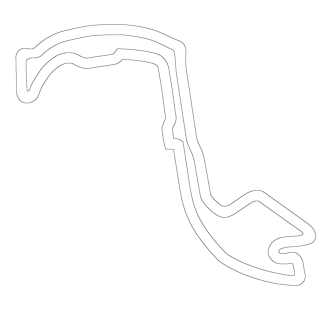
\includegraphics[interpolate=true,width=3.320000in,height=3.120000in]{contents/chapt6/figs/racing/mco-img0.png}}%
\end{pgfscope}%
\begin{pgfscope}%
\pgfpathrectangle{\pgfqpoint{0.123564in}{0.355320in}}{\pgfqpoint{3.316600in}{3.114720in}}%
\pgfusepath{clip}%
\pgfsetrectcap%
\pgfsetroundjoin%
\pgfsetlinewidth{1.003750pt}%
\definecolor{currentstroke}{rgb}{0.445098,0.086133,0.999070}%
\pgfsetstrokecolor{currentstroke}%
\pgfsetstrokeopacity{0.800000}%
\pgfsetdash{}{0pt}%
\pgfpathmoveto{\pgfqpoint{1.161804in}{3.164336in}}%
\pgfpathlineto{\pgfqpoint{1.163534in}{3.164336in}}%
\pgfusepath{stroke}%
\end{pgfscope}%
\begin{pgfscope}%
\pgfpathrectangle{\pgfqpoint{0.123564in}{0.355320in}}{\pgfqpoint{3.316600in}{3.114720in}}%
\pgfusepath{clip}%
\pgfsetrectcap%
\pgfsetroundjoin%
\pgfsetlinewidth{1.003750pt}%
\definecolor{currentstroke}{rgb}{0.390196,0.171626,0.996284}%
\pgfsetstrokecolor{currentstroke}%
\pgfsetstrokeopacity{0.800000}%
\pgfsetdash{}{0pt}%
\pgfpathmoveto{\pgfqpoint{1.163534in}{3.164336in}}%
\pgfpathlineto{\pgfqpoint{1.165298in}{3.164336in}}%
\pgfusepath{stroke}%
\end{pgfscope}%
\begin{pgfscope}%
\pgfpathrectangle{\pgfqpoint{0.123564in}{0.355320in}}{\pgfqpoint{3.316600in}{3.114720in}}%
\pgfusepath{clip}%
\pgfsetrectcap%
\pgfsetroundjoin%
\pgfsetlinewidth{1.003750pt}%
\definecolor{currentstroke}{rgb}{0.335294,0.255843,0.991645}%
\pgfsetstrokecolor{currentstroke}%
\pgfsetstrokeopacity{0.800000}%
\pgfsetdash{}{0pt}%
\pgfpathmoveto{\pgfqpoint{1.165298in}{3.164336in}}%
\pgfpathlineto{\pgfqpoint{1.167094in}{3.164332in}}%
\pgfusepath{stroke}%
\end{pgfscope}%
\begin{pgfscope}%
\pgfpathrectangle{\pgfqpoint{0.123564in}{0.355320in}}{\pgfqpoint{3.316600in}{3.114720in}}%
\pgfusepath{clip}%
\pgfsetrectcap%
\pgfsetroundjoin%
\pgfsetlinewidth{1.003750pt}%
\definecolor{currentstroke}{rgb}{0.272549,0.349727,0.984086}%
\pgfsetstrokecolor{currentstroke}%
\pgfsetstrokeopacity{0.800000}%
\pgfsetdash{}{0pt}%
\pgfpathmoveto{\pgfqpoint{1.167094in}{3.164332in}}%
\pgfpathlineto{\pgfqpoint{1.168923in}{3.164329in}}%
\pgfusepath{stroke}%
\end{pgfscope}%
\begin{pgfscope}%
\pgfpathrectangle{\pgfqpoint{0.123564in}{0.355320in}}{\pgfqpoint{3.316600in}{3.114720in}}%
\pgfusepath{clip}%
\pgfsetrectcap%
\pgfsetroundjoin%
\pgfsetlinewidth{1.003750pt}%
\definecolor{currentstroke}{rgb}{0.217647,0.429121,0.975512}%
\pgfsetstrokecolor{currentstroke}%
\pgfsetstrokeopacity{0.800000}%
\pgfsetdash{}{0pt}%
\pgfpathmoveto{\pgfqpoint{1.168923in}{3.164329in}}%
\pgfpathlineto{\pgfqpoint{1.170786in}{3.164322in}}%
\pgfusepath{stroke}%
\end{pgfscope}%
\begin{pgfscope}%
\pgfpathrectangle{\pgfqpoint{0.123564in}{0.355320in}}{\pgfqpoint{3.316600in}{3.114720in}}%
\pgfusepath{clip}%
\pgfsetrectcap%
\pgfsetroundjoin%
\pgfsetlinewidth{1.003750pt}%
\definecolor{currentstroke}{rgb}{0.162745,0.505325,0.965124}%
\pgfsetstrokecolor{currentstroke}%
\pgfsetstrokeopacity{0.800000}%
\pgfsetdash{}{0pt}%
\pgfpathmoveto{\pgfqpoint{1.170786in}{3.164322in}}%
\pgfpathlineto{\pgfqpoint{1.172680in}{3.164315in}}%
\pgfusepath{stroke}%
\end{pgfscope}%
\begin{pgfscope}%
\pgfpathrectangle{\pgfqpoint{0.123564in}{0.355320in}}{\pgfqpoint{3.316600in}{3.114720in}}%
\pgfusepath{clip}%
\pgfsetrectcap%
\pgfsetroundjoin%
\pgfsetlinewidth{1.003750pt}%
\definecolor{currentstroke}{rgb}{0.107843,0.577774,0.952942}%
\pgfsetstrokecolor{currentstroke}%
\pgfsetstrokeopacity{0.800000}%
\pgfsetdash{}{0pt}%
\pgfpathmoveto{\pgfqpoint{1.172680in}{3.164315in}}%
\pgfpathlineto{\pgfqpoint{1.174607in}{3.164305in}}%
\pgfusepath{stroke}%
\end{pgfscope}%
\begin{pgfscope}%
\pgfpathrectangle{\pgfqpoint{0.123564in}{0.355320in}}{\pgfqpoint{3.316600in}{3.114720in}}%
\pgfusepath{clip}%
\pgfsetrectcap%
\pgfsetroundjoin%
\pgfsetlinewidth{1.003750pt}%
\definecolor{currentstroke}{rgb}{0.060784,0.636474,0.941089}%
\pgfsetstrokecolor{currentstroke}%
\pgfsetstrokeopacity{0.800000}%
\pgfsetdash{}{0pt}%
\pgfpathmoveto{\pgfqpoint{1.174607in}{3.164305in}}%
\pgfpathlineto{\pgfqpoint{1.176563in}{3.164287in}}%
\pgfusepath{stroke}%
\end{pgfscope}%
\begin{pgfscope}%
\pgfpathrectangle{\pgfqpoint{0.123564in}{0.355320in}}{\pgfqpoint{3.316600in}{3.114720in}}%
\pgfusepath{clip}%
\pgfsetrectcap%
\pgfsetroundjoin%
\pgfsetlinewidth{1.003750pt}%
\definecolor{currentstroke}{rgb}{0.013725,0.691698,0.927951}%
\pgfsetstrokecolor{currentstroke}%
\pgfsetstrokeopacity{0.800000}%
\pgfsetdash{}{0pt}%
\pgfpathmoveto{\pgfqpoint{1.176563in}{3.164287in}}%
\pgfpathlineto{\pgfqpoint{1.178549in}{3.164265in}}%
\pgfusepath{stroke}%
\end{pgfscope}%
\begin{pgfscope}%
\pgfpathrectangle{\pgfqpoint{0.123564in}{0.355320in}}{\pgfqpoint{3.316600in}{3.114720in}}%
\pgfusepath{clip}%
\pgfsetrectcap%
\pgfsetroundjoin%
\pgfsetlinewidth{1.003750pt}%
\definecolor{currentstroke}{rgb}{0.033333,0.743145,0.913545}%
\pgfsetstrokecolor{currentstroke}%
\pgfsetstrokeopacity{0.800000}%
\pgfsetdash{}{0pt}%
\pgfpathmoveto{\pgfqpoint{1.178549in}{3.164265in}}%
\pgfpathlineto{\pgfqpoint{1.180562in}{3.164236in}}%
\pgfusepath{stroke}%
\end{pgfscope}%
\begin{pgfscope}%
\pgfpathrectangle{\pgfqpoint{0.123564in}{0.355320in}}{\pgfqpoint{3.316600in}{3.114720in}}%
\pgfusepath{clip}%
\pgfsetrectcap%
\pgfsetroundjoin%
\pgfsetlinewidth{1.003750pt}%
\definecolor{currentstroke}{rgb}{0.088235,0.798017,0.895163}%
\pgfsetstrokecolor{currentstroke}%
\pgfsetstrokeopacity{0.800000}%
\pgfsetdash{}{0pt}%
\pgfpathmoveto{\pgfqpoint{1.180562in}{3.164236in}}%
\pgfpathlineto{\pgfqpoint{1.182603in}{3.164203in}}%
\pgfusepath{stroke}%
\end{pgfscope}%
\begin{pgfscope}%
\pgfpathrectangle{\pgfqpoint{0.123564in}{0.355320in}}{\pgfqpoint{3.316600in}{3.114720in}}%
\pgfusepath{clip}%
\pgfsetrectcap%
\pgfsetroundjoin%
\pgfsetlinewidth{1.003750pt}%
\definecolor{currentstroke}{rgb}{0.127451,0.833602,0.881012}%
\pgfsetstrokecolor{currentstroke}%
\pgfsetstrokeopacity{0.800000}%
\pgfsetdash{}{0pt}%
\pgfpathmoveto{\pgfqpoint{1.182603in}{3.164203in}}%
\pgfpathlineto{\pgfqpoint{1.184672in}{3.164162in}}%
\pgfusepath{stroke}%
\end{pgfscope}%
\begin{pgfscope}%
\pgfpathrectangle{\pgfqpoint{0.123564in}{0.355320in}}{\pgfqpoint{3.316600in}{3.114720in}}%
\pgfusepath{clip}%
\pgfsetrectcap%
\pgfsetroundjoin%
\pgfsetlinewidth{1.003750pt}%
\definecolor{currentstroke}{rgb}{0.166667,0.866025,0.866025}%
\pgfsetstrokecolor{currentstroke}%
\pgfsetstrokeopacity{0.800000}%
\pgfsetdash{}{0pt}%
\pgfpathmoveto{\pgfqpoint{1.184672in}{3.164162in}}%
\pgfpathlineto{\pgfqpoint{1.186763in}{3.164117in}}%
\pgfusepath{stroke}%
\end{pgfscope}%
\begin{pgfscope}%
\pgfpathrectangle{\pgfqpoint{0.123564in}{0.355320in}}{\pgfqpoint{3.316600in}{3.114720in}}%
\pgfusepath{clip}%
\pgfsetrectcap%
\pgfsetroundjoin%
\pgfsetlinewidth{1.003750pt}%
\definecolor{currentstroke}{rgb}{0.213725,0.900587,0.846958}%
\pgfsetstrokecolor{currentstroke}%
\pgfsetstrokeopacity{0.800000}%
\pgfsetdash{}{0pt}%
\pgfpathmoveto{\pgfqpoint{1.186763in}{3.164117in}}%
\pgfpathlineto{\pgfqpoint{1.188876in}{3.164070in}}%
\pgfusepath{stroke}%
\end{pgfscope}%
\begin{pgfscope}%
\pgfpathrectangle{\pgfqpoint{0.123564in}{0.355320in}}{\pgfqpoint{3.316600in}{3.114720in}}%
\pgfusepath{clip}%
\pgfsetrectcap%
\pgfsetroundjoin%
\pgfsetlinewidth{1.003750pt}%
\definecolor{currentstroke}{rgb}{0.252941,0.925638,0.830184}%
\pgfsetstrokecolor{currentstroke}%
\pgfsetstrokeopacity{0.800000}%
\pgfsetdash{}{0pt}%
\pgfpathmoveto{\pgfqpoint{1.188876in}{3.164070in}}%
\pgfpathlineto{\pgfqpoint{1.191017in}{3.164025in}}%
\pgfusepath{stroke}%
\end{pgfscope}%
\begin{pgfscope}%
\pgfpathrectangle{\pgfqpoint{0.123564in}{0.355320in}}{\pgfqpoint{3.316600in}{3.114720in}}%
\pgfusepath{clip}%
\pgfsetrectcap%
\pgfsetroundjoin%
\pgfsetlinewidth{1.003750pt}%
\definecolor{currentstroke}{rgb}{0.292157,0.947177,0.812622}%
\pgfsetstrokecolor{currentstroke}%
\pgfsetstrokeopacity{0.800000}%
\pgfsetdash{}{0pt}%
\pgfpathmoveto{\pgfqpoint{1.191017in}{3.164025in}}%
\pgfpathlineto{\pgfqpoint{1.193181in}{3.163986in}}%
\pgfusepath{stroke}%
\end{pgfscope}%
\begin{pgfscope}%
\pgfpathrectangle{\pgfqpoint{0.123564in}{0.355320in}}{\pgfqpoint{3.316600in}{3.114720in}}%
\pgfusepath{clip}%
\pgfsetrectcap%
\pgfsetroundjoin%
\pgfsetlinewidth{1.003750pt}%
\definecolor{currentstroke}{rgb}{0.339216,0.968276,0.790532}%
\pgfsetstrokecolor{currentstroke}%
\pgfsetstrokeopacity{0.800000}%
\pgfsetdash{}{0pt}%
\pgfpathmoveto{\pgfqpoint{1.193181in}{3.163986in}}%
\pgfpathlineto{\pgfqpoint{1.195369in}{3.163956in}}%
\pgfusepath{stroke}%
\end{pgfscope}%
\begin{pgfscope}%
\pgfpathrectangle{\pgfqpoint{0.123564in}{0.355320in}}{\pgfqpoint{3.316600in}{3.114720in}}%
\pgfusepath{clip}%
\pgfsetrectcap%
\pgfsetroundjoin%
\pgfsetlinewidth{1.003750pt}%
\definecolor{currentstroke}{rgb}{0.378431,0.981823,0.771298}%
\pgfsetstrokecolor{currentstroke}%
\pgfsetstrokeopacity{0.800000}%
\pgfsetdash{}{0pt}%
\pgfpathmoveto{\pgfqpoint{1.195369in}{3.163956in}}%
\pgfpathlineto{\pgfqpoint{1.197582in}{3.163939in}}%
\pgfusepath{stroke}%
\end{pgfscope}%
\begin{pgfscope}%
\pgfpathrectangle{\pgfqpoint{0.123564in}{0.355320in}}{\pgfqpoint{3.316600in}{3.114720in}}%
\pgfusepath{clip}%
\pgfsetrectcap%
\pgfsetroundjoin%
\pgfsetlinewidth{1.003750pt}%
\definecolor{currentstroke}{rgb}{0.417647,0.991645,0.751332}%
\pgfsetstrokecolor{currentstroke}%
\pgfsetstrokeopacity{0.800000}%
\pgfsetdash{}{0pt}%
\pgfpathmoveto{\pgfqpoint{1.197582in}{3.163939in}}%
\pgfpathlineto{\pgfqpoint{1.199818in}{3.163931in}}%
\pgfusepath{stroke}%
\end{pgfscope}%
\begin{pgfscope}%
\pgfpathrectangle{\pgfqpoint{0.123564in}{0.355320in}}{\pgfqpoint{3.316600in}{3.114720in}}%
\pgfusepath{clip}%
\pgfsetrectcap%
\pgfsetroundjoin%
\pgfsetlinewidth{1.003750pt}%
\definecolor{currentstroke}{rgb}{0.456863,0.997705,0.730653}%
\pgfsetstrokecolor{currentstroke}%
\pgfsetstrokeopacity{0.800000}%
\pgfsetdash{}{0pt}%
\pgfpathmoveto{\pgfqpoint{1.199818in}{3.163931in}}%
\pgfpathlineto{\pgfqpoint{1.202076in}{3.163937in}}%
\pgfusepath{stroke}%
\end{pgfscope}%
\begin{pgfscope}%
\pgfpathrectangle{\pgfqpoint{0.123564in}{0.355320in}}{\pgfqpoint{3.316600in}{3.114720in}}%
\pgfusepath{clip}%
\pgfsetrectcap%
\pgfsetroundjoin%
\pgfsetlinewidth{1.003750pt}%
\definecolor{currentstroke}{rgb}{0.488235,0.999829,0.713610}%
\pgfsetstrokecolor{currentstroke}%
\pgfsetstrokeopacity{0.800000}%
\pgfsetdash{}{0pt}%
\pgfpathmoveto{\pgfqpoint{1.202076in}{3.163937in}}%
\pgfpathlineto{\pgfqpoint{1.204357in}{3.163953in}}%
\pgfusepath{stroke}%
\end{pgfscope}%
\begin{pgfscope}%
\pgfpathrectangle{\pgfqpoint{0.123564in}{0.355320in}}{\pgfqpoint{3.316600in}{3.114720in}}%
\pgfusepath{clip}%
\pgfsetrectcap%
\pgfsetroundjoin%
\pgfsetlinewidth{1.003750pt}%
\definecolor{currentstroke}{rgb}{0.527451,0.999070,0.691698}%
\pgfsetstrokecolor{currentstroke}%
\pgfsetstrokeopacity{0.800000}%
\pgfsetdash{}{0pt}%
\pgfpathmoveto{\pgfqpoint{1.204357in}{3.163953in}}%
\pgfpathlineto{\pgfqpoint{1.206659in}{3.163986in}}%
\pgfusepath{stroke}%
\end{pgfscope}%
\begin{pgfscope}%
\pgfpathrectangle{\pgfqpoint{0.123564in}{0.355320in}}{\pgfqpoint{3.316600in}{3.114720in}}%
\pgfusepath{clip}%
\pgfsetrectcap%
\pgfsetroundjoin%
\pgfsetlinewidth{1.003750pt}%
\definecolor{currentstroke}{rgb}{0.558824,0.995734,0.673696}%
\pgfsetstrokecolor{currentstroke}%
\pgfsetstrokeopacity{0.800000}%
\pgfsetdash{}{0pt}%
\pgfpathmoveto{\pgfqpoint{1.206659in}{3.163986in}}%
\pgfpathlineto{\pgfqpoint{1.208980in}{3.164033in}}%
\pgfusepath{stroke}%
\end{pgfscope}%
\begin{pgfscope}%
\pgfpathrectangle{\pgfqpoint{0.123564in}{0.355320in}}{\pgfqpoint{3.316600in}{3.114720in}}%
\pgfusepath{clip}%
\pgfsetrectcap%
\pgfsetroundjoin%
\pgfsetlinewidth{1.003750pt}%
\definecolor{currentstroke}{rgb}{0.582353,0.991645,0.659925}%
\pgfsetstrokecolor{currentstroke}%
\pgfsetstrokeopacity{0.800000}%
\pgfsetdash{}{0pt}%
\pgfpathmoveto{\pgfqpoint{1.208980in}{3.164033in}}%
\pgfpathlineto{\pgfqpoint{1.211320in}{3.164089in}}%
\pgfusepath{stroke}%
\end{pgfscope}%
\begin{pgfscope}%
\pgfpathrectangle{\pgfqpoint{0.123564in}{0.355320in}}{\pgfqpoint{3.316600in}{3.114720in}}%
\pgfusepath{clip}%
\pgfsetrectcap%
\pgfsetroundjoin%
\pgfsetlinewidth{1.003750pt}%
\definecolor{currentstroke}{rgb}{0.605882,0.986201,0.645928}%
\pgfsetstrokecolor{currentstroke}%
\pgfsetstrokeopacity{0.800000}%
\pgfsetdash{}{0pt}%
\pgfpathmoveto{\pgfqpoint{1.211320in}{3.164089in}}%
\pgfpathlineto{\pgfqpoint{1.213673in}{3.164162in}}%
\pgfusepath{stroke}%
\end{pgfscope}%
\begin{pgfscope}%
\pgfpathrectangle{\pgfqpoint{0.123564in}{0.355320in}}{\pgfqpoint{3.316600in}{3.114720in}}%
\pgfusepath{clip}%
\pgfsetrectcap%
\pgfsetroundjoin%
\pgfsetlinewidth{1.003750pt}%
\definecolor{currentstroke}{rgb}{0.645098,0.974139,0.622113}%
\pgfsetstrokecolor{currentstroke}%
\pgfsetstrokeopacity{0.800000}%
\pgfsetdash{}{0pt}%
\pgfpathmoveto{\pgfqpoint{1.213673in}{3.164162in}}%
\pgfpathlineto{\pgfqpoint{1.216040in}{3.164246in}}%
\pgfusepath{stroke}%
\end{pgfscope}%
\begin{pgfscope}%
\pgfpathrectangle{\pgfqpoint{0.123564in}{0.355320in}}{\pgfqpoint{3.316600in}{3.114720in}}%
\pgfusepath{clip}%
\pgfsetrectcap%
\pgfsetroundjoin%
\pgfsetlinewidth{1.003750pt}%
\definecolor{currentstroke}{rgb}{0.668627,0.965124,0.607539}%
\pgfsetstrokecolor{currentstroke}%
\pgfsetstrokeopacity{0.800000}%
\pgfsetdash{}{0pt}%
\pgfpathmoveto{\pgfqpoint{1.216040in}{3.164246in}}%
\pgfpathlineto{\pgfqpoint{1.218427in}{3.164349in}}%
\pgfusepath{stroke}%
\end{pgfscope}%
\begin{pgfscope}%
\pgfpathrectangle{\pgfqpoint{0.123564in}{0.355320in}}{\pgfqpoint{3.316600in}{3.114720in}}%
\pgfusepath{clip}%
\pgfsetrectcap%
\pgfsetroundjoin%
\pgfsetlinewidth{1.003750pt}%
\definecolor{currentstroke}{rgb}{0.692157,0.954791,0.592758}%
\pgfsetstrokecolor{currentstroke}%
\pgfsetstrokeopacity{0.800000}%
\pgfsetdash{}{0pt}%
\pgfpathmoveto{\pgfqpoint{1.218427in}{3.164349in}}%
\pgfpathlineto{\pgfqpoint{1.220827in}{3.164465in}}%
\pgfusepath{stroke}%
\end{pgfscope}%
\begin{pgfscope}%
\pgfpathrectangle{\pgfqpoint{0.123564in}{0.355320in}}{\pgfqpoint{3.316600in}{3.114720in}}%
\pgfusepath{clip}%
\pgfsetrectcap%
\pgfsetroundjoin%
\pgfsetlinewidth{1.003750pt}%
\definecolor{currentstroke}{rgb}{0.715686,0.943154,0.577774}%
\pgfsetstrokecolor{currentstroke}%
\pgfsetstrokeopacity{0.800000}%
\pgfsetdash{}{0pt}%
\pgfpathmoveto{\pgfqpoint{1.220827in}{3.164465in}}%
\pgfpathlineto{\pgfqpoint{1.223241in}{3.164592in}}%
\pgfusepath{stroke}%
\end{pgfscope}%
\begin{pgfscope}%
\pgfpathrectangle{\pgfqpoint{0.123564in}{0.355320in}}{\pgfqpoint{3.316600in}{3.114720in}}%
\pgfusepath{clip}%
\pgfsetrectcap%
\pgfsetroundjoin%
\pgfsetlinewidth{1.003750pt}%
\definecolor{currentstroke}{rgb}{0.739216,0.930229,0.562593}%
\pgfsetstrokecolor{currentstroke}%
\pgfsetstrokeopacity{0.800000}%
\pgfsetdash{}{0pt}%
\pgfpathmoveto{\pgfqpoint{1.223241in}{3.164592in}}%
\pgfpathlineto{\pgfqpoint{1.225667in}{3.164733in}}%
\pgfusepath{stroke}%
\end{pgfscope}%
\begin{pgfscope}%
\pgfpathrectangle{\pgfqpoint{0.123564in}{0.355320in}}{\pgfqpoint{3.316600in}{3.114720in}}%
\pgfusepath{clip}%
\pgfsetrectcap%
\pgfsetroundjoin%
\pgfsetlinewidth{1.003750pt}%
\definecolor{currentstroke}{rgb}{0.754902,0.920906,0.552365}%
\pgfsetstrokecolor{currentstroke}%
\pgfsetstrokeopacity{0.800000}%
\pgfsetdash{}{0pt}%
\pgfpathmoveto{\pgfqpoint{1.225667in}{3.164733in}}%
\pgfpathlineto{\pgfqpoint{1.228110in}{3.164887in}}%
\pgfusepath{stroke}%
\end{pgfscope}%
\begin{pgfscope}%
\pgfpathrectangle{\pgfqpoint{0.123564in}{0.355320in}}{\pgfqpoint{3.316600in}{3.114720in}}%
\pgfusepath{clip}%
\pgfsetrectcap%
\pgfsetroundjoin%
\pgfsetlinewidth{1.003750pt}%
\definecolor{currentstroke}{rgb}{0.778431,0.905873,0.536867}%
\pgfsetstrokecolor{currentstroke}%
\pgfsetstrokeopacity{0.800000}%
\pgfsetdash{}{0pt}%
\pgfpathmoveto{\pgfqpoint{1.228110in}{3.164887in}}%
\pgfpathlineto{\pgfqpoint{1.230557in}{3.165056in}}%
\pgfusepath{stroke}%
\end{pgfscope}%
\begin{pgfscope}%
\pgfpathrectangle{\pgfqpoint{0.123564in}{0.355320in}}{\pgfqpoint{3.316600in}{3.114720in}}%
\pgfusepath{clip}%
\pgfsetrectcap%
\pgfsetroundjoin%
\pgfsetlinewidth{1.003750pt}%
\definecolor{currentstroke}{rgb}{0.794118,0.895163,0.526432}%
\pgfsetstrokecolor{currentstroke}%
\pgfsetstrokeopacity{0.800000}%
\pgfsetdash{}{0pt}%
\pgfpathmoveto{\pgfqpoint{1.230557in}{3.165056in}}%
\pgfpathlineto{\pgfqpoint{1.233016in}{3.165236in}}%
\pgfusepath{stroke}%
\end{pgfscope}%
\begin{pgfscope}%
\pgfpathrectangle{\pgfqpoint{0.123564in}{0.355320in}}{\pgfqpoint{3.316600in}{3.114720in}}%
\pgfusepath{clip}%
\pgfsetrectcap%
\pgfsetroundjoin%
\pgfsetlinewidth{1.003750pt}%
\definecolor{currentstroke}{rgb}{0.809804,0.883910,0.515918}%
\pgfsetstrokecolor{currentstroke}%
\pgfsetstrokeopacity{0.800000}%
\pgfsetdash{}{0pt}%
\pgfpathmoveto{\pgfqpoint{1.233016in}{3.165236in}}%
\pgfpathlineto{\pgfqpoint{1.235484in}{3.165424in}}%
\pgfusepath{stroke}%
\end{pgfscope}%
\begin{pgfscope}%
\pgfpathrectangle{\pgfqpoint{0.123564in}{0.355320in}}{\pgfqpoint{3.316600in}{3.114720in}}%
\pgfusepath{clip}%
\pgfsetrectcap%
\pgfsetroundjoin%
\pgfsetlinewidth{1.003750pt}%
\definecolor{currentstroke}{rgb}{0.825490,0.872120,0.505325}%
\pgfsetstrokecolor{currentstroke}%
\pgfsetstrokeopacity{0.800000}%
\pgfsetdash{}{0pt}%
\pgfpathmoveto{\pgfqpoint{1.235484in}{3.165424in}}%
\pgfpathlineto{\pgfqpoint{1.237961in}{3.165615in}}%
\pgfusepath{stroke}%
\end{pgfscope}%
\begin{pgfscope}%
\pgfpathrectangle{\pgfqpoint{0.123564in}{0.355320in}}{\pgfqpoint{3.316600in}{3.114720in}}%
\pgfusepath{clip}%
\pgfsetrectcap%
\pgfsetroundjoin%
\pgfsetlinewidth{1.003750pt}%
\definecolor{currentstroke}{rgb}{0.841176,0.859800,0.494656}%
\pgfsetstrokecolor{currentstroke}%
\pgfsetstrokeopacity{0.800000}%
\pgfsetdash{}{0pt}%
\pgfpathmoveto{\pgfqpoint{1.237961in}{3.165615in}}%
\pgfpathlineto{\pgfqpoint{1.240448in}{3.165805in}}%
\pgfusepath{stroke}%
\end{pgfscope}%
\begin{pgfscope}%
\pgfpathrectangle{\pgfqpoint{0.123564in}{0.355320in}}{\pgfqpoint{3.316600in}{3.114720in}}%
\pgfusepath{clip}%
\pgfsetrectcap%
\pgfsetroundjoin%
\pgfsetlinewidth{1.003750pt}%
\definecolor{currentstroke}{rgb}{0.864706,0.840344,0.478512}%
\pgfsetstrokecolor{currentstroke}%
\pgfsetstrokeopacity{0.800000}%
\pgfsetdash{}{0pt}%
\pgfpathmoveto{\pgfqpoint{1.240448in}{3.165805in}}%
\pgfpathlineto{\pgfqpoint{1.242946in}{3.165990in}}%
\pgfusepath{stroke}%
\end{pgfscope}%
\begin{pgfscope}%
\pgfpathrectangle{\pgfqpoint{0.123564in}{0.355320in}}{\pgfqpoint{3.316600in}{3.114720in}}%
\pgfusepath{clip}%
\pgfsetrectcap%
\pgfsetroundjoin%
\pgfsetlinewidth{1.003750pt}%
\definecolor{currentstroke}{rgb}{0.872549,0.833602,0.473094}%
\pgfsetstrokecolor{currentstroke}%
\pgfsetstrokeopacity{0.800000}%
\pgfsetdash{}{0pt}%
\pgfpathmoveto{\pgfqpoint{1.242946in}{3.165990in}}%
\pgfpathlineto{\pgfqpoint{1.245455in}{3.166175in}}%
\pgfusepath{stroke}%
\end{pgfscope}%
\begin{pgfscope}%
\pgfpathrectangle{\pgfqpoint{0.123564in}{0.355320in}}{\pgfqpoint{3.316600in}{3.114720in}}%
\pgfusepath{clip}%
\pgfsetrectcap%
\pgfsetroundjoin%
\pgfsetlinewidth{1.003750pt}%
\definecolor{currentstroke}{rgb}{0.888235,0.819740,0.462204}%
\pgfsetstrokecolor{currentstroke}%
\pgfsetstrokeopacity{0.800000}%
\pgfsetdash{}{0pt}%
\pgfpathmoveto{\pgfqpoint{1.245455in}{3.166175in}}%
\pgfpathlineto{\pgfqpoint{1.247970in}{3.166353in}}%
\pgfusepath{stroke}%
\end{pgfscope}%
\begin{pgfscope}%
\pgfpathrectangle{\pgfqpoint{0.123564in}{0.355320in}}{\pgfqpoint{3.316600in}{3.114720in}}%
\pgfusepath{clip}%
\pgfsetrectcap%
\pgfsetroundjoin%
\pgfsetlinewidth{1.003750pt}%
\definecolor{currentstroke}{rgb}{0.903922,0.805381,0.451244}%
\pgfsetstrokecolor{currentstroke}%
\pgfsetstrokeopacity{0.800000}%
\pgfsetdash{}{0pt}%
\pgfpathmoveto{\pgfqpoint{1.247970in}{3.166353in}}%
\pgfpathlineto{\pgfqpoint{1.250493in}{3.166527in}}%
\pgfusepath{stroke}%
\end{pgfscope}%
\begin{pgfscope}%
\pgfpathrectangle{\pgfqpoint{0.123564in}{0.355320in}}{\pgfqpoint{3.316600in}{3.114720in}}%
\pgfusepath{clip}%
\pgfsetrectcap%
\pgfsetroundjoin%
\pgfsetlinewidth{1.003750pt}%
\definecolor{currentstroke}{rgb}{0.903922,0.805381,0.451244}%
\pgfsetstrokecolor{currentstroke}%
\pgfsetstrokeopacity{0.800000}%
\pgfsetdash{}{0pt}%
\pgfpathmoveto{\pgfqpoint{1.250493in}{3.166527in}}%
\pgfpathlineto{\pgfqpoint{1.253024in}{3.166693in}}%
\pgfusepath{stroke}%
\end{pgfscope}%
\begin{pgfscope}%
\pgfpathrectangle{\pgfqpoint{0.123564in}{0.355320in}}{\pgfqpoint{3.316600in}{3.114720in}}%
\pgfusepath{clip}%
\pgfsetrectcap%
\pgfsetroundjoin%
\pgfsetlinewidth{1.003750pt}%
\definecolor{currentstroke}{rgb}{0.919608,0.790532,0.440216}%
\pgfsetstrokecolor{currentstroke}%
\pgfsetstrokeopacity{0.800000}%
\pgfsetdash{}{0pt}%
\pgfpathmoveto{\pgfqpoint{1.253024in}{3.166693in}}%
\pgfpathlineto{\pgfqpoint{1.255561in}{3.166852in}}%
\pgfusepath{stroke}%
\end{pgfscope}%
\begin{pgfscope}%
\pgfpathrectangle{\pgfqpoint{0.123564in}{0.355320in}}{\pgfqpoint{3.316600in}{3.114720in}}%
\pgfusepath{clip}%
\pgfsetrectcap%
\pgfsetroundjoin%
\pgfsetlinewidth{1.003750pt}%
\definecolor{currentstroke}{rgb}{0.927451,0.782928,0.434676}%
\pgfsetstrokecolor{currentstroke}%
\pgfsetstrokeopacity{0.800000}%
\pgfsetdash{}{0pt}%
\pgfpathmoveto{\pgfqpoint{1.255561in}{3.166852in}}%
\pgfpathlineto{\pgfqpoint{1.258104in}{3.167008in}}%
\pgfusepath{stroke}%
\end{pgfscope}%
\begin{pgfscope}%
\pgfpathrectangle{\pgfqpoint{0.123564in}{0.355320in}}{\pgfqpoint{3.316600in}{3.114720in}}%
\pgfusepath{clip}%
\pgfsetrectcap%
\pgfsetroundjoin%
\pgfsetlinewidth{1.003750pt}%
\definecolor{currentstroke}{rgb}{0.935294,0.775204,0.429121}%
\pgfsetstrokecolor{currentstroke}%
\pgfsetstrokeopacity{0.800000}%
\pgfsetdash{}{0pt}%
\pgfpathmoveto{\pgfqpoint{1.258104in}{3.167008in}}%
\pgfpathlineto{\pgfqpoint{1.260653in}{3.167155in}}%
\pgfusepath{stroke}%
\end{pgfscope}%
\begin{pgfscope}%
\pgfpathrectangle{\pgfqpoint{0.123564in}{0.355320in}}{\pgfqpoint{3.316600in}{3.114720in}}%
\pgfusepath{clip}%
\pgfsetrectcap%
\pgfsetroundjoin%
\pgfsetlinewidth{1.003750pt}%
\definecolor{currentstroke}{rgb}{0.950980,0.759405,0.417960}%
\pgfsetstrokecolor{currentstroke}%
\pgfsetstrokeopacity{0.800000}%
\pgfsetdash{}{0pt}%
\pgfpathmoveto{\pgfqpoint{1.260653in}{3.167155in}}%
\pgfpathlineto{\pgfqpoint{1.263209in}{3.167295in}}%
\pgfusepath{stroke}%
\end{pgfscope}%
\begin{pgfscope}%
\pgfpathrectangle{\pgfqpoint{0.123564in}{0.355320in}}{\pgfqpoint{3.316600in}{3.114720in}}%
\pgfusepath{clip}%
\pgfsetrectcap%
\pgfsetroundjoin%
\pgfsetlinewidth{1.003750pt}%
\definecolor{currentstroke}{rgb}{0.958824,0.751332,0.412356}%
\pgfsetstrokecolor{currentstroke}%
\pgfsetstrokeopacity{0.800000}%
\pgfsetdash{}{0pt}%
\pgfpathmoveto{\pgfqpoint{1.263209in}{3.167295in}}%
\pgfpathlineto{\pgfqpoint{1.265772in}{3.167423in}}%
\pgfusepath{stroke}%
\end{pgfscope}%
\begin{pgfscope}%
\pgfpathrectangle{\pgfqpoint{0.123564in}{0.355320in}}{\pgfqpoint{3.316600in}{3.114720in}}%
\pgfusepath{clip}%
\pgfsetrectcap%
\pgfsetroundjoin%
\pgfsetlinewidth{1.003750pt}%
\definecolor{currentstroke}{rgb}{0.966667,0.743145,0.406737}%
\pgfsetstrokecolor{currentstroke}%
\pgfsetstrokeopacity{0.800000}%
\pgfsetdash{}{0pt}%
\pgfpathmoveto{\pgfqpoint{1.265772in}{3.167423in}}%
\pgfpathlineto{\pgfqpoint{1.268341in}{3.167543in}}%
\pgfusepath{stroke}%
\end{pgfscope}%
\begin{pgfscope}%
\pgfpathrectangle{\pgfqpoint{0.123564in}{0.355320in}}{\pgfqpoint{3.316600in}{3.114720in}}%
\pgfusepath{clip}%
\pgfsetrectcap%
\pgfsetroundjoin%
\pgfsetlinewidth{1.003750pt}%
\definecolor{currentstroke}{rgb}{0.982353,0.726434,0.395451}%
\pgfsetstrokecolor{currentstroke}%
\pgfsetstrokeopacity{0.800000}%
\pgfsetdash{}{0pt}%
\pgfpathmoveto{\pgfqpoint{1.268341in}{3.167543in}}%
\pgfpathlineto{\pgfqpoint{1.270916in}{3.167649in}}%
\pgfusepath{stroke}%
\end{pgfscope}%
\begin{pgfscope}%
\pgfpathrectangle{\pgfqpoint{0.123564in}{0.355320in}}{\pgfqpoint{3.316600in}{3.114720in}}%
\pgfusepath{clip}%
\pgfsetrectcap%
\pgfsetroundjoin%
\pgfsetlinewidth{1.003750pt}%
\definecolor{currentstroke}{rgb}{0.982353,0.726434,0.395451}%
\pgfsetstrokecolor{currentstroke}%
\pgfsetstrokeopacity{0.800000}%
\pgfsetdash{}{0pt}%
\pgfpathmoveto{\pgfqpoint{1.270916in}{3.167649in}}%
\pgfpathlineto{\pgfqpoint{1.273498in}{3.167747in}}%
\pgfusepath{stroke}%
\end{pgfscope}%
\begin{pgfscope}%
\pgfpathrectangle{\pgfqpoint{0.123564in}{0.355320in}}{\pgfqpoint{3.316600in}{3.114720in}}%
\pgfusepath{clip}%
\pgfsetrectcap%
\pgfsetroundjoin%
\pgfsetlinewidth{1.003750pt}%
\definecolor{currentstroke}{rgb}{0.990196,0.717912,0.389786}%
\pgfsetstrokecolor{currentstroke}%
\pgfsetstrokeopacity{0.800000}%
\pgfsetdash{}{0pt}%
\pgfpathmoveto{\pgfqpoint{1.273498in}{3.167747in}}%
\pgfpathlineto{\pgfqpoint{1.276082in}{3.167829in}}%
\pgfusepath{stroke}%
\end{pgfscope}%
\begin{pgfscope}%
\pgfpathrectangle{\pgfqpoint{0.123564in}{0.355320in}}{\pgfqpoint{3.316600in}{3.114720in}}%
\pgfusepath{clip}%
\pgfsetrectcap%
\pgfsetroundjoin%
\pgfsetlinewidth{1.003750pt}%
\definecolor{currentstroke}{rgb}{0.998039,0.709281,0.384106}%
\pgfsetstrokecolor{currentstroke}%
\pgfsetstrokeopacity{0.800000}%
\pgfsetdash{}{0pt}%
\pgfpathmoveto{\pgfqpoint{1.276082in}{3.167829in}}%
\pgfpathlineto{\pgfqpoint{1.278673in}{3.167903in}}%
\pgfusepath{stroke}%
\end{pgfscope}%
\begin{pgfscope}%
\pgfpathrectangle{\pgfqpoint{0.123564in}{0.355320in}}{\pgfqpoint{3.316600in}{3.114720in}}%
\pgfusepath{clip}%
\pgfsetrectcap%
\pgfsetroundjoin%
\pgfsetlinewidth{1.003750pt}%
\definecolor{currentstroke}{rgb}{0.998039,0.709281,0.384106}%
\pgfsetstrokecolor{currentstroke}%
\pgfsetstrokeopacity{0.800000}%
\pgfsetdash{}{0pt}%
\pgfpathmoveto{\pgfqpoint{1.278673in}{3.167903in}}%
\pgfpathlineto{\pgfqpoint{1.281266in}{3.167961in}}%
\pgfusepath{stroke}%
\end{pgfscope}%
\begin{pgfscope}%
\pgfpathrectangle{\pgfqpoint{0.123564in}{0.355320in}}{\pgfqpoint{3.316600in}{3.114720in}}%
\pgfusepath{clip}%
\pgfsetrectcap%
\pgfsetroundjoin%
\pgfsetlinewidth{1.003750pt}%
\definecolor{currentstroke}{rgb}{1.000000,0.691698,0.372702}%
\pgfsetstrokecolor{currentstroke}%
\pgfsetstrokeopacity{0.800000}%
\pgfsetdash{}{0pt}%
\pgfpathmoveto{\pgfqpoint{1.281266in}{3.167961in}}%
\pgfpathlineto{\pgfqpoint{1.283860in}{3.168008in}}%
\pgfusepath{stroke}%
\end{pgfscope}%
\begin{pgfscope}%
\pgfpathrectangle{\pgfqpoint{0.123564in}{0.355320in}}{\pgfqpoint{3.316600in}{3.114720in}}%
\pgfusepath{clip}%
\pgfsetrectcap%
\pgfsetroundjoin%
\pgfsetlinewidth{1.003750pt}%
\definecolor{currentstroke}{rgb}{1.000000,0.673696,0.361242}%
\pgfsetstrokecolor{currentstroke}%
\pgfsetstrokeopacity{0.800000}%
\pgfsetdash{}{0pt}%
\pgfpathmoveto{\pgfqpoint{1.283860in}{3.168008in}}%
\pgfpathlineto{\pgfqpoint{1.286460in}{3.168050in}}%
\pgfusepath{stroke}%
\end{pgfscope}%
\begin{pgfscope}%
\pgfpathrectangle{\pgfqpoint{0.123564in}{0.355320in}}{\pgfqpoint{3.316600in}{3.114720in}}%
\pgfusepath{clip}%
\pgfsetrectcap%
\pgfsetroundjoin%
\pgfsetlinewidth{1.003750pt}%
\definecolor{currentstroke}{rgb}{1.000000,0.655284,0.349727}%
\pgfsetstrokecolor{currentstroke}%
\pgfsetstrokeopacity{0.800000}%
\pgfsetdash{}{0pt}%
\pgfpathmoveto{\pgfqpoint{1.286460in}{3.168050in}}%
\pgfpathlineto{\pgfqpoint{1.289071in}{3.168080in}}%
\pgfusepath{stroke}%
\end{pgfscope}%
\begin{pgfscope}%
\pgfpathrectangle{\pgfqpoint{0.123564in}{0.355320in}}{\pgfqpoint{3.316600in}{3.114720in}}%
\pgfusepath{clip}%
\pgfsetrectcap%
\pgfsetroundjoin%
\pgfsetlinewidth{1.003750pt}%
\definecolor{currentstroke}{rgb}{1.000000,0.645928,0.343949}%
\pgfsetstrokecolor{currentstroke}%
\pgfsetstrokeopacity{0.800000}%
\pgfsetdash{}{0pt}%
\pgfpathmoveto{\pgfqpoint{1.289071in}{3.168080in}}%
\pgfpathlineto{\pgfqpoint{1.291690in}{3.168103in}}%
\pgfusepath{stroke}%
\end{pgfscope}%
\begin{pgfscope}%
\pgfpathrectangle{\pgfqpoint{0.123564in}{0.355320in}}{\pgfqpoint{3.316600in}{3.114720in}}%
\pgfusepath{clip}%
\pgfsetrectcap%
\pgfsetroundjoin%
\pgfsetlinewidth{1.003750pt}%
\definecolor{currentstroke}{rgb}{1.000000,0.626924,0.332355}%
\pgfsetstrokecolor{currentstroke}%
\pgfsetstrokeopacity{0.800000}%
\pgfsetdash{}{0pt}%
\pgfpathmoveto{\pgfqpoint{1.291690in}{3.168103in}}%
\pgfpathlineto{\pgfqpoint{1.294314in}{3.168114in}}%
\pgfusepath{stroke}%
\end{pgfscope}%
\begin{pgfscope}%
\pgfpathrectangle{\pgfqpoint{0.123564in}{0.355320in}}{\pgfqpoint{3.316600in}{3.114720in}}%
\pgfusepath{clip}%
\pgfsetrectcap%
\pgfsetroundjoin%
\pgfsetlinewidth{1.003750pt}%
\definecolor{currentstroke}{rgb}{1.000000,0.617278,0.326539}%
\pgfsetstrokecolor{currentstroke}%
\pgfsetstrokeopacity{0.800000}%
\pgfsetdash{}{0pt}%
\pgfpathmoveto{\pgfqpoint{1.294314in}{3.168114in}}%
\pgfpathlineto{\pgfqpoint{1.296945in}{3.168119in}}%
\pgfusepath{stroke}%
\end{pgfscope}%
\begin{pgfscope}%
\pgfpathrectangle{\pgfqpoint{0.123564in}{0.355320in}}{\pgfqpoint{3.316600in}{3.114720in}}%
\pgfusepath{clip}%
\pgfsetrectcap%
\pgfsetroundjoin%
\pgfsetlinewidth{1.003750pt}%
\definecolor{currentstroke}{rgb}{1.000000,0.617278,0.326539}%
\pgfsetstrokecolor{currentstroke}%
\pgfsetstrokeopacity{0.800000}%
\pgfsetdash{}{0pt}%
\pgfpathmoveto{\pgfqpoint{1.296945in}{3.168119in}}%
\pgfpathlineto{\pgfqpoint{1.299582in}{3.168113in}}%
\pgfusepath{stroke}%
\end{pgfscope}%
\begin{pgfscope}%
\pgfpathrectangle{\pgfqpoint{0.123564in}{0.355320in}}{\pgfqpoint{3.316600in}{3.114720in}}%
\pgfusepath{clip}%
\pgfsetrectcap%
\pgfsetroundjoin%
\pgfsetlinewidth{1.003750pt}%
\definecolor{currentstroke}{rgb}{1.000000,0.597707,0.314870}%
\pgfsetstrokecolor{currentstroke}%
\pgfsetstrokeopacity{0.800000}%
\pgfsetdash{}{0pt}%
\pgfpathmoveto{\pgfqpoint{1.299582in}{3.168113in}}%
\pgfpathlineto{\pgfqpoint{1.302223in}{3.168102in}}%
\pgfusepath{stroke}%
\end{pgfscope}%
\begin{pgfscope}%
\pgfpathrectangle{\pgfqpoint{0.123564in}{0.355320in}}{\pgfqpoint{3.316600in}{3.114720in}}%
\pgfusepath{clip}%
\pgfsetrectcap%
\pgfsetroundjoin%
\pgfsetlinewidth{1.003750pt}%
\definecolor{currentstroke}{rgb}{1.000000,0.587785,0.309017}%
\pgfsetstrokecolor{currentstroke}%
\pgfsetstrokeopacity{0.800000}%
\pgfsetdash{}{0pt}%
\pgfpathmoveto{\pgfqpoint{1.302223in}{3.168102in}}%
\pgfpathlineto{\pgfqpoint{1.304870in}{3.168080in}}%
\pgfusepath{stroke}%
\end{pgfscope}%
\begin{pgfscope}%
\pgfpathrectangle{\pgfqpoint{0.123564in}{0.355320in}}{\pgfqpoint{3.316600in}{3.114720in}}%
\pgfusepath{clip}%
\pgfsetrectcap%
\pgfsetroundjoin%
\pgfsetlinewidth{1.003750pt}%
\definecolor{currentstroke}{rgb}{1.000000,0.567675,0.297277}%
\pgfsetstrokecolor{currentstroke}%
\pgfsetstrokeopacity{0.800000}%
\pgfsetdash{}{0pt}%
\pgfpathmoveto{\pgfqpoint{1.304870in}{3.168080in}}%
\pgfpathlineto{\pgfqpoint{1.307523in}{3.168045in}}%
\pgfusepath{stroke}%
\end{pgfscope}%
\begin{pgfscope}%
\pgfpathrectangle{\pgfqpoint{0.123564in}{0.355320in}}{\pgfqpoint{3.316600in}{3.114720in}}%
\pgfusepath{clip}%
\pgfsetrectcap%
\pgfsetroundjoin%
\pgfsetlinewidth{1.003750pt}%
\definecolor{currentstroke}{rgb}{1.000000,0.547220,0.285492}%
\pgfsetstrokecolor{currentstroke}%
\pgfsetstrokeopacity{0.800000}%
\pgfsetdash{}{0pt}%
\pgfpathmoveto{\pgfqpoint{1.307523in}{3.168045in}}%
\pgfpathlineto{\pgfqpoint{1.310185in}{3.168001in}}%
\pgfusepath{stroke}%
\end{pgfscope}%
\begin{pgfscope}%
\pgfpathrectangle{\pgfqpoint{0.123564in}{0.355320in}}{\pgfqpoint{3.316600in}{3.114720in}}%
\pgfusepath{clip}%
\pgfsetrectcap%
\pgfsetroundjoin%
\pgfsetlinewidth{1.003750pt}%
\definecolor{currentstroke}{rgb}{1.000000,0.526432,0.273663}%
\pgfsetstrokecolor{currentstroke}%
\pgfsetstrokeopacity{0.800000}%
\pgfsetdash{}{0pt}%
\pgfpathmoveto{\pgfqpoint{1.310185in}{3.168001in}}%
\pgfpathlineto{\pgfqpoint{1.312854in}{3.167943in}}%
\pgfusepath{stroke}%
\end{pgfscope}%
\begin{pgfscope}%
\pgfpathrectangle{\pgfqpoint{0.123564in}{0.355320in}}{\pgfqpoint{3.316600in}{3.114720in}}%
\pgfusepath{clip}%
\pgfsetrectcap%
\pgfsetroundjoin%
\pgfsetlinewidth{1.003750pt}%
\definecolor{currentstroke}{rgb}{1.000000,0.505325,0.261793}%
\pgfsetstrokecolor{currentstroke}%
\pgfsetstrokeopacity{0.800000}%
\pgfsetdash{}{0pt}%
\pgfpathmoveto{\pgfqpoint{1.312854in}{3.167943in}}%
\pgfpathlineto{\pgfqpoint{1.315530in}{3.167877in}}%
\pgfusepath{stroke}%
\end{pgfscope}%
\begin{pgfscope}%
\pgfpathrectangle{\pgfqpoint{0.123564in}{0.355320in}}{\pgfqpoint{3.316600in}{3.114720in}}%
\pgfusepath{clip}%
\pgfsetrectcap%
\pgfsetroundjoin%
\pgfsetlinewidth{1.003750pt}%
\definecolor{currentstroke}{rgb}{1.000000,0.494656,0.255843}%
\pgfsetstrokecolor{currentstroke}%
\pgfsetstrokeopacity{0.800000}%
\pgfsetdash{}{0pt}%
\pgfpathmoveto{\pgfqpoint{1.315530in}{3.167877in}}%
\pgfpathlineto{\pgfqpoint{1.318216in}{3.167798in}}%
\pgfusepath{stroke}%
\end{pgfscope}%
\begin{pgfscope}%
\pgfpathrectangle{\pgfqpoint{0.123564in}{0.355320in}}{\pgfqpoint{3.316600in}{3.114720in}}%
\pgfusepath{clip}%
\pgfsetrectcap%
\pgfsetroundjoin%
\pgfsetlinewidth{1.003750pt}%
\definecolor{currentstroke}{rgb}{1.000000,0.473094,0.243914}%
\pgfsetstrokecolor{currentstroke}%
\pgfsetstrokeopacity{0.800000}%
\pgfsetdash{}{0pt}%
\pgfpathmoveto{\pgfqpoint{1.318216in}{3.167798in}}%
\pgfpathlineto{\pgfqpoint{1.320908in}{3.167702in}}%
\pgfusepath{stroke}%
\end{pgfscope}%
\begin{pgfscope}%
\pgfpathrectangle{\pgfqpoint{0.123564in}{0.355320in}}{\pgfqpoint{3.316600in}{3.114720in}}%
\pgfusepath{clip}%
\pgfsetrectcap%
\pgfsetroundjoin%
\pgfsetlinewidth{1.003750pt}%
\definecolor{currentstroke}{rgb}{1.000000,0.462204,0.237935}%
\pgfsetstrokecolor{currentstroke}%
\pgfsetstrokeopacity{0.800000}%
\pgfsetdash{}{0pt}%
\pgfpathmoveto{\pgfqpoint{1.320908in}{3.167702in}}%
\pgfpathlineto{\pgfqpoint{1.323606in}{3.167592in}}%
\pgfusepath{stroke}%
\end{pgfscope}%
\begin{pgfscope}%
\pgfpathrectangle{\pgfqpoint{0.123564in}{0.355320in}}{\pgfqpoint{3.316600in}{3.114720in}}%
\pgfusepath{clip}%
\pgfsetrectcap%
\pgfsetroundjoin%
\pgfsetlinewidth{1.003750pt}%
\definecolor{currentstroke}{rgb}{1.000000,0.451244,0.231948}%
\pgfsetstrokecolor{currentstroke}%
\pgfsetstrokeopacity{0.800000}%
\pgfsetdash{}{0pt}%
\pgfpathmoveto{\pgfqpoint{1.323606in}{3.167592in}}%
\pgfpathlineto{\pgfqpoint{1.326308in}{3.167465in}}%
\pgfusepath{stroke}%
\end{pgfscope}%
\begin{pgfscope}%
\pgfpathrectangle{\pgfqpoint{0.123564in}{0.355320in}}{\pgfqpoint{3.316600in}{3.114720in}}%
\pgfusepath{clip}%
\pgfsetrectcap%
\pgfsetroundjoin%
\pgfsetlinewidth{1.003750pt}%
\definecolor{currentstroke}{rgb}{1.000000,0.440216,0.225951}%
\pgfsetstrokecolor{currentstroke}%
\pgfsetstrokeopacity{0.800000}%
\pgfsetdash{}{0pt}%
\pgfpathmoveto{\pgfqpoint{1.326308in}{3.167465in}}%
\pgfpathlineto{\pgfqpoint{1.329012in}{3.167324in}}%
\pgfusepath{stroke}%
\end{pgfscope}%
\begin{pgfscope}%
\pgfpathrectangle{\pgfqpoint{0.123564in}{0.355320in}}{\pgfqpoint{3.316600in}{3.114720in}}%
\pgfusepath{clip}%
\pgfsetrectcap%
\pgfsetroundjoin%
\pgfsetlinewidth{1.003750pt}%
\definecolor{currentstroke}{rgb}{1.000000,0.429121,0.219946}%
\pgfsetstrokecolor{currentstroke}%
\pgfsetstrokeopacity{0.800000}%
\pgfsetdash{}{0pt}%
\pgfpathmoveto{\pgfqpoint{1.329012in}{3.167324in}}%
\pgfpathlineto{\pgfqpoint{1.331724in}{3.167164in}}%
\pgfusepath{stroke}%
\end{pgfscope}%
\begin{pgfscope}%
\pgfpathrectangle{\pgfqpoint{0.123564in}{0.355320in}}{\pgfqpoint{3.316600in}{3.114720in}}%
\pgfusepath{clip}%
\pgfsetrectcap%
\pgfsetroundjoin%
\pgfsetlinewidth{1.003750pt}%
\definecolor{currentstroke}{rgb}{1.000000,0.417960,0.213933}%
\pgfsetstrokecolor{currentstroke}%
\pgfsetstrokeopacity{0.800000}%
\pgfsetdash{}{0pt}%
\pgfpathmoveto{\pgfqpoint{1.331724in}{3.167164in}}%
\pgfpathlineto{\pgfqpoint{1.334438in}{3.166989in}}%
\pgfusepath{stroke}%
\end{pgfscope}%
\begin{pgfscope}%
\pgfpathrectangle{\pgfqpoint{0.123564in}{0.355320in}}{\pgfqpoint{3.316600in}{3.114720in}}%
\pgfusepath{clip}%
\pgfsetrectcap%
\pgfsetroundjoin%
\pgfsetlinewidth{1.003750pt}%
\definecolor{currentstroke}{rgb}{1.000000,0.395451,0.201882}%
\pgfsetstrokecolor{currentstroke}%
\pgfsetstrokeopacity{0.800000}%
\pgfsetdash{}{0pt}%
\pgfpathmoveto{\pgfqpoint{1.334438in}{3.166989in}}%
\pgfpathlineto{\pgfqpoint{1.337157in}{3.166803in}}%
\pgfusepath{stroke}%
\end{pgfscope}%
\begin{pgfscope}%
\pgfpathrectangle{\pgfqpoint{0.123564in}{0.355320in}}{\pgfqpoint{3.316600in}{3.114720in}}%
\pgfusepath{clip}%
\pgfsetrectcap%
\pgfsetroundjoin%
\pgfsetlinewidth{1.003750pt}%
\definecolor{currentstroke}{rgb}{1.000000,0.384106,0.195845}%
\pgfsetstrokecolor{currentstroke}%
\pgfsetstrokeopacity{0.800000}%
\pgfsetdash{}{0pt}%
\pgfpathmoveto{\pgfqpoint{1.337157in}{3.166803in}}%
\pgfpathlineto{\pgfqpoint{1.339883in}{3.166608in}}%
\pgfusepath{stroke}%
\end{pgfscope}%
\begin{pgfscope}%
\pgfpathrectangle{\pgfqpoint{0.123564in}{0.355320in}}{\pgfqpoint{3.316600in}{3.114720in}}%
\pgfusepath{clip}%
\pgfsetrectcap%
\pgfsetroundjoin%
\pgfsetlinewidth{1.003750pt}%
\definecolor{currentstroke}{rgb}{1.000000,0.384106,0.195845}%
\pgfsetstrokecolor{currentstroke}%
\pgfsetstrokeopacity{0.800000}%
\pgfsetdash{}{0pt}%
\pgfpathmoveto{\pgfqpoint{1.339883in}{3.166608in}}%
\pgfpathlineto{\pgfqpoint{1.342612in}{3.166409in}}%
\pgfusepath{stroke}%
\end{pgfscope}%
\begin{pgfscope}%
\pgfpathrectangle{\pgfqpoint{0.123564in}{0.355320in}}{\pgfqpoint{3.316600in}{3.114720in}}%
\pgfusepath{clip}%
\pgfsetrectcap%
\pgfsetroundjoin%
\pgfsetlinewidth{1.003750pt}%
\definecolor{currentstroke}{rgb}{1.000000,0.372702,0.189801}%
\pgfsetstrokecolor{currentstroke}%
\pgfsetstrokeopacity{0.800000}%
\pgfsetdash{}{0pt}%
\pgfpathmoveto{\pgfqpoint{1.342612in}{3.166409in}}%
\pgfpathlineto{\pgfqpoint{1.345344in}{3.166208in}}%
\pgfusepath{stroke}%
\end{pgfscope}%
\begin{pgfscope}%
\pgfpathrectangle{\pgfqpoint{0.123564in}{0.355320in}}{\pgfqpoint{3.316600in}{3.114720in}}%
\pgfusepath{clip}%
\pgfsetrectcap%
\pgfsetroundjoin%
\pgfsetlinewidth{1.003750pt}%
\definecolor{currentstroke}{rgb}{1.000000,0.372702,0.189801}%
\pgfsetstrokecolor{currentstroke}%
\pgfsetstrokeopacity{0.800000}%
\pgfsetdash{}{0pt}%
\pgfpathmoveto{\pgfqpoint{1.345344in}{3.166208in}}%
\pgfpathlineto{\pgfqpoint{1.348078in}{3.166012in}}%
\pgfusepath{stroke}%
\end{pgfscope}%
\begin{pgfscope}%
\pgfpathrectangle{\pgfqpoint{0.123564in}{0.355320in}}{\pgfqpoint{3.316600in}{3.114720in}}%
\pgfusepath{clip}%
\pgfsetrectcap%
\pgfsetroundjoin%
\pgfsetlinewidth{1.003750pt}%
\definecolor{currentstroke}{rgb}{1.000000,0.361242,0.183750}%
\pgfsetstrokecolor{currentstroke}%
\pgfsetstrokeopacity{0.800000}%
\pgfsetdash{}{0pt}%
\pgfpathmoveto{\pgfqpoint{1.348078in}{3.166012in}}%
\pgfpathlineto{\pgfqpoint{1.350815in}{3.165813in}}%
\pgfusepath{stroke}%
\end{pgfscope}%
\begin{pgfscope}%
\pgfpathrectangle{\pgfqpoint{0.123564in}{0.355320in}}{\pgfqpoint{3.316600in}{3.114720in}}%
\pgfusepath{clip}%
\pgfsetrectcap%
\pgfsetroundjoin%
\pgfsetlinewidth{1.003750pt}%
\definecolor{currentstroke}{rgb}{1.000000,0.338158,0.171626}%
\pgfsetstrokecolor{currentstroke}%
\pgfsetstrokeopacity{0.800000}%
\pgfsetdash{}{0pt}%
\pgfpathmoveto{\pgfqpoint{1.350815in}{3.165813in}}%
\pgfpathlineto{\pgfqpoint{1.353556in}{3.165619in}}%
\pgfusepath{stroke}%
\end{pgfscope}%
\begin{pgfscope}%
\pgfpathrectangle{\pgfqpoint{0.123564in}{0.355320in}}{\pgfqpoint{3.316600in}{3.114720in}}%
\pgfusepath{clip}%
\pgfsetrectcap%
\pgfsetroundjoin%
\pgfsetlinewidth{1.003750pt}%
\definecolor{currentstroke}{rgb}{1.000000,0.338158,0.171626}%
\pgfsetstrokecolor{currentstroke}%
\pgfsetstrokeopacity{0.800000}%
\pgfsetdash{}{0pt}%
\pgfpathmoveto{\pgfqpoint{1.353556in}{3.165619in}}%
\pgfpathlineto{\pgfqpoint{1.356303in}{3.165426in}}%
\pgfusepath{stroke}%
\end{pgfscope}%
\begin{pgfscope}%
\pgfpathrectangle{\pgfqpoint{0.123564in}{0.355320in}}{\pgfqpoint{3.316600in}{3.114720in}}%
\pgfusepath{clip}%
\pgfsetrectcap%
\pgfsetroundjoin%
\pgfsetlinewidth{1.003750pt}%
\definecolor{currentstroke}{rgb}{1.000000,0.338158,0.171626}%
\pgfsetstrokecolor{currentstroke}%
\pgfsetstrokeopacity{0.800000}%
\pgfsetdash{}{0pt}%
\pgfpathmoveto{\pgfqpoint{1.356303in}{3.165426in}}%
\pgfpathlineto{\pgfqpoint{1.359050in}{3.165241in}}%
\pgfusepath{stroke}%
\end{pgfscope}%
\begin{pgfscope}%
\pgfpathrectangle{\pgfqpoint{0.123564in}{0.355320in}}{\pgfqpoint{3.316600in}{3.114720in}}%
\pgfusepath{clip}%
\pgfsetrectcap%
\pgfsetroundjoin%
\pgfsetlinewidth{1.003750pt}%
\definecolor{currentstroke}{rgb}{1.000000,0.326539,0.165554}%
\pgfsetstrokecolor{currentstroke}%
\pgfsetstrokeopacity{0.800000}%
\pgfsetdash{}{0pt}%
\pgfpathmoveto{\pgfqpoint{1.359050in}{3.165241in}}%
\pgfpathlineto{\pgfqpoint{1.361801in}{3.165060in}}%
\pgfusepath{stroke}%
\end{pgfscope}%
\begin{pgfscope}%
\pgfpathrectangle{\pgfqpoint{0.123564in}{0.355320in}}{\pgfqpoint{3.316600in}{3.114720in}}%
\pgfusepath{clip}%
\pgfsetrectcap%
\pgfsetroundjoin%
\pgfsetlinewidth{1.003750pt}%
\definecolor{currentstroke}{rgb}{1.000000,0.314870,0.159476}%
\pgfsetstrokecolor{currentstroke}%
\pgfsetstrokeopacity{0.800000}%
\pgfsetdash{}{0pt}%
\pgfpathmoveto{\pgfqpoint{1.361801in}{3.165060in}}%
\pgfpathlineto{\pgfqpoint{1.364555in}{3.164881in}}%
\pgfusepath{stroke}%
\end{pgfscope}%
\begin{pgfscope}%
\pgfpathrectangle{\pgfqpoint{0.123564in}{0.355320in}}{\pgfqpoint{3.316600in}{3.114720in}}%
\pgfusepath{clip}%
\pgfsetrectcap%
\pgfsetroundjoin%
\pgfsetlinewidth{1.003750pt}%
\definecolor{currentstroke}{rgb}{1.000000,0.303153,0.153392}%
\pgfsetstrokecolor{currentstroke}%
\pgfsetstrokeopacity{0.800000}%
\pgfsetdash{}{0pt}%
\pgfpathmoveto{\pgfqpoint{1.364555in}{3.164881in}}%
\pgfpathlineto{\pgfqpoint{1.367315in}{3.164702in}}%
\pgfusepath{stroke}%
\end{pgfscope}%
\begin{pgfscope}%
\pgfpathrectangle{\pgfqpoint{0.123564in}{0.355320in}}{\pgfqpoint{3.316600in}{3.114720in}}%
\pgfusepath{clip}%
\pgfsetrectcap%
\pgfsetroundjoin%
\pgfsetlinewidth{1.003750pt}%
\definecolor{currentstroke}{rgb}{1.000000,0.291390,0.147302}%
\pgfsetstrokecolor{currentstroke}%
\pgfsetstrokeopacity{0.800000}%
\pgfsetdash{}{0pt}%
\pgfpathmoveto{\pgfqpoint{1.367315in}{3.164702in}}%
\pgfpathlineto{\pgfqpoint{1.370078in}{3.164520in}}%
\pgfusepath{stroke}%
\end{pgfscope}%
\begin{pgfscope}%
\pgfpathrectangle{\pgfqpoint{0.123564in}{0.355320in}}{\pgfqpoint{3.316600in}{3.114720in}}%
\pgfusepath{clip}%
\pgfsetrectcap%
\pgfsetroundjoin%
\pgfsetlinewidth{1.003750pt}%
\definecolor{currentstroke}{rgb}{1.000000,0.279583,0.141206}%
\pgfsetstrokecolor{currentstroke}%
\pgfsetstrokeopacity{0.800000}%
\pgfsetdash{}{0pt}%
\pgfpathmoveto{\pgfqpoint{1.370078in}{3.164520in}}%
\pgfpathlineto{\pgfqpoint{1.372843in}{3.164333in}}%
\pgfusepath{stroke}%
\end{pgfscope}%
\begin{pgfscope}%
\pgfpathrectangle{\pgfqpoint{0.123564in}{0.355320in}}{\pgfqpoint{3.316600in}{3.114720in}}%
\pgfusepath{clip}%
\pgfsetrectcap%
\pgfsetroundjoin%
\pgfsetlinewidth{1.003750pt}%
\definecolor{currentstroke}{rgb}{1.000000,0.267733,0.135105}%
\pgfsetstrokecolor{currentstroke}%
\pgfsetstrokeopacity{0.800000}%
\pgfsetdash{}{0pt}%
\pgfpathmoveto{\pgfqpoint{1.372843in}{3.164333in}}%
\pgfpathlineto{\pgfqpoint{1.375613in}{3.164138in}}%
\pgfusepath{stroke}%
\end{pgfscope}%
\begin{pgfscope}%
\pgfpathrectangle{\pgfqpoint{0.123564in}{0.355320in}}{\pgfqpoint{3.316600in}{3.114720in}}%
\pgfusepath{clip}%
\pgfsetrectcap%
\pgfsetroundjoin%
\pgfsetlinewidth{1.003750pt}%
\definecolor{currentstroke}{rgb}{1.000000,0.267733,0.135105}%
\pgfsetstrokecolor{currentstroke}%
\pgfsetstrokeopacity{0.800000}%
\pgfsetdash{}{0pt}%
\pgfpathmoveto{\pgfqpoint{1.375613in}{3.164138in}}%
\pgfpathlineto{\pgfqpoint{1.378388in}{3.163939in}}%
\pgfusepath{stroke}%
\end{pgfscope}%
\begin{pgfscope}%
\pgfpathrectangle{\pgfqpoint{0.123564in}{0.355320in}}{\pgfqpoint{3.316600in}{3.114720in}}%
\pgfusepath{clip}%
\pgfsetrectcap%
\pgfsetroundjoin%
\pgfsetlinewidth{1.003750pt}%
\definecolor{currentstroke}{rgb}{1.000000,0.255843,0.128999}%
\pgfsetstrokecolor{currentstroke}%
\pgfsetstrokeopacity{0.800000}%
\pgfsetdash{}{0pt}%
\pgfpathmoveto{\pgfqpoint{1.378388in}{3.163939in}}%
\pgfpathlineto{\pgfqpoint{1.381164in}{3.163731in}}%
\pgfusepath{stroke}%
\end{pgfscope}%
\begin{pgfscope}%
\pgfpathrectangle{\pgfqpoint{0.123564in}{0.355320in}}{\pgfqpoint{3.316600in}{3.114720in}}%
\pgfusepath{clip}%
\pgfsetrectcap%
\pgfsetroundjoin%
\pgfsetlinewidth{1.003750pt}%
\definecolor{currentstroke}{rgb}{1.000000,0.243914,0.122888}%
\pgfsetstrokecolor{currentstroke}%
\pgfsetstrokeopacity{0.800000}%
\pgfsetdash{}{0pt}%
\pgfpathmoveto{\pgfqpoint{1.381164in}{3.163731in}}%
\pgfpathlineto{\pgfqpoint{1.383943in}{3.163510in}}%
\pgfusepath{stroke}%
\end{pgfscope}%
\begin{pgfscope}%
\pgfpathrectangle{\pgfqpoint{0.123564in}{0.355320in}}{\pgfqpoint{3.316600in}{3.114720in}}%
\pgfusepath{clip}%
\pgfsetrectcap%
\pgfsetroundjoin%
\pgfsetlinewidth{1.003750pt}%
\definecolor{currentstroke}{rgb}{1.000000,0.243914,0.122888}%
\pgfsetstrokecolor{currentstroke}%
\pgfsetstrokeopacity{0.800000}%
\pgfsetdash{}{0pt}%
\pgfpathmoveto{\pgfqpoint{1.383943in}{3.163510in}}%
\pgfpathlineto{\pgfqpoint{1.386726in}{3.163279in}}%
\pgfusepath{stroke}%
\end{pgfscope}%
\begin{pgfscope}%
\pgfpathrectangle{\pgfqpoint{0.123564in}{0.355320in}}{\pgfqpoint{3.316600in}{3.114720in}}%
\pgfusepath{clip}%
\pgfsetrectcap%
\pgfsetroundjoin%
\pgfsetlinewidth{1.003750pt}%
\definecolor{currentstroke}{rgb}{1.000000,0.231948,0.116773}%
\pgfsetstrokecolor{currentstroke}%
\pgfsetstrokeopacity{0.800000}%
\pgfsetdash{}{0pt}%
\pgfpathmoveto{\pgfqpoint{1.386726in}{3.163279in}}%
\pgfpathlineto{\pgfqpoint{1.389509in}{3.163032in}}%
\pgfusepath{stroke}%
\end{pgfscope}%
\begin{pgfscope}%
\pgfpathrectangle{\pgfqpoint{0.123564in}{0.355320in}}{\pgfqpoint{3.316600in}{3.114720in}}%
\pgfusepath{clip}%
\pgfsetrectcap%
\pgfsetroundjoin%
\pgfsetlinewidth{1.003750pt}%
\definecolor{currentstroke}{rgb}{1.000000,0.231948,0.116773}%
\pgfsetstrokecolor{currentstroke}%
\pgfsetstrokeopacity{0.800000}%
\pgfsetdash{}{0pt}%
\pgfpathmoveto{\pgfqpoint{1.389509in}{3.163032in}}%
\pgfpathlineto{\pgfqpoint{1.392293in}{3.162773in}}%
\pgfusepath{stroke}%
\end{pgfscope}%
\begin{pgfscope}%
\pgfpathrectangle{\pgfqpoint{0.123564in}{0.355320in}}{\pgfqpoint{3.316600in}{3.114720in}}%
\pgfusepath{clip}%
\pgfsetrectcap%
\pgfsetroundjoin%
\pgfsetlinewidth{1.003750pt}%
\definecolor{currentstroke}{rgb}{1.000000,0.219946,0.110653}%
\pgfsetstrokecolor{currentstroke}%
\pgfsetstrokeopacity{0.800000}%
\pgfsetdash{}{0pt}%
\pgfpathmoveto{\pgfqpoint{1.392293in}{3.162773in}}%
\pgfpathlineto{\pgfqpoint{1.395078in}{3.162503in}}%
\pgfusepath{stroke}%
\end{pgfscope}%
\begin{pgfscope}%
\pgfpathrectangle{\pgfqpoint{0.123564in}{0.355320in}}{\pgfqpoint{3.316600in}{3.114720in}}%
\pgfusepath{clip}%
\pgfsetrectcap%
\pgfsetroundjoin%
\pgfsetlinewidth{1.003750pt}%
\definecolor{currentstroke}{rgb}{1.000000,0.207912,0.104528}%
\pgfsetstrokecolor{currentstroke}%
\pgfsetstrokeopacity{0.800000}%
\pgfsetdash{}{0pt}%
\pgfpathmoveto{\pgfqpoint{1.395078in}{3.162503in}}%
\pgfpathlineto{\pgfqpoint{1.397865in}{3.162215in}}%
\pgfusepath{stroke}%
\end{pgfscope}%
\begin{pgfscope}%
\pgfpathrectangle{\pgfqpoint{0.123564in}{0.355320in}}{\pgfqpoint{3.316600in}{3.114720in}}%
\pgfusepath{clip}%
\pgfsetrectcap%
\pgfsetroundjoin%
\pgfsetlinewidth{1.003750pt}%
\definecolor{currentstroke}{rgb}{1.000000,0.207912,0.104528}%
\pgfsetstrokecolor{currentstroke}%
\pgfsetstrokeopacity{0.800000}%
\pgfsetdash{}{0pt}%
\pgfpathmoveto{\pgfqpoint{1.397865in}{3.162215in}}%
\pgfpathlineto{\pgfqpoint{1.400652in}{3.161913in}}%
\pgfusepath{stroke}%
\end{pgfscope}%
\begin{pgfscope}%
\pgfpathrectangle{\pgfqpoint{0.123564in}{0.355320in}}{\pgfqpoint{3.316600in}{3.114720in}}%
\pgfusepath{clip}%
\pgfsetrectcap%
\pgfsetroundjoin%
\pgfsetlinewidth{1.003750pt}%
\definecolor{currentstroke}{rgb}{1.000000,0.195845,0.098400}%
\pgfsetstrokecolor{currentstroke}%
\pgfsetstrokeopacity{0.800000}%
\pgfsetdash{}{0pt}%
\pgfpathmoveto{\pgfqpoint{1.400652in}{3.161913in}}%
\pgfpathlineto{\pgfqpoint{1.403440in}{3.161599in}}%
\pgfusepath{stroke}%
\end{pgfscope}%
\begin{pgfscope}%
\pgfpathrectangle{\pgfqpoint{0.123564in}{0.355320in}}{\pgfqpoint{3.316600in}{3.114720in}}%
\pgfusepath{clip}%
\pgfsetrectcap%
\pgfsetroundjoin%
\pgfsetlinewidth{1.003750pt}%
\definecolor{currentstroke}{rgb}{1.000000,0.195845,0.098400}%
\pgfsetstrokecolor{currentstroke}%
\pgfsetstrokeopacity{0.800000}%
\pgfsetdash{}{0pt}%
\pgfpathmoveto{\pgfqpoint{1.403440in}{3.161599in}}%
\pgfpathlineto{\pgfqpoint{1.406230in}{3.161268in}}%
\pgfusepath{stroke}%
\end{pgfscope}%
\begin{pgfscope}%
\pgfpathrectangle{\pgfqpoint{0.123564in}{0.355320in}}{\pgfqpoint{3.316600in}{3.114720in}}%
\pgfusepath{clip}%
\pgfsetrectcap%
\pgfsetroundjoin%
\pgfsetlinewidth{1.003750pt}%
\definecolor{currentstroke}{rgb}{1.000000,0.195845,0.098400}%
\pgfsetstrokecolor{currentstroke}%
\pgfsetstrokeopacity{0.800000}%
\pgfsetdash{}{0pt}%
\pgfpathmoveto{\pgfqpoint{1.406230in}{3.161268in}}%
\pgfpathlineto{\pgfqpoint{1.409017in}{3.160922in}}%
\pgfusepath{stroke}%
\end{pgfscope}%
\begin{pgfscope}%
\pgfpathrectangle{\pgfqpoint{0.123564in}{0.355320in}}{\pgfqpoint{3.316600in}{3.114720in}}%
\pgfusepath{clip}%
\pgfsetrectcap%
\pgfsetroundjoin%
\pgfsetlinewidth{1.003750pt}%
\definecolor{currentstroke}{rgb}{1.000000,0.195845,0.098400}%
\pgfsetstrokecolor{currentstroke}%
\pgfsetstrokeopacity{0.800000}%
\pgfsetdash{}{0pt}%
\pgfpathmoveto{\pgfqpoint{1.409017in}{3.160922in}}%
\pgfpathlineto{\pgfqpoint{1.411802in}{3.160557in}}%
\pgfusepath{stroke}%
\end{pgfscope}%
\begin{pgfscope}%
\pgfpathrectangle{\pgfqpoint{0.123564in}{0.355320in}}{\pgfqpoint{3.316600in}{3.114720in}}%
\pgfusepath{clip}%
\pgfsetrectcap%
\pgfsetroundjoin%
\pgfsetlinewidth{1.003750pt}%
\definecolor{currentstroke}{rgb}{1.000000,0.195845,0.098400}%
\pgfsetstrokecolor{currentstroke}%
\pgfsetstrokeopacity{0.800000}%
\pgfsetdash{}{0pt}%
\pgfpathmoveto{\pgfqpoint{1.411802in}{3.160557in}}%
\pgfpathlineto{\pgfqpoint{1.414587in}{3.160176in}}%
\pgfusepath{stroke}%
\end{pgfscope}%
\begin{pgfscope}%
\pgfpathrectangle{\pgfqpoint{0.123564in}{0.355320in}}{\pgfqpoint{3.316600in}{3.114720in}}%
\pgfusepath{clip}%
\pgfsetrectcap%
\pgfsetroundjoin%
\pgfsetlinewidth{1.003750pt}%
\definecolor{currentstroke}{rgb}{1.000000,0.171626,0.086133}%
\pgfsetstrokecolor{currentstroke}%
\pgfsetstrokeopacity{0.800000}%
\pgfsetdash{}{0pt}%
\pgfpathmoveto{\pgfqpoint{1.414587in}{3.160176in}}%
\pgfpathlineto{\pgfqpoint{1.417369in}{3.159775in}}%
\pgfusepath{stroke}%
\end{pgfscope}%
\begin{pgfscope}%
\pgfpathrectangle{\pgfqpoint{0.123564in}{0.355320in}}{\pgfqpoint{3.316600in}{3.114720in}}%
\pgfusepath{clip}%
\pgfsetrectcap%
\pgfsetroundjoin%
\pgfsetlinewidth{1.003750pt}%
\definecolor{currentstroke}{rgb}{1.000000,0.159476,0.079994}%
\pgfsetstrokecolor{currentstroke}%
\pgfsetstrokeopacity{0.800000}%
\pgfsetdash{}{0pt}%
\pgfpathmoveto{\pgfqpoint{1.417369in}{3.159775in}}%
\pgfpathlineto{\pgfqpoint{1.420155in}{3.159357in}}%
\pgfusepath{stroke}%
\end{pgfscope}%
\begin{pgfscope}%
\pgfpathrectangle{\pgfqpoint{0.123564in}{0.355320in}}{\pgfqpoint{3.316600in}{3.114720in}}%
\pgfusepath{clip}%
\pgfsetrectcap%
\pgfsetroundjoin%
\pgfsetlinewidth{1.003750pt}%
\definecolor{currentstroke}{rgb}{1.000000,0.171626,0.086133}%
\pgfsetstrokecolor{currentstroke}%
\pgfsetstrokeopacity{0.800000}%
\pgfsetdash{}{0pt}%
\pgfpathmoveto{\pgfqpoint{1.420155in}{3.159357in}}%
\pgfpathlineto{\pgfqpoint{1.422943in}{3.158928in}}%
\pgfusepath{stroke}%
\end{pgfscope}%
\begin{pgfscope}%
\pgfpathrectangle{\pgfqpoint{0.123564in}{0.355320in}}{\pgfqpoint{3.316600in}{3.114720in}}%
\pgfusepath{clip}%
\pgfsetrectcap%
\pgfsetroundjoin%
\pgfsetlinewidth{1.003750pt}%
\definecolor{currentstroke}{rgb}{1.000000,0.159476,0.079994}%
\pgfsetstrokecolor{currentstroke}%
\pgfsetstrokeopacity{0.800000}%
\pgfsetdash{}{0pt}%
\pgfpathmoveto{\pgfqpoint{1.422943in}{3.158928in}}%
\pgfpathlineto{\pgfqpoint{1.425729in}{3.158491in}}%
\pgfusepath{stroke}%
\end{pgfscope}%
\begin{pgfscope}%
\pgfpathrectangle{\pgfqpoint{0.123564in}{0.355320in}}{\pgfqpoint{3.316600in}{3.114720in}}%
\pgfusepath{clip}%
\pgfsetrectcap%
\pgfsetroundjoin%
\pgfsetlinewidth{1.003750pt}%
\definecolor{currentstroke}{rgb}{1.000000,0.159476,0.079994}%
\pgfsetstrokecolor{currentstroke}%
\pgfsetstrokeopacity{0.800000}%
\pgfsetdash{}{0pt}%
\pgfpathmoveto{\pgfqpoint{1.425729in}{3.158491in}}%
\pgfpathlineto{\pgfqpoint{1.428519in}{3.158051in}}%
\pgfusepath{stroke}%
\end{pgfscope}%
\begin{pgfscope}%
\pgfpathrectangle{\pgfqpoint{0.123564in}{0.355320in}}{\pgfqpoint{3.316600in}{3.114720in}}%
\pgfusepath{clip}%
\pgfsetrectcap%
\pgfsetroundjoin%
\pgfsetlinewidth{1.003750pt}%
\definecolor{currentstroke}{rgb}{1.000000,0.159476,0.079994}%
\pgfsetstrokecolor{currentstroke}%
\pgfsetstrokeopacity{0.800000}%
\pgfsetdash{}{0pt}%
\pgfpathmoveto{\pgfqpoint{1.428519in}{3.158051in}}%
\pgfpathlineto{\pgfqpoint{1.431308in}{3.157612in}}%
\pgfusepath{stroke}%
\end{pgfscope}%
\begin{pgfscope}%
\pgfpathrectangle{\pgfqpoint{0.123564in}{0.355320in}}{\pgfqpoint{3.316600in}{3.114720in}}%
\pgfusepath{clip}%
\pgfsetrectcap%
\pgfsetroundjoin%
\pgfsetlinewidth{1.003750pt}%
\definecolor{currentstroke}{rgb}{1.000000,0.159476,0.079994}%
\pgfsetstrokecolor{currentstroke}%
\pgfsetstrokeopacity{0.800000}%
\pgfsetdash{}{0pt}%
\pgfpathmoveto{\pgfqpoint{1.431308in}{3.157612in}}%
\pgfpathlineto{\pgfqpoint{1.434100in}{3.157179in}}%
\pgfusepath{stroke}%
\end{pgfscope}%
\begin{pgfscope}%
\pgfpathrectangle{\pgfqpoint{0.123564in}{0.355320in}}{\pgfqpoint{3.316600in}{3.114720in}}%
\pgfusepath{clip}%
\pgfsetrectcap%
\pgfsetroundjoin%
\pgfsetlinewidth{1.003750pt}%
\definecolor{currentstroke}{rgb}{1.000000,0.147302,0.073853}%
\pgfsetstrokecolor{currentstroke}%
\pgfsetstrokeopacity{0.800000}%
\pgfsetdash{}{0pt}%
\pgfpathmoveto{\pgfqpoint{1.434100in}{3.157179in}}%
\pgfpathlineto{\pgfqpoint{1.436893in}{3.156749in}}%
\pgfusepath{stroke}%
\end{pgfscope}%
\begin{pgfscope}%
\pgfpathrectangle{\pgfqpoint{0.123564in}{0.355320in}}{\pgfqpoint{3.316600in}{3.114720in}}%
\pgfusepath{clip}%
\pgfsetrectcap%
\pgfsetroundjoin%
\pgfsetlinewidth{1.003750pt}%
\definecolor{currentstroke}{rgb}{1.000000,0.147302,0.073853}%
\pgfsetstrokecolor{currentstroke}%
\pgfsetstrokeopacity{0.800000}%
\pgfsetdash{}{0pt}%
\pgfpathmoveto{\pgfqpoint{1.436893in}{3.156749in}}%
\pgfpathlineto{\pgfqpoint{1.439689in}{3.156328in}}%
\pgfusepath{stroke}%
\end{pgfscope}%
\begin{pgfscope}%
\pgfpathrectangle{\pgfqpoint{0.123564in}{0.355320in}}{\pgfqpoint{3.316600in}{3.114720in}}%
\pgfusepath{clip}%
\pgfsetrectcap%
\pgfsetroundjoin%
\pgfsetlinewidth{1.003750pt}%
\definecolor{currentstroke}{rgb}{1.000000,0.135105,0.067708}%
\pgfsetstrokecolor{currentstroke}%
\pgfsetstrokeopacity{0.800000}%
\pgfsetdash{}{0pt}%
\pgfpathmoveto{\pgfqpoint{1.439689in}{3.156328in}}%
\pgfpathlineto{\pgfqpoint{1.442485in}{3.155913in}}%
\pgfusepath{stroke}%
\end{pgfscope}%
\begin{pgfscope}%
\pgfpathrectangle{\pgfqpoint{0.123564in}{0.355320in}}{\pgfqpoint{3.316600in}{3.114720in}}%
\pgfusepath{clip}%
\pgfsetrectcap%
\pgfsetroundjoin%
\pgfsetlinewidth{1.003750pt}%
\definecolor{currentstroke}{rgb}{1.000000,0.135105,0.067708}%
\pgfsetstrokecolor{currentstroke}%
\pgfsetstrokeopacity{0.800000}%
\pgfsetdash{}{0pt}%
\pgfpathmoveto{\pgfqpoint{1.442485in}{3.155913in}}%
\pgfpathlineto{\pgfqpoint{1.445288in}{3.155510in}}%
\pgfusepath{stroke}%
\end{pgfscope}%
\begin{pgfscope}%
\pgfpathrectangle{\pgfqpoint{0.123564in}{0.355320in}}{\pgfqpoint{3.316600in}{3.114720in}}%
\pgfusepath{clip}%
\pgfsetrectcap%
\pgfsetroundjoin%
\pgfsetlinewidth{1.003750pt}%
\definecolor{currentstroke}{rgb}{1.000000,0.135105,0.067708}%
\pgfsetstrokecolor{currentstroke}%
\pgfsetstrokeopacity{0.800000}%
\pgfsetdash{}{0pt}%
\pgfpathmoveto{\pgfqpoint{1.445288in}{3.155510in}}%
\pgfpathlineto{\pgfqpoint{1.448092in}{3.155119in}}%
\pgfusepath{stroke}%
\end{pgfscope}%
\begin{pgfscope}%
\pgfpathrectangle{\pgfqpoint{0.123564in}{0.355320in}}{\pgfqpoint{3.316600in}{3.114720in}}%
\pgfusepath{clip}%
\pgfsetrectcap%
\pgfsetroundjoin%
\pgfsetlinewidth{1.003750pt}%
\definecolor{currentstroke}{rgb}{1.000000,0.135105,0.067708}%
\pgfsetstrokecolor{currentstroke}%
\pgfsetstrokeopacity{0.800000}%
\pgfsetdash{}{0pt}%
\pgfpathmoveto{\pgfqpoint{1.448092in}{3.155119in}}%
\pgfpathlineto{\pgfqpoint{1.450898in}{3.154737in}}%
\pgfusepath{stroke}%
\end{pgfscope}%
\begin{pgfscope}%
\pgfpathrectangle{\pgfqpoint{0.123564in}{0.355320in}}{\pgfqpoint{3.316600in}{3.114720in}}%
\pgfusepath{clip}%
\pgfsetrectcap%
\pgfsetroundjoin%
\pgfsetlinewidth{1.003750pt}%
\definecolor{currentstroke}{rgb}{1.000000,0.122888,0.061561}%
\pgfsetstrokecolor{currentstroke}%
\pgfsetstrokeopacity{0.800000}%
\pgfsetdash{}{0pt}%
\pgfpathmoveto{\pgfqpoint{1.450898in}{3.154737in}}%
\pgfpathlineto{\pgfqpoint{1.453706in}{3.154362in}}%
\pgfusepath{stroke}%
\end{pgfscope}%
\begin{pgfscope}%
\pgfpathrectangle{\pgfqpoint{0.123564in}{0.355320in}}{\pgfqpoint{3.316600in}{3.114720in}}%
\pgfusepath{clip}%
\pgfsetrectcap%
\pgfsetroundjoin%
\pgfsetlinewidth{1.003750pt}%
\definecolor{currentstroke}{rgb}{1.000000,0.110653,0.055411}%
\pgfsetstrokecolor{currentstroke}%
\pgfsetstrokeopacity{0.800000}%
\pgfsetdash{}{0pt}%
\pgfpathmoveto{\pgfqpoint{1.453706in}{3.154362in}}%
\pgfpathlineto{\pgfqpoint{1.456518in}{3.154001in}}%
\pgfusepath{stroke}%
\end{pgfscope}%
\begin{pgfscope}%
\pgfpathrectangle{\pgfqpoint{0.123564in}{0.355320in}}{\pgfqpoint{3.316600in}{3.114720in}}%
\pgfusepath{clip}%
\pgfsetrectcap%
\pgfsetroundjoin%
\pgfsetlinewidth{1.003750pt}%
\definecolor{currentstroke}{rgb}{1.000000,0.110653,0.055411}%
\pgfsetstrokecolor{currentstroke}%
\pgfsetstrokeopacity{0.800000}%
\pgfsetdash{}{0pt}%
\pgfpathmoveto{\pgfqpoint{1.456518in}{3.154001in}}%
\pgfpathlineto{\pgfqpoint{1.459336in}{3.153652in}}%
\pgfusepath{stroke}%
\end{pgfscope}%
\begin{pgfscope}%
\pgfpathrectangle{\pgfqpoint{0.123564in}{0.355320in}}{\pgfqpoint{3.316600in}{3.114720in}}%
\pgfusepath{clip}%
\pgfsetrectcap%
\pgfsetroundjoin%
\pgfsetlinewidth{1.003750pt}%
\definecolor{currentstroke}{rgb}{1.000000,0.110653,0.055411}%
\pgfsetstrokecolor{currentstroke}%
\pgfsetstrokeopacity{0.800000}%
\pgfsetdash{}{0pt}%
\pgfpathmoveto{\pgfqpoint{1.459336in}{3.153652in}}%
\pgfpathlineto{\pgfqpoint{1.462157in}{3.153321in}}%
\pgfusepath{stroke}%
\end{pgfscope}%
\begin{pgfscope}%
\pgfpathrectangle{\pgfqpoint{0.123564in}{0.355320in}}{\pgfqpoint{3.316600in}{3.114720in}}%
\pgfusepath{clip}%
\pgfsetrectcap%
\pgfsetroundjoin%
\pgfsetlinewidth{1.003750pt}%
\definecolor{currentstroke}{rgb}{1.000000,0.110653,0.055411}%
\pgfsetstrokecolor{currentstroke}%
\pgfsetstrokeopacity{0.800000}%
\pgfsetdash{}{0pt}%
\pgfpathmoveto{\pgfqpoint{1.462157in}{3.153321in}}%
\pgfpathlineto{\pgfqpoint{1.464978in}{3.153003in}}%
\pgfusepath{stroke}%
\end{pgfscope}%
\begin{pgfscope}%
\pgfpathrectangle{\pgfqpoint{0.123564in}{0.355320in}}{\pgfqpoint{3.316600in}{3.114720in}}%
\pgfusepath{clip}%
\pgfsetrectcap%
\pgfsetroundjoin%
\pgfsetlinewidth{1.003750pt}%
\definecolor{currentstroke}{rgb}{1.000000,0.110653,0.055411}%
\pgfsetstrokecolor{currentstroke}%
\pgfsetstrokeopacity{0.800000}%
\pgfsetdash{}{0pt}%
\pgfpathmoveto{\pgfqpoint{1.464978in}{3.153003in}}%
\pgfpathlineto{\pgfqpoint{1.467804in}{3.152704in}}%
\pgfusepath{stroke}%
\end{pgfscope}%
\begin{pgfscope}%
\pgfpathrectangle{\pgfqpoint{0.123564in}{0.355320in}}{\pgfqpoint{3.316600in}{3.114720in}}%
\pgfusepath{clip}%
\pgfsetrectcap%
\pgfsetroundjoin%
\pgfsetlinewidth{1.003750pt}%
\definecolor{currentstroke}{rgb}{1.000000,0.098400,0.049260}%
\pgfsetstrokecolor{currentstroke}%
\pgfsetstrokeopacity{0.800000}%
\pgfsetdash{}{0pt}%
\pgfpathmoveto{\pgfqpoint{1.467804in}{3.152704in}}%
\pgfpathlineto{\pgfqpoint{1.470632in}{3.152420in}}%
\pgfusepath{stroke}%
\end{pgfscope}%
\begin{pgfscope}%
\pgfpathrectangle{\pgfqpoint{0.123564in}{0.355320in}}{\pgfqpoint{3.316600in}{3.114720in}}%
\pgfusepath{clip}%
\pgfsetrectcap%
\pgfsetroundjoin%
\pgfsetlinewidth{1.003750pt}%
\definecolor{currentstroke}{rgb}{1.000000,0.098400,0.049260}%
\pgfsetstrokecolor{currentstroke}%
\pgfsetstrokeopacity{0.800000}%
\pgfsetdash{}{0pt}%
\pgfpathmoveto{\pgfqpoint{1.470632in}{3.152420in}}%
\pgfpathlineto{\pgfqpoint{1.473463in}{3.152156in}}%
\pgfusepath{stroke}%
\end{pgfscope}%
\begin{pgfscope}%
\pgfpathrectangle{\pgfqpoint{0.123564in}{0.355320in}}{\pgfqpoint{3.316600in}{3.114720in}}%
\pgfusepath{clip}%
\pgfsetrectcap%
\pgfsetroundjoin%
\pgfsetlinewidth{1.003750pt}%
\definecolor{currentstroke}{rgb}{1.000000,0.098400,0.049260}%
\pgfsetstrokecolor{currentstroke}%
\pgfsetstrokeopacity{0.800000}%
\pgfsetdash{}{0pt}%
\pgfpathmoveto{\pgfqpoint{1.473463in}{3.152156in}}%
\pgfpathlineto{\pgfqpoint{1.476296in}{3.151908in}}%
\pgfusepath{stroke}%
\end{pgfscope}%
\begin{pgfscope}%
\pgfpathrectangle{\pgfqpoint{0.123564in}{0.355320in}}{\pgfqpoint{3.316600in}{3.114720in}}%
\pgfusepath{clip}%
\pgfsetrectcap%
\pgfsetroundjoin%
\pgfsetlinewidth{1.003750pt}%
\definecolor{currentstroke}{rgb}{1.000000,0.098400,0.049260}%
\pgfsetstrokecolor{currentstroke}%
\pgfsetstrokeopacity{0.800000}%
\pgfsetdash{}{0pt}%
\pgfpathmoveto{\pgfqpoint{1.476296in}{3.151908in}}%
\pgfpathlineto{\pgfqpoint{1.479130in}{3.151670in}}%
\pgfusepath{stroke}%
\end{pgfscope}%
\begin{pgfscope}%
\pgfpathrectangle{\pgfqpoint{0.123564in}{0.355320in}}{\pgfqpoint{3.316600in}{3.114720in}}%
\pgfusepath{clip}%
\pgfsetrectcap%
\pgfsetroundjoin%
\pgfsetlinewidth{1.003750pt}%
\definecolor{currentstroke}{rgb}{1.000000,0.098400,0.049260}%
\pgfsetstrokecolor{currentstroke}%
\pgfsetstrokeopacity{0.800000}%
\pgfsetdash{}{0pt}%
\pgfpathmoveto{\pgfqpoint{1.479130in}{3.151670in}}%
\pgfpathlineto{\pgfqpoint{1.481967in}{3.151440in}}%
\pgfusepath{stroke}%
\end{pgfscope}%
\begin{pgfscope}%
\pgfpathrectangle{\pgfqpoint{0.123564in}{0.355320in}}{\pgfqpoint{3.316600in}{3.114720in}}%
\pgfusepath{clip}%
\pgfsetrectcap%
\pgfsetroundjoin%
\pgfsetlinewidth{1.003750pt}%
\definecolor{currentstroke}{rgb}{1.000000,0.098400,0.049260}%
\pgfsetstrokecolor{currentstroke}%
\pgfsetstrokeopacity{0.800000}%
\pgfsetdash{}{0pt}%
\pgfpathmoveto{\pgfqpoint{1.481967in}{3.151440in}}%
\pgfpathlineto{\pgfqpoint{1.484803in}{3.151212in}}%
\pgfusepath{stroke}%
\end{pgfscope}%
\begin{pgfscope}%
\pgfpathrectangle{\pgfqpoint{0.123564in}{0.355320in}}{\pgfqpoint{3.316600in}{3.114720in}}%
\pgfusepath{clip}%
\pgfsetrectcap%
\pgfsetroundjoin%
\pgfsetlinewidth{1.003750pt}%
\definecolor{currentstroke}{rgb}{1.000000,0.086133,0.043107}%
\pgfsetstrokecolor{currentstroke}%
\pgfsetstrokeopacity{0.800000}%
\pgfsetdash{}{0pt}%
\pgfpathmoveto{\pgfqpoint{1.484803in}{3.151212in}}%
\pgfpathlineto{\pgfqpoint{1.487642in}{3.150983in}}%
\pgfusepath{stroke}%
\end{pgfscope}%
\begin{pgfscope}%
\pgfpathrectangle{\pgfqpoint{0.123564in}{0.355320in}}{\pgfqpoint{3.316600in}{3.114720in}}%
\pgfusepath{clip}%
\pgfsetrectcap%
\pgfsetroundjoin%
\pgfsetlinewidth{1.003750pt}%
\definecolor{currentstroke}{rgb}{1.000000,0.086133,0.043107}%
\pgfsetstrokecolor{currentstroke}%
\pgfsetstrokeopacity{0.800000}%
\pgfsetdash{}{0pt}%
\pgfpathmoveto{\pgfqpoint{1.487642in}{3.150983in}}%
\pgfpathlineto{\pgfqpoint{1.490481in}{3.150747in}}%
\pgfusepath{stroke}%
\end{pgfscope}%
\begin{pgfscope}%
\pgfpathrectangle{\pgfqpoint{0.123564in}{0.355320in}}{\pgfqpoint{3.316600in}{3.114720in}}%
\pgfusepath{clip}%
\pgfsetrectcap%
\pgfsetroundjoin%
\pgfsetlinewidth{1.003750pt}%
\definecolor{currentstroke}{rgb}{1.000000,0.086133,0.043107}%
\pgfsetstrokecolor{currentstroke}%
\pgfsetstrokeopacity{0.800000}%
\pgfsetdash{}{0pt}%
\pgfpathmoveto{\pgfqpoint{1.490481in}{3.150747in}}%
\pgfpathlineto{\pgfqpoint{1.493323in}{3.150508in}}%
\pgfusepath{stroke}%
\end{pgfscope}%
\begin{pgfscope}%
\pgfpathrectangle{\pgfqpoint{0.123564in}{0.355320in}}{\pgfqpoint{3.316600in}{3.114720in}}%
\pgfusepath{clip}%
\pgfsetrectcap%
\pgfsetroundjoin%
\pgfsetlinewidth{1.003750pt}%
\definecolor{currentstroke}{rgb}{1.000000,0.073853,0.036951}%
\pgfsetstrokecolor{currentstroke}%
\pgfsetstrokeopacity{0.800000}%
\pgfsetdash{}{0pt}%
\pgfpathmoveto{\pgfqpoint{1.493323in}{3.150508in}}%
\pgfpathlineto{\pgfqpoint{1.496162in}{3.150261in}}%
\pgfusepath{stroke}%
\end{pgfscope}%
\begin{pgfscope}%
\pgfpathrectangle{\pgfqpoint{0.123564in}{0.355320in}}{\pgfqpoint{3.316600in}{3.114720in}}%
\pgfusepath{clip}%
\pgfsetrectcap%
\pgfsetroundjoin%
\pgfsetlinewidth{1.003750pt}%
\definecolor{currentstroke}{rgb}{1.000000,0.073853,0.036951}%
\pgfsetstrokecolor{currentstroke}%
\pgfsetstrokeopacity{0.800000}%
\pgfsetdash{}{0pt}%
\pgfpathmoveto{\pgfqpoint{1.496162in}{3.150261in}}%
\pgfpathlineto{\pgfqpoint{1.499003in}{3.149997in}}%
\pgfusepath{stroke}%
\end{pgfscope}%
\begin{pgfscope}%
\pgfpathrectangle{\pgfqpoint{0.123564in}{0.355320in}}{\pgfqpoint{3.316600in}{3.114720in}}%
\pgfusepath{clip}%
\pgfsetrectcap%
\pgfsetroundjoin%
\pgfsetlinewidth{1.003750pt}%
\definecolor{currentstroke}{rgb}{1.000000,0.073853,0.036951}%
\pgfsetstrokecolor{currentstroke}%
\pgfsetstrokeopacity{0.800000}%
\pgfsetdash{}{0pt}%
\pgfpathmoveto{\pgfqpoint{1.499003in}{3.149997in}}%
\pgfpathlineto{\pgfqpoint{1.501846in}{3.149721in}}%
\pgfusepath{stroke}%
\end{pgfscope}%
\begin{pgfscope}%
\pgfpathrectangle{\pgfqpoint{0.123564in}{0.355320in}}{\pgfqpoint{3.316600in}{3.114720in}}%
\pgfusepath{clip}%
\pgfsetrectcap%
\pgfsetroundjoin%
\pgfsetlinewidth{1.003750pt}%
\definecolor{currentstroke}{rgb}{1.000000,0.073853,0.036951}%
\pgfsetstrokecolor{currentstroke}%
\pgfsetstrokeopacity{0.800000}%
\pgfsetdash{}{0pt}%
\pgfpathmoveto{\pgfqpoint{1.501846in}{3.149721in}}%
\pgfpathlineto{\pgfqpoint{1.504687in}{3.149434in}}%
\pgfusepath{stroke}%
\end{pgfscope}%
\begin{pgfscope}%
\pgfpathrectangle{\pgfqpoint{0.123564in}{0.355320in}}{\pgfqpoint{3.316600in}{3.114720in}}%
\pgfusepath{clip}%
\pgfsetrectcap%
\pgfsetroundjoin%
\pgfsetlinewidth{1.003750pt}%
\definecolor{currentstroke}{rgb}{1.000000,0.061561,0.030795}%
\pgfsetstrokecolor{currentstroke}%
\pgfsetstrokeopacity{0.800000}%
\pgfsetdash{}{0pt}%
\pgfpathmoveto{\pgfqpoint{1.504687in}{3.149434in}}%
\pgfpathlineto{\pgfqpoint{1.507525in}{3.149128in}}%
\pgfusepath{stroke}%
\end{pgfscope}%
\begin{pgfscope}%
\pgfpathrectangle{\pgfqpoint{0.123564in}{0.355320in}}{\pgfqpoint{3.316600in}{3.114720in}}%
\pgfusepath{clip}%
\pgfsetrectcap%
\pgfsetroundjoin%
\pgfsetlinewidth{1.003750pt}%
\definecolor{currentstroke}{rgb}{1.000000,0.073853,0.036951}%
\pgfsetstrokecolor{currentstroke}%
\pgfsetstrokeopacity{0.800000}%
\pgfsetdash{}{0pt}%
\pgfpathmoveto{\pgfqpoint{1.507525in}{3.149128in}}%
\pgfpathlineto{\pgfqpoint{1.510364in}{3.148805in}}%
\pgfusepath{stroke}%
\end{pgfscope}%
\begin{pgfscope}%
\pgfpathrectangle{\pgfqpoint{0.123564in}{0.355320in}}{\pgfqpoint{3.316600in}{3.114720in}}%
\pgfusepath{clip}%
\pgfsetrectcap%
\pgfsetroundjoin%
\pgfsetlinewidth{1.003750pt}%
\definecolor{currentstroke}{rgb}{1.000000,0.061561,0.030795}%
\pgfsetstrokecolor{currentstroke}%
\pgfsetstrokeopacity{0.800000}%
\pgfsetdash{}{0pt}%
\pgfpathmoveto{\pgfqpoint{1.510364in}{3.148805in}}%
\pgfpathlineto{\pgfqpoint{1.513198in}{3.148459in}}%
\pgfusepath{stroke}%
\end{pgfscope}%
\begin{pgfscope}%
\pgfpathrectangle{\pgfqpoint{0.123564in}{0.355320in}}{\pgfqpoint{3.316600in}{3.114720in}}%
\pgfusepath{clip}%
\pgfsetrectcap%
\pgfsetroundjoin%
\pgfsetlinewidth{1.003750pt}%
\definecolor{currentstroke}{rgb}{1.000000,0.061561,0.030795}%
\pgfsetstrokecolor{currentstroke}%
\pgfsetstrokeopacity{0.800000}%
\pgfsetdash{}{0pt}%
\pgfpathmoveto{\pgfqpoint{1.513198in}{3.148459in}}%
\pgfpathlineto{\pgfqpoint{1.516032in}{3.148091in}}%
\pgfusepath{stroke}%
\end{pgfscope}%
\begin{pgfscope}%
\pgfpathrectangle{\pgfqpoint{0.123564in}{0.355320in}}{\pgfqpoint{3.316600in}{3.114720in}}%
\pgfusepath{clip}%
\pgfsetrectcap%
\pgfsetroundjoin%
\pgfsetlinewidth{1.003750pt}%
\definecolor{currentstroke}{rgb}{1.000000,0.061561,0.030795}%
\pgfsetstrokecolor{currentstroke}%
\pgfsetstrokeopacity{0.800000}%
\pgfsetdash{}{0pt}%
\pgfpathmoveto{\pgfqpoint{1.516032in}{3.148091in}}%
\pgfpathlineto{\pgfqpoint{1.518866in}{3.147704in}}%
\pgfusepath{stroke}%
\end{pgfscope}%
\begin{pgfscope}%
\pgfpathrectangle{\pgfqpoint{0.123564in}{0.355320in}}{\pgfqpoint{3.316600in}{3.114720in}}%
\pgfusepath{clip}%
\pgfsetrectcap%
\pgfsetroundjoin%
\pgfsetlinewidth{1.003750pt}%
\definecolor{currentstroke}{rgb}{1.000000,0.049260,0.024637}%
\pgfsetstrokecolor{currentstroke}%
\pgfsetstrokeopacity{0.800000}%
\pgfsetdash{}{0pt}%
\pgfpathmoveto{\pgfqpoint{1.518866in}{3.147704in}}%
\pgfpathlineto{\pgfqpoint{1.521695in}{3.147291in}}%
\pgfusepath{stroke}%
\end{pgfscope}%
\begin{pgfscope}%
\pgfpathrectangle{\pgfqpoint{0.123564in}{0.355320in}}{\pgfqpoint{3.316600in}{3.114720in}}%
\pgfusepath{clip}%
\pgfsetrectcap%
\pgfsetroundjoin%
\pgfsetlinewidth{1.003750pt}%
\definecolor{currentstroke}{rgb}{1.000000,0.049260,0.024637}%
\pgfsetstrokecolor{currentstroke}%
\pgfsetstrokeopacity{0.800000}%
\pgfsetdash{}{0pt}%
\pgfpathmoveto{\pgfqpoint{1.521695in}{3.147291in}}%
\pgfpathlineto{\pgfqpoint{1.524524in}{3.146856in}}%
\pgfusepath{stroke}%
\end{pgfscope}%
\begin{pgfscope}%
\pgfpathrectangle{\pgfqpoint{0.123564in}{0.355320in}}{\pgfqpoint{3.316600in}{3.114720in}}%
\pgfusepath{clip}%
\pgfsetrectcap%
\pgfsetroundjoin%
\pgfsetlinewidth{1.003750pt}%
\definecolor{currentstroke}{rgb}{1.000000,0.049260,0.024637}%
\pgfsetstrokecolor{currentstroke}%
\pgfsetstrokeopacity{0.800000}%
\pgfsetdash{}{0pt}%
\pgfpathmoveto{\pgfqpoint{1.524524in}{3.146856in}}%
\pgfpathlineto{\pgfqpoint{1.527348in}{3.146392in}}%
\pgfusepath{stroke}%
\end{pgfscope}%
\begin{pgfscope}%
\pgfpathrectangle{\pgfqpoint{0.123564in}{0.355320in}}{\pgfqpoint{3.316600in}{3.114720in}}%
\pgfusepath{clip}%
\pgfsetrectcap%
\pgfsetroundjoin%
\pgfsetlinewidth{1.003750pt}%
\definecolor{currentstroke}{rgb}{1.000000,0.049260,0.024637}%
\pgfsetstrokecolor{currentstroke}%
\pgfsetstrokeopacity{0.800000}%
\pgfsetdash{}{0pt}%
\pgfpathmoveto{\pgfqpoint{1.527348in}{3.146392in}}%
\pgfpathlineto{\pgfqpoint{1.530168in}{3.145904in}}%
\pgfusepath{stroke}%
\end{pgfscope}%
\begin{pgfscope}%
\pgfpathrectangle{\pgfqpoint{0.123564in}{0.355320in}}{\pgfqpoint{3.316600in}{3.114720in}}%
\pgfusepath{clip}%
\pgfsetrectcap%
\pgfsetroundjoin%
\pgfsetlinewidth{1.003750pt}%
\definecolor{currentstroke}{rgb}{1.000000,0.049260,0.024637}%
\pgfsetstrokecolor{currentstroke}%
\pgfsetstrokeopacity{0.800000}%
\pgfsetdash{}{0pt}%
\pgfpathmoveto{\pgfqpoint{1.530168in}{3.145904in}}%
\pgfpathlineto{\pgfqpoint{1.532985in}{3.145396in}}%
\pgfusepath{stroke}%
\end{pgfscope}%
\begin{pgfscope}%
\pgfpathrectangle{\pgfqpoint{0.123564in}{0.355320in}}{\pgfqpoint{3.316600in}{3.114720in}}%
\pgfusepath{clip}%
\pgfsetrectcap%
\pgfsetroundjoin%
\pgfsetlinewidth{1.003750pt}%
\definecolor{currentstroke}{rgb}{1.000000,0.049260,0.024637}%
\pgfsetstrokecolor{currentstroke}%
\pgfsetstrokeopacity{0.800000}%
\pgfsetdash{}{0pt}%
\pgfpathmoveto{\pgfqpoint{1.532985in}{3.145396in}}%
\pgfpathlineto{\pgfqpoint{1.535799in}{3.144861in}}%
\pgfusepath{stroke}%
\end{pgfscope}%
\begin{pgfscope}%
\pgfpathrectangle{\pgfqpoint{0.123564in}{0.355320in}}{\pgfqpoint{3.316600in}{3.114720in}}%
\pgfusepath{clip}%
\pgfsetrectcap%
\pgfsetroundjoin%
\pgfsetlinewidth{1.003750pt}%
\definecolor{currentstroke}{rgb}{1.000000,0.036951,0.018479}%
\pgfsetstrokecolor{currentstroke}%
\pgfsetstrokeopacity{0.800000}%
\pgfsetdash{}{0pt}%
\pgfpathmoveto{\pgfqpoint{1.535799in}{3.144861in}}%
\pgfpathlineto{\pgfqpoint{1.538608in}{3.144305in}}%
\pgfusepath{stroke}%
\end{pgfscope}%
\begin{pgfscope}%
\pgfpathrectangle{\pgfqpoint{0.123564in}{0.355320in}}{\pgfqpoint{3.316600in}{3.114720in}}%
\pgfusepath{clip}%
\pgfsetrectcap%
\pgfsetroundjoin%
\pgfsetlinewidth{1.003750pt}%
\definecolor{currentstroke}{rgb}{1.000000,0.036951,0.018479}%
\pgfsetstrokecolor{currentstroke}%
\pgfsetstrokeopacity{0.800000}%
\pgfsetdash{}{0pt}%
\pgfpathmoveto{\pgfqpoint{1.538608in}{3.144305in}}%
\pgfpathlineto{\pgfqpoint{1.541416in}{3.143722in}}%
\pgfusepath{stroke}%
\end{pgfscope}%
\begin{pgfscope}%
\pgfpathrectangle{\pgfqpoint{0.123564in}{0.355320in}}{\pgfqpoint{3.316600in}{3.114720in}}%
\pgfusepath{clip}%
\pgfsetrectcap%
\pgfsetroundjoin%
\pgfsetlinewidth{1.003750pt}%
\definecolor{currentstroke}{rgb}{1.000000,0.036951,0.018479}%
\pgfsetstrokecolor{currentstroke}%
\pgfsetstrokeopacity{0.800000}%
\pgfsetdash{}{0pt}%
\pgfpathmoveto{\pgfqpoint{1.541416in}{3.143722in}}%
\pgfpathlineto{\pgfqpoint{1.544221in}{3.143117in}}%
\pgfusepath{stroke}%
\end{pgfscope}%
\begin{pgfscope}%
\pgfpathrectangle{\pgfqpoint{0.123564in}{0.355320in}}{\pgfqpoint{3.316600in}{3.114720in}}%
\pgfusepath{clip}%
\pgfsetrectcap%
\pgfsetroundjoin%
\pgfsetlinewidth{1.003750pt}%
\definecolor{currentstroke}{rgb}{1.000000,0.024637,0.012320}%
\pgfsetstrokecolor{currentstroke}%
\pgfsetstrokeopacity{0.800000}%
\pgfsetdash{}{0pt}%
\pgfpathmoveto{\pgfqpoint{1.544221in}{3.143117in}}%
\pgfpathlineto{\pgfqpoint{1.547022in}{3.142487in}}%
\pgfusepath{stroke}%
\end{pgfscope}%
\begin{pgfscope}%
\pgfpathrectangle{\pgfqpoint{0.123564in}{0.355320in}}{\pgfqpoint{3.316600in}{3.114720in}}%
\pgfusepath{clip}%
\pgfsetrectcap%
\pgfsetroundjoin%
\pgfsetlinewidth{1.003750pt}%
\definecolor{currentstroke}{rgb}{1.000000,0.024637,0.012320}%
\pgfsetstrokecolor{currentstroke}%
\pgfsetstrokeopacity{0.800000}%
\pgfsetdash{}{0pt}%
\pgfpathmoveto{\pgfqpoint{1.547022in}{3.142487in}}%
\pgfpathlineto{\pgfqpoint{1.549819in}{3.141836in}}%
\pgfusepath{stroke}%
\end{pgfscope}%
\begin{pgfscope}%
\pgfpathrectangle{\pgfqpoint{0.123564in}{0.355320in}}{\pgfqpoint{3.316600in}{3.114720in}}%
\pgfusepath{clip}%
\pgfsetrectcap%
\pgfsetroundjoin%
\pgfsetlinewidth{1.003750pt}%
\definecolor{currentstroke}{rgb}{1.000000,0.024637,0.012320}%
\pgfsetstrokecolor{currentstroke}%
\pgfsetstrokeopacity{0.800000}%
\pgfsetdash{}{0pt}%
\pgfpathmoveto{\pgfqpoint{1.549819in}{3.141836in}}%
\pgfpathlineto{\pgfqpoint{1.552612in}{3.141161in}}%
\pgfusepath{stroke}%
\end{pgfscope}%
\begin{pgfscope}%
\pgfpathrectangle{\pgfqpoint{0.123564in}{0.355320in}}{\pgfqpoint{3.316600in}{3.114720in}}%
\pgfusepath{clip}%
\pgfsetrectcap%
\pgfsetroundjoin%
\pgfsetlinewidth{1.003750pt}%
\definecolor{currentstroke}{rgb}{1.000000,0.012320,0.006160}%
\pgfsetstrokecolor{currentstroke}%
\pgfsetstrokeopacity{0.800000}%
\pgfsetdash{}{0pt}%
\pgfpathmoveto{\pgfqpoint{1.552612in}{3.141161in}}%
\pgfpathlineto{\pgfqpoint{1.555399in}{3.140458in}}%
\pgfusepath{stroke}%
\end{pgfscope}%
\begin{pgfscope}%
\pgfpathrectangle{\pgfqpoint{0.123564in}{0.355320in}}{\pgfqpoint{3.316600in}{3.114720in}}%
\pgfusepath{clip}%
\pgfsetrectcap%
\pgfsetroundjoin%
\pgfsetlinewidth{1.003750pt}%
\definecolor{currentstroke}{rgb}{1.000000,0.012320,0.006160}%
\pgfsetstrokecolor{currentstroke}%
\pgfsetstrokeopacity{0.800000}%
\pgfsetdash{}{0pt}%
\pgfpathmoveto{\pgfqpoint{1.555399in}{3.140458in}}%
\pgfpathlineto{\pgfqpoint{1.558183in}{3.139731in}}%
\pgfusepath{stroke}%
\end{pgfscope}%
\begin{pgfscope}%
\pgfpathrectangle{\pgfqpoint{0.123564in}{0.355320in}}{\pgfqpoint{3.316600in}{3.114720in}}%
\pgfusepath{clip}%
\pgfsetrectcap%
\pgfsetroundjoin%
\pgfsetlinewidth{1.003750pt}%
\definecolor{currentstroke}{rgb}{1.000000,0.012320,0.006160}%
\pgfsetstrokecolor{currentstroke}%
\pgfsetstrokeopacity{0.800000}%
\pgfsetdash{}{0pt}%
\pgfpathmoveto{\pgfqpoint{1.558183in}{3.139731in}}%
\pgfpathlineto{\pgfqpoint{1.560963in}{3.138987in}}%
\pgfusepath{stroke}%
\end{pgfscope}%
\begin{pgfscope}%
\pgfpathrectangle{\pgfqpoint{0.123564in}{0.355320in}}{\pgfqpoint{3.316600in}{3.114720in}}%
\pgfusepath{clip}%
\pgfsetrectcap%
\pgfsetroundjoin%
\pgfsetlinewidth{1.003750pt}%
\definecolor{currentstroke}{rgb}{1.000000,0.000000,0.000000}%
\pgfsetstrokecolor{currentstroke}%
\pgfsetstrokeopacity{0.800000}%
\pgfsetdash{}{0pt}%
\pgfpathmoveto{\pgfqpoint{1.560963in}{3.138987in}}%
\pgfpathlineto{\pgfqpoint{1.563741in}{3.138228in}}%
\pgfusepath{stroke}%
\end{pgfscope}%
\begin{pgfscope}%
\pgfpathrectangle{\pgfqpoint{0.123564in}{0.355320in}}{\pgfqpoint{3.316600in}{3.114720in}}%
\pgfusepath{clip}%
\pgfsetrectcap%
\pgfsetroundjoin%
\pgfsetlinewidth{1.003750pt}%
\definecolor{currentstroke}{rgb}{1.000000,0.000000,0.000000}%
\pgfsetstrokecolor{currentstroke}%
\pgfsetstrokeopacity{0.800000}%
\pgfsetdash{}{0pt}%
\pgfpathmoveto{\pgfqpoint{1.563741in}{3.138228in}}%
\pgfpathlineto{\pgfqpoint{1.566516in}{3.137461in}}%
\pgfusepath{stroke}%
\end{pgfscope}%
\begin{pgfscope}%
\pgfpathrectangle{\pgfqpoint{0.123564in}{0.355320in}}{\pgfqpoint{3.316600in}{3.114720in}}%
\pgfusepath{clip}%
\pgfsetrectcap%
\pgfsetroundjoin%
\pgfsetlinewidth{1.003750pt}%
\definecolor{currentstroke}{rgb}{1.000000,0.000000,0.000000}%
\pgfsetstrokecolor{currentstroke}%
\pgfsetstrokeopacity{0.800000}%
\pgfsetdash{}{0pt}%
\pgfpathmoveto{\pgfqpoint{1.566516in}{3.137461in}}%
\pgfpathlineto{\pgfqpoint{1.569292in}{3.136687in}}%
\pgfusepath{stroke}%
\end{pgfscope}%
\begin{pgfscope}%
\pgfpathrectangle{\pgfqpoint{0.123564in}{0.355320in}}{\pgfqpoint{3.316600in}{3.114720in}}%
\pgfusepath{clip}%
\pgfsetrectcap%
\pgfsetroundjoin%
\pgfsetlinewidth{1.003750pt}%
\definecolor{currentstroke}{rgb}{1.000000,0.000000,0.000000}%
\pgfsetstrokecolor{currentstroke}%
\pgfsetstrokeopacity{0.800000}%
\pgfsetdash{}{0pt}%
\pgfpathmoveto{\pgfqpoint{1.569292in}{3.136687in}}%
\pgfpathlineto{\pgfqpoint{1.572066in}{3.135903in}}%
\pgfusepath{stroke}%
\end{pgfscope}%
\begin{pgfscope}%
\pgfpathrectangle{\pgfqpoint{0.123564in}{0.355320in}}{\pgfqpoint{3.316600in}{3.114720in}}%
\pgfusepath{clip}%
\pgfsetrectcap%
\pgfsetroundjoin%
\pgfsetlinewidth{1.003750pt}%
\definecolor{currentstroke}{rgb}{1.000000,0.000000,0.000000}%
\pgfsetstrokecolor{currentstroke}%
\pgfsetstrokeopacity{0.800000}%
\pgfsetdash{}{0pt}%
\pgfpathmoveto{\pgfqpoint{1.572066in}{3.135903in}}%
\pgfpathlineto{\pgfqpoint{1.574838in}{3.135116in}}%
\pgfusepath{stroke}%
\end{pgfscope}%
\begin{pgfscope}%
\pgfpathrectangle{\pgfqpoint{0.123564in}{0.355320in}}{\pgfqpoint{3.316600in}{3.114720in}}%
\pgfusepath{clip}%
\pgfsetrectcap%
\pgfsetroundjoin%
\pgfsetlinewidth{1.003750pt}%
\definecolor{currentstroke}{rgb}{1.000000,0.000000,0.000000}%
\pgfsetstrokecolor{currentstroke}%
\pgfsetstrokeopacity{0.800000}%
\pgfsetdash{}{0pt}%
\pgfpathmoveto{\pgfqpoint{1.574838in}{3.135116in}}%
\pgfpathlineto{\pgfqpoint{1.577610in}{3.134321in}}%
\pgfusepath{stroke}%
\end{pgfscope}%
\begin{pgfscope}%
\pgfpathrectangle{\pgfqpoint{0.123564in}{0.355320in}}{\pgfqpoint{3.316600in}{3.114720in}}%
\pgfusepath{clip}%
\pgfsetrectcap%
\pgfsetroundjoin%
\pgfsetlinewidth{1.003750pt}%
\definecolor{currentstroke}{rgb}{1.000000,0.000000,0.000000}%
\pgfsetstrokecolor{currentstroke}%
\pgfsetstrokeopacity{0.800000}%
\pgfsetdash{}{0pt}%
\pgfpathmoveto{\pgfqpoint{1.577610in}{3.134321in}}%
\pgfpathlineto{\pgfqpoint{1.580381in}{3.133525in}}%
\pgfusepath{stroke}%
\end{pgfscope}%
\begin{pgfscope}%
\pgfpathrectangle{\pgfqpoint{0.123564in}{0.355320in}}{\pgfqpoint{3.316600in}{3.114720in}}%
\pgfusepath{clip}%
\pgfsetrectcap%
\pgfsetroundjoin%
\pgfsetlinewidth{1.003750pt}%
\definecolor{currentstroke}{rgb}{1.000000,0.000000,0.000000}%
\pgfsetstrokecolor{currentstroke}%
\pgfsetstrokeopacity{0.800000}%
\pgfsetdash{}{0pt}%
\pgfpathmoveto{\pgfqpoint{1.580381in}{3.133525in}}%
\pgfpathlineto{\pgfqpoint{1.583148in}{3.132725in}}%
\pgfusepath{stroke}%
\end{pgfscope}%
\begin{pgfscope}%
\pgfpathrectangle{\pgfqpoint{0.123564in}{0.355320in}}{\pgfqpoint{3.316600in}{3.114720in}}%
\pgfusepath{clip}%
\pgfsetrectcap%
\pgfsetroundjoin%
\pgfsetlinewidth{1.003750pt}%
\definecolor{currentstroke}{rgb}{1.000000,0.000000,0.000000}%
\pgfsetstrokecolor{currentstroke}%
\pgfsetstrokeopacity{0.800000}%
\pgfsetdash{}{0pt}%
\pgfpathmoveto{\pgfqpoint{1.583148in}{3.132725in}}%
\pgfpathlineto{\pgfqpoint{1.585916in}{3.131928in}}%
\pgfusepath{stroke}%
\end{pgfscope}%
\begin{pgfscope}%
\pgfpathrectangle{\pgfqpoint{0.123564in}{0.355320in}}{\pgfqpoint{3.316600in}{3.114720in}}%
\pgfusepath{clip}%
\pgfsetrectcap%
\pgfsetroundjoin%
\pgfsetlinewidth{1.003750pt}%
\definecolor{currentstroke}{rgb}{1.000000,0.012320,0.006160}%
\pgfsetstrokecolor{currentstroke}%
\pgfsetstrokeopacity{0.800000}%
\pgfsetdash{}{0pt}%
\pgfpathmoveto{\pgfqpoint{1.585916in}{3.131928in}}%
\pgfpathlineto{\pgfqpoint{1.588683in}{3.131129in}}%
\pgfusepath{stroke}%
\end{pgfscope}%
\begin{pgfscope}%
\pgfpathrectangle{\pgfqpoint{0.123564in}{0.355320in}}{\pgfqpoint{3.316600in}{3.114720in}}%
\pgfusepath{clip}%
\pgfsetrectcap%
\pgfsetroundjoin%
\pgfsetlinewidth{1.003750pt}%
\definecolor{currentstroke}{rgb}{1.000000,0.000000,0.000000}%
\pgfsetstrokecolor{currentstroke}%
\pgfsetstrokeopacity{0.800000}%
\pgfsetdash{}{0pt}%
\pgfpathmoveto{\pgfqpoint{1.588683in}{3.131129in}}%
\pgfpathlineto{\pgfqpoint{1.591449in}{3.130328in}}%
\pgfusepath{stroke}%
\end{pgfscope}%
\begin{pgfscope}%
\pgfpathrectangle{\pgfqpoint{0.123564in}{0.355320in}}{\pgfqpoint{3.316600in}{3.114720in}}%
\pgfusepath{clip}%
\pgfsetrectcap%
\pgfsetroundjoin%
\pgfsetlinewidth{1.003750pt}%
\definecolor{currentstroke}{rgb}{1.000000,0.000000,0.000000}%
\pgfsetstrokecolor{currentstroke}%
\pgfsetstrokeopacity{0.800000}%
\pgfsetdash{}{0pt}%
\pgfpathmoveto{\pgfqpoint{1.591449in}{3.130328in}}%
\pgfpathlineto{\pgfqpoint{1.594219in}{3.129528in}}%
\pgfusepath{stroke}%
\end{pgfscope}%
\begin{pgfscope}%
\pgfpathrectangle{\pgfqpoint{0.123564in}{0.355320in}}{\pgfqpoint{3.316600in}{3.114720in}}%
\pgfusepath{clip}%
\pgfsetrectcap%
\pgfsetroundjoin%
\pgfsetlinewidth{1.003750pt}%
\definecolor{currentstroke}{rgb}{1.000000,0.000000,0.000000}%
\pgfsetstrokecolor{currentstroke}%
\pgfsetstrokeopacity{0.800000}%
\pgfsetdash{}{0pt}%
\pgfpathmoveto{\pgfqpoint{1.594219in}{3.129528in}}%
\pgfpathlineto{\pgfqpoint{1.596990in}{3.128728in}}%
\pgfusepath{stroke}%
\end{pgfscope}%
\begin{pgfscope}%
\pgfpathrectangle{\pgfqpoint{0.123564in}{0.355320in}}{\pgfqpoint{3.316600in}{3.114720in}}%
\pgfusepath{clip}%
\pgfsetrectcap%
\pgfsetroundjoin%
\pgfsetlinewidth{1.003750pt}%
\definecolor{currentstroke}{rgb}{1.000000,0.000000,0.000000}%
\pgfsetstrokecolor{currentstroke}%
\pgfsetstrokeopacity{0.800000}%
\pgfsetdash{}{0pt}%
\pgfpathmoveto{\pgfqpoint{1.596990in}{3.128728in}}%
\pgfpathlineto{\pgfqpoint{1.599762in}{3.127933in}}%
\pgfusepath{stroke}%
\end{pgfscope}%
\begin{pgfscope}%
\pgfpathrectangle{\pgfqpoint{0.123564in}{0.355320in}}{\pgfqpoint{3.316600in}{3.114720in}}%
\pgfusepath{clip}%
\pgfsetrectcap%
\pgfsetroundjoin%
\pgfsetlinewidth{1.003750pt}%
\definecolor{currentstroke}{rgb}{1.000000,0.000000,0.000000}%
\pgfsetstrokecolor{currentstroke}%
\pgfsetstrokeopacity{0.800000}%
\pgfsetdash{}{0pt}%
\pgfpathmoveto{\pgfqpoint{1.599762in}{3.127933in}}%
\pgfpathlineto{\pgfqpoint{1.602533in}{3.127139in}}%
\pgfusepath{stroke}%
\end{pgfscope}%
\begin{pgfscope}%
\pgfpathrectangle{\pgfqpoint{0.123564in}{0.355320in}}{\pgfqpoint{3.316600in}{3.114720in}}%
\pgfusepath{clip}%
\pgfsetrectcap%
\pgfsetroundjoin%
\pgfsetlinewidth{1.003750pt}%
\definecolor{currentstroke}{rgb}{1.000000,0.000000,0.000000}%
\pgfsetstrokecolor{currentstroke}%
\pgfsetstrokeopacity{0.800000}%
\pgfsetdash{}{0pt}%
\pgfpathmoveto{\pgfqpoint{1.602533in}{3.127139in}}%
\pgfpathlineto{\pgfqpoint{1.605310in}{3.126351in}}%
\pgfusepath{stroke}%
\end{pgfscope}%
\begin{pgfscope}%
\pgfpathrectangle{\pgfqpoint{0.123564in}{0.355320in}}{\pgfqpoint{3.316600in}{3.114720in}}%
\pgfusepath{clip}%
\pgfsetrectcap%
\pgfsetroundjoin%
\pgfsetlinewidth{1.003750pt}%
\definecolor{currentstroke}{rgb}{1.000000,0.000000,0.000000}%
\pgfsetstrokecolor{currentstroke}%
\pgfsetstrokeopacity{0.800000}%
\pgfsetdash{}{0pt}%
\pgfpathmoveto{\pgfqpoint{1.605310in}{3.126351in}}%
\pgfpathlineto{\pgfqpoint{1.608084in}{3.125566in}}%
\pgfusepath{stroke}%
\end{pgfscope}%
\begin{pgfscope}%
\pgfpathrectangle{\pgfqpoint{0.123564in}{0.355320in}}{\pgfqpoint{3.316600in}{3.114720in}}%
\pgfusepath{clip}%
\pgfsetrectcap%
\pgfsetroundjoin%
\pgfsetlinewidth{1.003750pt}%
\definecolor{currentstroke}{rgb}{1.000000,0.000000,0.000000}%
\pgfsetstrokecolor{currentstroke}%
\pgfsetstrokeopacity{0.800000}%
\pgfsetdash{}{0pt}%
\pgfpathmoveto{\pgfqpoint{1.608084in}{3.125566in}}%
\pgfpathlineto{\pgfqpoint{1.610861in}{3.124789in}}%
\pgfusepath{stroke}%
\end{pgfscope}%
\begin{pgfscope}%
\pgfpathrectangle{\pgfqpoint{0.123564in}{0.355320in}}{\pgfqpoint{3.316600in}{3.114720in}}%
\pgfusepath{clip}%
\pgfsetrectcap%
\pgfsetroundjoin%
\pgfsetlinewidth{1.003750pt}%
\definecolor{currentstroke}{rgb}{1.000000,0.000000,0.000000}%
\pgfsetstrokecolor{currentstroke}%
\pgfsetstrokeopacity{0.800000}%
\pgfsetdash{}{0pt}%
\pgfpathmoveto{\pgfqpoint{1.610861in}{3.124789in}}%
\pgfpathlineto{\pgfqpoint{1.613640in}{3.124014in}}%
\pgfusepath{stroke}%
\end{pgfscope}%
\begin{pgfscope}%
\pgfpathrectangle{\pgfqpoint{0.123564in}{0.355320in}}{\pgfqpoint{3.316600in}{3.114720in}}%
\pgfusepath{clip}%
\pgfsetrectcap%
\pgfsetroundjoin%
\pgfsetlinewidth{1.003750pt}%
\definecolor{currentstroke}{rgb}{1.000000,0.000000,0.000000}%
\pgfsetstrokecolor{currentstroke}%
\pgfsetstrokeopacity{0.800000}%
\pgfsetdash{}{0pt}%
\pgfpathmoveto{\pgfqpoint{1.613640in}{3.124014in}}%
\pgfpathlineto{\pgfqpoint{1.616418in}{3.123239in}}%
\pgfusepath{stroke}%
\end{pgfscope}%
\begin{pgfscope}%
\pgfpathrectangle{\pgfqpoint{0.123564in}{0.355320in}}{\pgfqpoint{3.316600in}{3.114720in}}%
\pgfusepath{clip}%
\pgfsetrectcap%
\pgfsetroundjoin%
\pgfsetlinewidth{1.003750pt}%
\definecolor{currentstroke}{rgb}{1.000000,0.000000,0.000000}%
\pgfsetstrokecolor{currentstroke}%
\pgfsetstrokeopacity{0.800000}%
\pgfsetdash{}{0pt}%
\pgfpathmoveto{\pgfqpoint{1.616418in}{3.123239in}}%
\pgfpathlineto{\pgfqpoint{1.619195in}{3.122458in}}%
\pgfusepath{stroke}%
\end{pgfscope}%
\begin{pgfscope}%
\pgfpathrectangle{\pgfqpoint{0.123564in}{0.355320in}}{\pgfqpoint{3.316600in}{3.114720in}}%
\pgfusepath{clip}%
\pgfsetrectcap%
\pgfsetroundjoin%
\pgfsetlinewidth{1.003750pt}%
\definecolor{currentstroke}{rgb}{1.000000,0.000000,0.000000}%
\pgfsetstrokecolor{currentstroke}%
\pgfsetstrokeopacity{0.800000}%
\pgfsetdash{}{0pt}%
\pgfpathmoveto{\pgfqpoint{1.619195in}{3.122458in}}%
\pgfpathlineto{\pgfqpoint{1.621972in}{3.121677in}}%
\pgfusepath{stroke}%
\end{pgfscope}%
\begin{pgfscope}%
\pgfpathrectangle{\pgfqpoint{0.123564in}{0.355320in}}{\pgfqpoint{3.316600in}{3.114720in}}%
\pgfusepath{clip}%
\pgfsetrectcap%
\pgfsetroundjoin%
\pgfsetlinewidth{1.003750pt}%
\definecolor{currentstroke}{rgb}{1.000000,0.000000,0.000000}%
\pgfsetstrokecolor{currentstroke}%
\pgfsetstrokeopacity{0.800000}%
\pgfsetdash{}{0pt}%
\pgfpathmoveto{\pgfqpoint{1.621972in}{3.121677in}}%
\pgfpathlineto{\pgfqpoint{1.624747in}{3.120892in}}%
\pgfusepath{stroke}%
\end{pgfscope}%
\begin{pgfscope}%
\pgfpathrectangle{\pgfqpoint{0.123564in}{0.355320in}}{\pgfqpoint{3.316600in}{3.114720in}}%
\pgfusepath{clip}%
\pgfsetrectcap%
\pgfsetroundjoin%
\pgfsetlinewidth{1.003750pt}%
\definecolor{currentstroke}{rgb}{1.000000,0.000000,0.000000}%
\pgfsetstrokecolor{currentstroke}%
\pgfsetstrokeopacity{0.800000}%
\pgfsetdash{}{0pt}%
\pgfpathmoveto{\pgfqpoint{1.624747in}{3.120892in}}%
\pgfpathlineto{\pgfqpoint{1.627521in}{3.120106in}}%
\pgfusepath{stroke}%
\end{pgfscope}%
\begin{pgfscope}%
\pgfpathrectangle{\pgfqpoint{0.123564in}{0.355320in}}{\pgfqpoint{3.316600in}{3.114720in}}%
\pgfusepath{clip}%
\pgfsetrectcap%
\pgfsetroundjoin%
\pgfsetlinewidth{1.003750pt}%
\definecolor{currentstroke}{rgb}{1.000000,0.000000,0.000000}%
\pgfsetstrokecolor{currentstroke}%
\pgfsetstrokeopacity{0.800000}%
\pgfsetdash{}{0pt}%
\pgfpathmoveto{\pgfqpoint{1.627521in}{3.120106in}}%
\pgfpathlineto{\pgfqpoint{1.630293in}{3.119314in}}%
\pgfusepath{stroke}%
\end{pgfscope}%
\begin{pgfscope}%
\pgfpathrectangle{\pgfqpoint{0.123564in}{0.355320in}}{\pgfqpoint{3.316600in}{3.114720in}}%
\pgfusepath{clip}%
\pgfsetrectcap%
\pgfsetroundjoin%
\pgfsetlinewidth{1.003750pt}%
\definecolor{currentstroke}{rgb}{1.000000,0.000000,0.000000}%
\pgfsetstrokecolor{currentstroke}%
\pgfsetstrokeopacity{0.800000}%
\pgfsetdash{}{0pt}%
\pgfpathmoveto{\pgfqpoint{1.630293in}{3.119314in}}%
\pgfpathlineto{\pgfqpoint{1.633065in}{3.118520in}}%
\pgfusepath{stroke}%
\end{pgfscope}%
\begin{pgfscope}%
\pgfpathrectangle{\pgfqpoint{0.123564in}{0.355320in}}{\pgfqpoint{3.316600in}{3.114720in}}%
\pgfusepath{clip}%
\pgfsetrectcap%
\pgfsetroundjoin%
\pgfsetlinewidth{1.003750pt}%
\definecolor{currentstroke}{rgb}{1.000000,0.000000,0.000000}%
\pgfsetstrokecolor{currentstroke}%
\pgfsetstrokeopacity{0.800000}%
\pgfsetdash{}{0pt}%
\pgfpathmoveto{\pgfqpoint{1.633065in}{3.118520in}}%
\pgfpathlineto{\pgfqpoint{1.635833in}{3.117717in}}%
\pgfusepath{stroke}%
\end{pgfscope}%
\begin{pgfscope}%
\pgfpathrectangle{\pgfqpoint{0.123564in}{0.355320in}}{\pgfqpoint{3.316600in}{3.114720in}}%
\pgfusepath{clip}%
\pgfsetrectcap%
\pgfsetroundjoin%
\pgfsetlinewidth{1.003750pt}%
\definecolor{currentstroke}{rgb}{1.000000,0.000000,0.000000}%
\pgfsetstrokecolor{currentstroke}%
\pgfsetstrokeopacity{0.800000}%
\pgfsetdash{}{0pt}%
\pgfpathmoveto{\pgfqpoint{1.635833in}{3.117717in}}%
\pgfpathlineto{\pgfqpoint{1.638599in}{3.116901in}}%
\pgfusepath{stroke}%
\end{pgfscope}%
\begin{pgfscope}%
\pgfpathrectangle{\pgfqpoint{0.123564in}{0.355320in}}{\pgfqpoint{3.316600in}{3.114720in}}%
\pgfusepath{clip}%
\pgfsetrectcap%
\pgfsetroundjoin%
\pgfsetlinewidth{1.003750pt}%
\definecolor{currentstroke}{rgb}{1.000000,0.000000,0.000000}%
\pgfsetstrokecolor{currentstroke}%
\pgfsetstrokeopacity{0.800000}%
\pgfsetdash{}{0pt}%
\pgfpathmoveto{\pgfqpoint{1.638599in}{3.116901in}}%
\pgfpathlineto{\pgfqpoint{1.641361in}{3.116076in}}%
\pgfusepath{stroke}%
\end{pgfscope}%
\begin{pgfscope}%
\pgfpathrectangle{\pgfqpoint{0.123564in}{0.355320in}}{\pgfqpoint{3.316600in}{3.114720in}}%
\pgfusepath{clip}%
\pgfsetrectcap%
\pgfsetroundjoin%
\pgfsetlinewidth{1.003750pt}%
\definecolor{currentstroke}{rgb}{1.000000,0.000000,0.000000}%
\pgfsetstrokecolor{currentstroke}%
\pgfsetstrokeopacity{0.800000}%
\pgfsetdash{}{0pt}%
\pgfpathmoveto{\pgfqpoint{1.641361in}{3.116076in}}%
\pgfpathlineto{\pgfqpoint{1.644121in}{3.115245in}}%
\pgfusepath{stroke}%
\end{pgfscope}%
\begin{pgfscope}%
\pgfpathrectangle{\pgfqpoint{0.123564in}{0.355320in}}{\pgfqpoint{3.316600in}{3.114720in}}%
\pgfusepath{clip}%
\pgfsetrectcap%
\pgfsetroundjoin%
\pgfsetlinewidth{1.003750pt}%
\definecolor{currentstroke}{rgb}{1.000000,0.000000,0.000000}%
\pgfsetstrokecolor{currentstroke}%
\pgfsetstrokeopacity{0.800000}%
\pgfsetdash{}{0pt}%
\pgfpathmoveto{\pgfqpoint{1.644121in}{3.115245in}}%
\pgfpathlineto{\pgfqpoint{1.646878in}{3.114402in}}%
\pgfusepath{stroke}%
\end{pgfscope}%
\begin{pgfscope}%
\pgfpathrectangle{\pgfqpoint{0.123564in}{0.355320in}}{\pgfqpoint{3.316600in}{3.114720in}}%
\pgfusepath{clip}%
\pgfsetrectcap%
\pgfsetroundjoin%
\pgfsetlinewidth{1.003750pt}%
\definecolor{currentstroke}{rgb}{1.000000,0.000000,0.000000}%
\pgfsetstrokecolor{currentstroke}%
\pgfsetstrokeopacity{0.800000}%
\pgfsetdash{}{0pt}%
\pgfpathmoveto{\pgfqpoint{1.646878in}{3.114402in}}%
\pgfpathlineto{\pgfqpoint{1.649633in}{3.113549in}}%
\pgfusepath{stroke}%
\end{pgfscope}%
\begin{pgfscope}%
\pgfpathrectangle{\pgfqpoint{0.123564in}{0.355320in}}{\pgfqpoint{3.316600in}{3.114720in}}%
\pgfusepath{clip}%
\pgfsetrectcap%
\pgfsetroundjoin%
\pgfsetlinewidth{1.003750pt}%
\definecolor{currentstroke}{rgb}{1.000000,0.000000,0.000000}%
\pgfsetstrokecolor{currentstroke}%
\pgfsetstrokeopacity{0.800000}%
\pgfsetdash{}{0pt}%
\pgfpathmoveto{\pgfqpoint{1.649633in}{3.113549in}}%
\pgfpathlineto{\pgfqpoint{1.652381in}{3.112683in}}%
\pgfusepath{stroke}%
\end{pgfscope}%
\begin{pgfscope}%
\pgfpathrectangle{\pgfqpoint{0.123564in}{0.355320in}}{\pgfqpoint{3.316600in}{3.114720in}}%
\pgfusepath{clip}%
\pgfsetrectcap%
\pgfsetroundjoin%
\pgfsetlinewidth{1.003750pt}%
\definecolor{currentstroke}{rgb}{1.000000,0.000000,0.000000}%
\pgfsetstrokecolor{currentstroke}%
\pgfsetstrokeopacity{0.800000}%
\pgfsetdash{}{0pt}%
\pgfpathmoveto{\pgfqpoint{1.652381in}{3.112683in}}%
\pgfpathlineto{\pgfqpoint{1.655126in}{3.111807in}}%
\pgfusepath{stroke}%
\end{pgfscope}%
\begin{pgfscope}%
\pgfpathrectangle{\pgfqpoint{0.123564in}{0.355320in}}{\pgfqpoint{3.316600in}{3.114720in}}%
\pgfusepath{clip}%
\pgfsetrectcap%
\pgfsetroundjoin%
\pgfsetlinewidth{1.003750pt}%
\definecolor{currentstroke}{rgb}{1.000000,0.000000,0.000000}%
\pgfsetstrokecolor{currentstroke}%
\pgfsetstrokeopacity{0.800000}%
\pgfsetdash{}{0pt}%
\pgfpathmoveto{\pgfqpoint{1.655126in}{3.111807in}}%
\pgfpathlineto{\pgfqpoint{1.657871in}{3.110924in}}%
\pgfusepath{stroke}%
\end{pgfscope}%
\begin{pgfscope}%
\pgfpathrectangle{\pgfqpoint{0.123564in}{0.355320in}}{\pgfqpoint{3.316600in}{3.114720in}}%
\pgfusepath{clip}%
\pgfsetrectcap%
\pgfsetroundjoin%
\pgfsetlinewidth{1.003750pt}%
\definecolor{currentstroke}{rgb}{1.000000,0.000000,0.000000}%
\pgfsetstrokecolor{currentstroke}%
\pgfsetstrokeopacity{0.800000}%
\pgfsetdash{}{0pt}%
\pgfpathmoveto{\pgfqpoint{1.657871in}{3.110924in}}%
\pgfpathlineto{\pgfqpoint{1.660611in}{3.110029in}}%
\pgfusepath{stroke}%
\end{pgfscope}%
\begin{pgfscope}%
\pgfpathrectangle{\pgfqpoint{0.123564in}{0.355320in}}{\pgfqpoint{3.316600in}{3.114720in}}%
\pgfusepath{clip}%
\pgfsetrectcap%
\pgfsetroundjoin%
\pgfsetlinewidth{1.003750pt}%
\definecolor{currentstroke}{rgb}{1.000000,0.000000,0.000000}%
\pgfsetstrokecolor{currentstroke}%
\pgfsetstrokeopacity{0.800000}%
\pgfsetdash{}{0pt}%
\pgfpathmoveto{\pgfqpoint{1.660611in}{3.110029in}}%
\pgfpathlineto{\pgfqpoint{1.663354in}{3.109123in}}%
\pgfusepath{stroke}%
\end{pgfscope}%
\begin{pgfscope}%
\pgfpathrectangle{\pgfqpoint{0.123564in}{0.355320in}}{\pgfqpoint{3.316600in}{3.114720in}}%
\pgfusepath{clip}%
\pgfsetrectcap%
\pgfsetroundjoin%
\pgfsetlinewidth{1.003750pt}%
\definecolor{currentstroke}{rgb}{1.000000,0.000000,0.000000}%
\pgfsetstrokecolor{currentstroke}%
\pgfsetstrokeopacity{0.800000}%
\pgfsetdash{}{0pt}%
\pgfpathmoveto{\pgfqpoint{1.663354in}{3.109123in}}%
\pgfpathlineto{\pgfqpoint{1.666092in}{3.108206in}}%
\pgfusepath{stroke}%
\end{pgfscope}%
\begin{pgfscope}%
\pgfpathrectangle{\pgfqpoint{0.123564in}{0.355320in}}{\pgfqpoint{3.316600in}{3.114720in}}%
\pgfusepath{clip}%
\pgfsetrectcap%
\pgfsetroundjoin%
\pgfsetlinewidth{1.003750pt}%
\definecolor{currentstroke}{rgb}{1.000000,0.000000,0.000000}%
\pgfsetstrokecolor{currentstroke}%
\pgfsetstrokeopacity{0.800000}%
\pgfsetdash{}{0pt}%
\pgfpathmoveto{\pgfqpoint{1.666092in}{3.108206in}}%
\pgfpathlineto{\pgfqpoint{1.668828in}{3.107280in}}%
\pgfusepath{stroke}%
\end{pgfscope}%
\begin{pgfscope}%
\pgfpathrectangle{\pgfqpoint{0.123564in}{0.355320in}}{\pgfqpoint{3.316600in}{3.114720in}}%
\pgfusepath{clip}%
\pgfsetrectcap%
\pgfsetroundjoin%
\pgfsetlinewidth{1.003750pt}%
\definecolor{currentstroke}{rgb}{1.000000,0.000000,0.000000}%
\pgfsetstrokecolor{currentstroke}%
\pgfsetstrokeopacity{0.800000}%
\pgfsetdash{}{0pt}%
\pgfpathmoveto{\pgfqpoint{1.668828in}{3.107280in}}%
\pgfpathlineto{\pgfqpoint{1.671559in}{3.106342in}}%
\pgfusepath{stroke}%
\end{pgfscope}%
\begin{pgfscope}%
\pgfpathrectangle{\pgfqpoint{0.123564in}{0.355320in}}{\pgfqpoint{3.316600in}{3.114720in}}%
\pgfusepath{clip}%
\pgfsetrectcap%
\pgfsetroundjoin%
\pgfsetlinewidth{1.003750pt}%
\definecolor{currentstroke}{rgb}{1.000000,0.000000,0.000000}%
\pgfsetstrokecolor{currentstroke}%
\pgfsetstrokeopacity{0.800000}%
\pgfsetdash{}{0pt}%
\pgfpathmoveto{\pgfqpoint{1.671559in}{3.106342in}}%
\pgfpathlineto{\pgfqpoint{1.674287in}{3.105397in}}%
\pgfusepath{stroke}%
\end{pgfscope}%
\begin{pgfscope}%
\pgfpathrectangle{\pgfqpoint{0.123564in}{0.355320in}}{\pgfqpoint{3.316600in}{3.114720in}}%
\pgfusepath{clip}%
\pgfsetrectcap%
\pgfsetroundjoin%
\pgfsetlinewidth{1.003750pt}%
\definecolor{currentstroke}{rgb}{1.000000,0.000000,0.000000}%
\pgfsetstrokecolor{currentstroke}%
\pgfsetstrokeopacity{0.800000}%
\pgfsetdash{}{0pt}%
\pgfpathmoveto{\pgfqpoint{1.674287in}{3.105397in}}%
\pgfpathlineto{\pgfqpoint{1.677011in}{3.104439in}}%
\pgfusepath{stroke}%
\end{pgfscope}%
\begin{pgfscope}%
\pgfpathrectangle{\pgfqpoint{0.123564in}{0.355320in}}{\pgfqpoint{3.316600in}{3.114720in}}%
\pgfusepath{clip}%
\pgfsetrectcap%
\pgfsetroundjoin%
\pgfsetlinewidth{1.003750pt}%
\definecolor{currentstroke}{rgb}{1.000000,0.000000,0.000000}%
\pgfsetstrokecolor{currentstroke}%
\pgfsetstrokeopacity{0.800000}%
\pgfsetdash{}{0pt}%
\pgfpathmoveto{\pgfqpoint{1.677011in}{3.104439in}}%
\pgfpathlineto{\pgfqpoint{1.679733in}{3.103475in}}%
\pgfusepath{stroke}%
\end{pgfscope}%
\begin{pgfscope}%
\pgfpathrectangle{\pgfqpoint{0.123564in}{0.355320in}}{\pgfqpoint{3.316600in}{3.114720in}}%
\pgfusepath{clip}%
\pgfsetrectcap%
\pgfsetroundjoin%
\pgfsetlinewidth{1.003750pt}%
\definecolor{currentstroke}{rgb}{1.000000,0.000000,0.000000}%
\pgfsetstrokecolor{currentstroke}%
\pgfsetstrokeopacity{0.800000}%
\pgfsetdash{}{0pt}%
\pgfpathmoveto{\pgfqpoint{1.679733in}{3.103475in}}%
\pgfpathlineto{\pgfqpoint{1.682451in}{3.102499in}}%
\pgfusepath{stroke}%
\end{pgfscope}%
\begin{pgfscope}%
\pgfpathrectangle{\pgfqpoint{0.123564in}{0.355320in}}{\pgfqpoint{3.316600in}{3.114720in}}%
\pgfusepath{clip}%
\pgfsetrectcap%
\pgfsetroundjoin%
\pgfsetlinewidth{1.003750pt}%
\definecolor{currentstroke}{rgb}{1.000000,0.000000,0.000000}%
\pgfsetstrokecolor{currentstroke}%
\pgfsetstrokeopacity{0.800000}%
\pgfsetdash{}{0pt}%
\pgfpathmoveto{\pgfqpoint{1.682451in}{3.102499in}}%
\pgfpathlineto{\pgfqpoint{1.685167in}{3.101518in}}%
\pgfusepath{stroke}%
\end{pgfscope}%
\begin{pgfscope}%
\pgfpathrectangle{\pgfqpoint{0.123564in}{0.355320in}}{\pgfqpoint{3.316600in}{3.114720in}}%
\pgfusepath{clip}%
\pgfsetrectcap%
\pgfsetroundjoin%
\pgfsetlinewidth{1.003750pt}%
\definecolor{currentstroke}{rgb}{1.000000,0.000000,0.000000}%
\pgfsetstrokecolor{currentstroke}%
\pgfsetstrokeopacity{0.800000}%
\pgfsetdash{}{0pt}%
\pgfpathmoveto{\pgfqpoint{1.685167in}{3.101518in}}%
\pgfpathlineto{\pgfqpoint{1.687879in}{3.100526in}}%
\pgfusepath{stroke}%
\end{pgfscope}%
\begin{pgfscope}%
\pgfpathrectangle{\pgfqpoint{0.123564in}{0.355320in}}{\pgfqpoint{3.316600in}{3.114720in}}%
\pgfusepath{clip}%
\pgfsetrectcap%
\pgfsetroundjoin%
\pgfsetlinewidth{1.003750pt}%
\definecolor{currentstroke}{rgb}{1.000000,0.000000,0.000000}%
\pgfsetstrokecolor{currentstroke}%
\pgfsetstrokeopacity{0.800000}%
\pgfsetdash{}{0pt}%
\pgfpathmoveto{\pgfqpoint{1.687879in}{3.100526in}}%
\pgfpathlineto{\pgfqpoint{1.690586in}{3.099529in}}%
\pgfusepath{stroke}%
\end{pgfscope}%
\begin{pgfscope}%
\pgfpathrectangle{\pgfqpoint{0.123564in}{0.355320in}}{\pgfqpoint{3.316600in}{3.114720in}}%
\pgfusepath{clip}%
\pgfsetrectcap%
\pgfsetroundjoin%
\pgfsetlinewidth{1.003750pt}%
\definecolor{currentstroke}{rgb}{1.000000,0.000000,0.000000}%
\pgfsetstrokecolor{currentstroke}%
\pgfsetstrokeopacity{0.800000}%
\pgfsetdash{}{0pt}%
\pgfpathmoveto{\pgfqpoint{1.690586in}{3.099529in}}%
\pgfpathlineto{\pgfqpoint{1.693289in}{3.098523in}}%
\pgfusepath{stroke}%
\end{pgfscope}%
\begin{pgfscope}%
\pgfpathrectangle{\pgfqpoint{0.123564in}{0.355320in}}{\pgfqpoint{3.316600in}{3.114720in}}%
\pgfusepath{clip}%
\pgfsetrectcap%
\pgfsetroundjoin%
\pgfsetlinewidth{1.003750pt}%
\definecolor{currentstroke}{rgb}{1.000000,0.000000,0.000000}%
\pgfsetstrokecolor{currentstroke}%
\pgfsetstrokeopacity{0.800000}%
\pgfsetdash{}{0pt}%
\pgfpathmoveto{\pgfqpoint{1.693289in}{3.098523in}}%
\pgfpathlineto{\pgfqpoint{1.695988in}{3.097513in}}%
\pgfusepath{stroke}%
\end{pgfscope}%
\begin{pgfscope}%
\pgfpathrectangle{\pgfqpoint{0.123564in}{0.355320in}}{\pgfqpoint{3.316600in}{3.114720in}}%
\pgfusepath{clip}%
\pgfsetrectcap%
\pgfsetroundjoin%
\pgfsetlinewidth{1.003750pt}%
\definecolor{currentstroke}{rgb}{1.000000,0.000000,0.000000}%
\pgfsetstrokecolor{currentstroke}%
\pgfsetstrokeopacity{0.800000}%
\pgfsetdash{}{0pt}%
\pgfpathmoveto{\pgfqpoint{1.695988in}{3.097513in}}%
\pgfpathlineto{\pgfqpoint{1.698684in}{3.096492in}}%
\pgfusepath{stroke}%
\end{pgfscope}%
\begin{pgfscope}%
\pgfpathrectangle{\pgfqpoint{0.123564in}{0.355320in}}{\pgfqpoint{3.316600in}{3.114720in}}%
\pgfusepath{clip}%
\pgfsetrectcap%
\pgfsetroundjoin%
\pgfsetlinewidth{1.003750pt}%
\definecolor{currentstroke}{rgb}{1.000000,0.000000,0.000000}%
\pgfsetstrokecolor{currentstroke}%
\pgfsetstrokeopacity{0.800000}%
\pgfsetdash{}{0pt}%
\pgfpathmoveto{\pgfqpoint{1.698684in}{3.096492in}}%
\pgfpathlineto{\pgfqpoint{1.701378in}{3.095468in}}%
\pgfusepath{stroke}%
\end{pgfscope}%
\begin{pgfscope}%
\pgfpathrectangle{\pgfqpoint{0.123564in}{0.355320in}}{\pgfqpoint{3.316600in}{3.114720in}}%
\pgfusepath{clip}%
\pgfsetrectcap%
\pgfsetroundjoin%
\pgfsetlinewidth{1.003750pt}%
\definecolor{currentstroke}{rgb}{1.000000,0.000000,0.000000}%
\pgfsetstrokecolor{currentstroke}%
\pgfsetstrokeopacity{0.800000}%
\pgfsetdash{}{0pt}%
\pgfpathmoveto{\pgfqpoint{1.701378in}{3.095468in}}%
\pgfpathlineto{\pgfqpoint{1.704070in}{3.094434in}}%
\pgfusepath{stroke}%
\end{pgfscope}%
\begin{pgfscope}%
\pgfpathrectangle{\pgfqpoint{0.123564in}{0.355320in}}{\pgfqpoint{3.316600in}{3.114720in}}%
\pgfusepath{clip}%
\pgfsetrectcap%
\pgfsetroundjoin%
\pgfsetlinewidth{1.003750pt}%
\definecolor{currentstroke}{rgb}{1.000000,0.000000,0.000000}%
\pgfsetstrokecolor{currentstroke}%
\pgfsetstrokeopacity{0.800000}%
\pgfsetdash{}{0pt}%
\pgfpathmoveto{\pgfqpoint{1.704070in}{3.094434in}}%
\pgfpathlineto{\pgfqpoint{1.706761in}{3.093395in}}%
\pgfusepath{stroke}%
\end{pgfscope}%
\begin{pgfscope}%
\pgfpathrectangle{\pgfqpoint{0.123564in}{0.355320in}}{\pgfqpoint{3.316600in}{3.114720in}}%
\pgfusepath{clip}%
\pgfsetrectcap%
\pgfsetroundjoin%
\pgfsetlinewidth{1.003750pt}%
\definecolor{currentstroke}{rgb}{1.000000,0.000000,0.000000}%
\pgfsetstrokecolor{currentstroke}%
\pgfsetstrokeopacity{0.800000}%
\pgfsetdash{}{0pt}%
\pgfpathmoveto{\pgfqpoint{1.706761in}{3.093395in}}%
\pgfpathlineto{\pgfqpoint{1.709451in}{3.092357in}}%
\pgfusepath{stroke}%
\end{pgfscope}%
\begin{pgfscope}%
\pgfpathrectangle{\pgfqpoint{0.123564in}{0.355320in}}{\pgfqpoint{3.316600in}{3.114720in}}%
\pgfusepath{clip}%
\pgfsetrectcap%
\pgfsetroundjoin%
\pgfsetlinewidth{1.003750pt}%
\definecolor{currentstroke}{rgb}{1.000000,0.000000,0.000000}%
\pgfsetstrokecolor{currentstroke}%
\pgfsetstrokeopacity{0.800000}%
\pgfsetdash{}{0pt}%
\pgfpathmoveto{\pgfqpoint{1.709451in}{3.092357in}}%
\pgfpathlineto{\pgfqpoint{1.712139in}{3.091314in}}%
\pgfusepath{stroke}%
\end{pgfscope}%
\begin{pgfscope}%
\pgfpathrectangle{\pgfqpoint{0.123564in}{0.355320in}}{\pgfqpoint{3.316600in}{3.114720in}}%
\pgfusepath{clip}%
\pgfsetrectcap%
\pgfsetroundjoin%
\pgfsetlinewidth{1.003750pt}%
\definecolor{currentstroke}{rgb}{1.000000,0.000000,0.000000}%
\pgfsetstrokecolor{currentstroke}%
\pgfsetstrokeopacity{0.800000}%
\pgfsetdash{}{0pt}%
\pgfpathmoveto{\pgfqpoint{1.712139in}{3.091314in}}%
\pgfpathlineto{\pgfqpoint{1.714827in}{3.090272in}}%
\pgfusepath{stroke}%
\end{pgfscope}%
\begin{pgfscope}%
\pgfpathrectangle{\pgfqpoint{0.123564in}{0.355320in}}{\pgfqpoint{3.316600in}{3.114720in}}%
\pgfusepath{clip}%
\pgfsetrectcap%
\pgfsetroundjoin%
\pgfsetlinewidth{1.003750pt}%
\definecolor{currentstroke}{rgb}{1.000000,0.000000,0.000000}%
\pgfsetstrokecolor{currentstroke}%
\pgfsetstrokeopacity{0.800000}%
\pgfsetdash{}{0pt}%
\pgfpathmoveto{\pgfqpoint{1.714827in}{3.090272in}}%
\pgfpathlineto{\pgfqpoint{1.717511in}{3.089226in}}%
\pgfusepath{stroke}%
\end{pgfscope}%
\begin{pgfscope}%
\pgfpathrectangle{\pgfqpoint{0.123564in}{0.355320in}}{\pgfqpoint{3.316600in}{3.114720in}}%
\pgfusepath{clip}%
\pgfsetrectcap%
\pgfsetroundjoin%
\pgfsetlinewidth{1.003750pt}%
\definecolor{currentstroke}{rgb}{1.000000,0.000000,0.000000}%
\pgfsetstrokecolor{currentstroke}%
\pgfsetstrokeopacity{0.800000}%
\pgfsetdash{}{0pt}%
\pgfpathmoveto{\pgfqpoint{1.717511in}{3.089226in}}%
\pgfpathlineto{\pgfqpoint{1.720195in}{3.088181in}}%
\pgfusepath{stroke}%
\end{pgfscope}%
\begin{pgfscope}%
\pgfpathrectangle{\pgfqpoint{0.123564in}{0.355320in}}{\pgfqpoint{3.316600in}{3.114720in}}%
\pgfusepath{clip}%
\pgfsetrectcap%
\pgfsetroundjoin%
\pgfsetlinewidth{1.003750pt}%
\definecolor{currentstroke}{rgb}{1.000000,0.000000,0.000000}%
\pgfsetstrokecolor{currentstroke}%
\pgfsetstrokeopacity{0.800000}%
\pgfsetdash{}{0pt}%
\pgfpathmoveto{\pgfqpoint{1.720195in}{3.088181in}}%
\pgfpathlineto{\pgfqpoint{1.722879in}{3.087133in}}%
\pgfusepath{stroke}%
\end{pgfscope}%
\begin{pgfscope}%
\pgfpathrectangle{\pgfqpoint{0.123564in}{0.355320in}}{\pgfqpoint{3.316600in}{3.114720in}}%
\pgfusepath{clip}%
\pgfsetrectcap%
\pgfsetroundjoin%
\pgfsetlinewidth{1.003750pt}%
\definecolor{currentstroke}{rgb}{1.000000,0.000000,0.000000}%
\pgfsetstrokecolor{currentstroke}%
\pgfsetstrokeopacity{0.800000}%
\pgfsetdash{}{0pt}%
\pgfpathmoveto{\pgfqpoint{1.722879in}{3.087133in}}%
\pgfpathlineto{\pgfqpoint{1.725560in}{3.086077in}}%
\pgfusepath{stroke}%
\end{pgfscope}%
\begin{pgfscope}%
\pgfpathrectangle{\pgfqpoint{0.123564in}{0.355320in}}{\pgfqpoint{3.316600in}{3.114720in}}%
\pgfusepath{clip}%
\pgfsetrectcap%
\pgfsetroundjoin%
\pgfsetlinewidth{1.003750pt}%
\definecolor{currentstroke}{rgb}{1.000000,0.000000,0.000000}%
\pgfsetstrokecolor{currentstroke}%
\pgfsetstrokeopacity{0.800000}%
\pgfsetdash{}{0pt}%
\pgfpathmoveto{\pgfqpoint{1.725560in}{3.086077in}}%
\pgfpathlineto{\pgfqpoint{1.728242in}{3.085020in}}%
\pgfusepath{stroke}%
\end{pgfscope}%
\begin{pgfscope}%
\pgfpathrectangle{\pgfqpoint{0.123564in}{0.355320in}}{\pgfqpoint{3.316600in}{3.114720in}}%
\pgfusepath{clip}%
\pgfsetrectcap%
\pgfsetroundjoin%
\pgfsetlinewidth{1.003750pt}%
\definecolor{currentstroke}{rgb}{1.000000,0.000000,0.000000}%
\pgfsetstrokecolor{currentstroke}%
\pgfsetstrokeopacity{0.800000}%
\pgfsetdash{}{0pt}%
\pgfpathmoveto{\pgfqpoint{1.728242in}{3.085020in}}%
\pgfpathlineto{\pgfqpoint{1.730922in}{3.083958in}}%
\pgfusepath{stroke}%
\end{pgfscope}%
\begin{pgfscope}%
\pgfpathrectangle{\pgfqpoint{0.123564in}{0.355320in}}{\pgfqpoint{3.316600in}{3.114720in}}%
\pgfusepath{clip}%
\pgfsetrectcap%
\pgfsetroundjoin%
\pgfsetlinewidth{1.003750pt}%
\definecolor{currentstroke}{rgb}{1.000000,0.000000,0.000000}%
\pgfsetstrokecolor{currentstroke}%
\pgfsetstrokeopacity{0.800000}%
\pgfsetdash{}{0pt}%
\pgfpathmoveto{\pgfqpoint{1.730922in}{3.083958in}}%
\pgfpathlineto{\pgfqpoint{1.733600in}{3.082895in}}%
\pgfusepath{stroke}%
\end{pgfscope}%
\begin{pgfscope}%
\pgfpathrectangle{\pgfqpoint{0.123564in}{0.355320in}}{\pgfqpoint{3.316600in}{3.114720in}}%
\pgfusepath{clip}%
\pgfsetrectcap%
\pgfsetroundjoin%
\pgfsetlinewidth{1.003750pt}%
\definecolor{currentstroke}{rgb}{1.000000,0.000000,0.000000}%
\pgfsetstrokecolor{currentstroke}%
\pgfsetstrokeopacity{0.800000}%
\pgfsetdash{}{0pt}%
\pgfpathmoveto{\pgfqpoint{1.733600in}{3.082895in}}%
\pgfpathlineto{\pgfqpoint{1.736280in}{3.081825in}}%
\pgfusepath{stroke}%
\end{pgfscope}%
\begin{pgfscope}%
\pgfpathrectangle{\pgfqpoint{0.123564in}{0.355320in}}{\pgfqpoint{3.316600in}{3.114720in}}%
\pgfusepath{clip}%
\pgfsetrectcap%
\pgfsetroundjoin%
\pgfsetlinewidth{1.003750pt}%
\definecolor{currentstroke}{rgb}{1.000000,0.000000,0.000000}%
\pgfsetstrokecolor{currentstroke}%
\pgfsetstrokeopacity{0.800000}%
\pgfsetdash{}{0pt}%
\pgfpathmoveto{\pgfqpoint{1.736280in}{3.081825in}}%
\pgfpathlineto{\pgfqpoint{1.738958in}{3.080756in}}%
\pgfusepath{stroke}%
\end{pgfscope}%
\begin{pgfscope}%
\pgfpathrectangle{\pgfqpoint{0.123564in}{0.355320in}}{\pgfqpoint{3.316600in}{3.114720in}}%
\pgfusepath{clip}%
\pgfsetrectcap%
\pgfsetroundjoin%
\pgfsetlinewidth{1.003750pt}%
\definecolor{currentstroke}{rgb}{1.000000,0.000000,0.000000}%
\pgfsetstrokecolor{currentstroke}%
\pgfsetstrokeopacity{0.800000}%
\pgfsetdash{}{0pt}%
\pgfpathmoveto{\pgfqpoint{1.738958in}{3.080756in}}%
\pgfpathlineto{\pgfqpoint{1.741634in}{3.079681in}}%
\pgfusepath{stroke}%
\end{pgfscope}%
\begin{pgfscope}%
\pgfpathrectangle{\pgfqpoint{0.123564in}{0.355320in}}{\pgfqpoint{3.316600in}{3.114720in}}%
\pgfusepath{clip}%
\pgfsetrectcap%
\pgfsetroundjoin%
\pgfsetlinewidth{1.003750pt}%
\definecolor{currentstroke}{rgb}{1.000000,0.000000,0.000000}%
\pgfsetstrokecolor{currentstroke}%
\pgfsetstrokeopacity{0.800000}%
\pgfsetdash{}{0pt}%
\pgfpathmoveto{\pgfqpoint{1.741634in}{3.079681in}}%
\pgfpathlineto{\pgfqpoint{1.744310in}{3.078606in}}%
\pgfusepath{stroke}%
\end{pgfscope}%
\begin{pgfscope}%
\pgfpathrectangle{\pgfqpoint{0.123564in}{0.355320in}}{\pgfqpoint{3.316600in}{3.114720in}}%
\pgfusepath{clip}%
\pgfsetrectcap%
\pgfsetroundjoin%
\pgfsetlinewidth{1.003750pt}%
\definecolor{currentstroke}{rgb}{1.000000,0.000000,0.000000}%
\pgfsetstrokecolor{currentstroke}%
\pgfsetstrokeopacity{0.800000}%
\pgfsetdash{}{0pt}%
\pgfpathmoveto{\pgfqpoint{1.744310in}{3.078606in}}%
\pgfpathlineto{\pgfqpoint{1.746984in}{3.077525in}}%
\pgfusepath{stroke}%
\end{pgfscope}%
\begin{pgfscope}%
\pgfpathrectangle{\pgfqpoint{0.123564in}{0.355320in}}{\pgfqpoint{3.316600in}{3.114720in}}%
\pgfusepath{clip}%
\pgfsetrectcap%
\pgfsetroundjoin%
\pgfsetlinewidth{1.003750pt}%
\definecolor{currentstroke}{rgb}{1.000000,0.000000,0.000000}%
\pgfsetstrokecolor{currentstroke}%
\pgfsetstrokeopacity{0.800000}%
\pgfsetdash{}{0pt}%
\pgfpathmoveto{\pgfqpoint{1.746984in}{3.077525in}}%
\pgfpathlineto{\pgfqpoint{1.749658in}{3.076443in}}%
\pgfusepath{stroke}%
\end{pgfscope}%
\begin{pgfscope}%
\pgfpathrectangle{\pgfqpoint{0.123564in}{0.355320in}}{\pgfqpoint{3.316600in}{3.114720in}}%
\pgfusepath{clip}%
\pgfsetrectcap%
\pgfsetroundjoin%
\pgfsetlinewidth{1.003750pt}%
\definecolor{currentstroke}{rgb}{1.000000,0.000000,0.000000}%
\pgfsetstrokecolor{currentstroke}%
\pgfsetstrokeopacity{0.800000}%
\pgfsetdash{}{0pt}%
\pgfpathmoveto{\pgfqpoint{1.749658in}{3.076443in}}%
\pgfpathlineto{\pgfqpoint{1.752331in}{3.075365in}}%
\pgfusepath{stroke}%
\end{pgfscope}%
\begin{pgfscope}%
\pgfpathrectangle{\pgfqpoint{0.123564in}{0.355320in}}{\pgfqpoint{3.316600in}{3.114720in}}%
\pgfusepath{clip}%
\pgfsetrectcap%
\pgfsetroundjoin%
\pgfsetlinewidth{1.003750pt}%
\definecolor{currentstroke}{rgb}{1.000000,0.000000,0.000000}%
\pgfsetstrokecolor{currentstroke}%
\pgfsetstrokeopacity{0.800000}%
\pgfsetdash{}{0pt}%
\pgfpathmoveto{\pgfqpoint{1.752331in}{3.075365in}}%
\pgfpathlineto{\pgfqpoint{1.755002in}{3.074285in}}%
\pgfusepath{stroke}%
\end{pgfscope}%
\begin{pgfscope}%
\pgfpathrectangle{\pgfqpoint{0.123564in}{0.355320in}}{\pgfqpoint{3.316600in}{3.114720in}}%
\pgfusepath{clip}%
\pgfsetrectcap%
\pgfsetroundjoin%
\pgfsetlinewidth{1.003750pt}%
\definecolor{currentstroke}{rgb}{1.000000,0.000000,0.000000}%
\pgfsetstrokecolor{currentstroke}%
\pgfsetstrokeopacity{0.800000}%
\pgfsetdash{}{0pt}%
\pgfpathmoveto{\pgfqpoint{1.755002in}{3.074285in}}%
\pgfpathlineto{\pgfqpoint{1.757674in}{3.073207in}}%
\pgfusepath{stroke}%
\end{pgfscope}%
\begin{pgfscope}%
\pgfpathrectangle{\pgfqpoint{0.123564in}{0.355320in}}{\pgfqpoint{3.316600in}{3.114720in}}%
\pgfusepath{clip}%
\pgfsetrectcap%
\pgfsetroundjoin%
\pgfsetlinewidth{1.003750pt}%
\definecolor{currentstroke}{rgb}{1.000000,0.000000,0.000000}%
\pgfsetstrokecolor{currentstroke}%
\pgfsetstrokeopacity{0.800000}%
\pgfsetdash{}{0pt}%
\pgfpathmoveto{\pgfqpoint{1.757674in}{3.073207in}}%
\pgfpathlineto{\pgfqpoint{1.760345in}{3.072127in}}%
\pgfusepath{stroke}%
\end{pgfscope}%
\begin{pgfscope}%
\pgfpathrectangle{\pgfqpoint{0.123564in}{0.355320in}}{\pgfqpoint{3.316600in}{3.114720in}}%
\pgfusepath{clip}%
\pgfsetrectcap%
\pgfsetroundjoin%
\pgfsetlinewidth{1.003750pt}%
\definecolor{currentstroke}{rgb}{1.000000,0.000000,0.000000}%
\pgfsetstrokecolor{currentstroke}%
\pgfsetstrokeopacity{0.800000}%
\pgfsetdash{}{0pt}%
\pgfpathmoveto{\pgfqpoint{1.760345in}{3.072127in}}%
\pgfpathlineto{\pgfqpoint{1.763017in}{3.071050in}}%
\pgfusepath{stroke}%
\end{pgfscope}%
\begin{pgfscope}%
\pgfpathrectangle{\pgfqpoint{0.123564in}{0.355320in}}{\pgfqpoint{3.316600in}{3.114720in}}%
\pgfusepath{clip}%
\pgfsetrectcap%
\pgfsetroundjoin%
\pgfsetlinewidth{1.003750pt}%
\definecolor{currentstroke}{rgb}{1.000000,0.000000,0.000000}%
\pgfsetstrokecolor{currentstroke}%
\pgfsetstrokeopacity{0.800000}%
\pgfsetdash{}{0pt}%
\pgfpathmoveto{\pgfqpoint{1.763017in}{3.071050in}}%
\pgfpathlineto{\pgfqpoint{1.765689in}{3.069971in}}%
\pgfusepath{stroke}%
\end{pgfscope}%
\begin{pgfscope}%
\pgfpathrectangle{\pgfqpoint{0.123564in}{0.355320in}}{\pgfqpoint{3.316600in}{3.114720in}}%
\pgfusepath{clip}%
\pgfsetrectcap%
\pgfsetroundjoin%
\pgfsetlinewidth{1.003750pt}%
\definecolor{currentstroke}{rgb}{1.000000,0.000000,0.000000}%
\pgfsetstrokecolor{currentstroke}%
\pgfsetstrokeopacity{0.800000}%
\pgfsetdash{}{0pt}%
\pgfpathmoveto{\pgfqpoint{1.765689in}{3.069971in}}%
\pgfpathlineto{\pgfqpoint{1.768363in}{3.068895in}}%
\pgfusepath{stroke}%
\end{pgfscope}%
\begin{pgfscope}%
\pgfpathrectangle{\pgfqpoint{0.123564in}{0.355320in}}{\pgfqpoint{3.316600in}{3.114720in}}%
\pgfusepath{clip}%
\pgfsetrectcap%
\pgfsetroundjoin%
\pgfsetlinewidth{1.003750pt}%
\definecolor{currentstroke}{rgb}{1.000000,0.000000,0.000000}%
\pgfsetstrokecolor{currentstroke}%
\pgfsetstrokeopacity{0.800000}%
\pgfsetdash{}{0pt}%
\pgfpathmoveto{\pgfqpoint{1.768363in}{3.068895in}}%
\pgfpathlineto{\pgfqpoint{1.771038in}{3.067817in}}%
\pgfusepath{stroke}%
\end{pgfscope}%
\begin{pgfscope}%
\pgfpathrectangle{\pgfqpoint{0.123564in}{0.355320in}}{\pgfqpoint{3.316600in}{3.114720in}}%
\pgfusepath{clip}%
\pgfsetrectcap%
\pgfsetroundjoin%
\pgfsetlinewidth{1.003750pt}%
\definecolor{currentstroke}{rgb}{1.000000,0.000000,0.000000}%
\pgfsetstrokecolor{currentstroke}%
\pgfsetstrokeopacity{0.800000}%
\pgfsetdash{}{0pt}%
\pgfpathmoveto{\pgfqpoint{1.771038in}{3.067817in}}%
\pgfpathlineto{\pgfqpoint{1.773714in}{3.066743in}}%
\pgfusepath{stroke}%
\end{pgfscope}%
\begin{pgfscope}%
\pgfpathrectangle{\pgfqpoint{0.123564in}{0.355320in}}{\pgfqpoint{3.316600in}{3.114720in}}%
\pgfusepath{clip}%
\pgfsetrectcap%
\pgfsetroundjoin%
\pgfsetlinewidth{1.003750pt}%
\definecolor{currentstroke}{rgb}{1.000000,0.000000,0.000000}%
\pgfsetstrokecolor{currentstroke}%
\pgfsetstrokeopacity{0.800000}%
\pgfsetdash{}{0pt}%
\pgfpathmoveto{\pgfqpoint{1.773714in}{3.066743in}}%
\pgfpathlineto{\pgfqpoint{1.776391in}{3.065669in}}%
\pgfusepath{stroke}%
\end{pgfscope}%
\begin{pgfscope}%
\pgfpathrectangle{\pgfqpoint{0.123564in}{0.355320in}}{\pgfqpoint{3.316600in}{3.114720in}}%
\pgfusepath{clip}%
\pgfsetrectcap%
\pgfsetroundjoin%
\pgfsetlinewidth{1.003750pt}%
\definecolor{currentstroke}{rgb}{1.000000,0.000000,0.000000}%
\pgfsetstrokecolor{currentstroke}%
\pgfsetstrokeopacity{0.800000}%
\pgfsetdash{}{0pt}%
\pgfpathmoveto{\pgfqpoint{1.776391in}{3.065669in}}%
\pgfpathlineto{\pgfqpoint{1.779065in}{3.064591in}}%
\pgfusepath{stroke}%
\end{pgfscope}%
\begin{pgfscope}%
\pgfpathrectangle{\pgfqpoint{0.123564in}{0.355320in}}{\pgfqpoint{3.316600in}{3.114720in}}%
\pgfusepath{clip}%
\pgfsetrectcap%
\pgfsetroundjoin%
\pgfsetlinewidth{1.003750pt}%
\definecolor{currentstroke}{rgb}{1.000000,0.000000,0.000000}%
\pgfsetstrokecolor{currentstroke}%
\pgfsetstrokeopacity{0.800000}%
\pgfsetdash{}{0pt}%
\pgfpathmoveto{\pgfqpoint{1.779065in}{3.064591in}}%
\pgfpathlineto{\pgfqpoint{1.781737in}{3.063506in}}%
\pgfusepath{stroke}%
\end{pgfscope}%
\begin{pgfscope}%
\pgfpathrectangle{\pgfqpoint{0.123564in}{0.355320in}}{\pgfqpoint{3.316600in}{3.114720in}}%
\pgfusepath{clip}%
\pgfsetrectcap%
\pgfsetroundjoin%
\pgfsetlinewidth{1.003750pt}%
\definecolor{currentstroke}{rgb}{1.000000,0.000000,0.000000}%
\pgfsetstrokecolor{currentstroke}%
\pgfsetstrokeopacity{0.800000}%
\pgfsetdash{}{0pt}%
\pgfpathmoveto{\pgfqpoint{1.781737in}{3.063506in}}%
\pgfpathlineto{\pgfqpoint{1.784408in}{3.062418in}}%
\pgfusepath{stroke}%
\end{pgfscope}%
\begin{pgfscope}%
\pgfpathrectangle{\pgfqpoint{0.123564in}{0.355320in}}{\pgfqpoint{3.316600in}{3.114720in}}%
\pgfusepath{clip}%
\pgfsetrectcap%
\pgfsetroundjoin%
\pgfsetlinewidth{1.003750pt}%
\definecolor{currentstroke}{rgb}{1.000000,0.000000,0.000000}%
\pgfsetstrokecolor{currentstroke}%
\pgfsetstrokeopacity{0.800000}%
\pgfsetdash{}{0pt}%
\pgfpathmoveto{\pgfqpoint{1.784408in}{3.062418in}}%
\pgfpathlineto{\pgfqpoint{1.787075in}{3.061323in}}%
\pgfusepath{stroke}%
\end{pgfscope}%
\begin{pgfscope}%
\pgfpathrectangle{\pgfqpoint{0.123564in}{0.355320in}}{\pgfqpoint{3.316600in}{3.114720in}}%
\pgfusepath{clip}%
\pgfsetrectcap%
\pgfsetroundjoin%
\pgfsetlinewidth{1.003750pt}%
\definecolor{currentstroke}{rgb}{1.000000,0.000000,0.000000}%
\pgfsetstrokecolor{currentstroke}%
\pgfsetstrokeopacity{0.800000}%
\pgfsetdash{}{0pt}%
\pgfpathmoveto{\pgfqpoint{1.787075in}{3.061323in}}%
\pgfpathlineto{\pgfqpoint{1.789740in}{3.060226in}}%
\pgfusepath{stroke}%
\end{pgfscope}%
\begin{pgfscope}%
\pgfpathrectangle{\pgfqpoint{0.123564in}{0.355320in}}{\pgfqpoint{3.316600in}{3.114720in}}%
\pgfusepath{clip}%
\pgfsetrectcap%
\pgfsetroundjoin%
\pgfsetlinewidth{1.003750pt}%
\definecolor{currentstroke}{rgb}{1.000000,0.000000,0.000000}%
\pgfsetstrokecolor{currentstroke}%
\pgfsetstrokeopacity{0.800000}%
\pgfsetdash{}{0pt}%
\pgfpathmoveto{\pgfqpoint{1.789740in}{3.060226in}}%
\pgfpathlineto{\pgfqpoint{1.792403in}{3.059121in}}%
\pgfusepath{stroke}%
\end{pgfscope}%
\begin{pgfscope}%
\pgfpathrectangle{\pgfqpoint{0.123564in}{0.355320in}}{\pgfqpoint{3.316600in}{3.114720in}}%
\pgfusepath{clip}%
\pgfsetrectcap%
\pgfsetroundjoin%
\pgfsetlinewidth{1.003750pt}%
\definecolor{currentstroke}{rgb}{1.000000,0.000000,0.000000}%
\pgfsetstrokecolor{currentstroke}%
\pgfsetstrokeopacity{0.800000}%
\pgfsetdash{}{0pt}%
\pgfpathmoveto{\pgfqpoint{1.792403in}{3.059121in}}%
\pgfpathlineto{\pgfqpoint{1.795065in}{3.058012in}}%
\pgfusepath{stroke}%
\end{pgfscope}%
\begin{pgfscope}%
\pgfpathrectangle{\pgfqpoint{0.123564in}{0.355320in}}{\pgfqpoint{3.316600in}{3.114720in}}%
\pgfusepath{clip}%
\pgfsetrectcap%
\pgfsetroundjoin%
\pgfsetlinewidth{1.003750pt}%
\definecolor{currentstroke}{rgb}{1.000000,0.000000,0.000000}%
\pgfsetstrokecolor{currentstroke}%
\pgfsetstrokeopacity{0.800000}%
\pgfsetdash{}{0pt}%
\pgfpathmoveto{\pgfqpoint{1.795065in}{3.058012in}}%
\pgfpathlineto{\pgfqpoint{1.797723in}{3.056893in}}%
\pgfusepath{stroke}%
\end{pgfscope}%
\begin{pgfscope}%
\pgfpathrectangle{\pgfqpoint{0.123564in}{0.355320in}}{\pgfqpoint{3.316600in}{3.114720in}}%
\pgfusepath{clip}%
\pgfsetrectcap%
\pgfsetroundjoin%
\pgfsetlinewidth{1.003750pt}%
\definecolor{currentstroke}{rgb}{1.000000,0.000000,0.000000}%
\pgfsetstrokecolor{currentstroke}%
\pgfsetstrokeopacity{0.800000}%
\pgfsetdash{}{0pt}%
\pgfpathmoveto{\pgfqpoint{1.797723in}{3.056893in}}%
\pgfpathlineto{\pgfqpoint{1.800377in}{3.055770in}}%
\pgfusepath{stroke}%
\end{pgfscope}%
\begin{pgfscope}%
\pgfpathrectangle{\pgfqpoint{0.123564in}{0.355320in}}{\pgfqpoint{3.316600in}{3.114720in}}%
\pgfusepath{clip}%
\pgfsetrectcap%
\pgfsetroundjoin%
\pgfsetlinewidth{1.003750pt}%
\definecolor{currentstroke}{rgb}{1.000000,0.000000,0.000000}%
\pgfsetstrokecolor{currentstroke}%
\pgfsetstrokeopacity{0.800000}%
\pgfsetdash{}{0pt}%
\pgfpathmoveto{\pgfqpoint{1.800377in}{3.055770in}}%
\pgfpathlineto{\pgfqpoint{1.803027in}{3.054635in}}%
\pgfusepath{stroke}%
\end{pgfscope}%
\begin{pgfscope}%
\pgfpathrectangle{\pgfqpoint{0.123564in}{0.355320in}}{\pgfqpoint{3.316600in}{3.114720in}}%
\pgfusepath{clip}%
\pgfsetrectcap%
\pgfsetroundjoin%
\pgfsetlinewidth{1.003750pt}%
\definecolor{currentstroke}{rgb}{1.000000,0.000000,0.000000}%
\pgfsetstrokecolor{currentstroke}%
\pgfsetstrokeopacity{0.800000}%
\pgfsetdash{}{0pt}%
\pgfpathmoveto{\pgfqpoint{1.803027in}{3.054635in}}%
\pgfpathlineto{\pgfqpoint{1.805674in}{3.053493in}}%
\pgfusepath{stroke}%
\end{pgfscope}%
\begin{pgfscope}%
\pgfpathrectangle{\pgfqpoint{0.123564in}{0.355320in}}{\pgfqpoint{3.316600in}{3.114720in}}%
\pgfusepath{clip}%
\pgfsetrectcap%
\pgfsetroundjoin%
\pgfsetlinewidth{1.003750pt}%
\definecolor{currentstroke}{rgb}{1.000000,0.000000,0.000000}%
\pgfsetstrokecolor{currentstroke}%
\pgfsetstrokeopacity{0.800000}%
\pgfsetdash{}{0pt}%
\pgfpathmoveto{\pgfqpoint{1.805674in}{3.053493in}}%
\pgfpathlineto{\pgfqpoint{1.808317in}{3.052339in}}%
\pgfusepath{stroke}%
\end{pgfscope}%
\begin{pgfscope}%
\pgfpathrectangle{\pgfqpoint{0.123564in}{0.355320in}}{\pgfqpoint{3.316600in}{3.114720in}}%
\pgfusepath{clip}%
\pgfsetrectcap%
\pgfsetroundjoin%
\pgfsetlinewidth{1.003750pt}%
\definecolor{currentstroke}{rgb}{1.000000,0.000000,0.000000}%
\pgfsetstrokecolor{currentstroke}%
\pgfsetstrokeopacity{0.800000}%
\pgfsetdash{}{0pt}%
\pgfpathmoveto{\pgfqpoint{1.808317in}{3.052339in}}%
\pgfpathlineto{\pgfqpoint{1.810952in}{3.051168in}}%
\pgfusepath{stroke}%
\end{pgfscope}%
\begin{pgfscope}%
\pgfpathrectangle{\pgfqpoint{0.123564in}{0.355320in}}{\pgfqpoint{3.316600in}{3.114720in}}%
\pgfusepath{clip}%
\pgfsetrectcap%
\pgfsetroundjoin%
\pgfsetlinewidth{1.003750pt}%
\definecolor{currentstroke}{rgb}{1.000000,0.000000,0.000000}%
\pgfsetstrokecolor{currentstroke}%
\pgfsetstrokeopacity{0.800000}%
\pgfsetdash{}{0pt}%
\pgfpathmoveto{\pgfqpoint{1.810952in}{3.051168in}}%
\pgfpathlineto{\pgfqpoint{1.813582in}{3.049984in}}%
\pgfusepath{stroke}%
\end{pgfscope}%
\begin{pgfscope}%
\pgfpathrectangle{\pgfqpoint{0.123564in}{0.355320in}}{\pgfqpoint{3.316600in}{3.114720in}}%
\pgfusepath{clip}%
\pgfsetrectcap%
\pgfsetroundjoin%
\pgfsetlinewidth{1.003750pt}%
\definecolor{currentstroke}{rgb}{1.000000,0.000000,0.000000}%
\pgfsetstrokecolor{currentstroke}%
\pgfsetstrokeopacity{0.800000}%
\pgfsetdash{}{0pt}%
\pgfpathmoveto{\pgfqpoint{1.813582in}{3.049984in}}%
\pgfpathlineto{\pgfqpoint{1.816204in}{3.048783in}}%
\pgfusepath{stroke}%
\end{pgfscope}%
\begin{pgfscope}%
\pgfpathrectangle{\pgfqpoint{0.123564in}{0.355320in}}{\pgfqpoint{3.316600in}{3.114720in}}%
\pgfusepath{clip}%
\pgfsetrectcap%
\pgfsetroundjoin%
\pgfsetlinewidth{1.003750pt}%
\definecolor{currentstroke}{rgb}{1.000000,0.000000,0.000000}%
\pgfsetstrokecolor{currentstroke}%
\pgfsetstrokeopacity{0.800000}%
\pgfsetdash{}{0pt}%
\pgfpathmoveto{\pgfqpoint{1.816204in}{3.048783in}}%
\pgfpathlineto{\pgfqpoint{1.818820in}{3.047567in}}%
\pgfusepath{stroke}%
\end{pgfscope}%
\begin{pgfscope}%
\pgfpathrectangle{\pgfqpoint{0.123564in}{0.355320in}}{\pgfqpoint{3.316600in}{3.114720in}}%
\pgfusepath{clip}%
\pgfsetrectcap%
\pgfsetroundjoin%
\pgfsetlinewidth{1.003750pt}%
\definecolor{currentstroke}{rgb}{1.000000,0.000000,0.000000}%
\pgfsetstrokecolor{currentstroke}%
\pgfsetstrokeopacity{0.800000}%
\pgfsetdash{}{0pt}%
\pgfpathmoveto{\pgfqpoint{1.818820in}{3.047567in}}%
\pgfpathlineto{\pgfqpoint{1.821426in}{3.046332in}}%
\pgfusepath{stroke}%
\end{pgfscope}%
\begin{pgfscope}%
\pgfpathrectangle{\pgfqpoint{0.123564in}{0.355320in}}{\pgfqpoint{3.316600in}{3.114720in}}%
\pgfusepath{clip}%
\pgfsetrectcap%
\pgfsetroundjoin%
\pgfsetlinewidth{1.003750pt}%
\definecolor{currentstroke}{rgb}{1.000000,0.000000,0.000000}%
\pgfsetstrokecolor{currentstroke}%
\pgfsetstrokeopacity{0.800000}%
\pgfsetdash{}{0pt}%
\pgfpathmoveto{\pgfqpoint{1.821426in}{3.046332in}}%
\pgfpathlineto{\pgfqpoint{1.824025in}{3.045082in}}%
\pgfusepath{stroke}%
\end{pgfscope}%
\begin{pgfscope}%
\pgfpathrectangle{\pgfqpoint{0.123564in}{0.355320in}}{\pgfqpoint{3.316600in}{3.114720in}}%
\pgfusepath{clip}%
\pgfsetrectcap%
\pgfsetroundjoin%
\pgfsetlinewidth{1.003750pt}%
\definecolor{currentstroke}{rgb}{1.000000,0.000000,0.000000}%
\pgfsetstrokecolor{currentstroke}%
\pgfsetstrokeopacity{0.800000}%
\pgfsetdash{}{0pt}%
\pgfpathmoveto{\pgfqpoint{1.824025in}{3.045082in}}%
\pgfpathlineto{\pgfqpoint{1.826614in}{3.043811in}}%
\pgfusepath{stroke}%
\end{pgfscope}%
\begin{pgfscope}%
\pgfpathrectangle{\pgfqpoint{0.123564in}{0.355320in}}{\pgfqpoint{3.316600in}{3.114720in}}%
\pgfusepath{clip}%
\pgfsetrectcap%
\pgfsetroundjoin%
\pgfsetlinewidth{1.003750pt}%
\definecolor{currentstroke}{rgb}{1.000000,0.000000,0.000000}%
\pgfsetstrokecolor{currentstroke}%
\pgfsetstrokeopacity{0.800000}%
\pgfsetdash{}{0pt}%
\pgfpathmoveto{\pgfqpoint{1.826614in}{3.043811in}}%
\pgfpathlineto{\pgfqpoint{1.829194in}{3.042524in}}%
\pgfusepath{stroke}%
\end{pgfscope}%
\begin{pgfscope}%
\pgfpathrectangle{\pgfqpoint{0.123564in}{0.355320in}}{\pgfqpoint{3.316600in}{3.114720in}}%
\pgfusepath{clip}%
\pgfsetrectcap%
\pgfsetroundjoin%
\pgfsetlinewidth{1.003750pt}%
\definecolor{currentstroke}{rgb}{1.000000,0.000000,0.000000}%
\pgfsetstrokecolor{currentstroke}%
\pgfsetstrokeopacity{0.800000}%
\pgfsetdash{}{0pt}%
\pgfpathmoveto{\pgfqpoint{1.829194in}{3.042524in}}%
\pgfpathlineto{\pgfqpoint{1.831763in}{3.041215in}}%
\pgfusepath{stroke}%
\end{pgfscope}%
\begin{pgfscope}%
\pgfpathrectangle{\pgfqpoint{0.123564in}{0.355320in}}{\pgfqpoint{3.316600in}{3.114720in}}%
\pgfusepath{clip}%
\pgfsetrectcap%
\pgfsetroundjoin%
\pgfsetlinewidth{1.003750pt}%
\definecolor{currentstroke}{rgb}{1.000000,0.000000,0.000000}%
\pgfsetstrokecolor{currentstroke}%
\pgfsetstrokeopacity{0.800000}%
\pgfsetdash{}{0pt}%
\pgfpathmoveto{\pgfqpoint{1.831763in}{3.041215in}}%
\pgfpathlineto{\pgfqpoint{1.834321in}{3.039888in}}%
\pgfusepath{stroke}%
\end{pgfscope}%
\begin{pgfscope}%
\pgfpathrectangle{\pgfqpoint{0.123564in}{0.355320in}}{\pgfqpoint{3.316600in}{3.114720in}}%
\pgfusepath{clip}%
\pgfsetrectcap%
\pgfsetroundjoin%
\pgfsetlinewidth{1.003750pt}%
\definecolor{currentstroke}{rgb}{1.000000,0.000000,0.000000}%
\pgfsetstrokecolor{currentstroke}%
\pgfsetstrokeopacity{0.800000}%
\pgfsetdash{}{0pt}%
\pgfpathmoveto{\pgfqpoint{1.834321in}{3.039888in}}%
\pgfpathlineto{\pgfqpoint{1.836867in}{3.038538in}}%
\pgfusepath{stroke}%
\end{pgfscope}%
\begin{pgfscope}%
\pgfpathrectangle{\pgfqpoint{0.123564in}{0.355320in}}{\pgfqpoint{3.316600in}{3.114720in}}%
\pgfusepath{clip}%
\pgfsetrectcap%
\pgfsetroundjoin%
\pgfsetlinewidth{1.003750pt}%
\definecolor{currentstroke}{rgb}{1.000000,0.000000,0.000000}%
\pgfsetstrokecolor{currentstroke}%
\pgfsetstrokeopacity{0.800000}%
\pgfsetdash{}{0pt}%
\pgfpathmoveto{\pgfqpoint{1.836867in}{3.038538in}}%
\pgfpathlineto{\pgfqpoint{1.839403in}{3.037168in}}%
\pgfusepath{stroke}%
\end{pgfscope}%
\begin{pgfscope}%
\pgfpathrectangle{\pgfqpoint{0.123564in}{0.355320in}}{\pgfqpoint{3.316600in}{3.114720in}}%
\pgfusepath{clip}%
\pgfsetrectcap%
\pgfsetroundjoin%
\pgfsetlinewidth{1.003750pt}%
\definecolor{currentstroke}{rgb}{1.000000,0.000000,0.000000}%
\pgfsetstrokecolor{currentstroke}%
\pgfsetstrokeopacity{0.800000}%
\pgfsetdash{}{0pt}%
\pgfpathmoveto{\pgfqpoint{1.839403in}{3.037168in}}%
\pgfpathlineto{\pgfqpoint{1.841924in}{3.035776in}}%
\pgfusepath{stroke}%
\end{pgfscope}%
\begin{pgfscope}%
\pgfpathrectangle{\pgfqpoint{0.123564in}{0.355320in}}{\pgfqpoint{3.316600in}{3.114720in}}%
\pgfusepath{clip}%
\pgfsetrectcap%
\pgfsetroundjoin%
\pgfsetlinewidth{1.003750pt}%
\definecolor{currentstroke}{rgb}{1.000000,0.000000,0.000000}%
\pgfsetstrokecolor{currentstroke}%
\pgfsetstrokeopacity{0.800000}%
\pgfsetdash{}{0pt}%
\pgfpathmoveto{\pgfqpoint{1.841924in}{3.035776in}}%
\pgfpathlineto{\pgfqpoint{1.844430in}{3.034355in}}%
\pgfusepath{stroke}%
\end{pgfscope}%
\begin{pgfscope}%
\pgfpathrectangle{\pgfqpoint{0.123564in}{0.355320in}}{\pgfqpoint{3.316600in}{3.114720in}}%
\pgfusepath{clip}%
\pgfsetrectcap%
\pgfsetroundjoin%
\pgfsetlinewidth{1.003750pt}%
\definecolor{currentstroke}{rgb}{1.000000,0.000000,0.000000}%
\pgfsetstrokecolor{currentstroke}%
\pgfsetstrokeopacity{0.800000}%
\pgfsetdash{}{0pt}%
\pgfpathmoveto{\pgfqpoint{1.844430in}{3.034355in}}%
\pgfpathlineto{\pgfqpoint{1.846925in}{3.032908in}}%
\pgfusepath{stroke}%
\end{pgfscope}%
\begin{pgfscope}%
\pgfpathrectangle{\pgfqpoint{0.123564in}{0.355320in}}{\pgfqpoint{3.316600in}{3.114720in}}%
\pgfusepath{clip}%
\pgfsetrectcap%
\pgfsetroundjoin%
\pgfsetlinewidth{1.003750pt}%
\definecolor{currentstroke}{rgb}{1.000000,0.000000,0.000000}%
\pgfsetstrokecolor{currentstroke}%
\pgfsetstrokeopacity{0.800000}%
\pgfsetdash{}{0pt}%
\pgfpathmoveto{\pgfqpoint{1.846925in}{3.032908in}}%
\pgfpathlineto{\pgfqpoint{1.849404in}{3.031434in}}%
\pgfusepath{stroke}%
\end{pgfscope}%
\begin{pgfscope}%
\pgfpathrectangle{\pgfqpoint{0.123564in}{0.355320in}}{\pgfqpoint{3.316600in}{3.114720in}}%
\pgfusepath{clip}%
\pgfsetrectcap%
\pgfsetroundjoin%
\pgfsetlinewidth{1.003750pt}%
\definecolor{currentstroke}{rgb}{1.000000,0.000000,0.000000}%
\pgfsetstrokecolor{currentstroke}%
\pgfsetstrokeopacity{0.800000}%
\pgfsetdash{}{0pt}%
\pgfpathmoveto{\pgfqpoint{1.849404in}{3.031434in}}%
\pgfpathlineto{\pgfqpoint{1.851863in}{3.029926in}}%
\pgfusepath{stroke}%
\end{pgfscope}%
\begin{pgfscope}%
\pgfpathrectangle{\pgfqpoint{0.123564in}{0.355320in}}{\pgfqpoint{3.316600in}{3.114720in}}%
\pgfusepath{clip}%
\pgfsetrectcap%
\pgfsetroundjoin%
\pgfsetlinewidth{1.003750pt}%
\definecolor{currentstroke}{rgb}{1.000000,0.000000,0.000000}%
\pgfsetstrokecolor{currentstroke}%
\pgfsetstrokeopacity{0.800000}%
\pgfsetdash{}{0pt}%
\pgfpathmoveto{\pgfqpoint{1.851863in}{3.029926in}}%
\pgfpathlineto{\pgfqpoint{1.854303in}{3.028391in}}%
\pgfusepath{stroke}%
\end{pgfscope}%
\begin{pgfscope}%
\pgfpathrectangle{\pgfqpoint{0.123564in}{0.355320in}}{\pgfqpoint{3.316600in}{3.114720in}}%
\pgfusepath{clip}%
\pgfsetrectcap%
\pgfsetroundjoin%
\pgfsetlinewidth{1.003750pt}%
\definecolor{currentstroke}{rgb}{1.000000,0.000000,0.000000}%
\pgfsetstrokecolor{currentstroke}%
\pgfsetstrokeopacity{0.800000}%
\pgfsetdash{}{0pt}%
\pgfpathmoveto{\pgfqpoint{1.854303in}{3.028391in}}%
\pgfpathlineto{\pgfqpoint{1.856723in}{3.026823in}}%
\pgfusepath{stroke}%
\end{pgfscope}%
\begin{pgfscope}%
\pgfpathrectangle{\pgfqpoint{0.123564in}{0.355320in}}{\pgfqpoint{3.316600in}{3.114720in}}%
\pgfusepath{clip}%
\pgfsetrectcap%
\pgfsetroundjoin%
\pgfsetlinewidth{1.003750pt}%
\definecolor{currentstroke}{rgb}{1.000000,0.000000,0.000000}%
\pgfsetstrokecolor{currentstroke}%
\pgfsetstrokeopacity{0.800000}%
\pgfsetdash{}{0pt}%
\pgfpathmoveto{\pgfqpoint{1.856723in}{3.026823in}}%
\pgfpathlineto{\pgfqpoint{1.859117in}{3.025218in}}%
\pgfusepath{stroke}%
\end{pgfscope}%
\begin{pgfscope}%
\pgfpathrectangle{\pgfqpoint{0.123564in}{0.355320in}}{\pgfqpoint{3.316600in}{3.114720in}}%
\pgfusepath{clip}%
\pgfsetrectcap%
\pgfsetroundjoin%
\pgfsetlinewidth{1.003750pt}%
\definecolor{currentstroke}{rgb}{1.000000,0.000000,0.000000}%
\pgfsetstrokecolor{currentstroke}%
\pgfsetstrokeopacity{0.800000}%
\pgfsetdash{}{0pt}%
\pgfpathmoveto{\pgfqpoint{1.859117in}{3.025218in}}%
\pgfpathlineto{\pgfqpoint{1.861488in}{3.023581in}}%
\pgfusepath{stroke}%
\end{pgfscope}%
\begin{pgfscope}%
\pgfpathrectangle{\pgfqpoint{0.123564in}{0.355320in}}{\pgfqpoint{3.316600in}{3.114720in}}%
\pgfusepath{clip}%
\pgfsetrectcap%
\pgfsetroundjoin%
\pgfsetlinewidth{1.003750pt}%
\definecolor{currentstroke}{rgb}{1.000000,0.000000,0.000000}%
\pgfsetstrokecolor{currentstroke}%
\pgfsetstrokeopacity{0.800000}%
\pgfsetdash{}{0pt}%
\pgfpathmoveto{\pgfqpoint{1.861488in}{3.023581in}}%
\pgfpathlineto{\pgfqpoint{1.863833in}{3.021905in}}%
\pgfusepath{stroke}%
\end{pgfscope}%
\begin{pgfscope}%
\pgfpathrectangle{\pgfqpoint{0.123564in}{0.355320in}}{\pgfqpoint{3.316600in}{3.114720in}}%
\pgfusepath{clip}%
\pgfsetrectcap%
\pgfsetroundjoin%
\pgfsetlinewidth{1.003750pt}%
\definecolor{currentstroke}{rgb}{1.000000,0.000000,0.000000}%
\pgfsetstrokecolor{currentstroke}%
\pgfsetstrokeopacity{0.800000}%
\pgfsetdash{}{0pt}%
\pgfpathmoveto{\pgfqpoint{1.863833in}{3.021905in}}%
\pgfpathlineto{\pgfqpoint{1.866152in}{3.020195in}}%
\pgfusepath{stroke}%
\end{pgfscope}%
\begin{pgfscope}%
\pgfpathrectangle{\pgfqpoint{0.123564in}{0.355320in}}{\pgfqpoint{3.316600in}{3.114720in}}%
\pgfusepath{clip}%
\pgfsetrectcap%
\pgfsetroundjoin%
\pgfsetlinewidth{1.003750pt}%
\definecolor{currentstroke}{rgb}{1.000000,0.000000,0.000000}%
\pgfsetstrokecolor{currentstroke}%
\pgfsetstrokeopacity{0.800000}%
\pgfsetdash{}{0pt}%
\pgfpathmoveto{\pgfqpoint{1.866152in}{3.020195in}}%
\pgfpathlineto{\pgfqpoint{1.868443in}{3.018444in}}%
\pgfusepath{stroke}%
\end{pgfscope}%
\begin{pgfscope}%
\pgfpathrectangle{\pgfqpoint{0.123564in}{0.355320in}}{\pgfqpoint{3.316600in}{3.114720in}}%
\pgfusepath{clip}%
\pgfsetrectcap%
\pgfsetroundjoin%
\pgfsetlinewidth{1.003750pt}%
\definecolor{currentstroke}{rgb}{1.000000,0.000000,0.000000}%
\pgfsetstrokecolor{currentstroke}%
\pgfsetstrokeopacity{0.800000}%
\pgfsetdash{}{0pt}%
\pgfpathmoveto{\pgfqpoint{1.868443in}{3.018444in}}%
\pgfpathlineto{\pgfqpoint{1.870706in}{3.016656in}}%
\pgfusepath{stroke}%
\end{pgfscope}%
\begin{pgfscope}%
\pgfpathrectangle{\pgfqpoint{0.123564in}{0.355320in}}{\pgfqpoint{3.316600in}{3.114720in}}%
\pgfusepath{clip}%
\pgfsetrectcap%
\pgfsetroundjoin%
\pgfsetlinewidth{1.003750pt}%
\definecolor{currentstroke}{rgb}{1.000000,0.000000,0.000000}%
\pgfsetstrokecolor{currentstroke}%
\pgfsetstrokeopacity{0.800000}%
\pgfsetdash{}{0pt}%
\pgfpathmoveto{\pgfqpoint{1.870706in}{3.016656in}}%
\pgfpathlineto{\pgfqpoint{1.872937in}{3.014827in}}%
\pgfusepath{stroke}%
\end{pgfscope}%
\begin{pgfscope}%
\pgfpathrectangle{\pgfqpoint{0.123564in}{0.355320in}}{\pgfqpoint{3.316600in}{3.114720in}}%
\pgfusepath{clip}%
\pgfsetrectcap%
\pgfsetroundjoin%
\pgfsetlinewidth{1.003750pt}%
\definecolor{currentstroke}{rgb}{1.000000,0.000000,0.000000}%
\pgfsetstrokecolor{currentstroke}%
\pgfsetstrokeopacity{0.800000}%
\pgfsetdash{}{0pt}%
\pgfpathmoveto{\pgfqpoint{1.872937in}{3.014827in}}%
\pgfpathlineto{\pgfqpoint{1.875130in}{3.012954in}}%
\pgfusepath{stroke}%
\end{pgfscope}%
\begin{pgfscope}%
\pgfpathrectangle{\pgfqpoint{0.123564in}{0.355320in}}{\pgfqpoint{3.316600in}{3.114720in}}%
\pgfusepath{clip}%
\pgfsetrectcap%
\pgfsetroundjoin%
\pgfsetlinewidth{1.003750pt}%
\definecolor{currentstroke}{rgb}{1.000000,0.000000,0.000000}%
\pgfsetstrokecolor{currentstroke}%
\pgfsetstrokeopacity{0.800000}%
\pgfsetdash{}{0pt}%
\pgfpathmoveto{\pgfqpoint{1.875130in}{3.012954in}}%
\pgfpathlineto{\pgfqpoint{1.877287in}{3.011041in}}%
\pgfusepath{stroke}%
\end{pgfscope}%
\begin{pgfscope}%
\pgfpathrectangle{\pgfqpoint{0.123564in}{0.355320in}}{\pgfqpoint{3.316600in}{3.114720in}}%
\pgfusepath{clip}%
\pgfsetrectcap%
\pgfsetroundjoin%
\pgfsetlinewidth{1.003750pt}%
\definecolor{currentstroke}{rgb}{1.000000,0.000000,0.000000}%
\pgfsetstrokecolor{currentstroke}%
\pgfsetstrokeopacity{0.800000}%
\pgfsetdash{}{0pt}%
\pgfpathmoveto{\pgfqpoint{1.877287in}{3.011041in}}%
\pgfpathlineto{\pgfqpoint{1.879405in}{3.009081in}}%
\pgfusepath{stroke}%
\end{pgfscope}%
\begin{pgfscope}%
\pgfpathrectangle{\pgfqpoint{0.123564in}{0.355320in}}{\pgfqpoint{3.316600in}{3.114720in}}%
\pgfusepath{clip}%
\pgfsetrectcap%
\pgfsetroundjoin%
\pgfsetlinewidth{1.003750pt}%
\definecolor{currentstroke}{rgb}{1.000000,0.000000,0.000000}%
\pgfsetstrokecolor{currentstroke}%
\pgfsetstrokeopacity{0.800000}%
\pgfsetdash{}{0pt}%
\pgfpathmoveto{\pgfqpoint{1.879405in}{3.009081in}}%
\pgfpathlineto{\pgfqpoint{1.881485in}{3.007079in}}%
\pgfusepath{stroke}%
\end{pgfscope}%
\begin{pgfscope}%
\pgfpathrectangle{\pgfqpoint{0.123564in}{0.355320in}}{\pgfqpoint{3.316600in}{3.114720in}}%
\pgfusepath{clip}%
\pgfsetrectcap%
\pgfsetroundjoin%
\pgfsetlinewidth{1.003750pt}%
\definecolor{currentstroke}{rgb}{1.000000,0.000000,0.000000}%
\pgfsetstrokecolor{currentstroke}%
\pgfsetstrokeopacity{0.800000}%
\pgfsetdash{}{0pt}%
\pgfpathmoveto{\pgfqpoint{1.881485in}{3.007079in}}%
\pgfpathlineto{\pgfqpoint{1.883520in}{3.005033in}}%
\pgfusepath{stroke}%
\end{pgfscope}%
\begin{pgfscope}%
\pgfpathrectangle{\pgfqpoint{0.123564in}{0.355320in}}{\pgfqpoint{3.316600in}{3.114720in}}%
\pgfusepath{clip}%
\pgfsetrectcap%
\pgfsetroundjoin%
\pgfsetlinewidth{1.003750pt}%
\definecolor{currentstroke}{rgb}{1.000000,0.000000,0.000000}%
\pgfsetstrokecolor{currentstroke}%
\pgfsetstrokeopacity{0.800000}%
\pgfsetdash{}{0pt}%
\pgfpathmoveto{\pgfqpoint{1.883520in}{3.005033in}}%
\pgfpathlineto{\pgfqpoint{1.885512in}{3.002945in}}%
\pgfusepath{stroke}%
\end{pgfscope}%
\begin{pgfscope}%
\pgfpathrectangle{\pgfqpoint{0.123564in}{0.355320in}}{\pgfqpoint{3.316600in}{3.114720in}}%
\pgfusepath{clip}%
\pgfsetrectcap%
\pgfsetroundjoin%
\pgfsetlinewidth{1.003750pt}%
\definecolor{currentstroke}{rgb}{1.000000,0.000000,0.000000}%
\pgfsetstrokecolor{currentstroke}%
\pgfsetstrokeopacity{0.800000}%
\pgfsetdash{}{0pt}%
\pgfpathmoveto{\pgfqpoint{1.885512in}{3.002945in}}%
\pgfpathlineto{\pgfqpoint{1.887455in}{3.000813in}}%
\pgfusepath{stroke}%
\end{pgfscope}%
\begin{pgfscope}%
\pgfpathrectangle{\pgfqpoint{0.123564in}{0.355320in}}{\pgfqpoint{3.316600in}{3.114720in}}%
\pgfusepath{clip}%
\pgfsetrectcap%
\pgfsetroundjoin%
\pgfsetlinewidth{1.003750pt}%
\definecolor{currentstroke}{rgb}{1.000000,0.000000,0.000000}%
\pgfsetstrokecolor{currentstroke}%
\pgfsetstrokeopacity{0.800000}%
\pgfsetdash{}{0pt}%
\pgfpathmoveto{\pgfqpoint{1.887455in}{3.000813in}}%
\pgfpathlineto{\pgfqpoint{1.889353in}{2.998639in}}%
\pgfusepath{stroke}%
\end{pgfscope}%
\begin{pgfscope}%
\pgfpathrectangle{\pgfqpoint{0.123564in}{0.355320in}}{\pgfqpoint{3.316600in}{3.114720in}}%
\pgfusepath{clip}%
\pgfsetrectcap%
\pgfsetroundjoin%
\pgfsetlinewidth{1.003750pt}%
\definecolor{currentstroke}{rgb}{1.000000,0.000000,0.000000}%
\pgfsetstrokecolor{currentstroke}%
\pgfsetstrokeopacity{0.800000}%
\pgfsetdash{}{0pt}%
\pgfpathmoveto{\pgfqpoint{1.889353in}{2.998639in}}%
\pgfpathlineto{\pgfqpoint{1.891198in}{2.996420in}}%
\pgfusepath{stroke}%
\end{pgfscope}%
\begin{pgfscope}%
\pgfpathrectangle{\pgfqpoint{0.123564in}{0.355320in}}{\pgfqpoint{3.316600in}{3.114720in}}%
\pgfusepath{clip}%
\pgfsetrectcap%
\pgfsetroundjoin%
\pgfsetlinewidth{1.003750pt}%
\definecolor{currentstroke}{rgb}{1.000000,0.000000,0.000000}%
\pgfsetstrokecolor{currentstroke}%
\pgfsetstrokeopacity{0.800000}%
\pgfsetdash{}{0pt}%
\pgfpathmoveto{\pgfqpoint{1.891198in}{2.996420in}}%
\pgfpathlineto{\pgfqpoint{1.892994in}{2.994161in}}%
\pgfusepath{stroke}%
\end{pgfscope}%
\begin{pgfscope}%
\pgfpathrectangle{\pgfqpoint{0.123564in}{0.355320in}}{\pgfqpoint{3.316600in}{3.114720in}}%
\pgfusepath{clip}%
\pgfsetrectcap%
\pgfsetroundjoin%
\pgfsetlinewidth{1.003750pt}%
\definecolor{currentstroke}{rgb}{1.000000,0.000000,0.000000}%
\pgfsetstrokecolor{currentstroke}%
\pgfsetstrokeopacity{0.800000}%
\pgfsetdash{}{0pt}%
\pgfpathmoveto{\pgfqpoint{1.892994in}{2.994161in}}%
\pgfpathlineto{\pgfqpoint{1.894733in}{2.991860in}}%
\pgfusepath{stroke}%
\end{pgfscope}%
\begin{pgfscope}%
\pgfpathrectangle{\pgfqpoint{0.123564in}{0.355320in}}{\pgfqpoint{3.316600in}{3.114720in}}%
\pgfusepath{clip}%
\pgfsetrectcap%
\pgfsetroundjoin%
\pgfsetlinewidth{1.003750pt}%
\definecolor{currentstroke}{rgb}{1.000000,0.000000,0.000000}%
\pgfsetstrokecolor{currentstroke}%
\pgfsetstrokeopacity{0.800000}%
\pgfsetdash{}{0pt}%
\pgfpathmoveto{\pgfqpoint{1.894733in}{2.991860in}}%
\pgfpathlineto{\pgfqpoint{1.896418in}{2.989520in}}%
\pgfusepath{stroke}%
\end{pgfscope}%
\begin{pgfscope}%
\pgfpathrectangle{\pgfqpoint{0.123564in}{0.355320in}}{\pgfqpoint{3.316600in}{3.114720in}}%
\pgfusepath{clip}%
\pgfsetrectcap%
\pgfsetroundjoin%
\pgfsetlinewidth{1.003750pt}%
\definecolor{currentstroke}{rgb}{1.000000,0.000000,0.000000}%
\pgfsetstrokecolor{currentstroke}%
\pgfsetstrokeopacity{0.800000}%
\pgfsetdash{}{0pt}%
\pgfpathmoveto{\pgfqpoint{1.896418in}{2.989520in}}%
\pgfpathlineto{\pgfqpoint{1.898052in}{2.987143in}}%
\pgfusepath{stroke}%
\end{pgfscope}%
\begin{pgfscope}%
\pgfpathrectangle{\pgfqpoint{0.123564in}{0.355320in}}{\pgfqpoint{3.316600in}{3.114720in}}%
\pgfusepath{clip}%
\pgfsetrectcap%
\pgfsetroundjoin%
\pgfsetlinewidth{1.003750pt}%
\definecolor{currentstroke}{rgb}{1.000000,0.000000,0.000000}%
\pgfsetstrokecolor{currentstroke}%
\pgfsetstrokeopacity{0.800000}%
\pgfsetdash{}{0pt}%
\pgfpathmoveto{\pgfqpoint{1.898052in}{2.987143in}}%
\pgfpathlineto{\pgfqpoint{1.899629in}{2.984728in}}%
\pgfusepath{stroke}%
\end{pgfscope}%
\begin{pgfscope}%
\pgfpathrectangle{\pgfqpoint{0.123564in}{0.355320in}}{\pgfqpoint{3.316600in}{3.114720in}}%
\pgfusepath{clip}%
\pgfsetrectcap%
\pgfsetroundjoin%
\pgfsetlinewidth{1.003750pt}%
\definecolor{currentstroke}{rgb}{1.000000,0.000000,0.000000}%
\pgfsetstrokecolor{currentstroke}%
\pgfsetstrokeopacity{0.800000}%
\pgfsetdash{}{0pt}%
\pgfpathmoveto{\pgfqpoint{1.899629in}{2.984728in}}%
\pgfpathlineto{\pgfqpoint{1.901152in}{2.982279in}}%
\pgfusepath{stroke}%
\end{pgfscope}%
\begin{pgfscope}%
\pgfpathrectangle{\pgfqpoint{0.123564in}{0.355320in}}{\pgfqpoint{3.316600in}{3.114720in}}%
\pgfusepath{clip}%
\pgfsetrectcap%
\pgfsetroundjoin%
\pgfsetlinewidth{1.003750pt}%
\definecolor{currentstroke}{rgb}{1.000000,0.000000,0.000000}%
\pgfsetstrokecolor{currentstroke}%
\pgfsetstrokeopacity{0.800000}%
\pgfsetdash{}{0pt}%
\pgfpathmoveto{\pgfqpoint{1.901152in}{2.982279in}}%
\pgfpathlineto{\pgfqpoint{1.902616in}{2.979792in}}%
\pgfusepath{stroke}%
\end{pgfscope}%
\begin{pgfscope}%
\pgfpathrectangle{\pgfqpoint{0.123564in}{0.355320in}}{\pgfqpoint{3.316600in}{3.114720in}}%
\pgfusepath{clip}%
\pgfsetrectcap%
\pgfsetroundjoin%
\pgfsetlinewidth{1.003750pt}%
\definecolor{currentstroke}{rgb}{1.000000,0.000000,0.000000}%
\pgfsetstrokecolor{currentstroke}%
\pgfsetstrokeopacity{0.800000}%
\pgfsetdash{}{0pt}%
\pgfpathmoveto{\pgfqpoint{1.902616in}{2.979792in}}%
\pgfpathlineto{\pgfqpoint{1.904024in}{2.977273in}}%
\pgfusepath{stroke}%
\end{pgfscope}%
\begin{pgfscope}%
\pgfpathrectangle{\pgfqpoint{0.123564in}{0.355320in}}{\pgfqpoint{3.316600in}{3.114720in}}%
\pgfusepath{clip}%
\pgfsetrectcap%
\pgfsetroundjoin%
\pgfsetlinewidth{1.003750pt}%
\definecolor{currentstroke}{rgb}{1.000000,0.000000,0.000000}%
\pgfsetstrokecolor{currentstroke}%
\pgfsetstrokeopacity{0.800000}%
\pgfsetdash{}{0pt}%
\pgfpathmoveto{\pgfqpoint{1.904024in}{2.977273in}}%
\pgfpathlineto{\pgfqpoint{1.905370in}{2.974722in}}%
\pgfusepath{stroke}%
\end{pgfscope}%
\begin{pgfscope}%
\pgfpathrectangle{\pgfqpoint{0.123564in}{0.355320in}}{\pgfqpoint{3.316600in}{3.114720in}}%
\pgfusepath{clip}%
\pgfsetrectcap%
\pgfsetroundjoin%
\pgfsetlinewidth{1.003750pt}%
\definecolor{currentstroke}{rgb}{1.000000,0.000000,0.000000}%
\pgfsetstrokecolor{currentstroke}%
\pgfsetstrokeopacity{0.800000}%
\pgfsetdash{}{0pt}%
\pgfpathmoveto{\pgfqpoint{1.905370in}{2.974722in}}%
\pgfpathlineto{\pgfqpoint{1.906658in}{2.972143in}}%
\pgfusepath{stroke}%
\end{pgfscope}%
\begin{pgfscope}%
\pgfpathrectangle{\pgfqpoint{0.123564in}{0.355320in}}{\pgfqpoint{3.316600in}{3.114720in}}%
\pgfusepath{clip}%
\pgfsetrectcap%
\pgfsetroundjoin%
\pgfsetlinewidth{1.003750pt}%
\definecolor{currentstroke}{rgb}{1.000000,0.000000,0.000000}%
\pgfsetstrokecolor{currentstroke}%
\pgfsetstrokeopacity{0.800000}%
\pgfsetdash{}{0pt}%
\pgfpathmoveto{\pgfqpoint{1.906658in}{2.972143in}}%
\pgfpathlineto{\pgfqpoint{1.907885in}{2.969529in}}%
\pgfusepath{stroke}%
\end{pgfscope}%
\begin{pgfscope}%
\pgfpathrectangle{\pgfqpoint{0.123564in}{0.355320in}}{\pgfqpoint{3.316600in}{3.114720in}}%
\pgfusepath{clip}%
\pgfsetrectcap%
\pgfsetroundjoin%
\pgfsetlinewidth{1.003750pt}%
\definecolor{currentstroke}{rgb}{1.000000,0.000000,0.000000}%
\pgfsetstrokecolor{currentstroke}%
\pgfsetstrokeopacity{0.800000}%
\pgfsetdash{}{0pt}%
\pgfpathmoveto{\pgfqpoint{1.907885in}{2.969529in}}%
\pgfpathlineto{\pgfqpoint{1.909054in}{2.966889in}}%
\pgfusepath{stroke}%
\end{pgfscope}%
\begin{pgfscope}%
\pgfpathrectangle{\pgfqpoint{0.123564in}{0.355320in}}{\pgfqpoint{3.316600in}{3.114720in}}%
\pgfusepath{clip}%
\pgfsetrectcap%
\pgfsetroundjoin%
\pgfsetlinewidth{1.003750pt}%
\definecolor{currentstroke}{rgb}{1.000000,0.000000,0.000000}%
\pgfsetstrokecolor{currentstroke}%
\pgfsetstrokeopacity{0.800000}%
\pgfsetdash{}{0pt}%
\pgfpathmoveto{\pgfqpoint{1.909054in}{2.966889in}}%
\pgfpathlineto{\pgfqpoint{1.910163in}{2.964225in}}%
\pgfusepath{stroke}%
\end{pgfscope}%
\begin{pgfscope}%
\pgfpathrectangle{\pgfqpoint{0.123564in}{0.355320in}}{\pgfqpoint{3.316600in}{3.114720in}}%
\pgfusepath{clip}%
\pgfsetrectcap%
\pgfsetroundjoin%
\pgfsetlinewidth{1.003750pt}%
\definecolor{currentstroke}{rgb}{1.000000,0.000000,0.000000}%
\pgfsetstrokecolor{currentstroke}%
\pgfsetstrokeopacity{0.800000}%
\pgfsetdash{}{0pt}%
\pgfpathmoveto{\pgfqpoint{1.910163in}{2.964225in}}%
\pgfpathlineto{\pgfqpoint{1.911217in}{2.961540in}}%
\pgfusepath{stroke}%
\end{pgfscope}%
\begin{pgfscope}%
\pgfpathrectangle{\pgfqpoint{0.123564in}{0.355320in}}{\pgfqpoint{3.316600in}{3.114720in}}%
\pgfusepath{clip}%
\pgfsetrectcap%
\pgfsetroundjoin%
\pgfsetlinewidth{1.003750pt}%
\definecolor{currentstroke}{rgb}{1.000000,0.000000,0.000000}%
\pgfsetstrokecolor{currentstroke}%
\pgfsetstrokeopacity{0.800000}%
\pgfsetdash{}{0pt}%
\pgfpathmoveto{\pgfqpoint{1.911217in}{2.961540in}}%
\pgfpathlineto{\pgfqpoint{1.912220in}{2.958835in}}%
\pgfusepath{stroke}%
\end{pgfscope}%
\begin{pgfscope}%
\pgfpathrectangle{\pgfqpoint{0.123564in}{0.355320in}}{\pgfqpoint{3.316600in}{3.114720in}}%
\pgfusepath{clip}%
\pgfsetrectcap%
\pgfsetroundjoin%
\pgfsetlinewidth{1.003750pt}%
\definecolor{currentstroke}{rgb}{1.000000,0.000000,0.000000}%
\pgfsetstrokecolor{currentstroke}%
\pgfsetstrokeopacity{0.800000}%
\pgfsetdash{}{0pt}%
\pgfpathmoveto{\pgfqpoint{1.912220in}{2.958835in}}%
\pgfpathlineto{\pgfqpoint{1.913166in}{2.956111in}}%
\pgfusepath{stroke}%
\end{pgfscope}%
\begin{pgfscope}%
\pgfpathrectangle{\pgfqpoint{0.123564in}{0.355320in}}{\pgfqpoint{3.316600in}{3.114720in}}%
\pgfusepath{clip}%
\pgfsetrectcap%
\pgfsetroundjoin%
\pgfsetlinewidth{1.003750pt}%
\definecolor{currentstroke}{rgb}{1.000000,0.000000,0.000000}%
\pgfsetstrokecolor{currentstroke}%
\pgfsetstrokeopacity{0.800000}%
\pgfsetdash{}{0pt}%
\pgfpathmoveto{\pgfqpoint{1.913166in}{2.956111in}}%
\pgfpathlineto{\pgfqpoint{1.914061in}{2.953370in}}%
\pgfusepath{stroke}%
\end{pgfscope}%
\begin{pgfscope}%
\pgfpathrectangle{\pgfqpoint{0.123564in}{0.355320in}}{\pgfqpoint{3.316600in}{3.114720in}}%
\pgfusepath{clip}%
\pgfsetrectcap%
\pgfsetroundjoin%
\pgfsetlinewidth{1.003750pt}%
\definecolor{currentstroke}{rgb}{1.000000,0.000000,0.000000}%
\pgfsetstrokecolor{currentstroke}%
\pgfsetstrokeopacity{0.800000}%
\pgfsetdash{}{0pt}%
\pgfpathmoveto{\pgfqpoint{1.914061in}{2.953370in}}%
\pgfpathlineto{\pgfqpoint{1.914900in}{2.950613in}}%
\pgfusepath{stroke}%
\end{pgfscope}%
\begin{pgfscope}%
\pgfpathrectangle{\pgfqpoint{0.123564in}{0.355320in}}{\pgfqpoint{3.316600in}{3.114720in}}%
\pgfusepath{clip}%
\pgfsetrectcap%
\pgfsetroundjoin%
\pgfsetlinewidth{1.003750pt}%
\definecolor{currentstroke}{rgb}{1.000000,0.000000,0.000000}%
\pgfsetstrokecolor{currentstroke}%
\pgfsetstrokeopacity{0.800000}%
\pgfsetdash{}{0pt}%
\pgfpathmoveto{\pgfqpoint{1.914900in}{2.950613in}}%
\pgfpathlineto{\pgfqpoint{1.915689in}{2.947841in}}%
\pgfusepath{stroke}%
\end{pgfscope}%
\begin{pgfscope}%
\pgfpathrectangle{\pgfqpoint{0.123564in}{0.355320in}}{\pgfqpoint{3.316600in}{3.114720in}}%
\pgfusepath{clip}%
\pgfsetrectcap%
\pgfsetroundjoin%
\pgfsetlinewidth{1.003750pt}%
\definecolor{currentstroke}{rgb}{1.000000,0.012320,0.006160}%
\pgfsetstrokecolor{currentstroke}%
\pgfsetstrokeopacity{0.800000}%
\pgfsetdash{}{0pt}%
\pgfpathmoveto{\pgfqpoint{1.915689in}{2.947841in}}%
\pgfpathlineto{\pgfqpoint{1.916424in}{2.945056in}}%
\pgfusepath{stroke}%
\end{pgfscope}%
\begin{pgfscope}%
\pgfpathrectangle{\pgfqpoint{0.123564in}{0.355320in}}{\pgfqpoint{3.316600in}{3.114720in}}%
\pgfusepath{clip}%
\pgfsetrectcap%
\pgfsetroundjoin%
\pgfsetlinewidth{1.003750pt}%
\definecolor{currentstroke}{rgb}{1.000000,0.000000,0.000000}%
\pgfsetstrokecolor{currentstroke}%
\pgfsetstrokeopacity{0.800000}%
\pgfsetdash{}{0pt}%
\pgfpathmoveto{\pgfqpoint{1.916424in}{2.945056in}}%
\pgfpathlineto{\pgfqpoint{1.917109in}{2.942261in}}%
\pgfusepath{stroke}%
\end{pgfscope}%
\begin{pgfscope}%
\pgfpathrectangle{\pgfqpoint{0.123564in}{0.355320in}}{\pgfqpoint{3.316600in}{3.114720in}}%
\pgfusepath{clip}%
\pgfsetrectcap%
\pgfsetroundjoin%
\pgfsetlinewidth{1.003750pt}%
\definecolor{currentstroke}{rgb}{1.000000,0.000000,0.000000}%
\pgfsetstrokecolor{currentstroke}%
\pgfsetstrokeopacity{0.800000}%
\pgfsetdash{}{0pt}%
\pgfpathmoveto{\pgfqpoint{1.917109in}{2.942261in}}%
\pgfpathlineto{\pgfqpoint{1.917743in}{2.939449in}}%
\pgfusepath{stroke}%
\end{pgfscope}%
\begin{pgfscope}%
\pgfpathrectangle{\pgfqpoint{0.123564in}{0.355320in}}{\pgfqpoint{3.316600in}{3.114720in}}%
\pgfusepath{clip}%
\pgfsetrectcap%
\pgfsetroundjoin%
\pgfsetlinewidth{1.003750pt}%
\definecolor{currentstroke}{rgb}{1.000000,0.000000,0.000000}%
\pgfsetstrokecolor{currentstroke}%
\pgfsetstrokeopacity{0.800000}%
\pgfsetdash{}{0pt}%
\pgfpathmoveto{\pgfqpoint{1.917743in}{2.939449in}}%
\pgfpathlineto{\pgfqpoint{1.918330in}{2.936629in}}%
\pgfusepath{stroke}%
\end{pgfscope}%
\begin{pgfscope}%
\pgfpathrectangle{\pgfqpoint{0.123564in}{0.355320in}}{\pgfqpoint{3.316600in}{3.114720in}}%
\pgfusepath{clip}%
\pgfsetrectcap%
\pgfsetroundjoin%
\pgfsetlinewidth{1.003750pt}%
\definecolor{currentstroke}{rgb}{1.000000,0.012320,0.006160}%
\pgfsetstrokecolor{currentstroke}%
\pgfsetstrokeopacity{0.800000}%
\pgfsetdash{}{0pt}%
\pgfpathmoveto{\pgfqpoint{1.918330in}{2.936629in}}%
\pgfpathlineto{\pgfqpoint{1.918875in}{2.933800in}}%
\pgfusepath{stroke}%
\end{pgfscope}%
\begin{pgfscope}%
\pgfpathrectangle{\pgfqpoint{0.123564in}{0.355320in}}{\pgfqpoint{3.316600in}{3.114720in}}%
\pgfusepath{clip}%
\pgfsetrectcap%
\pgfsetroundjoin%
\pgfsetlinewidth{1.003750pt}%
\definecolor{currentstroke}{rgb}{1.000000,0.012320,0.006160}%
\pgfsetstrokecolor{currentstroke}%
\pgfsetstrokeopacity{0.800000}%
\pgfsetdash{}{0pt}%
\pgfpathmoveto{\pgfqpoint{1.918875in}{2.933800in}}%
\pgfpathlineto{\pgfqpoint{1.919374in}{2.930965in}}%
\pgfusepath{stroke}%
\end{pgfscope}%
\begin{pgfscope}%
\pgfpathrectangle{\pgfqpoint{0.123564in}{0.355320in}}{\pgfqpoint{3.316600in}{3.114720in}}%
\pgfusepath{clip}%
\pgfsetrectcap%
\pgfsetroundjoin%
\pgfsetlinewidth{1.003750pt}%
\definecolor{currentstroke}{rgb}{1.000000,0.012320,0.006160}%
\pgfsetstrokecolor{currentstroke}%
\pgfsetstrokeopacity{0.800000}%
\pgfsetdash{}{0pt}%
\pgfpathmoveto{\pgfqpoint{1.919374in}{2.930965in}}%
\pgfpathlineto{\pgfqpoint{1.919833in}{2.928125in}}%
\pgfusepath{stroke}%
\end{pgfscope}%
\begin{pgfscope}%
\pgfpathrectangle{\pgfqpoint{0.123564in}{0.355320in}}{\pgfqpoint{3.316600in}{3.114720in}}%
\pgfusepath{clip}%
\pgfsetrectcap%
\pgfsetroundjoin%
\pgfsetlinewidth{1.003750pt}%
\definecolor{currentstroke}{rgb}{1.000000,0.024637,0.012320}%
\pgfsetstrokecolor{currentstroke}%
\pgfsetstrokeopacity{0.800000}%
\pgfsetdash{}{0pt}%
\pgfpathmoveto{\pgfqpoint{1.919833in}{2.928125in}}%
\pgfpathlineto{\pgfqpoint{1.920247in}{2.925278in}}%
\pgfusepath{stroke}%
\end{pgfscope}%
\begin{pgfscope}%
\pgfpathrectangle{\pgfqpoint{0.123564in}{0.355320in}}{\pgfqpoint{3.316600in}{3.114720in}}%
\pgfusepath{clip}%
\pgfsetrectcap%
\pgfsetroundjoin%
\pgfsetlinewidth{1.003750pt}%
\definecolor{currentstroke}{rgb}{1.000000,0.024637,0.012320}%
\pgfsetstrokecolor{currentstroke}%
\pgfsetstrokeopacity{0.800000}%
\pgfsetdash{}{0pt}%
\pgfpathmoveto{\pgfqpoint{1.920247in}{2.925278in}}%
\pgfpathlineto{\pgfqpoint{1.920623in}{2.922429in}}%
\pgfusepath{stroke}%
\end{pgfscope}%
\begin{pgfscope}%
\pgfpathrectangle{\pgfqpoint{0.123564in}{0.355320in}}{\pgfqpoint{3.316600in}{3.114720in}}%
\pgfusepath{clip}%
\pgfsetrectcap%
\pgfsetroundjoin%
\pgfsetlinewidth{1.003750pt}%
\definecolor{currentstroke}{rgb}{1.000000,0.024637,0.012320}%
\pgfsetstrokecolor{currentstroke}%
\pgfsetstrokeopacity{0.800000}%
\pgfsetdash{}{0pt}%
\pgfpathmoveto{\pgfqpoint{1.920623in}{2.922429in}}%
\pgfpathlineto{\pgfqpoint{1.920956in}{2.919574in}}%
\pgfusepath{stroke}%
\end{pgfscope}%
\begin{pgfscope}%
\pgfpathrectangle{\pgfqpoint{0.123564in}{0.355320in}}{\pgfqpoint{3.316600in}{3.114720in}}%
\pgfusepath{clip}%
\pgfsetrectcap%
\pgfsetroundjoin%
\pgfsetlinewidth{1.003750pt}%
\definecolor{currentstroke}{rgb}{1.000000,0.024637,0.012320}%
\pgfsetstrokecolor{currentstroke}%
\pgfsetstrokeopacity{0.800000}%
\pgfsetdash{}{0pt}%
\pgfpathmoveto{\pgfqpoint{1.920956in}{2.919574in}}%
\pgfpathlineto{\pgfqpoint{1.921254in}{2.916717in}}%
\pgfusepath{stroke}%
\end{pgfscope}%
\begin{pgfscope}%
\pgfpathrectangle{\pgfqpoint{0.123564in}{0.355320in}}{\pgfqpoint{3.316600in}{3.114720in}}%
\pgfusepath{clip}%
\pgfsetrectcap%
\pgfsetroundjoin%
\pgfsetlinewidth{1.003750pt}%
\definecolor{currentstroke}{rgb}{1.000000,0.036951,0.018479}%
\pgfsetstrokecolor{currentstroke}%
\pgfsetstrokeopacity{0.800000}%
\pgfsetdash{}{0pt}%
\pgfpathmoveto{\pgfqpoint{1.921254in}{2.916717in}}%
\pgfpathlineto{\pgfqpoint{1.921511in}{2.913856in}}%
\pgfusepath{stroke}%
\end{pgfscope}%
\begin{pgfscope}%
\pgfpathrectangle{\pgfqpoint{0.123564in}{0.355320in}}{\pgfqpoint{3.316600in}{3.114720in}}%
\pgfusepath{clip}%
\pgfsetrectcap%
\pgfsetroundjoin%
\pgfsetlinewidth{1.003750pt}%
\definecolor{currentstroke}{rgb}{1.000000,0.024637,0.012320}%
\pgfsetstrokecolor{currentstroke}%
\pgfsetstrokeopacity{0.800000}%
\pgfsetdash{}{0pt}%
\pgfpathmoveto{\pgfqpoint{1.921511in}{2.913856in}}%
\pgfpathlineto{\pgfqpoint{1.921733in}{2.910995in}}%
\pgfusepath{stroke}%
\end{pgfscope}%
\begin{pgfscope}%
\pgfpathrectangle{\pgfqpoint{0.123564in}{0.355320in}}{\pgfqpoint{3.316600in}{3.114720in}}%
\pgfusepath{clip}%
\pgfsetrectcap%
\pgfsetroundjoin%
\pgfsetlinewidth{1.003750pt}%
\definecolor{currentstroke}{rgb}{1.000000,0.024637,0.012320}%
\pgfsetstrokecolor{currentstroke}%
\pgfsetstrokeopacity{0.800000}%
\pgfsetdash{}{0pt}%
\pgfpathmoveto{\pgfqpoint{1.921733in}{2.910995in}}%
\pgfpathlineto{\pgfqpoint{1.921917in}{2.908130in}}%
\pgfusepath{stroke}%
\end{pgfscope}%
\begin{pgfscope}%
\pgfpathrectangle{\pgfqpoint{0.123564in}{0.355320in}}{\pgfqpoint{3.316600in}{3.114720in}}%
\pgfusepath{clip}%
\pgfsetrectcap%
\pgfsetroundjoin%
\pgfsetlinewidth{1.003750pt}%
\definecolor{currentstroke}{rgb}{1.000000,0.024637,0.012320}%
\pgfsetstrokecolor{currentstroke}%
\pgfsetstrokeopacity{0.800000}%
\pgfsetdash{}{0pt}%
\pgfpathmoveto{\pgfqpoint{1.921917in}{2.908130in}}%
\pgfpathlineto{\pgfqpoint{1.922069in}{2.905263in}}%
\pgfusepath{stroke}%
\end{pgfscope}%
\begin{pgfscope}%
\pgfpathrectangle{\pgfqpoint{0.123564in}{0.355320in}}{\pgfqpoint{3.316600in}{3.114720in}}%
\pgfusepath{clip}%
\pgfsetrectcap%
\pgfsetroundjoin%
\pgfsetlinewidth{1.003750pt}%
\definecolor{currentstroke}{rgb}{1.000000,0.024637,0.012320}%
\pgfsetstrokecolor{currentstroke}%
\pgfsetstrokeopacity{0.800000}%
\pgfsetdash{}{0pt}%
\pgfpathmoveto{\pgfqpoint{1.922069in}{2.905263in}}%
\pgfpathlineto{\pgfqpoint{1.922192in}{2.902392in}}%
\pgfusepath{stroke}%
\end{pgfscope}%
\begin{pgfscope}%
\pgfpathrectangle{\pgfqpoint{0.123564in}{0.355320in}}{\pgfqpoint{3.316600in}{3.114720in}}%
\pgfusepath{clip}%
\pgfsetrectcap%
\pgfsetroundjoin%
\pgfsetlinewidth{1.003750pt}%
\definecolor{currentstroke}{rgb}{1.000000,0.024637,0.012320}%
\pgfsetstrokecolor{currentstroke}%
\pgfsetstrokeopacity{0.800000}%
\pgfsetdash{}{0pt}%
\pgfpathmoveto{\pgfqpoint{1.922192in}{2.902392in}}%
\pgfpathlineto{\pgfqpoint{1.922284in}{2.899522in}}%
\pgfusepath{stroke}%
\end{pgfscope}%
\begin{pgfscope}%
\pgfpathrectangle{\pgfqpoint{0.123564in}{0.355320in}}{\pgfqpoint{3.316600in}{3.114720in}}%
\pgfusepath{clip}%
\pgfsetrectcap%
\pgfsetroundjoin%
\pgfsetlinewidth{1.003750pt}%
\definecolor{currentstroke}{rgb}{1.000000,0.024637,0.012320}%
\pgfsetstrokecolor{currentstroke}%
\pgfsetstrokeopacity{0.800000}%
\pgfsetdash{}{0pt}%
\pgfpathmoveto{\pgfqpoint{1.922284in}{2.899522in}}%
\pgfpathlineto{\pgfqpoint{1.922349in}{2.896650in}}%
\pgfusepath{stroke}%
\end{pgfscope}%
\begin{pgfscope}%
\pgfpathrectangle{\pgfqpoint{0.123564in}{0.355320in}}{\pgfqpoint{3.316600in}{3.114720in}}%
\pgfusepath{clip}%
\pgfsetrectcap%
\pgfsetroundjoin%
\pgfsetlinewidth{1.003750pt}%
\definecolor{currentstroke}{rgb}{1.000000,0.036951,0.018479}%
\pgfsetstrokecolor{currentstroke}%
\pgfsetstrokeopacity{0.800000}%
\pgfsetdash{}{0pt}%
\pgfpathmoveto{\pgfqpoint{1.922349in}{2.896650in}}%
\pgfpathlineto{\pgfqpoint{1.922383in}{2.893778in}}%
\pgfusepath{stroke}%
\end{pgfscope}%
\begin{pgfscope}%
\pgfpathrectangle{\pgfqpoint{0.123564in}{0.355320in}}{\pgfqpoint{3.316600in}{3.114720in}}%
\pgfusepath{clip}%
\pgfsetrectcap%
\pgfsetroundjoin%
\pgfsetlinewidth{1.003750pt}%
\definecolor{currentstroke}{rgb}{1.000000,0.024637,0.012320}%
\pgfsetstrokecolor{currentstroke}%
\pgfsetstrokeopacity{0.800000}%
\pgfsetdash{}{0pt}%
\pgfpathmoveto{\pgfqpoint{1.922383in}{2.893778in}}%
\pgfpathlineto{\pgfqpoint{1.922392in}{2.890908in}}%
\pgfusepath{stroke}%
\end{pgfscope}%
\begin{pgfscope}%
\pgfpathrectangle{\pgfqpoint{0.123564in}{0.355320in}}{\pgfqpoint{3.316600in}{3.114720in}}%
\pgfusepath{clip}%
\pgfsetrectcap%
\pgfsetroundjoin%
\pgfsetlinewidth{1.003750pt}%
\definecolor{currentstroke}{rgb}{1.000000,0.024637,0.012320}%
\pgfsetstrokecolor{currentstroke}%
\pgfsetstrokeopacity{0.800000}%
\pgfsetdash{}{0pt}%
\pgfpathmoveto{\pgfqpoint{1.922392in}{2.890908in}}%
\pgfpathlineto{\pgfqpoint{1.922382in}{2.888037in}}%
\pgfusepath{stroke}%
\end{pgfscope}%
\begin{pgfscope}%
\pgfpathrectangle{\pgfqpoint{0.123564in}{0.355320in}}{\pgfqpoint{3.316600in}{3.114720in}}%
\pgfusepath{clip}%
\pgfsetrectcap%
\pgfsetroundjoin%
\pgfsetlinewidth{1.003750pt}%
\definecolor{currentstroke}{rgb}{1.000000,0.024637,0.012320}%
\pgfsetstrokecolor{currentstroke}%
\pgfsetstrokeopacity{0.800000}%
\pgfsetdash{}{0pt}%
\pgfpathmoveto{\pgfqpoint{1.922382in}{2.888037in}}%
\pgfpathlineto{\pgfqpoint{1.922349in}{2.885163in}}%
\pgfusepath{stroke}%
\end{pgfscope}%
\begin{pgfscope}%
\pgfpathrectangle{\pgfqpoint{0.123564in}{0.355320in}}{\pgfqpoint{3.316600in}{3.114720in}}%
\pgfusepath{clip}%
\pgfsetrectcap%
\pgfsetroundjoin%
\pgfsetlinewidth{1.003750pt}%
\definecolor{currentstroke}{rgb}{1.000000,0.024637,0.012320}%
\pgfsetstrokecolor{currentstroke}%
\pgfsetstrokeopacity{0.800000}%
\pgfsetdash{}{0pt}%
\pgfpathmoveto{\pgfqpoint{1.922349in}{2.885163in}}%
\pgfpathlineto{\pgfqpoint{1.922297in}{2.882292in}}%
\pgfusepath{stroke}%
\end{pgfscope}%
\begin{pgfscope}%
\pgfpathrectangle{\pgfqpoint{0.123564in}{0.355320in}}{\pgfqpoint{3.316600in}{3.114720in}}%
\pgfusepath{clip}%
\pgfsetrectcap%
\pgfsetroundjoin%
\pgfsetlinewidth{1.003750pt}%
\definecolor{currentstroke}{rgb}{1.000000,0.012320,0.006160}%
\pgfsetstrokecolor{currentstroke}%
\pgfsetstrokeopacity{0.800000}%
\pgfsetdash{}{0pt}%
\pgfpathmoveto{\pgfqpoint{1.922297in}{2.882292in}}%
\pgfpathlineto{\pgfqpoint{1.922223in}{2.879421in}}%
\pgfusepath{stroke}%
\end{pgfscope}%
\begin{pgfscope}%
\pgfpathrectangle{\pgfqpoint{0.123564in}{0.355320in}}{\pgfqpoint{3.316600in}{3.114720in}}%
\pgfusepath{clip}%
\pgfsetrectcap%
\pgfsetroundjoin%
\pgfsetlinewidth{1.003750pt}%
\definecolor{currentstroke}{rgb}{1.000000,0.000000,0.000000}%
\pgfsetstrokecolor{currentstroke}%
\pgfsetstrokeopacity{0.800000}%
\pgfsetdash{}{0pt}%
\pgfpathmoveto{\pgfqpoint{1.922223in}{2.879421in}}%
\pgfpathlineto{\pgfqpoint{1.922134in}{2.876546in}}%
\pgfusepath{stroke}%
\end{pgfscope}%
\begin{pgfscope}%
\pgfpathrectangle{\pgfqpoint{0.123564in}{0.355320in}}{\pgfqpoint{3.316600in}{3.114720in}}%
\pgfusepath{clip}%
\pgfsetrectcap%
\pgfsetroundjoin%
\pgfsetlinewidth{1.003750pt}%
\definecolor{currentstroke}{rgb}{1.000000,0.000000,0.000000}%
\pgfsetstrokecolor{currentstroke}%
\pgfsetstrokeopacity{0.800000}%
\pgfsetdash{}{0pt}%
\pgfpathmoveto{\pgfqpoint{1.922134in}{2.876546in}}%
\pgfpathlineto{\pgfqpoint{1.922033in}{2.873665in}}%
\pgfusepath{stroke}%
\end{pgfscope}%
\begin{pgfscope}%
\pgfpathrectangle{\pgfqpoint{0.123564in}{0.355320in}}{\pgfqpoint{3.316600in}{3.114720in}}%
\pgfusepath{clip}%
\pgfsetrectcap%
\pgfsetroundjoin%
\pgfsetlinewidth{1.003750pt}%
\definecolor{currentstroke}{rgb}{1.000000,0.000000,0.000000}%
\pgfsetstrokecolor{currentstroke}%
\pgfsetstrokeopacity{0.800000}%
\pgfsetdash{}{0pt}%
\pgfpathmoveto{\pgfqpoint{1.922033in}{2.873665in}}%
\pgfpathlineto{\pgfqpoint{1.921928in}{2.870783in}}%
\pgfusepath{stroke}%
\end{pgfscope}%
\begin{pgfscope}%
\pgfpathrectangle{\pgfqpoint{0.123564in}{0.355320in}}{\pgfqpoint{3.316600in}{3.114720in}}%
\pgfusepath{clip}%
\pgfsetrectcap%
\pgfsetroundjoin%
\pgfsetlinewidth{1.003750pt}%
\definecolor{currentstroke}{rgb}{1.000000,0.000000,0.000000}%
\pgfsetstrokecolor{currentstroke}%
\pgfsetstrokeopacity{0.800000}%
\pgfsetdash{}{0pt}%
\pgfpathmoveto{\pgfqpoint{1.921928in}{2.870783in}}%
\pgfpathlineto{\pgfqpoint{1.921823in}{2.867900in}}%
\pgfusepath{stroke}%
\end{pgfscope}%
\begin{pgfscope}%
\pgfpathrectangle{\pgfqpoint{0.123564in}{0.355320in}}{\pgfqpoint{3.316600in}{3.114720in}}%
\pgfusepath{clip}%
\pgfsetrectcap%
\pgfsetroundjoin%
\pgfsetlinewidth{1.003750pt}%
\definecolor{currentstroke}{rgb}{1.000000,0.000000,0.000000}%
\pgfsetstrokecolor{currentstroke}%
\pgfsetstrokeopacity{0.800000}%
\pgfsetdash{}{0pt}%
\pgfpathmoveto{\pgfqpoint{1.921823in}{2.867900in}}%
\pgfpathlineto{\pgfqpoint{1.921724in}{2.865019in}}%
\pgfusepath{stroke}%
\end{pgfscope}%
\begin{pgfscope}%
\pgfpathrectangle{\pgfqpoint{0.123564in}{0.355320in}}{\pgfqpoint{3.316600in}{3.114720in}}%
\pgfusepath{clip}%
\pgfsetrectcap%
\pgfsetroundjoin%
\pgfsetlinewidth{1.003750pt}%
\definecolor{currentstroke}{rgb}{1.000000,0.000000,0.000000}%
\pgfsetstrokecolor{currentstroke}%
\pgfsetstrokeopacity{0.800000}%
\pgfsetdash{}{0pt}%
\pgfpathmoveto{\pgfqpoint{1.921724in}{2.865019in}}%
\pgfpathlineto{\pgfqpoint{1.921637in}{2.862134in}}%
\pgfusepath{stroke}%
\end{pgfscope}%
\begin{pgfscope}%
\pgfpathrectangle{\pgfqpoint{0.123564in}{0.355320in}}{\pgfqpoint{3.316600in}{3.114720in}}%
\pgfusepath{clip}%
\pgfsetrectcap%
\pgfsetroundjoin%
\pgfsetlinewidth{1.003750pt}%
\definecolor{currentstroke}{rgb}{1.000000,0.000000,0.000000}%
\pgfsetstrokecolor{currentstroke}%
\pgfsetstrokeopacity{0.800000}%
\pgfsetdash{}{0pt}%
\pgfpathmoveto{\pgfqpoint{1.921637in}{2.862134in}}%
\pgfpathlineto{\pgfqpoint{1.921557in}{2.859248in}}%
\pgfusepath{stroke}%
\end{pgfscope}%
\begin{pgfscope}%
\pgfpathrectangle{\pgfqpoint{0.123564in}{0.355320in}}{\pgfqpoint{3.316600in}{3.114720in}}%
\pgfusepath{clip}%
\pgfsetrectcap%
\pgfsetroundjoin%
\pgfsetlinewidth{1.003750pt}%
\definecolor{currentstroke}{rgb}{1.000000,0.000000,0.000000}%
\pgfsetstrokecolor{currentstroke}%
\pgfsetstrokeopacity{0.800000}%
\pgfsetdash{}{0pt}%
\pgfpathmoveto{\pgfqpoint{1.921557in}{2.859248in}}%
\pgfpathlineto{\pgfqpoint{1.921494in}{2.856363in}}%
\pgfusepath{stroke}%
\end{pgfscope}%
\begin{pgfscope}%
\pgfpathrectangle{\pgfqpoint{0.123564in}{0.355320in}}{\pgfqpoint{3.316600in}{3.114720in}}%
\pgfusepath{clip}%
\pgfsetrectcap%
\pgfsetroundjoin%
\pgfsetlinewidth{1.003750pt}%
\definecolor{currentstroke}{rgb}{1.000000,0.000000,0.000000}%
\pgfsetstrokecolor{currentstroke}%
\pgfsetstrokeopacity{0.800000}%
\pgfsetdash{}{0pt}%
\pgfpathmoveto{\pgfqpoint{1.921494in}{2.856363in}}%
\pgfpathlineto{\pgfqpoint{1.921445in}{2.853480in}}%
\pgfusepath{stroke}%
\end{pgfscope}%
\begin{pgfscope}%
\pgfpathrectangle{\pgfqpoint{0.123564in}{0.355320in}}{\pgfqpoint{3.316600in}{3.114720in}}%
\pgfusepath{clip}%
\pgfsetrectcap%
\pgfsetroundjoin%
\pgfsetlinewidth{1.003750pt}%
\definecolor{currentstroke}{rgb}{1.000000,0.000000,0.000000}%
\pgfsetstrokecolor{currentstroke}%
\pgfsetstrokeopacity{0.800000}%
\pgfsetdash{}{0pt}%
\pgfpathmoveto{\pgfqpoint{1.921445in}{2.853480in}}%
\pgfpathlineto{\pgfqpoint{1.921417in}{2.850598in}}%
\pgfusepath{stroke}%
\end{pgfscope}%
\begin{pgfscope}%
\pgfpathrectangle{\pgfqpoint{0.123564in}{0.355320in}}{\pgfqpoint{3.316600in}{3.114720in}}%
\pgfusepath{clip}%
\pgfsetrectcap%
\pgfsetroundjoin%
\pgfsetlinewidth{1.003750pt}%
\definecolor{currentstroke}{rgb}{1.000000,0.000000,0.000000}%
\pgfsetstrokecolor{currentstroke}%
\pgfsetstrokeopacity{0.800000}%
\pgfsetdash{}{0pt}%
\pgfpathmoveto{\pgfqpoint{1.921417in}{2.850598in}}%
\pgfpathlineto{\pgfqpoint{1.921409in}{2.847716in}}%
\pgfusepath{stroke}%
\end{pgfscope}%
\begin{pgfscope}%
\pgfpathrectangle{\pgfqpoint{0.123564in}{0.355320in}}{\pgfqpoint{3.316600in}{3.114720in}}%
\pgfusepath{clip}%
\pgfsetrectcap%
\pgfsetroundjoin%
\pgfsetlinewidth{1.003750pt}%
\definecolor{currentstroke}{rgb}{1.000000,0.000000,0.000000}%
\pgfsetstrokecolor{currentstroke}%
\pgfsetstrokeopacity{0.800000}%
\pgfsetdash{}{0pt}%
\pgfpathmoveto{\pgfqpoint{1.921409in}{2.847716in}}%
\pgfpathlineto{\pgfqpoint{1.921419in}{2.844835in}}%
\pgfusepath{stroke}%
\end{pgfscope}%
\begin{pgfscope}%
\pgfpathrectangle{\pgfqpoint{0.123564in}{0.355320in}}{\pgfqpoint{3.316600in}{3.114720in}}%
\pgfusepath{clip}%
\pgfsetrectcap%
\pgfsetroundjoin%
\pgfsetlinewidth{1.003750pt}%
\definecolor{currentstroke}{rgb}{1.000000,0.012320,0.006160}%
\pgfsetstrokecolor{currentstroke}%
\pgfsetstrokeopacity{0.800000}%
\pgfsetdash{}{0pt}%
\pgfpathmoveto{\pgfqpoint{1.921419in}{2.844835in}}%
\pgfpathlineto{\pgfqpoint{1.921456in}{2.841955in}}%
\pgfusepath{stroke}%
\end{pgfscope}%
\begin{pgfscope}%
\pgfpathrectangle{\pgfqpoint{0.123564in}{0.355320in}}{\pgfqpoint{3.316600in}{3.114720in}}%
\pgfusepath{clip}%
\pgfsetrectcap%
\pgfsetroundjoin%
\pgfsetlinewidth{1.003750pt}%
\definecolor{currentstroke}{rgb}{1.000000,0.000000,0.000000}%
\pgfsetstrokecolor{currentstroke}%
\pgfsetstrokeopacity{0.800000}%
\pgfsetdash{}{0pt}%
\pgfpathmoveto{\pgfqpoint{1.921456in}{2.841955in}}%
\pgfpathlineto{\pgfqpoint{1.921517in}{2.839076in}}%
\pgfusepath{stroke}%
\end{pgfscope}%
\begin{pgfscope}%
\pgfpathrectangle{\pgfqpoint{0.123564in}{0.355320in}}{\pgfqpoint{3.316600in}{3.114720in}}%
\pgfusepath{clip}%
\pgfsetrectcap%
\pgfsetroundjoin%
\pgfsetlinewidth{1.003750pt}%
\definecolor{currentstroke}{rgb}{1.000000,0.012320,0.006160}%
\pgfsetstrokecolor{currentstroke}%
\pgfsetstrokeopacity{0.800000}%
\pgfsetdash{}{0pt}%
\pgfpathmoveto{\pgfqpoint{1.921517in}{2.839076in}}%
\pgfpathlineto{\pgfqpoint{1.921608in}{2.836197in}}%
\pgfusepath{stroke}%
\end{pgfscope}%
\begin{pgfscope}%
\pgfpathrectangle{\pgfqpoint{0.123564in}{0.355320in}}{\pgfqpoint{3.316600in}{3.114720in}}%
\pgfusepath{clip}%
\pgfsetrectcap%
\pgfsetroundjoin%
\pgfsetlinewidth{1.003750pt}%
\definecolor{currentstroke}{rgb}{1.000000,0.012320,0.006160}%
\pgfsetstrokecolor{currentstroke}%
\pgfsetstrokeopacity{0.800000}%
\pgfsetdash{}{0pt}%
\pgfpathmoveto{\pgfqpoint{1.921608in}{2.836197in}}%
\pgfpathlineto{\pgfqpoint{1.921728in}{2.833322in}}%
\pgfusepath{stroke}%
\end{pgfscope}%
\begin{pgfscope}%
\pgfpathrectangle{\pgfqpoint{0.123564in}{0.355320in}}{\pgfqpoint{3.316600in}{3.114720in}}%
\pgfusepath{clip}%
\pgfsetrectcap%
\pgfsetroundjoin%
\pgfsetlinewidth{1.003750pt}%
\definecolor{currentstroke}{rgb}{1.000000,0.012320,0.006160}%
\pgfsetstrokecolor{currentstroke}%
\pgfsetstrokeopacity{0.800000}%
\pgfsetdash{}{0pt}%
\pgfpathmoveto{\pgfqpoint{1.921728in}{2.833322in}}%
\pgfpathlineto{\pgfqpoint{1.921882in}{2.830447in}}%
\pgfusepath{stroke}%
\end{pgfscope}%
\begin{pgfscope}%
\pgfpathrectangle{\pgfqpoint{0.123564in}{0.355320in}}{\pgfqpoint{3.316600in}{3.114720in}}%
\pgfusepath{clip}%
\pgfsetrectcap%
\pgfsetroundjoin%
\pgfsetlinewidth{1.003750pt}%
\definecolor{currentstroke}{rgb}{1.000000,0.000000,0.000000}%
\pgfsetstrokecolor{currentstroke}%
\pgfsetstrokeopacity{0.800000}%
\pgfsetdash{}{0pt}%
\pgfpathmoveto{\pgfqpoint{1.921882in}{2.830447in}}%
\pgfpathlineto{\pgfqpoint{1.922067in}{2.827573in}}%
\pgfusepath{stroke}%
\end{pgfscope}%
\begin{pgfscope}%
\pgfpathrectangle{\pgfqpoint{0.123564in}{0.355320in}}{\pgfqpoint{3.316600in}{3.114720in}}%
\pgfusepath{clip}%
\pgfsetrectcap%
\pgfsetroundjoin%
\pgfsetlinewidth{1.003750pt}%
\definecolor{currentstroke}{rgb}{1.000000,0.012320,0.006160}%
\pgfsetstrokecolor{currentstroke}%
\pgfsetstrokeopacity{0.800000}%
\pgfsetdash{}{0pt}%
\pgfpathmoveto{\pgfqpoint{1.922067in}{2.827573in}}%
\pgfpathlineto{\pgfqpoint{1.922289in}{2.824702in}}%
\pgfusepath{stroke}%
\end{pgfscope}%
\begin{pgfscope}%
\pgfpathrectangle{\pgfqpoint{0.123564in}{0.355320in}}{\pgfqpoint{3.316600in}{3.114720in}}%
\pgfusepath{clip}%
\pgfsetrectcap%
\pgfsetroundjoin%
\pgfsetlinewidth{1.003750pt}%
\definecolor{currentstroke}{rgb}{1.000000,0.012320,0.006160}%
\pgfsetstrokecolor{currentstroke}%
\pgfsetstrokeopacity{0.800000}%
\pgfsetdash{}{0pt}%
\pgfpathmoveto{\pgfqpoint{1.922289in}{2.824702in}}%
\pgfpathlineto{\pgfqpoint{1.922544in}{2.821836in}}%
\pgfusepath{stroke}%
\end{pgfscope}%
\begin{pgfscope}%
\pgfpathrectangle{\pgfqpoint{0.123564in}{0.355320in}}{\pgfqpoint{3.316600in}{3.114720in}}%
\pgfusepath{clip}%
\pgfsetrectcap%
\pgfsetroundjoin%
\pgfsetlinewidth{1.003750pt}%
\definecolor{currentstroke}{rgb}{1.000000,0.012320,0.006160}%
\pgfsetstrokecolor{currentstroke}%
\pgfsetstrokeopacity{0.800000}%
\pgfsetdash{}{0pt}%
\pgfpathmoveto{\pgfqpoint{1.922544in}{2.821836in}}%
\pgfpathlineto{\pgfqpoint{1.922828in}{2.818973in}}%
\pgfusepath{stroke}%
\end{pgfscope}%
\begin{pgfscope}%
\pgfpathrectangle{\pgfqpoint{0.123564in}{0.355320in}}{\pgfqpoint{3.316600in}{3.114720in}}%
\pgfusepath{clip}%
\pgfsetrectcap%
\pgfsetroundjoin%
\pgfsetlinewidth{1.003750pt}%
\definecolor{currentstroke}{rgb}{1.000000,0.012320,0.006160}%
\pgfsetstrokecolor{currentstroke}%
\pgfsetstrokeopacity{0.800000}%
\pgfsetdash{}{0pt}%
\pgfpathmoveto{\pgfqpoint{1.922828in}{2.818973in}}%
\pgfpathlineto{\pgfqpoint{1.923138in}{2.816114in}}%
\pgfusepath{stroke}%
\end{pgfscope}%
\begin{pgfscope}%
\pgfpathrectangle{\pgfqpoint{0.123564in}{0.355320in}}{\pgfqpoint{3.316600in}{3.114720in}}%
\pgfusepath{clip}%
\pgfsetrectcap%
\pgfsetroundjoin%
\pgfsetlinewidth{1.003750pt}%
\definecolor{currentstroke}{rgb}{1.000000,0.024637,0.012320}%
\pgfsetstrokecolor{currentstroke}%
\pgfsetstrokeopacity{0.800000}%
\pgfsetdash{}{0pt}%
\pgfpathmoveto{\pgfqpoint{1.923138in}{2.816114in}}%
\pgfpathlineto{\pgfqpoint{1.923470in}{2.813258in}}%
\pgfusepath{stroke}%
\end{pgfscope}%
\begin{pgfscope}%
\pgfpathrectangle{\pgfqpoint{0.123564in}{0.355320in}}{\pgfqpoint{3.316600in}{3.114720in}}%
\pgfusepath{clip}%
\pgfsetrectcap%
\pgfsetroundjoin%
\pgfsetlinewidth{1.003750pt}%
\definecolor{currentstroke}{rgb}{1.000000,0.024637,0.012320}%
\pgfsetstrokecolor{currentstroke}%
\pgfsetstrokeopacity{0.800000}%
\pgfsetdash{}{0pt}%
\pgfpathmoveto{\pgfqpoint{1.923470in}{2.813258in}}%
\pgfpathlineto{\pgfqpoint{1.923820in}{2.810406in}}%
\pgfusepath{stroke}%
\end{pgfscope}%
\begin{pgfscope}%
\pgfpathrectangle{\pgfqpoint{0.123564in}{0.355320in}}{\pgfqpoint{3.316600in}{3.114720in}}%
\pgfusepath{clip}%
\pgfsetrectcap%
\pgfsetroundjoin%
\pgfsetlinewidth{1.003750pt}%
\definecolor{currentstroke}{rgb}{1.000000,0.036951,0.018479}%
\pgfsetstrokecolor{currentstroke}%
\pgfsetstrokeopacity{0.800000}%
\pgfsetdash{}{0pt}%
\pgfpathmoveto{\pgfqpoint{1.923820in}{2.810406in}}%
\pgfpathlineto{\pgfqpoint{1.924184in}{2.807558in}}%
\pgfusepath{stroke}%
\end{pgfscope}%
\begin{pgfscope}%
\pgfpathrectangle{\pgfqpoint{0.123564in}{0.355320in}}{\pgfqpoint{3.316600in}{3.114720in}}%
\pgfusepath{clip}%
\pgfsetrectcap%
\pgfsetroundjoin%
\pgfsetlinewidth{1.003750pt}%
\definecolor{currentstroke}{rgb}{1.000000,0.036951,0.018479}%
\pgfsetstrokecolor{currentstroke}%
\pgfsetstrokeopacity{0.800000}%
\pgfsetdash{}{0pt}%
\pgfpathmoveto{\pgfqpoint{1.924184in}{2.807558in}}%
\pgfpathlineto{\pgfqpoint{1.924557in}{2.804712in}}%
\pgfusepath{stroke}%
\end{pgfscope}%
\begin{pgfscope}%
\pgfpathrectangle{\pgfqpoint{0.123564in}{0.355320in}}{\pgfqpoint{3.316600in}{3.114720in}}%
\pgfusepath{clip}%
\pgfsetrectcap%
\pgfsetroundjoin%
\pgfsetlinewidth{1.003750pt}%
\definecolor{currentstroke}{rgb}{1.000000,0.036951,0.018479}%
\pgfsetstrokecolor{currentstroke}%
\pgfsetstrokeopacity{0.800000}%
\pgfsetdash{}{0pt}%
\pgfpathmoveto{\pgfqpoint{1.924557in}{2.804712in}}%
\pgfpathlineto{\pgfqpoint{1.924943in}{2.801868in}}%
\pgfusepath{stroke}%
\end{pgfscope}%
\begin{pgfscope}%
\pgfpathrectangle{\pgfqpoint{0.123564in}{0.355320in}}{\pgfqpoint{3.316600in}{3.114720in}}%
\pgfusepath{clip}%
\pgfsetrectcap%
\pgfsetroundjoin%
\pgfsetlinewidth{1.003750pt}%
\definecolor{currentstroke}{rgb}{1.000000,0.036951,0.018479}%
\pgfsetstrokecolor{currentstroke}%
\pgfsetstrokeopacity{0.800000}%
\pgfsetdash{}{0pt}%
\pgfpathmoveto{\pgfqpoint{1.924943in}{2.801868in}}%
\pgfpathlineto{\pgfqpoint{1.925335in}{2.799025in}}%
\pgfusepath{stroke}%
\end{pgfscope}%
\begin{pgfscope}%
\pgfpathrectangle{\pgfqpoint{0.123564in}{0.355320in}}{\pgfqpoint{3.316600in}{3.114720in}}%
\pgfusepath{clip}%
\pgfsetrectcap%
\pgfsetroundjoin%
\pgfsetlinewidth{1.003750pt}%
\definecolor{currentstroke}{rgb}{1.000000,0.024637,0.012320}%
\pgfsetstrokecolor{currentstroke}%
\pgfsetstrokeopacity{0.800000}%
\pgfsetdash{}{0pt}%
\pgfpathmoveto{\pgfqpoint{1.925335in}{2.799025in}}%
\pgfpathlineto{\pgfqpoint{1.925736in}{2.796185in}}%
\pgfusepath{stroke}%
\end{pgfscope}%
\begin{pgfscope}%
\pgfpathrectangle{\pgfqpoint{0.123564in}{0.355320in}}{\pgfqpoint{3.316600in}{3.114720in}}%
\pgfusepath{clip}%
\pgfsetrectcap%
\pgfsetroundjoin%
\pgfsetlinewidth{1.003750pt}%
\definecolor{currentstroke}{rgb}{1.000000,0.024637,0.012320}%
\pgfsetstrokecolor{currentstroke}%
\pgfsetstrokeopacity{0.800000}%
\pgfsetdash{}{0pt}%
\pgfpathmoveto{\pgfqpoint{1.925736in}{2.796185in}}%
\pgfpathlineto{\pgfqpoint{1.926138in}{2.793341in}}%
\pgfusepath{stroke}%
\end{pgfscope}%
\begin{pgfscope}%
\pgfpathrectangle{\pgfqpoint{0.123564in}{0.355320in}}{\pgfqpoint{3.316600in}{3.114720in}}%
\pgfusepath{clip}%
\pgfsetrectcap%
\pgfsetroundjoin%
\pgfsetlinewidth{1.003750pt}%
\definecolor{currentstroke}{rgb}{1.000000,0.024637,0.012320}%
\pgfsetstrokecolor{currentstroke}%
\pgfsetstrokeopacity{0.800000}%
\pgfsetdash{}{0pt}%
\pgfpathmoveto{\pgfqpoint{1.926138in}{2.793341in}}%
\pgfpathlineto{\pgfqpoint{1.926544in}{2.790499in}}%
\pgfusepath{stroke}%
\end{pgfscope}%
\begin{pgfscope}%
\pgfpathrectangle{\pgfqpoint{0.123564in}{0.355320in}}{\pgfqpoint{3.316600in}{3.114720in}}%
\pgfusepath{clip}%
\pgfsetrectcap%
\pgfsetroundjoin%
\pgfsetlinewidth{1.003750pt}%
\definecolor{currentstroke}{rgb}{1.000000,0.024637,0.012320}%
\pgfsetstrokecolor{currentstroke}%
\pgfsetstrokeopacity{0.800000}%
\pgfsetdash{}{0pt}%
\pgfpathmoveto{\pgfqpoint{1.926544in}{2.790499in}}%
\pgfpathlineto{\pgfqpoint{1.926945in}{2.787657in}}%
\pgfusepath{stroke}%
\end{pgfscope}%
\begin{pgfscope}%
\pgfpathrectangle{\pgfqpoint{0.123564in}{0.355320in}}{\pgfqpoint{3.316600in}{3.114720in}}%
\pgfusepath{clip}%
\pgfsetrectcap%
\pgfsetroundjoin%
\pgfsetlinewidth{1.003750pt}%
\definecolor{currentstroke}{rgb}{1.000000,0.024637,0.012320}%
\pgfsetstrokecolor{currentstroke}%
\pgfsetstrokeopacity{0.800000}%
\pgfsetdash{}{0pt}%
\pgfpathmoveto{\pgfqpoint{1.926945in}{2.787657in}}%
\pgfpathlineto{\pgfqpoint{1.927344in}{2.784813in}}%
\pgfusepath{stroke}%
\end{pgfscope}%
\begin{pgfscope}%
\pgfpathrectangle{\pgfqpoint{0.123564in}{0.355320in}}{\pgfqpoint{3.316600in}{3.114720in}}%
\pgfusepath{clip}%
\pgfsetrectcap%
\pgfsetroundjoin%
\pgfsetlinewidth{1.003750pt}%
\definecolor{currentstroke}{rgb}{1.000000,0.024637,0.012320}%
\pgfsetstrokecolor{currentstroke}%
\pgfsetstrokeopacity{0.800000}%
\pgfsetdash{}{0pt}%
\pgfpathmoveto{\pgfqpoint{1.927344in}{2.784813in}}%
\pgfpathlineto{\pgfqpoint{1.927743in}{2.781970in}}%
\pgfusepath{stroke}%
\end{pgfscope}%
\begin{pgfscope}%
\pgfpathrectangle{\pgfqpoint{0.123564in}{0.355320in}}{\pgfqpoint{3.316600in}{3.114720in}}%
\pgfusepath{clip}%
\pgfsetrectcap%
\pgfsetroundjoin%
\pgfsetlinewidth{1.003750pt}%
\definecolor{currentstroke}{rgb}{1.000000,0.024637,0.012320}%
\pgfsetstrokecolor{currentstroke}%
\pgfsetstrokeopacity{0.800000}%
\pgfsetdash{}{0pt}%
\pgfpathmoveto{\pgfqpoint{1.927743in}{2.781970in}}%
\pgfpathlineto{\pgfqpoint{1.928134in}{2.779125in}}%
\pgfusepath{stroke}%
\end{pgfscope}%
\begin{pgfscope}%
\pgfpathrectangle{\pgfqpoint{0.123564in}{0.355320in}}{\pgfqpoint{3.316600in}{3.114720in}}%
\pgfusepath{clip}%
\pgfsetrectcap%
\pgfsetroundjoin%
\pgfsetlinewidth{1.003750pt}%
\definecolor{currentstroke}{rgb}{1.000000,0.024637,0.012320}%
\pgfsetstrokecolor{currentstroke}%
\pgfsetstrokeopacity{0.800000}%
\pgfsetdash{}{0pt}%
\pgfpathmoveto{\pgfqpoint{1.928134in}{2.779125in}}%
\pgfpathlineto{\pgfqpoint{1.928520in}{2.776277in}}%
\pgfusepath{stroke}%
\end{pgfscope}%
\begin{pgfscope}%
\pgfpathrectangle{\pgfqpoint{0.123564in}{0.355320in}}{\pgfqpoint{3.316600in}{3.114720in}}%
\pgfusepath{clip}%
\pgfsetrectcap%
\pgfsetroundjoin%
\pgfsetlinewidth{1.003750pt}%
\definecolor{currentstroke}{rgb}{1.000000,0.024637,0.012320}%
\pgfsetstrokecolor{currentstroke}%
\pgfsetstrokeopacity{0.800000}%
\pgfsetdash{}{0pt}%
\pgfpathmoveto{\pgfqpoint{1.928520in}{2.776277in}}%
\pgfpathlineto{\pgfqpoint{1.928895in}{2.773427in}}%
\pgfusepath{stroke}%
\end{pgfscope}%
\begin{pgfscope}%
\pgfpathrectangle{\pgfqpoint{0.123564in}{0.355320in}}{\pgfqpoint{3.316600in}{3.114720in}}%
\pgfusepath{clip}%
\pgfsetrectcap%
\pgfsetroundjoin%
\pgfsetlinewidth{1.003750pt}%
\definecolor{currentstroke}{rgb}{1.000000,0.024637,0.012320}%
\pgfsetstrokecolor{currentstroke}%
\pgfsetstrokeopacity{0.800000}%
\pgfsetdash{}{0pt}%
\pgfpathmoveto{\pgfqpoint{1.928895in}{2.773427in}}%
\pgfpathlineto{\pgfqpoint{1.929261in}{2.770577in}}%
\pgfusepath{stroke}%
\end{pgfscope}%
\begin{pgfscope}%
\pgfpathrectangle{\pgfqpoint{0.123564in}{0.355320in}}{\pgfqpoint{3.316600in}{3.114720in}}%
\pgfusepath{clip}%
\pgfsetrectcap%
\pgfsetroundjoin%
\pgfsetlinewidth{1.003750pt}%
\definecolor{currentstroke}{rgb}{1.000000,0.024637,0.012320}%
\pgfsetstrokecolor{currentstroke}%
\pgfsetstrokeopacity{0.800000}%
\pgfsetdash{}{0pt}%
\pgfpathmoveto{\pgfqpoint{1.929261in}{2.770577in}}%
\pgfpathlineto{\pgfqpoint{1.929613in}{2.767724in}}%
\pgfusepath{stroke}%
\end{pgfscope}%
\begin{pgfscope}%
\pgfpathrectangle{\pgfqpoint{0.123564in}{0.355320in}}{\pgfqpoint{3.316600in}{3.114720in}}%
\pgfusepath{clip}%
\pgfsetrectcap%
\pgfsetroundjoin%
\pgfsetlinewidth{1.003750pt}%
\definecolor{currentstroke}{rgb}{1.000000,0.024637,0.012320}%
\pgfsetstrokecolor{currentstroke}%
\pgfsetstrokeopacity{0.800000}%
\pgfsetdash{}{0pt}%
\pgfpathmoveto{\pgfqpoint{1.929613in}{2.767724in}}%
\pgfpathlineto{\pgfqpoint{1.929955in}{2.764870in}}%
\pgfusepath{stroke}%
\end{pgfscope}%
\begin{pgfscope}%
\pgfpathrectangle{\pgfqpoint{0.123564in}{0.355320in}}{\pgfqpoint{3.316600in}{3.114720in}}%
\pgfusepath{clip}%
\pgfsetrectcap%
\pgfsetroundjoin%
\pgfsetlinewidth{1.003750pt}%
\definecolor{currentstroke}{rgb}{1.000000,0.024637,0.012320}%
\pgfsetstrokecolor{currentstroke}%
\pgfsetstrokeopacity{0.800000}%
\pgfsetdash{}{0pt}%
\pgfpathmoveto{\pgfqpoint{1.929955in}{2.764870in}}%
\pgfpathlineto{\pgfqpoint{1.930280in}{2.762017in}}%
\pgfusepath{stroke}%
\end{pgfscope}%
\begin{pgfscope}%
\pgfpathrectangle{\pgfqpoint{0.123564in}{0.355320in}}{\pgfqpoint{3.316600in}{3.114720in}}%
\pgfusepath{clip}%
\pgfsetrectcap%
\pgfsetroundjoin%
\pgfsetlinewidth{1.003750pt}%
\definecolor{currentstroke}{rgb}{1.000000,0.024637,0.012320}%
\pgfsetstrokecolor{currentstroke}%
\pgfsetstrokeopacity{0.800000}%
\pgfsetdash{}{0pt}%
\pgfpathmoveto{\pgfqpoint{1.930280in}{2.762017in}}%
\pgfpathlineto{\pgfqpoint{1.930593in}{2.759163in}}%
\pgfusepath{stroke}%
\end{pgfscope}%
\begin{pgfscope}%
\pgfpathrectangle{\pgfqpoint{0.123564in}{0.355320in}}{\pgfqpoint{3.316600in}{3.114720in}}%
\pgfusepath{clip}%
\pgfsetrectcap%
\pgfsetroundjoin%
\pgfsetlinewidth{1.003750pt}%
\definecolor{currentstroke}{rgb}{1.000000,0.024637,0.012320}%
\pgfsetstrokecolor{currentstroke}%
\pgfsetstrokeopacity{0.800000}%
\pgfsetdash{}{0pt}%
\pgfpathmoveto{\pgfqpoint{1.930593in}{2.759163in}}%
\pgfpathlineto{\pgfqpoint{1.930888in}{2.756307in}}%
\pgfusepath{stroke}%
\end{pgfscope}%
\begin{pgfscope}%
\pgfpathrectangle{\pgfqpoint{0.123564in}{0.355320in}}{\pgfqpoint{3.316600in}{3.114720in}}%
\pgfusepath{clip}%
\pgfsetrectcap%
\pgfsetroundjoin%
\pgfsetlinewidth{1.003750pt}%
\definecolor{currentstroke}{rgb}{1.000000,0.036951,0.018479}%
\pgfsetstrokecolor{currentstroke}%
\pgfsetstrokeopacity{0.800000}%
\pgfsetdash{}{0pt}%
\pgfpathmoveto{\pgfqpoint{1.930888in}{2.756307in}}%
\pgfpathlineto{\pgfqpoint{1.931171in}{2.753448in}}%
\pgfusepath{stroke}%
\end{pgfscope}%
\begin{pgfscope}%
\pgfpathrectangle{\pgfqpoint{0.123564in}{0.355320in}}{\pgfqpoint{3.316600in}{3.114720in}}%
\pgfusepath{clip}%
\pgfsetrectcap%
\pgfsetroundjoin%
\pgfsetlinewidth{1.003750pt}%
\definecolor{currentstroke}{rgb}{1.000000,0.036951,0.018479}%
\pgfsetstrokecolor{currentstroke}%
\pgfsetstrokeopacity{0.800000}%
\pgfsetdash{}{0pt}%
\pgfpathmoveto{\pgfqpoint{1.931171in}{2.753448in}}%
\pgfpathlineto{\pgfqpoint{1.931445in}{2.750591in}}%
\pgfusepath{stroke}%
\end{pgfscope}%
\begin{pgfscope}%
\pgfpathrectangle{\pgfqpoint{0.123564in}{0.355320in}}{\pgfqpoint{3.316600in}{3.114720in}}%
\pgfusepath{clip}%
\pgfsetrectcap%
\pgfsetroundjoin%
\pgfsetlinewidth{1.003750pt}%
\definecolor{currentstroke}{rgb}{1.000000,0.036951,0.018479}%
\pgfsetstrokecolor{currentstroke}%
\pgfsetstrokeopacity{0.800000}%
\pgfsetdash{}{0pt}%
\pgfpathmoveto{\pgfqpoint{1.931445in}{2.750591in}}%
\pgfpathlineto{\pgfqpoint{1.931704in}{2.747733in}}%
\pgfusepath{stroke}%
\end{pgfscope}%
\begin{pgfscope}%
\pgfpathrectangle{\pgfqpoint{0.123564in}{0.355320in}}{\pgfqpoint{3.316600in}{3.114720in}}%
\pgfusepath{clip}%
\pgfsetrectcap%
\pgfsetroundjoin%
\pgfsetlinewidth{1.003750pt}%
\definecolor{currentstroke}{rgb}{1.000000,0.036951,0.018479}%
\pgfsetstrokecolor{currentstroke}%
\pgfsetstrokeopacity{0.800000}%
\pgfsetdash{}{0pt}%
\pgfpathmoveto{\pgfqpoint{1.931704in}{2.747733in}}%
\pgfpathlineto{\pgfqpoint{1.931953in}{2.744875in}}%
\pgfusepath{stroke}%
\end{pgfscope}%
\begin{pgfscope}%
\pgfpathrectangle{\pgfqpoint{0.123564in}{0.355320in}}{\pgfqpoint{3.316600in}{3.114720in}}%
\pgfusepath{clip}%
\pgfsetrectcap%
\pgfsetroundjoin%
\pgfsetlinewidth{1.003750pt}%
\definecolor{currentstroke}{rgb}{1.000000,0.036951,0.018479}%
\pgfsetstrokecolor{currentstroke}%
\pgfsetstrokeopacity{0.800000}%
\pgfsetdash{}{0pt}%
\pgfpathmoveto{\pgfqpoint{1.931953in}{2.744875in}}%
\pgfpathlineto{\pgfqpoint{1.932188in}{2.742015in}}%
\pgfusepath{stroke}%
\end{pgfscope}%
\begin{pgfscope}%
\pgfpathrectangle{\pgfqpoint{0.123564in}{0.355320in}}{\pgfqpoint{3.316600in}{3.114720in}}%
\pgfusepath{clip}%
\pgfsetrectcap%
\pgfsetroundjoin%
\pgfsetlinewidth{1.003750pt}%
\definecolor{currentstroke}{rgb}{1.000000,0.036951,0.018479}%
\pgfsetstrokecolor{currentstroke}%
\pgfsetstrokeopacity{0.800000}%
\pgfsetdash{}{0pt}%
\pgfpathmoveto{\pgfqpoint{1.932188in}{2.742015in}}%
\pgfpathlineto{\pgfqpoint{1.932414in}{2.739154in}}%
\pgfusepath{stroke}%
\end{pgfscope}%
\begin{pgfscope}%
\pgfpathrectangle{\pgfqpoint{0.123564in}{0.355320in}}{\pgfqpoint{3.316600in}{3.114720in}}%
\pgfusepath{clip}%
\pgfsetrectcap%
\pgfsetroundjoin%
\pgfsetlinewidth{1.003750pt}%
\definecolor{currentstroke}{rgb}{1.000000,0.024637,0.012320}%
\pgfsetstrokecolor{currentstroke}%
\pgfsetstrokeopacity{0.800000}%
\pgfsetdash{}{0pt}%
\pgfpathmoveto{\pgfqpoint{1.932414in}{2.739154in}}%
\pgfpathlineto{\pgfqpoint{1.932625in}{2.736292in}}%
\pgfusepath{stroke}%
\end{pgfscope}%
\begin{pgfscope}%
\pgfpathrectangle{\pgfqpoint{0.123564in}{0.355320in}}{\pgfqpoint{3.316600in}{3.114720in}}%
\pgfusepath{clip}%
\pgfsetrectcap%
\pgfsetroundjoin%
\pgfsetlinewidth{1.003750pt}%
\definecolor{currentstroke}{rgb}{1.000000,0.024637,0.012320}%
\pgfsetstrokecolor{currentstroke}%
\pgfsetstrokeopacity{0.800000}%
\pgfsetdash{}{0pt}%
\pgfpathmoveto{\pgfqpoint{1.932625in}{2.736292in}}%
\pgfpathlineto{\pgfqpoint{1.932828in}{2.733429in}}%
\pgfusepath{stroke}%
\end{pgfscope}%
\begin{pgfscope}%
\pgfpathrectangle{\pgfqpoint{0.123564in}{0.355320in}}{\pgfqpoint{3.316600in}{3.114720in}}%
\pgfusepath{clip}%
\pgfsetrectcap%
\pgfsetroundjoin%
\pgfsetlinewidth{1.003750pt}%
\definecolor{currentstroke}{rgb}{1.000000,0.036951,0.018479}%
\pgfsetstrokecolor{currentstroke}%
\pgfsetstrokeopacity{0.800000}%
\pgfsetdash{}{0pt}%
\pgfpathmoveto{\pgfqpoint{1.932828in}{2.733429in}}%
\pgfpathlineto{\pgfqpoint{1.933027in}{2.730565in}}%
\pgfusepath{stroke}%
\end{pgfscope}%
\begin{pgfscope}%
\pgfpathrectangle{\pgfqpoint{0.123564in}{0.355320in}}{\pgfqpoint{3.316600in}{3.114720in}}%
\pgfusepath{clip}%
\pgfsetrectcap%
\pgfsetroundjoin%
\pgfsetlinewidth{1.003750pt}%
\definecolor{currentstroke}{rgb}{1.000000,0.036951,0.018479}%
\pgfsetstrokecolor{currentstroke}%
\pgfsetstrokeopacity{0.800000}%
\pgfsetdash{}{0pt}%
\pgfpathmoveto{\pgfqpoint{1.933027in}{2.730565in}}%
\pgfpathlineto{\pgfqpoint{1.933218in}{2.727702in}}%
\pgfusepath{stroke}%
\end{pgfscope}%
\begin{pgfscope}%
\pgfpathrectangle{\pgfqpoint{0.123564in}{0.355320in}}{\pgfqpoint{3.316600in}{3.114720in}}%
\pgfusepath{clip}%
\pgfsetrectcap%
\pgfsetroundjoin%
\pgfsetlinewidth{1.003750pt}%
\definecolor{currentstroke}{rgb}{1.000000,0.036951,0.018479}%
\pgfsetstrokecolor{currentstroke}%
\pgfsetstrokeopacity{0.800000}%
\pgfsetdash{}{0pt}%
\pgfpathmoveto{\pgfqpoint{1.933218in}{2.727702in}}%
\pgfpathlineto{\pgfqpoint{1.933405in}{2.724840in}}%
\pgfusepath{stroke}%
\end{pgfscope}%
\begin{pgfscope}%
\pgfpathrectangle{\pgfqpoint{0.123564in}{0.355320in}}{\pgfqpoint{3.316600in}{3.114720in}}%
\pgfusepath{clip}%
\pgfsetrectcap%
\pgfsetroundjoin%
\pgfsetlinewidth{1.003750pt}%
\definecolor{currentstroke}{rgb}{1.000000,0.036951,0.018479}%
\pgfsetstrokecolor{currentstroke}%
\pgfsetstrokeopacity{0.800000}%
\pgfsetdash{}{0pt}%
\pgfpathmoveto{\pgfqpoint{1.933405in}{2.724840in}}%
\pgfpathlineto{\pgfqpoint{1.933584in}{2.721977in}}%
\pgfusepath{stroke}%
\end{pgfscope}%
\begin{pgfscope}%
\pgfpathrectangle{\pgfqpoint{0.123564in}{0.355320in}}{\pgfqpoint{3.316600in}{3.114720in}}%
\pgfusepath{clip}%
\pgfsetrectcap%
\pgfsetroundjoin%
\pgfsetlinewidth{1.003750pt}%
\definecolor{currentstroke}{rgb}{1.000000,0.036951,0.018479}%
\pgfsetstrokecolor{currentstroke}%
\pgfsetstrokeopacity{0.800000}%
\pgfsetdash{}{0pt}%
\pgfpathmoveto{\pgfqpoint{1.933584in}{2.721977in}}%
\pgfpathlineto{\pgfqpoint{1.933762in}{2.719115in}}%
\pgfusepath{stroke}%
\end{pgfscope}%
\begin{pgfscope}%
\pgfpathrectangle{\pgfqpoint{0.123564in}{0.355320in}}{\pgfqpoint{3.316600in}{3.114720in}}%
\pgfusepath{clip}%
\pgfsetrectcap%
\pgfsetroundjoin%
\pgfsetlinewidth{1.003750pt}%
\definecolor{currentstroke}{rgb}{1.000000,0.036951,0.018479}%
\pgfsetstrokecolor{currentstroke}%
\pgfsetstrokeopacity{0.800000}%
\pgfsetdash{}{0pt}%
\pgfpathmoveto{\pgfqpoint{1.933762in}{2.719115in}}%
\pgfpathlineto{\pgfqpoint{1.933935in}{2.716252in}}%
\pgfusepath{stroke}%
\end{pgfscope}%
\begin{pgfscope}%
\pgfpathrectangle{\pgfqpoint{0.123564in}{0.355320in}}{\pgfqpoint{3.316600in}{3.114720in}}%
\pgfusepath{clip}%
\pgfsetrectcap%
\pgfsetroundjoin%
\pgfsetlinewidth{1.003750pt}%
\definecolor{currentstroke}{rgb}{1.000000,0.036951,0.018479}%
\pgfsetstrokecolor{currentstroke}%
\pgfsetstrokeopacity{0.800000}%
\pgfsetdash{}{0pt}%
\pgfpathmoveto{\pgfqpoint{1.933935in}{2.716252in}}%
\pgfpathlineto{\pgfqpoint{1.934107in}{2.713388in}}%
\pgfusepath{stroke}%
\end{pgfscope}%
\begin{pgfscope}%
\pgfpathrectangle{\pgfqpoint{0.123564in}{0.355320in}}{\pgfqpoint{3.316600in}{3.114720in}}%
\pgfusepath{clip}%
\pgfsetrectcap%
\pgfsetroundjoin%
\pgfsetlinewidth{1.003750pt}%
\definecolor{currentstroke}{rgb}{1.000000,0.012320,0.006160}%
\pgfsetstrokecolor{currentstroke}%
\pgfsetstrokeopacity{0.800000}%
\pgfsetdash{}{0pt}%
\pgfpathmoveto{\pgfqpoint{1.934107in}{2.713388in}}%
\pgfpathlineto{\pgfqpoint{1.934274in}{2.710524in}}%
\pgfusepath{stroke}%
\end{pgfscope}%
\begin{pgfscope}%
\pgfpathrectangle{\pgfqpoint{0.123564in}{0.355320in}}{\pgfqpoint{3.316600in}{3.114720in}}%
\pgfusepath{clip}%
\pgfsetrectcap%
\pgfsetroundjoin%
\pgfsetlinewidth{1.003750pt}%
\definecolor{currentstroke}{rgb}{1.000000,0.012320,0.006160}%
\pgfsetstrokecolor{currentstroke}%
\pgfsetstrokeopacity{0.800000}%
\pgfsetdash{}{0pt}%
\pgfpathmoveto{\pgfqpoint{1.934274in}{2.710524in}}%
\pgfpathlineto{\pgfqpoint{1.934444in}{2.707654in}}%
\pgfusepath{stroke}%
\end{pgfscope}%
\begin{pgfscope}%
\pgfpathrectangle{\pgfqpoint{0.123564in}{0.355320in}}{\pgfqpoint{3.316600in}{3.114720in}}%
\pgfusepath{clip}%
\pgfsetrectcap%
\pgfsetroundjoin%
\pgfsetlinewidth{1.003750pt}%
\definecolor{currentstroke}{rgb}{1.000000,0.012320,0.006160}%
\pgfsetstrokecolor{currentstroke}%
\pgfsetstrokeopacity{0.800000}%
\pgfsetdash{}{0pt}%
\pgfpathmoveto{\pgfqpoint{1.934444in}{2.707654in}}%
\pgfpathlineto{\pgfqpoint{1.934611in}{2.704782in}}%
\pgfusepath{stroke}%
\end{pgfscope}%
\begin{pgfscope}%
\pgfpathrectangle{\pgfqpoint{0.123564in}{0.355320in}}{\pgfqpoint{3.316600in}{3.114720in}}%
\pgfusepath{clip}%
\pgfsetrectcap%
\pgfsetroundjoin%
\pgfsetlinewidth{1.003750pt}%
\definecolor{currentstroke}{rgb}{1.000000,0.012320,0.006160}%
\pgfsetstrokecolor{currentstroke}%
\pgfsetstrokeopacity{0.800000}%
\pgfsetdash{}{0pt}%
\pgfpathmoveto{\pgfqpoint{1.934611in}{2.704782in}}%
\pgfpathlineto{\pgfqpoint{1.934781in}{2.701910in}}%
\pgfusepath{stroke}%
\end{pgfscope}%
\begin{pgfscope}%
\pgfpathrectangle{\pgfqpoint{0.123564in}{0.355320in}}{\pgfqpoint{3.316600in}{3.114720in}}%
\pgfusepath{clip}%
\pgfsetrectcap%
\pgfsetroundjoin%
\pgfsetlinewidth{1.003750pt}%
\definecolor{currentstroke}{rgb}{1.000000,0.012320,0.006160}%
\pgfsetstrokecolor{currentstroke}%
\pgfsetstrokeopacity{0.800000}%
\pgfsetdash{}{0pt}%
\pgfpathmoveto{\pgfqpoint{1.934781in}{2.701910in}}%
\pgfpathlineto{\pgfqpoint{1.934950in}{2.699036in}}%
\pgfusepath{stroke}%
\end{pgfscope}%
\begin{pgfscope}%
\pgfpathrectangle{\pgfqpoint{0.123564in}{0.355320in}}{\pgfqpoint{3.316600in}{3.114720in}}%
\pgfusepath{clip}%
\pgfsetrectcap%
\pgfsetroundjoin%
\pgfsetlinewidth{1.003750pt}%
\definecolor{currentstroke}{rgb}{1.000000,0.012320,0.006160}%
\pgfsetstrokecolor{currentstroke}%
\pgfsetstrokeopacity{0.800000}%
\pgfsetdash{}{0pt}%
\pgfpathmoveto{\pgfqpoint{1.934950in}{2.699036in}}%
\pgfpathlineto{\pgfqpoint{1.935123in}{2.696163in}}%
\pgfusepath{stroke}%
\end{pgfscope}%
\begin{pgfscope}%
\pgfpathrectangle{\pgfqpoint{0.123564in}{0.355320in}}{\pgfqpoint{3.316600in}{3.114720in}}%
\pgfusepath{clip}%
\pgfsetrectcap%
\pgfsetroundjoin%
\pgfsetlinewidth{1.003750pt}%
\definecolor{currentstroke}{rgb}{1.000000,0.012320,0.006160}%
\pgfsetstrokecolor{currentstroke}%
\pgfsetstrokeopacity{0.800000}%
\pgfsetdash{}{0pt}%
\pgfpathmoveto{\pgfqpoint{1.935123in}{2.696163in}}%
\pgfpathlineto{\pgfqpoint{1.935296in}{2.693291in}}%
\pgfusepath{stroke}%
\end{pgfscope}%
\begin{pgfscope}%
\pgfpathrectangle{\pgfqpoint{0.123564in}{0.355320in}}{\pgfqpoint{3.316600in}{3.114720in}}%
\pgfusepath{clip}%
\pgfsetrectcap%
\pgfsetroundjoin%
\pgfsetlinewidth{1.003750pt}%
\definecolor{currentstroke}{rgb}{1.000000,0.012320,0.006160}%
\pgfsetstrokecolor{currentstroke}%
\pgfsetstrokeopacity{0.800000}%
\pgfsetdash{}{0pt}%
\pgfpathmoveto{\pgfqpoint{1.935296in}{2.693291in}}%
\pgfpathlineto{\pgfqpoint{1.935469in}{2.690419in}}%
\pgfusepath{stroke}%
\end{pgfscope}%
\begin{pgfscope}%
\pgfpathrectangle{\pgfqpoint{0.123564in}{0.355320in}}{\pgfqpoint{3.316600in}{3.114720in}}%
\pgfusepath{clip}%
\pgfsetrectcap%
\pgfsetroundjoin%
\pgfsetlinewidth{1.003750pt}%
\definecolor{currentstroke}{rgb}{1.000000,0.012320,0.006160}%
\pgfsetstrokecolor{currentstroke}%
\pgfsetstrokeopacity{0.800000}%
\pgfsetdash{}{0pt}%
\pgfpathmoveto{\pgfqpoint{1.935469in}{2.690419in}}%
\pgfpathlineto{\pgfqpoint{1.935638in}{2.687548in}}%
\pgfusepath{stroke}%
\end{pgfscope}%
\begin{pgfscope}%
\pgfpathrectangle{\pgfqpoint{0.123564in}{0.355320in}}{\pgfqpoint{3.316600in}{3.114720in}}%
\pgfusepath{clip}%
\pgfsetrectcap%
\pgfsetroundjoin%
\pgfsetlinewidth{1.003750pt}%
\definecolor{currentstroke}{rgb}{1.000000,0.000000,0.000000}%
\pgfsetstrokecolor{currentstroke}%
\pgfsetstrokeopacity{0.800000}%
\pgfsetdash{}{0pt}%
\pgfpathmoveto{\pgfqpoint{1.935638in}{2.687548in}}%
\pgfpathlineto{\pgfqpoint{1.935809in}{2.684674in}}%
\pgfusepath{stroke}%
\end{pgfscope}%
\begin{pgfscope}%
\pgfpathrectangle{\pgfqpoint{0.123564in}{0.355320in}}{\pgfqpoint{3.316600in}{3.114720in}}%
\pgfusepath{clip}%
\pgfsetrectcap%
\pgfsetroundjoin%
\pgfsetlinewidth{1.003750pt}%
\definecolor{currentstroke}{rgb}{1.000000,0.012320,0.006160}%
\pgfsetstrokecolor{currentstroke}%
\pgfsetstrokeopacity{0.800000}%
\pgfsetdash{}{0pt}%
\pgfpathmoveto{\pgfqpoint{1.935809in}{2.684674in}}%
\pgfpathlineto{\pgfqpoint{1.935978in}{2.681799in}}%
\pgfusepath{stroke}%
\end{pgfscope}%
\begin{pgfscope}%
\pgfpathrectangle{\pgfqpoint{0.123564in}{0.355320in}}{\pgfqpoint{3.316600in}{3.114720in}}%
\pgfusepath{clip}%
\pgfsetrectcap%
\pgfsetroundjoin%
\pgfsetlinewidth{1.003750pt}%
\definecolor{currentstroke}{rgb}{1.000000,0.000000,0.000000}%
\pgfsetstrokecolor{currentstroke}%
\pgfsetstrokeopacity{0.800000}%
\pgfsetdash{}{0pt}%
\pgfpathmoveto{\pgfqpoint{1.935978in}{2.681799in}}%
\pgfpathlineto{\pgfqpoint{1.936148in}{2.678924in}}%
\pgfusepath{stroke}%
\end{pgfscope}%
\begin{pgfscope}%
\pgfpathrectangle{\pgfqpoint{0.123564in}{0.355320in}}{\pgfqpoint{3.316600in}{3.114720in}}%
\pgfusepath{clip}%
\pgfsetrectcap%
\pgfsetroundjoin%
\pgfsetlinewidth{1.003750pt}%
\definecolor{currentstroke}{rgb}{1.000000,0.000000,0.000000}%
\pgfsetstrokecolor{currentstroke}%
\pgfsetstrokeopacity{0.800000}%
\pgfsetdash{}{0pt}%
\pgfpathmoveto{\pgfqpoint{1.936148in}{2.678924in}}%
\pgfpathlineto{\pgfqpoint{1.936315in}{2.676048in}}%
\pgfusepath{stroke}%
\end{pgfscope}%
\begin{pgfscope}%
\pgfpathrectangle{\pgfqpoint{0.123564in}{0.355320in}}{\pgfqpoint{3.316600in}{3.114720in}}%
\pgfusepath{clip}%
\pgfsetrectcap%
\pgfsetroundjoin%
\pgfsetlinewidth{1.003750pt}%
\definecolor{currentstroke}{rgb}{1.000000,0.000000,0.000000}%
\pgfsetstrokecolor{currentstroke}%
\pgfsetstrokeopacity{0.800000}%
\pgfsetdash{}{0pt}%
\pgfpathmoveto{\pgfqpoint{1.936315in}{2.676048in}}%
\pgfpathlineto{\pgfqpoint{1.936483in}{2.673171in}}%
\pgfusepath{stroke}%
\end{pgfscope}%
\begin{pgfscope}%
\pgfpathrectangle{\pgfqpoint{0.123564in}{0.355320in}}{\pgfqpoint{3.316600in}{3.114720in}}%
\pgfusepath{clip}%
\pgfsetrectcap%
\pgfsetroundjoin%
\pgfsetlinewidth{1.003750pt}%
\definecolor{currentstroke}{rgb}{1.000000,0.000000,0.000000}%
\pgfsetstrokecolor{currentstroke}%
\pgfsetstrokeopacity{0.800000}%
\pgfsetdash{}{0pt}%
\pgfpathmoveto{\pgfqpoint{1.936483in}{2.673171in}}%
\pgfpathlineto{\pgfqpoint{1.936648in}{2.670294in}}%
\pgfusepath{stroke}%
\end{pgfscope}%
\begin{pgfscope}%
\pgfpathrectangle{\pgfqpoint{0.123564in}{0.355320in}}{\pgfqpoint{3.316600in}{3.114720in}}%
\pgfusepath{clip}%
\pgfsetrectcap%
\pgfsetroundjoin%
\pgfsetlinewidth{1.003750pt}%
\definecolor{currentstroke}{rgb}{1.000000,0.000000,0.000000}%
\pgfsetstrokecolor{currentstroke}%
\pgfsetstrokeopacity{0.800000}%
\pgfsetdash{}{0pt}%
\pgfpathmoveto{\pgfqpoint{1.936648in}{2.670294in}}%
\pgfpathlineto{\pgfqpoint{1.936813in}{2.667415in}}%
\pgfusepath{stroke}%
\end{pgfscope}%
\begin{pgfscope}%
\pgfpathrectangle{\pgfqpoint{0.123564in}{0.355320in}}{\pgfqpoint{3.316600in}{3.114720in}}%
\pgfusepath{clip}%
\pgfsetrectcap%
\pgfsetroundjoin%
\pgfsetlinewidth{1.003750pt}%
\definecolor{currentstroke}{rgb}{1.000000,0.000000,0.000000}%
\pgfsetstrokecolor{currentstroke}%
\pgfsetstrokeopacity{0.800000}%
\pgfsetdash{}{0pt}%
\pgfpathmoveto{\pgfqpoint{1.936813in}{2.667415in}}%
\pgfpathlineto{\pgfqpoint{1.936974in}{2.664535in}}%
\pgfusepath{stroke}%
\end{pgfscope}%
\begin{pgfscope}%
\pgfpathrectangle{\pgfqpoint{0.123564in}{0.355320in}}{\pgfqpoint{3.316600in}{3.114720in}}%
\pgfusepath{clip}%
\pgfsetrectcap%
\pgfsetroundjoin%
\pgfsetlinewidth{1.003750pt}%
\definecolor{currentstroke}{rgb}{1.000000,0.000000,0.000000}%
\pgfsetstrokecolor{currentstroke}%
\pgfsetstrokeopacity{0.800000}%
\pgfsetdash{}{0pt}%
\pgfpathmoveto{\pgfqpoint{1.936974in}{2.664535in}}%
\pgfpathlineto{\pgfqpoint{1.937135in}{2.661656in}}%
\pgfusepath{stroke}%
\end{pgfscope}%
\begin{pgfscope}%
\pgfpathrectangle{\pgfqpoint{0.123564in}{0.355320in}}{\pgfqpoint{3.316600in}{3.114720in}}%
\pgfusepath{clip}%
\pgfsetrectcap%
\pgfsetroundjoin%
\pgfsetlinewidth{1.003750pt}%
\definecolor{currentstroke}{rgb}{1.000000,0.000000,0.000000}%
\pgfsetstrokecolor{currentstroke}%
\pgfsetstrokeopacity{0.800000}%
\pgfsetdash{}{0pt}%
\pgfpathmoveto{\pgfqpoint{1.937135in}{2.661656in}}%
\pgfpathlineto{\pgfqpoint{1.937291in}{2.658777in}}%
\pgfusepath{stroke}%
\end{pgfscope}%
\begin{pgfscope}%
\pgfpathrectangle{\pgfqpoint{0.123564in}{0.355320in}}{\pgfqpoint{3.316600in}{3.114720in}}%
\pgfusepath{clip}%
\pgfsetrectcap%
\pgfsetroundjoin%
\pgfsetlinewidth{1.003750pt}%
\definecolor{currentstroke}{rgb}{1.000000,0.000000,0.000000}%
\pgfsetstrokecolor{currentstroke}%
\pgfsetstrokeopacity{0.800000}%
\pgfsetdash{}{0pt}%
\pgfpathmoveto{\pgfqpoint{1.937291in}{2.658777in}}%
\pgfpathlineto{\pgfqpoint{1.937446in}{2.655899in}}%
\pgfusepath{stroke}%
\end{pgfscope}%
\begin{pgfscope}%
\pgfpathrectangle{\pgfqpoint{0.123564in}{0.355320in}}{\pgfqpoint{3.316600in}{3.114720in}}%
\pgfusepath{clip}%
\pgfsetrectcap%
\pgfsetroundjoin%
\pgfsetlinewidth{1.003750pt}%
\definecolor{currentstroke}{rgb}{1.000000,0.000000,0.000000}%
\pgfsetstrokecolor{currentstroke}%
\pgfsetstrokeopacity{0.800000}%
\pgfsetdash{}{0pt}%
\pgfpathmoveto{\pgfqpoint{1.937446in}{2.655899in}}%
\pgfpathlineto{\pgfqpoint{1.937595in}{2.653022in}}%
\pgfusepath{stroke}%
\end{pgfscope}%
\begin{pgfscope}%
\pgfpathrectangle{\pgfqpoint{0.123564in}{0.355320in}}{\pgfqpoint{3.316600in}{3.114720in}}%
\pgfusepath{clip}%
\pgfsetrectcap%
\pgfsetroundjoin%
\pgfsetlinewidth{1.003750pt}%
\definecolor{currentstroke}{rgb}{1.000000,0.000000,0.000000}%
\pgfsetstrokecolor{currentstroke}%
\pgfsetstrokeopacity{0.800000}%
\pgfsetdash{}{0pt}%
\pgfpathmoveto{\pgfqpoint{1.937595in}{2.653022in}}%
\pgfpathlineto{\pgfqpoint{1.937743in}{2.650143in}}%
\pgfusepath{stroke}%
\end{pgfscope}%
\begin{pgfscope}%
\pgfpathrectangle{\pgfqpoint{0.123564in}{0.355320in}}{\pgfqpoint{3.316600in}{3.114720in}}%
\pgfusepath{clip}%
\pgfsetrectcap%
\pgfsetroundjoin%
\pgfsetlinewidth{1.003750pt}%
\definecolor{currentstroke}{rgb}{1.000000,0.000000,0.000000}%
\pgfsetstrokecolor{currentstroke}%
\pgfsetstrokeopacity{0.800000}%
\pgfsetdash{}{0pt}%
\pgfpathmoveto{\pgfqpoint{1.937743in}{2.650143in}}%
\pgfpathlineto{\pgfqpoint{1.937894in}{2.647264in}}%
\pgfusepath{stroke}%
\end{pgfscope}%
\begin{pgfscope}%
\pgfpathrectangle{\pgfqpoint{0.123564in}{0.355320in}}{\pgfqpoint{3.316600in}{3.114720in}}%
\pgfusepath{clip}%
\pgfsetrectcap%
\pgfsetroundjoin%
\pgfsetlinewidth{1.003750pt}%
\definecolor{currentstroke}{rgb}{1.000000,0.000000,0.000000}%
\pgfsetstrokecolor{currentstroke}%
\pgfsetstrokeopacity{0.800000}%
\pgfsetdash{}{0pt}%
\pgfpathmoveto{\pgfqpoint{1.937894in}{2.647264in}}%
\pgfpathlineto{\pgfqpoint{1.938052in}{2.644386in}}%
\pgfusepath{stroke}%
\end{pgfscope}%
\begin{pgfscope}%
\pgfpathrectangle{\pgfqpoint{0.123564in}{0.355320in}}{\pgfqpoint{3.316600in}{3.114720in}}%
\pgfusepath{clip}%
\pgfsetrectcap%
\pgfsetroundjoin%
\pgfsetlinewidth{1.003750pt}%
\definecolor{currentstroke}{rgb}{1.000000,0.000000,0.000000}%
\pgfsetstrokecolor{currentstroke}%
\pgfsetstrokeopacity{0.800000}%
\pgfsetdash{}{0pt}%
\pgfpathmoveto{\pgfqpoint{1.938052in}{2.644386in}}%
\pgfpathlineto{\pgfqpoint{1.938220in}{2.641507in}}%
\pgfusepath{stroke}%
\end{pgfscope}%
\begin{pgfscope}%
\pgfpathrectangle{\pgfqpoint{0.123564in}{0.355320in}}{\pgfqpoint{3.316600in}{3.114720in}}%
\pgfusepath{clip}%
\pgfsetrectcap%
\pgfsetroundjoin%
\pgfsetlinewidth{1.003750pt}%
\definecolor{currentstroke}{rgb}{1.000000,0.000000,0.000000}%
\pgfsetstrokecolor{currentstroke}%
\pgfsetstrokeopacity{0.800000}%
\pgfsetdash{}{0pt}%
\pgfpathmoveto{\pgfqpoint{1.938220in}{2.641507in}}%
\pgfpathlineto{\pgfqpoint{1.938394in}{2.638628in}}%
\pgfusepath{stroke}%
\end{pgfscope}%
\begin{pgfscope}%
\pgfpathrectangle{\pgfqpoint{0.123564in}{0.355320in}}{\pgfqpoint{3.316600in}{3.114720in}}%
\pgfusepath{clip}%
\pgfsetrectcap%
\pgfsetroundjoin%
\pgfsetlinewidth{1.003750pt}%
\definecolor{currentstroke}{rgb}{1.000000,0.000000,0.000000}%
\pgfsetstrokecolor{currentstroke}%
\pgfsetstrokeopacity{0.800000}%
\pgfsetdash{}{0pt}%
\pgfpathmoveto{\pgfqpoint{1.938394in}{2.638628in}}%
\pgfpathlineto{\pgfqpoint{1.938580in}{2.635750in}}%
\pgfusepath{stroke}%
\end{pgfscope}%
\begin{pgfscope}%
\pgfpathrectangle{\pgfqpoint{0.123564in}{0.355320in}}{\pgfqpoint{3.316600in}{3.114720in}}%
\pgfusepath{clip}%
\pgfsetrectcap%
\pgfsetroundjoin%
\pgfsetlinewidth{1.003750pt}%
\definecolor{currentstroke}{rgb}{1.000000,0.000000,0.000000}%
\pgfsetstrokecolor{currentstroke}%
\pgfsetstrokeopacity{0.800000}%
\pgfsetdash{}{0pt}%
\pgfpathmoveto{\pgfqpoint{1.938580in}{2.635750in}}%
\pgfpathlineto{\pgfqpoint{1.938772in}{2.632872in}}%
\pgfusepath{stroke}%
\end{pgfscope}%
\begin{pgfscope}%
\pgfpathrectangle{\pgfqpoint{0.123564in}{0.355320in}}{\pgfqpoint{3.316600in}{3.114720in}}%
\pgfusepath{clip}%
\pgfsetrectcap%
\pgfsetroundjoin%
\pgfsetlinewidth{1.003750pt}%
\definecolor{currentstroke}{rgb}{1.000000,0.000000,0.000000}%
\pgfsetstrokecolor{currentstroke}%
\pgfsetstrokeopacity{0.800000}%
\pgfsetdash{}{0pt}%
\pgfpathmoveto{\pgfqpoint{1.938772in}{2.632872in}}%
\pgfpathlineto{\pgfqpoint{1.938978in}{2.629995in}}%
\pgfusepath{stroke}%
\end{pgfscope}%
\begin{pgfscope}%
\pgfpathrectangle{\pgfqpoint{0.123564in}{0.355320in}}{\pgfqpoint{3.316600in}{3.114720in}}%
\pgfusepath{clip}%
\pgfsetrectcap%
\pgfsetroundjoin%
\pgfsetlinewidth{1.003750pt}%
\definecolor{currentstroke}{rgb}{1.000000,0.000000,0.000000}%
\pgfsetstrokecolor{currentstroke}%
\pgfsetstrokeopacity{0.800000}%
\pgfsetdash{}{0pt}%
\pgfpathmoveto{\pgfqpoint{1.938978in}{2.629995in}}%
\pgfpathlineto{\pgfqpoint{1.939194in}{2.627118in}}%
\pgfusepath{stroke}%
\end{pgfscope}%
\begin{pgfscope}%
\pgfpathrectangle{\pgfqpoint{0.123564in}{0.355320in}}{\pgfqpoint{3.316600in}{3.114720in}}%
\pgfusepath{clip}%
\pgfsetrectcap%
\pgfsetroundjoin%
\pgfsetlinewidth{1.003750pt}%
\definecolor{currentstroke}{rgb}{1.000000,0.000000,0.000000}%
\pgfsetstrokecolor{currentstroke}%
\pgfsetstrokeopacity{0.800000}%
\pgfsetdash{}{0pt}%
\pgfpathmoveto{\pgfqpoint{1.939194in}{2.627118in}}%
\pgfpathlineto{\pgfqpoint{1.939426in}{2.624243in}}%
\pgfusepath{stroke}%
\end{pgfscope}%
\begin{pgfscope}%
\pgfpathrectangle{\pgfqpoint{0.123564in}{0.355320in}}{\pgfqpoint{3.316600in}{3.114720in}}%
\pgfusepath{clip}%
\pgfsetrectcap%
\pgfsetroundjoin%
\pgfsetlinewidth{1.003750pt}%
\definecolor{currentstroke}{rgb}{1.000000,0.000000,0.000000}%
\pgfsetstrokecolor{currentstroke}%
\pgfsetstrokeopacity{0.800000}%
\pgfsetdash{}{0pt}%
\pgfpathmoveto{\pgfqpoint{1.939426in}{2.624243in}}%
\pgfpathlineto{\pgfqpoint{1.939670in}{2.621370in}}%
\pgfusepath{stroke}%
\end{pgfscope}%
\begin{pgfscope}%
\pgfpathrectangle{\pgfqpoint{0.123564in}{0.355320in}}{\pgfqpoint{3.316600in}{3.114720in}}%
\pgfusepath{clip}%
\pgfsetrectcap%
\pgfsetroundjoin%
\pgfsetlinewidth{1.003750pt}%
\definecolor{currentstroke}{rgb}{1.000000,0.000000,0.000000}%
\pgfsetstrokecolor{currentstroke}%
\pgfsetstrokeopacity{0.800000}%
\pgfsetdash{}{0pt}%
\pgfpathmoveto{\pgfqpoint{1.939670in}{2.621370in}}%
\pgfpathlineto{\pgfqpoint{1.939923in}{2.618501in}}%
\pgfusepath{stroke}%
\end{pgfscope}%
\begin{pgfscope}%
\pgfpathrectangle{\pgfqpoint{0.123564in}{0.355320in}}{\pgfqpoint{3.316600in}{3.114720in}}%
\pgfusepath{clip}%
\pgfsetrectcap%
\pgfsetroundjoin%
\pgfsetlinewidth{1.003750pt}%
\definecolor{currentstroke}{rgb}{1.000000,0.000000,0.000000}%
\pgfsetstrokecolor{currentstroke}%
\pgfsetstrokeopacity{0.800000}%
\pgfsetdash{}{0pt}%
\pgfpathmoveto{\pgfqpoint{1.939923in}{2.618501in}}%
\pgfpathlineto{\pgfqpoint{1.940183in}{2.615632in}}%
\pgfusepath{stroke}%
\end{pgfscope}%
\begin{pgfscope}%
\pgfpathrectangle{\pgfqpoint{0.123564in}{0.355320in}}{\pgfqpoint{3.316600in}{3.114720in}}%
\pgfusepath{clip}%
\pgfsetrectcap%
\pgfsetroundjoin%
\pgfsetlinewidth{1.003750pt}%
\definecolor{currentstroke}{rgb}{1.000000,0.000000,0.000000}%
\pgfsetstrokecolor{currentstroke}%
\pgfsetstrokeopacity{0.800000}%
\pgfsetdash{}{0pt}%
\pgfpathmoveto{\pgfqpoint{1.940183in}{2.615632in}}%
\pgfpathlineto{\pgfqpoint{1.940447in}{2.612764in}}%
\pgfusepath{stroke}%
\end{pgfscope}%
\begin{pgfscope}%
\pgfpathrectangle{\pgfqpoint{0.123564in}{0.355320in}}{\pgfqpoint{3.316600in}{3.114720in}}%
\pgfusepath{clip}%
\pgfsetrectcap%
\pgfsetroundjoin%
\pgfsetlinewidth{1.003750pt}%
\definecolor{currentstroke}{rgb}{1.000000,0.000000,0.000000}%
\pgfsetstrokecolor{currentstroke}%
\pgfsetstrokeopacity{0.800000}%
\pgfsetdash{}{0pt}%
\pgfpathmoveto{\pgfqpoint{1.940447in}{2.612764in}}%
\pgfpathlineto{\pgfqpoint{1.940721in}{2.609896in}}%
\pgfusepath{stroke}%
\end{pgfscope}%
\begin{pgfscope}%
\pgfpathrectangle{\pgfqpoint{0.123564in}{0.355320in}}{\pgfqpoint{3.316600in}{3.114720in}}%
\pgfusepath{clip}%
\pgfsetrectcap%
\pgfsetroundjoin%
\pgfsetlinewidth{1.003750pt}%
\definecolor{currentstroke}{rgb}{1.000000,0.000000,0.000000}%
\pgfsetstrokecolor{currentstroke}%
\pgfsetstrokeopacity{0.800000}%
\pgfsetdash{}{0pt}%
\pgfpathmoveto{\pgfqpoint{1.940721in}{2.609896in}}%
\pgfpathlineto{\pgfqpoint{1.941000in}{2.607027in}}%
\pgfusepath{stroke}%
\end{pgfscope}%
\begin{pgfscope}%
\pgfpathrectangle{\pgfqpoint{0.123564in}{0.355320in}}{\pgfqpoint{3.316600in}{3.114720in}}%
\pgfusepath{clip}%
\pgfsetrectcap%
\pgfsetroundjoin%
\pgfsetlinewidth{1.003750pt}%
\definecolor{currentstroke}{rgb}{1.000000,0.012320,0.006160}%
\pgfsetstrokecolor{currentstroke}%
\pgfsetstrokeopacity{0.800000}%
\pgfsetdash{}{0pt}%
\pgfpathmoveto{\pgfqpoint{1.941000in}{2.607027in}}%
\pgfpathlineto{\pgfqpoint{1.941290in}{2.604161in}}%
\pgfusepath{stroke}%
\end{pgfscope}%
\begin{pgfscope}%
\pgfpathrectangle{\pgfqpoint{0.123564in}{0.355320in}}{\pgfqpoint{3.316600in}{3.114720in}}%
\pgfusepath{clip}%
\pgfsetrectcap%
\pgfsetroundjoin%
\pgfsetlinewidth{1.003750pt}%
\definecolor{currentstroke}{rgb}{1.000000,0.000000,0.000000}%
\pgfsetstrokecolor{currentstroke}%
\pgfsetstrokeopacity{0.800000}%
\pgfsetdash{}{0pt}%
\pgfpathmoveto{\pgfqpoint{1.941290in}{2.604161in}}%
\pgfpathlineto{\pgfqpoint{1.941583in}{2.601296in}}%
\pgfusepath{stroke}%
\end{pgfscope}%
\begin{pgfscope}%
\pgfpathrectangle{\pgfqpoint{0.123564in}{0.355320in}}{\pgfqpoint{3.316600in}{3.114720in}}%
\pgfusepath{clip}%
\pgfsetrectcap%
\pgfsetroundjoin%
\pgfsetlinewidth{1.003750pt}%
\definecolor{currentstroke}{rgb}{1.000000,0.000000,0.000000}%
\pgfsetstrokecolor{currentstroke}%
\pgfsetstrokeopacity{0.800000}%
\pgfsetdash{}{0pt}%
\pgfpathmoveto{\pgfqpoint{1.941583in}{2.601296in}}%
\pgfpathlineto{\pgfqpoint{1.941886in}{2.598430in}}%
\pgfusepath{stroke}%
\end{pgfscope}%
\begin{pgfscope}%
\pgfpathrectangle{\pgfqpoint{0.123564in}{0.355320in}}{\pgfqpoint{3.316600in}{3.114720in}}%
\pgfusepath{clip}%
\pgfsetrectcap%
\pgfsetroundjoin%
\pgfsetlinewidth{1.003750pt}%
\definecolor{currentstroke}{rgb}{1.000000,0.000000,0.000000}%
\pgfsetstrokecolor{currentstroke}%
\pgfsetstrokeopacity{0.800000}%
\pgfsetdash{}{0pt}%
\pgfpathmoveto{\pgfqpoint{1.941886in}{2.598430in}}%
\pgfpathlineto{\pgfqpoint{1.942193in}{2.595563in}}%
\pgfusepath{stroke}%
\end{pgfscope}%
\begin{pgfscope}%
\pgfpathrectangle{\pgfqpoint{0.123564in}{0.355320in}}{\pgfqpoint{3.316600in}{3.114720in}}%
\pgfusepath{clip}%
\pgfsetrectcap%
\pgfsetroundjoin%
\pgfsetlinewidth{1.003750pt}%
\definecolor{currentstroke}{rgb}{1.000000,0.000000,0.000000}%
\pgfsetstrokecolor{currentstroke}%
\pgfsetstrokeopacity{0.800000}%
\pgfsetdash{}{0pt}%
\pgfpathmoveto{\pgfqpoint{1.942193in}{2.595563in}}%
\pgfpathlineto{\pgfqpoint{1.942506in}{2.592697in}}%
\pgfusepath{stroke}%
\end{pgfscope}%
\begin{pgfscope}%
\pgfpathrectangle{\pgfqpoint{0.123564in}{0.355320in}}{\pgfqpoint{3.316600in}{3.114720in}}%
\pgfusepath{clip}%
\pgfsetrectcap%
\pgfsetroundjoin%
\pgfsetlinewidth{1.003750pt}%
\definecolor{currentstroke}{rgb}{1.000000,0.000000,0.000000}%
\pgfsetstrokecolor{currentstroke}%
\pgfsetstrokeopacity{0.800000}%
\pgfsetdash{}{0pt}%
\pgfpathmoveto{\pgfqpoint{1.942506in}{2.592697in}}%
\pgfpathlineto{\pgfqpoint{1.942820in}{2.589831in}}%
\pgfusepath{stroke}%
\end{pgfscope}%
\begin{pgfscope}%
\pgfpathrectangle{\pgfqpoint{0.123564in}{0.355320in}}{\pgfqpoint{3.316600in}{3.114720in}}%
\pgfusepath{clip}%
\pgfsetrectcap%
\pgfsetroundjoin%
\pgfsetlinewidth{1.003750pt}%
\definecolor{currentstroke}{rgb}{1.000000,0.000000,0.000000}%
\pgfsetstrokecolor{currentstroke}%
\pgfsetstrokeopacity{0.800000}%
\pgfsetdash{}{0pt}%
\pgfpathmoveto{\pgfqpoint{1.942820in}{2.589831in}}%
\pgfpathlineto{\pgfqpoint{1.943140in}{2.586965in}}%
\pgfusepath{stroke}%
\end{pgfscope}%
\begin{pgfscope}%
\pgfpathrectangle{\pgfqpoint{0.123564in}{0.355320in}}{\pgfqpoint{3.316600in}{3.114720in}}%
\pgfusepath{clip}%
\pgfsetrectcap%
\pgfsetroundjoin%
\pgfsetlinewidth{1.003750pt}%
\definecolor{currentstroke}{rgb}{1.000000,0.000000,0.000000}%
\pgfsetstrokecolor{currentstroke}%
\pgfsetstrokeopacity{0.800000}%
\pgfsetdash{}{0pt}%
\pgfpathmoveto{\pgfqpoint{1.943140in}{2.586965in}}%
\pgfpathlineto{\pgfqpoint{1.943460in}{2.584100in}}%
\pgfusepath{stroke}%
\end{pgfscope}%
\begin{pgfscope}%
\pgfpathrectangle{\pgfqpoint{0.123564in}{0.355320in}}{\pgfqpoint{3.316600in}{3.114720in}}%
\pgfusepath{clip}%
\pgfsetrectcap%
\pgfsetroundjoin%
\pgfsetlinewidth{1.003750pt}%
\definecolor{currentstroke}{rgb}{1.000000,0.000000,0.000000}%
\pgfsetstrokecolor{currentstroke}%
\pgfsetstrokeopacity{0.800000}%
\pgfsetdash{}{0pt}%
\pgfpathmoveto{\pgfqpoint{1.943460in}{2.584100in}}%
\pgfpathlineto{\pgfqpoint{1.943782in}{2.581236in}}%
\pgfusepath{stroke}%
\end{pgfscope}%
\begin{pgfscope}%
\pgfpathrectangle{\pgfqpoint{0.123564in}{0.355320in}}{\pgfqpoint{3.316600in}{3.114720in}}%
\pgfusepath{clip}%
\pgfsetrectcap%
\pgfsetroundjoin%
\pgfsetlinewidth{1.003750pt}%
\definecolor{currentstroke}{rgb}{1.000000,0.000000,0.000000}%
\pgfsetstrokecolor{currentstroke}%
\pgfsetstrokeopacity{0.800000}%
\pgfsetdash{}{0pt}%
\pgfpathmoveto{\pgfqpoint{1.943782in}{2.581236in}}%
\pgfpathlineto{\pgfqpoint{1.944103in}{2.578373in}}%
\pgfusepath{stroke}%
\end{pgfscope}%
\begin{pgfscope}%
\pgfpathrectangle{\pgfqpoint{0.123564in}{0.355320in}}{\pgfqpoint{3.316600in}{3.114720in}}%
\pgfusepath{clip}%
\pgfsetrectcap%
\pgfsetroundjoin%
\pgfsetlinewidth{1.003750pt}%
\definecolor{currentstroke}{rgb}{1.000000,0.000000,0.000000}%
\pgfsetstrokecolor{currentstroke}%
\pgfsetstrokeopacity{0.800000}%
\pgfsetdash{}{0pt}%
\pgfpathmoveto{\pgfqpoint{1.944103in}{2.578373in}}%
\pgfpathlineto{\pgfqpoint{1.944425in}{2.575511in}}%
\pgfusepath{stroke}%
\end{pgfscope}%
\begin{pgfscope}%
\pgfpathrectangle{\pgfqpoint{0.123564in}{0.355320in}}{\pgfqpoint{3.316600in}{3.114720in}}%
\pgfusepath{clip}%
\pgfsetrectcap%
\pgfsetroundjoin%
\pgfsetlinewidth{1.003750pt}%
\definecolor{currentstroke}{rgb}{1.000000,0.000000,0.000000}%
\pgfsetstrokecolor{currentstroke}%
\pgfsetstrokeopacity{0.800000}%
\pgfsetdash{}{0pt}%
\pgfpathmoveto{\pgfqpoint{1.944425in}{2.575511in}}%
\pgfpathlineto{\pgfqpoint{1.944744in}{2.572646in}}%
\pgfusepath{stroke}%
\end{pgfscope}%
\begin{pgfscope}%
\pgfpathrectangle{\pgfqpoint{0.123564in}{0.355320in}}{\pgfqpoint{3.316600in}{3.114720in}}%
\pgfusepath{clip}%
\pgfsetrectcap%
\pgfsetroundjoin%
\pgfsetlinewidth{1.003750pt}%
\definecolor{currentstroke}{rgb}{1.000000,0.000000,0.000000}%
\pgfsetstrokecolor{currentstroke}%
\pgfsetstrokeopacity{0.800000}%
\pgfsetdash{}{0pt}%
\pgfpathmoveto{\pgfqpoint{1.944744in}{2.572646in}}%
\pgfpathlineto{\pgfqpoint{1.945065in}{2.569781in}}%
\pgfusepath{stroke}%
\end{pgfscope}%
\begin{pgfscope}%
\pgfpathrectangle{\pgfqpoint{0.123564in}{0.355320in}}{\pgfqpoint{3.316600in}{3.114720in}}%
\pgfusepath{clip}%
\pgfsetrectcap%
\pgfsetroundjoin%
\pgfsetlinewidth{1.003750pt}%
\definecolor{currentstroke}{rgb}{1.000000,0.000000,0.000000}%
\pgfsetstrokecolor{currentstroke}%
\pgfsetstrokeopacity{0.800000}%
\pgfsetdash{}{0pt}%
\pgfpathmoveto{\pgfqpoint{1.945065in}{2.569781in}}%
\pgfpathlineto{\pgfqpoint{1.945380in}{2.566915in}}%
\pgfusepath{stroke}%
\end{pgfscope}%
\begin{pgfscope}%
\pgfpathrectangle{\pgfqpoint{0.123564in}{0.355320in}}{\pgfqpoint{3.316600in}{3.114720in}}%
\pgfusepath{clip}%
\pgfsetrectcap%
\pgfsetroundjoin%
\pgfsetlinewidth{1.003750pt}%
\definecolor{currentstroke}{rgb}{1.000000,0.000000,0.000000}%
\pgfsetstrokecolor{currentstroke}%
\pgfsetstrokeopacity{0.800000}%
\pgfsetdash{}{0pt}%
\pgfpathmoveto{\pgfqpoint{1.945380in}{2.566915in}}%
\pgfpathlineto{\pgfqpoint{1.945695in}{2.564050in}}%
\pgfusepath{stroke}%
\end{pgfscope}%
\begin{pgfscope}%
\pgfpathrectangle{\pgfqpoint{0.123564in}{0.355320in}}{\pgfqpoint{3.316600in}{3.114720in}}%
\pgfusepath{clip}%
\pgfsetrectcap%
\pgfsetroundjoin%
\pgfsetlinewidth{1.003750pt}%
\definecolor{currentstroke}{rgb}{1.000000,0.000000,0.000000}%
\pgfsetstrokecolor{currentstroke}%
\pgfsetstrokeopacity{0.800000}%
\pgfsetdash{}{0pt}%
\pgfpathmoveto{\pgfqpoint{1.945695in}{2.564050in}}%
\pgfpathlineto{\pgfqpoint{1.946014in}{2.561184in}}%
\pgfusepath{stroke}%
\end{pgfscope}%
\begin{pgfscope}%
\pgfpathrectangle{\pgfqpoint{0.123564in}{0.355320in}}{\pgfqpoint{3.316600in}{3.114720in}}%
\pgfusepath{clip}%
\pgfsetrectcap%
\pgfsetroundjoin%
\pgfsetlinewidth{1.003750pt}%
\definecolor{currentstroke}{rgb}{1.000000,0.000000,0.000000}%
\pgfsetstrokecolor{currentstroke}%
\pgfsetstrokeopacity{0.800000}%
\pgfsetdash{}{0pt}%
\pgfpathmoveto{\pgfqpoint{1.946014in}{2.561184in}}%
\pgfpathlineto{\pgfqpoint{1.946332in}{2.558318in}}%
\pgfusepath{stroke}%
\end{pgfscope}%
\begin{pgfscope}%
\pgfpathrectangle{\pgfqpoint{0.123564in}{0.355320in}}{\pgfqpoint{3.316600in}{3.114720in}}%
\pgfusepath{clip}%
\pgfsetrectcap%
\pgfsetroundjoin%
\pgfsetlinewidth{1.003750pt}%
\definecolor{currentstroke}{rgb}{1.000000,0.000000,0.000000}%
\pgfsetstrokecolor{currentstroke}%
\pgfsetstrokeopacity{0.800000}%
\pgfsetdash{}{0pt}%
\pgfpathmoveto{\pgfqpoint{1.946332in}{2.558318in}}%
\pgfpathlineto{\pgfqpoint{1.946652in}{2.555452in}}%
\pgfusepath{stroke}%
\end{pgfscope}%
\begin{pgfscope}%
\pgfpathrectangle{\pgfqpoint{0.123564in}{0.355320in}}{\pgfqpoint{3.316600in}{3.114720in}}%
\pgfusepath{clip}%
\pgfsetrectcap%
\pgfsetroundjoin%
\pgfsetlinewidth{1.003750pt}%
\definecolor{currentstroke}{rgb}{1.000000,0.000000,0.000000}%
\pgfsetstrokecolor{currentstroke}%
\pgfsetstrokeopacity{0.800000}%
\pgfsetdash{}{0pt}%
\pgfpathmoveto{\pgfqpoint{1.946652in}{2.555452in}}%
\pgfpathlineto{\pgfqpoint{1.946970in}{2.552586in}}%
\pgfusepath{stroke}%
\end{pgfscope}%
\begin{pgfscope}%
\pgfpathrectangle{\pgfqpoint{0.123564in}{0.355320in}}{\pgfqpoint{3.316600in}{3.114720in}}%
\pgfusepath{clip}%
\pgfsetrectcap%
\pgfsetroundjoin%
\pgfsetlinewidth{1.003750pt}%
\definecolor{currentstroke}{rgb}{1.000000,0.000000,0.000000}%
\pgfsetstrokecolor{currentstroke}%
\pgfsetstrokeopacity{0.800000}%
\pgfsetdash{}{0pt}%
\pgfpathmoveto{\pgfqpoint{1.946970in}{2.552586in}}%
\pgfpathlineto{\pgfqpoint{1.947291in}{2.549719in}}%
\pgfusepath{stroke}%
\end{pgfscope}%
\begin{pgfscope}%
\pgfpathrectangle{\pgfqpoint{0.123564in}{0.355320in}}{\pgfqpoint{3.316600in}{3.114720in}}%
\pgfusepath{clip}%
\pgfsetrectcap%
\pgfsetroundjoin%
\pgfsetlinewidth{1.003750pt}%
\definecolor{currentstroke}{rgb}{1.000000,0.000000,0.000000}%
\pgfsetstrokecolor{currentstroke}%
\pgfsetstrokeopacity{0.800000}%
\pgfsetdash{}{0pt}%
\pgfpathmoveto{\pgfqpoint{1.947291in}{2.549719in}}%
\pgfpathlineto{\pgfqpoint{1.947610in}{2.546854in}}%
\pgfusepath{stroke}%
\end{pgfscope}%
\begin{pgfscope}%
\pgfpathrectangle{\pgfqpoint{0.123564in}{0.355320in}}{\pgfqpoint{3.316600in}{3.114720in}}%
\pgfusepath{clip}%
\pgfsetrectcap%
\pgfsetroundjoin%
\pgfsetlinewidth{1.003750pt}%
\definecolor{currentstroke}{rgb}{1.000000,0.000000,0.000000}%
\pgfsetstrokecolor{currentstroke}%
\pgfsetstrokeopacity{0.800000}%
\pgfsetdash{}{0pt}%
\pgfpathmoveto{\pgfqpoint{1.947610in}{2.546854in}}%
\pgfpathlineto{\pgfqpoint{1.947933in}{2.543990in}}%
\pgfusepath{stroke}%
\end{pgfscope}%
\begin{pgfscope}%
\pgfpathrectangle{\pgfqpoint{0.123564in}{0.355320in}}{\pgfqpoint{3.316600in}{3.114720in}}%
\pgfusepath{clip}%
\pgfsetrectcap%
\pgfsetroundjoin%
\pgfsetlinewidth{1.003750pt}%
\definecolor{currentstroke}{rgb}{1.000000,0.000000,0.000000}%
\pgfsetstrokecolor{currentstroke}%
\pgfsetstrokeopacity{0.800000}%
\pgfsetdash{}{0pt}%
\pgfpathmoveto{\pgfqpoint{1.947933in}{2.543990in}}%
\pgfpathlineto{\pgfqpoint{1.948255in}{2.541123in}}%
\pgfusepath{stroke}%
\end{pgfscope}%
\begin{pgfscope}%
\pgfpathrectangle{\pgfqpoint{0.123564in}{0.355320in}}{\pgfqpoint{3.316600in}{3.114720in}}%
\pgfusepath{clip}%
\pgfsetrectcap%
\pgfsetroundjoin%
\pgfsetlinewidth{1.003750pt}%
\definecolor{currentstroke}{rgb}{1.000000,0.000000,0.000000}%
\pgfsetstrokecolor{currentstroke}%
\pgfsetstrokeopacity{0.800000}%
\pgfsetdash{}{0pt}%
\pgfpathmoveto{\pgfqpoint{1.948255in}{2.541123in}}%
\pgfpathlineto{\pgfqpoint{1.948582in}{2.538258in}}%
\pgfusepath{stroke}%
\end{pgfscope}%
\begin{pgfscope}%
\pgfpathrectangle{\pgfqpoint{0.123564in}{0.355320in}}{\pgfqpoint{3.316600in}{3.114720in}}%
\pgfusepath{clip}%
\pgfsetrectcap%
\pgfsetroundjoin%
\pgfsetlinewidth{1.003750pt}%
\definecolor{currentstroke}{rgb}{1.000000,0.000000,0.000000}%
\pgfsetstrokecolor{currentstroke}%
\pgfsetstrokeopacity{0.800000}%
\pgfsetdash{}{0pt}%
\pgfpathmoveto{\pgfqpoint{1.948582in}{2.538258in}}%
\pgfpathlineto{\pgfqpoint{1.948908in}{2.535392in}}%
\pgfusepath{stroke}%
\end{pgfscope}%
\begin{pgfscope}%
\pgfpathrectangle{\pgfqpoint{0.123564in}{0.355320in}}{\pgfqpoint{3.316600in}{3.114720in}}%
\pgfusepath{clip}%
\pgfsetrectcap%
\pgfsetroundjoin%
\pgfsetlinewidth{1.003750pt}%
\definecolor{currentstroke}{rgb}{1.000000,0.000000,0.000000}%
\pgfsetstrokecolor{currentstroke}%
\pgfsetstrokeopacity{0.800000}%
\pgfsetdash{}{0pt}%
\pgfpathmoveto{\pgfqpoint{1.948908in}{2.535392in}}%
\pgfpathlineto{\pgfqpoint{1.949229in}{2.532525in}}%
\pgfusepath{stroke}%
\end{pgfscope}%
\begin{pgfscope}%
\pgfpathrectangle{\pgfqpoint{0.123564in}{0.355320in}}{\pgfqpoint{3.316600in}{3.114720in}}%
\pgfusepath{clip}%
\pgfsetrectcap%
\pgfsetroundjoin%
\pgfsetlinewidth{1.003750pt}%
\definecolor{currentstroke}{rgb}{1.000000,0.000000,0.000000}%
\pgfsetstrokecolor{currentstroke}%
\pgfsetstrokeopacity{0.800000}%
\pgfsetdash{}{0pt}%
\pgfpathmoveto{\pgfqpoint{1.949229in}{2.532525in}}%
\pgfpathlineto{\pgfqpoint{1.949552in}{2.529659in}}%
\pgfusepath{stroke}%
\end{pgfscope}%
\begin{pgfscope}%
\pgfpathrectangle{\pgfqpoint{0.123564in}{0.355320in}}{\pgfqpoint{3.316600in}{3.114720in}}%
\pgfusepath{clip}%
\pgfsetrectcap%
\pgfsetroundjoin%
\pgfsetlinewidth{1.003750pt}%
\definecolor{currentstroke}{rgb}{1.000000,0.000000,0.000000}%
\pgfsetstrokecolor{currentstroke}%
\pgfsetstrokeopacity{0.800000}%
\pgfsetdash{}{0pt}%
\pgfpathmoveto{\pgfqpoint{1.949552in}{2.529659in}}%
\pgfpathlineto{\pgfqpoint{1.949871in}{2.526793in}}%
\pgfusepath{stroke}%
\end{pgfscope}%
\begin{pgfscope}%
\pgfpathrectangle{\pgfqpoint{0.123564in}{0.355320in}}{\pgfqpoint{3.316600in}{3.114720in}}%
\pgfusepath{clip}%
\pgfsetrectcap%
\pgfsetroundjoin%
\pgfsetlinewidth{1.003750pt}%
\definecolor{currentstroke}{rgb}{1.000000,0.000000,0.000000}%
\pgfsetstrokecolor{currentstroke}%
\pgfsetstrokeopacity{0.800000}%
\pgfsetdash{}{0pt}%
\pgfpathmoveto{\pgfqpoint{1.949871in}{2.526793in}}%
\pgfpathlineto{\pgfqpoint{1.950192in}{2.523928in}}%
\pgfusepath{stroke}%
\end{pgfscope}%
\begin{pgfscope}%
\pgfpathrectangle{\pgfqpoint{0.123564in}{0.355320in}}{\pgfqpoint{3.316600in}{3.114720in}}%
\pgfusepath{clip}%
\pgfsetrectcap%
\pgfsetroundjoin%
\pgfsetlinewidth{1.003750pt}%
\definecolor{currentstroke}{rgb}{1.000000,0.000000,0.000000}%
\pgfsetstrokecolor{currentstroke}%
\pgfsetstrokeopacity{0.800000}%
\pgfsetdash{}{0pt}%
\pgfpathmoveto{\pgfqpoint{1.950192in}{2.523928in}}%
\pgfpathlineto{\pgfqpoint{1.950509in}{2.521063in}}%
\pgfusepath{stroke}%
\end{pgfscope}%
\begin{pgfscope}%
\pgfpathrectangle{\pgfqpoint{0.123564in}{0.355320in}}{\pgfqpoint{3.316600in}{3.114720in}}%
\pgfusepath{clip}%
\pgfsetrectcap%
\pgfsetroundjoin%
\pgfsetlinewidth{1.003750pt}%
\definecolor{currentstroke}{rgb}{1.000000,0.000000,0.000000}%
\pgfsetstrokecolor{currentstroke}%
\pgfsetstrokeopacity{0.800000}%
\pgfsetdash{}{0pt}%
\pgfpathmoveto{\pgfqpoint{1.950509in}{2.521063in}}%
\pgfpathlineto{\pgfqpoint{1.950828in}{2.518196in}}%
\pgfusepath{stroke}%
\end{pgfscope}%
\begin{pgfscope}%
\pgfpathrectangle{\pgfqpoint{0.123564in}{0.355320in}}{\pgfqpoint{3.316600in}{3.114720in}}%
\pgfusepath{clip}%
\pgfsetrectcap%
\pgfsetroundjoin%
\pgfsetlinewidth{1.003750pt}%
\definecolor{currentstroke}{rgb}{1.000000,0.000000,0.000000}%
\pgfsetstrokecolor{currentstroke}%
\pgfsetstrokeopacity{0.800000}%
\pgfsetdash{}{0pt}%
\pgfpathmoveto{\pgfqpoint{1.950828in}{2.518196in}}%
\pgfpathlineto{\pgfqpoint{1.951143in}{2.515329in}}%
\pgfusepath{stroke}%
\end{pgfscope}%
\begin{pgfscope}%
\pgfpathrectangle{\pgfqpoint{0.123564in}{0.355320in}}{\pgfqpoint{3.316600in}{3.114720in}}%
\pgfusepath{clip}%
\pgfsetrectcap%
\pgfsetroundjoin%
\pgfsetlinewidth{1.003750pt}%
\definecolor{currentstroke}{rgb}{1.000000,0.000000,0.000000}%
\pgfsetstrokecolor{currentstroke}%
\pgfsetstrokeopacity{0.800000}%
\pgfsetdash{}{0pt}%
\pgfpathmoveto{\pgfqpoint{1.951143in}{2.515329in}}%
\pgfpathlineto{\pgfqpoint{1.951458in}{2.512462in}}%
\pgfusepath{stroke}%
\end{pgfscope}%
\begin{pgfscope}%
\pgfpathrectangle{\pgfqpoint{0.123564in}{0.355320in}}{\pgfqpoint{3.316600in}{3.114720in}}%
\pgfusepath{clip}%
\pgfsetrectcap%
\pgfsetroundjoin%
\pgfsetlinewidth{1.003750pt}%
\definecolor{currentstroke}{rgb}{1.000000,0.000000,0.000000}%
\pgfsetstrokecolor{currentstroke}%
\pgfsetstrokeopacity{0.800000}%
\pgfsetdash{}{0pt}%
\pgfpathmoveto{\pgfqpoint{1.951458in}{2.512462in}}%
\pgfpathlineto{\pgfqpoint{1.951768in}{2.509595in}}%
\pgfusepath{stroke}%
\end{pgfscope}%
\begin{pgfscope}%
\pgfpathrectangle{\pgfqpoint{0.123564in}{0.355320in}}{\pgfqpoint{3.316600in}{3.114720in}}%
\pgfusepath{clip}%
\pgfsetrectcap%
\pgfsetroundjoin%
\pgfsetlinewidth{1.003750pt}%
\definecolor{currentstroke}{rgb}{1.000000,0.000000,0.000000}%
\pgfsetstrokecolor{currentstroke}%
\pgfsetstrokeopacity{0.800000}%
\pgfsetdash{}{0pt}%
\pgfpathmoveto{\pgfqpoint{1.951768in}{2.509595in}}%
\pgfpathlineto{\pgfqpoint{1.952079in}{2.506728in}}%
\pgfusepath{stroke}%
\end{pgfscope}%
\begin{pgfscope}%
\pgfpathrectangle{\pgfqpoint{0.123564in}{0.355320in}}{\pgfqpoint{3.316600in}{3.114720in}}%
\pgfusepath{clip}%
\pgfsetrectcap%
\pgfsetroundjoin%
\pgfsetlinewidth{1.003750pt}%
\definecolor{currentstroke}{rgb}{1.000000,0.000000,0.000000}%
\pgfsetstrokecolor{currentstroke}%
\pgfsetstrokeopacity{0.800000}%
\pgfsetdash{}{0pt}%
\pgfpathmoveto{\pgfqpoint{1.952079in}{2.506728in}}%
\pgfpathlineto{\pgfqpoint{1.952384in}{2.503862in}}%
\pgfusepath{stroke}%
\end{pgfscope}%
\begin{pgfscope}%
\pgfpathrectangle{\pgfqpoint{0.123564in}{0.355320in}}{\pgfqpoint{3.316600in}{3.114720in}}%
\pgfusepath{clip}%
\pgfsetrectcap%
\pgfsetroundjoin%
\pgfsetlinewidth{1.003750pt}%
\definecolor{currentstroke}{rgb}{1.000000,0.000000,0.000000}%
\pgfsetstrokecolor{currentstroke}%
\pgfsetstrokeopacity{0.800000}%
\pgfsetdash{}{0pt}%
\pgfpathmoveto{\pgfqpoint{1.952384in}{2.503862in}}%
\pgfpathlineto{\pgfqpoint{1.952688in}{2.500998in}}%
\pgfusepath{stroke}%
\end{pgfscope}%
\begin{pgfscope}%
\pgfpathrectangle{\pgfqpoint{0.123564in}{0.355320in}}{\pgfqpoint{3.316600in}{3.114720in}}%
\pgfusepath{clip}%
\pgfsetrectcap%
\pgfsetroundjoin%
\pgfsetlinewidth{1.003750pt}%
\definecolor{currentstroke}{rgb}{1.000000,0.012320,0.006160}%
\pgfsetstrokecolor{currentstroke}%
\pgfsetstrokeopacity{0.800000}%
\pgfsetdash{}{0pt}%
\pgfpathmoveto{\pgfqpoint{1.952688in}{2.500998in}}%
\pgfpathlineto{\pgfqpoint{1.952986in}{2.498133in}}%
\pgfusepath{stroke}%
\end{pgfscope}%
\begin{pgfscope}%
\pgfpathrectangle{\pgfqpoint{0.123564in}{0.355320in}}{\pgfqpoint{3.316600in}{3.114720in}}%
\pgfusepath{clip}%
\pgfsetrectcap%
\pgfsetroundjoin%
\pgfsetlinewidth{1.003750pt}%
\definecolor{currentstroke}{rgb}{1.000000,0.012320,0.006160}%
\pgfsetstrokecolor{currentstroke}%
\pgfsetstrokeopacity{0.800000}%
\pgfsetdash{}{0pt}%
\pgfpathmoveto{\pgfqpoint{1.952986in}{2.498133in}}%
\pgfpathlineto{\pgfqpoint{1.953283in}{2.495270in}}%
\pgfusepath{stroke}%
\end{pgfscope}%
\begin{pgfscope}%
\pgfpathrectangle{\pgfqpoint{0.123564in}{0.355320in}}{\pgfqpoint{3.316600in}{3.114720in}}%
\pgfusepath{clip}%
\pgfsetrectcap%
\pgfsetroundjoin%
\pgfsetlinewidth{1.003750pt}%
\definecolor{currentstroke}{rgb}{1.000000,0.000000,0.000000}%
\pgfsetstrokecolor{currentstroke}%
\pgfsetstrokeopacity{0.800000}%
\pgfsetdash{}{0pt}%
\pgfpathmoveto{\pgfqpoint{1.953283in}{2.495270in}}%
\pgfpathlineto{\pgfqpoint{1.953574in}{2.492406in}}%
\pgfusepath{stroke}%
\end{pgfscope}%
\begin{pgfscope}%
\pgfpathrectangle{\pgfqpoint{0.123564in}{0.355320in}}{\pgfqpoint{3.316600in}{3.114720in}}%
\pgfusepath{clip}%
\pgfsetrectcap%
\pgfsetroundjoin%
\pgfsetlinewidth{1.003750pt}%
\definecolor{currentstroke}{rgb}{1.000000,0.000000,0.000000}%
\pgfsetstrokecolor{currentstroke}%
\pgfsetstrokeopacity{0.800000}%
\pgfsetdash{}{0pt}%
\pgfpathmoveto{\pgfqpoint{1.953574in}{2.492406in}}%
\pgfpathlineto{\pgfqpoint{1.953863in}{2.489536in}}%
\pgfusepath{stroke}%
\end{pgfscope}%
\begin{pgfscope}%
\pgfpathrectangle{\pgfqpoint{0.123564in}{0.355320in}}{\pgfqpoint{3.316600in}{3.114720in}}%
\pgfusepath{clip}%
\pgfsetrectcap%
\pgfsetroundjoin%
\pgfsetlinewidth{1.003750pt}%
\definecolor{currentstroke}{rgb}{1.000000,0.000000,0.000000}%
\pgfsetstrokecolor{currentstroke}%
\pgfsetstrokeopacity{0.800000}%
\pgfsetdash{}{0pt}%
\pgfpathmoveto{\pgfqpoint{1.953863in}{2.489536in}}%
\pgfpathlineto{\pgfqpoint{1.954145in}{2.486664in}}%
\pgfusepath{stroke}%
\end{pgfscope}%
\begin{pgfscope}%
\pgfpathrectangle{\pgfqpoint{0.123564in}{0.355320in}}{\pgfqpoint{3.316600in}{3.114720in}}%
\pgfusepath{clip}%
\pgfsetrectcap%
\pgfsetroundjoin%
\pgfsetlinewidth{1.003750pt}%
\definecolor{currentstroke}{rgb}{1.000000,0.000000,0.000000}%
\pgfsetstrokecolor{currentstroke}%
\pgfsetstrokeopacity{0.800000}%
\pgfsetdash{}{0pt}%
\pgfpathmoveto{\pgfqpoint{1.954145in}{2.486664in}}%
\pgfpathlineto{\pgfqpoint{1.954426in}{2.483793in}}%
\pgfusepath{stroke}%
\end{pgfscope}%
\begin{pgfscope}%
\pgfpathrectangle{\pgfqpoint{0.123564in}{0.355320in}}{\pgfqpoint{3.316600in}{3.114720in}}%
\pgfusepath{clip}%
\pgfsetrectcap%
\pgfsetroundjoin%
\pgfsetlinewidth{1.003750pt}%
\definecolor{currentstroke}{rgb}{1.000000,0.000000,0.000000}%
\pgfsetstrokecolor{currentstroke}%
\pgfsetstrokeopacity{0.800000}%
\pgfsetdash{}{0pt}%
\pgfpathmoveto{\pgfqpoint{1.954426in}{2.483793in}}%
\pgfpathlineto{\pgfqpoint{1.954699in}{2.480921in}}%
\pgfusepath{stroke}%
\end{pgfscope}%
\begin{pgfscope}%
\pgfpathrectangle{\pgfqpoint{0.123564in}{0.355320in}}{\pgfqpoint{3.316600in}{3.114720in}}%
\pgfusepath{clip}%
\pgfsetrectcap%
\pgfsetroundjoin%
\pgfsetlinewidth{1.003750pt}%
\definecolor{currentstroke}{rgb}{1.000000,0.000000,0.000000}%
\pgfsetstrokecolor{currentstroke}%
\pgfsetstrokeopacity{0.800000}%
\pgfsetdash{}{0pt}%
\pgfpathmoveto{\pgfqpoint{1.954699in}{2.480921in}}%
\pgfpathlineto{\pgfqpoint{1.954970in}{2.478050in}}%
\pgfusepath{stroke}%
\end{pgfscope}%
\begin{pgfscope}%
\pgfpathrectangle{\pgfqpoint{0.123564in}{0.355320in}}{\pgfqpoint{3.316600in}{3.114720in}}%
\pgfusepath{clip}%
\pgfsetrectcap%
\pgfsetroundjoin%
\pgfsetlinewidth{1.003750pt}%
\definecolor{currentstroke}{rgb}{1.000000,0.000000,0.000000}%
\pgfsetstrokecolor{currentstroke}%
\pgfsetstrokeopacity{0.800000}%
\pgfsetdash{}{0pt}%
\pgfpathmoveto{\pgfqpoint{1.954970in}{2.478050in}}%
\pgfpathlineto{\pgfqpoint{1.955242in}{2.475179in}}%
\pgfusepath{stroke}%
\end{pgfscope}%
\begin{pgfscope}%
\pgfpathrectangle{\pgfqpoint{0.123564in}{0.355320in}}{\pgfqpoint{3.316600in}{3.114720in}}%
\pgfusepath{clip}%
\pgfsetrectcap%
\pgfsetroundjoin%
\pgfsetlinewidth{1.003750pt}%
\definecolor{currentstroke}{rgb}{1.000000,0.000000,0.000000}%
\pgfsetstrokecolor{currentstroke}%
\pgfsetstrokeopacity{0.800000}%
\pgfsetdash{}{0pt}%
\pgfpathmoveto{\pgfqpoint{1.955242in}{2.475179in}}%
\pgfpathlineto{\pgfqpoint{1.955521in}{2.472305in}}%
\pgfusepath{stroke}%
\end{pgfscope}%
\begin{pgfscope}%
\pgfpathrectangle{\pgfqpoint{0.123564in}{0.355320in}}{\pgfqpoint{3.316600in}{3.114720in}}%
\pgfusepath{clip}%
\pgfsetrectcap%
\pgfsetroundjoin%
\pgfsetlinewidth{1.003750pt}%
\definecolor{currentstroke}{rgb}{1.000000,0.000000,0.000000}%
\pgfsetstrokecolor{currentstroke}%
\pgfsetstrokeopacity{0.800000}%
\pgfsetdash{}{0pt}%
\pgfpathmoveto{\pgfqpoint{1.955521in}{2.472305in}}%
\pgfpathlineto{\pgfqpoint{1.955809in}{2.469433in}}%
\pgfusepath{stroke}%
\end{pgfscope}%
\begin{pgfscope}%
\pgfpathrectangle{\pgfqpoint{0.123564in}{0.355320in}}{\pgfqpoint{3.316600in}{3.114720in}}%
\pgfusepath{clip}%
\pgfsetrectcap%
\pgfsetroundjoin%
\pgfsetlinewidth{1.003750pt}%
\definecolor{currentstroke}{rgb}{1.000000,0.000000,0.000000}%
\pgfsetstrokecolor{currentstroke}%
\pgfsetstrokeopacity{0.800000}%
\pgfsetdash{}{0pt}%
\pgfpathmoveto{\pgfqpoint{1.955809in}{2.469433in}}%
\pgfpathlineto{\pgfqpoint{1.956112in}{2.466562in}}%
\pgfusepath{stroke}%
\end{pgfscope}%
\begin{pgfscope}%
\pgfpathrectangle{\pgfqpoint{0.123564in}{0.355320in}}{\pgfqpoint{3.316600in}{3.114720in}}%
\pgfusepath{clip}%
\pgfsetrectcap%
\pgfsetroundjoin%
\pgfsetlinewidth{1.003750pt}%
\definecolor{currentstroke}{rgb}{1.000000,0.000000,0.000000}%
\pgfsetstrokecolor{currentstroke}%
\pgfsetstrokeopacity{0.800000}%
\pgfsetdash{}{0pt}%
\pgfpathmoveto{\pgfqpoint{1.956112in}{2.466562in}}%
\pgfpathlineto{\pgfqpoint{1.956424in}{2.463692in}}%
\pgfusepath{stroke}%
\end{pgfscope}%
\begin{pgfscope}%
\pgfpathrectangle{\pgfqpoint{0.123564in}{0.355320in}}{\pgfqpoint{3.316600in}{3.114720in}}%
\pgfusepath{clip}%
\pgfsetrectcap%
\pgfsetroundjoin%
\pgfsetlinewidth{1.003750pt}%
\definecolor{currentstroke}{rgb}{1.000000,0.000000,0.000000}%
\pgfsetstrokecolor{currentstroke}%
\pgfsetstrokeopacity{0.800000}%
\pgfsetdash{}{0pt}%
\pgfpathmoveto{\pgfqpoint{1.956424in}{2.463692in}}%
\pgfpathlineto{\pgfqpoint{1.956752in}{2.460825in}}%
\pgfusepath{stroke}%
\end{pgfscope}%
\begin{pgfscope}%
\pgfpathrectangle{\pgfqpoint{0.123564in}{0.355320in}}{\pgfqpoint{3.316600in}{3.114720in}}%
\pgfusepath{clip}%
\pgfsetrectcap%
\pgfsetroundjoin%
\pgfsetlinewidth{1.003750pt}%
\definecolor{currentstroke}{rgb}{1.000000,0.000000,0.000000}%
\pgfsetstrokecolor{currentstroke}%
\pgfsetstrokeopacity{0.800000}%
\pgfsetdash{}{0pt}%
\pgfpathmoveto{\pgfqpoint{1.956752in}{2.460825in}}%
\pgfpathlineto{\pgfqpoint{1.957093in}{2.457961in}}%
\pgfusepath{stroke}%
\end{pgfscope}%
\begin{pgfscope}%
\pgfpathrectangle{\pgfqpoint{0.123564in}{0.355320in}}{\pgfqpoint{3.316600in}{3.114720in}}%
\pgfusepath{clip}%
\pgfsetrectcap%
\pgfsetroundjoin%
\pgfsetlinewidth{1.003750pt}%
\definecolor{currentstroke}{rgb}{1.000000,0.000000,0.000000}%
\pgfsetstrokecolor{currentstroke}%
\pgfsetstrokeopacity{0.800000}%
\pgfsetdash{}{0pt}%
\pgfpathmoveto{\pgfqpoint{1.957093in}{2.457961in}}%
\pgfpathlineto{\pgfqpoint{1.957452in}{2.455099in}}%
\pgfusepath{stroke}%
\end{pgfscope}%
\begin{pgfscope}%
\pgfpathrectangle{\pgfqpoint{0.123564in}{0.355320in}}{\pgfqpoint{3.316600in}{3.114720in}}%
\pgfusepath{clip}%
\pgfsetrectcap%
\pgfsetroundjoin%
\pgfsetlinewidth{1.003750pt}%
\definecolor{currentstroke}{rgb}{1.000000,0.000000,0.000000}%
\pgfsetstrokecolor{currentstroke}%
\pgfsetstrokeopacity{0.800000}%
\pgfsetdash{}{0pt}%
\pgfpathmoveto{\pgfqpoint{1.957452in}{2.455099in}}%
\pgfpathlineto{\pgfqpoint{1.957827in}{2.452239in}}%
\pgfusepath{stroke}%
\end{pgfscope}%
\begin{pgfscope}%
\pgfpathrectangle{\pgfqpoint{0.123564in}{0.355320in}}{\pgfqpoint{3.316600in}{3.114720in}}%
\pgfusepath{clip}%
\pgfsetrectcap%
\pgfsetroundjoin%
\pgfsetlinewidth{1.003750pt}%
\definecolor{currentstroke}{rgb}{1.000000,0.000000,0.000000}%
\pgfsetstrokecolor{currentstroke}%
\pgfsetstrokeopacity{0.800000}%
\pgfsetdash{}{0pt}%
\pgfpathmoveto{\pgfqpoint{1.957827in}{2.452239in}}%
\pgfpathlineto{\pgfqpoint{1.958225in}{2.449382in}}%
\pgfusepath{stroke}%
\end{pgfscope}%
\begin{pgfscope}%
\pgfpathrectangle{\pgfqpoint{0.123564in}{0.355320in}}{\pgfqpoint{3.316600in}{3.114720in}}%
\pgfusepath{clip}%
\pgfsetrectcap%
\pgfsetroundjoin%
\pgfsetlinewidth{1.003750pt}%
\definecolor{currentstroke}{rgb}{1.000000,0.000000,0.000000}%
\pgfsetstrokecolor{currentstroke}%
\pgfsetstrokeopacity{0.800000}%
\pgfsetdash{}{0pt}%
\pgfpathmoveto{\pgfqpoint{1.958225in}{2.449382in}}%
\pgfpathlineto{\pgfqpoint{1.958643in}{2.446527in}}%
\pgfusepath{stroke}%
\end{pgfscope}%
\begin{pgfscope}%
\pgfpathrectangle{\pgfqpoint{0.123564in}{0.355320in}}{\pgfqpoint{3.316600in}{3.114720in}}%
\pgfusepath{clip}%
\pgfsetrectcap%
\pgfsetroundjoin%
\pgfsetlinewidth{1.003750pt}%
\definecolor{currentstroke}{rgb}{1.000000,0.000000,0.000000}%
\pgfsetstrokecolor{currentstroke}%
\pgfsetstrokeopacity{0.800000}%
\pgfsetdash{}{0pt}%
\pgfpathmoveto{\pgfqpoint{1.958643in}{2.446527in}}%
\pgfpathlineto{\pgfqpoint{1.959078in}{2.443676in}}%
\pgfusepath{stroke}%
\end{pgfscope}%
\begin{pgfscope}%
\pgfpathrectangle{\pgfqpoint{0.123564in}{0.355320in}}{\pgfqpoint{3.316600in}{3.114720in}}%
\pgfusepath{clip}%
\pgfsetrectcap%
\pgfsetroundjoin%
\pgfsetlinewidth{1.003750pt}%
\definecolor{currentstroke}{rgb}{1.000000,0.000000,0.000000}%
\pgfsetstrokecolor{currentstroke}%
\pgfsetstrokeopacity{0.800000}%
\pgfsetdash{}{0pt}%
\pgfpathmoveto{\pgfqpoint{1.959078in}{2.443676in}}%
\pgfpathlineto{\pgfqpoint{1.959527in}{2.440828in}}%
\pgfusepath{stroke}%
\end{pgfscope}%
\begin{pgfscope}%
\pgfpathrectangle{\pgfqpoint{0.123564in}{0.355320in}}{\pgfqpoint{3.316600in}{3.114720in}}%
\pgfusepath{clip}%
\pgfsetrectcap%
\pgfsetroundjoin%
\pgfsetlinewidth{1.003750pt}%
\definecolor{currentstroke}{rgb}{1.000000,0.000000,0.000000}%
\pgfsetstrokecolor{currentstroke}%
\pgfsetstrokeopacity{0.800000}%
\pgfsetdash{}{0pt}%
\pgfpathmoveto{\pgfqpoint{1.959527in}{2.440828in}}%
\pgfpathlineto{\pgfqpoint{1.959989in}{2.437983in}}%
\pgfusepath{stroke}%
\end{pgfscope}%
\begin{pgfscope}%
\pgfpathrectangle{\pgfqpoint{0.123564in}{0.355320in}}{\pgfqpoint{3.316600in}{3.114720in}}%
\pgfusepath{clip}%
\pgfsetrectcap%
\pgfsetroundjoin%
\pgfsetlinewidth{1.003750pt}%
\definecolor{currentstroke}{rgb}{1.000000,0.000000,0.000000}%
\pgfsetstrokecolor{currentstroke}%
\pgfsetstrokeopacity{0.800000}%
\pgfsetdash{}{0pt}%
\pgfpathmoveto{\pgfqpoint{1.959989in}{2.437983in}}%
\pgfpathlineto{\pgfqpoint{1.960461in}{2.435138in}}%
\pgfusepath{stroke}%
\end{pgfscope}%
\begin{pgfscope}%
\pgfpathrectangle{\pgfqpoint{0.123564in}{0.355320in}}{\pgfqpoint{3.316600in}{3.114720in}}%
\pgfusepath{clip}%
\pgfsetrectcap%
\pgfsetroundjoin%
\pgfsetlinewidth{1.003750pt}%
\definecolor{currentstroke}{rgb}{1.000000,0.000000,0.000000}%
\pgfsetstrokecolor{currentstroke}%
\pgfsetstrokeopacity{0.800000}%
\pgfsetdash{}{0pt}%
\pgfpathmoveto{\pgfqpoint{1.960461in}{2.435138in}}%
\pgfpathlineto{\pgfqpoint{1.960939in}{2.432297in}}%
\pgfusepath{stroke}%
\end{pgfscope}%
\begin{pgfscope}%
\pgfpathrectangle{\pgfqpoint{0.123564in}{0.355320in}}{\pgfqpoint{3.316600in}{3.114720in}}%
\pgfusepath{clip}%
\pgfsetrectcap%
\pgfsetroundjoin%
\pgfsetlinewidth{1.003750pt}%
\definecolor{currentstroke}{rgb}{1.000000,0.000000,0.000000}%
\pgfsetstrokecolor{currentstroke}%
\pgfsetstrokeopacity{0.800000}%
\pgfsetdash{}{0pt}%
\pgfpathmoveto{\pgfqpoint{1.960939in}{2.432297in}}%
\pgfpathlineto{\pgfqpoint{1.961427in}{2.429457in}}%
\pgfusepath{stroke}%
\end{pgfscope}%
\begin{pgfscope}%
\pgfpathrectangle{\pgfqpoint{0.123564in}{0.355320in}}{\pgfqpoint{3.316600in}{3.114720in}}%
\pgfusepath{clip}%
\pgfsetrectcap%
\pgfsetroundjoin%
\pgfsetlinewidth{1.003750pt}%
\definecolor{currentstroke}{rgb}{1.000000,0.000000,0.000000}%
\pgfsetstrokecolor{currentstroke}%
\pgfsetstrokeopacity{0.800000}%
\pgfsetdash{}{0pt}%
\pgfpathmoveto{\pgfqpoint{1.961427in}{2.429457in}}%
\pgfpathlineto{\pgfqpoint{1.961923in}{2.426615in}}%
\pgfusepath{stroke}%
\end{pgfscope}%
\begin{pgfscope}%
\pgfpathrectangle{\pgfqpoint{0.123564in}{0.355320in}}{\pgfqpoint{3.316600in}{3.114720in}}%
\pgfusepath{clip}%
\pgfsetrectcap%
\pgfsetroundjoin%
\pgfsetlinewidth{1.003750pt}%
\definecolor{currentstroke}{rgb}{1.000000,0.000000,0.000000}%
\pgfsetstrokecolor{currentstroke}%
\pgfsetstrokeopacity{0.800000}%
\pgfsetdash{}{0pt}%
\pgfpathmoveto{\pgfqpoint{1.961923in}{2.426615in}}%
\pgfpathlineto{\pgfqpoint{1.962428in}{2.423776in}}%
\pgfusepath{stroke}%
\end{pgfscope}%
\begin{pgfscope}%
\pgfpathrectangle{\pgfqpoint{0.123564in}{0.355320in}}{\pgfqpoint{3.316600in}{3.114720in}}%
\pgfusepath{clip}%
\pgfsetrectcap%
\pgfsetroundjoin%
\pgfsetlinewidth{1.003750pt}%
\definecolor{currentstroke}{rgb}{1.000000,0.000000,0.000000}%
\pgfsetstrokecolor{currentstroke}%
\pgfsetstrokeopacity{0.800000}%
\pgfsetdash{}{0pt}%
\pgfpathmoveto{\pgfqpoint{1.962428in}{2.423776in}}%
\pgfpathlineto{\pgfqpoint{1.962937in}{2.420937in}}%
\pgfusepath{stroke}%
\end{pgfscope}%
\begin{pgfscope}%
\pgfpathrectangle{\pgfqpoint{0.123564in}{0.355320in}}{\pgfqpoint{3.316600in}{3.114720in}}%
\pgfusepath{clip}%
\pgfsetrectcap%
\pgfsetroundjoin%
\pgfsetlinewidth{1.003750pt}%
\definecolor{currentstroke}{rgb}{1.000000,0.000000,0.000000}%
\pgfsetstrokecolor{currentstroke}%
\pgfsetstrokeopacity{0.800000}%
\pgfsetdash{}{0pt}%
\pgfpathmoveto{\pgfqpoint{1.962937in}{2.420937in}}%
\pgfpathlineto{\pgfqpoint{1.963451in}{2.418100in}}%
\pgfusepath{stroke}%
\end{pgfscope}%
\begin{pgfscope}%
\pgfpathrectangle{\pgfqpoint{0.123564in}{0.355320in}}{\pgfqpoint{3.316600in}{3.114720in}}%
\pgfusepath{clip}%
\pgfsetrectcap%
\pgfsetroundjoin%
\pgfsetlinewidth{1.003750pt}%
\definecolor{currentstroke}{rgb}{1.000000,0.012320,0.006160}%
\pgfsetstrokecolor{currentstroke}%
\pgfsetstrokeopacity{0.800000}%
\pgfsetdash{}{0pt}%
\pgfpathmoveto{\pgfqpoint{1.963451in}{2.418100in}}%
\pgfpathlineto{\pgfqpoint{1.963975in}{2.415266in}}%
\pgfusepath{stroke}%
\end{pgfscope}%
\begin{pgfscope}%
\pgfpathrectangle{\pgfqpoint{0.123564in}{0.355320in}}{\pgfqpoint{3.316600in}{3.114720in}}%
\pgfusepath{clip}%
\pgfsetrectcap%
\pgfsetroundjoin%
\pgfsetlinewidth{1.003750pt}%
\definecolor{currentstroke}{rgb}{1.000000,0.012320,0.006160}%
\pgfsetstrokecolor{currentstroke}%
\pgfsetstrokeopacity{0.800000}%
\pgfsetdash{}{0pt}%
\pgfpathmoveto{\pgfqpoint{1.963975in}{2.415266in}}%
\pgfpathlineto{\pgfqpoint{1.964510in}{2.412436in}}%
\pgfusepath{stroke}%
\end{pgfscope}%
\begin{pgfscope}%
\pgfpathrectangle{\pgfqpoint{0.123564in}{0.355320in}}{\pgfqpoint{3.316600in}{3.114720in}}%
\pgfusepath{clip}%
\pgfsetrectcap%
\pgfsetroundjoin%
\pgfsetlinewidth{1.003750pt}%
\definecolor{currentstroke}{rgb}{1.000000,0.012320,0.006160}%
\pgfsetstrokecolor{currentstroke}%
\pgfsetstrokeopacity{0.800000}%
\pgfsetdash{}{0pt}%
\pgfpathmoveto{\pgfqpoint{1.964510in}{2.412436in}}%
\pgfpathlineto{\pgfqpoint{1.965049in}{2.409609in}}%
\pgfusepath{stroke}%
\end{pgfscope}%
\begin{pgfscope}%
\pgfpathrectangle{\pgfqpoint{0.123564in}{0.355320in}}{\pgfqpoint{3.316600in}{3.114720in}}%
\pgfusepath{clip}%
\pgfsetrectcap%
\pgfsetroundjoin%
\pgfsetlinewidth{1.003750pt}%
\definecolor{currentstroke}{rgb}{1.000000,0.012320,0.006160}%
\pgfsetstrokecolor{currentstroke}%
\pgfsetstrokeopacity{0.800000}%
\pgfsetdash{}{0pt}%
\pgfpathmoveto{\pgfqpoint{1.965049in}{2.409609in}}%
\pgfpathlineto{\pgfqpoint{1.965596in}{2.406784in}}%
\pgfusepath{stroke}%
\end{pgfscope}%
\begin{pgfscope}%
\pgfpathrectangle{\pgfqpoint{0.123564in}{0.355320in}}{\pgfqpoint{3.316600in}{3.114720in}}%
\pgfusepath{clip}%
\pgfsetrectcap%
\pgfsetroundjoin%
\pgfsetlinewidth{1.003750pt}%
\definecolor{currentstroke}{rgb}{1.000000,0.012320,0.006160}%
\pgfsetstrokecolor{currentstroke}%
\pgfsetstrokeopacity{0.800000}%
\pgfsetdash{}{0pt}%
\pgfpathmoveto{\pgfqpoint{1.965596in}{2.406784in}}%
\pgfpathlineto{\pgfqpoint{1.966146in}{2.403960in}}%
\pgfusepath{stroke}%
\end{pgfscope}%
\begin{pgfscope}%
\pgfpathrectangle{\pgfqpoint{0.123564in}{0.355320in}}{\pgfqpoint{3.316600in}{3.114720in}}%
\pgfusepath{clip}%
\pgfsetrectcap%
\pgfsetroundjoin%
\pgfsetlinewidth{1.003750pt}%
\definecolor{currentstroke}{rgb}{1.000000,0.012320,0.006160}%
\pgfsetstrokecolor{currentstroke}%
\pgfsetstrokeopacity{0.800000}%
\pgfsetdash{}{0pt}%
\pgfpathmoveto{\pgfqpoint{1.966146in}{2.403960in}}%
\pgfpathlineto{\pgfqpoint{1.966701in}{2.401138in}}%
\pgfusepath{stroke}%
\end{pgfscope}%
\begin{pgfscope}%
\pgfpathrectangle{\pgfqpoint{0.123564in}{0.355320in}}{\pgfqpoint{3.316600in}{3.114720in}}%
\pgfusepath{clip}%
\pgfsetrectcap%
\pgfsetroundjoin%
\pgfsetlinewidth{1.003750pt}%
\definecolor{currentstroke}{rgb}{1.000000,0.012320,0.006160}%
\pgfsetstrokecolor{currentstroke}%
\pgfsetstrokeopacity{0.800000}%
\pgfsetdash{}{0pt}%
\pgfpathmoveto{\pgfqpoint{1.966701in}{2.401138in}}%
\pgfpathlineto{\pgfqpoint{1.967259in}{2.398316in}}%
\pgfusepath{stroke}%
\end{pgfscope}%
\begin{pgfscope}%
\pgfpathrectangle{\pgfqpoint{0.123564in}{0.355320in}}{\pgfqpoint{3.316600in}{3.114720in}}%
\pgfusepath{clip}%
\pgfsetrectcap%
\pgfsetroundjoin%
\pgfsetlinewidth{1.003750pt}%
\definecolor{currentstroke}{rgb}{1.000000,0.012320,0.006160}%
\pgfsetstrokecolor{currentstroke}%
\pgfsetstrokeopacity{0.800000}%
\pgfsetdash{}{0pt}%
\pgfpathmoveto{\pgfqpoint{1.967259in}{2.398316in}}%
\pgfpathlineto{\pgfqpoint{1.967822in}{2.395495in}}%
\pgfusepath{stroke}%
\end{pgfscope}%
\begin{pgfscope}%
\pgfpathrectangle{\pgfqpoint{0.123564in}{0.355320in}}{\pgfqpoint{3.316600in}{3.114720in}}%
\pgfusepath{clip}%
\pgfsetrectcap%
\pgfsetroundjoin%
\pgfsetlinewidth{1.003750pt}%
\definecolor{currentstroke}{rgb}{1.000000,0.012320,0.006160}%
\pgfsetstrokecolor{currentstroke}%
\pgfsetstrokeopacity{0.800000}%
\pgfsetdash{}{0pt}%
\pgfpathmoveto{\pgfqpoint{1.967822in}{2.395495in}}%
\pgfpathlineto{\pgfqpoint{1.968385in}{2.392676in}}%
\pgfusepath{stroke}%
\end{pgfscope}%
\begin{pgfscope}%
\pgfpathrectangle{\pgfqpoint{0.123564in}{0.355320in}}{\pgfqpoint{3.316600in}{3.114720in}}%
\pgfusepath{clip}%
\pgfsetrectcap%
\pgfsetroundjoin%
\pgfsetlinewidth{1.003750pt}%
\definecolor{currentstroke}{rgb}{1.000000,0.012320,0.006160}%
\pgfsetstrokecolor{currentstroke}%
\pgfsetstrokeopacity{0.800000}%
\pgfsetdash{}{0pt}%
\pgfpathmoveto{\pgfqpoint{1.968385in}{2.392676in}}%
\pgfpathlineto{\pgfqpoint{1.968946in}{2.389856in}}%
\pgfusepath{stroke}%
\end{pgfscope}%
\begin{pgfscope}%
\pgfpathrectangle{\pgfqpoint{0.123564in}{0.355320in}}{\pgfqpoint{3.316600in}{3.114720in}}%
\pgfusepath{clip}%
\pgfsetrectcap%
\pgfsetroundjoin%
\pgfsetlinewidth{1.003750pt}%
\definecolor{currentstroke}{rgb}{1.000000,0.024637,0.012320}%
\pgfsetstrokecolor{currentstroke}%
\pgfsetstrokeopacity{0.800000}%
\pgfsetdash{}{0pt}%
\pgfpathmoveto{\pgfqpoint{1.968946in}{2.389856in}}%
\pgfpathlineto{\pgfqpoint{1.969499in}{2.387035in}}%
\pgfusepath{stroke}%
\end{pgfscope}%
\begin{pgfscope}%
\pgfpathrectangle{\pgfqpoint{0.123564in}{0.355320in}}{\pgfqpoint{3.316600in}{3.114720in}}%
\pgfusepath{clip}%
\pgfsetrectcap%
\pgfsetroundjoin%
\pgfsetlinewidth{1.003750pt}%
\definecolor{currentstroke}{rgb}{1.000000,0.012320,0.006160}%
\pgfsetstrokecolor{currentstroke}%
\pgfsetstrokeopacity{0.800000}%
\pgfsetdash{}{0pt}%
\pgfpathmoveto{\pgfqpoint{1.969499in}{2.387035in}}%
\pgfpathlineto{\pgfqpoint{1.970050in}{2.384213in}}%
\pgfusepath{stroke}%
\end{pgfscope}%
\begin{pgfscope}%
\pgfpathrectangle{\pgfqpoint{0.123564in}{0.355320in}}{\pgfqpoint{3.316600in}{3.114720in}}%
\pgfusepath{clip}%
\pgfsetrectcap%
\pgfsetroundjoin%
\pgfsetlinewidth{1.003750pt}%
\definecolor{currentstroke}{rgb}{1.000000,0.024637,0.012320}%
\pgfsetstrokecolor{currentstroke}%
\pgfsetstrokeopacity{0.800000}%
\pgfsetdash{}{0pt}%
\pgfpathmoveto{\pgfqpoint{1.970050in}{2.384213in}}%
\pgfpathlineto{\pgfqpoint{1.970594in}{2.381389in}}%
\pgfusepath{stroke}%
\end{pgfscope}%
\begin{pgfscope}%
\pgfpathrectangle{\pgfqpoint{0.123564in}{0.355320in}}{\pgfqpoint{3.316600in}{3.114720in}}%
\pgfusepath{clip}%
\pgfsetrectcap%
\pgfsetroundjoin%
\pgfsetlinewidth{1.003750pt}%
\definecolor{currentstroke}{rgb}{1.000000,0.012320,0.006160}%
\pgfsetstrokecolor{currentstroke}%
\pgfsetstrokeopacity{0.800000}%
\pgfsetdash{}{0pt}%
\pgfpathmoveto{\pgfqpoint{1.970594in}{2.381389in}}%
\pgfpathlineto{\pgfqpoint{1.971135in}{2.378566in}}%
\pgfusepath{stroke}%
\end{pgfscope}%
\begin{pgfscope}%
\pgfpathrectangle{\pgfqpoint{0.123564in}{0.355320in}}{\pgfqpoint{3.316600in}{3.114720in}}%
\pgfusepath{clip}%
\pgfsetrectcap%
\pgfsetroundjoin%
\pgfsetlinewidth{1.003750pt}%
\definecolor{currentstroke}{rgb}{1.000000,0.024637,0.012320}%
\pgfsetstrokecolor{currentstroke}%
\pgfsetstrokeopacity{0.800000}%
\pgfsetdash{}{0pt}%
\pgfpathmoveto{\pgfqpoint{1.971135in}{2.378566in}}%
\pgfpathlineto{\pgfqpoint{1.971668in}{2.375739in}}%
\pgfusepath{stroke}%
\end{pgfscope}%
\begin{pgfscope}%
\pgfpathrectangle{\pgfqpoint{0.123564in}{0.355320in}}{\pgfqpoint{3.316600in}{3.114720in}}%
\pgfusepath{clip}%
\pgfsetrectcap%
\pgfsetroundjoin%
\pgfsetlinewidth{1.003750pt}%
\definecolor{currentstroke}{rgb}{1.000000,0.024637,0.012320}%
\pgfsetstrokecolor{currentstroke}%
\pgfsetstrokeopacity{0.800000}%
\pgfsetdash{}{0pt}%
\pgfpathmoveto{\pgfqpoint{1.971668in}{2.375739in}}%
\pgfpathlineto{\pgfqpoint{1.972196in}{2.372915in}}%
\pgfusepath{stroke}%
\end{pgfscope}%
\begin{pgfscope}%
\pgfpathrectangle{\pgfqpoint{0.123564in}{0.355320in}}{\pgfqpoint{3.316600in}{3.114720in}}%
\pgfusepath{clip}%
\pgfsetrectcap%
\pgfsetroundjoin%
\pgfsetlinewidth{1.003750pt}%
\definecolor{currentstroke}{rgb}{1.000000,0.012320,0.006160}%
\pgfsetstrokecolor{currentstroke}%
\pgfsetstrokeopacity{0.800000}%
\pgfsetdash{}{0pt}%
\pgfpathmoveto{\pgfqpoint{1.972196in}{2.372915in}}%
\pgfpathlineto{\pgfqpoint{1.972715in}{2.370089in}}%
\pgfusepath{stroke}%
\end{pgfscope}%
\begin{pgfscope}%
\pgfpathrectangle{\pgfqpoint{0.123564in}{0.355320in}}{\pgfqpoint{3.316600in}{3.114720in}}%
\pgfusepath{clip}%
\pgfsetrectcap%
\pgfsetroundjoin%
\pgfsetlinewidth{1.003750pt}%
\definecolor{currentstroke}{rgb}{1.000000,0.012320,0.006160}%
\pgfsetstrokecolor{currentstroke}%
\pgfsetstrokeopacity{0.800000}%
\pgfsetdash{}{0pt}%
\pgfpathmoveto{\pgfqpoint{1.972715in}{2.370089in}}%
\pgfpathlineto{\pgfqpoint{1.973228in}{2.367259in}}%
\pgfusepath{stroke}%
\end{pgfscope}%
\begin{pgfscope}%
\pgfpathrectangle{\pgfqpoint{0.123564in}{0.355320in}}{\pgfqpoint{3.316600in}{3.114720in}}%
\pgfusepath{clip}%
\pgfsetrectcap%
\pgfsetroundjoin%
\pgfsetlinewidth{1.003750pt}%
\definecolor{currentstroke}{rgb}{1.000000,0.024637,0.012320}%
\pgfsetstrokecolor{currentstroke}%
\pgfsetstrokeopacity{0.800000}%
\pgfsetdash{}{0pt}%
\pgfpathmoveto{\pgfqpoint{1.973228in}{2.367259in}}%
\pgfpathlineto{\pgfqpoint{1.973729in}{2.364428in}}%
\pgfusepath{stroke}%
\end{pgfscope}%
\begin{pgfscope}%
\pgfpathrectangle{\pgfqpoint{0.123564in}{0.355320in}}{\pgfqpoint{3.316600in}{3.114720in}}%
\pgfusepath{clip}%
\pgfsetrectcap%
\pgfsetroundjoin%
\pgfsetlinewidth{1.003750pt}%
\definecolor{currentstroke}{rgb}{1.000000,0.012320,0.006160}%
\pgfsetstrokecolor{currentstroke}%
\pgfsetstrokeopacity{0.800000}%
\pgfsetdash{}{0pt}%
\pgfpathmoveto{\pgfqpoint{1.973729in}{2.364428in}}%
\pgfpathlineto{\pgfqpoint{1.974222in}{2.361596in}}%
\pgfusepath{stroke}%
\end{pgfscope}%
\begin{pgfscope}%
\pgfpathrectangle{\pgfqpoint{0.123564in}{0.355320in}}{\pgfqpoint{3.316600in}{3.114720in}}%
\pgfusepath{clip}%
\pgfsetrectcap%
\pgfsetroundjoin%
\pgfsetlinewidth{1.003750pt}%
\definecolor{currentstroke}{rgb}{1.000000,0.012320,0.006160}%
\pgfsetstrokecolor{currentstroke}%
\pgfsetstrokeopacity{0.800000}%
\pgfsetdash{}{0pt}%
\pgfpathmoveto{\pgfqpoint{1.974222in}{2.361596in}}%
\pgfpathlineto{\pgfqpoint{1.974712in}{2.358762in}}%
\pgfusepath{stroke}%
\end{pgfscope}%
\begin{pgfscope}%
\pgfpathrectangle{\pgfqpoint{0.123564in}{0.355320in}}{\pgfqpoint{3.316600in}{3.114720in}}%
\pgfusepath{clip}%
\pgfsetrectcap%
\pgfsetroundjoin%
\pgfsetlinewidth{1.003750pt}%
\definecolor{currentstroke}{rgb}{1.000000,0.012320,0.006160}%
\pgfsetstrokecolor{currentstroke}%
\pgfsetstrokeopacity{0.800000}%
\pgfsetdash{}{0pt}%
\pgfpathmoveto{\pgfqpoint{1.974712in}{2.358762in}}%
\pgfpathlineto{\pgfqpoint{1.975192in}{2.355924in}}%
\pgfusepath{stroke}%
\end{pgfscope}%
\begin{pgfscope}%
\pgfpathrectangle{\pgfqpoint{0.123564in}{0.355320in}}{\pgfqpoint{3.316600in}{3.114720in}}%
\pgfusepath{clip}%
\pgfsetrectcap%
\pgfsetroundjoin%
\pgfsetlinewidth{1.003750pt}%
\definecolor{currentstroke}{rgb}{1.000000,0.012320,0.006160}%
\pgfsetstrokecolor{currentstroke}%
\pgfsetstrokeopacity{0.800000}%
\pgfsetdash{}{0pt}%
\pgfpathmoveto{\pgfqpoint{1.975192in}{2.355924in}}%
\pgfpathlineto{\pgfqpoint{1.975667in}{2.353086in}}%
\pgfusepath{stroke}%
\end{pgfscope}%
\begin{pgfscope}%
\pgfpathrectangle{\pgfqpoint{0.123564in}{0.355320in}}{\pgfqpoint{3.316600in}{3.114720in}}%
\pgfusepath{clip}%
\pgfsetrectcap%
\pgfsetroundjoin%
\pgfsetlinewidth{1.003750pt}%
\definecolor{currentstroke}{rgb}{1.000000,0.012320,0.006160}%
\pgfsetstrokecolor{currentstroke}%
\pgfsetstrokeopacity{0.800000}%
\pgfsetdash{}{0pt}%
\pgfpathmoveto{\pgfqpoint{1.975667in}{2.353086in}}%
\pgfpathlineto{\pgfqpoint{1.976131in}{2.350244in}}%
\pgfusepath{stroke}%
\end{pgfscope}%
\begin{pgfscope}%
\pgfpathrectangle{\pgfqpoint{0.123564in}{0.355320in}}{\pgfqpoint{3.316600in}{3.114720in}}%
\pgfusepath{clip}%
\pgfsetrectcap%
\pgfsetroundjoin%
\pgfsetlinewidth{1.003750pt}%
\definecolor{currentstroke}{rgb}{1.000000,0.012320,0.006160}%
\pgfsetstrokecolor{currentstroke}%
\pgfsetstrokeopacity{0.800000}%
\pgfsetdash{}{0pt}%
\pgfpathmoveto{\pgfqpoint{1.976131in}{2.350244in}}%
\pgfpathlineto{\pgfqpoint{1.976589in}{2.347402in}}%
\pgfusepath{stroke}%
\end{pgfscope}%
\begin{pgfscope}%
\pgfpathrectangle{\pgfqpoint{0.123564in}{0.355320in}}{\pgfqpoint{3.316600in}{3.114720in}}%
\pgfusepath{clip}%
\pgfsetrectcap%
\pgfsetroundjoin%
\pgfsetlinewidth{1.003750pt}%
\definecolor{currentstroke}{rgb}{1.000000,0.012320,0.006160}%
\pgfsetstrokecolor{currentstroke}%
\pgfsetstrokeopacity{0.800000}%
\pgfsetdash{}{0pt}%
\pgfpathmoveto{\pgfqpoint{1.976589in}{2.347402in}}%
\pgfpathlineto{\pgfqpoint{1.977035in}{2.344559in}}%
\pgfusepath{stroke}%
\end{pgfscope}%
\begin{pgfscope}%
\pgfpathrectangle{\pgfqpoint{0.123564in}{0.355320in}}{\pgfqpoint{3.316600in}{3.114720in}}%
\pgfusepath{clip}%
\pgfsetrectcap%
\pgfsetroundjoin%
\pgfsetlinewidth{1.003750pt}%
\definecolor{currentstroke}{rgb}{1.000000,0.012320,0.006160}%
\pgfsetstrokecolor{currentstroke}%
\pgfsetstrokeopacity{0.800000}%
\pgfsetdash{}{0pt}%
\pgfpathmoveto{\pgfqpoint{1.977035in}{2.344559in}}%
\pgfpathlineto{\pgfqpoint{1.977476in}{2.341715in}}%
\pgfusepath{stroke}%
\end{pgfscope}%
\begin{pgfscope}%
\pgfpathrectangle{\pgfqpoint{0.123564in}{0.355320in}}{\pgfqpoint{3.316600in}{3.114720in}}%
\pgfusepath{clip}%
\pgfsetrectcap%
\pgfsetroundjoin%
\pgfsetlinewidth{1.003750pt}%
\definecolor{currentstroke}{rgb}{1.000000,0.012320,0.006160}%
\pgfsetstrokecolor{currentstroke}%
\pgfsetstrokeopacity{0.800000}%
\pgfsetdash{}{0pt}%
\pgfpathmoveto{\pgfqpoint{1.977476in}{2.341715in}}%
\pgfpathlineto{\pgfqpoint{1.977906in}{2.338868in}}%
\pgfusepath{stroke}%
\end{pgfscope}%
\begin{pgfscope}%
\pgfpathrectangle{\pgfqpoint{0.123564in}{0.355320in}}{\pgfqpoint{3.316600in}{3.114720in}}%
\pgfusepath{clip}%
\pgfsetrectcap%
\pgfsetroundjoin%
\pgfsetlinewidth{1.003750pt}%
\definecolor{currentstroke}{rgb}{1.000000,0.012320,0.006160}%
\pgfsetstrokecolor{currentstroke}%
\pgfsetstrokeopacity{0.800000}%
\pgfsetdash{}{0pt}%
\pgfpathmoveto{\pgfqpoint{1.977906in}{2.338868in}}%
\pgfpathlineto{\pgfqpoint{1.978331in}{2.336021in}}%
\pgfusepath{stroke}%
\end{pgfscope}%
\begin{pgfscope}%
\pgfpathrectangle{\pgfqpoint{0.123564in}{0.355320in}}{\pgfqpoint{3.316600in}{3.114720in}}%
\pgfusepath{clip}%
\pgfsetrectcap%
\pgfsetroundjoin%
\pgfsetlinewidth{1.003750pt}%
\definecolor{currentstroke}{rgb}{1.000000,0.012320,0.006160}%
\pgfsetstrokecolor{currentstroke}%
\pgfsetstrokeopacity{0.800000}%
\pgfsetdash{}{0pt}%
\pgfpathmoveto{\pgfqpoint{1.978331in}{2.336021in}}%
\pgfpathlineto{\pgfqpoint{1.978745in}{2.333172in}}%
\pgfusepath{stroke}%
\end{pgfscope}%
\begin{pgfscope}%
\pgfpathrectangle{\pgfqpoint{0.123564in}{0.355320in}}{\pgfqpoint{3.316600in}{3.114720in}}%
\pgfusepath{clip}%
\pgfsetrectcap%
\pgfsetroundjoin%
\pgfsetlinewidth{1.003750pt}%
\definecolor{currentstroke}{rgb}{1.000000,0.012320,0.006160}%
\pgfsetstrokecolor{currentstroke}%
\pgfsetstrokeopacity{0.800000}%
\pgfsetdash{}{0pt}%
\pgfpathmoveto{\pgfqpoint{1.978745in}{2.333172in}}%
\pgfpathlineto{\pgfqpoint{1.979153in}{2.330322in}}%
\pgfusepath{stroke}%
\end{pgfscope}%
\begin{pgfscope}%
\pgfpathrectangle{\pgfqpoint{0.123564in}{0.355320in}}{\pgfqpoint{3.316600in}{3.114720in}}%
\pgfusepath{clip}%
\pgfsetrectcap%
\pgfsetroundjoin%
\pgfsetlinewidth{1.003750pt}%
\definecolor{currentstroke}{rgb}{1.000000,0.000000,0.000000}%
\pgfsetstrokecolor{currentstroke}%
\pgfsetstrokeopacity{0.800000}%
\pgfsetdash{}{0pt}%
\pgfpathmoveto{\pgfqpoint{1.979153in}{2.330322in}}%
\pgfpathlineto{\pgfqpoint{1.979551in}{2.327472in}}%
\pgfusepath{stroke}%
\end{pgfscope}%
\begin{pgfscope}%
\pgfpathrectangle{\pgfqpoint{0.123564in}{0.355320in}}{\pgfqpoint{3.316600in}{3.114720in}}%
\pgfusepath{clip}%
\pgfsetrectcap%
\pgfsetroundjoin%
\pgfsetlinewidth{1.003750pt}%
\definecolor{currentstroke}{rgb}{1.000000,0.000000,0.000000}%
\pgfsetstrokecolor{currentstroke}%
\pgfsetstrokeopacity{0.800000}%
\pgfsetdash{}{0pt}%
\pgfpathmoveto{\pgfqpoint{1.979551in}{2.327472in}}%
\pgfpathlineto{\pgfqpoint{1.979945in}{2.324619in}}%
\pgfusepath{stroke}%
\end{pgfscope}%
\begin{pgfscope}%
\pgfpathrectangle{\pgfqpoint{0.123564in}{0.355320in}}{\pgfqpoint{3.316600in}{3.114720in}}%
\pgfusepath{clip}%
\pgfsetrectcap%
\pgfsetroundjoin%
\pgfsetlinewidth{1.003750pt}%
\definecolor{currentstroke}{rgb}{1.000000,0.000000,0.000000}%
\pgfsetstrokecolor{currentstroke}%
\pgfsetstrokeopacity{0.800000}%
\pgfsetdash{}{0pt}%
\pgfpathmoveto{\pgfqpoint{1.979945in}{2.324619in}}%
\pgfpathlineto{\pgfqpoint{1.980329in}{2.321764in}}%
\pgfusepath{stroke}%
\end{pgfscope}%
\begin{pgfscope}%
\pgfpathrectangle{\pgfqpoint{0.123564in}{0.355320in}}{\pgfqpoint{3.316600in}{3.114720in}}%
\pgfusepath{clip}%
\pgfsetrectcap%
\pgfsetroundjoin%
\pgfsetlinewidth{1.003750pt}%
\definecolor{currentstroke}{rgb}{1.000000,0.000000,0.000000}%
\pgfsetstrokecolor{currentstroke}%
\pgfsetstrokeopacity{0.800000}%
\pgfsetdash{}{0pt}%
\pgfpathmoveto{\pgfqpoint{1.980329in}{2.321764in}}%
\pgfpathlineto{\pgfqpoint{1.980709in}{2.318906in}}%
\pgfusepath{stroke}%
\end{pgfscope}%
\begin{pgfscope}%
\pgfpathrectangle{\pgfqpoint{0.123564in}{0.355320in}}{\pgfqpoint{3.316600in}{3.114720in}}%
\pgfusepath{clip}%
\pgfsetrectcap%
\pgfsetroundjoin%
\pgfsetlinewidth{1.003750pt}%
\definecolor{currentstroke}{rgb}{1.000000,0.000000,0.000000}%
\pgfsetstrokecolor{currentstroke}%
\pgfsetstrokeopacity{0.800000}%
\pgfsetdash{}{0pt}%
\pgfpathmoveto{\pgfqpoint{1.980709in}{2.318906in}}%
\pgfpathlineto{\pgfqpoint{1.981079in}{2.316048in}}%
\pgfusepath{stroke}%
\end{pgfscope}%
\begin{pgfscope}%
\pgfpathrectangle{\pgfqpoint{0.123564in}{0.355320in}}{\pgfqpoint{3.316600in}{3.114720in}}%
\pgfusepath{clip}%
\pgfsetrectcap%
\pgfsetroundjoin%
\pgfsetlinewidth{1.003750pt}%
\definecolor{currentstroke}{rgb}{1.000000,0.000000,0.000000}%
\pgfsetstrokecolor{currentstroke}%
\pgfsetstrokeopacity{0.800000}%
\pgfsetdash{}{0pt}%
\pgfpathmoveto{\pgfqpoint{1.981079in}{2.316048in}}%
\pgfpathlineto{\pgfqpoint{1.981445in}{2.313187in}}%
\pgfusepath{stroke}%
\end{pgfscope}%
\begin{pgfscope}%
\pgfpathrectangle{\pgfqpoint{0.123564in}{0.355320in}}{\pgfqpoint{3.316600in}{3.114720in}}%
\pgfusepath{clip}%
\pgfsetrectcap%
\pgfsetroundjoin%
\pgfsetlinewidth{1.003750pt}%
\definecolor{currentstroke}{rgb}{1.000000,0.000000,0.000000}%
\pgfsetstrokecolor{currentstroke}%
\pgfsetstrokeopacity{0.800000}%
\pgfsetdash{}{0pt}%
\pgfpathmoveto{\pgfqpoint{1.981445in}{2.313187in}}%
\pgfpathlineto{\pgfqpoint{1.981802in}{2.310326in}}%
\pgfusepath{stroke}%
\end{pgfscope}%
\begin{pgfscope}%
\pgfpathrectangle{\pgfqpoint{0.123564in}{0.355320in}}{\pgfqpoint{3.316600in}{3.114720in}}%
\pgfusepath{clip}%
\pgfsetrectcap%
\pgfsetroundjoin%
\pgfsetlinewidth{1.003750pt}%
\definecolor{currentstroke}{rgb}{1.000000,0.000000,0.000000}%
\pgfsetstrokecolor{currentstroke}%
\pgfsetstrokeopacity{0.800000}%
\pgfsetdash{}{0pt}%
\pgfpathmoveto{\pgfqpoint{1.981802in}{2.310326in}}%
\pgfpathlineto{\pgfqpoint{1.982154in}{2.307465in}}%
\pgfusepath{stroke}%
\end{pgfscope}%
\begin{pgfscope}%
\pgfpathrectangle{\pgfqpoint{0.123564in}{0.355320in}}{\pgfqpoint{3.316600in}{3.114720in}}%
\pgfusepath{clip}%
\pgfsetrectcap%
\pgfsetroundjoin%
\pgfsetlinewidth{1.003750pt}%
\definecolor{currentstroke}{rgb}{1.000000,0.000000,0.000000}%
\pgfsetstrokecolor{currentstroke}%
\pgfsetstrokeopacity{0.800000}%
\pgfsetdash{}{0pt}%
\pgfpathmoveto{\pgfqpoint{1.982154in}{2.307465in}}%
\pgfpathlineto{\pgfqpoint{1.982507in}{2.304604in}}%
\pgfusepath{stroke}%
\end{pgfscope}%
\begin{pgfscope}%
\pgfpathrectangle{\pgfqpoint{0.123564in}{0.355320in}}{\pgfqpoint{3.316600in}{3.114720in}}%
\pgfusepath{clip}%
\pgfsetrectcap%
\pgfsetroundjoin%
\pgfsetlinewidth{1.003750pt}%
\definecolor{currentstroke}{rgb}{1.000000,0.000000,0.000000}%
\pgfsetstrokecolor{currentstroke}%
\pgfsetstrokeopacity{0.800000}%
\pgfsetdash{}{0pt}%
\pgfpathmoveto{\pgfqpoint{1.982507in}{2.304604in}}%
\pgfpathlineto{\pgfqpoint{1.982856in}{2.301743in}}%
\pgfusepath{stroke}%
\end{pgfscope}%
\begin{pgfscope}%
\pgfpathrectangle{\pgfqpoint{0.123564in}{0.355320in}}{\pgfqpoint{3.316600in}{3.114720in}}%
\pgfusepath{clip}%
\pgfsetrectcap%
\pgfsetroundjoin%
\pgfsetlinewidth{1.003750pt}%
\definecolor{currentstroke}{rgb}{1.000000,0.000000,0.000000}%
\pgfsetstrokecolor{currentstroke}%
\pgfsetstrokeopacity{0.800000}%
\pgfsetdash{}{0pt}%
\pgfpathmoveto{\pgfqpoint{1.982856in}{2.301743in}}%
\pgfpathlineto{\pgfqpoint{1.983205in}{2.298882in}}%
\pgfusepath{stroke}%
\end{pgfscope}%
\begin{pgfscope}%
\pgfpathrectangle{\pgfqpoint{0.123564in}{0.355320in}}{\pgfqpoint{3.316600in}{3.114720in}}%
\pgfusepath{clip}%
\pgfsetrectcap%
\pgfsetroundjoin%
\pgfsetlinewidth{1.003750pt}%
\definecolor{currentstroke}{rgb}{1.000000,0.000000,0.000000}%
\pgfsetstrokecolor{currentstroke}%
\pgfsetstrokeopacity{0.800000}%
\pgfsetdash{}{0pt}%
\pgfpathmoveto{\pgfqpoint{1.983205in}{2.298882in}}%
\pgfpathlineto{\pgfqpoint{1.983549in}{2.296020in}}%
\pgfusepath{stroke}%
\end{pgfscope}%
\begin{pgfscope}%
\pgfpathrectangle{\pgfqpoint{0.123564in}{0.355320in}}{\pgfqpoint{3.316600in}{3.114720in}}%
\pgfusepath{clip}%
\pgfsetrectcap%
\pgfsetroundjoin%
\pgfsetlinewidth{1.003750pt}%
\definecolor{currentstroke}{rgb}{1.000000,0.000000,0.000000}%
\pgfsetstrokecolor{currentstroke}%
\pgfsetstrokeopacity{0.800000}%
\pgfsetdash{}{0pt}%
\pgfpathmoveto{\pgfqpoint{1.983549in}{2.296020in}}%
\pgfpathlineto{\pgfqpoint{1.983895in}{2.293159in}}%
\pgfusepath{stroke}%
\end{pgfscope}%
\begin{pgfscope}%
\pgfpathrectangle{\pgfqpoint{0.123564in}{0.355320in}}{\pgfqpoint{3.316600in}{3.114720in}}%
\pgfusepath{clip}%
\pgfsetrectcap%
\pgfsetroundjoin%
\pgfsetlinewidth{1.003750pt}%
\definecolor{currentstroke}{rgb}{1.000000,0.000000,0.000000}%
\pgfsetstrokecolor{currentstroke}%
\pgfsetstrokeopacity{0.800000}%
\pgfsetdash{}{0pt}%
\pgfpathmoveto{\pgfqpoint{1.983895in}{2.293159in}}%
\pgfpathlineto{\pgfqpoint{1.984237in}{2.290297in}}%
\pgfusepath{stroke}%
\end{pgfscope}%
\begin{pgfscope}%
\pgfpathrectangle{\pgfqpoint{0.123564in}{0.355320in}}{\pgfqpoint{3.316600in}{3.114720in}}%
\pgfusepath{clip}%
\pgfsetrectcap%
\pgfsetroundjoin%
\pgfsetlinewidth{1.003750pt}%
\definecolor{currentstroke}{rgb}{1.000000,0.000000,0.000000}%
\pgfsetstrokecolor{currentstroke}%
\pgfsetstrokeopacity{0.800000}%
\pgfsetdash{}{0pt}%
\pgfpathmoveto{\pgfqpoint{1.984237in}{2.290297in}}%
\pgfpathlineto{\pgfqpoint{1.984582in}{2.287435in}}%
\pgfusepath{stroke}%
\end{pgfscope}%
\begin{pgfscope}%
\pgfpathrectangle{\pgfqpoint{0.123564in}{0.355320in}}{\pgfqpoint{3.316600in}{3.114720in}}%
\pgfusepath{clip}%
\pgfsetrectcap%
\pgfsetroundjoin%
\pgfsetlinewidth{1.003750pt}%
\definecolor{currentstroke}{rgb}{1.000000,0.012320,0.006160}%
\pgfsetstrokecolor{currentstroke}%
\pgfsetstrokeopacity{0.800000}%
\pgfsetdash{}{0pt}%
\pgfpathmoveto{\pgfqpoint{1.984582in}{2.287435in}}%
\pgfpathlineto{\pgfqpoint{1.984924in}{2.284574in}}%
\pgfusepath{stroke}%
\end{pgfscope}%
\begin{pgfscope}%
\pgfpathrectangle{\pgfqpoint{0.123564in}{0.355320in}}{\pgfqpoint{3.316600in}{3.114720in}}%
\pgfusepath{clip}%
\pgfsetrectcap%
\pgfsetroundjoin%
\pgfsetlinewidth{1.003750pt}%
\definecolor{currentstroke}{rgb}{1.000000,0.012320,0.006160}%
\pgfsetstrokecolor{currentstroke}%
\pgfsetstrokeopacity{0.800000}%
\pgfsetdash{}{0pt}%
\pgfpathmoveto{\pgfqpoint{1.984924in}{2.284574in}}%
\pgfpathlineto{\pgfqpoint{1.985269in}{2.281716in}}%
\pgfusepath{stroke}%
\end{pgfscope}%
\begin{pgfscope}%
\pgfpathrectangle{\pgfqpoint{0.123564in}{0.355320in}}{\pgfqpoint{3.316600in}{3.114720in}}%
\pgfusepath{clip}%
\pgfsetrectcap%
\pgfsetroundjoin%
\pgfsetlinewidth{1.003750pt}%
\definecolor{currentstroke}{rgb}{1.000000,0.000000,0.000000}%
\pgfsetstrokecolor{currentstroke}%
\pgfsetstrokeopacity{0.800000}%
\pgfsetdash{}{0pt}%
\pgfpathmoveto{\pgfqpoint{1.985269in}{2.281716in}}%
\pgfpathlineto{\pgfqpoint{1.985613in}{2.278858in}}%
\pgfusepath{stroke}%
\end{pgfscope}%
\begin{pgfscope}%
\pgfpathrectangle{\pgfqpoint{0.123564in}{0.355320in}}{\pgfqpoint{3.316600in}{3.114720in}}%
\pgfusepath{clip}%
\pgfsetrectcap%
\pgfsetroundjoin%
\pgfsetlinewidth{1.003750pt}%
\definecolor{currentstroke}{rgb}{1.000000,0.000000,0.000000}%
\pgfsetstrokecolor{currentstroke}%
\pgfsetstrokeopacity{0.800000}%
\pgfsetdash{}{0pt}%
\pgfpathmoveto{\pgfqpoint{1.985613in}{2.278858in}}%
\pgfpathlineto{\pgfqpoint{1.985961in}{2.275999in}}%
\pgfusepath{stroke}%
\end{pgfscope}%
\begin{pgfscope}%
\pgfpathrectangle{\pgfqpoint{0.123564in}{0.355320in}}{\pgfqpoint{3.316600in}{3.114720in}}%
\pgfusepath{clip}%
\pgfsetrectcap%
\pgfsetroundjoin%
\pgfsetlinewidth{1.003750pt}%
\definecolor{currentstroke}{rgb}{1.000000,0.000000,0.000000}%
\pgfsetstrokecolor{currentstroke}%
\pgfsetstrokeopacity{0.800000}%
\pgfsetdash{}{0pt}%
\pgfpathmoveto{\pgfqpoint{1.985961in}{2.275999in}}%
\pgfpathlineto{\pgfqpoint{1.986310in}{2.273139in}}%
\pgfusepath{stroke}%
\end{pgfscope}%
\begin{pgfscope}%
\pgfpathrectangle{\pgfqpoint{0.123564in}{0.355320in}}{\pgfqpoint{3.316600in}{3.114720in}}%
\pgfusepath{clip}%
\pgfsetrectcap%
\pgfsetroundjoin%
\pgfsetlinewidth{1.003750pt}%
\definecolor{currentstroke}{rgb}{1.000000,0.000000,0.000000}%
\pgfsetstrokecolor{currentstroke}%
\pgfsetstrokeopacity{0.800000}%
\pgfsetdash{}{0pt}%
\pgfpathmoveto{\pgfqpoint{1.986310in}{2.273139in}}%
\pgfpathlineto{\pgfqpoint{1.986663in}{2.270278in}}%
\pgfusepath{stroke}%
\end{pgfscope}%
\begin{pgfscope}%
\pgfpathrectangle{\pgfqpoint{0.123564in}{0.355320in}}{\pgfqpoint{3.316600in}{3.114720in}}%
\pgfusepath{clip}%
\pgfsetrectcap%
\pgfsetroundjoin%
\pgfsetlinewidth{1.003750pt}%
\definecolor{currentstroke}{rgb}{1.000000,0.000000,0.000000}%
\pgfsetstrokecolor{currentstroke}%
\pgfsetstrokeopacity{0.800000}%
\pgfsetdash{}{0pt}%
\pgfpathmoveto{\pgfqpoint{1.986663in}{2.270278in}}%
\pgfpathlineto{\pgfqpoint{1.987017in}{2.267418in}}%
\pgfusepath{stroke}%
\end{pgfscope}%
\begin{pgfscope}%
\pgfpathrectangle{\pgfqpoint{0.123564in}{0.355320in}}{\pgfqpoint{3.316600in}{3.114720in}}%
\pgfusepath{clip}%
\pgfsetrectcap%
\pgfsetroundjoin%
\pgfsetlinewidth{1.003750pt}%
\definecolor{currentstroke}{rgb}{1.000000,0.000000,0.000000}%
\pgfsetstrokecolor{currentstroke}%
\pgfsetstrokeopacity{0.800000}%
\pgfsetdash{}{0pt}%
\pgfpathmoveto{\pgfqpoint{1.987017in}{2.267418in}}%
\pgfpathlineto{\pgfqpoint{1.987377in}{2.264559in}}%
\pgfusepath{stroke}%
\end{pgfscope}%
\begin{pgfscope}%
\pgfpathrectangle{\pgfqpoint{0.123564in}{0.355320in}}{\pgfqpoint{3.316600in}{3.114720in}}%
\pgfusepath{clip}%
\pgfsetrectcap%
\pgfsetroundjoin%
\pgfsetlinewidth{1.003750pt}%
\definecolor{currentstroke}{rgb}{1.000000,0.000000,0.000000}%
\pgfsetstrokecolor{currentstroke}%
\pgfsetstrokeopacity{0.800000}%
\pgfsetdash{}{0pt}%
\pgfpathmoveto{\pgfqpoint{1.987377in}{2.264559in}}%
\pgfpathlineto{\pgfqpoint{1.987739in}{2.261698in}}%
\pgfusepath{stroke}%
\end{pgfscope}%
\begin{pgfscope}%
\pgfpathrectangle{\pgfqpoint{0.123564in}{0.355320in}}{\pgfqpoint{3.316600in}{3.114720in}}%
\pgfusepath{clip}%
\pgfsetrectcap%
\pgfsetroundjoin%
\pgfsetlinewidth{1.003750pt}%
\definecolor{currentstroke}{rgb}{1.000000,0.000000,0.000000}%
\pgfsetstrokecolor{currentstroke}%
\pgfsetstrokeopacity{0.800000}%
\pgfsetdash{}{0pt}%
\pgfpathmoveto{\pgfqpoint{1.987739in}{2.261698in}}%
\pgfpathlineto{\pgfqpoint{1.988106in}{2.258840in}}%
\pgfusepath{stroke}%
\end{pgfscope}%
\begin{pgfscope}%
\pgfpathrectangle{\pgfqpoint{0.123564in}{0.355320in}}{\pgfqpoint{3.316600in}{3.114720in}}%
\pgfusepath{clip}%
\pgfsetrectcap%
\pgfsetroundjoin%
\pgfsetlinewidth{1.003750pt}%
\definecolor{currentstroke}{rgb}{1.000000,0.000000,0.000000}%
\pgfsetstrokecolor{currentstroke}%
\pgfsetstrokeopacity{0.800000}%
\pgfsetdash{}{0pt}%
\pgfpathmoveto{\pgfqpoint{1.988106in}{2.258840in}}%
\pgfpathlineto{\pgfqpoint{1.988475in}{2.255983in}}%
\pgfusepath{stroke}%
\end{pgfscope}%
\begin{pgfscope}%
\pgfpathrectangle{\pgfqpoint{0.123564in}{0.355320in}}{\pgfqpoint{3.316600in}{3.114720in}}%
\pgfusepath{clip}%
\pgfsetrectcap%
\pgfsetroundjoin%
\pgfsetlinewidth{1.003750pt}%
\definecolor{currentstroke}{rgb}{1.000000,0.000000,0.000000}%
\pgfsetstrokecolor{currentstroke}%
\pgfsetstrokeopacity{0.800000}%
\pgfsetdash{}{0pt}%
\pgfpathmoveto{\pgfqpoint{1.988475in}{2.255983in}}%
\pgfpathlineto{\pgfqpoint{1.988851in}{2.253126in}}%
\pgfusepath{stroke}%
\end{pgfscope}%
\begin{pgfscope}%
\pgfpathrectangle{\pgfqpoint{0.123564in}{0.355320in}}{\pgfqpoint{3.316600in}{3.114720in}}%
\pgfusepath{clip}%
\pgfsetrectcap%
\pgfsetroundjoin%
\pgfsetlinewidth{1.003750pt}%
\definecolor{currentstroke}{rgb}{1.000000,0.012320,0.006160}%
\pgfsetstrokecolor{currentstroke}%
\pgfsetstrokeopacity{0.800000}%
\pgfsetdash{}{0pt}%
\pgfpathmoveto{\pgfqpoint{1.988851in}{2.253126in}}%
\pgfpathlineto{\pgfqpoint{1.989229in}{2.250270in}}%
\pgfusepath{stroke}%
\end{pgfscope}%
\begin{pgfscope}%
\pgfpathrectangle{\pgfqpoint{0.123564in}{0.355320in}}{\pgfqpoint{3.316600in}{3.114720in}}%
\pgfusepath{clip}%
\pgfsetrectcap%
\pgfsetroundjoin%
\pgfsetlinewidth{1.003750pt}%
\definecolor{currentstroke}{rgb}{1.000000,0.012320,0.006160}%
\pgfsetstrokecolor{currentstroke}%
\pgfsetstrokeopacity{0.800000}%
\pgfsetdash{}{0pt}%
\pgfpathmoveto{\pgfqpoint{1.989229in}{2.250270in}}%
\pgfpathlineto{\pgfqpoint{1.989614in}{2.247417in}}%
\pgfusepath{stroke}%
\end{pgfscope}%
\begin{pgfscope}%
\pgfpathrectangle{\pgfqpoint{0.123564in}{0.355320in}}{\pgfqpoint{3.316600in}{3.114720in}}%
\pgfusepath{clip}%
\pgfsetrectcap%
\pgfsetroundjoin%
\pgfsetlinewidth{1.003750pt}%
\definecolor{currentstroke}{rgb}{1.000000,0.012320,0.006160}%
\pgfsetstrokecolor{currentstroke}%
\pgfsetstrokeopacity{0.800000}%
\pgfsetdash{}{0pt}%
\pgfpathmoveto{\pgfqpoint{1.989614in}{2.247417in}}%
\pgfpathlineto{\pgfqpoint{1.990001in}{2.244565in}}%
\pgfusepath{stroke}%
\end{pgfscope}%
\begin{pgfscope}%
\pgfpathrectangle{\pgfqpoint{0.123564in}{0.355320in}}{\pgfqpoint{3.316600in}{3.114720in}}%
\pgfusepath{clip}%
\pgfsetrectcap%
\pgfsetroundjoin%
\pgfsetlinewidth{1.003750pt}%
\definecolor{currentstroke}{rgb}{1.000000,0.012320,0.006160}%
\pgfsetstrokecolor{currentstroke}%
\pgfsetstrokeopacity{0.800000}%
\pgfsetdash{}{0pt}%
\pgfpathmoveto{\pgfqpoint{1.990001in}{2.244565in}}%
\pgfpathlineto{\pgfqpoint{1.990387in}{2.241713in}}%
\pgfusepath{stroke}%
\end{pgfscope}%
\begin{pgfscope}%
\pgfpathrectangle{\pgfqpoint{0.123564in}{0.355320in}}{\pgfqpoint{3.316600in}{3.114720in}}%
\pgfusepath{clip}%
\pgfsetrectcap%
\pgfsetroundjoin%
\pgfsetlinewidth{1.003750pt}%
\definecolor{currentstroke}{rgb}{1.000000,0.012320,0.006160}%
\pgfsetstrokecolor{currentstroke}%
\pgfsetstrokeopacity{0.800000}%
\pgfsetdash{}{0pt}%
\pgfpathmoveto{\pgfqpoint{1.990387in}{2.241713in}}%
\pgfpathlineto{\pgfqpoint{1.990776in}{2.238862in}}%
\pgfusepath{stroke}%
\end{pgfscope}%
\begin{pgfscope}%
\pgfpathrectangle{\pgfqpoint{0.123564in}{0.355320in}}{\pgfqpoint{3.316600in}{3.114720in}}%
\pgfusepath{clip}%
\pgfsetrectcap%
\pgfsetroundjoin%
\pgfsetlinewidth{1.003750pt}%
\definecolor{currentstroke}{rgb}{1.000000,0.012320,0.006160}%
\pgfsetstrokecolor{currentstroke}%
\pgfsetstrokeopacity{0.800000}%
\pgfsetdash{}{0pt}%
\pgfpathmoveto{\pgfqpoint{1.990776in}{2.238862in}}%
\pgfpathlineto{\pgfqpoint{1.991163in}{2.236010in}}%
\pgfusepath{stroke}%
\end{pgfscope}%
\begin{pgfscope}%
\pgfpathrectangle{\pgfqpoint{0.123564in}{0.355320in}}{\pgfqpoint{3.316600in}{3.114720in}}%
\pgfusepath{clip}%
\pgfsetrectcap%
\pgfsetroundjoin%
\pgfsetlinewidth{1.003750pt}%
\definecolor{currentstroke}{rgb}{1.000000,0.012320,0.006160}%
\pgfsetstrokecolor{currentstroke}%
\pgfsetstrokeopacity{0.800000}%
\pgfsetdash{}{0pt}%
\pgfpathmoveto{\pgfqpoint{1.991163in}{2.236010in}}%
\pgfpathlineto{\pgfqpoint{1.991554in}{2.233160in}}%
\pgfusepath{stroke}%
\end{pgfscope}%
\begin{pgfscope}%
\pgfpathrectangle{\pgfqpoint{0.123564in}{0.355320in}}{\pgfqpoint{3.316600in}{3.114720in}}%
\pgfusepath{clip}%
\pgfsetrectcap%
\pgfsetroundjoin%
\pgfsetlinewidth{1.003750pt}%
\definecolor{currentstroke}{rgb}{1.000000,0.012320,0.006160}%
\pgfsetstrokecolor{currentstroke}%
\pgfsetstrokeopacity{0.800000}%
\pgfsetdash{}{0pt}%
\pgfpathmoveto{\pgfqpoint{1.991554in}{2.233160in}}%
\pgfpathlineto{\pgfqpoint{1.991943in}{2.230309in}}%
\pgfusepath{stroke}%
\end{pgfscope}%
\begin{pgfscope}%
\pgfpathrectangle{\pgfqpoint{0.123564in}{0.355320in}}{\pgfqpoint{3.316600in}{3.114720in}}%
\pgfusepath{clip}%
\pgfsetrectcap%
\pgfsetroundjoin%
\pgfsetlinewidth{1.003750pt}%
\definecolor{currentstroke}{rgb}{1.000000,0.012320,0.006160}%
\pgfsetstrokecolor{currentstroke}%
\pgfsetstrokeopacity{0.800000}%
\pgfsetdash{}{0pt}%
\pgfpathmoveto{\pgfqpoint{1.991943in}{2.230309in}}%
\pgfpathlineto{\pgfqpoint{1.992334in}{2.227460in}}%
\pgfusepath{stroke}%
\end{pgfscope}%
\begin{pgfscope}%
\pgfpathrectangle{\pgfqpoint{0.123564in}{0.355320in}}{\pgfqpoint{3.316600in}{3.114720in}}%
\pgfusepath{clip}%
\pgfsetrectcap%
\pgfsetroundjoin%
\pgfsetlinewidth{1.003750pt}%
\definecolor{currentstroke}{rgb}{1.000000,0.012320,0.006160}%
\pgfsetstrokecolor{currentstroke}%
\pgfsetstrokeopacity{0.800000}%
\pgfsetdash{}{0pt}%
\pgfpathmoveto{\pgfqpoint{1.992334in}{2.227460in}}%
\pgfpathlineto{\pgfqpoint{1.992723in}{2.224611in}}%
\pgfusepath{stroke}%
\end{pgfscope}%
\begin{pgfscope}%
\pgfpathrectangle{\pgfqpoint{0.123564in}{0.355320in}}{\pgfqpoint{3.316600in}{3.114720in}}%
\pgfusepath{clip}%
\pgfsetrectcap%
\pgfsetroundjoin%
\pgfsetlinewidth{1.003750pt}%
\definecolor{currentstroke}{rgb}{1.000000,0.012320,0.006160}%
\pgfsetstrokecolor{currentstroke}%
\pgfsetstrokeopacity{0.800000}%
\pgfsetdash{}{0pt}%
\pgfpathmoveto{\pgfqpoint{1.992723in}{2.224611in}}%
\pgfpathlineto{\pgfqpoint{1.993113in}{2.221759in}}%
\pgfusepath{stroke}%
\end{pgfscope}%
\begin{pgfscope}%
\pgfpathrectangle{\pgfqpoint{0.123564in}{0.355320in}}{\pgfqpoint{3.316600in}{3.114720in}}%
\pgfusepath{clip}%
\pgfsetrectcap%
\pgfsetroundjoin%
\pgfsetlinewidth{1.003750pt}%
\definecolor{currentstroke}{rgb}{1.000000,0.012320,0.006160}%
\pgfsetstrokecolor{currentstroke}%
\pgfsetstrokeopacity{0.800000}%
\pgfsetdash{}{0pt}%
\pgfpathmoveto{\pgfqpoint{1.993113in}{2.221759in}}%
\pgfpathlineto{\pgfqpoint{1.993500in}{2.218908in}}%
\pgfusepath{stroke}%
\end{pgfscope}%
\begin{pgfscope}%
\pgfpathrectangle{\pgfqpoint{0.123564in}{0.355320in}}{\pgfqpoint{3.316600in}{3.114720in}}%
\pgfusepath{clip}%
\pgfsetrectcap%
\pgfsetroundjoin%
\pgfsetlinewidth{1.003750pt}%
\definecolor{currentstroke}{rgb}{1.000000,0.012320,0.006160}%
\pgfsetstrokecolor{currentstroke}%
\pgfsetstrokeopacity{0.800000}%
\pgfsetdash{}{0pt}%
\pgfpathmoveto{\pgfqpoint{1.993500in}{2.218908in}}%
\pgfpathlineto{\pgfqpoint{1.993888in}{2.216057in}}%
\pgfusepath{stroke}%
\end{pgfscope}%
\begin{pgfscope}%
\pgfpathrectangle{\pgfqpoint{0.123564in}{0.355320in}}{\pgfqpoint{3.316600in}{3.114720in}}%
\pgfusepath{clip}%
\pgfsetrectcap%
\pgfsetroundjoin%
\pgfsetlinewidth{1.003750pt}%
\definecolor{currentstroke}{rgb}{1.000000,0.012320,0.006160}%
\pgfsetstrokecolor{currentstroke}%
\pgfsetstrokeopacity{0.800000}%
\pgfsetdash{}{0pt}%
\pgfpathmoveto{\pgfqpoint{1.993888in}{2.216057in}}%
\pgfpathlineto{\pgfqpoint{1.994271in}{2.213205in}}%
\pgfusepath{stroke}%
\end{pgfscope}%
\begin{pgfscope}%
\pgfpathrectangle{\pgfqpoint{0.123564in}{0.355320in}}{\pgfqpoint{3.316600in}{3.114720in}}%
\pgfusepath{clip}%
\pgfsetrectcap%
\pgfsetroundjoin%
\pgfsetlinewidth{1.003750pt}%
\definecolor{currentstroke}{rgb}{1.000000,0.012320,0.006160}%
\pgfsetstrokecolor{currentstroke}%
\pgfsetstrokeopacity{0.800000}%
\pgfsetdash{}{0pt}%
\pgfpathmoveto{\pgfqpoint{1.994271in}{2.213205in}}%
\pgfpathlineto{\pgfqpoint{1.994654in}{2.210354in}}%
\pgfusepath{stroke}%
\end{pgfscope}%
\begin{pgfscope}%
\pgfpathrectangle{\pgfqpoint{0.123564in}{0.355320in}}{\pgfqpoint{3.316600in}{3.114720in}}%
\pgfusepath{clip}%
\pgfsetrectcap%
\pgfsetroundjoin%
\pgfsetlinewidth{1.003750pt}%
\definecolor{currentstroke}{rgb}{1.000000,0.012320,0.006160}%
\pgfsetstrokecolor{currentstroke}%
\pgfsetstrokeopacity{0.800000}%
\pgfsetdash{}{0pt}%
\pgfpathmoveto{\pgfqpoint{1.994654in}{2.210354in}}%
\pgfpathlineto{\pgfqpoint{1.995032in}{2.207502in}}%
\pgfusepath{stroke}%
\end{pgfscope}%
\begin{pgfscope}%
\pgfpathrectangle{\pgfqpoint{0.123564in}{0.355320in}}{\pgfqpoint{3.316600in}{3.114720in}}%
\pgfusepath{clip}%
\pgfsetrectcap%
\pgfsetroundjoin%
\pgfsetlinewidth{1.003750pt}%
\definecolor{currentstroke}{rgb}{1.000000,0.012320,0.006160}%
\pgfsetstrokecolor{currentstroke}%
\pgfsetstrokeopacity{0.800000}%
\pgfsetdash{}{0pt}%
\pgfpathmoveto{\pgfqpoint{1.995032in}{2.207502in}}%
\pgfpathlineto{\pgfqpoint{1.995409in}{2.204650in}}%
\pgfusepath{stroke}%
\end{pgfscope}%
\begin{pgfscope}%
\pgfpathrectangle{\pgfqpoint{0.123564in}{0.355320in}}{\pgfqpoint{3.316600in}{3.114720in}}%
\pgfusepath{clip}%
\pgfsetrectcap%
\pgfsetroundjoin%
\pgfsetlinewidth{1.003750pt}%
\definecolor{currentstroke}{rgb}{1.000000,0.012320,0.006160}%
\pgfsetstrokecolor{currentstroke}%
\pgfsetstrokeopacity{0.800000}%
\pgfsetdash{}{0pt}%
\pgfpathmoveto{\pgfqpoint{1.995409in}{2.204650in}}%
\pgfpathlineto{\pgfqpoint{1.995780in}{2.201796in}}%
\pgfusepath{stroke}%
\end{pgfscope}%
\begin{pgfscope}%
\pgfpathrectangle{\pgfqpoint{0.123564in}{0.355320in}}{\pgfqpoint{3.316600in}{3.114720in}}%
\pgfusepath{clip}%
\pgfsetrectcap%
\pgfsetroundjoin%
\pgfsetlinewidth{1.003750pt}%
\definecolor{currentstroke}{rgb}{1.000000,0.012320,0.006160}%
\pgfsetstrokecolor{currentstroke}%
\pgfsetstrokeopacity{0.800000}%
\pgfsetdash{}{0pt}%
\pgfpathmoveto{\pgfqpoint{1.995780in}{2.201796in}}%
\pgfpathlineto{\pgfqpoint{1.996150in}{2.198943in}}%
\pgfusepath{stroke}%
\end{pgfscope}%
\begin{pgfscope}%
\pgfpathrectangle{\pgfqpoint{0.123564in}{0.355320in}}{\pgfqpoint{3.316600in}{3.114720in}}%
\pgfusepath{clip}%
\pgfsetrectcap%
\pgfsetroundjoin%
\pgfsetlinewidth{1.003750pt}%
\definecolor{currentstroke}{rgb}{1.000000,0.012320,0.006160}%
\pgfsetstrokecolor{currentstroke}%
\pgfsetstrokeopacity{0.800000}%
\pgfsetdash{}{0pt}%
\pgfpathmoveto{\pgfqpoint{1.996150in}{2.198943in}}%
\pgfpathlineto{\pgfqpoint{1.996513in}{2.196091in}}%
\pgfusepath{stroke}%
\end{pgfscope}%
\begin{pgfscope}%
\pgfpathrectangle{\pgfqpoint{0.123564in}{0.355320in}}{\pgfqpoint{3.316600in}{3.114720in}}%
\pgfusepath{clip}%
\pgfsetrectcap%
\pgfsetroundjoin%
\pgfsetlinewidth{1.003750pt}%
\definecolor{currentstroke}{rgb}{1.000000,0.012320,0.006160}%
\pgfsetstrokecolor{currentstroke}%
\pgfsetstrokeopacity{0.800000}%
\pgfsetdash{}{0pt}%
\pgfpathmoveto{\pgfqpoint{1.996513in}{2.196091in}}%
\pgfpathlineto{\pgfqpoint{1.996875in}{2.193238in}}%
\pgfusepath{stroke}%
\end{pgfscope}%
\begin{pgfscope}%
\pgfpathrectangle{\pgfqpoint{0.123564in}{0.355320in}}{\pgfqpoint{3.316600in}{3.114720in}}%
\pgfusepath{clip}%
\pgfsetrectcap%
\pgfsetroundjoin%
\pgfsetlinewidth{1.003750pt}%
\definecolor{currentstroke}{rgb}{1.000000,0.012320,0.006160}%
\pgfsetstrokecolor{currentstroke}%
\pgfsetstrokeopacity{0.800000}%
\pgfsetdash{}{0pt}%
\pgfpathmoveto{\pgfqpoint{1.996875in}{2.193238in}}%
\pgfpathlineto{\pgfqpoint{1.997238in}{2.190385in}}%
\pgfusepath{stroke}%
\end{pgfscope}%
\begin{pgfscope}%
\pgfpathrectangle{\pgfqpoint{0.123564in}{0.355320in}}{\pgfqpoint{3.316600in}{3.114720in}}%
\pgfusepath{clip}%
\pgfsetrectcap%
\pgfsetroundjoin%
\pgfsetlinewidth{1.003750pt}%
\definecolor{currentstroke}{rgb}{1.000000,0.012320,0.006160}%
\pgfsetstrokecolor{currentstroke}%
\pgfsetstrokeopacity{0.800000}%
\pgfsetdash{}{0pt}%
\pgfpathmoveto{\pgfqpoint{1.997238in}{2.190385in}}%
\pgfpathlineto{\pgfqpoint{1.997599in}{2.187532in}}%
\pgfusepath{stroke}%
\end{pgfscope}%
\begin{pgfscope}%
\pgfpathrectangle{\pgfqpoint{0.123564in}{0.355320in}}{\pgfqpoint{3.316600in}{3.114720in}}%
\pgfusepath{clip}%
\pgfsetrectcap%
\pgfsetroundjoin%
\pgfsetlinewidth{1.003750pt}%
\definecolor{currentstroke}{rgb}{1.000000,0.012320,0.006160}%
\pgfsetstrokecolor{currentstroke}%
\pgfsetstrokeopacity{0.800000}%
\pgfsetdash{}{0pt}%
\pgfpathmoveto{\pgfqpoint{1.997599in}{2.187532in}}%
\pgfpathlineto{\pgfqpoint{1.997962in}{2.184677in}}%
\pgfusepath{stroke}%
\end{pgfscope}%
\begin{pgfscope}%
\pgfpathrectangle{\pgfqpoint{0.123564in}{0.355320in}}{\pgfqpoint{3.316600in}{3.114720in}}%
\pgfusepath{clip}%
\pgfsetrectcap%
\pgfsetroundjoin%
\pgfsetlinewidth{1.003750pt}%
\definecolor{currentstroke}{rgb}{1.000000,0.012320,0.006160}%
\pgfsetstrokecolor{currentstroke}%
\pgfsetstrokeopacity{0.800000}%
\pgfsetdash{}{0pt}%
\pgfpathmoveto{\pgfqpoint{1.997962in}{2.184677in}}%
\pgfpathlineto{\pgfqpoint{1.998322in}{2.181821in}}%
\pgfusepath{stroke}%
\end{pgfscope}%
\begin{pgfscope}%
\pgfpathrectangle{\pgfqpoint{0.123564in}{0.355320in}}{\pgfqpoint{3.316600in}{3.114720in}}%
\pgfusepath{clip}%
\pgfsetrectcap%
\pgfsetroundjoin%
\pgfsetlinewidth{1.003750pt}%
\definecolor{currentstroke}{rgb}{1.000000,0.012320,0.006160}%
\pgfsetstrokecolor{currentstroke}%
\pgfsetstrokeopacity{0.800000}%
\pgfsetdash{}{0pt}%
\pgfpathmoveto{\pgfqpoint{1.998322in}{2.181821in}}%
\pgfpathlineto{\pgfqpoint{1.998683in}{2.178967in}}%
\pgfusepath{stroke}%
\end{pgfscope}%
\begin{pgfscope}%
\pgfpathrectangle{\pgfqpoint{0.123564in}{0.355320in}}{\pgfqpoint{3.316600in}{3.114720in}}%
\pgfusepath{clip}%
\pgfsetrectcap%
\pgfsetroundjoin%
\pgfsetlinewidth{1.003750pt}%
\definecolor{currentstroke}{rgb}{1.000000,0.012320,0.006160}%
\pgfsetstrokecolor{currentstroke}%
\pgfsetstrokeopacity{0.800000}%
\pgfsetdash{}{0pt}%
\pgfpathmoveto{\pgfqpoint{1.998683in}{2.178967in}}%
\pgfpathlineto{\pgfqpoint{1.999043in}{2.176113in}}%
\pgfusepath{stroke}%
\end{pgfscope}%
\begin{pgfscope}%
\pgfpathrectangle{\pgfqpoint{0.123564in}{0.355320in}}{\pgfqpoint{3.316600in}{3.114720in}}%
\pgfusepath{clip}%
\pgfsetrectcap%
\pgfsetroundjoin%
\pgfsetlinewidth{1.003750pt}%
\definecolor{currentstroke}{rgb}{1.000000,0.000000,0.000000}%
\pgfsetstrokecolor{currentstroke}%
\pgfsetstrokeopacity{0.800000}%
\pgfsetdash{}{0pt}%
\pgfpathmoveto{\pgfqpoint{1.999043in}{2.176113in}}%
\pgfpathlineto{\pgfqpoint{1.999405in}{2.173257in}}%
\pgfusepath{stroke}%
\end{pgfscope}%
\begin{pgfscope}%
\pgfpathrectangle{\pgfqpoint{0.123564in}{0.355320in}}{\pgfqpoint{3.316600in}{3.114720in}}%
\pgfusepath{clip}%
\pgfsetrectcap%
\pgfsetroundjoin%
\pgfsetlinewidth{1.003750pt}%
\definecolor{currentstroke}{rgb}{1.000000,0.000000,0.000000}%
\pgfsetstrokecolor{currentstroke}%
\pgfsetstrokeopacity{0.800000}%
\pgfsetdash{}{0pt}%
\pgfpathmoveto{\pgfqpoint{1.999405in}{2.173257in}}%
\pgfpathlineto{\pgfqpoint{1.999767in}{2.170400in}}%
\pgfusepath{stroke}%
\end{pgfscope}%
\begin{pgfscope}%
\pgfpathrectangle{\pgfqpoint{0.123564in}{0.355320in}}{\pgfqpoint{3.316600in}{3.114720in}}%
\pgfusepath{clip}%
\pgfsetrectcap%
\pgfsetroundjoin%
\pgfsetlinewidth{1.003750pt}%
\definecolor{currentstroke}{rgb}{1.000000,0.000000,0.000000}%
\pgfsetstrokecolor{currentstroke}%
\pgfsetstrokeopacity{0.800000}%
\pgfsetdash{}{0pt}%
\pgfpathmoveto{\pgfqpoint{1.999767in}{2.170400in}}%
\pgfpathlineto{\pgfqpoint{2.000132in}{2.167543in}}%
\pgfusepath{stroke}%
\end{pgfscope}%
\begin{pgfscope}%
\pgfpathrectangle{\pgfqpoint{0.123564in}{0.355320in}}{\pgfqpoint{3.316600in}{3.114720in}}%
\pgfusepath{clip}%
\pgfsetrectcap%
\pgfsetroundjoin%
\pgfsetlinewidth{1.003750pt}%
\definecolor{currentstroke}{rgb}{1.000000,0.000000,0.000000}%
\pgfsetstrokecolor{currentstroke}%
\pgfsetstrokeopacity{0.800000}%
\pgfsetdash{}{0pt}%
\pgfpathmoveto{\pgfqpoint{2.000132in}{2.167543in}}%
\pgfpathlineto{\pgfqpoint{2.000496in}{2.164686in}}%
\pgfusepath{stroke}%
\end{pgfscope}%
\begin{pgfscope}%
\pgfpathrectangle{\pgfqpoint{0.123564in}{0.355320in}}{\pgfqpoint{3.316600in}{3.114720in}}%
\pgfusepath{clip}%
\pgfsetrectcap%
\pgfsetroundjoin%
\pgfsetlinewidth{1.003750pt}%
\definecolor{currentstroke}{rgb}{1.000000,0.000000,0.000000}%
\pgfsetstrokecolor{currentstroke}%
\pgfsetstrokeopacity{0.800000}%
\pgfsetdash{}{0pt}%
\pgfpathmoveto{\pgfqpoint{2.000496in}{2.164686in}}%
\pgfpathlineto{\pgfqpoint{2.000866in}{2.161829in}}%
\pgfusepath{stroke}%
\end{pgfscope}%
\begin{pgfscope}%
\pgfpathrectangle{\pgfqpoint{0.123564in}{0.355320in}}{\pgfqpoint{3.316600in}{3.114720in}}%
\pgfusepath{clip}%
\pgfsetrectcap%
\pgfsetroundjoin%
\pgfsetlinewidth{1.003750pt}%
\definecolor{currentstroke}{rgb}{1.000000,0.000000,0.000000}%
\pgfsetstrokecolor{currentstroke}%
\pgfsetstrokeopacity{0.800000}%
\pgfsetdash{}{0pt}%
\pgfpathmoveto{\pgfqpoint{2.000866in}{2.161829in}}%
\pgfpathlineto{\pgfqpoint{2.001245in}{2.158971in}}%
\pgfusepath{stroke}%
\end{pgfscope}%
\begin{pgfscope}%
\pgfpathrectangle{\pgfqpoint{0.123564in}{0.355320in}}{\pgfqpoint{3.316600in}{3.114720in}}%
\pgfusepath{clip}%
\pgfsetrectcap%
\pgfsetroundjoin%
\pgfsetlinewidth{1.003750pt}%
\definecolor{currentstroke}{rgb}{1.000000,0.000000,0.000000}%
\pgfsetstrokecolor{currentstroke}%
\pgfsetstrokeopacity{0.800000}%
\pgfsetdash{}{0pt}%
\pgfpathmoveto{\pgfqpoint{2.001245in}{2.158971in}}%
\pgfpathlineto{\pgfqpoint{2.001628in}{2.156112in}}%
\pgfusepath{stroke}%
\end{pgfscope}%
\begin{pgfscope}%
\pgfpathrectangle{\pgfqpoint{0.123564in}{0.355320in}}{\pgfqpoint{3.316600in}{3.114720in}}%
\pgfusepath{clip}%
\pgfsetrectcap%
\pgfsetroundjoin%
\pgfsetlinewidth{1.003750pt}%
\definecolor{currentstroke}{rgb}{1.000000,0.000000,0.000000}%
\pgfsetstrokecolor{currentstroke}%
\pgfsetstrokeopacity{0.800000}%
\pgfsetdash{}{0pt}%
\pgfpathmoveto{\pgfqpoint{2.001628in}{2.156112in}}%
\pgfpathlineto{\pgfqpoint{2.002021in}{2.153257in}}%
\pgfusepath{stroke}%
\end{pgfscope}%
\begin{pgfscope}%
\pgfpathrectangle{\pgfqpoint{0.123564in}{0.355320in}}{\pgfqpoint{3.316600in}{3.114720in}}%
\pgfusepath{clip}%
\pgfsetrectcap%
\pgfsetroundjoin%
\pgfsetlinewidth{1.003750pt}%
\definecolor{currentstroke}{rgb}{1.000000,0.000000,0.000000}%
\pgfsetstrokecolor{currentstroke}%
\pgfsetstrokeopacity{0.800000}%
\pgfsetdash{}{0pt}%
\pgfpathmoveto{\pgfqpoint{2.002021in}{2.153257in}}%
\pgfpathlineto{\pgfqpoint{2.002421in}{2.150398in}}%
\pgfusepath{stroke}%
\end{pgfscope}%
\begin{pgfscope}%
\pgfpathrectangle{\pgfqpoint{0.123564in}{0.355320in}}{\pgfqpoint{3.316600in}{3.114720in}}%
\pgfusepath{clip}%
\pgfsetrectcap%
\pgfsetroundjoin%
\pgfsetlinewidth{1.003750pt}%
\definecolor{currentstroke}{rgb}{1.000000,0.000000,0.000000}%
\pgfsetstrokecolor{currentstroke}%
\pgfsetstrokeopacity{0.800000}%
\pgfsetdash{}{0pt}%
\pgfpathmoveto{\pgfqpoint{2.002421in}{2.150398in}}%
\pgfpathlineto{\pgfqpoint{2.002831in}{2.147542in}}%
\pgfusepath{stroke}%
\end{pgfscope}%
\begin{pgfscope}%
\pgfpathrectangle{\pgfqpoint{0.123564in}{0.355320in}}{\pgfqpoint{3.316600in}{3.114720in}}%
\pgfusepath{clip}%
\pgfsetrectcap%
\pgfsetroundjoin%
\pgfsetlinewidth{1.003750pt}%
\definecolor{currentstroke}{rgb}{1.000000,0.000000,0.000000}%
\pgfsetstrokecolor{currentstroke}%
\pgfsetstrokeopacity{0.800000}%
\pgfsetdash{}{0pt}%
\pgfpathmoveto{\pgfqpoint{2.002831in}{2.147542in}}%
\pgfpathlineto{\pgfqpoint{2.003247in}{2.144690in}}%
\pgfusepath{stroke}%
\end{pgfscope}%
\begin{pgfscope}%
\pgfpathrectangle{\pgfqpoint{0.123564in}{0.355320in}}{\pgfqpoint{3.316600in}{3.114720in}}%
\pgfusepath{clip}%
\pgfsetrectcap%
\pgfsetroundjoin%
\pgfsetlinewidth{1.003750pt}%
\definecolor{currentstroke}{rgb}{1.000000,0.000000,0.000000}%
\pgfsetstrokecolor{currentstroke}%
\pgfsetstrokeopacity{0.800000}%
\pgfsetdash{}{0pt}%
\pgfpathmoveto{\pgfqpoint{2.003247in}{2.144690in}}%
\pgfpathlineto{\pgfqpoint{2.003677in}{2.141839in}}%
\pgfusepath{stroke}%
\end{pgfscope}%
\begin{pgfscope}%
\pgfpathrectangle{\pgfqpoint{0.123564in}{0.355320in}}{\pgfqpoint{3.316600in}{3.114720in}}%
\pgfusepath{clip}%
\pgfsetrectcap%
\pgfsetroundjoin%
\pgfsetlinewidth{1.003750pt}%
\definecolor{currentstroke}{rgb}{1.000000,0.000000,0.000000}%
\pgfsetstrokecolor{currentstroke}%
\pgfsetstrokeopacity{0.800000}%
\pgfsetdash{}{0pt}%
\pgfpathmoveto{\pgfqpoint{2.003677in}{2.141839in}}%
\pgfpathlineto{\pgfqpoint{2.004114in}{2.138988in}}%
\pgfusepath{stroke}%
\end{pgfscope}%
\begin{pgfscope}%
\pgfpathrectangle{\pgfqpoint{0.123564in}{0.355320in}}{\pgfqpoint{3.316600in}{3.114720in}}%
\pgfusepath{clip}%
\pgfsetrectcap%
\pgfsetroundjoin%
\pgfsetlinewidth{1.003750pt}%
\definecolor{currentstroke}{rgb}{1.000000,0.000000,0.000000}%
\pgfsetstrokecolor{currentstroke}%
\pgfsetstrokeopacity{0.800000}%
\pgfsetdash{}{0pt}%
\pgfpathmoveto{\pgfqpoint{2.004114in}{2.138988in}}%
\pgfpathlineto{\pgfqpoint{2.004566in}{2.136139in}}%
\pgfusepath{stroke}%
\end{pgfscope}%
\begin{pgfscope}%
\pgfpathrectangle{\pgfqpoint{0.123564in}{0.355320in}}{\pgfqpoint{3.316600in}{3.114720in}}%
\pgfusepath{clip}%
\pgfsetrectcap%
\pgfsetroundjoin%
\pgfsetlinewidth{1.003750pt}%
\definecolor{currentstroke}{rgb}{1.000000,0.000000,0.000000}%
\pgfsetstrokecolor{currentstroke}%
\pgfsetstrokeopacity{0.800000}%
\pgfsetdash{}{0pt}%
\pgfpathmoveto{\pgfqpoint{2.004566in}{2.136139in}}%
\pgfpathlineto{\pgfqpoint{2.005026in}{2.133292in}}%
\pgfusepath{stroke}%
\end{pgfscope}%
\begin{pgfscope}%
\pgfpathrectangle{\pgfqpoint{0.123564in}{0.355320in}}{\pgfqpoint{3.316600in}{3.114720in}}%
\pgfusepath{clip}%
\pgfsetrectcap%
\pgfsetroundjoin%
\pgfsetlinewidth{1.003750pt}%
\definecolor{currentstroke}{rgb}{1.000000,0.000000,0.000000}%
\pgfsetstrokecolor{currentstroke}%
\pgfsetstrokeopacity{0.800000}%
\pgfsetdash{}{0pt}%
\pgfpathmoveto{\pgfqpoint{2.005026in}{2.133292in}}%
\pgfpathlineto{\pgfqpoint{2.005493in}{2.130445in}}%
\pgfusepath{stroke}%
\end{pgfscope}%
\begin{pgfscope}%
\pgfpathrectangle{\pgfqpoint{0.123564in}{0.355320in}}{\pgfqpoint{3.316600in}{3.114720in}}%
\pgfusepath{clip}%
\pgfsetrectcap%
\pgfsetroundjoin%
\pgfsetlinewidth{1.003750pt}%
\definecolor{currentstroke}{rgb}{1.000000,0.000000,0.000000}%
\pgfsetstrokecolor{currentstroke}%
\pgfsetstrokeopacity{0.800000}%
\pgfsetdash{}{0pt}%
\pgfpathmoveto{\pgfqpoint{2.005493in}{2.130445in}}%
\pgfpathlineto{\pgfqpoint{2.005971in}{2.127601in}}%
\pgfusepath{stroke}%
\end{pgfscope}%
\begin{pgfscope}%
\pgfpathrectangle{\pgfqpoint{0.123564in}{0.355320in}}{\pgfqpoint{3.316600in}{3.114720in}}%
\pgfusepath{clip}%
\pgfsetrectcap%
\pgfsetroundjoin%
\pgfsetlinewidth{1.003750pt}%
\definecolor{currentstroke}{rgb}{1.000000,0.000000,0.000000}%
\pgfsetstrokecolor{currentstroke}%
\pgfsetstrokeopacity{0.800000}%
\pgfsetdash{}{0pt}%
\pgfpathmoveto{\pgfqpoint{2.005971in}{2.127601in}}%
\pgfpathlineto{\pgfqpoint{2.006456in}{2.124758in}}%
\pgfusepath{stroke}%
\end{pgfscope}%
\begin{pgfscope}%
\pgfpathrectangle{\pgfqpoint{0.123564in}{0.355320in}}{\pgfqpoint{3.316600in}{3.114720in}}%
\pgfusepath{clip}%
\pgfsetrectcap%
\pgfsetroundjoin%
\pgfsetlinewidth{1.003750pt}%
\definecolor{currentstroke}{rgb}{1.000000,0.000000,0.000000}%
\pgfsetstrokecolor{currentstroke}%
\pgfsetstrokeopacity{0.800000}%
\pgfsetdash{}{0pt}%
\pgfpathmoveto{\pgfqpoint{2.006456in}{2.124758in}}%
\pgfpathlineto{\pgfqpoint{2.006953in}{2.121918in}}%
\pgfusepath{stroke}%
\end{pgfscope}%
\begin{pgfscope}%
\pgfpathrectangle{\pgfqpoint{0.123564in}{0.355320in}}{\pgfqpoint{3.316600in}{3.114720in}}%
\pgfusepath{clip}%
\pgfsetrectcap%
\pgfsetroundjoin%
\pgfsetlinewidth{1.003750pt}%
\definecolor{currentstroke}{rgb}{1.000000,0.000000,0.000000}%
\pgfsetstrokecolor{currentstroke}%
\pgfsetstrokeopacity{0.800000}%
\pgfsetdash{}{0pt}%
\pgfpathmoveto{\pgfqpoint{2.006953in}{2.121918in}}%
\pgfpathlineto{\pgfqpoint{2.007457in}{2.119079in}}%
\pgfusepath{stroke}%
\end{pgfscope}%
\begin{pgfscope}%
\pgfpathrectangle{\pgfqpoint{0.123564in}{0.355320in}}{\pgfqpoint{3.316600in}{3.114720in}}%
\pgfusepath{clip}%
\pgfsetrectcap%
\pgfsetroundjoin%
\pgfsetlinewidth{1.003750pt}%
\definecolor{currentstroke}{rgb}{1.000000,0.000000,0.000000}%
\pgfsetstrokecolor{currentstroke}%
\pgfsetstrokeopacity{0.800000}%
\pgfsetdash{}{0pt}%
\pgfpathmoveto{\pgfqpoint{2.007457in}{2.119079in}}%
\pgfpathlineto{\pgfqpoint{2.007973in}{2.116242in}}%
\pgfusepath{stroke}%
\end{pgfscope}%
\begin{pgfscope}%
\pgfpathrectangle{\pgfqpoint{0.123564in}{0.355320in}}{\pgfqpoint{3.316600in}{3.114720in}}%
\pgfusepath{clip}%
\pgfsetrectcap%
\pgfsetroundjoin%
\pgfsetlinewidth{1.003750pt}%
\definecolor{currentstroke}{rgb}{1.000000,0.000000,0.000000}%
\pgfsetstrokecolor{currentstroke}%
\pgfsetstrokeopacity{0.800000}%
\pgfsetdash{}{0pt}%
\pgfpathmoveto{\pgfqpoint{2.007973in}{2.116242in}}%
\pgfpathlineto{\pgfqpoint{2.008497in}{2.113406in}}%
\pgfusepath{stroke}%
\end{pgfscope}%
\begin{pgfscope}%
\pgfpathrectangle{\pgfqpoint{0.123564in}{0.355320in}}{\pgfqpoint{3.316600in}{3.114720in}}%
\pgfusepath{clip}%
\pgfsetrectcap%
\pgfsetroundjoin%
\pgfsetlinewidth{1.003750pt}%
\definecolor{currentstroke}{rgb}{1.000000,0.000000,0.000000}%
\pgfsetstrokecolor{currentstroke}%
\pgfsetstrokeopacity{0.800000}%
\pgfsetdash{}{0pt}%
\pgfpathmoveto{\pgfqpoint{2.008497in}{2.113406in}}%
\pgfpathlineto{\pgfqpoint{2.009031in}{2.110572in}}%
\pgfusepath{stroke}%
\end{pgfscope}%
\begin{pgfscope}%
\pgfpathrectangle{\pgfqpoint{0.123564in}{0.355320in}}{\pgfqpoint{3.316600in}{3.114720in}}%
\pgfusepath{clip}%
\pgfsetrectcap%
\pgfsetroundjoin%
\pgfsetlinewidth{1.003750pt}%
\definecolor{currentstroke}{rgb}{1.000000,0.000000,0.000000}%
\pgfsetstrokecolor{currentstroke}%
\pgfsetstrokeopacity{0.800000}%
\pgfsetdash{}{0pt}%
\pgfpathmoveto{\pgfqpoint{2.009031in}{2.110572in}}%
\pgfpathlineto{\pgfqpoint{2.009572in}{2.107740in}}%
\pgfusepath{stroke}%
\end{pgfscope}%
\begin{pgfscope}%
\pgfpathrectangle{\pgfqpoint{0.123564in}{0.355320in}}{\pgfqpoint{3.316600in}{3.114720in}}%
\pgfusepath{clip}%
\pgfsetrectcap%
\pgfsetroundjoin%
\pgfsetlinewidth{1.003750pt}%
\definecolor{currentstroke}{rgb}{1.000000,0.000000,0.000000}%
\pgfsetstrokecolor{currentstroke}%
\pgfsetstrokeopacity{0.800000}%
\pgfsetdash{}{0pt}%
\pgfpathmoveto{\pgfqpoint{2.009572in}{2.107740in}}%
\pgfpathlineto{\pgfqpoint{2.010124in}{2.104908in}}%
\pgfusepath{stroke}%
\end{pgfscope}%
\begin{pgfscope}%
\pgfpathrectangle{\pgfqpoint{0.123564in}{0.355320in}}{\pgfqpoint{3.316600in}{3.114720in}}%
\pgfusepath{clip}%
\pgfsetrectcap%
\pgfsetroundjoin%
\pgfsetlinewidth{1.003750pt}%
\definecolor{currentstroke}{rgb}{1.000000,0.000000,0.000000}%
\pgfsetstrokecolor{currentstroke}%
\pgfsetstrokeopacity{0.800000}%
\pgfsetdash{}{0pt}%
\pgfpathmoveto{\pgfqpoint{2.010124in}{2.104908in}}%
\pgfpathlineto{\pgfqpoint{2.010683in}{2.102077in}}%
\pgfusepath{stroke}%
\end{pgfscope}%
\begin{pgfscope}%
\pgfpathrectangle{\pgfqpoint{0.123564in}{0.355320in}}{\pgfqpoint{3.316600in}{3.114720in}}%
\pgfusepath{clip}%
\pgfsetrectcap%
\pgfsetroundjoin%
\pgfsetlinewidth{1.003750pt}%
\definecolor{currentstroke}{rgb}{1.000000,0.000000,0.000000}%
\pgfsetstrokecolor{currentstroke}%
\pgfsetstrokeopacity{0.800000}%
\pgfsetdash{}{0pt}%
\pgfpathmoveto{\pgfqpoint{2.010683in}{2.102077in}}%
\pgfpathlineto{\pgfqpoint{2.011251in}{2.099249in}}%
\pgfusepath{stroke}%
\end{pgfscope}%
\begin{pgfscope}%
\pgfpathrectangle{\pgfqpoint{0.123564in}{0.355320in}}{\pgfqpoint{3.316600in}{3.114720in}}%
\pgfusepath{clip}%
\pgfsetrectcap%
\pgfsetroundjoin%
\pgfsetlinewidth{1.003750pt}%
\definecolor{currentstroke}{rgb}{1.000000,0.000000,0.000000}%
\pgfsetstrokecolor{currentstroke}%
\pgfsetstrokeopacity{0.800000}%
\pgfsetdash{}{0pt}%
\pgfpathmoveto{\pgfqpoint{2.011251in}{2.099249in}}%
\pgfpathlineto{\pgfqpoint{2.011825in}{2.096421in}}%
\pgfusepath{stroke}%
\end{pgfscope}%
\begin{pgfscope}%
\pgfpathrectangle{\pgfqpoint{0.123564in}{0.355320in}}{\pgfqpoint{3.316600in}{3.114720in}}%
\pgfusepath{clip}%
\pgfsetrectcap%
\pgfsetroundjoin%
\pgfsetlinewidth{1.003750pt}%
\definecolor{currentstroke}{rgb}{1.000000,0.000000,0.000000}%
\pgfsetstrokecolor{currentstroke}%
\pgfsetstrokeopacity{0.800000}%
\pgfsetdash{}{0pt}%
\pgfpathmoveto{\pgfqpoint{2.011825in}{2.096421in}}%
\pgfpathlineto{\pgfqpoint{2.012409in}{2.093595in}}%
\pgfusepath{stroke}%
\end{pgfscope}%
\begin{pgfscope}%
\pgfpathrectangle{\pgfqpoint{0.123564in}{0.355320in}}{\pgfqpoint{3.316600in}{3.114720in}}%
\pgfusepath{clip}%
\pgfsetrectcap%
\pgfsetroundjoin%
\pgfsetlinewidth{1.003750pt}%
\definecolor{currentstroke}{rgb}{1.000000,0.000000,0.000000}%
\pgfsetstrokecolor{currentstroke}%
\pgfsetstrokeopacity{0.800000}%
\pgfsetdash{}{0pt}%
\pgfpathmoveto{\pgfqpoint{2.012409in}{2.093595in}}%
\pgfpathlineto{\pgfqpoint{2.012998in}{2.090770in}}%
\pgfusepath{stroke}%
\end{pgfscope}%
\begin{pgfscope}%
\pgfpathrectangle{\pgfqpoint{0.123564in}{0.355320in}}{\pgfqpoint{3.316600in}{3.114720in}}%
\pgfusepath{clip}%
\pgfsetrectcap%
\pgfsetroundjoin%
\pgfsetlinewidth{1.003750pt}%
\definecolor{currentstroke}{rgb}{1.000000,0.000000,0.000000}%
\pgfsetstrokecolor{currentstroke}%
\pgfsetstrokeopacity{0.800000}%
\pgfsetdash{}{0pt}%
\pgfpathmoveto{\pgfqpoint{2.012998in}{2.090770in}}%
\pgfpathlineto{\pgfqpoint{2.013597in}{2.087947in}}%
\pgfusepath{stroke}%
\end{pgfscope}%
\begin{pgfscope}%
\pgfpathrectangle{\pgfqpoint{0.123564in}{0.355320in}}{\pgfqpoint{3.316600in}{3.114720in}}%
\pgfusepath{clip}%
\pgfsetrectcap%
\pgfsetroundjoin%
\pgfsetlinewidth{1.003750pt}%
\definecolor{currentstroke}{rgb}{1.000000,0.000000,0.000000}%
\pgfsetstrokecolor{currentstroke}%
\pgfsetstrokeopacity{0.800000}%
\pgfsetdash{}{0pt}%
\pgfpathmoveto{\pgfqpoint{2.013597in}{2.087947in}}%
\pgfpathlineto{\pgfqpoint{2.014199in}{2.085126in}}%
\pgfusepath{stroke}%
\end{pgfscope}%
\begin{pgfscope}%
\pgfpathrectangle{\pgfqpoint{0.123564in}{0.355320in}}{\pgfqpoint{3.316600in}{3.114720in}}%
\pgfusepath{clip}%
\pgfsetrectcap%
\pgfsetroundjoin%
\pgfsetlinewidth{1.003750pt}%
\definecolor{currentstroke}{rgb}{1.000000,0.000000,0.000000}%
\pgfsetstrokecolor{currentstroke}%
\pgfsetstrokeopacity{0.800000}%
\pgfsetdash{}{0pt}%
\pgfpathmoveto{\pgfqpoint{2.014199in}{2.085126in}}%
\pgfpathlineto{\pgfqpoint{2.014811in}{2.082306in}}%
\pgfusepath{stroke}%
\end{pgfscope}%
\begin{pgfscope}%
\pgfpathrectangle{\pgfqpoint{0.123564in}{0.355320in}}{\pgfqpoint{3.316600in}{3.114720in}}%
\pgfusepath{clip}%
\pgfsetrectcap%
\pgfsetroundjoin%
\pgfsetlinewidth{1.003750pt}%
\definecolor{currentstroke}{rgb}{1.000000,0.000000,0.000000}%
\pgfsetstrokecolor{currentstroke}%
\pgfsetstrokeopacity{0.800000}%
\pgfsetdash{}{0pt}%
\pgfpathmoveto{\pgfqpoint{2.014811in}{2.082306in}}%
\pgfpathlineto{\pgfqpoint{2.015428in}{2.079487in}}%
\pgfusepath{stroke}%
\end{pgfscope}%
\begin{pgfscope}%
\pgfpathrectangle{\pgfqpoint{0.123564in}{0.355320in}}{\pgfqpoint{3.316600in}{3.114720in}}%
\pgfusepath{clip}%
\pgfsetrectcap%
\pgfsetroundjoin%
\pgfsetlinewidth{1.003750pt}%
\definecolor{currentstroke}{rgb}{1.000000,0.000000,0.000000}%
\pgfsetstrokecolor{currentstroke}%
\pgfsetstrokeopacity{0.800000}%
\pgfsetdash{}{0pt}%
\pgfpathmoveto{\pgfqpoint{2.015428in}{2.079487in}}%
\pgfpathlineto{\pgfqpoint{2.016052in}{2.076671in}}%
\pgfusepath{stroke}%
\end{pgfscope}%
\begin{pgfscope}%
\pgfpathrectangle{\pgfqpoint{0.123564in}{0.355320in}}{\pgfqpoint{3.316600in}{3.114720in}}%
\pgfusepath{clip}%
\pgfsetrectcap%
\pgfsetroundjoin%
\pgfsetlinewidth{1.003750pt}%
\definecolor{currentstroke}{rgb}{1.000000,0.000000,0.000000}%
\pgfsetstrokecolor{currentstroke}%
\pgfsetstrokeopacity{0.800000}%
\pgfsetdash{}{0pt}%
\pgfpathmoveto{\pgfqpoint{2.016052in}{2.076671in}}%
\pgfpathlineto{\pgfqpoint{2.016681in}{2.073857in}}%
\pgfusepath{stroke}%
\end{pgfscope}%
\begin{pgfscope}%
\pgfpathrectangle{\pgfqpoint{0.123564in}{0.355320in}}{\pgfqpoint{3.316600in}{3.114720in}}%
\pgfusepath{clip}%
\pgfsetrectcap%
\pgfsetroundjoin%
\pgfsetlinewidth{1.003750pt}%
\definecolor{currentstroke}{rgb}{1.000000,0.000000,0.000000}%
\pgfsetstrokecolor{currentstroke}%
\pgfsetstrokeopacity{0.800000}%
\pgfsetdash{}{0pt}%
\pgfpathmoveto{\pgfqpoint{2.016681in}{2.073857in}}%
\pgfpathlineto{\pgfqpoint{2.017318in}{2.071045in}}%
\pgfusepath{stroke}%
\end{pgfscope}%
\begin{pgfscope}%
\pgfpathrectangle{\pgfqpoint{0.123564in}{0.355320in}}{\pgfqpoint{3.316600in}{3.114720in}}%
\pgfusepath{clip}%
\pgfsetrectcap%
\pgfsetroundjoin%
\pgfsetlinewidth{1.003750pt}%
\definecolor{currentstroke}{rgb}{1.000000,0.000000,0.000000}%
\pgfsetstrokecolor{currentstroke}%
\pgfsetstrokeopacity{0.800000}%
\pgfsetdash{}{0pt}%
\pgfpathmoveto{\pgfqpoint{2.017318in}{2.071045in}}%
\pgfpathlineto{\pgfqpoint{2.017968in}{2.068235in}}%
\pgfusepath{stroke}%
\end{pgfscope}%
\begin{pgfscope}%
\pgfpathrectangle{\pgfqpoint{0.123564in}{0.355320in}}{\pgfqpoint{3.316600in}{3.114720in}}%
\pgfusepath{clip}%
\pgfsetrectcap%
\pgfsetroundjoin%
\pgfsetlinewidth{1.003750pt}%
\definecolor{currentstroke}{rgb}{1.000000,0.000000,0.000000}%
\pgfsetstrokecolor{currentstroke}%
\pgfsetstrokeopacity{0.800000}%
\pgfsetdash{}{0pt}%
\pgfpathmoveto{\pgfqpoint{2.017968in}{2.068235in}}%
\pgfpathlineto{\pgfqpoint{2.018626in}{2.065429in}}%
\pgfusepath{stroke}%
\end{pgfscope}%
\begin{pgfscope}%
\pgfpathrectangle{\pgfqpoint{0.123564in}{0.355320in}}{\pgfqpoint{3.316600in}{3.114720in}}%
\pgfusepath{clip}%
\pgfsetrectcap%
\pgfsetroundjoin%
\pgfsetlinewidth{1.003750pt}%
\definecolor{currentstroke}{rgb}{1.000000,0.000000,0.000000}%
\pgfsetstrokecolor{currentstroke}%
\pgfsetstrokeopacity{0.800000}%
\pgfsetdash{}{0pt}%
\pgfpathmoveto{\pgfqpoint{2.018626in}{2.065429in}}%
\pgfpathlineto{\pgfqpoint{2.019296in}{2.062625in}}%
\pgfusepath{stroke}%
\end{pgfscope}%
\begin{pgfscope}%
\pgfpathrectangle{\pgfqpoint{0.123564in}{0.355320in}}{\pgfqpoint{3.316600in}{3.114720in}}%
\pgfusepath{clip}%
\pgfsetrectcap%
\pgfsetroundjoin%
\pgfsetlinewidth{1.003750pt}%
\definecolor{currentstroke}{rgb}{1.000000,0.000000,0.000000}%
\pgfsetstrokecolor{currentstroke}%
\pgfsetstrokeopacity{0.800000}%
\pgfsetdash{}{0pt}%
\pgfpathmoveto{\pgfqpoint{2.019296in}{2.062625in}}%
\pgfpathlineto{\pgfqpoint{2.019974in}{2.059824in}}%
\pgfusepath{stroke}%
\end{pgfscope}%
\begin{pgfscope}%
\pgfpathrectangle{\pgfqpoint{0.123564in}{0.355320in}}{\pgfqpoint{3.316600in}{3.114720in}}%
\pgfusepath{clip}%
\pgfsetrectcap%
\pgfsetroundjoin%
\pgfsetlinewidth{1.003750pt}%
\definecolor{currentstroke}{rgb}{1.000000,0.000000,0.000000}%
\pgfsetstrokecolor{currentstroke}%
\pgfsetstrokeopacity{0.800000}%
\pgfsetdash{}{0pt}%
\pgfpathmoveto{\pgfqpoint{2.019974in}{2.059824in}}%
\pgfpathlineto{\pgfqpoint{2.020664in}{2.057027in}}%
\pgfusepath{stroke}%
\end{pgfscope}%
\begin{pgfscope}%
\pgfpathrectangle{\pgfqpoint{0.123564in}{0.355320in}}{\pgfqpoint{3.316600in}{3.114720in}}%
\pgfusepath{clip}%
\pgfsetrectcap%
\pgfsetroundjoin%
\pgfsetlinewidth{1.003750pt}%
\definecolor{currentstroke}{rgb}{1.000000,0.000000,0.000000}%
\pgfsetstrokecolor{currentstroke}%
\pgfsetstrokeopacity{0.800000}%
\pgfsetdash{}{0pt}%
\pgfpathmoveto{\pgfqpoint{2.020664in}{2.057027in}}%
\pgfpathlineto{\pgfqpoint{2.021363in}{2.054233in}}%
\pgfusepath{stroke}%
\end{pgfscope}%
\begin{pgfscope}%
\pgfpathrectangle{\pgfqpoint{0.123564in}{0.355320in}}{\pgfqpoint{3.316600in}{3.114720in}}%
\pgfusepath{clip}%
\pgfsetrectcap%
\pgfsetroundjoin%
\pgfsetlinewidth{1.003750pt}%
\definecolor{currentstroke}{rgb}{1.000000,0.000000,0.000000}%
\pgfsetstrokecolor{currentstroke}%
\pgfsetstrokeopacity{0.800000}%
\pgfsetdash{}{0pt}%
\pgfpathmoveto{\pgfqpoint{2.021363in}{2.054233in}}%
\pgfpathlineto{\pgfqpoint{2.022076in}{2.051439in}}%
\pgfusepath{stroke}%
\end{pgfscope}%
\begin{pgfscope}%
\pgfpathrectangle{\pgfqpoint{0.123564in}{0.355320in}}{\pgfqpoint{3.316600in}{3.114720in}}%
\pgfusepath{clip}%
\pgfsetrectcap%
\pgfsetroundjoin%
\pgfsetlinewidth{1.003750pt}%
\definecolor{currentstroke}{rgb}{1.000000,0.000000,0.000000}%
\pgfsetstrokecolor{currentstroke}%
\pgfsetstrokeopacity{0.800000}%
\pgfsetdash{}{0pt}%
\pgfpathmoveto{\pgfqpoint{2.022076in}{2.051439in}}%
\pgfpathlineto{\pgfqpoint{2.022799in}{2.048649in}}%
\pgfusepath{stroke}%
\end{pgfscope}%
\begin{pgfscope}%
\pgfpathrectangle{\pgfqpoint{0.123564in}{0.355320in}}{\pgfqpoint{3.316600in}{3.114720in}}%
\pgfusepath{clip}%
\pgfsetrectcap%
\pgfsetroundjoin%
\pgfsetlinewidth{1.003750pt}%
\definecolor{currentstroke}{rgb}{1.000000,0.000000,0.000000}%
\pgfsetstrokecolor{currentstroke}%
\pgfsetstrokeopacity{0.800000}%
\pgfsetdash{}{0pt}%
\pgfpathmoveto{\pgfqpoint{2.022799in}{2.048649in}}%
\pgfpathlineto{\pgfqpoint{2.023537in}{2.045861in}}%
\pgfusepath{stroke}%
\end{pgfscope}%
\begin{pgfscope}%
\pgfpathrectangle{\pgfqpoint{0.123564in}{0.355320in}}{\pgfqpoint{3.316600in}{3.114720in}}%
\pgfusepath{clip}%
\pgfsetrectcap%
\pgfsetroundjoin%
\pgfsetlinewidth{1.003750pt}%
\definecolor{currentstroke}{rgb}{1.000000,0.000000,0.000000}%
\pgfsetstrokecolor{currentstroke}%
\pgfsetstrokeopacity{0.800000}%
\pgfsetdash{}{0pt}%
\pgfpathmoveto{\pgfqpoint{2.023537in}{2.045861in}}%
\pgfpathlineto{\pgfqpoint{2.024285in}{2.043075in}}%
\pgfusepath{stroke}%
\end{pgfscope}%
\begin{pgfscope}%
\pgfpathrectangle{\pgfqpoint{0.123564in}{0.355320in}}{\pgfqpoint{3.316600in}{3.114720in}}%
\pgfusepath{clip}%
\pgfsetrectcap%
\pgfsetroundjoin%
\pgfsetlinewidth{1.003750pt}%
\definecolor{currentstroke}{rgb}{1.000000,0.000000,0.000000}%
\pgfsetstrokecolor{currentstroke}%
\pgfsetstrokeopacity{0.800000}%
\pgfsetdash{}{0pt}%
\pgfpathmoveto{\pgfqpoint{2.024285in}{2.043075in}}%
\pgfpathlineto{\pgfqpoint{2.025049in}{2.040294in}}%
\pgfusepath{stroke}%
\end{pgfscope}%
\begin{pgfscope}%
\pgfpathrectangle{\pgfqpoint{0.123564in}{0.355320in}}{\pgfqpoint{3.316600in}{3.114720in}}%
\pgfusepath{clip}%
\pgfsetrectcap%
\pgfsetroundjoin%
\pgfsetlinewidth{1.003750pt}%
\definecolor{currentstroke}{rgb}{1.000000,0.000000,0.000000}%
\pgfsetstrokecolor{currentstroke}%
\pgfsetstrokeopacity{0.800000}%
\pgfsetdash{}{0pt}%
\pgfpathmoveto{\pgfqpoint{2.025049in}{2.040294in}}%
\pgfpathlineto{\pgfqpoint{2.025824in}{2.037516in}}%
\pgfusepath{stroke}%
\end{pgfscope}%
\begin{pgfscope}%
\pgfpathrectangle{\pgfqpoint{0.123564in}{0.355320in}}{\pgfqpoint{3.316600in}{3.114720in}}%
\pgfusepath{clip}%
\pgfsetrectcap%
\pgfsetroundjoin%
\pgfsetlinewidth{1.003750pt}%
\definecolor{currentstroke}{rgb}{1.000000,0.000000,0.000000}%
\pgfsetstrokecolor{currentstroke}%
\pgfsetstrokeopacity{0.800000}%
\pgfsetdash{}{0pt}%
\pgfpathmoveto{\pgfqpoint{2.025824in}{2.037516in}}%
\pgfpathlineto{\pgfqpoint{2.026614in}{2.034743in}}%
\pgfusepath{stroke}%
\end{pgfscope}%
\begin{pgfscope}%
\pgfpathrectangle{\pgfqpoint{0.123564in}{0.355320in}}{\pgfqpoint{3.316600in}{3.114720in}}%
\pgfusepath{clip}%
\pgfsetrectcap%
\pgfsetroundjoin%
\pgfsetlinewidth{1.003750pt}%
\definecolor{currentstroke}{rgb}{1.000000,0.000000,0.000000}%
\pgfsetstrokecolor{currentstroke}%
\pgfsetstrokeopacity{0.800000}%
\pgfsetdash{}{0pt}%
\pgfpathmoveto{\pgfqpoint{2.026614in}{2.034743in}}%
\pgfpathlineto{\pgfqpoint{2.027417in}{2.031974in}}%
\pgfusepath{stroke}%
\end{pgfscope}%
\begin{pgfscope}%
\pgfpathrectangle{\pgfqpoint{0.123564in}{0.355320in}}{\pgfqpoint{3.316600in}{3.114720in}}%
\pgfusepath{clip}%
\pgfsetrectcap%
\pgfsetroundjoin%
\pgfsetlinewidth{1.003750pt}%
\definecolor{currentstroke}{rgb}{1.000000,0.000000,0.000000}%
\pgfsetstrokecolor{currentstroke}%
\pgfsetstrokeopacity{0.800000}%
\pgfsetdash{}{0pt}%
\pgfpathmoveto{\pgfqpoint{2.027417in}{2.031974in}}%
\pgfpathlineto{\pgfqpoint{2.028237in}{2.029208in}}%
\pgfusepath{stroke}%
\end{pgfscope}%
\begin{pgfscope}%
\pgfpathrectangle{\pgfqpoint{0.123564in}{0.355320in}}{\pgfqpoint{3.316600in}{3.114720in}}%
\pgfusepath{clip}%
\pgfsetrectcap%
\pgfsetroundjoin%
\pgfsetlinewidth{1.003750pt}%
\definecolor{currentstroke}{rgb}{1.000000,0.000000,0.000000}%
\pgfsetstrokecolor{currentstroke}%
\pgfsetstrokeopacity{0.800000}%
\pgfsetdash{}{0pt}%
\pgfpathmoveto{\pgfqpoint{2.028237in}{2.029208in}}%
\pgfpathlineto{\pgfqpoint{2.029069in}{2.026445in}}%
\pgfusepath{stroke}%
\end{pgfscope}%
\begin{pgfscope}%
\pgfpathrectangle{\pgfqpoint{0.123564in}{0.355320in}}{\pgfqpoint{3.316600in}{3.114720in}}%
\pgfusepath{clip}%
\pgfsetrectcap%
\pgfsetroundjoin%
\pgfsetlinewidth{1.003750pt}%
\definecolor{currentstroke}{rgb}{1.000000,0.000000,0.000000}%
\pgfsetstrokecolor{currentstroke}%
\pgfsetstrokeopacity{0.800000}%
\pgfsetdash{}{0pt}%
\pgfpathmoveto{\pgfqpoint{2.029069in}{2.026445in}}%
\pgfpathlineto{\pgfqpoint{2.029918in}{2.023687in}}%
\pgfusepath{stroke}%
\end{pgfscope}%
\begin{pgfscope}%
\pgfpathrectangle{\pgfqpoint{0.123564in}{0.355320in}}{\pgfqpoint{3.316600in}{3.114720in}}%
\pgfusepath{clip}%
\pgfsetrectcap%
\pgfsetroundjoin%
\pgfsetlinewidth{1.003750pt}%
\definecolor{currentstroke}{rgb}{1.000000,0.000000,0.000000}%
\pgfsetstrokecolor{currentstroke}%
\pgfsetstrokeopacity{0.800000}%
\pgfsetdash{}{0pt}%
\pgfpathmoveto{\pgfqpoint{2.029918in}{2.023687in}}%
\pgfpathlineto{\pgfqpoint{2.030789in}{2.020939in}}%
\pgfusepath{stroke}%
\end{pgfscope}%
\begin{pgfscope}%
\pgfpathrectangle{\pgfqpoint{0.123564in}{0.355320in}}{\pgfqpoint{3.316600in}{3.114720in}}%
\pgfusepath{clip}%
\pgfsetrectcap%
\pgfsetroundjoin%
\pgfsetlinewidth{1.003750pt}%
\definecolor{currentstroke}{rgb}{1.000000,0.000000,0.000000}%
\pgfsetstrokecolor{currentstroke}%
\pgfsetstrokeopacity{0.800000}%
\pgfsetdash{}{0pt}%
\pgfpathmoveto{\pgfqpoint{2.030789in}{2.020939in}}%
\pgfpathlineto{\pgfqpoint{2.031685in}{2.018199in}}%
\pgfusepath{stroke}%
\end{pgfscope}%
\begin{pgfscope}%
\pgfpathrectangle{\pgfqpoint{0.123564in}{0.355320in}}{\pgfqpoint{3.316600in}{3.114720in}}%
\pgfusepath{clip}%
\pgfsetrectcap%
\pgfsetroundjoin%
\pgfsetlinewidth{1.003750pt}%
\definecolor{currentstroke}{rgb}{1.000000,0.000000,0.000000}%
\pgfsetstrokecolor{currentstroke}%
\pgfsetstrokeopacity{0.800000}%
\pgfsetdash{}{0pt}%
\pgfpathmoveto{\pgfqpoint{2.031685in}{2.018199in}}%
\pgfpathlineto{\pgfqpoint{2.032610in}{2.015470in}}%
\pgfusepath{stroke}%
\end{pgfscope}%
\begin{pgfscope}%
\pgfpathrectangle{\pgfqpoint{0.123564in}{0.355320in}}{\pgfqpoint{3.316600in}{3.114720in}}%
\pgfusepath{clip}%
\pgfsetrectcap%
\pgfsetroundjoin%
\pgfsetlinewidth{1.003750pt}%
\definecolor{currentstroke}{rgb}{1.000000,0.012320,0.006160}%
\pgfsetstrokecolor{currentstroke}%
\pgfsetstrokeopacity{0.800000}%
\pgfsetdash{}{0pt}%
\pgfpathmoveto{\pgfqpoint{2.032610in}{2.015470in}}%
\pgfpathlineto{\pgfqpoint{2.033561in}{2.012751in}}%
\pgfusepath{stroke}%
\end{pgfscope}%
\begin{pgfscope}%
\pgfpathrectangle{\pgfqpoint{0.123564in}{0.355320in}}{\pgfqpoint{3.316600in}{3.114720in}}%
\pgfusepath{clip}%
\pgfsetrectcap%
\pgfsetroundjoin%
\pgfsetlinewidth{1.003750pt}%
\definecolor{currentstroke}{rgb}{1.000000,0.012320,0.006160}%
\pgfsetstrokecolor{currentstroke}%
\pgfsetstrokeopacity{0.800000}%
\pgfsetdash{}{0pt}%
\pgfpathmoveto{\pgfqpoint{2.033561in}{2.012751in}}%
\pgfpathlineto{\pgfqpoint{2.034541in}{2.010044in}}%
\pgfusepath{stroke}%
\end{pgfscope}%
\begin{pgfscope}%
\pgfpathrectangle{\pgfqpoint{0.123564in}{0.355320in}}{\pgfqpoint{3.316600in}{3.114720in}}%
\pgfusepath{clip}%
\pgfsetrectcap%
\pgfsetroundjoin%
\pgfsetlinewidth{1.003750pt}%
\definecolor{currentstroke}{rgb}{1.000000,0.012320,0.006160}%
\pgfsetstrokecolor{currentstroke}%
\pgfsetstrokeopacity{0.800000}%
\pgfsetdash{}{0pt}%
\pgfpathmoveto{\pgfqpoint{2.034541in}{2.010044in}}%
\pgfpathlineto{\pgfqpoint{2.035548in}{2.007349in}}%
\pgfusepath{stroke}%
\end{pgfscope}%
\begin{pgfscope}%
\pgfpathrectangle{\pgfqpoint{0.123564in}{0.355320in}}{\pgfqpoint{3.316600in}{3.114720in}}%
\pgfusepath{clip}%
\pgfsetrectcap%
\pgfsetroundjoin%
\pgfsetlinewidth{1.003750pt}%
\definecolor{currentstroke}{rgb}{1.000000,0.012320,0.006160}%
\pgfsetstrokecolor{currentstroke}%
\pgfsetstrokeopacity{0.800000}%
\pgfsetdash{}{0pt}%
\pgfpathmoveto{\pgfqpoint{2.035548in}{2.007349in}}%
\pgfpathlineto{\pgfqpoint{2.036589in}{2.004664in}}%
\pgfusepath{stroke}%
\end{pgfscope}%
\begin{pgfscope}%
\pgfpathrectangle{\pgfqpoint{0.123564in}{0.355320in}}{\pgfqpoint{3.316600in}{3.114720in}}%
\pgfusepath{clip}%
\pgfsetrectcap%
\pgfsetroundjoin%
\pgfsetlinewidth{1.003750pt}%
\definecolor{currentstroke}{rgb}{1.000000,0.012320,0.006160}%
\pgfsetstrokecolor{currentstroke}%
\pgfsetstrokeopacity{0.800000}%
\pgfsetdash{}{0pt}%
\pgfpathmoveto{\pgfqpoint{2.036589in}{2.004664in}}%
\pgfpathlineto{\pgfqpoint{2.037658in}{2.001993in}}%
\pgfusepath{stroke}%
\end{pgfscope}%
\begin{pgfscope}%
\pgfpathrectangle{\pgfqpoint{0.123564in}{0.355320in}}{\pgfqpoint{3.316600in}{3.114720in}}%
\pgfusepath{clip}%
\pgfsetrectcap%
\pgfsetroundjoin%
\pgfsetlinewidth{1.003750pt}%
\definecolor{currentstroke}{rgb}{1.000000,0.012320,0.006160}%
\pgfsetstrokecolor{currentstroke}%
\pgfsetstrokeopacity{0.800000}%
\pgfsetdash{}{0pt}%
\pgfpathmoveto{\pgfqpoint{2.037658in}{2.001993in}}%
\pgfpathlineto{\pgfqpoint{2.038763in}{1.999337in}}%
\pgfusepath{stroke}%
\end{pgfscope}%
\begin{pgfscope}%
\pgfpathrectangle{\pgfqpoint{0.123564in}{0.355320in}}{\pgfqpoint{3.316600in}{3.114720in}}%
\pgfusepath{clip}%
\pgfsetrectcap%
\pgfsetroundjoin%
\pgfsetlinewidth{1.003750pt}%
\definecolor{currentstroke}{rgb}{1.000000,0.000000,0.000000}%
\pgfsetstrokecolor{currentstroke}%
\pgfsetstrokeopacity{0.800000}%
\pgfsetdash{}{0pt}%
\pgfpathmoveto{\pgfqpoint{2.038763in}{1.999337in}}%
\pgfpathlineto{\pgfqpoint{2.039900in}{1.996693in}}%
\pgfusepath{stroke}%
\end{pgfscope}%
\begin{pgfscope}%
\pgfpathrectangle{\pgfqpoint{0.123564in}{0.355320in}}{\pgfqpoint{3.316600in}{3.114720in}}%
\pgfusepath{clip}%
\pgfsetrectcap%
\pgfsetroundjoin%
\pgfsetlinewidth{1.003750pt}%
\definecolor{currentstroke}{rgb}{1.000000,0.000000,0.000000}%
\pgfsetstrokecolor{currentstroke}%
\pgfsetstrokeopacity{0.800000}%
\pgfsetdash{}{0pt}%
\pgfpathmoveto{\pgfqpoint{2.039900in}{1.996693in}}%
\pgfpathlineto{\pgfqpoint{2.041068in}{1.994060in}}%
\pgfusepath{stroke}%
\end{pgfscope}%
\begin{pgfscope}%
\pgfpathrectangle{\pgfqpoint{0.123564in}{0.355320in}}{\pgfqpoint{3.316600in}{3.114720in}}%
\pgfusepath{clip}%
\pgfsetrectcap%
\pgfsetroundjoin%
\pgfsetlinewidth{1.003750pt}%
\definecolor{currentstroke}{rgb}{1.000000,0.000000,0.000000}%
\pgfsetstrokecolor{currentstroke}%
\pgfsetstrokeopacity{0.800000}%
\pgfsetdash{}{0pt}%
\pgfpathmoveto{\pgfqpoint{2.041068in}{1.994060in}}%
\pgfpathlineto{\pgfqpoint{2.042263in}{1.991439in}}%
\pgfusepath{stroke}%
\end{pgfscope}%
\begin{pgfscope}%
\pgfpathrectangle{\pgfqpoint{0.123564in}{0.355320in}}{\pgfqpoint{3.316600in}{3.114720in}}%
\pgfusepath{clip}%
\pgfsetrectcap%
\pgfsetroundjoin%
\pgfsetlinewidth{1.003750pt}%
\definecolor{currentstroke}{rgb}{1.000000,0.000000,0.000000}%
\pgfsetstrokecolor{currentstroke}%
\pgfsetstrokeopacity{0.800000}%
\pgfsetdash{}{0pt}%
\pgfpathmoveto{\pgfqpoint{2.042263in}{1.991439in}}%
\pgfpathlineto{\pgfqpoint{2.043481in}{1.988829in}}%
\pgfusepath{stroke}%
\end{pgfscope}%
\begin{pgfscope}%
\pgfpathrectangle{\pgfqpoint{0.123564in}{0.355320in}}{\pgfqpoint{3.316600in}{3.114720in}}%
\pgfusepath{clip}%
\pgfsetrectcap%
\pgfsetroundjoin%
\pgfsetlinewidth{1.003750pt}%
\definecolor{currentstroke}{rgb}{1.000000,0.012320,0.006160}%
\pgfsetstrokecolor{currentstroke}%
\pgfsetstrokeopacity{0.800000}%
\pgfsetdash{}{0pt}%
\pgfpathmoveto{\pgfqpoint{2.043481in}{1.988829in}}%
\pgfpathlineto{\pgfqpoint{2.044721in}{1.986229in}}%
\pgfusepath{stroke}%
\end{pgfscope}%
\begin{pgfscope}%
\pgfpathrectangle{\pgfqpoint{0.123564in}{0.355320in}}{\pgfqpoint{3.316600in}{3.114720in}}%
\pgfusepath{clip}%
\pgfsetrectcap%
\pgfsetroundjoin%
\pgfsetlinewidth{1.003750pt}%
\definecolor{currentstroke}{rgb}{1.000000,0.012320,0.006160}%
\pgfsetstrokecolor{currentstroke}%
\pgfsetstrokeopacity{0.800000}%
\pgfsetdash{}{0pt}%
\pgfpathmoveto{\pgfqpoint{2.044721in}{1.986229in}}%
\pgfpathlineto{\pgfqpoint{2.045977in}{1.983638in}}%
\pgfusepath{stroke}%
\end{pgfscope}%
\begin{pgfscope}%
\pgfpathrectangle{\pgfqpoint{0.123564in}{0.355320in}}{\pgfqpoint{3.316600in}{3.114720in}}%
\pgfusepath{clip}%
\pgfsetrectcap%
\pgfsetroundjoin%
\pgfsetlinewidth{1.003750pt}%
\definecolor{currentstroke}{rgb}{1.000000,0.012320,0.006160}%
\pgfsetstrokecolor{currentstroke}%
\pgfsetstrokeopacity{0.800000}%
\pgfsetdash{}{0pt}%
\pgfpathmoveto{\pgfqpoint{2.045977in}{1.983638in}}%
\pgfpathlineto{\pgfqpoint{2.047247in}{1.981055in}}%
\pgfusepath{stroke}%
\end{pgfscope}%
\begin{pgfscope}%
\pgfpathrectangle{\pgfqpoint{0.123564in}{0.355320in}}{\pgfqpoint{3.316600in}{3.114720in}}%
\pgfusepath{clip}%
\pgfsetrectcap%
\pgfsetroundjoin%
\pgfsetlinewidth{1.003750pt}%
\definecolor{currentstroke}{rgb}{1.000000,0.012320,0.006160}%
\pgfsetstrokecolor{currentstroke}%
\pgfsetstrokeopacity{0.800000}%
\pgfsetdash{}{0pt}%
\pgfpathmoveto{\pgfqpoint{2.047247in}{1.981055in}}%
\pgfpathlineto{\pgfqpoint{2.048535in}{1.978481in}}%
\pgfusepath{stroke}%
\end{pgfscope}%
\begin{pgfscope}%
\pgfpathrectangle{\pgfqpoint{0.123564in}{0.355320in}}{\pgfqpoint{3.316600in}{3.114720in}}%
\pgfusepath{clip}%
\pgfsetrectcap%
\pgfsetroundjoin%
\pgfsetlinewidth{1.003750pt}%
\definecolor{currentstroke}{rgb}{1.000000,0.012320,0.006160}%
\pgfsetstrokecolor{currentstroke}%
\pgfsetstrokeopacity{0.800000}%
\pgfsetdash{}{0pt}%
\pgfpathmoveto{\pgfqpoint{2.048535in}{1.978481in}}%
\pgfpathlineto{\pgfqpoint{2.049834in}{1.975913in}}%
\pgfusepath{stroke}%
\end{pgfscope}%
\begin{pgfscope}%
\pgfpathrectangle{\pgfqpoint{0.123564in}{0.355320in}}{\pgfqpoint{3.316600in}{3.114720in}}%
\pgfusepath{clip}%
\pgfsetrectcap%
\pgfsetroundjoin%
\pgfsetlinewidth{1.003750pt}%
\definecolor{currentstroke}{rgb}{1.000000,0.012320,0.006160}%
\pgfsetstrokecolor{currentstroke}%
\pgfsetstrokeopacity{0.800000}%
\pgfsetdash{}{0pt}%
\pgfpathmoveto{\pgfqpoint{2.049834in}{1.975913in}}%
\pgfpathlineto{\pgfqpoint{2.051146in}{1.973354in}}%
\pgfusepath{stroke}%
\end{pgfscope}%
\begin{pgfscope}%
\pgfpathrectangle{\pgfqpoint{0.123564in}{0.355320in}}{\pgfqpoint{3.316600in}{3.114720in}}%
\pgfusepath{clip}%
\pgfsetrectcap%
\pgfsetroundjoin%
\pgfsetlinewidth{1.003750pt}%
\definecolor{currentstroke}{rgb}{1.000000,0.012320,0.006160}%
\pgfsetstrokecolor{currentstroke}%
\pgfsetstrokeopacity{0.800000}%
\pgfsetdash{}{0pt}%
\pgfpathmoveto{\pgfqpoint{2.051146in}{1.973354in}}%
\pgfpathlineto{\pgfqpoint{2.052468in}{1.970798in}}%
\pgfusepath{stroke}%
\end{pgfscope}%
\begin{pgfscope}%
\pgfpathrectangle{\pgfqpoint{0.123564in}{0.355320in}}{\pgfqpoint{3.316600in}{3.114720in}}%
\pgfusepath{clip}%
\pgfsetrectcap%
\pgfsetroundjoin%
\pgfsetlinewidth{1.003750pt}%
\definecolor{currentstroke}{rgb}{1.000000,0.012320,0.006160}%
\pgfsetstrokecolor{currentstroke}%
\pgfsetstrokeopacity{0.800000}%
\pgfsetdash{}{0pt}%
\pgfpathmoveto{\pgfqpoint{2.052468in}{1.970798in}}%
\pgfpathlineto{\pgfqpoint{2.053800in}{1.968248in}}%
\pgfusepath{stroke}%
\end{pgfscope}%
\begin{pgfscope}%
\pgfpathrectangle{\pgfqpoint{0.123564in}{0.355320in}}{\pgfqpoint{3.316600in}{3.114720in}}%
\pgfusepath{clip}%
\pgfsetrectcap%
\pgfsetroundjoin%
\pgfsetlinewidth{1.003750pt}%
\definecolor{currentstroke}{rgb}{1.000000,0.000000,0.000000}%
\pgfsetstrokecolor{currentstroke}%
\pgfsetstrokeopacity{0.800000}%
\pgfsetdash{}{0pt}%
\pgfpathmoveto{\pgfqpoint{2.053800in}{1.968248in}}%
\pgfpathlineto{\pgfqpoint{2.055136in}{1.965700in}}%
\pgfusepath{stroke}%
\end{pgfscope}%
\begin{pgfscope}%
\pgfpathrectangle{\pgfqpoint{0.123564in}{0.355320in}}{\pgfqpoint{3.316600in}{3.114720in}}%
\pgfusepath{clip}%
\pgfsetrectcap%
\pgfsetroundjoin%
\pgfsetlinewidth{1.003750pt}%
\definecolor{currentstroke}{rgb}{1.000000,0.012320,0.006160}%
\pgfsetstrokecolor{currentstroke}%
\pgfsetstrokeopacity{0.800000}%
\pgfsetdash{}{0pt}%
\pgfpathmoveto{\pgfqpoint{2.055136in}{1.965700in}}%
\pgfpathlineto{\pgfqpoint{2.056480in}{1.963152in}}%
\pgfusepath{stroke}%
\end{pgfscope}%
\begin{pgfscope}%
\pgfpathrectangle{\pgfqpoint{0.123564in}{0.355320in}}{\pgfqpoint{3.316600in}{3.114720in}}%
\pgfusepath{clip}%
\pgfsetrectcap%
\pgfsetroundjoin%
\pgfsetlinewidth{1.003750pt}%
\definecolor{currentstroke}{rgb}{1.000000,0.000000,0.000000}%
\pgfsetstrokecolor{currentstroke}%
\pgfsetstrokeopacity{0.800000}%
\pgfsetdash{}{0pt}%
\pgfpathmoveto{\pgfqpoint{2.056480in}{1.963152in}}%
\pgfpathlineto{\pgfqpoint{2.057823in}{1.960606in}}%
\pgfusepath{stroke}%
\end{pgfscope}%
\begin{pgfscope}%
\pgfpathrectangle{\pgfqpoint{0.123564in}{0.355320in}}{\pgfqpoint{3.316600in}{3.114720in}}%
\pgfusepath{clip}%
\pgfsetrectcap%
\pgfsetroundjoin%
\pgfsetlinewidth{1.003750pt}%
\definecolor{currentstroke}{rgb}{1.000000,0.000000,0.000000}%
\pgfsetstrokecolor{currentstroke}%
\pgfsetstrokeopacity{0.800000}%
\pgfsetdash{}{0pt}%
\pgfpathmoveto{\pgfqpoint{2.057823in}{1.960606in}}%
\pgfpathlineto{\pgfqpoint{2.059170in}{1.958057in}}%
\pgfusepath{stroke}%
\end{pgfscope}%
\begin{pgfscope}%
\pgfpathrectangle{\pgfqpoint{0.123564in}{0.355320in}}{\pgfqpoint{3.316600in}{3.114720in}}%
\pgfusepath{clip}%
\pgfsetrectcap%
\pgfsetroundjoin%
\pgfsetlinewidth{1.003750pt}%
\definecolor{currentstroke}{rgb}{1.000000,0.000000,0.000000}%
\pgfsetstrokecolor{currentstroke}%
\pgfsetstrokeopacity{0.800000}%
\pgfsetdash{}{0pt}%
\pgfpathmoveto{\pgfqpoint{2.059170in}{1.958057in}}%
\pgfpathlineto{\pgfqpoint{2.060513in}{1.955506in}}%
\pgfusepath{stroke}%
\end{pgfscope}%
\begin{pgfscope}%
\pgfpathrectangle{\pgfqpoint{0.123564in}{0.355320in}}{\pgfqpoint{3.316600in}{3.114720in}}%
\pgfusepath{clip}%
\pgfsetrectcap%
\pgfsetroundjoin%
\pgfsetlinewidth{1.003750pt}%
\definecolor{currentstroke}{rgb}{1.000000,0.000000,0.000000}%
\pgfsetstrokecolor{currentstroke}%
\pgfsetstrokeopacity{0.800000}%
\pgfsetdash{}{0pt}%
\pgfpathmoveto{\pgfqpoint{2.060513in}{1.955506in}}%
\pgfpathlineto{\pgfqpoint{2.061857in}{1.952953in}}%
\pgfusepath{stroke}%
\end{pgfscope}%
\begin{pgfscope}%
\pgfpathrectangle{\pgfqpoint{0.123564in}{0.355320in}}{\pgfqpoint{3.316600in}{3.114720in}}%
\pgfusepath{clip}%
\pgfsetrectcap%
\pgfsetroundjoin%
\pgfsetlinewidth{1.003750pt}%
\definecolor{currentstroke}{rgb}{1.000000,0.000000,0.000000}%
\pgfsetstrokecolor{currentstroke}%
\pgfsetstrokeopacity{0.800000}%
\pgfsetdash{}{0pt}%
\pgfpathmoveto{\pgfqpoint{2.061857in}{1.952953in}}%
\pgfpathlineto{\pgfqpoint{2.063193in}{1.950395in}}%
\pgfusepath{stroke}%
\end{pgfscope}%
\begin{pgfscope}%
\pgfpathrectangle{\pgfqpoint{0.123564in}{0.355320in}}{\pgfqpoint{3.316600in}{3.114720in}}%
\pgfusepath{clip}%
\pgfsetrectcap%
\pgfsetroundjoin%
\pgfsetlinewidth{1.003750pt}%
\definecolor{currentstroke}{rgb}{1.000000,0.000000,0.000000}%
\pgfsetstrokecolor{currentstroke}%
\pgfsetstrokeopacity{0.800000}%
\pgfsetdash{}{0pt}%
\pgfpathmoveto{\pgfqpoint{2.063193in}{1.950395in}}%
\pgfpathlineto{\pgfqpoint{2.064518in}{1.947832in}}%
\pgfusepath{stroke}%
\end{pgfscope}%
\begin{pgfscope}%
\pgfpathrectangle{\pgfqpoint{0.123564in}{0.355320in}}{\pgfqpoint{3.316600in}{3.114720in}}%
\pgfusepath{clip}%
\pgfsetrectcap%
\pgfsetroundjoin%
\pgfsetlinewidth{1.003750pt}%
\definecolor{currentstroke}{rgb}{1.000000,0.000000,0.000000}%
\pgfsetstrokecolor{currentstroke}%
\pgfsetstrokeopacity{0.800000}%
\pgfsetdash{}{0pt}%
\pgfpathmoveto{\pgfqpoint{2.064518in}{1.947832in}}%
\pgfpathlineto{\pgfqpoint{2.065833in}{1.945264in}}%
\pgfusepath{stroke}%
\end{pgfscope}%
\begin{pgfscope}%
\pgfpathrectangle{\pgfqpoint{0.123564in}{0.355320in}}{\pgfqpoint{3.316600in}{3.114720in}}%
\pgfusepath{clip}%
\pgfsetrectcap%
\pgfsetroundjoin%
\pgfsetlinewidth{1.003750pt}%
\definecolor{currentstroke}{rgb}{1.000000,0.000000,0.000000}%
\pgfsetstrokecolor{currentstroke}%
\pgfsetstrokeopacity{0.800000}%
\pgfsetdash{}{0pt}%
\pgfpathmoveto{\pgfqpoint{2.065833in}{1.945264in}}%
\pgfpathlineto{\pgfqpoint{2.067134in}{1.942689in}}%
\pgfusepath{stroke}%
\end{pgfscope}%
\begin{pgfscope}%
\pgfpathrectangle{\pgfqpoint{0.123564in}{0.355320in}}{\pgfqpoint{3.316600in}{3.114720in}}%
\pgfusepath{clip}%
\pgfsetrectcap%
\pgfsetroundjoin%
\pgfsetlinewidth{1.003750pt}%
\definecolor{currentstroke}{rgb}{1.000000,0.000000,0.000000}%
\pgfsetstrokecolor{currentstroke}%
\pgfsetstrokeopacity{0.800000}%
\pgfsetdash{}{0pt}%
\pgfpathmoveto{\pgfqpoint{2.067134in}{1.942689in}}%
\pgfpathlineto{\pgfqpoint{2.068423in}{1.940111in}}%
\pgfusepath{stroke}%
\end{pgfscope}%
\begin{pgfscope}%
\pgfpathrectangle{\pgfqpoint{0.123564in}{0.355320in}}{\pgfqpoint{3.316600in}{3.114720in}}%
\pgfusepath{clip}%
\pgfsetrectcap%
\pgfsetroundjoin%
\pgfsetlinewidth{1.003750pt}%
\definecolor{currentstroke}{rgb}{1.000000,0.000000,0.000000}%
\pgfsetstrokecolor{currentstroke}%
\pgfsetstrokeopacity{0.800000}%
\pgfsetdash{}{0pt}%
\pgfpathmoveto{\pgfqpoint{2.068423in}{1.940111in}}%
\pgfpathlineto{\pgfqpoint{2.069695in}{1.937525in}}%
\pgfusepath{stroke}%
\end{pgfscope}%
\begin{pgfscope}%
\pgfpathrectangle{\pgfqpoint{0.123564in}{0.355320in}}{\pgfqpoint{3.316600in}{3.114720in}}%
\pgfusepath{clip}%
\pgfsetrectcap%
\pgfsetroundjoin%
\pgfsetlinewidth{1.003750pt}%
\definecolor{currentstroke}{rgb}{1.000000,0.000000,0.000000}%
\pgfsetstrokecolor{currentstroke}%
\pgfsetstrokeopacity{0.800000}%
\pgfsetdash{}{0pt}%
\pgfpathmoveto{\pgfqpoint{2.069695in}{1.937525in}}%
\pgfpathlineto{\pgfqpoint{2.070955in}{1.934929in}}%
\pgfusepath{stroke}%
\end{pgfscope}%
\begin{pgfscope}%
\pgfpathrectangle{\pgfqpoint{0.123564in}{0.355320in}}{\pgfqpoint{3.316600in}{3.114720in}}%
\pgfusepath{clip}%
\pgfsetrectcap%
\pgfsetroundjoin%
\pgfsetlinewidth{1.003750pt}%
\definecolor{currentstroke}{rgb}{1.000000,0.000000,0.000000}%
\pgfsetstrokecolor{currentstroke}%
\pgfsetstrokeopacity{0.800000}%
\pgfsetdash{}{0pt}%
\pgfpathmoveto{\pgfqpoint{2.070955in}{1.934929in}}%
\pgfpathlineto{\pgfqpoint{2.072195in}{1.932323in}}%
\pgfusepath{stroke}%
\end{pgfscope}%
\begin{pgfscope}%
\pgfpathrectangle{\pgfqpoint{0.123564in}{0.355320in}}{\pgfqpoint{3.316600in}{3.114720in}}%
\pgfusepath{clip}%
\pgfsetrectcap%
\pgfsetroundjoin%
\pgfsetlinewidth{1.003750pt}%
\definecolor{currentstroke}{rgb}{1.000000,0.000000,0.000000}%
\pgfsetstrokecolor{currentstroke}%
\pgfsetstrokeopacity{0.800000}%
\pgfsetdash{}{0pt}%
\pgfpathmoveto{\pgfqpoint{2.072195in}{1.932323in}}%
\pgfpathlineto{\pgfqpoint{2.073420in}{1.929710in}}%
\pgfusepath{stroke}%
\end{pgfscope}%
\begin{pgfscope}%
\pgfpathrectangle{\pgfqpoint{0.123564in}{0.355320in}}{\pgfqpoint{3.316600in}{3.114720in}}%
\pgfusepath{clip}%
\pgfsetrectcap%
\pgfsetroundjoin%
\pgfsetlinewidth{1.003750pt}%
\definecolor{currentstroke}{rgb}{1.000000,0.000000,0.000000}%
\pgfsetstrokecolor{currentstroke}%
\pgfsetstrokeopacity{0.800000}%
\pgfsetdash{}{0pt}%
\pgfpathmoveto{\pgfqpoint{2.073420in}{1.929710in}}%
\pgfpathlineto{\pgfqpoint{2.074624in}{1.927088in}}%
\pgfusepath{stroke}%
\end{pgfscope}%
\begin{pgfscope}%
\pgfpathrectangle{\pgfqpoint{0.123564in}{0.355320in}}{\pgfqpoint{3.316600in}{3.114720in}}%
\pgfusepath{clip}%
\pgfsetrectcap%
\pgfsetroundjoin%
\pgfsetlinewidth{1.003750pt}%
\definecolor{currentstroke}{rgb}{1.000000,0.000000,0.000000}%
\pgfsetstrokecolor{currentstroke}%
\pgfsetstrokeopacity{0.800000}%
\pgfsetdash{}{0pt}%
\pgfpathmoveto{\pgfqpoint{2.074624in}{1.927088in}}%
\pgfpathlineto{\pgfqpoint{2.075810in}{1.924457in}}%
\pgfusepath{stroke}%
\end{pgfscope}%
\begin{pgfscope}%
\pgfpathrectangle{\pgfqpoint{0.123564in}{0.355320in}}{\pgfqpoint{3.316600in}{3.114720in}}%
\pgfusepath{clip}%
\pgfsetrectcap%
\pgfsetroundjoin%
\pgfsetlinewidth{1.003750pt}%
\definecolor{currentstroke}{rgb}{1.000000,0.000000,0.000000}%
\pgfsetstrokecolor{currentstroke}%
\pgfsetstrokeopacity{0.800000}%
\pgfsetdash{}{0pt}%
\pgfpathmoveto{\pgfqpoint{2.075810in}{1.924457in}}%
\pgfpathlineto{\pgfqpoint{2.076982in}{1.921821in}}%
\pgfusepath{stroke}%
\end{pgfscope}%
\begin{pgfscope}%
\pgfpathrectangle{\pgfqpoint{0.123564in}{0.355320in}}{\pgfqpoint{3.316600in}{3.114720in}}%
\pgfusepath{clip}%
\pgfsetrectcap%
\pgfsetroundjoin%
\pgfsetlinewidth{1.003750pt}%
\definecolor{currentstroke}{rgb}{1.000000,0.000000,0.000000}%
\pgfsetstrokecolor{currentstroke}%
\pgfsetstrokeopacity{0.800000}%
\pgfsetdash{}{0pt}%
\pgfpathmoveto{\pgfqpoint{2.076982in}{1.921821in}}%
\pgfpathlineto{\pgfqpoint{2.078133in}{1.919177in}}%
\pgfusepath{stroke}%
\end{pgfscope}%
\begin{pgfscope}%
\pgfpathrectangle{\pgfqpoint{0.123564in}{0.355320in}}{\pgfqpoint{3.316600in}{3.114720in}}%
\pgfusepath{clip}%
\pgfsetrectcap%
\pgfsetroundjoin%
\pgfsetlinewidth{1.003750pt}%
\definecolor{currentstroke}{rgb}{1.000000,0.000000,0.000000}%
\pgfsetstrokecolor{currentstroke}%
\pgfsetstrokeopacity{0.800000}%
\pgfsetdash{}{0pt}%
\pgfpathmoveto{\pgfqpoint{2.078133in}{1.919177in}}%
\pgfpathlineto{\pgfqpoint{2.079268in}{1.916525in}}%
\pgfusepath{stroke}%
\end{pgfscope}%
\begin{pgfscope}%
\pgfpathrectangle{\pgfqpoint{0.123564in}{0.355320in}}{\pgfqpoint{3.316600in}{3.114720in}}%
\pgfusepath{clip}%
\pgfsetrectcap%
\pgfsetroundjoin%
\pgfsetlinewidth{1.003750pt}%
\definecolor{currentstroke}{rgb}{1.000000,0.000000,0.000000}%
\pgfsetstrokecolor{currentstroke}%
\pgfsetstrokeopacity{0.800000}%
\pgfsetdash{}{0pt}%
\pgfpathmoveto{\pgfqpoint{2.079268in}{1.916525in}}%
\pgfpathlineto{\pgfqpoint{2.080382in}{1.913865in}}%
\pgfusepath{stroke}%
\end{pgfscope}%
\begin{pgfscope}%
\pgfpathrectangle{\pgfqpoint{0.123564in}{0.355320in}}{\pgfqpoint{3.316600in}{3.114720in}}%
\pgfusepath{clip}%
\pgfsetrectcap%
\pgfsetroundjoin%
\pgfsetlinewidth{1.003750pt}%
\definecolor{currentstroke}{rgb}{1.000000,0.000000,0.000000}%
\pgfsetstrokecolor{currentstroke}%
\pgfsetstrokeopacity{0.800000}%
\pgfsetdash{}{0pt}%
\pgfpathmoveto{\pgfqpoint{2.080382in}{1.913865in}}%
\pgfpathlineto{\pgfqpoint{2.081478in}{1.911199in}}%
\pgfusepath{stroke}%
\end{pgfscope}%
\begin{pgfscope}%
\pgfpathrectangle{\pgfqpoint{0.123564in}{0.355320in}}{\pgfqpoint{3.316600in}{3.114720in}}%
\pgfusepath{clip}%
\pgfsetrectcap%
\pgfsetroundjoin%
\pgfsetlinewidth{1.003750pt}%
\definecolor{currentstroke}{rgb}{1.000000,0.000000,0.000000}%
\pgfsetstrokecolor{currentstroke}%
\pgfsetstrokeopacity{0.800000}%
\pgfsetdash{}{0pt}%
\pgfpathmoveto{\pgfqpoint{2.081478in}{1.911199in}}%
\pgfpathlineto{\pgfqpoint{2.082554in}{1.908525in}}%
\pgfusepath{stroke}%
\end{pgfscope}%
\begin{pgfscope}%
\pgfpathrectangle{\pgfqpoint{0.123564in}{0.355320in}}{\pgfqpoint{3.316600in}{3.114720in}}%
\pgfusepath{clip}%
\pgfsetrectcap%
\pgfsetroundjoin%
\pgfsetlinewidth{1.003750pt}%
\definecolor{currentstroke}{rgb}{1.000000,0.000000,0.000000}%
\pgfsetstrokecolor{currentstroke}%
\pgfsetstrokeopacity{0.800000}%
\pgfsetdash{}{0pt}%
\pgfpathmoveto{\pgfqpoint{2.082554in}{1.908525in}}%
\pgfpathlineto{\pgfqpoint{2.083613in}{1.905842in}}%
\pgfusepath{stroke}%
\end{pgfscope}%
\begin{pgfscope}%
\pgfpathrectangle{\pgfqpoint{0.123564in}{0.355320in}}{\pgfqpoint{3.316600in}{3.114720in}}%
\pgfusepath{clip}%
\pgfsetrectcap%
\pgfsetroundjoin%
\pgfsetlinewidth{1.003750pt}%
\definecolor{currentstroke}{rgb}{1.000000,0.000000,0.000000}%
\pgfsetstrokecolor{currentstroke}%
\pgfsetstrokeopacity{0.800000}%
\pgfsetdash{}{0pt}%
\pgfpathmoveto{\pgfqpoint{2.083613in}{1.905842in}}%
\pgfpathlineto{\pgfqpoint{2.084650in}{1.903152in}}%
\pgfusepath{stroke}%
\end{pgfscope}%
\begin{pgfscope}%
\pgfpathrectangle{\pgfqpoint{0.123564in}{0.355320in}}{\pgfqpoint{3.316600in}{3.114720in}}%
\pgfusepath{clip}%
\pgfsetrectcap%
\pgfsetroundjoin%
\pgfsetlinewidth{1.003750pt}%
\definecolor{currentstroke}{rgb}{1.000000,0.000000,0.000000}%
\pgfsetstrokecolor{currentstroke}%
\pgfsetstrokeopacity{0.800000}%
\pgfsetdash{}{0pt}%
\pgfpathmoveto{\pgfqpoint{2.084650in}{1.903152in}}%
\pgfpathlineto{\pgfqpoint{2.085670in}{1.900456in}}%
\pgfusepath{stroke}%
\end{pgfscope}%
\begin{pgfscope}%
\pgfpathrectangle{\pgfqpoint{0.123564in}{0.355320in}}{\pgfqpoint{3.316600in}{3.114720in}}%
\pgfusepath{clip}%
\pgfsetrectcap%
\pgfsetroundjoin%
\pgfsetlinewidth{1.003750pt}%
\definecolor{currentstroke}{rgb}{1.000000,0.000000,0.000000}%
\pgfsetstrokecolor{currentstroke}%
\pgfsetstrokeopacity{0.800000}%
\pgfsetdash{}{0pt}%
\pgfpathmoveto{\pgfqpoint{2.085670in}{1.900456in}}%
\pgfpathlineto{\pgfqpoint{2.086669in}{1.897753in}}%
\pgfusepath{stroke}%
\end{pgfscope}%
\begin{pgfscope}%
\pgfpathrectangle{\pgfqpoint{0.123564in}{0.355320in}}{\pgfqpoint{3.316600in}{3.114720in}}%
\pgfusepath{clip}%
\pgfsetrectcap%
\pgfsetroundjoin%
\pgfsetlinewidth{1.003750pt}%
\definecolor{currentstroke}{rgb}{1.000000,0.012320,0.006160}%
\pgfsetstrokecolor{currentstroke}%
\pgfsetstrokeopacity{0.800000}%
\pgfsetdash{}{0pt}%
\pgfpathmoveto{\pgfqpoint{2.086669in}{1.897753in}}%
\pgfpathlineto{\pgfqpoint{2.087652in}{1.895046in}}%
\pgfusepath{stroke}%
\end{pgfscope}%
\begin{pgfscope}%
\pgfpathrectangle{\pgfqpoint{0.123564in}{0.355320in}}{\pgfqpoint{3.316600in}{3.114720in}}%
\pgfusepath{clip}%
\pgfsetrectcap%
\pgfsetroundjoin%
\pgfsetlinewidth{1.003750pt}%
\definecolor{currentstroke}{rgb}{1.000000,0.024637,0.012320}%
\pgfsetstrokecolor{currentstroke}%
\pgfsetstrokeopacity{0.800000}%
\pgfsetdash{}{0pt}%
\pgfpathmoveto{\pgfqpoint{2.087652in}{1.895046in}}%
\pgfpathlineto{\pgfqpoint{2.088613in}{1.892333in}}%
\pgfusepath{stroke}%
\end{pgfscope}%
\begin{pgfscope}%
\pgfpathrectangle{\pgfqpoint{0.123564in}{0.355320in}}{\pgfqpoint{3.316600in}{3.114720in}}%
\pgfusepath{clip}%
\pgfsetrectcap%
\pgfsetroundjoin%
\pgfsetlinewidth{1.003750pt}%
\definecolor{currentstroke}{rgb}{1.000000,0.036951,0.018479}%
\pgfsetstrokecolor{currentstroke}%
\pgfsetstrokeopacity{0.800000}%
\pgfsetdash{}{0pt}%
\pgfpathmoveto{\pgfqpoint{2.088613in}{1.892333in}}%
\pgfpathlineto{\pgfqpoint{2.089556in}{1.889620in}}%
\pgfusepath{stroke}%
\end{pgfscope}%
\begin{pgfscope}%
\pgfpathrectangle{\pgfqpoint{0.123564in}{0.355320in}}{\pgfqpoint{3.316600in}{3.114720in}}%
\pgfusepath{clip}%
\pgfsetrectcap%
\pgfsetroundjoin%
\pgfsetlinewidth{1.003750pt}%
\definecolor{currentstroke}{rgb}{1.000000,0.036951,0.018479}%
\pgfsetstrokecolor{currentstroke}%
\pgfsetstrokeopacity{0.800000}%
\pgfsetdash{}{0pt}%
\pgfpathmoveto{\pgfqpoint{2.089556in}{1.889620in}}%
\pgfpathlineto{\pgfqpoint{2.090486in}{1.886906in}}%
\pgfusepath{stroke}%
\end{pgfscope}%
\begin{pgfscope}%
\pgfpathrectangle{\pgfqpoint{0.123564in}{0.355320in}}{\pgfqpoint{3.316600in}{3.114720in}}%
\pgfusepath{clip}%
\pgfsetrectcap%
\pgfsetroundjoin%
\pgfsetlinewidth{1.003750pt}%
\definecolor{currentstroke}{rgb}{1.000000,0.049260,0.024637}%
\pgfsetstrokecolor{currentstroke}%
\pgfsetstrokeopacity{0.800000}%
\pgfsetdash{}{0pt}%
\pgfpathmoveto{\pgfqpoint{2.090486in}{1.886906in}}%
\pgfpathlineto{\pgfqpoint{2.091409in}{1.884190in}}%
\pgfusepath{stroke}%
\end{pgfscope}%
\begin{pgfscope}%
\pgfpathrectangle{\pgfqpoint{0.123564in}{0.355320in}}{\pgfqpoint{3.316600in}{3.114720in}}%
\pgfusepath{clip}%
\pgfsetrectcap%
\pgfsetroundjoin%
\pgfsetlinewidth{1.003750pt}%
\definecolor{currentstroke}{rgb}{1.000000,0.061561,0.030795}%
\pgfsetstrokecolor{currentstroke}%
\pgfsetstrokeopacity{0.800000}%
\pgfsetdash{}{0pt}%
\pgfpathmoveto{\pgfqpoint{2.091409in}{1.884190in}}%
\pgfpathlineto{\pgfqpoint{2.092327in}{1.881477in}}%
\pgfusepath{stroke}%
\end{pgfscope}%
\begin{pgfscope}%
\pgfpathrectangle{\pgfqpoint{0.123564in}{0.355320in}}{\pgfqpoint{3.316600in}{3.114720in}}%
\pgfusepath{clip}%
\pgfsetrectcap%
\pgfsetroundjoin%
\pgfsetlinewidth{1.003750pt}%
\definecolor{currentstroke}{rgb}{1.000000,0.061561,0.030795}%
\pgfsetstrokecolor{currentstroke}%
\pgfsetstrokeopacity{0.800000}%
\pgfsetdash{}{0pt}%
\pgfpathmoveto{\pgfqpoint{2.092327in}{1.881477in}}%
\pgfpathlineto{\pgfqpoint{2.093236in}{1.878764in}}%
\pgfusepath{stroke}%
\end{pgfscope}%
\begin{pgfscope}%
\pgfpathrectangle{\pgfqpoint{0.123564in}{0.355320in}}{\pgfqpoint{3.316600in}{3.114720in}}%
\pgfusepath{clip}%
\pgfsetrectcap%
\pgfsetroundjoin%
\pgfsetlinewidth{1.003750pt}%
\definecolor{currentstroke}{rgb}{1.000000,0.073853,0.036951}%
\pgfsetstrokecolor{currentstroke}%
\pgfsetstrokeopacity{0.800000}%
\pgfsetdash{}{0pt}%
\pgfpathmoveto{\pgfqpoint{2.093236in}{1.878764in}}%
\pgfpathlineto{\pgfqpoint{2.094142in}{1.876053in}}%
\pgfusepath{stroke}%
\end{pgfscope}%
\begin{pgfscope}%
\pgfpathrectangle{\pgfqpoint{0.123564in}{0.355320in}}{\pgfqpoint{3.316600in}{3.114720in}}%
\pgfusepath{clip}%
\pgfsetrectcap%
\pgfsetroundjoin%
\pgfsetlinewidth{1.003750pt}%
\definecolor{currentstroke}{rgb}{1.000000,0.073853,0.036951}%
\pgfsetstrokecolor{currentstroke}%
\pgfsetstrokeopacity{0.800000}%
\pgfsetdash{}{0pt}%
\pgfpathmoveto{\pgfqpoint{2.094142in}{1.876053in}}%
\pgfpathlineto{\pgfqpoint{2.095040in}{1.873344in}}%
\pgfusepath{stroke}%
\end{pgfscope}%
\begin{pgfscope}%
\pgfpathrectangle{\pgfqpoint{0.123564in}{0.355320in}}{\pgfqpoint{3.316600in}{3.114720in}}%
\pgfusepath{clip}%
\pgfsetrectcap%
\pgfsetroundjoin%
\pgfsetlinewidth{1.003750pt}%
\definecolor{currentstroke}{rgb}{1.000000,0.086133,0.043107}%
\pgfsetstrokecolor{currentstroke}%
\pgfsetstrokeopacity{0.800000}%
\pgfsetdash{}{0pt}%
\pgfpathmoveto{\pgfqpoint{2.095040in}{1.873344in}}%
\pgfpathlineto{\pgfqpoint{2.095937in}{1.870636in}}%
\pgfusepath{stroke}%
\end{pgfscope}%
\begin{pgfscope}%
\pgfpathrectangle{\pgfqpoint{0.123564in}{0.355320in}}{\pgfqpoint{3.316600in}{3.114720in}}%
\pgfusepath{clip}%
\pgfsetrectcap%
\pgfsetroundjoin%
\pgfsetlinewidth{1.003750pt}%
\definecolor{currentstroke}{rgb}{1.000000,0.098400,0.049260}%
\pgfsetstrokecolor{currentstroke}%
\pgfsetstrokeopacity{0.800000}%
\pgfsetdash{}{0pt}%
\pgfpathmoveto{\pgfqpoint{2.095937in}{1.870636in}}%
\pgfpathlineto{\pgfqpoint{2.096830in}{1.867931in}}%
\pgfusepath{stroke}%
\end{pgfscope}%
\begin{pgfscope}%
\pgfpathrectangle{\pgfqpoint{0.123564in}{0.355320in}}{\pgfqpoint{3.316600in}{3.114720in}}%
\pgfusepath{clip}%
\pgfsetrectcap%
\pgfsetroundjoin%
\pgfsetlinewidth{1.003750pt}%
\definecolor{currentstroke}{rgb}{1.000000,0.110653,0.055411}%
\pgfsetstrokecolor{currentstroke}%
\pgfsetstrokeopacity{0.800000}%
\pgfsetdash{}{0pt}%
\pgfpathmoveto{\pgfqpoint{2.096830in}{1.867931in}}%
\pgfpathlineto{\pgfqpoint{2.097725in}{1.865229in}}%
\pgfusepath{stroke}%
\end{pgfscope}%
\begin{pgfscope}%
\pgfpathrectangle{\pgfqpoint{0.123564in}{0.355320in}}{\pgfqpoint{3.316600in}{3.114720in}}%
\pgfusepath{clip}%
\pgfsetrectcap%
\pgfsetroundjoin%
\pgfsetlinewidth{1.003750pt}%
\definecolor{currentstroke}{rgb}{1.000000,0.110653,0.055411}%
\pgfsetstrokecolor{currentstroke}%
\pgfsetstrokeopacity{0.800000}%
\pgfsetdash{}{0pt}%
\pgfpathmoveto{\pgfqpoint{2.097725in}{1.865229in}}%
\pgfpathlineto{\pgfqpoint{2.098618in}{1.862529in}}%
\pgfusepath{stroke}%
\end{pgfscope}%
\begin{pgfscope}%
\pgfpathrectangle{\pgfqpoint{0.123564in}{0.355320in}}{\pgfqpoint{3.316600in}{3.114720in}}%
\pgfusepath{clip}%
\pgfsetrectcap%
\pgfsetroundjoin%
\pgfsetlinewidth{1.003750pt}%
\definecolor{currentstroke}{rgb}{1.000000,0.122888,0.061561}%
\pgfsetstrokecolor{currentstroke}%
\pgfsetstrokeopacity{0.800000}%
\pgfsetdash{}{0pt}%
\pgfpathmoveto{\pgfqpoint{2.098618in}{1.862529in}}%
\pgfpathlineto{\pgfqpoint{2.099508in}{1.859830in}}%
\pgfusepath{stroke}%
\end{pgfscope}%
\begin{pgfscope}%
\pgfpathrectangle{\pgfqpoint{0.123564in}{0.355320in}}{\pgfqpoint{3.316600in}{3.114720in}}%
\pgfusepath{clip}%
\pgfsetrectcap%
\pgfsetroundjoin%
\pgfsetlinewidth{1.003750pt}%
\definecolor{currentstroke}{rgb}{1.000000,0.122888,0.061561}%
\pgfsetstrokecolor{currentstroke}%
\pgfsetstrokeopacity{0.800000}%
\pgfsetdash{}{0pt}%
\pgfpathmoveto{\pgfqpoint{2.099508in}{1.859830in}}%
\pgfpathlineto{\pgfqpoint{2.100400in}{1.857136in}}%
\pgfusepath{stroke}%
\end{pgfscope}%
\begin{pgfscope}%
\pgfpathrectangle{\pgfqpoint{0.123564in}{0.355320in}}{\pgfqpoint{3.316600in}{3.114720in}}%
\pgfusepath{clip}%
\pgfsetrectcap%
\pgfsetroundjoin%
\pgfsetlinewidth{1.003750pt}%
\definecolor{currentstroke}{rgb}{1.000000,0.135105,0.067708}%
\pgfsetstrokecolor{currentstroke}%
\pgfsetstrokeopacity{0.800000}%
\pgfsetdash{}{0pt}%
\pgfpathmoveto{\pgfqpoint{2.100400in}{1.857136in}}%
\pgfpathlineto{\pgfqpoint{2.101291in}{1.854444in}}%
\pgfusepath{stroke}%
\end{pgfscope}%
\begin{pgfscope}%
\pgfpathrectangle{\pgfqpoint{0.123564in}{0.355320in}}{\pgfqpoint{3.316600in}{3.114720in}}%
\pgfusepath{clip}%
\pgfsetrectcap%
\pgfsetroundjoin%
\pgfsetlinewidth{1.003750pt}%
\definecolor{currentstroke}{rgb}{1.000000,0.147302,0.073853}%
\pgfsetstrokecolor{currentstroke}%
\pgfsetstrokeopacity{0.800000}%
\pgfsetdash{}{0pt}%
\pgfpathmoveto{\pgfqpoint{2.101291in}{1.854444in}}%
\pgfpathlineto{\pgfqpoint{2.102186in}{1.851758in}}%
\pgfusepath{stroke}%
\end{pgfscope}%
\begin{pgfscope}%
\pgfpathrectangle{\pgfqpoint{0.123564in}{0.355320in}}{\pgfqpoint{3.316600in}{3.114720in}}%
\pgfusepath{clip}%
\pgfsetrectcap%
\pgfsetroundjoin%
\pgfsetlinewidth{1.003750pt}%
\definecolor{currentstroke}{rgb}{1.000000,0.159476,0.079994}%
\pgfsetstrokecolor{currentstroke}%
\pgfsetstrokeopacity{0.800000}%
\pgfsetdash{}{0pt}%
\pgfpathmoveto{\pgfqpoint{2.102186in}{1.851758in}}%
\pgfpathlineto{\pgfqpoint{2.103081in}{1.849076in}}%
\pgfusepath{stroke}%
\end{pgfscope}%
\begin{pgfscope}%
\pgfpathrectangle{\pgfqpoint{0.123564in}{0.355320in}}{\pgfqpoint{3.316600in}{3.114720in}}%
\pgfusepath{clip}%
\pgfsetrectcap%
\pgfsetroundjoin%
\pgfsetlinewidth{1.003750pt}%
\definecolor{currentstroke}{rgb}{1.000000,0.171626,0.086133}%
\pgfsetstrokecolor{currentstroke}%
\pgfsetstrokeopacity{0.800000}%
\pgfsetdash{}{0pt}%
\pgfpathmoveto{\pgfqpoint{2.103081in}{1.849076in}}%
\pgfpathlineto{\pgfqpoint{2.103982in}{1.846399in}}%
\pgfusepath{stroke}%
\end{pgfscope}%
\begin{pgfscope}%
\pgfpathrectangle{\pgfqpoint{0.123564in}{0.355320in}}{\pgfqpoint{3.316600in}{3.114720in}}%
\pgfusepath{clip}%
\pgfsetrectcap%
\pgfsetroundjoin%
\pgfsetlinewidth{1.003750pt}%
\definecolor{currentstroke}{rgb}{1.000000,0.183750,0.092268}%
\pgfsetstrokecolor{currentstroke}%
\pgfsetstrokeopacity{0.800000}%
\pgfsetdash{}{0pt}%
\pgfpathmoveto{\pgfqpoint{2.103982in}{1.846399in}}%
\pgfpathlineto{\pgfqpoint{2.104883in}{1.843727in}}%
\pgfusepath{stroke}%
\end{pgfscope}%
\begin{pgfscope}%
\pgfpathrectangle{\pgfqpoint{0.123564in}{0.355320in}}{\pgfqpoint{3.316600in}{3.114720in}}%
\pgfusepath{clip}%
\pgfsetrectcap%
\pgfsetroundjoin%
\pgfsetlinewidth{1.003750pt}%
\definecolor{currentstroke}{rgb}{1.000000,0.171626,0.086133}%
\pgfsetstrokecolor{currentstroke}%
\pgfsetstrokeopacity{0.800000}%
\pgfsetdash{}{0pt}%
\pgfpathmoveto{\pgfqpoint{2.104883in}{1.843727in}}%
\pgfpathlineto{\pgfqpoint{2.105791in}{1.841062in}}%
\pgfusepath{stroke}%
\end{pgfscope}%
\begin{pgfscope}%
\pgfpathrectangle{\pgfqpoint{0.123564in}{0.355320in}}{\pgfqpoint{3.316600in}{3.114720in}}%
\pgfusepath{clip}%
\pgfsetrectcap%
\pgfsetroundjoin%
\pgfsetlinewidth{1.003750pt}%
\definecolor{currentstroke}{rgb}{1.000000,0.171626,0.086133}%
\pgfsetstrokecolor{currentstroke}%
\pgfsetstrokeopacity{0.800000}%
\pgfsetdash{}{0pt}%
\pgfpathmoveto{\pgfqpoint{2.105791in}{1.841062in}}%
\pgfpathlineto{\pgfqpoint{2.106702in}{1.838397in}}%
\pgfusepath{stroke}%
\end{pgfscope}%
\begin{pgfscope}%
\pgfpathrectangle{\pgfqpoint{0.123564in}{0.355320in}}{\pgfqpoint{3.316600in}{3.114720in}}%
\pgfusepath{clip}%
\pgfsetrectcap%
\pgfsetroundjoin%
\pgfsetlinewidth{1.003750pt}%
\definecolor{currentstroke}{rgb}{1.000000,0.159476,0.079994}%
\pgfsetstrokecolor{currentstroke}%
\pgfsetstrokeopacity{0.800000}%
\pgfsetdash{}{0pt}%
\pgfpathmoveto{\pgfqpoint{2.106702in}{1.838397in}}%
\pgfpathlineto{\pgfqpoint{2.107614in}{1.835729in}}%
\pgfusepath{stroke}%
\end{pgfscope}%
\begin{pgfscope}%
\pgfpathrectangle{\pgfqpoint{0.123564in}{0.355320in}}{\pgfqpoint{3.316600in}{3.114720in}}%
\pgfusepath{clip}%
\pgfsetrectcap%
\pgfsetroundjoin%
\pgfsetlinewidth{1.003750pt}%
\definecolor{currentstroke}{rgb}{1.000000,0.159476,0.079994}%
\pgfsetstrokecolor{currentstroke}%
\pgfsetstrokeopacity{0.800000}%
\pgfsetdash{}{0pt}%
\pgfpathmoveto{\pgfqpoint{2.107614in}{1.835729in}}%
\pgfpathlineto{\pgfqpoint{2.108521in}{1.833057in}}%
\pgfusepath{stroke}%
\end{pgfscope}%
\begin{pgfscope}%
\pgfpathrectangle{\pgfqpoint{0.123564in}{0.355320in}}{\pgfqpoint{3.316600in}{3.114720in}}%
\pgfusepath{clip}%
\pgfsetrectcap%
\pgfsetroundjoin%
\pgfsetlinewidth{1.003750pt}%
\definecolor{currentstroke}{rgb}{1.000000,0.171626,0.086133}%
\pgfsetstrokecolor{currentstroke}%
\pgfsetstrokeopacity{0.800000}%
\pgfsetdash{}{0pt}%
\pgfpathmoveto{\pgfqpoint{2.108521in}{1.833057in}}%
\pgfpathlineto{\pgfqpoint{2.109420in}{1.830382in}}%
\pgfusepath{stroke}%
\end{pgfscope}%
\begin{pgfscope}%
\pgfpathrectangle{\pgfqpoint{0.123564in}{0.355320in}}{\pgfqpoint{3.316600in}{3.114720in}}%
\pgfusepath{clip}%
\pgfsetrectcap%
\pgfsetroundjoin%
\pgfsetlinewidth{1.003750pt}%
\definecolor{currentstroke}{rgb}{1.000000,0.159476,0.079994}%
\pgfsetstrokecolor{currentstroke}%
\pgfsetstrokeopacity{0.800000}%
\pgfsetdash{}{0pt}%
\pgfpathmoveto{\pgfqpoint{2.109420in}{1.830382in}}%
\pgfpathlineto{\pgfqpoint{2.110314in}{1.827707in}}%
\pgfusepath{stroke}%
\end{pgfscope}%
\begin{pgfscope}%
\pgfpathrectangle{\pgfqpoint{0.123564in}{0.355320in}}{\pgfqpoint{3.316600in}{3.114720in}}%
\pgfusepath{clip}%
\pgfsetrectcap%
\pgfsetroundjoin%
\pgfsetlinewidth{1.003750pt}%
\definecolor{currentstroke}{rgb}{1.000000,0.159476,0.079994}%
\pgfsetstrokecolor{currentstroke}%
\pgfsetstrokeopacity{0.800000}%
\pgfsetdash{}{0pt}%
\pgfpathmoveto{\pgfqpoint{2.110314in}{1.827707in}}%
\pgfpathlineto{\pgfqpoint{2.111201in}{1.825025in}}%
\pgfusepath{stroke}%
\end{pgfscope}%
\begin{pgfscope}%
\pgfpathrectangle{\pgfqpoint{0.123564in}{0.355320in}}{\pgfqpoint{3.316600in}{3.114720in}}%
\pgfusepath{clip}%
\pgfsetrectcap%
\pgfsetroundjoin%
\pgfsetlinewidth{1.003750pt}%
\definecolor{currentstroke}{rgb}{1.000000,0.147302,0.073853}%
\pgfsetstrokecolor{currentstroke}%
\pgfsetstrokeopacity{0.800000}%
\pgfsetdash{}{0pt}%
\pgfpathmoveto{\pgfqpoint{2.111201in}{1.825025in}}%
\pgfpathlineto{\pgfqpoint{2.112073in}{1.822339in}}%
\pgfusepath{stroke}%
\end{pgfscope}%
\begin{pgfscope}%
\pgfpathrectangle{\pgfqpoint{0.123564in}{0.355320in}}{\pgfqpoint{3.316600in}{3.114720in}}%
\pgfusepath{clip}%
\pgfsetrectcap%
\pgfsetroundjoin%
\pgfsetlinewidth{1.003750pt}%
\definecolor{currentstroke}{rgb}{1.000000,0.159476,0.079994}%
\pgfsetstrokecolor{currentstroke}%
\pgfsetstrokeopacity{0.800000}%
\pgfsetdash{}{0pt}%
\pgfpathmoveto{\pgfqpoint{2.112073in}{1.822339in}}%
\pgfpathlineto{\pgfqpoint{2.112934in}{1.819647in}}%
\pgfusepath{stroke}%
\end{pgfscope}%
\begin{pgfscope}%
\pgfpathrectangle{\pgfqpoint{0.123564in}{0.355320in}}{\pgfqpoint{3.316600in}{3.114720in}}%
\pgfusepath{clip}%
\pgfsetrectcap%
\pgfsetroundjoin%
\pgfsetlinewidth{1.003750pt}%
\definecolor{currentstroke}{rgb}{1.000000,0.147302,0.073853}%
\pgfsetstrokecolor{currentstroke}%
\pgfsetstrokeopacity{0.800000}%
\pgfsetdash{}{0pt}%
\pgfpathmoveto{\pgfqpoint{2.112934in}{1.819647in}}%
\pgfpathlineto{\pgfqpoint{2.113779in}{1.816951in}}%
\pgfusepath{stroke}%
\end{pgfscope}%
\begin{pgfscope}%
\pgfpathrectangle{\pgfqpoint{0.123564in}{0.355320in}}{\pgfqpoint{3.316600in}{3.114720in}}%
\pgfusepath{clip}%
\pgfsetrectcap%
\pgfsetroundjoin%
\pgfsetlinewidth{1.003750pt}%
\definecolor{currentstroke}{rgb}{1.000000,0.147302,0.073853}%
\pgfsetstrokecolor{currentstroke}%
\pgfsetstrokeopacity{0.800000}%
\pgfsetdash{}{0pt}%
\pgfpathmoveto{\pgfqpoint{2.113779in}{1.816951in}}%
\pgfpathlineto{\pgfqpoint{2.114610in}{1.814247in}}%
\pgfusepath{stroke}%
\end{pgfscope}%
\begin{pgfscope}%
\pgfpathrectangle{\pgfqpoint{0.123564in}{0.355320in}}{\pgfqpoint{3.316600in}{3.114720in}}%
\pgfusepath{clip}%
\pgfsetrectcap%
\pgfsetroundjoin%
\pgfsetlinewidth{1.003750pt}%
\definecolor{currentstroke}{rgb}{1.000000,0.159476,0.079994}%
\pgfsetstrokecolor{currentstroke}%
\pgfsetstrokeopacity{0.800000}%
\pgfsetdash{}{0pt}%
\pgfpathmoveto{\pgfqpoint{2.114610in}{1.814247in}}%
\pgfpathlineto{\pgfqpoint{2.115421in}{1.811540in}}%
\pgfusepath{stroke}%
\end{pgfscope}%
\begin{pgfscope}%
\pgfpathrectangle{\pgfqpoint{0.123564in}{0.355320in}}{\pgfqpoint{3.316600in}{3.114720in}}%
\pgfusepath{clip}%
\pgfsetrectcap%
\pgfsetroundjoin%
\pgfsetlinewidth{1.003750pt}%
\definecolor{currentstroke}{rgb}{1.000000,0.159476,0.079994}%
\pgfsetstrokecolor{currentstroke}%
\pgfsetstrokeopacity{0.800000}%
\pgfsetdash{}{0pt}%
\pgfpathmoveto{\pgfqpoint{2.115421in}{1.811540in}}%
\pgfpathlineto{\pgfqpoint{2.116213in}{1.808830in}}%
\pgfusepath{stroke}%
\end{pgfscope}%
\begin{pgfscope}%
\pgfpathrectangle{\pgfqpoint{0.123564in}{0.355320in}}{\pgfqpoint{3.316600in}{3.114720in}}%
\pgfusepath{clip}%
\pgfsetrectcap%
\pgfsetroundjoin%
\pgfsetlinewidth{1.003750pt}%
\definecolor{currentstroke}{rgb}{1.000000,0.171626,0.086133}%
\pgfsetstrokecolor{currentstroke}%
\pgfsetstrokeopacity{0.800000}%
\pgfsetdash{}{0pt}%
\pgfpathmoveto{\pgfqpoint{2.116213in}{1.808830in}}%
\pgfpathlineto{\pgfqpoint{2.116990in}{1.806116in}}%
\pgfusepath{stroke}%
\end{pgfscope}%
\begin{pgfscope}%
\pgfpathrectangle{\pgfqpoint{0.123564in}{0.355320in}}{\pgfqpoint{3.316600in}{3.114720in}}%
\pgfusepath{clip}%
\pgfsetrectcap%
\pgfsetroundjoin%
\pgfsetlinewidth{1.003750pt}%
\definecolor{currentstroke}{rgb}{1.000000,0.171626,0.086133}%
\pgfsetstrokecolor{currentstroke}%
\pgfsetstrokeopacity{0.800000}%
\pgfsetdash{}{0pt}%
\pgfpathmoveto{\pgfqpoint{2.116990in}{1.806116in}}%
\pgfpathlineto{\pgfqpoint{2.117753in}{1.803402in}}%
\pgfusepath{stroke}%
\end{pgfscope}%
\begin{pgfscope}%
\pgfpathrectangle{\pgfqpoint{0.123564in}{0.355320in}}{\pgfqpoint{3.316600in}{3.114720in}}%
\pgfusepath{clip}%
\pgfsetrectcap%
\pgfsetroundjoin%
\pgfsetlinewidth{1.003750pt}%
\definecolor{currentstroke}{rgb}{1.000000,0.183750,0.092268}%
\pgfsetstrokecolor{currentstroke}%
\pgfsetstrokeopacity{0.800000}%
\pgfsetdash{}{0pt}%
\pgfpathmoveto{\pgfqpoint{2.117753in}{1.803402in}}%
\pgfpathlineto{\pgfqpoint{2.118506in}{1.800687in}}%
\pgfusepath{stroke}%
\end{pgfscope}%
\begin{pgfscope}%
\pgfpathrectangle{\pgfqpoint{0.123564in}{0.355320in}}{\pgfqpoint{3.316600in}{3.114720in}}%
\pgfusepath{clip}%
\pgfsetrectcap%
\pgfsetroundjoin%
\pgfsetlinewidth{1.003750pt}%
\definecolor{currentstroke}{rgb}{1.000000,0.183750,0.092268}%
\pgfsetstrokecolor{currentstroke}%
\pgfsetstrokeopacity{0.800000}%
\pgfsetdash{}{0pt}%
\pgfpathmoveto{\pgfqpoint{2.118506in}{1.800687in}}%
\pgfpathlineto{\pgfqpoint{2.119241in}{1.797970in}}%
\pgfusepath{stroke}%
\end{pgfscope}%
\begin{pgfscope}%
\pgfpathrectangle{\pgfqpoint{0.123564in}{0.355320in}}{\pgfqpoint{3.316600in}{3.114720in}}%
\pgfusepath{clip}%
\pgfsetrectcap%
\pgfsetroundjoin%
\pgfsetlinewidth{1.003750pt}%
\definecolor{currentstroke}{rgb}{1.000000,0.195845,0.098400}%
\pgfsetstrokecolor{currentstroke}%
\pgfsetstrokeopacity{0.800000}%
\pgfsetdash{}{0pt}%
\pgfpathmoveto{\pgfqpoint{2.119241in}{1.797970in}}%
\pgfpathlineto{\pgfqpoint{2.119963in}{1.795251in}}%
\pgfusepath{stroke}%
\end{pgfscope}%
\begin{pgfscope}%
\pgfpathrectangle{\pgfqpoint{0.123564in}{0.355320in}}{\pgfqpoint{3.316600in}{3.114720in}}%
\pgfusepath{clip}%
\pgfsetrectcap%
\pgfsetroundjoin%
\pgfsetlinewidth{1.003750pt}%
\definecolor{currentstroke}{rgb}{1.000000,0.195845,0.098400}%
\pgfsetstrokecolor{currentstroke}%
\pgfsetstrokeopacity{0.800000}%
\pgfsetdash{}{0pt}%
\pgfpathmoveto{\pgfqpoint{2.119963in}{1.795251in}}%
\pgfpathlineto{\pgfqpoint{2.120676in}{1.792534in}}%
\pgfusepath{stroke}%
\end{pgfscope}%
\begin{pgfscope}%
\pgfpathrectangle{\pgfqpoint{0.123564in}{0.355320in}}{\pgfqpoint{3.316600in}{3.114720in}}%
\pgfusepath{clip}%
\pgfsetrectcap%
\pgfsetroundjoin%
\pgfsetlinewidth{1.003750pt}%
\definecolor{currentstroke}{rgb}{1.000000,0.207912,0.104528}%
\pgfsetstrokecolor{currentstroke}%
\pgfsetstrokeopacity{0.800000}%
\pgfsetdash{}{0pt}%
\pgfpathmoveto{\pgfqpoint{2.120676in}{1.792534in}}%
\pgfpathlineto{\pgfqpoint{2.121374in}{1.789814in}}%
\pgfusepath{stroke}%
\end{pgfscope}%
\begin{pgfscope}%
\pgfpathrectangle{\pgfqpoint{0.123564in}{0.355320in}}{\pgfqpoint{3.316600in}{3.114720in}}%
\pgfusepath{clip}%
\pgfsetrectcap%
\pgfsetroundjoin%
\pgfsetlinewidth{1.003750pt}%
\definecolor{currentstroke}{rgb}{1.000000,0.219946,0.110653}%
\pgfsetstrokecolor{currentstroke}%
\pgfsetstrokeopacity{0.800000}%
\pgfsetdash{}{0pt}%
\pgfpathmoveto{\pgfqpoint{2.121374in}{1.789814in}}%
\pgfpathlineto{\pgfqpoint{2.122064in}{1.787095in}}%
\pgfusepath{stroke}%
\end{pgfscope}%
\begin{pgfscope}%
\pgfpathrectangle{\pgfqpoint{0.123564in}{0.355320in}}{\pgfqpoint{3.316600in}{3.114720in}}%
\pgfusepath{clip}%
\pgfsetrectcap%
\pgfsetroundjoin%
\pgfsetlinewidth{1.003750pt}%
\definecolor{currentstroke}{rgb}{1.000000,0.219946,0.110653}%
\pgfsetstrokecolor{currentstroke}%
\pgfsetstrokeopacity{0.800000}%
\pgfsetdash{}{0pt}%
\pgfpathmoveto{\pgfqpoint{2.122064in}{1.787095in}}%
\pgfpathlineto{\pgfqpoint{2.122740in}{1.784375in}}%
\pgfusepath{stroke}%
\end{pgfscope}%
\begin{pgfscope}%
\pgfpathrectangle{\pgfqpoint{0.123564in}{0.355320in}}{\pgfqpoint{3.316600in}{3.114720in}}%
\pgfusepath{clip}%
\pgfsetrectcap%
\pgfsetroundjoin%
\pgfsetlinewidth{1.003750pt}%
\definecolor{currentstroke}{rgb}{1.000000,0.231948,0.116773}%
\pgfsetstrokecolor{currentstroke}%
\pgfsetstrokeopacity{0.800000}%
\pgfsetdash{}{0pt}%
\pgfpathmoveto{\pgfqpoint{2.122740in}{1.784375in}}%
\pgfpathlineto{\pgfqpoint{2.123408in}{1.781658in}}%
\pgfusepath{stroke}%
\end{pgfscope}%
\begin{pgfscope}%
\pgfpathrectangle{\pgfqpoint{0.123564in}{0.355320in}}{\pgfqpoint{3.316600in}{3.114720in}}%
\pgfusepath{clip}%
\pgfsetrectcap%
\pgfsetroundjoin%
\pgfsetlinewidth{1.003750pt}%
\definecolor{currentstroke}{rgb}{1.000000,0.243914,0.122888}%
\pgfsetstrokecolor{currentstroke}%
\pgfsetstrokeopacity{0.800000}%
\pgfsetdash{}{0pt}%
\pgfpathmoveto{\pgfqpoint{2.123408in}{1.781658in}}%
\pgfpathlineto{\pgfqpoint{2.124066in}{1.778940in}}%
\pgfusepath{stroke}%
\end{pgfscope}%
\begin{pgfscope}%
\pgfpathrectangle{\pgfqpoint{0.123564in}{0.355320in}}{\pgfqpoint{3.316600in}{3.114720in}}%
\pgfusepath{clip}%
\pgfsetrectcap%
\pgfsetroundjoin%
\pgfsetlinewidth{1.003750pt}%
\definecolor{currentstroke}{rgb}{1.000000,0.243914,0.122888}%
\pgfsetstrokecolor{currentstroke}%
\pgfsetstrokeopacity{0.800000}%
\pgfsetdash{}{0pt}%
\pgfpathmoveto{\pgfqpoint{2.124066in}{1.778940in}}%
\pgfpathlineto{\pgfqpoint{2.124718in}{1.776224in}}%
\pgfusepath{stroke}%
\end{pgfscope}%
\begin{pgfscope}%
\pgfpathrectangle{\pgfqpoint{0.123564in}{0.355320in}}{\pgfqpoint{3.316600in}{3.114720in}}%
\pgfusepath{clip}%
\pgfsetrectcap%
\pgfsetroundjoin%
\pgfsetlinewidth{1.003750pt}%
\definecolor{currentstroke}{rgb}{1.000000,0.243914,0.122888}%
\pgfsetstrokecolor{currentstroke}%
\pgfsetstrokeopacity{0.800000}%
\pgfsetdash{}{0pt}%
\pgfpathmoveto{\pgfqpoint{2.124718in}{1.776224in}}%
\pgfpathlineto{\pgfqpoint{2.125361in}{1.773509in}}%
\pgfusepath{stroke}%
\end{pgfscope}%
\begin{pgfscope}%
\pgfpathrectangle{\pgfqpoint{0.123564in}{0.355320in}}{\pgfqpoint{3.316600in}{3.114720in}}%
\pgfusepath{clip}%
\pgfsetrectcap%
\pgfsetroundjoin%
\pgfsetlinewidth{1.003750pt}%
\definecolor{currentstroke}{rgb}{1.000000,0.255843,0.128999}%
\pgfsetstrokecolor{currentstroke}%
\pgfsetstrokeopacity{0.800000}%
\pgfsetdash{}{0pt}%
\pgfpathmoveto{\pgfqpoint{2.125361in}{1.773509in}}%
\pgfpathlineto{\pgfqpoint{2.126002in}{1.770793in}}%
\pgfusepath{stroke}%
\end{pgfscope}%
\begin{pgfscope}%
\pgfpathrectangle{\pgfqpoint{0.123564in}{0.355320in}}{\pgfqpoint{3.316600in}{3.114720in}}%
\pgfusepath{clip}%
\pgfsetrectcap%
\pgfsetroundjoin%
\pgfsetlinewidth{1.003750pt}%
\definecolor{currentstroke}{rgb}{1.000000,0.267733,0.135105}%
\pgfsetstrokecolor{currentstroke}%
\pgfsetstrokeopacity{0.800000}%
\pgfsetdash{}{0pt}%
\pgfpathmoveto{\pgfqpoint{2.126002in}{1.770793in}}%
\pgfpathlineto{\pgfqpoint{2.126635in}{1.768080in}}%
\pgfusepath{stroke}%
\end{pgfscope}%
\begin{pgfscope}%
\pgfpathrectangle{\pgfqpoint{0.123564in}{0.355320in}}{\pgfqpoint{3.316600in}{3.114720in}}%
\pgfusepath{clip}%
\pgfsetrectcap%
\pgfsetroundjoin%
\pgfsetlinewidth{1.003750pt}%
\definecolor{currentstroke}{rgb}{1.000000,0.279583,0.141206}%
\pgfsetstrokecolor{currentstroke}%
\pgfsetstrokeopacity{0.800000}%
\pgfsetdash{}{0pt}%
\pgfpathmoveto{\pgfqpoint{2.126635in}{1.768080in}}%
\pgfpathlineto{\pgfqpoint{2.127268in}{1.765370in}}%
\pgfusepath{stroke}%
\end{pgfscope}%
\begin{pgfscope}%
\pgfpathrectangle{\pgfqpoint{0.123564in}{0.355320in}}{\pgfqpoint{3.316600in}{3.114720in}}%
\pgfusepath{clip}%
\pgfsetrectcap%
\pgfsetroundjoin%
\pgfsetlinewidth{1.003750pt}%
\definecolor{currentstroke}{rgb}{1.000000,0.279583,0.141206}%
\pgfsetstrokecolor{currentstroke}%
\pgfsetstrokeopacity{0.800000}%
\pgfsetdash{}{0pt}%
\pgfpathmoveto{\pgfqpoint{2.127268in}{1.765370in}}%
\pgfpathlineto{\pgfqpoint{2.127896in}{1.762661in}}%
\pgfusepath{stroke}%
\end{pgfscope}%
\begin{pgfscope}%
\pgfpathrectangle{\pgfqpoint{0.123564in}{0.355320in}}{\pgfqpoint{3.316600in}{3.114720in}}%
\pgfusepath{clip}%
\pgfsetrectcap%
\pgfsetroundjoin%
\pgfsetlinewidth{1.003750pt}%
\definecolor{currentstroke}{rgb}{1.000000,0.291390,0.147302}%
\pgfsetstrokecolor{currentstroke}%
\pgfsetstrokeopacity{0.800000}%
\pgfsetdash{}{0pt}%
\pgfpathmoveto{\pgfqpoint{2.127896in}{1.762661in}}%
\pgfpathlineto{\pgfqpoint{2.128525in}{1.759955in}}%
\pgfusepath{stroke}%
\end{pgfscope}%
\begin{pgfscope}%
\pgfpathrectangle{\pgfqpoint{0.123564in}{0.355320in}}{\pgfqpoint{3.316600in}{3.114720in}}%
\pgfusepath{clip}%
\pgfsetrectcap%
\pgfsetroundjoin%
\pgfsetlinewidth{1.003750pt}%
\definecolor{currentstroke}{rgb}{1.000000,0.291390,0.147302}%
\pgfsetstrokecolor{currentstroke}%
\pgfsetstrokeopacity{0.800000}%
\pgfsetdash{}{0pt}%
\pgfpathmoveto{\pgfqpoint{2.128525in}{1.759955in}}%
\pgfpathlineto{\pgfqpoint{2.129150in}{1.757250in}}%
\pgfusepath{stroke}%
\end{pgfscope}%
\begin{pgfscope}%
\pgfpathrectangle{\pgfqpoint{0.123564in}{0.355320in}}{\pgfqpoint{3.316600in}{3.114720in}}%
\pgfusepath{clip}%
\pgfsetrectcap%
\pgfsetroundjoin%
\pgfsetlinewidth{1.003750pt}%
\definecolor{currentstroke}{rgb}{1.000000,0.303153,0.153392}%
\pgfsetstrokecolor{currentstroke}%
\pgfsetstrokeopacity{0.800000}%
\pgfsetdash{}{0pt}%
\pgfpathmoveto{\pgfqpoint{2.129150in}{1.757250in}}%
\pgfpathlineto{\pgfqpoint{2.129769in}{1.754546in}}%
\pgfusepath{stroke}%
\end{pgfscope}%
\begin{pgfscope}%
\pgfpathrectangle{\pgfqpoint{0.123564in}{0.355320in}}{\pgfqpoint{3.316600in}{3.114720in}}%
\pgfusepath{clip}%
\pgfsetrectcap%
\pgfsetroundjoin%
\pgfsetlinewidth{1.003750pt}%
\definecolor{currentstroke}{rgb}{1.000000,0.303153,0.153392}%
\pgfsetstrokecolor{currentstroke}%
\pgfsetstrokeopacity{0.800000}%
\pgfsetdash{}{0pt}%
\pgfpathmoveto{\pgfqpoint{2.129769in}{1.754546in}}%
\pgfpathlineto{\pgfqpoint{2.130387in}{1.751845in}}%
\pgfusepath{stroke}%
\end{pgfscope}%
\begin{pgfscope}%
\pgfpathrectangle{\pgfqpoint{0.123564in}{0.355320in}}{\pgfqpoint{3.316600in}{3.114720in}}%
\pgfusepath{clip}%
\pgfsetrectcap%
\pgfsetroundjoin%
\pgfsetlinewidth{1.003750pt}%
\definecolor{currentstroke}{rgb}{1.000000,0.314870,0.159476}%
\pgfsetstrokecolor{currentstroke}%
\pgfsetstrokeopacity{0.800000}%
\pgfsetdash{}{0pt}%
\pgfpathmoveto{\pgfqpoint{2.130387in}{1.751845in}}%
\pgfpathlineto{\pgfqpoint{2.130999in}{1.749146in}}%
\pgfusepath{stroke}%
\end{pgfscope}%
\begin{pgfscope}%
\pgfpathrectangle{\pgfqpoint{0.123564in}{0.355320in}}{\pgfqpoint{3.316600in}{3.114720in}}%
\pgfusepath{clip}%
\pgfsetrectcap%
\pgfsetroundjoin%
\pgfsetlinewidth{1.003750pt}%
\definecolor{currentstroke}{rgb}{1.000000,0.314870,0.159476}%
\pgfsetstrokecolor{currentstroke}%
\pgfsetstrokeopacity{0.800000}%
\pgfsetdash{}{0pt}%
\pgfpathmoveto{\pgfqpoint{2.130999in}{1.749146in}}%
\pgfpathlineto{\pgfqpoint{2.131612in}{1.746448in}}%
\pgfusepath{stroke}%
\end{pgfscope}%
\begin{pgfscope}%
\pgfpathrectangle{\pgfqpoint{0.123564in}{0.355320in}}{\pgfqpoint{3.316600in}{3.114720in}}%
\pgfusepath{clip}%
\pgfsetrectcap%
\pgfsetroundjoin%
\pgfsetlinewidth{1.003750pt}%
\definecolor{currentstroke}{rgb}{1.000000,0.326539,0.165554}%
\pgfsetstrokecolor{currentstroke}%
\pgfsetstrokeopacity{0.800000}%
\pgfsetdash{}{0pt}%
\pgfpathmoveto{\pgfqpoint{2.131612in}{1.746448in}}%
\pgfpathlineto{\pgfqpoint{2.132219in}{1.743753in}}%
\pgfusepath{stroke}%
\end{pgfscope}%
\begin{pgfscope}%
\pgfpathrectangle{\pgfqpoint{0.123564in}{0.355320in}}{\pgfqpoint{3.316600in}{3.114720in}}%
\pgfusepath{clip}%
\pgfsetrectcap%
\pgfsetroundjoin%
\pgfsetlinewidth{1.003750pt}%
\definecolor{currentstroke}{rgb}{1.000000,0.338158,0.171626}%
\pgfsetstrokecolor{currentstroke}%
\pgfsetstrokeopacity{0.800000}%
\pgfsetdash{}{0pt}%
\pgfpathmoveto{\pgfqpoint{2.132219in}{1.743753in}}%
\pgfpathlineto{\pgfqpoint{2.132825in}{1.741063in}}%
\pgfusepath{stroke}%
\end{pgfscope}%
\begin{pgfscope}%
\pgfpathrectangle{\pgfqpoint{0.123564in}{0.355320in}}{\pgfqpoint{3.316600in}{3.114720in}}%
\pgfusepath{clip}%
\pgfsetrectcap%
\pgfsetroundjoin%
\pgfsetlinewidth{1.003750pt}%
\definecolor{currentstroke}{rgb}{1.000000,0.349727,0.177691}%
\pgfsetstrokecolor{currentstroke}%
\pgfsetstrokeopacity{0.800000}%
\pgfsetdash{}{0pt}%
\pgfpathmoveto{\pgfqpoint{2.132825in}{1.741063in}}%
\pgfpathlineto{\pgfqpoint{2.133427in}{1.738372in}}%
\pgfusepath{stroke}%
\end{pgfscope}%
\begin{pgfscope}%
\pgfpathrectangle{\pgfqpoint{0.123564in}{0.355320in}}{\pgfqpoint{3.316600in}{3.114720in}}%
\pgfusepath{clip}%
\pgfsetrectcap%
\pgfsetroundjoin%
\pgfsetlinewidth{1.003750pt}%
\definecolor{currentstroke}{rgb}{1.000000,0.349727,0.177691}%
\pgfsetstrokecolor{currentstroke}%
\pgfsetstrokeopacity{0.800000}%
\pgfsetdash{}{0pt}%
\pgfpathmoveto{\pgfqpoint{2.133427in}{1.738372in}}%
\pgfpathlineto{\pgfqpoint{2.134027in}{1.735686in}}%
\pgfusepath{stroke}%
\end{pgfscope}%
\begin{pgfscope}%
\pgfpathrectangle{\pgfqpoint{0.123564in}{0.355320in}}{\pgfqpoint{3.316600in}{3.114720in}}%
\pgfusepath{clip}%
\pgfsetrectcap%
\pgfsetroundjoin%
\pgfsetlinewidth{1.003750pt}%
\definecolor{currentstroke}{rgb}{1.000000,0.349727,0.177691}%
\pgfsetstrokecolor{currentstroke}%
\pgfsetstrokeopacity{0.800000}%
\pgfsetdash{}{0pt}%
\pgfpathmoveto{\pgfqpoint{2.134027in}{1.735686in}}%
\pgfpathlineto{\pgfqpoint{2.134622in}{1.733000in}}%
\pgfusepath{stroke}%
\end{pgfscope}%
\begin{pgfscope}%
\pgfpathrectangle{\pgfqpoint{0.123564in}{0.355320in}}{\pgfqpoint{3.316600in}{3.114720in}}%
\pgfusepath{clip}%
\pgfsetrectcap%
\pgfsetroundjoin%
\pgfsetlinewidth{1.003750pt}%
\definecolor{currentstroke}{rgb}{1.000000,0.361242,0.183750}%
\pgfsetstrokecolor{currentstroke}%
\pgfsetstrokeopacity{0.800000}%
\pgfsetdash{}{0pt}%
\pgfpathmoveto{\pgfqpoint{2.134622in}{1.733000in}}%
\pgfpathlineto{\pgfqpoint{2.135217in}{1.730315in}}%
\pgfusepath{stroke}%
\end{pgfscope}%
\begin{pgfscope}%
\pgfpathrectangle{\pgfqpoint{0.123564in}{0.355320in}}{\pgfqpoint{3.316600in}{3.114720in}}%
\pgfusepath{clip}%
\pgfsetrectcap%
\pgfsetroundjoin%
\pgfsetlinewidth{1.003750pt}%
\definecolor{currentstroke}{rgb}{1.000000,0.361242,0.183750}%
\pgfsetstrokecolor{currentstroke}%
\pgfsetstrokeopacity{0.800000}%
\pgfsetdash{}{0pt}%
\pgfpathmoveto{\pgfqpoint{2.135217in}{1.730315in}}%
\pgfpathlineto{\pgfqpoint{2.135815in}{1.727632in}}%
\pgfusepath{stroke}%
\end{pgfscope}%
\begin{pgfscope}%
\pgfpathrectangle{\pgfqpoint{0.123564in}{0.355320in}}{\pgfqpoint{3.316600in}{3.114720in}}%
\pgfusepath{clip}%
\pgfsetrectcap%
\pgfsetroundjoin%
\pgfsetlinewidth{1.003750pt}%
\definecolor{currentstroke}{rgb}{1.000000,0.372702,0.189801}%
\pgfsetstrokecolor{currentstroke}%
\pgfsetstrokeopacity{0.800000}%
\pgfsetdash{}{0pt}%
\pgfpathmoveto{\pgfqpoint{2.135815in}{1.727632in}}%
\pgfpathlineto{\pgfqpoint{2.136410in}{1.724952in}}%
\pgfusepath{stroke}%
\end{pgfscope}%
\begin{pgfscope}%
\pgfpathrectangle{\pgfqpoint{0.123564in}{0.355320in}}{\pgfqpoint{3.316600in}{3.114720in}}%
\pgfusepath{clip}%
\pgfsetrectcap%
\pgfsetroundjoin%
\pgfsetlinewidth{1.003750pt}%
\definecolor{currentstroke}{rgb}{1.000000,0.372702,0.189801}%
\pgfsetstrokecolor{currentstroke}%
\pgfsetstrokeopacity{0.800000}%
\pgfsetdash{}{0pt}%
\pgfpathmoveto{\pgfqpoint{2.136410in}{1.724952in}}%
\pgfpathlineto{\pgfqpoint{2.137009in}{1.722274in}}%
\pgfusepath{stroke}%
\end{pgfscope}%
\begin{pgfscope}%
\pgfpathrectangle{\pgfqpoint{0.123564in}{0.355320in}}{\pgfqpoint{3.316600in}{3.114720in}}%
\pgfusepath{clip}%
\pgfsetrectcap%
\pgfsetroundjoin%
\pgfsetlinewidth{1.003750pt}%
\definecolor{currentstroke}{rgb}{1.000000,0.372702,0.189801}%
\pgfsetstrokecolor{currentstroke}%
\pgfsetstrokeopacity{0.800000}%
\pgfsetdash{}{0pt}%
\pgfpathmoveto{\pgfqpoint{2.137009in}{1.722274in}}%
\pgfpathlineto{\pgfqpoint{2.137605in}{1.719596in}}%
\pgfusepath{stroke}%
\end{pgfscope}%
\begin{pgfscope}%
\pgfpathrectangle{\pgfqpoint{0.123564in}{0.355320in}}{\pgfqpoint{3.316600in}{3.114720in}}%
\pgfusepath{clip}%
\pgfsetrectcap%
\pgfsetroundjoin%
\pgfsetlinewidth{1.003750pt}%
\definecolor{currentstroke}{rgb}{1.000000,0.384106,0.195845}%
\pgfsetstrokecolor{currentstroke}%
\pgfsetstrokeopacity{0.800000}%
\pgfsetdash{}{0pt}%
\pgfpathmoveto{\pgfqpoint{2.137605in}{1.719596in}}%
\pgfpathlineto{\pgfqpoint{2.138203in}{1.716923in}}%
\pgfusepath{stroke}%
\end{pgfscope}%
\begin{pgfscope}%
\pgfpathrectangle{\pgfqpoint{0.123564in}{0.355320in}}{\pgfqpoint{3.316600in}{3.114720in}}%
\pgfusepath{clip}%
\pgfsetrectcap%
\pgfsetroundjoin%
\pgfsetlinewidth{1.003750pt}%
\definecolor{currentstroke}{rgb}{1.000000,0.384106,0.195845}%
\pgfsetstrokecolor{currentstroke}%
\pgfsetstrokeopacity{0.800000}%
\pgfsetdash{}{0pt}%
\pgfpathmoveto{\pgfqpoint{2.138203in}{1.716923in}}%
\pgfpathlineto{\pgfqpoint{2.138800in}{1.714250in}}%
\pgfusepath{stroke}%
\end{pgfscope}%
\begin{pgfscope}%
\pgfpathrectangle{\pgfqpoint{0.123564in}{0.355320in}}{\pgfqpoint{3.316600in}{3.114720in}}%
\pgfusepath{clip}%
\pgfsetrectcap%
\pgfsetroundjoin%
\pgfsetlinewidth{1.003750pt}%
\definecolor{currentstroke}{rgb}{1.000000,0.384106,0.195845}%
\pgfsetstrokecolor{currentstroke}%
\pgfsetstrokeopacity{0.800000}%
\pgfsetdash{}{0pt}%
\pgfpathmoveto{\pgfqpoint{2.138800in}{1.714250in}}%
\pgfpathlineto{\pgfqpoint{2.139401in}{1.711578in}}%
\pgfusepath{stroke}%
\end{pgfscope}%
\begin{pgfscope}%
\pgfpathrectangle{\pgfqpoint{0.123564in}{0.355320in}}{\pgfqpoint{3.316600in}{3.114720in}}%
\pgfusepath{clip}%
\pgfsetrectcap%
\pgfsetroundjoin%
\pgfsetlinewidth{1.003750pt}%
\definecolor{currentstroke}{rgb}{1.000000,0.384106,0.195845}%
\pgfsetstrokecolor{currentstroke}%
\pgfsetstrokeopacity{0.800000}%
\pgfsetdash{}{0pt}%
\pgfpathmoveto{\pgfqpoint{2.139401in}{1.711578in}}%
\pgfpathlineto{\pgfqpoint{2.140000in}{1.708907in}}%
\pgfusepath{stroke}%
\end{pgfscope}%
\begin{pgfscope}%
\pgfpathrectangle{\pgfqpoint{0.123564in}{0.355320in}}{\pgfqpoint{3.316600in}{3.114720in}}%
\pgfusepath{clip}%
\pgfsetrectcap%
\pgfsetroundjoin%
\pgfsetlinewidth{1.003750pt}%
\definecolor{currentstroke}{rgb}{1.000000,0.395451,0.201882}%
\pgfsetstrokecolor{currentstroke}%
\pgfsetstrokeopacity{0.800000}%
\pgfsetdash{}{0pt}%
\pgfpathmoveto{\pgfqpoint{2.140000in}{1.708907in}}%
\pgfpathlineto{\pgfqpoint{2.140603in}{1.706239in}}%
\pgfusepath{stroke}%
\end{pgfscope}%
\begin{pgfscope}%
\pgfpathrectangle{\pgfqpoint{0.123564in}{0.355320in}}{\pgfqpoint{3.316600in}{3.114720in}}%
\pgfusepath{clip}%
\pgfsetrectcap%
\pgfsetroundjoin%
\pgfsetlinewidth{1.003750pt}%
\definecolor{currentstroke}{rgb}{1.000000,0.395451,0.201882}%
\pgfsetstrokecolor{currentstroke}%
\pgfsetstrokeopacity{0.800000}%
\pgfsetdash{}{0pt}%
\pgfpathmoveto{\pgfqpoint{2.140603in}{1.706239in}}%
\pgfpathlineto{\pgfqpoint{2.141206in}{1.703573in}}%
\pgfusepath{stroke}%
\end{pgfscope}%
\begin{pgfscope}%
\pgfpathrectangle{\pgfqpoint{0.123564in}{0.355320in}}{\pgfqpoint{3.316600in}{3.114720in}}%
\pgfusepath{clip}%
\pgfsetrectcap%
\pgfsetroundjoin%
\pgfsetlinewidth{1.003750pt}%
\definecolor{currentstroke}{rgb}{1.000000,0.406737,0.207912}%
\pgfsetstrokecolor{currentstroke}%
\pgfsetstrokeopacity{0.800000}%
\pgfsetdash{}{0pt}%
\pgfpathmoveto{\pgfqpoint{2.141206in}{1.703573in}}%
\pgfpathlineto{\pgfqpoint{2.141813in}{1.700911in}}%
\pgfusepath{stroke}%
\end{pgfscope}%
\begin{pgfscope}%
\pgfpathrectangle{\pgfqpoint{0.123564in}{0.355320in}}{\pgfqpoint{3.316600in}{3.114720in}}%
\pgfusepath{clip}%
\pgfsetrectcap%
\pgfsetroundjoin%
\pgfsetlinewidth{1.003750pt}%
\definecolor{currentstroke}{rgb}{1.000000,0.406737,0.207912}%
\pgfsetstrokecolor{currentstroke}%
\pgfsetstrokeopacity{0.800000}%
\pgfsetdash{}{0pt}%
\pgfpathmoveto{\pgfqpoint{2.141813in}{1.700911in}}%
\pgfpathlineto{\pgfqpoint{2.142421in}{1.698250in}}%
\pgfusepath{stroke}%
\end{pgfscope}%
\begin{pgfscope}%
\pgfpathrectangle{\pgfqpoint{0.123564in}{0.355320in}}{\pgfqpoint{3.316600in}{3.114720in}}%
\pgfusepath{clip}%
\pgfsetrectcap%
\pgfsetroundjoin%
\pgfsetlinewidth{1.003750pt}%
\definecolor{currentstroke}{rgb}{1.000000,0.417960,0.213933}%
\pgfsetstrokecolor{currentstroke}%
\pgfsetstrokeopacity{0.800000}%
\pgfsetdash{}{0pt}%
\pgfpathmoveto{\pgfqpoint{2.142421in}{1.698250in}}%
\pgfpathlineto{\pgfqpoint{2.143033in}{1.695593in}}%
\pgfusepath{stroke}%
\end{pgfscope}%
\begin{pgfscope}%
\pgfpathrectangle{\pgfqpoint{0.123564in}{0.355320in}}{\pgfqpoint{3.316600in}{3.114720in}}%
\pgfusepath{clip}%
\pgfsetrectcap%
\pgfsetroundjoin%
\pgfsetlinewidth{1.003750pt}%
\definecolor{currentstroke}{rgb}{1.000000,0.417960,0.213933}%
\pgfsetstrokecolor{currentstroke}%
\pgfsetstrokeopacity{0.800000}%
\pgfsetdash{}{0pt}%
\pgfpathmoveto{\pgfqpoint{2.143033in}{1.695593in}}%
\pgfpathlineto{\pgfqpoint{2.143646in}{1.692938in}}%
\pgfusepath{stroke}%
\end{pgfscope}%
\begin{pgfscope}%
\pgfpathrectangle{\pgfqpoint{0.123564in}{0.355320in}}{\pgfqpoint{3.316600in}{3.114720in}}%
\pgfusepath{clip}%
\pgfsetrectcap%
\pgfsetroundjoin%
\pgfsetlinewidth{1.003750pt}%
\definecolor{currentstroke}{rgb}{1.000000,0.429121,0.219946}%
\pgfsetstrokecolor{currentstroke}%
\pgfsetstrokeopacity{0.800000}%
\pgfsetdash{}{0pt}%
\pgfpathmoveto{\pgfqpoint{2.143646in}{1.692938in}}%
\pgfpathlineto{\pgfqpoint{2.144264in}{1.690287in}}%
\pgfusepath{stroke}%
\end{pgfscope}%
\begin{pgfscope}%
\pgfpathrectangle{\pgfqpoint{0.123564in}{0.355320in}}{\pgfqpoint{3.316600in}{3.114720in}}%
\pgfusepath{clip}%
\pgfsetrectcap%
\pgfsetroundjoin%
\pgfsetlinewidth{1.003750pt}%
\definecolor{currentstroke}{rgb}{1.000000,0.429121,0.219946}%
\pgfsetstrokecolor{currentstroke}%
\pgfsetstrokeopacity{0.800000}%
\pgfsetdash{}{0pt}%
\pgfpathmoveto{\pgfqpoint{2.144264in}{1.690287in}}%
\pgfpathlineto{\pgfqpoint{2.144884in}{1.687638in}}%
\pgfusepath{stroke}%
\end{pgfscope}%
\begin{pgfscope}%
\pgfpathrectangle{\pgfqpoint{0.123564in}{0.355320in}}{\pgfqpoint{3.316600in}{3.114720in}}%
\pgfusepath{clip}%
\pgfsetrectcap%
\pgfsetroundjoin%
\pgfsetlinewidth{1.003750pt}%
\definecolor{currentstroke}{rgb}{1.000000,0.440216,0.225951}%
\pgfsetstrokecolor{currentstroke}%
\pgfsetstrokeopacity{0.800000}%
\pgfsetdash{}{0pt}%
\pgfpathmoveto{\pgfqpoint{2.144884in}{1.687638in}}%
\pgfpathlineto{\pgfqpoint{2.145509in}{1.684993in}}%
\pgfusepath{stroke}%
\end{pgfscope}%
\begin{pgfscope}%
\pgfpathrectangle{\pgfqpoint{0.123564in}{0.355320in}}{\pgfqpoint{3.316600in}{3.114720in}}%
\pgfusepath{clip}%
\pgfsetrectcap%
\pgfsetroundjoin%
\pgfsetlinewidth{1.003750pt}%
\definecolor{currentstroke}{rgb}{1.000000,0.440216,0.225951}%
\pgfsetstrokecolor{currentstroke}%
\pgfsetstrokeopacity{0.800000}%
\pgfsetdash{}{0pt}%
\pgfpathmoveto{\pgfqpoint{2.145509in}{1.684993in}}%
\pgfpathlineto{\pgfqpoint{2.146135in}{1.682350in}}%
\pgfusepath{stroke}%
\end{pgfscope}%
\begin{pgfscope}%
\pgfpathrectangle{\pgfqpoint{0.123564in}{0.355320in}}{\pgfqpoint{3.316600in}{3.114720in}}%
\pgfusepath{clip}%
\pgfsetrectcap%
\pgfsetroundjoin%
\pgfsetlinewidth{1.003750pt}%
\definecolor{currentstroke}{rgb}{1.000000,0.451244,0.231948}%
\pgfsetstrokecolor{currentstroke}%
\pgfsetstrokeopacity{0.800000}%
\pgfsetdash{}{0pt}%
\pgfpathmoveto{\pgfqpoint{2.146135in}{1.682350in}}%
\pgfpathlineto{\pgfqpoint{2.146759in}{1.679710in}}%
\pgfusepath{stroke}%
\end{pgfscope}%
\begin{pgfscope}%
\pgfpathrectangle{\pgfqpoint{0.123564in}{0.355320in}}{\pgfqpoint{3.316600in}{3.114720in}}%
\pgfusepath{clip}%
\pgfsetrectcap%
\pgfsetroundjoin%
\pgfsetlinewidth{1.003750pt}%
\definecolor{currentstroke}{rgb}{1.000000,0.451244,0.231948}%
\pgfsetstrokecolor{currentstroke}%
\pgfsetstrokeopacity{0.800000}%
\pgfsetdash{}{0pt}%
\pgfpathmoveto{\pgfqpoint{2.146759in}{1.679710in}}%
\pgfpathlineto{\pgfqpoint{2.147385in}{1.677072in}}%
\pgfusepath{stroke}%
\end{pgfscope}%
\begin{pgfscope}%
\pgfpathrectangle{\pgfqpoint{0.123564in}{0.355320in}}{\pgfqpoint{3.316600in}{3.114720in}}%
\pgfusepath{clip}%
\pgfsetrectcap%
\pgfsetroundjoin%
\pgfsetlinewidth{1.003750pt}%
\definecolor{currentstroke}{rgb}{1.000000,0.462204,0.237935}%
\pgfsetstrokecolor{currentstroke}%
\pgfsetstrokeopacity{0.800000}%
\pgfsetdash{}{0pt}%
\pgfpathmoveto{\pgfqpoint{2.147385in}{1.677072in}}%
\pgfpathlineto{\pgfqpoint{2.148017in}{1.674438in}}%
\pgfusepath{stroke}%
\end{pgfscope}%
\begin{pgfscope}%
\pgfpathrectangle{\pgfqpoint{0.123564in}{0.355320in}}{\pgfqpoint{3.316600in}{3.114720in}}%
\pgfusepath{clip}%
\pgfsetrectcap%
\pgfsetroundjoin%
\pgfsetlinewidth{1.003750pt}%
\definecolor{currentstroke}{rgb}{1.000000,0.462204,0.237935}%
\pgfsetstrokecolor{currentstroke}%
\pgfsetstrokeopacity{0.800000}%
\pgfsetdash{}{0pt}%
\pgfpathmoveto{\pgfqpoint{2.148017in}{1.674438in}}%
\pgfpathlineto{\pgfqpoint{2.148651in}{1.671806in}}%
\pgfusepath{stroke}%
\end{pgfscope}%
\begin{pgfscope}%
\pgfpathrectangle{\pgfqpoint{0.123564in}{0.355320in}}{\pgfqpoint{3.316600in}{3.114720in}}%
\pgfusepath{clip}%
\pgfsetrectcap%
\pgfsetroundjoin%
\pgfsetlinewidth{1.003750pt}%
\definecolor{currentstroke}{rgb}{1.000000,0.473094,0.243914}%
\pgfsetstrokecolor{currentstroke}%
\pgfsetstrokeopacity{0.800000}%
\pgfsetdash{}{0pt}%
\pgfpathmoveto{\pgfqpoint{2.148651in}{1.671806in}}%
\pgfpathlineto{\pgfqpoint{2.149282in}{1.669177in}}%
\pgfusepath{stroke}%
\end{pgfscope}%
\begin{pgfscope}%
\pgfpathrectangle{\pgfqpoint{0.123564in}{0.355320in}}{\pgfqpoint{3.316600in}{3.114720in}}%
\pgfusepath{clip}%
\pgfsetrectcap%
\pgfsetroundjoin%
\pgfsetlinewidth{1.003750pt}%
\definecolor{currentstroke}{rgb}{1.000000,0.473094,0.243914}%
\pgfsetstrokecolor{currentstroke}%
\pgfsetstrokeopacity{0.800000}%
\pgfsetdash{}{0pt}%
\pgfpathmoveto{\pgfqpoint{2.149282in}{1.669177in}}%
\pgfpathlineto{\pgfqpoint{2.149915in}{1.666549in}}%
\pgfusepath{stroke}%
\end{pgfscope}%
\begin{pgfscope}%
\pgfpathrectangle{\pgfqpoint{0.123564in}{0.355320in}}{\pgfqpoint{3.316600in}{3.114720in}}%
\pgfusepath{clip}%
\pgfsetrectcap%
\pgfsetroundjoin%
\pgfsetlinewidth{1.003750pt}%
\definecolor{currentstroke}{rgb}{1.000000,0.483911,0.249883}%
\pgfsetstrokecolor{currentstroke}%
\pgfsetstrokeopacity{0.800000}%
\pgfsetdash{}{0pt}%
\pgfpathmoveto{\pgfqpoint{2.149915in}{1.666549in}}%
\pgfpathlineto{\pgfqpoint{2.150546in}{1.663923in}}%
\pgfusepath{stroke}%
\end{pgfscope}%
\begin{pgfscope}%
\pgfpathrectangle{\pgfqpoint{0.123564in}{0.355320in}}{\pgfqpoint{3.316600in}{3.114720in}}%
\pgfusepath{clip}%
\pgfsetrectcap%
\pgfsetroundjoin%
\pgfsetlinewidth{1.003750pt}%
\definecolor{currentstroke}{rgb}{1.000000,0.483911,0.249883}%
\pgfsetstrokecolor{currentstroke}%
\pgfsetstrokeopacity{0.800000}%
\pgfsetdash{}{0pt}%
\pgfpathmoveto{\pgfqpoint{2.150546in}{1.663923in}}%
\pgfpathlineto{\pgfqpoint{2.151178in}{1.661299in}}%
\pgfusepath{stroke}%
\end{pgfscope}%
\begin{pgfscope}%
\pgfpathrectangle{\pgfqpoint{0.123564in}{0.355320in}}{\pgfqpoint{3.316600in}{3.114720in}}%
\pgfusepath{clip}%
\pgfsetrectcap%
\pgfsetroundjoin%
\pgfsetlinewidth{1.003750pt}%
\definecolor{currentstroke}{rgb}{1.000000,0.483911,0.249883}%
\pgfsetstrokecolor{currentstroke}%
\pgfsetstrokeopacity{0.800000}%
\pgfsetdash{}{0pt}%
\pgfpathmoveto{\pgfqpoint{2.151178in}{1.661299in}}%
\pgfpathlineto{\pgfqpoint{2.151806in}{1.658675in}}%
\pgfusepath{stroke}%
\end{pgfscope}%
\begin{pgfscope}%
\pgfpathrectangle{\pgfqpoint{0.123564in}{0.355320in}}{\pgfqpoint{3.316600in}{3.114720in}}%
\pgfusepath{clip}%
\pgfsetrectcap%
\pgfsetroundjoin%
\pgfsetlinewidth{1.003750pt}%
\definecolor{currentstroke}{rgb}{1.000000,0.494656,0.255843}%
\pgfsetstrokecolor{currentstroke}%
\pgfsetstrokeopacity{0.800000}%
\pgfsetdash{}{0pt}%
\pgfpathmoveto{\pgfqpoint{2.151806in}{1.658675in}}%
\pgfpathlineto{\pgfqpoint{2.152436in}{1.656054in}}%
\pgfusepath{stroke}%
\end{pgfscope}%
\begin{pgfscope}%
\pgfpathrectangle{\pgfqpoint{0.123564in}{0.355320in}}{\pgfqpoint{3.316600in}{3.114720in}}%
\pgfusepath{clip}%
\pgfsetrectcap%
\pgfsetroundjoin%
\pgfsetlinewidth{1.003750pt}%
\definecolor{currentstroke}{rgb}{1.000000,0.494656,0.255843}%
\pgfsetstrokecolor{currentstroke}%
\pgfsetstrokeopacity{0.800000}%
\pgfsetdash{}{0pt}%
\pgfpathmoveto{\pgfqpoint{2.152436in}{1.656054in}}%
\pgfpathlineto{\pgfqpoint{2.153062in}{1.653434in}}%
\pgfusepath{stroke}%
\end{pgfscope}%
\begin{pgfscope}%
\pgfpathrectangle{\pgfqpoint{0.123564in}{0.355320in}}{\pgfqpoint{3.316600in}{3.114720in}}%
\pgfusepath{clip}%
\pgfsetrectcap%
\pgfsetroundjoin%
\pgfsetlinewidth{1.003750pt}%
\definecolor{currentstroke}{rgb}{1.000000,0.494656,0.255843}%
\pgfsetstrokecolor{currentstroke}%
\pgfsetstrokeopacity{0.800000}%
\pgfsetdash{}{0pt}%
\pgfpathmoveto{\pgfqpoint{2.153062in}{1.653434in}}%
\pgfpathlineto{\pgfqpoint{2.153688in}{1.650815in}}%
\pgfusepath{stroke}%
\end{pgfscope}%
\begin{pgfscope}%
\pgfpathrectangle{\pgfqpoint{0.123564in}{0.355320in}}{\pgfqpoint{3.316600in}{3.114720in}}%
\pgfusepath{clip}%
\pgfsetrectcap%
\pgfsetroundjoin%
\pgfsetlinewidth{1.003750pt}%
\definecolor{currentstroke}{rgb}{1.000000,0.494656,0.255843}%
\pgfsetstrokecolor{currentstroke}%
\pgfsetstrokeopacity{0.800000}%
\pgfsetdash{}{0pt}%
\pgfpathmoveto{\pgfqpoint{2.153688in}{1.650815in}}%
\pgfpathlineto{\pgfqpoint{2.154310in}{1.648194in}}%
\pgfusepath{stroke}%
\end{pgfscope}%
\begin{pgfscope}%
\pgfpathrectangle{\pgfqpoint{0.123564in}{0.355320in}}{\pgfqpoint{3.316600in}{3.114720in}}%
\pgfusepath{clip}%
\pgfsetrectcap%
\pgfsetroundjoin%
\pgfsetlinewidth{1.003750pt}%
\definecolor{currentstroke}{rgb}{1.000000,0.494656,0.255843}%
\pgfsetstrokecolor{currentstroke}%
\pgfsetstrokeopacity{0.800000}%
\pgfsetdash{}{0pt}%
\pgfpathmoveto{\pgfqpoint{2.154310in}{1.648194in}}%
\pgfpathlineto{\pgfqpoint{2.154933in}{1.645574in}}%
\pgfusepath{stroke}%
\end{pgfscope}%
\begin{pgfscope}%
\pgfpathrectangle{\pgfqpoint{0.123564in}{0.355320in}}{\pgfqpoint{3.316600in}{3.114720in}}%
\pgfusepath{clip}%
\pgfsetrectcap%
\pgfsetroundjoin%
\pgfsetlinewidth{1.003750pt}%
\definecolor{currentstroke}{rgb}{1.000000,0.494656,0.255843}%
\pgfsetstrokecolor{currentstroke}%
\pgfsetstrokeopacity{0.800000}%
\pgfsetdash{}{0pt}%
\pgfpathmoveto{\pgfqpoint{2.154933in}{1.645574in}}%
\pgfpathlineto{\pgfqpoint{2.155549in}{1.642954in}}%
\pgfusepath{stroke}%
\end{pgfscope}%
\begin{pgfscope}%
\pgfpathrectangle{\pgfqpoint{0.123564in}{0.355320in}}{\pgfqpoint{3.316600in}{3.114720in}}%
\pgfusepath{clip}%
\pgfsetrectcap%
\pgfsetroundjoin%
\pgfsetlinewidth{1.003750pt}%
\definecolor{currentstroke}{rgb}{1.000000,0.494656,0.255843}%
\pgfsetstrokecolor{currentstroke}%
\pgfsetstrokeopacity{0.800000}%
\pgfsetdash{}{0pt}%
\pgfpathmoveto{\pgfqpoint{2.155549in}{1.642954in}}%
\pgfpathlineto{\pgfqpoint{2.156166in}{1.640333in}}%
\pgfusepath{stroke}%
\end{pgfscope}%
\begin{pgfscope}%
\pgfpathrectangle{\pgfqpoint{0.123564in}{0.355320in}}{\pgfqpoint{3.316600in}{3.114720in}}%
\pgfusepath{clip}%
\pgfsetrectcap%
\pgfsetroundjoin%
\pgfsetlinewidth{1.003750pt}%
\definecolor{currentstroke}{rgb}{1.000000,0.505325,0.261793}%
\pgfsetstrokecolor{currentstroke}%
\pgfsetstrokeopacity{0.800000}%
\pgfsetdash{}{0pt}%
\pgfpathmoveto{\pgfqpoint{2.156166in}{1.640333in}}%
\pgfpathlineto{\pgfqpoint{2.156776in}{1.637712in}}%
\pgfusepath{stroke}%
\end{pgfscope}%
\begin{pgfscope}%
\pgfpathrectangle{\pgfqpoint{0.123564in}{0.355320in}}{\pgfqpoint{3.316600in}{3.114720in}}%
\pgfusepath{clip}%
\pgfsetrectcap%
\pgfsetroundjoin%
\pgfsetlinewidth{1.003750pt}%
\definecolor{currentstroke}{rgb}{1.000000,0.505325,0.261793}%
\pgfsetstrokecolor{currentstroke}%
\pgfsetstrokeopacity{0.800000}%
\pgfsetdash{}{0pt}%
\pgfpathmoveto{\pgfqpoint{2.156776in}{1.637712in}}%
\pgfpathlineto{\pgfqpoint{2.157385in}{1.635092in}}%
\pgfusepath{stroke}%
\end{pgfscope}%
\begin{pgfscope}%
\pgfpathrectangle{\pgfqpoint{0.123564in}{0.355320in}}{\pgfqpoint{3.316600in}{3.114720in}}%
\pgfusepath{clip}%
\pgfsetrectcap%
\pgfsetroundjoin%
\pgfsetlinewidth{1.003750pt}%
\definecolor{currentstroke}{rgb}{1.000000,0.505325,0.261793}%
\pgfsetstrokecolor{currentstroke}%
\pgfsetstrokeopacity{0.800000}%
\pgfsetdash{}{0pt}%
\pgfpathmoveto{\pgfqpoint{2.157385in}{1.635092in}}%
\pgfpathlineto{\pgfqpoint{2.157988in}{1.632472in}}%
\pgfusepath{stroke}%
\end{pgfscope}%
\begin{pgfscope}%
\pgfpathrectangle{\pgfqpoint{0.123564in}{0.355320in}}{\pgfqpoint{3.316600in}{3.114720in}}%
\pgfusepath{clip}%
\pgfsetrectcap%
\pgfsetroundjoin%
\pgfsetlinewidth{1.003750pt}%
\definecolor{currentstroke}{rgb}{1.000000,0.505325,0.261793}%
\pgfsetstrokecolor{currentstroke}%
\pgfsetstrokeopacity{0.800000}%
\pgfsetdash{}{0pt}%
\pgfpathmoveto{\pgfqpoint{2.157988in}{1.632472in}}%
\pgfpathlineto{\pgfqpoint{2.158590in}{1.629851in}}%
\pgfusepath{stroke}%
\end{pgfscope}%
\begin{pgfscope}%
\pgfpathrectangle{\pgfqpoint{0.123564in}{0.355320in}}{\pgfqpoint{3.316600in}{3.114720in}}%
\pgfusepath{clip}%
\pgfsetrectcap%
\pgfsetroundjoin%
\pgfsetlinewidth{1.003750pt}%
\definecolor{currentstroke}{rgb}{1.000000,0.505325,0.261793}%
\pgfsetstrokecolor{currentstroke}%
\pgfsetstrokeopacity{0.800000}%
\pgfsetdash{}{0pt}%
\pgfpathmoveto{\pgfqpoint{2.158590in}{1.629851in}}%
\pgfpathlineto{\pgfqpoint{2.159184in}{1.627231in}}%
\pgfusepath{stroke}%
\end{pgfscope}%
\begin{pgfscope}%
\pgfpathrectangle{\pgfqpoint{0.123564in}{0.355320in}}{\pgfqpoint{3.316600in}{3.114720in}}%
\pgfusepath{clip}%
\pgfsetrectcap%
\pgfsetroundjoin%
\pgfsetlinewidth{1.003750pt}%
\definecolor{currentstroke}{rgb}{1.000000,0.505325,0.261793}%
\pgfsetstrokecolor{currentstroke}%
\pgfsetstrokeopacity{0.800000}%
\pgfsetdash{}{0pt}%
\pgfpathmoveto{\pgfqpoint{2.159184in}{1.627231in}}%
\pgfpathlineto{\pgfqpoint{2.159777in}{1.624610in}}%
\pgfusepath{stroke}%
\end{pgfscope}%
\begin{pgfscope}%
\pgfpathrectangle{\pgfqpoint{0.123564in}{0.355320in}}{\pgfqpoint{3.316600in}{3.114720in}}%
\pgfusepath{clip}%
\pgfsetrectcap%
\pgfsetroundjoin%
\pgfsetlinewidth{1.003750pt}%
\definecolor{currentstroke}{rgb}{1.000000,0.515918,0.267733}%
\pgfsetstrokecolor{currentstroke}%
\pgfsetstrokeopacity{0.800000}%
\pgfsetdash{}{0pt}%
\pgfpathmoveto{\pgfqpoint{2.159777in}{1.624610in}}%
\pgfpathlineto{\pgfqpoint{2.160363in}{1.621989in}}%
\pgfusepath{stroke}%
\end{pgfscope}%
\begin{pgfscope}%
\pgfpathrectangle{\pgfqpoint{0.123564in}{0.355320in}}{\pgfqpoint{3.316600in}{3.114720in}}%
\pgfusepath{clip}%
\pgfsetrectcap%
\pgfsetroundjoin%
\pgfsetlinewidth{1.003750pt}%
\definecolor{currentstroke}{rgb}{1.000000,0.515918,0.267733}%
\pgfsetstrokecolor{currentstroke}%
\pgfsetstrokeopacity{0.800000}%
\pgfsetdash{}{0pt}%
\pgfpathmoveto{\pgfqpoint{2.160363in}{1.621989in}}%
\pgfpathlineto{\pgfqpoint{2.160938in}{1.619367in}}%
\pgfusepath{stroke}%
\end{pgfscope}%
\begin{pgfscope}%
\pgfpathrectangle{\pgfqpoint{0.123564in}{0.355320in}}{\pgfqpoint{3.316600in}{3.114720in}}%
\pgfusepath{clip}%
\pgfsetrectcap%
\pgfsetroundjoin%
\pgfsetlinewidth{1.003750pt}%
\definecolor{currentstroke}{rgb}{1.000000,0.515918,0.267733}%
\pgfsetstrokecolor{currentstroke}%
\pgfsetstrokeopacity{0.800000}%
\pgfsetdash{}{0pt}%
\pgfpathmoveto{\pgfqpoint{2.160938in}{1.619367in}}%
\pgfpathlineto{\pgfqpoint{2.161506in}{1.616744in}}%
\pgfusepath{stroke}%
\end{pgfscope}%
\begin{pgfscope}%
\pgfpathrectangle{\pgfqpoint{0.123564in}{0.355320in}}{\pgfqpoint{3.316600in}{3.114720in}}%
\pgfusepath{clip}%
\pgfsetrectcap%
\pgfsetroundjoin%
\pgfsetlinewidth{1.003750pt}%
\definecolor{currentstroke}{rgb}{1.000000,0.526432,0.273663}%
\pgfsetstrokecolor{currentstroke}%
\pgfsetstrokeopacity{0.800000}%
\pgfsetdash{}{0pt}%
\pgfpathmoveto{\pgfqpoint{2.161506in}{1.616744in}}%
\pgfpathlineto{\pgfqpoint{2.162063in}{1.614120in}}%
\pgfusepath{stroke}%
\end{pgfscope}%
\begin{pgfscope}%
\pgfpathrectangle{\pgfqpoint{0.123564in}{0.355320in}}{\pgfqpoint{3.316600in}{3.114720in}}%
\pgfusepath{clip}%
\pgfsetrectcap%
\pgfsetroundjoin%
\pgfsetlinewidth{1.003750pt}%
\definecolor{currentstroke}{rgb}{1.000000,0.526432,0.273663}%
\pgfsetstrokecolor{currentstroke}%
\pgfsetstrokeopacity{0.800000}%
\pgfsetdash{}{0pt}%
\pgfpathmoveto{\pgfqpoint{2.162063in}{1.614120in}}%
\pgfpathlineto{\pgfqpoint{2.162613in}{1.611497in}}%
\pgfusepath{stroke}%
\end{pgfscope}%
\begin{pgfscope}%
\pgfpathrectangle{\pgfqpoint{0.123564in}{0.355320in}}{\pgfqpoint{3.316600in}{3.114720in}}%
\pgfusepath{clip}%
\pgfsetrectcap%
\pgfsetroundjoin%
\pgfsetlinewidth{1.003750pt}%
\definecolor{currentstroke}{rgb}{1.000000,0.526432,0.273663}%
\pgfsetstrokecolor{currentstroke}%
\pgfsetstrokeopacity{0.800000}%
\pgfsetdash{}{0pt}%
\pgfpathmoveto{\pgfqpoint{2.162613in}{1.611497in}}%
\pgfpathlineto{\pgfqpoint{2.163150in}{1.608875in}}%
\pgfusepath{stroke}%
\end{pgfscope}%
\begin{pgfscope}%
\pgfpathrectangle{\pgfqpoint{0.123564in}{0.355320in}}{\pgfqpoint{3.316600in}{3.114720in}}%
\pgfusepath{clip}%
\pgfsetrectcap%
\pgfsetroundjoin%
\pgfsetlinewidth{1.003750pt}%
\definecolor{currentstroke}{rgb}{1.000000,0.536867,0.279583}%
\pgfsetstrokecolor{currentstroke}%
\pgfsetstrokeopacity{0.800000}%
\pgfsetdash{}{0pt}%
\pgfpathmoveto{\pgfqpoint{2.163150in}{1.608875in}}%
\pgfpathlineto{\pgfqpoint{2.163680in}{1.606251in}}%
\pgfusepath{stroke}%
\end{pgfscope}%
\begin{pgfscope}%
\pgfpathrectangle{\pgfqpoint{0.123564in}{0.355320in}}{\pgfqpoint{3.316600in}{3.114720in}}%
\pgfusepath{clip}%
\pgfsetrectcap%
\pgfsetroundjoin%
\pgfsetlinewidth{1.003750pt}%
\definecolor{currentstroke}{rgb}{1.000000,0.536867,0.279583}%
\pgfsetstrokecolor{currentstroke}%
\pgfsetstrokeopacity{0.800000}%
\pgfsetdash{}{0pt}%
\pgfpathmoveto{\pgfqpoint{2.163680in}{1.606251in}}%
\pgfpathlineto{\pgfqpoint{2.164207in}{1.603627in}}%
\pgfusepath{stroke}%
\end{pgfscope}%
\begin{pgfscope}%
\pgfpathrectangle{\pgfqpoint{0.123564in}{0.355320in}}{\pgfqpoint{3.316600in}{3.114720in}}%
\pgfusepath{clip}%
\pgfsetrectcap%
\pgfsetroundjoin%
\pgfsetlinewidth{1.003750pt}%
\definecolor{currentstroke}{rgb}{1.000000,0.515918,0.267733}%
\pgfsetstrokecolor{currentstroke}%
\pgfsetstrokeopacity{0.800000}%
\pgfsetdash{}{0pt}%
\pgfpathmoveto{\pgfqpoint{2.164207in}{1.603627in}}%
\pgfpathlineto{\pgfqpoint{2.164724in}{1.601002in}}%
\pgfusepath{stroke}%
\end{pgfscope}%
\begin{pgfscope}%
\pgfpathrectangle{\pgfqpoint{0.123564in}{0.355320in}}{\pgfqpoint{3.316600in}{3.114720in}}%
\pgfusepath{clip}%
\pgfsetrectcap%
\pgfsetroundjoin%
\pgfsetlinewidth{1.003750pt}%
\definecolor{currentstroke}{rgb}{1.000000,0.505325,0.261793}%
\pgfsetstrokecolor{currentstroke}%
\pgfsetstrokeopacity{0.800000}%
\pgfsetdash{}{0pt}%
\pgfpathmoveto{\pgfqpoint{2.164724in}{1.601002in}}%
\pgfpathlineto{\pgfqpoint{2.165237in}{1.598369in}}%
\pgfusepath{stroke}%
\end{pgfscope}%
\begin{pgfscope}%
\pgfpathrectangle{\pgfqpoint{0.123564in}{0.355320in}}{\pgfqpoint{3.316600in}{3.114720in}}%
\pgfusepath{clip}%
\pgfsetrectcap%
\pgfsetroundjoin%
\pgfsetlinewidth{1.003750pt}%
\definecolor{currentstroke}{rgb}{1.000000,0.494656,0.255843}%
\pgfsetstrokecolor{currentstroke}%
\pgfsetstrokeopacity{0.800000}%
\pgfsetdash{}{0pt}%
\pgfpathmoveto{\pgfqpoint{2.165237in}{1.598369in}}%
\pgfpathlineto{\pgfqpoint{2.165742in}{1.595728in}}%
\pgfusepath{stroke}%
\end{pgfscope}%
\begin{pgfscope}%
\pgfpathrectangle{\pgfqpoint{0.123564in}{0.355320in}}{\pgfqpoint{3.316600in}{3.114720in}}%
\pgfusepath{clip}%
\pgfsetrectcap%
\pgfsetroundjoin%
\pgfsetlinewidth{1.003750pt}%
\definecolor{currentstroke}{rgb}{1.000000,0.483911,0.249883}%
\pgfsetstrokecolor{currentstroke}%
\pgfsetstrokeopacity{0.800000}%
\pgfsetdash{}{0pt}%
\pgfpathmoveto{\pgfqpoint{2.165742in}{1.595728in}}%
\pgfpathlineto{\pgfqpoint{2.166233in}{1.593079in}}%
\pgfusepath{stroke}%
\end{pgfscope}%
\begin{pgfscope}%
\pgfpathrectangle{\pgfqpoint{0.123564in}{0.355320in}}{\pgfqpoint{3.316600in}{3.114720in}}%
\pgfusepath{clip}%
\pgfsetrectcap%
\pgfsetroundjoin%
\pgfsetlinewidth{1.003750pt}%
\definecolor{currentstroke}{rgb}{1.000000,0.462204,0.237935}%
\pgfsetstrokecolor{currentstroke}%
\pgfsetstrokeopacity{0.800000}%
\pgfsetdash{}{0pt}%
\pgfpathmoveto{\pgfqpoint{2.166233in}{1.593079in}}%
\pgfpathlineto{\pgfqpoint{2.166708in}{1.590422in}}%
\pgfusepath{stroke}%
\end{pgfscope}%
\begin{pgfscope}%
\pgfpathrectangle{\pgfqpoint{0.123564in}{0.355320in}}{\pgfqpoint{3.316600in}{3.114720in}}%
\pgfusepath{clip}%
\pgfsetrectcap%
\pgfsetroundjoin%
\pgfsetlinewidth{1.003750pt}%
\definecolor{currentstroke}{rgb}{1.000000,0.440216,0.225951}%
\pgfsetstrokecolor{currentstroke}%
\pgfsetstrokeopacity{0.800000}%
\pgfsetdash{}{0pt}%
\pgfpathmoveto{\pgfqpoint{2.166708in}{1.590422in}}%
\pgfpathlineto{\pgfqpoint{2.167172in}{1.587754in}}%
\pgfusepath{stroke}%
\end{pgfscope}%
\begin{pgfscope}%
\pgfpathrectangle{\pgfqpoint{0.123564in}{0.355320in}}{\pgfqpoint{3.316600in}{3.114720in}}%
\pgfusepath{clip}%
\pgfsetrectcap%
\pgfsetroundjoin%
\pgfsetlinewidth{1.003750pt}%
\definecolor{currentstroke}{rgb}{1.000000,0.417960,0.213933}%
\pgfsetstrokecolor{currentstroke}%
\pgfsetstrokeopacity{0.800000}%
\pgfsetdash{}{0pt}%
\pgfpathmoveto{\pgfqpoint{2.167172in}{1.587754in}}%
\pgfpathlineto{\pgfqpoint{2.167619in}{1.585074in}}%
\pgfusepath{stroke}%
\end{pgfscope}%
\begin{pgfscope}%
\pgfpathrectangle{\pgfqpoint{0.123564in}{0.355320in}}{\pgfqpoint{3.316600in}{3.114720in}}%
\pgfusepath{clip}%
\pgfsetrectcap%
\pgfsetroundjoin%
\pgfsetlinewidth{1.003750pt}%
\definecolor{currentstroke}{rgb}{1.000000,0.406737,0.207912}%
\pgfsetstrokecolor{currentstroke}%
\pgfsetstrokeopacity{0.800000}%
\pgfsetdash{}{0pt}%
\pgfpathmoveto{\pgfqpoint{2.167619in}{1.585074in}}%
\pgfpathlineto{\pgfqpoint{2.168055in}{1.582384in}}%
\pgfusepath{stroke}%
\end{pgfscope}%
\begin{pgfscope}%
\pgfpathrectangle{\pgfqpoint{0.123564in}{0.355320in}}{\pgfqpoint{3.316600in}{3.114720in}}%
\pgfusepath{clip}%
\pgfsetrectcap%
\pgfsetroundjoin%
\pgfsetlinewidth{1.003750pt}%
\definecolor{currentstroke}{rgb}{1.000000,0.395451,0.201882}%
\pgfsetstrokecolor{currentstroke}%
\pgfsetstrokeopacity{0.800000}%
\pgfsetdash{}{0pt}%
\pgfpathmoveto{\pgfqpoint{2.168055in}{1.582384in}}%
\pgfpathlineto{\pgfqpoint{2.168482in}{1.579687in}}%
\pgfusepath{stroke}%
\end{pgfscope}%
\begin{pgfscope}%
\pgfpathrectangle{\pgfqpoint{0.123564in}{0.355320in}}{\pgfqpoint{3.316600in}{3.114720in}}%
\pgfusepath{clip}%
\pgfsetrectcap%
\pgfsetroundjoin%
\pgfsetlinewidth{1.003750pt}%
\definecolor{currentstroke}{rgb}{1.000000,0.372702,0.189801}%
\pgfsetstrokecolor{currentstroke}%
\pgfsetstrokeopacity{0.800000}%
\pgfsetdash{}{0pt}%
\pgfpathmoveto{\pgfqpoint{2.168482in}{1.579687in}}%
\pgfpathlineto{\pgfqpoint{2.168894in}{1.576985in}}%
\pgfusepath{stroke}%
\end{pgfscope}%
\begin{pgfscope}%
\pgfpathrectangle{\pgfqpoint{0.123564in}{0.355320in}}{\pgfqpoint{3.316600in}{3.114720in}}%
\pgfusepath{clip}%
\pgfsetrectcap%
\pgfsetroundjoin%
\pgfsetlinewidth{1.003750pt}%
\definecolor{currentstroke}{rgb}{1.000000,0.372702,0.189801}%
\pgfsetstrokecolor{currentstroke}%
\pgfsetstrokeopacity{0.800000}%
\pgfsetdash{}{0pt}%
\pgfpathmoveto{\pgfqpoint{2.168894in}{1.576985in}}%
\pgfpathlineto{\pgfqpoint{2.169296in}{1.574274in}}%
\pgfusepath{stroke}%
\end{pgfscope}%
\begin{pgfscope}%
\pgfpathrectangle{\pgfqpoint{0.123564in}{0.355320in}}{\pgfqpoint{3.316600in}{3.114720in}}%
\pgfusepath{clip}%
\pgfsetrectcap%
\pgfsetroundjoin%
\pgfsetlinewidth{1.003750pt}%
\definecolor{currentstroke}{rgb}{1.000000,0.361242,0.183750}%
\pgfsetstrokecolor{currentstroke}%
\pgfsetstrokeopacity{0.800000}%
\pgfsetdash{}{0pt}%
\pgfpathmoveto{\pgfqpoint{2.169296in}{1.574274in}}%
\pgfpathlineto{\pgfqpoint{2.169682in}{1.571560in}}%
\pgfusepath{stroke}%
\end{pgfscope}%
\begin{pgfscope}%
\pgfpathrectangle{\pgfqpoint{0.123564in}{0.355320in}}{\pgfqpoint{3.316600in}{3.114720in}}%
\pgfusepath{clip}%
\pgfsetrectcap%
\pgfsetroundjoin%
\pgfsetlinewidth{1.003750pt}%
\definecolor{currentstroke}{rgb}{1.000000,0.349727,0.177691}%
\pgfsetstrokecolor{currentstroke}%
\pgfsetstrokeopacity{0.800000}%
\pgfsetdash{}{0pt}%
\pgfpathmoveto{\pgfqpoint{2.169682in}{1.571560in}}%
\pgfpathlineto{\pgfqpoint{2.170057in}{1.568839in}}%
\pgfusepath{stroke}%
\end{pgfscope}%
\begin{pgfscope}%
\pgfpathrectangle{\pgfqpoint{0.123564in}{0.355320in}}{\pgfqpoint{3.316600in}{3.114720in}}%
\pgfusepath{clip}%
\pgfsetrectcap%
\pgfsetroundjoin%
\pgfsetlinewidth{1.003750pt}%
\definecolor{currentstroke}{rgb}{1.000000,0.349727,0.177691}%
\pgfsetstrokecolor{currentstroke}%
\pgfsetstrokeopacity{0.800000}%
\pgfsetdash{}{0pt}%
\pgfpathmoveto{\pgfqpoint{2.170057in}{1.568839in}}%
\pgfpathlineto{\pgfqpoint{2.170425in}{1.566113in}}%
\pgfusepath{stroke}%
\end{pgfscope}%
\begin{pgfscope}%
\pgfpathrectangle{\pgfqpoint{0.123564in}{0.355320in}}{\pgfqpoint{3.316600in}{3.114720in}}%
\pgfusepath{clip}%
\pgfsetrectcap%
\pgfsetroundjoin%
\pgfsetlinewidth{1.003750pt}%
\definecolor{currentstroke}{rgb}{1.000000,0.338158,0.171626}%
\pgfsetstrokecolor{currentstroke}%
\pgfsetstrokeopacity{0.800000}%
\pgfsetdash{}{0pt}%
\pgfpathmoveto{\pgfqpoint{2.170425in}{1.566113in}}%
\pgfpathlineto{\pgfqpoint{2.170789in}{1.563385in}}%
\pgfusepath{stroke}%
\end{pgfscope}%
\begin{pgfscope}%
\pgfpathrectangle{\pgfqpoint{0.123564in}{0.355320in}}{\pgfqpoint{3.316600in}{3.114720in}}%
\pgfusepath{clip}%
\pgfsetrectcap%
\pgfsetroundjoin%
\pgfsetlinewidth{1.003750pt}%
\definecolor{currentstroke}{rgb}{1.000000,0.314870,0.159476}%
\pgfsetstrokecolor{currentstroke}%
\pgfsetstrokeopacity{0.800000}%
\pgfsetdash{}{0pt}%
\pgfpathmoveto{\pgfqpoint{2.170789in}{1.563385in}}%
\pgfpathlineto{\pgfqpoint{2.171154in}{1.560652in}}%
\pgfusepath{stroke}%
\end{pgfscope}%
\begin{pgfscope}%
\pgfpathrectangle{\pgfqpoint{0.123564in}{0.355320in}}{\pgfqpoint{3.316600in}{3.114720in}}%
\pgfusepath{clip}%
\pgfsetrectcap%
\pgfsetroundjoin%
\pgfsetlinewidth{1.003750pt}%
\definecolor{currentstroke}{rgb}{1.000000,0.303153,0.153392}%
\pgfsetstrokecolor{currentstroke}%
\pgfsetstrokeopacity{0.800000}%
\pgfsetdash{}{0pt}%
\pgfpathmoveto{\pgfqpoint{2.171154in}{1.560652in}}%
\pgfpathlineto{\pgfqpoint{2.171523in}{1.557913in}}%
\pgfusepath{stroke}%
\end{pgfscope}%
\begin{pgfscope}%
\pgfpathrectangle{\pgfqpoint{0.123564in}{0.355320in}}{\pgfqpoint{3.316600in}{3.114720in}}%
\pgfusepath{clip}%
\pgfsetrectcap%
\pgfsetroundjoin%
\pgfsetlinewidth{1.003750pt}%
\definecolor{currentstroke}{rgb}{1.000000,0.291390,0.147302}%
\pgfsetstrokecolor{currentstroke}%
\pgfsetstrokeopacity{0.800000}%
\pgfsetdash{}{0pt}%
\pgfpathmoveto{\pgfqpoint{2.171523in}{1.557913in}}%
\pgfpathlineto{\pgfqpoint{2.171902in}{1.555170in}}%
\pgfusepath{stroke}%
\end{pgfscope}%
\begin{pgfscope}%
\pgfpathrectangle{\pgfqpoint{0.123564in}{0.355320in}}{\pgfqpoint{3.316600in}{3.114720in}}%
\pgfusepath{clip}%
\pgfsetrectcap%
\pgfsetroundjoin%
\pgfsetlinewidth{1.003750pt}%
\definecolor{currentstroke}{rgb}{1.000000,0.291390,0.147302}%
\pgfsetstrokecolor{currentstroke}%
\pgfsetstrokeopacity{0.800000}%
\pgfsetdash{}{0pt}%
\pgfpathmoveto{\pgfqpoint{2.171902in}{1.555170in}}%
\pgfpathlineto{\pgfqpoint{2.172295in}{1.552426in}}%
\pgfusepath{stroke}%
\end{pgfscope}%
\begin{pgfscope}%
\pgfpathrectangle{\pgfqpoint{0.123564in}{0.355320in}}{\pgfqpoint{3.316600in}{3.114720in}}%
\pgfusepath{clip}%
\pgfsetrectcap%
\pgfsetroundjoin%
\pgfsetlinewidth{1.003750pt}%
\definecolor{currentstroke}{rgb}{1.000000,0.279583,0.141206}%
\pgfsetstrokecolor{currentstroke}%
\pgfsetstrokeopacity{0.800000}%
\pgfsetdash{}{0pt}%
\pgfpathmoveto{\pgfqpoint{2.172295in}{1.552426in}}%
\pgfpathlineto{\pgfqpoint{2.172707in}{1.549681in}}%
\pgfusepath{stroke}%
\end{pgfscope}%
\begin{pgfscope}%
\pgfpathrectangle{\pgfqpoint{0.123564in}{0.355320in}}{\pgfqpoint{3.316600in}{3.114720in}}%
\pgfusepath{clip}%
\pgfsetrectcap%
\pgfsetroundjoin%
\pgfsetlinewidth{1.003750pt}%
\definecolor{currentstroke}{rgb}{1.000000,0.291390,0.147302}%
\pgfsetstrokecolor{currentstroke}%
\pgfsetstrokeopacity{0.800000}%
\pgfsetdash{}{0pt}%
\pgfpathmoveto{\pgfqpoint{2.172707in}{1.549681in}}%
\pgfpathlineto{\pgfqpoint{2.173136in}{1.546937in}}%
\pgfusepath{stroke}%
\end{pgfscope}%
\begin{pgfscope}%
\pgfpathrectangle{\pgfqpoint{0.123564in}{0.355320in}}{\pgfqpoint{3.316600in}{3.114720in}}%
\pgfusepath{clip}%
\pgfsetrectcap%
\pgfsetroundjoin%
\pgfsetlinewidth{1.003750pt}%
\definecolor{currentstroke}{rgb}{1.000000,0.303153,0.153392}%
\pgfsetstrokecolor{currentstroke}%
\pgfsetstrokeopacity{0.800000}%
\pgfsetdash{}{0pt}%
\pgfpathmoveto{\pgfqpoint{2.173136in}{1.546937in}}%
\pgfpathlineto{\pgfqpoint{2.173587in}{1.544201in}}%
\pgfusepath{stroke}%
\end{pgfscope}%
\begin{pgfscope}%
\pgfpathrectangle{\pgfqpoint{0.123564in}{0.355320in}}{\pgfqpoint{3.316600in}{3.114720in}}%
\pgfusepath{clip}%
\pgfsetrectcap%
\pgfsetroundjoin%
\pgfsetlinewidth{1.003750pt}%
\definecolor{currentstroke}{rgb}{1.000000,0.303153,0.153392}%
\pgfsetstrokecolor{currentstroke}%
\pgfsetstrokeopacity{0.800000}%
\pgfsetdash{}{0pt}%
\pgfpathmoveto{\pgfqpoint{2.173587in}{1.544201in}}%
\pgfpathlineto{\pgfqpoint{2.174060in}{1.541472in}}%
\pgfusepath{stroke}%
\end{pgfscope}%
\begin{pgfscope}%
\pgfpathrectangle{\pgfqpoint{0.123564in}{0.355320in}}{\pgfqpoint{3.316600in}{3.114720in}}%
\pgfusepath{clip}%
\pgfsetrectcap%
\pgfsetroundjoin%
\pgfsetlinewidth{1.003750pt}%
\definecolor{currentstroke}{rgb}{1.000000,0.314870,0.159476}%
\pgfsetstrokecolor{currentstroke}%
\pgfsetstrokeopacity{0.800000}%
\pgfsetdash{}{0pt}%
\pgfpathmoveto{\pgfqpoint{2.174060in}{1.541472in}}%
\pgfpathlineto{\pgfqpoint{2.174561in}{1.538751in}}%
\pgfusepath{stroke}%
\end{pgfscope}%
\begin{pgfscope}%
\pgfpathrectangle{\pgfqpoint{0.123564in}{0.355320in}}{\pgfqpoint{3.316600in}{3.114720in}}%
\pgfusepath{clip}%
\pgfsetrectcap%
\pgfsetroundjoin%
\pgfsetlinewidth{1.003750pt}%
\definecolor{currentstroke}{rgb}{1.000000,0.326539,0.165554}%
\pgfsetstrokecolor{currentstroke}%
\pgfsetstrokeopacity{0.800000}%
\pgfsetdash{}{0pt}%
\pgfpathmoveto{\pgfqpoint{2.174561in}{1.538751in}}%
\pgfpathlineto{\pgfqpoint{2.175089in}{1.536037in}}%
\pgfusepath{stroke}%
\end{pgfscope}%
\begin{pgfscope}%
\pgfpathrectangle{\pgfqpoint{0.123564in}{0.355320in}}{\pgfqpoint{3.316600in}{3.114720in}}%
\pgfusepath{clip}%
\pgfsetrectcap%
\pgfsetroundjoin%
\pgfsetlinewidth{1.003750pt}%
\definecolor{currentstroke}{rgb}{1.000000,0.338158,0.171626}%
\pgfsetstrokecolor{currentstroke}%
\pgfsetstrokeopacity{0.800000}%
\pgfsetdash{}{0pt}%
\pgfpathmoveto{\pgfqpoint{2.175089in}{1.536037in}}%
\pgfpathlineto{\pgfqpoint{2.175650in}{1.533334in}}%
\pgfusepath{stroke}%
\end{pgfscope}%
\begin{pgfscope}%
\pgfpathrectangle{\pgfqpoint{0.123564in}{0.355320in}}{\pgfqpoint{3.316600in}{3.114720in}}%
\pgfusepath{clip}%
\pgfsetrectcap%
\pgfsetroundjoin%
\pgfsetlinewidth{1.003750pt}%
\definecolor{currentstroke}{rgb}{1.000000,0.338158,0.171626}%
\pgfsetstrokecolor{currentstroke}%
\pgfsetstrokeopacity{0.800000}%
\pgfsetdash{}{0pt}%
\pgfpathmoveto{\pgfqpoint{2.175650in}{1.533334in}}%
\pgfpathlineto{\pgfqpoint{2.176244in}{1.530641in}}%
\pgfusepath{stroke}%
\end{pgfscope}%
\begin{pgfscope}%
\pgfpathrectangle{\pgfqpoint{0.123564in}{0.355320in}}{\pgfqpoint{3.316600in}{3.114720in}}%
\pgfusepath{clip}%
\pgfsetrectcap%
\pgfsetroundjoin%
\pgfsetlinewidth{1.003750pt}%
\definecolor{currentstroke}{rgb}{1.000000,0.349727,0.177691}%
\pgfsetstrokecolor{currentstroke}%
\pgfsetstrokeopacity{0.800000}%
\pgfsetdash{}{0pt}%
\pgfpathmoveto{\pgfqpoint{2.176244in}{1.530641in}}%
\pgfpathlineto{\pgfqpoint{2.176878in}{1.527959in}}%
\pgfusepath{stroke}%
\end{pgfscope}%
\begin{pgfscope}%
\pgfpathrectangle{\pgfqpoint{0.123564in}{0.355320in}}{\pgfqpoint{3.316600in}{3.114720in}}%
\pgfusepath{clip}%
\pgfsetrectcap%
\pgfsetroundjoin%
\pgfsetlinewidth{1.003750pt}%
\definecolor{currentstroke}{rgb}{1.000000,0.349727,0.177691}%
\pgfsetstrokecolor{currentstroke}%
\pgfsetstrokeopacity{0.800000}%
\pgfsetdash{}{0pt}%
\pgfpathmoveto{\pgfqpoint{2.176878in}{1.527959in}}%
\pgfpathlineto{\pgfqpoint{2.177549in}{1.525289in}}%
\pgfusepath{stroke}%
\end{pgfscope}%
\begin{pgfscope}%
\pgfpathrectangle{\pgfqpoint{0.123564in}{0.355320in}}{\pgfqpoint{3.316600in}{3.114720in}}%
\pgfusepath{clip}%
\pgfsetrectcap%
\pgfsetroundjoin%
\pgfsetlinewidth{1.003750pt}%
\definecolor{currentstroke}{rgb}{1.000000,0.361242,0.183750}%
\pgfsetstrokecolor{currentstroke}%
\pgfsetstrokeopacity{0.800000}%
\pgfsetdash{}{0pt}%
\pgfpathmoveto{\pgfqpoint{2.177549in}{1.525289in}}%
\pgfpathlineto{\pgfqpoint{2.178264in}{1.522633in}}%
\pgfusepath{stroke}%
\end{pgfscope}%
\begin{pgfscope}%
\pgfpathrectangle{\pgfqpoint{0.123564in}{0.355320in}}{\pgfqpoint{3.316600in}{3.114720in}}%
\pgfusepath{clip}%
\pgfsetrectcap%
\pgfsetroundjoin%
\pgfsetlinewidth{1.003750pt}%
\definecolor{currentstroke}{rgb}{1.000000,0.349727,0.177691}%
\pgfsetstrokecolor{currentstroke}%
\pgfsetstrokeopacity{0.800000}%
\pgfsetdash{}{0pt}%
\pgfpathmoveto{\pgfqpoint{2.178264in}{1.522633in}}%
\pgfpathlineto{\pgfqpoint{2.179020in}{1.519991in}}%
\pgfusepath{stroke}%
\end{pgfscope}%
\begin{pgfscope}%
\pgfpathrectangle{\pgfqpoint{0.123564in}{0.355320in}}{\pgfqpoint{3.316600in}{3.114720in}}%
\pgfusepath{clip}%
\pgfsetrectcap%
\pgfsetroundjoin%
\pgfsetlinewidth{1.003750pt}%
\definecolor{currentstroke}{rgb}{1.000000,0.338158,0.171626}%
\pgfsetstrokecolor{currentstroke}%
\pgfsetstrokeopacity{0.800000}%
\pgfsetdash{}{0pt}%
\pgfpathmoveto{\pgfqpoint{2.179020in}{1.519991in}}%
\pgfpathlineto{\pgfqpoint{2.179825in}{1.517360in}}%
\pgfusepath{stroke}%
\end{pgfscope}%
\begin{pgfscope}%
\pgfpathrectangle{\pgfqpoint{0.123564in}{0.355320in}}{\pgfqpoint{3.316600in}{3.114720in}}%
\pgfusepath{clip}%
\pgfsetrectcap%
\pgfsetroundjoin%
\pgfsetlinewidth{1.003750pt}%
\definecolor{currentstroke}{rgb}{1.000000,0.326539,0.165554}%
\pgfsetstrokecolor{currentstroke}%
\pgfsetstrokeopacity{0.800000}%
\pgfsetdash{}{0pt}%
\pgfpathmoveto{\pgfqpoint{2.179825in}{1.517360in}}%
\pgfpathlineto{\pgfqpoint{2.180676in}{1.514738in}}%
\pgfusepath{stroke}%
\end{pgfscope}%
\begin{pgfscope}%
\pgfpathrectangle{\pgfqpoint{0.123564in}{0.355320in}}{\pgfqpoint{3.316600in}{3.114720in}}%
\pgfusepath{clip}%
\pgfsetrectcap%
\pgfsetroundjoin%
\pgfsetlinewidth{1.003750pt}%
\definecolor{currentstroke}{rgb}{1.000000,0.326539,0.165554}%
\pgfsetstrokecolor{currentstroke}%
\pgfsetstrokeopacity{0.800000}%
\pgfsetdash{}{0pt}%
\pgfpathmoveto{\pgfqpoint{2.180676in}{1.514738in}}%
\pgfpathlineto{\pgfqpoint{2.181570in}{1.512128in}}%
\pgfusepath{stroke}%
\end{pgfscope}%
\begin{pgfscope}%
\pgfpathrectangle{\pgfqpoint{0.123564in}{0.355320in}}{\pgfqpoint{3.316600in}{3.114720in}}%
\pgfusepath{clip}%
\pgfsetrectcap%
\pgfsetroundjoin%
\pgfsetlinewidth{1.003750pt}%
\definecolor{currentstroke}{rgb}{1.000000,0.314870,0.159476}%
\pgfsetstrokecolor{currentstroke}%
\pgfsetstrokeopacity{0.800000}%
\pgfsetdash{}{0pt}%
\pgfpathmoveto{\pgfqpoint{2.181570in}{1.512128in}}%
\pgfpathlineto{\pgfqpoint{2.182512in}{1.509534in}}%
\pgfusepath{stroke}%
\end{pgfscope}%
\begin{pgfscope}%
\pgfpathrectangle{\pgfqpoint{0.123564in}{0.355320in}}{\pgfqpoint{3.316600in}{3.114720in}}%
\pgfusepath{clip}%
\pgfsetrectcap%
\pgfsetroundjoin%
\pgfsetlinewidth{1.003750pt}%
\definecolor{currentstroke}{rgb}{1.000000,0.303153,0.153392}%
\pgfsetstrokecolor{currentstroke}%
\pgfsetstrokeopacity{0.800000}%
\pgfsetdash{}{0pt}%
\pgfpathmoveto{\pgfqpoint{2.182512in}{1.509534in}}%
\pgfpathlineto{\pgfqpoint{2.183498in}{1.506952in}}%
\pgfusepath{stroke}%
\end{pgfscope}%
\begin{pgfscope}%
\pgfpathrectangle{\pgfqpoint{0.123564in}{0.355320in}}{\pgfqpoint{3.316600in}{3.114720in}}%
\pgfusepath{clip}%
\pgfsetrectcap%
\pgfsetroundjoin%
\pgfsetlinewidth{1.003750pt}%
\definecolor{currentstroke}{rgb}{1.000000,0.303153,0.153392}%
\pgfsetstrokecolor{currentstroke}%
\pgfsetstrokeopacity{0.800000}%
\pgfsetdash{}{0pt}%
\pgfpathmoveto{\pgfqpoint{2.183498in}{1.506952in}}%
\pgfpathlineto{\pgfqpoint{2.184534in}{1.504384in}}%
\pgfusepath{stroke}%
\end{pgfscope}%
\begin{pgfscope}%
\pgfpathrectangle{\pgfqpoint{0.123564in}{0.355320in}}{\pgfqpoint{3.316600in}{3.114720in}}%
\pgfusepath{clip}%
\pgfsetrectcap%
\pgfsetroundjoin%
\pgfsetlinewidth{1.003750pt}%
\definecolor{currentstroke}{rgb}{1.000000,0.291390,0.147302}%
\pgfsetstrokecolor{currentstroke}%
\pgfsetstrokeopacity{0.800000}%
\pgfsetdash{}{0pt}%
\pgfpathmoveto{\pgfqpoint{2.184534in}{1.504384in}}%
\pgfpathlineto{\pgfqpoint{2.185614in}{1.501833in}}%
\pgfusepath{stroke}%
\end{pgfscope}%
\begin{pgfscope}%
\pgfpathrectangle{\pgfqpoint{0.123564in}{0.355320in}}{\pgfqpoint{3.316600in}{3.114720in}}%
\pgfusepath{clip}%
\pgfsetrectcap%
\pgfsetroundjoin%
\pgfsetlinewidth{1.003750pt}%
\definecolor{currentstroke}{rgb}{1.000000,0.279583,0.141206}%
\pgfsetstrokecolor{currentstroke}%
\pgfsetstrokeopacity{0.800000}%
\pgfsetdash{}{0pt}%
\pgfpathmoveto{\pgfqpoint{2.185614in}{1.501833in}}%
\pgfpathlineto{\pgfqpoint{2.186743in}{1.499298in}}%
\pgfusepath{stroke}%
\end{pgfscope}%
\begin{pgfscope}%
\pgfpathrectangle{\pgfqpoint{0.123564in}{0.355320in}}{\pgfqpoint{3.316600in}{3.114720in}}%
\pgfusepath{clip}%
\pgfsetrectcap%
\pgfsetroundjoin%
\pgfsetlinewidth{1.003750pt}%
\definecolor{currentstroke}{rgb}{1.000000,0.267733,0.135105}%
\pgfsetstrokecolor{currentstroke}%
\pgfsetstrokeopacity{0.800000}%
\pgfsetdash{}{0pt}%
\pgfpathmoveto{\pgfqpoint{2.186743in}{1.499298in}}%
\pgfpathlineto{\pgfqpoint{2.187917in}{1.496780in}}%
\pgfusepath{stroke}%
\end{pgfscope}%
\begin{pgfscope}%
\pgfpathrectangle{\pgfqpoint{0.123564in}{0.355320in}}{\pgfqpoint{3.316600in}{3.114720in}}%
\pgfusepath{clip}%
\pgfsetrectcap%
\pgfsetroundjoin%
\pgfsetlinewidth{1.003750pt}%
\definecolor{currentstroke}{rgb}{1.000000,0.255843,0.128999}%
\pgfsetstrokecolor{currentstroke}%
\pgfsetstrokeopacity{0.800000}%
\pgfsetdash{}{0pt}%
\pgfpathmoveto{\pgfqpoint{2.187917in}{1.496780in}}%
\pgfpathlineto{\pgfqpoint{2.189138in}{1.494279in}}%
\pgfusepath{stroke}%
\end{pgfscope}%
\begin{pgfscope}%
\pgfpathrectangle{\pgfqpoint{0.123564in}{0.355320in}}{\pgfqpoint{3.316600in}{3.114720in}}%
\pgfusepath{clip}%
\pgfsetrectcap%
\pgfsetroundjoin%
\pgfsetlinewidth{1.003750pt}%
\definecolor{currentstroke}{rgb}{1.000000,0.243914,0.122888}%
\pgfsetstrokecolor{currentstroke}%
\pgfsetstrokeopacity{0.800000}%
\pgfsetdash{}{0pt}%
\pgfpathmoveto{\pgfqpoint{2.189138in}{1.494279in}}%
\pgfpathlineto{\pgfqpoint{2.190404in}{1.491795in}}%
\pgfusepath{stroke}%
\end{pgfscope}%
\begin{pgfscope}%
\pgfpathrectangle{\pgfqpoint{0.123564in}{0.355320in}}{\pgfqpoint{3.316600in}{3.114720in}}%
\pgfusepath{clip}%
\pgfsetrectcap%
\pgfsetroundjoin%
\pgfsetlinewidth{1.003750pt}%
\definecolor{currentstroke}{rgb}{1.000000,0.243914,0.122888}%
\pgfsetstrokecolor{currentstroke}%
\pgfsetstrokeopacity{0.800000}%
\pgfsetdash{}{0pt}%
\pgfpathmoveto{\pgfqpoint{2.190404in}{1.491795in}}%
\pgfpathlineto{\pgfqpoint{2.191707in}{1.489329in}}%
\pgfusepath{stroke}%
\end{pgfscope}%
\begin{pgfscope}%
\pgfpathrectangle{\pgfqpoint{0.123564in}{0.355320in}}{\pgfqpoint{3.316600in}{3.114720in}}%
\pgfusepath{clip}%
\pgfsetrectcap%
\pgfsetroundjoin%
\pgfsetlinewidth{1.003750pt}%
\definecolor{currentstroke}{rgb}{1.000000,0.231948,0.116773}%
\pgfsetstrokecolor{currentstroke}%
\pgfsetstrokeopacity{0.800000}%
\pgfsetdash{}{0pt}%
\pgfpathmoveto{\pgfqpoint{2.191707in}{1.489329in}}%
\pgfpathlineto{\pgfqpoint{2.193045in}{1.486877in}}%
\pgfusepath{stroke}%
\end{pgfscope}%
\begin{pgfscope}%
\pgfpathrectangle{\pgfqpoint{0.123564in}{0.355320in}}{\pgfqpoint{3.316600in}{3.114720in}}%
\pgfusepath{clip}%
\pgfsetrectcap%
\pgfsetroundjoin%
\pgfsetlinewidth{1.003750pt}%
\definecolor{currentstroke}{rgb}{1.000000,0.219946,0.110653}%
\pgfsetstrokecolor{currentstroke}%
\pgfsetstrokeopacity{0.800000}%
\pgfsetdash{}{0pt}%
\pgfpathmoveto{\pgfqpoint{2.193045in}{1.486877in}}%
\pgfpathlineto{\pgfqpoint{2.194414in}{1.484438in}}%
\pgfusepath{stroke}%
\end{pgfscope}%
\begin{pgfscope}%
\pgfpathrectangle{\pgfqpoint{0.123564in}{0.355320in}}{\pgfqpoint{3.316600in}{3.114720in}}%
\pgfusepath{clip}%
\pgfsetrectcap%
\pgfsetroundjoin%
\pgfsetlinewidth{1.003750pt}%
\definecolor{currentstroke}{rgb}{1.000000,0.207912,0.104528}%
\pgfsetstrokecolor{currentstroke}%
\pgfsetstrokeopacity{0.800000}%
\pgfsetdash{}{0pt}%
\pgfpathmoveto{\pgfqpoint{2.194414in}{1.484438in}}%
\pgfpathlineto{\pgfqpoint{2.195810in}{1.482011in}}%
\pgfusepath{stroke}%
\end{pgfscope}%
\begin{pgfscope}%
\pgfpathrectangle{\pgfqpoint{0.123564in}{0.355320in}}{\pgfqpoint{3.316600in}{3.114720in}}%
\pgfusepath{clip}%
\pgfsetrectcap%
\pgfsetroundjoin%
\pgfsetlinewidth{1.003750pt}%
\definecolor{currentstroke}{rgb}{1.000000,0.195845,0.098400}%
\pgfsetstrokecolor{currentstroke}%
\pgfsetstrokeopacity{0.800000}%
\pgfsetdash{}{0pt}%
\pgfpathmoveto{\pgfqpoint{2.195810in}{1.482011in}}%
\pgfpathlineto{\pgfqpoint{2.197228in}{1.479592in}}%
\pgfusepath{stroke}%
\end{pgfscope}%
\begin{pgfscope}%
\pgfpathrectangle{\pgfqpoint{0.123564in}{0.355320in}}{\pgfqpoint{3.316600in}{3.114720in}}%
\pgfusepath{clip}%
\pgfsetrectcap%
\pgfsetroundjoin%
\pgfsetlinewidth{1.003750pt}%
\definecolor{currentstroke}{rgb}{1.000000,0.195845,0.098400}%
\pgfsetstrokecolor{currentstroke}%
\pgfsetstrokeopacity{0.800000}%
\pgfsetdash{}{0pt}%
\pgfpathmoveto{\pgfqpoint{2.197228in}{1.479592in}}%
\pgfpathlineto{\pgfqpoint{2.198673in}{1.477183in}}%
\pgfusepath{stroke}%
\end{pgfscope}%
\begin{pgfscope}%
\pgfpathrectangle{\pgfqpoint{0.123564in}{0.355320in}}{\pgfqpoint{3.316600in}{3.114720in}}%
\pgfusepath{clip}%
\pgfsetrectcap%
\pgfsetroundjoin%
\pgfsetlinewidth{1.003750pt}%
\definecolor{currentstroke}{rgb}{1.000000,0.183750,0.092268}%
\pgfsetstrokecolor{currentstroke}%
\pgfsetstrokeopacity{0.800000}%
\pgfsetdash{}{0pt}%
\pgfpathmoveto{\pgfqpoint{2.198673in}{1.477183in}}%
\pgfpathlineto{\pgfqpoint{2.200138in}{1.474782in}}%
\pgfusepath{stroke}%
\end{pgfscope}%
\begin{pgfscope}%
\pgfpathrectangle{\pgfqpoint{0.123564in}{0.355320in}}{\pgfqpoint{3.316600in}{3.114720in}}%
\pgfusepath{clip}%
\pgfsetrectcap%
\pgfsetroundjoin%
\pgfsetlinewidth{1.003750pt}%
\definecolor{currentstroke}{rgb}{1.000000,0.183750,0.092268}%
\pgfsetstrokecolor{currentstroke}%
\pgfsetstrokeopacity{0.800000}%
\pgfsetdash{}{0pt}%
\pgfpathmoveto{\pgfqpoint{2.200138in}{1.474782in}}%
\pgfpathlineto{\pgfqpoint{2.201624in}{1.472392in}}%
\pgfusepath{stroke}%
\end{pgfscope}%
\begin{pgfscope}%
\pgfpathrectangle{\pgfqpoint{0.123564in}{0.355320in}}{\pgfqpoint{3.316600in}{3.114720in}}%
\pgfusepath{clip}%
\pgfsetrectcap%
\pgfsetroundjoin%
\pgfsetlinewidth{1.003750pt}%
\definecolor{currentstroke}{rgb}{1.000000,0.171626,0.086133}%
\pgfsetstrokecolor{currentstroke}%
\pgfsetstrokeopacity{0.800000}%
\pgfsetdash{}{0pt}%
\pgfpathmoveto{\pgfqpoint{2.201624in}{1.472392in}}%
\pgfpathlineto{\pgfqpoint{2.203125in}{1.470009in}}%
\pgfusepath{stroke}%
\end{pgfscope}%
\begin{pgfscope}%
\pgfpathrectangle{\pgfqpoint{0.123564in}{0.355320in}}{\pgfqpoint{3.316600in}{3.114720in}}%
\pgfusepath{clip}%
\pgfsetrectcap%
\pgfsetroundjoin%
\pgfsetlinewidth{1.003750pt}%
\definecolor{currentstroke}{rgb}{1.000000,0.171626,0.086133}%
\pgfsetstrokecolor{currentstroke}%
\pgfsetstrokeopacity{0.800000}%
\pgfsetdash{}{0pt}%
\pgfpathmoveto{\pgfqpoint{2.203125in}{1.470009in}}%
\pgfpathlineto{\pgfqpoint{2.204642in}{1.467636in}}%
\pgfusepath{stroke}%
\end{pgfscope}%
\begin{pgfscope}%
\pgfpathrectangle{\pgfqpoint{0.123564in}{0.355320in}}{\pgfqpoint{3.316600in}{3.114720in}}%
\pgfusepath{clip}%
\pgfsetrectcap%
\pgfsetroundjoin%
\pgfsetlinewidth{1.003750pt}%
\definecolor{currentstroke}{rgb}{1.000000,0.171626,0.086133}%
\pgfsetstrokecolor{currentstroke}%
\pgfsetstrokeopacity{0.800000}%
\pgfsetdash{}{0pt}%
\pgfpathmoveto{\pgfqpoint{2.204642in}{1.467636in}}%
\pgfpathlineto{\pgfqpoint{2.206178in}{1.465274in}}%
\pgfusepath{stroke}%
\end{pgfscope}%
\begin{pgfscope}%
\pgfpathrectangle{\pgfqpoint{0.123564in}{0.355320in}}{\pgfqpoint{3.316600in}{3.114720in}}%
\pgfusepath{clip}%
\pgfsetrectcap%
\pgfsetroundjoin%
\pgfsetlinewidth{1.003750pt}%
\definecolor{currentstroke}{rgb}{1.000000,0.171626,0.086133}%
\pgfsetstrokecolor{currentstroke}%
\pgfsetstrokeopacity{0.800000}%
\pgfsetdash{}{0pt}%
\pgfpathmoveto{\pgfqpoint{2.206178in}{1.465274in}}%
\pgfpathlineto{\pgfqpoint{2.207726in}{1.462918in}}%
\pgfusepath{stroke}%
\end{pgfscope}%
\begin{pgfscope}%
\pgfpathrectangle{\pgfqpoint{0.123564in}{0.355320in}}{\pgfqpoint{3.316600in}{3.114720in}}%
\pgfusepath{clip}%
\pgfsetrectcap%
\pgfsetroundjoin%
\pgfsetlinewidth{1.003750pt}%
\definecolor{currentstroke}{rgb}{1.000000,0.171626,0.086133}%
\pgfsetstrokecolor{currentstroke}%
\pgfsetstrokeopacity{0.800000}%
\pgfsetdash{}{0pt}%
\pgfpathmoveto{\pgfqpoint{2.207726in}{1.462918in}}%
\pgfpathlineto{\pgfqpoint{2.209288in}{1.460571in}}%
\pgfusepath{stroke}%
\end{pgfscope}%
\begin{pgfscope}%
\pgfpathrectangle{\pgfqpoint{0.123564in}{0.355320in}}{\pgfqpoint{3.316600in}{3.114720in}}%
\pgfusepath{clip}%
\pgfsetrectcap%
\pgfsetroundjoin%
\pgfsetlinewidth{1.003750pt}%
\definecolor{currentstroke}{rgb}{1.000000,0.171626,0.086133}%
\pgfsetstrokecolor{currentstroke}%
\pgfsetstrokeopacity{0.800000}%
\pgfsetdash{}{0pt}%
\pgfpathmoveto{\pgfqpoint{2.209288in}{1.460571in}}%
\pgfpathlineto{\pgfqpoint{2.210859in}{1.458231in}}%
\pgfusepath{stroke}%
\end{pgfscope}%
\begin{pgfscope}%
\pgfpathrectangle{\pgfqpoint{0.123564in}{0.355320in}}{\pgfqpoint{3.316600in}{3.114720in}}%
\pgfusepath{clip}%
\pgfsetrectcap%
\pgfsetroundjoin%
\pgfsetlinewidth{1.003750pt}%
\definecolor{currentstroke}{rgb}{1.000000,0.159476,0.079994}%
\pgfsetstrokecolor{currentstroke}%
\pgfsetstrokeopacity{0.800000}%
\pgfsetdash{}{0pt}%
\pgfpathmoveto{\pgfqpoint{2.210859in}{1.458231in}}%
\pgfpathlineto{\pgfqpoint{2.212442in}{1.455897in}}%
\pgfusepath{stroke}%
\end{pgfscope}%
\begin{pgfscope}%
\pgfpathrectangle{\pgfqpoint{0.123564in}{0.355320in}}{\pgfqpoint{3.316600in}{3.114720in}}%
\pgfusepath{clip}%
\pgfsetrectcap%
\pgfsetroundjoin%
\pgfsetlinewidth{1.003750pt}%
\definecolor{currentstroke}{rgb}{1.000000,0.147302,0.073853}%
\pgfsetstrokecolor{currentstroke}%
\pgfsetstrokeopacity{0.800000}%
\pgfsetdash{}{0pt}%
\pgfpathmoveto{\pgfqpoint{2.212442in}{1.455897in}}%
\pgfpathlineto{\pgfqpoint{2.214034in}{1.453564in}}%
\pgfusepath{stroke}%
\end{pgfscope}%
\begin{pgfscope}%
\pgfpathrectangle{\pgfqpoint{0.123564in}{0.355320in}}{\pgfqpoint{3.316600in}{3.114720in}}%
\pgfusepath{clip}%
\pgfsetrectcap%
\pgfsetroundjoin%
\pgfsetlinewidth{1.003750pt}%
\definecolor{currentstroke}{rgb}{1.000000,0.135105,0.067708}%
\pgfsetstrokecolor{currentstroke}%
\pgfsetstrokeopacity{0.800000}%
\pgfsetdash{}{0pt}%
\pgfpathmoveto{\pgfqpoint{2.214034in}{1.453564in}}%
\pgfpathlineto{\pgfqpoint{2.215637in}{1.451237in}}%
\pgfusepath{stroke}%
\end{pgfscope}%
\begin{pgfscope}%
\pgfpathrectangle{\pgfqpoint{0.123564in}{0.355320in}}{\pgfqpoint{3.316600in}{3.114720in}}%
\pgfusepath{clip}%
\pgfsetrectcap%
\pgfsetroundjoin%
\pgfsetlinewidth{1.003750pt}%
\definecolor{currentstroke}{rgb}{1.000000,0.122888,0.061561}%
\pgfsetstrokecolor{currentstroke}%
\pgfsetstrokeopacity{0.800000}%
\pgfsetdash{}{0pt}%
\pgfpathmoveto{\pgfqpoint{2.215637in}{1.451237in}}%
\pgfpathlineto{\pgfqpoint{2.217249in}{1.448907in}}%
\pgfusepath{stroke}%
\end{pgfscope}%
\begin{pgfscope}%
\pgfpathrectangle{\pgfqpoint{0.123564in}{0.355320in}}{\pgfqpoint{3.316600in}{3.114720in}}%
\pgfusepath{clip}%
\pgfsetrectcap%
\pgfsetroundjoin%
\pgfsetlinewidth{1.003750pt}%
\definecolor{currentstroke}{rgb}{1.000000,0.122888,0.061561}%
\pgfsetstrokecolor{currentstroke}%
\pgfsetstrokeopacity{0.800000}%
\pgfsetdash{}{0pt}%
\pgfpathmoveto{\pgfqpoint{2.217249in}{1.448907in}}%
\pgfpathlineto{\pgfqpoint{2.218871in}{1.446581in}}%
\pgfusepath{stroke}%
\end{pgfscope}%
\begin{pgfscope}%
\pgfpathrectangle{\pgfqpoint{0.123564in}{0.355320in}}{\pgfqpoint{3.316600in}{3.114720in}}%
\pgfusepath{clip}%
\pgfsetrectcap%
\pgfsetroundjoin%
\pgfsetlinewidth{1.003750pt}%
\definecolor{currentstroke}{rgb}{1.000000,0.110653,0.055411}%
\pgfsetstrokecolor{currentstroke}%
\pgfsetstrokeopacity{0.800000}%
\pgfsetdash{}{0pt}%
\pgfpathmoveto{\pgfqpoint{2.218871in}{1.446581in}}%
\pgfpathlineto{\pgfqpoint{2.220500in}{1.444255in}}%
\pgfusepath{stroke}%
\end{pgfscope}%
\begin{pgfscope}%
\pgfpathrectangle{\pgfqpoint{0.123564in}{0.355320in}}{\pgfqpoint{3.316600in}{3.114720in}}%
\pgfusepath{clip}%
\pgfsetrectcap%
\pgfsetroundjoin%
\pgfsetlinewidth{1.003750pt}%
\definecolor{currentstroke}{rgb}{1.000000,0.110653,0.055411}%
\pgfsetstrokecolor{currentstroke}%
\pgfsetstrokeopacity{0.800000}%
\pgfsetdash{}{0pt}%
\pgfpathmoveto{\pgfqpoint{2.220500in}{1.444255in}}%
\pgfpathlineto{\pgfqpoint{2.222136in}{1.441935in}}%
\pgfusepath{stroke}%
\end{pgfscope}%
\begin{pgfscope}%
\pgfpathrectangle{\pgfqpoint{0.123564in}{0.355320in}}{\pgfqpoint{3.316600in}{3.114720in}}%
\pgfusepath{clip}%
\pgfsetrectcap%
\pgfsetroundjoin%
\pgfsetlinewidth{1.003750pt}%
\definecolor{currentstroke}{rgb}{1.000000,0.098400,0.049260}%
\pgfsetstrokecolor{currentstroke}%
\pgfsetstrokeopacity{0.800000}%
\pgfsetdash{}{0pt}%
\pgfpathmoveto{\pgfqpoint{2.222136in}{1.441935in}}%
\pgfpathlineto{\pgfqpoint{2.223784in}{1.439620in}}%
\pgfusepath{stroke}%
\end{pgfscope}%
\begin{pgfscope}%
\pgfpathrectangle{\pgfqpoint{0.123564in}{0.355320in}}{\pgfqpoint{3.316600in}{3.114720in}}%
\pgfusepath{clip}%
\pgfsetrectcap%
\pgfsetroundjoin%
\pgfsetlinewidth{1.003750pt}%
\definecolor{currentstroke}{rgb}{1.000000,0.098400,0.049260}%
\pgfsetstrokecolor{currentstroke}%
\pgfsetstrokeopacity{0.800000}%
\pgfsetdash{}{0pt}%
\pgfpathmoveto{\pgfqpoint{2.223784in}{1.439620in}}%
\pgfpathlineto{\pgfqpoint{2.225448in}{1.437313in}}%
\pgfusepath{stroke}%
\end{pgfscope}%
\begin{pgfscope}%
\pgfpathrectangle{\pgfqpoint{0.123564in}{0.355320in}}{\pgfqpoint{3.316600in}{3.114720in}}%
\pgfusepath{clip}%
\pgfsetrectcap%
\pgfsetroundjoin%
\pgfsetlinewidth{1.003750pt}%
\definecolor{currentstroke}{rgb}{1.000000,0.098400,0.049260}%
\pgfsetstrokecolor{currentstroke}%
\pgfsetstrokeopacity{0.800000}%
\pgfsetdash{}{0pt}%
\pgfpathmoveto{\pgfqpoint{2.225448in}{1.437313in}}%
\pgfpathlineto{\pgfqpoint{2.227130in}{1.435018in}}%
\pgfusepath{stroke}%
\end{pgfscope}%
\begin{pgfscope}%
\pgfpathrectangle{\pgfqpoint{0.123564in}{0.355320in}}{\pgfqpoint{3.316600in}{3.114720in}}%
\pgfusepath{clip}%
\pgfsetrectcap%
\pgfsetroundjoin%
\pgfsetlinewidth{1.003750pt}%
\definecolor{currentstroke}{rgb}{1.000000,0.098400,0.049260}%
\pgfsetstrokecolor{currentstroke}%
\pgfsetstrokeopacity{0.800000}%
\pgfsetdash{}{0pt}%
\pgfpathmoveto{\pgfqpoint{2.227130in}{1.435018in}}%
\pgfpathlineto{\pgfqpoint{2.228832in}{1.432738in}}%
\pgfusepath{stroke}%
\end{pgfscope}%
\begin{pgfscope}%
\pgfpathrectangle{\pgfqpoint{0.123564in}{0.355320in}}{\pgfqpoint{3.316600in}{3.114720in}}%
\pgfusepath{clip}%
\pgfsetrectcap%
\pgfsetroundjoin%
\pgfsetlinewidth{1.003750pt}%
\definecolor{currentstroke}{rgb}{1.000000,0.086133,0.043107}%
\pgfsetstrokecolor{currentstroke}%
\pgfsetstrokeopacity{0.800000}%
\pgfsetdash{}{0pt}%
\pgfpathmoveto{\pgfqpoint{2.228832in}{1.432738in}}%
\pgfpathlineto{\pgfqpoint{2.230552in}{1.430470in}}%
\pgfusepath{stroke}%
\end{pgfscope}%
\begin{pgfscope}%
\pgfpathrectangle{\pgfqpoint{0.123564in}{0.355320in}}{\pgfqpoint{3.316600in}{3.114720in}}%
\pgfusepath{clip}%
\pgfsetrectcap%
\pgfsetroundjoin%
\pgfsetlinewidth{1.003750pt}%
\definecolor{currentstroke}{rgb}{1.000000,0.086133,0.043107}%
\pgfsetstrokecolor{currentstroke}%
\pgfsetstrokeopacity{0.800000}%
\pgfsetdash{}{0pt}%
\pgfpathmoveto{\pgfqpoint{2.230552in}{1.430470in}}%
\pgfpathlineto{\pgfqpoint{2.232294in}{1.428217in}}%
\pgfusepath{stroke}%
\end{pgfscope}%
\begin{pgfscope}%
\pgfpathrectangle{\pgfqpoint{0.123564in}{0.355320in}}{\pgfqpoint{3.316600in}{3.114720in}}%
\pgfusepath{clip}%
\pgfsetrectcap%
\pgfsetroundjoin%
\pgfsetlinewidth{1.003750pt}%
\definecolor{currentstroke}{rgb}{1.000000,0.098400,0.049260}%
\pgfsetstrokecolor{currentstroke}%
\pgfsetstrokeopacity{0.800000}%
\pgfsetdash{}{0pt}%
\pgfpathmoveto{\pgfqpoint{2.232294in}{1.428217in}}%
\pgfpathlineto{\pgfqpoint{2.234061in}{1.425984in}}%
\pgfusepath{stroke}%
\end{pgfscope}%
\begin{pgfscope}%
\pgfpathrectangle{\pgfqpoint{0.123564in}{0.355320in}}{\pgfqpoint{3.316600in}{3.114720in}}%
\pgfusepath{clip}%
\pgfsetrectcap%
\pgfsetroundjoin%
\pgfsetlinewidth{1.003750pt}%
\definecolor{currentstroke}{rgb}{1.000000,0.098400,0.049260}%
\pgfsetstrokecolor{currentstroke}%
\pgfsetstrokeopacity{0.800000}%
\pgfsetdash{}{0pt}%
\pgfpathmoveto{\pgfqpoint{2.234061in}{1.425984in}}%
\pgfpathlineto{\pgfqpoint{2.235852in}{1.423769in}}%
\pgfusepath{stroke}%
\end{pgfscope}%
\begin{pgfscope}%
\pgfpathrectangle{\pgfqpoint{0.123564in}{0.355320in}}{\pgfqpoint{3.316600in}{3.114720in}}%
\pgfusepath{clip}%
\pgfsetrectcap%
\pgfsetroundjoin%
\pgfsetlinewidth{1.003750pt}%
\definecolor{currentstroke}{rgb}{1.000000,0.110653,0.055411}%
\pgfsetstrokecolor{currentstroke}%
\pgfsetstrokeopacity{0.800000}%
\pgfsetdash{}{0pt}%
\pgfpathmoveto{\pgfqpoint{2.235852in}{1.423769in}}%
\pgfpathlineto{\pgfqpoint{2.237668in}{1.421581in}}%
\pgfusepath{stroke}%
\end{pgfscope}%
\begin{pgfscope}%
\pgfpathrectangle{\pgfqpoint{0.123564in}{0.355320in}}{\pgfqpoint{3.316600in}{3.114720in}}%
\pgfusepath{clip}%
\pgfsetrectcap%
\pgfsetroundjoin%
\pgfsetlinewidth{1.003750pt}%
\definecolor{currentstroke}{rgb}{1.000000,0.110653,0.055411}%
\pgfsetstrokecolor{currentstroke}%
\pgfsetstrokeopacity{0.800000}%
\pgfsetdash{}{0pt}%
\pgfpathmoveto{\pgfqpoint{2.237668in}{1.421581in}}%
\pgfpathlineto{\pgfqpoint{2.239508in}{1.419414in}}%
\pgfusepath{stroke}%
\end{pgfscope}%
\begin{pgfscope}%
\pgfpathrectangle{\pgfqpoint{0.123564in}{0.355320in}}{\pgfqpoint{3.316600in}{3.114720in}}%
\pgfusepath{clip}%
\pgfsetrectcap%
\pgfsetroundjoin%
\pgfsetlinewidth{1.003750pt}%
\definecolor{currentstroke}{rgb}{1.000000,0.110653,0.055411}%
\pgfsetstrokecolor{currentstroke}%
\pgfsetstrokeopacity{0.800000}%
\pgfsetdash{}{0pt}%
\pgfpathmoveto{\pgfqpoint{2.239508in}{1.419414in}}%
\pgfpathlineto{\pgfqpoint{2.241372in}{1.417269in}}%
\pgfusepath{stroke}%
\end{pgfscope}%
\begin{pgfscope}%
\pgfpathrectangle{\pgfqpoint{0.123564in}{0.355320in}}{\pgfqpoint{3.316600in}{3.114720in}}%
\pgfusepath{clip}%
\pgfsetrectcap%
\pgfsetroundjoin%
\pgfsetlinewidth{1.003750pt}%
\definecolor{currentstroke}{rgb}{1.000000,0.122888,0.061561}%
\pgfsetstrokecolor{currentstroke}%
\pgfsetstrokeopacity{0.800000}%
\pgfsetdash{}{0pt}%
\pgfpathmoveto{\pgfqpoint{2.241372in}{1.417269in}}%
\pgfpathlineto{\pgfqpoint{2.243263in}{1.415151in}}%
\pgfusepath{stroke}%
\end{pgfscope}%
\begin{pgfscope}%
\pgfpathrectangle{\pgfqpoint{0.123564in}{0.355320in}}{\pgfqpoint{3.316600in}{3.114720in}}%
\pgfusepath{clip}%
\pgfsetrectcap%
\pgfsetroundjoin%
\pgfsetlinewidth{1.003750pt}%
\definecolor{currentstroke}{rgb}{1.000000,0.122888,0.061561}%
\pgfsetstrokecolor{currentstroke}%
\pgfsetstrokeopacity{0.800000}%
\pgfsetdash{}{0pt}%
\pgfpathmoveto{\pgfqpoint{2.243263in}{1.415151in}}%
\pgfpathlineto{\pgfqpoint{2.245180in}{1.413059in}}%
\pgfusepath{stroke}%
\end{pgfscope}%
\begin{pgfscope}%
\pgfpathrectangle{\pgfqpoint{0.123564in}{0.355320in}}{\pgfqpoint{3.316600in}{3.114720in}}%
\pgfusepath{clip}%
\pgfsetrectcap%
\pgfsetroundjoin%
\pgfsetlinewidth{1.003750pt}%
\definecolor{currentstroke}{rgb}{1.000000,0.135105,0.067708}%
\pgfsetstrokecolor{currentstroke}%
\pgfsetstrokeopacity{0.800000}%
\pgfsetdash{}{0pt}%
\pgfpathmoveto{\pgfqpoint{2.245180in}{1.413059in}}%
\pgfpathlineto{\pgfqpoint{2.247127in}{1.410997in}}%
\pgfusepath{stroke}%
\end{pgfscope}%
\begin{pgfscope}%
\pgfpathrectangle{\pgfqpoint{0.123564in}{0.355320in}}{\pgfqpoint{3.316600in}{3.114720in}}%
\pgfusepath{clip}%
\pgfsetrectcap%
\pgfsetroundjoin%
\pgfsetlinewidth{1.003750pt}%
\definecolor{currentstroke}{rgb}{1.000000,0.135105,0.067708}%
\pgfsetstrokecolor{currentstroke}%
\pgfsetstrokeopacity{0.800000}%
\pgfsetdash{}{0pt}%
\pgfpathmoveto{\pgfqpoint{2.247127in}{1.410997in}}%
\pgfpathlineto{\pgfqpoint{2.249101in}{1.408964in}}%
\pgfusepath{stroke}%
\end{pgfscope}%
\begin{pgfscope}%
\pgfpathrectangle{\pgfqpoint{0.123564in}{0.355320in}}{\pgfqpoint{3.316600in}{3.114720in}}%
\pgfusepath{clip}%
\pgfsetrectcap%
\pgfsetroundjoin%
\pgfsetlinewidth{1.003750pt}%
\definecolor{currentstroke}{rgb}{1.000000,0.135105,0.067708}%
\pgfsetstrokecolor{currentstroke}%
\pgfsetstrokeopacity{0.800000}%
\pgfsetdash{}{0pt}%
\pgfpathmoveto{\pgfqpoint{2.249101in}{1.408964in}}%
\pgfpathlineto{\pgfqpoint{2.251107in}{1.406965in}}%
\pgfusepath{stroke}%
\end{pgfscope}%
\begin{pgfscope}%
\pgfpathrectangle{\pgfqpoint{0.123564in}{0.355320in}}{\pgfqpoint{3.316600in}{3.114720in}}%
\pgfusepath{clip}%
\pgfsetrectcap%
\pgfsetroundjoin%
\pgfsetlinewidth{1.003750pt}%
\definecolor{currentstroke}{rgb}{1.000000,0.147302,0.073853}%
\pgfsetstrokecolor{currentstroke}%
\pgfsetstrokeopacity{0.800000}%
\pgfsetdash{}{0pt}%
\pgfpathmoveto{\pgfqpoint{2.251107in}{1.406965in}}%
\pgfpathlineto{\pgfqpoint{2.253141in}{1.404997in}}%
\pgfusepath{stroke}%
\end{pgfscope}%
\begin{pgfscope}%
\pgfpathrectangle{\pgfqpoint{0.123564in}{0.355320in}}{\pgfqpoint{3.316600in}{3.114720in}}%
\pgfusepath{clip}%
\pgfsetrectcap%
\pgfsetroundjoin%
\pgfsetlinewidth{1.003750pt}%
\definecolor{currentstroke}{rgb}{1.000000,0.135105,0.067708}%
\pgfsetstrokecolor{currentstroke}%
\pgfsetstrokeopacity{0.800000}%
\pgfsetdash{}{0pt}%
\pgfpathmoveto{\pgfqpoint{2.253141in}{1.404997in}}%
\pgfpathlineto{\pgfqpoint{2.255207in}{1.403066in}}%
\pgfusepath{stroke}%
\end{pgfscope}%
\begin{pgfscope}%
\pgfpathrectangle{\pgfqpoint{0.123564in}{0.355320in}}{\pgfqpoint{3.316600in}{3.114720in}}%
\pgfusepath{clip}%
\pgfsetrectcap%
\pgfsetroundjoin%
\pgfsetlinewidth{1.003750pt}%
\definecolor{currentstroke}{rgb}{1.000000,0.135105,0.067708}%
\pgfsetstrokecolor{currentstroke}%
\pgfsetstrokeopacity{0.800000}%
\pgfsetdash{}{0pt}%
\pgfpathmoveto{\pgfqpoint{2.255207in}{1.403066in}}%
\pgfpathlineto{\pgfqpoint{2.257306in}{1.401165in}}%
\pgfusepath{stroke}%
\end{pgfscope}%
\begin{pgfscope}%
\pgfpathrectangle{\pgfqpoint{0.123564in}{0.355320in}}{\pgfqpoint{3.316600in}{3.114720in}}%
\pgfusepath{clip}%
\pgfsetrectcap%
\pgfsetroundjoin%
\pgfsetlinewidth{1.003750pt}%
\definecolor{currentstroke}{rgb}{1.000000,0.122888,0.061561}%
\pgfsetstrokecolor{currentstroke}%
\pgfsetstrokeopacity{0.800000}%
\pgfsetdash{}{0pt}%
\pgfpathmoveto{\pgfqpoint{2.257306in}{1.401165in}}%
\pgfpathlineto{\pgfqpoint{2.259433in}{1.399293in}}%
\pgfusepath{stroke}%
\end{pgfscope}%
\begin{pgfscope}%
\pgfpathrectangle{\pgfqpoint{0.123564in}{0.355320in}}{\pgfqpoint{3.316600in}{3.114720in}}%
\pgfusepath{clip}%
\pgfsetrectcap%
\pgfsetroundjoin%
\pgfsetlinewidth{1.003750pt}%
\definecolor{currentstroke}{rgb}{1.000000,0.122888,0.061561}%
\pgfsetstrokecolor{currentstroke}%
\pgfsetstrokeopacity{0.800000}%
\pgfsetdash{}{0pt}%
\pgfpathmoveto{\pgfqpoint{2.259433in}{1.399293in}}%
\pgfpathlineto{\pgfqpoint{2.261593in}{1.397456in}}%
\pgfusepath{stroke}%
\end{pgfscope}%
\begin{pgfscope}%
\pgfpathrectangle{\pgfqpoint{0.123564in}{0.355320in}}{\pgfqpoint{3.316600in}{3.114720in}}%
\pgfusepath{clip}%
\pgfsetrectcap%
\pgfsetroundjoin%
\pgfsetlinewidth{1.003750pt}%
\definecolor{currentstroke}{rgb}{1.000000,0.135105,0.067708}%
\pgfsetstrokecolor{currentstroke}%
\pgfsetstrokeopacity{0.800000}%
\pgfsetdash{}{0pt}%
\pgfpathmoveto{\pgfqpoint{2.261593in}{1.397456in}}%
\pgfpathlineto{\pgfqpoint{2.263778in}{1.395650in}}%
\pgfusepath{stroke}%
\end{pgfscope}%
\begin{pgfscope}%
\pgfpathrectangle{\pgfqpoint{0.123564in}{0.355320in}}{\pgfqpoint{3.316600in}{3.114720in}}%
\pgfusepath{clip}%
\pgfsetrectcap%
\pgfsetroundjoin%
\pgfsetlinewidth{1.003750pt}%
\definecolor{currentstroke}{rgb}{1.000000,0.122888,0.061561}%
\pgfsetstrokecolor{currentstroke}%
\pgfsetstrokeopacity{0.800000}%
\pgfsetdash{}{0pt}%
\pgfpathmoveto{\pgfqpoint{2.263778in}{1.395650in}}%
\pgfpathlineto{\pgfqpoint{2.265993in}{1.393882in}}%
\pgfusepath{stroke}%
\end{pgfscope}%
\begin{pgfscope}%
\pgfpathrectangle{\pgfqpoint{0.123564in}{0.355320in}}{\pgfqpoint{3.316600in}{3.114720in}}%
\pgfusepath{clip}%
\pgfsetrectcap%
\pgfsetroundjoin%
\pgfsetlinewidth{1.003750pt}%
\definecolor{currentstroke}{rgb}{1.000000,0.110653,0.055411}%
\pgfsetstrokecolor{currentstroke}%
\pgfsetstrokeopacity{0.800000}%
\pgfsetdash{}{0pt}%
\pgfpathmoveto{\pgfqpoint{2.265993in}{1.393882in}}%
\pgfpathlineto{\pgfqpoint{2.268234in}{1.392145in}}%
\pgfusepath{stroke}%
\end{pgfscope}%
\begin{pgfscope}%
\pgfpathrectangle{\pgfqpoint{0.123564in}{0.355320in}}{\pgfqpoint{3.316600in}{3.114720in}}%
\pgfusepath{clip}%
\pgfsetrectcap%
\pgfsetroundjoin%
\pgfsetlinewidth{1.003750pt}%
\definecolor{currentstroke}{rgb}{1.000000,0.110653,0.055411}%
\pgfsetstrokecolor{currentstroke}%
\pgfsetstrokeopacity{0.800000}%
\pgfsetdash{}{0pt}%
\pgfpathmoveto{\pgfqpoint{2.268234in}{1.392145in}}%
\pgfpathlineto{\pgfqpoint{2.270507in}{1.390443in}}%
\pgfusepath{stroke}%
\end{pgfscope}%
\begin{pgfscope}%
\pgfpathrectangle{\pgfqpoint{0.123564in}{0.355320in}}{\pgfqpoint{3.316600in}{3.114720in}}%
\pgfusepath{clip}%
\pgfsetrectcap%
\pgfsetroundjoin%
\pgfsetlinewidth{1.003750pt}%
\definecolor{currentstroke}{rgb}{1.000000,0.110653,0.055411}%
\pgfsetstrokecolor{currentstroke}%
\pgfsetstrokeopacity{0.800000}%
\pgfsetdash{}{0pt}%
\pgfpathmoveto{\pgfqpoint{2.270507in}{1.390443in}}%
\pgfpathlineto{\pgfqpoint{2.272805in}{1.388774in}}%
\pgfusepath{stroke}%
\end{pgfscope}%
\begin{pgfscope}%
\pgfpathrectangle{\pgfqpoint{0.123564in}{0.355320in}}{\pgfqpoint{3.316600in}{3.114720in}}%
\pgfusepath{clip}%
\pgfsetrectcap%
\pgfsetroundjoin%
\pgfsetlinewidth{1.003750pt}%
\definecolor{currentstroke}{rgb}{1.000000,0.098400,0.049260}%
\pgfsetstrokecolor{currentstroke}%
\pgfsetstrokeopacity{0.800000}%
\pgfsetdash{}{0pt}%
\pgfpathmoveto{\pgfqpoint{2.272805in}{1.388774in}}%
\pgfpathlineto{\pgfqpoint{2.275131in}{1.387141in}}%
\pgfusepath{stroke}%
\end{pgfscope}%
\begin{pgfscope}%
\pgfpathrectangle{\pgfqpoint{0.123564in}{0.355320in}}{\pgfqpoint{3.316600in}{3.114720in}}%
\pgfusepath{clip}%
\pgfsetrectcap%
\pgfsetroundjoin%
\pgfsetlinewidth{1.003750pt}%
\definecolor{currentstroke}{rgb}{1.000000,0.098400,0.049260}%
\pgfsetstrokecolor{currentstroke}%
\pgfsetstrokeopacity{0.800000}%
\pgfsetdash{}{0pt}%
\pgfpathmoveto{\pgfqpoint{2.275131in}{1.387141in}}%
\pgfpathlineto{\pgfqpoint{2.277483in}{1.385539in}}%
\pgfusepath{stroke}%
\end{pgfscope}%
\begin{pgfscope}%
\pgfpathrectangle{\pgfqpoint{0.123564in}{0.355320in}}{\pgfqpoint{3.316600in}{3.114720in}}%
\pgfusepath{clip}%
\pgfsetrectcap%
\pgfsetroundjoin%
\pgfsetlinewidth{1.003750pt}%
\definecolor{currentstroke}{rgb}{1.000000,0.086133,0.043107}%
\pgfsetstrokecolor{currentstroke}%
\pgfsetstrokeopacity{0.800000}%
\pgfsetdash{}{0pt}%
\pgfpathmoveto{\pgfqpoint{2.277483in}{1.385539in}}%
\pgfpathlineto{\pgfqpoint{2.279860in}{1.383975in}}%
\pgfusepath{stroke}%
\end{pgfscope}%
\begin{pgfscope}%
\pgfpathrectangle{\pgfqpoint{0.123564in}{0.355320in}}{\pgfqpoint{3.316600in}{3.114720in}}%
\pgfusepath{clip}%
\pgfsetrectcap%
\pgfsetroundjoin%
\pgfsetlinewidth{1.003750pt}%
\definecolor{currentstroke}{rgb}{1.000000,0.086133,0.043107}%
\pgfsetstrokecolor{currentstroke}%
\pgfsetstrokeopacity{0.800000}%
\pgfsetdash{}{0pt}%
\pgfpathmoveto{\pgfqpoint{2.279860in}{1.383975in}}%
\pgfpathlineto{\pgfqpoint{2.282262in}{1.382441in}}%
\pgfusepath{stroke}%
\end{pgfscope}%
\begin{pgfscope}%
\pgfpathrectangle{\pgfqpoint{0.123564in}{0.355320in}}{\pgfqpoint{3.316600in}{3.114720in}}%
\pgfusepath{clip}%
\pgfsetrectcap%
\pgfsetroundjoin%
\pgfsetlinewidth{1.003750pt}%
\definecolor{currentstroke}{rgb}{1.000000,0.086133,0.043107}%
\pgfsetstrokecolor{currentstroke}%
\pgfsetstrokeopacity{0.800000}%
\pgfsetdash{}{0pt}%
\pgfpathmoveto{\pgfqpoint{2.282262in}{1.382441in}}%
\pgfpathlineto{\pgfqpoint{2.284688in}{1.380945in}}%
\pgfusepath{stroke}%
\end{pgfscope}%
\begin{pgfscope}%
\pgfpathrectangle{\pgfqpoint{0.123564in}{0.355320in}}{\pgfqpoint{3.316600in}{3.114720in}}%
\pgfusepath{clip}%
\pgfsetrectcap%
\pgfsetroundjoin%
\pgfsetlinewidth{1.003750pt}%
\definecolor{currentstroke}{rgb}{1.000000,0.098400,0.049260}%
\pgfsetstrokecolor{currentstroke}%
\pgfsetstrokeopacity{0.800000}%
\pgfsetdash{}{0pt}%
\pgfpathmoveto{\pgfqpoint{2.284688in}{1.380945in}}%
\pgfpathlineto{\pgfqpoint{2.287137in}{1.379490in}}%
\pgfusepath{stroke}%
\end{pgfscope}%
\begin{pgfscope}%
\pgfpathrectangle{\pgfqpoint{0.123564in}{0.355320in}}{\pgfqpoint{3.316600in}{3.114720in}}%
\pgfusepath{clip}%
\pgfsetrectcap%
\pgfsetroundjoin%
\pgfsetlinewidth{1.003750pt}%
\definecolor{currentstroke}{rgb}{1.000000,0.086133,0.043107}%
\pgfsetstrokecolor{currentstroke}%
\pgfsetstrokeopacity{0.800000}%
\pgfsetdash{}{0pt}%
\pgfpathmoveto{\pgfqpoint{2.287137in}{1.379490in}}%
\pgfpathlineto{\pgfqpoint{2.289607in}{1.378072in}}%
\pgfusepath{stroke}%
\end{pgfscope}%
\begin{pgfscope}%
\pgfpathrectangle{\pgfqpoint{0.123564in}{0.355320in}}{\pgfqpoint{3.316600in}{3.114720in}}%
\pgfusepath{clip}%
\pgfsetrectcap%
\pgfsetroundjoin%
\pgfsetlinewidth{1.003750pt}%
\definecolor{currentstroke}{rgb}{1.000000,0.073853,0.036951}%
\pgfsetstrokecolor{currentstroke}%
\pgfsetstrokeopacity{0.800000}%
\pgfsetdash{}{0pt}%
\pgfpathmoveto{\pgfqpoint{2.289607in}{1.378072in}}%
\pgfpathlineto{\pgfqpoint{2.292103in}{1.376694in}}%
\pgfusepath{stroke}%
\end{pgfscope}%
\begin{pgfscope}%
\pgfpathrectangle{\pgfqpoint{0.123564in}{0.355320in}}{\pgfqpoint{3.316600in}{3.114720in}}%
\pgfusepath{clip}%
\pgfsetrectcap%
\pgfsetroundjoin%
\pgfsetlinewidth{1.003750pt}%
\definecolor{currentstroke}{rgb}{1.000000,0.073853,0.036951}%
\pgfsetstrokecolor{currentstroke}%
\pgfsetstrokeopacity{0.800000}%
\pgfsetdash{}{0pt}%
\pgfpathmoveto{\pgfqpoint{2.292103in}{1.376694in}}%
\pgfpathlineto{\pgfqpoint{2.294623in}{1.375351in}}%
\pgfusepath{stroke}%
\end{pgfscope}%
\begin{pgfscope}%
\pgfpathrectangle{\pgfqpoint{0.123564in}{0.355320in}}{\pgfqpoint{3.316600in}{3.114720in}}%
\pgfusepath{clip}%
\pgfsetrectcap%
\pgfsetroundjoin%
\pgfsetlinewidth{1.003750pt}%
\definecolor{currentstroke}{rgb}{1.000000,0.073853,0.036951}%
\pgfsetstrokecolor{currentstroke}%
\pgfsetstrokeopacity{0.800000}%
\pgfsetdash{}{0pt}%
\pgfpathmoveto{\pgfqpoint{2.294623in}{1.375351in}}%
\pgfpathlineto{\pgfqpoint{2.297164in}{1.374050in}}%
\pgfusepath{stroke}%
\end{pgfscope}%
\begin{pgfscope}%
\pgfpathrectangle{\pgfqpoint{0.123564in}{0.355320in}}{\pgfqpoint{3.316600in}{3.114720in}}%
\pgfusepath{clip}%
\pgfsetrectcap%
\pgfsetroundjoin%
\pgfsetlinewidth{1.003750pt}%
\definecolor{currentstroke}{rgb}{1.000000,0.073853,0.036951}%
\pgfsetstrokecolor{currentstroke}%
\pgfsetstrokeopacity{0.800000}%
\pgfsetdash{}{0pt}%
\pgfpathmoveto{\pgfqpoint{2.297164in}{1.374050in}}%
\pgfpathlineto{\pgfqpoint{2.299724in}{1.372788in}}%
\pgfusepath{stroke}%
\end{pgfscope}%
\begin{pgfscope}%
\pgfpathrectangle{\pgfqpoint{0.123564in}{0.355320in}}{\pgfqpoint{3.316600in}{3.114720in}}%
\pgfusepath{clip}%
\pgfsetrectcap%
\pgfsetroundjoin%
\pgfsetlinewidth{1.003750pt}%
\definecolor{currentstroke}{rgb}{1.000000,0.098400,0.049260}%
\pgfsetstrokecolor{currentstroke}%
\pgfsetstrokeopacity{0.800000}%
\pgfsetdash{}{0pt}%
\pgfpathmoveto{\pgfqpoint{2.299724in}{1.372788in}}%
\pgfpathlineto{\pgfqpoint{2.302305in}{1.371568in}}%
\pgfusepath{stroke}%
\end{pgfscope}%
\begin{pgfscope}%
\pgfpathrectangle{\pgfqpoint{0.123564in}{0.355320in}}{\pgfqpoint{3.316600in}{3.114720in}}%
\pgfusepath{clip}%
\pgfsetrectcap%
\pgfsetroundjoin%
\pgfsetlinewidth{1.003750pt}%
\definecolor{currentstroke}{rgb}{1.000000,0.110653,0.055411}%
\pgfsetstrokecolor{currentstroke}%
\pgfsetstrokeopacity{0.800000}%
\pgfsetdash{}{0pt}%
\pgfpathmoveto{\pgfqpoint{2.302305in}{1.371568in}}%
\pgfpathlineto{\pgfqpoint{2.304902in}{1.370400in}}%
\pgfusepath{stroke}%
\end{pgfscope}%
\begin{pgfscope}%
\pgfpathrectangle{\pgfqpoint{0.123564in}{0.355320in}}{\pgfqpoint{3.316600in}{3.114720in}}%
\pgfusepath{clip}%
\pgfsetrectcap%
\pgfsetroundjoin%
\pgfsetlinewidth{1.003750pt}%
\definecolor{currentstroke}{rgb}{1.000000,0.135105,0.067708}%
\pgfsetstrokecolor{currentstroke}%
\pgfsetstrokeopacity{0.800000}%
\pgfsetdash{}{0pt}%
\pgfpathmoveto{\pgfqpoint{2.304902in}{1.370400in}}%
\pgfpathlineto{\pgfqpoint{2.307512in}{1.369278in}}%
\pgfusepath{stroke}%
\end{pgfscope}%
\begin{pgfscope}%
\pgfpathrectangle{\pgfqpoint{0.123564in}{0.355320in}}{\pgfqpoint{3.316600in}{3.114720in}}%
\pgfusepath{clip}%
\pgfsetrectcap%
\pgfsetroundjoin%
\pgfsetlinewidth{1.003750pt}%
\definecolor{currentstroke}{rgb}{1.000000,0.147302,0.073853}%
\pgfsetstrokecolor{currentstroke}%
\pgfsetstrokeopacity{0.800000}%
\pgfsetdash{}{0pt}%
\pgfpathmoveto{\pgfqpoint{2.307512in}{1.369278in}}%
\pgfpathlineto{\pgfqpoint{2.310132in}{1.368200in}}%
\pgfusepath{stroke}%
\end{pgfscope}%
\begin{pgfscope}%
\pgfpathrectangle{\pgfqpoint{0.123564in}{0.355320in}}{\pgfqpoint{3.316600in}{3.114720in}}%
\pgfusepath{clip}%
\pgfsetrectcap%
\pgfsetroundjoin%
\pgfsetlinewidth{1.003750pt}%
\definecolor{currentstroke}{rgb}{1.000000,0.171626,0.086133}%
\pgfsetstrokecolor{currentstroke}%
\pgfsetstrokeopacity{0.800000}%
\pgfsetdash{}{0pt}%
\pgfpathmoveto{\pgfqpoint{2.310132in}{1.368200in}}%
\pgfpathlineto{\pgfqpoint{2.312765in}{1.367171in}}%
\pgfusepath{stroke}%
\end{pgfscope}%
\begin{pgfscope}%
\pgfpathrectangle{\pgfqpoint{0.123564in}{0.355320in}}{\pgfqpoint{3.316600in}{3.114720in}}%
\pgfusepath{clip}%
\pgfsetrectcap%
\pgfsetroundjoin%
\pgfsetlinewidth{1.003750pt}%
\definecolor{currentstroke}{rgb}{1.000000,0.183750,0.092268}%
\pgfsetstrokecolor{currentstroke}%
\pgfsetstrokeopacity{0.800000}%
\pgfsetdash{}{0pt}%
\pgfpathmoveto{\pgfqpoint{2.312765in}{1.367171in}}%
\pgfpathlineto{\pgfqpoint{2.315410in}{1.366197in}}%
\pgfusepath{stroke}%
\end{pgfscope}%
\begin{pgfscope}%
\pgfpathrectangle{\pgfqpoint{0.123564in}{0.355320in}}{\pgfqpoint{3.316600in}{3.114720in}}%
\pgfusepath{clip}%
\pgfsetrectcap%
\pgfsetroundjoin%
\pgfsetlinewidth{1.003750pt}%
\definecolor{currentstroke}{rgb}{1.000000,0.195845,0.098400}%
\pgfsetstrokecolor{currentstroke}%
\pgfsetstrokeopacity{0.800000}%
\pgfsetdash{}{0pt}%
\pgfpathmoveto{\pgfqpoint{2.315410in}{1.366197in}}%
\pgfpathlineto{\pgfqpoint{2.318067in}{1.365274in}}%
\pgfusepath{stroke}%
\end{pgfscope}%
\begin{pgfscope}%
\pgfpathrectangle{\pgfqpoint{0.123564in}{0.355320in}}{\pgfqpoint{3.316600in}{3.114720in}}%
\pgfusepath{clip}%
\pgfsetrectcap%
\pgfsetroundjoin%
\pgfsetlinewidth{1.003750pt}%
\definecolor{currentstroke}{rgb}{1.000000,0.207912,0.104528}%
\pgfsetstrokecolor{currentstroke}%
\pgfsetstrokeopacity{0.800000}%
\pgfsetdash{}{0pt}%
\pgfpathmoveto{\pgfqpoint{2.318067in}{1.365274in}}%
\pgfpathlineto{\pgfqpoint{2.320739in}{1.364406in}}%
\pgfusepath{stroke}%
\end{pgfscope}%
\begin{pgfscope}%
\pgfpathrectangle{\pgfqpoint{0.123564in}{0.355320in}}{\pgfqpoint{3.316600in}{3.114720in}}%
\pgfusepath{clip}%
\pgfsetrectcap%
\pgfsetroundjoin%
\pgfsetlinewidth{1.003750pt}%
\definecolor{currentstroke}{rgb}{1.000000,0.231948,0.116773}%
\pgfsetstrokecolor{currentstroke}%
\pgfsetstrokeopacity{0.800000}%
\pgfsetdash{}{0pt}%
\pgfpathmoveto{\pgfqpoint{2.320739in}{1.364406in}}%
\pgfpathlineto{\pgfqpoint{2.323421in}{1.363592in}}%
\pgfusepath{stroke}%
\end{pgfscope}%
\begin{pgfscope}%
\pgfpathrectangle{\pgfqpoint{0.123564in}{0.355320in}}{\pgfqpoint{3.316600in}{3.114720in}}%
\pgfusepath{clip}%
\pgfsetrectcap%
\pgfsetroundjoin%
\pgfsetlinewidth{1.003750pt}%
\definecolor{currentstroke}{rgb}{1.000000,0.243914,0.122888}%
\pgfsetstrokecolor{currentstroke}%
\pgfsetstrokeopacity{0.800000}%
\pgfsetdash{}{0pt}%
\pgfpathmoveto{\pgfqpoint{2.323421in}{1.363592in}}%
\pgfpathlineto{\pgfqpoint{2.326115in}{1.362835in}}%
\pgfusepath{stroke}%
\end{pgfscope}%
\begin{pgfscope}%
\pgfpathrectangle{\pgfqpoint{0.123564in}{0.355320in}}{\pgfqpoint{3.316600in}{3.114720in}}%
\pgfusepath{clip}%
\pgfsetrectcap%
\pgfsetroundjoin%
\pgfsetlinewidth{1.003750pt}%
\definecolor{currentstroke}{rgb}{1.000000,0.243914,0.122888}%
\pgfsetstrokecolor{currentstroke}%
\pgfsetstrokeopacity{0.800000}%
\pgfsetdash{}{0pt}%
\pgfpathmoveto{\pgfqpoint{2.326115in}{1.362835in}}%
\pgfpathlineto{\pgfqpoint{2.328817in}{1.362134in}}%
\pgfusepath{stroke}%
\end{pgfscope}%
\begin{pgfscope}%
\pgfpathrectangle{\pgfqpoint{0.123564in}{0.355320in}}{\pgfqpoint{3.316600in}{3.114720in}}%
\pgfusepath{clip}%
\pgfsetrectcap%
\pgfsetroundjoin%
\pgfsetlinewidth{1.003750pt}%
\definecolor{currentstroke}{rgb}{1.000000,0.255843,0.128999}%
\pgfsetstrokecolor{currentstroke}%
\pgfsetstrokeopacity{0.800000}%
\pgfsetdash{}{0pt}%
\pgfpathmoveto{\pgfqpoint{2.328817in}{1.362134in}}%
\pgfpathlineto{\pgfqpoint{2.331531in}{1.361492in}}%
\pgfusepath{stroke}%
\end{pgfscope}%
\begin{pgfscope}%
\pgfpathrectangle{\pgfqpoint{0.123564in}{0.355320in}}{\pgfqpoint{3.316600in}{3.114720in}}%
\pgfusepath{clip}%
\pgfsetrectcap%
\pgfsetroundjoin%
\pgfsetlinewidth{1.003750pt}%
\definecolor{currentstroke}{rgb}{1.000000,0.267733,0.135105}%
\pgfsetstrokecolor{currentstroke}%
\pgfsetstrokeopacity{0.800000}%
\pgfsetdash{}{0pt}%
\pgfpathmoveto{\pgfqpoint{2.331531in}{1.361492in}}%
\pgfpathlineto{\pgfqpoint{2.334256in}{1.360907in}}%
\pgfusepath{stroke}%
\end{pgfscope}%
\begin{pgfscope}%
\pgfpathrectangle{\pgfqpoint{0.123564in}{0.355320in}}{\pgfqpoint{3.316600in}{3.114720in}}%
\pgfusepath{clip}%
\pgfsetrectcap%
\pgfsetroundjoin%
\pgfsetlinewidth{1.003750pt}%
\definecolor{currentstroke}{rgb}{1.000000,0.279583,0.141206}%
\pgfsetstrokecolor{currentstroke}%
\pgfsetstrokeopacity{0.800000}%
\pgfsetdash{}{0pt}%
\pgfpathmoveto{\pgfqpoint{2.334256in}{1.360907in}}%
\pgfpathlineto{\pgfqpoint{2.336988in}{1.360384in}}%
\pgfusepath{stroke}%
\end{pgfscope}%
\begin{pgfscope}%
\pgfpathrectangle{\pgfqpoint{0.123564in}{0.355320in}}{\pgfqpoint{3.316600in}{3.114720in}}%
\pgfusepath{clip}%
\pgfsetrectcap%
\pgfsetroundjoin%
\pgfsetlinewidth{1.003750pt}%
\definecolor{currentstroke}{rgb}{1.000000,0.291390,0.147302}%
\pgfsetstrokecolor{currentstroke}%
\pgfsetstrokeopacity{0.800000}%
\pgfsetdash{}{0pt}%
\pgfpathmoveto{\pgfqpoint{2.336988in}{1.360384in}}%
\pgfpathlineto{\pgfqpoint{2.339727in}{1.359919in}}%
\pgfusepath{stroke}%
\end{pgfscope}%
\begin{pgfscope}%
\pgfpathrectangle{\pgfqpoint{0.123564in}{0.355320in}}{\pgfqpoint{3.316600in}{3.114720in}}%
\pgfusepath{clip}%
\pgfsetrectcap%
\pgfsetroundjoin%
\pgfsetlinewidth{1.003750pt}%
\definecolor{currentstroke}{rgb}{1.000000,0.303153,0.153392}%
\pgfsetstrokecolor{currentstroke}%
\pgfsetstrokeopacity{0.800000}%
\pgfsetdash{}{0pt}%
\pgfpathmoveto{\pgfqpoint{2.339727in}{1.359919in}}%
\pgfpathlineto{\pgfqpoint{2.342470in}{1.359517in}}%
\pgfusepath{stroke}%
\end{pgfscope}%
\begin{pgfscope}%
\pgfpathrectangle{\pgfqpoint{0.123564in}{0.355320in}}{\pgfqpoint{3.316600in}{3.114720in}}%
\pgfusepath{clip}%
\pgfsetrectcap%
\pgfsetroundjoin%
\pgfsetlinewidth{1.003750pt}%
\definecolor{currentstroke}{rgb}{1.000000,0.314870,0.159476}%
\pgfsetstrokecolor{currentstroke}%
\pgfsetstrokeopacity{0.800000}%
\pgfsetdash{}{0pt}%
\pgfpathmoveto{\pgfqpoint{2.342470in}{1.359517in}}%
\pgfpathlineto{\pgfqpoint{2.345219in}{1.359175in}}%
\pgfusepath{stroke}%
\end{pgfscope}%
\begin{pgfscope}%
\pgfpathrectangle{\pgfqpoint{0.123564in}{0.355320in}}{\pgfqpoint{3.316600in}{3.114720in}}%
\pgfusepath{clip}%
\pgfsetrectcap%
\pgfsetroundjoin%
\pgfsetlinewidth{1.003750pt}%
\definecolor{currentstroke}{rgb}{1.000000,0.314870,0.159476}%
\pgfsetstrokecolor{currentstroke}%
\pgfsetstrokeopacity{0.800000}%
\pgfsetdash{}{0pt}%
\pgfpathmoveto{\pgfqpoint{2.345219in}{1.359175in}}%
\pgfpathlineto{\pgfqpoint{2.347971in}{1.358896in}}%
\pgfusepath{stroke}%
\end{pgfscope}%
\begin{pgfscope}%
\pgfpathrectangle{\pgfqpoint{0.123564in}{0.355320in}}{\pgfqpoint{3.316600in}{3.114720in}}%
\pgfusepath{clip}%
\pgfsetrectcap%
\pgfsetroundjoin%
\pgfsetlinewidth{1.003750pt}%
\definecolor{currentstroke}{rgb}{1.000000,0.326539,0.165554}%
\pgfsetstrokecolor{currentstroke}%
\pgfsetstrokeopacity{0.800000}%
\pgfsetdash{}{0pt}%
\pgfpathmoveto{\pgfqpoint{2.347971in}{1.358896in}}%
\pgfpathlineto{\pgfqpoint{2.350725in}{1.358678in}}%
\pgfusepath{stroke}%
\end{pgfscope}%
\begin{pgfscope}%
\pgfpathrectangle{\pgfqpoint{0.123564in}{0.355320in}}{\pgfqpoint{3.316600in}{3.114720in}}%
\pgfusepath{clip}%
\pgfsetrectcap%
\pgfsetroundjoin%
\pgfsetlinewidth{1.003750pt}%
\definecolor{currentstroke}{rgb}{1.000000,0.338158,0.171626}%
\pgfsetstrokecolor{currentstroke}%
\pgfsetstrokeopacity{0.800000}%
\pgfsetdash{}{0pt}%
\pgfpathmoveto{\pgfqpoint{2.350725in}{1.358678in}}%
\pgfpathlineto{\pgfqpoint{2.353479in}{1.358525in}}%
\pgfusepath{stroke}%
\end{pgfscope}%
\begin{pgfscope}%
\pgfpathrectangle{\pgfqpoint{0.123564in}{0.355320in}}{\pgfqpoint{3.316600in}{3.114720in}}%
\pgfusepath{clip}%
\pgfsetrectcap%
\pgfsetroundjoin%
\pgfsetlinewidth{1.003750pt}%
\definecolor{currentstroke}{rgb}{1.000000,0.338158,0.171626}%
\pgfsetstrokecolor{currentstroke}%
\pgfsetstrokeopacity{0.800000}%
\pgfsetdash{}{0pt}%
\pgfpathmoveto{\pgfqpoint{2.353479in}{1.358525in}}%
\pgfpathlineto{\pgfqpoint{2.356232in}{1.358432in}}%
\pgfusepath{stroke}%
\end{pgfscope}%
\begin{pgfscope}%
\pgfpathrectangle{\pgfqpoint{0.123564in}{0.355320in}}{\pgfqpoint{3.316600in}{3.114720in}}%
\pgfusepath{clip}%
\pgfsetrectcap%
\pgfsetroundjoin%
\pgfsetlinewidth{1.003750pt}%
\definecolor{currentstroke}{rgb}{1.000000,0.326539,0.165554}%
\pgfsetstrokecolor{currentstroke}%
\pgfsetstrokeopacity{0.800000}%
\pgfsetdash{}{0pt}%
\pgfpathmoveto{\pgfqpoint{2.356232in}{1.358432in}}%
\pgfpathlineto{\pgfqpoint{2.358989in}{1.358404in}}%
\pgfusepath{stroke}%
\end{pgfscope}%
\begin{pgfscope}%
\pgfpathrectangle{\pgfqpoint{0.123564in}{0.355320in}}{\pgfqpoint{3.316600in}{3.114720in}}%
\pgfusepath{clip}%
\pgfsetrectcap%
\pgfsetroundjoin%
\pgfsetlinewidth{1.003750pt}%
\definecolor{currentstroke}{rgb}{1.000000,0.314870,0.159476}%
\pgfsetstrokecolor{currentstroke}%
\pgfsetstrokeopacity{0.800000}%
\pgfsetdash{}{0pt}%
\pgfpathmoveto{\pgfqpoint{2.358989in}{1.358404in}}%
\pgfpathlineto{\pgfqpoint{2.361750in}{1.358436in}}%
\pgfusepath{stroke}%
\end{pgfscope}%
\begin{pgfscope}%
\pgfpathrectangle{\pgfqpoint{0.123564in}{0.355320in}}{\pgfqpoint{3.316600in}{3.114720in}}%
\pgfusepath{clip}%
\pgfsetrectcap%
\pgfsetroundjoin%
\pgfsetlinewidth{1.003750pt}%
\definecolor{currentstroke}{rgb}{1.000000,0.303153,0.153392}%
\pgfsetstrokecolor{currentstroke}%
\pgfsetstrokeopacity{0.800000}%
\pgfsetdash{}{0pt}%
\pgfpathmoveto{\pgfqpoint{2.361750in}{1.358436in}}%
\pgfpathlineto{\pgfqpoint{2.364514in}{1.358525in}}%
\pgfusepath{stroke}%
\end{pgfscope}%
\begin{pgfscope}%
\pgfpathrectangle{\pgfqpoint{0.123564in}{0.355320in}}{\pgfqpoint{3.316600in}{3.114720in}}%
\pgfusepath{clip}%
\pgfsetrectcap%
\pgfsetroundjoin%
\pgfsetlinewidth{1.003750pt}%
\definecolor{currentstroke}{rgb}{1.000000,0.303153,0.153392}%
\pgfsetstrokecolor{currentstroke}%
\pgfsetstrokeopacity{0.800000}%
\pgfsetdash{}{0pt}%
\pgfpathmoveto{\pgfqpoint{2.364514in}{1.358525in}}%
\pgfpathlineto{\pgfqpoint{2.367278in}{1.358666in}}%
\pgfusepath{stroke}%
\end{pgfscope}%
\begin{pgfscope}%
\pgfpathrectangle{\pgfqpoint{0.123564in}{0.355320in}}{\pgfqpoint{3.316600in}{3.114720in}}%
\pgfusepath{clip}%
\pgfsetrectcap%
\pgfsetroundjoin%
\pgfsetlinewidth{1.003750pt}%
\definecolor{currentstroke}{rgb}{1.000000,0.303153,0.153392}%
\pgfsetstrokecolor{currentstroke}%
\pgfsetstrokeopacity{0.800000}%
\pgfsetdash{}{0pt}%
\pgfpathmoveto{\pgfqpoint{2.367278in}{1.358666in}}%
\pgfpathlineto{\pgfqpoint{2.370040in}{1.358853in}}%
\pgfusepath{stroke}%
\end{pgfscope}%
\begin{pgfscope}%
\pgfpathrectangle{\pgfqpoint{0.123564in}{0.355320in}}{\pgfqpoint{3.316600in}{3.114720in}}%
\pgfusepath{clip}%
\pgfsetrectcap%
\pgfsetroundjoin%
\pgfsetlinewidth{1.003750pt}%
\definecolor{currentstroke}{rgb}{1.000000,0.291390,0.147302}%
\pgfsetstrokecolor{currentstroke}%
\pgfsetstrokeopacity{0.800000}%
\pgfsetdash{}{0pt}%
\pgfpathmoveto{\pgfqpoint{2.370040in}{1.358853in}}%
\pgfpathlineto{\pgfqpoint{2.372802in}{1.359082in}}%
\pgfusepath{stroke}%
\end{pgfscope}%
\begin{pgfscope}%
\pgfpathrectangle{\pgfqpoint{0.123564in}{0.355320in}}{\pgfqpoint{3.316600in}{3.114720in}}%
\pgfusepath{clip}%
\pgfsetrectcap%
\pgfsetroundjoin%
\pgfsetlinewidth{1.003750pt}%
\definecolor{currentstroke}{rgb}{1.000000,0.267733,0.135105}%
\pgfsetstrokecolor{currentstroke}%
\pgfsetstrokeopacity{0.800000}%
\pgfsetdash{}{0pt}%
\pgfpathmoveto{\pgfqpoint{2.372802in}{1.359082in}}%
\pgfpathlineto{\pgfqpoint{2.375564in}{1.359349in}}%
\pgfusepath{stroke}%
\end{pgfscope}%
\begin{pgfscope}%
\pgfpathrectangle{\pgfqpoint{0.123564in}{0.355320in}}{\pgfqpoint{3.316600in}{3.114720in}}%
\pgfusepath{clip}%
\pgfsetrectcap%
\pgfsetroundjoin%
\pgfsetlinewidth{1.003750pt}%
\definecolor{currentstroke}{rgb}{1.000000,0.267733,0.135105}%
\pgfsetstrokecolor{currentstroke}%
\pgfsetstrokeopacity{0.800000}%
\pgfsetdash{}{0pt}%
\pgfpathmoveto{\pgfqpoint{2.375564in}{1.359349in}}%
\pgfpathlineto{\pgfqpoint{2.378328in}{1.359657in}}%
\pgfusepath{stroke}%
\end{pgfscope}%
\begin{pgfscope}%
\pgfpathrectangle{\pgfqpoint{0.123564in}{0.355320in}}{\pgfqpoint{3.316600in}{3.114720in}}%
\pgfusepath{clip}%
\pgfsetrectcap%
\pgfsetroundjoin%
\pgfsetlinewidth{1.003750pt}%
\definecolor{currentstroke}{rgb}{1.000000,0.255843,0.128999}%
\pgfsetstrokecolor{currentstroke}%
\pgfsetstrokeopacity{0.800000}%
\pgfsetdash{}{0pt}%
\pgfpathmoveto{\pgfqpoint{2.378328in}{1.359657in}}%
\pgfpathlineto{\pgfqpoint{2.381091in}{1.359998in}}%
\pgfusepath{stroke}%
\end{pgfscope}%
\begin{pgfscope}%
\pgfpathrectangle{\pgfqpoint{0.123564in}{0.355320in}}{\pgfqpoint{3.316600in}{3.114720in}}%
\pgfusepath{clip}%
\pgfsetrectcap%
\pgfsetroundjoin%
\pgfsetlinewidth{1.003750pt}%
\definecolor{currentstroke}{rgb}{1.000000,0.243914,0.122888}%
\pgfsetstrokecolor{currentstroke}%
\pgfsetstrokeopacity{0.800000}%
\pgfsetdash{}{0pt}%
\pgfpathmoveto{\pgfqpoint{2.381091in}{1.359998in}}%
\pgfpathlineto{\pgfqpoint{2.383854in}{1.360376in}}%
\pgfusepath{stroke}%
\end{pgfscope}%
\begin{pgfscope}%
\pgfpathrectangle{\pgfqpoint{0.123564in}{0.355320in}}{\pgfqpoint{3.316600in}{3.114720in}}%
\pgfusepath{clip}%
\pgfsetrectcap%
\pgfsetroundjoin%
\pgfsetlinewidth{1.003750pt}%
\definecolor{currentstroke}{rgb}{1.000000,0.231948,0.116773}%
\pgfsetstrokecolor{currentstroke}%
\pgfsetstrokeopacity{0.800000}%
\pgfsetdash{}{0pt}%
\pgfpathmoveto{\pgfqpoint{2.383854in}{1.360376in}}%
\pgfpathlineto{\pgfqpoint{2.386616in}{1.360783in}}%
\pgfusepath{stroke}%
\end{pgfscope}%
\begin{pgfscope}%
\pgfpathrectangle{\pgfqpoint{0.123564in}{0.355320in}}{\pgfqpoint{3.316600in}{3.114720in}}%
\pgfusepath{clip}%
\pgfsetrectcap%
\pgfsetroundjoin%
\pgfsetlinewidth{1.003750pt}%
\definecolor{currentstroke}{rgb}{1.000000,0.219946,0.110653}%
\pgfsetstrokecolor{currentstroke}%
\pgfsetstrokeopacity{0.800000}%
\pgfsetdash{}{0pt}%
\pgfpathmoveto{\pgfqpoint{2.386616in}{1.360783in}}%
\pgfpathlineto{\pgfqpoint{2.389376in}{1.361222in}}%
\pgfusepath{stroke}%
\end{pgfscope}%
\begin{pgfscope}%
\pgfpathrectangle{\pgfqpoint{0.123564in}{0.355320in}}{\pgfqpoint{3.316600in}{3.114720in}}%
\pgfusepath{clip}%
\pgfsetrectcap%
\pgfsetroundjoin%
\pgfsetlinewidth{1.003750pt}%
\definecolor{currentstroke}{rgb}{1.000000,0.207912,0.104528}%
\pgfsetstrokecolor{currentstroke}%
\pgfsetstrokeopacity{0.800000}%
\pgfsetdash{}{0pt}%
\pgfpathmoveto{\pgfqpoint{2.389376in}{1.361222in}}%
\pgfpathlineto{\pgfqpoint{2.392138in}{1.361684in}}%
\pgfusepath{stroke}%
\end{pgfscope}%
\begin{pgfscope}%
\pgfpathrectangle{\pgfqpoint{0.123564in}{0.355320in}}{\pgfqpoint{3.316600in}{3.114720in}}%
\pgfusepath{clip}%
\pgfsetrectcap%
\pgfsetroundjoin%
\pgfsetlinewidth{1.003750pt}%
\definecolor{currentstroke}{rgb}{1.000000,0.195845,0.098400}%
\pgfsetstrokecolor{currentstroke}%
\pgfsetstrokeopacity{0.800000}%
\pgfsetdash{}{0pt}%
\pgfpathmoveto{\pgfqpoint{2.392138in}{1.361684in}}%
\pgfpathlineto{\pgfqpoint{2.394898in}{1.362173in}}%
\pgfusepath{stroke}%
\end{pgfscope}%
\begin{pgfscope}%
\pgfpathrectangle{\pgfqpoint{0.123564in}{0.355320in}}{\pgfqpoint{3.316600in}{3.114720in}}%
\pgfusepath{clip}%
\pgfsetrectcap%
\pgfsetroundjoin%
\pgfsetlinewidth{1.003750pt}%
\definecolor{currentstroke}{rgb}{1.000000,0.183750,0.092268}%
\pgfsetstrokecolor{currentstroke}%
\pgfsetstrokeopacity{0.800000}%
\pgfsetdash{}{0pt}%
\pgfpathmoveto{\pgfqpoint{2.394898in}{1.362173in}}%
\pgfpathlineto{\pgfqpoint{2.397658in}{1.362690in}}%
\pgfusepath{stroke}%
\end{pgfscope}%
\begin{pgfscope}%
\pgfpathrectangle{\pgfqpoint{0.123564in}{0.355320in}}{\pgfqpoint{3.316600in}{3.114720in}}%
\pgfusepath{clip}%
\pgfsetrectcap%
\pgfsetroundjoin%
\pgfsetlinewidth{1.003750pt}%
\definecolor{currentstroke}{rgb}{1.000000,0.171626,0.086133}%
\pgfsetstrokecolor{currentstroke}%
\pgfsetstrokeopacity{0.800000}%
\pgfsetdash{}{0pt}%
\pgfpathmoveto{\pgfqpoint{2.397658in}{1.362690in}}%
\pgfpathlineto{\pgfqpoint{2.400419in}{1.363228in}}%
\pgfusepath{stroke}%
\end{pgfscope}%
\begin{pgfscope}%
\pgfpathrectangle{\pgfqpoint{0.123564in}{0.355320in}}{\pgfqpoint{3.316600in}{3.114720in}}%
\pgfusepath{clip}%
\pgfsetrectcap%
\pgfsetroundjoin%
\pgfsetlinewidth{1.003750pt}%
\definecolor{currentstroke}{rgb}{1.000000,0.171626,0.086133}%
\pgfsetstrokecolor{currentstroke}%
\pgfsetstrokeopacity{0.800000}%
\pgfsetdash{}{0pt}%
\pgfpathmoveto{\pgfqpoint{2.400419in}{1.363228in}}%
\pgfpathlineto{\pgfqpoint{2.403180in}{1.363791in}}%
\pgfusepath{stroke}%
\end{pgfscope}%
\begin{pgfscope}%
\pgfpathrectangle{\pgfqpoint{0.123564in}{0.355320in}}{\pgfqpoint{3.316600in}{3.114720in}}%
\pgfusepath{clip}%
\pgfsetrectcap%
\pgfsetroundjoin%
\pgfsetlinewidth{1.003750pt}%
\definecolor{currentstroke}{rgb}{1.000000,0.159476,0.079994}%
\pgfsetstrokecolor{currentstroke}%
\pgfsetstrokeopacity{0.800000}%
\pgfsetdash{}{0pt}%
\pgfpathmoveto{\pgfqpoint{2.403180in}{1.363791in}}%
\pgfpathlineto{\pgfqpoint{2.405937in}{1.364371in}}%
\pgfusepath{stroke}%
\end{pgfscope}%
\begin{pgfscope}%
\pgfpathrectangle{\pgfqpoint{0.123564in}{0.355320in}}{\pgfqpoint{3.316600in}{3.114720in}}%
\pgfusepath{clip}%
\pgfsetrectcap%
\pgfsetroundjoin%
\pgfsetlinewidth{1.003750pt}%
\definecolor{currentstroke}{rgb}{1.000000,0.159476,0.079994}%
\pgfsetstrokecolor{currentstroke}%
\pgfsetstrokeopacity{0.800000}%
\pgfsetdash{}{0pt}%
\pgfpathmoveto{\pgfqpoint{2.405937in}{1.364371in}}%
\pgfpathlineto{\pgfqpoint{2.408694in}{1.364972in}}%
\pgfusepath{stroke}%
\end{pgfscope}%
\begin{pgfscope}%
\pgfpathrectangle{\pgfqpoint{0.123564in}{0.355320in}}{\pgfqpoint{3.316600in}{3.114720in}}%
\pgfusepath{clip}%
\pgfsetrectcap%
\pgfsetroundjoin%
\pgfsetlinewidth{1.003750pt}%
\definecolor{currentstroke}{rgb}{1.000000,0.159476,0.079994}%
\pgfsetstrokecolor{currentstroke}%
\pgfsetstrokeopacity{0.800000}%
\pgfsetdash{}{0pt}%
\pgfpathmoveto{\pgfqpoint{2.408694in}{1.364972in}}%
\pgfpathlineto{\pgfqpoint{2.411450in}{1.365590in}}%
\pgfusepath{stroke}%
\end{pgfscope}%
\begin{pgfscope}%
\pgfpathrectangle{\pgfqpoint{0.123564in}{0.355320in}}{\pgfqpoint{3.316600in}{3.114720in}}%
\pgfusepath{clip}%
\pgfsetrectcap%
\pgfsetroundjoin%
\pgfsetlinewidth{1.003750pt}%
\definecolor{currentstroke}{rgb}{1.000000,0.159476,0.079994}%
\pgfsetstrokecolor{currentstroke}%
\pgfsetstrokeopacity{0.800000}%
\pgfsetdash{}{0pt}%
\pgfpathmoveto{\pgfqpoint{2.411450in}{1.365590in}}%
\pgfpathlineto{\pgfqpoint{2.414201in}{1.366226in}}%
\pgfusepath{stroke}%
\end{pgfscope}%
\begin{pgfscope}%
\pgfpathrectangle{\pgfqpoint{0.123564in}{0.355320in}}{\pgfqpoint{3.316600in}{3.114720in}}%
\pgfusepath{clip}%
\pgfsetrectcap%
\pgfsetroundjoin%
\pgfsetlinewidth{1.003750pt}%
\definecolor{currentstroke}{rgb}{1.000000,0.147302,0.073853}%
\pgfsetstrokecolor{currentstroke}%
\pgfsetstrokeopacity{0.800000}%
\pgfsetdash{}{0pt}%
\pgfpathmoveto{\pgfqpoint{2.414201in}{1.366226in}}%
\pgfpathlineto{\pgfqpoint{2.416949in}{1.366877in}}%
\pgfusepath{stroke}%
\end{pgfscope}%
\begin{pgfscope}%
\pgfpathrectangle{\pgfqpoint{0.123564in}{0.355320in}}{\pgfqpoint{3.316600in}{3.114720in}}%
\pgfusepath{clip}%
\pgfsetrectcap%
\pgfsetroundjoin%
\pgfsetlinewidth{1.003750pt}%
\definecolor{currentstroke}{rgb}{1.000000,0.147302,0.073853}%
\pgfsetstrokecolor{currentstroke}%
\pgfsetstrokeopacity{0.800000}%
\pgfsetdash{}{0pt}%
\pgfpathmoveto{\pgfqpoint{2.416949in}{1.366877in}}%
\pgfpathlineto{\pgfqpoint{2.419697in}{1.367547in}}%
\pgfusepath{stroke}%
\end{pgfscope}%
\begin{pgfscope}%
\pgfpathrectangle{\pgfqpoint{0.123564in}{0.355320in}}{\pgfqpoint{3.316600in}{3.114720in}}%
\pgfusepath{clip}%
\pgfsetrectcap%
\pgfsetroundjoin%
\pgfsetlinewidth{1.003750pt}%
\definecolor{currentstroke}{rgb}{1.000000,0.147302,0.073853}%
\pgfsetstrokecolor{currentstroke}%
\pgfsetstrokeopacity{0.800000}%
\pgfsetdash{}{0pt}%
\pgfpathmoveto{\pgfqpoint{2.419697in}{1.367547in}}%
\pgfpathlineto{\pgfqpoint{2.422443in}{1.368231in}}%
\pgfusepath{stroke}%
\end{pgfscope}%
\begin{pgfscope}%
\pgfpathrectangle{\pgfqpoint{0.123564in}{0.355320in}}{\pgfqpoint{3.316600in}{3.114720in}}%
\pgfusepath{clip}%
\pgfsetrectcap%
\pgfsetroundjoin%
\pgfsetlinewidth{1.003750pt}%
\definecolor{currentstroke}{rgb}{1.000000,0.147302,0.073853}%
\pgfsetstrokecolor{currentstroke}%
\pgfsetstrokeopacity{0.800000}%
\pgfsetdash{}{0pt}%
\pgfpathmoveto{\pgfqpoint{2.422443in}{1.368231in}}%
\pgfpathlineto{\pgfqpoint{2.425183in}{1.368932in}}%
\pgfusepath{stroke}%
\end{pgfscope}%
\begin{pgfscope}%
\pgfpathrectangle{\pgfqpoint{0.123564in}{0.355320in}}{\pgfqpoint{3.316600in}{3.114720in}}%
\pgfusepath{clip}%
\pgfsetrectcap%
\pgfsetroundjoin%
\pgfsetlinewidth{1.003750pt}%
\definecolor{currentstroke}{rgb}{1.000000,0.135105,0.067708}%
\pgfsetstrokecolor{currentstroke}%
\pgfsetstrokeopacity{0.800000}%
\pgfsetdash{}{0pt}%
\pgfpathmoveto{\pgfqpoint{2.425183in}{1.368932in}}%
\pgfpathlineto{\pgfqpoint{2.427921in}{1.369647in}}%
\pgfusepath{stroke}%
\end{pgfscope}%
\begin{pgfscope}%
\pgfpathrectangle{\pgfqpoint{0.123564in}{0.355320in}}{\pgfqpoint{3.316600in}{3.114720in}}%
\pgfusepath{clip}%
\pgfsetrectcap%
\pgfsetroundjoin%
\pgfsetlinewidth{1.003750pt}%
\definecolor{currentstroke}{rgb}{1.000000,0.135105,0.067708}%
\pgfsetstrokecolor{currentstroke}%
\pgfsetstrokeopacity{0.800000}%
\pgfsetdash{}{0pt}%
\pgfpathmoveto{\pgfqpoint{2.427921in}{1.369647in}}%
\pgfpathlineto{\pgfqpoint{2.430657in}{1.370380in}}%
\pgfusepath{stroke}%
\end{pgfscope}%
\begin{pgfscope}%
\pgfpathrectangle{\pgfqpoint{0.123564in}{0.355320in}}{\pgfqpoint{3.316600in}{3.114720in}}%
\pgfusepath{clip}%
\pgfsetrectcap%
\pgfsetroundjoin%
\pgfsetlinewidth{1.003750pt}%
\definecolor{currentstroke}{rgb}{1.000000,0.135105,0.067708}%
\pgfsetstrokecolor{currentstroke}%
\pgfsetstrokeopacity{0.800000}%
\pgfsetdash{}{0pt}%
\pgfpathmoveto{\pgfqpoint{2.430657in}{1.370380in}}%
\pgfpathlineto{\pgfqpoint{2.433387in}{1.371125in}}%
\pgfusepath{stroke}%
\end{pgfscope}%
\begin{pgfscope}%
\pgfpathrectangle{\pgfqpoint{0.123564in}{0.355320in}}{\pgfqpoint{3.316600in}{3.114720in}}%
\pgfusepath{clip}%
\pgfsetrectcap%
\pgfsetroundjoin%
\pgfsetlinewidth{1.003750pt}%
\definecolor{currentstroke}{rgb}{1.000000,0.135105,0.067708}%
\pgfsetstrokecolor{currentstroke}%
\pgfsetstrokeopacity{0.800000}%
\pgfsetdash{}{0pt}%
\pgfpathmoveto{\pgfqpoint{2.433387in}{1.371125in}}%
\pgfpathlineto{\pgfqpoint{2.436113in}{1.371889in}}%
\pgfusepath{stroke}%
\end{pgfscope}%
\begin{pgfscope}%
\pgfpathrectangle{\pgfqpoint{0.123564in}{0.355320in}}{\pgfqpoint{3.316600in}{3.114720in}}%
\pgfusepath{clip}%
\pgfsetrectcap%
\pgfsetroundjoin%
\pgfsetlinewidth{1.003750pt}%
\definecolor{currentstroke}{rgb}{1.000000,0.135105,0.067708}%
\pgfsetstrokecolor{currentstroke}%
\pgfsetstrokeopacity{0.800000}%
\pgfsetdash{}{0pt}%
\pgfpathmoveto{\pgfqpoint{2.436113in}{1.371889in}}%
\pgfpathlineto{\pgfqpoint{2.438836in}{1.372665in}}%
\pgfusepath{stroke}%
\end{pgfscope}%
\begin{pgfscope}%
\pgfpathrectangle{\pgfqpoint{0.123564in}{0.355320in}}{\pgfqpoint{3.316600in}{3.114720in}}%
\pgfusepath{clip}%
\pgfsetrectcap%
\pgfsetroundjoin%
\pgfsetlinewidth{1.003750pt}%
\definecolor{currentstroke}{rgb}{1.000000,0.122888,0.061561}%
\pgfsetstrokecolor{currentstroke}%
\pgfsetstrokeopacity{0.800000}%
\pgfsetdash{}{0pt}%
\pgfpathmoveto{\pgfqpoint{2.438836in}{1.372665in}}%
\pgfpathlineto{\pgfqpoint{2.441554in}{1.373459in}}%
\pgfusepath{stroke}%
\end{pgfscope}%
\begin{pgfscope}%
\pgfpathrectangle{\pgfqpoint{0.123564in}{0.355320in}}{\pgfqpoint{3.316600in}{3.114720in}}%
\pgfusepath{clip}%
\pgfsetrectcap%
\pgfsetroundjoin%
\pgfsetlinewidth{1.003750pt}%
\definecolor{currentstroke}{rgb}{1.000000,0.122888,0.061561}%
\pgfsetstrokecolor{currentstroke}%
\pgfsetstrokeopacity{0.800000}%
\pgfsetdash{}{0pt}%
\pgfpathmoveto{\pgfqpoint{2.441554in}{1.373459in}}%
\pgfpathlineto{\pgfqpoint{2.444271in}{1.374267in}}%
\pgfusepath{stroke}%
\end{pgfscope}%
\begin{pgfscope}%
\pgfpathrectangle{\pgfqpoint{0.123564in}{0.355320in}}{\pgfqpoint{3.316600in}{3.114720in}}%
\pgfusepath{clip}%
\pgfsetrectcap%
\pgfsetroundjoin%
\pgfsetlinewidth{1.003750pt}%
\definecolor{currentstroke}{rgb}{1.000000,0.122888,0.061561}%
\pgfsetstrokecolor{currentstroke}%
\pgfsetstrokeopacity{0.800000}%
\pgfsetdash{}{0pt}%
\pgfpathmoveto{\pgfqpoint{2.444271in}{1.374267in}}%
\pgfpathlineto{\pgfqpoint{2.446985in}{1.375094in}}%
\pgfusepath{stroke}%
\end{pgfscope}%
\begin{pgfscope}%
\pgfpathrectangle{\pgfqpoint{0.123564in}{0.355320in}}{\pgfqpoint{3.316600in}{3.114720in}}%
\pgfusepath{clip}%
\pgfsetrectcap%
\pgfsetroundjoin%
\pgfsetlinewidth{1.003750pt}%
\definecolor{currentstroke}{rgb}{1.000000,0.110653,0.055411}%
\pgfsetstrokecolor{currentstroke}%
\pgfsetstrokeopacity{0.800000}%
\pgfsetdash{}{0pt}%
\pgfpathmoveto{\pgfqpoint{2.446985in}{1.375094in}}%
\pgfpathlineto{\pgfqpoint{2.449695in}{1.375933in}}%
\pgfusepath{stroke}%
\end{pgfscope}%
\begin{pgfscope}%
\pgfpathrectangle{\pgfqpoint{0.123564in}{0.355320in}}{\pgfqpoint{3.316600in}{3.114720in}}%
\pgfusepath{clip}%
\pgfsetrectcap%
\pgfsetroundjoin%
\pgfsetlinewidth{1.003750pt}%
\definecolor{currentstroke}{rgb}{1.000000,0.122888,0.061561}%
\pgfsetstrokecolor{currentstroke}%
\pgfsetstrokeopacity{0.800000}%
\pgfsetdash{}{0pt}%
\pgfpathmoveto{\pgfqpoint{2.449695in}{1.375933in}}%
\pgfpathlineto{\pgfqpoint{2.452402in}{1.376791in}}%
\pgfusepath{stroke}%
\end{pgfscope}%
\begin{pgfscope}%
\pgfpathrectangle{\pgfqpoint{0.123564in}{0.355320in}}{\pgfqpoint{3.316600in}{3.114720in}}%
\pgfusepath{clip}%
\pgfsetrectcap%
\pgfsetroundjoin%
\pgfsetlinewidth{1.003750pt}%
\definecolor{currentstroke}{rgb}{1.000000,0.110653,0.055411}%
\pgfsetstrokecolor{currentstroke}%
\pgfsetstrokeopacity{0.800000}%
\pgfsetdash{}{0pt}%
\pgfpathmoveto{\pgfqpoint{2.452402in}{1.376791in}}%
\pgfpathlineto{\pgfqpoint{2.455103in}{1.377661in}}%
\pgfusepath{stroke}%
\end{pgfscope}%
\begin{pgfscope}%
\pgfpathrectangle{\pgfqpoint{0.123564in}{0.355320in}}{\pgfqpoint{3.316600in}{3.114720in}}%
\pgfusepath{clip}%
\pgfsetrectcap%
\pgfsetroundjoin%
\pgfsetlinewidth{1.003750pt}%
\definecolor{currentstroke}{rgb}{1.000000,0.110653,0.055411}%
\pgfsetstrokecolor{currentstroke}%
\pgfsetstrokeopacity{0.800000}%
\pgfsetdash{}{0pt}%
\pgfpathmoveto{\pgfqpoint{2.455103in}{1.377661in}}%
\pgfpathlineto{\pgfqpoint{2.457801in}{1.378550in}}%
\pgfusepath{stroke}%
\end{pgfscope}%
\begin{pgfscope}%
\pgfpathrectangle{\pgfqpoint{0.123564in}{0.355320in}}{\pgfqpoint{3.316600in}{3.114720in}}%
\pgfusepath{clip}%
\pgfsetrectcap%
\pgfsetroundjoin%
\pgfsetlinewidth{1.003750pt}%
\definecolor{currentstroke}{rgb}{1.000000,0.110653,0.055411}%
\pgfsetstrokecolor{currentstroke}%
\pgfsetstrokeopacity{0.800000}%
\pgfsetdash{}{0pt}%
\pgfpathmoveto{\pgfqpoint{2.457801in}{1.378550in}}%
\pgfpathlineto{\pgfqpoint{2.460496in}{1.379453in}}%
\pgfusepath{stroke}%
\end{pgfscope}%
\begin{pgfscope}%
\pgfpathrectangle{\pgfqpoint{0.123564in}{0.355320in}}{\pgfqpoint{3.316600in}{3.114720in}}%
\pgfusepath{clip}%
\pgfsetrectcap%
\pgfsetroundjoin%
\pgfsetlinewidth{1.003750pt}%
\definecolor{currentstroke}{rgb}{1.000000,0.110653,0.055411}%
\pgfsetstrokecolor{currentstroke}%
\pgfsetstrokeopacity{0.800000}%
\pgfsetdash{}{0pt}%
\pgfpathmoveto{\pgfqpoint{2.460496in}{1.379453in}}%
\pgfpathlineto{\pgfqpoint{2.463186in}{1.380373in}}%
\pgfusepath{stroke}%
\end{pgfscope}%
\begin{pgfscope}%
\pgfpathrectangle{\pgfqpoint{0.123564in}{0.355320in}}{\pgfqpoint{3.316600in}{3.114720in}}%
\pgfusepath{clip}%
\pgfsetrectcap%
\pgfsetroundjoin%
\pgfsetlinewidth{1.003750pt}%
\definecolor{currentstroke}{rgb}{1.000000,0.110653,0.055411}%
\pgfsetstrokecolor{currentstroke}%
\pgfsetstrokeopacity{0.800000}%
\pgfsetdash{}{0pt}%
\pgfpathmoveto{\pgfqpoint{2.463186in}{1.380373in}}%
\pgfpathlineto{\pgfqpoint{2.465870in}{1.381307in}}%
\pgfusepath{stroke}%
\end{pgfscope}%
\begin{pgfscope}%
\pgfpathrectangle{\pgfqpoint{0.123564in}{0.355320in}}{\pgfqpoint{3.316600in}{3.114720in}}%
\pgfusepath{clip}%
\pgfsetrectcap%
\pgfsetroundjoin%
\pgfsetlinewidth{1.003750pt}%
\definecolor{currentstroke}{rgb}{1.000000,0.098400,0.049260}%
\pgfsetstrokecolor{currentstroke}%
\pgfsetstrokeopacity{0.800000}%
\pgfsetdash{}{0pt}%
\pgfpathmoveto{\pgfqpoint{2.465870in}{1.381307in}}%
\pgfpathlineto{\pgfqpoint{2.468550in}{1.382249in}}%
\pgfusepath{stroke}%
\end{pgfscope}%
\begin{pgfscope}%
\pgfpathrectangle{\pgfqpoint{0.123564in}{0.355320in}}{\pgfqpoint{3.316600in}{3.114720in}}%
\pgfusepath{clip}%
\pgfsetrectcap%
\pgfsetroundjoin%
\pgfsetlinewidth{1.003750pt}%
\definecolor{currentstroke}{rgb}{1.000000,0.098400,0.049260}%
\pgfsetstrokecolor{currentstroke}%
\pgfsetstrokeopacity{0.800000}%
\pgfsetdash{}{0pt}%
\pgfpathmoveto{\pgfqpoint{2.468550in}{1.382249in}}%
\pgfpathlineto{\pgfqpoint{2.471228in}{1.383205in}}%
\pgfusepath{stroke}%
\end{pgfscope}%
\begin{pgfscope}%
\pgfpathrectangle{\pgfqpoint{0.123564in}{0.355320in}}{\pgfqpoint{3.316600in}{3.114720in}}%
\pgfusepath{clip}%
\pgfsetrectcap%
\pgfsetroundjoin%
\pgfsetlinewidth{1.003750pt}%
\definecolor{currentstroke}{rgb}{1.000000,0.086133,0.043107}%
\pgfsetstrokecolor{currentstroke}%
\pgfsetstrokeopacity{0.800000}%
\pgfsetdash{}{0pt}%
\pgfpathmoveto{\pgfqpoint{2.471228in}{1.383205in}}%
\pgfpathlineto{\pgfqpoint{2.473905in}{1.384172in}}%
\pgfusepath{stroke}%
\end{pgfscope}%
\begin{pgfscope}%
\pgfpathrectangle{\pgfqpoint{0.123564in}{0.355320in}}{\pgfqpoint{3.316600in}{3.114720in}}%
\pgfusepath{clip}%
\pgfsetrectcap%
\pgfsetroundjoin%
\pgfsetlinewidth{1.003750pt}%
\definecolor{currentstroke}{rgb}{1.000000,0.086133,0.043107}%
\pgfsetstrokecolor{currentstroke}%
\pgfsetstrokeopacity{0.800000}%
\pgfsetdash{}{0pt}%
\pgfpathmoveto{\pgfqpoint{2.473905in}{1.384172in}}%
\pgfpathlineto{\pgfqpoint{2.476582in}{1.385154in}}%
\pgfusepath{stroke}%
\end{pgfscope}%
\begin{pgfscope}%
\pgfpathrectangle{\pgfqpoint{0.123564in}{0.355320in}}{\pgfqpoint{3.316600in}{3.114720in}}%
\pgfusepath{clip}%
\pgfsetrectcap%
\pgfsetroundjoin%
\pgfsetlinewidth{1.003750pt}%
\definecolor{currentstroke}{rgb}{1.000000,0.086133,0.043107}%
\pgfsetstrokecolor{currentstroke}%
\pgfsetstrokeopacity{0.800000}%
\pgfsetdash{}{0pt}%
\pgfpathmoveto{\pgfqpoint{2.476582in}{1.385154in}}%
\pgfpathlineto{\pgfqpoint{2.479255in}{1.386144in}}%
\pgfusepath{stroke}%
\end{pgfscope}%
\begin{pgfscope}%
\pgfpathrectangle{\pgfqpoint{0.123564in}{0.355320in}}{\pgfqpoint{3.316600in}{3.114720in}}%
\pgfusepath{clip}%
\pgfsetrectcap%
\pgfsetroundjoin%
\pgfsetlinewidth{1.003750pt}%
\definecolor{currentstroke}{rgb}{1.000000,0.086133,0.043107}%
\pgfsetstrokecolor{currentstroke}%
\pgfsetstrokeopacity{0.800000}%
\pgfsetdash{}{0pt}%
\pgfpathmoveto{\pgfqpoint{2.479255in}{1.386144in}}%
\pgfpathlineto{\pgfqpoint{2.481923in}{1.387148in}}%
\pgfusepath{stroke}%
\end{pgfscope}%
\begin{pgfscope}%
\pgfpathrectangle{\pgfqpoint{0.123564in}{0.355320in}}{\pgfqpoint{3.316600in}{3.114720in}}%
\pgfusepath{clip}%
\pgfsetrectcap%
\pgfsetroundjoin%
\pgfsetlinewidth{1.003750pt}%
\definecolor{currentstroke}{rgb}{1.000000,0.073853,0.036951}%
\pgfsetstrokecolor{currentstroke}%
\pgfsetstrokeopacity{0.800000}%
\pgfsetdash{}{0pt}%
\pgfpathmoveto{\pgfqpoint{2.481923in}{1.387148in}}%
\pgfpathlineto{\pgfqpoint{2.484588in}{1.388159in}}%
\pgfusepath{stroke}%
\end{pgfscope}%
\begin{pgfscope}%
\pgfpathrectangle{\pgfqpoint{0.123564in}{0.355320in}}{\pgfqpoint{3.316600in}{3.114720in}}%
\pgfusepath{clip}%
\pgfsetrectcap%
\pgfsetroundjoin%
\pgfsetlinewidth{1.003750pt}%
\definecolor{currentstroke}{rgb}{1.000000,0.073853,0.036951}%
\pgfsetstrokecolor{currentstroke}%
\pgfsetstrokeopacity{0.800000}%
\pgfsetdash{}{0pt}%
\pgfpathmoveto{\pgfqpoint{2.484588in}{1.388159in}}%
\pgfpathlineto{\pgfqpoint{2.487251in}{1.389183in}}%
\pgfusepath{stroke}%
\end{pgfscope}%
\begin{pgfscope}%
\pgfpathrectangle{\pgfqpoint{0.123564in}{0.355320in}}{\pgfqpoint{3.316600in}{3.114720in}}%
\pgfusepath{clip}%
\pgfsetrectcap%
\pgfsetroundjoin%
\pgfsetlinewidth{1.003750pt}%
\definecolor{currentstroke}{rgb}{1.000000,0.073853,0.036951}%
\pgfsetstrokecolor{currentstroke}%
\pgfsetstrokeopacity{0.800000}%
\pgfsetdash{}{0pt}%
\pgfpathmoveto{\pgfqpoint{2.487251in}{1.389183in}}%
\pgfpathlineto{\pgfqpoint{2.489912in}{1.390213in}}%
\pgfusepath{stroke}%
\end{pgfscope}%
\begin{pgfscope}%
\pgfpathrectangle{\pgfqpoint{0.123564in}{0.355320in}}{\pgfqpoint{3.316600in}{3.114720in}}%
\pgfusepath{clip}%
\pgfsetrectcap%
\pgfsetroundjoin%
\pgfsetlinewidth{1.003750pt}%
\definecolor{currentstroke}{rgb}{1.000000,0.073853,0.036951}%
\pgfsetstrokecolor{currentstroke}%
\pgfsetstrokeopacity{0.800000}%
\pgfsetdash{}{0pt}%
\pgfpathmoveto{\pgfqpoint{2.489912in}{1.390213in}}%
\pgfpathlineto{\pgfqpoint{2.492568in}{1.391255in}}%
\pgfusepath{stroke}%
\end{pgfscope}%
\begin{pgfscope}%
\pgfpathrectangle{\pgfqpoint{0.123564in}{0.355320in}}{\pgfqpoint{3.316600in}{3.114720in}}%
\pgfusepath{clip}%
\pgfsetrectcap%
\pgfsetroundjoin%
\pgfsetlinewidth{1.003750pt}%
\definecolor{currentstroke}{rgb}{1.000000,0.073853,0.036951}%
\pgfsetstrokecolor{currentstroke}%
\pgfsetstrokeopacity{0.800000}%
\pgfsetdash{}{0pt}%
\pgfpathmoveto{\pgfqpoint{2.492568in}{1.391255in}}%
\pgfpathlineto{\pgfqpoint{2.495220in}{1.392312in}}%
\pgfusepath{stroke}%
\end{pgfscope}%
\begin{pgfscope}%
\pgfpathrectangle{\pgfqpoint{0.123564in}{0.355320in}}{\pgfqpoint{3.316600in}{3.114720in}}%
\pgfusepath{clip}%
\pgfsetrectcap%
\pgfsetroundjoin%
\pgfsetlinewidth{1.003750pt}%
\definecolor{currentstroke}{rgb}{1.000000,0.073853,0.036951}%
\pgfsetstrokecolor{currentstroke}%
\pgfsetstrokeopacity{0.800000}%
\pgfsetdash{}{0pt}%
\pgfpathmoveto{\pgfqpoint{2.495220in}{1.392312in}}%
\pgfpathlineto{\pgfqpoint{2.497869in}{1.393379in}}%
\pgfusepath{stroke}%
\end{pgfscope}%
\begin{pgfscope}%
\pgfpathrectangle{\pgfqpoint{0.123564in}{0.355320in}}{\pgfqpoint{3.316600in}{3.114720in}}%
\pgfusepath{clip}%
\pgfsetrectcap%
\pgfsetroundjoin%
\pgfsetlinewidth{1.003750pt}%
\definecolor{currentstroke}{rgb}{1.000000,0.061561,0.030795}%
\pgfsetstrokecolor{currentstroke}%
\pgfsetstrokeopacity{0.800000}%
\pgfsetdash{}{0pt}%
\pgfpathmoveto{\pgfqpoint{2.497869in}{1.393379in}}%
\pgfpathlineto{\pgfqpoint{2.500512in}{1.394459in}}%
\pgfusepath{stroke}%
\end{pgfscope}%
\begin{pgfscope}%
\pgfpathrectangle{\pgfqpoint{0.123564in}{0.355320in}}{\pgfqpoint{3.316600in}{3.114720in}}%
\pgfusepath{clip}%
\pgfsetrectcap%
\pgfsetroundjoin%
\pgfsetlinewidth{1.003750pt}%
\definecolor{currentstroke}{rgb}{1.000000,0.061561,0.030795}%
\pgfsetstrokecolor{currentstroke}%
\pgfsetstrokeopacity{0.800000}%
\pgfsetdash{}{0pt}%
\pgfpathmoveto{\pgfqpoint{2.500512in}{1.394459in}}%
\pgfpathlineto{\pgfqpoint{2.503154in}{1.395549in}}%
\pgfusepath{stroke}%
\end{pgfscope}%
\begin{pgfscope}%
\pgfpathrectangle{\pgfqpoint{0.123564in}{0.355320in}}{\pgfqpoint{3.316600in}{3.114720in}}%
\pgfusepath{clip}%
\pgfsetrectcap%
\pgfsetroundjoin%
\pgfsetlinewidth{1.003750pt}%
\definecolor{currentstroke}{rgb}{1.000000,0.061561,0.030795}%
\pgfsetstrokecolor{currentstroke}%
\pgfsetstrokeopacity{0.800000}%
\pgfsetdash{}{0pt}%
\pgfpathmoveto{\pgfqpoint{2.503154in}{1.395549in}}%
\pgfpathlineto{\pgfqpoint{2.505793in}{1.396655in}}%
\pgfusepath{stroke}%
\end{pgfscope}%
\begin{pgfscope}%
\pgfpathrectangle{\pgfqpoint{0.123564in}{0.355320in}}{\pgfqpoint{3.316600in}{3.114720in}}%
\pgfusepath{clip}%
\pgfsetrectcap%
\pgfsetroundjoin%
\pgfsetlinewidth{1.003750pt}%
\definecolor{currentstroke}{rgb}{1.000000,0.049260,0.024637}%
\pgfsetstrokecolor{currentstroke}%
\pgfsetstrokeopacity{0.800000}%
\pgfsetdash{}{0pt}%
\pgfpathmoveto{\pgfqpoint{2.505793in}{1.396655in}}%
\pgfpathlineto{\pgfqpoint{2.508428in}{1.397769in}}%
\pgfusepath{stroke}%
\end{pgfscope}%
\begin{pgfscope}%
\pgfpathrectangle{\pgfqpoint{0.123564in}{0.355320in}}{\pgfqpoint{3.316600in}{3.114720in}}%
\pgfusepath{clip}%
\pgfsetrectcap%
\pgfsetroundjoin%
\pgfsetlinewidth{1.003750pt}%
\definecolor{currentstroke}{rgb}{1.000000,0.049260,0.024637}%
\pgfsetstrokecolor{currentstroke}%
\pgfsetstrokeopacity{0.800000}%
\pgfsetdash{}{0pt}%
\pgfpathmoveto{\pgfqpoint{2.508428in}{1.397769in}}%
\pgfpathlineto{\pgfqpoint{2.511058in}{1.398898in}}%
\pgfusepath{stroke}%
\end{pgfscope}%
\begin{pgfscope}%
\pgfpathrectangle{\pgfqpoint{0.123564in}{0.355320in}}{\pgfqpoint{3.316600in}{3.114720in}}%
\pgfusepath{clip}%
\pgfsetrectcap%
\pgfsetroundjoin%
\pgfsetlinewidth{1.003750pt}%
\definecolor{currentstroke}{rgb}{1.000000,0.036951,0.018479}%
\pgfsetstrokecolor{currentstroke}%
\pgfsetstrokeopacity{0.800000}%
\pgfsetdash{}{0pt}%
\pgfpathmoveto{\pgfqpoint{2.511058in}{1.398898in}}%
\pgfpathlineto{\pgfqpoint{2.513687in}{1.400037in}}%
\pgfusepath{stroke}%
\end{pgfscope}%
\begin{pgfscope}%
\pgfpathrectangle{\pgfqpoint{0.123564in}{0.355320in}}{\pgfqpoint{3.316600in}{3.114720in}}%
\pgfusepath{clip}%
\pgfsetrectcap%
\pgfsetroundjoin%
\pgfsetlinewidth{1.003750pt}%
\definecolor{currentstroke}{rgb}{1.000000,0.036951,0.018479}%
\pgfsetstrokecolor{currentstroke}%
\pgfsetstrokeopacity{0.800000}%
\pgfsetdash{}{0pt}%
\pgfpathmoveto{\pgfqpoint{2.513687in}{1.400037in}}%
\pgfpathlineto{\pgfqpoint{2.516311in}{1.401192in}}%
\pgfusepath{stroke}%
\end{pgfscope}%
\begin{pgfscope}%
\pgfpathrectangle{\pgfqpoint{0.123564in}{0.355320in}}{\pgfqpoint{3.316600in}{3.114720in}}%
\pgfusepath{clip}%
\pgfsetrectcap%
\pgfsetroundjoin%
\pgfsetlinewidth{1.003750pt}%
\definecolor{currentstroke}{rgb}{1.000000,0.036951,0.018479}%
\pgfsetstrokecolor{currentstroke}%
\pgfsetstrokeopacity{0.800000}%
\pgfsetdash{}{0pt}%
\pgfpathmoveto{\pgfqpoint{2.516311in}{1.401192in}}%
\pgfpathlineto{\pgfqpoint{2.518931in}{1.402358in}}%
\pgfusepath{stroke}%
\end{pgfscope}%
\begin{pgfscope}%
\pgfpathrectangle{\pgfqpoint{0.123564in}{0.355320in}}{\pgfqpoint{3.316600in}{3.114720in}}%
\pgfusepath{clip}%
\pgfsetrectcap%
\pgfsetroundjoin%
\pgfsetlinewidth{1.003750pt}%
\definecolor{currentstroke}{rgb}{1.000000,0.036951,0.018479}%
\pgfsetstrokecolor{currentstroke}%
\pgfsetstrokeopacity{0.800000}%
\pgfsetdash{}{0pt}%
\pgfpathmoveto{\pgfqpoint{2.518931in}{1.402358in}}%
\pgfpathlineto{\pgfqpoint{2.521544in}{1.403538in}}%
\pgfusepath{stroke}%
\end{pgfscope}%
\begin{pgfscope}%
\pgfpathrectangle{\pgfqpoint{0.123564in}{0.355320in}}{\pgfqpoint{3.316600in}{3.114720in}}%
\pgfusepath{clip}%
\pgfsetrectcap%
\pgfsetroundjoin%
\pgfsetlinewidth{1.003750pt}%
\definecolor{currentstroke}{rgb}{1.000000,0.049260,0.024637}%
\pgfsetstrokecolor{currentstroke}%
\pgfsetstrokeopacity{0.800000}%
\pgfsetdash{}{0pt}%
\pgfpathmoveto{\pgfqpoint{2.521544in}{1.403538in}}%
\pgfpathlineto{\pgfqpoint{2.524152in}{1.404729in}}%
\pgfusepath{stroke}%
\end{pgfscope}%
\begin{pgfscope}%
\pgfpathrectangle{\pgfqpoint{0.123564in}{0.355320in}}{\pgfqpoint{3.316600in}{3.114720in}}%
\pgfusepath{clip}%
\pgfsetrectcap%
\pgfsetroundjoin%
\pgfsetlinewidth{1.003750pt}%
\definecolor{currentstroke}{rgb}{1.000000,0.036951,0.018479}%
\pgfsetstrokecolor{currentstroke}%
\pgfsetstrokeopacity{0.800000}%
\pgfsetdash{}{0pt}%
\pgfpathmoveto{\pgfqpoint{2.524152in}{1.404729in}}%
\pgfpathlineto{\pgfqpoint{2.526751in}{1.405934in}}%
\pgfusepath{stroke}%
\end{pgfscope}%
\begin{pgfscope}%
\pgfpathrectangle{\pgfqpoint{0.123564in}{0.355320in}}{\pgfqpoint{3.316600in}{3.114720in}}%
\pgfusepath{clip}%
\pgfsetrectcap%
\pgfsetroundjoin%
\pgfsetlinewidth{1.003750pt}%
\definecolor{currentstroke}{rgb}{1.000000,0.036951,0.018479}%
\pgfsetstrokecolor{currentstroke}%
\pgfsetstrokeopacity{0.800000}%
\pgfsetdash{}{0pt}%
\pgfpathmoveto{\pgfqpoint{2.526751in}{1.405934in}}%
\pgfpathlineto{\pgfqpoint{2.529348in}{1.407153in}}%
\pgfusepath{stroke}%
\end{pgfscope}%
\begin{pgfscope}%
\pgfpathrectangle{\pgfqpoint{0.123564in}{0.355320in}}{\pgfqpoint{3.316600in}{3.114720in}}%
\pgfusepath{clip}%
\pgfsetrectcap%
\pgfsetroundjoin%
\pgfsetlinewidth{1.003750pt}%
\definecolor{currentstroke}{rgb}{1.000000,0.024637,0.012320}%
\pgfsetstrokecolor{currentstroke}%
\pgfsetstrokeopacity{0.800000}%
\pgfsetdash{}{0pt}%
\pgfpathmoveto{\pgfqpoint{2.529348in}{1.407153in}}%
\pgfpathlineto{\pgfqpoint{2.531936in}{1.408387in}}%
\pgfusepath{stroke}%
\end{pgfscope}%
\begin{pgfscope}%
\pgfpathrectangle{\pgfqpoint{0.123564in}{0.355320in}}{\pgfqpoint{3.316600in}{3.114720in}}%
\pgfusepath{clip}%
\pgfsetrectcap%
\pgfsetroundjoin%
\pgfsetlinewidth{1.003750pt}%
\definecolor{currentstroke}{rgb}{1.000000,0.036951,0.018479}%
\pgfsetstrokecolor{currentstroke}%
\pgfsetstrokeopacity{0.800000}%
\pgfsetdash{}{0pt}%
\pgfpathmoveto{\pgfqpoint{2.531936in}{1.408387in}}%
\pgfpathlineto{\pgfqpoint{2.534522in}{1.409633in}}%
\pgfusepath{stroke}%
\end{pgfscope}%
\begin{pgfscope}%
\pgfpathrectangle{\pgfqpoint{0.123564in}{0.355320in}}{\pgfqpoint{3.316600in}{3.114720in}}%
\pgfusepath{clip}%
\pgfsetrectcap%
\pgfsetroundjoin%
\pgfsetlinewidth{1.003750pt}%
\definecolor{currentstroke}{rgb}{1.000000,0.036951,0.018479}%
\pgfsetstrokecolor{currentstroke}%
\pgfsetstrokeopacity{0.800000}%
\pgfsetdash{}{0pt}%
\pgfpathmoveto{\pgfqpoint{2.534522in}{1.409633in}}%
\pgfpathlineto{\pgfqpoint{2.537099in}{1.410896in}}%
\pgfusepath{stroke}%
\end{pgfscope}%
\begin{pgfscope}%
\pgfpathrectangle{\pgfqpoint{0.123564in}{0.355320in}}{\pgfqpoint{3.316600in}{3.114720in}}%
\pgfusepath{clip}%
\pgfsetrectcap%
\pgfsetroundjoin%
\pgfsetlinewidth{1.003750pt}%
\definecolor{currentstroke}{rgb}{1.000000,0.036951,0.018479}%
\pgfsetstrokecolor{currentstroke}%
\pgfsetstrokeopacity{0.800000}%
\pgfsetdash{}{0pt}%
\pgfpathmoveto{\pgfqpoint{2.537099in}{1.410896in}}%
\pgfpathlineto{\pgfqpoint{2.539670in}{1.412170in}}%
\pgfusepath{stroke}%
\end{pgfscope}%
\begin{pgfscope}%
\pgfpathrectangle{\pgfqpoint{0.123564in}{0.355320in}}{\pgfqpoint{3.316600in}{3.114720in}}%
\pgfusepath{clip}%
\pgfsetrectcap%
\pgfsetroundjoin%
\pgfsetlinewidth{1.003750pt}%
\definecolor{currentstroke}{rgb}{1.000000,0.024637,0.012320}%
\pgfsetstrokecolor{currentstroke}%
\pgfsetstrokeopacity{0.800000}%
\pgfsetdash{}{0pt}%
\pgfpathmoveto{\pgfqpoint{2.539670in}{1.412170in}}%
\pgfpathlineto{\pgfqpoint{2.542233in}{1.413461in}}%
\pgfusepath{stroke}%
\end{pgfscope}%
\begin{pgfscope}%
\pgfpathrectangle{\pgfqpoint{0.123564in}{0.355320in}}{\pgfqpoint{3.316600in}{3.114720in}}%
\pgfusepath{clip}%
\pgfsetrectcap%
\pgfsetroundjoin%
\pgfsetlinewidth{1.003750pt}%
\definecolor{currentstroke}{rgb}{1.000000,0.024637,0.012320}%
\pgfsetstrokecolor{currentstroke}%
\pgfsetstrokeopacity{0.800000}%
\pgfsetdash{}{0pt}%
\pgfpathmoveto{\pgfqpoint{2.542233in}{1.413461in}}%
\pgfpathlineto{\pgfqpoint{2.544791in}{1.414765in}}%
\pgfusepath{stroke}%
\end{pgfscope}%
\begin{pgfscope}%
\pgfpathrectangle{\pgfqpoint{0.123564in}{0.355320in}}{\pgfqpoint{3.316600in}{3.114720in}}%
\pgfusepath{clip}%
\pgfsetrectcap%
\pgfsetroundjoin%
\pgfsetlinewidth{1.003750pt}%
\definecolor{currentstroke}{rgb}{1.000000,0.024637,0.012320}%
\pgfsetstrokecolor{currentstroke}%
\pgfsetstrokeopacity{0.800000}%
\pgfsetdash{}{0pt}%
\pgfpathmoveto{\pgfqpoint{2.544791in}{1.414765in}}%
\pgfpathlineto{\pgfqpoint{2.547340in}{1.416085in}}%
\pgfusepath{stroke}%
\end{pgfscope}%
\begin{pgfscope}%
\pgfpathrectangle{\pgfqpoint{0.123564in}{0.355320in}}{\pgfqpoint{3.316600in}{3.114720in}}%
\pgfusepath{clip}%
\pgfsetrectcap%
\pgfsetroundjoin%
\pgfsetlinewidth{1.003750pt}%
\definecolor{currentstroke}{rgb}{1.000000,0.024637,0.012320}%
\pgfsetstrokecolor{currentstroke}%
\pgfsetstrokeopacity{0.800000}%
\pgfsetdash{}{0pt}%
\pgfpathmoveto{\pgfqpoint{2.547340in}{1.416085in}}%
\pgfpathlineto{\pgfqpoint{2.549884in}{1.417418in}}%
\pgfusepath{stroke}%
\end{pgfscope}%
\begin{pgfscope}%
\pgfpathrectangle{\pgfqpoint{0.123564in}{0.355320in}}{\pgfqpoint{3.316600in}{3.114720in}}%
\pgfusepath{clip}%
\pgfsetrectcap%
\pgfsetroundjoin%
\pgfsetlinewidth{1.003750pt}%
\definecolor{currentstroke}{rgb}{1.000000,0.024637,0.012320}%
\pgfsetstrokecolor{currentstroke}%
\pgfsetstrokeopacity{0.800000}%
\pgfsetdash{}{0pt}%
\pgfpathmoveto{\pgfqpoint{2.549884in}{1.417418in}}%
\pgfpathlineto{\pgfqpoint{2.552418in}{1.418767in}}%
\pgfusepath{stroke}%
\end{pgfscope}%
\begin{pgfscope}%
\pgfpathrectangle{\pgfqpoint{0.123564in}{0.355320in}}{\pgfqpoint{3.316600in}{3.114720in}}%
\pgfusepath{clip}%
\pgfsetrectcap%
\pgfsetroundjoin%
\pgfsetlinewidth{1.003750pt}%
\definecolor{currentstroke}{rgb}{1.000000,0.024637,0.012320}%
\pgfsetstrokecolor{currentstroke}%
\pgfsetstrokeopacity{0.800000}%
\pgfsetdash{}{0pt}%
\pgfpathmoveto{\pgfqpoint{2.552418in}{1.418767in}}%
\pgfpathlineto{\pgfqpoint{2.554945in}{1.420129in}}%
\pgfusepath{stroke}%
\end{pgfscope}%
\begin{pgfscope}%
\pgfpathrectangle{\pgfqpoint{0.123564in}{0.355320in}}{\pgfqpoint{3.316600in}{3.114720in}}%
\pgfusepath{clip}%
\pgfsetrectcap%
\pgfsetroundjoin%
\pgfsetlinewidth{1.003750pt}%
\definecolor{currentstroke}{rgb}{1.000000,0.024637,0.012320}%
\pgfsetstrokecolor{currentstroke}%
\pgfsetstrokeopacity{0.800000}%
\pgfsetdash{}{0pt}%
\pgfpathmoveto{\pgfqpoint{2.554945in}{1.420129in}}%
\pgfpathlineto{\pgfqpoint{2.557464in}{1.421508in}}%
\pgfusepath{stroke}%
\end{pgfscope}%
\begin{pgfscope}%
\pgfpathrectangle{\pgfqpoint{0.123564in}{0.355320in}}{\pgfqpoint{3.316600in}{3.114720in}}%
\pgfusepath{clip}%
\pgfsetrectcap%
\pgfsetroundjoin%
\pgfsetlinewidth{1.003750pt}%
\definecolor{currentstroke}{rgb}{1.000000,0.024637,0.012320}%
\pgfsetstrokecolor{currentstroke}%
\pgfsetstrokeopacity{0.800000}%
\pgfsetdash{}{0pt}%
\pgfpathmoveto{\pgfqpoint{2.557464in}{1.421508in}}%
\pgfpathlineto{\pgfqpoint{2.559976in}{1.422899in}}%
\pgfusepath{stroke}%
\end{pgfscope}%
\begin{pgfscope}%
\pgfpathrectangle{\pgfqpoint{0.123564in}{0.355320in}}{\pgfqpoint{3.316600in}{3.114720in}}%
\pgfusepath{clip}%
\pgfsetrectcap%
\pgfsetroundjoin%
\pgfsetlinewidth{1.003750pt}%
\definecolor{currentstroke}{rgb}{1.000000,0.024637,0.012320}%
\pgfsetstrokecolor{currentstroke}%
\pgfsetstrokeopacity{0.800000}%
\pgfsetdash{}{0pt}%
\pgfpathmoveto{\pgfqpoint{2.559976in}{1.422899in}}%
\pgfpathlineto{\pgfqpoint{2.562482in}{1.424308in}}%
\pgfusepath{stroke}%
\end{pgfscope}%
\begin{pgfscope}%
\pgfpathrectangle{\pgfqpoint{0.123564in}{0.355320in}}{\pgfqpoint{3.316600in}{3.114720in}}%
\pgfusepath{clip}%
\pgfsetrectcap%
\pgfsetroundjoin%
\pgfsetlinewidth{1.003750pt}%
\definecolor{currentstroke}{rgb}{1.000000,0.024637,0.012320}%
\pgfsetstrokecolor{currentstroke}%
\pgfsetstrokeopacity{0.800000}%
\pgfsetdash{}{0pt}%
\pgfpathmoveto{\pgfqpoint{2.562482in}{1.424308in}}%
\pgfpathlineto{\pgfqpoint{2.564980in}{1.425730in}}%
\pgfusepath{stroke}%
\end{pgfscope}%
\begin{pgfscope}%
\pgfpathrectangle{\pgfqpoint{0.123564in}{0.355320in}}{\pgfqpoint{3.316600in}{3.114720in}}%
\pgfusepath{clip}%
\pgfsetrectcap%
\pgfsetroundjoin%
\pgfsetlinewidth{1.003750pt}%
\definecolor{currentstroke}{rgb}{1.000000,0.024637,0.012320}%
\pgfsetstrokecolor{currentstroke}%
\pgfsetstrokeopacity{0.800000}%
\pgfsetdash{}{0pt}%
\pgfpathmoveto{\pgfqpoint{2.564980in}{1.425730in}}%
\pgfpathlineto{\pgfqpoint{2.567467in}{1.427167in}}%
\pgfusepath{stroke}%
\end{pgfscope}%
\begin{pgfscope}%
\pgfpathrectangle{\pgfqpoint{0.123564in}{0.355320in}}{\pgfqpoint{3.316600in}{3.114720in}}%
\pgfusepath{clip}%
\pgfsetrectcap%
\pgfsetroundjoin%
\pgfsetlinewidth{1.003750pt}%
\definecolor{currentstroke}{rgb}{1.000000,0.024637,0.012320}%
\pgfsetstrokecolor{currentstroke}%
\pgfsetstrokeopacity{0.800000}%
\pgfsetdash{}{0pt}%
\pgfpathmoveto{\pgfqpoint{2.567467in}{1.427167in}}%
\pgfpathlineto{\pgfqpoint{2.569947in}{1.428617in}}%
\pgfusepath{stroke}%
\end{pgfscope}%
\begin{pgfscope}%
\pgfpathrectangle{\pgfqpoint{0.123564in}{0.355320in}}{\pgfqpoint{3.316600in}{3.114720in}}%
\pgfusepath{clip}%
\pgfsetrectcap%
\pgfsetroundjoin%
\pgfsetlinewidth{1.003750pt}%
\definecolor{currentstroke}{rgb}{1.000000,0.024637,0.012320}%
\pgfsetstrokecolor{currentstroke}%
\pgfsetstrokeopacity{0.800000}%
\pgfsetdash{}{0pt}%
\pgfpathmoveto{\pgfqpoint{2.569947in}{1.428617in}}%
\pgfpathlineto{\pgfqpoint{2.572421in}{1.430076in}}%
\pgfusepath{stroke}%
\end{pgfscope}%
\begin{pgfscope}%
\pgfpathrectangle{\pgfqpoint{0.123564in}{0.355320in}}{\pgfqpoint{3.316600in}{3.114720in}}%
\pgfusepath{clip}%
\pgfsetrectcap%
\pgfsetroundjoin%
\pgfsetlinewidth{1.003750pt}%
\definecolor{currentstroke}{rgb}{1.000000,0.024637,0.012320}%
\pgfsetstrokecolor{currentstroke}%
\pgfsetstrokeopacity{0.800000}%
\pgfsetdash{}{0pt}%
\pgfpathmoveto{\pgfqpoint{2.572421in}{1.430076in}}%
\pgfpathlineto{\pgfqpoint{2.574888in}{1.431548in}}%
\pgfusepath{stroke}%
\end{pgfscope}%
\begin{pgfscope}%
\pgfpathrectangle{\pgfqpoint{0.123564in}{0.355320in}}{\pgfqpoint{3.316600in}{3.114720in}}%
\pgfusepath{clip}%
\pgfsetrectcap%
\pgfsetroundjoin%
\pgfsetlinewidth{1.003750pt}%
\definecolor{currentstroke}{rgb}{1.000000,0.024637,0.012320}%
\pgfsetstrokecolor{currentstroke}%
\pgfsetstrokeopacity{0.800000}%
\pgfsetdash{}{0pt}%
\pgfpathmoveto{\pgfqpoint{2.574888in}{1.431548in}}%
\pgfpathlineto{\pgfqpoint{2.577349in}{1.433028in}}%
\pgfusepath{stroke}%
\end{pgfscope}%
\begin{pgfscope}%
\pgfpathrectangle{\pgfqpoint{0.123564in}{0.355320in}}{\pgfqpoint{3.316600in}{3.114720in}}%
\pgfusepath{clip}%
\pgfsetrectcap%
\pgfsetroundjoin%
\pgfsetlinewidth{1.003750pt}%
\definecolor{currentstroke}{rgb}{1.000000,0.024637,0.012320}%
\pgfsetstrokecolor{currentstroke}%
\pgfsetstrokeopacity{0.800000}%
\pgfsetdash{}{0pt}%
\pgfpathmoveto{\pgfqpoint{2.577349in}{1.433028in}}%
\pgfpathlineto{\pgfqpoint{2.579802in}{1.434521in}}%
\pgfusepath{stroke}%
\end{pgfscope}%
\begin{pgfscope}%
\pgfpathrectangle{\pgfqpoint{0.123564in}{0.355320in}}{\pgfqpoint{3.316600in}{3.114720in}}%
\pgfusepath{clip}%
\pgfsetrectcap%
\pgfsetroundjoin%
\pgfsetlinewidth{1.003750pt}%
\definecolor{currentstroke}{rgb}{1.000000,0.024637,0.012320}%
\pgfsetstrokecolor{currentstroke}%
\pgfsetstrokeopacity{0.800000}%
\pgfsetdash{}{0pt}%
\pgfpathmoveto{\pgfqpoint{2.579802in}{1.434521in}}%
\pgfpathlineto{\pgfqpoint{2.582250in}{1.436022in}}%
\pgfusepath{stroke}%
\end{pgfscope}%
\begin{pgfscope}%
\pgfpathrectangle{\pgfqpoint{0.123564in}{0.355320in}}{\pgfqpoint{3.316600in}{3.114720in}}%
\pgfusepath{clip}%
\pgfsetrectcap%
\pgfsetroundjoin%
\pgfsetlinewidth{1.003750pt}%
\definecolor{currentstroke}{rgb}{1.000000,0.024637,0.012320}%
\pgfsetstrokecolor{currentstroke}%
\pgfsetstrokeopacity{0.800000}%
\pgfsetdash{}{0pt}%
\pgfpathmoveto{\pgfqpoint{2.582250in}{1.436022in}}%
\pgfpathlineto{\pgfqpoint{2.584692in}{1.437537in}}%
\pgfusepath{stroke}%
\end{pgfscope}%
\begin{pgfscope}%
\pgfpathrectangle{\pgfqpoint{0.123564in}{0.355320in}}{\pgfqpoint{3.316600in}{3.114720in}}%
\pgfusepath{clip}%
\pgfsetrectcap%
\pgfsetroundjoin%
\pgfsetlinewidth{1.003750pt}%
\definecolor{currentstroke}{rgb}{1.000000,0.024637,0.012320}%
\pgfsetstrokecolor{currentstroke}%
\pgfsetstrokeopacity{0.800000}%
\pgfsetdash{}{0pt}%
\pgfpathmoveto{\pgfqpoint{2.584692in}{1.437537in}}%
\pgfpathlineto{\pgfqpoint{2.587129in}{1.439059in}}%
\pgfusepath{stroke}%
\end{pgfscope}%
\begin{pgfscope}%
\pgfpathrectangle{\pgfqpoint{0.123564in}{0.355320in}}{\pgfqpoint{3.316600in}{3.114720in}}%
\pgfusepath{clip}%
\pgfsetrectcap%
\pgfsetroundjoin%
\pgfsetlinewidth{1.003750pt}%
\definecolor{currentstroke}{rgb}{1.000000,0.012320,0.006160}%
\pgfsetstrokecolor{currentstroke}%
\pgfsetstrokeopacity{0.800000}%
\pgfsetdash{}{0pt}%
\pgfpathmoveto{\pgfqpoint{2.587129in}{1.439059in}}%
\pgfpathlineto{\pgfqpoint{2.589566in}{1.440585in}}%
\pgfusepath{stroke}%
\end{pgfscope}%
\begin{pgfscope}%
\pgfpathrectangle{\pgfqpoint{0.123564in}{0.355320in}}{\pgfqpoint{3.316600in}{3.114720in}}%
\pgfusepath{clip}%
\pgfsetrectcap%
\pgfsetroundjoin%
\pgfsetlinewidth{1.003750pt}%
\definecolor{currentstroke}{rgb}{1.000000,0.000000,0.000000}%
\pgfsetstrokecolor{currentstroke}%
\pgfsetstrokeopacity{0.800000}%
\pgfsetdash{}{0pt}%
\pgfpathmoveto{\pgfqpoint{2.589566in}{1.440585in}}%
\pgfpathlineto{\pgfqpoint{2.591999in}{1.442119in}}%
\pgfusepath{stroke}%
\end{pgfscope}%
\begin{pgfscope}%
\pgfpathrectangle{\pgfqpoint{0.123564in}{0.355320in}}{\pgfqpoint{3.316600in}{3.114720in}}%
\pgfusepath{clip}%
\pgfsetrectcap%
\pgfsetroundjoin%
\pgfsetlinewidth{1.003750pt}%
\definecolor{currentstroke}{rgb}{1.000000,0.000000,0.000000}%
\pgfsetstrokecolor{currentstroke}%
\pgfsetstrokeopacity{0.800000}%
\pgfsetdash{}{0pt}%
\pgfpathmoveto{\pgfqpoint{2.591999in}{1.442119in}}%
\pgfpathlineto{\pgfqpoint{2.594433in}{1.443658in}}%
\pgfusepath{stroke}%
\end{pgfscope}%
\begin{pgfscope}%
\pgfpathrectangle{\pgfqpoint{0.123564in}{0.355320in}}{\pgfqpoint{3.316600in}{3.114720in}}%
\pgfusepath{clip}%
\pgfsetrectcap%
\pgfsetroundjoin%
\pgfsetlinewidth{1.003750pt}%
\definecolor{currentstroke}{rgb}{1.000000,0.000000,0.000000}%
\pgfsetstrokecolor{currentstroke}%
\pgfsetstrokeopacity{0.800000}%
\pgfsetdash{}{0pt}%
\pgfpathmoveto{\pgfqpoint{2.594433in}{1.443658in}}%
\pgfpathlineto{\pgfqpoint{2.596864in}{1.445204in}}%
\pgfusepath{stroke}%
\end{pgfscope}%
\begin{pgfscope}%
\pgfpathrectangle{\pgfqpoint{0.123564in}{0.355320in}}{\pgfqpoint{3.316600in}{3.114720in}}%
\pgfusepath{clip}%
\pgfsetrectcap%
\pgfsetroundjoin%
\pgfsetlinewidth{1.003750pt}%
\definecolor{currentstroke}{rgb}{1.000000,0.000000,0.000000}%
\pgfsetstrokecolor{currentstroke}%
\pgfsetstrokeopacity{0.800000}%
\pgfsetdash{}{0pt}%
\pgfpathmoveto{\pgfqpoint{2.596864in}{1.445204in}}%
\pgfpathlineto{\pgfqpoint{2.599294in}{1.446751in}}%
\pgfusepath{stroke}%
\end{pgfscope}%
\begin{pgfscope}%
\pgfpathrectangle{\pgfqpoint{0.123564in}{0.355320in}}{\pgfqpoint{3.316600in}{3.114720in}}%
\pgfusepath{clip}%
\pgfsetrectcap%
\pgfsetroundjoin%
\pgfsetlinewidth{1.003750pt}%
\definecolor{currentstroke}{rgb}{1.000000,0.000000,0.000000}%
\pgfsetstrokecolor{currentstroke}%
\pgfsetstrokeopacity{0.800000}%
\pgfsetdash{}{0pt}%
\pgfpathmoveto{\pgfqpoint{2.599294in}{1.446751in}}%
\pgfpathlineto{\pgfqpoint{2.601722in}{1.448303in}}%
\pgfusepath{stroke}%
\end{pgfscope}%
\begin{pgfscope}%
\pgfpathrectangle{\pgfqpoint{0.123564in}{0.355320in}}{\pgfqpoint{3.316600in}{3.114720in}}%
\pgfusepath{clip}%
\pgfsetrectcap%
\pgfsetroundjoin%
\pgfsetlinewidth{1.003750pt}%
\definecolor{currentstroke}{rgb}{1.000000,0.000000,0.000000}%
\pgfsetstrokecolor{currentstroke}%
\pgfsetstrokeopacity{0.800000}%
\pgfsetdash{}{0pt}%
\pgfpathmoveto{\pgfqpoint{2.601722in}{1.448303in}}%
\pgfpathlineto{\pgfqpoint{2.604149in}{1.449856in}}%
\pgfusepath{stroke}%
\end{pgfscope}%
\begin{pgfscope}%
\pgfpathrectangle{\pgfqpoint{0.123564in}{0.355320in}}{\pgfqpoint{3.316600in}{3.114720in}}%
\pgfusepath{clip}%
\pgfsetrectcap%
\pgfsetroundjoin%
\pgfsetlinewidth{1.003750pt}%
\definecolor{currentstroke}{rgb}{1.000000,0.000000,0.000000}%
\pgfsetstrokecolor{currentstroke}%
\pgfsetstrokeopacity{0.800000}%
\pgfsetdash{}{0pt}%
\pgfpathmoveto{\pgfqpoint{2.604149in}{1.449856in}}%
\pgfpathlineto{\pgfqpoint{2.606581in}{1.451404in}}%
\pgfusepath{stroke}%
\end{pgfscope}%
\begin{pgfscope}%
\pgfpathrectangle{\pgfqpoint{0.123564in}{0.355320in}}{\pgfqpoint{3.316600in}{3.114720in}}%
\pgfusepath{clip}%
\pgfsetrectcap%
\pgfsetroundjoin%
\pgfsetlinewidth{1.003750pt}%
\definecolor{currentstroke}{rgb}{1.000000,0.000000,0.000000}%
\pgfsetstrokecolor{currentstroke}%
\pgfsetstrokeopacity{0.800000}%
\pgfsetdash{}{0pt}%
\pgfpathmoveto{\pgfqpoint{2.606581in}{1.451404in}}%
\pgfpathlineto{\pgfqpoint{2.609012in}{1.452951in}}%
\pgfusepath{stroke}%
\end{pgfscope}%
\begin{pgfscope}%
\pgfpathrectangle{\pgfqpoint{0.123564in}{0.355320in}}{\pgfqpoint{3.316600in}{3.114720in}}%
\pgfusepath{clip}%
\pgfsetrectcap%
\pgfsetroundjoin%
\pgfsetlinewidth{1.003750pt}%
\definecolor{currentstroke}{rgb}{1.000000,0.000000,0.000000}%
\pgfsetstrokecolor{currentstroke}%
\pgfsetstrokeopacity{0.800000}%
\pgfsetdash{}{0pt}%
\pgfpathmoveto{\pgfqpoint{2.609012in}{1.452951in}}%
\pgfpathlineto{\pgfqpoint{2.611445in}{1.454493in}}%
\pgfusepath{stroke}%
\end{pgfscope}%
\begin{pgfscope}%
\pgfpathrectangle{\pgfqpoint{0.123564in}{0.355320in}}{\pgfqpoint{3.316600in}{3.114720in}}%
\pgfusepath{clip}%
\pgfsetrectcap%
\pgfsetroundjoin%
\pgfsetlinewidth{1.003750pt}%
\definecolor{currentstroke}{rgb}{1.000000,0.000000,0.000000}%
\pgfsetstrokecolor{currentstroke}%
\pgfsetstrokeopacity{0.800000}%
\pgfsetdash{}{0pt}%
\pgfpathmoveto{\pgfqpoint{2.611445in}{1.454493in}}%
\pgfpathlineto{\pgfqpoint{2.613882in}{1.456032in}}%
\pgfusepath{stroke}%
\end{pgfscope}%
\begin{pgfscope}%
\pgfpathrectangle{\pgfqpoint{0.123564in}{0.355320in}}{\pgfqpoint{3.316600in}{3.114720in}}%
\pgfusepath{clip}%
\pgfsetrectcap%
\pgfsetroundjoin%
\pgfsetlinewidth{1.003750pt}%
\definecolor{currentstroke}{rgb}{1.000000,0.012320,0.006160}%
\pgfsetstrokecolor{currentstroke}%
\pgfsetstrokeopacity{0.800000}%
\pgfsetdash{}{0pt}%
\pgfpathmoveto{\pgfqpoint{2.613882in}{1.456032in}}%
\pgfpathlineto{\pgfqpoint{2.616321in}{1.457564in}}%
\pgfusepath{stroke}%
\end{pgfscope}%
\begin{pgfscope}%
\pgfpathrectangle{\pgfqpoint{0.123564in}{0.355320in}}{\pgfqpoint{3.316600in}{3.114720in}}%
\pgfusepath{clip}%
\pgfsetrectcap%
\pgfsetroundjoin%
\pgfsetlinewidth{1.003750pt}%
\definecolor{currentstroke}{rgb}{1.000000,0.012320,0.006160}%
\pgfsetstrokecolor{currentstroke}%
\pgfsetstrokeopacity{0.800000}%
\pgfsetdash{}{0pt}%
\pgfpathmoveto{\pgfqpoint{2.616321in}{1.457564in}}%
\pgfpathlineto{\pgfqpoint{2.618767in}{1.459083in}}%
\pgfusepath{stroke}%
\end{pgfscope}%
\begin{pgfscope}%
\pgfpathrectangle{\pgfqpoint{0.123564in}{0.355320in}}{\pgfqpoint{3.316600in}{3.114720in}}%
\pgfusepath{clip}%
\pgfsetrectcap%
\pgfsetroundjoin%
\pgfsetlinewidth{1.003750pt}%
\definecolor{currentstroke}{rgb}{1.000000,0.012320,0.006160}%
\pgfsetstrokecolor{currentstroke}%
\pgfsetstrokeopacity{0.800000}%
\pgfsetdash{}{0pt}%
\pgfpathmoveto{\pgfqpoint{2.618767in}{1.459083in}}%
\pgfpathlineto{\pgfqpoint{2.621218in}{1.460594in}}%
\pgfusepath{stroke}%
\end{pgfscope}%
\begin{pgfscope}%
\pgfpathrectangle{\pgfqpoint{0.123564in}{0.355320in}}{\pgfqpoint{3.316600in}{3.114720in}}%
\pgfusepath{clip}%
\pgfsetrectcap%
\pgfsetroundjoin%
\pgfsetlinewidth{1.003750pt}%
\definecolor{currentstroke}{rgb}{1.000000,0.012320,0.006160}%
\pgfsetstrokecolor{currentstroke}%
\pgfsetstrokeopacity{0.800000}%
\pgfsetdash{}{0pt}%
\pgfpathmoveto{\pgfqpoint{2.621218in}{1.460594in}}%
\pgfpathlineto{\pgfqpoint{2.623677in}{1.462091in}}%
\pgfusepath{stroke}%
\end{pgfscope}%
\begin{pgfscope}%
\pgfpathrectangle{\pgfqpoint{0.123564in}{0.355320in}}{\pgfqpoint{3.316600in}{3.114720in}}%
\pgfusepath{clip}%
\pgfsetrectcap%
\pgfsetroundjoin%
\pgfsetlinewidth{1.003750pt}%
\definecolor{currentstroke}{rgb}{1.000000,0.000000,0.000000}%
\pgfsetstrokecolor{currentstroke}%
\pgfsetstrokeopacity{0.800000}%
\pgfsetdash{}{0pt}%
\pgfpathmoveto{\pgfqpoint{2.623677in}{1.462091in}}%
\pgfpathlineto{\pgfqpoint{2.626142in}{1.463579in}}%
\pgfusepath{stroke}%
\end{pgfscope}%
\begin{pgfscope}%
\pgfpathrectangle{\pgfqpoint{0.123564in}{0.355320in}}{\pgfqpoint{3.316600in}{3.114720in}}%
\pgfusepath{clip}%
\pgfsetrectcap%
\pgfsetroundjoin%
\pgfsetlinewidth{1.003750pt}%
\definecolor{currentstroke}{rgb}{1.000000,0.000000,0.000000}%
\pgfsetstrokecolor{currentstroke}%
\pgfsetstrokeopacity{0.800000}%
\pgfsetdash{}{0pt}%
\pgfpathmoveto{\pgfqpoint{2.626142in}{1.463579in}}%
\pgfpathlineto{\pgfqpoint{2.628618in}{1.465051in}}%
\pgfusepath{stroke}%
\end{pgfscope}%
\begin{pgfscope}%
\pgfpathrectangle{\pgfqpoint{0.123564in}{0.355320in}}{\pgfqpoint{3.316600in}{3.114720in}}%
\pgfusepath{clip}%
\pgfsetrectcap%
\pgfsetroundjoin%
\pgfsetlinewidth{1.003750pt}%
\definecolor{currentstroke}{rgb}{1.000000,0.000000,0.000000}%
\pgfsetstrokecolor{currentstroke}%
\pgfsetstrokeopacity{0.800000}%
\pgfsetdash{}{0pt}%
\pgfpathmoveto{\pgfqpoint{2.628618in}{1.465051in}}%
\pgfpathlineto{\pgfqpoint{2.631105in}{1.466503in}}%
\pgfusepath{stroke}%
\end{pgfscope}%
\begin{pgfscope}%
\pgfpathrectangle{\pgfqpoint{0.123564in}{0.355320in}}{\pgfqpoint{3.316600in}{3.114720in}}%
\pgfusepath{clip}%
\pgfsetrectcap%
\pgfsetroundjoin%
\pgfsetlinewidth{1.003750pt}%
\definecolor{currentstroke}{rgb}{1.000000,0.000000,0.000000}%
\pgfsetstrokecolor{currentstroke}%
\pgfsetstrokeopacity{0.800000}%
\pgfsetdash{}{0pt}%
\pgfpathmoveto{\pgfqpoint{2.631105in}{1.466503in}}%
\pgfpathlineto{\pgfqpoint{2.633604in}{1.467939in}}%
\pgfusepath{stroke}%
\end{pgfscope}%
\begin{pgfscope}%
\pgfpathrectangle{\pgfqpoint{0.123564in}{0.355320in}}{\pgfqpoint{3.316600in}{3.114720in}}%
\pgfusepath{clip}%
\pgfsetrectcap%
\pgfsetroundjoin%
\pgfsetlinewidth{1.003750pt}%
\definecolor{currentstroke}{rgb}{1.000000,0.000000,0.000000}%
\pgfsetstrokecolor{currentstroke}%
\pgfsetstrokeopacity{0.800000}%
\pgfsetdash{}{0pt}%
\pgfpathmoveto{\pgfqpoint{2.633604in}{1.467939in}}%
\pgfpathlineto{\pgfqpoint{2.636115in}{1.469352in}}%
\pgfusepath{stroke}%
\end{pgfscope}%
\begin{pgfscope}%
\pgfpathrectangle{\pgfqpoint{0.123564in}{0.355320in}}{\pgfqpoint{3.316600in}{3.114720in}}%
\pgfusepath{clip}%
\pgfsetrectcap%
\pgfsetroundjoin%
\pgfsetlinewidth{1.003750pt}%
\definecolor{currentstroke}{rgb}{1.000000,0.000000,0.000000}%
\pgfsetstrokecolor{currentstroke}%
\pgfsetstrokeopacity{0.800000}%
\pgfsetdash{}{0pt}%
\pgfpathmoveto{\pgfqpoint{2.636115in}{1.469352in}}%
\pgfpathlineto{\pgfqpoint{2.638643in}{1.470739in}}%
\pgfusepath{stroke}%
\end{pgfscope}%
\begin{pgfscope}%
\pgfpathrectangle{\pgfqpoint{0.123564in}{0.355320in}}{\pgfqpoint{3.316600in}{3.114720in}}%
\pgfusepath{clip}%
\pgfsetrectcap%
\pgfsetroundjoin%
\pgfsetlinewidth{1.003750pt}%
\definecolor{currentstroke}{rgb}{1.000000,0.000000,0.000000}%
\pgfsetstrokecolor{currentstroke}%
\pgfsetstrokeopacity{0.800000}%
\pgfsetdash{}{0pt}%
\pgfpathmoveto{\pgfqpoint{2.638643in}{1.470739in}}%
\pgfpathlineto{\pgfqpoint{2.641184in}{1.472101in}}%
\pgfusepath{stroke}%
\end{pgfscope}%
\begin{pgfscope}%
\pgfpathrectangle{\pgfqpoint{0.123564in}{0.355320in}}{\pgfqpoint{3.316600in}{3.114720in}}%
\pgfusepath{clip}%
\pgfsetrectcap%
\pgfsetroundjoin%
\pgfsetlinewidth{1.003750pt}%
\definecolor{currentstroke}{rgb}{1.000000,0.000000,0.000000}%
\pgfsetstrokecolor{currentstroke}%
\pgfsetstrokeopacity{0.800000}%
\pgfsetdash{}{0pt}%
\pgfpathmoveto{\pgfqpoint{2.641184in}{1.472101in}}%
\pgfpathlineto{\pgfqpoint{2.643746in}{1.473436in}}%
\pgfusepath{stroke}%
\end{pgfscope}%
\begin{pgfscope}%
\pgfpathrectangle{\pgfqpoint{0.123564in}{0.355320in}}{\pgfqpoint{3.316600in}{3.114720in}}%
\pgfusepath{clip}%
\pgfsetrectcap%
\pgfsetroundjoin%
\pgfsetlinewidth{1.003750pt}%
\definecolor{currentstroke}{rgb}{1.000000,0.000000,0.000000}%
\pgfsetstrokecolor{currentstroke}%
\pgfsetstrokeopacity{0.800000}%
\pgfsetdash{}{0pt}%
\pgfpathmoveto{\pgfqpoint{2.643746in}{1.473436in}}%
\pgfpathlineto{\pgfqpoint{2.646320in}{1.474743in}}%
\pgfusepath{stroke}%
\end{pgfscope}%
\begin{pgfscope}%
\pgfpathrectangle{\pgfqpoint{0.123564in}{0.355320in}}{\pgfqpoint{3.316600in}{3.114720in}}%
\pgfusepath{clip}%
\pgfsetrectcap%
\pgfsetroundjoin%
\pgfsetlinewidth{1.003750pt}%
\definecolor{currentstroke}{rgb}{1.000000,0.000000,0.000000}%
\pgfsetstrokecolor{currentstroke}%
\pgfsetstrokeopacity{0.800000}%
\pgfsetdash{}{0pt}%
\pgfpathmoveto{\pgfqpoint{2.646320in}{1.474743in}}%
\pgfpathlineto{\pgfqpoint{2.648911in}{1.476016in}}%
\pgfusepath{stroke}%
\end{pgfscope}%
\begin{pgfscope}%
\pgfpathrectangle{\pgfqpoint{0.123564in}{0.355320in}}{\pgfqpoint{3.316600in}{3.114720in}}%
\pgfusepath{clip}%
\pgfsetrectcap%
\pgfsetroundjoin%
\pgfsetlinewidth{1.003750pt}%
\definecolor{currentstroke}{rgb}{1.000000,0.000000,0.000000}%
\pgfsetstrokecolor{currentstroke}%
\pgfsetstrokeopacity{0.800000}%
\pgfsetdash{}{0pt}%
\pgfpathmoveto{\pgfqpoint{2.648911in}{1.476016in}}%
\pgfpathlineto{\pgfqpoint{2.651521in}{1.477251in}}%
\pgfusepath{stroke}%
\end{pgfscope}%
\begin{pgfscope}%
\pgfpathrectangle{\pgfqpoint{0.123564in}{0.355320in}}{\pgfqpoint{3.316600in}{3.114720in}}%
\pgfusepath{clip}%
\pgfsetrectcap%
\pgfsetroundjoin%
\pgfsetlinewidth{1.003750pt}%
\definecolor{currentstroke}{rgb}{1.000000,0.000000,0.000000}%
\pgfsetstrokecolor{currentstroke}%
\pgfsetstrokeopacity{0.800000}%
\pgfsetdash{}{0pt}%
\pgfpathmoveto{\pgfqpoint{2.651521in}{1.477251in}}%
\pgfpathlineto{\pgfqpoint{2.654147in}{1.478450in}}%
\pgfusepath{stroke}%
\end{pgfscope}%
\begin{pgfscope}%
\pgfpathrectangle{\pgfqpoint{0.123564in}{0.355320in}}{\pgfqpoint{3.316600in}{3.114720in}}%
\pgfusepath{clip}%
\pgfsetrectcap%
\pgfsetroundjoin%
\pgfsetlinewidth{1.003750pt}%
\definecolor{currentstroke}{rgb}{1.000000,0.000000,0.000000}%
\pgfsetstrokecolor{currentstroke}%
\pgfsetstrokeopacity{0.800000}%
\pgfsetdash{}{0pt}%
\pgfpathmoveto{\pgfqpoint{2.654147in}{1.478450in}}%
\pgfpathlineto{\pgfqpoint{2.656790in}{1.479607in}}%
\pgfusepath{stroke}%
\end{pgfscope}%
\begin{pgfscope}%
\pgfpathrectangle{\pgfqpoint{0.123564in}{0.355320in}}{\pgfqpoint{3.316600in}{3.114720in}}%
\pgfusepath{clip}%
\pgfsetrectcap%
\pgfsetroundjoin%
\pgfsetlinewidth{1.003750pt}%
\definecolor{currentstroke}{rgb}{1.000000,0.000000,0.000000}%
\pgfsetstrokecolor{currentstroke}%
\pgfsetstrokeopacity{0.800000}%
\pgfsetdash{}{0pt}%
\pgfpathmoveto{\pgfqpoint{2.656790in}{1.479607in}}%
\pgfpathlineto{\pgfqpoint{2.659451in}{1.480724in}}%
\pgfusepath{stroke}%
\end{pgfscope}%
\begin{pgfscope}%
\pgfpathrectangle{\pgfqpoint{0.123564in}{0.355320in}}{\pgfqpoint{3.316600in}{3.114720in}}%
\pgfusepath{clip}%
\pgfsetrectcap%
\pgfsetroundjoin%
\pgfsetlinewidth{1.003750pt}%
\definecolor{currentstroke}{rgb}{1.000000,0.000000,0.000000}%
\pgfsetstrokecolor{currentstroke}%
\pgfsetstrokeopacity{0.800000}%
\pgfsetdash{}{0pt}%
\pgfpathmoveto{\pgfqpoint{2.659451in}{1.480724in}}%
\pgfpathlineto{\pgfqpoint{2.662130in}{1.481796in}}%
\pgfusepath{stroke}%
\end{pgfscope}%
\begin{pgfscope}%
\pgfpathrectangle{\pgfqpoint{0.123564in}{0.355320in}}{\pgfqpoint{3.316600in}{3.114720in}}%
\pgfusepath{clip}%
\pgfsetrectcap%
\pgfsetroundjoin%
\pgfsetlinewidth{1.003750pt}%
\definecolor{currentstroke}{rgb}{1.000000,0.000000,0.000000}%
\pgfsetstrokecolor{currentstroke}%
\pgfsetstrokeopacity{0.800000}%
\pgfsetdash{}{0pt}%
\pgfpathmoveto{\pgfqpoint{2.662130in}{1.481796in}}%
\pgfpathlineto{\pgfqpoint{2.664829in}{1.482816in}}%
\pgfusepath{stroke}%
\end{pgfscope}%
\begin{pgfscope}%
\pgfpathrectangle{\pgfqpoint{0.123564in}{0.355320in}}{\pgfqpoint{3.316600in}{3.114720in}}%
\pgfusepath{clip}%
\pgfsetrectcap%
\pgfsetroundjoin%
\pgfsetlinewidth{1.003750pt}%
\definecolor{currentstroke}{rgb}{1.000000,0.000000,0.000000}%
\pgfsetstrokecolor{currentstroke}%
\pgfsetstrokeopacity{0.800000}%
\pgfsetdash{}{0pt}%
\pgfpathmoveto{\pgfqpoint{2.664829in}{1.482816in}}%
\pgfpathlineto{\pgfqpoint{2.667545in}{1.483787in}}%
\pgfusepath{stroke}%
\end{pgfscope}%
\begin{pgfscope}%
\pgfpathrectangle{\pgfqpoint{0.123564in}{0.355320in}}{\pgfqpoint{3.316600in}{3.114720in}}%
\pgfusepath{clip}%
\pgfsetrectcap%
\pgfsetroundjoin%
\pgfsetlinewidth{1.003750pt}%
\definecolor{currentstroke}{rgb}{1.000000,0.000000,0.000000}%
\pgfsetstrokecolor{currentstroke}%
\pgfsetstrokeopacity{0.800000}%
\pgfsetdash{}{0pt}%
\pgfpathmoveto{\pgfqpoint{2.667545in}{1.483787in}}%
\pgfpathlineto{\pgfqpoint{2.670280in}{1.484704in}}%
\pgfusepath{stroke}%
\end{pgfscope}%
\begin{pgfscope}%
\pgfpathrectangle{\pgfqpoint{0.123564in}{0.355320in}}{\pgfqpoint{3.316600in}{3.114720in}}%
\pgfusepath{clip}%
\pgfsetrectcap%
\pgfsetroundjoin%
\pgfsetlinewidth{1.003750pt}%
\definecolor{currentstroke}{rgb}{1.000000,0.000000,0.000000}%
\pgfsetstrokecolor{currentstroke}%
\pgfsetstrokeopacity{0.800000}%
\pgfsetdash{}{0pt}%
\pgfpathmoveto{\pgfqpoint{2.670280in}{1.484704in}}%
\pgfpathlineto{\pgfqpoint{2.673032in}{1.485567in}}%
\pgfusepath{stroke}%
\end{pgfscope}%
\begin{pgfscope}%
\pgfpathrectangle{\pgfqpoint{0.123564in}{0.355320in}}{\pgfqpoint{3.316600in}{3.114720in}}%
\pgfusepath{clip}%
\pgfsetrectcap%
\pgfsetroundjoin%
\pgfsetlinewidth{1.003750pt}%
\definecolor{currentstroke}{rgb}{1.000000,0.000000,0.000000}%
\pgfsetstrokecolor{currentstroke}%
\pgfsetstrokeopacity{0.800000}%
\pgfsetdash{}{0pt}%
\pgfpathmoveto{\pgfqpoint{2.673032in}{1.485567in}}%
\pgfpathlineto{\pgfqpoint{2.675802in}{1.486372in}}%
\pgfusepath{stroke}%
\end{pgfscope}%
\begin{pgfscope}%
\pgfpathrectangle{\pgfqpoint{0.123564in}{0.355320in}}{\pgfqpoint{3.316600in}{3.114720in}}%
\pgfusepath{clip}%
\pgfsetrectcap%
\pgfsetroundjoin%
\pgfsetlinewidth{1.003750pt}%
\definecolor{currentstroke}{rgb}{1.000000,0.000000,0.000000}%
\pgfsetstrokecolor{currentstroke}%
\pgfsetstrokeopacity{0.800000}%
\pgfsetdash{}{0pt}%
\pgfpathmoveto{\pgfqpoint{2.675802in}{1.486372in}}%
\pgfpathlineto{\pgfqpoint{2.678588in}{1.487121in}}%
\pgfusepath{stroke}%
\end{pgfscope}%
\begin{pgfscope}%
\pgfpathrectangle{\pgfqpoint{0.123564in}{0.355320in}}{\pgfqpoint{3.316600in}{3.114720in}}%
\pgfusepath{clip}%
\pgfsetrectcap%
\pgfsetroundjoin%
\pgfsetlinewidth{1.003750pt}%
\definecolor{currentstroke}{rgb}{1.000000,0.000000,0.000000}%
\pgfsetstrokecolor{currentstroke}%
\pgfsetstrokeopacity{0.800000}%
\pgfsetdash{}{0pt}%
\pgfpathmoveto{\pgfqpoint{2.678588in}{1.487121in}}%
\pgfpathlineto{\pgfqpoint{2.681389in}{1.487807in}}%
\pgfusepath{stroke}%
\end{pgfscope}%
\begin{pgfscope}%
\pgfpathrectangle{\pgfqpoint{0.123564in}{0.355320in}}{\pgfqpoint{3.316600in}{3.114720in}}%
\pgfusepath{clip}%
\pgfsetrectcap%
\pgfsetroundjoin%
\pgfsetlinewidth{1.003750pt}%
\definecolor{currentstroke}{rgb}{1.000000,0.000000,0.000000}%
\pgfsetstrokecolor{currentstroke}%
\pgfsetstrokeopacity{0.800000}%
\pgfsetdash{}{0pt}%
\pgfpathmoveto{\pgfqpoint{2.681389in}{1.487807in}}%
\pgfpathlineto{\pgfqpoint{2.684203in}{1.488434in}}%
\pgfusepath{stroke}%
\end{pgfscope}%
\begin{pgfscope}%
\pgfpathrectangle{\pgfqpoint{0.123564in}{0.355320in}}{\pgfqpoint{3.316600in}{3.114720in}}%
\pgfusepath{clip}%
\pgfsetrectcap%
\pgfsetroundjoin%
\pgfsetlinewidth{1.003750pt}%
\definecolor{currentstroke}{rgb}{1.000000,0.000000,0.000000}%
\pgfsetstrokecolor{currentstroke}%
\pgfsetstrokeopacity{0.800000}%
\pgfsetdash{}{0pt}%
\pgfpathmoveto{\pgfqpoint{2.684203in}{1.488434in}}%
\pgfpathlineto{\pgfqpoint{2.687030in}{1.488994in}}%
\pgfusepath{stroke}%
\end{pgfscope}%
\begin{pgfscope}%
\pgfpathrectangle{\pgfqpoint{0.123564in}{0.355320in}}{\pgfqpoint{3.316600in}{3.114720in}}%
\pgfusepath{clip}%
\pgfsetrectcap%
\pgfsetroundjoin%
\pgfsetlinewidth{1.003750pt}%
\definecolor{currentstroke}{rgb}{1.000000,0.000000,0.000000}%
\pgfsetstrokecolor{currentstroke}%
\pgfsetstrokeopacity{0.800000}%
\pgfsetdash{}{0pt}%
\pgfpathmoveto{\pgfqpoint{2.687030in}{1.488994in}}%
\pgfpathlineto{\pgfqpoint{2.689871in}{1.489491in}}%
\pgfusepath{stroke}%
\end{pgfscope}%
\begin{pgfscope}%
\pgfpathrectangle{\pgfqpoint{0.123564in}{0.355320in}}{\pgfqpoint{3.316600in}{3.114720in}}%
\pgfusepath{clip}%
\pgfsetrectcap%
\pgfsetroundjoin%
\pgfsetlinewidth{1.003750pt}%
\definecolor{currentstroke}{rgb}{1.000000,0.000000,0.000000}%
\pgfsetstrokecolor{currentstroke}%
\pgfsetstrokeopacity{0.800000}%
\pgfsetdash{}{0pt}%
\pgfpathmoveto{\pgfqpoint{2.689871in}{1.489491in}}%
\pgfpathlineto{\pgfqpoint{2.692723in}{1.489920in}}%
\pgfusepath{stroke}%
\end{pgfscope}%
\begin{pgfscope}%
\pgfpathrectangle{\pgfqpoint{0.123564in}{0.355320in}}{\pgfqpoint{3.316600in}{3.114720in}}%
\pgfusepath{clip}%
\pgfsetrectcap%
\pgfsetroundjoin%
\pgfsetlinewidth{1.003750pt}%
\definecolor{currentstroke}{rgb}{1.000000,0.000000,0.000000}%
\pgfsetstrokecolor{currentstroke}%
\pgfsetstrokeopacity{0.800000}%
\pgfsetdash{}{0pt}%
\pgfpathmoveto{\pgfqpoint{2.692723in}{1.489920in}}%
\pgfpathlineto{\pgfqpoint{2.695584in}{1.490283in}}%
\pgfusepath{stroke}%
\end{pgfscope}%
\begin{pgfscope}%
\pgfpathrectangle{\pgfqpoint{0.123564in}{0.355320in}}{\pgfqpoint{3.316600in}{3.114720in}}%
\pgfusepath{clip}%
\pgfsetrectcap%
\pgfsetroundjoin%
\pgfsetlinewidth{1.003750pt}%
\definecolor{currentstroke}{rgb}{1.000000,0.000000,0.000000}%
\pgfsetstrokecolor{currentstroke}%
\pgfsetstrokeopacity{0.800000}%
\pgfsetdash{}{0pt}%
\pgfpathmoveto{\pgfqpoint{2.695584in}{1.490283in}}%
\pgfpathlineto{\pgfqpoint{2.698454in}{1.490575in}}%
\pgfusepath{stroke}%
\end{pgfscope}%
\begin{pgfscope}%
\pgfpathrectangle{\pgfqpoint{0.123564in}{0.355320in}}{\pgfqpoint{3.316600in}{3.114720in}}%
\pgfusepath{clip}%
\pgfsetrectcap%
\pgfsetroundjoin%
\pgfsetlinewidth{1.003750pt}%
\definecolor{currentstroke}{rgb}{1.000000,0.000000,0.000000}%
\pgfsetstrokecolor{currentstroke}%
\pgfsetstrokeopacity{0.800000}%
\pgfsetdash{}{0pt}%
\pgfpathmoveto{\pgfqpoint{2.698454in}{1.490575in}}%
\pgfpathlineto{\pgfqpoint{2.701329in}{1.490800in}}%
\pgfusepath{stroke}%
\end{pgfscope}%
\begin{pgfscope}%
\pgfpathrectangle{\pgfqpoint{0.123564in}{0.355320in}}{\pgfqpoint{3.316600in}{3.114720in}}%
\pgfusepath{clip}%
\pgfsetrectcap%
\pgfsetroundjoin%
\pgfsetlinewidth{1.003750pt}%
\definecolor{currentstroke}{rgb}{1.000000,0.000000,0.000000}%
\pgfsetstrokecolor{currentstroke}%
\pgfsetstrokeopacity{0.800000}%
\pgfsetdash{}{0pt}%
\pgfpathmoveto{\pgfqpoint{2.701329in}{1.490800in}}%
\pgfpathlineto{\pgfqpoint{2.704210in}{1.490952in}}%
\pgfusepath{stroke}%
\end{pgfscope}%
\begin{pgfscope}%
\pgfpathrectangle{\pgfqpoint{0.123564in}{0.355320in}}{\pgfqpoint{3.316600in}{3.114720in}}%
\pgfusepath{clip}%
\pgfsetrectcap%
\pgfsetroundjoin%
\pgfsetlinewidth{1.003750pt}%
\definecolor{currentstroke}{rgb}{1.000000,0.000000,0.000000}%
\pgfsetstrokecolor{currentstroke}%
\pgfsetstrokeopacity{0.800000}%
\pgfsetdash{}{0pt}%
\pgfpathmoveto{\pgfqpoint{2.704210in}{1.490952in}}%
\pgfpathlineto{\pgfqpoint{2.707093in}{1.491036in}}%
\pgfusepath{stroke}%
\end{pgfscope}%
\begin{pgfscope}%
\pgfpathrectangle{\pgfqpoint{0.123564in}{0.355320in}}{\pgfqpoint{3.316600in}{3.114720in}}%
\pgfusepath{clip}%
\pgfsetrectcap%
\pgfsetroundjoin%
\pgfsetlinewidth{1.003750pt}%
\definecolor{currentstroke}{rgb}{1.000000,0.000000,0.000000}%
\pgfsetstrokecolor{currentstroke}%
\pgfsetstrokeopacity{0.800000}%
\pgfsetdash{}{0pt}%
\pgfpathmoveto{\pgfqpoint{2.707093in}{1.491036in}}%
\pgfpathlineto{\pgfqpoint{2.709978in}{1.491045in}}%
\pgfusepath{stroke}%
\end{pgfscope}%
\begin{pgfscope}%
\pgfpathrectangle{\pgfqpoint{0.123564in}{0.355320in}}{\pgfqpoint{3.316600in}{3.114720in}}%
\pgfusepath{clip}%
\pgfsetrectcap%
\pgfsetroundjoin%
\pgfsetlinewidth{1.003750pt}%
\definecolor{currentstroke}{rgb}{1.000000,0.000000,0.000000}%
\pgfsetstrokecolor{currentstroke}%
\pgfsetstrokeopacity{0.800000}%
\pgfsetdash{}{0pt}%
\pgfpathmoveto{\pgfqpoint{2.709978in}{1.491045in}}%
\pgfpathlineto{\pgfqpoint{2.712861in}{1.490984in}}%
\pgfusepath{stroke}%
\end{pgfscope}%
\begin{pgfscope}%
\pgfpathrectangle{\pgfqpoint{0.123564in}{0.355320in}}{\pgfqpoint{3.316600in}{3.114720in}}%
\pgfusepath{clip}%
\pgfsetrectcap%
\pgfsetroundjoin%
\pgfsetlinewidth{1.003750pt}%
\definecolor{currentstroke}{rgb}{1.000000,0.000000,0.000000}%
\pgfsetstrokecolor{currentstroke}%
\pgfsetstrokeopacity{0.800000}%
\pgfsetdash{}{0pt}%
\pgfpathmoveto{\pgfqpoint{2.712861in}{1.490984in}}%
\pgfpathlineto{\pgfqpoint{2.715743in}{1.490848in}}%
\pgfusepath{stroke}%
\end{pgfscope}%
\begin{pgfscope}%
\pgfpathrectangle{\pgfqpoint{0.123564in}{0.355320in}}{\pgfqpoint{3.316600in}{3.114720in}}%
\pgfusepath{clip}%
\pgfsetrectcap%
\pgfsetroundjoin%
\pgfsetlinewidth{1.003750pt}%
\definecolor{currentstroke}{rgb}{1.000000,0.000000,0.000000}%
\pgfsetstrokecolor{currentstroke}%
\pgfsetstrokeopacity{0.800000}%
\pgfsetdash{}{0pt}%
\pgfpathmoveto{\pgfqpoint{2.715743in}{1.490848in}}%
\pgfpathlineto{\pgfqpoint{2.718620in}{1.490642in}}%
\pgfusepath{stroke}%
\end{pgfscope}%
\begin{pgfscope}%
\pgfpathrectangle{\pgfqpoint{0.123564in}{0.355320in}}{\pgfqpoint{3.316600in}{3.114720in}}%
\pgfusepath{clip}%
\pgfsetrectcap%
\pgfsetroundjoin%
\pgfsetlinewidth{1.003750pt}%
\definecolor{currentstroke}{rgb}{1.000000,0.000000,0.000000}%
\pgfsetstrokecolor{currentstroke}%
\pgfsetstrokeopacity{0.800000}%
\pgfsetdash{}{0pt}%
\pgfpathmoveto{\pgfqpoint{2.718620in}{1.490642in}}%
\pgfpathlineto{\pgfqpoint{2.721491in}{1.490370in}}%
\pgfusepath{stroke}%
\end{pgfscope}%
\begin{pgfscope}%
\pgfpathrectangle{\pgfqpoint{0.123564in}{0.355320in}}{\pgfqpoint{3.316600in}{3.114720in}}%
\pgfusepath{clip}%
\pgfsetrectcap%
\pgfsetroundjoin%
\pgfsetlinewidth{1.003750pt}%
\definecolor{currentstroke}{rgb}{1.000000,0.000000,0.000000}%
\pgfsetstrokecolor{currentstroke}%
\pgfsetstrokeopacity{0.800000}%
\pgfsetdash{}{0pt}%
\pgfpathmoveto{\pgfqpoint{2.721491in}{1.490370in}}%
\pgfpathlineto{\pgfqpoint{2.724355in}{1.490027in}}%
\pgfusepath{stroke}%
\end{pgfscope}%
\begin{pgfscope}%
\pgfpathrectangle{\pgfqpoint{0.123564in}{0.355320in}}{\pgfqpoint{3.316600in}{3.114720in}}%
\pgfusepath{clip}%
\pgfsetrectcap%
\pgfsetroundjoin%
\pgfsetlinewidth{1.003750pt}%
\definecolor{currentstroke}{rgb}{1.000000,0.000000,0.000000}%
\pgfsetstrokecolor{currentstroke}%
\pgfsetstrokeopacity{0.800000}%
\pgfsetdash{}{0pt}%
\pgfpathmoveto{\pgfqpoint{2.724355in}{1.490027in}}%
\pgfpathlineto{\pgfqpoint{2.727210in}{1.489617in}}%
\pgfusepath{stroke}%
\end{pgfscope}%
\begin{pgfscope}%
\pgfpathrectangle{\pgfqpoint{0.123564in}{0.355320in}}{\pgfqpoint{3.316600in}{3.114720in}}%
\pgfusepath{clip}%
\pgfsetrectcap%
\pgfsetroundjoin%
\pgfsetlinewidth{1.003750pt}%
\definecolor{currentstroke}{rgb}{1.000000,0.000000,0.000000}%
\pgfsetstrokecolor{currentstroke}%
\pgfsetstrokeopacity{0.800000}%
\pgfsetdash{}{0pt}%
\pgfpathmoveto{\pgfqpoint{2.727210in}{1.489617in}}%
\pgfpathlineto{\pgfqpoint{2.730054in}{1.489135in}}%
\pgfusepath{stroke}%
\end{pgfscope}%
\begin{pgfscope}%
\pgfpathrectangle{\pgfqpoint{0.123564in}{0.355320in}}{\pgfqpoint{3.316600in}{3.114720in}}%
\pgfusepath{clip}%
\pgfsetrectcap%
\pgfsetroundjoin%
\pgfsetlinewidth{1.003750pt}%
\definecolor{currentstroke}{rgb}{1.000000,0.000000,0.000000}%
\pgfsetstrokecolor{currentstroke}%
\pgfsetstrokeopacity{0.800000}%
\pgfsetdash{}{0pt}%
\pgfpathmoveto{\pgfqpoint{2.730054in}{1.489135in}}%
\pgfpathlineto{\pgfqpoint{2.732886in}{1.488589in}}%
\pgfusepath{stroke}%
\end{pgfscope}%
\begin{pgfscope}%
\pgfpathrectangle{\pgfqpoint{0.123564in}{0.355320in}}{\pgfqpoint{3.316600in}{3.114720in}}%
\pgfusepath{clip}%
\pgfsetrectcap%
\pgfsetroundjoin%
\pgfsetlinewidth{1.003750pt}%
\definecolor{currentstroke}{rgb}{1.000000,0.000000,0.000000}%
\pgfsetstrokecolor{currentstroke}%
\pgfsetstrokeopacity{0.800000}%
\pgfsetdash{}{0pt}%
\pgfpathmoveto{\pgfqpoint{2.732886in}{1.488589in}}%
\pgfpathlineto{\pgfqpoint{2.735704in}{1.487982in}}%
\pgfusepath{stroke}%
\end{pgfscope}%
\begin{pgfscope}%
\pgfpathrectangle{\pgfqpoint{0.123564in}{0.355320in}}{\pgfqpoint{3.316600in}{3.114720in}}%
\pgfusepath{clip}%
\pgfsetrectcap%
\pgfsetroundjoin%
\pgfsetlinewidth{1.003750pt}%
\definecolor{currentstroke}{rgb}{1.000000,0.000000,0.000000}%
\pgfsetstrokecolor{currentstroke}%
\pgfsetstrokeopacity{0.800000}%
\pgfsetdash{}{0pt}%
\pgfpathmoveto{\pgfqpoint{2.735704in}{1.487982in}}%
\pgfpathlineto{\pgfqpoint{2.738507in}{1.487309in}}%
\pgfusepath{stroke}%
\end{pgfscope}%
\begin{pgfscope}%
\pgfpathrectangle{\pgfqpoint{0.123564in}{0.355320in}}{\pgfqpoint{3.316600in}{3.114720in}}%
\pgfusepath{clip}%
\pgfsetrectcap%
\pgfsetroundjoin%
\pgfsetlinewidth{1.003750pt}%
\definecolor{currentstroke}{rgb}{1.000000,0.000000,0.000000}%
\pgfsetstrokecolor{currentstroke}%
\pgfsetstrokeopacity{0.800000}%
\pgfsetdash{}{0pt}%
\pgfpathmoveto{\pgfqpoint{2.738507in}{1.487309in}}%
\pgfpathlineto{\pgfqpoint{2.741298in}{1.486576in}}%
\pgfusepath{stroke}%
\end{pgfscope}%
\begin{pgfscope}%
\pgfpathrectangle{\pgfqpoint{0.123564in}{0.355320in}}{\pgfqpoint{3.316600in}{3.114720in}}%
\pgfusepath{clip}%
\pgfsetrectcap%
\pgfsetroundjoin%
\pgfsetlinewidth{1.003750pt}%
\definecolor{currentstroke}{rgb}{1.000000,0.000000,0.000000}%
\pgfsetstrokecolor{currentstroke}%
\pgfsetstrokeopacity{0.800000}%
\pgfsetdash{}{0pt}%
\pgfpathmoveto{\pgfqpoint{2.741298in}{1.486576in}}%
\pgfpathlineto{\pgfqpoint{2.744071in}{1.485779in}}%
\pgfusepath{stroke}%
\end{pgfscope}%
\begin{pgfscope}%
\pgfpathrectangle{\pgfqpoint{0.123564in}{0.355320in}}{\pgfqpoint{3.316600in}{3.114720in}}%
\pgfusepath{clip}%
\pgfsetrectcap%
\pgfsetroundjoin%
\pgfsetlinewidth{1.003750pt}%
\definecolor{currentstroke}{rgb}{1.000000,0.000000,0.000000}%
\pgfsetstrokecolor{currentstroke}%
\pgfsetstrokeopacity{0.800000}%
\pgfsetdash{}{0pt}%
\pgfpathmoveto{\pgfqpoint{2.744071in}{1.485779in}}%
\pgfpathlineto{\pgfqpoint{2.746828in}{1.484925in}}%
\pgfusepath{stroke}%
\end{pgfscope}%
\begin{pgfscope}%
\pgfpathrectangle{\pgfqpoint{0.123564in}{0.355320in}}{\pgfqpoint{3.316600in}{3.114720in}}%
\pgfusepath{clip}%
\pgfsetrectcap%
\pgfsetroundjoin%
\pgfsetlinewidth{1.003750pt}%
\definecolor{currentstroke}{rgb}{1.000000,0.000000,0.000000}%
\pgfsetstrokecolor{currentstroke}%
\pgfsetstrokeopacity{0.800000}%
\pgfsetdash{}{0pt}%
\pgfpathmoveto{\pgfqpoint{2.746828in}{1.484925in}}%
\pgfpathlineto{\pgfqpoint{2.749564in}{1.484010in}}%
\pgfusepath{stroke}%
\end{pgfscope}%
\begin{pgfscope}%
\pgfpathrectangle{\pgfqpoint{0.123564in}{0.355320in}}{\pgfqpoint{3.316600in}{3.114720in}}%
\pgfusepath{clip}%
\pgfsetrectcap%
\pgfsetroundjoin%
\pgfsetlinewidth{1.003750pt}%
\definecolor{currentstroke}{rgb}{1.000000,0.000000,0.000000}%
\pgfsetstrokecolor{currentstroke}%
\pgfsetstrokeopacity{0.800000}%
\pgfsetdash{}{0pt}%
\pgfpathmoveto{\pgfqpoint{2.749564in}{1.484010in}}%
\pgfpathlineto{\pgfqpoint{2.752281in}{1.483040in}}%
\pgfusepath{stroke}%
\end{pgfscope}%
\begin{pgfscope}%
\pgfpathrectangle{\pgfqpoint{0.123564in}{0.355320in}}{\pgfqpoint{3.316600in}{3.114720in}}%
\pgfusepath{clip}%
\pgfsetrectcap%
\pgfsetroundjoin%
\pgfsetlinewidth{1.003750pt}%
\definecolor{currentstroke}{rgb}{1.000000,0.000000,0.000000}%
\pgfsetstrokecolor{currentstroke}%
\pgfsetstrokeopacity{0.800000}%
\pgfsetdash{}{0pt}%
\pgfpathmoveto{\pgfqpoint{2.752281in}{1.483040in}}%
\pgfpathlineto{\pgfqpoint{2.754976in}{1.482011in}}%
\pgfusepath{stroke}%
\end{pgfscope}%
\begin{pgfscope}%
\pgfpathrectangle{\pgfqpoint{0.123564in}{0.355320in}}{\pgfqpoint{3.316600in}{3.114720in}}%
\pgfusepath{clip}%
\pgfsetrectcap%
\pgfsetroundjoin%
\pgfsetlinewidth{1.003750pt}%
\definecolor{currentstroke}{rgb}{1.000000,0.000000,0.000000}%
\pgfsetstrokecolor{currentstroke}%
\pgfsetstrokeopacity{0.800000}%
\pgfsetdash{}{0pt}%
\pgfpathmoveto{\pgfqpoint{2.754976in}{1.482011in}}%
\pgfpathlineto{\pgfqpoint{2.757650in}{1.480930in}}%
\pgfusepath{stroke}%
\end{pgfscope}%
\begin{pgfscope}%
\pgfpathrectangle{\pgfqpoint{0.123564in}{0.355320in}}{\pgfqpoint{3.316600in}{3.114720in}}%
\pgfusepath{clip}%
\pgfsetrectcap%
\pgfsetroundjoin%
\pgfsetlinewidth{1.003750pt}%
\definecolor{currentstroke}{rgb}{1.000000,0.000000,0.000000}%
\pgfsetstrokecolor{currentstroke}%
\pgfsetstrokeopacity{0.800000}%
\pgfsetdash{}{0pt}%
\pgfpathmoveto{\pgfqpoint{2.757650in}{1.480930in}}%
\pgfpathlineto{\pgfqpoint{2.760304in}{1.479802in}}%
\pgfusepath{stroke}%
\end{pgfscope}%
\begin{pgfscope}%
\pgfpathrectangle{\pgfqpoint{0.123564in}{0.355320in}}{\pgfqpoint{3.316600in}{3.114720in}}%
\pgfusepath{clip}%
\pgfsetrectcap%
\pgfsetroundjoin%
\pgfsetlinewidth{1.003750pt}%
\definecolor{currentstroke}{rgb}{1.000000,0.000000,0.000000}%
\pgfsetstrokecolor{currentstroke}%
\pgfsetstrokeopacity{0.800000}%
\pgfsetdash{}{0pt}%
\pgfpathmoveto{\pgfqpoint{2.760304in}{1.479802in}}%
\pgfpathlineto{\pgfqpoint{2.762940in}{1.478631in}}%
\pgfusepath{stroke}%
\end{pgfscope}%
\begin{pgfscope}%
\pgfpathrectangle{\pgfqpoint{0.123564in}{0.355320in}}{\pgfqpoint{3.316600in}{3.114720in}}%
\pgfusepath{clip}%
\pgfsetrectcap%
\pgfsetroundjoin%
\pgfsetlinewidth{1.003750pt}%
\definecolor{currentstroke}{rgb}{1.000000,0.000000,0.000000}%
\pgfsetstrokecolor{currentstroke}%
\pgfsetstrokeopacity{0.800000}%
\pgfsetdash{}{0pt}%
\pgfpathmoveto{\pgfqpoint{2.762940in}{1.478631in}}%
\pgfpathlineto{\pgfqpoint{2.765555in}{1.477413in}}%
\pgfusepath{stroke}%
\end{pgfscope}%
\begin{pgfscope}%
\pgfpathrectangle{\pgfqpoint{0.123564in}{0.355320in}}{\pgfqpoint{3.316600in}{3.114720in}}%
\pgfusepath{clip}%
\pgfsetrectcap%
\pgfsetroundjoin%
\pgfsetlinewidth{1.003750pt}%
\definecolor{currentstroke}{rgb}{1.000000,0.000000,0.000000}%
\pgfsetstrokecolor{currentstroke}%
\pgfsetstrokeopacity{0.800000}%
\pgfsetdash{}{0pt}%
\pgfpathmoveto{\pgfqpoint{2.765555in}{1.477413in}}%
\pgfpathlineto{\pgfqpoint{2.768149in}{1.476154in}}%
\pgfusepath{stroke}%
\end{pgfscope}%
\begin{pgfscope}%
\pgfpathrectangle{\pgfqpoint{0.123564in}{0.355320in}}{\pgfqpoint{3.316600in}{3.114720in}}%
\pgfusepath{clip}%
\pgfsetrectcap%
\pgfsetroundjoin%
\pgfsetlinewidth{1.003750pt}%
\definecolor{currentstroke}{rgb}{1.000000,0.000000,0.000000}%
\pgfsetstrokecolor{currentstroke}%
\pgfsetstrokeopacity{0.800000}%
\pgfsetdash{}{0pt}%
\pgfpathmoveto{\pgfqpoint{2.768149in}{1.476154in}}%
\pgfpathlineto{\pgfqpoint{2.770720in}{1.474853in}}%
\pgfusepath{stroke}%
\end{pgfscope}%
\begin{pgfscope}%
\pgfpathrectangle{\pgfqpoint{0.123564in}{0.355320in}}{\pgfqpoint{3.316600in}{3.114720in}}%
\pgfusepath{clip}%
\pgfsetrectcap%
\pgfsetroundjoin%
\pgfsetlinewidth{1.003750pt}%
\definecolor{currentstroke}{rgb}{1.000000,0.000000,0.000000}%
\pgfsetstrokecolor{currentstroke}%
\pgfsetstrokeopacity{0.800000}%
\pgfsetdash{}{0pt}%
\pgfpathmoveto{\pgfqpoint{2.770720in}{1.474853in}}%
\pgfpathlineto{\pgfqpoint{2.773270in}{1.473515in}}%
\pgfusepath{stroke}%
\end{pgfscope}%
\begin{pgfscope}%
\pgfpathrectangle{\pgfqpoint{0.123564in}{0.355320in}}{\pgfqpoint{3.316600in}{3.114720in}}%
\pgfusepath{clip}%
\pgfsetrectcap%
\pgfsetroundjoin%
\pgfsetlinewidth{1.003750pt}%
\definecolor{currentstroke}{rgb}{1.000000,0.000000,0.000000}%
\pgfsetstrokecolor{currentstroke}%
\pgfsetstrokeopacity{0.800000}%
\pgfsetdash{}{0pt}%
\pgfpathmoveto{\pgfqpoint{2.773270in}{1.473515in}}%
\pgfpathlineto{\pgfqpoint{2.775800in}{1.472135in}}%
\pgfusepath{stroke}%
\end{pgfscope}%
\begin{pgfscope}%
\pgfpathrectangle{\pgfqpoint{0.123564in}{0.355320in}}{\pgfqpoint{3.316600in}{3.114720in}}%
\pgfusepath{clip}%
\pgfsetrectcap%
\pgfsetroundjoin%
\pgfsetlinewidth{1.003750pt}%
\definecolor{currentstroke}{rgb}{1.000000,0.000000,0.000000}%
\pgfsetstrokecolor{currentstroke}%
\pgfsetstrokeopacity{0.800000}%
\pgfsetdash{}{0pt}%
\pgfpathmoveto{\pgfqpoint{2.775800in}{1.472135in}}%
\pgfpathlineto{\pgfqpoint{2.778311in}{1.470719in}}%
\pgfusepath{stroke}%
\end{pgfscope}%
\begin{pgfscope}%
\pgfpathrectangle{\pgfqpoint{0.123564in}{0.355320in}}{\pgfqpoint{3.316600in}{3.114720in}}%
\pgfusepath{clip}%
\pgfsetrectcap%
\pgfsetroundjoin%
\pgfsetlinewidth{1.003750pt}%
\definecolor{currentstroke}{rgb}{1.000000,0.000000,0.000000}%
\pgfsetstrokecolor{currentstroke}%
\pgfsetstrokeopacity{0.800000}%
\pgfsetdash{}{0pt}%
\pgfpathmoveto{\pgfqpoint{2.778311in}{1.470719in}}%
\pgfpathlineto{\pgfqpoint{2.780800in}{1.469265in}}%
\pgfusepath{stroke}%
\end{pgfscope}%
\begin{pgfscope}%
\pgfpathrectangle{\pgfqpoint{0.123564in}{0.355320in}}{\pgfqpoint{3.316600in}{3.114720in}}%
\pgfusepath{clip}%
\pgfsetrectcap%
\pgfsetroundjoin%
\pgfsetlinewidth{1.003750pt}%
\definecolor{currentstroke}{rgb}{1.000000,0.000000,0.000000}%
\pgfsetstrokecolor{currentstroke}%
\pgfsetstrokeopacity{0.800000}%
\pgfsetdash{}{0pt}%
\pgfpathmoveto{\pgfqpoint{2.780800in}{1.469265in}}%
\pgfpathlineto{\pgfqpoint{2.783270in}{1.467780in}}%
\pgfusepath{stroke}%
\end{pgfscope}%
\begin{pgfscope}%
\pgfpathrectangle{\pgfqpoint{0.123564in}{0.355320in}}{\pgfqpoint{3.316600in}{3.114720in}}%
\pgfusepath{clip}%
\pgfsetrectcap%
\pgfsetroundjoin%
\pgfsetlinewidth{1.003750pt}%
\definecolor{currentstroke}{rgb}{1.000000,0.000000,0.000000}%
\pgfsetstrokecolor{currentstroke}%
\pgfsetstrokeopacity{0.800000}%
\pgfsetdash{}{0pt}%
\pgfpathmoveto{\pgfqpoint{2.783270in}{1.467780in}}%
\pgfpathlineto{\pgfqpoint{2.785723in}{1.466267in}}%
\pgfusepath{stroke}%
\end{pgfscope}%
\begin{pgfscope}%
\pgfpathrectangle{\pgfqpoint{0.123564in}{0.355320in}}{\pgfqpoint{3.316600in}{3.114720in}}%
\pgfusepath{clip}%
\pgfsetrectcap%
\pgfsetroundjoin%
\pgfsetlinewidth{1.003750pt}%
\definecolor{currentstroke}{rgb}{1.000000,0.000000,0.000000}%
\pgfsetstrokecolor{currentstroke}%
\pgfsetstrokeopacity{0.800000}%
\pgfsetdash{}{0pt}%
\pgfpathmoveto{\pgfqpoint{2.785723in}{1.466267in}}%
\pgfpathlineto{\pgfqpoint{2.788165in}{1.464730in}}%
\pgfusepath{stroke}%
\end{pgfscope}%
\begin{pgfscope}%
\pgfpathrectangle{\pgfqpoint{0.123564in}{0.355320in}}{\pgfqpoint{3.316600in}{3.114720in}}%
\pgfusepath{clip}%
\pgfsetrectcap%
\pgfsetroundjoin%
\pgfsetlinewidth{1.003750pt}%
\definecolor{currentstroke}{rgb}{1.000000,0.000000,0.000000}%
\pgfsetstrokecolor{currentstroke}%
\pgfsetstrokeopacity{0.800000}%
\pgfsetdash{}{0pt}%
\pgfpathmoveto{\pgfqpoint{2.788165in}{1.464730in}}%
\pgfpathlineto{\pgfqpoint{2.790590in}{1.463167in}}%
\pgfusepath{stroke}%
\end{pgfscope}%
\begin{pgfscope}%
\pgfpathrectangle{\pgfqpoint{0.123564in}{0.355320in}}{\pgfqpoint{3.316600in}{3.114720in}}%
\pgfusepath{clip}%
\pgfsetrectcap%
\pgfsetroundjoin%
\pgfsetlinewidth{1.003750pt}%
\definecolor{currentstroke}{rgb}{1.000000,0.000000,0.000000}%
\pgfsetstrokecolor{currentstroke}%
\pgfsetstrokeopacity{0.800000}%
\pgfsetdash{}{0pt}%
\pgfpathmoveto{\pgfqpoint{2.790590in}{1.463167in}}%
\pgfpathlineto{\pgfqpoint{2.793002in}{1.461583in}}%
\pgfusepath{stroke}%
\end{pgfscope}%
\begin{pgfscope}%
\pgfpathrectangle{\pgfqpoint{0.123564in}{0.355320in}}{\pgfqpoint{3.316600in}{3.114720in}}%
\pgfusepath{clip}%
\pgfsetrectcap%
\pgfsetroundjoin%
\pgfsetlinewidth{1.003750pt}%
\definecolor{currentstroke}{rgb}{1.000000,0.000000,0.000000}%
\pgfsetstrokecolor{currentstroke}%
\pgfsetstrokeopacity{0.800000}%
\pgfsetdash{}{0pt}%
\pgfpathmoveto{\pgfqpoint{2.793002in}{1.461583in}}%
\pgfpathlineto{\pgfqpoint{2.795397in}{1.459977in}}%
\pgfusepath{stroke}%
\end{pgfscope}%
\begin{pgfscope}%
\pgfpathrectangle{\pgfqpoint{0.123564in}{0.355320in}}{\pgfqpoint{3.316600in}{3.114720in}}%
\pgfusepath{clip}%
\pgfsetrectcap%
\pgfsetroundjoin%
\pgfsetlinewidth{1.003750pt}%
\definecolor{currentstroke}{rgb}{1.000000,0.000000,0.000000}%
\pgfsetstrokecolor{currentstroke}%
\pgfsetstrokeopacity{0.800000}%
\pgfsetdash{}{0pt}%
\pgfpathmoveto{\pgfqpoint{2.795397in}{1.459977in}}%
\pgfpathlineto{\pgfqpoint{2.797779in}{1.458355in}}%
\pgfusepath{stroke}%
\end{pgfscope}%
\begin{pgfscope}%
\pgfpathrectangle{\pgfqpoint{0.123564in}{0.355320in}}{\pgfqpoint{3.316600in}{3.114720in}}%
\pgfusepath{clip}%
\pgfsetrectcap%
\pgfsetroundjoin%
\pgfsetlinewidth{1.003750pt}%
\definecolor{currentstroke}{rgb}{1.000000,0.000000,0.000000}%
\pgfsetstrokecolor{currentstroke}%
\pgfsetstrokeopacity{0.800000}%
\pgfsetdash{}{0pt}%
\pgfpathmoveto{\pgfqpoint{2.797779in}{1.458355in}}%
\pgfpathlineto{\pgfqpoint{2.800148in}{1.456712in}}%
\pgfusepath{stroke}%
\end{pgfscope}%
\begin{pgfscope}%
\pgfpathrectangle{\pgfqpoint{0.123564in}{0.355320in}}{\pgfqpoint{3.316600in}{3.114720in}}%
\pgfusepath{clip}%
\pgfsetrectcap%
\pgfsetroundjoin%
\pgfsetlinewidth{1.003750pt}%
\definecolor{currentstroke}{rgb}{1.000000,0.000000,0.000000}%
\pgfsetstrokecolor{currentstroke}%
\pgfsetstrokeopacity{0.800000}%
\pgfsetdash{}{0pt}%
\pgfpathmoveto{\pgfqpoint{2.800148in}{1.456712in}}%
\pgfpathlineto{\pgfqpoint{2.802506in}{1.455055in}}%
\pgfusepath{stroke}%
\end{pgfscope}%
\begin{pgfscope}%
\pgfpathrectangle{\pgfqpoint{0.123564in}{0.355320in}}{\pgfqpoint{3.316600in}{3.114720in}}%
\pgfusepath{clip}%
\pgfsetrectcap%
\pgfsetroundjoin%
\pgfsetlinewidth{1.003750pt}%
\definecolor{currentstroke}{rgb}{1.000000,0.000000,0.000000}%
\pgfsetstrokecolor{currentstroke}%
\pgfsetstrokeopacity{0.800000}%
\pgfsetdash{}{0pt}%
\pgfpathmoveto{\pgfqpoint{2.802506in}{1.455055in}}%
\pgfpathlineto{\pgfqpoint{2.804852in}{1.453379in}}%
\pgfusepath{stroke}%
\end{pgfscope}%
\begin{pgfscope}%
\pgfpathrectangle{\pgfqpoint{0.123564in}{0.355320in}}{\pgfqpoint{3.316600in}{3.114720in}}%
\pgfusepath{clip}%
\pgfsetrectcap%
\pgfsetroundjoin%
\pgfsetlinewidth{1.003750pt}%
\definecolor{currentstroke}{rgb}{1.000000,0.000000,0.000000}%
\pgfsetstrokecolor{currentstroke}%
\pgfsetstrokeopacity{0.800000}%
\pgfsetdash{}{0pt}%
\pgfpathmoveto{\pgfqpoint{2.804852in}{1.453379in}}%
\pgfpathlineto{\pgfqpoint{2.807188in}{1.451692in}}%
\pgfusepath{stroke}%
\end{pgfscope}%
\begin{pgfscope}%
\pgfpathrectangle{\pgfqpoint{0.123564in}{0.355320in}}{\pgfqpoint{3.316600in}{3.114720in}}%
\pgfusepath{clip}%
\pgfsetrectcap%
\pgfsetroundjoin%
\pgfsetlinewidth{1.003750pt}%
\definecolor{currentstroke}{rgb}{1.000000,0.000000,0.000000}%
\pgfsetstrokecolor{currentstroke}%
\pgfsetstrokeopacity{0.800000}%
\pgfsetdash{}{0pt}%
\pgfpathmoveto{\pgfqpoint{2.807188in}{1.451692in}}%
\pgfpathlineto{\pgfqpoint{2.809519in}{1.449996in}}%
\pgfusepath{stroke}%
\end{pgfscope}%
\begin{pgfscope}%
\pgfpathrectangle{\pgfqpoint{0.123564in}{0.355320in}}{\pgfqpoint{3.316600in}{3.114720in}}%
\pgfusepath{clip}%
\pgfsetrectcap%
\pgfsetroundjoin%
\pgfsetlinewidth{1.003750pt}%
\definecolor{currentstroke}{rgb}{1.000000,0.000000,0.000000}%
\pgfsetstrokecolor{currentstroke}%
\pgfsetstrokeopacity{0.800000}%
\pgfsetdash{}{0pt}%
\pgfpathmoveto{\pgfqpoint{2.809519in}{1.449996in}}%
\pgfpathlineto{\pgfqpoint{2.811848in}{1.448298in}}%
\pgfusepath{stroke}%
\end{pgfscope}%
\begin{pgfscope}%
\pgfpathrectangle{\pgfqpoint{0.123564in}{0.355320in}}{\pgfqpoint{3.316600in}{3.114720in}}%
\pgfusepath{clip}%
\pgfsetrectcap%
\pgfsetroundjoin%
\pgfsetlinewidth{1.003750pt}%
\definecolor{currentstroke}{rgb}{1.000000,0.000000,0.000000}%
\pgfsetstrokecolor{currentstroke}%
\pgfsetstrokeopacity{0.800000}%
\pgfsetdash{}{0pt}%
\pgfpathmoveto{\pgfqpoint{2.811848in}{1.448298in}}%
\pgfpathlineto{\pgfqpoint{2.814175in}{1.446591in}}%
\pgfusepath{stroke}%
\end{pgfscope}%
\begin{pgfscope}%
\pgfpathrectangle{\pgfqpoint{0.123564in}{0.355320in}}{\pgfqpoint{3.316600in}{3.114720in}}%
\pgfusepath{clip}%
\pgfsetrectcap%
\pgfsetroundjoin%
\pgfsetlinewidth{1.003750pt}%
\definecolor{currentstroke}{rgb}{1.000000,0.000000,0.000000}%
\pgfsetstrokecolor{currentstroke}%
\pgfsetstrokeopacity{0.800000}%
\pgfsetdash{}{0pt}%
\pgfpathmoveto{\pgfqpoint{2.814175in}{1.446591in}}%
\pgfpathlineto{\pgfqpoint{2.816496in}{1.444874in}}%
\pgfusepath{stroke}%
\end{pgfscope}%
\begin{pgfscope}%
\pgfpathrectangle{\pgfqpoint{0.123564in}{0.355320in}}{\pgfqpoint{3.316600in}{3.114720in}}%
\pgfusepath{clip}%
\pgfsetrectcap%
\pgfsetroundjoin%
\pgfsetlinewidth{1.003750pt}%
\definecolor{currentstroke}{rgb}{1.000000,0.000000,0.000000}%
\pgfsetstrokecolor{currentstroke}%
\pgfsetstrokeopacity{0.800000}%
\pgfsetdash{}{0pt}%
\pgfpathmoveto{\pgfqpoint{2.816496in}{1.444874in}}%
\pgfpathlineto{\pgfqpoint{2.818814in}{1.443155in}}%
\pgfusepath{stroke}%
\end{pgfscope}%
\begin{pgfscope}%
\pgfpathrectangle{\pgfqpoint{0.123564in}{0.355320in}}{\pgfqpoint{3.316600in}{3.114720in}}%
\pgfusepath{clip}%
\pgfsetrectcap%
\pgfsetroundjoin%
\pgfsetlinewidth{1.003750pt}%
\definecolor{currentstroke}{rgb}{1.000000,0.000000,0.000000}%
\pgfsetstrokecolor{currentstroke}%
\pgfsetstrokeopacity{0.800000}%
\pgfsetdash{}{0pt}%
\pgfpathmoveto{\pgfqpoint{2.818814in}{1.443155in}}%
\pgfpathlineto{\pgfqpoint{2.821127in}{1.441429in}}%
\pgfusepath{stroke}%
\end{pgfscope}%
\begin{pgfscope}%
\pgfpathrectangle{\pgfqpoint{0.123564in}{0.355320in}}{\pgfqpoint{3.316600in}{3.114720in}}%
\pgfusepath{clip}%
\pgfsetrectcap%
\pgfsetroundjoin%
\pgfsetlinewidth{1.003750pt}%
\definecolor{currentstroke}{rgb}{1.000000,0.000000,0.000000}%
\pgfsetstrokecolor{currentstroke}%
\pgfsetstrokeopacity{0.800000}%
\pgfsetdash{}{0pt}%
\pgfpathmoveto{\pgfqpoint{2.821127in}{1.441429in}}%
\pgfpathlineto{\pgfqpoint{2.823440in}{1.439702in}}%
\pgfusepath{stroke}%
\end{pgfscope}%
\begin{pgfscope}%
\pgfpathrectangle{\pgfqpoint{0.123564in}{0.355320in}}{\pgfqpoint{3.316600in}{3.114720in}}%
\pgfusepath{clip}%
\pgfsetrectcap%
\pgfsetroundjoin%
\pgfsetlinewidth{1.003750pt}%
\definecolor{currentstroke}{rgb}{1.000000,0.000000,0.000000}%
\pgfsetstrokecolor{currentstroke}%
\pgfsetstrokeopacity{0.800000}%
\pgfsetdash{}{0pt}%
\pgfpathmoveto{\pgfqpoint{2.823440in}{1.439702in}}%
\pgfpathlineto{\pgfqpoint{2.825748in}{1.437972in}}%
\pgfusepath{stroke}%
\end{pgfscope}%
\begin{pgfscope}%
\pgfpathrectangle{\pgfqpoint{0.123564in}{0.355320in}}{\pgfqpoint{3.316600in}{3.114720in}}%
\pgfusepath{clip}%
\pgfsetrectcap%
\pgfsetroundjoin%
\pgfsetlinewidth{1.003750pt}%
\definecolor{currentstroke}{rgb}{1.000000,0.000000,0.000000}%
\pgfsetstrokecolor{currentstroke}%
\pgfsetstrokeopacity{0.800000}%
\pgfsetdash{}{0pt}%
\pgfpathmoveto{\pgfqpoint{2.825748in}{1.437972in}}%
\pgfpathlineto{\pgfqpoint{2.828056in}{1.436244in}}%
\pgfusepath{stroke}%
\end{pgfscope}%
\begin{pgfscope}%
\pgfpathrectangle{\pgfqpoint{0.123564in}{0.355320in}}{\pgfqpoint{3.316600in}{3.114720in}}%
\pgfusepath{clip}%
\pgfsetrectcap%
\pgfsetroundjoin%
\pgfsetlinewidth{1.003750pt}%
\definecolor{currentstroke}{rgb}{1.000000,0.000000,0.000000}%
\pgfsetstrokecolor{currentstroke}%
\pgfsetstrokeopacity{0.800000}%
\pgfsetdash{}{0pt}%
\pgfpathmoveto{\pgfqpoint{2.828056in}{1.436244in}}%
\pgfpathlineto{\pgfqpoint{2.830364in}{1.434512in}}%
\pgfusepath{stroke}%
\end{pgfscope}%
\begin{pgfscope}%
\pgfpathrectangle{\pgfqpoint{0.123564in}{0.355320in}}{\pgfqpoint{3.316600in}{3.114720in}}%
\pgfusepath{clip}%
\pgfsetrectcap%
\pgfsetroundjoin%
\pgfsetlinewidth{1.003750pt}%
\definecolor{currentstroke}{rgb}{1.000000,0.000000,0.000000}%
\pgfsetstrokecolor{currentstroke}%
\pgfsetstrokeopacity{0.800000}%
\pgfsetdash{}{0pt}%
\pgfpathmoveto{\pgfqpoint{2.830364in}{1.434512in}}%
\pgfpathlineto{\pgfqpoint{2.832667in}{1.432776in}}%
\pgfusepath{stroke}%
\end{pgfscope}%
\begin{pgfscope}%
\pgfpathrectangle{\pgfqpoint{0.123564in}{0.355320in}}{\pgfqpoint{3.316600in}{3.114720in}}%
\pgfusepath{clip}%
\pgfsetrectcap%
\pgfsetroundjoin%
\pgfsetlinewidth{1.003750pt}%
\definecolor{currentstroke}{rgb}{1.000000,0.000000,0.000000}%
\pgfsetstrokecolor{currentstroke}%
\pgfsetstrokeopacity{0.800000}%
\pgfsetdash{}{0pt}%
\pgfpathmoveto{\pgfqpoint{2.832667in}{1.432776in}}%
\pgfpathlineto{\pgfqpoint{2.834971in}{1.431039in}}%
\pgfusepath{stroke}%
\end{pgfscope}%
\begin{pgfscope}%
\pgfpathrectangle{\pgfqpoint{0.123564in}{0.355320in}}{\pgfqpoint{3.316600in}{3.114720in}}%
\pgfusepath{clip}%
\pgfsetrectcap%
\pgfsetroundjoin%
\pgfsetlinewidth{1.003750pt}%
\definecolor{currentstroke}{rgb}{1.000000,0.000000,0.000000}%
\pgfsetstrokecolor{currentstroke}%
\pgfsetstrokeopacity{0.800000}%
\pgfsetdash{}{0pt}%
\pgfpathmoveto{\pgfqpoint{2.834971in}{1.431039in}}%
\pgfpathlineto{\pgfqpoint{2.837271in}{1.429298in}}%
\pgfusepath{stroke}%
\end{pgfscope}%
\begin{pgfscope}%
\pgfpathrectangle{\pgfqpoint{0.123564in}{0.355320in}}{\pgfqpoint{3.316600in}{3.114720in}}%
\pgfusepath{clip}%
\pgfsetrectcap%
\pgfsetroundjoin%
\pgfsetlinewidth{1.003750pt}%
\definecolor{currentstroke}{rgb}{1.000000,0.000000,0.000000}%
\pgfsetstrokecolor{currentstroke}%
\pgfsetstrokeopacity{0.800000}%
\pgfsetdash{}{0pt}%
\pgfpathmoveto{\pgfqpoint{2.837271in}{1.429298in}}%
\pgfpathlineto{\pgfqpoint{2.839571in}{1.427558in}}%
\pgfusepath{stroke}%
\end{pgfscope}%
\begin{pgfscope}%
\pgfpathrectangle{\pgfqpoint{0.123564in}{0.355320in}}{\pgfqpoint{3.316600in}{3.114720in}}%
\pgfusepath{clip}%
\pgfsetrectcap%
\pgfsetroundjoin%
\pgfsetlinewidth{1.003750pt}%
\definecolor{currentstroke}{rgb}{1.000000,0.000000,0.000000}%
\pgfsetstrokecolor{currentstroke}%
\pgfsetstrokeopacity{0.800000}%
\pgfsetdash{}{0pt}%
\pgfpathmoveto{\pgfqpoint{2.839571in}{1.427558in}}%
\pgfpathlineto{\pgfqpoint{2.841868in}{1.425815in}}%
\pgfusepath{stroke}%
\end{pgfscope}%
\begin{pgfscope}%
\pgfpathrectangle{\pgfqpoint{0.123564in}{0.355320in}}{\pgfqpoint{3.316600in}{3.114720in}}%
\pgfusepath{clip}%
\pgfsetrectcap%
\pgfsetroundjoin%
\pgfsetlinewidth{1.003750pt}%
\definecolor{currentstroke}{rgb}{1.000000,0.000000,0.000000}%
\pgfsetstrokecolor{currentstroke}%
\pgfsetstrokeopacity{0.800000}%
\pgfsetdash{}{0pt}%
\pgfpathmoveto{\pgfqpoint{2.841868in}{1.425815in}}%
\pgfpathlineto{\pgfqpoint{2.844164in}{1.424073in}}%
\pgfusepath{stroke}%
\end{pgfscope}%
\begin{pgfscope}%
\pgfpathrectangle{\pgfqpoint{0.123564in}{0.355320in}}{\pgfqpoint{3.316600in}{3.114720in}}%
\pgfusepath{clip}%
\pgfsetrectcap%
\pgfsetroundjoin%
\pgfsetlinewidth{1.003750pt}%
\definecolor{currentstroke}{rgb}{1.000000,0.000000,0.000000}%
\pgfsetstrokecolor{currentstroke}%
\pgfsetstrokeopacity{0.800000}%
\pgfsetdash{}{0pt}%
\pgfpathmoveto{\pgfqpoint{2.844164in}{1.424073in}}%
\pgfpathlineto{\pgfqpoint{2.846458in}{1.422327in}}%
\pgfusepath{stroke}%
\end{pgfscope}%
\begin{pgfscope}%
\pgfpathrectangle{\pgfqpoint{0.123564in}{0.355320in}}{\pgfqpoint{3.316600in}{3.114720in}}%
\pgfusepath{clip}%
\pgfsetrectcap%
\pgfsetroundjoin%
\pgfsetlinewidth{1.003750pt}%
\definecolor{currentstroke}{rgb}{1.000000,0.000000,0.000000}%
\pgfsetstrokecolor{currentstroke}%
\pgfsetstrokeopacity{0.800000}%
\pgfsetdash{}{0pt}%
\pgfpathmoveto{\pgfqpoint{2.846458in}{1.422327in}}%
\pgfpathlineto{\pgfqpoint{2.848751in}{1.420582in}}%
\pgfusepath{stroke}%
\end{pgfscope}%
\begin{pgfscope}%
\pgfpathrectangle{\pgfqpoint{0.123564in}{0.355320in}}{\pgfqpoint{3.316600in}{3.114720in}}%
\pgfusepath{clip}%
\pgfsetrectcap%
\pgfsetroundjoin%
\pgfsetlinewidth{1.003750pt}%
\definecolor{currentstroke}{rgb}{1.000000,0.000000,0.000000}%
\pgfsetstrokecolor{currentstroke}%
\pgfsetstrokeopacity{0.800000}%
\pgfsetdash{}{0pt}%
\pgfpathmoveto{\pgfqpoint{2.848751in}{1.420582in}}%
\pgfpathlineto{\pgfqpoint{2.851042in}{1.418833in}}%
\pgfusepath{stroke}%
\end{pgfscope}%
\begin{pgfscope}%
\pgfpathrectangle{\pgfqpoint{0.123564in}{0.355320in}}{\pgfqpoint{3.316600in}{3.114720in}}%
\pgfusepath{clip}%
\pgfsetrectcap%
\pgfsetroundjoin%
\pgfsetlinewidth{1.003750pt}%
\definecolor{currentstroke}{rgb}{1.000000,0.000000,0.000000}%
\pgfsetstrokecolor{currentstroke}%
\pgfsetstrokeopacity{0.800000}%
\pgfsetdash{}{0pt}%
\pgfpathmoveto{\pgfqpoint{2.851042in}{1.418833in}}%
\pgfpathlineto{\pgfqpoint{2.853335in}{1.417081in}}%
\pgfusepath{stroke}%
\end{pgfscope}%
\begin{pgfscope}%
\pgfpathrectangle{\pgfqpoint{0.123564in}{0.355320in}}{\pgfqpoint{3.316600in}{3.114720in}}%
\pgfusepath{clip}%
\pgfsetrectcap%
\pgfsetroundjoin%
\pgfsetlinewidth{1.003750pt}%
\definecolor{currentstroke}{rgb}{1.000000,0.000000,0.000000}%
\pgfsetstrokecolor{currentstroke}%
\pgfsetstrokeopacity{0.800000}%
\pgfsetdash{}{0pt}%
\pgfpathmoveto{\pgfqpoint{2.853335in}{1.417081in}}%
\pgfpathlineto{\pgfqpoint{2.855625in}{1.415325in}}%
\pgfusepath{stroke}%
\end{pgfscope}%
\begin{pgfscope}%
\pgfpathrectangle{\pgfqpoint{0.123564in}{0.355320in}}{\pgfqpoint{3.316600in}{3.114720in}}%
\pgfusepath{clip}%
\pgfsetrectcap%
\pgfsetroundjoin%
\pgfsetlinewidth{1.003750pt}%
\definecolor{currentstroke}{rgb}{1.000000,0.000000,0.000000}%
\pgfsetstrokecolor{currentstroke}%
\pgfsetstrokeopacity{0.800000}%
\pgfsetdash{}{0pt}%
\pgfpathmoveto{\pgfqpoint{2.855625in}{1.415325in}}%
\pgfpathlineto{\pgfqpoint{2.857914in}{1.413568in}}%
\pgfusepath{stroke}%
\end{pgfscope}%
\begin{pgfscope}%
\pgfpathrectangle{\pgfqpoint{0.123564in}{0.355320in}}{\pgfqpoint{3.316600in}{3.114720in}}%
\pgfusepath{clip}%
\pgfsetrectcap%
\pgfsetroundjoin%
\pgfsetlinewidth{1.003750pt}%
\definecolor{currentstroke}{rgb}{1.000000,0.000000,0.000000}%
\pgfsetstrokecolor{currentstroke}%
\pgfsetstrokeopacity{0.800000}%
\pgfsetdash{}{0pt}%
\pgfpathmoveto{\pgfqpoint{2.857914in}{1.413568in}}%
\pgfpathlineto{\pgfqpoint{2.860199in}{1.411807in}}%
\pgfusepath{stroke}%
\end{pgfscope}%
\begin{pgfscope}%
\pgfpathrectangle{\pgfqpoint{0.123564in}{0.355320in}}{\pgfqpoint{3.316600in}{3.114720in}}%
\pgfusepath{clip}%
\pgfsetrectcap%
\pgfsetroundjoin%
\pgfsetlinewidth{1.003750pt}%
\definecolor{currentstroke}{rgb}{1.000000,0.000000,0.000000}%
\pgfsetstrokecolor{currentstroke}%
\pgfsetstrokeopacity{0.800000}%
\pgfsetdash{}{0pt}%
\pgfpathmoveto{\pgfqpoint{2.860199in}{1.411807in}}%
\pgfpathlineto{\pgfqpoint{2.862484in}{1.410045in}}%
\pgfusepath{stroke}%
\end{pgfscope}%
\begin{pgfscope}%
\pgfpathrectangle{\pgfqpoint{0.123564in}{0.355320in}}{\pgfqpoint{3.316600in}{3.114720in}}%
\pgfusepath{clip}%
\pgfsetrectcap%
\pgfsetroundjoin%
\pgfsetlinewidth{1.003750pt}%
\definecolor{currentstroke}{rgb}{1.000000,0.000000,0.000000}%
\pgfsetstrokecolor{currentstroke}%
\pgfsetstrokeopacity{0.800000}%
\pgfsetdash{}{0pt}%
\pgfpathmoveto{\pgfqpoint{2.862484in}{1.410045in}}%
\pgfpathlineto{\pgfqpoint{2.864764in}{1.408278in}}%
\pgfusepath{stroke}%
\end{pgfscope}%
\begin{pgfscope}%
\pgfpathrectangle{\pgfqpoint{0.123564in}{0.355320in}}{\pgfqpoint{3.316600in}{3.114720in}}%
\pgfusepath{clip}%
\pgfsetrectcap%
\pgfsetroundjoin%
\pgfsetlinewidth{1.003750pt}%
\definecolor{currentstroke}{rgb}{1.000000,0.000000,0.000000}%
\pgfsetstrokecolor{currentstroke}%
\pgfsetstrokeopacity{0.800000}%
\pgfsetdash{}{0pt}%
\pgfpathmoveto{\pgfqpoint{2.864764in}{1.408278in}}%
\pgfpathlineto{\pgfqpoint{2.867043in}{1.406510in}}%
\pgfusepath{stroke}%
\end{pgfscope}%
\begin{pgfscope}%
\pgfpathrectangle{\pgfqpoint{0.123564in}{0.355320in}}{\pgfqpoint{3.316600in}{3.114720in}}%
\pgfusepath{clip}%
\pgfsetrectcap%
\pgfsetroundjoin%
\pgfsetlinewidth{1.003750pt}%
\definecolor{currentstroke}{rgb}{1.000000,0.000000,0.000000}%
\pgfsetstrokecolor{currentstroke}%
\pgfsetstrokeopacity{0.800000}%
\pgfsetdash{}{0pt}%
\pgfpathmoveto{\pgfqpoint{2.867043in}{1.406510in}}%
\pgfpathlineto{\pgfqpoint{2.869317in}{1.404736in}}%
\pgfusepath{stroke}%
\end{pgfscope}%
\begin{pgfscope}%
\pgfpathrectangle{\pgfqpoint{0.123564in}{0.355320in}}{\pgfqpoint{3.316600in}{3.114720in}}%
\pgfusepath{clip}%
\pgfsetrectcap%
\pgfsetroundjoin%
\pgfsetlinewidth{1.003750pt}%
\definecolor{currentstroke}{rgb}{1.000000,0.000000,0.000000}%
\pgfsetstrokecolor{currentstroke}%
\pgfsetstrokeopacity{0.800000}%
\pgfsetdash{}{0pt}%
\pgfpathmoveto{\pgfqpoint{2.869317in}{1.404736in}}%
\pgfpathlineto{\pgfqpoint{2.871590in}{1.402961in}}%
\pgfusepath{stroke}%
\end{pgfscope}%
\begin{pgfscope}%
\pgfpathrectangle{\pgfqpoint{0.123564in}{0.355320in}}{\pgfqpoint{3.316600in}{3.114720in}}%
\pgfusepath{clip}%
\pgfsetrectcap%
\pgfsetroundjoin%
\pgfsetlinewidth{1.003750pt}%
\definecolor{currentstroke}{rgb}{1.000000,0.000000,0.000000}%
\pgfsetstrokecolor{currentstroke}%
\pgfsetstrokeopacity{0.800000}%
\pgfsetdash{}{0pt}%
\pgfpathmoveto{\pgfqpoint{2.871590in}{1.402961in}}%
\pgfpathlineto{\pgfqpoint{2.873859in}{1.401180in}}%
\pgfusepath{stroke}%
\end{pgfscope}%
\begin{pgfscope}%
\pgfpathrectangle{\pgfqpoint{0.123564in}{0.355320in}}{\pgfqpoint{3.316600in}{3.114720in}}%
\pgfusepath{clip}%
\pgfsetrectcap%
\pgfsetroundjoin%
\pgfsetlinewidth{1.003750pt}%
\definecolor{currentstroke}{rgb}{1.000000,0.000000,0.000000}%
\pgfsetstrokecolor{currentstroke}%
\pgfsetstrokeopacity{0.800000}%
\pgfsetdash{}{0pt}%
\pgfpathmoveto{\pgfqpoint{2.873859in}{1.401180in}}%
\pgfpathlineto{\pgfqpoint{2.876126in}{1.399398in}}%
\pgfusepath{stroke}%
\end{pgfscope}%
\begin{pgfscope}%
\pgfpathrectangle{\pgfqpoint{0.123564in}{0.355320in}}{\pgfqpoint{3.316600in}{3.114720in}}%
\pgfusepath{clip}%
\pgfsetrectcap%
\pgfsetroundjoin%
\pgfsetlinewidth{1.003750pt}%
\definecolor{currentstroke}{rgb}{1.000000,0.000000,0.000000}%
\pgfsetstrokecolor{currentstroke}%
\pgfsetstrokeopacity{0.800000}%
\pgfsetdash{}{0pt}%
\pgfpathmoveto{\pgfqpoint{2.876126in}{1.399398in}}%
\pgfpathlineto{\pgfqpoint{2.878394in}{1.397616in}}%
\pgfusepath{stroke}%
\end{pgfscope}%
\begin{pgfscope}%
\pgfpathrectangle{\pgfqpoint{0.123564in}{0.355320in}}{\pgfqpoint{3.316600in}{3.114720in}}%
\pgfusepath{clip}%
\pgfsetrectcap%
\pgfsetroundjoin%
\pgfsetlinewidth{1.003750pt}%
\definecolor{currentstroke}{rgb}{1.000000,0.000000,0.000000}%
\pgfsetstrokecolor{currentstroke}%
\pgfsetstrokeopacity{0.800000}%
\pgfsetdash{}{0pt}%
\pgfpathmoveto{\pgfqpoint{2.878394in}{1.397616in}}%
\pgfpathlineto{\pgfqpoint{2.880660in}{1.395833in}}%
\pgfusepath{stroke}%
\end{pgfscope}%
\begin{pgfscope}%
\pgfpathrectangle{\pgfqpoint{0.123564in}{0.355320in}}{\pgfqpoint{3.316600in}{3.114720in}}%
\pgfusepath{clip}%
\pgfsetrectcap%
\pgfsetroundjoin%
\pgfsetlinewidth{1.003750pt}%
\definecolor{currentstroke}{rgb}{1.000000,0.000000,0.000000}%
\pgfsetstrokecolor{currentstroke}%
\pgfsetstrokeopacity{0.800000}%
\pgfsetdash{}{0pt}%
\pgfpathmoveto{\pgfqpoint{2.880660in}{1.395833in}}%
\pgfpathlineto{\pgfqpoint{2.882927in}{1.394050in}}%
\pgfusepath{stroke}%
\end{pgfscope}%
\begin{pgfscope}%
\pgfpathrectangle{\pgfqpoint{0.123564in}{0.355320in}}{\pgfqpoint{3.316600in}{3.114720in}}%
\pgfusepath{clip}%
\pgfsetrectcap%
\pgfsetroundjoin%
\pgfsetlinewidth{1.003750pt}%
\definecolor{currentstroke}{rgb}{1.000000,0.000000,0.000000}%
\pgfsetstrokecolor{currentstroke}%
\pgfsetstrokeopacity{0.800000}%
\pgfsetdash{}{0pt}%
\pgfpathmoveto{\pgfqpoint{2.882927in}{1.394050in}}%
\pgfpathlineto{\pgfqpoint{2.885198in}{1.392272in}}%
\pgfusepath{stroke}%
\end{pgfscope}%
\begin{pgfscope}%
\pgfpathrectangle{\pgfqpoint{0.123564in}{0.355320in}}{\pgfqpoint{3.316600in}{3.114720in}}%
\pgfusepath{clip}%
\pgfsetrectcap%
\pgfsetroundjoin%
\pgfsetlinewidth{1.003750pt}%
\definecolor{currentstroke}{rgb}{1.000000,0.000000,0.000000}%
\pgfsetstrokecolor{currentstroke}%
\pgfsetstrokeopacity{0.800000}%
\pgfsetdash{}{0pt}%
\pgfpathmoveto{\pgfqpoint{2.885198in}{1.392272in}}%
\pgfpathlineto{\pgfqpoint{2.887470in}{1.390494in}}%
\pgfusepath{stroke}%
\end{pgfscope}%
\begin{pgfscope}%
\pgfpathrectangle{\pgfqpoint{0.123564in}{0.355320in}}{\pgfqpoint{3.316600in}{3.114720in}}%
\pgfusepath{clip}%
\pgfsetrectcap%
\pgfsetroundjoin%
\pgfsetlinewidth{1.003750pt}%
\definecolor{currentstroke}{rgb}{1.000000,0.000000,0.000000}%
\pgfsetstrokecolor{currentstroke}%
\pgfsetstrokeopacity{0.800000}%
\pgfsetdash{}{0pt}%
\pgfpathmoveto{\pgfqpoint{2.887470in}{1.390494in}}%
\pgfpathlineto{\pgfqpoint{2.889746in}{1.388721in}}%
\pgfusepath{stroke}%
\end{pgfscope}%
\begin{pgfscope}%
\pgfpathrectangle{\pgfqpoint{0.123564in}{0.355320in}}{\pgfqpoint{3.316600in}{3.114720in}}%
\pgfusepath{clip}%
\pgfsetrectcap%
\pgfsetroundjoin%
\pgfsetlinewidth{1.003750pt}%
\definecolor{currentstroke}{rgb}{1.000000,0.000000,0.000000}%
\pgfsetstrokecolor{currentstroke}%
\pgfsetstrokeopacity{0.800000}%
\pgfsetdash{}{0pt}%
\pgfpathmoveto{\pgfqpoint{2.889746in}{1.388721in}}%
\pgfpathlineto{\pgfqpoint{2.892024in}{1.386951in}}%
\pgfusepath{stroke}%
\end{pgfscope}%
\begin{pgfscope}%
\pgfpathrectangle{\pgfqpoint{0.123564in}{0.355320in}}{\pgfqpoint{3.316600in}{3.114720in}}%
\pgfusepath{clip}%
\pgfsetrectcap%
\pgfsetroundjoin%
\pgfsetlinewidth{1.003750pt}%
\definecolor{currentstroke}{rgb}{1.000000,0.000000,0.000000}%
\pgfsetstrokecolor{currentstroke}%
\pgfsetstrokeopacity{0.800000}%
\pgfsetdash{}{0pt}%
\pgfpathmoveto{\pgfqpoint{2.892024in}{1.386951in}}%
\pgfpathlineto{\pgfqpoint{2.894306in}{1.385186in}}%
\pgfusepath{stroke}%
\end{pgfscope}%
\begin{pgfscope}%
\pgfpathrectangle{\pgfqpoint{0.123564in}{0.355320in}}{\pgfqpoint{3.316600in}{3.114720in}}%
\pgfusepath{clip}%
\pgfsetrectcap%
\pgfsetroundjoin%
\pgfsetlinewidth{1.003750pt}%
\definecolor{currentstroke}{rgb}{1.000000,0.000000,0.000000}%
\pgfsetstrokecolor{currentstroke}%
\pgfsetstrokeopacity{0.800000}%
\pgfsetdash{}{0pt}%
\pgfpathmoveto{\pgfqpoint{2.894306in}{1.385186in}}%
\pgfpathlineto{\pgfqpoint{2.896591in}{1.383425in}}%
\pgfusepath{stroke}%
\end{pgfscope}%
\begin{pgfscope}%
\pgfpathrectangle{\pgfqpoint{0.123564in}{0.355320in}}{\pgfqpoint{3.316600in}{3.114720in}}%
\pgfusepath{clip}%
\pgfsetrectcap%
\pgfsetroundjoin%
\pgfsetlinewidth{1.003750pt}%
\definecolor{currentstroke}{rgb}{1.000000,0.000000,0.000000}%
\pgfsetstrokecolor{currentstroke}%
\pgfsetstrokeopacity{0.800000}%
\pgfsetdash{}{0pt}%
\pgfpathmoveto{\pgfqpoint{2.896591in}{1.383425in}}%
\pgfpathlineto{\pgfqpoint{2.898881in}{1.381673in}}%
\pgfusepath{stroke}%
\end{pgfscope}%
\begin{pgfscope}%
\pgfpathrectangle{\pgfqpoint{0.123564in}{0.355320in}}{\pgfqpoint{3.316600in}{3.114720in}}%
\pgfusepath{clip}%
\pgfsetrectcap%
\pgfsetroundjoin%
\pgfsetlinewidth{1.003750pt}%
\definecolor{currentstroke}{rgb}{1.000000,0.000000,0.000000}%
\pgfsetstrokecolor{currentstroke}%
\pgfsetstrokeopacity{0.800000}%
\pgfsetdash{}{0pt}%
\pgfpathmoveto{\pgfqpoint{2.898881in}{1.381673in}}%
\pgfpathlineto{\pgfqpoint{2.901175in}{1.379924in}}%
\pgfusepath{stroke}%
\end{pgfscope}%
\begin{pgfscope}%
\pgfpathrectangle{\pgfqpoint{0.123564in}{0.355320in}}{\pgfqpoint{3.316600in}{3.114720in}}%
\pgfusepath{clip}%
\pgfsetrectcap%
\pgfsetroundjoin%
\pgfsetlinewidth{1.003750pt}%
\definecolor{currentstroke}{rgb}{1.000000,0.000000,0.000000}%
\pgfsetstrokecolor{currentstroke}%
\pgfsetstrokeopacity{0.800000}%
\pgfsetdash{}{0pt}%
\pgfpathmoveto{\pgfqpoint{2.901175in}{1.379924in}}%
\pgfpathlineto{\pgfqpoint{2.903469in}{1.378179in}}%
\pgfusepath{stroke}%
\end{pgfscope}%
\begin{pgfscope}%
\pgfpathrectangle{\pgfqpoint{0.123564in}{0.355320in}}{\pgfqpoint{3.316600in}{3.114720in}}%
\pgfusepath{clip}%
\pgfsetrectcap%
\pgfsetroundjoin%
\pgfsetlinewidth{1.003750pt}%
\definecolor{currentstroke}{rgb}{1.000000,0.000000,0.000000}%
\pgfsetstrokecolor{currentstroke}%
\pgfsetstrokeopacity{0.800000}%
\pgfsetdash{}{0pt}%
\pgfpathmoveto{\pgfqpoint{2.903469in}{1.378179in}}%
\pgfpathlineto{\pgfqpoint{2.905769in}{1.376441in}}%
\pgfusepath{stroke}%
\end{pgfscope}%
\begin{pgfscope}%
\pgfpathrectangle{\pgfqpoint{0.123564in}{0.355320in}}{\pgfqpoint{3.316600in}{3.114720in}}%
\pgfusepath{clip}%
\pgfsetrectcap%
\pgfsetroundjoin%
\pgfsetlinewidth{1.003750pt}%
\definecolor{currentstroke}{rgb}{1.000000,0.000000,0.000000}%
\pgfsetstrokecolor{currentstroke}%
\pgfsetstrokeopacity{0.800000}%
\pgfsetdash{}{0pt}%
\pgfpathmoveto{\pgfqpoint{2.905769in}{1.376441in}}%
\pgfpathlineto{\pgfqpoint{2.908070in}{1.374706in}}%
\pgfusepath{stroke}%
\end{pgfscope}%
\begin{pgfscope}%
\pgfpathrectangle{\pgfqpoint{0.123564in}{0.355320in}}{\pgfqpoint{3.316600in}{3.114720in}}%
\pgfusepath{clip}%
\pgfsetrectcap%
\pgfsetroundjoin%
\pgfsetlinewidth{1.003750pt}%
\definecolor{currentstroke}{rgb}{1.000000,0.000000,0.000000}%
\pgfsetstrokecolor{currentstroke}%
\pgfsetstrokeopacity{0.800000}%
\pgfsetdash{}{0pt}%
\pgfpathmoveto{\pgfqpoint{2.908070in}{1.374706in}}%
\pgfpathlineto{\pgfqpoint{2.910377in}{1.372979in}}%
\pgfusepath{stroke}%
\end{pgfscope}%
\begin{pgfscope}%
\pgfpathrectangle{\pgfqpoint{0.123564in}{0.355320in}}{\pgfqpoint{3.316600in}{3.114720in}}%
\pgfusepath{clip}%
\pgfsetrectcap%
\pgfsetroundjoin%
\pgfsetlinewidth{1.003750pt}%
\definecolor{currentstroke}{rgb}{1.000000,0.000000,0.000000}%
\pgfsetstrokecolor{currentstroke}%
\pgfsetstrokeopacity{0.800000}%
\pgfsetdash{}{0pt}%
\pgfpathmoveto{\pgfqpoint{2.910377in}{1.372979in}}%
\pgfpathlineto{\pgfqpoint{2.912688in}{1.371256in}}%
\pgfusepath{stroke}%
\end{pgfscope}%
\begin{pgfscope}%
\pgfpathrectangle{\pgfqpoint{0.123564in}{0.355320in}}{\pgfqpoint{3.316600in}{3.114720in}}%
\pgfusepath{clip}%
\pgfsetrectcap%
\pgfsetroundjoin%
\pgfsetlinewidth{1.003750pt}%
\definecolor{currentstroke}{rgb}{1.000000,0.000000,0.000000}%
\pgfsetstrokecolor{currentstroke}%
\pgfsetstrokeopacity{0.800000}%
\pgfsetdash{}{0pt}%
\pgfpathmoveto{\pgfqpoint{2.912688in}{1.371256in}}%
\pgfpathlineto{\pgfqpoint{2.915004in}{1.369542in}}%
\pgfusepath{stroke}%
\end{pgfscope}%
\begin{pgfscope}%
\pgfpathrectangle{\pgfqpoint{0.123564in}{0.355320in}}{\pgfqpoint{3.316600in}{3.114720in}}%
\pgfusepath{clip}%
\pgfsetrectcap%
\pgfsetroundjoin%
\pgfsetlinewidth{1.003750pt}%
\definecolor{currentstroke}{rgb}{1.000000,0.000000,0.000000}%
\pgfsetstrokecolor{currentstroke}%
\pgfsetstrokeopacity{0.800000}%
\pgfsetdash{}{0pt}%
\pgfpathmoveto{\pgfqpoint{2.915004in}{1.369542in}}%
\pgfpathlineto{\pgfqpoint{2.917324in}{1.367832in}}%
\pgfusepath{stroke}%
\end{pgfscope}%
\begin{pgfscope}%
\pgfpathrectangle{\pgfqpoint{0.123564in}{0.355320in}}{\pgfqpoint{3.316600in}{3.114720in}}%
\pgfusepath{clip}%
\pgfsetrectcap%
\pgfsetroundjoin%
\pgfsetlinewidth{1.003750pt}%
\definecolor{currentstroke}{rgb}{1.000000,0.000000,0.000000}%
\pgfsetstrokecolor{currentstroke}%
\pgfsetstrokeopacity{0.800000}%
\pgfsetdash{}{0pt}%
\pgfpathmoveto{\pgfqpoint{2.917324in}{1.367832in}}%
\pgfpathlineto{\pgfqpoint{2.919652in}{1.366128in}}%
\pgfusepath{stroke}%
\end{pgfscope}%
\begin{pgfscope}%
\pgfpathrectangle{\pgfqpoint{0.123564in}{0.355320in}}{\pgfqpoint{3.316600in}{3.114720in}}%
\pgfusepath{clip}%
\pgfsetrectcap%
\pgfsetroundjoin%
\pgfsetlinewidth{1.003750pt}%
\definecolor{currentstroke}{rgb}{1.000000,0.000000,0.000000}%
\pgfsetstrokecolor{currentstroke}%
\pgfsetstrokeopacity{0.800000}%
\pgfsetdash{}{0pt}%
\pgfpathmoveto{\pgfqpoint{2.919652in}{1.366128in}}%
\pgfpathlineto{\pgfqpoint{2.921984in}{1.364428in}}%
\pgfusepath{stroke}%
\end{pgfscope}%
\begin{pgfscope}%
\pgfpathrectangle{\pgfqpoint{0.123564in}{0.355320in}}{\pgfqpoint{3.316600in}{3.114720in}}%
\pgfusepath{clip}%
\pgfsetrectcap%
\pgfsetroundjoin%
\pgfsetlinewidth{1.003750pt}%
\definecolor{currentstroke}{rgb}{1.000000,0.000000,0.000000}%
\pgfsetstrokecolor{currentstroke}%
\pgfsetstrokeopacity{0.800000}%
\pgfsetdash{}{0pt}%
\pgfpathmoveto{\pgfqpoint{2.921984in}{1.364428in}}%
\pgfpathlineto{\pgfqpoint{2.924316in}{1.362729in}}%
\pgfusepath{stroke}%
\end{pgfscope}%
\begin{pgfscope}%
\pgfpathrectangle{\pgfqpoint{0.123564in}{0.355320in}}{\pgfqpoint{3.316600in}{3.114720in}}%
\pgfusepath{clip}%
\pgfsetrectcap%
\pgfsetroundjoin%
\pgfsetlinewidth{1.003750pt}%
\definecolor{currentstroke}{rgb}{1.000000,0.000000,0.000000}%
\pgfsetstrokecolor{currentstroke}%
\pgfsetstrokeopacity{0.800000}%
\pgfsetdash{}{0pt}%
\pgfpathmoveto{\pgfqpoint{2.924316in}{1.362729in}}%
\pgfpathlineto{\pgfqpoint{2.926651in}{1.361035in}}%
\pgfusepath{stroke}%
\end{pgfscope}%
\begin{pgfscope}%
\pgfpathrectangle{\pgfqpoint{0.123564in}{0.355320in}}{\pgfqpoint{3.316600in}{3.114720in}}%
\pgfusepath{clip}%
\pgfsetrectcap%
\pgfsetroundjoin%
\pgfsetlinewidth{1.003750pt}%
\definecolor{currentstroke}{rgb}{1.000000,0.000000,0.000000}%
\pgfsetstrokecolor{currentstroke}%
\pgfsetstrokeopacity{0.800000}%
\pgfsetdash{}{0pt}%
\pgfpathmoveto{\pgfqpoint{2.926651in}{1.361035in}}%
\pgfpathlineto{\pgfqpoint{2.928987in}{1.359341in}}%
\pgfusepath{stroke}%
\end{pgfscope}%
\begin{pgfscope}%
\pgfpathrectangle{\pgfqpoint{0.123564in}{0.355320in}}{\pgfqpoint{3.316600in}{3.114720in}}%
\pgfusepath{clip}%
\pgfsetrectcap%
\pgfsetroundjoin%
\pgfsetlinewidth{1.003750pt}%
\definecolor{currentstroke}{rgb}{1.000000,0.000000,0.000000}%
\pgfsetstrokecolor{currentstroke}%
\pgfsetstrokeopacity{0.800000}%
\pgfsetdash{}{0pt}%
\pgfpathmoveto{\pgfqpoint{2.928987in}{1.359341in}}%
\pgfpathlineto{\pgfqpoint{2.931324in}{1.357653in}}%
\pgfusepath{stroke}%
\end{pgfscope}%
\begin{pgfscope}%
\pgfpathrectangle{\pgfqpoint{0.123564in}{0.355320in}}{\pgfqpoint{3.316600in}{3.114720in}}%
\pgfusepath{clip}%
\pgfsetrectcap%
\pgfsetroundjoin%
\pgfsetlinewidth{1.003750pt}%
\definecolor{currentstroke}{rgb}{1.000000,0.000000,0.000000}%
\pgfsetstrokecolor{currentstroke}%
\pgfsetstrokeopacity{0.800000}%
\pgfsetdash{}{0pt}%
\pgfpathmoveto{\pgfqpoint{2.931324in}{1.357653in}}%
\pgfpathlineto{\pgfqpoint{2.933661in}{1.355964in}}%
\pgfusepath{stroke}%
\end{pgfscope}%
\begin{pgfscope}%
\pgfpathrectangle{\pgfqpoint{0.123564in}{0.355320in}}{\pgfqpoint{3.316600in}{3.114720in}}%
\pgfusepath{clip}%
\pgfsetrectcap%
\pgfsetroundjoin%
\pgfsetlinewidth{1.003750pt}%
\definecolor{currentstroke}{rgb}{1.000000,0.000000,0.000000}%
\pgfsetstrokecolor{currentstroke}%
\pgfsetstrokeopacity{0.800000}%
\pgfsetdash{}{0pt}%
\pgfpathmoveto{\pgfqpoint{2.933661in}{1.355964in}}%
\pgfpathlineto{\pgfqpoint{2.936001in}{1.354278in}}%
\pgfusepath{stroke}%
\end{pgfscope}%
\begin{pgfscope}%
\pgfpathrectangle{\pgfqpoint{0.123564in}{0.355320in}}{\pgfqpoint{3.316600in}{3.114720in}}%
\pgfusepath{clip}%
\pgfsetrectcap%
\pgfsetroundjoin%
\pgfsetlinewidth{1.003750pt}%
\definecolor{currentstroke}{rgb}{1.000000,0.000000,0.000000}%
\pgfsetstrokecolor{currentstroke}%
\pgfsetstrokeopacity{0.800000}%
\pgfsetdash{}{0pt}%
\pgfpathmoveto{\pgfqpoint{2.936001in}{1.354278in}}%
\pgfpathlineto{\pgfqpoint{2.938342in}{1.352591in}}%
\pgfusepath{stroke}%
\end{pgfscope}%
\begin{pgfscope}%
\pgfpathrectangle{\pgfqpoint{0.123564in}{0.355320in}}{\pgfqpoint{3.316600in}{3.114720in}}%
\pgfusepath{clip}%
\pgfsetrectcap%
\pgfsetroundjoin%
\pgfsetlinewidth{1.003750pt}%
\definecolor{currentstroke}{rgb}{1.000000,0.000000,0.000000}%
\pgfsetstrokecolor{currentstroke}%
\pgfsetstrokeopacity{0.800000}%
\pgfsetdash{}{0pt}%
\pgfpathmoveto{\pgfqpoint{2.938342in}{1.352591in}}%
\pgfpathlineto{\pgfqpoint{2.940683in}{1.350905in}}%
\pgfusepath{stroke}%
\end{pgfscope}%
\begin{pgfscope}%
\pgfpathrectangle{\pgfqpoint{0.123564in}{0.355320in}}{\pgfqpoint{3.316600in}{3.114720in}}%
\pgfusepath{clip}%
\pgfsetrectcap%
\pgfsetroundjoin%
\pgfsetlinewidth{1.003750pt}%
\definecolor{currentstroke}{rgb}{1.000000,0.000000,0.000000}%
\pgfsetstrokecolor{currentstroke}%
\pgfsetstrokeopacity{0.800000}%
\pgfsetdash{}{0pt}%
\pgfpathmoveto{\pgfqpoint{2.940683in}{1.350905in}}%
\pgfpathlineto{\pgfqpoint{2.943023in}{1.349219in}}%
\pgfusepath{stroke}%
\end{pgfscope}%
\begin{pgfscope}%
\pgfpathrectangle{\pgfqpoint{0.123564in}{0.355320in}}{\pgfqpoint{3.316600in}{3.114720in}}%
\pgfusepath{clip}%
\pgfsetrectcap%
\pgfsetroundjoin%
\pgfsetlinewidth{1.003750pt}%
\definecolor{currentstroke}{rgb}{1.000000,0.000000,0.000000}%
\pgfsetstrokecolor{currentstroke}%
\pgfsetstrokeopacity{0.800000}%
\pgfsetdash{}{0pt}%
\pgfpathmoveto{\pgfqpoint{2.943023in}{1.349219in}}%
\pgfpathlineto{\pgfqpoint{2.945363in}{1.347533in}}%
\pgfusepath{stroke}%
\end{pgfscope}%
\begin{pgfscope}%
\pgfpathrectangle{\pgfqpoint{0.123564in}{0.355320in}}{\pgfqpoint{3.316600in}{3.114720in}}%
\pgfusepath{clip}%
\pgfsetrectcap%
\pgfsetroundjoin%
\pgfsetlinewidth{1.003750pt}%
\definecolor{currentstroke}{rgb}{1.000000,0.000000,0.000000}%
\pgfsetstrokecolor{currentstroke}%
\pgfsetstrokeopacity{0.800000}%
\pgfsetdash{}{0pt}%
\pgfpathmoveto{\pgfqpoint{2.945363in}{1.347533in}}%
\pgfpathlineto{\pgfqpoint{2.947701in}{1.345844in}}%
\pgfusepath{stroke}%
\end{pgfscope}%
\begin{pgfscope}%
\pgfpathrectangle{\pgfqpoint{0.123564in}{0.355320in}}{\pgfqpoint{3.316600in}{3.114720in}}%
\pgfusepath{clip}%
\pgfsetrectcap%
\pgfsetroundjoin%
\pgfsetlinewidth{1.003750pt}%
\definecolor{currentstroke}{rgb}{1.000000,0.000000,0.000000}%
\pgfsetstrokecolor{currentstroke}%
\pgfsetstrokeopacity{0.800000}%
\pgfsetdash{}{0pt}%
\pgfpathmoveto{\pgfqpoint{2.947701in}{1.345844in}}%
\pgfpathlineto{\pgfqpoint{2.950040in}{1.344156in}}%
\pgfusepath{stroke}%
\end{pgfscope}%
\begin{pgfscope}%
\pgfpathrectangle{\pgfqpoint{0.123564in}{0.355320in}}{\pgfqpoint{3.316600in}{3.114720in}}%
\pgfusepath{clip}%
\pgfsetrectcap%
\pgfsetroundjoin%
\pgfsetlinewidth{1.003750pt}%
\definecolor{currentstroke}{rgb}{1.000000,0.000000,0.000000}%
\pgfsetstrokecolor{currentstroke}%
\pgfsetstrokeopacity{0.800000}%
\pgfsetdash{}{0pt}%
\pgfpathmoveto{\pgfqpoint{2.950040in}{1.344156in}}%
\pgfpathlineto{\pgfqpoint{2.952374in}{1.342465in}}%
\pgfusepath{stroke}%
\end{pgfscope}%
\begin{pgfscope}%
\pgfpathrectangle{\pgfqpoint{0.123564in}{0.355320in}}{\pgfqpoint{3.316600in}{3.114720in}}%
\pgfusepath{clip}%
\pgfsetrectcap%
\pgfsetroundjoin%
\pgfsetlinewidth{1.003750pt}%
\definecolor{currentstroke}{rgb}{1.000000,0.000000,0.000000}%
\pgfsetstrokecolor{currentstroke}%
\pgfsetstrokeopacity{0.800000}%
\pgfsetdash{}{0pt}%
\pgfpathmoveto{\pgfqpoint{2.952374in}{1.342465in}}%
\pgfpathlineto{\pgfqpoint{2.954709in}{1.340773in}}%
\pgfusepath{stroke}%
\end{pgfscope}%
\begin{pgfscope}%
\pgfpathrectangle{\pgfqpoint{0.123564in}{0.355320in}}{\pgfqpoint{3.316600in}{3.114720in}}%
\pgfusepath{clip}%
\pgfsetrectcap%
\pgfsetroundjoin%
\pgfsetlinewidth{1.003750pt}%
\definecolor{currentstroke}{rgb}{1.000000,0.012320,0.006160}%
\pgfsetstrokecolor{currentstroke}%
\pgfsetstrokeopacity{0.800000}%
\pgfsetdash{}{0pt}%
\pgfpathmoveto{\pgfqpoint{2.954709in}{1.340773in}}%
\pgfpathlineto{\pgfqpoint{2.957040in}{1.339077in}}%
\pgfusepath{stroke}%
\end{pgfscope}%
\begin{pgfscope}%
\pgfpathrectangle{\pgfqpoint{0.123564in}{0.355320in}}{\pgfqpoint{3.316600in}{3.114720in}}%
\pgfusepath{clip}%
\pgfsetrectcap%
\pgfsetroundjoin%
\pgfsetlinewidth{1.003750pt}%
\definecolor{currentstroke}{rgb}{1.000000,0.012320,0.006160}%
\pgfsetstrokecolor{currentstroke}%
\pgfsetstrokeopacity{0.800000}%
\pgfsetdash{}{0pt}%
\pgfpathmoveto{\pgfqpoint{2.957040in}{1.339077in}}%
\pgfpathlineto{\pgfqpoint{2.959367in}{1.337383in}}%
\pgfusepath{stroke}%
\end{pgfscope}%
\begin{pgfscope}%
\pgfpathrectangle{\pgfqpoint{0.123564in}{0.355320in}}{\pgfqpoint{3.316600in}{3.114720in}}%
\pgfusepath{clip}%
\pgfsetrectcap%
\pgfsetroundjoin%
\pgfsetlinewidth{1.003750pt}%
\definecolor{currentstroke}{rgb}{1.000000,0.012320,0.006160}%
\pgfsetstrokecolor{currentstroke}%
\pgfsetstrokeopacity{0.800000}%
\pgfsetdash{}{0pt}%
\pgfpathmoveto{\pgfqpoint{2.959367in}{1.337383in}}%
\pgfpathlineto{\pgfqpoint{2.961689in}{1.335684in}}%
\pgfusepath{stroke}%
\end{pgfscope}%
\begin{pgfscope}%
\pgfpathrectangle{\pgfqpoint{0.123564in}{0.355320in}}{\pgfqpoint{3.316600in}{3.114720in}}%
\pgfusepath{clip}%
\pgfsetrectcap%
\pgfsetroundjoin%
\pgfsetlinewidth{1.003750pt}%
\definecolor{currentstroke}{rgb}{1.000000,0.000000,0.000000}%
\pgfsetstrokecolor{currentstroke}%
\pgfsetstrokeopacity{0.800000}%
\pgfsetdash{}{0pt}%
\pgfpathmoveto{\pgfqpoint{2.961689in}{1.335684in}}%
\pgfpathlineto{\pgfqpoint{2.964012in}{1.333983in}}%
\pgfusepath{stroke}%
\end{pgfscope}%
\begin{pgfscope}%
\pgfpathrectangle{\pgfqpoint{0.123564in}{0.355320in}}{\pgfqpoint{3.316600in}{3.114720in}}%
\pgfusepath{clip}%
\pgfsetrectcap%
\pgfsetroundjoin%
\pgfsetlinewidth{1.003750pt}%
\definecolor{currentstroke}{rgb}{1.000000,0.000000,0.000000}%
\pgfsetstrokecolor{currentstroke}%
\pgfsetstrokeopacity{0.800000}%
\pgfsetdash{}{0pt}%
\pgfpathmoveto{\pgfqpoint{2.964012in}{1.333983in}}%
\pgfpathlineto{\pgfqpoint{2.966333in}{1.332275in}}%
\pgfusepath{stroke}%
\end{pgfscope}%
\begin{pgfscope}%
\pgfpathrectangle{\pgfqpoint{0.123564in}{0.355320in}}{\pgfqpoint{3.316600in}{3.114720in}}%
\pgfusepath{clip}%
\pgfsetrectcap%
\pgfsetroundjoin%
\pgfsetlinewidth{1.003750pt}%
\definecolor{currentstroke}{rgb}{1.000000,0.000000,0.000000}%
\pgfsetstrokecolor{currentstroke}%
\pgfsetstrokeopacity{0.800000}%
\pgfsetdash{}{0pt}%
\pgfpathmoveto{\pgfqpoint{2.966333in}{1.332275in}}%
\pgfpathlineto{\pgfqpoint{2.968655in}{1.330564in}}%
\pgfusepath{stroke}%
\end{pgfscope}%
\begin{pgfscope}%
\pgfpathrectangle{\pgfqpoint{0.123564in}{0.355320in}}{\pgfqpoint{3.316600in}{3.114720in}}%
\pgfusepath{clip}%
\pgfsetrectcap%
\pgfsetroundjoin%
\pgfsetlinewidth{1.003750pt}%
\definecolor{currentstroke}{rgb}{1.000000,0.000000,0.000000}%
\pgfsetstrokecolor{currentstroke}%
\pgfsetstrokeopacity{0.800000}%
\pgfsetdash{}{0pt}%
\pgfpathmoveto{\pgfqpoint{2.968655in}{1.330564in}}%
\pgfpathlineto{\pgfqpoint{2.970980in}{1.328853in}}%
\pgfusepath{stroke}%
\end{pgfscope}%
\begin{pgfscope}%
\pgfpathrectangle{\pgfqpoint{0.123564in}{0.355320in}}{\pgfqpoint{3.316600in}{3.114720in}}%
\pgfusepath{clip}%
\pgfsetrectcap%
\pgfsetroundjoin%
\pgfsetlinewidth{1.003750pt}%
\definecolor{currentstroke}{rgb}{1.000000,0.000000,0.000000}%
\pgfsetstrokecolor{currentstroke}%
\pgfsetstrokeopacity{0.800000}%
\pgfsetdash{}{0pt}%
\pgfpathmoveto{\pgfqpoint{2.970980in}{1.328853in}}%
\pgfpathlineto{\pgfqpoint{2.973301in}{1.327140in}}%
\pgfusepath{stroke}%
\end{pgfscope}%
\begin{pgfscope}%
\pgfpathrectangle{\pgfqpoint{0.123564in}{0.355320in}}{\pgfqpoint{3.316600in}{3.114720in}}%
\pgfusepath{clip}%
\pgfsetrectcap%
\pgfsetroundjoin%
\pgfsetlinewidth{1.003750pt}%
\definecolor{currentstroke}{rgb}{1.000000,0.000000,0.000000}%
\pgfsetstrokecolor{currentstroke}%
\pgfsetstrokeopacity{0.800000}%
\pgfsetdash{}{0pt}%
\pgfpathmoveto{\pgfqpoint{2.973301in}{1.327140in}}%
\pgfpathlineto{\pgfqpoint{2.975623in}{1.325430in}}%
\pgfusepath{stroke}%
\end{pgfscope}%
\begin{pgfscope}%
\pgfpathrectangle{\pgfqpoint{0.123564in}{0.355320in}}{\pgfqpoint{3.316600in}{3.114720in}}%
\pgfusepath{clip}%
\pgfsetrectcap%
\pgfsetroundjoin%
\pgfsetlinewidth{1.003750pt}%
\definecolor{currentstroke}{rgb}{1.000000,0.000000,0.000000}%
\pgfsetstrokecolor{currentstroke}%
\pgfsetstrokeopacity{0.800000}%
\pgfsetdash{}{0pt}%
\pgfpathmoveto{\pgfqpoint{2.975623in}{1.325430in}}%
\pgfpathlineto{\pgfqpoint{2.977942in}{1.323718in}}%
\pgfusepath{stroke}%
\end{pgfscope}%
\begin{pgfscope}%
\pgfpathrectangle{\pgfqpoint{0.123564in}{0.355320in}}{\pgfqpoint{3.316600in}{3.114720in}}%
\pgfusepath{clip}%
\pgfsetrectcap%
\pgfsetroundjoin%
\pgfsetlinewidth{1.003750pt}%
\definecolor{currentstroke}{rgb}{1.000000,0.000000,0.000000}%
\pgfsetstrokecolor{currentstroke}%
\pgfsetstrokeopacity{0.800000}%
\pgfsetdash{}{0pt}%
\pgfpathmoveto{\pgfqpoint{2.977942in}{1.323718in}}%
\pgfpathlineto{\pgfqpoint{2.980262in}{1.322007in}}%
\pgfusepath{stroke}%
\end{pgfscope}%
\begin{pgfscope}%
\pgfpathrectangle{\pgfqpoint{0.123564in}{0.355320in}}{\pgfqpoint{3.316600in}{3.114720in}}%
\pgfusepath{clip}%
\pgfsetrectcap%
\pgfsetroundjoin%
\pgfsetlinewidth{1.003750pt}%
\definecolor{currentstroke}{rgb}{1.000000,0.000000,0.000000}%
\pgfsetstrokecolor{currentstroke}%
\pgfsetstrokeopacity{0.800000}%
\pgfsetdash{}{0pt}%
\pgfpathmoveto{\pgfqpoint{2.980262in}{1.322007in}}%
\pgfpathlineto{\pgfqpoint{2.982584in}{1.320292in}}%
\pgfusepath{stroke}%
\end{pgfscope}%
\begin{pgfscope}%
\pgfpathrectangle{\pgfqpoint{0.123564in}{0.355320in}}{\pgfqpoint{3.316600in}{3.114720in}}%
\pgfusepath{clip}%
\pgfsetrectcap%
\pgfsetroundjoin%
\pgfsetlinewidth{1.003750pt}%
\definecolor{currentstroke}{rgb}{1.000000,0.000000,0.000000}%
\pgfsetstrokecolor{currentstroke}%
\pgfsetstrokeopacity{0.800000}%
\pgfsetdash{}{0pt}%
\pgfpathmoveto{\pgfqpoint{2.982584in}{1.320292in}}%
\pgfpathlineto{\pgfqpoint{2.984906in}{1.318580in}}%
\pgfusepath{stroke}%
\end{pgfscope}%
\begin{pgfscope}%
\pgfpathrectangle{\pgfqpoint{0.123564in}{0.355320in}}{\pgfqpoint{3.316600in}{3.114720in}}%
\pgfusepath{clip}%
\pgfsetrectcap%
\pgfsetroundjoin%
\pgfsetlinewidth{1.003750pt}%
\definecolor{currentstroke}{rgb}{1.000000,0.000000,0.000000}%
\pgfsetstrokecolor{currentstroke}%
\pgfsetstrokeopacity{0.800000}%
\pgfsetdash{}{0pt}%
\pgfpathmoveto{\pgfqpoint{2.984906in}{1.318580in}}%
\pgfpathlineto{\pgfqpoint{2.987228in}{1.316867in}}%
\pgfusepath{stroke}%
\end{pgfscope}%
\begin{pgfscope}%
\pgfpathrectangle{\pgfqpoint{0.123564in}{0.355320in}}{\pgfqpoint{3.316600in}{3.114720in}}%
\pgfusepath{clip}%
\pgfsetrectcap%
\pgfsetroundjoin%
\pgfsetlinewidth{1.003750pt}%
\definecolor{currentstroke}{rgb}{1.000000,0.000000,0.000000}%
\pgfsetstrokecolor{currentstroke}%
\pgfsetstrokeopacity{0.800000}%
\pgfsetdash{}{0pt}%
\pgfpathmoveto{\pgfqpoint{2.987228in}{1.316867in}}%
\pgfpathlineto{\pgfqpoint{2.989551in}{1.315158in}}%
\pgfusepath{stroke}%
\end{pgfscope}%
\begin{pgfscope}%
\pgfpathrectangle{\pgfqpoint{0.123564in}{0.355320in}}{\pgfqpoint{3.316600in}{3.114720in}}%
\pgfusepath{clip}%
\pgfsetrectcap%
\pgfsetroundjoin%
\pgfsetlinewidth{1.003750pt}%
\definecolor{currentstroke}{rgb}{1.000000,0.000000,0.000000}%
\pgfsetstrokecolor{currentstroke}%
\pgfsetstrokeopacity{0.800000}%
\pgfsetdash{}{0pt}%
\pgfpathmoveto{\pgfqpoint{2.989551in}{1.315158in}}%
\pgfpathlineto{\pgfqpoint{2.991874in}{1.313447in}}%
\pgfusepath{stroke}%
\end{pgfscope}%
\begin{pgfscope}%
\pgfpathrectangle{\pgfqpoint{0.123564in}{0.355320in}}{\pgfqpoint{3.316600in}{3.114720in}}%
\pgfusepath{clip}%
\pgfsetrectcap%
\pgfsetroundjoin%
\pgfsetlinewidth{1.003750pt}%
\definecolor{currentstroke}{rgb}{1.000000,0.000000,0.000000}%
\pgfsetstrokecolor{currentstroke}%
\pgfsetstrokeopacity{0.800000}%
\pgfsetdash{}{0pt}%
\pgfpathmoveto{\pgfqpoint{2.991874in}{1.313447in}}%
\pgfpathlineto{\pgfqpoint{2.994199in}{1.311741in}}%
\pgfusepath{stroke}%
\end{pgfscope}%
\begin{pgfscope}%
\pgfpathrectangle{\pgfqpoint{0.123564in}{0.355320in}}{\pgfqpoint{3.316600in}{3.114720in}}%
\pgfusepath{clip}%
\pgfsetrectcap%
\pgfsetroundjoin%
\pgfsetlinewidth{1.003750pt}%
\definecolor{currentstroke}{rgb}{1.000000,0.000000,0.000000}%
\pgfsetstrokecolor{currentstroke}%
\pgfsetstrokeopacity{0.800000}%
\pgfsetdash{}{0pt}%
\pgfpathmoveto{\pgfqpoint{2.994199in}{1.311741in}}%
\pgfpathlineto{\pgfqpoint{2.996525in}{1.310035in}}%
\pgfusepath{stroke}%
\end{pgfscope}%
\begin{pgfscope}%
\pgfpathrectangle{\pgfqpoint{0.123564in}{0.355320in}}{\pgfqpoint{3.316600in}{3.114720in}}%
\pgfusepath{clip}%
\pgfsetrectcap%
\pgfsetroundjoin%
\pgfsetlinewidth{1.003750pt}%
\definecolor{currentstroke}{rgb}{1.000000,0.000000,0.000000}%
\pgfsetstrokecolor{currentstroke}%
\pgfsetstrokeopacity{0.800000}%
\pgfsetdash{}{0pt}%
\pgfpathmoveto{\pgfqpoint{2.996525in}{1.310035in}}%
\pgfpathlineto{\pgfqpoint{2.998853in}{1.308334in}}%
\pgfusepath{stroke}%
\end{pgfscope}%
\begin{pgfscope}%
\pgfpathrectangle{\pgfqpoint{0.123564in}{0.355320in}}{\pgfqpoint{3.316600in}{3.114720in}}%
\pgfusepath{clip}%
\pgfsetrectcap%
\pgfsetroundjoin%
\pgfsetlinewidth{1.003750pt}%
\definecolor{currentstroke}{rgb}{1.000000,0.000000,0.000000}%
\pgfsetstrokecolor{currentstroke}%
\pgfsetstrokeopacity{0.800000}%
\pgfsetdash{}{0pt}%
\pgfpathmoveto{\pgfqpoint{2.998853in}{1.308334in}}%
\pgfpathlineto{\pgfqpoint{3.001181in}{1.306633in}}%
\pgfusepath{stroke}%
\end{pgfscope}%
\begin{pgfscope}%
\pgfpathrectangle{\pgfqpoint{0.123564in}{0.355320in}}{\pgfqpoint{3.316600in}{3.114720in}}%
\pgfusepath{clip}%
\pgfsetrectcap%
\pgfsetroundjoin%
\pgfsetlinewidth{1.003750pt}%
\definecolor{currentstroke}{rgb}{1.000000,0.000000,0.000000}%
\pgfsetstrokecolor{currentstroke}%
\pgfsetstrokeopacity{0.800000}%
\pgfsetdash{}{0pt}%
\pgfpathmoveto{\pgfqpoint{3.001181in}{1.306633in}}%
\pgfpathlineto{\pgfqpoint{3.003514in}{1.304937in}}%
\pgfusepath{stroke}%
\end{pgfscope}%
\begin{pgfscope}%
\pgfpathrectangle{\pgfqpoint{0.123564in}{0.355320in}}{\pgfqpoint{3.316600in}{3.114720in}}%
\pgfusepath{clip}%
\pgfsetrectcap%
\pgfsetroundjoin%
\pgfsetlinewidth{1.003750pt}%
\definecolor{currentstroke}{rgb}{1.000000,0.000000,0.000000}%
\pgfsetstrokecolor{currentstroke}%
\pgfsetstrokeopacity{0.800000}%
\pgfsetdash{}{0pt}%
\pgfpathmoveto{\pgfqpoint{3.003514in}{1.304937in}}%
\pgfpathlineto{\pgfqpoint{3.005848in}{1.303241in}}%
\pgfusepath{stroke}%
\end{pgfscope}%
\begin{pgfscope}%
\pgfpathrectangle{\pgfqpoint{0.123564in}{0.355320in}}{\pgfqpoint{3.316600in}{3.114720in}}%
\pgfusepath{clip}%
\pgfsetrectcap%
\pgfsetroundjoin%
\pgfsetlinewidth{1.003750pt}%
\definecolor{currentstroke}{rgb}{1.000000,0.000000,0.000000}%
\pgfsetstrokecolor{currentstroke}%
\pgfsetstrokeopacity{0.800000}%
\pgfsetdash{}{0pt}%
\pgfpathmoveto{\pgfqpoint{3.005848in}{1.303241in}}%
\pgfpathlineto{\pgfqpoint{3.008185in}{1.301552in}}%
\pgfusepath{stroke}%
\end{pgfscope}%
\begin{pgfscope}%
\pgfpathrectangle{\pgfqpoint{0.123564in}{0.355320in}}{\pgfqpoint{3.316600in}{3.114720in}}%
\pgfusepath{clip}%
\pgfsetrectcap%
\pgfsetroundjoin%
\pgfsetlinewidth{1.003750pt}%
\definecolor{currentstroke}{rgb}{1.000000,0.000000,0.000000}%
\pgfsetstrokecolor{currentstroke}%
\pgfsetstrokeopacity{0.800000}%
\pgfsetdash{}{0pt}%
\pgfpathmoveto{\pgfqpoint{3.008185in}{1.301552in}}%
\pgfpathlineto{\pgfqpoint{3.010524in}{1.299863in}}%
\pgfusepath{stroke}%
\end{pgfscope}%
\begin{pgfscope}%
\pgfpathrectangle{\pgfqpoint{0.123564in}{0.355320in}}{\pgfqpoint{3.316600in}{3.114720in}}%
\pgfusepath{clip}%
\pgfsetrectcap%
\pgfsetroundjoin%
\pgfsetlinewidth{1.003750pt}%
\definecolor{currentstroke}{rgb}{1.000000,0.000000,0.000000}%
\pgfsetstrokecolor{currentstroke}%
\pgfsetstrokeopacity{0.800000}%
\pgfsetdash{}{0pt}%
\pgfpathmoveto{\pgfqpoint{3.010524in}{1.299863in}}%
\pgfpathlineto{\pgfqpoint{3.012866in}{1.298181in}}%
\pgfusepath{stroke}%
\end{pgfscope}%
\begin{pgfscope}%
\pgfpathrectangle{\pgfqpoint{0.123564in}{0.355320in}}{\pgfqpoint{3.316600in}{3.114720in}}%
\pgfusepath{clip}%
\pgfsetrectcap%
\pgfsetroundjoin%
\pgfsetlinewidth{1.003750pt}%
\definecolor{currentstroke}{rgb}{1.000000,0.000000,0.000000}%
\pgfsetstrokecolor{currentstroke}%
\pgfsetstrokeopacity{0.800000}%
\pgfsetdash{}{0pt}%
\pgfpathmoveto{\pgfqpoint{3.012866in}{1.298181in}}%
\pgfpathlineto{\pgfqpoint{3.015211in}{1.296499in}}%
\pgfusepath{stroke}%
\end{pgfscope}%
\begin{pgfscope}%
\pgfpathrectangle{\pgfqpoint{0.123564in}{0.355320in}}{\pgfqpoint{3.316600in}{3.114720in}}%
\pgfusepath{clip}%
\pgfsetrectcap%
\pgfsetroundjoin%
\pgfsetlinewidth{1.003750pt}%
\definecolor{currentstroke}{rgb}{1.000000,0.000000,0.000000}%
\pgfsetstrokecolor{currentstroke}%
\pgfsetstrokeopacity{0.800000}%
\pgfsetdash{}{0pt}%
\pgfpathmoveto{\pgfqpoint{3.015211in}{1.296499in}}%
\pgfpathlineto{\pgfqpoint{3.017561in}{1.294823in}}%
\pgfusepath{stroke}%
\end{pgfscope}%
\begin{pgfscope}%
\pgfpathrectangle{\pgfqpoint{0.123564in}{0.355320in}}{\pgfqpoint{3.316600in}{3.114720in}}%
\pgfusepath{clip}%
\pgfsetrectcap%
\pgfsetroundjoin%
\pgfsetlinewidth{1.003750pt}%
\definecolor{currentstroke}{rgb}{1.000000,0.000000,0.000000}%
\pgfsetstrokecolor{currentstroke}%
\pgfsetstrokeopacity{0.800000}%
\pgfsetdash{}{0pt}%
\pgfpathmoveto{\pgfqpoint{3.017561in}{1.294823in}}%
\pgfpathlineto{\pgfqpoint{3.019912in}{1.293149in}}%
\pgfusepath{stroke}%
\end{pgfscope}%
\begin{pgfscope}%
\pgfpathrectangle{\pgfqpoint{0.123564in}{0.355320in}}{\pgfqpoint{3.316600in}{3.114720in}}%
\pgfusepath{clip}%
\pgfsetrectcap%
\pgfsetroundjoin%
\pgfsetlinewidth{1.003750pt}%
\definecolor{currentstroke}{rgb}{1.000000,0.000000,0.000000}%
\pgfsetstrokecolor{currentstroke}%
\pgfsetstrokeopacity{0.800000}%
\pgfsetdash{}{0pt}%
\pgfpathmoveto{\pgfqpoint{3.019912in}{1.293149in}}%
\pgfpathlineto{\pgfqpoint{3.022267in}{1.291482in}}%
\pgfusepath{stroke}%
\end{pgfscope}%
\begin{pgfscope}%
\pgfpathrectangle{\pgfqpoint{0.123564in}{0.355320in}}{\pgfqpoint{3.316600in}{3.114720in}}%
\pgfusepath{clip}%
\pgfsetrectcap%
\pgfsetroundjoin%
\pgfsetlinewidth{1.003750pt}%
\definecolor{currentstroke}{rgb}{1.000000,0.000000,0.000000}%
\pgfsetstrokecolor{currentstroke}%
\pgfsetstrokeopacity{0.800000}%
\pgfsetdash{}{0pt}%
\pgfpathmoveto{\pgfqpoint{3.022267in}{1.291482in}}%
\pgfpathlineto{\pgfqpoint{3.024622in}{1.289818in}}%
\pgfusepath{stroke}%
\end{pgfscope}%
\begin{pgfscope}%
\pgfpathrectangle{\pgfqpoint{0.123564in}{0.355320in}}{\pgfqpoint{3.316600in}{3.114720in}}%
\pgfusepath{clip}%
\pgfsetrectcap%
\pgfsetroundjoin%
\pgfsetlinewidth{1.003750pt}%
\definecolor{currentstroke}{rgb}{1.000000,0.000000,0.000000}%
\pgfsetstrokecolor{currentstroke}%
\pgfsetstrokeopacity{0.800000}%
\pgfsetdash{}{0pt}%
\pgfpathmoveto{\pgfqpoint{3.024622in}{1.289818in}}%
\pgfpathlineto{\pgfqpoint{3.026983in}{1.288159in}}%
\pgfusepath{stroke}%
\end{pgfscope}%
\begin{pgfscope}%
\pgfpathrectangle{\pgfqpoint{0.123564in}{0.355320in}}{\pgfqpoint{3.316600in}{3.114720in}}%
\pgfusepath{clip}%
\pgfsetrectcap%
\pgfsetroundjoin%
\pgfsetlinewidth{1.003750pt}%
\definecolor{currentstroke}{rgb}{1.000000,0.000000,0.000000}%
\pgfsetstrokecolor{currentstroke}%
\pgfsetstrokeopacity{0.800000}%
\pgfsetdash{}{0pt}%
\pgfpathmoveto{\pgfqpoint{3.026983in}{1.288159in}}%
\pgfpathlineto{\pgfqpoint{3.029344in}{1.286504in}}%
\pgfusepath{stroke}%
\end{pgfscope}%
\begin{pgfscope}%
\pgfpathrectangle{\pgfqpoint{0.123564in}{0.355320in}}{\pgfqpoint{3.316600in}{3.114720in}}%
\pgfusepath{clip}%
\pgfsetrectcap%
\pgfsetroundjoin%
\pgfsetlinewidth{1.003750pt}%
\definecolor{currentstroke}{rgb}{1.000000,0.000000,0.000000}%
\pgfsetstrokecolor{currentstroke}%
\pgfsetstrokeopacity{0.800000}%
\pgfsetdash{}{0pt}%
\pgfpathmoveto{\pgfqpoint{3.029344in}{1.286504in}}%
\pgfpathlineto{\pgfqpoint{3.031710in}{1.284855in}}%
\pgfusepath{stroke}%
\end{pgfscope}%
\begin{pgfscope}%
\pgfpathrectangle{\pgfqpoint{0.123564in}{0.355320in}}{\pgfqpoint{3.316600in}{3.114720in}}%
\pgfusepath{clip}%
\pgfsetrectcap%
\pgfsetroundjoin%
\pgfsetlinewidth{1.003750pt}%
\definecolor{currentstroke}{rgb}{1.000000,0.000000,0.000000}%
\pgfsetstrokecolor{currentstroke}%
\pgfsetstrokeopacity{0.800000}%
\pgfsetdash{}{0pt}%
\pgfpathmoveto{\pgfqpoint{3.031710in}{1.284855in}}%
\pgfpathlineto{\pgfqpoint{3.034079in}{1.283208in}}%
\pgfusepath{stroke}%
\end{pgfscope}%
\begin{pgfscope}%
\pgfpathrectangle{\pgfqpoint{0.123564in}{0.355320in}}{\pgfqpoint{3.316600in}{3.114720in}}%
\pgfusepath{clip}%
\pgfsetrectcap%
\pgfsetroundjoin%
\pgfsetlinewidth{1.003750pt}%
\definecolor{currentstroke}{rgb}{1.000000,0.000000,0.000000}%
\pgfsetstrokecolor{currentstroke}%
\pgfsetstrokeopacity{0.800000}%
\pgfsetdash{}{0pt}%
\pgfpathmoveto{\pgfqpoint{3.034079in}{1.283208in}}%
\pgfpathlineto{\pgfqpoint{3.036452in}{1.281567in}}%
\pgfusepath{stroke}%
\end{pgfscope}%
\begin{pgfscope}%
\pgfpathrectangle{\pgfqpoint{0.123564in}{0.355320in}}{\pgfqpoint{3.316600in}{3.114720in}}%
\pgfusepath{clip}%
\pgfsetrectcap%
\pgfsetroundjoin%
\pgfsetlinewidth{1.003750pt}%
\definecolor{currentstroke}{rgb}{1.000000,0.000000,0.000000}%
\pgfsetstrokecolor{currentstroke}%
\pgfsetstrokeopacity{0.800000}%
\pgfsetdash{}{0pt}%
\pgfpathmoveto{\pgfqpoint{3.036452in}{1.281567in}}%
\pgfpathlineto{\pgfqpoint{3.038826in}{1.279929in}}%
\pgfusepath{stroke}%
\end{pgfscope}%
\begin{pgfscope}%
\pgfpathrectangle{\pgfqpoint{0.123564in}{0.355320in}}{\pgfqpoint{3.316600in}{3.114720in}}%
\pgfusepath{clip}%
\pgfsetrectcap%
\pgfsetroundjoin%
\pgfsetlinewidth{1.003750pt}%
\definecolor{currentstroke}{rgb}{1.000000,0.000000,0.000000}%
\pgfsetstrokecolor{currentstroke}%
\pgfsetstrokeopacity{0.800000}%
\pgfsetdash{}{0pt}%
\pgfpathmoveto{\pgfqpoint{3.038826in}{1.279929in}}%
\pgfpathlineto{\pgfqpoint{3.041205in}{1.278298in}}%
\pgfusepath{stroke}%
\end{pgfscope}%
\begin{pgfscope}%
\pgfpathrectangle{\pgfqpoint{0.123564in}{0.355320in}}{\pgfqpoint{3.316600in}{3.114720in}}%
\pgfusepath{clip}%
\pgfsetrectcap%
\pgfsetroundjoin%
\pgfsetlinewidth{1.003750pt}%
\definecolor{currentstroke}{rgb}{1.000000,0.000000,0.000000}%
\pgfsetstrokecolor{currentstroke}%
\pgfsetstrokeopacity{0.800000}%
\pgfsetdash{}{0pt}%
\pgfpathmoveto{\pgfqpoint{3.041205in}{1.278298in}}%
\pgfpathlineto{\pgfqpoint{3.043585in}{1.276670in}}%
\pgfusepath{stroke}%
\end{pgfscope}%
\begin{pgfscope}%
\pgfpathrectangle{\pgfqpoint{0.123564in}{0.355320in}}{\pgfqpoint{3.316600in}{3.114720in}}%
\pgfusepath{clip}%
\pgfsetrectcap%
\pgfsetroundjoin%
\pgfsetlinewidth{1.003750pt}%
\definecolor{currentstroke}{rgb}{1.000000,0.000000,0.000000}%
\pgfsetstrokecolor{currentstroke}%
\pgfsetstrokeopacity{0.800000}%
\pgfsetdash{}{0pt}%
\pgfpathmoveto{\pgfqpoint{3.043585in}{1.276670in}}%
\pgfpathlineto{\pgfqpoint{3.045963in}{1.275041in}}%
\pgfusepath{stroke}%
\end{pgfscope}%
\begin{pgfscope}%
\pgfpathrectangle{\pgfqpoint{0.123564in}{0.355320in}}{\pgfqpoint{3.316600in}{3.114720in}}%
\pgfusepath{clip}%
\pgfsetrectcap%
\pgfsetroundjoin%
\pgfsetlinewidth{1.003750pt}%
\definecolor{currentstroke}{rgb}{1.000000,0.000000,0.000000}%
\pgfsetstrokecolor{currentstroke}%
\pgfsetstrokeopacity{0.800000}%
\pgfsetdash{}{0pt}%
\pgfpathmoveto{\pgfqpoint{3.045963in}{1.275041in}}%
\pgfpathlineto{\pgfqpoint{3.048345in}{1.273416in}}%
\pgfusepath{stroke}%
\end{pgfscope}%
\begin{pgfscope}%
\pgfpathrectangle{\pgfqpoint{0.123564in}{0.355320in}}{\pgfqpoint{3.316600in}{3.114720in}}%
\pgfusepath{clip}%
\pgfsetrectcap%
\pgfsetroundjoin%
\pgfsetlinewidth{1.003750pt}%
\definecolor{currentstroke}{rgb}{1.000000,0.000000,0.000000}%
\pgfsetstrokecolor{currentstroke}%
\pgfsetstrokeopacity{0.800000}%
\pgfsetdash{}{0pt}%
\pgfpathmoveto{\pgfqpoint{3.048345in}{1.273416in}}%
\pgfpathlineto{\pgfqpoint{3.050724in}{1.271790in}}%
\pgfusepath{stroke}%
\end{pgfscope}%
\begin{pgfscope}%
\pgfpathrectangle{\pgfqpoint{0.123564in}{0.355320in}}{\pgfqpoint{3.316600in}{3.114720in}}%
\pgfusepath{clip}%
\pgfsetrectcap%
\pgfsetroundjoin%
\pgfsetlinewidth{1.003750pt}%
\definecolor{currentstroke}{rgb}{1.000000,0.000000,0.000000}%
\pgfsetstrokecolor{currentstroke}%
\pgfsetstrokeopacity{0.800000}%
\pgfsetdash{}{0pt}%
\pgfpathmoveto{\pgfqpoint{3.050724in}{1.271790in}}%
\pgfpathlineto{\pgfqpoint{3.053105in}{1.270168in}}%
\pgfusepath{stroke}%
\end{pgfscope}%
\begin{pgfscope}%
\pgfpathrectangle{\pgfqpoint{0.123564in}{0.355320in}}{\pgfqpoint{3.316600in}{3.114720in}}%
\pgfusepath{clip}%
\pgfsetrectcap%
\pgfsetroundjoin%
\pgfsetlinewidth{1.003750pt}%
\definecolor{currentstroke}{rgb}{1.000000,0.000000,0.000000}%
\pgfsetstrokecolor{currentstroke}%
\pgfsetstrokeopacity{0.800000}%
\pgfsetdash{}{0pt}%
\pgfpathmoveto{\pgfqpoint{3.053105in}{1.270168in}}%
\pgfpathlineto{\pgfqpoint{3.055486in}{1.268545in}}%
\pgfusepath{stroke}%
\end{pgfscope}%
\begin{pgfscope}%
\pgfpathrectangle{\pgfqpoint{0.123564in}{0.355320in}}{\pgfqpoint{3.316600in}{3.114720in}}%
\pgfusepath{clip}%
\pgfsetrectcap%
\pgfsetroundjoin%
\pgfsetlinewidth{1.003750pt}%
\definecolor{currentstroke}{rgb}{1.000000,0.000000,0.000000}%
\pgfsetstrokecolor{currentstroke}%
\pgfsetstrokeopacity{0.800000}%
\pgfsetdash{}{0pt}%
\pgfpathmoveto{\pgfqpoint{3.055486in}{1.268545in}}%
\pgfpathlineto{\pgfqpoint{3.057868in}{1.266923in}}%
\pgfusepath{stroke}%
\end{pgfscope}%
\begin{pgfscope}%
\pgfpathrectangle{\pgfqpoint{0.123564in}{0.355320in}}{\pgfqpoint{3.316600in}{3.114720in}}%
\pgfusepath{clip}%
\pgfsetrectcap%
\pgfsetroundjoin%
\pgfsetlinewidth{1.003750pt}%
\definecolor{currentstroke}{rgb}{1.000000,0.000000,0.000000}%
\pgfsetstrokecolor{currentstroke}%
\pgfsetstrokeopacity{0.800000}%
\pgfsetdash{}{0pt}%
\pgfpathmoveto{\pgfqpoint{3.057868in}{1.266923in}}%
\pgfpathlineto{\pgfqpoint{3.060251in}{1.265299in}}%
\pgfusepath{stroke}%
\end{pgfscope}%
\begin{pgfscope}%
\pgfpathrectangle{\pgfqpoint{0.123564in}{0.355320in}}{\pgfqpoint{3.316600in}{3.114720in}}%
\pgfusepath{clip}%
\pgfsetrectcap%
\pgfsetroundjoin%
\pgfsetlinewidth{1.003750pt}%
\definecolor{currentstroke}{rgb}{1.000000,0.000000,0.000000}%
\pgfsetstrokecolor{currentstroke}%
\pgfsetstrokeopacity{0.800000}%
\pgfsetdash{}{0pt}%
\pgfpathmoveto{\pgfqpoint{3.060251in}{1.265299in}}%
\pgfpathlineto{\pgfqpoint{3.062635in}{1.263675in}}%
\pgfusepath{stroke}%
\end{pgfscope}%
\begin{pgfscope}%
\pgfpathrectangle{\pgfqpoint{0.123564in}{0.355320in}}{\pgfqpoint{3.316600in}{3.114720in}}%
\pgfusepath{clip}%
\pgfsetrectcap%
\pgfsetroundjoin%
\pgfsetlinewidth{1.003750pt}%
\definecolor{currentstroke}{rgb}{1.000000,0.000000,0.000000}%
\pgfsetstrokecolor{currentstroke}%
\pgfsetstrokeopacity{0.800000}%
\pgfsetdash{}{0pt}%
\pgfpathmoveto{\pgfqpoint{3.062635in}{1.263675in}}%
\pgfpathlineto{\pgfqpoint{3.065016in}{1.262050in}}%
\pgfusepath{stroke}%
\end{pgfscope}%
\begin{pgfscope}%
\pgfpathrectangle{\pgfqpoint{0.123564in}{0.355320in}}{\pgfqpoint{3.316600in}{3.114720in}}%
\pgfusepath{clip}%
\pgfsetrectcap%
\pgfsetroundjoin%
\pgfsetlinewidth{1.003750pt}%
\definecolor{currentstroke}{rgb}{1.000000,0.000000,0.000000}%
\pgfsetstrokecolor{currentstroke}%
\pgfsetstrokeopacity{0.800000}%
\pgfsetdash{}{0pt}%
\pgfpathmoveto{\pgfqpoint{3.065016in}{1.262050in}}%
\pgfpathlineto{\pgfqpoint{3.067397in}{1.260426in}}%
\pgfusepath{stroke}%
\end{pgfscope}%
\begin{pgfscope}%
\pgfpathrectangle{\pgfqpoint{0.123564in}{0.355320in}}{\pgfqpoint{3.316600in}{3.114720in}}%
\pgfusepath{clip}%
\pgfsetrectcap%
\pgfsetroundjoin%
\pgfsetlinewidth{1.003750pt}%
\definecolor{currentstroke}{rgb}{1.000000,0.000000,0.000000}%
\pgfsetstrokecolor{currentstroke}%
\pgfsetstrokeopacity{0.800000}%
\pgfsetdash{}{0pt}%
\pgfpathmoveto{\pgfqpoint{3.067397in}{1.260426in}}%
\pgfpathlineto{\pgfqpoint{3.069775in}{1.258799in}}%
\pgfusepath{stroke}%
\end{pgfscope}%
\begin{pgfscope}%
\pgfpathrectangle{\pgfqpoint{0.123564in}{0.355320in}}{\pgfqpoint{3.316600in}{3.114720in}}%
\pgfusepath{clip}%
\pgfsetrectcap%
\pgfsetroundjoin%
\pgfsetlinewidth{1.003750pt}%
\definecolor{currentstroke}{rgb}{1.000000,0.000000,0.000000}%
\pgfsetstrokecolor{currentstroke}%
\pgfsetstrokeopacity{0.800000}%
\pgfsetdash{}{0pt}%
\pgfpathmoveto{\pgfqpoint{3.069775in}{1.258799in}}%
\pgfpathlineto{\pgfqpoint{3.072155in}{1.257169in}}%
\pgfusepath{stroke}%
\end{pgfscope}%
\begin{pgfscope}%
\pgfpathrectangle{\pgfqpoint{0.123564in}{0.355320in}}{\pgfqpoint{3.316600in}{3.114720in}}%
\pgfusepath{clip}%
\pgfsetrectcap%
\pgfsetroundjoin%
\pgfsetlinewidth{1.003750pt}%
\definecolor{currentstroke}{rgb}{1.000000,0.000000,0.000000}%
\pgfsetstrokecolor{currentstroke}%
\pgfsetstrokeopacity{0.800000}%
\pgfsetdash{}{0pt}%
\pgfpathmoveto{\pgfqpoint{3.072155in}{1.257169in}}%
\pgfpathlineto{\pgfqpoint{3.074533in}{1.255535in}}%
\pgfusepath{stroke}%
\end{pgfscope}%
\begin{pgfscope}%
\pgfpathrectangle{\pgfqpoint{0.123564in}{0.355320in}}{\pgfqpoint{3.316600in}{3.114720in}}%
\pgfusepath{clip}%
\pgfsetrectcap%
\pgfsetroundjoin%
\pgfsetlinewidth{1.003750pt}%
\definecolor{currentstroke}{rgb}{1.000000,0.000000,0.000000}%
\pgfsetstrokecolor{currentstroke}%
\pgfsetstrokeopacity{0.800000}%
\pgfsetdash{}{0pt}%
\pgfpathmoveto{\pgfqpoint{3.074533in}{1.255535in}}%
\pgfpathlineto{\pgfqpoint{3.076911in}{1.253901in}}%
\pgfusepath{stroke}%
\end{pgfscope}%
\begin{pgfscope}%
\pgfpathrectangle{\pgfqpoint{0.123564in}{0.355320in}}{\pgfqpoint{3.316600in}{3.114720in}}%
\pgfusepath{clip}%
\pgfsetrectcap%
\pgfsetroundjoin%
\pgfsetlinewidth{1.003750pt}%
\definecolor{currentstroke}{rgb}{1.000000,0.000000,0.000000}%
\pgfsetstrokecolor{currentstroke}%
\pgfsetstrokeopacity{0.800000}%
\pgfsetdash{}{0pt}%
\pgfpathmoveto{\pgfqpoint{3.076911in}{1.253901in}}%
\pgfpathlineto{\pgfqpoint{3.079284in}{1.252263in}}%
\pgfusepath{stroke}%
\end{pgfscope}%
\begin{pgfscope}%
\pgfpathrectangle{\pgfqpoint{0.123564in}{0.355320in}}{\pgfqpoint{3.316600in}{3.114720in}}%
\pgfusepath{clip}%
\pgfsetrectcap%
\pgfsetroundjoin%
\pgfsetlinewidth{1.003750pt}%
\definecolor{currentstroke}{rgb}{1.000000,0.000000,0.000000}%
\pgfsetstrokecolor{currentstroke}%
\pgfsetstrokeopacity{0.800000}%
\pgfsetdash{}{0pt}%
\pgfpathmoveto{\pgfqpoint{3.079284in}{1.252263in}}%
\pgfpathlineto{\pgfqpoint{3.081656in}{1.250623in}}%
\pgfusepath{stroke}%
\end{pgfscope}%
\begin{pgfscope}%
\pgfpathrectangle{\pgfqpoint{0.123564in}{0.355320in}}{\pgfqpoint{3.316600in}{3.114720in}}%
\pgfusepath{clip}%
\pgfsetrectcap%
\pgfsetroundjoin%
\pgfsetlinewidth{1.003750pt}%
\definecolor{currentstroke}{rgb}{1.000000,0.000000,0.000000}%
\pgfsetstrokecolor{currentstroke}%
\pgfsetstrokeopacity{0.800000}%
\pgfsetdash{}{0pt}%
\pgfpathmoveto{\pgfqpoint{3.081656in}{1.250623in}}%
\pgfpathlineto{\pgfqpoint{3.084024in}{1.248978in}}%
\pgfusepath{stroke}%
\end{pgfscope}%
\begin{pgfscope}%
\pgfpathrectangle{\pgfqpoint{0.123564in}{0.355320in}}{\pgfqpoint{3.316600in}{3.114720in}}%
\pgfusepath{clip}%
\pgfsetrectcap%
\pgfsetroundjoin%
\pgfsetlinewidth{1.003750pt}%
\definecolor{currentstroke}{rgb}{1.000000,0.000000,0.000000}%
\pgfsetstrokecolor{currentstroke}%
\pgfsetstrokeopacity{0.800000}%
\pgfsetdash{}{0pt}%
\pgfpathmoveto{\pgfqpoint{3.084024in}{1.248978in}}%
\pgfpathlineto{\pgfqpoint{3.086391in}{1.247332in}}%
\pgfusepath{stroke}%
\end{pgfscope}%
\begin{pgfscope}%
\pgfpathrectangle{\pgfqpoint{0.123564in}{0.355320in}}{\pgfqpoint{3.316600in}{3.114720in}}%
\pgfusepath{clip}%
\pgfsetrectcap%
\pgfsetroundjoin%
\pgfsetlinewidth{1.003750pt}%
\definecolor{currentstroke}{rgb}{1.000000,0.000000,0.000000}%
\pgfsetstrokecolor{currentstroke}%
\pgfsetstrokeopacity{0.800000}%
\pgfsetdash{}{0pt}%
\pgfpathmoveto{\pgfqpoint{3.086391in}{1.247332in}}%
\pgfpathlineto{\pgfqpoint{3.088753in}{1.245681in}}%
\pgfusepath{stroke}%
\end{pgfscope}%
\begin{pgfscope}%
\pgfpathrectangle{\pgfqpoint{0.123564in}{0.355320in}}{\pgfqpoint{3.316600in}{3.114720in}}%
\pgfusepath{clip}%
\pgfsetrectcap%
\pgfsetroundjoin%
\pgfsetlinewidth{1.003750pt}%
\definecolor{currentstroke}{rgb}{1.000000,0.000000,0.000000}%
\pgfsetstrokecolor{currentstroke}%
\pgfsetstrokeopacity{0.800000}%
\pgfsetdash{}{0pt}%
\pgfpathmoveto{\pgfqpoint{3.088753in}{1.245681in}}%
\pgfpathlineto{\pgfqpoint{3.091115in}{1.244028in}}%
\pgfusepath{stroke}%
\end{pgfscope}%
\begin{pgfscope}%
\pgfpathrectangle{\pgfqpoint{0.123564in}{0.355320in}}{\pgfqpoint{3.316600in}{3.114720in}}%
\pgfusepath{clip}%
\pgfsetrectcap%
\pgfsetroundjoin%
\pgfsetlinewidth{1.003750pt}%
\definecolor{currentstroke}{rgb}{1.000000,0.000000,0.000000}%
\pgfsetstrokecolor{currentstroke}%
\pgfsetstrokeopacity{0.800000}%
\pgfsetdash{}{0pt}%
\pgfpathmoveto{\pgfqpoint{3.091115in}{1.244028in}}%
\pgfpathlineto{\pgfqpoint{3.093473in}{1.242368in}}%
\pgfusepath{stroke}%
\end{pgfscope}%
\begin{pgfscope}%
\pgfpathrectangle{\pgfqpoint{0.123564in}{0.355320in}}{\pgfqpoint{3.316600in}{3.114720in}}%
\pgfusepath{clip}%
\pgfsetrectcap%
\pgfsetroundjoin%
\pgfsetlinewidth{1.003750pt}%
\definecolor{currentstroke}{rgb}{1.000000,0.000000,0.000000}%
\pgfsetstrokecolor{currentstroke}%
\pgfsetstrokeopacity{0.800000}%
\pgfsetdash{}{0pt}%
\pgfpathmoveto{\pgfqpoint{3.093473in}{1.242368in}}%
\pgfpathlineto{\pgfqpoint{3.095831in}{1.240705in}}%
\pgfusepath{stroke}%
\end{pgfscope}%
\begin{pgfscope}%
\pgfpathrectangle{\pgfqpoint{0.123564in}{0.355320in}}{\pgfqpoint{3.316600in}{3.114720in}}%
\pgfusepath{clip}%
\pgfsetrectcap%
\pgfsetroundjoin%
\pgfsetlinewidth{1.003750pt}%
\definecolor{currentstroke}{rgb}{1.000000,0.000000,0.000000}%
\pgfsetstrokecolor{currentstroke}%
\pgfsetstrokeopacity{0.800000}%
\pgfsetdash{}{0pt}%
\pgfpathmoveto{\pgfqpoint{3.095831in}{1.240705in}}%
\pgfpathlineto{\pgfqpoint{3.098186in}{1.239035in}}%
\pgfusepath{stroke}%
\end{pgfscope}%
\begin{pgfscope}%
\pgfpathrectangle{\pgfqpoint{0.123564in}{0.355320in}}{\pgfqpoint{3.316600in}{3.114720in}}%
\pgfusepath{clip}%
\pgfsetrectcap%
\pgfsetroundjoin%
\pgfsetlinewidth{1.003750pt}%
\definecolor{currentstroke}{rgb}{1.000000,0.000000,0.000000}%
\pgfsetstrokecolor{currentstroke}%
\pgfsetstrokeopacity{0.800000}%
\pgfsetdash{}{0pt}%
\pgfpathmoveto{\pgfqpoint{3.098186in}{1.239035in}}%
\pgfpathlineto{\pgfqpoint{3.100537in}{1.237364in}}%
\pgfusepath{stroke}%
\end{pgfscope}%
\begin{pgfscope}%
\pgfpathrectangle{\pgfqpoint{0.123564in}{0.355320in}}{\pgfqpoint{3.316600in}{3.114720in}}%
\pgfusepath{clip}%
\pgfsetrectcap%
\pgfsetroundjoin%
\pgfsetlinewidth{1.003750pt}%
\definecolor{currentstroke}{rgb}{1.000000,0.000000,0.000000}%
\pgfsetstrokecolor{currentstroke}%
\pgfsetstrokeopacity{0.800000}%
\pgfsetdash{}{0pt}%
\pgfpathmoveto{\pgfqpoint{3.100537in}{1.237364in}}%
\pgfpathlineto{\pgfqpoint{3.102885in}{1.235687in}}%
\pgfusepath{stroke}%
\end{pgfscope}%
\begin{pgfscope}%
\pgfpathrectangle{\pgfqpoint{0.123564in}{0.355320in}}{\pgfqpoint{3.316600in}{3.114720in}}%
\pgfusepath{clip}%
\pgfsetrectcap%
\pgfsetroundjoin%
\pgfsetlinewidth{1.003750pt}%
\definecolor{currentstroke}{rgb}{1.000000,0.000000,0.000000}%
\pgfsetstrokecolor{currentstroke}%
\pgfsetstrokeopacity{0.800000}%
\pgfsetdash{}{0pt}%
\pgfpathmoveto{\pgfqpoint{3.102885in}{1.235687in}}%
\pgfpathlineto{\pgfqpoint{3.105230in}{1.234008in}}%
\pgfusepath{stroke}%
\end{pgfscope}%
\begin{pgfscope}%
\pgfpathrectangle{\pgfqpoint{0.123564in}{0.355320in}}{\pgfqpoint{3.316600in}{3.114720in}}%
\pgfusepath{clip}%
\pgfsetrectcap%
\pgfsetroundjoin%
\pgfsetlinewidth{1.003750pt}%
\definecolor{currentstroke}{rgb}{1.000000,0.000000,0.000000}%
\pgfsetstrokecolor{currentstroke}%
\pgfsetstrokeopacity{0.800000}%
\pgfsetdash{}{0pt}%
\pgfpathmoveto{\pgfqpoint{3.105230in}{1.234008in}}%
\pgfpathlineto{\pgfqpoint{3.107569in}{1.232323in}}%
\pgfusepath{stroke}%
\end{pgfscope}%
\begin{pgfscope}%
\pgfpathrectangle{\pgfqpoint{0.123564in}{0.355320in}}{\pgfqpoint{3.316600in}{3.114720in}}%
\pgfusepath{clip}%
\pgfsetrectcap%
\pgfsetroundjoin%
\pgfsetlinewidth{1.003750pt}%
\definecolor{currentstroke}{rgb}{1.000000,0.000000,0.000000}%
\pgfsetstrokecolor{currentstroke}%
\pgfsetstrokeopacity{0.800000}%
\pgfsetdash{}{0pt}%
\pgfpathmoveto{\pgfqpoint{3.107569in}{1.232323in}}%
\pgfpathlineto{\pgfqpoint{3.109907in}{1.230636in}}%
\pgfusepath{stroke}%
\end{pgfscope}%
\begin{pgfscope}%
\pgfpathrectangle{\pgfqpoint{0.123564in}{0.355320in}}{\pgfqpoint{3.316600in}{3.114720in}}%
\pgfusepath{clip}%
\pgfsetrectcap%
\pgfsetroundjoin%
\pgfsetlinewidth{1.003750pt}%
\definecolor{currentstroke}{rgb}{1.000000,0.000000,0.000000}%
\pgfsetstrokecolor{currentstroke}%
\pgfsetstrokeopacity{0.800000}%
\pgfsetdash{}{0pt}%
\pgfpathmoveto{\pgfqpoint{3.109907in}{1.230636in}}%
\pgfpathlineto{\pgfqpoint{3.112241in}{1.228941in}}%
\pgfusepath{stroke}%
\end{pgfscope}%
\begin{pgfscope}%
\pgfpathrectangle{\pgfqpoint{0.123564in}{0.355320in}}{\pgfqpoint{3.316600in}{3.114720in}}%
\pgfusepath{clip}%
\pgfsetrectcap%
\pgfsetroundjoin%
\pgfsetlinewidth{1.003750pt}%
\definecolor{currentstroke}{rgb}{1.000000,0.000000,0.000000}%
\pgfsetstrokecolor{currentstroke}%
\pgfsetstrokeopacity{0.800000}%
\pgfsetdash{}{0pt}%
\pgfpathmoveto{\pgfqpoint{3.112241in}{1.228941in}}%
\pgfpathlineto{\pgfqpoint{3.114567in}{1.227237in}}%
\pgfusepath{stroke}%
\end{pgfscope}%
\begin{pgfscope}%
\pgfpathrectangle{\pgfqpoint{0.123564in}{0.355320in}}{\pgfqpoint{3.316600in}{3.114720in}}%
\pgfusepath{clip}%
\pgfsetrectcap%
\pgfsetroundjoin%
\pgfsetlinewidth{1.003750pt}%
\definecolor{currentstroke}{rgb}{1.000000,0.000000,0.000000}%
\pgfsetstrokecolor{currentstroke}%
\pgfsetstrokeopacity{0.800000}%
\pgfsetdash{}{0pt}%
\pgfpathmoveto{\pgfqpoint{3.114567in}{1.227237in}}%
\pgfpathlineto{\pgfqpoint{3.116890in}{1.225526in}}%
\pgfusepath{stroke}%
\end{pgfscope}%
\begin{pgfscope}%
\pgfpathrectangle{\pgfqpoint{0.123564in}{0.355320in}}{\pgfqpoint{3.316600in}{3.114720in}}%
\pgfusepath{clip}%
\pgfsetrectcap%
\pgfsetroundjoin%
\pgfsetlinewidth{1.003750pt}%
\definecolor{currentstroke}{rgb}{1.000000,0.000000,0.000000}%
\pgfsetstrokecolor{currentstroke}%
\pgfsetstrokeopacity{0.800000}%
\pgfsetdash{}{0pt}%
\pgfpathmoveto{\pgfqpoint{3.116890in}{1.225526in}}%
\pgfpathlineto{\pgfqpoint{3.119206in}{1.223806in}}%
\pgfusepath{stroke}%
\end{pgfscope}%
\begin{pgfscope}%
\pgfpathrectangle{\pgfqpoint{0.123564in}{0.355320in}}{\pgfqpoint{3.316600in}{3.114720in}}%
\pgfusepath{clip}%
\pgfsetrectcap%
\pgfsetroundjoin%
\pgfsetlinewidth{1.003750pt}%
\definecolor{currentstroke}{rgb}{1.000000,0.000000,0.000000}%
\pgfsetstrokecolor{currentstroke}%
\pgfsetstrokeopacity{0.800000}%
\pgfsetdash{}{0pt}%
\pgfpathmoveto{\pgfqpoint{3.119206in}{1.223806in}}%
\pgfpathlineto{\pgfqpoint{3.121517in}{1.222079in}}%
\pgfusepath{stroke}%
\end{pgfscope}%
\begin{pgfscope}%
\pgfpathrectangle{\pgfqpoint{0.123564in}{0.355320in}}{\pgfqpoint{3.316600in}{3.114720in}}%
\pgfusepath{clip}%
\pgfsetrectcap%
\pgfsetroundjoin%
\pgfsetlinewidth{1.003750pt}%
\definecolor{currentstroke}{rgb}{1.000000,0.000000,0.000000}%
\pgfsetstrokecolor{currentstroke}%
\pgfsetstrokeopacity{0.800000}%
\pgfsetdash{}{0pt}%
\pgfpathmoveto{\pgfqpoint{3.121517in}{1.222079in}}%
\pgfpathlineto{\pgfqpoint{3.123820in}{1.220342in}}%
\pgfusepath{stroke}%
\end{pgfscope}%
\begin{pgfscope}%
\pgfpathrectangle{\pgfqpoint{0.123564in}{0.355320in}}{\pgfqpoint{3.316600in}{3.114720in}}%
\pgfusepath{clip}%
\pgfsetrectcap%
\pgfsetroundjoin%
\pgfsetlinewidth{1.003750pt}%
\definecolor{currentstroke}{rgb}{1.000000,0.000000,0.000000}%
\pgfsetstrokecolor{currentstroke}%
\pgfsetstrokeopacity{0.800000}%
\pgfsetdash{}{0pt}%
\pgfpathmoveto{\pgfqpoint{3.123820in}{1.220342in}}%
\pgfpathlineto{\pgfqpoint{3.126119in}{1.218598in}}%
\pgfusepath{stroke}%
\end{pgfscope}%
\begin{pgfscope}%
\pgfpathrectangle{\pgfqpoint{0.123564in}{0.355320in}}{\pgfqpoint{3.316600in}{3.114720in}}%
\pgfusepath{clip}%
\pgfsetrectcap%
\pgfsetroundjoin%
\pgfsetlinewidth{1.003750pt}%
\definecolor{currentstroke}{rgb}{1.000000,0.000000,0.000000}%
\pgfsetstrokecolor{currentstroke}%
\pgfsetstrokeopacity{0.800000}%
\pgfsetdash{}{0pt}%
\pgfpathmoveto{\pgfqpoint{3.126119in}{1.218598in}}%
\pgfpathlineto{\pgfqpoint{3.128408in}{1.216844in}}%
\pgfusepath{stroke}%
\end{pgfscope}%
\begin{pgfscope}%
\pgfpathrectangle{\pgfqpoint{0.123564in}{0.355320in}}{\pgfqpoint{3.316600in}{3.114720in}}%
\pgfusepath{clip}%
\pgfsetrectcap%
\pgfsetroundjoin%
\pgfsetlinewidth{1.003750pt}%
\definecolor{currentstroke}{rgb}{1.000000,0.000000,0.000000}%
\pgfsetstrokecolor{currentstroke}%
\pgfsetstrokeopacity{0.800000}%
\pgfsetdash{}{0pt}%
\pgfpathmoveto{\pgfqpoint{3.128408in}{1.216844in}}%
\pgfpathlineto{\pgfqpoint{3.130691in}{1.215082in}}%
\pgfusepath{stroke}%
\end{pgfscope}%
\begin{pgfscope}%
\pgfpathrectangle{\pgfqpoint{0.123564in}{0.355320in}}{\pgfqpoint{3.316600in}{3.114720in}}%
\pgfusepath{clip}%
\pgfsetrectcap%
\pgfsetroundjoin%
\pgfsetlinewidth{1.003750pt}%
\definecolor{currentstroke}{rgb}{1.000000,0.000000,0.000000}%
\pgfsetstrokecolor{currentstroke}%
\pgfsetstrokeopacity{0.800000}%
\pgfsetdash{}{0pt}%
\pgfpathmoveto{\pgfqpoint{3.130691in}{1.215082in}}%
\pgfpathlineto{\pgfqpoint{3.132965in}{1.213308in}}%
\pgfusepath{stroke}%
\end{pgfscope}%
\begin{pgfscope}%
\pgfpathrectangle{\pgfqpoint{0.123564in}{0.355320in}}{\pgfqpoint{3.316600in}{3.114720in}}%
\pgfusepath{clip}%
\pgfsetrectcap%
\pgfsetroundjoin%
\pgfsetlinewidth{1.003750pt}%
\definecolor{currentstroke}{rgb}{1.000000,0.000000,0.000000}%
\pgfsetstrokecolor{currentstroke}%
\pgfsetstrokeopacity{0.800000}%
\pgfsetdash{}{0pt}%
\pgfpathmoveto{\pgfqpoint{3.132965in}{1.213308in}}%
\pgfpathlineto{\pgfqpoint{3.135232in}{1.211526in}}%
\pgfusepath{stroke}%
\end{pgfscope}%
\begin{pgfscope}%
\pgfpathrectangle{\pgfqpoint{0.123564in}{0.355320in}}{\pgfqpoint{3.316600in}{3.114720in}}%
\pgfusepath{clip}%
\pgfsetrectcap%
\pgfsetroundjoin%
\pgfsetlinewidth{1.003750pt}%
\definecolor{currentstroke}{rgb}{1.000000,0.000000,0.000000}%
\pgfsetstrokecolor{currentstroke}%
\pgfsetstrokeopacity{0.800000}%
\pgfsetdash{}{0pt}%
\pgfpathmoveto{\pgfqpoint{3.135232in}{1.211526in}}%
\pgfpathlineto{\pgfqpoint{3.137489in}{1.209732in}}%
\pgfusepath{stroke}%
\end{pgfscope}%
\begin{pgfscope}%
\pgfpathrectangle{\pgfqpoint{0.123564in}{0.355320in}}{\pgfqpoint{3.316600in}{3.114720in}}%
\pgfusepath{clip}%
\pgfsetrectcap%
\pgfsetroundjoin%
\pgfsetlinewidth{1.003750pt}%
\definecolor{currentstroke}{rgb}{1.000000,0.000000,0.000000}%
\pgfsetstrokecolor{currentstroke}%
\pgfsetstrokeopacity{0.800000}%
\pgfsetdash{}{0pt}%
\pgfpathmoveto{\pgfqpoint{3.137489in}{1.209732in}}%
\pgfpathlineto{\pgfqpoint{3.139733in}{1.207922in}}%
\pgfusepath{stroke}%
\end{pgfscope}%
\begin{pgfscope}%
\pgfpathrectangle{\pgfqpoint{0.123564in}{0.355320in}}{\pgfqpoint{3.316600in}{3.114720in}}%
\pgfusepath{clip}%
\pgfsetrectcap%
\pgfsetroundjoin%
\pgfsetlinewidth{1.003750pt}%
\definecolor{currentstroke}{rgb}{1.000000,0.000000,0.000000}%
\pgfsetstrokecolor{currentstroke}%
\pgfsetstrokeopacity{0.800000}%
\pgfsetdash{}{0pt}%
\pgfpathmoveto{\pgfqpoint{3.139733in}{1.207922in}}%
\pgfpathlineto{\pgfqpoint{3.141968in}{1.206098in}}%
\pgfusepath{stroke}%
\end{pgfscope}%
\begin{pgfscope}%
\pgfpathrectangle{\pgfqpoint{0.123564in}{0.355320in}}{\pgfqpoint{3.316600in}{3.114720in}}%
\pgfusepath{clip}%
\pgfsetrectcap%
\pgfsetroundjoin%
\pgfsetlinewidth{1.003750pt}%
\definecolor{currentstroke}{rgb}{1.000000,0.000000,0.000000}%
\pgfsetstrokecolor{currentstroke}%
\pgfsetstrokeopacity{0.800000}%
\pgfsetdash{}{0pt}%
\pgfpathmoveto{\pgfqpoint{3.141968in}{1.206098in}}%
\pgfpathlineto{\pgfqpoint{3.144190in}{1.204258in}}%
\pgfusepath{stroke}%
\end{pgfscope}%
\begin{pgfscope}%
\pgfpathrectangle{\pgfqpoint{0.123564in}{0.355320in}}{\pgfqpoint{3.316600in}{3.114720in}}%
\pgfusepath{clip}%
\pgfsetrectcap%
\pgfsetroundjoin%
\pgfsetlinewidth{1.003750pt}%
\definecolor{currentstroke}{rgb}{1.000000,0.000000,0.000000}%
\pgfsetstrokecolor{currentstroke}%
\pgfsetstrokeopacity{0.800000}%
\pgfsetdash{}{0pt}%
\pgfpathmoveto{\pgfqpoint{3.144190in}{1.204258in}}%
\pgfpathlineto{\pgfqpoint{3.146399in}{1.202406in}}%
\pgfusepath{stroke}%
\end{pgfscope}%
\begin{pgfscope}%
\pgfpathrectangle{\pgfqpoint{0.123564in}{0.355320in}}{\pgfqpoint{3.316600in}{3.114720in}}%
\pgfusepath{clip}%
\pgfsetrectcap%
\pgfsetroundjoin%
\pgfsetlinewidth{1.003750pt}%
\definecolor{currentstroke}{rgb}{1.000000,0.000000,0.000000}%
\pgfsetstrokecolor{currentstroke}%
\pgfsetstrokeopacity{0.800000}%
\pgfsetdash{}{0pt}%
\pgfpathmoveto{\pgfqpoint{3.146399in}{1.202406in}}%
\pgfpathlineto{\pgfqpoint{3.148594in}{1.200537in}}%
\pgfusepath{stroke}%
\end{pgfscope}%
\begin{pgfscope}%
\pgfpathrectangle{\pgfqpoint{0.123564in}{0.355320in}}{\pgfqpoint{3.316600in}{3.114720in}}%
\pgfusepath{clip}%
\pgfsetrectcap%
\pgfsetroundjoin%
\pgfsetlinewidth{1.003750pt}%
\definecolor{currentstroke}{rgb}{1.000000,0.012320,0.006160}%
\pgfsetstrokecolor{currentstroke}%
\pgfsetstrokeopacity{0.800000}%
\pgfsetdash{}{0pt}%
\pgfpathmoveto{\pgfqpoint{3.148594in}{1.200537in}}%
\pgfpathlineto{\pgfqpoint{3.150770in}{1.198646in}}%
\pgfusepath{stroke}%
\end{pgfscope}%
\begin{pgfscope}%
\pgfpathrectangle{\pgfqpoint{0.123564in}{0.355320in}}{\pgfqpoint{3.316600in}{3.114720in}}%
\pgfusepath{clip}%
\pgfsetrectcap%
\pgfsetroundjoin%
\pgfsetlinewidth{1.003750pt}%
\definecolor{currentstroke}{rgb}{1.000000,0.012320,0.006160}%
\pgfsetstrokecolor{currentstroke}%
\pgfsetstrokeopacity{0.800000}%
\pgfsetdash{}{0pt}%
\pgfpathmoveto{\pgfqpoint{3.150770in}{1.198646in}}%
\pgfpathlineto{\pgfqpoint{3.152929in}{1.196741in}}%
\pgfusepath{stroke}%
\end{pgfscope}%
\begin{pgfscope}%
\pgfpathrectangle{\pgfqpoint{0.123564in}{0.355320in}}{\pgfqpoint{3.316600in}{3.114720in}}%
\pgfusepath{clip}%
\pgfsetrectcap%
\pgfsetroundjoin%
\pgfsetlinewidth{1.003750pt}%
\definecolor{currentstroke}{rgb}{1.000000,0.012320,0.006160}%
\pgfsetstrokecolor{currentstroke}%
\pgfsetstrokeopacity{0.800000}%
\pgfsetdash{}{0pt}%
\pgfpathmoveto{\pgfqpoint{3.152929in}{1.196741in}}%
\pgfpathlineto{\pgfqpoint{3.155068in}{1.194815in}}%
\pgfusepath{stroke}%
\end{pgfscope}%
\begin{pgfscope}%
\pgfpathrectangle{\pgfqpoint{0.123564in}{0.355320in}}{\pgfqpoint{3.316600in}{3.114720in}}%
\pgfusepath{clip}%
\pgfsetrectcap%
\pgfsetroundjoin%
\pgfsetlinewidth{1.003750pt}%
\definecolor{currentstroke}{rgb}{1.000000,0.000000,0.000000}%
\pgfsetstrokecolor{currentstroke}%
\pgfsetstrokeopacity{0.800000}%
\pgfsetdash{}{0pt}%
\pgfpathmoveto{\pgfqpoint{3.155068in}{1.194815in}}%
\pgfpathlineto{\pgfqpoint{3.157183in}{1.192863in}}%
\pgfusepath{stroke}%
\end{pgfscope}%
\begin{pgfscope}%
\pgfpathrectangle{\pgfqpoint{0.123564in}{0.355320in}}{\pgfqpoint{3.316600in}{3.114720in}}%
\pgfusepath{clip}%
\pgfsetrectcap%
\pgfsetroundjoin%
\pgfsetlinewidth{1.003750pt}%
\definecolor{currentstroke}{rgb}{1.000000,0.000000,0.000000}%
\pgfsetstrokecolor{currentstroke}%
\pgfsetstrokeopacity{0.800000}%
\pgfsetdash{}{0pt}%
\pgfpathmoveto{\pgfqpoint{3.157183in}{1.192863in}}%
\pgfpathlineto{\pgfqpoint{3.159274in}{1.190881in}}%
\pgfusepath{stroke}%
\end{pgfscope}%
\begin{pgfscope}%
\pgfpathrectangle{\pgfqpoint{0.123564in}{0.355320in}}{\pgfqpoint{3.316600in}{3.114720in}}%
\pgfusepath{clip}%
\pgfsetrectcap%
\pgfsetroundjoin%
\pgfsetlinewidth{1.003750pt}%
\definecolor{currentstroke}{rgb}{1.000000,0.012320,0.006160}%
\pgfsetstrokecolor{currentstroke}%
\pgfsetstrokeopacity{0.800000}%
\pgfsetdash{}{0pt}%
\pgfpathmoveto{\pgfqpoint{3.159274in}{1.190881in}}%
\pgfpathlineto{\pgfqpoint{3.161332in}{1.188867in}}%
\pgfusepath{stroke}%
\end{pgfscope}%
\begin{pgfscope}%
\pgfpathrectangle{\pgfqpoint{0.123564in}{0.355320in}}{\pgfqpoint{3.316600in}{3.114720in}}%
\pgfusepath{clip}%
\pgfsetrectcap%
\pgfsetroundjoin%
\pgfsetlinewidth{1.003750pt}%
\definecolor{currentstroke}{rgb}{1.000000,0.024637,0.012320}%
\pgfsetstrokecolor{currentstroke}%
\pgfsetstrokeopacity{0.800000}%
\pgfsetdash{}{0pt}%
\pgfpathmoveto{\pgfqpoint{3.161332in}{1.188867in}}%
\pgfpathlineto{\pgfqpoint{3.163353in}{1.186819in}}%
\pgfusepath{stroke}%
\end{pgfscope}%
\begin{pgfscope}%
\pgfpathrectangle{\pgfqpoint{0.123564in}{0.355320in}}{\pgfqpoint{3.316600in}{3.114720in}}%
\pgfusepath{clip}%
\pgfsetrectcap%
\pgfsetroundjoin%
\pgfsetlinewidth{1.003750pt}%
\definecolor{currentstroke}{rgb}{1.000000,0.024637,0.012320}%
\pgfsetstrokecolor{currentstroke}%
\pgfsetstrokeopacity{0.800000}%
\pgfsetdash{}{0pt}%
\pgfpathmoveto{\pgfqpoint{3.163353in}{1.186819in}}%
\pgfpathlineto{\pgfqpoint{3.165332in}{1.184734in}}%
\pgfusepath{stroke}%
\end{pgfscope}%
\begin{pgfscope}%
\pgfpathrectangle{\pgfqpoint{0.123564in}{0.355320in}}{\pgfqpoint{3.316600in}{3.114720in}}%
\pgfusepath{clip}%
\pgfsetrectcap%
\pgfsetroundjoin%
\pgfsetlinewidth{1.003750pt}%
\definecolor{currentstroke}{rgb}{1.000000,0.012320,0.006160}%
\pgfsetstrokecolor{currentstroke}%
\pgfsetstrokeopacity{0.800000}%
\pgfsetdash{}{0pt}%
\pgfpathmoveto{\pgfqpoint{3.165332in}{1.184734in}}%
\pgfpathlineto{\pgfqpoint{3.167265in}{1.182607in}}%
\pgfusepath{stroke}%
\end{pgfscope}%
\begin{pgfscope}%
\pgfpathrectangle{\pgfqpoint{0.123564in}{0.355320in}}{\pgfqpoint{3.316600in}{3.114720in}}%
\pgfusepath{clip}%
\pgfsetrectcap%
\pgfsetroundjoin%
\pgfsetlinewidth{1.003750pt}%
\definecolor{currentstroke}{rgb}{1.000000,0.012320,0.006160}%
\pgfsetstrokecolor{currentstroke}%
\pgfsetstrokeopacity{0.800000}%
\pgfsetdash{}{0pt}%
\pgfpathmoveto{\pgfqpoint{3.167265in}{1.182607in}}%
\pgfpathlineto{\pgfqpoint{3.169156in}{1.180438in}}%
\pgfusepath{stroke}%
\end{pgfscope}%
\begin{pgfscope}%
\pgfpathrectangle{\pgfqpoint{0.123564in}{0.355320in}}{\pgfqpoint{3.316600in}{3.114720in}}%
\pgfusepath{clip}%
\pgfsetrectcap%
\pgfsetroundjoin%
\pgfsetlinewidth{1.003750pt}%
\definecolor{currentstroke}{rgb}{1.000000,0.012320,0.006160}%
\pgfsetstrokecolor{currentstroke}%
\pgfsetstrokeopacity{0.800000}%
\pgfsetdash{}{0pt}%
\pgfpathmoveto{\pgfqpoint{3.169156in}{1.180438in}}%
\pgfpathlineto{\pgfqpoint{3.170996in}{1.178224in}}%
\pgfusepath{stroke}%
\end{pgfscope}%
\begin{pgfscope}%
\pgfpathrectangle{\pgfqpoint{0.123564in}{0.355320in}}{\pgfqpoint{3.316600in}{3.114720in}}%
\pgfusepath{clip}%
\pgfsetrectcap%
\pgfsetroundjoin%
\pgfsetlinewidth{1.003750pt}%
\definecolor{currentstroke}{rgb}{1.000000,0.012320,0.006160}%
\pgfsetstrokecolor{currentstroke}%
\pgfsetstrokeopacity{0.800000}%
\pgfsetdash{}{0pt}%
\pgfpathmoveto{\pgfqpoint{3.170996in}{1.178224in}}%
\pgfpathlineto{\pgfqpoint{3.172777in}{1.175963in}}%
\pgfusepath{stroke}%
\end{pgfscope}%
\begin{pgfscope}%
\pgfpathrectangle{\pgfqpoint{0.123564in}{0.355320in}}{\pgfqpoint{3.316600in}{3.114720in}}%
\pgfusepath{clip}%
\pgfsetrectcap%
\pgfsetroundjoin%
\pgfsetlinewidth{1.003750pt}%
\definecolor{currentstroke}{rgb}{1.000000,0.012320,0.006160}%
\pgfsetstrokecolor{currentstroke}%
\pgfsetstrokeopacity{0.800000}%
\pgfsetdash{}{0pt}%
\pgfpathmoveto{\pgfqpoint{3.172777in}{1.175963in}}%
\pgfpathlineto{\pgfqpoint{3.174499in}{1.173658in}}%
\pgfusepath{stroke}%
\end{pgfscope}%
\begin{pgfscope}%
\pgfpathrectangle{\pgfqpoint{0.123564in}{0.355320in}}{\pgfqpoint{3.316600in}{3.114720in}}%
\pgfusepath{clip}%
\pgfsetrectcap%
\pgfsetroundjoin%
\pgfsetlinewidth{1.003750pt}%
\definecolor{currentstroke}{rgb}{1.000000,0.012320,0.006160}%
\pgfsetstrokecolor{currentstroke}%
\pgfsetstrokeopacity{0.800000}%
\pgfsetdash{}{0pt}%
\pgfpathmoveto{\pgfqpoint{3.174499in}{1.173658in}}%
\pgfpathlineto{\pgfqpoint{3.176155in}{1.171305in}}%
\pgfusepath{stroke}%
\end{pgfscope}%
\begin{pgfscope}%
\pgfpathrectangle{\pgfqpoint{0.123564in}{0.355320in}}{\pgfqpoint{3.316600in}{3.114720in}}%
\pgfusepath{clip}%
\pgfsetrectcap%
\pgfsetroundjoin%
\pgfsetlinewidth{1.003750pt}%
\definecolor{currentstroke}{rgb}{1.000000,0.012320,0.006160}%
\pgfsetstrokecolor{currentstroke}%
\pgfsetstrokeopacity{0.800000}%
\pgfsetdash{}{0pt}%
\pgfpathmoveto{\pgfqpoint{3.176155in}{1.171305in}}%
\pgfpathlineto{\pgfqpoint{3.177743in}{1.168907in}}%
\pgfusepath{stroke}%
\end{pgfscope}%
\begin{pgfscope}%
\pgfpathrectangle{\pgfqpoint{0.123564in}{0.355320in}}{\pgfqpoint{3.316600in}{3.114720in}}%
\pgfusepath{clip}%
\pgfsetrectcap%
\pgfsetroundjoin%
\pgfsetlinewidth{1.003750pt}%
\definecolor{currentstroke}{rgb}{1.000000,0.012320,0.006160}%
\pgfsetstrokecolor{currentstroke}%
\pgfsetstrokeopacity{0.800000}%
\pgfsetdash{}{0pt}%
\pgfpathmoveto{\pgfqpoint{3.177743in}{1.168907in}}%
\pgfpathlineto{\pgfqpoint{3.179256in}{1.166462in}}%
\pgfusepath{stroke}%
\end{pgfscope}%
\begin{pgfscope}%
\pgfpathrectangle{\pgfqpoint{0.123564in}{0.355320in}}{\pgfqpoint{3.316600in}{3.114720in}}%
\pgfusepath{clip}%
\pgfsetrectcap%
\pgfsetroundjoin%
\pgfsetlinewidth{1.003750pt}%
\definecolor{currentstroke}{rgb}{1.000000,0.012320,0.006160}%
\pgfsetstrokecolor{currentstroke}%
\pgfsetstrokeopacity{0.800000}%
\pgfsetdash{}{0pt}%
\pgfpathmoveto{\pgfqpoint{3.179256in}{1.166462in}}%
\pgfpathlineto{\pgfqpoint{3.180694in}{1.163970in}}%
\pgfusepath{stroke}%
\end{pgfscope}%
\begin{pgfscope}%
\pgfpathrectangle{\pgfqpoint{0.123564in}{0.355320in}}{\pgfqpoint{3.316600in}{3.114720in}}%
\pgfusepath{clip}%
\pgfsetrectcap%
\pgfsetroundjoin%
\pgfsetlinewidth{1.003750pt}%
\definecolor{currentstroke}{rgb}{1.000000,0.012320,0.006160}%
\pgfsetstrokecolor{currentstroke}%
\pgfsetstrokeopacity{0.800000}%
\pgfsetdash{}{0pt}%
\pgfpathmoveto{\pgfqpoint{3.180694in}{1.163970in}}%
\pgfpathlineto{\pgfqpoint{3.182048in}{1.161432in}}%
\pgfusepath{stroke}%
\end{pgfscope}%
\begin{pgfscope}%
\pgfpathrectangle{\pgfqpoint{0.123564in}{0.355320in}}{\pgfqpoint{3.316600in}{3.114720in}}%
\pgfusepath{clip}%
\pgfsetrectcap%
\pgfsetroundjoin%
\pgfsetlinewidth{1.003750pt}%
\definecolor{currentstroke}{rgb}{1.000000,0.000000,0.000000}%
\pgfsetstrokecolor{currentstroke}%
\pgfsetstrokeopacity{0.800000}%
\pgfsetdash{}{0pt}%
\pgfpathmoveto{\pgfqpoint{3.182048in}{1.161432in}}%
\pgfpathlineto{\pgfqpoint{3.183318in}{1.158850in}}%
\pgfusepath{stroke}%
\end{pgfscope}%
\begin{pgfscope}%
\pgfpathrectangle{\pgfqpoint{0.123564in}{0.355320in}}{\pgfqpoint{3.316600in}{3.114720in}}%
\pgfusepath{clip}%
\pgfsetrectcap%
\pgfsetroundjoin%
\pgfsetlinewidth{1.003750pt}%
\definecolor{currentstroke}{rgb}{1.000000,0.000000,0.000000}%
\pgfsetstrokecolor{currentstroke}%
\pgfsetstrokeopacity{0.800000}%
\pgfsetdash{}{0pt}%
\pgfpathmoveto{\pgfqpoint{3.183318in}{1.158850in}}%
\pgfpathlineto{\pgfqpoint{3.184497in}{1.156222in}}%
\pgfusepath{stroke}%
\end{pgfscope}%
\begin{pgfscope}%
\pgfpathrectangle{\pgfqpoint{0.123564in}{0.355320in}}{\pgfqpoint{3.316600in}{3.114720in}}%
\pgfusepath{clip}%
\pgfsetrectcap%
\pgfsetroundjoin%
\pgfsetlinewidth{1.003750pt}%
\definecolor{currentstroke}{rgb}{1.000000,0.000000,0.000000}%
\pgfsetstrokecolor{currentstroke}%
\pgfsetstrokeopacity{0.800000}%
\pgfsetdash{}{0pt}%
\pgfpathmoveto{\pgfqpoint{3.184497in}{1.156222in}}%
\pgfpathlineto{\pgfqpoint{3.185586in}{1.153553in}}%
\pgfusepath{stroke}%
\end{pgfscope}%
\begin{pgfscope}%
\pgfpathrectangle{\pgfqpoint{0.123564in}{0.355320in}}{\pgfqpoint{3.316600in}{3.114720in}}%
\pgfusepath{clip}%
\pgfsetrectcap%
\pgfsetroundjoin%
\pgfsetlinewidth{1.003750pt}%
\definecolor{currentstroke}{rgb}{1.000000,0.000000,0.000000}%
\pgfsetstrokecolor{currentstroke}%
\pgfsetstrokeopacity{0.800000}%
\pgfsetdash{}{0pt}%
\pgfpathmoveto{\pgfqpoint{3.185586in}{1.153553in}}%
\pgfpathlineto{\pgfqpoint{3.186576in}{1.150843in}}%
\pgfusepath{stroke}%
\end{pgfscope}%
\begin{pgfscope}%
\pgfpathrectangle{\pgfqpoint{0.123564in}{0.355320in}}{\pgfqpoint{3.316600in}{3.114720in}}%
\pgfusepath{clip}%
\pgfsetrectcap%
\pgfsetroundjoin%
\pgfsetlinewidth{1.003750pt}%
\definecolor{currentstroke}{rgb}{1.000000,0.000000,0.000000}%
\pgfsetstrokecolor{currentstroke}%
\pgfsetstrokeopacity{0.800000}%
\pgfsetdash{}{0pt}%
\pgfpathmoveto{\pgfqpoint{3.186576in}{1.150843in}}%
\pgfpathlineto{\pgfqpoint{3.187467in}{1.148100in}}%
\pgfusepath{stroke}%
\end{pgfscope}%
\begin{pgfscope}%
\pgfpathrectangle{\pgfqpoint{0.123564in}{0.355320in}}{\pgfqpoint{3.316600in}{3.114720in}}%
\pgfusepath{clip}%
\pgfsetrectcap%
\pgfsetroundjoin%
\pgfsetlinewidth{1.003750pt}%
\definecolor{currentstroke}{rgb}{1.000000,0.000000,0.000000}%
\pgfsetstrokecolor{currentstroke}%
\pgfsetstrokeopacity{0.800000}%
\pgfsetdash{}{0pt}%
\pgfpathmoveto{\pgfqpoint{3.187467in}{1.148100in}}%
\pgfpathlineto{\pgfqpoint{3.188254in}{1.145324in}}%
\pgfusepath{stroke}%
\end{pgfscope}%
\begin{pgfscope}%
\pgfpathrectangle{\pgfqpoint{0.123564in}{0.355320in}}{\pgfqpoint{3.316600in}{3.114720in}}%
\pgfusepath{clip}%
\pgfsetrectcap%
\pgfsetroundjoin%
\pgfsetlinewidth{1.003750pt}%
\definecolor{currentstroke}{rgb}{1.000000,0.000000,0.000000}%
\pgfsetstrokecolor{currentstroke}%
\pgfsetstrokeopacity{0.800000}%
\pgfsetdash{}{0pt}%
\pgfpathmoveto{\pgfqpoint{3.188254in}{1.145324in}}%
\pgfpathlineto{\pgfqpoint{3.188937in}{1.142522in}}%
\pgfusepath{stroke}%
\end{pgfscope}%
\begin{pgfscope}%
\pgfpathrectangle{\pgfqpoint{0.123564in}{0.355320in}}{\pgfqpoint{3.316600in}{3.114720in}}%
\pgfusepath{clip}%
\pgfsetrectcap%
\pgfsetroundjoin%
\pgfsetlinewidth{1.003750pt}%
\definecolor{currentstroke}{rgb}{1.000000,0.000000,0.000000}%
\pgfsetstrokecolor{currentstroke}%
\pgfsetstrokeopacity{0.800000}%
\pgfsetdash{}{0pt}%
\pgfpathmoveto{\pgfqpoint{3.188937in}{1.142522in}}%
\pgfpathlineto{\pgfqpoint{3.189509in}{1.139695in}}%
\pgfusepath{stroke}%
\end{pgfscope}%
\begin{pgfscope}%
\pgfpathrectangle{\pgfqpoint{0.123564in}{0.355320in}}{\pgfqpoint{3.316600in}{3.114720in}}%
\pgfusepath{clip}%
\pgfsetrectcap%
\pgfsetroundjoin%
\pgfsetlinewidth{1.003750pt}%
\definecolor{currentstroke}{rgb}{1.000000,0.000000,0.000000}%
\pgfsetstrokecolor{currentstroke}%
\pgfsetstrokeopacity{0.800000}%
\pgfsetdash{}{0pt}%
\pgfpathmoveto{\pgfqpoint{3.189509in}{1.139695in}}%
\pgfpathlineto{\pgfqpoint{3.189974in}{1.136848in}}%
\pgfusepath{stroke}%
\end{pgfscope}%
\begin{pgfscope}%
\pgfpathrectangle{\pgfqpoint{0.123564in}{0.355320in}}{\pgfqpoint{3.316600in}{3.114720in}}%
\pgfusepath{clip}%
\pgfsetrectcap%
\pgfsetroundjoin%
\pgfsetlinewidth{1.003750pt}%
\definecolor{currentstroke}{rgb}{1.000000,0.000000,0.000000}%
\pgfsetstrokecolor{currentstroke}%
\pgfsetstrokeopacity{0.800000}%
\pgfsetdash{}{0pt}%
\pgfpathmoveto{\pgfqpoint{3.189974in}{1.136848in}}%
\pgfpathlineto{\pgfqpoint{3.190325in}{1.133985in}}%
\pgfusepath{stroke}%
\end{pgfscope}%
\begin{pgfscope}%
\pgfpathrectangle{\pgfqpoint{0.123564in}{0.355320in}}{\pgfqpoint{3.316600in}{3.114720in}}%
\pgfusepath{clip}%
\pgfsetrectcap%
\pgfsetroundjoin%
\pgfsetlinewidth{1.003750pt}%
\definecolor{currentstroke}{rgb}{1.000000,0.000000,0.000000}%
\pgfsetstrokecolor{currentstroke}%
\pgfsetstrokeopacity{0.800000}%
\pgfsetdash{}{0pt}%
\pgfpathmoveto{\pgfqpoint{3.190325in}{1.133985in}}%
\pgfpathlineto{\pgfqpoint{3.190565in}{1.131111in}}%
\pgfusepath{stroke}%
\end{pgfscope}%
\begin{pgfscope}%
\pgfpathrectangle{\pgfqpoint{0.123564in}{0.355320in}}{\pgfqpoint{3.316600in}{3.114720in}}%
\pgfusepath{clip}%
\pgfsetrectcap%
\pgfsetroundjoin%
\pgfsetlinewidth{1.003750pt}%
\definecolor{currentstroke}{rgb}{1.000000,0.000000,0.000000}%
\pgfsetstrokecolor{currentstroke}%
\pgfsetstrokeopacity{0.800000}%
\pgfsetdash{}{0pt}%
\pgfpathmoveto{\pgfqpoint{3.190565in}{1.131111in}}%
\pgfpathlineto{\pgfqpoint{3.190687in}{1.128230in}}%
\pgfusepath{stroke}%
\end{pgfscope}%
\begin{pgfscope}%
\pgfpathrectangle{\pgfqpoint{0.123564in}{0.355320in}}{\pgfqpoint{3.316600in}{3.114720in}}%
\pgfusepath{clip}%
\pgfsetrectcap%
\pgfsetroundjoin%
\pgfsetlinewidth{1.003750pt}%
\definecolor{currentstroke}{rgb}{1.000000,0.000000,0.000000}%
\pgfsetstrokecolor{currentstroke}%
\pgfsetstrokeopacity{0.800000}%
\pgfsetdash{}{0pt}%
\pgfpathmoveto{\pgfqpoint{3.190687in}{1.128230in}}%
\pgfpathlineto{\pgfqpoint{3.190695in}{1.125345in}}%
\pgfusepath{stroke}%
\end{pgfscope}%
\begin{pgfscope}%
\pgfpathrectangle{\pgfqpoint{0.123564in}{0.355320in}}{\pgfqpoint{3.316600in}{3.114720in}}%
\pgfusepath{clip}%
\pgfsetrectcap%
\pgfsetroundjoin%
\pgfsetlinewidth{1.003750pt}%
\definecolor{currentstroke}{rgb}{1.000000,0.000000,0.000000}%
\pgfsetstrokecolor{currentstroke}%
\pgfsetstrokeopacity{0.800000}%
\pgfsetdash{}{0pt}%
\pgfpathmoveto{\pgfqpoint{3.190695in}{1.125345in}}%
\pgfpathlineto{\pgfqpoint{3.190585in}{1.122462in}}%
\pgfusepath{stroke}%
\end{pgfscope}%
\begin{pgfscope}%
\pgfpathrectangle{\pgfqpoint{0.123564in}{0.355320in}}{\pgfqpoint{3.316600in}{3.114720in}}%
\pgfusepath{clip}%
\pgfsetrectcap%
\pgfsetroundjoin%
\pgfsetlinewidth{1.003750pt}%
\definecolor{currentstroke}{rgb}{1.000000,0.000000,0.000000}%
\pgfsetstrokecolor{currentstroke}%
\pgfsetstrokeopacity{0.800000}%
\pgfsetdash{}{0pt}%
\pgfpathmoveto{\pgfqpoint{3.190585in}{1.122462in}}%
\pgfpathlineto{\pgfqpoint{3.190360in}{1.119586in}}%
\pgfusepath{stroke}%
\end{pgfscope}%
\begin{pgfscope}%
\pgfpathrectangle{\pgfqpoint{0.123564in}{0.355320in}}{\pgfqpoint{3.316600in}{3.114720in}}%
\pgfusepath{clip}%
\pgfsetrectcap%
\pgfsetroundjoin%
\pgfsetlinewidth{1.003750pt}%
\definecolor{currentstroke}{rgb}{1.000000,0.000000,0.000000}%
\pgfsetstrokecolor{currentstroke}%
\pgfsetstrokeopacity{0.800000}%
\pgfsetdash{}{0pt}%
\pgfpathmoveto{\pgfqpoint{3.190360in}{1.119586in}}%
\pgfpathlineto{\pgfqpoint{3.190015in}{1.116722in}}%
\pgfusepath{stroke}%
\end{pgfscope}%
\begin{pgfscope}%
\pgfpathrectangle{\pgfqpoint{0.123564in}{0.355320in}}{\pgfqpoint{3.316600in}{3.114720in}}%
\pgfusepath{clip}%
\pgfsetrectcap%
\pgfsetroundjoin%
\pgfsetlinewidth{1.003750pt}%
\definecolor{currentstroke}{rgb}{1.000000,0.000000,0.000000}%
\pgfsetstrokecolor{currentstroke}%
\pgfsetstrokeopacity{0.800000}%
\pgfsetdash{}{0pt}%
\pgfpathmoveto{\pgfqpoint{3.190015in}{1.116722in}}%
\pgfpathlineto{\pgfqpoint{3.189556in}{1.113874in}}%
\pgfusepath{stroke}%
\end{pgfscope}%
\begin{pgfscope}%
\pgfpathrectangle{\pgfqpoint{0.123564in}{0.355320in}}{\pgfqpoint{3.316600in}{3.114720in}}%
\pgfusepath{clip}%
\pgfsetrectcap%
\pgfsetroundjoin%
\pgfsetlinewidth{1.003750pt}%
\definecolor{currentstroke}{rgb}{1.000000,0.000000,0.000000}%
\pgfsetstrokecolor{currentstroke}%
\pgfsetstrokeopacity{0.800000}%
\pgfsetdash{}{0pt}%
\pgfpathmoveto{\pgfqpoint{3.189556in}{1.113874in}}%
\pgfpathlineto{\pgfqpoint{3.188978in}{1.111048in}}%
\pgfusepath{stroke}%
\end{pgfscope}%
\begin{pgfscope}%
\pgfpathrectangle{\pgfqpoint{0.123564in}{0.355320in}}{\pgfqpoint{3.316600in}{3.114720in}}%
\pgfusepath{clip}%
\pgfsetrectcap%
\pgfsetroundjoin%
\pgfsetlinewidth{1.003750pt}%
\definecolor{currentstroke}{rgb}{1.000000,0.000000,0.000000}%
\pgfsetstrokecolor{currentstroke}%
\pgfsetstrokeopacity{0.800000}%
\pgfsetdash{}{0pt}%
\pgfpathmoveto{\pgfqpoint{3.188978in}{1.111048in}}%
\pgfpathlineto{\pgfqpoint{3.188286in}{1.108248in}}%
\pgfusepath{stroke}%
\end{pgfscope}%
\begin{pgfscope}%
\pgfpathrectangle{\pgfqpoint{0.123564in}{0.355320in}}{\pgfqpoint{3.316600in}{3.114720in}}%
\pgfusepath{clip}%
\pgfsetrectcap%
\pgfsetroundjoin%
\pgfsetlinewidth{1.003750pt}%
\definecolor{currentstroke}{rgb}{1.000000,0.000000,0.000000}%
\pgfsetstrokecolor{currentstroke}%
\pgfsetstrokeopacity{0.800000}%
\pgfsetdash{}{0pt}%
\pgfpathmoveto{\pgfqpoint{3.188286in}{1.108248in}}%
\pgfpathlineto{\pgfqpoint{3.187476in}{1.105479in}}%
\pgfusepath{stroke}%
\end{pgfscope}%
\begin{pgfscope}%
\pgfpathrectangle{\pgfqpoint{0.123564in}{0.355320in}}{\pgfqpoint{3.316600in}{3.114720in}}%
\pgfusepath{clip}%
\pgfsetrectcap%
\pgfsetroundjoin%
\pgfsetlinewidth{1.003750pt}%
\definecolor{currentstroke}{rgb}{1.000000,0.000000,0.000000}%
\pgfsetstrokecolor{currentstroke}%
\pgfsetstrokeopacity{0.800000}%
\pgfsetdash{}{0pt}%
\pgfpathmoveto{\pgfqpoint{3.187476in}{1.105479in}}%
\pgfpathlineto{\pgfqpoint{3.186555in}{1.102745in}}%
\pgfusepath{stroke}%
\end{pgfscope}%
\begin{pgfscope}%
\pgfpathrectangle{\pgfqpoint{0.123564in}{0.355320in}}{\pgfqpoint{3.316600in}{3.114720in}}%
\pgfusepath{clip}%
\pgfsetrectcap%
\pgfsetroundjoin%
\pgfsetlinewidth{1.003750pt}%
\definecolor{currentstroke}{rgb}{1.000000,0.000000,0.000000}%
\pgfsetstrokecolor{currentstroke}%
\pgfsetstrokeopacity{0.800000}%
\pgfsetdash{}{0pt}%
\pgfpathmoveto{\pgfqpoint{3.186555in}{1.102745in}}%
\pgfpathlineto{\pgfqpoint{3.185527in}{1.100050in}}%
\pgfusepath{stroke}%
\end{pgfscope}%
\begin{pgfscope}%
\pgfpathrectangle{\pgfqpoint{0.123564in}{0.355320in}}{\pgfqpoint{3.316600in}{3.114720in}}%
\pgfusepath{clip}%
\pgfsetrectcap%
\pgfsetroundjoin%
\pgfsetlinewidth{1.003750pt}%
\definecolor{currentstroke}{rgb}{1.000000,0.000000,0.000000}%
\pgfsetstrokecolor{currentstroke}%
\pgfsetstrokeopacity{0.800000}%
\pgfsetdash{}{0pt}%
\pgfpathmoveto{\pgfqpoint{3.185527in}{1.100050in}}%
\pgfpathlineto{\pgfqpoint{3.184390in}{1.097401in}}%
\pgfusepath{stroke}%
\end{pgfscope}%
\begin{pgfscope}%
\pgfpathrectangle{\pgfqpoint{0.123564in}{0.355320in}}{\pgfqpoint{3.316600in}{3.114720in}}%
\pgfusepath{clip}%
\pgfsetrectcap%
\pgfsetroundjoin%
\pgfsetlinewidth{1.003750pt}%
\definecolor{currentstroke}{rgb}{1.000000,0.000000,0.000000}%
\pgfsetstrokecolor{currentstroke}%
\pgfsetstrokeopacity{0.800000}%
\pgfsetdash{}{0pt}%
\pgfpathmoveto{\pgfqpoint{3.184390in}{1.097401in}}%
\pgfpathlineto{\pgfqpoint{3.183149in}{1.094797in}}%
\pgfusepath{stroke}%
\end{pgfscope}%
\begin{pgfscope}%
\pgfpathrectangle{\pgfqpoint{0.123564in}{0.355320in}}{\pgfqpoint{3.316600in}{3.114720in}}%
\pgfusepath{clip}%
\pgfsetrectcap%
\pgfsetroundjoin%
\pgfsetlinewidth{1.003750pt}%
\definecolor{currentstroke}{rgb}{1.000000,0.000000,0.000000}%
\pgfsetstrokecolor{currentstroke}%
\pgfsetstrokeopacity{0.800000}%
\pgfsetdash{}{0pt}%
\pgfpathmoveto{\pgfqpoint{3.183149in}{1.094797in}}%
\pgfpathlineto{\pgfqpoint{3.181802in}{1.092246in}}%
\pgfusepath{stroke}%
\end{pgfscope}%
\begin{pgfscope}%
\pgfpathrectangle{\pgfqpoint{0.123564in}{0.355320in}}{\pgfqpoint{3.316600in}{3.114720in}}%
\pgfusepath{clip}%
\pgfsetrectcap%
\pgfsetroundjoin%
\pgfsetlinewidth{1.003750pt}%
\definecolor{currentstroke}{rgb}{1.000000,0.000000,0.000000}%
\pgfsetstrokecolor{currentstroke}%
\pgfsetstrokeopacity{0.800000}%
\pgfsetdash{}{0pt}%
\pgfpathmoveto{\pgfqpoint{3.181802in}{1.092246in}}%
\pgfpathlineto{\pgfqpoint{3.180356in}{1.089750in}}%
\pgfusepath{stroke}%
\end{pgfscope}%
\begin{pgfscope}%
\pgfpathrectangle{\pgfqpoint{0.123564in}{0.355320in}}{\pgfqpoint{3.316600in}{3.114720in}}%
\pgfusepath{clip}%
\pgfsetrectcap%
\pgfsetroundjoin%
\pgfsetlinewidth{1.003750pt}%
\definecolor{currentstroke}{rgb}{1.000000,0.000000,0.000000}%
\pgfsetstrokecolor{currentstroke}%
\pgfsetstrokeopacity{0.800000}%
\pgfsetdash{}{0pt}%
\pgfpathmoveto{\pgfqpoint{3.180356in}{1.089750in}}%
\pgfpathlineto{\pgfqpoint{3.178816in}{1.087310in}}%
\pgfusepath{stroke}%
\end{pgfscope}%
\begin{pgfscope}%
\pgfpathrectangle{\pgfqpoint{0.123564in}{0.355320in}}{\pgfqpoint{3.316600in}{3.114720in}}%
\pgfusepath{clip}%
\pgfsetrectcap%
\pgfsetroundjoin%
\pgfsetlinewidth{1.003750pt}%
\definecolor{currentstroke}{rgb}{1.000000,0.000000,0.000000}%
\pgfsetstrokecolor{currentstroke}%
\pgfsetstrokeopacity{0.800000}%
\pgfsetdash{}{0pt}%
\pgfpathmoveto{\pgfqpoint{3.178816in}{1.087310in}}%
\pgfpathlineto{\pgfqpoint{3.177190in}{1.084927in}}%
\pgfusepath{stroke}%
\end{pgfscope}%
\begin{pgfscope}%
\pgfpathrectangle{\pgfqpoint{0.123564in}{0.355320in}}{\pgfqpoint{3.316600in}{3.114720in}}%
\pgfusepath{clip}%
\pgfsetrectcap%
\pgfsetroundjoin%
\pgfsetlinewidth{1.003750pt}%
\definecolor{currentstroke}{rgb}{1.000000,0.000000,0.000000}%
\pgfsetstrokecolor{currentstroke}%
\pgfsetstrokeopacity{0.800000}%
\pgfsetdash{}{0pt}%
\pgfpathmoveto{\pgfqpoint{3.177190in}{1.084927in}}%
\pgfpathlineto{\pgfqpoint{3.175476in}{1.082607in}}%
\pgfusepath{stroke}%
\end{pgfscope}%
\begin{pgfscope}%
\pgfpathrectangle{\pgfqpoint{0.123564in}{0.355320in}}{\pgfqpoint{3.316600in}{3.114720in}}%
\pgfusepath{clip}%
\pgfsetrectcap%
\pgfsetroundjoin%
\pgfsetlinewidth{1.003750pt}%
\definecolor{currentstroke}{rgb}{1.000000,0.000000,0.000000}%
\pgfsetstrokecolor{currentstroke}%
\pgfsetstrokeopacity{0.800000}%
\pgfsetdash{}{0pt}%
\pgfpathmoveto{\pgfqpoint{3.175476in}{1.082607in}}%
\pgfpathlineto{\pgfqpoint{3.173680in}{1.080351in}}%
\pgfusepath{stroke}%
\end{pgfscope}%
\begin{pgfscope}%
\pgfpathrectangle{\pgfqpoint{0.123564in}{0.355320in}}{\pgfqpoint{3.316600in}{3.114720in}}%
\pgfusepath{clip}%
\pgfsetrectcap%
\pgfsetroundjoin%
\pgfsetlinewidth{1.003750pt}%
\definecolor{currentstroke}{rgb}{1.000000,0.000000,0.000000}%
\pgfsetstrokecolor{currentstroke}%
\pgfsetstrokeopacity{0.800000}%
\pgfsetdash{}{0pt}%
\pgfpathmoveto{\pgfqpoint{3.173680in}{1.080351in}}%
\pgfpathlineto{\pgfqpoint{3.171802in}{1.078162in}}%
\pgfusepath{stroke}%
\end{pgfscope}%
\begin{pgfscope}%
\pgfpathrectangle{\pgfqpoint{0.123564in}{0.355320in}}{\pgfqpoint{3.316600in}{3.114720in}}%
\pgfusepath{clip}%
\pgfsetrectcap%
\pgfsetroundjoin%
\pgfsetlinewidth{1.003750pt}%
\definecolor{currentstroke}{rgb}{1.000000,0.000000,0.000000}%
\pgfsetstrokecolor{currentstroke}%
\pgfsetstrokeopacity{0.800000}%
\pgfsetdash{}{0pt}%
\pgfpathmoveto{\pgfqpoint{3.171802in}{1.078162in}}%
\pgfpathlineto{\pgfqpoint{3.169848in}{1.076041in}}%
\pgfusepath{stroke}%
\end{pgfscope}%
\begin{pgfscope}%
\pgfpathrectangle{\pgfqpoint{0.123564in}{0.355320in}}{\pgfqpoint{3.316600in}{3.114720in}}%
\pgfusepath{clip}%
\pgfsetrectcap%
\pgfsetroundjoin%
\pgfsetlinewidth{1.003750pt}%
\definecolor{currentstroke}{rgb}{1.000000,0.000000,0.000000}%
\pgfsetstrokecolor{currentstroke}%
\pgfsetstrokeopacity{0.800000}%
\pgfsetdash{}{0pt}%
\pgfpathmoveto{\pgfqpoint{3.169848in}{1.076041in}}%
\pgfpathlineto{\pgfqpoint{3.167821in}{1.073992in}}%
\pgfusepath{stroke}%
\end{pgfscope}%
\begin{pgfscope}%
\pgfpathrectangle{\pgfqpoint{0.123564in}{0.355320in}}{\pgfqpoint{3.316600in}{3.114720in}}%
\pgfusepath{clip}%
\pgfsetrectcap%
\pgfsetroundjoin%
\pgfsetlinewidth{1.003750pt}%
\definecolor{currentstroke}{rgb}{1.000000,0.000000,0.000000}%
\pgfsetstrokecolor{currentstroke}%
\pgfsetstrokeopacity{0.800000}%
\pgfsetdash{}{0pt}%
\pgfpathmoveto{\pgfqpoint{3.167821in}{1.073992in}}%
\pgfpathlineto{\pgfqpoint{3.165725in}{1.072014in}}%
\pgfusepath{stroke}%
\end{pgfscope}%
\begin{pgfscope}%
\pgfpathrectangle{\pgfqpoint{0.123564in}{0.355320in}}{\pgfqpoint{3.316600in}{3.114720in}}%
\pgfusepath{clip}%
\pgfsetrectcap%
\pgfsetroundjoin%
\pgfsetlinewidth{1.003750pt}%
\definecolor{currentstroke}{rgb}{1.000000,0.000000,0.000000}%
\pgfsetstrokecolor{currentstroke}%
\pgfsetstrokeopacity{0.800000}%
\pgfsetdash{}{0pt}%
\pgfpathmoveto{\pgfqpoint{3.165725in}{1.072014in}}%
\pgfpathlineto{\pgfqpoint{3.163561in}{1.070112in}}%
\pgfusepath{stroke}%
\end{pgfscope}%
\begin{pgfscope}%
\pgfpathrectangle{\pgfqpoint{0.123564in}{0.355320in}}{\pgfqpoint{3.316600in}{3.114720in}}%
\pgfusepath{clip}%
\pgfsetrectcap%
\pgfsetroundjoin%
\pgfsetlinewidth{1.003750pt}%
\definecolor{currentstroke}{rgb}{1.000000,0.000000,0.000000}%
\pgfsetstrokecolor{currentstroke}%
\pgfsetstrokeopacity{0.800000}%
\pgfsetdash{}{0pt}%
\pgfpathmoveto{\pgfqpoint{3.163561in}{1.070112in}}%
\pgfpathlineto{\pgfqpoint{3.161336in}{1.068283in}}%
\pgfusepath{stroke}%
\end{pgfscope}%
\begin{pgfscope}%
\pgfpathrectangle{\pgfqpoint{0.123564in}{0.355320in}}{\pgfqpoint{3.316600in}{3.114720in}}%
\pgfusepath{clip}%
\pgfsetrectcap%
\pgfsetroundjoin%
\pgfsetlinewidth{1.003750pt}%
\definecolor{currentstroke}{rgb}{1.000000,0.000000,0.000000}%
\pgfsetstrokecolor{currentstroke}%
\pgfsetstrokeopacity{0.800000}%
\pgfsetdash{}{0pt}%
\pgfpathmoveto{\pgfqpoint{3.161336in}{1.068283in}}%
\pgfpathlineto{\pgfqpoint{3.159053in}{1.066523in}}%
\pgfusepath{stroke}%
\end{pgfscope}%
\begin{pgfscope}%
\pgfpathrectangle{\pgfqpoint{0.123564in}{0.355320in}}{\pgfqpoint{3.316600in}{3.114720in}}%
\pgfusepath{clip}%
\pgfsetrectcap%
\pgfsetroundjoin%
\pgfsetlinewidth{1.003750pt}%
\definecolor{currentstroke}{rgb}{1.000000,0.000000,0.000000}%
\pgfsetstrokecolor{currentstroke}%
\pgfsetstrokeopacity{0.800000}%
\pgfsetdash{}{0pt}%
\pgfpathmoveto{\pgfqpoint{3.159053in}{1.066523in}}%
\pgfpathlineto{\pgfqpoint{3.156715in}{1.064840in}}%
\pgfusepath{stroke}%
\end{pgfscope}%
\begin{pgfscope}%
\pgfpathrectangle{\pgfqpoint{0.123564in}{0.355320in}}{\pgfqpoint{3.316600in}{3.114720in}}%
\pgfusepath{clip}%
\pgfsetrectcap%
\pgfsetroundjoin%
\pgfsetlinewidth{1.003750pt}%
\definecolor{currentstroke}{rgb}{1.000000,0.000000,0.000000}%
\pgfsetstrokecolor{currentstroke}%
\pgfsetstrokeopacity{0.800000}%
\pgfsetdash{}{0pt}%
\pgfpathmoveto{\pgfqpoint{3.156715in}{1.064840in}}%
\pgfpathlineto{\pgfqpoint{3.154324in}{1.063227in}}%
\pgfusepath{stroke}%
\end{pgfscope}%
\begin{pgfscope}%
\pgfpathrectangle{\pgfqpoint{0.123564in}{0.355320in}}{\pgfqpoint{3.316600in}{3.114720in}}%
\pgfusepath{clip}%
\pgfsetrectcap%
\pgfsetroundjoin%
\pgfsetlinewidth{1.003750pt}%
\definecolor{currentstroke}{rgb}{1.000000,0.000000,0.000000}%
\pgfsetstrokecolor{currentstroke}%
\pgfsetstrokeopacity{0.800000}%
\pgfsetdash{}{0pt}%
\pgfpathmoveto{\pgfqpoint{3.154324in}{1.063227in}}%
\pgfpathlineto{\pgfqpoint{3.151883in}{1.061691in}}%
\pgfusepath{stroke}%
\end{pgfscope}%
\begin{pgfscope}%
\pgfpathrectangle{\pgfqpoint{0.123564in}{0.355320in}}{\pgfqpoint{3.316600in}{3.114720in}}%
\pgfusepath{clip}%
\pgfsetrectcap%
\pgfsetroundjoin%
\pgfsetlinewidth{1.003750pt}%
\definecolor{currentstroke}{rgb}{1.000000,0.000000,0.000000}%
\pgfsetstrokecolor{currentstroke}%
\pgfsetstrokeopacity{0.800000}%
\pgfsetdash{}{0pt}%
\pgfpathmoveto{\pgfqpoint{3.151883in}{1.061691in}}%
\pgfpathlineto{\pgfqpoint{3.149398in}{1.060228in}}%
\pgfusepath{stroke}%
\end{pgfscope}%
\begin{pgfscope}%
\pgfpathrectangle{\pgfqpoint{0.123564in}{0.355320in}}{\pgfqpoint{3.316600in}{3.114720in}}%
\pgfusepath{clip}%
\pgfsetrectcap%
\pgfsetroundjoin%
\pgfsetlinewidth{1.003750pt}%
\definecolor{currentstroke}{rgb}{1.000000,0.000000,0.000000}%
\pgfsetstrokecolor{currentstroke}%
\pgfsetstrokeopacity{0.800000}%
\pgfsetdash{}{0pt}%
\pgfpathmoveto{\pgfqpoint{3.149398in}{1.060228in}}%
\pgfpathlineto{\pgfqpoint{3.146869in}{1.058843in}}%
\pgfusepath{stroke}%
\end{pgfscope}%
\begin{pgfscope}%
\pgfpathrectangle{\pgfqpoint{0.123564in}{0.355320in}}{\pgfqpoint{3.316600in}{3.114720in}}%
\pgfusepath{clip}%
\pgfsetrectcap%
\pgfsetroundjoin%
\pgfsetlinewidth{1.003750pt}%
\definecolor{currentstroke}{rgb}{1.000000,0.000000,0.000000}%
\pgfsetstrokecolor{currentstroke}%
\pgfsetstrokeopacity{0.800000}%
\pgfsetdash{}{0pt}%
\pgfpathmoveto{\pgfqpoint{3.146869in}{1.058843in}}%
\pgfpathlineto{\pgfqpoint{3.144300in}{1.057530in}}%
\pgfusepath{stroke}%
\end{pgfscope}%
\begin{pgfscope}%
\pgfpathrectangle{\pgfqpoint{0.123564in}{0.355320in}}{\pgfqpoint{3.316600in}{3.114720in}}%
\pgfusepath{clip}%
\pgfsetrectcap%
\pgfsetroundjoin%
\pgfsetlinewidth{1.003750pt}%
\definecolor{currentstroke}{rgb}{1.000000,0.000000,0.000000}%
\pgfsetstrokecolor{currentstroke}%
\pgfsetstrokeopacity{0.800000}%
\pgfsetdash{}{0pt}%
\pgfpathmoveto{\pgfqpoint{3.144300in}{1.057530in}}%
\pgfpathlineto{\pgfqpoint{3.141693in}{1.056295in}}%
\pgfusepath{stroke}%
\end{pgfscope}%
\begin{pgfscope}%
\pgfpathrectangle{\pgfqpoint{0.123564in}{0.355320in}}{\pgfqpoint{3.316600in}{3.114720in}}%
\pgfusepath{clip}%
\pgfsetrectcap%
\pgfsetroundjoin%
\pgfsetlinewidth{1.003750pt}%
\definecolor{currentstroke}{rgb}{1.000000,0.000000,0.000000}%
\pgfsetstrokecolor{currentstroke}%
\pgfsetstrokeopacity{0.800000}%
\pgfsetdash{}{0pt}%
\pgfpathmoveto{\pgfqpoint{3.141693in}{1.056295in}}%
\pgfpathlineto{\pgfqpoint{3.139053in}{1.055134in}}%
\pgfusepath{stroke}%
\end{pgfscope}%
\begin{pgfscope}%
\pgfpathrectangle{\pgfqpoint{0.123564in}{0.355320in}}{\pgfqpoint{3.316600in}{3.114720in}}%
\pgfusepath{clip}%
\pgfsetrectcap%
\pgfsetroundjoin%
\pgfsetlinewidth{1.003750pt}%
\definecolor{currentstroke}{rgb}{1.000000,0.000000,0.000000}%
\pgfsetstrokecolor{currentstroke}%
\pgfsetstrokeopacity{0.800000}%
\pgfsetdash{}{0pt}%
\pgfpathmoveto{\pgfqpoint{3.139053in}{1.055134in}}%
\pgfpathlineto{\pgfqpoint{3.136385in}{1.054042in}}%
\pgfusepath{stroke}%
\end{pgfscope}%
\begin{pgfscope}%
\pgfpathrectangle{\pgfqpoint{0.123564in}{0.355320in}}{\pgfqpoint{3.316600in}{3.114720in}}%
\pgfusepath{clip}%
\pgfsetrectcap%
\pgfsetroundjoin%
\pgfsetlinewidth{1.003750pt}%
\definecolor{currentstroke}{rgb}{1.000000,0.000000,0.000000}%
\pgfsetstrokecolor{currentstroke}%
\pgfsetstrokeopacity{0.800000}%
\pgfsetdash{}{0pt}%
\pgfpathmoveto{\pgfqpoint{3.136385in}{1.054042in}}%
\pgfpathlineto{\pgfqpoint{3.133685in}{1.053024in}}%
\pgfusepath{stroke}%
\end{pgfscope}%
\begin{pgfscope}%
\pgfpathrectangle{\pgfqpoint{0.123564in}{0.355320in}}{\pgfqpoint{3.316600in}{3.114720in}}%
\pgfusepath{clip}%
\pgfsetrectcap%
\pgfsetroundjoin%
\pgfsetlinewidth{1.003750pt}%
\definecolor{currentstroke}{rgb}{1.000000,0.000000,0.000000}%
\pgfsetstrokecolor{currentstroke}%
\pgfsetstrokeopacity{0.800000}%
\pgfsetdash{}{0pt}%
\pgfpathmoveto{\pgfqpoint{3.133685in}{1.053024in}}%
\pgfpathlineto{\pgfqpoint{3.130961in}{1.052075in}}%
\pgfusepath{stroke}%
\end{pgfscope}%
\begin{pgfscope}%
\pgfpathrectangle{\pgfqpoint{0.123564in}{0.355320in}}{\pgfqpoint{3.316600in}{3.114720in}}%
\pgfusepath{clip}%
\pgfsetrectcap%
\pgfsetroundjoin%
\pgfsetlinewidth{1.003750pt}%
\definecolor{currentstroke}{rgb}{1.000000,0.000000,0.000000}%
\pgfsetstrokecolor{currentstroke}%
\pgfsetstrokeopacity{0.800000}%
\pgfsetdash{}{0pt}%
\pgfpathmoveto{\pgfqpoint{3.130961in}{1.052075in}}%
\pgfpathlineto{\pgfqpoint{3.128213in}{1.051195in}}%
\pgfusepath{stroke}%
\end{pgfscope}%
\begin{pgfscope}%
\pgfpathrectangle{\pgfqpoint{0.123564in}{0.355320in}}{\pgfqpoint{3.316600in}{3.114720in}}%
\pgfusepath{clip}%
\pgfsetrectcap%
\pgfsetroundjoin%
\pgfsetlinewidth{1.003750pt}%
\definecolor{currentstroke}{rgb}{1.000000,0.000000,0.000000}%
\pgfsetstrokecolor{currentstroke}%
\pgfsetstrokeopacity{0.800000}%
\pgfsetdash{}{0pt}%
\pgfpathmoveto{\pgfqpoint{3.128213in}{1.051195in}}%
\pgfpathlineto{\pgfqpoint{3.125446in}{1.050380in}}%
\pgfusepath{stroke}%
\end{pgfscope}%
\begin{pgfscope}%
\pgfpathrectangle{\pgfqpoint{0.123564in}{0.355320in}}{\pgfqpoint{3.316600in}{3.114720in}}%
\pgfusepath{clip}%
\pgfsetrectcap%
\pgfsetroundjoin%
\pgfsetlinewidth{1.003750pt}%
\definecolor{currentstroke}{rgb}{1.000000,0.000000,0.000000}%
\pgfsetstrokecolor{currentstroke}%
\pgfsetstrokeopacity{0.800000}%
\pgfsetdash{}{0pt}%
\pgfpathmoveto{\pgfqpoint{3.125446in}{1.050380in}}%
\pgfpathlineto{\pgfqpoint{3.122659in}{1.049634in}}%
\pgfusepath{stroke}%
\end{pgfscope}%
\begin{pgfscope}%
\pgfpathrectangle{\pgfqpoint{0.123564in}{0.355320in}}{\pgfqpoint{3.316600in}{3.114720in}}%
\pgfusepath{clip}%
\pgfsetrectcap%
\pgfsetroundjoin%
\pgfsetlinewidth{1.003750pt}%
\definecolor{currentstroke}{rgb}{1.000000,0.000000,0.000000}%
\pgfsetstrokecolor{currentstroke}%
\pgfsetstrokeopacity{0.800000}%
\pgfsetdash{}{0pt}%
\pgfpathmoveto{\pgfqpoint{3.122659in}{1.049634in}}%
\pgfpathlineto{\pgfqpoint{3.119856in}{1.048951in}}%
\pgfusepath{stroke}%
\end{pgfscope}%
\begin{pgfscope}%
\pgfpathrectangle{\pgfqpoint{0.123564in}{0.355320in}}{\pgfqpoint{3.316600in}{3.114720in}}%
\pgfusepath{clip}%
\pgfsetrectcap%
\pgfsetroundjoin%
\pgfsetlinewidth{1.003750pt}%
\definecolor{currentstroke}{rgb}{1.000000,0.000000,0.000000}%
\pgfsetstrokecolor{currentstroke}%
\pgfsetstrokeopacity{0.800000}%
\pgfsetdash{}{0pt}%
\pgfpathmoveto{\pgfqpoint{3.119856in}{1.048951in}}%
\pgfpathlineto{\pgfqpoint{3.117038in}{1.048336in}}%
\pgfusepath{stroke}%
\end{pgfscope}%
\begin{pgfscope}%
\pgfpathrectangle{\pgfqpoint{0.123564in}{0.355320in}}{\pgfqpoint{3.316600in}{3.114720in}}%
\pgfusepath{clip}%
\pgfsetrectcap%
\pgfsetroundjoin%
\pgfsetlinewidth{1.003750pt}%
\definecolor{currentstroke}{rgb}{1.000000,0.000000,0.000000}%
\pgfsetstrokecolor{currentstroke}%
\pgfsetstrokeopacity{0.800000}%
\pgfsetdash{}{0pt}%
\pgfpathmoveto{\pgfqpoint{3.117038in}{1.048336in}}%
\pgfpathlineto{\pgfqpoint{3.114207in}{1.047782in}}%
\pgfusepath{stroke}%
\end{pgfscope}%
\begin{pgfscope}%
\pgfpathrectangle{\pgfqpoint{0.123564in}{0.355320in}}{\pgfqpoint{3.316600in}{3.114720in}}%
\pgfusepath{clip}%
\pgfsetrectcap%
\pgfsetroundjoin%
\pgfsetlinewidth{1.003750pt}%
\definecolor{currentstroke}{rgb}{1.000000,0.000000,0.000000}%
\pgfsetstrokecolor{currentstroke}%
\pgfsetstrokeopacity{0.800000}%
\pgfsetdash{}{0pt}%
\pgfpathmoveto{\pgfqpoint{3.114207in}{1.047782in}}%
\pgfpathlineto{\pgfqpoint{3.111364in}{1.047293in}}%
\pgfusepath{stroke}%
\end{pgfscope}%
\begin{pgfscope}%
\pgfpathrectangle{\pgfqpoint{0.123564in}{0.355320in}}{\pgfqpoint{3.316600in}{3.114720in}}%
\pgfusepath{clip}%
\pgfsetrectcap%
\pgfsetroundjoin%
\pgfsetlinewidth{1.003750pt}%
\definecolor{currentstroke}{rgb}{1.000000,0.000000,0.000000}%
\pgfsetstrokecolor{currentstroke}%
\pgfsetstrokeopacity{0.800000}%
\pgfsetdash{}{0pt}%
\pgfpathmoveto{\pgfqpoint{3.111364in}{1.047293in}}%
\pgfpathlineto{\pgfqpoint{3.108512in}{1.046864in}}%
\pgfusepath{stroke}%
\end{pgfscope}%
\begin{pgfscope}%
\pgfpathrectangle{\pgfqpoint{0.123564in}{0.355320in}}{\pgfqpoint{3.316600in}{3.114720in}}%
\pgfusepath{clip}%
\pgfsetrectcap%
\pgfsetroundjoin%
\pgfsetlinewidth{1.003750pt}%
\definecolor{currentstroke}{rgb}{1.000000,0.000000,0.000000}%
\pgfsetstrokecolor{currentstroke}%
\pgfsetstrokeopacity{0.800000}%
\pgfsetdash{}{0pt}%
\pgfpathmoveto{\pgfqpoint{3.108512in}{1.046864in}}%
\pgfpathlineto{\pgfqpoint{3.105652in}{1.046490in}}%
\pgfusepath{stroke}%
\end{pgfscope}%
\begin{pgfscope}%
\pgfpathrectangle{\pgfqpoint{0.123564in}{0.355320in}}{\pgfqpoint{3.316600in}{3.114720in}}%
\pgfusepath{clip}%
\pgfsetrectcap%
\pgfsetroundjoin%
\pgfsetlinewidth{1.003750pt}%
\definecolor{currentstroke}{rgb}{1.000000,0.000000,0.000000}%
\pgfsetstrokecolor{currentstroke}%
\pgfsetstrokeopacity{0.800000}%
\pgfsetdash{}{0pt}%
\pgfpathmoveto{\pgfqpoint{3.105652in}{1.046490in}}%
\pgfpathlineto{\pgfqpoint{3.102785in}{1.046174in}}%
\pgfusepath{stroke}%
\end{pgfscope}%
\begin{pgfscope}%
\pgfpathrectangle{\pgfqpoint{0.123564in}{0.355320in}}{\pgfqpoint{3.316600in}{3.114720in}}%
\pgfusepath{clip}%
\pgfsetrectcap%
\pgfsetroundjoin%
\pgfsetlinewidth{1.003750pt}%
\definecolor{currentstroke}{rgb}{1.000000,0.000000,0.000000}%
\pgfsetstrokecolor{currentstroke}%
\pgfsetstrokeopacity{0.800000}%
\pgfsetdash{}{0pt}%
\pgfpathmoveto{\pgfqpoint{3.102785in}{1.046174in}}%
\pgfpathlineto{\pgfqpoint{3.099912in}{1.045910in}}%
\pgfusepath{stroke}%
\end{pgfscope}%
\begin{pgfscope}%
\pgfpathrectangle{\pgfqpoint{0.123564in}{0.355320in}}{\pgfqpoint{3.316600in}{3.114720in}}%
\pgfusepath{clip}%
\pgfsetrectcap%
\pgfsetroundjoin%
\pgfsetlinewidth{1.003750pt}%
\definecolor{currentstroke}{rgb}{1.000000,0.000000,0.000000}%
\pgfsetstrokecolor{currentstroke}%
\pgfsetstrokeopacity{0.800000}%
\pgfsetdash{}{0pt}%
\pgfpathmoveto{\pgfqpoint{3.099912in}{1.045910in}}%
\pgfpathlineto{\pgfqpoint{3.097036in}{1.045703in}}%
\pgfusepath{stroke}%
\end{pgfscope}%
\begin{pgfscope}%
\pgfpathrectangle{\pgfqpoint{0.123564in}{0.355320in}}{\pgfqpoint{3.316600in}{3.114720in}}%
\pgfusepath{clip}%
\pgfsetrectcap%
\pgfsetroundjoin%
\pgfsetlinewidth{1.003750pt}%
\definecolor{currentstroke}{rgb}{1.000000,0.000000,0.000000}%
\pgfsetstrokecolor{currentstroke}%
\pgfsetstrokeopacity{0.800000}%
\pgfsetdash{}{0pt}%
\pgfpathmoveto{\pgfqpoint{3.097036in}{1.045703in}}%
\pgfpathlineto{\pgfqpoint{3.094157in}{1.045547in}}%
\pgfusepath{stroke}%
\end{pgfscope}%
\begin{pgfscope}%
\pgfpathrectangle{\pgfqpoint{0.123564in}{0.355320in}}{\pgfqpoint{3.316600in}{3.114720in}}%
\pgfusepath{clip}%
\pgfsetrectcap%
\pgfsetroundjoin%
\pgfsetlinewidth{1.003750pt}%
\definecolor{currentstroke}{rgb}{1.000000,0.000000,0.000000}%
\pgfsetstrokecolor{currentstroke}%
\pgfsetstrokeopacity{0.800000}%
\pgfsetdash{}{0pt}%
\pgfpathmoveto{\pgfqpoint{3.094157in}{1.045547in}}%
\pgfpathlineto{\pgfqpoint{3.091275in}{1.045435in}}%
\pgfusepath{stroke}%
\end{pgfscope}%
\begin{pgfscope}%
\pgfpathrectangle{\pgfqpoint{0.123564in}{0.355320in}}{\pgfqpoint{3.316600in}{3.114720in}}%
\pgfusepath{clip}%
\pgfsetrectcap%
\pgfsetroundjoin%
\pgfsetlinewidth{1.003750pt}%
\definecolor{currentstroke}{rgb}{1.000000,0.000000,0.000000}%
\pgfsetstrokecolor{currentstroke}%
\pgfsetstrokeopacity{0.800000}%
\pgfsetdash{}{0pt}%
\pgfpathmoveto{\pgfqpoint{3.091275in}{1.045435in}}%
\pgfpathlineto{\pgfqpoint{3.088392in}{1.045373in}}%
\pgfusepath{stroke}%
\end{pgfscope}%
\begin{pgfscope}%
\pgfpathrectangle{\pgfqpoint{0.123564in}{0.355320in}}{\pgfqpoint{3.316600in}{3.114720in}}%
\pgfusepath{clip}%
\pgfsetrectcap%
\pgfsetroundjoin%
\pgfsetlinewidth{1.003750pt}%
\definecolor{currentstroke}{rgb}{1.000000,0.000000,0.000000}%
\pgfsetstrokecolor{currentstroke}%
\pgfsetstrokeopacity{0.800000}%
\pgfsetdash{}{0pt}%
\pgfpathmoveto{\pgfqpoint{3.088392in}{1.045373in}}%
\pgfpathlineto{\pgfqpoint{3.085507in}{1.045353in}}%
\pgfusepath{stroke}%
\end{pgfscope}%
\begin{pgfscope}%
\pgfpathrectangle{\pgfqpoint{0.123564in}{0.355320in}}{\pgfqpoint{3.316600in}{3.114720in}}%
\pgfusepath{clip}%
\pgfsetrectcap%
\pgfsetroundjoin%
\pgfsetlinewidth{1.003750pt}%
\definecolor{currentstroke}{rgb}{1.000000,0.000000,0.000000}%
\pgfsetstrokecolor{currentstroke}%
\pgfsetstrokeopacity{0.800000}%
\pgfsetdash{}{0pt}%
\pgfpathmoveto{\pgfqpoint{3.085507in}{1.045353in}}%
\pgfpathlineto{\pgfqpoint{3.082622in}{1.045380in}}%
\pgfusepath{stroke}%
\end{pgfscope}%
\begin{pgfscope}%
\pgfpathrectangle{\pgfqpoint{0.123564in}{0.355320in}}{\pgfqpoint{3.316600in}{3.114720in}}%
\pgfusepath{clip}%
\pgfsetrectcap%
\pgfsetroundjoin%
\pgfsetlinewidth{1.003750pt}%
\definecolor{currentstroke}{rgb}{1.000000,0.000000,0.000000}%
\pgfsetstrokecolor{currentstroke}%
\pgfsetstrokeopacity{0.800000}%
\pgfsetdash{}{0pt}%
\pgfpathmoveto{\pgfqpoint{3.082622in}{1.045380in}}%
\pgfpathlineto{\pgfqpoint{3.079737in}{1.045447in}}%
\pgfusepath{stroke}%
\end{pgfscope}%
\begin{pgfscope}%
\pgfpathrectangle{\pgfqpoint{0.123564in}{0.355320in}}{\pgfqpoint{3.316600in}{3.114720in}}%
\pgfusepath{clip}%
\pgfsetrectcap%
\pgfsetroundjoin%
\pgfsetlinewidth{1.003750pt}%
\definecolor{currentstroke}{rgb}{1.000000,0.000000,0.000000}%
\pgfsetstrokecolor{currentstroke}%
\pgfsetstrokeopacity{0.800000}%
\pgfsetdash{}{0pt}%
\pgfpathmoveto{\pgfqpoint{3.079737in}{1.045447in}}%
\pgfpathlineto{\pgfqpoint{3.076854in}{1.045549in}}%
\pgfusepath{stroke}%
\end{pgfscope}%
\begin{pgfscope}%
\pgfpathrectangle{\pgfqpoint{0.123564in}{0.355320in}}{\pgfqpoint{3.316600in}{3.114720in}}%
\pgfusepath{clip}%
\pgfsetrectcap%
\pgfsetroundjoin%
\pgfsetlinewidth{1.003750pt}%
\definecolor{currentstroke}{rgb}{1.000000,0.000000,0.000000}%
\pgfsetstrokecolor{currentstroke}%
\pgfsetstrokeopacity{0.800000}%
\pgfsetdash{}{0pt}%
\pgfpathmoveto{\pgfqpoint{3.076854in}{1.045549in}}%
\pgfpathlineto{\pgfqpoint{3.073972in}{1.045680in}}%
\pgfusepath{stroke}%
\end{pgfscope}%
\begin{pgfscope}%
\pgfpathrectangle{\pgfqpoint{0.123564in}{0.355320in}}{\pgfqpoint{3.316600in}{3.114720in}}%
\pgfusepath{clip}%
\pgfsetrectcap%
\pgfsetroundjoin%
\pgfsetlinewidth{1.003750pt}%
\definecolor{currentstroke}{rgb}{1.000000,0.000000,0.000000}%
\pgfsetstrokecolor{currentstroke}%
\pgfsetstrokeopacity{0.800000}%
\pgfsetdash{}{0pt}%
\pgfpathmoveto{\pgfqpoint{3.073972in}{1.045680in}}%
\pgfpathlineto{\pgfqpoint{3.071092in}{1.045844in}}%
\pgfusepath{stroke}%
\end{pgfscope}%
\begin{pgfscope}%
\pgfpathrectangle{\pgfqpoint{0.123564in}{0.355320in}}{\pgfqpoint{3.316600in}{3.114720in}}%
\pgfusepath{clip}%
\pgfsetrectcap%
\pgfsetroundjoin%
\pgfsetlinewidth{1.003750pt}%
\definecolor{currentstroke}{rgb}{1.000000,0.000000,0.000000}%
\pgfsetstrokecolor{currentstroke}%
\pgfsetstrokeopacity{0.800000}%
\pgfsetdash{}{0pt}%
\pgfpathmoveto{\pgfqpoint{3.071092in}{1.045844in}}%
\pgfpathlineto{\pgfqpoint{3.068215in}{1.046034in}}%
\pgfusepath{stroke}%
\end{pgfscope}%
\begin{pgfscope}%
\pgfpathrectangle{\pgfqpoint{0.123564in}{0.355320in}}{\pgfqpoint{3.316600in}{3.114720in}}%
\pgfusepath{clip}%
\pgfsetrectcap%
\pgfsetroundjoin%
\pgfsetlinewidth{1.003750pt}%
\definecolor{currentstroke}{rgb}{1.000000,0.000000,0.000000}%
\pgfsetstrokecolor{currentstroke}%
\pgfsetstrokeopacity{0.800000}%
\pgfsetdash{}{0pt}%
\pgfpathmoveto{\pgfqpoint{3.068215in}{1.046034in}}%
\pgfpathlineto{\pgfqpoint{3.065340in}{1.046254in}}%
\pgfusepath{stroke}%
\end{pgfscope}%
\begin{pgfscope}%
\pgfpathrectangle{\pgfqpoint{0.123564in}{0.355320in}}{\pgfqpoint{3.316600in}{3.114720in}}%
\pgfusepath{clip}%
\pgfsetrectcap%
\pgfsetroundjoin%
\pgfsetlinewidth{1.003750pt}%
\definecolor{currentstroke}{rgb}{1.000000,0.000000,0.000000}%
\pgfsetstrokecolor{currentstroke}%
\pgfsetstrokeopacity{0.800000}%
\pgfsetdash{}{0pt}%
\pgfpathmoveto{\pgfqpoint{3.065340in}{1.046254in}}%
\pgfpathlineto{\pgfqpoint{3.062465in}{1.046498in}}%
\pgfusepath{stroke}%
\end{pgfscope}%
\begin{pgfscope}%
\pgfpathrectangle{\pgfqpoint{0.123564in}{0.355320in}}{\pgfqpoint{3.316600in}{3.114720in}}%
\pgfusepath{clip}%
\pgfsetrectcap%
\pgfsetroundjoin%
\pgfsetlinewidth{1.003750pt}%
\definecolor{currentstroke}{rgb}{1.000000,0.000000,0.000000}%
\pgfsetstrokecolor{currentstroke}%
\pgfsetstrokeopacity{0.800000}%
\pgfsetdash{}{0pt}%
\pgfpathmoveto{\pgfqpoint{3.062465in}{1.046498in}}%
\pgfpathlineto{\pgfqpoint{3.059594in}{1.046767in}}%
\pgfusepath{stroke}%
\end{pgfscope}%
\begin{pgfscope}%
\pgfpathrectangle{\pgfqpoint{0.123564in}{0.355320in}}{\pgfqpoint{3.316600in}{3.114720in}}%
\pgfusepath{clip}%
\pgfsetrectcap%
\pgfsetroundjoin%
\pgfsetlinewidth{1.003750pt}%
\definecolor{currentstroke}{rgb}{1.000000,0.012320,0.006160}%
\pgfsetstrokecolor{currentstroke}%
\pgfsetstrokeopacity{0.800000}%
\pgfsetdash{}{0pt}%
\pgfpathmoveto{\pgfqpoint{3.059594in}{1.046767in}}%
\pgfpathlineto{\pgfqpoint{3.056725in}{1.047056in}}%
\pgfusepath{stroke}%
\end{pgfscope}%
\begin{pgfscope}%
\pgfpathrectangle{\pgfqpoint{0.123564in}{0.355320in}}{\pgfqpoint{3.316600in}{3.114720in}}%
\pgfusepath{clip}%
\pgfsetrectcap%
\pgfsetroundjoin%
\pgfsetlinewidth{1.003750pt}%
\definecolor{currentstroke}{rgb}{1.000000,0.024637,0.012320}%
\pgfsetstrokecolor{currentstroke}%
\pgfsetstrokeopacity{0.800000}%
\pgfsetdash{}{0pt}%
\pgfpathmoveto{\pgfqpoint{3.056725in}{1.047056in}}%
\pgfpathlineto{\pgfqpoint{3.053862in}{1.047368in}}%
\pgfusepath{stroke}%
\end{pgfscope}%
\begin{pgfscope}%
\pgfpathrectangle{\pgfqpoint{0.123564in}{0.355320in}}{\pgfqpoint{3.316600in}{3.114720in}}%
\pgfusepath{clip}%
\pgfsetrectcap%
\pgfsetroundjoin%
\pgfsetlinewidth{1.003750pt}%
\definecolor{currentstroke}{rgb}{1.000000,0.024637,0.012320}%
\pgfsetstrokecolor{currentstroke}%
\pgfsetstrokeopacity{0.800000}%
\pgfsetdash{}{0pt}%
\pgfpathmoveto{\pgfqpoint{3.053862in}{1.047368in}}%
\pgfpathlineto{\pgfqpoint{3.051008in}{1.047695in}}%
\pgfusepath{stroke}%
\end{pgfscope}%
\begin{pgfscope}%
\pgfpathrectangle{\pgfqpoint{0.123564in}{0.355320in}}{\pgfqpoint{3.316600in}{3.114720in}}%
\pgfusepath{clip}%
\pgfsetrectcap%
\pgfsetroundjoin%
\pgfsetlinewidth{1.003750pt}%
\definecolor{currentstroke}{rgb}{1.000000,0.036951,0.018479}%
\pgfsetstrokecolor{currentstroke}%
\pgfsetstrokeopacity{0.800000}%
\pgfsetdash{}{0pt}%
\pgfpathmoveto{\pgfqpoint{3.051008in}{1.047695in}}%
\pgfpathlineto{\pgfqpoint{3.048157in}{1.048032in}}%
\pgfusepath{stroke}%
\end{pgfscope}%
\begin{pgfscope}%
\pgfpathrectangle{\pgfqpoint{0.123564in}{0.355320in}}{\pgfqpoint{3.316600in}{3.114720in}}%
\pgfusepath{clip}%
\pgfsetrectcap%
\pgfsetroundjoin%
\pgfsetlinewidth{1.003750pt}%
\definecolor{currentstroke}{rgb}{1.000000,0.049260,0.024637}%
\pgfsetstrokecolor{currentstroke}%
\pgfsetstrokeopacity{0.800000}%
\pgfsetdash{}{0pt}%
\pgfpathmoveto{\pgfqpoint{3.048157in}{1.048032in}}%
\pgfpathlineto{\pgfqpoint{3.045310in}{1.048373in}}%
\pgfusepath{stroke}%
\end{pgfscope}%
\begin{pgfscope}%
\pgfpathrectangle{\pgfqpoint{0.123564in}{0.355320in}}{\pgfqpoint{3.316600in}{3.114720in}}%
\pgfusepath{clip}%
\pgfsetrectcap%
\pgfsetroundjoin%
\pgfsetlinewidth{1.003750pt}%
\definecolor{currentstroke}{rgb}{1.000000,0.061561,0.030795}%
\pgfsetstrokecolor{currentstroke}%
\pgfsetstrokeopacity{0.800000}%
\pgfsetdash{}{0pt}%
\pgfpathmoveto{\pgfqpoint{3.045310in}{1.048373in}}%
\pgfpathlineto{\pgfqpoint{3.042469in}{1.048723in}}%
\pgfusepath{stroke}%
\end{pgfscope}%
\begin{pgfscope}%
\pgfpathrectangle{\pgfqpoint{0.123564in}{0.355320in}}{\pgfqpoint{3.316600in}{3.114720in}}%
\pgfusepath{clip}%
\pgfsetrectcap%
\pgfsetroundjoin%
\pgfsetlinewidth{1.003750pt}%
\definecolor{currentstroke}{rgb}{1.000000,0.086133,0.043107}%
\pgfsetstrokecolor{currentstroke}%
\pgfsetstrokeopacity{0.800000}%
\pgfsetdash{}{0pt}%
\pgfpathmoveto{\pgfqpoint{3.042469in}{1.048723in}}%
\pgfpathlineto{\pgfqpoint{3.039632in}{1.049074in}}%
\pgfusepath{stroke}%
\end{pgfscope}%
\begin{pgfscope}%
\pgfpathrectangle{\pgfqpoint{0.123564in}{0.355320in}}{\pgfqpoint{3.316600in}{3.114720in}}%
\pgfusepath{clip}%
\pgfsetrectcap%
\pgfsetroundjoin%
\pgfsetlinewidth{1.003750pt}%
\definecolor{currentstroke}{rgb}{1.000000,0.086133,0.043107}%
\pgfsetstrokecolor{currentstroke}%
\pgfsetstrokeopacity{0.800000}%
\pgfsetdash{}{0pt}%
\pgfpathmoveto{\pgfqpoint{3.039632in}{1.049074in}}%
\pgfpathlineto{\pgfqpoint{3.036803in}{1.049432in}}%
\pgfusepath{stroke}%
\end{pgfscope}%
\begin{pgfscope}%
\pgfpathrectangle{\pgfqpoint{0.123564in}{0.355320in}}{\pgfqpoint{3.316600in}{3.114720in}}%
\pgfusepath{clip}%
\pgfsetrectcap%
\pgfsetroundjoin%
\pgfsetlinewidth{1.003750pt}%
\definecolor{currentstroke}{rgb}{1.000000,0.098400,0.049260}%
\pgfsetstrokecolor{currentstroke}%
\pgfsetstrokeopacity{0.800000}%
\pgfsetdash{}{0pt}%
\pgfpathmoveto{\pgfqpoint{3.036803in}{1.049432in}}%
\pgfpathlineto{\pgfqpoint{3.033977in}{1.049788in}}%
\pgfusepath{stroke}%
\end{pgfscope}%
\begin{pgfscope}%
\pgfpathrectangle{\pgfqpoint{0.123564in}{0.355320in}}{\pgfqpoint{3.316600in}{3.114720in}}%
\pgfusepath{clip}%
\pgfsetrectcap%
\pgfsetroundjoin%
\pgfsetlinewidth{1.003750pt}%
\definecolor{currentstroke}{rgb}{1.000000,0.110653,0.055411}%
\pgfsetstrokecolor{currentstroke}%
\pgfsetstrokeopacity{0.800000}%
\pgfsetdash{}{0pt}%
\pgfpathmoveto{\pgfqpoint{3.033977in}{1.049788in}}%
\pgfpathlineto{\pgfqpoint{3.031155in}{1.050146in}}%
\pgfusepath{stroke}%
\end{pgfscope}%
\begin{pgfscope}%
\pgfpathrectangle{\pgfqpoint{0.123564in}{0.355320in}}{\pgfqpoint{3.316600in}{3.114720in}}%
\pgfusepath{clip}%
\pgfsetrectcap%
\pgfsetroundjoin%
\pgfsetlinewidth{1.003750pt}%
\definecolor{currentstroke}{rgb}{1.000000,0.122888,0.061561}%
\pgfsetstrokecolor{currentstroke}%
\pgfsetstrokeopacity{0.800000}%
\pgfsetdash{}{0pt}%
\pgfpathmoveto{\pgfqpoint{3.031155in}{1.050146in}}%
\pgfpathlineto{\pgfqpoint{3.028337in}{1.050500in}}%
\pgfusepath{stroke}%
\end{pgfscope}%
\begin{pgfscope}%
\pgfpathrectangle{\pgfqpoint{0.123564in}{0.355320in}}{\pgfqpoint{3.316600in}{3.114720in}}%
\pgfusepath{clip}%
\pgfsetrectcap%
\pgfsetroundjoin%
\pgfsetlinewidth{1.003750pt}%
\definecolor{currentstroke}{rgb}{1.000000,0.135105,0.067708}%
\pgfsetstrokecolor{currentstroke}%
\pgfsetstrokeopacity{0.800000}%
\pgfsetdash{}{0pt}%
\pgfpathmoveto{\pgfqpoint{3.028337in}{1.050500in}}%
\pgfpathlineto{\pgfqpoint{3.025523in}{1.050853in}}%
\pgfusepath{stroke}%
\end{pgfscope}%
\begin{pgfscope}%
\pgfpathrectangle{\pgfqpoint{0.123564in}{0.355320in}}{\pgfqpoint{3.316600in}{3.114720in}}%
\pgfusepath{clip}%
\pgfsetrectcap%
\pgfsetroundjoin%
\pgfsetlinewidth{1.003750pt}%
\definecolor{currentstroke}{rgb}{1.000000,0.135105,0.067708}%
\pgfsetstrokecolor{currentstroke}%
\pgfsetstrokeopacity{0.800000}%
\pgfsetdash{}{0pt}%
\pgfpathmoveto{\pgfqpoint{3.025523in}{1.050853in}}%
\pgfpathlineto{\pgfqpoint{3.022711in}{1.051198in}}%
\pgfusepath{stroke}%
\end{pgfscope}%
\begin{pgfscope}%
\pgfpathrectangle{\pgfqpoint{0.123564in}{0.355320in}}{\pgfqpoint{3.316600in}{3.114720in}}%
\pgfusepath{clip}%
\pgfsetrectcap%
\pgfsetroundjoin%
\pgfsetlinewidth{1.003750pt}%
\definecolor{currentstroke}{rgb}{1.000000,0.147302,0.073853}%
\pgfsetstrokecolor{currentstroke}%
\pgfsetstrokeopacity{0.800000}%
\pgfsetdash{}{0pt}%
\pgfpathmoveto{\pgfqpoint{3.022711in}{1.051198in}}%
\pgfpathlineto{\pgfqpoint{3.019900in}{1.051540in}}%
\pgfusepath{stroke}%
\end{pgfscope}%
\begin{pgfscope}%
\pgfpathrectangle{\pgfqpoint{0.123564in}{0.355320in}}{\pgfqpoint{3.316600in}{3.114720in}}%
\pgfusepath{clip}%
\pgfsetrectcap%
\pgfsetroundjoin%
\pgfsetlinewidth{1.003750pt}%
\definecolor{currentstroke}{rgb}{1.000000,0.159476,0.079994}%
\pgfsetstrokecolor{currentstroke}%
\pgfsetstrokeopacity{0.800000}%
\pgfsetdash{}{0pt}%
\pgfpathmoveto{\pgfqpoint{3.019900in}{1.051540in}}%
\pgfpathlineto{\pgfqpoint{3.017091in}{1.051872in}}%
\pgfusepath{stroke}%
\end{pgfscope}%
\begin{pgfscope}%
\pgfpathrectangle{\pgfqpoint{0.123564in}{0.355320in}}{\pgfqpoint{3.316600in}{3.114720in}}%
\pgfusepath{clip}%
\pgfsetrectcap%
\pgfsetroundjoin%
\pgfsetlinewidth{1.003750pt}%
\definecolor{currentstroke}{rgb}{1.000000,0.171626,0.086133}%
\pgfsetstrokecolor{currentstroke}%
\pgfsetstrokeopacity{0.800000}%
\pgfsetdash{}{0pt}%
\pgfpathmoveto{\pgfqpoint{3.017091in}{1.051872in}}%
\pgfpathlineto{\pgfqpoint{3.014286in}{1.052198in}}%
\pgfusepath{stroke}%
\end{pgfscope}%
\begin{pgfscope}%
\pgfpathrectangle{\pgfqpoint{0.123564in}{0.355320in}}{\pgfqpoint{3.316600in}{3.114720in}}%
\pgfusepath{clip}%
\pgfsetrectcap%
\pgfsetroundjoin%
\pgfsetlinewidth{1.003750pt}%
\definecolor{currentstroke}{rgb}{1.000000,0.171626,0.086133}%
\pgfsetstrokecolor{currentstroke}%
\pgfsetstrokeopacity{0.800000}%
\pgfsetdash{}{0pt}%
\pgfpathmoveto{\pgfqpoint{3.014286in}{1.052198in}}%
\pgfpathlineto{\pgfqpoint{3.011483in}{1.052511in}}%
\pgfusepath{stroke}%
\end{pgfscope}%
\begin{pgfscope}%
\pgfpathrectangle{\pgfqpoint{0.123564in}{0.355320in}}{\pgfqpoint{3.316600in}{3.114720in}}%
\pgfusepath{clip}%
\pgfsetrectcap%
\pgfsetroundjoin%
\pgfsetlinewidth{1.003750pt}%
\definecolor{currentstroke}{rgb}{1.000000,0.171626,0.086133}%
\pgfsetstrokecolor{currentstroke}%
\pgfsetstrokeopacity{0.800000}%
\pgfsetdash{}{0pt}%
\pgfpathmoveto{\pgfqpoint{3.011483in}{1.052511in}}%
\pgfpathlineto{\pgfqpoint{3.008681in}{1.052816in}}%
\pgfusepath{stroke}%
\end{pgfscope}%
\begin{pgfscope}%
\pgfpathrectangle{\pgfqpoint{0.123564in}{0.355320in}}{\pgfqpoint{3.316600in}{3.114720in}}%
\pgfusepath{clip}%
\pgfsetrectcap%
\pgfsetroundjoin%
\pgfsetlinewidth{1.003750pt}%
\definecolor{currentstroke}{rgb}{1.000000,0.183750,0.092268}%
\pgfsetstrokecolor{currentstroke}%
\pgfsetstrokeopacity{0.800000}%
\pgfsetdash{}{0pt}%
\pgfpathmoveto{\pgfqpoint{3.008681in}{1.052816in}}%
\pgfpathlineto{\pgfqpoint{3.005879in}{1.053106in}}%
\pgfusepath{stroke}%
\end{pgfscope}%
\begin{pgfscope}%
\pgfpathrectangle{\pgfqpoint{0.123564in}{0.355320in}}{\pgfqpoint{3.316600in}{3.114720in}}%
\pgfusepath{clip}%
\pgfsetrectcap%
\pgfsetroundjoin%
\pgfsetlinewidth{1.003750pt}%
\definecolor{currentstroke}{rgb}{1.000000,0.183750,0.092268}%
\pgfsetstrokecolor{currentstroke}%
\pgfsetstrokeopacity{0.800000}%
\pgfsetdash{}{0pt}%
\pgfpathmoveto{\pgfqpoint{3.005879in}{1.053106in}}%
\pgfpathlineto{\pgfqpoint{3.003079in}{1.053387in}}%
\pgfusepath{stroke}%
\end{pgfscope}%
\begin{pgfscope}%
\pgfpathrectangle{\pgfqpoint{0.123564in}{0.355320in}}{\pgfqpoint{3.316600in}{3.114720in}}%
\pgfusepath{clip}%
\pgfsetrectcap%
\pgfsetroundjoin%
\pgfsetlinewidth{1.003750pt}%
\definecolor{currentstroke}{rgb}{1.000000,0.195845,0.098400}%
\pgfsetstrokecolor{currentstroke}%
\pgfsetstrokeopacity{0.800000}%
\pgfsetdash{}{0pt}%
\pgfpathmoveto{\pgfqpoint{3.003079in}{1.053387in}}%
\pgfpathlineto{\pgfqpoint{3.000279in}{1.053653in}}%
\pgfusepath{stroke}%
\end{pgfscope}%
\begin{pgfscope}%
\pgfpathrectangle{\pgfqpoint{0.123564in}{0.355320in}}{\pgfqpoint{3.316600in}{3.114720in}}%
\pgfusepath{clip}%
\pgfsetrectcap%
\pgfsetroundjoin%
\pgfsetlinewidth{1.003750pt}%
\definecolor{currentstroke}{rgb}{1.000000,0.207912,0.104528}%
\pgfsetstrokecolor{currentstroke}%
\pgfsetstrokeopacity{0.800000}%
\pgfsetdash{}{0pt}%
\pgfpathmoveto{\pgfqpoint{3.000279in}{1.053653in}}%
\pgfpathlineto{\pgfqpoint{2.997483in}{1.053907in}}%
\pgfusepath{stroke}%
\end{pgfscope}%
\begin{pgfscope}%
\pgfpathrectangle{\pgfqpoint{0.123564in}{0.355320in}}{\pgfqpoint{3.316600in}{3.114720in}}%
\pgfusepath{clip}%
\pgfsetrectcap%
\pgfsetroundjoin%
\pgfsetlinewidth{1.003750pt}%
\definecolor{currentstroke}{rgb}{1.000000,0.219946,0.110653}%
\pgfsetstrokecolor{currentstroke}%
\pgfsetstrokeopacity{0.800000}%
\pgfsetdash{}{0pt}%
\pgfpathmoveto{\pgfqpoint{2.997483in}{1.053907in}}%
\pgfpathlineto{\pgfqpoint{2.994688in}{1.054144in}}%
\pgfusepath{stroke}%
\end{pgfscope}%
\begin{pgfscope}%
\pgfpathrectangle{\pgfqpoint{0.123564in}{0.355320in}}{\pgfqpoint{3.316600in}{3.114720in}}%
\pgfusepath{clip}%
\pgfsetrectcap%
\pgfsetroundjoin%
\pgfsetlinewidth{1.003750pt}%
\definecolor{currentstroke}{rgb}{1.000000,0.219946,0.110653}%
\pgfsetstrokecolor{currentstroke}%
\pgfsetstrokeopacity{0.800000}%
\pgfsetdash{}{0pt}%
\pgfpathmoveto{\pgfqpoint{2.994688in}{1.054144in}}%
\pgfpathlineto{\pgfqpoint{2.991896in}{1.054360in}}%
\pgfusepath{stroke}%
\end{pgfscope}%
\begin{pgfscope}%
\pgfpathrectangle{\pgfqpoint{0.123564in}{0.355320in}}{\pgfqpoint{3.316600in}{3.114720in}}%
\pgfusepath{clip}%
\pgfsetrectcap%
\pgfsetroundjoin%
\pgfsetlinewidth{1.003750pt}%
\definecolor{currentstroke}{rgb}{1.000000,0.231948,0.116773}%
\pgfsetstrokecolor{currentstroke}%
\pgfsetstrokeopacity{0.800000}%
\pgfsetdash{}{0pt}%
\pgfpathmoveto{\pgfqpoint{2.991896in}{1.054360in}}%
\pgfpathlineto{\pgfqpoint{2.989105in}{1.054559in}}%
\pgfusepath{stroke}%
\end{pgfscope}%
\begin{pgfscope}%
\pgfpathrectangle{\pgfqpoint{0.123564in}{0.355320in}}{\pgfqpoint{3.316600in}{3.114720in}}%
\pgfusepath{clip}%
\pgfsetrectcap%
\pgfsetroundjoin%
\pgfsetlinewidth{1.003750pt}%
\definecolor{currentstroke}{rgb}{1.000000,0.243914,0.122888}%
\pgfsetstrokecolor{currentstroke}%
\pgfsetstrokeopacity{0.800000}%
\pgfsetdash{}{0pt}%
\pgfpathmoveto{\pgfqpoint{2.989105in}{1.054559in}}%
\pgfpathlineto{\pgfqpoint{2.986315in}{1.054736in}}%
\pgfusepath{stroke}%
\end{pgfscope}%
\begin{pgfscope}%
\pgfpathrectangle{\pgfqpoint{0.123564in}{0.355320in}}{\pgfqpoint{3.316600in}{3.114720in}}%
\pgfusepath{clip}%
\pgfsetrectcap%
\pgfsetroundjoin%
\pgfsetlinewidth{1.003750pt}%
\definecolor{currentstroke}{rgb}{1.000000,0.243914,0.122888}%
\pgfsetstrokecolor{currentstroke}%
\pgfsetstrokeopacity{0.800000}%
\pgfsetdash{}{0pt}%
\pgfpathmoveto{\pgfqpoint{2.986315in}{1.054736in}}%
\pgfpathlineto{\pgfqpoint{2.983527in}{1.054896in}}%
\pgfusepath{stroke}%
\end{pgfscope}%
\begin{pgfscope}%
\pgfpathrectangle{\pgfqpoint{0.123564in}{0.355320in}}{\pgfqpoint{3.316600in}{3.114720in}}%
\pgfusepath{clip}%
\pgfsetrectcap%
\pgfsetroundjoin%
\pgfsetlinewidth{1.003750pt}%
\definecolor{currentstroke}{rgb}{1.000000,0.255843,0.128999}%
\pgfsetstrokecolor{currentstroke}%
\pgfsetstrokeopacity{0.800000}%
\pgfsetdash{}{0pt}%
\pgfpathmoveto{\pgfqpoint{2.983527in}{1.054896in}}%
\pgfpathlineto{\pgfqpoint{2.980740in}{1.055032in}}%
\pgfusepath{stroke}%
\end{pgfscope}%
\begin{pgfscope}%
\pgfpathrectangle{\pgfqpoint{0.123564in}{0.355320in}}{\pgfqpoint{3.316600in}{3.114720in}}%
\pgfusepath{clip}%
\pgfsetrectcap%
\pgfsetroundjoin%
\pgfsetlinewidth{1.003750pt}%
\definecolor{currentstroke}{rgb}{1.000000,0.267733,0.135105}%
\pgfsetstrokecolor{currentstroke}%
\pgfsetstrokeopacity{0.800000}%
\pgfsetdash{}{0pt}%
\pgfpathmoveto{\pgfqpoint{2.980740in}{1.055032in}}%
\pgfpathlineto{\pgfqpoint{2.977955in}{1.055150in}}%
\pgfusepath{stroke}%
\end{pgfscope}%
\begin{pgfscope}%
\pgfpathrectangle{\pgfqpoint{0.123564in}{0.355320in}}{\pgfqpoint{3.316600in}{3.114720in}}%
\pgfusepath{clip}%
\pgfsetrectcap%
\pgfsetroundjoin%
\pgfsetlinewidth{1.003750pt}%
\definecolor{currentstroke}{rgb}{1.000000,0.267733,0.135105}%
\pgfsetstrokecolor{currentstroke}%
\pgfsetstrokeopacity{0.800000}%
\pgfsetdash{}{0pt}%
\pgfpathmoveto{\pgfqpoint{2.977955in}{1.055150in}}%
\pgfpathlineto{\pgfqpoint{2.975173in}{1.055243in}}%
\pgfusepath{stroke}%
\end{pgfscope}%
\begin{pgfscope}%
\pgfpathrectangle{\pgfqpoint{0.123564in}{0.355320in}}{\pgfqpoint{3.316600in}{3.114720in}}%
\pgfusepath{clip}%
\pgfsetrectcap%
\pgfsetroundjoin%
\pgfsetlinewidth{1.003750pt}%
\definecolor{currentstroke}{rgb}{1.000000,0.279583,0.141206}%
\pgfsetstrokecolor{currentstroke}%
\pgfsetstrokeopacity{0.800000}%
\pgfsetdash{}{0pt}%
\pgfpathmoveto{\pgfqpoint{2.975173in}{1.055243in}}%
\pgfpathlineto{\pgfqpoint{2.972392in}{1.055316in}}%
\pgfusepath{stroke}%
\end{pgfscope}%
\begin{pgfscope}%
\pgfpathrectangle{\pgfqpoint{0.123564in}{0.355320in}}{\pgfqpoint{3.316600in}{3.114720in}}%
\pgfusepath{clip}%
\pgfsetrectcap%
\pgfsetroundjoin%
\pgfsetlinewidth{1.003750pt}%
\definecolor{currentstroke}{rgb}{1.000000,0.291390,0.147302}%
\pgfsetstrokecolor{currentstroke}%
\pgfsetstrokeopacity{0.800000}%
\pgfsetdash{}{0pt}%
\pgfpathmoveto{\pgfqpoint{2.972392in}{1.055316in}}%
\pgfpathlineto{\pgfqpoint{2.969614in}{1.055363in}}%
\pgfusepath{stroke}%
\end{pgfscope}%
\begin{pgfscope}%
\pgfpathrectangle{\pgfqpoint{0.123564in}{0.355320in}}{\pgfqpoint{3.316600in}{3.114720in}}%
\pgfusepath{clip}%
\pgfsetrectcap%
\pgfsetroundjoin%
\pgfsetlinewidth{1.003750pt}%
\definecolor{currentstroke}{rgb}{1.000000,0.291390,0.147302}%
\pgfsetstrokecolor{currentstroke}%
\pgfsetstrokeopacity{0.800000}%
\pgfsetdash{}{0pt}%
\pgfpathmoveto{\pgfqpoint{2.969614in}{1.055363in}}%
\pgfpathlineto{\pgfqpoint{2.966839in}{1.055389in}}%
\pgfusepath{stroke}%
\end{pgfscope}%
\begin{pgfscope}%
\pgfpathrectangle{\pgfqpoint{0.123564in}{0.355320in}}{\pgfqpoint{3.316600in}{3.114720in}}%
\pgfusepath{clip}%
\pgfsetrectcap%
\pgfsetroundjoin%
\pgfsetlinewidth{1.003750pt}%
\definecolor{currentstroke}{rgb}{1.000000,0.291390,0.147302}%
\pgfsetstrokecolor{currentstroke}%
\pgfsetstrokeopacity{0.800000}%
\pgfsetdash{}{0pt}%
\pgfpathmoveto{\pgfqpoint{2.966839in}{1.055389in}}%
\pgfpathlineto{\pgfqpoint{2.964064in}{1.055388in}}%
\pgfusepath{stroke}%
\end{pgfscope}%
\begin{pgfscope}%
\pgfpathrectangle{\pgfqpoint{0.123564in}{0.355320in}}{\pgfqpoint{3.316600in}{3.114720in}}%
\pgfusepath{clip}%
\pgfsetrectcap%
\pgfsetroundjoin%
\pgfsetlinewidth{1.003750pt}%
\definecolor{currentstroke}{rgb}{1.000000,0.303153,0.153392}%
\pgfsetstrokecolor{currentstroke}%
\pgfsetstrokeopacity{0.800000}%
\pgfsetdash{}{0pt}%
\pgfpathmoveto{\pgfqpoint{2.964064in}{1.055388in}}%
\pgfpathlineto{\pgfqpoint{2.961291in}{1.055365in}}%
\pgfusepath{stroke}%
\end{pgfscope}%
\begin{pgfscope}%
\pgfpathrectangle{\pgfqpoint{0.123564in}{0.355320in}}{\pgfqpoint{3.316600in}{3.114720in}}%
\pgfusepath{clip}%
\pgfsetrectcap%
\pgfsetroundjoin%
\pgfsetlinewidth{1.003750pt}%
\definecolor{currentstroke}{rgb}{1.000000,0.314870,0.159476}%
\pgfsetstrokecolor{currentstroke}%
\pgfsetstrokeopacity{0.800000}%
\pgfsetdash{}{0pt}%
\pgfpathmoveto{\pgfqpoint{2.961291in}{1.055365in}}%
\pgfpathlineto{\pgfqpoint{2.958521in}{1.055314in}}%
\pgfusepath{stroke}%
\end{pgfscope}%
\begin{pgfscope}%
\pgfpathrectangle{\pgfqpoint{0.123564in}{0.355320in}}{\pgfqpoint{3.316600in}{3.114720in}}%
\pgfusepath{clip}%
\pgfsetrectcap%
\pgfsetroundjoin%
\pgfsetlinewidth{1.003750pt}%
\definecolor{currentstroke}{rgb}{1.000000,0.326539,0.165554}%
\pgfsetstrokecolor{currentstroke}%
\pgfsetstrokeopacity{0.800000}%
\pgfsetdash{}{0pt}%
\pgfpathmoveto{\pgfqpoint{2.958521in}{1.055314in}}%
\pgfpathlineto{\pgfqpoint{2.955758in}{1.055231in}}%
\pgfusepath{stroke}%
\end{pgfscope}%
\begin{pgfscope}%
\pgfpathrectangle{\pgfqpoint{0.123564in}{0.355320in}}{\pgfqpoint{3.316600in}{3.114720in}}%
\pgfusepath{clip}%
\pgfsetrectcap%
\pgfsetroundjoin%
\pgfsetlinewidth{1.003750pt}%
\definecolor{currentstroke}{rgb}{1.000000,0.338158,0.171626}%
\pgfsetstrokecolor{currentstroke}%
\pgfsetstrokeopacity{0.800000}%
\pgfsetdash{}{0pt}%
\pgfpathmoveto{\pgfqpoint{2.955758in}{1.055231in}}%
\pgfpathlineto{\pgfqpoint{2.952999in}{1.055120in}}%
\pgfusepath{stroke}%
\end{pgfscope}%
\begin{pgfscope}%
\pgfpathrectangle{\pgfqpoint{0.123564in}{0.355320in}}{\pgfqpoint{3.316600in}{3.114720in}}%
\pgfusepath{clip}%
\pgfsetrectcap%
\pgfsetroundjoin%
\pgfsetlinewidth{1.003750pt}%
\definecolor{currentstroke}{rgb}{1.000000,0.338158,0.171626}%
\pgfsetstrokecolor{currentstroke}%
\pgfsetstrokeopacity{0.800000}%
\pgfsetdash{}{0pt}%
\pgfpathmoveto{\pgfqpoint{2.952999in}{1.055120in}}%
\pgfpathlineto{\pgfqpoint{2.950245in}{1.054977in}}%
\pgfusepath{stroke}%
\end{pgfscope}%
\begin{pgfscope}%
\pgfpathrectangle{\pgfqpoint{0.123564in}{0.355320in}}{\pgfqpoint{3.316600in}{3.114720in}}%
\pgfusepath{clip}%
\pgfsetrectcap%
\pgfsetroundjoin%
\pgfsetlinewidth{1.003750pt}%
\definecolor{currentstroke}{rgb}{1.000000,0.349727,0.177691}%
\pgfsetstrokecolor{currentstroke}%
\pgfsetstrokeopacity{0.800000}%
\pgfsetdash{}{0pt}%
\pgfpathmoveto{\pgfqpoint{2.950245in}{1.054977in}}%
\pgfpathlineto{\pgfqpoint{2.947496in}{1.054805in}}%
\pgfusepath{stroke}%
\end{pgfscope}%
\begin{pgfscope}%
\pgfpathrectangle{\pgfqpoint{0.123564in}{0.355320in}}{\pgfqpoint{3.316600in}{3.114720in}}%
\pgfusepath{clip}%
\pgfsetrectcap%
\pgfsetroundjoin%
\pgfsetlinewidth{1.003750pt}%
\definecolor{currentstroke}{rgb}{1.000000,0.361242,0.183750}%
\pgfsetstrokecolor{currentstroke}%
\pgfsetstrokeopacity{0.800000}%
\pgfsetdash{}{0pt}%
\pgfpathmoveto{\pgfqpoint{2.947496in}{1.054805in}}%
\pgfpathlineto{\pgfqpoint{2.944751in}{1.054600in}}%
\pgfusepath{stroke}%
\end{pgfscope}%
\begin{pgfscope}%
\pgfpathrectangle{\pgfqpoint{0.123564in}{0.355320in}}{\pgfqpoint{3.316600in}{3.114720in}}%
\pgfusepath{clip}%
\pgfsetrectcap%
\pgfsetroundjoin%
\pgfsetlinewidth{1.003750pt}%
\definecolor{currentstroke}{rgb}{1.000000,0.372702,0.189801}%
\pgfsetstrokecolor{currentstroke}%
\pgfsetstrokeopacity{0.800000}%
\pgfsetdash{}{0pt}%
\pgfpathmoveto{\pgfqpoint{2.944751in}{1.054600in}}%
\pgfpathlineto{\pgfqpoint{2.942013in}{1.054365in}}%
\pgfusepath{stroke}%
\end{pgfscope}%
\begin{pgfscope}%
\pgfpathrectangle{\pgfqpoint{0.123564in}{0.355320in}}{\pgfqpoint{3.316600in}{3.114720in}}%
\pgfusepath{clip}%
\pgfsetrectcap%
\pgfsetroundjoin%
\pgfsetlinewidth{1.003750pt}%
\definecolor{currentstroke}{rgb}{1.000000,0.384106,0.195845}%
\pgfsetstrokecolor{currentstroke}%
\pgfsetstrokeopacity{0.800000}%
\pgfsetdash{}{0pt}%
\pgfpathmoveto{\pgfqpoint{2.942013in}{1.054365in}}%
\pgfpathlineto{\pgfqpoint{2.939283in}{1.054096in}}%
\pgfusepath{stroke}%
\end{pgfscope}%
\begin{pgfscope}%
\pgfpathrectangle{\pgfqpoint{0.123564in}{0.355320in}}{\pgfqpoint{3.316600in}{3.114720in}}%
\pgfusepath{clip}%
\pgfsetrectcap%
\pgfsetroundjoin%
\pgfsetlinewidth{1.003750pt}%
\definecolor{currentstroke}{rgb}{1.000000,0.395451,0.201882}%
\pgfsetstrokecolor{currentstroke}%
\pgfsetstrokeopacity{0.800000}%
\pgfsetdash{}{0pt}%
\pgfpathmoveto{\pgfqpoint{2.939283in}{1.054096in}}%
\pgfpathlineto{\pgfqpoint{2.936561in}{1.053787in}}%
\pgfusepath{stroke}%
\end{pgfscope}%
\begin{pgfscope}%
\pgfpathrectangle{\pgfqpoint{0.123564in}{0.355320in}}{\pgfqpoint{3.316600in}{3.114720in}}%
\pgfusepath{clip}%
\pgfsetrectcap%
\pgfsetroundjoin%
\pgfsetlinewidth{1.003750pt}%
\definecolor{currentstroke}{rgb}{1.000000,0.406737,0.207912}%
\pgfsetstrokecolor{currentstroke}%
\pgfsetstrokeopacity{0.800000}%
\pgfsetdash{}{0pt}%
\pgfpathmoveto{\pgfqpoint{2.936561in}{1.053787in}}%
\pgfpathlineto{\pgfqpoint{2.933849in}{1.053443in}}%
\pgfusepath{stroke}%
\end{pgfscope}%
\begin{pgfscope}%
\pgfpathrectangle{\pgfqpoint{0.123564in}{0.355320in}}{\pgfqpoint{3.316600in}{3.114720in}}%
\pgfusepath{clip}%
\pgfsetrectcap%
\pgfsetroundjoin%
\pgfsetlinewidth{1.003750pt}%
\definecolor{currentstroke}{rgb}{1.000000,0.406737,0.207912}%
\pgfsetstrokecolor{currentstroke}%
\pgfsetstrokeopacity{0.800000}%
\pgfsetdash{}{0pt}%
\pgfpathmoveto{\pgfqpoint{2.933849in}{1.053443in}}%
\pgfpathlineto{\pgfqpoint{2.931146in}{1.053058in}}%
\pgfusepath{stroke}%
\end{pgfscope}%
\begin{pgfscope}%
\pgfpathrectangle{\pgfqpoint{0.123564in}{0.355320in}}{\pgfqpoint{3.316600in}{3.114720in}}%
\pgfusepath{clip}%
\pgfsetrectcap%
\pgfsetroundjoin%
\pgfsetlinewidth{1.003750pt}%
\definecolor{currentstroke}{rgb}{1.000000,0.417960,0.213933}%
\pgfsetstrokecolor{currentstroke}%
\pgfsetstrokeopacity{0.800000}%
\pgfsetdash{}{0pt}%
\pgfpathmoveto{\pgfqpoint{2.931146in}{1.053058in}}%
\pgfpathlineto{\pgfqpoint{2.928452in}{1.052637in}}%
\pgfusepath{stroke}%
\end{pgfscope}%
\begin{pgfscope}%
\pgfpathrectangle{\pgfqpoint{0.123564in}{0.355320in}}{\pgfqpoint{3.316600in}{3.114720in}}%
\pgfusepath{clip}%
\pgfsetrectcap%
\pgfsetroundjoin%
\pgfsetlinewidth{1.003750pt}%
\definecolor{currentstroke}{rgb}{1.000000,0.429121,0.219946}%
\pgfsetstrokecolor{currentstroke}%
\pgfsetstrokeopacity{0.800000}%
\pgfsetdash{}{0pt}%
\pgfpathmoveto{\pgfqpoint{2.928452in}{1.052637in}}%
\pgfpathlineto{\pgfqpoint{2.925768in}{1.052174in}}%
\pgfusepath{stroke}%
\end{pgfscope}%
\begin{pgfscope}%
\pgfpathrectangle{\pgfqpoint{0.123564in}{0.355320in}}{\pgfqpoint{3.316600in}{3.114720in}}%
\pgfusepath{clip}%
\pgfsetrectcap%
\pgfsetroundjoin%
\pgfsetlinewidth{1.003750pt}%
\definecolor{currentstroke}{rgb}{1.000000,0.429121,0.219946}%
\pgfsetstrokecolor{currentstroke}%
\pgfsetstrokeopacity{0.800000}%
\pgfsetdash{}{0pt}%
\pgfpathmoveto{\pgfqpoint{2.925768in}{1.052174in}}%
\pgfpathlineto{\pgfqpoint{2.923097in}{1.051664in}}%
\pgfusepath{stroke}%
\end{pgfscope}%
\begin{pgfscope}%
\pgfpathrectangle{\pgfqpoint{0.123564in}{0.355320in}}{\pgfqpoint{3.316600in}{3.114720in}}%
\pgfusepath{clip}%
\pgfsetrectcap%
\pgfsetroundjoin%
\pgfsetlinewidth{1.003750pt}%
\definecolor{currentstroke}{rgb}{1.000000,0.440216,0.225951}%
\pgfsetstrokecolor{currentstroke}%
\pgfsetstrokeopacity{0.800000}%
\pgfsetdash{}{0pt}%
\pgfpathmoveto{\pgfqpoint{2.923097in}{1.051664in}}%
\pgfpathlineto{\pgfqpoint{2.920436in}{1.051112in}}%
\pgfusepath{stroke}%
\end{pgfscope}%
\begin{pgfscope}%
\pgfpathrectangle{\pgfqpoint{0.123564in}{0.355320in}}{\pgfqpoint{3.316600in}{3.114720in}}%
\pgfusepath{clip}%
\pgfsetrectcap%
\pgfsetroundjoin%
\pgfsetlinewidth{1.003750pt}%
\definecolor{currentstroke}{rgb}{1.000000,0.473094,0.243914}%
\pgfsetstrokecolor{currentstroke}%
\pgfsetstrokeopacity{0.800000}%
\pgfsetdash{}{0pt}%
\pgfpathmoveto{\pgfqpoint{2.920436in}{1.051112in}}%
\pgfpathlineto{\pgfqpoint{2.917789in}{1.050511in}}%
\pgfusepath{stroke}%
\end{pgfscope}%
\begin{pgfscope}%
\pgfpathrectangle{\pgfqpoint{0.123564in}{0.355320in}}{\pgfqpoint{3.316600in}{3.114720in}}%
\pgfusepath{clip}%
\pgfsetrectcap%
\pgfsetroundjoin%
\pgfsetlinewidth{1.003750pt}%
\definecolor{currentstroke}{rgb}{1.000000,0.494656,0.255843}%
\pgfsetstrokecolor{currentstroke}%
\pgfsetstrokeopacity{0.800000}%
\pgfsetdash{}{0pt}%
\pgfpathmoveto{\pgfqpoint{2.917789in}{1.050511in}}%
\pgfpathlineto{\pgfqpoint{2.915163in}{1.049869in}}%
\pgfusepath{stroke}%
\end{pgfscope}%
\begin{pgfscope}%
\pgfpathrectangle{\pgfqpoint{0.123564in}{0.355320in}}{\pgfqpoint{3.316600in}{3.114720in}}%
\pgfusepath{clip}%
\pgfsetrectcap%
\pgfsetroundjoin%
\pgfsetlinewidth{1.003750pt}%
\definecolor{currentstroke}{rgb}{1.000000,0.505325,0.261793}%
\pgfsetstrokecolor{currentstroke}%
\pgfsetstrokeopacity{0.800000}%
\pgfsetdash{}{0pt}%
\pgfpathmoveto{\pgfqpoint{2.915163in}{1.049869in}}%
\pgfpathlineto{\pgfqpoint{2.912559in}{1.049179in}}%
\pgfusepath{stroke}%
\end{pgfscope}%
\begin{pgfscope}%
\pgfpathrectangle{\pgfqpoint{0.123564in}{0.355320in}}{\pgfqpoint{3.316600in}{3.114720in}}%
\pgfusepath{clip}%
\pgfsetrectcap%
\pgfsetroundjoin%
\pgfsetlinewidth{1.003750pt}%
\definecolor{currentstroke}{rgb}{1.000000,0.536867,0.279583}%
\pgfsetstrokecolor{currentstroke}%
\pgfsetstrokeopacity{0.800000}%
\pgfsetdash{}{0pt}%
\pgfpathmoveto{\pgfqpoint{2.912559in}{1.049179in}}%
\pgfpathlineto{\pgfqpoint{2.909978in}{1.048436in}}%
\pgfusepath{stroke}%
\end{pgfscope}%
\begin{pgfscope}%
\pgfpathrectangle{\pgfqpoint{0.123564in}{0.355320in}}{\pgfqpoint{3.316600in}{3.114720in}}%
\pgfusepath{clip}%
\pgfsetrectcap%
\pgfsetroundjoin%
\pgfsetlinewidth{1.003750pt}%
\definecolor{currentstroke}{rgb}{1.000000,0.547220,0.285492}%
\pgfsetstrokecolor{currentstroke}%
\pgfsetstrokeopacity{0.800000}%
\pgfsetdash{}{0pt}%
\pgfpathmoveto{\pgfqpoint{2.909978in}{1.048436in}}%
\pgfpathlineto{\pgfqpoint{2.907424in}{1.047634in}}%
\pgfusepath{stroke}%
\end{pgfscope}%
\begin{pgfscope}%
\pgfpathrectangle{\pgfqpoint{0.123564in}{0.355320in}}{\pgfqpoint{3.316600in}{3.114720in}}%
\pgfusepath{clip}%
\pgfsetrectcap%
\pgfsetroundjoin%
\pgfsetlinewidth{1.003750pt}%
\definecolor{currentstroke}{rgb}{1.000000,0.567675,0.297277}%
\pgfsetstrokecolor{currentstroke}%
\pgfsetstrokeopacity{0.800000}%
\pgfsetdash{}{0pt}%
\pgfpathmoveto{\pgfqpoint{2.907424in}{1.047634in}}%
\pgfpathlineto{\pgfqpoint{2.904896in}{1.046780in}}%
\pgfusepath{stroke}%
\end{pgfscope}%
\begin{pgfscope}%
\pgfpathrectangle{\pgfqpoint{0.123564in}{0.355320in}}{\pgfqpoint{3.316600in}{3.114720in}}%
\pgfusepath{clip}%
\pgfsetrectcap%
\pgfsetroundjoin%
\pgfsetlinewidth{1.003750pt}%
\definecolor{currentstroke}{rgb}{1.000000,0.587785,0.309017}%
\pgfsetstrokecolor{currentstroke}%
\pgfsetstrokeopacity{0.800000}%
\pgfsetdash{}{0pt}%
\pgfpathmoveto{\pgfqpoint{2.904896in}{1.046780in}}%
\pgfpathlineto{\pgfqpoint{2.902395in}{1.045866in}}%
\pgfusepath{stroke}%
\end{pgfscope}%
\begin{pgfscope}%
\pgfpathrectangle{\pgfqpoint{0.123564in}{0.355320in}}{\pgfqpoint{3.316600in}{3.114720in}}%
\pgfusepath{clip}%
\pgfsetrectcap%
\pgfsetroundjoin%
\pgfsetlinewidth{1.003750pt}%
\definecolor{currentstroke}{rgb}{1.000000,0.607539,0.320710}%
\pgfsetstrokecolor{currentstroke}%
\pgfsetstrokeopacity{0.800000}%
\pgfsetdash{}{0pt}%
\pgfpathmoveto{\pgfqpoint{2.902395in}{1.045866in}}%
\pgfpathlineto{\pgfqpoint{2.899925in}{1.044898in}}%
\pgfusepath{stroke}%
\end{pgfscope}%
\begin{pgfscope}%
\pgfpathrectangle{\pgfqpoint{0.123564in}{0.355320in}}{\pgfqpoint{3.316600in}{3.114720in}}%
\pgfusepath{clip}%
\pgfsetrectcap%
\pgfsetroundjoin%
\pgfsetlinewidth{1.003750pt}%
\definecolor{currentstroke}{rgb}{1.000000,0.617278,0.326539}%
\pgfsetstrokecolor{currentstroke}%
\pgfsetstrokeopacity{0.800000}%
\pgfsetdash{}{0pt}%
\pgfpathmoveto{\pgfqpoint{2.899925in}{1.044898in}}%
\pgfpathlineto{\pgfqpoint{2.897488in}{1.043869in}}%
\pgfusepath{stroke}%
\end{pgfscope}%
\begin{pgfscope}%
\pgfpathrectangle{\pgfqpoint{0.123564in}{0.355320in}}{\pgfqpoint{3.316600in}{3.114720in}}%
\pgfusepath{clip}%
\pgfsetrectcap%
\pgfsetroundjoin%
\pgfsetlinewidth{1.003750pt}%
\definecolor{currentstroke}{rgb}{1.000000,0.626924,0.332355}%
\pgfsetstrokecolor{currentstroke}%
\pgfsetstrokeopacity{0.800000}%
\pgfsetdash{}{0pt}%
\pgfpathmoveto{\pgfqpoint{2.897488in}{1.043869in}}%
\pgfpathlineto{\pgfqpoint{2.895087in}{1.042775in}}%
\pgfusepath{stroke}%
\end{pgfscope}%
\begin{pgfscope}%
\pgfpathrectangle{\pgfqpoint{0.123564in}{0.355320in}}{\pgfqpoint{3.316600in}{3.114720in}}%
\pgfusepath{clip}%
\pgfsetrectcap%
\pgfsetroundjoin%
\pgfsetlinewidth{1.003750pt}%
\definecolor{currentstroke}{rgb}{1.000000,0.645928,0.343949}%
\pgfsetstrokecolor{currentstroke}%
\pgfsetstrokeopacity{0.800000}%
\pgfsetdash{}{0pt}%
\pgfpathmoveto{\pgfqpoint{2.895087in}{1.042775in}}%
\pgfpathlineto{\pgfqpoint{2.892721in}{1.041619in}}%
\pgfusepath{stroke}%
\end{pgfscope}%
\begin{pgfscope}%
\pgfpathrectangle{\pgfqpoint{0.123564in}{0.355320in}}{\pgfqpoint{3.316600in}{3.114720in}}%
\pgfusepath{clip}%
\pgfsetrectcap%
\pgfsetroundjoin%
\pgfsetlinewidth{1.003750pt}%
\definecolor{currentstroke}{rgb}{1.000000,0.655284,0.349727}%
\pgfsetstrokecolor{currentstroke}%
\pgfsetstrokeopacity{0.800000}%
\pgfsetdash{}{0pt}%
\pgfpathmoveto{\pgfqpoint{2.892721in}{1.041619in}}%
\pgfpathlineto{\pgfqpoint{2.890397in}{1.040396in}}%
\pgfusepath{stroke}%
\end{pgfscope}%
\begin{pgfscope}%
\pgfpathrectangle{\pgfqpoint{0.123564in}{0.355320in}}{\pgfqpoint{3.316600in}{3.114720in}}%
\pgfusepath{clip}%
\pgfsetrectcap%
\pgfsetroundjoin%
\pgfsetlinewidth{1.003750pt}%
\definecolor{currentstroke}{rgb}{1.000000,0.664540,0.355491}%
\pgfsetstrokecolor{currentstroke}%
\pgfsetstrokeopacity{0.800000}%
\pgfsetdash{}{0pt}%
\pgfpathmoveto{\pgfqpoint{2.890397in}{1.040396in}}%
\pgfpathlineto{\pgfqpoint{2.888114in}{1.039112in}}%
\pgfusepath{stroke}%
\end{pgfscope}%
\begin{pgfscope}%
\pgfpathrectangle{\pgfqpoint{0.123564in}{0.355320in}}{\pgfqpoint{3.316600in}{3.114720in}}%
\pgfusepath{clip}%
\pgfsetrectcap%
\pgfsetroundjoin%
\pgfsetlinewidth{1.003750pt}%
\definecolor{currentstroke}{rgb}{1.000000,0.682749,0.366979}%
\pgfsetstrokecolor{currentstroke}%
\pgfsetstrokeopacity{0.800000}%
\pgfsetdash{}{0pt}%
\pgfpathmoveto{\pgfqpoint{2.888114in}{1.039112in}}%
\pgfpathlineto{\pgfqpoint{2.885871in}{1.037769in}}%
\pgfusepath{stroke}%
\end{pgfscope}%
\begin{pgfscope}%
\pgfpathrectangle{\pgfqpoint{0.123564in}{0.355320in}}{\pgfqpoint{3.316600in}{3.114720in}}%
\pgfusepath{clip}%
\pgfsetrectcap%
\pgfsetroundjoin%
\pgfsetlinewidth{1.003750pt}%
\definecolor{currentstroke}{rgb}{1.000000,0.682749,0.366979}%
\pgfsetstrokecolor{currentstroke}%
\pgfsetstrokeopacity{0.800000}%
\pgfsetdash{}{0pt}%
\pgfpathmoveto{\pgfqpoint{2.885871in}{1.037769in}}%
\pgfpathlineto{\pgfqpoint{2.883674in}{1.036363in}}%
\pgfusepath{stroke}%
\end{pgfscope}%
\begin{pgfscope}%
\pgfpathrectangle{\pgfqpoint{0.123564in}{0.355320in}}{\pgfqpoint{3.316600in}{3.114720in}}%
\pgfusepath{clip}%
\pgfsetrectcap%
\pgfsetroundjoin%
\pgfsetlinewidth{1.003750pt}%
\definecolor{currentstroke}{rgb}{1.000000,0.691698,0.372702}%
\pgfsetstrokecolor{currentstroke}%
\pgfsetstrokeopacity{0.800000}%
\pgfsetdash{}{0pt}%
\pgfpathmoveto{\pgfqpoint{2.883674in}{1.036363in}}%
\pgfpathlineto{\pgfqpoint{2.881522in}{1.034896in}}%
\pgfusepath{stroke}%
\end{pgfscope}%
\begin{pgfscope}%
\pgfpathrectangle{\pgfqpoint{0.123564in}{0.355320in}}{\pgfqpoint{3.316600in}{3.114720in}}%
\pgfusepath{clip}%
\pgfsetrectcap%
\pgfsetroundjoin%
\pgfsetlinewidth{1.003750pt}%
\definecolor{currentstroke}{rgb}{0.998039,0.709281,0.384106}%
\pgfsetstrokecolor{currentstroke}%
\pgfsetstrokeopacity{0.800000}%
\pgfsetdash{}{0pt}%
\pgfpathmoveto{\pgfqpoint{2.881522in}{1.034896in}}%
\pgfpathlineto{\pgfqpoint{2.879419in}{1.033367in}}%
\pgfusepath{stroke}%
\end{pgfscope}%
\begin{pgfscope}%
\pgfpathrectangle{\pgfqpoint{0.123564in}{0.355320in}}{\pgfqpoint{3.316600in}{3.114720in}}%
\pgfusepath{clip}%
\pgfsetrectcap%
\pgfsetroundjoin%
\pgfsetlinewidth{1.003750pt}%
\definecolor{currentstroke}{rgb}{0.990196,0.717912,0.389786}%
\pgfsetstrokecolor{currentstroke}%
\pgfsetstrokeopacity{0.800000}%
\pgfsetdash{}{0pt}%
\pgfpathmoveto{\pgfqpoint{2.879419in}{1.033367in}}%
\pgfpathlineto{\pgfqpoint{2.877367in}{1.031781in}}%
\pgfusepath{stroke}%
\end{pgfscope}%
\begin{pgfscope}%
\pgfpathrectangle{\pgfqpoint{0.123564in}{0.355320in}}{\pgfqpoint{3.316600in}{3.114720in}}%
\pgfusepath{clip}%
\pgfsetrectcap%
\pgfsetroundjoin%
\pgfsetlinewidth{1.003750pt}%
\definecolor{currentstroke}{rgb}{0.982353,0.726434,0.395451}%
\pgfsetstrokecolor{currentstroke}%
\pgfsetstrokeopacity{0.800000}%
\pgfsetdash{}{0pt}%
\pgfpathmoveto{\pgfqpoint{2.877367in}{1.031781in}}%
\pgfpathlineto{\pgfqpoint{2.875370in}{1.030134in}}%
\pgfusepath{stroke}%
\end{pgfscope}%
\begin{pgfscope}%
\pgfpathrectangle{\pgfqpoint{0.123564in}{0.355320in}}{\pgfqpoint{3.316600in}{3.114720in}}%
\pgfusepath{clip}%
\pgfsetrectcap%
\pgfsetroundjoin%
\pgfsetlinewidth{1.003750pt}%
\definecolor{currentstroke}{rgb}{0.974510,0.734845,0.401102}%
\pgfsetstrokecolor{currentstroke}%
\pgfsetstrokeopacity{0.800000}%
\pgfsetdash{}{0pt}%
\pgfpathmoveto{\pgfqpoint{2.875370in}{1.030134in}}%
\pgfpathlineto{\pgfqpoint{2.873426in}{1.028433in}}%
\pgfusepath{stroke}%
\end{pgfscope}%
\begin{pgfscope}%
\pgfpathrectangle{\pgfqpoint{0.123564in}{0.355320in}}{\pgfqpoint{3.316600in}{3.114720in}}%
\pgfusepath{clip}%
\pgfsetrectcap%
\pgfsetroundjoin%
\pgfsetlinewidth{1.003750pt}%
\definecolor{currentstroke}{rgb}{0.966667,0.743145,0.406737}%
\pgfsetstrokecolor{currentstroke}%
\pgfsetstrokeopacity{0.800000}%
\pgfsetdash{}{0pt}%
\pgfpathmoveto{\pgfqpoint{2.873426in}{1.028433in}}%
\pgfpathlineto{\pgfqpoint{2.871540in}{1.026673in}}%
\pgfusepath{stroke}%
\end{pgfscope}%
\begin{pgfscope}%
\pgfpathrectangle{\pgfqpoint{0.123564in}{0.355320in}}{\pgfqpoint{3.316600in}{3.114720in}}%
\pgfusepath{clip}%
\pgfsetrectcap%
\pgfsetroundjoin%
\pgfsetlinewidth{1.003750pt}%
\definecolor{currentstroke}{rgb}{0.950980,0.759405,0.417960}%
\pgfsetstrokecolor{currentstroke}%
\pgfsetstrokeopacity{0.800000}%
\pgfsetdash{}{0pt}%
\pgfpathmoveto{\pgfqpoint{2.871540in}{1.026673in}}%
\pgfpathlineto{\pgfqpoint{2.869712in}{1.024863in}}%
\pgfusepath{stroke}%
\end{pgfscope}%
\begin{pgfscope}%
\pgfpathrectangle{\pgfqpoint{0.123564in}{0.355320in}}{\pgfqpoint{3.316600in}{3.114720in}}%
\pgfusepath{clip}%
\pgfsetrectcap%
\pgfsetroundjoin%
\pgfsetlinewidth{1.003750pt}%
\definecolor{currentstroke}{rgb}{0.943137,0.767363,0.423549}%
\pgfsetstrokecolor{currentstroke}%
\pgfsetstrokeopacity{0.800000}%
\pgfsetdash{}{0pt}%
\pgfpathmoveto{\pgfqpoint{2.869712in}{1.024863in}}%
\pgfpathlineto{\pgfqpoint{2.867939in}{1.023006in}}%
\pgfusepath{stroke}%
\end{pgfscope}%
\begin{pgfscope}%
\pgfpathrectangle{\pgfqpoint{0.123564in}{0.355320in}}{\pgfqpoint{3.316600in}{3.114720in}}%
\pgfusepath{clip}%
\pgfsetrectcap%
\pgfsetroundjoin%
\pgfsetlinewidth{1.003750pt}%
\definecolor{currentstroke}{rgb}{0.935294,0.775204,0.429121}%
\pgfsetstrokecolor{currentstroke}%
\pgfsetstrokeopacity{0.800000}%
\pgfsetdash{}{0pt}%
\pgfpathmoveto{\pgfqpoint{2.867939in}{1.023006in}}%
\pgfpathlineto{\pgfqpoint{2.866228in}{1.021100in}}%
\pgfusepath{stroke}%
\end{pgfscope}%
\begin{pgfscope}%
\pgfpathrectangle{\pgfqpoint{0.123564in}{0.355320in}}{\pgfqpoint{3.316600in}{3.114720in}}%
\pgfusepath{clip}%
\pgfsetrectcap%
\pgfsetroundjoin%
\pgfsetlinewidth{1.003750pt}%
\definecolor{currentstroke}{rgb}{0.919608,0.790532,0.440216}%
\pgfsetstrokecolor{currentstroke}%
\pgfsetstrokeopacity{0.800000}%
\pgfsetdash{}{0pt}%
\pgfpathmoveto{\pgfqpoint{2.866228in}{1.021100in}}%
\pgfpathlineto{\pgfqpoint{2.864582in}{1.019145in}}%
\pgfusepath{stroke}%
\end{pgfscope}%
\begin{pgfscope}%
\pgfpathrectangle{\pgfqpoint{0.123564in}{0.355320in}}{\pgfqpoint{3.316600in}{3.114720in}}%
\pgfusepath{clip}%
\pgfsetrectcap%
\pgfsetroundjoin%
\pgfsetlinewidth{1.003750pt}%
\definecolor{currentstroke}{rgb}{0.903922,0.805381,0.451244}%
\pgfsetstrokecolor{currentstroke}%
\pgfsetstrokeopacity{0.800000}%
\pgfsetdash{}{0pt}%
\pgfpathmoveto{\pgfqpoint{2.864582in}{1.019145in}}%
\pgfpathlineto{\pgfqpoint{2.862999in}{1.017147in}}%
\pgfusepath{stroke}%
\end{pgfscope}%
\begin{pgfscope}%
\pgfpathrectangle{\pgfqpoint{0.123564in}{0.355320in}}{\pgfqpoint{3.316600in}{3.114720in}}%
\pgfusepath{clip}%
\pgfsetrectcap%
\pgfsetroundjoin%
\pgfsetlinewidth{1.003750pt}%
\definecolor{currentstroke}{rgb}{0.896078,0.812622,0.456733}%
\pgfsetstrokecolor{currentstroke}%
\pgfsetstrokeopacity{0.800000}%
\pgfsetdash{}{0pt}%
\pgfpathmoveto{\pgfqpoint{2.862999in}{1.017147in}}%
\pgfpathlineto{\pgfqpoint{2.861487in}{1.015107in}}%
\pgfusepath{stroke}%
\end{pgfscope}%
\begin{pgfscope}%
\pgfpathrectangle{\pgfqpoint{0.123564in}{0.355320in}}{\pgfqpoint{3.316600in}{3.114720in}}%
\pgfusepath{clip}%
\pgfsetrectcap%
\pgfsetroundjoin%
\pgfsetlinewidth{1.003750pt}%
\definecolor{currentstroke}{rgb}{0.888235,0.819740,0.462204}%
\pgfsetstrokecolor{currentstroke}%
\pgfsetstrokeopacity{0.800000}%
\pgfsetdash{}{0pt}%
\pgfpathmoveto{\pgfqpoint{2.861487in}{1.015107in}}%
\pgfpathlineto{\pgfqpoint{2.860038in}{1.013026in}}%
\pgfusepath{stroke}%
\end{pgfscope}%
\begin{pgfscope}%
\pgfpathrectangle{\pgfqpoint{0.123564in}{0.355320in}}{\pgfqpoint{3.316600in}{3.114720in}}%
\pgfusepath{clip}%
\pgfsetrectcap%
\pgfsetroundjoin%
\pgfsetlinewidth{1.003750pt}%
\definecolor{currentstroke}{rgb}{0.872549,0.833602,0.473094}%
\pgfsetstrokecolor{currentstroke}%
\pgfsetstrokeopacity{0.800000}%
\pgfsetdash{}{0pt}%
\pgfpathmoveto{\pgfqpoint{2.860038in}{1.013026in}}%
\pgfpathlineto{\pgfqpoint{2.858660in}{1.010906in}}%
\pgfusepath{stroke}%
\end{pgfscope}%
\begin{pgfscope}%
\pgfpathrectangle{\pgfqpoint{0.123564in}{0.355320in}}{\pgfqpoint{3.316600in}{3.114720in}}%
\pgfusepath{clip}%
\pgfsetrectcap%
\pgfsetroundjoin%
\pgfsetlinewidth{1.003750pt}%
\definecolor{currentstroke}{rgb}{0.864706,0.840344,0.478512}%
\pgfsetstrokecolor{currentstroke}%
\pgfsetstrokeopacity{0.800000}%
\pgfsetdash{}{0pt}%
\pgfpathmoveto{\pgfqpoint{2.858660in}{1.010906in}}%
\pgfpathlineto{\pgfqpoint{2.857349in}{1.008752in}}%
\pgfusepath{stroke}%
\end{pgfscope}%
\begin{pgfscope}%
\pgfpathrectangle{\pgfqpoint{0.123564in}{0.355320in}}{\pgfqpoint{3.316600in}{3.114720in}}%
\pgfusepath{clip}%
\pgfsetrectcap%
\pgfsetroundjoin%
\pgfsetlinewidth{1.003750pt}%
\definecolor{currentstroke}{rgb}{0.856863,0.846958,0.483911}%
\pgfsetstrokecolor{currentstroke}%
\pgfsetstrokeopacity{0.800000}%
\pgfsetdash{}{0pt}%
\pgfpathmoveto{\pgfqpoint{2.857349in}{1.008752in}}%
\pgfpathlineto{\pgfqpoint{2.856110in}{1.006560in}}%
\pgfusepath{stroke}%
\end{pgfscope}%
\begin{pgfscope}%
\pgfpathrectangle{\pgfqpoint{0.123564in}{0.355320in}}{\pgfqpoint{3.316600in}{3.114720in}}%
\pgfusepath{clip}%
\pgfsetrectcap%
\pgfsetroundjoin%
\pgfsetlinewidth{1.003750pt}%
\definecolor{currentstroke}{rgb}{0.849020,0.853444,0.489293}%
\pgfsetstrokecolor{currentstroke}%
\pgfsetstrokeopacity{0.800000}%
\pgfsetdash{}{0pt}%
\pgfpathmoveto{\pgfqpoint{2.856110in}{1.006560in}}%
\pgfpathlineto{\pgfqpoint{2.854938in}{1.004335in}}%
\pgfusepath{stroke}%
\end{pgfscope}%
\begin{pgfscope}%
\pgfpathrectangle{\pgfqpoint{0.123564in}{0.355320in}}{\pgfqpoint{3.316600in}{3.114720in}}%
\pgfusepath{clip}%
\pgfsetrectcap%
\pgfsetroundjoin%
\pgfsetlinewidth{1.003750pt}%
\definecolor{currentstroke}{rgb}{0.833333,0.866025,0.500000}%
\pgfsetstrokecolor{currentstroke}%
\pgfsetstrokeopacity{0.800000}%
\pgfsetdash{}{0pt}%
\pgfpathmoveto{\pgfqpoint{2.854938in}{1.004335in}}%
\pgfpathlineto{\pgfqpoint{2.853840in}{1.002081in}}%
\pgfusepath{stroke}%
\end{pgfscope}%
\begin{pgfscope}%
\pgfpathrectangle{\pgfqpoint{0.123564in}{0.355320in}}{\pgfqpoint{3.316600in}{3.114720in}}%
\pgfusepath{clip}%
\pgfsetrectcap%
\pgfsetroundjoin%
\pgfsetlinewidth{1.003750pt}%
\definecolor{currentstroke}{rgb}{0.833333,0.866025,0.500000}%
\pgfsetstrokecolor{currentstroke}%
\pgfsetstrokeopacity{0.800000}%
\pgfsetdash{}{0pt}%
\pgfpathmoveto{\pgfqpoint{2.853840in}{1.002081in}}%
\pgfpathlineto{\pgfqpoint{2.852813in}{0.999801in}}%
\pgfusepath{stroke}%
\end{pgfscope}%
\begin{pgfscope}%
\pgfpathrectangle{\pgfqpoint{0.123564in}{0.355320in}}{\pgfqpoint{3.316600in}{3.114720in}}%
\pgfusepath{clip}%
\pgfsetrectcap%
\pgfsetroundjoin%
\pgfsetlinewidth{1.003750pt}%
\definecolor{currentstroke}{rgb}{0.825490,0.872120,0.505325}%
\pgfsetstrokecolor{currentstroke}%
\pgfsetstrokeopacity{0.800000}%
\pgfsetdash{}{0pt}%
\pgfpathmoveto{\pgfqpoint{2.852813in}{0.999801in}}%
\pgfpathlineto{\pgfqpoint{2.851860in}{0.997493in}}%
\pgfusepath{stroke}%
\end{pgfscope}%
\begin{pgfscope}%
\pgfpathrectangle{\pgfqpoint{0.123564in}{0.355320in}}{\pgfqpoint{3.316600in}{3.114720in}}%
\pgfusepath{clip}%
\pgfsetrectcap%
\pgfsetroundjoin%
\pgfsetlinewidth{1.003750pt}%
\definecolor{currentstroke}{rgb}{0.817647,0.878081,0.510631}%
\pgfsetstrokecolor{currentstroke}%
\pgfsetstrokeopacity{0.800000}%
\pgfsetdash{}{0pt}%
\pgfpathmoveto{\pgfqpoint{2.851860in}{0.997493in}}%
\pgfpathlineto{\pgfqpoint{2.850977in}{0.995162in}}%
\pgfusepath{stroke}%
\end{pgfscope}%
\begin{pgfscope}%
\pgfpathrectangle{\pgfqpoint{0.123564in}{0.355320in}}{\pgfqpoint{3.316600in}{3.114720in}}%
\pgfusepath{clip}%
\pgfsetrectcap%
\pgfsetroundjoin%
\pgfsetlinewidth{1.003750pt}%
\definecolor{currentstroke}{rgb}{0.809804,0.883910,0.515918}%
\pgfsetstrokecolor{currentstroke}%
\pgfsetstrokeopacity{0.800000}%
\pgfsetdash{}{0pt}%
\pgfpathmoveto{\pgfqpoint{2.850977in}{0.995162in}}%
\pgfpathlineto{\pgfqpoint{2.850169in}{0.992808in}}%
\pgfusepath{stroke}%
\end{pgfscope}%
\begin{pgfscope}%
\pgfpathrectangle{\pgfqpoint{0.123564in}{0.355320in}}{\pgfqpoint{3.316600in}{3.114720in}}%
\pgfusepath{clip}%
\pgfsetrectcap%
\pgfsetroundjoin%
\pgfsetlinewidth{1.003750pt}%
\definecolor{currentstroke}{rgb}{0.801961,0.889604,0.521185}%
\pgfsetstrokecolor{currentstroke}%
\pgfsetstrokeopacity{0.800000}%
\pgfsetdash{}{0pt}%
\pgfpathmoveto{\pgfqpoint{2.850169in}{0.992808in}}%
\pgfpathlineto{\pgfqpoint{2.849433in}{0.990436in}}%
\pgfusepath{stroke}%
\end{pgfscope}%
\begin{pgfscope}%
\pgfpathrectangle{\pgfqpoint{0.123564in}{0.355320in}}{\pgfqpoint{3.316600in}{3.114720in}}%
\pgfusepath{clip}%
\pgfsetrectcap%
\pgfsetroundjoin%
\pgfsetlinewidth{1.003750pt}%
\definecolor{currentstroke}{rgb}{0.794118,0.895163,0.526432}%
\pgfsetstrokecolor{currentstroke}%
\pgfsetstrokeopacity{0.800000}%
\pgfsetdash{}{0pt}%
\pgfpathmoveto{\pgfqpoint{2.849433in}{0.990436in}}%
\pgfpathlineto{\pgfqpoint{2.848772in}{0.988044in}}%
\pgfusepath{stroke}%
\end{pgfscope}%
\begin{pgfscope}%
\pgfpathrectangle{\pgfqpoint{0.123564in}{0.355320in}}{\pgfqpoint{3.316600in}{3.114720in}}%
\pgfusepath{clip}%
\pgfsetrectcap%
\pgfsetroundjoin%
\pgfsetlinewidth{1.003750pt}%
\definecolor{currentstroke}{rgb}{0.786275,0.900587,0.531659}%
\pgfsetstrokecolor{currentstroke}%
\pgfsetstrokeopacity{0.800000}%
\pgfsetdash{}{0pt}%
\pgfpathmoveto{\pgfqpoint{2.848772in}{0.988044in}}%
\pgfpathlineto{\pgfqpoint{2.848182in}{0.985638in}}%
\pgfusepath{stroke}%
\end{pgfscope}%
\begin{pgfscope}%
\pgfpathrectangle{\pgfqpoint{0.123564in}{0.355320in}}{\pgfqpoint{3.316600in}{3.114720in}}%
\pgfusepath{clip}%
\pgfsetrectcap%
\pgfsetroundjoin%
\pgfsetlinewidth{1.003750pt}%
\definecolor{currentstroke}{rgb}{0.809804,0.883910,0.515918}%
\pgfsetstrokecolor{currentstroke}%
\pgfsetstrokeopacity{0.800000}%
\pgfsetdash{}{0pt}%
\pgfpathmoveto{\pgfqpoint{2.848182in}{0.985638in}}%
\pgfpathlineto{\pgfqpoint{2.847669in}{0.983218in}}%
\pgfusepath{stroke}%
\end{pgfscope}%
\begin{pgfscope}%
\pgfpathrectangle{\pgfqpoint{0.123564in}{0.355320in}}{\pgfqpoint{3.316600in}{3.114720in}}%
\pgfusepath{clip}%
\pgfsetrectcap%
\pgfsetroundjoin%
\pgfsetlinewidth{1.003750pt}%
\definecolor{currentstroke}{rgb}{0.817647,0.878081,0.510631}%
\pgfsetstrokecolor{currentstroke}%
\pgfsetstrokeopacity{0.800000}%
\pgfsetdash{}{0pt}%
\pgfpathmoveto{\pgfqpoint{2.847669in}{0.983218in}}%
\pgfpathlineto{\pgfqpoint{2.847232in}{0.980771in}}%
\pgfusepath{stroke}%
\end{pgfscope}%
\begin{pgfscope}%
\pgfpathrectangle{\pgfqpoint{0.123564in}{0.355320in}}{\pgfqpoint{3.316600in}{3.114720in}}%
\pgfusepath{clip}%
\pgfsetrectcap%
\pgfsetroundjoin%
\pgfsetlinewidth{1.003750pt}%
\definecolor{currentstroke}{rgb}{0.841176,0.859800,0.494656}%
\pgfsetstrokecolor{currentstroke}%
\pgfsetstrokeopacity{0.800000}%
\pgfsetdash{}{0pt}%
\pgfpathmoveto{\pgfqpoint{2.847232in}{0.980771in}}%
\pgfpathlineto{\pgfqpoint{2.846869in}{0.978306in}}%
\pgfusepath{stroke}%
\end{pgfscope}%
\begin{pgfscope}%
\pgfpathrectangle{\pgfqpoint{0.123564in}{0.355320in}}{\pgfqpoint{3.316600in}{3.114720in}}%
\pgfusepath{clip}%
\pgfsetrectcap%
\pgfsetroundjoin%
\pgfsetlinewidth{1.003750pt}%
\definecolor{currentstroke}{rgb}{0.856863,0.846958,0.483911}%
\pgfsetstrokecolor{currentstroke}%
\pgfsetstrokeopacity{0.800000}%
\pgfsetdash{}{0pt}%
\pgfpathmoveto{\pgfqpoint{2.846869in}{0.978306in}}%
\pgfpathlineto{\pgfqpoint{2.846575in}{0.975821in}}%
\pgfusepath{stroke}%
\end{pgfscope}%
\begin{pgfscope}%
\pgfpathrectangle{\pgfqpoint{0.123564in}{0.355320in}}{\pgfqpoint{3.316600in}{3.114720in}}%
\pgfusepath{clip}%
\pgfsetrectcap%
\pgfsetroundjoin%
\pgfsetlinewidth{1.003750pt}%
\definecolor{currentstroke}{rgb}{0.864706,0.840344,0.478512}%
\pgfsetstrokecolor{currentstroke}%
\pgfsetstrokeopacity{0.800000}%
\pgfsetdash{}{0pt}%
\pgfpathmoveto{\pgfqpoint{2.846575in}{0.975821in}}%
\pgfpathlineto{\pgfqpoint{2.846353in}{0.973320in}}%
\pgfusepath{stroke}%
\end{pgfscope}%
\begin{pgfscope}%
\pgfpathrectangle{\pgfqpoint{0.123564in}{0.355320in}}{\pgfqpoint{3.316600in}{3.114720in}}%
\pgfusepath{clip}%
\pgfsetrectcap%
\pgfsetroundjoin%
\pgfsetlinewidth{1.003750pt}%
\definecolor{currentstroke}{rgb}{0.888235,0.819740,0.462204}%
\pgfsetstrokecolor{currentstroke}%
\pgfsetstrokeopacity{0.800000}%
\pgfsetdash{}{0pt}%
\pgfpathmoveto{\pgfqpoint{2.846353in}{0.973320in}}%
\pgfpathlineto{\pgfqpoint{2.846199in}{0.970807in}}%
\pgfusepath{stroke}%
\end{pgfscope}%
\begin{pgfscope}%
\pgfpathrectangle{\pgfqpoint{0.123564in}{0.355320in}}{\pgfqpoint{3.316600in}{3.114720in}}%
\pgfusepath{clip}%
\pgfsetrectcap%
\pgfsetroundjoin%
\pgfsetlinewidth{1.003750pt}%
\definecolor{currentstroke}{rgb}{0.903922,0.805381,0.451244}%
\pgfsetstrokecolor{currentstroke}%
\pgfsetstrokeopacity{0.800000}%
\pgfsetdash{}{0pt}%
\pgfpathmoveto{\pgfqpoint{2.846199in}{0.970807in}}%
\pgfpathlineto{\pgfqpoint{2.846116in}{0.968280in}}%
\pgfusepath{stroke}%
\end{pgfscope}%
\begin{pgfscope}%
\pgfpathrectangle{\pgfqpoint{0.123564in}{0.355320in}}{\pgfqpoint{3.316600in}{3.114720in}}%
\pgfusepath{clip}%
\pgfsetrectcap%
\pgfsetroundjoin%
\pgfsetlinewidth{1.003750pt}%
\definecolor{currentstroke}{rgb}{0.919608,0.790532,0.440216}%
\pgfsetstrokecolor{currentstroke}%
\pgfsetstrokeopacity{0.800000}%
\pgfsetdash{}{0pt}%
\pgfpathmoveto{\pgfqpoint{2.846116in}{0.968280in}}%
\pgfpathlineto{\pgfqpoint{2.846100in}{0.965739in}}%
\pgfusepath{stroke}%
\end{pgfscope}%
\begin{pgfscope}%
\pgfpathrectangle{\pgfqpoint{0.123564in}{0.355320in}}{\pgfqpoint{3.316600in}{3.114720in}}%
\pgfusepath{clip}%
\pgfsetrectcap%
\pgfsetroundjoin%
\pgfsetlinewidth{1.003750pt}%
\definecolor{currentstroke}{rgb}{0.935294,0.775204,0.429121}%
\pgfsetstrokecolor{currentstroke}%
\pgfsetstrokeopacity{0.800000}%
\pgfsetdash{}{0pt}%
\pgfpathmoveto{\pgfqpoint{2.846100in}{0.965739in}}%
\pgfpathlineto{\pgfqpoint{2.846153in}{0.963190in}}%
\pgfusepath{stroke}%
\end{pgfscope}%
\begin{pgfscope}%
\pgfpathrectangle{\pgfqpoint{0.123564in}{0.355320in}}{\pgfqpoint{3.316600in}{3.114720in}}%
\pgfusepath{clip}%
\pgfsetrectcap%
\pgfsetroundjoin%
\pgfsetlinewidth{1.003750pt}%
\definecolor{currentstroke}{rgb}{0.950980,0.759405,0.417960}%
\pgfsetstrokecolor{currentstroke}%
\pgfsetstrokeopacity{0.800000}%
\pgfsetdash{}{0pt}%
\pgfpathmoveto{\pgfqpoint{2.846153in}{0.963190in}}%
\pgfpathlineto{\pgfqpoint{2.846280in}{0.960634in}}%
\pgfusepath{stroke}%
\end{pgfscope}%
\begin{pgfscope}%
\pgfpathrectangle{\pgfqpoint{0.123564in}{0.355320in}}{\pgfqpoint{3.316600in}{3.114720in}}%
\pgfusepath{clip}%
\pgfsetrectcap%
\pgfsetroundjoin%
\pgfsetlinewidth{1.003750pt}%
\definecolor{currentstroke}{rgb}{0.974510,0.734845,0.401102}%
\pgfsetstrokecolor{currentstroke}%
\pgfsetstrokeopacity{0.800000}%
\pgfsetdash{}{0pt}%
\pgfpathmoveto{\pgfqpoint{2.846280in}{0.960634in}}%
\pgfpathlineto{\pgfqpoint{2.846474in}{0.958075in}}%
\pgfusepath{stroke}%
\end{pgfscope}%
\begin{pgfscope}%
\pgfpathrectangle{\pgfqpoint{0.123564in}{0.355320in}}{\pgfqpoint{3.316600in}{3.114720in}}%
\pgfusepath{clip}%
\pgfsetrectcap%
\pgfsetroundjoin%
\pgfsetlinewidth{1.003750pt}%
\definecolor{currentstroke}{rgb}{0.982353,0.726434,0.395451}%
\pgfsetstrokecolor{currentstroke}%
\pgfsetstrokeopacity{0.800000}%
\pgfsetdash{}{0pt}%
\pgfpathmoveto{\pgfqpoint{2.846474in}{0.958075in}}%
\pgfpathlineto{\pgfqpoint{2.846740in}{0.955510in}}%
\pgfusepath{stroke}%
\end{pgfscope}%
\begin{pgfscope}%
\pgfpathrectangle{\pgfqpoint{0.123564in}{0.355320in}}{\pgfqpoint{3.316600in}{3.114720in}}%
\pgfusepath{clip}%
\pgfsetrectcap%
\pgfsetroundjoin%
\pgfsetlinewidth{1.003750pt}%
\definecolor{currentstroke}{rgb}{1.000000,0.700543,0.378411}%
\pgfsetstrokecolor{currentstroke}%
\pgfsetstrokeopacity{0.800000}%
\pgfsetdash{}{0pt}%
\pgfpathmoveto{\pgfqpoint{2.846740in}{0.955510in}}%
\pgfpathlineto{\pgfqpoint{2.847073in}{0.952946in}}%
\pgfusepath{stroke}%
\end{pgfscope}%
\begin{pgfscope}%
\pgfpathrectangle{\pgfqpoint{0.123564in}{0.355320in}}{\pgfqpoint{3.316600in}{3.114720in}}%
\pgfusepath{clip}%
\pgfsetrectcap%
\pgfsetroundjoin%
\pgfsetlinewidth{1.003750pt}%
\definecolor{currentstroke}{rgb}{1.000000,0.682749,0.366979}%
\pgfsetstrokecolor{currentstroke}%
\pgfsetstrokeopacity{0.800000}%
\pgfsetdash{}{0pt}%
\pgfpathmoveto{\pgfqpoint{2.847073in}{0.952946in}}%
\pgfpathlineto{\pgfqpoint{2.847478in}{0.950380in}}%
\pgfusepath{stroke}%
\end{pgfscope}%
\begin{pgfscope}%
\pgfpathrectangle{\pgfqpoint{0.123564in}{0.355320in}}{\pgfqpoint{3.316600in}{3.114720in}}%
\pgfusepath{clip}%
\pgfsetrectcap%
\pgfsetroundjoin%
\pgfsetlinewidth{1.003750pt}%
\definecolor{currentstroke}{rgb}{1.000000,0.664540,0.355491}%
\pgfsetstrokecolor{currentstroke}%
\pgfsetstrokeopacity{0.800000}%
\pgfsetdash{}{0pt}%
\pgfpathmoveto{\pgfqpoint{2.847478in}{0.950380in}}%
\pgfpathlineto{\pgfqpoint{2.847950in}{0.947817in}}%
\pgfusepath{stroke}%
\end{pgfscope}%
\begin{pgfscope}%
\pgfpathrectangle{\pgfqpoint{0.123564in}{0.355320in}}{\pgfqpoint{3.316600in}{3.114720in}}%
\pgfusepath{clip}%
\pgfsetrectcap%
\pgfsetroundjoin%
\pgfsetlinewidth{1.003750pt}%
\definecolor{currentstroke}{rgb}{1.000000,0.645928,0.343949}%
\pgfsetstrokecolor{currentstroke}%
\pgfsetstrokeopacity{0.800000}%
\pgfsetdash{}{0pt}%
\pgfpathmoveto{\pgfqpoint{2.847950in}{0.947817in}}%
\pgfpathlineto{\pgfqpoint{2.848493in}{0.945259in}}%
\pgfusepath{stroke}%
\end{pgfscope}%
\begin{pgfscope}%
\pgfpathrectangle{\pgfqpoint{0.123564in}{0.355320in}}{\pgfqpoint{3.316600in}{3.114720in}}%
\pgfusepath{clip}%
\pgfsetrectcap%
\pgfsetroundjoin%
\pgfsetlinewidth{1.003750pt}%
\definecolor{currentstroke}{rgb}{1.000000,0.626924,0.332355}%
\pgfsetstrokecolor{currentstroke}%
\pgfsetstrokeopacity{0.800000}%
\pgfsetdash{}{0pt}%
\pgfpathmoveto{\pgfqpoint{2.848493in}{0.945259in}}%
\pgfpathlineto{\pgfqpoint{2.849103in}{0.942707in}}%
\pgfusepath{stroke}%
\end{pgfscope}%
\begin{pgfscope}%
\pgfpathrectangle{\pgfqpoint{0.123564in}{0.355320in}}{\pgfqpoint{3.316600in}{3.114720in}}%
\pgfusepath{clip}%
\pgfsetrectcap%
\pgfsetroundjoin%
\pgfsetlinewidth{1.003750pt}%
\definecolor{currentstroke}{rgb}{1.000000,0.607539,0.320710}%
\pgfsetstrokecolor{currentstroke}%
\pgfsetstrokeopacity{0.800000}%
\pgfsetdash{}{0pt}%
\pgfpathmoveto{\pgfqpoint{2.849103in}{0.942707in}}%
\pgfpathlineto{\pgfqpoint{2.849784in}{0.940162in}}%
\pgfusepath{stroke}%
\end{pgfscope}%
\begin{pgfscope}%
\pgfpathrectangle{\pgfqpoint{0.123564in}{0.355320in}}{\pgfqpoint{3.316600in}{3.114720in}}%
\pgfusepath{clip}%
\pgfsetrectcap%
\pgfsetroundjoin%
\pgfsetlinewidth{1.003750pt}%
\definecolor{currentstroke}{rgb}{1.000000,0.597707,0.314870}%
\pgfsetstrokecolor{currentstroke}%
\pgfsetstrokeopacity{0.800000}%
\pgfsetdash{}{0pt}%
\pgfpathmoveto{\pgfqpoint{2.849784in}{0.940162in}}%
\pgfpathlineto{\pgfqpoint{2.850533in}{0.937628in}}%
\pgfusepath{stroke}%
\end{pgfscope}%
\begin{pgfscope}%
\pgfpathrectangle{\pgfqpoint{0.123564in}{0.355320in}}{\pgfqpoint{3.316600in}{3.114720in}}%
\pgfusepath{clip}%
\pgfsetrectcap%
\pgfsetroundjoin%
\pgfsetlinewidth{1.003750pt}%
\definecolor{currentstroke}{rgb}{1.000000,0.577774,0.303153}%
\pgfsetstrokecolor{currentstroke}%
\pgfsetstrokeopacity{0.800000}%
\pgfsetdash{}{0pt}%
\pgfpathmoveto{\pgfqpoint{2.850533in}{0.937628in}}%
\pgfpathlineto{\pgfqpoint{2.851353in}{0.935110in}}%
\pgfusepath{stroke}%
\end{pgfscope}%
\begin{pgfscope}%
\pgfpathrectangle{\pgfqpoint{0.123564in}{0.355320in}}{\pgfqpoint{3.316600in}{3.114720in}}%
\pgfusepath{clip}%
\pgfsetrectcap%
\pgfsetroundjoin%
\pgfsetlinewidth{1.003750pt}%
\definecolor{currentstroke}{rgb}{1.000000,0.557489,0.291390}%
\pgfsetstrokecolor{currentstroke}%
\pgfsetstrokeopacity{0.800000}%
\pgfsetdash{}{0pt}%
\pgfpathmoveto{\pgfqpoint{2.851353in}{0.935110in}}%
\pgfpathlineto{\pgfqpoint{2.852240in}{0.932605in}}%
\pgfusepath{stroke}%
\end{pgfscope}%
\begin{pgfscope}%
\pgfpathrectangle{\pgfqpoint{0.123564in}{0.355320in}}{\pgfqpoint{3.316600in}{3.114720in}}%
\pgfusepath{clip}%
\pgfsetrectcap%
\pgfsetroundjoin%
\pgfsetlinewidth{1.003750pt}%
\definecolor{currentstroke}{rgb}{1.000000,0.547220,0.285492}%
\pgfsetstrokecolor{currentstroke}%
\pgfsetstrokeopacity{0.800000}%
\pgfsetdash{}{0pt}%
\pgfpathmoveto{\pgfqpoint{2.852240in}{0.932605in}}%
\pgfpathlineto{\pgfqpoint{2.853198in}{0.930119in}}%
\pgfusepath{stroke}%
\end{pgfscope}%
\begin{pgfscope}%
\pgfpathrectangle{\pgfqpoint{0.123564in}{0.355320in}}{\pgfqpoint{3.316600in}{3.114720in}}%
\pgfusepath{clip}%
\pgfsetrectcap%
\pgfsetroundjoin%
\pgfsetlinewidth{1.003750pt}%
\definecolor{currentstroke}{rgb}{1.000000,0.536867,0.279583}%
\pgfsetstrokecolor{currentstroke}%
\pgfsetstrokeopacity{0.800000}%
\pgfsetdash{}{0pt}%
\pgfpathmoveto{\pgfqpoint{2.853198in}{0.930119in}}%
\pgfpathlineto{\pgfqpoint{2.854223in}{0.927654in}}%
\pgfusepath{stroke}%
\end{pgfscope}%
\begin{pgfscope}%
\pgfpathrectangle{\pgfqpoint{0.123564in}{0.355320in}}{\pgfqpoint{3.316600in}{3.114720in}}%
\pgfusepath{clip}%
\pgfsetrectcap%
\pgfsetroundjoin%
\pgfsetlinewidth{1.003750pt}%
\definecolor{currentstroke}{rgb}{1.000000,0.515918,0.267733}%
\pgfsetstrokecolor{currentstroke}%
\pgfsetstrokeopacity{0.800000}%
\pgfsetdash{}{0pt}%
\pgfpathmoveto{\pgfqpoint{2.854223in}{0.927654in}}%
\pgfpathlineto{\pgfqpoint{2.855310in}{0.925211in}}%
\pgfusepath{stroke}%
\end{pgfscope}%
\begin{pgfscope}%
\pgfpathrectangle{\pgfqpoint{0.123564in}{0.355320in}}{\pgfqpoint{3.316600in}{3.114720in}}%
\pgfusepath{clip}%
\pgfsetrectcap%
\pgfsetroundjoin%
\pgfsetlinewidth{1.003750pt}%
\definecolor{currentstroke}{rgb}{1.000000,0.515918,0.267733}%
\pgfsetstrokecolor{currentstroke}%
\pgfsetstrokeopacity{0.800000}%
\pgfsetdash{}{0pt}%
\pgfpathmoveto{\pgfqpoint{2.855310in}{0.925211in}}%
\pgfpathlineto{\pgfqpoint{2.856465in}{0.922791in}}%
\pgfusepath{stroke}%
\end{pgfscope}%
\begin{pgfscope}%
\pgfpathrectangle{\pgfqpoint{0.123564in}{0.355320in}}{\pgfqpoint{3.316600in}{3.114720in}}%
\pgfusepath{clip}%
\pgfsetrectcap%
\pgfsetroundjoin%
\pgfsetlinewidth{1.003750pt}%
\definecolor{currentstroke}{rgb}{1.000000,0.505325,0.261793}%
\pgfsetstrokecolor{currentstroke}%
\pgfsetstrokeopacity{0.800000}%
\pgfsetdash{}{0pt}%
\pgfpathmoveto{\pgfqpoint{2.856465in}{0.922791in}}%
\pgfpathlineto{\pgfqpoint{2.857682in}{0.920397in}}%
\pgfusepath{stroke}%
\end{pgfscope}%
\begin{pgfscope}%
\pgfpathrectangle{\pgfqpoint{0.123564in}{0.355320in}}{\pgfqpoint{3.316600in}{3.114720in}}%
\pgfusepath{clip}%
\pgfsetrectcap%
\pgfsetroundjoin%
\pgfsetlinewidth{1.003750pt}%
\definecolor{currentstroke}{rgb}{1.000000,0.483911,0.249883}%
\pgfsetstrokecolor{currentstroke}%
\pgfsetstrokeopacity{0.800000}%
\pgfsetdash{}{0pt}%
\pgfpathmoveto{\pgfqpoint{2.857682in}{0.920397in}}%
\pgfpathlineto{\pgfqpoint{2.858965in}{0.918033in}}%
\pgfusepath{stroke}%
\end{pgfscope}%
\begin{pgfscope}%
\pgfpathrectangle{\pgfqpoint{0.123564in}{0.355320in}}{\pgfqpoint{3.316600in}{3.114720in}}%
\pgfusepath{clip}%
\pgfsetrectcap%
\pgfsetroundjoin%
\pgfsetlinewidth{1.003750pt}%
\definecolor{currentstroke}{rgb}{1.000000,0.473094,0.243914}%
\pgfsetstrokecolor{currentstroke}%
\pgfsetstrokeopacity{0.800000}%
\pgfsetdash{}{0pt}%
\pgfpathmoveto{\pgfqpoint{2.858965in}{0.918033in}}%
\pgfpathlineto{\pgfqpoint{2.860310in}{0.915696in}}%
\pgfusepath{stroke}%
\end{pgfscope}%
\begin{pgfscope}%
\pgfpathrectangle{\pgfqpoint{0.123564in}{0.355320in}}{\pgfqpoint{3.316600in}{3.114720in}}%
\pgfusepath{clip}%
\pgfsetrectcap%
\pgfsetroundjoin%
\pgfsetlinewidth{1.003750pt}%
\definecolor{currentstroke}{rgb}{1.000000,0.451244,0.231948}%
\pgfsetstrokecolor{currentstroke}%
\pgfsetstrokeopacity{0.800000}%
\pgfsetdash{}{0pt}%
\pgfpathmoveto{\pgfqpoint{2.860310in}{0.915696in}}%
\pgfpathlineto{\pgfqpoint{2.861722in}{0.913391in}}%
\pgfusepath{stroke}%
\end{pgfscope}%
\begin{pgfscope}%
\pgfpathrectangle{\pgfqpoint{0.123564in}{0.355320in}}{\pgfqpoint{3.316600in}{3.114720in}}%
\pgfusepath{clip}%
\pgfsetrectcap%
\pgfsetroundjoin%
\pgfsetlinewidth{1.003750pt}%
\definecolor{currentstroke}{rgb}{1.000000,0.440216,0.225951}%
\pgfsetstrokecolor{currentstroke}%
\pgfsetstrokeopacity{0.800000}%
\pgfsetdash{}{0pt}%
\pgfpathmoveto{\pgfqpoint{2.861722in}{0.913391in}}%
\pgfpathlineto{\pgfqpoint{2.863194in}{0.911118in}}%
\pgfusepath{stroke}%
\end{pgfscope}%
\begin{pgfscope}%
\pgfpathrectangle{\pgfqpoint{0.123564in}{0.355320in}}{\pgfqpoint{3.316600in}{3.114720in}}%
\pgfusepath{clip}%
\pgfsetrectcap%
\pgfsetroundjoin%
\pgfsetlinewidth{1.003750pt}%
\definecolor{currentstroke}{rgb}{1.000000,0.462204,0.237935}%
\pgfsetstrokecolor{currentstroke}%
\pgfsetstrokeopacity{0.800000}%
\pgfsetdash{}{0pt}%
\pgfpathmoveto{\pgfqpoint{2.863194in}{0.911118in}}%
\pgfpathlineto{\pgfqpoint{2.864730in}{0.908882in}}%
\pgfusepath{stroke}%
\end{pgfscope}%
\begin{pgfscope}%
\pgfpathrectangle{\pgfqpoint{0.123564in}{0.355320in}}{\pgfqpoint{3.316600in}{3.114720in}}%
\pgfusepath{clip}%
\pgfsetrectcap%
\pgfsetroundjoin%
\pgfsetlinewidth{1.003750pt}%
\definecolor{currentstroke}{rgb}{1.000000,0.473094,0.243914}%
\pgfsetstrokecolor{currentstroke}%
\pgfsetstrokeopacity{0.800000}%
\pgfsetdash{}{0pt}%
\pgfpathmoveto{\pgfqpoint{2.864730in}{0.908882in}}%
\pgfpathlineto{\pgfqpoint{2.866317in}{0.906691in}}%
\pgfusepath{stroke}%
\end{pgfscope}%
\begin{pgfscope}%
\pgfpathrectangle{\pgfqpoint{0.123564in}{0.355320in}}{\pgfqpoint{3.316600in}{3.114720in}}%
\pgfusepath{clip}%
\pgfsetrectcap%
\pgfsetroundjoin%
\pgfsetlinewidth{1.003750pt}%
\definecolor{currentstroke}{rgb}{1.000000,0.494656,0.255843}%
\pgfsetstrokecolor{currentstroke}%
\pgfsetstrokeopacity{0.800000}%
\pgfsetdash{}{0pt}%
\pgfpathmoveto{\pgfqpoint{2.866317in}{0.906691in}}%
\pgfpathlineto{\pgfqpoint{2.867960in}{0.904550in}}%
\pgfusepath{stroke}%
\end{pgfscope}%
\begin{pgfscope}%
\pgfpathrectangle{\pgfqpoint{0.123564in}{0.355320in}}{\pgfqpoint{3.316600in}{3.114720in}}%
\pgfusepath{clip}%
\pgfsetrectcap%
\pgfsetroundjoin%
\pgfsetlinewidth{1.003750pt}%
\definecolor{currentstroke}{rgb}{1.000000,0.515918,0.267733}%
\pgfsetstrokecolor{currentstroke}%
\pgfsetstrokeopacity{0.800000}%
\pgfsetdash{}{0pt}%
\pgfpathmoveto{\pgfqpoint{2.867960in}{0.904550in}}%
\pgfpathlineto{\pgfqpoint{2.869653in}{0.902457in}}%
\pgfusepath{stroke}%
\end{pgfscope}%
\begin{pgfscope}%
\pgfpathrectangle{\pgfqpoint{0.123564in}{0.355320in}}{\pgfqpoint{3.316600in}{3.114720in}}%
\pgfusepath{clip}%
\pgfsetrectcap%
\pgfsetroundjoin%
\pgfsetlinewidth{1.003750pt}%
\definecolor{currentstroke}{rgb}{1.000000,0.536867,0.279583}%
\pgfsetstrokecolor{currentstroke}%
\pgfsetstrokeopacity{0.800000}%
\pgfsetdash{}{0pt}%
\pgfpathmoveto{\pgfqpoint{2.869653in}{0.902457in}}%
\pgfpathlineto{\pgfqpoint{2.871397in}{0.900420in}}%
\pgfusepath{stroke}%
\end{pgfscope}%
\begin{pgfscope}%
\pgfpathrectangle{\pgfqpoint{0.123564in}{0.355320in}}{\pgfqpoint{3.316600in}{3.114720in}}%
\pgfusepath{clip}%
\pgfsetrectcap%
\pgfsetroundjoin%
\pgfsetlinewidth{1.003750pt}%
\definecolor{currentstroke}{rgb}{1.000000,0.547220,0.285492}%
\pgfsetstrokecolor{currentstroke}%
\pgfsetstrokeopacity{0.800000}%
\pgfsetdash{}{0pt}%
\pgfpathmoveto{\pgfqpoint{2.871397in}{0.900420in}}%
\pgfpathlineto{\pgfqpoint{2.873190in}{0.898435in}}%
\pgfusepath{stroke}%
\end{pgfscope}%
\begin{pgfscope}%
\pgfpathrectangle{\pgfqpoint{0.123564in}{0.355320in}}{\pgfqpoint{3.316600in}{3.114720in}}%
\pgfusepath{clip}%
\pgfsetrectcap%
\pgfsetroundjoin%
\pgfsetlinewidth{1.003750pt}%
\definecolor{currentstroke}{rgb}{1.000000,0.567675,0.297277}%
\pgfsetstrokecolor{currentstroke}%
\pgfsetstrokeopacity{0.800000}%
\pgfsetdash{}{0pt}%
\pgfpathmoveto{\pgfqpoint{2.873190in}{0.898435in}}%
\pgfpathlineto{\pgfqpoint{2.875035in}{0.896507in}}%
\pgfusepath{stroke}%
\end{pgfscope}%
\begin{pgfscope}%
\pgfpathrectangle{\pgfqpoint{0.123564in}{0.355320in}}{\pgfqpoint{3.316600in}{3.114720in}}%
\pgfusepath{clip}%
\pgfsetrectcap%
\pgfsetroundjoin%
\pgfsetlinewidth{1.003750pt}%
\definecolor{currentstroke}{rgb}{1.000000,0.587785,0.309017}%
\pgfsetstrokecolor{currentstroke}%
\pgfsetstrokeopacity{0.800000}%
\pgfsetdash{}{0pt}%
\pgfpathmoveto{\pgfqpoint{2.875035in}{0.896507in}}%
\pgfpathlineto{\pgfqpoint{2.876928in}{0.894636in}}%
\pgfusepath{stroke}%
\end{pgfscope}%
\begin{pgfscope}%
\pgfpathrectangle{\pgfqpoint{0.123564in}{0.355320in}}{\pgfqpoint{3.316600in}{3.114720in}}%
\pgfusepath{clip}%
\pgfsetrectcap%
\pgfsetroundjoin%
\pgfsetlinewidth{1.003750pt}%
\definecolor{currentstroke}{rgb}{1.000000,0.607539,0.320710}%
\pgfsetstrokecolor{currentstroke}%
\pgfsetstrokeopacity{0.800000}%
\pgfsetdash{}{0pt}%
\pgfpathmoveto{\pgfqpoint{2.876928in}{0.894636in}}%
\pgfpathlineto{\pgfqpoint{2.878870in}{0.892827in}}%
\pgfusepath{stroke}%
\end{pgfscope}%
\begin{pgfscope}%
\pgfpathrectangle{\pgfqpoint{0.123564in}{0.355320in}}{\pgfqpoint{3.316600in}{3.114720in}}%
\pgfusepath{clip}%
\pgfsetrectcap%
\pgfsetroundjoin%
\pgfsetlinewidth{1.003750pt}%
\definecolor{currentstroke}{rgb}{1.000000,0.617278,0.326539}%
\pgfsetstrokecolor{currentstroke}%
\pgfsetstrokeopacity{0.800000}%
\pgfsetdash{}{0pt}%
\pgfpathmoveto{\pgfqpoint{2.878870in}{0.892827in}}%
\pgfpathlineto{\pgfqpoint{2.880855in}{0.891080in}}%
\pgfusepath{stroke}%
\end{pgfscope}%
\begin{pgfscope}%
\pgfpathrectangle{\pgfqpoint{0.123564in}{0.355320in}}{\pgfqpoint{3.316600in}{3.114720in}}%
\pgfusepath{clip}%
\pgfsetrectcap%
\pgfsetroundjoin%
\pgfsetlinewidth{1.003750pt}%
\definecolor{currentstroke}{rgb}{1.000000,0.617278,0.326539}%
\pgfsetstrokecolor{currentstroke}%
\pgfsetstrokeopacity{0.800000}%
\pgfsetdash{}{0pt}%
\pgfpathmoveto{\pgfqpoint{2.880855in}{0.891080in}}%
\pgfpathlineto{\pgfqpoint{2.882888in}{0.889398in}}%
\pgfusepath{stroke}%
\end{pgfscope}%
\begin{pgfscope}%
\pgfpathrectangle{\pgfqpoint{0.123564in}{0.355320in}}{\pgfqpoint{3.316600in}{3.114720in}}%
\pgfusepath{clip}%
\pgfsetrectcap%
\pgfsetroundjoin%
\pgfsetlinewidth{1.003750pt}%
\definecolor{currentstroke}{rgb}{1.000000,0.617278,0.326539}%
\pgfsetstrokecolor{currentstroke}%
\pgfsetstrokeopacity{0.800000}%
\pgfsetdash{}{0pt}%
\pgfpathmoveto{\pgfqpoint{2.882888in}{0.889398in}}%
\pgfpathlineto{\pgfqpoint{2.884970in}{0.887777in}}%
\pgfusepath{stroke}%
\end{pgfscope}%
\begin{pgfscope}%
\pgfpathrectangle{\pgfqpoint{0.123564in}{0.355320in}}{\pgfqpoint{3.316600in}{3.114720in}}%
\pgfusepath{clip}%
\pgfsetrectcap%
\pgfsetroundjoin%
\pgfsetlinewidth{1.003750pt}%
\definecolor{currentstroke}{rgb}{1.000000,0.626924,0.332355}%
\pgfsetstrokecolor{currentstroke}%
\pgfsetstrokeopacity{0.800000}%
\pgfsetdash{}{0pt}%
\pgfpathmoveto{\pgfqpoint{2.884970in}{0.887777in}}%
\pgfpathlineto{\pgfqpoint{2.887095in}{0.886214in}}%
\pgfusepath{stroke}%
\end{pgfscope}%
\begin{pgfscope}%
\pgfpathrectangle{\pgfqpoint{0.123564in}{0.355320in}}{\pgfqpoint{3.316600in}{3.114720in}}%
\pgfusepath{clip}%
\pgfsetrectcap%
\pgfsetroundjoin%
\pgfsetlinewidth{1.003750pt}%
\definecolor{currentstroke}{rgb}{1.000000,0.626924,0.332355}%
\pgfsetstrokecolor{currentstroke}%
\pgfsetstrokeopacity{0.800000}%
\pgfsetdash{}{0pt}%
\pgfpathmoveto{\pgfqpoint{2.887095in}{0.886214in}}%
\pgfpathlineto{\pgfqpoint{2.889264in}{0.884717in}}%
\pgfusepath{stroke}%
\end{pgfscope}%
\begin{pgfscope}%
\pgfpathrectangle{\pgfqpoint{0.123564in}{0.355320in}}{\pgfqpoint{3.316600in}{3.114720in}}%
\pgfusepath{clip}%
\pgfsetrectcap%
\pgfsetroundjoin%
\pgfsetlinewidth{1.003750pt}%
\definecolor{currentstroke}{rgb}{1.000000,0.626924,0.332355}%
\pgfsetstrokecolor{currentstroke}%
\pgfsetstrokeopacity{0.800000}%
\pgfsetdash{}{0pt}%
\pgfpathmoveto{\pgfqpoint{2.889264in}{0.884717in}}%
\pgfpathlineto{\pgfqpoint{2.891474in}{0.883281in}}%
\pgfusepath{stroke}%
\end{pgfscope}%
\begin{pgfscope}%
\pgfpathrectangle{\pgfqpoint{0.123564in}{0.355320in}}{\pgfqpoint{3.316600in}{3.114720in}}%
\pgfusepath{clip}%
\pgfsetrectcap%
\pgfsetroundjoin%
\pgfsetlinewidth{1.003750pt}%
\definecolor{currentstroke}{rgb}{1.000000,0.626924,0.332355}%
\pgfsetstrokecolor{currentstroke}%
\pgfsetstrokeopacity{0.800000}%
\pgfsetdash{}{0pt}%
\pgfpathmoveto{\pgfqpoint{2.891474in}{0.883281in}}%
\pgfpathlineto{\pgfqpoint{2.893725in}{0.881911in}}%
\pgfusepath{stroke}%
\end{pgfscope}%
\begin{pgfscope}%
\pgfpathrectangle{\pgfqpoint{0.123564in}{0.355320in}}{\pgfqpoint{3.316600in}{3.114720in}}%
\pgfusepath{clip}%
\pgfsetrectcap%
\pgfsetroundjoin%
\pgfsetlinewidth{1.003750pt}%
\definecolor{currentstroke}{rgb}{1.000000,0.626924,0.332355}%
\pgfsetstrokecolor{currentstroke}%
\pgfsetstrokeopacity{0.800000}%
\pgfsetdash{}{0pt}%
\pgfpathmoveto{\pgfqpoint{2.893725in}{0.881911in}}%
\pgfpathlineto{\pgfqpoint{2.896012in}{0.880605in}}%
\pgfusepath{stroke}%
\end{pgfscope}%
\begin{pgfscope}%
\pgfpathrectangle{\pgfqpoint{0.123564in}{0.355320in}}{\pgfqpoint{3.316600in}{3.114720in}}%
\pgfusepath{clip}%
\pgfsetrectcap%
\pgfsetroundjoin%
\pgfsetlinewidth{1.003750pt}%
\definecolor{currentstroke}{rgb}{1.000000,0.626924,0.332355}%
\pgfsetstrokecolor{currentstroke}%
\pgfsetstrokeopacity{0.800000}%
\pgfsetdash{}{0pt}%
\pgfpathmoveto{\pgfqpoint{2.896012in}{0.880605in}}%
\pgfpathlineto{\pgfqpoint{2.898335in}{0.879367in}}%
\pgfusepath{stroke}%
\end{pgfscope}%
\begin{pgfscope}%
\pgfpathrectangle{\pgfqpoint{0.123564in}{0.355320in}}{\pgfqpoint{3.316600in}{3.114720in}}%
\pgfusepath{clip}%
\pgfsetrectcap%
\pgfsetroundjoin%
\pgfsetlinewidth{1.003750pt}%
\definecolor{currentstroke}{rgb}{1.000000,0.636474,0.338158}%
\pgfsetstrokecolor{currentstroke}%
\pgfsetstrokeopacity{0.800000}%
\pgfsetdash{}{0pt}%
\pgfpathmoveto{\pgfqpoint{2.898335in}{0.879367in}}%
\pgfpathlineto{\pgfqpoint{2.900691in}{0.878192in}}%
\pgfusepath{stroke}%
\end{pgfscope}%
\begin{pgfscope}%
\pgfpathrectangle{\pgfqpoint{0.123564in}{0.355320in}}{\pgfqpoint{3.316600in}{3.114720in}}%
\pgfusepath{clip}%
\pgfsetrectcap%
\pgfsetroundjoin%
\pgfsetlinewidth{1.003750pt}%
\definecolor{currentstroke}{rgb}{1.000000,0.636474,0.338158}%
\pgfsetstrokecolor{currentstroke}%
\pgfsetstrokeopacity{0.800000}%
\pgfsetdash{}{0pt}%
\pgfpathmoveto{\pgfqpoint{2.900691in}{0.878192in}}%
\pgfpathlineto{\pgfqpoint{2.903077in}{0.877086in}}%
\pgfusepath{stroke}%
\end{pgfscope}%
\begin{pgfscope}%
\pgfpathrectangle{\pgfqpoint{0.123564in}{0.355320in}}{\pgfqpoint{3.316600in}{3.114720in}}%
\pgfusepath{clip}%
\pgfsetrectcap%
\pgfsetroundjoin%
\pgfsetlinewidth{1.003750pt}%
\definecolor{currentstroke}{rgb}{1.000000,0.626924,0.332355}%
\pgfsetstrokecolor{currentstroke}%
\pgfsetstrokeopacity{0.800000}%
\pgfsetdash{}{0pt}%
\pgfpathmoveto{\pgfqpoint{2.903077in}{0.877086in}}%
\pgfpathlineto{\pgfqpoint{2.905491in}{0.876044in}}%
\pgfusepath{stroke}%
\end{pgfscope}%
\begin{pgfscope}%
\pgfpathrectangle{\pgfqpoint{0.123564in}{0.355320in}}{\pgfqpoint{3.316600in}{3.114720in}}%
\pgfusepath{clip}%
\pgfsetrectcap%
\pgfsetroundjoin%
\pgfsetlinewidth{1.003750pt}%
\definecolor{currentstroke}{rgb}{1.000000,0.626924,0.332355}%
\pgfsetstrokecolor{currentstroke}%
\pgfsetstrokeopacity{0.800000}%
\pgfsetdash{}{0pt}%
\pgfpathmoveto{\pgfqpoint{2.905491in}{0.876044in}}%
\pgfpathlineto{\pgfqpoint{2.907936in}{0.875069in}}%
\pgfusepath{stroke}%
\end{pgfscope}%
\begin{pgfscope}%
\pgfpathrectangle{\pgfqpoint{0.123564in}{0.355320in}}{\pgfqpoint{3.316600in}{3.114720in}}%
\pgfusepath{clip}%
\pgfsetrectcap%
\pgfsetroundjoin%
\pgfsetlinewidth{1.003750pt}%
\definecolor{currentstroke}{rgb}{1.000000,0.626924,0.332355}%
\pgfsetstrokecolor{currentstroke}%
\pgfsetstrokeopacity{0.800000}%
\pgfsetdash{}{0pt}%
\pgfpathmoveto{\pgfqpoint{2.907936in}{0.875069in}}%
\pgfpathlineto{\pgfqpoint{2.910408in}{0.874157in}}%
\pgfusepath{stroke}%
\end{pgfscope}%
\begin{pgfscope}%
\pgfpathrectangle{\pgfqpoint{0.123564in}{0.355320in}}{\pgfqpoint{3.316600in}{3.114720in}}%
\pgfusepath{clip}%
\pgfsetrectcap%
\pgfsetroundjoin%
\pgfsetlinewidth{1.003750pt}%
\definecolor{currentstroke}{rgb}{1.000000,0.617278,0.326539}%
\pgfsetstrokecolor{currentstroke}%
\pgfsetstrokeopacity{0.800000}%
\pgfsetdash{}{0pt}%
\pgfpathmoveto{\pgfqpoint{2.910408in}{0.874157in}}%
\pgfpathlineto{\pgfqpoint{2.912900in}{0.873305in}}%
\pgfusepath{stroke}%
\end{pgfscope}%
\begin{pgfscope}%
\pgfpathrectangle{\pgfqpoint{0.123564in}{0.355320in}}{\pgfqpoint{3.316600in}{3.114720in}}%
\pgfusepath{clip}%
\pgfsetrectcap%
\pgfsetroundjoin%
\pgfsetlinewidth{1.003750pt}%
\definecolor{currentstroke}{rgb}{1.000000,0.617278,0.326539}%
\pgfsetstrokecolor{currentstroke}%
\pgfsetstrokeopacity{0.800000}%
\pgfsetdash{}{0pt}%
\pgfpathmoveto{\pgfqpoint{2.912900in}{0.873305in}}%
\pgfpathlineto{\pgfqpoint{2.915414in}{0.872507in}}%
\pgfusepath{stroke}%
\end{pgfscope}%
\begin{pgfscope}%
\pgfpathrectangle{\pgfqpoint{0.123564in}{0.355320in}}{\pgfqpoint{3.316600in}{3.114720in}}%
\pgfusepath{clip}%
\pgfsetrectcap%
\pgfsetroundjoin%
\pgfsetlinewidth{1.003750pt}%
\definecolor{currentstroke}{rgb}{1.000000,0.607539,0.320710}%
\pgfsetstrokecolor{currentstroke}%
\pgfsetstrokeopacity{0.800000}%
\pgfsetdash{}{0pt}%
\pgfpathmoveto{\pgfqpoint{2.915414in}{0.872507in}}%
\pgfpathlineto{\pgfqpoint{2.917944in}{0.871760in}}%
\pgfusepath{stroke}%
\end{pgfscope}%
\begin{pgfscope}%
\pgfpathrectangle{\pgfqpoint{0.123564in}{0.355320in}}{\pgfqpoint{3.316600in}{3.114720in}}%
\pgfusepath{clip}%
\pgfsetrectcap%
\pgfsetroundjoin%
\pgfsetlinewidth{1.003750pt}%
\definecolor{currentstroke}{rgb}{1.000000,0.607539,0.320710}%
\pgfsetstrokecolor{currentstroke}%
\pgfsetstrokeopacity{0.800000}%
\pgfsetdash{}{0pt}%
\pgfpathmoveto{\pgfqpoint{2.917944in}{0.871760in}}%
\pgfpathlineto{\pgfqpoint{2.920492in}{0.871059in}}%
\pgfusepath{stroke}%
\end{pgfscope}%
\begin{pgfscope}%
\pgfpathrectangle{\pgfqpoint{0.123564in}{0.355320in}}{\pgfqpoint{3.316600in}{3.114720in}}%
\pgfusepath{clip}%
\pgfsetrectcap%
\pgfsetroundjoin%
\pgfsetlinewidth{1.003750pt}%
\definecolor{currentstroke}{rgb}{1.000000,0.597707,0.314870}%
\pgfsetstrokecolor{currentstroke}%
\pgfsetstrokeopacity{0.800000}%
\pgfsetdash{}{0pt}%
\pgfpathmoveto{\pgfqpoint{2.920492in}{0.871059in}}%
\pgfpathlineto{\pgfqpoint{2.923054in}{0.870408in}}%
\pgfusepath{stroke}%
\end{pgfscope}%
\begin{pgfscope}%
\pgfpathrectangle{\pgfqpoint{0.123564in}{0.355320in}}{\pgfqpoint{3.316600in}{3.114720in}}%
\pgfusepath{clip}%
\pgfsetrectcap%
\pgfsetroundjoin%
\pgfsetlinewidth{1.003750pt}%
\definecolor{currentstroke}{rgb}{1.000000,0.587785,0.309017}%
\pgfsetstrokecolor{currentstroke}%
\pgfsetstrokeopacity{0.800000}%
\pgfsetdash{}{0pt}%
\pgfpathmoveto{\pgfqpoint{2.923054in}{0.870408in}}%
\pgfpathlineto{\pgfqpoint{2.925630in}{0.869801in}}%
\pgfusepath{stroke}%
\end{pgfscope}%
\begin{pgfscope}%
\pgfpathrectangle{\pgfqpoint{0.123564in}{0.355320in}}{\pgfqpoint{3.316600in}{3.114720in}}%
\pgfusepath{clip}%
\pgfsetrectcap%
\pgfsetroundjoin%
\pgfsetlinewidth{1.003750pt}%
\definecolor{currentstroke}{rgb}{1.000000,0.587785,0.309017}%
\pgfsetstrokecolor{currentstroke}%
\pgfsetstrokeopacity{0.800000}%
\pgfsetdash{}{0pt}%
\pgfpathmoveto{\pgfqpoint{2.925630in}{0.869801in}}%
\pgfpathlineto{\pgfqpoint{2.928222in}{0.869241in}}%
\pgfusepath{stroke}%
\end{pgfscope}%
\begin{pgfscope}%
\pgfpathrectangle{\pgfqpoint{0.123564in}{0.355320in}}{\pgfqpoint{3.316600in}{3.114720in}}%
\pgfusepath{clip}%
\pgfsetrectcap%
\pgfsetroundjoin%
\pgfsetlinewidth{1.003750pt}%
\definecolor{currentstroke}{rgb}{1.000000,0.567675,0.297277}%
\pgfsetstrokecolor{currentstroke}%
\pgfsetstrokeopacity{0.800000}%
\pgfsetdash{}{0pt}%
\pgfpathmoveto{\pgfqpoint{2.928222in}{0.869241in}}%
\pgfpathlineto{\pgfqpoint{2.930823in}{0.868723in}}%
\pgfusepath{stroke}%
\end{pgfscope}%
\begin{pgfscope}%
\pgfpathrectangle{\pgfqpoint{0.123564in}{0.355320in}}{\pgfqpoint{3.316600in}{3.114720in}}%
\pgfusepath{clip}%
\pgfsetrectcap%
\pgfsetroundjoin%
\pgfsetlinewidth{1.003750pt}%
\definecolor{currentstroke}{rgb}{1.000000,0.557489,0.291390}%
\pgfsetstrokecolor{currentstroke}%
\pgfsetstrokeopacity{0.800000}%
\pgfsetdash{}{0pt}%
\pgfpathmoveto{\pgfqpoint{2.930823in}{0.868723in}}%
\pgfpathlineto{\pgfqpoint{2.933441in}{0.868246in}}%
\pgfusepath{stroke}%
\end{pgfscope}%
\begin{pgfscope}%
\pgfpathrectangle{\pgfqpoint{0.123564in}{0.355320in}}{\pgfqpoint{3.316600in}{3.114720in}}%
\pgfusepath{clip}%
\pgfsetrectcap%
\pgfsetroundjoin%
\pgfsetlinewidth{1.003750pt}%
\definecolor{currentstroke}{rgb}{1.000000,0.547220,0.285492}%
\pgfsetstrokecolor{currentstroke}%
\pgfsetstrokeopacity{0.800000}%
\pgfsetdash{}{0pt}%
\pgfpathmoveto{\pgfqpoint{2.933441in}{0.868246in}}%
\pgfpathlineto{\pgfqpoint{2.936069in}{0.867807in}}%
\pgfusepath{stroke}%
\end{pgfscope}%
\begin{pgfscope}%
\pgfpathrectangle{\pgfqpoint{0.123564in}{0.355320in}}{\pgfqpoint{3.316600in}{3.114720in}}%
\pgfusepath{clip}%
\pgfsetrectcap%
\pgfsetroundjoin%
\pgfsetlinewidth{1.003750pt}%
\definecolor{currentstroke}{rgb}{1.000000,0.536867,0.279583}%
\pgfsetstrokecolor{currentstroke}%
\pgfsetstrokeopacity{0.800000}%
\pgfsetdash{}{0pt}%
\pgfpathmoveto{\pgfqpoint{2.936069in}{0.867807in}}%
\pgfpathlineto{\pgfqpoint{2.938706in}{0.867398in}}%
\pgfusepath{stroke}%
\end{pgfscope}%
\begin{pgfscope}%
\pgfpathrectangle{\pgfqpoint{0.123564in}{0.355320in}}{\pgfqpoint{3.316600in}{3.114720in}}%
\pgfusepath{clip}%
\pgfsetrectcap%
\pgfsetroundjoin%
\pgfsetlinewidth{1.003750pt}%
\definecolor{currentstroke}{rgb}{1.000000,0.526432,0.273663}%
\pgfsetstrokecolor{currentstroke}%
\pgfsetstrokeopacity{0.800000}%
\pgfsetdash{}{0pt}%
\pgfpathmoveto{\pgfqpoint{2.938706in}{0.867398in}}%
\pgfpathlineto{\pgfqpoint{2.941353in}{0.867023in}}%
\pgfusepath{stroke}%
\end{pgfscope}%
\begin{pgfscope}%
\pgfpathrectangle{\pgfqpoint{0.123564in}{0.355320in}}{\pgfqpoint{3.316600in}{3.114720in}}%
\pgfusepath{clip}%
\pgfsetrectcap%
\pgfsetroundjoin%
\pgfsetlinewidth{1.003750pt}%
\definecolor{currentstroke}{rgb}{1.000000,0.505325,0.261793}%
\pgfsetstrokecolor{currentstroke}%
\pgfsetstrokeopacity{0.800000}%
\pgfsetdash{}{0pt}%
\pgfpathmoveto{\pgfqpoint{2.941353in}{0.867023in}}%
\pgfpathlineto{\pgfqpoint{2.944011in}{0.866675in}}%
\pgfusepath{stroke}%
\end{pgfscope}%
\begin{pgfscope}%
\pgfpathrectangle{\pgfqpoint{0.123564in}{0.355320in}}{\pgfqpoint{3.316600in}{3.114720in}}%
\pgfusepath{clip}%
\pgfsetrectcap%
\pgfsetroundjoin%
\pgfsetlinewidth{1.003750pt}%
\definecolor{currentstroke}{rgb}{1.000000,0.494656,0.255843}%
\pgfsetstrokecolor{currentstroke}%
\pgfsetstrokeopacity{0.800000}%
\pgfsetdash{}{0pt}%
\pgfpathmoveto{\pgfqpoint{2.944011in}{0.866675in}}%
\pgfpathlineto{\pgfqpoint{2.946678in}{0.866357in}}%
\pgfusepath{stroke}%
\end{pgfscope}%
\begin{pgfscope}%
\pgfpathrectangle{\pgfqpoint{0.123564in}{0.355320in}}{\pgfqpoint{3.316600in}{3.114720in}}%
\pgfusepath{clip}%
\pgfsetrectcap%
\pgfsetroundjoin%
\pgfsetlinewidth{1.003750pt}%
\definecolor{currentstroke}{rgb}{1.000000,0.483911,0.249883}%
\pgfsetstrokecolor{currentstroke}%
\pgfsetstrokeopacity{0.800000}%
\pgfsetdash{}{0pt}%
\pgfpathmoveto{\pgfqpoint{2.946678in}{0.866357in}}%
\pgfpathlineto{\pgfqpoint{2.949355in}{0.866063in}}%
\pgfusepath{stroke}%
\end{pgfscope}%
\begin{pgfscope}%
\pgfpathrectangle{\pgfqpoint{0.123564in}{0.355320in}}{\pgfqpoint{3.316600in}{3.114720in}}%
\pgfusepath{clip}%
\pgfsetrectcap%
\pgfsetroundjoin%
\pgfsetlinewidth{1.003750pt}%
\definecolor{currentstroke}{rgb}{1.000000,0.462204,0.237935}%
\pgfsetstrokecolor{currentstroke}%
\pgfsetstrokeopacity{0.800000}%
\pgfsetdash{}{0pt}%
\pgfpathmoveto{\pgfqpoint{2.949355in}{0.866063in}}%
\pgfpathlineto{\pgfqpoint{2.952041in}{0.865797in}}%
\pgfusepath{stroke}%
\end{pgfscope}%
\begin{pgfscope}%
\pgfpathrectangle{\pgfqpoint{0.123564in}{0.355320in}}{\pgfqpoint{3.316600in}{3.114720in}}%
\pgfusepath{clip}%
\pgfsetrectcap%
\pgfsetroundjoin%
\pgfsetlinewidth{1.003750pt}%
\definecolor{currentstroke}{rgb}{1.000000,0.451244,0.231948}%
\pgfsetstrokecolor{currentstroke}%
\pgfsetstrokeopacity{0.800000}%
\pgfsetdash{}{0pt}%
\pgfpathmoveto{\pgfqpoint{2.952041in}{0.865797in}}%
\pgfpathlineto{\pgfqpoint{2.954736in}{0.865551in}}%
\pgfusepath{stroke}%
\end{pgfscope}%
\begin{pgfscope}%
\pgfpathrectangle{\pgfqpoint{0.123564in}{0.355320in}}{\pgfqpoint{3.316600in}{3.114720in}}%
\pgfusepath{clip}%
\pgfsetrectcap%
\pgfsetroundjoin%
\pgfsetlinewidth{1.003750pt}%
\definecolor{currentstroke}{rgb}{1.000000,0.429121,0.219946}%
\pgfsetstrokecolor{currentstroke}%
\pgfsetstrokeopacity{0.800000}%
\pgfsetdash{}{0pt}%
\pgfpathmoveto{\pgfqpoint{2.954736in}{0.865551in}}%
\pgfpathlineto{\pgfqpoint{2.957439in}{0.865330in}}%
\pgfusepath{stroke}%
\end{pgfscope}%
\begin{pgfscope}%
\pgfpathrectangle{\pgfqpoint{0.123564in}{0.355320in}}{\pgfqpoint{3.316600in}{3.114720in}}%
\pgfusepath{clip}%
\pgfsetrectcap%
\pgfsetroundjoin%
\pgfsetlinewidth{1.003750pt}%
\definecolor{currentstroke}{rgb}{1.000000,0.417960,0.213933}%
\pgfsetstrokecolor{currentstroke}%
\pgfsetstrokeopacity{0.800000}%
\pgfsetdash{}{0pt}%
\pgfpathmoveto{\pgfqpoint{2.957439in}{0.865330in}}%
\pgfpathlineto{\pgfqpoint{2.960151in}{0.865127in}}%
\pgfusepath{stroke}%
\end{pgfscope}%
\begin{pgfscope}%
\pgfpathrectangle{\pgfqpoint{0.123564in}{0.355320in}}{\pgfqpoint{3.316600in}{3.114720in}}%
\pgfusepath{clip}%
\pgfsetrectcap%
\pgfsetroundjoin%
\pgfsetlinewidth{1.003750pt}%
\definecolor{currentstroke}{rgb}{1.000000,0.395451,0.201882}%
\pgfsetstrokecolor{currentstroke}%
\pgfsetstrokeopacity{0.800000}%
\pgfsetdash{}{0pt}%
\pgfpathmoveto{\pgfqpoint{2.960151in}{0.865127in}}%
\pgfpathlineto{\pgfqpoint{2.962869in}{0.864937in}}%
\pgfusepath{stroke}%
\end{pgfscope}%
\begin{pgfscope}%
\pgfpathrectangle{\pgfqpoint{0.123564in}{0.355320in}}{\pgfqpoint{3.316600in}{3.114720in}}%
\pgfusepath{clip}%
\pgfsetrectcap%
\pgfsetroundjoin%
\pgfsetlinewidth{1.003750pt}%
\definecolor{currentstroke}{rgb}{1.000000,0.384106,0.195845}%
\pgfsetstrokecolor{currentstroke}%
\pgfsetstrokeopacity{0.800000}%
\pgfsetdash{}{0pt}%
\pgfpathmoveto{\pgfqpoint{2.962869in}{0.864937in}}%
\pgfpathlineto{\pgfqpoint{2.965596in}{0.864764in}}%
\pgfusepath{stroke}%
\end{pgfscope}%
\begin{pgfscope}%
\pgfpathrectangle{\pgfqpoint{0.123564in}{0.355320in}}{\pgfqpoint{3.316600in}{3.114720in}}%
\pgfusepath{clip}%
\pgfsetrectcap%
\pgfsetroundjoin%
\pgfsetlinewidth{1.003750pt}%
\definecolor{currentstroke}{rgb}{1.000000,0.372702,0.189801}%
\pgfsetstrokecolor{currentstroke}%
\pgfsetstrokeopacity{0.800000}%
\pgfsetdash{}{0pt}%
\pgfpathmoveto{\pgfqpoint{2.965596in}{0.864764in}}%
\pgfpathlineto{\pgfqpoint{2.968330in}{0.864603in}}%
\pgfusepath{stroke}%
\end{pgfscope}%
\begin{pgfscope}%
\pgfpathrectangle{\pgfqpoint{0.123564in}{0.355320in}}{\pgfqpoint{3.316600in}{3.114720in}}%
\pgfusepath{clip}%
\pgfsetrectcap%
\pgfsetroundjoin%
\pgfsetlinewidth{1.003750pt}%
\definecolor{currentstroke}{rgb}{1.000000,0.349727,0.177691}%
\pgfsetstrokecolor{currentstroke}%
\pgfsetstrokeopacity{0.800000}%
\pgfsetdash{}{0pt}%
\pgfpathmoveto{\pgfqpoint{2.968330in}{0.864603in}}%
\pgfpathlineto{\pgfqpoint{2.971069in}{0.864458in}}%
\pgfusepath{stroke}%
\end{pgfscope}%
\begin{pgfscope}%
\pgfpathrectangle{\pgfqpoint{0.123564in}{0.355320in}}{\pgfqpoint{3.316600in}{3.114720in}}%
\pgfusepath{clip}%
\pgfsetrectcap%
\pgfsetroundjoin%
\pgfsetlinewidth{1.003750pt}%
\definecolor{currentstroke}{rgb}{1.000000,0.338158,0.171626}%
\pgfsetstrokecolor{currentstroke}%
\pgfsetstrokeopacity{0.800000}%
\pgfsetdash{}{0pt}%
\pgfpathmoveto{\pgfqpoint{2.971069in}{0.864458in}}%
\pgfpathlineto{\pgfqpoint{2.973814in}{0.864322in}}%
\pgfusepath{stroke}%
\end{pgfscope}%
\begin{pgfscope}%
\pgfpathrectangle{\pgfqpoint{0.123564in}{0.355320in}}{\pgfqpoint{3.316600in}{3.114720in}}%
\pgfusepath{clip}%
\pgfsetrectcap%
\pgfsetroundjoin%
\pgfsetlinewidth{1.003750pt}%
\definecolor{currentstroke}{rgb}{1.000000,0.326539,0.165554}%
\pgfsetstrokecolor{currentstroke}%
\pgfsetstrokeopacity{0.800000}%
\pgfsetdash{}{0pt}%
\pgfpathmoveto{\pgfqpoint{2.973814in}{0.864322in}}%
\pgfpathlineto{\pgfqpoint{2.976567in}{0.864201in}}%
\pgfusepath{stroke}%
\end{pgfscope}%
\begin{pgfscope}%
\pgfpathrectangle{\pgfqpoint{0.123564in}{0.355320in}}{\pgfqpoint{3.316600in}{3.114720in}}%
\pgfusepath{clip}%
\pgfsetrectcap%
\pgfsetroundjoin%
\pgfsetlinewidth{1.003750pt}%
\definecolor{currentstroke}{rgb}{1.000000,0.314870,0.159476}%
\pgfsetstrokecolor{currentstroke}%
\pgfsetstrokeopacity{0.800000}%
\pgfsetdash{}{0pt}%
\pgfpathmoveto{\pgfqpoint{2.976567in}{0.864201in}}%
\pgfpathlineto{\pgfqpoint{2.979325in}{0.864087in}}%
\pgfusepath{stroke}%
\end{pgfscope}%
\begin{pgfscope}%
\pgfpathrectangle{\pgfqpoint{0.123564in}{0.355320in}}{\pgfqpoint{3.316600in}{3.114720in}}%
\pgfusepath{clip}%
\pgfsetrectcap%
\pgfsetroundjoin%
\pgfsetlinewidth{1.003750pt}%
\definecolor{currentstroke}{rgb}{1.000000,0.314870,0.159476}%
\pgfsetstrokecolor{currentstroke}%
\pgfsetstrokeopacity{0.800000}%
\pgfsetdash{}{0pt}%
\pgfpathmoveto{\pgfqpoint{2.979325in}{0.864087in}}%
\pgfpathlineto{\pgfqpoint{2.982089in}{0.863977in}}%
\pgfusepath{stroke}%
\end{pgfscope}%
\begin{pgfscope}%
\pgfpathrectangle{\pgfqpoint{0.123564in}{0.355320in}}{\pgfqpoint{3.316600in}{3.114720in}}%
\pgfusepath{clip}%
\pgfsetrectcap%
\pgfsetroundjoin%
\pgfsetlinewidth{1.003750pt}%
\definecolor{currentstroke}{rgb}{1.000000,0.303153,0.153392}%
\pgfsetstrokecolor{currentstroke}%
\pgfsetstrokeopacity{0.800000}%
\pgfsetdash{}{0pt}%
\pgfpathmoveto{\pgfqpoint{2.982089in}{0.863977in}}%
\pgfpathlineto{\pgfqpoint{2.984854in}{0.863874in}}%
\pgfusepath{stroke}%
\end{pgfscope}%
\begin{pgfscope}%
\pgfpathrectangle{\pgfqpoint{0.123564in}{0.355320in}}{\pgfqpoint{3.316600in}{3.114720in}}%
\pgfusepath{clip}%
\pgfsetrectcap%
\pgfsetroundjoin%
\pgfsetlinewidth{1.003750pt}%
\definecolor{currentstroke}{rgb}{1.000000,0.291390,0.147302}%
\pgfsetstrokecolor{currentstroke}%
\pgfsetstrokeopacity{0.800000}%
\pgfsetdash{}{0pt}%
\pgfpathmoveto{\pgfqpoint{2.984854in}{0.863874in}}%
\pgfpathlineto{\pgfqpoint{2.987623in}{0.863773in}}%
\pgfusepath{stroke}%
\end{pgfscope}%
\begin{pgfscope}%
\pgfpathrectangle{\pgfqpoint{0.123564in}{0.355320in}}{\pgfqpoint{3.316600in}{3.114720in}}%
\pgfusepath{clip}%
\pgfsetrectcap%
\pgfsetroundjoin%
\pgfsetlinewidth{1.003750pt}%
\definecolor{currentstroke}{rgb}{1.000000,0.279583,0.141206}%
\pgfsetstrokecolor{currentstroke}%
\pgfsetstrokeopacity{0.800000}%
\pgfsetdash{}{0pt}%
\pgfpathmoveto{\pgfqpoint{2.987623in}{0.863773in}}%
\pgfpathlineto{\pgfqpoint{2.990394in}{0.863669in}}%
\pgfusepath{stroke}%
\end{pgfscope}%
\begin{pgfscope}%
\pgfpathrectangle{\pgfqpoint{0.123564in}{0.355320in}}{\pgfqpoint{3.316600in}{3.114720in}}%
\pgfusepath{clip}%
\pgfsetrectcap%
\pgfsetroundjoin%
\pgfsetlinewidth{1.003750pt}%
\definecolor{currentstroke}{rgb}{1.000000,0.255843,0.128999}%
\pgfsetstrokecolor{currentstroke}%
\pgfsetstrokeopacity{0.800000}%
\pgfsetdash{}{0pt}%
\pgfpathmoveto{\pgfqpoint{2.990394in}{0.863669in}}%
\pgfpathlineto{\pgfqpoint{2.993172in}{0.863558in}}%
\pgfusepath{stroke}%
\end{pgfscope}%
\begin{pgfscope}%
\pgfpathrectangle{\pgfqpoint{0.123564in}{0.355320in}}{\pgfqpoint{3.316600in}{3.114720in}}%
\pgfusepath{clip}%
\pgfsetrectcap%
\pgfsetroundjoin%
\pgfsetlinewidth{1.003750pt}%
\definecolor{currentstroke}{rgb}{1.000000,0.243914,0.122888}%
\pgfsetstrokecolor{currentstroke}%
\pgfsetstrokeopacity{0.800000}%
\pgfsetdash{}{0pt}%
\pgfpathmoveto{\pgfqpoint{2.993172in}{0.863558in}}%
\pgfpathlineto{\pgfqpoint{2.995955in}{0.863443in}}%
\pgfusepath{stroke}%
\end{pgfscope}%
\begin{pgfscope}%
\pgfpathrectangle{\pgfqpoint{0.123564in}{0.355320in}}{\pgfqpoint{3.316600in}{3.114720in}}%
\pgfusepath{clip}%
\pgfsetrectcap%
\pgfsetroundjoin%
\pgfsetlinewidth{1.003750pt}%
\definecolor{currentstroke}{rgb}{1.000000,0.231948,0.116773}%
\pgfsetstrokecolor{currentstroke}%
\pgfsetstrokeopacity{0.800000}%
\pgfsetdash{}{0pt}%
\pgfpathmoveto{\pgfqpoint{2.995955in}{0.863443in}}%
\pgfpathlineto{\pgfqpoint{2.998743in}{0.863318in}}%
\pgfusepath{stroke}%
\end{pgfscope}%
\begin{pgfscope}%
\pgfpathrectangle{\pgfqpoint{0.123564in}{0.355320in}}{\pgfqpoint{3.316600in}{3.114720in}}%
\pgfusepath{clip}%
\pgfsetrectcap%
\pgfsetroundjoin%
\pgfsetlinewidth{1.003750pt}%
\definecolor{currentstroke}{rgb}{1.000000,0.219946,0.110653}%
\pgfsetstrokecolor{currentstroke}%
\pgfsetstrokeopacity{0.800000}%
\pgfsetdash{}{0pt}%
\pgfpathmoveto{\pgfqpoint{2.998743in}{0.863318in}}%
\pgfpathlineto{\pgfqpoint{3.001534in}{0.863178in}}%
\pgfusepath{stroke}%
\end{pgfscope}%
\begin{pgfscope}%
\pgfpathrectangle{\pgfqpoint{0.123564in}{0.355320in}}{\pgfqpoint{3.316600in}{3.114720in}}%
\pgfusepath{clip}%
\pgfsetrectcap%
\pgfsetroundjoin%
\pgfsetlinewidth{1.003750pt}%
\definecolor{currentstroke}{rgb}{1.000000,0.219946,0.110653}%
\pgfsetstrokecolor{currentstroke}%
\pgfsetstrokeopacity{0.800000}%
\pgfsetdash{}{0pt}%
\pgfpathmoveto{\pgfqpoint{3.001534in}{0.863178in}}%
\pgfpathlineto{\pgfqpoint{3.004329in}{0.863017in}}%
\pgfusepath{stroke}%
\end{pgfscope}%
\begin{pgfscope}%
\pgfpathrectangle{\pgfqpoint{0.123564in}{0.355320in}}{\pgfqpoint{3.316600in}{3.114720in}}%
\pgfusepath{clip}%
\pgfsetrectcap%
\pgfsetroundjoin%
\pgfsetlinewidth{1.003750pt}%
\definecolor{currentstroke}{rgb}{1.000000,0.219946,0.110653}%
\pgfsetstrokecolor{currentstroke}%
\pgfsetstrokeopacity{0.800000}%
\pgfsetdash{}{0pt}%
\pgfpathmoveto{\pgfqpoint{3.004329in}{0.863017in}}%
\pgfpathlineto{\pgfqpoint{3.007122in}{0.862830in}}%
\pgfusepath{stroke}%
\end{pgfscope}%
\begin{pgfscope}%
\pgfpathrectangle{\pgfqpoint{0.123564in}{0.355320in}}{\pgfqpoint{3.316600in}{3.114720in}}%
\pgfusepath{clip}%
\pgfsetrectcap%
\pgfsetroundjoin%
\pgfsetlinewidth{1.003750pt}%
\definecolor{currentstroke}{rgb}{1.000000,0.207912,0.104528}%
\pgfsetstrokecolor{currentstroke}%
\pgfsetstrokeopacity{0.800000}%
\pgfsetdash{}{0pt}%
\pgfpathmoveto{\pgfqpoint{3.007122in}{0.862830in}}%
\pgfpathlineto{\pgfqpoint{3.009916in}{0.862620in}}%
\pgfusepath{stroke}%
\end{pgfscope}%
\begin{pgfscope}%
\pgfpathrectangle{\pgfqpoint{0.123564in}{0.355320in}}{\pgfqpoint{3.316600in}{3.114720in}}%
\pgfusepath{clip}%
\pgfsetrectcap%
\pgfsetroundjoin%
\pgfsetlinewidth{1.003750pt}%
\definecolor{currentstroke}{rgb}{1.000000,0.207912,0.104528}%
\pgfsetstrokecolor{currentstroke}%
\pgfsetstrokeopacity{0.800000}%
\pgfsetdash{}{0pt}%
\pgfpathmoveto{\pgfqpoint{3.009916in}{0.862620in}}%
\pgfpathlineto{\pgfqpoint{3.012711in}{0.862380in}}%
\pgfusepath{stroke}%
\end{pgfscope}%
\begin{pgfscope}%
\pgfpathrectangle{\pgfqpoint{0.123564in}{0.355320in}}{\pgfqpoint{3.316600in}{3.114720in}}%
\pgfusepath{clip}%
\pgfsetrectcap%
\pgfsetroundjoin%
\pgfsetlinewidth{1.003750pt}%
\definecolor{currentstroke}{rgb}{1.000000,0.195845,0.098400}%
\pgfsetstrokecolor{currentstroke}%
\pgfsetstrokeopacity{0.800000}%
\pgfsetdash{}{0pt}%
\pgfpathmoveto{\pgfqpoint{3.012711in}{0.862380in}}%
\pgfpathlineto{\pgfqpoint{3.015504in}{0.862103in}}%
\pgfusepath{stroke}%
\end{pgfscope}%
\begin{pgfscope}%
\pgfpathrectangle{\pgfqpoint{0.123564in}{0.355320in}}{\pgfqpoint{3.316600in}{3.114720in}}%
\pgfusepath{clip}%
\pgfsetrectcap%
\pgfsetroundjoin%
\pgfsetlinewidth{1.003750pt}%
\definecolor{currentstroke}{rgb}{1.000000,0.183750,0.092268}%
\pgfsetstrokecolor{currentstroke}%
\pgfsetstrokeopacity{0.800000}%
\pgfsetdash{}{0pt}%
\pgfpathmoveto{\pgfqpoint{3.015504in}{0.862103in}}%
\pgfpathlineto{\pgfqpoint{3.018296in}{0.861782in}}%
\pgfusepath{stroke}%
\end{pgfscope}%
\begin{pgfscope}%
\pgfpathrectangle{\pgfqpoint{0.123564in}{0.355320in}}{\pgfqpoint{3.316600in}{3.114720in}}%
\pgfusepath{clip}%
\pgfsetrectcap%
\pgfsetroundjoin%
\pgfsetlinewidth{1.003750pt}%
\definecolor{currentstroke}{rgb}{1.000000,0.183750,0.092268}%
\pgfsetstrokecolor{currentstroke}%
\pgfsetstrokeopacity{0.800000}%
\pgfsetdash{}{0pt}%
\pgfpathmoveto{\pgfqpoint{3.018296in}{0.861782in}}%
\pgfpathlineto{\pgfqpoint{3.021086in}{0.861421in}}%
\pgfusepath{stroke}%
\end{pgfscope}%
\begin{pgfscope}%
\pgfpathrectangle{\pgfqpoint{0.123564in}{0.355320in}}{\pgfqpoint{3.316600in}{3.114720in}}%
\pgfusepath{clip}%
\pgfsetrectcap%
\pgfsetroundjoin%
\pgfsetlinewidth{1.003750pt}%
\definecolor{currentstroke}{rgb}{1.000000,0.171626,0.086133}%
\pgfsetstrokecolor{currentstroke}%
\pgfsetstrokeopacity{0.800000}%
\pgfsetdash{}{0pt}%
\pgfpathmoveto{\pgfqpoint{3.021086in}{0.861421in}}%
\pgfpathlineto{\pgfqpoint{3.023871in}{0.861011in}}%
\pgfusepath{stroke}%
\end{pgfscope}%
\begin{pgfscope}%
\pgfpathrectangle{\pgfqpoint{0.123564in}{0.355320in}}{\pgfqpoint{3.316600in}{3.114720in}}%
\pgfusepath{clip}%
\pgfsetrectcap%
\pgfsetroundjoin%
\pgfsetlinewidth{1.003750pt}%
\definecolor{currentstroke}{rgb}{1.000000,0.159476,0.079994}%
\pgfsetstrokecolor{currentstroke}%
\pgfsetstrokeopacity{0.800000}%
\pgfsetdash{}{0pt}%
\pgfpathmoveto{\pgfqpoint{3.023871in}{0.861011in}}%
\pgfpathlineto{\pgfqpoint{3.026653in}{0.860555in}}%
\pgfusepath{stroke}%
\end{pgfscope}%
\begin{pgfscope}%
\pgfpathrectangle{\pgfqpoint{0.123564in}{0.355320in}}{\pgfqpoint{3.316600in}{3.114720in}}%
\pgfusepath{clip}%
\pgfsetrectcap%
\pgfsetroundjoin%
\pgfsetlinewidth{1.003750pt}%
\definecolor{currentstroke}{rgb}{1.000000,0.159476,0.079994}%
\pgfsetstrokecolor{currentstroke}%
\pgfsetstrokeopacity{0.800000}%
\pgfsetdash{}{0pt}%
\pgfpathmoveto{\pgfqpoint{3.026653in}{0.860555in}}%
\pgfpathlineto{\pgfqpoint{3.029428in}{0.860044in}}%
\pgfusepath{stroke}%
\end{pgfscope}%
\begin{pgfscope}%
\pgfpathrectangle{\pgfqpoint{0.123564in}{0.355320in}}{\pgfqpoint{3.316600in}{3.114720in}}%
\pgfusepath{clip}%
\pgfsetrectcap%
\pgfsetroundjoin%
\pgfsetlinewidth{1.003750pt}%
\definecolor{currentstroke}{rgb}{1.000000,0.147302,0.073853}%
\pgfsetstrokecolor{currentstroke}%
\pgfsetstrokeopacity{0.800000}%
\pgfsetdash{}{0pt}%
\pgfpathmoveto{\pgfqpoint{3.029428in}{0.860044in}}%
\pgfpathlineto{\pgfqpoint{3.032195in}{0.859482in}}%
\pgfusepath{stroke}%
\end{pgfscope}%
\begin{pgfscope}%
\pgfpathrectangle{\pgfqpoint{0.123564in}{0.355320in}}{\pgfqpoint{3.316600in}{3.114720in}}%
\pgfusepath{clip}%
\pgfsetrectcap%
\pgfsetroundjoin%
\pgfsetlinewidth{1.003750pt}%
\definecolor{currentstroke}{rgb}{1.000000,0.147302,0.073853}%
\pgfsetstrokecolor{currentstroke}%
\pgfsetstrokeopacity{0.800000}%
\pgfsetdash{}{0pt}%
\pgfpathmoveto{\pgfqpoint{3.032195in}{0.859482in}}%
\pgfpathlineto{\pgfqpoint{3.034952in}{0.858861in}}%
\pgfusepath{stroke}%
\end{pgfscope}%
\begin{pgfscope}%
\pgfpathrectangle{\pgfqpoint{0.123564in}{0.355320in}}{\pgfqpoint{3.316600in}{3.114720in}}%
\pgfusepath{clip}%
\pgfsetrectcap%
\pgfsetroundjoin%
\pgfsetlinewidth{1.003750pt}%
\definecolor{currentstroke}{rgb}{1.000000,0.147302,0.073853}%
\pgfsetstrokecolor{currentstroke}%
\pgfsetstrokeopacity{0.800000}%
\pgfsetdash{}{0pt}%
\pgfpathmoveto{\pgfqpoint{3.034952in}{0.858861in}}%
\pgfpathlineto{\pgfqpoint{3.037696in}{0.858173in}}%
\pgfusepath{stroke}%
\end{pgfscope}%
\begin{pgfscope}%
\pgfpathrectangle{\pgfqpoint{0.123564in}{0.355320in}}{\pgfqpoint{3.316600in}{3.114720in}}%
\pgfusepath{clip}%
\pgfsetrectcap%
\pgfsetroundjoin%
\pgfsetlinewidth{1.003750pt}%
\definecolor{currentstroke}{rgb}{1.000000,0.135105,0.067708}%
\pgfsetstrokecolor{currentstroke}%
\pgfsetstrokeopacity{0.800000}%
\pgfsetdash{}{0pt}%
\pgfpathmoveto{\pgfqpoint{3.037696in}{0.858173in}}%
\pgfpathlineto{\pgfqpoint{3.040423in}{0.857424in}}%
\pgfusepath{stroke}%
\end{pgfscope}%
\begin{pgfscope}%
\pgfpathrectangle{\pgfqpoint{0.123564in}{0.355320in}}{\pgfqpoint{3.316600in}{3.114720in}}%
\pgfusepath{clip}%
\pgfsetrectcap%
\pgfsetroundjoin%
\pgfsetlinewidth{1.003750pt}%
\definecolor{currentstroke}{rgb}{1.000000,0.135105,0.067708}%
\pgfsetstrokecolor{currentstroke}%
\pgfsetstrokeopacity{0.800000}%
\pgfsetdash{}{0pt}%
\pgfpathmoveto{\pgfqpoint{3.040423in}{0.857424in}}%
\pgfpathlineto{\pgfqpoint{3.043133in}{0.856605in}}%
\pgfusepath{stroke}%
\end{pgfscope}%
\begin{pgfscope}%
\pgfpathrectangle{\pgfqpoint{0.123564in}{0.355320in}}{\pgfqpoint{3.316600in}{3.114720in}}%
\pgfusepath{clip}%
\pgfsetrectcap%
\pgfsetroundjoin%
\pgfsetlinewidth{1.003750pt}%
\definecolor{currentstroke}{rgb}{1.000000,0.135105,0.067708}%
\pgfsetstrokecolor{currentstroke}%
\pgfsetstrokeopacity{0.800000}%
\pgfsetdash{}{0pt}%
\pgfpathmoveto{\pgfqpoint{3.043133in}{0.856605in}}%
\pgfpathlineto{\pgfqpoint{3.045823in}{0.855720in}}%
\pgfusepath{stroke}%
\end{pgfscope}%
\begin{pgfscope}%
\pgfpathrectangle{\pgfqpoint{0.123564in}{0.355320in}}{\pgfqpoint{3.316600in}{3.114720in}}%
\pgfusepath{clip}%
\pgfsetrectcap%
\pgfsetroundjoin%
\pgfsetlinewidth{1.003750pt}%
\definecolor{currentstroke}{rgb}{1.000000,0.135105,0.067708}%
\pgfsetstrokecolor{currentstroke}%
\pgfsetstrokeopacity{0.800000}%
\pgfsetdash{}{0pt}%
\pgfpathmoveto{\pgfqpoint{3.045823in}{0.855720in}}%
\pgfpathlineto{\pgfqpoint{3.048489in}{0.854762in}}%
\pgfusepath{stroke}%
\end{pgfscope}%
\begin{pgfscope}%
\pgfpathrectangle{\pgfqpoint{0.123564in}{0.355320in}}{\pgfqpoint{3.316600in}{3.114720in}}%
\pgfusepath{clip}%
\pgfsetrectcap%
\pgfsetroundjoin%
\pgfsetlinewidth{1.003750pt}%
\definecolor{currentstroke}{rgb}{1.000000,0.135105,0.067708}%
\pgfsetstrokecolor{currentstroke}%
\pgfsetstrokeopacity{0.800000}%
\pgfsetdash{}{0pt}%
\pgfpathmoveto{\pgfqpoint{3.048489in}{0.854762in}}%
\pgfpathlineto{\pgfqpoint{3.051130in}{0.853736in}}%
\pgfusepath{stroke}%
\end{pgfscope}%
\begin{pgfscope}%
\pgfpathrectangle{\pgfqpoint{0.123564in}{0.355320in}}{\pgfqpoint{3.316600in}{3.114720in}}%
\pgfusepath{clip}%
\pgfsetrectcap%
\pgfsetroundjoin%
\pgfsetlinewidth{1.003750pt}%
\definecolor{currentstroke}{rgb}{1.000000,0.122888,0.061561}%
\pgfsetstrokecolor{currentstroke}%
\pgfsetstrokeopacity{0.800000}%
\pgfsetdash{}{0pt}%
\pgfpathmoveto{\pgfqpoint{3.051130in}{0.853736in}}%
\pgfpathlineto{\pgfqpoint{3.053741in}{0.852635in}}%
\pgfusepath{stroke}%
\end{pgfscope}%
\begin{pgfscope}%
\pgfpathrectangle{\pgfqpoint{0.123564in}{0.355320in}}{\pgfqpoint{3.316600in}{3.114720in}}%
\pgfusepath{clip}%
\pgfsetrectcap%
\pgfsetroundjoin%
\pgfsetlinewidth{1.003750pt}%
\definecolor{currentstroke}{rgb}{1.000000,0.122888,0.061561}%
\pgfsetstrokecolor{currentstroke}%
\pgfsetstrokeopacity{0.800000}%
\pgfsetdash{}{0pt}%
\pgfpathmoveto{\pgfqpoint{3.053741in}{0.852635in}}%
\pgfpathlineto{\pgfqpoint{3.056323in}{0.851462in}}%
\pgfusepath{stroke}%
\end{pgfscope}%
\begin{pgfscope}%
\pgfpathrectangle{\pgfqpoint{0.123564in}{0.355320in}}{\pgfqpoint{3.316600in}{3.114720in}}%
\pgfusepath{clip}%
\pgfsetrectcap%
\pgfsetroundjoin%
\pgfsetlinewidth{1.003750pt}%
\definecolor{currentstroke}{rgb}{1.000000,0.122888,0.061561}%
\pgfsetstrokecolor{currentstroke}%
\pgfsetstrokeopacity{0.800000}%
\pgfsetdash{}{0pt}%
\pgfpathmoveto{\pgfqpoint{3.056323in}{0.851462in}}%
\pgfpathlineto{\pgfqpoint{3.058871in}{0.850213in}}%
\pgfusepath{stroke}%
\end{pgfscope}%
\begin{pgfscope}%
\pgfpathrectangle{\pgfqpoint{0.123564in}{0.355320in}}{\pgfqpoint{3.316600in}{3.114720in}}%
\pgfusepath{clip}%
\pgfsetrectcap%
\pgfsetroundjoin%
\pgfsetlinewidth{1.003750pt}%
\definecolor{currentstroke}{rgb}{1.000000,0.122888,0.061561}%
\pgfsetstrokecolor{currentstroke}%
\pgfsetstrokeopacity{0.800000}%
\pgfsetdash{}{0pt}%
\pgfpathmoveto{\pgfqpoint{3.058871in}{0.850213in}}%
\pgfpathlineto{\pgfqpoint{3.061383in}{0.848891in}}%
\pgfusepath{stroke}%
\end{pgfscope}%
\begin{pgfscope}%
\pgfpathrectangle{\pgfqpoint{0.123564in}{0.355320in}}{\pgfqpoint{3.316600in}{3.114720in}}%
\pgfusepath{clip}%
\pgfsetrectcap%
\pgfsetroundjoin%
\pgfsetlinewidth{1.003750pt}%
\definecolor{currentstroke}{rgb}{1.000000,0.110653,0.055411}%
\pgfsetstrokecolor{currentstroke}%
\pgfsetstrokeopacity{0.800000}%
\pgfsetdash{}{0pt}%
\pgfpathmoveto{\pgfqpoint{3.061383in}{0.848891in}}%
\pgfpathlineto{\pgfqpoint{3.063854in}{0.847494in}}%
\pgfusepath{stroke}%
\end{pgfscope}%
\begin{pgfscope}%
\pgfpathrectangle{\pgfqpoint{0.123564in}{0.355320in}}{\pgfqpoint{3.316600in}{3.114720in}}%
\pgfusepath{clip}%
\pgfsetrectcap%
\pgfsetroundjoin%
\pgfsetlinewidth{1.003750pt}%
\definecolor{currentstroke}{rgb}{1.000000,0.098400,0.049260}%
\pgfsetstrokecolor{currentstroke}%
\pgfsetstrokeopacity{0.800000}%
\pgfsetdash{}{0pt}%
\pgfpathmoveto{\pgfqpoint{3.063854in}{0.847494in}}%
\pgfpathlineto{\pgfqpoint{3.066284in}{0.846024in}}%
\pgfusepath{stroke}%
\end{pgfscope}%
\begin{pgfscope}%
\pgfpathrectangle{\pgfqpoint{0.123564in}{0.355320in}}{\pgfqpoint{3.316600in}{3.114720in}}%
\pgfusepath{clip}%
\pgfsetrectcap%
\pgfsetroundjoin%
\pgfsetlinewidth{1.003750pt}%
\definecolor{currentstroke}{rgb}{1.000000,0.110653,0.055411}%
\pgfsetstrokecolor{currentstroke}%
\pgfsetstrokeopacity{0.800000}%
\pgfsetdash{}{0pt}%
\pgfpathmoveto{\pgfqpoint{3.066284in}{0.846024in}}%
\pgfpathlineto{\pgfqpoint{3.068674in}{0.844484in}}%
\pgfusepath{stroke}%
\end{pgfscope}%
\begin{pgfscope}%
\pgfpathrectangle{\pgfqpoint{0.123564in}{0.355320in}}{\pgfqpoint{3.316600in}{3.114720in}}%
\pgfusepath{clip}%
\pgfsetrectcap%
\pgfsetroundjoin%
\pgfsetlinewidth{1.003750pt}%
\definecolor{currentstroke}{rgb}{1.000000,0.098400,0.049260}%
\pgfsetstrokecolor{currentstroke}%
\pgfsetstrokeopacity{0.800000}%
\pgfsetdash{}{0pt}%
\pgfpathmoveto{\pgfqpoint{3.068674in}{0.844484in}}%
\pgfpathlineto{\pgfqpoint{3.071016in}{0.842872in}}%
\pgfusepath{stroke}%
\end{pgfscope}%
\begin{pgfscope}%
\pgfpathrectangle{\pgfqpoint{0.123564in}{0.355320in}}{\pgfqpoint{3.316600in}{3.114720in}}%
\pgfusepath{clip}%
\pgfsetrectcap%
\pgfsetroundjoin%
\pgfsetlinewidth{1.003750pt}%
\definecolor{currentstroke}{rgb}{1.000000,0.098400,0.049260}%
\pgfsetstrokecolor{currentstroke}%
\pgfsetstrokeopacity{0.800000}%
\pgfsetdash{}{0pt}%
\pgfpathmoveto{\pgfqpoint{3.071016in}{0.842872in}}%
\pgfpathlineto{\pgfqpoint{3.073312in}{0.841193in}}%
\pgfusepath{stroke}%
\end{pgfscope}%
\begin{pgfscope}%
\pgfpathrectangle{\pgfqpoint{0.123564in}{0.355320in}}{\pgfqpoint{3.316600in}{3.114720in}}%
\pgfusepath{clip}%
\pgfsetrectcap%
\pgfsetroundjoin%
\pgfsetlinewidth{1.003750pt}%
\definecolor{currentstroke}{rgb}{1.000000,0.086133,0.043107}%
\pgfsetstrokecolor{currentstroke}%
\pgfsetstrokeopacity{0.800000}%
\pgfsetdash{}{0pt}%
\pgfpathmoveto{\pgfqpoint{3.073312in}{0.841193in}}%
\pgfpathlineto{\pgfqpoint{3.075558in}{0.839443in}}%
\pgfusepath{stroke}%
\end{pgfscope}%
\begin{pgfscope}%
\pgfpathrectangle{\pgfqpoint{0.123564in}{0.355320in}}{\pgfqpoint{3.316600in}{3.114720in}}%
\pgfusepath{clip}%
\pgfsetrectcap%
\pgfsetroundjoin%
\pgfsetlinewidth{1.003750pt}%
\definecolor{currentstroke}{rgb}{1.000000,0.086133,0.043107}%
\pgfsetstrokecolor{currentstroke}%
\pgfsetstrokeopacity{0.800000}%
\pgfsetdash{}{0pt}%
\pgfpathmoveto{\pgfqpoint{3.075558in}{0.839443in}}%
\pgfpathlineto{\pgfqpoint{3.077753in}{0.837627in}}%
\pgfusepath{stroke}%
\end{pgfscope}%
\begin{pgfscope}%
\pgfpathrectangle{\pgfqpoint{0.123564in}{0.355320in}}{\pgfqpoint{3.316600in}{3.114720in}}%
\pgfusepath{clip}%
\pgfsetrectcap%
\pgfsetroundjoin%
\pgfsetlinewidth{1.003750pt}%
\definecolor{currentstroke}{rgb}{1.000000,0.073853,0.036951}%
\pgfsetstrokecolor{currentstroke}%
\pgfsetstrokeopacity{0.800000}%
\pgfsetdash{}{0pt}%
\pgfpathmoveto{\pgfqpoint{3.077753in}{0.837627in}}%
\pgfpathlineto{\pgfqpoint{3.079900in}{0.835750in}}%
\pgfusepath{stroke}%
\end{pgfscope}%
\begin{pgfscope}%
\pgfpathrectangle{\pgfqpoint{0.123564in}{0.355320in}}{\pgfqpoint{3.316600in}{3.114720in}}%
\pgfusepath{clip}%
\pgfsetrectcap%
\pgfsetroundjoin%
\pgfsetlinewidth{1.003750pt}%
\definecolor{currentstroke}{rgb}{1.000000,0.073853,0.036951}%
\pgfsetstrokecolor{currentstroke}%
\pgfsetstrokeopacity{0.800000}%
\pgfsetdash{}{0pt}%
\pgfpathmoveto{\pgfqpoint{3.079900in}{0.835750in}}%
\pgfpathlineto{\pgfqpoint{3.081993in}{0.833808in}}%
\pgfusepath{stroke}%
\end{pgfscope}%
\begin{pgfscope}%
\pgfpathrectangle{\pgfqpoint{0.123564in}{0.355320in}}{\pgfqpoint{3.316600in}{3.114720in}}%
\pgfusepath{clip}%
\pgfsetrectcap%
\pgfsetroundjoin%
\pgfsetlinewidth{1.003750pt}%
\definecolor{currentstroke}{rgb}{1.000000,0.073853,0.036951}%
\pgfsetstrokecolor{currentstroke}%
\pgfsetstrokeopacity{0.800000}%
\pgfsetdash{}{0pt}%
\pgfpathmoveto{\pgfqpoint{3.081993in}{0.833808in}}%
\pgfpathlineto{\pgfqpoint{3.084033in}{0.831809in}}%
\pgfusepath{stroke}%
\end{pgfscope}%
\begin{pgfscope}%
\pgfpathrectangle{\pgfqpoint{0.123564in}{0.355320in}}{\pgfqpoint{3.316600in}{3.114720in}}%
\pgfusepath{clip}%
\pgfsetrectcap%
\pgfsetroundjoin%
\pgfsetlinewidth{1.003750pt}%
\definecolor{currentstroke}{rgb}{1.000000,0.061561,0.030795}%
\pgfsetstrokecolor{currentstroke}%
\pgfsetstrokeopacity{0.800000}%
\pgfsetdash{}{0pt}%
\pgfpathmoveto{\pgfqpoint{3.084033in}{0.831809in}}%
\pgfpathlineto{\pgfqpoint{3.086013in}{0.829753in}}%
\pgfusepath{stroke}%
\end{pgfscope}%
\begin{pgfscope}%
\pgfpathrectangle{\pgfqpoint{0.123564in}{0.355320in}}{\pgfqpoint{3.316600in}{3.114720in}}%
\pgfusepath{clip}%
\pgfsetrectcap%
\pgfsetroundjoin%
\pgfsetlinewidth{1.003750pt}%
\definecolor{currentstroke}{rgb}{1.000000,0.073853,0.036951}%
\pgfsetstrokecolor{currentstroke}%
\pgfsetstrokeopacity{0.800000}%
\pgfsetdash{}{0pt}%
\pgfpathmoveto{\pgfqpoint{3.086013in}{0.829753in}}%
\pgfpathlineto{\pgfqpoint{3.087938in}{0.827642in}}%
\pgfusepath{stroke}%
\end{pgfscope}%
\begin{pgfscope}%
\pgfpathrectangle{\pgfqpoint{0.123564in}{0.355320in}}{\pgfqpoint{3.316600in}{3.114720in}}%
\pgfusepath{clip}%
\pgfsetrectcap%
\pgfsetroundjoin%
\pgfsetlinewidth{1.003750pt}%
\definecolor{currentstroke}{rgb}{1.000000,0.061561,0.030795}%
\pgfsetstrokecolor{currentstroke}%
\pgfsetstrokeopacity{0.800000}%
\pgfsetdash{}{0pt}%
\pgfpathmoveto{\pgfqpoint{3.087938in}{0.827642in}}%
\pgfpathlineto{\pgfqpoint{3.089801in}{0.825478in}}%
\pgfusepath{stroke}%
\end{pgfscope}%
\begin{pgfscope}%
\pgfpathrectangle{\pgfqpoint{0.123564in}{0.355320in}}{\pgfqpoint{3.316600in}{3.114720in}}%
\pgfusepath{clip}%
\pgfsetrectcap%
\pgfsetroundjoin%
\pgfsetlinewidth{1.003750pt}%
\definecolor{currentstroke}{rgb}{1.000000,0.061561,0.030795}%
\pgfsetstrokecolor{currentstroke}%
\pgfsetstrokeopacity{0.800000}%
\pgfsetdash{}{0pt}%
\pgfpathmoveto{\pgfqpoint{3.089801in}{0.825478in}}%
\pgfpathlineto{\pgfqpoint{3.091607in}{0.823263in}}%
\pgfusepath{stroke}%
\end{pgfscope}%
\begin{pgfscope}%
\pgfpathrectangle{\pgfqpoint{0.123564in}{0.355320in}}{\pgfqpoint{3.316600in}{3.114720in}}%
\pgfusepath{clip}%
\pgfsetrectcap%
\pgfsetroundjoin%
\pgfsetlinewidth{1.003750pt}%
\definecolor{currentstroke}{rgb}{1.000000,0.061561,0.030795}%
\pgfsetstrokecolor{currentstroke}%
\pgfsetstrokeopacity{0.800000}%
\pgfsetdash{}{0pt}%
\pgfpathmoveto{\pgfqpoint{3.091607in}{0.823263in}}%
\pgfpathlineto{\pgfqpoint{3.093358in}{0.821004in}}%
\pgfusepath{stroke}%
\end{pgfscope}%
\begin{pgfscope}%
\pgfpathrectangle{\pgfqpoint{0.123564in}{0.355320in}}{\pgfqpoint{3.316600in}{3.114720in}}%
\pgfusepath{clip}%
\pgfsetrectcap%
\pgfsetroundjoin%
\pgfsetlinewidth{1.003750pt}%
\definecolor{currentstroke}{rgb}{1.000000,0.061561,0.030795}%
\pgfsetstrokecolor{currentstroke}%
\pgfsetstrokeopacity{0.800000}%
\pgfsetdash{}{0pt}%
\pgfpathmoveto{\pgfqpoint{3.093358in}{0.821004in}}%
\pgfpathlineto{\pgfqpoint{3.095055in}{0.818704in}}%
\pgfusepath{stroke}%
\end{pgfscope}%
\begin{pgfscope}%
\pgfpathrectangle{\pgfqpoint{0.123564in}{0.355320in}}{\pgfqpoint{3.316600in}{3.114720in}}%
\pgfusepath{clip}%
\pgfsetrectcap%
\pgfsetroundjoin%
\pgfsetlinewidth{1.003750pt}%
\definecolor{currentstroke}{rgb}{1.000000,0.061561,0.030795}%
\pgfsetstrokecolor{currentstroke}%
\pgfsetstrokeopacity{0.800000}%
\pgfsetdash{}{0pt}%
\pgfpathmoveto{\pgfqpoint{3.095055in}{0.818704in}}%
\pgfpathlineto{\pgfqpoint{3.096695in}{0.816362in}}%
\pgfusepath{stroke}%
\end{pgfscope}%
\begin{pgfscope}%
\pgfpathrectangle{\pgfqpoint{0.123564in}{0.355320in}}{\pgfqpoint{3.316600in}{3.114720in}}%
\pgfusepath{clip}%
\pgfsetrectcap%
\pgfsetroundjoin%
\pgfsetlinewidth{1.003750pt}%
\definecolor{currentstroke}{rgb}{1.000000,0.061561,0.030795}%
\pgfsetstrokecolor{currentstroke}%
\pgfsetstrokeopacity{0.800000}%
\pgfsetdash{}{0pt}%
\pgfpathmoveto{\pgfqpoint{3.096695in}{0.816362in}}%
\pgfpathlineto{\pgfqpoint{3.098282in}{0.813981in}}%
\pgfusepath{stroke}%
\end{pgfscope}%
\begin{pgfscope}%
\pgfpathrectangle{\pgfqpoint{0.123564in}{0.355320in}}{\pgfqpoint{3.316600in}{3.114720in}}%
\pgfusepath{clip}%
\pgfsetrectcap%
\pgfsetroundjoin%
\pgfsetlinewidth{1.003750pt}%
\definecolor{currentstroke}{rgb}{1.000000,0.061561,0.030795}%
\pgfsetstrokecolor{currentstroke}%
\pgfsetstrokeopacity{0.800000}%
\pgfsetdash{}{0pt}%
\pgfpathmoveto{\pgfqpoint{3.098282in}{0.813981in}}%
\pgfpathlineto{\pgfqpoint{3.099810in}{0.811563in}}%
\pgfusepath{stroke}%
\end{pgfscope}%
\begin{pgfscope}%
\pgfpathrectangle{\pgfqpoint{0.123564in}{0.355320in}}{\pgfqpoint{3.316600in}{3.114720in}}%
\pgfusepath{clip}%
\pgfsetrectcap%
\pgfsetroundjoin%
\pgfsetlinewidth{1.003750pt}%
\definecolor{currentstroke}{rgb}{1.000000,0.049260,0.024637}%
\pgfsetstrokecolor{currentstroke}%
\pgfsetstrokeopacity{0.800000}%
\pgfsetdash{}{0pt}%
\pgfpathmoveto{\pgfqpoint{3.099810in}{0.811563in}}%
\pgfpathlineto{\pgfqpoint{3.101284in}{0.809113in}}%
\pgfusepath{stroke}%
\end{pgfscope}%
\begin{pgfscope}%
\pgfpathrectangle{\pgfqpoint{0.123564in}{0.355320in}}{\pgfqpoint{3.316600in}{3.114720in}}%
\pgfusepath{clip}%
\pgfsetrectcap%
\pgfsetroundjoin%
\pgfsetlinewidth{1.003750pt}%
\definecolor{currentstroke}{rgb}{1.000000,0.061561,0.030795}%
\pgfsetstrokecolor{currentstroke}%
\pgfsetstrokeopacity{0.800000}%
\pgfsetdash{}{0pt}%
\pgfpathmoveto{\pgfqpoint{3.101284in}{0.809113in}}%
\pgfpathlineto{\pgfqpoint{3.102702in}{0.806627in}}%
\pgfusepath{stroke}%
\end{pgfscope}%
\begin{pgfscope}%
\pgfpathrectangle{\pgfqpoint{0.123564in}{0.355320in}}{\pgfqpoint{3.316600in}{3.114720in}}%
\pgfusepath{clip}%
\pgfsetrectcap%
\pgfsetroundjoin%
\pgfsetlinewidth{1.003750pt}%
\definecolor{currentstroke}{rgb}{1.000000,0.049260,0.024637}%
\pgfsetstrokecolor{currentstroke}%
\pgfsetstrokeopacity{0.800000}%
\pgfsetdash{}{0pt}%
\pgfpathmoveto{\pgfqpoint{3.102702in}{0.806627in}}%
\pgfpathlineto{\pgfqpoint{3.104066in}{0.804112in}}%
\pgfusepath{stroke}%
\end{pgfscope}%
\begin{pgfscope}%
\pgfpathrectangle{\pgfqpoint{0.123564in}{0.355320in}}{\pgfqpoint{3.316600in}{3.114720in}}%
\pgfusepath{clip}%
\pgfsetrectcap%
\pgfsetroundjoin%
\pgfsetlinewidth{1.003750pt}%
\definecolor{currentstroke}{rgb}{1.000000,0.049260,0.024637}%
\pgfsetstrokecolor{currentstroke}%
\pgfsetstrokeopacity{0.800000}%
\pgfsetdash{}{0pt}%
\pgfpathmoveto{\pgfqpoint{3.104066in}{0.804112in}}%
\pgfpathlineto{\pgfqpoint{3.105373in}{0.801566in}}%
\pgfusepath{stroke}%
\end{pgfscope}%
\begin{pgfscope}%
\pgfpathrectangle{\pgfqpoint{0.123564in}{0.355320in}}{\pgfqpoint{3.316600in}{3.114720in}}%
\pgfusepath{clip}%
\pgfsetrectcap%
\pgfsetroundjoin%
\pgfsetlinewidth{1.003750pt}%
\definecolor{currentstroke}{rgb}{1.000000,0.049260,0.024637}%
\pgfsetstrokecolor{currentstroke}%
\pgfsetstrokeopacity{0.800000}%
\pgfsetdash{}{0pt}%
\pgfpathmoveto{\pgfqpoint{3.105373in}{0.801566in}}%
\pgfpathlineto{\pgfqpoint{3.106629in}{0.798992in}}%
\pgfusepath{stroke}%
\end{pgfscope}%
\begin{pgfscope}%
\pgfpathrectangle{\pgfqpoint{0.123564in}{0.355320in}}{\pgfqpoint{3.316600in}{3.114720in}}%
\pgfusepath{clip}%
\pgfsetrectcap%
\pgfsetroundjoin%
\pgfsetlinewidth{1.003750pt}%
\definecolor{currentstroke}{rgb}{1.000000,0.049260,0.024637}%
\pgfsetstrokecolor{currentstroke}%
\pgfsetstrokeopacity{0.800000}%
\pgfsetdash{}{0pt}%
\pgfpathmoveto{\pgfqpoint{3.106629in}{0.798992in}}%
\pgfpathlineto{\pgfqpoint{3.107838in}{0.796394in}}%
\pgfusepath{stroke}%
\end{pgfscope}%
\begin{pgfscope}%
\pgfpathrectangle{\pgfqpoint{0.123564in}{0.355320in}}{\pgfqpoint{3.316600in}{3.114720in}}%
\pgfusepath{clip}%
\pgfsetrectcap%
\pgfsetroundjoin%
\pgfsetlinewidth{1.003750pt}%
\definecolor{currentstroke}{rgb}{1.000000,0.049260,0.024637}%
\pgfsetstrokecolor{currentstroke}%
\pgfsetstrokeopacity{0.800000}%
\pgfsetdash{}{0pt}%
\pgfpathmoveto{\pgfqpoint{3.107838in}{0.796394in}}%
\pgfpathlineto{\pgfqpoint{3.108995in}{0.793772in}}%
\pgfusepath{stroke}%
\end{pgfscope}%
\begin{pgfscope}%
\pgfpathrectangle{\pgfqpoint{0.123564in}{0.355320in}}{\pgfqpoint{3.316600in}{3.114720in}}%
\pgfusepath{clip}%
\pgfsetrectcap%
\pgfsetroundjoin%
\pgfsetlinewidth{1.003750pt}%
\definecolor{currentstroke}{rgb}{1.000000,0.049260,0.024637}%
\pgfsetstrokecolor{currentstroke}%
\pgfsetstrokeopacity{0.800000}%
\pgfsetdash{}{0pt}%
\pgfpathmoveto{\pgfqpoint{3.108995in}{0.793772in}}%
\pgfpathlineto{\pgfqpoint{3.110097in}{0.791127in}}%
\pgfusepath{stroke}%
\end{pgfscope}%
\begin{pgfscope}%
\pgfpathrectangle{\pgfqpoint{0.123564in}{0.355320in}}{\pgfqpoint{3.316600in}{3.114720in}}%
\pgfusepath{clip}%
\pgfsetrectcap%
\pgfsetroundjoin%
\pgfsetlinewidth{1.003750pt}%
\definecolor{currentstroke}{rgb}{1.000000,0.036951,0.018479}%
\pgfsetstrokecolor{currentstroke}%
\pgfsetstrokeopacity{0.800000}%
\pgfsetdash{}{0pt}%
\pgfpathmoveto{\pgfqpoint{3.110097in}{0.791127in}}%
\pgfpathlineto{\pgfqpoint{3.111149in}{0.788461in}}%
\pgfusepath{stroke}%
\end{pgfscope}%
\begin{pgfscope}%
\pgfpathrectangle{\pgfqpoint{0.123564in}{0.355320in}}{\pgfqpoint{3.316600in}{3.114720in}}%
\pgfusepath{clip}%
\pgfsetrectcap%
\pgfsetroundjoin%
\pgfsetlinewidth{1.003750pt}%
\definecolor{currentstroke}{rgb}{1.000000,0.036951,0.018479}%
\pgfsetstrokecolor{currentstroke}%
\pgfsetstrokeopacity{0.800000}%
\pgfsetdash{}{0pt}%
\pgfpathmoveto{\pgfqpoint{3.111149in}{0.788461in}}%
\pgfpathlineto{\pgfqpoint{3.112147in}{0.785774in}}%
\pgfusepath{stroke}%
\end{pgfscope}%
\begin{pgfscope}%
\pgfpathrectangle{\pgfqpoint{0.123564in}{0.355320in}}{\pgfqpoint{3.316600in}{3.114720in}}%
\pgfusepath{clip}%
\pgfsetrectcap%
\pgfsetroundjoin%
\pgfsetlinewidth{1.003750pt}%
\definecolor{currentstroke}{rgb}{1.000000,0.036951,0.018479}%
\pgfsetstrokecolor{currentstroke}%
\pgfsetstrokeopacity{0.800000}%
\pgfsetdash{}{0pt}%
\pgfpathmoveto{\pgfqpoint{3.112147in}{0.785774in}}%
\pgfpathlineto{\pgfqpoint{3.113088in}{0.783065in}}%
\pgfusepath{stroke}%
\end{pgfscope}%
\begin{pgfscope}%
\pgfpathrectangle{\pgfqpoint{0.123564in}{0.355320in}}{\pgfqpoint{3.316600in}{3.114720in}}%
\pgfusepath{clip}%
\pgfsetrectcap%
\pgfsetroundjoin%
\pgfsetlinewidth{1.003750pt}%
\definecolor{currentstroke}{rgb}{1.000000,0.036951,0.018479}%
\pgfsetstrokecolor{currentstroke}%
\pgfsetstrokeopacity{0.800000}%
\pgfsetdash{}{0pt}%
\pgfpathmoveto{\pgfqpoint{3.113088in}{0.783065in}}%
\pgfpathlineto{\pgfqpoint{3.113977in}{0.780337in}}%
\pgfusepath{stroke}%
\end{pgfscope}%
\begin{pgfscope}%
\pgfpathrectangle{\pgfqpoint{0.123564in}{0.355320in}}{\pgfqpoint{3.316600in}{3.114720in}}%
\pgfusepath{clip}%
\pgfsetrectcap%
\pgfsetroundjoin%
\pgfsetlinewidth{1.003750pt}%
\definecolor{currentstroke}{rgb}{1.000000,0.036951,0.018479}%
\pgfsetstrokecolor{currentstroke}%
\pgfsetstrokeopacity{0.800000}%
\pgfsetdash{}{0pt}%
\pgfpathmoveto{\pgfqpoint{3.113977in}{0.780337in}}%
\pgfpathlineto{\pgfqpoint{3.114809in}{0.777590in}}%
\pgfusepath{stroke}%
\end{pgfscope}%
\begin{pgfscope}%
\pgfpathrectangle{\pgfqpoint{0.123564in}{0.355320in}}{\pgfqpoint{3.316600in}{3.114720in}}%
\pgfusepath{clip}%
\pgfsetrectcap%
\pgfsetroundjoin%
\pgfsetlinewidth{1.003750pt}%
\definecolor{currentstroke}{rgb}{1.000000,0.024637,0.012320}%
\pgfsetstrokecolor{currentstroke}%
\pgfsetstrokeopacity{0.800000}%
\pgfsetdash{}{0pt}%
\pgfpathmoveto{\pgfqpoint{3.114809in}{0.777590in}}%
\pgfpathlineto{\pgfqpoint{3.115580in}{0.774826in}}%
\pgfusepath{stroke}%
\end{pgfscope}%
\begin{pgfscope}%
\pgfpathrectangle{\pgfqpoint{0.123564in}{0.355320in}}{\pgfqpoint{3.316600in}{3.114720in}}%
\pgfusepath{clip}%
\pgfsetrectcap%
\pgfsetroundjoin%
\pgfsetlinewidth{1.003750pt}%
\definecolor{currentstroke}{rgb}{1.000000,0.024637,0.012320}%
\pgfsetstrokecolor{currentstroke}%
\pgfsetstrokeopacity{0.800000}%
\pgfsetdash{}{0pt}%
\pgfpathmoveto{\pgfqpoint{3.115580in}{0.774826in}}%
\pgfpathlineto{\pgfqpoint{3.116295in}{0.772045in}}%
\pgfusepath{stroke}%
\end{pgfscope}%
\begin{pgfscope}%
\pgfpathrectangle{\pgfqpoint{0.123564in}{0.355320in}}{\pgfqpoint{3.316600in}{3.114720in}}%
\pgfusepath{clip}%
\pgfsetrectcap%
\pgfsetroundjoin%
\pgfsetlinewidth{1.003750pt}%
\definecolor{currentstroke}{rgb}{1.000000,0.024637,0.012320}%
\pgfsetstrokecolor{currentstroke}%
\pgfsetstrokeopacity{0.800000}%
\pgfsetdash{}{0pt}%
\pgfpathmoveto{\pgfqpoint{3.116295in}{0.772045in}}%
\pgfpathlineto{\pgfqpoint{3.116948in}{0.769248in}}%
\pgfusepath{stroke}%
\end{pgfscope}%
\begin{pgfscope}%
\pgfpathrectangle{\pgfqpoint{0.123564in}{0.355320in}}{\pgfqpoint{3.316600in}{3.114720in}}%
\pgfusepath{clip}%
\pgfsetrectcap%
\pgfsetroundjoin%
\pgfsetlinewidth{1.003750pt}%
\definecolor{currentstroke}{rgb}{1.000000,0.024637,0.012320}%
\pgfsetstrokecolor{currentstroke}%
\pgfsetstrokeopacity{0.800000}%
\pgfsetdash{}{0pt}%
\pgfpathmoveto{\pgfqpoint{3.116948in}{0.769248in}}%
\pgfpathlineto{\pgfqpoint{3.117543in}{0.766437in}}%
\pgfusepath{stroke}%
\end{pgfscope}%
\begin{pgfscope}%
\pgfpathrectangle{\pgfqpoint{0.123564in}{0.355320in}}{\pgfqpoint{3.316600in}{3.114720in}}%
\pgfusepath{clip}%
\pgfsetrectcap%
\pgfsetroundjoin%
\pgfsetlinewidth{1.003750pt}%
\definecolor{currentstroke}{rgb}{1.000000,0.024637,0.012320}%
\pgfsetstrokecolor{currentstroke}%
\pgfsetstrokeopacity{0.800000}%
\pgfsetdash{}{0pt}%
\pgfpathmoveto{\pgfqpoint{3.117543in}{0.766437in}}%
\pgfpathlineto{\pgfqpoint{3.118074in}{0.763615in}}%
\pgfusepath{stroke}%
\end{pgfscope}%
\begin{pgfscope}%
\pgfpathrectangle{\pgfqpoint{0.123564in}{0.355320in}}{\pgfqpoint{3.316600in}{3.114720in}}%
\pgfusepath{clip}%
\pgfsetrectcap%
\pgfsetroundjoin%
\pgfsetlinewidth{1.003750pt}%
\definecolor{currentstroke}{rgb}{1.000000,0.012320,0.006160}%
\pgfsetstrokecolor{currentstroke}%
\pgfsetstrokeopacity{0.800000}%
\pgfsetdash{}{0pt}%
\pgfpathmoveto{\pgfqpoint{3.118074in}{0.763615in}}%
\pgfpathlineto{\pgfqpoint{3.118536in}{0.760777in}}%
\pgfusepath{stroke}%
\end{pgfscope}%
\begin{pgfscope}%
\pgfpathrectangle{\pgfqpoint{0.123564in}{0.355320in}}{\pgfqpoint{3.316600in}{3.114720in}}%
\pgfusepath{clip}%
\pgfsetrectcap%
\pgfsetroundjoin%
\pgfsetlinewidth{1.003750pt}%
\definecolor{currentstroke}{rgb}{1.000000,0.012320,0.006160}%
\pgfsetstrokecolor{currentstroke}%
\pgfsetstrokeopacity{0.800000}%
\pgfsetdash{}{0pt}%
\pgfpathmoveto{\pgfqpoint{3.118536in}{0.760777in}}%
\pgfpathlineto{\pgfqpoint{3.118934in}{0.757928in}}%
\pgfusepath{stroke}%
\end{pgfscope}%
\begin{pgfscope}%
\pgfpathrectangle{\pgfqpoint{0.123564in}{0.355320in}}{\pgfqpoint{3.316600in}{3.114720in}}%
\pgfusepath{clip}%
\pgfsetrectcap%
\pgfsetroundjoin%
\pgfsetlinewidth{1.003750pt}%
\definecolor{currentstroke}{rgb}{1.000000,0.012320,0.006160}%
\pgfsetstrokecolor{currentstroke}%
\pgfsetstrokeopacity{0.800000}%
\pgfsetdash{}{0pt}%
\pgfpathmoveto{\pgfqpoint{3.118934in}{0.757928in}}%
\pgfpathlineto{\pgfqpoint{3.119261in}{0.755069in}}%
\pgfusepath{stroke}%
\end{pgfscope}%
\begin{pgfscope}%
\pgfpathrectangle{\pgfqpoint{0.123564in}{0.355320in}}{\pgfqpoint{3.316600in}{3.114720in}}%
\pgfusepath{clip}%
\pgfsetrectcap%
\pgfsetroundjoin%
\pgfsetlinewidth{1.003750pt}%
\definecolor{currentstroke}{rgb}{1.000000,0.012320,0.006160}%
\pgfsetstrokecolor{currentstroke}%
\pgfsetstrokeopacity{0.800000}%
\pgfsetdash{}{0pt}%
\pgfpathmoveto{\pgfqpoint{3.119261in}{0.755069in}}%
\pgfpathlineto{\pgfqpoint{3.119511in}{0.752202in}}%
\pgfusepath{stroke}%
\end{pgfscope}%
\begin{pgfscope}%
\pgfpathrectangle{\pgfqpoint{0.123564in}{0.355320in}}{\pgfqpoint{3.316600in}{3.114720in}}%
\pgfusepath{clip}%
\pgfsetrectcap%
\pgfsetroundjoin%
\pgfsetlinewidth{1.003750pt}%
\definecolor{currentstroke}{rgb}{1.000000,0.012320,0.006160}%
\pgfsetstrokecolor{currentstroke}%
\pgfsetstrokeopacity{0.800000}%
\pgfsetdash{}{0pt}%
\pgfpathmoveto{\pgfqpoint{3.119511in}{0.752202in}}%
\pgfpathlineto{\pgfqpoint{3.119689in}{0.749330in}}%
\pgfusepath{stroke}%
\end{pgfscope}%
\begin{pgfscope}%
\pgfpathrectangle{\pgfqpoint{0.123564in}{0.355320in}}{\pgfqpoint{3.316600in}{3.114720in}}%
\pgfusepath{clip}%
\pgfsetrectcap%
\pgfsetroundjoin%
\pgfsetlinewidth{1.003750pt}%
\definecolor{currentstroke}{rgb}{1.000000,0.012320,0.006160}%
\pgfsetstrokecolor{currentstroke}%
\pgfsetstrokeopacity{0.800000}%
\pgfsetdash{}{0pt}%
\pgfpathmoveto{\pgfqpoint{3.119689in}{0.749330in}}%
\pgfpathlineto{\pgfqpoint{3.119787in}{0.746454in}}%
\pgfusepath{stroke}%
\end{pgfscope}%
\begin{pgfscope}%
\pgfpathrectangle{\pgfqpoint{0.123564in}{0.355320in}}{\pgfqpoint{3.316600in}{3.114720in}}%
\pgfusepath{clip}%
\pgfsetrectcap%
\pgfsetroundjoin%
\pgfsetlinewidth{1.003750pt}%
\definecolor{currentstroke}{rgb}{1.000000,0.012320,0.006160}%
\pgfsetstrokecolor{currentstroke}%
\pgfsetstrokeopacity{0.800000}%
\pgfsetdash{}{0pt}%
\pgfpathmoveto{\pgfqpoint{3.119787in}{0.746454in}}%
\pgfpathlineto{\pgfqpoint{3.119809in}{0.743577in}}%
\pgfusepath{stroke}%
\end{pgfscope}%
\begin{pgfscope}%
\pgfpathrectangle{\pgfqpoint{0.123564in}{0.355320in}}{\pgfqpoint{3.316600in}{3.114720in}}%
\pgfusepath{clip}%
\pgfsetrectcap%
\pgfsetroundjoin%
\pgfsetlinewidth{1.003750pt}%
\definecolor{currentstroke}{rgb}{1.000000,0.012320,0.006160}%
\pgfsetstrokecolor{currentstroke}%
\pgfsetstrokeopacity{0.800000}%
\pgfsetdash{}{0pt}%
\pgfpathmoveto{\pgfqpoint{3.119809in}{0.743577in}}%
\pgfpathlineto{\pgfqpoint{3.119749in}{0.740700in}}%
\pgfusepath{stroke}%
\end{pgfscope}%
\begin{pgfscope}%
\pgfpathrectangle{\pgfqpoint{0.123564in}{0.355320in}}{\pgfqpoint{3.316600in}{3.114720in}}%
\pgfusepath{clip}%
\pgfsetrectcap%
\pgfsetroundjoin%
\pgfsetlinewidth{1.003750pt}%
\definecolor{currentstroke}{rgb}{1.000000,0.012320,0.006160}%
\pgfsetstrokecolor{currentstroke}%
\pgfsetstrokeopacity{0.800000}%
\pgfsetdash{}{0pt}%
\pgfpathmoveto{\pgfqpoint{3.119749in}{0.740700in}}%
\pgfpathlineto{\pgfqpoint{3.119601in}{0.737827in}}%
\pgfusepath{stroke}%
\end{pgfscope}%
\begin{pgfscope}%
\pgfpathrectangle{\pgfqpoint{0.123564in}{0.355320in}}{\pgfqpoint{3.316600in}{3.114720in}}%
\pgfusepath{clip}%
\pgfsetrectcap%
\pgfsetroundjoin%
\pgfsetlinewidth{1.003750pt}%
\definecolor{currentstroke}{rgb}{1.000000,0.000000,0.000000}%
\pgfsetstrokecolor{currentstroke}%
\pgfsetstrokeopacity{0.800000}%
\pgfsetdash{}{0pt}%
\pgfpathmoveto{\pgfqpoint{3.119601in}{0.737827in}}%
\pgfpathlineto{\pgfqpoint{3.119368in}{0.734960in}}%
\pgfusepath{stroke}%
\end{pgfscope}%
\begin{pgfscope}%
\pgfpathrectangle{\pgfqpoint{0.123564in}{0.355320in}}{\pgfqpoint{3.316600in}{3.114720in}}%
\pgfusepath{clip}%
\pgfsetrectcap%
\pgfsetroundjoin%
\pgfsetlinewidth{1.003750pt}%
\definecolor{currentstroke}{rgb}{1.000000,0.000000,0.000000}%
\pgfsetstrokecolor{currentstroke}%
\pgfsetstrokeopacity{0.800000}%
\pgfsetdash{}{0pt}%
\pgfpathmoveto{\pgfqpoint{3.119368in}{0.734960in}}%
\pgfpathlineto{\pgfqpoint{3.119044in}{0.732098in}}%
\pgfusepath{stroke}%
\end{pgfscope}%
\begin{pgfscope}%
\pgfpathrectangle{\pgfqpoint{0.123564in}{0.355320in}}{\pgfqpoint{3.316600in}{3.114720in}}%
\pgfusepath{clip}%
\pgfsetrectcap%
\pgfsetroundjoin%
\pgfsetlinewidth{1.003750pt}%
\definecolor{currentstroke}{rgb}{1.000000,0.000000,0.000000}%
\pgfsetstrokecolor{currentstroke}%
\pgfsetstrokeopacity{0.800000}%
\pgfsetdash{}{0pt}%
\pgfpathmoveto{\pgfqpoint{3.119044in}{0.732098in}}%
\pgfpathlineto{\pgfqpoint{3.118632in}{0.729245in}}%
\pgfusepath{stroke}%
\end{pgfscope}%
\begin{pgfscope}%
\pgfpathrectangle{\pgfqpoint{0.123564in}{0.355320in}}{\pgfqpoint{3.316600in}{3.114720in}}%
\pgfusepath{clip}%
\pgfsetrectcap%
\pgfsetroundjoin%
\pgfsetlinewidth{1.003750pt}%
\definecolor{currentstroke}{rgb}{1.000000,0.000000,0.000000}%
\pgfsetstrokecolor{currentstroke}%
\pgfsetstrokeopacity{0.800000}%
\pgfsetdash{}{0pt}%
\pgfpathmoveto{\pgfqpoint{3.118632in}{0.729245in}}%
\pgfpathlineto{\pgfqpoint{3.118127in}{0.726408in}}%
\pgfusepath{stroke}%
\end{pgfscope}%
\begin{pgfscope}%
\pgfpathrectangle{\pgfqpoint{0.123564in}{0.355320in}}{\pgfqpoint{3.316600in}{3.114720in}}%
\pgfusepath{clip}%
\pgfsetrectcap%
\pgfsetroundjoin%
\pgfsetlinewidth{1.003750pt}%
\definecolor{currentstroke}{rgb}{1.000000,0.000000,0.000000}%
\pgfsetstrokecolor{currentstroke}%
\pgfsetstrokeopacity{0.800000}%
\pgfsetdash{}{0pt}%
\pgfpathmoveto{\pgfqpoint{3.118127in}{0.726408in}}%
\pgfpathlineto{\pgfqpoint{3.117533in}{0.723589in}}%
\pgfusepath{stroke}%
\end{pgfscope}%
\begin{pgfscope}%
\pgfpathrectangle{\pgfqpoint{0.123564in}{0.355320in}}{\pgfqpoint{3.316600in}{3.114720in}}%
\pgfusepath{clip}%
\pgfsetrectcap%
\pgfsetroundjoin%
\pgfsetlinewidth{1.003750pt}%
\definecolor{currentstroke}{rgb}{1.000000,0.000000,0.000000}%
\pgfsetstrokecolor{currentstroke}%
\pgfsetstrokeopacity{0.800000}%
\pgfsetdash{}{0pt}%
\pgfpathmoveto{\pgfqpoint{3.117533in}{0.723589in}}%
\pgfpathlineto{\pgfqpoint{3.116843in}{0.720791in}}%
\pgfusepath{stroke}%
\end{pgfscope}%
\begin{pgfscope}%
\pgfpathrectangle{\pgfqpoint{0.123564in}{0.355320in}}{\pgfqpoint{3.316600in}{3.114720in}}%
\pgfusepath{clip}%
\pgfsetrectcap%
\pgfsetroundjoin%
\pgfsetlinewidth{1.003750pt}%
\definecolor{currentstroke}{rgb}{1.000000,0.000000,0.000000}%
\pgfsetstrokecolor{currentstroke}%
\pgfsetstrokeopacity{0.800000}%
\pgfsetdash{}{0pt}%
\pgfpathmoveto{\pgfqpoint{3.116843in}{0.720791in}}%
\pgfpathlineto{\pgfqpoint{3.116063in}{0.718018in}}%
\pgfusepath{stroke}%
\end{pgfscope}%
\begin{pgfscope}%
\pgfpathrectangle{\pgfqpoint{0.123564in}{0.355320in}}{\pgfqpoint{3.316600in}{3.114720in}}%
\pgfusepath{clip}%
\pgfsetrectcap%
\pgfsetroundjoin%
\pgfsetlinewidth{1.003750pt}%
\definecolor{currentstroke}{rgb}{1.000000,0.000000,0.000000}%
\pgfsetstrokecolor{currentstroke}%
\pgfsetstrokeopacity{0.800000}%
\pgfsetdash{}{0pt}%
\pgfpathmoveto{\pgfqpoint{3.116063in}{0.718018in}}%
\pgfpathlineto{\pgfqpoint{3.115186in}{0.715275in}}%
\pgfusepath{stroke}%
\end{pgfscope}%
\begin{pgfscope}%
\pgfpathrectangle{\pgfqpoint{0.123564in}{0.355320in}}{\pgfqpoint{3.316600in}{3.114720in}}%
\pgfusepath{clip}%
\pgfsetrectcap%
\pgfsetroundjoin%
\pgfsetlinewidth{1.003750pt}%
\definecolor{currentstroke}{rgb}{1.000000,0.000000,0.000000}%
\pgfsetstrokecolor{currentstroke}%
\pgfsetstrokeopacity{0.800000}%
\pgfsetdash{}{0pt}%
\pgfpathmoveto{\pgfqpoint{3.115186in}{0.715275in}}%
\pgfpathlineto{\pgfqpoint{3.114218in}{0.712563in}}%
\pgfusepath{stroke}%
\end{pgfscope}%
\begin{pgfscope}%
\pgfpathrectangle{\pgfqpoint{0.123564in}{0.355320in}}{\pgfqpoint{3.316600in}{3.114720in}}%
\pgfusepath{clip}%
\pgfsetrectcap%
\pgfsetroundjoin%
\pgfsetlinewidth{1.003750pt}%
\definecolor{currentstroke}{rgb}{1.000000,0.000000,0.000000}%
\pgfsetstrokecolor{currentstroke}%
\pgfsetstrokeopacity{0.800000}%
\pgfsetdash{}{0pt}%
\pgfpathmoveto{\pgfqpoint{3.114218in}{0.712563in}}%
\pgfpathlineto{\pgfqpoint{3.113152in}{0.709885in}}%
\pgfusepath{stroke}%
\end{pgfscope}%
\begin{pgfscope}%
\pgfpathrectangle{\pgfqpoint{0.123564in}{0.355320in}}{\pgfqpoint{3.316600in}{3.114720in}}%
\pgfusepath{clip}%
\pgfsetrectcap%
\pgfsetroundjoin%
\pgfsetlinewidth{1.003750pt}%
\definecolor{currentstroke}{rgb}{1.000000,0.000000,0.000000}%
\pgfsetstrokecolor{currentstroke}%
\pgfsetstrokeopacity{0.800000}%
\pgfsetdash{}{0pt}%
\pgfpathmoveto{\pgfqpoint{3.113152in}{0.709885in}}%
\pgfpathlineto{\pgfqpoint{3.111994in}{0.707243in}}%
\pgfusepath{stroke}%
\end{pgfscope}%
\begin{pgfscope}%
\pgfpathrectangle{\pgfqpoint{0.123564in}{0.355320in}}{\pgfqpoint{3.316600in}{3.114720in}}%
\pgfusepath{clip}%
\pgfsetrectcap%
\pgfsetroundjoin%
\pgfsetlinewidth{1.003750pt}%
\definecolor{currentstroke}{rgb}{1.000000,0.000000,0.000000}%
\pgfsetstrokecolor{currentstroke}%
\pgfsetstrokeopacity{0.800000}%
\pgfsetdash{}{0pt}%
\pgfpathmoveto{\pgfqpoint{3.111994in}{0.707243in}}%
\pgfpathlineto{\pgfqpoint{3.110740in}{0.704646in}}%
\pgfusepath{stroke}%
\end{pgfscope}%
\begin{pgfscope}%
\pgfpathrectangle{\pgfqpoint{0.123564in}{0.355320in}}{\pgfqpoint{3.316600in}{3.114720in}}%
\pgfusepath{clip}%
\pgfsetrectcap%
\pgfsetroundjoin%
\pgfsetlinewidth{1.003750pt}%
\definecolor{currentstroke}{rgb}{1.000000,0.000000,0.000000}%
\pgfsetstrokecolor{currentstroke}%
\pgfsetstrokeopacity{0.800000}%
\pgfsetdash{}{0pt}%
\pgfpathmoveto{\pgfqpoint{3.110740in}{0.704646in}}%
\pgfpathlineto{\pgfqpoint{3.109398in}{0.702095in}}%
\pgfusepath{stroke}%
\end{pgfscope}%
\begin{pgfscope}%
\pgfpathrectangle{\pgfqpoint{0.123564in}{0.355320in}}{\pgfqpoint{3.316600in}{3.114720in}}%
\pgfusepath{clip}%
\pgfsetrectcap%
\pgfsetroundjoin%
\pgfsetlinewidth{1.003750pt}%
\definecolor{currentstroke}{rgb}{1.000000,0.000000,0.000000}%
\pgfsetstrokecolor{currentstroke}%
\pgfsetstrokeopacity{0.800000}%
\pgfsetdash{}{0pt}%
\pgfpathmoveto{\pgfqpoint{3.109398in}{0.702095in}}%
\pgfpathlineto{\pgfqpoint{3.107961in}{0.699595in}}%
\pgfusepath{stroke}%
\end{pgfscope}%
\begin{pgfscope}%
\pgfpathrectangle{\pgfqpoint{0.123564in}{0.355320in}}{\pgfqpoint{3.316600in}{3.114720in}}%
\pgfusepath{clip}%
\pgfsetrectcap%
\pgfsetroundjoin%
\pgfsetlinewidth{1.003750pt}%
\definecolor{currentstroke}{rgb}{1.000000,0.000000,0.000000}%
\pgfsetstrokecolor{currentstroke}%
\pgfsetstrokeopacity{0.800000}%
\pgfsetdash{}{0pt}%
\pgfpathmoveto{\pgfqpoint{3.107961in}{0.699595in}}%
\pgfpathlineto{\pgfqpoint{3.106436in}{0.697147in}}%
\pgfusepath{stroke}%
\end{pgfscope}%
\begin{pgfscope}%
\pgfpathrectangle{\pgfqpoint{0.123564in}{0.355320in}}{\pgfqpoint{3.316600in}{3.114720in}}%
\pgfusepath{clip}%
\pgfsetrectcap%
\pgfsetroundjoin%
\pgfsetlinewidth{1.003750pt}%
\definecolor{currentstroke}{rgb}{1.000000,0.000000,0.000000}%
\pgfsetstrokecolor{currentstroke}%
\pgfsetstrokeopacity{0.800000}%
\pgfsetdash{}{0pt}%
\pgfpathmoveto{\pgfqpoint{3.106436in}{0.697147in}}%
\pgfpathlineto{\pgfqpoint{3.104821in}{0.694758in}}%
\pgfusepath{stroke}%
\end{pgfscope}%
\begin{pgfscope}%
\pgfpathrectangle{\pgfqpoint{0.123564in}{0.355320in}}{\pgfqpoint{3.316600in}{3.114720in}}%
\pgfusepath{clip}%
\pgfsetrectcap%
\pgfsetroundjoin%
\pgfsetlinewidth{1.003750pt}%
\definecolor{currentstroke}{rgb}{1.000000,0.000000,0.000000}%
\pgfsetstrokecolor{currentstroke}%
\pgfsetstrokeopacity{0.800000}%
\pgfsetdash{}{0pt}%
\pgfpathmoveto{\pgfqpoint{3.104821in}{0.694758in}}%
\pgfpathlineto{\pgfqpoint{3.103121in}{0.692428in}}%
\pgfusepath{stroke}%
\end{pgfscope}%
\begin{pgfscope}%
\pgfpathrectangle{\pgfqpoint{0.123564in}{0.355320in}}{\pgfqpoint{3.316600in}{3.114720in}}%
\pgfusepath{clip}%
\pgfsetrectcap%
\pgfsetroundjoin%
\pgfsetlinewidth{1.003750pt}%
\definecolor{currentstroke}{rgb}{1.000000,0.000000,0.000000}%
\pgfsetstrokecolor{currentstroke}%
\pgfsetstrokeopacity{0.800000}%
\pgfsetdash{}{0pt}%
\pgfpathmoveto{\pgfqpoint{3.103121in}{0.692428in}}%
\pgfpathlineto{\pgfqpoint{3.101343in}{0.690159in}}%
\pgfusepath{stroke}%
\end{pgfscope}%
\begin{pgfscope}%
\pgfpathrectangle{\pgfqpoint{0.123564in}{0.355320in}}{\pgfqpoint{3.316600in}{3.114720in}}%
\pgfusepath{clip}%
\pgfsetrectcap%
\pgfsetroundjoin%
\pgfsetlinewidth{1.003750pt}%
\definecolor{currentstroke}{rgb}{1.000000,0.000000,0.000000}%
\pgfsetstrokecolor{currentstroke}%
\pgfsetstrokeopacity{0.800000}%
\pgfsetdash{}{0pt}%
\pgfpathmoveto{\pgfqpoint{3.101343in}{0.690159in}}%
\pgfpathlineto{\pgfqpoint{3.099483in}{0.687956in}}%
\pgfusepath{stroke}%
\end{pgfscope}%
\begin{pgfscope}%
\pgfpathrectangle{\pgfqpoint{0.123564in}{0.355320in}}{\pgfqpoint{3.316600in}{3.114720in}}%
\pgfusepath{clip}%
\pgfsetrectcap%
\pgfsetroundjoin%
\pgfsetlinewidth{1.003750pt}%
\definecolor{currentstroke}{rgb}{1.000000,0.000000,0.000000}%
\pgfsetstrokecolor{currentstroke}%
\pgfsetstrokeopacity{0.800000}%
\pgfsetdash{}{0pt}%
\pgfpathmoveto{\pgfqpoint{3.099483in}{0.687956in}}%
\pgfpathlineto{\pgfqpoint{3.097546in}{0.685818in}}%
\pgfusepath{stroke}%
\end{pgfscope}%
\begin{pgfscope}%
\pgfpathrectangle{\pgfqpoint{0.123564in}{0.355320in}}{\pgfqpoint{3.316600in}{3.114720in}}%
\pgfusepath{clip}%
\pgfsetrectcap%
\pgfsetroundjoin%
\pgfsetlinewidth{1.003750pt}%
\definecolor{currentstroke}{rgb}{1.000000,0.000000,0.000000}%
\pgfsetstrokecolor{currentstroke}%
\pgfsetstrokeopacity{0.800000}%
\pgfsetdash{}{0pt}%
\pgfpathmoveto{\pgfqpoint{3.097546in}{0.685818in}}%
\pgfpathlineto{\pgfqpoint{3.095533in}{0.683752in}}%
\pgfusepath{stroke}%
\end{pgfscope}%
\begin{pgfscope}%
\pgfpathrectangle{\pgfqpoint{0.123564in}{0.355320in}}{\pgfqpoint{3.316600in}{3.114720in}}%
\pgfusepath{clip}%
\pgfsetrectcap%
\pgfsetroundjoin%
\pgfsetlinewidth{1.003750pt}%
\definecolor{currentstroke}{rgb}{1.000000,0.000000,0.000000}%
\pgfsetstrokecolor{currentstroke}%
\pgfsetstrokeopacity{0.800000}%
\pgfsetdash{}{0pt}%
\pgfpathmoveto{\pgfqpoint{3.095533in}{0.683752in}}%
\pgfpathlineto{\pgfqpoint{3.093450in}{0.681759in}}%
\pgfusepath{stroke}%
\end{pgfscope}%
\begin{pgfscope}%
\pgfpathrectangle{\pgfqpoint{0.123564in}{0.355320in}}{\pgfqpoint{3.316600in}{3.114720in}}%
\pgfusepath{clip}%
\pgfsetrectcap%
\pgfsetroundjoin%
\pgfsetlinewidth{1.003750pt}%
\definecolor{currentstroke}{rgb}{1.000000,0.000000,0.000000}%
\pgfsetstrokecolor{currentstroke}%
\pgfsetstrokeopacity{0.800000}%
\pgfsetdash{}{0pt}%
\pgfpathmoveto{\pgfqpoint{3.093450in}{0.681759in}}%
\pgfpathlineto{\pgfqpoint{3.091297in}{0.679844in}}%
\pgfusepath{stroke}%
\end{pgfscope}%
\begin{pgfscope}%
\pgfpathrectangle{\pgfqpoint{0.123564in}{0.355320in}}{\pgfqpoint{3.316600in}{3.114720in}}%
\pgfusepath{clip}%
\pgfsetrectcap%
\pgfsetroundjoin%
\pgfsetlinewidth{1.003750pt}%
\definecolor{currentstroke}{rgb}{1.000000,0.000000,0.000000}%
\pgfsetstrokecolor{currentstroke}%
\pgfsetstrokeopacity{0.800000}%
\pgfsetdash{}{0pt}%
\pgfpathmoveto{\pgfqpoint{3.091297in}{0.679844in}}%
\pgfpathlineto{\pgfqpoint{3.089075in}{0.678002in}}%
\pgfusepath{stroke}%
\end{pgfscope}%
\begin{pgfscope}%
\pgfpathrectangle{\pgfqpoint{0.123564in}{0.355320in}}{\pgfqpoint{3.316600in}{3.114720in}}%
\pgfusepath{clip}%
\pgfsetrectcap%
\pgfsetroundjoin%
\pgfsetlinewidth{1.003750pt}%
\definecolor{currentstroke}{rgb}{1.000000,0.000000,0.000000}%
\pgfsetstrokecolor{currentstroke}%
\pgfsetstrokeopacity{0.800000}%
\pgfsetdash{}{0pt}%
\pgfpathmoveto{\pgfqpoint{3.089075in}{0.678002in}}%
\pgfpathlineto{\pgfqpoint{3.086788in}{0.676243in}}%
\pgfusepath{stroke}%
\end{pgfscope}%
\begin{pgfscope}%
\pgfpathrectangle{\pgfqpoint{0.123564in}{0.355320in}}{\pgfqpoint{3.316600in}{3.114720in}}%
\pgfusepath{clip}%
\pgfsetrectcap%
\pgfsetroundjoin%
\pgfsetlinewidth{1.003750pt}%
\definecolor{currentstroke}{rgb}{1.000000,0.000000,0.000000}%
\pgfsetstrokecolor{currentstroke}%
\pgfsetstrokeopacity{0.800000}%
\pgfsetdash{}{0pt}%
\pgfpathmoveto{\pgfqpoint{3.086788in}{0.676243in}}%
\pgfpathlineto{\pgfqpoint{3.084443in}{0.674563in}}%
\pgfusepath{stroke}%
\end{pgfscope}%
\begin{pgfscope}%
\pgfpathrectangle{\pgfqpoint{0.123564in}{0.355320in}}{\pgfqpoint{3.316600in}{3.114720in}}%
\pgfusepath{clip}%
\pgfsetrectcap%
\pgfsetroundjoin%
\pgfsetlinewidth{1.003750pt}%
\definecolor{currentstroke}{rgb}{1.000000,0.000000,0.000000}%
\pgfsetstrokecolor{currentstroke}%
\pgfsetstrokeopacity{0.800000}%
\pgfsetdash{}{0pt}%
\pgfpathmoveto{\pgfqpoint{3.084443in}{0.674563in}}%
\pgfpathlineto{\pgfqpoint{3.082040in}{0.672970in}}%
\pgfusepath{stroke}%
\end{pgfscope}%
\begin{pgfscope}%
\pgfpathrectangle{\pgfqpoint{0.123564in}{0.355320in}}{\pgfqpoint{3.316600in}{3.114720in}}%
\pgfusepath{clip}%
\pgfsetrectcap%
\pgfsetroundjoin%
\pgfsetlinewidth{1.003750pt}%
\definecolor{currentstroke}{rgb}{1.000000,0.000000,0.000000}%
\pgfsetstrokecolor{currentstroke}%
\pgfsetstrokeopacity{0.800000}%
\pgfsetdash{}{0pt}%
\pgfpathmoveto{\pgfqpoint{3.082040in}{0.672970in}}%
\pgfpathlineto{\pgfqpoint{3.079583in}{0.671459in}}%
\pgfusepath{stroke}%
\end{pgfscope}%
\begin{pgfscope}%
\pgfpathrectangle{\pgfqpoint{0.123564in}{0.355320in}}{\pgfqpoint{3.316600in}{3.114720in}}%
\pgfusepath{clip}%
\pgfsetrectcap%
\pgfsetroundjoin%
\pgfsetlinewidth{1.003750pt}%
\definecolor{currentstroke}{rgb}{1.000000,0.000000,0.000000}%
\pgfsetstrokecolor{currentstroke}%
\pgfsetstrokeopacity{0.800000}%
\pgfsetdash{}{0pt}%
\pgfpathmoveto{\pgfqpoint{3.079583in}{0.671459in}}%
\pgfpathlineto{\pgfqpoint{3.077078in}{0.670029in}}%
\pgfusepath{stroke}%
\end{pgfscope}%
\begin{pgfscope}%
\pgfpathrectangle{\pgfqpoint{0.123564in}{0.355320in}}{\pgfqpoint{3.316600in}{3.114720in}}%
\pgfusepath{clip}%
\pgfsetrectcap%
\pgfsetroundjoin%
\pgfsetlinewidth{1.003750pt}%
\definecolor{currentstroke}{rgb}{1.000000,0.000000,0.000000}%
\pgfsetstrokecolor{currentstroke}%
\pgfsetstrokeopacity{0.800000}%
\pgfsetdash{}{0pt}%
\pgfpathmoveto{\pgfqpoint{3.077078in}{0.670029in}}%
\pgfpathlineto{\pgfqpoint{3.074526in}{0.668686in}}%
\pgfusepath{stroke}%
\end{pgfscope}%
\begin{pgfscope}%
\pgfpathrectangle{\pgfqpoint{0.123564in}{0.355320in}}{\pgfqpoint{3.316600in}{3.114720in}}%
\pgfusepath{clip}%
\pgfsetrectcap%
\pgfsetroundjoin%
\pgfsetlinewidth{1.003750pt}%
\definecolor{currentstroke}{rgb}{1.000000,0.000000,0.000000}%
\pgfsetstrokecolor{currentstroke}%
\pgfsetstrokeopacity{0.800000}%
\pgfsetdash{}{0pt}%
\pgfpathmoveto{\pgfqpoint{3.074526in}{0.668686in}}%
\pgfpathlineto{\pgfqpoint{3.071931in}{0.667426in}}%
\pgfusepath{stroke}%
\end{pgfscope}%
\begin{pgfscope}%
\pgfpathrectangle{\pgfqpoint{0.123564in}{0.355320in}}{\pgfqpoint{3.316600in}{3.114720in}}%
\pgfusepath{clip}%
\pgfsetrectcap%
\pgfsetroundjoin%
\pgfsetlinewidth{1.003750pt}%
\definecolor{currentstroke}{rgb}{1.000000,0.000000,0.000000}%
\pgfsetstrokecolor{currentstroke}%
\pgfsetstrokeopacity{0.800000}%
\pgfsetdash{}{0pt}%
\pgfpathmoveto{\pgfqpoint{3.071931in}{0.667426in}}%
\pgfpathlineto{\pgfqpoint{3.069295in}{0.666255in}}%
\pgfusepath{stroke}%
\end{pgfscope}%
\begin{pgfscope}%
\pgfpathrectangle{\pgfqpoint{0.123564in}{0.355320in}}{\pgfqpoint{3.316600in}{3.114720in}}%
\pgfusepath{clip}%
\pgfsetrectcap%
\pgfsetroundjoin%
\pgfsetlinewidth{1.003750pt}%
\definecolor{currentstroke}{rgb}{1.000000,0.000000,0.000000}%
\pgfsetstrokecolor{currentstroke}%
\pgfsetstrokeopacity{0.800000}%
\pgfsetdash{}{0pt}%
\pgfpathmoveto{\pgfqpoint{3.069295in}{0.666255in}}%
\pgfpathlineto{\pgfqpoint{3.066622in}{0.665169in}}%
\pgfusepath{stroke}%
\end{pgfscope}%
\begin{pgfscope}%
\pgfpathrectangle{\pgfqpoint{0.123564in}{0.355320in}}{\pgfqpoint{3.316600in}{3.114720in}}%
\pgfusepath{clip}%
\pgfsetrectcap%
\pgfsetroundjoin%
\pgfsetlinewidth{1.003750pt}%
\definecolor{currentstroke}{rgb}{1.000000,0.000000,0.000000}%
\pgfsetstrokecolor{currentstroke}%
\pgfsetstrokeopacity{0.800000}%
\pgfsetdash{}{0pt}%
\pgfpathmoveto{\pgfqpoint{3.066622in}{0.665169in}}%
\pgfpathlineto{\pgfqpoint{3.063916in}{0.664173in}}%
\pgfusepath{stroke}%
\end{pgfscope}%
\begin{pgfscope}%
\pgfpathrectangle{\pgfqpoint{0.123564in}{0.355320in}}{\pgfqpoint{3.316600in}{3.114720in}}%
\pgfusepath{clip}%
\pgfsetrectcap%
\pgfsetroundjoin%
\pgfsetlinewidth{1.003750pt}%
\definecolor{currentstroke}{rgb}{1.000000,0.000000,0.000000}%
\pgfsetstrokecolor{currentstroke}%
\pgfsetstrokeopacity{0.800000}%
\pgfsetdash{}{0pt}%
\pgfpathmoveto{\pgfqpoint{3.063916in}{0.664173in}}%
\pgfpathlineto{\pgfqpoint{3.061179in}{0.663263in}}%
\pgfusepath{stroke}%
\end{pgfscope}%
\begin{pgfscope}%
\pgfpathrectangle{\pgfqpoint{0.123564in}{0.355320in}}{\pgfqpoint{3.316600in}{3.114720in}}%
\pgfusepath{clip}%
\pgfsetrectcap%
\pgfsetroundjoin%
\pgfsetlinewidth{1.003750pt}%
\definecolor{currentstroke}{rgb}{1.000000,0.000000,0.000000}%
\pgfsetstrokecolor{currentstroke}%
\pgfsetstrokeopacity{0.800000}%
\pgfsetdash{}{0pt}%
\pgfpathmoveto{\pgfqpoint{3.061179in}{0.663263in}}%
\pgfpathlineto{\pgfqpoint{3.058416in}{0.662435in}}%
\pgfusepath{stroke}%
\end{pgfscope}%
\begin{pgfscope}%
\pgfpathrectangle{\pgfqpoint{0.123564in}{0.355320in}}{\pgfqpoint{3.316600in}{3.114720in}}%
\pgfusepath{clip}%
\pgfsetrectcap%
\pgfsetroundjoin%
\pgfsetlinewidth{1.003750pt}%
\definecolor{currentstroke}{rgb}{1.000000,0.000000,0.000000}%
\pgfsetstrokecolor{currentstroke}%
\pgfsetstrokeopacity{0.800000}%
\pgfsetdash{}{0pt}%
\pgfpathmoveto{\pgfqpoint{3.058416in}{0.662435in}}%
\pgfpathlineto{\pgfqpoint{3.055629in}{0.661695in}}%
\pgfusepath{stroke}%
\end{pgfscope}%
\begin{pgfscope}%
\pgfpathrectangle{\pgfqpoint{0.123564in}{0.355320in}}{\pgfqpoint{3.316600in}{3.114720in}}%
\pgfusepath{clip}%
\pgfsetrectcap%
\pgfsetroundjoin%
\pgfsetlinewidth{1.003750pt}%
\definecolor{currentstroke}{rgb}{1.000000,0.000000,0.000000}%
\pgfsetstrokecolor{currentstroke}%
\pgfsetstrokeopacity{0.800000}%
\pgfsetdash{}{0pt}%
\pgfpathmoveto{\pgfqpoint{3.055629in}{0.661695in}}%
\pgfpathlineto{\pgfqpoint{3.052821in}{0.661037in}}%
\pgfusepath{stroke}%
\end{pgfscope}%
\begin{pgfscope}%
\pgfpathrectangle{\pgfqpoint{0.123564in}{0.355320in}}{\pgfqpoint{3.316600in}{3.114720in}}%
\pgfusepath{clip}%
\pgfsetrectcap%
\pgfsetroundjoin%
\pgfsetlinewidth{1.003750pt}%
\definecolor{currentstroke}{rgb}{1.000000,0.000000,0.000000}%
\pgfsetstrokecolor{currentstroke}%
\pgfsetstrokeopacity{0.800000}%
\pgfsetdash{}{0pt}%
\pgfpathmoveto{\pgfqpoint{3.052821in}{0.661037in}}%
\pgfpathlineto{\pgfqpoint{3.049997in}{0.660457in}}%
\pgfusepath{stroke}%
\end{pgfscope}%
\begin{pgfscope}%
\pgfpathrectangle{\pgfqpoint{0.123564in}{0.355320in}}{\pgfqpoint{3.316600in}{3.114720in}}%
\pgfusepath{clip}%
\pgfsetrectcap%
\pgfsetroundjoin%
\pgfsetlinewidth{1.003750pt}%
\definecolor{currentstroke}{rgb}{1.000000,0.000000,0.000000}%
\pgfsetstrokecolor{currentstroke}%
\pgfsetstrokeopacity{0.800000}%
\pgfsetdash{}{0pt}%
\pgfpathmoveto{\pgfqpoint{3.049997in}{0.660457in}}%
\pgfpathlineto{\pgfqpoint{3.047156in}{0.659959in}}%
\pgfusepath{stroke}%
\end{pgfscope}%
\begin{pgfscope}%
\pgfpathrectangle{\pgfqpoint{0.123564in}{0.355320in}}{\pgfqpoint{3.316600in}{3.114720in}}%
\pgfusepath{clip}%
\pgfsetrectcap%
\pgfsetroundjoin%
\pgfsetlinewidth{1.003750pt}%
\definecolor{currentstroke}{rgb}{1.000000,0.000000,0.000000}%
\pgfsetstrokecolor{currentstroke}%
\pgfsetstrokeopacity{0.800000}%
\pgfsetdash{}{0pt}%
\pgfpathmoveto{\pgfqpoint{3.047156in}{0.659959in}}%
\pgfpathlineto{\pgfqpoint{3.044302in}{0.659539in}}%
\pgfusepath{stroke}%
\end{pgfscope}%
\begin{pgfscope}%
\pgfpathrectangle{\pgfqpoint{0.123564in}{0.355320in}}{\pgfqpoint{3.316600in}{3.114720in}}%
\pgfusepath{clip}%
\pgfsetrectcap%
\pgfsetroundjoin%
\pgfsetlinewidth{1.003750pt}%
\definecolor{currentstroke}{rgb}{1.000000,0.000000,0.000000}%
\pgfsetstrokecolor{currentstroke}%
\pgfsetstrokeopacity{0.800000}%
\pgfsetdash{}{0pt}%
\pgfpathmoveto{\pgfqpoint{3.044302in}{0.659539in}}%
\pgfpathlineto{\pgfqpoint{3.041439in}{0.659200in}}%
\pgfusepath{stroke}%
\end{pgfscope}%
\begin{pgfscope}%
\pgfpathrectangle{\pgfqpoint{0.123564in}{0.355320in}}{\pgfqpoint{3.316600in}{3.114720in}}%
\pgfusepath{clip}%
\pgfsetrectcap%
\pgfsetroundjoin%
\pgfsetlinewidth{1.003750pt}%
\definecolor{currentstroke}{rgb}{1.000000,0.000000,0.000000}%
\pgfsetstrokecolor{currentstroke}%
\pgfsetstrokeopacity{0.800000}%
\pgfsetdash{}{0pt}%
\pgfpathmoveto{\pgfqpoint{3.041439in}{0.659200in}}%
\pgfpathlineto{\pgfqpoint{3.038568in}{0.658936in}}%
\pgfusepath{stroke}%
\end{pgfscope}%
\begin{pgfscope}%
\pgfpathrectangle{\pgfqpoint{0.123564in}{0.355320in}}{\pgfqpoint{3.316600in}{3.114720in}}%
\pgfusepath{clip}%
\pgfsetrectcap%
\pgfsetroundjoin%
\pgfsetlinewidth{1.003750pt}%
\definecolor{currentstroke}{rgb}{1.000000,0.000000,0.000000}%
\pgfsetstrokecolor{currentstroke}%
\pgfsetstrokeopacity{0.800000}%
\pgfsetdash{}{0pt}%
\pgfpathmoveto{\pgfqpoint{3.038568in}{0.658936in}}%
\pgfpathlineto{\pgfqpoint{3.035691in}{0.658742in}}%
\pgfusepath{stroke}%
\end{pgfscope}%
\begin{pgfscope}%
\pgfpathrectangle{\pgfqpoint{0.123564in}{0.355320in}}{\pgfqpoint{3.316600in}{3.114720in}}%
\pgfusepath{clip}%
\pgfsetrectcap%
\pgfsetroundjoin%
\pgfsetlinewidth{1.003750pt}%
\definecolor{currentstroke}{rgb}{1.000000,0.000000,0.000000}%
\pgfsetstrokecolor{currentstroke}%
\pgfsetstrokeopacity{0.800000}%
\pgfsetdash{}{0pt}%
\pgfpathmoveto{\pgfqpoint{3.035691in}{0.658742in}}%
\pgfpathlineto{\pgfqpoint{3.032806in}{0.658622in}}%
\pgfusepath{stroke}%
\end{pgfscope}%
\begin{pgfscope}%
\pgfpathrectangle{\pgfqpoint{0.123564in}{0.355320in}}{\pgfqpoint{3.316600in}{3.114720in}}%
\pgfusepath{clip}%
\pgfsetrectcap%
\pgfsetroundjoin%
\pgfsetlinewidth{1.003750pt}%
\definecolor{currentstroke}{rgb}{1.000000,0.000000,0.000000}%
\pgfsetstrokecolor{currentstroke}%
\pgfsetstrokeopacity{0.800000}%
\pgfsetdash{}{0pt}%
\pgfpathmoveto{\pgfqpoint{3.032806in}{0.658622in}}%
\pgfpathlineto{\pgfqpoint{3.029920in}{0.658570in}}%
\pgfusepath{stroke}%
\end{pgfscope}%
\begin{pgfscope}%
\pgfpathrectangle{\pgfqpoint{0.123564in}{0.355320in}}{\pgfqpoint{3.316600in}{3.114720in}}%
\pgfusepath{clip}%
\pgfsetrectcap%
\pgfsetroundjoin%
\pgfsetlinewidth{1.003750pt}%
\definecolor{currentstroke}{rgb}{1.000000,0.000000,0.000000}%
\pgfsetstrokecolor{currentstroke}%
\pgfsetstrokeopacity{0.800000}%
\pgfsetdash{}{0pt}%
\pgfpathmoveto{\pgfqpoint{3.029920in}{0.658570in}}%
\pgfpathlineto{\pgfqpoint{3.027034in}{0.658588in}}%
\pgfusepath{stroke}%
\end{pgfscope}%
\begin{pgfscope}%
\pgfpathrectangle{\pgfqpoint{0.123564in}{0.355320in}}{\pgfqpoint{3.316600in}{3.114720in}}%
\pgfusepath{clip}%
\pgfsetrectcap%
\pgfsetroundjoin%
\pgfsetlinewidth{1.003750pt}%
\definecolor{currentstroke}{rgb}{1.000000,0.000000,0.000000}%
\pgfsetstrokecolor{currentstroke}%
\pgfsetstrokeopacity{0.800000}%
\pgfsetdash{}{0pt}%
\pgfpathmoveto{\pgfqpoint{3.027034in}{0.658588in}}%
\pgfpathlineto{\pgfqpoint{3.024150in}{0.658671in}}%
\pgfusepath{stroke}%
\end{pgfscope}%
\begin{pgfscope}%
\pgfpathrectangle{\pgfqpoint{0.123564in}{0.355320in}}{\pgfqpoint{3.316600in}{3.114720in}}%
\pgfusepath{clip}%
\pgfsetrectcap%
\pgfsetroundjoin%
\pgfsetlinewidth{1.003750pt}%
\definecolor{currentstroke}{rgb}{1.000000,0.000000,0.000000}%
\pgfsetstrokecolor{currentstroke}%
\pgfsetstrokeopacity{0.800000}%
\pgfsetdash{}{0pt}%
\pgfpathmoveto{\pgfqpoint{3.024150in}{0.658671in}}%
\pgfpathlineto{\pgfqpoint{3.021268in}{0.658813in}}%
\pgfusepath{stroke}%
\end{pgfscope}%
\begin{pgfscope}%
\pgfpathrectangle{\pgfqpoint{0.123564in}{0.355320in}}{\pgfqpoint{3.316600in}{3.114720in}}%
\pgfusepath{clip}%
\pgfsetrectcap%
\pgfsetroundjoin%
\pgfsetlinewidth{1.003750pt}%
\definecolor{currentstroke}{rgb}{1.000000,0.000000,0.000000}%
\pgfsetstrokecolor{currentstroke}%
\pgfsetstrokeopacity{0.800000}%
\pgfsetdash{}{0pt}%
\pgfpathmoveto{\pgfqpoint{3.021268in}{0.658813in}}%
\pgfpathlineto{\pgfqpoint{3.018390in}{0.659007in}}%
\pgfusepath{stroke}%
\end{pgfscope}%
\begin{pgfscope}%
\pgfpathrectangle{\pgfqpoint{0.123564in}{0.355320in}}{\pgfqpoint{3.316600in}{3.114720in}}%
\pgfusepath{clip}%
\pgfsetrectcap%
\pgfsetroundjoin%
\pgfsetlinewidth{1.003750pt}%
\definecolor{currentstroke}{rgb}{1.000000,0.000000,0.000000}%
\pgfsetstrokecolor{currentstroke}%
\pgfsetstrokeopacity{0.800000}%
\pgfsetdash{}{0pt}%
\pgfpathmoveto{\pgfqpoint{3.018390in}{0.659007in}}%
\pgfpathlineto{\pgfqpoint{3.015516in}{0.659259in}}%
\pgfusepath{stroke}%
\end{pgfscope}%
\begin{pgfscope}%
\pgfpathrectangle{\pgfqpoint{0.123564in}{0.355320in}}{\pgfqpoint{3.316600in}{3.114720in}}%
\pgfusepath{clip}%
\pgfsetrectcap%
\pgfsetroundjoin%
\pgfsetlinewidth{1.003750pt}%
\definecolor{currentstroke}{rgb}{1.000000,0.000000,0.000000}%
\pgfsetstrokecolor{currentstroke}%
\pgfsetstrokeopacity{0.800000}%
\pgfsetdash{}{0pt}%
\pgfpathmoveto{\pgfqpoint{3.015516in}{0.659259in}}%
\pgfpathlineto{\pgfqpoint{3.012648in}{0.659560in}}%
\pgfusepath{stroke}%
\end{pgfscope}%
\begin{pgfscope}%
\pgfpathrectangle{\pgfqpoint{0.123564in}{0.355320in}}{\pgfqpoint{3.316600in}{3.114720in}}%
\pgfusepath{clip}%
\pgfsetrectcap%
\pgfsetroundjoin%
\pgfsetlinewidth{1.003750pt}%
\definecolor{currentstroke}{rgb}{1.000000,0.000000,0.000000}%
\pgfsetstrokecolor{currentstroke}%
\pgfsetstrokeopacity{0.800000}%
\pgfsetdash{}{0pt}%
\pgfpathmoveto{\pgfqpoint{3.012648in}{0.659560in}}%
\pgfpathlineto{\pgfqpoint{3.009785in}{0.659916in}}%
\pgfusepath{stroke}%
\end{pgfscope}%
\begin{pgfscope}%
\pgfpathrectangle{\pgfqpoint{0.123564in}{0.355320in}}{\pgfqpoint{3.316600in}{3.114720in}}%
\pgfusepath{clip}%
\pgfsetrectcap%
\pgfsetroundjoin%
\pgfsetlinewidth{1.003750pt}%
\definecolor{currentstroke}{rgb}{1.000000,0.000000,0.000000}%
\pgfsetstrokecolor{currentstroke}%
\pgfsetstrokeopacity{0.800000}%
\pgfsetdash{}{0pt}%
\pgfpathmoveto{\pgfqpoint{3.009785in}{0.659916in}}%
\pgfpathlineto{\pgfqpoint{3.006929in}{0.660317in}}%
\pgfusepath{stroke}%
\end{pgfscope}%
\begin{pgfscope}%
\pgfpathrectangle{\pgfqpoint{0.123564in}{0.355320in}}{\pgfqpoint{3.316600in}{3.114720in}}%
\pgfusepath{clip}%
\pgfsetrectcap%
\pgfsetroundjoin%
\pgfsetlinewidth{1.003750pt}%
\definecolor{currentstroke}{rgb}{1.000000,0.000000,0.000000}%
\pgfsetstrokecolor{currentstroke}%
\pgfsetstrokeopacity{0.800000}%
\pgfsetdash{}{0pt}%
\pgfpathmoveto{\pgfqpoint{3.006929in}{0.660317in}}%
\pgfpathlineto{\pgfqpoint{3.004080in}{0.660768in}}%
\pgfusepath{stroke}%
\end{pgfscope}%
\begin{pgfscope}%
\pgfpathrectangle{\pgfqpoint{0.123564in}{0.355320in}}{\pgfqpoint{3.316600in}{3.114720in}}%
\pgfusepath{clip}%
\pgfsetrectcap%
\pgfsetroundjoin%
\pgfsetlinewidth{1.003750pt}%
\definecolor{currentstroke}{rgb}{1.000000,0.000000,0.000000}%
\pgfsetstrokecolor{currentstroke}%
\pgfsetstrokeopacity{0.800000}%
\pgfsetdash{}{0pt}%
\pgfpathmoveto{\pgfqpoint{3.004080in}{0.660768in}}%
\pgfpathlineto{\pgfqpoint{3.001239in}{0.661262in}}%
\pgfusepath{stroke}%
\end{pgfscope}%
\begin{pgfscope}%
\pgfpathrectangle{\pgfqpoint{0.123564in}{0.355320in}}{\pgfqpoint{3.316600in}{3.114720in}}%
\pgfusepath{clip}%
\pgfsetrectcap%
\pgfsetroundjoin%
\pgfsetlinewidth{1.003750pt}%
\definecolor{currentstroke}{rgb}{1.000000,0.000000,0.000000}%
\pgfsetstrokecolor{currentstroke}%
\pgfsetstrokeopacity{0.800000}%
\pgfsetdash{}{0pt}%
\pgfpathmoveto{\pgfqpoint{3.001239in}{0.661262in}}%
\pgfpathlineto{\pgfqpoint{2.998405in}{0.661801in}}%
\pgfusepath{stroke}%
\end{pgfscope}%
\begin{pgfscope}%
\pgfpathrectangle{\pgfqpoint{0.123564in}{0.355320in}}{\pgfqpoint{3.316600in}{3.114720in}}%
\pgfusepath{clip}%
\pgfsetrectcap%
\pgfsetroundjoin%
\pgfsetlinewidth{1.003750pt}%
\definecolor{currentstroke}{rgb}{1.000000,0.000000,0.000000}%
\pgfsetstrokecolor{currentstroke}%
\pgfsetstrokeopacity{0.800000}%
\pgfsetdash{}{0pt}%
\pgfpathmoveto{\pgfqpoint{2.998405in}{0.661801in}}%
\pgfpathlineto{\pgfqpoint{2.995580in}{0.662379in}}%
\pgfusepath{stroke}%
\end{pgfscope}%
\begin{pgfscope}%
\pgfpathrectangle{\pgfqpoint{0.123564in}{0.355320in}}{\pgfqpoint{3.316600in}{3.114720in}}%
\pgfusepath{clip}%
\pgfsetrectcap%
\pgfsetroundjoin%
\pgfsetlinewidth{1.003750pt}%
\definecolor{currentstroke}{rgb}{1.000000,0.000000,0.000000}%
\pgfsetstrokecolor{currentstroke}%
\pgfsetstrokeopacity{0.800000}%
\pgfsetdash{}{0pt}%
\pgfpathmoveto{\pgfqpoint{2.995580in}{0.662379in}}%
\pgfpathlineto{\pgfqpoint{2.992761in}{0.662991in}}%
\pgfusepath{stroke}%
\end{pgfscope}%
\begin{pgfscope}%
\pgfpathrectangle{\pgfqpoint{0.123564in}{0.355320in}}{\pgfqpoint{3.316600in}{3.114720in}}%
\pgfusepath{clip}%
\pgfsetrectcap%
\pgfsetroundjoin%
\pgfsetlinewidth{1.003750pt}%
\definecolor{currentstroke}{rgb}{1.000000,0.000000,0.000000}%
\pgfsetstrokecolor{currentstroke}%
\pgfsetstrokeopacity{0.800000}%
\pgfsetdash{}{0pt}%
\pgfpathmoveto{\pgfqpoint{2.992761in}{0.662991in}}%
\pgfpathlineto{\pgfqpoint{2.989951in}{0.663639in}}%
\pgfusepath{stroke}%
\end{pgfscope}%
\begin{pgfscope}%
\pgfpathrectangle{\pgfqpoint{0.123564in}{0.355320in}}{\pgfqpoint{3.316600in}{3.114720in}}%
\pgfusepath{clip}%
\pgfsetrectcap%
\pgfsetroundjoin%
\pgfsetlinewidth{1.003750pt}%
\definecolor{currentstroke}{rgb}{1.000000,0.000000,0.000000}%
\pgfsetstrokecolor{currentstroke}%
\pgfsetstrokeopacity{0.800000}%
\pgfsetdash{}{0pt}%
\pgfpathmoveto{\pgfqpoint{2.989951in}{0.663639in}}%
\pgfpathlineto{\pgfqpoint{2.987148in}{0.664317in}}%
\pgfusepath{stroke}%
\end{pgfscope}%
\begin{pgfscope}%
\pgfpathrectangle{\pgfqpoint{0.123564in}{0.355320in}}{\pgfqpoint{3.316600in}{3.114720in}}%
\pgfusepath{clip}%
\pgfsetrectcap%
\pgfsetroundjoin%
\pgfsetlinewidth{1.003750pt}%
\definecolor{currentstroke}{rgb}{1.000000,0.000000,0.000000}%
\pgfsetstrokecolor{currentstroke}%
\pgfsetstrokeopacity{0.800000}%
\pgfsetdash{}{0pt}%
\pgfpathmoveto{\pgfqpoint{2.987148in}{0.664317in}}%
\pgfpathlineto{\pgfqpoint{2.984355in}{0.665029in}}%
\pgfusepath{stroke}%
\end{pgfscope}%
\begin{pgfscope}%
\pgfpathrectangle{\pgfqpoint{0.123564in}{0.355320in}}{\pgfqpoint{3.316600in}{3.114720in}}%
\pgfusepath{clip}%
\pgfsetrectcap%
\pgfsetroundjoin%
\pgfsetlinewidth{1.003750pt}%
\definecolor{currentstroke}{rgb}{1.000000,0.000000,0.000000}%
\pgfsetstrokecolor{currentstroke}%
\pgfsetstrokeopacity{0.800000}%
\pgfsetdash{}{0pt}%
\pgfpathmoveto{\pgfqpoint{2.984355in}{0.665029in}}%
\pgfpathlineto{\pgfqpoint{2.981570in}{0.665769in}}%
\pgfusepath{stroke}%
\end{pgfscope}%
\begin{pgfscope}%
\pgfpathrectangle{\pgfqpoint{0.123564in}{0.355320in}}{\pgfqpoint{3.316600in}{3.114720in}}%
\pgfusepath{clip}%
\pgfsetrectcap%
\pgfsetroundjoin%
\pgfsetlinewidth{1.003750pt}%
\definecolor{currentstroke}{rgb}{1.000000,0.000000,0.000000}%
\pgfsetstrokecolor{currentstroke}%
\pgfsetstrokeopacity{0.800000}%
\pgfsetdash{}{0pt}%
\pgfpathmoveto{\pgfqpoint{2.981570in}{0.665769in}}%
\pgfpathlineto{\pgfqpoint{2.978795in}{0.666539in}}%
\pgfusepath{stroke}%
\end{pgfscope}%
\begin{pgfscope}%
\pgfpathrectangle{\pgfqpoint{0.123564in}{0.355320in}}{\pgfqpoint{3.316600in}{3.114720in}}%
\pgfusepath{clip}%
\pgfsetrectcap%
\pgfsetroundjoin%
\pgfsetlinewidth{1.003750pt}%
\definecolor{currentstroke}{rgb}{1.000000,0.000000,0.000000}%
\pgfsetstrokecolor{currentstroke}%
\pgfsetstrokeopacity{0.800000}%
\pgfsetdash{}{0pt}%
\pgfpathmoveto{\pgfqpoint{2.978795in}{0.666539in}}%
\pgfpathlineto{\pgfqpoint{2.976025in}{0.667335in}}%
\pgfusepath{stroke}%
\end{pgfscope}%
\begin{pgfscope}%
\pgfpathrectangle{\pgfqpoint{0.123564in}{0.355320in}}{\pgfqpoint{3.316600in}{3.114720in}}%
\pgfusepath{clip}%
\pgfsetrectcap%
\pgfsetroundjoin%
\pgfsetlinewidth{1.003750pt}%
\definecolor{currentstroke}{rgb}{1.000000,0.000000,0.000000}%
\pgfsetstrokecolor{currentstroke}%
\pgfsetstrokeopacity{0.800000}%
\pgfsetdash{}{0pt}%
\pgfpathmoveto{\pgfqpoint{2.976025in}{0.667335in}}%
\pgfpathlineto{\pgfqpoint{2.973264in}{0.668158in}}%
\pgfusepath{stroke}%
\end{pgfscope}%
\begin{pgfscope}%
\pgfpathrectangle{\pgfqpoint{0.123564in}{0.355320in}}{\pgfqpoint{3.316600in}{3.114720in}}%
\pgfusepath{clip}%
\pgfsetrectcap%
\pgfsetroundjoin%
\pgfsetlinewidth{1.003750pt}%
\definecolor{currentstroke}{rgb}{1.000000,0.012320,0.006160}%
\pgfsetstrokecolor{currentstroke}%
\pgfsetstrokeopacity{0.800000}%
\pgfsetdash{}{0pt}%
\pgfpathmoveto{\pgfqpoint{2.973264in}{0.668158in}}%
\pgfpathlineto{\pgfqpoint{2.970511in}{0.669005in}}%
\pgfusepath{stroke}%
\end{pgfscope}%
\begin{pgfscope}%
\pgfpathrectangle{\pgfqpoint{0.123564in}{0.355320in}}{\pgfqpoint{3.316600in}{3.114720in}}%
\pgfusepath{clip}%
\pgfsetrectcap%
\pgfsetroundjoin%
\pgfsetlinewidth{1.003750pt}%
\definecolor{currentstroke}{rgb}{1.000000,0.000000,0.000000}%
\pgfsetstrokecolor{currentstroke}%
\pgfsetstrokeopacity{0.800000}%
\pgfsetdash{}{0pt}%
\pgfpathmoveto{\pgfqpoint{2.970511in}{0.669005in}}%
\pgfpathlineto{\pgfqpoint{2.967766in}{0.669867in}}%
\pgfusepath{stroke}%
\end{pgfscope}%
\begin{pgfscope}%
\pgfpathrectangle{\pgfqpoint{0.123564in}{0.355320in}}{\pgfqpoint{3.316600in}{3.114720in}}%
\pgfusepath{clip}%
\pgfsetrectcap%
\pgfsetroundjoin%
\pgfsetlinewidth{1.003750pt}%
\definecolor{currentstroke}{rgb}{1.000000,0.012320,0.006160}%
\pgfsetstrokecolor{currentstroke}%
\pgfsetstrokeopacity{0.800000}%
\pgfsetdash{}{0pt}%
\pgfpathmoveto{\pgfqpoint{2.967766in}{0.669867in}}%
\pgfpathlineto{\pgfqpoint{2.965025in}{0.670752in}}%
\pgfusepath{stroke}%
\end{pgfscope}%
\begin{pgfscope}%
\pgfpathrectangle{\pgfqpoint{0.123564in}{0.355320in}}{\pgfqpoint{3.316600in}{3.114720in}}%
\pgfusepath{clip}%
\pgfsetrectcap%
\pgfsetroundjoin%
\pgfsetlinewidth{1.003750pt}%
\definecolor{currentstroke}{rgb}{1.000000,0.000000,0.000000}%
\pgfsetstrokecolor{currentstroke}%
\pgfsetstrokeopacity{0.800000}%
\pgfsetdash{}{0pt}%
\pgfpathmoveto{\pgfqpoint{2.965025in}{0.670752in}}%
\pgfpathlineto{\pgfqpoint{2.962290in}{0.671653in}}%
\pgfusepath{stroke}%
\end{pgfscope}%
\begin{pgfscope}%
\pgfpathrectangle{\pgfqpoint{0.123564in}{0.355320in}}{\pgfqpoint{3.316600in}{3.114720in}}%
\pgfusepath{clip}%
\pgfsetrectcap%
\pgfsetroundjoin%
\pgfsetlinewidth{1.003750pt}%
\definecolor{currentstroke}{rgb}{1.000000,0.000000,0.000000}%
\pgfsetstrokecolor{currentstroke}%
\pgfsetstrokeopacity{0.800000}%
\pgfsetdash{}{0pt}%
\pgfpathmoveto{\pgfqpoint{2.962290in}{0.671653in}}%
\pgfpathlineto{\pgfqpoint{2.959560in}{0.672573in}}%
\pgfusepath{stroke}%
\end{pgfscope}%
\begin{pgfscope}%
\pgfpathrectangle{\pgfqpoint{0.123564in}{0.355320in}}{\pgfqpoint{3.316600in}{3.114720in}}%
\pgfusepath{clip}%
\pgfsetrectcap%
\pgfsetroundjoin%
\pgfsetlinewidth{1.003750pt}%
\definecolor{currentstroke}{rgb}{1.000000,0.000000,0.000000}%
\pgfsetstrokecolor{currentstroke}%
\pgfsetstrokeopacity{0.800000}%
\pgfsetdash{}{0pt}%
\pgfpathmoveto{\pgfqpoint{2.959560in}{0.672573in}}%
\pgfpathlineto{\pgfqpoint{2.956835in}{0.673507in}}%
\pgfusepath{stroke}%
\end{pgfscope}%
\begin{pgfscope}%
\pgfpathrectangle{\pgfqpoint{0.123564in}{0.355320in}}{\pgfqpoint{3.316600in}{3.114720in}}%
\pgfusepath{clip}%
\pgfsetrectcap%
\pgfsetroundjoin%
\pgfsetlinewidth{1.003750pt}%
\definecolor{currentstroke}{rgb}{1.000000,0.000000,0.000000}%
\pgfsetstrokecolor{currentstroke}%
\pgfsetstrokeopacity{0.800000}%
\pgfsetdash{}{0pt}%
\pgfpathmoveto{\pgfqpoint{2.956835in}{0.673507in}}%
\pgfpathlineto{\pgfqpoint{2.954116in}{0.674459in}}%
\pgfusepath{stroke}%
\end{pgfscope}%
\begin{pgfscope}%
\pgfpathrectangle{\pgfqpoint{0.123564in}{0.355320in}}{\pgfqpoint{3.316600in}{3.114720in}}%
\pgfusepath{clip}%
\pgfsetrectcap%
\pgfsetroundjoin%
\pgfsetlinewidth{1.003750pt}%
\definecolor{currentstroke}{rgb}{1.000000,0.000000,0.000000}%
\pgfsetstrokecolor{currentstroke}%
\pgfsetstrokeopacity{0.800000}%
\pgfsetdash{}{0pt}%
\pgfpathmoveto{\pgfqpoint{2.954116in}{0.674459in}}%
\pgfpathlineto{\pgfqpoint{2.951402in}{0.675422in}}%
\pgfusepath{stroke}%
\end{pgfscope}%
\begin{pgfscope}%
\pgfpathrectangle{\pgfqpoint{0.123564in}{0.355320in}}{\pgfqpoint{3.316600in}{3.114720in}}%
\pgfusepath{clip}%
\pgfsetrectcap%
\pgfsetroundjoin%
\pgfsetlinewidth{1.003750pt}%
\definecolor{currentstroke}{rgb}{1.000000,0.012320,0.006160}%
\pgfsetstrokecolor{currentstroke}%
\pgfsetstrokeopacity{0.800000}%
\pgfsetdash{}{0pt}%
\pgfpathmoveto{\pgfqpoint{2.951402in}{0.675422in}}%
\pgfpathlineto{\pgfqpoint{2.948692in}{0.676401in}}%
\pgfusepath{stroke}%
\end{pgfscope}%
\begin{pgfscope}%
\pgfpathrectangle{\pgfqpoint{0.123564in}{0.355320in}}{\pgfqpoint{3.316600in}{3.114720in}}%
\pgfusepath{clip}%
\pgfsetrectcap%
\pgfsetroundjoin%
\pgfsetlinewidth{1.003750pt}%
\definecolor{currentstroke}{rgb}{1.000000,0.000000,0.000000}%
\pgfsetstrokecolor{currentstroke}%
\pgfsetstrokeopacity{0.800000}%
\pgfsetdash{}{0pt}%
\pgfpathmoveto{\pgfqpoint{2.948692in}{0.676401in}}%
\pgfpathlineto{\pgfqpoint{2.945988in}{0.677389in}}%
\pgfusepath{stroke}%
\end{pgfscope}%
\begin{pgfscope}%
\pgfpathrectangle{\pgfqpoint{0.123564in}{0.355320in}}{\pgfqpoint{3.316600in}{3.114720in}}%
\pgfusepath{clip}%
\pgfsetrectcap%
\pgfsetroundjoin%
\pgfsetlinewidth{1.003750pt}%
\definecolor{currentstroke}{rgb}{1.000000,0.000000,0.000000}%
\pgfsetstrokecolor{currentstroke}%
\pgfsetstrokeopacity{0.800000}%
\pgfsetdash{}{0pt}%
\pgfpathmoveto{\pgfqpoint{2.945988in}{0.677389in}}%
\pgfpathlineto{\pgfqpoint{2.943287in}{0.678392in}}%
\pgfusepath{stroke}%
\end{pgfscope}%
\begin{pgfscope}%
\pgfpathrectangle{\pgfqpoint{0.123564in}{0.355320in}}{\pgfqpoint{3.316600in}{3.114720in}}%
\pgfusepath{clip}%
\pgfsetrectcap%
\pgfsetroundjoin%
\pgfsetlinewidth{1.003750pt}%
\definecolor{currentstroke}{rgb}{1.000000,0.000000,0.000000}%
\pgfsetstrokecolor{currentstroke}%
\pgfsetstrokeopacity{0.800000}%
\pgfsetdash{}{0pt}%
\pgfpathmoveto{\pgfqpoint{2.943287in}{0.678392in}}%
\pgfpathlineto{\pgfqpoint{2.940587in}{0.679403in}}%
\pgfusepath{stroke}%
\end{pgfscope}%
\begin{pgfscope}%
\pgfpathrectangle{\pgfqpoint{0.123564in}{0.355320in}}{\pgfqpoint{3.316600in}{3.114720in}}%
\pgfusepath{clip}%
\pgfsetrectcap%
\pgfsetroundjoin%
\pgfsetlinewidth{1.003750pt}%
\definecolor{currentstroke}{rgb}{1.000000,0.000000,0.000000}%
\pgfsetstrokecolor{currentstroke}%
\pgfsetstrokeopacity{0.800000}%
\pgfsetdash{}{0pt}%
\pgfpathmoveto{\pgfqpoint{2.940587in}{0.679403in}}%
\pgfpathlineto{\pgfqpoint{2.937889in}{0.680418in}}%
\pgfusepath{stroke}%
\end{pgfscope}%
\begin{pgfscope}%
\pgfpathrectangle{\pgfqpoint{0.123564in}{0.355320in}}{\pgfqpoint{3.316600in}{3.114720in}}%
\pgfusepath{clip}%
\pgfsetrectcap%
\pgfsetroundjoin%
\pgfsetlinewidth{1.003750pt}%
\definecolor{currentstroke}{rgb}{1.000000,0.000000,0.000000}%
\pgfsetstrokecolor{currentstroke}%
\pgfsetstrokeopacity{0.800000}%
\pgfsetdash{}{0pt}%
\pgfpathmoveto{\pgfqpoint{2.937889in}{0.680418in}}%
\pgfpathlineto{\pgfqpoint{2.935194in}{0.681441in}}%
\pgfusepath{stroke}%
\end{pgfscope}%
\begin{pgfscope}%
\pgfpathrectangle{\pgfqpoint{0.123564in}{0.355320in}}{\pgfqpoint{3.316600in}{3.114720in}}%
\pgfusepath{clip}%
\pgfsetrectcap%
\pgfsetroundjoin%
\pgfsetlinewidth{1.003750pt}%
\definecolor{currentstroke}{rgb}{1.000000,0.000000,0.000000}%
\pgfsetstrokecolor{currentstroke}%
\pgfsetstrokeopacity{0.800000}%
\pgfsetdash{}{0pt}%
\pgfpathmoveto{\pgfqpoint{2.935194in}{0.681441in}}%
\pgfpathlineto{\pgfqpoint{2.932501in}{0.682466in}}%
\pgfusepath{stroke}%
\end{pgfscope}%
\begin{pgfscope}%
\pgfpathrectangle{\pgfqpoint{0.123564in}{0.355320in}}{\pgfqpoint{3.316600in}{3.114720in}}%
\pgfusepath{clip}%
\pgfsetrectcap%
\pgfsetroundjoin%
\pgfsetlinewidth{1.003750pt}%
\definecolor{currentstroke}{rgb}{1.000000,0.000000,0.000000}%
\pgfsetstrokecolor{currentstroke}%
\pgfsetstrokeopacity{0.800000}%
\pgfsetdash{}{0pt}%
\pgfpathmoveto{\pgfqpoint{2.932501in}{0.682466in}}%
\pgfpathlineto{\pgfqpoint{2.929810in}{0.683498in}}%
\pgfusepath{stroke}%
\end{pgfscope}%
\begin{pgfscope}%
\pgfpathrectangle{\pgfqpoint{0.123564in}{0.355320in}}{\pgfqpoint{3.316600in}{3.114720in}}%
\pgfusepath{clip}%
\pgfsetrectcap%
\pgfsetroundjoin%
\pgfsetlinewidth{1.003750pt}%
\definecolor{currentstroke}{rgb}{1.000000,0.000000,0.000000}%
\pgfsetstrokecolor{currentstroke}%
\pgfsetstrokeopacity{0.800000}%
\pgfsetdash{}{0pt}%
\pgfpathmoveto{\pgfqpoint{2.929810in}{0.683498in}}%
\pgfpathlineto{\pgfqpoint{2.927118in}{0.684531in}}%
\pgfusepath{stroke}%
\end{pgfscope}%
\begin{pgfscope}%
\pgfpathrectangle{\pgfqpoint{0.123564in}{0.355320in}}{\pgfqpoint{3.316600in}{3.114720in}}%
\pgfusepath{clip}%
\pgfsetrectcap%
\pgfsetroundjoin%
\pgfsetlinewidth{1.003750pt}%
\definecolor{currentstroke}{rgb}{1.000000,0.000000,0.000000}%
\pgfsetstrokecolor{currentstroke}%
\pgfsetstrokeopacity{0.800000}%
\pgfsetdash{}{0pt}%
\pgfpathmoveto{\pgfqpoint{2.927118in}{0.684531in}}%
\pgfpathlineto{\pgfqpoint{2.924428in}{0.685570in}}%
\pgfusepath{stroke}%
\end{pgfscope}%
\begin{pgfscope}%
\pgfpathrectangle{\pgfqpoint{0.123564in}{0.355320in}}{\pgfqpoint{3.316600in}{3.114720in}}%
\pgfusepath{clip}%
\pgfsetrectcap%
\pgfsetroundjoin%
\pgfsetlinewidth{1.003750pt}%
\definecolor{currentstroke}{rgb}{1.000000,0.000000,0.000000}%
\pgfsetstrokecolor{currentstroke}%
\pgfsetstrokeopacity{0.800000}%
\pgfsetdash{}{0pt}%
\pgfpathmoveto{\pgfqpoint{2.924428in}{0.685570in}}%
\pgfpathlineto{\pgfqpoint{2.921736in}{0.686608in}}%
\pgfusepath{stroke}%
\end{pgfscope}%
\begin{pgfscope}%
\pgfpathrectangle{\pgfqpoint{0.123564in}{0.355320in}}{\pgfqpoint{3.316600in}{3.114720in}}%
\pgfusepath{clip}%
\pgfsetrectcap%
\pgfsetroundjoin%
\pgfsetlinewidth{1.003750pt}%
\definecolor{currentstroke}{rgb}{1.000000,0.000000,0.000000}%
\pgfsetstrokecolor{currentstroke}%
\pgfsetstrokeopacity{0.800000}%
\pgfsetdash{}{0pt}%
\pgfpathmoveto{\pgfqpoint{2.921736in}{0.686608in}}%
\pgfpathlineto{\pgfqpoint{2.919047in}{0.687650in}}%
\pgfusepath{stroke}%
\end{pgfscope}%
\begin{pgfscope}%
\pgfpathrectangle{\pgfqpoint{0.123564in}{0.355320in}}{\pgfqpoint{3.316600in}{3.114720in}}%
\pgfusepath{clip}%
\pgfsetrectcap%
\pgfsetroundjoin%
\pgfsetlinewidth{1.003750pt}%
\definecolor{currentstroke}{rgb}{1.000000,0.000000,0.000000}%
\pgfsetstrokecolor{currentstroke}%
\pgfsetstrokeopacity{0.800000}%
\pgfsetdash{}{0pt}%
\pgfpathmoveto{\pgfqpoint{2.919047in}{0.687650in}}%
\pgfpathlineto{\pgfqpoint{2.916357in}{0.688690in}}%
\pgfusepath{stroke}%
\end{pgfscope}%
\begin{pgfscope}%
\pgfpathrectangle{\pgfqpoint{0.123564in}{0.355320in}}{\pgfqpoint{3.316600in}{3.114720in}}%
\pgfusepath{clip}%
\pgfsetrectcap%
\pgfsetroundjoin%
\pgfsetlinewidth{1.003750pt}%
\definecolor{currentstroke}{rgb}{1.000000,0.000000,0.000000}%
\pgfsetstrokecolor{currentstroke}%
\pgfsetstrokeopacity{0.800000}%
\pgfsetdash{}{0pt}%
\pgfpathmoveto{\pgfqpoint{2.916357in}{0.688690in}}%
\pgfpathlineto{\pgfqpoint{2.913668in}{0.689732in}}%
\pgfusepath{stroke}%
\end{pgfscope}%
\begin{pgfscope}%
\pgfpathrectangle{\pgfqpoint{0.123564in}{0.355320in}}{\pgfqpoint{3.316600in}{3.114720in}}%
\pgfusepath{clip}%
\pgfsetrectcap%
\pgfsetroundjoin%
\pgfsetlinewidth{1.003750pt}%
\definecolor{currentstroke}{rgb}{1.000000,0.000000,0.000000}%
\pgfsetstrokecolor{currentstroke}%
\pgfsetstrokeopacity{0.800000}%
\pgfsetdash{}{0pt}%
\pgfpathmoveto{\pgfqpoint{2.913668in}{0.689732in}}%
\pgfpathlineto{\pgfqpoint{2.910978in}{0.690771in}}%
\pgfusepath{stroke}%
\end{pgfscope}%
\begin{pgfscope}%
\pgfpathrectangle{\pgfqpoint{0.123564in}{0.355320in}}{\pgfqpoint{3.316600in}{3.114720in}}%
\pgfusepath{clip}%
\pgfsetrectcap%
\pgfsetroundjoin%
\pgfsetlinewidth{1.003750pt}%
\definecolor{currentstroke}{rgb}{1.000000,0.000000,0.000000}%
\pgfsetstrokecolor{currentstroke}%
\pgfsetstrokeopacity{0.800000}%
\pgfsetdash{}{0pt}%
\pgfpathmoveto{\pgfqpoint{2.910978in}{0.690771in}}%
\pgfpathlineto{\pgfqpoint{2.908289in}{0.691810in}}%
\pgfusepath{stroke}%
\end{pgfscope}%
\begin{pgfscope}%
\pgfpathrectangle{\pgfqpoint{0.123564in}{0.355320in}}{\pgfqpoint{3.316600in}{3.114720in}}%
\pgfusepath{clip}%
\pgfsetrectcap%
\pgfsetroundjoin%
\pgfsetlinewidth{1.003750pt}%
\definecolor{currentstroke}{rgb}{1.000000,0.000000,0.000000}%
\pgfsetstrokecolor{currentstroke}%
\pgfsetstrokeopacity{0.800000}%
\pgfsetdash{}{0pt}%
\pgfpathmoveto{\pgfqpoint{2.908289in}{0.691810in}}%
\pgfpathlineto{\pgfqpoint{2.905597in}{0.692846in}}%
\pgfusepath{stroke}%
\end{pgfscope}%
\begin{pgfscope}%
\pgfpathrectangle{\pgfqpoint{0.123564in}{0.355320in}}{\pgfqpoint{3.316600in}{3.114720in}}%
\pgfusepath{clip}%
\pgfsetrectcap%
\pgfsetroundjoin%
\pgfsetlinewidth{1.003750pt}%
\definecolor{currentstroke}{rgb}{1.000000,0.000000,0.000000}%
\pgfsetstrokecolor{currentstroke}%
\pgfsetstrokeopacity{0.800000}%
\pgfsetdash{}{0pt}%
\pgfpathmoveto{\pgfqpoint{2.905597in}{0.692846in}}%
\pgfpathlineto{\pgfqpoint{2.902905in}{0.693882in}}%
\pgfusepath{stroke}%
\end{pgfscope}%
\begin{pgfscope}%
\pgfpathrectangle{\pgfqpoint{0.123564in}{0.355320in}}{\pgfqpoint{3.316600in}{3.114720in}}%
\pgfusepath{clip}%
\pgfsetrectcap%
\pgfsetroundjoin%
\pgfsetlinewidth{1.003750pt}%
\definecolor{currentstroke}{rgb}{1.000000,0.000000,0.000000}%
\pgfsetstrokecolor{currentstroke}%
\pgfsetstrokeopacity{0.800000}%
\pgfsetdash{}{0pt}%
\pgfpathmoveto{\pgfqpoint{2.902905in}{0.693882in}}%
\pgfpathlineto{\pgfqpoint{2.900211in}{0.694912in}}%
\pgfusepath{stroke}%
\end{pgfscope}%
\begin{pgfscope}%
\pgfpathrectangle{\pgfqpoint{0.123564in}{0.355320in}}{\pgfqpoint{3.316600in}{3.114720in}}%
\pgfusepath{clip}%
\pgfsetrectcap%
\pgfsetroundjoin%
\pgfsetlinewidth{1.003750pt}%
\definecolor{currentstroke}{rgb}{1.000000,0.000000,0.000000}%
\pgfsetstrokecolor{currentstroke}%
\pgfsetstrokeopacity{0.800000}%
\pgfsetdash{}{0pt}%
\pgfpathmoveto{\pgfqpoint{2.900211in}{0.694912in}}%
\pgfpathlineto{\pgfqpoint{2.897516in}{0.695942in}}%
\pgfusepath{stroke}%
\end{pgfscope}%
\begin{pgfscope}%
\pgfpathrectangle{\pgfqpoint{0.123564in}{0.355320in}}{\pgfqpoint{3.316600in}{3.114720in}}%
\pgfusepath{clip}%
\pgfsetrectcap%
\pgfsetroundjoin%
\pgfsetlinewidth{1.003750pt}%
\definecolor{currentstroke}{rgb}{1.000000,0.000000,0.000000}%
\pgfsetstrokecolor{currentstroke}%
\pgfsetstrokeopacity{0.800000}%
\pgfsetdash{}{0pt}%
\pgfpathmoveto{\pgfqpoint{2.897516in}{0.695942in}}%
\pgfpathlineto{\pgfqpoint{2.894820in}{0.696966in}}%
\pgfusepath{stroke}%
\end{pgfscope}%
\begin{pgfscope}%
\pgfpathrectangle{\pgfqpoint{0.123564in}{0.355320in}}{\pgfqpoint{3.316600in}{3.114720in}}%
\pgfusepath{clip}%
\pgfsetrectcap%
\pgfsetroundjoin%
\pgfsetlinewidth{1.003750pt}%
\definecolor{currentstroke}{rgb}{1.000000,0.000000,0.000000}%
\pgfsetstrokecolor{currentstroke}%
\pgfsetstrokeopacity{0.800000}%
\pgfsetdash{}{0pt}%
\pgfpathmoveto{\pgfqpoint{2.894820in}{0.696966in}}%
\pgfpathlineto{\pgfqpoint{2.892123in}{0.697989in}}%
\pgfusepath{stroke}%
\end{pgfscope}%
\begin{pgfscope}%
\pgfpathrectangle{\pgfqpoint{0.123564in}{0.355320in}}{\pgfqpoint{3.316600in}{3.114720in}}%
\pgfusepath{clip}%
\pgfsetrectcap%
\pgfsetroundjoin%
\pgfsetlinewidth{1.003750pt}%
\definecolor{currentstroke}{rgb}{1.000000,0.000000,0.000000}%
\pgfsetstrokecolor{currentstroke}%
\pgfsetstrokeopacity{0.800000}%
\pgfsetdash{}{0pt}%
\pgfpathmoveto{\pgfqpoint{2.892123in}{0.697989in}}%
\pgfpathlineto{\pgfqpoint{2.889425in}{0.699005in}}%
\pgfusepath{stroke}%
\end{pgfscope}%
\begin{pgfscope}%
\pgfpathrectangle{\pgfqpoint{0.123564in}{0.355320in}}{\pgfqpoint{3.316600in}{3.114720in}}%
\pgfusepath{clip}%
\pgfsetrectcap%
\pgfsetroundjoin%
\pgfsetlinewidth{1.003750pt}%
\definecolor{currentstroke}{rgb}{1.000000,0.000000,0.000000}%
\pgfsetstrokecolor{currentstroke}%
\pgfsetstrokeopacity{0.800000}%
\pgfsetdash{}{0pt}%
\pgfpathmoveto{\pgfqpoint{2.889425in}{0.699005in}}%
\pgfpathlineto{\pgfqpoint{2.886724in}{0.700020in}}%
\pgfusepath{stroke}%
\end{pgfscope}%
\begin{pgfscope}%
\pgfpathrectangle{\pgfqpoint{0.123564in}{0.355320in}}{\pgfqpoint{3.316600in}{3.114720in}}%
\pgfusepath{clip}%
\pgfsetrectcap%
\pgfsetroundjoin%
\pgfsetlinewidth{1.003750pt}%
\definecolor{currentstroke}{rgb}{1.000000,0.000000,0.000000}%
\pgfsetstrokecolor{currentstroke}%
\pgfsetstrokeopacity{0.800000}%
\pgfsetdash{}{0pt}%
\pgfpathmoveto{\pgfqpoint{2.886724in}{0.700020in}}%
\pgfpathlineto{\pgfqpoint{2.884022in}{0.701028in}}%
\pgfusepath{stroke}%
\end{pgfscope}%
\begin{pgfscope}%
\pgfpathrectangle{\pgfqpoint{0.123564in}{0.355320in}}{\pgfqpoint{3.316600in}{3.114720in}}%
\pgfusepath{clip}%
\pgfsetrectcap%
\pgfsetroundjoin%
\pgfsetlinewidth{1.003750pt}%
\definecolor{currentstroke}{rgb}{1.000000,0.000000,0.000000}%
\pgfsetstrokecolor{currentstroke}%
\pgfsetstrokeopacity{0.800000}%
\pgfsetdash{}{0pt}%
\pgfpathmoveto{\pgfqpoint{2.884022in}{0.701028in}}%
\pgfpathlineto{\pgfqpoint{2.881319in}{0.702034in}}%
\pgfusepath{stroke}%
\end{pgfscope}%
\begin{pgfscope}%
\pgfpathrectangle{\pgfqpoint{0.123564in}{0.355320in}}{\pgfqpoint{3.316600in}{3.114720in}}%
\pgfusepath{clip}%
\pgfsetrectcap%
\pgfsetroundjoin%
\pgfsetlinewidth{1.003750pt}%
\definecolor{currentstroke}{rgb}{1.000000,0.000000,0.000000}%
\pgfsetstrokecolor{currentstroke}%
\pgfsetstrokeopacity{0.800000}%
\pgfsetdash{}{0pt}%
\pgfpathmoveto{\pgfqpoint{2.881319in}{0.702034in}}%
\pgfpathlineto{\pgfqpoint{2.878612in}{0.703033in}}%
\pgfusepath{stroke}%
\end{pgfscope}%
\begin{pgfscope}%
\pgfpathrectangle{\pgfqpoint{0.123564in}{0.355320in}}{\pgfqpoint{3.316600in}{3.114720in}}%
\pgfusepath{clip}%
\pgfsetrectcap%
\pgfsetroundjoin%
\pgfsetlinewidth{1.003750pt}%
\definecolor{currentstroke}{rgb}{1.000000,0.000000,0.000000}%
\pgfsetstrokecolor{currentstroke}%
\pgfsetstrokeopacity{0.800000}%
\pgfsetdash{}{0pt}%
\pgfpathmoveto{\pgfqpoint{2.878612in}{0.703033in}}%
\pgfpathlineto{\pgfqpoint{2.875907in}{0.704029in}}%
\pgfusepath{stroke}%
\end{pgfscope}%
\begin{pgfscope}%
\pgfpathrectangle{\pgfqpoint{0.123564in}{0.355320in}}{\pgfqpoint{3.316600in}{3.114720in}}%
\pgfusepath{clip}%
\pgfsetrectcap%
\pgfsetroundjoin%
\pgfsetlinewidth{1.003750pt}%
\definecolor{currentstroke}{rgb}{1.000000,0.000000,0.000000}%
\pgfsetstrokecolor{currentstroke}%
\pgfsetstrokeopacity{0.800000}%
\pgfsetdash{}{0pt}%
\pgfpathmoveto{\pgfqpoint{2.875907in}{0.704029in}}%
\pgfpathlineto{\pgfqpoint{2.873199in}{0.705018in}}%
\pgfusepath{stroke}%
\end{pgfscope}%
\begin{pgfscope}%
\pgfpathrectangle{\pgfqpoint{0.123564in}{0.355320in}}{\pgfqpoint{3.316600in}{3.114720in}}%
\pgfusepath{clip}%
\pgfsetrectcap%
\pgfsetroundjoin%
\pgfsetlinewidth{1.003750pt}%
\definecolor{currentstroke}{rgb}{1.000000,0.000000,0.000000}%
\pgfsetstrokecolor{currentstroke}%
\pgfsetstrokeopacity{0.800000}%
\pgfsetdash{}{0pt}%
\pgfpathmoveto{\pgfqpoint{2.873199in}{0.705018in}}%
\pgfpathlineto{\pgfqpoint{2.870489in}{0.705995in}}%
\pgfusepath{stroke}%
\end{pgfscope}%
\begin{pgfscope}%
\pgfpathrectangle{\pgfqpoint{0.123564in}{0.355320in}}{\pgfqpoint{3.316600in}{3.114720in}}%
\pgfusepath{clip}%
\pgfsetrectcap%
\pgfsetroundjoin%
\pgfsetlinewidth{1.003750pt}%
\definecolor{currentstroke}{rgb}{1.000000,0.000000,0.000000}%
\pgfsetstrokecolor{currentstroke}%
\pgfsetstrokeopacity{0.800000}%
\pgfsetdash{}{0pt}%
\pgfpathmoveto{\pgfqpoint{2.870489in}{0.705995in}}%
\pgfpathlineto{\pgfqpoint{2.867777in}{0.706965in}}%
\pgfusepath{stroke}%
\end{pgfscope}%
\begin{pgfscope}%
\pgfpathrectangle{\pgfqpoint{0.123564in}{0.355320in}}{\pgfqpoint{3.316600in}{3.114720in}}%
\pgfusepath{clip}%
\pgfsetrectcap%
\pgfsetroundjoin%
\pgfsetlinewidth{1.003750pt}%
\definecolor{currentstroke}{rgb}{1.000000,0.000000,0.000000}%
\pgfsetstrokecolor{currentstroke}%
\pgfsetstrokeopacity{0.800000}%
\pgfsetdash{}{0pt}%
\pgfpathmoveto{\pgfqpoint{2.867777in}{0.706965in}}%
\pgfpathlineto{\pgfqpoint{2.865062in}{0.707923in}}%
\pgfusepath{stroke}%
\end{pgfscope}%
\begin{pgfscope}%
\pgfpathrectangle{\pgfqpoint{0.123564in}{0.355320in}}{\pgfqpoint{3.316600in}{3.114720in}}%
\pgfusepath{clip}%
\pgfsetrectcap%
\pgfsetroundjoin%
\pgfsetlinewidth{1.003750pt}%
\definecolor{currentstroke}{rgb}{1.000000,0.000000,0.000000}%
\pgfsetstrokecolor{currentstroke}%
\pgfsetstrokeopacity{0.800000}%
\pgfsetdash{}{0pt}%
\pgfpathmoveto{\pgfqpoint{2.865062in}{0.707923in}}%
\pgfpathlineto{\pgfqpoint{2.862341in}{0.708876in}}%
\pgfusepath{stroke}%
\end{pgfscope}%
\begin{pgfscope}%
\pgfpathrectangle{\pgfqpoint{0.123564in}{0.355320in}}{\pgfqpoint{3.316600in}{3.114720in}}%
\pgfusepath{clip}%
\pgfsetrectcap%
\pgfsetroundjoin%
\pgfsetlinewidth{1.003750pt}%
\definecolor{currentstroke}{rgb}{1.000000,0.000000,0.000000}%
\pgfsetstrokecolor{currentstroke}%
\pgfsetstrokeopacity{0.800000}%
\pgfsetdash{}{0pt}%
\pgfpathmoveto{\pgfqpoint{2.862341in}{0.708876in}}%
\pgfpathlineto{\pgfqpoint{2.859618in}{0.709825in}}%
\pgfusepath{stroke}%
\end{pgfscope}%
\begin{pgfscope}%
\pgfpathrectangle{\pgfqpoint{0.123564in}{0.355320in}}{\pgfqpoint{3.316600in}{3.114720in}}%
\pgfusepath{clip}%
\pgfsetrectcap%
\pgfsetroundjoin%
\pgfsetlinewidth{1.003750pt}%
\definecolor{currentstroke}{rgb}{1.000000,0.000000,0.000000}%
\pgfsetstrokecolor{currentstroke}%
\pgfsetstrokeopacity{0.800000}%
\pgfsetdash{}{0pt}%
\pgfpathmoveto{\pgfqpoint{2.859618in}{0.709825in}}%
\pgfpathlineto{\pgfqpoint{2.856895in}{0.710775in}}%
\pgfusepath{stroke}%
\end{pgfscope}%
\begin{pgfscope}%
\pgfpathrectangle{\pgfqpoint{0.123564in}{0.355320in}}{\pgfqpoint{3.316600in}{3.114720in}}%
\pgfusepath{clip}%
\pgfsetrectcap%
\pgfsetroundjoin%
\pgfsetlinewidth{1.003750pt}%
\definecolor{currentstroke}{rgb}{1.000000,0.000000,0.000000}%
\pgfsetstrokecolor{currentstroke}%
\pgfsetstrokeopacity{0.800000}%
\pgfsetdash{}{0pt}%
\pgfpathmoveto{\pgfqpoint{2.856895in}{0.710775in}}%
\pgfpathlineto{\pgfqpoint{2.854168in}{0.711720in}}%
\pgfusepath{stroke}%
\end{pgfscope}%
\begin{pgfscope}%
\pgfpathrectangle{\pgfqpoint{0.123564in}{0.355320in}}{\pgfqpoint{3.316600in}{3.114720in}}%
\pgfusepath{clip}%
\pgfsetrectcap%
\pgfsetroundjoin%
\pgfsetlinewidth{1.003750pt}%
\definecolor{currentstroke}{rgb}{1.000000,0.000000,0.000000}%
\pgfsetstrokecolor{currentstroke}%
\pgfsetstrokeopacity{0.800000}%
\pgfsetdash{}{0pt}%
\pgfpathmoveto{\pgfqpoint{2.854168in}{0.711720in}}%
\pgfpathlineto{\pgfqpoint{2.851440in}{0.712664in}}%
\pgfusepath{stroke}%
\end{pgfscope}%
\begin{pgfscope}%
\pgfpathrectangle{\pgfqpoint{0.123564in}{0.355320in}}{\pgfqpoint{3.316600in}{3.114720in}}%
\pgfusepath{clip}%
\pgfsetrectcap%
\pgfsetroundjoin%
\pgfsetlinewidth{1.003750pt}%
\definecolor{currentstroke}{rgb}{1.000000,0.000000,0.000000}%
\pgfsetstrokecolor{currentstroke}%
\pgfsetstrokeopacity{0.800000}%
\pgfsetdash{}{0pt}%
\pgfpathmoveto{\pgfqpoint{2.851440in}{0.712664in}}%
\pgfpathlineto{\pgfqpoint{2.848711in}{0.713603in}}%
\pgfusepath{stroke}%
\end{pgfscope}%
\begin{pgfscope}%
\pgfpathrectangle{\pgfqpoint{0.123564in}{0.355320in}}{\pgfqpoint{3.316600in}{3.114720in}}%
\pgfusepath{clip}%
\pgfsetrectcap%
\pgfsetroundjoin%
\pgfsetlinewidth{1.003750pt}%
\definecolor{currentstroke}{rgb}{1.000000,0.000000,0.000000}%
\pgfsetstrokecolor{currentstroke}%
\pgfsetstrokeopacity{0.800000}%
\pgfsetdash{}{0pt}%
\pgfpathmoveto{\pgfqpoint{2.848711in}{0.713603in}}%
\pgfpathlineto{\pgfqpoint{2.845982in}{0.714542in}}%
\pgfusepath{stroke}%
\end{pgfscope}%
\begin{pgfscope}%
\pgfpathrectangle{\pgfqpoint{0.123564in}{0.355320in}}{\pgfqpoint{3.316600in}{3.114720in}}%
\pgfusepath{clip}%
\pgfsetrectcap%
\pgfsetroundjoin%
\pgfsetlinewidth{1.003750pt}%
\definecolor{currentstroke}{rgb}{1.000000,0.000000,0.000000}%
\pgfsetstrokecolor{currentstroke}%
\pgfsetstrokeopacity{0.800000}%
\pgfsetdash{}{0pt}%
\pgfpathmoveto{\pgfqpoint{2.845982in}{0.714542in}}%
\pgfpathlineto{\pgfqpoint{2.843253in}{0.715476in}}%
\pgfusepath{stroke}%
\end{pgfscope}%
\begin{pgfscope}%
\pgfpathrectangle{\pgfqpoint{0.123564in}{0.355320in}}{\pgfqpoint{3.316600in}{3.114720in}}%
\pgfusepath{clip}%
\pgfsetrectcap%
\pgfsetroundjoin%
\pgfsetlinewidth{1.003750pt}%
\definecolor{currentstroke}{rgb}{1.000000,0.000000,0.000000}%
\pgfsetstrokecolor{currentstroke}%
\pgfsetstrokeopacity{0.800000}%
\pgfsetdash{}{0pt}%
\pgfpathmoveto{\pgfqpoint{2.843253in}{0.715476in}}%
\pgfpathlineto{\pgfqpoint{2.840524in}{0.716410in}}%
\pgfusepath{stroke}%
\end{pgfscope}%
\begin{pgfscope}%
\pgfpathrectangle{\pgfqpoint{0.123564in}{0.355320in}}{\pgfqpoint{3.316600in}{3.114720in}}%
\pgfusepath{clip}%
\pgfsetrectcap%
\pgfsetroundjoin%
\pgfsetlinewidth{1.003750pt}%
\definecolor{currentstroke}{rgb}{1.000000,0.000000,0.000000}%
\pgfsetstrokecolor{currentstroke}%
\pgfsetstrokeopacity{0.800000}%
\pgfsetdash{}{0pt}%
\pgfpathmoveto{\pgfqpoint{2.840524in}{0.716410in}}%
\pgfpathlineto{\pgfqpoint{2.837796in}{0.717340in}}%
\pgfusepath{stroke}%
\end{pgfscope}%
\begin{pgfscope}%
\pgfpathrectangle{\pgfqpoint{0.123564in}{0.355320in}}{\pgfqpoint{3.316600in}{3.114720in}}%
\pgfusepath{clip}%
\pgfsetrectcap%
\pgfsetroundjoin%
\pgfsetlinewidth{1.003750pt}%
\definecolor{currentstroke}{rgb}{1.000000,0.000000,0.000000}%
\pgfsetstrokecolor{currentstroke}%
\pgfsetstrokeopacity{0.800000}%
\pgfsetdash{}{0pt}%
\pgfpathmoveto{\pgfqpoint{2.837796in}{0.717340in}}%
\pgfpathlineto{\pgfqpoint{2.835064in}{0.718273in}}%
\pgfusepath{stroke}%
\end{pgfscope}%
\begin{pgfscope}%
\pgfpathrectangle{\pgfqpoint{0.123564in}{0.355320in}}{\pgfqpoint{3.316600in}{3.114720in}}%
\pgfusepath{clip}%
\pgfsetrectcap%
\pgfsetroundjoin%
\pgfsetlinewidth{1.003750pt}%
\definecolor{currentstroke}{rgb}{1.000000,0.000000,0.000000}%
\pgfsetstrokecolor{currentstroke}%
\pgfsetstrokeopacity{0.800000}%
\pgfsetdash{}{0pt}%
\pgfpathmoveto{\pgfqpoint{2.835064in}{0.718273in}}%
\pgfpathlineto{\pgfqpoint{2.832333in}{0.719204in}}%
\pgfusepath{stroke}%
\end{pgfscope}%
\begin{pgfscope}%
\pgfpathrectangle{\pgfqpoint{0.123564in}{0.355320in}}{\pgfqpoint{3.316600in}{3.114720in}}%
\pgfusepath{clip}%
\pgfsetrectcap%
\pgfsetroundjoin%
\pgfsetlinewidth{1.003750pt}%
\definecolor{currentstroke}{rgb}{1.000000,0.000000,0.000000}%
\pgfsetstrokecolor{currentstroke}%
\pgfsetstrokeopacity{0.800000}%
\pgfsetdash{}{0pt}%
\pgfpathmoveto{\pgfqpoint{2.832333in}{0.719204in}}%
\pgfpathlineto{\pgfqpoint{2.829603in}{0.720137in}}%
\pgfusepath{stroke}%
\end{pgfscope}%
\begin{pgfscope}%
\pgfpathrectangle{\pgfqpoint{0.123564in}{0.355320in}}{\pgfqpoint{3.316600in}{3.114720in}}%
\pgfusepath{clip}%
\pgfsetrectcap%
\pgfsetroundjoin%
\pgfsetlinewidth{1.003750pt}%
\definecolor{currentstroke}{rgb}{1.000000,0.000000,0.000000}%
\pgfsetstrokecolor{currentstroke}%
\pgfsetstrokeopacity{0.800000}%
\pgfsetdash{}{0pt}%
\pgfpathmoveto{\pgfqpoint{2.829603in}{0.720137in}}%
\pgfpathlineto{\pgfqpoint{2.826874in}{0.721069in}}%
\pgfusepath{stroke}%
\end{pgfscope}%
\begin{pgfscope}%
\pgfpathrectangle{\pgfqpoint{0.123564in}{0.355320in}}{\pgfqpoint{3.316600in}{3.114720in}}%
\pgfusepath{clip}%
\pgfsetrectcap%
\pgfsetroundjoin%
\pgfsetlinewidth{1.003750pt}%
\definecolor{currentstroke}{rgb}{1.000000,0.000000,0.000000}%
\pgfsetstrokecolor{currentstroke}%
\pgfsetstrokeopacity{0.800000}%
\pgfsetdash{}{0pt}%
\pgfpathmoveto{\pgfqpoint{2.826874in}{0.721069in}}%
\pgfpathlineto{\pgfqpoint{2.824146in}{0.722004in}}%
\pgfusepath{stroke}%
\end{pgfscope}%
\begin{pgfscope}%
\pgfpathrectangle{\pgfqpoint{0.123564in}{0.355320in}}{\pgfqpoint{3.316600in}{3.114720in}}%
\pgfusepath{clip}%
\pgfsetrectcap%
\pgfsetroundjoin%
\pgfsetlinewidth{1.003750pt}%
\definecolor{currentstroke}{rgb}{1.000000,0.000000,0.000000}%
\pgfsetstrokecolor{currentstroke}%
\pgfsetstrokeopacity{0.800000}%
\pgfsetdash{}{0pt}%
\pgfpathmoveto{\pgfqpoint{2.824146in}{0.722004in}}%
\pgfpathlineto{\pgfqpoint{2.821418in}{0.722940in}}%
\pgfusepath{stroke}%
\end{pgfscope}%
\begin{pgfscope}%
\pgfpathrectangle{\pgfqpoint{0.123564in}{0.355320in}}{\pgfqpoint{3.316600in}{3.114720in}}%
\pgfusepath{clip}%
\pgfsetrectcap%
\pgfsetroundjoin%
\pgfsetlinewidth{1.003750pt}%
\definecolor{currentstroke}{rgb}{1.000000,0.000000,0.000000}%
\pgfsetstrokecolor{currentstroke}%
\pgfsetstrokeopacity{0.800000}%
\pgfsetdash{}{0pt}%
\pgfpathmoveto{\pgfqpoint{2.821418in}{0.722940in}}%
\pgfpathlineto{\pgfqpoint{2.818692in}{0.723880in}}%
\pgfusepath{stroke}%
\end{pgfscope}%
\begin{pgfscope}%
\pgfpathrectangle{\pgfqpoint{0.123564in}{0.355320in}}{\pgfqpoint{3.316600in}{3.114720in}}%
\pgfusepath{clip}%
\pgfsetrectcap%
\pgfsetroundjoin%
\pgfsetlinewidth{1.003750pt}%
\definecolor{currentstroke}{rgb}{1.000000,0.000000,0.000000}%
\pgfsetstrokecolor{currentstroke}%
\pgfsetstrokeopacity{0.800000}%
\pgfsetdash{}{0pt}%
\pgfpathmoveto{\pgfqpoint{2.818692in}{0.723880in}}%
\pgfpathlineto{\pgfqpoint{2.815966in}{0.724821in}}%
\pgfusepath{stroke}%
\end{pgfscope}%
\begin{pgfscope}%
\pgfpathrectangle{\pgfqpoint{0.123564in}{0.355320in}}{\pgfqpoint{3.316600in}{3.114720in}}%
\pgfusepath{clip}%
\pgfsetrectcap%
\pgfsetroundjoin%
\pgfsetlinewidth{1.003750pt}%
\definecolor{currentstroke}{rgb}{1.000000,0.000000,0.000000}%
\pgfsetstrokecolor{currentstroke}%
\pgfsetstrokeopacity{0.800000}%
\pgfsetdash{}{0pt}%
\pgfpathmoveto{\pgfqpoint{2.815966in}{0.724821in}}%
\pgfpathlineto{\pgfqpoint{2.813242in}{0.725767in}}%
\pgfusepath{stroke}%
\end{pgfscope}%
\begin{pgfscope}%
\pgfpathrectangle{\pgfqpoint{0.123564in}{0.355320in}}{\pgfqpoint{3.316600in}{3.114720in}}%
\pgfusepath{clip}%
\pgfsetrectcap%
\pgfsetroundjoin%
\pgfsetlinewidth{1.003750pt}%
\definecolor{currentstroke}{rgb}{1.000000,0.000000,0.000000}%
\pgfsetstrokecolor{currentstroke}%
\pgfsetstrokeopacity{0.800000}%
\pgfsetdash{}{0pt}%
\pgfpathmoveto{\pgfqpoint{2.813242in}{0.725767in}}%
\pgfpathlineto{\pgfqpoint{2.810520in}{0.726714in}}%
\pgfusepath{stroke}%
\end{pgfscope}%
\begin{pgfscope}%
\pgfpathrectangle{\pgfqpoint{0.123564in}{0.355320in}}{\pgfqpoint{3.316600in}{3.114720in}}%
\pgfusepath{clip}%
\pgfsetrectcap%
\pgfsetroundjoin%
\pgfsetlinewidth{1.003750pt}%
\definecolor{currentstroke}{rgb}{1.000000,0.000000,0.000000}%
\pgfsetstrokecolor{currentstroke}%
\pgfsetstrokeopacity{0.800000}%
\pgfsetdash{}{0pt}%
\pgfpathmoveto{\pgfqpoint{2.810520in}{0.726714in}}%
\pgfpathlineto{\pgfqpoint{2.807799in}{0.727667in}}%
\pgfusepath{stroke}%
\end{pgfscope}%
\begin{pgfscope}%
\pgfpathrectangle{\pgfqpoint{0.123564in}{0.355320in}}{\pgfqpoint{3.316600in}{3.114720in}}%
\pgfusepath{clip}%
\pgfsetrectcap%
\pgfsetroundjoin%
\pgfsetlinewidth{1.003750pt}%
\definecolor{currentstroke}{rgb}{1.000000,0.000000,0.000000}%
\pgfsetstrokecolor{currentstroke}%
\pgfsetstrokeopacity{0.800000}%
\pgfsetdash{}{0pt}%
\pgfpathmoveto{\pgfqpoint{2.807799in}{0.727667in}}%
\pgfpathlineto{\pgfqpoint{2.805078in}{0.728622in}}%
\pgfusepath{stroke}%
\end{pgfscope}%
\begin{pgfscope}%
\pgfpathrectangle{\pgfqpoint{0.123564in}{0.355320in}}{\pgfqpoint{3.316600in}{3.114720in}}%
\pgfusepath{clip}%
\pgfsetrectcap%
\pgfsetroundjoin%
\pgfsetlinewidth{1.003750pt}%
\definecolor{currentstroke}{rgb}{1.000000,0.000000,0.000000}%
\pgfsetstrokecolor{currentstroke}%
\pgfsetstrokeopacity{0.800000}%
\pgfsetdash{}{0pt}%
\pgfpathmoveto{\pgfqpoint{2.805078in}{0.728622in}}%
\pgfpathlineto{\pgfqpoint{2.802358in}{0.729584in}}%
\pgfusepath{stroke}%
\end{pgfscope}%
\begin{pgfscope}%
\pgfpathrectangle{\pgfqpoint{0.123564in}{0.355320in}}{\pgfqpoint{3.316600in}{3.114720in}}%
\pgfusepath{clip}%
\pgfsetrectcap%
\pgfsetroundjoin%
\pgfsetlinewidth{1.003750pt}%
\definecolor{currentstroke}{rgb}{1.000000,0.000000,0.000000}%
\pgfsetstrokecolor{currentstroke}%
\pgfsetstrokeopacity{0.800000}%
\pgfsetdash{}{0pt}%
\pgfpathmoveto{\pgfqpoint{2.802358in}{0.729584in}}%
\pgfpathlineto{\pgfqpoint{2.799638in}{0.730548in}}%
\pgfusepath{stroke}%
\end{pgfscope}%
\begin{pgfscope}%
\pgfpathrectangle{\pgfqpoint{0.123564in}{0.355320in}}{\pgfqpoint{3.316600in}{3.114720in}}%
\pgfusepath{clip}%
\pgfsetrectcap%
\pgfsetroundjoin%
\pgfsetlinewidth{1.003750pt}%
\definecolor{currentstroke}{rgb}{1.000000,0.000000,0.000000}%
\pgfsetstrokecolor{currentstroke}%
\pgfsetstrokeopacity{0.800000}%
\pgfsetdash{}{0pt}%
\pgfpathmoveto{\pgfqpoint{2.799638in}{0.730548in}}%
\pgfpathlineto{\pgfqpoint{2.796921in}{0.731519in}}%
\pgfusepath{stroke}%
\end{pgfscope}%
\begin{pgfscope}%
\pgfpathrectangle{\pgfqpoint{0.123564in}{0.355320in}}{\pgfqpoint{3.316600in}{3.114720in}}%
\pgfusepath{clip}%
\pgfsetrectcap%
\pgfsetroundjoin%
\pgfsetlinewidth{1.003750pt}%
\definecolor{currentstroke}{rgb}{1.000000,0.000000,0.000000}%
\pgfsetstrokecolor{currentstroke}%
\pgfsetstrokeopacity{0.800000}%
\pgfsetdash{}{0pt}%
\pgfpathmoveto{\pgfqpoint{2.796921in}{0.731519in}}%
\pgfpathlineto{\pgfqpoint{2.794205in}{0.732492in}}%
\pgfusepath{stroke}%
\end{pgfscope}%
\begin{pgfscope}%
\pgfpathrectangle{\pgfqpoint{0.123564in}{0.355320in}}{\pgfqpoint{3.316600in}{3.114720in}}%
\pgfusepath{clip}%
\pgfsetrectcap%
\pgfsetroundjoin%
\pgfsetlinewidth{1.003750pt}%
\definecolor{currentstroke}{rgb}{1.000000,0.000000,0.000000}%
\pgfsetstrokecolor{currentstroke}%
\pgfsetstrokeopacity{0.800000}%
\pgfsetdash{}{0pt}%
\pgfpathmoveto{\pgfqpoint{2.794205in}{0.732492in}}%
\pgfpathlineto{\pgfqpoint{2.791491in}{0.733468in}}%
\pgfusepath{stroke}%
\end{pgfscope}%
\begin{pgfscope}%
\pgfpathrectangle{\pgfqpoint{0.123564in}{0.355320in}}{\pgfqpoint{3.316600in}{3.114720in}}%
\pgfusepath{clip}%
\pgfsetrectcap%
\pgfsetroundjoin%
\pgfsetlinewidth{1.003750pt}%
\definecolor{currentstroke}{rgb}{1.000000,0.000000,0.000000}%
\pgfsetstrokecolor{currentstroke}%
\pgfsetstrokeopacity{0.800000}%
\pgfsetdash{}{0pt}%
\pgfpathmoveto{\pgfqpoint{2.791491in}{0.733468in}}%
\pgfpathlineto{\pgfqpoint{2.788776in}{0.734442in}}%
\pgfusepath{stroke}%
\end{pgfscope}%
\begin{pgfscope}%
\pgfpathrectangle{\pgfqpoint{0.123564in}{0.355320in}}{\pgfqpoint{3.316600in}{3.114720in}}%
\pgfusepath{clip}%
\pgfsetrectcap%
\pgfsetroundjoin%
\pgfsetlinewidth{1.003750pt}%
\definecolor{currentstroke}{rgb}{1.000000,0.000000,0.000000}%
\pgfsetstrokecolor{currentstroke}%
\pgfsetstrokeopacity{0.800000}%
\pgfsetdash{}{0pt}%
\pgfpathmoveto{\pgfqpoint{2.788776in}{0.734442in}}%
\pgfpathlineto{\pgfqpoint{2.786062in}{0.735419in}}%
\pgfusepath{stroke}%
\end{pgfscope}%
\begin{pgfscope}%
\pgfpathrectangle{\pgfqpoint{0.123564in}{0.355320in}}{\pgfqpoint{3.316600in}{3.114720in}}%
\pgfusepath{clip}%
\pgfsetrectcap%
\pgfsetroundjoin%
\pgfsetlinewidth{1.003750pt}%
\definecolor{currentstroke}{rgb}{1.000000,0.000000,0.000000}%
\pgfsetstrokecolor{currentstroke}%
\pgfsetstrokeopacity{0.800000}%
\pgfsetdash{}{0pt}%
\pgfpathmoveto{\pgfqpoint{2.786062in}{0.735419in}}%
\pgfpathlineto{\pgfqpoint{2.783349in}{0.736395in}}%
\pgfusepath{stroke}%
\end{pgfscope}%
\begin{pgfscope}%
\pgfpathrectangle{\pgfqpoint{0.123564in}{0.355320in}}{\pgfqpoint{3.316600in}{3.114720in}}%
\pgfusepath{clip}%
\pgfsetrectcap%
\pgfsetroundjoin%
\pgfsetlinewidth{1.003750pt}%
\definecolor{currentstroke}{rgb}{1.000000,0.000000,0.000000}%
\pgfsetstrokecolor{currentstroke}%
\pgfsetstrokeopacity{0.800000}%
\pgfsetdash{}{0pt}%
\pgfpathmoveto{\pgfqpoint{2.783349in}{0.736395in}}%
\pgfpathlineto{\pgfqpoint{2.780636in}{0.737373in}}%
\pgfusepath{stroke}%
\end{pgfscope}%
\begin{pgfscope}%
\pgfpathrectangle{\pgfqpoint{0.123564in}{0.355320in}}{\pgfqpoint{3.316600in}{3.114720in}}%
\pgfusepath{clip}%
\pgfsetrectcap%
\pgfsetroundjoin%
\pgfsetlinewidth{1.003750pt}%
\definecolor{currentstroke}{rgb}{1.000000,0.000000,0.000000}%
\pgfsetstrokecolor{currentstroke}%
\pgfsetstrokeopacity{0.800000}%
\pgfsetdash{}{0pt}%
\pgfpathmoveto{\pgfqpoint{2.780636in}{0.737373in}}%
\pgfpathlineto{\pgfqpoint{2.777923in}{0.738350in}}%
\pgfusepath{stroke}%
\end{pgfscope}%
\begin{pgfscope}%
\pgfpathrectangle{\pgfqpoint{0.123564in}{0.355320in}}{\pgfqpoint{3.316600in}{3.114720in}}%
\pgfusepath{clip}%
\pgfsetrectcap%
\pgfsetroundjoin%
\pgfsetlinewidth{1.003750pt}%
\definecolor{currentstroke}{rgb}{1.000000,0.000000,0.000000}%
\pgfsetstrokecolor{currentstroke}%
\pgfsetstrokeopacity{0.800000}%
\pgfsetdash{}{0pt}%
\pgfpathmoveto{\pgfqpoint{2.777923in}{0.738350in}}%
\pgfpathlineto{\pgfqpoint{2.775210in}{0.739330in}}%
\pgfusepath{stroke}%
\end{pgfscope}%
\begin{pgfscope}%
\pgfpathrectangle{\pgfqpoint{0.123564in}{0.355320in}}{\pgfqpoint{3.316600in}{3.114720in}}%
\pgfusepath{clip}%
\pgfsetrectcap%
\pgfsetroundjoin%
\pgfsetlinewidth{1.003750pt}%
\definecolor{currentstroke}{rgb}{1.000000,0.000000,0.000000}%
\pgfsetstrokecolor{currentstroke}%
\pgfsetstrokeopacity{0.800000}%
\pgfsetdash{}{0pt}%
\pgfpathmoveto{\pgfqpoint{2.775210in}{0.739330in}}%
\pgfpathlineto{\pgfqpoint{2.772496in}{0.740306in}}%
\pgfusepath{stroke}%
\end{pgfscope}%
\begin{pgfscope}%
\pgfpathrectangle{\pgfqpoint{0.123564in}{0.355320in}}{\pgfqpoint{3.316600in}{3.114720in}}%
\pgfusepath{clip}%
\pgfsetrectcap%
\pgfsetroundjoin%
\pgfsetlinewidth{1.003750pt}%
\definecolor{currentstroke}{rgb}{1.000000,0.000000,0.000000}%
\pgfsetstrokecolor{currentstroke}%
\pgfsetstrokeopacity{0.800000}%
\pgfsetdash{}{0pt}%
\pgfpathmoveto{\pgfqpoint{2.772496in}{0.740306in}}%
\pgfpathlineto{\pgfqpoint{2.769783in}{0.741284in}}%
\pgfusepath{stroke}%
\end{pgfscope}%
\begin{pgfscope}%
\pgfpathrectangle{\pgfqpoint{0.123564in}{0.355320in}}{\pgfqpoint{3.316600in}{3.114720in}}%
\pgfusepath{clip}%
\pgfsetrectcap%
\pgfsetroundjoin%
\pgfsetlinewidth{1.003750pt}%
\definecolor{currentstroke}{rgb}{1.000000,0.000000,0.000000}%
\pgfsetstrokecolor{currentstroke}%
\pgfsetstrokeopacity{0.800000}%
\pgfsetdash{}{0pt}%
\pgfpathmoveto{\pgfqpoint{2.769783in}{0.741284in}}%
\pgfpathlineto{\pgfqpoint{2.767070in}{0.742257in}}%
\pgfusepath{stroke}%
\end{pgfscope}%
\begin{pgfscope}%
\pgfpathrectangle{\pgfqpoint{0.123564in}{0.355320in}}{\pgfqpoint{3.316600in}{3.114720in}}%
\pgfusepath{clip}%
\pgfsetrectcap%
\pgfsetroundjoin%
\pgfsetlinewidth{1.003750pt}%
\definecolor{currentstroke}{rgb}{1.000000,0.000000,0.000000}%
\pgfsetstrokecolor{currentstroke}%
\pgfsetstrokeopacity{0.800000}%
\pgfsetdash{}{0pt}%
\pgfpathmoveto{\pgfqpoint{2.767070in}{0.742257in}}%
\pgfpathlineto{\pgfqpoint{2.764358in}{0.743231in}}%
\pgfusepath{stroke}%
\end{pgfscope}%
\begin{pgfscope}%
\pgfpathrectangle{\pgfqpoint{0.123564in}{0.355320in}}{\pgfqpoint{3.316600in}{3.114720in}}%
\pgfusepath{clip}%
\pgfsetrectcap%
\pgfsetroundjoin%
\pgfsetlinewidth{1.003750pt}%
\definecolor{currentstroke}{rgb}{1.000000,0.000000,0.000000}%
\pgfsetstrokecolor{currentstroke}%
\pgfsetstrokeopacity{0.800000}%
\pgfsetdash{}{0pt}%
\pgfpathmoveto{\pgfqpoint{2.764358in}{0.743231in}}%
\pgfpathlineto{\pgfqpoint{2.761644in}{0.744201in}}%
\pgfusepath{stroke}%
\end{pgfscope}%
\begin{pgfscope}%
\pgfpathrectangle{\pgfqpoint{0.123564in}{0.355320in}}{\pgfqpoint{3.316600in}{3.114720in}}%
\pgfusepath{clip}%
\pgfsetrectcap%
\pgfsetroundjoin%
\pgfsetlinewidth{1.003750pt}%
\definecolor{currentstroke}{rgb}{1.000000,0.000000,0.000000}%
\pgfsetstrokecolor{currentstroke}%
\pgfsetstrokeopacity{0.800000}%
\pgfsetdash{}{0pt}%
\pgfpathmoveto{\pgfqpoint{2.761644in}{0.744201in}}%
\pgfpathlineto{\pgfqpoint{2.758931in}{0.745170in}}%
\pgfusepath{stroke}%
\end{pgfscope}%
\begin{pgfscope}%
\pgfpathrectangle{\pgfqpoint{0.123564in}{0.355320in}}{\pgfqpoint{3.316600in}{3.114720in}}%
\pgfusepath{clip}%
\pgfsetrectcap%
\pgfsetroundjoin%
\pgfsetlinewidth{1.003750pt}%
\definecolor{currentstroke}{rgb}{1.000000,0.000000,0.000000}%
\pgfsetstrokecolor{currentstroke}%
\pgfsetstrokeopacity{0.800000}%
\pgfsetdash{}{0pt}%
\pgfpathmoveto{\pgfqpoint{2.758931in}{0.745170in}}%
\pgfpathlineto{\pgfqpoint{2.756216in}{0.746133in}}%
\pgfusepath{stroke}%
\end{pgfscope}%
\begin{pgfscope}%
\pgfpathrectangle{\pgfqpoint{0.123564in}{0.355320in}}{\pgfqpoint{3.316600in}{3.114720in}}%
\pgfusepath{clip}%
\pgfsetrectcap%
\pgfsetroundjoin%
\pgfsetlinewidth{1.003750pt}%
\definecolor{currentstroke}{rgb}{1.000000,0.000000,0.000000}%
\pgfsetstrokecolor{currentstroke}%
\pgfsetstrokeopacity{0.800000}%
\pgfsetdash{}{0pt}%
\pgfpathmoveto{\pgfqpoint{2.756216in}{0.746133in}}%
\pgfpathlineto{\pgfqpoint{2.753500in}{0.747096in}}%
\pgfusepath{stroke}%
\end{pgfscope}%
\begin{pgfscope}%
\pgfpathrectangle{\pgfqpoint{0.123564in}{0.355320in}}{\pgfqpoint{3.316600in}{3.114720in}}%
\pgfusepath{clip}%
\pgfsetrectcap%
\pgfsetroundjoin%
\pgfsetlinewidth{1.003750pt}%
\definecolor{currentstroke}{rgb}{1.000000,0.000000,0.000000}%
\pgfsetstrokecolor{currentstroke}%
\pgfsetstrokeopacity{0.800000}%
\pgfsetdash{}{0pt}%
\pgfpathmoveto{\pgfqpoint{2.753500in}{0.747096in}}%
\pgfpathlineto{\pgfqpoint{2.750782in}{0.748054in}}%
\pgfusepath{stroke}%
\end{pgfscope}%
\begin{pgfscope}%
\pgfpathrectangle{\pgfqpoint{0.123564in}{0.355320in}}{\pgfqpoint{3.316600in}{3.114720in}}%
\pgfusepath{clip}%
\pgfsetrectcap%
\pgfsetroundjoin%
\pgfsetlinewidth{1.003750pt}%
\definecolor{currentstroke}{rgb}{1.000000,0.000000,0.000000}%
\pgfsetstrokecolor{currentstroke}%
\pgfsetstrokeopacity{0.800000}%
\pgfsetdash{}{0pt}%
\pgfpathmoveto{\pgfqpoint{2.750782in}{0.748054in}}%
\pgfpathlineto{\pgfqpoint{2.748061in}{0.749010in}}%
\pgfusepath{stroke}%
\end{pgfscope}%
\begin{pgfscope}%
\pgfpathrectangle{\pgfqpoint{0.123564in}{0.355320in}}{\pgfqpoint{3.316600in}{3.114720in}}%
\pgfusepath{clip}%
\pgfsetrectcap%
\pgfsetroundjoin%
\pgfsetlinewidth{1.003750pt}%
\definecolor{currentstroke}{rgb}{1.000000,0.000000,0.000000}%
\pgfsetstrokecolor{currentstroke}%
\pgfsetstrokeopacity{0.800000}%
\pgfsetdash{}{0pt}%
\pgfpathmoveto{\pgfqpoint{2.748061in}{0.749010in}}%
\pgfpathlineto{\pgfqpoint{2.745339in}{0.749960in}}%
\pgfusepath{stroke}%
\end{pgfscope}%
\begin{pgfscope}%
\pgfpathrectangle{\pgfqpoint{0.123564in}{0.355320in}}{\pgfqpoint{3.316600in}{3.114720in}}%
\pgfusepath{clip}%
\pgfsetrectcap%
\pgfsetroundjoin%
\pgfsetlinewidth{1.003750pt}%
\definecolor{currentstroke}{rgb}{1.000000,0.000000,0.000000}%
\pgfsetstrokecolor{currentstroke}%
\pgfsetstrokeopacity{0.800000}%
\pgfsetdash{}{0pt}%
\pgfpathmoveto{\pgfqpoint{2.745339in}{0.749960in}}%
\pgfpathlineto{\pgfqpoint{2.742615in}{0.750908in}}%
\pgfusepath{stroke}%
\end{pgfscope}%
\begin{pgfscope}%
\pgfpathrectangle{\pgfqpoint{0.123564in}{0.355320in}}{\pgfqpoint{3.316600in}{3.114720in}}%
\pgfusepath{clip}%
\pgfsetrectcap%
\pgfsetroundjoin%
\pgfsetlinewidth{1.003750pt}%
\definecolor{currentstroke}{rgb}{1.000000,0.000000,0.000000}%
\pgfsetstrokecolor{currentstroke}%
\pgfsetstrokeopacity{0.800000}%
\pgfsetdash{}{0pt}%
\pgfpathmoveto{\pgfqpoint{2.742615in}{0.750908in}}%
\pgfpathlineto{\pgfqpoint{2.739889in}{0.751850in}}%
\pgfusepath{stroke}%
\end{pgfscope}%
\begin{pgfscope}%
\pgfpathrectangle{\pgfqpoint{0.123564in}{0.355320in}}{\pgfqpoint{3.316600in}{3.114720in}}%
\pgfusepath{clip}%
\pgfsetrectcap%
\pgfsetroundjoin%
\pgfsetlinewidth{1.003750pt}%
\definecolor{currentstroke}{rgb}{1.000000,0.000000,0.000000}%
\pgfsetstrokecolor{currentstroke}%
\pgfsetstrokeopacity{0.800000}%
\pgfsetdash{}{0pt}%
\pgfpathmoveto{\pgfqpoint{2.739889in}{0.751850in}}%
\pgfpathlineto{\pgfqpoint{2.737161in}{0.752790in}}%
\pgfusepath{stroke}%
\end{pgfscope}%
\begin{pgfscope}%
\pgfpathrectangle{\pgfqpoint{0.123564in}{0.355320in}}{\pgfqpoint{3.316600in}{3.114720in}}%
\pgfusepath{clip}%
\pgfsetrectcap%
\pgfsetroundjoin%
\pgfsetlinewidth{1.003750pt}%
\definecolor{currentstroke}{rgb}{1.000000,0.000000,0.000000}%
\pgfsetstrokecolor{currentstroke}%
\pgfsetstrokeopacity{0.800000}%
\pgfsetdash{}{0pt}%
\pgfpathmoveto{\pgfqpoint{2.737161in}{0.752790in}}%
\pgfpathlineto{\pgfqpoint{2.734431in}{0.753723in}}%
\pgfusepath{stroke}%
\end{pgfscope}%
\begin{pgfscope}%
\pgfpathrectangle{\pgfqpoint{0.123564in}{0.355320in}}{\pgfqpoint{3.316600in}{3.114720in}}%
\pgfusepath{clip}%
\pgfsetrectcap%
\pgfsetroundjoin%
\pgfsetlinewidth{1.003750pt}%
\definecolor{currentstroke}{rgb}{1.000000,0.000000,0.000000}%
\pgfsetstrokecolor{currentstroke}%
\pgfsetstrokeopacity{0.800000}%
\pgfsetdash{}{0pt}%
\pgfpathmoveto{\pgfqpoint{2.734431in}{0.753723in}}%
\pgfpathlineto{\pgfqpoint{2.731701in}{0.754653in}}%
\pgfusepath{stroke}%
\end{pgfscope}%
\begin{pgfscope}%
\pgfpathrectangle{\pgfqpoint{0.123564in}{0.355320in}}{\pgfqpoint{3.316600in}{3.114720in}}%
\pgfusepath{clip}%
\pgfsetrectcap%
\pgfsetroundjoin%
\pgfsetlinewidth{1.003750pt}%
\definecolor{currentstroke}{rgb}{1.000000,0.000000,0.000000}%
\pgfsetstrokecolor{currentstroke}%
\pgfsetstrokeopacity{0.800000}%
\pgfsetdash{}{0pt}%
\pgfpathmoveto{\pgfqpoint{2.731701in}{0.754653in}}%
\pgfpathlineto{\pgfqpoint{2.728970in}{0.755576in}}%
\pgfusepath{stroke}%
\end{pgfscope}%
\begin{pgfscope}%
\pgfpathrectangle{\pgfqpoint{0.123564in}{0.355320in}}{\pgfqpoint{3.316600in}{3.114720in}}%
\pgfusepath{clip}%
\pgfsetrectcap%
\pgfsetroundjoin%
\pgfsetlinewidth{1.003750pt}%
\definecolor{currentstroke}{rgb}{1.000000,0.000000,0.000000}%
\pgfsetstrokecolor{currentstroke}%
\pgfsetstrokeopacity{0.800000}%
\pgfsetdash{}{0pt}%
\pgfpathmoveto{\pgfqpoint{2.728970in}{0.755576in}}%
\pgfpathlineto{\pgfqpoint{2.726238in}{0.756496in}}%
\pgfusepath{stroke}%
\end{pgfscope}%
\begin{pgfscope}%
\pgfpathrectangle{\pgfqpoint{0.123564in}{0.355320in}}{\pgfqpoint{3.316600in}{3.114720in}}%
\pgfusepath{clip}%
\pgfsetrectcap%
\pgfsetroundjoin%
\pgfsetlinewidth{1.003750pt}%
\definecolor{currentstroke}{rgb}{1.000000,0.000000,0.000000}%
\pgfsetstrokecolor{currentstroke}%
\pgfsetstrokeopacity{0.800000}%
\pgfsetdash{}{0pt}%
\pgfpathmoveto{\pgfqpoint{2.726238in}{0.756496in}}%
\pgfpathlineto{\pgfqpoint{2.723505in}{0.757408in}}%
\pgfusepath{stroke}%
\end{pgfscope}%
\begin{pgfscope}%
\pgfpathrectangle{\pgfqpoint{0.123564in}{0.355320in}}{\pgfqpoint{3.316600in}{3.114720in}}%
\pgfusepath{clip}%
\pgfsetrectcap%
\pgfsetroundjoin%
\pgfsetlinewidth{1.003750pt}%
\definecolor{currentstroke}{rgb}{1.000000,0.000000,0.000000}%
\pgfsetstrokecolor{currentstroke}%
\pgfsetstrokeopacity{0.800000}%
\pgfsetdash{}{0pt}%
\pgfpathmoveto{\pgfqpoint{2.723505in}{0.757408in}}%
\pgfpathlineto{\pgfqpoint{2.720771in}{0.758317in}}%
\pgfusepath{stroke}%
\end{pgfscope}%
\begin{pgfscope}%
\pgfpathrectangle{\pgfqpoint{0.123564in}{0.355320in}}{\pgfqpoint{3.316600in}{3.114720in}}%
\pgfusepath{clip}%
\pgfsetrectcap%
\pgfsetroundjoin%
\pgfsetlinewidth{1.003750pt}%
\definecolor{currentstroke}{rgb}{1.000000,0.000000,0.000000}%
\pgfsetstrokecolor{currentstroke}%
\pgfsetstrokeopacity{0.800000}%
\pgfsetdash{}{0pt}%
\pgfpathmoveto{\pgfqpoint{2.720771in}{0.758317in}}%
\pgfpathlineto{\pgfqpoint{2.718034in}{0.759219in}}%
\pgfusepath{stroke}%
\end{pgfscope}%
\begin{pgfscope}%
\pgfpathrectangle{\pgfqpoint{0.123564in}{0.355320in}}{\pgfqpoint{3.316600in}{3.114720in}}%
\pgfusepath{clip}%
\pgfsetrectcap%
\pgfsetroundjoin%
\pgfsetlinewidth{1.003750pt}%
\definecolor{currentstroke}{rgb}{1.000000,0.000000,0.000000}%
\pgfsetstrokecolor{currentstroke}%
\pgfsetstrokeopacity{0.800000}%
\pgfsetdash{}{0pt}%
\pgfpathmoveto{\pgfqpoint{2.718034in}{0.759219in}}%
\pgfpathlineto{\pgfqpoint{2.715294in}{0.760119in}}%
\pgfusepath{stroke}%
\end{pgfscope}%
\begin{pgfscope}%
\pgfpathrectangle{\pgfqpoint{0.123564in}{0.355320in}}{\pgfqpoint{3.316600in}{3.114720in}}%
\pgfusepath{clip}%
\pgfsetrectcap%
\pgfsetroundjoin%
\pgfsetlinewidth{1.003750pt}%
\definecolor{currentstroke}{rgb}{1.000000,0.000000,0.000000}%
\pgfsetstrokecolor{currentstroke}%
\pgfsetstrokeopacity{0.800000}%
\pgfsetdash{}{0pt}%
\pgfpathmoveto{\pgfqpoint{2.715294in}{0.760119in}}%
\pgfpathlineto{\pgfqpoint{2.712549in}{0.761012in}}%
\pgfusepath{stroke}%
\end{pgfscope}%
\begin{pgfscope}%
\pgfpathrectangle{\pgfqpoint{0.123564in}{0.355320in}}{\pgfqpoint{3.316600in}{3.114720in}}%
\pgfusepath{clip}%
\pgfsetrectcap%
\pgfsetroundjoin%
\pgfsetlinewidth{1.003750pt}%
\definecolor{currentstroke}{rgb}{1.000000,0.000000,0.000000}%
\pgfsetstrokecolor{currentstroke}%
\pgfsetstrokeopacity{0.800000}%
\pgfsetdash{}{0pt}%
\pgfpathmoveto{\pgfqpoint{2.712549in}{0.761012in}}%
\pgfpathlineto{\pgfqpoint{2.709803in}{0.761902in}}%
\pgfusepath{stroke}%
\end{pgfscope}%
\begin{pgfscope}%
\pgfpathrectangle{\pgfqpoint{0.123564in}{0.355320in}}{\pgfqpoint{3.316600in}{3.114720in}}%
\pgfusepath{clip}%
\pgfsetrectcap%
\pgfsetroundjoin%
\pgfsetlinewidth{1.003750pt}%
\definecolor{currentstroke}{rgb}{1.000000,0.000000,0.000000}%
\pgfsetstrokecolor{currentstroke}%
\pgfsetstrokeopacity{0.800000}%
\pgfsetdash{}{0pt}%
\pgfpathmoveto{\pgfqpoint{2.709803in}{0.761902in}}%
\pgfpathlineto{\pgfqpoint{2.707055in}{0.762784in}}%
\pgfusepath{stroke}%
\end{pgfscope}%
\begin{pgfscope}%
\pgfpathrectangle{\pgfqpoint{0.123564in}{0.355320in}}{\pgfqpoint{3.316600in}{3.114720in}}%
\pgfusepath{clip}%
\pgfsetrectcap%
\pgfsetroundjoin%
\pgfsetlinewidth{1.003750pt}%
\definecolor{currentstroke}{rgb}{1.000000,0.000000,0.000000}%
\pgfsetstrokecolor{currentstroke}%
\pgfsetstrokeopacity{0.800000}%
\pgfsetdash{}{0pt}%
\pgfpathmoveto{\pgfqpoint{2.707055in}{0.762784in}}%
\pgfpathlineto{\pgfqpoint{2.704306in}{0.763663in}}%
\pgfusepath{stroke}%
\end{pgfscope}%
\begin{pgfscope}%
\pgfpathrectangle{\pgfqpoint{0.123564in}{0.355320in}}{\pgfqpoint{3.316600in}{3.114720in}}%
\pgfusepath{clip}%
\pgfsetrectcap%
\pgfsetroundjoin%
\pgfsetlinewidth{1.003750pt}%
\definecolor{currentstroke}{rgb}{1.000000,0.000000,0.000000}%
\pgfsetstrokecolor{currentstroke}%
\pgfsetstrokeopacity{0.800000}%
\pgfsetdash{}{0pt}%
\pgfpathmoveto{\pgfqpoint{2.704306in}{0.763663in}}%
\pgfpathlineto{\pgfqpoint{2.701555in}{0.764539in}}%
\pgfusepath{stroke}%
\end{pgfscope}%
\begin{pgfscope}%
\pgfpathrectangle{\pgfqpoint{0.123564in}{0.355320in}}{\pgfqpoint{3.316600in}{3.114720in}}%
\pgfusepath{clip}%
\pgfsetrectcap%
\pgfsetroundjoin%
\pgfsetlinewidth{1.003750pt}%
\definecolor{currentstroke}{rgb}{1.000000,0.000000,0.000000}%
\pgfsetstrokecolor{currentstroke}%
\pgfsetstrokeopacity{0.800000}%
\pgfsetdash{}{0pt}%
\pgfpathmoveto{\pgfqpoint{2.701555in}{0.764539in}}%
\pgfpathlineto{\pgfqpoint{2.698805in}{0.765416in}}%
\pgfusepath{stroke}%
\end{pgfscope}%
\begin{pgfscope}%
\pgfpathrectangle{\pgfqpoint{0.123564in}{0.355320in}}{\pgfqpoint{3.316600in}{3.114720in}}%
\pgfusepath{clip}%
\pgfsetrectcap%
\pgfsetroundjoin%
\pgfsetlinewidth{1.003750pt}%
\definecolor{currentstroke}{rgb}{1.000000,0.000000,0.000000}%
\pgfsetstrokecolor{currentstroke}%
\pgfsetstrokeopacity{0.800000}%
\pgfsetdash{}{0pt}%
\pgfpathmoveto{\pgfqpoint{2.698805in}{0.765416in}}%
\pgfpathlineto{\pgfqpoint{2.696056in}{0.766289in}}%
\pgfusepath{stroke}%
\end{pgfscope}%
\begin{pgfscope}%
\pgfpathrectangle{\pgfqpoint{0.123564in}{0.355320in}}{\pgfqpoint{3.316600in}{3.114720in}}%
\pgfusepath{clip}%
\pgfsetrectcap%
\pgfsetroundjoin%
\pgfsetlinewidth{1.003750pt}%
\definecolor{currentstroke}{rgb}{1.000000,0.000000,0.000000}%
\pgfsetstrokecolor{currentstroke}%
\pgfsetstrokeopacity{0.800000}%
\pgfsetdash{}{0pt}%
\pgfpathmoveto{\pgfqpoint{2.696056in}{0.766289in}}%
\pgfpathlineto{\pgfqpoint{2.693309in}{0.767162in}}%
\pgfusepath{stroke}%
\end{pgfscope}%
\begin{pgfscope}%
\pgfpathrectangle{\pgfqpoint{0.123564in}{0.355320in}}{\pgfqpoint{3.316600in}{3.114720in}}%
\pgfusepath{clip}%
\pgfsetrectcap%
\pgfsetroundjoin%
\pgfsetlinewidth{1.003750pt}%
\definecolor{currentstroke}{rgb}{1.000000,0.000000,0.000000}%
\pgfsetstrokecolor{currentstroke}%
\pgfsetstrokeopacity{0.800000}%
\pgfsetdash{}{0pt}%
\pgfpathmoveto{\pgfqpoint{2.693309in}{0.767162in}}%
\pgfpathlineto{\pgfqpoint{2.690558in}{0.768033in}}%
\pgfusepath{stroke}%
\end{pgfscope}%
\begin{pgfscope}%
\pgfpathrectangle{\pgfqpoint{0.123564in}{0.355320in}}{\pgfqpoint{3.316600in}{3.114720in}}%
\pgfusepath{clip}%
\pgfsetrectcap%
\pgfsetroundjoin%
\pgfsetlinewidth{1.003750pt}%
\definecolor{currentstroke}{rgb}{1.000000,0.000000,0.000000}%
\pgfsetstrokecolor{currentstroke}%
\pgfsetstrokeopacity{0.800000}%
\pgfsetdash{}{0pt}%
\pgfpathmoveto{\pgfqpoint{2.690558in}{0.768033in}}%
\pgfpathlineto{\pgfqpoint{2.687809in}{0.768905in}}%
\pgfusepath{stroke}%
\end{pgfscope}%
\begin{pgfscope}%
\pgfpathrectangle{\pgfqpoint{0.123564in}{0.355320in}}{\pgfqpoint{3.316600in}{3.114720in}}%
\pgfusepath{clip}%
\pgfsetrectcap%
\pgfsetroundjoin%
\pgfsetlinewidth{1.003750pt}%
\definecolor{currentstroke}{rgb}{1.000000,0.000000,0.000000}%
\pgfsetstrokecolor{currentstroke}%
\pgfsetstrokeopacity{0.800000}%
\pgfsetdash{}{0pt}%
\pgfpathmoveto{\pgfqpoint{2.687809in}{0.768905in}}%
\pgfpathlineto{\pgfqpoint{2.685061in}{0.769774in}}%
\pgfusepath{stroke}%
\end{pgfscope}%
\begin{pgfscope}%
\pgfpathrectangle{\pgfqpoint{0.123564in}{0.355320in}}{\pgfqpoint{3.316600in}{3.114720in}}%
\pgfusepath{clip}%
\pgfsetrectcap%
\pgfsetroundjoin%
\pgfsetlinewidth{1.003750pt}%
\definecolor{currentstroke}{rgb}{1.000000,0.000000,0.000000}%
\pgfsetstrokecolor{currentstroke}%
\pgfsetstrokeopacity{0.800000}%
\pgfsetdash{}{0pt}%
\pgfpathmoveto{\pgfqpoint{2.685061in}{0.769774in}}%
\pgfpathlineto{\pgfqpoint{2.682313in}{0.770646in}}%
\pgfusepath{stroke}%
\end{pgfscope}%
\begin{pgfscope}%
\pgfpathrectangle{\pgfqpoint{0.123564in}{0.355320in}}{\pgfqpoint{3.316600in}{3.114720in}}%
\pgfusepath{clip}%
\pgfsetrectcap%
\pgfsetroundjoin%
\pgfsetlinewidth{1.003750pt}%
\definecolor{currentstroke}{rgb}{1.000000,0.000000,0.000000}%
\pgfsetstrokecolor{currentstroke}%
\pgfsetstrokeopacity{0.800000}%
\pgfsetdash{}{0pt}%
\pgfpathmoveto{\pgfqpoint{2.682313in}{0.770646in}}%
\pgfpathlineto{\pgfqpoint{2.679563in}{0.771516in}}%
\pgfusepath{stroke}%
\end{pgfscope}%
\begin{pgfscope}%
\pgfpathrectangle{\pgfqpoint{0.123564in}{0.355320in}}{\pgfqpoint{3.316600in}{3.114720in}}%
\pgfusepath{clip}%
\pgfsetrectcap%
\pgfsetroundjoin%
\pgfsetlinewidth{1.003750pt}%
\definecolor{currentstroke}{rgb}{1.000000,0.000000,0.000000}%
\pgfsetstrokecolor{currentstroke}%
\pgfsetstrokeopacity{0.800000}%
\pgfsetdash{}{0pt}%
\pgfpathmoveto{\pgfqpoint{2.679563in}{0.771516in}}%
\pgfpathlineto{\pgfqpoint{2.676816in}{0.772390in}}%
\pgfusepath{stroke}%
\end{pgfscope}%
\begin{pgfscope}%
\pgfpathrectangle{\pgfqpoint{0.123564in}{0.355320in}}{\pgfqpoint{3.316600in}{3.114720in}}%
\pgfusepath{clip}%
\pgfsetrectcap%
\pgfsetroundjoin%
\pgfsetlinewidth{1.003750pt}%
\definecolor{currentstroke}{rgb}{1.000000,0.000000,0.000000}%
\pgfsetstrokecolor{currentstroke}%
\pgfsetstrokeopacity{0.800000}%
\pgfsetdash{}{0pt}%
\pgfpathmoveto{\pgfqpoint{2.676816in}{0.772390in}}%
\pgfpathlineto{\pgfqpoint{2.674068in}{0.773263in}}%
\pgfusepath{stroke}%
\end{pgfscope}%
\begin{pgfscope}%
\pgfpathrectangle{\pgfqpoint{0.123564in}{0.355320in}}{\pgfqpoint{3.316600in}{3.114720in}}%
\pgfusepath{clip}%
\pgfsetrectcap%
\pgfsetroundjoin%
\pgfsetlinewidth{1.003750pt}%
\definecolor{currentstroke}{rgb}{1.000000,0.000000,0.000000}%
\pgfsetstrokecolor{currentstroke}%
\pgfsetstrokeopacity{0.800000}%
\pgfsetdash{}{0pt}%
\pgfpathmoveto{\pgfqpoint{2.674068in}{0.773263in}}%
\pgfpathlineto{\pgfqpoint{2.671322in}{0.774141in}}%
\pgfusepath{stroke}%
\end{pgfscope}%
\begin{pgfscope}%
\pgfpathrectangle{\pgfqpoint{0.123564in}{0.355320in}}{\pgfqpoint{3.316600in}{3.114720in}}%
\pgfusepath{clip}%
\pgfsetrectcap%
\pgfsetroundjoin%
\pgfsetlinewidth{1.003750pt}%
\definecolor{currentstroke}{rgb}{1.000000,0.000000,0.000000}%
\pgfsetstrokecolor{currentstroke}%
\pgfsetstrokeopacity{0.800000}%
\pgfsetdash{}{0pt}%
\pgfpathmoveto{\pgfqpoint{2.671322in}{0.774141in}}%
\pgfpathlineto{\pgfqpoint{2.668579in}{0.775028in}}%
\pgfusepath{stroke}%
\end{pgfscope}%
\begin{pgfscope}%
\pgfpathrectangle{\pgfqpoint{0.123564in}{0.355320in}}{\pgfqpoint{3.316600in}{3.114720in}}%
\pgfusepath{clip}%
\pgfsetrectcap%
\pgfsetroundjoin%
\pgfsetlinewidth{1.003750pt}%
\definecolor{currentstroke}{rgb}{1.000000,0.000000,0.000000}%
\pgfsetstrokecolor{currentstroke}%
\pgfsetstrokeopacity{0.800000}%
\pgfsetdash{}{0pt}%
\pgfpathmoveto{\pgfqpoint{2.668579in}{0.775028in}}%
\pgfpathlineto{\pgfqpoint{2.665837in}{0.775919in}}%
\pgfusepath{stroke}%
\end{pgfscope}%
\begin{pgfscope}%
\pgfpathrectangle{\pgfqpoint{0.123564in}{0.355320in}}{\pgfqpoint{3.316600in}{3.114720in}}%
\pgfusepath{clip}%
\pgfsetrectcap%
\pgfsetroundjoin%
\pgfsetlinewidth{1.003750pt}%
\definecolor{currentstroke}{rgb}{1.000000,0.000000,0.000000}%
\pgfsetstrokecolor{currentstroke}%
\pgfsetstrokeopacity{0.800000}%
\pgfsetdash{}{0pt}%
\pgfpathmoveto{\pgfqpoint{2.665837in}{0.775919in}}%
\pgfpathlineto{\pgfqpoint{2.663098in}{0.776819in}}%
\pgfusepath{stroke}%
\end{pgfscope}%
\begin{pgfscope}%
\pgfpathrectangle{\pgfqpoint{0.123564in}{0.355320in}}{\pgfqpoint{3.316600in}{3.114720in}}%
\pgfusepath{clip}%
\pgfsetrectcap%
\pgfsetroundjoin%
\pgfsetlinewidth{1.003750pt}%
\definecolor{currentstroke}{rgb}{1.000000,0.000000,0.000000}%
\pgfsetstrokecolor{currentstroke}%
\pgfsetstrokeopacity{0.800000}%
\pgfsetdash{}{0pt}%
\pgfpathmoveto{\pgfqpoint{2.663098in}{0.776819in}}%
\pgfpathlineto{\pgfqpoint{2.660361in}{0.777725in}}%
\pgfusepath{stroke}%
\end{pgfscope}%
\begin{pgfscope}%
\pgfpathrectangle{\pgfqpoint{0.123564in}{0.355320in}}{\pgfqpoint{3.316600in}{3.114720in}}%
\pgfusepath{clip}%
\pgfsetrectcap%
\pgfsetroundjoin%
\pgfsetlinewidth{1.003750pt}%
\definecolor{currentstroke}{rgb}{1.000000,0.000000,0.000000}%
\pgfsetstrokecolor{currentstroke}%
\pgfsetstrokeopacity{0.800000}%
\pgfsetdash{}{0pt}%
\pgfpathmoveto{\pgfqpoint{2.660361in}{0.777725in}}%
\pgfpathlineto{\pgfqpoint{2.657624in}{0.778643in}}%
\pgfusepath{stroke}%
\end{pgfscope}%
\begin{pgfscope}%
\pgfpathrectangle{\pgfqpoint{0.123564in}{0.355320in}}{\pgfqpoint{3.316600in}{3.114720in}}%
\pgfusepath{clip}%
\pgfsetrectcap%
\pgfsetroundjoin%
\pgfsetlinewidth{1.003750pt}%
\definecolor{currentstroke}{rgb}{1.000000,0.000000,0.000000}%
\pgfsetstrokecolor{currentstroke}%
\pgfsetstrokeopacity{0.800000}%
\pgfsetdash{}{0pt}%
\pgfpathmoveto{\pgfqpoint{2.657624in}{0.778643in}}%
\pgfpathlineto{\pgfqpoint{2.654890in}{0.779567in}}%
\pgfusepath{stroke}%
\end{pgfscope}%
\begin{pgfscope}%
\pgfpathrectangle{\pgfqpoint{0.123564in}{0.355320in}}{\pgfqpoint{3.316600in}{3.114720in}}%
\pgfusepath{clip}%
\pgfsetrectcap%
\pgfsetroundjoin%
\pgfsetlinewidth{1.003750pt}%
\definecolor{currentstroke}{rgb}{1.000000,0.000000,0.000000}%
\pgfsetstrokecolor{currentstroke}%
\pgfsetstrokeopacity{0.800000}%
\pgfsetdash{}{0pt}%
\pgfpathmoveto{\pgfqpoint{2.654890in}{0.779567in}}%
\pgfpathlineto{\pgfqpoint{2.652159in}{0.780503in}}%
\pgfusepath{stroke}%
\end{pgfscope}%
\begin{pgfscope}%
\pgfpathrectangle{\pgfqpoint{0.123564in}{0.355320in}}{\pgfqpoint{3.316600in}{3.114720in}}%
\pgfusepath{clip}%
\pgfsetrectcap%
\pgfsetroundjoin%
\pgfsetlinewidth{1.003750pt}%
\definecolor{currentstroke}{rgb}{1.000000,0.000000,0.000000}%
\pgfsetstrokecolor{currentstroke}%
\pgfsetstrokeopacity{0.800000}%
\pgfsetdash{}{0pt}%
\pgfpathmoveto{\pgfqpoint{2.652159in}{0.780503in}}%
\pgfpathlineto{\pgfqpoint{2.649432in}{0.781447in}}%
\pgfusepath{stroke}%
\end{pgfscope}%
\begin{pgfscope}%
\pgfpathrectangle{\pgfqpoint{0.123564in}{0.355320in}}{\pgfqpoint{3.316600in}{3.114720in}}%
\pgfusepath{clip}%
\pgfsetrectcap%
\pgfsetroundjoin%
\pgfsetlinewidth{1.003750pt}%
\definecolor{currentstroke}{rgb}{1.000000,0.000000,0.000000}%
\pgfsetstrokecolor{currentstroke}%
\pgfsetstrokeopacity{0.800000}%
\pgfsetdash{}{0pt}%
\pgfpathmoveto{\pgfqpoint{2.649432in}{0.781447in}}%
\pgfpathlineto{\pgfqpoint{2.646707in}{0.782395in}}%
\pgfusepath{stroke}%
\end{pgfscope}%
\begin{pgfscope}%
\pgfpathrectangle{\pgfqpoint{0.123564in}{0.355320in}}{\pgfqpoint{3.316600in}{3.114720in}}%
\pgfusepath{clip}%
\pgfsetrectcap%
\pgfsetroundjoin%
\pgfsetlinewidth{1.003750pt}%
\definecolor{currentstroke}{rgb}{1.000000,0.000000,0.000000}%
\pgfsetstrokecolor{currentstroke}%
\pgfsetstrokeopacity{0.800000}%
\pgfsetdash{}{0pt}%
\pgfpathmoveto{\pgfqpoint{2.646707in}{0.782395in}}%
\pgfpathlineto{\pgfqpoint{2.643986in}{0.783353in}}%
\pgfusepath{stroke}%
\end{pgfscope}%
\begin{pgfscope}%
\pgfpathrectangle{\pgfqpoint{0.123564in}{0.355320in}}{\pgfqpoint{3.316600in}{3.114720in}}%
\pgfusepath{clip}%
\pgfsetrectcap%
\pgfsetroundjoin%
\pgfsetlinewidth{1.003750pt}%
\definecolor{currentstroke}{rgb}{1.000000,0.000000,0.000000}%
\pgfsetstrokecolor{currentstroke}%
\pgfsetstrokeopacity{0.800000}%
\pgfsetdash{}{0pt}%
\pgfpathmoveto{\pgfqpoint{2.643986in}{0.783353in}}%
\pgfpathlineto{\pgfqpoint{2.641266in}{0.784316in}}%
\pgfusepath{stroke}%
\end{pgfscope}%
\begin{pgfscope}%
\pgfpathrectangle{\pgfqpoint{0.123564in}{0.355320in}}{\pgfqpoint{3.316600in}{3.114720in}}%
\pgfusepath{clip}%
\pgfsetrectcap%
\pgfsetroundjoin%
\pgfsetlinewidth{1.003750pt}%
\definecolor{currentstroke}{rgb}{1.000000,0.000000,0.000000}%
\pgfsetstrokecolor{currentstroke}%
\pgfsetstrokeopacity{0.800000}%
\pgfsetdash{}{0pt}%
\pgfpathmoveto{\pgfqpoint{2.641266in}{0.784316in}}%
\pgfpathlineto{\pgfqpoint{2.638552in}{0.785290in}}%
\pgfusepath{stroke}%
\end{pgfscope}%
\begin{pgfscope}%
\pgfpathrectangle{\pgfqpoint{0.123564in}{0.355320in}}{\pgfqpoint{3.316600in}{3.114720in}}%
\pgfusepath{clip}%
\pgfsetrectcap%
\pgfsetroundjoin%
\pgfsetlinewidth{1.003750pt}%
\definecolor{currentstroke}{rgb}{1.000000,0.000000,0.000000}%
\pgfsetstrokecolor{currentstroke}%
\pgfsetstrokeopacity{0.800000}%
\pgfsetdash{}{0pt}%
\pgfpathmoveto{\pgfqpoint{2.638552in}{0.785290in}}%
\pgfpathlineto{\pgfqpoint{2.635839in}{0.786270in}}%
\pgfusepath{stroke}%
\end{pgfscope}%
\begin{pgfscope}%
\pgfpathrectangle{\pgfqpoint{0.123564in}{0.355320in}}{\pgfqpoint{3.316600in}{3.114720in}}%
\pgfusepath{clip}%
\pgfsetrectcap%
\pgfsetroundjoin%
\pgfsetlinewidth{1.003750pt}%
\definecolor{currentstroke}{rgb}{1.000000,0.000000,0.000000}%
\pgfsetstrokecolor{currentstroke}%
\pgfsetstrokeopacity{0.800000}%
\pgfsetdash{}{0pt}%
\pgfpathmoveto{\pgfqpoint{2.635839in}{0.786270in}}%
\pgfpathlineto{\pgfqpoint{2.633130in}{0.787261in}}%
\pgfusepath{stroke}%
\end{pgfscope}%
\begin{pgfscope}%
\pgfpathrectangle{\pgfqpoint{0.123564in}{0.355320in}}{\pgfqpoint{3.316600in}{3.114720in}}%
\pgfusepath{clip}%
\pgfsetrectcap%
\pgfsetroundjoin%
\pgfsetlinewidth{1.003750pt}%
\definecolor{currentstroke}{rgb}{1.000000,0.000000,0.000000}%
\pgfsetstrokecolor{currentstroke}%
\pgfsetstrokeopacity{0.800000}%
\pgfsetdash{}{0pt}%
\pgfpathmoveto{\pgfqpoint{2.633130in}{0.787261in}}%
\pgfpathlineto{\pgfqpoint{2.630424in}{0.788258in}}%
\pgfusepath{stroke}%
\end{pgfscope}%
\begin{pgfscope}%
\pgfpathrectangle{\pgfqpoint{0.123564in}{0.355320in}}{\pgfqpoint{3.316600in}{3.114720in}}%
\pgfusepath{clip}%
\pgfsetrectcap%
\pgfsetroundjoin%
\pgfsetlinewidth{1.003750pt}%
\definecolor{currentstroke}{rgb}{1.000000,0.000000,0.000000}%
\pgfsetstrokecolor{currentstroke}%
\pgfsetstrokeopacity{0.800000}%
\pgfsetdash{}{0pt}%
\pgfpathmoveto{\pgfqpoint{2.630424in}{0.788258in}}%
\pgfpathlineto{\pgfqpoint{2.627723in}{0.789265in}}%
\pgfusepath{stroke}%
\end{pgfscope}%
\begin{pgfscope}%
\pgfpathrectangle{\pgfqpoint{0.123564in}{0.355320in}}{\pgfqpoint{3.316600in}{3.114720in}}%
\pgfusepath{clip}%
\pgfsetrectcap%
\pgfsetroundjoin%
\pgfsetlinewidth{1.003750pt}%
\definecolor{currentstroke}{rgb}{1.000000,0.000000,0.000000}%
\pgfsetstrokecolor{currentstroke}%
\pgfsetstrokeopacity{0.800000}%
\pgfsetdash{}{0pt}%
\pgfpathmoveto{\pgfqpoint{2.627723in}{0.789265in}}%
\pgfpathlineto{\pgfqpoint{2.625024in}{0.790277in}}%
\pgfusepath{stroke}%
\end{pgfscope}%
\begin{pgfscope}%
\pgfpathrectangle{\pgfqpoint{0.123564in}{0.355320in}}{\pgfqpoint{3.316600in}{3.114720in}}%
\pgfusepath{clip}%
\pgfsetrectcap%
\pgfsetroundjoin%
\pgfsetlinewidth{1.003750pt}%
\definecolor{currentstroke}{rgb}{1.000000,0.000000,0.000000}%
\pgfsetstrokecolor{currentstroke}%
\pgfsetstrokeopacity{0.800000}%
\pgfsetdash{}{0pt}%
\pgfpathmoveto{\pgfqpoint{2.625024in}{0.790277in}}%
\pgfpathlineto{\pgfqpoint{2.622330in}{0.791299in}}%
\pgfusepath{stroke}%
\end{pgfscope}%
\begin{pgfscope}%
\pgfpathrectangle{\pgfqpoint{0.123564in}{0.355320in}}{\pgfqpoint{3.316600in}{3.114720in}}%
\pgfusepath{clip}%
\pgfsetrectcap%
\pgfsetroundjoin%
\pgfsetlinewidth{1.003750pt}%
\definecolor{currentstroke}{rgb}{1.000000,0.000000,0.000000}%
\pgfsetstrokecolor{currentstroke}%
\pgfsetstrokeopacity{0.800000}%
\pgfsetdash{}{0pt}%
\pgfpathmoveto{\pgfqpoint{2.622330in}{0.791299in}}%
\pgfpathlineto{\pgfqpoint{2.619637in}{0.792326in}}%
\pgfusepath{stroke}%
\end{pgfscope}%
\begin{pgfscope}%
\pgfpathrectangle{\pgfqpoint{0.123564in}{0.355320in}}{\pgfqpoint{3.316600in}{3.114720in}}%
\pgfusepath{clip}%
\pgfsetrectcap%
\pgfsetroundjoin%
\pgfsetlinewidth{1.003750pt}%
\definecolor{currentstroke}{rgb}{1.000000,0.000000,0.000000}%
\pgfsetstrokecolor{currentstroke}%
\pgfsetstrokeopacity{0.800000}%
\pgfsetdash{}{0pt}%
\pgfpathmoveto{\pgfqpoint{2.619637in}{0.792326in}}%
\pgfpathlineto{\pgfqpoint{2.616948in}{0.793363in}}%
\pgfusepath{stroke}%
\end{pgfscope}%
\begin{pgfscope}%
\pgfpathrectangle{\pgfqpoint{0.123564in}{0.355320in}}{\pgfqpoint{3.316600in}{3.114720in}}%
\pgfusepath{clip}%
\pgfsetrectcap%
\pgfsetroundjoin%
\pgfsetlinewidth{1.003750pt}%
\definecolor{currentstroke}{rgb}{1.000000,0.000000,0.000000}%
\pgfsetstrokecolor{currentstroke}%
\pgfsetstrokeopacity{0.800000}%
\pgfsetdash{}{0pt}%
\pgfpathmoveto{\pgfqpoint{2.616948in}{0.793363in}}%
\pgfpathlineto{\pgfqpoint{2.614260in}{0.794406in}}%
\pgfusepath{stroke}%
\end{pgfscope}%
\begin{pgfscope}%
\pgfpathrectangle{\pgfqpoint{0.123564in}{0.355320in}}{\pgfqpoint{3.316600in}{3.114720in}}%
\pgfusepath{clip}%
\pgfsetrectcap%
\pgfsetroundjoin%
\pgfsetlinewidth{1.003750pt}%
\definecolor{currentstroke}{rgb}{1.000000,0.000000,0.000000}%
\pgfsetstrokecolor{currentstroke}%
\pgfsetstrokeopacity{0.800000}%
\pgfsetdash{}{0pt}%
\pgfpathmoveto{\pgfqpoint{2.614260in}{0.794406in}}%
\pgfpathlineto{\pgfqpoint{2.611573in}{0.795448in}}%
\pgfusepath{stroke}%
\end{pgfscope}%
\begin{pgfscope}%
\pgfpathrectangle{\pgfqpoint{0.123564in}{0.355320in}}{\pgfqpoint{3.316600in}{3.114720in}}%
\pgfusepath{clip}%
\pgfsetrectcap%
\pgfsetroundjoin%
\pgfsetlinewidth{1.003750pt}%
\definecolor{currentstroke}{rgb}{1.000000,0.000000,0.000000}%
\pgfsetstrokecolor{currentstroke}%
\pgfsetstrokeopacity{0.800000}%
\pgfsetdash{}{0pt}%
\pgfpathmoveto{\pgfqpoint{2.611573in}{0.795448in}}%
\pgfpathlineto{\pgfqpoint{2.608886in}{0.796497in}}%
\pgfusepath{stroke}%
\end{pgfscope}%
\begin{pgfscope}%
\pgfpathrectangle{\pgfqpoint{0.123564in}{0.355320in}}{\pgfqpoint{3.316600in}{3.114720in}}%
\pgfusepath{clip}%
\pgfsetrectcap%
\pgfsetroundjoin%
\pgfsetlinewidth{1.003750pt}%
\definecolor{currentstroke}{rgb}{1.000000,0.000000,0.000000}%
\pgfsetstrokecolor{currentstroke}%
\pgfsetstrokeopacity{0.800000}%
\pgfsetdash{}{0pt}%
\pgfpathmoveto{\pgfqpoint{2.608886in}{0.796497in}}%
\pgfpathlineto{\pgfqpoint{2.606200in}{0.797546in}}%
\pgfusepath{stroke}%
\end{pgfscope}%
\begin{pgfscope}%
\pgfpathrectangle{\pgfqpoint{0.123564in}{0.355320in}}{\pgfqpoint{3.316600in}{3.114720in}}%
\pgfusepath{clip}%
\pgfsetrectcap%
\pgfsetroundjoin%
\pgfsetlinewidth{1.003750pt}%
\definecolor{currentstroke}{rgb}{1.000000,0.000000,0.000000}%
\pgfsetstrokecolor{currentstroke}%
\pgfsetstrokeopacity{0.800000}%
\pgfsetdash{}{0pt}%
\pgfpathmoveto{\pgfqpoint{2.606200in}{0.797546in}}%
\pgfpathlineto{\pgfqpoint{2.603517in}{0.798599in}}%
\pgfusepath{stroke}%
\end{pgfscope}%
\begin{pgfscope}%
\pgfpathrectangle{\pgfqpoint{0.123564in}{0.355320in}}{\pgfqpoint{3.316600in}{3.114720in}}%
\pgfusepath{clip}%
\pgfsetrectcap%
\pgfsetroundjoin%
\pgfsetlinewidth{1.003750pt}%
\definecolor{currentstroke}{rgb}{1.000000,0.000000,0.000000}%
\pgfsetstrokecolor{currentstroke}%
\pgfsetstrokeopacity{0.800000}%
\pgfsetdash{}{0pt}%
\pgfpathmoveto{\pgfqpoint{2.603517in}{0.798599in}}%
\pgfpathlineto{\pgfqpoint{2.600834in}{0.799651in}}%
\pgfusepath{stroke}%
\end{pgfscope}%
\begin{pgfscope}%
\pgfpathrectangle{\pgfqpoint{0.123564in}{0.355320in}}{\pgfqpoint{3.316600in}{3.114720in}}%
\pgfusepath{clip}%
\pgfsetrectcap%
\pgfsetroundjoin%
\pgfsetlinewidth{1.003750pt}%
\definecolor{currentstroke}{rgb}{1.000000,0.000000,0.000000}%
\pgfsetstrokecolor{currentstroke}%
\pgfsetstrokeopacity{0.800000}%
\pgfsetdash{}{0pt}%
\pgfpathmoveto{\pgfqpoint{2.600834in}{0.799651in}}%
\pgfpathlineto{\pgfqpoint{2.598151in}{0.800707in}}%
\pgfusepath{stroke}%
\end{pgfscope}%
\begin{pgfscope}%
\pgfpathrectangle{\pgfqpoint{0.123564in}{0.355320in}}{\pgfqpoint{3.316600in}{3.114720in}}%
\pgfusepath{clip}%
\pgfsetrectcap%
\pgfsetroundjoin%
\pgfsetlinewidth{1.003750pt}%
\definecolor{currentstroke}{rgb}{1.000000,0.000000,0.000000}%
\pgfsetstrokecolor{currentstroke}%
\pgfsetstrokeopacity{0.800000}%
\pgfsetdash{}{0pt}%
\pgfpathmoveto{\pgfqpoint{2.598151in}{0.800707in}}%
\pgfpathlineto{\pgfqpoint{2.595469in}{0.801762in}}%
\pgfusepath{stroke}%
\end{pgfscope}%
\begin{pgfscope}%
\pgfpathrectangle{\pgfqpoint{0.123564in}{0.355320in}}{\pgfqpoint{3.316600in}{3.114720in}}%
\pgfusepath{clip}%
\pgfsetrectcap%
\pgfsetroundjoin%
\pgfsetlinewidth{1.003750pt}%
\definecolor{currentstroke}{rgb}{1.000000,0.000000,0.000000}%
\pgfsetstrokecolor{currentstroke}%
\pgfsetstrokeopacity{0.800000}%
\pgfsetdash{}{0pt}%
\pgfpathmoveto{\pgfqpoint{2.595469in}{0.801762in}}%
\pgfpathlineto{\pgfqpoint{2.592787in}{0.802818in}}%
\pgfusepath{stroke}%
\end{pgfscope}%
\begin{pgfscope}%
\pgfpathrectangle{\pgfqpoint{0.123564in}{0.355320in}}{\pgfqpoint{3.316600in}{3.114720in}}%
\pgfusepath{clip}%
\pgfsetrectcap%
\pgfsetroundjoin%
\pgfsetlinewidth{1.003750pt}%
\definecolor{currentstroke}{rgb}{1.000000,0.000000,0.000000}%
\pgfsetstrokecolor{currentstroke}%
\pgfsetstrokeopacity{0.800000}%
\pgfsetdash{}{0pt}%
\pgfpathmoveto{\pgfqpoint{2.592787in}{0.802818in}}%
\pgfpathlineto{\pgfqpoint{2.590107in}{0.803872in}}%
\pgfusepath{stroke}%
\end{pgfscope}%
\begin{pgfscope}%
\pgfpathrectangle{\pgfqpoint{0.123564in}{0.355320in}}{\pgfqpoint{3.316600in}{3.114720in}}%
\pgfusepath{clip}%
\pgfsetrectcap%
\pgfsetroundjoin%
\pgfsetlinewidth{1.003750pt}%
\definecolor{currentstroke}{rgb}{1.000000,0.000000,0.000000}%
\pgfsetstrokecolor{currentstroke}%
\pgfsetstrokeopacity{0.800000}%
\pgfsetdash{}{0pt}%
\pgfpathmoveto{\pgfqpoint{2.590107in}{0.803872in}}%
\pgfpathlineto{\pgfqpoint{2.587423in}{0.804928in}}%
\pgfusepath{stroke}%
\end{pgfscope}%
\begin{pgfscope}%
\pgfpathrectangle{\pgfqpoint{0.123564in}{0.355320in}}{\pgfqpoint{3.316600in}{3.114720in}}%
\pgfusepath{clip}%
\pgfsetrectcap%
\pgfsetroundjoin%
\pgfsetlinewidth{1.003750pt}%
\definecolor{currentstroke}{rgb}{1.000000,0.000000,0.000000}%
\pgfsetstrokecolor{currentstroke}%
\pgfsetstrokeopacity{0.800000}%
\pgfsetdash{}{0pt}%
\pgfpathmoveto{\pgfqpoint{2.587423in}{0.804928in}}%
\pgfpathlineto{\pgfqpoint{2.584738in}{0.805980in}}%
\pgfusepath{stroke}%
\end{pgfscope}%
\begin{pgfscope}%
\pgfpathrectangle{\pgfqpoint{0.123564in}{0.355320in}}{\pgfqpoint{3.316600in}{3.114720in}}%
\pgfusepath{clip}%
\pgfsetrectcap%
\pgfsetroundjoin%
\pgfsetlinewidth{1.003750pt}%
\definecolor{currentstroke}{rgb}{1.000000,0.000000,0.000000}%
\pgfsetstrokecolor{currentstroke}%
\pgfsetstrokeopacity{0.800000}%
\pgfsetdash{}{0pt}%
\pgfpathmoveto{\pgfqpoint{2.584738in}{0.805980in}}%
\pgfpathlineto{\pgfqpoint{2.582049in}{0.807034in}}%
\pgfusepath{stroke}%
\end{pgfscope}%
\begin{pgfscope}%
\pgfpathrectangle{\pgfqpoint{0.123564in}{0.355320in}}{\pgfqpoint{3.316600in}{3.114720in}}%
\pgfusepath{clip}%
\pgfsetrectcap%
\pgfsetroundjoin%
\pgfsetlinewidth{1.003750pt}%
\definecolor{currentstroke}{rgb}{1.000000,0.000000,0.000000}%
\pgfsetstrokecolor{currentstroke}%
\pgfsetstrokeopacity{0.800000}%
\pgfsetdash{}{0pt}%
\pgfpathmoveto{\pgfqpoint{2.582049in}{0.807034in}}%
\pgfpathlineto{\pgfqpoint{2.579359in}{0.808083in}}%
\pgfusepath{stroke}%
\end{pgfscope}%
\begin{pgfscope}%
\pgfpathrectangle{\pgfqpoint{0.123564in}{0.355320in}}{\pgfqpoint{3.316600in}{3.114720in}}%
\pgfusepath{clip}%
\pgfsetrectcap%
\pgfsetroundjoin%
\pgfsetlinewidth{1.003750pt}%
\definecolor{currentstroke}{rgb}{1.000000,0.000000,0.000000}%
\pgfsetstrokecolor{currentstroke}%
\pgfsetstrokeopacity{0.800000}%
\pgfsetdash{}{0pt}%
\pgfpathmoveto{\pgfqpoint{2.579359in}{0.808083in}}%
\pgfpathlineto{\pgfqpoint{2.576668in}{0.809132in}}%
\pgfusepath{stroke}%
\end{pgfscope}%
\begin{pgfscope}%
\pgfpathrectangle{\pgfqpoint{0.123564in}{0.355320in}}{\pgfqpoint{3.316600in}{3.114720in}}%
\pgfusepath{clip}%
\pgfsetrectcap%
\pgfsetroundjoin%
\pgfsetlinewidth{1.003750pt}%
\definecolor{currentstroke}{rgb}{1.000000,0.000000,0.000000}%
\pgfsetstrokecolor{currentstroke}%
\pgfsetstrokeopacity{0.800000}%
\pgfsetdash{}{0pt}%
\pgfpathmoveto{\pgfqpoint{2.576668in}{0.809132in}}%
\pgfpathlineto{\pgfqpoint{2.573981in}{0.810184in}}%
\pgfusepath{stroke}%
\end{pgfscope}%
\begin{pgfscope}%
\pgfpathrectangle{\pgfqpoint{0.123564in}{0.355320in}}{\pgfqpoint{3.316600in}{3.114720in}}%
\pgfusepath{clip}%
\pgfsetrectcap%
\pgfsetroundjoin%
\pgfsetlinewidth{1.003750pt}%
\definecolor{currentstroke}{rgb}{1.000000,0.000000,0.000000}%
\pgfsetstrokecolor{currentstroke}%
\pgfsetstrokeopacity{0.800000}%
\pgfsetdash{}{0pt}%
\pgfpathmoveto{\pgfqpoint{2.573981in}{0.810184in}}%
\pgfpathlineto{\pgfqpoint{2.571293in}{0.811234in}}%
\pgfusepath{stroke}%
\end{pgfscope}%
\begin{pgfscope}%
\pgfpathrectangle{\pgfqpoint{0.123564in}{0.355320in}}{\pgfqpoint{3.316600in}{3.114720in}}%
\pgfusepath{clip}%
\pgfsetrectcap%
\pgfsetroundjoin%
\pgfsetlinewidth{1.003750pt}%
\definecolor{currentstroke}{rgb}{1.000000,0.000000,0.000000}%
\pgfsetstrokecolor{currentstroke}%
\pgfsetstrokeopacity{0.800000}%
\pgfsetdash{}{0pt}%
\pgfpathmoveto{\pgfqpoint{2.571293in}{0.811234in}}%
\pgfpathlineto{\pgfqpoint{2.568606in}{0.812286in}}%
\pgfusepath{stroke}%
\end{pgfscope}%
\begin{pgfscope}%
\pgfpathrectangle{\pgfqpoint{0.123564in}{0.355320in}}{\pgfqpoint{3.316600in}{3.114720in}}%
\pgfusepath{clip}%
\pgfsetrectcap%
\pgfsetroundjoin%
\pgfsetlinewidth{1.003750pt}%
\definecolor{currentstroke}{rgb}{1.000000,0.000000,0.000000}%
\pgfsetstrokecolor{currentstroke}%
\pgfsetstrokeopacity{0.800000}%
\pgfsetdash{}{0pt}%
\pgfpathmoveto{\pgfqpoint{2.568606in}{0.812286in}}%
\pgfpathlineto{\pgfqpoint{2.565920in}{0.813336in}}%
\pgfusepath{stroke}%
\end{pgfscope}%
\begin{pgfscope}%
\pgfpathrectangle{\pgfqpoint{0.123564in}{0.355320in}}{\pgfqpoint{3.316600in}{3.114720in}}%
\pgfusepath{clip}%
\pgfsetrectcap%
\pgfsetroundjoin%
\pgfsetlinewidth{1.003750pt}%
\definecolor{currentstroke}{rgb}{1.000000,0.000000,0.000000}%
\pgfsetstrokecolor{currentstroke}%
\pgfsetstrokeopacity{0.800000}%
\pgfsetdash{}{0pt}%
\pgfpathmoveto{\pgfqpoint{2.565920in}{0.813336in}}%
\pgfpathlineto{\pgfqpoint{2.563234in}{0.814389in}}%
\pgfusepath{stroke}%
\end{pgfscope}%
\begin{pgfscope}%
\pgfpathrectangle{\pgfqpoint{0.123564in}{0.355320in}}{\pgfqpoint{3.316600in}{3.114720in}}%
\pgfusepath{clip}%
\pgfsetrectcap%
\pgfsetroundjoin%
\pgfsetlinewidth{1.003750pt}%
\definecolor{currentstroke}{rgb}{1.000000,0.000000,0.000000}%
\pgfsetstrokecolor{currentstroke}%
\pgfsetstrokeopacity{0.800000}%
\pgfsetdash{}{0pt}%
\pgfpathmoveto{\pgfqpoint{2.563234in}{0.814389in}}%
\pgfpathlineto{\pgfqpoint{2.560547in}{0.815440in}}%
\pgfusepath{stroke}%
\end{pgfscope}%
\begin{pgfscope}%
\pgfpathrectangle{\pgfqpoint{0.123564in}{0.355320in}}{\pgfqpoint{3.316600in}{3.114720in}}%
\pgfusepath{clip}%
\pgfsetrectcap%
\pgfsetroundjoin%
\pgfsetlinewidth{1.003750pt}%
\definecolor{currentstroke}{rgb}{1.000000,0.000000,0.000000}%
\pgfsetstrokecolor{currentstroke}%
\pgfsetstrokeopacity{0.800000}%
\pgfsetdash{}{0pt}%
\pgfpathmoveto{\pgfqpoint{2.560547in}{0.815440in}}%
\pgfpathlineto{\pgfqpoint{2.557862in}{0.816494in}}%
\pgfusepath{stroke}%
\end{pgfscope}%
\begin{pgfscope}%
\pgfpathrectangle{\pgfqpoint{0.123564in}{0.355320in}}{\pgfqpoint{3.316600in}{3.114720in}}%
\pgfusepath{clip}%
\pgfsetrectcap%
\pgfsetroundjoin%
\pgfsetlinewidth{1.003750pt}%
\definecolor{currentstroke}{rgb}{1.000000,0.000000,0.000000}%
\pgfsetstrokecolor{currentstroke}%
\pgfsetstrokeopacity{0.800000}%
\pgfsetdash{}{0pt}%
\pgfpathmoveto{\pgfqpoint{2.557862in}{0.816494in}}%
\pgfpathlineto{\pgfqpoint{2.555178in}{0.817547in}}%
\pgfusepath{stroke}%
\end{pgfscope}%
\begin{pgfscope}%
\pgfpathrectangle{\pgfqpoint{0.123564in}{0.355320in}}{\pgfqpoint{3.316600in}{3.114720in}}%
\pgfusepath{clip}%
\pgfsetrectcap%
\pgfsetroundjoin%
\pgfsetlinewidth{1.003750pt}%
\definecolor{currentstroke}{rgb}{1.000000,0.000000,0.000000}%
\pgfsetstrokecolor{currentstroke}%
\pgfsetstrokeopacity{0.800000}%
\pgfsetdash{}{0pt}%
\pgfpathmoveto{\pgfqpoint{2.555178in}{0.817547in}}%
\pgfpathlineto{\pgfqpoint{2.552493in}{0.818605in}}%
\pgfusepath{stroke}%
\end{pgfscope}%
\begin{pgfscope}%
\pgfpathrectangle{\pgfqpoint{0.123564in}{0.355320in}}{\pgfqpoint{3.316600in}{3.114720in}}%
\pgfusepath{clip}%
\pgfsetrectcap%
\pgfsetroundjoin%
\pgfsetlinewidth{1.003750pt}%
\definecolor{currentstroke}{rgb}{1.000000,0.000000,0.000000}%
\pgfsetstrokecolor{currentstroke}%
\pgfsetstrokeopacity{0.800000}%
\pgfsetdash{}{0pt}%
\pgfpathmoveto{\pgfqpoint{2.552493in}{0.818605in}}%
\pgfpathlineto{\pgfqpoint{2.549809in}{0.819662in}}%
\pgfusepath{stroke}%
\end{pgfscope}%
\begin{pgfscope}%
\pgfpathrectangle{\pgfqpoint{0.123564in}{0.355320in}}{\pgfqpoint{3.316600in}{3.114720in}}%
\pgfusepath{clip}%
\pgfsetrectcap%
\pgfsetroundjoin%
\pgfsetlinewidth{1.003750pt}%
\definecolor{currentstroke}{rgb}{1.000000,0.000000,0.000000}%
\pgfsetstrokecolor{currentstroke}%
\pgfsetstrokeopacity{0.800000}%
\pgfsetdash{}{0pt}%
\pgfpathmoveto{\pgfqpoint{2.549809in}{0.819662in}}%
\pgfpathlineto{\pgfqpoint{2.547128in}{0.820723in}}%
\pgfusepath{stroke}%
\end{pgfscope}%
\begin{pgfscope}%
\pgfpathrectangle{\pgfqpoint{0.123564in}{0.355320in}}{\pgfqpoint{3.316600in}{3.114720in}}%
\pgfusepath{clip}%
\pgfsetrectcap%
\pgfsetroundjoin%
\pgfsetlinewidth{1.003750pt}%
\definecolor{currentstroke}{rgb}{1.000000,0.000000,0.000000}%
\pgfsetstrokecolor{currentstroke}%
\pgfsetstrokeopacity{0.800000}%
\pgfsetdash{}{0pt}%
\pgfpathmoveto{\pgfqpoint{2.547128in}{0.820723in}}%
\pgfpathlineto{\pgfqpoint{2.544447in}{0.821789in}}%
\pgfusepath{stroke}%
\end{pgfscope}%
\begin{pgfscope}%
\pgfpathrectangle{\pgfqpoint{0.123564in}{0.355320in}}{\pgfqpoint{3.316600in}{3.114720in}}%
\pgfusepath{clip}%
\pgfsetrectcap%
\pgfsetroundjoin%
\pgfsetlinewidth{1.003750pt}%
\definecolor{currentstroke}{rgb}{1.000000,0.000000,0.000000}%
\pgfsetstrokecolor{currentstroke}%
\pgfsetstrokeopacity{0.800000}%
\pgfsetdash{}{0pt}%
\pgfpathmoveto{\pgfqpoint{2.544447in}{0.821789in}}%
\pgfpathlineto{\pgfqpoint{2.541771in}{0.822865in}}%
\pgfusepath{stroke}%
\end{pgfscope}%
\begin{pgfscope}%
\pgfpathrectangle{\pgfqpoint{0.123564in}{0.355320in}}{\pgfqpoint{3.316600in}{3.114720in}}%
\pgfusepath{clip}%
\pgfsetrectcap%
\pgfsetroundjoin%
\pgfsetlinewidth{1.003750pt}%
\definecolor{currentstroke}{rgb}{1.000000,0.000000,0.000000}%
\pgfsetstrokecolor{currentstroke}%
\pgfsetstrokeopacity{0.800000}%
\pgfsetdash{}{0pt}%
\pgfpathmoveto{\pgfqpoint{2.541771in}{0.822865in}}%
\pgfpathlineto{\pgfqpoint{2.539097in}{0.823945in}}%
\pgfusepath{stroke}%
\end{pgfscope}%
\begin{pgfscope}%
\pgfpathrectangle{\pgfqpoint{0.123564in}{0.355320in}}{\pgfqpoint{3.316600in}{3.114720in}}%
\pgfusepath{clip}%
\pgfsetrectcap%
\pgfsetroundjoin%
\pgfsetlinewidth{1.003750pt}%
\definecolor{currentstroke}{rgb}{1.000000,0.000000,0.000000}%
\pgfsetstrokecolor{currentstroke}%
\pgfsetstrokeopacity{0.800000}%
\pgfsetdash{}{0pt}%
\pgfpathmoveto{\pgfqpoint{2.539097in}{0.823945in}}%
\pgfpathlineto{\pgfqpoint{2.536427in}{0.825034in}}%
\pgfusepath{stroke}%
\end{pgfscope}%
\begin{pgfscope}%
\pgfpathrectangle{\pgfqpoint{0.123564in}{0.355320in}}{\pgfqpoint{3.316600in}{3.114720in}}%
\pgfusepath{clip}%
\pgfsetrectcap%
\pgfsetroundjoin%
\pgfsetlinewidth{1.003750pt}%
\definecolor{currentstroke}{rgb}{1.000000,0.000000,0.000000}%
\pgfsetstrokecolor{currentstroke}%
\pgfsetstrokeopacity{0.800000}%
\pgfsetdash{}{0pt}%
\pgfpathmoveto{\pgfqpoint{2.536427in}{0.825034in}}%
\pgfpathlineto{\pgfqpoint{2.533759in}{0.826130in}}%
\pgfusepath{stroke}%
\end{pgfscope}%
\begin{pgfscope}%
\pgfpathrectangle{\pgfqpoint{0.123564in}{0.355320in}}{\pgfqpoint{3.316600in}{3.114720in}}%
\pgfusepath{clip}%
\pgfsetrectcap%
\pgfsetroundjoin%
\pgfsetlinewidth{1.003750pt}%
\definecolor{currentstroke}{rgb}{1.000000,0.000000,0.000000}%
\pgfsetstrokecolor{currentstroke}%
\pgfsetstrokeopacity{0.800000}%
\pgfsetdash{}{0pt}%
\pgfpathmoveto{\pgfqpoint{2.533759in}{0.826130in}}%
\pgfpathlineto{\pgfqpoint{2.531093in}{0.827227in}}%
\pgfusepath{stroke}%
\end{pgfscope}%
\begin{pgfscope}%
\pgfpathrectangle{\pgfqpoint{0.123564in}{0.355320in}}{\pgfqpoint{3.316600in}{3.114720in}}%
\pgfusepath{clip}%
\pgfsetrectcap%
\pgfsetroundjoin%
\pgfsetlinewidth{1.003750pt}%
\definecolor{currentstroke}{rgb}{1.000000,0.000000,0.000000}%
\pgfsetstrokecolor{currentstroke}%
\pgfsetstrokeopacity{0.800000}%
\pgfsetdash{}{0pt}%
\pgfpathmoveto{\pgfqpoint{2.531093in}{0.827227in}}%
\pgfpathlineto{\pgfqpoint{2.528432in}{0.828332in}}%
\pgfusepath{stroke}%
\end{pgfscope}%
\begin{pgfscope}%
\pgfpathrectangle{\pgfqpoint{0.123564in}{0.355320in}}{\pgfqpoint{3.316600in}{3.114720in}}%
\pgfusepath{clip}%
\pgfsetrectcap%
\pgfsetroundjoin%
\pgfsetlinewidth{1.003750pt}%
\definecolor{currentstroke}{rgb}{1.000000,0.000000,0.000000}%
\pgfsetstrokecolor{currentstroke}%
\pgfsetstrokeopacity{0.800000}%
\pgfsetdash{}{0pt}%
\pgfpathmoveto{\pgfqpoint{2.528432in}{0.828332in}}%
\pgfpathlineto{\pgfqpoint{2.525772in}{0.829440in}}%
\pgfusepath{stroke}%
\end{pgfscope}%
\begin{pgfscope}%
\pgfpathrectangle{\pgfqpoint{0.123564in}{0.355320in}}{\pgfqpoint{3.316600in}{3.114720in}}%
\pgfusepath{clip}%
\pgfsetrectcap%
\pgfsetroundjoin%
\pgfsetlinewidth{1.003750pt}%
\definecolor{currentstroke}{rgb}{1.000000,0.000000,0.000000}%
\pgfsetstrokecolor{currentstroke}%
\pgfsetstrokeopacity{0.800000}%
\pgfsetdash{}{0pt}%
\pgfpathmoveto{\pgfqpoint{2.525772in}{0.829440in}}%
\pgfpathlineto{\pgfqpoint{2.523114in}{0.830557in}}%
\pgfusepath{stroke}%
\end{pgfscope}%
\begin{pgfscope}%
\pgfpathrectangle{\pgfqpoint{0.123564in}{0.355320in}}{\pgfqpoint{3.316600in}{3.114720in}}%
\pgfusepath{clip}%
\pgfsetrectcap%
\pgfsetroundjoin%
\pgfsetlinewidth{1.003750pt}%
\definecolor{currentstroke}{rgb}{1.000000,0.000000,0.000000}%
\pgfsetstrokecolor{currentstroke}%
\pgfsetstrokeopacity{0.800000}%
\pgfsetdash{}{0pt}%
\pgfpathmoveto{\pgfqpoint{2.523114in}{0.830557in}}%
\pgfpathlineto{\pgfqpoint{2.520462in}{0.831688in}}%
\pgfusepath{stroke}%
\end{pgfscope}%
\begin{pgfscope}%
\pgfpathrectangle{\pgfqpoint{0.123564in}{0.355320in}}{\pgfqpoint{3.316600in}{3.114720in}}%
\pgfusepath{clip}%
\pgfsetrectcap%
\pgfsetroundjoin%
\pgfsetlinewidth{1.003750pt}%
\definecolor{currentstroke}{rgb}{1.000000,0.000000,0.000000}%
\pgfsetstrokecolor{currentstroke}%
\pgfsetstrokeopacity{0.800000}%
\pgfsetdash{}{0pt}%
\pgfpathmoveto{\pgfqpoint{2.520462in}{0.831688in}}%
\pgfpathlineto{\pgfqpoint{2.517815in}{0.832825in}}%
\pgfusepath{stroke}%
\end{pgfscope}%
\begin{pgfscope}%
\pgfpathrectangle{\pgfqpoint{0.123564in}{0.355320in}}{\pgfqpoint{3.316600in}{3.114720in}}%
\pgfusepath{clip}%
\pgfsetrectcap%
\pgfsetroundjoin%
\pgfsetlinewidth{1.003750pt}%
\definecolor{currentstroke}{rgb}{1.000000,0.000000,0.000000}%
\pgfsetstrokecolor{currentstroke}%
\pgfsetstrokeopacity{0.800000}%
\pgfsetdash{}{0pt}%
\pgfpathmoveto{\pgfqpoint{2.517815in}{0.832825in}}%
\pgfpathlineto{\pgfqpoint{2.515173in}{0.833976in}}%
\pgfusepath{stroke}%
\end{pgfscope}%
\begin{pgfscope}%
\pgfpathrectangle{\pgfqpoint{0.123564in}{0.355320in}}{\pgfqpoint{3.316600in}{3.114720in}}%
\pgfusepath{clip}%
\pgfsetrectcap%
\pgfsetroundjoin%
\pgfsetlinewidth{1.003750pt}%
\definecolor{currentstroke}{rgb}{1.000000,0.000000,0.000000}%
\pgfsetstrokecolor{currentstroke}%
\pgfsetstrokeopacity{0.800000}%
\pgfsetdash{}{0pt}%
\pgfpathmoveto{\pgfqpoint{2.515173in}{0.833976in}}%
\pgfpathlineto{\pgfqpoint{2.512535in}{0.835135in}}%
\pgfusepath{stroke}%
\end{pgfscope}%
\begin{pgfscope}%
\pgfpathrectangle{\pgfqpoint{0.123564in}{0.355320in}}{\pgfqpoint{3.316600in}{3.114720in}}%
\pgfusepath{clip}%
\pgfsetrectcap%
\pgfsetroundjoin%
\pgfsetlinewidth{1.003750pt}%
\definecolor{currentstroke}{rgb}{1.000000,0.000000,0.000000}%
\pgfsetstrokecolor{currentstroke}%
\pgfsetstrokeopacity{0.800000}%
\pgfsetdash{}{0pt}%
\pgfpathmoveto{\pgfqpoint{2.512535in}{0.835135in}}%
\pgfpathlineto{\pgfqpoint{2.509904in}{0.836307in}}%
\pgfusepath{stroke}%
\end{pgfscope}%
\begin{pgfscope}%
\pgfpathrectangle{\pgfqpoint{0.123564in}{0.355320in}}{\pgfqpoint{3.316600in}{3.114720in}}%
\pgfusepath{clip}%
\pgfsetrectcap%
\pgfsetroundjoin%
\pgfsetlinewidth{1.003750pt}%
\definecolor{currentstroke}{rgb}{1.000000,0.000000,0.000000}%
\pgfsetstrokecolor{currentstroke}%
\pgfsetstrokeopacity{0.800000}%
\pgfsetdash{}{0pt}%
\pgfpathmoveto{\pgfqpoint{2.509904in}{0.836307in}}%
\pgfpathlineto{\pgfqpoint{2.507277in}{0.837489in}}%
\pgfusepath{stroke}%
\end{pgfscope}%
\begin{pgfscope}%
\pgfpathrectangle{\pgfqpoint{0.123564in}{0.355320in}}{\pgfqpoint{3.316600in}{3.114720in}}%
\pgfusepath{clip}%
\pgfsetrectcap%
\pgfsetroundjoin%
\pgfsetlinewidth{1.003750pt}%
\definecolor{currentstroke}{rgb}{1.000000,0.000000,0.000000}%
\pgfsetstrokecolor{currentstroke}%
\pgfsetstrokeopacity{0.800000}%
\pgfsetdash{}{0pt}%
\pgfpathmoveto{\pgfqpoint{2.507277in}{0.837489in}}%
\pgfpathlineto{\pgfqpoint{2.504652in}{0.838675in}}%
\pgfusepath{stroke}%
\end{pgfscope}%
\begin{pgfscope}%
\pgfpathrectangle{\pgfqpoint{0.123564in}{0.355320in}}{\pgfqpoint{3.316600in}{3.114720in}}%
\pgfusepath{clip}%
\pgfsetrectcap%
\pgfsetroundjoin%
\pgfsetlinewidth{1.003750pt}%
\definecolor{currentstroke}{rgb}{1.000000,0.000000,0.000000}%
\pgfsetstrokecolor{currentstroke}%
\pgfsetstrokeopacity{0.800000}%
\pgfsetdash{}{0pt}%
\pgfpathmoveto{\pgfqpoint{2.504652in}{0.838675in}}%
\pgfpathlineto{\pgfqpoint{2.502032in}{0.839873in}}%
\pgfusepath{stroke}%
\end{pgfscope}%
\begin{pgfscope}%
\pgfpathrectangle{\pgfqpoint{0.123564in}{0.355320in}}{\pgfqpoint{3.316600in}{3.114720in}}%
\pgfusepath{clip}%
\pgfsetrectcap%
\pgfsetroundjoin%
\pgfsetlinewidth{1.003750pt}%
\definecolor{currentstroke}{rgb}{1.000000,0.000000,0.000000}%
\pgfsetstrokecolor{currentstroke}%
\pgfsetstrokeopacity{0.800000}%
\pgfsetdash{}{0pt}%
\pgfpathmoveto{\pgfqpoint{2.502032in}{0.839873in}}%
\pgfpathlineto{\pgfqpoint{2.499416in}{0.841076in}}%
\pgfusepath{stroke}%
\end{pgfscope}%
\begin{pgfscope}%
\pgfpathrectangle{\pgfqpoint{0.123564in}{0.355320in}}{\pgfqpoint{3.316600in}{3.114720in}}%
\pgfusepath{clip}%
\pgfsetrectcap%
\pgfsetroundjoin%
\pgfsetlinewidth{1.003750pt}%
\definecolor{currentstroke}{rgb}{1.000000,0.000000,0.000000}%
\pgfsetstrokecolor{currentstroke}%
\pgfsetstrokeopacity{0.800000}%
\pgfsetdash{}{0pt}%
\pgfpathmoveto{\pgfqpoint{2.499416in}{0.841076in}}%
\pgfpathlineto{\pgfqpoint{2.496805in}{0.842290in}}%
\pgfusepath{stroke}%
\end{pgfscope}%
\begin{pgfscope}%
\pgfpathrectangle{\pgfqpoint{0.123564in}{0.355320in}}{\pgfqpoint{3.316600in}{3.114720in}}%
\pgfusepath{clip}%
\pgfsetrectcap%
\pgfsetroundjoin%
\pgfsetlinewidth{1.003750pt}%
\definecolor{currentstroke}{rgb}{1.000000,0.000000,0.000000}%
\pgfsetstrokecolor{currentstroke}%
\pgfsetstrokeopacity{0.800000}%
\pgfsetdash{}{0pt}%
\pgfpathmoveto{\pgfqpoint{2.496805in}{0.842290in}}%
\pgfpathlineto{\pgfqpoint{2.494196in}{0.843512in}}%
\pgfusepath{stroke}%
\end{pgfscope}%
\begin{pgfscope}%
\pgfpathrectangle{\pgfqpoint{0.123564in}{0.355320in}}{\pgfqpoint{3.316600in}{3.114720in}}%
\pgfusepath{clip}%
\pgfsetrectcap%
\pgfsetroundjoin%
\pgfsetlinewidth{1.003750pt}%
\definecolor{currentstroke}{rgb}{1.000000,0.000000,0.000000}%
\pgfsetstrokecolor{currentstroke}%
\pgfsetstrokeopacity{0.800000}%
\pgfsetdash{}{0pt}%
\pgfpathmoveto{\pgfqpoint{2.494196in}{0.843512in}}%
\pgfpathlineto{\pgfqpoint{2.491590in}{0.844745in}}%
\pgfusepath{stroke}%
\end{pgfscope}%
\begin{pgfscope}%
\pgfpathrectangle{\pgfqpoint{0.123564in}{0.355320in}}{\pgfqpoint{3.316600in}{3.114720in}}%
\pgfusepath{clip}%
\pgfsetrectcap%
\pgfsetroundjoin%
\pgfsetlinewidth{1.003750pt}%
\definecolor{currentstroke}{rgb}{1.000000,0.000000,0.000000}%
\pgfsetstrokecolor{currentstroke}%
\pgfsetstrokeopacity{0.800000}%
\pgfsetdash{}{0pt}%
\pgfpathmoveto{\pgfqpoint{2.491590in}{0.844745in}}%
\pgfpathlineto{\pgfqpoint{2.488989in}{0.845983in}}%
\pgfusepath{stroke}%
\end{pgfscope}%
\begin{pgfscope}%
\pgfpathrectangle{\pgfqpoint{0.123564in}{0.355320in}}{\pgfqpoint{3.316600in}{3.114720in}}%
\pgfusepath{clip}%
\pgfsetrectcap%
\pgfsetroundjoin%
\pgfsetlinewidth{1.003750pt}%
\definecolor{currentstroke}{rgb}{1.000000,0.000000,0.000000}%
\pgfsetstrokecolor{currentstroke}%
\pgfsetstrokeopacity{0.800000}%
\pgfsetdash{}{0pt}%
\pgfpathmoveto{\pgfqpoint{2.488989in}{0.845983in}}%
\pgfpathlineto{\pgfqpoint{2.486390in}{0.847233in}}%
\pgfusepath{stroke}%
\end{pgfscope}%
\begin{pgfscope}%
\pgfpathrectangle{\pgfqpoint{0.123564in}{0.355320in}}{\pgfqpoint{3.316600in}{3.114720in}}%
\pgfusepath{clip}%
\pgfsetrectcap%
\pgfsetroundjoin%
\pgfsetlinewidth{1.003750pt}%
\definecolor{currentstroke}{rgb}{1.000000,0.000000,0.000000}%
\pgfsetstrokecolor{currentstroke}%
\pgfsetstrokeopacity{0.800000}%
\pgfsetdash{}{0pt}%
\pgfpathmoveto{\pgfqpoint{2.486390in}{0.847233in}}%
\pgfpathlineto{\pgfqpoint{2.483793in}{0.848489in}}%
\pgfusepath{stroke}%
\end{pgfscope}%
\begin{pgfscope}%
\pgfpathrectangle{\pgfqpoint{0.123564in}{0.355320in}}{\pgfqpoint{3.316600in}{3.114720in}}%
\pgfusepath{clip}%
\pgfsetrectcap%
\pgfsetroundjoin%
\pgfsetlinewidth{1.003750pt}%
\definecolor{currentstroke}{rgb}{1.000000,0.000000,0.000000}%
\pgfsetstrokecolor{currentstroke}%
\pgfsetstrokeopacity{0.800000}%
\pgfsetdash{}{0pt}%
\pgfpathmoveto{\pgfqpoint{2.483793in}{0.848489in}}%
\pgfpathlineto{\pgfqpoint{2.481201in}{0.849755in}}%
\pgfusepath{stroke}%
\end{pgfscope}%
\begin{pgfscope}%
\pgfpathrectangle{\pgfqpoint{0.123564in}{0.355320in}}{\pgfqpoint{3.316600in}{3.114720in}}%
\pgfusepath{clip}%
\pgfsetrectcap%
\pgfsetroundjoin%
\pgfsetlinewidth{1.003750pt}%
\definecolor{currentstroke}{rgb}{1.000000,0.000000,0.000000}%
\pgfsetstrokecolor{currentstroke}%
\pgfsetstrokeopacity{0.800000}%
\pgfsetdash{}{0pt}%
\pgfpathmoveto{\pgfqpoint{2.481201in}{0.849755in}}%
\pgfpathlineto{\pgfqpoint{2.478616in}{0.851034in}}%
\pgfusepath{stroke}%
\end{pgfscope}%
\begin{pgfscope}%
\pgfpathrectangle{\pgfqpoint{0.123564in}{0.355320in}}{\pgfqpoint{3.316600in}{3.114720in}}%
\pgfusepath{clip}%
\pgfsetrectcap%
\pgfsetroundjoin%
\pgfsetlinewidth{1.003750pt}%
\definecolor{currentstroke}{rgb}{1.000000,0.000000,0.000000}%
\pgfsetstrokecolor{currentstroke}%
\pgfsetstrokeopacity{0.800000}%
\pgfsetdash{}{0pt}%
\pgfpathmoveto{\pgfqpoint{2.478616in}{0.851034in}}%
\pgfpathlineto{\pgfqpoint{2.476035in}{0.852322in}}%
\pgfusepath{stroke}%
\end{pgfscope}%
\begin{pgfscope}%
\pgfpathrectangle{\pgfqpoint{0.123564in}{0.355320in}}{\pgfqpoint{3.316600in}{3.114720in}}%
\pgfusepath{clip}%
\pgfsetrectcap%
\pgfsetroundjoin%
\pgfsetlinewidth{1.003750pt}%
\definecolor{currentstroke}{rgb}{1.000000,0.000000,0.000000}%
\pgfsetstrokecolor{currentstroke}%
\pgfsetstrokeopacity{0.800000}%
\pgfsetdash{}{0pt}%
\pgfpathmoveto{\pgfqpoint{2.476035in}{0.852322in}}%
\pgfpathlineto{\pgfqpoint{2.473461in}{0.853623in}}%
\pgfusepath{stroke}%
\end{pgfscope}%
\begin{pgfscope}%
\pgfpathrectangle{\pgfqpoint{0.123564in}{0.355320in}}{\pgfqpoint{3.316600in}{3.114720in}}%
\pgfusepath{clip}%
\pgfsetrectcap%
\pgfsetroundjoin%
\pgfsetlinewidth{1.003750pt}%
\definecolor{currentstroke}{rgb}{1.000000,0.000000,0.000000}%
\pgfsetstrokecolor{currentstroke}%
\pgfsetstrokeopacity{0.800000}%
\pgfsetdash{}{0pt}%
\pgfpathmoveto{\pgfqpoint{2.473461in}{0.853623in}}%
\pgfpathlineto{\pgfqpoint{2.470893in}{0.854931in}}%
\pgfusepath{stroke}%
\end{pgfscope}%
\begin{pgfscope}%
\pgfpathrectangle{\pgfqpoint{0.123564in}{0.355320in}}{\pgfqpoint{3.316600in}{3.114720in}}%
\pgfusepath{clip}%
\pgfsetrectcap%
\pgfsetroundjoin%
\pgfsetlinewidth{1.003750pt}%
\definecolor{currentstroke}{rgb}{1.000000,0.000000,0.000000}%
\pgfsetstrokecolor{currentstroke}%
\pgfsetstrokeopacity{0.800000}%
\pgfsetdash{}{0pt}%
\pgfpathmoveto{\pgfqpoint{2.470893in}{0.854931in}}%
\pgfpathlineto{\pgfqpoint{2.468327in}{0.856244in}}%
\pgfusepath{stroke}%
\end{pgfscope}%
\begin{pgfscope}%
\pgfpathrectangle{\pgfqpoint{0.123564in}{0.355320in}}{\pgfqpoint{3.316600in}{3.114720in}}%
\pgfusepath{clip}%
\pgfsetrectcap%
\pgfsetroundjoin%
\pgfsetlinewidth{1.003750pt}%
\definecolor{currentstroke}{rgb}{1.000000,0.000000,0.000000}%
\pgfsetstrokecolor{currentstroke}%
\pgfsetstrokeopacity{0.800000}%
\pgfsetdash{}{0pt}%
\pgfpathmoveto{\pgfqpoint{2.468327in}{0.856244in}}%
\pgfpathlineto{\pgfqpoint{2.465765in}{0.857567in}}%
\pgfusepath{stroke}%
\end{pgfscope}%
\begin{pgfscope}%
\pgfpathrectangle{\pgfqpoint{0.123564in}{0.355320in}}{\pgfqpoint{3.316600in}{3.114720in}}%
\pgfusepath{clip}%
\pgfsetrectcap%
\pgfsetroundjoin%
\pgfsetlinewidth{1.003750pt}%
\definecolor{currentstroke}{rgb}{1.000000,0.000000,0.000000}%
\pgfsetstrokecolor{currentstroke}%
\pgfsetstrokeopacity{0.800000}%
\pgfsetdash{}{0pt}%
\pgfpathmoveto{\pgfqpoint{2.465765in}{0.857567in}}%
\pgfpathlineto{\pgfqpoint{2.463205in}{0.858896in}}%
\pgfusepath{stroke}%
\end{pgfscope}%
\begin{pgfscope}%
\pgfpathrectangle{\pgfqpoint{0.123564in}{0.355320in}}{\pgfqpoint{3.316600in}{3.114720in}}%
\pgfusepath{clip}%
\pgfsetrectcap%
\pgfsetroundjoin%
\pgfsetlinewidth{1.003750pt}%
\definecolor{currentstroke}{rgb}{1.000000,0.000000,0.000000}%
\pgfsetstrokecolor{currentstroke}%
\pgfsetstrokeopacity{0.800000}%
\pgfsetdash{}{0pt}%
\pgfpathmoveto{\pgfqpoint{2.463205in}{0.858896in}}%
\pgfpathlineto{\pgfqpoint{2.460651in}{0.860235in}}%
\pgfusepath{stroke}%
\end{pgfscope}%
\begin{pgfscope}%
\pgfpathrectangle{\pgfqpoint{0.123564in}{0.355320in}}{\pgfqpoint{3.316600in}{3.114720in}}%
\pgfusepath{clip}%
\pgfsetrectcap%
\pgfsetroundjoin%
\pgfsetlinewidth{1.003750pt}%
\definecolor{currentstroke}{rgb}{1.000000,0.000000,0.000000}%
\pgfsetstrokecolor{currentstroke}%
\pgfsetstrokeopacity{0.800000}%
\pgfsetdash{}{0pt}%
\pgfpathmoveto{\pgfqpoint{2.460651in}{0.860235in}}%
\pgfpathlineto{\pgfqpoint{2.458100in}{0.861579in}}%
\pgfusepath{stroke}%
\end{pgfscope}%
\begin{pgfscope}%
\pgfpathrectangle{\pgfqpoint{0.123564in}{0.355320in}}{\pgfqpoint{3.316600in}{3.114720in}}%
\pgfusepath{clip}%
\pgfsetrectcap%
\pgfsetroundjoin%
\pgfsetlinewidth{1.003750pt}%
\definecolor{currentstroke}{rgb}{1.000000,0.000000,0.000000}%
\pgfsetstrokecolor{currentstroke}%
\pgfsetstrokeopacity{0.800000}%
\pgfsetdash{}{0pt}%
\pgfpathmoveto{\pgfqpoint{2.458100in}{0.861579in}}%
\pgfpathlineto{\pgfqpoint{2.455550in}{0.862934in}}%
\pgfusepath{stroke}%
\end{pgfscope}%
\begin{pgfscope}%
\pgfpathrectangle{\pgfqpoint{0.123564in}{0.355320in}}{\pgfqpoint{3.316600in}{3.114720in}}%
\pgfusepath{clip}%
\pgfsetrectcap%
\pgfsetroundjoin%
\pgfsetlinewidth{1.003750pt}%
\definecolor{currentstroke}{rgb}{1.000000,0.000000,0.000000}%
\pgfsetstrokecolor{currentstroke}%
\pgfsetstrokeopacity{0.800000}%
\pgfsetdash{}{0pt}%
\pgfpathmoveto{\pgfqpoint{2.455550in}{0.862934in}}%
\pgfpathlineto{\pgfqpoint{2.453005in}{0.864294in}}%
\pgfusepath{stroke}%
\end{pgfscope}%
\begin{pgfscope}%
\pgfpathrectangle{\pgfqpoint{0.123564in}{0.355320in}}{\pgfqpoint{3.316600in}{3.114720in}}%
\pgfusepath{clip}%
\pgfsetrectcap%
\pgfsetroundjoin%
\pgfsetlinewidth{1.003750pt}%
\definecolor{currentstroke}{rgb}{1.000000,0.000000,0.000000}%
\pgfsetstrokecolor{currentstroke}%
\pgfsetstrokeopacity{0.800000}%
\pgfsetdash{}{0pt}%
\pgfpathmoveto{\pgfqpoint{2.453005in}{0.864294in}}%
\pgfpathlineto{\pgfqpoint{2.450466in}{0.865662in}}%
\pgfusepath{stroke}%
\end{pgfscope}%
\begin{pgfscope}%
\pgfpathrectangle{\pgfqpoint{0.123564in}{0.355320in}}{\pgfqpoint{3.316600in}{3.114720in}}%
\pgfusepath{clip}%
\pgfsetrectcap%
\pgfsetroundjoin%
\pgfsetlinewidth{1.003750pt}%
\definecolor{currentstroke}{rgb}{1.000000,0.000000,0.000000}%
\pgfsetstrokecolor{currentstroke}%
\pgfsetstrokeopacity{0.800000}%
\pgfsetdash{}{0pt}%
\pgfpathmoveto{\pgfqpoint{2.450466in}{0.865662in}}%
\pgfpathlineto{\pgfqpoint{2.447928in}{0.867036in}}%
\pgfusepath{stroke}%
\end{pgfscope}%
\begin{pgfscope}%
\pgfpathrectangle{\pgfqpoint{0.123564in}{0.355320in}}{\pgfqpoint{3.316600in}{3.114720in}}%
\pgfusepath{clip}%
\pgfsetrectcap%
\pgfsetroundjoin%
\pgfsetlinewidth{1.003750pt}%
\definecolor{currentstroke}{rgb}{1.000000,0.000000,0.000000}%
\pgfsetstrokecolor{currentstroke}%
\pgfsetstrokeopacity{0.800000}%
\pgfsetdash{}{0pt}%
\pgfpathmoveto{\pgfqpoint{2.447928in}{0.867036in}}%
\pgfpathlineto{\pgfqpoint{2.445396in}{0.868419in}}%
\pgfusepath{stroke}%
\end{pgfscope}%
\begin{pgfscope}%
\pgfpathrectangle{\pgfqpoint{0.123564in}{0.355320in}}{\pgfqpoint{3.316600in}{3.114720in}}%
\pgfusepath{clip}%
\pgfsetrectcap%
\pgfsetroundjoin%
\pgfsetlinewidth{1.003750pt}%
\definecolor{currentstroke}{rgb}{1.000000,0.000000,0.000000}%
\pgfsetstrokecolor{currentstroke}%
\pgfsetstrokeopacity{0.800000}%
\pgfsetdash{}{0pt}%
\pgfpathmoveto{\pgfqpoint{2.445396in}{0.868419in}}%
\pgfpathlineto{\pgfqpoint{2.442866in}{0.869807in}}%
\pgfusepath{stroke}%
\end{pgfscope}%
\begin{pgfscope}%
\pgfpathrectangle{\pgfqpoint{0.123564in}{0.355320in}}{\pgfqpoint{3.316600in}{3.114720in}}%
\pgfusepath{clip}%
\pgfsetrectcap%
\pgfsetroundjoin%
\pgfsetlinewidth{1.003750pt}%
\definecolor{currentstroke}{rgb}{1.000000,0.000000,0.000000}%
\pgfsetstrokecolor{currentstroke}%
\pgfsetstrokeopacity{0.800000}%
\pgfsetdash{}{0pt}%
\pgfpathmoveto{\pgfqpoint{2.442866in}{0.869807in}}%
\pgfpathlineto{\pgfqpoint{2.440342in}{0.871202in}}%
\pgfusepath{stroke}%
\end{pgfscope}%
\begin{pgfscope}%
\pgfpathrectangle{\pgfqpoint{0.123564in}{0.355320in}}{\pgfqpoint{3.316600in}{3.114720in}}%
\pgfusepath{clip}%
\pgfsetrectcap%
\pgfsetroundjoin%
\pgfsetlinewidth{1.003750pt}%
\definecolor{currentstroke}{rgb}{1.000000,0.000000,0.000000}%
\pgfsetstrokecolor{currentstroke}%
\pgfsetstrokeopacity{0.800000}%
\pgfsetdash{}{0pt}%
\pgfpathmoveto{\pgfqpoint{2.440342in}{0.871202in}}%
\pgfpathlineto{\pgfqpoint{2.437820in}{0.872602in}}%
\pgfusepath{stroke}%
\end{pgfscope}%
\begin{pgfscope}%
\pgfpathrectangle{\pgfqpoint{0.123564in}{0.355320in}}{\pgfqpoint{3.316600in}{3.114720in}}%
\pgfusepath{clip}%
\pgfsetrectcap%
\pgfsetroundjoin%
\pgfsetlinewidth{1.003750pt}%
\definecolor{currentstroke}{rgb}{1.000000,0.000000,0.000000}%
\pgfsetstrokecolor{currentstroke}%
\pgfsetstrokeopacity{0.800000}%
\pgfsetdash{}{0pt}%
\pgfpathmoveto{\pgfqpoint{2.437820in}{0.872602in}}%
\pgfpathlineto{\pgfqpoint{2.435302in}{0.874011in}}%
\pgfusepath{stroke}%
\end{pgfscope}%
\begin{pgfscope}%
\pgfpathrectangle{\pgfqpoint{0.123564in}{0.355320in}}{\pgfqpoint{3.316600in}{3.114720in}}%
\pgfusepath{clip}%
\pgfsetrectcap%
\pgfsetroundjoin%
\pgfsetlinewidth{1.003750pt}%
\definecolor{currentstroke}{rgb}{1.000000,0.000000,0.000000}%
\pgfsetstrokecolor{currentstroke}%
\pgfsetstrokeopacity{0.800000}%
\pgfsetdash{}{0pt}%
\pgfpathmoveto{\pgfqpoint{2.435302in}{0.874011in}}%
\pgfpathlineto{\pgfqpoint{2.432787in}{0.875423in}}%
\pgfusepath{stroke}%
\end{pgfscope}%
\begin{pgfscope}%
\pgfpathrectangle{\pgfqpoint{0.123564in}{0.355320in}}{\pgfqpoint{3.316600in}{3.114720in}}%
\pgfusepath{clip}%
\pgfsetrectcap%
\pgfsetroundjoin%
\pgfsetlinewidth{1.003750pt}%
\definecolor{currentstroke}{rgb}{1.000000,0.000000,0.000000}%
\pgfsetstrokecolor{currentstroke}%
\pgfsetstrokeopacity{0.800000}%
\pgfsetdash{}{0pt}%
\pgfpathmoveto{\pgfqpoint{2.432787in}{0.875423in}}%
\pgfpathlineto{\pgfqpoint{2.430277in}{0.876843in}}%
\pgfusepath{stroke}%
\end{pgfscope}%
\begin{pgfscope}%
\pgfpathrectangle{\pgfqpoint{0.123564in}{0.355320in}}{\pgfqpoint{3.316600in}{3.114720in}}%
\pgfusepath{clip}%
\pgfsetrectcap%
\pgfsetroundjoin%
\pgfsetlinewidth{1.003750pt}%
\definecolor{currentstroke}{rgb}{1.000000,0.000000,0.000000}%
\pgfsetstrokecolor{currentstroke}%
\pgfsetstrokeopacity{0.800000}%
\pgfsetdash{}{0pt}%
\pgfpathmoveto{\pgfqpoint{2.430277in}{0.876843in}}%
\pgfpathlineto{\pgfqpoint{2.427769in}{0.878266in}}%
\pgfusepath{stroke}%
\end{pgfscope}%
\begin{pgfscope}%
\pgfpathrectangle{\pgfqpoint{0.123564in}{0.355320in}}{\pgfqpoint{3.316600in}{3.114720in}}%
\pgfusepath{clip}%
\pgfsetrectcap%
\pgfsetroundjoin%
\pgfsetlinewidth{1.003750pt}%
\definecolor{currentstroke}{rgb}{1.000000,0.000000,0.000000}%
\pgfsetstrokecolor{currentstroke}%
\pgfsetstrokeopacity{0.800000}%
\pgfsetdash{}{0pt}%
\pgfpathmoveto{\pgfqpoint{2.427769in}{0.878266in}}%
\pgfpathlineto{\pgfqpoint{2.425266in}{0.879697in}}%
\pgfusepath{stroke}%
\end{pgfscope}%
\begin{pgfscope}%
\pgfpathrectangle{\pgfqpoint{0.123564in}{0.355320in}}{\pgfqpoint{3.316600in}{3.114720in}}%
\pgfusepath{clip}%
\pgfsetrectcap%
\pgfsetroundjoin%
\pgfsetlinewidth{1.003750pt}%
\definecolor{currentstroke}{rgb}{1.000000,0.000000,0.000000}%
\pgfsetstrokecolor{currentstroke}%
\pgfsetstrokeopacity{0.800000}%
\pgfsetdash{}{0pt}%
\pgfpathmoveto{\pgfqpoint{2.425266in}{0.879697in}}%
\pgfpathlineto{\pgfqpoint{2.422769in}{0.881141in}}%
\pgfusepath{stroke}%
\end{pgfscope}%
\begin{pgfscope}%
\pgfpathrectangle{\pgfqpoint{0.123564in}{0.355320in}}{\pgfqpoint{3.316600in}{3.114720in}}%
\pgfusepath{clip}%
\pgfsetrectcap%
\pgfsetroundjoin%
\pgfsetlinewidth{1.003750pt}%
\definecolor{currentstroke}{rgb}{1.000000,0.000000,0.000000}%
\pgfsetstrokecolor{currentstroke}%
\pgfsetstrokeopacity{0.800000}%
\pgfsetdash{}{0pt}%
\pgfpathmoveto{\pgfqpoint{2.422769in}{0.881141in}}%
\pgfpathlineto{\pgfqpoint{2.420276in}{0.882590in}}%
\pgfusepath{stroke}%
\end{pgfscope}%
\begin{pgfscope}%
\pgfpathrectangle{\pgfqpoint{0.123564in}{0.355320in}}{\pgfqpoint{3.316600in}{3.114720in}}%
\pgfusepath{clip}%
\pgfsetrectcap%
\pgfsetroundjoin%
\pgfsetlinewidth{1.003750pt}%
\definecolor{currentstroke}{rgb}{1.000000,0.000000,0.000000}%
\pgfsetstrokecolor{currentstroke}%
\pgfsetstrokeopacity{0.800000}%
\pgfsetdash{}{0pt}%
\pgfpathmoveto{\pgfqpoint{2.420276in}{0.882590in}}%
\pgfpathlineto{\pgfqpoint{2.417789in}{0.884052in}}%
\pgfusepath{stroke}%
\end{pgfscope}%
\begin{pgfscope}%
\pgfpathrectangle{\pgfqpoint{0.123564in}{0.355320in}}{\pgfqpoint{3.316600in}{3.114720in}}%
\pgfusepath{clip}%
\pgfsetrectcap%
\pgfsetroundjoin%
\pgfsetlinewidth{1.003750pt}%
\definecolor{currentstroke}{rgb}{1.000000,0.000000,0.000000}%
\pgfsetstrokecolor{currentstroke}%
\pgfsetstrokeopacity{0.800000}%
\pgfsetdash{}{0pt}%
\pgfpathmoveto{\pgfqpoint{2.417789in}{0.884052in}}%
\pgfpathlineto{\pgfqpoint{2.415307in}{0.885520in}}%
\pgfusepath{stroke}%
\end{pgfscope}%
\begin{pgfscope}%
\pgfpathrectangle{\pgfqpoint{0.123564in}{0.355320in}}{\pgfqpoint{3.316600in}{3.114720in}}%
\pgfusepath{clip}%
\pgfsetrectcap%
\pgfsetroundjoin%
\pgfsetlinewidth{1.003750pt}%
\definecolor{currentstroke}{rgb}{1.000000,0.000000,0.000000}%
\pgfsetstrokecolor{currentstroke}%
\pgfsetstrokeopacity{0.800000}%
\pgfsetdash{}{0pt}%
\pgfpathmoveto{\pgfqpoint{2.415307in}{0.885520in}}%
\pgfpathlineto{\pgfqpoint{2.412831in}{0.886999in}}%
\pgfusepath{stroke}%
\end{pgfscope}%
\begin{pgfscope}%
\pgfpathrectangle{\pgfqpoint{0.123564in}{0.355320in}}{\pgfqpoint{3.316600in}{3.114720in}}%
\pgfusepath{clip}%
\pgfsetrectcap%
\pgfsetroundjoin%
\pgfsetlinewidth{1.003750pt}%
\definecolor{currentstroke}{rgb}{1.000000,0.000000,0.000000}%
\pgfsetstrokecolor{currentstroke}%
\pgfsetstrokeopacity{0.800000}%
\pgfsetdash{}{0pt}%
\pgfpathmoveto{\pgfqpoint{2.412831in}{0.886999in}}%
\pgfpathlineto{\pgfqpoint{2.410361in}{0.888486in}}%
\pgfusepath{stroke}%
\end{pgfscope}%
\begin{pgfscope}%
\pgfpathrectangle{\pgfqpoint{0.123564in}{0.355320in}}{\pgfqpoint{3.316600in}{3.114720in}}%
\pgfusepath{clip}%
\pgfsetrectcap%
\pgfsetroundjoin%
\pgfsetlinewidth{1.003750pt}%
\definecolor{currentstroke}{rgb}{1.000000,0.000000,0.000000}%
\pgfsetstrokecolor{currentstroke}%
\pgfsetstrokeopacity{0.800000}%
\pgfsetdash{}{0pt}%
\pgfpathmoveto{\pgfqpoint{2.410361in}{0.888486in}}%
\pgfpathlineto{\pgfqpoint{2.407898in}{0.889985in}}%
\pgfusepath{stroke}%
\end{pgfscope}%
\begin{pgfscope}%
\pgfpathrectangle{\pgfqpoint{0.123564in}{0.355320in}}{\pgfqpoint{3.316600in}{3.114720in}}%
\pgfusepath{clip}%
\pgfsetrectcap%
\pgfsetroundjoin%
\pgfsetlinewidth{1.003750pt}%
\definecolor{currentstroke}{rgb}{1.000000,0.000000,0.000000}%
\pgfsetstrokecolor{currentstroke}%
\pgfsetstrokeopacity{0.800000}%
\pgfsetdash{}{0pt}%
\pgfpathmoveto{\pgfqpoint{2.407898in}{0.889985in}}%
\pgfpathlineto{\pgfqpoint{2.405441in}{0.891493in}}%
\pgfusepath{stroke}%
\end{pgfscope}%
\begin{pgfscope}%
\pgfpathrectangle{\pgfqpoint{0.123564in}{0.355320in}}{\pgfqpoint{3.316600in}{3.114720in}}%
\pgfusepath{clip}%
\pgfsetrectcap%
\pgfsetroundjoin%
\pgfsetlinewidth{1.003750pt}%
\definecolor{currentstroke}{rgb}{1.000000,0.000000,0.000000}%
\pgfsetstrokecolor{currentstroke}%
\pgfsetstrokeopacity{0.800000}%
\pgfsetdash{}{0pt}%
\pgfpathmoveto{\pgfqpoint{2.405441in}{0.891493in}}%
\pgfpathlineto{\pgfqpoint{2.402991in}{0.893013in}}%
\pgfusepath{stroke}%
\end{pgfscope}%
\begin{pgfscope}%
\pgfpathrectangle{\pgfqpoint{0.123564in}{0.355320in}}{\pgfqpoint{3.316600in}{3.114720in}}%
\pgfusepath{clip}%
\pgfsetrectcap%
\pgfsetroundjoin%
\pgfsetlinewidth{1.003750pt}%
\definecolor{currentstroke}{rgb}{1.000000,0.000000,0.000000}%
\pgfsetstrokecolor{currentstroke}%
\pgfsetstrokeopacity{0.800000}%
\pgfsetdash{}{0pt}%
\pgfpathmoveto{\pgfqpoint{2.402991in}{0.893013in}}%
\pgfpathlineto{\pgfqpoint{2.400549in}{0.894542in}}%
\pgfusepath{stroke}%
\end{pgfscope}%
\begin{pgfscope}%
\pgfpathrectangle{\pgfqpoint{0.123564in}{0.355320in}}{\pgfqpoint{3.316600in}{3.114720in}}%
\pgfusepath{clip}%
\pgfsetrectcap%
\pgfsetroundjoin%
\pgfsetlinewidth{1.003750pt}%
\definecolor{currentstroke}{rgb}{1.000000,0.000000,0.000000}%
\pgfsetstrokecolor{currentstroke}%
\pgfsetstrokeopacity{0.800000}%
\pgfsetdash{}{0pt}%
\pgfpathmoveto{\pgfqpoint{2.400549in}{0.894542in}}%
\pgfpathlineto{\pgfqpoint{2.398112in}{0.896086in}}%
\pgfusepath{stroke}%
\end{pgfscope}%
\begin{pgfscope}%
\pgfpathrectangle{\pgfqpoint{0.123564in}{0.355320in}}{\pgfqpoint{3.316600in}{3.114720in}}%
\pgfusepath{clip}%
\pgfsetrectcap%
\pgfsetroundjoin%
\pgfsetlinewidth{1.003750pt}%
\definecolor{currentstroke}{rgb}{1.000000,0.000000,0.000000}%
\pgfsetstrokecolor{currentstroke}%
\pgfsetstrokeopacity{0.800000}%
\pgfsetdash{}{0pt}%
\pgfpathmoveto{\pgfqpoint{2.398112in}{0.896086in}}%
\pgfpathlineto{\pgfqpoint{2.395682in}{0.897639in}}%
\pgfusepath{stroke}%
\end{pgfscope}%
\begin{pgfscope}%
\pgfpathrectangle{\pgfqpoint{0.123564in}{0.355320in}}{\pgfqpoint{3.316600in}{3.114720in}}%
\pgfusepath{clip}%
\pgfsetrectcap%
\pgfsetroundjoin%
\pgfsetlinewidth{1.003750pt}%
\definecolor{currentstroke}{rgb}{1.000000,0.000000,0.000000}%
\pgfsetstrokecolor{currentstroke}%
\pgfsetstrokeopacity{0.800000}%
\pgfsetdash{}{0pt}%
\pgfpathmoveto{\pgfqpoint{2.395682in}{0.897639in}}%
\pgfpathlineto{\pgfqpoint{2.393262in}{0.899206in}}%
\pgfusepath{stroke}%
\end{pgfscope}%
\begin{pgfscope}%
\pgfpathrectangle{\pgfqpoint{0.123564in}{0.355320in}}{\pgfqpoint{3.316600in}{3.114720in}}%
\pgfusepath{clip}%
\pgfsetrectcap%
\pgfsetroundjoin%
\pgfsetlinewidth{1.003750pt}%
\definecolor{currentstroke}{rgb}{1.000000,0.000000,0.000000}%
\pgfsetstrokecolor{currentstroke}%
\pgfsetstrokeopacity{0.800000}%
\pgfsetdash{}{0pt}%
\pgfpathmoveto{\pgfqpoint{2.393262in}{0.899206in}}%
\pgfpathlineto{\pgfqpoint{2.390850in}{0.900788in}}%
\pgfusepath{stroke}%
\end{pgfscope}%
\begin{pgfscope}%
\pgfpathrectangle{\pgfqpoint{0.123564in}{0.355320in}}{\pgfqpoint{3.316600in}{3.114720in}}%
\pgfusepath{clip}%
\pgfsetrectcap%
\pgfsetroundjoin%
\pgfsetlinewidth{1.003750pt}%
\definecolor{currentstroke}{rgb}{1.000000,0.000000,0.000000}%
\pgfsetstrokecolor{currentstroke}%
\pgfsetstrokeopacity{0.800000}%
\pgfsetdash{}{0pt}%
\pgfpathmoveto{\pgfqpoint{2.390850in}{0.900788in}}%
\pgfpathlineto{\pgfqpoint{2.388451in}{0.902388in}}%
\pgfusepath{stroke}%
\end{pgfscope}%
\begin{pgfscope}%
\pgfpathrectangle{\pgfqpoint{0.123564in}{0.355320in}}{\pgfqpoint{3.316600in}{3.114720in}}%
\pgfusepath{clip}%
\pgfsetrectcap%
\pgfsetroundjoin%
\pgfsetlinewidth{1.003750pt}%
\definecolor{currentstroke}{rgb}{1.000000,0.000000,0.000000}%
\pgfsetstrokecolor{currentstroke}%
\pgfsetstrokeopacity{0.800000}%
\pgfsetdash{}{0pt}%
\pgfpathmoveto{\pgfqpoint{2.388451in}{0.902388in}}%
\pgfpathlineto{\pgfqpoint{2.386061in}{0.904002in}}%
\pgfusepath{stroke}%
\end{pgfscope}%
\begin{pgfscope}%
\pgfpathrectangle{\pgfqpoint{0.123564in}{0.355320in}}{\pgfqpoint{3.316600in}{3.114720in}}%
\pgfusepath{clip}%
\pgfsetrectcap%
\pgfsetroundjoin%
\pgfsetlinewidth{1.003750pt}%
\definecolor{currentstroke}{rgb}{1.000000,0.000000,0.000000}%
\pgfsetstrokecolor{currentstroke}%
\pgfsetstrokeopacity{0.800000}%
\pgfsetdash{}{0pt}%
\pgfpathmoveto{\pgfqpoint{2.386061in}{0.904002in}}%
\pgfpathlineto{\pgfqpoint{2.383686in}{0.905634in}}%
\pgfusepath{stroke}%
\end{pgfscope}%
\begin{pgfscope}%
\pgfpathrectangle{\pgfqpoint{0.123564in}{0.355320in}}{\pgfqpoint{3.316600in}{3.114720in}}%
\pgfusepath{clip}%
\pgfsetrectcap%
\pgfsetroundjoin%
\pgfsetlinewidth{1.003750pt}%
\definecolor{currentstroke}{rgb}{1.000000,0.000000,0.000000}%
\pgfsetstrokecolor{currentstroke}%
\pgfsetstrokeopacity{0.800000}%
\pgfsetdash{}{0pt}%
\pgfpathmoveto{\pgfqpoint{2.383686in}{0.905634in}}%
\pgfpathlineto{\pgfqpoint{2.381320in}{0.907280in}}%
\pgfusepath{stroke}%
\end{pgfscope}%
\begin{pgfscope}%
\pgfpathrectangle{\pgfqpoint{0.123564in}{0.355320in}}{\pgfqpoint{3.316600in}{3.114720in}}%
\pgfusepath{clip}%
\pgfsetrectcap%
\pgfsetroundjoin%
\pgfsetlinewidth{1.003750pt}%
\definecolor{currentstroke}{rgb}{1.000000,0.000000,0.000000}%
\pgfsetstrokecolor{currentstroke}%
\pgfsetstrokeopacity{0.800000}%
\pgfsetdash{}{0pt}%
\pgfpathmoveto{\pgfqpoint{2.381320in}{0.907280in}}%
\pgfpathlineto{\pgfqpoint{2.378969in}{0.908946in}}%
\pgfusepath{stroke}%
\end{pgfscope}%
\begin{pgfscope}%
\pgfpathrectangle{\pgfqpoint{0.123564in}{0.355320in}}{\pgfqpoint{3.316600in}{3.114720in}}%
\pgfusepath{clip}%
\pgfsetrectcap%
\pgfsetroundjoin%
\pgfsetlinewidth{1.003750pt}%
\definecolor{currentstroke}{rgb}{1.000000,0.000000,0.000000}%
\pgfsetstrokecolor{currentstroke}%
\pgfsetstrokeopacity{0.800000}%
\pgfsetdash{}{0pt}%
\pgfpathmoveto{\pgfqpoint{2.378969in}{0.908946in}}%
\pgfpathlineto{\pgfqpoint{2.376627in}{0.910628in}}%
\pgfusepath{stroke}%
\end{pgfscope}%
\begin{pgfscope}%
\pgfpathrectangle{\pgfqpoint{0.123564in}{0.355320in}}{\pgfqpoint{3.316600in}{3.114720in}}%
\pgfusepath{clip}%
\pgfsetrectcap%
\pgfsetroundjoin%
\pgfsetlinewidth{1.003750pt}%
\definecolor{currentstroke}{rgb}{1.000000,0.012320,0.006160}%
\pgfsetstrokecolor{currentstroke}%
\pgfsetstrokeopacity{0.800000}%
\pgfsetdash{}{0pt}%
\pgfpathmoveto{\pgfqpoint{2.376627in}{0.910628in}}%
\pgfpathlineto{\pgfqpoint{2.374303in}{0.912328in}}%
\pgfusepath{stroke}%
\end{pgfscope}%
\begin{pgfscope}%
\pgfpathrectangle{\pgfqpoint{0.123564in}{0.355320in}}{\pgfqpoint{3.316600in}{3.114720in}}%
\pgfusepath{clip}%
\pgfsetrectcap%
\pgfsetroundjoin%
\pgfsetlinewidth{1.003750pt}%
\definecolor{currentstroke}{rgb}{1.000000,0.012320,0.006160}%
\pgfsetstrokecolor{currentstroke}%
\pgfsetstrokeopacity{0.800000}%
\pgfsetdash{}{0pt}%
\pgfpathmoveto{\pgfqpoint{2.374303in}{0.912328in}}%
\pgfpathlineto{\pgfqpoint{2.371991in}{0.914045in}}%
\pgfusepath{stroke}%
\end{pgfscope}%
\begin{pgfscope}%
\pgfpathrectangle{\pgfqpoint{0.123564in}{0.355320in}}{\pgfqpoint{3.316600in}{3.114720in}}%
\pgfusepath{clip}%
\pgfsetrectcap%
\pgfsetroundjoin%
\pgfsetlinewidth{1.003750pt}%
\definecolor{currentstroke}{rgb}{1.000000,0.012320,0.006160}%
\pgfsetstrokecolor{currentstroke}%
\pgfsetstrokeopacity{0.800000}%
\pgfsetdash{}{0pt}%
\pgfpathmoveto{\pgfqpoint{2.371991in}{0.914045in}}%
\pgfpathlineto{\pgfqpoint{2.369697in}{0.915781in}}%
\pgfusepath{stroke}%
\end{pgfscope}%
\begin{pgfscope}%
\pgfpathrectangle{\pgfqpoint{0.123564in}{0.355320in}}{\pgfqpoint{3.316600in}{3.114720in}}%
\pgfusepath{clip}%
\pgfsetrectcap%
\pgfsetroundjoin%
\pgfsetlinewidth{1.003750pt}%
\definecolor{currentstroke}{rgb}{1.000000,0.012320,0.006160}%
\pgfsetstrokecolor{currentstroke}%
\pgfsetstrokeopacity{0.800000}%
\pgfsetdash{}{0pt}%
\pgfpathmoveto{\pgfqpoint{2.369697in}{0.915781in}}%
\pgfpathlineto{\pgfqpoint{2.367416in}{0.917535in}}%
\pgfusepath{stroke}%
\end{pgfscope}%
\begin{pgfscope}%
\pgfpathrectangle{\pgfqpoint{0.123564in}{0.355320in}}{\pgfqpoint{3.316600in}{3.114720in}}%
\pgfusepath{clip}%
\pgfsetrectcap%
\pgfsetroundjoin%
\pgfsetlinewidth{1.003750pt}%
\definecolor{currentstroke}{rgb}{1.000000,0.012320,0.006160}%
\pgfsetstrokecolor{currentstroke}%
\pgfsetstrokeopacity{0.800000}%
\pgfsetdash{}{0pt}%
\pgfpathmoveto{\pgfqpoint{2.367416in}{0.917535in}}%
\pgfpathlineto{\pgfqpoint{2.365151in}{0.919310in}}%
\pgfusepath{stroke}%
\end{pgfscope}%
\begin{pgfscope}%
\pgfpathrectangle{\pgfqpoint{0.123564in}{0.355320in}}{\pgfqpoint{3.316600in}{3.114720in}}%
\pgfusepath{clip}%
\pgfsetrectcap%
\pgfsetroundjoin%
\pgfsetlinewidth{1.003750pt}%
\definecolor{currentstroke}{rgb}{1.000000,0.012320,0.006160}%
\pgfsetstrokecolor{currentstroke}%
\pgfsetstrokeopacity{0.800000}%
\pgfsetdash{}{0pt}%
\pgfpathmoveto{\pgfqpoint{2.365151in}{0.919310in}}%
\pgfpathlineto{\pgfqpoint{2.362900in}{0.921104in}}%
\pgfusepath{stroke}%
\end{pgfscope}%
\begin{pgfscope}%
\pgfpathrectangle{\pgfqpoint{0.123564in}{0.355320in}}{\pgfqpoint{3.316600in}{3.114720in}}%
\pgfusepath{clip}%
\pgfsetrectcap%
\pgfsetroundjoin%
\pgfsetlinewidth{1.003750pt}%
\definecolor{currentstroke}{rgb}{1.000000,0.012320,0.006160}%
\pgfsetstrokecolor{currentstroke}%
\pgfsetstrokeopacity{0.800000}%
\pgfsetdash{}{0pt}%
\pgfpathmoveto{\pgfqpoint{2.362900in}{0.921104in}}%
\pgfpathlineto{\pgfqpoint{2.360660in}{0.922914in}}%
\pgfusepath{stroke}%
\end{pgfscope}%
\begin{pgfscope}%
\pgfpathrectangle{\pgfqpoint{0.123564in}{0.355320in}}{\pgfqpoint{3.316600in}{3.114720in}}%
\pgfusepath{clip}%
\pgfsetrectcap%
\pgfsetroundjoin%
\pgfsetlinewidth{1.003750pt}%
\definecolor{currentstroke}{rgb}{1.000000,0.012320,0.006160}%
\pgfsetstrokecolor{currentstroke}%
\pgfsetstrokeopacity{0.800000}%
\pgfsetdash{}{0pt}%
\pgfpathmoveto{\pgfqpoint{2.360660in}{0.922914in}}%
\pgfpathlineto{\pgfqpoint{2.358436in}{0.924741in}}%
\pgfusepath{stroke}%
\end{pgfscope}%
\begin{pgfscope}%
\pgfpathrectangle{\pgfqpoint{0.123564in}{0.355320in}}{\pgfqpoint{3.316600in}{3.114720in}}%
\pgfusepath{clip}%
\pgfsetrectcap%
\pgfsetroundjoin%
\pgfsetlinewidth{1.003750pt}%
\definecolor{currentstroke}{rgb}{1.000000,0.000000,0.000000}%
\pgfsetstrokecolor{currentstroke}%
\pgfsetstrokeopacity{0.800000}%
\pgfsetdash{}{0pt}%
\pgfpathmoveto{\pgfqpoint{2.358436in}{0.924741in}}%
\pgfpathlineto{\pgfqpoint{2.356226in}{0.926583in}}%
\pgfusepath{stroke}%
\end{pgfscope}%
\begin{pgfscope}%
\pgfpathrectangle{\pgfqpoint{0.123564in}{0.355320in}}{\pgfqpoint{3.316600in}{3.114720in}}%
\pgfusepath{clip}%
\pgfsetrectcap%
\pgfsetroundjoin%
\pgfsetlinewidth{1.003750pt}%
\definecolor{currentstroke}{rgb}{1.000000,0.000000,0.000000}%
\pgfsetstrokecolor{currentstroke}%
\pgfsetstrokeopacity{0.800000}%
\pgfsetdash{}{0pt}%
\pgfpathmoveto{\pgfqpoint{2.356226in}{0.926583in}}%
\pgfpathlineto{\pgfqpoint{2.354023in}{0.928441in}}%
\pgfusepath{stroke}%
\end{pgfscope}%
\begin{pgfscope}%
\pgfpathrectangle{\pgfqpoint{0.123564in}{0.355320in}}{\pgfqpoint{3.316600in}{3.114720in}}%
\pgfusepath{clip}%
\pgfsetrectcap%
\pgfsetroundjoin%
\pgfsetlinewidth{1.003750pt}%
\definecolor{currentstroke}{rgb}{1.000000,0.000000,0.000000}%
\pgfsetstrokecolor{currentstroke}%
\pgfsetstrokeopacity{0.800000}%
\pgfsetdash{}{0pt}%
\pgfpathmoveto{\pgfqpoint{2.354023in}{0.928441in}}%
\pgfpathlineto{\pgfqpoint{2.351831in}{0.930316in}}%
\pgfusepath{stroke}%
\end{pgfscope}%
\begin{pgfscope}%
\pgfpathrectangle{\pgfqpoint{0.123564in}{0.355320in}}{\pgfqpoint{3.316600in}{3.114720in}}%
\pgfusepath{clip}%
\pgfsetrectcap%
\pgfsetroundjoin%
\pgfsetlinewidth{1.003750pt}%
\definecolor{currentstroke}{rgb}{1.000000,0.000000,0.000000}%
\pgfsetstrokecolor{currentstroke}%
\pgfsetstrokeopacity{0.800000}%
\pgfsetdash{}{0pt}%
\pgfpathmoveto{\pgfqpoint{2.351831in}{0.930316in}}%
\pgfpathlineto{\pgfqpoint{2.349649in}{0.932202in}}%
\pgfusepath{stroke}%
\end{pgfscope}%
\begin{pgfscope}%
\pgfpathrectangle{\pgfqpoint{0.123564in}{0.355320in}}{\pgfqpoint{3.316600in}{3.114720in}}%
\pgfusepath{clip}%
\pgfsetrectcap%
\pgfsetroundjoin%
\pgfsetlinewidth{1.003750pt}%
\definecolor{currentstroke}{rgb}{1.000000,0.000000,0.000000}%
\pgfsetstrokecolor{currentstroke}%
\pgfsetstrokeopacity{0.800000}%
\pgfsetdash{}{0pt}%
\pgfpathmoveto{\pgfqpoint{2.349649in}{0.932202in}}%
\pgfpathlineto{\pgfqpoint{2.347480in}{0.934104in}}%
\pgfusepath{stroke}%
\end{pgfscope}%
\begin{pgfscope}%
\pgfpathrectangle{\pgfqpoint{0.123564in}{0.355320in}}{\pgfqpoint{3.316600in}{3.114720in}}%
\pgfusepath{clip}%
\pgfsetrectcap%
\pgfsetroundjoin%
\pgfsetlinewidth{1.003750pt}%
\definecolor{currentstroke}{rgb}{1.000000,0.000000,0.000000}%
\pgfsetstrokecolor{currentstroke}%
\pgfsetstrokeopacity{0.800000}%
\pgfsetdash{}{0pt}%
\pgfpathmoveto{\pgfqpoint{2.347480in}{0.934104in}}%
\pgfpathlineto{\pgfqpoint{2.345320in}{0.936015in}}%
\pgfusepath{stroke}%
\end{pgfscope}%
\begin{pgfscope}%
\pgfpathrectangle{\pgfqpoint{0.123564in}{0.355320in}}{\pgfqpoint{3.316600in}{3.114720in}}%
\pgfusepath{clip}%
\pgfsetrectcap%
\pgfsetroundjoin%
\pgfsetlinewidth{1.003750pt}%
\definecolor{currentstroke}{rgb}{1.000000,0.000000,0.000000}%
\pgfsetstrokecolor{currentstroke}%
\pgfsetstrokeopacity{0.800000}%
\pgfsetdash{}{0pt}%
\pgfpathmoveto{\pgfqpoint{2.345320in}{0.936015in}}%
\pgfpathlineto{\pgfqpoint{2.343172in}{0.937941in}}%
\pgfusepath{stroke}%
\end{pgfscope}%
\begin{pgfscope}%
\pgfpathrectangle{\pgfqpoint{0.123564in}{0.355320in}}{\pgfqpoint{3.316600in}{3.114720in}}%
\pgfusepath{clip}%
\pgfsetrectcap%
\pgfsetroundjoin%
\pgfsetlinewidth{1.003750pt}%
\definecolor{currentstroke}{rgb}{1.000000,0.000000,0.000000}%
\pgfsetstrokecolor{currentstroke}%
\pgfsetstrokeopacity{0.800000}%
\pgfsetdash{}{0pt}%
\pgfpathmoveto{\pgfqpoint{2.343172in}{0.937941in}}%
\pgfpathlineto{\pgfqpoint{2.341033in}{0.939876in}}%
\pgfusepath{stroke}%
\end{pgfscope}%
\begin{pgfscope}%
\pgfpathrectangle{\pgfqpoint{0.123564in}{0.355320in}}{\pgfqpoint{3.316600in}{3.114720in}}%
\pgfusepath{clip}%
\pgfsetrectcap%
\pgfsetroundjoin%
\pgfsetlinewidth{1.003750pt}%
\definecolor{currentstroke}{rgb}{1.000000,0.000000,0.000000}%
\pgfsetstrokecolor{currentstroke}%
\pgfsetstrokeopacity{0.800000}%
\pgfsetdash{}{0pt}%
\pgfpathmoveto{\pgfqpoint{2.341033in}{0.939876in}}%
\pgfpathlineto{\pgfqpoint{2.338905in}{0.941822in}}%
\pgfusepath{stroke}%
\end{pgfscope}%
\begin{pgfscope}%
\pgfpathrectangle{\pgfqpoint{0.123564in}{0.355320in}}{\pgfqpoint{3.316600in}{3.114720in}}%
\pgfusepath{clip}%
\pgfsetrectcap%
\pgfsetroundjoin%
\pgfsetlinewidth{1.003750pt}%
\definecolor{currentstroke}{rgb}{1.000000,0.000000,0.000000}%
\pgfsetstrokecolor{currentstroke}%
\pgfsetstrokeopacity{0.800000}%
\pgfsetdash{}{0pt}%
\pgfpathmoveto{\pgfqpoint{2.338905in}{0.941822in}}%
\pgfpathlineto{\pgfqpoint{2.336784in}{0.943777in}}%
\pgfusepath{stroke}%
\end{pgfscope}%
\begin{pgfscope}%
\pgfpathrectangle{\pgfqpoint{0.123564in}{0.355320in}}{\pgfqpoint{3.316600in}{3.114720in}}%
\pgfusepath{clip}%
\pgfsetrectcap%
\pgfsetroundjoin%
\pgfsetlinewidth{1.003750pt}%
\definecolor{currentstroke}{rgb}{1.000000,0.000000,0.000000}%
\pgfsetstrokecolor{currentstroke}%
\pgfsetstrokeopacity{0.800000}%
\pgfsetdash{}{0pt}%
\pgfpathmoveto{\pgfqpoint{2.336784in}{0.943777in}}%
\pgfpathlineto{\pgfqpoint{2.334673in}{0.945742in}}%
\pgfusepath{stroke}%
\end{pgfscope}%
\begin{pgfscope}%
\pgfpathrectangle{\pgfqpoint{0.123564in}{0.355320in}}{\pgfqpoint{3.316600in}{3.114720in}}%
\pgfusepath{clip}%
\pgfsetrectcap%
\pgfsetroundjoin%
\pgfsetlinewidth{1.003750pt}%
\definecolor{currentstroke}{rgb}{1.000000,0.000000,0.000000}%
\pgfsetstrokecolor{currentstroke}%
\pgfsetstrokeopacity{0.800000}%
\pgfsetdash{}{0pt}%
\pgfpathmoveto{\pgfqpoint{2.334673in}{0.945742in}}%
\pgfpathlineto{\pgfqpoint{2.332569in}{0.947714in}}%
\pgfusepath{stroke}%
\end{pgfscope}%
\begin{pgfscope}%
\pgfpathrectangle{\pgfqpoint{0.123564in}{0.355320in}}{\pgfqpoint{3.316600in}{3.114720in}}%
\pgfusepath{clip}%
\pgfsetrectcap%
\pgfsetroundjoin%
\pgfsetlinewidth{1.003750pt}%
\definecolor{currentstroke}{rgb}{1.000000,0.000000,0.000000}%
\pgfsetstrokecolor{currentstroke}%
\pgfsetstrokeopacity{0.800000}%
\pgfsetdash{}{0pt}%
\pgfpathmoveto{\pgfqpoint{2.332569in}{0.947714in}}%
\pgfpathlineto{\pgfqpoint{2.330474in}{0.949696in}}%
\pgfusepath{stroke}%
\end{pgfscope}%
\begin{pgfscope}%
\pgfpathrectangle{\pgfqpoint{0.123564in}{0.355320in}}{\pgfqpoint{3.316600in}{3.114720in}}%
\pgfusepath{clip}%
\pgfsetrectcap%
\pgfsetroundjoin%
\pgfsetlinewidth{1.003750pt}%
\definecolor{currentstroke}{rgb}{1.000000,0.000000,0.000000}%
\pgfsetstrokecolor{currentstroke}%
\pgfsetstrokeopacity{0.800000}%
\pgfsetdash{}{0pt}%
\pgfpathmoveto{\pgfqpoint{2.330474in}{0.949696in}}%
\pgfpathlineto{\pgfqpoint{2.328384in}{0.951683in}}%
\pgfusepath{stroke}%
\end{pgfscope}%
\begin{pgfscope}%
\pgfpathrectangle{\pgfqpoint{0.123564in}{0.355320in}}{\pgfqpoint{3.316600in}{3.114720in}}%
\pgfusepath{clip}%
\pgfsetrectcap%
\pgfsetroundjoin%
\pgfsetlinewidth{1.003750pt}%
\definecolor{currentstroke}{rgb}{1.000000,0.000000,0.000000}%
\pgfsetstrokecolor{currentstroke}%
\pgfsetstrokeopacity{0.800000}%
\pgfsetdash{}{0pt}%
\pgfpathmoveto{\pgfqpoint{2.328384in}{0.951683in}}%
\pgfpathlineto{\pgfqpoint{2.326303in}{0.953679in}}%
\pgfusepath{stroke}%
\end{pgfscope}%
\begin{pgfscope}%
\pgfpathrectangle{\pgfqpoint{0.123564in}{0.355320in}}{\pgfqpoint{3.316600in}{3.114720in}}%
\pgfusepath{clip}%
\pgfsetrectcap%
\pgfsetroundjoin%
\pgfsetlinewidth{1.003750pt}%
\definecolor{currentstroke}{rgb}{1.000000,0.000000,0.000000}%
\pgfsetstrokecolor{currentstroke}%
\pgfsetstrokeopacity{0.800000}%
\pgfsetdash{}{0pt}%
\pgfpathmoveto{\pgfqpoint{2.326303in}{0.953679in}}%
\pgfpathlineto{\pgfqpoint{2.324225in}{0.955682in}}%
\pgfusepath{stroke}%
\end{pgfscope}%
\begin{pgfscope}%
\pgfpathrectangle{\pgfqpoint{0.123564in}{0.355320in}}{\pgfqpoint{3.316600in}{3.114720in}}%
\pgfusepath{clip}%
\pgfsetrectcap%
\pgfsetroundjoin%
\pgfsetlinewidth{1.003750pt}%
\definecolor{currentstroke}{rgb}{1.000000,0.000000,0.000000}%
\pgfsetstrokecolor{currentstroke}%
\pgfsetstrokeopacity{0.800000}%
\pgfsetdash{}{0pt}%
\pgfpathmoveto{\pgfqpoint{2.324225in}{0.955682in}}%
\pgfpathlineto{\pgfqpoint{2.322156in}{0.957692in}}%
\pgfusepath{stroke}%
\end{pgfscope}%
\begin{pgfscope}%
\pgfpathrectangle{\pgfqpoint{0.123564in}{0.355320in}}{\pgfqpoint{3.316600in}{3.114720in}}%
\pgfusepath{clip}%
\pgfsetrectcap%
\pgfsetroundjoin%
\pgfsetlinewidth{1.003750pt}%
\definecolor{currentstroke}{rgb}{1.000000,0.000000,0.000000}%
\pgfsetstrokecolor{currentstroke}%
\pgfsetstrokeopacity{0.800000}%
\pgfsetdash{}{0pt}%
\pgfpathmoveto{\pgfqpoint{2.322156in}{0.957692in}}%
\pgfpathlineto{\pgfqpoint{2.320091in}{0.959706in}}%
\pgfusepath{stroke}%
\end{pgfscope}%
\begin{pgfscope}%
\pgfpathrectangle{\pgfqpoint{0.123564in}{0.355320in}}{\pgfqpoint{3.316600in}{3.114720in}}%
\pgfusepath{clip}%
\pgfsetrectcap%
\pgfsetroundjoin%
\pgfsetlinewidth{1.003750pt}%
\definecolor{currentstroke}{rgb}{1.000000,0.000000,0.000000}%
\pgfsetstrokecolor{currentstroke}%
\pgfsetstrokeopacity{0.800000}%
\pgfsetdash{}{0pt}%
\pgfpathmoveto{\pgfqpoint{2.320091in}{0.959706in}}%
\pgfpathlineto{\pgfqpoint{2.318033in}{0.961728in}}%
\pgfusepath{stroke}%
\end{pgfscope}%
\begin{pgfscope}%
\pgfpathrectangle{\pgfqpoint{0.123564in}{0.355320in}}{\pgfqpoint{3.316600in}{3.114720in}}%
\pgfusepath{clip}%
\pgfsetrectcap%
\pgfsetroundjoin%
\pgfsetlinewidth{1.003750pt}%
\definecolor{currentstroke}{rgb}{1.000000,0.000000,0.000000}%
\pgfsetstrokecolor{currentstroke}%
\pgfsetstrokeopacity{0.800000}%
\pgfsetdash{}{0pt}%
\pgfpathmoveto{\pgfqpoint{2.318033in}{0.961728in}}%
\pgfpathlineto{\pgfqpoint{2.315979in}{0.963753in}}%
\pgfusepath{stroke}%
\end{pgfscope}%
\begin{pgfscope}%
\pgfpathrectangle{\pgfqpoint{0.123564in}{0.355320in}}{\pgfqpoint{3.316600in}{3.114720in}}%
\pgfusepath{clip}%
\pgfsetrectcap%
\pgfsetroundjoin%
\pgfsetlinewidth{1.003750pt}%
\definecolor{currentstroke}{rgb}{1.000000,0.000000,0.000000}%
\pgfsetstrokecolor{currentstroke}%
\pgfsetstrokeopacity{0.800000}%
\pgfsetdash{}{0pt}%
\pgfpathmoveto{\pgfqpoint{2.315979in}{0.963753in}}%
\pgfpathlineto{\pgfqpoint{2.313934in}{0.965784in}}%
\pgfusepath{stroke}%
\end{pgfscope}%
\begin{pgfscope}%
\pgfpathrectangle{\pgfqpoint{0.123564in}{0.355320in}}{\pgfqpoint{3.316600in}{3.114720in}}%
\pgfusepath{clip}%
\pgfsetrectcap%
\pgfsetroundjoin%
\pgfsetlinewidth{1.003750pt}%
\definecolor{currentstroke}{rgb}{1.000000,0.000000,0.000000}%
\pgfsetstrokecolor{currentstroke}%
\pgfsetstrokeopacity{0.800000}%
\pgfsetdash{}{0pt}%
\pgfpathmoveto{\pgfqpoint{2.313934in}{0.965784in}}%
\pgfpathlineto{\pgfqpoint{2.311892in}{0.967817in}}%
\pgfusepath{stroke}%
\end{pgfscope}%
\begin{pgfscope}%
\pgfpathrectangle{\pgfqpoint{0.123564in}{0.355320in}}{\pgfqpoint{3.316600in}{3.114720in}}%
\pgfusepath{clip}%
\pgfsetrectcap%
\pgfsetroundjoin%
\pgfsetlinewidth{1.003750pt}%
\definecolor{currentstroke}{rgb}{1.000000,0.000000,0.000000}%
\pgfsetstrokecolor{currentstroke}%
\pgfsetstrokeopacity{0.800000}%
\pgfsetdash{}{0pt}%
\pgfpathmoveto{\pgfqpoint{2.311892in}{0.967817in}}%
\pgfpathlineto{\pgfqpoint{2.309858in}{0.969857in}}%
\pgfusepath{stroke}%
\end{pgfscope}%
\begin{pgfscope}%
\pgfpathrectangle{\pgfqpoint{0.123564in}{0.355320in}}{\pgfqpoint{3.316600in}{3.114720in}}%
\pgfusepath{clip}%
\pgfsetrectcap%
\pgfsetroundjoin%
\pgfsetlinewidth{1.003750pt}%
\definecolor{currentstroke}{rgb}{1.000000,0.012320,0.006160}%
\pgfsetstrokecolor{currentstroke}%
\pgfsetstrokeopacity{0.800000}%
\pgfsetdash{}{0pt}%
\pgfpathmoveto{\pgfqpoint{2.309858in}{0.969857in}}%
\pgfpathlineto{\pgfqpoint{2.307827in}{0.971900in}}%
\pgfusepath{stroke}%
\end{pgfscope}%
\begin{pgfscope}%
\pgfpathrectangle{\pgfqpoint{0.123564in}{0.355320in}}{\pgfqpoint{3.316600in}{3.114720in}}%
\pgfusepath{clip}%
\pgfsetrectcap%
\pgfsetroundjoin%
\pgfsetlinewidth{1.003750pt}%
\definecolor{currentstroke}{rgb}{1.000000,0.012320,0.006160}%
\pgfsetstrokecolor{currentstroke}%
\pgfsetstrokeopacity{0.800000}%
\pgfsetdash{}{0pt}%
\pgfpathmoveto{\pgfqpoint{2.307827in}{0.971900in}}%
\pgfpathlineto{\pgfqpoint{2.305805in}{0.973947in}}%
\pgfusepath{stroke}%
\end{pgfscope}%
\begin{pgfscope}%
\pgfpathrectangle{\pgfqpoint{0.123564in}{0.355320in}}{\pgfqpoint{3.316600in}{3.114720in}}%
\pgfusepath{clip}%
\pgfsetrectcap%
\pgfsetroundjoin%
\pgfsetlinewidth{1.003750pt}%
\definecolor{currentstroke}{rgb}{1.000000,0.000000,0.000000}%
\pgfsetstrokecolor{currentstroke}%
\pgfsetstrokeopacity{0.800000}%
\pgfsetdash{}{0pt}%
\pgfpathmoveto{\pgfqpoint{2.305805in}{0.973947in}}%
\pgfpathlineto{\pgfqpoint{2.303785in}{0.975997in}}%
\pgfusepath{stroke}%
\end{pgfscope}%
\begin{pgfscope}%
\pgfpathrectangle{\pgfqpoint{0.123564in}{0.355320in}}{\pgfqpoint{3.316600in}{3.114720in}}%
\pgfusepath{clip}%
\pgfsetrectcap%
\pgfsetroundjoin%
\pgfsetlinewidth{1.003750pt}%
\definecolor{currentstroke}{rgb}{1.000000,0.012320,0.006160}%
\pgfsetstrokecolor{currentstroke}%
\pgfsetstrokeopacity{0.800000}%
\pgfsetdash{}{0pt}%
\pgfpathmoveto{\pgfqpoint{2.303785in}{0.975997in}}%
\pgfpathlineto{\pgfqpoint{2.301771in}{0.978055in}}%
\pgfusepath{stroke}%
\end{pgfscope}%
\begin{pgfscope}%
\pgfpathrectangle{\pgfqpoint{0.123564in}{0.355320in}}{\pgfqpoint{3.316600in}{3.114720in}}%
\pgfusepath{clip}%
\pgfsetrectcap%
\pgfsetroundjoin%
\pgfsetlinewidth{1.003750pt}%
\definecolor{currentstroke}{rgb}{1.000000,0.012320,0.006160}%
\pgfsetstrokecolor{currentstroke}%
\pgfsetstrokeopacity{0.800000}%
\pgfsetdash{}{0pt}%
\pgfpathmoveto{\pgfqpoint{2.301771in}{0.978055in}}%
\pgfpathlineto{\pgfqpoint{2.299759in}{0.980115in}}%
\pgfusepath{stroke}%
\end{pgfscope}%
\begin{pgfscope}%
\pgfpathrectangle{\pgfqpoint{0.123564in}{0.355320in}}{\pgfqpoint{3.316600in}{3.114720in}}%
\pgfusepath{clip}%
\pgfsetrectcap%
\pgfsetroundjoin%
\pgfsetlinewidth{1.003750pt}%
\definecolor{currentstroke}{rgb}{1.000000,0.000000,0.000000}%
\pgfsetstrokecolor{currentstroke}%
\pgfsetstrokeopacity{0.800000}%
\pgfsetdash{}{0pt}%
\pgfpathmoveto{\pgfqpoint{2.299759in}{0.980115in}}%
\pgfpathlineto{\pgfqpoint{2.297754in}{0.982181in}}%
\pgfusepath{stroke}%
\end{pgfscope}%
\begin{pgfscope}%
\pgfpathrectangle{\pgfqpoint{0.123564in}{0.355320in}}{\pgfqpoint{3.316600in}{3.114720in}}%
\pgfusepath{clip}%
\pgfsetrectcap%
\pgfsetroundjoin%
\pgfsetlinewidth{1.003750pt}%
\definecolor{currentstroke}{rgb}{1.000000,0.000000,0.000000}%
\pgfsetstrokecolor{currentstroke}%
\pgfsetstrokeopacity{0.800000}%
\pgfsetdash{}{0pt}%
\pgfpathmoveto{\pgfqpoint{2.297754in}{0.982181in}}%
\pgfpathlineto{\pgfqpoint{2.295757in}{0.984257in}}%
\pgfusepath{stroke}%
\end{pgfscope}%
\begin{pgfscope}%
\pgfpathrectangle{\pgfqpoint{0.123564in}{0.355320in}}{\pgfqpoint{3.316600in}{3.114720in}}%
\pgfusepath{clip}%
\pgfsetrectcap%
\pgfsetroundjoin%
\pgfsetlinewidth{1.003750pt}%
\definecolor{currentstroke}{rgb}{1.000000,0.000000,0.000000}%
\pgfsetstrokecolor{currentstroke}%
\pgfsetstrokeopacity{0.800000}%
\pgfsetdash{}{0pt}%
\pgfpathmoveto{\pgfqpoint{2.295757in}{0.984257in}}%
\pgfpathlineto{\pgfqpoint{2.293764in}{0.986341in}}%
\pgfusepath{stroke}%
\end{pgfscope}%
\begin{pgfscope}%
\pgfpathrectangle{\pgfqpoint{0.123564in}{0.355320in}}{\pgfqpoint{3.316600in}{3.114720in}}%
\pgfusepath{clip}%
\pgfsetrectcap%
\pgfsetroundjoin%
\pgfsetlinewidth{1.003750pt}%
\definecolor{currentstroke}{rgb}{1.000000,0.000000,0.000000}%
\pgfsetstrokecolor{currentstroke}%
\pgfsetstrokeopacity{0.800000}%
\pgfsetdash{}{0pt}%
\pgfpathmoveto{\pgfqpoint{2.293764in}{0.986341in}}%
\pgfpathlineto{\pgfqpoint{2.291779in}{0.988434in}}%
\pgfusepath{stroke}%
\end{pgfscope}%
\begin{pgfscope}%
\pgfpathrectangle{\pgfqpoint{0.123564in}{0.355320in}}{\pgfqpoint{3.316600in}{3.114720in}}%
\pgfusepath{clip}%
\pgfsetrectcap%
\pgfsetroundjoin%
\pgfsetlinewidth{1.003750pt}%
\definecolor{currentstroke}{rgb}{1.000000,0.000000,0.000000}%
\pgfsetstrokecolor{currentstroke}%
\pgfsetstrokeopacity{0.800000}%
\pgfsetdash{}{0pt}%
\pgfpathmoveto{\pgfqpoint{2.291779in}{0.988434in}}%
\pgfpathlineto{\pgfqpoint{2.289800in}{0.990533in}}%
\pgfusepath{stroke}%
\end{pgfscope}%
\begin{pgfscope}%
\pgfpathrectangle{\pgfqpoint{0.123564in}{0.355320in}}{\pgfqpoint{3.316600in}{3.114720in}}%
\pgfusepath{clip}%
\pgfsetrectcap%
\pgfsetroundjoin%
\pgfsetlinewidth{1.003750pt}%
\definecolor{currentstroke}{rgb}{1.000000,0.000000,0.000000}%
\pgfsetstrokecolor{currentstroke}%
\pgfsetstrokeopacity{0.800000}%
\pgfsetdash{}{0pt}%
\pgfpathmoveto{\pgfqpoint{2.289800in}{0.990533in}}%
\pgfpathlineto{\pgfqpoint{2.287832in}{0.992640in}}%
\pgfusepath{stroke}%
\end{pgfscope}%
\begin{pgfscope}%
\pgfpathrectangle{\pgfqpoint{0.123564in}{0.355320in}}{\pgfqpoint{3.316600in}{3.114720in}}%
\pgfusepath{clip}%
\pgfsetrectcap%
\pgfsetroundjoin%
\pgfsetlinewidth{1.003750pt}%
\definecolor{currentstroke}{rgb}{1.000000,0.000000,0.000000}%
\pgfsetstrokecolor{currentstroke}%
\pgfsetstrokeopacity{0.800000}%
\pgfsetdash{}{0pt}%
\pgfpathmoveto{\pgfqpoint{2.287832in}{0.992640in}}%
\pgfpathlineto{\pgfqpoint{2.285871in}{0.994752in}}%
\pgfusepath{stroke}%
\end{pgfscope}%
\begin{pgfscope}%
\pgfpathrectangle{\pgfqpoint{0.123564in}{0.355320in}}{\pgfqpoint{3.316600in}{3.114720in}}%
\pgfusepath{clip}%
\pgfsetrectcap%
\pgfsetroundjoin%
\pgfsetlinewidth{1.003750pt}%
\definecolor{currentstroke}{rgb}{1.000000,0.000000,0.000000}%
\pgfsetstrokecolor{currentstroke}%
\pgfsetstrokeopacity{0.800000}%
\pgfsetdash{}{0pt}%
\pgfpathmoveto{\pgfqpoint{2.285871in}{0.994752in}}%
\pgfpathlineto{\pgfqpoint{2.283921in}{0.996873in}}%
\pgfusepath{stroke}%
\end{pgfscope}%
\begin{pgfscope}%
\pgfpathrectangle{\pgfqpoint{0.123564in}{0.355320in}}{\pgfqpoint{3.316600in}{3.114720in}}%
\pgfusepath{clip}%
\pgfsetrectcap%
\pgfsetroundjoin%
\pgfsetlinewidth{1.003750pt}%
\definecolor{currentstroke}{rgb}{1.000000,0.000000,0.000000}%
\pgfsetstrokecolor{currentstroke}%
\pgfsetstrokeopacity{0.800000}%
\pgfsetdash{}{0pt}%
\pgfpathmoveto{\pgfqpoint{2.283921in}{0.996873in}}%
\pgfpathlineto{\pgfqpoint{2.281978in}{0.999000in}}%
\pgfusepath{stroke}%
\end{pgfscope}%
\begin{pgfscope}%
\pgfpathrectangle{\pgfqpoint{0.123564in}{0.355320in}}{\pgfqpoint{3.316600in}{3.114720in}}%
\pgfusepath{clip}%
\pgfsetrectcap%
\pgfsetroundjoin%
\pgfsetlinewidth{1.003750pt}%
\definecolor{currentstroke}{rgb}{1.000000,0.000000,0.000000}%
\pgfsetstrokecolor{currentstroke}%
\pgfsetstrokeopacity{0.800000}%
\pgfsetdash{}{0pt}%
\pgfpathmoveto{\pgfqpoint{2.281978in}{0.999000in}}%
\pgfpathlineto{\pgfqpoint{2.280045in}{1.001138in}}%
\pgfusepath{stroke}%
\end{pgfscope}%
\begin{pgfscope}%
\pgfpathrectangle{\pgfqpoint{0.123564in}{0.355320in}}{\pgfqpoint{3.316600in}{3.114720in}}%
\pgfusepath{clip}%
\pgfsetrectcap%
\pgfsetroundjoin%
\pgfsetlinewidth{1.003750pt}%
\definecolor{currentstroke}{rgb}{1.000000,0.000000,0.000000}%
\pgfsetstrokecolor{currentstroke}%
\pgfsetstrokeopacity{0.800000}%
\pgfsetdash{}{0pt}%
\pgfpathmoveto{\pgfqpoint{2.280045in}{1.001138in}}%
\pgfpathlineto{\pgfqpoint{2.278120in}{1.003284in}}%
\pgfusepath{stroke}%
\end{pgfscope}%
\begin{pgfscope}%
\pgfpathrectangle{\pgfqpoint{0.123564in}{0.355320in}}{\pgfqpoint{3.316600in}{3.114720in}}%
\pgfusepath{clip}%
\pgfsetrectcap%
\pgfsetroundjoin%
\pgfsetlinewidth{1.003750pt}%
\definecolor{currentstroke}{rgb}{1.000000,0.000000,0.000000}%
\pgfsetstrokecolor{currentstroke}%
\pgfsetstrokeopacity{0.800000}%
\pgfsetdash{}{0pt}%
\pgfpathmoveto{\pgfqpoint{2.278120in}{1.003284in}}%
\pgfpathlineto{\pgfqpoint{2.276208in}{1.005439in}}%
\pgfusepath{stroke}%
\end{pgfscope}%
\begin{pgfscope}%
\pgfpathrectangle{\pgfqpoint{0.123564in}{0.355320in}}{\pgfqpoint{3.316600in}{3.114720in}}%
\pgfusepath{clip}%
\pgfsetrectcap%
\pgfsetroundjoin%
\pgfsetlinewidth{1.003750pt}%
\definecolor{currentstroke}{rgb}{1.000000,0.000000,0.000000}%
\pgfsetstrokecolor{currentstroke}%
\pgfsetstrokeopacity{0.800000}%
\pgfsetdash{}{0pt}%
\pgfpathmoveto{\pgfqpoint{2.276208in}{1.005439in}}%
\pgfpathlineto{\pgfqpoint{2.274302in}{1.007606in}}%
\pgfusepath{stroke}%
\end{pgfscope}%
\begin{pgfscope}%
\pgfpathrectangle{\pgfqpoint{0.123564in}{0.355320in}}{\pgfqpoint{3.316600in}{3.114720in}}%
\pgfusepath{clip}%
\pgfsetrectcap%
\pgfsetroundjoin%
\pgfsetlinewidth{1.003750pt}%
\definecolor{currentstroke}{rgb}{1.000000,0.000000,0.000000}%
\pgfsetstrokecolor{currentstroke}%
\pgfsetstrokeopacity{0.800000}%
\pgfsetdash{}{0pt}%
\pgfpathmoveto{\pgfqpoint{2.274302in}{1.007606in}}%
\pgfpathlineto{\pgfqpoint{2.272408in}{1.009783in}}%
\pgfusepath{stroke}%
\end{pgfscope}%
\begin{pgfscope}%
\pgfpathrectangle{\pgfqpoint{0.123564in}{0.355320in}}{\pgfqpoint{3.316600in}{3.114720in}}%
\pgfusepath{clip}%
\pgfsetrectcap%
\pgfsetroundjoin%
\pgfsetlinewidth{1.003750pt}%
\definecolor{currentstroke}{rgb}{1.000000,0.000000,0.000000}%
\pgfsetstrokecolor{currentstroke}%
\pgfsetstrokeopacity{0.800000}%
\pgfsetdash{}{0pt}%
\pgfpathmoveto{\pgfqpoint{2.272408in}{1.009783in}}%
\pgfpathlineto{\pgfqpoint{2.270524in}{1.011969in}}%
\pgfusepath{stroke}%
\end{pgfscope}%
\begin{pgfscope}%
\pgfpathrectangle{\pgfqpoint{0.123564in}{0.355320in}}{\pgfqpoint{3.316600in}{3.114720in}}%
\pgfusepath{clip}%
\pgfsetrectcap%
\pgfsetroundjoin%
\pgfsetlinewidth{1.003750pt}%
\definecolor{currentstroke}{rgb}{1.000000,0.000000,0.000000}%
\pgfsetstrokecolor{currentstroke}%
\pgfsetstrokeopacity{0.800000}%
\pgfsetdash{}{0pt}%
\pgfpathmoveto{\pgfqpoint{2.270524in}{1.011969in}}%
\pgfpathlineto{\pgfqpoint{2.268650in}{1.014161in}}%
\pgfusepath{stroke}%
\end{pgfscope}%
\begin{pgfscope}%
\pgfpathrectangle{\pgfqpoint{0.123564in}{0.355320in}}{\pgfqpoint{3.316600in}{3.114720in}}%
\pgfusepath{clip}%
\pgfsetrectcap%
\pgfsetroundjoin%
\pgfsetlinewidth{1.003750pt}%
\definecolor{currentstroke}{rgb}{1.000000,0.000000,0.000000}%
\pgfsetstrokecolor{currentstroke}%
\pgfsetstrokeopacity{0.800000}%
\pgfsetdash{}{0pt}%
\pgfpathmoveto{\pgfqpoint{2.268650in}{1.014161in}}%
\pgfpathlineto{\pgfqpoint{2.266783in}{1.016359in}}%
\pgfusepath{stroke}%
\end{pgfscope}%
\begin{pgfscope}%
\pgfpathrectangle{\pgfqpoint{0.123564in}{0.355320in}}{\pgfqpoint{3.316600in}{3.114720in}}%
\pgfusepath{clip}%
\pgfsetrectcap%
\pgfsetroundjoin%
\pgfsetlinewidth{1.003750pt}%
\definecolor{currentstroke}{rgb}{1.000000,0.000000,0.000000}%
\pgfsetstrokecolor{currentstroke}%
\pgfsetstrokeopacity{0.800000}%
\pgfsetdash{}{0pt}%
\pgfpathmoveto{\pgfqpoint{2.266783in}{1.016359in}}%
\pgfpathlineto{\pgfqpoint{2.264926in}{1.018566in}}%
\pgfusepath{stroke}%
\end{pgfscope}%
\begin{pgfscope}%
\pgfpathrectangle{\pgfqpoint{0.123564in}{0.355320in}}{\pgfqpoint{3.316600in}{3.114720in}}%
\pgfusepath{clip}%
\pgfsetrectcap%
\pgfsetroundjoin%
\pgfsetlinewidth{1.003750pt}%
\definecolor{currentstroke}{rgb}{1.000000,0.000000,0.000000}%
\pgfsetstrokecolor{currentstroke}%
\pgfsetstrokeopacity{0.800000}%
\pgfsetdash{}{0pt}%
\pgfpathmoveto{\pgfqpoint{2.264926in}{1.018566in}}%
\pgfpathlineto{\pgfqpoint{2.263077in}{1.020779in}}%
\pgfusepath{stroke}%
\end{pgfscope}%
\begin{pgfscope}%
\pgfpathrectangle{\pgfqpoint{0.123564in}{0.355320in}}{\pgfqpoint{3.316600in}{3.114720in}}%
\pgfusepath{clip}%
\pgfsetrectcap%
\pgfsetroundjoin%
\pgfsetlinewidth{1.003750pt}%
\definecolor{currentstroke}{rgb}{1.000000,0.000000,0.000000}%
\pgfsetstrokecolor{currentstroke}%
\pgfsetstrokeopacity{0.800000}%
\pgfsetdash{}{0pt}%
\pgfpathmoveto{\pgfqpoint{2.263077in}{1.020779in}}%
\pgfpathlineto{\pgfqpoint{2.261238in}{1.023001in}}%
\pgfusepath{stroke}%
\end{pgfscope}%
\begin{pgfscope}%
\pgfpathrectangle{\pgfqpoint{0.123564in}{0.355320in}}{\pgfqpoint{3.316600in}{3.114720in}}%
\pgfusepath{clip}%
\pgfsetrectcap%
\pgfsetroundjoin%
\pgfsetlinewidth{1.003750pt}%
\definecolor{currentstroke}{rgb}{1.000000,0.000000,0.000000}%
\pgfsetstrokecolor{currentstroke}%
\pgfsetstrokeopacity{0.800000}%
\pgfsetdash{}{0pt}%
\pgfpathmoveto{\pgfqpoint{2.261238in}{1.023001in}}%
\pgfpathlineto{\pgfqpoint{2.259405in}{1.025228in}}%
\pgfusepath{stroke}%
\end{pgfscope}%
\begin{pgfscope}%
\pgfpathrectangle{\pgfqpoint{0.123564in}{0.355320in}}{\pgfqpoint{3.316600in}{3.114720in}}%
\pgfusepath{clip}%
\pgfsetrectcap%
\pgfsetroundjoin%
\pgfsetlinewidth{1.003750pt}%
\definecolor{currentstroke}{rgb}{1.000000,0.000000,0.000000}%
\pgfsetstrokecolor{currentstroke}%
\pgfsetstrokeopacity{0.800000}%
\pgfsetdash{}{0pt}%
\pgfpathmoveto{\pgfqpoint{2.259405in}{1.025228in}}%
\pgfpathlineto{\pgfqpoint{2.257584in}{1.027463in}}%
\pgfusepath{stroke}%
\end{pgfscope}%
\begin{pgfscope}%
\pgfpathrectangle{\pgfqpoint{0.123564in}{0.355320in}}{\pgfqpoint{3.316600in}{3.114720in}}%
\pgfusepath{clip}%
\pgfsetrectcap%
\pgfsetroundjoin%
\pgfsetlinewidth{1.003750pt}%
\definecolor{currentstroke}{rgb}{1.000000,0.000000,0.000000}%
\pgfsetstrokecolor{currentstroke}%
\pgfsetstrokeopacity{0.800000}%
\pgfsetdash{}{0pt}%
\pgfpathmoveto{\pgfqpoint{2.257584in}{1.027463in}}%
\pgfpathlineto{\pgfqpoint{2.255769in}{1.029703in}}%
\pgfusepath{stroke}%
\end{pgfscope}%
\begin{pgfscope}%
\pgfpathrectangle{\pgfqpoint{0.123564in}{0.355320in}}{\pgfqpoint{3.316600in}{3.114720in}}%
\pgfusepath{clip}%
\pgfsetrectcap%
\pgfsetroundjoin%
\pgfsetlinewidth{1.003750pt}%
\definecolor{currentstroke}{rgb}{1.000000,0.000000,0.000000}%
\pgfsetstrokecolor{currentstroke}%
\pgfsetstrokeopacity{0.800000}%
\pgfsetdash{}{0pt}%
\pgfpathmoveto{\pgfqpoint{2.255769in}{1.029703in}}%
\pgfpathlineto{\pgfqpoint{2.253962in}{1.031952in}}%
\pgfusepath{stroke}%
\end{pgfscope}%
\begin{pgfscope}%
\pgfpathrectangle{\pgfqpoint{0.123564in}{0.355320in}}{\pgfqpoint{3.316600in}{3.114720in}}%
\pgfusepath{clip}%
\pgfsetrectcap%
\pgfsetroundjoin%
\pgfsetlinewidth{1.003750pt}%
\definecolor{currentstroke}{rgb}{1.000000,0.000000,0.000000}%
\pgfsetstrokecolor{currentstroke}%
\pgfsetstrokeopacity{0.800000}%
\pgfsetdash{}{0pt}%
\pgfpathmoveto{\pgfqpoint{2.253962in}{1.031952in}}%
\pgfpathlineto{\pgfqpoint{2.252161in}{1.034205in}}%
\pgfusepath{stroke}%
\end{pgfscope}%
\begin{pgfscope}%
\pgfpathrectangle{\pgfqpoint{0.123564in}{0.355320in}}{\pgfqpoint{3.316600in}{3.114720in}}%
\pgfusepath{clip}%
\pgfsetrectcap%
\pgfsetroundjoin%
\pgfsetlinewidth{1.003750pt}%
\definecolor{currentstroke}{rgb}{1.000000,0.000000,0.000000}%
\pgfsetstrokecolor{currentstroke}%
\pgfsetstrokeopacity{0.800000}%
\pgfsetdash{}{0pt}%
\pgfpathmoveto{\pgfqpoint{2.252161in}{1.034205in}}%
\pgfpathlineto{\pgfqpoint{2.250370in}{1.036466in}}%
\pgfusepath{stroke}%
\end{pgfscope}%
\begin{pgfscope}%
\pgfpathrectangle{\pgfqpoint{0.123564in}{0.355320in}}{\pgfqpoint{3.316600in}{3.114720in}}%
\pgfusepath{clip}%
\pgfsetrectcap%
\pgfsetroundjoin%
\pgfsetlinewidth{1.003750pt}%
\definecolor{currentstroke}{rgb}{1.000000,0.000000,0.000000}%
\pgfsetstrokecolor{currentstroke}%
\pgfsetstrokeopacity{0.800000}%
\pgfsetdash{}{0pt}%
\pgfpathmoveto{\pgfqpoint{2.250370in}{1.036466in}}%
\pgfpathlineto{\pgfqpoint{2.248584in}{1.038729in}}%
\pgfusepath{stroke}%
\end{pgfscope}%
\begin{pgfscope}%
\pgfpathrectangle{\pgfqpoint{0.123564in}{0.355320in}}{\pgfqpoint{3.316600in}{3.114720in}}%
\pgfusepath{clip}%
\pgfsetrectcap%
\pgfsetroundjoin%
\pgfsetlinewidth{1.003750pt}%
\definecolor{currentstroke}{rgb}{1.000000,0.000000,0.000000}%
\pgfsetstrokecolor{currentstroke}%
\pgfsetstrokeopacity{0.800000}%
\pgfsetdash{}{0pt}%
\pgfpathmoveto{\pgfqpoint{2.248584in}{1.038729in}}%
\pgfpathlineto{\pgfqpoint{2.246806in}{1.041001in}}%
\pgfusepath{stroke}%
\end{pgfscope}%
\begin{pgfscope}%
\pgfpathrectangle{\pgfqpoint{0.123564in}{0.355320in}}{\pgfqpoint{3.316600in}{3.114720in}}%
\pgfusepath{clip}%
\pgfsetrectcap%
\pgfsetroundjoin%
\pgfsetlinewidth{1.003750pt}%
\definecolor{currentstroke}{rgb}{1.000000,0.000000,0.000000}%
\pgfsetstrokecolor{currentstroke}%
\pgfsetstrokeopacity{0.800000}%
\pgfsetdash{}{0pt}%
\pgfpathmoveto{\pgfqpoint{2.246806in}{1.041001in}}%
\pgfpathlineto{\pgfqpoint{2.245032in}{1.043276in}}%
\pgfusepath{stroke}%
\end{pgfscope}%
\begin{pgfscope}%
\pgfpathrectangle{\pgfqpoint{0.123564in}{0.355320in}}{\pgfqpoint{3.316600in}{3.114720in}}%
\pgfusepath{clip}%
\pgfsetrectcap%
\pgfsetroundjoin%
\pgfsetlinewidth{1.003750pt}%
\definecolor{currentstroke}{rgb}{1.000000,0.000000,0.000000}%
\pgfsetstrokecolor{currentstroke}%
\pgfsetstrokeopacity{0.800000}%
\pgfsetdash{}{0pt}%
\pgfpathmoveto{\pgfqpoint{2.245032in}{1.043276in}}%
\pgfpathlineto{\pgfqpoint{2.243267in}{1.045558in}}%
\pgfusepath{stroke}%
\end{pgfscope}%
\begin{pgfscope}%
\pgfpathrectangle{\pgfqpoint{0.123564in}{0.355320in}}{\pgfqpoint{3.316600in}{3.114720in}}%
\pgfusepath{clip}%
\pgfsetrectcap%
\pgfsetroundjoin%
\pgfsetlinewidth{1.003750pt}%
\definecolor{currentstroke}{rgb}{1.000000,0.000000,0.000000}%
\pgfsetstrokecolor{currentstroke}%
\pgfsetstrokeopacity{0.800000}%
\pgfsetdash{}{0pt}%
\pgfpathmoveto{\pgfqpoint{2.243267in}{1.045558in}}%
\pgfpathlineto{\pgfqpoint{2.241506in}{1.047843in}}%
\pgfusepath{stroke}%
\end{pgfscope}%
\begin{pgfscope}%
\pgfpathrectangle{\pgfqpoint{0.123564in}{0.355320in}}{\pgfqpoint{3.316600in}{3.114720in}}%
\pgfusepath{clip}%
\pgfsetrectcap%
\pgfsetroundjoin%
\pgfsetlinewidth{1.003750pt}%
\definecolor{currentstroke}{rgb}{1.000000,0.000000,0.000000}%
\pgfsetstrokecolor{currentstroke}%
\pgfsetstrokeopacity{0.800000}%
\pgfsetdash{}{0pt}%
\pgfpathmoveto{\pgfqpoint{2.241506in}{1.047843in}}%
\pgfpathlineto{\pgfqpoint{2.239754in}{1.050131in}}%
\pgfusepath{stroke}%
\end{pgfscope}%
\begin{pgfscope}%
\pgfpathrectangle{\pgfqpoint{0.123564in}{0.355320in}}{\pgfqpoint{3.316600in}{3.114720in}}%
\pgfusepath{clip}%
\pgfsetrectcap%
\pgfsetroundjoin%
\pgfsetlinewidth{1.003750pt}%
\definecolor{currentstroke}{rgb}{1.000000,0.000000,0.000000}%
\pgfsetstrokecolor{currentstroke}%
\pgfsetstrokeopacity{0.800000}%
\pgfsetdash{}{0pt}%
\pgfpathmoveto{\pgfqpoint{2.239754in}{1.050131in}}%
\pgfpathlineto{\pgfqpoint{2.238007in}{1.052422in}}%
\pgfusepath{stroke}%
\end{pgfscope}%
\begin{pgfscope}%
\pgfpathrectangle{\pgfqpoint{0.123564in}{0.355320in}}{\pgfqpoint{3.316600in}{3.114720in}}%
\pgfusepath{clip}%
\pgfsetrectcap%
\pgfsetroundjoin%
\pgfsetlinewidth{1.003750pt}%
\definecolor{currentstroke}{rgb}{1.000000,0.000000,0.000000}%
\pgfsetstrokecolor{currentstroke}%
\pgfsetstrokeopacity{0.800000}%
\pgfsetdash{}{0pt}%
\pgfpathmoveto{\pgfqpoint{2.238007in}{1.052422in}}%
\pgfpathlineto{\pgfqpoint{2.236266in}{1.054720in}}%
\pgfusepath{stroke}%
\end{pgfscope}%
\begin{pgfscope}%
\pgfpathrectangle{\pgfqpoint{0.123564in}{0.355320in}}{\pgfqpoint{3.316600in}{3.114720in}}%
\pgfusepath{clip}%
\pgfsetrectcap%
\pgfsetroundjoin%
\pgfsetlinewidth{1.003750pt}%
\definecolor{currentstroke}{rgb}{1.000000,0.000000,0.000000}%
\pgfsetstrokecolor{currentstroke}%
\pgfsetstrokeopacity{0.800000}%
\pgfsetdash{}{0pt}%
\pgfpathmoveto{\pgfqpoint{2.236266in}{1.054720in}}%
\pgfpathlineto{\pgfqpoint{2.234527in}{1.057023in}}%
\pgfusepath{stroke}%
\end{pgfscope}%
\begin{pgfscope}%
\pgfpathrectangle{\pgfqpoint{0.123564in}{0.355320in}}{\pgfqpoint{3.316600in}{3.114720in}}%
\pgfusepath{clip}%
\pgfsetrectcap%
\pgfsetroundjoin%
\pgfsetlinewidth{1.003750pt}%
\definecolor{currentstroke}{rgb}{1.000000,0.000000,0.000000}%
\pgfsetstrokecolor{currentstroke}%
\pgfsetstrokeopacity{0.800000}%
\pgfsetdash{}{0pt}%
\pgfpathmoveto{\pgfqpoint{2.234527in}{1.057023in}}%
\pgfpathlineto{\pgfqpoint{2.232796in}{1.059330in}}%
\pgfusepath{stroke}%
\end{pgfscope}%
\begin{pgfscope}%
\pgfpathrectangle{\pgfqpoint{0.123564in}{0.355320in}}{\pgfqpoint{3.316600in}{3.114720in}}%
\pgfusepath{clip}%
\pgfsetrectcap%
\pgfsetroundjoin%
\pgfsetlinewidth{1.003750pt}%
\definecolor{currentstroke}{rgb}{1.000000,0.000000,0.000000}%
\pgfsetstrokecolor{currentstroke}%
\pgfsetstrokeopacity{0.800000}%
\pgfsetdash{}{0pt}%
\pgfpathmoveto{\pgfqpoint{2.232796in}{1.059330in}}%
\pgfpathlineto{\pgfqpoint{2.231068in}{1.061640in}}%
\pgfusepath{stroke}%
\end{pgfscope}%
\begin{pgfscope}%
\pgfpathrectangle{\pgfqpoint{0.123564in}{0.355320in}}{\pgfqpoint{3.316600in}{3.114720in}}%
\pgfusepath{clip}%
\pgfsetrectcap%
\pgfsetroundjoin%
\pgfsetlinewidth{1.003750pt}%
\definecolor{currentstroke}{rgb}{1.000000,0.000000,0.000000}%
\pgfsetstrokecolor{currentstroke}%
\pgfsetstrokeopacity{0.800000}%
\pgfsetdash{}{0pt}%
\pgfpathmoveto{\pgfqpoint{2.231068in}{1.061640in}}%
\pgfpathlineto{\pgfqpoint{2.229348in}{1.063955in}}%
\pgfusepath{stroke}%
\end{pgfscope}%
\begin{pgfscope}%
\pgfpathrectangle{\pgfqpoint{0.123564in}{0.355320in}}{\pgfqpoint{3.316600in}{3.114720in}}%
\pgfusepath{clip}%
\pgfsetrectcap%
\pgfsetroundjoin%
\pgfsetlinewidth{1.003750pt}%
\definecolor{currentstroke}{rgb}{1.000000,0.000000,0.000000}%
\pgfsetstrokecolor{currentstroke}%
\pgfsetstrokeopacity{0.800000}%
\pgfsetdash{}{0pt}%
\pgfpathmoveto{\pgfqpoint{2.229348in}{1.063955in}}%
\pgfpathlineto{\pgfqpoint{2.227631in}{1.066272in}}%
\pgfusepath{stroke}%
\end{pgfscope}%
\begin{pgfscope}%
\pgfpathrectangle{\pgfqpoint{0.123564in}{0.355320in}}{\pgfqpoint{3.316600in}{3.114720in}}%
\pgfusepath{clip}%
\pgfsetrectcap%
\pgfsetroundjoin%
\pgfsetlinewidth{1.003750pt}%
\definecolor{currentstroke}{rgb}{1.000000,0.000000,0.000000}%
\pgfsetstrokecolor{currentstroke}%
\pgfsetstrokeopacity{0.800000}%
\pgfsetdash{}{0pt}%
\pgfpathmoveto{\pgfqpoint{2.227631in}{1.066272in}}%
\pgfpathlineto{\pgfqpoint{2.225919in}{1.068596in}}%
\pgfusepath{stroke}%
\end{pgfscope}%
\begin{pgfscope}%
\pgfpathrectangle{\pgfqpoint{0.123564in}{0.355320in}}{\pgfqpoint{3.316600in}{3.114720in}}%
\pgfusepath{clip}%
\pgfsetrectcap%
\pgfsetroundjoin%
\pgfsetlinewidth{1.003750pt}%
\definecolor{currentstroke}{rgb}{1.000000,0.000000,0.000000}%
\pgfsetstrokecolor{currentstroke}%
\pgfsetstrokeopacity{0.800000}%
\pgfsetdash{}{0pt}%
\pgfpathmoveto{\pgfqpoint{2.225919in}{1.068596in}}%
\pgfpathlineto{\pgfqpoint{2.224211in}{1.070922in}}%
\pgfusepath{stroke}%
\end{pgfscope}%
\begin{pgfscope}%
\pgfpathrectangle{\pgfqpoint{0.123564in}{0.355320in}}{\pgfqpoint{3.316600in}{3.114720in}}%
\pgfusepath{clip}%
\pgfsetrectcap%
\pgfsetroundjoin%
\pgfsetlinewidth{1.003750pt}%
\definecolor{currentstroke}{rgb}{1.000000,0.000000,0.000000}%
\pgfsetstrokecolor{currentstroke}%
\pgfsetstrokeopacity{0.800000}%
\pgfsetdash{}{0pt}%
\pgfpathmoveto{\pgfqpoint{2.224211in}{1.070922in}}%
\pgfpathlineto{\pgfqpoint{2.222509in}{1.073254in}}%
\pgfusepath{stroke}%
\end{pgfscope}%
\begin{pgfscope}%
\pgfpathrectangle{\pgfqpoint{0.123564in}{0.355320in}}{\pgfqpoint{3.316600in}{3.114720in}}%
\pgfusepath{clip}%
\pgfsetrectcap%
\pgfsetroundjoin%
\pgfsetlinewidth{1.003750pt}%
\definecolor{currentstroke}{rgb}{1.000000,0.000000,0.000000}%
\pgfsetstrokecolor{currentstroke}%
\pgfsetstrokeopacity{0.800000}%
\pgfsetdash{}{0pt}%
\pgfpathmoveto{\pgfqpoint{2.222509in}{1.073254in}}%
\pgfpathlineto{\pgfqpoint{2.220811in}{1.075587in}}%
\pgfusepath{stroke}%
\end{pgfscope}%
\begin{pgfscope}%
\pgfpathrectangle{\pgfqpoint{0.123564in}{0.355320in}}{\pgfqpoint{3.316600in}{3.114720in}}%
\pgfusepath{clip}%
\pgfsetrectcap%
\pgfsetroundjoin%
\pgfsetlinewidth{1.003750pt}%
\definecolor{currentstroke}{rgb}{1.000000,0.000000,0.000000}%
\pgfsetstrokecolor{currentstroke}%
\pgfsetstrokeopacity{0.800000}%
\pgfsetdash{}{0pt}%
\pgfpathmoveto{\pgfqpoint{2.220811in}{1.075587in}}%
\pgfpathlineto{\pgfqpoint{2.219120in}{1.077925in}}%
\pgfusepath{stroke}%
\end{pgfscope}%
\begin{pgfscope}%
\pgfpathrectangle{\pgfqpoint{0.123564in}{0.355320in}}{\pgfqpoint{3.316600in}{3.114720in}}%
\pgfusepath{clip}%
\pgfsetrectcap%
\pgfsetroundjoin%
\pgfsetlinewidth{1.003750pt}%
\definecolor{currentstroke}{rgb}{1.000000,0.000000,0.000000}%
\pgfsetstrokecolor{currentstroke}%
\pgfsetstrokeopacity{0.800000}%
\pgfsetdash{}{0pt}%
\pgfpathmoveto{\pgfqpoint{2.219120in}{1.077925in}}%
\pgfpathlineto{\pgfqpoint{2.217432in}{1.080264in}}%
\pgfusepath{stroke}%
\end{pgfscope}%
\begin{pgfscope}%
\pgfpathrectangle{\pgfqpoint{0.123564in}{0.355320in}}{\pgfqpoint{3.316600in}{3.114720in}}%
\pgfusepath{clip}%
\pgfsetrectcap%
\pgfsetroundjoin%
\pgfsetlinewidth{1.003750pt}%
\definecolor{currentstroke}{rgb}{1.000000,0.000000,0.000000}%
\pgfsetstrokecolor{currentstroke}%
\pgfsetstrokeopacity{0.800000}%
\pgfsetdash{}{0pt}%
\pgfpathmoveto{\pgfqpoint{2.217432in}{1.080264in}}%
\pgfpathlineto{\pgfqpoint{2.215750in}{1.082608in}}%
\pgfusepath{stroke}%
\end{pgfscope}%
\begin{pgfscope}%
\pgfpathrectangle{\pgfqpoint{0.123564in}{0.355320in}}{\pgfqpoint{3.316600in}{3.114720in}}%
\pgfusepath{clip}%
\pgfsetrectcap%
\pgfsetroundjoin%
\pgfsetlinewidth{1.003750pt}%
\definecolor{currentstroke}{rgb}{1.000000,0.000000,0.000000}%
\pgfsetstrokecolor{currentstroke}%
\pgfsetstrokeopacity{0.800000}%
\pgfsetdash{}{0pt}%
\pgfpathmoveto{\pgfqpoint{2.215750in}{1.082608in}}%
\pgfpathlineto{\pgfqpoint{2.214072in}{1.084955in}}%
\pgfusepath{stroke}%
\end{pgfscope}%
\begin{pgfscope}%
\pgfpathrectangle{\pgfqpoint{0.123564in}{0.355320in}}{\pgfqpoint{3.316600in}{3.114720in}}%
\pgfusepath{clip}%
\pgfsetrectcap%
\pgfsetroundjoin%
\pgfsetlinewidth{1.003750pt}%
\definecolor{currentstroke}{rgb}{1.000000,0.000000,0.000000}%
\pgfsetstrokecolor{currentstroke}%
\pgfsetstrokeopacity{0.800000}%
\pgfsetdash{}{0pt}%
\pgfpathmoveto{\pgfqpoint{2.214072in}{1.084955in}}%
\pgfpathlineto{\pgfqpoint{2.212400in}{1.087306in}}%
\pgfusepath{stroke}%
\end{pgfscope}%
\begin{pgfscope}%
\pgfpathrectangle{\pgfqpoint{0.123564in}{0.355320in}}{\pgfqpoint{3.316600in}{3.114720in}}%
\pgfusepath{clip}%
\pgfsetrectcap%
\pgfsetroundjoin%
\pgfsetlinewidth{1.003750pt}%
\definecolor{currentstroke}{rgb}{1.000000,0.000000,0.000000}%
\pgfsetstrokecolor{currentstroke}%
\pgfsetstrokeopacity{0.800000}%
\pgfsetdash{}{0pt}%
\pgfpathmoveto{\pgfqpoint{2.212400in}{1.087306in}}%
\pgfpathlineto{\pgfqpoint{2.210732in}{1.089659in}}%
\pgfusepath{stroke}%
\end{pgfscope}%
\begin{pgfscope}%
\pgfpathrectangle{\pgfqpoint{0.123564in}{0.355320in}}{\pgfqpoint{3.316600in}{3.114720in}}%
\pgfusepath{clip}%
\pgfsetrectcap%
\pgfsetroundjoin%
\pgfsetlinewidth{1.003750pt}%
\definecolor{currentstroke}{rgb}{1.000000,0.000000,0.000000}%
\pgfsetstrokecolor{currentstroke}%
\pgfsetstrokeopacity{0.800000}%
\pgfsetdash{}{0pt}%
\pgfpathmoveto{\pgfqpoint{2.210732in}{1.089659in}}%
\pgfpathlineto{\pgfqpoint{2.209070in}{1.092016in}}%
\pgfusepath{stroke}%
\end{pgfscope}%
\begin{pgfscope}%
\pgfpathrectangle{\pgfqpoint{0.123564in}{0.355320in}}{\pgfqpoint{3.316600in}{3.114720in}}%
\pgfusepath{clip}%
\pgfsetrectcap%
\pgfsetroundjoin%
\pgfsetlinewidth{1.003750pt}%
\definecolor{currentstroke}{rgb}{1.000000,0.000000,0.000000}%
\pgfsetstrokecolor{currentstroke}%
\pgfsetstrokeopacity{0.800000}%
\pgfsetdash{}{0pt}%
\pgfpathmoveto{\pgfqpoint{2.209070in}{1.092016in}}%
\pgfpathlineto{\pgfqpoint{2.207411in}{1.094376in}}%
\pgfusepath{stroke}%
\end{pgfscope}%
\begin{pgfscope}%
\pgfpathrectangle{\pgfqpoint{0.123564in}{0.355320in}}{\pgfqpoint{3.316600in}{3.114720in}}%
\pgfusepath{clip}%
\pgfsetrectcap%
\pgfsetroundjoin%
\pgfsetlinewidth{1.003750pt}%
\definecolor{currentstroke}{rgb}{1.000000,0.000000,0.000000}%
\pgfsetstrokecolor{currentstroke}%
\pgfsetstrokeopacity{0.800000}%
\pgfsetdash{}{0pt}%
\pgfpathmoveto{\pgfqpoint{2.207411in}{1.094376in}}%
\pgfpathlineto{\pgfqpoint{2.205758in}{1.096740in}}%
\pgfusepath{stroke}%
\end{pgfscope}%
\begin{pgfscope}%
\pgfpathrectangle{\pgfqpoint{0.123564in}{0.355320in}}{\pgfqpoint{3.316600in}{3.114720in}}%
\pgfusepath{clip}%
\pgfsetrectcap%
\pgfsetroundjoin%
\pgfsetlinewidth{1.003750pt}%
\definecolor{currentstroke}{rgb}{1.000000,0.000000,0.000000}%
\pgfsetstrokecolor{currentstroke}%
\pgfsetstrokeopacity{0.800000}%
\pgfsetdash{}{0pt}%
\pgfpathmoveto{\pgfqpoint{2.205758in}{1.096740in}}%
\pgfpathlineto{\pgfqpoint{2.204109in}{1.099106in}}%
\pgfusepath{stroke}%
\end{pgfscope}%
\begin{pgfscope}%
\pgfpathrectangle{\pgfqpoint{0.123564in}{0.355320in}}{\pgfqpoint{3.316600in}{3.114720in}}%
\pgfusepath{clip}%
\pgfsetrectcap%
\pgfsetroundjoin%
\pgfsetlinewidth{1.003750pt}%
\definecolor{currentstroke}{rgb}{1.000000,0.000000,0.000000}%
\pgfsetstrokecolor{currentstroke}%
\pgfsetstrokeopacity{0.800000}%
\pgfsetdash{}{0pt}%
\pgfpathmoveto{\pgfqpoint{2.204109in}{1.099106in}}%
\pgfpathlineto{\pgfqpoint{2.202466in}{1.101477in}}%
\pgfusepath{stroke}%
\end{pgfscope}%
\begin{pgfscope}%
\pgfpathrectangle{\pgfqpoint{0.123564in}{0.355320in}}{\pgfqpoint{3.316600in}{3.114720in}}%
\pgfusepath{clip}%
\pgfsetrectcap%
\pgfsetroundjoin%
\pgfsetlinewidth{1.003750pt}%
\definecolor{currentstroke}{rgb}{1.000000,0.000000,0.000000}%
\pgfsetstrokecolor{currentstroke}%
\pgfsetstrokeopacity{0.800000}%
\pgfsetdash{}{0pt}%
\pgfpathmoveto{\pgfqpoint{2.202466in}{1.101477in}}%
\pgfpathlineto{\pgfqpoint{2.200826in}{1.103850in}}%
\pgfusepath{stroke}%
\end{pgfscope}%
\begin{pgfscope}%
\pgfpathrectangle{\pgfqpoint{0.123564in}{0.355320in}}{\pgfqpoint{3.316600in}{3.114720in}}%
\pgfusepath{clip}%
\pgfsetrectcap%
\pgfsetroundjoin%
\pgfsetlinewidth{1.003750pt}%
\definecolor{currentstroke}{rgb}{1.000000,0.000000,0.000000}%
\pgfsetstrokecolor{currentstroke}%
\pgfsetstrokeopacity{0.800000}%
\pgfsetdash{}{0pt}%
\pgfpathmoveto{\pgfqpoint{2.200826in}{1.103850in}}%
\pgfpathlineto{\pgfqpoint{2.199193in}{1.106228in}}%
\pgfusepath{stroke}%
\end{pgfscope}%
\begin{pgfscope}%
\pgfpathrectangle{\pgfqpoint{0.123564in}{0.355320in}}{\pgfqpoint{3.316600in}{3.114720in}}%
\pgfusepath{clip}%
\pgfsetrectcap%
\pgfsetroundjoin%
\pgfsetlinewidth{1.003750pt}%
\definecolor{currentstroke}{rgb}{1.000000,0.000000,0.000000}%
\pgfsetstrokecolor{currentstroke}%
\pgfsetstrokeopacity{0.800000}%
\pgfsetdash{}{0pt}%
\pgfpathmoveto{\pgfqpoint{2.199193in}{1.106228in}}%
\pgfpathlineto{\pgfqpoint{2.197563in}{1.108607in}}%
\pgfusepath{stroke}%
\end{pgfscope}%
\begin{pgfscope}%
\pgfpathrectangle{\pgfqpoint{0.123564in}{0.355320in}}{\pgfqpoint{3.316600in}{3.114720in}}%
\pgfusepath{clip}%
\pgfsetrectcap%
\pgfsetroundjoin%
\pgfsetlinewidth{1.003750pt}%
\definecolor{currentstroke}{rgb}{1.000000,0.000000,0.000000}%
\pgfsetstrokecolor{currentstroke}%
\pgfsetstrokeopacity{0.800000}%
\pgfsetdash{}{0pt}%
\pgfpathmoveto{\pgfqpoint{2.197563in}{1.108607in}}%
\pgfpathlineto{\pgfqpoint{2.195939in}{1.110991in}}%
\pgfusepath{stroke}%
\end{pgfscope}%
\begin{pgfscope}%
\pgfpathrectangle{\pgfqpoint{0.123564in}{0.355320in}}{\pgfqpoint{3.316600in}{3.114720in}}%
\pgfusepath{clip}%
\pgfsetrectcap%
\pgfsetroundjoin%
\pgfsetlinewidth{1.003750pt}%
\definecolor{currentstroke}{rgb}{1.000000,0.000000,0.000000}%
\pgfsetstrokecolor{currentstroke}%
\pgfsetstrokeopacity{0.800000}%
\pgfsetdash{}{0pt}%
\pgfpathmoveto{\pgfqpoint{2.195939in}{1.110991in}}%
\pgfpathlineto{\pgfqpoint{2.194318in}{1.113377in}}%
\pgfusepath{stroke}%
\end{pgfscope}%
\begin{pgfscope}%
\pgfpathrectangle{\pgfqpoint{0.123564in}{0.355320in}}{\pgfqpoint{3.316600in}{3.114720in}}%
\pgfusepath{clip}%
\pgfsetrectcap%
\pgfsetroundjoin%
\pgfsetlinewidth{1.003750pt}%
\definecolor{currentstroke}{rgb}{1.000000,0.000000,0.000000}%
\pgfsetstrokecolor{currentstroke}%
\pgfsetstrokeopacity{0.800000}%
\pgfsetdash{}{0pt}%
\pgfpathmoveto{\pgfqpoint{2.194318in}{1.113377in}}%
\pgfpathlineto{\pgfqpoint{2.192705in}{1.115766in}}%
\pgfusepath{stroke}%
\end{pgfscope}%
\begin{pgfscope}%
\pgfpathrectangle{\pgfqpoint{0.123564in}{0.355320in}}{\pgfqpoint{3.316600in}{3.114720in}}%
\pgfusepath{clip}%
\pgfsetrectcap%
\pgfsetroundjoin%
\pgfsetlinewidth{1.003750pt}%
\definecolor{currentstroke}{rgb}{1.000000,0.000000,0.000000}%
\pgfsetstrokecolor{currentstroke}%
\pgfsetstrokeopacity{0.800000}%
\pgfsetdash{}{0pt}%
\pgfpathmoveto{\pgfqpoint{2.192705in}{1.115766in}}%
\pgfpathlineto{\pgfqpoint{2.191095in}{1.118157in}}%
\pgfusepath{stroke}%
\end{pgfscope}%
\begin{pgfscope}%
\pgfpathrectangle{\pgfqpoint{0.123564in}{0.355320in}}{\pgfqpoint{3.316600in}{3.114720in}}%
\pgfusepath{clip}%
\pgfsetrectcap%
\pgfsetroundjoin%
\pgfsetlinewidth{1.003750pt}%
\definecolor{currentstroke}{rgb}{1.000000,0.000000,0.000000}%
\pgfsetstrokecolor{currentstroke}%
\pgfsetstrokeopacity{0.800000}%
\pgfsetdash{}{0pt}%
\pgfpathmoveto{\pgfqpoint{2.191095in}{1.118157in}}%
\pgfpathlineto{\pgfqpoint{2.189493in}{1.120551in}}%
\pgfusepath{stroke}%
\end{pgfscope}%
\begin{pgfscope}%
\pgfpathrectangle{\pgfqpoint{0.123564in}{0.355320in}}{\pgfqpoint{3.316600in}{3.114720in}}%
\pgfusepath{clip}%
\pgfsetrectcap%
\pgfsetroundjoin%
\pgfsetlinewidth{1.003750pt}%
\definecolor{currentstroke}{rgb}{1.000000,0.012320,0.006160}%
\pgfsetstrokecolor{currentstroke}%
\pgfsetstrokeopacity{0.800000}%
\pgfsetdash{}{0pt}%
\pgfpathmoveto{\pgfqpoint{2.189493in}{1.120551in}}%
\pgfpathlineto{\pgfqpoint{2.187893in}{1.122947in}}%
\pgfusepath{stroke}%
\end{pgfscope}%
\begin{pgfscope}%
\pgfpathrectangle{\pgfqpoint{0.123564in}{0.355320in}}{\pgfqpoint{3.316600in}{3.114720in}}%
\pgfusepath{clip}%
\pgfsetrectcap%
\pgfsetroundjoin%
\pgfsetlinewidth{1.003750pt}%
\definecolor{currentstroke}{rgb}{1.000000,0.000000,0.000000}%
\pgfsetstrokecolor{currentstroke}%
\pgfsetstrokeopacity{0.800000}%
\pgfsetdash{}{0pt}%
\pgfpathmoveto{\pgfqpoint{2.187893in}{1.122947in}}%
\pgfpathlineto{\pgfqpoint{2.186301in}{1.125346in}}%
\pgfusepath{stroke}%
\end{pgfscope}%
\begin{pgfscope}%
\pgfpathrectangle{\pgfqpoint{0.123564in}{0.355320in}}{\pgfqpoint{3.316600in}{3.114720in}}%
\pgfusepath{clip}%
\pgfsetrectcap%
\pgfsetroundjoin%
\pgfsetlinewidth{1.003750pt}%
\definecolor{currentstroke}{rgb}{1.000000,0.000000,0.000000}%
\pgfsetstrokecolor{currentstroke}%
\pgfsetstrokeopacity{0.800000}%
\pgfsetdash{}{0pt}%
\pgfpathmoveto{\pgfqpoint{2.186301in}{1.125346in}}%
\pgfpathlineto{\pgfqpoint{2.184712in}{1.127748in}}%
\pgfusepath{stroke}%
\end{pgfscope}%
\begin{pgfscope}%
\pgfpathrectangle{\pgfqpoint{0.123564in}{0.355320in}}{\pgfqpoint{3.316600in}{3.114720in}}%
\pgfusepath{clip}%
\pgfsetrectcap%
\pgfsetroundjoin%
\pgfsetlinewidth{1.003750pt}%
\definecolor{currentstroke}{rgb}{1.000000,0.000000,0.000000}%
\pgfsetstrokecolor{currentstroke}%
\pgfsetstrokeopacity{0.800000}%
\pgfsetdash{}{0pt}%
\pgfpathmoveto{\pgfqpoint{2.184712in}{1.127748in}}%
\pgfpathlineto{\pgfqpoint{2.183128in}{1.130156in}}%
\pgfusepath{stroke}%
\end{pgfscope}%
\begin{pgfscope}%
\pgfpathrectangle{\pgfqpoint{0.123564in}{0.355320in}}{\pgfqpoint{3.316600in}{3.114720in}}%
\pgfusepath{clip}%
\pgfsetrectcap%
\pgfsetroundjoin%
\pgfsetlinewidth{1.003750pt}%
\definecolor{currentstroke}{rgb}{1.000000,0.000000,0.000000}%
\pgfsetstrokecolor{currentstroke}%
\pgfsetstrokeopacity{0.800000}%
\pgfsetdash{}{0pt}%
\pgfpathmoveto{\pgfqpoint{2.183128in}{1.130156in}}%
\pgfpathlineto{\pgfqpoint{2.181547in}{1.132567in}}%
\pgfusepath{stroke}%
\end{pgfscope}%
\begin{pgfscope}%
\pgfpathrectangle{\pgfqpoint{0.123564in}{0.355320in}}{\pgfqpoint{3.316600in}{3.114720in}}%
\pgfusepath{clip}%
\pgfsetrectcap%
\pgfsetroundjoin%
\pgfsetlinewidth{1.003750pt}%
\definecolor{currentstroke}{rgb}{1.000000,0.000000,0.000000}%
\pgfsetstrokecolor{currentstroke}%
\pgfsetstrokeopacity{0.800000}%
\pgfsetdash{}{0pt}%
\pgfpathmoveto{\pgfqpoint{2.181547in}{1.132567in}}%
\pgfpathlineto{\pgfqpoint{2.179972in}{1.134983in}}%
\pgfusepath{stroke}%
\end{pgfscope}%
\begin{pgfscope}%
\pgfpathrectangle{\pgfqpoint{0.123564in}{0.355320in}}{\pgfqpoint{3.316600in}{3.114720in}}%
\pgfusepath{clip}%
\pgfsetrectcap%
\pgfsetroundjoin%
\pgfsetlinewidth{1.003750pt}%
\definecolor{currentstroke}{rgb}{1.000000,0.000000,0.000000}%
\pgfsetstrokecolor{currentstroke}%
\pgfsetstrokeopacity{0.800000}%
\pgfsetdash{}{0pt}%
\pgfpathmoveto{\pgfqpoint{2.179972in}{1.134983in}}%
\pgfpathlineto{\pgfqpoint{2.178400in}{1.137400in}}%
\pgfusepath{stroke}%
\end{pgfscope}%
\begin{pgfscope}%
\pgfpathrectangle{\pgfqpoint{0.123564in}{0.355320in}}{\pgfqpoint{3.316600in}{3.114720in}}%
\pgfusepath{clip}%
\pgfsetrectcap%
\pgfsetroundjoin%
\pgfsetlinewidth{1.003750pt}%
\definecolor{currentstroke}{rgb}{1.000000,0.000000,0.000000}%
\pgfsetstrokecolor{currentstroke}%
\pgfsetstrokeopacity{0.800000}%
\pgfsetdash{}{0pt}%
\pgfpathmoveto{\pgfqpoint{2.178400in}{1.137400in}}%
\pgfpathlineto{\pgfqpoint{2.176835in}{1.139822in}}%
\pgfusepath{stroke}%
\end{pgfscope}%
\begin{pgfscope}%
\pgfpathrectangle{\pgfqpoint{0.123564in}{0.355320in}}{\pgfqpoint{3.316600in}{3.114720in}}%
\pgfusepath{clip}%
\pgfsetrectcap%
\pgfsetroundjoin%
\pgfsetlinewidth{1.003750pt}%
\definecolor{currentstroke}{rgb}{1.000000,0.000000,0.000000}%
\pgfsetstrokecolor{currentstroke}%
\pgfsetstrokeopacity{0.800000}%
\pgfsetdash{}{0pt}%
\pgfpathmoveto{\pgfqpoint{2.176835in}{1.139822in}}%
\pgfpathlineto{\pgfqpoint{2.175270in}{1.142249in}}%
\pgfusepath{stroke}%
\end{pgfscope}%
\begin{pgfscope}%
\pgfpathrectangle{\pgfqpoint{0.123564in}{0.355320in}}{\pgfqpoint{3.316600in}{3.114720in}}%
\pgfusepath{clip}%
\pgfsetrectcap%
\pgfsetroundjoin%
\pgfsetlinewidth{1.003750pt}%
\definecolor{currentstroke}{rgb}{1.000000,0.000000,0.000000}%
\pgfsetstrokecolor{currentstroke}%
\pgfsetstrokeopacity{0.800000}%
\pgfsetdash{}{0pt}%
\pgfpathmoveto{\pgfqpoint{2.175270in}{1.142249in}}%
\pgfpathlineto{\pgfqpoint{2.173713in}{1.144680in}}%
\pgfusepath{stroke}%
\end{pgfscope}%
\begin{pgfscope}%
\pgfpathrectangle{\pgfqpoint{0.123564in}{0.355320in}}{\pgfqpoint{3.316600in}{3.114720in}}%
\pgfusepath{clip}%
\pgfsetrectcap%
\pgfsetroundjoin%
\pgfsetlinewidth{1.003750pt}%
\definecolor{currentstroke}{rgb}{1.000000,0.000000,0.000000}%
\pgfsetstrokecolor{currentstroke}%
\pgfsetstrokeopacity{0.800000}%
\pgfsetdash{}{0pt}%
\pgfpathmoveto{\pgfqpoint{2.173713in}{1.144680in}}%
\pgfpathlineto{\pgfqpoint{2.172159in}{1.147113in}}%
\pgfusepath{stroke}%
\end{pgfscope}%
\begin{pgfscope}%
\pgfpathrectangle{\pgfqpoint{0.123564in}{0.355320in}}{\pgfqpoint{3.316600in}{3.114720in}}%
\pgfusepath{clip}%
\pgfsetrectcap%
\pgfsetroundjoin%
\pgfsetlinewidth{1.003750pt}%
\definecolor{currentstroke}{rgb}{1.000000,0.000000,0.000000}%
\pgfsetstrokecolor{currentstroke}%
\pgfsetstrokeopacity{0.800000}%
\pgfsetdash{}{0pt}%
\pgfpathmoveto{\pgfqpoint{2.172159in}{1.147113in}}%
\pgfpathlineto{\pgfqpoint{2.170611in}{1.149550in}}%
\pgfusepath{stroke}%
\end{pgfscope}%
\begin{pgfscope}%
\pgfpathrectangle{\pgfqpoint{0.123564in}{0.355320in}}{\pgfqpoint{3.316600in}{3.114720in}}%
\pgfusepath{clip}%
\pgfsetrectcap%
\pgfsetroundjoin%
\pgfsetlinewidth{1.003750pt}%
\definecolor{currentstroke}{rgb}{1.000000,0.000000,0.000000}%
\pgfsetstrokecolor{currentstroke}%
\pgfsetstrokeopacity{0.800000}%
\pgfsetdash{}{0pt}%
\pgfpathmoveto{\pgfqpoint{2.170611in}{1.149550in}}%
\pgfpathlineto{\pgfqpoint{2.169067in}{1.151988in}}%
\pgfusepath{stroke}%
\end{pgfscope}%
\begin{pgfscope}%
\pgfpathrectangle{\pgfqpoint{0.123564in}{0.355320in}}{\pgfqpoint{3.316600in}{3.114720in}}%
\pgfusepath{clip}%
\pgfsetrectcap%
\pgfsetroundjoin%
\pgfsetlinewidth{1.003750pt}%
\definecolor{currentstroke}{rgb}{1.000000,0.000000,0.000000}%
\pgfsetstrokecolor{currentstroke}%
\pgfsetstrokeopacity{0.800000}%
\pgfsetdash{}{0pt}%
\pgfpathmoveto{\pgfqpoint{2.169067in}{1.151988in}}%
\pgfpathlineto{\pgfqpoint{2.167530in}{1.154431in}}%
\pgfusepath{stroke}%
\end{pgfscope}%
\begin{pgfscope}%
\pgfpathrectangle{\pgfqpoint{0.123564in}{0.355320in}}{\pgfqpoint{3.316600in}{3.114720in}}%
\pgfusepath{clip}%
\pgfsetrectcap%
\pgfsetroundjoin%
\pgfsetlinewidth{1.003750pt}%
\definecolor{currentstroke}{rgb}{1.000000,0.000000,0.000000}%
\pgfsetstrokecolor{currentstroke}%
\pgfsetstrokeopacity{0.800000}%
\pgfsetdash{}{0pt}%
\pgfpathmoveto{\pgfqpoint{2.167530in}{1.154431in}}%
\pgfpathlineto{\pgfqpoint{2.165995in}{1.156874in}}%
\pgfusepath{stroke}%
\end{pgfscope}%
\begin{pgfscope}%
\pgfpathrectangle{\pgfqpoint{0.123564in}{0.355320in}}{\pgfqpoint{3.316600in}{3.114720in}}%
\pgfusepath{clip}%
\pgfsetrectcap%
\pgfsetroundjoin%
\pgfsetlinewidth{1.003750pt}%
\definecolor{currentstroke}{rgb}{1.000000,0.000000,0.000000}%
\pgfsetstrokecolor{currentstroke}%
\pgfsetstrokeopacity{0.800000}%
\pgfsetdash{}{0pt}%
\pgfpathmoveto{\pgfqpoint{2.165995in}{1.156874in}}%
\pgfpathlineto{\pgfqpoint{2.164469in}{1.159322in}}%
\pgfusepath{stroke}%
\end{pgfscope}%
\begin{pgfscope}%
\pgfpathrectangle{\pgfqpoint{0.123564in}{0.355320in}}{\pgfqpoint{3.316600in}{3.114720in}}%
\pgfusepath{clip}%
\pgfsetrectcap%
\pgfsetroundjoin%
\pgfsetlinewidth{1.003750pt}%
\definecolor{currentstroke}{rgb}{1.000000,0.000000,0.000000}%
\pgfsetstrokecolor{currentstroke}%
\pgfsetstrokeopacity{0.800000}%
\pgfsetdash{}{0pt}%
\pgfpathmoveto{\pgfqpoint{2.164469in}{1.159322in}}%
\pgfpathlineto{\pgfqpoint{2.162945in}{1.161771in}}%
\pgfusepath{stroke}%
\end{pgfscope}%
\begin{pgfscope}%
\pgfpathrectangle{\pgfqpoint{0.123564in}{0.355320in}}{\pgfqpoint{3.316600in}{3.114720in}}%
\pgfusepath{clip}%
\pgfsetrectcap%
\pgfsetroundjoin%
\pgfsetlinewidth{1.003750pt}%
\definecolor{currentstroke}{rgb}{1.000000,0.000000,0.000000}%
\pgfsetstrokecolor{currentstroke}%
\pgfsetstrokeopacity{0.800000}%
\pgfsetdash{}{0pt}%
\pgfpathmoveto{\pgfqpoint{2.162945in}{1.161771in}}%
\pgfpathlineto{\pgfqpoint{2.161428in}{1.164224in}}%
\pgfusepath{stroke}%
\end{pgfscope}%
\begin{pgfscope}%
\pgfpathrectangle{\pgfqpoint{0.123564in}{0.355320in}}{\pgfqpoint{3.316600in}{3.114720in}}%
\pgfusepath{clip}%
\pgfsetrectcap%
\pgfsetroundjoin%
\pgfsetlinewidth{1.003750pt}%
\definecolor{currentstroke}{rgb}{1.000000,0.000000,0.000000}%
\pgfsetstrokecolor{currentstroke}%
\pgfsetstrokeopacity{0.800000}%
\pgfsetdash{}{0pt}%
\pgfpathmoveto{\pgfqpoint{2.161428in}{1.164224in}}%
\pgfpathlineto{\pgfqpoint{2.159914in}{1.166679in}}%
\pgfusepath{stroke}%
\end{pgfscope}%
\begin{pgfscope}%
\pgfpathrectangle{\pgfqpoint{0.123564in}{0.355320in}}{\pgfqpoint{3.316600in}{3.114720in}}%
\pgfusepath{clip}%
\pgfsetrectcap%
\pgfsetroundjoin%
\pgfsetlinewidth{1.003750pt}%
\definecolor{currentstroke}{rgb}{1.000000,0.000000,0.000000}%
\pgfsetstrokecolor{currentstroke}%
\pgfsetstrokeopacity{0.800000}%
\pgfsetdash{}{0pt}%
\pgfpathmoveto{\pgfqpoint{2.159914in}{1.166679in}}%
\pgfpathlineto{\pgfqpoint{2.158400in}{1.169132in}}%
\pgfusepath{stroke}%
\end{pgfscope}%
\begin{pgfscope}%
\pgfpathrectangle{\pgfqpoint{0.123564in}{0.355320in}}{\pgfqpoint{3.316600in}{3.114720in}}%
\pgfusepath{clip}%
\pgfsetrectcap%
\pgfsetroundjoin%
\pgfsetlinewidth{1.003750pt}%
\definecolor{currentstroke}{rgb}{1.000000,0.000000,0.000000}%
\pgfsetstrokecolor{currentstroke}%
\pgfsetstrokeopacity{0.800000}%
\pgfsetdash{}{0pt}%
\pgfpathmoveto{\pgfqpoint{2.158400in}{1.169132in}}%
\pgfpathlineto{\pgfqpoint{2.156890in}{1.171587in}}%
\pgfusepath{stroke}%
\end{pgfscope}%
\begin{pgfscope}%
\pgfpathrectangle{\pgfqpoint{0.123564in}{0.355320in}}{\pgfqpoint{3.316600in}{3.114720in}}%
\pgfusepath{clip}%
\pgfsetrectcap%
\pgfsetroundjoin%
\pgfsetlinewidth{1.003750pt}%
\definecolor{currentstroke}{rgb}{1.000000,0.000000,0.000000}%
\pgfsetstrokecolor{currentstroke}%
\pgfsetstrokeopacity{0.800000}%
\pgfsetdash{}{0pt}%
\pgfpathmoveto{\pgfqpoint{2.156890in}{1.171587in}}%
\pgfpathlineto{\pgfqpoint{2.155379in}{1.174041in}}%
\pgfusepath{stroke}%
\end{pgfscope}%
\begin{pgfscope}%
\pgfpathrectangle{\pgfqpoint{0.123564in}{0.355320in}}{\pgfqpoint{3.316600in}{3.114720in}}%
\pgfusepath{clip}%
\pgfsetrectcap%
\pgfsetroundjoin%
\pgfsetlinewidth{1.003750pt}%
\definecolor{currentstroke}{rgb}{1.000000,0.000000,0.000000}%
\pgfsetstrokecolor{currentstroke}%
\pgfsetstrokeopacity{0.800000}%
\pgfsetdash{}{0pt}%
\pgfpathmoveto{\pgfqpoint{2.155379in}{1.174041in}}%
\pgfpathlineto{\pgfqpoint{2.153869in}{1.176500in}}%
\pgfusepath{stroke}%
\end{pgfscope}%
\begin{pgfscope}%
\pgfpathrectangle{\pgfqpoint{0.123564in}{0.355320in}}{\pgfqpoint{3.316600in}{3.114720in}}%
\pgfusepath{clip}%
\pgfsetrectcap%
\pgfsetroundjoin%
\pgfsetlinewidth{1.003750pt}%
\definecolor{currentstroke}{rgb}{1.000000,0.000000,0.000000}%
\pgfsetstrokecolor{currentstroke}%
\pgfsetstrokeopacity{0.800000}%
\pgfsetdash{}{0pt}%
\pgfpathmoveto{\pgfqpoint{2.153869in}{1.176500in}}%
\pgfpathlineto{\pgfqpoint{2.152359in}{1.178958in}}%
\pgfusepath{stroke}%
\end{pgfscope}%
\begin{pgfscope}%
\pgfpathrectangle{\pgfqpoint{0.123564in}{0.355320in}}{\pgfqpoint{3.316600in}{3.114720in}}%
\pgfusepath{clip}%
\pgfsetrectcap%
\pgfsetroundjoin%
\pgfsetlinewidth{1.003750pt}%
\definecolor{currentstroke}{rgb}{1.000000,0.000000,0.000000}%
\pgfsetstrokecolor{currentstroke}%
\pgfsetstrokeopacity{0.800000}%
\pgfsetdash{}{0pt}%
\pgfpathmoveto{\pgfqpoint{2.152359in}{1.178958in}}%
\pgfpathlineto{\pgfqpoint{2.150851in}{1.181417in}}%
\pgfusepath{stroke}%
\end{pgfscope}%
\begin{pgfscope}%
\pgfpathrectangle{\pgfqpoint{0.123564in}{0.355320in}}{\pgfqpoint{3.316600in}{3.114720in}}%
\pgfusepath{clip}%
\pgfsetrectcap%
\pgfsetroundjoin%
\pgfsetlinewidth{1.003750pt}%
\definecolor{currentstroke}{rgb}{1.000000,0.000000,0.000000}%
\pgfsetstrokecolor{currentstroke}%
\pgfsetstrokeopacity{0.800000}%
\pgfsetdash{}{0pt}%
\pgfpathmoveto{\pgfqpoint{2.150851in}{1.181417in}}%
\pgfpathlineto{\pgfqpoint{2.149350in}{1.183879in}}%
\pgfusepath{stroke}%
\end{pgfscope}%
\begin{pgfscope}%
\pgfpathrectangle{\pgfqpoint{0.123564in}{0.355320in}}{\pgfqpoint{3.316600in}{3.114720in}}%
\pgfusepath{clip}%
\pgfsetrectcap%
\pgfsetroundjoin%
\pgfsetlinewidth{1.003750pt}%
\definecolor{currentstroke}{rgb}{1.000000,0.000000,0.000000}%
\pgfsetstrokecolor{currentstroke}%
\pgfsetstrokeopacity{0.800000}%
\pgfsetdash{}{0pt}%
\pgfpathmoveto{\pgfqpoint{2.149350in}{1.183879in}}%
\pgfpathlineto{\pgfqpoint{2.147849in}{1.186341in}}%
\pgfusepath{stroke}%
\end{pgfscope}%
\begin{pgfscope}%
\pgfpathrectangle{\pgfqpoint{0.123564in}{0.355320in}}{\pgfqpoint{3.316600in}{3.114720in}}%
\pgfusepath{clip}%
\pgfsetrectcap%
\pgfsetroundjoin%
\pgfsetlinewidth{1.003750pt}%
\definecolor{currentstroke}{rgb}{1.000000,0.000000,0.000000}%
\pgfsetstrokecolor{currentstroke}%
\pgfsetstrokeopacity{0.800000}%
\pgfsetdash{}{0pt}%
\pgfpathmoveto{\pgfqpoint{2.147849in}{1.186341in}}%
\pgfpathlineto{\pgfqpoint{2.146354in}{1.188806in}}%
\pgfusepath{stroke}%
\end{pgfscope}%
\begin{pgfscope}%
\pgfpathrectangle{\pgfqpoint{0.123564in}{0.355320in}}{\pgfqpoint{3.316600in}{3.114720in}}%
\pgfusepath{clip}%
\pgfsetrectcap%
\pgfsetroundjoin%
\pgfsetlinewidth{1.003750pt}%
\definecolor{currentstroke}{rgb}{1.000000,0.000000,0.000000}%
\pgfsetstrokecolor{currentstroke}%
\pgfsetstrokeopacity{0.800000}%
\pgfsetdash{}{0pt}%
\pgfpathmoveto{\pgfqpoint{2.146354in}{1.188806in}}%
\pgfpathlineto{\pgfqpoint{2.144857in}{1.191274in}}%
\pgfusepath{stroke}%
\end{pgfscope}%
\begin{pgfscope}%
\pgfpathrectangle{\pgfqpoint{0.123564in}{0.355320in}}{\pgfqpoint{3.316600in}{3.114720in}}%
\pgfusepath{clip}%
\pgfsetrectcap%
\pgfsetroundjoin%
\pgfsetlinewidth{1.003750pt}%
\definecolor{currentstroke}{rgb}{1.000000,0.000000,0.000000}%
\pgfsetstrokecolor{currentstroke}%
\pgfsetstrokeopacity{0.800000}%
\pgfsetdash{}{0pt}%
\pgfpathmoveto{\pgfqpoint{2.144857in}{1.191274in}}%
\pgfpathlineto{\pgfqpoint{2.143367in}{1.193743in}}%
\pgfusepath{stroke}%
\end{pgfscope}%
\begin{pgfscope}%
\pgfpathrectangle{\pgfqpoint{0.123564in}{0.355320in}}{\pgfqpoint{3.316600in}{3.114720in}}%
\pgfusepath{clip}%
\pgfsetrectcap%
\pgfsetroundjoin%
\pgfsetlinewidth{1.003750pt}%
\definecolor{currentstroke}{rgb}{1.000000,0.000000,0.000000}%
\pgfsetstrokecolor{currentstroke}%
\pgfsetstrokeopacity{0.800000}%
\pgfsetdash{}{0pt}%
\pgfpathmoveto{\pgfqpoint{2.143367in}{1.193743in}}%
\pgfpathlineto{\pgfqpoint{2.141877in}{1.196210in}}%
\pgfusepath{stroke}%
\end{pgfscope}%
\begin{pgfscope}%
\pgfpathrectangle{\pgfqpoint{0.123564in}{0.355320in}}{\pgfqpoint{3.316600in}{3.114720in}}%
\pgfusepath{clip}%
\pgfsetrectcap%
\pgfsetroundjoin%
\pgfsetlinewidth{1.003750pt}%
\definecolor{currentstroke}{rgb}{1.000000,0.000000,0.000000}%
\pgfsetstrokecolor{currentstroke}%
\pgfsetstrokeopacity{0.800000}%
\pgfsetdash{}{0pt}%
\pgfpathmoveto{\pgfqpoint{2.141877in}{1.196210in}}%
\pgfpathlineto{\pgfqpoint{2.140393in}{1.198680in}}%
\pgfusepath{stroke}%
\end{pgfscope}%
\begin{pgfscope}%
\pgfpathrectangle{\pgfqpoint{0.123564in}{0.355320in}}{\pgfqpoint{3.316600in}{3.114720in}}%
\pgfusepath{clip}%
\pgfsetrectcap%
\pgfsetroundjoin%
\pgfsetlinewidth{1.003750pt}%
\definecolor{currentstroke}{rgb}{1.000000,0.000000,0.000000}%
\pgfsetstrokecolor{currentstroke}%
\pgfsetstrokeopacity{0.800000}%
\pgfsetdash{}{0pt}%
\pgfpathmoveto{\pgfqpoint{2.140393in}{1.198680in}}%
\pgfpathlineto{\pgfqpoint{2.138909in}{1.201150in}}%
\pgfusepath{stroke}%
\end{pgfscope}%
\begin{pgfscope}%
\pgfpathrectangle{\pgfqpoint{0.123564in}{0.355320in}}{\pgfqpoint{3.316600in}{3.114720in}}%
\pgfusepath{clip}%
\pgfsetrectcap%
\pgfsetroundjoin%
\pgfsetlinewidth{1.003750pt}%
\definecolor{currentstroke}{rgb}{1.000000,0.000000,0.000000}%
\pgfsetstrokecolor{currentstroke}%
\pgfsetstrokeopacity{0.800000}%
\pgfsetdash{}{0pt}%
\pgfpathmoveto{\pgfqpoint{2.138909in}{1.201150in}}%
\pgfpathlineto{\pgfqpoint{2.137427in}{1.203627in}}%
\pgfusepath{stroke}%
\end{pgfscope}%
\begin{pgfscope}%
\pgfpathrectangle{\pgfqpoint{0.123564in}{0.355320in}}{\pgfqpoint{3.316600in}{3.114720in}}%
\pgfusepath{clip}%
\pgfsetrectcap%
\pgfsetroundjoin%
\pgfsetlinewidth{1.003750pt}%
\definecolor{currentstroke}{rgb}{1.000000,0.000000,0.000000}%
\pgfsetstrokecolor{currentstroke}%
\pgfsetstrokeopacity{0.800000}%
\pgfsetdash{}{0pt}%
\pgfpathmoveto{\pgfqpoint{2.137427in}{1.203627in}}%
\pgfpathlineto{\pgfqpoint{2.135947in}{1.206105in}}%
\pgfusepath{stroke}%
\end{pgfscope}%
\begin{pgfscope}%
\pgfpathrectangle{\pgfqpoint{0.123564in}{0.355320in}}{\pgfqpoint{3.316600in}{3.114720in}}%
\pgfusepath{clip}%
\pgfsetrectcap%
\pgfsetroundjoin%
\pgfsetlinewidth{1.003750pt}%
\definecolor{currentstroke}{rgb}{1.000000,0.000000,0.000000}%
\pgfsetstrokecolor{currentstroke}%
\pgfsetstrokeopacity{0.800000}%
\pgfsetdash{}{0pt}%
\pgfpathmoveto{\pgfqpoint{2.135947in}{1.206105in}}%
\pgfpathlineto{\pgfqpoint{2.134472in}{1.208585in}}%
\pgfusepath{stroke}%
\end{pgfscope}%
\begin{pgfscope}%
\pgfpathrectangle{\pgfqpoint{0.123564in}{0.355320in}}{\pgfqpoint{3.316600in}{3.114720in}}%
\pgfusepath{clip}%
\pgfsetrectcap%
\pgfsetroundjoin%
\pgfsetlinewidth{1.003750pt}%
\definecolor{currentstroke}{rgb}{1.000000,0.000000,0.000000}%
\pgfsetstrokecolor{currentstroke}%
\pgfsetstrokeopacity{0.800000}%
\pgfsetdash{}{0pt}%
\pgfpathmoveto{\pgfqpoint{2.134472in}{1.208585in}}%
\pgfpathlineto{\pgfqpoint{2.132999in}{1.211065in}}%
\pgfusepath{stroke}%
\end{pgfscope}%
\begin{pgfscope}%
\pgfpathrectangle{\pgfqpoint{0.123564in}{0.355320in}}{\pgfqpoint{3.316600in}{3.114720in}}%
\pgfusepath{clip}%
\pgfsetrectcap%
\pgfsetroundjoin%
\pgfsetlinewidth{1.003750pt}%
\definecolor{currentstroke}{rgb}{1.000000,0.000000,0.000000}%
\pgfsetstrokecolor{currentstroke}%
\pgfsetstrokeopacity{0.800000}%
\pgfsetdash{}{0pt}%
\pgfpathmoveto{\pgfqpoint{2.132999in}{1.211065in}}%
\pgfpathlineto{\pgfqpoint{2.131532in}{1.213548in}}%
\pgfusepath{stroke}%
\end{pgfscope}%
\begin{pgfscope}%
\pgfpathrectangle{\pgfqpoint{0.123564in}{0.355320in}}{\pgfqpoint{3.316600in}{3.114720in}}%
\pgfusepath{clip}%
\pgfsetrectcap%
\pgfsetroundjoin%
\pgfsetlinewidth{1.003750pt}%
\definecolor{currentstroke}{rgb}{1.000000,0.000000,0.000000}%
\pgfsetstrokecolor{currentstroke}%
\pgfsetstrokeopacity{0.800000}%
\pgfsetdash{}{0pt}%
\pgfpathmoveto{\pgfqpoint{2.131532in}{1.213548in}}%
\pgfpathlineto{\pgfqpoint{2.130066in}{1.216033in}}%
\pgfusepath{stroke}%
\end{pgfscope}%
\begin{pgfscope}%
\pgfpathrectangle{\pgfqpoint{0.123564in}{0.355320in}}{\pgfqpoint{3.316600in}{3.114720in}}%
\pgfusepath{clip}%
\pgfsetrectcap%
\pgfsetroundjoin%
\pgfsetlinewidth{1.003750pt}%
\definecolor{currentstroke}{rgb}{1.000000,0.000000,0.000000}%
\pgfsetstrokecolor{currentstroke}%
\pgfsetstrokeopacity{0.800000}%
\pgfsetdash{}{0pt}%
\pgfpathmoveto{\pgfqpoint{2.130066in}{1.216033in}}%
\pgfpathlineto{\pgfqpoint{2.128606in}{1.218520in}}%
\pgfusepath{stroke}%
\end{pgfscope}%
\begin{pgfscope}%
\pgfpathrectangle{\pgfqpoint{0.123564in}{0.355320in}}{\pgfqpoint{3.316600in}{3.114720in}}%
\pgfusepath{clip}%
\pgfsetrectcap%
\pgfsetroundjoin%
\pgfsetlinewidth{1.003750pt}%
\definecolor{currentstroke}{rgb}{1.000000,0.000000,0.000000}%
\pgfsetstrokecolor{currentstroke}%
\pgfsetstrokeopacity{0.800000}%
\pgfsetdash{}{0pt}%
\pgfpathmoveto{\pgfqpoint{2.128606in}{1.218520in}}%
\pgfpathlineto{\pgfqpoint{2.127148in}{1.221009in}}%
\pgfusepath{stroke}%
\end{pgfscope}%
\begin{pgfscope}%
\pgfpathrectangle{\pgfqpoint{0.123564in}{0.355320in}}{\pgfqpoint{3.316600in}{3.114720in}}%
\pgfusepath{clip}%
\pgfsetrectcap%
\pgfsetroundjoin%
\pgfsetlinewidth{1.003750pt}%
\definecolor{currentstroke}{rgb}{1.000000,0.000000,0.000000}%
\pgfsetstrokecolor{currentstroke}%
\pgfsetstrokeopacity{0.800000}%
\pgfsetdash{}{0pt}%
\pgfpathmoveto{\pgfqpoint{2.127148in}{1.221009in}}%
\pgfpathlineto{\pgfqpoint{2.125697in}{1.223500in}}%
\pgfusepath{stroke}%
\end{pgfscope}%
\begin{pgfscope}%
\pgfpathrectangle{\pgfqpoint{0.123564in}{0.355320in}}{\pgfqpoint{3.316600in}{3.114720in}}%
\pgfusepath{clip}%
\pgfsetrectcap%
\pgfsetroundjoin%
\pgfsetlinewidth{1.003750pt}%
\definecolor{currentstroke}{rgb}{1.000000,0.000000,0.000000}%
\pgfsetstrokecolor{currentstroke}%
\pgfsetstrokeopacity{0.800000}%
\pgfsetdash{}{0pt}%
\pgfpathmoveto{\pgfqpoint{2.125697in}{1.223500in}}%
\pgfpathlineto{\pgfqpoint{2.124247in}{1.225994in}}%
\pgfusepath{stroke}%
\end{pgfscope}%
\begin{pgfscope}%
\pgfpathrectangle{\pgfqpoint{0.123564in}{0.355320in}}{\pgfqpoint{3.316600in}{3.114720in}}%
\pgfusepath{clip}%
\pgfsetrectcap%
\pgfsetroundjoin%
\pgfsetlinewidth{1.003750pt}%
\definecolor{currentstroke}{rgb}{1.000000,0.000000,0.000000}%
\pgfsetstrokecolor{currentstroke}%
\pgfsetstrokeopacity{0.800000}%
\pgfsetdash{}{0pt}%
\pgfpathmoveto{\pgfqpoint{2.124247in}{1.225994in}}%
\pgfpathlineto{\pgfqpoint{2.122804in}{1.228491in}}%
\pgfusepath{stroke}%
\end{pgfscope}%
\begin{pgfscope}%
\pgfpathrectangle{\pgfqpoint{0.123564in}{0.355320in}}{\pgfqpoint{3.316600in}{3.114720in}}%
\pgfusepath{clip}%
\pgfsetrectcap%
\pgfsetroundjoin%
\pgfsetlinewidth{1.003750pt}%
\definecolor{currentstroke}{rgb}{1.000000,0.000000,0.000000}%
\pgfsetstrokecolor{currentstroke}%
\pgfsetstrokeopacity{0.800000}%
\pgfsetdash{}{0pt}%
\pgfpathmoveto{\pgfqpoint{2.122804in}{1.228491in}}%
\pgfpathlineto{\pgfqpoint{2.121364in}{1.230989in}}%
\pgfusepath{stroke}%
\end{pgfscope}%
\begin{pgfscope}%
\pgfpathrectangle{\pgfqpoint{0.123564in}{0.355320in}}{\pgfqpoint{3.316600in}{3.114720in}}%
\pgfusepath{clip}%
\pgfsetrectcap%
\pgfsetroundjoin%
\pgfsetlinewidth{1.003750pt}%
\definecolor{currentstroke}{rgb}{1.000000,0.000000,0.000000}%
\pgfsetstrokecolor{currentstroke}%
\pgfsetstrokeopacity{0.800000}%
\pgfsetdash{}{0pt}%
\pgfpathmoveto{\pgfqpoint{2.121364in}{1.230989in}}%
\pgfpathlineto{\pgfqpoint{2.119930in}{1.233491in}}%
\pgfusepath{stroke}%
\end{pgfscope}%
\begin{pgfscope}%
\pgfpathrectangle{\pgfqpoint{0.123564in}{0.355320in}}{\pgfqpoint{3.316600in}{3.114720in}}%
\pgfusepath{clip}%
\pgfsetrectcap%
\pgfsetroundjoin%
\pgfsetlinewidth{1.003750pt}%
\definecolor{currentstroke}{rgb}{1.000000,0.000000,0.000000}%
\pgfsetstrokecolor{currentstroke}%
\pgfsetstrokeopacity{0.800000}%
\pgfsetdash{}{0pt}%
\pgfpathmoveto{\pgfqpoint{2.119930in}{1.233491in}}%
\pgfpathlineto{\pgfqpoint{2.118499in}{1.235994in}}%
\pgfusepath{stroke}%
\end{pgfscope}%
\begin{pgfscope}%
\pgfpathrectangle{\pgfqpoint{0.123564in}{0.355320in}}{\pgfqpoint{3.316600in}{3.114720in}}%
\pgfusepath{clip}%
\pgfsetrectcap%
\pgfsetroundjoin%
\pgfsetlinewidth{1.003750pt}%
\definecolor{currentstroke}{rgb}{1.000000,0.000000,0.000000}%
\pgfsetstrokecolor{currentstroke}%
\pgfsetstrokeopacity{0.800000}%
\pgfsetdash{}{0pt}%
\pgfpathmoveto{\pgfqpoint{2.118499in}{1.235994in}}%
\pgfpathlineto{\pgfqpoint{2.117074in}{1.238502in}}%
\pgfusepath{stroke}%
\end{pgfscope}%
\begin{pgfscope}%
\pgfpathrectangle{\pgfqpoint{0.123564in}{0.355320in}}{\pgfqpoint{3.316600in}{3.114720in}}%
\pgfusepath{clip}%
\pgfsetrectcap%
\pgfsetroundjoin%
\pgfsetlinewidth{1.003750pt}%
\definecolor{currentstroke}{rgb}{1.000000,0.000000,0.000000}%
\pgfsetstrokecolor{currentstroke}%
\pgfsetstrokeopacity{0.800000}%
\pgfsetdash{}{0pt}%
\pgfpathmoveto{\pgfqpoint{2.117074in}{1.238502in}}%
\pgfpathlineto{\pgfqpoint{2.115651in}{1.241011in}}%
\pgfusepath{stroke}%
\end{pgfscope}%
\begin{pgfscope}%
\pgfpathrectangle{\pgfqpoint{0.123564in}{0.355320in}}{\pgfqpoint{3.316600in}{3.114720in}}%
\pgfusepath{clip}%
\pgfsetrectcap%
\pgfsetroundjoin%
\pgfsetlinewidth{1.003750pt}%
\definecolor{currentstroke}{rgb}{1.000000,0.000000,0.000000}%
\pgfsetstrokecolor{currentstroke}%
\pgfsetstrokeopacity{0.800000}%
\pgfsetdash{}{0pt}%
\pgfpathmoveto{\pgfqpoint{2.115651in}{1.241011in}}%
\pgfpathlineto{\pgfqpoint{2.114236in}{1.243523in}}%
\pgfusepath{stroke}%
\end{pgfscope}%
\begin{pgfscope}%
\pgfpathrectangle{\pgfqpoint{0.123564in}{0.355320in}}{\pgfqpoint{3.316600in}{3.114720in}}%
\pgfusepath{clip}%
\pgfsetrectcap%
\pgfsetroundjoin%
\pgfsetlinewidth{1.003750pt}%
\definecolor{currentstroke}{rgb}{1.000000,0.000000,0.000000}%
\pgfsetstrokecolor{currentstroke}%
\pgfsetstrokeopacity{0.800000}%
\pgfsetdash{}{0pt}%
\pgfpathmoveto{\pgfqpoint{2.114236in}{1.243523in}}%
\pgfpathlineto{\pgfqpoint{2.112823in}{1.246037in}}%
\pgfusepath{stroke}%
\end{pgfscope}%
\begin{pgfscope}%
\pgfpathrectangle{\pgfqpoint{0.123564in}{0.355320in}}{\pgfqpoint{3.316600in}{3.114720in}}%
\pgfusepath{clip}%
\pgfsetrectcap%
\pgfsetroundjoin%
\pgfsetlinewidth{1.003750pt}%
\definecolor{currentstroke}{rgb}{1.000000,0.000000,0.000000}%
\pgfsetstrokecolor{currentstroke}%
\pgfsetstrokeopacity{0.800000}%
\pgfsetdash{}{0pt}%
\pgfpathmoveto{\pgfqpoint{2.112823in}{1.246037in}}%
\pgfpathlineto{\pgfqpoint{2.111417in}{1.248556in}}%
\pgfusepath{stroke}%
\end{pgfscope}%
\begin{pgfscope}%
\pgfpathrectangle{\pgfqpoint{0.123564in}{0.355320in}}{\pgfqpoint{3.316600in}{3.114720in}}%
\pgfusepath{clip}%
\pgfsetrectcap%
\pgfsetroundjoin%
\pgfsetlinewidth{1.003750pt}%
\definecolor{currentstroke}{rgb}{1.000000,0.000000,0.000000}%
\pgfsetstrokecolor{currentstroke}%
\pgfsetstrokeopacity{0.800000}%
\pgfsetdash{}{0pt}%
\pgfpathmoveto{\pgfqpoint{2.111417in}{1.248556in}}%
\pgfpathlineto{\pgfqpoint{2.110015in}{1.251074in}}%
\pgfusepath{stroke}%
\end{pgfscope}%
\begin{pgfscope}%
\pgfpathrectangle{\pgfqpoint{0.123564in}{0.355320in}}{\pgfqpoint{3.316600in}{3.114720in}}%
\pgfusepath{clip}%
\pgfsetrectcap%
\pgfsetroundjoin%
\pgfsetlinewidth{1.003750pt}%
\definecolor{currentstroke}{rgb}{1.000000,0.000000,0.000000}%
\pgfsetstrokecolor{currentstroke}%
\pgfsetstrokeopacity{0.800000}%
\pgfsetdash{}{0pt}%
\pgfpathmoveto{\pgfqpoint{2.110015in}{1.251074in}}%
\pgfpathlineto{\pgfqpoint{2.108620in}{1.253596in}}%
\pgfusepath{stroke}%
\end{pgfscope}%
\begin{pgfscope}%
\pgfpathrectangle{\pgfqpoint{0.123564in}{0.355320in}}{\pgfqpoint{3.316600in}{3.114720in}}%
\pgfusepath{clip}%
\pgfsetrectcap%
\pgfsetroundjoin%
\pgfsetlinewidth{1.003750pt}%
\definecolor{currentstroke}{rgb}{1.000000,0.000000,0.000000}%
\pgfsetstrokecolor{currentstroke}%
\pgfsetstrokeopacity{0.800000}%
\pgfsetdash{}{0pt}%
\pgfpathmoveto{\pgfqpoint{2.108620in}{1.253596in}}%
\pgfpathlineto{\pgfqpoint{2.107228in}{1.256119in}}%
\pgfusepath{stroke}%
\end{pgfscope}%
\begin{pgfscope}%
\pgfpathrectangle{\pgfqpoint{0.123564in}{0.355320in}}{\pgfqpoint{3.316600in}{3.114720in}}%
\pgfusepath{clip}%
\pgfsetrectcap%
\pgfsetroundjoin%
\pgfsetlinewidth{1.003750pt}%
\definecolor{currentstroke}{rgb}{1.000000,0.000000,0.000000}%
\pgfsetstrokecolor{currentstroke}%
\pgfsetstrokeopacity{0.800000}%
\pgfsetdash{}{0pt}%
\pgfpathmoveto{\pgfqpoint{2.107228in}{1.256119in}}%
\pgfpathlineto{\pgfqpoint{2.105843in}{1.258646in}}%
\pgfusepath{stroke}%
\end{pgfscope}%
\begin{pgfscope}%
\pgfpathrectangle{\pgfqpoint{0.123564in}{0.355320in}}{\pgfqpoint{3.316600in}{3.114720in}}%
\pgfusepath{clip}%
\pgfsetrectcap%
\pgfsetroundjoin%
\pgfsetlinewidth{1.003750pt}%
\definecolor{currentstroke}{rgb}{1.000000,0.000000,0.000000}%
\pgfsetstrokecolor{currentstroke}%
\pgfsetstrokeopacity{0.800000}%
\pgfsetdash{}{0pt}%
\pgfpathmoveto{\pgfqpoint{2.105843in}{1.258646in}}%
\pgfpathlineto{\pgfqpoint{2.104460in}{1.261176in}}%
\pgfusepath{stroke}%
\end{pgfscope}%
\begin{pgfscope}%
\pgfpathrectangle{\pgfqpoint{0.123564in}{0.355320in}}{\pgfqpoint{3.316600in}{3.114720in}}%
\pgfusepath{clip}%
\pgfsetrectcap%
\pgfsetroundjoin%
\pgfsetlinewidth{1.003750pt}%
\definecolor{currentstroke}{rgb}{1.000000,0.000000,0.000000}%
\pgfsetstrokecolor{currentstroke}%
\pgfsetstrokeopacity{0.800000}%
\pgfsetdash{}{0pt}%
\pgfpathmoveto{\pgfqpoint{2.104460in}{1.261176in}}%
\pgfpathlineto{\pgfqpoint{2.103084in}{1.263709in}}%
\pgfusepath{stroke}%
\end{pgfscope}%
\begin{pgfscope}%
\pgfpathrectangle{\pgfqpoint{0.123564in}{0.355320in}}{\pgfqpoint{3.316600in}{3.114720in}}%
\pgfusepath{clip}%
\pgfsetrectcap%
\pgfsetroundjoin%
\pgfsetlinewidth{1.003750pt}%
\definecolor{currentstroke}{rgb}{1.000000,0.000000,0.000000}%
\pgfsetstrokecolor{currentstroke}%
\pgfsetstrokeopacity{0.800000}%
\pgfsetdash{}{0pt}%
\pgfpathmoveto{\pgfqpoint{2.103084in}{1.263709in}}%
\pgfpathlineto{\pgfqpoint{2.101711in}{1.266246in}}%
\pgfusepath{stroke}%
\end{pgfscope}%
\begin{pgfscope}%
\pgfpathrectangle{\pgfqpoint{0.123564in}{0.355320in}}{\pgfqpoint{3.316600in}{3.114720in}}%
\pgfusepath{clip}%
\pgfsetrectcap%
\pgfsetroundjoin%
\pgfsetlinewidth{1.003750pt}%
\definecolor{currentstroke}{rgb}{1.000000,0.000000,0.000000}%
\pgfsetstrokecolor{currentstroke}%
\pgfsetstrokeopacity{0.800000}%
\pgfsetdash{}{0pt}%
\pgfpathmoveto{\pgfqpoint{2.101711in}{1.266246in}}%
\pgfpathlineto{\pgfqpoint{2.100345in}{1.268786in}}%
\pgfusepath{stroke}%
\end{pgfscope}%
\begin{pgfscope}%
\pgfpathrectangle{\pgfqpoint{0.123564in}{0.355320in}}{\pgfqpoint{3.316600in}{3.114720in}}%
\pgfusepath{clip}%
\pgfsetrectcap%
\pgfsetroundjoin%
\pgfsetlinewidth{1.003750pt}%
\definecolor{currentstroke}{rgb}{1.000000,0.000000,0.000000}%
\pgfsetstrokecolor{currentstroke}%
\pgfsetstrokeopacity{0.800000}%
\pgfsetdash{}{0pt}%
\pgfpathmoveto{\pgfqpoint{2.100345in}{1.268786in}}%
\pgfpathlineto{\pgfqpoint{2.098982in}{1.271328in}}%
\pgfusepath{stroke}%
\end{pgfscope}%
\begin{pgfscope}%
\pgfpathrectangle{\pgfqpoint{0.123564in}{0.355320in}}{\pgfqpoint{3.316600in}{3.114720in}}%
\pgfusepath{clip}%
\pgfsetrectcap%
\pgfsetroundjoin%
\pgfsetlinewidth{1.003750pt}%
\definecolor{currentstroke}{rgb}{1.000000,0.000000,0.000000}%
\pgfsetstrokecolor{currentstroke}%
\pgfsetstrokeopacity{0.800000}%
\pgfsetdash{}{0pt}%
\pgfpathmoveto{\pgfqpoint{2.098982in}{1.271328in}}%
\pgfpathlineto{\pgfqpoint{2.097627in}{1.273871in}}%
\pgfusepath{stroke}%
\end{pgfscope}%
\begin{pgfscope}%
\pgfpathrectangle{\pgfqpoint{0.123564in}{0.355320in}}{\pgfqpoint{3.316600in}{3.114720in}}%
\pgfusepath{clip}%
\pgfsetrectcap%
\pgfsetroundjoin%
\pgfsetlinewidth{1.003750pt}%
\definecolor{currentstroke}{rgb}{1.000000,0.000000,0.000000}%
\pgfsetstrokecolor{currentstroke}%
\pgfsetstrokeopacity{0.800000}%
\pgfsetdash{}{0pt}%
\pgfpathmoveto{\pgfqpoint{2.097627in}{1.273871in}}%
\pgfpathlineto{\pgfqpoint{2.096276in}{1.276414in}}%
\pgfusepath{stroke}%
\end{pgfscope}%
\begin{pgfscope}%
\pgfpathrectangle{\pgfqpoint{0.123564in}{0.355320in}}{\pgfqpoint{3.316600in}{3.114720in}}%
\pgfusepath{clip}%
\pgfsetrectcap%
\pgfsetroundjoin%
\pgfsetlinewidth{1.003750pt}%
\definecolor{currentstroke}{rgb}{1.000000,0.000000,0.000000}%
\pgfsetstrokecolor{currentstroke}%
\pgfsetstrokeopacity{0.800000}%
\pgfsetdash{}{0pt}%
\pgfpathmoveto{\pgfqpoint{2.096276in}{1.276414in}}%
\pgfpathlineto{\pgfqpoint{2.094931in}{1.278963in}}%
\pgfusepath{stroke}%
\end{pgfscope}%
\begin{pgfscope}%
\pgfpathrectangle{\pgfqpoint{0.123564in}{0.355320in}}{\pgfqpoint{3.316600in}{3.114720in}}%
\pgfusepath{clip}%
\pgfsetrectcap%
\pgfsetroundjoin%
\pgfsetlinewidth{1.003750pt}%
\definecolor{currentstroke}{rgb}{1.000000,0.000000,0.000000}%
\pgfsetstrokecolor{currentstroke}%
\pgfsetstrokeopacity{0.800000}%
\pgfsetdash{}{0pt}%
\pgfpathmoveto{\pgfqpoint{2.094931in}{1.278963in}}%
\pgfpathlineto{\pgfqpoint{2.093588in}{1.281515in}}%
\pgfusepath{stroke}%
\end{pgfscope}%
\begin{pgfscope}%
\pgfpathrectangle{\pgfqpoint{0.123564in}{0.355320in}}{\pgfqpoint{3.316600in}{3.114720in}}%
\pgfusepath{clip}%
\pgfsetrectcap%
\pgfsetroundjoin%
\pgfsetlinewidth{1.003750pt}%
\definecolor{currentstroke}{rgb}{1.000000,0.000000,0.000000}%
\pgfsetstrokecolor{currentstroke}%
\pgfsetstrokeopacity{0.800000}%
\pgfsetdash{}{0pt}%
\pgfpathmoveto{\pgfqpoint{2.093588in}{1.281515in}}%
\pgfpathlineto{\pgfqpoint{2.092253in}{1.284071in}}%
\pgfusepath{stroke}%
\end{pgfscope}%
\begin{pgfscope}%
\pgfpathrectangle{\pgfqpoint{0.123564in}{0.355320in}}{\pgfqpoint{3.316600in}{3.114720in}}%
\pgfusepath{clip}%
\pgfsetrectcap%
\pgfsetroundjoin%
\pgfsetlinewidth{1.003750pt}%
\definecolor{currentstroke}{rgb}{1.000000,0.000000,0.000000}%
\pgfsetstrokecolor{currentstroke}%
\pgfsetstrokeopacity{0.800000}%
\pgfsetdash{}{0pt}%
\pgfpathmoveto{\pgfqpoint{2.092253in}{1.284071in}}%
\pgfpathlineto{\pgfqpoint{2.090920in}{1.286629in}}%
\pgfusepath{stroke}%
\end{pgfscope}%
\begin{pgfscope}%
\pgfpathrectangle{\pgfqpoint{0.123564in}{0.355320in}}{\pgfqpoint{3.316600in}{3.114720in}}%
\pgfusepath{clip}%
\pgfsetrectcap%
\pgfsetroundjoin%
\pgfsetlinewidth{1.003750pt}%
\definecolor{currentstroke}{rgb}{1.000000,0.000000,0.000000}%
\pgfsetstrokecolor{currentstroke}%
\pgfsetstrokeopacity{0.800000}%
\pgfsetdash{}{0pt}%
\pgfpathmoveto{\pgfqpoint{2.090920in}{1.286629in}}%
\pgfpathlineto{\pgfqpoint{2.089595in}{1.289189in}}%
\pgfusepath{stroke}%
\end{pgfscope}%
\begin{pgfscope}%
\pgfpathrectangle{\pgfqpoint{0.123564in}{0.355320in}}{\pgfqpoint{3.316600in}{3.114720in}}%
\pgfusepath{clip}%
\pgfsetrectcap%
\pgfsetroundjoin%
\pgfsetlinewidth{1.003750pt}%
\definecolor{currentstroke}{rgb}{1.000000,0.000000,0.000000}%
\pgfsetstrokecolor{currentstroke}%
\pgfsetstrokeopacity{0.800000}%
\pgfsetdash{}{0pt}%
\pgfpathmoveto{\pgfqpoint{2.089595in}{1.289189in}}%
\pgfpathlineto{\pgfqpoint{2.088274in}{1.291749in}}%
\pgfusepath{stroke}%
\end{pgfscope}%
\begin{pgfscope}%
\pgfpathrectangle{\pgfqpoint{0.123564in}{0.355320in}}{\pgfqpoint{3.316600in}{3.114720in}}%
\pgfusepath{clip}%
\pgfsetrectcap%
\pgfsetroundjoin%
\pgfsetlinewidth{1.003750pt}%
\definecolor{currentstroke}{rgb}{1.000000,0.000000,0.000000}%
\pgfsetstrokecolor{currentstroke}%
\pgfsetstrokeopacity{0.800000}%
\pgfsetdash{}{0pt}%
\pgfpathmoveto{\pgfqpoint{2.088274in}{1.291749in}}%
\pgfpathlineto{\pgfqpoint{2.086961in}{1.294312in}}%
\pgfusepath{stroke}%
\end{pgfscope}%
\begin{pgfscope}%
\pgfpathrectangle{\pgfqpoint{0.123564in}{0.355320in}}{\pgfqpoint{3.316600in}{3.114720in}}%
\pgfusepath{clip}%
\pgfsetrectcap%
\pgfsetroundjoin%
\pgfsetlinewidth{1.003750pt}%
\definecolor{currentstroke}{rgb}{1.000000,0.000000,0.000000}%
\pgfsetstrokecolor{currentstroke}%
\pgfsetstrokeopacity{0.800000}%
\pgfsetdash{}{0pt}%
\pgfpathmoveto{\pgfqpoint{2.086961in}{1.294312in}}%
\pgfpathlineto{\pgfqpoint{2.085650in}{1.296878in}}%
\pgfusepath{stroke}%
\end{pgfscope}%
\begin{pgfscope}%
\pgfpathrectangle{\pgfqpoint{0.123564in}{0.355320in}}{\pgfqpoint{3.316600in}{3.114720in}}%
\pgfusepath{clip}%
\pgfsetrectcap%
\pgfsetroundjoin%
\pgfsetlinewidth{1.003750pt}%
\definecolor{currentstroke}{rgb}{1.000000,0.000000,0.000000}%
\pgfsetstrokecolor{currentstroke}%
\pgfsetstrokeopacity{0.800000}%
\pgfsetdash{}{0pt}%
\pgfpathmoveto{\pgfqpoint{2.085650in}{1.296878in}}%
\pgfpathlineto{\pgfqpoint{2.084346in}{1.299448in}}%
\pgfusepath{stroke}%
\end{pgfscope}%
\begin{pgfscope}%
\pgfpathrectangle{\pgfqpoint{0.123564in}{0.355320in}}{\pgfqpoint{3.316600in}{3.114720in}}%
\pgfusepath{clip}%
\pgfsetrectcap%
\pgfsetroundjoin%
\pgfsetlinewidth{1.003750pt}%
\definecolor{currentstroke}{rgb}{1.000000,0.000000,0.000000}%
\pgfsetstrokecolor{currentstroke}%
\pgfsetstrokeopacity{0.800000}%
\pgfsetdash{}{0pt}%
\pgfpathmoveto{\pgfqpoint{2.084346in}{1.299448in}}%
\pgfpathlineto{\pgfqpoint{2.083046in}{1.302019in}}%
\pgfusepath{stroke}%
\end{pgfscope}%
\begin{pgfscope}%
\pgfpathrectangle{\pgfqpoint{0.123564in}{0.355320in}}{\pgfqpoint{3.316600in}{3.114720in}}%
\pgfusepath{clip}%
\pgfsetrectcap%
\pgfsetroundjoin%
\pgfsetlinewidth{1.003750pt}%
\definecolor{currentstroke}{rgb}{1.000000,0.012320,0.006160}%
\pgfsetstrokecolor{currentstroke}%
\pgfsetstrokeopacity{0.800000}%
\pgfsetdash{}{0pt}%
\pgfpathmoveto{\pgfqpoint{2.083046in}{1.302019in}}%
\pgfpathlineto{\pgfqpoint{2.081753in}{1.304592in}}%
\pgfusepath{stroke}%
\end{pgfscope}%
\begin{pgfscope}%
\pgfpathrectangle{\pgfqpoint{0.123564in}{0.355320in}}{\pgfqpoint{3.316600in}{3.114720in}}%
\pgfusepath{clip}%
\pgfsetrectcap%
\pgfsetroundjoin%
\pgfsetlinewidth{1.003750pt}%
\definecolor{currentstroke}{rgb}{1.000000,0.012320,0.006160}%
\pgfsetstrokecolor{currentstroke}%
\pgfsetstrokeopacity{0.800000}%
\pgfsetdash{}{0pt}%
\pgfpathmoveto{\pgfqpoint{2.081753in}{1.304592in}}%
\pgfpathlineto{\pgfqpoint{2.080464in}{1.307166in}}%
\pgfusepath{stroke}%
\end{pgfscope}%
\begin{pgfscope}%
\pgfpathrectangle{\pgfqpoint{0.123564in}{0.355320in}}{\pgfqpoint{3.316600in}{3.114720in}}%
\pgfusepath{clip}%
\pgfsetrectcap%
\pgfsetroundjoin%
\pgfsetlinewidth{1.003750pt}%
\definecolor{currentstroke}{rgb}{1.000000,0.012320,0.006160}%
\pgfsetstrokecolor{currentstroke}%
\pgfsetstrokeopacity{0.800000}%
\pgfsetdash{}{0pt}%
\pgfpathmoveto{\pgfqpoint{2.080464in}{1.307166in}}%
\pgfpathlineto{\pgfqpoint{2.079182in}{1.309743in}}%
\pgfusepath{stroke}%
\end{pgfscope}%
\begin{pgfscope}%
\pgfpathrectangle{\pgfqpoint{0.123564in}{0.355320in}}{\pgfqpoint{3.316600in}{3.114720in}}%
\pgfusepath{clip}%
\pgfsetrectcap%
\pgfsetroundjoin%
\pgfsetlinewidth{1.003750pt}%
\definecolor{currentstroke}{rgb}{1.000000,0.012320,0.006160}%
\pgfsetstrokecolor{currentstroke}%
\pgfsetstrokeopacity{0.800000}%
\pgfsetdash{}{0pt}%
\pgfpathmoveto{\pgfqpoint{2.079182in}{1.309743in}}%
\pgfpathlineto{\pgfqpoint{2.077904in}{1.312321in}}%
\pgfusepath{stroke}%
\end{pgfscope}%
\begin{pgfscope}%
\pgfpathrectangle{\pgfqpoint{0.123564in}{0.355320in}}{\pgfqpoint{3.316600in}{3.114720in}}%
\pgfusepath{clip}%
\pgfsetrectcap%
\pgfsetroundjoin%
\pgfsetlinewidth{1.003750pt}%
\definecolor{currentstroke}{rgb}{1.000000,0.000000,0.000000}%
\pgfsetstrokecolor{currentstroke}%
\pgfsetstrokeopacity{0.800000}%
\pgfsetdash{}{0pt}%
\pgfpathmoveto{\pgfqpoint{2.077904in}{1.312321in}}%
\pgfpathlineto{\pgfqpoint{2.076632in}{1.314904in}}%
\pgfusepath{stroke}%
\end{pgfscope}%
\begin{pgfscope}%
\pgfpathrectangle{\pgfqpoint{0.123564in}{0.355320in}}{\pgfqpoint{3.316600in}{3.114720in}}%
\pgfusepath{clip}%
\pgfsetrectcap%
\pgfsetroundjoin%
\pgfsetlinewidth{1.003750pt}%
\definecolor{currentstroke}{rgb}{1.000000,0.000000,0.000000}%
\pgfsetstrokecolor{currentstroke}%
\pgfsetstrokeopacity{0.800000}%
\pgfsetdash{}{0pt}%
\pgfpathmoveto{\pgfqpoint{2.076632in}{1.314904in}}%
\pgfpathlineto{\pgfqpoint{2.075362in}{1.317490in}}%
\pgfusepath{stroke}%
\end{pgfscope}%
\begin{pgfscope}%
\pgfpathrectangle{\pgfqpoint{0.123564in}{0.355320in}}{\pgfqpoint{3.316600in}{3.114720in}}%
\pgfusepath{clip}%
\pgfsetrectcap%
\pgfsetroundjoin%
\pgfsetlinewidth{1.003750pt}%
\definecolor{currentstroke}{rgb}{1.000000,0.000000,0.000000}%
\pgfsetstrokecolor{currentstroke}%
\pgfsetstrokeopacity{0.800000}%
\pgfsetdash{}{0pt}%
\pgfpathmoveto{\pgfqpoint{2.075362in}{1.317490in}}%
\pgfpathlineto{\pgfqpoint{2.074100in}{1.320080in}}%
\pgfusepath{stroke}%
\end{pgfscope}%
\begin{pgfscope}%
\pgfpathrectangle{\pgfqpoint{0.123564in}{0.355320in}}{\pgfqpoint{3.316600in}{3.114720in}}%
\pgfusepath{clip}%
\pgfsetrectcap%
\pgfsetroundjoin%
\pgfsetlinewidth{1.003750pt}%
\definecolor{currentstroke}{rgb}{1.000000,0.000000,0.000000}%
\pgfsetstrokecolor{currentstroke}%
\pgfsetstrokeopacity{0.800000}%
\pgfsetdash{}{0pt}%
\pgfpathmoveto{\pgfqpoint{2.074100in}{1.320080in}}%
\pgfpathlineto{\pgfqpoint{2.072849in}{1.322676in}}%
\pgfusepath{stroke}%
\end{pgfscope}%
\begin{pgfscope}%
\pgfpathrectangle{\pgfqpoint{0.123564in}{0.355320in}}{\pgfqpoint{3.316600in}{3.114720in}}%
\pgfusepath{clip}%
\pgfsetrectcap%
\pgfsetroundjoin%
\pgfsetlinewidth{1.003750pt}%
\definecolor{currentstroke}{rgb}{1.000000,0.000000,0.000000}%
\pgfsetstrokecolor{currentstroke}%
\pgfsetstrokeopacity{0.800000}%
\pgfsetdash{}{0pt}%
\pgfpathmoveto{\pgfqpoint{2.072849in}{1.322676in}}%
\pgfpathlineto{\pgfqpoint{2.071606in}{1.325274in}}%
\pgfusepath{stroke}%
\end{pgfscope}%
\begin{pgfscope}%
\pgfpathrectangle{\pgfqpoint{0.123564in}{0.355320in}}{\pgfqpoint{3.316600in}{3.114720in}}%
\pgfusepath{clip}%
\pgfsetrectcap%
\pgfsetroundjoin%
\pgfsetlinewidth{1.003750pt}%
\definecolor{currentstroke}{rgb}{1.000000,0.012320,0.006160}%
\pgfsetstrokecolor{currentstroke}%
\pgfsetstrokeopacity{0.800000}%
\pgfsetdash{}{0pt}%
\pgfpathmoveto{\pgfqpoint{2.071606in}{1.325274in}}%
\pgfpathlineto{\pgfqpoint{2.070373in}{1.327877in}}%
\pgfusepath{stroke}%
\end{pgfscope}%
\begin{pgfscope}%
\pgfpathrectangle{\pgfqpoint{0.123564in}{0.355320in}}{\pgfqpoint{3.316600in}{3.114720in}}%
\pgfusepath{clip}%
\pgfsetrectcap%
\pgfsetroundjoin%
\pgfsetlinewidth{1.003750pt}%
\definecolor{currentstroke}{rgb}{1.000000,0.000000,0.000000}%
\pgfsetstrokecolor{currentstroke}%
\pgfsetstrokeopacity{0.800000}%
\pgfsetdash{}{0pt}%
\pgfpathmoveto{\pgfqpoint{2.070373in}{1.327877in}}%
\pgfpathlineto{\pgfqpoint{2.069148in}{1.330483in}}%
\pgfusepath{stroke}%
\end{pgfscope}%
\begin{pgfscope}%
\pgfpathrectangle{\pgfqpoint{0.123564in}{0.355320in}}{\pgfqpoint{3.316600in}{3.114720in}}%
\pgfusepath{clip}%
\pgfsetrectcap%
\pgfsetroundjoin%
\pgfsetlinewidth{1.003750pt}%
\definecolor{currentstroke}{rgb}{1.000000,0.000000,0.000000}%
\pgfsetstrokecolor{currentstroke}%
\pgfsetstrokeopacity{0.800000}%
\pgfsetdash{}{0pt}%
\pgfpathmoveto{\pgfqpoint{2.069148in}{1.330483in}}%
\pgfpathlineto{\pgfqpoint{2.067934in}{1.333095in}}%
\pgfusepath{stroke}%
\end{pgfscope}%
\begin{pgfscope}%
\pgfpathrectangle{\pgfqpoint{0.123564in}{0.355320in}}{\pgfqpoint{3.316600in}{3.114720in}}%
\pgfusepath{clip}%
\pgfsetrectcap%
\pgfsetroundjoin%
\pgfsetlinewidth{1.003750pt}%
\definecolor{currentstroke}{rgb}{1.000000,0.000000,0.000000}%
\pgfsetstrokecolor{currentstroke}%
\pgfsetstrokeopacity{0.800000}%
\pgfsetdash{}{0pt}%
\pgfpathmoveto{\pgfqpoint{2.067934in}{1.333095in}}%
\pgfpathlineto{\pgfqpoint{2.066728in}{1.335712in}}%
\pgfusepath{stroke}%
\end{pgfscope}%
\begin{pgfscope}%
\pgfpathrectangle{\pgfqpoint{0.123564in}{0.355320in}}{\pgfqpoint{3.316600in}{3.114720in}}%
\pgfusepath{clip}%
\pgfsetrectcap%
\pgfsetroundjoin%
\pgfsetlinewidth{1.003750pt}%
\definecolor{currentstroke}{rgb}{1.000000,0.000000,0.000000}%
\pgfsetstrokecolor{currentstroke}%
\pgfsetstrokeopacity{0.800000}%
\pgfsetdash{}{0pt}%
\pgfpathmoveto{\pgfqpoint{2.066728in}{1.335712in}}%
\pgfpathlineto{\pgfqpoint{2.065533in}{1.338336in}}%
\pgfusepath{stroke}%
\end{pgfscope}%
\begin{pgfscope}%
\pgfpathrectangle{\pgfqpoint{0.123564in}{0.355320in}}{\pgfqpoint{3.316600in}{3.114720in}}%
\pgfusepath{clip}%
\pgfsetrectcap%
\pgfsetroundjoin%
\pgfsetlinewidth{1.003750pt}%
\definecolor{currentstroke}{rgb}{1.000000,0.000000,0.000000}%
\pgfsetstrokecolor{currentstroke}%
\pgfsetstrokeopacity{0.800000}%
\pgfsetdash{}{0pt}%
\pgfpathmoveto{\pgfqpoint{2.065533in}{1.338336in}}%
\pgfpathlineto{\pgfqpoint{2.064348in}{1.340963in}}%
\pgfusepath{stroke}%
\end{pgfscope}%
\begin{pgfscope}%
\pgfpathrectangle{\pgfqpoint{0.123564in}{0.355320in}}{\pgfqpoint{3.316600in}{3.114720in}}%
\pgfusepath{clip}%
\pgfsetrectcap%
\pgfsetroundjoin%
\pgfsetlinewidth{1.003750pt}%
\definecolor{currentstroke}{rgb}{1.000000,0.000000,0.000000}%
\pgfsetstrokecolor{currentstroke}%
\pgfsetstrokeopacity{0.800000}%
\pgfsetdash{}{0pt}%
\pgfpathmoveto{\pgfqpoint{2.064348in}{1.340963in}}%
\pgfpathlineto{\pgfqpoint{2.063175in}{1.343598in}}%
\pgfusepath{stroke}%
\end{pgfscope}%
\begin{pgfscope}%
\pgfpathrectangle{\pgfqpoint{0.123564in}{0.355320in}}{\pgfqpoint{3.316600in}{3.114720in}}%
\pgfusepath{clip}%
\pgfsetrectcap%
\pgfsetroundjoin%
\pgfsetlinewidth{1.003750pt}%
\definecolor{currentstroke}{rgb}{1.000000,0.000000,0.000000}%
\pgfsetstrokecolor{currentstroke}%
\pgfsetstrokeopacity{0.800000}%
\pgfsetdash{}{0pt}%
\pgfpathmoveto{\pgfqpoint{2.063175in}{1.343598in}}%
\pgfpathlineto{\pgfqpoint{2.062013in}{1.346236in}}%
\pgfusepath{stroke}%
\end{pgfscope}%
\begin{pgfscope}%
\pgfpathrectangle{\pgfqpoint{0.123564in}{0.355320in}}{\pgfqpoint{3.316600in}{3.114720in}}%
\pgfusepath{clip}%
\pgfsetrectcap%
\pgfsetroundjoin%
\pgfsetlinewidth{1.003750pt}%
\definecolor{currentstroke}{rgb}{1.000000,0.000000,0.000000}%
\pgfsetstrokecolor{currentstroke}%
\pgfsetstrokeopacity{0.800000}%
\pgfsetdash{}{0pt}%
\pgfpathmoveto{\pgfqpoint{2.062013in}{1.346236in}}%
\pgfpathlineto{\pgfqpoint{2.060865in}{1.348880in}}%
\pgfusepath{stroke}%
\end{pgfscope}%
\begin{pgfscope}%
\pgfpathrectangle{\pgfqpoint{0.123564in}{0.355320in}}{\pgfqpoint{3.316600in}{3.114720in}}%
\pgfusepath{clip}%
\pgfsetrectcap%
\pgfsetroundjoin%
\pgfsetlinewidth{1.003750pt}%
\definecolor{currentstroke}{rgb}{1.000000,0.012320,0.006160}%
\pgfsetstrokecolor{currentstroke}%
\pgfsetstrokeopacity{0.800000}%
\pgfsetdash{}{0pt}%
\pgfpathmoveto{\pgfqpoint{2.060865in}{1.348880in}}%
\pgfpathlineto{\pgfqpoint{2.059729in}{1.351527in}}%
\pgfusepath{stroke}%
\end{pgfscope}%
\begin{pgfscope}%
\pgfpathrectangle{\pgfqpoint{0.123564in}{0.355320in}}{\pgfqpoint{3.316600in}{3.114720in}}%
\pgfusepath{clip}%
\pgfsetrectcap%
\pgfsetroundjoin%
\pgfsetlinewidth{1.003750pt}%
\definecolor{currentstroke}{rgb}{1.000000,0.000000,0.000000}%
\pgfsetstrokecolor{currentstroke}%
\pgfsetstrokeopacity{0.800000}%
\pgfsetdash{}{0pt}%
\pgfpathmoveto{\pgfqpoint{2.059729in}{1.351527in}}%
\pgfpathlineto{\pgfqpoint{2.058609in}{1.354179in}}%
\pgfusepath{stroke}%
\end{pgfscope}%
\begin{pgfscope}%
\pgfpathrectangle{\pgfqpoint{0.123564in}{0.355320in}}{\pgfqpoint{3.316600in}{3.114720in}}%
\pgfusepath{clip}%
\pgfsetrectcap%
\pgfsetroundjoin%
\pgfsetlinewidth{1.003750pt}%
\definecolor{currentstroke}{rgb}{1.000000,0.000000,0.000000}%
\pgfsetstrokecolor{currentstroke}%
\pgfsetstrokeopacity{0.800000}%
\pgfsetdash{}{0pt}%
\pgfpathmoveto{\pgfqpoint{2.058609in}{1.354179in}}%
\pgfpathlineto{\pgfqpoint{2.057499in}{1.356837in}}%
\pgfusepath{stroke}%
\end{pgfscope}%
\begin{pgfscope}%
\pgfpathrectangle{\pgfqpoint{0.123564in}{0.355320in}}{\pgfqpoint{3.316600in}{3.114720in}}%
\pgfusepath{clip}%
\pgfsetrectcap%
\pgfsetroundjoin%
\pgfsetlinewidth{1.003750pt}%
\definecolor{currentstroke}{rgb}{1.000000,0.000000,0.000000}%
\pgfsetstrokecolor{currentstroke}%
\pgfsetstrokeopacity{0.800000}%
\pgfsetdash{}{0pt}%
\pgfpathmoveto{\pgfqpoint{2.057499in}{1.356837in}}%
\pgfpathlineto{\pgfqpoint{2.056397in}{1.359497in}}%
\pgfusepath{stroke}%
\end{pgfscope}%
\begin{pgfscope}%
\pgfpathrectangle{\pgfqpoint{0.123564in}{0.355320in}}{\pgfqpoint{3.316600in}{3.114720in}}%
\pgfusepath{clip}%
\pgfsetrectcap%
\pgfsetroundjoin%
\pgfsetlinewidth{1.003750pt}%
\definecolor{currentstroke}{rgb}{1.000000,0.000000,0.000000}%
\pgfsetstrokecolor{currentstroke}%
\pgfsetstrokeopacity{0.800000}%
\pgfsetdash{}{0pt}%
\pgfpathmoveto{\pgfqpoint{2.056397in}{1.359497in}}%
\pgfpathlineto{\pgfqpoint{2.055307in}{1.362166in}}%
\pgfusepath{stroke}%
\end{pgfscope}%
\begin{pgfscope}%
\pgfpathrectangle{\pgfqpoint{0.123564in}{0.355320in}}{\pgfqpoint{3.316600in}{3.114720in}}%
\pgfusepath{clip}%
\pgfsetrectcap%
\pgfsetroundjoin%
\pgfsetlinewidth{1.003750pt}%
\definecolor{currentstroke}{rgb}{1.000000,0.000000,0.000000}%
\pgfsetstrokecolor{currentstroke}%
\pgfsetstrokeopacity{0.800000}%
\pgfsetdash{}{0pt}%
\pgfpathmoveto{\pgfqpoint{2.055307in}{1.362166in}}%
\pgfpathlineto{\pgfqpoint{2.054225in}{1.364836in}}%
\pgfusepath{stroke}%
\end{pgfscope}%
\begin{pgfscope}%
\pgfpathrectangle{\pgfqpoint{0.123564in}{0.355320in}}{\pgfqpoint{3.316600in}{3.114720in}}%
\pgfusepath{clip}%
\pgfsetrectcap%
\pgfsetroundjoin%
\pgfsetlinewidth{1.003750pt}%
\definecolor{currentstroke}{rgb}{1.000000,0.000000,0.000000}%
\pgfsetstrokecolor{currentstroke}%
\pgfsetstrokeopacity{0.800000}%
\pgfsetdash{}{0pt}%
\pgfpathmoveto{\pgfqpoint{2.054225in}{1.364836in}}%
\pgfpathlineto{\pgfqpoint{2.053156in}{1.367513in}}%
\pgfusepath{stroke}%
\end{pgfscope}%
\begin{pgfscope}%
\pgfpathrectangle{\pgfqpoint{0.123564in}{0.355320in}}{\pgfqpoint{3.316600in}{3.114720in}}%
\pgfusepath{clip}%
\pgfsetrectcap%
\pgfsetroundjoin%
\pgfsetlinewidth{1.003750pt}%
\definecolor{currentstroke}{rgb}{1.000000,0.000000,0.000000}%
\pgfsetstrokecolor{currentstroke}%
\pgfsetstrokeopacity{0.800000}%
\pgfsetdash{}{0pt}%
\pgfpathmoveto{\pgfqpoint{2.053156in}{1.367513in}}%
\pgfpathlineto{\pgfqpoint{2.052096in}{1.370192in}}%
\pgfusepath{stroke}%
\end{pgfscope}%
\begin{pgfscope}%
\pgfpathrectangle{\pgfqpoint{0.123564in}{0.355320in}}{\pgfqpoint{3.316600in}{3.114720in}}%
\pgfusepath{clip}%
\pgfsetrectcap%
\pgfsetroundjoin%
\pgfsetlinewidth{1.003750pt}%
\definecolor{currentstroke}{rgb}{1.000000,0.000000,0.000000}%
\pgfsetstrokecolor{currentstroke}%
\pgfsetstrokeopacity{0.800000}%
\pgfsetdash{}{0pt}%
\pgfpathmoveto{\pgfqpoint{2.052096in}{1.370192in}}%
\pgfpathlineto{\pgfqpoint{2.051047in}{1.372877in}}%
\pgfusepath{stroke}%
\end{pgfscope}%
\begin{pgfscope}%
\pgfpathrectangle{\pgfqpoint{0.123564in}{0.355320in}}{\pgfqpoint{3.316600in}{3.114720in}}%
\pgfusepath{clip}%
\pgfsetrectcap%
\pgfsetroundjoin%
\pgfsetlinewidth{1.003750pt}%
\definecolor{currentstroke}{rgb}{1.000000,0.000000,0.000000}%
\pgfsetstrokecolor{currentstroke}%
\pgfsetstrokeopacity{0.800000}%
\pgfsetdash{}{0pt}%
\pgfpathmoveto{\pgfqpoint{2.051047in}{1.372877in}}%
\pgfpathlineto{\pgfqpoint{2.050005in}{1.375566in}}%
\pgfusepath{stroke}%
\end{pgfscope}%
\begin{pgfscope}%
\pgfpathrectangle{\pgfqpoint{0.123564in}{0.355320in}}{\pgfqpoint{3.316600in}{3.114720in}}%
\pgfusepath{clip}%
\pgfsetrectcap%
\pgfsetroundjoin%
\pgfsetlinewidth{1.003750pt}%
\definecolor{currentstroke}{rgb}{1.000000,0.000000,0.000000}%
\pgfsetstrokecolor{currentstroke}%
\pgfsetstrokeopacity{0.800000}%
\pgfsetdash{}{0pt}%
\pgfpathmoveto{\pgfqpoint{2.050005in}{1.375566in}}%
\pgfpathlineto{\pgfqpoint{2.048976in}{1.378258in}}%
\pgfusepath{stroke}%
\end{pgfscope}%
\begin{pgfscope}%
\pgfpathrectangle{\pgfqpoint{0.123564in}{0.355320in}}{\pgfqpoint{3.316600in}{3.114720in}}%
\pgfusepath{clip}%
\pgfsetrectcap%
\pgfsetroundjoin%
\pgfsetlinewidth{1.003750pt}%
\definecolor{currentstroke}{rgb}{1.000000,0.000000,0.000000}%
\pgfsetstrokecolor{currentstroke}%
\pgfsetstrokeopacity{0.800000}%
\pgfsetdash{}{0pt}%
\pgfpathmoveto{\pgfqpoint{2.048976in}{1.378258in}}%
\pgfpathlineto{\pgfqpoint{2.047953in}{1.380954in}}%
\pgfusepath{stroke}%
\end{pgfscope}%
\begin{pgfscope}%
\pgfpathrectangle{\pgfqpoint{0.123564in}{0.355320in}}{\pgfqpoint{3.316600in}{3.114720in}}%
\pgfusepath{clip}%
\pgfsetrectcap%
\pgfsetroundjoin%
\pgfsetlinewidth{1.003750pt}%
\definecolor{currentstroke}{rgb}{1.000000,0.000000,0.000000}%
\pgfsetstrokecolor{currentstroke}%
\pgfsetstrokeopacity{0.800000}%
\pgfsetdash{}{0pt}%
\pgfpathmoveto{\pgfqpoint{2.047953in}{1.380954in}}%
\pgfpathlineto{\pgfqpoint{2.046941in}{1.383655in}}%
\pgfusepath{stroke}%
\end{pgfscope}%
\begin{pgfscope}%
\pgfpathrectangle{\pgfqpoint{0.123564in}{0.355320in}}{\pgfqpoint{3.316600in}{3.114720in}}%
\pgfusepath{clip}%
\pgfsetrectcap%
\pgfsetroundjoin%
\pgfsetlinewidth{1.003750pt}%
\definecolor{currentstroke}{rgb}{1.000000,0.000000,0.000000}%
\pgfsetstrokecolor{currentstroke}%
\pgfsetstrokeopacity{0.800000}%
\pgfsetdash{}{0pt}%
\pgfpathmoveto{\pgfqpoint{2.046941in}{1.383655in}}%
\pgfpathlineto{\pgfqpoint{2.045935in}{1.386358in}}%
\pgfusepath{stroke}%
\end{pgfscope}%
\begin{pgfscope}%
\pgfpathrectangle{\pgfqpoint{0.123564in}{0.355320in}}{\pgfqpoint{3.316600in}{3.114720in}}%
\pgfusepath{clip}%
\pgfsetrectcap%
\pgfsetroundjoin%
\pgfsetlinewidth{1.003750pt}%
\definecolor{currentstroke}{rgb}{1.000000,0.000000,0.000000}%
\pgfsetstrokecolor{currentstroke}%
\pgfsetstrokeopacity{0.800000}%
\pgfsetdash{}{0pt}%
\pgfpathmoveto{\pgfqpoint{2.045935in}{1.386358in}}%
\pgfpathlineto{\pgfqpoint{2.044940in}{1.389065in}}%
\pgfusepath{stroke}%
\end{pgfscope}%
\begin{pgfscope}%
\pgfpathrectangle{\pgfqpoint{0.123564in}{0.355320in}}{\pgfqpoint{3.316600in}{3.114720in}}%
\pgfusepath{clip}%
\pgfsetrectcap%
\pgfsetroundjoin%
\pgfsetlinewidth{1.003750pt}%
\definecolor{currentstroke}{rgb}{1.000000,0.000000,0.000000}%
\pgfsetstrokecolor{currentstroke}%
\pgfsetstrokeopacity{0.800000}%
\pgfsetdash{}{0pt}%
\pgfpathmoveto{\pgfqpoint{2.044940in}{1.389065in}}%
\pgfpathlineto{\pgfqpoint{2.043950in}{1.391774in}}%
\pgfusepath{stroke}%
\end{pgfscope}%
\begin{pgfscope}%
\pgfpathrectangle{\pgfqpoint{0.123564in}{0.355320in}}{\pgfqpoint{3.316600in}{3.114720in}}%
\pgfusepath{clip}%
\pgfsetrectcap%
\pgfsetroundjoin%
\pgfsetlinewidth{1.003750pt}%
\definecolor{currentstroke}{rgb}{1.000000,0.000000,0.000000}%
\pgfsetstrokecolor{currentstroke}%
\pgfsetstrokeopacity{0.800000}%
\pgfsetdash{}{0pt}%
\pgfpathmoveto{\pgfqpoint{2.043950in}{1.391774in}}%
\pgfpathlineto{\pgfqpoint{2.042970in}{1.394487in}}%
\pgfusepath{stroke}%
\end{pgfscope}%
\begin{pgfscope}%
\pgfpathrectangle{\pgfqpoint{0.123564in}{0.355320in}}{\pgfqpoint{3.316600in}{3.114720in}}%
\pgfusepath{clip}%
\pgfsetrectcap%
\pgfsetroundjoin%
\pgfsetlinewidth{1.003750pt}%
\definecolor{currentstroke}{rgb}{1.000000,0.000000,0.000000}%
\pgfsetstrokecolor{currentstroke}%
\pgfsetstrokeopacity{0.800000}%
\pgfsetdash{}{0pt}%
\pgfpathmoveto{\pgfqpoint{2.042970in}{1.394487in}}%
\pgfpathlineto{\pgfqpoint{2.041995in}{1.397200in}}%
\pgfusepath{stroke}%
\end{pgfscope}%
\begin{pgfscope}%
\pgfpathrectangle{\pgfqpoint{0.123564in}{0.355320in}}{\pgfqpoint{3.316600in}{3.114720in}}%
\pgfusepath{clip}%
\pgfsetrectcap%
\pgfsetroundjoin%
\pgfsetlinewidth{1.003750pt}%
\definecolor{currentstroke}{rgb}{1.000000,0.000000,0.000000}%
\pgfsetstrokecolor{currentstroke}%
\pgfsetstrokeopacity{0.800000}%
\pgfsetdash{}{0pt}%
\pgfpathmoveto{\pgfqpoint{2.041995in}{1.397200in}}%
\pgfpathlineto{\pgfqpoint{2.041029in}{1.399918in}}%
\pgfusepath{stroke}%
\end{pgfscope}%
\begin{pgfscope}%
\pgfpathrectangle{\pgfqpoint{0.123564in}{0.355320in}}{\pgfqpoint{3.316600in}{3.114720in}}%
\pgfusepath{clip}%
\pgfsetrectcap%
\pgfsetroundjoin%
\pgfsetlinewidth{1.003750pt}%
\definecolor{currentstroke}{rgb}{1.000000,0.000000,0.000000}%
\pgfsetstrokecolor{currentstroke}%
\pgfsetstrokeopacity{0.800000}%
\pgfsetdash{}{0pt}%
\pgfpathmoveto{\pgfqpoint{2.041029in}{1.399918in}}%
\pgfpathlineto{\pgfqpoint{2.040068in}{1.402637in}}%
\pgfusepath{stroke}%
\end{pgfscope}%
\begin{pgfscope}%
\pgfpathrectangle{\pgfqpoint{0.123564in}{0.355320in}}{\pgfqpoint{3.316600in}{3.114720in}}%
\pgfusepath{clip}%
\pgfsetrectcap%
\pgfsetroundjoin%
\pgfsetlinewidth{1.003750pt}%
\definecolor{currentstroke}{rgb}{1.000000,0.000000,0.000000}%
\pgfsetstrokecolor{currentstroke}%
\pgfsetstrokeopacity{0.800000}%
\pgfsetdash{}{0pt}%
\pgfpathmoveto{\pgfqpoint{2.040068in}{1.402637in}}%
\pgfpathlineto{\pgfqpoint{2.039117in}{1.405358in}}%
\pgfusepath{stroke}%
\end{pgfscope}%
\begin{pgfscope}%
\pgfpathrectangle{\pgfqpoint{0.123564in}{0.355320in}}{\pgfqpoint{3.316600in}{3.114720in}}%
\pgfusepath{clip}%
\pgfsetrectcap%
\pgfsetroundjoin%
\pgfsetlinewidth{1.003750pt}%
\definecolor{currentstroke}{rgb}{1.000000,0.000000,0.000000}%
\pgfsetstrokecolor{currentstroke}%
\pgfsetstrokeopacity{0.800000}%
\pgfsetdash{}{0pt}%
\pgfpathmoveto{\pgfqpoint{2.039117in}{1.405358in}}%
\pgfpathlineto{\pgfqpoint{2.038169in}{1.408081in}}%
\pgfusepath{stroke}%
\end{pgfscope}%
\begin{pgfscope}%
\pgfpathrectangle{\pgfqpoint{0.123564in}{0.355320in}}{\pgfqpoint{3.316600in}{3.114720in}}%
\pgfusepath{clip}%
\pgfsetrectcap%
\pgfsetroundjoin%
\pgfsetlinewidth{1.003750pt}%
\definecolor{currentstroke}{rgb}{1.000000,0.000000,0.000000}%
\pgfsetstrokecolor{currentstroke}%
\pgfsetstrokeopacity{0.800000}%
\pgfsetdash{}{0pt}%
\pgfpathmoveto{\pgfqpoint{2.038169in}{1.408081in}}%
\pgfpathlineto{\pgfqpoint{2.037230in}{1.410807in}}%
\pgfusepath{stroke}%
\end{pgfscope}%
\begin{pgfscope}%
\pgfpathrectangle{\pgfqpoint{0.123564in}{0.355320in}}{\pgfqpoint{3.316600in}{3.114720in}}%
\pgfusepath{clip}%
\pgfsetrectcap%
\pgfsetroundjoin%
\pgfsetlinewidth{1.003750pt}%
\definecolor{currentstroke}{rgb}{1.000000,0.000000,0.000000}%
\pgfsetstrokecolor{currentstroke}%
\pgfsetstrokeopacity{0.800000}%
\pgfsetdash{}{0pt}%
\pgfpathmoveto{\pgfqpoint{2.037230in}{1.410807in}}%
\pgfpathlineto{\pgfqpoint{2.036294in}{1.413537in}}%
\pgfusepath{stroke}%
\end{pgfscope}%
\begin{pgfscope}%
\pgfpathrectangle{\pgfqpoint{0.123564in}{0.355320in}}{\pgfqpoint{3.316600in}{3.114720in}}%
\pgfusepath{clip}%
\pgfsetrectcap%
\pgfsetroundjoin%
\pgfsetlinewidth{1.003750pt}%
\definecolor{currentstroke}{rgb}{1.000000,0.000000,0.000000}%
\pgfsetstrokecolor{currentstroke}%
\pgfsetstrokeopacity{0.800000}%
\pgfsetdash{}{0pt}%
\pgfpathmoveto{\pgfqpoint{2.036294in}{1.413537in}}%
\pgfpathlineto{\pgfqpoint{2.035367in}{1.416270in}}%
\pgfusepath{stroke}%
\end{pgfscope}%
\begin{pgfscope}%
\pgfpathrectangle{\pgfqpoint{0.123564in}{0.355320in}}{\pgfqpoint{3.316600in}{3.114720in}}%
\pgfusepath{clip}%
\pgfsetrectcap%
\pgfsetroundjoin%
\pgfsetlinewidth{1.003750pt}%
\definecolor{currentstroke}{rgb}{1.000000,0.000000,0.000000}%
\pgfsetstrokecolor{currentstroke}%
\pgfsetstrokeopacity{0.800000}%
\pgfsetdash{}{0pt}%
\pgfpathmoveto{\pgfqpoint{2.035367in}{1.416270in}}%
\pgfpathlineto{\pgfqpoint{2.034443in}{1.419004in}}%
\pgfusepath{stroke}%
\end{pgfscope}%
\begin{pgfscope}%
\pgfpathrectangle{\pgfqpoint{0.123564in}{0.355320in}}{\pgfqpoint{3.316600in}{3.114720in}}%
\pgfusepath{clip}%
\pgfsetrectcap%
\pgfsetroundjoin%
\pgfsetlinewidth{1.003750pt}%
\definecolor{currentstroke}{rgb}{1.000000,0.000000,0.000000}%
\pgfsetstrokecolor{currentstroke}%
\pgfsetstrokeopacity{0.800000}%
\pgfsetdash{}{0pt}%
\pgfpathmoveto{\pgfqpoint{2.034443in}{1.419004in}}%
\pgfpathlineto{\pgfqpoint{2.033528in}{1.421741in}}%
\pgfusepath{stroke}%
\end{pgfscope}%
\begin{pgfscope}%
\pgfpathrectangle{\pgfqpoint{0.123564in}{0.355320in}}{\pgfqpoint{3.316600in}{3.114720in}}%
\pgfusepath{clip}%
\pgfsetrectcap%
\pgfsetroundjoin%
\pgfsetlinewidth{1.003750pt}%
\definecolor{currentstroke}{rgb}{1.000000,0.000000,0.000000}%
\pgfsetstrokecolor{currentstroke}%
\pgfsetstrokeopacity{0.800000}%
\pgfsetdash{}{0pt}%
\pgfpathmoveto{\pgfqpoint{2.033528in}{1.421741in}}%
\pgfpathlineto{\pgfqpoint{2.032625in}{1.424482in}}%
\pgfusepath{stroke}%
\end{pgfscope}%
\begin{pgfscope}%
\pgfpathrectangle{\pgfqpoint{0.123564in}{0.355320in}}{\pgfqpoint{3.316600in}{3.114720in}}%
\pgfusepath{clip}%
\pgfsetrectcap%
\pgfsetroundjoin%
\pgfsetlinewidth{1.003750pt}%
\definecolor{currentstroke}{rgb}{1.000000,0.000000,0.000000}%
\pgfsetstrokecolor{currentstroke}%
\pgfsetstrokeopacity{0.800000}%
\pgfsetdash{}{0pt}%
\pgfpathmoveto{\pgfqpoint{2.032625in}{1.424482in}}%
\pgfpathlineto{\pgfqpoint{2.031729in}{1.427225in}}%
\pgfusepath{stroke}%
\end{pgfscope}%
\begin{pgfscope}%
\pgfpathrectangle{\pgfqpoint{0.123564in}{0.355320in}}{\pgfqpoint{3.316600in}{3.114720in}}%
\pgfusepath{clip}%
\pgfsetrectcap%
\pgfsetroundjoin%
\pgfsetlinewidth{1.003750pt}%
\definecolor{currentstroke}{rgb}{1.000000,0.000000,0.000000}%
\pgfsetstrokecolor{currentstroke}%
\pgfsetstrokeopacity{0.800000}%
\pgfsetdash{}{0pt}%
\pgfpathmoveto{\pgfqpoint{2.031729in}{1.427225in}}%
\pgfpathlineto{\pgfqpoint{2.030847in}{1.429971in}}%
\pgfusepath{stroke}%
\end{pgfscope}%
\begin{pgfscope}%
\pgfpathrectangle{\pgfqpoint{0.123564in}{0.355320in}}{\pgfqpoint{3.316600in}{3.114720in}}%
\pgfusepath{clip}%
\pgfsetrectcap%
\pgfsetroundjoin%
\pgfsetlinewidth{1.003750pt}%
\definecolor{currentstroke}{rgb}{1.000000,0.000000,0.000000}%
\pgfsetstrokecolor{currentstroke}%
\pgfsetstrokeopacity{0.800000}%
\pgfsetdash{}{0pt}%
\pgfpathmoveto{\pgfqpoint{2.030847in}{1.429971in}}%
\pgfpathlineto{\pgfqpoint{2.029972in}{1.432717in}}%
\pgfusepath{stroke}%
\end{pgfscope}%
\begin{pgfscope}%
\pgfpathrectangle{\pgfqpoint{0.123564in}{0.355320in}}{\pgfqpoint{3.316600in}{3.114720in}}%
\pgfusepath{clip}%
\pgfsetrectcap%
\pgfsetroundjoin%
\pgfsetlinewidth{1.003750pt}%
\definecolor{currentstroke}{rgb}{1.000000,0.000000,0.000000}%
\pgfsetstrokecolor{currentstroke}%
\pgfsetstrokeopacity{0.800000}%
\pgfsetdash{}{0pt}%
\pgfpathmoveto{\pgfqpoint{2.029972in}{1.432717in}}%
\pgfpathlineto{\pgfqpoint{2.029109in}{1.435469in}}%
\pgfusepath{stroke}%
\end{pgfscope}%
\begin{pgfscope}%
\pgfpathrectangle{\pgfqpoint{0.123564in}{0.355320in}}{\pgfqpoint{3.316600in}{3.114720in}}%
\pgfusepath{clip}%
\pgfsetrectcap%
\pgfsetroundjoin%
\pgfsetlinewidth{1.003750pt}%
\definecolor{currentstroke}{rgb}{1.000000,0.000000,0.000000}%
\pgfsetstrokecolor{currentstroke}%
\pgfsetstrokeopacity{0.800000}%
\pgfsetdash{}{0pt}%
\pgfpathmoveto{\pgfqpoint{2.029109in}{1.435469in}}%
\pgfpathlineto{\pgfqpoint{2.028255in}{1.438224in}}%
\pgfusepath{stroke}%
\end{pgfscope}%
\begin{pgfscope}%
\pgfpathrectangle{\pgfqpoint{0.123564in}{0.355320in}}{\pgfqpoint{3.316600in}{3.114720in}}%
\pgfusepath{clip}%
\pgfsetrectcap%
\pgfsetroundjoin%
\pgfsetlinewidth{1.003750pt}%
\definecolor{currentstroke}{rgb}{1.000000,0.000000,0.000000}%
\pgfsetstrokecolor{currentstroke}%
\pgfsetstrokeopacity{0.800000}%
\pgfsetdash{}{0pt}%
\pgfpathmoveto{\pgfqpoint{2.028255in}{1.438224in}}%
\pgfpathlineto{\pgfqpoint{2.027415in}{1.440982in}}%
\pgfusepath{stroke}%
\end{pgfscope}%
\begin{pgfscope}%
\pgfpathrectangle{\pgfqpoint{0.123564in}{0.355320in}}{\pgfqpoint{3.316600in}{3.114720in}}%
\pgfusepath{clip}%
\pgfsetrectcap%
\pgfsetroundjoin%
\pgfsetlinewidth{1.003750pt}%
\definecolor{currentstroke}{rgb}{1.000000,0.000000,0.000000}%
\pgfsetstrokecolor{currentstroke}%
\pgfsetstrokeopacity{0.800000}%
\pgfsetdash{}{0pt}%
\pgfpathmoveto{\pgfqpoint{2.027415in}{1.440982in}}%
\pgfpathlineto{\pgfqpoint{2.026584in}{1.443743in}}%
\pgfusepath{stroke}%
\end{pgfscope}%
\begin{pgfscope}%
\pgfpathrectangle{\pgfqpoint{0.123564in}{0.355320in}}{\pgfqpoint{3.316600in}{3.114720in}}%
\pgfusepath{clip}%
\pgfsetrectcap%
\pgfsetroundjoin%
\pgfsetlinewidth{1.003750pt}%
\definecolor{currentstroke}{rgb}{1.000000,0.000000,0.000000}%
\pgfsetstrokecolor{currentstroke}%
\pgfsetstrokeopacity{0.800000}%
\pgfsetdash{}{0pt}%
\pgfpathmoveto{\pgfqpoint{2.026584in}{1.443743in}}%
\pgfpathlineto{\pgfqpoint{2.025758in}{1.446507in}}%
\pgfusepath{stroke}%
\end{pgfscope}%
\begin{pgfscope}%
\pgfpathrectangle{\pgfqpoint{0.123564in}{0.355320in}}{\pgfqpoint{3.316600in}{3.114720in}}%
\pgfusepath{clip}%
\pgfsetrectcap%
\pgfsetroundjoin%
\pgfsetlinewidth{1.003750pt}%
\definecolor{currentstroke}{rgb}{1.000000,0.000000,0.000000}%
\pgfsetstrokecolor{currentstroke}%
\pgfsetstrokeopacity{0.800000}%
\pgfsetdash{}{0pt}%
\pgfpathmoveto{\pgfqpoint{2.025758in}{1.446507in}}%
\pgfpathlineto{\pgfqpoint{2.024944in}{1.449274in}}%
\pgfusepath{stroke}%
\end{pgfscope}%
\begin{pgfscope}%
\pgfpathrectangle{\pgfqpoint{0.123564in}{0.355320in}}{\pgfqpoint{3.316600in}{3.114720in}}%
\pgfusepath{clip}%
\pgfsetrectcap%
\pgfsetroundjoin%
\pgfsetlinewidth{1.003750pt}%
\definecolor{currentstroke}{rgb}{1.000000,0.000000,0.000000}%
\pgfsetstrokecolor{currentstroke}%
\pgfsetstrokeopacity{0.800000}%
\pgfsetdash{}{0pt}%
\pgfpathmoveto{\pgfqpoint{2.024944in}{1.449274in}}%
\pgfpathlineto{\pgfqpoint{2.024136in}{1.452041in}}%
\pgfusepath{stroke}%
\end{pgfscope}%
\begin{pgfscope}%
\pgfpathrectangle{\pgfqpoint{0.123564in}{0.355320in}}{\pgfqpoint{3.316600in}{3.114720in}}%
\pgfusepath{clip}%
\pgfsetrectcap%
\pgfsetroundjoin%
\pgfsetlinewidth{1.003750pt}%
\definecolor{currentstroke}{rgb}{1.000000,0.000000,0.000000}%
\pgfsetstrokecolor{currentstroke}%
\pgfsetstrokeopacity{0.800000}%
\pgfsetdash{}{0pt}%
\pgfpathmoveto{\pgfqpoint{2.024136in}{1.452041in}}%
\pgfpathlineto{\pgfqpoint{2.023340in}{1.454813in}}%
\pgfusepath{stroke}%
\end{pgfscope}%
\begin{pgfscope}%
\pgfpathrectangle{\pgfqpoint{0.123564in}{0.355320in}}{\pgfqpoint{3.316600in}{3.114720in}}%
\pgfusepath{clip}%
\pgfsetrectcap%
\pgfsetroundjoin%
\pgfsetlinewidth{1.003750pt}%
\definecolor{currentstroke}{rgb}{1.000000,0.000000,0.000000}%
\pgfsetstrokecolor{currentstroke}%
\pgfsetstrokeopacity{0.800000}%
\pgfsetdash{}{0pt}%
\pgfpathmoveto{\pgfqpoint{2.023340in}{1.454813in}}%
\pgfpathlineto{\pgfqpoint{2.022550in}{1.457587in}}%
\pgfusepath{stroke}%
\end{pgfscope}%
\begin{pgfscope}%
\pgfpathrectangle{\pgfqpoint{0.123564in}{0.355320in}}{\pgfqpoint{3.316600in}{3.114720in}}%
\pgfusepath{clip}%
\pgfsetrectcap%
\pgfsetroundjoin%
\pgfsetlinewidth{1.003750pt}%
\definecolor{currentstroke}{rgb}{1.000000,0.000000,0.000000}%
\pgfsetstrokecolor{currentstroke}%
\pgfsetstrokeopacity{0.800000}%
\pgfsetdash{}{0pt}%
\pgfpathmoveto{\pgfqpoint{2.022550in}{1.457587in}}%
\pgfpathlineto{\pgfqpoint{2.021772in}{1.460365in}}%
\pgfusepath{stroke}%
\end{pgfscope}%
\begin{pgfscope}%
\pgfpathrectangle{\pgfqpoint{0.123564in}{0.355320in}}{\pgfqpoint{3.316600in}{3.114720in}}%
\pgfusepath{clip}%
\pgfsetrectcap%
\pgfsetroundjoin%
\pgfsetlinewidth{1.003750pt}%
\definecolor{currentstroke}{rgb}{1.000000,0.000000,0.000000}%
\pgfsetstrokecolor{currentstroke}%
\pgfsetstrokeopacity{0.800000}%
\pgfsetdash{}{0pt}%
\pgfpathmoveto{\pgfqpoint{2.021772in}{1.460365in}}%
\pgfpathlineto{\pgfqpoint{2.021001in}{1.463143in}}%
\pgfusepath{stroke}%
\end{pgfscope}%
\begin{pgfscope}%
\pgfpathrectangle{\pgfqpoint{0.123564in}{0.355320in}}{\pgfqpoint{3.316600in}{3.114720in}}%
\pgfusepath{clip}%
\pgfsetrectcap%
\pgfsetroundjoin%
\pgfsetlinewidth{1.003750pt}%
\definecolor{currentstroke}{rgb}{1.000000,0.000000,0.000000}%
\pgfsetstrokecolor{currentstroke}%
\pgfsetstrokeopacity{0.800000}%
\pgfsetdash{}{0pt}%
\pgfpathmoveto{\pgfqpoint{2.021001in}{1.463143in}}%
\pgfpathlineto{\pgfqpoint{2.020241in}{1.465924in}}%
\pgfusepath{stroke}%
\end{pgfscope}%
\begin{pgfscope}%
\pgfpathrectangle{\pgfqpoint{0.123564in}{0.355320in}}{\pgfqpoint{3.316600in}{3.114720in}}%
\pgfusepath{clip}%
\pgfsetrectcap%
\pgfsetroundjoin%
\pgfsetlinewidth{1.003750pt}%
\definecolor{currentstroke}{rgb}{1.000000,0.000000,0.000000}%
\pgfsetstrokecolor{currentstroke}%
\pgfsetstrokeopacity{0.800000}%
\pgfsetdash{}{0pt}%
\pgfpathmoveto{\pgfqpoint{2.020241in}{1.465924in}}%
\pgfpathlineto{\pgfqpoint{2.019487in}{1.468706in}}%
\pgfusepath{stroke}%
\end{pgfscope}%
\begin{pgfscope}%
\pgfpathrectangle{\pgfqpoint{0.123564in}{0.355320in}}{\pgfqpoint{3.316600in}{3.114720in}}%
\pgfusepath{clip}%
\pgfsetrectcap%
\pgfsetroundjoin%
\pgfsetlinewidth{1.003750pt}%
\definecolor{currentstroke}{rgb}{1.000000,0.000000,0.000000}%
\pgfsetstrokecolor{currentstroke}%
\pgfsetstrokeopacity{0.800000}%
\pgfsetdash{}{0pt}%
\pgfpathmoveto{\pgfqpoint{2.019487in}{1.468706in}}%
\pgfpathlineto{\pgfqpoint{2.018745in}{1.471490in}}%
\pgfusepath{stroke}%
\end{pgfscope}%
\begin{pgfscope}%
\pgfpathrectangle{\pgfqpoint{0.123564in}{0.355320in}}{\pgfqpoint{3.316600in}{3.114720in}}%
\pgfusepath{clip}%
\pgfsetrectcap%
\pgfsetroundjoin%
\pgfsetlinewidth{1.003750pt}%
\definecolor{currentstroke}{rgb}{1.000000,0.000000,0.000000}%
\pgfsetstrokecolor{currentstroke}%
\pgfsetstrokeopacity{0.800000}%
\pgfsetdash{}{0pt}%
\pgfpathmoveto{\pgfqpoint{2.018745in}{1.471490in}}%
\pgfpathlineto{\pgfqpoint{2.018008in}{1.474274in}}%
\pgfusepath{stroke}%
\end{pgfscope}%
\begin{pgfscope}%
\pgfpathrectangle{\pgfqpoint{0.123564in}{0.355320in}}{\pgfqpoint{3.316600in}{3.114720in}}%
\pgfusepath{clip}%
\pgfsetrectcap%
\pgfsetroundjoin%
\pgfsetlinewidth{1.003750pt}%
\definecolor{currentstroke}{rgb}{1.000000,0.000000,0.000000}%
\pgfsetstrokecolor{currentstroke}%
\pgfsetstrokeopacity{0.800000}%
\pgfsetdash{}{0pt}%
\pgfpathmoveto{\pgfqpoint{2.018008in}{1.474274in}}%
\pgfpathlineto{\pgfqpoint{2.017281in}{1.477061in}}%
\pgfusepath{stroke}%
\end{pgfscope}%
\begin{pgfscope}%
\pgfpathrectangle{\pgfqpoint{0.123564in}{0.355320in}}{\pgfqpoint{3.316600in}{3.114720in}}%
\pgfusepath{clip}%
\pgfsetrectcap%
\pgfsetroundjoin%
\pgfsetlinewidth{1.003750pt}%
\definecolor{currentstroke}{rgb}{1.000000,0.000000,0.000000}%
\pgfsetstrokecolor{currentstroke}%
\pgfsetstrokeopacity{0.800000}%
\pgfsetdash{}{0pt}%
\pgfpathmoveto{\pgfqpoint{2.017281in}{1.477061in}}%
\pgfpathlineto{\pgfqpoint{2.016559in}{1.479851in}}%
\pgfusepath{stroke}%
\end{pgfscope}%
\begin{pgfscope}%
\pgfpathrectangle{\pgfqpoint{0.123564in}{0.355320in}}{\pgfqpoint{3.316600in}{3.114720in}}%
\pgfusepath{clip}%
\pgfsetrectcap%
\pgfsetroundjoin%
\pgfsetlinewidth{1.003750pt}%
\definecolor{currentstroke}{rgb}{1.000000,0.000000,0.000000}%
\pgfsetstrokecolor{currentstroke}%
\pgfsetstrokeopacity{0.800000}%
\pgfsetdash{}{0pt}%
\pgfpathmoveto{\pgfqpoint{2.016559in}{1.479851in}}%
\pgfpathlineto{\pgfqpoint{2.015846in}{1.482647in}}%
\pgfusepath{stroke}%
\end{pgfscope}%
\begin{pgfscope}%
\pgfpathrectangle{\pgfqpoint{0.123564in}{0.355320in}}{\pgfqpoint{3.316600in}{3.114720in}}%
\pgfusepath{clip}%
\pgfsetrectcap%
\pgfsetroundjoin%
\pgfsetlinewidth{1.003750pt}%
\definecolor{currentstroke}{rgb}{1.000000,0.000000,0.000000}%
\pgfsetstrokecolor{currentstroke}%
\pgfsetstrokeopacity{0.800000}%
\pgfsetdash{}{0pt}%
\pgfpathmoveto{\pgfqpoint{2.015846in}{1.482647in}}%
\pgfpathlineto{\pgfqpoint{2.015138in}{1.485444in}}%
\pgfusepath{stroke}%
\end{pgfscope}%
\begin{pgfscope}%
\pgfpathrectangle{\pgfqpoint{0.123564in}{0.355320in}}{\pgfqpoint{3.316600in}{3.114720in}}%
\pgfusepath{clip}%
\pgfsetrectcap%
\pgfsetroundjoin%
\pgfsetlinewidth{1.003750pt}%
\definecolor{currentstroke}{rgb}{1.000000,0.000000,0.000000}%
\pgfsetstrokecolor{currentstroke}%
\pgfsetstrokeopacity{0.800000}%
\pgfsetdash{}{0pt}%
\pgfpathmoveto{\pgfqpoint{2.015138in}{1.485444in}}%
\pgfpathlineto{\pgfqpoint{2.014439in}{1.488243in}}%
\pgfusepath{stroke}%
\end{pgfscope}%
\begin{pgfscope}%
\pgfpathrectangle{\pgfqpoint{0.123564in}{0.355320in}}{\pgfqpoint{3.316600in}{3.114720in}}%
\pgfusepath{clip}%
\pgfsetrectcap%
\pgfsetroundjoin%
\pgfsetlinewidth{1.003750pt}%
\definecolor{currentstroke}{rgb}{1.000000,0.000000,0.000000}%
\pgfsetstrokecolor{currentstroke}%
\pgfsetstrokeopacity{0.800000}%
\pgfsetdash{}{0pt}%
\pgfpathmoveto{\pgfqpoint{2.014439in}{1.488243in}}%
\pgfpathlineto{\pgfqpoint{2.013745in}{1.491042in}}%
\pgfusepath{stroke}%
\end{pgfscope}%
\begin{pgfscope}%
\pgfpathrectangle{\pgfqpoint{0.123564in}{0.355320in}}{\pgfqpoint{3.316600in}{3.114720in}}%
\pgfusepath{clip}%
\pgfsetrectcap%
\pgfsetroundjoin%
\pgfsetlinewidth{1.003750pt}%
\definecolor{currentstroke}{rgb}{1.000000,0.000000,0.000000}%
\pgfsetstrokecolor{currentstroke}%
\pgfsetstrokeopacity{0.800000}%
\pgfsetdash{}{0pt}%
\pgfpathmoveto{\pgfqpoint{2.013745in}{1.491042in}}%
\pgfpathlineto{\pgfqpoint{2.013060in}{1.493843in}}%
\pgfusepath{stroke}%
\end{pgfscope}%
\begin{pgfscope}%
\pgfpathrectangle{\pgfqpoint{0.123564in}{0.355320in}}{\pgfqpoint{3.316600in}{3.114720in}}%
\pgfusepath{clip}%
\pgfsetrectcap%
\pgfsetroundjoin%
\pgfsetlinewidth{1.003750pt}%
\definecolor{currentstroke}{rgb}{1.000000,0.000000,0.000000}%
\pgfsetstrokecolor{currentstroke}%
\pgfsetstrokeopacity{0.800000}%
\pgfsetdash{}{0pt}%
\pgfpathmoveto{\pgfqpoint{2.013060in}{1.493843in}}%
\pgfpathlineto{\pgfqpoint{2.012379in}{1.496646in}}%
\pgfusepath{stroke}%
\end{pgfscope}%
\begin{pgfscope}%
\pgfpathrectangle{\pgfqpoint{0.123564in}{0.355320in}}{\pgfqpoint{3.316600in}{3.114720in}}%
\pgfusepath{clip}%
\pgfsetrectcap%
\pgfsetroundjoin%
\pgfsetlinewidth{1.003750pt}%
\definecolor{currentstroke}{rgb}{1.000000,0.000000,0.000000}%
\pgfsetstrokecolor{currentstroke}%
\pgfsetstrokeopacity{0.800000}%
\pgfsetdash{}{0pt}%
\pgfpathmoveto{\pgfqpoint{2.012379in}{1.496646in}}%
\pgfpathlineto{\pgfqpoint{2.011707in}{1.499449in}}%
\pgfusepath{stroke}%
\end{pgfscope}%
\begin{pgfscope}%
\pgfpathrectangle{\pgfqpoint{0.123564in}{0.355320in}}{\pgfqpoint{3.316600in}{3.114720in}}%
\pgfusepath{clip}%
\pgfsetrectcap%
\pgfsetroundjoin%
\pgfsetlinewidth{1.003750pt}%
\definecolor{currentstroke}{rgb}{1.000000,0.000000,0.000000}%
\pgfsetstrokecolor{currentstroke}%
\pgfsetstrokeopacity{0.800000}%
\pgfsetdash{}{0pt}%
\pgfpathmoveto{\pgfqpoint{2.011707in}{1.499449in}}%
\pgfpathlineto{\pgfqpoint{2.011039in}{1.502254in}}%
\pgfusepath{stroke}%
\end{pgfscope}%
\begin{pgfscope}%
\pgfpathrectangle{\pgfqpoint{0.123564in}{0.355320in}}{\pgfqpoint{3.316600in}{3.114720in}}%
\pgfusepath{clip}%
\pgfsetrectcap%
\pgfsetroundjoin%
\pgfsetlinewidth{1.003750pt}%
\definecolor{currentstroke}{rgb}{1.000000,0.000000,0.000000}%
\pgfsetstrokecolor{currentstroke}%
\pgfsetstrokeopacity{0.800000}%
\pgfsetdash{}{0pt}%
\pgfpathmoveto{\pgfqpoint{2.011039in}{1.502254in}}%
\pgfpathlineto{\pgfqpoint{2.010379in}{1.505061in}}%
\pgfusepath{stroke}%
\end{pgfscope}%
\begin{pgfscope}%
\pgfpathrectangle{\pgfqpoint{0.123564in}{0.355320in}}{\pgfqpoint{3.316600in}{3.114720in}}%
\pgfusepath{clip}%
\pgfsetrectcap%
\pgfsetroundjoin%
\pgfsetlinewidth{1.003750pt}%
\definecolor{currentstroke}{rgb}{1.000000,0.000000,0.000000}%
\pgfsetstrokecolor{currentstroke}%
\pgfsetstrokeopacity{0.800000}%
\pgfsetdash{}{0pt}%
\pgfpathmoveto{\pgfqpoint{2.010379in}{1.505061in}}%
\pgfpathlineto{\pgfqpoint{2.009723in}{1.507870in}}%
\pgfusepath{stroke}%
\end{pgfscope}%
\begin{pgfscope}%
\pgfpathrectangle{\pgfqpoint{0.123564in}{0.355320in}}{\pgfqpoint{3.316600in}{3.114720in}}%
\pgfusepath{clip}%
\pgfsetrectcap%
\pgfsetroundjoin%
\pgfsetlinewidth{1.003750pt}%
\definecolor{currentstroke}{rgb}{1.000000,0.000000,0.000000}%
\pgfsetstrokecolor{currentstroke}%
\pgfsetstrokeopacity{0.800000}%
\pgfsetdash{}{0pt}%
\pgfpathmoveto{\pgfqpoint{2.009723in}{1.507870in}}%
\pgfpathlineto{\pgfqpoint{2.009076in}{1.510680in}}%
\pgfusepath{stroke}%
\end{pgfscope}%
\begin{pgfscope}%
\pgfpathrectangle{\pgfqpoint{0.123564in}{0.355320in}}{\pgfqpoint{3.316600in}{3.114720in}}%
\pgfusepath{clip}%
\pgfsetrectcap%
\pgfsetroundjoin%
\pgfsetlinewidth{1.003750pt}%
\definecolor{currentstroke}{rgb}{1.000000,0.000000,0.000000}%
\pgfsetstrokecolor{currentstroke}%
\pgfsetstrokeopacity{0.800000}%
\pgfsetdash{}{0pt}%
\pgfpathmoveto{\pgfqpoint{2.009076in}{1.510680in}}%
\pgfpathlineto{\pgfqpoint{2.008432in}{1.513491in}}%
\pgfusepath{stroke}%
\end{pgfscope}%
\begin{pgfscope}%
\pgfpathrectangle{\pgfqpoint{0.123564in}{0.355320in}}{\pgfqpoint{3.316600in}{3.114720in}}%
\pgfusepath{clip}%
\pgfsetrectcap%
\pgfsetroundjoin%
\pgfsetlinewidth{1.003750pt}%
\definecolor{currentstroke}{rgb}{1.000000,0.000000,0.000000}%
\pgfsetstrokecolor{currentstroke}%
\pgfsetstrokeopacity{0.800000}%
\pgfsetdash{}{0pt}%
\pgfpathmoveto{\pgfqpoint{2.008432in}{1.513491in}}%
\pgfpathlineto{\pgfqpoint{2.007796in}{1.516305in}}%
\pgfusepath{stroke}%
\end{pgfscope}%
\begin{pgfscope}%
\pgfpathrectangle{\pgfqpoint{0.123564in}{0.355320in}}{\pgfqpoint{3.316600in}{3.114720in}}%
\pgfusepath{clip}%
\pgfsetrectcap%
\pgfsetroundjoin%
\pgfsetlinewidth{1.003750pt}%
\definecolor{currentstroke}{rgb}{1.000000,0.000000,0.000000}%
\pgfsetstrokecolor{currentstroke}%
\pgfsetstrokeopacity{0.800000}%
\pgfsetdash{}{0pt}%
\pgfpathmoveto{\pgfqpoint{2.007796in}{1.516305in}}%
\pgfpathlineto{\pgfqpoint{2.007164in}{1.519119in}}%
\pgfusepath{stroke}%
\end{pgfscope}%
\begin{pgfscope}%
\pgfpathrectangle{\pgfqpoint{0.123564in}{0.355320in}}{\pgfqpoint{3.316600in}{3.114720in}}%
\pgfusepath{clip}%
\pgfsetrectcap%
\pgfsetroundjoin%
\pgfsetlinewidth{1.003750pt}%
\definecolor{currentstroke}{rgb}{1.000000,0.000000,0.000000}%
\pgfsetstrokecolor{currentstroke}%
\pgfsetstrokeopacity{0.800000}%
\pgfsetdash{}{0pt}%
\pgfpathmoveto{\pgfqpoint{2.007164in}{1.519119in}}%
\pgfpathlineto{\pgfqpoint{2.006540in}{1.521934in}}%
\pgfusepath{stroke}%
\end{pgfscope}%
\begin{pgfscope}%
\pgfpathrectangle{\pgfqpoint{0.123564in}{0.355320in}}{\pgfqpoint{3.316600in}{3.114720in}}%
\pgfusepath{clip}%
\pgfsetrectcap%
\pgfsetroundjoin%
\pgfsetlinewidth{1.003750pt}%
\definecolor{currentstroke}{rgb}{1.000000,0.000000,0.000000}%
\pgfsetstrokecolor{currentstroke}%
\pgfsetstrokeopacity{0.800000}%
\pgfsetdash{}{0pt}%
\pgfpathmoveto{\pgfqpoint{2.006540in}{1.521934in}}%
\pgfpathlineto{\pgfqpoint{2.005920in}{1.524751in}}%
\pgfusepath{stroke}%
\end{pgfscope}%
\begin{pgfscope}%
\pgfpathrectangle{\pgfqpoint{0.123564in}{0.355320in}}{\pgfqpoint{3.316600in}{3.114720in}}%
\pgfusepath{clip}%
\pgfsetrectcap%
\pgfsetroundjoin%
\pgfsetlinewidth{1.003750pt}%
\definecolor{currentstroke}{rgb}{1.000000,0.000000,0.000000}%
\pgfsetstrokecolor{currentstroke}%
\pgfsetstrokeopacity{0.800000}%
\pgfsetdash{}{0pt}%
\pgfpathmoveto{\pgfqpoint{2.005920in}{1.524751in}}%
\pgfpathlineto{\pgfqpoint{2.005307in}{1.527570in}}%
\pgfusepath{stroke}%
\end{pgfscope}%
\begin{pgfscope}%
\pgfpathrectangle{\pgfqpoint{0.123564in}{0.355320in}}{\pgfqpoint{3.316600in}{3.114720in}}%
\pgfusepath{clip}%
\pgfsetrectcap%
\pgfsetroundjoin%
\pgfsetlinewidth{1.003750pt}%
\definecolor{currentstroke}{rgb}{1.000000,0.000000,0.000000}%
\pgfsetstrokecolor{currentstroke}%
\pgfsetstrokeopacity{0.800000}%
\pgfsetdash{}{0pt}%
\pgfpathmoveto{\pgfqpoint{2.005307in}{1.527570in}}%
\pgfpathlineto{\pgfqpoint{2.004699in}{1.530389in}}%
\pgfusepath{stroke}%
\end{pgfscope}%
\begin{pgfscope}%
\pgfpathrectangle{\pgfqpoint{0.123564in}{0.355320in}}{\pgfqpoint{3.316600in}{3.114720in}}%
\pgfusepath{clip}%
\pgfsetrectcap%
\pgfsetroundjoin%
\pgfsetlinewidth{1.003750pt}%
\definecolor{currentstroke}{rgb}{1.000000,0.000000,0.000000}%
\pgfsetstrokecolor{currentstroke}%
\pgfsetstrokeopacity{0.800000}%
\pgfsetdash{}{0pt}%
\pgfpathmoveto{\pgfqpoint{2.004699in}{1.530389in}}%
\pgfpathlineto{\pgfqpoint{2.004098in}{1.533210in}}%
\pgfusepath{stroke}%
\end{pgfscope}%
\begin{pgfscope}%
\pgfpathrectangle{\pgfqpoint{0.123564in}{0.355320in}}{\pgfqpoint{3.316600in}{3.114720in}}%
\pgfusepath{clip}%
\pgfsetrectcap%
\pgfsetroundjoin%
\pgfsetlinewidth{1.003750pt}%
\definecolor{currentstroke}{rgb}{1.000000,0.000000,0.000000}%
\pgfsetstrokecolor{currentstroke}%
\pgfsetstrokeopacity{0.800000}%
\pgfsetdash{}{0pt}%
\pgfpathmoveto{\pgfqpoint{2.004098in}{1.533210in}}%
\pgfpathlineto{\pgfqpoint{2.003501in}{1.536029in}}%
\pgfusepath{stroke}%
\end{pgfscope}%
\begin{pgfscope}%
\pgfpathrectangle{\pgfqpoint{0.123564in}{0.355320in}}{\pgfqpoint{3.316600in}{3.114720in}}%
\pgfusepath{clip}%
\pgfsetrectcap%
\pgfsetroundjoin%
\pgfsetlinewidth{1.003750pt}%
\definecolor{currentstroke}{rgb}{1.000000,0.000000,0.000000}%
\pgfsetstrokecolor{currentstroke}%
\pgfsetstrokeopacity{0.800000}%
\pgfsetdash{}{0pt}%
\pgfpathmoveto{\pgfqpoint{2.003501in}{1.536029in}}%
\pgfpathlineto{\pgfqpoint{2.002903in}{1.538850in}}%
\pgfusepath{stroke}%
\end{pgfscope}%
\begin{pgfscope}%
\pgfpathrectangle{\pgfqpoint{0.123564in}{0.355320in}}{\pgfqpoint{3.316600in}{3.114720in}}%
\pgfusepath{clip}%
\pgfsetrectcap%
\pgfsetroundjoin%
\pgfsetlinewidth{1.003750pt}%
\definecolor{currentstroke}{rgb}{1.000000,0.000000,0.000000}%
\pgfsetstrokecolor{currentstroke}%
\pgfsetstrokeopacity{0.800000}%
\pgfsetdash{}{0pt}%
\pgfpathmoveto{\pgfqpoint{2.002903in}{1.538850in}}%
\pgfpathlineto{\pgfqpoint{2.002308in}{1.541673in}}%
\pgfusepath{stroke}%
\end{pgfscope}%
\begin{pgfscope}%
\pgfpathrectangle{\pgfqpoint{0.123564in}{0.355320in}}{\pgfqpoint{3.316600in}{3.114720in}}%
\pgfusepath{clip}%
\pgfsetrectcap%
\pgfsetroundjoin%
\pgfsetlinewidth{1.003750pt}%
\definecolor{currentstroke}{rgb}{1.000000,0.000000,0.000000}%
\pgfsetstrokecolor{currentstroke}%
\pgfsetstrokeopacity{0.800000}%
\pgfsetdash{}{0pt}%
\pgfpathmoveto{\pgfqpoint{2.002308in}{1.541673in}}%
\pgfpathlineto{\pgfqpoint{2.001713in}{1.544495in}}%
\pgfusepath{stroke}%
\end{pgfscope}%
\begin{pgfscope}%
\pgfpathrectangle{\pgfqpoint{0.123564in}{0.355320in}}{\pgfqpoint{3.316600in}{3.114720in}}%
\pgfusepath{clip}%
\pgfsetrectcap%
\pgfsetroundjoin%
\pgfsetlinewidth{1.003750pt}%
\definecolor{currentstroke}{rgb}{1.000000,0.000000,0.000000}%
\pgfsetstrokecolor{currentstroke}%
\pgfsetstrokeopacity{0.800000}%
\pgfsetdash{}{0pt}%
\pgfpathmoveto{\pgfqpoint{2.001713in}{1.544495in}}%
\pgfpathlineto{\pgfqpoint{2.001122in}{1.547318in}}%
\pgfusepath{stroke}%
\end{pgfscope}%
\begin{pgfscope}%
\pgfpathrectangle{\pgfqpoint{0.123564in}{0.355320in}}{\pgfqpoint{3.316600in}{3.114720in}}%
\pgfusepath{clip}%
\pgfsetrectcap%
\pgfsetroundjoin%
\pgfsetlinewidth{1.003750pt}%
\definecolor{currentstroke}{rgb}{1.000000,0.000000,0.000000}%
\pgfsetstrokecolor{currentstroke}%
\pgfsetstrokeopacity{0.800000}%
\pgfsetdash{}{0pt}%
\pgfpathmoveto{\pgfqpoint{2.001122in}{1.547318in}}%
\pgfpathlineto{\pgfqpoint{2.000530in}{1.550139in}}%
\pgfusepath{stroke}%
\end{pgfscope}%
\begin{pgfscope}%
\pgfpathrectangle{\pgfqpoint{0.123564in}{0.355320in}}{\pgfqpoint{3.316600in}{3.114720in}}%
\pgfusepath{clip}%
\pgfsetrectcap%
\pgfsetroundjoin%
\pgfsetlinewidth{1.003750pt}%
\definecolor{currentstroke}{rgb}{1.000000,0.000000,0.000000}%
\pgfsetstrokecolor{currentstroke}%
\pgfsetstrokeopacity{0.800000}%
\pgfsetdash{}{0pt}%
\pgfpathmoveto{\pgfqpoint{2.000530in}{1.550139in}}%
\pgfpathlineto{\pgfqpoint{1.999940in}{1.552960in}}%
\pgfusepath{stroke}%
\end{pgfscope}%
\begin{pgfscope}%
\pgfpathrectangle{\pgfqpoint{0.123564in}{0.355320in}}{\pgfqpoint{3.316600in}{3.114720in}}%
\pgfusepath{clip}%
\pgfsetrectcap%
\pgfsetroundjoin%
\pgfsetlinewidth{1.003750pt}%
\definecolor{currentstroke}{rgb}{1.000000,0.000000,0.000000}%
\pgfsetstrokecolor{currentstroke}%
\pgfsetstrokeopacity{0.800000}%
\pgfsetdash{}{0pt}%
\pgfpathmoveto{\pgfqpoint{1.999940in}{1.552960in}}%
\pgfpathlineto{\pgfqpoint{1.999357in}{1.555787in}}%
\pgfusepath{stroke}%
\end{pgfscope}%
\begin{pgfscope}%
\pgfpathrectangle{\pgfqpoint{0.123564in}{0.355320in}}{\pgfqpoint{3.316600in}{3.114720in}}%
\pgfusepath{clip}%
\pgfsetrectcap%
\pgfsetroundjoin%
\pgfsetlinewidth{1.003750pt}%
\definecolor{currentstroke}{rgb}{1.000000,0.000000,0.000000}%
\pgfsetstrokecolor{currentstroke}%
\pgfsetstrokeopacity{0.800000}%
\pgfsetdash{}{0pt}%
\pgfpathmoveto{\pgfqpoint{1.999357in}{1.555787in}}%
\pgfpathlineto{\pgfqpoint{1.998774in}{1.558613in}}%
\pgfusepath{stroke}%
\end{pgfscope}%
\begin{pgfscope}%
\pgfpathrectangle{\pgfqpoint{0.123564in}{0.355320in}}{\pgfqpoint{3.316600in}{3.114720in}}%
\pgfusepath{clip}%
\pgfsetrectcap%
\pgfsetroundjoin%
\pgfsetlinewidth{1.003750pt}%
\definecolor{currentstroke}{rgb}{1.000000,0.000000,0.000000}%
\pgfsetstrokecolor{currentstroke}%
\pgfsetstrokeopacity{0.800000}%
\pgfsetdash{}{0pt}%
\pgfpathmoveto{\pgfqpoint{1.998774in}{1.558613in}}%
\pgfpathlineto{\pgfqpoint{1.998197in}{1.561440in}}%
\pgfusepath{stroke}%
\end{pgfscope}%
\begin{pgfscope}%
\pgfpathrectangle{\pgfqpoint{0.123564in}{0.355320in}}{\pgfqpoint{3.316600in}{3.114720in}}%
\pgfusepath{clip}%
\pgfsetrectcap%
\pgfsetroundjoin%
\pgfsetlinewidth{1.003750pt}%
\definecolor{currentstroke}{rgb}{1.000000,0.000000,0.000000}%
\pgfsetstrokecolor{currentstroke}%
\pgfsetstrokeopacity{0.800000}%
\pgfsetdash{}{0pt}%
\pgfpathmoveto{\pgfqpoint{1.998197in}{1.561440in}}%
\pgfpathlineto{\pgfqpoint{1.997621in}{1.564268in}}%
\pgfusepath{stroke}%
\end{pgfscope}%
\begin{pgfscope}%
\pgfpathrectangle{\pgfqpoint{0.123564in}{0.355320in}}{\pgfqpoint{3.316600in}{3.114720in}}%
\pgfusepath{clip}%
\pgfsetrectcap%
\pgfsetroundjoin%
\pgfsetlinewidth{1.003750pt}%
\definecolor{currentstroke}{rgb}{1.000000,0.000000,0.000000}%
\pgfsetstrokecolor{currentstroke}%
\pgfsetstrokeopacity{0.800000}%
\pgfsetdash{}{0pt}%
\pgfpathmoveto{\pgfqpoint{1.997621in}{1.564268in}}%
\pgfpathlineto{\pgfqpoint{1.997050in}{1.567095in}}%
\pgfusepath{stroke}%
\end{pgfscope}%
\begin{pgfscope}%
\pgfpathrectangle{\pgfqpoint{0.123564in}{0.355320in}}{\pgfqpoint{3.316600in}{3.114720in}}%
\pgfusepath{clip}%
\pgfsetrectcap%
\pgfsetroundjoin%
\pgfsetlinewidth{1.003750pt}%
\definecolor{currentstroke}{rgb}{1.000000,0.000000,0.000000}%
\pgfsetstrokecolor{currentstroke}%
\pgfsetstrokeopacity{0.800000}%
\pgfsetdash{}{0pt}%
\pgfpathmoveto{\pgfqpoint{1.997050in}{1.567095in}}%
\pgfpathlineto{\pgfqpoint{1.996480in}{1.569922in}}%
\pgfusepath{stroke}%
\end{pgfscope}%
\begin{pgfscope}%
\pgfpathrectangle{\pgfqpoint{0.123564in}{0.355320in}}{\pgfqpoint{3.316600in}{3.114720in}}%
\pgfusepath{clip}%
\pgfsetrectcap%
\pgfsetroundjoin%
\pgfsetlinewidth{1.003750pt}%
\definecolor{currentstroke}{rgb}{1.000000,0.000000,0.000000}%
\pgfsetstrokecolor{currentstroke}%
\pgfsetstrokeopacity{0.800000}%
\pgfsetdash{}{0pt}%
\pgfpathmoveto{\pgfqpoint{1.996480in}{1.569922in}}%
\pgfpathlineto{\pgfqpoint{1.995915in}{1.572749in}}%
\pgfusepath{stroke}%
\end{pgfscope}%
\begin{pgfscope}%
\pgfpathrectangle{\pgfqpoint{0.123564in}{0.355320in}}{\pgfqpoint{3.316600in}{3.114720in}}%
\pgfusepath{clip}%
\pgfsetrectcap%
\pgfsetroundjoin%
\pgfsetlinewidth{1.003750pt}%
\definecolor{currentstroke}{rgb}{1.000000,0.000000,0.000000}%
\pgfsetstrokecolor{currentstroke}%
\pgfsetstrokeopacity{0.800000}%
\pgfsetdash{}{0pt}%
\pgfpathmoveto{\pgfqpoint{1.995915in}{1.572749in}}%
\pgfpathlineto{\pgfqpoint{1.995351in}{1.575576in}}%
\pgfusepath{stroke}%
\end{pgfscope}%
\begin{pgfscope}%
\pgfpathrectangle{\pgfqpoint{0.123564in}{0.355320in}}{\pgfqpoint{3.316600in}{3.114720in}}%
\pgfusepath{clip}%
\pgfsetrectcap%
\pgfsetroundjoin%
\pgfsetlinewidth{1.003750pt}%
\definecolor{currentstroke}{rgb}{1.000000,0.000000,0.000000}%
\pgfsetstrokecolor{currentstroke}%
\pgfsetstrokeopacity{0.800000}%
\pgfsetdash{}{0pt}%
\pgfpathmoveto{\pgfqpoint{1.995351in}{1.575576in}}%
\pgfpathlineto{\pgfqpoint{1.994793in}{1.578403in}}%
\pgfusepath{stroke}%
\end{pgfscope}%
\begin{pgfscope}%
\pgfpathrectangle{\pgfqpoint{0.123564in}{0.355320in}}{\pgfqpoint{3.316600in}{3.114720in}}%
\pgfusepath{clip}%
\pgfsetrectcap%
\pgfsetroundjoin%
\pgfsetlinewidth{1.003750pt}%
\definecolor{currentstroke}{rgb}{1.000000,0.000000,0.000000}%
\pgfsetstrokecolor{currentstroke}%
\pgfsetstrokeopacity{0.800000}%
\pgfsetdash{}{0pt}%
\pgfpathmoveto{\pgfqpoint{1.994793in}{1.578403in}}%
\pgfpathlineto{\pgfqpoint{1.994236in}{1.581230in}}%
\pgfusepath{stroke}%
\end{pgfscope}%
\begin{pgfscope}%
\pgfpathrectangle{\pgfqpoint{0.123564in}{0.355320in}}{\pgfqpoint{3.316600in}{3.114720in}}%
\pgfusepath{clip}%
\pgfsetrectcap%
\pgfsetroundjoin%
\pgfsetlinewidth{1.003750pt}%
\definecolor{currentstroke}{rgb}{1.000000,0.000000,0.000000}%
\pgfsetstrokecolor{currentstroke}%
\pgfsetstrokeopacity{0.800000}%
\pgfsetdash{}{0pt}%
\pgfpathmoveto{\pgfqpoint{1.994236in}{1.581230in}}%
\pgfpathlineto{\pgfqpoint{1.993684in}{1.584060in}}%
\pgfusepath{stroke}%
\end{pgfscope}%
\begin{pgfscope}%
\pgfpathrectangle{\pgfqpoint{0.123564in}{0.355320in}}{\pgfqpoint{3.316600in}{3.114720in}}%
\pgfusepath{clip}%
\pgfsetrectcap%
\pgfsetroundjoin%
\pgfsetlinewidth{1.003750pt}%
\definecolor{currentstroke}{rgb}{1.000000,0.000000,0.000000}%
\pgfsetstrokecolor{currentstroke}%
\pgfsetstrokeopacity{0.800000}%
\pgfsetdash{}{0pt}%
\pgfpathmoveto{\pgfqpoint{1.993684in}{1.584060in}}%
\pgfpathlineto{\pgfqpoint{1.993134in}{1.586893in}}%
\pgfusepath{stroke}%
\end{pgfscope}%
\begin{pgfscope}%
\pgfpathrectangle{\pgfqpoint{0.123564in}{0.355320in}}{\pgfqpoint{3.316600in}{3.114720in}}%
\pgfusepath{clip}%
\pgfsetrectcap%
\pgfsetroundjoin%
\pgfsetlinewidth{1.003750pt}%
\definecolor{currentstroke}{rgb}{1.000000,0.000000,0.000000}%
\pgfsetstrokecolor{currentstroke}%
\pgfsetstrokeopacity{0.800000}%
\pgfsetdash{}{0pt}%
\pgfpathmoveto{\pgfqpoint{1.993134in}{1.586893in}}%
\pgfpathlineto{\pgfqpoint{1.992590in}{1.589726in}}%
\pgfusepath{stroke}%
\end{pgfscope}%
\begin{pgfscope}%
\pgfpathrectangle{\pgfqpoint{0.123564in}{0.355320in}}{\pgfqpoint{3.316600in}{3.114720in}}%
\pgfusepath{clip}%
\pgfsetrectcap%
\pgfsetroundjoin%
\pgfsetlinewidth{1.003750pt}%
\definecolor{currentstroke}{rgb}{1.000000,0.000000,0.000000}%
\pgfsetstrokecolor{currentstroke}%
\pgfsetstrokeopacity{0.800000}%
\pgfsetdash{}{0pt}%
\pgfpathmoveto{\pgfqpoint{1.992590in}{1.589726in}}%
\pgfpathlineto{\pgfqpoint{1.992048in}{1.592559in}}%
\pgfusepath{stroke}%
\end{pgfscope}%
\begin{pgfscope}%
\pgfpathrectangle{\pgfqpoint{0.123564in}{0.355320in}}{\pgfqpoint{3.316600in}{3.114720in}}%
\pgfusepath{clip}%
\pgfsetrectcap%
\pgfsetroundjoin%
\pgfsetlinewidth{1.003750pt}%
\definecolor{currentstroke}{rgb}{1.000000,0.000000,0.000000}%
\pgfsetstrokecolor{currentstroke}%
\pgfsetstrokeopacity{0.800000}%
\pgfsetdash{}{0pt}%
\pgfpathmoveto{\pgfqpoint{1.992048in}{1.592559in}}%
\pgfpathlineto{\pgfqpoint{1.991512in}{1.595393in}}%
\pgfusepath{stroke}%
\end{pgfscope}%
\begin{pgfscope}%
\pgfpathrectangle{\pgfqpoint{0.123564in}{0.355320in}}{\pgfqpoint{3.316600in}{3.114720in}}%
\pgfusepath{clip}%
\pgfsetrectcap%
\pgfsetroundjoin%
\pgfsetlinewidth{1.003750pt}%
\definecolor{currentstroke}{rgb}{1.000000,0.000000,0.000000}%
\pgfsetstrokecolor{currentstroke}%
\pgfsetstrokeopacity{0.800000}%
\pgfsetdash{}{0pt}%
\pgfpathmoveto{\pgfqpoint{1.991512in}{1.595393in}}%
\pgfpathlineto{\pgfqpoint{1.990979in}{1.598228in}}%
\pgfusepath{stroke}%
\end{pgfscope}%
\begin{pgfscope}%
\pgfpathrectangle{\pgfqpoint{0.123564in}{0.355320in}}{\pgfqpoint{3.316600in}{3.114720in}}%
\pgfusepath{clip}%
\pgfsetrectcap%
\pgfsetroundjoin%
\pgfsetlinewidth{1.003750pt}%
\definecolor{currentstroke}{rgb}{1.000000,0.000000,0.000000}%
\pgfsetstrokecolor{currentstroke}%
\pgfsetstrokeopacity{0.800000}%
\pgfsetdash{}{0pt}%
\pgfpathmoveto{\pgfqpoint{1.990979in}{1.598228in}}%
\pgfpathlineto{\pgfqpoint{1.990453in}{1.601065in}}%
\pgfusepath{stroke}%
\end{pgfscope}%
\begin{pgfscope}%
\pgfpathrectangle{\pgfqpoint{0.123564in}{0.355320in}}{\pgfqpoint{3.316600in}{3.114720in}}%
\pgfusepath{clip}%
\pgfsetrectcap%
\pgfsetroundjoin%
\pgfsetlinewidth{1.003750pt}%
\definecolor{currentstroke}{rgb}{1.000000,0.000000,0.000000}%
\pgfsetstrokecolor{currentstroke}%
\pgfsetstrokeopacity{0.800000}%
\pgfsetdash{}{0pt}%
\pgfpathmoveto{\pgfqpoint{1.990453in}{1.601065in}}%
\pgfpathlineto{\pgfqpoint{1.989929in}{1.603901in}}%
\pgfusepath{stroke}%
\end{pgfscope}%
\begin{pgfscope}%
\pgfpathrectangle{\pgfqpoint{0.123564in}{0.355320in}}{\pgfqpoint{3.316600in}{3.114720in}}%
\pgfusepath{clip}%
\pgfsetrectcap%
\pgfsetroundjoin%
\pgfsetlinewidth{1.003750pt}%
\definecolor{currentstroke}{rgb}{1.000000,0.000000,0.000000}%
\pgfsetstrokecolor{currentstroke}%
\pgfsetstrokeopacity{0.800000}%
\pgfsetdash{}{0pt}%
\pgfpathmoveto{\pgfqpoint{1.989929in}{1.603901in}}%
\pgfpathlineto{\pgfqpoint{1.989412in}{1.606739in}}%
\pgfusepath{stroke}%
\end{pgfscope}%
\begin{pgfscope}%
\pgfpathrectangle{\pgfqpoint{0.123564in}{0.355320in}}{\pgfqpoint{3.316600in}{3.114720in}}%
\pgfusepath{clip}%
\pgfsetrectcap%
\pgfsetroundjoin%
\pgfsetlinewidth{1.003750pt}%
\definecolor{currentstroke}{rgb}{1.000000,0.000000,0.000000}%
\pgfsetstrokecolor{currentstroke}%
\pgfsetstrokeopacity{0.800000}%
\pgfsetdash{}{0pt}%
\pgfpathmoveto{\pgfqpoint{1.989412in}{1.606739in}}%
\pgfpathlineto{\pgfqpoint{1.988898in}{1.609578in}}%
\pgfusepath{stroke}%
\end{pgfscope}%
\begin{pgfscope}%
\pgfpathrectangle{\pgfqpoint{0.123564in}{0.355320in}}{\pgfqpoint{3.316600in}{3.114720in}}%
\pgfusepath{clip}%
\pgfsetrectcap%
\pgfsetroundjoin%
\pgfsetlinewidth{1.003750pt}%
\definecolor{currentstroke}{rgb}{1.000000,0.000000,0.000000}%
\pgfsetstrokecolor{currentstroke}%
\pgfsetstrokeopacity{0.800000}%
\pgfsetdash{}{0pt}%
\pgfpathmoveto{\pgfqpoint{1.988898in}{1.609578in}}%
\pgfpathlineto{\pgfqpoint{1.988392in}{1.612418in}}%
\pgfusepath{stroke}%
\end{pgfscope}%
\begin{pgfscope}%
\pgfpathrectangle{\pgfqpoint{0.123564in}{0.355320in}}{\pgfqpoint{3.316600in}{3.114720in}}%
\pgfusepath{clip}%
\pgfsetrectcap%
\pgfsetroundjoin%
\pgfsetlinewidth{1.003750pt}%
\definecolor{currentstroke}{rgb}{1.000000,0.000000,0.000000}%
\pgfsetstrokecolor{currentstroke}%
\pgfsetstrokeopacity{0.800000}%
\pgfsetdash{}{0pt}%
\pgfpathmoveto{\pgfqpoint{1.988392in}{1.612418in}}%
\pgfpathlineto{\pgfqpoint{1.987889in}{1.615257in}}%
\pgfusepath{stroke}%
\end{pgfscope}%
\begin{pgfscope}%
\pgfpathrectangle{\pgfqpoint{0.123564in}{0.355320in}}{\pgfqpoint{3.316600in}{3.114720in}}%
\pgfusepath{clip}%
\pgfsetrectcap%
\pgfsetroundjoin%
\pgfsetlinewidth{1.003750pt}%
\definecolor{currentstroke}{rgb}{1.000000,0.000000,0.000000}%
\pgfsetstrokecolor{currentstroke}%
\pgfsetstrokeopacity{0.800000}%
\pgfsetdash{}{0pt}%
\pgfpathmoveto{\pgfqpoint{1.987889in}{1.615257in}}%
\pgfpathlineto{\pgfqpoint{1.987393in}{1.618097in}}%
\pgfusepath{stroke}%
\end{pgfscope}%
\begin{pgfscope}%
\pgfpathrectangle{\pgfqpoint{0.123564in}{0.355320in}}{\pgfqpoint{3.316600in}{3.114720in}}%
\pgfusepath{clip}%
\pgfsetrectcap%
\pgfsetroundjoin%
\pgfsetlinewidth{1.003750pt}%
\definecolor{currentstroke}{rgb}{1.000000,0.000000,0.000000}%
\pgfsetstrokecolor{currentstroke}%
\pgfsetstrokeopacity{0.800000}%
\pgfsetdash{}{0pt}%
\pgfpathmoveto{\pgfqpoint{1.987393in}{1.618097in}}%
\pgfpathlineto{\pgfqpoint{1.986900in}{1.620937in}}%
\pgfusepath{stroke}%
\end{pgfscope}%
\begin{pgfscope}%
\pgfpathrectangle{\pgfqpoint{0.123564in}{0.355320in}}{\pgfqpoint{3.316600in}{3.114720in}}%
\pgfusepath{clip}%
\pgfsetrectcap%
\pgfsetroundjoin%
\pgfsetlinewidth{1.003750pt}%
\definecolor{currentstroke}{rgb}{1.000000,0.000000,0.000000}%
\pgfsetstrokecolor{currentstroke}%
\pgfsetstrokeopacity{0.800000}%
\pgfsetdash{}{0pt}%
\pgfpathmoveto{\pgfqpoint{1.986900in}{1.620937in}}%
\pgfpathlineto{\pgfqpoint{1.986415in}{1.623778in}}%
\pgfusepath{stroke}%
\end{pgfscope}%
\begin{pgfscope}%
\pgfpathrectangle{\pgfqpoint{0.123564in}{0.355320in}}{\pgfqpoint{3.316600in}{3.114720in}}%
\pgfusepath{clip}%
\pgfsetrectcap%
\pgfsetroundjoin%
\pgfsetlinewidth{1.003750pt}%
\definecolor{currentstroke}{rgb}{1.000000,0.000000,0.000000}%
\pgfsetstrokecolor{currentstroke}%
\pgfsetstrokeopacity{0.800000}%
\pgfsetdash{}{0pt}%
\pgfpathmoveto{\pgfqpoint{1.986415in}{1.623778in}}%
\pgfpathlineto{\pgfqpoint{1.985933in}{1.626621in}}%
\pgfusepath{stroke}%
\end{pgfscope}%
\begin{pgfscope}%
\pgfpathrectangle{\pgfqpoint{0.123564in}{0.355320in}}{\pgfqpoint{3.316600in}{3.114720in}}%
\pgfusepath{clip}%
\pgfsetrectcap%
\pgfsetroundjoin%
\pgfsetlinewidth{1.003750pt}%
\definecolor{currentstroke}{rgb}{1.000000,0.000000,0.000000}%
\pgfsetstrokecolor{currentstroke}%
\pgfsetstrokeopacity{0.800000}%
\pgfsetdash{}{0pt}%
\pgfpathmoveto{\pgfqpoint{1.985933in}{1.626621in}}%
\pgfpathlineto{\pgfqpoint{1.985450in}{1.629465in}}%
\pgfusepath{stroke}%
\end{pgfscope}%
\begin{pgfscope}%
\pgfpathrectangle{\pgfqpoint{0.123564in}{0.355320in}}{\pgfqpoint{3.316600in}{3.114720in}}%
\pgfusepath{clip}%
\pgfsetrectcap%
\pgfsetroundjoin%
\pgfsetlinewidth{1.003750pt}%
\definecolor{currentstroke}{rgb}{1.000000,0.000000,0.000000}%
\pgfsetstrokecolor{currentstroke}%
\pgfsetstrokeopacity{0.800000}%
\pgfsetdash{}{0pt}%
\pgfpathmoveto{\pgfqpoint{1.985450in}{1.629465in}}%
\pgfpathlineto{\pgfqpoint{1.984970in}{1.632308in}}%
\pgfusepath{stroke}%
\end{pgfscope}%
\begin{pgfscope}%
\pgfpathrectangle{\pgfqpoint{0.123564in}{0.355320in}}{\pgfqpoint{3.316600in}{3.114720in}}%
\pgfusepath{clip}%
\pgfsetrectcap%
\pgfsetroundjoin%
\pgfsetlinewidth{1.003750pt}%
\definecolor{currentstroke}{rgb}{1.000000,0.000000,0.000000}%
\pgfsetstrokecolor{currentstroke}%
\pgfsetstrokeopacity{0.800000}%
\pgfsetdash{}{0pt}%
\pgfpathmoveto{\pgfqpoint{1.984970in}{1.632308in}}%
\pgfpathlineto{\pgfqpoint{1.984489in}{1.635153in}}%
\pgfusepath{stroke}%
\end{pgfscope}%
\begin{pgfscope}%
\pgfpathrectangle{\pgfqpoint{0.123564in}{0.355320in}}{\pgfqpoint{3.316600in}{3.114720in}}%
\pgfusepath{clip}%
\pgfsetrectcap%
\pgfsetroundjoin%
\pgfsetlinewidth{1.003750pt}%
\definecolor{currentstroke}{rgb}{1.000000,0.000000,0.000000}%
\pgfsetstrokecolor{currentstroke}%
\pgfsetstrokeopacity{0.800000}%
\pgfsetdash{}{0pt}%
\pgfpathmoveto{\pgfqpoint{1.984489in}{1.635153in}}%
\pgfpathlineto{\pgfqpoint{1.984013in}{1.637996in}}%
\pgfusepath{stroke}%
\end{pgfscope}%
\begin{pgfscope}%
\pgfpathrectangle{\pgfqpoint{0.123564in}{0.355320in}}{\pgfqpoint{3.316600in}{3.114720in}}%
\pgfusepath{clip}%
\pgfsetrectcap%
\pgfsetroundjoin%
\pgfsetlinewidth{1.003750pt}%
\definecolor{currentstroke}{rgb}{1.000000,0.000000,0.000000}%
\pgfsetstrokecolor{currentstroke}%
\pgfsetstrokeopacity{0.800000}%
\pgfsetdash{}{0pt}%
\pgfpathmoveto{\pgfqpoint{1.984013in}{1.637996in}}%
\pgfpathlineto{\pgfqpoint{1.983535in}{1.640836in}}%
\pgfusepath{stroke}%
\end{pgfscope}%
\begin{pgfscope}%
\pgfpathrectangle{\pgfqpoint{0.123564in}{0.355320in}}{\pgfqpoint{3.316600in}{3.114720in}}%
\pgfusepath{clip}%
\pgfsetrectcap%
\pgfsetroundjoin%
\pgfsetlinewidth{1.003750pt}%
\definecolor{currentstroke}{rgb}{1.000000,0.000000,0.000000}%
\pgfsetstrokecolor{currentstroke}%
\pgfsetstrokeopacity{0.800000}%
\pgfsetdash{}{0pt}%
\pgfpathmoveto{\pgfqpoint{1.983535in}{1.640836in}}%
\pgfpathlineto{\pgfqpoint{1.983059in}{1.643679in}}%
\pgfusepath{stroke}%
\end{pgfscope}%
\begin{pgfscope}%
\pgfpathrectangle{\pgfqpoint{0.123564in}{0.355320in}}{\pgfqpoint{3.316600in}{3.114720in}}%
\pgfusepath{clip}%
\pgfsetrectcap%
\pgfsetroundjoin%
\pgfsetlinewidth{1.003750pt}%
\definecolor{currentstroke}{rgb}{1.000000,0.000000,0.000000}%
\pgfsetstrokecolor{currentstroke}%
\pgfsetstrokeopacity{0.800000}%
\pgfsetdash{}{0pt}%
\pgfpathmoveto{\pgfqpoint{1.983059in}{1.643679in}}%
\pgfpathlineto{\pgfqpoint{1.982581in}{1.646524in}}%
\pgfusepath{stroke}%
\end{pgfscope}%
\begin{pgfscope}%
\pgfpathrectangle{\pgfqpoint{0.123564in}{0.355320in}}{\pgfqpoint{3.316600in}{3.114720in}}%
\pgfusepath{clip}%
\pgfsetrectcap%
\pgfsetroundjoin%
\pgfsetlinewidth{1.003750pt}%
\definecolor{currentstroke}{rgb}{1.000000,0.000000,0.000000}%
\pgfsetstrokecolor{currentstroke}%
\pgfsetstrokeopacity{0.800000}%
\pgfsetdash{}{0pt}%
\pgfpathmoveto{\pgfqpoint{1.982581in}{1.646524in}}%
\pgfpathlineto{\pgfqpoint{1.982105in}{1.649368in}}%
\pgfusepath{stroke}%
\end{pgfscope}%
\begin{pgfscope}%
\pgfpathrectangle{\pgfqpoint{0.123564in}{0.355320in}}{\pgfqpoint{3.316600in}{3.114720in}}%
\pgfusepath{clip}%
\pgfsetrectcap%
\pgfsetroundjoin%
\pgfsetlinewidth{1.003750pt}%
\definecolor{currentstroke}{rgb}{1.000000,0.000000,0.000000}%
\pgfsetstrokecolor{currentstroke}%
\pgfsetstrokeopacity{0.800000}%
\pgfsetdash{}{0pt}%
\pgfpathmoveto{\pgfqpoint{1.982105in}{1.649368in}}%
\pgfpathlineto{\pgfqpoint{1.981625in}{1.652214in}}%
\pgfusepath{stroke}%
\end{pgfscope}%
\begin{pgfscope}%
\pgfpathrectangle{\pgfqpoint{0.123564in}{0.355320in}}{\pgfqpoint{3.316600in}{3.114720in}}%
\pgfusepath{clip}%
\pgfsetrectcap%
\pgfsetroundjoin%
\pgfsetlinewidth{1.003750pt}%
\definecolor{currentstroke}{rgb}{1.000000,0.000000,0.000000}%
\pgfsetstrokecolor{currentstroke}%
\pgfsetstrokeopacity{0.800000}%
\pgfsetdash{}{0pt}%
\pgfpathmoveto{\pgfqpoint{1.981625in}{1.652214in}}%
\pgfpathlineto{\pgfqpoint{1.981145in}{1.655059in}}%
\pgfusepath{stroke}%
\end{pgfscope}%
\begin{pgfscope}%
\pgfpathrectangle{\pgfqpoint{0.123564in}{0.355320in}}{\pgfqpoint{3.316600in}{3.114720in}}%
\pgfusepath{clip}%
\pgfsetrectcap%
\pgfsetroundjoin%
\pgfsetlinewidth{1.003750pt}%
\definecolor{currentstroke}{rgb}{1.000000,0.000000,0.000000}%
\pgfsetstrokecolor{currentstroke}%
\pgfsetstrokeopacity{0.800000}%
\pgfsetdash{}{0pt}%
\pgfpathmoveto{\pgfqpoint{1.981145in}{1.655059in}}%
\pgfpathlineto{\pgfqpoint{1.980662in}{1.657903in}}%
\pgfusepath{stroke}%
\end{pgfscope}%
\begin{pgfscope}%
\pgfpathrectangle{\pgfqpoint{0.123564in}{0.355320in}}{\pgfqpoint{3.316600in}{3.114720in}}%
\pgfusepath{clip}%
\pgfsetrectcap%
\pgfsetroundjoin%
\pgfsetlinewidth{1.003750pt}%
\definecolor{currentstroke}{rgb}{1.000000,0.000000,0.000000}%
\pgfsetstrokecolor{currentstroke}%
\pgfsetstrokeopacity{0.800000}%
\pgfsetdash{}{0pt}%
\pgfpathmoveto{\pgfqpoint{1.980662in}{1.657903in}}%
\pgfpathlineto{\pgfqpoint{1.980179in}{1.660746in}}%
\pgfusepath{stroke}%
\end{pgfscope}%
\begin{pgfscope}%
\pgfpathrectangle{\pgfqpoint{0.123564in}{0.355320in}}{\pgfqpoint{3.316600in}{3.114720in}}%
\pgfusepath{clip}%
\pgfsetrectcap%
\pgfsetroundjoin%
\pgfsetlinewidth{1.003750pt}%
\definecolor{currentstroke}{rgb}{1.000000,0.000000,0.000000}%
\pgfsetstrokecolor{currentstroke}%
\pgfsetstrokeopacity{0.800000}%
\pgfsetdash{}{0pt}%
\pgfpathmoveto{\pgfqpoint{1.980179in}{1.660746in}}%
\pgfpathlineto{\pgfqpoint{1.979691in}{1.663589in}}%
\pgfusepath{stroke}%
\end{pgfscope}%
\begin{pgfscope}%
\pgfpathrectangle{\pgfqpoint{0.123564in}{0.355320in}}{\pgfqpoint{3.316600in}{3.114720in}}%
\pgfusepath{clip}%
\pgfsetrectcap%
\pgfsetroundjoin%
\pgfsetlinewidth{1.003750pt}%
\definecolor{currentstroke}{rgb}{1.000000,0.000000,0.000000}%
\pgfsetstrokecolor{currentstroke}%
\pgfsetstrokeopacity{0.800000}%
\pgfsetdash{}{0pt}%
\pgfpathmoveto{\pgfqpoint{1.979691in}{1.663589in}}%
\pgfpathlineto{\pgfqpoint{1.979202in}{1.666431in}}%
\pgfusepath{stroke}%
\end{pgfscope}%
\begin{pgfscope}%
\pgfpathrectangle{\pgfqpoint{0.123564in}{0.355320in}}{\pgfqpoint{3.316600in}{3.114720in}}%
\pgfusepath{clip}%
\pgfsetrectcap%
\pgfsetroundjoin%
\pgfsetlinewidth{1.003750pt}%
\definecolor{currentstroke}{rgb}{1.000000,0.000000,0.000000}%
\pgfsetstrokecolor{currentstroke}%
\pgfsetstrokeopacity{0.800000}%
\pgfsetdash{}{0pt}%
\pgfpathmoveto{\pgfqpoint{1.979202in}{1.666431in}}%
\pgfpathlineto{\pgfqpoint{1.978707in}{1.669271in}}%
\pgfusepath{stroke}%
\end{pgfscope}%
\begin{pgfscope}%
\pgfpathrectangle{\pgfqpoint{0.123564in}{0.355320in}}{\pgfqpoint{3.316600in}{3.114720in}}%
\pgfusepath{clip}%
\pgfsetrectcap%
\pgfsetroundjoin%
\pgfsetlinewidth{1.003750pt}%
\definecolor{currentstroke}{rgb}{1.000000,0.000000,0.000000}%
\pgfsetstrokecolor{currentstroke}%
\pgfsetstrokeopacity{0.800000}%
\pgfsetdash{}{0pt}%
\pgfpathmoveto{\pgfqpoint{1.978707in}{1.669271in}}%
\pgfpathlineto{\pgfqpoint{1.978211in}{1.672111in}}%
\pgfusepath{stroke}%
\end{pgfscope}%
\begin{pgfscope}%
\pgfpathrectangle{\pgfqpoint{0.123564in}{0.355320in}}{\pgfqpoint{3.316600in}{3.114720in}}%
\pgfusepath{clip}%
\pgfsetrectcap%
\pgfsetroundjoin%
\pgfsetlinewidth{1.003750pt}%
\definecolor{currentstroke}{rgb}{1.000000,0.000000,0.000000}%
\pgfsetstrokecolor{currentstroke}%
\pgfsetstrokeopacity{0.800000}%
\pgfsetdash{}{0pt}%
\pgfpathmoveto{\pgfqpoint{1.978211in}{1.672111in}}%
\pgfpathlineto{\pgfqpoint{1.977718in}{1.674951in}}%
\pgfusepath{stroke}%
\end{pgfscope}%
\begin{pgfscope}%
\pgfpathrectangle{\pgfqpoint{0.123564in}{0.355320in}}{\pgfqpoint{3.316600in}{3.114720in}}%
\pgfusepath{clip}%
\pgfsetrectcap%
\pgfsetroundjoin%
\pgfsetlinewidth{1.003750pt}%
\definecolor{currentstroke}{rgb}{1.000000,0.000000,0.000000}%
\pgfsetstrokecolor{currentstroke}%
\pgfsetstrokeopacity{0.800000}%
\pgfsetdash{}{0pt}%
\pgfpathmoveto{\pgfqpoint{1.977718in}{1.674951in}}%
\pgfpathlineto{\pgfqpoint{1.977222in}{1.677790in}}%
\pgfusepath{stroke}%
\end{pgfscope}%
\begin{pgfscope}%
\pgfpathrectangle{\pgfqpoint{0.123564in}{0.355320in}}{\pgfqpoint{3.316600in}{3.114720in}}%
\pgfusepath{clip}%
\pgfsetrectcap%
\pgfsetroundjoin%
\pgfsetlinewidth{1.003750pt}%
\definecolor{currentstroke}{rgb}{1.000000,0.000000,0.000000}%
\pgfsetstrokecolor{currentstroke}%
\pgfsetstrokeopacity{0.800000}%
\pgfsetdash{}{0pt}%
\pgfpathmoveto{\pgfqpoint{1.977222in}{1.677790in}}%
\pgfpathlineto{\pgfqpoint{1.976728in}{1.680630in}}%
\pgfusepath{stroke}%
\end{pgfscope}%
\begin{pgfscope}%
\pgfpathrectangle{\pgfqpoint{0.123564in}{0.355320in}}{\pgfqpoint{3.316600in}{3.114720in}}%
\pgfusepath{clip}%
\pgfsetrectcap%
\pgfsetroundjoin%
\pgfsetlinewidth{1.003750pt}%
\definecolor{currentstroke}{rgb}{1.000000,0.000000,0.000000}%
\pgfsetstrokecolor{currentstroke}%
\pgfsetstrokeopacity{0.800000}%
\pgfsetdash{}{0pt}%
\pgfpathmoveto{\pgfqpoint{1.976728in}{1.680630in}}%
\pgfpathlineto{\pgfqpoint{1.976232in}{1.683469in}}%
\pgfusepath{stroke}%
\end{pgfscope}%
\begin{pgfscope}%
\pgfpathrectangle{\pgfqpoint{0.123564in}{0.355320in}}{\pgfqpoint{3.316600in}{3.114720in}}%
\pgfusepath{clip}%
\pgfsetrectcap%
\pgfsetroundjoin%
\pgfsetlinewidth{1.003750pt}%
\definecolor{currentstroke}{rgb}{1.000000,0.000000,0.000000}%
\pgfsetstrokecolor{currentstroke}%
\pgfsetstrokeopacity{0.800000}%
\pgfsetdash{}{0pt}%
\pgfpathmoveto{\pgfqpoint{1.976232in}{1.683469in}}%
\pgfpathlineto{\pgfqpoint{1.975738in}{1.686310in}}%
\pgfusepath{stroke}%
\end{pgfscope}%
\begin{pgfscope}%
\pgfpathrectangle{\pgfqpoint{0.123564in}{0.355320in}}{\pgfqpoint{3.316600in}{3.114720in}}%
\pgfusepath{clip}%
\pgfsetrectcap%
\pgfsetroundjoin%
\pgfsetlinewidth{1.003750pt}%
\definecolor{currentstroke}{rgb}{1.000000,0.000000,0.000000}%
\pgfsetstrokecolor{currentstroke}%
\pgfsetstrokeopacity{0.800000}%
\pgfsetdash{}{0pt}%
\pgfpathmoveto{\pgfqpoint{1.975738in}{1.686310in}}%
\pgfpathlineto{\pgfqpoint{1.975242in}{1.689150in}}%
\pgfusepath{stroke}%
\end{pgfscope}%
\begin{pgfscope}%
\pgfpathrectangle{\pgfqpoint{0.123564in}{0.355320in}}{\pgfqpoint{3.316600in}{3.114720in}}%
\pgfusepath{clip}%
\pgfsetrectcap%
\pgfsetroundjoin%
\pgfsetlinewidth{1.003750pt}%
\definecolor{currentstroke}{rgb}{1.000000,0.000000,0.000000}%
\pgfsetstrokecolor{currentstroke}%
\pgfsetstrokeopacity{0.800000}%
\pgfsetdash{}{0pt}%
\pgfpathmoveto{\pgfqpoint{1.975242in}{1.689150in}}%
\pgfpathlineto{\pgfqpoint{1.974750in}{1.691990in}}%
\pgfusepath{stroke}%
\end{pgfscope}%
\begin{pgfscope}%
\pgfpathrectangle{\pgfqpoint{0.123564in}{0.355320in}}{\pgfqpoint{3.316600in}{3.114720in}}%
\pgfusepath{clip}%
\pgfsetrectcap%
\pgfsetroundjoin%
\pgfsetlinewidth{1.003750pt}%
\definecolor{currentstroke}{rgb}{1.000000,0.000000,0.000000}%
\pgfsetstrokecolor{currentstroke}%
\pgfsetstrokeopacity{0.800000}%
\pgfsetdash{}{0pt}%
\pgfpathmoveto{\pgfqpoint{1.974750in}{1.691990in}}%
\pgfpathlineto{\pgfqpoint{1.974255in}{1.694830in}}%
\pgfusepath{stroke}%
\end{pgfscope}%
\begin{pgfscope}%
\pgfpathrectangle{\pgfqpoint{0.123564in}{0.355320in}}{\pgfqpoint{3.316600in}{3.114720in}}%
\pgfusepath{clip}%
\pgfsetrectcap%
\pgfsetroundjoin%
\pgfsetlinewidth{1.003750pt}%
\definecolor{currentstroke}{rgb}{1.000000,0.000000,0.000000}%
\pgfsetstrokecolor{currentstroke}%
\pgfsetstrokeopacity{0.800000}%
\pgfsetdash{}{0pt}%
\pgfpathmoveto{\pgfqpoint{1.974255in}{1.694830in}}%
\pgfpathlineto{\pgfqpoint{1.973765in}{1.697673in}}%
\pgfusepath{stroke}%
\end{pgfscope}%
\begin{pgfscope}%
\pgfpathrectangle{\pgfqpoint{0.123564in}{0.355320in}}{\pgfqpoint{3.316600in}{3.114720in}}%
\pgfusepath{clip}%
\pgfsetrectcap%
\pgfsetroundjoin%
\pgfsetlinewidth{1.003750pt}%
\definecolor{currentstroke}{rgb}{1.000000,0.000000,0.000000}%
\pgfsetstrokecolor{currentstroke}%
\pgfsetstrokeopacity{0.800000}%
\pgfsetdash{}{0pt}%
\pgfpathmoveto{\pgfqpoint{1.973765in}{1.697673in}}%
\pgfpathlineto{\pgfqpoint{1.973274in}{1.700514in}}%
\pgfusepath{stroke}%
\end{pgfscope}%
\begin{pgfscope}%
\pgfpathrectangle{\pgfqpoint{0.123564in}{0.355320in}}{\pgfqpoint{3.316600in}{3.114720in}}%
\pgfusepath{clip}%
\pgfsetrectcap%
\pgfsetroundjoin%
\pgfsetlinewidth{1.003750pt}%
\definecolor{currentstroke}{rgb}{1.000000,0.012320,0.006160}%
\pgfsetstrokecolor{currentstroke}%
\pgfsetstrokeopacity{0.800000}%
\pgfsetdash{}{0pt}%
\pgfpathmoveto{\pgfqpoint{1.973274in}{1.700514in}}%
\pgfpathlineto{\pgfqpoint{1.972788in}{1.703354in}}%
\pgfusepath{stroke}%
\end{pgfscope}%
\begin{pgfscope}%
\pgfpathrectangle{\pgfqpoint{0.123564in}{0.355320in}}{\pgfqpoint{3.316600in}{3.114720in}}%
\pgfusepath{clip}%
\pgfsetrectcap%
\pgfsetroundjoin%
\pgfsetlinewidth{1.003750pt}%
\definecolor{currentstroke}{rgb}{1.000000,0.012320,0.006160}%
\pgfsetstrokecolor{currentstroke}%
\pgfsetstrokeopacity{0.800000}%
\pgfsetdash{}{0pt}%
\pgfpathmoveto{\pgfqpoint{1.972788in}{1.703354in}}%
\pgfpathlineto{\pgfqpoint{1.972303in}{1.706192in}}%
\pgfusepath{stroke}%
\end{pgfscope}%
\begin{pgfscope}%
\pgfpathrectangle{\pgfqpoint{0.123564in}{0.355320in}}{\pgfqpoint{3.316600in}{3.114720in}}%
\pgfusepath{clip}%
\pgfsetrectcap%
\pgfsetroundjoin%
\pgfsetlinewidth{1.003750pt}%
\definecolor{currentstroke}{rgb}{1.000000,0.000000,0.000000}%
\pgfsetstrokecolor{currentstroke}%
\pgfsetstrokeopacity{0.800000}%
\pgfsetdash{}{0pt}%
\pgfpathmoveto{\pgfqpoint{1.972303in}{1.706192in}}%
\pgfpathlineto{\pgfqpoint{1.971824in}{1.709030in}}%
\pgfusepath{stroke}%
\end{pgfscope}%
\begin{pgfscope}%
\pgfpathrectangle{\pgfqpoint{0.123564in}{0.355320in}}{\pgfqpoint{3.316600in}{3.114720in}}%
\pgfusepath{clip}%
\pgfsetrectcap%
\pgfsetroundjoin%
\pgfsetlinewidth{1.003750pt}%
\definecolor{currentstroke}{rgb}{1.000000,0.012320,0.006160}%
\pgfsetstrokecolor{currentstroke}%
\pgfsetstrokeopacity{0.800000}%
\pgfsetdash{}{0pt}%
\pgfpathmoveto{\pgfqpoint{1.971824in}{1.709030in}}%
\pgfpathlineto{\pgfqpoint{1.971345in}{1.711869in}}%
\pgfusepath{stroke}%
\end{pgfscope}%
\begin{pgfscope}%
\pgfpathrectangle{\pgfqpoint{0.123564in}{0.355320in}}{\pgfqpoint{3.316600in}{3.114720in}}%
\pgfusepath{clip}%
\pgfsetrectcap%
\pgfsetroundjoin%
\pgfsetlinewidth{1.003750pt}%
\definecolor{currentstroke}{rgb}{1.000000,0.012320,0.006160}%
\pgfsetstrokecolor{currentstroke}%
\pgfsetstrokeopacity{0.800000}%
\pgfsetdash{}{0pt}%
\pgfpathmoveto{\pgfqpoint{1.971345in}{1.711869in}}%
\pgfpathlineto{\pgfqpoint{1.970872in}{1.714708in}}%
\pgfusepath{stroke}%
\end{pgfscope}%
\begin{pgfscope}%
\pgfpathrectangle{\pgfqpoint{0.123564in}{0.355320in}}{\pgfqpoint{3.316600in}{3.114720in}}%
\pgfusepath{clip}%
\pgfsetrectcap%
\pgfsetroundjoin%
\pgfsetlinewidth{1.003750pt}%
\definecolor{currentstroke}{rgb}{1.000000,0.000000,0.000000}%
\pgfsetstrokecolor{currentstroke}%
\pgfsetstrokeopacity{0.800000}%
\pgfsetdash{}{0pt}%
\pgfpathmoveto{\pgfqpoint{1.970872in}{1.714708in}}%
\pgfpathlineto{\pgfqpoint{1.970401in}{1.717547in}}%
\pgfusepath{stroke}%
\end{pgfscope}%
\begin{pgfscope}%
\pgfpathrectangle{\pgfqpoint{0.123564in}{0.355320in}}{\pgfqpoint{3.316600in}{3.114720in}}%
\pgfusepath{clip}%
\pgfsetrectcap%
\pgfsetroundjoin%
\pgfsetlinewidth{1.003750pt}%
\definecolor{currentstroke}{rgb}{1.000000,0.000000,0.000000}%
\pgfsetstrokecolor{currentstroke}%
\pgfsetstrokeopacity{0.800000}%
\pgfsetdash{}{0pt}%
\pgfpathmoveto{\pgfqpoint{1.970401in}{1.717547in}}%
\pgfpathlineto{\pgfqpoint{1.969936in}{1.720390in}}%
\pgfusepath{stroke}%
\end{pgfscope}%
\begin{pgfscope}%
\pgfpathrectangle{\pgfqpoint{0.123564in}{0.355320in}}{\pgfqpoint{3.316600in}{3.114720in}}%
\pgfusepath{clip}%
\pgfsetrectcap%
\pgfsetroundjoin%
\pgfsetlinewidth{1.003750pt}%
\definecolor{currentstroke}{rgb}{1.000000,0.000000,0.000000}%
\pgfsetstrokecolor{currentstroke}%
\pgfsetstrokeopacity{0.800000}%
\pgfsetdash{}{0pt}%
\pgfpathmoveto{\pgfqpoint{1.969936in}{1.720390in}}%
\pgfpathlineto{\pgfqpoint{1.969473in}{1.723233in}}%
\pgfusepath{stroke}%
\end{pgfscope}%
\begin{pgfscope}%
\pgfpathrectangle{\pgfqpoint{0.123564in}{0.355320in}}{\pgfqpoint{3.316600in}{3.114720in}}%
\pgfusepath{clip}%
\pgfsetrectcap%
\pgfsetroundjoin%
\pgfsetlinewidth{1.003750pt}%
\definecolor{currentstroke}{rgb}{1.000000,0.000000,0.000000}%
\pgfsetstrokecolor{currentstroke}%
\pgfsetstrokeopacity{0.800000}%
\pgfsetdash{}{0pt}%
\pgfpathmoveto{\pgfqpoint{1.969473in}{1.723233in}}%
\pgfpathlineto{\pgfqpoint{1.969017in}{1.726078in}}%
\pgfusepath{stroke}%
\end{pgfscope}%
\begin{pgfscope}%
\pgfpathrectangle{\pgfqpoint{0.123564in}{0.355320in}}{\pgfqpoint{3.316600in}{3.114720in}}%
\pgfusepath{clip}%
\pgfsetrectcap%
\pgfsetroundjoin%
\pgfsetlinewidth{1.003750pt}%
\definecolor{currentstroke}{rgb}{1.000000,0.000000,0.000000}%
\pgfsetstrokecolor{currentstroke}%
\pgfsetstrokeopacity{0.800000}%
\pgfsetdash{}{0pt}%
\pgfpathmoveto{\pgfqpoint{1.969017in}{1.726078in}}%
\pgfpathlineto{\pgfqpoint{1.968563in}{1.728923in}}%
\pgfusepath{stroke}%
\end{pgfscope}%
\begin{pgfscope}%
\pgfpathrectangle{\pgfqpoint{0.123564in}{0.355320in}}{\pgfqpoint{3.316600in}{3.114720in}}%
\pgfusepath{clip}%
\pgfsetrectcap%
\pgfsetroundjoin%
\pgfsetlinewidth{1.003750pt}%
\definecolor{currentstroke}{rgb}{1.000000,0.000000,0.000000}%
\pgfsetstrokecolor{currentstroke}%
\pgfsetstrokeopacity{0.800000}%
\pgfsetdash{}{0pt}%
\pgfpathmoveto{\pgfqpoint{1.968563in}{1.728923in}}%
\pgfpathlineto{\pgfqpoint{1.968117in}{1.731769in}}%
\pgfusepath{stroke}%
\end{pgfscope}%
\begin{pgfscope}%
\pgfpathrectangle{\pgfqpoint{0.123564in}{0.355320in}}{\pgfqpoint{3.316600in}{3.114720in}}%
\pgfusepath{clip}%
\pgfsetrectcap%
\pgfsetroundjoin%
\pgfsetlinewidth{1.003750pt}%
\definecolor{currentstroke}{rgb}{1.000000,0.012320,0.006160}%
\pgfsetstrokecolor{currentstroke}%
\pgfsetstrokeopacity{0.800000}%
\pgfsetdash{}{0pt}%
\pgfpathmoveto{\pgfqpoint{1.968117in}{1.731769in}}%
\pgfpathlineto{\pgfqpoint{1.967673in}{1.734614in}}%
\pgfusepath{stroke}%
\end{pgfscope}%
\begin{pgfscope}%
\pgfpathrectangle{\pgfqpoint{0.123564in}{0.355320in}}{\pgfqpoint{3.316600in}{3.114720in}}%
\pgfusepath{clip}%
\pgfsetrectcap%
\pgfsetroundjoin%
\pgfsetlinewidth{1.003750pt}%
\definecolor{currentstroke}{rgb}{1.000000,0.012320,0.006160}%
\pgfsetstrokecolor{currentstroke}%
\pgfsetstrokeopacity{0.800000}%
\pgfsetdash{}{0pt}%
\pgfpathmoveto{\pgfqpoint{1.967673in}{1.734614in}}%
\pgfpathlineto{\pgfqpoint{1.967227in}{1.737457in}}%
\pgfusepath{stroke}%
\end{pgfscope}%
\begin{pgfscope}%
\pgfpathrectangle{\pgfqpoint{0.123564in}{0.355320in}}{\pgfqpoint{3.316600in}{3.114720in}}%
\pgfusepath{clip}%
\pgfsetrectcap%
\pgfsetroundjoin%
\pgfsetlinewidth{1.003750pt}%
\definecolor{currentstroke}{rgb}{1.000000,0.012320,0.006160}%
\pgfsetstrokecolor{currentstroke}%
\pgfsetstrokeopacity{0.800000}%
\pgfsetdash{}{0pt}%
\pgfpathmoveto{\pgfqpoint{1.967227in}{1.737457in}}%
\pgfpathlineto{\pgfqpoint{1.966776in}{1.740299in}}%
\pgfusepath{stroke}%
\end{pgfscope}%
\begin{pgfscope}%
\pgfpathrectangle{\pgfqpoint{0.123564in}{0.355320in}}{\pgfqpoint{3.316600in}{3.114720in}}%
\pgfusepath{clip}%
\pgfsetrectcap%
\pgfsetroundjoin%
\pgfsetlinewidth{1.003750pt}%
\definecolor{currentstroke}{rgb}{1.000000,0.012320,0.006160}%
\pgfsetstrokecolor{currentstroke}%
\pgfsetstrokeopacity{0.800000}%
\pgfsetdash{}{0pt}%
\pgfpathmoveto{\pgfqpoint{1.966776in}{1.740299in}}%
\pgfpathlineto{\pgfqpoint{1.966315in}{1.743139in}}%
\pgfusepath{stroke}%
\end{pgfscope}%
\begin{pgfscope}%
\pgfpathrectangle{\pgfqpoint{0.123564in}{0.355320in}}{\pgfqpoint{3.316600in}{3.114720in}}%
\pgfusepath{clip}%
\pgfsetrectcap%
\pgfsetroundjoin%
\pgfsetlinewidth{1.003750pt}%
\definecolor{currentstroke}{rgb}{1.000000,0.012320,0.006160}%
\pgfsetstrokecolor{currentstroke}%
\pgfsetstrokeopacity{0.800000}%
\pgfsetdash{}{0pt}%
\pgfpathmoveto{\pgfqpoint{1.966315in}{1.743139in}}%
\pgfpathlineto{\pgfqpoint{1.965840in}{1.745978in}}%
\pgfusepath{stroke}%
\end{pgfscope}%
\begin{pgfscope}%
\pgfpathrectangle{\pgfqpoint{0.123564in}{0.355320in}}{\pgfqpoint{3.316600in}{3.114720in}}%
\pgfusepath{clip}%
\pgfsetrectcap%
\pgfsetroundjoin%
\pgfsetlinewidth{1.003750pt}%
\definecolor{currentstroke}{rgb}{1.000000,0.000000,0.000000}%
\pgfsetstrokecolor{currentstroke}%
\pgfsetstrokeopacity{0.800000}%
\pgfsetdash{}{0pt}%
\pgfpathmoveto{\pgfqpoint{1.965840in}{1.745978in}}%
\pgfpathlineto{\pgfqpoint{1.965346in}{1.748813in}}%
\pgfusepath{stroke}%
\end{pgfscope}%
\begin{pgfscope}%
\pgfpathrectangle{\pgfqpoint{0.123564in}{0.355320in}}{\pgfqpoint{3.316600in}{3.114720in}}%
\pgfusepath{clip}%
\pgfsetrectcap%
\pgfsetroundjoin%
\pgfsetlinewidth{1.003750pt}%
\definecolor{currentstroke}{rgb}{1.000000,0.000000,0.000000}%
\pgfsetstrokecolor{currentstroke}%
\pgfsetstrokeopacity{0.800000}%
\pgfsetdash{}{0pt}%
\pgfpathmoveto{\pgfqpoint{1.965346in}{1.748813in}}%
\pgfpathlineto{\pgfqpoint{1.964838in}{1.751648in}}%
\pgfusepath{stroke}%
\end{pgfscope}%
\begin{pgfscope}%
\pgfpathrectangle{\pgfqpoint{0.123564in}{0.355320in}}{\pgfqpoint{3.316600in}{3.114720in}}%
\pgfusepath{clip}%
\pgfsetrectcap%
\pgfsetroundjoin%
\pgfsetlinewidth{1.003750pt}%
\definecolor{currentstroke}{rgb}{1.000000,0.000000,0.000000}%
\pgfsetstrokecolor{currentstroke}%
\pgfsetstrokeopacity{0.800000}%
\pgfsetdash{}{0pt}%
\pgfpathmoveto{\pgfqpoint{1.964838in}{1.751648in}}%
\pgfpathlineto{\pgfqpoint{1.964308in}{1.754481in}}%
\pgfusepath{stroke}%
\end{pgfscope}%
\begin{pgfscope}%
\pgfpathrectangle{\pgfqpoint{0.123564in}{0.355320in}}{\pgfqpoint{3.316600in}{3.114720in}}%
\pgfusepath{clip}%
\pgfsetrectcap%
\pgfsetroundjoin%
\pgfsetlinewidth{1.003750pt}%
\definecolor{currentstroke}{rgb}{1.000000,0.000000,0.000000}%
\pgfsetstrokecolor{currentstroke}%
\pgfsetstrokeopacity{0.800000}%
\pgfsetdash{}{0pt}%
\pgfpathmoveto{\pgfqpoint{1.964308in}{1.754481in}}%
\pgfpathlineto{\pgfqpoint{1.963759in}{1.757312in}}%
\pgfusepath{stroke}%
\end{pgfscope}%
\begin{pgfscope}%
\pgfpathrectangle{\pgfqpoint{0.123564in}{0.355320in}}{\pgfqpoint{3.316600in}{3.114720in}}%
\pgfusepath{clip}%
\pgfsetrectcap%
\pgfsetroundjoin%
\pgfsetlinewidth{1.003750pt}%
\definecolor{currentstroke}{rgb}{1.000000,0.000000,0.000000}%
\pgfsetstrokecolor{currentstroke}%
\pgfsetstrokeopacity{0.800000}%
\pgfsetdash{}{0pt}%
\pgfpathmoveto{\pgfqpoint{1.963759in}{1.757312in}}%
\pgfpathlineto{\pgfqpoint{1.963186in}{1.760136in}}%
\pgfusepath{stroke}%
\end{pgfscope}%
\begin{pgfscope}%
\pgfpathrectangle{\pgfqpoint{0.123564in}{0.355320in}}{\pgfqpoint{3.316600in}{3.114720in}}%
\pgfusepath{clip}%
\pgfsetrectcap%
\pgfsetroundjoin%
\pgfsetlinewidth{1.003750pt}%
\definecolor{currentstroke}{rgb}{1.000000,0.000000,0.000000}%
\pgfsetstrokecolor{currentstroke}%
\pgfsetstrokeopacity{0.800000}%
\pgfsetdash{}{0pt}%
\pgfpathmoveto{\pgfqpoint{1.963186in}{1.760136in}}%
\pgfpathlineto{\pgfqpoint{1.962590in}{1.762955in}}%
\pgfusepath{stroke}%
\end{pgfscope}%
\begin{pgfscope}%
\pgfpathrectangle{\pgfqpoint{0.123564in}{0.355320in}}{\pgfqpoint{3.316600in}{3.114720in}}%
\pgfusepath{clip}%
\pgfsetrectcap%
\pgfsetroundjoin%
\pgfsetlinewidth{1.003750pt}%
\definecolor{currentstroke}{rgb}{1.000000,0.000000,0.000000}%
\pgfsetstrokecolor{currentstroke}%
\pgfsetstrokeopacity{0.800000}%
\pgfsetdash{}{0pt}%
\pgfpathmoveto{\pgfqpoint{1.962590in}{1.762955in}}%
\pgfpathlineto{\pgfqpoint{1.961973in}{1.765771in}}%
\pgfusepath{stroke}%
\end{pgfscope}%
\begin{pgfscope}%
\pgfpathrectangle{\pgfqpoint{0.123564in}{0.355320in}}{\pgfqpoint{3.316600in}{3.114720in}}%
\pgfusepath{clip}%
\pgfsetrectcap%
\pgfsetroundjoin%
\pgfsetlinewidth{1.003750pt}%
\definecolor{currentstroke}{rgb}{1.000000,0.000000,0.000000}%
\pgfsetstrokecolor{currentstroke}%
\pgfsetstrokeopacity{0.800000}%
\pgfsetdash{}{0pt}%
\pgfpathmoveto{\pgfqpoint{1.961973in}{1.765771in}}%
\pgfpathlineto{\pgfqpoint{1.961337in}{1.768582in}}%
\pgfusepath{stroke}%
\end{pgfscope}%
\begin{pgfscope}%
\pgfpathrectangle{\pgfqpoint{0.123564in}{0.355320in}}{\pgfqpoint{3.316600in}{3.114720in}}%
\pgfusepath{clip}%
\pgfsetrectcap%
\pgfsetroundjoin%
\pgfsetlinewidth{1.003750pt}%
\definecolor{currentstroke}{rgb}{1.000000,0.000000,0.000000}%
\pgfsetstrokecolor{currentstroke}%
\pgfsetstrokeopacity{0.800000}%
\pgfsetdash{}{0pt}%
\pgfpathmoveto{\pgfqpoint{1.961337in}{1.768582in}}%
\pgfpathlineto{\pgfqpoint{1.960683in}{1.771392in}}%
\pgfusepath{stroke}%
\end{pgfscope}%
\begin{pgfscope}%
\pgfpathrectangle{\pgfqpoint{0.123564in}{0.355320in}}{\pgfqpoint{3.316600in}{3.114720in}}%
\pgfusepath{clip}%
\pgfsetrectcap%
\pgfsetroundjoin%
\pgfsetlinewidth{1.003750pt}%
\definecolor{currentstroke}{rgb}{1.000000,0.000000,0.000000}%
\pgfsetstrokecolor{currentstroke}%
\pgfsetstrokeopacity{0.800000}%
\pgfsetdash{}{0pt}%
\pgfpathmoveto{\pgfqpoint{1.960683in}{1.771392in}}%
\pgfpathlineto{\pgfqpoint{1.960014in}{1.774199in}}%
\pgfusepath{stroke}%
\end{pgfscope}%
\begin{pgfscope}%
\pgfpathrectangle{\pgfqpoint{0.123564in}{0.355320in}}{\pgfqpoint{3.316600in}{3.114720in}}%
\pgfusepath{clip}%
\pgfsetrectcap%
\pgfsetroundjoin%
\pgfsetlinewidth{1.003750pt}%
\definecolor{currentstroke}{rgb}{1.000000,0.000000,0.000000}%
\pgfsetstrokecolor{currentstroke}%
\pgfsetstrokeopacity{0.800000}%
\pgfsetdash{}{0pt}%
\pgfpathmoveto{\pgfqpoint{1.960014in}{1.774199in}}%
\pgfpathlineto{\pgfqpoint{1.959334in}{1.777002in}}%
\pgfusepath{stroke}%
\end{pgfscope}%
\begin{pgfscope}%
\pgfpathrectangle{\pgfqpoint{0.123564in}{0.355320in}}{\pgfqpoint{3.316600in}{3.114720in}}%
\pgfusepath{clip}%
\pgfsetrectcap%
\pgfsetroundjoin%
\pgfsetlinewidth{1.003750pt}%
\definecolor{currentstroke}{rgb}{1.000000,0.000000,0.000000}%
\pgfsetstrokecolor{currentstroke}%
\pgfsetstrokeopacity{0.800000}%
\pgfsetdash{}{0pt}%
\pgfpathmoveto{\pgfqpoint{1.959334in}{1.777002in}}%
\pgfpathlineto{\pgfqpoint{1.958644in}{1.779802in}}%
\pgfusepath{stroke}%
\end{pgfscope}%
\begin{pgfscope}%
\pgfpathrectangle{\pgfqpoint{0.123564in}{0.355320in}}{\pgfqpoint{3.316600in}{3.114720in}}%
\pgfusepath{clip}%
\pgfsetrectcap%
\pgfsetroundjoin%
\pgfsetlinewidth{1.003750pt}%
\definecolor{currentstroke}{rgb}{1.000000,0.000000,0.000000}%
\pgfsetstrokecolor{currentstroke}%
\pgfsetstrokeopacity{0.800000}%
\pgfsetdash{}{0pt}%
\pgfpathmoveto{\pgfqpoint{1.958644in}{1.779802in}}%
\pgfpathlineto{\pgfqpoint{1.957942in}{1.782599in}}%
\pgfusepath{stroke}%
\end{pgfscope}%
\begin{pgfscope}%
\pgfpathrectangle{\pgfqpoint{0.123564in}{0.355320in}}{\pgfqpoint{3.316600in}{3.114720in}}%
\pgfusepath{clip}%
\pgfsetrectcap%
\pgfsetroundjoin%
\pgfsetlinewidth{1.003750pt}%
\definecolor{currentstroke}{rgb}{1.000000,0.000000,0.000000}%
\pgfsetstrokecolor{currentstroke}%
\pgfsetstrokeopacity{0.800000}%
\pgfsetdash{}{0pt}%
\pgfpathmoveto{\pgfqpoint{1.957942in}{1.782599in}}%
\pgfpathlineto{\pgfqpoint{1.957231in}{1.785393in}}%
\pgfusepath{stroke}%
\end{pgfscope}%
\begin{pgfscope}%
\pgfpathrectangle{\pgfqpoint{0.123564in}{0.355320in}}{\pgfqpoint{3.316600in}{3.114720in}}%
\pgfusepath{clip}%
\pgfsetrectcap%
\pgfsetroundjoin%
\pgfsetlinewidth{1.003750pt}%
\definecolor{currentstroke}{rgb}{1.000000,0.000000,0.000000}%
\pgfsetstrokecolor{currentstroke}%
\pgfsetstrokeopacity{0.800000}%
\pgfsetdash{}{0pt}%
\pgfpathmoveto{\pgfqpoint{1.957231in}{1.785393in}}%
\pgfpathlineto{\pgfqpoint{1.956518in}{1.788186in}}%
\pgfusepath{stroke}%
\end{pgfscope}%
\begin{pgfscope}%
\pgfpathrectangle{\pgfqpoint{0.123564in}{0.355320in}}{\pgfqpoint{3.316600in}{3.114720in}}%
\pgfusepath{clip}%
\pgfsetrectcap%
\pgfsetroundjoin%
\pgfsetlinewidth{1.003750pt}%
\definecolor{currentstroke}{rgb}{1.000000,0.000000,0.000000}%
\pgfsetstrokecolor{currentstroke}%
\pgfsetstrokeopacity{0.800000}%
\pgfsetdash{}{0pt}%
\pgfpathmoveto{\pgfqpoint{1.956518in}{1.788186in}}%
\pgfpathlineto{\pgfqpoint{1.955799in}{1.790977in}}%
\pgfusepath{stroke}%
\end{pgfscope}%
\begin{pgfscope}%
\pgfpathrectangle{\pgfqpoint{0.123564in}{0.355320in}}{\pgfqpoint{3.316600in}{3.114720in}}%
\pgfusepath{clip}%
\pgfsetrectcap%
\pgfsetroundjoin%
\pgfsetlinewidth{1.003750pt}%
\definecolor{currentstroke}{rgb}{1.000000,0.000000,0.000000}%
\pgfsetstrokecolor{currentstroke}%
\pgfsetstrokeopacity{0.800000}%
\pgfsetdash{}{0pt}%
\pgfpathmoveto{\pgfqpoint{1.955799in}{1.790977in}}%
\pgfpathlineto{\pgfqpoint{1.955071in}{1.793764in}}%
\pgfusepath{stroke}%
\end{pgfscope}%
\begin{pgfscope}%
\pgfpathrectangle{\pgfqpoint{0.123564in}{0.355320in}}{\pgfqpoint{3.316600in}{3.114720in}}%
\pgfusepath{clip}%
\pgfsetrectcap%
\pgfsetroundjoin%
\pgfsetlinewidth{1.003750pt}%
\definecolor{currentstroke}{rgb}{1.000000,0.000000,0.000000}%
\pgfsetstrokecolor{currentstroke}%
\pgfsetstrokeopacity{0.800000}%
\pgfsetdash{}{0pt}%
\pgfpathmoveto{\pgfqpoint{1.955071in}{1.793764in}}%
\pgfpathlineto{\pgfqpoint{1.954334in}{1.796549in}}%
\pgfusepath{stroke}%
\end{pgfscope}%
\begin{pgfscope}%
\pgfpathrectangle{\pgfqpoint{0.123564in}{0.355320in}}{\pgfqpoint{3.316600in}{3.114720in}}%
\pgfusepath{clip}%
\pgfsetrectcap%
\pgfsetroundjoin%
\pgfsetlinewidth{1.003750pt}%
\definecolor{currentstroke}{rgb}{1.000000,0.000000,0.000000}%
\pgfsetstrokecolor{currentstroke}%
\pgfsetstrokeopacity{0.800000}%
\pgfsetdash{}{0pt}%
\pgfpathmoveto{\pgfqpoint{1.954334in}{1.796549in}}%
\pgfpathlineto{\pgfqpoint{1.953593in}{1.799334in}}%
\pgfusepath{stroke}%
\end{pgfscope}%
\begin{pgfscope}%
\pgfpathrectangle{\pgfqpoint{0.123564in}{0.355320in}}{\pgfqpoint{3.316600in}{3.114720in}}%
\pgfusepath{clip}%
\pgfsetrectcap%
\pgfsetroundjoin%
\pgfsetlinewidth{1.003750pt}%
\definecolor{currentstroke}{rgb}{1.000000,0.012320,0.006160}%
\pgfsetstrokecolor{currentstroke}%
\pgfsetstrokeopacity{0.800000}%
\pgfsetdash{}{0pt}%
\pgfpathmoveto{\pgfqpoint{1.953593in}{1.799334in}}%
\pgfpathlineto{\pgfqpoint{1.952846in}{1.802115in}}%
\pgfusepath{stroke}%
\end{pgfscope}%
\begin{pgfscope}%
\pgfpathrectangle{\pgfqpoint{0.123564in}{0.355320in}}{\pgfqpoint{3.316600in}{3.114720in}}%
\pgfusepath{clip}%
\pgfsetrectcap%
\pgfsetroundjoin%
\pgfsetlinewidth{1.003750pt}%
\definecolor{currentstroke}{rgb}{1.000000,0.000000,0.000000}%
\pgfsetstrokecolor{currentstroke}%
\pgfsetstrokeopacity{0.800000}%
\pgfsetdash{}{0pt}%
\pgfpathmoveto{\pgfqpoint{1.952846in}{1.802115in}}%
\pgfpathlineto{\pgfqpoint{1.952101in}{1.804895in}}%
\pgfusepath{stroke}%
\end{pgfscope}%
\begin{pgfscope}%
\pgfpathrectangle{\pgfqpoint{0.123564in}{0.355320in}}{\pgfqpoint{3.316600in}{3.114720in}}%
\pgfusepath{clip}%
\pgfsetrectcap%
\pgfsetroundjoin%
\pgfsetlinewidth{1.003750pt}%
\definecolor{currentstroke}{rgb}{1.000000,0.000000,0.000000}%
\pgfsetstrokecolor{currentstroke}%
\pgfsetstrokeopacity{0.800000}%
\pgfsetdash{}{0pt}%
\pgfpathmoveto{\pgfqpoint{1.952101in}{1.804895in}}%
\pgfpathlineto{\pgfqpoint{1.951352in}{1.807677in}}%
\pgfusepath{stroke}%
\end{pgfscope}%
\begin{pgfscope}%
\pgfpathrectangle{\pgfqpoint{0.123564in}{0.355320in}}{\pgfqpoint{3.316600in}{3.114720in}}%
\pgfusepath{clip}%
\pgfsetrectcap%
\pgfsetroundjoin%
\pgfsetlinewidth{1.003750pt}%
\definecolor{currentstroke}{rgb}{1.000000,0.000000,0.000000}%
\pgfsetstrokecolor{currentstroke}%
\pgfsetstrokeopacity{0.800000}%
\pgfsetdash{}{0pt}%
\pgfpathmoveto{\pgfqpoint{1.951352in}{1.807677in}}%
\pgfpathlineto{\pgfqpoint{1.950606in}{1.810461in}}%
\pgfusepath{stroke}%
\end{pgfscope}%
\begin{pgfscope}%
\pgfpathrectangle{\pgfqpoint{0.123564in}{0.355320in}}{\pgfqpoint{3.316600in}{3.114720in}}%
\pgfusepath{clip}%
\pgfsetrectcap%
\pgfsetroundjoin%
\pgfsetlinewidth{1.003750pt}%
\definecolor{currentstroke}{rgb}{1.000000,0.000000,0.000000}%
\pgfsetstrokecolor{currentstroke}%
\pgfsetstrokeopacity{0.800000}%
\pgfsetdash{}{0pt}%
\pgfpathmoveto{\pgfqpoint{1.950606in}{1.810461in}}%
\pgfpathlineto{\pgfqpoint{1.949859in}{1.813248in}}%
\pgfusepath{stroke}%
\end{pgfscope}%
\begin{pgfscope}%
\pgfpathrectangle{\pgfqpoint{0.123564in}{0.355320in}}{\pgfqpoint{3.316600in}{3.114720in}}%
\pgfusepath{clip}%
\pgfsetrectcap%
\pgfsetroundjoin%
\pgfsetlinewidth{1.003750pt}%
\definecolor{currentstroke}{rgb}{1.000000,0.000000,0.000000}%
\pgfsetstrokecolor{currentstroke}%
\pgfsetstrokeopacity{0.800000}%
\pgfsetdash{}{0pt}%
\pgfpathmoveto{\pgfqpoint{1.949859in}{1.813248in}}%
\pgfpathlineto{\pgfqpoint{1.949116in}{1.816036in}}%
\pgfusepath{stroke}%
\end{pgfscope}%
\begin{pgfscope}%
\pgfpathrectangle{\pgfqpoint{0.123564in}{0.355320in}}{\pgfqpoint{3.316600in}{3.114720in}}%
\pgfusepath{clip}%
\pgfsetrectcap%
\pgfsetroundjoin%
\pgfsetlinewidth{1.003750pt}%
\definecolor{currentstroke}{rgb}{1.000000,0.000000,0.000000}%
\pgfsetstrokecolor{currentstroke}%
\pgfsetstrokeopacity{0.800000}%
\pgfsetdash{}{0pt}%
\pgfpathmoveto{\pgfqpoint{1.949116in}{1.816036in}}%
\pgfpathlineto{\pgfqpoint{1.948374in}{1.818822in}}%
\pgfusepath{stroke}%
\end{pgfscope}%
\begin{pgfscope}%
\pgfpathrectangle{\pgfqpoint{0.123564in}{0.355320in}}{\pgfqpoint{3.316600in}{3.114720in}}%
\pgfusepath{clip}%
\pgfsetrectcap%
\pgfsetroundjoin%
\pgfsetlinewidth{1.003750pt}%
\definecolor{currentstroke}{rgb}{1.000000,0.000000,0.000000}%
\pgfsetstrokecolor{currentstroke}%
\pgfsetstrokeopacity{0.800000}%
\pgfsetdash{}{0pt}%
\pgfpathmoveto{\pgfqpoint{1.948374in}{1.818822in}}%
\pgfpathlineto{\pgfqpoint{1.947629in}{1.821607in}}%
\pgfusepath{stroke}%
\end{pgfscope}%
\begin{pgfscope}%
\pgfpathrectangle{\pgfqpoint{0.123564in}{0.355320in}}{\pgfqpoint{3.316600in}{3.114720in}}%
\pgfusepath{clip}%
\pgfsetrectcap%
\pgfsetroundjoin%
\pgfsetlinewidth{1.003750pt}%
\definecolor{currentstroke}{rgb}{1.000000,0.012320,0.006160}%
\pgfsetstrokecolor{currentstroke}%
\pgfsetstrokeopacity{0.800000}%
\pgfsetdash{}{0pt}%
\pgfpathmoveto{\pgfqpoint{1.947629in}{1.821607in}}%
\pgfpathlineto{\pgfqpoint{1.946878in}{1.824388in}}%
\pgfusepath{stroke}%
\end{pgfscope}%
\begin{pgfscope}%
\pgfpathrectangle{\pgfqpoint{0.123564in}{0.355320in}}{\pgfqpoint{3.316600in}{3.114720in}}%
\pgfusepath{clip}%
\pgfsetrectcap%
\pgfsetroundjoin%
\pgfsetlinewidth{1.003750pt}%
\definecolor{currentstroke}{rgb}{1.000000,0.012320,0.006160}%
\pgfsetstrokecolor{currentstroke}%
\pgfsetstrokeopacity{0.800000}%
\pgfsetdash{}{0pt}%
\pgfpathmoveto{\pgfqpoint{1.946878in}{1.824388in}}%
\pgfpathlineto{\pgfqpoint{1.946126in}{1.827166in}}%
\pgfusepath{stroke}%
\end{pgfscope}%
\begin{pgfscope}%
\pgfpathrectangle{\pgfqpoint{0.123564in}{0.355320in}}{\pgfqpoint{3.316600in}{3.114720in}}%
\pgfusepath{clip}%
\pgfsetrectcap%
\pgfsetroundjoin%
\pgfsetlinewidth{1.003750pt}%
\definecolor{currentstroke}{rgb}{1.000000,0.024637,0.012320}%
\pgfsetstrokecolor{currentstroke}%
\pgfsetstrokeopacity{0.800000}%
\pgfsetdash{}{0pt}%
\pgfpathmoveto{\pgfqpoint{1.946126in}{1.827166in}}%
\pgfpathlineto{\pgfqpoint{1.945369in}{1.829940in}}%
\pgfusepath{stroke}%
\end{pgfscope}%
\begin{pgfscope}%
\pgfpathrectangle{\pgfqpoint{0.123564in}{0.355320in}}{\pgfqpoint{3.316600in}{3.114720in}}%
\pgfusepath{clip}%
\pgfsetrectcap%
\pgfsetroundjoin%
\pgfsetlinewidth{1.003750pt}%
\definecolor{currentstroke}{rgb}{1.000000,0.024637,0.012320}%
\pgfsetstrokecolor{currentstroke}%
\pgfsetstrokeopacity{0.800000}%
\pgfsetdash{}{0pt}%
\pgfpathmoveto{\pgfqpoint{1.945369in}{1.829940in}}%
\pgfpathlineto{\pgfqpoint{1.944610in}{1.832712in}}%
\pgfusepath{stroke}%
\end{pgfscope}%
\begin{pgfscope}%
\pgfpathrectangle{\pgfqpoint{0.123564in}{0.355320in}}{\pgfqpoint{3.316600in}{3.114720in}}%
\pgfusepath{clip}%
\pgfsetrectcap%
\pgfsetroundjoin%
\pgfsetlinewidth{1.003750pt}%
\definecolor{currentstroke}{rgb}{1.000000,0.024637,0.012320}%
\pgfsetstrokecolor{currentstroke}%
\pgfsetstrokeopacity{0.800000}%
\pgfsetdash{}{0pt}%
\pgfpathmoveto{\pgfqpoint{1.944610in}{1.832712in}}%
\pgfpathlineto{\pgfqpoint{1.943844in}{1.835482in}}%
\pgfusepath{stroke}%
\end{pgfscope}%
\begin{pgfscope}%
\pgfpathrectangle{\pgfqpoint{0.123564in}{0.355320in}}{\pgfqpoint{3.316600in}{3.114720in}}%
\pgfusepath{clip}%
\pgfsetrectcap%
\pgfsetroundjoin%
\pgfsetlinewidth{1.003750pt}%
\definecolor{currentstroke}{rgb}{1.000000,0.024637,0.012320}%
\pgfsetstrokecolor{currentstroke}%
\pgfsetstrokeopacity{0.800000}%
\pgfsetdash{}{0pt}%
\pgfpathmoveto{\pgfqpoint{1.943844in}{1.835482in}}%
\pgfpathlineto{\pgfqpoint{1.943075in}{1.838248in}}%
\pgfusepath{stroke}%
\end{pgfscope}%
\begin{pgfscope}%
\pgfpathrectangle{\pgfqpoint{0.123564in}{0.355320in}}{\pgfqpoint{3.316600in}{3.114720in}}%
\pgfusepath{clip}%
\pgfsetrectcap%
\pgfsetroundjoin%
\pgfsetlinewidth{1.003750pt}%
\definecolor{currentstroke}{rgb}{1.000000,0.036951,0.018479}%
\pgfsetstrokecolor{currentstroke}%
\pgfsetstrokeopacity{0.800000}%
\pgfsetdash{}{0pt}%
\pgfpathmoveto{\pgfqpoint{1.943075in}{1.838248in}}%
\pgfpathlineto{\pgfqpoint{1.942298in}{1.841013in}}%
\pgfusepath{stroke}%
\end{pgfscope}%
\begin{pgfscope}%
\pgfpathrectangle{\pgfqpoint{0.123564in}{0.355320in}}{\pgfqpoint{3.316600in}{3.114720in}}%
\pgfusepath{clip}%
\pgfsetrectcap%
\pgfsetroundjoin%
\pgfsetlinewidth{1.003750pt}%
\definecolor{currentstroke}{rgb}{1.000000,0.036951,0.018479}%
\pgfsetstrokecolor{currentstroke}%
\pgfsetstrokeopacity{0.800000}%
\pgfsetdash{}{0pt}%
\pgfpathmoveto{\pgfqpoint{1.942298in}{1.841013in}}%
\pgfpathlineto{\pgfqpoint{1.941516in}{1.843774in}}%
\pgfusepath{stroke}%
\end{pgfscope}%
\begin{pgfscope}%
\pgfpathrectangle{\pgfqpoint{0.123564in}{0.355320in}}{\pgfqpoint{3.316600in}{3.114720in}}%
\pgfusepath{clip}%
\pgfsetrectcap%
\pgfsetroundjoin%
\pgfsetlinewidth{1.003750pt}%
\definecolor{currentstroke}{rgb}{1.000000,0.049260,0.024637}%
\pgfsetstrokecolor{currentstroke}%
\pgfsetstrokeopacity{0.800000}%
\pgfsetdash{}{0pt}%
\pgfpathmoveto{\pgfqpoint{1.941516in}{1.843774in}}%
\pgfpathlineto{\pgfqpoint{1.940724in}{1.846530in}}%
\pgfusepath{stroke}%
\end{pgfscope}%
\begin{pgfscope}%
\pgfpathrectangle{\pgfqpoint{0.123564in}{0.355320in}}{\pgfqpoint{3.316600in}{3.114720in}}%
\pgfusepath{clip}%
\pgfsetrectcap%
\pgfsetroundjoin%
\pgfsetlinewidth{1.003750pt}%
\definecolor{currentstroke}{rgb}{1.000000,0.049260,0.024637}%
\pgfsetstrokecolor{currentstroke}%
\pgfsetstrokeopacity{0.800000}%
\pgfsetdash{}{0pt}%
\pgfpathmoveto{\pgfqpoint{1.940724in}{1.846530in}}%
\pgfpathlineto{\pgfqpoint{1.939926in}{1.849282in}}%
\pgfusepath{stroke}%
\end{pgfscope}%
\begin{pgfscope}%
\pgfpathrectangle{\pgfqpoint{0.123564in}{0.355320in}}{\pgfqpoint{3.316600in}{3.114720in}}%
\pgfusepath{clip}%
\pgfsetrectcap%
\pgfsetroundjoin%
\pgfsetlinewidth{1.003750pt}%
\definecolor{currentstroke}{rgb}{1.000000,0.061561,0.030795}%
\pgfsetstrokecolor{currentstroke}%
\pgfsetstrokeopacity{0.800000}%
\pgfsetdash{}{0pt}%
\pgfpathmoveto{\pgfqpoint{1.939926in}{1.849282in}}%
\pgfpathlineto{\pgfqpoint{1.939125in}{1.852030in}}%
\pgfusepath{stroke}%
\end{pgfscope}%
\begin{pgfscope}%
\pgfpathrectangle{\pgfqpoint{0.123564in}{0.355320in}}{\pgfqpoint{3.316600in}{3.114720in}}%
\pgfusepath{clip}%
\pgfsetrectcap%
\pgfsetroundjoin%
\pgfsetlinewidth{1.003750pt}%
\definecolor{currentstroke}{rgb}{1.000000,0.061561,0.030795}%
\pgfsetstrokecolor{currentstroke}%
\pgfsetstrokeopacity{0.800000}%
\pgfsetdash{}{0pt}%
\pgfpathmoveto{\pgfqpoint{1.939125in}{1.852030in}}%
\pgfpathlineto{\pgfqpoint{1.938316in}{1.854773in}}%
\pgfusepath{stroke}%
\end{pgfscope}%
\begin{pgfscope}%
\pgfpathrectangle{\pgfqpoint{0.123564in}{0.355320in}}{\pgfqpoint{3.316600in}{3.114720in}}%
\pgfusepath{clip}%
\pgfsetrectcap%
\pgfsetroundjoin%
\pgfsetlinewidth{1.003750pt}%
\definecolor{currentstroke}{rgb}{1.000000,0.061561,0.030795}%
\pgfsetstrokecolor{currentstroke}%
\pgfsetstrokeopacity{0.800000}%
\pgfsetdash{}{0pt}%
\pgfpathmoveto{\pgfqpoint{1.938316in}{1.854773in}}%
\pgfpathlineto{\pgfqpoint{1.937503in}{1.857514in}}%
\pgfusepath{stroke}%
\end{pgfscope}%
\begin{pgfscope}%
\pgfpathrectangle{\pgfqpoint{0.123564in}{0.355320in}}{\pgfqpoint{3.316600in}{3.114720in}}%
\pgfusepath{clip}%
\pgfsetrectcap%
\pgfsetroundjoin%
\pgfsetlinewidth{1.003750pt}%
\definecolor{currentstroke}{rgb}{1.000000,0.061561,0.030795}%
\pgfsetstrokecolor{currentstroke}%
\pgfsetstrokeopacity{0.800000}%
\pgfsetdash{}{0pt}%
\pgfpathmoveto{\pgfqpoint{1.937503in}{1.857514in}}%
\pgfpathlineto{\pgfqpoint{1.936679in}{1.860251in}}%
\pgfusepath{stroke}%
\end{pgfscope}%
\begin{pgfscope}%
\pgfpathrectangle{\pgfqpoint{0.123564in}{0.355320in}}{\pgfqpoint{3.316600in}{3.114720in}}%
\pgfusepath{clip}%
\pgfsetrectcap%
\pgfsetroundjoin%
\pgfsetlinewidth{1.003750pt}%
\definecolor{currentstroke}{rgb}{1.000000,0.073853,0.036951}%
\pgfsetstrokecolor{currentstroke}%
\pgfsetstrokeopacity{0.800000}%
\pgfsetdash{}{0pt}%
\pgfpathmoveto{\pgfqpoint{1.936679in}{1.860251in}}%
\pgfpathlineto{\pgfqpoint{1.935850in}{1.862986in}}%
\pgfusepath{stroke}%
\end{pgfscope}%
\begin{pgfscope}%
\pgfpathrectangle{\pgfqpoint{0.123564in}{0.355320in}}{\pgfqpoint{3.316600in}{3.114720in}}%
\pgfusepath{clip}%
\pgfsetrectcap%
\pgfsetroundjoin%
\pgfsetlinewidth{1.003750pt}%
\definecolor{currentstroke}{rgb}{1.000000,0.073853,0.036951}%
\pgfsetstrokecolor{currentstroke}%
\pgfsetstrokeopacity{0.800000}%
\pgfsetdash{}{0pt}%
\pgfpathmoveto{\pgfqpoint{1.935850in}{1.862986in}}%
\pgfpathlineto{\pgfqpoint{1.935011in}{1.865717in}}%
\pgfusepath{stroke}%
\end{pgfscope}%
\begin{pgfscope}%
\pgfpathrectangle{\pgfqpoint{0.123564in}{0.355320in}}{\pgfqpoint{3.316600in}{3.114720in}}%
\pgfusepath{clip}%
\pgfsetrectcap%
\pgfsetroundjoin%
\pgfsetlinewidth{1.003750pt}%
\definecolor{currentstroke}{rgb}{1.000000,0.073853,0.036951}%
\pgfsetstrokecolor{currentstroke}%
\pgfsetstrokeopacity{0.800000}%
\pgfsetdash{}{0pt}%
\pgfpathmoveto{\pgfqpoint{1.935011in}{1.865717in}}%
\pgfpathlineto{\pgfqpoint{1.934167in}{1.868445in}}%
\pgfusepath{stroke}%
\end{pgfscope}%
\begin{pgfscope}%
\pgfpathrectangle{\pgfqpoint{0.123564in}{0.355320in}}{\pgfqpoint{3.316600in}{3.114720in}}%
\pgfusepath{clip}%
\pgfsetrectcap%
\pgfsetroundjoin%
\pgfsetlinewidth{1.003750pt}%
\definecolor{currentstroke}{rgb}{1.000000,0.086133,0.043107}%
\pgfsetstrokecolor{currentstroke}%
\pgfsetstrokeopacity{0.800000}%
\pgfsetdash{}{0pt}%
\pgfpathmoveto{\pgfqpoint{1.934167in}{1.868445in}}%
\pgfpathlineto{\pgfqpoint{1.933313in}{1.871168in}}%
\pgfusepath{stroke}%
\end{pgfscope}%
\begin{pgfscope}%
\pgfpathrectangle{\pgfqpoint{0.123564in}{0.355320in}}{\pgfqpoint{3.316600in}{3.114720in}}%
\pgfusepath{clip}%
\pgfsetrectcap%
\pgfsetroundjoin%
\pgfsetlinewidth{1.003750pt}%
\definecolor{currentstroke}{rgb}{1.000000,0.086133,0.043107}%
\pgfsetstrokecolor{currentstroke}%
\pgfsetstrokeopacity{0.800000}%
\pgfsetdash{}{0pt}%
\pgfpathmoveto{\pgfqpoint{1.933313in}{1.871168in}}%
\pgfpathlineto{\pgfqpoint{1.932454in}{1.873888in}}%
\pgfusepath{stroke}%
\end{pgfscope}%
\begin{pgfscope}%
\pgfpathrectangle{\pgfqpoint{0.123564in}{0.355320in}}{\pgfqpoint{3.316600in}{3.114720in}}%
\pgfusepath{clip}%
\pgfsetrectcap%
\pgfsetroundjoin%
\pgfsetlinewidth{1.003750pt}%
\definecolor{currentstroke}{rgb}{1.000000,0.086133,0.043107}%
\pgfsetstrokecolor{currentstroke}%
\pgfsetstrokeopacity{0.800000}%
\pgfsetdash{}{0pt}%
\pgfpathmoveto{\pgfqpoint{1.932454in}{1.873888in}}%
\pgfpathlineto{\pgfqpoint{1.931594in}{1.876605in}}%
\pgfusepath{stroke}%
\end{pgfscope}%
\begin{pgfscope}%
\pgfpathrectangle{\pgfqpoint{0.123564in}{0.355320in}}{\pgfqpoint{3.316600in}{3.114720in}}%
\pgfusepath{clip}%
\pgfsetrectcap%
\pgfsetroundjoin%
\pgfsetlinewidth{1.003750pt}%
\definecolor{currentstroke}{rgb}{1.000000,0.073853,0.036951}%
\pgfsetstrokecolor{currentstroke}%
\pgfsetstrokeopacity{0.800000}%
\pgfsetdash{}{0pt}%
\pgfpathmoveto{\pgfqpoint{1.931594in}{1.876605in}}%
\pgfpathlineto{\pgfqpoint{1.930728in}{1.879322in}}%
\pgfusepath{stroke}%
\end{pgfscope}%
\begin{pgfscope}%
\pgfpathrectangle{\pgfqpoint{0.123564in}{0.355320in}}{\pgfqpoint{3.316600in}{3.114720in}}%
\pgfusepath{clip}%
\pgfsetrectcap%
\pgfsetroundjoin%
\pgfsetlinewidth{1.003750pt}%
\definecolor{currentstroke}{rgb}{1.000000,0.073853,0.036951}%
\pgfsetstrokecolor{currentstroke}%
\pgfsetstrokeopacity{0.800000}%
\pgfsetdash{}{0pt}%
\pgfpathmoveto{\pgfqpoint{1.930728in}{1.879322in}}%
\pgfpathlineto{\pgfqpoint{1.929861in}{1.882040in}}%
\pgfusepath{stroke}%
\end{pgfscope}%
\begin{pgfscope}%
\pgfpathrectangle{\pgfqpoint{0.123564in}{0.355320in}}{\pgfqpoint{3.316600in}{3.114720in}}%
\pgfusepath{clip}%
\pgfsetrectcap%
\pgfsetroundjoin%
\pgfsetlinewidth{1.003750pt}%
\definecolor{currentstroke}{rgb}{1.000000,0.073853,0.036951}%
\pgfsetstrokecolor{currentstroke}%
\pgfsetstrokeopacity{0.800000}%
\pgfsetdash{}{0pt}%
\pgfpathmoveto{\pgfqpoint{1.929861in}{1.882040in}}%
\pgfpathlineto{\pgfqpoint{1.928997in}{1.884759in}}%
\pgfusepath{stroke}%
\end{pgfscope}%
\begin{pgfscope}%
\pgfpathrectangle{\pgfqpoint{0.123564in}{0.355320in}}{\pgfqpoint{3.316600in}{3.114720in}}%
\pgfusepath{clip}%
\pgfsetrectcap%
\pgfsetroundjoin%
\pgfsetlinewidth{1.003750pt}%
\definecolor{currentstroke}{rgb}{1.000000,0.073853,0.036951}%
\pgfsetstrokecolor{currentstroke}%
\pgfsetstrokeopacity{0.800000}%
\pgfsetdash{}{0pt}%
\pgfpathmoveto{\pgfqpoint{1.928997in}{1.884759in}}%
\pgfpathlineto{\pgfqpoint{1.928132in}{1.887480in}}%
\pgfusepath{stroke}%
\end{pgfscope}%
\begin{pgfscope}%
\pgfpathrectangle{\pgfqpoint{0.123564in}{0.355320in}}{\pgfqpoint{3.316600in}{3.114720in}}%
\pgfusepath{clip}%
\pgfsetrectcap%
\pgfsetroundjoin%
\pgfsetlinewidth{1.003750pt}%
\definecolor{currentstroke}{rgb}{1.000000,0.073853,0.036951}%
\pgfsetstrokecolor{currentstroke}%
\pgfsetstrokeopacity{0.800000}%
\pgfsetdash{}{0pt}%
\pgfpathmoveto{\pgfqpoint{1.928132in}{1.887480in}}%
\pgfpathlineto{\pgfqpoint{1.927272in}{1.890202in}}%
\pgfusepath{stroke}%
\end{pgfscope}%
\begin{pgfscope}%
\pgfpathrectangle{\pgfqpoint{0.123564in}{0.355320in}}{\pgfqpoint{3.316600in}{3.114720in}}%
\pgfusepath{clip}%
\pgfsetrectcap%
\pgfsetroundjoin%
\pgfsetlinewidth{1.003750pt}%
\definecolor{currentstroke}{rgb}{1.000000,0.073853,0.036951}%
\pgfsetstrokecolor{currentstroke}%
\pgfsetstrokeopacity{0.800000}%
\pgfsetdash{}{0pt}%
\pgfpathmoveto{\pgfqpoint{1.927272in}{1.890202in}}%
\pgfpathlineto{\pgfqpoint{1.926411in}{1.892925in}}%
\pgfusepath{stroke}%
\end{pgfscope}%
\begin{pgfscope}%
\pgfpathrectangle{\pgfqpoint{0.123564in}{0.355320in}}{\pgfqpoint{3.316600in}{3.114720in}}%
\pgfusepath{clip}%
\pgfsetrectcap%
\pgfsetroundjoin%
\pgfsetlinewidth{1.003750pt}%
\definecolor{currentstroke}{rgb}{1.000000,0.073853,0.036951}%
\pgfsetstrokecolor{currentstroke}%
\pgfsetstrokeopacity{0.800000}%
\pgfsetdash{}{0pt}%
\pgfpathmoveto{\pgfqpoint{1.926411in}{1.892925in}}%
\pgfpathlineto{\pgfqpoint{1.925558in}{1.895648in}}%
\pgfusepath{stroke}%
\end{pgfscope}%
\begin{pgfscope}%
\pgfpathrectangle{\pgfqpoint{0.123564in}{0.355320in}}{\pgfqpoint{3.316600in}{3.114720in}}%
\pgfusepath{clip}%
\pgfsetrectcap%
\pgfsetroundjoin%
\pgfsetlinewidth{1.003750pt}%
\definecolor{currentstroke}{rgb}{1.000000,0.073853,0.036951}%
\pgfsetstrokecolor{currentstroke}%
\pgfsetstrokeopacity{0.800000}%
\pgfsetdash{}{0pt}%
\pgfpathmoveto{\pgfqpoint{1.925558in}{1.895648in}}%
\pgfpathlineto{\pgfqpoint{1.924708in}{1.898372in}}%
\pgfusepath{stroke}%
\end{pgfscope}%
\begin{pgfscope}%
\pgfpathrectangle{\pgfqpoint{0.123564in}{0.355320in}}{\pgfqpoint{3.316600in}{3.114720in}}%
\pgfusepath{clip}%
\pgfsetrectcap%
\pgfsetroundjoin%
\pgfsetlinewidth{1.003750pt}%
\definecolor{currentstroke}{rgb}{1.000000,0.086133,0.043107}%
\pgfsetstrokecolor{currentstroke}%
\pgfsetstrokeopacity{0.800000}%
\pgfsetdash{}{0pt}%
\pgfpathmoveto{\pgfqpoint{1.924708in}{1.898372in}}%
\pgfpathlineto{\pgfqpoint{1.923866in}{1.901098in}}%
\pgfusepath{stroke}%
\end{pgfscope}%
\begin{pgfscope}%
\pgfpathrectangle{\pgfqpoint{0.123564in}{0.355320in}}{\pgfqpoint{3.316600in}{3.114720in}}%
\pgfusepath{clip}%
\pgfsetrectcap%
\pgfsetroundjoin%
\pgfsetlinewidth{1.003750pt}%
\definecolor{currentstroke}{rgb}{1.000000,0.086133,0.043107}%
\pgfsetstrokecolor{currentstroke}%
\pgfsetstrokeopacity{0.800000}%
\pgfsetdash{}{0pt}%
\pgfpathmoveto{\pgfqpoint{1.923866in}{1.901098in}}%
\pgfpathlineto{\pgfqpoint{1.923030in}{1.903824in}}%
\pgfusepath{stroke}%
\end{pgfscope}%
\begin{pgfscope}%
\pgfpathrectangle{\pgfqpoint{0.123564in}{0.355320in}}{\pgfqpoint{3.316600in}{3.114720in}}%
\pgfusepath{clip}%
\pgfsetrectcap%
\pgfsetroundjoin%
\pgfsetlinewidth{1.003750pt}%
\definecolor{currentstroke}{rgb}{1.000000,0.086133,0.043107}%
\pgfsetstrokecolor{currentstroke}%
\pgfsetstrokeopacity{0.800000}%
\pgfsetdash{}{0pt}%
\pgfpathmoveto{\pgfqpoint{1.923030in}{1.903824in}}%
\pgfpathlineto{\pgfqpoint{1.922195in}{1.906551in}}%
\pgfusepath{stroke}%
\end{pgfscope}%
\begin{pgfscope}%
\pgfpathrectangle{\pgfqpoint{0.123564in}{0.355320in}}{\pgfqpoint{3.316600in}{3.114720in}}%
\pgfusepath{clip}%
\pgfsetrectcap%
\pgfsetroundjoin%
\pgfsetlinewidth{1.003750pt}%
\definecolor{currentstroke}{rgb}{1.000000,0.098400,0.049260}%
\pgfsetstrokecolor{currentstroke}%
\pgfsetstrokeopacity{0.800000}%
\pgfsetdash{}{0pt}%
\pgfpathmoveto{\pgfqpoint{1.922195in}{1.906551in}}%
\pgfpathlineto{\pgfqpoint{1.921368in}{1.909277in}}%
\pgfusepath{stroke}%
\end{pgfscope}%
\begin{pgfscope}%
\pgfpathrectangle{\pgfqpoint{0.123564in}{0.355320in}}{\pgfqpoint{3.316600in}{3.114720in}}%
\pgfusepath{clip}%
\pgfsetrectcap%
\pgfsetroundjoin%
\pgfsetlinewidth{1.003750pt}%
\definecolor{currentstroke}{rgb}{1.000000,0.098400,0.049260}%
\pgfsetstrokecolor{currentstroke}%
\pgfsetstrokeopacity{0.800000}%
\pgfsetdash{}{0pt}%
\pgfpathmoveto{\pgfqpoint{1.921368in}{1.909277in}}%
\pgfpathlineto{\pgfqpoint{1.920546in}{1.912003in}}%
\pgfusepath{stroke}%
\end{pgfscope}%
\begin{pgfscope}%
\pgfpathrectangle{\pgfqpoint{0.123564in}{0.355320in}}{\pgfqpoint{3.316600in}{3.114720in}}%
\pgfusepath{clip}%
\pgfsetrectcap%
\pgfsetroundjoin%
\pgfsetlinewidth{1.003750pt}%
\definecolor{currentstroke}{rgb}{1.000000,0.098400,0.049260}%
\pgfsetstrokecolor{currentstroke}%
\pgfsetstrokeopacity{0.800000}%
\pgfsetdash{}{0pt}%
\pgfpathmoveto{\pgfqpoint{1.920546in}{1.912003in}}%
\pgfpathlineto{\pgfqpoint{1.919732in}{1.914730in}}%
\pgfusepath{stroke}%
\end{pgfscope}%
\begin{pgfscope}%
\pgfpathrectangle{\pgfqpoint{0.123564in}{0.355320in}}{\pgfqpoint{3.316600in}{3.114720in}}%
\pgfusepath{clip}%
\pgfsetrectcap%
\pgfsetroundjoin%
\pgfsetlinewidth{1.003750pt}%
\definecolor{currentstroke}{rgb}{1.000000,0.110653,0.055411}%
\pgfsetstrokecolor{currentstroke}%
\pgfsetstrokeopacity{0.800000}%
\pgfsetdash{}{0pt}%
\pgfpathmoveto{\pgfqpoint{1.919732in}{1.914730in}}%
\pgfpathlineto{\pgfqpoint{1.918924in}{1.917456in}}%
\pgfusepath{stroke}%
\end{pgfscope}%
\begin{pgfscope}%
\pgfpathrectangle{\pgfqpoint{0.123564in}{0.355320in}}{\pgfqpoint{3.316600in}{3.114720in}}%
\pgfusepath{clip}%
\pgfsetrectcap%
\pgfsetroundjoin%
\pgfsetlinewidth{1.003750pt}%
\definecolor{currentstroke}{rgb}{1.000000,0.110653,0.055411}%
\pgfsetstrokecolor{currentstroke}%
\pgfsetstrokeopacity{0.800000}%
\pgfsetdash{}{0pt}%
\pgfpathmoveto{\pgfqpoint{1.918924in}{1.917456in}}%
\pgfpathlineto{\pgfqpoint{1.918125in}{1.920185in}}%
\pgfusepath{stroke}%
\end{pgfscope}%
\begin{pgfscope}%
\pgfpathrectangle{\pgfqpoint{0.123564in}{0.355320in}}{\pgfqpoint{3.316600in}{3.114720in}}%
\pgfusepath{clip}%
\pgfsetrectcap%
\pgfsetroundjoin%
\pgfsetlinewidth{1.003750pt}%
\definecolor{currentstroke}{rgb}{1.000000,0.110653,0.055411}%
\pgfsetstrokecolor{currentstroke}%
\pgfsetstrokeopacity{0.800000}%
\pgfsetdash{}{0pt}%
\pgfpathmoveto{\pgfqpoint{1.918125in}{1.920185in}}%
\pgfpathlineto{\pgfqpoint{1.917331in}{1.922913in}}%
\pgfusepath{stroke}%
\end{pgfscope}%
\begin{pgfscope}%
\pgfpathrectangle{\pgfqpoint{0.123564in}{0.355320in}}{\pgfqpoint{3.316600in}{3.114720in}}%
\pgfusepath{clip}%
\pgfsetrectcap%
\pgfsetroundjoin%
\pgfsetlinewidth{1.003750pt}%
\definecolor{currentstroke}{rgb}{1.000000,0.122888,0.061561}%
\pgfsetstrokecolor{currentstroke}%
\pgfsetstrokeopacity{0.800000}%
\pgfsetdash{}{0pt}%
\pgfpathmoveto{\pgfqpoint{1.917331in}{1.922913in}}%
\pgfpathlineto{\pgfqpoint{1.916547in}{1.925643in}}%
\pgfusepath{stroke}%
\end{pgfscope}%
\begin{pgfscope}%
\pgfpathrectangle{\pgfqpoint{0.123564in}{0.355320in}}{\pgfqpoint{3.316600in}{3.114720in}}%
\pgfusepath{clip}%
\pgfsetrectcap%
\pgfsetroundjoin%
\pgfsetlinewidth{1.003750pt}%
\definecolor{currentstroke}{rgb}{1.000000,0.135105,0.067708}%
\pgfsetstrokecolor{currentstroke}%
\pgfsetstrokeopacity{0.800000}%
\pgfsetdash{}{0pt}%
\pgfpathmoveto{\pgfqpoint{1.916547in}{1.925643in}}%
\pgfpathlineto{\pgfqpoint{1.915769in}{1.928371in}}%
\pgfusepath{stroke}%
\end{pgfscope}%
\begin{pgfscope}%
\pgfpathrectangle{\pgfqpoint{0.123564in}{0.355320in}}{\pgfqpoint{3.316600in}{3.114720in}}%
\pgfusepath{clip}%
\pgfsetrectcap%
\pgfsetroundjoin%
\pgfsetlinewidth{1.003750pt}%
\definecolor{currentstroke}{rgb}{1.000000,0.147302,0.073853}%
\pgfsetstrokecolor{currentstroke}%
\pgfsetstrokeopacity{0.800000}%
\pgfsetdash{}{0pt}%
\pgfpathmoveto{\pgfqpoint{1.915769in}{1.928371in}}%
\pgfpathlineto{\pgfqpoint{1.914992in}{1.931096in}}%
\pgfusepath{stroke}%
\end{pgfscope}%
\begin{pgfscope}%
\pgfpathrectangle{\pgfqpoint{0.123564in}{0.355320in}}{\pgfqpoint{3.316600in}{3.114720in}}%
\pgfusepath{clip}%
\pgfsetrectcap%
\pgfsetroundjoin%
\pgfsetlinewidth{1.003750pt}%
\definecolor{currentstroke}{rgb}{1.000000,0.147302,0.073853}%
\pgfsetstrokecolor{currentstroke}%
\pgfsetstrokeopacity{0.800000}%
\pgfsetdash{}{0pt}%
\pgfpathmoveto{\pgfqpoint{1.914992in}{1.931096in}}%
\pgfpathlineto{\pgfqpoint{1.914212in}{1.933816in}}%
\pgfusepath{stroke}%
\end{pgfscope}%
\begin{pgfscope}%
\pgfpathrectangle{\pgfqpoint{0.123564in}{0.355320in}}{\pgfqpoint{3.316600in}{3.114720in}}%
\pgfusepath{clip}%
\pgfsetrectcap%
\pgfsetroundjoin%
\pgfsetlinewidth{1.003750pt}%
\definecolor{currentstroke}{rgb}{1.000000,0.147302,0.073853}%
\pgfsetstrokecolor{currentstroke}%
\pgfsetstrokeopacity{0.800000}%
\pgfsetdash{}{0pt}%
\pgfpathmoveto{\pgfqpoint{1.914212in}{1.933816in}}%
\pgfpathlineto{\pgfqpoint{1.913434in}{1.936535in}}%
\pgfusepath{stroke}%
\end{pgfscope}%
\begin{pgfscope}%
\pgfpathrectangle{\pgfqpoint{0.123564in}{0.355320in}}{\pgfqpoint{3.316600in}{3.114720in}}%
\pgfusepath{clip}%
\pgfsetrectcap%
\pgfsetroundjoin%
\pgfsetlinewidth{1.003750pt}%
\definecolor{currentstroke}{rgb}{1.000000,0.159476,0.079994}%
\pgfsetstrokecolor{currentstroke}%
\pgfsetstrokeopacity{0.800000}%
\pgfsetdash{}{0pt}%
\pgfpathmoveto{\pgfqpoint{1.913434in}{1.936535in}}%
\pgfpathlineto{\pgfqpoint{1.912653in}{1.939251in}}%
\pgfusepath{stroke}%
\end{pgfscope}%
\begin{pgfscope}%
\pgfpathrectangle{\pgfqpoint{0.123564in}{0.355320in}}{\pgfqpoint{3.316600in}{3.114720in}}%
\pgfusepath{clip}%
\pgfsetrectcap%
\pgfsetroundjoin%
\pgfsetlinewidth{1.003750pt}%
\definecolor{currentstroke}{rgb}{1.000000,0.171626,0.086133}%
\pgfsetstrokecolor{currentstroke}%
\pgfsetstrokeopacity{0.800000}%
\pgfsetdash{}{0pt}%
\pgfpathmoveto{\pgfqpoint{1.912653in}{1.939251in}}%
\pgfpathlineto{\pgfqpoint{1.911864in}{1.941961in}}%
\pgfusepath{stroke}%
\end{pgfscope}%
\begin{pgfscope}%
\pgfpathrectangle{\pgfqpoint{0.123564in}{0.355320in}}{\pgfqpoint{3.316600in}{3.114720in}}%
\pgfusepath{clip}%
\pgfsetrectcap%
\pgfsetroundjoin%
\pgfsetlinewidth{1.003750pt}%
\definecolor{currentstroke}{rgb}{1.000000,0.183750,0.092268}%
\pgfsetstrokecolor{currentstroke}%
\pgfsetstrokeopacity{0.800000}%
\pgfsetdash{}{0pt}%
\pgfpathmoveto{\pgfqpoint{1.911864in}{1.941961in}}%
\pgfpathlineto{\pgfqpoint{1.911062in}{1.944663in}}%
\pgfusepath{stroke}%
\end{pgfscope}%
\begin{pgfscope}%
\pgfpathrectangle{\pgfqpoint{0.123564in}{0.355320in}}{\pgfqpoint{3.316600in}{3.114720in}}%
\pgfusepath{clip}%
\pgfsetrectcap%
\pgfsetroundjoin%
\pgfsetlinewidth{1.003750pt}%
\definecolor{currentstroke}{rgb}{1.000000,0.195845,0.098400}%
\pgfsetstrokecolor{currentstroke}%
\pgfsetstrokeopacity{0.800000}%
\pgfsetdash{}{0pt}%
\pgfpathmoveto{\pgfqpoint{1.911062in}{1.944663in}}%
\pgfpathlineto{\pgfqpoint{1.910251in}{1.947358in}}%
\pgfusepath{stroke}%
\end{pgfscope}%
\begin{pgfscope}%
\pgfpathrectangle{\pgfqpoint{0.123564in}{0.355320in}}{\pgfqpoint{3.316600in}{3.114720in}}%
\pgfusepath{clip}%
\pgfsetrectcap%
\pgfsetroundjoin%
\pgfsetlinewidth{1.003750pt}%
\definecolor{currentstroke}{rgb}{1.000000,0.207912,0.104528}%
\pgfsetstrokecolor{currentstroke}%
\pgfsetstrokeopacity{0.800000}%
\pgfsetdash{}{0pt}%
\pgfpathmoveto{\pgfqpoint{1.910251in}{1.947358in}}%
\pgfpathlineto{\pgfqpoint{1.909425in}{1.950046in}}%
\pgfusepath{stroke}%
\end{pgfscope}%
\begin{pgfscope}%
\pgfpathrectangle{\pgfqpoint{0.123564in}{0.355320in}}{\pgfqpoint{3.316600in}{3.114720in}}%
\pgfusepath{clip}%
\pgfsetrectcap%
\pgfsetroundjoin%
\pgfsetlinewidth{1.003750pt}%
\definecolor{currentstroke}{rgb}{1.000000,0.207912,0.104528}%
\pgfsetstrokecolor{currentstroke}%
\pgfsetstrokeopacity{0.800000}%
\pgfsetdash{}{0pt}%
\pgfpathmoveto{\pgfqpoint{1.909425in}{1.950046in}}%
\pgfpathlineto{\pgfqpoint{1.908579in}{1.952722in}}%
\pgfusepath{stroke}%
\end{pgfscope}%
\begin{pgfscope}%
\pgfpathrectangle{\pgfqpoint{0.123564in}{0.355320in}}{\pgfqpoint{3.316600in}{3.114720in}}%
\pgfusepath{clip}%
\pgfsetrectcap%
\pgfsetroundjoin%
\pgfsetlinewidth{1.003750pt}%
\definecolor{currentstroke}{rgb}{1.000000,0.219946,0.110653}%
\pgfsetstrokecolor{currentstroke}%
\pgfsetstrokeopacity{0.800000}%
\pgfsetdash{}{0pt}%
\pgfpathmoveto{\pgfqpoint{1.908579in}{1.952722in}}%
\pgfpathlineto{\pgfqpoint{1.907707in}{1.955389in}}%
\pgfusepath{stroke}%
\end{pgfscope}%
\begin{pgfscope}%
\pgfpathrectangle{\pgfqpoint{0.123564in}{0.355320in}}{\pgfqpoint{3.316600in}{3.114720in}}%
\pgfusepath{clip}%
\pgfsetrectcap%
\pgfsetroundjoin%
\pgfsetlinewidth{1.003750pt}%
\definecolor{currentstroke}{rgb}{1.000000,0.219946,0.110653}%
\pgfsetstrokecolor{currentstroke}%
\pgfsetstrokeopacity{0.800000}%
\pgfsetdash{}{0pt}%
\pgfpathmoveto{\pgfqpoint{1.907707in}{1.955389in}}%
\pgfpathlineto{\pgfqpoint{1.906811in}{1.958043in}}%
\pgfusepath{stroke}%
\end{pgfscope}%
\begin{pgfscope}%
\pgfpathrectangle{\pgfqpoint{0.123564in}{0.355320in}}{\pgfqpoint{3.316600in}{3.114720in}}%
\pgfusepath{clip}%
\pgfsetrectcap%
\pgfsetroundjoin%
\pgfsetlinewidth{1.003750pt}%
\definecolor{currentstroke}{rgb}{1.000000,0.231948,0.116773}%
\pgfsetstrokecolor{currentstroke}%
\pgfsetstrokeopacity{0.800000}%
\pgfsetdash{}{0pt}%
\pgfpathmoveto{\pgfqpoint{1.906811in}{1.958043in}}%
\pgfpathlineto{\pgfqpoint{1.905885in}{1.960685in}}%
\pgfusepath{stroke}%
\end{pgfscope}%
\begin{pgfscope}%
\pgfpathrectangle{\pgfqpoint{0.123564in}{0.355320in}}{\pgfqpoint{3.316600in}{3.114720in}}%
\pgfusepath{clip}%
\pgfsetrectcap%
\pgfsetroundjoin%
\pgfsetlinewidth{1.003750pt}%
\definecolor{currentstroke}{rgb}{1.000000,0.243914,0.122888}%
\pgfsetstrokecolor{currentstroke}%
\pgfsetstrokeopacity{0.800000}%
\pgfsetdash{}{0pt}%
\pgfpathmoveto{\pgfqpoint{1.905885in}{1.960685in}}%
\pgfpathlineto{\pgfqpoint{1.904923in}{1.963309in}}%
\pgfusepath{stroke}%
\end{pgfscope}%
\begin{pgfscope}%
\pgfpathrectangle{\pgfqpoint{0.123564in}{0.355320in}}{\pgfqpoint{3.316600in}{3.114720in}}%
\pgfusepath{clip}%
\pgfsetrectcap%
\pgfsetroundjoin%
\pgfsetlinewidth{1.003750pt}%
\definecolor{currentstroke}{rgb}{1.000000,0.255843,0.128999}%
\pgfsetstrokecolor{currentstroke}%
\pgfsetstrokeopacity{0.800000}%
\pgfsetdash{}{0pt}%
\pgfpathmoveto{\pgfqpoint{1.904923in}{1.963309in}}%
\pgfpathlineto{\pgfqpoint{1.903927in}{1.965919in}}%
\pgfusepath{stroke}%
\end{pgfscope}%
\begin{pgfscope}%
\pgfpathrectangle{\pgfqpoint{0.123564in}{0.355320in}}{\pgfqpoint{3.316600in}{3.114720in}}%
\pgfusepath{clip}%
\pgfsetrectcap%
\pgfsetroundjoin%
\pgfsetlinewidth{1.003750pt}%
\definecolor{currentstroke}{rgb}{1.000000,0.267733,0.135105}%
\pgfsetstrokecolor{currentstroke}%
\pgfsetstrokeopacity{0.800000}%
\pgfsetdash{}{0pt}%
\pgfpathmoveto{\pgfqpoint{1.903927in}{1.965919in}}%
\pgfpathlineto{\pgfqpoint{1.902892in}{1.968508in}}%
\pgfusepath{stroke}%
\end{pgfscope}%
\begin{pgfscope}%
\pgfpathrectangle{\pgfqpoint{0.123564in}{0.355320in}}{\pgfqpoint{3.316600in}{3.114720in}}%
\pgfusepath{clip}%
\pgfsetrectcap%
\pgfsetroundjoin%
\pgfsetlinewidth{1.003750pt}%
\definecolor{currentstroke}{rgb}{1.000000,0.267733,0.135105}%
\pgfsetstrokecolor{currentstroke}%
\pgfsetstrokeopacity{0.800000}%
\pgfsetdash{}{0pt}%
\pgfpathmoveto{\pgfqpoint{1.902892in}{1.968508in}}%
\pgfpathlineto{\pgfqpoint{1.901819in}{1.971078in}}%
\pgfusepath{stroke}%
\end{pgfscope}%
\begin{pgfscope}%
\pgfpathrectangle{\pgfqpoint{0.123564in}{0.355320in}}{\pgfqpoint{3.316600in}{3.114720in}}%
\pgfusepath{clip}%
\pgfsetrectcap%
\pgfsetroundjoin%
\pgfsetlinewidth{1.003750pt}%
\definecolor{currentstroke}{rgb}{1.000000,0.279583,0.141206}%
\pgfsetstrokecolor{currentstroke}%
\pgfsetstrokeopacity{0.800000}%
\pgfsetdash{}{0pt}%
\pgfpathmoveto{\pgfqpoint{1.901819in}{1.971078in}}%
\pgfpathlineto{\pgfqpoint{1.900701in}{1.973625in}}%
\pgfusepath{stroke}%
\end{pgfscope}%
\begin{pgfscope}%
\pgfpathrectangle{\pgfqpoint{0.123564in}{0.355320in}}{\pgfqpoint{3.316600in}{3.114720in}}%
\pgfusepath{clip}%
\pgfsetrectcap%
\pgfsetroundjoin%
\pgfsetlinewidth{1.003750pt}%
\definecolor{currentstroke}{rgb}{1.000000,0.279583,0.141206}%
\pgfsetstrokecolor{currentstroke}%
\pgfsetstrokeopacity{0.800000}%
\pgfsetdash{}{0pt}%
\pgfpathmoveto{\pgfqpoint{1.900701in}{1.973625in}}%
\pgfpathlineto{\pgfqpoint{1.899540in}{1.976150in}}%
\pgfusepath{stroke}%
\end{pgfscope}%
\begin{pgfscope}%
\pgfpathrectangle{\pgfqpoint{0.123564in}{0.355320in}}{\pgfqpoint{3.316600in}{3.114720in}}%
\pgfusepath{clip}%
\pgfsetrectcap%
\pgfsetroundjoin%
\pgfsetlinewidth{1.003750pt}%
\definecolor{currentstroke}{rgb}{1.000000,0.279583,0.141206}%
\pgfsetstrokecolor{currentstroke}%
\pgfsetstrokeopacity{0.800000}%
\pgfsetdash{}{0pt}%
\pgfpathmoveto{\pgfqpoint{1.899540in}{1.976150in}}%
\pgfpathlineto{\pgfqpoint{1.898331in}{1.978649in}}%
\pgfusepath{stroke}%
\end{pgfscope}%
\begin{pgfscope}%
\pgfpathrectangle{\pgfqpoint{0.123564in}{0.355320in}}{\pgfqpoint{3.316600in}{3.114720in}}%
\pgfusepath{clip}%
\pgfsetrectcap%
\pgfsetroundjoin%
\pgfsetlinewidth{1.003750pt}%
\definecolor{currentstroke}{rgb}{1.000000,0.279583,0.141206}%
\pgfsetstrokecolor{currentstroke}%
\pgfsetstrokeopacity{0.800000}%
\pgfsetdash{}{0pt}%
\pgfpathmoveto{\pgfqpoint{1.898331in}{1.978649in}}%
\pgfpathlineto{\pgfqpoint{1.897074in}{1.981126in}}%
\pgfusepath{stroke}%
\end{pgfscope}%
\begin{pgfscope}%
\pgfpathrectangle{\pgfqpoint{0.123564in}{0.355320in}}{\pgfqpoint{3.316600in}{3.114720in}}%
\pgfusepath{clip}%
\pgfsetrectcap%
\pgfsetroundjoin%
\pgfsetlinewidth{1.003750pt}%
\definecolor{currentstroke}{rgb}{1.000000,0.267733,0.135105}%
\pgfsetstrokecolor{currentstroke}%
\pgfsetstrokeopacity{0.800000}%
\pgfsetdash{}{0pt}%
\pgfpathmoveto{\pgfqpoint{1.897074in}{1.981126in}}%
\pgfpathlineto{\pgfqpoint{1.895771in}{1.983581in}}%
\pgfusepath{stroke}%
\end{pgfscope}%
\begin{pgfscope}%
\pgfpathrectangle{\pgfqpoint{0.123564in}{0.355320in}}{\pgfqpoint{3.316600in}{3.114720in}}%
\pgfusepath{clip}%
\pgfsetrectcap%
\pgfsetroundjoin%
\pgfsetlinewidth{1.003750pt}%
\definecolor{currentstroke}{rgb}{1.000000,0.267733,0.135105}%
\pgfsetstrokecolor{currentstroke}%
\pgfsetstrokeopacity{0.800000}%
\pgfsetdash{}{0pt}%
\pgfpathmoveto{\pgfqpoint{1.895771in}{1.983581in}}%
\pgfpathlineto{\pgfqpoint{1.894425in}{1.986015in}}%
\pgfusepath{stroke}%
\end{pgfscope}%
\begin{pgfscope}%
\pgfpathrectangle{\pgfqpoint{0.123564in}{0.355320in}}{\pgfqpoint{3.316600in}{3.114720in}}%
\pgfusepath{clip}%
\pgfsetrectcap%
\pgfsetroundjoin%
\pgfsetlinewidth{1.003750pt}%
\definecolor{currentstroke}{rgb}{1.000000,0.267733,0.135105}%
\pgfsetstrokecolor{currentstroke}%
\pgfsetstrokeopacity{0.800000}%
\pgfsetdash{}{0pt}%
\pgfpathmoveto{\pgfqpoint{1.894425in}{1.986015in}}%
\pgfpathlineto{\pgfqpoint{1.893037in}{1.988429in}}%
\pgfusepath{stroke}%
\end{pgfscope}%
\begin{pgfscope}%
\pgfpathrectangle{\pgfqpoint{0.123564in}{0.355320in}}{\pgfqpoint{3.316600in}{3.114720in}}%
\pgfusepath{clip}%
\pgfsetrectcap%
\pgfsetroundjoin%
\pgfsetlinewidth{1.003750pt}%
\definecolor{currentstroke}{rgb}{1.000000,0.255843,0.128999}%
\pgfsetstrokecolor{currentstroke}%
\pgfsetstrokeopacity{0.800000}%
\pgfsetdash{}{0pt}%
\pgfpathmoveto{\pgfqpoint{1.893037in}{1.988429in}}%
\pgfpathlineto{\pgfqpoint{1.891612in}{1.990822in}}%
\pgfusepath{stroke}%
\end{pgfscope}%
\begin{pgfscope}%
\pgfpathrectangle{\pgfqpoint{0.123564in}{0.355320in}}{\pgfqpoint{3.316600in}{3.114720in}}%
\pgfusepath{clip}%
\pgfsetrectcap%
\pgfsetroundjoin%
\pgfsetlinewidth{1.003750pt}%
\definecolor{currentstroke}{rgb}{1.000000,0.255843,0.128999}%
\pgfsetstrokecolor{currentstroke}%
\pgfsetstrokeopacity{0.800000}%
\pgfsetdash{}{0pt}%
\pgfpathmoveto{\pgfqpoint{1.891612in}{1.990822in}}%
\pgfpathlineto{\pgfqpoint{1.890154in}{1.993196in}}%
\pgfusepath{stroke}%
\end{pgfscope}%
\begin{pgfscope}%
\pgfpathrectangle{\pgfqpoint{0.123564in}{0.355320in}}{\pgfqpoint{3.316600in}{3.114720in}}%
\pgfusepath{clip}%
\pgfsetrectcap%
\pgfsetroundjoin%
\pgfsetlinewidth{1.003750pt}%
\definecolor{currentstroke}{rgb}{1.000000,0.243914,0.122888}%
\pgfsetstrokecolor{currentstroke}%
\pgfsetstrokeopacity{0.800000}%
\pgfsetdash{}{0pt}%
\pgfpathmoveto{\pgfqpoint{1.890154in}{1.993196in}}%
\pgfpathlineto{\pgfqpoint{1.888658in}{1.995547in}}%
\pgfusepath{stroke}%
\end{pgfscope}%
\begin{pgfscope}%
\pgfpathrectangle{\pgfqpoint{0.123564in}{0.355320in}}{\pgfqpoint{3.316600in}{3.114720in}}%
\pgfusepath{clip}%
\pgfsetrectcap%
\pgfsetroundjoin%
\pgfsetlinewidth{1.003750pt}%
\definecolor{currentstroke}{rgb}{1.000000,0.243914,0.122888}%
\pgfsetstrokecolor{currentstroke}%
\pgfsetstrokeopacity{0.800000}%
\pgfsetdash{}{0pt}%
\pgfpathmoveto{\pgfqpoint{1.888658in}{1.995547in}}%
\pgfpathlineto{\pgfqpoint{1.887128in}{1.997880in}}%
\pgfusepath{stroke}%
\end{pgfscope}%
\begin{pgfscope}%
\pgfpathrectangle{\pgfqpoint{0.123564in}{0.355320in}}{\pgfqpoint{3.316600in}{3.114720in}}%
\pgfusepath{clip}%
\pgfsetrectcap%
\pgfsetroundjoin%
\pgfsetlinewidth{1.003750pt}%
\definecolor{currentstroke}{rgb}{1.000000,0.243914,0.122888}%
\pgfsetstrokecolor{currentstroke}%
\pgfsetstrokeopacity{0.800000}%
\pgfsetdash{}{0pt}%
\pgfpathmoveto{\pgfqpoint{1.887128in}{1.997880in}}%
\pgfpathlineto{\pgfqpoint{1.885569in}{2.000196in}}%
\pgfusepath{stroke}%
\end{pgfscope}%
\begin{pgfscope}%
\pgfpathrectangle{\pgfqpoint{0.123564in}{0.355320in}}{\pgfqpoint{3.316600in}{3.114720in}}%
\pgfusepath{clip}%
\pgfsetrectcap%
\pgfsetroundjoin%
\pgfsetlinewidth{1.003750pt}%
\definecolor{currentstroke}{rgb}{1.000000,0.219946,0.110653}%
\pgfsetstrokecolor{currentstroke}%
\pgfsetstrokeopacity{0.800000}%
\pgfsetdash{}{0pt}%
\pgfpathmoveto{\pgfqpoint{1.885569in}{2.000196in}}%
\pgfpathlineto{\pgfqpoint{1.883979in}{2.002494in}}%
\pgfusepath{stroke}%
\end{pgfscope}%
\begin{pgfscope}%
\pgfpathrectangle{\pgfqpoint{0.123564in}{0.355320in}}{\pgfqpoint{3.316600in}{3.114720in}}%
\pgfusepath{clip}%
\pgfsetrectcap%
\pgfsetroundjoin%
\pgfsetlinewidth{1.003750pt}%
\definecolor{currentstroke}{rgb}{1.000000,0.207912,0.104528}%
\pgfsetstrokecolor{currentstroke}%
\pgfsetstrokeopacity{0.800000}%
\pgfsetdash{}{0pt}%
\pgfpathmoveto{\pgfqpoint{1.883979in}{2.002494in}}%
\pgfpathlineto{\pgfqpoint{1.882362in}{2.004778in}}%
\pgfusepath{stroke}%
\end{pgfscope}%
\begin{pgfscope}%
\pgfpathrectangle{\pgfqpoint{0.123564in}{0.355320in}}{\pgfqpoint{3.316600in}{3.114720in}}%
\pgfusepath{clip}%
\pgfsetrectcap%
\pgfsetroundjoin%
\pgfsetlinewidth{1.003750pt}%
\definecolor{currentstroke}{rgb}{1.000000,0.195845,0.098400}%
\pgfsetstrokecolor{currentstroke}%
\pgfsetstrokeopacity{0.800000}%
\pgfsetdash{}{0pt}%
\pgfpathmoveto{\pgfqpoint{1.882362in}{2.004778in}}%
\pgfpathlineto{\pgfqpoint{1.880716in}{2.007048in}}%
\pgfusepath{stroke}%
\end{pgfscope}%
\begin{pgfscope}%
\pgfpathrectangle{\pgfqpoint{0.123564in}{0.355320in}}{\pgfqpoint{3.316600in}{3.114720in}}%
\pgfusepath{clip}%
\pgfsetrectcap%
\pgfsetroundjoin%
\pgfsetlinewidth{1.003750pt}%
\definecolor{currentstroke}{rgb}{1.000000,0.195845,0.098400}%
\pgfsetstrokecolor{currentstroke}%
\pgfsetstrokeopacity{0.800000}%
\pgfsetdash{}{0pt}%
\pgfpathmoveto{\pgfqpoint{1.880716in}{2.007048in}}%
\pgfpathlineto{\pgfqpoint{1.879041in}{2.009300in}}%
\pgfusepath{stroke}%
\end{pgfscope}%
\begin{pgfscope}%
\pgfpathrectangle{\pgfqpoint{0.123564in}{0.355320in}}{\pgfqpoint{3.316600in}{3.114720in}}%
\pgfusepath{clip}%
\pgfsetrectcap%
\pgfsetroundjoin%
\pgfsetlinewidth{1.003750pt}%
\definecolor{currentstroke}{rgb}{1.000000,0.195845,0.098400}%
\pgfsetstrokecolor{currentstroke}%
\pgfsetstrokeopacity{0.800000}%
\pgfsetdash{}{0pt}%
\pgfpathmoveto{\pgfqpoint{1.879041in}{2.009300in}}%
\pgfpathlineto{\pgfqpoint{1.877342in}{2.011538in}}%
\pgfusepath{stroke}%
\end{pgfscope}%
\begin{pgfscope}%
\pgfpathrectangle{\pgfqpoint{0.123564in}{0.355320in}}{\pgfqpoint{3.316600in}{3.114720in}}%
\pgfusepath{clip}%
\pgfsetrectcap%
\pgfsetroundjoin%
\pgfsetlinewidth{1.003750pt}%
\definecolor{currentstroke}{rgb}{1.000000,0.183750,0.092268}%
\pgfsetstrokecolor{currentstroke}%
\pgfsetstrokeopacity{0.800000}%
\pgfsetdash{}{0pt}%
\pgfpathmoveto{\pgfqpoint{1.877342in}{2.011538in}}%
\pgfpathlineto{\pgfqpoint{1.875627in}{2.013764in}}%
\pgfusepath{stroke}%
\end{pgfscope}%
\begin{pgfscope}%
\pgfpathrectangle{\pgfqpoint{0.123564in}{0.355320in}}{\pgfqpoint{3.316600in}{3.114720in}}%
\pgfusepath{clip}%
\pgfsetrectcap%
\pgfsetroundjoin%
\pgfsetlinewidth{1.003750pt}%
\definecolor{currentstroke}{rgb}{1.000000,0.183750,0.092268}%
\pgfsetstrokecolor{currentstroke}%
\pgfsetstrokeopacity{0.800000}%
\pgfsetdash{}{0pt}%
\pgfpathmoveto{\pgfqpoint{1.875627in}{2.013764in}}%
\pgfpathlineto{\pgfqpoint{1.873890in}{2.015979in}}%
\pgfusepath{stroke}%
\end{pgfscope}%
\begin{pgfscope}%
\pgfpathrectangle{\pgfqpoint{0.123564in}{0.355320in}}{\pgfqpoint{3.316600in}{3.114720in}}%
\pgfusepath{clip}%
\pgfsetrectcap%
\pgfsetroundjoin%
\pgfsetlinewidth{1.003750pt}%
\definecolor{currentstroke}{rgb}{1.000000,0.183750,0.092268}%
\pgfsetstrokecolor{currentstroke}%
\pgfsetstrokeopacity{0.800000}%
\pgfsetdash{}{0pt}%
\pgfpathmoveto{\pgfqpoint{1.873890in}{2.015979in}}%
\pgfpathlineto{\pgfqpoint{1.872140in}{2.018184in}}%
\pgfusepath{stroke}%
\end{pgfscope}%
\begin{pgfscope}%
\pgfpathrectangle{\pgfqpoint{0.123564in}{0.355320in}}{\pgfqpoint{3.316600in}{3.114720in}}%
\pgfusepath{clip}%
\pgfsetrectcap%
\pgfsetroundjoin%
\pgfsetlinewidth{1.003750pt}%
\definecolor{currentstroke}{rgb}{1.000000,0.171626,0.086133}%
\pgfsetstrokecolor{currentstroke}%
\pgfsetstrokeopacity{0.800000}%
\pgfsetdash{}{0pt}%
\pgfpathmoveto{\pgfqpoint{1.872140in}{2.018184in}}%
\pgfpathlineto{\pgfqpoint{1.870381in}{2.020381in}}%
\pgfusepath{stroke}%
\end{pgfscope}%
\begin{pgfscope}%
\pgfpathrectangle{\pgfqpoint{0.123564in}{0.355320in}}{\pgfqpoint{3.316600in}{3.114720in}}%
\pgfusepath{clip}%
\pgfsetrectcap%
\pgfsetroundjoin%
\pgfsetlinewidth{1.003750pt}%
\definecolor{currentstroke}{rgb}{1.000000,0.159476,0.079994}%
\pgfsetstrokecolor{currentstroke}%
\pgfsetstrokeopacity{0.800000}%
\pgfsetdash{}{0pt}%
\pgfpathmoveto{\pgfqpoint{1.870381in}{2.020381in}}%
\pgfpathlineto{\pgfqpoint{1.868615in}{2.022578in}}%
\pgfusepath{stroke}%
\end{pgfscope}%
\begin{pgfscope}%
\pgfpathrectangle{\pgfqpoint{0.123564in}{0.355320in}}{\pgfqpoint{3.316600in}{3.114720in}}%
\pgfusepath{clip}%
\pgfsetrectcap%
\pgfsetroundjoin%
\pgfsetlinewidth{1.003750pt}%
\definecolor{currentstroke}{rgb}{1.000000,0.159476,0.079994}%
\pgfsetstrokecolor{currentstroke}%
\pgfsetstrokeopacity{0.800000}%
\pgfsetdash{}{0pt}%
\pgfpathmoveto{\pgfqpoint{1.868615in}{2.022578in}}%
\pgfpathlineto{\pgfqpoint{1.866840in}{2.024771in}}%
\pgfusepath{stroke}%
\end{pgfscope}%
\begin{pgfscope}%
\pgfpathrectangle{\pgfqpoint{0.123564in}{0.355320in}}{\pgfqpoint{3.316600in}{3.114720in}}%
\pgfusepath{clip}%
\pgfsetrectcap%
\pgfsetroundjoin%
\pgfsetlinewidth{1.003750pt}%
\definecolor{currentstroke}{rgb}{1.000000,0.159476,0.079994}%
\pgfsetstrokecolor{currentstroke}%
\pgfsetstrokeopacity{0.800000}%
\pgfsetdash{}{0pt}%
\pgfpathmoveto{\pgfqpoint{1.866840in}{2.024771in}}%
\pgfpathlineto{\pgfqpoint{1.865062in}{2.026962in}}%
\pgfusepath{stroke}%
\end{pgfscope}%
\begin{pgfscope}%
\pgfpathrectangle{\pgfqpoint{0.123564in}{0.355320in}}{\pgfqpoint{3.316600in}{3.114720in}}%
\pgfusepath{clip}%
\pgfsetrectcap%
\pgfsetroundjoin%
\pgfsetlinewidth{1.003750pt}%
\definecolor{currentstroke}{rgb}{1.000000,0.159476,0.079994}%
\pgfsetstrokecolor{currentstroke}%
\pgfsetstrokeopacity{0.800000}%
\pgfsetdash{}{0pt}%
\pgfpathmoveto{\pgfqpoint{1.865062in}{2.026962in}}%
\pgfpathlineto{\pgfqpoint{1.863286in}{2.029156in}}%
\pgfusepath{stroke}%
\end{pgfscope}%
\begin{pgfscope}%
\pgfpathrectangle{\pgfqpoint{0.123564in}{0.355320in}}{\pgfqpoint{3.316600in}{3.114720in}}%
\pgfusepath{clip}%
\pgfsetrectcap%
\pgfsetroundjoin%
\pgfsetlinewidth{1.003750pt}%
\definecolor{currentstroke}{rgb}{1.000000,0.159476,0.079994}%
\pgfsetstrokecolor{currentstroke}%
\pgfsetstrokeopacity{0.800000}%
\pgfsetdash{}{0pt}%
\pgfpathmoveto{\pgfqpoint{1.863286in}{2.029156in}}%
\pgfpathlineto{\pgfqpoint{1.861515in}{2.031357in}}%
\pgfusepath{stroke}%
\end{pgfscope}%
\begin{pgfscope}%
\pgfpathrectangle{\pgfqpoint{0.123564in}{0.355320in}}{\pgfqpoint{3.316600in}{3.114720in}}%
\pgfusepath{clip}%
\pgfsetrectcap%
\pgfsetroundjoin%
\pgfsetlinewidth{1.003750pt}%
\definecolor{currentstroke}{rgb}{1.000000,0.159476,0.079994}%
\pgfsetstrokecolor{currentstroke}%
\pgfsetstrokeopacity{0.800000}%
\pgfsetdash{}{0pt}%
\pgfpathmoveto{\pgfqpoint{1.861515in}{2.031357in}}%
\pgfpathlineto{\pgfqpoint{1.859749in}{2.033561in}}%
\pgfusepath{stroke}%
\end{pgfscope}%
\begin{pgfscope}%
\pgfpathrectangle{\pgfqpoint{0.123564in}{0.355320in}}{\pgfqpoint{3.316600in}{3.114720in}}%
\pgfusepath{clip}%
\pgfsetrectcap%
\pgfsetroundjoin%
\pgfsetlinewidth{1.003750pt}%
\definecolor{currentstroke}{rgb}{1.000000,0.159476,0.079994}%
\pgfsetstrokecolor{currentstroke}%
\pgfsetstrokeopacity{0.800000}%
\pgfsetdash{}{0pt}%
\pgfpathmoveto{\pgfqpoint{1.859749in}{2.033561in}}%
\pgfpathlineto{\pgfqpoint{1.857994in}{2.035773in}}%
\pgfusepath{stroke}%
\end{pgfscope}%
\begin{pgfscope}%
\pgfpathrectangle{\pgfqpoint{0.123564in}{0.355320in}}{\pgfqpoint{3.316600in}{3.114720in}}%
\pgfusepath{clip}%
\pgfsetrectcap%
\pgfsetroundjoin%
\pgfsetlinewidth{1.003750pt}%
\definecolor{currentstroke}{rgb}{1.000000,0.147302,0.073853}%
\pgfsetstrokecolor{currentstroke}%
\pgfsetstrokeopacity{0.800000}%
\pgfsetdash{}{0pt}%
\pgfpathmoveto{\pgfqpoint{1.857994in}{2.035773in}}%
\pgfpathlineto{\pgfqpoint{1.856246in}{2.037991in}}%
\pgfusepath{stroke}%
\end{pgfscope}%
\begin{pgfscope}%
\pgfpathrectangle{\pgfqpoint{0.123564in}{0.355320in}}{\pgfqpoint{3.316600in}{3.114720in}}%
\pgfusepath{clip}%
\pgfsetrectcap%
\pgfsetroundjoin%
\pgfsetlinewidth{1.003750pt}%
\definecolor{currentstroke}{rgb}{1.000000,0.135105,0.067708}%
\pgfsetstrokecolor{currentstroke}%
\pgfsetstrokeopacity{0.800000}%
\pgfsetdash{}{0pt}%
\pgfpathmoveto{\pgfqpoint{1.856246in}{2.037991in}}%
\pgfpathlineto{\pgfqpoint{1.854508in}{2.040224in}}%
\pgfusepath{stroke}%
\end{pgfscope}%
\begin{pgfscope}%
\pgfpathrectangle{\pgfqpoint{0.123564in}{0.355320in}}{\pgfqpoint{3.316600in}{3.114720in}}%
\pgfusepath{clip}%
\pgfsetrectcap%
\pgfsetroundjoin%
\pgfsetlinewidth{1.003750pt}%
\definecolor{currentstroke}{rgb}{1.000000,0.135105,0.067708}%
\pgfsetstrokecolor{currentstroke}%
\pgfsetstrokeopacity{0.800000}%
\pgfsetdash{}{0pt}%
\pgfpathmoveto{\pgfqpoint{1.854508in}{2.040224in}}%
\pgfpathlineto{\pgfqpoint{1.852780in}{2.042467in}}%
\pgfusepath{stroke}%
\end{pgfscope}%
\begin{pgfscope}%
\pgfpathrectangle{\pgfqpoint{0.123564in}{0.355320in}}{\pgfqpoint{3.316600in}{3.114720in}}%
\pgfusepath{clip}%
\pgfsetrectcap%
\pgfsetroundjoin%
\pgfsetlinewidth{1.003750pt}%
\definecolor{currentstroke}{rgb}{1.000000,0.135105,0.067708}%
\pgfsetstrokecolor{currentstroke}%
\pgfsetstrokeopacity{0.800000}%
\pgfsetdash{}{0pt}%
\pgfpathmoveto{\pgfqpoint{1.852780in}{2.042467in}}%
\pgfpathlineto{\pgfqpoint{1.851071in}{2.044723in}}%
\pgfusepath{stroke}%
\end{pgfscope}%
\begin{pgfscope}%
\pgfpathrectangle{\pgfqpoint{0.123564in}{0.355320in}}{\pgfqpoint{3.316600in}{3.114720in}}%
\pgfusepath{clip}%
\pgfsetrectcap%
\pgfsetroundjoin%
\pgfsetlinewidth{1.003750pt}%
\definecolor{currentstroke}{rgb}{1.000000,0.135105,0.067708}%
\pgfsetstrokecolor{currentstroke}%
\pgfsetstrokeopacity{0.800000}%
\pgfsetdash{}{0pt}%
\pgfpathmoveto{\pgfqpoint{1.851071in}{2.044723in}}%
\pgfpathlineto{\pgfqpoint{1.849382in}{2.046997in}}%
\pgfusepath{stroke}%
\end{pgfscope}%
\begin{pgfscope}%
\pgfpathrectangle{\pgfqpoint{0.123564in}{0.355320in}}{\pgfqpoint{3.316600in}{3.114720in}}%
\pgfusepath{clip}%
\pgfsetrectcap%
\pgfsetroundjoin%
\pgfsetlinewidth{1.003750pt}%
\definecolor{currentstroke}{rgb}{1.000000,0.122888,0.061561}%
\pgfsetstrokecolor{currentstroke}%
\pgfsetstrokeopacity{0.800000}%
\pgfsetdash{}{0pt}%
\pgfpathmoveto{\pgfqpoint{1.849382in}{2.046997in}}%
\pgfpathlineto{\pgfqpoint{1.847714in}{2.049287in}}%
\pgfusepath{stroke}%
\end{pgfscope}%
\begin{pgfscope}%
\pgfpathrectangle{\pgfqpoint{0.123564in}{0.355320in}}{\pgfqpoint{3.316600in}{3.114720in}}%
\pgfusepath{clip}%
\pgfsetrectcap%
\pgfsetroundjoin%
\pgfsetlinewidth{1.003750pt}%
\definecolor{currentstroke}{rgb}{1.000000,0.110653,0.055411}%
\pgfsetstrokecolor{currentstroke}%
\pgfsetstrokeopacity{0.800000}%
\pgfsetdash{}{0pt}%
\pgfpathmoveto{\pgfqpoint{1.847714in}{2.049287in}}%
\pgfpathlineto{\pgfqpoint{1.846069in}{2.051598in}}%
\pgfusepath{stroke}%
\end{pgfscope}%
\begin{pgfscope}%
\pgfpathrectangle{\pgfqpoint{0.123564in}{0.355320in}}{\pgfqpoint{3.316600in}{3.114720in}}%
\pgfusepath{clip}%
\pgfsetrectcap%
\pgfsetroundjoin%
\pgfsetlinewidth{1.003750pt}%
\definecolor{currentstroke}{rgb}{1.000000,0.110653,0.055411}%
\pgfsetstrokecolor{currentstroke}%
\pgfsetstrokeopacity{0.800000}%
\pgfsetdash{}{0pt}%
\pgfpathmoveto{\pgfqpoint{1.846069in}{2.051598in}}%
\pgfpathlineto{\pgfqpoint{1.844446in}{2.053929in}}%
\pgfusepath{stroke}%
\end{pgfscope}%
\begin{pgfscope}%
\pgfpathrectangle{\pgfqpoint{0.123564in}{0.355320in}}{\pgfqpoint{3.316600in}{3.114720in}}%
\pgfusepath{clip}%
\pgfsetrectcap%
\pgfsetroundjoin%
\pgfsetlinewidth{1.003750pt}%
\definecolor{currentstroke}{rgb}{1.000000,0.110653,0.055411}%
\pgfsetstrokecolor{currentstroke}%
\pgfsetstrokeopacity{0.800000}%
\pgfsetdash{}{0pt}%
\pgfpathmoveto{\pgfqpoint{1.844446in}{2.053929in}}%
\pgfpathlineto{\pgfqpoint{1.842851in}{2.056280in}}%
\pgfusepath{stroke}%
\end{pgfscope}%
\begin{pgfscope}%
\pgfpathrectangle{\pgfqpoint{0.123564in}{0.355320in}}{\pgfqpoint{3.316600in}{3.114720in}}%
\pgfusepath{clip}%
\pgfsetrectcap%
\pgfsetroundjoin%
\pgfsetlinewidth{1.003750pt}%
\definecolor{currentstroke}{rgb}{1.000000,0.110653,0.055411}%
\pgfsetstrokecolor{currentstroke}%
\pgfsetstrokeopacity{0.800000}%
\pgfsetdash{}{0pt}%
\pgfpathmoveto{\pgfqpoint{1.842851in}{2.056280in}}%
\pgfpathlineto{\pgfqpoint{1.841283in}{2.058651in}}%
\pgfusepath{stroke}%
\end{pgfscope}%
\begin{pgfscope}%
\pgfpathrectangle{\pgfqpoint{0.123564in}{0.355320in}}{\pgfqpoint{3.316600in}{3.114720in}}%
\pgfusepath{clip}%
\pgfsetrectcap%
\pgfsetroundjoin%
\pgfsetlinewidth{1.003750pt}%
\definecolor{currentstroke}{rgb}{1.000000,0.098400,0.049260}%
\pgfsetstrokecolor{currentstroke}%
\pgfsetstrokeopacity{0.800000}%
\pgfsetdash{}{0pt}%
\pgfpathmoveto{\pgfqpoint{1.841283in}{2.058651in}}%
\pgfpathlineto{\pgfqpoint{1.839747in}{2.061043in}}%
\pgfusepath{stroke}%
\end{pgfscope}%
\begin{pgfscope}%
\pgfpathrectangle{\pgfqpoint{0.123564in}{0.355320in}}{\pgfqpoint{3.316600in}{3.114720in}}%
\pgfusepath{clip}%
\pgfsetrectcap%
\pgfsetroundjoin%
\pgfsetlinewidth{1.003750pt}%
\definecolor{currentstroke}{rgb}{1.000000,0.098400,0.049260}%
\pgfsetstrokecolor{currentstroke}%
\pgfsetstrokeopacity{0.800000}%
\pgfsetdash{}{0pt}%
\pgfpathmoveto{\pgfqpoint{1.839747in}{2.061043in}}%
\pgfpathlineto{\pgfqpoint{1.838239in}{2.063457in}}%
\pgfusepath{stroke}%
\end{pgfscope}%
\begin{pgfscope}%
\pgfpathrectangle{\pgfqpoint{0.123564in}{0.355320in}}{\pgfqpoint{3.316600in}{3.114720in}}%
\pgfusepath{clip}%
\pgfsetrectcap%
\pgfsetroundjoin%
\pgfsetlinewidth{1.003750pt}%
\definecolor{currentstroke}{rgb}{1.000000,0.098400,0.049260}%
\pgfsetstrokecolor{currentstroke}%
\pgfsetstrokeopacity{0.800000}%
\pgfsetdash{}{0pt}%
\pgfpathmoveto{\pgfqpoint{1.838239in}{2.063457in}}%
\pgfpathlineto{\pgfqpoint{1.836768in}{2.065892in}}%
\pgfusepath{stroke}%
\end{pgfscope}%
\begin{pgfscope}%
\pgfpathrectangle{\pgfqpoint{0.123564in}{0.355320in}}{\pgfqpoint{3.316600in}{3.114720in}}%
\pgfusepath{clip}%
\pgfsetrectcap%
\pgfsetroundjoin%
\pgfsetlinewidth{1.003750pt}%
\definecolor{currentstroke}{rgb}{1.000000,0.098400,0.049260}%
\pgfsetstrokecolor{currentstroke}%
\pgfsetstrokeopacity{0.800000}%
\pgfsetdash{}{0pt}%
\pgfpathmoveto{\pgfqpoint{1.836768in}{2.065892in}}%
\pgfpathlineto{\pgfqpoint{1.835329in}{2.068347in}}%
\pgfusepath{stroke}%
\end{pgfscope}%
\begin{pgfscope}%
\pgfpathrectangle{\pgfqpoint{0.123564in}{0.355320in}}{\pgfqpoint{3.316600in}{3.114720in}}%
\pgfusepath{clip}%
\pgfsetrectcap%
\pgfsetroundjoin%
\pgfsetlinewidth{1.003750pt}%
\definecolor{currentstroke}{rgb}{1.000000,0.086133,0.043107}%
\pgfsetstrokecolor{currentstroke}%
\pgfsetstrokeopacity{0.800000}%
\pgfsetdash{}{0pt}%
\pgfpathmoveto{\pgfqpoint{1.835329in}{2.068347in}}%
\pgfpathlineto{\pgfqpoint{1.833928in}{2.070824in}}%
\pgfusepath{stroke}%
\end{pgfscope}%
\begin{pgfscope}%
\pgfpathrectangle{\pgfqpoint{0.123564in}{0.355320in}}{\pgfqpoint{3.316600in}{3.114720in}}%
\pgfusepath{clip}%
\pgfsetrectcap%
\pgfsetroundjoin%
\pgfsetlinewidth{1.003750pt}%
\definecolor{currentstroke}{rgb}{1.000000,0.086133,0.043107}%
\pgfsetstrokecolor{currentstroke}%
\pgfsetstrokeopacity{0.800000}%
\pgfsetdash{}{0pt}%
\pgfpathmoveto{\pgfqpoint{1.833928in}{2.070824in}}%
\pgfpathlineto{\pgfqpoint{1.832561in}{2.073326in}}%
\pgfusepath{stroke}%
\end{pgfscope}%
\begin{pgfscope}%
\pgfpathrectangle{\pgfqpoint{0.123564in}{0.355320in}}{\pgfqpoint{3.316600in}{3.114720in}}%
\pgfusepath{clip}%
\pgfsetrectcap%
\pgfsetroundjoin%
\pgfsetlinewidth{1.003750pt}%
\definecolor{currentstroke}{rgb}{1.000000,0.086133,0.043107}%
\pgfsetstrokecolor{currentstroke}%
\pgfsetstrokeopacity{0.800000}%
\pgfsetdash{}{0pt}%
\pgfpathmoveto{\pgfqpoint{1.832561in}{2.073326in}}%
\pgfpathlineto{\pgfqpoint{1.831234in}{2.075850in}}%
\pgfusepath{stroke}%
\end{pgfscope}%
\begin{pgfscope}%
\pgfpathrectangle{\pgfqpoint{0.123564in}{0.355320in}}{\pgfqpoint{3.316600in}{3.114720in}}%
\pgfusepath{clip}%
\pgfsetrectcap%
\pgfsetroundjoin%
\pgfsetlinewidth{1.003750pt}%
\definecolor{currentstroke}{rgb}{1.000000,0.086133,0.043107}%
\pgfsetstrokecolor{currentstroke}%
\pgfsetstrokeopacity{0.800000}%
\pgfsetdash{}{0pt}%
\pgfpathmoveto{\pgfqpoint{1.831234in}{2.075850in}}%
\pgfpathlineto{\pgfqpoint{1.829945in}{2.078392in}}%
\pgfusepath{stroke}%
\end{pgfscope}%
\begin{pgfscope}%
\pgfpathrectangle{\pgfqpoint{0.123564in}{0.355320in}}{\pgfqpoint{3.316600in}{3.114720in}}%
\pgfusepath{clip}%
\pgfsetrectcap%
\pgfsetroundjoin%
\pgfsetlinewidth{1.003750pt}%
\definecolor{currentstroke}{rgb}{1.000000,0.086133,0.043107}%
\pgfsetstrokecolor{currentstroke}%
\pgfsetstrokeopacity{0.800000}%
\pgfsetdash{}{0pt}%
\pgfpathmoveto{\pgfqpoint{1.829945in}{2.078392in}}%
\pgfpathlineto{\pgfqpoint{1.828699in}{2.080955in}}%
\pgfusepath{stroke}%
\end{pgfscope}%
\begin{pgfscope}%
\pgfpathrectangle{\pgfqpoint{0.123564in}{0.355320in}}{\pgfqpoint{3.316600in}{3.114720in}}%
\pgfusepath{clip}%
\pgfsetrectcap%
\pgfsetroundjoin%
\pgfsetlinewidth{1.003750pt}%
\definecolor{currentstroke}{rgb}{1.000000,0.086133,0.043107}%
\pgfsetstrokecolor{currentstroke}%
\pgfsetstrokeopacity{0.800000}%
\pgfsetdash{}{0pt}%
\pgfpathmoveto{\pgfqpoint{1.828699in}{2.080955in}}%
\pgfpathlineto{\pgfqpoint{1.827493in}{2.083537in}}%
\pgfusepath{stroke}%
\end{pgfscope}%
\begin{pgfscope}%
\pgfpathrectangle{\pgfqpoint{0.123564in}{0.355320in}}{\pgfqpoint{3.316600in}{3.114720in}}%
\pgfusepath{clip}%
\pgfsetrectcap%
\pgfsetroundjoin%
\pgfsetlinewidth{1.003750pt}%
\definecolor{currentstroke}{rgb}{1.000000,0.073853,0.036951}%
\pgfsetstrokecolor{currentstroke}%
\pgfsetstrokeopacity{0.800000}%
\pgfsetdash{}{0pt}%
\pgfpathmoveto{\pgfqpoint{1.827493in}{2.083537in}}%
\pgfpathlineto{\pgfqpoint{1.826322in}{2.086137in}}%
\pgfusepath{stroke}%
\end{pgfscope}%
\begin{pgfscope}%
\pgfpathrectangle{\pgfqpoint{0.123564in}{0.355320in}}{\pgfqpoint{3.316600in}{3.114720in}}%
\pgfusepath{clip}%
\pgfsetrectcap%
\pgfsetroundjoin%
\pgfsetlinewidth{1.003750pt}%
\definecolor{currentstroke}{rgb}{1.000000,0.073853,0.036951}%
\pgfsetstrokecolor{currentstroke}%
\pgfsetstrokeopacity{0.800000}%
\pgfsetdash{}{0pt}%
\pgfpathmoveto{\pgfqpoint{1.826322in}{2.086137in}}%
\pgfpathlineto{\pgfqpoint{1.825192in}{2.088758in}}%
\pgfusepath{stroke}%
\end{pgfscope}%
\begin{pgfscope}%
\pgfpathrectangle{\pgfqpoint{0.123564in}{0.355320in}}{\pgfqpoint{3.316600in}{3.114720in}}%
\pgfusepath{clip}%
\pgfsetrectcap%
\pgfsetroundjoin%
\pgfsetlinewidth{1.003750pt}%
\definecolor{currentstroke}{rgb}{1.000000,0.061561,0.030795}%
\pgfsetstrokecolor{currentstroke}%
\pgfsetstrokeopacity{0.800000}%
\pgfsetdash{}{0pt}%
\pgfpathmoveto{\pgfqpoint{1.825192in}{2.088758in}}%
\pgfpathlineto{\pgfqpoint{1.824098in}{2.091397in}}%
\pgfusepath{stroke}%
\end{pgfscope}%
\begin{pgfscope}%
\pgfpathrectangle{\pgfqpoint{0.123564in}{0.355320in}}{\pgfqpoint{3.316600in}{3.114720in}}%
\pgfusepath{clip}%
\pgfsetrectcap%
\pgfsetroundjoin%
\pgfsetlinewidth{1.003750pt}%
\definecolor{currentstroke}{rgb}{1.000000,0.061561,0.030795}%
\pgfsetstrokecolor{currentstroke}%
\pgfsetstrokeopacity{0.800000}%
\pgfsetdash{}{0pt}%
\pgfpathmoveto{\pgfqpoint{1.824098in}{2.091397in}}%
\pgfpathlineto{\pgfqpoint{1.823047in}{2.094055in}}%
\pgfusepath{stroke}%
\end{pgfscope}%
\begin{pgfscope}%
\pgfpathrectangle{\pgfqpoint{0.123564in}{0.355320in}}{\pgfqpoint{3.316600in}{3.114720in}}%
\pgfusepath{clip}%
\pgfsetrectcap%
\pgfsetroundjoin%
\pgfsetlinewidth{1.003750pt}%
\definecolor{currentstroke}{rgb}{1.000000,0.061561,0.030795}%
\pgfsetstrokecolor{currentstroke}%
\pgfsetstrokeopacity{0.800000}%
\pgfsetdash{}{0pt}%
\pgfpathmoveto{\pgfqpoint{1.823047in}{2.094055in}}%
\pgfpathlineto{\pgfqpoint{1.822034in}{2.096727in}}%
\pgfusepath{stroke}%
\end{pgfscope}%
\begin{pgfscope}%
\pgfpathrectangle{\pgfqpoint{0.123564in}{0.355320in}}{\pgfqpoint{3.316600in}{3.114720in}}%
\pgfusepath{clip}%
\pgfsetrectcap%
\pgfsetroundjoin%
\pgfsetlinewidth{1.003750pt}%
\definecolor{currentstroke}{rgb}{1.000000,0.073853,0.036951}%
\pgfsetstrokecolor{currentstroke}%
\pgfsetstrokeopacity{0.800000}%
\pgfsetdash{}{0pt}%
\pgfpathmoveto{\pgfqpoint{1.822034in}{2.096727in}}%
\pgfpathlineto{\pgfqpoint{1.821064in}{2.099415in}}%
\pgfusepath{stroke}%
\end{pgfscope}%
\begin{pgfscope}%
\pgfpathrectangle{\pgfqpoint{0.123564in}{0.355320in}}{\pgfqpoint{3.316600in}{3.114720in}}%
\pgfusepath{clip}%
\pgfsetrectcap%
\pgfsetroundjoin%
\pgfsetlinewidth{1.003750pt}%
\definecolor{currentstroke}{rgb}{1.000000,0.061561,0.030795}%
\pgfsetstrokecolor{currentstroke}%
\pgfsetstrokeopacity{0.800000}%
\pgfsetdash{}{0pt}%
\pgfpathmoveto{\pgfqpoint{1.821064in}{2.099415in}}%
\pgfpathlineto{\pgfqpoint{1.820133in}{2.102115in}}%
\pgfusepath{stroke}%
\end{pgfscope}%
\begin{pgfscope}%
\pgfpathrectangle{\pgfqpoint{0.123564in}{0.355320in}}{\pgfqpoint{3.316600in}{3.114720in}}%
\pgfusepath{clip}%
\pgfsetrectcap%
\pgfsetroundjoin%
\pgfsetlinewidth{1.003750pt}%
\definecolor{currentstroke}{rgb}{1.000000,0.061561,0.030795}%
\pgfsetstrokecolor{currentstroke}%
\pgfsetstrokeopacity{0.800000}%
\pgfsetdash{}{0pt}%
\pgfpathmoveto{\pgfqpoint{1.820133in}{2.102115in}}%
\pgfpathlineto{\pgfqpoint{1.819235in}{2.104830in}}%
\pgfusepath{stroke}%
\end{pgfscope}%
\begin{pgfscope}%
\pgfpathrectangle{\pgfqpoint{0.123564in}{0.355320in}}{\pgfqpoint{3.316600in}{3.114720in}}%
\pgfusepath{clip}%
\pgfsetrectcap%
\pgfsetroundjoin%
\pgfsetlinewidth{1.003750pt}%
\definecolor{currentstroke}{rgb}{1.000000,0.061561,0.030795}%
\pgfsetstrokecolor{currentstroke}%
\pgfsetstrokeopacity{0.800000}%
\pgfsetdash{}{0pt}%
\pgfpathmoveto{\pgfqpoint{1.819235in}{2.104830in}}%
\pgfpathlineto{\pgfqpoint{1.818376in}{2.107557in}}%
\pgfusepath{stroke}%
\end{pgfscope}%
\begin{pgfscope}%
\pgfpathrectangle{\pgfqpoint{0.123564in}{0.355320in}}{\pgfqpoint{3.316600in}{3.114720in}}%
\pgfusepath{clip}%
\pgfsetrectcap%
\pgfsetroundjoin%
\pgfsetlinewidth{1.003750pt}%
\definecolor{currentstroke}{rgb}{1.000000,0.049260,0.024637}%
\pgfsetstrokecolor{currentstroke}%
\pgfsetstrokeopacity{0.800000}%
\pgfsetdash{}{0pt}%
\pgfpathmoveto{\pgfqpoint{1.818376in}{2.107557in}}%
\pgfpathlineto{\pgfqpoint{1.817551in}{2.110297in}}%
\pgfusepath{stroke}%
\end{pgfscope}%
\begin{pgfscope}%
\pgfpathrectangle{\pgfqpoint{0.123564in}{0.355320in}}{\pgfqpoint{3.316600in}{3.114720in}}%
\pgfusepath{clip}%
\pgfsetrectcap%
\pgfsetroundjoin%
\pgfsetlinewidth{1.003750pt}%
\definecolor{currentstroke}{rgb}{1.000000,0.049260,0.024637}%
\pgfsetstrokecolor{currentstroke}%
\pgfsetstrokeopacity{0.800000}%
\pgfsetdash{}{0pt}%
\pgfpathmoveto{\pgfqpoint{1.817551in}{2.110297in}}%
\pgfpathlineto{\pgfqpoint{1.816764in}{2.113048in}}%
\pgfusepath{stroke}%
\end{pgfscope}%
\begin{pgfscope}%
\pgfpathrectangle{\pgfqpoint{0.123564in}{0.355320in}}{\pgfqpoint{3.316600in}{3.114720in}}%
\pgfusepath{clip}%
\pgfsetrectcap%
\pgfsetroundjoin%
\pgfsetlinewidth{1.003750pt}%
\definecolor{currentstroke}{rgb}{1.000000,0.036951,0.018479}%
\pgfsetstrokecolor{currentstroke}%
\pgfsetstrokeopacity{0.800000}%
\pgfsetdash{}{0pt}%
\pgfpathmoveto{\pgfqpoint{1.816764in}{2.113048in}}%
\pgfpathlineto{\pgfqpoint{1.816009in}{2.115812in}}%
\pgfusepath{stroke}%
\end{pgfscope}%
\begin{pgfscope}%
\pgfpathrectangle{\pgfqpoint{0.123564in}{0.355320in}}{\pgfqpoint{3.316600in}{3.114720in}}%
\pgfusepath{clip}%
\pgfsetrectcap%
\pgfsetroundjoin%
\pgfsetlinewidth{1.003750pt}%
\definecolor{currentstroke}{rgb}{1.000000,0.036951,0.018479}%
\pgfsetstrokecolor{currentstroke}%
\pgfsetstrokeopacity{0.800000}%
\pgfsetdash{}{0pt}%
\pgfpathmoveto{\pgfqpoint{1.816009in}{2.115812in}}%
\pgfpathlineto{\pgfqpoint{1.815291in}{2.118588in}}%
\pgfusepath{stroke}%
\end{pgfscope}%
\begin{pgfscope}%
\pgfpathrectangle{\pgfqpoint{0.123564in}{0.355320in}}{\pgfqpoint{3.316600in}{3.114720in}}%
\pgfusepath{clip}%
\pgfsetrectcap%
\pgfsetroundjoin%
\pgfsetlinewidth{1.003750pt}%
\definecolor{currentstroke}{rgb}{1.000000,0.036951,0.018479}%
\pgfsetstrokecolor{currentstroke}%
\pgfsetstrokeopacity{0.800000}%
\pgfsetdash{}{0pt}%
\pgfpathmoveto{\pgfqpoint{1.815291in}{2.118588in}}%
\pgfpathlineto{\pgfqpoint{1.814613in}{2.121375in}}%
\pgfusepath{stroke}%
\end{pgfscope}%
\begin{pgfscope}%
\pgfpathrectangle{\pgfqpoint{0.123564in}{0.355320in}}{\pgfqpoint{3.316600in}{3.114720in}}%
\pgfusepath{clip}%
\pgfsetrectcap%
\pgfsetroundjoin%
\pgfsetlinewidth{1.003750pt}%
\definecolor{currentstroke}{rgb}{1.000000,0.024637,0.012320}%
\pgfsetstrokecolor{currentstroke}%
\pgfsetstrokeopacity{0.800000}%
\pgfsetdash{}{0pt}%
\pgfpathmoveto{\pgfqpoint{1.814613in}{2.121375in}}%
\pgfpathlineto{\pgfqpoint{1.813971in}{2.124172in}}%
\pgfusepath{stroke}%
\end{pgfscope}%
\begin{pgfscope}%
\pgfpathrectangle{\pgfqpoint{0.123564in}{0.355320in}}{\pgfqpoint{3.316600in}{3.114720in}}%
\pgfusepath{clip}%
\pgfsetrectcap%
\pgfsetroundjoin%
\pgfsetlinewidth{1.003750pt}%
\definecolor{currentstroke}{rgb}{1.000000,0.012320,0.006160}%
\pgfsetstrokecolor{currentstroke}%
\pgfsetstrokeopacity{0.800000}%
\pgfsetdash{}{0pt}%
\pgfpathmoveto{\pgfqpoint{1.813971in}{2.124172in}}%
\pgfpathlineto{\pgfqpoint{1.813367in}{2.126981in}}%
\pgfusepath{stroke}%
\end{pgfscope}%
\begin{pgfscope}%
\pgfpathrectangle{\pgfqpoint{0.123564in}{0.355320in}}{\pgfqpoint{3.316600in}{3.114720in}}%
\pgfusepath{clip}%
\pgfsetrectcap%
\pgfsetroundjoin%
\pgfsetlinewidth{1.003750pt}%
\definecolor{currentstroke}{rgb}{1.000000,0.012320,0.006160}%
\pgfsetstrokecolor{currentstroke}%
\pgfsetstrokeopacity{0.800000}%
\pgfsetdash{}{0pt}%
\pgfpathmoveto{\pgfqpoint{1.813367in}{2.126981in}}%
\pgfpathlineto{\pgfqpoint{1.812797in}{2.129800in}}%
\pgfusepath{stroke}%
\end{pgfscope}%
\begin{pgfscope}%
\pgfpathrectangle{\pgfqpoint{0.123564in}{0.355320in}}{\pgfqpoint{3.316600in}{3.114720in}}%
\pgfusepath{clip}%
\pgfsetrectcap%
\pgfsetroundjoin%
\pgfsetlinewidth{1.003750pt}%
\definecolor{currentstroke}{rgb}{1.000000,0.012320,0.006160}%
\pgfsetstrokecolor{currentstroke}%
\pgfsetstrokeopacity{0.800000}%
\pgfsetdash{}{0pt}%
\pgfpathmoveto{\pgfqpoint{1.812797in}{2.129800in}}%
\pgfpathlineto{\pgfqpoint{1.812266in}{2.132627in}}%
\pgfusepath{stroke}%
\end{pgfscope}%
\begin{pgfscope}%
\pgfpathrectangle{\pgfqpoint{0.123564in}{0.355320in}}{\pgfqpoint{3.316600in}{3.114720in}}%
\pgfusepath{clip}%
\pgfsetrectcap%
\pgfsetroundjoin%
\pgfsetlinewidth{1.003750pt}%
\definecolor{currentstroke}{rgb}{1.000000,0.012320,0.006160}%
\pgfsetstrokecolor{currentstroke}%
\pgfsetstrokeopacity{0.800000}%
\pgfsetdash{}{0pt}%
\pgfpathmoveto{\pgfqpoint{1.812266in}{2.132627in}}%
\pgfpathlineto{\pgfqpoint{1.811769in}{2.135463in}}%
\pgfusepath{stroke}%
\end{pgfscope}%
\begin{pgfscope}%
\pgfpathrectangle{\pgfqpoint{0.123564in}{0.355320in}}{\pgfqpoint{3.316600in}{3.114720in}}%
\pgfusepath{clip}%
\pgfsetrectcap%
\pgfsetroundjoin%
\pgfsetlinewidth{1.003750pt}%
\definecolor{currentstroke}{rgb}{1.000000,0.012320,0.006160}%
\pgfsetstrokecolor{currentstroke}%
\pgfsetstrokeopacity{0.800000}%
\pgfsetdash{}{0pt}%
\pgfpathmoveto{\pgfqpoint{1.811769in}{2.135463in}}%
\pgfpathlineto{\pgfqpoint{1.811310in}{2.138305in}}%
\pgfusepath{stroke}%
\end{pgfscope}%
\begin{pgfscope}%
\pgfpathrectangle{\pgfqpoint{0.123564in}{0.355320in}}{\pgfqpoint{3.316600in}{3.114720in}}%
\pgfusepath{clip}%
\pgfsetrectcap%
\pgfsetroundjoin%
\pgfsetlinewidth{1.003750pt}%
\definecolor{currentstroke}{rgb}{1.000000,0.000000,0.000000}%
\pgfsetstrokecolor{currentstroke}%
\pgfsetstrokeopacity{0.800000}%
\pgfsetdash{}{0pt}%
\pgfpathmoveto{\pgfqpoint{1.811310in}{2.138305in}}%
\pgfpathlineto{\pgfqpoint{1.810886in}{2.141153in}}%
\pgfusepath{stroke}%
\end{pgfscope}%
\begin{pgfscope}%
\pgfpathrectangle{\pgfqpoint{0.123564in}{0.355320in}}{\pgfqpoint{3.316600in}{3.114720in}}%
\pgfusepath{clip}%
\pgfsetrectcap%
\pgfsetroundjoin%
\pgfsetlinewidth{1.003750pt}%
\definecolor{currentstroke}{rgb}{1.000000,0.000000,0.000000}%
\pgfsetstrokecolor{currentstroke}%
\pgfsetstrokeopacity{0.800000}%
\pgfsetdash{}{0pt}%
\pgfpathmoveto{\pgfqpoint{1.810886in}{2.141153in}}%
\pgfpathlineto{\pgfqpoint{1.810501in}{2.144009in}}%
\pgfusepath{stroke}%
\end{pgfscope}%
\begin{pgfscope}%
\pgfpathrectangle{\pgfqpoint{0.123564in}{0.355320in}}{\pgfqpoint{3.316600in}{3.114720in}}%
\pgfusepath{clip}%
\pgfsetrectcap%
\pgfsetroundjoin%
\pgfsetlinewidth{1.003750pt}%
\definecolor{currentstroke}{rgb}{1.000000,0.000000,0.000000}%
\pgfsetstrokecolor{currentstroke}%
\pgfsetstrokeopacity{0.800000}%
\pgfsetdash{}{0pt}%
\pgfpathmoveto{\pgfqpoint{1.810501in}{2.144009in}}%
\pgfpathlineto{\pgfqpoint{1.810159in}{2.146872in}}%
\pgfusepath{stroke}%
\end{pgfscope}%
\begin{pgfscope}%
\pgfpathrectangle{\pgfqpoint{0.123564in}{0.355320in}}{\pgfqpoint{3.316600in}{3.114720in}}%
\pgfusepath{clip}%
\pgfsetrectcap%
\pgfsetroundjoin%
\pgfsetlinewidth{1.003750pt}%
\definecolor{currentstroke}{rgb}{1.000000,0.000000,0.000000}%
\pgfsetstrokecolor{currentstroke}%
\pgfsetstrokeopacity{0.800000}%
\pgfsetdash{}{0pt}%
\pgfpathmoveto{\pgfqpoint{1.810159in}{2.146872in}}%
\pgfpathlineto{\pgfqpoint{1.809856in}{2.149738in}}%
\pgfusepath{stroke}%
\end{pgfscope}%
\begin{pgfscope}%
\pgfpathrectangle{\pgfqpoint{0.123564in}{0.355320in}}{\pgfqpoint{3.316600in}{3.114720in}}%
\pgfusepath{clip}%
\pgfsetrectcap%
\pgfsetroundjoin%
\pgfsetlinewidth{1.003750pt}%
\definecolor{currentstroke}{rgb}{1.000000,0.012320,0.006160}%
\pgfsetstrokecolor{currentstroke}%
\pgfsetstrokeopacity{0.800000}%
\pgfsetdash{}{0pt}%
\pgfpathmoveto{\pgfqpoint{1.809856in}{2.149738in}}%
\pgfpathlineto{\pgfqpoint{1.809597in}{2.152609in}}%
\pgfusepath{stroke}%
\end{pgfscope}%
\begin{pgfscope}%
\pgfpathrectangle{\pgfqpoint{0.123564in}{0.355320in}}{\pgfqpoint{3.316600in}{3.114720in}}%
\pgfusepath{clip}%
\pgfsetrectcap%
\pgfsetroundjoin%
\pgfsetlinewidth{1.003750pt}%
\definecolor{currentstroke}{rgb}{1.000000,0.012320,0.006160}%
\pgfsetstrokecolor{currentstroke}%
\pgfsetstrokeopacity{0.800000}%
\pgfsetdash{}{0pt}%
\pgfpathmoveto{\pgfqpoint{1.809597in}{2.152609in}}%
\pgfpathlineto{\pgfqpoint{1.809379in}{2.155480in}}%
\pgfusepath{stroke}%
\end{pgfscope}%
\begin{pgfscope}%
\pgfpathrectangle{\pgfqpoint{0.123564in}{0.355320in}}{\pgfqpoint{3.316600in}{3.114720in}}%
\pgfusepath{clip}%
\pgfsetrectcap%
\pgfsetroundjoin%
\pgfsetlinewidth{1.003750pt}%
\definecolor{currentstroke}{rgb}{1.000000,0.012320,0.006160}%
\pgfsetstrokecolor{currentstroke}%
\pgfsetstrokeopacity{0.800000}%
\pgfsetdash{}{0pt}%
\pgfpathmoveto{\pgfqpoint{1.809379in}{2.155480in}}%
\pgfpathlineto{\pgfqpoint{1.809196in}{2.158353in}}%
\pgfusepath{stroke}%
\end{pgfscope}%
\begin{pgfscope}%
\pgfpathrectangle{\pgfqpoint{0.123564in}{0.355320in}}{\pgfqpoint{3.316600in}{3.114720in}}%
\pgfusepath{clip}%
\pgfsetrectcap%
\pgfsetroundjoin%
\pgfsetlinewidth{1.003750pt}%
\definecolor{currentstroke}{rgb}{1.000000,0.012320,0.006160}%
\pgfsetstrokecolor{currentstroke}%
\pgfsetstrokeopacity{0.800000}%
\pgfsetdash{}{0pt}%
\pgfpathmoveto{\pgfqpoint{1.809196in}{2.158353in}}%
\pgfpathlineto{\pgfqpoint{1.809046in}{2.161227in}}%
\pgfusepath{stroke}%
\end{pgfscope}%
\begin{pgfscope}%
\pgfpathrectangle{\pgfqpoint{0.123564in}{0.355320in}}{\pgfqpoint{3.316600in}{3.114720in}}%
\pgfusepath{clip}%
\pgfsetrectcap%
\pgfsetroundjoin%
\pgfsetlinewidth{1.003750pt}%
\definecolor{currentstroke}{rgb}{1.000000,0.012320,0.006160}%
\pgfsetstrokecolor{currentstroke}%
\pgfsetstrokeopacity{0.800000}%
\pgfsetdash{}{0pt}%
\pgfpathmoveto{\pgfqpoint{1.809046in}{2.161227in}}%
\pgfpathlineto{\pgfqpoint{1.808925in}{2.164099in}}%
\pgfusepath{stroke}%
\end{pgfscope}%
\begin{pgfscope}%
\pgfpathrectangle{\pgfqpoint{0.123564in}{0.355320in}}{\pgfqpoint{3.316600in}{3.114720in}}%
\pgfusepath{clip}%
\pgfsetrectcap%
\pgfsetroundjoin%
\pgfsetlinewidth{1.003750pt}%
\definecolor{currentstroke}{rgb}{1.000000,0.024637,0.012320}%
\pgfsetstrokecolor{currentstroke}%
\pgfsetstrokeopacity{0.800000}%
\pgfsetdash{}{0pt}%
\pgfpathmoveto{\pgfqpoint{1.808925in}{2.164099in}}%
\pgfpathlineto{\pgfqpoint{1.808838in}{2.166973in}}%
\pgfusepath{stroke}%
\end{pgfscope}%
\begin{pgfscope}%
\pgfpathrectangle{\pgfqpoint{0.123564in}{0.355320in}}{\pgfqpoint{3.316600in}{3.114720in}}%
\pgfusepath{clip}%
\pgfsetrectcap%
\pgfsetroundjoin%
\pgfsetlinewidth{1.003750pt}%
\definecolor{currentstroke}{rgb}{1.000000,0.036951,0.018479}%
\pgfsetstrokecolor{currentstroke}%
\pgfsetstrokeopacity{0.800000}%
\pgfsetdash{}{0pt}%
\pgfpathmoveto{\pgfqpoint{1.808838in}{2.166973in}}%
\pgfpathlineto{\pgfqpoint{1.808782in}{2.169845in}}%
\pgfusepath{stroke}%
\end{pgfscope}%
\begin{pgfscope}%
\pgfpathrectangle{\pgfqpoint{0.123564in}{0.355320in}}{\pgfqpoint{3.316600in}{3.114720in}}%
\pgfusepath{clip}%
\pgfsetrectcap%
\pgfsetroundjoin%
\pgfsetlinewidth{1.003750pt}%
\definecolor{currentstroke}{rgb}{1.000000,0.036951,0.018479}%
\pgfsetstrokecolor{currentstroke}%
\pgfsetstrokeopacity{0.800000}%
\pgfsetdash{}{0pt}%
\pgfpathmoveto{\pgfqpoint{1.808782in}{2.169845in}}%
\pgfpathlineto{\pgfqpoint{1.808760in}{2.172716in}}%
\pgfusepath{stroke}%
\end{pgfscope}%
\begin{pgfscope}%
\pgfpathrectangle{\pgfqpoint{0.123564in}{0.355320in}}{\pgfqpoint{3.316600in}{3.114720in}}%
\pgfusepath{clip}%
\pgfsetrectcap%
\pgfsetroundjoin%
\pgfsetlinewidth{1.003750pt}%
\definecolor{currentstroke}{rgb}{1.000000,0.036951,0.018479}%
\pgfsetstrokecolor{currentstroke}%
\pgfsetstrokeopacity{0.800000}%
\pgfsetdash{}{0pt}%
\pgfpathmoveto{\pgfqpoint{1.808760in}{2.172716in}}%
\pgfpathlineto{\pgfqpoint{1.808767in}{2.175583in}}%
\pgfusepath{stroke}%
\end{pgfscope}%
\begin{pgfscope}%
\pgfpathrectangle{\pgfqpoint{0.123564in}{0.355320in}}{\pgfqpoint{3.316600in}{3.114720in}}%
\pgfusepath{clip}%
\pgfsetrectcap%
\pgfsetroundjoin%
\pgfsetlinewidth{1.003750pt}%
\definecolor{currentstroke}{rgb}{1.000000,0.036951,0.018479}%
\pgfsetstrokecolor{currentstroke}%
\pgfsetstrokeopacity{0.800000}%
\pgfsetdash{}{0pt}%
\pgfpathmoveto{\pgfqpoint{1.808767in}{2.175583in}}%
\pgfpathlineto{\pgfqpoint{1.808807in}{2.178452in}}%
\pgfusepath{stroke}%
\end{pgfscope}%
\begin{pgfscope}%
\pgfpathrectangle{\pgfqpoint{0.123564in}{0.355320in}}{\pgfqpoint{3.316600in}{3.114720in}}%
\pgfusepath{clip}%
\pgfsetrectcap%
\pgfsetroundjoin%
\pgfsetlinewidth{1.003750pt}%
\definecolor{currentstroke}{rgb}{1.000000,0.049260,0.024637}%
\pgfsetstrokecolor{currentstroke}%
\pgfsetstrokeopacity{0.800000}%
\pgfsetdash{}{0pt}%
\pgfpathmoveto{\pgfqpoint{1.808807in}{2.178452in}}%
\pgfpathlineto{\pgfqpoint{1.808875in}{2.181319in}}%
\pgfusepath{stroke}%
\end{pgfscope}%
\begin{pgfscope}%
\pgfpathrectangle{\pgfqpoint{0.123564in}{0.355320in}}{\pgfqpoint{3.316600in}{3.114720in}}%
\pgfusepath{clip}%
\pgfsetrectcap%
\pgfsetroundjoin%
\pgfsetlinewidth{1.003750pt}%
\definecolor{currentstroke}{rgb}{1.000000,0.061561,0.030795}%
\pgfsetstrokecolor{currentstroke}%
\pgfsetstrokeopacity{0.800000}%
\pgfsetdash{}{0pt}%
\pgfpathmoveto{\pgfqpoint{1.808875in}{2.181319in}}%
\pgfpathlineto{\pgfqpoint{1.808973in}{2.184180in}}%
\pgfusepath{stroke}%
\end{pgfscope}%
\begin{pgfscope}%
\pgfpathrectangle{\pgfqpoint{0.123564in}{0.355320in}}{\pgfqpoint{3.316600in}{3.114720in}}%
\pgfusepath{clip}%
\pgfsetrectcap%
\pgfsetroundjoin%
\pgfsetlinewidth{1.003750pt}%
\definecolor{currentstroke}{rgb}{1.000000,0.073853,0.036951}%
\pgfsetstrokecolor{currentstroke}%
\pgfsetstrokeopacity{0.800000}%
\pgfsetdash{}{0pt}%
\pgfpathmoveto{\pgfqpoint{1.808973in}{2.184180in}}%
\pgfpathlineto{\pgfqpoint{1.809096in}{2.187037in}}%
\pgfusepath{stroke}%
\end{pgfscope}%
\begin{pgfscope}%
\pgfpathrectangle{\pgfqpoint{0.123564in}{0.355320in}}{\pgfqpoint{3.316600in}{3.114720in}}%
\pgfusepath{clip}%
\pgfsetrectcap%
\pgfsetroundjoin%
\pgfsetlinewidth{1.003750pt}%
\definecolor{currentstroke}{rgb}{1.000000,0.073853,0.036951}%
\pgfsetstrokecolor{currentstroke}%
\pgfsetstrokeopacity{0.800000}%
\pgfsetdash{}{0pt}%
\pgfpathmoveto{\pgfqpoint{1.809096in}{2.187037in}}%
\pgfpathlineto{\pgfqpoint{1.809239in}{2.189889in}}%
\pgfusepath{stroke}%
\end{pgfscope}%
\begin{pgfscope}%
\pgfpathrectangle{\pgfqpoint{0.123564in}{0.355320in}}{\pgfqpoint{3.316600in}{3.114720in}}%
\pgfusepath{clip}%
\pgfsetrectcap%
\pgfsetroundjoin%
\pgfsetlinewidth{1.003750pt}%
\definecolor{currentstroke}{rgb}{1.000000,0.086133,0.043107}%
\pgfsetstrokecolor{currentstroke}%
\pgfsetstrokeopacity{0.800000}%
\pgfsetdash{}{0pt}%
\pgfpathmoveto{\pgfqpoint{1.809239in}{2.189889in}}%
\pgfpathlineto{\pgfqpoint{1.809400in}{2.192738in}}%
\pgfusepath{stroke}%
\end{pgfscope}%
\begin{pgfscope}%
\pgfpathrectangle{\pgfqpoint{0.123564in}{0.355320in}}{\pgfqpoint{3.316600in}{3.114720in}}%
\pgfusepath{clip}%
\pgfsetrectcap%
\pgfsetroundjoin%
\pgfsetlinewidth{1.003750pt}%
\definecolor{currentstroke}{rgb}{1.000000,0.098400,0.049260}%
\pgfsetstrokecolor{currentstroke}%
\pgfsetstrokeopacity{0.800000}%
\pgfsetdash{}{0pt}%
\pgfpathmoveto{\pgfqpoint{1.809400in}{2.192738in}}%
\pgfpathlineto{\pgfqpoint{1.809576in}{2.195581in}}%
\pgfusepath{stroke}%
\end{pgfscope}%
\begin{pgfscope}%
\pgfpathrectangle{\pgfqpoint{0.123564in}{0.355320in}}{\pgfqpoint{3.316600in}{3.114720in}}%
\pgfusepath{clip}%
\pgfsetrectcap%
\pgfsetroundjoin%
\pgfsetlinewidth{1.003750pt}%
\definecolor{currentstroke}{rgb}{1.000000,0.110653,0.055411}%
\pgfsetstrokecolor{currentstroke}%
\pgfsetstrokeopacity{0.800000}%
\pgfsetdash{}{0pt}%
\pgfpathmoveto{\pgfqpoint{1.809576in}{2.195581in}}%
\pgfpathlineto{\pgfqpoint{1.809769in}{2.198419in}}%
\pgfusepath{stroke}%
\end{pgfscope}%
\begin{pgfscope}%
\pgfpathrectangle{\pgfqpoint{0.123564in}{0.355320in}}{\pgfqpoint{3.316600in}{3.114720in}}%
\pgfusepath{clip}%
\pgfsetrectcap%
\pgfsetroundjoin%
\pgfsetlinewidth{1.003750pt}%
\definecolor{currentstroke}{rgb}{1.000000,0.122888,0.061561}%
\pgfsetstrokecolor{currentstroke}%
\pgfsetstrokeopacity{0.800000}%
\pgfsetdash{}{0pt}%
\pgfpathmoveto{\pgfqpoint{1.809769in}{2.198419in}}%
\pgfpathlineto{\pgfqpoint{1.809973in}{2.201252in}}%
\pgfusepath{stroke}%
\end{pgfscope}%
\begin{pgfscope}%
\pgfpathrectangle{\pgfqpoint{0.123564in}{0.355320in}}{\pgfqpoint{3.316600in}{3.114720in}}%
\pgfusepath{clip}%
\pgfsetrectcap%
\pgfsetroundjoin%
\pgfsetlinewidth{1.003750pt}%
\definecolor{currentstroke}{rgb}{1.000000,0.135105,0.067708}%
\pgfsetstrokecolor{currentstroke}%
\pgfsetstrokeopacity{0.800000}%
\pgfsetdash{}{0pt}%
\pgfpathmoveto{\pgfqpoint{1.809973in}{2.201252in}}%
\pgfpathlineto{\pgfqpoint{1.810193in}{2.204080in}}%
\pgfusepath{stroke}%
\end{pgfscope}%
\begin{pgfscope}%
\pgfpathrectangle{\pgfqpoint{0.123564in}{0.355320in}}{\pgfqpoint{3.316600in}{3.114720in}}%
\pgfusepath{clip}%
\pgfsetrectcap%
\pgfsetroundjoin%
\pgfsetlinewidth{1.003750pt}%
\definecolor{currentstroke}{rgb}{1.000000,0.147302,0.073853}%
\pgfsetstrokecolor{currentstroke}%
\pgfsetstrokeopacity{0.800000}%
\pgfsetdash{}{0pt}%
\pgfpathmoveto{\pgfqpoint{1.810193in}{2.204080in}}%
\pgfpathlineto{\pgfqpoint{1.810422in}{2.206904in}}%
\pgfusepath{stroke}%
\end{pgfscope}%
\begin{pgfscope}%
\pgfpathrectangle{\pgfqpoint{0.123564in}{0.355320in}}{\pgfqpoint{3.316600in}{3.114720in}}%
\pgfusepath{clip}%
\pgfsetrectcap%
\pgfsetroundjoin%
\pgfsetlinewidth{1.003750pt}%
\definecolor{currentstroke}{rgb}{1.000000,0.171626,0.086133}%
\pgfsetstrokecolor{currentstroke}%
\pgfsetstrokeopacity{0.800000}%
\pgfsetdash{}{0pt}%
\pgfpathmoveto{\pgfqpoint{1.810422in}{2.206904in}}%
\pgfpathlineto{\pgfqpoint{1.810652in}{2.209723in}}%
\pgfusepath{stroke}%
\end{pgfscope}%
\begin{pgfscope}%
\pgfpathrectangle{\pgfqpoint{0.123564in}{0.355320in}}{\pgfqpoint{3.316600in}{3.114720in}}%
\pgfusepath{clip}%
\pgfsetrectcap%
\pgfsetroundjoin%
\pgfsetlinewidth{1.003750pt}%
\definecolor{currentstroke}{rgb}{1.000000,0.183750,0.092268}%
\pgfsetstrokecolor{currentstroke}%
\pgfsetstrokeopacity{0.800000}%
\pgfsetdash{}{0pt}%
\pgfpathmoveto{\pgfqpoint{1.810652in}{2.209723in}}%
\pgfpathlineto{\pgfqpoint{1.810890in}{2.212533in}}%
\pgfusepath{stroke}%
\end{pgfscope}%
\begin{pgfscope}%
\pgfpathrectangle{\pgfqpoint{0.123564in}{0.355320in}}{\pgfqpoint{3.316600in}{3.114720in}}%
\pgfusepath{clip}%
\pgfsetrectcap%
\pgfsetroundjoin%
\pgfsetlinewidth{1.003750pt}%
\definecolor{currentstroke}{rgb}{1.000000,0.207912,0.104528}%
\pgfsetstrokecolor{currentstroke}%
\pgfsetstrokeopacity{0.800000}%
\pgfsetdash{}{0pt}%
\pgfpathmoveto{\pgfqpoint{1.810890in}{2.212533in}}%
\pgfpathlineto{\pgfqpoint{1.811126in}{2.215335in}}%
\pgfusepath{stroke}%
\end{pgfscope}%
\begin{pgfscope}%
\pgfpathrectangle{\pgfqpoint{0.123564in}{0.355320in}}{\pgfqpoint{3.316600in}{3.114720in}}%
\pgfusepath{clip}%
\pgfsetrectcap%
\pgfsetroundjoin%
\pgfsetlinewidth{1.003750pt}%
\definecolor{currentstroke}{rgb}{1.000000,0.219946,0.110653}%
\pgfsetstrokecolor{currentstroke}%
\pgfsetstrokeopacity{0.800000}%
\pgfsetdash{}{0pt}%
\pgfpathmoveto{\pgfqpoint{1.811126in}{2.215335in}}%
\pgfpathlineto{\pgfqpoint{1.811366in}{2.218130in}}%
\pgfusepath{stroke}%
\end{pgfscope}%
\begin{pgfscope}%
\pgfpathrectangle{\pgfqpoint{0.123564in}{0.355320in}}{\pgfqpoint{3.316600in}{3.114720in}}%
\pgfusepath{clip}%
\pgfsetrectcap%
\pgfsetroundjoin%
\pgfsetlinewidth{1.003750pt}%
\definecolor{currentstroke}{rgb}{1.000000,0.243914,0.122888}%
\pgfsetstrokecolor{currentstroke}%
\pgfsetstrokeopacity{0.800000}%
\pgfsetdash{}{0pt}%
\pgfpathmoveto{\pgfqpoint{1.811366in}{2.218130in}}%
\pgfpathlineto{\pgfqpoint{1.811602in}{2.220919in}}%
\pgfusepath{stroke}%
\end{pgfscope}%
\begin{pgfscope}%
\pgfpathrectangle{\pgfqpoint{0.123564in}{0.355320in}}{\pgfqpoint{3.316600in}{3.114720in}}%
\pgfusepath{clip}%
\pgfsetrectcap%
\pgfsetroundjoin%
\pgfsetlinewidth{1.003750pt}%
\definecolor{currentstroke}{rgb}{1.000000,0.255843,0.128999}%
\pgfsetstrokecolor{currentstroke}%
\pgfsetstrokeopacity{0.800000}%
\pgfsetdash{}{0pt}%
\pgfpathmoveto{\pgfqpoint{1.811602in}{2.220919in}}%
\pgfpathlineto{\pgfqpoint{1.811839in}{2.223702in}}%
\pgfusepath{stroke}%
\end{pgfscope}%
\begin{pgfscope}%
\pgfpathrectangle{\pgfqpoint{0.123564in}{0.355320in}}{\pgfqpoint{3.316600in}{3.114720in}}%
\pgfusepath{clip}%
\pgfsetrectcap%
\pgfsetroundjoin%
\pgfsetlinewidth{1.003750pt}%
\definecolor{currentstroke}{rgb}{1.000000,0.267733,0.135105}%
\pgfsetstrokecolor{currentstroke}%
\pgfsetstrokeopacity{0.800000}%
\pgfsetdash{}{0pt}%
\pgfpathmoveto{\pgfqpoint{1.811839in}{2.223702in}}%
\pgfpathlineto{\pgfqpoint{1.812069in}{2.226479in}}%
\pgfusepath{stroke}%
\end{pgfscope}%
\begin{pgfscope}%
\pgfpathrectangle{\pgfqpoint{0.123564in}{0.355320in}}{\pgfqpoint{3.316600in}{3.114720in}}%
\pgfusepath{clip}%
\pgfsetrectcap%
\pgfsetroundjoin%
\pgfsetlinewidth{1.003750pt}%
\definecolor{currentstroke}{rgb}{1.000000,0.291390,0.147302}%
\pgfsetstrokecolor{currentstroke}%
\pgfsetstrokeopacity{0.800000}%
\pgfsetdash{}{0pt}%
\pgfpathmoveto{\pgfqpoint{1.812069in}{2.226479in}}%
\pgfpathlineto{\pgfqpoint{1.812296in}{2.229250in}}%
\pgfusepath{stroke}%
\end{pgfscope}%
\begin{pgfscope}%
\pgfpathrectangle{\pgfqpoint{0.123564in}{0.355320in}}{\pgfqpoint{3.316600in}{3.114720in}}%
\pgfusepath{clip}%
\pgfsetrectcap%
\pgfsetroundjoin%
\pgfsetlinewidth{1.003750pt}%
\definecolor{currentstroke}{rgb}{1.000000,0.303153,0.153392}%
\pgfsetstrokecolor{currentstroke}%
\pgfsetstrokeopacity{0.800000}%
\pgfsetdash{}{0pt}%
\pgfpathmoveto{\pgfqpoint{1.812296in}{2.229250in}}%
\pgfpathlineto{\pgfqpoint{1.812515in}{2.232017in}}%
\pgfusepath{stroke}%
\end{pgfscope}%
\begin{pgfscope}%
\pgfpathrectangle{\pgfqpoint{0.123564in}{0.355320in}}{\pgfqpoint{3.316600in}{3.114720in}}%
\pgfusepath{clip}%
\pgfsetrectcap%
\pgfsetroundjoin%
\pgfsetlinewidth{1.003750pt}%
\definecolor{currentstroke}{rgb}{1.000000,0.314870,0.159476}%
\pgfsetstrokecolor{currentstroke}%
\pgfsetstrokeopacity{0.800000}%
\pgfsetdash{}{0pt}%
\pgfpathmoveto{\pgfqpoint{1.812515in}{2.232017in}}%
\pgfpathlineto{\pgfqpoint{1.812728in}{2.234779in}}%
\pgfusepath{stroke}%
\end{pgfscope}%
\begin{pgfscope}%
\pgfpathrectangle{\pgfqpoint{0.123564in}{0.355320in}}{\pgfqpoint{3.316600in}{3.114720in}}%
\pgfusepath{clip}%
\pgfsetrectcap%
\pgfsetroundjoin%
\pgfsetlinewidth{1.003750pt}%
\definecolor{currentstroke}{rgb}{1.000000,0.326539,0.165554}%
\pgfsetstrokecolor{currentstroke}%
\pgfsetstrokeopacity{0.800000}%
\pgfsetdash{}{0pt}%
\pgfpathmoveto{\pgfqpoint{1.812728in}{2.234779in}}%
\pgfpathlineto{\pgfqpoint{1.812929in}{2.237536in}}%
\pgfusepath{stroke}%
\end{pgfscope}%
\begin{pgfscope}%
\pgfpathrectangle{\pgfqpoint{0.123564in}{0.355320in}}{\pgfqpoint{3.316600in}{3.114720in}}%
\pgfusepath{clip}%
\pgfsetrectcap%
\pgfsetroundjoin%
\pgfsetlinewidth{1.003750pt}%
\definecolor{currentstroke}{rgb}{1.000000,0.326539,0.165554}%
\pgfsetstrokecolor{currentstroke}%
\pgfsetstrokeopacity{0.800000}%
\pgfsetdash{}{0pt}%
\pgfpathmoveto{\pgfqpoint{1.812929in}{2.237536in}}%
\pgfpathlineto{\pgfqpoint{1.813123in}{2.240290in}}%
\pgfusepath{stroke}%
\end{pgfscope}%
\begin{pgfscope}%
\pgfpathrectangle{\pgfqpoint{0.123564in}{0.355320in}}{\pgfqpoint{3.316600in}{3.114720in}}%
\pgfusepath{clip}%
\pgfsetrectcap%
\pgfsetroundjoin%
\pgfsetlinewidth{1.003750pt}%
\definecolor{currentstroke}{rgb}{1.000000,0.338158,0.171626}%
\pgfsetstrokecolor{currentstroke}%
\pgfsetstrokeopacity{0.800000}%
\pgfsetdash{}{0pt}%
\pgfpathmoveto{\pgfqpoint{1.813123in}{2.240290in}}%
\pgfpathlineto{\pgfqpoint{1.813304in}{2.243043in}}%
\pgfusepath{stroke}%
\end{pgfscope}%
\begin{pgfscope}%
\pgfpathrectangle{\pgfqpoint{0.123564in}{0.355320in}}{\pgfqpoint{3.316600in}{3.114720in}}%
\pgfusepath{clip}%
\pgfsetrectcap%
\pgfsetroundjoin%
\pgfsetlinewidth{1.003750pt}%
\definecolor{currentstroke}{rgb}{1.000000,0.338158,0.171626}%
\pgfsetstrokecolor{currentstroke}%
\pgfsetstrokeopacity{0.800000}%
\pgfsetdash{}{0pt}%
\pgfpathmoveto{\pgfqpoint{1.813304in}{2.243043in}}%
\pgfpathlineto{\pgfqpoint{1.813467in}{2.245794in}}%
\pgfusepath{stroke}%
\end{pgfscope}%
\begin{pgfscope}%
\pgfpathrectangle{\pgfqpoint{0.123564in}{0.355320in}}{\pgfqpoint{3.316600in}{3.114720in}}%
\pgfusepath{clip}%
\pgfsetrectcap%
\pgfsetroundjoin%
\pgfsetlinewidth{1.003750pt}%
\definecolor{currentstroke}{rgb}{1.000000,0.349727,0.177691}%
\pgfsetstrokecolor{currentstroke}%
\pgfsetstrokeopacity{0.800000}%
\pgfsetdash{}{0pt}%
\pgfpathmoveto{\pgfqpoint{1.813467in}{2.245794in}}%
\pgfpathlineto{\pgfqpoint{1.813616in}{2.248545in}}%
\pgfusepath{stroke}%
\end{pgfscope}%
\begin{pgfscope}%
\pgfpathrectangle{\pgfqpoint{0.123564in}{0.355320in}}{\pgfqpoint{3.316600in}{3.114720in}}%
\pgfusepath{clip}%
\pgfsetrectcap%
\pgfsetroundjoin%
\pgfsetlinewidth{1.003750pt}%
\definecolor{currentstroke}{rgb}{1.000000,0.349727,0.177691}%
\pgfsetstrokecolor{currentstroke}%
\pgfsetstrokeopacity{0.800000}%
\pgfsetdash{}{0pt}%
\pgfpathmoveto{\pgfqpoint{1.813616in}{2.248545in}}%
\pgfpathlineto{\pgfqpoint{1.813745in}{2.251295in}}%
\pgfusepath{stroke}%
\end{pgfscope}%
\begin{pgfscope}%
\pgfpathrectangle{\pgfqpoint{0.123564in}{0.355320in}}{\pgfqpoint{3.316600in}{3.114720in}}%
\pgfusepath{clip}%
\pgfsetrectcap%
\pgfsetroundjoin%
\pgfsetlinewidth{1.003750pt}%
\definecolor{currentstroke}{rgb}{1.000000,0.361242,0.183750}%
\pgfsetstrokecolor{currentstroke}%
\pgfsetstrokeopacity{0.800000}%
\pgfsetdash{}{0pt}%
\pgfpathmoveto{\pgfqpoint{1.813745in}{2.251295in}}%
\pgfpathlineto{\pgfqpoint{1.813859in}{2.254042in}}%
\pgfusepath{stroke}%
\end{pgfscope}%
\begin{pgfscope}%
\pgfpathrectangle{\pgfqpoint{0.123564in}{0.355320in}}{\pgfqpoint{3.316600in}{3.114720in}}%
\pgfusepath{clip}%
\pgfsetrectcap%
\pgfsetroundjoin%
\pgfsetlinewidth{1.003750pt}%
\definecolor{currentstroke}{rgb}{1.000000,0.361242,0.183750}%
\pgfsetstrokecolor{currentstroke}%
\pgfsetstrokeopacity{0.800000}%
\pgfsetdash{}{0pt}%
\pgfpathmoveto{\pgfqpoint{1.813859in}{2.254042in}}%
\pgfpathlineto{\pgfqpoint{1.813952in}{2.256787in}}%
\pgfusepath{stroke}%
\end{pgfscope}%
\begin{pgfscope}%
\pgfpathrectangle{\pgfqpoint{0.123564in}{0.355320in}}{\pgfqpoint{3.316600in}{3.114720in}}%
\pgfusepath{clip}%
\pgfsetrectcap%
\pgfsetroundjoin%
\pgfsetlinewidth{1.003750pt}%
\definecolor{currentstroke}{rgb}{1.000000,0.372702,0.189801}%
\pgfsetstrokecolor{currentstroke}%
\pgfsetstrokeopacity{0.800000}%
\pgfsetdash{}{0pt}%
\pgfpathmoveto{\pgfqpoint{1.813952in}{2.256787in}}%
\pgfpathlineto{\pgfqpoint{1.814028in}{2.259532in}}%
\pgfusepath{stroke}%
\end{pgfscope}%
\begin{pgfscope}%
\pgfpathrectangle{\pgfqpoint{0.123564in}{0.355320in}}{\pgfqpoint{3.316600in}{3.114720in}}%
\pgfusepath{clip}%
\pgfsetrectcap%
\pgfsetroundjoin%
\pgfsetlinewidth{1.003750pt}%
\definecolor{currentstroke}{rgb}{1.000000,0.372702,0.189801}%
\pgfsetstrokecolor{currentstroke}%
\pgfsetstrokeopacity{0.800000}%
\pgfsetdash{}{0pt}%
\pgfpathmoveto{\pgfqpoint{1.814028in}{2.259532in}}%
\pgfpathlineto{\pgfqpoint{1.814081in}{2.262276in}}%
\pgfusepath{stroke}%
\end{pgfscope}%
\begin{pgfscope}%
\pgfpathrectangle{\pgfqpoint{0.123564in}{0.355320in}}{\pgfqpoint{3.316600in}{3.114720in}}%
\pgfusepath{clip}%
\pgfsetrectcap%
\pgfsetroundjoin%
\pgfsetlinewidth{1.003750pt}%
\definecolor{currentstroke}{rgb}{1.000000,0.372702,0.189801}%
\pgfsetstrokecolor{currentstroke}%
\pgfsetstrokeopacity{0.800000}%
\pgfsetdash{}{0pt}%
\pgfpathmoveto{\pgfqpoint{1.814081in}{2.262276in}}%
\pgfpathlineto{\pgfqpoint{1.814116in}{2.265020in}}%
\pgfusepath{stroke}%
\end{pgfscope}%
\begin{pgfscope}%
\pgfpathrectangle{\pgfqpoint{0.123564in}{0.355320in}}{\pgfqpoint{3.316600in}{3.114720in}}%
\pgfusepath{clip}%
\pgfsetrectcap%
\pgfsetroundjoin%
\pgfsetlinewidth{1.003750pt}%
\definecolor{currentstroke}{rgb}{1.000000,0.372702,0.189801}%
\pgfsetstrokecolor{currentstroke}%
\pgfsetstrokeopacity{0.800000}%
\pgfsetdash{}{0pt}%
\pgfpathmoveto{\pgfqpoint{1.814116in}{2.265020in}}%
\pgfpathlineto{\pgfqpoint{1.814126in}{2.267762in}}%
\pgfusepath{stroke}%
\end{pgfscope}%
\begin{pgfscope}%
\pgfpathrectangle{\pgfqpoint{0.123564in}{0.355320in}}{\pgfqpoint{3.316600in}{3.114720in}}%
\pgfusepath{clip}%
\pgfsetrectcap%
\pgfsetroundjoin%
\pgfsetlinewidth{1.003750pt}%
\definecolor{currentstroke}{rgb}{1.000000,0.384106,0.195845}%
\pgfsetstrokecolor{currentstroke}%
\pgfsetstrokeopacity{0.800000}%
\pgfsetdash{}{0pt}%
\pgfpathmoveto{\pgfqpoint{1.814126in}{2.267762in}}%
\pgfpathlineto{\pgfqpoint{1.814117in}{2.270504in}}%
\pgfusepath{stroke}%
\end{pgfscope}%
\begin{pgfscope}%
\pgfpathrectangle{\pgfqpoint{0.123564in}{0.355320in}}{\pgfqpoint{3.316600in}{3.114720in}}%
\pgfusepath{clip}%
\pgfsetrectcap%
\pgfsetroundjoin%
\pgfsetlinewidth{1.003750pt}%
\definecolor{currentstroke}{rgb}{1.000000,0.384106,0.195845}%
\pgfsetstrokecolor{currentstroke}%
\pgfsetstrokeopacity{0.800000}%
\pgfsetdash{}{0pt}%
\pgfpathmoveto{\pgfqpoint{1.814117in}{2.270504in}}%
\pgfpathlineto{\pgfqpoint{1.814092in}{2.273243in}}%
\pgfusepath{stroke}%
\end{pgfscope}%
\begin{pgfscope}%
\pgfpathrectangle{\pgfqpoint{0.123564in}{0.355320in}}{\pgfqpoint{3.316600in}{3.114720in}}%
\pgfusepath{clip}%
\pgfsetrectcap%
\pgfsetroundjoin%
\pgfsetlinewidth{1.003750pt}%
\definecolor{currentstroke}{rgb}{1.000000,0.384106,0.195845}%
\pgfsetstrokecolor{currentstroke}%
\pgfsetstrokeopacity{0.800000}%
\pgfsetdash{}{0pt}%
\pgfpathmoveto{\pgfqpoint{1.814092in}{2.273243in}}%
\pgfpathlineto{\pgfqpoint{1.814054in}{2.275980in}}%
\pgfusepath{stroke}%
\end{pgfscope}%
\begin{pgfscope}%
\pgfpathrectangle{\pgfqpoint{0.123564in}{0.355320in}}{\pgfqpoint{3.316600in}{3.114720in}}%
\pgfusepath{clip}%
\pgfsetrectcap%
\pgfsetroundjoin%
\pgfsetlinewidth{1.003750pt}%
\definecolor{currentstroke}{rgb}{1.000000,0.395451,0.201882}%
\pgfsetstrokecolor{currentstroke}%
\pgfsetstrokeopacity{0.800000}%
\pgfsetdash{}{0pt}%
\pgfpathmoveto{\pgfqpoint{1.814054in}{2.275980in}}%
\pgfpathlineto{\pgfqpoint{1.814008in}{2.278715in}}%
\pgfusepath{stroke}%
\end{pgfscope}%
\begin{pgfscope}%
\pgfpathrectangle{\pgfqpoint{0.123564in}{0.355320in}}{\pgfqpoint{3.316600in}{3.114720in}}%
\pgfusepath{clip}%
\pgfsetrectcap%
\pgfsetroundjoin%
\pgfsetlinewidth{1.003750pt}%
\definecolor{currentstroke}{rgb}{1.000000,0.395451,0.201882}%
\pgfsetstrokecolor{currentstroke}%
\pgfsetstrokeopacity{0.800000}%
\pgfsetdash{}{0pt}%
\pgfpathmoveto{\pgfqpoint{1.814008in}{2.278715in}}%
\pgfpathlineto{\pgfqpoint{1.813948in}{2.281448in}}%
\pgfusepath{stroke}%
\end{pgfscope}%
\begin{pgfscope}%
\pgfpathrectangle{\pgfqpoint{0.123564in}{0.355320in}}{\pgfqpoint{3.316600in}{3.114720in}}%
\pgfusepath{clip}%
\pgfsetrectcap%
\pgfsetroundjoin%
\pgfsetlinewidth{1.003750pt}%
\definecolor{currentstroke}{rgb}{1.000000,0.406737,0.207912}%
\pgfsetstrokecolor{currentstroke}%
\pgfsetstrokeopacity{0.800000}%
\pgfsetdash{}{0pt}%
\pgfpathmoveto{\pgfqpoint{1.813948in}{2.281448in}}%
\pgfpathlineto{\pgfqpoint{1.813879in}{2.284179in}}%
\pgfusepath{stroke}%
\end{pgfscope}%
\begin{pgfscope}%
\pgfpathrectangle{\pgfqpoint{0.123564in}{0.355320in}}{\pgfqpoint{3.316600in}{3.114720in}}%
\pgfusepath{clip}%
\pgfsetrectcap%
\pgfsetroundjoin%
\pgfsetlinewidth{1.003750pt}%
\definecolor{currentstroke}{rgb}{1.000000,0.406737,0.207912}%
\pgfsetstrokecolor{currentstroke}%
\pgfsetstrokeopacity{0.800000}%
\pgfsetdash{}{0pt}%
\pgfpathmoveto{\pgfqpoint{1.813879in}{2.284179in}}%
\pgfpathlineto{\pgfqpoint{1.813796in}{2.286908in}}%
\pgfusepath{stroke}%
\end{pgfscope}%
\begin{pgfscope}%
\pgfpathrectangle{\pgfqpoint{0.123564in}{0.355320in}}{\pgfqpoint{3.316600in}{3.114720in}}%
\pgfusepath{clip}%
\pgfsetrectcap%
\pgfsetroundjoin%
\pgfsetlinewidth{1.003750pt}%
\definecolor{currentstroke}{rgb}{1.000000,0.406737,0.207912}%
\pgfsetstrokecolor{currentstroke}%
\pgfsetstrokeopacity{0.800000}%
\pgfsetdash{}{0pt}%
\pgfpathmoveto{\pgfqpoint{1.813796in}{2.286908in}}%
\pgfpathlineto{\pgfqpoint{1.813707in}{2.289635in}}%
\pgfusepath{stroke}%
\end{pgfscope}%
\begin{pgfscope}%
\pgfpathrectangle{\pgfqpoint{0.123564in}{0.355320in}}{\pgfqpoint{3.316600in}{3.114720in}}%
\pgfusepath{clip}%
\pgfsetrectcap%
\pgfsetroundjoin%
\pgfsetlinewidth{1.003750pt}%
\definecolor{currentstroke}{rgb}{1.000000,0.417960,0.213933}%
\pgfsetstrokecolor{currentstroke}%
\pgfsetstrokeopacity{0.800000}%
\pgfsetdash{}{0pt}%
\pgfpathmoveto{\pgfqpoint{1.813707in}{2.289635in}}%
\pgfpathlineto{\pgfqpoint{1.813606in}{2.292361in}}%
\pgfusepath{stroke}%
\end{pgfscope}%
\begin{pgfscope}%
\pgfpathrectangle{\pgfqpoint{0.123564in}{0.355320in}}{\pgfqpoint{3.316600in}{3.114720in}}%
\pgfusepath{clip}%
\pgfsetrectcap%
\pgfsetroundjoin%
\pgfsetlinewidth{1.003750pt}%
\definecolor{currentstroke}{rgb}{1.000000,0.417960,0.213933}%
\pgfsetstrokecolor{currentstroke}%
\pgfsetstrokeopacity{0.800000}%
\pgfsetdash{}{0pt}%
\pgfpathmoveto{\pgfqpoint{1.813606in}{2.292361in}}%
\pgfpathlineto{\pgfqpoint{1.813500in}{2.295084in}}%
\pgfusepath{stroke}%
\end{pgfscope}%
\begin{pgfscope}%
\pgfpathrectangle{\pgfqpoint{0.123564in}{0.355320in}}{\pgfqpoint{3.316600in}{3.114720in}}%
\pgfusepath{clip}%
\pgfsetrectcap%
\pgfsetroundjoin%
\pgfsetlinewidth{1.003750pt}%
\definecolor{currentstroke}{rgb}{1.000000,0.417960,0.213933}%
\pgfsetstrokecolor{currentstroke}%
\pgfsetstrokeopacity{0.800000}%
\pgfsetdash{}{0pt}%
\pgfpathmoveto{\pgfqpoint{1.813500in}{2.295084in}}%
\pgfpathlineto{\pgfqpoint{1.813386in}{2.297805in}}%
\pgfusepath{stroke}%
\end{pgfscope}%
\begin{pgfscope}%
\pgfpathrectangle{\pgfqpoint{0.123564in}{0.355320in}}{\pgfqpoint{3.316600in}{3.114720in}}%
\pgfusepath{clip}%
\pgfsetrectcap%
\pgfsetroundjoin%
\pgfsetlinewidth{1.003750pt}%
\definecolor{currentstroke}{rgb}{1.000000,0.417960,0.213933}%
\pgfsetstrokecolor{currentstroke}%
\pgfsetstrokeopacity{0.800000}%
\pgfsetdash{}{0pt}%
\pgfpathmoveto{\pgfqpoint{1.813386in}{2.297805in}}%
\pgfpathlineto{\pgfqpoint{1.813268in}{2.300526in}}%
\pgfusepath{stroke}%
\end{pgfscope}%
\begin{pgfscope}%
\pgfpathrectangle{\pgfqpoint{0.123564in}{0.355320in}}{\pgfqpoint{3.316600in}{3.114720in}}%
\pgfusepath{clip}%
\pgfsetrectcap%
\pgfsetroundjoin%
\pgfsetlinewidth{1.003750pt}%
\definecolor{currentstroke}{rgb}{1.000000,0.417960,0.213933}%
\pgfsetstrokecolor{currentstroke}%
\pgfsetstrokeopacity{0.800000}%
\pgfsetdash{}{0pt}%
\pgfpathmoveto{\pgfqpoint{1.813268in}{2.300526in}}%
\pgfpathlineto{\pgfqpoint{1.813145in}{2.303248in}}%
\pgfusepath{stroke}%
\end{pgfscope}%
\begin{pgfscope}%
\pgfpathrectangle{\pgfqpoint{0.123564in}{0.355320in}}{\pgfqpoint{3.316600in}{3.114720in}}%
\pgfusepath{clip}%
\pgfsetrectcap%
\pgfsetroundjoin%
\pgfsetlinewidth{1.003750pt}%
\definecolor{currentstroke}{rgb}{1.000000,0.429121,0.219946}%
\pgfsetstrokecolor{currentstroke}%
\pgfsetstrokeopacity{0.800000}%
\pgfsetdash{}{0pt}%
\pgfpathmoveto{\pgfqpoint{1.813145in}{2.303248in}}%
\pgfpathlineto{\pgfqpoint{1.813021in}{2.305969in}}%
\pgfusepath{stroke}%
\end{pgfscope}%
\begin{pgfscope}%
\pgfpathrectangle{\pgfqpoint{0.123564in}{0.355320in}}{\pgfqpoint{3.316600in}{3.114720in}}%
\pgfusepath{clip}%
\pgfsetrectcap%
\pgfsetroundjoin%
\pgfsetlinewidth{1.003750pt}%
\definecolor{currentstroke}{rgb}{1.000000,0.429121,0.219946}%
\pgfsetstrokecolor{currentstroke}%
\pgfsetstrokeopacity{0.800000}%
\pgfsetdash{}{0pt}%
\pgfpathmoveto{\pgfqpoint{1.813021in}{2.305969in}}%
\pgfpathlineto{\pgfqpoint{1.812892in}{2.308687in}}%
\pgfusepath{stroke}%
\end{pgfscope}%
\begin{pgfscope}%
\pgfpathrectangle{\pgfqpoint{0.123564in}{0.355320in}}{\pgfqpoint{3.316600in}{3.114720in}}%
\pgfusepath{clip}%
\pgfsetrectcap%
\pgfsetroundjoin%
\pgfsetlinewidth{1.003750pt}%
\definecolor{currentstroke}{rgb}{1.000000,0.429121,0.219946}%
\pgfsetstrokecolor{currentstroke}%
\pgfsetstrokeopacity{0.800000}%
\pgfsetdash{}{0pt}%
\pgfpathmoveto{\pgfqpoint{1.812892in}{2.308687in}}%
\pgfpathlineto{\pgfqpoint{1.812765in}{2.311406in}}%
\pgfusepath{stroke}%
\end{pgfscope}%
\begin{pgfscope}%
\pgfpathrectangle{\pgfqpoint{0.123564in}{0.355320in}}{\pgfqpoint{3.316600in}{3.114720in}}%
\pgfusepath{clip}%
\pgfsetrectcap%
\pgfsetroundjoin%
\pgfsetlinewidth{1.003750pt}%
\definecolor{currentstroke}{rgb}{1.000000,0.429121,0.219946}%
\pgfsetstrokecolor{currentstroke}%
\pgfsetstrokeopacity{0.800000}%
\pgfsetdash{}{0pt}%
\pgfpathmoveto{\pgfqpoint{1.812765in}{2.311406in}}%
\pgfpathlineto{\pgfqpoint{1.812635in}{2.314123in}}%
\pgfusepath{stroke}%
\end{pgfscope}%
\begin{pgfscope}%
\pgfpathrectangle{\pgfqpoint{0.123564in}{0.355320in}}{\pgfqpoint{3.316600in}{3.114720in}}%
\pgfusepath{clip}%
\pgfsetrectcap%
\pgfsetroundjoin%
\pgfsetlinewidth{1.003750pt}%
\definecolor{currentstroke}{rgb}{1.000000,0.429121,0.219946}%
\pgfsetstrokecolor{currentstroke}%
\pgfsetstrokeopacity{0.800000}%
\pgfsetdash{}{0pt}%
\pgfpathmoveto{\pgfqpoint{1.812635in}{2.314123in}}%
\pgfpathlineto{\pgfqpoint{1.812508in}{2.316841in}}%
\pgfusepath{stroke}%
\end{pgfscope}%
\begin{pgfscope}%
\pgfpathrectangle{\pgfqpoint{0.123564in}{0.355320in}}{\pgfqpoint{3.316600in}{3.114720in}}%
\pgfusepath{clip}%
\pgfsetrectcap%
\pgfsetroundjoin%
\pgfsetlinewidth{1.003750pt}%
\definecolor{currentstroke}{rgb}{1.000000,0.429121,0.219946}%
\pgfsetstrokecolor{currentstroke}%
\pgfsetstrokeopacity{0.800000}%
\pgfsetdash{}{0pt}%
\pgfpathmoveto{\pgfqpoint{1.812508in}{2.316841in}}%
\pgfpathlineto{\pgfqpoint{1.812379in}{2.319558in}}%
\pgfusepath{stroke}%
\end{pgfscope}%
\begin{pgfscope}%
\pgfpathrectangle{\pgfqpoint{0.123564in}{0.355320in}}{\pgfqpoint{3.316600in}{3.114720in}}%
\pgfusepath{clip}%
\pgfsetrectcap%
\pgfsetroundjoin%
\pgfsetlinewidth{1.003750pt}%
\definecolor{currentstroke}{rgb}{1.000000,0.429121,0.219946}%
\pgfsetstrokecolor{currentstroke}%
\pgfsetstrokeopacity{0.800000}%
\pgfsetdash{}{0pt}%
\pgfpathmoveto{\pgfqpoint{1.812379in}{2.319558in}}%
\pgfpathlineto{\pgfqpoint{1.812255in}{2.322273in}}%
\pgfusepath{stroke}%
\end{pgfscope}%
\begin{pgfscope}%
\pgfpathrectangle{\pgfqpoint{0.123564in}{0.355320in}}{\pgfqpoint{3.316600in}{3.114720in}}%
\pgfusepath{clip}%
\pgfsetrectcap%
\pgfsetroundjoin%
\pgfsetlinewidth{1.003750pt}%
\definecolor{currentstroke}{rgb}{1.000000,0.429121,0.219946}%
\pgfsetstrokecolor{currentstroke}%
\pgfsetstrokeopacity{0.800000}%
\pgfsetdash{}{0pt}%
\pgfpathmoveto{\pgfqpoint{1.812255in}{2.322273in}}%
\pgfpathlineto{\pgfqpoint{1.812130in}{2.324988in}}%
\pgfusepath{stroke}%
\end{pgfscope}%
\begin{pgfscope}%
\pgfpathrectangle{\pgfqpoint{0.123564in}{0.355320in}}{\pgfqpoint{3.316600in}{3.114720in}}%
\pgfusepath{clip}%
\pgfsetrectcap%
\pgfsetroundjoin%
\pgfsetlinewidth{1.003750pt}%
\definecolor{currentstroke}{rgb}{1.000000,0.429121,0.219946}%
\pgfsetstrokecolor{currentstroke}%
\pgfsetstrokeopacity{0.800000}%
\pgfsetdash{}{0pt}%
\pgfpathmoveto{\pgfqpoint{1.812130in}{2.324988in}}%
\pgfpathlineto{\pgfqpoint{1.812011in}{2.327704in}}%
\pgfusepath{stroke}%
\end{pgfscope}%
\begin{pgfscope}%
\pgfpathrectangle{\pgfqpoint{0.123564in}{0.355320in}}{\pgfqpoint{3.316600in}{3.114720in}}%
\pgfusepath{clip}%
\pgfsetrectcap%
\pgfsetroundjoin%
\pgfsetlinewidth{1.003750pt}%
\definecolor{currentstroke}{rgb}{1.000000,0.440216,0.225951}%
\pgfsetstrokecolor{currentstroke}%
\pgfsetstrokeopacity{0.800000}%
\pgfsetdash{}{0pt}%
\pgfpathmoveto{\pgfqpoint{1.812011in}{2.327704in}}%
\pgfpathlineto{\pgfqpoint{1.811891in}{2.330419in}}%
\pgfusepath{stroke}%
\end{pgfscope}%
\begin{pgfscope}%
\pgfpathrectangle{\pgfqpoint{0.123564in}{0.355320in}}{\pgfqpoint{3.316600in}{3.114720in}}%
\pgfusepath{clip}%
\pgfsetrectcap%
\pgfsetroundjoin%
\pgfsetlinewidth{1.003750pt}%
\definecolor{currentstroke}{rgb}{1.000000,0.440216,0.225951}%
\pgfsetstrokecolor{currentstroke}%
\pgfsetstrokeopacity{0.800000}%
\pgfsetdash{}{0pt}%
\pgfpathmoveto{\pgfqpoint{1.811891in}{2.330419in}}%
\pgfpathlineto{\pgfqpoint{1.811778in}{2.333133in}}%
\pgfusepath{stroke}%
\end{pgfscope}%
\begin{pgfscope}%
\pgfpathrectangle{\pgfqpoint{0.123564in}{0.355320in}}{\pgfqpoint{3.316600in}{3.114720in}}%
\pgfusepath{clip}%
\pgfsetrectcap%
\pgfsetroundjoin%
\pgfsetlinewidth{1.003750pt}%
\definecolor{currentstroke}{rgb}{1.000000,0.440216,0.225951}%
\pgfsetstrokecolor{currentstroke}%
\pgfsetstrokeopacity{0.800000}%
\pgfsetdash{}{0pt}%
\pgfpathmoveto{\pgfqpoint{1.811778in}{2.333133in}}%
\pgfpathlineto{\pgfqpoint{1.811666in}{2.335846in}}%
\pgfusepath{stroke}%
\end{pgfscope}%
\begin{pgfscope}%
\pgfpathrectangle{\pgfqpoint{0.123564in}{0.355320in}}{\pgfqpoint{3.316600in}{3.114720in}}%
\pgfusepath{clip}%
\pgfsetrectcap%
\pgfsetroundjoin%
\pgfsetlinewidth{1.003750pt}%
\definecolor{currentstroke}{rgb}{1.000000,0.451244,0.231948}%
\pgfsetstrokecolor{currentstroke}%
\pgfsetstrokeopacity{0.800000}%
\pgfsetdash{}{0pt}%
\pgfpathmoveto{\pgfqpoint{1.811666in}{2.335846in}}%
\pgfpathlineto{\pgfqpoint{1.811560in}{2.338557in}}%
\pgfusepath{stroke}%
\end{pgfscope}%
\begin{pgfscope}%
\pgfpathrectangle{\pgfqpoint{0.123564in}{0.355320in}}{\pgfqpoint{3.316600in}{3.114720in}}%
\pgfusepath{clip}%
\pgfsetrectcap%
\pgfsetroundjoin%
\pgfsetlinewidth{1.003750pt}%
\definecolor{currentstroke}{rgb}{1.000000,0.451244,0.231948}%
\pgfsetstrokecolor{currentstroke}%
\pgfsetstrokeopacity{0.800000}%
\pgfsetdash{}{0pt}%
\pgfpathmoveto{\pgfqpoint{1.811560in}{2.338557in}}%
\pgfpathlineto{\pgfqpoint{1.811456in}{2.341268in}}%
\pgfusepath{stroke}%
\end{pgfscope}%
\begin{pgfscope}%
\pgfpathrectangle{\pgfqpoint{0.123564in}{0.355320in}}{\pgfqpoint{3.316600in}{3.114720in}}%
\pgfusepath{clip}%
\pgfsetrectcap%
\pgfsetroundjoin%
\pgfsetlinewidth{1.003750pt}%
\definecolor{currentstroke}{rgb}{1.000000,0.451244,0.231948}%
\pgfsetstrokecolor{currentstroke}%
\pgfsetstrokeopacity{0.800000}%
\pgfsetdash{}{0pt}%
\pgfpathmoveto{\pgfqpoint{1.811456in}{2.341268in}}%
\pgfpathlineto{\pgfqpoint{1.811359in}{2.343976in}}%
\pgfusepath{stroke}%
\end{pgfscope}%
\begin{pgfscope}%
\pgfpathrectangle{\pgfqpoint{0.123564in}{0.355320in}}{\pgfqpoint{3.316600in}{3.114720in}}%
\pgfusepath{clip}%
\pgfsetrectcap%
\pgfsetroundjoin%
\pgfsetlinewidth{1.003750pt}%
\definecolor{currentstroke}{rgb}{1.000000,0.440216,0.225951}%
\pgfsetstrokecolor{currentstroke}%
\pgfsetstrokeopacity{0.800000}%
\pgfsetdash{}{0pt}%
\pgfpathmoveto{\pgfqpoint{1.811359in}{2.343976in}}%
\pgfpathlineto{\pgfqpoint{1.811263in}{2.346684in}}%
\pgfusepath{stroke}%
\end{pgfscope}%
\begin{pgfscope}%
\pgfpathrectangle{\pgfqpoint{0.123564in}{0.355320in}}{\pgfqpoint{3.316600in}{3.114720in}}%
\pgfusepath{clip}%
\pgfsetrectcap%
\pgfsetroundjoin%
\pgfsetlinewidth{1.003750pt}%
\definecolor{currentstroke}{rgb}{1.000000,0.440216,0.225951}%
\pgfsetstrokecolor{currentstroke}%
\pgfsetstrokeopacity{0.800000}%
\pgfsetdash{}{0pt}%
\pgfpathmoveto{\pgfqpoint{1.811263in}{2.346684in}}%
\pgfpathlineto{\pgfqpoint{1.811165in}{2.349396in}}%
\pgfusepath{stroke}%
\end{pgfscope}%
\begin{pgfscope}%
\pgfpathrectangle{\pgfqpoint{0.123564in}{0.355320in}}{\pgfqpoint{3.316600in}{3.114720in}}%
\pgfusepath{clip}%
\pgfsetrectcap%
\pgfsetroundjoin%
\pgfsetlinewidth{1.003750pt}%
\definecolor{currentstroke}{rgb}{1.000000,0.440216,0.225951}%
\pgfsetstrokecolor{currentstroke}%
\pgfsetstrokeopacity{0.800000}%
\pgfsetdash{}{0pt}%
\pgfpathmoveto{\pgfqpoint{1.811165in}{2.349396in}}%
\pgfpathlineto{\pgfqpoint{1.811071in}{2.352110in}}%
\pgfusepath{stroke}%
\end{pgfscope}%
\begin{pgfscope}%
\pgfpathrectangle{\pgfqpoint{0.123564in}{0.355320in}}{\pgfqpoint{3.316600in}{3.114720in}}%
\pgfusepath{clip}%
\pgfsetrectcap%
\pgfsetroundjoin%
\pgfsetlinewidth{1.003750pt}%
\definecolor{currentstroke}{rgb}{1.000000,0.440216,0.225951}%
\pgfsetstrokecolor{currentstroke}%
\pgfsetstrokeopacity{0.800000}%
\pgfsetdash{}{0pt}%
\pgfpathmoveto{\pgfqpoint{1.811071in}{2.352110in}}%
\pgfpathlineto{\pgfqpoint{1.810983in}{2.354826in}}%
\pgfusepath{stroke}%
\end{pgfscope}%
\begin{pgfscope}%
\pgfpathrectangle{\pgfqpoint{0.123564in}{0.355320in}}{\pgfqpoint{3.316600in}{3.114720in}}%
\pgfusepath{clip}%
\pgfsetrectcap%
\pgfsetroundjoin%
\pgfsetlinewidth{1.003750pt}%
\definecolor{currentstroke}{rgb}{1.000000,0.429121,0.219946}%
\pgfsetstrokecolor{currentstroke}%
\pgfsetstrokeopacity{0.800000}%
\pgfsetdash{}{0pt}%
\pgfpathmoveto{\pgfqpoint{1.810983in}{2.354826in}}%
\pgfpathlineto{\pgfqpoint{1.810898in}{2.357542in}}%
\pgfusepath{stroke}%
\end{pgfscope}%
\begin{pgfscope}%
\pgfpathrectangle{\pgfqpoint{0.123564in}{0.355320in}}{\pgfqpoint{3.316600in}{3.114720in}}%
\pgfusepath{clip}%
\pgfsetrectcap%
\pgfsetroundjoin%
\pgfsetlinewidth{1.003750pt}%
\definecolor{currentstroke}{rgb}{1.000000,0.440216,0.225951}%
\pgfsetstrokecolor{currentstroke}%
\pgfsetstrokeopacity{0.800000}%
\pgfsetdash{}{0pt}%
\pgfpathmoveto{\pgfqpoint{1.810898in}{2.357542in}}%
\pgfpathlineto{\pgfqpoint{1.810819in}{2.360258in}}%
\pgfusepath{stroke}%
\end{pgfscope}%
\begin{pgfscope}%
\pgfpathrectangle{\pgfqpoint{0.123564in}{0.355320in}}{\pgfqpoint{3.316600in}{3.114720in}}%
\pgfusepath{clip}%
\pgfsetrectcap%
\pgfsetroundjoin%
\pgfsetlinewidth{1.003750pt}%
\definecolor{currentstroke}{rgb}{1.000000,0.440216,0.225951}%
\pgfsetstrokecolor{currentstroke}%
\pgfsetstrokeopacity{0.800000}%
\pgfsetdash{}{0pt}%
\pgfpathmoveto{\pgfqpoint{1.810819in}{2.360258in}}%
\pgfpathlineto{\pgfqpoint{1.810742in}{2.362972in}}%
\pgfusepath{stroke}%
\end{pgfscope}%
\begin{pgfscope}%
\pgfpathrectangle{\pgfqpoint{0.123564in}{0.355320in}}{\pgfqpoint{3.316600in}{3.114720in}}%
\pgfusepath{clip}%
\pgfsetrectcap%
\pgfsetroundjoin%
\pgfsetlinewidth{1.003750pt}%
\definecolor{currentstroke}{rgb}{1.000000,0.440216,0.225951}%
\pgfsetstrokecolor{currentstroke}%
\pgfsetstrokeopacity{0.800000}%
\pgfsetdash{}{0pt}%
\pgfpathmoveto{\pgfqpoint{1.810742in}{2.362972in}}%
\pgfpathlineto{\pgfqpoint{1.810672in}{2.365686in}}%
\pgfusepath{stroke}%
\end{pgfscope}%
\begin{pgfscope}%
\pgfpathrectangle{\pgfqpoint{0.123564in}{0.355320in}}{\pgfqpoint{3.316600in}{3.114720in}}%
\pgfusepath{clip}%
\pgfsetrectcap%
\pgfsetroundjoin%
\pgfsetlinewidth{1.003750pt}%
\definecolor{currentstroke}{rgb}{1.000000,0.440216,0.225951}%
\pgfsetstrokecolor{currentstroke}%
\pgfsetstrokeopacity{0.800000}%
\pgfsetdash{}{0pt}%
\pgfpathmoveto{\pgfqpoint{1.810672in}{2.365686in}}%
\pgfpathlineto{\pgfqpoint{1.810603in}{2.368399in}}%
\pgfusepath{stroke}%
\end{pgfscope}%
\begin{pgfscope}%
\pgfpathrectangle{\pgfqpoint{0.123564in}{0.355320in}}{\pgfqpoint{3.316600in}{3.114720in}}%
\pgfusepath{clip}%
\pgfsetrectcap%
\pgfsetroundjoin%
\pgfsetlinewidth{1.003750pt}%
\definecolor{currentstroke}{rgb}{1.000000,0.440216,0.225951}%
\pgfsetstrokecolor{currentstroke}%
\pgfsetstrokeopacity{0.800000}%
\pgfsetdash{}{0pt}%
\pgfpathmoveto{\pgfqpoint{1.810603in}{2.368399in}}%
\pgfpathlineto{\pgfqpoint{1.810541in}{2.371112in}}%
\pgfusepath{stroke}%
\end{pgfscope}%
\begin{pgfscope}%
\pgfpathrectangle{\pgfqpoint{0.123564in}{0.355320in}}{\pgfqpoint{3.316600in}{3.114720in}}%
\pgfusepath{clip}%
\pgfsetrectcap%
\pgfsetroundjoin%
\pgfsetlinewidth{1.003750pt}%
\definecolor{currentstroke}{rgb}{1.000000,0.440216,0.225951}%
\pgfsetstrokecolor{currentstroke}%
\pgfsetstrokeopacity{0.800000}%
\pgfsetdash{}{0pt}%
\pgfpathmoveto{\pgfqpoint{1.810541in}{2.371112in}}%
\pgfpathlineto{\pgfqpoint{1.810481in}{2.373825in}}%
\pgfusepath{stroke}%
\end{pgfscope}%
\begin{pgfscope}%
\pgfpathrectangle{\pgfqpoint{0.123564in}{0.355320in}}{\pgfqpoint{3.316600in}{3.114720in}}%
\pgfusepath{clip}%
\pgfsetrectcap%
\pgfsetroundjoin%
\pgfsetlinewidth{1.003750pt}%
\definecolor{currentstroke}{rgb}{1.000000,0.429121,0.219946}%
\pgfsetstrokecolor{currentstroke}%
\pgfsetstrokeopacity{0.800000}%
\pgfsetdash{}{0pt}%
\pgfpathmoveto{\pgfqpoint{1.810481in}{2.373825in}}%
\pgfpathlineto{\pgfqpoint{1.810427in}{2.376541in}}%
\pgfusepath{stroke}%
\end{pgfscope}%
\begin{pgfscope}%
\pgfpathrectangle{\pgfqpoint{0.123564in}{0.355320in}}{\pgfqpoint{3.316600in}{3.114720in}}%
\pgfusepath{clip}%
\pgfsetrectcap%
\pgfsetroundjoin%
\pgfsetlinewidth{1.003750pt}%
\definecolor{currentstroke}{rgb}{1.000000,0.417960,0.213933}%
\pgfsetstrokecolor{currentstroke}%
\pgfsetstrokeopacity{0.800000}%
\pgfsetdash{}{0pt}%
\pgfpathmoveto{\pgfqpoint{1.810427in}{2.376541in}}%
\pgfpathlineto{\pgfqpoint{1.810375in}{2.379260in}}%
\pgfusepath{stroke}%
\end{pgfscope}%
\begin{pgfscope}%
\pgfpathrectangle{\pgfqpoint{0.123564in}{0.355320in}}{\pgfqpoint{3.316600in}{3.114720in}}%
\pgfusepath{clip}%
\pgfsetrectcap%
\pgfsetroundjoin%
\pgfsetlinewidth{1.003750pt}%
\definecolor{currentstroke}{rgb}{1.000000,0.406737,0.207912}%
\pgfsetstrokecolor{currentstroke}%
\pgfsetstrokeopacity{0.800000}%
\pgfsetdash{}{0pt}%
\pgfpathmoveto{\pgfqpoint{1.810375in}{2.379260in}}%
\pgfpathlineto{\pgfqpoint{1.810321in}{2.381982in}}%
\pgfusepath{stroke}%
\end{pgfscope}%
\begin{pgfscope}%
\pgfpathrectangle{\pgfqpoint{0.123564in}{0.355320in}}{\pgfqpoint{3.316600in}{3.114720in}}%
\pgfusepath{clip}%
\pgfsetrectcap%
\pgfsetroundjoin%
\pgfsetlinewidth{1.003750pt}%
\definecolor{currentstroke}{rgb}{1.000000,0.406737,0.207912}%
\pgfsetstrokecolor{currentstroke}%
\pgfsetstrokeopacity{0.800000}%
\pgfsetdash{}{0pt}%
\pgfpathmoveto{\pgfqpoint{1.810321in}{2.381982in}}%
\pgfpathlineto{\pgfqpoint{1.810270in}{2.384709in}}%
\pgfusepath{stroke}%
\end{pgfscope}%
\begin{pgfscope}%
\pgfpathrectangle{\pgfqpoint{0.123564in}{0.355320in}}{\pgfqpoint{3.316600in}{3.114720in}}%
\pgfusepath{clip}%
\pgfsetrectcap%
\pgfsetroundjoin%
\pgfsetlinewidth{1.003750pt}%
\definecolor{currentstroke}{rgb}{1.000000,0.417960,0.213933}%
\pgfsetstrokecolor{currentstroke}%
\pgfsetstrokeopacity{0.800000}%
\pgfsetdash{}{0pt}%
\pgfpathmoveto{\pgfqpoint{1.810270in}{2.384709in}}%
\pgfpathlineto{\pgfqpoint{1.810216in}{2.387435in}}%
\pgfusepath{stroke}%
\end{pgfscope}%
\begin{pgfscope}%
\pgfpathrectangle{\pgfqpoint{0.123564in}{0.355320in}}{\pgfqpoint{3.316600in}{3.114720in}}%
\pgfusepath{clip}%
\pgfsetrectcap%
\pgfsetroundjoin%
\pgfsetlinewidth{1.003750pt}%
\definecolor{currentstroke}{rgb}{1.000000,0.417960,0.213933}%
\pgfsetstrokecolor{currentstroke}%
\pgfsetstrokeopacity{0.800000}%
\pgfsetdash{}{0pt}%
\pgfpathmoveto{\pgfqpoint{1.810216in}{2.387435in}}%
\pgfpathlineto{\pgfqpoint{1.810166in}{2.390160in}}%
\pgfusepath{stroke}%
\end{pgfscope}%
\begin{pgfscope}%
\pgfpathrectangle{\pgfqpoint{0.123564in}{0.355320in}}{\pgfqpoint{3.316600in}{3.114720in}}%
\pgfusepath{clip}%
\pgfsetrectcap%
\pgfsetroundjoin%
\pgfsetlinewidth{1.003750pt}%
\definecolor{currentstroke}{rgb}{1.000000,0.417960,0.213933}%
\pgfsetstrokecolor{currentstroke}%
\pgfsetstrokeopacity{0.800000}%
\pgfsetdash{}{0pt}%
\pgfpathmoveto{\pgfqpoint{1.810166in}{2.390160in}}%
\pgfpathlineto{\pgfqpoint{1.810112in}{2.392885in}}%
\pgfusepath{stroke}%
\end{pgfscope}%
\begin{pgfscope}%
\pgfpathrectangle{\pgfqpoint{0.123564in}{0.355320in}}{\pgfqpoint{3.316600in}{3.114720in}}%
\pgfusepath{clip}%
\pgfsetrectcap%
\pgfsetroundjoin%
\pgfsetlinewidth{1.003750pt}%
\definecolor{currentstroke}{rgb}{1.000000,0.417960,0.213933}%
\pgfsetstrokecolor{currentstroke}%
\pgfsetstrokeopacity{0.800000}%
\pgfsetdash{}{0pt}%
\pgfpathmoveto{\pgfqpoint{1.810112in}{2.392885in}}%
\pgfpathlineto{\pgfqpoint{1.810061in}{2.395610in}}%
\pgfusepath{stroke}%
\end{pgfscope}%
\begin{pgfscope}%
\pgfpathrectangle{\pgfqpoint{0.123564in}{0.355320in}}{\pgfqpoint{3.316600in}{3.114720in}}%
\pgfusepath{clip}%
\pgfsetrectcap%
\pgfsetroundjoin%
\pgfsetlinewidth{1.003750pt}%
\definecolor{currentstroke}{rgb}{1.000000,0.406737,0.207912}%
\pgfsetstrokecolor{currentstroke}%
\pgfsetstrokeopacity{0.800000}%
\pgfsetdash{}{0pt}%
\pgfpathmoveto{\pgfqpoint{1.810061in}{2.395610in}}%
\pgfpathlineto{\pgfqpoint{1.810007in}{2.398335in}}%
\pgfusepath{stroke}%
\end{pgfscope}%
\begin{pgfscope}%
\pgfpathrectangle{\pgfqpoint{0.123564in}{0.355320in}}{\pgfqpoint{3.316600in}{3.114720in}}%
\pgfusepath{clip}%
\pgfsetrectcap%
\pgfsetroundjoin%
\pgfsetlinewidth{1.003750pt}%
\definecolor{currentstroke}{rgb}{1.000000,0.406737,0.207912}%
\pgfsetstrokecolor{currentstroke}%
\pgfsetstrokeopacity{0.800000}%
\pgfsetdash{}{0pt}%
\pgfpathmoveto{\pgfqpoint{1.810007in}{2.398335in}}%
\pgfpathlineto{\pgfqpoint{1.809949in}{2.401062in}}%
\pgfusepath{stroke}%
\end{pgfscope}%
\begin{pgfscope}%
\pgfpathrectangle{\pgfqpoint{0.123564in}{0.355320in}}{\pgfqpoint{3.316600in}{3.114720in}}%
\pgfusepath{clip}%
\pgfsetrectcap%
\pgfsetroundjoin%
\pgfsetlinewidth{1.003750pt}%
\definecolor{currentstroke}{rgb}{1.000000,0.406737,0.207912}%
\pgfsetstrokecolor{currentstroke}%
\pgfsetstrokeopacity{0.800000}%
\pgfsetdash{}{0pt}%
\pgfpathmoveto{\pgfqpoint{1.809949in}{2.401062in}}%
\pgfpathlineto{\pgfqpoint{1.809883in}{2.403789in}}%
\pgfusepath{stroke}%
\end{pgfscope}%
\begin{pgfscope}%
\pgfpathrectangle{\pgfqpoint{0.123564in}{0.355320in}}{\pgfqpoint{3.316600in}{3.114720in}}%
\pgfusepath{clip}%
\pgfsetrectcap%
\pgfsetroundjoin%
\pgfsetlinewidth{1.003750pt}%
\definecolor{currentstroke}{rgb}{1.000000,0.406737,0.207912}%
\pgfsetstrokecolor{currentstroke}%
\pgfsetstrokeopacity{0.800000}%
\pgfsetdash{}{0pt}%
\pgfpathmoveto{\pgfqpoint{1.809883in}{2.403789in}}%
\pgfpathlineto{\pgfqpoint{1.809805in}{2.406516in}}%
\pgfusepath{stroke}%
\end{pgfscope}%
\begin{pgfscope}%
\pgfpathrectangle{\pgfqpoint{0.123564in}{0.355320in}}{\pgfqpoint{3.316600in}{3.114720in}}%
\pgfusepath{clip}%
\pgfsetrectcap%
\pgfsetroundjoin%
\pgfsetlinewidth{1.003750pt}%
\definecolor{currentstroke}{rgb}{1.000000,0.406737,0.207912}%
\pgfsetstrokecolor{currentstroke}%
\pgfsetstrokeopacity{0.800000}%
\pgfsetdash{}{0pt}%
\pgfpathmoveto{\pgfqpoint{1.809805in}{2.406516in}}%
\pgfpathlineto{\pgfqpoint{1.809708in}{2.409243in}}%
\pgfusepath{stroke}%
\end{pgfscope}%
\begin{pgfscope}%
\pgfpathrectangle{\pgfqpoint{0.123564in}{0.355320in}}{\pgfqpoint{3.316600in}{3.114720in}}%
\pgfusepath{clip}%
\pgfsetrectcap%
\pgfsetroundjoin%
\pgfsetlinewidth{1.003750pt}%
\definecolor{currentstroke}{rgb}{1.000000,0.406737,0.207912}%
\pgfsetstrokecolor{currentstroke}%
\pgfsetstrokeopacity{0.800000}%
\pgfsetdash{}{0pt}%
\pgfpathmoveto{\pgfqpoint{1.809708in}{2.409243in}}%
\pgfpathlineto{\pgfqpoint{1.809599in}{2.411969in}}%
\pgfusepath{stroke}%
\end{pgfscope}%
\begin{pgfscope}%
\pgfpathrectangle{\pgfqpoint{0.123564in}{0.355320in}}{\pgfqpoint{3.316600in}{3.114720in}}%
\pgfusepath{clip}%
\pgfsetrectcap%
\pgfsetroundjoin%
\pgfsetlinewidth{1.003750pt}%
\definecolor{currentstroke}{rgb}{1.000000,0.417960,0.213933}%
\pgfsetstrokecolor{currentstroke}%
\pgfsetstrokeopacity{0.800000}%
\pgfsetdash{}{0pt}%
\pgfpathmoveto{\pgfqpoint{1.809599in}{2.411969in}}%
\pgfpathlineto{\pgfqpoint{1.809471in}{2.414693in}}%
\pgfusepath{stroke}%
\end{pgfscope}%
\begin{pgfscope}%
\pgfpathrectangle{\pgfqpoint{0.123564in}{0.355320in}}{\pgfqpoint{3.316600in}{3.114720in}}%
\pgfusepath{clip}%
\pgfsetrectcap%
\pgfsetroundjoin%
\pgfsetlinewidth{1.003750pt}%
\definecolor{currentstroke}{rgb}{1.000000,0.417960,0.213933}%
\pgfsetstrokecolor{currentstroke}%
\pgfsetstrokeopacity{0.800000}%
\pgfsetdash{}{0pt}%
\pgfpathmoveto{\pgfqpoint{1.809471in}{2.414693in}}%
\pgfpathlineto{\pgfqpoint{1.809328in}{2.417414in}}%
\pgfusepath{stroke}%
\end{pgfscope}%
\begin{pgfscope}%
\pgfpathrectangle{\pgfqpoint{0.123564in}{0.355320in}}{\pgfqpoint{3.316600in}{3.114720in}}%
\pgfusepath{clip}%
\pgfsetrectcap%
\pgfsetroundjoin%
\pgfsetlinewidth{1.003750pt}%
\definecolor{currentstroke}{rgb}{1.000000,0.417960,0.213933}%
\pgfsetstrokecolor{currentstroke}%
\pgfsetstrokeopacity{0.800000}%
\pgfsetdash{}{0pt}%
\pgfpathmoveto{\pgfqpoint{1.809328in}{2.417414in}}%
\pgfpathlineto{\pgfqpoint{1.809163in}{2.420134in}}%
\pgfusepath{stroke}%
\end{pgfscope}%
\begin{pgfscope}%
\pgfpathrectangle{\pgfqpoint{0.123564in}{0.355320in}}{\pgfqpoint{3.316600in}{3.114720in}}%
\pgfusepath{clip}%
\pgfsetrectcap%
\pgfsetroundjoin%
\pgfsetlinewidth{1.003750pt}%
\definecolor{currentstroke}{rgb}{1.000000,0.406737,0.207912}%
\pgfsetstrokecolor{currentstroke}%
\pgfsetstrokeopacity{0.800000}%
\pgfsetdash{}{0pt}%
\pgfpathmoveto{\pgfqpoint{1.809163in}{2.420134in}}%
\pgfpathlineto{\pgfqpoint{1.808979in}{2.422853in}}%
\pgfusepath{stroke}%
\end{pgfscope}%
\begin{pgfscope}%
\pgfpathrectangle{\pgfqpoint{0.123564in}{0.355320in}}{\pgfqpoint{3.316600in}{3.114720in}}%
\pgfusepath{clip}%
\pgfsetrectcap%
\pgfsetroundjoin%
\pgfsetlinewidth{1.003750pt}%
\definecolor{currentstroke}{rgb}{1.000000,0.417960,0.213933}%
\pgfsetstrokecolor{currentstroke}%
\pgfsetstrokeopacity{0.800000}%
\pgfsetdash{}{0pt}%
\pgfpathmoveto{\pgfqpoint{1.808979in}{2.422853in}}%
\pgfpathlineto{\pgfqpoint{1.808771in}{2.425572in}}%
\pgfusepath{stroke}%
\end{pgfscope}%
\begin{pgfscope}%
\pgfpathrectangle{\pgfqpoint{0.123564in}{0.355320in}}{\pgfqpoint{3.316600in}{3.114720in}}%
\pgfusepath{clip}%
\pgfsetrectcap%
\pgfsetroundjoin%
\pgfsetlinewidth{1.003750pt}%
\definecolor{currentstroke}{rgb}{1.000000,0.417960,0.213933}%
\pgfsetstrokecolor{currentstroke}%
\pgfsetstrokeopacity{0.800000}%
\pgfsetdash{}{0pt}%
\pgfpathmoveto{\pgfqpoint{1.808771in}{2.425572in}}%
\pgfpathlineto{\pgfqpoint{1.808542in}{2.428288in}}%
\pgfusepath{stroke}%
\end{pgfscope}%
\begin{pgfscope}%
\pgfpathrectangle{\pgfqpoint{0.123564in}{0.355320in}}{\pgfqpoint{3.316600in}{3.114720in}}%
\pgfusepath{clip}%
\pgfsetrectcap%
\pgfsetroundjoin%
\pgfsetlinewidth{1.003750pt}%
\definecolor{currentstroke}{rgb}{1.000000,0.406737,0.207912}%
\pgfsetstrokecolor{currentstroke}%
\pgfsetstrokeopacity{0.800000}%
\pgfsetdash{}{0pt}%
\pgfpathmoveto{\pgfqpoint{1.808542in}{2.428288in}}%
\pgfpathlineto{\pgfqpoint{1.808286in}{2.431000in}}%
\pgfusepath{stroke}%
\end{pgfscope}%
\begin{pgfscope}%
\pgfpathrectangle{\pgfqpoint{0.123564in}{0.355320in}}{\pgfqpoint{3.316600in}{3.114720in}}%
\pgfusepath{clip}%
\pgfsetrectcap%
\pgfsetroundjoin%
\pgfsetlinewidth{1.003750pt}%
\definecolor{currentstroke}{rgb}{1.000000,0.406737,0.207912}%
\pgfsetstrokecolor{currentstroke}%
\pgfsetstrokeopacity{0.800000}%
\pgfsetdash{}{0pt}%
\pgfpathmoveto{\pgfqpoint{1.808286in}{2.431000in}}%
\pgfpathlineto{\pgfqpoint{1.808004in}{2.433713in}}%
\pgfusepath{stroke}%
\end{pgfscope}%
\begin{pgfscope}%
\pgfpathrectangle{\pgfqpoint{0.123564in}{0.355320in}}{\pgfqpoint{3.316600in}{3.114720in}}%
\pgfusepath{clip}%
\pgfsetrectcap%
\pgfsetroundjoin%
\pgfsetlinewidth{1.003750pt}%
\definecolor{currentstroke}{rgb}{1.000000,0.406737,0.207912}%
\pgfsetstrokecolor{currentstroke}%
\pgfsetstrokeopacity{0.800000}%
\pgfsetdash{}{0pt}%
\pgfpathmoveto{\pgfqpoint{1.808004in}{2.433713in}}%
\pgfpathlineto{\pgfqpoint{1.807702in}{2.436425in}}%
\pgfusepath{stroke}%
\end{pgfscope}%
\begin{pgfscope}%
\pgfpathrectangle{\pgfqpoint{0.123564in}{0.355320in}}{\pgfqpoint{3.316600in}{3.114720in}}%
\pgfusepath{clip}%
\pgfsetrectcap%
\pgfsetroundjoin%
\pgfsetlinewidth{1.003750pt}%
\definecolor{currentstroke}{rgb}{1.000000,0.406737,0.207912}%
\pgfsetstrokecolor{currentstroke}%
\pgfsetstrokeopacity{0.800000}%
\pgfsetdash{}{0pt}%
\pgfpathmoveto{\pgfqpoint{1.807702in}{2.436425in}}%
\pgfpathlineto{\pgfqpoint{1.807382in}{2.439135in}}%
\pgfusepath{stroke}%
\end{pgfscope}%
\begin{pgfscope}%
\pgfpathrectangle{\pgfqpoint{0.123564in}{0.355320in}}{\pgfqpoint{3.316600in}{3.114720in}}%
\pgfusepath{clip}%
\pgfsetrectcap%
\pgfsetroundjoin%
\pgfsetlinewidth{1.003750pt}%
\definecolor{currentstroke}{rgb}{1.000000,0.406737,0.207912}%
\pgfsetstrokecolor{currentstroke}%
\pgfsetstrokeopacity{0.800000}%
\pgfsetdash{}{0pt}%
\pgfpathmoveto{\pgfqpoint{1.807382in}{2.439135in}}%
\pgfpathlineto{\pgfqpoint{1.807048in}{2.441841in}}%
\pgfusepath{stroke}%
\end{pgfscope}%
\begin{pgfscope}%
\pgfpathrectangle{\pgfqpoint{0.123564in}{0.355320in}}{\pgfqpoint{3.316600in}{3.114720in}}%
\pgfusepath{clip}%
\pgfsetrectcap%
\pgfsetroundjoin%
\pgfsetlinewidth{1.003750pt}%
\definecolor{currentstroke}{rgb}{1.000000,0.406737,0.207912}%
\pgfsetstrokecolor{currentstroke}%
\pgfsetstrokeopacity{0.800000}%
\pgfsetdash{}{0pt}%
\pgfpathmoveto{\pgfqpoint{1.807048in}{2.441841in}}%
\pgfpathlineto{\pgfqpoint{1.806701in}{2.444549in}}%
\pgfusepath{stroke}%
\end{pgfscope}%
\begin{pgfscope}%
\pgfpathrectangle{\pgfqpoint{0.123564in}{0.355320in}}{\pgfqpoint{3.316600in}{3.114720in}}%
\pgfusepath{clip}%
\pgfsetrectcap%
\pgfsetroundjoin%
\pgfsetlinewidth{1.003750pt}%
\definecolor{currentstroke}{rgb}{1.000000,0.395451,0.201882}%
\pgfsetstrokecolor{currentstroke}%
\pgfsetstrokeopacity{0.800000}%
\pgfsetdash{}{0pt}%
\pgfpathmoveto{\pgfqpoint{1.806701in}{2.444549in}}%
\pgfpathlineto{\pgfqpoint{1.806347in}{2.447257in}}%
\pgfusepath{stroke}%
\end{pgfscope}%
\begin{pgfscope}%
\pgfpathrectangle{\pgfqpoint{0.123564in}{0.355320in}}{\pgfqpoint{3.316600in}{3.114720in}}%
\pgfusepath{clip}%
\pgfsetrectcap%
\pgfsetroundjoin%
\pgfsetlinewidth{1.003750pt}%
\definecolor{currentstroke}{rgb}{1.000000,0.395451,0.201882}%
\pgfsetstrokecolor{currentstroke}%
\pgfsetstrokeopacity{0.800000}%
\pgfsetdash{}{0pt}%
\pgfpathmoveto{\pgfqpoint{1.806347in}{2.447257in}}%
\pgfpathlineto{\pgfqpoint{1.805981in}{2.449963in}}%
\pgfusepath{stroke}%
\end{pgfscope}%
\begin{pgfscope}%
\pgfpathrectangle{\pgfqpoint{0.123564in}{0.355320in}}{\pgfqpoint{3.316600in}{3.114720in}}%
\pgfusepath{clip}%
\pgfsetrectcap%
\pgfsetroundjoin%
\pgfsetlinewidth{1.003750pt}%
\definecolor{currentstroke}{rgb}{1.000000,0.384106,0.195845}%
\pgfsetstrokecolor{currentstroke}%
\pgfsetstrokeopacity{0.800000}%
\pgfsetdash{}{0pt}%
\pgfpathmoveto{\pgfqpoint{1.805981in}{2.449963in}}%
\pgfpathlineto{\pgfqpoint{1.805607in}{2.452672in}}%
\pgfusepath{stroke}%
\end{pgfscope}%
\begin{pgfscope}%
\pgfpathrectangle{\pgfqpoint{0.123564in}{0.355320in}}{\pgfqpoint{3.316600in}{3.114720in}}%
\pgfusepath{clip}%
\pgfsetrectcap%
\pgfsetroundjoin%
\pgfsetlinewidth{1.003750pt}%
\definecolor{currentstroke}{rgb}{1.000000,0.395451,0.201882}%
\pgfsetstrokecolor{currentstroke}%
\pgfsetstrokeopacity{0.800000}%
\pgfsetdash{}{0pt}%
\pgfpathmoveto{\pgfqpoint{1.805607in}{2.452672in}}%
\pgfpathlineto{\pgfqpoint{1.805224in}{2.455381in}}%
\pgfusepath{stroke}%
\end{pgfscope}%
\begin{pgfscope}%
\pgfpathrectangle{\pgfqpoint{0.123564in}{0.355320in}}{\pgfqpoint{3.316600in}{3.114720in}}%
\pgfusepath{clip}%
\pgfsetrectcap%
\pgfsetroundjoin%
\pgfsetlinewidth{1.003750pt}%
\definecolor{currentstroke}{rgb}{1.000000,0.395451,0.201882}%
\pgfsetstrokecolor{currentstroke}%
\pgfsetstrokeopacity{0.800000}%
\pgfsetdash{}{0pt}%
\pgfpathmoveto{\pgfqpoint{1.805224in}{2.455381in}}%
\pgfpathlineto{\pgfqpoint{1.804837in}{2.458089in}}%
\pgfusepath{stroke}%
\end{pgfscope}%
\begin{pgfscope}%
\pgfpathrectangle{\pgfqpoint{0.123564in}{0.355320in}}{\pgfqpoint{3.316600in}{3.114720in}}%
\pgfusepath{clip}%
\pgfsetrectcap%
\pgfsetroundjoin%
\pgfsetlinewidth{1.003750pt}%
\definecolor{currentstroke}{rgb}{1.000000,0.395451,0.201882}%
\pgfsetstrokecolor{currentstroke}%
\pgfsetstrokeopacity{0.800000}%
\pgfsetdash{}{0pt}%
\pgfpathmoveto{\pgfqpoint{1.804837in}{2.458089in}}%
\pgfpathlineto{\pgfqpoint{1.804444in}{2.460795in}}%
\pgfusepath{stroke}%
\end{pgfscope}%
\begin{pgfscope}%
\pgfpathrectangle{\pgfqpoint{0.123564in}{0.355320in}}{\pgfqpoint{3.316600in}{3.114720in}}%
\pgfusepath{clip}%
\pgfsetrectcap%
\pgfsetroundjoin%
\pgfsetlinewidth{1.003750pt}%
\definecolor{currentstroke}{rgb}{1.000000,0.395451,0.201882}%
\pgfsetstrokecolor{currentstroke}%
\pgfsetstrokeopacity{0.800000}%
\pgfsetdash{}{0pt}%
\pgfpathmoveto{\pgfqpoint{1.804444in}{2.460795in}}%
\pgfpathlineto{\pgfqpoint{1.804041in}{2.463499in}}%
\pgfusepath{stroke}%
\end{pgfscope}%
\begin{pgfscope}%
\pgfpathrectangle{\pgfqpoint{0.123564in}{0.355320in}}{\pgfqpoint{3.316600in}{3.114720in}}%
\pgfusepath{clip}%
\pgfsetrectcap%
\pgfsetroundjoin%
\pgfsetlinewidth{1.003750pt}%
\definecolor{currentstroke}{rgb}{1.000000,0.395451,0.201882}%
\pgfsetstrokecolor{currentstroke}%
\pgfsetstrokeopacity{0.800000}%
\pgfsetdash{}{0pt}%
\pgfpathmoveto{\pgfqpoint{1.804041in}{2.463499in}}%
\pgfpathlineto{\pgfqpoint{1.803637in}{2.466204in}}%
\pgfusepath{stroke}%
\end{pgfscope}%
\begin{pgfscope}%
\pgfpathrectangle{\pgfqpoint{0.123564in}{0.355320in}}{\pgfqpoint{3.316600in}{3.114720in}}%
\pgfusepath{clip}%
\pgfsetrectcap%
\pgfsetroundjoin%
\pgfsetlinewidth{1.003750pt}%
\definecolor{currentstroke}{rgb}{1.000000,0.395451,0.201882}%
\pgfsetstrokecolor{currentstroke}%
\pgfsetstrokeopacity{0.800000}%
\pgfsetdash{}{0pt}%
\pgfpathmoveto{\pgfqpoint{1.803637in}{2.466204in}}%
\pgfpathlineto{\pgfqpoint{1.803228in}{2.468908in}}%
\pgfusepath{stroke}%
\end{pgfscope}%
\begin{pgfscope}%
\pgfpathrectangle{\pgfqpoint{0.123564in}{0.355320in}}{\pgfqpoint{3.316600in}{3.114720in}}%
\pgfusepath{clip}%
\pgfsetrectcap%
\pgfsetroundjoin%
\pgfsetlinewidth{1.003750pt}%
\definecolor{currentstroke}{rgb}{1.000000,0.395451,0.201882}%
\pgfsetstrokecolor{currentstroke}%
\pgfsetstrokeopacity{0.800000}%
\pgfsetdash{}{0pt}%
\pgfpathmoveto{\pgfqpoint{1.803228in}{2.468908in}}%
\pgfpathlineto{\pgfqpoint{1.802820in}{2.471611in}}%
\pgfusepath{stroke}%
\end{pgfscope}%
\begin{pgfscope}%
\pgfpathrectangle{\pgfqpoint{0.123564in}{0.355320in}}{\pgfqpoint{3.316600in}{3.114720in}}%
\pgfusepath{clip}%
\pgfsetrectcap%
\pgfsetroundjoin%
\pgfsetlinewidth{1.003750pt}%
\definecolor{currentstroke}{rgb}{1.000000,0.395451,0.201882}%
\pgfsetstrokecolor{currentstroke}%
\pgfsetstrokeopacity{0.800000}%
\pgfsetdash{}{0pt}%
\pgfpathmoveto{\pgfqpoint{1.802820in}{2.471611in}}%
\pgfpathlineto{\pgfqpoint{1.802409in}{2.474313in}}%
\pgfusepath{stroke}%
\end{pgfscope}%
\begin{pgfscope}%
\pgfpathrectangle{\pgfqpoint{0.123564in}{0.355320in}}{\pgfqpoint{3.316600in}{3.114720in}}%
\pgfusepath{clip}%
\pgfsetrectcap%
\pgfsetroundjoin%
\pgfsetlinewidth{1.003750pt}%
\definecolor{currentstroke}{rgb}{1.000000,0.406737,0.207912}%
\pgfsetstrokecolor{currentstroke}%
\pgfsetstrokeopacity{0.800000}%
\pgfsetdash{}{0pt}%
\pgfpathmoveto{\pgfqpoint{1.802409in}{2.474313in}}%
\pgfpathlineto{\pgfqpoint{1.802002in}{2.477014in}}%
\pgfusepath{stroke}%
\end{pgfscope}%
\begin{pgfscope}%
\pgfpathrectangle{\pgfqpoint{0.123564in}{0.355320in}}{\pgfqpoint{3.316600in}{3.114720in}}%
\pgfusepath{clip}%
\pgfsetrectcap%
\pgfsetroundjoin%
\pgfsetlinewidth{1.003750pt}%
\definecolor{currentstroke}{rgb}{1.000000,0.406737,0.207912}%
\pgfsetstrokecolor{currentstroke}%
\pgfsetstrokeopacity{0.800000}%
\pgfsetdash{}{0pt}%
\pgfpathmoveto{\pgfqpoint{1.802002in}{2.477014in}}%
\pgfpathlineto{\pgfqpoint{1.801594in}{2.479713in}}%
\pgfusepath{stroke}%
\end{pgfscope}%
\begin{pgfscope}%
\pgfpathrectangle{\pgfqpoint{0.123564in}{0.355320in}}{\pgfqpoint{3.316600in}{3.114720in}}%
\pgfusepath{clip}%
\pgfsetrectcap%
\pgfsetroundjoin%
\pgfsetlinewidth{1.003750pt}%
\definecolor{currentstroke}{rgb}{1.000000,0.406737,0.207912}%
\pgfsetstrokecolor{currentstroke}%
\pgfsetstrokeopacity{0.800000}%
\pgfsetdash{}{0pt}%
\pgfpathmoveto{\pgfqpoint{1.801594in}{2.479713in}}%
\pgfpathlineto{\pgfqpoint{1.801191in}{2.482413in}}%
\pgfusepath{stroke}%
\end{pgfscope}%
\begin{pgfscope}%
\pgfpathrectangle{\pgfqpoint{0.123564in}{0.355320in}}{\pgfqpoint{3.316600in}{3.114720in}}%
\pgfusepath{clip}%
\pgfsetrectcap%
\pgfsetroundjoin%
\pgfsetlinewidth{1.003750pt}%
\definecolor{currentstroke}{rgb}{1.000000,0.406737,0.207912}%
\pgfsetstrokecolor{currentstroke}%
\pgfsetstrokeopacity{0.800000}%
\pgfsetdash{}{0pt}%
\pgfpathmoveto{\pgfqpoint{1.801191in}{2.482413in}}%
\pgfpathlineto{\pgfqpoint{1.800789in}{2.485112in}}%
\pgfusepath{stroke}%
\end{pgfscope}%
\begin{pgfscope}%
\pgfpathrectangle{\pgfqpoint{0.123564in}{0.355320in}}{\pgfqpoint{3.316600in}{3.114720in}}%
\pgfusepath{clip}%
\pgfsetrectcap%
\pgfsetroundjoin%
\pgfsetlinewidth{1.003750pt}%
\definecolor{currentstroke}{rgb}{1.000000,0.406737,0.207912}%
\pgfsetstrokecolor{currentstroke}%
\pgfsetstrokeopacity{0.800000}%
\pgfsetdash{}{0pt}%
\pgfpathmoveto{\pgfqpoint{1.800789in}{2.485112in}}%
\pgfpathlineto{\pgfqpoint{1.800392in}{2.487809in}}%
\pgfusepath{stroke}%
\end{pgfscope}%
\begin{pgfscope}%
\pgfpathrectangle{\pgfqpoint{0.123564in}{0.355320in}}{\pgfqpoint{3.316600in}{3.114720in}}%
\pgfusepath{clip}%
\pgfsetrectcap%
\pgfsetroundjoin%
\pgfsetlinewidth{1.003750pt}%
\definecolor{currentstroke}{rgb}{1.000000,0.406737,0.207912}%
\pgfsetstrokecolor{currentstroke}%
\pgfsetstrokeopacity{0.800000}%
\pgfsetdash{}{0pt}%
\pgfpathmoveto{\pgfqpoint{1.800392in}{2.487809in}}%
\pgfpathlineto{\pgfqpoint{1.800006in}{2.490508in}}%
\pgfusepath{stroke}%
\end{pgfscope}%
\begin{pgfscope}%
\pgfpathrectangle{\pgfqpoint{0.123564in}{0.355320in}}{\pgfqpoint{3.316600in}{3.114720in}}%
\pgfusepath{clip}%
\pgfsetrectcap%
\pgfsetroundjoin%
\pgfsetlinewidth{1.003750pt}%
\definecolor{currentstroke}{rgb}{1.000000,0.406737,0.207912}%
\pgfsetstrokecolor{currentstroke}%
\pgfsetstrokeopacity{0.800000}%
\pgfsetdash{}{0pt}%
\pgfpathmoveto{\pgfqpoint{1.800006in}{2.490508in}}%
\pgfpathlineto{\pgfqpoint{1.799625in}{2.493210in}}%
\pgfusepath{stroke}%
\end{pgfscope}%
\begin{pgfscope}%
\pgfpathrectangle{\pgfqpoint{0.123564in}{0.355320in}}{\pgfqpoint{3.316600in}{3.114720in}}%
\pgfusepath{clip}%
\pgfsetrectcap%
\pgfsetroundjoin%
\pgfsetlinewidth{1.003750pt}%
\definecolor{currentstroke}{rgb}{1.000000,0.417960,0.213933}%
\pgfsetstrokecolor{currentstroke}%
\pgfsetstrokeopacity{0.800000}%
\pgfsetdash{}{0pt}%
\pgfpathmoveto{\pgfqpoint{1.799625in}{2.493210in}}%
\pgfpathlineto{\pgfqpoint{1.799255in}{2.495912in}}%
\pgfusepath{stroke}%
\end{pgfscope}%
\begin{pgfscope}%
\pgfpathrectangle{\pgfqpoint{0.123564in}{0.355320in}}{\pgfqpoint{3.316600in}{3.114720in}}%
\pgfusepath{clip}%
\pgfsetrectcap%
\pgfsetroundjoin%
\pgfsetlinewidth{1.003750pt}%
\definecolor{currentstroke}{rgb}{1.000000,0.417960,0.213933}%
\pgfsetstrokecolor{currentstroke}%
\pgfsetstrokeopacity{0.800000}%
\pgfsetdash{}{0pt}%
\pgfpathmoveto{\pgfqpoint{1.799255in}{2.495912in}}%
\pgfpathlineto{\pgfqpoint{1.798891in}{2.498614in}}%
\pgfusepath{stroke}%
\end{pgfscope}%
\begin{pgfscope}%
\pgfpathrectangle{\pgfqpoint{0.123564in}{0.355320in}}{\pgfqpoint{3.316600in}{3.114720in}}%
\pgfusepath{clip}%
\pgfsetrectcap%
\pgfsetroundjoin%
\pgfsetlinewidth{1.003750pt}%
\definecolor{currentstroke}{rgb}{1.000000,0.417960,0.213933}%
\pgfsetstrokecolor{currentstroke}%
\pgfsetstrokeopacity{0.800000}%
\pgfsetdash{}{0pt}%
\pgfpathmoveto{\pgfqpoint{1.798891in}{2.498614in}}%
\pgfpathlineto{\pgfqpoint{1.798539in}{2.501316in}}%
\pgfusepath{stroke}%
\end{pgfscope}%
\begin{pgfscope}%
\pgfpathrectangle{\pgfqpoint{0.123564in}{0.355320in}}{\pgfqpoint{3.316600in}{3.114720in}}%
\pgfusepath{clip}%
\pgfsetrectcap%
\pgfsetroundjoin%
\pgfsetlinewidth{1.003750pt}%
\definecolor{currentstroke}{rgb}{1.000000,0.417960,0.213933}%
\pgfsetstrokecolor{currentstroke}%
\pgfsetstrokeopacity{0.800000}%
\pgfsetdash{}{0pt}%
\pgfpathmoveto{\pgfqpoint{1.798539in}{2.501316in}}%
\pgfpathlineto{\pgfqpoint{1.798195in}{2.504019in}}%
\pgfusepath{stroke}%
\end{pgfscope}%
\begin{pgfscope}%
\pgfpathrectangle{\pgfqpoint{0.123564in}{0.355320in}}{\pgfqpoint{3.316600in}{3.114720in}}%
\pgfusepath{clip}%
\pgfsetrectcap%
\pgfsetroundjoin%
\pgfsetlinewidth{1.003750pt}%
\definecolor{currentstroke}{rgb}{1.000000,0.406737,0.207912}%
\pgfsetstrokecolor{currentstroke}%
\pgfsetstrokeopacity{0.800000}%
\pgfsetdash{}{0pt}%
\pgfpathmoveto{\pgfqpoint{1.798195in}{2.504019in}}%
\pgfpathlineto{\pgfqpoint{1.797854in}{2.506723in}}%
\pgfusepath{stroke}%
\end{pgfscope}%
\begin{pgfscope}%
\pgfpathrectangle{\pgfqpoint{0.123564in}{0.355320in}}{\pgfqpoint{3.316600in}{3.114720in}}%
\pgfusepath{clip}%
\pgfsetrectcap%
\pgfsetroundjoin%
\pgfsetlinewidth{1.003750pt}%
\definecolor{currentstroke}{rgb}{1.000000,0.406737,0.207912}%
\pgfsetstrokecolor{currentstroke}%
\pgfsetstrokeopacity{0.800000}%
\pgfsetdash{}{0pt}%
\pgfpathmoveto{\pgfqpoint{1.797854in}{2.506723in}}%
\pgfpathlineto{\pgfqpoint{1.797522in}{2.509430in}}%
\pgfusepath{stroke}%
\end{pgfscope}%
\begin{pgfscope}%
\pgfpathrectangle{\pgfqpoint{0.123564in}{0.355320in}}{\pgfqpoint{3.316600in}{3.114720in}}%
\pgfusepath{clip}%
\pgfsetrectcap%
\pgfsetroundjoin%
\pgfsetlinewidth{1.003750pt}%
\definecolor{currentstroke}{rgb}{1.000000,0.395451,0.201882}%
\pgfsetstrokecolor{currentstroke}%
\pgfsetstrokeopacity{0.800000}%
\pgfsetdash{}{0pt}%
\pgfpathmoveto{\pgfqpoint{1.797522in}{2.509430in}}%
\pgfpathlineto{\pgfqpoint{1.797194in}{2.512140in}}%
\pgfusepath{stroke}%
\end{pgfscope}%
\begin{pgfscope}%
\pgfpathrectangle{\pgfqpoint{0.123564in}{0.355320in}}{\pgfqpoint{3.316600in}{3.114720in}}%
\pgfusepath{clip}%
\pgfsetrectcap%
\pgfsetroundjoin%
\pgfsetlinewidth{1.003750pt}%
\definecolor{currentstroke}{rgb}{1.000000,0.395451,0.201882}%
\pgfsetstrokecolor{currentstroke}%
\pgfsetstrokeopacity{0.800000}%
\pgfsetdash{}{0pt}%
\pgfpathmoveto{\pgfqpoint{1.797194in}{2.512140in}}%
\pgfpathlineto{\pgfqpoint{1.796876in}{2.514853in}}%
\pgfusepath{stroke}%
\end{pgfscope}%
\begin{pgfscope}%
\pgfpathrectangle{\pgfqpoint{0.123564in}{0.355320in}}{\pgfqpoint{3.316600in}{3.114720in}}%
\pgfusepath{clip}%
\pgfsetrectcap%
\pgfsetroundjoin%
\pgfsetlinewidth{1.003750pt}%
\definecolor{currentstroke}{rgb}{1.000000,0.395451,0.201882}%
\pgfsetstrokecolor{currentstroke}%
\pgfsetstrokeopacity{0.800000}%
\pgfsetdash{}{0pt}%
\pgfpathmoveto{\pgfqpoint{1.796876in}{2.514853in}}%
\pgfpathlineto{\pgfqpoint{1.796573in}{2.517567in}}%
\pgfusepath{stroke}%
\end{pgfscope}%
\begin{pgfscope}%
\pgfpathrectangle{\pgfqpoint{0.123564in}{0.355320in}}{\pgfqpoint{3.316600in}{3.114720in}}%
\pgfusepath{clip}%
\pgfsetrectcap%
\pgfsetroundjoin%
\pgfsetlinewidth{1.003750pt}%
\definecolor{currentstroke}{rgb}{1.000000,0.395451,0.201882}%
\pgfsetstrokecolor{currentstroke}%
\pgfsetstrokeopacity{0.800000}%
\pgfsetdash{}{0pt}%
\pgfpathmoveto{\pgfqpoint{1.796573in}{2.517567in}}%
\pgfpathlineto{\pgfqpoint{1.796279in}{2.520282in}}%
\pgfusepath{stroke}%
\end{pgfscope}%
\begin{pgfscope}%
\pgfpathrectangle{\pgfqpoint{0.123564in}{0.355320in}}{\pgfqpoint{3.316600in}{3.114720in}}%
\pgfusepath{clip}%
\pgfsetrectcap%
\pgfsetroundjoin%
\pgfsetlinewidth{1.003750pt}%
\definecolor{currentstroke}{rgb}{1.000000,0.395451,0.201882}%
\pgfsetstrokecolor{currentstroke}%
\pgfsetstrokeopacity{0.800000}%
\pgfsetdash{}{0pt}%
\pgfpathmoveto{\pgfqpoint{1.796279in}{2.520282in}}%
\pgfpathlineto{\pgfqpoint{1.795999in}{2.522999in}}%
\pgfusepath{stroke}%
\end{pgfscope}%
\begin{pgfscope}%
\pgfpathrectangle{\pgfqpoint{0.123564in}{0.355320in}}{\pgfqpoint{3.316600in}{3.114720in}}%
\pgfusepath{clip}%
\pgfsetrectcap%
\pgfsetroundjoin%
\pgfsetlinewidth{1.003750pt}%
\definecolor{currentstroke}{rgb}{1.000000,0.395451,0.201882}%
\pgfsetstrokecolor{currentstroke}%
\pgfsetstrokeopacity{0.800000}%
\pgfsetdash{}{0pt}%
\pgfpathmoveto{\pgfqpoint{1.795999in}{2.522999in}}%
\pgfpathlineto{\pgfqpoint{1.795728in}{2.525720in}}%
\pgfusepath{stroke}%
\end{pgfscope}%
\begin{pgfscope}%
\pgfpathrectangle{\pgfqpoint{0.123564in}{0.355320in}}{\pgfqpoint{3.316600in}{3.114720in}}%
\pgfusepath{clip}%
\pgfsetrectcap%
\pgfsetroundjoin%
\pgfsetlinewidth{1.003750pt}%
\definecolor{currentstroke}{rgb}{1.000000,0.384106,0.195845}%
\pgfsetstrokecolor{currentstroke}%
\pgfsetstrokeopacity{0.800000}%
\pgfsetdash{}{0pt}%
\pgfpathmoveto{\pgfqpoint{1.795728in}{2.525720in}}%
\pgfpathlineto{\pgfqpoint{1.795472in}{2.528442in}}%
\pgfusepath{stroke}%
\end{pgfscope}%
\begin{pgfscope}%
\pgfpathrectangle{\pgfqpoint{0.123564in}{0.355320in}}{\pgfqpoint{3.316600in}{3.114720in}}%
\pgfusepath{clip}%
\pgfsetrectcap%
\pgfsetroundjoin%
\pgfsetlinewidth{1.003750pt}%
\definecolor{currentstroke}{rgb}{1.000000,0.384106,0.195845}%
\pgfsetstrokecolor{currentstroke}%
\pgfsetstrokeopacity{0.800000}%
\pgfsetdash{}{0pt}%
\pgfpathmoveto{\pgfqpoint{1.795472in}{2.528442in}}%
\pgfpathlineto{\pgfqpoint{1.795224in}{2.531169in}}%
\pgfusepath{stroke}%
\end{pgfscope}%
\begin{pgfscope}%
\pgfpathrectangle{\pgfqpoint{0.123564in}{0.355320in}}{\pgfqpoint{3.316600in}{3.114720in}}%
\pgfusepath{clip}%
\pgfsetrectcap%
\pgfsetroundjoin%
\pgfsetlinewidth{1.003750pt}%
\definecolor{currentstroke}{rgb}{1.000000,0.372702,0.189801}%
\pgfsetstrokecolor{currentstroke}%
\pgfsetstrokeopacity{0.800000}%
\pgfsetdash{}{0pt}%
\pgfpathmoveto{\pgfqpoint{1.795224in}{2.531169in}}%
\pgfpathlineto{\pgfqpoint{1.794992in}{2.533898in}}%
\pgfusepath{stroke}%
\end{pgfscope}%
\begin{pgfscope}%
\pgfpathrectangle{\pgfqpoint{0.123564in}{0.355320in}}{\pgfqpoint{3.316600in}{3.114720in}}%
\pgfusepath{clip}%
\pgfsetrectcap%
\pgfsetroundjoin%
\pgfsetlinewidth{1.003750pt}%
\definecolor{currentstroke}{rgb}{1.000000,0.372702,0.189801}%
\pgfsetstrokecolor{currentstroke}%
\pgfsetstrokeopacity{0.800000}%
\pgfsetdash{}{0pt}%
\pgfpathmoveto{\pgfqpoint{1.794992in}{2.533898in}}%
\pgfpathlineto{\pgfqpoint{1.794770in}{2.536631in}}%
\pgfusepath{stroke}%
\end{pgfscope}%
\begin{pgfscope}%
\pgfpathrectangle{\pgfqpoint{0.123564in}{0.355320in}}{\pgfqpoint{3.316600in}{3.114720in}}%
\pgfusepath{clip}%
\pgfsetrectcap%
\pgfsetroundjoin%
\pgfsetlinewidth{1.003750pt}%
\definecolor{currentstroke}{rgb}{1.000000,0.372702,0.189801}%
\pgfsetstrokecolor{currentstroke}%
\pgfsetstrokeopacity{0.800000}%
\pgfsetdash{}{0pt}%
\pgfpathmoveto{\pgfqpoint{1.794770in}{2.536631in}}%
\pgfpathlineto{\pgfqpoint{1.794554in}{2.539365in}}%
\pgfusepath{stroke}%
\end{pgfscope}%
\begin{pgfscope}%
\pgfpathrectangle{\pgfqpoint{0.123564in}{0.355320in}}{\pgfqpoint{3.316600in}{3.114720in}}%
\pgfusepath{clip}%
\pgfsetrectcap%
\pgfsetroundjoin%
\pgfsetlinewidth{1.003750pt}%
\definecolor{currentstroke}{rgb}{1.000000,0.361242,0.183750}%
\pgfsetstrokecolor{currentstroke}%
\pgfsetstrokeopacity{0.800000}%
\pgfsetdash{}{0pt}%
\pgfpathmoveto{\pgfqpoint{1.794554in}{2.539365in}}%
\pgfpathlineto{\pgfqpoint{1.794340in}{2.542100in}}%
\pgfusepath{stroke}%
\end{pgfscope}%
\begin{pgfscope}%
\pgfpathrectangle{\pgfqpoint{0.123564in}{0.355320in}}{\pgfqpoint{3.316600in}{3.114720in}}%
\pgfusepath{clip}%
\pgfsetrectcap%
\pgfsetroundjoin%
\pgfsetlinewidth{1.003750pt}%
\definecolor{currentstroke}{rgb}{1.000000,0.361242,0.183750}%
\pgfsetstrokecolor{currentstroke}%
\pgfsetstrokeopacity{0.800000}%
\pgfsetdash{}{0pt}%
\pgfpathmoveto{\pgfqpoint{1.794340in}{2.542100in}}%
\pgfpathlineto{\pgfqpoint{1.794125in}{2.544837in}}%
\pgfusepath{stroke}%
\end{pgfscope}%
\begin{pgfscope}%
\pgfpathrectangle{\pgfqpoint{0.123564in}{0.355320in}}{\pgfqpoint{3.316600in}{3.114720in}}%
\pgfusepath{clip}%
\pgfsetrectcap%
\pgfsetroundjoin%
\pgfsetlinewidth{1.003750pt}%
\definecolor{currentstroke}{rgb}{1.000000,0.361242,0.183750}%
\pgfsetstrokecolor{currentstroke}%
\pgfsetstrokeopacity{0.800000}%
\pgfsetdash{}{0pt}%
\pgfpathmoveto{\pgfqpoint{1.794125in}{2.544837in}}%
\pgfpathlineto{\pgfqpoint{1.793904in}{2.547573in}}%
\pgfusepath{stroke}%
\end{pgfscope}%
\begin{pgfscope}%
\pgfpathrectangle{\pgfqpoint{0.123564in}{0.355320in}}{\pgfqpoint{3.316600in}{3.114720in}}%
\pgfusepath{clip}%
\pgfsetrectcap%
\pgfsetroundjoin%
\pgfsetlinewidth{1.003750pt}%
\definecolor{currentstroke}{rgb}{1.000000,0.361242,0.183750}%
\pgfsetstrokecolor{currentstroke}%
\pgfsetstrokeopacity{0.800000}%
\pgfsetdash{}{0pt}%
\pgfpathmoveto{\pgfqpoint{1.793904in}{2.547573in}}%
\pgfpathlineto{\pgfqpoint{1.793683in}{2.550310in}}%
\pgfusepath{stroke}%
\end{pgfscope}%
\begin{pgfscope}%
\pgfpathrectangle{\pgfqpoint{0.123564in}{0.355320in}}{\pgfqpoint{3.316600in}{3.114720in}}%
\pgfusepath{clip}%
\pgfsetrectcap%
\pgfsetroundjoin%
\pgfsetlinewidth{1.003750pt}%
\definecolor{currentstroke}{rgb}{1.000000,0.361242,0.183750}%
\pgfsetstrokecolor{currentstroke}%
\pgfsetstrokeopacity{0.800000}%
\pgfsetdash{}{0pt}%
\pgfpathmoveto{\pgfqpoint{1.793683in}{2.550310in}}%
\pgfpathlineto{\pgfqpoint{1.793454in}{2.553047in}}%
\pgfusepath{stroke}%
\end{pgfscope}%
\begin{pgfscope}%
\pgfpathrectangle{\pgfqpoint{0.123564in}{0.355320in}}{\pgfqpoint{3.316600in}{3.114720in}}%
\pgfusepath{clip}%
\pgfsetrectcap%
\pgfsetroundjoin%
\pgfsetlinewidth{1.003750pt}%
\definecolor{currentstroke}{rgb}{1.000000,0.361242,0.183750}%
\pgfsetstrokecolor{currentstroke}%
\pgfsetstrokeopacity{0.800000}%
\pgfsetdash{}{0pt}%
\pgfpathmoveto{\pgfqpoint{1.793454in}{2.553047in}}%
\pgfpathlineto{\pgfqpoint{1.793214in}{2.555784in}}%
\pgfusepath{stroke}%
\end{pgfscope}%
\begin{pgfscope}%
\pgfpathrectangle{\pgfqpoint{0.123564in}{0.355320in}}{\pgfqpoint{3.316600in}{3.114720in}}%
\pgfusepath{clip}%
\pgfsetrectcap%
\pgfsetroundjoin%
\pgfsetlinewidth{1.003750pt}%
\definecolor{currentstroke}{rgb}{1.000000,0.349727,0.177691}%
\pgfsetstrokecolor{currentstroke}%
\pgfsetstrokeopacity{0.800000}%
\pgfsetdash{}{0pt}%
\pgfpathmoveto{\pgfqpoint{1.793214in}{2.555784in}}%
\pgfpathlineto{\pgfqpoint{1.792965in}{2.558519in}}%
\pgfusepath{stroke}%
\end{pgfscope}%
\begin{pgfscope}%
\pgfpathrectangle{\pgfqpoint{0.123564in}{0.355320in}}{\pgfqpoint{3.316600in}{3.114720in}}%
\pgfusepath{clip}%
\pgfsetrectcap%
\pgfsetroundjoin%
\pgfsetlinewidth{1.003750pt}%
\definecolor{currentstroke}{rgb}{1.000000,0.349727,0.177691}%
\pgfsetstrokecolor{currentstroke}%
\pgfsetstrokeopacity{0.800000}%
\pgfsetdash{}{0pt}%
\pgfpathmoveto{\pgfqpoint{1.792965in}{2.558519in}}%
\pgfpathlineto{\pgfqpoint{1.792701in}{2.561256in}}%
\pgfusepath{stroke}%
\end{pgfscope}%
\begin{pgfscope}%
\pgfpathrectangle{\pgfqpoint{0.123564in}{0.355320in}}{\pgfqpoint{3.316600in}{3.114720in}}%
\pgfusepath{clip}%
\pgfsetrectcap%
\pgfsetroundjoin%
\pgfsetlinewidth{1.003750pt}%
\definecolor{currentstroke}{rgb}{1.000000,0.349727,0.177691}%
\pgfsetstrokecolor{currentstroke}%
\pgfsetstrokeopacity{0.800000}%
\pgfsetdash{}{0pt}%
\pgfpathmoveto{\pgfqpoint{1.792701in}{2.561256in}}%
\pgfpathlineto{\pgfqpoint{1.792425in}{2.563992in}}%
\pgfusepath{stroke}%
\end{pgfscope}%
\begin{pgfscope}%
\pgfpathrectangle{\pgfqpoint{0.123564in}{0.355320in}}{\pgfqpoint{3.316600in}{3.114720in}}%
\pgfusepath{clip}%
\pgfsetrectcap%
\pgfsetroundjoin%
\pgfsetlinewidth{1.003750pt}%
\definecolor{currentstroke}{rgb}{1.000000,0.338158,0.171626}%
\pgfsetstrokecolor{currentstroke}%
\pgfsetstrokeopacity{0.800000}%
\pgfsetdash{}{0pt}%
\pgfpathmoveto{\pgfqpoint{1.792425in}{2.563992in}}%
\pgfpathlineto{\pgfqpoint{1.792129in}{2.566729in}}%
\pgfusepath{stroke}%
\end{pgfscope}%
\begin{pgfscope}%
\pgfpathrectangle{\pgfqpoint{0.123564in}{0.355320in}}{\pgfqpoint{3.316600in}{3.114720in}}%
\pgfusepath{clip}%
\pgfsetrectcap%
\pgfsetroundjoin%
\pgfsetlinewidth{1.003750pt}%
\definecolor{currentstroke}{rgb}{1.000000,0.338158,0.171626}%
\pgfsetstrokecolor{currentstroke}%
\pgfsetstrokeopacity{0.800000}%
\pgfsetdash{}{0pt}%
\pgfpathmoveto{\pgfqpoint{1.792129in}{2.566729in}}%
\pgfpathlineto{\pgfqpoint{1.791818in}{2.569465in}}%
\pgfusepath{stroke}%
\end{pgfscope}%
\begin{pgfscope}%
\pgfpathrectangle{\pgfqpoint{0.123564in}{0.355320in}}{\pgfqpoint{3.316600in}{3.114720in}}%
\pgfusepath{clip}%
\pgfsetrectcap%
\pgfsetroundjoin%
\pgfsetlinewidth{1.003750pt}%
\definecolor{currentstroke}{rgb}{1.000000,0.338158,0.171626}%
\pgfsetstrokecolor{currentstroke}%
\pgfsetstrokeopacity{0.800000}%
\pgfsetdash{}{0pt}%
\pgfpathmoveto{\pgfqpoint{1.791818in}{2.569465in}}%
\pgfpathlineto{\pgfqpoint{1.791493in}{2.572201in}}%
\pgfusepath{stroke}%
\end{pgfscope}%
\begin{pgfscope}%
\pgfpathrectangle{\pgfqpoint{0.123564in}{0.355320in}}{\pgfqpoint{3.316600in}{3.114720in}}%
\pgfusepath{clip}%
\pgfsetrectcap%
\pgfsetroundjoin%
\pgfsetlinewidth{1.003750pt}%
\definecolor{currentstroke}{rgb}{1.000000,0.338158,0.171626}%
\pgfsetstrokecolor{currentstroke}%
\pgfsetstrokeopacity{0.800000}%
\pgfsetdash{}{0pt}%
\pgfpathmoveto{\pgfqpoint{1.791493in}{2.572201in}}%
\pgfpathlineto{\pgfqpoint{1.791156in}{2.574935in}}%
\pgfusepath{stroke}%
\end{pgfscope}%
\begin{pgfscope}%
\pgfpathrectangle{\pgfqpoint{0.123564in}{0.355320in}}{\pgfqpoint{3.316600in}{3.114720in}}%
\pgfusepath{clip}%
\pgfsetrectcap%
\pgfsetroundjoin%
\pgfsetlinewidth{1.003750pt}%
\definecolor{currentstroke}{rgb}{1.000000,0.338158,0.171626}%
\pgfsetstrokecolor{currentstroke}%
\pgfsetstrokeopacity{0.800000}%
\pgfsetdash{}{0pt}%
\pgfpathmoveto{\pgfqpoint{1.791156in}{2.574935in}}%
\pgfpathlineto{\pgfqpoint{1.790801in}{2.577669in}}%
\pgfusepath{stroke}%
\end{pgfscope}%
\begin{pgfscope}%
\pgfpathrectangle{\pgfqpoint{0.123564in}{0.355320in}}{\pgfqpoint{3.316600in}{3.114720in}}%
\pgfusepath{clip}%
\pgfsetrectcap%
\pgfsetroundjoin%
\pgfsetlinewidth{1.003750pt}%
\definecolor{currentstroke}{rgb}{1.000000,0.338158,0.171626}%
\pgfsetstrokecolor{currentstroke}%
\pgfsetstrokeopacity{0.800000}%
\pgfsetdash{}{0pt}%
\pgfpathmoveto{\pgfqpoint{1.790801in}{2.577669in}}%
\pgfpathlineto{\pgfqpoint{1.790432in}{2.580401in}}%
\pgfusepath{stroke}%
\end{pgfscope}%
\begin{pgfscope}%
\pgfpathrectangle{\pgfqpoint{0.123564in}{0.355320in}}{\pgfqpoint{3.316600in}{3.114720in}}%
\pgfusepath{clip}%
\pgfsetrectcap%
\pgfsetroundjoin%
\pgfsetlinewidth{1.003750pt}%
\definecolor{currentstroke}{rgb}{1.000000,0.338158,0.171626}%
\pgfsetstrokecolor{currentstroke}%
\pgfsetstrokeopacity{0.800000}%
\pgfsetdash{}{0pt}%
\pgfpathmoveto{\pgfqpoint{1.790432in}{2.580401in}}%
\pgfpathlineto{\pgfqpoint{1.790043in}{2.583129in}}%
\pgfusepath{stroke}%
\end{pgfscope}%
\begin{pgfscope}%
\pgfpathrectangle{\pgfqpoint{0.123564in}{0.355320in}}{\pgfqpoint{3.316600in}{3.114720in}}%
\pgfusepath{clip}%
\pgfsetrectcap%
\pgfsetroundjoin%
\pgfsetlinewidth{1.003750pt}%
\definecolor{currentstroke}{rgb}{1.000000,0.338158,0.171626}%
\pgfsetstrokecolor{currentstroke}%
\pgfsetstrokeopacity{0.800000}%
\pgfsetdash{}{0pt}%
\pgfpathmoveto{\pgfqpoint{1.790043in}{2.583129in}}%
\pgfpathlineto{\pgfqpoint{1.789638in}{2.585854in}}%
\pgfusepath{stroke}%
\end{pgfscope}%
\begin{pgfscope}%
\pgfpathrectangle{\pgfqpoint{0.123564in}{0.355320in}}{\pgfqpoint{3.316600in}{3.114720in}}%
\pgfusepath{clip}%
\pgfsetrectcap%
\pgfsetroundjoin%
\pgfsetlinewidth{1.003750pt}%
\definecolor{currentstroke}{rgb}{1.000000,0.338158,0.171626}%
\pgfsetstrokecolor{currentstroke}%
\pgfsetstrokeopacity{0.800000}%
\pgfsetdash{}{0pt}%
\pgfpathmoveto{\pgfqpoint{1.789638in}{2.585854in}}%
\pgfpathlineto{\pgfqpoint{1.789211in}{2.588577in}}%
\pgfusepath{stroke}%
\end{pgfscope}%
\begin{pgfscope}%
\pgfpathrectangle{\pgfqpoint{0.123564in}{0.355320in}}{\pgfqpoint{3.316600in}{3.114720in}}%
\pgfusepath{clip}%
\pgfsetrectcap%
\pgfsetroundjoin%
\pgfsetlinewidth{1.003750pt}%
\definecolor{currentstroke}{rgb}{1.000000,0.326539,0.165554}%
\pgfsetstrokecolor{currentstroke}%
\pgfsetstrokeopacity{0.800000}%
\pgfsetdash{}{0pt}%
\pgfpathmoveto{\pgfqpoint{1.789211in}{2.588577in}}%
\pgfpathlineto{\pgfqpoint{1.788769in}{2.591299in}}%
\pgfusepath{stroke}%
\end{pgfscope}%
\begin{pgfscope}%
\pgfpathrectangle{\pgfqpoint{0.123564in}{0.355320in}}{\pgfqpoint{3.316600in}{3.114720in}}%
\pgfusepath{clip}%
\pgfsetrectcap%
\pgfsetroundjoin%
\pgfsetlinewidth{1.003750pt}%
\definecolor{currentstroke}{rgb}{1.000000,0.326539,0.165554}%
\pgfsetstrokecolor{currentstroke}%
\pgfsetstrokeopacity{0.800000}%
\pgfsetdash{}{0pt}%
\pgfpathmoveto{\pgfqpoint{1.788769in}{2.591299in}}%
\pgfpathlineto{\pgfqpoint{1.788305in}{2.594020in}}%
\pgfusepath{stroke}%
\end{pgfscope}%
\begin{pgfscope}%
\pgfpathrectangle{\pgfqpoint{0.123564in}{0.355320in}}{\pgfqpoint{3.316600in}{3.114720in}}%
\pgfusepath{clip}%
\pgfsetrectcap%
\pgfsetroundjoin%
\pgfsetlinewidth{1.003750pt}%
\definecolor{currentstroke}{rgb}{1.000000,0.326539,0.165554}%
\pgfsetstrokecolor{currentstroke}%
\pgfsetstrokeopacity{0.800000}%
\pgfsetdash{}{0pt}%
\pgfpathmoveto{\pgfqpoint{1.788305in}{2.594020in}}%
\pgfpathlineto{\pgfqpoint{1.787825in}{2.596738in}}%
\pgfusepath{stroke}%
\end{pgfscope}%
\begin{pgfscope}%
\pgfpathrectangle{\pgfqpoint{0.123564in}{0.355320in}}{\pgfqpoint{3.316600in}{3.114720in}}%
\pgfusepath{clip}%
\pgfsetrectcap%
\pgfsetroundjoin%
\pgfsetlinewidth{1.003750pt}%
\definecolor{currentstroke}{rgb}{1.000000,0.326539,0.165554}%
\pgfsetstrokecolor{currentstroke}%
\pgfsetstrokeopacity{0.800000}%
\pgfsetdash{}{0pt}%
\pgfpathmoveto{\pgfqpoint{1.787825in}{2.596738in}}%
\pgfpathlineto{\pgfqpoint{1.787333in}{2.599453in}}%
\pgfusepath{stroke}%
\end{pgfscope}%
\begin{pgfscope}%
\pgfpathrectangle{\pgfqpoint{0.123564in}{0.355320in}}{\pgfqpoint{3.316600in}{3.114720in}}%
\pgfusepath{clip}%
\pgfsetrectcap%
\pgfsetroundjoin%
\pgfsetlinewidth{1.003750pt}%
\definecolor{currentstroke}{rgb}{1.000000,0.338158,0.171626}%
\pgfsetstrokecolor{currentstroke}%
\pgfsetstrokeopacity{0.800000}%
\pgfsetdash{}{0pt}%
\pgfpathmoveto{\pgfqpoint{1.787333in}{2.599453in}}%
\pgfpathlineto{\pgfqpoint{1.786835in}{2.602166in}}%
\pgfusepath{stroke}%
\end{pgfscope}%
\begin{pgfscope}%
\pgfpathrectangle{\pgfqpoint{0.123564in}{0.355320in}}{\pgfqpoint{3.316600in}{3.114720in}}%
\pgfusepath{clip}%
\pgfsetrectcap%
\pgfsetroundjoin%
\pgfsetlinewidth{1.003750pt}%
\definecolor{currentstroke}{rgb}{1.000000,0.338158,0.171626}%
\pgfsetstrokecolor{currentstroke}%
\pgfsetstrokeopacity{0.800000}%
\pgfsetdash{}{0pt}%
\pgfpathmoveto{\pgfqpoint{1.786835in}{2.602166in}}%
\pgfpathlineto{\pgfqpoint{1.786334in}{2.604876in}}%
\pgfusepath{stroke}%
\end{pgfscope}%
\begin{pgfscope}%
\pgfpathrectangle{\pgfqpoint{0.123564in}{0.355320in}}{\pgfqpoint{3.316600in}{3.114720in}}%
\pgfusepath{clip}%
\pgfsetrectcap%
\pgfsetroundjoin%
\pgfsetlinewidth{1.003750pt}%
\definecolor{currentstroke}{rgb}{1.000000,0.338158,0.171626}%
\pgfsetstrokecolor{currentstroke}%
\pgfsetstrokeopacity{0.800000}%
\pgfsetdash{}{0pt}%
\pgfpathmoveto{\pgfqpoint{1.786334in}{2.604876in}}%
\pgfpathlineto{\pgfqpoint{1.785826in}{2.607585in}}%
\pgfusepath{stroke}%
\end{pgfscope}%
\begin{pgfscope}%
\pgfpathrectangle{\pgfqpoint{0.123564in}{0.355320in}}{\pgfqpoint{3.316600in}{3.114720in}}%
\pgfusepath{clip}%
\pgfsetrectcap%
\pgfsetroundjoin%
\pgfsetlinewidth{1.003750pt}%
\definecolor{currentstroke}{rgb}{1.000000,0.338158,0.171626}%
\pgfsetstrokecolor{currentstroke}%
\pgfsetstrokeopacity{0.800000}%
\pgfsetdash{}{0pt}%
\pgfpathmoveto{\pgfqpoint{1.785826in}{2.607585in}}%
\pgfpathlineto{\pgfqpoint{1.785315in}{2.610295in}}%
\pgfusepath{stroke}%
\end{pgfscope}%
\begin{pgfscope}%
\pgfpathrectangle{\pgfqpoint{0.123564in}{0.355320in}}{\pgfqpoint{3.316600in}{3.114720in}}%
\pgfusepath{clip}%
\pgfsetrectcap%
\pgfsetroundjoin%
\pgfsetlinewidth{1.003750pt}%
\definecolor{currentstroke}{rgb}{1.000000,0.338158,0.171626}%
\pgfsetstrokecolor{currentstroke}%
\pgfsetstrokeopacity{0.800000}%
\pgfsetdash{}{0pt}%
\pgfpathmoveto{\pgfqpoint{1.785315in}{2.610295in}}%
\pgfpathlineto{\pgfqpoint{1.784798in}{2.613003in}}%
\pgfusepath{stroke}%
\end{pgfscope}%
\begin{pgfscope}%
\pgfpathrectangle{\pgfqpoint{0.123564in}{0.355320in}}{\pgfqpoint{3.316600in}{3.114720in}}%
\pgfusepath{clip}%
\pgfsetrectcap%
\pgfsetroundjoin%
\pgfsetlinewidth{1.003750pt}%
\definecolor{currentstroke}{rgb}{1.000000,0.338158,0.171626}%
\pgfsetstrokecolor{currentstroke}%
\pgfsetstrokeopacity{0.800000}%
\pgfsetdash{}{0pt}%
\pgfpathmoveto{\pgfqpoint{1.784798in}{2.613003in}}%
\pgfpathlineto{\pgfqpoint{1.784282in}{2.615712in}}%
\pgfusepath{stroke}%
\end{pgfscope}%
\begin{pgfscope}%
\pgfpathrectangle{\pgfqpoint{0.123564in}{0.355320in}}{\pgfqpoint{3.316600in}{3.114720in}}%
\pgfusepath{clip}%
\pgfsetrectcap%
\pgfsetroundjoin%
\pgfsetlinewidth{1.003750pt}%
\definecolor{currentstroke}{rgb}{1.000000,0.338158,0.171626}%
\pgfsetstrokecolor{currentstroke}%
\pgfsetstrokeopacity{0.800000}%
\pgfsetdash{}{0pt}%
\pgfpathmoveto{\pgfqpoint{1.784282in}{2.615712in}}%
\pgfpathlineto{\pgfqpoint{1.783764in}{2.618418in}}%
\pgfusepath{stroke}%
\end{pgfscope}%
\begin{pgfscope}%
\pgfpathrectangle{\pgfqpoint{0.123564in}{0.355320in}}{\pgfqpoint{3.316600in}{3.114720in}}%
\pgfusepath{clip}%
\pgfsetrectcap%
\pgfsetroundjoin%
\pgfsetlinewidth{1.003750pt}%
\definecolor{currentstroke}{rgb}{1.000000,0.338158,0.171626}%
\pgfsetstrokecolor{currentstroke}%
\pgfsetstrokeopacity{0.800000}%
\pgfsetdash{}{0pt}%
\pgfpathmoveto{\pgfqpoint{1.783764in}{2.618418in}}%
\pgfpathlineto{\pgfqpoint{1.783248in}{2.621126in}}%
\pgfusepath{stroke}%
\end{pgfscope}%
\begin{pgfscope}%
\pgfpathrectangle{\pgfqpoint{0.123564in}{0.355320in}}{\pgfqpoint{3.316600in}{3.114720in}}%
\pgfusepath{clip}%
\pgfsetrectcap%
\pgfsetroundjoin%
\pgfsetlinewidth{1.003750pt}%
\definecolor{currentstroke}{rgb}{1.000000,0.338158,0.171626}%
\pgfsetstrokecolor{currentstroke}%
\pgfsetstrokeopacity{0.800000}%
\pgfsetdash{}{0pt}%
\pgfpathmoveto{\pgfqpoint{1.783248in}{2.621126in}}%
\pgfpathlineto{\pgfqpoint{1.782734in}{2.623832in}}%
\pgfusepath{stroke}%
\end{pgfscope}%
\begin{pgfscope}%
\pgfpathrectangle{\pgfqpoint{0.123564in}{0.355320in}}{\pgfqpoint{3.316600in}{3.114720in}}%
\pgfusepath{clip}%
\pgfsetrectcap%
\pgfsetroundjoin%
\pgfsetlinewidth{1.003750pt}%
\definecolor{currentstroke}{rgb}{1.000000,0.338158,0.171626}%
\pgfsetstrokecolor{currentstroke}%
\pgfsetstrokeopacity{0.800000}%
\pgfsetdash{}{0pt}%
\pgfpathmoveto{\pgfqpoint{1.782734in}{2.623832in}}%
\pgfpathlineto{\pgfqpoint{1.782216in}{2.626539in}}%
\pgfusepath{stroke}%
\end{pgfscope}%
\begin{pgfscope}%
\pgfpathrectangle{\pgfqpoint{0.123564in}{0.355320in}}{\pgfqpoint{3.316600in}{3.114720in}}%
\pgfusepath{clip}%
\pgfsetrectcap%
\pgfsetroundjoin%
\pgfsetlinewidth{1.003750pt}%
\definecolor{currentstroke}{rgb}{1.000000,0.349727,0.177691}%
\pgfsetstrokecolor{currentstroke}%
\pgfsetstrokeopacity{0.800000}%
\pgfsetdash{}{0pt}%
\pgfpathmoveto{\pgfqpoint{1.782216in}{2.626539in}}%
\pgfpathlineto{\pgfqpoint{1.781703in}{2.629244in}}%
\pgfusepath{stroke}%
\end{pgfscope}%
\begin{pgfscope}%
\pgfpathrectangle{\pgfqpoint{0.123564in}{0.355320in}}{\pgfqpoint{3.316600in}{3.114720in}}%
\pgfusepath{clip}%
\pgfsetrectcap%
\pgfsetroundjoin%
\pgfsetlinewidth{1.003750pt}%
\definecolor{currentstroke}{rgb}{1.000000,0.338158,0.171626}%
\pgfsetstrokecolor{currentstroke}%
\pgfsetstrokeopacity{0.800000}%
\pgfsetdash{}{0pt}%
\pgfpathmoveto{\pgfqpoint{1.781703in}{2.629244in}}%
\pgfpathlineto{\pgfqpoint{1.781189in}{2.631949in}}%
\pgfusepath{stroke}%
\end{pgfscope}%
\begin{pgfscope}%
\pgfpathrectangle{\pgfqpoint{0.123564in}{0.355320in}}{\pgfqpoint{3.316600in}{3.114720in}}%
\pgfusepath{clip}%
\pgfsetrectcap%
\pgfsetroundjoin%
\pgfsetlinewidth{1.003750pt}%
\definecolor{currentstroke}{rgb}{1.000000,0.338158,0.171626}%
\pgfsetstrokecolor{currentstroke}%
\pgfsetstrokeopacity{0.800000}%
\pgfsetdash{}{0pt}%
\pgfpathmoveto{\pgfqpoint{1.781189in}{2.631949in}}%
\pgfpathlineto{\pgfqpoint{1.780682in}{2.634656in}}%
\pgfusepath{stroke}%
\end{pgfscope}%
\begin{pgfscope}%
\pgfpathrectangle{\pgfqpoint{0.123564in}{0.355320in}}{\pgfqpoint{3.316600in}{3.114720in}}%
\pgfusepath{clip}%
\pgfsetrectcap%
\pgfsetroundjoin%
\pgfsetlinewidth{1.003750pt}%
\definecolor{currentstroke}{rgb}{1.000000,0.338158,0.171626}%
\pgfsetstrokecolor{currentstroke}%
\pgfsetstrokeopacity{0.800000}%
\pgfsetdash{}{0pt}%
\pgfpathmoveto{\pgfqpoint{1.780682in}{2.634656in}}%
\pgfpathlineto{\pgfqpoint{1.780176in}{2.637364in}}%
\pgfusepath{stroke}%
\end{pgfscope}%
\begin{pgfscope}%
\pgfpathrectangle{\pgfqpoint{0.123564in}{0.355320in}}{\pgfqpoint{3.316600in}{3.114720in}}%
\pgfusepath{clip}%
\pgfsetrectcap%
\pgfsetroundjoin%
\pgfsetlinewidth{1.003750pt}%
\definecolor{currentstroke}{rgb}{1.000000,0.326539,0.165554}%
\pgfsetstrokecolor{currentstroke}%
\pgfsetstrokeopacity{0.800000}%
\pgfsetdash{}{0pt}%
\pgfpathmoveto{\pgfqpoint{1.780176in}{2.637364in}}%
\pgfpathlineto{\pgfqpoint{1.779676in}{2.640074in}}%
\pgfusepath{stroke}%
\end{pgfscope}%
\begin{pgfscope}%
\pgfpathrectangle{\pgfqpoint{0.123564in}{0.355320in}}{\pgfqpoint{3.316600in}{3.114720in}}%
\pgfusepath{clip}%
\pgfsetrectcap%
\pgfsetroundjoin%
\pgfsetlinewidth{1.003750pt}%
\definecolor{currentstroke}{rgb}{1.000000,0.326539,0.165554}%
\pgfsetstrokecolor{currentstroke}%
\pgfsetstrokeopacity{0.800000}%
\pgfsetdash{}{0pt}%
\pgfpathmoveto{\pgfqpoint{1.779676in}{2.640074in}}%
\pgfpathlineto{\pgfqpoint{1.779179in}{2.642787in}}%
\pgfusepath{stroke}%
\end{pgfscope}%
\begin{pgfscope}%
\pgfpathrectangle{\pgfqpoint{0.123564in}{0.355320in}}{\pgfqpoint{3.316600in}{3.114720in}}%
\pgfusepath{clip}%
\pgfsetrectcap%
\pgfsetroundjoin%
\pgfsetlinewidth{1.003750pt}%
\definecolor{currentstroke}{rgb}{1.000000,0.326539,0.165554}%
\pgfsetstrokecolor{currentstroke}%
\pgfsetstrokeopacity{0.800000}%
\pgfsetdash{}{0pt}%
\pgfpathmoveto{\pgfqpoint{1.779179in}{2.642787in}}%
\pgfpathlineto{\pgfqpoint{1.778689in}{2.645504in}}%
\pgfusepath{stroke}%
\end{pgfscope}%
\begin{pgfscope}%
\pgfpathrectangle{\pgfqpoint{0.123564in}{0.355320in}}{\pgfqpoint{3.316600in}{3.114720in}}%
\pgfusepath{clip}%
\pgfsetrectcap%
\pgfsetroundjoin%
\pgfsetlinewidth{1.003750pt}%
\definecolor{currentstroke}{rgb}{1.000000,0.314870,0.159476}%
\pgfsetstrokecolor{currentstroke}%
\pgfsetstrokeopacity{0.800000}%
\pgfsetdash{}{0pt}%
\pgfpathmoveto{\pgfqpoint{1.778689in}{2.645504in}}%
\pgfpathlineto{\pgfqpoint{1.778202in}{2.648223in}}%
\pgfusepath{stroke}%
\end{pgfscope}%
\begin{pgfscope}%
\pgfpathrectangle{\pgfqpoint{0.123564in}{0.355320in}}{\pgfqpoint{3.316600in}{3.114720in}}%
\pgfusepath{clip}%
\pgfsetrectcap%
\pgfsetroundjoin%
\pgfsetlinewidth{1.003750pt}%
\definecolor{currentstroke}{rgb}{1.000000,0.303153,0.153392}%
\pgfsetstrokecolor{currentstroke}%
\pgfsetstrokeopacity{0.800000}%
\pgfsetdash{}{0pt}%
\pgfpathmoveto{\pgfqpoint{1.778202in}{2.648223in}}%
\pgfpathlineto{\pgfqpoint{1.777714in}{2.650945in}}%
\pgfusepath{stroke}%
\end{pgfscope}%
\begin{pgfscope}%
\pgfpathrectangle{\pgfqpoint{0.123564in}{0.355320in}}{\pgfqpoint{3.316600in}{3.114720in}}%
\pgfusepath{clip}%
\pgfsetrectcap%
\pgfsetroundjoin%
\pgfsetlinewidth{1.003750pt}%
\definecolor{currentstroke}{rgb}{1.000000,0.303153,0.153392}%
\pgfsetstrokecolor{currentstroke}%
\pgfsetstrokeopacity{0.800000}%
\pgfsetdash{}{0pt}%
\pgfpathmoveto{\pgfqpoint{1.777714in}{2.650945in}}%
\pgfpathlineto{\pgfqpoint{1.777228in}{2.653670in}}%
\pgfusepath{stroke}%
\end{pgfscope}%
\begin{pgfscope}%
\pgfpathrectangle{\pgfqpoint{0.123564in}{0.355320in}}{\pgfqpoint{3.316600in}{3.114720in}}%
\pgfusepath{clip}%
\pgfsetrectcap%
\pgfsetroundjoin%
\pgfsetlinewidth{1.003750pt}%
\definecolor{currentstroke}{rgb}{1.000000,0.291390,0.147302}%
\pgfsetstrokecolor{currentstroke}%
\pgfsetstrokeopacity{0.800000}%
\pgfsetdash{}{0pt}%
\pgfpathmoveto{\pgfqpoint{1.777228in}{2.653670in}}%
\pgfpathlineto{\pgfqpoint{1.776741in}{2.656397in}}%
\pgfusepath{stroke}%
\end{pgfscope}%
\begin{pgfscope}%
\pgfpathrectangle{\pgfqpoint{0.123564in}{0.355320in}}{\pgfqpoint{3.316600in}{3.114720in}}%
\pgfusepath{clip}%
\pgfsetrectcap%
\pgfsetroundjoin%
\pgfsetlinewidth{1.003750pt}%
\definecolor{currentstroke}{rgb}{1.000000,0.291390,0.147302}%
\pgfsetstrokecolor{currentstroke}%
\pgfsetstrokeopacity{0.800000}%
\pgfsetdash{}{0pt}%
\pgfpathmoveto{\pgfqpoint{1.776741in}{2.656397in}}%
\pgfpathlineto{\pgfqpoint{1.776258in}{2.659128in}}%
\pgfusepath{stroke}%
\end{pgfscope}%
\begin{pgfscope}%
\pgfpathrectangle{\pgfqpoint{0.123564in}{0.355320in}}{\pgfqpoint{3.316600in}{3.114720in}}%
\pgfusepath{clip}%
\pgfsetrectcap%
\pgfsetroundjoin%
\pgfsetlinewidth{1.003750pt}%
\definecolor{currentstroke}{rgb}{1.000000,0.279583,0.141206}%
\pgfsetstrokecolor{currentstroke}%
\pgfsetstrokeopacity{0.800000}%
\pgfsetdash{}{0pt}%
\pgfpathmoveto{\pgfqpoint{1.776258in}{2.659128in}}%
\pgfpathlineto{\pgfqpoint{1.775772in}{2.661861in}}%
\pgfusepath{stroke}%
\end{pgfscope}%
\begin{pgfscope}%
\pgfpathrectangle{\pgfqpoint{0.123564in}{0.355320in}}{\pgfqpoint{3.316600in}{3.114720in}}%
\pgfusepath{clip}%
\pgfsetrectcap%
\pgfsetroundjoin%
\pgfsetlinewidth{1.003750pt}%
\definecolor{currentstroke}{rgb}{1.000000,0.279583,0.141206}%
\pgfsetstrokecolor{currentstroke}%
\pgfsetstrokeopacity{0.800000}%
\pgfsetdash{}{0pt}%
\pgfpathmoveto{\pgfqpoint{1.775772in}{2.661861in}}%
\pgfpathlineto{\pgfqpoint{1.775289in}{2.664596in}}%
\pgfusepath{stroke}%
\end{pgfscope}%
\begin{pgfscope}%
\pgfpathrectangle{\pgfqpoint{0.123564in}{0.355320in}}{\pgfqpoint{3.316600in}{3.114720in}}%
\pgfusepath{clip}%
\pgfsetrectcap%
\pgfsetroundjoin%
\pgfsetlinewidth{1.003750pt}%
\definecolor{currentstroke}{rgb}{1.000000,0.267733,0.135105}%
\pgfsetstrokecolor{currentstroke}%
\pgfsetstrokeopacity{0.800000}%
\pgfsetdash{}{0pt}%
\pgfpathmoveto{\pgfqpoint{1.775289in}{2.664596in}}%
\pgfpathlineto{\pgfqpoint{1.774804in}{2.667332in}}%
\pgfusepath{stroke}%
\end{pgfscope}%
\begin{pgfscope}%
\pgfpathrectangle{\pgfqpoint{0.123564in}{0.355320in}}{\pgfqpoint{3.316600in}{3.114720in}}%
\pgfusepath{clip}%
\pgfsetrectcap%
\pgfsetroundjoin%
\pgfsetlinewidth{1.003750pt}%
\definecolor{currentstroke}{rgb}{1.000000,0.267733,0.135105}%
\pgfsetstrokecolor{currentstroke}%
\pgfsetstrokeopacity{0.800000}%
\pgfsetdash{}{0pt}%
\pgfpathmoveto{\pgfqpoint{1.774804in}{2.667332in}}%
\pgfpathlineto{\pgfqpoint{1.774320in}{2.670071in}}%
\pgfusepath{stroke}%
\end{pgfscope}%
\begin{pgfscope}%
\pgfpathrectangle{\pgfqpoint{0.123564in}{0.355320in}}{\pgfqpoint{3.316600in}{3.114720in}}%
\pgfusepath{clip}%
\pgfsetrectcap%
\pgfsetroundjoin%
\pgfsetlinewidth{1.003750pt}%
\definecolor{currentstroke}{rgb}{1.000000,0.255843,0.128999}%
\pgfsetstrokecolor{currentstroke}%
\pgfsetstrokeopacity{0.800000}%
\pgfsetdash{}{0pt}%
\pgfpathmoveto{\pgfqpoint{1.774320in}{2.670071in}}%
\pgfpathlineto{\pgfqpoint{1.773832in}{2.672809in}}%
\pgfusepath{stroke}%
\end{pgfscope}%
\begin{pgfscope}%
\pgfpathrectangle{\pgfqpoint{0.123564in}{0.355320in}}{\pgfqpoint{3.316600in}{3.114720in}}%
\pgfusepath{clip}%
\pgfsetrectcap%
\pgfsetroundjoin%
\pgfsetlinewidth{1.003750pt}%
\definecolor{currentstroke}{rgb}{1.000000,0.255843,0.128999}%
\pgfsetstrokecolor{currentstroke}%
\pgfsetstrokeopacity{0.800000}%
\pgfsetdash{}{0pt}%
\pgfpathmoveto{\pgfqpoint{1.773832in}{2.672809in}}%
\pgfpathlineto{\pgfqpoint{1.773345in}{2.675551in}}%
\pgfusepath{stroke}%
\end{pgfscope}%
\begin{pgfscope}%
\pgfpathrectangle{\pgfqpoint{0.123564in}{0.355320in}}{\pgfqpoint{3.316600in}{3.114720in}}%
\pgfusepath{clip}%
\pgfsetrectcap%
\pgfsetroundjoin%
\pgfsetlinewidth{1.003750pt}%
\definecolor{currentstroke}{rgb}{1.000000,0.243914,0.122888}%
\pgfsetstrokecolor{currentstroke}%
\pgfsetstrokeopacity{0.800000}%
\pgfsetdash{}{0pt}%
\pgfpathmoveto{\pgfqpoint{1.773345in}{2.675551in}}%
\pgfpathlineto{\pgfqpoint{1.772862in}{2.678296in}}%
\pgfusepath{stroke}%
\end{pgfscope}%
\begin{pgfscope}%
\pgfpathrectangle{\pgfqpoint{0.123564in}{0.355320in}}{\pgfqpoint{3.316600in}{3.114720in}}%
\pgfusepath{clip}%
\pgfsetrectcap%
\pgfsetroundjoin%
\pgfsetlinewidth{1.003750pt}%
\definecolor{currentstroke}{rgb}{1.000000,0.243914,0.122888}%
\pgfsetstrokecolor{currentstroke}%
\pgfsetstrokeopacity{0.800000}%
\pgfsetdash{}{0pt}%
\pgfpathmoveto{\pgfqpoint{1.772862in}{2.678296in}}%
\pgfpathlineto{\pgfqpoint{1.772378in}{2.681044in}}%
\pgfusepath{stroke}%
\end{pgfscope}%
\begin{pgfscope}%
\pgfpathrectangle{\pgfqpoint{0.123564in}{0.355320in}}{\pgfqpoint{3.316600in}{3.114720in}}%
\pgfusepath{clip}%
\pgfsetrectcap%
\pgfsetroundjoin%
\pgfsetlinewidth{1.003750pt}%
\definecolor{currentstroke}{rgb}{1.000000,0.243914,0.122888}%
\pgfsetstrokecolor{currentstroke}%
\pgfsetstrokeopacity{0.800000}%
\pgfsetdash{}{0pt}%
\pgfpathmoveto{\pgfqpoint{1.772378in}{2.681044in}}%
\pgfpathlineto{\pgfqpoint{1.771898in}{2.683793in}}%
\pgfusepath{stroke}%
\end{pgfscope}%
\begin{pgfscope}%
\pgfpathrectangle{\pgfqpoint{0.123564in}{0.355320in}}{\pgfqpoint{3.316600in}{3.114720in}}%
\pgfusepath{clip}%
\pgfsetrectcap%
\pgfsetroundjoin%
\pgfsetlinewidth{1.003750pt}%
\definecolor{currentstroke}{rgb}{1.000000,0.243914,0.122888}%
\pgfsetstrokecolor{currentstroke}%
\pgfsetstrokeopacity{0.800000}%
\pgfsetdash{}{0pt}%
\pgfpathmoveto{\pgfqpoint{1.771898in}{2.683793in}}%
\pgfpathlineto{\pgfqpoint{1.771417in}{2.686541in}}%
\pgfusepath{stroke}%
\end{pgfscope}%
\begin{pgfscope}%
\pgfpathrectangle{\pgfqpoint{0.123564in}{0.355320in}}{\pgfqpoint{3.316600in}{3.114720in}}%
\pgfusepath{clip}%
\pgfsetrectcap%
\pgfsetroundjoin%
\pgfsetlinewidth{1.003750pt}%
\definecolor{currentstroke}{rgb}{1.000000,0.243914,0.122888}%
\pgfsetstrokecolor{currentstroke}%
\pgfsetstrokeopacity{0.800000}%
\pgfsetdash{}{0pt}%
\pgfpathmoveto{\pgfqpoint{1.771417in}{2.686541in}}%
\pgfpathlineto{\pgfqpoint{1.770939in}{2.689292in}}%
\pgfusepath{stroke}%
\end{pgfscope}%
\begin{pgfscope}%
\pgfpathrectangle{\pgfqpoint{0.123564in}{0.355320in}}{\pgfqpoint{3.316600in}{3.114720in}}%
\pgfusepath{clip}%
\pgfsetrectcap%
\pgfsetroundjoin%
\pgfsetlinewidth{1.003750pt}%
\definecolor{currentstroke}{rgb}{1.000000,0.243914,0.122888}%
\pgfsetstrokecolor{currentstroke}%
\pgfsetstrokeopacity{0.800000}%
\pgfsetdash{}{0pt}%
\pgfpathmoveto{\pgfqpoint{1.770939in}{2.689292in}}%
\pgfpathlineto{\pgfqpoint{1.770460in}{2.692043in}}%
\pgfusepath{stroke}%
\end{pgfscope}%
\begin{pgfscope}%
\pgfpathrectangle{\pgfqpoint{0.123564in}{0.355320in}}{\pgfqpoint{3.316600in}{3.114720in}}%
\pgfusepath{clip}%
\pgfsetrectcap%
\pgfsetroundjoin%
\pgfsetlinewidth{1.003750pt}%
\definecolor{currentstroke}{rgb}{1.000000,0.243914,0.122888}%
\pgfsetstrokecolor{currentstroke}%
\pgfsetstrokeopacity{0.800000}%
\pgfsetdash{}{0pt}%
\pgfpathmoveto{\pgfqpoint{1.770460in}{2.692043in}}%
\pgfpathlineto{\pgfqpoint{1.769986in}{2.694793in}}%
\pgfusepath{stroke}%
\end{pgfscope}%
\begin{pgfscope}%
\pgfpathrectangle{\pgfqpoint{0.123564in}{0.355320in}}{\pgfqpoint{3.316600in}{3.114720in}}%
\pgfusepath{clip}%
\pgfsetrectcap%
\pgfsetroundjoin%
\pgfsetlinewidth{1.003750pt}%
\definecolor{currentstroke}{rgb}{1.000000,0.243914,0.122888}%
\pgfsetstrokecolor{currentstroke}%
\pgfsetstrokeopacity{0.800000}%
\pgfsetdash{}{0pt}%
\pgfpathmoveto{\pgfqpoint{1.769986in}{2.694793in}}%
\pgfpathlineto{\pgfqpoint{1.769511in}{2.697544in}}%
\pgfusepath{stroke}%
\end{pgfscope}%
\begin{pgfscope}%
\pgfpathrectangle{\pgfqpoint{0.123564in}{0.355320in}}{\pgfqpoint{3.316600in}{3.114720in}}%
\pgfusepath{clip}%
\pgfsetrectcap%
\pgfsetroundjoin%
\pgfsetlinewidth{1.003750pt}%
\definecolor{currentstroke}{rgb}{1.000000,0.231948,0.116773}%
\pgfsetstrokecolor{currentstroke}%
\pgfsetstrokeopacity{0.800000}%
\pgfsetdash{}{0pt}%
\pgfpathmoveto{\pgfqpoint{1.769511in}{2.697544in}}%
\pgfpathlineto{\pgfqpoint{1.769040in}{2.700298in}}%
\pgfusepath{stroke}%
\end{pgfscope}%
\begin{pgfscope}%
\pgfpathrectangle{\pgfqpoint{0.123564in}{0.355320in}}{\pgfqpoint{3.316600in}{3.114720in}}%
\pgfusepath{clip}%
\pgfsetrectcap%
\pgfsetroundjoin%
\pgfsetlinewidth{1.003750pt}%
\definecolor{currentstroke}{rgb}{1.000000,0.231948,0.116773}%
\pgfsetstrokecolor{currentstroke}%
\pgfsetstrokeopacity{0.800000}%
\pgfsetdash{}{0pt}%
\pgfpathmoveto{\pgfqpoint{1.769040in}{2.700298in}}%
\pgfpathlineto{\pgfqpoint{1.768570in}{2.703052in}}%
\pgfusepath{stroke}%
\end{pgfscope}%
\begin{pgfscope}%
\pgfpathrectangle{\pgfqpoint{0.123564in}{0.355320in}}{\pgfqpoint{3.316600in}{3.114720in}}%
\pgfusepath{clip}%
\pgfsetrectcap%
\pgfsetroundjoin%
\pgfsetlinewidth{1.003750pt}%
\definecolor{currentstroke}{rgb}{1.000000,0.219946,0.110653}%
\pgfsetstrokecolor{currentstroke}%
\pgfsetstrokeopacity{0.800000}%
\pgfsetdash{}{0pt}%
\pgfpathmoveto{\pgfqpoint{1.768570in}{2.703052in}}%
\pgfpathlineto{\pgfqpoint{1.768104in}{2.705810in}}%
\pgfusepath{stroke}%
\end{pgfscope}%
\begin{pgfscope}%
\pgfpathrectangle{\pgfqpoint{0.123564in}{0.355320in}}{\pgfqpoint{3.316600in}{3.114720in}}%
\pgfusepath{clip}%
\pgfsetrectcap%
\pgfsetroundjoin%
\pgfsetlinewidth{1.003750pt}%
\definecolor{currentstroke}{rgb}{1.000000,0.207912,0.104528}%
\pgfsetstrokecolor{currentstroke}%
\pgfsetstrokeopacity{0.800000}%
\pgfsetdash{}{0pt}%
\pgfpathmoveto{\pgfqpoint{1.768104in}{2.705810in}}%
\pgfpathlineto{\pgfqpoint{1.767647in}{2.708574in}}%
\pgfusepath{stroke}%
\end{pgfscope}%
\begin{pgfscope}%
\pgfpathrectangle{\pgfqpoint{0.123564in}{0.355320in}}{\pgfqpoint{3.316600in}{3.114720in}}%
\pgfusepath{clip}%
\pgfsetrectcap%
\pgfsetroundjoin%
\pgfsetlinewidth{1.003750pt}%
\definecolor{currentstroke}{rgb}{1.000000,0.207912,0.104528}%
\pgfsetstrokecolor{currentstroke}%
\pgfsetstrokeopacity{0.800000}%
\pgfsetdash{}{0pt}%
\pgfpathmoveto{\pgfqpoint{1.767647in}{2.708574in}}%
\pgfpathlineto{\pgfqpoint{1.767204in}{2.711342in}}%
\pgfusepath{stroke}%
\end{pgfscope}%
\begin{pgfscope}%
\pgfpathrectangle{\pgfqpoint{0.123564in}{0.355320in}}{\pgfqpoint{3.316600in}{3.114720in}}%
\pgfusepath{clip}%
\pgfsetrectcap%
\pgfsetroundjoin%
\pgfsetlinewidth{1.003750pt}%
\definecolor{currentstroke}{rgb}{1.000000,0.207912,0.104528}%
\pgfsetstrokecolor{currentstroke}%
\pgfsetstrokeopacity{0.800000}%
\pgfsetdash{}{0pt}%
\pgfpathmoveto{\pgfqpoint{1.767204in}{2.711342in}}%
\pgfpathlineto{\pgfqpoint{1.766770in}{2.714112in}}%
\pgfusepath{stroke}%
\end{pgfscope}%
\begin{pgfscope}%
\pgfpathrectangle{\pgfqpoint{0.123564in}{0.355320in}}{\pgfqpoint{3.316600in}{3.114720in}}%
\pgfusepath{clip}%
\pgfsetrectcap%
\pgfsetroundjoin%
\pgfsetlinewidth{1.003750pt}%
\definecolor{currentstroke}{rgb}{1.000000,0.195845,0.098400}%
\pgfsetstrokecolor{currentstroke}%
\pgfsetstrokeopacity{0.800000}%
\pgfsetdash{}{0pt}%
\pgfpathmoveto{\pgfqpoint{1.766770in}{2.714112in}}%
\pgfpathlineto{\pgfqpoint{1.766351in}{2.716886in}}%
\pgfusepath{stroke}%
\end{pgfscope}%
\begin{pgfscope}%
\pgfpathrectangle{\pgfqpoint{0.123564in}{0.355320in}}{\pgfqpoint{3.316600in}{3.114720in}}%
\pgfusepath{clip}%
\pgfsetrectcap%
\pgfsetroundjoin%
\pgfsetlinewidth{1.003750pt}%
\definecolor{currentstroke}{rgb}{1.000000,0.195845,0.098400}%
\pgfsetstrokecolor{currentstroke}%
\pgfsetstrokeopacity{0.800000}%
\pgfsetdash{}{0pt}%
\pgfpathmoveto{\pgfqpoint{1.766351in}{2.716886in}}%
\pgfpathlineto{\pgfqpoint{1.765941in}{2.719665in}}%
\pgfusepath{stroke}%
\end{pgfscope}%
\begin{pgfscope}%
\pgfpathrectangle{\pgfqpoint{0.123564in}{0.355320in}}{\pgfqpoint{3.316600in}{3.114720in}}%
\pgfusepath{clip}%
\pgfsetrectcap%
\pgfsetroundjoin%
\pgfsetlinewidth{1.003750pt}%
\definecolor{currentstroke}{rgb}{1.000000,0.183750,0.092268}%
\pgfsetstrokecolor{currentstroke}%
\pgfsetstrokeopacity{0.800000}%
\pgfsetdash{}{0pt}%
\pgfpathmoveto{\pgfqpoint{1.765941in}{2.719665in}}%
\pgfpathlineto{\pgfqpoint{1.765548in}{2.722449in}}%
\pgfusepath{stroke}%
\end{pgfscope}%
\begin{pgfscope}%
\pgfpathrectangle{\pgfqpoint{0.123564in}{0.355320in}}{\pgfqpoint{3.316600in}{3.114720in}}%
\pgfusepath{clip}%
\pgfsetrectcap%
\pgfsetroundjoin%
\pgfsetlinewidth{1.003750pt}%
\definecolor{currentstroke}{rgb}{1.000000,0.183750,0.092268}%
\pgfsetstrokecolor{currentstroke}%
\pgfsetstrokeopacity{0.800000}%
\pgfsetdash{}{0pt}%
\pgfpathmoveto{\pgfqpoint{1.765548in}{2.722449in}}%
\pgfpathlineto{\pgfqpoint{1.765167in}{2.725237in}}%
\pgfusepath{stroke}%
\end{pgfscope}%
\begin{pgfscope}%
\pgfpathrectangle{\pgfqpoint{0.123564in}{0.355320in}}{\pgfqpoint{3.316600in}{3.114720in}}%
\pgfusepath{clip}%
\pgfsetrectcap%
\pgfsetroundjoin%
\pgfsetlinewidth{1.003750pt}%
\definecolor{currentstroke}{rgb}{1.000000,0.195845,0.098400}%
\pgfsetstrokecolor{currentstroke}%
\pgfsetstrokeopacity{0.800000}%
\pgfsetdash{}{0pt}%
\pgfpathmoveto{\pgfqpoint{1.765167in}{2.725237in}}%
\pgfpathlineto{\pgfqpoint{1.764805in}{2.728028in}}%
\pgfusepath{stroke}%
\end{pgfscope}%
\begin{pgfscope}%
\pgfpathrectangle{\pgfqpoint{0.123564in}{0.355320in}}{\pgfqpoint{3.316600in}{3.114720in}}%
\pgfusepath{clip}%
\pgfsetrectcap%
\pgfsetroundjoin%
\pgfsetlinewidth{1.003750pt}%
\definecolor{currentstroke}{rgb}{1.000000,0.207912,0.104528}%
\pgfsetstrokecolor{currentstroke}%
\pgfsetstrokeopacity{0.800000}%
\pgfsetdash{}{0pt}%
\pgfpathmoveto{\pgfqpoint{1.764805in}{2.728028in}}%
\pgfpathlineto{\pgfqpoint{1.764457in}{2.730816in}}%
\pgfusepath{stroke}%
\end{pgfscope}%
\begin{pgfscope}%
\pgfpathrectangle{\pgfqpoint{0.123564in}{0.355320in}}{\pgfqpoint{3.316600in}{3.114720in}}%
\pgfusepath{clip}%
\pgfsetrectcap%
\pgfsetroundjoin%
\pgfsetlinewidth{1.003750pt}%
\definecolor{currentstroke}{rgb}{1.000000,0.207912,0.104528}%
\pgfsetstrokecolor{currentstroke}%
\pgfsetstrokeopacity{0.800000}%
\pgfsetdash{}{0pt}%
\pgfpathmoveto{\pgfqpoint{1.764457in}{2.730816in}}%
\pgfpathlineto{\pgfqpoint{1.764122in}{2.733602in}}%
\pgfusepath{stroke}%
\end{pgfscope}%
\begin{pgfscope}%
\pgfpathrectangle{\pgfqpoint{0.123564in}{0.355320in}}{\pgfqpoint{3.316600in}{3.114720in}}%
\pgfusepath{clip}%
\pgfsetrectcap%
\pgfsetroundjoin%
\pgfsetlinewidth{1.003750pt}%
\definecolor{currentstroke}{rgb}{1.000000,0.219946,0.110653}%
\pgfsetstrokecolor{currentstroke}%
\pgfsetstrokeopacity{0.800000}%
\pgfsetdash{}{0pt}%
\pgfpathmoveto{\pgfqpoint{1.764122in}{2.733602in}}%
\pgfpathlineto{\pgfqpoint{1.763794in}{2.736388in}}%
\pgfusepath{stroke}%
\end{pgfscope}%
\begin{pgfscope}%
\pgfpathrectangle{\pgfqpoint{0.123564in}{0.355320in}}{\pgfqpoint{3.316600in}{3.114720in}}%
\pgfusepath{clip}%
\pgfsetrectcap%
\pgfsetroundjoin%
\pgfsetlinewidth{1.003750pt}%
\definecolor{currentstroke}{rgb}{1.000000,0.219946,0.110653}%
\pgfsetstrokecolor{currentstroke}%
\pgfsetstrokeopacity{0.800000}%
\pgfsetdash{}{0pt}%
\pgfpathmoveto{\pgfqpoint{1.763794in}{2.736388in}}%
\pgfpathlineto{\pgfqpoint{1.763473in}{2.739171in}}%
\pgfusepath{stroke}%
\end{pgfscope}%
\begin{pgfscope}%
\pgfpathrectangle{\pgfqpoint{0.123564in}{0.355320in}}{\pgfqpoint{3.316600in}{3.114720in}}%
\pgfusepath{clip}%
\pgfsetrectcap%
\pgfsetroundjoin%
\pgfsetlinewidth{1.003750pt}%
\definecolor{currentstroke}{rgb}{1.000000,0.231948,0.116773}%
\pgfsetstrokecolor{currentstroke}%
\pgfsetstrokeopacity{0.800000}%
\pgfsetdash{}{0pt}%
\pgfpathmoveto{\pgfqpoint{1.763473in}{2.739171in}}%
\pgfpathlineto{\pgfqpoint{1.763153in}{2.741951in}}%
\pgfusepath{stroke}%
\end{pgfscope}%
\begin{pgfscope}%
\pgfpathrectangle{\pgfqpoint{0.123564in}{0.355320in}}{\pgfqpoint{3.316600in}{3.114720in}}%
\pgfusepath{clip}%
\pgfsetrectcap%
\pgfsetroundjoin%
\pgfsetlinewidth{1.003750pt}%
\definecolor{currentstroke}{rgb}{1.000000,0.243914,0.122888}%
\pgfsetstrokecolor{currentstroke}%
\pgfsetstrokeopacity{0.800000}%
\pgfsetdash{}{0pt}%
\pgfpathmoveto{\pgfqpoint{1.763153in}{2.741951in}}%
\pgfpathlineto{\pgfqpoint{1.762830in}{2.744728in}}%
\pgfusepath{stroke}%
\end{pgfscope}%
\begin{pgfscope}%
\pgfpathrectangle{\pgfqpoint{0.123564in}{0.355320in}}{\pgfqpoint{3.316600in}{3.114720in}}%
\pgfusepath{clip}%
\pgfsetrectcap%
\pgfsetroundjoin%
\pgfsetlinewidth{1.003750pt}%
\definecolor{currentstroke}{rgb}{1.000000,0.243914,0.122888}%
\pgfsetstrokecolor{currentstroke}%
\pgfsetstrokeopacity{0.800000}%
\pgfsetdash{}{0pt}%
\pgfpathmoveto{\pgfqpoint{1.762830in}{2.744728in}}%
\pgfpathlineto{\pgfqpoint{1.762502in}{2.747500in}}%
\pgfusepath{stroke}%
\end{pgfscope}%
\begin{pgfscope}%
\pgfpathrectangle{\pgfqpoint{0.123564in}{0.355320in}}{\pgfqpoint{3.316600in}{3.114720in}}%
\pgfusepath{clip}%
\pgfsetrectcap%
\pgfsetroundjoin%
\pgfsetlinewidth{1.003750pt}%
\definecolor{currentstroke}{rgb}{1.000000,0.255843,0.128999}%
\pgfsetstrokecolor{currentstroke}%
\pgfsetstrokeopacity{0.800000}%
\pgfsetdash{}{0pt}%
\pgfpathmoveto{\pgfqpoint{1.762502in}{2.747500in}}%
\pgfpathlineto{\pgfqpoint{1.762162in}{2.750269in}}%
\pgfusepath{stroke}%
\end{pgfscope}%
\begin{pgfscope}%
\pgfpathrectangle{\pgfqpoint{0.123564in}{0.355320in}}{\pgfqpoint{3.316600in}{3.114720in}}%
\pgfusepath{clip}%
\pgfsetrectcap%
\pgfsetroundjoin%
\pgfsetlinewidth{1.003750pt}%
\definecolor{currentstroke}{rgb}{1.000000,0.255843,0.128999}%
\pgfsetstrokecolor{currentstroke}%
\pgfsetstrokeopacity{0.800000}%
\pgfsetdash{}{0pt}%
\pgfpathmoveto{\pgfqpoint{1.762162in}{2.750269in}}%
\pgfpathlineto{\pgfqpoint{1.761814in}{2.753036in}}%
\pgfusepath{stroke}%
\end{pgfscope}%
\begin{pgfscope}%
\pgfpathrectangle{\pgfqpoint{0.123564in}{0.355320in}}{\pgfqpoint{3.316600in}{3.114720in}}%
\pgfusepath{clip}%
\pgfsetrectcap%
\pgfsetroundjoin%
\pgfsetlinewidth{1.003750pt}%
\definecolor{currentstroke}{rgb}{1.000000,0.255843,0.128999}%
\pgfsetstrokecolor{currentstroke}%
\pgfsetstrokeopacity{0.800000}%
\pgfsetdash{}{0pt}%
\pgfpathmoveto{\pgfqpoint{1.761814in}{2.753036in}}%
\pgfpathlineto{\pgfqpoint{1.761451in}{2.755799in}}%
\pgfusepath{stroke}%
\end{pgfscope}%
\begin{pgfscope}%
\pgfpathrectangle{\pgfqpoint{0.123564in}{0.355320in}}{\pgfqpoint{3.316600in}{3.114720in}}%
\pgfusepath{clip}%
\pgfsetrectcap%
\pgfsetroundjoin%
\pgfsetlinewidth{1.003750pt}%
\definecolor{currentstroke}{rgb}{1.000000,0.243914,0.122888}%
\pgfsetstrokecolor{currentstroke}%
\pgfsetstrokeopacity{0.800000}%
\pgfsetdash{}{0pt}%
\pgfpathmoveto{\pgfqpoint{1.761451in}{2.755799in}}%
\pgfpathlineto{\pgfqpoint{1.761076in}{2.758563in}}%
\pgfusepath{stroke}%
\end{pgfscope}%
\begin{pgfscope}%
\pgfpathrectangle{\pgfqpoint{0.123564in}{0.355320in}}{\pgfqpoint{3.316600in}{3.114720in}}%
\pgfusepath{clip}%
\pgfsetrectcap%
\pgfsetroundjoin%
\pgfsetlinewidth{1.003750pt}%
\definecolor{currentstroke}{rgb}{1.000000,0.243914,0.122888}%
\pgfsetstrokecolor{currentstroke}%
\pgfsetstrokeopacity{0.800000}%
\pgfsetdash{}{0pt}%
\pgfpathmoveto{\pgfqpoint{1.761076in}{2.758563in}}%
\pgfpathlineto{\pgfqpoint{1.760681in}{2.761328in}}%
\pgfusepath{stroke}%
\end{pgfscope}%
\begin{pgfscope}%
\pgfpathrectangle{\pgfqpoint{0.123564in}{0.355320in}}{\pgfqpoint{3.316600in}{3.114720in}}%
\pgfusepath{clip}%
\pgfsetrectcap%
\pgfsetroundjoin%
\pgfsetlinewidth{1.003750pt}%
\definecolor{currentstroke}{rgb}{1.000000,0.231948,0.116773}%
\pgfsetstrokecolor{currentstroke}%
\pgfsetstrokeopacity{0.800000}%
\pgfsetdash{}{0pt}%
\pgfpathmoveto{\pgfqpoint{1.760681in}{2.761328in}}%
\pgfpathlineto{\pgfqpoint{1.760268in}{2.764091in}}%
\pgfusepath{stroke}%
\end{pgfscope}%
\begin{pgfscope}%
\pgfpathrectangle{\pgfqpoint{0.123564in}{0.355320in}}{\pgfqpoint{3.316600in}{3.114720in}}%
\pgfusepath{clip}%
\pgfsetrectcap%
\pgfsetroundjoin%
\pgfsetlinewidth{1.003750pt}%
\definecolor{currentstroke}{rgb}{1.000000,0.219946,0.110653}%
\pgfsetstrokecolor{currentstroke}%
\pgfsetstrokeopacity{0.800000}%
\pgfsetdash{}{0pt}%
\pgfpathmoveto{\pgfqpoint{1.760268in}{2.764091in}}%
\pgfpathlineto{\pgfqpoint{1.759829in}{2.766853in}}%
\pgfusepath{stroke}%
\end{pgfscope}%
\begin{pgfscope}%
\pgfpathrectangle{\pgfqpoint{0.123564in}{0.355320in}}{\pgfqpoint{3.316600in}{3.114720in}}%
\pgfusepath{clip}%
\pgfsetrectcap%
\pgfsetroundjoin%
\pgfsetlinewidth{1.003750pt}%
\definecolor{currentstroke}{rgb}{1.000000,0.207912,0.104528}%
\pgfsetstrokecolor{currentstroke}%
\pgfsetstrokeopacity{0.800000}%
\pgfsetdash{}{0pt}%
\pgfpathmoveto{\pgfqpoint{1.759829in}{2.766853in}}%
\pgfpathlineto{\pgfqpoint{1.759365in}{2.769616in}}%
\pgfusepath{stroke}%
\end{pgfscope}%
\begin{pgfscope}%
\pgfpathrectangle{\pgfqpoint{0.123564in}{0.355320in}}{\pgfqpoint{3.316600in}{3.114720in}}%
\pgfusepath{clip}%
\pgfsetrectcap%
\pgfsetroundjoin%
\pgfsetlinewidth{1.003750pt}%
\definecolor{currentstroke}{rgb}{1.000000,0.207912,0.104528}%
\pgfsetstrokecolor{currentstroke}%
\pgfsetstrokeopacity{0.800000}%
\pgfsetdash{}{0pt}%
\pgfpathmoveto{\pgfqpoint{1.759365in}{2.769616in}}%
\pgfpathlineto{\pgfqpoint{1.758871in}{2.772376in}}%
\pgfusepath{stroke}%
\end{pgfscope}%
\begin{pgfscope}%
\pgfpathrectangle{\pgfqpoint{0.123564in}{0.355320in}}{\pgfqpoint{3.316600in}{3.114720in}}%
\pgfusepath{clip}%
\pgfsetrectcap%
\pgfsetroundjoin%
\pgfsetlinewidth{1.003750pt}%
\definecolor{currentstroke}{rgb}{1.000000,0.195845,0.098400}%
\pgfsetstrokecolor{currentstroke}%
\pgfsetstrokeopacity{0.800000}%
\pgfsetdash{}{0pt}%
\pgfpathmoveto{\pgfqpoint{1.758871in}{2.772376in}}%
\pgfpathlineto{\pgfqpoint{1.758350in}{2.775131in}}%
\pgfusepath{stroke}%
\end{pgfscope}%
\begin{pgfscope}%
\pgfpathrectangle{\pgfqpoint{0.123564in}{0.355320in}}{\pgfqpoint{3.316600in}{3.114720in}}%
\pgfusepath{clip}%
\pgfsetrectcap%
\pgfsetroundjoin%
\pgfsetlinewidth{1.003750pt}%
\definecolor{currentstroke}{rgb}{1.000000,0.195845,0.098400}%
\pgfsetstrokecolor{currentstroke}%
\pgfsetstrokeopacity{0.800000}%
\pgfsetdash{}{0pt}%
\pgfpathmoveto{\pgfqpoint{1.758350in}{2.775131in}}%
\pgfpathlineto{\pgfqpoint{1.757792in}{2.777883in}}%
\pgfusepath{stroke}%
\end{pgfscope}%
\begin{pgfscope}%
\pgfpathrectangle{\pgfqpoint{0.123564in}{0.355320in}}{\pgfqpoint{3.316600in}{3.114720in}}%
\pgfusepath{clip}%
\pgfsetrectcap%
\pgfsetroundjoin%
\pgfsetlinewidth{1.003750pt}%
\definecolor{currentstroke}{rgb}{1.000000,0.183750,0.092268}%
\pgfsetstrokecolor{currentstroke}%
\pgfsetstrokeopacity{0.800000}%
\pgfsetdash{}{0pt}%
\pgfpathmoveto{\pgfqpoint{1.757792in}{2.777883in}}%
\pgfpathlineto{\pgfqpoint{1.757198in}{2.780630in}}%
\pgfusepath{stroke}%
\end{pgfscope}%
\begin{pgfscope}%
\pgfpathrectangle{\pgfqpoint{0.123564in}{0.355320in}}{\pgfqpoint{3.316600in}{3.114720in}}%
\pgfusepath{clip}%
\pgfsetrectcap%
\pgfsetroundjoin%
\pgfsetlinewidth{1.003750pt}%
\definecolor{currentstroke}{rgb}{1.000000,0.183750,0.092268}%
\pgfsetstrokecolor{currentstroke}%
\pgfsetstrokeopacity{0.800000}%
\pgfsetdash{}{0pt}%
\pgfpathmoveto{\pgfqpoint{1.757198in}{2.780630in}}%
\pgfpathlineto{\pgfqpoint{1.756562in}{2.783369in}}%
\pgfusepath{stroke}%
\end{pgfscope}%
\begin{pgfscope}%
\pgfpathrectangle{\pgfqpoint{0.123564in}{0.355320in}}{\pgfqpoint{3.316600in}{3.114720in}}%
\pgfusepath{clip}%
\pgfsetrectcap%
\pgfsetroundjoin%
\pgfsetlinewidth{1.003750pt}%
\definecolor{currentstroke}{rgb}{1.000000,0.183750,0.092268}%
\pgfsetstrokecolor{currentstroke}%
\pgfsetstrokeopacity{0.800000}%
\pgfsetdash{}{0pt}%
\pgfpathmoveto{\pgfqpoint{1.756562in}{2.783369in}}%
\pgfpathlineto{\pgfqpoint{1.755886in}{2.786100in}}%
\pgfusepath{stroke}%
\end{pgfscope}%
\begin{pgfscope}%
\pgfpathrectangle{\pgfqpoint{0.123564in}{0.355320in}}{\pgfqpoint{3.316600in}{3.114720in}}%
\pgfusepath{clip}%
\pgfsetrectcap%
\pgfsetroundjoin%
\pgfsetlinewidth{1.003750pt}%
\definecolor{currentstroke}{rgb}{1.000000,0.171626,0.086133}%
\pgfsetstrokecolor{currentstroke}%
\pgfsetstrokeopacity{0.800000}%
\pgfsetdash{}{0pt}%
\pgfpathmoveto{\pgfqpoint{1.755886in}{2.786100in}}%
\pgfpathlineto{\pgfqpoint{1.755174in}{2.788823in}}%
\pgfusepath{stroke}%
\end{pgfscope}%
\begin{pgfscope}%
\pgfpathrectangle{\pgfqpoint{0.123564in}{0.355320in}}{\pgfqpoint{3.316600in}{3.114720in}}%
\pgfusepath{clip}%
\pgfsetrectcap%
\pgfsetroundjoin%
\pgfsetlinewidth{1.003750pt}%
\definecolor{currentstroke}{rgb}{1.000000,0.171626,0.086133}%
\pgfsetstrokecolor{currentstroke}%
\pgfsetstrokeopacity{0.800000}%
\pgfsetdash{}{0pt}%
\pgfpathmoveto{\pgfqpoint{1.755174in}{2.788823in}}%
\pgfpathlineto{\pgfqpoint{1.754420in}{2.791537in}}%
\pgfusepath{stroke}%
\end{pgfscope}%
\begin{pgfscope}%
\pgfpathrectangle{\pgfqpoint{0.123564in}{0.355320in}}{\pgfqpoint{3.316600in}{3.114720in}}%
\pgfusepath{clip}%
\pgfsetrectcap%
\pgfsetroundjoin%
\pgfsetlinewidth{1.003750pt}%
\definecolor{currentstroke}{rgb}{1.000000,0.171626,0.086133}%
\pgfsetstrokecolor{currentstroke}%
\pgfsetstrokeopacity{0.800000}%
\pgfsetdash{}{0pt}%
\pgfpathmoveto{\pgfqpoint{1.754420in}{2.791537in}}%
\pgfpathlineto{\pgfqpoint{1.753618in}{2.794239in}}%
\pgfusepath{stroke}%
\end{pgfscope}%
\begin{pgfscope}%
\pgfpathrectangle{\pgfqpoint{0.123564in}{0.355320in}}{\pgfqpoint{3.316600in}{3.114720in}}%
\pgfusepath{clip}%
\pgfsetrectcap%
\pgfsetroundjoin%
\pgfsetlinewidth{1.003750pt}%
\definecolor{currentstroke}{rgb}{1.000000,0.171626,0.086133}%
\pgfsetstrokecolor{currentstroke}%
\pgfsetstrokeopacity{0.800000}%
\pgfsetdash{}{0pt}%
\pgfpathmoveto{\pgfqpoint{1.753618in}{2.794239in}}%
\pgfpathlineto{\pgfqpoint{1.752772in}{2.796928in}}%
\pgfusepath{stroke}%
\end{pgfscope}%
\begin{pgfscope}%
\pgfpathrectangle{\pgfqpoint{0.123564in}{0.355320in}}{\pgfqpoint{3.316600in}{3.114720in}}%
\pgfusepath{clip}%
\pgfsetrectcap%
\pgfsetroundjoin%
\pgfsetlinewidth{1.003750pt}%
\definecolor{currentstroke}{rgb}{1.000000,0.159476,0.079994}%
\pgfsetstrokecolor{currentstroke}%
\pgfsetstrokeopacity{0.800000}%
\pgfsetdash{}{0pt}%
\pgfpathmoveto{\pgfqpoint{1.752772in}{2.796928in}}%
\pgfpathlineto{\pgfqpoint{1.751877in}{2.799600in}}%
\pgfusepath{stroke}%
\end{pgfscope}%
\begin{pgfscope}%
\pgfpathrectangle{\pgfqpoint{0.123564in}{0.355320in}}{\pgfqpoint{3.316600in}{3.114720in}}%
\pgfusepath{clip}%
\pgfsetrectcap%
\pgfsetroundjoin%
\pgfsetlinewidth{1.003750pt}%
\definecolor{currentstroke}{rgb}{1.000000,0.159476,0.079994}%
\pgfsetstrokecolor{currentstroke}%
\pgfsetstrokeopacity{0.800000}%
\pgfsetdash{}{0pt}%
\pgfpathmoveto{\pgfqpoint{1.751877in}{2.799600in}}%
\pgfpathlineto{\pgfqpoint{1.750937in}{2.802260in}}%
\pgfusepath{stroke}%
\end{pgfscope}%
\begin{pgfscope}%
\pgfpathrectangle{\pgfqpoint{0.123564in}{0.355320in}}{\pgfqpoint{3.316600in}{3.114720in}}%
\pgfusepath{clip}%
\pgfsetrectcap%
\pgfsetroundjoin%
\pgfsetlinewidth{1.003750pt}%
\definecolor{currentstroke}{rgb}{1.000000,0.147302,0.073853}%
\pgfsetstrokecolor{currentstroke}%
\pgfsetstrokeopacity{0.800000}%
\pgfsetdash{}{0pt}%
\pgfpathmoveto{\pgfqpoint{1.750937in}{2.802260in}}%
\pgfpathlineto{\pgfqpoint{1.749945in}{2.804904in}}%
\pgfusepath{stroke}%
\end{pgfscope}%
\begin{pgfscope}%
\pgfpathrectangle{\pgfqpoint{0.123564in}{0.355320in}}{\pgfqpoint{3.316600in}{3.114720in}}%
\pgfusepath{clip}%
\pgfsetrectcap%
\pgfsetroundjoin%
\pgfsetlinewidth{1.003750pt}%
\definecolor{currentstroke}{rgb}{1.000000,0.147302,0.073853}%
\pgfsetstrokecolor{currentstroke}%
\pgfsetstrokeopacity{0.800000}%
\pgfsetdash{}{0pt}%
\pgfpathmoveto{\pgfqpoint{1.749945in}{2.804904in}}%
\pgfpathlineto{\pgfqpoint{1.748907in}{2.807532in}}%
\pgfusepath{stroke}%
\end{pgfscope}%
\begin{pgfscope}%
\pgfpathrectangle{\pgfqpoint{0.123564in}{0.355320in}}{\pgfqpoint{3.316600in}{3.114720in}}%
\pgfusepath{clip}%
\pgfsetrectcap%
\pgfsetroundjoin%
\pgfsetlinewidth{1.003750pt}%
\definecolor{currentstroke}{rgb}{1.000000,0.147302,0.073853}%
\pgfsetstrokecolor{currentstroke}%
\pgfsetstrokeopacity{0.800000}%
\pgfsetdash{}{0pt}%
\pgfpathmoveto{\pgfqpoint{1.748907in}{2.807532in}}%
\pgfpathlineto{\pgfqpoint{1.747817in}{2.810140in}}%
\pgfusepath{stroke}%
\end{pgfscope}%
\begin{pgfscope}%
\pgfpathrectangle{\pgfqpoint{0.123564in}{0.355320in}}{\pgfqpoint{3.316600in}{3.114720in}}%
\pgfusepath{clip}%
\pgfsetrectcap%
\pgfsetroundjoin%
\pgfsetlinewidth{1.003750pt}%
\definecolor{currentstroke}{rgb}{1.000000,0.135105,0.067708}%
\pgfsetstrokecolor{currentstroke}%
\pgfsetstrokeopacity{0.800000}%
\pgfsetdash{}{0pt}%
\pgfpathmoveto{\pgfqpoint{1.747817in}{2.810140in}}%
\pgfpathlineto{\pgfqpoint{1.746679in}{2.812730in}}%
\pgfusepath{stroke}%
\end{pgfscope}%
\begin{pgfscope}%
\pgfpathrectangle{\pgfqpoint{0.123564in}{0.355320in}}{\pgfqpoint{3.316600in}{3.114720in}}%
\pgfusepath{clip}%
\pgfsetrectcap%
\pgfsetroundjoin%
\pgfsetlinewidth{1.003750pt}%
\definecolor{currentstroke}{rgb}{1.000000,0.122888,0.061561}%
\pgfsetstrokecolor{currentstroke}%
\pgfsetstrokeopacity{0.800000}%
\pgfsetdash{}{0pt}%
\pgfpathmoveto{\pgfqpoint{1.746679in}{2.812730in}}%
\pgfpathlineto{\pgfqpoint{1.745488in}{2.815300in}}%
\pgfusepath{stroke}%
\end{pgfscope}%
\begin{pgfscope}%
\pgfpathrectangle{\pgfqpoint{0.123564in}{0.355320in}}{\pgfqpoint{3.316600in}{3.114720in}}%
\pgfusepath{clip}%
\pgfsetrectcap%
\pgfsetroundjoin%
\pgfsetlinewidth{1.003750pt}%
\definecolor{currentstroke}{rgb}{1.000000,0.122888,0.061561}%
\pgfsetstrokecolor{currentstroke}%
\pgfsetstrokeopacity{0.800000}%
\pgfsetdash{}{0pt}%
\pgfpathmoveto{\pgfqpoint{1.745488in}{2.815300in}}%
\pgfpathlineto{\pgfqpoint{1.744244in}{2.817848in}}%
\pgfusepath{stroke}%
\end{pgfscope}%
\begin{pgfscope}%
\pgfpathrectangle{\pgfqpoint{0.123564in}{0.355320in}}{\pgfqpoint{3.316600in}{3.114720in}}%
\pgfusepath{clip}%
\pgfsetrectcap%
\pgfsetroundjoin%
\pgfsetlinewidth{1.003750pt}%
\definecolor{currentstroke}{rgb}{1.000000,0.122888,0.061561}%
\pgfsetstrokecolor{currentstroke}%
\pgfsetstrokeopacity{0.800000}%
\pgfsetdash{}{0pt}%
\pgfpathmoveto{\pgfqpoint{1.744244in}{2.817848in}}%
\pgfpathlineto{\pgfqpoint{1.742952in}{2.820373in}}%
\pgfusepath{stroke}%
\end{pgfscope}%
\begin{pgfscope}%
\pgfpathrectangle{\pgfqpoint{0.123564in}{0.355320in}}{\pgfqpoint{3.316600in}{3.114720in}}%
\pgfusepath{clip}%
\pgfsetrectcap%
\pgfsetroundjoin%
\pgfsetlinewidth{1.003750pt}%
\definecolor{currentstroke}{rgb}{1.000000,0.122888,0.061561}%
\pgfsetstrokecolor{currentstroke}%
\pgfsetstrokeopacity{0.800000}%
\pgfsetdash{}{0pt}%
\pgfpathmoveto{\pgfqpoint{1.742952in}{2.820373in}}%
\pgfpathlineto{\pgfqpoint{1.741608in}{2.822872in}}%
\pgfusepath{stroke}%
\end{pgfscope}%
\begin{pgfscope}%
\pgfpathrectangle{\pgfqpoint{0.123564in}{0.355320in}}{\pgfqpoint{3.316600in}{3.114720in}}%
\pgfusepath{clip}%
\pgfsetrectcap%
\pgfsetroundjoin%
\pgfsetlinewidth{1.003750pt}%
\definecolor{currentstroke}{rgb}{1.000000,0.122888,0.061561}%
\pgfsetstrokecolor{currentstroke}%
\pgfsetstrokeopacity{0.800000}%
\pgfsetdash{}{0pt}%
\pgfpathmoveto{\pgfqpoint{1.741608in}{2.822872in}}%
\pgfpathlineto{\pgfqpoint{1.740208in}{2.825339in}}%
\pgfusepath{stroke}%
\end{pgfscope}%
\begin{pgfscope}%
\pgfpathrectangle{\pgfqpoint{0.123564in}{0.355320in}}{\pgfqpoint{3.316600in}{3.114720in}}%
\pgfusepath{clip}%
\pgfsetrectcap%
\pgfsetroundjoin%
\pgfsetlinewidth{1.003750pt}%
\definecolor{currentstroke}{rgb}{1.000000,0.122888,0.061561}%
\pgfsetstrokecolor{currentstroke}%
\pgfsetstrokeopacity{0.800000}%
\pgfsetdash{}{0pt}%
\pgfpathmoveto{\pgfqpoint{1.740208in}{2.825339in}}%
\pgfpathlineto{\pgfqpoint{1.738757in}{2.827778in}}%
\pgfusepath{stroke}%
\end{pgfscope}%
\begin{pgfscope}%
\pgfpathrectangle{\pgfqpoint{0.123564in}{0.355320in}}{\pgfqpoint{3.316600in}{3.114720in}}%
\pgfusepath{clip}%
\pgfsetrectcap%
\pgfsetroundjoin%
\pgfsetlinewidth{1.003750pt}%
\definecolor{currentstroke}{rgb}{1.000000,0.122888,0.061561}%
\pgfsetstrokecolor{currentstroke}%
\pgfsetstrokeopacity{0.800000}%
\pgfsetdash{}{0pt}%
\pgfpathmoveto{\pgfqpoint{1.738757in}{2.827778in}}%
\pgfpathlineto{\pgfqpoint{1.737252in}{2.830183in}}%
\pgfusepath{stroke}%
\end{pgfscope}%
\begin{pgfscope}%
\pgfpathrectangle{\pgfqpoint{0.123564in}{0.355320in}}{\pgfqpoint{3.316600in}{3.114720in}}%
\pgfusepath{clip}%
\pgfsetrectcap%
\pgfsetroundjoin%
\pgfsetlinewidth{1.003750pt}%
\definecolor{currentstroke}{rgb}{1.000000,0.122888,0.061561}%
\pgfsetstrokecolor{currentstroke}%
\pgfsetstrokeopacity{0.800000}%
\pgfsetdash{}{0pt}%
\pgfpathmoveto{\pgfqpoint{1.737252in}{2.830183in}}%
\pgfpathlineto{\pgfqpoint{1.735695in}{2.832556in}}%
\pgfusepath{stroke}%
\end{pgfscope}%
\begin{pgfscope}%
\pgfpathrectangle{\pgfqpoint{0.123564in}{0.355320in}}{\pgfqpoint{3.316600in}{3.114720in}}%
\pgfusepath{clip}%
\pgfsetrectcap%
\pgfsetroundjoin%
\pgfsetlinewidth{1.003750pt}%
\definecolor{currentstroke}{rgb}{1.000000,0.135105,0.067708}%
\pgfsetstrokecolor{currentstroke}%
\pgfsetstrokeopacity{0.800000}%
\pgfsetdash{}{0pt}%
\pgfpathmoveto{\pgfqpoint{1.735695in}{2.832556in}}%
\pgfpathlineto{\pgfqpoint{1.734084in}{2.834892in}}%
\pgfusepath{stroke}%
\end{pgfscope}%
\begin{pgfscope}%
\pgfpathrectangle{\pgfqpoint{0.123564in}{0.355320in}}{\pgfqpoint{3.316600in}{3.114720in}}%
\pgfusepath{clip}%
\pgfsetrectcap%
\pgfsetroundjoin%
\pgfsetlinewidth{1.003750pt}%
\definecolor{currentstroke}{rgb}{1.000000,0.135105,0.067708}%
\pgfsetstrokecolor{currentstroke}%
\pgfsetstrokeopacity{0.800000}%
\pgfsetdash{}{0pt}%
\pgfpathmoveto{\pgfqpoint{1.734084in}{2.834892in}}%
\pgfpathlineto{\pgfqpoint{1.732425in}{2.837189in}}%
\pgfusepath{stroke}%
\end{pgfscope}%
\begin{pgfscope}%
\pgfpathrectangle{\pgfqpoint{0.123564in}{0.355320in}}{\pgfqpoint{3.316600in}{3.114720in}}%
\pgfusepath{clip}%
\pgfsetrectcap%
\pgfsetroundjoin%
\pgfsetlinewidth{1.003750pt}%
\definecolor{currentstroke}{rgb}{1.000000,0.147302,0.073853}%
\pgfsetstrokecolor{currentstroke}%
\pgfsetstrokeopacity{0.800000}%
\pgfsetdash{}{0pt}%
\pgfpathmoveto{\pgfqpoint{1.732425in}{2.837189in}}%
\pgfpathlineto{\pgfqpoint{1.730721in}{2.839449in}}%
\pgfusepath{stroke}%
\end{pgfscope}%
\begin{pgfscope}%
\pgfpathrectangle{\pgfqpoint{0.123564in}{0.355320in}}{\pgfqpoint{3.316600in}{3.114720in}}%
\pgfusepath{clip}%
\pgfsetrectcap%
\pgfsetroundjoin%
\pgfsetlinewidth{1.003750pt}%
\definecolor{currentstroke}{rgb}{1.000000,0.147302,0.073853}%
\pgfsetstrokecolor{currentstroke}%
\pgfsetstrokeopacity{0.800000}%
\pgfsetdash{}{0pt}%
\pgfpathmoveto{\pgfqpoint{1.730721in}{2.839449in}}%
\pgfpathlineto{\pgfqpoint{1.728967in}{2.841669in}}%
\pgfusepath{stroke}%
\end{pgfscope}%
\begin{pgfscope}%
\pgfpathrectangle{\pgfqpoint{0.123564in}{0.355320in}}{\pgfqpoint{3.316600in}{3.114720in}}%
\pgfusepath{clip}%
\pgfsetrectcap%
\pgfsetroundjoin%
\pgfsetlinewidth{1.003750pt}%
\definecolor{currentstroke}{rgb}{1.000000,0.159476,0.079994}%
\pgfsetstrokecolor{currentstroke}%
\pgfsetstrokeopacity{0.800000}%
\pgfsetdash{}{0pt}%
\pgfpathmoveto{\pgfqpoint{1.728967in}{2.841669in}}%
\pgfpathlineto{\pgfqpoint{1.727168in}{2.843849in}}%
\pgfusepath{stroke}%
\end{pgfscope}%
\begin{pgfscope}%
\pgfpathrectangle{\pgfqpoint{0.123564in}{0.355320in}}{\pgfqpoint{3.316600in}{3.114720in}}%
\pgfusepath{clip}%
\pgfsetrectcap%
\pgfsetroundjoin%
\pgfsetlinewidth{1.003750pt}%
\definecolor{currentstroke}{rgb}{1.000000,0.171626,0.086133}%
\pgfsetstrokecolor{currentstroke}%
\pgfsetstrokeopacity{0.800000}%
\pgfsetdash{}{0pt}%
\pgfpathmoveto{\pgfqpoint{1.727168in}{2.843849in}}%
\pgfpathlineto{\pgfqpoint{1.725320in}{2.845985in}}%
\pgfusepath{stroke}%
\end{pgfscope}%
\begin{pgfscope}%
\pgfpathrectangle{\pgfqpoint{0.123564in}{0.355320in}}{\pgfqpoint{3.316600in}{3.114720in}}%
\pgfusepath{clip}%
\pgfsetrectcap%
\pgfsetroundjoin%
\pgfsetlinewidth{1.003750pt}%
\definecolor{currentstroke}{rgb}{1.000000,0.171626,0.086133}%
\pgfsetstrokecolor{currentstroke}%
\pgfsetstrokeopacity{0.800000}%
\pgfsetdash{}{0pt}%
\pgfpathmoveto{\pgfqpoint{1.725320in}{2.845985in}}%
\pgfpathlineto{\pgfqpoint{1.723429in}{2.848076in}}%
\pgfusepath{stroke}%
\end{pgfscope}%
\begin{pgfscope}%
\pgfpathrectangle{\pgfqpoint{0.123564in}{0.355320in}}{\pgfqpoint{3.316600in}{3.114720in}}%
\pgfusepath{clip}%
\pgfsetrectcap%
\pgfsetroundjoin%
\pgfsetlinewidth{1.003750pt}%
\definecolor{currentstroke}{rgb}{1.000000,0.183750,0.092268}%
\pgfsetstrokecolor{currentstroke}%
\pgfsetstrokeopacity{0.800000}%
\pgfsetdash{}{0pt}%
\pgfpathmoveto{\pgfqpoint{1.723429in}{2.848076in}}%
\pgfpathlineto{\pgfqpoint{1.721491in}{2.850120in}}%
\pgfusepath{stroke}%
\end{pgfscope}%
\begin{pgfscope}%
\pgfpathrectangle{\pgfqpoint{0.123564in}{0.355320in}}{\pgfqpoint{3.316600in}{3.114720in}}%
\pgfusepath{clip}%
\pgfsetrectcap%
\pgfsetroundjoin%
\pgfsetlinewidth{1.003750pt}%
\definecolor{currentstroke}{rgb}{1.000000,0.195845,0.098400}%
\pgfsetstrokecolor{currentstroke}%
\pgfsetstrokeopacity{0.800000}%
\pgfsetdash{}{0pt}%
\pgfpathmoveto{\pgfqpoint{1.721491in}{2.850120in}}%
\pgfpathlineto{\pgfqpoint{1.719510in}{2.852120in}}%
\pgfusepath{stroke}%
\end{pgfscope}%
\begin{pgfscope}%
\pgfpathrectangle{\pgfqpoint{0.123564in}{0.355320in}}{\pgfqpoint{3.316600in}{3.114720in}}%
\pgfusepath{clip}%
\pgfsetrectcap%
\pgfsetroundjoin%
\pgfsetlinewidth{1.003750pt}%
\definecolor{currentstroke}{rgb}{1.000000,0.195845,0.098400}%
\pgfsetstrokecolor{currentstroke}%
\pgfsetstrokeopacity{0.800000}%
\pgfsetdash{}{0pt}%
\pgfpathmoveto{\pgfqpoint{1.719510in}{2.852120in}}%
\pgfpathlineto{\pgfqpoint{1.717485in}{2.854070in}}%
\pgfusepath{stroke}%
\end{pgfscope}%
\begin{pgfscope}%
\pgfpathrectangle{\pgfqpoint{0.123564in}{0.355320in}}{\pgfqpoint{3.316600in}{3.114720in}}%
\pgfusepath{clip}%
\pgfsetrectcap%
\pgfsetroundjoin%
\pgfsetlinewidth{1.003750pt}%
\definecolor{currentstroke}{rgb}{1.000000,0.207912,0.104528}%
\pgfsetstrokecolor{currentstroke}%
\pgfsetstrokeopacity{0.800000}%
\pgfsetdash{}{0pt}%
\pgfpathmoveto{\pgfqpoint{1.717485in}{2.854070in}}%
\pgfpathlineto{\pgfqpoint{1.715419in}{2.855972in}}%
\pgfusepath{stroke}%
\end{pgfscope}%
\begin{pgfscope}%
\pgfpathrectangle{\pgfqpoint{0.123564in}{0.355320in}}{\pgfqpoint{3.316600in}{3.114720in}}%
\pgfusepath{clip}%
\pgfsetrectcap%
\pgfsetroundjoin%
\pgfsetlinewidth{1.003750pt}%
\definecolor{currentstroke}{rgb}{1.000000,0.219946,0.110653}%
\pgfsetstrokecolor{currentstroke}%
\pgfsetstrokeopacity{0.800000}%
\pgfsetdash{}{0pt}%
\pgfpathmoveto{\pgfqpoint{1.715419in}{2.855972in}}%
\pgfpathlineto{\pgfqpoint{1.713311in}{2.857822in}}%
\pgfusepath{stroke}%
\end{pgfscope}%
\begin{pgfscope}%
\pgfpathrectangle{\pgfqpoint{0.123564in}{0.355320in}}{\pgfqpoint{3.316600in}{3.114720in}}%
\pgfusepath{clip}%
\pgfsetrectcap%
\pgfsetroundjoin%
\pgfsetlinewidth{1.003750pt}%
\definecolor{currentstroke}{rgb}{1.000000,0.231948,0.116773}%
\pgfsetstrokecolor{currentstroke}%
\pgfsetstrokeopacity{0.800000}%
\pgfsetdash{}{0pt}%
\pgfpathmoveto{\pgfqpoint{1.713311in}{2.857822in}}%
\pgfpathlineto{\pgfqpoint{1.711165in}{2.859622in}}%
\pgfusepath{stroke}%
\end{pgfscope}%
\begin{pgfscope}%
\pgfpathrectangle{\pgfqpoint{0.123564in}{0.355320in}}{\pgfqpoint{3.316600in}{3.114720in}}%
\pgfusepath{clip}%
\pgfsetrectcap%
\pgfsetroundjoin%
\pgfsetlinewidth{1.003750pt}%
\definecolor{currentstroke}{rgb}{1.000000,0.231948,0.116773}%
\pgfsetstrokecolor{currentstroke}%
\pgfsetstrokeopacity{0.800000}%
\pgfsetdash{}{0pt}%
\pgfpathmoveto{\pgfqpoint{1.711165in}{2.859622in}}%
\pgfpathlineto{\pgfqpoint{1.708980in}{2.861366in}}%
\pgfusepath{stroke}%
\end{pgfscope}%
\begin{pgfscope}%
\pgfpathrectangle{\pgfqpoint{0.123564in}{0.355320in}}{\pgfqpoint{3.316600in}{3.114720in}}%
\pgfusepath{clip}%
\pgfsetrectcap%
\pgfsetroundjoin%
\pgfsetlinewidth{1.003750pt}%
\definecolor{currentstroke}{rgb}{1.000000,0.243914,0.122888}%
\pgfsetstrokecolor{currentstroke}%
\pgfsetstrokeopacity{0.800000}%
\pgfsetdash{}{0pt}%
\pgfpathmoveto{\pgfqpoint{1.708980in}{2.861366in}}%
\pgfpathlineto{\pgfqpoint{1.706758in}{2.863061in}}%
\pgfusepath{stroke}%
\end{pgfscope}%
\begin{pgfscope}%
\pgfpathrectangle{\pgfqpoint{0.123564in}{0.355320in}}{\pgfqpoint{3.316600in}{3.114720in}}%
\pgfusepath{clip}%
\pgfsetrectcap%
\pgfsetroundjoin%
\pgfsetlinewidth{1.003750pt}%
\definecolor{currentstroke}{rgb}{1.000000,0.255843,0.128999}%
\pgfsetstrokecolor{currentstroke}%
\pgfsetstrokeopacity{0.800000}%
\pgfsetdash{}{0pt}%
\pgfpathmoveto{\pgfqpoint{1.706758in}{2.863061in}}%
\pgfpathlineto{\pgfqpoint{1.704504in}{2.864707in}}%
\pgfusepath{stroke}%
\end{pgfscope}%
\begin{pgfscope}%
\pgfpathrectangle{\pgfqpoint{0.123564in}{0.355320in}}{\pgfqpoint{3.316600in}{3.114720in}}%
\pgfusepath{clip}%
\pgfsetrectcap%
\pgfsetroundjoin%
\pgfsetlinewidth{1.003750pt}%
\definecolor{currentstroke}{rgb}{1.000000,0.255843,0.128999}%
\pgfsetstrokecolor{currentstroke}%
\pgfsetstrokeopacity{0.800000}%
\pgfsetdash{}{0pt}%
\pgfpathmoveto{\pgfqpoint{1.704504in}{2.864707in}}%
\pgfpathlineto{\pgfqpoint{1.702216in}{2.866300in}}%
\pgfusepath{stroke}%
\end{pgfscope}%
\begin{pgfscope}%
\pgfpathrectangle{\pgfqpoint{0.123564in}{0.355320in}}{\pgfqpoint{3.316600in}{3.114720in}}%
\pgfusepath{clip}%
\pgfsetrectcap%
\pgfsetroundjoin%
\pgfsetlinewidth{1.003750pt}%
\definecolor{currentstroke}{rgb}{1.000000,0.267733,0.135105}%
\pgfsetstrokecolor{currentstroke}%
\pgfsetstrokeopacity{0.800000}%
\pgfsetdash{}{0pt}%
\pgfpathmoveto{\pgfqpoint{1.702216in}{2.866300in}}%
\pgfpathlineto{\pgfqpoint{1.699897in}{2.867844in}}%
\pgfusepath{stroke}%
\end{pgfscope}%
\begin{pgfscope}%
\pgfpathrectangle{\pgfqpoint{0.123564in}{0.355320in}}{\pgfqpoint{3.316600in}{3.114720in}}%
\pgfusepath{clip}%
\pgfsetrectcap%
\pgfsetroundjoin%
\pgfsetlinewidth{1.003750pt}%
\definecolor{currentstroke}{rgb}{1.000000,0.279583,0.141206}%
\pgfsetstrokecolor{currentstroke}%
\pgfsetstrokeopacity{0.800000}%
\pgfsetdash{}{0pt}%
\pgfpathmoveto{\pgfqpoint{1.699897in}{2.867844in}}%
\pgfpathlineto{\pgfqpoint{1.697547in}{2.869334in}}%
\pgfusepath{stroke}%
\end{pgfscope}%
\begin{pgfscope}%
\pgfpathrectangle{\pgfqpoint{0.123564in}{0.355320in}}{\pgfqpoint{3.316600in}{3.114720in}}%
\pgfusepath{clip}%
\pgfsetrectcap%
\pgfsetroundjoin%
\pgfsetlinewidth{1.003750pt}%
\definecolor{currentstroke}{rgb}{1.000000,0.291390,0.147302}%
\pgfsetstrokecolor{currentstroke}%
\pgfsetstrokeopacity{0.800000}%
\pgfsetdash{}{0pt}%
\pgfpathmoveto{\pgfqpoint{1.697547in}{2.869334in}}%
\pgfpathlineto{\pgfqpoint{1.695170in}{2.870772in}}%
\pgfusepath{stroke}%
\end{pgfscope}%
\begin{pgfscope}%
\pgfpathrectangle{\pgfqpoint{0.123564in}{0.355320in}}{\pgfqpoint{3.316600in}{3.114720in}}%
\pgfusepath{clip}%
\pgfsetrectcap%
\pgfsetroundjoin%
\pgfsetlinewidth{1.003750pt}%
\definecolor{currentstroke}{rgb}{1.000000,0.291390,0.147302}%
\pgfsetstrokecolor{currentstroke}%
\pgfsetstrokeopacity{0.800000}%
\pgfsetdash{}{0pt}%
\pgfpathmoveto{\pgfqpoint{1.695170in}{2.870772in}}%
\pgfpathlineto{\pgfqpoint{1.692765in}{2.872156in}}%
\pgfusepath{stroke}%
\end{pgfscope}%
\begin{pgfscope}%
\pgfpathrectangle{\pgfqpoint{0.123564in}{0.355320in}}{\pgfqpoint{3.316600in}{3.114720in}}%
\pgfusepath{clip}%
\pgfsetrectcap%
\pgfsetroundjoin%
\pgfsetlinewidth{1.003750pt}%
\definecolor{currentstroke}{rgb}{1.000000,0.291390,0.147302}%
\pgfsetstrokecolor{currentstroke}%
\pgfsetstrokeopacity{0.800000}%
\pgfsetdash{}{0pt}%
\pgfpathmoveto{\pgfqpoint{1.692765in}{2.872156in}}%
\pgfpathlineto{\pgfqpoint{1.690334in}{2.873490in}}%
\pgfusepath{stroke}%
\end{pgfscope}%
\begin{pgfscope}%
\pgfpathrectangle{\pgfqpoint{0.123564in}{0.355320in}}{\pgfqpoint{3.316600in}{3.114720in}}%
\pgfusepath{clip}%
\pgfsetrectcap%
\pgfsetroundjoin%
\pgfsetlinewidth{1.003750pt}%
\definecolor{currentstroke}{rgb}{1.000000,0.303153,0.153392}%
\pgfsetstrokecolor{currentstroke}%
\pgfsetstrokeopacity{0.800000}%
\pgfsetdash{}{0pt}%
\pgfpathmoveto{\pgfqpoint{1.690334in}{2.873490in}}%
\pgfpathlineto{\pgfqpoint{1.687879in}{2.874779in}}%
\pgfusepath{stroke}%
\end{pgfscope}%
\begin{pgfscope}%
\pgfpathrectangle{\pgfqpoint{0.123564in}{0.355320in}}{\pgfqpoint{3.316600in}{3.114720in}}%
\pgfusepath{clip}%
\pgfsetrectcap%
\pgfsetroundjoin%
\pgfsetlinewidth{1.003750pt}%
\definecolor{currentstroke}{rgb}{1.000000,0.303153,0.153392}%
\pgfsetstrokecolor{currentstroke}%
\pgfsetstrokeopacity{0.800000}%
\pgfsetdash{}{0pt}%
\pgfpathmoveto{\pgfqpoint{1.687879in}{2.874779in}}%
\pgfpathlineto{\pgfqpoint{1.685401in}{2.876017in}}%
\pgfusepath{stroke}%
\end{pgfscope}%
\begin{pgfscope}%
\pgfpathrectangle{\pgfqpoint{0.123564in}{0.355320in}}{\pgfqpoint{3.316600in}{3.114720in}}%
\pgfusepath{clip}%
\pgfsetrectcap%
\pgfsetroundjoin%
\pgfsetlinewidth{1.003750pt}%
\definecolor{currentstroke}{rgb}{1.000000,0.303153,0.153392}%
\pgfsetstrokecolor{currentstroke}%
\pgfsetstrokeopacity{0.800000}%
\pgfsetdash{}{0pt}%
\pgfpathmoveto{\pgfqpoint{1.685401in}{2.876017in}}%
\pgfpathlineto{\pgfqpoint{1.682901in}{2.877210in}}%
\pgfusepath{stroke}%
\end{pgfscope}%
\begin{pgfscope}%
\pgfpathrectangle{\pgfqpoint{0.123564in}{0.355320in}}{\pgfqpoint{3.316600in}{3.114720in}}%
\pgfusepath{clip}%
\pgfsetrectcap%
\pgfsetroundjoin%
\pgfsetlinewidth{1.003750pt}%
\definecolor{currentstroke}{rgb}{1.000000,0.303153,0.153392}%
\pgfsetstrokecolor{currentstroke}%
\pgfsetstrokeopacity{0.800000}%
\pgfsetdash{}{0pt}%
\pgfpathmoveto{\pgfqpoint{1.682901in}{2.877210in}}%
\pgfpathlineto{\pgfqpoint{1.680380in}{2.878353in}}%
\pgfusepath{stroke}%
\end{pgfscope}%
\begin{pgfscope}%
\pgfpathrectangle{\pgfqpoint{0.123564in}{0.355320in}}{\pgfqpoint{3.316600in}{3.114720in}}%
\pgfusepath{clip}%
\pgfsetrectcap%
\pgfsetroundjoin%
\pgfsetlinewidth{1.003750pt}%
\definecolor{currentstroke}{rgb}{1.000000,0.303153,0.153392}%
\pgfsetstrokecolor{currentstroke}%
\pgfsetstrokeopacity{0.800000}%
\pgfsetdash{}{0pt}%
\pgfpathmoveto{\pgfqpoint{1.680380in}{2.878353in}}%
\pgfpathlineto{\pgfqpoint{1.677839in}{2.879452in}}%
\pgfusepath{stroke}%
\end{pgfscope}%
\begin{pgfscope}%
\pgfpathrectangle{\pgfqpoint{0.123564in}{0.355320in}}{\pgfqpoint{3.316600in}{3.114720in}}%
\pgfusepath{clip}%
\pgfsetrectcap%
\pgfsetroundjoin%
\pgfsetlinewidth{1.003750pt}%
\definecolor{currentstroke}{rgb}{1.000000,0.314870,0.159476}%
\pgfsetstrokecolor{currentstroke}%
\pgfsetstrokeopacity{0.800000}%
\pgfsetdash{}{0pt}%
\pgfpathmoveto{\pgfqpoint{1.677839in}{2.879452in}}%
\pgfpathlineto{\pgfqpoint{1.675279in}{2.880503in}}%
\pgfusepath{stroke}%
\end{pgfscope}%
\begin{pgfscope}%
\pgfpathrectangle{\pgfqpoint{0.123564in}{0.355320in}}{\pgfqpoint{3.316600in}{3.114720in}}%
\pgfusepath{clip}%
\pgfsetrectcap%
\pgfsetroundjoin%
\pgfsetlinewidth{1.003750pt}%
\definecolor{currentstroke}{rgb}{1.000000,0.314870,0.159476}%
\pgfsetstrokecolor{currentstroke}%
\pgfsetstrokeopacity{0.800000}%
\pgfsetdash{}{0pt}%
\pgfpathmoveto{\pgfqpoint{1.675279in}{2.880503in}}%
\pgfpathlineto{\pgfqpoint{1.672703in}{2.881511in}}%
\pgfusepath{stroke}%
\end{pgfscope}%
\begin{pgfscope}%
\pgfpathrectangle{\pgfqpoint{0.123564in}{0.355320in}}{\pgfqpoint{3.316600in}{3.114720in}}%
\pgfusepath{clip}%
\pgfsetrectcap%
\pgfsetroundjoin%
\pgfsetlinewidth{1.003750pt}%
\definecolor{currentstroke}{rgb}{1.000000,0.314870,0.159476}%
\pgfsetstrokecolor{currentstroke}%
\pgfsetstrokeopacity{0.800000}%
\pgfsetdash{}{0pt}%
\pgfpathmoveto{\pgfqpoint{1.672703in}{2.881511in}}%
\pgfpathlineto{\pgfqpoint{1.670110in}{2.882472in}}%
\pgfusepath{stroke}%
\end{pgfscope}%
\begin{pgfscope}%
\pgfpathrectangle{\pgfqpoint{0.123564in}{0.355320in}}{\pgfqpoint{3.316600in}{3.114720in}}%
\pgfusepath{clip}%
\pgfsetrectcap%
\pgfsetroundjoin%
\pgfsetlinewidth{1.003750pt}%
\definecolor{currentstroke}{rgb}{1.000000,0.326539,0.165554}%
\pgfsetstrokecolor{currentstroke}%
\pgfsetstrokeopacity{0.800000}%
\pgfsetdash{}{0pt}%
\pgfpathmoveto{\pgfqpoint{1.670110in}{2.882472in}}%
\pgfpathlineto{\pgfqpoint{1.667503in}{2.883391in}}%
\pgfusepath{stroke}%
\end{pgfscope}%
\begin{pgfscope}%
\pgfpathrectangle{\pgfqpoint{0.123564in}{0.355320in}}{\pgfqpoint{3.316600in}{3.114720in}}%
\pgfusepath{clip}%
\pgfsetrectcap%
\pgfsetroundjoin%
\pgfsetlinewidth{1.003750pt}%
\definecolor{currentstroke}{rgb}{1.000000,0.349727,0.177691}%
\pgfsetstrokecolor{currentstroke}%
\pgfsetstrokeopacity{0.800000}%
\pgfsetdash{}{0pt}%
\pgfpathmoveto{\pgfqpoint{1.667503in}{2.883391in}}%
\pgfpathlineto{\pgfqpoint{1.664886in}{2.884263in}}%
\pgfusepath{stroke}%
\end{pgfscope}%
\begin{pgfscope}%
\pgfpathrectangle{\pgfqpoint{0.123564in}{0.355320in}}{\pgfqpoint{3.316600in}{3.114720in}}%
\pgfusepath{clip}%
\pgfsetrectcap%
\pgfsetroundjoin%
\pgfsetlinewidth{1.003750pt}%
\definecolor{currentstroke}{rgb}{1.000000,0.361242,0.183750}%
\pgfsetstrokecolor{currentstroke}%
\pgfsetstrokeopacity{0.800000}%
\pgfsetdash{}{0pt}%
\pgfpathmoveto{\pgfqpoint{1.664886in}{2.884263in}}%
\pgfpathlineto{\pgfqpoint{1.662262in}{2.885093in}}%
\pgfusepath{stroke}%
\end{pgfscope}%
\begin{pgfscope}%
\pgfpathrectangle{\pgfqpoint{0.123564in}{0.355320in}}{\pgfqpoint{3.316600in}{3.114720in}}%
\pgfusepath{clip}%
\pgfsetrectcap%
\pgfsetroundjoin%
\pgfsetlinewidth{1.003750pt}%
\definecolor{currentstroke}{rgb}{1.000000,0.384106,0.195845}%
\pgfsetstrokecolor{currentstroke}%
\pgfsetstrokeopacity{0.800000}%
\pgfsetdash{}{0pt}%
\pgfpathmoveto{\pgfqpoint{1.662262in}{2.885093in}}%
\pgfpathlineto{\pgfqpoint{1.659633in}{2.885886in}}%
\pgfusepath{stroke}%
\end{pgfscope}%
\begin{pgfscope}%
\pgfpathrectangle{\pgfqpoint{0.123564in}{0.355320in}}{\pgfqpoint{3.316600in}{3.114720in}}%
\pgfusepath{clip}%
\pgfsetrectcap%
\pgfsetroundjoin%
\pgfsetlinewidth{1.003750pt}%
\definecolor{currentstroke}{rgb}{1.000000,0.395451,0.201882}%
\pgfsetstrokecolor{currentstroke}%
\pgfsetstrokeopacity{0.800000}%
\pgfsetdash{}{0pt}%
\pgfpathmoveto{\pgfqpoint{1.659633in}{2.885886in}}%
\pgfpathlineto{\pgfqpoint{1.657000in}{2.886636in}}%
\pgfusepath{stroke}%
\end{pgfscope}%
\begin{pgfscope}%
\pgfpathrectangle{\pgfqpoint{0.123564in}{0.355320in}}{\pgfqpoint{3.316600in}{3.114720in}}%
\pgfusepath{clip}%
\pgfsetrectcap%
\pgfsetroundjoin%
\pgfsetlinewidth{1.003750pt}%
\definecolor{currentstroke}{rgb}{1.000000,0.417960,0.213933}%
\pgfsetstrokecolor{currentstroke}%
\pgfsetstrokeopacity{0.800000}%
\pgfsetdash{}{0pt}%
\pgfpathmoveto{\pgfqpoint{1.657000in}{2.886636in}}%
\pgfpathlineto{\pgfqpoint{1.654361in}{2.887351in}}%
\pgfusepath{stroke}%
\end{pgfscope}%
\begin{pgfscope}%
\pgfpathrectangle{\pgfqpoint{0.123564in}{0.355320in}}{\pgfqpoint{3.316600in}{3.114720in}}%
\pgfusepath{clip}%
\pgfsetrectcap%
\pgfsetroundjoin%
\pgfsetlinewidth{1.003750pt}%
\definecolor{currentstroke}{rgb}{1.000000,0.429121,0.219946}%
\pgfsetstrokecolor{currentstroke}%
\pgfsetstrokeopacity{0.800000}%
\pgfsetdash{}{0pt}%
\pgfpathmoveto{\pgfqpoint{1.654361in}{2.887351in}}%
\pgfpathlineto{\pgfqpoint{1.651721in}{2.888023in}}%
\pgfusepath{stroke}%
\end{pgfscope}%
\begin{pgfscope}%
\pgfpathrectangle{\pgfqpoint{0.123564in}{0.355320in}}{\pgfqpoint{3.316600in}{3.114720in}}%
\pgfusepath{clip}%
\pgfsetrectcap%
\pgfsetroundjoin%
\pgfsetlinewidth{1.003750pt}%
\definecolor{currentstroke}{rgb}{1.000000,0.440216,0.225951}%
\pgfsetstrokecolor{currentstroke}%
\pgfsetstrokeopacity{0.800000}%
\pgfsetdash{}{0pt}%
\pgfpathmoveto{\pgfqpoint{1.651721in}{2.888023in}}%
\pgfpathlineto{\pgfqpoint{1.649078in}{2.888661in}}%
\pgfusepath{stroke}%
\end{pgfscope}%
\begin{pgfscope}%
\pgfpathrectangle{\pgfqpoint{0.123564in}{0.355320in}}{\pgfqpoint{3.316600in}{3.114720in}}%
\pgfusepath{clip}%
\pgfsetrectcap%
\pgfsetroundjoin%
\pgfsetlinewidth{1.003750pt}%
\definecolor{currentstroke}{rgb}{1.000000,0.462204,0.237935}%
\pgfsetstrokecolor{currentstroke}%
\pgfsetstrokeopacity{0.800000}%
\pgfsetdash{}{0pt}%
\pgfpathmoveto{\pgfqpoint{1.649078in}{2.888661in}}%
\pgfpathlineto{\pgfqpoint{1.646433in}{2.889267in}}%
\pgfusepath{stroke}%
\end{pgfscope}%
\begin{pgfscope}%
\pgfpathrectangle{\pgfqpoint{0.123564in}{0.355320in}}{\pgfqpoint{3.316600in}{3.114720in}}%
\pgfusepath{clip}%
\pgfsetrectcap%
\pgfsetroundjoin%
\pgfsetlinewidth{1.003750pt}%
\definecolor{currentstroke}{rgb}{1.000000,0.473094,0.243914}%
\pgfsetstrokecolor{currentstroke}%
\pgfsetstrokeopacity{0.800000}%
\pgfsetdash{}{0pt}%
\pgfpathmoveto{\pgfqpoint{1.646433in}{2.889267in}}%
\pgfpathlineto{\pgfqpoint{1.643786in}{2.889839in}}%
\pgfusepath{stroke}%
\end{pgfscope}%
\begin{pgfscope}%
\pgfpathrectangle{\pgfqpoint{0.123564in}{0.355320in}}{\pgfqpoint{3.316600in}{3.114720in}}%
\pgfusepath{clip}%
\pgfsetrectcap%
\pgfsetroundjoin%
\pgfsetlinewidth{1.003750pt}%
\definecolor{currentstroke}{rgb}{1.000000,0.473094,0.243914}%
\pgfsetstrokecolor{currentstroke}%
\pgfsetstrokeopacity{0.800000}%
\pgfsetdash{}{0pt}%
\pgfpathmoveto{\pgfqpoint{1.643786in}{2.889839in}}%
\pgfpathlineto{\pgfqpoint{1.641139in}{2.890381in}}%
\pgfusepath{stroke}%
\end{pgfscope}%
\begin{pgfscope}%
\pgfpathrectangle{\pgfqpoint{0.123564in}{0.355320in}}{\pgfqpoint{3.316600in}{3.114720in}}%
\pgfusepath{clip}%
\pgfsetrectcap%
\pgfsetroundjoin%
\pgfsetlinewidth{1.003750pt}%
\definecolor{currentstroke}{rgb}{1.000000,0.473094,0.243914}%
\pgfsetstrokecolor{currentstroke}%
\pgfsetstrokeopacity{0.800000}%
\pgfsetdash{}{0pt}%
\pgfpathmoveto{\pgfqpoint{1.641139in}{2.890381in}}%
\pgfpathlineto{\pgfqpoint{1.638484in}{2.890890in}}%
\pgfusepath{stroke}%
\end{pgfscope}%
\begin{pgfscope}%
\pgfpathrectangle{\pgfqpoint{0.123564in}{0.355320in}}{\pgfqpoint{3.316600in}{3.114720in}}%
\pgfusepath{clip}%
\pgfsetrectcap%
\pgfsetroundjoin%
\pgfsetlinewidth{1.003750pt}%
\definecolor{currentstroke}{rgb}{1.000000,0.473094,0.243914}%
\pgfsetstrokecolor{currentstroke}%
\pgfsetstrokeopacity{0.800000}%
\pgfsetdash{}{0pt}%
\pgfpathmoveto{\pgfqpoint{1.638484in}{2.890890in}}%
\pgfpathlineto{\pgfqpoint{1.635824in}{2.891372in}}%
\pgfusepath{stroke}%
\end{pgfscope}%
\begin{pgfscope}%
\pgfpathrectangle{\pgfqpoint{0.123564in}{0.355320in}}{\pgfqpoint{3.316600in}{3.114720in}}%
\pgfusepath{clip}%
\pgfsetrectcap%
\pgfsetroundjoin%
\pgfsetlinewidth{1.003750pt}%
\definecolor{currentstroke}{rgb}{1.000000,0.473094,0.243914}%
\pgfsetstrokecolor{currentstroke}%
\pgfsetstrokeopacity{0.800000}%
\pgfsetdash{}{0pt}%
\pgfpathmoveto{\pgfqpoint{1.635824in}{2.891372in}}%
\pgfpathlineto{\pgfqpoint{1.633163in}{2.891833in}}%
\pgfusepath{stroke}%
\end{pgfscope}%
\begin{pgfscope}%
\pgfpathrectangle{\pgfqpoint{0.123564in}{0.355320in}}{\pgfqpoint{3.316600in}{3.114720in}}%
\pgfusepath{clip}%
\pgfsetrectcap%
\pgfsetroundjoin%
\pgfsetlinewidth{1.003750pt}%
\definecolor{currentstroke}{rgb}{1.000000,0.483911,0.249883}%
\pgfsetstrokecolor{currentstroke}%
\pgfsetstrokeopacity{0.800000}%
\pgfsetdash{}{0pt}%
\pgfpathmoveto{\pgfqpoint{1.633163in}{2.891833in}}%
\pgfpathlineto{\pgfqpoint{1.630500in}{2.892277in}}%
\pgfusepath{stroke}%
\end{pgfscope}%
\begin{pgfscope}%
\pgfpathrectangle{\pgfqpoint{0.123564in}{0.355320in}}{\pgfqpoint{3.316600in}{3.114720in}}%
\pgfusepath{clip}%
\pgfsetrectcap%
\pgfsetroundjoin%
\pgfsetlinewidth{1.003750pt}%
\definecolor{currentstroke}{rgb}{1.000000,0.483911,0.249883}%
\pgfsetstrokecolor{currentstroke}%
\pgfsetstrokeopacity{0.800000}%
\pgfsetdash{}{0pt}%
\pgfpathmoveto{\pgfqpoint{1.630500in}{2.892277in}}%
\pgfpathlineto{\pgfqpoint{1.627835in}{2.892701in}}%
\pgfusepath{stroke}%
\end{pgfscope}%
\begin{pgfscope}%
\pgfpathrectangle{\pgfqpoint{0.123564in}{0.355320in}}{\pgfqpoint{3.316600in}{3.114720in}}%
\pgfusepath{clip}%
\pgfsetrectcap%
\pgfsetroundjoin%
\pgfsetlinewidth{1.003750pt}%
\definecolor{currentstroke}{rgb}{1.000000,0.483911,0.249883}%
\pgfsetstrokecolor{currentstroke}%
\pgfsetstrokeopacity{0.800000}%
\pgfsetdash{}{0pt}%
\pgfpathmoveto{\pgfqpoint{1.627835in}{2.892701in}}%
\pgfpathlineto{\pgfqpoint{1.625169in}{2.893110in}}%
\pgfusepath{stroke}%
\end{pgfscope}%
\begin{pgfscope}%
\pgfpathrectangle{\pgfqpoint{0.123564in}{0.355320in}}{\pgfqpoint{3.316600in}{3.114720in}}%
\pgfusepath{clip}%
\pgfsetrectcap%
\pgfsetroundjoin%
\pgfsetlinewidth{1.003750pt}%
\definecolor{currentstroke}{rgb}{1.000000,0.483911,0.249883}%
\pgfsetstrokecolor{currentstroke}%
\pgfsetstrokeopacity{0.800000}%
\pgfsetdash{}{0pt}%
\pgfpathmoveto{\pgfqpoint{1.625169in}{2.893110in}}%
\pgfpathlineto{\pgfqpoint{1.622501in}{2.893502in}}%
\pgfusepath{stroke}%
\end{pgfscope}%
\begin{pgfscope}%
\pgfpathrectangle{\pgfqpoint{0.123564in}{0.355320in}}{\pgfqpoint{3.316600in}{3.114720in}}%
\pgfusepath{clip}%
\pgfsetrectcap%
\pgfsetroundjoin%
\pgfsetlinewidth{1.003750pt}%
\definecolor{currentstroke}{rgb}{1.000000,0.483911,0.249883}%
\pgfsetstrokecolor{currentstroke}%
\pgfsetstrokeopacity{0.800000}%
\pgfsetdash{}{0pt}%
\pgfpathmoveto{\pgfqpoint{1.622501in}{2.893502in}}%
\pgfpathlineto{\pgfqpoint{1.619832in}{2.893883in}}%
\pgfusepath{stroke}%
\end{pgfscope}%
\begin{pgfscope}%
\pgfpathrectangle{\pgfqpoint{0.123564in}{0.355320in}}{\pgfqpoint{3.316600in}{3.114720in}}%
\pgfusepath{clip}%
\pgfsetrectcap%
\pgfsetroundjoin%
\pgfsetlinewidth{1.003750pt}%
\definecolor{currentstroke}{rgb}{1.000000,0.494656,0.255843}%
\pgfsetstrokecolor{currentstroke}%
\pgfsetstrokeopacity{0.800000}%
\pgfsetdash{}{0pt}%
\pgfpathmoveto{\pgfqpoint{1.619832in}{2.893883in}}%
\pgfpathlineto{\pgfqpoint{1.617162in}{2.894251in}}%
\pgfusepath{stroke}%
\end{pgfscope}%
\begin{pgfscope}%
\pgfpathrectangle{\pgfqpoint{0.123564in}{0.355320in}}{\pgfqpoint{3.316600in}{3.114720in}}%
\pgfusepath{clip}%
\pgfsetrectcap%
\pgfsetroundjoin%
\pgfsetlinewidth{1.003750pt}%
\definecolor{currentstroke}{rgb}{1.000000,0.494656,0.255843}%
\pgfsetstrokecolor{currentstroke}%
\pgfsetstrokeopacity{0.800000}%
\pgfsetdash{}{0pt}%
\pgfpathmoveto{\pgfqpoint{1.617162in}{2.894251in}}%
\pgfpathlineto{\pgfqpoint{1.614491in}{2.894611in}}%
\pgfusepath{stroke}%
\end{pgfscope}%
\begin{pgfscope}%
\pgfpathrectangle{\pgfqpoint{0.123564in}{0.355320in}}{\pgfqpoint{3.316600in}{3.114720in}}%
\pgfusepath{clip}%
\pgfsetrectcap%
\pgfsetroundjoin%
\pgfsetlinewidth{1.003750pt}%
\definecolor{currentstroke}{rgb}{1.000000,0.494656,0.255843}%
\pgfsetstrokecolor{currentstroke}%
\pgfsetstrokeopacity{0.800000}%
\pgfsetdash{}{0pt}%
\pgfpathmoveto{\pgfqpoint{1.614491in}{2.894611in}}%
\pgfpathlineto{\pgfqpoint{1.611820in}{2.894960in}}%
\pgfusepath{stroke}%
\end{pgfscope}%
\begin{pgfscope}%
\pgfpathrectangle{\pgfqpoint{0.123564in}{0.355320in}}{\pgfqpoint{3.316600in}{3.114720in}}%
\pgfusepath{clip}%
\pgfsetrectcap%
\pgfsetroundjoin%
\pgfsetlinewidth{1.003750pt}%
\definecolor{currentstroke}{rgb}{1.000000,0.505325,0.261793}%
\pgfsetstrokecolor{currentstroke}%
\pgfsetstrokeopacity{0.800000}%
\pgfsetdash{}{0pt}%
\pgfpathmoveto{\pgfqpoint{1.611820in}{2.894960in}}%
\pgfpathlineto{\pgfqpoint{1.609150in}{2.895305in}}%
\pgfusepath{stroke}%
\end{pgfscope}%
\begin{pgfscope}%
\pgfpathrectangle{\pgfqpoint{0.123564in}{0.355320in}}{\pgfqpoint{3.316600in}{3.114720in}}%
\pgfusepath{clip}%
\pgfsetrectcap%
\pgfsetroundjoin%
\pgfsetlinewidth{1.003750pt}%
\definecolor{currentstroke}{rgb}{1.000000,0.505325,0.261793}%
\pgfsetstrokecolor{currentstroke}%
\pgfsetstrokeopacity{0.800000}%
\pgfsetdash{}{0pt}%
\pgfpathmoveto{\pgfqpoint{1.609150in}{2.895305in}}%
\pgfpathlineto{\pgfqpoint{1.606481in}{2.895642in}}%
\pgfusepath{stroke}%
\end{pgfscope}%
\begin{pgfscope}%
\pgfpathrectangle{\pgfqpoint{0.123564in}{0.355320in}}{\pgfqpoint{3.316600in}{3.114720in}}%
\pgfusepath{clip}%
\pgfsetrectcap%
\pgfsetroundjoin%
\pgfsetlinewidth{1.003750pt}%
\definecolor{currentstroke}{rgb}{1.000000,0.505325,0.261793}%
\pgfsetstrokecolor{currentstroke}%
\pgfsetstrokeopacity{0.800000}%
\pgfsetdash{}{0pt}%
\pgfpathmoveto{\pgfqpoint{1.606481in}{2.895642in}}%
\pgfpathlineto{\pgfqpoint{1.603815in}{2.895977in}}%
\pgfusepath{stroke}%
\end{pgfscope}%
\begin{pgfscope}%
\pgfpathrectangle{\pgfqpoint{0.123564in}{0.355320in}}{\pgfqpoint{3.316600in}{3.114720in}}%
\pgfusepath{clip}%
\pgfsetrectcap%
\pgfsetroundjoin%
\pgfsetlinewidth{1.003750pt}%
\definecolor{currentstroke}{rgb}{1.000000,0.505325,0.261793}%
\pgfsetstrokecolor{currentstroke}%
\pgfsetstrokeopacity{0.800000}%
\pgfsetdash{}{0pt}%
\pgfpathmoveto{\pgfqpoint{1.603815in}{2.895977in}}%
\pgfpathlineto{\pgfqpoint{1.601148in}{2.896307in}}%
\pgfusepath{stroke}%
\end{pgfscope}%
\begin{pgfscope}%
\pgfpathrectangle{\pgfqpoint{0.123564in}{0.355320in}}{\pgfqpoint{3.316600in}{3.114720in}}%
\pgfusepath{clip}%
\pgfsetrectcap%
\pgfsetroundjoin%
\pgfsetlinewidth{1.003750pt}%
\definecolor{currentstroke}{rgb}{1.000000,0.515918,0.267733}%
\pgfsetstrokecolor{currentstroke}%
\pgfsetstrokeopacity{0.800000}%
\pgfsetdash{}{0pt}%
\pgfpathmoveto{\pgfqpoint{1.601148in}{2.896307in}}%
\pgfpathlineto{\pgfqpoint{1.598483in}{2.896637in}}%
\pgfusepath{stroke}%
\end{pgfscope}%
\begin{pgfscope}%
\pgfpathrectangle{\pgfqpoint{0.123564in}{0.355320in}}{\pgfqpoint{3.316600in}{3.114720in}}%
\pgfusepath{clip}%
\pgfsetrectcap%
\pgfsetroundjoin%
\pgfsetlinewidth{1.003750pt}%
\definecolor{currentstroke}{rgb}{1.000000,0.515918,0.267733}%
\pgfsetstrokecolor{currentstroke}%
\pgfsetstrokeopacity{0.800000}%
\pgfsetdash{}{0pt}%
\pgfpathmoveto{\pgfqpoint{1.598483in}{2.896637in}}%
\pgfpathlineto{\pgfqpoint{1.595817in}{2.896964in}}%
\pgfusepath{stroke}%
\end{pgfscope}%
\begin{pgfscope}%
\pgfpathrectangle{\pgfqpoint{0.123564in}{0.355320in}}{\pgfqpoint{3.316600in}{3.114720in}}%
\pgfusepath{clip}%
\pgfsetrectcap%
\pgfsetroundjoin%
\pgfsetlinewidth{1.003750pt}%
\definecolor{currentstroke}{rgb}{1.000000,0.515918,0.267733}%
\pgfsetstrokecolor{currentstroke}%
\pgfsetstrokeopacity{0.800000}%
\pgfsetdash{}{0pt}%
\pgfpathmoveto{\pgfqpoint{1.595817in}{2.896964in}}%
\pgfpathlineto{\pgfqpoint{1.593155in}{2.897293in}}%
\pgfusepath{stroke}%
\end{pgfscope}%
\begin{pgfscope}%
\pgfpathrectangle{\pgfqpoint{0.123564in}{0.355320in}}{\pgfqpoint{3.316600in}{3.114720in}}%
\pgfusepath{clip}%
\pgfsetrectcap%
\pgfsetroundjoin%
\pgfsetlinewidth{1.003750pt}%
\definecolor{currentstroke}{rgb}{1.000000,0.515918,0.267733}%
\pgfsetstrokecolor{currentstroke}%
\pgfsetstrokeopacity{0.800000}%
\pgfsetdash{}{0pt}%
\pgfpathmoveto{\pgfqpoint{1.593155in}{2.897293in}}%
\pgfpathlineto{\pgfqpoint{1.590492in}{2.897621in}}%
\pgfusepath{stroke}%
\end{pgfscope}%
\begin{pgfscope}%
\pgfpathrectangle{\pgfqpoint{0.123564in}{0.355320in}}{\pgfqpoint{3.316600in}{3.114720in}}%
\pgfusepath{clip}%
\pgfsetrectcap%
\pgfsetroundjoin%
\pgfsetlinewidth{1.003750pt}%
\definecolor{currentstroke}{rgb}{1.000000,0.515918,0.267733}%
\pgfsetstrokecolor{currentstroke}%
\pgfsetstrokeopacity{0.800000}%
\pgfsetdash{}{0pt}%
\pgfpathmoveto{\pgfqpoint{1.590492in}{2.897621in}}%
\pgfpathlineto{\pgfqpoint{1.587831in}{2.897952in}}%
\pgfusepath{stroke}%
\end{pgfscope}%
\begin{pgfscope}%
\pgfpathrectangle{\pgfqpoint{0.123564in}{0.355320in}}{\pgfqpoint{3.316600in}{3.114720in}}%
\pgfusepath{clip}%
\pgfsetrectcap%
\pgfsetroundjoin%
\pgfsetlinewidth{1.003750pt}%
\definecolor{currentstroke}{rgb}{1.000000,0.526432,0.273663}%
\pgfsetstrokecolor{currentstroke}%
\pgfsetstrokeopacity{0.800000}%
\pgfsetdash{}{0pt}%
\pgfpathmoveto{\pgfqpoint{1.587831in}{2.897952in}}%
\pgfpathlineto{\pgfqpoint{1.585170in}{2.898282in}}%
\pgfusepath{stroke}%
\end{pgfscope}%
\begin{pgfscope}%
\pgfpathrectangle{\pgfqpoint{0.123564in}{0.355320in}}{\pgfqpoint{3.316600in}{3.114720in}}%
\pgfusepath{clip}%
\pgfsetrectcap%
\pgfsetroundjoin%
\pgfsetlinewidth{1.003750pt}%
\definecolor{currentstroke}{rgb}{1.000000,0.515918,0.267733}%
\pgfsetstrokecolor{currentstroke}%
\pgfsetstrokeopacity{0.800000}%
\pgfsetdash{}{0pt}%
\pgfpathmoveto{\pgfqpoint{1.585170in}{2.898282in}}%
\pgfpathlineto{\pgfqpoint{1.582511in}{2.898617in}}%
\pgfusepath{stroke}%
\end{pgfscope}%
\begin{pgfscope}%
\pgfpathrectangle{\pgfqpoint{0.123564in}{0.355320in}}{\pgfqpoint{3.316600in}{3.114720in}}%
\pgfusepath{clip}%
\pgfsetrectcap%
\pgfsetroundjoin%
\pgfsetlinewidth{1.003750pt}%
\definecolor{currentstroke}{rgb}{1.000000,0.515918,0.267733}%
\pgfsetstrokecolor{currentstroke}%
\pgfsetstrokeopacity{0.800000}%
\pgfsetdash{}{0pt}%
\pgfpathmoveto{\pgfqpoint{1.582511in}{2.898617in}}%
\pgfpathlineto{\pgfqpoint{1.579850in}{2.898953in}}%
\pgfusepath{stroke}%
\end{pgfscope}%
\begin{pgfscope}%
\pgfpathrectangle{\pgfqpoint{0.123564in}{0.355320in}}{\pgfqpoint{3.316600in}{3.114720in}}%
\pgfusepath{clip}%
\pgfsetrectcap%
\pgfsetroundjoin%
\pgfsetlinewidth{1.003750pt}%
\definecolor{currentstroke}{rgb}{1.000000,0.526432,0.273663}%
\pgfsetstrokecolor{currentstroke}%
\pgfsetstrokeopacity{0.800000}%
\pgfsetdash{}{0pt}%
\pgfpathmoveto{\pgfqpoint{1.579850in}{2.898953in}}%
\pgfpathlineto{\pgfqpoint{1.577191in}{2.899294in}}%
\pgfusepath{stroke}%
\end{pgfscope}%
\begin{pgfscope}%
\pgfpathrectangle{\pgfqpoint{0.123564in}{0.355320in}}{\pgfqpoint{3.316600in}{3.114720in}}%
\pgfusepath{clip}%
\pgfsetrectcap%
\pgfsetroundjoin%
\pgfsetlinewidth{1.003750pt}%
\definecolor{currentstroke}{rgb}{1.000000,0.536867,0.279583}%
\pgfsetstrokecolor{currentstroke}%
\pgfsetstrokeopacity{0.800000}%
\pgfsetdash{}{0pt}%
\pgfpathmoveto{\pgfqpoint{1.577191in}{2.899294in}}%
\pgfpathlineto{\pgfqpoint{1.574535in}{2.899635in}}%
\pgfusepath{stroke}%
\end{pgfscope}%
\begin{pgfscope}%
\pgfpathrectangle{\pgfqpoint{0.123564in}{0.355320in}}{\pgfqpoint{3.316600in}{3.114720in}}%
\pgfusepath{clip}%
\pgfsetrectcap%
\pgfsetroundjoin%
\pgfsetlinewidth{1.003750pt}%
\definecolor{currentstroke}{rgb}{1.000000,0.536867,0.279583}%
\pgfsetstrokecolor{currentstroke}%
\pgfsetstrokeopacity{0.800000}%
\pgfsetdash{}{0pt}%
\pgfpathmoveto{\pgfqpoint{1.574535in}{2.899635in}}%
\pgfpathlineto{\pgfqpoint{1.571882in}{2.899983in}}%
\pgfusepath{stroke}%
\end{pgfscope}%
\begin{pgfscope}%
\pgfpathrectangle{\pgfqpoint{0.123564in}{0.355320in}}{\pgfqpoint{3.316600in}{3.114720in}}%
\pgfusepath{clip}%
\pgfsetrectcap%
\pgfsetroundjoin%
\pgfsetlinewidth{1.003750pt}%
\definecolor{currentstroke}{rgb}{1.000000,0.536867,0.279583}%
\pgfsetstrokecolor{currentstroke}%
\pgfsetstrokeopacity{0.800000}%
\pgfsetdash{}{0pt}%
\pgfpathmoveto{\pgfqpoint{1.571882in}{2.899983in}}%
\pgfpathlineto{\pgfqpoint{1.569228in}{2.900331in}}%
\pgfusepath{stroke}%
\end{pgfscope}%
\begin{pgfscope}%
\pgfpathrectangle{\pgfqpoint{0.123564in}{0.355320in}}{\pgfqpoint{3.316600in}{3.114720in}}%
\pgfusepath{clip}%
\pgfsetrectcap%
\pgfsetroundjoin%
\pgfsetlinewidth{1.003750pt}%
\definecolor{currentstroke}{rgb}{1.000000,0.536867,0.279583}%
\pgfsetstrokecolor{currentstroke}%
\pgfsetstrokeopacity{0.800000}%
\pgfsetdash{}{0pt}%
\pgfpathmoveto{\pgfqpoint{1.569228in}{2.900331in}}%
\pgfpathlineto{\pgfqpoint{1.566576in}{2.900687in}}%
\pgfusepath{stroke}%
\end{pgfscope}%
\begin{pgfscope}%
\pgfpathrectangle{\pgfqpoint{0.123564in}{0.355320in}}{\pgfqpoint{3.316600in}{3.114720in}}%
\pgfusepath{clip}%
\pgfsetrectcap%
\pgfsetroundjoin%
\pgfsetlinewidth{1.003750pt}%
\definecolor{currentstroke}{rgb}{1.000000,0.536867,0.279583}%
\pgfsetstrokecolor{currentstroke}%
\pgfsetstrokeopacity{0.800000}%
\pgfsetdash{}{0pt}%
\pgfpathmoveto{\pgfqpoint{1.566576in}{2.900687in}}%
\pgfpathlineto{\pgfqpoint{1.563927in}{2.901043in}}%
\pgfusepath{stroke}%
\end{pgfscope}%
\begin{pgfscope}%
\pgfpathrectangle{\pgfqpoint{0.123564in}{0.355320in}}{\pgfqpoint{3.316600in}{3.114720in}}%
\pgfusepath{clip}%
\pgfsetrectcap%
\pgfsetroundjoin%
\pgfsetlinewidth{1.003750pt}%
\definecolor{currentstroke}{rgb}{1.000000,0.526432,0.273663}%
\pgfsetstrokecolor{currentstroke}%
\pgfsetstrokeopacity{0.800000}%
\pgfsetdash{}{0pt}%
\pgfpathmoveto{\pgfqpoint{1.563927in}{2.901043in}}%
\pgfpathlineto{\pgfqpoint{1.561278in}{2.901407in}}%
\pgfusepath{stroke}%
\end{pgfscope}%
\begin{pgfscope}%
\pgfpathrectangle{\pgfqpoint{0.123564in}{0.355320in}}{\pgfqpoint{3.316600in}{3.114720in}}%
\pgfusepath{clip}%
\pgfsetrectcap%
\pgfsetroundjoin%
\pgfsetlinewidth{1.003750pt}%
\definecolor{currentstroke}{rgb}{1.000000,0.505325,0.261793}%
\pgfsetstrokecolor{currentstroke}%
\pgfsetstrokeopacity{0.800000}%
\pgfsetdash{}{0pt}%
\pgfpathmoveto{\pgfqpoint{1.561278in}{2.901407in}}%
\pgfpathlineto{\pgfqpoint{1.558623in}{2.901773in}}%
\pgfusepath{stroke}%
\end{pgfscope}%
\begin{pgfscope}%
\pgfpathrectangle{\pgfqpoint{0.123564in}{0.355320in}}{\pgfqpoint{3.316600in}{3.114720in}}%
\pgfusepath{clip}%
\pgfsetrectcap%
\pgfsetroundjoin%
\pgfsetlinewidth{1.003750pt}%
\definecolor{currentstroke}{rgb}{1.000000,0.505325,0.261793}%
\pgfsetstrokecolor{currentstroke}%
\pgfsetstrokeopacity{0.800000}%
\pgfsetdash{}{0pt}%
\pgfpathmoveto{\pgfqpoint{1.558623in}{2.901773in}}%
\pgfpathlineto{\pgfqpoint{1.555961in}{2.902139in}}%
\pgfusepath{stroke}%
\end{pgfscope}%
\begin{pgfscope}%
\pgfpathrectangle{\pgfqpoint{0.123564in}{0.355320in}}{\pgfqpoint{3.316600in}{3.114720in}}%
\pgfusepath{clip}%
\pgfsetrectcap%
\pgfsetroundjoin%
\pgfsetlinewidth{1.003750pt}%
\definecolor{currentstroke}{rgb}{1.000000,0.494656,0.255843}%
\pgfsetstrokecolor{currentstroke}%
\pgfsetstrokeopacity{0.800000}%
\pgfsetdash{}{0pt}%
\pgfpathmoveto{\pgfqpoint{1.555961in}{2.902139in}}%
\pgfpathlineto{\pgfqpoint{1.553296in}{2.902499in}}%
\pgfusepath{stroke}%
\end{pgfscope}%
\begin{pgfscope}%
\pgfpathrectangle{\pgfqpoint{0.123564in}{0.355320in}}{\pgfqpoint{3.316600in}{3.114720in}}%
\pgfusepath{clip}%
\pgfsetrectcap%
\pgfsetroundjoin%
\pgfsetlinewidth{1.003750pt}%
\definecolor{currentstroke}{rgb}{1.000000,0.483911,0.249883}%
\pgfsetstrokecolor{currentstroke}%
\pgfsetstrokeopacity{0.800000}%
\pgfsetdash{}{0pt}%
\pgfpathmoveto{\pgfqpoint{1.553296in}{2.902499in}}%
\pgfpathlineto{\pgfqpoint{1.550626in}{2.902858in}}%
\pgfusepath{stroke}%
\end{pgfscope}%
\begin{pgfscope}%
\pgfpathrectangle{\pgfqpoint{0.123564in}{0.355320in}}{\pgfqpoint{3.316600in}{3.114720in}}%
\pgfusepath{clip}%
\pgfsetrectcap%
\pgfsetroundjoin%
\pgfsetlinewidth{1.003750pt}%
\definecolor{currentstroke}{rgb}{1.000000,0.483911,0.249883}%
\pgfsetstrokecolor{currentstroke}%
\pgfsetstrokeopacity{0.800000}%
\pgfsetdash{}{0pt}%
\pgfpathmoveto{\pgfqpoint{1.550626in}{2.902858in}}%
\pgfpathlineto{\pgfqpoint{1.547952in}{2.903212in}}%
\pgfusepath{stroke}%
\end{pgfscope}%
\begin{pgfscope}%
\pgfpathrectangle{\pgfqpoint{0.123564in}{0.355320in}}{\pgfqpoint{3.316600in}{3.114720in}}%
\pgfusepath{clip}%
\pgfsetrectcap%
\pgfsetroundjoin%
\pgfsetlinewidth{1.003750pt}%
\definecolor{currentstroke}{rgb}{1.000000,0.473094,0.243914}%
\pgfsetstrokecolor{currentstroke}%
\pgfsetstrokeopacity{0.800000}%
\pgfsetdash{}{0pt}%
\pgfpathmoveto{\pgfqpoint{1.547952in}{2.903212in}}%
\pgfpathlineto{\pgfqpoint{1.545278in}{2.903565in}}%
\pgfusepath{stroke}%
\end{pgfscope}%
\begin{pgfscope}%
\pgfpathrectangle{\pgfqpoint{0.123564in}{0.355320in}}{\pgfqpoint{3.316600in}{3.114720in}}%
\pgfusepath{clip}%
\pgfsetrectcap%
\pgfsetroundjoin%
\pgfsetlinewidth{1.003750pt}%
\definecolor{currentstroke}{rgb}{1.000000,0.473094,0.243914}%
\pgfsetstrokecolor{currentstroke}%
\pgfsetstrokeopacity{0.800000}%
\pgfsetdash{}{0pt}%
\pgfpathmoveto{\pgfqpoint{1.545278in}{2.903565in}}%
\pgfpathlineto{\pgfqpoint{1.542600in}{2.903910in}}%
\pgfusepath{stroke}%
\end{pgfscope}%
\begin{pgfscope}%
\pgfpathrectangle{\pgfqpoint{0.123564in}{0.355320in}}{\pgfqpoint{3.316600in}{3.114720in}}%
\pgfusepath{clip}%
\pgfsetrectcap%
\pgfsetroundjoin%
\pgfsetlinewidth{1.003750pt}%
\definecolor{currentstroke}{rgb}{1.000000,0.462204,0.237935}%
\pgfsetstrokecolor{currentstroke}%
\pgfsetstrokeopacity{0.800000}%
\pgfsetdash{}{0pt}%
\pgfpathmoveto{\pgfqpoint{1.542600in}{2.903910in}}%
\pgfpathlineto{\pgfqpoint{1.539918in}{2.904253in}}%
\pgfusepath{stroke}%
\end{pgfscope}%
\begin{pgfscope}%
\pgfpathrectangle{\pgfqpoint{0.123564in}{0.355320in}}{\pgfqpoint{3.316600in}{3.114720in}}%
\pgfusepath{clip}%
\pgfsetrectcap%
\pgfsetroundjoin%
\pgfsetlinewidth{1.003750pt}%
\definecolor{currentstroke}{rgb}{1.000000,0.451244,0.231948}%
\pgfsetstrokecolor{currentstroke}%
\pgfsetstrokeopacity{0.800000}%
\pgfsetdash{}{0pt}%
\pgfpathmoveto{\pgfqpoint{1.539918in}{2.904253in}}%
\pgfpathlineto{\pgfqpoint{1.537232in}{2.904587in}}%
\pgfusepath{stroke}%
\end{pgfscope}%
\begin{pgfscope}%
\pgfpathrectangle{\pgfqpoint{0.123564in}{0.355320in}}{\pgfqpoint{3.316600in}{3.114720in}}%
\pgfusepath{clip}%
\pgfsetrectcap%
\pgfsetroundjoin%
\pgfsetlinewidth{1.003750pt}%
\definecolor{currentstroke}{rgb}{1.000000,0.440216,0.225951}%
\pgfsetstrokecolor{currentstroke}%
\pgfsetstrokeopacity{0.800000}%
\pgfsetdash{}{0pt}%
\pgfpathmoveto{\pgfqpoint{1.537232in}{2.904587in}}%
\pgfpathlineto{\pgfqpoint{1.534540in}{2.904917in}}%
\pgfusepath{stroke}%
\end{pgfscope}%
\begin{pgfscope}%
\pgfpathrectangle{\pgfqpoint{0.123564in}{0.355320in}}{\pgfqpoint{3.316600in}{3.114720in}}%
\pgfusepath{clip}%
\pgfsetrectcap%
\pgfsetroundjoin%
\pgfsetlinewidth{1.003750pt}%
\definecolor{currentstroke}{rgb}{1.000000,0.429121,0.219946}%
\pgfsetstrokecolor{currentstroke}%
\pgfsetstrokeopacity{0.800000}%
\pgfsetdash{}{0pt}%
\pgfpathmoveto{\pgfqpoint{1.534540in}{2.904917in}}%
\pgfpathlineto{\pgfqpoint{1.531842in}{2.905237in}}%
\pgfusepath{stroke}%
\end{pgfscope}%
\begin{pgfscope}%
\pgfpathrectangle{\pgfqpoint{0.123564in}{0.355320in}}{\pgfqpoint{3.316600in}{3.114720in}}%
\pgfusepath{clip}%
\pgfsetrectcap%
\pgfsetroundjoin%
\pgfsetlinewidth{1.003750pt}%
\definecolor{currentstroke}{rgb}{1.000000,0.429121,0.219946}%
\pgfsetstrokecolor{currentstroke}%
\pgfsetstrokeopacity{0.800000}%
\pgfsetdash{}{0pt}%
\pgfpathmoveto{\pgfqpoint{1.531842in}{2.905237in}}%
\pgfpathlineto{\pgfqpoint{1.529142in}{2.905551in}}%
\pgfusepath{stroke}%
\end{pgfscope}%
\begin{pgfscope}%
\pgfpathrectangle{\pgfqpoint{0.123564in}{0.355320in}}{\pgfqpoint{3.316600in}{3.114720in}}%
\pgfusepath{clip}%
\pgfsetrectcap%
\pgfsetroundjoin%
\pgfsetlinewidth{1.003750pt}%
\definecolor{currentstroke}{rgb}{1.000000,0.417960,0.213933}%
\pgfsetstrokecolor{currentstroke}%
\pgfsetstrokeopacity{0.800000}%
\pgfsetdash{}{0pt}%
\pgfpathmoveto{\pgfqpoint{1.529142in}{2.905551in}}%
\pgfpathlineto{\pgfqpoint{1.526441in}{2.905852in}}%
\pgfusepath{stroke}%
\end{pgfscope}%
\begin{pgfscope}%
\pgfpathrectangle{\pgfqpoint{0.123564in}{0.355320in}}{\pgfqpoint{3.316600in}{3.114720in}}%
\pgfusepath{clip}%
\pgfsetrectcap%
\pgfsetroundjoin%
\pgfsetlinewidth{1.003750pt}%
\definecolor{currentstroke}{rgb}{1.000000,0.406737,0.207912}%
\pgfsetstrokecolor{currentstroke}%
\pgfsetstrokeopacity{0.800000}%
\pgfsetdash{}{0pt}%
\pgfpathmoveto{\pgfqpoint{1.526441in}{2.905852in}}%
\pgfpathlineto{\pgfqpoint{1.523734in}{2.906147in}}%
\pgfusepath{stroke}%
\end{pgfscope}%
\begin{pgfscope}%
\pgfpathrectangle{\pgfqpoint{0.123564in}{0.355320in}}{\pgfqpoint{3.316600in}{3.114720in}}%
\pgfusepath{clip}%
\pgfsetrectcap%
\pgfsetroundjoin%
\pgfsetlinewidth{1.003750pt}%
\definecolor{currentstroke}{rgb}{1.000000,0.395451,0.201882}%
\pgfsetstrokecolor{currentstroke}%
\pgfsetstrokeopacity{0.800000}%
\pgfsetdash{}{0pt}%
\pgfpathmoveto{\pgfqpoint{1.523734in}{2.906147in}}%
\pgfpathlineto{\pgfqpoint{1.521021in}{2.906428in}}%
\pgfusepath{stroke}%
\end{pgfscope}%
\begin{pgfscope}%
\pgfpathrectangle{\pgfqpoint{0.123564in}{0.355320in}}{\pgfqpoint{3.316600in}{3.114720in}}%
\pgfusepath{clip}%
\pgfsetrectcap%
\pgfsetroundjoin%
\pgfsetlinewidth{1.003750pt}%
\definecolor{currentstroke}{rgb}{1.000000,0.384106,0.195845}%
\pgfsetstrokecolor{currentstroke}%
\pgfsetstrokeopacity{0.800000}%
\pgfsetdash{}{0pt}%
\pgfpathmoveto{\pgfqpoint{1.521021in}{2.906428in}}%
\pgfpathlineto{\pgfqpoint{1.518301in}{2.906701in}}%
\pgfusepath{stroke}%
\end{pgfscope}%
\begin{pgfscope}%
\pgfpathrectangle{\pgfqpoint{0.123564in}{0.355320in}}{\pgfqpoint{3.316600in}{3.114720in}}%
\pgfusepath{clip}%
\pgfsetrectcap%
\pgfsetroundjoin%
\pgfsetlinewidth{1.003750pt}%
\definecolor{currentstroke}{rgb}{1.000000,0.372702,0.189801}%
\pgfsetstrokecolor{currentstroke}%
\pgfsetstrokeopacity{0.800000}%
\pgfsetdash{}{0pt}%
\pgfpathmoveto{\pgfqpoint{1.518301in}{2.906701in}}%
\pgfpathlineto{\pgfqpoint{1.515575in}{2.906960in}}%
\pgfusepath{stroke}%
\end{pgfscope}%
\begin{pgfscope}%
\pgfpathrectangle{\pgfqpoint{0.123564in}{0.355320in}}{\pgfqpoint{3.316600in}{3.114720in}}%
\pgfusepath{clip}%
\pgfsetrectcap%
\pgfsetroundjoin%
\pgfsetlinewidth{1.003750pt}%
\definecolor{currentstroke}{rgb}{1.000000,0.361242,0.183750}%
\pgfsetstrokecolor{currentstroke}%
\pgfsetstrokeopacity{0.800000}%
\pgfsetdash{}{0pt}%
\pgfpathmoveto{\pgfqpoint{1.515575in}{2.906960in}}%
\pgfpathlineto{\pgfqpoint{1.512844in}{2.907209in}}%
\pgfusepath{stroke}%
\end{pgfscope}%
\begin{pgfscope}%
\pgfpathrectangle{\pgfqpoint{0.123564in}{0.355320in}}{\pgfqpoint{3.316600in}{3.114720in}}%
\pgfusepath{clip}%
\pgfsetrectcap%
\pgfsetroundjoin%
\pgfsetlinewidth{1.003750pt}%
\definecolor{currentstroke}{rgb}{1.000000,0.361242,0.183750}%
\pgfsetstrokecolor{currentstroke}%
\pgfsetstrokeopacity{0.800000}%
\pgfsetdash{}{0pt}%
\pgfpathmoveto{\pgfqpoint{1.512844in}{2.907209in}}%
\pgfpathlineto{\pgfqpoint{1.510110in}{2.907443in}}%
\pgfusepath{stroke}%
\end{pgfscope}%
\begin{pgfscope}%
\pgfpathrectangle{\pgfqpoint{0.123564in}{0.355320in}}{\pgfqpoint{3.316600in}{3.114720in}}%
\pgfusepath{clip}%
\pgfsetrectcap%
\pgfsetroundjoin%
\pgfsetlinewidth{1.003750pt}%
\definecolor{currentstroke}{rgb}{1.000000,0.361242,0.183750}%
\pgfsetstrokecolor{currentstroke}%
\pgfsetstrokeopacity{0.800000}%
\pgfsetdash{}{0pt}%
\pgfpathmoveto{\pgfqpoint{1.510110in}{2.907443in}}%
\pgfpathlineto{\pgfqpoint{1.507373in}{2.907667in}}%
\pgfusepath{stroke}%
\end{pgfscope}%
\begin{pgfscope}%
\pgfpathrectangle{\pgfqpoint{0.123564in}{0.355320in}}{\pgfqpoint{3.316600in}{3.114720in}}%
\pgfusepath{clip}%
\pgfsetrectcap%
\pgfsetroundjoin%
\pgfsetlinewidth{1.003750pt}%
\definecolor{currentstroke}{rgb}{1.000000,0.361242,0.183750}%
\pgfsetstrokecolor{currentstroke}%
\pgfsetstrokeopacity{0.800000}%
\pgfsetdash{}{0pt}%
\pgfpathmoveto{\pgfqpoint{1.507373in}{2.907667in}}%
\pgfpathlineto{\pgfqpoint{1.504634in}{2.907875in}}%
\pgfusepath{stroke}%
\end{pgfscope}%
\begin{pgfscope}%
\pgfpathrectangle{\pgfqpoint{0.123564in}{0.355320in}}{\pgfqpoint{3.316600in}{3.114720in}}%
\pgfusepath{clip}%
\pgfsetrectcap%
\pgfsetroundjoin%
\pgfsetlinewidth{1.003750pt}%
\definecolor{currentstroke}{rgb}{1.000000,0.361242,0.183750}%
\pgfsetstrokecolor{currentstroke}%
\pgfsetstrokeopacity{0.800000}%
\pgfsetdash{}{0pt}%
\pgfpathmoveto{\pgfqpoint{1.504634in}{2.907875in}}%
\pgfpathlineto{\pgfqpoint{1.501895in}{2.908072in}}%
\pgfusepath{stroke}%
\end{pgfscope}%
\begin{pgfscope}%
\pgfpathrectangle{\pgfqpoint{0.123564in}{0.355320in}}{\pgfqpoint{3.316600in}{3.114720in}}%
\pgfusepath{clip}%
\pgfsetrectcap%
\pgfsetroundjoin%
\pgfsetlinewidth{1.003750pt}%
\definecolor{currentstroke}{rgb}{1.000000,0.349727,0.177691}%
\pgfsetstrokecolor{currentstroke}%
\pgfsetstrokeopacity{0.800000}%
\pgfsetdash{}{0pt}%
\pgfpathmoveto{\pgfqpoint{1.501895in}{2.908072in}}%
\pgfpathlineto{\pgfqpoint{1.499153in}{2.908253in}}%
\pgfusepath{stroke}%
\end{pgfscope}%
\begin{pgfscope}%
\pgfpathrectangle{\pgfqpoint{0.123564in}{0.355320in}}{\pgfqpoint{3.316600in}{3.114720in}}%
\pgfusepath{clip}%
\pgfsetrectcap%
\pgfsetroundjoin%
\pgfsetlinewidth{1.003750pt}%
\definecolor{currentstroke}{rgb}{1.000000,0.349727,0.177691}%
\pgfsetstrokecolor{currentstroke}%
\pgfsetstrokeopacity{0.800000}%
\pgfsetdash{}{0pt}%
\pgfpathmoveto{\pgfqpoint{1.499153in}{2.908253in}}%
\pgfpathlineto{\pgfqpoint{1.496406in}{2.908422in}}%
\pgfusepath{stroke}%
\end{pgfscope}%
\begin{pgfscope}%
\pgfpathrectangle{\pgfqpoint{0.123564in}{0.355320in}}{\pgfqpoint{3.316600in}{3.114720in}}%
\pgfusepath{clip}%
\pgfsetrectcap%
\pgfsetroundjoin%
\pgfsetlinewidth{1.003750pt}%
\definecolor{currentstroke}{rgb}{1.000000,0.338158,0.171626}%
\pgfsetstrokecolor{currentstroke}%
\pgfsetstrokeopacity{0.800000}%
\pgfsetdash{}{0pt}%
\pgfpathmoveto{\pgfqpoint{1.496406in}{2.908422in}}%
\pgfpathlineto{\pgfqpoint{1.493659in}{2.908575in}}%
\pgfusepath{stroke}%
\end{pgfscope}%
\begin{pgfscope}%
\pgfpathrectangle{\pgfqpoint{0.123564in}{0.355320in}}{\pgfqpoint{3.316600in}{3.114720in}}%
\pgfusepath{clip}%
\pgfsetrectcap%
\pgfsetroundjoin%
\pgfsetlinewidth{1.003750pt}%
\definecolor{currentstroke}{rgb}{1.000000,0.338158,0.171626}%
\pgfsetstrokecolor{currentstroke}%
\pgfsetstrokeopacity{0.800000}%
\pgfsetdash{}{0pt}%
\pgfpathmoveto{\pgfqpoint{1.493659in}{2.908575in}}%
\pgfpathlineto{\pgfqpoint{1.490909in}{2.908715in}}%
\pgfusepath{stroke}%
\end{pgfscope}%
\begin{pgfscope}%
\pgfpathrectangle{\pgfqpoint{0.123564in}{0.355320in}}{\pgfqpoint{3.316600in}{3.114720in}}%
\pgfusepath{clip}%
\pgfsetrectcap%
\pgfsetroundjoin%
\pgfsetlinewidth{1.003750pt}%
\definecolor{currentstroke}{rgb}{1.000000,0.326539,0.165554}%
\pgfsetstrokecolor{currentstroke}%
\pgfsetstrokeopacity{0.800000}%
\pgfsetdash{}{0pt}%
\pgfpathmoveto{\pgfqpoint{1.490909in}{2.908715in}}%
\pgfpathlineto{\pgfqpoint{1.488154in}{2.908839in}}%
\pgfusepath{stroke}%
\end{pgfscope}%
\begin{pgfscope}%
\pgfpathrectangle{\pgfqpoint{0.123564in}{0.355320in}}{\pgfqpoint{3.316600in}{3.114720in}}%
\pgfusepath{clip}%
\pgfsetrectcap%
\pgfsetroundjoin%
\pgfsetlinewidth{1.003750pt}%
\definecolor{currentstroke}{rgb}{1.000000,0.314870,0.159476}%
\pgfsetstrokecolor{currentstroke}%
\pgfsetstrokeopacity{0.800000}%
\pgfsetdash{}{0pt}%
\pgfpathmoveto{\pgfqpoint{1.488154in}{2.908839in}}%
\pgfpathlineto{\pgfqpoint{1.485396in}{2.908950in}}%
\pgfusepath{stroke}%
\end{pgfscope}%
\begin{pgfscope}%
\pgfpathrectangle{\pgfqpoint{0.123564in}{0.355320in}}{\pgfqpoint{3.316600in}{3.114720in}}%
\pgfusepath{clip}%
\pgfsetrectcap%
\pgfsetroundjoin%
\pgfsetlinewidth{1.003750pt}%
\definecolor{currentstroke}{rgb}{1.000000,0.314870,0.159476}%
\pgfsetstrokecolor{currentstroke}%
\pgfsetstrokeopacity{0.800000}%
\pgfsetdash{}{0pt}%
\pgfpathmoveto{\pgfqpoint{1.485396in}{2.908950in}}%
\pgfpathlineto{\pgfqpoint{1.482635in}{2.909045in}}%
\pgfusepath{stroke}%
\end{pgfscope}%
\begin{pgfscope}%
\pgfpathrectangle{\pgfqpoint{0.123564in}{0.355320in}}{\pgfqpoint{3.316600in}{3.114720in}}%
\pgfusepath{clip}%
\pgfsetrectcap%
\pgfsetroundjoin%
\pgfsetlinewidth{1.003750pt}%
\definecolor{currentstroke}{rgb}{1.000000,0.314870,0.159476}%
\pgfsetstrokecolor{currentstroke}%
\pgfsetstrokeopacity{0.800000}%
\pgfsetdash{}{0pt}%
\pgfpathmoveto{\pgfqpoint{1.482635in}{2.909045in}}%
\pgfpathlineto{\pgfqpoint{1.479872in}{2.909126in}}%
\pgfusepath{stroke}%
\end{pgfscope}%
\begin{pgfscope}%
\pgfpathrectangle{\pgfqpoint{0.123564in}{0.355320in}}{\pgfqpoint{3.316600in}{3.114720in}}%
\pgfusepath{clip}%
\pgfsetrectcap%
\pgfsetroundjoin%
\pgfsetlinewidth{1.003750pt}%
\definecolor{currentstroke}{rgb}{1.000000,0.326539,0.165554}%
\pgfsetstrokecolor{currentstroke}%
\pgfsetstrokeopacity{0.800000}%
\pgfsetdash{}{0pt}%
\pgfpathmoveto{\pgfqpoint{1.479872in}{2.909126in}}%
\pgfpathlineto{\pgfqpoint{1.477109in}{2.909200in}}%
\pgfusepath{stroke}%
\end{pgfscope}%
\begin{pgfscope}%
\pgfpathrectangle{\pgfqpoint{0.123564in}{0.355320in}}{\pgfqpoint{3.316600in}{3.114720in}}%
\pgfusepath{clip}%
\pgfsetrectcap%
\pgfsetroundjoin%
\pgfsetlinewidth{1.003750pt}%
\definecolor{currentstroke}{rgb}{1.000000,0.338158,0.171626}%
\pgfsetstrokecolor{currentstroke}%
\pgfsetstrokeopacity{0.800000}%
\pgfsetdash{}{0pt}%
\pgfpathmoveto{\pgfqpoint{1.477109in}{2.909200in}}%
\pgfpathlineto{\pgfqpoint{1.474348in}{2.909269in}}%
\pgfusepath{stroke}%
\end{pgfscope}%
\begin{pgfscope}%
\pgfpathrectangle{\pgfqpoint{0.123564in}{0.355320in}}{\pgfqpoint{3.316600in}{3.114720in}}%
\pgfusepath{clip}%
\pgfsetrectcap%
\pgfsetroundjoin%
\pgfsetlinewidth{1.003750pt}%
\definecolor{currentstroke}{rgb}{1.000000,0.338158,0.171626}%
\pgfsetstrokecolor{currentstroke}%
\pgfsetstrokeopacity{0.800000}%
\pgfsetdash{}{0pt}%
\pgfpathmoveto{\pgfqpoint{1.474348in}{2.909269in}}%
\pgfpathlineto{\pgfqpoint{1.471592in}{2.909338in}}%
\pgfusepath{stroke}%
\end{pgfscope}%
\begin{pgfscope}%
\pgfpathrectangle{\pgfqpoint{0.123564in}{0.355320in}}{\pgfqpoint{3.316600in}{3.114720in}}%
\pgfusepath{clip}%
\pgfsetrectcap%
\pgfsetroundjoin%
\pgfsetlinewidth{1.003750pt}%
\definecolor{currentstroke}{rgb}{1.000000,0.349727,0.177691}%
\pgfsetstrokecolor{currentstroke}%
\pgfsetstrokeopacity{0.800000}%
\pgfsetdash{}{0pt}%
\pgfpathmoveto{\pgfqpoint{1.471592in}{2.909338in}}%
\pgfpathlineto{\pgfqpoint{1.468838in}{2.909412in}}%
\pgfusepath{stroke}%
\end{pgfscope}%
\begin{pgfscope}%
\pgfpathrectangle{\pgfqpoint{0.123564in}{0.355320in}}{\pgfqpoint{3.316600in}{3.114720in}}%
\pgfusepath{clip}%
\pgfsetrectcap%
\pgfsetroundjoin%
\pgfsetlinewidth{1.003750pt}%
\definecolor{currentstroke}{rgb}{1.000000,0.361242,0.183750}%
\pgfsetstrokecolor{currentstroke}%
\pgfsetstrokeopacity{0.800000}%
\pgfsetdash{}{0pt}%
\pgfpathmoveto{\pgfqpoint{1.468838in}{2.909412in}}%
\pgfpathlineto{\pgfqpoint{1.466087in}{2.909495in}}%
\pgfusepath{stroke}%
\end{pgfscope}%
\begin{pgfscope}%
\pgfpathrectangle{\pgfqpoint{0.123564in}{0.355320in}}{\pgfqpoint{3.316600in}{3.114720in}}%
\pgfusepath{clip}%
\pgfsetrectcap%
\pgfsetroundjoin%
\pgfsetlinewidth{1.003750pt}%
\definecolor{currentstroke}{rgb}{1.000000,0.361242,0.183750}%
\pgfsetstrokecolor{currentstroke}%
\pgfsetstrokeopacity{0.800000}%
\pgfsetdash{}{0pt}%
\pgfpathmoveto{\pgfqpoint{1.466087in}{2.909495in}}%
\pgfpathlineto{\pgfqpoint{1.463340in}{2.909582in}}%
\pgfusepath{stroke}%
\end{pgfscope}%
\begin{pgfscope}%
\pgfpathrectangle{\pgfqpoint{0.123564in}{0.355320in}}{\pgfqpoint{3.316600in}{3.114720in}}%
\pgfusepath{clip}%
\pgfsetrectcap%
\pgfsetroundjoin%
\pgfsetlinewidth{1.003750pt}%
\definecolor{currentstroke}{rgb}{1.000000,0.361242,0.183750}%
\pgfsetstrokecolor{currentstroke}%
\pgfsetstrokeopacity{0.800000}%
\pgfsetdash{}{0pt}%
\pgfpathmoveto{\pgfqpoint{1.463340in}{2.909582in}}%
\pgfpathlineto{\pgfqpoint{1.460593in}{2.909680in}}%
\pgfusepath{stroke}%
\end{pgfscope}%
\begin{pgfscope}%
\pgfpathrectangle{\pgfqpoint{0.123564in}{0.355320in}}{\pgfqpoint{3.316600in}{3.114720in}}%
\pgfusepath{clip}%
\pgfsetrectcap%
\pgfsetroundjoin%
\pgfsetlinewidth{1.003750pt}%
\definecolor{currentstroke}{rgb}{1.000000,0.372702,0.189801}%
\pgfsetstrokecolor{currentstroke}%
\pgfsetstrokeopacity{0.800000}%
\pgfsetdash{}{0pt}%
\pgfpathmoveto{\pgfqpoint{1.460593in}{2.909680in}}%
\pgfpathlineto{\pgfqpoint{1.457850in}{2.909786in}}%
\pgfusepath{stroke}%
\end{pgfscope}%
\begin{pgfscope}%
\pgfpathrectangle{\pgfqpoint{0.123564in}{0.355320in}}{\pgfqpoint{3.316600in}{3.114720in}}%
\pgfusepath{clip}%
\pgfsetrectcap%
\pgfsetroundjoin%
\pgfsetlinewidth{1.003750pt}%
\definecolor{currentstroke}{rgb}{1.000000,0.372702,0.189801}%
\pgfsetstrokecolor{currentstroke}%
\pgfsetstrokeopacity{0.800000}%
\pgfsetdash{}{0pt}%
\pgfpathmoveto{\pgfqpoint{1.457850in}{2.909786in}}%
\pgfpathlineto{\pgfqpoint{1.455109in}{2.909907in}}%
\pgfusepath{stroke}%
\end{pgfscope}%
\begin{pgfscope}%
\pgfpathrectangle{\pgfqpoint{0.123564in}{0.355320in}}{\pgfqpoint{3.316600in}{3.114720in}}%
\pgfusepath{clip}%
\pgfsetrectcap%
\pgfsetroundjoin%
\pgfsetlinewidth{1.003750pt}%
\definecolor{currentstroke}{rgb}{1.000000,0.372702,0.189801}%
\pgfsetstrokecolor{currentstroke}%
\pgfsetstrokeopacity{0.800000}%
\pgfsetdash{}{0pt}%
\pgfpathmoveto{\pgfqpoint{1.455109in}{2.909907in}}%
\pgfpathlineto{\pgfqpoint{1.452371in}{2.910039in}}%
\pgfusepath{stroke}%
\end{pgfscope}%
\begin{pgfscope}%
\pgfpathrectangle{\pgfqpoint{0.123564in}{0.355320in}}{\pgfqpoint{3.316600in}{3.114720in}}%
\pgfusepath{clip}%
\pgfsetrectcap%
\pgfsetroundjoin%
\pgfsetlinewidth{1.003750pt}%
\definecolor{currentstroke}{rgb}{1.000000,0.372702,0.189801}%
\pgfsetstrokecolor{currentstroke}%
\pgfsetstrokeopacity{0.800000}%
\pgfsetdash{}{0pt}%
\pgfpathmoveto{\pgfqpoint{1.452371in}{2.910039in}}%
\pgfpathlineto{\pgfqpoint{1.449633in}{2.910192in}}%
\pgfusepath{stroke}%
\end{pgfscope}%
\begin{pgfscope}%
\pgfpathrectangle{\pgfqpoint{0.123564in}{0.355320in}}{\pgfqpoint{3.316600in}{3.114720in}}%
\pgfusepath{clip}%
\pgfsetrectcap%
\pgfsetroundjoin%
\pgfsetlinewidth{1.003750pt}%
\definecolor{currentstroke}{rgb}{1.000000,0.361242,0.183750}%
\pgfsetstrokecolor{currentstroke}%
\pgfsetstrokeopacity{0.800000}%
\pgfsetdash{}{0pt}%
\pgfpathmoveto{\pgfqpoint{1.449633in}{2.910192in}}%
\pgfpathlineto{\pgfqpoint{1.446897in}{2.910360in}}%
\pgfusepath{stroke}%
\end{pgfscope}%
\begin{pgfscope}%
\pgfpathrectangle{\pgfqpoint{0.123564in}{0.355320in}}{\pgfqpoint{3.316600in}{3.114720in}}%
\pgfusepath{clip}%
\pgfsetrectcap%
\pgfsetroundjoin%
\pgfsetlinewidth{1.003750pt}%
\definecolor{currentstroke}{rgb}{1.000000,0.349727,0.177691}%
\pgfsetstrokecolor{currentstroke}%
\pgfsetstrokeopacity{0.800000}%
\pgfsetdash{}{0pt}%
\pgfpathmoveto{\pgfqpoint{1.446897in}{2.910360in}}%
\pgfpathlineto{\pgfqpoint{1.444155in}{2.910544in}}%
\pgfusepath{stroke}%
\end{pgfscope}%
\begin{pgfscope}%
\pgfpathrectangle{\pgfqpoint{0.123564in}{0.355320in}}{\pgfqpoint{3.316600in}{3.114720in}}%
\pgfusepath{clip}%
\pgfsetrectcap%
\pgfsetroundjoin%
\pgfsetlinewidth{1.003750pt}%
\definecolor{currentstroke}{rgb}{1.000000,0.349727,0.177691}%
\pgfsetstrokecolor{currentstroke}%
\pgfsetstrokeopacity{0.800000}%
\pgfsetdash{}{0pt}%
\pgfpathmoveto{\pgfqpoint{1.444155in}{2.910544in}}%
\pgfpathlineto{\pgfqpoint{1.441413in}{2.910740in}}%
\pgfusepath{stroke}%
\end{pgfscope}%
\begin{pgfscope}%
\pgfpathrectangle{\pgfqpoint{0.123564in}{0.355320in}}{\pgfqpoint{3.316600in}{3.114720in}}%
\pgfusepath{clip}%
\pgfsetrectcap%
\pgfsetroundjoin%
\pgfsetlinewidth{1.003750pt}%
\definecolor{currentstroke}{rgb}{1.000000,0.349727,0.177691}%
\pgfsetstrokecolor{currentstroke}%
\pgfsetstrokeopacity{0.800000}%
\pgfsetdash{}{0pt}%
\pgfpathmoveto{\pgfqpoint{1.441413in}{2.910740in}}%
\pgfpathlineto{\pgfqpoint{1.438671in}{2.910945in}}%
\pgfusepath{stroke}%
\end{pgfscope}%
\begin{pgfscope}%
\pgfpathrectangle{\pgfqpoint{0.123564in}{0.355320in}}{\pgfqpoint{3.316600in}{3.114720in}}%
\pgfusepath{clip}%
\pgfsetrectcap%
\pgfsetroundjoin%
\pgfsetlinewidth{1.003750pt}%
\definecolor{currentstroke}{rgb}{1.000000,0.349727,0.177691}%
\pgfsetstrokecolor{currentstroke}%
\pgfsetstrokeopacity{0.800000}%
\pgfsetdash{}{0pt}%
\pgfpathmoveto{\pgfqpoint{1.438671in}{2.910945in}}%
\pgfpathlineto{\pgfqpoint{1.435929in}{2.911157in}}%
\pgfusepath{stroke}%
\end{pgfscope}%
\begin{pgfscope}%
\pgfpathrectangle{\pgfqpoint{0.123564in}{0.355320in}}{\pgfqpoint{3.316600in}{3.114720in}}%
\pgfusepath{clip}%
\pgfsetrectcap%
\pgfsetroundjoin%
\pgfsetlinewidth{1.003750pt}%
\definecolor{currentstroke}{rgb}{1.000000,0.349727,0.177691}%
\pgfsetstrokecolor{currentstroke}%
\pgfsetstrokeopacity{0.800000}%
\pgfsetdash{}{0pt}%
\pgfpathmoveto{\pgfqpoint{1.435929in}{2.911157in}}%
\pgfpathlineto{\pgfqpoint{1.433188in}{2.911373in}}%
\pgfusepath{stroke}%
\end{pgfscope}%
\begin{pgfscope}%
\pgfpathrectangle{\pgfqpoint{0.123564in}{0.355320in}}{\pgfqpoint{3.316600in}{3.114720in}}%
\pgfusepath{clip}%
\pgfsetrectcap%
\pgfsetroundjoin%
\pgfsetlinewidth{1.003750pt}%
\definecolor{currentstroke}{rgb}{1.000000,0.349727,0.177691}%
\pgfsetstrokecolor{currentstroke}%
\pgfsetstrokeopacity{0.800000}%
\pgfsetdash{}{0pt}%
\pgfpathmoveto{\pgfqpoint{1.433188in}{2.911373in}}%
\pgfpathlineto{\pgfqpoint{1.430446in}{2.911598in}}%
\pgfusepath{stroke}%
\end{pgfscope}%
\begin{pgfscope}%
\pgfpathrectangle{\pgfqpoint{0.123564in}{0.355320in}}{\pgfqpoint{3.316600in}{3.114720in}}%
\pgfusepath{clip}%
\pgfsetrectcap%
\pgfsetroundjoin%
\pgfsetlinewidth{1.003750pt}%
\definecolor{currentstroke}{rgb}{1.000000,0.338158,0.171626}%
\pgfsetstrokecolor{currentstroke}%
\pgfsetstrokeopacity{0.800000}%
\pgfsetdash{}{0pt}%
\pgfpathmoveto{\pgfqpoint{1.430446in}{2.911598in}}%
\pgfpathlineto{\pgfqpoint{1.427704in}{2.911826in}}%
\pgfusepath{stroke}%
\end{pgfscope}%
\begin{pgfscope}%
\pgfpathrectangle{\pgfqpoint{0.123564in}{0.355320in}}{\pgfqpoint{3.316600in}{3.114720in}}%
\pgfusepath{clip}%
\pgfsetrectcap%
\pgfsetroundjoin%
\pgfsetlinewidth{1.003750pt}%
\definecolor{currentstroke}{rgb}{1.000000,0.338158,0.171626}%
\pgfsetstrokecolor{currentstroke}%
\pgfsetstrokeopacity{0.800000}%
\pgfsetdash{}{0pt}%
\pgfpathmoveto{\pgfqpoint{1.427704in}{2.911826in}}%
\pgfpathlineto{\pgfqpoint{1.424958in}{2.912061in}}%
\pgfusepath{stroke}%
\end{pgfscope}%
\begin{pgfscope}%
\pgfpathrectangle{\pgfqpoint{0.123564in}{0.355320in}}{\pgfqpoint{3.316600in}{3.114720in}}%
\pgfusepath{clip}%
\pgfsetrectcap%
\pgfsetroundjoin%
\pgfsetlinewidth{1.003750pt}%
\definecolor{currentstroke}{rgb}{1.000000,0.338158,0.171626}%
\pgfsetstrokecolor{currentstroke}%
\pgfsetstrokeopacity{0.800000}%
\pgfsetdash{}{0pt}%
\pgfpathmoveto{\pgfqpoint{1.424958in}{2.912061in}}%
\pgfpathlineto{\pgfqpoint{1.422211in}{2.912299in}}%
\pgfusepath{stroke}%
\end{pgfscope}%
\begin{pgfscope}%
\pgfpathrectangle{\pgfqpoint{0.123564in}{0.355320in}}{\pgfqpoint{3.316600in}{3.114720in}}%
\pgfusepath{clip}%
\pgfsetrectcap%
\pgfsetroundjoin%
\pgfsetlinewidth{1.003750pt}%
\definecolor{currentstroke}{rgb}{1.000000,0.338158,0.171626}%
\pgfsetstrokecolor{currentstroke}%
\pgfsetstrokeopacity{0.800000}%
\pgfsetdash{}{0pt}%
\pgfpathmoveto{\pgfqpoint{1.422211in}{2.912299in}}%
\pgfpathlineto{\pgfqpoint{1.419467in}{2.912540in}}%
\pgfusepath{stroke}%
\end{pgfscope}%
\begin{pgfscope}%
\pgfpathrectangle{\pgfqpoint{0.123564in}{0.355320in}}{\pgfqpoint{3.316600in}{3.114720in}}%
\pgfusepath{clip}%
\pgfsetrectcap%
\pgfsetroundjoin%
\pgfsetlinewidth{1.003750pt}%
\definecolor{currentstroke}{rgb}{1.000000,0.326539,0.165554}%
\pgfsetstrokecolor{currentstroke}%
\pgfsetstrokeopacity{0.800000}%
\pgfsetdash{}{0pt}%
\pgfpathmoveto{\pgfqpoint{1.419467in}{2.912540in}}%
\pgfpathlineto{\pgfqpoint{1.416719in}{2.912781in}}%
\pgfusepath{stroke}%
\end{pgfscope}%
\begin{pgfscope}%
\pgfpathrectangle{\pgfqpoint{0.123564in}{0.355320in}}{\pgfqpoint{3.316600in}{3.114720in}}%
\pgfusepath{clip}%
\pgfsetrectcap%
\pgfsetroundjoin%
\pgfsetlinewidth{1.003750pt}%
\definecolor{currentstroke}{rgb}{1.000000,0.326539,0.165554}%
\pgfsetstrokecolor{currentstroke}%
\pgfsetstrokeopacity{0.800000}%
\pgfsetdash{}{0pt}%
\pgfpathmoveto{\pgfqpoint{1.416719in}{2.912781in}}%
\pgfpathlineto{\pgfqpoint{1.413972in}{2.913022in}}%
\pgfusepath{stroke}%
\end{pgfscope}%
\begin{pgfscope}%
\pgfpathrectangle{\pgfqpoint{0.123564in}{0.355320in}}{\pgfqpoint{3.316600in}{3.114720in}}%
\pgfusepath{clip}%
\pgfsetrectcap%
\pgfsetroundjoin%
\pgfsetlinewidth{1.003750pt}%
\definecolor{currentstroke}{rgb}{1.000000,0.326539,0.165554}%
\pgfsetstrokecolor{currentstroke}%
\pgfsetstrokeopacity{0.800000}%
\pgfsetdash{}{0pt}%
\pgfpathmoveto{\pgfqpoint{1.413972in}{2.913022in}}%
\pgfpathlineto{\pgfqpoint{1.411224in}{2.913259in}}%
\pgfusepath{stroke}%
\end{pgfscope}%
\begin{pgfscope}%
\pgfpathrectangle{\pgfqpoint{0.123564in}{0.355320in}}{\pgfqpoint{3.316600in}{3.114720in}}%
\pgfusepath{clip}%
\pgfsetrectcap%
\pgfsetroundjoin%
\pgfsetlinewidth{1.003750pt}%
\definecolor{currentstroke}{rgb}{1.000000,0.314870,0.159476}%
\pgfsetstrokecolor{currentstroke}%
\pgfsetstrokeopacity{0.800000}%
\pgfsetdash{}{0pt}%
\pgfpathmoveto{\pgfqpoint{1.411224in}{2.913259in}}%
\pgfpathlineto{\pgfqpoint{1.408471in}{2.913485in}}%
\pgfusepath{stroke}%
\end{pgfscope}%
\begin{pgfscope}%
\pgfpathrectangle{\pgfqpoint{0.123564in}{0.355320in}}{\pgfqpoint{3.316600in}{3.114720in}}%
\pgfusepath{clip}%
\pgfsetrectcap%
\pgfsetroundjoin%
\pgfsetlinewidth{1.003750pt}%
\definecolor{currentstroke}{rgb}{1.000000,0.314870,0.159476}%
\pgfsetstrokecolor{currentstroke}%
\pgfsetstrokeopacity{0.800000}%
\pgfsetdash{}{0pt}%
\pgfpathmoveto{\pgfqpoint{1.408471in}{2.913485in}}%
\pgfpathlineto{\pgfqpoint{1.405715in}{2.913704in}}%
\pgfusepath{stroke}%
\end{pgfscope}%
\begin{pgfscope}%
\pgfpathrectangle{\pgfqpoint{0.123564in}{0.355320in}}{\pgfqpoint{3.316600in}{3.114720in}}%
\pgfusepath{clip}%
\pgfsetrectcap%
\pgfsetroundjoin%
\pgfsetlinewidth{1.003750pt}%
\definecolor{currentstroke}{rgb}{1.000000,0.303153,0.153392}%
\pgfsetstrokecolor{currentstroke}%
\pgfsetstrokeopacity{0.800000}%
\pgfsetdash{}{0pt}%
\pgfpathmoveto{\pgfqpoint{1.405715in}{2.913704in}}%
\pgfpathlineto{\pgfqpoint{1.402956in}{2.913911in}}%
\pgfusepath{stroke}%
\end{pgfscope}%
\begin{pgfscope}%
\pgfpathrectangle{\pgfqpoint{0.123564in}{0.355320in}}{\pgfqpoint{3.316600in}{3.114720in}}%
\pgfusepath{clip}%
\pgfsetrectcap%
\pgfsetroundjoin%
\pgfsetlinewidth{1.003750pt}%
\definecolor{currentstroke}{rgb}{1.000000,0.303153,0.153392}%
\pgfsetstrokecolor{currentstroke}%
\pgfsetstrokeopacity{0.800000}%
\pgfsetdash{}{0pt}%
\pgfpathmoveto{\pgfqpoint{1.402956in}{2.913911in}}%
\pgfpathlineto{\pgfqpoint{1.400196in}{2.914098in}}%
\pgfusepath{stroke}%
\end{pgfscope}%
\begin{pgfscope}%
\pgfpathrectangle{\pgfqpoint{0.123564in}{0.355320in}}{\pgfqpoint{3.316600in}{3.114720in}}%
\pgfusepath{clip}%
\pgfsetrectcap%
\pgfsetroundjoin%
\pgfsetlinewidth{1.003750pt}%
\definecolor{currentstroke}{rgb}{1.000000,0.303153,0.153392}%
\pgfsetstrokecolor{currentstroke}%
\pgfsetstrokeopacity{0.800000}%
\pgfsetdash{}{0pt}%
\pgfpathmoveto{\pgfqpoint{1.400196in}{2.914098in}}%
\pgfpathlineto{\pgfqpoint{1.397434in}{2.914270in}}%
\pgfusepath{stroke}%
\end{pgfscope}%
\begin{pgfscope}%
\pgfpathrectangle{\pgfqpoint{0.123564in}{0.355320in}}{\pgfqpoint{3.316600in}{3.114720in}}%
\pgfusepath{clip}%
\pgfsetrectcap%
\pgfsetroundjoin%
\pgfsetlinewidth{1.003750pt}%
\definecolor{currentstroke}{rgb}{1.000000,0.314870,0.159476}%
\pgfsetstrokecolor{currentstroke}%
\pgfsetstrokeopacity{0.800000}%
\pgfsetdash{}{0pt}%
\pgfpathmoveto{\pgfqpoint{1.397434in}{2.914270in}}%
\pgfpathlineto{\pgfqpoint{1.394671in}{2.914421in}}%
\pgfusepath{stroke}%
\end{pgfscope}%
\begin{pgfscope}%
\pgfpathrectangle{\pgfqpoint{0.123564in}{0.355320in}}{\pgfqpoint{3.316600in}{3.114720in}}%
\pgfusepath{clip}%
\pgfsetrectcap%
\pgfsetroundjoin%
\pgfsetlinewidth{1.003750pt}%
\definecolor{currentstroke}{rgb}{1.000000,0.314870,0.159476}%
\pgfsetstrokecolor{currentstroke}%
\pgfsetstrokeopacity{0.800000}%
\pgfsetdash{}{0pt}%
\pgfpathmoveto{\pgfqpoint{1.394671in}{2.914421in}}%
\pgfpathlineto{\pgfqpoint{1.391907in}{2.914544in}}%
\pgfusepath{stroke}%
\end{pgfscope}%
\begin{pgfscope}%
\pgfpathrectangle{\pgfqpoint{0.123564in}{0.355320in}}{\pgfqpoint{3.316600in}{3.114720in}}%
\pgfusepath{clip}%
\pgfsetrectcap%
\pgfsetroundjoin%
\pgfsetlinewidth{1.003750pt}%
\definecolor{currentstroke}{rgb}{1.000000,0.314870,0.159476}%
\pgfsetstrokecolor{currentstroke}%
\pgfsetstrokeopacity{0.800000}%
\pgfsetdash{}{0pt}%
\pgfpathmoveto{\pgfqpoint{1.391907in}{2.914544in}}%
\pgfpathlineto{\pgfqpoint{1.389145in}{2.914644in}}%
\pgfusepath{stroke}%
\end{pgfscope}%
\begin{pgfscope}%
\pgfpathrectangle{\pgfqpoint{0.123564in}{0.355320in}}{\pgfqpoint{3.316600in}{3.114720in}}%
\pgfusepath{clip}%
\pgfsetrectcap%
\pgfsetroundjoin%
\pgfsetlinewidth{1.003750pt}%
\definecolor{currentstroke}{rgb}{1.000000,0.314870,0.159476}%
\pgfsetstrokecolor{currentstroke}%
\pgfsetstrokeopacity{0.800000}%
\pgfsetdash{}{0pt}%
\pgfpathmoveto{\pgfqpoint{1.389145in}{2.914644in}}%
\pgfpathlineto{\pgfqpoint{1.386380in}{2.914713in}}%
\pgfusepath{stroke}%
\end{pgfscope}%
\begin{pgfscope}%
\pgfpathrectangle{\pgfqpoint{0.123564in}{0.355320in}}{\pgfqpoint{3.316600in}{3.114720in}}%
\pgfusepath{clip}%
\pgfsetrectcap%
\pgfsetroundjoin%
\pgfsetlinewidth{1.003750pt}%
\definecolor{currentstroke}{rgb}{1.000000,0.314870,0.159476}%
\pgfsetstrokecolor{currentstroke}%
\pgfsetstrokeopacity{0.800000}%
\pgfsetdash{}{0pt}%
\pgfpathmoveto{\pgfqpoint{1.386380in}{2.914713in}}%
\pgfpathlineto{\pgfqpoint{1.383616in}{2.914745in}}%
\pgfusepath{stroke}%
\end{pgfscope}%
\begin{pgfscope}%
\pgfpathrectangle{\pgfqpoint{0.123564in}{0.355320in}}{\pgfqpoint{3.316600in}{3.114720in}}%
\pgfusepath{clip}%
\pgfsetrectcap%
\pgfsetroundjoin%
\pgfsetlinewidth{1.003750pt}%
\definecolor{currentstroke}{rgb}{1.000000,0.314870,0.159476}%
\pgfsetstrokecolor{currentstroke}%
\pgfsetstrokeopacity{0.800000}%
\pgfsetdash{}{0pt}%
\pgfpathmoveto{\pgfqpoint{1.383616in}{2.914745in}}%
\pgfpathlineto{\pgfqpoint{1.380853in}{2.914745in}}%
\pgfusepath{stroke}%
\end{pgfscope}%
\begin{pgfscope}%
\pgfpathrectangle{\pgfqpoint{0.123564in}{0.355320in}}{\pgfqpoint{3.316600in}{3.114720in}}%
\pgfusepath{clip}%
\pgfsetrectcap%
\pgfsetroundjoin%
\pgfsetlinewidth{1.003750pt}%
\definecolor{currentstroke}{rgb}{1.000000,0.314870,0.159476}%
\pgfsetstrokecolor{currentstroke}%
\pgfsetstrokeopacity{0.800000}%
\pgfsetdash{}{0pt}%
\pgfpathmoveto{\pgfqpoint{1.380853in}{2.914745in}}%
\pgfpathlineto{\pgfqpoint{1.378090in}{2.914704in}}%
\pgfusepath{stroke}%
\end{pgfscope}%
\begin{pgfscope}%
\pgfpathrectangle{\pgfqpoint{0.123564in}{0.355320in}}{\pgfqpoint{3.316600in}{3.114720in}}%
\pgfusepath{clip}%
\pgfsetrectcap%
\pgfsetroundjoin%
\pgfsetlinewidth{1.003750pt}%
\definecolor{currentstroke}{rgb}{1.000000,0.314870,0.159476}%
\pgfsetstrokecolor{currentstroke}%
\pgfsetstrokeopacity{0.800000}%
\pgfsetdash{}{0pt}%
\pgfpathmoveto{\pgfqpoint{1.378090in}{2.914704in}}%
\pgfpathlineto{\pgfqpoint{1.375327in}{2.914627in}}%
\pgfusepath{stroke}%
\end{pgfscope}%
\begin{pgfscope}%
\pgfpathrectangle{\pgfqpoint{0.123564in}{0.355320in}}{\pgfqpoint{3.316600in}{3.114720in}}%
\pgfusepath{clip}%
\pgfsetrectcap%
\pgfsetroundjoin%
\pgfsetlinewidth{1.003750pt}%
\definecolor{currentstroke}{rgb}{1.000000,0.314870,0.159476}%
\pgfsetstrokecolor{currentstroke}%
\pgfsetstrokeopacity{0.800000}%
\pgfsetdash{}{0pt}%
\pgfpathmoveto{\pgfqpoint{1.375327in}{2.914627in}}%
\pgfpathlineto{\pgfqpoint{1.372564in}{2.914507in}}%
\pgfusepath{stroke}%
\end{pgfscope}%
\begin{pgfscope}%
\pgfpathrectangle{\pgfqpoint{0.123564in}{0.355320in}}{\pgfqpoint{3.316600in}{3.114720in}}%
\pgfusepath{clip}%
\pgfsetrectcap%
\pgfsetroundjoin%
\pgfsetlinewidth{1.003750pt}%
\definecolor{currentstroke}{rgb}{1.000000,0.303153,0.153392}%
\pgfsetstrokecolor{currentstroke}%
\pgfsetstrokeopacity{0.800000}%
\pgfsetdash{}{0pt}%
\pgfpathmoveto{\pgfqpoint{1.372564in}{2.914507in}}%
\pgfpathlineto{\pgfqpoint{1.369802in}{2.914346in}}%
\pgfusepath{stroke}%
\end{pgfscope}%
\begin{pgfscope}%
\pgfpathrectangle{\pgfqpoint{0.123564in}{0.355320in}}{\pgfqpoint{3.316600in}{3.114720in}}%
\pgfusepath{clip}%
\pgfsetrectcap%
\pgfsetroundjoin%
\pgfsetlinewidth{1.003750pt}%
\definecolor{currentstroke}{rgb}{1.000000,0.303153,0.153392}%
\pgfsetstrokecolor{currentstroke}%
\pgfsetstrokeopacity{0.800000}%
\pgfsetdash{}{0pt}%
\pgfpathmoveto{\pgfqpoint{1.369802in}{2.914346in}}%
\pgfpathlineto{\pgfqpoint{1.367043in}{2.914137in}}%
\pgfusepath{stroke}%
\end{pgfscope}%
\begin{pgfscope}%
\pgfpathrectangle{\pgfqpoint{0.123564in}{0.355320in}}{\pgfqpoint{3.316600in}{3.114720in}}%
\pgfusepath{clip}%
\pgfsetrectcap%
\pgfsetroundjoin%
\pgfsetlinewidth{1.003750pt}%
\definecolor{currentstroke}{rgb}{1.000000,0.291390,0.147302}%
\pgfsetstrokecolor{currentstroke}%
\pgfsetstrokeopacity{0.800000}%
\pgfsetdash{}{0pt}%
\pgfpathmoveto{\pgfqpoint{1.367043in}{2.914137in}}%
\pgfpathlineto{\pgfqpoint{1.364284in}{2.913885in}}%
\pgfusepath{stroke}%
\end{pgfscope}%
\begin{pgfscope}%
\pgfpathrectangle{\pgfqpoint{0.123564in}{0.355320in}}{\pgfqpoint{3.316600in}{3.114720in}}%
\pgfusepath{clip}%
\pgfsetrectcap%
\pgfsetroundjoin%
\pgfsetlinewidth{1.003750pt}%
\definecolor{currentstroke}{rgb}{1.000000,0.303153,0.153392}%
\pgfsetstrokecolor{currentstroke}%
\pgfsetstrokeopacity{0.800000}%
\pgfsetdash{}{0pt}%
\pgfpathmoveto{\pgfqpoint{1.364284in}{2.913885in}}%
\pgfpathlineto{\pgfqpoint{1.361529in}{2.913583in}}%
\pgfusepath{stroke}%
\end{pgfscope}%
\begin{pgfscope}%
\pgfpathrectangle{\pgfqpoint{0.123564in}{0.355320in}}{\pgfqpoint{3.316600in}{3.114720in}}%
\pgfusepath{clip}%
\pgfsetrectcap%
\pgfsetroundjoin%
\pgfsetlinewidth{1.003750pt}%
\definecolor{currentstroke}{rgb}{1.000000,0.291390,0.147302}%
\pgfsetstrokecolor{currentstroke}%
\pgfsetstrokeopacity{0.800000}%
\pgfsetdash{}{0pt}%
\pgfpathmoveto{\pgfqpoint{1.361529in}{2.913583in}}%
\pgfpathlineto{\pgfqpoint{1.358783in}{2.913235in}}%
\pgfusepath{stroke}%
\end{pgfscope}%
\begin{pgfscope}%
\pgfpathrectangle{\pgfqpoint{0.123564in}{0.355320in}}{\pgfqpoint{3.316600in}{3.114720in}}%
\pgfusepath{clip}%
\pgfsetrectcap%
\pgfsetroundjoin%
\pgfsetlinewidth{1.003750pt}%
\definecolor{currentstroke}{rgb}{1.000000,0.291390,0.147302}%
\pgfsetstrokecolor{currentstroke}%
\pgfsetstrokeopacity{0.800000}%
\pgfsetdash{}{0pt}%
\pgfpathmoveto{\pgfqpoint{1.358783in}{2.913235in}}%
\pgfpathlineto{\pgfqpoint{1.356040in}{2.912834in}}%
\pgfusepath{stroke}%
\end{pgfscope}%
\begin{pgfscope}%
\pgfpathrectangle{\pgfqpoint{0.123564in}{0.355320in}}{\pgfqpoint{3.316600in}{3.114720in}}%
\pgfusepath{clip}%
\pgfsetrectcap%
\pgfsetroundjoin%
\pgfsetlinewidth{1.003750pt}%
\definecolor{currentstroke}{rgb}{1.000000,0.291390,0.147302}%
\pgfsetstrokecolor{currentstroke}%
\pgfsetstrokeopacity{0.800000}%
\pgfsetdash{}{0pt}%
\pgfpathmoveto{\pgfqpoint{1.356040in}{2.912834in}}%
\pgfpathlineto{\pgfqpoint{1.353301in}{2.912385in}}%
\pgfusepath{stroke}%
\end{pgfscope}%
\begin{pgfscope}%
\pgfpathrectangle{\pgfqpoint{0.123564in}{0.355320in}}{\pgfqpoint{3.316600in}{3.114720in}}%
\pgfusepath{clip}%
\pgfsetrectcap%
\pgfsetroundjoin%
\pgfsetlinewidth{1.003750pt}%
\definecolor{currentstroke}{rgb}{1.000000,0.291390,0.147302}%
\pgfsetstrokecolor{currentstroke}%
\pgfsetstrokeopacity{0.800000}%
\pgfsetdash{}{0pt}%
\pgfpathmoveto{\pgfqpoint{1.353301in}{2.912385in}}%
\pgfpathlineto{\pgfqpoint{1.350572in}{2.911881in}}%
\pgfusepath{stroke}%
\end{pgfscope}%
\begin{pgfscope}%
\pgfpathrectangle{\pgfqpoint{0.123564in}{0.355320in}}{\pgfqpoint{3.316600in}{3.114720in}}%
\pgfusepath{clip}%
\pgfsetrectcap%
\pgfsetroundjoin%
\pgfsetlinewidth{1.003750pt}%
\definecolor{currentstroke}{rgb}{1.000000,0.291390,0.147302}%
\pgfsetstrokecolor{currentstroke}%
\pgfsetstrokeopacity{0.800000}%
\pgfsetdash{}{0pt}%
\pgfpathmoveto{\pgfqpoint{1.350572in}{2.911881in}}%
\pgfpathlineto{\pgfqpoint{1.347853in}{2.911328in}}%
\pgfusepath{stroke}%
\end{pgfscope}%
\begin{pgfscope}%
\pgfpathrectangle{\pgfqpoint{0.123564in}{0.355320in}}{\pgfqpoint{3.316600in}{3.114720in}}%
\pgfusepath{clip}%
\pgfsetrectcap%
\pgfsetroundjoin%
\pgfsetlinewidth{1.003750pt}%
\definecolor{currentstroke}{rgb}{1.000000,0.279583,0.141206}%
\pgfsetstrokecolor{currentstroke}%
\pgfsetstrokeopacity{0.800000}%
\pgfsetdash{}{0pt}%
\pgfpathmoveto{\pgfqpoint{1.347853in}{2.911328in}}%
\pgfpathlineto{\pgfqpoint{1.345144in}{2.910728in}}%
\pgfusepath{stroke}%
\end{pgfscope}%
\begin{pgfscope}%
\pgfpathrectangle{\pgfqpoint{0.123564in}{0.355320in}}{\pgfqpoint{3.316600in}{3.114720in}}%
\pgfusepath{clip}%
\pgfsetrectcap%
\pgfsetroundjoin%
\pgfsetlinewidth{1.003750pt}%
\definecolor{currentstroke}{rgb}{1.000000,0.255843,0.128999}%
\pgfsetstrokecolor{currentstroke}%
\pgfsetstrokeopacity{0.800000}%
\pgfsetdash{}{0pt}%
\pgfpathmoveto{\pgfqpoint{1.345144in}{2.910728in}}%
\pgfpathlineto{\pgfqpoint{1.342443in}{2.910077in}}%
\pgfusepath{stroke}%
\end{pgfscope}%
\begin{pgfscope}%
\pgfpathrectangle{\pgfqpoint{0.123564in}{0.355320in}}{\pgfqpoint{3.316600in}{3.114720in}}%
\pgfusepath{clip}%
\pgfsetrectcap%
\pgfsetroundjoin%
\pgfsetlinewidth{1.003750pt}%
\definecolor{currentstroke}{rgb}{1.000000,0.255843,0.128999}%
\pgfsetstrokecolor{currentstroke}%
\pgfsetstrokeopacity{0.800000}%
\pgfsetdash{}{0pt}%
\pgfpathmoveto{\pgfqpoint{1.342443in}{2.910077in}}%
\pgfpathlineto{\pgfqpoint{1.339747in}{2.909376in}}%
\pgfusepath{stroke}%
\end{pgfscope}%
\begin{pgfscope}%
\pgfpathrectangle{\pgfqpoint{0.123564in}{0.355320in}}{\pgfqpoint{3.316600in}{3.114720in}}%
\pgfusepath{clip}%
\pgfsetrectcap%
\pgfsetroundjoin%
\pgfsetlinewidth{1.003750pt}%
\definecolor{currentstroke}{rgb}{1.000000,0.255843,0.128999}%
\pgfsetstrokecolor{currentstroke}%
\pgfsetstrokeopacity{0.800000}%
\pgfsetdash{}{0pt}%
\pgfpathmoveto{\pgfqpoint{1.339747in}{2.909376in}}%
\pgfpathlineto{\pgfqpoint{1.337060in}{2.908632in}}%
\pgfusepath{stroke}%
\end{pgfscope}%
\begin{pgfscope}%
\pgfpathrectangle{\pgfqpoint{0.123564in}{0.355320in}}{\pgfqpoint{3.316600in}{3.114720in}}%
\pgfusepath{clip}%
\pgfsetrectcap%
\pgfsetroundjoin%
\pgfsetlinewidth{1.003750pt}%
\definecolor{currentstroke}{rgb}{1.000000,0.243914,0.122888}%
\pgfsetstrokecolor{currentstroke}%
\pgfsetstrokeopacity{0.800000}%
\pgfsetdash{}{0pt}%
\pgfpathmoveto{\pgfqpoint{1.337060in}{2.908632in}}%
\pgfpathlineto{\pgfqpoint{1.334384in}{2.907848in}}%
\pgfusepath{stroke}%
\end{pgfscope}%
\begin{pgfscope}%
\pgfpathrectangle{\pgfqpoint{0.123564in}{0.355320in}}{\pgfqpoint{3.316600in}{3.114720in}}%
\pgfusepath{clip}%
\pgfsetrectcap%
\pgfsetroundjoin%
\pgfsetlinewidth{1.003750pt}%
\definecolor{currentstroke}{rgb}{1.000000,0.231948,0.116773}%
\pgfsetstrokecolor{currentstroke}%
\pgfsetstrokeopacity{0.800000}%
\pgfsetdash{}{0pt}%
\pgfpathmoveto{\pgfqpoint{1.334384in}{2.907848in}}%
\pgfpathlineto{\pgfqpoint{1.331715in}{2.907030in}}%
\pgfusepath{stroke}%
\end{pgfscope}%
\begin{pgfscope}%
\pgfpathrectangle{\pgfqpoint{0.123564in}{0.355320in}}{\pgfqpoint{3.316600in}{3.114720in}}%
\pgfusepath{clip}%
\pgfsetrectcap%
\pgfsetroundjoin%
\pgfsetlinewidth{1.003750pt}%
\definecolor{currentstroke}{rgb}{1.000000,0.219946,0.110653}%
\pgfsetstrokecolor{currentstroke}%
\pgfsetstrokeopacity{0.800000}%
\pgfsetdash{}{0pt}%
\pgfpathmoveto{\pgfqpoint{1.331715in}{2.907030in}}%
\pgfpathlineto{\pgfqpoint{1.329052in}{2.906180in}}%
\pgfusepath{stroke}%
\end{pgfscope}%
\begin{pgfscope}%
\pgfpathrectangle{\pgfqpoint{0.123564in}{0.355320in}}{\pgfqpoint{3.316600in}{3.114720in}}%
\pgfusepath{clip}%
\pgfsetrectcap%
\pgfsetroundjoin%
\pgfsetlinewidth{1.003750pt}%
\definecolor{currentstroke}{rgb}{1.000000,0.219946,0.110653}%
\pgfsetstrokecolor{currentstroke}%
\pgfsetstrokeopacity{0.800000}%
\pgfsetdash{}{0pt}%
\pgfpathmoveto{\pgfqpoint{1.329052in}{2.906180in}}%
\pgfpathlineto{\pgfqpoint{1.326393in}{2.905303in}}%
\pgfusepath{stroke}%
\end{pgfscope}%
\begin{pgfscope}%
\pgfpathrectangle{\pgfqpoint{0.123564in}{0.355320in}}{\pgfqpoint{3.316600in}{3.114720in}}%
\pgfusepath{clip}%
\pgfsetrectcap%
\pgfsetroundjoin%
\pgfsetlinewidth{1.003750pt}%
\definecolor{currentstroke}{rgb}{1.000000,0.195845,0.098400}%
\pgfsetstrokecolor{currentstroke}%
\pgfsetstrokeopacity{0.800000}%
\pgfsetdash{}{0pt}%
\pgfpathmoveto{\pgfqpoint{1.326393in}{2.905303in}}%
\pgfpathlineto{\pgfqpoint{1.323738in}{2.904405in}}%
\pgfusepath{stroke}%
\end{pgfscope}%
\begin{pgfscope}%
\pgfpathrectangle{\pgfqpoint{0.123564in}{0.355320in}}{\pgfqpoint{3.316600in}{3.114720in}}%
\pgfusepath{clip}%
\pgfsetrectcap%
\pgfsetroundjoin%
\pgfsetlinewidth{1.003750pt}%
\definecolor{currentstroke}{rgb}{1.000000,0.195845,0.098400}%
\pgfsetstrokecolor{currentstroke}%
\pgfsetstrokeopacity{0.800000}%
\pgfsetdash{}{0pt}%
\pgfpathmoveto{\pgfqpoint{1.323738in}{2.904405in}}%
\pgfpathlineto{\pgfqpoint{1.321082in}{2.903491in}}%
\pgfusepath{stroke}%
\end{pgfscope}%
\begin{pgfscope}%
\pgfpathrectangle{\pgfqpoint{0.123564in}{0.355320in}}{\pgfqpoint{3.316600in}{3.114720in}}%
\pgfusepath{clip}%
\pgfsetrectcap%
\pgfsetroundjoin%
\pgfsetlinewidth{1.003750pt}%
\definecolor{currentstroke}{rgb}{1.000000,0.195845,0.098400}%
\pgfsetstrokecolor{currentstroke}%
\pgfsetstrokeopacity{0.800000}%
\pgfsetdash{}{0pt}%
\pgfpathmoveto{\pgfqpoint{1.321082in}{2.903491in}}%
\pgfpathlineto{\pgfqpoint{1.318432in}{2.902560in}}%
\pgfusepath{stroke}%
\end{pgfscope}%
\begin{pgfscope}%
\pgfpathrectangle{\pgfqpoint{0.123564in}{0.355320in}}{\pgfqpoint{3.316600in}{3.114720in}}%
\pgfusepath{clip}%
\pgfsetrectcap%
\pgfsetroundjoin%
\pgfsetlinewidth{1.003750pt}%
\definecolor{currentstroke}{rgb}{1.000000,0.183750,0.092268}%
\pgfsetstrokecolor{currentstroke}%
\pgfsetstrokeopacity{0.800000}%
\pgfsetdash{}{0pt}%
\pgfpathmoveto{\pgfqpoint{1.318432in}{2.902560in}}%
\pgfpathlineto{\pgfqpoint{1.315783in}{2.901619in}}%
\pgfusepath{stroke}%
\end{pgfscope}%
\begin{pgfscope}%
\pgfpathrectangle{\pgfqpoint{0.123564in}{0.355320in}}{\pgfqpoint{3.316600in}{3.114720in}}%
\pgfusepath{clip}%
\pgfsetrectcap%
\pgfsetroundjoin%
\pgfsetlinewidth{1.003750pt}%
\definecolor{currentstroke}{rgb}{1.000000,0.183750,0.092268}%
\pgfsetstrokecolor{currentstroke}%
\pgfsetstrokeopacity{0.800000}%
\pgfsetdash{}{0pt}%
\pgfpathmoveto{\pgfqpoint{1.315783in}{2.901619in}}%
\pgfpathlineto{\pgfqpoint{1.313133in}{2.900674in}}%
\pgfusepath{stroke}%
\end{pgfscope}%
\begin{pgfscope}%
\pgfpathrectangle{\pgfqpoint{0.123564in}{0.355320in}}{\pgfqpoint{3.316600in}{3.114720in}}%
\pgfusepath{clip}%
\pgfsetrectcap%
\pgfsetroundjoin%
\pgfsetlinewidth{1.003750pt}%
\definecolor{currentstroke}{rgb}{1.000000,0.183750,0.092268}%
\pgfsetstrokecolor{currentstroke}%
\pgfsetstrokeopacity{0.800000}%
\pgfsetdash{}{0pt}%
\pgfpathmoveto{\pgfqpoint{1.313133in}{2.900674in}}%
\pgfpathlineto{\pgfqpoint{1.310484in}{2.899726in}}%
\pgfusepath{stroke}%
\end{pgfscope}%
\begin{pgfscope}%
\pgfpathrectangle{\pgfqpoint{0.123564in}{0.355320in}}{\pgfqpoint{3.316600in}{3.114720in}}%
\pgfusepath{clip}%
\pgfsetrectcap%
\pgfsetroundjoin%
\pgfsetlinewidth{1.003750pt}%
\definecolor{currentstroke}{rgb}{1.000000,0.171626,0.086133}%
\pgfsetstrokecolor{currentstroke}%
\pgfsetstrokeopacity{0.800000}%
\pgfsetdash{}{0pt}%
\pgfpathmoveto{\pgfqpoint{1.310484in}{2.899726in}}%
\pgfpathlineto{\pgfqpoint{1.307831in}{2.898779in}}%
\pgfusepath{stroke}%
\end{pgfscope}%
\begin{pgfscope}%
\pgfpathrectangle{\pgfqpoint{0.123564in}{0.355320in}}{\pgfqpoint{3.316600in}{3.114720in}}%
\pgfusepath{clip}%
\pgfsetrectcap%
\pgfsetroundjoin%
\pgfsetlinewidth{1.003750pt}%
\definecolor{currentstroke}{rgb}{1.000000,0.171626,0.086133}%
\pgfsetstrokecolor{currentstroke}%
\pgfsetstrokeopacity{0.800000}%
\pgfsetdash{}{0pt}%
\pgfpathmoveto{\pgfqpoint{1.307831in}{2.898779in}}%
\pgfpathlineto{\pgfqpoint{1.305176in}{2.897835in}}%
\pgfusepath{stroke}%
\end{pgfscope}%
\begin{pgfscope}%
\pgfpathrectangle{\pgfqpoint{0.123564in}{0.355320in}}{\pgfqpoint{3.316600in}{3.114720in}}%
\pgfusepath{clip}%
\pgfsetrectcap%
\pgfsetroundjoin%
\pgfsetlinewidth{1.003750pt}%
\definecolor{currentstroke}{rgb}{1.000000,0.171626,0.086133}%
\pgfsetstrokecolor{currentstroke}%
\pgfsetstrokeopacity{0.800000}%
\pgfsetdash{}{0pt}%
\pgfpathmoveto{\pgfqpoint{1.305176in}{2.897835in}}%
\pgfpathlineto{\pgfqpoint{1.302515in}{2.896899in}}%
\pgfusepath{stroke}%
\end{pgfscope}%
\begin{pgfscope}%
\pgfpathrectangle{\pgfqpoint{0.123564in}{0.355320in}}{\pgfqpoint{3.316600in}{3.114720in}}%
\pgfusepath{clip}%
\pgfsetrectcap%
\pgfsetroundjoin%
\pgfsetlinewidth{1.003750pt}%
\definecolor{currentstroke}{rgb}{1.000000,0.159476,0.079994}%
\pgfsetstrokecolor{currentstroke}%
\pgfsetstrokeopacity{0.800000}%
\pgfsetdash{}{0pt}%
\pgfpathmoveto{\pgfqpoint{1.302515in}{2.896899in}}%
\pgfpathlineto{\pgfqpoint{1.299852in}{2.895971in}}%
\pgfusepath{stroke}%
\end{pgfscope}%
\begin{pgfscope}%
\pgfpathrectangle{\pgfqpoint{0.123564in}{0.355320in}}{\pgfqpoint{3.316600in}{3.114720in}}%
\pgfusepath{clip}%
\pgfsetrectcap%
\pgfsetroundjoin%
\pgfsetlinewidth{1.003750pt}%
\definecolor{currentstroke}{rgb}{1.000000,0.159476,0.079994}%
\pgfsetstrokecolor{currentstroke}%
\pgfsetstrokeopacity{0.800000}%
\pgfsetdash{}{0pt}%
\pgfpathmoveto{\pgfqpoint{1.299852in}{2.895971in}}%
\pgfpathlineto{\pgfqpoint{1.297181in}{2.895059in}}%
\pgfusepath{stroke}%
\end{pgfscope}%
\begin{pgfscope}%
\pgfpathrectangle{\pgfqpoint{0.123564in}{0.355320in}}{\pgfqpoint{3.316600in}{3.114720in}}%
\pgfusepath{clip}%
\pgfsetrectcap%
\pgfsetroundjoin%
\pgfsetlinewidth{1.003750pt}%
\definecolor{currentstroke}{rgb}{1.000000,0.159476,0.079994}%
\pgfsetstrokecolor{currentstroke}%
\pgfsetstrokeopacity{0.800000}%
\pgfsetdash{}{0pt}%
\pgfpathmoveto{\pgfqpoint{1.297181in}{2.895059in}}%
\pgfpathlineto{\pgfqpoint{1.294504in}{2.894160in}}%
\pgfusepath{stroke}%
\end{pgfscope}%
\begin{pgfscope}%
\pgfpathrectangle{\pgfqpoint{0.123564in}{0.355320in}}{\pgfqpoint{3.316600in}{3.114720in}}%
\pgfusepath{clip}%
\pgfsetrectcap%
\pgfsetroundjoin%
\pgfsetlinewidth{1.003750pt}%
\definecolor{currentstroke}{rgb}{1.000000,0.159476,0.079994}%
\pgfsetstrokecolor{currentstroke}%
\pgfsetstrokeopacity{0.800000}%
\pgfsetdash{}{0pt}%
\pgfpathmoveto{\pgfqpoint{1.294504in}{2.894160in}}%
\pgfpathlineto{\pgfqpoint{1.291820in}{2.893282in}}%
\pgfusepath{stroke}%
\end{pgfscope}%
\begin{pgfscope}%
\pgfpathrectangle{\pgfqpoint{0.123564in}{0.355320in}}{\pgfqpoint{3.316600in}{3.114720in}}%
\pgfusepath{clip}%
\pgfsetrectcap%
\pgfsetroundjoin%
\pgfsetlinewidth{1.003750pt}%
\definecolor{currentstroke}{rgb}{1.000000,0.147302,0.073853}%
\pgfsetstrokecolor{currentstroke}%
\pgfsetstrokeopacity{0.800000}%
\pgfsetdash{}{0pt}%
\pgfpathmoveto{\pgfqpoint{1.291820in}{2.893282in}}%
\pgfpathlineto{\pgfqpoint{1.289129in}{2.892423in}}%
\pgfusepath{stroke}%
\end{pgfscope}%
\begin{pgfscope}%
\pgfpathrectangle{\pgfqpoint{0.123564in}{0.355320in}}{\pgfqpoint{3.316600in}{3.114720in}}%
\pgfusepath{clip}%
\pgfsetrectcap%
\pgfsetroundjoin%
\pgfsetlinewidth{1.003750pt}%
\definecolor{currentstroke}{rgb}{1.000000,0.147302,0.073853}%
\pgfsetstrokecolor{currentstroke}%
\pgfsetstrokeopacity{0.800000}%
\pgfsetdash{}{0pt}%
\pgfpathmoveto{\pgfqpoint{1.289129in}{2.892423in}}%
\pgfpathlineto{\pgfqpoint{1.286428in}{2.891588in}}%
\pgfusepath{stroke}%
\end{pgfscope}%
\begin{pgfscope}%
\pgfpathrectangle{\pgfqpoint{0.123564in}{0.355320in}}{\pgfqpoint{3.316600in}{3.114720in}}%
\pgfusepath{clip}%
\pgfsetrectcap%
\pgfsetroundjoin%
\pgfsetlinewidth{1.003750pt}%
\definecolor{currentstroke}{rgb}{1.000000,0.147302,0.073853}%
\pgfsetstrokecolor{currentstroke}%
\pgfsetstrokeopacity{0.800000}%
\pgfsetdash{}{0pt}%
\pgfpathmoveto{\pgfqpoint{1.286428in}{2.891588in}}%
\pgfpathlineto{\pgfqpoint{1.283717in}{2.890785in}}%
\pgfusepath{stroke}%
\end{pgfscope}%
\begin{pgfscope}%
\pgfpathrectangle{\pgfqpoint{0.123564in}{0.355320in}}{\pgfqpoint{3.316600in}{3.114720in}}%
\pgfusepath{clip}%
\pgfsetrectcap%
\pgfsetroundjoin%
\pgfsetlinewidth{1.003750pt}%
\definecolor{currentstroke}{rgb}{1.000000,0.135105,0.067708}%
\pgfsetstrokecolor{currentstroke}%
\pgfsetstrokeopacity{0.800000}%
\pgfsetdash{}{0pt}%
\pgfpathmoveto{\pgfqpoint{1.283717in}{2.890785in}}%
\pgfpathlineto{\pgfqpoint{1.280996in}{2.890009in}}%
\pgfusepath{stroke}%
\end{pgfscope}%
\begin{pgfscope}%
\pgfpathrectangle{\pgfqpoint{0.123564in}{0.355320in}}{\pgfqpoint{3.316600in}{3.114720in}}%
\pgfusepath{clip}%
\pgfsetrectcap%
\pgfsetroundjoin%
\pgfsetlinewidth{1.003750pt}%
\definecolor{currentstroke}{rgb}{1.000000,0.135105,0.067708}%
\pgfsetstrokecolor{currentstroke}%
\pgfsetstrokeopacity{0.800000}%
\pgfsetdash{}{0pt}%
\pgfpathmoveto{\pgfqpoint{1.280996in}{2.890009in}}%
\pgfpathlineto{\pgfqpoint{1.278263in}{2.889267in}}%
\pgfusepath{stroke}%
\end{pgfscope}%
\begin{pgfscope}%
\pgfpathrectangle{\pgfqpoint{0.123564in}{0.355320in}}{\pgfqpoint{3.316600in}{3.114720in}}%
\pgfusepath{clip}%
\pgfsetrectcap%
\pgfsetroundjoin%
\pgfsetlinewidth{1.003750pt}%
\definecolor{currentstroke}{rgb}{1.000000,0.135105,0.067708}%
\pgfsetstrokecolor{currentstroke}%
\pgfsetstrokeopacity{0.800000}%
\pgfsetdash{}{0pt}%
\pgfpathmoveto{\pgfqpoint{1.278263in}{2.889267in}}%
\pgfpathlineto{\pgfqpoint{1.275521in}{2.888556in}}%
\pgfusepath{stroke}%
\end{pgfscope}%
\begin{pgfscope}%
\pgfpathrectangle{\pgfqpoint{0.123564in}{0.355320in}}{\pgfqpoint{3.316600in}{3.114720in}}%
\pgfusepath{clip}%
\pgfsetrectcap%
\pgfsetroundjoin%
\pgfsetlinewidth{1.003750pt}%
\definecolor{currentstroke}{rgb}{1.000000,0.122888,0.061561}%
\pgfsetstrokecolor{currentstroke}%
\pgfsetstrokeopacity{0.800000}%
\pgfsetdash{}{0pt}%
\pgfpathmoveto{\pgfqpoint{1.275521in}{2.888556in}}%
\pgfpathlineto{\pgfqpoint{1.272771in}{2.887874in}}%
\pgfusepath{stroke}%
\end{pgfscope}%
\begin{pgfscope}%
\pgfpathrectangle{\pgfqpoint{0.123564in}{0.355320in}}{\pgfqpoint{3.316600in}{3.114720in}}%
\pgfusepath{clip}%
\pgfsetrectcap%
\pgfsetroundjoin%
\pgfsetlinewidth{1.003750pt}%
\definecolor{currentstroke}{rgb}{1.000000,0.122888,0.061561}%
\pgfsetstrokecolor{currentstroke}%
\pgfsetstrokeopacity{0.800000}%
\pgfsetdash{}{0pt}%
\pgfpathmoveto{\pgfqpoint{1.272771in}{2.887874in}}%
\pgfpathlineto{\pgfqpoint{1.270011in}{2.887226in}}%
\pgfusepath{stroke}%
\end{pgfscope}%
\begin{pgfscope}%
\pgfpathrectangle{\pgfqpoint{0.123564in}{0.355320in}}{\pgfqpoint{3.316600in}{3.114720in}}%
\pgfusepath{clip}%
\pgfsetrectcap%
\pgfsetroundjoin%
\pgfsetlinewidth{1.003750pt}%
\definecolor{currentstroke}{rgb}{1.000000,0.122888,0.061561}%
\pgfsetstrokecolor{currentstroke}%
\pgfsetstrokeopacity{0.800000}%
\pgfsetdash{}{0pt}%
\pgfpathmoveto{\pgfqpoint{1.270011in}{2.887226in}}%
\pgfpathlineto{\pgfqpoint{1.267243in}{2.886610in}}%
\pgfusepath{stroke}%
\end{pgfscope}%
\begin{pgfscope}%
\pgfpathrectangle{\pgfqpoint{0.123564in}{0.355320in}}{\pgfqpoint{3.316600in}{3.114720in}}%
\pgfusepath{clip}%
\pgfsetrectcap%
\pgfsetroundjoin%
\pgfsetlinewidth{1.003750pt}%
\definecolor{currentstroke}{rgb}{1.000000,0.122888,0.061561}%
\pgfsetstrokecolor{currentstroke}%
\pgfsetstrokeopacity{0.800000}%
\pgfsetdash{}{0pt}%
\pgfpathmoveto{\pgfqpoint{1.267243in}{2.886610in}}%
\pgfpathlineto{\pgfqpoint{1.264467in}{2.886031in}}%
\pgfusepath{stroke}%
\end{pgfscope}%
\begin{pgfscope}%
\pgfpathrectangle{\pgfqpoint{0.123564in}{0.355320in}}{\pgfqpoint{3.316600in}{3.114720in}}%
\pgfusepath{clip}%
\pgfsetrectcap%
\pgfsetroundjoin%
\pgfsetlinewidth{1.003750pt}%
\definecolor{currentstroke}{rgb}{1.000000,0.122888,0.061561}%
\pgfsetstrokecolor{currentstroke}%
\pgfsetstrokeopacity{0.800000}%
\pgfsetdash{}{0pt}%
\pgfpathmoveto{\pgfqpoint{1.264467in}{2.886031in}}%
\pgfpathlineto{\pgfqpoint{1.261683in}{2.885486in}}%
\pgfusepath{stroke}%
\end{pgfscope}%
\begin{pgfscope}%
\pgfpathrectangle{\pgfqpoint{0.123564in}{0.355320in}}{\pgfqpoint{3.316600in}{3.114720in}}%
\pgfusepath{clip}%
\pgfsetrectcap%
\pgfsetroundjoin%
\pgfsetlinewidth{1.003750pt}%
\definecolor{currentstroke}{rgb}{1.000000,0.122888,0.061561}%
\pgfsetstrokecolor{currentstroke}%
\pgfsetstrokeopacity{0.800000}%
\pgfsetdash{}{0pt}%
\pgfpathmoveto{\pgfqpoint{1.261683in}{2.885486in}}%
\pgfpathlineto{\pgfqpoint{1.258893in}{2.884975in}}%
\pgfusepath{stroke}%
\end{pgfscope}%
\begin{pgfscope}%
\pgfpathrectangle{\pgfqpoint{0.123564in}{0.355320in}}{\pgfqpoint{3.316600in}{3.114720in}}%
\pgfusepath{clip}%
\pgfsetrectcap%
\pgfsetroundjoin%
\pgfsetlinewidth{1.003750pt}%
\definecolor{currentstroke}{rgb}{1.000000,0.122888,0.061561}%
\pgfsetstrokecolor{currentstroke}%
\pgfsetstrokeopacity{0.800000}%
\pgfsetdash{}{0pt}%
\pgfpathmoveto{\pgfqpoint{1.258893in}{2.884975in}}%
\pgfpathlineto{\pgfqpoint{1.256096in}{2.884495in}}%
\pgfusepath{stroke}%
\end{pgfscope}%
\begin{pgfscope}%
\pgfpathrectangle{\pgfqpoint{0.123564in}{0.355320in}}{\pgfqpoint{3.316600in}{3.114720in}}%
\pgfusepath{clip}%
\pgfsetrectcap%
\pgfsetroundjoin%
\pgfsetlinewidth{1.003750pt}%
\definecolor{currentstroke}{rgb}{1.000000,0.122888,0.061561}%
\pgfsetstrokecolor{currentstroke}%
\pgfsetstrokeopacity{0.800000}%
\pgfsetdash{}{0pt}%
\pgfpathmoveto{\pgfqpoint{1.256096in}{2.884495in}}%
\pgfpathlineto{\pgfqpoint{1.253297in}{2.884042in}}%
\pgfusepath{stroke}%
\end{pgfscope}%
\begin{pgfscope}%
\pgfpathrectangle{\pgfqpoint{0.123564in}{0.355320in}}{\pgfqpoint{3.316600in}{3.114720in}}%
\pgfusepath{clip}%
\pgfsetrectcap%
\pgfsetroundjoin%
\pgfsetlinewidth{1.003750pt}%
\definecolor{currentstroke}{rgb}{1.000000,0.122888,0.061561}%
\pgfsetstrokecolor{currentstroke}%
\pgfsetstrokeopacity{0.800000}%
\pgfsetdash{}{0pt}%
\pgfpathmoveto{\pgfqpoint{1.253297in}{2.884042in}}%
\pgfpathlineto{\pgfqpoint{1.250495in}{2.883611in}}%
\pgfusepath{stroke}%
\end{pgfscope}%
\begin{pgfscope}%
\pgfpathrectangle{\pgfqpoint{0.123564in}{0.355320in}}{\pgfqpoint{3.316600in}{3.114720in}}%
\pgfusepath{clip}%
\pgfsetrectcap%
\pgfsetroundjoin%
\pgfsetlinewidth{1.003750pt}%
\definecolor{currentstroke}{rgb}{1.000000,0.135105,0.067708}%
\pgfsetstrokecolor{currentstroke}%
\pgfsetstrokeopacity{0.800000}%
\pgfsetdash{}{0pt}%
\pgfpathmoveto{\pgfqpoint{1.250495in}{2.883611in}}%
\pgfpathlineto{\pgfqpoint{1.247689in}{2.883209in}}%
\pgfusepath{stroke}%
\end{pgfscope}%
\begin{pgfscope}%
\pgfpathrectangle{\pgfqpoint{0.123564in}{0.355320in}}{\pgfqpoint{3.316600in}{3.114720in}}%
\pgfusepath{clip}%
\pgfsetrectcap%
\pgfsetroundjoin%
\pgfsetlinewidth{1.003750pt}%
\definecolor{currentstroke}{rgb}{1.000000,0.135105,0.067708}%
\pgfsetstrokecolor{currentstroke}%
\pgfsetstrokeopacity{0.800000}%
\pgfsetdash{}{0pt}%
\pgfpathmoveto{\pgfqpoint{1.247689in}{2.883209in}}%
\pgfpathlineto{\pgfqpoint{1.244882in}{2.882829in}}%
\pgfusepath{stroke}%
\end{pgfscope}%
\begin{pgfscope}%
\pgfpathrectangle{\pgfqpoint{0.123564in}{0.355320in}}{\pgfqpoint{3.316600in}{3.114720in}}%
\pgfusepath{clip}%
\pgfsetrectcap%
\pgfsetroundjoin%
\pgfsetlinewidth{1.003750pt}%
\definecolor{currentstroke}{rgb}{1.000000,0.135105,0.067708}%
\pgfsetstrokecolor{currentstroke}%
\pgfsetstrokeopacity{0.800000}%
\pgfsetdash{}{0pt}%
\pgfpathmoveto{\pgfqpoint{1.244882in}{2.882829in}}%
\pgfpathlineto{\pgfqpoint{1.242071in}{2.882476in}}%
\pgfusepath{stroke}%
\end{pgfscope}%
\begin{pgfscope}%
\pgfpathrectangle{\pgfqpoint{0.123564in}{0.355320in}}{\pgfqpoint{3.316600in}{3.114720in}}%
\pgfusepath{clip}%
\pgfsetrectcap%
\pgfsetroundjoin%
\pgfsetlinewidth{1.003750pt}%
\definecolor{currentstroke}{rgb}{1.000000,0.135105,0.067708}%
\pgfsetstrokecolor{currentstroke}%
\pgfsetstrokeopacity{0.800000}%
\pgfsetdash{}{0pt}%
\pgfpathmoveto{\pgfqpoint{1.242071in}{2.882476in}}%
\pgfpathlineto{\pgfqpoint{1.239258in}{2.882144in}}%
\pgfusepath{stroke}%
\end{pgfscope}%
\begin{pgfscope}%
\pgfpathrectangle{\pgfqpoint{0.123564in}{0.355320in}}{\pgfqpoint{3.316600in}{3.114720in}}%
\pgfusepath{clip}%
\pgfsetrectcap%
\pgfsetroundjoin%
\pgfsetlinewidth{1.003750pt}%
\definecolor{currentstroke}{rgb}{1.000000,0.147302,0.073853}%
\pgfsetstrokecolor{currentstroke}%
\pgfsetstrokeopacity{0.800000}%
\pgfsetdash{}{0pt}%
\pgfpathmoveto{\pgfqpoint{1.239258in}{2.882144in}}%
\pgfpathlineto{\pgfqpoint{1.236444in}{2.881836in}}%
\pgfusepath{stroke}%
\end{pgfscope}%
\begin{pgfscope}%
\pgfpathrectangle{\pgfqpoint{0.123564in}{0.355320in}}{\pgfqpoint{3.316600in}{3.114720in}}%
\pgfusepath{clip}%
\pgfsetrectcap%
\pgfsetroundjoin%
\pgfsetlinewidth{1.003750pt}%
\definecolor{currentstroke}{rgb}{1.000000,0.147302,0.073853}%
\pgfsetstrokecolor{currentstroke}%
\pgfsetstrokeopacity{0.800000}%
\pgfsetdash{}{0pt}%
\pgfpathmoveto{\pgfqpoint{1.236444in}{2.881836in}}%
\pgfpathlineto{\pgfqpoint{1.233631in}{2.881546in}}%
\pgfusepath{stroke}%
\end{pgfscope}%
\begin{pgfscope}%
\pgfpathrectangle{\pgfqpoint{0.123564in}{0.355320in}}{\pgfqpoint{3.316600in}{3.114720in}}%
\pgfusepath{clip}%
\pgfsetrectcap%
\pgfsetroundjoin%
\pgfsetlinewidth{1.003750pt}%
\definecolor{currentstroke}{rgb}{1.000000,0.159476,0.079994}%
\pgfsetstrokecolor{currentstroke}%
\pgfsetstrokeopacity{0.800000}%
\pgfsetdash{}{0pt}%
\pgfpathmoveto{\pgfqpoint{1.233631in}{2.881546in}}%
\pgfpathlineto{\pgfqpoint{1.230818in}{2.881278in}}%
\pgfusepath{stroke}%
\end{pgfscope}%
\begin{pgfscope}%
\pgfpathrectangle{\pgfqpoint{0.123564in}{0.355320in}}{\pgfqpoint{3.316600in}{3.114720in}}%
\pgfusepath{clip}%
\pgfsetrectcap%
\pgfsetroundjoin%
\pgfsetlinewidth{1.003750pt}%
\definecolor{currentstroke}{rgb}{1.000000,0.171626,0.086133}%
\pgfsetstrokecolor{currentstroke}%
\pgfsetstrokeopacity{0.800000}%
\pgfsetdash{}{0pt}%
\pgfpathmoveto{\pgfqpoint{1.230818in}{2.881278in}}%
\pgfpathlineto{\pgfqpoint{1.228006in}{2.881025in}}%
\pgfusepath{stroke}%
\end{pgfscope}%
\begin{pgfscope}%
\pgfpathrectangle{\pgfqpoint{0.123564in}{0.355320in}}{\pgfqpoint{3.316600in}{3.114720in}}%
\pgfusepath{clip}%
\pgfsetrectcap%
\pgfsetroundjoin%
\pgfsetlinewidth{1.003750pt}%
\definecolor{currentstroke}{rgb}{1.000000,0.171626,0.086133}%
\pgfsetstrokecolor{currentstroke}%
\pgfsetstrokeopacity{0.800000}%
\pgfsetdash{}{0pt}%
\pgfpathmoveto{\pgfqpoint{1.228006in}{2.881025in}}%
\pgfpathlineto{\pgfqpoint{1.225196in}{2.880782in}}%
\pgfusepath{stroke}%
\end{pgfscope}%
\begin{pgfscope}%
\pgfpathrectangle{\pgfqpoint{0.123564in}{0.355320in}}{\pgfqpoint{3.316600in}{3.114720in}}%
\pgfusepath{clip}%
\pgfsetrectcap%
\pgfsetroundjoin%
\pgfsetlinewidth{1.003750pt}%
\definecolor{currentstroke}{rgb}{1.000000,0.171626,0.086133}%
\pgfsetstrokecolor{currentstroke}%
\pgfsetstrokeopacity{0.800000}%
\pgfsetdash{}{0pt}%
\pgfpathmoveto{\pgfqpoint{1.225196in}{2.880782in}}%
\pgfpathlineto{\pgfqpoint{1.222389in}{2.880543in}}%
\pgfusepath{stroke}%
\end{pgfscope}%
\begin{pgfscope}%
\pgfpathrectangle{\pgfqpoint{0.123564in}{0.355320in}}{\pgfqpoint{3.316600in}{3.114720in}}%
\pgfusepath{clip}%
\pgfsetrectcap%
\pgfsetroundjoin%
\pgfsetlinewidth{1.003750pt}%
\definecolor{currentstroke}{rgb}{1.000000,0.171626,0.086133}%
\pgfsetstrokecolor{currentstroke}%
\pgfsetstrokeopacity{0.800000}%
\pgfsetdash{}{0pt}%
\pgfpathmoveto{\pgfqpoint{1.222389in}{2.880543in}}%
\pgfpathlineto{\pgfqpoint{1.219583in}{2.880304in}}%
\pgfusepath{stroke}%
\end{pgfscope}%
\begin{pgfscope}%
\pgfpathrectangle{\pgfqpoint{0.123564in}{0.355320in}}{\pgfqpoint{3.316600in}{3.114720in}}%
\pgfusepath{clip}%
\pgfsetrectcap%
\pgfsetroundjoin%
\pgfsetlinewidth{1.003750pt}%
\definecolor{currentstroke}{rgb}{1.000000,0.183750,0.092268}%
\pgfsetstrokecolor{currentstroke}%
\pgfsetstrokeopacity{0.800000}%
\pgfsetdash{}{0pt}%
\pgfpathmoveto{\pgfqpoint{1.219583in}{2.880304in}}%
\pgfpathlineto{\pgfqpoint{1.216776in}{2.880058in}}%
\pgfusepath{stroke}%
\end{pgfscope}%
\begin{pgfscope}%
\pgfpathrectangle{\pgfqpoint{0.123564in}{0.355320in}}{\pgfqpoint{3.316600in}{3.114720in}}%
\pgfusepath{clip}%
\pgfsetrectcap%
\pgfsetroundjoin%
\pgfsetlinewidth{1.003750pt}%
\definecolor{currentstroke}{rgb}{1.000000,0.195845,0.098400}%
\pgfsetstrokecolor{currentstroke}%
\pgfsetstrokeopacity{0.800000}%
\pgfsetdash{}{0pt}%
\pgfpathmoveto{\pgfqpoint{1.216776in}{2.880058in}}%
\pgfpathlineto{\pgfqpoint{1.213973in}{2.879800in}}%
\pgfusepath{stroke}%
\end{pgfscope}%
\begin{pgfscope}%
\pgfpathrectangle{\pgfqpoint{0.123564in}{0.355320in}}{\pgfqpoint{3.316600in}{3.114720in}}%
\pgfusepath{clip}%
\pgfsetrectcap%
\pgfsetroundjoin%
\pgfsetlinewidth{1.003750pt}%
\definecolor{currentstroke}{rgb}{1.000000,0.195845,0.098400}%
\pgfsetstrokecolor{currentstroke}%
\pgfsetstrokeopacity{0.800000}%
\pgfsetdash{}{0pt}%
\pgfpathmoveto{\pgfqpoint{1.213973in}{2.879800in}}%
\pgfpathlineto{\pgfqpoint{1.211176in}{2.879534in}}%
\pgfusepath{stroke}%
\end{pgfscope}%
\begin{pgfscope}%
\pgfpathrectangle{\pgfqpoint{0.123564in}{0.355320in}}{\pgfqpoint{3.316600in}{3.114720in}}%
\pgfusepath{clip}%
\pgfsetrectcap%
\pgfsetroundjoin%
\pgfsetlinewidth{1.003750pt}%
\definecolor{currentstroke}{rgb}{1.000000,0.207912,0.104528}%
\pgfsetstrokecolor{currentstroke}%
\pgfsetstrokeopacity{0.800000}%
\pgfsetdash{}{0pt}%
\pgfpathmoveto{\pgfqpoint{1.211176in}{2.879534in}}%
\pgfpathlineto{\pgfqpoint{1.208382in}{2.879253in}}%
\pgfusepath{stroke}%
\end{pgfscope}%
\begin{pgfscope}%
\pgfpathrectangle{\pgfqpoint{0.123564in}{0.355320in}}{\pgfqpoint{3.316600in}{3.114720in}}%
\pgfusepath{clip}%
\pgfsetrectcap%
\pgfsetroundjoin%
\pgfsetlinewidth{1.003750pt}%
\definecolor{currentstroke}{rgb}{1.000000,0.195845,0.098400}%
\pgfsetstrokecolor{currentstroke}%
\pgfsetstrokeopacity{0.800000}%
\pgfsetdash{}{0pt}%
\pgfpathmoveto{\pgfqpoint{1.208382in}{2.879253in}}%
\pgfpathlineto{\pgfqpoint{1.205591in}{2.878958in}}%
\pgfusepath{stroke}%
\end{pgfscope}%
\begin{pgfscope}%
\pgfpathrectangle{\pgfqpoint{0.123564in}{0.355320in}}{\pgfqpoint{3.316600in}{3.114720in}}%
\pgfusepath{clip}%
\pgfsetrectcap%
\pgfsetroundjoin%
\pgfsetlinewidth{1.003750pt}%
\definecolor{currentstroke}{rgb}{1.000000,0.207912,0.104528}%
\pgfsetstrokecolor{currentstroke}%
\pgfsetstrokeopacity{0.800000}%
\pgfsetdash{}{0pt}%
\pgfpathmoveto{\pgfqpoint{1.205591in}{2.878958in}}%
\pgfpathlineto{\pgfqpoint{1.202800in}{2.878641in}}%
\pgfusepath{stroke}%
\end{pgfscope}%
\begin{pgfscope}%
\pgfpathrectangle{\pgfqpoint{0.123564in}{0.355320in}}{\pgfqpoint{3.316600in}{3.114720in}}%
\pgfusepath{clip}%
\pgfsetrectcap%
\pgfsetroundjoin%
\pgfsetlinewidth{1.003750pt}%
\definecolor{currentstroke}{rgb}{1.000000,0.207912,0.104528}%
\pgfsetstrokecolor{currentstroke}%
\pgfsetstrokeopacity{0.800000}%
\pgfsetdash{}{0pt}%
\pgfpathmoveto{\pgfqpoint{1.202800in}{2.878641in}}%
\pgfpathlineto{\pgfqpoint{1.200013in}{2.878305in}}%
\pgfusepath{stroke}%
\end{pgfscope}%
\begin{pgfscope}%
\pgfpathrectangle{\pgfqpoint{0.123564in}{0.355320in}}{\pgfqpoint{3.316600in}{3.114720in}}%
\pgfusepath{clip}%
\pgfsetrectcap%
\pgfsetroundjoin%
\pgfsetlinewidth{1.003750pt}%
\definecolor{currentstroke}{rgb}{1.000000,0.207912,0.104528}%
\pgfsetstrokecolor{currentstroke}%
\pgfsetstrokeopacity{0.800000}%
\pgfsetdash{}{0pt}%
\pgfpathmoveto{\pgfqpoint{1.200013in}{2.878305in}}%
\pgfpathlineto{\pgfqpoint{1.197229in}{2.877951in}}%
\pgfusepath{stroke}%
\end{pgfscope}%
\begin{pgfscope}%
\pgfpathrectangle{\pgfqpoint{0.123564in}{0.355320in}}{\pgfqpoint{3.316600in}{3.114720in}}%
\pgfusepath{clip}%
\pgfsetrectcap%
\pgfsetroundjoin%
\pgfsetlinewidth{1.003750pt}%
\definecolor{currentstroke}{rgb}{1.000000,0.207912,0.104528}%
\pgfsetstrokecolor{currentstroke}%
\pgfsetstrokeopacity{0.800000}%
\pgfsetdash{}{0pt}%
\pgfpathmoveto{\pgfqpoint{1.197229in}{2.877951in}}%
\pgfpathlineto{\pgfqpoint{1.194448in}{2.877581in}}%
\pgfusepath{stroke}%
\end{pgfscope}%
\begin{pgfscope}%
\pgfpathrectangle{\pgfqpoint{0.123564in}{0.355320in}}{\pgfqpoint{3.316600in}{3.114720in}}%
\pgfusepath{clip}%
\pgfsetrectcap%
\pgfsetroundjoin%
\pgfsetlinewidth{1.003750pt}%
\definecolor{currentstroke}{rgb}{1.000000,0.207912,0.104528}%
\pgfsetstrokecolor{currentstroke}%
\pgfsetstrokeopacity{0.800000}%
\pgfsetdash{}{0pt}%
\pgfpathmoveto{\pgfqpoint{1.194448in}{2.877581in}}%
\pgfpathlineto{\pgfqpoint{1.191670in}{2.877197in}}%
\pgfusepath{stroke}%
\end{pgfscope}%
\begin{pgfscope}%
\pgfpathrectangle{\pgfqpoint{0.123564in}{0.355320in}}{\pgfqpoint{3.316600in}{3.114720in}}%
\pgfusepath{clip}%
\pgfsetrectcap%
\pgfsetroundjoin%
\pgfsetlinewidth{1.003750pt}%
\definecolor{currentstroke}{rgb}{1.000000,0.207912,0.104528}%
\pgfsetstrokecolor{currentstroke}%
\pgfsetstrokeopacity{0.800000}%
\pgfsetdash{}{0pt}%
\pgfpathmoveto{\pgfqpoint{1.191670in}{2.877197in}}%
\pgfpathlineto{\pgfqpoint{1.188895in}{2.876800in}}%
\pgfusepath{stroke}%
\end{pgfscope}%
\begin{pgfscope}%
\pgfpathrectangle{\pgfqpoint{0.123564in}{0.355320in}}{\pgfqpoint{3.316600in}{3.114720in}}%
\pgfusepath{clip}%
\pgfsetrectcap%
\pgfsetroundjoin%
\pgfsetlinewidth{1.003750pt}%
\definecolor{currentstroke}{rgb}{1.000000,0.207912,0.104528}%
\pgfsetstrokecolor{currentstroke}%
\pgfsetstrokeopacity{0.800000}%
\pgfsetdash{}{0pt}%
\pgfpathmoveto{\pgfqpoint{1.188895in}{2.876800in}}%
\pgfpathlineto{\pgfqpoint{1.186120in}{2.876393in}}%
\pgfusepath{stroke}%
\end{pgfscope}%
\begin{pgfscope}%
\pgfpathrectangle{\pgfqpoint{0.123564in}{0.355320in}}{\pgfqpoint{3.316600in}{3.114720in}}%
\pgfusepath{clip}%
\pgfsetrectcap%
\pgfsetroundjoin%
\pgfsetlinewidth{1.003750pt}%
\definecolor{currentstroke}{rgb}{1.000000,0.195845,0.098400}%
\pgfsetstrokecolor{currentstroke}%
\pgfsetstrokeopacity{0.800000}%
\pgfsetdash{}{0pt}%
\pgfpathmoveto{\pgfqpoint{1.186120in}{2.876393in}}%
\pgfpathlineto{\pgfqpoint{1.183345in}{2.875979in}}%
\pgfusepath{stroke}%
\end{pgfscope}%
\begin{pgfscope}%
\pgfpathrectangle{\pgfqpoint{0.123564in}{0.355320in}}{\pgfqpoint{3.316600in}{3.114720in}}%
\pgfusepath{clip}%
\pgfsetrectcap%
\pgfsetroundjoin%
\pgfsetlinewidth{1.003750pt}%
\definecolor{currentstroke}{rgb}{1.000000,0.195845,0.098400}%
\pgfsetstrokecolor{currentstroke}%
\pgfsetstrokeopacity{0.800000}%
\pgfsetdash{}{0pt}%
\pgfpathmoveto{\pgfqpoint{1.183345in}{2.875979in}}%
\pgfpathlineto{\pgfqpoint{1.180568in}{2.875551in}}%
\pgfusepath{stroke}%
\end{pgfscope}%
\begin{pgfscope}%
\pgfpathrectangle{\pgfqpoint{0.123564in}{0.355320in}}{\pgfqpoint{3.316600in}{3.114720in}}%
\pgfusepath{clip}%
\pgfsetrectcap%
\pgfsetroundjoin%
\pgfsetlinewidth{1.003750pt}%
\definecolor{currentstroke}{rgb}{1.000000,0.207912,0.104528}%
\pgfsetstrokecolor{currentstroke}%
\pgfsetstrokeopacity{0.800000}%
\pgfsetdash{}{0pt}%
\pgfpathmoveto{\pgfqpoint{1.180568in}{2.875551in}}%
\pgfpathlineto{\pgfqpoint{1.177793in}{2.875117in}}%
\pgfusepath{stroke}%
\end{pgfscope}%
\begin{pgfscope}%
\pgfpathrectangle{\pgfqpoint{0.123564in}{0.355320in}}{\pgfqpoint{3.316600in}{3.114720in}}%
\pgfusepath{clip}%
\pgfsetrectcap%
\pgfsetroundjoin%
\pgfsetlinewidth{1.003750pt}%
\definecolor{currentstroke}{rgb}{1.000000,0.195845,0.098400}%
\pgfsetstrokecolor{currentstroke}%
\pgfsetstrokeopacity{0.800000}%
\pgfsetdash{}{0pt}%
\pgfpathmoveto{\pgfqpoint{1.177793in}{2.875117in}}%
\pgfpathlineto{\pgfqpoint{1.175020in}{2.874683in}}%
\pgfusepath{stroke}%
\end{pgfscope}%
\begin{pgfscope}%
\pgfpathrectangle{\pgfqpoint{0.123564in}{0.355320in}}{\pgfqpoint{3.316600in}{3.114720in}}%
\pgfusepath{clip}%
\pgfsetrectcap%
\pgfsetroundjoin%
\pgfsetlinewidth{1.003750pt}%
\definecolor{currentstroke}{rgb}{1.000000,0.195845,0.098400}%
\pgfsetstrokecolor{currentstroke}%
\pgfsetstrokeopacity{0.800000}%
\pgfsetdash{}{0pt}%
\pgfpathmoveto{\pgfqpoint{1.175020in}{2.874683in}}%
\pgfpathlineto{\pgfqpoint{1.172247in}{2.874243in}}%
\pgfusepath{stroke}%
\end{pgfscope}%
\begin{pgfscope}%
\pgfpathrectangle{\pgfqpoint{0.123564in}{0.355320in}}{\pgfqpoint{3.316600in}{3.114720in}}%
\pgfusepath{clip}%
\pgfsetrectcap%
\pgfsetroundjoin%
\pgfsetlinewidth{1.003750pt}%
\definecolor{currentstroke}{rgb}{1.000000,0.195845,0.098400}%
\pgfsetstrokecolor{currentstroke}%
\pgfsetstrokeopacity{0.800000}%
\pgfsetdash{}{0pt}%
\pgfpathmoveto{\pgfqpoint{1.172247in}{2.874243in}}%
\pgfpathlineto{\pgfqpoint{1.169474in}{2.873796in}}%
\pgfusepath{stroke}%
\end{pgfscope}%
\begin{pgfscope}%
\pgfpathrectangle{\pgfqpoint{0.123564in}{0.355320in}}{\pgfqpoint{3.316600in}{3.114720in}}%
\pgfusepath{clip}%
\pgfsetrectcap%
\pgfsetroundjoin%
\pgfsetlinewidth{1.003750pt}%
\definecolor{currentstroke}{rgb}{1.000000,0.195845,0.098400}%
\pgfsetstrokecolor{currentstroke}%
\pgfsetstrokeopacity{0.800000}%
\pgfsetdash{}{0pt}%
\pgfpathmoveto{\pgfqpoint{1.169474in}{2.873796in}}%
\pgfpathlineto{\pgfqpoint{1.166702in}{2.873339in}}%
\pgfusepath{stroke}%
\end{pgfscope}%
\begin{pgfscope}%
\pgfpathrectangle{\pgfqpoint{0.123564in}{0.355320in}}{\pgfqpoint{3.316600in}{3.114720in}}%
\pgfusepath{clip}%
\pgfsetrectcap%
\pgfsetroundjoin%
\pgfsetlinewidth{1.003750pt}%
\definecolor{currentstroke}{rgb}{1.000000,0.183750,0.092268}%
\pgfsetstrokecolor{currentstroke}%
\pgfsetstrokeopacity{0.800000}%
\pgfsetdash{}{0pt}%
\pgfpathmoveto{\pgfqpoint{1.166702in}{2.873339in}}%
\pgfpathlineto{\pgfqpoint{1.163930in}{2.872871in}}%
\pgfusepath{stroke}%
\end{pgfscope}%
\begin{pgfscope}%
\pgfpathrectangle{\pgfqpoint{0.123564in}{0.355320in}}{\pgfqpoint{3.316600in}{3.114720in}}%
\pgfusepath{clip}%
\pgfsetrectcap%
\pgfsetroundjoin%
\pgfsetlinewidth{1.003750pt}%
\definecolor{currentstroke}{rgb}{1.000000,0.183750,0.092268}%
\pgfsetstrokecolor{currentstroke}%
\pgfsetstrokeopacity{0.800000}%
\pgfsetdash{}{0pt}%
\pgfpathmoveto{\pgfqpoint{1.163930in}{2.872871in}}%
\pgfpathlineto{\pgfqpoint{1.161159in}{2.872389in}}%
\pgfusepath{stroke}%
\end{pgfscope}%
\begin{pgfscope}%
\pgfpathrectangle{\pgfqpoint{0.123564in}{0.355320in}}{\pgfqpoint{3.316600in}{3.114720in}}%
\pgfusepath{clip}%
\pgfsetrectcap%
\pgfsetroundjoin%
\pgfsetlinewidth{1.003750pt}%
\definecolor{currentstroke}{rgb}{1.000000,0.171626,0.086133}%
\pgfsetstrokecolor{currentstroke}%
\pgfsetstrokeopacity{0.800000}%
\pgfsetdash{}{0pt}%
\pgfpathmoveto{\pgfqpoint{1.161159in}{2.872389in}}%
\pgfpathlineto{\pgfqpoint{1.158387in}{2.871891in}}%
\pgfusepath{stroke}%
\end{pgfscope}%
\begin{pgfscope}%
\pgfpathrectangle{\pgfqpoint{0.123564in}{0.355320in}}{\pgfqpoint{3.316600in}{3.114720in}}%
\pgfusepath{clip}%
\pgfsetrectcap%
\pgfsetroundjoin%
\pgfsetlinewidth{1.003750pt}%
\definecolor{currentstroke}{rgb}{1.000000,0.171626,0.086133}%
\pgfsetstrokecolor{currentstroke}%
\pgfsetstrokeopacity{0.800000}%
\pgfsetdash{}{0pt}%
\pgfpathmoveto{\pgfqpoint{1.158387in}{2.871891in}}%
\pgfpathlineto{\pgfqpoint{1.155616in}{2.871383in}}%
\pgfusepath{stroke}%
\end{pgfscope}%
\begin{pgfscope}%
\pgfpathrectangle{\pgfqpoint{0.123564in}{0.355320in}}{\pgfqpoint{3.316600in}{3.114720in}}%
\pgfusepath{clip}%
\pgfsetrectcap%
\pgfsetroundjoin%
\pgfsetlinewidth{1.003750pt}%
\definecolor{currentstroke}{rgb}{1.000000,0.159476,0.079994}%
\pgfsetstrokecolor{currentstroke}%
\pgfsetstrokeopacity{0.800000}%
\pgfsetdash{}{0pt}%
\pgfpathmoveto{\pgfqpoint{1.155616in}{2.871383in}}%
\pgfpathlineto{\pgfqpoint{1.152845in}{2.870861in}}%
\pgfusepath{stroke}%
\end{pgfscope}%
\begin{pgfscope}%
\pgfpathrectangle{\pgfqpoint{0.123564in}{0.355320in}}{\pgfqpoint{3.316600in}{3.114720in}}%
\pgfusepath{clip}%
\pgfsetrectcap%
\pgfsetroundjoin%
\pgfsetlinewidth{1.003750pt}%
\definecolor{currentstroke}{rgb}{1.000000,0.171626,0.086133}%
\pgfsetstrokecolor{currentstroke}%
\pgfsetstrokeopacity{0.800000}%
\pgfsetdash{}{0pt}%
\pgfpathmoveto{\pgfqpoint{1.152845in}{2.870861in}}%
\pgfpathlineto{\pgfqpoint{1.150072in}{2.870328in}}%
\pgfusepath{stroke}%
\end{pgfscope}%
\begin{pgfscope}%
\pgfpathrectangle{\pgfqpoint{0.123564in}{0.355320in}}{\pgfqpoint{3.316600in}{3.114720in}}%
\pgfusepath{clip}%
\pgfsetrectcap%
\pgfsetroundjoin%
\pgfsetlinewidth{1.003750pt}%
\definecolor{currentstroke}{rgb}{1.000000,0.159476,0.079994}%
\pgfsetstrokecolor{currentstroke}%
\pgfsetstrokeopacity{0.800000}%
\pgfsetdash{}{0pt}%
\pgfpathmoveto{\pgfqpoint{1.150072in}{2.870328in}}%
\pgfpathlineto{\pgfqpoint{1.147305in}{2.869781in}}%
\pgfusepath{stroke}%
\end{pgfscope}%
\begin{pgfscope}%
\pgfpathrectangle{\pgfqpoint{0.123564in}{0.355320in}}{\pgfqpoint{3.316600in}{3.114720in}}%
\pgfusepath{clip}%
\pgfsetrectcap%
\pgfsetroundjoin%
\pgfsetlinewidth{1.003750pt}%
\definecolor{currentstroke}{rgb}{1.000000,0.159476,0.079994}%
\pgfsetstrokecolor{currentstroke}%
\pgfsetstrokeopacity{0.800000}%
\pgfsetdash{}{0pt}%
\pgfpathmoveto{\pgfqpoint{1.147305in}{2.869781in}}%
\pgfpathlineto{\pgfqpoint{1.144539in}{2.869222in}}%
\pgfusepath{stroke}%
\end{pgfscope}%
\begin{pgfscope}%
\pgfpathrectangle{\pgfqpoint{0.123564in}{0.355320in}}{\pgfqpoint{3.316600in}{3.114720in}}%
\pgfusepath{clip}%
\pgfsetrectcap%
\pgfsetroundjoin%
\pgfsetlinewidth{1.003750pt}%
\definecolor{currentstroke}{rgb}{1.000000,0.159476,0.079994}%
\pgfsetstrokecolor{currentstroke}%
\pgfsetstrokeopacity{0.800000}%
\pgfsetdash{}{0pt}%
\pgfpathmoveto{\pgfqpoint{1.144539in}{2.869222in}}%
\pgfpathlineto{\pgfqpoint{1.141774in}{2.868656in}}%
\pgfusepath{stroke}%
\end{pgfscope}%
\begin{pgfscope}%
\pgfpathrectangle{\pgfqpoint{0.123564in}{0.355320in}}{\pgfqpoint{3.316600in}{3.114720in}}%
\pgfusepath{clip}%
\pgfsetrectcap%
\pgfsetroundjoin%
\pgfsetlinewidth{1.003750pt}%
\definecolor{currentstroke}{rgb}{1.000000,0.159476,0.079994}%
\pgfsetstrokecolor{currentstroke}%
\pgfsetstrokeopacity{0.800000}%
\pgfsetdash{}{0pt}%
\pgfpathmoveto{\pgfqpoint{1.141774in}{2.868656in}}%
\pgfpathlineto{\pgfqpoint{1.139013in}{2.868076in}}%
\pgfusepath{stroke}%
\end{pgfscope}%
\begin{pgfscope}%
\pgfpathrectangle{\pgfqpoint{0.123564in}{0.355320in}}{\pgfqpoint{3.316600in}{3.114720in}}%
\pgfusepath{clip}%
\pgfsetrectcap%
\pgfsetroundjoin%
\pgfsetlinewidth{1.003750pt}%
\definecolor{currentstroke}{rgb}{1.000000,0.159476,0.079994}%
\pgfsetstrokecolor{currentstroke}%
\pgfsetstrokeopacity{0.800000}%
\pgfsetdash{}{0pt}%
\pgfpathmoveto{\pgfqpoint{1.139013in}{2.868076in}}%
\pgfpathlineto{\pgfqpoint{1.136251in}{2.867486in}}%
\pgfusepath{stroke}%
\end{pgfscope}%
\begin{pgfscope}%
\pgfpathrectangle{\pgfqpoint{0.123564in}{0.355320in}}{\pgfqpoint{3.316600in}{3.114720in}}%
\pgfusepath{clip}%
\pgfsetrectcap%
\pgfsetroundjoin%
\pgfsetlinewidth{1.003750pt}%
\definecolor{currentstroke}{rgb}{1.000000,0.147302,0.073853}%
\pgfsetstrokecolor{currentstroke}%
\pgfsetstrokeopacity{0.800000}%
\pgfsetdash{}{0pt}%
\pgfpathmoveto{\pgfqpoint{1.136251in}{2.867486in}}%
\pgfpathlineto{\pgfqpoint{1.133491in}{2.866880in}}%
\pgfusepath{stroke}%
\end{pgfscope}%
\begin{pgfscope}%
\pgfpathrectangle{\pgfqpoint{0.123564in}{0.355320in}}{\pgfqpoint{3.316600in}{3.114720in}}%
\pgfusepath{clip}%
\pgfsetrectcap%
\pgfsetroundjoin%
\pgfsetlinewidth{1.003750pt}%
\definecolor{currentstroke}{rgb}{1.000000,0.147302,0.073853}%
\pgfsetstrokecolor{currentstroke}%
\pgfsetstrokeopacity{0.800000}%
\pgfsetdash{}{0pt}%
\pgfpathmoveto{\pgfqpoint{1.133491in}{2.866880in}}%
\pgfpathlineto{\pgfqpoint{1.130733in}{2.866262in}}%
\pgfusepath{stroke}%
\end{pgfscope}%
\begin{pgfscope}%
\pgfpathrectangle{\pgfqpoint{0.123564in}{0.355320in}}{\pgfqpoint{3.316600in}{3.114720in}}%
\pgfusepath{clip}%
\pgfsetrectcap%
\pgfsetroundjoin%
\pgfsetlinewidth{1.003750pt}%
\definecolor{currentstroke}{rgb}{1.000000,0.147302,0.073853}%
\pgfsetstrokecolor{currentstroke}%
\pgfsetstrokeopacity{0.800000}%
\pgfsetdash{}{0pt}%
\pgfpathmoveto{\pgfqpoint{1.130733in}{2.866262in}}%
\pgfpathlineto{\pgfqpoint{1.127978in}{2.865628in}}%
\pgfusepath{stroke}%
\end{pgfscope}%
\begin{pgfscope}%
\pgfpathrectangle{\pgfqpoint{0.123564in}{0.355320in}}{\pgfqpoint{3.316600in}{3.114720in}}%
\pgfusepath{clip}%
\pgfsetrectcap%
\pgfsetroundjoin%
\pgfsetlinewidth{1.003750pt}%
\definecolor{currentstroke}{rgb}{1.000000,0.135105,0.067708}%
\pgfsetstrokecolor{currentstroke}%
\pgfsetstrokeopacity{0.800000}%
\pgfsetdash{}{0pt}%
\pgfpathmoveto{\pgfqpoint{1.127978in}{2.865628in}}%
\pgfpathlineto{\pgfqpoint{1.125223in}{2.864980in}}%
\pgfusepath{stroke}%
\end{pgfscope}%
\begin{pgfscope}%
\pgfpathrectangle{\pgfqpoint{0.123564in}{0.355320in}}{\pgfqpoint{3.316600in}{3.114720in}}%
\pgfusepath{clip}%
\pgfsetrectcap%
\pgfsetroundjoin%
\pgfsetlinewidth{1.003750pt}%
\definecolor{currentstroke}{rgb}{1.000000,0.135105,0.067708}%
\pgfsetstrokecolor{currentstroke}%
\pgfsetstrokeopacity{0.800000}%
\pgfsetdash{}{0pt}%
\pgfpathmoveto{\pgfqpoint{1.125223in}{2.864980in}}%
\pgfpathlineto{\pgfqpoint{1.122472in}{2.864315in}}%
\pgfusepath{stroke}%
\end{pgfscope}%
\begin{pgfscope}%
\pgfpathrectangle{\pgfqpoint{0.123564in}{0.355320in}}{\pgfqpoint{3.316600in}{3.114720in}}%
\pgfusepath{clip}%
\pgfsetrectcap%
\pgfsetroundjoin%
\pgfsetlinewidth{1.003750pt}%
\definecolor{currentstroke}{rgb}{1.000000,0.135105,0.067708}%
\pgfsetstrokecolor{currentstroke}%
\pgfsetstrokeopacity{0.800000}%
\pgfsetdash{}{0pt}%
\pgfpathmoveto{\pgfqpoint{1.122472in}{2.864315in}}%
\pgfpathlineto{\pgfqpoint{1.119722in}{2.863637in}}%
\pgfusepath{stroke}%
\end{pgfscope}%
\begin{pgfscope}%
\pgfpathrectangle{\pgfqpoint{0.123564in}{0.355320in}}{\pgfqpoint{3.316600in}{3.114720in}}%
\pgfusepath{clip}%
\pgfsetrectcap%
\pgfsetroundjoin%
\pgfsetlinewidth{1.003750pt}%
\definecolor{currentstroke}{rgb}{1.000000,0.135105,0.067708}%
\pgfsetstrokecolor{currentstroke}%
\pgfsetstrokeopacity{0.800000}%
\pgfsetdash{}{0pt}%
\pgfpathmoveto{\pgfqpoint{1.119722in}{2.863637in}}%
\pgfpathlineto{\pgfqpoint{1.116974in}{2.862950in}}%
\pgfusepath{stroke}%
\end{pgfscope}%
\begin{pgfscope}%
\pgfpathrectangle{\pgfqpoint{0.123564in}{0.355320in}}{\pgfqpoint{3.316600in}{3.114720in}}%
\pgfusepath{clip}%
\pgfsetrectcap%
\pgfsetroundjoin%
\pgfsetlinewidth{1.003750pt}%
\definecolor{currentstroke}{rgb}{1.000000,0.135105,0.067708}%
\pgfsetstrokecolor{currentstroke}%
\pgfsetstrokeopacity{0.800000}%
\pgfsetdash{}{0pt}%
\pgfpathmoveto{\pgfqpoint{1.116974in}{2.862950in}}%
\pgfpathlineto{\pgfqpoint{1.114229in}{2.862259in}}%
\pgfusepath{stroke}%
\end{pgfscope}%
\begin{pgfscope}%
\pgfpathrectangle{\pgfqpoint{0.123564in}{0.355320in}}{\pgfqpoint{3.316600in}{3.114720in}}%
\pgfusepath{clip}%
\pgfsetrectcap%
\pgfsetroundjoin%
\pgfsetlinewidth{1.003750pt}%
\definecolor{currentstroke}{rgb}{1.000000,0.135105,0.067708}%
\pgfsetstrokecolor{currentstroke}%
\pgfsetstrokeopacity{0.800000}%
\pgfsetdash{}{0pt}%
\pgfpathmoveto{\pgfqpoint{1.114229in}{2.862259in}}%
\pgfpathlineto{\pgfqpoint{1.111483in}{2.861566in}}%
\pgfusepath{stroke}%
\end{pgfscope}%
\begin{pgfscope}%
\pgfpathrectangle{\pgfqpoint{0.123564in}{0.355320in}}{\pgfqpoint{3.316600in}{3.114720in}}%
\pgfusepath{clip}%
\pgfsetrectcap%
\pgfsetroundjoin%
\pgfsetlinewidth{1.003750pt}%
\definecolor{currentstroke}{rgb}{1.000000,0.135105,0.067708}%
\pgfsetstrokecolor{currentstroke}%
\pgfsetstrokeopacity{0.800000}%
\pgfsetdash{}{0pt}%
\pgfpathmoveto{\pgfqpoint{1.111483in}{2.861566in}}%
\pgfpathlineto{\pgfqpoint{1.108735in}{2.860876in}}%
\pgfusepath{stroke}%
\end{pgfscope}%
\begin{pgfscope}%
\pgfpathrectangle{\pgfqpoint{0.123564in}{0.355320in}}{\pgfqpoint{3.316600in}{3.114720in}}%
\pgfusepath{clip}%
\pgfsetrectcap%
\pgfsetroundjoin%
\pgfsetlinewidth{1.003750pt}%
\definecolor{currentstroke}{rgb}{1.000000,0.135105,0.067708}%
\pgfsetstrokecolor{currentstroke}%
\pgfsetstrokeopacity{0.800000}%
\pgfsetdash{}{0pt}%
\pgfpathmoveto{\pgfqpoint{1.108735in}{2.860876in}}%
\pgfpathlineto{\pgfqpoint{1.105987in}{2.860194in}}%
\pgfusepath{stroke}%
\end{pgfscope}%
\begin{pgfscope}%
\pgfpathrectangle{\pgfqpoint{0.123564in}{0.355320in}}{\pgfqpoint{3.316600in}{3.114720in}}%
\pgfusepath{clip}%
\pgfsetrectcap%
\pgfsetroundjoin%
\pgfsetlinewidth{1.003750pt}%
\definecolor{currentstroke}{rgb}{1.000000,0.135105,0.067708}%
\pgfsetstrokecolor{currentstroke}%
\pgfsetstrokeopacity{0.800000}%
\pgfsetdash{}{0pt}%
\pgfpathmoveto{\pgfqpoint{1.105987in}{2.860194in}}%
\pgfpathlineto{\pgfqpoint{1.103236in}{2.859516in}}%
\pgfusepath{stroke}%
\end{pgfscope}%
\begin{pgfscope}%
\pgfpathrectangle{\pgfqpoint{0.123564in}{0.355320in}}{\pgfqpoint{3.316600in}{3.114720in}}%
\pgfusepath{clip}%
\pgfsetrectcap%
\pgfsetroundjoin%
\pgfsetlinewidth{1.003750pt}%
\definecolor{currentstroke}{rgb}{1.000000,0.122888,0.061561}%
\pgfsetstrokecolor{currentstroke}%
\pgfsetstrokeopacity{0.800000}%
\pgfsetdash{}{0pt}%
\pgfpathmoveto{\pgfqpoint{1.103236in}{2.859516in}}%
\pgfpathlineto{\pgfqpoint{1.100482in}{2.858847in}}%
\pgfusepath{stroke}%
\end{pgfscope}%
\begin{pgfscope}%
\pgfpathrectangle{\pgfqpoint{0.123564in}{0.355320in}}{\pgfqpoint{3.316600in}{3.114720in}}%
\pgfusepath{clip}%
\pgfsetrectcap%
\pgfsetroundjoin%
\pgfsetlinewidth{1.003750pt}%
\definecolor{currentstroke}{rgb}{1.000000,0.122888,0.061561}%
\pgfsetstrokecolor{currentstroke}%
\pgfsetstrokeopacity{0.800000}%
\pgfsetdash{}{0pt}%
\pgfpathmoveto{\pgfqpoint{1.100482in}{2.858847in}}%
\pgfpathlineto{\pgfqpoint{1.097725in}{2.858185in}}%
\pgfusepath{stroke}%
\end{pgfscope}%
\begin{pgfscope}%
\pgfpathrectangle{\pgfqpoint{0.123564in}{0.355320in}}{\pgfqpoint{3.316600in}{3.114720in}}%
\pgfusepath{clip}%
\pgfsetrectcap%
\pgfsetroundjoin%
\pgfsetlinewidth{1.003750pt}%
\definecolor{currentstroke}{rgb}{1.000000,0.122888,0.061561}%
\pgfsetstrokecolor{currentstroke}%
\pgfsetstrokeopacity{0.800000}%
\pgfsetdash{}{0pt}%
\pgfpathmoveto{\pgfqpoint{1.097725in}{2.858185in}}%
\pgfpathlineto{\pgfqpoint{1.094962in}{2.857537in}}%
\pgfusepath{stroke}%
\end{pgfscope}%
\begin{pgfscope}%
\pgfpathrectangle{\pgfqpoint{0.123564in}{0.355320in}}{\pgfqpoint{3.316600in}{3.114720in}}%
\pgfusepath{clip}%
\pgfsetrectcap%
\pgfsetroundjoin%
\pgfsetlinewidth{1.003750pt}%
\definecolor{currentstroke}{rgb}{1.000000,0.110653,0.055411}%
\pgfsetstrokecolor{currentstroke}%
\pgfsetstrokeopacity{0.800000}%
\pgfsetdash{}{0pt}%
\pgfpathmoveto{\pgfqpoint{1.094962in}{2.857537in}}%
\pgfpathlineto{\pgfqpoint{1.092196in}{2.856899in}}%
\pgfusepath{stroke}%
\end{pgfscope}%
\begin{pgfscope}%
\pgfpathrectangle{\pgfqpoint{0.123564in}{0.355320in}}{\pgfqpoint{3.316600in}{3.114720in}}%
\pgfusepath{clip}%
\pgfsetrectcap%
\pgfsetroundjoin%
\pgfsetlinewidth{1.003750pt}%
\definecolor{currentstroke}{rgb}{1.000000,0.110653,0.055411}%
\pgfsetstrokecolor{currentstroke}%
\pgfsetstrokeopacity{0.800000}%
\pgfsetdash{}{0pt}%
\pgfpathmoveto{\pgfqpoint{1.092196in}{2.856899in}}%
\pgfpathlineto{\pgfqpoint{1.089424in}{2.856271in}}%
\pgfusepath{stroke}%
\end{pgfscope}%
\begin{pgfscope}%
\pgfpathrectangle{\pgfqpoint{0.123564in}{0.355320in}}{\pgfqpoint{3.316600in}{3.114720in}}%
\pgfusepath{clip}%
\pgfsetrectcap%
\pgfsetroundjoin%
\pgfsetlinewidth{1.003750pt}%
\definecolor{currentstroke}{rgb}{1.000000,0.098400,0.049260}%
\pgfsetstrokecolor{currentstroke}%
\pgfsetstrokeopacity{0.800000}%
\pgfsetdash{}{0pt}%
\pgfpathmoveto{\pgfqpoint{1.089424in}{2.856271in}}%
\pgfpathlineto{\pgfqpoint{1.086648in}{2.855660in}}%
\pgfusepath{stroke}%
\end{pgfscope}%
\begin{pgfscope}%
\pgfpathrectangle{\pgfqpoint{0.123564in}{0.355320in}}{\pgfqpoint{3.316600in}{3.114720in}}%
\pgfusepath{clip}%
\pgfsetrectcap%
\pgfsetroundjoin%
\pgfsetlinewidth{1.003750pt}%
\definecolor{currentstroke}{rgb}{1.000000,0.098400,0.049260}%
\pgfsetstrokecolor{currentstroke}%
\pgfsetstrokeopacity{0.800000}%
\pgfsetdash{}{0pt}%
\pgfpathmoveto{\pgfqpoint{1.086648in}{2.855660in}}%
\pgfpathlineto{\pgfqpoint{1.083867in}{2.855062in}}%
\pgfusepath{stroke}%
\end{pgfscope}%
\begin{pgfscope}%
\pgfpathrectangle{\pgfqpoint{0.123564in}{0.355320in}}{\pgfqpoint{3.316600in}{3.114720in}}%
\pgfusepath{clip}%
\pgfsetrectcap%
\pgfsetroundjoin%
\pgfsetlinewidth{1.003750pt}%
\definecolor{currentstroke}{rgb}{1.000000,0.098400,0.049260}%
\pgfsetstrokecolor{currentstroke}%
\pgfsetstrokeopacity{0.800000}%
\pgfsetdash{}{0pt}%
\pgfpathmoveto{\pgfqpoint{1.083867in}{2.855062in}}%
\pgfpathlineto{\pgfqpoint{1.081080in}{2.854485in}}%
\pgfusepath{stroke}%
\end{pgfscope}%
\begin{pgfscope}%
\pgfpathrectangle{\pgfqpoint{0.123564in}{0.355320in}}{\pgfqpoint{3.316600in}{3.114720in}}%
\pgfusepath{clip}%
\pgfsetrectcap%
\pgfsetroundjoin%
\pgfsetlinewidth{1.003750pt}%
\definecolor{currentstroke}{rgb}{1.000000,0.098400,0.049260}%
\pgfsetstrokecolor{currentstroke}%
\pgfsetstrokeopacity{0.800000}%
\pgfsetdash{}{0pt}%
\pgfpathmoveto{\pgfqpoint{1.081080in}{2.854485in}}%
\pgfpathlineto{\pgfqpoint{1.078289in}{2.853925in}}%
\pgfusepath{stroke}%
\end{pgfscope}%
\begin{pgfscope}%
\pgfpathrectangle{\pgfqpoint{0.123564in}{0.355320in}}{\pgfqpoint{3.316600in}{3.114720in}}%
\pgfusepath{clip}%
\pgfsetrectcap%
\pgfsetroundjoin%
\pgfsetlinewidth{1.003750pt}%
\definecolor{currentstroke}{rgb}{1.000000,0.086133,0.043107}%
\pgfsetstrokecolor{currentstroke}%
\pgfsetstrokeopacity{0.800000}%
\pgfsetdash{}{0pt}%
\pgfpathmoveto{\pgfqpoint{1.078289in}{2.853925in}}%
\pgfpathlineto{\pgfqpoint{1.075493in}{2.853389in}}%
\pgfusepath{stroke}%
\end{pgfscope}%
\begin{pgfscope}%
\pgfpathrectangle{\pgfqpoint{0.123564in}{0.355320in}}{\pgfqpoint{3.316600in}{3.114720in}}%
\pgfusepath{clip}%
\pgfsetrectcap%
\pgfsetroundjoin%
\pgfsetlinewidth{1.003750pt}%
\definecolor{currentstroke}{rgb}{1.000000,0.086133,0.043107}%
\pgfsetstrokecolor{currentstroke}%
\pgfsetstrokeopacity{0.800000}%
\pgfsetdash{}{0pt}%
\pgfpathmoveto{\pgfqpoint{1.075493in}{2.853389in}}%
\pgfpathlineto{\pgfqpoint{1.072692in}{2.852872in}}%
\pgfusepath{stroke}%
\end{pgfscope}%
\begin{pgfscope}%
\pgfpathrectangle{\pgfqpoint{0.123564in}{0.355320in}}{\pgfqpoint{3.316600in}{3.114720in}}%
\pgfusepath{clip}%
\pgfsetrectcap%
\pgfsetroundjoin%
\pgfsetlinewidth{1.003750pt}%
\definecolor{currentstroke}{rgb}{1.000000,0.086133,0.043107}%
\pgfsetstrokecolor{currentstroke}%
\pgfsetstrokeopacity{0.800000}%
\pgfsetdash{}{0pt}%
\pgfpathmoveto{\pgfqpoint{1.072692in}{2.852872in}}%
\pgfpathlineto{\pgfqpoint{1.069885in}{2.852380in}}%
\pgfusepath{stroke}%
\end{pgfscope}%
\begin{pgfscope}%
\pgfpathrectangle{\pgfqpoint{0.123564in}{0.355320in}}{\pgfqpoint{3.316600in}{3.114720in}}%
\pgfusepath{clip}%
\pgfsetrectcap%
\pgfsetroundjoin%
\pgfsetlinewidth{1.003750pt}%
\definecolor{currentstroke}{rgb}{1.000000,0.086133,0.043107}%
\pgfsetstrokecolor{currentstroke}%
\pgfsetstrokeopacity{0.800000}%
\pgfsetdash{}{0pt}%
\pgfpathmoveto{\pgfqpoint{1.069885in}{2.852380in}}%
\pgfpathlineto{\pgfqpoint{1.067072in}{2.851909in}}%
\pgfusepath{stroke}%
\end{pgfscope}%
\begin{pgfscope}%
\pgfpathrectangle{\pgfqpoint{0.123564in}{0.355320in}}{\pgfqpoint{3.316600in}{3.114720in}}%
\pgfusepath{clip}%
\pgfsetrectcap%
\pgfsetroundjoin%
\pgfsetlinewidth{1.003750pt}%
\definecolor{currentstroke}{rgb}{1.000000,0.073853,0.036951}%
\pgfsetstrokecolor{currentstroke}%
\pgfsetstrokeopacity{0.800000}%
\pgfsetdash{}{0pt}%
\pgfpathmoveto{\pgfqpoint{1.067072in}{2.851909in}}%
\pgfpathlineto{\pgfqpoint{1.064255in}{2.851465in}}%
\pgfusepath{stroke}%
\end{pgfscope}%
\begin{pgfscope}%
\pgfpathrectangle{\pgfqpoint{0.123564in}{0.355320in}}{\pgfqpoint{3.316600in}{3.114720in}}%
\pgfusepath{clip}%
\pgfsetrectcap%
\pgfsetroundjoin%
\pgfsetlinewidth{1.003750pt}%
\definecolor{currentstroke}{rgb}{1.000000,0.073853,0.036951}%
\pgfsetstrokecolor{currentstroke}%
\pgfsetstrokeopacity{0.800000}%
\pgfsetdash{}{0pt}%
\pgfpathmoveto{\pgfqpoint{1.064255in}{2.851465in}}%
\pgfpathlineto{\pgfqpoint{1.061430in}{2.851043in}}%
\pgfusepath{stroke}%
\end{pgfscope}%
\begin{pgfscope}%
\pgfpathrectangle{\pgfqpoint{0.123564in}{0.355320in}}{\pgfqpoint{3.316600in}{3.114720in}}%
\pgfusepath{clip}%
\pgfsetrectcap%
\pgfsetroundjoin%
\pgfsetlinewidth{1.003750pt}%
\definecolor{currentstroke}{rgb}{1.000000,0.061561,0.030795}%
\pgfsetstrokecolor{currentstroke}%
\pgfsetstrokeopacity{0.800000}%
\pgfsetdash{}{0pt}%
\pgfpathmoveto{\pgfqpoint{1.061430in}{2.851043in}}%
\pgfpathlineto{\pgfqpoint{1.058601in}{2.850650in}}%
\pgfusepath{stroke}%
\end{pgfscope}%
\begin{pgfscope}%
\pgfpathrectangle{\pgfqpoint{0.123564in}{0.355320in}}{\pgfqpoint{3.316600in}{3.114720in}}%
\pgfusepath{clip}%
\pgfsetrectcap%
\pgfsetroundjoin%
\pgfsetlinewidth{1.003750pt}%
\definecolor{currentstroke}{rgb}{1.000000,0.061561,0.030795}%
\pgfsetstrokecolor{currentstroke}%
\pgfsetstrokeopacity{0.800000}%
\pgfsetdash{}{0pt}%
\pgfpathmoveto{\pgfqpoint{1.058601in}{2.850650in}}%
\pgfpathlineto{\pgfqpoint{1.055768in}{2.850279in}}%
\pgfusepath{stroke}%
\end{pgfscope}%
\begin{pgfscope}%
\pgfpathrectangle{\pgfqpoint{0.123564in}{0.355320in}}{\pgfqpoint{3.316600in}{3.114720in}}%
\pgfusepath{clip}%
\pgfsetrectcap%
\pgfsetroundjoin%
\pgfsetlinewidth{1.003750pt}%
\definecolor{currentstroke}{rgb}{1.000000,0.061561,0.030795}%
\pgfsetstrokecolor{currentstroke}%
\pgfsetstrokeopacity{0.800000}%
\pgfsetdash{}{0pt}%
\pgfpathmoveto{\pgfqpoint{1.055768in}{2.850279in}}%
\pgfpathlineto{\pgfqpoint{1.052930in}{2.849937in}}%
\pgfusepath{stroke}%
\end{pgfscope}%
\begin{pgfscope}%
\pgfpathrectangle{\pgfqpoint{0.123564in}{0.355320in}}{\pgfqpoint{3.316600in}{3.114720in}}%
\pgfusepath{clip}%
\pgfsetrectcap%
\pgfsetroundjoin%
\pgfsetlinewidth{1.003750pt}%
\definecolor{currentstroke}{rgb}{1.000000,0.061561,0.030795}%
\pgfsetstrokecolor{currentstroke}%
\pgfsetstrokeopacity{0.800000}%
\pgfsetdash{}{0pt}%
\pgfpathmoveto{\pgfqpoint{1.052930in}{2.849937in}}%
\pgfpathlineto{\pgfqpoint{1.050088in}{2.849618in}}%
\pgfusepath{stroke}%
\end{pgfscope}%
\begin{pgfscope}%
\pgfpathrectangle{\pgfqpoint{0.123564in}{0.355320in}}{\pgfqpoint{3.316600in}{3.114720in}}%
\pgfusepath{clip}%
\pgfsetrectcap%
\pgfsetroundjoin%
\pgfsetlinewidth{1.003750pt}%
\definecolor{currentstroke}{rgb}{1.000000,0.049260,0.024637}%
\pgfsetstrokecolor{currentstroke}%
\pgfsetstrokeopacity{0.800000}%
\pgfsetdash{}{0pt}%
\pgfpathmoveto{\pgfqpoint{1.050088in}{2.849618in}}%
\pgfpathlineto{\pgfqpoint{1.047243in}{2.849329in}}%
\pgfusepath{stroke}%
\end{pgfscope}%
\begin{pgfscope}%
\pgfpathrectangle{\pgfqpoint{0.123564in}{0.355320in}}{\pgfqpoint{3.316600in}{3.114720in}}%
\pgfusepath{clip}%
\pgfsetrectcap%
\pgfsetroundjoin%
\pgfsetlinewidth{1.003750pt}%
\definecolor{currentstroke}{rgb}{1.000000,0.049260,0.024637}%
\pgfsetstrokecolor{currentstroke}%
\pgfsetstrokeopacity{0.800000}%
\pgfsetdash{}{0pt}%
\pgfpathmoveto{\pgfqpoint{1.047243in}{2.849329in}}%
\pgfpathlineto{\pgfqpoint{1.044390in}{2.849064in}}%
\pgfusepath{stroke}%
\end{pgfscope}%
\begin{pgfscope}%
\pgfpathrectangle{\pgfqpoint{0.123564in}{0.355320in}}{\pgfqpoint{3.316600in}{3.114720in}}%
\pgfusepath{clip}%
\pgfsetrectcap%
\pgfsetroundjoin%
\pgfsetlinewidth{1.003750pt}%
\definecolor{currentstroke}{rgb}{1.000000,0.036951,0.018479}%
\pgfsetstrokecolor{currentstroke}%
\pgfsetstrokeopacity{0.800000}%
\pgfsetdash{}{0pt}%
\pgfpathmoveto{\pgfqpoint{1.044390in}{2.849064in}}%
\pgfpathlineto{\pgfqpoint{1.041536in}{2.848829in}}%
\pgfusepath{stroke}%
\end{pgfscope}%
\begin{pgfscope}%
\pgfpathrectangle{\pgfqpoint{0.123564in}{0.355320in}}{\pgfqpoint{3.316600in}{3.114720in}}%
\pgfusepath{clip}%
\pgfsetrectcap%
\pgfsetroundjoin%
\pgfsetlinewidth{1.003750pt}%
\definecolor{currentstroke}{rgb}{1.000000,0.024637,0.012320}%
\pgfsetstrokecolor{currentstroke}%
\pgfsetstrokeopacity{0.800000}%
\pgfsetdash{}{0pt}%
\pgfpathmoveto{\pgfqpoint{1.041536in}{2.848829in}}%
\pgfpathlineto{\pgfqpoint{1.038674in}{2.848618in}}%
\pgfusepath{stroke}%
\end{pgfscope}%
\begin{pgfscope}%
\pgfpathrectangle{\pgfqpoint{0.123564in}{0.355320in}}{\pgfqpoint{3.316600in}{3.114720in}}%
\pgfusepath{clip}%
\pgfsetrectcap%
\pgfsetroundjoin%
\pgfsetlinewidth{1.003750pt}%
\definecolor{currentstroke}{rgb}{1.000000,0.024637,0.012320}%
\pgfsetstrokecolor{currentstroke}%
\pgfsetstrokeopacity{0.800000}%
\pgfsetdash{}{0pt}%
\pgfpathmoveto{\pgfqpoint{1.038674in}{2.848618in}}%
\pgfpathlineto{\pgfqpoint{1.035808in}{2.848436in}}%
\pgfusepath{stroke}%
\end{pgfscope}%
\begin{pgfscope}%
\pgfpathrectangle{\pgfqpoint{0.123564in}{0.355320in}}{\pgfqpoint{3.316600in}{3.114720in}}%
\pgfusepath{clip}%
\pgfsetrectcap%
\pgfsetroundjoin%
\pgfsetlinewidth{1.003750pt}%
\definecolor{currentstroke}{rgb}{1.000000,0.036951,0.018479}%
\pgfsetstrokecolor{currentstroke}%
\pgfsetstrokeopacity{0.800000}%
\pgfsetdash{}{0pt}%
\pgfpathmoveto{\pgfqpoint{1.035808in}{2.848436in}}%
\pgfpathlineto{\pgfqpoint{1.032940in}{2.848279in}}%
\pgfusepath{stroke}%
\end{pgfscope}%
\begin{pgfscope}%
\pgfpathrectangle{\pgfqpoint{0.123564in}{0.355320in}}{\pgfqpoint{3.316600in}{3.114720in}}%
\pgfusepath{clip}%
\pgfsetrectcap%
\pgfsetroundjoin%
\pgfsetlinewidth{1.003750pt}%
\definecolor{currentstroke}{rgb}{1.000000,0.024637,0.012320}%
\pgfsetstrokecolor{currentstroke}%
\pgfsetstrokeopacity{0.800000}%
\pgfsetdash{}{0pt}%
\pgfpathmoveto{\pgfqpoint{1.032940in}{2.848279in}}%
\pgfpathlineto{\pgfqpoint{1.030074in}{2.848152in}}%
\pgfusepath{stroke}%
\end{pgfscope}%
\begin{pgfscope}%
\pgfpathrectangle{\pgfqpoint{0.123564in}{0.355320in}}{\pgfqpoint{3.316600in}{3.114720in}}%
\pgfusepath{clip}%
\pgfsetrectcap%
\pgfsetroundjoin%
\pgfsetlinewidth{1.003750pt}%
\definecolor{currentstroke}{rgb}{1.000000,0.024637,0.012320}%
\pgfsetstrokecolor{currentstroke}%
\pgfsetstrokeopacity{0.800000}%
\pgfsetdash{}{0pt}%
\pgfpathmoveto{\pgfqpoint{1.030074in}{2.848152in}}%
\pgfpathlineto{\pgfqpoint{1.027202in}{2.848051in}}%
\pgfusepath{stroke}%
\end{pgfscope}%
\begin{pgfscope}%
\pgfpathrectangle{\pgfqpoint{0.123564in}{0.355320in}}{\pgfqpoint{3.316600in}{3.114720in}}%
\pgfusepath{clip}%
\pgfsetrectcap%
\pgfsetroundjoin%
\pgfsetlinewidth{1.003750pt}%
\definecolor{currentstroke}{rgb}{1.000000,0.024637,0.012320}%
\pgfsetstrokecolor{currentstroke}%
\pgfsetstrokeopacity{0.800000}%
\pgfsetdash{}{0pt}%
\pgfpathmoveto{\pgfqpoint{1.027202in}{2.848051in}}%
\pgfpathlineto{\pgfqpoint{1.024329in}{2.847979in}}%
\pgfusepath{stroke}%
\end{pgfscope}%
\begin{pgfscope}%
\pgfpathrectangle{\pgfqpoint{0.123564in}{0.355320in}}{\pgfqpoint{3.316600in}{3.114720in}}%
\pgfusepath{clip}%
\pgfsetrectcap%
\pgfsetroundjoin%
\pgfsetlinewidth{1.003750pt}%
\definecolor{currentstroke}{rgb}{1.000000,0.024637,0.012320}%
\pgfsetstrokecolor{currentstroke}%
\pgfsetstrokeopacity{0.800000}%
\pgfsetdash{}{0pt}%
\pgfpathmoveto{\pgfqpoint{1.024329in}{2.847979in}}%
\pgfpathlineto{\pgfqpoint{1.021455in}{2.847942in}}%
\pgfusepath{stroke}%
\end{pgfscope}%
\begin{pgfscope}%
\pgfpathrectangle{\pgfqpoint{0.123564in}{0.355320in}}{\pgfqpoint{3.316600in}{3.114720in}}%
\pgfusepath{clip}%
\pgfsetrectcap%
\pgfsetroundjoin%
\pgfsetlinewidth{1.003750pt}%
\definecolor{currentstroke}{rgb}{1.000000,0.024637,0.012320}%
\pgfsetstrokecolor{currentstroke}%
\pgfsetstrokeopacity{0.800000}%
\pgfsetdash{}{0pt}%
\pgfpathmoveto{\pgfqpoint{1.021455in}{2.847942in}}%
\pgfpathlineto{\pgfqpoint{1.018580in}{2.847934in}}%
\pgfusepath{stroke}%
\end{pgfscope}%
\begin{pgfscope}%
\pgfpathrectangle{\pgfqpoint{0.123564in}{0.355320in}}{\pgfqpoint{3.316600in}{3.114720in}}%
\pgfusepath{clip}%
\pgfsetrectcap%
\pgfsetroundjoin%
\pgfsetlinewidth{1.003750pt}%
\definecolor{currentstroke}{rgb}{1.000000,0.012320,0.006160}%
\pgfsetstrokecolor{currentstroke}%
\pgfsetstrokeopacity{0.800000}%
\pgfsetdash{}{0pt}%
\pgfpathmoveto{\pgfqpoint{1.018580in}{2.847934in}}%
\pgfpathlineto{\pgfqpoint{1.015707in}{2.847960in}}%
\pgfusepath{stroke}%
\end{pgfscope}%
\begin{pgfscope}%
\pgfpathrectangle{\pgfqpoint{0.123564in}{0.355320in}}{\pgfqpoint{3.316600in}{3.114720in}}%
\pgfusepath{clip}%
\pgfsetrectcap%
\pgfsetroundjoin%
\pgfsetlinewidth{1.003750pt}%
\definecolor{currentstroke}{rgb}{1.000000,0.012320,0.006160}%
\pgfsetstrokecolor{currentstroke}%
\pgfsetstrokeopacity{0.800000}%
\pgfsetdash{}{0pt}%
\pgfpathmoveto{\pgfqpoint{1.015707in}{2.847960in}}%
\pgfpathlineto{\pgfqpoint{1.012830in}{2.848017in}}%
\pgfusepath{stroke}%
\end{pgfscope}%
\begin{pgfscope}%
\pgfpathrectangle{\pgfqpoint{0.123564in}{0.355320in}}{\pgfqpoint{3.316600in}{3.114720in}}%
\pgfusepath{clip}%
\pgfsetrectcap%
\pgfsetroundjoin%
\pgfsetlinewidth{1.003750pt}%
\definecolor{currentstroke}{rgb}{1.000000,0.012320,0.006160}%
\pgfsetstrokecolor{currentstroke}%
\pgfsetstrokeopacity{0.800000}%
\pgfsetdash{}{0pt}%
\pgfpathmoveto{\pgfqpoint{1.012830in}{2.848017in}}%
\pgfpathlineto{\pgfqpoint{1.009953in}{2.848108in}}%
\pgfusepath{stroke}%
\end{pgfscope}%
\begin{pgfscope}%
\pgfpathrectangle{\pgfqpoint{0.123564in}{0.355320in}}{\pgfqpoint{3.316600in}{3.114720in}}%
\pgfusepath{clip}%
\pgfsetrectcap%
\pgfsetroundjoin%
\pgfsetlinewidth{1.003750pt}%
\definecolor{currentstroke}{rgb}{1.000000,0.012320,0.006160}%
\pgfsetstrokecolor{currentstroke}%
\pgfsetstrokeopacity{0.800000}%
\pgfsetdash{}{0pt}%
\pgfpathmoveto{\pgfqpoint{1.009953in}{2.848108in}}%
\pgfpathlineto{\pgfqpoint{1.007076in}{2.848230in}}%
\pgfusepath{stroke}%
\end{pgfscope}%
\begin{pgfscope}%
\pgfpathrectangle{\pgfqpoint{0.123564in}{0.355320in}}{\pgfqpoint{3.316600in}{3.114720in}}%
\pgfusepath{clip}%
\pgfsetrectcap%
\pgfsetroundjoin%
\pgfsetlinewidth{1.003750pt}%
\definecolor{currentstroke}{rgb}{1.000000,0.000000,0.000000}%
\pgfsetstrokecolor{currentstroke}%
\pgfsetstrokeopacity{0.800000}%
\pgfsetdash{}{0pt}%
\pgfpathmoveto{\pgfqpoint{1.007076in}{2.848230in}}%
\pgfpathlineto{\pgfqpoint{1.004201in}{2.848380in}}%
\pgfusepath{stroke}%
\end{pgfscope}%
\begin{pgfscope}%
\pgfpathrectangle{\pgfqpoint{0.123564in}{0.355320in}}{\pgfqpoint{3.316600in}{3.114720in}}%
\pgfusepath{clip}%
\pgfsetrectcap%
\pgfsetroundjoin%
\pgfsetlinewidth{1.003750pt}%
\definecolor{currentstroke}{rgb}{1.000000,0.000000,0.000000}%
\pgfsetstrokecolor{currentstroke}%
\pgfsetstrokeopacity{0.800000}%
\pgfsetdash{}{0pt}%
\pgfpathmoveto{\pgfqpoint{1.004201in}{2.848380in}}%
\pgfpathlineto{\pgfqpoint{1.001327in}{2.848562in}}%
\pgfusepath{stroke}%
\end{pgfscope}%
\begin{pgfscope}%
\pgfpathrectangle{\pgfqpoint{0.123564in}{0.355320in}}{\pgfqpoint{3.316600in}{3.114720in}}%
\pgfusepath{clip}%
\pgfsetrectcap%
\pgfsetroundjoin%
\pgfsetlinewidth{1.003750pt}%
\definecolor{currentstroke}{rgb}{1.000000,0.000000,0.000000}%
\pgfsetstrokecolor{currentstroke}%
\pgfsetstrokeopacity{0.800000}%
\pgfsetdash{}{0pt}%
\pgfpathmoveto{\pgfqpoint{1.001327in}{2.848562in}}%
\pgfpathlineto{\pgfqpoint{0.998454in}{2.848771in}}%
\pgfusepath{stroke}%
\end{pgfscope}%
\begin{pgfscope}%
\pgfpathrectangle{\pgfqpoint{0.123564in}{0.355320in}}{\pgfqpoint{3.316600in}{3.114720in}}%
\pgfusepath{clip}%
\pgfsetrectcap%
\pgfsetroundjoin%
\pgfsetlinewidth{1.003750pt}%
\definecolor{currentstroke}{rgb}{1.000000,0.012320,0.006160}%
\pgfsetstrokecolor{currentstroke}%
\pgfsetstrokeopacity{0.800000}%
\pgfsetdash{}{0pt}%
\pgfpathmoveto{\pgfqpoint{0.998454in}{2.848771in}}%
\pgfpathlineto{\pgfqpoint{0.995584in}{2.849015in}}%
\pgfusepath{stroke}%
\end{pgfscope}%
\begin{pgfscope}%
\pgfpathrectangle{\pgfqpoint{0.123564in}{0.355320in}}{\pgfqpoint{3.316600in}{3.114720in}}%
\pgfusepath{clip}%
\pgfsetrectcap%
\pgfsetroundjoin%
\pgfsetlinewidth{1.003750pt}%
\definecolor{currentstroke}{rgb}{1.000000,0.012320,0.006160}%
\pgfsetstrokecolor{currentstroke}%
\pgfsetstrokeopacity{0.800000}%
\pgfsetdash{}{0pt}%
\pgfpathmoveto{\pgfqpoint{0.995584in}{2.849015in}}%
\pgfpathlineto{\pgfqpoint{0.992720in}{2.849286in}}%
\pgfusepath{stroke}%
\end{pgfscope}%
\begin{pgfscope}%
\pgfpathrectangle{\pgfqpoint{0.123564in}{0.355320in}}{\pgfqpoint{3.316600in}{3.114720in}}%
\pgfusepath{clip}%
\pgfsetrectcap%
\pgfsetroundjoin%
\pgfsetlinewidth{1.003750pt}%
\definecolor{currentstroke}{rgb}{1.000000,0.012320,0.006160}%
\pgfsetstrokecolor{currentstroke}%
\pgfsetstrokeopacity{0.800000}%
\pgfsetdash{}{0pt}%
\pgfpathmoveto{\pgfqpoint{0.992720in}{2.849286in}}%
\pgfpathlineto{\pgfqpoint{0.989858in}{2.849591in}}%
\pgfusepath{stroke}%
\end{pgfscope}%
\begin{pgfscope}%
\pgfpathrectangle{\pgfqpoint{0.123564in}{0.355320in}}{\pgfqpoint{3.316600in}{3.114720in}}%
\pgfusepath{clip}%
\pgfsetrectcap%
\pgfsetroundjoin%
\pgfsetlinewidth{1.003750pt}%
\definecolor{currentstroke}{rgb}{1.000000,0.012320,0.006160}%
\pgfsetstrokecolor{currentstroke}%
\pgfsetstrokeopacity{0.800000}%
\pgfsetdash{}{0pt}%
\pgfpathmoveto{\pgfqpoint{0.989858in}{2.849591in}}%
\pgfpathlineto{\pgfqpoint{0.987001in}{2.849924in}}%
\pgfusepath{stroke}%
\end{pgfscope}%
\begin{pgfscope}%
\pgfpathrectangle{\pgfqpoint{0.123564in}{0.355320in}}{\pgfqpoint{3.316600in}{3.114720in}}%
\pgfusepath{clip}%
\pgfsetrectcap%
\pgfsetroundjoin%
\pgfsetlinewidth{1.003750pt}%
\definecolor{currentstroke}{rgb}{1.000000,0.012320,0.006160}%
\pgfsetstrokecolor{currentstroke}%
\pgfsetstrokeopacity{0.800000}%
\pgfsetdash{}{0pt}%
\pgfpathmoveto{\pgfqpoint{0.987001in}{2.849924in}}%
\pgfpathlineto{\pgfqpoint{0.984149in}{2.850290in}}%
\pgfusepath{stroke}%
\end{pgfscope}%
\begin{pgfscope}%
\pgfpathrectangle{\pgfqpoint{0.123564in}{0.355320in}}{\pgfqpoint{3.316600in}{3.114720in}}%
\pgfusepath{clip}%
\pgfsetrectcap%
\pgfsetroundjoin%
\pgfsetlinewidth{1.003750pt}%
\definecolor{currentstroke}{rgb}{1.000000,0.012320,0.006160}%
\pgfsetstrokecolor{currentstroke}%
\pgfsetstrokeopacity{0.800000}%
\pgfsetdash{}{0pt}%
\pgfpathmoveto{\pgfqpoint{0.984149in}{2.850290in}}%
\pgfpathlineto{\pgfqpoint{0.981299in}{2.850684in}}%
\pgfusepath{stroke}%
\end{pgfscope}%
\begin{pgfscope}%
\pgfpathrectangle{\pgfqpoint{0.123564in}{0.355320in}}{\pgfqpoint{3.316600in}{3.114720in}}%
\pgfusepath{clip}%
\pgfsetrectcap%
\pgfsetroundjoin%
\pgfsetlinewidth{1.003750pt}%
\definecolor{currentstroke}{rgb}{1.000000,0.012320,0.006160}%
\pgfsetstrokecolor{currentstroke}%
\pgfsetstrokeopacity{0.800000}%
\pgfsetdash{}{0pt}%
\pgfpathmoveto{\pgfqpoint{0.981299in}{2.850684in}}%
\pgfpathlineto{\pgfqpoint{0.978454in}{2.851112in}}%
\pgfusepath{stroke}%
\end{pgfscope}%
\begin{pgfscope}%
\pgfpathrectangle{\pgfqpoint{0.123564in}{0.355320in}}{\pgfqpoint{3.316600in}{3.114720in}}%
\pgfusepath{clip}%
\pgfsetrectcap%
\pgfsetroundjoin%
\pgfsetlinewidth{1.003750pt}%
\definecolor{currentstroke}{rgb}{1.000000,0.012320,0.006160}%
\pgfsetstrokecolor{currentstroke}%
\pgfsetstrokeopacity{0.800000}%
\pgfsetdash{}{0pt}%
\pgfpathmoveto{\pgfqpoint{0.978454in}{2.851112in}}%
\pgfpathlineto{\pgfqpoint{0.975614in}{2.851567in}}%
\pgfusepath{stroke}%
\end{pgfscope}%
\begin{pgfscope}%
\pgfpathrectangle{\pgfqpoint{0.123564in}{0.355320in}}{\pgfqpoint{3.316600in}{3.114720in}}%
\pgfusepath{clip}%
\pgfsetrectcap%
\pgfsetroundjoin%
\pgfsetlinewidth{1.003750pt}%
\definecolor{currentstroke}{rgb}{1.000000,0.012320,0.006160}%
\pgfsetstrokecolor{currentstroke}%
\pgfsetstrokeopacity{0.800000}%
\pgfsetdash{}{0pt}%
\pgfpathmoveto{\pgfqpoint{0.975614in}{2.851567in}}%
\pgfpathlineto{\pgfqpoint{0.972780in}{2.852054in}}%
\pgfusepath{stroke}%
\end{pgfscope}%
\begin{pgfscope}%
\pgfpathrectangle{\pgfqpoint{0.123564in}{0.355320in}}{\pgfqpoint{3.316600in}{3.114720in}}%
\pgfusepath{clip}%
\pgfsetrectcap%
\pgfsetroundjoin%
\pgfsetlinewidth{1.003750pt}%
\definecolor{currentstroke}{rgb}{1.000000,0.012320,0.006160}%
\pgfsetstrokecolor{currentstroke}%
\pgfsetstrokeopacity{0.800000}%
\pgfsetdash{}{0pt}%
\pgfpathmoveto{\pgfqpoint{0.972780in}{2.852054in}}%
\pgfpathlineto{\pgfqpoint{0.969950in}{2.852569in}}%
\pgfusepath{stroke}%
\end{pgfscope}%
\begin{pgfscope}%
\pgfpathrectangle{\pgfqpoint{0.123564in}{0.355320in}}{\pgfqpoint{3.316600in}{3.114720in}}%
\pgfusepath{clip}%
\pgfsetrectcap%
\pgfsetroundjoin%
\pgfsetlinewidth{1.003750pt}%
\definecolor{currentstroke}{rgb}{1.000000,0.024637,0.012320}%
\pgfsetstrokecolor{currentstroke}%
\pgfsetstrokeopacity{0.800000}%
\pgfsetdash{}{0pt}%
\pgfpathmoveto{\pgfqpoint{0.969950in}{2.852569in}}%
\pgfpathlineto{\pgfqpoint{0.967127in}{2.853116in}}%
\pgfusepath{stroke}%
\end{pgfscope}%
\begin{pgfscope}%
\pgfpathrectangle{\pgfqpoint{0.123564in}{0.355320in}}{\pgfqpoint{3.316600in}{3.114720in}}%
\pgfusepath{clip}%
\pgfsetrectcap%
\pgfsetroundjoin%
\pgfsetlinewidth{1.003750pt}%
\definecolor{currentstroke}{rgb}{1.000000,0.024637,0.012320}%
\pgfsetstrokecolor{currentstroke}%
\pgfsetstrokeopacity{0.800000}%
\pgfsetdash{}{0pt}%
\pgfpathmoveto{\pgfqpoint{0.967127in}{2.853116in}}%
\pgfpathlineto{\pgfqpoint{0.964310in}{2.853690in}}%
\pgfusepath{stroke}%
\end{pgfscope}%
\begin{pgfscope}%
\pgfpathrectangle{\pgfqpoint{0.123564in}{0.355320in}}{\pgfqpoint{3.316600in}{3.114720in}}%
\pgfusepath{clip}%
\pgfsetrectcap%
\pgfsetroundjoin%
\pgfsetlinewidth{1.003750pt}%
\definecolor{currentstroke}{rgb}{1.000000,0.024637,0.012320}%
\pgfsetstrokecolor{currentstroke}%
\pgfsetstrokeopacity{0.800000}%
\pgfsetdash{}{0pt}%
\pgfpathmoveto{\pgfqpoint{0.964310in}{2.853690in}}%
\pgfpathlineto{\pgfqpoint{0.961502in}{2.854295in}}%
\pgfusepath{stroke}%
\end{pgfscope}%
\begin{pgfscope}%
\pgfpathrectangle{\pgfqpoint{0.123564in}{0.355320in}}{\pgfqpoint{3.316600in}{3.114720in}}%
\pgfusepath{clip}%
\pgfsetrectcap%
\pgfsetroundjoin%
\pgfsetlinewidth{1.003750pt}%
\definecolor{currentstroke}{rgb}{1.000000,0.012320,0.006160}%
\pgfsetstrokecolor{currentstroke}%
\pgfsetstrokeopacity{0.800000}%
\pgfsetdash{}{0pt}%
\pgfpathmoveto{\pgfqpoint{0.961502in}{2.854295in}}%
\pgfpathlineto{\pgfqpoint{0.958697in}{2.854927in}}%
\pgfusepath{stroke}%
\end{pgfscope}%
\begin{pgfscope}%
\pgfpathrectangle{\pgfqpoint{0.123564in}{0.355320in}}{\pgfqpoint{3.316600in}{3.114720in}}%
\pgfusepath{clip}%
\pgfsetrectcap%
\pgfsetroundjoin%
\pgfsetlinewidth{1.003750pt}%
\definecolor{currentstroke}{rgb}{1.000000,0.024637,0.012320}%
\pgfsetstrokecolor{currentstroke}%
\pgfsetstrokeopacity{0.800000}%
\pgfsetdash{}{0pt}%
\pgfpathmoveto{\pgfqpoint{0.958697in}{2.854927in}}%
\pgfpathlineto{\pgfqpoint{0.955900in}{2.855590in}}%
\pgfusepath{stroke}%
\end{pgfscope}%
\begin{pgfscope}%
\pgfpathrectangle{\pgfqpoint{0.123564in}{0.355320in}}{\pgfqpoint{3.316600in}{3.114720in}}%
\pgfusepath{clip}%
\pgfsetrectcap%
\pgfsetroundjoin%
\pgfsetlinewidth{1.003750pt}%
\definecolor{currentstroke}{rgb}{1.000000,0.024637,0.012320}%
\pgfsetstrokecolor{currentstroke}%
\pgfsetstrokeopacity{0.800000}%
\pgfsetdash{}{0pt}%
\pgfpathmoveto{\pgfqpoint{0.955900in}{2.855590in}}%
\pgfpathlineto{\pgfqpoint{0.953109in}{2.856280in}}%
\pgfusepath{stroke}%
\end{pgfscope}%
\begin{pgfscope}%
\pgfpathrectangle{\pgfqpoint{0.123564in}{0.355320in}}{\pgfqpoint{3.316600in}{3.114720in}}%
\pgfusepath{clip}%
\pgfsetrectcap%
\pgfsetroundjoin%
\pgfsetlinewidth{1.003750pt}%
\definecolor{currentstroke}{rgb}{1.000000,0.012320,0.006160}%
\pgfsetstrokecolor{currentstroke}%
\pgfsetstrokeopacity{0.800000}%
\pgfsetdash{}{0pt}%
\pgfpathmoveto{\pgfqpoint{0.953109in}{2.856280in}}%
\pgfpathlineto{\pgfqpoint{0.950326in}{2.857001in}}%
\pgfusepath{stroke}%
\end{pgfscope}%
\begin{pgfscope}%
\pgfpathrectangle{\pgfqpoint{0.123564in}{0.355320in}}{\pgfqpoint{3.316600in}{3.114720in}}%
\pgfusepath{clip}%
\pgfsetrectcap%
\pgfsetroundjoin%
\pgfsetlinewidth{1.003750pt}%
\definecolor{currentstroke}{rgb}{1.000000,0.024637,0.012320}%
\pgfsetstrokecolor{currentstroke}%
\pgfsetstrokeopacity{0.800000}%
\pgfsetdash{}{0pt}%
\pgfpathmoveto{\pgfqpoint{0.950326in}{2.857001in}}%
\pgfpathlineto{\pgfqpoint{0.947549in}{2.857748in}}%
\pgfusepath{stroke}%
\end{pgfscope}%
\begin{pgfscope}%
\pgfpathrectangle{\pgfqpoint{0.123564in}{0.355320in}}{\pgfqpoint{3.316600in}{3.114720in}}%
\pgfusepath{clip}%
\pgfsetrectcap%
\pgfsetroundjoin%
\pgfsetlinewidth{1.003750pt}%
\definecolor{currentstroke}{rgb}{1.000000,0.024637,0.012320}%
\pgfsetstrokecolor{currentstroke}%
\pgfsetstrokeopacity{0.800000}%
\pgfsetdash{}{0pt}%
\pgfpathmoveto{\pgfqpoint{0.947549in}{2.857748in}}%
\pgfpathlineto{\pgfqpoint{0.944780in}{2.858515in}}%
\pgfusepath{stroke}%
\end{pgfscope}%
\begin{pgfscope}%
\pgfpathrectangle{\pgfqpoint{0.123564in}{0.355320in}}{\pgfqpoint{3.316600in}{3.114720in}}%
\pgfusepath{clip}%
\pgfsetrectcap%
\pgfsetroundjoin%
\pgfsetlinewidth{1.003750pt}%
\definecolor{currentstroke}{rgb}{1.000000,0.024637,0.012320}%
\pgfsetstrokecolor{currentstroke}%
\pgfsetstrokeopacity{0.800000}%
\pgfsetdash{}{0pt}%
\pgfpathmoveto{\pgfqpoint{0.944780in}{2.858515in}}%
\pgfpathlineto{\pgfqpoint{0.942019in}{2.859310in}}%
\pgfusepath{stroke}%
\end{pgfscope}%
\begin{pgfscope}%
\pgfpathrectangle{\pgfqpoint{0.123564in}{0.355320in}}{\pgfqpoint{3.316600in}{3.114720in}}%
\pgfusepath{clip}%
\pgfsetrectcap%
\pgfsetroundjoin%
\pgfsetlinewidth{1.003750pt}%
\definecolor{currentstroke}{rgb}{1.000000,0.024637,0.012320}%
\pgfsetstrokecolor{currentstroke}%
\pgfsetstrokeopacity{0.800000}%
\pgfsetdash{}{0pt}%
\pgfpathmoveto{\pgfqpoint{0.942019in}{2.859310in}}%
\pgfpathlineto{\pgfqpoint{0.939265in}{2.860126in}}%
\pgfusepath{stroke}%
\end{pgfscope}%
\begin{pgfscope}%
\pgfpathrectangle{\pgfqpoint{0.123564in}{0.355320in}}{\pgfqpoint{3.316600in}{3.114720in}}%
\pgfusepath{clip}%
\pgfsetrectcap%
\pgfsetroundjoin%
\pgfsetlinewidth{1.003750pt}%
\definecolor{currentstroke}{rgb}{1.000000,0.036951,0.018479}%
\pgfsetstrokecolor{currentstroke}%
\pgfsetstrokeopacity{0.800000}%
\pgfsetdash{}{0pt}%
\pgfpathmoveto{\pgfqpoint{0.939265in}{2.860126in}}%
\pgfpathlineto{\pgfqpoint{0.936520in}{2.860967in}}%
\pgfusepath{stroke}%
\end{pgfscope}%
\begin{pgfscope}%
\pgfpathrectangle{\pgfqpoint{0.123564in}{0.355320in}}{\pgfqpoint{3.316600in}{3.114720in}}%
\pgfusepath{clip}%
\pgfsetrectcap%
\pgfsetroundjoin%
\pgfsetlinewidth{1.003750pt}%
\definecolor{currentstroke}{rgb}{1.000000,0.024637,0.012320}%
\pgfsetstrokecolor{currentstroke}%
\pgfsetstrokeopacity{0.800000}%
\pgfsetdash{}{0pt}%
\pgfpathmoveto{\pgfqpoint{0.936520in}{2.860967in}}%
\pgfpathlineto{\pgfqpoint{0.933783in}{2.861829in}}%
\pgfusepath{stroke}%
\end{pgfscope}%
\begin{pgfscope}%
\pgfpathrectangle{\pgfqpoint{0.123564in}{0.355320in}}{\pgfqpoint{3.316600in}{3.114720in}}%
\pgfusepath{clip}%
\pgfsetrectcap%
\pgfsetroundjoin%
\pgfsetlinewidth{1.003750pt}%
\definecolor{currentstroke}{rgb}{1.000000,0.024637,0.012320}%
\pgfsetstrokecolor{currentstroke}%
\pgfsetstrokeopacity{0.800000}%
\pgfsetdash{}{0pt}%
\pgfpathmoveto{\pgfqpoint{0.933783in}{2.861829in}}%
\pgfpathlineto{\pgfqpoint{0.931052in}{2.862716in}}%
\pgfusepath{stroke}%
\end{pgfscope}%
\begin{pgfscope}%
\pgfpathrectangle{\pgfqpoint{0.123564in}{0.355320in}}{\pgfqpoint{3.316600in}{3.114720in}}%
\pgfusepath{clip}%
\pgfsetrectcap%
\pgfsetroundjoin%
\pgfsetlinewidth{1.003750pt}%
\definecolor{currentstroke}{rgb}{1.000000,0.024637,0.012320}%
\pgfsetstrokecolor{currentstroke}%
\pgfsetstrokeopacity{0.800000}%
\pgfsetdash{}{0pt}%
\pgfpathmoveto{\pgfqpoint{0.931052in}{2.862716in}}%
\pgfpathlineto{\pgfqpoint{0.928327in}{2.863623in}}%
\pgfusepath{stroke}%
\end{pgfscope}%
\begin{pgfscope}%
\pgfpathrectangle{\pgfqpoint{0.123564in}{0.355320in}}{\pgfqpoint{3.316600in}{3.114720in}}%
\pgfusepath{clip}%
\pgfsetrectcap%
\pgfsetroundjoin%
\pgfsetlinewidth{1.003750pt}%
\definecolor{currentstroke}{rgb}{1.000000,0.061561,0.030795}%
\pgfsetstrokecolor{currentstroke}%
\pgfsetstrokeopacity{0.800000}%
\pgfsetdash{}{0pt}%
\pgfpathmoveto{\pgfqpoint{0.928327in}{2.863623in}}%
\pgfpathlineto{\pgfqpoint{0.925611in}{2.864554in}}%
\pgfusepath{stroke}%
\end{pgfscope}%
\begin{pgfscope}%
\pgfpathrectangle{\pgfqpoint{0.123564in}{0.355320in}}{\pgfqpoint{3.316600in}{3.114720in}}%
\pgfusepath{clip}%
\pgfsetrectcap%
\pgfsetroundjoin%
\pgfsetlinewidth{1.003750pt}%
\definecolor{currentstroke}{rgb}{1.000000,0.086133,0.043107}%
\pgfsetstrokecolor{currentstroke}%
\pgfsetstrokeopacity{0.800000}%
\pgfsetdash{}{0pt}%
\pgfpathmoveto{\pgfqpoint{0.925611in}{2.864554in}}%
\pgfpathlineto{\pgfqpoint{0.922911in}{2.865500in}}%
\pgfusepath{stroke}%
\end{pgfscope}%
\begin{pgfscope}%
\pgfpathrectangle{\pgfqpoint{0.123564in}{0.355320in}}{\pgfqpoint{3.316600in}{3.114720in}}%
\pgfusepath{clip}%
\pgfsetrectcap%
\pgfsetroundjoin%
\pgfsetlinewidth{1.003750pt}%
\definecolor{currentstroke}{rgb}{1.000000,0.110653,0.055411}%
\pgfsetstrokecolor{currentstroke}%
\pgfsetstrokeopacity{0.800000}%
\pgfsetdash{}{0pt}%
\pgfpathmoveto{\pgfqpoint{0.922911in}{2.865500in}}%
\pgfpathlineto{\pgfqpoint{0.920225in}{2.866456in}}%
\pgfusepath{stroke}%
\end{pgfscope}%
\begin{pgfscope}%
\pgfpathrectangle{\pgfqpoint{0.123564in}{0.355320in}}{\pgfqpoint{3.316600in}{3.114720in}}%
\pgfusepath{clip}%
\pgfsetrectcap%
\pgfsetroundjoin%
\pgfsetlinewidth{1.003750pt}%
\definecolor{currentstroke}{rgb}{1.000000,0.135105,0.067708}%
\pgfsetstrokecolor{currentstroke}%
\pgfsetstrokeopacity{0.800000}%
\pgfsetdash{}{0pt}%
\pgfpathmoveto{\pgfqpoint{0.920225in}{2.866456in}}%
\pgfpathlineto{\pgfqpoint{0.917551in}{2.867418in}}%
\pgfusepath{stroke}%
\end{pgfscope}%
\begin{pgfscope}%
\pgfpathrectangle{\pgfqpoint{0.123564in}{0.355320in}}{\pgfqpoint{3.316600in}{3.114720in}}%
\pgfusepath{clip}%
\pgfsetrectcap%
\pgfsetroundjoin%
\pgfsetlinewidth{1.003750pt}%
\definecolor{currentstroke}{rgb}{1.000000,0.159476,0.079994}%
\pgfsetstrokecolor{currentstroke}%
\pgfsetstrokeopacity{0.800000}%
\pgfsetdash{}{0pt}%
\pgfpathmoveto{\pgfqpoint{0.917551in}{2.867418in}}%
\pgfpathlineto{\pgfqpoint{0.914886in}{2.868383in}}%
\pgfusepath{stroke}%
\end{pgfscope}%
\begin{pgfscope}%
\pgfpathrectangle{\pgfqpoint{0.123564in}{0.355320in}}{\pgfqpoint{3.316600in}{3.114720in}}%
\pgfusepath{clip}%
\pgfsetrectcap%
\pgfsetroundjoin%
\pgfsetlinewidth{1.003750pt}%
\definecolor{currentstroke}{rgb}{1.000000,0.171626,0.086133}%
\pgfsetstrokecolor{currentstroke}%
\pgfsetstrokeopacity{0.800000}%
\pgfsetdash{}{0pt}%
\pgfpathmoveto{\pgfqpoint{0.914886in}{2.868383in}}%
\pgfpathlineto{\pgfqpoint{0.912230in}{2.869344in}}%
\pgfusepath{stroke}%
\end{pgfscope}%
\begin{pgfscope}%
\pgfpathrectangle{\pgfqpoint{0.123564in}{0.355320in}}{\pgfqpoint{3.316600in}{3.114720in}}%
\pgfusepath{clip}%
\pgfsetrectcap%
\pgfsetroundjoin%
\pgfsetlinewidth{1.003750pt}%
\definecolor{currentstroke}{rgb}{1.000000,0.195845,0.098400}%
\pgfsetstrokecolor{currentstroke}%
\pgfsetstrokeopacity{0.800000}%
\pgfsetdash{}{0pt}%
\pgfpathmoveto{\pgfqpoint{0.912230in}{2.869344in}}%
\pgfpathlineto{\pgfqpoint{0.909580in}{2.870299in}}%
\pgfusepath{stroke}%
\end{pgfscope}%
\begin{pgfscope}%
\pgfpathrectangle{\pgfqpoint{0.123564in}{0.355320in}}{\pgfqpoint{3.316600in}{3.114720in}}%
\pgfusepath{clip}%
\pgfsetrectcap%
\pgfsetroundjoin%
\pgfsetlinewidth{1.003750pt}%
\definecolor{currentstroke}{rgb}{1.000000,0.219946,0.110653}%
\pgfsetstrokecolor{currentstroke}%
\pgfsetstrokeopacity{0.800000}%
\pgfsetdash{}{0pt}%
\pgfpathmoveto{\pgfqpoint{0.909580in}{2.870299in}}%
\pgfpathlineto{\pgfqpoint{0.906938in}{2.871250in}}%
\pgfusepath{stroke}%
\end{pgfscope}%
\begin{pgfscope}%
\pgfpathrectangle{\pgfqpoint{0.123564in}{0.355320in}}{\pgfqpoint{3.316600in}{3.114720in}}%
\pgfusepath{clip}%
\pgfsetrectcap%
\pgfsetroundjoin%
\pgfsetlinewidth{1.003750pt}%
\definecolor{currentstroke}{rgb}{1.000000,0.243914,0.122888}%
\pgfsetstrokecolor{currentstroke}%
\pgfsetstrokeopacity{0.800000}%
\pgfsetdash{}{0pt}%
\pgfpathmoveto{\pgfqpoint{0.906938in}{2.871250in}}%
\pgfpathlineto{\pgfqpoint{0.904301in}{2.872192in}}%
\pgfusepath{stroke}%
\end{pgfscope}%
\begin{pgfscope}%
\pgfpathrectangle{\pgfqpoint{0.123564in}{0.355320in}}{\pgfqpoint{3.316600in}{3.114720in}}%
\pgfusepath{clip}%
\pgfsetrectcap%
\pgfsetroundjoin%
\pgfsetlinewidth{1.003750pt}%
\definecolor{currentstroke}{rgb}{1.000000,0.267733,0.135105}%
\pgfsetstrokecolor{currentstroke}%
\pgfsetstrokeopacity{0.800000}%
\pgfsetdash{}{0pt}%
\pgfpathmoveto{\pgfqpoint{0.904301in}{2.872192in}}%
\pgfpathlineto{\pgfqpoint{0.901667in}{2.873118in}}%
\pgfusepath{stroke}%
\end{pgfscope}%
\begin{pgfscope}%
\pgfpathrectangle{\pgfqpoint{0.123564in}{0.355320in}}{\pgfqpoint{3.316600in}{3.114720in}}%
\pgfusepath{clip}%
\pgfsetrectcap%
\pgfsetroundjoin%
\pgfsetlinewidth{1.003750pt}%
\definecolor{currentstroke}{rgb}{1.000000,0.267733,0.135105}%
\pgfsetstrokecolor{currentstroke}%
\pgfsetstrokeopacity{0.800000}%
\pgfsetdash{}{0pt}%
\pgfpathmoveto{\pgfqpoint{0.901667in}{2.873118in}}%
\pgfpathlineto{\pgfqpoint{0.899037in}{2.874031in}}%
\pgfusepath{stroke}%
\end{pgfscope}%
\begin{pgfscope}%
\pgfpathrectangle{\pgfqpoint{0.123564in}{0.355320in}}{\pgfqpoint{3.316600in}{3.114720in}}%
\pgfusepath{clip}%
\pgfsetrectcap%
\pgfsetroundjoin%
\pgfsetlinewidth{1.003750pt}%
\definecolor{currentstroke}{rgb}{1.000000,0.279583,0.141206}%
\pgfsetstrokecolor{currentstroke}%
\pgfsetstrokeopacity{0.800000}%
\pgfsetdash{}{0pt}%
\pgfpathmoveto{\pgfqpoint{0.899037in}{2.874031in}}%
\pgfpathlineto{\pgfqpoint{0.896403in}{2.874926in}}%
\pgfusepath{stroke}%
\end{pgfscope}%
\begin{pgfscope}%
\pgfpathrectangle{\pgfqpoint{0.123564in}{0.355320in}}{\pgfqpoint{3.316600in}{3.114720in}}%
\pgfusepath{clip}%
\pgfsetrectcap%
\pgfsetroundjoin%
\pgfsetlinewidth{1.003750pt}%
\definecolor{currentstroke}{rgb}{1.000000,0.279583,0.141206}%
\pgfsetstrokecolor{currentstroke}%
\pgfsetstrokeopacity{0.800000}%
\pgfsetdash{}{0pt}%
\pgfpathmoveto{\pgfqpoint{0.896403in}{2.874926in}}%
\pgfpathlineto{\pgfqpoint{0.893767in}{2.875804in}}%
\pgfusepath{stroke}%
\end{pgfscope}%
\begin{pgfscope}%
\pgfpathrectangle{\pgfqpoint{0.123564in}{0.355320in}}{\pgfqpoint{3.316600in}{3.114720in}}%
\pgfusepath{clip}%
\pgfsetrectcap%
\pgfsetroundjoin%
\pgfsetlinewidth{1.003750pt}%
\definecolor{currentstroke}{rgb}{1.000000,0.291390,0.147302}%
\pgfsetstrokecolor{currentstroke}%
\pgfsetstrokeopacity{0.800000}%
\pgfsetdash{}{0pt}%
\pgfpathmoveto{\pgfqpoint{0.893767in}{2.875804in}}%
\pgfpathlineto{\pgfqpoint{0.891128in}{2.876668in}}%
\pgfusepath{stroke}%
\end{pgfscope}%
\begin{pgfscope}%
\pgfpathrectangle{\pgfqpoint{0.123564in}{0.355320in}}{\pgfqpoint{3.316600in}{3.114720in}}%
\pgfusepath{clip}%
\pgfsetrectcap%
\pgfsetroundjoin%
\pgfsetlinewidth{1.003750pt}%
\definecolor{currentstroke}{rgb}{1.000000,0.303153,0.153392}%
\pgfsetstrokecolor{currentstroke}%
\pgfsetstrokeopacity{0.800000}%
\pgfsetdash{}{0pt}%
\pgfpathmoveto{\pgfqpoint{0.891128in}{2.876668in}}%
\pgfpathlineto{\pgfqpoint{0.888487in}{2.877508in}}%
\pgfusepath{stroke}%
\end{pgfscope}%
\begin{pgfscope}%
\pgfpathrectangle{\pgfqpoint{0.123564in}{0.355320in}}{\pgfqpoint{3.316600in}{3.114720in}}%
\pgfusepath{clip}%
\pgfsetrectcap%
\pgfsetroundjoin%
\pgfsetlinewidth{1.003750pt}%
\definecolor{currentstroke}{rgb}{1.000000,0.314870,0.159476}%
\pgfsetstrokecolor{currentstroke}%
\pgfsetstrokeopacity{0.800000}%
\pgfsetdash{}{0pt}%
\pgfpathmoveto{\pgfqpoint{0.888487in}{2.877508in}}%
\pgfpathlineto{\pgfqpoint{0.885841in}{2.878328in}}%
\pgfusepath{stroke}%
\end{pgfscope}%
\begin{pgfscope}%
\pgfpathrectangle{\pgfqpoint{0.123564in}{0.355320in}}{\pgfqpoint{3.316600in}{3.114720in}}%
\pgfusepath{clip}%
\pgfsetrectcap%
\pgfsetroundjoin%
\pgfsetlinewidth{1.003750pt}%
\definecolor{currentstroke}{rgb}{1.000000,0.314870,0.159476}%
\pgfsetstrokecolor{currentstroke}%
\pgfsetstrokeopacity{0.800000}%
\pgfsetdash{}{0pt}%
\pgfpathmoveto{\pgfqpoint{0.885841in}{2.878328in}}%
\pgfpathlineto{\pgfqpoint{0.883191in}{2.879119in}}%
\pgfusepath{stroke}%
\end{pgfscope}%
\begin{pgfscope}%
\pgfpathrectangle{\pgfqpoint{0.123564in}{0.355320in}}{\pgfqpoint{3.316600in}{3.114720in}}%
\pgfusepath{clip}%
\pgfsetrectcap%
\pgfsetroundjoin%
\pgfsetlinewidth{1.003750pt}%
\definecolor{currentstroke}{rgb}{1.000000,0.326539,0.165554}%
\pgfsetstrokecolor{currentstroke}%
\pgfsetstrokeopacity{0.800000}%
\pgfsetdash{}{0pt}%
\pgfpathmoveto{\pgfqpoint{0.883191in}{2.879119in}}%
\pgfpathlineto{\pgfqpoint{0.880536in}{2.879886in}}%
\pgfusepath{stroke}%
\end{pgfscope}%
\begin{pgfscope}%
\pgfpathrectangle{\pgfqpoint{0.123564in}{0.355320in}}{\pgfqpoint{3.316600in}{3.114720in}}%
\pgfusepath{clip}%
\pgfsetrectcap%
\pgfsetroundjoin%
\pgfsetlinewidth{1.003750pt}%
\definecolor{currentstroke}{rgb}{1.000000,0.338158,0.171626}%
\pgfsetstrokecolor{currentstroke}%
\pgfsetstrokeopacity{0.800000}%
\pgfsetdash{}{0pt}%
\pgfpathmoveto{\pgfqpoint{0.880536in}{2.879886in}}%
\pgfpathlineto{\pgfqpoint{0.877877in}{2.880621in}}%
\pgfusepath{stroke}%
\end{pgfscope}%
\begin{pgfscope}%
\pgfpathrectangle{\pgfqpoint{0.123564in}{0.355320in}}{\pgfqpoint{3.316600in}{3.114720in}}%
\pgfusepath{clip}%
\pgfsetrectcap%
\pgfsetroundjoin%
\pgfsetlinewidth{1.003750pt}%
\definecolor{currentstroke}{rgb}{1.000000,0.349727,0.177691}%
\pgfsetstrokecolor{currentstroke}%
\pgfsetstrokeopacity{0.800000}%
\pgfsetdash{}{0pt}%
\pgfpathmoveto{\pgfqpoint{0.877877in}{2.880621in}}%
\pgfpathlineto{\pgfqpoint{0.875214in}{2.881328in}}%
\pgfusepath{stroke}%
\end{pgfscope}%
\begin{pgfscope}%
\pgfpathrectangle{\pgfqpoint{0.123564in}{0.355320in}}{\pgfqpoint{3.316600in}{3.114720in}}%
\pgfusepath{clip}%
\pgfsetrectcap%
\pgfsetroundjoin%
\pgfsetlinewidth{1.003750pt}%
\definecolor{currentstroke}{rgb}{1.000000,0.349727,0.177691}%
\pgfsetstrokecolor{currentstroke}%
\pgfsetstrokeopacity{0.800000}%
\pgfsetdash{}{0pt}%
\pgfpathmoveto{\pgfqpoint{0.875214in}{2.881328in}}%
\pgfpathlineto{\pgfqpoint{0.872545in}{2.882001in}}%
\pgfusepath{stroke}%
\end{pgfscope}%
\begin{pgfscope}%
\pgfpathrectangle{\pgfqpoint{0.123564in}{0.355320in}}{\pgfqpoint{3.316600in}{3.114720in}}%
\pgfusepath{clip}%
\pgfsetrectcap%
\pgfsetroundjoin%
\pgfsetlinewidth{1.003750pt}%
\definecolor{currentstroke}{rgb}{1.000000,0.361242,0.183750}%
\pgfsetstrokecolor{currentstroke}%
\pgfsetstrokeopacity{0.800000}%
\pgfsetdash{}{0pt}%
\pgfpathmoveto{\pgfqpoint{0.872545in}{2.882001in}}%
\pgfpathlineto{\pgfqpoint{0.869871in}{2.882643in}}%
\pgfusepath{stroke}%
\end{pgfscope}%
\begin{pgfscope}%
\pgfpathrectangle{\pgfqpoint{0.123564in}{0.355320in}}{\pgfqpoint{3.316600in}{3.114720in}}%
\pgfusepath{clip}%
\pgfsetrectcap%
\pgfsetroundjoin%
\pgfsetlinewidth{1.003750pt}%
\definecolor{currentstroke}{rgb}{1.000000,0.361242,0.183750}%
\pgfsetstrokecolor{currentstroke}%
\pgfsetstrokeopacity{0.800000}%
\pgfsetdash{}{0pt}%
\pgfpathmoveto{\pgfqpoint{0.869871in}{2.882643in}}%
\pgfpathlineto{\pgfqpoint{0.867190in}{2.883249in}}%
\pgfusepath{stroke}%
\end{pgfscope}%
\begin{pgfscope}%
\pgfpathrectangle{\pgfqpoint{0.123564in}{0.355320in}}{\pgfqpoint{3.316600in}{3.114720in}}%
\pgfusepath{clip}%
\pgfsetrectcap%
\pgfsetroundjoin%
\pgfsetlinewidth{1.003750pt}%
\definecolor{currentstroke}{rgb}{1.000000,0.361242,0.183750}%
\pgfsetstrokecolor{currentstroke}%
\pgfsetstrokeopacity{0.800000}%
\pgfsetdash{}{0pt}%
\pgfpathmoveto{\pgfqpoint{0.867190in}{2.883249in}}%
\pgfpathlineto{\pgfqpoint{0.864503in}{2.883823in}}%
\pgfusepath{stroke}%
\end{pgfscope}%
\begin{pgfscope}%
\pgfpathrectangle{\pgfqpoint{0.123564in}{0.355320in}}{\pgfqpoint{3.316600in}{3.114720in}}%
\pgfusepath{clip}%
\pgfsetrectcap%
\pgfsetroundjoin%
\pgfsetlinewidth{1.003750pt}%
\definecolor{currentstroke}{rgb}{1.000000,0.372702,0.189801}%
\pgfsetstrokecolor{currentstroke}%
\pgfsetstrokeopacity{0.800000}%
\pgfsetdash{}{0pt}%
\pgfpathmoveto{\pgfqpoint{0.864503in}{2.883823in}}%
\pgfpathlineto{\pgfqpoint{0.861810in}{2.884360in}}%
\pgfusepath{stroke}%
\end{pgfscope}%
\begin{pgfscope}%
\pgfpathrectangle{\pgfqpoint{0.123564in}{0.355320in}}{\pgfqpoint{3.316600in}{3.114720in}}%
\pgfusepath{clip}%
\pgfsetrectcap%
\pgfsetroundjoin%
\pgfsetlinewidth{1.003750pt}%
\definecolor{currentstroke}{rgb}{1.000000,0.372702,0.189801}%
\pgfsetstrokecolor{currentstroke}%
\pgfsetstrokeopacity{0.800000}%
\pgfsetdash{}{0pt}%
\pgfpathmoveto{\pgfqpoint{0.861810in}{2.884360in}}%
\pgfpathlineto{\pgfqpoint{0.859113in}{2.884864in}}%
\pgfusepath{stroke}%
\end{pgfscope}%
\begin{pgfscope}%
\pgfpathrectangle{\pgfqpoint{0.123564in}{0.355320in}}{\pgfqpoint{3.316600in}{3.114720in}}%
\pgfusepath{clip}%
\pgfsetrectcap%
\pgfsetroundjoin%
\pgfsetlinewidth{1.003750pt}%
\definecolor{currentstroke}{rgb}{1.000000,0.384106,0.195845}%
\pgfsetstrokecolor{currentstroke}%
\pgfsetstrokeopacity{0.800000}%
\pgfsetdash{}{0pt}%
\pgfpathmoveto{\pgfqpoint{0.859113in}{2.884864in}}%
\pgfpathlineto{\pgfqpoint{0.856412in}{2.885328in}}%
\pgfusepath{stroke}%
\end{pgfscope}%
\begin{pgfscope}%
\pgfpathrectangle{\pgfqpoint{0.123564in}{0.355320in}}{\pgfqpoint{3.316600in}{3.114720in}}%
\pgfusepath{clip}%
\pgfsetrectcap%
\pgfsetroundjoin%
\pgfsetlinewidth{1.003750pt}%
\definecolor{currentstroke}{rgb}{1.000000,0.395451,0.201882}%
\pgfsetstrokecolor{currentstroke}%
\pgfsetstrokeopacity{0.800000}%
\pgfsetdash{}{0pt}%
\pgfpathmoveto{\pgfqpoint{0.856412in}{2.885328in}}%
\pgfpathlineto{\pgfqpoint{0.853709in}{2.885758in}}%
\pgfusepath{stroke}%
\end{pgfscope}%
\begin{pgfscope}%
\pgfpathrectangle{\pgfqpoint{0.123564in}{0.355320in}}{\pgfqpoint{3.316600in}{3.114720in}}%
\pgfusepath{clip}%
\pgfsetrectcap%
\pgfsetroundjoin%
\pgfsetlinewidth{1.003750pt}%
\definecolor{currentstroke}{rgb}{1.000000,0.395451,0.201882}%
\pgfsetstrokecolor{currentstroke}%
\pgfsetstrokeopacity{0.800000}%
\pgfsetdash{}{0pt}%
\pgfpathmoveto{\pgfqpoint{0.853709in}{2.885758in}}%
\pgfpathlineto{\pgfqpoint{0.851003in}{2.886149in}}%
\pgfusepath{stroke}%
\end{pgfscope}%
\begin{pgfscope}%
\pgfpathrectangle{\pgfqpoint{0.123564in}{0.355320in}}{\pgfqpoint{3.316600in}{3.114720in}}%
\pgfusepath{clip}%
\pgfsetrectcap%
\pgfsetroundjoin%
\pgfsetlinewidth{1.003750pt}%
\definecolor{currentstroke}{rgb}{1.000000,0.406737,0.207912}%
\pgfsetstrokecolor{currentstroke}%
\pgfsetstrokeopacity{0.800000}%
\pgfsetdash{}{0pt}%
\pgfpathmoveto{\pgfqpoint{0.851003in}{2.886149in}}%
\pgfpathlineto{\pgfqpoint{0.848295in}{2.886504in}}%
\pgfusepath{stroke}%
\end{pgfscope}%
\begin{pgfscope}%
\pgfpathrectangle{\pgfqpoint{0.123564in}{0.355320in}}{\pgfqpoint{3.316600in}{3.114720in}}%
\pgfusepath{clip}%
\pgfsetrectcap%
\pgfsetroundjoin%
\pgfsetlinewidth{1.003750pt}%
\definecolor{currentstroke}{rgb}{1.000000,0.406737,0.207912}%
\pgfsetstrokecolor{currentstroke}%
\pgfsetstrokeopacity{0.800000}%
\pgfsetdash{}{0pt}%
\pgfpathmoveto{\pgfqpoint{0.848295in}{2.886504in}}%
\pgfpathlineto{\pgfqpoint{0.845584in}{2.886820in}}%
\pgfusepath{stroke}%
\end{pgfscope}%
\begin{pgfscope}%
\pgfpathrectangle{\pgfqpoint{0.123564in}{0.355320in}}{\pgfqpoint{3.316600in}{3.114720in}}%
\pgfusepath{clip}%
\pgfsetrectcap%
\pgfsetroundjoin%
\pgfsetlinewidth{1.003750pt}%
\definecolor{currentstroke}{rgb}{1.000000,0.406737,0.207912}%
\pgfsetstrokecolor{currentstroke}%
\pgfsetstrokeopacity{0.800000}%
\pgfsetdash{}{0pt}%
\pgfpathmoveto{\pgfqpoint{0.845584in}{2.886820in}}%
\pgfpathlineto{\pgfqpoint{0.842869in}{2.887091in}}%
\pgfusepath{stroke}%
\end{pgfscope}%
\begin{pgfscope}%
\pgfpathrectangle{\pgfqpoint{0.123564in}{0.355320in}}{\pgfqpoint{3.316600in}{3.114720in}}%
\pgfusepath{clip}%
\pgfsetrectcap%
\pgfsetroundjoin%
\pgfsetlinewidth{1.003750pt}%
\definecolor{currentstroke}{rgb}{1.000000,0.417960,0.213933}%
\pgfsetstrokecolor{currentstroke}%
\pgfsetstrokeopacity{0.800000}%
\pgfsetdash{}{0pt}%
\pgfpathmoveto{\pgfqpoint{0.842869in}{2.887091in}}%
\pgfpathlineto{\pgfqpoint{0.840152in}{2.887323in}}%
\pgfusepath{stroke}%
\end{pgfscope}%
\begin{pgfscope}%
\pgfpathrectangle{\pgfqpoint{0.123564in}{0.355320in}}{\pgfqpoint{3.316600in}{3.114720in}}%
\pgfusepath{clip}%
\pgfsetrectcap%
\pgfsetroundjoin%
\pgfsetlinewidth{1.003750pt}%
\definecolor{currentstroke}{rgb}{1.000000,0.429121,0.219946}%
\pgfsetstrokecolor{currentstroke}%
\pgfsetstrokeopacity{0.800000}%
\pgfsetdash{}{0pt}%
\pgfpathmoveto{\pgfqpoint{0.840152in}{2.887323in}}%
\pgfpathlineto{\pgfqpoint{0.837434in}{2.887509in}}%
\pgfusepath{stroke}%
\end{pgfscope}%
\begin{pgfscope}%
\pgfpathrectangle{\pgfqpoint{0.123564in}{0.355320in}}{\pgfqpoint{3.316600in}{3.114720in}}%
\pgfusepath{clip}%
\pgfsetrectcap%
\pgfsetroundjoin%
\pgfsetlinewidth{1.003750pt}%
\definecolor{currentstroke}{rgb}{1.000000,0.417960,0.213933}%
\pgfsetstrokecolor{currentstroke}%
\pgfsetstrokeopacity{0.800000}%
\pgfsetdash{}{0pt}%
\pgfpathmoveto{\pgfqpoint{0.837434in}{2.887509in}}%
\pgfpathlineto{\pgfqpoint{0.834716in}{2.887656in}}%
\pgfusepath{stroke}%
\end{pgfscope}%
\begin{pgfscope}%
\pgfpathrectangle{\pgfqpoint{0.123564in}{0.355320in}}{\pgfqpoint{3.316600in}{3.114720in}}%
\pgfusepath{clip}%
\pgfsetrectcap%
\pgfsetroundjoin%
\pgfsetlinewidth{1.003750pt}%
\definecolor{currentstroke}{rgb}{1.000000,0.417960,0.213933}%
\pgfsetstrokecolor{currentstroke}%
\pgfsetstrokeopacity{0.800000}%
\pgfsetdash{}{0pt}%
\pgfpathmoveto{\pgfqpoint{0.834716in}{2.887656in}}%
\pgfpathlineto{\pgfqpoint{0.831996in}{2.887758in}}%
\pgfusepath{stroke}%
\end{pgfscope}%
\begin{pgfscope}%
\pgfpathrectangle{\pgfqpoint{0.123564in}{0.355320in}}{\pgfqpoint{3.316600in}{3.114720in}}%
\pgfusepath{clip}%
\pgfsetrectcap%
\pgfsetroundjoin%
\pgfsetlinewidth{1.003750pt}%
\definecolor{currentstroke}{rgb}{1.000000,0.429121,0.219946}%
\pgfsetstrokecolor{currentstroke}%
\pgfsetstrokeopacity{0.800000}%
\pgfsetdash{}{0pt}%
\pgfpathmoveto{\pgfqpoint{0.831996in}{2.887758in}}%
\pgfpathlineto{\pgfqpoint{0.829275in}{2.887819in}}%
\pgfusepath{stroke}%
\end{pgfscope}%
\begin{pgfscope}%
\pgfpathrectangle{\pgfqpoint{0.123564in}{0.355320in}}{\pgfqpoint{3.316600in}{3.114720in}}%
\pgfusepath{clip}%
\pgfsetrectcap%
\pgfsetroundjoin%
\pgfsetlinewidth{1.003750pt}%
\definecolor{currentstroke}{rgb}{1.000000,0.429121,0.219946}%
\pgfsetstrokecolor{currentstroke}%
\pgfsetstrokeopacity{0.800000}%
\pgfsetdash{}{0pt}%
\pgfpathmoveto{\pgfqpoint{0.829275in}{2.887819in}}%
\pgfpathlineto{\pgfqpoint{0.826554in}{2.887833in}}%
\pgfusepath{stroke}%
\end{pgfscope}%
\begin{pgfscope}%
\pgfpathrectangle{\pgfqpoint{0.123564in}{0.355320in}}{\pgfqpoint{3.316600in}{3.114720in}}%
\pgfusepath{clip}%
\pgfsetrectcap%
\pgfsetroundjoin%
\pgfsetlinewidth{1.003750pt}%
\definecolor{currentstroke}{rgb}{1.000000,0.429121,0.219946}%
\pgfsetstrokecolor{currentstroke}%
\pgfsetstrokeopacity{0.800000}%
\pgfsetdash{}{0pt}%
\pgfpathmoveto{\pgfqpoint{0.826554in}{2.887833in}}%
\pgfpathlineto{\pgfqpoint{0.823836in}{2.887806in}}%
\pgfusepath{stroke}%
\end{pgfscope}%
\begin{pgfscope}%
\pgfpathrectangle{\pgfqpoint{0.123564in}{0.355320in}}{\pgfqpoint{3.316600in}{3.114720in}}%
\pgfusepath{clip}%
\pgfsetrectcap%
\pgfsetroundjoin%
\pgfsetlinewidth{1.003750pt}%
\definecolor{currentstroke}{rgb}{1.000000,0.440216,0.225951}%
\pgfsetstrokecolor{currentstroke}%
\pgfsetstrokeopacity{0.800000}%
\pgfsetdash{}{0pt}%
\pgfpathmoveto{\pgfqpoint{0.823836in}{2.887806in}}%
\pgfpathlineto{\pgfqpoint{0.821119in}{2.887732in}}%
\pgfusepath{stroke}%
\end{pgfscope}%
\begin{pgfscope}%
\pgfpathrectangle{\pgfqpoint{0.123564in}{0.355320in}}{\pgfqpoint{3.316600in}{3.114720in}}%
\pgfusepath{clip}%
\pgfsetrectcap%
\pgfsetroundjoin%
\pgfsetlinewidth{1.003750pt}%
\definecolor{currentstroke}{rgb}{1.000000,0.440216,0.225951}%
\pgfsetstrokecolor{currentstroke}%
\pgfsetstrokeopacity{0.800000}%
\pgfsetdash{}{0pt}%
\pgfpathmoveto{\pgfqpoint{0.821119in}{2.887732in}}%
\pgfpathlineto{\pgfqpoint{0.818405in}{2.887616in}}%
\pgfusepath{stroke}%
\end{pgfscope}%
\begin{pgfscope}%
\pgfpathrectangle{\pgfqpoint{0.123564in}{0.355320in}}{\pgfqpoint{3.316600in}{3.114720in}}%
\pgfusepath{clip}%
\pgfsetrectcap%
\pgfsetroundjoin%
\pgfsetlinewidth{1.003750pt}%
\definecolor{currentstroke}{rgb}{1.000000,0.440216,0.225951}%
\pgfsetstrokecolor{currentstroke}%
\pgfsetstrokeopacity{0.800000}%
\pgfsetdash{}{0pt}%
\pgfpathmoveto{\pgfqpoint{0.818405in}{2.887616in}}%
\pgfpathlineto{\pgfqpoint{0.815697in}{2.887452in}}%
\pgfusepath{stroke}%
\end{pgfscope}%
\begin{pgfscope}%
\pgfpathrectangle{\pgfqpoint{0.123564in}{0.355320in}}{\pgfqpoint{3.316600in}{3.114720in}}%
\pgfusepath{clip}%
\pgfsetrectcap%
\pgfsetroundjoin%
\pgfsetlinewidth{1.003750pt}%
\definecolor{currentstroke}{rgb}{1.000000,0.451244,0.231948}%
\pgfsetstrokecolor{currentstroke}%
\pgfsetstrokeopacity{0.800000}%
\pgfsetdash{}{0pt}%
\pgfpathmoveto{\pgfqpoint{0.815697in}{2.887452in}}%
\pgfpathlineto{\pgfqpoint{0.812992in}{2.887245in}}%
\pgfusepath{stroke}%
\end{pgfscope}%
\begin{pgfscope}%
\pgfpathrectangle{\pgfqpoint{0.123564in}{0.355320in}}{\pgfqpoint{3.316600in}{3.114720in}}%
\pgfusepath{clip}%
\pgfsetrectcap%
\pgfsetroundjoin%
\pgfsetlinewidth{1.003750pt}%
\definecolor{currentstroke}{rgb}{1.000000,0.451244,0.231948}%
\pgfsetstrokecolor{currentstroke}%
\pgfsetstrokeopacity{0.800000}%
\pgfsetdash{}{0pt}%
\pgfpathmoveto{\pgfqpoint{0.812992in}{2.887245in}}%
\pgfpathlineto{\pgfqpoint{0.810293in}{2.887000in}}%
\pgfusepath{stroke}%
\end{pgfscope}%
\begin{pgfscope}%
\pgfpathrectangle{\pgfqpoint{0.123564in}{0.355320in}}{\pgfqpoint{3.316600in}{3.114720in}}%
\pgfusepath{clip}%
\pgfsetrectcap%
\pgfsetroundjoin%
\pgfsetlinewidth{1.003750pt}%
\definecolor{currentstroke}{rgb}{1.000000,0.451244,0.231948}%
\pgfsetstrokecolor{currentstroke}%
\pgfsetstrokeopacity{0.800000}%
\pgfsetdash{}{0pt}%
\pgfpathmoveto{\pgfqpoint{0.810293in}{2.887000in}}%
\pgfpathlineto{\pgfqpoint{0.807599in}{2.886710in}}%
\pgfusepath{stroke}%
\end{pgfscope}%
\begin{pgfscope}%
\pgfpathrectangle{\pgfqpoint{0.123564in}{0.355320in}}{\pgfqpoint{3.316600in}{3.114720in}}%
\pgfusepath{clip}%
\pgfsetrectcap%
\pgfsetroundjoin%
\pgfsetlinewidth{1.003750pt}%
\definecolor{currentstroke}{rgb}{1.000000,0.462204,0.237935}%
\pgfsetstrokecolor{currentstroke}%
\pgfsetstrokeopacity{0.800000}%
\pgfsetdash{}{0pt}%
\pgfpathmoveto{\pgfqpoint{0.807599in}{2.886710in}}%
\pgfpathlineto{\pgfqpoint{0.804910in}{2.886381in}}%
\pgfusepath{stroke}%
\end{pgfscope}%
\begin{pgfscope}%
\pgfpathrectangle{\pgfqpoint{0.123564in}{0.355320in}}{\pgfqpoint{3.316600in}{3.114720in}}%
\pgfusepath{clip}%
\pgfsetrectcap%
\pgfsetroundjoin%
\pgfsetlinewidth{1.003750pt}%
\definecolor{currentstroke}{rgb}{1.000000,0.473094,0.243914}%
\pgfsetstrokecolor{currentstroke}%
\pgfsetstrokeopacity{0.800000}%
\pgfsetdash{}{0pt}%
\pgfpathmoveto{\pgfqpoint{0.804910in}{2.886381in}}%
\pgfpathlineto{\pgfqpoint{0.802230in}{2.886008in}}%
\pgfusepath{stroke}%
\end{pgfscope}%
\begin{pgfscope}%
\pgfpathrectangle{\pgfqpoint{0.123564in}{0.355320in}}{\pgfqpoint{3.316600in}{3.114720in}}%
\pgfusepath{clip}%
\pgfsetrectcap%
\pgfsetroundjoin%
\pgfsetlinewidth{1.003750pt}%
\definecolor{currentstroke}{rgb}{1.000000,0.473094,0.243914}%
\pgfsetstrokecolor{currentstroke}%
\pgfsetstrokeopacity{0.800000}%
\pgfsetdash{}{0pt}%
\pgfpathmoveto{\pgfqpoint{0.802230in}{2.886008in}}%
\pgfpathlineto{\pgfqpoint{0.799559in}{2.885596in}}%
\pgfusepath{stroke}%
\end{pgfscope}%
\begin{pgfscope}%
\pgfpathrectangle{\pgfqpoint{0.123564in}{0.355320in}}{\pgfqpoint{3.316600in}{3.114720in}}%
\pgfusepath{clip}%
\pgfsetrectcap%
\pgfsetroundjoin%
\pgfsetlinewidth{1.003750pt}%
\definecolor{currentstroke}{rgb}{1.000000,0.483911,0.249883}%
\pgfsetstrokecolor{currentstroke}%
\pgfsetstrokeopacity{0.800000}%
\pgfsetdash{}{0pt}%
\pgfpathmoveto{\pgfqpoint{0.799559in}{2.885596in}}%
\pgfpathlineto{\pgfqpoint{0.796896in}{2.885140in}}%
\pgfusepath{stroke}%
\end{pgfscope}%
\begin{pgfscope}%
\pgfpathrectangle{\pgfqpoint{0.123564in}{0.355320in}}{\pgfqpoint{3.316600in}{3.114720in}}%
\pgfusepath{clip}%
\pgfsetrectcap%
\pgfsetroundjoin%
\pgfsetlinewidth{1.003750pt}%
\definecolor{currentstroke}{rgb}{1.000000,0.483911,0.249883}%
\pgfsetstrokecolor{currentstroke}%
\pgfsetstrokeopacity{0.800000}%
\pgfsetdash{}{0pt}%
\pgfpathmoveto{\pgfqpoint{0.796896in}{2.885140in}}%
\pgfpathlineto{\pgfqpoint{0.794243in}{2.884647in}}%
\pgfusepath{stroke}%
\end{pgfscope}%
\begin{pgfscope}%
\pgfpathrectangle{\pgfqpoint{0.123564in}{0.355320in}}{\pgfqpoint{3.316600in}{3.114720in}}%
\pgfusepath{clip}%
\pgfsetrectcap%
\pgfsetroundjoin%
\pgfsetlinewidth{1.003750pt}%
\definecolor{currentstroke}{rgb}{1.000000,0.473094,0.243914}%
\pgfsetstrokecolor{currentstroke}%
\pgfsetstrokeopacity{0.800000}%
\pgfsetdash{}{0pt}%
\pgfpathmoveto{\pgfqpoint{0.794243in}{2.884647in}}%
\pgfpathlineto{\pgfqpoint{0.791600in}{2.884111in}}%
\pgfusepath{stroke}%
\end{pgfscope}%
\begin{pgfscope}%
\pgfpathrectangle{\pgfqpoint{0.123564in}{0.355320in}}{\pgfqpoint{3.316600in}{3.114720in}}%
\pgfusepath{clip}%
\pgfsetrectcap%
\pgfsetroundjoin%
\pgfsetlinewidth{1.003750pt}%
\definecolor{currentstroke}{rgb}{1.000000,0.462204,0.237935}%
\pgfsetstrokecolor{currentstroke}%
\pgfsetstrokeopacity{0.800000}%
\pgfsetdash{}{0pt}%
\pgfpathmoveto{\pgfqpoint{0.791600in}{2.884111in}}%
\pgfpathlineto{\pgfqpoint{0.788961in}{2.883536in}}%
\pgfusepath{stroke}%
\end{pgfscope}%
\begin{pgfscope}%
\pgfpathrectangle{\pgfqpoint{0.123564in}{0.355320in}}{\pgfqpoint{3.316600in}{3.114720in}}%
\pgfusepath{clip}%
\pgfsetrectcap%
\pgfsetroundjoin%
\pgfsetlinewidth{1.003750pt}%
\definecolor{currentstroke}{rgb}{1.000000,0.451244,0.231948}%
\pgfsetstrokecolor{currentstroke}%
\pgfsetstrokeopacity{0.800000}%
\pgfsetdash{}{0pt}%
\pgfpathmoveto{\pgfqpoint{0.788961in}{2.883536in}}%
\pgfpathlineto{\pgfqpoint{0.786324in}{2.882927in}}%
\pgfusepath{stroke}%
\end{pgfscope}%
\begin{pgfscope}%
\pgfpathrectangle{\pgfqpoint{0.123564in}{0.355320in}}{\pgfqpoint{3.316600in}{3.114720in}}%
\pgfusepath{clip}%
\pgfsetrectcap%
\pgfsetroundjoin%
\pgfsetlinewidth{1.003750pt}%
\definecolor{currentstroke}{rgb}{1.000000,0.440216,0.225951}%
\pgfsetstrokecolor{currentstroke}%
\pgfsetstrokeopacity{0.800000}%
\pgfsetdash{}{0pt}%
\pgfpathmoveto{\pgfqpoint{0.786324in}{2.882927in}}%
\pgfpathlineto{\pgfqpoint{0.783692in}{2.882279in}}%
\pgfusepath{stroke}%
\end{pgfscope}%
\begin{pgfscope}%
\pgfpathrectangle{\pgfqpoint{0.123564in}{0.355320in}}{\pgfqpoint{3.316600in}{3.114720in}}%
\pgfusepath{clip}%
\pgfsetrectcap%
\pgfsetroundjoin%
\pgfsetlinewidth{1.003750pt}%
\definecolor{currentstroke}{rgb}{1.000000,0.429121,0.219946}%
\pgfsetstrokecolor{currentstroke}%
\pgfsetstrokeopacity{0.800000}%
\pgfsetdash{}{0pt}%
\pgfpathmoveto{\pgfqpoint{0.783692in}{2.882279in}}%
\pgfpathlineto{\pgfqpoint{0.781065in}{2.881598in}}%
\pgfusepath{stroke}%
\end{pgfscope}%
\begin{pgfscope}%
\pgfpathrectangle{\pgfqpoint{0.123564in}{0.355320in}}{\pgfqpoint{3.316600in}{3.114720in}}%
\pgfusepath{clip}%
\pgfsetrectcap%
\pgfsetroundjoin%
\pgfsetlinewidth{1.003750pt}%
\definecolor{currentstroke}{rgb}{1.000000,0.429121,0.219946}%
\pgfsetstrokecolor{currentstroke}%
\pgfsetstrokeopacity{0.800000}%
\pgfsetdash{}{0pt}%
\pgfpathmoveto{\pgfqpoint{0.781065in}{2.881598in}}%
\pgfpathlineto{\pgfqpoint{0.778444in}{2.880881in}}%
\pgfusepath{stroke}%
\end{pgfscope}%
\begin{pgfscope}%
\pgfpathrectangle{\pgfqpoint{0.123564in}{0.355320in}}{\pgfqpoint{3.316600in}{3.114720in}}%
\pgfusepath{clip}%
\pgfsetrectcap%
\pgfsetroundjoin%
\pgfsetlinewidth{1.003750pt}%
\definecolor{currentstroke}{rgb}{1.000000,0.417960,0.213933}%
\pgfsetstrokecolor{currentstroke}%
\pgfsetstrokeopacity{0.800000}%
\pgfsetdash{}{0pt}%
\pgfpathmoveto{\pgfqpoint{0.778444in}{2.880881in}}%
\pgfpathlineto{\pgfqpoint{0.775828in}{2.880132in}}%
\pgfusepath{stroke}%
\end{pgfscope}%
\begin{pgfscope}%
\pgfpathrectangle{\pgfqpoint{0.123564in}{0.355320in}}{\pgfqpoint{3.316600in}{3.114720in}}%
\pgfusepath{clip}%
\pgfsetrectcap%
\pgfsetroundjoin%
\pgfsetlinewidth{1.003750pt}%
\definecolor{currentstroke}{rgb}{1.000000,0.417960,0.213933}%
\pgfsetstrokecolor{currentstroke}%
\pgfsetstrokeopacity{0.800000}%
\pgfsetdash{}{0pt}%
\pgfpathmoveto{\pgfqpoint{0.775828in}{2.880132in}}%
\pgfpathlineto{\pgfqpoint{0.773220in}{2.879349in}}%
\pgfusepath{stroke}%
\end{pgfscope}%
\begin{pgfscope}%
\pgfpathrectangle{\pgfqpoint{0.123564in}{0.355320in}}{\pgfqpoint{3.316600in}{3.114720in}}%
\pgfusepath{clip}%
\pgfsetrectcap%
\pgfsetroundjoin%
\pgfsetlinewidth{1.003750pt}%
\definecolor{currentstroke}{rgb}{1.000000,0.406737,0.207912}%
\pgfsetstrokecolor{currentstroke}%
\pgfsetstrokeopacity{0.800000}%
\pgfsetdash{}{0pt}%
\pgfpathmoveto{\pgfqpoint{0.773220in}{2.879349in}}%
\pgfpathlineto{\pgfqpoint{0.770619in}{2.878538in}}%
\pgfusepath{stroke}%
\end{pgfscope}%
\begin{pgfscope}%
\pgfpathrectangle{\pgfqpoint{0.123564in}{0.355320in}}{\pgfqpoint{3.316600in}{3.114720in}}%
\pgfusepath{clip}%
\pgfsetrectcap%
\pgfsetroundjoin%
\pgfsetlinewidth{1.003750pt}%
\definecolor{currentstroke}{rgb}{1.000000,0.406737,0.207912}%
\pgfsetstrokecolor{currentstroke}%
\pgfsetstrokeopacity{0.800000}%
\pgfsetdash{}{0pt}%
\pgfpathmoveto{\pgfqpoint{0.770619in}{2.878538in}}%
\pgfpathlineto{\pgfqpoint{0.768027in}{2.877693in}}%
\pgfusepath{stroke}%
\end{pgfscope}%
\begin{pgfscope}%
\pgfpathrectangle{\pgfqpoint{0.123564in}{0.355320in}}{\pgfqpoint{3.316600in}{3.114720in}}%
\pgfusepath{clip}%
\pgfsetrectcap%
\pgfsetroundjoin%
\pgfsetlinewidth{1.003750pt}%
\definecolor{currentstroke}{rgb}{1.000000,0.395451,0.201882}%
\pgfsetstrokecolor{currentstroke}%
\pgfsetstrokeopacity{0.800000}%
\pgfsetdash{}{0pt}%
\pgfpathmoveto{\pgfqpoint{0.768027in}{2.877693in}}%
\pgfpathlineto{\pgfqpoint{0.765443in}{2.876822in}}%
\pgfusepath{stroke}%
\end{pgfscope}%
\begin{pgfscope}%
\pgfpathrectangle{\pgfqpoint{0.123564in}{0.355320in}}{\pgfqpoint{3.316600in}{3.114720in}}%
\pgfusepath{clip}%
\pgfsetrectcap%
\pgfsetroundjoin%
\pgfsetlinewidth{1.003750pt}%
\definecolor{currentstroke}{rgb}{1.000000,0.384106,0.195845}%
\pgfsetstrokecolor{currentstroke}%
\pgfsetstrokeopacity{0.800000}%
\pgfsetdash{}{0pt}%
\pgfpathmoveto{\pgfqpoint{0.765443in}{2.876822in}}%
\pgfpathlineto{\pgfqpoint{0.762863in}{2.875918in}}%
\pgfusepath{stroke}%
\end{pgfscope}%
\begin{pgfscope}%
\pgfpathrectangle{\pgfqpoint{0.123564in}{0.355320in}}{\pgfqpoint{3.316600in}{3.114720in}}%
\pgfusepath{clip}%
\pgfsetrectcap%
\pgfsetroundjoin%
\pgfsetlinewidth{1.003750pt}%
\definecolor{currentstroke}{rgb}{1.000000,0.372702,0.189801}%
\pgfsetstrokecolor{currentstroke}%
\pgfsetstrokeopacity{0.800000}%
\pgfsetdash{}{0pt}%
\pgfpathmoveto{\pgfqpoint{0.762863in}{2.875918in}}%
\pgfpathlineto{\pgfqpoint{0.760289in}{2.874987in}}%
\pgfusepath{stroke}%
\end{pgfscope}%
\begin{pgfscope}%
\pgfpathrectangle{\pgfqpoint{0.123564in}{0.355320in}}{\pgfqpoint{3.316600in}{3.114720in}}%
\pgfusepath{clip}%
\pgfsetrectcap%
\pgfsetroundjoin%
\pgfsetlinewidth{1.003750pt}%
\definecolor{currentstroke}{rgb}{1.000000,0.361242,0.183750}%
\pgfsetstrokecolor{currentstroke}%
\pgfsetstrokeopacity{0.800000}%
\pgfsetdash{}{0pt}%
\pgfpathmoveto{\pgfqpoint{0.760289in}{2.874987in}}%
\pgfpathlineto{\pgfqpoint{0.757722in}{2.874026in}}%
\pgfusepath{stroke}%
\end{pgfscope}%
\begin{pgfscope}%
\pgfpathrectangle{\pgfqpoint{0.123564in}{0.355320in}}{\pgfqpoint{3.316600in}{3.114720in}}%
\pgfusepath{clip}%
\pgfsetrectcap%
\pgfsetroundjoin%
\pgfsetlinewidth{1.003750pt}%
\definecolor{currentstroke}{rgb}{1.000000,0.349727,0.177691}%
\pgfsetstrokecolor{currentstroke}%
\pgfsetstrokeopacity{0.800000}%
\pgfsetdash{}{0pt}%
\pgfpathmoveto{\pgfqpoint{0.757722in}{2.874026in}}%
\pgfpathlineto{\pgfqpoint{0.755160in}{2.873040in}}%
\pgfusepath{stroke}%
\end{pgfscope}%
\begin{pgfscope}%
\pgfpathrectangle{\pgfqpoint{0.123564in}{0.355320in}}{\pgfqpoint{3.316600in}{3.114720in}}%
\pgfusepath{clip}%
\pgfsetrectcap%
\pgfsetroundjoin%
\pgfsetlinewidth{1.003750pt}%
\definecolor{currentstroke}{rgb}{1.000000,0.338158,0.171626}%
\pgfsetstrokecolor{currentstroke}%
\pgfsetstrokeopacity{0.800000}%
\pgfsetdash{}{0pt}%
\pgfpathmoveto{\pgfqpoint{0.755160in}{2.873040in}}%
\pgfpathlineto{\pgfqpoint{0.752603in}{2.872023in}}%
\pgfusepath{stroke}%
\end{pgfscope}%
\begin{pgfscope}%
\pgfpathrectangle{\pgfqpoint{0.123564in}{0.355320in}}{\pgfqpoint{3.316600in}{3.114720in}}%
\pgfusepath{clip}%
\pgfsetrectcap%
\pgfsetroundjoin%
\pgfsetlinewidth{1.003750pt}%
\definecolor{currentstroke}{rgb}{1.000000,0.326539,0.165554}%
\pgfsetstrokecolor{currentstroke}%
\pgfsetstrokeopacity{0.800000}%
\pgfsetdash{}{0pt}%
\pgfpathmoveto{\pgfqpoint{0.752603in}{2.872023in}}%
\pgfpathlineto{\pgfqpoint{0.750052in}{2.870981in}}%
\pgfusepath{stroke}%
\end{pgfscope}%
\begin{pgfscope}%
\pgfpathrectangle{\pgfqpoint{0.123564in}{0.355320in}}{\pgfqpoint{3.316600in}{3.114720in}}%
\pgfusepath{clip}%
\pgfsetrectcap%
\pgfsetroundjoin%
\pgfsetlinewidth{1.003750pt}%
\definecolor{currentstroke}{rgb}{1.000000,0.314870,0.159476}%
\pgfsetstrokecolor{currentstroke}%
\pgfsetstrokeopacity{0.800000}%
\pgfsetdash{}{0pt}%
\pgfpathmoveto{\pgfqpoint{0.750052in}{2.870981in}}%
\pgfpathlineto{\pgfqpoint{0.747509in}{2.869912in}}%
\pgfusepath{stroke}%
\end{pgfscope}%
\begin{pgfscope}%
\pgfpathrectangle{\pgfqpoint{0.123564in}{0.355320in}}{\pgfqpoint{3.316600in}{3.114720in}}%
\pgfusepath{clip}%
\pgfsetrectcap%
\pgfsetroundjoin%
\pgfsetlinewidth{1.003750pt}%
\definecolor{currentstroke}{rgb}{1.000000,0.303153,0.153392}%
\pgfsetstrokecolor{currentstroke}%
\pgfsetstrokeopacity{0.800000}%
\pgfsetdash{}{0pt}%
\pgfpathmoveto{\pgfqpoint{0.747509in}{2.869912in}}%
\pgfpathlineto{\pgfqpoint{0.744970in}{2.868818in}}%
\pgfusepath{stroke}%
\end{pgfscope}%
\begin{pgfscope}%
\pgfpathrectangle{\pgfqpoint{0.123564in}{0.355320in}}{\pgfqpoint{3.316600in}{3.114720in}}%
\pgfusepath{clip}%
\pgfsetrectcap%
\pgfsetroundjoin%
\pgfsetlinewidth{1.003750pt}%
\definecolor{currentstroke}{rgb}{1.000000,0.303153,0.153392}%
\pgfsetstrokecolor{currentstroke}%
\pgfsetstrokeopacity{0.800000}%
\pgfsetdash{}{0pt}%
\pgfpathmoveto{\pgfqpoint{0.744970in}{2.868818in}}%
\pgfpathlineto{\pgfqpoint{0.742438in}{2.867695in}}%
\pgfusepath{stroke}%
\end{pgfscope}%
\begin{pgfscope}%
\pgfpathrectangle{\pgfqpoint{0.123564in}{0.355320in}}{\pgfqpoint{3.316600in}{3.114720in}}%
\pgfusepath{clip}%
\pgfsetrectcap%
\pgfsetroundjoin%
\pgfsetlinewidth{1.003750pt}%
\definecolor{currentstroke}{rgb}{1.000000,0.303153,0.153392}%
\pgfsetstrokecolor{currentstroke}%
\pgfsetstrokeopacity{0.800000}%
\pgfsetdash{}{0pt}%
\pgfpathmoveto{\pgfqpoint{0.742438in}{2.867695in}}%
\pgfpathlineto{\pgfqpoint{0.739915in}{2.866551in}}%
\pgfusepath{stroke}%
\end{pgfscope}%
\begin{pgfscope}%
\pgfpathrectangle{\pgfqpoint{0.123564in}{0.355320in}}{\pgfqpoint{3.316600in}{3.114720in}}%
\pgfusepath{clip}%
\pgfsetrectcap%
\pgfsetroundjoin%
\pgfsetlinewidth{1.003750pt}%
\definecolor{currentstroke}{rgb}{1.000000,0.303153,0.153392}%
\pgfsetstrokecolor{currentstroke}%
\pgfsetstrokeopacity{0.800000}%
\pgfsetdash{}{0pt}%
\pgfpathmoveto{\pgfqpoint{0.739915in}{2.866551in}}%
\pgfpathlineto{\pgfqpoint{0.737404in}{2.865381in}}%
\pgfusepath{stroke}%
\end{pgfscope}%
\begin{pgfscope}%
\pgfpathrectangle{\pgfqpoint{0.123564in}{0.355320in}}{\pgfqpoint{3.316600in}{3.114720in}}%
\pgfusepath{clip}%
\pgfsetrectcap%
\pgfsetroundjoin%
\pgfsetlinewidth{1.003750pt}%
\definecolor{currentstroke}{rgb}{1.000000,0.303153,0.153392}%
\pgfsetstrokecolor{currentstroke}%
\pgfsetstrokeopacity{0.800000}%
\pgfsetdash{}{0pt}%
\pgfpathmoveto{\pgfqpoint{0.737404in}{2.865381in}}%
\pgfpathlineto{\pgfqpoint{0.734904in}{2.864190in}}%
\pgfusepath{stroke}%
\end{pgfscope}%
\begin{pgfscope}%
\pgfpathrectangle{\pgfqpoint{0.123564in}{0.355320in}}{\pgfqpoint{3.316600in}{3.114720in}}%
\pgfusepath{clip}%
\pgfsetrectcap%
\pgfsetroundjoin%
\pgfsetlinewidth{1.003750pt}%
\definecolor{currentstroke}{rgb}{1.000000,0.303153,0.153392}%
\pgfsetstrokecolor{currentstroke}%
\pgfsetstrokeopacity{0.800000}%
\pgfsetdash{}{0pt}%
\pgfpathmoveto{\pgfqpoint{0.734904in}{2.864190in}}%
\pgfpathlineto{\pgfqpoint{0.732417in}{2.862974in}}%
\pgfusepath{stroke}%
\end{pgfscope}%
\begin{pgfscope}%
\pgfpathrectangle{\pgfqpoint{0.123564in}{0.355320in}}{\pgfqpoint{3.316600in}{3.114720in}}%
\pgfusepath{clip}%
\pgfsetrectcap%
\pgfsetroundjoin%
\pgfsetlinewidth{1.003750pt}%
\definecolor{currentstroke}{rgb}{1.000000,0.314870,0.159476}%
\pgfsetstrokecolor{currentstroke}%
\pgfsetstrokeopacity{0.800000}%
\pgfsetdash{}{0pt}%
\pgfpathmoveto{\pgfqpoint{0.732417in}{2.862974in}}%
\pgfpathlineto{\pgfqpoint{0.729941in}{2.861738in}}%
\pgfusepath{stroke}%
\end{pgfscope}%
\begin{pgfscope}%
\pgfpathrectangle{\pgfqpoint{0.123564in}{0.355320in}}{\pgfqpoint{3.316600in}{3.114720in}}%
\pgfusepath{clip}%
\pgfsetrectcap%
\pgfsetroundjoin%
\pgfsetlinewidth{1.003750pt}%
\definecolor{currentstroke}{rgb}{1.000000,0.314870,0.159476}%
\pgfsetstrokecolor{currentstroke}%
\pgfsetstrokeopacity{0.800000}%
\pgfsetdash{}{0pt}%
\pgfpathmoveto{\pgfqpoint{0.729941in}{2.861738in}}%
\pgfpathlineto{\pgfqpoint{0.727478in}{2.860477in}}%
\pgfusepath{stroke}%
\end{pgfscope}%
\begin{pgfscope}%
\pgfpathrectangle{\pgfqpoint{0.123564in}{0.355320in}}{\pgfqpoint{3.316600in}{3.114720in}}%
\pgfusepath{clip}%
\pgfsetrectcap%
\pgfsetroundjoin%
\pgfsetlinewidth{1.003750pt}%
\definecolor{currentstroke}{rgb}{1.000000,0.314870,0.159476}%
\pgfsetstrokecolor{currentstroke}%
\pgfsetstrokeopacity{0.800000}%
\pgfsetdash{}{0pt}%
\pgfpathmoveto{\pgfqpoint{0.727478in}{2.860477in}}%
\pgfpathlineto{\pgfqpoint{0.725029in}{2.859197in}}%
\pgfusepath{stroke}%
\end{pgfscope}%
\begin{pgfscope}%
\pgfpathrectangle{\pgfqpoint{0.123564in}{0.355320in}}{\pgfqpoint{3.316600in}{3.114720in}}%
\pgfusepath{clip}%
\pgfsetrectcap%
\pgfsetroundjoin%
\pgfsetlinewidth{1.003750pt}%
\definecolor{currentstroke}{rgb}{1.000000,0.326539,0.165554}%
\pgfsetstrokecolor{currentstroke}%
\pgfsetstrokeopacity{0.800000}%
\pgfsetdash{}{0pt}%
\pgfpathmoveto{\pgfqpoint{0.725029in}{2.859197in}}%
\pgfpathlineto{\pgfqpoint{0.722595in}{2.857892in}}%
\pgfusepath{stroke}%
\end{pgfscope}%
\begin{pgfscope}%
\pgfpathrectangle{\pgfqpoint{0.123564in}{0.355320in}}{\pgfqpoint{3.316600in}{3.114720in}}%
\pgfusepath{clip}%
\pgfsetrectcap%
\pgfsetroundjoin%
\pgfsetlinewidth{1.003750pt}%
\definecolor{currentstroke}{rgb}{1.000000,0.326539,0.165554}%
\pgfsetstrokecolor{currentstroke}%
\pgfsetstrokeopacity{0.800000}%
\pgfsetdash{}{0pt}%
\pgfpathmoveto{\pgfqpoint{0.722595in}{2.857892in}}%
\pgfpathlineto{\pgfqpoint{0.720173in}{2.856566in}}%
\pgfusepath{stroke}%
\end{pgfscope}%
\begin{pgfscope}%
\pgfpathrectangle{\pgfqpoint{0.123564in}{0.355320in}}{\pgfqpoint{3.316600in}{3.114720in}}%
\pgfusepath{clip}%
\pgfsetrectcap%
\pgfsetroundjoin%
\pgfsetlinewidth{1.003750pt}%
\definecolor{currentstroke}{rgb}{1.000000,0.326539,0.165554}%
\pgfsetstrokecolor{currentstroke}%
\pgfsetstrokeopacity{0.800000}%
\pgfsetdash{}{0pt}%
\pgfpathmoveto{\pgfqpoint{0.720173in}{2.856566in}}%
\pgfpathlineto{\pgfqpoint{0.717765in}{2.855216in}}%
\pgfusepath{stroke}%
\end{pgfscope}%
\begin{pgfscope}%
\pgfpathrectangle{\pgfqpoint{0.123564in}{0.355320in}}{\pgfqpoint{3.316600in}{3.114720in}}%
\pgfusepath{clip}%
\pgfsetrectcap%
\pgfsetroundjoin%
\pgfsetlinewidth{1.003750pt}%
\definecolor{currentstroke}{rgb}{1.000000,0.338158,0.171626}%
\pgfsetstrokecolor{currentstroke}%
\pgfsetstrokeopacity{0.800000}%
\pgfsetdash{}{0pt}%
\pgfpathmoveto{\pgfqpoint{0.717765in}{2.855216in}}%
\pgfpathlineto{\pgfqpoint{0.715370in}{2.853846in}}%
\pgfusepath{stroke}%
\end{pgfscope}%
\begin{pgfscope}%
\pgfpathrectangle{\pgfqpoint{0.123564in}{0.355320in}}{\pgfqpoint{3.316600in}{3.114720in}}%
\pgfusepath{clip}%
\pgfsetrectcap%
\pgfsetroundjoin%
\pgfsetlinewidth{1.003750pt}%
\definecolor{currentstroke}{rgb}{1.000000,0.338158,0.171626}%
\pgfsetstrokecolor{currentstroke}%
\pgfsetstrokeopacity{0.800000}%
\pgfsetdash{}{0pt}%
\pgfpathmoveto{\pgfqpoint{0.715370in}{2.853846in}}%
\pgfpathlineto{\pgfqpoint{0.712991in}{2.852451in}}%
\pgfusepath{stroke}%
\end{pgfscope}%
\begin{pgfscope}%
\pgfpathrectangle{\pgfqpoint{0.123564in}{0.355320in}}{\pgfqpoint{3.316600in}{3.114720in}}%
\pgfusepath{clip}%
\pgfsetrectcap%
\pgfsetroundjoin%
\pgfsetlinewidth{1.003750pt}%
\definecolor{currentstroke}{rgb}{1.000000,0.326539,0.165554}%
\pgfsetstrokecolor{currentstroke}%
\pgfsetstrokeopacity{0.800000}%
\pgfsetdash{}{0pt}%
\pgfpathmoveto{\pgfqpoint{0.712991in}{2.852451in}}%
\pgfpathlineto{\pgfqpoint{0.710626in}{2.851037in}}%
\pgfusepath{stroke}%
\end{pgfscope}%
\begin{pgfscope}%
\pgfpathrectangle{\pgfqpoint{0.123564in}{0.355320in}}{\pgfqpoint{3.316600in}{3.114720in}}%
\pgfusepath{clip}%
\pgfsetrectcap%
\pgfsetroundjoin%
\pgfsetlinewidth{1.003750pt}%
\definecolor{currentstroke}{rgb}{1.000000,0.326539,0.165554}%
\pgfsetstrokecolor{currentstroke}%
\pgfsetstrokeopacity{0.800000}%
\pgfsetdash{}{0pt}%
\pgfpathmoveto{\pgfqpoint{0.710626in}{2.851037in}}%
\pgfpathlineto{\pgfqpoint{0.708274in}{2.849596in}}%
\pgfusepath{stroke}%
\end{pgfscope}%
\begin{pgfscope}%
\pgfpathrectangle{\pgfqpoint{0.123564in}{0.355320in}}{\pgfqpoint{3.316600in}{3.114720in}}%
\pgfusepath{clip}%
\pgfsetrectcap%
\pgfsetroundjoin%
\pgfsetlinewidth{1.003750pt}%
\definecolor{currentstroke}{rgb}{1.000000,0.338158,0.171626}%
\pgfsetstrokecolor{currentstroke}%
\pgfsetstrokeopacity{0.800000}%
\pgfsetdash{}{0pt}%
\pgfpathmoveto{\pgfqpoint{0.708274in}{2.849596in}}%
\pgfpathlineto{\pgfqpoint{0.705934in}{2.848134in}}%
\pgfusepath{stroke}%
\end{pgfscope}%
\begin{pgfscope}%
\pgfpathrectangle{\pgfqpoint{0.123564in}{0.355320in}}{\pgfqpoint{3.316600in}{3.114720in}}%
\pgfusepath{clip}%
\pgfsetrectcap%
\pgfsetroundjoin%
\pgfsetlinewidth{1.003750pt}%
\definecolor{currentstroke}{rgb}{1.000000,0.338158,0.171626}%
\pgfsetstrokecolor{currentstroke}%
\pgfsetstrokeopacity{0.800000}%
\pgfsetdash{}{0pt}%
\pgfpathmoveto{\pgfqpoint{0.705934in}{2.848134in}}%
\pgfpathlineto{\pgfqpoint{0.703611in}{2.846648in}}%
\pgfusepath{stroke}%
\end{pgfscope}%
\begin{pgfscope}%
\pgfpathrectangle{\pgfqpoint{0.123564in}{0.355320in}}{\pgfqpoint{3.316600in}{3.114720in}}%
\pgfusepath{clip}%
\pgfsetrectcap%
\pgfsetroundjoin%
\pgfsetlinewidth{1.003750pt}%
\definecolor{currentstroke}{rgb}{1.000000,0.338158,0.171626}%
\pgfsetstrokecolor{currentstroke}%
\pgfsetstrokeopacity{0.800000}%
\pgfsetdash{}{0pt}%
\pgfpathmoveto{\pgfqpoint{0.703611in}{2.846648in}}%
\pgfpathlineto{\pgfqpoint{0.701302in}{2.845142in}}%
\pgfusepath{stroke}%
\end{pgfscope}%
\begin{pgfscope}%
\pgfpathrectangle{\pgfqpoint{0.123564in}{0.355320in}}{\pgfqpoint{3.316600in}{3.114720in}}%
\pgfusepath{clip}%
\pgfsetrectcap%
\pgfsetroundjoin%
\pgfsetlinewidth{1.003750pt}%
\definecolor{currentstroke}{rgb}{1.000000,0.338158,0.171626}%
\pgfsetstrokecolor{currentstroke}%
\pgfsetstrokeopacity{0.800000}%
\pgfsetdash{}{0pt}%
\pgfpathmoveto{\pgfqpoint{0.701302in}{2.845142in}}%
\pgfpathlineto{\pgfqpoint{0.699009in}{2.843612in}}%
\pgfusepath{stroke}%
\end{pgfscope}%
\begin{pgfscope}%
\pgfpathrectangle{\pgfqpoint{0.123564in}{0.355320in}}{\pgfqpoint{3.316600in}{3.114720in}}%
\pgfusepath{clip}%
\pgfsetrectcap%
\pgfsetroundjoin%
\pgfsetlinewidth{1.003750pt}%
\definecolor{currentstroke}{rgb}{1.000000,0.338158,0.171626}%
\pgfsetstrokecolor{currentstroke}%
\pgfsetstrokeopacity{0.800000}%
\pgfsetdash{}{0pt}%
\pgfpathmoveto{\pgfqpoint{0.699009in}{2.843612in}}%
\pgfpathlineto{\pgfqpoint{0.696731in}{2.842063in}}%
\pgfusepath{stroke}%
\end{pgfscope}%
\begin{pgfscope}%
\pgfpathrectangle{\pgfqpoint{0.123564in}{0.355320in}}{\pgfqpoint{3.316600in}{3.114720in}}%
\pgfusepath{clip}%
\pgfsetrectcap%
\pgfsetroundjoin%
\pgfsetlinewidth{1.003750pt}%
\definecolor{currentstroke}{rgb}{1.000000,0.338158,0.171626}%
\pgfsetstrokecolor{currentstroke}%
\pgfsetstrokeopacity{0.800000}%
\pgfsetdash{}{0pt}%
\pgfpathmoveto{\pgfqpoint{0.696731in}{2.842063in}}%
\pgfpathlineto{\pgfqpoint{0.694470in}{2.840489in}}%
\pgfusepath{stroke}%
\end{pgfscope}%
\begin{pgfscope}%
\pgfpathrectangle{\pgfqpoint{0.123564in}{0.355320in}}{\pgfqpoint{3.316600in}{3.114720in}}%
\pgfusepath{clip}%
\pgfsetrectcap%
\pgfsetroundjoin%
\pgfsetlinewidth{1.003750pt}%
\definecolor{currentstroke}{rgb}{1.000000,0.349727,0.177691}%
\pgfsetstrokecolor{currentstroke}%
\pgfsetstrokeopacity{0.800000}%
\pgfsetdash{}{0pt}%
\pgfpathmoveto{\pgfqpoint{0.694470in}{2.840489in}}%
\pgfpathlineto{\pgfqpoint{0.692224in}{2.838896in}}%
\pgfusepath{stroke}%
\end{pgfscope}%
\begin{pgfscope}%
\pgfpathrectangle{\pgfqpoint{0.123564in}{0.355320in}}{\pgfqpoint{3.316600in}{3.114720in}}%
\pgfusepath{clip}%
\pgfsetrectcap%
\pgfsetroundjoin%
\pgfsetlinewidth{1.003750pt}%
\definecolor{currentstroke}{rgb}{1.000000,0.349727,0.177691}%
\pgfsetstrokecolor{currentstroke}%
\pgfsetstrokeopacity{0.800000}%
\pgfsetdash{}{0pt}%
\pgfpathmoveto{\pgfqpoint{0.692224in}{2.838896in}}%
\pgfpathlineto{\pgfqpoint{0.689995in}{2.837279in}}%
\pgfusepath{stroke}%
\end{pgfscope}%
\begin{pgfscope}%
\pgfpathrectangle{\pgfqpoint{0.123564in}{0.355320in}}{\pgfqpoint{3.316600in}{3.114720in}}%
\pgfusepath{clip}%
\pgfsetrectcap%
\pgfsetroundjoin%
\pgfsetlinewidth{1.003750pt}%
\definecolor{currentstroke}{rgb}{1.000000,0.349727,0.177691}%
\pgfsetstrokecolor{currentstroke}%
\pgfsetstrokeopacity{0.800000}%
\pgfsetdash{}{0pt}%
\pgfpathmoveto{\pgfqpoint{0.689995in}{2.837279in}}%
\pgfpathlineto{\pgfqpoint{0.687783in}{2.835644in}}%
\pgfusepath{stroke}%
\end{pgfscope}%
\begin{pgfscope}%
\pgfpathrectangle{\pgfqpoint{0.123564in}{0.355320in}}{\pgfqpoint{3.316600in}{3.114720in}}%
\pgfusepath{clip}%
\pgfsetrectcap%
\pgfsetroundjoin%
\pgfsetlinewidth{1.003750pt}%
\definecolor{currentstroke}{rgb}{1.000000,0.349727,0.177691}%
\pgfsetstrokecolor{currentstroke}%
\pgfsetstrokeopacity{0.800000}%
\pgfsetdash{}{0pt}%
\pgfpathmoveto{\pgfqpoint{0.687783in}{2.835644in}}%
\pgfpathlineto{\pgfqpoint{0.685582in}{2.833992in}}%
\pgfusepath{stroke}%
\end{pgfscope}%
\begin{pgfscope}%
\pgfpathrectangle{\pgfqpoint{0.123564in}{0.355320in}}{\pgfqpoint{3.316600in}{3.114720in}}%
\pgfusepath{clip}%
\pgfsetrectcap%
\pgfsetroundjoin%
\pgfsetlinewidth{1.003750pt}%
\definecolor{currentstroke}{rgb}{1.000000,0.349727,0.177691}%
\pgfsetstrokecolor{currentstroke}%
\pgfsetstrokeopacity{0.800000}%
\pgfsetdash{}{0pt}%
\pgfpathmoveto{\pgfqpoint{0.685582in}{2.833992in}}%
\pgfpathlineto{\pgfqpoint{0.683398in}{2.832321in}}%
\pgfusepath{stroke}%
\end{pgfscope}%
\begin{pgfscope}%
\pgfpathrectangle{\pgfqpoint{0.123564in}{0.355320in}}{\pgfqpoint{3.316600in}{3.114720in}}%
\pgfusepath{clip}%
\pgfsetrectcap%
\pgfsetroundjoin%
\pgfsetlinewidth{1.003750pt}%
\definecolor{currentstroke}{rgb}{1.000000,0.349727,0.177691}%
\pgfsetstrokecolor{currentstroke}%
\pgfsetstrokeopacity{0.800000}%
\pgfsetdash{}{0pt}%
\pgfpathmoveto{\pgfqpoint{0.683398in}{2.832321in}}%
\pgfpathlineto{\pgfqpoint{0.681225in}{2.830633in}}%
\pgfusepath{stroke}%
\end{pgfscope}%
\begin{pgfscope}%
\pgfpathrectangle{\pgfqpoint{0.123564in}{0.355320in}}{\pgfqpoint{3.316600in}{3.114720in}}%
\pgfusepath{clip}%
\pgfsetrectcap%
\pgfsetroundjoin%
\pgfsetlinewidth{1.003750pt}%
\definecolor{currentstroke}{rgb}{1.000000,0.349727,0.177691}%
\pgfsetstrokecolor{currentstroke}%
\pgfsetstrokeopacity{0.800000}%
\pgfsetdash{}{0pt}%
\pgfpathmoveto{\pgfqpoint{0.681225in}{2.830633in}}%
\pgfpathlineto{\pgfqpoint{0.679067in}{2.828925in}}%
\pgfusepath{stroke}%
\end{pgfscope}%
\begin{pgfscope}%
\pgfpathrectangle{\pgfqpoint{0.123564in}{0.355320in}}{\pgfqpoint{3.316600in}{3.114720in}}%
\pgfusepath{clip}%
\pgfsetrectcap%
\pgfsetroundjoin%
\pgfsetlinewidth{1.003750pt}%
\definecolor{currentstroke}{rgb}{1.000000,0.349727,0.177691}%
\pgfsetstrokecolor{currentstroke}%
\pgfsetstrokeopacity{0.800000}%
\pgfsetdash{}{0pt}%
\pgfpathmoveto{\pgfqpoint{0.679067in}{2.828925in}}%
\pgfpathlineto{\pgfqpoint{0.676922in}{2.827202in}}%
\pgfusepath{stroke}%
\end{pgfscope}%
\begin{pgfscope}%
\pgfpathrectangle{\pgfqpoint{0.123564in}{0.355320in}}{\pgfqpoint{3.316600in}{3.114720in}}%
\pgfusepath{clip}%
\pgfsetrectcap%
\pgfsetroundjoin%
\pgfsetlinewidth{1.003750pt}%
\definecolor{currentstroke}{rgb}{1.000000,0.349727,0.177691}%
\pgfsetstrokecolor{currentstroke}%
\pgfsetstrokeopacity{0.800000}%
\pgfsetdash{}{0pt}%
\pgfpathmoveto{\pgfqpoint{0.676922in}{2.827202in}}%
\pgfpathlineto{\pgfqpoint{0.674792in}{2.825460in}}%
\pgfusepath{stroke}%
\end{pgfscope}%
\begin{pgfscope}%
\pgfpathrectangle{\pgfqpoint{0.123564in}{0.355320in}}{\pgfqpoint{3.316600in}{3.114720in}}%
\pgfusepath{clip}%
\pgfsetrectcap%
\pgfsetroundjoin%
\pgfsetlinewidth{1.003750pt}%
\definecolor{currentstroke}{rgb}{1.000000,0.338158,0.171626}%
\pgfsetstrokecolor{currentstroke}%
\pgfsetstrokeopacity{0.800000}%
\pgfsetdash{}{0pt}%
\pgfpathmoveto{\pgfqpoint{0.674792in}{2.825460in}}%
\pgfpathlineto{\pgfqpoint{0.672675in}{2.823704in}}%
\pgfusepath{stroke}%
\end{pgfscope}%
\begin{pgfscope}%
\pgfpathrectangle{\pgfqpoint{0.123564in}{0.355320in}}{\pgfqpoint{3.316600in}{3.114720in}}%
\pgfusepath{clip}%
\pgfsetrectcap%
\pgfsetroundjoin%
\pgfsetlinewidth{1.003750pt}%
\definecolor{currentstroke}{rgb}{1.000000,0.338158,0.171626}%
\pgfsetstrokecolor{currentstroke}%
\pgfsetstrokeopacity{0.800000}%
\pgfsetdash{}{0pt}%
\pgfpathmoveto{\pgfqpoint{0.672675in}{2.823704in}}%
\pgfpathlineto{\pgfqpoint{0.670570in}{2.821928in}}%
\pgfusepath{stroke}%
\end{pgfscope}%
\begin{pgfscope}%
\pgfpathrectangle{\pgfqpoint{0.123564in}{0.355320in}}{\pgfqpoint{3.316600in}{3.114720in}}%
\pgfusepath{clip}%
\pgfsetrectcap%
\pgfsetroundjoin%
\pgfsetlinewidth{1.003750pt}%
\definecolor{currentstroke}{rgb}{1.000000,0.326539,0.165554}%
\pgfsetstrokecolor{currentstroke}%
\pgfsetstrokeopacity{0.800000}%
\pgfsetdash{}{0pt}%
\pgfpathmoveto{\pgfqpoint{0.670570in}{2.821928in}}%
\pgfpathlineto{\pgfqpoint{0.668475in}{2.820137in}}%
\pgfusepath{stroke}%
\end{pgfscope}%
\begin{pgfscope}%
\pgfpathrectangle{\pgfqpoint{0.123564in}{0.355320in}}{\pgfqpoint{3.316600in}{3.114720in}}%
\pgfusepath{clip}%
\pgfsetrectcap%
\pgfsetroundjoin%
\pgfsetlinewidth{1.003750pt}%
\definecolor{currentstroke}{rgb}{1.000000,0.326539,0.165554}%
\pgfsetstrokecolor{currentstroke}%
\pgfsetstrokeopacity{0.800000}%
\pgfsetdash{}{0pt}%
\pgfpathmoveto{\pgfqpoint{0.668475in}{2.820137in}}%
\pgfpathlineto{\pgfqpoint{0.666386in}{2.818334in}}%
\pgfusepath{stroke}%
\end{pgfscope}%
\begin{pgfscope}%
\pgfpathrectangle{\pgfqpoint{0.123564in}{0.355320in}}{\pgfqpoint{3.316600in}{3.114720in}}%
\pgfusepath{clip}%
\pgfsetrectcap%
\pgfsetroundjoin%
\pgfsetlinewidth{1.003750pt}%
\definecolor{currentstroke}{rgb}{1.000000,0.314870,0.159476}%
\pgfsetstrokecolor{currentstroke}%
\pgfsetstrokeopacity{0.800000}%
\pgfsetdash{}{0pt}%
\pgfpathmoveto{\pgfqpoint{0.666386in}{2.818334in}}%
\pgfpathlineto{\pgfqpoint{0.664307in}{2.816516in}}%
\pgfusepath{stroke}%
\end{pgfscope}%
\begin{pgfscope}%
\pgfpathrectangle{\pgfqpoint{0.123564in}{0.355320in}}{\pgfqpoint{3.316600in}{3.114720in}}%
\pgfusepath{clip}%
\pgfsetrectcap%
\pgfsetroundjoin%
\pgfsetlinewidth{1.003750pt}%
\definecolor{currentstroke}{rgb}{1.000000,0.303153,0.153392}%
\pgfsetstrokecolor{currentstroke}%
\pgfsetstrokeopacity{0.800000}%
\pgfsetdash{}{0pt}%
\pgfpathmoveto{\pgfqpoint{0.664307in}{2.816516in}}%
\pgfpathlineto{\pgfqpoint{0.662234in}{2.814687in}}%
\pgfusepath{stroke}%
\end{pgfscope}%
\begin{pgfscope}%
\pgfpathrectangle{\pgfqpoint{0.123564in}{0.355320in}}{\pgfqpoint{3.316600in}{3.114720in}}%
\pgfusepath{clip}%
\pgfsetrectcap%
\pgfsetroundjoin%
\pgfsetlinewidth{1.003750pt}%
\definecolor{currentstroke}{rgb}{1.000000,0.303153,0.153392}%
\pgfsetstrokecolor{currentstroke}%
\pgfsetstrokeopacity{0.800000}%
\pgfsetdash{}{0pt}%
\pgfpathmoveto{\pgfqpoint{0.662234in}{2.814687in}}%
\pgfpathlineto{\pgfqpoint{0.660169in}{2.812842in}}%
\pgfusepath{stroke}%
\end{pgfscope}%
\begin{pgfscope}%
\pgfpathrectangle{\pgfqpoint{0.123564in}{0.355320in}}{\pgfqpoint{3.316600in}{3.114720in}}%
\pgfusepath{clip}%
\pgfsetrectcap%
\pgfsetroundjoin%
\pgfsetlinewidth{1.003750pt}%
\definecolor{currentstroke}{rgb}{1.000000,0.303153,0.153392}%
\pgfsetstrokecolor{currentstroke}%
\pgfsetstrokeopacity{0.800000}%
\pgfsetdash{}{0pt}%
\pgfpathmoveto{\pgfqpoint{0.660169in}{2.812842in}}%
\pgfpathlineto{\pgfqpoint{0.658111in}{2.810989in}}%
\pgfusepath{stroke}%
\end{pgfscope}%
\begin{pgfscope}%
\pgfpathrectangle{\pgfqpoint{0.123564in}{0.355320in}}{\pgfqpoint{3.316600in}{3.114720in}}%
\pgfusepath{clip}%
\pgfsetrectcap%
\pgfsetroundjoin%
\pgfsetlinewidth{1.003750pt}%
\definecolor{currentstroke}{rgb}{1.000000,0.291390,0.147302}%
\pgfsetstrokecolor{currentstroke}%
\pgfsetstrokeopacity{0.800000}%
\pgfsetdash{}{0pt}%
\pgfpathmoveto{\pgfqpoint{0.658111in}{2.810989in}}%
\pgfpathlineto{\pgfqpoint{0.656063in}{2.809125in}}%
\pgfusepath{stroke}%
\end{pgfscope}%
\begin{pgfscope}%
\pgfpathrectangle{\pgfqpoint{0.123564in}{0.355320in}}{\pgfqpoint{3.316600in}{3.114720in}}%
\pgfusepath{clip}%
\pgfsetrectcap%
\pgfsetroundjoin%
\pgfsetlinewidth{1.003750pt}%
\definecolor{currentstroke}{rgb}{1.000000,0.291390,0.147302}%
\pgfsetstrokecolor{currentstroke}%
\pgfsetstrokeopacity{0.800000}%
\pgfsetdash{}{0pt}%
\pgfpathmoveto{\pgfqpoint{0.656063in}{2.809125in}}%
\pgfpathlineto{\pgfqpoint{0.654024in}{2.807244in}}%
\pgfusepath{stroke}%
\end{pgfscope}%
\begin{pgfscope}%
\pgfpathrectangle{\pgfqpoint{0.123564in}{0.355320in}}{\pgfqpoint{3.316600in}{3.114720in}}%
\pgfusepath{clip}%
\pgfsetrectcap%
\pgfsetroundjoin%
\pgfsetlinewidth{1.003750pt}%
\definecolor{currentstroke}{rgb}{1.000000,0.279583,0.141206}%
\pgfsetstrokecolor{currentstroke}%
\pgfsetstrokeopacity{0.800000}%
\pgfsetdash{}{0pt}%
\pgfpathmoveto{\pgfqpoint{0.654024in}{2.807244in}}%
\pgfpathlineto{\pgfqpoint{0.651992in}{2.805353in}}%
\pgfusepath{stroke}%
\end{pgfscope}%
\begin{pgfscope}%
\pgfpathrectangle{\pgfqpoint{0.123564in}{0.355320in}}{\pgfqpoint{3.316600in}{3.114720in}}%
\pgfusepath{clip}%
\pgfsetrectcap%
\pgfsetroundjoin%
\pgfsetlinewidth{1.003750pt}%
\definecolor{currentstroke}{rgb}{1.000000,0.267733,0.135105}%
\pgfsetstrokecolor{currentstroke}%
\pgfsetstrokeopacity{0.800000}%
\pgfsetdash{}{0pt}%
\pgfpathmoveto{\pgfqpoint{0.651992in}{2.805353in}}%
\pgfpathlineto{\pgfqpoint{0.649971in}{2.803448in}}%
\pgfusepath{stroke}%
\end{pgfscope}%
\begin{pgfscope}%
\pgfpathrectangle{\pgfqpoint{0.123564in}{0.355320in}}{\pgfqpoint{3.316600in}{3.114720in}}%
\pgfusepath{clip}%
\pgfsetrectcap%
\pgfsetroundjoin%
\pgfsetlinewidth{1.003750pt}%
\definecolor{currentstroke}{rgb}{1.000000,0.267733,0.135105}%
\pgfsetstrokecolor{currentstroke}%
\pgfsetstrokeopacity{0.800000}%
\pgfsetdash{}{0pt}%
\pgfpathmoveto{\pgfqpoint{0.649971in}{2.803448in}}%
\pgfpathlineto{\pgfqpoint{0.647955in}{2.801532in}}%
\pgfusepath{stroke}%
\end{pgfscope}%
\begin{pgfscope}%
\pgfpathrectangle{\pgfqpoint{0.123564in}{0.355320in}}{\pgfqpoint{3.316600in}{3.114720in}}%
\pgfusepath{clip}%
\pgfsetrectcap%
\pgfsetroundjoin%
\pgfsetlinewidth{1.003750pt}%
\definecolor{currentstroke}{rgb}{1.000000,0.267733,0.135105}%
\pgfsetstrokecolor{currentstroke}%
\pgfsetstrokeopacity{0.800000}%
\pgfsetdash{}{0pt}%
\pgfpathmoveto{\pgfqpoint{0.647955in}{2.801532in}}%
\pgfpathlineto{\pgfqpoint{0.645943in}{2.799610in}}%
\pgfusepath{stroke}%
\end{pgfscope}%
\begin{pgfscope}%
\pgfpathrectangle{\pgfqpoint{0.123564in}{0.355320in}}{\pgfqpoint{3.316600in}{3.114720in}}%
\pgfusepath{clip}%
\pgfsetrectcap%
\pgfsetroundjoin%
\pgfsetlinewidth{1.003750pt}%
\definecolor{currentstroke}{rgb}{1.000000,0.267733,0.135105}%
\pgfsetstrokecolor{currentstroke}%
\pgfsetstrokeopacity{0.800000}%
\pgfsetdash{}{0pt}%
\pgfpathmoveto{\pgfqpoint{0.645943in}{2.799610in}}%
\pgfpathlineto{\pgfqpoint{0.643939in}{2.797679in}}%
\pgfusepath{stroke}%
\end{pgfscope}%
\begin{pgfscope}%
\pgfpathrectangle{\pgfqpoint{0.123564in}{0.355320in}}{\pgfqpoint{3.316600in}{3.114720in}}%
\pgfusepath{clip}%
\pgfsetrectcap%
\pgfsetroundjoin%
\pgfsetlinewidth{1.003750pt}%
\definecolor{currentstroke}{rgb}{1.000000,0.267733,0.135105}%
\pgfsetstrokecolor{currentstroke}%
\pgfsetstrokeopacity{0.800000}%
\pgfsetdash{}{0pt}%
\pgfpathmoveto{\pgfqpoint{0.643939in}{2.797679in}}%
\pgfpathlineto{\pgfqpoint{0.641941in}{2.795744in}}%
\pgfusepath{stroke}%
\end{pgfscope}%
\begin{pgfscope}%
\pgfpathrectangle{\pgfqpoint{0.123564in}{0.355320in}}{\pgfqpoint{3.316600in}{3.114720in}}%
\pgfusepath{clip}%
\pgfsetrectcap%
\pgfsetroundjoin%
\pgfsetlinewidth{1.003750pt}%
\definecolor{currentstroke}{rgb}{1.000000,0.255843,0.128999}%
\pgfsetstrokecolor{currentstroke}%
\pgfsetstrokeopacity{0.800000}%
\pgfsetdash{}{0pt}%
\pgfpathmoveto{\pgfqpoint{0.641941in}{2.795744in}}%
\pgfpathlineto{\pgfqpoint{0.639949in}{2.793797in}}%
\pgfusepath{stroke}%
\end{pgfscope}%
\begin{pgfscope}%
\pgfpathrectangle{\pgfqpoint{0.123564in}{0.355320in}}{\pgfqpoint{3.316600in}{3.114720in}}%
\pgfusepath{clip}%
\pgfsetrectcap%
\pgfsetroundjoin%
\pgfsetlinewidth{1.003750pt}%
\definecolor{currentstroke}{rgb}{1.000000,0.255843,0.128999}%
\pgfsetstrokecolor{currentstroke}%
\pgfsetstrokeopacity{0.800000}%
\pgfsetdash{}{0pt}%
\pgfpathmoveto{\pgfqpoint{0.639949in}{2.793797in}}%
\pgfpathlineto{\pgfqpoint{0.637961in}{2.791845in}}%
\pgfusepath{stroke}%
\end{pgfscope}%
\begin{pgfscope}%
\pgfpathrectangle{\pgfqpoint{0.123564in}{0.355320in}}{\pgfqpoint{3.316600in}{3.114720in}}%
\pgfusepath{clip}%
\pgfsetrectcap%
\pgfsetroundjoin%
\pgfsetlinewidth{1.003750pt}%
\definecolor{currentstroke}{rgb}{1.000000,0.255843,0.128999}%
\pgfsetstrokecolor{currentstroke}%
\pgfsetstrokeopacity{0.800000}%
\pgfsetdash{}{0pt}%
\pgfpathmoveto{\pgfqpoint{0.637961in}{2.791845in}}%
\pgfpathlineto{\pgfqpoint{0.635981in}{2.789884in}}%
\pgfusepath{stroke}%
\end{pgfscope}%
\begin{pgfscope}%
\pgfpathrectangle{\pgfqpoint{0.123564in}{0.355320in}}{\pgfqpoint{3.316600in}{3.114720in}}%
\pgfusepath{clip}%
\pgfsetrectcap%
\pgfsetroundjoin%
\pgfsetlinewidth{1.003750pt}%
\definecolor{currentstroke}{rgb}{1.000000,0.255843,0.128999}%
\pgfsetstrokecolor{currentstroke}%
\pgfsetstrokeopacity{0.800000}%
\pgfsetdash{}{0pt}%
\pgfpathmoveto{\pgfqpoint{0.635981in}{2.789884in}}%
\pgfpathlineto{\pgfqpoint{0.634011in}{2.787913in}}%
\pgfusepath{stroke}%
\end{pgfscope}%
\begin{pgfscope}%
\pgfpathrectangle{\pgfqpoint{0.123564in}{0.355320in}}{\pgfqpoint{3.316600in}{3.114720in}}%
\pgfusepath{clip}%
\pgfsetrectcap%
\pgfsetroundjoin%
\pgfsetlinewidth{1.003750pt}%
\definecolor{currentstroke}{rgb}{1.000000,0.243914,0.122888}%
\pgfsetstrokecolor{currentstroke}%
\pgfsetstrokeopacity{0.800000}%
\pgfsetdash{}{0pt}%
\pgfpathmoveto{\pgfqpoint{0.634011in}{2.787913in}}%
\pgfpathlineto{\pgfqpoint{0.632047in}{2.785933in}}%
\pgfusepath{stroke}%
\end{pgfscope}%
\begin{pgfscope}%
\pgfpathrectangle{\pgfqpoint{0.123564in}{0.355320in}}{\pgfqpoint{3.316600in}{3.114720in}}%
\pgfusepath{clip}%
\pgfsetrectcap%
\pgfsetroundjoin%
\pgfsetlinewidth{1.003750pt}%
\definecolor{currentstroke}{rgb}{1.000000,0.255843,0.128999}%
\pgfsetstrokecolor{currentstroke}%
\pgfsetstrokeopacity{0.800000}%
\pgfsetdash{}{0pt}%
\pgfpathmoveto{\pgfqpoint{0.632047in}{2.785933in}}%
\pgfpathlineto{\pgfqpoint{0.630092in}{2.783941in}}%
\pgfusepath{stroke}%
\end{pgfscope}%
\begin{pgfscope}%
\pgfpathrectangle{\pgfqpoint{0.123564in}{0.355320in}}{\pgfqpoint{3.316600in}{3.114720in}}%
\pgfusepath{clip}%
\pgfsetrectcap%
\pgfsetroundjoin%
\pgfsetlinewidth{1.003750pt}%
\definecolor{currentstroke}{rgb}{1.000000,0.255843,0.128999}%
\pgfsetstrokecolor{currentstroke}%
\pgfsetstrokeopacity{0.800000}%
\pgfsetdash{}{0pt}%
\pgfpathmoveto{\pgfqpoint{0.630092in}{2.783941in}}%
\pgfpathlineto{\pgfqpoint{0.628145in}{2.781944in}}%
\pgfusepath{stroke}%
\end{pgfscope}%
\begin{pgfscope}%
\pgfpathrectangle{\pgfqpoint{0.123564in}{0.355320in}}{\pgfqpoint{3.316600in}{3.114720in}}%
\pgfusepath{clip}%
\pgfsetrectcap%
\pgfsetroundjoin%
\pgfsetlinewidth{1.003750pt}%
\definecolor{currentstroke}{rgb}{1.000000,0.243914,0.122888}%
\pgfsetstrokecolor{currentstroke}%
\pgfsetstrokeopacity{0.800000}%
\pgfsetdash{}{0pt}%
\pgfpathmoveto{\pgfqpoint{0.628145in}{2.781944in}}%
\pgfpathlineto{\pgfqpoint{0.626203in}{2.779944in}}%
\pgfusepath{stroke}%
\end{pgfscope}%
\begin{pgfscope}%
\pgfpathrectangle{\pgfqpoint{0.123564in}{0.355320in}}{\pgfqpoint{3.316600in}{3.114720in}}%
\pgfusepath{clip}%
\pgfsetrectcap%
\pgfsetroundjoin%
\pgfsetlinewidth{1.003750pt}%
\definecolor{currentstroke}{rgb}{1.000000,0.243914,0.122888}%
\pgfsetstrokecolor{currentstroke}%
\pgfsetstrokeopacity{0.800000}%
\pgfsetdash{}{0pt}%
\pgfpathmoveto{\pgfqpoint{0.626203in}{2.779944in}}%
\pgfpathlineto{\pgfqpoint{0.624267in}{2.777935in}}%
\pgfusepath{stroke}%
\end{pgfscope}%
\begin{pgfscope}%
\pgfpathrectangle{\pgfqpoint{0.123564in}{0.355320in}}{\pgfqpoint{3.316600in}{3.114720in}}%
\pgfusepath{clip}%
\pgfsetrectcap%
\pgfsetroundjoin%
\pgfsetlinewidth{1.003750pt}%
\definecolor{currentstroke}{rgb}{1.000000,0.231948,0.116773}%
\pgfsetstrokecolor{currentstroke}%
\pgfsetstrokeopacity{0.800000}%
\pgfsetdash{}{0pt}%
\pgfpathmoveto{\pgfqpoint{0.624267in}{2.777935in}}%
\pgfpathlineto{\pgfqpoint{0.622340in}{2.775913in}}%
\pgfusepath{stroke}%
\end{pgfscope}%
\begin{pgfscope}%
\pgfpathrectangle{\pgfqpoint{0.123564in}{0.355320in}}{\pgfqpoint{3.316600in}{3.114720in}}%
\pgfusepath{clip}%
\pgfsetrectcap%
\pgfsetroundjoin%
\pgfsetlinewidth{1.003750pt}%
\definecolor{currentstroke}{rgb}{1.000000,0.231948,0.116773}%
\pgfsetstrokecolor{currentstroke}%
\pgfsetstrokeopacity{0.800000}%
\pgfsetdash{}{0pt}%
\pgfpathmoveto{\pgfqpoint{0.622340in}{2.775913in}}%
\pgfpathlineto{\pgfqpoint{0.620418in}{2.773882in}}%
\pgfusepath{stroke}%
\end{pgfscope}%
\begin{pgfscope}%
\pgfpathrectangle{\pgfqpoint{0.123564in}{0.355320in}}{\pgfqpoint{3.316600in}{3.114720in}}%
\pgfusepath{clip}%
\pgfsetrectcap%
\pgfsetroundjoin%
\pgfsetlinewidth{1.003750pt}%
\definecolor{currentstroke}{rgb}{1.000000,0.231948,0.116773}%
\pgfsetstrokecolor{currentstroke}%
\pgfsetstrokeopacity{0.800000}%
\pgfsetdash{}{0pt}%
\pgfpathmoveto{\pgfqpoint{0.620418in}{2.773882in}}%
\pgfpathlineto{\pgfqpoint{0.618509in}{2.771842in}}%
\pgfusepath{stroke}%
\end{pgfscope}%
\begin{pgfscope}%
\pgfpathrectangle{\pgfqpoint{0.123564in}{0.355320in}}{\pgfqpoint{3.316600in}{3.114720in}}%
\pgfusepath{clip}%
\pgfsetrectcap%
\pgfsetroundjoin%
\pgfsetlinewidth{1.003750pt}%
\definecolor{currentstroke}{rgb}{1.000000,0.231948,0.116773}%
\pgfsetstrokecolor{currentstroke}%
\pgfsetstrokeopacity{0.800000}%
\pgfsetdash{}{0pt}%
\pgfpathmoveto{\pgfqpoint{0.618509in}{2.771842in}}%
\pgfpathlineto{\pgfqpoint{0.616606in}{2.769795in}}%
\pgfusepath{stroke}%
\end{pgfscope}%
\begin{pgfscope}%
\pgfpathrectangle{\pgfqpoint{0.123564in}{0.355320in}}{\pgfqpoint{3.316600in}{3.114720in}}%
\pgfusepath{clip}%
\pgfsetrectcap%
\pgfsetroundjoin%
\pgfsetlinewidth{1.003750pt}%
\definecolor{currentstroke}{rgb}{1.000000,0.231948,0.116773}%
\pgfsetstrokecolor{currentstroke}%
\pgfsetstrokeopacity{0.800000}%
\pgfsetdash{}{0pt}%
\pgfpathmoveto{\pgfqpoint{0.616606in}{2.769795in}}%
\pgfpathlineto{\pgfqpoint{0.614714in}{2.767736in}}%
\pgfusepath{stroke}%
\end{pgfscope}%
\begin{pgfscope}%
\pgfpathrectangle{\pgfqpoint{0.123564in}{0.355320in}}{\pgfqpoint{3.316600in}{3.114720in}}%
\pgfusepath{clip}%
\pgfsetrectcap%
\pgfsetroundjoin%
\pgfsetlinewidth{1.003750pt}%
\definecolor{currentstroke}{rgb}{1.000000,0.243914,0.122888}%
\pgfsetstrokecolor{currentstroke}%
\pgfsetstrokeopacity{0.800000}%
\pgfsetdash{}{0pt}%
\pgfpathmoveto{\pgfqpoint{0.614714in}{2.767736in}}%
\pgfpathlineto{\pgfqpoint{0.612831in}{2.765672in}}%
\pgfusepath{stroke}%
\end{pgfscope}%
\begin{pgfscope}%
\pgfpathrectangle{\pgfqpoint{0.123564in}{0.355320in}}{\pgfqpoint{3.316600in}{3.114720in}}%
\pgfusepath{clip}%
\pgfsetrectcap%
\pgfsetroundjoin%
\pgfsetlinewidth{1.003750pt}%
\definecolor{currentstroke}{rgb}{1.000000,0.231948,0.116773}%
\pgfsetstrokecolor{currentstroke}%
\pgfsetstrokeopacity{0.800000}%
\pgfsetdash{}{0pt}%
\pgfpathmoveto{\pgfqpoint{0.612831in}{2.765672in}}%
\pgfpathlineto{\pgfqpoint{0.610961in}{2.763598in}}%
\pgfusepath{stroke}%
\end{pgfscope}%
\begin{pgfscope}%
\pgfpathrectangle{\pgfqpoint{0.123564in}{0.355320in}}{\pgfqpoint{3.316600in}{3.114720in}}%
\pgfusepath{clip}%
\pgfsetrectcap%
\pgfsetroundjoin%
\pgfsetlinewidth{1.003750pt}%
\definecolor{currentstroke}{rgb}{1.000000,0.231948,0.116773}%
\pgfsetstrokecolor{currentstroke}%
\pgfsetstrokeopacity{0.800000}%
\pgfsetdash{}{0pt}%
\pgfpathmoveto{\pgfqpoint{0.610961in}{2.763598in}}%
\pgfpathlineto{\pgfqpoint{0.609097in}{2.761514in}}%
\pgfusepath{stroke}%
\end{pgfscope}%
\begin{pgfscope}%
\pgfpathrectangle{\pgfqpoint{0.123564in}{0.355320in}}{\pgfqpoint{3.316600in}{3.114720in}}%
\pgfusepath{clip}%
\pgfsetrectcap%
\pgfsetroundjoin%
\pgfsetlinewidth{1.003750pt}%
\definecolor{currentstroke}{rgb}{1.000000,0.231948,0.116773}%
\pgfsetstrokecolor{currentstroke}%
\pgfsetstrokeopacity{0.800000}%
\pgfsetdash{}{0pt}%
\pgfpathmoveto{\pgfqpoint{0.609097in}{2.761514in}}%
\pgfpathlineto{\pgfqpoint{0.607239in}{2.759427in}}%
\pgfusepath{stroke}%
\end{pgfscope}%
\begin{pgfscope}%
\pgfpathrectangle{\pgfqpoint{0.123564in}{0.355320in}}{\pgfqpoint{3.316600in}{3.114720in}}%
\pgfusepath{clip}%
\pgfsetrectcap%
\pgfsetroundjoin%
\pgfsetlinewidth{1.003750pt}%
\definecolor{currentstroke}{rgb}{1.000000,0.231948,0.116773}%
\pgfsetstrokecolor{currentstroke}%
\pgfsetstrokeopacity{0.800000}%
\pgfsetdash{}{0pt}%
\pgfpathmoveto{\pgfqpoint{0.607239in}{2.759427in}}%
\pgfpathlineto{\pgfqpoint{0.605389in}{2.757330in}}%
\pgfusepath{stroke}%
\end{pgfscope}%
\begin{pgfscope}%
\pgfpathrectangle{\pgfqpoint{0.123564in}{0.355320in}}{\pgfqpoint{3.316600in}{3.114720in}}%
\pgfusepath{clip}%
\pgfsetrectcap%
\pgfsetroundjoin%
\pgfsetlinewidth{1.003750pt}%
\definecolor{currentstroke}{rgb}{1.000000,0.231948,0.116773}%
\pgfsetstrokecolor{currentstroke}%
\pgfsetstrokeopacity{0.800000}%
\pgfsetdash{}{0pt}%
\pgfpathmoveto{\pgfqpoint{0.605389in}{2.757330in}}%
\pgfpathlineto{\pgfqpoint{0.603545in}{2.755228in}}%
\pgfusepath{stroke}%
\end{pgfscope}%
\begin{pgfscope}%
\pgfpathrectangle{\pgfqpoint{0.123564in}{0.355320in}}{\pgfqpoint{3.316600in}{3.114720in}}%
\pgfusepath{clip}%
\pgfsetrectcap%
\pgfsetroundjoin%
\pgfsetlinewidth{1.003750pt}%
\definecolor{currentstroke}{rgb}{1.000000,0.231948,0.116773}%
\pgfsetstrokecolor{currentstroke}%
\pgfsetstrokeopacity{0.800000}%
\pgfsetdash{}{0pt}%
\pgfpathmoveto{\pgfqpoint{0.603545in}{2.755228in}}%
\pgfpathlineto{\pgfqpoint{0.601711in}{2.753118in}}%
\pgfusepath{stroke}%
\end{pgfscope}%
\begin{pgfscope}%
\pgfpathrectangle{\pgfqpoint{0.123564in}{0.355320in}}{\pgfqpoint{3.316600in}{3.114720in}}%
\pgfusepath{clip}%
\pgfsetrectcap%
\pgfsetroundjoin%
\pgfsetlinewidth{1.003750pt}%
\definecolor{currentstroke}{rgb}{1.000000,0.231948,0.116773}%
\pgfsetstrokecolor{currentstroke}%
\pgfsetstrokeopacity{0.800000}%
\pgfsetdash{}{0pt}%
\pgfpathmoveto{\pgfqpoint{0.601711in}{2.753118in}}%
\pgfpathlineto{\pgfqpoint{0.599883in}{2.751003in}}%
\pgfusepath{stroke}%
\end{pgfscope}%
\begin{pgfscope}%
\pgfpathrectangle{\pgfqpoint{0.123564in}{0.355320in}}{\pgfqpoint{3.316600in}{3.114720in}}%
\pgfusepath{clip}%
\pgfsetrectcap%
\pgfsetroundjoin%
\pgfsetlinewidth{1.003750pt}%
\definecolor{currentstroke}{rgb}{1.000000,0.231948,0.116773}%
\pgfsetstrokecolor{currentstroke}%
\pgfsetstrokeopacity{0.800000}%
\pgfsetdash{}{0pt}%
\pgfpathmoveto{\pgfqpoint{0.599883in}{2.751003in}}%
\pgfpathlineto{\pgfqpoint{0.598065in}{2.748881in}}%
\pgfusepath{stroke}%
\end{pgfscope}%
\begin{pgfscope}%
\pgfpathrectangle{\pgfqpoint{0.123564in}{0.355320in}}{\pgfqpoint{3.316600in}{3.114720in}}%
\pgfusepath{clip}%
\pgfsetrectcap%
\pgfsetroundjoin%
\pgfsetlinewidth{1.003750pt}%
\definecolor{currentstroke}{rgb}{1.000000,0.219946,0.110653}%
\pgfsetstrokecolor{currentstroke}%
\pgfsetstrokeopacity{0.800000}%
\pgfsetdash{}{0pt}%
\pgfpathmoveto{\pgfqpoint{0.598065in}{2.748881in}}%
\pgfpathlineto{\pgfqpoint{0.596251in}{2.746753in}}%
\pgfusepath{stroke}%
\end{pgfscope}%
\begin{pgfscope}%
\pgfpathrectangle{\pgfqpoint{0.123564in}{0.355320in}}{\pgfqpoint{3.316600in}{3.114720in}}%
\pgfusepath{clip}%
\pgfsetrectcap%
\pgfsetroundjoin%
\pgfsetlinewidth{1.003750pt}%
\definecolor{currentstroke}{rgb}{1.000000,0.207912,0.104528}%
\pgfsetstrokecolor{currentstroke}%
\pgfsetstrokeopacity{0.800000}%
\pgfsetdash{}{0pt}%
\pgfpathmoveto{\pgfqpoint{0.596251in}{2.746753in}}%
\pgfpathlineto{\pgfqpoint{0.594444in}{2.744615in}}%
\pgfusepath{stroke}%
\end{pgfscope}%
\begin{pgfscope}%
\pgfpathrectangle{\pgfqpoint{0.123564in}{0.355320in}}{\pgfqpoint{3.316600in}{3.114720in}}%
\pgfusepath{clip}%
\pgfsetrectcap%
\pgfsetroundjoin%
\pgfsetlinewidth{1.003750pt}%
\definecolor{currentstroke}{rgb}{1.000000,0.219946,0.110653}%
\pgfsetstrokecolor{currentstroke}%
\pgfsetstrokeopacity{0.800000}%
\pgfsetdash{}{0pt}%
\pgfpathmoveto{\pgfqpoint{0.594444in}{2.744615in}}%
\pgfpathlineto{\pgfqpoint{0.592639in}{2.742470in}}%
\pgfusepath{stroke}%
\end{pgfscope}%
\begin{pgfscope}%
\pgfpathrectangle{\pgfqpoint{0.123564in}{0.355320in}}{\pgfqpoint{3.316600in}{3.114720in}}%
\pgfusepath{clip}%
\pgfsetrectcap%
\pgfsetroundjoin%
\pgfsetlinewidth{1.003750pt}%
\definecolor{currentstroke}{rgb}{1.000000,0.207912,0.104528}%
\pgfsetstrokecolor{currentstroke}%
\pgfsetstrokeopacity{0.800000}%
\pgfsetdash{}{0pt}%
\pgfpathmoveto{\pgfqpoint{0.592639in}{2.742470in}}%
\pgfpathlineto{\pgfqpoint{0.590845in}{2.740320in}}%
\pgfusepath{stroke}%
\end{pgfscope}%
\begin{pgfscope}%
\pgfpathrectangle{\pgfqpoint{0.123564in}{0.355320in}}{\pgfqpoint{3.316600in}{3.114720in}}%
\pgfusepath{clip}%
\pgfsetrectcap%
\pgfsetroundjoin%
\pgfsetlinewidth{1.003750pt}%
\definecolor{currentstroke}{rgb}{1.000000,0.219946,0.110653}%
\pgfsetstrokecolor{currentstroke}%
\pgfsetstrokeopacity{0.800000}%
\pgfsetdash{}{0pt}%
\pgfpathmoveto{\pgfqpoint{0.590845in}{2.740320in}}%
\pgfpathlineto{\pgfqpoint{0.589053in}{2.738164in}}%
\pgfusepath{stroke}%
\end{pgfscope}%
\begin{pgfscope}%
\pgfpathrectangle{\pgfqpoint{0.123564in}{0.355320in}}{\pgfqpoint{3.316600in}{3.114720in}}%
\pgfusepath{clip}%
\pgfsetrectcap%
\pgfsetroundjoin%
\pgfsetlinewidth{1.003750pt}%
\definecolor{currentstroke}{rgb}{1.000000,0.219946,0.110653}%
\pgfsetstrokecolor{currentstroke}%
\pgfsetstrokeopacity{0.800000}%
\pgfsetdash{}{0pt}%
\pgfpathmoveto{\pgfqpoint{0.589053in}{2.738164in}}%
\pgfpathlineto{\pgfqpoint{0.587262in}{2.736009in}}%
\pgfusepath{stroke}%
\end{pgfscope}%
\begin{pgfscope}%
\pgfpathrectangle{\pgfqpoint{0.123564in}{0.355320in}}{\pgfqpoint{3.316600in}{3.114720in}}%
\pgfusepath{clip}%
\pgfsetrectcap%
\pgfsetroundjoin%
\pgfsetlinewidth{1.003750pt}%
\definecolor{currentstroke}{rgb}{1.000000,0.219946,0.110653}%
\pgfsetstrokecolor{currentstroke}%
\pgfsetstrokeopacity{0.800000}%
\pgfsetdash{}{0pt}%
\pgfpathmoveto{\pgfqpoint{0.587262in}{2.736009in}}%
\pgfpathlineto{\pgfqpoint{0.585476in}{2.733849in}}%
\pgfusepath{stroke}%
\end{pgfscope}%
\begin{pgfscope}%
\pgfpathrectangle{\pgfqpoint{0.123564in}{0.355320in}}{\pgfqpoint{3.316600in}{3.114720in}}%
\pgfusepath{clip}%
\pgfsetrectcap%
\pgfsetroundjoin%
\pgfsetlinewidth{1.003750pt}%
\definecolor{currentstroke}{rgb}{1.000000,0.207912,0.104528}%
\pgfsetstrokecolor{currentstroke}%
\pgfsetstrokeopacity{0.800000}%
\pgfsetdash{}{0pt}%
\pgfpathmoveto{\pgfqpoint{0.585476in}{2.733849in}}%
\pgfpathlineto{\pgfqpoint{0.583691in}{2.731689in}}%
\pgfusepath{stroke}%
\end{pgfscope}%
\begin{pgfscope}%
\pgfpathrectangle{\pgfqpoint{0.123564in}{0.355320in}}{\pgfqpoint{3.316600in}{3.114720in}}%
\pgfusepath{clip}%
\pgfsetrectcap%
\pgfsetroundjoin%
\pgfsetlinewidth{1.003750pt}%
\definecolor{currentstroke}{rgb}{1.000000,0.207912,0.104528}%
\pgfsetstrokecolor{currentstroke}%
\pgfsetstrokeopacity{0.800000}%
\pgfsetdash{}{0pt}%
\pgfpathmoveto{\pgfqpoint{0.583691in}{2.731689in}}%
\pgfpathlineto{\pgfqpoint{0.581908in}{2.729524in}}%
\pgfusepath{stroke}%
\end{pgfscope}%
\begin{pgfscope}%
\pgfpathrectangle{\pgfqpoint{0.123564in}{0.355320in}}{\pgfqpoint{3.316600in}{3.114720in}}%
\pgfusepath{clip}%
\pgfsetrectcap%
\pgfsetroundjoin%
\pgfsetlinewidth{1.003750pt}%
\definecolor{currentstroke}{rgb}{1.000000,0.207912,0.104528}%
\pgfsetstrokecolor{currentstroke}%
\pgfsetstrokeopacity{0.800000}%
\pgfsetdash{}{0pt}%
\pgfpathmoveto{\pgfqpoint{0.581908in}{2.729524in}}%
\pgfpathlineto{\pgfqpoint{0.580124in}{2.727359in}}%
\pgfusepath{stroke}%
\end{pgfscope}%
\begin{pgfscope}%
\pgfpathrectangle{\pgfqpoint{0.123564in}{0.355320in}}{\pgfqpoint{3.316600in}{3.114720in}}%
\pgfusepath{clip}%
\pgfsetrectcap%
\pgfsetroundjoin%
\pgfsetlinewidth{1.003750pt}%
\definecolor{currentstroke}{rgb}{1.000000,0.195845,0.098400}%
\pgfsetstrokecolor{currentstroke}%
\pgfsetstrokeopacity{0.800000}%
\pgfsetdash{}{0pt}%
\pgfpathmoveto{\pgfqpoint{0.580124in}{2.727359in}}%
\pgfpathlineto{\pgfqpoint{0.578344in}{2.725192in}}%
\pgfusepath{stroke}%
\end{pgfscope}%
\begin{pgfscope}%
\pgfpathrectangle{\pgfqpoint{0.123564in}{0.355320in}}{\pgfqpoint{3.316600in}{3.114720in}}%
\pgfusepath{clip}%
\pgfsetrectcap%
\pgfsetroundjoin%
\pgfsetlinewidth{1.003750pt}%
\definecolor{currentstroke}{rgb}{1.000000,0.195845,0.098400}%
\pgfsetstrokecolor{currentstroke}%
\pgfsetstrokeopacity{0.800000}%
\pgfsetdash{}{0pt}%
\pgfpathmoveto{\pgfqpoint{0.578344in}{2.725192in}}%
\pgfpathlineto{\pgfqpoint{0.576561in}{2.723024in}}%
\pgfusepath{stroke}%
\end{pgfscope}%
\begin{pgfscope}%
\pgfpathrectangle{\pgfqpoint{0.123564in}{0.355320in}}{\pgfqpoint{3.316600in}{3.114720in}}%
\pgfusepath{clip}%
\pgfsetrectcap%
\pgfsetroundjoin%
\pgfsetlinewidth{1.003750pt}%
\definecolor{currentstroke}{rgb}{1.000000,0.195845,0.098400}%
\pgfsetstrokecolor{currentstroke}%
\pgfsetstrokeopacity{0.800000}%
\pgfsetdash{}{0pt}%
\pgfpathmoveto{\pgfqpoint{0.576561in}{2.723024in}}%
\pgfpathlineto{\pgfqpoint{0.574780in}{2.720853in}}%
\pgfusepath{stroke}%
\end{pgfscope}%
\begin{pgfscope}%
\pgfpathrectangle{\pgfqpoint{0.123564in}{0.355320in}}{\pgfqpoint{3.316600in}{3.114720in}}%
\pgfusepath{clip}%
\pgfsetrectcap%
\pgfsetroundjoin%
\pgfsetlinewidth{1.003750pt}%
\definecolor{currentstroke}{rgb}{1.000000,0.207912,0.104528}%
\pgfsetstrokecolor{currentstroke}%
\pgfsetstrokeopacity{0.800000}%
\pgfsetdash{}{0pt}%
\pgfpathmoveto{\pgfqpoint{0.574780in}{2.720853in}}%
\pgfpathlineto{\pgfqpoint{0.572996in}{2.718685in}}%
\pgfusepath{stroke}%
\end{pgfscope}%
\begin{pgfscope}%
\pgfpathrectangle{\pgfqpoint{0.123564in}{0.355320in}}{\pgfqpoint{3.316600in}{3.114720in}}%
\pgfusepath{clip}%
\pgfsetrectcap%
\pgfsetroundjoin%
\pgfsetlinewidth{1.003750pt}%
\definecolor{currentstroke}{rgb}{1.000000,0.207912,0.104528}%
\pgfsetstrokecolor{currentstroke}%
\pgfsetstrokeopacity{0.800000}%
\pgfsetdash{}{0pt}%
\pgfpathmoveto{\pgfqpoint{0.572996in}{2.718685in}}%
\pgfpathlineto{\pgfqpoint{0.571215in}{2.716516in}}%
\pgfusepath{stroke}%
\end{pgfscope}%
\begin{pgfscope}%
\pgfpathrectangle{\pgfqpoint{0.123564in}{0.355320in}}{\pgfqpoint{3.316600in}{3.114720in}}%
\pgfusepath{clip}%
\pgfsetrectcap%
\pgfsetroundjoin%
\pgfsetlinewidth{1.003750pt}%
\definecolor{currentstroke}{rgb}{1.000000,0.195845,0.098400}%
\pgfsetstrokecolor{currentstroke}%
\pgfsetstrokeopacity{0.800000}%
\pgfsetdash{}{0pt}%
\pgfpathmoveto{\pgfqpoint{0.571215in}{2.716516in}}%
\pgfpathlineto{\pgfqpoint{0.569430in}{2.714350in}}%
\pgfusepath{stroke}%
\end{pgfscope}%
\begin{pgfscope}%
\pgfpathrectangle{\pgfqpoint{0.123564in}{0.355320in}}{\pgfqpoint{3.316600in}{3.114720in}}%
\pgfusepath{clip}%
\pgfsetrectcap%
\pgfsetroundjoin%
\pgfsetlinewidth{1.003750pt}%
\definecolor{currentstroke}{rgb}{1.000000,0.195845,0.098400}%
\pgfsetstrokecolor{currentstroke}%
\pgfsetstrokeopacity{0.800000}%
\pgfsetdash{}{0pt}%
\pgfpathmoveto{\pgfqpoint{0.569430in}{2.714350in}}%
\pgfpathlineto{\pgfqpoint{0.567644in}{2.712182in}}%
\pgfusepath{stroke}%
\end{pgfscope}%
\begin{pgfscope}%
\pgfpathrectangle{\pgfqpoint{0.123564in}{0.355320in}}{\pgfqpoint{3.316600in}{3.114720in}}%
\pgfusepath{clip}%
\pgfsetrectcap%
\pgfsetroundjoin%
\pgfsetlinewidth{1.003750pt}%
\definecolor{currentstroke}{rgb}{1.000000,0.195845,0.098400}%
\pgfsetstrokecolor{currentstroke}%
\pgfsetstrokeopacity{0.800000}%
\pgfsetdash{}{0pt}%
\pgfpathmoveto{\pgfqpoint{0.567644in}{2.712182in}}%
\pgfpathlineto{\pgfqpoint{0.565855in}{2.710018in}}%
\pgfusepath{stroke}%
\end{pgfscope}%
\begin{pgfscope}%
\pgfpathrectangle{\pgfqpoint{0.123564in}{0.355320in}}{\pgfqpoint{3.316600in}{3.114720in}}%
\pgfusepath{clip}%
\pgfsetrectcap%
\pgfsetroundjoin%
\pgfsetlinewidth{1.003750pt}%
\definecolor{currentstroke}{rgb}{1.000000,0.207912,0.104528}%
\pgfsetstrokecolor{currentstroke}%
\pgfsetstrokeopacity{0.800000}%
\pgfsetdash{}{0pt}%
\pgfpathmoveto{\pgfqpoint{0.565855in}{2.710018in}}%
\pgfpathlineto{\pgfqpoint{0.564066in}{2.707854in}}%
\pgfusepath{stroke}%
\end{pgfscope}%
\begin{pgfscope}%
\pgfpathrectangle{\pgfqpoint{0.123564in}{0.355320in}}{\pgfqpoint{3.316600in}{3.114720in}}%
\pgfusepath{clip}%
\pgfsetrectcap%
\pgfsetroundjoin%
\pgfsetlinewidth{1.003750pt}%
\definecolor{currentstroke}{rgb}{1.000000,0.195845,0.098400}%
\pgfsetstrokecolor{currentstroke}%
\pgfsetstrokeopacity{0.800000}%
\pgfsetdash{}{0pt}%
\pgfpathmoveto{\pgfqpoint{0.564066in}{2.707854in}}%
\pgfpathlineto{\pgfqpoint{0.562273in}{2.705694in}}%
\pgfusepath{stroke}%
\end{pgfscope}%
\begin{pgfscope}%
\pgfpathrectangle{\pgfqpoint{0.123564in}{0.355320in}}{\pgfqpoint{3.316600in}{3.114720in}}%
\pgfusepath{clip}%
\pgfsetrectcap%
\pgfsetroundjoin%
\pgfsetlinewidth{1.003750pt}%
\definecolor{currentstroke}{rgb}{1.000000,0.207912,0.104528}%
\pgfsetstrokecolor{currentstroke}%
\pgfsetstrokeopacity{0.800000}%
\pgfsetdash{}{0pt}%
\pgfpathmoveto{\pgfqpoint{0.562273in}{2.705694in}}%
\pgfpathlineto{\pgfqpoint{0.560478in}{2.703533in}}%
\pgfusepath{stroke}%
\end{pgfscope}%
\begin{pgfscope}%
\pgfpathrectangle{\pgfqpoint{0.123564in}{0.355320in}}{\pgfqpoint{3.316600in}{3.114720in}}%
\pgfusepath{clip}%
\pgfsetrectcap%
\pgfsetroundjoin%
\pgfsetlinewidth{1.003750pt}%
\definecolor{currentstroke}{rgb}{1.000000,0.207912,0.104528}%
\pgfsetstrokecolor{currentstroke}%
\pgfsetstrokeopacity{0.800000}%
\pgfsetdash{}{0pt}%
\pgfpathmoveto{\pgfqpoint{0.560478in}{2.703533in}}%
\pgfpathlineto{\pgfqpoint{0.558687in}{2.701372in}}%
\pgfusepath{stroke}%
\end{pgfscope}%
\begin{pgfscope}%
\pgfpathrectangle{\pgfqpoint{0.123564in}{0.355320in}}{\pgfqpoint{3.316600in}{3.114720in}}%
\pgfusepath{clip}%
\pgfsetrectcap%
\pgfsetroundjoin%
\pgfsetlinewidth{1.003750pt}%
\definecolor{currentstroke}{rgb}{1.000000,0.207912,0.104528}%
\pgfsetstrokecolor{currentstroke}%
\pgfsetstrokeopacity{0.800000}%
\pgfsetdash{}{0pt}%
\pgfpathmoveto{\pgfqpoint{0.558687in}{2.701372in}}%
\pgfpathlineto{\pgfqpoint{0.556894in}{2.699213in}}%
\pgfusepath{stroke}%
\end{pgfscope}%
\begin{pgfscope}%
\pgfpathrectangle{\pgfqpoint{0.123564in}{0.355320in}}{\pgfqpoint{3.316600in}{3.114720in}}%
\pgfusepath{clip}%
\pgfsetrectcap%
\pgfsetroundjoin%
\pgfsetlinewidth{1.003750pt}%
\definecolor{currentstroke}{rgb}{1.000000,0.207912,0.104528}%
\pgfsetstrokecolor{currentstroke}%
\pgfsetstrokeopacity{0.800000}%
\pgfsetdash{}{0pt}%
\pgfpathmoveto{\pgfqpoint{0.556894in}{2.699213in}}%
\pgfpathlineto{\pgfqpoint{0.555105in}{2.697054in}}%
\pgfusepath{stroke}%
\end{pgfscope}%
\begin{pgfscope}%
\pgfpathrectangle{\pgfqpoint{0.123564in}{0.355320in}}{\pgfqpoint{3.316600in}{3.114720in}}%
\pgfusepath{clip}%
\pgfsetrectcap%
\pgfsetroundjoin%
\pgfsetlinewidth{1.003750pt}%
\definecolor{currentstroke}{rgb}{1.000000,0.219946,0.110653}%
\pgfsetstrokecolor{currentstroke}%
\pgfsetstrokeopacity{0.800000}%
\pgfsetdash{}{0pt}%
\pgfpathmoveto{\pgfqpoint{0.555105in}{2.697054in}}%
\pgfpathlineto{\pgfqpoint{0.553314in}{2.694897in}}%
\pgfusepath{stroke}%
\end{pgfscope}%
\begin{pgfscope}%
\pgfpathrectangle{\pgfqpoint{0.123564in}{0.355320in}}{\pgfqpoint{3.316600in}{3.114720in}}%
\pgfusepath{clip}%
\pgfsetrectcap%
\pgfsetroundjoin%
\pgfsetlinewidth{1.003750pt}%
\definecolor{currentstroke}{rgb}{1.000000,0.219946,0.110653}%
\pgfsetstrokecolor{currentstroke}%
\pgfsetstrokeopacity{0.800000}%
\pgfsetdash{}{0pt}%
\pgfpathmoveto{\pgfqpoint{0.553314in}{2.694897in}}%
\pgfpathlineto{\pgfqpoint{0.551527in}{2.692740in}}%
\pgfusepath{stroke}%
\end{pgfscope}%
\begin{pgfscope}%
\pgfpathrectangle{\pgfqpoint{0.123564in}{0.355320in}}{\pgfqpoint{3.316600in}{3.114720in}}%
\pgfusepath{clip}%
\pgfsetrectcap%
\pgfsetroundjoin%
\pgfsetlinewidth{1.003750pt}%
\definecolor{currentstroke}{rgb}{1.000000,0.231948,0.116773}%
\pgfsetstrokecolor{currentstroke}%
\pgfsetstrokeopacity{0.800000}%
\pgfsetdash{}{0pt}%
\pgfpathmoveto{\pgfqpoint{0.551527in}{2.692740in}}%
\pgfpathlineto{\pgfqpoint{0.549740in}{2.690586in}}%
\pgfusepath{stroke}%
\end{pgfscope}%
\begin{pgfscope}%
\pgfpathrectangle{\pgfqpoint{0.123564in}{0.355320in}}{\pgfqpoint{3.316600in}{3.114720in}}%
\pgfusepath{clip}%
\pgfsetrectcap%
\pgfsetroundjoin%
\pgfsetlinewidth{1.003750pt}%
\definecolor{currentstroke}{rgb}{1.000000,0.231948,0.116773}%
\pgfsetstrokecolor{currentstroke}%
\pgfsetstrokeopacity{0.800000}%
\pgfsetdash{}{0pt}%
\pgfpathmoveto{\pgfqpoint{0.549740in}{2.690586in}}%
\pgfpathlineto{\pgfqpoint{0.547956in}{2.688431in}}%
\pgfusepath{stroke}%
\end{pgfscope}%
\begin{pgfscope}%
\pgfpathrectangle{\pgfqpoint{0.123564in}{0.355320in}}{\pgfqpoint{3.316600in}{3.114720in}}%
\pgfusepath{clip}%
\pgfsetrectcap%
\pgfsetroundjoin%
\pgfsetlinewidth{1.003750pt}%
\definecolor{currentstroke}{rgb}{1.000000,0.231948,0.116773}%
\pgfsetstrokecolor{currentstroke}%
\pgfsetstrokeopacity{0.800000}%
\pgfsetdash{}{0pt}%
\pgfpathmoveto{\pgfqpoint{0.547956in}{2.688431in}}%
\pgfpathlineto{\pgfqpoint{0.546173in}{2.686279in}}%
\pgfusepath{stroke}%
\end{pgfscope}%
\begin{pgfscope}%
\pgfpathrectangle{\pgfqpoint{0.123564in}{0.355320in}}{\pgfqpoint{3.316600in}{3.114720in}}%
\pgfusepath{clip}%
\pgfsetrectcap%
\pgfsetroundjoin%
\pgfsetlinewidth{1.003750pt}%
\definecolor{currentstroke}{rgb}{1.000000,0.243914,0.122888}%
\pgfsetstrokecolor{currentstroke}%
\pgfsetstrokeopacity{0.800000}%
\pgfsetdash{}{0pt}%
\pgfpathmoveto{\pgfqpoint{0.546173in}{2.686279in}}%
\pgfpathlineto{\pgfqpoint{0.544393in}{2.684125in}}%
\pgfusepath{stroke}%
\end{pgfscope}%
\begin{pgfscope}%
\pgfpathrectangle{\pgfqpoint{0.123564in}{0.355320in}}{\pgfqpoint{3.316600in}{3.114720in}}%
\pgfusepath{clip}%
\pgfsetrectcap%
\pgfsetroundjoin%
\pgfsetlinewidth{1.003750pt}%
\definecolor{currentstroke}{rgb}{1.000000,0.243914,0.122888}%
\pgfsetstrokecolor{currentstroke}%
\pgfsetstrokeopacity{0.800000}%
\pgfsetdash{}{0pt}%
\pgfpathmoveto{\pgfqpoint{0.544393in}{2.684125in}}%
\pgfpathlineto{\pgfqpoint{0.542614in}{2.681971in}}%
\pgfusepath{stroke}%
\end{pgfscope}%
\begin{pgfscope}%
\pgfpathrectangle{\pgfqpoint{0.123564in}{0.355320in}}{\pgfqpoint{3.316600in}{3.114720in}}%
\pgfusepath{clip}%
\pgfsetrectcap%
\pgfsetroundjoin%
\pgfsetlinewidth{1.003750pt}%
\definecolor{currentstroke}{rgb}{1.000000,0.243914,0.122888}%
\pgfsetstrokecolor{currentstroke}%
\pgfsetstrokeopacity{0.800000}%
\pgfsetdash{}{0pt}%
\pgfpathmoveto{\pgfqpoint{0.542614in}{2.681971in}}%
\pgfpathlineto{\pgfqpoint{0.540839in}{2.679816in}}%
\pgfusepath{stroke}%
\end{pgfscope}%
\begin{pgfscope}%
\pgfpathrectangle{\pgfqpoint{0.123564in}{0.355320in}}{\pgfqpoint{3.316600in}{3.114720in}}%
\pgfusepath{clip}%
\pgfsetrectcap%
\pgfsetroundjoin%
\pgfsetlinewidth{1.003750pt}%
\definecolor{currentstroke}{rgb}{1.000000,0.255843,0.128999}%
\pgfsetstrokecolor{currentstroke}%
\pgfsetstrokeopacity{0.800000}%
\pgfsetdash{}{0pt}%
\pgfpathmoveto{\pgfqpoint{0.540839in}{2.679816in}}%
\pgfpathlineto{\pgfqpoint{0.539066in}{2.677662in}}%
\pgfusepath{stroke}%
\end{pgfscope}%
\begin{pgfscope}%
\pgfpathrectangle{\pgfqpoint{0.123564in}{0.355320in}}{\pgfqpoint{3.316600in}{3.114720in}}%
\pgfusepath{clip}%
\pgfsetrectcap%
\pgfsetroundjoin%
\pgfsetlinewidth{1.003750pt}%
\definecolor{currentstroke}{rgb}{1.000000,0.255843,0.128999}%
\pgfsetstrokecolor{currentstroke}%
\pgfsetstrokeopacity{0.800000}%
\pgfsetdash{}{0pt}%
\pgfpathmoveto{\pgfqpoint{0.539066in}{2.677662in}}%
\pgfpathlineto{\pgfqpoint{0.537298in}{2.675506in}}%
\pgfusepath{stroke}%
\end{pgfscope}%
\begin{pgfscope}%
\pgfpathrectangle{\pgfqpoint{0.123564in}{0.355320in}}{\pgfqpoint{3.316600in}{3.114720in}}%
\pgfusepath{clip}%
\pgfsetrectcap%
\pgfsetroundjoin%
\pgfsetlinewidth{1.003750pt}%
\definecolor{currentstroke}{rgb}{1.000000,0.267733,0.135105}%
\pgfsetstrokecolor{currentstroke}%
\pgfsetstrokeopacity{0.800000}%
\pgfsetdash{}{0pt}%
\pgfpathmoveto{\pgfqpoint{0.537298in}{2.675506in}}%
\pgfpathlineto{\pgfqpoint{0.535531in}{2.673350in}}%
\pgfusepath{stroke}%
\end{pgfscope}%
\begin{pgfscope}%
\pgfpathrectangle{\pgfqpoint{0.123564in}{0.355320in}}{\pgfqpoint{3.316600in}{3.114720in}}%
\pgfusepath{clip}%
\pgfsetrectcap%
\pgfsetroundjoin%
\pgfsetlinewidth{1.003750pt}%
\definecolor{currentstroke}{rgb}{1.000000,0.267733,0.135105}%
\pgfsetstrokecolor{currentstroke}%
\pgfsetstrokeopacity{0.800000}%
\pgfsetdash{}{0pt}%
\pgfpathmoveto{\pgfqpoint{0.535531in}{2.673350in}}%
\pgfpathlineto{\pgfqpoint{0.533771in}{2.671192in}}%
\pgfusepath{stroke}%
\end{pgfscope}%
\begin{pgfscope}%
\pgfpathrectangle{\pgfqpoint{0.123564in}{0.355320in}}{\pgfqpoint{3.316600in}{3.114720in}}%
\pgfusepath{clip}%
\pgfsetrectcap%
\pgfsetroundjoin%
\pgfsetlinewidth{1.003750pt}%
\definecolor{currentstroke}{rgb}{1.000000,0.279583,0.141206}%
\pgfsetstrokecolor{currentstroke}%
\pgfsetstrokeopacity{0.800000}%
\pgfsetdash{}{0pt}%
\pgfpathmoveto{\pgfqpoint{0.533771in}{2.671192in}}%
\pgfpathlineto{\pgfqpoint{0.532021in}{2.669029in}}%
\pgfusepath{stroke}%
\end{pgfscope}%
\begin{pgfscope}%
\pgfpathrectangle{\pgfqpoint{0.123564in}{0.355320in}}{\pgfqpoint{3.316600in}{3.114720in}}%
\pgfusepath{clip}%
\pgfsetrectcap%
\pgfsetroundjoin%
\pgfsetlinewidth{1.003750pt}%
\definecolor{currentstroke}{rgb}{1.000000,0.279583,0.141206}%
\pgfsetstrokecolor{currentstroke}%
\pgfsetstrokeopacity{0.800000}%
\pgfsetdash{}{0pt}%
\pgfpathmoveto{\pgfqpoint{0.532021in}{2.669029in}}%
\pgfpathlineto{\pgfqpoint{0.530276in}{2.666864in}}%
\pgfusepath{stroke}%
\end{pgfscope}%
\begin{pgfscope}%
\pgfpathrectangle{\pgfqpoint{0.123564in}{0.355320in}}{\pgfqpoint{3.316600in}{3.114720in}}%
\pgfusepath{clip}%
\pgfsetrectcap%
\pgfsetroundjoin%
\pgfsetlinewidth{1.003750pt}%
\definecolor{currentstroke}{rgb}{1.000000,0.291390,0.147302}%
\pgfsetstrokecolor{currentstroke}%
\pgfsetstrokeopacity{0.800000}%
\pgfsetdash{}{0pt}%
\pgfpathmoveto{\pgfqpoint{0.530276in}{2.666864in}}%
\pgfpathlineto{\pgfqpoint{0.528543in}{2.664695in}}%
\pgfusepath{stroke}%
\end{pgfscope}%
\begin{pgfscope}%
\pgfpathrectangle{\pgfqpoint{0.123564in}{0.355320in}}{\pgfqpoint{3.316600in}{3.114720in}}%
\pgfusepath{clip}%
\pgfsetrectcap%
\pgfsetroundjoin%
\pgfsetlinewidth{1.003750pt}%
\definecolor{currentstroke}{rgb}{1.000000,0.291390,0.147302}%
\pgfsetstrokecolor{currentstroke}%
\pgfsetstrokeopacity{0.800000}%
\pgfsetdash{}{0pt}%
\pgfpathmoveto{\pgfqpoint{0.528543in}{2.664695in}}%
\pgfpathlineto{\pgfqpoint{0.526815in}{2.662523in}}%
\pgfusepath{stroke}%
\end{pgfscope}%
\begin{pgfscope}%
\pgfpathrectangle{\pgfqpoint{0.123564in}{0.355320in}}{\pgfqpoint{3.316600in}{3.114720in}}%
\pgfusepath{clip}%
\pgfsetrectcap%
\pgfsetroundjoin%
\pgfsetlinewidth{1.003750pt}%
\definecolor{currentstroke}{rgb}{1.000000,0.291390,0.147302}%
\pgfsetstrokecolor{currentstroke}%
\pgfsetstrokeopacity{0.800000}%
\pgfsetdash{}{0pt}%
\pgfpathmoveto{\pgfqpoint{0.526815in}{2.662523in}}%
\pgfpathlineto{\pgfqpoint{0.525097in}{2.660344in}}%
\pgfusepath{stroke}%
\end{pgfscope}%
\begin{pgfscope}%
\pgfpathrectangle{\pgfqpoint{0.123564in}{0.355320in}}{\pgfqpoint{3.316600in}{3.114720in}}%
\pgfusepath{clip}%
\pgfsetrectcap%
\pgfsetroundjoin%
\pgfsetlinewidth{1.003750pt}%
\definecolor{currentstroke}{rgb}{1.000000,0.291390,0.147302}%
\pgfsetstrokecolor{currentstroke}%
\pgfsetstrokeopacity{0.800000}%
\pgfsetdash{}{0pt}%
\pgfpathmoveto{\pgfqpoint{0.525097in}{2.660344in}}%
\pgfpathlineto{\pgfqpoint{0.523385in}{2.658162in}}%
\pgfusepath{stroke}%
\end{pgfscope}%
\begin{pgfscope}%
\pgfpathrectangle{\pgfqpoint{0.123564in}{0.355320in}}{\pgfqpoint{3.316600in}{3.114720in}}%
\pgfusepath{clip}%
\pgfsetrectcap%
\pgfsetroundjoin%
\pgfsetlinewidth{1.003750pt}%
\definecolor{currentstroke}{rgb}{1.000000,0.291390,0.147302}%
\pgfsetstrokecolor{currentstroke}%
\pgfsetstrokeopacity{0.800000}%
\pgfsetdash{}{0pt}%
\pgfpathmoveto{\pgfqpoint{0.523385in}{2.658162in}}%
\pgfpathlineto{\pgfqpoint{0.521683in}{2.655971in}}%
\pgfusepath{stroke}%
\end{pgfscope}%
\begin{pgfscope}%
\pgfpathrectangle{\pgfqpoint{0.123564in}{0.355320in}}{\pgfqpoint{3.316600in}{3.114720in}}%
\pgfusepath{clip}%
\pgfsetrectcap%
\pgfsetroundjoin%
\pgfsetlinewidth{1.003750pt}%
\definecolor{currentstroke}{rgb}{1.000000,0.303153,0.153392}%
\pgfsetstrokecolor{currentstroke}%
\pgfsetstrokeopacity{0.800000}%
\pgfsetdash{}{0pt}%
\pgfpathmoveto{\pgfqpoint{0.521683in}{2.655971in}}%
\pgfpathlineto{\pgfqpoint{0.519989in}{2.653775in}}%
\pgfusepath{stroke}%
\end{pgfscope}%
\begin{pgfscope}%
\pgfpathrectangle{\pgfqpoint{0.123564in}{0.355320in}}{\pgfqpoint{3.316600in}{3.114720in}}%
\pgfusepath{clip}%
\pgfsetrectcap%
\pgfsetroundjoin%
\pgfsetlinewidth{1.003750pt}%
\definecolor{currentstroke}{rgb}{1.000000,0.303153,0.153392}%
\pgfsetstrokecolor{currentstroke}%
\pgfsetstrokeopacity{0.800000}%
\pgfsetdash{}{0pt}%
\pgfpathmoveto{\pgfqpoint{0.519989in}{2.653775in}}%
\pgfpathlineto{\pgfqpoint{0.518308in}{2.651573in}}%
\pgfusepath{stroke}%
\end{pgfscope}%
\begin{pgfscope}%
\pgfpathrectangle{\pgfqpoint{0.123564in}{0.355320in}}{\pgfqpoint{3.316600in}{3.114720in}}%
\pgfusepath{clip}%
\pgfsetrectcap%
\pgfsetroundjoin%
\pgfsetlinewidth{1.003750pt}%
\definecolor{currentstroke}{rgb}{1.000000,0.314870,0.159476}%
\pgfsetstrokecolor{currentstroke}%
\pgfsetstrokeopacity{0.800000}%
\pgfsetdash{}{0pt}%
\pgfpathmoveto{\pgfqpoint{0.518308in}{2.651573in}}%
\pgfpathlineto{\pgfqpoint{0.516636in}{2.649368in}}%
\pgfusepath{stroke}%
\end{pgfscope}%
\begin{pgfscope}%
\pgfpathrectangle{\pgfqpoint{0.123564in}{0.355320in}}{\pgfqpoint{3.316600in}{3.114720in}}%
\pgfusepath{clip}%
\pgfsetrectcap%
\pgfsetroundjoin%
\pgfsetlinewidth{1.003750pt}%
\definecolor{currentstroke}{rgb}{1.000000,0.314870,0.159476}%
\pgfsetstrokecolor{currentstroke}%
\pgfsetstrokeopacity{0.800000}%
\pgfsetdash{}{0pt}%
\pgfpathmoveto{\pgfqpoint{0.516636in}{2.649368in}}%
\pgfpathlineto{\pgfqpoint{0.514977in}{2.647154in}}%
\pgfusepath{stroke}%
\end{pgfscope}%
\begin{pgfscope}%
\pgfpathrectangle{\pgfqpoint{0.123564in}{0.355320in}}{\pgfqpoint{3.316600in}{3.114720in}}%
\pgfusepath{clip}%
\pgfsetrectcap%
\pgfsetroundjoin%
\pgfsetlinewidth{1.003750pt}%
\definecolor{currentstroke}{rgb}{1.000000,0.314870,0.159476}%
\pgfsetstrokecolor{currentstroke}%
\pgfsetstrokeopacity{0.800000}%
\pgfsetdash{}{0pt}%
\pgfpathmoveto{\pgfqpoint{0.514977in}{2.647154in}}%
\pgfpathlineto{\pgfqpoint{0.513328in}{2.644936in}}%
\pgfusepath{stroke}%
\end{pgfscope}%
\begin{pgfscope}%
\pgfpathrectangle{\pgfqpoint{0.123564in}{0.355320in}}{\pgfqpoint{3.316600in}{3.114720in}}%
\pgfusepath{clip}%
\pgfsetrectcap%
\pgfsetroundjoin%
\pgfsetlinewidth{1.003750pt}%
\definecolor{currentstroke}{rgb}{1.000000,0.326539,0.165554}%
\pgfsetstrokecolor{currentstroke}%
\pgfsetstrokeopacity{0.800000}%
\pgfsetdash{}{0pt}%
\pgfpathmoveto{\pgfqpoint{0.513328in}{2.644936in}}%
\pgfpathlineto{\pgfqpoint{0.511692in}{2.642708in}}%
\pgfusepath{stroke}%
\end{pgfscope}%
\begin{pgfscope}%
\pgfpathrectangle{\pgfqpoint{0.123564in}{0.355320in}}{\pgfqpoint{3.316600in}{3.114720in}}%
\pgfusepath{clip}%
\pgfsetrectcap%
\pgfsetroundjoin%
\pgfsetlinewidth{1.003750pt}%
\definecolor{currentstroke}{rgb}{1.000000,0.326539,0.165554}%
\pgfsetstrokecolor{currentstroke}%
\pgfsetstrokeopacity{0.800000}%
\pgfsetdash{}{0pt}%
\pgfpathmoveto{\pgfqpoint{0.511692in}{2.642708in}}%
\pgfpathlineto{\pgfqpoint{0.510067in}{2.640477in}}%
\pgfusepath{stroke}%
\end{pgfscope}%
\begin{pgfscope}%
\pgfpathrectangle{\pgfqpoint{0.123564in}{0.355320in}}{\pgfqpoint{3.316600in}{3.114720in}}%
\pgfusepath{clip}%
\pgfsetrectcap%
\pgfsetroundjoin%
\pgfsetlinewidth{1.003750pt}%
\definecolor{currentstroke}{rgb}{1.000000,0.326539,0.165554}%
\pgfsetstrokecolor{currentstroke}%
\pgfsetstrokeopacity{0.800000}%
\pgfsetdash{}{0pt}%
\pgfpathmoveto{\pgfqpoint{0.510067in}{2.640477in}}%
\pgfpathlineto{\pgfqpoint{0.508456in}{2.638235in}}%
\pgfusepath{stroke}%
\end{pgfscope}%
\begin{pgfscope}%
\pgfpathrectangle{\pgfqpoint{0.123564in}{0.355320in}}{\pgfqpoint{3.316600in}{3.114720in}}%
\pgfusepath{clip}%
\pgfsetrectcap%
\pgfsetroundjoin%
\pgfsetlinewidth{1.003750pt}%
\definecolor{currentstroke}{rgb}{1.000000,0.338158,0.171626}%
\pgfsetstrokecolor{currentstroke}%
\pgfsetstrokeopacity{0.800000}%
\pgfsetdash{}{0pt}%
\pgfpathmoveto{\pgfqpoint{0.508456in}{2.638235in}}%
\pgfpathlineto{\pgfqpoint{0.506856in}{2.635988in}}%
\pgfusepath{stroke}%
\end{pgfscope}%
\begin{pgfscope}%
\pgfpathrectangle{\pgfqpoint{0.123564in}{0.355320in}}{\pgfqpoint{3.316600in}{3.114720in}}%
\pgfusepath{clip}%
\pgfsetrectcap%
\pgfsetroundjoin%
\pgfsetlinewidth{1.003750pt}%
\definecolor{currentstroke}{rgb}{1.000000,0.349727,0.177691}%
\pgfsetstrokecolor{currentstroke}%
\pgfsetstrokeopacity{0.800000}%
\pgfsetdash{}{0pt}%
\pgfpathmoveto{\pgfqpoint{0.506856in}{2.635988in}}%
\pgfpathlineto{\pgfqpoint{0.505272in}{2.633734in}}%
\pgfusepath{stroke}%
\end{pgfscope}%
\begin{pgfscope}%
\pgfpathrectangle{\pgfqpoint{0.123564in}{0.355320in}}{\pgfqpoint{3.316600in}{3.114720in}}%
\pgfusepath{clip}%
\pgfsetrectcap%
\pgfsetroundjoin%
\pgfsetlinewidth{1.003750pt}%
\definecolor{currentstroke}{rgb}{1.000000,0.361242,0.183750}%
\pgfsetstrokecolor{currentstroke}%
\pgfsetstrokeopacity{0.800000}%
\pgfsetdash{}{0pt}%
\pgfpathmoveto{\pgfqpoint{0.505272in}{2.633734in}}%
\pgfpathlineto{\pgfqpoint{0.503701in}{2.631476in}}%
\pgfusepath{stroke}%
\end{pgfscope}%
\begin{pgfscope}%
\pgfpathrectangle{\pgfqpoint{0.123564in}{0.355320in}}{\pgfqpoint{3.316600in}{3.114720in}}%
\pgfusepath{clip}%
\pgfsetrectcap%
\pgfsetroundjoin%
\pgfsetlinewidth{1.003750pt}%
\definecolor{currentstroke}{rgb}{1.000000,0.361242,0.183750}%
\pgfsetstrokecolor{currentstroke}%
\pgfsetstrokeopacity{0.800000}%
\pgfsetdash{}{0pt}%
\pgfpathmoveto{\pgfqpoint{0.503701in}{2.631476in}}%
\pgfpathlineto{\pgfqpoint{0.502137in}{2.629215in}}%
\pgfusepath{stroke}%
\end{pgfscope}%
\begin{pgfscope}%
\pgfpathrectangle{\pgfqpoint{0.123564in}{0.355320in}}{\pgfqpoint{3.316600in}{3.114720in}}%
\pgfusepath{clip}%
\pgfsetrectcap%
\pgfsetroundjoin%
\pgfsetlinewidth{1.003750pt}%
\definecolor{currentstroke}{rgb}{1.000000,0.372702,0.189801}%
\pgfsetstrokecolor{currentstroke}%
\pgfsetstrokeopacity{0.800000}%
\pgfsetdash{}{0pt}%
\pgfpathmoveto{\pgfqpoint{0.502137in}{2.629215in}}%
\pgfpathlineto{\pgfqpoint{0.500587in}{2.626949in}}%
\pgfusepath{stroke}%
\end{pgfscope}%
\begin{pgfscope}%
\pgfpathrectangle{\pgfqpoint{0.123564in}{0.355320in}}{\pgfqpoint{3.316600in}{3.114720in}}%
\pgfusepath{clip}%
\pgfsetrectcap%
\pgfsetroundjoin%
\pgfsetlinewidth{1.003750pt}%
\definecolor{currentstroke}{rgb}{1.000000,0.372702,0.189801}%
\pgfsetstrokecolor{currentstroke}%
\pgfsetstrokeopacity{0.800000}%
\pgfsetdash{}{0pt}%
\pgfpathmoveto{\pgfqpoint{0.500587in}{2.626949in}}%
\pgfpathlineto{\pgfqpoint{0.499046in}{2.624680in}}%
\pgfusepath{stroke}%
\end{pgfscope}%
\begin{pgfscope}%
\pgfpathrectangle{\pgfqpoint{0.123564in}{0.355320in}}{\pgfqpoint{3.316600in}{3.114720in}}%
\pgfusepath{clip}%
\pgfsetrectcap%
\pgfsetroundjoin%
\pgfsetlinewidth{1.003750pt}%
\definecolor{currentstroke}{rgb}{1.000000,0.384106,0.195845}%
\pgfsetstrokecolor{currentstroke}%
\pgfsetstrokeopacity{0.800000}%
\pgfsetdash{}{0pt}%
\pgfpathmoveto{\pgfqpoint{0.499046in}{2.624680in}}%
\pgfpathlineto{\pgfqpoint{0.497518in}{2.622405in}}%
\pgfusepath{stroke}%
\end{pgfscope}%
\begin{pgfscope}%
\pgfpathrectangle{\pgfqpoint{0.123564in}{0.355320in}}{\pgfqpoint{3.316600in}{3.114720in}}%
\pgfusepath{clip}%
\pgfsetrectcap%
\pgfsetroundjoin%
\pgfsetlinewidth{1.003750pt}%
\definecolor{currentstroke}{rgb}{1.000000,0.395451,0.201882}%
\pgfsetstrokecolor{currentstroke}%
\pgfsetstrokeopacity{0.800000}%
\pgfsetdash{}{0pt}%
\pgfpathmoveto{\pgfqpoint{0.497518in}{2.622405in}}%
\pgfpathlineto{\pgfqpoint{0.495997in}{2.620128in}}%
\pgfusepath{stroke}%
\end{pgfscope}%
\begin{pgfscope}%
\pgfpathrectangle{\pgfqpoint{0.123564in}{0.355320in}}{\pgfqpoint{3.316600in}{3.114720in}}%
\pgfusepath{clip}%
\pgfsetrectcap%
\pgfsetroundjoin%
\pgfsetlinewidth{1.003750pt}%
\definecolor{currentstroke}{rgb}{1.000000,0.395451,0.201882}%
\pgfsetstrokecolor{currentstroke}%
\pgfsetstrokeopacity{0.800000}%
\pgfsetdash{}{0pt}%
\pgfpathmoveto{\pgfqpoint{0.495997in}{2.620128in}}%
\pgfpathlineto{\pgfqpoint{0.494491in}{2.617845in}}%
\pgfusepath{stroke}%
\end{pgfscope}%
\begin{pgfscope}%
\pgfpathrectangle{\pgfqpoint{0.123564in}{0.355320in}}{\pgfqpoint{3.316600in}{3.114720in}}%
\pgfusepath{clip}%
\pgfsetrectcap%
\pgfsetroundjoin%
\pgfsetlinewidth{1.003750pt}%
\definecolor{currentstroke}{rgb}{1.000000,0.406737,0.207912}%
\pgfsetstrokecolor{currentstroke}%
\pgfsetstrokeopacity{0.800000}%
\pgfsetdash{}{0pt}%
\pgfpathmoveto{\pgfqpoint{0.494491in}{2.617845in}}%
\pgfpathlineto{\pgfqpoint{0.492992in}{2.615561in}}%
\pgfusepath{stroke}%
\end{pgfscope}%
\begin{pgfscope}%
\pgfpathrectangle{\pgfqpoint{0.123564in}{0.355320in}}{\pgfqpoint{3.316600in}{3.114720in}}%
\pgfusepath{clip}%
\pgfsetrectcap%
\pgfsetroundjoin%
\pgfsetlinewidth{1.003750pt}%
\definecolor{currentstroke}{rgb}{1.000000,0.406737,0.207912}%
\pgfsetstrokecolor{currentstroke}%
\pgfsetstrokeopacity{0.800000}%
\pgfsetdash{}{0pt}%
\pgfpathmoveto{\pgfqpoint{0.492992in}{2.615561in}}%
\pgfpathlineto{\pgfqpoint{0.491505in}{2.613272in}}%
\pgfusepath{stroke}%
\end{pgfscope}%
\begin{pgfscope}%
\pgfpathrectangle{\pgfqpoint{0.123564in}{0.355320in}}{\pgfqpoint{3.316600in}{3.114720in}}%
\pgfusepath{clip}%
\pgfsetrectcap%
\pgfsetroundjoin%
\pgfsetlinewidth{1.003750pt}%
\definecolor{currentstroke}{rgb}{1.000000,0.406737,0.207912}%
\pgfsetstrokecolor{currentstroke}%
\pgfsetstrokeopacity{0.800000}%
\pgfsetdash{}{0pt}%
\pgfpathmoveto{\pgfqpoint{0.491505in}{2.613272in}}%
\pgfpathlineto{\pgfqpoint{0.490025in}{2.610981in}}%
\pgfusepath{stroke}%
\end{pgfscope}%
\begin{pgfscope}%
\pgfpathrectangle{\pgfqpoint{0.123564in}{0.355320in}}{\pgfqpoint{3.316600in}{3.114720in}}%
\pgfusepath{clip}%
\pgfsetrectcap%
\pgfsetroundjoin%
\pgfsetlinewidth{1.003750pt}%
\definecolor{currentstroke}{rgb}{1.000000,0.395451,0.201882}%
\pgfsetstrokecolor{currentstroke}%
\pgfsetstrokeopacity{0.800000}%
\pgfsetdash{}{0pt}%
\pgfpathmoveto{\pgfqpoint{0.490025in}{2.610981in}}%
\pgfpathlineto{\pgfqpoint{0.488554in}{2.608682in}}%
\pgfusepath{stroke}%
\end{pgfscope}%
\begin{pgfscope}%
\pgfpathrectangle{\pgfqpoint{0.123564in}{0.355320in}}{\pgfqpoint{3.316600in}{3.114720in}}%
\pgfusepath{clip}%
\pgfsetrectcap%
\pgfsetroundjoin%
\pgfsetlinewidth{1.003750pt}%
\definecolor{currentstroke}{rgb}{1.000000,0.384106,0.195845}%
\pgfsetstrokecolor{currentstroke}%
\pgfsetstrokeopacity{0.800000}%
\pgfsetdash{}{0pt}%
\pgfpathmoveto{\pgfqpoint{0.488554in}{2.608682in}}%
\pgfpathlineto{\pgfqpoint{0.487087in}{2.606377in}}%
\pgfusepath{stroke}%
\end{pgfscope}%
\begin{pgfscope}%
\pgfpathrectangle{\pgfqpoint{0.123564in}{0.355320in}}{\pgfqpoint{3.316600in}{3.114720in}}%
\pgfusepath{clip}%
\pgfsetrectcap%
\pgfsetroundjoin%
\pgfsetlinewidth{1.003750pt}%
\definecolor{currentstroke}{rgb}{1.000000,0.384106,0.195845}%
\pgfsetstrokecolor{currentstroke}%
\pgfsetstrokeopacity{0.800000}%
\pgfsetdash{}{0pt}%
\pgfpathmoveto{\pgfqpoint{0.487087in}{2.606377in}}%
\pgfpathlineto{\pgfqpoint{0.485620in}{2.604067in}}%
\pgfusepath{stroke}%
\end{pgfscope}%
\begin{pgfscope}%
\pgfpathrectangle{\pgfqpoint{0.123564in}{0.355320in}}{\pgfqpoint{3.316600in}{3.114720in}}%
\pgfusepath{clip}%
\pgfsetrectcap%
\pgfsetroundjoin%
\pgfsetlinewidth{1.003750pt}%
\definecolor{currentstroke}{rgb}{1.000000,0.372702,0.189801}%
\pgfsetstrokecolor{currentstroke}%
\pgfsetstrokeopacity{0.800000}%
\pgfsetdash{}{0pt}%
\pgfpathmoveto{\pgfqpoint{0.485620in}{2.604067in}}%
\pgfpathlineto{\pgfqpoint{0.484156in}{2.601752in}}%
\pgfusepath{stroke}%
\end{pgfscope}%
\begin{pgfscope}%
\pgfpathrectangle{\pgfqpoint{0.123564in}{0.355320in}}{\pgfqpoint{3.316600in}{3.114720in}}%
\pgfusepath{clip}%
\pgfsetrectcap%
\pgfsetroundjoin%
\pgfsetlinewidth{1.003750pt}%
\definecolor{currentstroke}{rgb}{1.000000,0.361242,0.183750}%
\pgfsetstrokecolor{currentstroke}%
\pgfsetstrokeopacity{0.800000}%
\pgfsetdash{}{0pt}%
\pgfpathmoveto{\pgfqpoint{0.484156in}{2.601752in}}%
\pgfpathlineto{\pgfqpoint{0.482692in}{2.599433in}}%
\pgfusepath{stroke}%
\end{pgfscope}%
\begin{pgfscope}%
\pgfpathrectangle{\pgfqpoint{0.123564in}{0.355320in}}{\pgfqpoint{3.316600in}{3.114720in}}%
\pgfusepath{clip}%
\pgfsetrectcap%
\pgfsetroundjoin%
\pgfsetlinewidth{1.003750pt}%
\definecolor{currentstroke}{rgb}{1.000000,0.349727,0.177691}%
\pgfsetstrokecolor{currentstroke}%
\pgfsetstrokeopacity{0.800000}%
\pgfsetdash{}{0pt}%
\pgfpathmoveto{\pgfqpoint{0.482692in}{2.599433in}}%
\pgfpathlineto{\pgfqpoint{0.481229in}{2.597108in}}%
\pgfusepath{stroke}%
\end{pgfscope}%
\begin{pgfscope}%
\pgfpathrectangle{\pgfqpoint{0.123564in}{0.355320in}}{\pgfqpoint{3.316600in}{3.114720in}}%
\pgfusepath{clip}%
\pgfsetrectcap%
\pgfsetroundjoin%
\pgfsetlinewidth{1.003750pt}%
\definecolor{currentstroke}{rgb}{1.000000,0.338158,0.171626}%
\pgfsetstrokecolor{currentstroke}%
\pgfsetstrokeopacity{0.800000}%
\pgfsetdash{}{0pt}%
\pgfpathmoveto{\pgfqpoint{0.481229in}{2.597108in}}%
\pgfpathlineto{\pgfqpoint{0.479764in}{2.594778in}}%
\pgfusepath{stroke}%
\end{pgfscope}%
\begin{pgfscope}%
\pgfpathrectangle{\pgfqpoint{0.123564in}{0.355320in}}{\pgfqpoint{3.316600in}{3.114720in}}%
\pgfusepath{clip}%
\pgfsetrectcap%
\pgfsetroundjoin%
\pgfsetlinewidth{1.003750pt}%
\definecolor{currentstroke}{rgb}{1.000000,0.326539,0.165554}%
\pgfsetstrokecolor{currentstroke}%
\pgfsetstrokeopacity{0.800000}%
\pgfsetdash{}{0pt}%
\pgfpathmoveto{\pgfqpoint{0.479764in}{2.594778in}}%
\pgfpathlineto{\pgfqpoint{0.478293in}{2.592446in}}%
\pgfusepath{stroke}%
\end{pgfscope}%
\begin{pgfscope}%
\pgfpathrectangle{\pgfqpoint{0.123564in}{0.355320in}}{\pgfqpoint{3.316600in}{3.114720in}}%
\pgfusepath{clip}%
\pgfsetrectcap%
\pgfsetroundjoin%
\pgfsetlinewidth{1.003750pt}%
\definecolor{currentstroke}{rgb}{1.000000,0.314870,0.159476}%
\pgfsetstrokecolor{currentstroke}%
\pgfsetstrokeopacity{0.800000}%
\pgfsetdash{}{0pt}%
\pgfpathmoveto{\pgfqpoint{0.478293in}{2.592446in}}%
\pgfpathlineto{\pgfqpoint{0.476818in}{2.590111in}}%
\pgfusepath{stroke}%
\end{pgfscope}%
\begin{pgfscope}%
\pgfpathrectangle{\pgfqpoint{0.123564in}{0.355320in}}{\pgfqpoint{3.316600in}{3.114720in}}%
\pgfusepath{clip}%
\pgfsetrectcap%
\pgfsetroundjoin%
\pgfsetlinewidth{1.003750pt}%
\definecolor{currentstroke}{rgb}{1.000000,0.314870,0.159476}%
\pgfsetstrokecolor{currentstroke}%
\pgfsetstrokeopacity{0.800000}%
\pgfsetdash{}{0pt}%
\pgfpathmoveto{\pgfqpoint{0.476818in}{2.590111in}}%
\pgfpathlineto{\pgfqpoint{0.475336in}{2.587777in}}%
\pgfusepath{stroke}%
\end{pgfscope}%
\begin{pgfscope}%
\pgfpathrectangle{\pgfqpoint{0.123564in}{0.355320in}}{\pgfqpoint{3.316600in}{3.114720in}}%
\pgfusepath{clip}%
\pgfsetrectcap%
\pgfsetroundjoin%
\pgfsetlinewidth{1.003750pt}%
\definecolor{currentstroke}{rgb}{1.000000,0.314870,0.159476}%
\pgfsetstrokecolor{currentstroke}%
\pgfsetstrokeopacity{0.800000}%
\pgfsetdash{}{0pt}%
\pgfpathmoveto{\pgfqpoint{0.475336in}{2.587777in}}%
\pgfpathlineto{\pgfqpoint{0.473853in}{2.585443in}}%
\pgfusepath{stroke}%
\end{pgfscope}%
\begin{pgfscope}%
\pgfpathrectangle{\pgfqpoint{0.123564in}{0.355320in}}{\pgfqpoint{3.316600in}{3.114720in}}%
\pgfusepath{clip}%
\pgfsetrectcap%
\pgfsetroundjoin%
\pgfsetlinewidth{1.003750pt}%
\definecolor{currentstroke}{rgb}{1.000000,0.326539,0.165554}%
\pgfsetstrokecolor{currentstroke}%
\pgfsetstrokeopacity{0.800000}%
\pgfsetdash{}{0pt}%
\pgfpathmoveto{\pgfqpoint{0.473853in}{2.585443in}}%
\pgfpathlineto{\pgfqpoint{0.472364in}{2.583117in}}%
\pgfusepath{stroke}%
\end{pgfscope}%
\begin{pgfscope}%
\pgfpathrectangle{\pgfqpoint{0.123564in}{0.355320in}}{\pgfqpoint{3.316600in}{3.114720in}}%
\pgfusepath{clip}%
\pgfsetrectcap%
\pgfsetroundjoin%
\pgfsetlinewidth{1.003750pt}%
\definecolor{currentstroke}{rgb}{1.000000,0.326539,0.165554}%
\pgfsetstrokecolor{currentstroke}%
\pgfsetstrokeopacity{0.800000}%
\pgfsetdash{}{0pt}%
\pgfpathmoveto{\pgfqpoint{0.472364in}{2.583117in}}%
\pgfpathlineto{\pgfqpoint{0.470872in}{2.580792in}}%
\pgfusepath{stroke}%
\end{pgfscope}%
\begin{pgfscope}%
\pgfpathrectangle{\pgfqpoint{0.123564in}{0.355320in}}{\pgfqpoint{3.316600in}{3.114720in}}%
\pgfusepath{clip}%
\pgfsetrectcap%
\pgfsetroundjoin%
\pgfsetlinewidth{1.003750pt}%
\definecolor{currentstroke}{rgb}{1.000000,0.326539,0.165554}%
\pgfsetstrokecolor{currentstroke}%
\pgfsetstrokeopacity{0.800000}%
\pgfsetdash{}{0pt}%
\pgfpathmoveto{\pgfqpoint{0.470872in}{2.580792in}}%
\pgfpathlineto{\pgfqpoint{0.469371in}{2.578474in}}%
\pgfusepath{stroke}%
\end{pgfscope}%
\begin{pgfscope}%
\pgfpathrectangle{\pgfqpoint{0.123564in}{0.355320in}}{\pgfqpoint{3.316600in}{3.114720in}}%
\pgfusepath{clip}%
\pgfsetrectcap%
\pgfsetroundjoin%
\pgfsetlinewidth{1.003750pt}%
\definecolor{currentstroke}{rgb}{1.000000,0.326539,0.165554}%
\pgfsetstrokecolor{currentstroke}%
\pgfsetstrokeopacity{0.800000}%
\pgfsetdash{}{0pt}%
\pgfpathmoveto{\pgfqpoint{0.469371in}{2.578474in}}%
\pgfpathlineto{\pgfqpoint{0.467859in}{2.576165in}}%
\pgfusepath{stroke}%
\end{pgfscope}%
\begin{pgfscope}%
\pgfpathrectangle{\pgfqpoint{0.123564in}{0.355320in}}{\pgfqpoint{3.316600in}{3.114720in}}%
\pgfusepath{clip}%
\pgfsetrectcap%
\pgfsetroundjoin%
\pgfsetlinewidth{1.003750pt}%
\definecolor{currentstroke}{rgb}{1.000000,0.338158,0.171626}%
\pgfsetstrokecolor{currentstroke}%
\pgfsetstrokeopacity{0.800000}%
\pgfsetdash{}{0pt}%
\pgfpathmoveto{\pgfqpoint{0.467859in}{2.576165in}}%
\pgfpathlineto{\pgfqpoint{0.466338in}{2.573864in}}%
\pgfusepath{stroke}%
\end{pgfscope}%
\begin{pgfscope}%
\pgfpathrectangle{\pgfqpoint{0.123564in}{0.355320in}}{\pgfqpoint{3.316600in}{3.114720in}}%
\pgfusepath{clip}%
\pgfsetrectcap%
\pgfsetroundjoin%
\pgfsetlinewidth{1.003750pt}%
\definecolor{currentstroke}{rgb}{1.000000,0.338158,0.171626}%
\pgfsetstrokecolor{currentstroke}%
\pgfsetstrokeopacity{0.800000}%
\pgfsetdash{}{0pt}%
\pgfpathmoveto{\pgfqpoint{0.466338in}{2.573864in}}%
\pgfpathlineto{\pgfqpoint{0.464805in}{2.571574in}}%
\pgfusepath{stroke}%
\end{pgfscope}%
\begin{pgfscope}%
\pgfpathrectangle{\pgfqpoint{0.123564in}{0.355320in}}{\pgfqpoint{3.316600in}{3.114720in}}%
\pgfusepath{clip}%
\pgfsetrectcap%
\pgfsetroundjoin%
\pgfsetlinewidth{1.003750pt}%
\definecolor{currentstroke}{rgb}{1.000000,0.349727,0.177691}%
\pgfsetstrokecolor{currentstroke}%
\pgfsetstrokeopacity{0.800000}%
\pgfsetdash{}{0pt}%
\pgfpathmoveto{\pgfqpoint{0.464805in}{2.571574in}}%
\pgfpathlineto{\pgfqpoint{0.463255in}{2.569298in}}%
\pgfusepath{stroke}%
\end{pgfscope}%
\begin{pgfscope}%
\pgfpathrectangle{\pgfqpoint{0.123564in}{0.355320in}}{\pgfqpoint{3.316600in}{3.114720in}}%
\pgfusepath{clip}%
\pgfsetrectcap%
\pgfsetroundjoin%
\pgfsetlinewidth{1.003750pt}%
\definecolor{currentstroke}{rgb}{1.000000,0.349727,0.177691}%
\pgfsetstrokecolor{currentstroke}%
\pgfsetstrokeopacity{0.800000}%
\pgfsetdash{}{0pt}%
\pgfpathmoveto{\pgfqpoint{0.463255in}{2.569298in}}%
\pgfpathlineto{\pgfqpoint{0.461690in}{2.567033in}}%
\pgfusepath{stroke}%
\end{pgfscope}%
\begin{pgfscope}%
\pgfpathrectangle{\pgfqpoint{0.123564in}{0.355320in}}{\pgfqpoint{3.316600in}{3.114720in}}%
\pgfusepath{clip}%
\pgfsetrectcap%
\pgfsetroundjoin%
\pgfsetlinewidth{1.003750pt}%
\definecolor{currentstroke}{rgb}{1.000000,0.361242,0.183750}%
\pgfsetstrokecolor{currentstroke}%
\pgfsetstrokeopacity{0.800000}%
\pgfsetdash{}{0pt}%
\pgfpathmoveto{\pgfqpoint{0.461690in}{2.567033in}}%
\pgfpathlineto{\pgfqpoint{0.460106in}{2.564782in}}%
\pgfusepath{stroke}%
\end{pgfscope}%
\begin{pgfscope}%
\pgfpathrectangle{\pgfqpoint{0.123564in}{0.355320in}}{\pgfqpoint{3.316600in}{3.114720in}}%
\pgfusepath{clip}%
\pgfsetrectcap%
\pgfsetroundjoin%
\pgfsetlinewidth{1.003750pt}%
\definecolor{currentstroke}{rgb}{1.000000,0.372702,0.189801}%
\pgfsetstrokecolor{currentstroke}%
\pgfsetstrokeopacity{0.800000}%
\pgfsetdash{}{0pt}%
\pgfpathmoveto{\pgfqpoint{0.460106in}{2.564782in}}%
\pgfpathlineto{\pgfqpoint{0.458502in}{2.562554in}}%
\pgfusepath{stroke}%
\end{pgfscope}%
\begin{pgfscope}%
\pgfpathrectangle{\pgfqpoint{0.123564in}{0.355320in}}{\pgfqpoint{3.316600in}{3.114720in}}%
\pgfusepath{clip}%
\pgfsetrectcap%
\pgfsetroundjoin%
\pgfsetlinewidth{1.003750pt}%
\definecolor{currentstroke}{rgb}{1.000000,0.395451,0.201882}%
\pgfsetstrokecolor{currentstroke}%
\pgfsetstrokeopacity{0.800000}%
\pgfsetdash{}{0pt}%
\pgfpathmoveto{\pgfqpoint{0.458502in}{2.562554in}}%
\pgfpathlineto{\pgfqpoint{0.456880in}{2.560346in}}%
\pgfusepath{stroke}%
\end{pgfscope}%
\begin{pgfscope}%
\pgfpathrectangle{\pgfqpoint{0.123564in}{0.355320in}}{\pgfqpoint{3.316600in}{3.114720in}}%
\pgfusepath{clip}%
\pgfsetrectcap%
\pgfsetroundjoin%
\pgfsetlinewidth{1.003750pt}%
\definecolor{currentstroke}{rgb}{1.000000,0.406737,0.207912}%
\pgfsetstrokecolor{currentstroke}%
\pgfsetstrokeopacity{0.800000}%
\pgfsetdash{}{0pt}%
\pgfpathmoveto{\pgfqpoint{0.456880in}{2.560346in}}%
\pgfpathlineto{\pgfqpoint{0.455236in}{2.558162in}}%
\pgfusepath{stroke}%
\end{pgfscope}%
\begin{pgfscope}%
\pgfpathrectangle{\pgfqpoint{0.123564in}{0.355320in}}{\pgfqpoint{3.316600in}{3.114720in}}%
\pgfusepath{clip}%
\pgfsetrectcap%
\pgfsetroundjoin%
\pgfsetlinewidth{1.003750pt}%
\definecolor{currentstroke}{rgb}{1.000000,0.417960,0.213933}%
\pgfsetstrokecolor{currentstroke}%
\pgfsetstrokeopacity{0.800000}%
\pgfsetdash{}{0pt}%
\pgfpathmoveto{\pgfqpoint{0.455236in}{2.558162in}}%
\pgfpathlineto{\pgfqpoint{0.453565in}{2.556006in}}%
\pgfusepath{stroke}%
\end{pgfscope}%
\begin{pgfscope}%
\pgfpathrectangle{\pgfqpoint{0.123564in}{0.355320in}}{\pgfqpoint{3.316600in}{3.114720in}}%
\pgfusepath{clip}%
\pgfsetrectcap%
\pgfsetroundjoin%
\pgfsetlinewidth{1.003750pt}%
\definecolor{currentstroke}{rgb}{1.000000,0.440216,0.225951}%
\pgfsetstrokecolor{currentstroke}%
\pgfsetstrokeopacity{0.800000}%
\pgfsetdash{}{0pt}%
\pgfpathmoveto{\pgfqpoint{0.453565in}{2.556006in}}%
\pgfpathlineto{\pgfqpoint{0.451870in}{2.553876in}}%
\pgfusepath{stroke}%
\end{pgfscope}%
\begin{pgfscope}%
\pgfpathrectangle{\pgfqpoint{0.123564in}{0.355320in}}{\pgfqpoint{3.316600in}{3.114720in}}%
\pgfusepath{clip}%
\pgfsetrectcap%
\pgfsetroundjoin%
\pgfsetlinewidth{1.003750pt}%
\definecolor{currentstroke}{rgb}{1.000000,0.451244,0.231948}%
\pgfsetstrokecolor{currentstroke}%
\pgfsetstrokeopacity{0.800000}%
\pgfsetdash{}{0pt}%
\pgfpathmoveto{\pgfqpoint{0.451870in}{2.553876in}}%
\pgfpathlineto{\pgfqpoint{0.450147in}{2.551775in}}%
\pgfusepath{stroke}%
\end{pgfscope}%
\begin{pgfscope}%
\pgfpathrectangle{\pgfqpoint{0.123564in}{0.355320in}}{\pgfqpoint{3.316600in}{3.114720in}}%
\pgfusepath{clip}%
\pgfsetrectcap%
\pgfsetroundjoin%
\pgfsetlinewidth{1.003750pt}%
\definecolor{currentstroke}{rgb}{1.000000,0.462204,0.237935}%
\pgfsetstrokecolor{currentstroke}%
\pgfsetstrokeopacity{0.800000}%
\pgfsetdash{}{0pt}%
\pgfpathmoveto{\pgfqpoint{0.450147in}{2.551775in}}%
\pgfpathlineto{\pgfqpoint{0.448389in}{2.549709in}}%
\pgfusepath{stroke}%
\end{pgfscope}%
\begin{pgfscope}%
\pgfpathrectangle{\pgfqpoint{0.123564in}{0.355320in}}{\pgfqpoint{3.316600in}{3.114720in}}%
\pgfusepath{clip}%
\pgfsetrectcap%
\pgfsetroundjoin%
\pgfsetlinewidth{1.003750pt}%
\definecolor{currentstroke}{rgb}{1.000000,0.462204,0.237935}%
\pgfsetstrokecolor{currentstroke}%
\pgfsetstrokeopacity{0.800000}%
\pgfsetdash{}{0pt}%
\pgfpathmoveto{\pgfqpoint{0.448389in}{2.549709in}}%
\pgfpathlineto{\pgfqpoint{0.446594in}{2.547682in}}%
\pgfusepath{stroke}%
\end{pgfscope}%
\begin{pgfscope}%
\pgfpathrectangle{\pgfqpoint{0.123564in}{0.355320in}}{\pgfqpoint{3.316600in}{3.114720in}}%
\pgfusepath{clip}%
\pgfsetrectcap%
\pgfsetroundjoin%
\pgfsetlinewidth{1.003750pt}%
\definecolor{currentstroke}{rgb}{1.000000,0.473094,0.243914}%
\pgfsetstrokecolor{currentstroke}%
\pgfsetstrokeopacity{0.800000}%
\pgfsetdash{}{0pt}%
\pgfpathmoveto{\pgfqpoint{0.446594in}{2.547682in}}%
\pgfpathlineto{\pgfqpoint{0.444765in}{2.545691in}}%
\pgfusepath{stroke}%
\end{pgfscope}%
\begin{pgfscope}%
\pgfpathrectangle{\pgfqpoint{0.123564in}{0.355320in}}{\pgfqpoint{3.316600in}{3.114720in}}%
\pgfusepath{clip}%
\pgfsetrectcap%
\pgfsetroundjoin%
\pgfsetlinewidth{1.003750pt}%
\definecolor{currentstroke}{rgb}{1.000000,0.505325,0.261793}%
\pgfsetstrokecolor{currentstroke}%
\pgfsetstrokeopacity{0.800000}%
\pgfsetdash{}{0pt}%
\pgfpathmoveto{\pgfqpoint{0.444765in}{2.545691in}}%
\pgfpathlineto{\pgfqpoint{0.442896in}{2.543742in}}%
\pgfusepath{stroke}%
\end{pgfscope}%
\begin{pgfscope}%
\pgfpathrectangle{\pgfqpoint{0.123564in}{0.355320in}}{\pgfqpoint{3.316600in}{3.114720in}}%
\pgfusepath{clip}%
\pgfsetrectcap%
\pgfsetroundjoin%
\pgfsetlinewidth{1.003750pt}%
\definecolor{currentstroke}{rgb}{1.000000,0.526432,0.273663}%
\pgfsetstrokecolor{currentstroke}%
\pgfsetstrokeopacity{0.800000}%
\pgfsetdash{}{0pt}%
\pgfpathmoveto{\pgfqpoint{0.442896in}{2.543742in}}%
\pgfpathlineto{\pgfqpoint{0.440988in}{2.541846in}}%
\pgfusepath{stroke}%
\end{pgfscope}%
\begin{pgfscope}%
\pgfpathrectangle{\pgfqpoint{0.123564in}{0.355320in}}{\pgfqpoint{3.316600in}{3.114720in}}%
\pgfusepath{clip}%
\pgfsetrectcap%
\pgfsetroundjoin%
\pgfsetlinewidth{1.003750pt}%
\definecolor{currentstroke}{rgb}{1.000000,0.547220,0.285492}%
\pgfsetstrokecolor{currentstroke}%
\pgfsetstrokeopacity{0.800000}%
\pgfsetdash{}{0pt}%
\pgfpathmoveto{\pgfqpoint{0.440988in}{2.541846in}}%
\pgfpathlineto{\pgfqpoint{0.439045in}{2.540000in}}%
\pgfusepath{stroke}%
\end{pgfscope}%
\begin{pgfscope}%
\pgfpathrectangle{\pgfqpoint{0.123564in}{0.355320in}}{\pgfqpoint{3.316600in}{3.114720in}}%
\pgfusepath{clip}%
\pgfsetrectcap%
\pgfsetroundjoin%
\pgfsetlinewidth{1.003750pt}%
\definecolor{currentstroke}{rgb}{1.000000,0.557489,0.291390}%
\pgfsetstrokecolor{currentstroke}%
\pgfsetstrokeopacity{0.800000}%
\pgfsetdash{}{0pt}%
\pgfpathmoveto{\pgfqpoint{0.439045in}{2.540000in}}%
\pgfpathlineto{\pgfqpoint{0.437068in}{2.538202in}}%
\pgfusepath{stroke}%
\end{pgfscope}%
\begin{pgfscope}%
\pgfpathrectangle{\pgfqpoint{0.123564in}{0.355320in}}{\pgfqpoint{3.316600in}{3.114720in}}%
\pgfusepath{clip}%
\pgfsetrectcap%
\pgfsetroundjoin%
\pgfsetlinewidth{1.003750pt}%
\definecolor{currentstroke}{rgb}{1.000000,0.577774,0.303153}%
\pgfsetstrokecolor{currentstroke}%
\pgfsetstrokeopacity{0.800000}%
\pgfsetdash{}{0pt}%
\pgfpathmoveto{\pgfqpoint{0.437068in}{2.538202in}}%
\pgfpathlineto{\pgfqpoint{0.435060in}{2.536453in}}%
\pgfusepath{stroke}%
\end{pgfscope}%
\begin{pgfscope}%
\pgfpathrectangle{\pgfqpoint{0.123564in}{0.355320in}}{\pgfqpoint{3.316600in}{3.114720in}}%
\pgfusepath{clip}%
\pgfsetrectcap%
\pgfsetroundjoin%
\pgfsetlinewidth{1.003750pt}%
\definecolor{currentstroke}{rgb}{1.000000,0.597707,0.314870}%
\pgfsetstrokecolor{currentstroke}%
\pgfsetstrokeopacity{0.800000}%
\pgfsetdash{}{0pt}%
\pgfpathmoveto{\pgfqpoint{0.435060in}{2.536453in}}%
\pgfpathlineto{\pgfqpoint{0.433021in}{2.534750in}}%
\pgfusepath{stroke}%
\end{pgfscope}%
\begin{pgfscope}%
\pgfpathrectangle{\pgfqpoint{0.123564in}{0.355320in}}{\pgfqpoint{3.316600in}{3.114720in}}%
\pgfusepath{clip}%
\pgfsetrectcap%
\pgfsetroundjoin%
\pgfsetlinewidth{1.003750pt}%
\definecolor{currentstroke}{rgb}{1.000000,0.607539,0.320710}%
\pgfsetstrokecolor{currentstroke}%
\pgfsetstrokeopacity{0.800000}%
\pgfsetdash{}{0pt}%
\pgfpathmoveto{\pgfqpoint{0.433021in}{2.534750in}}%
\pgfpathlineto{\pgfqpoint{0.430955in}{2.533094in}}%
\pgfusepath{stroke}%
\end{pgfscope}%
\begin{pgfscope}%
\pgfpathrectangle{\pgfqpoint{0.123564in}{0.355320in}}{\pgfqpoint{3.316600in}{3.114720in}}%
\pgfusepath{clip}%
\pgfsetrectcap%
\pgfsetroundjoin%
\pgfsetlinewidth{1.003750pt}%
\definecolor{currentstroke}{rgb}{1.000000,0.626924,0.332355}%
\pgfsetstrokecolor{currentstroke}%
\pgfsetstrokeopacity{0.800000}%
\pgfsetdash{}{0pt}%
\pgfpathmoveto{\pgfqpoint{0.430955in}{2.533094in}}%
\pgfpathlineto{\pgfqpoint{0.428857in}{2.531491in}}%
\pgfusepath{stroke}%
\end{pgfscope}%
\begin{pgfscope}%
\pgfpathrectangle{\pgfqpoint{0.123564in}{0.355320in}}{\pgfqpoint{3.316600in}{3.114720in}}%
\pgfusepath{clip}%
\pgfsetrectcap%
\pgfsetroundjoin%
\pgfsetlinewidth{1.003750pt}%
\definecolor{currentstroke}{rgb}{1.000000,0.645928,0.343949}%
\pgfsetstrokecolor{currentstroke}%
\pgfsetstrokeopacity{0.800000}%
\pgfsetdash{}{0pt}%
\pgfpathmoveto{\pgfqpoint{0.428857in}{2.531491in}}%
\pgfpathlineto{\pgfqpoint{0.426724in}{2.529945in}}%
\pgfusepath{stroke}%
\end{pgfscope}%
\begin{pgfscope}%
\pgfpathrectangle{\pgfqpoint{0.123564in}{0.355320in}}{\pgfqpoint{3.316600in}{3.114720in}}%
\pgfusepath{clip}%
\pgfsetrectcap%
\pgfsetroundjoin%
\pgfsetlinewidth{1.003750pt}%
\definecolor{currentstroke}{rgb}{1.000000,0.655284,0.349727}%
\pgfsetstrokecolor{currentstroke}%
\pgfsetstrokeopacity{0.800000}%
\pgfsetdash{}{0pt}%
\pgfpathmoveto{\pgfqpoint{0.426724in}{2.529945in}}%
\pgfpathlineto{\pgfqpoint{0.424562in}{2.528454in}}%
\pgfusepath{stroke}%
\end{pgfscope}%
\begin{pgfscope}%
\pgfpathrectangle{\pgfqpoint{0.123564in}{0.355320in}}{\pgfqpoint{3.316600in}{3.114720in}}%
\pgfusepath{clip}%
\pgfsetrectcap%
\pgfsetroundjoin%
\pgfsetlinewidth{1.003750pt}%
\definecolor{currentstroke}{rgb}{1.000000,0.664540,0.355491}%
\pgfsetstrokecolor{currentstroke}%
\pgfsetstrokeopacity{0.800000}%
\pgfsetdash{}{0pt}%
\pgfpathmoveto{\pgfqpoint{0.424562in}{2.528454in}}%
\pgfpathlineto{\pgfqpoint{0.422367in}{2.527022in}}%
\pgfusepath{stroke}%
\end{pgfscope}%
\begin{pgfscope}%
\pgfpathrectangle{\pgfqpoint{0.123564in}{0.355320in}}{\pgfqpoint{3.316600in}{3.114720in}}%
\pgfusepath{clip}%
\pgfsetrectcap%
\pgfsetroundjoin%
\pgfsetlinewidth{1.003750pt}%
\definecolor{currentstroke}{rgb}{1.000000,0.682749,0.366979}%
\pgfsetstrokecolor{currentstroke}%
\pgfsetstrokeopacity{0.800000}%
\pgfsetdash{}{0pt}%
\pgfpathmoveto{\pgfqpoint{0.422367in}{2.527022in}}%
\pgfpathlineto{\pgfqpoint{0.420138in}{2.525653in}}%
\pgfusepath{stroke}%
\end{pgfscope}%
\begin{pgfscope}%
\pgfpathrectangle{\pgfqpoint{0.123564in}{0.355320in}}{\pgfqpoint{3.316600in}{3.114720in}}%
\pgfusepath{clip}%
\pgfsetrectcap%
\pgfsetroundjoin%
\pgfsetlinewidth{1.003750pt}%
\definecolor{currentstroke}{rgb}{1.000000,0.691698,0.372702}%
\pgfsetstrokecolor{currentstroke}%
\pgfsetstrokeopacity{0.800000}%
\pgfsetdash{}{0pt}%
\pgfpathmoveto{\pgfqpoint{0.420138in}{2.525653in}}%
\pgfpathlineto{\pgfqpoint{0.417882in}{2.524344in}}%
\pgfusepath{stroke}%
\end{pgfscope}%
\begin{pgfscope}%
\pgfpathrectangle{\pgfqpoint{0.123564in}{0.355320in}}{\pgfqpoint{3.316600in}{3.114720in}}%
\pgfusepath{clip}%
\pgfsetrectcap%
\pgfsetroundjoin%
\pgfsetlinewidth{1.003750pt}%
\definecolor{currentstroke}{rgb}{0.998039,0.709281,0.384106}%
\pgfsetstrokecolor{currentstroke}%
\pgfsetstrokeopacity{0.800000}%
\pgfsetdash{}{0pt}%
\pgfpathmoveto{\pgfqpoint{0.417882in}{2.524344in}}%
\pgfpathlineto{\pgfqpoint{0.415595in}{2.523100in}}%
\pgfusepath{stroke}%
\end{pgfscope}%
\begin{pgfscope}%
\pgfpathrectangle{\pgfqpoint{0.123564in}{0.355320in}}{\pgfqpoint{3.316600in}{3.114720in}}%
\pgfusepath{clip}%
\pgfsetrectcap%
\pgfsetroundjoin%
\pgfsetlinewidth{1.003750pt}%
\definecolor{currentstroke}{rgb}{0.990196,0.717912,0.389786}%
\pgfsetstrokecolor{currentstroke}%
\pgfsetstrokeopacity{0.800000}%
\pgfsetdash{}{0pt}%
\pgfpathmoveto{\pgfqpoint{0.415595in}{2.523100in}}%
\pgfpathlineto{\pgfqpoint{0.413287in}{2.521918in}}%
\pgfusepath{stroke}%
\end{pgfscope}%
\begin{pgfscope}%
\pgfpathrectangle{\pgfqpoint{0.123564in}{0.355320in}}{\pgfqpoint{3.316600in}{3.114720in}}%
\pgfusepath{clip}%
\pgfsetrectcap%
\pgfsetroundjoin%
\pgfsetlinewidth{1.003750pt}%
\definecolor{currentstroke}{rgb}{0.974510,0.734845,0.401102}%
\pgfsetstrokecolor{currentstroke}%
\pgfsetstrokeopacity{0.800000}%
\pgfsetdash{}{0pt}%
\pgfpathmoveto{\pgfqpoint{0.413287in}{2.521918in}}%
\pgfpathlineto{\pgfqpoint{0.410953in}{2.520802in}}%
\pgfusepath{stroke}%
\end{pgfscope}%
\begin{pgfscope}%
\pgfpathrectangle{\pgfqpoint{0.123564in}{0.355320in}}{\pgfqpoint{3.316600in}{3.114720in}}%
\pgfusepath{clip}%
\pgfsetrectcap%
\pgfsetroundjoin%
\pgfsetlinewidth{1.003750pt}%
\definecolor{currentstroke}{rgb}{0.966667,0.743145,0.406737}%
\pgfsetstrokecolor{currentstroke}%
\pgfsetstrokeopacity{0.800000}%
\pgfsetdash{}{0pt}%
\pgfpathmoveto{\pgfqpoint{0.410953in}{2.520802in}}%
\pgfpathlineto{\pgfqpoint{0.408593in}{2.519756in}}%
\pgfusepath{stroke}%
\end{pgfscope}%
\begin{pgfscope}%
\pgfpathrectangle{\pgfqpoint{0.123564in}{0.355320in}}{\pgfqpoint{3.316600in}{3.114720in}}%
\pgfusepath{clip}%
\pgfsetrectcap%
\pgfsetroundjoin%
\pgfsetlinewidth{1.003750pt}%
\definecolor{currentstroke}{rgb}{0.950980,0.759405,0.417960}%
\pgfsetstrokecolor{currentstroke}%
\pgfsetstrokeopacity{0.800000}%
\pgfsetdash{}{0pt}%
\pgfpathmoveto{\pgfqpoint{0.408593in}{2.519756in}}%
\pgfpathlineto{\pgfqpoint{0.406211in}{2.518778in}}%
\pgfusepath{stroke}%
\end{pgfscope}%
\begin{pgfscope}%
\pgfpathrectangle{\pgfqpoint{0.123564in}{0.355320in}}{\pgfqpoint{3.316600in}{3.114720in}}%
\pgfusepath{clip}%
\pgfsetrectcap%
\pgfsetroundjoin%
\pgfsetlinewidth{1.003750pt}%
\definecolor{currentstroke}{rgb}{0.943137,0.767363,0.423549}%
\pgfsetstrokecolor{currentstroke}%
\pgfsetstrokeopacity{0.800000}%
\pgfsetdash{}{0pt}%
\pgfpathmoveto{\pgfqpoint{0.406211in}{2.518778in}}%
\pgfpathlineto{\pgfqpoint{0.403810in}{2.517872in}}%
\pgfusepath{stroke}%
\end{pgfscope}%
\begin{pgfscope}%
\pgfpathrectangle{\pgfqpoint{0.123564in}{0.355320in}}{\pgfqpoint{3.316600in}{3.114720in}}%
\pgfusepath{clip}%
\pgfsetrectcap%
\pgfsetroundjoin%
\pgfsetlinewidth{1.003750pt}%
\definecolor{currentstroke}{rgb}{0.935294,0.775204,0.429121}%
\pgfsetstrokecolor{currentstroke}%
\pgfsetstrokeopacity{0.800000}%
\pgfsetdash{}{0pt}%
\pgfpathmoveto{\pgfqpoint{0.403810in}{2.517872in}}%
\pgfpathlineto{\pgfqpoint{0.401391in}{2.517034in}}%
\pgfusepath{stroke}%
\end{pgfscope}%
\begin{pgfscope}%
\pgfpathrectangle{\pgfqpoint{0.123564in}{0.355320in}}{\pgfqpoint{3.316600in}{3.114720in}}%
\pgfusepath{clip}%
\pgfsetrectcap%
\pgfsetroundjoin%
\pgfsetlinewidth{1.003750pt}%
\definecolor{currentstroke}{rgb}{0.919608,0.790532,0.440216}%
\pgfsetstrokecolor{currentstroke}%
\pgfsetstrokeopacity{0.800000}%
\pgfsetdash{}{0pt}%
\pgfpathmoveto{\pgfqpoint{0.401391in}{2.517034in}}%
\pgfpathlineto{\pgfqpoint{0.398952in}{2.516270in}}%
\pgfusepath{stroke}%
\end{pgfscope}%
\begin{pgfscope}%
\pgfpathrectangle{\pgfqpoint{0.123564in}{0.355320in}}{\pgfqpoint{3.316600in}{3.114720in}}%
\pgfusepath{clip}%
\pgfsetrectcap%
\pgfsetroundjoin%
\pgfsetlinewidth{1.003750pt}%
\definecolor{currentstroke}{rgb}{0.896078,0.812622,0.456733}%
\pgfsetstrokecolor{currentstroke}%
\pgfsetstrokeopacity{0.800000}%
\pgfsetdash{}{0pt}%
\pgfpathmoveto{\pgfqpoint{0.398952in}{2.516270in}}%
\pgfpathlineto{\pgfqpoint{0.396501in}{2.515575in}}%
\pgfusepath{stroke}%
\end{pgfscope}%
\begin{pgfscope}%
\pgfpathrectangle{\pgfqpoint{0.123564in}{0.355320in}}{\pgfqpoint{3.316600in}{3.114720in}}%
\pgfusepath{clip}%
\pgfsetrectcap%
\pgfsetroundjoin%
\pgfsetlinewidth{1.003750pt}%
\definecolor{currentstroke}{rgb}{0.888235,0.819740,0.462204}%
\pgfsetstrokecolor{currentstroke}%
\pgfsetstrokeopacity{0.800000}%
\pgfsetdash{}{0pt}%
\pgfpathmoveto{\pgfqpoint{0.396501in}{2.515575in}}%
\pgfpathlineto{\pgfqpoint{0.394043in}{2.514958in}}%
\pgfusepath{stroke}%
\end{pgfscope}%
\begin{pgfscope}%
\pgfpathrectangle{\pgfqpoint{0.123564in}{0.355320in}}{\pgfqpoint{3.316600in}{3.114720in}}%
\pgfusepath{clip}%
\pgfsetrectcap%
\pgfsetroundjoin%
\pgfsetlinewidth{1.003750pt}%
\definecolor{currentstroke}{rgb}{0.872549,0.833602,0.473094}%
\pgfsetstrokecolor{currentstroke}%
\pgfsetstrokeopacity{0.800000}%
\pgfsetdash{}{0pt}%
\pgfpathmoveto{\pgfqpoint{0.394043in}{2.514958in}}%
\pgfpathlineto{\pgfqpoint{0.391572in}{2.514422in}}%
\pgfusepath{stroke}%
\end{pgfscope}%
\begin{pgfscope}%
\pgfpathrectangle{\pgfqpoint{0.123564in}{0.355320in}}{\pgfqpoint{3.316600in}{3.114720in}}%
\pgfusepath{clip}%
\pgfsetrectcap%
\pgfsetroundjoin%
\pgfsetlinewidth{1.003750pt}%
\definecolor{currentstroke}{rgb}{0.856863,0.846958,0.483911}%
\pgfsetstrokecolor{currentstroke}%
\pgfsetstrokeopacity{0.800000}%
\pgfsetdash{}{0pt}%
\pgfpathmoveto{\pgfqpoint{0.391572in}{2.514422in}}%
\pgfpathlineto{\pgfqpoint{0.389092in}{2.513971in}}%
\pgfusepath{stroke}%
\end{pgfscope}%
\begin{pgfscope}%
\pgfpathrectangle{\pgfqpoint{0.123564in}{0.355320in}}{\pgfqpoint{3.316600in}{3.114720in}}%
\pgfusepath{clip}%
\pgfsetrectcap%
\pgfsetroundjoin%
\pgfsetlinewidth{1.003750pt}%
\definecolor{currentstroke}{rgb}{0.841176,0.859800,0.494656}%
\pgfsetstrokecolor{currentstroke}%
\pgfsetstrokeopacity{0.800000}%
\pgfsetdash{}{0pt}%
\pgfpathmoveto{\pgfqpoint{0.389092in}{2.513971in}}%
\pgfpathlineto{\pgfqpoint{0.386609in}{2.513602in}}%
\pgfusepath{stroke}%
\end{pgfscope}%
\begin{pgfscope}%
\pgfpathrectangle{\pgfqpoint{0.123564in}{0.355320in}}{\pgfqpoint{3.316600in}{3.114720in}}%
\pgfusepath{clip}%
\pgfsetrectcap%
\pgfsetroundjoin%
\pgfsetlinewidth{1.003750pt}%
\definecolor{currentstroke}{rgb}{0.825490,0.872120,0.505325}%
\pgfsetstrokecolor{currentstroke}%
\pgfsetstrokeopacity{0.800000}%
\pgfsetdash{}{0pt}%
\pgfpathmoveto{\pgfqpoint{0.386609in}{2.513602in}}%
\pgfpathlineto{\pgfqpoint{0.384121in}{2.513320in}}%
\pgfusepath{stroke}%
\end{pgfscope}%
\begin{pgfscope}%
\pgfpathrectangle{\pgfqpoint{0.123564in}{0.355320in}}{\pgfqpoint{3.316600in}{3.114720in}}%
\pgfusepath{clip}%
\pgfsetrectcap%
\pgfsetroundjoin%
\pgfsetlinewidth{1.003750pt}%
\definecolor{currentstroke}{rgb}{0.809804,0.883910,0.515918}%
\pgfsetstrokecolor{currentstroke}%
\pgfsetstrokeopacity{0.800000}%
\pgfsetdash{}{0pt}%
\pgfpathmoveto{\pgfqpoint{0.384121in}{2.513320in}}%
\pgfpathlineto{\pgfqpoint{0.381634in}{2.513121in}}%
\pgfusepath{stroke}%
\end{pgfscope}%
\begin{pgfscope}%
\pgfpathrectangle{\pgfqpoint{0.123564in}{0.355320in}}{\pgfqpoint{3.316600in}{3.114720in}}%
\pgfusepath{clip}%
\pgfsetrectcap%
\pgfsetroundjoin%
\pgfsetlinewidth{1.003750pt}%
\definecolor{currentstroke}{rgb}{0.801961,0.889604,0.521185}%
\pgfsetstrokecolor{currentstroke}%
\pgfsetstrokeopacity{0.800000}%
\pgfsetdash{}{0pt}%
\pgfpathmoveto{\pgfqpoint{0.381634in}{2.513121in}}%
\pgfpathlineto{\pgfqpoint{0.379149in}{2.513011in}}%
\pgfusepath{stroke}%
\end{pgfscope}%
\begin{pgfscope}%
\pgfpathrectangle{\pgfqpoint{0.123564in}{0.355320in}}{\pgfqpoint{3.316600in}{3.114720in}}%
\pgfusepath{clip}%
\pgfsetrectcap%
\pgfsetroundjoin%
\pgfsetlinewidth{1.003750pt}%
\definecolor{currentstroke}{rgb}{0.786275,0.900587,0.531659}%
\pgfsetstrokecolor{currentstroke}%
\pgfsetstrokeopacity{0.800000}%
\pgfsetdash{}{0pt}%
\pgfpathmoveto{\pgfqpoint{0.379149in}{2.513011in}}%
\pgfpathlineto{\pgfqpoint{0.376670in}{2.512985in}}%
\pgfusepath{stroke}%
\end{pgfscope}%
\begin{pgfscope}%
\pgfpathrectangle{\pgfqpoint{0.123564in}{0.355320in}}{\pgfqpoint{3.316600in}{3.114720in}}%
\pgfusepath{clip}%
\pgfsetrectcap%
\pgfsetroundjoin%
\pgfsetlinewidth{1.003750pt}%
\definecolor{currentstroke}{rgb}{0.762745,0.916034,0.547220}%
\pgfsetstrokecolor{currentstroke}%
\pgfsetstrokeopacity{0.800000}%
\pgfsetdash{}{0pt}%
\pgfpathmoveto{\pgfqpoint{0.376670in}{2.512985in}}%
\pgfpathlineto{\pgfqpoint{0.374201in}{2.513049in}}%
\pgfusepath{stroke}%
\end{pgfscope}%
\begin{pgfscope}%
\pgfpathrectangle{\pgfqpoint{0.123564in}{0.355320in}}{\pgfqpoint{3.316600in}{3.114720in}}%
\pgfusepath{clip}%
\pgfsetrectcap%
\pgfsetroundjoin%
\pgfsetlinewidth{1.003750pt}%
\definecolor{currentstroke}{rgb}{0.747059,0.925638,0.557489}%
\pgfsetstrokecolor{currentstroke}%
\pgfsetstrokeopacity{0.800000}%
\pgfsetdash{}{0pt}%
\pgfpathmoveto{\pgfqpoint{0.374201in}{2.513049in}}%
\pgfpathlineto{\pgfqpoint{0.371746in}{2.513198in}}%
\pgfusepath{stroke}%
\end{pgfscope}%
\begin{pgfscope}%
\pgfpathrectangle{\pgfqpoint{0.123564in}{0.355320in}}{\pgfqpoint{3.316600in}{3.114720in}}%
\pgfusepath{clip}%
\pgfsetrectcap%
\pgfsetroundjoin%
\pgfsetlinewidth{1.003750pt}%
\definecolor{currentstroke}{rgb}{0.731373,0.934680,0.567675}%
\pgfsetstrokecolor{currentstroke}%
\pgfsetstrokeopacity{0.800000}%
\pgfsetdash{}{0pt}%
\pgfpathmoveto{\pgfqpoint{0.371746in}{2.513198in}}%
\pgfpathlineto{\pgfqpoint{0.369309in}{2.513439in}}%
\pgfusepath{stroke}%
\end{pgfscope}%
\begin{pgfscope}%
\pgfpathrectangle{\pgfqpoint{0.123564in}{0.355320in}}{\pgfqpoint{3.316600in}{3.114720in}}%
\pgfusepath{clip}%
\pgfsetrectcap%
\pgfsetroundjoin%
\pgfsetlinewidth{1.003750pt}%
\definecolor{currentstroke}{rgb}{0.707843,0.947177,0.582791}%
\pgfsetstrokecolor{currentstroke}%
\pgfsetstrokeopacity{0.800000}%
\pgfsetdash{}{0pt}%
\pgfpathmoveto{\pgfqpoint{0.369309in}{2.513439in}}%
\pgfpathlineto{\pgfqpoint{0.366891in}{2.513765in}}%
\pgfusepath{stroke}%
\end{pgfscope}%
\begin{pgfscope}%
\pgfpathrectangle{\pgfqpoint{0.123564in}{0.355320in}}{\pgfqpoint{3.316600in}{3.114720in}}%
\pgfusepath{clip}%
\pgfsetrectcap%
\pgfsetroundjoin%
\pgfsetlinewidth{1.003750pt}%
\definecolor{currentstroke}{rgb}{0.692157,0.954791,0.592758}%
\pgfsetstrokecolor{currentstroke}%
\pgfsetstrokeopacity{0.800000}%
\pgfsetdash{}{0pt}%
\pgfpathmoveto{\pgfqpoint{0.366891in}{2.513765in}}%
\pgfpathlineto{\pgfqpoint{0.364499in}{2.514181in}}%
\pgfusepath{stroke}%
\end{pgfscope}%
\begin{pgfscope}%
\pgfpathrectangle{\pgfqpoint{0.123564in}{0.355320in}}{\pgfqpoint{3.316600in}{3.114720in}}%
\pgfusepath{clip}%
\pgfsetrectcap%
\pgfsetroundjoin%
\pgfsetlinewidth{1.003750pt}%
\definecolor{currentstroke}{rgb}{0.676471,0.961826,0.602635}%
\pgfsetstrokecolor{currentstroke}%
\pgfsetstrokeopacity{0.800000}%
\pgfsetdash{}{0pt}%
\pgfpathmoveto{\pgfqpoint{0.364499in}{2.514181in}}%
\pgfpathlineto{\pgfqpoint{0.362133in}{2.514683in}}%
\pgfusepath{stroke}%
\end{pgfscope}%
\begin{pgfscope}%
\pgfpathrectangle{\pgfqpoint{0.123564in}{0.355320in}}{\pgfqpoint{3.316600in}{3.114720in}}%
\pgfusepath{clip}%
\pgfsetrectcap%
\pgfsetroundjoin%
\pgfsetlinewidth{1.003750pt}%
\definecolor{currentstroke}{rgb}{0.652941,0.971281,0.617278}%
\pgfsetstrokecolor{currentstroke}%
\pgfsetstrokeopacity{0.800000}%
\pgfsetdash{}{0pt}%
\pgfpathmoveto{\pgfqpoint{0.362133in}{2.514683in}}%
\pgfpathlineto{\pgfqpoint{0.359801in}{2.515275in}}%
\pgfusepath{stroke}%
\end{pgfscope}%
\begin{pgfscope}%
\pgfpathrectangle{\pgfqpoint{0.123564in}{0.355320in}}{\pgfqpoint{3.316600in}{3.114720in}}%
\pgfusepath{clip}%
\pgfsetrectcap%
\pgfsetroundjoin%
\pgfsetlinewidth{1.003750pt}%
\definecolor{currentstroke}{rgb}{0.637255,0.976848,0.626924}%
\pgfsetstrokecolor{currentstroke}%
\pgfsetstrokeopacity{0.800000}%
\pgfsetdash{}{0pt}%
\pgfpathmoveto{\pgfqpoint{0.359801in}{2.515275in}}%
\pgfpathlineto{\pgfqpoint{0.357502in}{2.515950in}}%
\pgfusepath{stroke}%
\end{pgfscope}%
\begin{pgfscope}%
\pgfpathrectangle{\pgfqpoint{0.123564in}{0.355320in}}{\pgfqpoint{3.316600in}{3.114720in}}%
\pgfusepath{clip}%
\pgfsetrectcap%
\pgfsetroundjoin%
\pgfsetlinewidth{1.003750pt}%
\definecolor{currentstroke}{rgb}{0.621569,0.981823,0.636474}%
\pgfsetstrokecolor{currentstroke}%
\pgfsetstrokeopacity{0.800000}%
\pgfsetdash{}{0pt}%
\pgfpathmoveto{\pgfqpoint{0.357502in}{2.515950in}}%
\pgfpathlineto{\pgfqpoint{0.355238in}{2.516704in}}%
\pgfusepath{stroke}%
\end{pgfscope}%
\begin{pgfscope}%
\pgfpathrectangle{\pgfqpoint{0.123564in}{0.355320in}}{\pgfqpoint{3.316600in}{3.114720in}}%
\pgfusepath{clip}%
\pgfsetrectcap%
\pgfsetroundjoin%
\pgfsetlinewidth{1.003750pt}%
\definecolor{currentstroke}{rgb}{0.605882,0.986201,0.645928}%
\pgfsetstrokecolor{currentstroke}%
\pgfsetstrokeopacity{0.800000}%
\pgfsetdash{}{0pt}%
\pgfpathmoveto{\pgfqpoint{0.355238in}{2.516704in}}%
\pgfpathlineto{\pgfqpoint{0.353013in}{2.517541in}}%
\pgfusepath{stroke}%
\end{pgfscope}%
\begin{pgfscope}%
\pgfpathrectangle{\pgfqpoint{0.123564in}{0.355320in}}{\pgfqpoint{3.316600in}{3.114720in}}%
\pgfusepath{clip}%
\pgfsetrectcap%
\pgfsetroundjoin%
\pgfsetlinewidth{1.003750pt}%
\definecolor{currentstroke}{rgb}{0.621569,0.981823,0.636474}%
\pgfsetstrokecolor{currentstroke}%
\pgfsetstrokeopacity{0.800000}%
\pgfsetdash{}{0pt}%
\pgfpathmoveto{\pgfqpoint{0.353013in}{2.517541in}}%
\pgfpathlineto{\pgfqpoint{0.350830in}{2.518454in}}%
\pgfusepath{stroke}%
\end{pgfscope}%
\begin{pgfscope}%
\pgfpathrectangle{\pgfqpoint{0.123564in}{0.355320in}}{\pgfqpoint{3.316600in}{3.114720in}}%
\pgfusepath{clip}%
\pgfsetrectcap%
\pgfsetroundjoin%
\pgfsetlinewidth{1.003750pt}%
\definecolor{currentstroke}{rgb}{0.645098,0.974139,0.622113}%
\pgfsetstrokecolor{currentstroke}%
\pgfsetstrokeopacity{0.800000}%
\pgfsetdash{}{0pt}%
\pgfpathmoveto{\pgfqpoint{0.350830in}{2.518454in}}%
\pgfpathlineto{\pgfqpoint{0.348676in}{2.519456in}}%
\pgfusepath{stroke}%
\end{pgfscope}%
\begin{pgfscope}%
\pgfpathrectangle{\pgfqpoint{0.123564in}{0.355320in}}{\pgfqpoint{3.316600in}{3.114720in}}%
\pgfusepath{clip}%
\pgfsetrectcap%
\pgfsetroundjoin%
\pgfsetlinewidth{1.003750pt}%
\definecolor{currentstroke}{rgb}{0.660784,0.968276,0.612420}%
\pgfsetstrokecolor{currentstroke}%
\pgfsetstrokeopacity{0.800000}%
\pgfsetdash{}{0pt}%
\pgfpathmoveto{\pgfqpoint{0.348676in}{2.519456in}}%
\pgfpathlineto{\pgfqpoint{0.346552in}{2.520550in}}%
\pgfusepath{stroke}%
\end{pgfscope}%
\begin{pgfscope}%
\pgfpathrectangle{\pgfqpoint{0.123564in}{0.355320in}}{\pgfqpoint{3.316600in}{3.114720in}}%
\pgfusepath{clip}%
\pgfsetrectcap%
\pgfsetroundjoin%
\pgfsetlinewidth{1.003750pt}%
\definecolor{currentstroke}{rgb}{0.668627,0.965124,0.607539}%
\pgfsetstrokecolor{currentstroke}%
\pgfsetstrokeopacity{0.800000}%
\pgfsetdash{}{0pt}%
\pgfpathmoveto{\pgfqpoint{0.346552in}{2.520550in}}%
\pgfpathlineto{\pgfqpoint{0.344462in}{2.521726in}}%
\pgfusepath{stroke}%
\end{pgfscope}%
\begin{pgfscope}%
\pgfpathrectangle{\pgfqpoint{0.123564in}{0.355320in}}{\pgfqpoint{3.316600in}{3.114720in}}%
\pgfusepath{clip}%
\pgfsetrectcap%
\pgfsetroundjoin%
\pgfsetlinewidth{1.003750pt}%
\definecolor{currentstroke}{rgb}{0.692157,0.954791,0.592758}%
\pgfsetstrokecolor{currentstroke}%
\pgfsetstrokeopacity{0.800000}%
\pgfsetdash{}{0pt}%
\pgfpathmoveto{\pgfqpoint{0.344462in}{2.521726in}}%
\pgfpathlineto{\pgfqpoint{0.342412in}{2.522985in}}%
\pgfusepath{stroke}%
\end{pgfscope}%
\begin{pgfscope}%
\pgfpathrectangle{\pgfqpoint{0.123564in}{0.355320in}}{\pgfqpoint{3.316600in}{3.114720in}}%
\pgfusepath{clip}%
\pgfsetrectcap%
\pgfsetroundjoin%
\pgfsetlinewidth{1.003750pt}%
\definecolor{currentstroke}{rgb}{0.707843,0.947177,0.582791}%
\pgfsetstrokecolor{currentstroke}%
\pgfsetstrokeopacity{0.800000}%
\pgfsetdash{}{0pt}%
\pgfpathmoveto{\pgfqpoint{0.342412in}{2.522985in}}%
\pgfpathlineto{\pgfqpoint{0.340397in}{2.524321in}}%
\pgfusepath{stroke}%
\end{pgfscope}%
\begin{pgfscope}%
\pgfpathrectangle{\pgfqpoint{0.123564in}{0.355320in}}{\pgfqpoint{3.316600in}{3.114720in}}%
\pgfusepath{clip}%
\pgfsetrectcap%
\pgfsetroundjoin%
\pgfsetlinewidth{1.003750pt}%
\definecolor{currentstroke}{rgb}{0.731373,0.934680,0.567675}%
\pgfsetstrokecolor{currentstroke}%
\pgfsetstrokeopacity{0.800000}%
\pgfsetdash{}{0pt}%
\pgfpathmoveto{\pgfqpoint{0.340397in}{2.524321in}}%
\pgfpathlineto{\pgfqpoint{0.338423in}{2.525734in}}%
\pgfusepath{stroke}%
\end{pgfscope}%
\begin{pgfscope}%
\pgfpathrectangle{\pgfqpoint{0.123564in}{0.355320in}}{\pgfqpoint{3.316600in}{3.114720in}}%
\pgfusepath{clip}%
\pgfsetrectcap%
\pgfsetroundjoin%
\pgfsetlinewidth{1.003750pt}%
\definecolor{currentstroke}{rgb}{0.747059,0.925638,0.557489}%
\pgfsetstrokecolor{currentstroke}%
\pgfsetstrokeopacity{0.800000}%
\pgfsetdash{}{0pt}%
\pgfpathmoveto{\pgfqpoint{0.338423in}{2.525734in}}%
\pgfpathlineto{\pgfqpoint{0.336487in}{2.527217in}}%
\pgfusepath{stroke}%
\end{pgfscope}%
\begin{pgfscope}%
\pgfpathrectangle{\pgfqpoint{0.123564in}{0.355320in}}{\pgfqpoint{3.316600in}{3.114720in}}%
\pgfusepath{clip}%
\pgfsetrectcap%
\pgfsetroundjoin%
\pgfsetlinewidth{1.003750pt}%
\definecolor{currentstroke}{rgb}{0.762745,0.916034,0.547220}%
\pgfsetstrokecolor{currentstroke}%
\pgfsetstrokeopacity{0.800000}%
\pgfsetdash{}{0pt}%
\pgfpathmoveto{\pgfqpoint{0.336487in}{2.527217in}}%
\pgfpathlineto{\pgfqpoint{0.334596in}{2.528771in}}%
\pgfusepath{stroke}%
\end{pgfscope}%
\begin{pgfscope}%
\pgfpathrectangle{\pgfqpoint{0.123564in}{0.355320in}}{\pgfqpoint{3.316600in}{3.114720in}}%
\pgfusepath{clip}%
\pgfsetrectcap%
\pgfsetroundjoin%
\pgfsetlinewidth{1.003750pt}%
\definecolor{currentstroke}{rgb}{0.778431,0.905873,0.536867}%
\pgfsetstrokecolor{currentstroke}%
\pgfsetstrokeopacity{0.800000}%
\pgfsetdash{}{0pt}%
\pgfpathmoveto{\pgfqpoint{0.334596in}{2.528771in}}%
\pgfpathlineto{\pgfqpoint{0.332748in}{2.530390in}}%
\pgfusepath{stroke}%
\end{pgfscope}%
\begin{pgfscope}%
\pgfpathrectangle{\pgfqpoint{0.123564in}{0.355320in}}{\pgfqpoint{3.316600in}{3.114720in}}%
\pgfusepath{clip}%
\pgfsetrectcap%
\pgfsetroundjoin%
\pgfsetlinewidth{1.003750pt}%
\definecolor{currentstroke}{rgb}{0.794118,0.895163,0.526432}%
\pgfsetstrokecolor{currentstroke}%
\pgfsetstrokeopacity{0.800000}%
\pgfsetdash{}{0pt}%
\pgfpathmoveto{\pgfqpoint{0.332748in}{2.530390in}}%
\pgfpathlineto{\pgfqpoint{0.330945in}{2.532075in}}%
\pgfusepath{stroke}%
\end{pgfscope}%
\begin{pgfscope}%
\pgfpathrectangle{\pgfqpoint{0.123564in}{0.355320in}}{\pgfqpoint{3.316600in}{3.114720in}}%
\pgfusepath{clip}%
\pgfsetrectcap%
\pgfsetroundjoin%
\pgfsetlinewidth{1.003750pt}%
\definecolor{currentstroke}{rgb}{0.809804,0.883910,0.515918}%
\pgfsetstrokecolor{currentstroke}%
\pgfsetstrokeopacity{0.800000}%
\pgfsetdash{}{0pt}%
\pgfpathmoveto{\pgfqpoint{0.330945in}{2.532075in}}%
\pgfpathlineto{\pgfqpoint{0.329189in}{2.533820in}}%
\pgfusepath{stroke}%
\end{pgfscope}%
\begin{pgfscope}%
\pgfpathrectangle{\pgfqpoint{0.123564in}{0.355320in}}{\pgfqpoint{3.316600in}{3.114720in}}%
\pgfusepath{clip}%
\pgfsetrectcap%
\pgfsetroundjoin%
\pgfsetlinewidth{1.003750pt}%
\definecolor{currentstroke}{rgb}{0.825490,0.872120,0.505325}%
\pgfsetstrokecolor{currentstroke}%
\pgfsetstrokeopacity{0.800000}%
\pgfsetdash{}{0pt}%
\pgfpathmoveto{\pgfqpoint{0.329189in}{2.533820in}}%
\pgfpathlineto{\pgfqpoint{0.327482in}{2.535627in}}%
\pgfusepath{stroke}%
\end{pgfscope}%
\begin{pgfscope}%
\pgfpathrectangle{\pgfqpoint{0.123564in}{0.355320in}}{\pgfqpoint{3.316600in}{3.114720in}}%
\pgfusepath{clip}%
\pgfsetrectcap%
\pgfsetroundjoin%
\pgfsetlinewidth{1.003750pt}%
\definecolor{currentstroke}{rgb}{0.849020,0.853444,0.489293}%
\pgfsetstrokecolor{currentstroke}%
\pgfsetstrokeopacity{0.800000}%
\pgfsetdash{}{0pt}%
\pgfpathmoveto{\pgfqpoint{0.327482in}{2.535627in}}%
\pgfpathlineto{\pgfqpoint{0.325821in}{2.537491in}}%
\pgfusepath{stroke}%
\end{pgfscope}%
\begin{pgfscope}%
\pgfpathrectangle{\pgfqpoint{0.123564in}{0.355320in}}{\pgfqpoint{3.316600in}{3.114720in}}%
\pgfusepath{clip}%
\pgfsetrectcap%
\pgfsetroundjoin%
\pgfsetlinewidth{1.003750pt}%
\definecolor{currentstroke}{rgb}{0.864706,0.840344,0.478512}%
\pgfsetstrokecolor{currentstroke}%
\pgfsetstrokeopacity{0.800000}%
\pgfsetdash{}{0pt}%
\pgfpathmoveto{\pgfqpoint{0.325821in}{2.537491in}}%
\pgfpathlineto{\pgfqpoint{0.324213in}{2.539414in}}%
\pgfusepath{stroke}%
\end{pgfscope}%
\begin{pgfscope}%
\pgfpathrectangle{\pgfqpoint{0.123564in}{0.355320in}}{\pgfqpoint{3.316600in}{3.114720in}}%
\pgfusepath{clip}%
\pgfsetrectcap%
\pgfsetroundjoin%
\pgfsetlinewidth{1.003750pt}%
\definecolor{currentstroke}{rgb}{0.880392,0.826734,0.467658}%
\pgfsetstrokecolor{currentstroke}%
\pgfsetstrokeopacity{0.800000}%
\pgfsetdash{}{0pt}%
\pgfpathmoveto{\pgfqpoint{0.324213in}{2.539414in}}%
\pgfpathlineto{\pgfqpoint{0.322655in}{2.541390in}}%
\pgfusepath{stroke}%
\end{pgfscope}%
\begin{pgfscope}%
\pgfpathrectangle{\pgfqpoint{0.123564in}{0.355320in}}{\pgfqpoint{3.316600in}{3.114720in}}%
\pgfusepath{clip}%
\pgfsetrectcap%
\pgfsetroundjoin%
\pgfsetlinewidth{1.003750pt}%
\definecolor{currentstroke}{rgb}{0.903922,0.805381,0.451244}%
\pgfsetstrokecolor{currentstroke}%
\pgfsetstrokeopacity{0.800000}%
\pgfsetdash{}{0pt}%
\pgfpathmoveto{\pgfqpoint{0.322655in}{2.541390in}}%
\pgfpathlineto{\pgfqpoint{0.321153in}{2.543421in}}%
\pgfusepath{stroke}%
\end{pgfscope}%
\begin{pgfscope}%
\pgfpathrectangle{\pgfqpoint{0.123564in}{0.355320in}}{\pgfqpoint{3.316600in}{3.114720in}}%
\pgfusepath{clip}%
\pgfsetrectcap%
\pgfsetroundjoin%
\pgfsetlinewidth{1.003750pt}%
\definecolor{currentstroke}{rgb}{0.919608,0.790532,0.440216}%
\pgfsetstrokecolor{currentstroke}%
\pgfsetstrokeopacity{0.800000}%
\pgfsetdash{}{0pt}%
\pgfpathmoveto{\pgfqpoint{0.321153in}{2.543421in}}%
\pgfpathlineto{\pgfqpoint{0.319702in}{2.545504in}}%
\pgfusepath{stroke}%
\end{pgfscope}%
\begin{pgfscope}%
\pgfpathrectangle{\pgfqpoint{0.123564in}{0.355320in}}{\pgfqpoint{3.316600in}{3.114720in}}%
\pgfusepath{clip}%
\pgfsetrectcap%
\pgfsetroundjoin%
\pgfsetlinewidth{1.003750pt}%
\definecolor{currentstroke}{rgb}{0.935294,0.775204,0.429121}%
\pgfsetstrokecolor{currentstroke}%
\pgfsetstrokeopacity{0.800000}%
\pgfsetdash{}{0pt}%
\pgfpathmoveto{\pgfqpoint{0.319702in}{2.545504in}}%
\pgfpathlineto{\pgfqpoint{0.318309in}{2.547639in}}%
\pgfusepath{stroke}%
\end{pgfscope}%
\begin{pgfscope}%
\pgfpathrectangle{\pgfqpoint{0.123564in}{0.355320in}}{\pgfqpoint{3.316600in}{3.114720in}}%
\pgfusepath{clip}%
\pgfsetrectcap%
\pgfsetroundjoin%
\pgfsetlinewidth{1.003750pt}%
\definecolor{currentstroke}{rgb}{0.958824,0.751332,0.412356}%
\pgfsetstrokecolor{currentstroke}%
\pgfsetstrokeopacity{0.800000}%
\pgfsetdash{}{0pt}%
\pgfpathmoveto{\pgfqpoint{0.318309in}{2.547639in}}%
\pgfpathlineto{\pgfqpoint{0.316973in}{2.549821in}}%
\pgfusepath{stroke}%
\end{pgfscope}%
\begin{pgfscope}%
\pgfpathrectangle{\pgfqpoint{0.123564in}{0.355320in}}{\pgfqpoint{3.316600in}{3.114720in}}%
\pgfusepath{clip}%
\pgfsetrectcap%
\pgfsetroundjoin%
\pgfsetlinewidth{1.003750pt}%
\definecolor{currentstroke}{rgb}{0.943137,0.767363,0.423549}%
\pgfsetstrokecolor{currentstroke}%
\pgfsetstrokeopacity{0.800000}%
\pgfsetdash{}{0pt}%
\pgfpathmoveto{\pgfqpoint{0.316973in}{2.549821in}}%
\pgfpathlineto{\pgfqpoint{0.315699in}{2.552050in}}%
\pgfusepath{stroke}%
\end{pgfscope}%
\begin{pgfscope}%
\pgfpathrectangle{\pgfqpoint{0.123564in}{0.355320in}}{\pgfqpoint{3.316600in}{3.114720in}}%
\pgfusepath{clip}%
\pgfsetrectcap%
\pgfsetroundjoin%
\pgfsetlinewidth{1.003750pt}%
\definecolor{currentstroke}{rgb}{0.943137,0.767363,0.423549}%
\pgfsetstrokecolor{currentstroke}%
\pgfsetstrokeopacity{0.800000}%
\pgfsetdash{}{0pt}%
\pgfpathmoveto{\pgfqpoint{0.315699in}{2.552050in}}%
\pgfpathlineto{\pgfqpoint{0.314490in}{2.554311in}}%
\pgfusepath{stroke}%
\end{pgfscope}%
\begin{pgfscope}%
\pgfpathrectangle{\pgfqpoint{0.123564in}{0.355320in}}{\pgfqpoint{3.316600in}{3.114720in}}%
\pgfusepath{clip}%
\pgfsetrectcap%
\pgfsetroundjoin%
\pgfsetlinewidth{1.003750pt}%
\definecolor{currentstroke}{rgb}{0.935294,0.775204,0.429121}%
\pgfsetstrokecolor{currentstroke}%
\pgfsetstrokeopacity{0.800000}%
\pgfsetdash{}{0pt}%
\pgfpathmoveto{\pgfqpoint{0.314490in}{2.554311in}}%
\pgfpathlineto{\pgfqpoint{0.313345in}{2.556601in}}%
\pgfusepath{stroke}%
\end{pgfscope}%
\begin{pgfscope}%
\pgfpathrectangle{\pgfqpoint{0.123564in}{0.355320in}}{\pgfqpoint{3.316600in}{3.114720in}}%
\pgfusepath{clip}%
\pgfsetrectcap%
\pgfsetroundjoin%
\pgfsetlinewidth{1.003750pt}%
\definecolor{currentstroke}{rgb}{0.927451,0.782928,0.434676}%
\pgfsetstrokecolor{currentstroke}%
\pgfsetstrokeopacity{0.800000}%
\pgfsetdash{}{0pt}%
\pgfpathmoveto{\pgfqpoint{0.313345in}{2.556601in}}%
\pgfpathlineto{\pgfqpoint{0.312261in}{2.558915in}}%
\pgfusepath{stroke}%
\end{pgfscope}%
\begin{pgfscope}%
\pgfpathrectangle{\pgfqpoint{0.123564in}{0.355320in}}{\pgfqpoint{3.316600in}{3.114720in}}%
\pgfusepath{clip}%
\pgfsetrectcap%
\pgfsetroundjoin%
\pgfsetlinewidth{1.003750pt}%
\definecolor{currentstroke}{rgb}{0.919608,0.790532,0.440216}%
\pgfsetstrokecolor{currentstroke}%
\pgfsetstrokeopacity{0.800000}%
\pgfsetdash{}{0pt}%
\pgfpathmoveto{\pgfqpoint{0.312261in}{2.558915in}}%
\pgfpathlineto{\pgfqpoint{0.311244in}{2.561257in}}%
\pgfusepath{stroke}%
\end{pgfscope}%
\begin{pgfscope}%
\pgfpathrectangle{\pgfqpoint{0.123564in}{0.355320in}}{\pgfqpoint{3.316600in}{3.114720in}}%
\pgfusepath{clip}%
\pgfsetrectcap%
\pgfsetroundjoin%
\pgfsetlinewidth{1.003750pt}%
\definecolor{currentstroke}{rgb}{0.919608,0.790532,0.440216}%
\pgfsetstrokecolor{currentstroke}%
\pgfsetstrokeopacity{0.800000}%
\pgfsetdash{}{0pt}%
\pgfpathmoveto{\pgfqpoint{0.311244in}{2.561257in}}%
\pgfpathlineto{\pgfqpoint{0.310292in}{2.563622in}}%
\pgfusepath{stroke}%
\end{pgfscope}%
\begin{pgfscope}%
\pgfpathrectangle{\pgfqpoint{0.123564in}{0.355320in}}{\pgfqpoint{3.316600in}{3.114720in}}%
\pgfusepath{clip}%
\pgfsetrectcap%
\pgfsetroundjoin%
\pgfsetlinewidth{1.003750pt}%
\definecolor{currentstroke}{rgb}{0.911765,0.798017,0.445738}%
\pgfsetstrokecolor{currentstroke}%
\pgfsetstrokeopacity{0.800000}%
\pgfsetdash{}{0pt}%
\pgfpathmoveto{\pgfqpoint{0.310292in}{2.563622in}}%
\pgfpathlineto{\pgfqpoint{0.309409in}{2.566013in}}%
\pgfusepath{stroke}%
\end{pgfscope}%
\begin{pgfscope}%
\pgfpathrectangle{\pgfqpoint{0.123564in}{0.355320in}}{\pgfqpoint{3.316600in}{3.114720in}}%
\pgfusepath{clip}%
\pgfsetrectcap%
\pgfsetroundjoin%
\pgfsetlinewidth{1.003750pt}%
\definecolor{currentstroke}{rgb}{0.911765,0.798017,0.445738}%
\pgfsetstrokecolor{currentstroke}%
\pgfsetstrokeopacity{0.800000}%
\pgfsetdash{}{0pt}%
\pgfpathmoveto{\pgfqpoint{0.309409in}{2.566013in}}%
\pgfpathlineto{\pgfqpoint{0.308594in}{2.568424in}}%
\pgfusepath{stroke}%
\end{pgfscope}%
\begin{pgfscope}%
\pgfpathrectangle{\pgfqpoint{0.123564in}{0.355320in}}{\pgfqpoint{3.316600in}{3.114720in}}%
\pgfusepath{clip}%
\pgfsetrectcap%
\pgfsetroundjoin%
\pgfsetlinewidth{1.003750pt}%
\definecolor{currentstroke}{rgb}{0.903922,0.805381,0.451244}%
\pgfsetstrokecolor{currentstroke}%
\pgfsetstrokeopacity{0.800000}%
\pgfsetdash{}{0pt}%
\pgfpathmoveto{\pgfqpoint{0.308594in}{2.568424in}}%
\pgfpathlineto{\pgfqpoint{0.307851in}{2.570856in}}%
\pgfusepath{stroke}%
\end{pgfscope}%
\begin{pgfscope}%
\pgfpathrectangle{\pgfqpoint{0.123564in}{0.355320in}}{\pgfqpoint{3.316600in}{3.114720in}}%
\pgfusepath{clip}%
\pgfsetrectcap%
\pgfsetroundjoin%
\pgfsetlinewidth{1.003750pt}%
\definecolor{currentstroke}{rgb}{0.896078,0.812622,0.456733}%
\pgfsetstrokecolor{currentstroke}%
\pgfsetstrokeopacity{0.800000}%
\pgfsetdash{}{0pt}%
\pgfpathmoveto{\pgfqpoint{0.307851in}{2.570856in}}%
\pgfpathlineto{\pgfqpoint{0.307176in}{2.573306in}}%
\pgfusepath{stroke}%
\end{pgfscope}%
\begin{pgfscope}%
\pgfpathrectangle{\pgfqpoint{0.123564in}{0.355320in}}{\pgfqpoint{3.316600in}{3.114720in}}%
\pgfusepath{clip}%
\pgfsetrectcap%
\pgfsetroundjoin%
\pgfsetlinewidth{1.003750pt}%
\definecolor{currentstroke}{rgb}{0.903922,0.805381,0.451244}%
\pgfsetstrokecolor{currentstroke}%
\pgfsetstrokeopacity{0.800000}%
\pgfsetdash{}{0pt}%
\pgfpathmoveto{\pgfqpoint{0.307176in}{2.573306in}}%
\pgfpathlineto{\pgfqpoint{0.306566in}{2.575768in}}%
\pgfusepath{stroke}%
\end{pgfscope}%
\begin{pgfscope}%
\pgfpathrectangle{\pgfqpoint{0.123564in}{0.355320in}}{\pgfqpoint{3.316600in}{3.114720in}}%
\pgfusepath{clip}%
\pgfsetrectcap%
\pgfsetroundjoin%
\pgfsetlinewidth{1.003750pt}%
\definecolor{currentstroke}{rgb}{0.903922,0.805381,0.451244}%
\pgfsetstrokecolor{currentstroke}%
\pgfsetstrokeopacity{0.800000}%
\pgfsetdash{}{0pt}%
\pgfpathmoveto{\pgfqpoint{0.306566in}{2.575768in}}%
\pgfpathlineto{\pgfqpoint{0.306026in}{2.578248in}}%
\pgfusepath{stroke}%
\end{pgfscope}%
\begin{pgfscope}%
\pgfpathrectangle{\pgfqpoint{0.123564in}{0.355320in}}{\pgfqpoint{3.316600in}{3.114720in}}%
\pgfusepath{clip}%
\pgfsetrectcap%
\pgfsetroundjoin%
\pgfsetlinewidth{1.003750pt}%
\definecolor{currentstroke}{rgb}{0.903922,0.805381,0.451244}%
\pgfsetstrokecolor{currentstroke}%
\pgfsetstrokeopacity{0.800000}%
\pgfsetdash{}{0pt}%
\pgfpathmoveto{\pgfqpoint{0.306026in}{2.578248in}}%
\pgfpathlineto{\pgfqpoint{0.305552in}{2.580740in}}%
\pgfusepath{stroke}%
\end{pgfscope}%
\begin{pgfscope}%
\pgfpathrectangle{\pgfqpoint{0.123564in}{0.355320in}}{\pgfqpoint{3.316600in}{3.114720in}}%
\pgfusepath{clip}%
\pgfsetrectcap%
\pgfsetroundjoin%
\pgfsetlinewidth{1.003750pt}%
\definecolor{currentstroke}{rgb}{0.903922,0.805381,0.451244}%
\pgfsetstrokecolor{currentstroke}%
\pgfsetstrokeopacity{0.800000}%
\pgfsetdash{}{0pt}%
\pgfpathmoveto{\pgfqpoint{0.305552in}{2.580740in}}%
\pgfpathlineto{\pgfqpoint{0.305139in}{2.583243in}}%
\pgfusepath{stroke}%
\end{pgfscope}%
\begin{pgfscope}%
\pgfpathrectangle{\pgfqpoint{0.123564in}{0.355320in}}{\pgfqpoint{3.316600in}{3.114720in}}%
\pgfusepath{clip}%
\pgfsetrectcap%
\pgfsetroundjoin%
\pgfsetlinewidth{1.003750pt}%
\definecolor{currentstroke}{rgb}{0.911765,0.798017,0.445738}%
\pgfsetstrokecolor{currentstroke}%
\pgfsetstrokeopacity{0.800000}%
\pgfsetdash{}{0pt}%
\pgfpathmoveto{\pgfqpoint{0.305139in}{2.583243in}}%
\pgfpathlineto{\pgfqpoint{0.304782in}{2.585758in}}%
\pgfusepath{stroke}%
\end{pgfscope}%
\begin{pgfscope}%
\pgfpathrectangle{\pgfqpoint{0.123564in}{0.355320in}}{\pgfqpoint{3.316600in}{3.114720in}}%
\pgfusepath{clip}%
\pgfsetrectcap%
\pgfsetroundjoin%
\pgfsetlinewidth{1.003750pt}%
\definecolor{currentstroke}{rgb}{0.919608,0.790532,0.440216}%
\pgfsetstrokecolor{currentstroke}%
\pgfsetstrokeopacity{0.800000}%
\pgfsetdash{}{0pt}%
\pgfpathmoveto{\pgfqpoint{0.304782in}{2.585758in}}%
\pgfpathlineto{\pgfqpoint{0.304487in}{2.588286in}}%
\pgfusepath{stroke}%
\end{pgfscope}%
\begin{pgfscope}%
\pgfpathrectangle{\pgfqpoint{0.123564in}{0.355320in}}{\pgfqpoint{3.316600in}{3.114720in}}%
\pgfusepath{clip}%
\pgfsetrectcap%
\pgfsetroundjoin%
\pgfsetlinewidth{1.003750pt}%
\definecolor{currentstroke}{rgb}{0.927451,0.782928,0.434676}%
\pgfsetstrokecolor{currentstroke}%
\pgfsetstrokeopacity{0.800000}%
\pgfsetdash{}{0pt}%
\pgfpathmoveto{\pgfqpoint{0.304487in}{2.588286in}}%
\pgfpathlineto{\pgfqpoint{0.304248in}{2.590823in}}%
\pgfusepath{stroke}%
\end{pgfscope}%
\begin{pgfscope}%
\pgfpathrectangle{\pgfqpoint{0.123564in}{0.355320in}}{\pgfqpoint{3.316600in}{3.114720in}}%
\pgfusepath{clip}%
\pgfsetrectcap%
\pgfsetroundjoin%
\pgfsetlinewidth{1.003750pt}%
\definecolor{currentstroke}{rgb}{0.927451,0.782928,0.434676}%
\pgfsetstrokecolor{currentstroke}%
\pgfsetstrokeopacity{0.800000}%
\pgfsetdash{}{0pt}%
\pgfpathmoveto{\pgfqpoint{0.304248in}{2.590823in}}%
\pgfpathlineto{\pgfqpoint{0.304068in}{2.593368in}}%
\pgfusepath{stroke}%
\end{pgfscope}%
\begin{pgfscope}%
\pgfpathrectangle{\pgfqpoint{0.123564in}{0.355320in}}{\pgfqpoint{3.316600in}{3.114720in}}%
\pgfusepath{clip}%
\pgfsetrectcap%
\pgfsetroundjoin%
\pgfsetlinewidth{1.003750pt}%
\definecolor{currentstroke}{rgb}{0.919608,0.790532,0.440216}%
\pgfsetstrokecolor{currentstroke}%
\pgfsetstrokeopacity{0.800000}%
\pgfsetdash{}{0pt}%
\pgfpathmoveto{\pgfqpoint{0.304068in}{2.593368in}}%
\pgfpathlineto{\pgfqpoint{0.303941in}{2.595915in}}%
\pgfusepath{stroke}%
\end{pgfscope}%
\begin{pgfscope}%
\pgfpathrectangle{\pgfqpoint{0.123564in}{0.355320in}}{\pgfqpoint{3.316600in}{3.114720in}}%
\pgfusepath{clip}%
\pgfsetrectcap%
\pgfsetroundjoin%
\pgfsetlinewidth{1.003750pt}%
\definecolor{currentstroke}{rgb}{0.927451,0.782928,0.434676}%
\pgfsetstrokecolor{currentstroke}%
\pgfsetstrokeopacity{0.800000}%
\pgfsetdash{}{0pt}%
\pgfpathmoveto{\pgfqpoint{0.303941in}{2.595915in}}%
\pgfpathlineto{\pgfqpoint{0.303871in}{2.598465in}}%
\pgfusepath{stroke}%
\end{pgfscope}%
\begin{pgfscope}%
\pgfpathrectangle{\pgfqpoint{0.123564in}{0.355320in}}{\pgfqpoint{3.316600in}{3.114720in}}%
\pgfusepath{clip}%
\pgfsetrectcap%
\pgfsetroundjoin%
\pgfsetlinewidth{1.003750pt}%
\definecolor{currentstroke}{rgb}{0.927451,0.782928,0.434676}%
\pgfsetstrokecolor{currentstroke}%
\pgfsetstrokeopacity{0.800000}%
\pgfsetdash{}{0pt}%
\pgfpathmoveto{\pgfqpoint{0.303871in}{2.598465in}}%
\pgfpathlineto{\pgfqpoint{0.303851in}{2.601017in}}%
\pgfusepath{stroke}%
\end{pgfscope}%
\begin{pgfscope}%
\pgfpathrectangle{\pgfqpoint{0.123564in}{0.355320in}}{\pgfqpoint{3.316600in}{3.114720in}}%
\pgfusepath{clip}%
\pgfsetrectcap%
\pgfsetroundjoin%
\pgfsetlinewidth{1.003750pt}%
\definecolor{currentstroke}{rgb}{0.927451,0.782928,0.434676}%
\pgfsetstrokecolor{currentstroke}%
\pgfsetstrokeopacity{0.800000}%
\pgfsetdash{}{0pt}%
\pgfpathmoveto{\pgfqpoint{0.303851in}{2.601017in}}%
\pgfpathlineto{\pgfqpoint{0.303876in}{2.603571in}}%
\pgfusepath{stroke}%
\end{pgfscope}%
\begin{pgfscope}%
\pgfpathrectangle{\pgfqpoint{0.123564in}{0.355320in}}{\pgfqpoint{3.316600in}{3.114720in}}%
\pgfusepath{clip}%
\pgfsetrectcap%
\pgfsetroundjoin%
\pgfsetlinewidth{1.003750pt}%
\definecolor{currentstroke}{rgb}{0.927451,0.782928,0.434676}%
\pgfsetstrokecolor{currentstroke}%
\pgfsetstrokeopacity{0.800000}%
\pgfsetdash{}{0pt}%
\pgfpathmoveto{\pgfqpoint{0.303876in}{2.603571in}}%
\pgfpathlineto{\pgfqpoint{0.303940in}{2.606123in}}%
\pgfusepath{stroke}%
\end{pgfscope}%
\begin{pgfscope}%
\pgfpathrectangle{\pgfqpoint{0.123564in}{0.355320in}}{\pgfqpoint{3.316600in}{3.114720in}}%
\pgfusepath{clip}%
\pgfsetrectcap%
\pgfsetroundjoin%
\pgfsetlinewidth{1.003750pt}%
\definecolor{currentstroke}{rgb}{0.927451,0.782928,0.434676}%
\pgfsetstrokecolor{currentstroke}%
\pgfsetstrokeopacity{0.800000}%
\pgfsetdash{}{0pt}%
\pgfpathmoveto{\pgfqpoint{0.303940in}{2.606123in}}%
\pgfpathlineto{\pgfqpoint{0.304038in}{2.608673in}}%
\pgfusepath{stroke}%
\end{pgfscope}%
\begin{pgfscope}%
\pgfpathrectangle{\pgfqpoint{0.123564in}{0.355320in}}{\pgfqpoint{3.316600in}{3.114720in}}%
\pgfusepath{clip}%
\pgfsetrectcap%
\pgfsetroundjoin%
\pgfsetlinewidth{1.003750pt}%
\definecolor{currentstroke}{rgb}{0.935294,0.775204,0.429121}%
\pgfsetstrokecolor{currentstroke}%
\pgfsetstrokeopacity{0.800000}%
\pgfsetdash{}{0pt}%
\pgfpathmoveto{\pgfqpoint{0.304038in}{2.608673in}}%
\pgfpathlineto{\pgfqpoint{0.304175in}{2.611222in}}%
\pgfusepath{stroke}%
\end{pgfscope}%
\begin{pgfscope}%
\pgfpathrectangle{\pgfqpoint{0.123564in}{0.355320in}}{\pgfqpoint{3.316600in}{3.114720in}}%
\pgfusepath{clip}%
\pgfsetrectcap%
\pgfsetroundjoin%
\pgfsetlinewidth{1.003750pt}%
\definecolor{currentstroke}{rgb}{0.943137,0.767363,0.423549}%
\pgfsetstrokecolor{currentstroke}%
\pgfsetstrokeopacity{0.800000}%
\pgfsetdash{}{0pt}%
\pgfpathmoveto{\pgfqpoint{0.304175in}{2.611222in}}%
\pgfpathlineto{\pgfqpoint{0.304343in}{2.613774in}}%
\pgfusepath{stroke}%
\end{pgfscope}%
\begin{pgfscope}%
\pgfpathrectangle{\pgfqpoint{0.123564in}{0.355320in}}{\pgfqpoint{3.316600in}{3.114720in}}%
\pgfusepath{clip}%
\pgfsetrectcap%
\pgfsetroundjoin%
\pgfsetlinewidth{1.003750pt}%
\definecolor{currentstroke}{rgb}{0.943137,0.767363,0.423549}%
\pgfsetstrokecolor{currentstroke}%
\pgfsetstrokeopacity{0.800000}%
\pgfsetdash{}{0pt}%
\pgfpathmoveto{\pgfqpoint{0.304343in}{2.613774in}}%
\pgfpathlineto{\pgfqpoint{0.304548in}{2.616326in}}%
\pgfusepath{stroke}%
\end{pgfscope}%
\begin{pgfscope}%
\pgfpathrectangle{\pgfqpoint{0.123564in}{0.355320in}}{\pgfqpoint{3.316600in}{3.114720in}}%
\pgfusepath{clip}%
\pgfsetrectcap%
\pgfsetroundjoin%
\pgfsetlinewidth{1.003750pt}%
\definecolor{currentstroke}{rgb}{0.950980,0.759405,0.417960}%
\pgfsetstrokecolor{currentstroke}%
\pgfsetstrokeopacity{0.800000}%
\pgfsetdash{}{0pt}%
\pgfpathmoveto{\pgfqpoint{0.304548in}{2.616326in}}%
\pgfpathlineto{\pgfqpoint{0.304780in}{2.618877in}}%
\pgfusepath{stroke}%
\end{pgfscope}%
\begin{pgfscope}%
\pgfpathrectangle{\pgfqpoint{0.123564in}{0.355320in}}{\pgfqpoint{3.316600in}{3.114720in}}%
\pgfusepath{clip}%
\pgfsetrectcap%
\pgfsetroundjoin%
\pgfsetlinewidth{1.003750pt}%
\definecolor{currentstroke}{rgb}{0.950980,0.759405,0.417960}%
\pgfsetstrokecolor{currentstroke}%
\pgfsetstrokeopacity{0.800000}%
\pgfsetdash{}{0pt}%
\pgfpathmoveto{\pgfqpoint{0.304780in}{2.618877in}}%
\pgfpathlineto{\pgfqpoint{0.305045in}{2.621428in}}%
\pgfusepath{stroke}%
\end{pgfscope}%
\begin{pgfscope}%
\pgfpathrectangle{\pgfqpoint{0.123564in}{0.355320in}}{\pgfqpoint{3.316600in}{3.114720in}}%
\pgfusepath{clip}%
\pgfsetrectcap%
\pgfsetroundjoin%
\pgfsetlinewidth{1.003750pt}%
\definecolor{currentstroke}{rgb}{0.943137,0.767363,0.423549}%
\pgfsetstrokecolor{currentstroke}%
\pgfsetstrokeopacity{0.800000}%
\pgfsetdash{}{0pt}%
\pgfpathmoveto{\pgfqpoint{0.305045in}{2.621428in}}%
\pgfpathlineto{\pgfqpoint{0.305334in}{2.623977in}}%
\pgfusepath{stroke}%
\end{pgfscope}%
\begin{pgfscope}%
\pgfpathrectangle{\pgfqpoint{0.123564in}{0.355320in}}{\pgfqpoint{3.316600in}{3.114720in}}%
\pgfusepath{clip}%
\pgfsetrectcap%
\pgfsetroundjoin%
\pgfsetlinewidth{1.003750pt}%
\definecolor{currentstroke}{rgb}{0.950980,0.759405,0.417960}%
\pgfsetstrokecolor{currentstroke}%
\pgfsetstrokeopacity{0.800000}%
\pgfsetdash{}{0pt}%
\pgfpathmoveto{\pgfqpoint{0.305334in}{2.623977in}}%
\pgfpathlineto{\pgfqpoint{0.305651in}{2.626522in}}%
\pgfusepath{stroke}%
\end{pgfscope}%
\begin{pgfscope}%
\pgfpathrectangle{\pgfqpoint{0.123564in}{0.355320in}}{\pgfqpoint{3.316600in}{3.114720in}}%
\pgfusepath{clip}%
\pgfsetrectcap%
\pgfsetroundjoin%
\pgfsetlinewidth{1.003750pt}%
\definecolor{currentstroke}{rgb}{0.966667,0.743145,0.406737}%
\pgfsetstrokecolor{currentstroke}%
\pgfsetstrokeopacity{0.800000}%
\pgfsetdash{}{0pt}%
\pgfpathmoveto{\pgfqpoint{0.305651in}{2.626522in}}%
\pgfpathlineto{\pgfqpoint{0.305990in}{2.629067in}}%
\pgfusepath{stroke}%
\end{pgfscope}%
\begin{pgfscope}%
\pgfpathrectangle{\pgfqpoint{0.123564in}{0.355320in}}{\pgfqpoint{3.316600in}{3.114720in}}%
\pgfusepath{clip}%
\pgfsetrectcap%
\pgfsetroundjoin%
\pgfsetlinewidth{1.003750pt}%
\definecolor{currentstroke}{rgb}{0.982353,0.726434,0.395451}%
\pgfsetstrokecolor{currentstroke}%
\pgfsetstrokeopacity{0.800000}%
\pgfsetdash{}{0pt}%
\pgfpathmoveto{\pgfqpoint{0.305990in}{2.629067in}}%
\pgfpathlineto{\pgfqpoint{0.306356in}{2.631616in}}%
\pgfusepath{stroke}%
\end{pgfscope}%
\begin{pgfscope}%
\pgfpathrectangle{\pgfqpoint{0.123564in}{0.355320in}}{\pgfqpoint{3.316600in}{3.114720in}}%
\pgfusepath{clip}%
\pgfsetrectcap%
\pgfsetroundjoin%
\pgfsetlinewidth{1.003750pt}%
\definecolor{currentstroke}{rgb}{0.982353,0.726434,0.395451}%
\pgfsetstrokecolor{currentstroke}%
\pgfsetstrokeopacity{0.800000}%
\pgfsetdash{}{0pt}%
\pgfpathmoveto{\pgfqpoint{0.306356in}{2.631616in}}%
\pgfpathlineto{\pgfqpoint{0.306741in}{2.634170in}}%
\pgfusepath{stroke}%
\end{pgfscope}%
\begin{pgfscope}%
\pgfpathrectangle{\pgfqpoint{0.123564in}{0.355320in}}{\pgfqpoint{3.316600in}{3.114720in}}%
\pgfusepath{clip}%
\pgfsetrectcap%
\pgfsetroundjoin%
\pgfsetlinewidth{1.003750pt}%
\definecolor{currentstroke}{rgb}{0.990196,0.717912,0.389786}%
\pgfsetstrokecolor{currentstroke}%
\pgfsetstrokeopacity{0.800000}%
\pgfsetdash{}{0pt}%
\pgfpathmoveto{\pgfqpoint{0.306741in}{2.634170in}}%
\pgfpathlineto{\pgfqpoint{0.307149in}{2.636720in}}%
\pgfusepath{stroke}%
\end{pgfscope}%
\begin{pgfscope}%
\pgfpathrectangle{\pgfqpoint{0.123564in}{0.355320in}}{\pgfqpoint{3.316600in}{3.114720in}}%
\pgfusepath{clip}%
\pgfsetrectcap%
\pgfsetroundjoin%
\pgfsetlinewidth{1.003750pt}%
\definecolor{currentstroke}{rgb}{0.990196,0.717912,0.389786}%
\pgfsetstrokecolor{currentstroke}%
\pgfsetstrokeopacity{0.800000}%
\pgfsetdash{}{0pt}%
\pgfpathmoveto{\pgfqpoint{0.307149in}{2.636720in}}%
\pgfpathlineto{\pgfqpoint{0.307575in}{2.639271in}}%
\pgfusepath{stroke}%
\end{pgfscope}%
\begin{pgfscope}%
\pgfpathrectangle{\pgfqpoint{0.123564in}{0.355320in}}{\pgfqpoint{3.316600in}{3.114720in}}%
\pgfusepath{clip}%
\pgfsetrectcap%
\pgfsetroundjoin%
\pgfsetlinewidth{1.003750pt}%
\definecolor{currentstroke}{rgb}{0.998039,0.709281,0.384106}%
\pgfsetstrokecolor{currentstroke}%
\pgfsetstrokeopacity{0.800000}%
\pgfsetdash{}{0pt}%
\pgfpathmoveto{\pgfqpoint{0.307575in}{2.639271in}}%
\pgfpathlineto{\pgfqpoint{0.308022in}{2.641823in}}%
\pgfusepath{stroke}%
\end{pgfscope}%
\begin{pgfscope}%
\pgfpathrectangle{\pgfqpoint{0.123564in}{0.355320in}}{\pgfqpoint{3.316600in}{3.114720in}}%
\pgfusepath{clip}%
\pgfsetrectcap%
\pgfsetroundjoin%
\pgfsetlinewidth{1.003750pt}%
\definecolor{currentstroke}{rgb}{0.998039,0.709281,0.384106}%
\pgfsetstrokecolor{currentstroke}%
\pgfsetstrokeopacity{0.800000}%
\pgfsetdash{}{0pt}%
\pgfpathmoveto{\pgfqpoint{0.308022in}{2.641823in}}%
\pgfpathlineto{\pgfqpoint{0.308484in}{2.644375in}}%
\pgfusepath{stroke}%
\end{pgfscope}%
\begin{pgfscope}%
\pgfpathrectangle{\pgfqpoint{0.123564in}{0.355320in}}{\pgfqpoint{3.316600in}{3.114720in}}%
\pgfusepath{clip}%
\pgfsetrectcap%
\pgfsetroundjoin%
\pgfsetlinewidth{1.003750pt}%
\definecolor{currentstroke}{rgb}{1.000000,0.691698,0.372702}%
\pgfsetstrokecolor{currentstroke}%
\pgfsetstrokeopacity{0.800000}%
\pgfsetdash{}{0pt}%
\pgfpathmoveto{\pgfqpoint{0.308484in}{2.644375in}}%
\pgfpathlineto{\pgfqpoint{0.308966in}{2.646922in}}%
\pgfusepath{stroke}%
\end{pgfscope}%
\begin{pgfscope}%
\pgfpathrectangle{\pgfqpoint{0.123564in}{0.355320in}}{\pgfqpoint{3.316600in}{3.114720in}}%
\pgfusepath{clip}%
\pgfsetrectcap%
\pgfsetroundjoin%
\pgfsetlinewidth{1.003750pt}%
\definecolor{currentstroke}{rgb}{1.000000,0.682749,0.366979}%
\pgfsetstrokecolor{currentstroke}%
\pgfsetstrokeopacity{0.800000}%
\pgfsetdash{}{0pt}%
\pgfpathmoveto{\pgfqpoint{0.308966in}{2.646922in}}%
\pgfpathlineto{\pgfqpoint{0.309463in}{2.649475in}}%
\pgfusepath{stroke}%
\end{pgfscope}%
\begin{pgfscope}%
\pgfpathrectangle{\pgfqpoint{0.123564in}{0.355320in}}{\pgfqpoint{3.316600in}{3.114720in}}%
\pgfusepath{clip}%
\pgfsetrectcap%
\pgfsetroundjoin%
\pgfsetlinewidth{1.003750pt}%
\definecolor{currentstroke}{rgb}{1.000000,0.673696,0.361242}%
\pgfsetstrokecolor{currentstroke}%
\pgfsetstrokeopacity{0.800000}%
\pgfsetdash{}{0pt}%
\pgfpathmoveto{\pgfqpoint{0.309463in}{2.649475in}}%
\pgfpathlineto{\pgfqpoint{0.309979in}{2.652028in}}%
\pgfusepath{stroke}%
\end{pgfscope}%
\begin{pgfscope}%
\pgfpathrectangle{\pgfqpoint{0.123564in}{0.355320in}}{\pgfqpoint{3.316600in}{3.114720in}}%
\pgfusepath{clip}%
\pgfsetrectcap%
\pgfsetroundjoin%
\pgfsetlinewidth{1.003750pt}%
\definecolor{currentstroke}{rgb}{1.000000,0.664540,0.355491}%
\pgfsetstrokecolor{currentstroke}%
\pgfsetstrokeopacity{0.800000}%
\pgfsetdash{}{0pt}%
\pgfpathmoveto{\pgfqpoint{0.309979in}{2.652028in}}%
\pgfpathlineto{\pgfqpoint{0.310510in}{2.654586in}}%
\pgfusepath{stroke}%
\end{pgfscope}%
\begin{pgfscope}%
\pgfpathrectangle{\pgfqpoint{0.123564in}{0.355320in}}{\pgfqpoint{3.316600in}{3.114720in}}%
\pgfusepath{clip}%
\pgfsetrectcap%
\pgfsetroundjoin%
\pgfsetlinewidth{1.003750pt}%
\definecolor{currentstroke}{rgb}{1.000000,0.645928,0.343949}%
\pgfsetstrokecolor{currentstroke}%
\pgfsetstrokeopacity{0.800000}%
\pgfsetdash{}{0pt}%
\pgfpathmoveto{\pgfqpoint{0.310510in}{2.654586in}}%
\pgfpathlineto{\pgfqpoint{0.311059in}{2.657144in}}%
\pgfusepath{stroke}%
\end{pgfscope}%
\begin{pgfscope}%
\pgfpathrectangle{\pgfqpoint{0.123564in}{0.355320in}}{\pgfqpoint{3.316600in}{3.114720in}}%
\pgfusepath{clip}%
\pgfsetrectcap%
\pgfsetroundjoin%
\pgfsetlinewidth{1.003750pt}%
\definecolor{currentstroke}{rgb}{1.000000,0.636474,0.338158}%
\pgfsetstrokecolor{currentstroke}%
\pgfsetstrokeopacity{0.800000}%
\pgfsetdash{}{0pt}%
\pgfpathmoveto{\pgfqpoint{0.311059in}{2.657144in}}%
\pgfpathlineto{\pgfqpoint{0.311622in}{2.659707in}}%
\pgfusepath{stroke}%
\end{pgfscope}%
\begin{pgfscope}%
\pgfpathrectangle{\pgfqpoint{0.123564in}{0.355320in}}{\pgfqpoint{3.316600in}{3.114720in}}%
\pgfusepath{clip}%
\pgfsetrectcap%
\pgfsetroundjoin%
\pgfsetlinewidth{1.003750pt}%
\definecolor{currentstroke}{rgb}{1.000000,0.626924,0.332355}%
\pgfsetstrokecolor{currentstroke}%
\pgfsetstrokeopacity{0.800000}%
\pgfsetdash{}{0pt}%
\pgfpathmoveto{\pgfqpoint{0.311622in}{2.659707in}}%
\pgfpathlineto{\pgfqpoint{0.312203in}{2.662270in}}%
\pgfusepath{stroke}%
\end{pgfscope}%
\begin{pgfscope}%
\pgfpathrectangle{\pgfqpoint{0.123564in}{0.355320in}}{\pgfqpoint{3.316600in}{3.114720in}}%
\pgfusepath{clip}%
\pgfsetrectcap%
\pgfsetroundjoin%
\pgfsetlinewidth{1.003750pt}%
\definecolor{currentstroke}{rgb}{1.000000,0.626924,0.332355}%
\pgfsetstrokecolor{currentstroke}%
\pgfsetstrokeopacity{0.800000}%
\pgfsetdash{}{0pt}%
\pgfpathmoveto{\pgfqpoint{0.312203in}{2.662270in}}%
\pgfpathlineto{\pgfqpoint{0.312797in}{2.664836in}}%
\pgfusepath{stroke}%
\end{pgfscope}%
\begin{pgfscope}%
\pgfpathrectangle{\pgfqpoint{0.123564in}{0.355320in}}{\pgfqpoint{3.316600in}{3.114720in}}%
\pgfusepath{clip}%
\pgfsetrectcap%
\pgfsetroundjoin%
\pgfsetlinewidth{1.003750pt}%
\definecolor{currentstroke}{rgb}{1.000000,0.607539,0.320710}%
\pgfsetstrokecolor{currentstroke}%
\pgfsetstrokeopacity{0.800000}%
\pgfsetdash{}{0pt}%
\pgfpathmoveto{\pgfqpoint{0.312797in}{2.664836in}}%
\pgfpathlineto{\pgfqpoint{0.313398in}{2.667402in}}%
\pgfusepath{stroke}%
\end{pgfscope}%
\begin{pgfscope}%
\pgfpathrectangle{\pgfqpoint{0.123564in}{0.355320in}}{\pgfqpoint{3.316600in}{3.114720in}}%
\pgfusepath{clip}%
\pgfsetrectcap%
\pgfsetroundjoin%
\pgfsetlinewidth{1.003750pt}%
\definecolor{currentstroke}{rgb}{1.000000,0.607539,0.320710}%
\pgfsetstrokecolor{currentstroke}%
\pgfsetstrokeopacity{0.800000}%
\pgfsetdash{}{0pt}%
\pgfpathmoveto{\pgfqpoint{0.313398in}{2.667402in}}%
\pgfpathlineto{\pgfqpoint{0.314014in}{2.669970in}}%
\pgfusepath{stroke}%
\end{pgfscope}%
\begin{pgfscope}%
\pgfpathrectangle{\pgfqpoint{0.123564in}{0.355320in}}{\pgfqpoint{3.316600in}{3.114720in}}%
\pgfusepath{clip}%
\pgfsetrectcap%
\pgfsetroundjoin%
\pgfsetlinewidth{1.003750pt}%
\definecolor{currentstroke}{rgb}{1.000000,0.597707,0.314870}%
\pgfsetstrokecolor{currentstroke}%
\pgfsetstrokeopacity{0.800000}%
\pgfsetdash{}{0pt}%
\pgfpathmoveto{\pgfqpoint{0.314014in}{2.669970in}}%
\pgfpathlineto{\pgfqpoint{0.314637in}{2.672537in}}%
\pgfusepath{stroke}%
\end{pgfscope}%
\begin{pgfscope}%
\pgfpathrectangle{\pgfqpoint{0.123564in}{0.355320in}}{\pgfqpoint{3.316600in}{3.114720in}}%
\pgfusepath{clip}%
\pgfsetrectcap%
\pgfsetroundjoin%
\pgfsetlinewidth{1.003750pt}%
\definecolor{currentstroke}{rgb}{1.000000,0.597707,0.314870}%
\pgfsetstrokecolor{currentstroke}%
\pgfsetstrokeopacity{0.800000}%
\pgfsetdash{}{0pt}%
\pgfpathmoveto{\pgfqpoint{0.314637in}{2.672537in}}%
\pgfpathlineto{\pgfqpoint{0.315273in}{2.675106in}}%
\pgfusepath{stroke}%
\end{pgfscope}%
\begin{pgfscope}%
\pgfpathrectangle{\pgfqpoint{0.123564in}{0.355320in}}{\pgfqpoint{3.316600in}{3.114720in}}%
\pgfusepath{clip}%
\pgfsetrectcap%
\pgfsetroundjoin%
\pgfsetlinewidth{1.003750pt}%
\definecolor{currentstroke}{rgb}{1.000000,0.577774,0.303153}%
\pgfsetstrokecolor{currentstroke}%
\pgfsetstrokeopacity{0.800000}%
\pgfsetdash{}{0pt}%
\pgfpathmoveto{\pgfqpoint{0.315273in}{2.675106in}}%
\pgfpathlineto{\pgfqpoint{0.315917in}{2.677676in}}%
\pgfusepath{stroke}%
\end{pgfscope}%
\begin{pgfscope}%
\pgfpathrectangle{\pgfqpoint{0.123564in}{0.355320in}}{\pgfqpoint{3.316600in}{3.114720in}}%
\pgfusepath{clip}%
\pgfsetrectcap%
\pgfsetroundjoin%
\pgfsetlinewidth{1.003750pt}%
\definecolor{currentstroke}{rgb}{1.000000,0.557489,0.291390}%
\pgfsetstrokecolor{currentstroke}%
\pgfsetstrokeopacity{0.800000}%
\pgfsetdash{}{0pt}%
\pgfpathmoveto{\pgfqpoint{0.315917in}{2.677676in}}%
\pgfpathlineto{\pgfqpoint{0.316573in}{2.680249in}}%
\pgfusepath{stroke}%
\end{pgfscope}%
\begin{pgfscope}%
\pgfpathrectangle{\pgfqpoint{0.123564in}{0.355320in}}{\pgfqpoint{3.316600in}{3.114720in}}%
\pgfusepath{clip}%
\pgfsetrectcap%
\pgfsetroundjoin%
\pgfsetlinewidth{1.003750pt}%
\definecolor{currentstroke}{rgb}{1.000000,0.536867,0.279583}%
\pgfsetstrokecolor{currentstroke}%
\pgfsetstrokeopacity{0.800000}%
\pgfsetdash{}{0pt}%
\pgfpathmoveto{\pgfqpoint{0.316573in}{2.680249in}}%
\pgfpathlineto{\pgfqpoint{0.317238in}{2.682830in}}%
\pgfusepath{stroke}%
\end{pgfscope}%
\begin{pgfscope}%
\pgfpathrectangle{\pgfqpoint{0.123564in}{0.355320in}}{\pgfqpoint{3.316600in}{3.114720in}}%
\pgfusepath{clip}%
\pgfsetrectcap%
\pgfsetroundjoin%
\pgfsetlinewidth{1.003750pt}%
\definecolor{currentstroke}{rgb}{1.000000,0.526432,0.273663}%
\pgfsetstrokecolor{currentstroke}%
\pgfsetstrokeopacity{0.800000}%
\pgfsetdash{}{0pt}%
\pgfpathmoveto{\pgfqpoint{0.317238in}{2.682830in}}%
\pgfpathlineto{\pgfqpoint{0.317915in}{2.685416in}}%
\pgfusepath{stroke}%
\end{pgfscope}%
\begin{pgfscope}%
\pgfpathrectangle{\pgfqpoint{0.123564in}{0.355320in}}{\pgfqpoint{3.316600in}{3.114720in}}%
\pgfusepath{clip}%
\pgfsetrectcap%
\pgfsetroundjoin%
\pgfsetlinewidth{1.003750pt}%
\definecolor{currentstroke}{rgb}{1.000000,0.515918,0.267733}%
\pgfsetstrokecolor{currentstroke}%
\pgfsetstrokeopacity{0.800000}%
\pgfsetdash{}{0pt}%
\pgfpathmoveto{\pgfqpoint{0.317915in}{2.685416in}}%
\pgfpathlineto{\pgfqpoint{0.318598in}{2.688004in}}%
\pgfusepath{stroke}%
\end{pgfscope}%
\begin{pgfscope}%
\pgfpathrectangle{\pgfqpoint{0.123564in}{0.355320in}}{\pgfqpoint{3.316600in}{3.114720in}}%
\pgfusepath{clip}%
\pgfsetrectcap%
\pgfsetroundjoin%
\pgfsetlinewidth{1.003750pt}%
\definecolor{currentstroke}{rgb}{1.000000,0.505325,0.261793}%
\pgfsetstrokecolor{currentstroke}%
\pgfsetstrokeopacity{0.800000}%
\pgfsetdash{}{0pt}%
\pgfpathmoveto{\pgfqpoint{0.318598in}{2.688004in}}%
\pgfpathlineto{\pgfqpoint{0.319292in}{2.690596in}}%
\pgfusepath{stroke}%
\end{pgfscope}%
\begin{pgfscope}%
\pgfpathrectangle{\pgfqpoint{0.123564in}{0.355320in}}{\pgfqpoint{3.316600in}{3.114720in}}%
\pgfusepath{clip}%
\pgfsetrectcap%
\pgfsetroundjoin%
\pgfsetlinewidth{1.003750pt}%
\definecolor{currentstroke}{rgb}{1.000000,0.494656,0.255843}%
\pgfsetstrokecolor{currentstroke}%
\pgfsetstrokeopacity{0.800000}%
\pgfsetdash{}{0pt}%
\pgfpathmoveto{\pgfqpoint{0.319292in}{2.690596in}}%
\pgfpathlineto{\pgfqpoint{0.319992in}{2.693191in}}%
\pgfusepath{stroke}%
\end{pgfscope}%
\begin{pgfscope}%
\pgfpathrectangle{\pgfqpoint{0.123564in}{0.355320in}}{\pgfqpoint{3.316600in}{3.114720in}}%
\pgfusepath{clip}%
\pgfsetrectcap%
\pgfsetroundjoin%
\pgfsetlinewidth{1.003750pt}%
\definecolor{currentstroke}{rgb}{1.000000,0.494656,0.255843}%
\pgfsetstrokecolor{currentstroke}%
\pgfsetstrokeopacity{0.800000}%
\pgfsetdash{}{0pt}%
\pgfpathmoveto{\pgfqpoint{0.319992in}{2.693191in}}%
\pgfpathlineto{\pgfqpoint{0.320702in}{2.695790in}}%
\pgfusepath{stroke}%
\end{pgfscope}%
\begin{pgfscope}%
\pgfpathrectangle{\pgfqpoint{0.123564in}{0.355320in}}{\pgfqpoint{3.316600in}{3.114720in}}%
\pgfusepath{clip}%
\pgfsetrectcap%
\pgfsetroundjoin%
\pgfsetlinewidth{1.003750pt}%
\definecolor{currentstroke}{rgb}{1.000000,0.473094,0.243914}%
\pgfsetstrokecolor{currentstroke}%
\pgfsetstrokeopacity{0.800000}%
\pgfsetdash{}{0pt}%
\pgfpathmoveto{\pgfqpoint{0.320702in}{2.695790in}}%
\pgfpathlineto{\pgfqpoint{0.321416in}{2.698388in}}%
\pgfusepath{stroke}%
\end{pgfscope}%
\begin{pgfscope}%
\pgfpathrectangle{\pgfqpoint{0.123564in}{0.355320in}}{\pgfqpoint{3.316600in}{3.114720in}}%
\pgfusepath{clip}%
\pgfsetrectcap%
\pgfsetroundjoin%
\pgfsetlinewidth{1.003750pt}%
\definecolor{currentstroke}{rgb}{1.000000,0.462204,0.237935}%
\pgfsetstrokecolor{currentstroke}%
\pgfsetstrokeopacity{0.800000}%
\pgfsetdash{}{0pt}%
\pgfpathmoveto{\pgfqpoint{0.321416in}{2.698388in}}%
\pgfpathlineto{\pgfqpoint{0.322140in}{2.700990in}}%
\pgfusepath{stroke}%
\end{pgfscope}%
\begin{pgfscope}%
\pgfpathrectangle{\pgfqpoint{0.123564in}{0.355320in}}{\pgfqpoint{3.316600in}{3.114720in}}%
\pgfusepath{clip}%
\pgfsetrectcap%
\pgfsetroundjoin%
\pgfsetlinewidth{1.003750pt}%
\definecolor{currentstroke}{rgb}{1.000000,0.451244,0.231948}%
\pgfsetstrokecolor{currentstroke}%
\pgfsetstrokeopacity{0.800000}%
\pgfsetdash{}{0pt}%
\pgfpathmoveto{\pgfqpoint{0.322140in}{2.700990in}}%
\pgfpathlineto{\pgfqpoint{0.322869in}{2.703598in}}%
\pgfusepath{stroke}%
\end{pgfscope}%
\begin{pgfscope}%
\pgfpathrectangle{\pgfqpoint{0.123564in}{0.355320in}}{\pgfqpoint{3.316600in}{3.114720in}}%
\pgfusepath{clip}%
\pgfsetrectcap%
\pgfsetroundjoin%
\pgfsetlinewidth{1.003750pt}%
\definecolor{currentstroke}{rgb}{1.000000,0.440216,0.225951}%
\pgfsetstrokecolor{currentstroke}%
\pgfsetstrokeopacity{0.800000}%
\pgfsetdash{}{0pt}%
\pgfpathmoveto{\pgfqpoint{0.322869in}{2.703598in}}%
\pgfpathlineto{\pgfqpoint{0.323607in}{2.706208in}}%
\pgfusepath{stroke}%
\end{pgfscope}%
\begin{pgfscope}%
\pgfpathrectangle{\pgfqpoint{0.123564in}{0.355320in}}{\pgfqpoint{3.316600in}{3.114720in}}%
\pgfusepath{clip}%
\pgfsetrectcap%
\pgfsetroundjoin%
\pgfsetlinewidth{1.003750pt}%
\definecolor{currentstroke}{rgb}{1.000000,0.417960,0.213933}%
\pgfsetstrokecolor{currentstroke}%
\pgfsetstrokeopacity{0.800000}%
\pgfsetdash{}{0pt}%
\pgfpathmoveto{\pgfqpoint{0.323607in}{2.706208in}}%
\pgfpathlineto{\pgfqpoint{0.324350in}{2.708821in}}%
\pgfusepath{stroke}%
\end{pgfscope}%
\begin{pgfscope}%
\pgfpathrectangle{\pgfqpoint{0.123564in}{0.355320in}}{\pgfqpoint{3.316600in}{3.114720in}}%
\pgfusepath{clip}%
\pgfsetrectcap%
\pgfsetroundjoin%
\pgfsetlinewidth{1.003750pt}%
\definecolor{currentstroke}{rgb}{1.000000,0.406737,0.207912}%
\pgfsetstrokecolor{currentstroke}%
\pgfsetstrokeopacity{0.800000}%
\pgfsetdash{}{0pt}%
\pgfpathmoveto{\pgfqpoint{0.324350in}{2.708821in}}%
\pgfpathlineto{\pgfqpoint{0.325093in}{2.711443in}}%
\pgfusepath{stroke}%
\end{pgfscope}%
\begin{pgfscope}%
\pgfpathrectangle{\pgfqpoint{0.123564in}{0.355320in}}{\pgfqpoint{3.316600in}{3.114720in}}%
\pgfusepath{clip}%
\pgfsetrectcap%
\pgfsetroundjoin%
\pgfsetlinewidth{1.003750pt}%
\definecolor{currentstroke}{rgb}{1.000000,0.395451,0.201882}%
\pgfsetstrokecolor{currentstroke}%
\pgfsetstrokeopacity{0.800000}%
\pgfsetdash{}{0pt}%
\pgfpathmoveto{\pgfqpoint{0.325093in}{2.711443in}}%
\pgfpathlineto{\pgfqpoint{0.325841in}{2.714067in}}%
\pgfusepath{stroke}%
\end{pgfscope}%
\begin{pgfscope}%
\pgfpathrectangle{\pgfqpoint{0.123564in}{0.355320in}}{\pgfqpoint{3.316600in}{3.114720in}}%
\pgfusepath{clip}%
\pgfsetrectcap%
\pgfsetroundjoin%
\pgfsetlinewidth{1.003750pt}%
\definecolor{currentstroke}{rgb}{1.000000,0.384106,0.195845}%
\pgfsetstrokecolor{currentstroke}%
\pgfsetstrokeopacity{0.800000}%
\pgfsetdash{}{0pt}%
\pgfpathmoveto{\pgfqpoint{0.325841in}{2.714067in}}%
\pgfpathlineto{\pgfqpoint{0.326589in}{2.716695in}}%
\pgfusepath{stroke}%
\end{pgfscope}%
\begin{pgfscope}%
\pgfpathrectangle{\pgfqpoint{0.123564in}{0.355320in}}{\pgfqpoint{3.316600in}{3.114720in}}%
\pgfusepath{clip}%
\pgfsetrectcap%
\pgfsetroundjoin%
\pgfsetlinewidth{1.003750pt}%
\definecolor{currentstroke}{rgb}{1.000000,0.384106,0.195845}%
\pgfsetstrokecolor{currentstroke}%
\pgfsetstrokeopacity{0.800000}%
\pgfsetdash{}{0pt}%
\pgfpathmoveto{\pgfqpoint{0.326589in}{2.716695in}}%
\pgfpathlineto{\pgfqpoint{0.327342in}{2.719326in}}%
\pgfusepath{stroke}%
\end{pgfscope}%
\begin{pgfscope}%
\pgfpathrectangle{\pgfqpoint{0.123564in}{0.355320in}}{\pgfqpoint{3.316600in}{3.114720in}}%
\pgfusepath{clip}%
\pgfsetrectcap%
\pgfsetroundjoin%
\pgfsetlinewidth{1.003750pt}%
\definecolor{currentstroke}{rgb}{1.000000,0.372702,0.189801}%
\pgfsetstrokecolor{currentstroke}%
\pgfsetstrokeopacity{0.800000}%
\pgfsetdash{}{0pt}%
\pgfpathmoveto{\pgfqpoint{0.327342in}{2.719326in}}%
\pgfpathlineto{\pgfqpoint{0.328092in}{2.721959in}}%
\pgfusepath{stroke}%
\end{pgfscope}%
\begin{pgfscope}%
\pgfpathrectangle{\pgfqpoint{0.123564in}{0.355320in}}{\pgfqpoint{3.316600in}{3.114720in}}%
\pgfusepath{clip}%
\pgfsetrectcap%
\pgfsetroundjoin%
\pgfsetlinewidth{1.003750pt}%
\definecolor{currentstroke}{rgb}{1.000000,0.361242,0.183750}%
\pgfsetstrokecolor{currentstroke}%
\pgfsetstrokeopacity{0.800000}%
\pgfsetdash{}{0pt}%
\pgfpathmoveto{\pgfqpoint{0.328092in}{2.721959in}}%
\pgfpathlineto{\pgfqpoint{0.328846in}{2.724594in}}%
\pgfusepath{stroke}%
\end{pgfscope}%
\begin{pgfscope}%
\pgfpathrectangle{\pgfqpoint{0.123564in}{0.355320in}}{\pgfqpoint{3.316600in}{3.114720in}}%
\pgfusepath{clip}%
\pgfsetrectcap%
\pgfsetroundjoin%
\pgfsetlinewidth{1.003750pt}%
\definecolor{currentstroke}{rgb}{1.000000,0.349727,0.177691}%
\pgfsetstrokecolor{currentstroke}%
\pgfsetstrokeopacity{0.800000}%
\pgfsetdash{}{0pt}%
\pgfpathmoveto{\pgfqpoint{0.328846in}{2.724594in}}%
\pgfpathlineto{\pgfqpoint{0.329598in}{2.727234in}}%
\pgfusepath{stroke}%
\end{pgfscope}%
\begin{pgfscope}%
\pgfpathrectangle{\pgfqpoint{0.123564in}{0.355320in}}{\pgfqpoint{3.316600in}{3.114720in}}%
\pgfusepath{clip}%
\pgfsetrectcap%
\pgfsetroundjoin%
\pgfsetlinewidth{1.003750pt}%
\definecolor{currentstroke}{rgb}{1.000000,0.349727,0.177691}%
\pgfsetstrokecolor{currentstroke}%
\pgfsetstrokeopacity{0.800000}%
\pgfsetdash{}{0pt}%
\pgfpathmoveto{\pgfqpoint{0.329598in}{2.727234in}}%
\pgfpathlineto{\pgfqpoint{0.330353in}{2.729878in}}%
\pgfusepath{stroke}%
\end{pgfscope}%
\begin{pgfscope}%
\pgfpathrectangle{\pgfqpoint{0.123564in}{0.355320in}}{\pgfqpoint{3.316600in}{3.114720in}}%
\pgfusepath{clip}%
\pgfsetrectcap%
\pgfsetroundjoin%
\pgfsetlinewidth{1.003750pt}%
\definecolor{currentstroke}{rgb}{1.000000,0.338158,0.171626}%
\pgfsetstrokecolor{currentstroke}%
\pgfsetstrokeopacity{0.800000}%
\pgfsetdash{}{0pt}%
\pgfpathmoveto{\pgfqpoint{0.330353in}{2.729878in}}%
\pgfpathlineto{\pgfqpoint{0.331105in}{2.732525in}}%
\pgfusepath{stroke}%
\end{pgfscope}%
\begin{pgfscope}%
\pgfpathrectangle{\pgfqpoint{0.123564in}{0.355320in}}{\pgfqpoint{3.316600in}{3.114720in}}%
\pgfusepath{clip}%
\pgfsetrectcap%
\pgfsetroundjoin%
\pgfsetlinewidth{1.003750pt}%
\definecolor{currentstroke}{rgb}{1.000000,0.326539,0.165554}%
\pgfsetstrokecolor{currentstroke}%
\pgfsetstrokeopacity{0.800000}%
\pgfsetdash{}{0pt}%
\pgfpathmoveto{\pgfqpoint{0.331105in}{2.732525in}}%
\pgfpathlineto{\pgfqpoint{0.331858in}{2.735176in}}%
\pgfusepath{stroke}%
\end{pgfscope}%
\begin{pgfscope}%
\pgfpathrectangle{\pgfqpoint{0.123564in}{0.355320in}}{\pgfqpoint{3.316600in}{3.114720in}}%
\pgfusepath{clip}%
\pgfsetrectcap%
\pgfsetroundjoin%
\pgfsetlinewidth{1.003750pt}%
\definecolor{currentstroke}{rgb}{1.000000,0.326539,0.165554}%
\pgfsetstrokecolor{currentstroke}%
\pgfsetstrokeopacity{0.800000}%
\pgfsetdash{}{0pt}%
\pgfpathmoveto{\pgfqpoint{0.331858in}{2.735176in}}%
\pgfpathlineto{\pgfqpoint{0.332607in}{2.737830in}}%
\pgfusepath{stroke}%
\end{pgfscope}%
\begin{pgfscope}%
\pgfpathrectangle{\pgfqpoint{0.123564in}{0.355320in}}{\pgfqpoint{3.316600in}{3.114720in}}%
\pgfusepath{clip}%
\pgfsetrectcap%
\pgfsetroundjoin%
\pgfsetlinewidth{1.003750pt}%
\definecolor{currentstroke}{rgb}{1.000000,0.303153,0.153392}%
\pgfsetstrokecolor{currentstroke}%
\pgfsetstrokeopacity{0.800000}%
\pgfsetdash{}{0pt}%
\pgfpathmoveto{\pgfqpoint{0.332607in}{2.737830in}}%
\pgfpathlineto{\pgfqpoint{0.333358in}{2.740488in}}%
\pgfusepath{stroke}%
\end{pgfscope}%
\begin{pgfscope}%
\pgfpathrectangle{\pgfqpoint{0.123564in}{0.355320in}}{\pgfqpoint{3.316600in}{3.114720in}}%
\pgfusepath{clip}%
\pgfsetrectcap%
\pgfsetroundjoin%
\pgfsetlinewidth{1.003750pt}%
\definecolor{currentstroke}{rgb}{1.000000,0.303153,0.153392}%
\pgfsetstrokecolor{currentstroke}%
\pgfsetstrokeopacity{0.800000}%
\pgfsetdash{}{0pt}%
\pgfpathmoveto{\pgfqpoint{0.333358in}{2.740488in}}%
\pgfpathlineto{\pgfqpoint{0.334104in}{2.743152in}}%
\pgfusepath{stroke}%
\end{pgfscope}%
\begin{pgfscope}%
\pgfpathrectangle{\pgfqpoint{0.123564in}{0.355320in}}{\pgfqpoint{3.316600in}{3.114720in}}%
\pgfusepath{clip}%
\pgfsetrectcap%
\pgfsetroundjoin%
\pgfsetlinewidth{1.003750pt}%
\definecolor{currentstroke}{rgb}{1.000000,0.291390,0.147302}%
\pgfsetstrokecolor{currentstroke}%
\pgfsetstrokeopacity{0.800000}%
\pgfsetdash{}{0pt}%
\pgfpathmoveto{\pgfqpoint{0.334104in}{2.743152in}}%
\pgfpathlineto{\pgfqpoint{0.334850in}{2.745819in}}%
\pgfusepath{stroke}%
\end{pgfscope}%
\begin{pgfscope}%
\pgfpathrectangle{\pgfqpoint{0.123564in}{0.355320in}}{\pgfqpoint{3.316600in}{3.114720in}}%
\pgfusepath{clip}%
\pgfsetrectcap%
\pgfsetroundjoin%
\pgfsetlinewidth{1.003750pt}%
\definecolor{currentstroke}{rgb}{1.000000,0.279583,0.141206}%
\pgfsetstrokecolor{currentstroke}%
\pgfsetstrokeopacity{0.800000}%
\pgfsetdash{}{0pt}%
\pgfpathmoveto{\pgfqpoint{0.334850in}{2.745819in}}%
\pgfpathlineto{\pgfqpoint{0.335592in}{2.748492in}}%
\pgfusepath{stroke}%
\end{pgfscope}%
\begin{pgfscope}%
\pgfpathrectangle{\pgfqpoint{0.123564in}{0.355320in}}{\pgfqpoint{3.316600in}{3.114720in}}%
\pgfusepath{clip}%
\pgfsetrectcap%
\pgfsetroundjoin%
\pgfsetlinewidth{1.003750pt}%
\definecolor{currentstroke}{rgb}{1.000000,0.279583,0.141206}%
\pgfsetstrokecolor{currentstroke}%
\pgfsetstrokeopacity{0.800000}%
\pgfsetdash{}{0pt}%
\pgfpathmoveto{\pgfqpoint{0.335592in}{2.748492in}}%
\pgfpathlineto{\pgfqpoint{0.336334in}{2.751168in}}%
\pgfusepath{stroke}%
\end{pgfscope}%
\begin{pgfscope}%
\pgfpathrectangle{\pgfqpoint{0.123564in}{0.355320in}}{\pgfqpoint{3.316600in}{3.114720in}}%
\pgfusepath{clip}%
\pgfsetrectcap%
\pgfsetroundjoin%
\pgfsetlinewidth{1.003750pt}%
\definecolor{currentstroke}{rgb}{1.000000,0.267733,0.135105}%
\pgfsetstrokecolor{currentstroke}%
\pgfsetstrokeopacity{0.800000}%
\pgfsetdash{}{0pt}%
\pgfpathmoveto{\pgfqpoint{0.336334in}{2.751168in}}%
\pgfpathlineto{\pgfqpoint{0.337070in}{2.753848in}}%
\pgfusepath{stroke}%
\end{pgfscope}%
\begin{pgfscope}%
\pgfpathrectangle{\pgfqpoint{0.123564in}{0.355320in}}{\pgfqpoint{3.316600in}{3.114720in}}%
\pgfusepath{clip}%
\pgfsetrectcap%
\pgfsetroundjoin%
\pgfsetlinewidth{1.003750pt}%
\definecolor{currentstroke}{rgb}{1.000000,0.255843,0.128999}%
\pgfsetstrokecolor{currentstroke}%
\pgfsetstrokeopacity{0.800000}%
\pgfsetdash{}{0pt}%
\pgfpathmoveto{\pgfqpoint{0.337070in}{2.753848in}}%
\pgfpathlineto{\pgfqpoint{0.337806in}{2.756534in}}%
\pgfusepath{stroke}%
\end{pgfscope}%
\begin{pgfscope}%
\pgfpathrectangle{\pgfqpoint{0.123564in}{0.355320in}}{\pgfqpoint{3.316600in}{3.114720in}}%
\pgfusepath{clip}%
\pgfsetrectcap%
\pgfsetroundjoin%
\pgfsetlinewidth{1.003750pt}%
\definecolor{currentstroke}{rgb}{1.000000,0.255843,0.128999}%
\pgfsetstrokecolor{currentstroke}%
\pgfsetstrokeopacity{0.800000}%
\pgfsetdash{}{0pt}%
\pgfpathmoveto{\pgfqpoint{0.337806in}{2.756534in}}%
\pgfpathlineto{\pgfqpoint{0.338536in}{2.759221in}}%
\pgfusepath{stroke}%
\end{pgfscope}%
\begin{pgfscope}%
\pgfpathrectangle{\pgfqpoint{0.123564in}{0.355320in}}{\pgfqpoint{3.316600in}{3.114720in}}%
\pgfusepath{clip}%
\pgfsetrectcap%
\pgfsetroundjoin%
\pgfsetlinewidth{1.003750pt}%
\definecolor{currentstroke}{rgb}{1.000000,0.243914,0.122888}%
\pgfsetstrokecolor{currentstroke}%
\pgfsetstrokeopacity{0.800000}%
\pgfsetdash{}{0pt}%
\pgfpathmoveto{\pgfqpoint{0.338536in}{2.759221in}}%
\pgfpathlineto{\pgfqpoint{0.339263in}{2.761911in}}%
\pgfusepath{stroke}%
\end{pgfscope}%
\begin{pgfscope}%
\pgfpathrectangle{\pgfqpoint{0.123564in}{0.355320in}}{\pgfqpoint{3.316600in}{3.114720in}}%
\pgfusepath{clip}%
\pgfsetrectcap%
\pgfsetroundjoin%
\pgfsetlinewidth{1.003750pt}%
\definecolor{currentstroke}{rgb}{1.000000,0.243914,0.122888}%
\pgfsetstrokecolor{currentstroke}%
\pgfsetstrokeopacity{0.800000}%
\pgfsetdash{}{0pt}%
\pgfpathmoveto{\pgfqpoint{0.339263in}{2.761911in}}%
\pgfpathlineto{\pgfqpoint{0.339986in}{2.764605in}}%
\pgfusepath{stroke}%
\end{pgfscope}%
\begin{pgfscope}%
\pgfpathrectangle{\pgfqpoint{0.123564in}{0.355320in}}{\pgfqpoint{3.316600in}{3.114720in}}%
\pgfusepath{clip}%
\pgfsetrectcap%
\pgfsetroundjoin%
\pgfsetlinewidth{1.003750pt}%
\definecolor{currentstroke}{rgb}{1.000000,0.231948,0.116773}%
\pgfsetstrokecolor{currentstroke}%
\pgfsetstrokeopacity{0.800000}%
\pgfsetdash{}{0pt}%
\pgfpathmoveto{\pgfqpoint{0.339986in}{2.764605in}}%
\pgfpathlineto{\pgfqpoint{0.340706in}{2.767302in}}%
\pgfusepath{stroke}%
\end{pgfscope}%
\begin{pgfscope}%
\pgfpathrectangle{\pgfqpoint{0.123564in}{0.355320in}}{\pgfqpoint{3.316600in}{3.114720in}}%
\pgfusepath{clip}%
\pgfsetrectcap%
\pgfsetroundjoin%
\pgfsetlinewidth{1.003750pt}%
\definecolor{currentstroke}{rgb}{1.000000,0.219946,0.110653}%
\pgfsetstrokecolor{currentstroke}%
\pgfsetstrokeopacity{0.800000}%
\pgfsetdash{}{0pt}%
\pgfpathmoveto{\pgfqpoint{0.340706in}{2.767302in}}%
\pgfpathlineto{\pgfqpoint{0.341420in}{2.770004in}}%
\pgfusepath{stroke}%
\end{pgfscope}%
\begin{pgfscope}%
\pgfpathrectangle{\pgfqpoint{0.123564in}{0.355320in}}{\pgfqpoint{3.316600in}{3.114720in}}%
\pgfusepath{clip}%
\pgfsetrectcap%
\pgfsetroundjoin%
\pgfsetlinewidth{1.003750pt}%
\definecolor{currentstroke}{rgb}{1.000000,0.219946,0.110653}%
\pgfsetstrokecolor{currentstroke}%
\pgfsetstrokeopacity{0.800000}%
\pgfsetdash{}{0pt}%
\pgfpathmoveto{\pgfqpoint{0.341420in}{2.770004in}}%
\pgfpathlineto{\pgfqpoint{0.342134in}{2.772711in}}%
\pgfusepath{stroke}%
\end{pgfscope}%
\begin{pgfscope}%
\pgfpathrectangle{\pgfqpoint{0.123564in}{0.355320in}}{\pgfqpoint{3.316600in}{3.114720in}}%
\pgfusepath{clip}%
\pgfsetrectcap%
\pgfsetroundjoin%
\pgfsetlinewidth{1.003750pt}%
\definecolor{currentstroke}{rgb}{1.000000,0.207912,0.104528}%
\pgfsetstrokecolor{currentstroke}%
\pgfsetstrokeopacity{0.800000}%
\pgfsetdash{}{0pt}%
\pgfpathmoveto{\pgfqpoint{0.342134in}{2.772711in}}%
\pgfpathlineto{\pgfqpoint{0.342840in}{2.775421in}}%
\pgfusepath{stroke}%
\end{pgfscope}%
\begin{pgfscope}%
\pgfpathrectangle{\pgfqpoint{0.123564in}{0.355320in}}{\pgfqpoint{3.316600in}{3.114720in}}%
\pgfusepath{clip}%
\pgfsetrectcap%
\pgfsetroundjoin%
\pgfsetlinewidth{1.003750pt}%
\definecolor{currentstroke}{rgb}{1.000000,0.207912,0.104528}%
\pgfsetstrokecolor{currentstroke}%
\pgfsetstrokeopacity{0.800000}%
\pgfsetdash{}{0pt}%
\pgfpathmoveto{\pgfqpoint{0.342840in}{2.775421in}}%
\pgfpathlineto{\pgfqpoint{0.343545in}{2.778134in}}%
\pgfusepath{stroke}%
\end{pgfscope}%
\begin{pgfscope}%
\pgfpathrectangle{\pgfqpoint{0.123564in}{0.355320in}}{\pgfqpoint{3.316600in}{3.114720in}}%
\pgfusepath{clip}%
\pgfsetrectcap%
\pgfsetroundjoin%
\pgfsetlinewidth{1.003750pt}%
\definecolor{currentstroke}{rgb}{1.000000,0.207912,0.104528}%
\pgfsetstrokecolor{currentstroke}%
\pgfsetstrokeopacity{0.800000}%
\pgfsetdash{}{0pt}%
\pgfpathmoveto{\pgfqpoint{0.343545in}{2.778134in}}%
\pgfpathlineto{\pgfqpoint{0.344243in}{2.780849in}}%
\pgfusepath{stroke}%
\end{pgfscope}%
\begin{pgfscope}%
\pgfpathrectangle{\pgfqpoint{0.123564in}{0.355320in}}{\pgfqpoint{3.316600in}{3.114720in}}%
\pgfusepath{clip}%
\pgfsetrectcap%
\pgfsetroundjoin%
\pgfsetlinewidth{1.003750pt}%
\definecolor{currentstroke}{rgb}{1.000000,0.207912,0.104528}%
\pgfsetstrokecolor{currentstroke}%
\pgfsetstrokeopacity{0.800000}%
\pgfsetdash{}{0pt}%
\pgfpathmoveto{\pgfqpoint{0.344243in}{2.780849in}}%
\pgfpathlineto{\pgfqpoint{0.344938in}{2.783566in}}%
\pgfusepath{stroke}%
\end{pgfscope}%
\begin{pgfscope}%
\pgfpathrectangle{\pgfqpoint{0.123564in}{0.355320in}}{\pgfqpoint{3.316600in}{3.114720in}}%
\pgfusepath{clip}%
\pgfsetrectcap%
\pgfsetroundjoin%
\pgfsetlinewidth{1.003750pt}%
\definecolor{currentstroke}{rgb}{1.000000,0.207912,0.104528}%
\pgfsetstrokecolor{currentstroke}%
\pgfsetstrokeopacity{0.800000}%
\pgfsetdash{}{0pt}%
\pgfpathmoveto{\pgfqpoint{0.344938in}{2.783566in}}%
\pgfpathlineto{\pgfqpoint{0.345626in}{2.786284in}}%
\pgfusepath{stroke}%
\end{pgfscope}%
\begin{pgfscope}%
\pgfpathrectangle{\pgfqpoint{0.123564in}{0.355320in}}{\pgfqpoint{3.316600in}{3.114720in}}%
\pgfusepath{clip}%
\pgfsetrectcap%
\pgfsetroundjoin%
\pgfsetlinewidth{1.003750pt}%
\definecolor{currentstroke}{rgb}{1.000000,0.195845,0.098400}%
\pgfsetstrokecolor{currentstroke}%
\pgfsetstrokeopacity{0.800000}%
\pgfsetdash{}{0pt}%
\pgfpathmoveto{\pgfqpoint{0.345626in}{2.786284in}}%
\pgfpathlineto{\pgfqpoint{0.346303in}{2.789007in}}%
\pgfusepath{stroke}%
\end{pgfscope}%
\begin{pgfscope}%
\pgfpathrectangle{\pgfqpoint{0.123564in}{0.355320in}}{\pgfqpoint{3.316600in}{3.114720in}}%
\pgfusepath{clip}%
\pgfsetrectcap%
\pgfsetroundjoin%
\pgfsetlinewidth{1.003750pt}%
\definecolor{currentstroke}{rgb}{1.000000,0.195845,0.098400}%
\pgfsetstrokecolor{currentstroke}%
\pgfsetstrokeopacity{0.800000}%
\pgfsetdash{}{0pt}%
\pgfpathmoveto{\pgfqpoint{0.346303in}{2.789007in}}%
\pgfpathlineto{\pgfqpoint{0.346974in}{2.791735in}}%
\pgfusepath{stroke}%
\end{pgfscope}%
\begin{pgfscope}%
\pgfpathrectangle{\pgfqpoint{0.123564in}{0.355320in}}{\pgfqpoint{3.316600in}{3.114720in}}%
\pgfusepath{clip}%
\pgfsetrectcap%
\pgfsetroundjoin%
\pgfsetlinewidth{1.003750pt}%
\definecolor{currentstroke}{rgb}{1.000000,0.183750,0.092268}%
\pgfsetstrokecolor{currentstroke}%
\pgfsetstrokeopacity{0.800000}%
\pgfsetdash{}{0pt}%
\pgfpathmoveto{\pgfqpoint{0.346974in}{2.791735in}}%
\pgfpathlineto{\pgfqpoint{0.347634in}{2.794467in}}%
\pgfusepath{stroke}%
\end{pgfscope}%
\begin{pgfscope}%
\pgfpathrectangle{\pgfqpoint{0.123564in}{0.355320in}}{\pgfqpoint{3.316600in}{3.114720in}}%
\pgfusepath{clip}%
\pgfsetrectcap%
\pgfsetroundjoin%
\pgfsetlinewidth{1.003750pt}%
\definecolor{currentstroke}{rgb}{1.000000,0.183750,0.092268}%
\pgfsetstrokecolor{currentstroke}%
\pgfsetstrokeopacity{0.800000}%
\pgfsetdash{}{0pt}%
\pgfpathmoveto{\pgfqpoint{0.347634in}{2.794467in}}%
\pgfpathlineto{\pgfqpoint{0.348287in}{2.797202in}}%
\pgfusepath{stroke}%
\end{pgfscope}%
\begin{pgfscope}%
\pgfpathrectangle{\pgfqpoint{0.123564in}{0.355320in}}{\pgfqpoint{3.316600in}{3.114720in}}%
\pgfusepath{clip}%
\pgfsetrectcap%
\pgfsetroundjoin%
\pgfsetlinewidth{1.003750pt}%
\definecolor{currentstroke}{rgb}{1.000000,0.183750,0.092268}%
\pgfsetstrokecolor{currentstroke}%
\pgfsetstrokeopacity{0.800000}%
\pgfsetdash{}{0pt}%
\pgfpathmoveto{\pgfqpoint{0.348287in}{2.797202in}}%
\pgfpathlineto{\pgfqpoint{0.348938in}{2.799940in}}%
\pgfusepath{stroke}%
\end{pgfscope}%
\begin{pgfscope}%
\pgfpathrectangle{\pgfqpoint{0.123564in}{0.355320in}}{\pgfqpoint{3.316600in}{3.114720in}}%
\pgfusepath{clip}%
\pgfsetrectcap%
\pgfsetroundjoin%
\pgfsetlinewidth{1.003750pt}%
\definecolor{currentstroke}{rgb}{1.000000,0.195845,0.098400}%
\pgfsetstrokecolor{currentstroke}%
\pgfsetstrokeopacity{0.800000}%
\pgfsetdash{}{0pt}%
\pgfpathmoveto{\pgfqpoint{0.348938in}{2.799940in}}%
\pgfpathlineto{\pgfqpoint{0.349580in}{2.802678in}}%
\pgfusepath{stroke}%
\end{pgfscope}%
\begin{pgfscope}%
\pgfpathrectangle{\pgfqpoint{0.123564in}{0.355320in}}{\pgfqpoint{3.316600in}{3.114720in}}%
\pgfusepath{clip}%
\pgfsetrectcap%
\pgfsetroundjoin%
\pgfsetlinewidth{1.003750pt}%
\definecolor{currentstroke}{rgb}{1.000000,0.183750,0.092268}%
\pgfsetstrokecolor{currentstroke}%
\pgfsetstrokeopacity{0.800000}%
\pgfsetdash{}{0pt}%
\pgfpathmoveto{\pgfqpoint{0.349580in}{2.802678in}}%
\pgfpathlineto{\pgfqpoint{0.350217in}{2.805417in}}%
\pgfusepath{stroke}%
\end{pgfscope}%
\begin{pgfscope}%
\pgfpathrectangle{\pgfqpoint{0.123564in}{0.355320in}}{\pgfqpoint{3.316600in}{3.114720in}}%
\pgfusepath{clip}%
\pgfsetrectcap%
\pgfsetroundjoin%
\pgfsetlinewidth{1.003750pt}%
\definecolor{currentstroke}{rgb}{1.000000,0.195845,0.098400}%
\pgfsetstrokecolor{currentstroke}%
\pgfsetstrokeopacity{0.800000}%
\pgfsetdash{}{0pt}%
\pgfpathmoveto{\pgfqpoint{0.350217in}{2.805417in}}%
\pgfpathlineto{\pgfqpoint{0.350846in}{2.808158in}}%
\pgfusepath{stroke}%
\end{pgfscope}%
\begin{pgfscope}%
\pgfpathrectangle{\pgfqpoint{0.123564in}{0.355320in}}{\pgfqpoint{3.316600in}{3.114720in}}%
\pgfusepath{clip}%
\pgfsetrectcap%
\pgfsetroundjoin%
\pgfsetlinewidth{1.003750pt}%
\definecolor{currentstroke}{rgb}{1.000000,0.183750,0.092268}%
\pgfsetstrokecolor{currentstroke}%
\pgfsetstrokeopacity{0.800000}%
\pgfsetdash{}{0pt}%
\pgfpathmoveto{\pgfqpoint{0.350846in}{2.808158in}}%
\pgfpathlineto{\pgfqpoint{0.351469in}{2.810899in}}%
\pgfusepath{stroke}%
\end{pgfscope}%
\begin{pgfscope}%
\pgfpathrectangle{\pgfqpoint{0.123564in}{0.355320in}}{\pgfqpoint{3.316600in}{3.114720in}}%
\pgfusepath{clip}%
\pgfsetrectcap%
\pgfsetroundjoin%
\pgfsetlinewidth{1.003750pt}%
\definecolor{currentstroke}{rgb}{1.000000,0.195845,0.098400}%
\pgfsetstrokecolor{currentstroke}%
\pgfsetstrokeopacity{0.800000}%
\pgfsetdash{}{0pt}%
\pgfpathmoveto{\pgfqpoint{0.351469in}{2.810899in}}%
\pgfpathlineto{\pgfqpoint{0.352084in}{2.813644in}}%
\pgfusepath{stroke}%
\end{pgfscope}%
\begin{pgfscope}%
\pgfpathrectangle{\pgfqpoint{0.123564in}{0.355320in}}{\pgfqpoint{3.316600in}{3.114720in}}%
\pgfusepath{clip}%
\pgfsetrectcap%
\pgfsetroundjoin%
\pgfsetlinewidth{1.003750pt}%
\definecolor{currentstroke}{rgb}{1.000000,0.195845,0.098400}%
\pgfsetstrokecolor{currentstroke}%
\pgfsetstrokeopacity{0.800000}%
\pgfsetdash{}{0pt}%
\pgfpathmoveto{\pgfqpoint{0.352084in}{2.813644in}}%
\pgfpathlineto{\pgfqpoint{0.352693in}{2.816388in}}%
\pgfusepath{stroke}%
\end{pgfscope}%
\begin{pgfscope}%
\pgfpathrectangle{\pgfqpoint{0.123564in}{0.355320in}}{\pgfqpoint{3.316600in}{3.114720in}}%
\pgfusepath{clip}%
\pgfsetrectcap%
\pgfsetroundjoin%
\pgfsetlinewidth{1.003750pt}%
\definecolor{currentstroke}{rgb}{1.000000,0.195845,0.098400}%
\pgfsetstrokecolor{currentstroke}%
\pgfsetstrokeopacity{0.800000}%
\pgfsetdash{}{0pt}%
\pgfpathmoveto{\pgfqpoint{0.352693in}{2.816388in}}%
\pgfpathlineto{\pgfqpoint{0.353293in}{2.819135in}}%
\pgfusepath{stroke}%
\end{pgfscope}%
\begin{pgfscope}%
\pgfpathrectangle{\pgfqpoint{0.123564in}{0.355320in}}{\pgfqpoint{3.316600in}{3.114720in}}%
\pgfusepath{clip}%
\pgfsetrectcap%
\pgfsetroundjoin%
\pgfsetlinewidth{1.003750pt}%
\definecolor{currentstroke}{rgb}{1.000000,0.195845,0.098400}%
\pgfsetstrokecolor{currentstroke}%
\pgfsetstrokeopacity{0.800000}%
\pgfsetdash{}{0pt}%
\pgfpathmoveto{\pgfqpoint{0.353293in}{2.819135in}}%
\pgfpathlineto{\pgfqpoint{0.353889in}{2.821882in}}%
\pgfusepath{stroke}%
\end{pgfscope}%
\begin{pgfscope}%
\pgfpathrectangle{\pgfqpoint{0.123564in}{0.355320in}}{\pgfqpoint{3.316600in}{3.114720in}}%
\pgfusepath{clip}%
\pgfsetrectcap%
\pgfsetroundjoin%
\pgfsetlinewidth{1.003750pt}%
\definecolor{currentstroke}{rgb}{1.000000,0.195845,0.098400}%
\pgfsetstrokecolor{currentstroke}%
\pgfsetstrokeopacity{0.800000}%
\pgfsetdash{}{0pt}%
\pgfpathmoveto{\pgfqpoint{0.353889in}{2.821882in}}%
\pgfpathlineto{\pgfqpoint{0.354484in}{2.824629in}}%
\pgfusepath{stroke}%
\end{pgfscope}%
\begin{pgfscope}%
\pgfpathrectangle{\pgfqpoint{0.123564in}{0.355320in}}{\pgfqpoint{3.316600in}{3.114720in}}%
\pgfusepath{clip}%
\pgfsetrectcap%
\pgfsetroundjoin%
\pgfsetlinewidth{1.003750pt}%
\definecolor{currentstroke}{rgb}{1.000000,0.195845,0.098400}%
\pgfsetstrokecolor{currentstroke}%
\pgfsetstrokeopacity{0.800000}%
\pgfsetdash{}{0pt}%
\pgfpathmoveto{\pgfqpoint{0.354484in}{2.824629in}}%
\pgfpathlineto{\pgfqpoint{0.355083in}{2.827373in}}%
\pgfusepath{stroke}%
\end{pgfscope}%
\begin{pgfscope}%
\pgfpathrectangle{\pgfqpoint{0.123564in}{0.355320in}}{\pgfqpoint{3.316600in}{3.114720in}}%
\pgfusepath{clip}%
\pgfsetrectcap%
\pgfsetroundjoin%
\pgfsetlinewidth{1.003750pt}%
\definecolor{currentstroke}{rgb}{1.000000,0.195845,0.098400}%
\pgfsetstrokecolor{currentstroke}%
\pgfsetstrokeopacity{0.800000}%
\pgfsetdash{}{0pt}%
\pgfpathmoveto{\pgfqpoint{0.355083in}{2.827373in}}%
\pgfpathlineto{\pgfqpoint{0.355681in}{2.830116in}}%
\pgfusepath{stroke}%
\end{pgfscope}%
\begin{pgfscope}%
\pgfpathrectangle{\pgfqpoint{0.123564in}{0.355320in}}{\pgfqpoint{3.316600in}{3.114720in}}%
\pgfusepath{clip}%
\pgfsetrectcap%
\pgfsetroundjoin%
\pgfsetlinewidth{1.003750pt}%
\definecolor{currentstroke}{rgb}{1.000000,0.195845,0.098400}%
\pgfsetstrokecolor{currentstroke}%
\pgfsetstrokeopacity{0.800000}%
\pgfsetdash{}{0pt}%
\pgfpathmoveto{\pgfqpoint{0.355681in}{2.830116in}}%
\pgfpathlineto{\pgfqpoint{0.356284in}{2.832860in}}%
\pgfusepath{stroke}%
\end{pgfscope}%
\begin{pgfscope}%
\pgfpathrectangle{\pgfqpoint{0.123564in}{0.355320in}}{\pgfqpoint{3.316600in}{3.114720in}}%
\pgfusepath{clip}%
\pgfsetrectcap%
\pgfsetroundjoin%
\pgfsetlinewidth{1.003750pt}%
\definecolor{currentstroke}{rgb}{1.000000,0.207912,0.104528}%
\pgfsetstrokecolor{currentstroke}%
\pgfsetstrokeopacity{0.800000}%
\pgfsetdash{}{0pt}%
\pgfpathmoveto{\pgfqpoint{0.356284in}{2.832860in}}%
\pgfpathlineto{\pgfqpoint{0.356896in}{2.835602in}}%
\pgfusepath{stroke}%
\end{pgfscope}%
\begin{pgfscope}%
\pgfpathrectangle{\pgfqpoint{0.123564in}{0.355320in}}{\pgfqpoint{3.316600in}{3.114720in}}%
\pgfusepath{clip}%
\pgfsetrectcap%
\pgfsetroundjoin%
\pgfsetlinewidth{1.003750pt}%
\definecolor{currentstroke}{rgb}{1.000000,0.195845,0.098400}%
\pgfsetstrokecolor{currentstroke}%
\pgfsetstrokeopacity{0.800000}%
\pgfsetdash{}{0pt}%
\pgfpathmoveto{\pgfqpoint{0.356896in}{2.835602in}}%
\pgfpathlineto{\pgfqpoint{0.357522in}{2.838339in}}%
\pgfusepath{stroke}%
\end{pgfscope}%
\begin{pgfscope}%
\pgfpathrectangle{\pgfqpoint{0.123564in}{0.355320in}}{\pgfqpoint{3.316600in}{3.114720in}}%
\pgfusepath{clip}%
\pgfsetrectcap%
\pgfsetroundjoin%
\pgfsetlinewidth{1.003750pt}%
\definecolor{currentstroke}{rgb}{1.000000,0.183750,0.092268}%
\pgfsetstrokecolor{currentstroke}%
\pgfsetstrokeopacity{0.800000}%
\pgfsetdash{}{0pt}%
\pgfpathmoveto{\pgfqpoint{0.357522in}{2.838339in}}%
\pgfpathlineto{\pgfqpoint{0.358158in}{2.841075in}}%
\pgfusepath{stroke}%
\end{pgfscope}%
\begin{pgfscope}%
\pgfpathrectangle{\pgfqpoint{0.123564in}{0.355320in}}{\pgfqpoint{3.316600in}{3.114720in}}%
\pgfusepath{clip}%
\pgfsetrectcap%
\pgfsetroundjoin%
\pgfsetlinewidth{1.003750pt}%
\definecolor{currentstroke}{rgb}{1.000000,0.171626,0.086133}%
\pgfsetstrokecolor{currentstroke}%
\pgfsetstrokeopacity{0.800000}%
\pgfsetdash{}{0pt}%
\pgfpathmoveto{\pgfqpoint{0.358158in}{2.841075in}}%
\pgfpathlineto{\pgfqpoint{0.358811in}{2.843812in}}%
\pgfusepath{stroke}%
\end{pgfscope}%
\begin{pgfscope}%
\pgfpathrectangle{\pgfqpoint{0.123564in}{0.355320in}}{\pgfqpoint{3.316600in}{3.114720in}}%
\pgfusepath{clip}%
\pgfsetrectcap%
\pgfsetroundjoin%
\pgfsetlinewidth{1.003750pt}%
\definecolor{currentstroke}{rgb}{1.000000,0.159476,0.079994}%
\pgfsetstrokecolor{currentstroke}%
\pgfsetstrokeopacity{0.800000}%
\pgfsetdash{}{0pt}%
\pgfpathmoveto{\pgfqpoint{0.358811in}{2.843812in}}%
\pgfpathlineto{\pgfqpoint{0.359487in}{2.846548in}}%
\pgfusepath{stroke}%
\end{pgfscope}%
\begin{pgfscope}%
\pgfpathrectangle{\pgfqpoint{0.123564in}{0.355320in}}{\pgfqpoint{3.316600in}{3.114720in}}%
\pgfusepath{clip}%
\pgfsetrectcap%
\pgfsetroundjoin%
\pgfsetlinewidth{1.003750pt}%
\definecolor{currentstroke}{rgb}{1.000000,0.159476,0.079994}%
\pgfsetstrokecolor{currentstroke}%
\pgfsetstrokeopacity{0.800000}%
\pgfsetdash{}{0pt}%
\pgfpathmoveto{\pgfqpoint{0.359487in}{2.846548in}}%
\pgfpathlineto{\pgfqpoint{0.360191in}{2.849279in}}%
\pgfusepath{stroke}%
\end{pgfscope}%
\begin{pgfscope}%
\pgfpathrectangle{\pgfqpoint{0.123564in}{0.355320in}}{\pgfqpoint{3.316600in}{3.114720in}}%
\pgfusepath{clip}%
\pgfsetrectcap%
\pgfsetroundjoin%
\pgfsetlinewidth{1.003750pt}%
\definecolor{currentstroke}{rgb}{1.000000,0.147302,0.073853}%
\pgfsetstrokecolor{currentstroke}%
\pgfsetstrokeopacity{0.800000}%
\pgfsetdash{}{0pt}%
\pgfpathmoveto{\pgfqpoint{0.360191in}{2.849279in}}%
\pgfpathlineto{\pgfqpoint{0.360930in}{2.852005in}}%
\pgfusepath{stroke}%
\end{pgfscope}%
\begin{pgfscope}%
\pgfpathrectangle{\pgfqpoint{0.123564in}{0.355320in}}{\pgfqpoint{3.316600in}{3.114720in}}%
\pgfusepath{clip}%
\pgfsetrectcap%
\pgfsetroundjoin%
\pgfsetlinewidth{1.003750pt}%
\definecolor{currentstroke}{rgb}{1.000000,0.159476,0.079994}%
\pgfsetstrokecolor{currentstroke}%
\pgfsetstrokeopacity{0.800000}%
\pgfsetdash{}{0pt}%
\pgfpathmoveto{\pgfqpoint{0.360930in}{2.852005in}}%
\pgfpathlineto{\pgfqpoint{0.361699in}{2.854724in}}%
\pgfusepath{stroke}%
\end{pgfscope}%
\begin{pgfscope}%
\pgfpathrectangle{\pgfqpoint{0.123564in}{0.355320in}}{\pgfqpoint{3.316600in}{3.114720in}}%
\pgfusepath{clip}%
\pgfsetrectcap%
\pgfsetroundjoin%
\pgfsetlinewidth{1.003750pt}%
\definecolor{currentstroke}{rgb}{1.000000,0.159476,0.079994}%
\pgfsetstrokecolor{currentstroke}%
\pgfsetstrokeopacity{0.800000}%
\pgfsetdash{}{0pt}%
\pgfpathmoveto{\pgfqpoint{0.361699in}{2.854724in}}%
\pgfpathlineto{\pgfqpoint{0.362505in}{2.857432in}}%
\pgfusepath{stroke}%
\end{pgfscope}%
\begin{pgfscope}%
\pgfpathrectangle{\pgfqpoint{0.123564in}{0.355320in}}{\pgfqpoint{3.316600in}{3.114720in}}%
\pgfusepath{clip}%
\pgfsetrectcap%
\pgfsetroundjoin%
\pgfsetlinewidth{1.003750pt}%
\definecolor{currentstroke}{rgb}{1.000000,0.147302,0.073853}%
\pgfsetstrokecolor{currentstroke}%
\pgfsetstrokeopacity{0.800000}%
\pgfsetdash{}{0pt}%
\pgfpathmoveto{\pgfqpoint{0.362505in}{2.857432in}}%
\pgfpathlineto{\pgfqpoint{0.363355in}{2.860126in}}%
\pgfusepath{stroke}%
\end{pgfscope}%
\begin{pgfscope}%
\pgfpathrectangle{\pgfqpoint{0.123564in}{0.355320in}}{\pgfqpoint{3.316600in}{3.114720in}}%
\pgfusepath{clip}%
\pgfsetrectcap%
\pgfsetroundjoin%
\pgfsetlinewidth{1.003750pt}%
\definecolor{currentstroke}{rgb}{1.000000,0.147302,0.073853}%
\pgfsetstrokecolor{currentstroke}%
\pgfsetstrokeopacity{0.800000}%
\pgfsetdash{}{0pt}%
\pgfpathmoveto{\pgfqpoint{0.363355in}{2.860126in}}%
\pgfpathlineto{\pgfqpoint{0.364247in}{2.862808in}}%
\pgfusepath{stroke}%
\end{pgfscope}%
\begin{pgfscope}%
\pgfpathrectangle{\pgfqpoint{0.123564in}{0.355320in}}{\pgfqpoint{3.316600in}{3.114720in}}%
\pgfusepath{clip}%
\pgfsetrectcap%
\pgfsetroundjoin%
\pgfsetlinewidth{1.003750pt}%
\definecolor{currentstroke}{rgb}{1.000000,0.135105,0.067708}%
\pgfsetstrokecolor{currentstroke}%
\pgfsetstrokeopacity{0.800000}%
\pgfsetdash{}{0pt}%
\pgfpathmoveto{\pgfqpoint{0.364247in}{2.862808in}}%
\pgfpathlineto{\pgfqpoint{0.365188in}{2.865475in}}%
\pgfusepath{stroke}%
\end{pgfscope}%
\begin{pgfscope}%
\pgfpathrectangle{\pgfqpoint{0.123564in}{0.355320in}}{\pgfqpoint{3.316600in}{3.114720in}}%
\pgfusepath{clip}%
\pgfsetrectcap%
\pgfsetroundjoin%
\pgfsetlinewidth{1.003750pt}%
\definecolor{currentstroke}{rgb}{1.000000,0.135105,0.067708}%
\pgfsetstrokecolor{currentstroke}%
\pgfsetstrokeopacity{0.800000}%
\pgfsetdash{}{0pt}%
\pgfpathmoveto{\pgfqpoint{0.365188in}{2.865475in}}%
\pgfpathlineto{\pgfqpoint{0.366177in}{2.868129in}}%
\pgfusepath{stroke}%
\end{pgfscope}%
\begin{pgfscope}%
\pgfpathrectangle{\pgfqpoint{0.123564in}{0.355320in}}{\pgfqpoint{3.316600in}{3.114720in}}%
\pgfusepath{clip}%
\pgfsetrectcap%
\pgfsetroundjoin%
\pgfsetlinewidth{1.003750pt}%
\definecolor{currentstroke}{rgb}{1.000000,0.122888,0.061561}%
\pgfsetstrokecolor{currentstroke}%
\pgfsetstrokeopacity{0.800000}%
\pgfsetdash{}{0pt}%
\pgfpathmoveto{\pgfqpoint{0.366177in}{2.868129in}}%
\pgfpathlineto{\pgfqpoint{0.367220in}{2.870763in}}%
\pgfusepath{stroke}%
\end{pgfscope}%
\begin{pgfscope}%
\pgfpathrectangle{\pgfqpoint{0.123564in}{0.355320in}}{\pgfqpoint{3.316600in}{3.114720in}}%
\pgfusepath{clip}%
\pgfsetrectcap%
\pgfsetroundjoin%
\pgfsetlinewidth{1.003750pt}%
\definecolor{currentstroke}{rgb}{1.000000,0.122888,0.061561}%
\pgfsetstrokecolor{currentstroke}%
\pgfsetstrokeopacity{0.800000}%
\pgfsetdash{}{0pt}%
\pgfpathmoveto{\pgfqpoint{0.367220in}{2.870763in}}%
\pgfpathlineto{\pgfqpoint{0.368323in}{2.873374in}}%
\pgfusepath{stroke}%
\end{pgfscope}%
\begin{pgfscope}%
\pgfpathrectangle{\pgfqpoint{0.123564in}{0.355320in}}{\pgfqpoint{3.316600in}{3.114720in}}%
\pgfusepath{clip}%
\pgfsetrectcap%
\pgfsetroundjoin%
\pgfsetlinewidth{1.003750pt}%
\definecolor{currentstroke}{rgb}{1.000000,0.122888,0.061561}%
\pgfsetstrokecolor{currentstroke}%
\pgfsetstrokeopacity{0.800000}%
\pgfsetdash{}{0pt}%
\pgfpathmoveto{\pgfqpoint{0.368323in}{2.873374in}}%
\pgfpathlineto{\pgfqpoint{0.369484in}{2.875961in}}%
\pgfusepath{stroke}%
\end{pgfscope}%
\begin{pgfscope}%
\pgfpathrectangle{\pgfqpoint{0.123564in}{0.355320in}}{\pgfqpoint{3.316600in}{3.114720in}}%
\pgfusepath{clip}%
\pgfsetrectcap%
\pgfsetroundjoin%
\pgfsetlinewidth{1.003750pt}%
\definecolor{currentstroke}{rgb}{1.000000,0.110653,0.055411}%
\pgfsetstrokecolor{currentstroke}%
\pgfsetstrokeopacity{0.800000}%
\pgfsetdash{}{0pt}%
\pgfpathmoveto{\pgfqpoint{0.369484in}{2.875961in}}%
\pgfpathlineto{\pgfqpoint{0.370708in}{2.878521in}}%
\pgfusepath{stroke}%
\end{pgfscope}%
\begin{pgfscope}%
\pgfpathrectangle{\pgfqpoint{0.123564in}{0.355320in}}{\pgfqpoint{3.316600in}{3.114720in}}%
\pgfusepath{clip}%
\pgfsetrectcap%
\pgfsetroundjoin%
\pgfsetlinewidth{1.003750pt}%
\definecolor{currentstroke}{rgb}{1.000000,0.110653,0.055411}%
\pgfsetstrokecolor{currentstroke}%
\pgfsetstrokeopacity{0.800000}%
\pgfsetdash{}{0pt}%
\pgfpathmoveto{\pgfqpoint{0.370708in}{2.878521in}}%
\pgfpathlineto{\pgfqpoint{0.371994in}{2.881054in}}%
\pgfusepath{stroke}%
\end{pgfscope}%
\begin{pgfscope}%
\pgfpathrectangle{\pgfqpoint{0.123564in}{0.355320in}}{\pgfqpoint{3.316600in}{3.114720in}}%
\pgfusepath{clip}%
\pgfsetrectcap%
\pgfsetroundjoin%
\pgfsetlinewidth{1.003750pt}%
\definecolor{currentstroke}{rgb}{1.000000,0.110653,0.055411}%
\pgfsetstrokecolor{currentstroke}%
\pgfsetstrokeopacity{0.800000}%
\pgfsetdash{}{0pt}%
\pgfpathmoveto{\pgfqpoint{0.371994in}{2.881054in}}%
\pgfpathlineto{\pgfqpoint{0.373347in}{2.883553in}}%
\pgfusepath{stroke}%
\end{pgfscope}%
\begin{pgfscope}%
\pgfpathrectangle{\pgfqpoint{0.123564in}{0.355320in}}{\pgfqpoint{3.316600in}{3.114720in}}%
\pgfusepath{clip}%
\pgfsetrectcap%
\pgfsetroundjoin%
\pgfsetlinewidth{1.003750pt}%
\definecolor{currentstroke}{rgb}{1.000000,0.098400,0.049260}%
\pgfsetstrokecolor{currentstroke}%
\pgfsetstrokeopacity{0.800000}%
\pgfsetdash{}{0pt}%
\pgfpathmoveto{\pgfqpoint{0.373347in}{2.883553in}}%
\pgfpathlineto{\pgfqpoint{0.374763in}{2.886018in}}%
\pgfusepath{stroke}%
\end{pgfscope}%
\begin{pgfscope}%
\pgfpathrectangle{\pgfqpoint{0.123564in}{0.355320in}}{\pgfqpoint{3.316600in}{3.114720in}}%
\pgfusepath{clip}%
\pgfsetrectcap%
\pgfsetroundjoin%
\pgfsetlinewidth{1.003750pt}%
\definecolor{currentstroke}{rgb}{1.000000,0.098400,0.049260}%
\pgfsetstrokecolor{currentstroke}%
\pgfsetstrokeopacity{0.800000}%
\pgfsetdash{}{0pt}%
\pgfpathmoveto{\pgfqpoint{0.374763in}{2.886018in}}%
\pgfpathlineto{\pgfqpoint{0.376247in}{2.888444in}}%
\pgfusepath{stroke}%
\end{pgfscope}%
\begin{pgfscope}%
\pgfpathrectangle{\pgfqpoint{0.123564in}{0.355320in}}{\pgfqpoint{3.316600in}{3.114720in}}%
\pgfusepath{clip}%
\pgfsetrectcap%
\pgfsetroundjoin%
\pgfsetlinewidth{1.003750pt}%
\definecolor{currentstroke}{rgb}{1.000000,0.110653,0.055411}%
\pgfsetstrokecolor{currentstroke}%
\pgfsetstrokeopacity{0.800000}%
\pgfsetdash{}{0pt}%
\pgfpathmoveto{\pgfqpoint{0.376247in}{2.888444in}}%
\pgfpathlineto{\pgfqpoint{0.377796in}{2.890829in}}%
\pgfusepath{stroke}%
\end{pgfscope}%
\begin{pgfscope}%
\pgfpathrectangle{\pgfqpoint{0.123564in}{0.355320in}}{\pgfqpoint{3.316600in}{3.114720in}}%
\pgfusepath{clip}%
\pgfsetrectcap%
\pgfsetroundjoin%
\pgfsetlinewidth{1.003750pt}%
\definecolor{currentstroke}{rgb}{1.000000,0.098400,0.049260}%
\pgfsetstrokecolor{currentstroke}%
\pgfsetstrokeopacity{0.800000}%
\pgfsetdash{}{0pt}%
\pgfpathmoveto{\pgfqpoint{0.377796in}{2.890829in}}%
\pgfpathlineto{\pgfqpoint{0.379405in}{2.893172in}}%
\pgfusepath{stroke}%
\end{pgfscope}%
\begin{pgfscope}%
\pgfpathrectangle{\pgfqpoint{0.123564in}{0.355320in}}{\pgfqpoint{3.316600in}{3.114720in}}%
\pgfusepath{clip}%
\pgfsetrectcap%
\pgfsetroundjoin%
\pgfsetlinewidth{1.003750pt}%
\definecolor{currentstroke}{rgb}{1.000000,0.110653,0.055411}%
\pgfsetstrokecolor{currentstroke}%
\pgfsetstrokeopacity{0.800000}%
\pgfsetdash{}{0pt}%
\pgfpathmoveto{\pgfqpoint{0.379405in}{2.893172in}}%
\pgfpathlineto{\pgfqpoint{0.381082in}{2.895470in}}%
\pgfusepath{stroke}%
\end{pgfscope}%
\begin{pgfscope}%
\pgfpathrectangle{\pgfqpoint{0.123564in}{0.355320in}}{\pgfqpoint{3.316600in}{3.114720in}}%
\pgfusepath{clip}%
\pgfsetrectcap%
\pgfsetroundjoin%
\pgfsetlinewidth{1.003750pt}%
\definecolor{currentstroke}{rgb}{1.000000,0.110653,0.055411}%
\pgfsetstrokecolor{currentstroke}%
\pgfsetstrokeopacity{0.800000}%
\pgfsetdash{}{0pt}%
\pgfpathmoveto{\pgfqpoint{0.381082in}{2.895470in}}%
\pgfpathlineto{\pgfqpoint{0.382826in}{2.897715in}}%
\pgfusepath{stroke}%
\end{pgfscope}%
\begin{pgfscope}%
\pgfpathrectangle{\pgfqpoint{0.123564in}{0.355320in}}{\pgfqpoint{3.316600in}{3.114720in}}%
\pgfusepath{clip}%
\pgfsetrectcap%
\pgfsetroundjoin%
\pgfsetlinewidth{1.003750pt}%
\definecolor{currentstroke}{rgb}{1.000000,0.110653,0.055411}%
\pgfsetstrokecolor{currentstroke}%
\pgfsetstrokeopacity{0.800000}%
\pgfsetdash{}{0pt}%
\pgfpathmoveto{\pgfqpoint{0.382826in}{2.897715in}}%
\pgfpathlineto{\pgfqpoint{0.384635in}{2.899907in}}%
\pgfusepath{stroke}%
\end{pgfscope}%
\begin{pgfscope}%
\pgfpathrectangle{\pgfqpoint{0.123564in}{0.355320in}}{\pgfqpoint{3.316600in}{3.114720in}}%
\pgfusepath{clip}%
\pgfsetrectcap%
\pgfsetroundjoin%
\pgfsetlinewidth{1.003750pt}%
\definecolor{currentstroke}{rgb}{1.000000,0.098400,0.049260}%
\pgfsetstrokecolor{currentstroke}%
\pgfsetstrokeopacity{0.800000}%
\pgfsetdash{}{0pt}%
\pgfpathmoveto{\pgfqpoint{0.384635in}{2.899907in}}%
\pgfpathlineto{\pgfqpoint{0.386504in}{2.902049in}}%
\pgfusepath{stroke}%
\end{pgfscope}%
\begin{pgfscope}%
\pgfpathrectangle{\pgfqpoint{0.123564in}{0.355320in}}{\pgfqpoint{3.316600in}{3.114720in}}%
\pgfusepath{clip}%
\pgfsetrectcap%
\pgfsetroundjoin%
\pgfsetlinewidth{1.003750pt}%
\definecolor{currentstroke}{rgb}{1.000000,0.098400,0.049260}%
\pgfsetstrokecolor{currentstroke}%
\pgfsetstrokeopacity{0.800000}%
\pgfsetdash{}{0pt}%
\pgfpathmoveto{\pgfqpoint{0.386504in}{2.902049in}}%
\pgfpathlineto{\pgfqpoint{0.388438in}{2.904134in}}%
\pgfusepath{stroke}%
\end{pgfscope}%
\begin{pgfscope}%
\pgfpathrectangle{\pgfqpoint{0.123564in}{0.355320in}}{\pgfqpoint{3.316600in}{3.114720in}}%
\pgfusepath{clip}%
\pgfsetrectcap%
\pgfsetroundjoin%
\pgfsetlinewidth{1.003750pt}%
\definecolor{currentstroke}{rgb}{1.000000,0.110653,0.055411}%
\pgfsetstrokecolor{currentstroke}%
\pgfsetstrokeopacity{0.800000}%
\pgfsetdash{}{0pt}%
\pgfpathmoveto{\pgfqpoint{0.388438in}{2.904134in}}%
\pgfpathlineto{\pgfqpoint{0.390431in}{2.906164in}}%
\pgfusepath{stroke}%
\end{pgfscope}%
\begin{pgfscope}%
\pgfpathrectangle{\pgfqpoint{0.123564in}{0.355320in}}{\pgfqpoint{3.316600in}{3.114720in}}%
\pgfusepath{clip}%
\pgfsetrectcap%
\pgfsetroundjoin%
\pgfsetlinewidth{1.003750pt}%
\definecolor{currentstroke}{rgb}{1.000000,0.110653,0.055411}%
\pgfsetstrokecolor{currentstroke}%
\pgfsetstrokeopacity{0.800000}%
\pgfsetdash{}{0pt}%
\pgfpathmoveto{\pgfqpoint{0.390431in}{2.906164in}}%
\pgfpathlineto{\pgfqpoint{0.392484in}{2.908130in}}%
\pgfusepath{stroke}%
\end{pgfscope}%
\begin{pgfscope}%
\pgfpathrectangle{\pgfqpoint{0.123564in}{0.355320in}}{\pgfqpoint{3.316600in}{3.114720in}}%
\pgfusepath{clip}%
\pgfsetrectcap%
\pgfsetroundjoin%
\pgfsetlinewidth{1.003750pt}%
\definecolor{currentstroke}{rgb}{1.000000,0.110653,0.055411}%
\pgfsetstrokecolor{currentstroke}%
\pgfsetstrokeopacity{0.800000}%
\pgfsetdash{}{0pt}%
\pgfpathmoveto{\pgfqpoint{0.392484in}{2.908130in}}%
\pgfpathlineto{\pgfqpoint{0.394592in}{2.910037in}}%
\pgfusepath{stroke}%
\end{pgfscope}%
\begin{pgfscope}%
\pgfpathrectangle{\pgfqpoint{0.123564in}{0.355320in}}{\pgfqpoint{3.316600in}{3.114720in}}%
\pgfusepath{clip}%
\pgfsetrectcap%
\pgfsetroundjoin%
\pgfsetlinewidth{1.003750pt}%
\definecolor{currentstroke}{rgb}{1.000000,0.110653,0.055411}%
\pgfsetstrokecolor{currentstroke}%
\pgfsetstrokeopacity{0.800000}%
\pgfsetdash{}{0pt}%
\pgfpathmoveto{\pgfqpoint{0.394592in}{2.910037in}}%
\pgfpathlineto{\pgfqpoint{0.396758in}{2.911876in}}%
\pgfusepath{stroke}%
\end{pgfscope}%
\begin{pgfscope}%
\pgfpathrectangle{\pgfqpoint{0.123564in}{0.355320in}}{\pgfqpoint{3.316600in}{3.114720in}}%
\pgfusepath{clip}%
\pgfsetrectcap%
\pgfsetroundjoin%
\pgfsetlinewidth{1.003750pt}%
\definecolor{currentstroke}{rgb}{1.000000,0.110653,0.055411}%
\pgfsetstrokecolor{currentstroke}%
\pgfsetstrokeopacity{0.800000}%
\pgfsetdash{}{0pt}%
\pgfpathmoveto{\pgfqpoint{0.396758in}{2.911876in}}%
\pgfpathlineto{\pgfqpoint{0.398975in}{2.913651in}}%
\pgfusepath{stroke}%
\end{pgfscope}%
\begin{pgfscope}%
\pgfpathrectangle{\pgfqpoint{0.123564in}{0.355320in}}{\pgfqpoint{3.316600in}{3.114720in}}%
\pgfusepath{clip}%
\pgfsetrectcap%
\pgfsetroundjoin%
\pgfsetlinewidth{1.003750pt}%
\definecolor{currentstroke}{rgb}{1.000000,0.110653,0.055411}%
\pgfsetstrokecolor{currentstroke}%
\pgfsetstrokeopacity{0.800000}%
\pgfsetdash{}{0pt}%
\pgfpathmoveto{\pgfqpoint{0.398975in}{2.913651in}}%
\pgfpathlineto{\pgfqpoint{0.401240in}{2.915363in}}%
\pgfusepath{stroke}%
\end{pgfscope}%
\begin{pgfscope}%
\pgfpathrectangle{\pgfqpoint{0.123564in}{0.355320in}}{\pgfqpoint{3.316600in}{3.114720in}}%
\pgfusepath{clip}%
\pgfsetrectcap%
\pgfsetroundjoin%
\pgfsetlinewidth{1.003750pt}%
\definecolor{currentstroke}{rgb}{1.000000,0.110653,0.055411}%
\pgfsetstrokecolor{currentstroke}%
\pgfsetstrokeopacity{0.800000}%
\pgfsetdash{}{0pt}%
\pgfpathmoveto{\pgfqpoint{0.401240in}{2.915363in}}%
\pgfpathlineto{\pgfqpoint{0.403550in}{2.917015in}}%
\pgfusepath{stroke}%
\end{pgfscope}%
\begin{pgfscope}%
\pgfpathrectangle{\pgfqpoint{0.123564in}{0.355320in}}{\pgfqpoint{3.316600in}{3.114720in}}%
\pgfusepath{clip}%
\pgfsetrectcap%
\pgfsetroundjoin%
\pgfsetlinewidth{1.003750pt}%
\definecolor{currentstroke}{rgb}{1.000000,0.098400,0.049260}%
\pgfsetstrokecolor{currentstroke}%
\pgfsetstrokeopacity{0.800000}%
\pgfsetdash{}{0pt}%
\pgfpathmoveto{\pgfqpoint{0.403550in}{2.917015in}}%
\pgfpathlineto{\pgfqpoint{0.405902in}{2.918610in}}%
\pgfusepath{stroke}%
\end{pgfscope}%
\begin{pgfscope}%
\pgfpathrectangle{\pgfqpoint{0.123564in}{0.355320in}}{\pgfqpoint{3.316600in}{3.114720in}}%
\pgfusepath{clip}%
\pgfsetrectcap%
\pgfsetroundjoin%
\pgfsetlinewidth{1.003750pt}%
\definecolor{currentstroke}{rgb}{1.000000,0.098400,0.049260}%
\pgfsetstrokecolor{currentstroke}%
\pgfsetstrokeopacity{0.800000}%
\pgfsetdash{}{0pt}%
\pgfpathmoveto{\pgfqpoint{0.405902in}{2.918610in}}%
\pgfpathlineto{\pgfqpoint{0.408298in}{2.920143in}}%
\pgfusepath{stroke}%
\end{pgfscope}%
\begin{pgfscope}%
\pgfpathrectangle{\pgfqpoint{0.123564in}{0.355320in}}{\pgfqpoint{3.316600in}{3.114720in}}%
\pgfusepath{clip}%
\pgfsetrectcap%
\pgfsetroundjoin%
\pgfsetlinewidth{1.003750pt}%
\definecolor{currentstroke}{rgb}{1.000000,0.098400,0.049260}%
\pgfsetstrokecolor{currentstroke}%
\pgfsetstrokeopacity{0.800000}%
\pgfsetdash{}{0pt}%
\pgfpathmoveto{\pgfqpoint{0.408298in}{2.920143in}}%
\pgfpathlineto{\pgfqpoint{0.410732in}{2.921618in}}%
\pgfusepath{stroke}%
\end{pgfscope}%
\begin{pgfscope}%
\pgfpathrectangle{\pgfqpoint{0.123564in}{0.355320in}}{\pgfqpoint{3.316600in}{3.114720in}}%
\pgfusepath{clip}%
\pgfsetrectcap%
\pgfsetroundjoin%
\pgfsetlinewidth{1.003750pt}%
\definecolor{currentstroke}{rgb}{1.000000,0.110653,0.055411}%
\pgfsetstrokecolor{currentstroke}%
\pgfsetstrokeopacity{0.800000}%
\pgfsetdash{}{0pt}%
\pgfpathmoveto{\pgfqpoint{0.410732in}{2.921618in}}%
\pgfpathlineto{\pgfqpoint{0.413197in}{2.923037in}}%
\pgfusepath{stroke}%
\end{pgfscope}%
\begin{pgfscope}%
\pgfpathrectangle{\pgfqpoint{0.123564in}{0.355320in}}{\pgfqpoint{3.316600in}{3.114720in}}%
\pgfusepath{clip}%
\pgfsetrectcap%
\pgfsetroundjoin%
\pgfsetlinewidth{1.003750pt}%
\definecolor{currentstroke}{rgb}{1.000000,0.110653,0.055411}%
\pgfsetstrokecolor{currentstroke}%
\pgfsetstrokeopacity{0.800000}%
\pgfsetdash{}{0pt}%
\pgfpathmoveto{\pgfqpoint{0.413197in}{2.923037in}}%
\pgfpathlineto{\pgfqpoint{0.415693in}{2.924396in}}%
\pgfusepath{stroke}%
\end{pgfscope}%
\begin{pgfscope}%
\pgfpathrectangle{\pgfqpoint{0.123564in}{0.355320in}}{\pgfqpoint{3.316600in}{3.114720in}}%
\pgfusepath{clip}%
\pgfsetrectcap%
\pgfsetroundjoin%
\pgfsetlinewidth{1.003750pt}%
\definecolor{currentstroke}{rgb}{1.000000,0.110653,0.055411}%
\pgfsetstrokecolor{currentstroke}%
\pgfsetstrokeopacity{0.800000}%
\pgfsetdash{}{0pt}%
\pgfpathmoveto{\pgfqpoint{0.415693in}{2.924396in}}%
\pgfpathlineto{\pgfqpoint{0.418217in}{2.925700in}}%
\pgfusepath{stroke}%
\end{pgfscope}%
\begin{pgfscope}%
\pgfpathrectangle{\pgfqpoint{0.123564in}{0.355320in}}{\pgfqpoint{3.316600in}{3.114720in}}%
\pgfusepath{clip}%
\pgfsetrectcap%
\pgfsetroundjoin%
\pgfsetlinewidth{1.003750pt}%
\definecolor{currentstroke}{rgb}{1.000000,0.110653,0.055411}%
\pgfsetstrokecolor{currentstroke}%
\pgfsetstrokeopacity{0.800000}%
\pgfsetdash{}{0pt}%
\pgfpathmoveto{\pgfqpoint{0.418217in}{2.925700in}}%
\pgfpathlineto{\pgfqpoint{0.420769in}{2.926946in}}%
\pgfusepath{stroke}%
\end{pgfscope}%
\begin{pgfscope}%
\pgfpathrectangle{\pgfqpoint{0.123564in}{0.355320in}}{\pgfqpoint{3.316600in}{3.114720in}}%
\pgfusepath{clip}%
\pgfsetrectcap%
\pgfsetroundjoin%
\pgfsetlinewidth{1.003750pt}%
\definecolor{currentstroke}{rgb}{1.000000,0.110653,0.055411}%
\pgfsetstrokecolor{currentstroke}%
\pgfsetstrokeopacity{0.800000}%
\pgfsetdash{}{0pt}%
\pgfpathmoveto{\pgfqpoint{0.420769in}{2.926946in}}%
\pgfpathlineto{\pgfqpoint{0.423348in}{2.928140in}}%
\pgfusepath{stroke}%
\end{pgfscope}%
\begin{pgfscope}%
\pgfpathrectangle{\pgfqpoint{0.123564in}{0.355320in}}{\pgfqpoint{3.316600in}{3.114720in}}%
\pgfusepath{clip}%
\pgfsetrectcap%
\pgfsetroundjoin%
\pgfsetlinewidth{1.003750pt}%
\definecolor{currentstroke}{rgb}{1.000000,0.110653,0.055411}%
\pgfsetstrokecolor{currentstroke}%
\pgfsetstrokeopacity{0.800000}%
\pgfsetdash{}{0pt}%
\pgfpathmoveto{\pgfqpoint{0.423348in}{2.928140in}}%
\pgfpathlineto{\pgfqpoint{0.425947in}{2.929287in}}%
\pgfusepath{stroke}%
\end{pgfscope}%
\begin{pgfscope}%
\pgfpathrectangle{\pgfqpoint{0.123564in}{0.355320in}}{\pgfqpoint{3.316600in}{3.114720in}}%
\pgfusepath{clip}%
\pgfsetrectcap%
\pgfsetroundjoin%
\pgfsetlinewidth{1.003750pt}%
\definecolor{currentstroke}{rgb}{1.000000,0.110653,0.055411}%
\pgfsetstrokecolor{currentstroke}%
\pgfsetstrokeopacity{0.800000}%
\pgfsetdash{}{0pt}%
\pgfpathmoveto{\pgfqpoint{0.425947in}{2.929287in}}%
\pgfpathlineto{\pgfqpoint{0.428564in}{2.930393in}}%
\pgfusepath{stroke}%
\end{pgfscope}%
\begin{pgfscope}%
\pgfpathrectangle{\pgfqpoint{0.123564in}{0.355320in}}{\pgfqpoint{3.316600in}{3.114720in}}%
\pgfusepath{clip}%
\pgfsetrectcap%
\pgfsetroundjoin%
\pgfsetlinewidth{1.003750pt}%
\definecolor{currentstroke}{rgb}{1.000000,0.098400,0.049260}%
\pgfsetstrokecolor{currentstroke}%
\pgfsetstrokeopacity{0.800000}%
\pgfsetdash{}{0pt}%
\pgfpathmoveto{\pgfqpoint{0.428564in}{2.930393in}}%
\pgfpathlineto{\pgfqpoint{0.431199in}{2.931463in}}%
\pgfusepath{stroke}%
\end{pgfscope}%
\begin{pgfscope}%
\pgfpathrectangle{\pgfqpoint{0.123564in}{0.355320in}}{\pgfqpoint{3.316600in}{3.114720in}}%
\pgfusepath{clip}%
\pgfsetrectcap%
\pgfsetroundjoin%
\pgfsetlinewidth{1.003750pt}%
\definecolor{currentstroke}{rgb}{1.000000,0.098400,0.049260}%
\pgfsetstrokecolor{currentstroke}%
\pgfsetstrokeopacity{0.800000}%
\pgfsetdash{}{0pt}%
\pgfpathmoveto{\pgfqpoint{0.431199in}{2.931463in}}%
\pgfpathlineto{\pgfqpoint{0.433847in}{2.932502in}}%
\pgfusepath{stroke}%
\end{pgfscope}%
\begin{pgfscope}%
\pgfpathrectangle{\pgfqpoint{0.123564in}{0.355320in}}{\pgfqpoint{3.316600in}{3.114720in}}%
\pgfusepath{clip}%
\pgfsetrectcap%
\pgfsetroundjoin%
\pgfsetlinewidth{1.003750pt}%
\definecolor{currentstroke}{rgb}{1.000000,0.086133,0.043107}%
\pgfsetstrokecolor{currentstroke}%
\pgfsetstrokeopacity{0.800000}%
\pgfsetdash{}{0pt}%
\pgfpathmoveto{\pgfqpoint{0.433847in}{2.932502in}}%
\pgfpathlineto{\pgfqpoint{0.436511in}{2.933508in}}%
\pgfusepath{stroke}%
\end{pgfscope}%
\begin{pgfscope}%
\pgfpathrectangle{\pgfqpoint{0.123564in}{0.355320in}}{\pgfqpoint{3.316600in}{3.114720in}}%
\pgfusepath{clip}%
\pgfsetrectcap%
\pgfsetroundjoin%
\pgfsetlinewidth{1.003750pt}%
\definecolor{currentstroke}{rgb}{1.000000,0.086133,0.043107}%
\pgfsetstrokecolor{currentstroke}%
\pgfsetstrokeopacity{0.800000}%
\pgfsetdash{}{0pt}%
\pgfpathmoveto{\pgfqpoint{0.436511in}{2.933508in}}%
\pgfpathlineto{\pgfqpoint{0.439186in}{2.934487in}}%
\pgfusepath{stroke}%
\end{pgfscope}%
\begin{pgfscope}%
\pgfpathrectangle{\pgfqpoint{0.123564in}{0.355320in}}{\pgfqpoint{3.316600in}{3.114720in}}%
\pgfusepath{clip}%
\pgfsetrectcap%
\pgfsetroundjoin%
\pgfsetlinewidth{1.003750pt}%
\definecolor{currentstroke}{rgb}{1.000000,0.086133,0.043107}%
\pgfsetstrokecolor{currentstroke}%
\pgfsetstrokeopacity{0.800000}%
\pgfsetdash{}{0pt}%
\pgfpathmoveto{\pgfqpoint{0.439186in}{2.934487in}}%
\pgfpathlineto{\pgfqpoint{0.441873in}{2.935438in}}%
\pgfusepath{stroke}%
\end{pgfscope}%
\begin{pgfscope}%
\pgfpathrectangle{\pgfqpoint{0.123564in}{0.355320in}}{\pgfqpoint{3.316600in}{3.114720in}}%
\pgfusepath{clip}%
\pgfsetrectcap%
\pgfsetroundjoin%
\pgfsetlinewidth{1.003750pt}%
\definecolor{currentstroke}{rgb}{1.000000,0.086133,0.043107}%
\pgfsetstrokecolor{currentstroke}%
\pgfsetstrokeopacity{0.800000}%
\pgfsetdash{}{0pt}%
\pgfpathmoveto{\pgfqpoint{0.441873in}{2.935438in}}%
\pgfpathlineto{\pgfqpoint{0.444568in}{2.936368in}}%
\pgfusepath{stroke}%
\end{pgfscope}%
\begin{pgfscope}%
\pgfpathrectangle{\pgfqpoint{0.123564in}{0.355320in}}{\pgfqpoint{3.316600in}{3.114720in}}%
\pgfusepath{clip}%
\pgfsetrectcap%
\pgfsetroundjoin%
\pgfsetlinewidth{1.003750pt}%
\definecolor{currentstroke}{rgb}{1.000000,0.073853,0.036951}%
\pgfsetstrokecolor{currentstroke}%
\pgfsetstrokeopacity{0.800000}%
\pgfsetdash{}{0pt}%
\pgfpathmoveto{\pgfqpoint{0.444568in}{2.936368in}}%
\pgfpathlineto{\pgfqpoint{0.447272in}{2.937275in}}%
\pgfusepath{stroke}%
\end{pgfscope}%
\begin{pgfscope}%
\pgfpathrectangle{\pgfqpoint{0.123564in}{0.355320in}}{\pgfqpoint{3.316600in}{3.114720in}}%
\pgfusepath{clip}%
\pgfsetrectcap%
\pgfsetroundjoin%
\pgfsetlinewidth{1.003750pt}%
\definecolor{currentstroke}{rgb}{1.000000,0.073853,0.036951}%
\pgfsetstrokecolor{currentstroke}%
\pgfsetstrokeopacity{0.800000}%
\pgfsetdash{}{0pt}%
\pgfpathmoveto{\pgfqpoint{0.447272in}{2.937275in}}%
\pgfpathlineto{\pgfqpoint{0.449982in}{2.938166in}}%
\pgfusepath{stroke}%
\end{pgfscope}%
\begin{pgfscope}%
\pgfpathrectangle{\pgfqpoint{0.123564in}{0.355320in}}{\pgfqpoint{3.316600in}{3.114720in}}%
\pgfusepath{clip}%
\pgfsetrectcap%
\pgfsetroundjoin%
\pgfsetlinewidth{1.003750pt}%
\definecolor{currentstroke}{rgb}{1.000000,0.073853,0.036951}%
\pgfsetstrokecolor{currentstroke}%
\pgfsetstrokeopacity{0.800000}%
\pgfsetdash{}{0pt}%
\pgfpathmoveto{\pgfqpoint{0.449982in}{2.938166in}}%
\pgfpathlineto{\pgfqpoint{0.452697in}{2.939049in}}%
\pgfusepath{stroke}%
\end{pgfscope}%
\begin{pgfscope}%
\pgfpathrectangle{\pgfqpoint{0.123564in}{0.355320in}}{\pgfqpoint{3.316600in}{3.114720in}}%
\pgfusepath{clip}%
\pgfsetrectcap%
\pgfsetroundjoin%
\pgfsetlinewidth{1.003750pt}%
\definecolor{currentstroke}{rgb}{1.000000,0.073853,0.036951}%
\pgfsetstrokecolor{currentstroke}%
\pgfsetstrokeopacity{0.800000}%
\pgfsetdash{}{0pt}%
\pgfpathmoveto{\pgfqpoint{0.452697in}{2.939049in}}%
\pgfpathlineto{\pgfqpoint{0.455413in}{2.939928in}}%
\pgfusepath{stroke}%
\end{pgfscope}%
\begin{pgfscope}%
\pgfpathrectangle{\pgfqpoint{0.123564in}{0.355320in}}{\pgfqpoint{3.316600in}{3.114720in}}%
\pgfusepath{clip}%
\pgfsetrectcap%
\pgfsetroundjoin%
\pgfsetlinewidth{1.003750pt}%
\definecolor{currentstroke}{rgb}{1.000000,0.073853,0.036951}%
\pgfsetstrokecolor{currentstroke}%
\pgfsetstrokeopacity{0.800000}%
\pgfsetdash{}{0pt}%
\pgfpathmoveto{\pgfqpoint{0.455413in}{2.939928in}}%
\pgfpathlineto{\pgfqpoint{0.458128in}{2.940811in}}%
\pgfusepath{stroke}%
\end{pgfscope}%
\begin{pgfscope}%
\pgfpathrectangle{\pgfqpoint{0.123564in}{0.355320in}}{\pgfqpoint{3.316600in}{3.114720in}}%
\pgfusepath{clip}%
\pgfsetrectcap%
\pgfsetroundjoin%
\pgfsetlinewidth{1.003750pt}%
\definecolor{currentstroke}{rgb}{1.000000,0.061561,0.030795}%
\pgfsetstrokecolor{currentstroke}%
\pgfsetstrokeopacity{0.800000}%
\pgfsetdash{}{0pt}%
\pgfpathmoveto{\pgfqpoint{0.458128in}{2.940811in}}%
\pgfpathlineto{\pgfqpoint{0.460841in}{2.941704in}}%
\pgfusepath{stroke}%
\end{pgfscope}%
\begin{pgfscope}%
\pgfpathrectangle{\pgfqpoint{0.123564in}{0.355320in}}{\pgfqpoint{3.316600in}{3.114720in}}%
\pgfusepath{clip}%
\pgfsetrectcap%
\pgfsetroundjoin%
\pgfsetlinewidth{1.003750pt}%
\definecolor{currentstroke}{rgb}{1.000000,0.061561,0.030795}%
\pgfsetstrokecolor{currentstroke}%
\pgfsetstrokeopacity{0.800000}%
\pgfsetdash{}{0pt}%
\pgfpathmoveto{\pgfqpoint{0.460841in}{2.941704in}}%
\pgfpathlineto{\pgfqpoint{0.463550in}{2.942613in}}%
\pgfusepath{stroke}%
\end{pgfscope}%
\begin{pgfscope}%
\pgfpathrectangle{\pgfqpoint{0.123564in}{0.355320in}}{\pgfqpoint{3.316600in}{3.114720in}}%
\pgfusepath{clip}%
\pgfsetrectcap%
\pgfsetroundjoin%
\pgfsetlinewidth{1.003750pt}%
\definecolor{currentstroke}{rgb}{1.000000,0.061561,0.030795}%
\pgfsetstrokecolor{currentstroke}%
\pgfsetstrokeopacity{0.800000}%
\pgfsetdash{}{0pt}%
\pgfpathmoveto{\pgfqpoint{0.463550in}{2.942613in}}%
\pgfpathlineto{\pgfqpoint{0.466257in}{2.943537in}}%
\pgfusepath{stroke}%
\end{pgfscope}%
\begin{pgfscope}%
\pgfpathrectangle{\pgfqpoint{0.123564in}{0.355320in}}{\pgfqpoint{3.316600in}{3.114720in}}%
\pgfusepath{clip}%
\pgfsetrectcap%
\pgfsetroundjoin%
\pgfsetlinewidth{1.003750pt}%
\definecolor{currentstroke}{rgb}{1.000000,0.049260,0.024637}%
\pgfsetstrokecolor{currentstroke}%
\pgfsetstrokeopacity{0.800000}%
\pgfsetdash{}{0pt}%
\pgfpathmoveto{\pgfqpoint{0.466257in}{2.943537in}}%
\pgfpathlineto{\pgfqpoint{0.468956in}{2.944482in}}%
\pgfusepath{stroke}%
\end{pgfscope}%
\begin{pgfscope}%
\pgfpathrectangle{\pgfqpoint{0.123564in}{0.355320in}}{\pgfqpoint{3.316600in}{3.114720in}}%
\pgfusepath{clip}%
\pgfsetrectcap%
\pgfsetroundjoin%
\pgfsetlinewidth{1.003750pt}%
\definecolor{currentstroke}{rgb}{1.000000,0.061561,0.030795}%
\pgfsetstrokecolor{currentstroke}%
\pgfsetstrokeopacity{0.800000}%
\pgfsetdash{}{0pt}%
\pgfpathmoveto{\pgfqpoint{0.468956in}{2.944482in}}%
\pgfpathlineto{\pgfqpoint{0.471650in}{2.945447in}}%
\pgfusepath{stroke}%
\end{pgfscope}%
\begin{pgfscope}%
\pgfpathrectangle{\pgfqpoint{0.123564in}{0.355320in}}{\pgfqpoint{3.316600in}{3.114720in}}%
\pgfusepath{clip}%
\pgfsetrectcap%
\pgfsetroundjoin%
\pgfsetlinewidth{1.003750pt}%
\definecolor{currentstroke}{rgb}{1.000000,0.049260,0.024637}%
\pgfsetstrokecolor{currentstroke}%
\pgfsetstrokeopacity{0.800000}%
\pgfsetdash{}{0pt}%
\pgfpathmoveto{\pgfqpoint{0.471650in}{2.945447in}}%
\pgfpathlineto{\pgfqpoint{0.474333in}{2.946440in}}%
\pgfusepath{stroke}%
\end{pgfscope}%
\begin{pgfscope}%
\pgfpathrectangle{\pgfqpoint{0.123564in}{0.355320in}}{\pgfqpoint{3.316600in}{3.114720in}}%
\pgfusepath{clip}%
\pgfsetrectcap%
\pgfsetroundjoin%
\pgfsetlinewidth{1.003750pt}%
\definecolor{currentstroke}{rgb}{1.000000,0.049260,0.024637}%
\pgfsetstrokecolor{currentstroke}%
\pgfsetstrokeopacity{0.800000}%
\pgfsetdash{}{0pt}%
\pgfpathmoveto{\pgfqpoint{0.474333in}{2.946440in}}%
\pgfpathlineto{\pgfqpoint{0.477008in}{2.947459in}}%
\pgfusepath{stroke}%
\end{pgfscope}%
\begin{pgfscope}%
\pgfpathrectangle{\pgfqpoint{0.123564in}{0.355320in}}{\pgfqpoint{3.316600in}{3.114720in}}%
\pgfusepath{clip}%
\pgfsetrectcap%
\pgfsetroundjoin%
\pgfsetlinewidth{1.003750pt}%
\definecolor{currentstroke}{rgb}{1.000000,0.036951,0.018479}%
\pgfsetstrokecolor{currentstroke}%
\pgfsetstrokeopacity{0.800000}%
\pgfsetdash{}{0pt}%
\pgfpathmoveto{\pgfqpoint{0.477008in}{2.947459in}}%
\pgfpathlineto{\pgfqpoint{0.479674in}{2.948505in}}%
\pgfusepath{stroke}%
\end{pgfscope}%
\begin{pgfscope}%
\pgfpathrectangle{\pgfqpoint{0.123564in}{0.355320in}}{\pgfqpoint{3.316600in}{3.114720in}}%
\pgfusepath{clip}%
\pgfsetrectcap%
\pgfsetroundjoin%
\pgfsetlinewidth{1.003750pt}%
\definecolor{currentstroke}{rgb}{1.000000,0.036951,0.018479}%
\pgfsetstrokecolor{currentstroke}%
\pgfsetstrokeopacity{0.800000}%
\pgfsetdash{}{0pt}%
\pgfpathmoveto{\pgfqpoint{0.479674in}{2.948505in}}%
\pgfpathlineto{\pgfqpoint{0.482335in}{2.949575in}}%
\pgfusepath{stroke}%
\end{pgfscope}%
\begin{pgfscope}%
\pgfpathrectangle{\pgfqpoint{0.123564in}{0.355320in}}{\pgfqpoint{3.316600in}{3.114720in}}%
\pgfusepath{clip}%
\pgfsetrectcap%
\pgfsetroundjoin%
\pgfsetlinewidth{1.003750pt}%
\definecolor{currentstroke}{rgb}{1.000000,0.036951,0.018479}%
\pgfsetstrokecolor{currentstroke}%
\pgfsetstrokeopacity{0.800000}%
\pgfsetdash{}{0pt}%
\pgfpathmoveto{\pgfqpoint{0.482335in}{2.949575in}}%
\pgfpathlineto{\pgfqpoint{0.484986in}{2.950669in}}%
\pgfusepath{stroke}%
\end{pgfscope}%
\begin{pgfscope}%
\pgfpathrectangle{\pgfqpoint{0.123564in}{0.355320in}}{\pgfqpoint{3.316600in}{3.114720in}}%
\pgfusepath{clip}%
\pgfsetrectcap%
\pgfsetroundjoin%
\pgfsetlinewidth{1.003750pt}%
\definecolor{currentstroke}{rgb}{1.000000,0.036951,0.018479}%
\pgfsetstrokecolor{currentstroke}%
\pgfsetstrokeopacity{0.800000}%
\pgfsetdash{}{0pt}%
\pgfpathmoveto{\pgfqpoint{0.484986in}{2.950669in}}%
\pgfpathlineto{\pgfqpoint{0.487628in}{2.951784in}}%
\pgfusepath{stroke}%
\end{pgfscope}%
\begin{pgfscope}%
\pgfpathrectangle{\pgfqpoint{0.123564in}{0.355320in}}{\pgfqpoint{3.316600in}{3.114720in}}%
\pgfusepath{clip}%
\pgfsetrectcap%
\pgfsetroundjoin%
\pgfsetlinewidth{1.003750pt}%
\definecolor{currentstroke}{rgb}{1.000000,0.036951,0.018479}%
\pgfsetstrokecolor{currentstroke}%
\pgfsetstrokeopacity{0.800000}%
\pgfsetdash{}{0pt}%
\pgfpathmoveto{\pgfqpoint{0.487628in}{2.951784in}}%
\pgfpathlineto{\pgfqpoint{0.490258in}{2.952926in}}%
\pgfusepath{stroke}%
\end{pgfscope}%
\begin{pgfscope}%
\pgfpathrectangle{\pgfqpoint{0.123564in}{0.355320in}}{\pgfqpoint{3.316600in}{3.114720in}}%
\pgfusepath{clip}%
\pgfsetrectcap%
\pgfsetroundjoin%
\pgfsetlinewidth{1.003750pt}%
\definecolor{currentstroke}{rgb}{1.000000,0.036951,0.018479}%
\pgfsetstrokecolor{currentstroke}%
\pgfsetstrokeopacity{0.800000}%
\pgfsetdash{}{0pt}%
\pgfpathmoveto{\pgfqpoint{0.490258in}{2.952926in}}%
\pgfpathlineto{\pgfqpoint{0.492878in}{2.954091in}}%
\pgfusepath{stroke}%
\end{pgfscope}%
\begin{pgfscope}%
\pgfpathrectangle{\pgfqpoint{0.123564in}{0.355320in}}{\pgfqpoint{3.316600in}{3.114720in}}%
\pgfusepath{clip}%
\pgfsetrectcap%
\pgfsetroundjoin%
\pgfsetlinewidth{1.003750pt}%
\definecolor{currentstroke}{rgb}{1.000000,0.036951,0.018479}%
\pgfsetstrokecolor{currentstroke}%
\pgfsetstrokeopacity{0.800000}%
\pgfsetdash{}{0pt}%
\pgfpathmoveto{\pgfqpoint{0.492878in}{2.954091in}}%
\pgfpathlineto{\pgfqpoint{0.495488in}{2.955276in}}%
\pgfusepath{stroke}%
\end{pgfscope}%
\begin{pgfscope}%
\pgfpathrectangle{\pgfqpoint{0.123564in}{0.355320in}}{\pgfqpoint{3.316600in}{3.114720in}}%
\pgfusepath{clip}%
\pgfsetrectcap%
\pgfsetroundjoin%
\pgfsetlinewidth{1.003750pt}%
\definecolor{currentstroke}{rgb}{1.000000,0.036951,0.018479}%
\pgfsetstrokecolor{currentstroke}%
\pgfsetstrokeopacity{0.800000}%
\pgfsetdash{}{0pt}%
\pgfpathmoveto{\pgfqpoint{0.495488in}{2.955276in}}%
\pgfpathlineto{\pgfqpoint{0.498087in}{2.956486in}}%
\pgfusepath{stroke}%
\end{pgfscope}%
\begin{pgfscope}%
\pgfpathrectangle{\pgfqpoint{0.123564in}{0.355320in}}{\pgfqpoint{3.316600in}{3.114720in}}%
\pgfusepath{clip}%
\pgfsetrectcap%
\pgfsetroundjoin%
\pgfsetlinewidth{1.003750pt}%
\definecolor{currentstroke}{rgb}{1.000000,0.036951,0.018479}%
\pgfsetstrokecolor{currentstroke}%
\pgfsetstrokeopacity{0.800000}%
\pgfsetdash{}{0pt}%
\pgfpathmoveto{\pgfqpoint{0.498087in}{2.956486in}}%
\pgfpathlineto{\pgfqpoint{0.500676in}{2.957715in}}%
\pgfusepath{stroke}%
\end{pgfscope}%
\begin{pgfscope}%
\pgfpathrectangle{\pgfqpoint{0.123564in}{0.355320in}}{\pgfqpoint{3.316600in}{3.114720in}}%
\pgfusepath{clip}%
\pgfsetrectcap%
\pgfsetroundjoin%
\pgfsetlinewidth{1.003750pt}%
\definecolor{currentstroke}{rgb}{1.000000,0.036951,0.018479}%
\pgfsetstrokecolor{currentstroke}%
\pgfsetstrokeopacity{0.800000}%
\pgfsetdash{}{0pt}%
\pgfpathmoveto{\pgfqpoint{0.500676in}{2.957715in}}%
\pgfpathlineto{\pgfqpoint{0.503256in}{2.958968in}}%
\pgfusepath{stroke}%
\end{pgfscope}%
\begin{pgfscope}%
\pgfpathrectangle{\pgfqpoint{0.123564in}{0.355320in}}{\pgfqpoint{3.316600in}{3.114720in}}%
\pgfusepath{clip}%
\pgfsetrectcap%
\pgfsetroundjoin%
\pgfsetlinewidth{1.003750pt}%
\definecolor{currentstroke}{rgb}{1.000000,0.049260,0.024637}%
\pgfsetstrokecolor{currentstroke}%
\pgfsetstrokeopacity{0.800000}%
\pgfsetdash{}{0pt}%
\pgfpathmoveto{\pgfqpoint{0.503256in}{2.958968in}}%
\pgfpathlineto{\pgfqpoint{0.505825in}{2.960238in}}%
\pgfusepath{stroke}%
\end{pgfscope}%
\begin{pgfscope}%
\pgfpathrectangle{\pgfqpoint{0.123564in}{0.355320in}}{\pgfqpoint{3.316600in}{3.114720in}}%
\pgfusepath{clip}%
\pgfsetrectcap%
\pgfsetroundjoin%
\pgfsetlinewidth{1.003750pt}%
\definecolor{currentstroke}{rgb}{1.000000,0.049260,0.024637}%
\pgfsetstrokecolor{currentstroke}%
\pgfsetstrokeopacity{0.800000}%
\pgfsetdash{}{0pt}%
\pgfpathmoveto{\pgfqpoint{0.505825in}{2.960238in}}%
\pgfpathlineto{\pgfqpoint{0.508388in}{2.961521in}}%
\pgfusepath{stroke}%
\end{pgfscope}%
\begin{pgfscope}%
\pgfpathrectangle{\pgfqpoint{0.123564in}{0.355320in}}{\pgfqpoint{3.316600in}{3.114720in}}%
\pgfusepath{clip}%
\pgfsetrectcap%
\pgfsetroundjoin%
\pgfsetlinewidth{1.003750pt}%
\definecolor{currentstroke}{rgb}{1.000000,0.049260,0.024637}%
\pgfsetstrokecolor{currentstroke}%
\pgfsetstrokeopacity{0.800000}%
\pgfsetdash{}{0pt}%
\pgfpathmoveto{\pgfqpoint{0.508388in}{2.961521in}}%
\pgfpathlineto{\pgfqpoint{0.510941in}{2.962819in}}%
\pgfusepath{stroke}%
\end{pgfscope}%
\begin{pgfscope}%
\pgfpathrectangle{\pgfqpoint{0.123564in}{0.355320in}}{\pgfqpoint{3.316600in}{3.114720in}}%
\pgfusepath{clip}%
\pgfsetrectcap%
\pgfsetroundjoin%
\pgfsetlinewidth{1.003750pt}%
\definecolor{currentstroke}{rgb}{1.000000,0.049260,0.024637}%
\pgfsetstrokecolor{currentstroke}%
\pgfsetstrokeopacity{0.800000}%
\pgfsetdash{}{0pt}%
\pgfpathmoveto{\pgfqpoint{0.510941in}{2.962819in}}%
\pgfpathlineto{\pgfqpoint{0.513489in}{2.964128in}}%
\pgfusepath{stroke}%
\end{pgfscope}%
\begin{pgfscope}%
\pgfpathrectangle{\pgfqpoint{0.123564in}{0.355320in}}{\pgfqpoint{3.316600in}{3.114720in}}%
\pgfusepath{clip}%
\pgfsetrectcap%
\pgfsetroundjoin%
\pgfsetlinewidth{1.003750pt}%
\definecolor{currentstroke}{rgb}{1.000000,0.049260,0.024637}%
\pgfsetstrokecolor{currentstroke}%
\pgfsetstrokeopacity{0.800000}%
\pgfsetdash{}{0pt}%
\pgfpathmoveto{\pgfqpoint{0.513489in}{2.964128in}}%
\pgfpathlineto{\pgfqpoint{0.516029in}{2.965450in}}%
\pgfusepath{stroke}%
\end{pgfscope}%
\begin{pgfscope}%
\pgfpathrectangle{\pgfqpoint{0.123564in}{0.355320in}}{\pgfqpoint{3.316600in}{3.114720in}}%
\pgfusepath{clip}%
\pgfsetrectcap%
\pgfsetroundjoin%
\pgfsetlinewidth{1.003750pt}%
\definecolor{currentstroke}{rgb}{1.000000,0.049260,0.024637}%
\pgfsetstrokecolor{currentstroke}%
\pgfsetstrokeopacity{0.800000}%
\pgfsetdash{}{0pt}%
\pgfpathmoveto{\pgfqpoint{0.516029in}{2.965450in}}%
\pgfpathlineto{\pgfqpoint{0.518566in}{2.966780in}}%
\pgfusepath{stroke}%
\end{pgfscope}%
\begin{pgfscope}%
\pgfpathrectangle{\pgfqpoint{0.123564in}{0.355320in}}{\pgfqpoint{3.316600in}{3.114720in}}%
\pgfusepath{clip}%
\pgfsetrectcap%
\pgfsetroundjoin%
\pgfsetlinewidth{1.003750pt}%
\definecolor{currentstroke}{rgb}{1.000000,0.036951,0.018479}%
\pgfsetstrokecolor{currentstroke}%
\pgfsetstrokeopacity{0.800000}%
\pgfsetdash{}{0pt}%
\pgfpathmoveto{\pgfqpoint{0.518566in}{2.966780in}}%
\pgfpathlineto{\pgfqpoint{0.521098in}{2.968121in}}%
\pgfusepath{stroke}%
\end{pgfscope}%
\begin{pgfscope}%
\pgfpathrectangle{\pgfqpoint{0.123564in}{0.355320in}}{\pgfqpoint{3.316600in}{3.114720in}}%
\pgfusepath{clip}%
\pgfsetrectcap%
\pgfsetroundjoin%
\pgfsetlinewidth{1.003750pt}%
\definecolor{currentstroke}{rgb}{1.000000,0.036951,0.018479}%
\pgfsetstrokecolor{currentstroke}%
\pgfsetstrokeopacity{0.800000}%
\pgfsetdash{}{0pt}%
\pgfpathmoveto{\pgfqpoint{0.521098in}{2.968121in}}%
\pgfpathlineto{\pgfqpoint{0.523629in}{2.969468in}}%
\pgfusepath{stroke}%
\end{pgfscope}%
\begin{pgfscope}%
\pgfpathrectangle{\pgfqpoint{0.123564in}{0.355320in}}{\pgfqpoint{3.316600in}{3.114720in}}%
\pgfusepath{clip}%
\pgfsetrectcap%
\pgfsetroundjoin%
\pgfsetlinewidth{1.003750pt}%
\definecolor{currentstroke}{rgb}{1.000000,0.036951,0.018479}%
\pgfsetstrokecolor{currentstroke}%
\pgfsetstrokeopacity{0.800000}%
\pgfsetdash{}{0pt}%
\pgfpathmoveto{\pgfqpoint{0.523629in}{2.969468in}}%
\pgfpathlineto{\pgfqpoint{0.526156in}{2.970823in}}%
\pgfusepath{stroke}%
\end{pgfscope}%
\begin{pgfscope}%
\pgfpathrectangle{\pgfqpoint{0.123564in}{0.355320in}}{\pgfqpoint{3.316600in}{3.114720in}}%
\pgfusepath{clip}%
\pgfsetrectcap%
\pgfsetroundjoin%
\pgfsetlinewidth{1.003750pt}%
\definecolor{currentstroke}{rgb}{1.000000,0.036951,0.018479}%
\pgfsetstrokecolor{currentstroke}%
\pgfsetstrokeopacity{0.800000}%
\pgfsetdash{}{0pt}%
\pgfpathmoveto{\pgfqpoint{0.526156in}{2.970823in}}%
\pgfpathlineto{\pgfqpoint{0.528681in}{2.972181in}}%
\pgfusepath{stroke}%
\end{pgfscope}%
\begin{pgfscope}%
\pgfpathrectangle{\pgfqpoint{0.123564in}{0.355320in}}{\pgfqpoint{3.316600in}{3.114720in}}%
\pgfusepath{clip}%
\pgfsetrectcap%
\pgfsetroundjoin%
\pgfsetlinewidth{1.003750pt}%
\definecolor{currentstroke}{rgb}{1.000000,0.036951,0.018479}%
\pgfsetstrokecolor{currentstroke}%
\pgfsetstrokeopacity{0.800000}%
\pgfsetdash{}{0pt}%
\pgfpathmoveto{\pgfqpoint{0.528681in}{2.972181in}}%
\pgfpathlineto{\pgfqpoint{0.531206in}{2.973545in}}%
\pgfusepath{stroke}%
\end{pgfscope}%
\begin{pgfscope}%
\pgfpathrectangle{\pgfqpoint{0.123564in}{0.355320in}}{\pgfqpoint{3.316600in}{3.114720in}}%
\pgfusepath{clip}%
\pgfsetrectcap%
\pgfsetroundjoin%
\pgfsetlinewidth{1.003750pt}%
\definecolor{currentstroke}{rgb}{1.000000,0.036951,0.018479}%
\pgfsetstrokecolor{currentstroke}%
\pgfsetstrokeopacity{0.800000}%
\pgfsetdash{}{0pt}%
\pgfpathmoveto{\pgfqpoint{0.531206in}{2.973545in}}%
\pgfpathlineto{\pgfqpoint{0.533731in}{2.974909in}}%
\pgfusepath{stroke}%
\end{pgfscope}%
\begin{pgfscope}%
\pgfpathrectangle{\pgfqpoint{0.123564in}{0.355320in}}{\pgfqpoint{3.316600in}{3.114720in}}%
\pgfusepath{clip}%
\pgfsetrectcap%
\pgfsetroundjoin%
\pgfsetlinewidth{1.003750pt}%
\definecolor{currentstroke}{rgb}{1.000000,0.036951,0.018479}%
\pgfsetstrokecolor{currentstroke}%
\pgfsetstrokeopacity{0.800000}%
\pgfsetdash{}{0pt}%
\pgfpathmoveto{\pgfqpoint{0.533731in}{2.974909in}}%
\pgfpathlineto{\pgfqpoint{0.536252in}{2.976277in}}%
\pgfusepath{stroke}%
\end{pgfscope}%
\begin{pgfscope}%
\pgfpathrectangle{\pgfqpoint{0.123564in}{0.355320in}}{\pgfqpoint{3.316600in}{3.114720in}}%
\pgfusepath{clip}%
\pgfsetrectcap%
\pgfsetroundjoin%
\pgfsetlinewidth{1.003750pt}%
\definecolor{currentstroke}{rgb}{1.000000,0.036951,0.018479}%
\pgfsetstrokecolor{currentstroke}%
\pgfsetstrokeopacity{0.800000}%
\pgfsetdash{}{0pt}%
\pgfpathmoveto{\pgfqpoint{0.536252in}{2.976277in}}%
\pgfpathlineto{\pgfqpoint{0.538774in}{2.977642in}}%
\pgfusepath{stroke}%
\end{pgfscope}%
\begin{pgfscope}%
\pgfpathrectangle{\pgfqpoint{0.123564in}{0.355320in}}{\pgfqpoint{3.316600in}{3.114720in}}%
\pgfusepath{clip}%
\pgfsetrectcap%
\pgfsetroundjoin%
\pgfsetlinewidth{1.003750pt}%
\definecolor{currentstroke}{rgb}{1.000000,0.049260,0.024637}%
\pgfsetstrokecolor{currentstroke}%
\pgfsetstrokeopacity{0.800000}%
\pgfsetdash{}{0pt}%
\pgfpathmoveto{\pgfqpoint{0.538774in}{2.977642in}}%
\pgfpathlineto{\pgfqpoint{0.541293in}{2.979010in}}%
\pgfusepath{stroke}%
\end{pgfscope}%
\begin{pgfscope}%
\pgfpathrectangle{\pgfqpoint{0.123564in}{0.355320in}}{\pgfqpoint{3.316600in}{3.114720in}}%
\pgfusepath{clip}%
\pgfsetrectcap%
\pgfsetroundjoin%
\pgfsetlinewidth{1.003750pt}%
\definecolor{currentstroke}{rgb}{1.000000,0.036951,0.018479}%
\pgfsetstrokecolor{currentstroke}%
\pgfsetstrokeopacity{0.800000}%
\pgfsetdash{}{0pt}%
\pgfpathmoveto{\pgfqpoint{0.541293in}{2.979010in}}%
\pgfpathlineto{\pgfqpoint{0.543814in}{2.980373in}}%
\pgfusepath{stroke}%
\end{pgfscope}%
\begin{pgfscope}%
\pgfpathrectangle{\pgfqpoint{0.123564in}{0.355320in}}{\pgfqpoint{3.316600in}{3.114720in}}%
\pgfusepath{clip}%
\pgfsetrectcap%
\pgfsetroundjoin%
\pgfsetlinewidth{1.003750pt}%
\definecolor{currentstroke}{rgb}{1.000000,0.049260,0.024637}%
\pgfsetstrokecolor{currentstroke}%
\pgfsetstrokeopacity{0.800000}%
\pgfsetdash{}{0pt}%
\pgfpathmoveto{\pgfqpoint{0.543814in}{2.980373in}}%
\pgfpathlineto{\pgfqpoint{0.546335in}{2.981739in}}%
\pgfusepath{stroke}%
\end{pgfscope}%
\begin{pgfscope}%
\pgfpathrectangle{\pgfqpoint{0.123564in}{0.355320in}}{\pgfqpoint{3.316600in}{3.114720in}}%
\pgfusepath{clip}%
\pgfsetrectcap%
\pgfsetroundjoin%
\pgfsetlinewidth{1.003750pt}%
\definecolor{currentstroke}{rgb}{1.000000,0.049260,0.024637}%
\pgfsetstrokecolor{currentstroke}%
\pgfsetstrokeopacity{0.800000}%
\pgfsetdash{}{0pt}%
\pgfpathmoveto{\pgfqpoint{0.546335in}{2.981739in}}%
\pgfpathlineto{\pgfqpoint{0.548856in}{2.983098in}}%
\pgfusepath{stroke}%
\end{pgfscope}%
\begin{pgfscope}%
\pgfpathrectangle{\pgfqpoint{0.123564in}{0.355320in}}{\pgfqpoint{3.316600in}{3.114720in}}%
\pgfusepath{clip}%
\pgfsetrectcap%
\pgfsetroundjoin%
\pgfsetlinewidth{1.003750pt}%
\definecolor{currentstroke}{rgb}{1.000000,0.036951,0.018479}%
\pgfsetstrokecolor{currentstroke}%
\pgfsetstrokeopacity{0.800000}%
\pgfsetdash{}{0pt}%
\pgfpathmoveto{\pgfqpoint{0.548856in}{2.983098in}}%
\pgfpathlineto{\pgfqpoint{0.551377in}{2.984458in}}%
\pgfusepath{stroke}%
\end{pgfscope}%
\begin{pgfscope}%
\pgfpathrectangle{\pgfqpoint{0.123564in}{0.355320in}}{\pgfqpoint{3.316600in}{3.114720in}}%
\pgfusepath{clip}%
\pgfsetrectcap%
\pgfsetroundjoin%
\pgfsetlinewidth{1.003750pt}%
\definecolor{currentstroke}{rgb}{1.000000,0.036951,0.018479}%
\pgfsetstrokecolor{currentstroke}%
\pgfsetstrokeopacity{0.800000}%
\pgfsetdash{}{0pt}%
\pgfpathmoveto{\pgfqpoint{0.551377in}{2.984458in}}%
\pgfpathlineto{\pgfqpoint{0.553902in}{2.985814in}}%
\pgfusepath{stroke}%
\end{pgfscope}%
\begin{pgfscope}%
\pgfpathrectangle{\pgfqpoint{0.123564in}{0.355320in}}{\pgfqpoint{3.316600in}{3.114720in}}%
\pgfusepath{clip}%
\pgfsetrectcap%
\pgfsetroundjoin%
\pgfsetlinewidth{1.003750pt}%
\definecolor{currentstroke}{rgb}{1.000000,0.036951,0.018479}%
\pgfsetstrokecolor{currentstroke}%
\pgfsetstrokeopacity{0.800000}%
\pgfsetdash{}{0pt}%
\pgfpathmoveto{\pgfqpoint{0.553902in}{2.985814in}}%
\pgfpathlineto{\pgfqpoint{0.556429in}{2.987170in}}%
\pgfusepath{stroke}%
\end{pgfscope}%
\begin{pgfscope}%
\pgfpathrectangle{\pgfqpoint{0.123564in}{0.355320in}}{\pgfqpoint{3.316600in}{3.114720in}}%
\pgfusepath{clip}%
\pgfsetrectcap%
\pgfsetroundjoin%
\pgfsetlinewidth{1.003750pt}%
\definecolor{currentstroke}{rgb}{1.000000,0.036951,0.018479}%
\pgfsetstrokecolor{currentstroke}%
\pgfsetstrokeopacity{0.800000}%
\pgfsetdash{}{0pt}%
\pgfpathmoveto{\pgfqpoint{0.556429in}{2.987170in}}%
\pgfpathlineto{\pgfqpoint{0.558959in}{2.988520in}}%
\pgfusepath{stroke}%
\end{pgfscope}%
\begin{pgfscope}%
\pgfpathrectangle{\pgfqpoint{0.123564in}{0.355320in}}{\pgfqpoint{3.316600in}{3.114720in}}%
\pgfusepath{clip}%
\pgfsetrectcap%
\pgfsetroundjoin%
\pgfsetlinewidth{1.003750pt}%
\definecolor{currentstroke}{rgb}{1.000000,0.049260,0.024637}%
\pgfsetstrokecolor{currentstroke}%
\pgfsetstrokeopacity{0.800000}%
\pgfsetdash{}{0pt}%
\pgfpathmoveto{\pgfqpoint{0.558959in}{2.988520in}}%
\pgfpathlineto{\pgfqpoint{0.561488in}{2.989868in}}%
\pgfusepath{stroke}%
\end{pgfscope}%
\begin{pgfscope}%
\pgfpathrectangle{\pgfqpoint{0.123564in}{0.355320in}}{\pgfqpoint{3.316600in}{3.114720in}}%
\pgfusepath{clip}%
\pgfsetrectcap%
\pgfsetroundjoin%
\pgfsetlinewidth{1.003750pt}%
\definecolor{currentstroke}{rgb}{1.000000,0.049260,0.024637}%
\pgfsetstrokecolor{currentstroke}%
\pgfsetstrokeopacity{0.800000}%
\pgfsetdash{}{0pt}%
\pgfpathmoveto{\pgfqpoint{0.561488in}{2.989868in}}%
\pgfpathlineto{\pgfqpoint{0.564019in}{2.991209in}}%
\pgfusepath{stroke}%
\end{pgfscope}%
\begin{pgfscope}%
\pgfpathrectangle{\pgfqpoint{0.123564in}{0.355320in}}{\pgfqpoint{3.316600in}{3.114720in}}%
\pgfusepath{clip}%
\pgfsetrectcap%
\pgfsetroundjoin%
\pgfsetlinewidth{1.003750pt}%
\definecolor{currentstroke}{rgb}{1.000000,0.036951,0.018479}%
\pgfsetstrokecolor{currentstroke}%
\pgfsetstrokeopacity{0.800000}%
\pgfsetdash{}{0pt}%
\pgfpathmoveto{\pgfqpoint{0.564019in}{2.991209in}}%
\pgfpathlineto{\pgfqpoint{0.566551in}{2.992548in}}%
\pgfusepath{stroke}%
\end{pgfscope}%
\begin{pgfscope}%
\pgfpathrectangle{\pgfqpoint{0.123564in}{0.355320in}}{\pgfqpoint{3.316600in}{3.114720in}}%
\pgfusepath{clip}%
\pgfsetrectcap%
\pgfsetroundjoin%
\pgfsetlinewidth{1.003750pt}%
\definecolor{currentstroke}{rgb}{1.000000,0.036951,0.018479}%
\pgfsetstrokecolor{currentstroke}%
\pgfsetstrokeopacity{0.800000}%
\pgfsetdash{}{0pt}%
\pgfpathmoveto{\pgfqpoint{0.566551in}{2.992548in}}%
\pgfpathlineto{\pgfqpoint{0.569089in}{2.993883in}}%
\pgfusepath{stroke}%
\end{pgfscope}%
\begin{pgfscope}%
\pgfpathrectangle{\pgfqpoint{0.123564in}{0.355320in}}{\pgfqpoint{3.316600in}{3.114720in}}%
\pgfusepath{clip}%
\pgfsetrectcap%
\pgfsetroundjoin%
\pgfsetlinewidth{1.003750pt}%
\definecolor{currentstroke}{rgb}{1.000000,0.036951,0.018479}%
\pgfsetstrokecolor{currentstroke}%
\pgfsetstrokeopacity{0.800000}%
\pgfsetdash{}{0pt}%
\pgfpathmoveto{\pgfqpoint{0.569089in}{2.993883in}}%
\pgfpathlineto{\pgfqpoint{0.571628in}{2.995215in}}%
\pgfusepath{stroke}%
\end{pgfscope}%
\begin{pgfscope}%
\pgfpathrectangle{\pgfqpoint{0.123564in}{0.355320in}}{\pgfqpoint{3.316600in}{3.114720in}}%
\pgfusepath{clip}%
\pgfsetrectcap%
\pgfsetroundjoin%
\pgfsetlinewidth{1.003750pt}%
\definecolor{currentstroke}{rgb}{1.000000,0.036951,0.018479}%
\pgfsetstrokecolor{currentstroke}%
\pgfsetstrokeopacity{0.800000}%
\pgfsetdash{}{0pt}%
\pgfpathmoveto{\pgfqpoint{0.571628in}{2.995215in}}%
\pgfpathlineto{\pgfqpoint{0.574170in}{2.996540in}}%
\pgfusepath{stroke}%
\end{pgfscope}%
\begin{pgfscope}%
\pgfpathrectangle{\pgfqpoint{0.123564in}{0.355320in}}{\pgfqpoint{3.316600in}{3.114720in}}%
\pgfusepath{clip}%
\pgfsetrectcap%
\pgfsetroundjoin%
\pgfsetlinewidth{1.003750pt}%
\definecolor{currentstroke}{rgb}{1.000000,0.036951,0.018479}%
\pgfsetstrokecolor{currentstroke}%
\pgfsetstrokeopacity{0.800000}%
\pgfsetdash{}{0pt}%
\pgfpathmoveto{\pgfqpoint{0.574170in}{2.996540in}}%
\pgfpathlineto{\pgfqpoint{0.576713in}{2.997863in}}%
\pgfusepath{stroke}%
\end{pgfscope}%
\begin{pgfscope}%
\pgfpathrectangle{\pgfqpoint{0.123564in}{0.355320in}}{\pgfqpoint{3.316600in}{3.114720in}}%
\pgfusepath{clip}%
\pgfsetrectcap%
\pgfsetroundjoin%
\pgfsetlinewidth{1.003750pt}%
\definecolor{currentstroke}{rgb}{1.000000,0.036951,0.018479}%
\pgfsetstrokecolor{currentstroke}%
\pgfsetstrokeopacity{0.800000}%
\pgfsetdash{}{0pt}%
\pgfpathmoveto{\pgfqpoint{0.576713in}{2.997863in}}%
\pgfpathlineto{\pgfqpoint{0.579260in}{2.999180in}}%
\pgfusepath{stroke}%
\end{pgfscope}%
\begin{pgfscope}%
\pgfpathrectangle{\pgfqpoint{0.123564in}{0.355320in}}{\pgfqpoint{3.316600in}{3.114720in}}%
\pgfusepath{clip}%
\pgfsetrectcap%
\pgfsetroundjoin%
\pgfsetlinewidth{1.003750pt}%
\definecolor{currentstroke}{rgb}{1.000000,0.036951,0.018479}%
\pgfsetstrokecolor{currentstroke}%
\pgfsetstrokeopacity{0.800000}%
\pgfsetdash{}{0pt}%
\pgfpathmoveto{\pgfqpoint{0.579260in}{2.999180in}}%
\pgfpathlineto{\pgfqpoint{0.581808in}{3.000494in}}%
\pgfusepath{stroke}%
\end{pgfscope}%
\begin{pgfscope}%
\pgfpathrectangle{\pgfqpoint{0.123564in}{0.355320in}}{\pgfqpoint{3.316600in}{3.114720in}}%
\pgfusepath{clip}%
\pgfsetrectcap%
\pgfsetroundjoin%
\pgfsetlinewidth{1.003750pt}%
\definecolor{currentstroke}{rgb}{1.000000,0.036951,0.018479}%
\pgfsetstrokecolor{currentstroke}%
\pgfsetstrokeopacity{0.800000}%
\pgfsetdash{}{0pt}%
\pgfpathmoveto{\pgfqpoint{0.581808in}{3.000494in}}%
\pgfpathlineto{\pgfqpoint{0.584355in}{3.001809in}}%
\pgfusepath{stroke}%
\end{pgfscope}%
\begin{pgfscope}%
\pgfpathrectangle{\pgfqpoint{0.123564in}{0.355320in}}{\pgfqpoint{3.316600in}{3.114720in}}%
\pgfusepath{clip}%
\pgfsetrectcap%
\pgfsetroundjoin%
\pgfsetlinewidth{1.003750pt}%
\definecolor{currentstroke}{rgb}{1.000000,0.049260,0.024637}%
\pgfsetstrokecolor{currentstroke}%
\pgfsetstrokeopacity{0.800000}%
\pgfsetdash{}{0pt}%
\pgfpathmoveto{\pgfqpoint{0.584355in}{3.001809in}}%
\pgfpathlineto{\pgfqpoint{0.586905in}{3.003121in}}%
\pgfusepath{stroke}%
\end{pgfscope}%
\begin{pgfscope}%
\pgfpathrectangle{\pgfqpoint{0.123564in}{0.355320in}}{\pgfqpoint{3.316600in}{3.114720in}}%
\pgfusepath{clip}%
\pgfsetrectcap%
\pgfsetroundjoin%
\pgfsetlinewidth{1.003750pt}%
\definecolor{currentstroke}{rgb}{1.000000,0.036951,0.018479}%
\pgfsetstrokecolor{currentstroke}%
\pgfsetstrokeopacity{0.800000}%
\pgfsetdash{}{0pt}%
\pgfpathmoveto{\pgfqpoint{0.586905in}{3.003121in}}%
\pgfpathlineto{\pgfqpoint{0.589452in}{3.004433in}}%
\pgfusepath{stroke}%
\end{pgfscope}%
\begin{pgfscope}%
\pgfpathrectangle{\pgfqpoint{0.123564in}{0.355320in}}{\pgfqpoint{3.316600in}{3.114720in}}%
\pgfusepath{clip}%
\pgfsetrectcap%
\pgfsetroundjoin%
\pgfsetlinewidth{1.003750pt}%
\definecolor{currentstroke}{rgb}{1.000000,0.036951,0.018479}%
\pgfsetstrokecolor{currentstroke}%
\pgfsetstrokeopacity{0.800000}%
\pgfsetdash{}{0pt}%
\pgfpathmoveto{\pgfqpoint{0.589452in}{3.004433in}}%
\pgfpathlineto{\pgfqpoint{0.592002in}{3.005743in}}%
\pgfusepath{stroke}%
\end{pgfscope}%
\begin{pgfscope}%
\pgfpathrectangle{\pgfqpoint{0.123564in}{0.355320in}}{\pgfqpoint{3.316600in}{3.114720in}}%
\pgfusepath{clip}%
\pgfsetrectcap%
\pgfsetroundjoin%
\pgfsetlinewidth{1.003750pt}%
\definecolor{currentstroke}{rgb}{1.000000,0.036951,0.018479}%
\pgfsetstrokecolor{currentstroke}%
\pgfsetstrokeopacity{0.800000}%
\pgfsetdash{}{0pt}%
\pgfpathmoveto{\pgfqpoint{0.592002in}{3.005743in}}%
\pgfpathlineto{\pgfqpoint{0.594552in}{3.007055in}}%
\pgfusepath{stroke}%
\end{pgfscope}%
\begin{pgfscope}%
\pgfpathrectangle{\pgfqpoint{0.123564in}{0.355320in}}{\pgfqpoint{3.316600in}{3.114720in}}%
\pgfusepath{clip}%
\pgfsetrectcap%
\pgfsetroundjoin%
\pgfsetlinewidth{1.003750pt}%
\definecolor{currentstroke}{rgb}{1.000000,0.036951,0.018479}%
\pgfsetstrokecolor{currentstroke}%
\pgfsetstrokeopacity{0.800000}%
\pgfsetdash{}{0pt}%
\pgfpathmoveto{\pgfqpoint{0.594552in}{3.007055in}}%
\pgfpathlineto{\pgfqpoint{0.597103in}{3.008364in}}%
\pgfusepath{stroke}%
\end{pgfscope}%
\begin{pgfscope}%
\pgfpathrectangle{\pgfqpoint{0.123564in}{0.355320in}}{\pgfqpoint{3.316600in}{3.114720in}}%
\pgfusepath{clip}%
\pgfsetrectcap%
\pgfsetroundjoin%
\pgfsetlinewidth{1.003750pt}%
\definecolor{currentstroke}{rgb}{1.000000,0.036951,0.018479}%
\pgfsetstrokecolor{currentstroke}%
\pgfsetstrokeopacity{0.800000}%
\pgfsetdash{}{0pt}%
\pgfpathmoveto{\pgfqpoint{0.597103in}{3.008364in}}%
\pgfpathlineto{\pgfqpoint{0.599655in}{3.009676in}}%
\pgfusepath{stroke}%
\end{pgfscope}%
\begin{pgfscope}%
\pgfpathrectangle{\pgfqpoint{0.123564in}{0.355320in}}{\pgfqpoint{3.316600in}{3.114720in}}%
\pgfusepath{clip}%
\pgfsetrectcap%
\pgfsetroundjoin%
\pgfsetlinewidth{1.003750pt}%
\definecolor{currentstroke}{rgb}{1.000000,0.036951,0.018479}%
\pgfsetstrokecolor{currentstroke}%
\pgfsetstrokeopacity{0.800000}%
\pgfsetdash{}{0pt}%
\pgfpathmoveto{\pgfqpoint{0.599655in}{3.009676in}}%
\pgfpathlineto{\pgfqpoint{0.602206in}{3.010986in}}%
\pgfusepath{stroke}%
\end{pgfscope}%
\begin{pgfscope}%
\pgfpathrectangle{\pgfqpoint{0.123564in}{0.355320in}}{\pgfqpoint{3.316600in}{3.114720in}}%
\pgfusepath{clip}%
\pgfsetrectcap%
\pgfsetroundjoin%
\pgfsetlinewidth{1.003750pt}%
\definecolor{currentstroke}{rgb}{1.000000,0.049260,0.024637}%
\pgfsetstrokecolor{currentstroke}%
\pgfsetstrokeopacity{0.800000}%
\pgfsetdash{}{0pt}%
\pgfpathmoveto{\pgfqpoint{0.602206in}{3.010986in}}%
\pgfpathlineto{\pgfqpoint{0.604755in}{3.012299in}}%
\pgfusepath{stroke}%
\end{pgfscope}%
\begin{pgfscope}%
\pgfpathrectangle{\pgfqpoint{0.123564in}{0.355320in}}{\pgfqpoint{3.316600in}{3.114720in}}%
\pgfusepath{clip}%
\pgfsetrectcap%
\pgfsetroundjoin%
\pgfsetlinewidth{1.003750pt}%
\definecolor{currentstroke}{rgb}{1.000000,0.049260,0.024637}%
\pgfsetstrokecolor{currentstroke}%
\pgfsetstrokeopacity{0.800000}%
\pgfsetdash{}{0pt}%
\pgfpathmoveto{\pgfqpoint{0.604755in}{3.012299in}}%
\pgfpathlineto{\pgfqpoint{0.607303in}{3.013611in}}%
\pgfusepath{stroke}%
\end{pgfscope}%
\begin{pgfscope}%
\pgfpathrectangle{\pgfqpoint{0.123564in}{0.355320in}}{\pgfqpoint{3.316600in}{3.114720in}}%
\pgfusepath{clip}%
\pgfsetrectcap%
\pgfsetroundjoin%
\pgfsetlinewidth{1.003750pt}%
\definecolor{currentstroke}{rgb}{1.000000,0.049260,0.024637}%
\pgfsetstrokecolor{currentstroke}%
\pgfsetstrokeopacity{0.800000}%
\pgfsetdash{}{0pt}%
\pgfpathmoveto{\pgfqpoint{0.607303in}{3.013611in}}%
\pgfpathlineto{\pgfqpoint{0.609849in}{3.014926in}}%
\pgfusepath{stroke}%
\end{pgfscope}%
\begin{pgfscope}%
\pgfpathrectangle{\pgfqpoint{0.123564in}{0.355320in}}{\pgfqpoint{3.316600in}{3.114720in}}%
\pgfusepath{clip}%
\pgfsetrectcap%
\pgfsetroundjoin%
\pgfsetlinewidth{1.003750pt}%
\definecolor{currentstroke}{rgb}{1.000000,0.049260,0.024637}%
\pgfsetstrokecolor{currentstroke}%
\pgfsetstrokeopacity{0.800000}%
\pgfsetdash{}{0pt}%
\pgfpathmoveto{\pgfqpoint{0.609849in}{3.014926in}}%
\pgfpathlineto{\pgfqpoint{0.612393in}{3.016241in}}%
\pgfusepath{stroke}%
\end{pgfscope}%
\begin{pgfscope}%
\pgfpathrectangle{\pgfqpoint{0.123564in}{0.355320in}}{\pgfqpoint{3.316600in}{3.114720in}}%
\pgfusepath{clip}%
\pgfsetrectcap%
\pgfsetroundjoin%
\pgfsetlinewidth{1.003750pt}%
\definecolor{currentstroke}{rgb}{1.000000,0.049260,0.024637}%
\pgfsetstrokecolor{currentstroke}%
\pgfsetstrokeopacity{0.800000}%
\pgfsetdash{}{0pt}%
\pgfpathmoveto{\pgfqpoint{0.612393in}{3.016241in}}%
\pgfpathlineto{\pgfqpoint{0.614938in}{3.017552in}}%
\pgfusepath{stroke}%
\end{pgfscope}%
\begin{pgfscope}%
\pgfpathrectangle{\pgfqpoint{0.123564in}{0.355320in}}{\pgfqpoint{3.316600in}{3.114720in}}%
\pgfusepath{clip}%
\pgfsetrectcap%
\pgfsetroundjoin%
\pgfsetlinewidth{1.003750pt}%
\definecolor{currentstroke}{rgb}{1.000000,0.061561,0.030795}%
\pgfsetstrokecolor{currentstroke}%
\pgfsetstrokeopacity{0.800000}%
\pgfsetdash{}{0pt}%
\pgfpathmoveto{\pgfqpoint{0.614938in}{3.017552in}}%
\pgfpathlineto{\pgfqpoint{0.617482in}{3.018863in}}%
\pgfusepath{stroke}%
\end{pgfscope}%
\begin{pgfscope}%
\pgfpathrectangle{\pgfqpoint{0.123564in}{0.355320in}}{\pgfqpoint{3.316600in}{3.114720in}}%
\pgfusepath{clip}%
\pgfsetrectcap%
\pgfsetroundjoin%
\pgfsetlinewidth{1.003750pt}%
\definecolor{currentstroke}{rgb}{1.000000,0.049260,0.024637}%
\pgfsetstrokecolor{currentstroke}%
\pgfsetstrokeopacity{0.800000}%
\pgfsetdash{}{0pt}%
\pgfpathmoveto{\pgfqpoint{0.617482in}{3.018863in}}%
\pgfpathlineto{\pgfqpoint{0.620027in}{3.020172in}}%
\pgfusepath{stroke}%
\end{pgfscope}%
\begin{pgfscope}%
\pgfpathrectangle{\pgfqpoint{0.123564in}{0.355320in}}{\pgfqpoint{3.316600in}{3.114720in}}%
\pgfusepath{clip}%
\pgfsetrectcap%
\pgfsetroundjoin%
\pgfsetlinewidth{1.003750pt}%
\definecolor{currentstroke}{rgb}{1.000000,0.049260,0.024637}%
\pgfsetstrokecolor{currentstroke}%
\pgfsetstrokeopacity{0.800000}%
\pgfsetdash{}{0pt}%
\pgfpathmoveto{\pgfqpoint{0.620027in}{3.020172in}}%
\pgfpathlineto{\pgfqpoint{0.622574in}{3.021484in}}%
\pgfusepath{stroke}%
\end{pgfscope}%
\begin{pgfscope}%
\pgfpathrectangle{\pgfqpoint{0.123564in}{0.355320in}}{\pgfqpoint{3.316600in}{3.114720in}}%
\pgfusepath{clip}%
\pgfsetrectcap%
\pgfsetroundjoin%
\pgfsetlinewidth{1.003750pt}%
\definecolor{currentstroke}{rgb}{1.000000,0.049260,0.024637}%
\pgfsetstrokecolor{currentstroke}%
\pgfsetstrokeopacity{0.800000}%
\pgfsetdash{}{0pt}%
\pgfpathmoveto{\pgfqpoint{0.622574in}{3.021484in}}%
\pgfpathlineto{\pgfqpoint{0.625122in}{3.022792in}}%
\pgfusepath{stroke}%
\end{pgfscope}%
\begin{pgfscope}%
\pgfpathrectangle{\pgfqpoint{0.123564in}{0.355320in}}{\pgfqpoint{3.316600in}{3.114720in}}%
\pgfusepath{clip}%
\pgfsetrectcap%
\pgfsetroundjoin%
\pgfsetlinewidth{1.003750pt}%
\definecolor{currentstroke}{rgb}{1.000000,0.049260,0.024637}%
\pgfsetstrokecolor{currentstroke}%
\pgfsetstrokeopacity{0.800000}%
\pgfsetdash{}{0pt}%
\pgfpathmoveto{\pgfqpoint{0.625122in}{3.022792in}}%
\pgfpathlineto{\pgfqpoint{0.627668in}{3.024102in}}%
\pgfusepath{stroke}%
\end{pgfscope}%
\begin{pgfscope}%
\pgfpathrectangle{\pgfqpoint{0.123564in}{0.355320in}}{\pgfqpoint{3.316600in}{3.114720in}}%
\pgfusepath{clip}%
\pgfsetrectcap%
\pgfsetroundjoin%
\pgfsetlinewidth{1.003750pt}%
\definecolor{currentstroke}{rgb}{1.000000,0.049260,0.024637}%
\pgfsetstrokecolor{currentstroke}%
\pgfsetstrokeopacity{0.800000}%
\pgfsetdash{}{0pt}%
\pgfpathmoveto{\pgfqpoint{0.627668in}{3.024102in}}%
\pgfpathlineto{\pgfqpoint{0.630217in}{3.025408in}}%
\pgfusepath{stroke}%
\end{pgfscope}%
\begin{pgfscope}%
\pgfpathrectangle{\pgfqpoint{0.123564in}{0.355320in}}{\pgfqpoint{3.316600in}{3.114720in}}%
\pgfusepath{clip}%
\pgfsetrectcap%
\pgfsetroundjoin%
\pgfsetlinewidth{1.003750pt}%
\definecolor{currentstroke}{rgb}{1.000000,0.061561,0.030795}%
\pgfsetstrokecolor{currentstroke}%
\pgfsetstrokeopacity{0.800000}%
\pgfsetdash{}{0pt}%
\pgfpathmoveto{\pgfqpoint{0.630217in}{3.025408in}}%
\pgfpathlineto{\pgfqpoint{0.632763in}{3.026715in}}%
\pgfusepath{stroke}%
\end{pgfscope}%
\begin{pgfscope}%
\pgfpathrectangle{\pgfqpoint{0.123564in}{0.355320in}}{\pgfqpoint{3.316600in}{3.114720in}}%
\pgfusepath{clip}%
\pgfsetrectcap%
\pgfsetroundjoin%
\pgfsetlinewidth{1.003750pt}%
\definecolor{currentstroke}{rgb}{1.000000,0.061561,0.030795}%
\pgfsetstrokecolor{currentstroke}%
\pgfsetstrokeopacity{0.800000}%
\pgfsetdash{}{0pt}%
\pgfpathmoveto{\pgfqpoint{0.632763in}{3.026715in}}%
\pgfpathlineto{\pgfqpoint{0.635311in}{3.028017in}}%
\pgfusepath{stroke}%
\end{pgfscope}%
\begin{pgfscope}%
\pgfpathrectangle{\pgfqpoint{0.123564in}{0.355320in}}{\pgfqpoint{3.316600in}{3.114720in}}%
\pgfusepath{clip}%
\pgfsetrectcap%
\pgfsetroundjoin%
\pgfsetlinewidth{1.003750pt}%
\definecolor{currentstroke}{rgb}{1.000000,0.061561,0.030795}%
\pgfsetstrokecolor{currentstroke}%
\pgfsetstrokeopacity{0.800000}%
\pgfsetdash{}{0pt}%
\pgfpathmoveto{\pgfqpoint{0.635311in}{3.028017in}}%
\pgfpathlineto{\pgfqpoint{0.637857in}{3.029318in}}%
\pgfusepath{stroke}%
\end{pgfscope}%
\begin{pgfscope}%
\pgfpathrectangle{\pgfqpoint{0.123564in}{0.355320in}}{\pgfqpoint{3.316600in}{3.114720in}}%
\pgfusepath{clip}%
\pgfsetrectcap%
\pgfsetroundjoin%
\pgfsetlinewidth{1.003750pt}%
\definecolor{currentstroke}{rgb}{1.000000,0.049260,0.024637}%
\pgfsetstrokecolor{currentstroke}%
\pgfsetstrokeopacity{0.800000}%
\pgfsetdash{}{0pt}%
\pgfpathmoveto{\pgfqpoint{0.637857in}{3.029318in}}%
\pgfpathlineto{\pgfqpoint{0.640407in}{3.030615in}}%
\pgfusepath{stroke}%
\end{pgfscope}%
\begin{pgfscope}%
\pgfpathrectangle{\pgfqpoint{0.123564in}{0.355320in}}{\pgfqpoint{3.316600in}{3.114720in}}%
\pgfusepath{clip}%
\pgfsetrectcap%
\pgfsetroundjoin%
\pgfsetlinewidth{1.003750pt}%
\definecolor{currentstroke}{rgb}{1.000000,0.061561,0.030795}%
\pgfsetstrokecolor{currentstroke}%
\pgfsetstrokeopacity{0.800000}%
\pgfsetdash{}{0pt}%
\pgfpathmoveto{\pgfqpoint{0.640407in}{3.030615in}}%
\pgfpathlineto{\pgfqpoint{0.642958in}{3.031913in}}%
\pgfusepath{stroke}%
\end{pgfscope}%
\begin{pgfscope}%
\pgfpathrectangle{\pgfqpoint{0.123564in}{0.355320in}}{\pgfqpoint{3.316600in}{3.114720in}}%
\pgfusepath{clip}%
\pgfsetrectcap%
\pgfsetroundjoin%
\pgfsetlinewidth{1.003750pt}%
\definecolor{currentstroke}{rgb}{1.000000,0.061561,0.030795}%
\pgfsetstrokecolor{currentstroke}%
\pgfsetstrokeopacity{0.800000}%
\pgfsetdash{}{0pt}%
\pgfpathmoveto{\pgfqpoint{0.642958in}{3.031913in}}%
\pgfpathlineto{\pgfqpoint{0.645510in}{3.033205in}}%
\pgfusepath{stroke}%
\end{pgfscope}%
\begin{pgfscope}%
\pgfpathrectangle{\pgfqpoint{0.123564in}{0.355320in}}{\pgfqpoint{3.316600in}{3.114720in}}%
\pgfusepath{clip}%
\pgfsetrectcap%
\pgfsetroundjoin%
\pgfsetlinewidth{1.003750pt}%
\definecolor{currentstroke}{rgb}{1.000000,0.061561,0.030795}%
\pgfsetstrokecolor{currentstroke}%
\pgfsetstrokeopacity{0.800000}%
\pgfsetdash{}{0pt}%
\pgfpathmoveto{\pgfqpoint{0.645510in}{3.033205in}}%
\pgfpathlineto{\pgfqpoint{0.648061in}{3.034494in}}%
\pgfusepath{stroke}%
\end{pgfscope}%
\begin{pgfscope}%
\pgfpathrectangle{\pgfqpoint{0.123564in}{0.355320in}}{\pgfqpoint{3.316600in}{3.114720in}}%
\pgfusepath{clip}%
\pgfsetrectcap%
\pgfsetroundjoin%
\pgfsetlinewidth{1.003750pt}%
\definecolor{currentstroke}{rgb}{1.000000,0.061561,0.030795}%
\pgfsetstrokecolor{currentstroke}%
\pgfsetstrokeopacity{0.800000}%
\pgfsetdash{}{0pt}%
\pgfpathmoveto{\pgfqpoint{0.648061in}{3.034494in}}%
\pgfpathlineto{\pgfqpoint{0.650615in}{3.035778in}}%
\pgfusepath{stroke}%
\end{pgfscope}%
\begin{pgfscope}%
\pgfpathrectangle{\pgfqpoint{0.123564in}{0.355320in}}{\pgfqpoint{3.316600in}{3.114720in}}%
\pgfusepath{clip}%
\pgfsetrectcap%
\pgfsetroundjoin%
\pgfsetlinewidth{1.003750pt}%
\definecolor{currentstroke}{rgb}{1.000000,0.061561,0.030795}%
\pgfsetstrokecolor{currentstroke}%
\pgfsetstrokeopacity{0.800000}%
\pgfsetdash{}{0pt}%
\pgfpathmoveto{\pgfqpoint{0.650615in}{3.035778in}}%
\pgfpathlineto{\pgfqpoint{0.653171in}{3.037062in}}%
\pgfusepath{stroke}%
\end{pgfscope}%
\begin{pgfscope}%
\pgfpathrectangle{\pgfqpoint{0.123564in}{0.355320in}}{\pgfqpoint{3.316600in}{3.114720in}}%
\pgfusepath{clip}%
\pgfsetrectcap%
\pgfsetroundjoin%
\pgfsetlinewidth{1.003750pt}%
\definecolor{currentstroke}{rgb}{1.000000,0.061561,0.030795}%
\pgfsetstrokecolor{currentstroke}%
\pgfsetstrokeopacity{0.800000}%
\pgfsetdash{}{0pt}%
\pgfpathmoveto{\pgfqpoint{0.653171in}{3.037062in}}%
\pgfpathlineto{\pgfqpoint{0.655730in}{3.038340in}}%
\pgfusepath{stroke}%
\end{pgfscope}%
\begin{pgfscope}%
\pgfpathrectangle{\pgfqpoint{0.123564in}{0.355320in}}{\pgfqpoint{3.316600in}{3.114720in}}%
\pgfusepath{clip}%
\pgfsetrectcap%
\pgfsetroundjoin%
\pgfsetlinewidth{1.003750pt}%
\definecolor{currentstroke}{rgb}{1.000000,0.061561,0.030795}%
\pgfsetstrokecolor{currentstroke}%
\pgfsetstrokeopacity{0.800000}%
\pgfsetdash{}{0pt}%
\pgfpathmoveto{\pgfqpoint{0.655730in}{3.038340in}}%
\pgfpathlineto{\pgfqpoint{0.658289in}{3.039615in}}%
\pgfusepath{stroke}%
\end{pgfscope}%
\begin{pgfscope}%
\pgfpathrectangle{\pgfqpoint{0.123564in}{0.355320in}}{\pgfqpoint{3.316600in}{3.114720in}}%
\pgfusepath{clip}%
\pgfsetrectcap%
\pgfsetroundjoin%
\pgfsetlinewidth{1.003750pt}%
\definecolor{currentstroke}{rgb}{1.000000,0.061561,0.030795}%
\pgfsetstrokecolor{currentstroke}%
\pgfsetstrokeopacity{0.800000}%
\pgfsetdash{}{0pt}%
\pgfpathmoveto{\pgfqpoint{0.658289in}{3.039615in}}%
\pgfpathlineto{\pgfqpoint{0.660851in}{3.040883in}}%
\pgfusepath{stroke}%
\end{pgfscope}%
\begin{pgfscope}%
\pgfpathrectangle{\pgfqpoint{0.123564in}{0.355320in}}{\pgfqpoint{3.316600in}{3.114720in}}%
\pgfusepath{clip}%
\pgfsetrectcap%
\pgfsetroundjoin%
\pgfsetlinewidth{1.003750pt}%
\definecolor{currentstroke}{rgb}{1.000000,0.073853,0.036951}%
\pgfsetstrokecolor{currentstroke}%
\pgfsetstrokeopacity{0.800000}%
\pgfsetdash{}{0pt}%
\pgfpathmoveto{\pgfqpoint{0.660851in}{3.040883in}}%
\pgfpathlineto{\pgfqpoint{0.663413in}{3.042149in}}%
\pgfusepath{stroke}%
\end{pgfscope}%
\begin{pgfscope}%
\pgfpathrectangle{\pgfqpoint{0.123564in}{0.355320in}}{\pgfqpoint{3.316600in}{3.114720in}}%
\pgfusepath{clip}%
\pgfsetrectcap%
\pgfsetroundjoin%
\pgfsetlinewidth{1.003750pt}%
\definecolor{currentstroke}{rgb}{1.000000,0.073853,0.036951}%
\pgfsetstrokecolor{currentstroke}%
\pgfsetstrokeopacity{0.800000}%
\pgfsetdash{}{0pt}%
\pgfpathmoveto{\pgfqpoint{0.663413in}{3.042149in}}%
\pgfpathlineto{\pgfqpoint{0.665975in}{3.043408in}}%
\pgfusepath{stroke}%
\end{pgfscope}%
\begin{pgfscope}%
\pgfpathrectangle{\pgfqpoint{0.123564in}{0.355320in}}{\pgfqpoint{3.316600in}{3.114720in}}%
\pgfusepath{clip}%
\pgfsetrectcap%
\pgfsetroundjoin%
\pgfsetlinewidth{1.003750pt}%
\definecolor{currentstroke}{rgb}{1.000000,0.086133,0.043107}%
\pgfsetstrokecolor{currentstroke}%
\pgfsetstrokeopacity{0.800000}%
\pgfsetdash{}{0pt}%
\pgfpathmoveto{\pgfqpoint{0.665975in}{3.043408in}}%
\pgfpathlineto{\pgfqpoint{0.668537in}{3.044663in}}%
\pgfusepath{stroke}%
\end{pgfscope}%
\begin{pgfscope}%
\pgfpathrectangle{\pgfqpoint{0.123564in}{0.355320in}}{\pgfqpoint{3.316600in}{3.114720in}}%
\pgfusepath{clip}%
\pgfsetrectcap%
\pgfsetroundjoin%
\pgfsetlinewidth{1.003750pt}%
\definecolor{currentstroke}{rgb}{1.000000,0.086133,0.043107}%
\pgfsetstrokecolor{currentstroke}%
\pgfsetstrokeopacity{0.800000}%
\pgfsetdash{}{0pt}%
\pgfpathmoveto{\pgfqpoint{0.668537in}{3.044663in}}%
\pgfpathlineto{\pgfqpoint{0.671101in}{3.045910in}}%
\pgfusepath{stroke}%
\end{pgfscope}%
\begin{pgfscope}%
\pgfpathrectangle{\pgfqpoint{0.123564in}{0.355320in}}{\pgfqpoint{3.316600in}{3.114720in}}%
\pgfusepath{clip}%
\pgfsetrectcap%
\pgfsetroundjoin%
\pgfsetlinewidth{1.003750pt}%
\definecolor{currentstroke}{rgb}{1.000000,0.086133,0.043107}%
\pgfsetstrokecolor{currentstroke}%
\pgfsetstrokeopacity{0.800000}%
\pgfsetdash{}{0pt}%
\pgfpathmoveto{\pgfqpoint{0.671101in}{3.045910in}}%
\pgfpathlineto{\pgfqpoint{0.673666in}{3.047155in}}%
\pgfusepath{stroke}%
\end{pgfscope}%
\begin{pgfscope}%
\pgfpathrectangle{\pgfqpoint{0.123564in}{0.355320in}}{\pgfqpoint{3.316600in}{3.114720in}}%
\pgfusepath{clip}%
\pgfsetrectcap%
\pgfsetroundjoin%
\pgfsetlinewidth{1.003750pt}%
\definecolor{currentstroke}{rgb}{1.000000,0.086133,0.043107}%
\pgfsetstrokecolor{currentstroke}%
\pgfsetstrokeopacity{0.800000}%
\pgfsetdash{}{0pt}%
\pgfpathmoveto{\pgfqpoint{0.673666in}{3.047155in}}%
\pgfpathlineto{\pgfqpoint{0.676233in}{3.048393in}}%
\pgfusepath{stroke}%
\end{pgfscope}%
\begin{pgfscope}%
\pgfpathrectangle{\pgfqpoint{0.123564in}{0.355320in}}{\pgfqpoint{3.316600in}{3.114720in}}%
\pgfusepath{clip}%
\pgfsetrectcap%
\pgfsetroundjoin%
\pgfsetlinewidth{1.003750pt}%
\definecolor{currentstroke}{rgb}{1.000000,0.086133,0.043107}%
\pgfsetstrokecolor{currentstroke}%
\pgfsetstrokeopacity{0.800000}%
\pgfsetdash{}{0pt}%
\pgfpathmoveto{\pgfqpoint{0.676233in}{3.048393in}}%
\pgfpathlineto{\pgfqpoint{0.678801in}{3.049627in}}%
\pgfusepath{stroke}%
\end{pgfscope}%
\begin{pgfscope}%
\pgfpathrectangle{\pgfqpoint{0.123564in}{0.355320in}}{\pgfqpoint{3.316600in}{3.114720in}}%
\pgfusepath{clip}%
\pgfsetrectcap%
\pgfsetroundjoin%
\pgfsetlinewidth{1.003750pt}%
\definecolor{currentstroke}{rgb}{1.000000,0.086133,0.043107}%
\pgfsetstrokecolor{currentstroke}%
\pgfsetstrokeopacity{0.800000}%
\pgfsetdash{}{0pt}%
\pgfpathmoveto{\pgfqpoint{0.678801in}{3.049627in}}%
\pgfpathlineto{\pgfqpoint{0.681372in}{3.050854in}}%
\pgfusepath{stroke}%
\end{pgfscope}%
\begin{pgfscope}%
\pgfpathrectangle{\pgfqpoint{0.123564in}{0.355320in}}{\pgfqpoint{3.316600in}{3.114720in}}%
\pgfusepath{clip}%
\pgfsetrectcap%
\pgfsetroundjoin%
\pgfsetlinewidth{1.003750pt}%
\definecolor{currentstroke}{rgb}{1.000000,0.098400,0.049260}%
\pgfsetstrokecolor{currentstroke}%
\pgfsetstrokeopacity{0.800000}%
\pgfsetdash{}{0pt}%
\pgfpathmoveto{\pgfqpoint{0.681372in}{3.050854in}}%
\pgfpathlineto{\pgfqpoint{0.683944in}{3.052078in}}%
\pgfusepath{stroke}%
\end{pgfscope}%
\begin{pgfscope}%
\pgfpathrectangle{\pgfqpoint{0.123564in}{0.355320in}}{\pgfqpoint{3.316600in}{3.114720in}}%
\pgfusepath{clip}%
\pgfsetrectcap%
\pgfsetroundjoin%
\pgfsetlinewidth{1.003750pt}%
\definecolor{currentstroke}{rgb}{1.000000,0.086133,0.043107}%
\pgfsetstrokecolor{currentstroke}%
\pgfsetstrokeopacity{0.800000}%
\pgfsetdash{}{0pt}%
\pgfpathmoveto{\pgfqpoint{0.683944in}{3.052078in}}%
\pgfpathlineto{\pgfqpoint{0.686518in}{3.053295in}}%
\pgfusepath{stroke}%
\end{pgfscope}%
\begin{pgfscope}%
\pgfpathrectangle{\pgfqpoint{0.123564in}{0.355320in}}{\pgfqpoint{3.316600in}{3.114720in}}%
\pgfusepath{clip}%
\pgfsetrectcap%
\pgfsetroundjoin%
\pgfsetlinewidth{1.003750pt}%
\definecolor{currentstroke}{rgb}{1.000000,0.086133,0.043107}%
\pgfsetstrokecolor{currentstroke}%
\pgfsetstrokeopacity{0.800000}%
\pgfsetdash{}{0pt}%
\pgfpathmoveto{\pgfqpoint{0.686518in}{3.053295in}}%
\pgfpathlineto{\pgfqpoint{0.689095in}{3.054510in}}%
\pgfusepath{stroke}%
\end{pgfscope}%
\begin{pgfscope}%
\pgfpathrectangle{\pgfqpoint{0.123564in}{0.355320in}}{\pgfqpoint{3.316600in}{3.114720in}}%
\pgfusepath{clip}%
\pgfsetrectcap%
\pgfsetroundjoin%
\pgfsetlinewidth{1.003750pt}%
\definecolor{currentstroke}{rgb}{1.000000,0.098400,0.049260}%
\pgfsetstrokecolor{currentstroke}%
\pgfsetstrokeopacity{0.800000}%
\pgfsetdash{}{0pt}%
\pgfpathmoveto{\pgfqpoint{0.689095in}{3.054510in}}%
\pgfpathlineto{\pgfqpoint{0.691675in}{3.055716in}}%
\pgfusepath{stroke}%
\end{pgfscope}%
\begin{pgfscope}%
\pgfpathrectangle{\pgfqpoint{0.123564in}{0.355320in}}{\pgfqpoint{3.316600in}{3.114720in}}%
\pgfusepath{clip}%
\pgfsetrectcap%
\pgfsetroundjoin%
\pgfsetlinewidth{1.003750pt}%
\definecolor{currentstroke}{rgb}{1.000000,0.098400,0.049260}%
\pgfsetstrokecolor{currentstroke}%
\pgfsetstrokeopacity{0.800000}%
\pgfsetdash{}{0pt}%
\pgfpathmoveto{\pgfqpoint{0.691675in}{3.055716in}}%
\pgfpathlineto{\pgfqpoint{0.694257in}{3.056910in}}%
\pgfusepath{stroke}%
\end{pgfscope}%
\begin{pgfscope}%
\pgfpathrectangle{\pgfqpoint{0.123564in}{0.355320in}}{\pgfqpoint{3.316600in}{3.114720in}}%
\pgfusepath{clip}%
\pgfsetrectcap%
\pgfsetroundjoin%
\pgfsetlinewidth{1.003750pt}%
\definecolor{currentstroke}{rgb}{1.000000,0.110653,0.055411}%
\pgfsetstrokecolor{currentstroke}%
\pgfsetstrokeopacity{0.800000}%
\pgfsetdash{}{0pt}%
\pgfpathmoveto{\pgfqpoint{0.694257in}{3.056910in}}%
\pgfpathlineto{\pgfqpoint{0.696842in}{3.058098in}}%
\pgfusepath{stroke}%
\end{pgfscope}%
\begin{pgfscope}%
\pgfpathrectangle{\pgfqpoint{0.123564in}{0.355320in}}{\pgfqpoint{3.316600in}{3.114720in}}%
\pgfusepath{clip}%
\pgfsetrectcap%
\pgfsetroundjoin%
\pgfsetlinewidth{1.003750pt}%
\definecolor{currentstroke}{rgb}{1.000000,0.110653,0.055411}%
\pgfsetstrokecolor{currentstroke}%
\pgfsetstrokeopacity{0.800000}%
\pgfsetdash{}{0pt}%
\pgfpathmoveto{\pgfqpoint{0.696842in}{3.058098in}}%
\pgfpathlineto{\pgfqpoint{0.699431in}{3.059273in}}%
\pgfusepath{stroke}%
\end{pgfscope}%
\begin{pgfscope}%
\pgfpathrectangle{\pgfqpoint{0.123564in}{0.355320in}}{\pgfqpoint{3.316600in}{3.114720in}}%
\pgfusepath{clip}%
\pgfsetrectcap%
\pgfsetroundjoin%
\pgfsetlinewidth{1.003750pt}%
\definecolor{currentstroke}{rgb}{1.000000,0.110653,0.055411}%
\pgfsetstrokecolor{currentstroke}%
\pgfsetstrokeopacity{0.800000}%
\pgfsetdash{}{0pt}%
\pgfpathmoveto{\pgfqpoint{0.699431in}{3.059273in}}%
\pgfpathlineto{\pgfqpoint{0.702022in}{3.060442in}}%
\pgfusepath{stroke}%
\end{pgfscope}%
\begin{pgfscope}%
\pgfpathrectangle{\pgfqpoint{0.123564in}{0.355320in}}{\pgfqpoint{3.316600in}{3.114720in}}%
\pgfusepath{clip}%
\pgfsetrectcap%
\pgfsetroundjoin%
\pgfsetlinewidth{1.003750pt}%
\definecolor{currentstroke}{rgb}{1.000000,0.110653,0.055411}%
\pgfsetstrokecolor{currentstroke}%
\pgfsetstrokeopacity{0.800000}%
\pgfsetdash{}{0pt}%
\pgfpathmoveto{\pgfqpoint{0.702022in}{3.060442in}}%
\pgfpathlineto{\pgfqpoint{0.704618in}{3.061598in}}%
\pgfusepath{stroke}%
\end{pgfscope}%
\begin{pgfscope}%
\pgfpathrectangle{\pgfqpoint{0.123564in}{0.355320in}}{\pgfqpoint{3.316600in}{3.114720in}}%
\pgfusepath{clip}%
\pgfsetrectcap%
\pgfsetroundjoin%
\pgfsetlinewidth{1.003750pt}%
\definecolor{currentstroke}{rgb}{1.000000,0.110653,0.055411}%
\pgfsetstrokecolor{currentstroke}%
\pgfsetstrokeopacity{0.800000}%
\pgfsetdash{}{0pt}%
\pgfpathmoveto{\pgfqpoint{0.704618in}{3.061598in}}%
\pgfpathlineto{\pgfqpoint{0.707218in}{3.062746in}}%
\pgfusepath{stroke}%
\end{pgfscope}%
\begin{pgfscope}%
\pgfpathrectangle{\pgfqpoint{0.123564in}{0.355320in}}{\pgfqpoint{3.316600in}{3.114720in}}%
\pgfusepath{clip}%
\pgfsetrectcap%
\pgfsetroundjoin%
\pgfsetlinewidth{1.003750pt}%
\definecolor{currentstroke}{rgb}{1.000000,0.110653,0.055411}%
\pgfsetstrokecolor{currentstroke}%
\pgfsetstrokeopacity{0.800000}%
\pgfsetdash{}{0pt}%
\pgfpathmoveto{\pgfqpoint{0.707218in}{3.062746in}}%
\pgfpathlineto{\pgfqpoint{0.709820in}{3.063886in}}%
\pgfusepath{stroke}%
\end{pgfscope}%
\begin{pgfscope}%
\pgfpathrectangle{\pgfqpoint{0.123564in}{0.355320in}}{\pgfqpoint{3.316600in}{3.114720in}}%
\pgfusepath{clip}%
\pgfsetrectcap%
\pgfsetroundjoin%
\pgfsetlinewidth{1.003750pt}%
\definecolor{currentstroke}{rgb}{1.000000,0.110653,0.055411}%
\pgfsetstrokecolor{currentstroke}%
\pgfsetstrokeopacity{0.800000}%
\pgfsetdash{}{0pt}%
\pgfpathmoveto{\pgfqpoint{0.709820in}{3.063886in}}%
\pgfpathlineto{\pgfqpoint{0.712425in}{3.065021in}}%
\pgfusepath{stroke}%
\end{pgfscope}%
\begin{pgfscope}%
\pgfpathrectangle{\pgfqpoint{0.123564in}{0.355320in}}{\pgfqpoint{3.316600in}{3.114720in}}%
\pgfusepath{clip}%
\pgfsetrectcap%
\pgfsetroundjoin%
\pgfsetlinewidth{1.003750pt}%
\definecolor{currentstroke}{rgb}{1.000000,0.122888,0.061561}%
\pgfsetstrokecolor{currentstroke}%
\pgfsetstrokeopacity{0.800000}%
\pgfsetdash{}{0pt}%
\pgfpathmoveto{\pgfqpoint{0.712425in}{3.065021in}}%
\pgfpathlineto{\pgfqpoint{0.715033in}{3.066145in}}%
\pgfusepath{stroke}%
\end{pgfscope}%
\begin{pgfscope}%
\pgfpathrectangle{\pgfqpoint{0.123564in}{0.355320in}}{\pgfqpoint{3.316600in}{3.114720in}}%
\pgfusepath{clip}%
\pgfsetrectcap%
\pgfsetroundjoin%
\pgfsetlinewidth{1.003750pt}%
\definecolor{currentstroke}{rgb}{1.000000,0.122888,0.061561}%
\pgfsetstrokecolor{currentstroke}%
\pgfsetstrokeopacity{0.800000}%
\pgfsetdash{}{0pt}%
\pgfpathmoveto{\pgfqpoint{0.715033in}{3.066145in}}%
\pgfpathlineto{\pgfqpoint{0.717641in}{3.067264in}}%
\pgfusepath{stroke}%
\end{pgfscope}%
\begin{pgfscope}%
\pgfpathrectangle{\pgfqpoint{0.123564in}{0.355320in}}{\pgfqpoint{3.316600in}{3.114720in}}%
\pgfusepath{clip}%
\pgfsetrectcap%
\pgfsetroundjoin%
\pgfsetlinewidth{1.003750pt}%
\definecolor{currentstroke}{rgb}{1.000000,0.122888,0.061561}%
\pgfsetstrokecolor{currentstroke}%
\pgfsetstrokeopacity{0.800000}%
\pgfsetdash{}{0pt}%
\pgfpathmoveto{\pgfqpoint{0.717641in}{3.067264in}}%
\pgfpathlineto{\pgfqpoint{0.720253in}{3.068371in}}%
\pgfusepath{stroke}%
\end{pgfscope}%
\begin{pgfscope}%
\pgfpathrectangle{\pgfqpoint{0.123564in}{0.355320in}}{\pgfqpoint{3.316600in}{3.114720in}}%
\pgfusepath{clip}%
\pgfsetrectcap%
\pgfsetroundjoin%
\pgfsetlinewidth{1.003750pt}%
\definecolor{currentstroke}{rgb}{1.000000,0.135105,0.067708}%
\pgfsetstrokecolor{currentstroke}%
\pgfsetstrokeopacity{0.800000}%
\pgfsetdash{}{0pt}%
\pgfpathmoveto{\pgfqpoint{0.720253in}{3.068371in}}%
\pgfpathlineto{\pgfqpoint{0.722870in}{3.069463in}}%
\pgfusepath{stroke}%
\end{pgfscope}%
\begin{pgfscope}%
\pgfpathrectangle{\pgfqpoint{0.123564in}{0.355320in}}{\pgfqpoint{3.316600in}{3.114720in}}%
\pgfusepath{clip}%
\pgfsetrectcap%
\pgfsetroundjoin%
\pgfsetlinewidth{1.003750pt}%
\definecolor{currentstroke}{rgb}{1.000000,0.135105,0.067708}%
\pgfsetstrokecolor{currentstroke}%
\pgfsetstrokeopacity{0.800000}%
\pgfsetdash{}{0pt}%
\pgfpathmoveto{\pgfqpoint{0.722870in}{3.069463in}}%
\pgfpathlineto{\pgfqpoint{0.725489in}{3.070546in}}%
\pgfusepath{stroke}%
\end{pgfscope}%
\begin{pgfscope}%
\pgfpathrectangle{\pgfqpoint{0.123564in}{0.355320in}}{\pgfqpoint{3.316600in}{3.114720in}}%
\pgfusepath{clip}%
\pgfsetrectcap%
\pgfsetroundjoin%
\pgfsetlinewidth{1.003750pt}%
\definecolor{currentstroke}{rgb}{1.000000,0.135105,0.067708}%
\pgfsetstrokecolor{currentstroke}%
\pgfsetstrokeopacity{0.800000}%
\pgfsetdash{}{0pt}%
\pgfpathmoveto{\pgfqpoint{0.725489in}{3.070546in}}%
\pgfpathlineto{\pgfqpoint{0.728114in}{3.071614in}}%
\pgfusepath{stroke}%
\end{pgfscope}%
\begin{pgfscope}%
\pgfpathrectangle{\pgfqpoint{0.123564in}{0.355320in}}{\pgfqpoint{3.316600in}{3.114720in}}%
\pgfusepath{clip}%
\pgfsetrectcap%
\pgfsetroundjoin%
\pgfsetlinewidth{1.003750pt}%
\definecolor{currentstroke}{rgb}{1.000000,0.135105,0.067708}%
\pgfsetstrokecolor{currentstroke}%
\pgfsetstrokeopacity{0.800000}%
\pgfsetdash{}{0pt}%
\pgfpathmoveto{\pgfqpoint{0.728114in}{3.071614in}}%
\pgfpathlineto{\pgfqpoint{0.730740in}{3.072671in}}%
\pgfusepath{stroke}%
\end{pgfscope}%
\begin{pgfscope}%
\pgfpathrectangle{\pgfqpoint{0.123564in}{0.355320in}}{\pgfqpoint{3.316600in}{3.114720in}}%
\pgfusepath{clip}%
\pgfsetrectcap%
\pgfsetroundjoin%
\pgfsetlinewidth{1.003750pt}%
\definecolor{currentstroke}{rgb}{1.000000,0.135105,0.067708}%
\pgfsetstrokecolor{currentstroke}%
\pgfsetstrokeopacity{0.800000}%
\pgfsetdash{}{0pt}%
\pgfpathmoveto{\pgfqpoint{0.730740in}{3.072671in}}%
\pgfpathlineto{\pgfqpoint{0.733373in}{3.073715in}}%
\pgfusepath{stroke}%
\end{pgfscope}%
\begin{pgfscope}%
\pgfpathrectangle{\pgfqpoint{0.123564in}{0.355320in}}{\pgfqpoint{3.316600in}{3.114720in}}%
\pgfusepath{clip}%
\pgfsetrectcap%
\pgfsetroundjoin%
\pgfsetlinewidth{1.003750pt}%
\definecolor{currentstroke}{rgb}{1.000000,0.135105,0.067708}%
\pgfsetstrokecolor{currentstroke}%
\pgfsetstrokeopacity{0.800000}%
\pgfsetdash{}{0pt}%
\pgfpathmoveto{\pgfqpoint{0.733373in}{3.073715in}}%
\pgfpathlineto{\pgfqpoint{0.736012in}{3.074749in}}%
\pgfusepath{stroke}%
\end{pgfscope}%
\begin{pgfscope}%
\pgfpathrectangle{\pgfqpoint{0.123564in}{0.355320in}}{\pgfqpoint{3.316600in}{3.114720in}}%
\pgfusepath{clip}%
\pgfsetrectcap%
\pgfsetroundjoin%
\pgfsetlinewidth{1.003750pt}%
\definecolor{currentstroke}{rgb}{1.000000,0.135105,0.067708}%
\pgfsetstrokecolor{currentstroke}%
\pgfsetstrokeopacity{0.800000}%
\pgfsetdash{}{0pt}%
\pgfpathmoveto{\pgfqpoint{0.736012in}{3.074749in}}%
\pgfpathlineto{\pgfqpoint{0.738655in}{3.075768in}}%
\pgfusepath{stroke}%
\end{pgfscope}%
\begin{pgfscope}%
\pgfpathrectangle{\pgfqpoint{0.123564in}{0.355320in}}{\pgfqpoint{3.316600in}{3.114720in}}%
\pgfusepath{clip}%
\pgfsetrectcap%
\pgfsetroundjoin%
\pgfsetlinewidth{1.003750pt}%
\definecolor{currentstroke}{rgb}{1.000000,0.135105,0.067708}%
\pgfsetstrokecolor{currentstroke}%
\pgfsetstrokeopacity{0.800000}%
\pgfsetdash{}{0pt}%
\pgfpathmoveto{\pgfqpoint{0.738655in}{3.075768in}}%
\pgfpathlineto{\pgfqpoint{0.741303in}{3.076776in}}%
\pgfusepath{stroke}%
\end{pgfscope}%
\begin{pgfscope}%
\pgfpathrectangle{\pgfqpoint{0.123564in}{0.355320in}}{\pgfqpoint{3.316600in}{3.114720in}}%
\pgfusepath{clip}%
\pgfsetrectcap%
\pgfsetroundjoin%
\pgfsetlinewidth{1.003750pt}%
\definecolor{currentstroke}{rgb}{1.000000,0.135105,0.067708}%
\pgfsetstrokecolor{currentstroke}%
\pgfsetstrokeopacity{0.800000}%
\pgfsetdash{}{0pt}%
\pgfpathmoveto{\pgfqpoint{0.741303in}{3.076776in}}%
\pgfpathlineto{\pgfqpoint{0.743955in}{3.077769in}}%
\pgfusepath{stroke}%
\end{pgfscope}%
\begin{pgfscope}%
\pgfpathrectangle{\pgfqpoint{0.123564in}{0.355320in}}{\pgfqpoint{3.316600in}{3.114720in}}%
\pgfusepath{clip}%
\pgfsetrectcap%
\pgfsetroundjoin%
\pgfsetlinewidth{1.003750pt}%
\definecolor{currentstroke}{rgb}{1.000000,0.135105,0.067708}%
\pgfsetstrokecolor{currentstroke}%
\pgfsetstrokeopacity{0.800000}%
\pgfsetdash{}{0pt}%
\pgfpathmoveto{\pgfqpoint{0.743955in}{3.077769in}}%
\pgfpathlineto{\pgfqpoint{0.746612in}{3.078750in}}%
\pgfusepath{stroke}%
\end{pgfscope}%
\begin{pgfscope}%
\pgfpathrectangle{\pgfqpoint{0.123564in}{0.355320in}}{\pgfqpoint{3.316600in}{3.114720in}}%
\pgfusepath{clip}%
\pgfsetrectcap%
\pgfsetroundjoin%
\pgfsetlinewidth{1.003750pt}%
\definecolor{currentstroke}{rgb}{1.000000,0.135105,0.067708}%
\pgfsetstrokecolor{currentstroke}%
\pgfsetstrokeopacity{0.800000}%
\pgfsetdash{}{0pt}%
\pgfpathmoveto{\pgfqpoint{0.746612in}{3.078750in}}%
\pgfpathlineto{\pgfqpoint{0.749275in}{3.079716in}}%
\pgfusepath{stroke}%
\end{pgfscope}%
\begin{pgfscope}%
\pgfpathrectangle{\pgfqpoint{0.123564in}{0.355320in}}{\pgfqpoint{3.316600in}{3.114720in}}%
\pgfusepath{clip}%
\pgfsetrectcap%
\pgfsetroundjoin%
\pgfsetlinewidth{1.003750pt}%
\definecolor{currentstroke}{rgb}{1.000000,0.135105,0.067708}%
\pgfsetstrokecolor{currentstroke}%
\pgfsetstrokeopacity{0.800000}%
\pgfsetdash{}{0pt}%
\pgfpathmoveto{\pgfqpoint{0.749275in}{3.079716in}}%
\pgfpathlineto{\pgfqpoint{0.751942in}{3.080669in}}%
\pgfusepath{stroke}%
\end{pgfscope}%
\begin{pgfscope}%
\pgfpathrectangle{\pgfqpoint{0.123564in}{0.355320in}}{\pgfqpoint{3.316600in}{3.114720in}}%
\pgfusepath{clip}%
\pgfsetrectcap%
\pgfsetroundjoin%
\pgfsetlinewidth{1.003750pt}%
\definecolor{currentstroke}{rgb}{1.000000,0.135105,0.067708}%
\pgfsetstrokecolor{currentstroke}%
\pgfsetstrokeopacity{0.800000}%
\pgfsetdash{}{0pt}%
\pgfpathmoveto{\pgfqpoint{0.751942in}{3.080669in}}%
\pgfpathlineto{\pgfqpoint{0.754615in}{3.081607in}}%
\pgfusepath{stroke}%
\end{pgfscope}%
\begin{pgfscope}%
\pgfpathrectangle{\pgfqpoint{0.123564in}{0.355320in}}{\pgfqpoint{3.316600in}{3.114720in}}%
\pgfusepath{clip}%
\pgfsetrectcap%
\pgfsetroundjoin%
\pgfsetlinewidth{1.003750pt}%
\definecolor{currentstroke}{rgb}{1.000000,0.122888,0.061561}%
\pgfsetstrokecolor{currentstroke}%
\pgfsetstrokeopacity{0.800000}%
\pgfsetdash{}{0pt}%
\pgfpathmoveto{\pgfqpoint{0.754615in}{3.081607in}}%
\pgfpathlineto{\pgfqpoint{0.757293in}{3.082532in}}%
\pgfusepath{stroke}%
\end{pgfscope}%
\begin{pgfscope}%
\pgfpathrectangle{\pgfqpoint{0.123564in}{0.355320in}}{\pgfqpoint{3.316600in}{3.114720in}}%
\pgfusepath{clip}%
\pgfsetrectcap%
\pgfsetroundjoin%
\pgfsetlinewidth{1.003750pt}%
\definecolor{currentstroke}{rgb}{1.000000,0.122888,0.061561}%
\pgfsetstrokecolor{currentstroke}%
\pgfsetstrokeopacity{0.800000}%
\pgfsetdash{}{0pt}%
\pgfpathmoveto{\pgfqpoint{0.757293in}{3.082532in}}%
\pgfpathlineto{\pgfqpoint{0.759978in}{3.083441in}}%
\pgfusepath{stroke}%
\end{pgfscope}%
\begin{pgfscope}%
\pgfpathrectangle{\pgfqpoint{0.123564in}{0.355320in}}{\pgfqpoint{3.316600in}{3.114720in}}%
\pgfusepath{clip}%
\pgfsetrectcap%
\pgfsetroundjoin%
\pgfsetlinewidth{1.003750pt}%
\definecolor{currentstroke}{rgb}{1.000000,0.135105,0.067708}%
\pgfsetstrokecolor{currentstroke}%
\pgfsetstrokeopacity{0.800000}%
\pgfsetdash{}{0pt}%
\pgfpathmoveto{\pgfqpoint{0.759978in}{3.083441in}}%
\pgfpathlineto{\pgfqpoint{0.762667in}{3.084337in}}%
\pgfusepath{stroke}%
\end{pgfscope}%
\begin{pgfscope}%
\pgfpathrectangle{\pgfqpoint{0.123564in}{0.355320in}}{\pgfqpoint{3.316600in}{3.114720in}}%
\pgfusepath{clip}%
\pgfsetrectcap%
\pgfsetroundjoin%
\pgfsetlinewidth{1.003750pt}%
\definecolor{currentstroke}{rgb}{1.000000,0.135105,0.067708}%
\pgfsetstrokecolor{currentstroke}%
\pgfsetstrokeopacity{0.800000}%
\pgfsetdash{}{0pt}%
\pgfpathmoveto{\pgfqpoint{0.762667in}{3.084337in}}%
\pgfpathlineto{\pgfqpoint{0.765358in}{3.085225in}}%
\pgfusepath{stroke}%
\end{pgfscope}%
\begin{pgfscope}%
\pgfpathrectangle{\pgfqpoint{0.123564in}{0.355320in}}{\pgfqpoint{3.316600in}{3.114720in}}%
\pgfusepath{clip}%
\pgfsetrectcap%
\pgfsetroundjoin%
\pgfsetlinewidth{1.003750pt}%
\definecolor{currentstroke}{rgb}{1.000000,0.135105,0.067708}%
\pgfsetstrokecolor{currentstroke}%
\pgfsetstrokeopacity{0.800000}%
\pgfsetdash{}{0pt}%
\pgfpathmoveto{\pgfqpoint{0.765358in}{3.085225in}}%
\pgfpathlineto{\pgfqpoint{0.768053in}{3.086099in}}%
\pgfusepath{stroke}%
\end{pgfscope}%
\begin{pgfscope}%
\pgfpathrectangle{\pgfqpoint{0.123564in}{0.355320in}}{\pgfqpoint{3.316600in}{3.114720in}}%
\pgfusepath{clip}%
\pgfsetrectcap%
\pgfsetroundjoin%
\pgfsetlinewidth{1.003750pt}%
\definecolor{currentstroke}{rgb}{1.000000,0.122888,0.061561}%
\pgfsetstrokecolor{currentstroke}%
\pgfsetstrokeopacity{0.800000}%
\pgfsetdash{}{0pt}%
\pgfpathmoveto{\pgfqpoint{0.768053in}{3.086099in}}%
\pgfpathlineto{\pgfqpoint{0.770752in}{3.086964in}}%
\pgfusepath{stroke}%
\end{pgfscope}%
\begin{pgfscope}%
\pgfpathrectangle{\pgfqpoint{0.123564in}{0.355320in}}{\pgfqpoint{3.316600in}{3.114720in}}%
\pgfusepath{clip}%
\pgfsetrectcap%
\pgfsetroundjoin%
\pgfsetlinewidth{1.003750pt}%
\definecolor{currentstroke}{rgb}{1.000000,0.122888,0.061561}%
\pgfsetstrokecolor{currentstroke}%
\pgfsetstrokeopacity{0.800000}%
\pgfsetdash{}{0pt}%
\pgfpathmoveto{\pgfqpoint{0.770752in}{3.086964in}}%
\pgfpathlineto{\pgfqpoint{0.773456in}{3.087816in}}%
\pgfusepath{stroke}%
\end{pgfscope}%
\begin{pgfscope}%
\pgfpathrectangle{\pgfqpoint{0.123564in}{0.355320in}}{\pgfqpoint{3.316600in}{3.114720in}}%
\pgfusepath{clip}%
\pgfsetrectcap%
\pgfsetroundjoin%
\pgfsetlinewidth{1.003750pt}%
\definecolor{currentstroke}{rgb}{1.000000,0.110653,0.055411}%
\pgfsetstrokecolor{currentstroke}%
\pgfsetstrokeopacity{0.800000}%
\pgfsetdash{}{0pt}%
\pgfpathmoveto{\pgfqpoint{0.773456in}{3.087816in}}%
\pgfpathlineto{\pgfqpoint{0.776166in}{3.088661in}}%
\pgfusepath{stroke}%
\end{pgfscope}%
\begin{pgfscope}%
\pgfpathrectangle{\pgfqpoint{0.123564in}{0.355320in}}{\pgfqpoint{3.316600in}{3.114720in}}%
\pgfusepath{clip}%
\pgfsetrectcap%
\pgfsetroundjoin%
\pgfsetlinewidth{1.003750pt}%
\definecolor{currentstroke}{rgb}{1.000000,0.122888,0.061561}%
\pgfsetstrokecolor{currentstroke}%
\pgfsetstrokeopacity{0.800000}%
\pgfsetdash{}{0pt}%
\pgfpathmoveto{\pgfqpoint{0.776166in}{3.088661in}}%
\pgfpathlineto{\pgfqpoint{0.778881in}{3.089493in}}%
\pgfusepath{stroke}%
\end{pgfscope}%
\begin{pgfscope}%
\pgfpathrectangle{\pgfqpoint{0.123564in}{0.355320in}}{\pgfqpoint{3.316600in}{3.114720in}}%
\pgfusepath{clip}%
\pgfsetrectcap%
\pgfsetroundjoin%
\pgfsetlinewidth{1.003750pt}%
\definecolor{currentstroke}{rgb}{1.000000,0.110653,0.055411}%
\pgfsetstrokecolor{currentstroke}%
\pgfsetstrokeopacity{0.800000}%
\pgfsetdash{}{0pt}%
\pgfpathmoveto{\pgfqpoint{0.778881in}{3.089493in}}%
\pgfpathlineto{\pgfqpoint{0.781598in}{3.090316in}}%
\pgfusepath{stroke}%
\end{pgfscope}%
\begin{pgfscope}%
\pgfpathrectangle{\pgfqpoint{0.123564in}{0.355320in}}{\pgfqpoint{3.316600in}{3.114720in}}%
\pgfusepath{clip}%
\pgfsetrectcap%
\pgfsetroundjoin%
\pgfsetlinewidth{1.003750pt}%
\definecolor{currentstroke}{rgb}{1.000000,0.110653,0.055411}%
\pgfsetstrokecolor{currentstroke}%
\pgfsetstrokeopacity{0.800000}%
\pgfsetdash{}{0pt}%
\pgfpathmoveto{\pgfqpoint{0.781598in}{3.090316in}}%
\pgfpathlineto{\pgfqpoint{0.784320in}{3.091129in}}%
\pgfusepath{stroke}%
\end{pgfscope}%
\begin{pgfscope}%
\pgfpathrectangle{\pgfqpoint{0.123564in}{0.355320in}}{\pgfqpoint{3.316600in}{3.114720in}}%
\pgfusepath{clip}%
\pgfsetrectcap%
\pgfsetroundjoin%
\pgfsetlinewidth{1.003750pt}%
\definecolor{currentstroke}{rgb}{1.000000,0.110653,0.055411}%
\pgfsetstrokecolor{currentstroke}%
\pgfsetstrokeopacity{0.800000}%
\pgfsetdash{}{0pt}%
\pgfpathmoveto{\pgfqpoint{0.784320in}{3.091129in}}%
\pgfpathlineto{\pgfqpoint{0.787045in}{3.091934in}}%
\pgfusepath{stroke}%
\end{pgfscope}%
\begin{pgfscope}%
\pgfpathrectangle{\pgfqpoint{0.123564in}{0.355320in}}{\pgfqpoint{3.316600in}{3.114720in}}%
\pgfusepath{clip}%
\pgfsetrectcap%
\pgfsetroundjoin%
\pgfsetlinewidth{1.003750pt}%
\definecolor{currentstroke}{rgb}{1.000000,0.110653,0.055411}%
\pgfsetstrokecolor{currentstroke}%
\pgfsetstrokeopacity{0.800000}%
\pgfsetdash{}{0pt}%
\pgfpathmoveto{\pgfqpoint{0.787045in}{3.091934in}}%
\pgfpathlineto{\pgfqpoint{0.789775in}{3.092729in}}%
\pgfusepath{stroke}%
\end{pgfscope}%
\begin{pgfscope}%
\pgfpathrectangle{\pgfqpoint{0.123564in}{0.355320in}}{\pgfqpoint{3.316600in}{3.114720in}}%
\pgfusepath{clip}%
\pgfsetrectcap%
\pgfsetroundjoin%
\pgfsetlinewidth{1.003750pt}%
\definecolor{currentstroke}{rgb}{1.000000,0.098400,0.049260}%
\pgfsetstrokecolor{currentstroke}%
\pgfsetstrokeopacity{0.800000}%
\pgfsetdash{}{0pt}%
\pgfpathmoveto{\pgfqpoint{0.789775in}{3.092729in}}%
\pgfpathlineto{\pgfqpoint{0.792508in}{3.093508in}}%
\pgfusepath{stroke}%
\end{pgfscope}%
\begin{pgfscope}%
\pgfpathrectangle{\pgfqpoint{0.123564in}{0.355320in}}{\pgfqpoint{3.316600in}{3.114720in}}%
\pgfusepath{clip}%
\pgfsetrectcap%
\pgfsetroundjoin%
\pgfsetlinewidth{1.003750pt}%
\definecolor{currentstroke}{rgb}{1.000000,0.098400,0.049260}%
\pgfsetstrokecolor{currentstroke}%
\pgfsetstrokeopacity{0.800000}%
\pgfsetdash{}{0pt}%
\pgfpathmoveto{\pgfqpoint{0.792508in}{3.093508in}}%
\pgfpathlineto{\pgfqpoint{0.795247in}{3.094278in}}%
\pgfusepath{stroke}%
\end{pgfscope}%
\begin{pgfscope}%
\pgfpathrectangle{\pgfqpoint{0.123564in}{0.355320in}}{\pgfqpoint{3.316600in}{3.114720in}}%
\pgfusepath{clip}%
\pgfsetrectcap%
\pgfsetroundjoin%
\pgfsetlinewidth{1.003750pt}%
\definecolor{currentstroke}{rgb}{1.000000,0.098400,0.049260}%
\pgfsetstrokecolor{currentstroke}%
\pgfsetstrokeopacity{0.800000}%
\pgfsetdash{}{0pt}%
\pgfpathmoveto{\pgfqpoint{0.795247in}{3.094278in}}%
\pgfpathlineto{\pgfqpoint{0.797988in}{3.095034in}}%
\pgfusepath{stroke}%
\end{pgfscope}%
\begin{pgfscope}%
\pgfpathrectangle{\pgfqpoint{0.123564in}{0.355320in}}{\pgfqpoint{3.316600in}{3.114720in}}%
\pgfusepath{clip}%
\pgfsetrectcap%
\pgfsetroundjoin%
\pgfsetlinewidth{1.003750pt}%
\definecolor{currentstroke}{rgb}{1.000000,0.098400,0.049260}%
\pgfsetstrokecolor{currentstroke}%
\pgfsetstrokeopacity{0.800000}%
\pgfsetdash{}{0pt}%
\pgfpathmoveto{\pgfqpoint{0.797988in}{3.095034in}}%
\pgfpathlineto{\pgfqpoint{0.800734in}{3.095781in}}%
\pgfusepath{stroke}%
\end{pgfscope}%
\begin{pgfscope}%
\pgfpathrectangle{\pgfqpoint{0.123564in}{0.355320in}}{\pgfqpoint{3.316600in}{3.114720in}}%
\pgfusepath{clip}%
\pgfsetrectcap%
\pgfsetroundjoin%
\pgfsetlinewidth{1.003750pt}%
\definecolor{currentstroke}{rgb}{1.000000,0.098400,0.049260}%
\pgfsetstrokecolor{currentstroke}%
\pgfsetstrokeopacity{0.800000}%
\pgfsetdash{}{0pt}%
\pgfpathmoveto{\pgfqpoint{0.800734in}{3.095781in}}%
\pgfpathlineto{\pgfqpoint{0.803485in}{3.096514in}}%
\pgfusepath{stroke}%
\end{pgfscope}%
\begin{pgfscope}%
\pgfpathrectangle{\pgfqpoint{0.123564in}{0.355320in}}{\pgfqpoint{3.316600in}{3.114720in}}%
\pgfusepath{clip}%
\pgfsetrectcap%
\pgfsetroundjoin%
\pgfsetlinewidth{1.003750pt}%
\definecolor{currentstroke}{rgb}{1.000000,0.086133,0.043107}%
\pgfsetstrokecolor{currentstroke}%
\pgfsetstrokeopacity{0.800000}%
\pgfsetdash{}{0pt}%
\pgfpathmoveto{\pgfqpoint{0.803485in}{3.096514in}}%
\pgfpathlineto{\pgfqpoint{0.806238in}{3.097237in}}%
\pgfusepath{stroke}%
\end{pgfscope}%
\begin{pgfscope}%
\pgfpathrectangle{\pgfqpoint{0.123564in}{0.355320in}}{\pgfqpoint{3.316600in}{3.114720in}}%
\pgfusepath{clip}%
\pgfsetrectcap%
\pgfsetroundjoin%
\pgfsetlinewidth{1.003750pt}%
\definecolor{currentstroke}{rgb}{1.000000,0.098400,0.049260}%
\pgfsetstrokecolor{currentstroke}%
\pgfsetstrokeopacity{0.800000}%
\pgfsetdash{}{0pt}%
\pgfpathmoveto{\pgfqpoint{0.806238in}{3.097237in}}%
\pgfpathlineto{\pgfqpoint{0.808994in}{3.097954in}}%
\pgfusepath{stroke}%
\end{pgfscope}%
\begin{pgfscope}%
\pgfpathrectangle{\pgfqpoint{0.123564in}{0.355320in}}{\pgfqpoint{3.316600in}{3.114720in}}%
\pgfusepath{clip}%
\pgfsetrectcap%
\pgfsetroundjoin%
\pgfsetlinewidth{1.003750pt}%
\definecolor{currentstroke}{rgb}{1.000000,0.086133,0.043107}%
\pgfsetstrokecolor{currentstroke}%
\pgfsetstrokeopacity{0.800000}%
\pgfsetdash{}{0pt}%
\pgfpathmoveto{\pgfqpoint{0.808994in}{3.097954in}}%
\pgfpathlineto{\pgfqpoint{0.811752in}{3.098661in}}%
\pgfusepath{stroke}%
\end{pgfscope}%
\begin{pgfscope}%
\pgfpathrectangle{\pgfqpoint{0.123564in}{0.355320in}}{\pgfqpoint{3.316600in}{3.114720in}}%
\pgfusepath{clip}%
\pgfsetrectcap%
\pgfsetroundjoin%
\pgfsetlinewidth{1.003750pt}%
\definecolor{currentstroke}{rgb}{1.000000,0.098400,0.049260}%
\pgfsetstrokecolor{currentstroke}%
\pgfsetstrokeopacity{0.800000}%
\pgfsetdash{}{0pt}%
\pgfpathmoveto{\pgfqpoint{0.811752in}{3.098661in}}%
\pgfpathlineto{\pgfqpoint{0.814513in}{3.099361in}}%
\pgfusepath{stroke}%
\end{pgfscope}%
\begin{pgfscope}%
\pgfpathrectangle{\pgfqpoint{0.123564in}{0.355320in}}{\pgfqpoint{3.316600in}{3.114720in}}%
\pgfusepath{clip}%
\pgfsetrectcap%
\pgfsetroundjoin%
\pgfsetlinewidth{1.003750pt}%
\definecolor{currentstroke}{rgb}{1.000000,0.098400,0.049260}%
\pgfsetstrokecolor{currentstroke}%
\pgfsetstrokeopacity{0.800000}%
\pgfsetdash{}{0pt}%
\pgfpathmoveto{\pgfqpoint{0.814513in}{3.099361in}}%
\pgfpathlineto{\pgfqpoint{0.817276in}{3.100049in}}%
\pgfusepath{stroke}%
\end{pgfscope}%
\begin{pgfscope}%
\pgfpathrectangle{\pgfqpoint{0.123564in}{0.355320in}}{\pgfqpoint{3.316600in}{3.114720in}}%
\pgfusepath{clip}%
\pgfsetrectcap%
\pgfsetroundjoin%
\pgfsetlinewidth{1.003750pt}%
\definecolor{currentstroke}{rgb}{1.000000,0.098400,0.049260}%
\pgfsetstrokecolor{currentstroke}%
\pgfsetstrokeopacity{0.800000}%
\pgfsetdash{}{0pt}%
\pgfpathmoveto{\pgfqpoint{0.817276in}{3.100049in}}%
\pgfpathlineto{\pgfqpoint{0.820040in}{3.100731in}}%
\pgfusepath{stroke}%
\end{pgfscope}%
\begin{pgfscope}%
\pgfpathrectangle{\pgfqpoint{0.123564in}{0.355320in}}{\pgfqpoint{3.316600in}{3.114720in}}%
\pgfusepath{clip}%
\pgfsetrectcap%
\pgfsetroundjoin%
\pgfsetlinewidth{1.003750pt}%
\definecolor{currentstroke}{rgb}{1.000000,0.098400,0.049260}%
\pgfsetstrokecolor{currentstroke}%
\pgfsetstrokeopacity{0.800000}%
\pgfsetdash{}{0pt}%
\pgfpathmoveto{\pgfqpoint{0.820040in}{3.100731in}}%
\pgfpathlineto{\pgfqpoint{0.822806in}{3.101402in}}%
\pgfusepath{stroke}%
\end{pgfscope}%
\begin{pgfscope}%
\pgfpathrectangle{\pgfqpoint{0.123564in}{0.355320in}}{\pgfqpoint{3.316600in}{3.114720in}}%
\pgfusepath{clip}%
\pgfsetrectcap%
\pgfsetroundjoin%
\pgfsetlinewidth{1.003750pt}%
\definecolor{currentstroke}{rgb}{1.000000,0.098400,0.049260}%
\pgfsetstrokecolor{currentstroke}%
\pgfsetstrokeopacity{0.800000}%
\pgfsetdash{}{0pt}%
\pgfpathmoveto{\pgfqpoint{0.822806in}{3.101402in}}%
\pgfpathlineto{\pgfqpoint{0.825573in}{3.102066in}}%
\pgfusepath{stroke}%
\end{pgfscope}%
\begin{pgfscope}%
\pgfpathrectangle{\pgfqpoint{0.123564in}{0.355320in}}{\pgfqpoint{3.316600in}{3.114720in}}%
\pgfusepath{clip}%
\pgfsetrectcap%
\pgfsetroundjoin%
\pgfsetlinewidth{1.003750pt}%
\definecolor{currentstroke}{rgb}{1.000000,0.098400,0.049260}%
\pgfsetstrokecolor{currentstroke}%
\pgfsetstrokeopacity{0.800000}%
\pgfsetdash{}{0pt}%
\pgfpathmoveto{\pgfqpoint{0.825573in}{3.102066in}}%
\pgfpathlineto{\pgfqpoint{0.828342in}{3.102719in}}%
\pgfusepath{stroke}%
\end{pgfscope}%
\begin{pgfscope}%
\pgfpathrectangle{\pgfqpoint{0.123564in}{0.355320in}}{\pgfqpoint{3.316600in}{3.114720in}}%
\pgfusepath{clip}%
\pgfsetrectcap%
\pgfsetroundjoin%
\pgfsetlinewidth{1.003750pt}%
\definecolor{currentstroke}{rgb}{1.000000,0.098400,0.049260}%
\pgfsetstrokecolor{currentstroke}%
\pgfsetstrokeopacity{0.800000}%
\pgfsetdash{}{0pt}%
\pgfpathmoveto{\pgfqpoint{0.828342in}{3.102719in}}%
\pgfpathlineto{\pgfqpoint{0.831113in}{3.103366in}}%
\pgfusepath{stroke}%
\end{pgfscope}%
\begin{pgfscope}%
\pgfpathrectangle{\pgfqpoint{0.123564in}{0.355320in}}{\pgfqpoint{3.316600in}{3.114720in}}%
\pgfusepath{clip}%
\pgfsetrectcap%
\pgfsetroundjoin%
\pgfsetlinewidth{1.003750pt}%
\definecolor{currentstroke}{rgb}{1.000000,0.098400,0.049260}%
\pgfsetstrokecolor{currentstroke}%
\pgfsetstrokeopacity{0.800000}%
\pgfsetdash{}{0pt}%
\pgfpathmoveto{\pgfqpoint{0.831113in}{3.103366in}}%
\pgfpathlineto{\pgfqpoint{0.833885in}{3.104003in}}%
\pgfusepath{stroke}%
\end{pgfscope}%
\begin{pgfscope}%
\pgfpathrectangle{\pgfqpoint{0.123564in}{0.355320in}}{\pgfqpoint{3.316600in}{3.114720in}}%
\pgfusepath{clip}%
\pgfsetrectcap%
\pgfsetroundjoin%
\pgfsetlinewidth{1.003750pt}%
\definecolor{currentstroke}{rgb}{1.000000,0.098400,0.049260}%
\pgfsetstrokecolor{currentstroke}%
\pgfsetstrokeopacity{0.800000}%
\pgfsetdash{}{0pt}%
\pgfpathmoveto{\pgfqpoint{0.833885in}{3.104003in}}%
\pgfpathlineto{\pgfqpoint{0.836661in}{3.104635in}}%
\pgfusepath{stroke}%
\end{pgfscope}%
\begin{pgfscope}%
\pgfpathrectangle{\pgfqpoint{0.123564in}{0.355320in}}{\pgfqpoint{3.316600in}{3.114720in}}%
\pgfusepath{clip}%
\pgfsetrectcap%
\pgfsetroundjoin%
\pgfsetlinewidth{1.003750pt}%
\definecolor{currentstroke}{rgb}{1.000000,0.098400,0.049260}%
\pgfsetstrokecolor{currentstroke}%
\pgfsetstrokeopacity{0.800000}%
\pgfsetdash{}{0pt}%
\pgfpathmoveto{\pgfqpoint{0.836661in}{3.104635in}}%
\pgfpathlineto{\pgfqpoint{0.839438in}{3.105257in}}%
\pgfusepath{stroke}%
\end{pgfscope}%
\begin{pgfscope}%
\pgfpathrectangle{\pgfqpoint{0.123564in}{0.355320in}}{\pgfqpoint{3.316600in}{3.114720in}}%
\pgfusepath{clip}%
\pgfsetrectcap%
\pgfsetroundjoin%
\pgfsetlinewidth{1.003750pt}%
\definecolor{currentstroke}{rgb}{1.000000,0.098400,0.049260}%
\pgfsetstrokecolor{currentstroke}%
\pgfsetstrokeopacity{0.800000}%
\pgfsetdash{}{0pt}%
\pgfpathmoveto{\pgfqpoint{0.839438in}{3.105257in}}%
\pgfpathlineto{\pgfqpoint{0.842215in}{3.105874in}}%
\pgfusepath{stroke}%
\end{pgfscope}%
\begin{pgfscope}%
\pgfpathrectangle{\pgfqpoint{0.123564in}{0.355320in}}{\pgfqpoint{3.316600in}{3.114720in}}%
\pgfusepath{clip}%
\pgfsetrectcap%
\pgfsetroundjoin%
\pgfsetlinewidth{1.003750pt}%
\definecolor{currentstroke}{rgb}{1.000000,0.098400,0.049260}%
\pgfsetstrokecolor{currentstroke}%
\pgfsetstrokeopacity{0.800000}%
\pgfsetdash{}{0pt}%
\pgfpathmoveto{\pgfqpoint{0.842215in}{3.105874in}}%
\pgfpathlineto{\pgfqpoint{0.844996in}{3.106481in}}%
\pgfusepath{stroke}%
\end{pgfscope}%
\begin{pgfscope}%
\pgfpathrectangle{\pgfqpoint{0.123564in}{0.355320in}}{\pgfqpoint{3.316600in}{3.114720in}}%
\pgfusepath{clip}%
\pgfsetrectcap%
\pgfsetroundjoin%
\pgfsetlinewidth{1.003750pt}%
\definecolor{currentstroke}{rgb}{1.000000,0.098400,0.049260}%
\pgfsetstrokecolor{currentstroke}%
\pgfsetstrokeopacity{0.800000}%
\pgfsetdash{}{0pt}%
\pgfpathmoveto{\pgfqpoint{0.844996in}{3.106481in}}%
\pgfpathlineto{\pgfqpoint{0.847777in}{3.107084in}}%
\pgfusepath{stroke}%
\end{pgfscope}%
\begin{pgfscope}%
\pgfpathrectangle{\pgfqpoint{0.123564in}{0.355320in}}{\pgfqpoint{3.316600in}{3.114720in}}%
\pgfusepath{clip}%
\pgfsetrectcap%
\pgfsetroundjoin%
\pgfsetlinewidth{1.003750pt}%
\definecolor{currentstroke}{rgb}{1.000000,0.086133,0.043107}%
\pgfsetstrokecolor{currentstroke}%
\pgfsetstrokeopacity{0.800000}%
\pgfsetdash{}{0pt}%
\pgfpathmoveto{\pgfqpoint{0.847777in}{3.107084in}}%
\pgfpathlineto{\pgfqpoint{0.850562in}{3.107678in}}%
\pgfusepath{stroke}%
\end{pgfscope}%
\begin{pgfscope}%
\pgfpathrectangle{\pgfqpoint{0.123564in}{0.355320in}}{\pgfqpoint{3.316600in}{3.114720in}}%
\pgfusepath{clip}%
\pgfsetrectcap%
\pgfsetroundjoin%
\pgfsetlinewidth{1.003750pt}%
\definecolor{currentstroke}{rgb}{1.000000,0.086133,0.043107}%
\pgfsetstrokecolor{currentstroke}%
\pgfsetstrokeopacity{0.800000}%
\pgfsetdash{}{0pt}%
\pgfpathmoveto{\pgfqpoint{0.850562in}{3.107678in}}%
\pgfpathlineto{\pgfqpoint{0.853350in}{3.108269in}}%
\pgfusepath{stroke}%
\end{pgfscope}%
\begin{pgfscope}%
\pgfpathrectangle{\pgfqpoint{0.123564in}{0.355320in}}{\pgfqpoint{3.316600in}{3.114720in}}%
\pgfusepath{clip}%
\pgfsetrectcap%
\pgfsetroundjoin%
\pgfsetlinewidth{1.003750pt}%
\definecolor{currentstroke}{rgb}{1.000000,0.073853,0.036951}%
\pgfsetstrokecolor{currentstroke}%
\pgfsetstrokeopacity{0.800000}%
\pgfsetdash{}{0pt}%
\pgfpathmoveto{\pgfqpoint{0.853350in}{3.108269in}}%
\pgfpathlineto{\pgfqpoint{0.856139in}{3.108850in}}%
\pgfusepath{stroke}%
\end{pgfscope}%
\begin{pgfscope}%
\pgfpathrectangle{\pgfqpoint{0.123564in}{0.355320in}}{\pgfqpoint{3.316600in}{3.114720in}}%
\pgfusepath{clip}%
\pgfsetrectcap%
\pgfsetroundjoin%
\pgfsetlinewidth{1.003750pt}%
\definecolor{currentstroke}{rgb}{1.000000,0.086133,0.043107}%
\pgfsetstrokecolor{currentstroke}%
\pgfsetstrokeopacity{0.800000}%
\pgfsetdash{}{0pt}%
\pgfpathmoveto{\pgfqpoint{0.856139in}{3.108850in}}%
\pgfpathlineto{\pgfqpoint{0.858933in}{3.109429in}}%
\pgfusepath{stroke}%
\end{pgfscope}%
\begin{pgfscope}%
\pgfpathrectangle{\pgfqpoint{0.123564in}{0.355320in}}{\pgfqpoint{3.316600in}{3.114720in}}%
\pgfusepath{clip}%
\pgfsetrectcap%
\pgfsetroundjoin%
\pgfsetlinewidth{1.003750pt}%
\definecolor{currentstroke}{rgb}{1.000000,0.086133,0.043107}%
\pgfsetstrokecolor{currentstroke}%
\pgfsetstrokeopacity{0.800000}%
\pgfsetdash{}{0pt}%
\pgfpathmoveto{\pgfqpoint{0.858933in}{3.109429in}}%
\pgfpathlineto{\pgfqpoint{0.861726in}{3.109998in}}%
\pgfusepath{stroke}%
\end{pgfscope}%
\begin{pgfscope}%
\pgfpathrectangle{\pgfqpoint{0.123564in}{0.355320in}}{\pgfqpoint{3.316600in}{3.114720in}}%
\pgfusepath{clip}%
\pgfsetrectcap%
\pgfsetroundjoin%
\pgfsetlinewidth{1.003750pt}%
\definecolor{currentstroke}{rgb}{1.000000,0.086133,0.043107}%
\pgfsetstrokecolor{currentstroke}%
\pgfsetstrokeopacity{0.800000}%
\pgfsetdash{}{0pt}%
\pgfpathmoveto{\pgfqpoint{0.861726in}{3.109998in}}%
\pgfpathlineto{\pgfqpoint{0.864518in}{3.110563in}}%
\pgfusepath{stroke}%
\end{pgfscope}%
\begin{pgfscope}%
\pgfpathrectangle{\pgfqpoint{0.123564in}{0.355320in}}{\pgfqpoint{3.316600in}{3.114720in}}%
\pgfusepath{clip}%
\pgfsetrectcap%
\pgfsetroundjoin%
\pgfsetlinewidth{1.003750pt}%
\definecolor{currentstroke}{rgb}{1.000000,0.086133,0.043107}%
\pgfsetstrokecolor{currentstroke}%
\pgfsetstrokeopacity{0.800000}%
\pgfsetdash{}{0pt}%
\pgfpathmoveto{\pgfqpoint{0.864518in}{3.110563in}}%
\pgfpathlineto{\pgfqpoint{0.867313in}{3.111120in}}%
\pgfusepath{stroke}%
\end{pgfscope}%
\begin{pgfscope}%
\pgfpathrectangle{\pgfqpoint{0.123564in}{0.355320in}}{\pgfqpoint{3.316600in}{3.114720in}}%
\pgfusepath{clip}%
\pgfsetrectcap%
\pgfsetroundjoin%
\pgfsetlinewidth{1.003750pt}%
\definecolor{currentstroke}{rgb}{1.000000,0.086133,0.043107}%
\pgfsetstrokecolor{currentstroke}%
\pgfsetstrokeopacity{0.800000}%
\pgfsetdash{}{0pt}%
\pgfpathmoveto{\pgfqpoint{0.867313in}{3.111120in}}%
\pgfpathlineto{\pgfqpoint{0.870109in}{3.111673in}}%
\pgfusepath{stroke}%
\end{pgfscope}%
\begin{pgfscope}%
\pgfpathrectangle{\pgfqpoint{0.123564in}{0.355320in}}{\pgfqpoint{3.316600in}{3.114720in}}%
\pgfusepath{clip}%
\pgfsetrectcap%
\pgfsetroundjoin%
\pgfsetlinewidth{1.003750pt}%
\definecolor{currentstroke}{rgb}{1.000000,0.086133,0.043107}%
\pgfsetstrokecolor{currentstroke}%
\pgfsetstrokeopacity{0.800000}%
\pgfsetdash{}{0pt}%
\pgfpathmoveto{\pgfqpoint{0.870109in}{3.111673in}}%
\pgfpathlineto{\pgfqpoint{0.872906in}{3.112218in}}%
\pgfusepath{stroke}%
\end{pgfscope}%
\begin{pgfscope}%
\pgfpathrectangle{\pgfqpoint{0.123564in}{0.355320in}}{\pgfqpoint{3.316600in}{3.114720in}}%
\pgfusepath{clip}%
\pgfsetrectcap%
\pgfsetroundjoin%
\pgfsetlinewidth{1.003750pt}%
\definecolor{currentstroke}{rgb}{1.000000,0.086133,0.043107}%
\pgfsetstrokecolor{currentstroke}%
\pgfsetstrokeopacity{0.800000}%
\pgfsetdash{}{0pt}%
\pgfpathmoveto{\pgfqpoint{0.872906in}{3.112218in}}%
\pgfpathlineto{\pgfqpoint{0.875704in}{3.112760in}}%
\pgfusepath{stroke}%
\end{pgfscope}%
\begin{pgfscope}%
\pgfpathrectangle{\pgfqpoint{0.123564in}{0.355320in}}{\pgfqpoint{3.316600in}{3.114720in}}%
\pgfusepath{clip}%
\pgfsetrectcap%
\pgfsetroundjoin%
\pgfsetlinewidth{1.003750pt}%
\definecolor{currentstroke}{rgb}{1.000000,0.086133,0.043107}%
\pgfsetstrokecolor{currentstroke}%
\pgfsetstrokeopacity{0.800000}%
\pgfsetdash{}{0pt}%
\pgfpathmoveto{\pgfqpoint{0.875704in}{3.112760in}}%
\pgfpathlineto{\pgfqpoint{0.878506in}{3.113294in}}%
\pgfusepath{stroke}%
\end{pgfscope}%
\begin{pgfscope}%
\pgfpathrectangle{\pgfqpoint{0.123564in}{0.355320in}}{\pgfqpoint{3.316600in}{3.114720in}}%
\pgfusepath{clip}%
\pgfsetrectcap%
\pgfsetroundjoin%
\pgfsetlinewidth{1.003750pt}%
\definecolor{currentstroke}{rgb}{1.000000,0.086133,0.043107}%
\pgfsetstrokecolor{currentstroke}%
\pgfsetstrokeopacity{0.800000}%
\pgfsetdash{}{0pt}%
\pgfpathmoveto{\pgfqpoint{0.878506in}{3.113294in}}%
\pgfpathlineto{\pgfqpoint{0.881308in}{3.113824in}}%
\pgfusepath{stroke}%
\end{pgfscope}%
\begin{pgfscope}%
\pgfpathrectangle{\pgfqpoint{0.123564in}{0.355320in}}{\pgfqpoint{3.316600in}{3.114720in}}%
\pgfusepath{clip}%
\pgfsetrectcap%
\pgfsetroundjoin%
\pgfsetlinewidth{1.003750pt}%
\definecolor{currentstroke}{rgb}{1.000000,0.086133,0.043107}%
\pgfsetstrokecolor{currentstroke}%
\pgfsetstrokeopacity{0.800000}%
\pgfsetdash{}{0pt}%
\pgfpathmoveto{\pgfqpoint{0.881308in}{3.113824in}}%
\pgfpathlineto{\pgfqpoint{0.884111in}{3.114347in}}%
\pgfusepath{stroke}%
\end{pgfscope}%
\begin{pgfscope}%
\pgfpathrectangle{\pgfqpoint{0.123564in}{0.355320in}}{\pgfqpoint{3.316600in}{3.114720in}}%
\pgfusepath{clip}%
\pgfsetrectcap%
\pgfsetroundjoin%
\pgfsetlinewidth{1.003750pt}%
\definecolor{currentstroke}{rgb}{1.000000,0.086133,0.043107}%
\pgfsetstrokecolor{currentstroke}%
\pgfsetstrokeopacity{0.800000}%
\pgfsetdash{}{0pt}%
\pgfpathmoveto{\pgfqpoint{0.884111in}{3.114347in}}%
\pgfpathlineto{\pgfqpoint{0.886913in}{3.114865in}}%
\pgfusepath{stroke}%
\end{pgfscope}%
\begin{pgfscope}%
\pgfpathrectangle{\pgfqpoint{0.123564in}{0.355320in}}{\pgfqpoint{3.316600in}{3.114720in}}%
\pgfusepath{clip}%
\pgfsetrectcap%
\pgfsetroundjoin%
\pgfsetlinewidth{1.003750pt}%
\definecolor{currentstroke}{rgb}{1.000000,0.086133,0.043107}%
\pgfsetstrokecolor{currentstroke}%
\pgfsetstrokeopacity{0.800000}%
\pgfsetdash{}{0pt}%
\pgfpathmoveto{\pgfqpoint{0.886913in}{3.114865in}}%
\pgfpathlineto{\pgfqpoint{0.889716in}{3.115376in}}%
\pgfusepath{stroke}%
\end{pgfscope}%
\begin{pgfscope}%
\pgfpathrectangle{\pgfqpoint{0.123564in}{0.355320in}}{\pgfqpoint{3.316600in}{3.114720in}}%
\pgfusepath{clip}%
\pgfsetrectcap%
\pgfsetroundjoin%
\pgfsetlinewidth{1.003750pt}%
\definecolor{currentstroke}{rgb}{1.000000,0.086133,0.043107}%
\pgfsetstrokecolor{currentstroke}%
\pgfsetstrokeopacity{0.800000}%
\pgfsetdash{}{0pt}%
\pgfpathmoveto{\pgfqpoint{0.889716in}{3.115376in}}%
\pgfpathlineto{\pgfqpoint{0.892520in}{3.115883in}}%
\pgfusepath{stroke}%
\end{pgfscope}%
\begin{pgfscope}%
\pgfpathrectangle{\pgfqpoint{0.123564in}{0.355320in}}{\pgfqpoint{3.316600in}{3.114720in}}%
\pgfusepath{clip}%
\pgfsetrectcap%
\pgfsetroundjoin%
\pgfsetlinewidth{1.003750pt}%
\definecolor{currentstroke}{rgb}{1.000000,0.073853,0.036951}%
\pgfsetstrokecolor{currentstroke}%
\pgfsetstrokeopacity{0.800000}%
\pgfsetdash{}{0pt}%
\pgfpathmoveto{\pgfqpoint{0.892520in}{3.115883in}}%
\pgfpathlineto{\pgfqpoint{0.895324in}{3.116382in}}%
\pgfusepath{stroke}%
\end{pgfscope}%
\begin{pgfscope}%
\pgfpathrectangle{\pgfqpoint{0.123564in}{0.355320in}}{\pgfqpoint{3.316600in}{3.114720in}}%
\pgfusepath{clip}%
\pgfsetrectcap%
\pgfsetroundjoin%
\pgfsetlinewidth{1.003750pt}%
\definecolor{currentstroke}{rgb}{1.000000,0.073853,0.036951}%
\pgfsetstrokecolor{currentstroke}%
\pgfsetstrokeopacity{0.800000}%
\pgfsetdash{}{0pt}%
\pgfpathmoveto{\pgfqpoint{0.895324in}{3.116382in}}%
\pgfpathlineto{\pgfqpoint{0.898134in}{3.116878in}}%
\pgfusepath{stroke}%
\end{pgfscope}%
\begin{pgfscope}%
\pgfpathrectangle{\pgfqpoint{0.123564in}{0.355320in}}{\pgfqpoint{3.316600in}{3.114720in}}%
\pgfusepath{clip}%
\pgfsetrectcap%
\pgfsetroundjoin%
\pgfsetlinewidth{1.003750pt}%
\definecolor{currentstroke}{rgb}{1.000000,0.073853,0.036951}%
\pgfsetstrokecolor{currentstroke}%
\pgfsetstrokeopacity{0.800000}%
\pgfsetdash{}{0pt}%
\pgfpathmoveto{\pgfqpoint{0.898134in}{3.116878in}}%
\pgfpathlineto{\pgfqpoint{0.900944in}{3.117367in}}%
\pgfusepath{stroke}%
\end{pgfscope}%
\begin{pgfscope}%
\pgfpathrectangle{\pgfqpoint{0.123564in}{0.355320in}}{\pgfqpoint{3.316600in}{3.114720in}}%
\pgfusepath{clip}%
\pgfsetrectcap%
\pgfsetroundjoin%
\pgfsetlinewidth{1.003750pt}%
\definecolor{currentstroke}{rgb}{1.000000,0.073853,0.036951}%
\pgfsetstrokecolor{currentstroke}%
\pgfsetstrokeopacity{0.800000}%
\pgfsetdash{}{0pt}%
\pgfpathmoveto{\pgfqpoint{0.900944in}{3.117367in}}%
\pgfpathlineto{\pgfqpoint{0.903757in}{3.117852in}}%
\pgfusepath{stroke}%
\end{pgfscope}%
\begin{pgfscope}%
\pgfpathrectangle{\pgfqpoint{0.123564in}{0.355320in}}{\pgfqpoint{3.316600in}{3.114720in}}%
\pgfusepath{clip}%
\pgfsetrectcap%
\pgfsetroundjoin%
\pgfsetlinewidth{1.003750pt}%
\definecolor{currentstroke}{rgb}{1.000000,0.073853,0.036951}%
\pgfsetstrokecolor{currentstroke}%
\pgfsetstrokeopacity{0.800000}%
\pgfsetdash{}{0pt}%
\pgfpathmoveto{\pgfqpoint{0.903757in}{3.117852in}}%
\pgfpathlineto{\pgfqpoint{0.906572in}{3.118330in}}%
\pgfusepath{stroke}%
\end{pgfscope}%
\begin{pgfscope}%
\pgfpathrectangle{\pgfqpoint{0.123564in}{0.355320in}}{\pgfqpoint{3.316600in}{3.114720in}}%
\pgfusepath{clip}%
\pgfsetrectcap%
\pgfsetroundjoin%
\pgfsetlinewidth{1.003750pt}%
\definecolor{currentstroke}{rgb}{1.000000,0.073853,0.036951}%
\pgfsetstrokecolor{currentstroke}%
\pgfsetstrokeopacity{0.800000}%
\pgfsetdash{}{0pt}%
\pgfpathmoveto{\pgfqpoint{0.906572in}{3.118330in}}%
\pgfpathlineto{\pgfqpoint{0.909388in}{3.118804in}}%
\pgfusepath{stroke}%
\end{pgfscope}%
\begin{pgfscope}%
\pgfpathrectangle{\pgfqpoint{0.123564in}{0.355320in}}{\pgfqpoint{3.316600in}{3.114720in}}%
\pgfusepath{clip}%
\pgfsetrectcap%
\pgfsetroundjoin%
\pgfsetlinewidth{1.003750pt}%
\definecolor{currentstroke}{rgb}{1.000000,0.073853,0.036951}%
\pgfsetstrokecolor{currentstroke}%
\pgfsetstrokeopacity{0.800000}%
\pgfsetdash{}{0pt}%
\pgfpathmoveto{\pgfqpoint{0.909388in}{3.118804in}}%
\pgfpathlineto{\pgfqpoint{0.912206in}{3.119271in}}%
\pgfusepath{stroke}%
\end{pgfscope}%
\begin{pgfscope}%
\pgfpathrectangle{\pgfqpoint{0.123564in}{0.355320in}}{\pgfqpoint{3.316600in}{3.114720in}}%
\pgfusepath{clip}%
\pgfsetrectcap%
\pgfsetroundjoin%
\pgfsetlinewidth{1.003750pt}%
\definecolor{currentstroke}{rgb}{1.000000,0.073853,0.036951}%
\pgfsetstrokecolor{currentstroke}%
\pgfsetstrokeopacity{0.800000}%
\pgfsetdash{}{0pt}%
\pgfpathmoveto{\pgfqpoint{0.912206in}{3.119271in}}%
\pgfpathlineto{\pgfqpoint{0.915024in}{3.119734in}}%
\pgfusepath{stroke}%
\end{pgfscope}%
\begin{pgfscope}%
\pgfpathrectangle{\pgfqpoint{0.123564in}{0.355320in}}{\pgfqpoint{3.316600in}{3.114720in}}%
\pgfusepath{clip}%
\pgfsetrectcap%
\pgfsetroundjoin%
\pgfsetlinewidth{1.003750pt}%
\definecolor{currentstroke}{rgb}{1.000000,0.073853,0.036951}%
\pgfsetstrokecolor{currentstroke}%
\pgfsetstrokeopacity{0.800000}%
\pgfsetdash{}{0pt}%
\pgfpathmoveto{\pgfqpoint{0.915024in}{3.119734in}}%
\pgfpathlineto{\pgfqpoint{0.917844in}{3.120190in}}%
\pgfusepath{stroke}%
\end{pgfscope}%
\begin{pgfscope}%
\pgfpathrectangle{\pgfqpoint{0.123564in}{0.355320in}}{\pgfqpoint{3.316600in}{3.114720in}}%
\pgfusepath{clip}%
\pgfsetrectcap%
\pgfsetroundjoin%
\pgfsetlinewidth{1.003750pt}%
\definecolor{currentstroke}{rgb}{1.000000,0.061561,0.030795}%
\pgfsetstrokecolor{currentstroke}%
\pgfsetstrokeopacity{0.800000}%
\pgfsetdash{}{0pt}%
\pgfpathmoveto{\pgfqpoint{0.917844in}{3.120190in}}%
\pgfpathlineto{\pgfqpoint{0.920664in}{3.120642in}}%
\pgfusepath{stroke}%
\end{pgfscope}%
\begin{pgfscope}%
\pgfpathrectangle{\pgfqpoint{0.123564in}{0.355320in}}{\pgfqpoint{3.316600in}{3.114720in}}%
\pgfusepath{clip}%
\pgfsetrectcap%
\pgfsetroundjoin%
\pgfsetlinewidth{1.003750pt}%
\definecolor{currentstroke}{rgb}{1.000000,0.061561,0.030795}%
\pgfsetstrokecolor{currentstroke}%
\pgfsetstrokeopacity{0.800000}%
\pgfsetdash{}{0pt}%
\pgfpathmoveto{\pgfqpoint{0.920664in}{3.120642in}}%
\pgfpathlineto{\pgfqpoint{0.923488in}{3.121087in}}%
\pgfusepath{stroke}%
\end{pgfscope}%
\begin{pgfscope}%
\pgfpathrectangle{\pgfqpoint{0.123564in}{0.355320in}}{\pgfqpoint{3.316600in}{3.114720in}}%
\pgfusepath{clip}%
\pgfsetrectcap%
\pgfsetroundjoin%
\pgfsetlinewidth{1.003750pt}%
\definecolor{currentstroke}{rgb}{1.000000,0.061561,0.030795}%
\pgfsetstrokecolor{currentstroke}%
\pgfsetstrokeopacity{0.800000}%
\pgfsetdash{}{0pt}%
\pgfpathmoveto{\pgfqpoint{0.923488in}{3.121087in}}%
\pgfpathlineto{\pgfqpoint{0.926311in}{3.121528in}}%
\pgfusepath{stroke}%
\end{pgfscope}%
\begin{pgfscope}%
\pgfpathrectangle{\pgfqpoint{0.123564in}{0.355320in}}{\pgfqpoint{3.316600in}{3.114720in}}%
\pgfusepath{clip}%
\pgfsetrectcap%
\pgfsetroundjoin%
\pgfsetlinewidth{1.003750pt}%
\definecolor{currentstroke}{rgb}{1.000000,0.073853,0.036951}%
\pgfsetstrokecolor{currentstroke}%
\pgfsetstrokeopacity{0.800000}%
\pgfsetdash{}{0pt}%
\pgfpathmoveto{\pgfqpoint{0.926311in}{3.121528in}}%
\pgfpathlineto{\pgfqpoint{0.929137in}{3.121962in}}%
\pgfusepath{stroke}%
\end{pgfscope}%
\begin{pgfscope}%
\pgfpathrectangle{\pgfqpoint{0.123564in}{0.355320in}}{\pgfqpoint{3.316600in}{3.114720in}}%
\pgfusepath{clip}%
\pgfsetrectcap%
\pgfsetroundjoin%
\pgfsetlinewidth{1.003750pt}%
\definecolor{currentstroke}{rgb}{1.000000,0.061561,0.030795}%
\pgfsetstrokecolor{currentstroke}%
\pgfsetstrokeopacity{0.800000}%
\pgfsetdash{}{0pt}%
\pgfpathmoveto{\pgfqpoint{0.929137in}{3.121962in}}%
\pgfpathlineto{\pgfqpoint{0.931961in}{3.122392in}}%
\pgfusepath{stroke}%
\end{pgfscope}%
\begin{pgfscope}%
\pgfpathrectangle{\pgfqpoint{0.123564in}{0.355320in}}{\pgfqpoint{3.316600in}{3.114720in}}%
\pgfusepath{clip}%
\pgfsetrectcap%
\pgfsetroundjoin%
\pgfsetlinewidth{1.003750pt}%
\definecolor{currentstroke}{rgb}{1.000000,0.061561,0.030795}%
\pgfsetstrokecolor{currentstroke}%
\pgfsetstrokeopacity{0.800000}%
\pgfsetdash{}{0pt}%
\pgfpathmoveto{\pgfqpoint{0.931961in}{3.122392in}}%
\pgfpathlineto{\pgfqpoint{0.934785in}{3.122823in}}%
\pgfusepath{stroke}%
\end{pgfscope}%
\begin{pgfscope}%
\pgfpathrectangle{\pgfqpoint{0.123564in}{0.355320in}}{\pgfqpoint{3.316600in}{3.114720in}}%
\pgfusepath{clip}%
\pgfsetrectcap%
\pgfsetroundjoin%
\pgfsetlinewidth{1.003750pt}%
\definecolor{currentstroke}{rgb}{1.000000,0.073853,0.036951}%
\pgfsetstrokecolor{currentstroke}%
\pgfsetstrokeopacity{0.800000}%
\pgfsetdash{}{0pt}%
\pgfpathmoveto{\pgfqpoint{0.934785in}{3.122823in}}%
\pgfpathlineto{\pgfqpoint{0.937610in}{3.123251in}}%
\pgfusepath{stroke}%
\end{pgfscope}%
\begin{pgfscope}%
\pgfpathrectangle{\pgfqpoint{0.123564in}{0.355320in}}{\pgfqpoint{3.316600in}{3.114720in}}%
\pgfusepath{clip}%
\pgfsetrectcap%
\pgfsetroundjoin%
\pgfsetlinewidth{1.003750pt}%
\definecolor{currentstroke}{rgb}{1.000000,0.073853,0.036951}%
\pgfsetstrokecolor{currentstroke}%
\pgfsetstrokeopacity{0.800000}%
\pgfsetdash{}{0pt}%
\pgfpathmoveto{\pgfqpoint{0.937610in}{3.123251in}}%
\pgfpathlineto{\pgfqpoint{0.940434in}{3.123679in}}%
\pgfusepath{stroke}%
\end{pgfscope}%
\begin{pgfscope}%
\pgfpathrectangle{\pgfqpoint{0.123564in}{0.355320in}}{\pgfqpoint{3.316600in}{3.114720in}}%
\pgfusepath{clip}%
\pgfsetrectcap%
\pgfsetroundjoin%
\pgfsetlinewidth{1.003750pt}%
\definecolor{currentstroke}{rgb}{1.000000,0.061561,0.030795}%
\pgfsetstrokecolor{currentstroke}%
\pgfsetstrokeopacity{0.800000}%
\pgfsetdash{}{0pt}%
\pgfpathmoveto{\pgfqpoint{0.940434in}{3.123679in}}%
\pgfpathlineto{\pgfqpoint{0.943259in}{3.124104in}}%
\pgfusepath{stroke}%
\end{pgfscope}%
\begin{pgfscope}%
\pgfpathrectangle{\pgfqpoint{0.123564in}{0.355320in}}{\pgfqpoint{3.316600in}{3.114720in}}%
\pgfusepath{clip}%
\pgfsetrectcap%
\pgfsetroundjoin%
\pgfsetlinewidth{1.003750pt}%
\definecolor{currentstroke}{rgb}{1.000000,0.061561,0.030795}%
\pgfsetstrokecolor{currentstroke}%
\pgfsetstrokeopacity{0.800000}%
\pgfsetdash{}{0pt}%
\pgfpathmoveto{\pgfqpoint{0.943259in}{3.124104in}}%
\pgfpathlineto{\pgfqpoint{0.946087in}{3.124531in}}%
\pgfusepath{stroke}%
\end{pgfscope}%
\begin{pgfscope}%
\pgfpathrectangle{\pgfqpoint{0.123564in}{0.355320in}}{\pgfqpoint{3.316600in}{3.114720in}}%
\pgfusepath{clip}%
\pgfsetrectcap%
\pgfsetroundjoin%
\pgfsetlinewidth{1.003750pt}%
\definecolor{currentstroke}{rgb}{1.000000,0.049260,0.024637}%
\pgfsetstrokecolor{currentstroke}%
\pgfsetstrokeopacity{0.800000}%
\pgfsetdash{}{0pt}%
\pgfpathmoveto{\pgfqpoint{0.946087in}{3.124531in}}%
\pgfpathlineto{\pgfqpoint{0.948914in}{3.124955in}}%
\pgfusepath{stroke}%
\end{pgfscope}%
\begin{pgfscope}%
\pgfpathrectangle{\pgfqpoint{0.123564in}{0.355320in}}{\pgfqpoint{3.316600in}{3.114720in}}%
\pgfusepath{clip}%
\pgfsetrectcap%
\pgfsetroundjoin%
\pgfsetlinewidth{1.003750pt}%
\definecolor{currentstroke}{rgb}{1.000000,0.061561,0.030795}%
\pgfsetstrokecolor{currentstroke}%
\pgfsetstrokeopacity{0.800000}%
\pgfsetdash{}{0pt}%
\pgfpathmoveto{\pgfqpoint{0.948914in}{3.124955in}}%
\pgfpathlineto{\pgfqpoint{0.951745in}{3.125381in}}%
\pgfusepath{stroke}%
\end{pgfscope}%
\begin{pgfscope}%
\pgfpathrectangle{\pgfqpoint{0.123564in}{0.355320in}}{\pgfqpoint{3.316600in}{3.114720in}}%
\pgfusepath{clip}%
\pgfsetrectcap%
\pgfsetroundjoin%
\pgfsetlinewidth{1.003750pt}%
\definecolor{currentstroke}{rgb}{1.000000,0.049260,0.024637}%
\pgfsetstrokecolor{currentstroke}%
\pgfsetstrokeopacity{0.800000}%
\pgfsetdash{}{0pt}%
\pgfpathmoveto{\pgfqpoint{0.951745in}{3.125381in}}%
\pgfpathlineto{\pgfqpoint{0.954575in}{3.125806in}}%
\pgfusepath{stroke}%
\end{pgfscope}%
\begin{pgfscope}%
\pgfpathrectangle{\pgfqpoint{0.123564in}{0.355320in}}{\pgfqpoint{3.316600in}{3.114720in}}%
\pgfusepath{clip}%
\pgfsetrectcap%
\pgfsetroundjoin%
\pgfsetlinewidth{1.003750pt}%
\definecolor{currentstroke}{rgb}{1.000000,0.049260,0.024637}%
\pgfsetstrokecolor{currentstroke}%
\pgfsetstrokeopacity{0.800000}%
\pgfsetdash{}{0pt}%
\pgfpathmoveto{\pgfqpoint{0.954575in}{3.125806in}}%
\pgfpathlineto{\pgfqpoint{0.957405in}{3.126225in}}%
\pgfusepath{stroke}%
\end{pgfscope}%
\begin{pgfscope}%
\pgfpathrectangle{\pgfqpoint{0.123564in}{0.355320in}}{\pgfqpoint{3.316600in}{3.114720in}}%
\pgfusepath{clip}%
\pgfsetrectcap%
\pgfsetroundjoin%
\pgfsetlinewidth{1.003750pt}%
\definecolor{currentstroke}{rgb}{1.000000,0.036951,0.018479}%
\pgfsetstrokecolor{currentstroke}%
\pgfsetstrokeopacity{0.800000}%
\pgfsetdash{}{0pt}%
\pgfpathmoveto{\pgfqpoint{0.957405in}{3.126225in}}%
\pgfpathlineto{\pgfqpoint{0.960239in}{3.126645in}}%
\pgfusepath{stroke}%
\end{pgfscope}%
\begin{pgfscope}%
\pgfpathrectangle{\pgfqpoint{0.123564in}{0.355320in}}{\pgfqpoint{3.316600in}{3.114720in}}%
\pgfusepath{clip}%
\pgfsetrectcap%
\pgfsetroundjoin%
\pgfsetlinewidth{1.003750pt}%
\definecolor{currentstroke}{rgb}{1.000000,0.036951,0.018479}%
\pgfsetstrokecolor{currentstroke}%
\pgfsetstrokeopacity{0.800000}%
\pgfsetdash{}{0pt}%
\pgfpathmoveto{\pgfqpoint{0.960239in}{3.126645in}}%
\pgfpathlineto{\pgfqpoint{0.963075in}{3.127060in}}%
\pgfusepath{stroke}%
\end{pgfscope}%
\begin{pgfscope}%
\pgfpathrectangle{\pgfqpoint{0.123564in}{0.355320in}}{\pgfqpoint{3.316600in}{3.114720in}}%
\pgfusepath{clip}%
\pgfsetrectcap%
\pgfsetroundjoin%
\pgfsetlinewidth{1.003750pt}%
\definecolor{currentstroke}{rgb}{1.000000,0.049260,0.024637}%
\pgfsetstrokecolor{currentstroke}%
\pgfsetstrokeopacity{0.800000}%
\pgfsetdash{}{0pt}%
\pgfpathmoveto{\pgfqpoint{0.963075in}{3.127060in}}%
\pgfpathlineto{\pgfqpoint{0.965912in}{3.127476in}}%
\pgfusepath{stroke}%
\end{pgfscope}%
\begin{pgfscope}%
\pgfpathrectangle{\pgfqpoint{0.123564in}{0.355320in}}{\pgfqpoint{3.316600in}{3.114720in}}%
\pgfusepath{clip}%
\pgfsetrectcap%
\pgfsetroundjoin%
\pgfsetlinewidth{1.003750pt}%
\definecolor{currentstroke}{rgb}{1.000000,0.036951,0.018479}%
\pgfsetstrokecolor{currentstroke}%
\pgfsetstrokeopacity{0.800000}%
\pgfsetdash{}{0pt}%
\pgfpathmoveto{\pgfqpoint{0.965912in}{3.127476in}}%
\pgfpathlineto{\pgfqpoint{0.968748in}{3.127887in}}%
\pgfusepath{stroke}%
\end{pgfscope}%
\begin{pgfscope}%
\pgfpathrectangle{\pgfqpoint{0.123564in}{0.355320in}}{\pgfqpoint{3.316600in}{3.114720in}}%
\pgfusepath{clip}%
\pgfsetrectcap%
\pgfsetroundjoin%
\pgfsetlinewidth{1.003750pt}%
\definecolor{currentstroke}{rgb}{1.000000,0.049260,0.024637}%
\pgfsetstrokecolor{currentstroke}%
\pgfsetstrokeopacity{0.800000}%
\pgfsetdash{}{0pt}%
\pgfpathmoveto{\pgfqpoint{0.968748in}{3.127887in}}%
\pgfpathlineto{\pgfqpoint{0.971584in}{3.128299in}}%
\pgfusepath{stroke}%
\end{pgfscope}%
\begin{pgfscope}%
\pgfpathrectangle{\pgfqpoint{0.123564in}{0.355320in}}{\pgfqpoint{3.316600in}{3.114720in}}%
\pgfusepath{clip}%
\pgfsetrectcap%
\pgfsetroundjoin%
\pgfsetlinewidth{1.003750pt}%
\definecolor{currentstroke}{rgb}{1.000000,0.049260,0.024637}%
\pgfsetstrokecolor{currentstroke}%
\pgfsetstrokeopacity{0.800000}%
\pgfsetdash{}{0pt}%
\pgfpathmoveto{\pgfqpoint{0.971584in}{3.128299in}}%
\pgfpathlineto{\pgfqpoint{0.974419in}{3.128705in}}%
\pgfusepath{stroke}%
\end{pgfscope}%
\begin{pgfscope}%
\pgfpathrectangle{\pgfqpoint{0.123564in}{0.355320in}}{\pgfqpoint{3.316600in}{3.114720in}}%
\pgfusepath{clip}%
\pgfsetrectcap%
\pgfsetroundjoin%
\pgfsetlinewidth{1.003750pt}%
\definecolor{currentstroke}{rgb}{1.000000,0.049260,0.024637}%
\pgfsetstrokecolor{currentstroke}%
\pgfsetstrokeopacity{0.800000}%
\pgfsetdash{}{0pt}%
\pgfpathmoveto{\pgfqpoint{0.974419in}{3.128705in}}%
\pgfpathlineto{\pgfqpoint{0.977253in}{3.129111in}}%
\pgfusepath{stroke}%
\end{pgfscope}%
\begin{pgfscope}%
\pgfpathrectangle{\pgfqpoint{0.123564in}{0.355320in}}{\pgfqpoint{3.316600in}{3.114720in}}%
\pgfusepath{clip}%
\pgfsetbuttcap%
\pgfsetroundjoin%
\pgfsetlinewidth{1.003750pt}%
\definecolor{currentstroke}{rgb}{0.121569,0.466667,0.705882}%
\pgfsetstrokecolor{currentstroke}%
\pgfsetstrokeopacity{0.500000}%
\pgfsetdash{{3.700000pt}{1.600000pt}}{0.000000pt}%
\pgfpathmoveto{\pgfqpoint{1.161804in}{3.164336in}}%
\pgfpathlineto{\pgfqpoint{1.200432in}{3.165414in}}%
\pgfpathlineto{\pgfqpoint{1.269599in}{3.168220in}}%
\pgfpathlineto{\pgfqpoint{1.310540in}{3.166193in}}%
\pgfpathlineto{\pgfqpoint{1.351496in}{3.164640in}}%
\pgfpathlineto{\pgfqpoint{1.409981in}{3.163954in}}%
\pgfpathlineto{\pgfqpoint{1.424189in}{3.160493in}}%
\pgfpathlineto{\pgfqpoint{1.437603in}{3.154668in}}%
\pgfpathlineto{\pgfqpoint{1.449616in}{3.147065in}}%
\pgfpathlineto{\pgfqpoint{1.461651in}{3.136989in}}%
\pgfpathlineto{\pgfqpoint{1.488617in}{3.112541in}}%
\pgfpathlineto{\pgfqpoint{1.497037in}{3.108682in}}%
\pgfpathlineto{\pgfqpoint{1.508216in}{3.106295in}}%
\pgfpathlineto{\pgfqpoint{1.522747in}{3.105715in}}%
\pgfpathlineto{\pgfqpoint{1.547718in}{3.107200in}}%
\pgfpathlineto{\pgfqpoint{1.579090in}{3.109116in}}%
\pgfpathlineto{\pgfqpoint{1.593512in}{3.108035in}}%
\pgfpathlineto{\pgfqpoint{1.607582in}{3.104711in}}%
\pgfpathlineto{\pgfqpoint{1.620913in}{3.099112in}}%
\pgfpathlineto{\pgfqpoint{1.635718in}{3.090054in}}%
\pgfpathlineto{\pgfqpoint{1.667789in}{3.068305in}}%
\pgfpathlineto{\pgfqpoint{1.680472in}{3.063016in}}%
\pgfpathlineto{\pgfqpoint{1.697271in}{3.058685in}}%
\pgfpathlineto{\pgfqpoint{1.717487in}{3.056300in}}%
\pgfpathlineto{\pgfqpoint{1.772541in}{3.052469in}}%
\pgfpathlineto{\pgfqpoint{1.786375in}{3.048021in}}%
\pgfpathlineto{\pgfqpoint{1.799259in}{3.041296in}}%
\pgfpathlineto{\pgfqpoint{1.811013in}{3.032739in}}%
\pgfpathlineto{\pgfqpoint{1.830353in}{3.015090in}}%
\pgfpathlineto{\pgfqpoint{1.854212in}{2.993769in}}%
\pgfpathlineto{\pgfqpoint{1.892120in}{2.962080in}}%
\pgfpathlineto{\pgfqpoint{1.901010in}{2.950587in}}%
\pgfpathlineto{\pgfqpoint{1.906392in}{2.940283in}}%
\pgfpathlineto{\pgfqpoint{1.909817in}{2.929176in}}%
\pgfpathlineto{\pgfqpoint{1.911164in}{2.917629in}}%
\pgfpathlineto{\pgfqpoint{1.910192in}{2.903133in}}%
\pgfpathlineto{\pgfqpoint{1.906184in}{2.886155in}}%
\pgfpathlineto{\pgfqpoint{1.895351in}{2.846936in}}%
\pgfpathlineto{\pgfqpoint{1.894260in}{2.832442in}}%
\pgfpathlineto{\pgfqpoint{1.895604in}{2.817975in}}%
\pgfpathlineto{\pgfqpoint{1.899381in}{2.803940in}}%
\pgfpathlineto{\pgfqpoint{1.905136in}{2.790589in}}%
\pgfpathlineto{\pgfqpoint{1.915415in}{2.773014in}}%
\pgfpathlineto{\pgfqpoint{1.930266in}{2.748014in}}%
\pgfpathlineto{\pgfqpoint{1.935609in}{2.734497in}}%
\pgfpathlineto{\pgfqpoint{1.938714in}{2.720299in}}%
\pgfpathlineto{\pgfqpoint{1.939610in}{2.705789in}}%
\pgfpathlineto{\pgfqpoint{1.938395in}{2.685464in}}%
\pgfpathlineto{\pgfqpoint{1.936810in}{2.656436in}}%
\pgfpathlineto{\pgfqpoint{1.938163in}{2.639314in}}%
\pgfpathlineto{\pgfqpoint{1.941151in}{2.625438in}}%
\pgfpathlineto{\pgfqpoint{1.947833in}{2.606330in}}%
\pgfpathlineto{\pgfqpoint{1.961395in}{2.570205in}}%
\pgfpathlineto{\pgfqpoint{1.964581in}{2.553687in}}%
\pgfpathlineto{\pgfqpoint{1.966208in}{2.533555in}}%
\pgfpathlineto{\pgfqpoint{1.969191in}{2.481711in}}%
\pgfpathlineto{\pgfqpoint{1.974238in}{2.450370in}}%
\pgfpathlineto{\pgfqpoint{1.982638in}{2.399107in}}%
\pgfpathlineto{\pgfqpoint{1.991425in}{2.339148in}}%
\pgfpathlineto{\pgfqpoint{2.000272in}{2.299723in}}%
\pgfpathlineto{\pgfqpoint{2.020317in}{2.221451in}}%
\pgfpathlineto{\pgfqpoint{2.033098in}{2.177095in}}%
\pgfpathlineto{\pgfqpoint{2.037330in}{2.151471in}}%
\pgfpathlineto{\pgfqpoint{2.042340in}{2.120132in}}%
\pgfpathlineto{\pgfqpoint{2.047817in}{2.100694in}}%
\pgfpathlineto{\pgfqpoint{2.055423in}{2.081985in}}%
\pgfpathlineto{\pgfqpoint{2.072070in}{2.048360in}}%
\pgfpathlineto{\pgfqpoint{2.086721in}{2.016983in}}%
\pgfpathlineto{\pgfqpoint{2.095799in}{1.992651in}}%
\pgfpathlineto{\pgfqpoint{2.102788in}{1.967640in}}%
\pgfpathlineto{\pgfqpoint{2.110086in}{1.930837in}}%
\pgfpathlineto{\pgfqpoint{2.117616in}{1.897036in}}%
\pgfpathlineto{\pgfqpoint{2.130218in}{1.843675in}}%
\pgfpathlineto{\pgfqpoint{2.148972in}{1.738541in}}%
\pgfpathlineto{\pgfqpoint{2.156235in}{1.684186in}}%
\pgfpathlineto{\pgfqpoint{2.162535in}{1.647342in}}%
\pgfpathlineto{\pgfqpoint{2.171818in}{1.608351in}}%
\pgfpathlineto{\pgfqpoint{2.195709in}{1.519170in}}%
\pgfpathlineto{\pgfqpoint{2.202622in}{1.503287in}}%
\pgfpathlineto{\pgfqpoint{2.211431in}{1.488370in}}%
\pgfpathlineto{\pgfqpoint{2.225293in}{1.469888in}}%
\pgfpathlineto{\pgfqpoint{2.262432in}{1.425633in}}%
\pgfpathlineto{\pgfqpoint{2.276819in}{1.411441in}}%
\pgfpathlineto{\pgfqpoint{2.288365in}{1.402780in}}%
\pgfpathlineto{\pgfqpoint{2.301042in}{1.395883in}}%
\pgfpathlineto{\pgfqpoint{2.317299in}{1.389909in}}%
\pgfpathlineto{\pgfqpoint{2.336985in}{1.385320in}}%
\pgfpathlineto{\pgfqpoint{2.362708in}{1.381592in}}%
\pgfpathlineto{\pgfqpoint{2.385783in}{1.380538in}}%
\pgfpathlineto{\pgfqpoint{2.405935in}{1.382047in}}%
\pgfpathlineto{\pgfqpoint{2.422836in}{1.385821in}}%
\pgfpathlineto{\pgfqpoint{2.436314in}{1.390985in}}%
\pgfpathlineto{\pgfqpoint{2.449002in}{1.397867in}}%
\pgfpathlineto{\pgfqpoint{2.462917in}{1.408177in}}%
\pgfpathlineto{\pgfqpoint{2.479659in}{1.424098in}}%
\pgfpathlineto{\pgfqpoint{2.504748in}{1.447997in}}%
\pgfpathlineto{\pgfqpoint{2.518788in}{1.458141in}}%
\pgfpathlineto{\pgfqpoint{2.534087in}{1.466261in}}%
\pgfpathlineto{\pgfqpoint{2.550265in}{1.472460in}}%
\pgfpathlineto{\pgfqpoint{2.610292in}{1.492636in}}%
\pgfpathlineto{\pgfqpoint{2.638415in}{1.507504in}}%
\pgfpathlineto{\pgfqpoint{2.656797in}{1.515957in}}%
\pgfpathlineto{\pgfqpoint{2.670642in}{1.520094in}}%
\pgfpathlineto{\pgfqpoint{2.684968in}{1.521926in}}%
\pgfpathlineto{\pgfqpoint{2.696517in}{1.521463in}}%
\pgfpathlineto{\pgfqpoint{2.707848in}{1.519185in}}%
\pgfpathlineto{\pgfqpoint{2.721291in}{1.513907in}}%
\pgfpathlineto{\pgfqpoint{2.733699in}{1.506503in}}%
\pgfpathlineto{\pgfqpoint{2.749687in}{1.494092in}}%
\pgfpathlineto{\pgfqpoint{2.774874in}{1.474675in}}%
\pgfpathlineto{\pgfqpoint{2.792186in}{1.464192in}}%
\pgfpathlineto{\pgfqpoint{2.818121in}{1.451405in}}%
\pgfpathlineto{\pgfqpoint{2.980854in}{1.376169in}}%
\pgfpathlineto{\pgfqpoint{3.011475in}{1.359863in}}%
\pgfpathlineto{\pgfqpoint{3.038404in}{1.342948in}}%
\pgfpathlineto{\pgfqpoint{3.068878in}{1.320948in}}%
\pgfpathlineto{\pgfqpoint{3.139710in}{1.266040in}}%
\pgfpathlineto{\pgfqpoint{3.156237in}{1.249870in}}%
\pgfpathlineto{\pgfqpoint{3.170992in}{1.232068in}}%
\pgfpathlineto{\pgfqpoint{3.182243in}{1.215255in}}%
\pgfpathlineto{\pgfqpoint{3.189822in}{1.199669in}}%
\pgfpathlineto{\pgfqpoint{3.193937in}{1.185826in}}%
\pgfpathlineto{\pgfqpoint{3.195473in}{1.171472in}}%
\pgfpathlineto{\pgfqpoint{3.194585in}{1.159953in}}%
\pgfpathlineto{\pgfqpoint{3.191727in}{1.148760in}}%
\pgfpathlineto{\pgfqpoint{3.186984in}{1.138225in}}%
\pgfpathlineto{\pgfqpoint{3.178912in}{1.126250in}}%
\pgfpathlineto{\pgfqpoint{3.167158in}{1.113523in}}%
\pgfpathlineto{\pgfqpoint{3.107137in}{1.056937in}}%
\pgfpathlineto{\pgfqpoint{3.094544in}{1.049902in}}%
\pgfpathlineto{\pgfqpoint{3.083609in}{1.046204in}}%
\pgfpathlineto{\pgfqpoint{3.072191in}{1.044534in}}%
\pgfpathlineto{\pgfqpoint{3.060663in}{1.045066in}}%
\pgfpathlineto{\pgfqpoint{3.049418in}{1.047673in}}%
\pgfpathlineto{\pgfqpoint{3.036137in}{1.053310in}}%
\pgfpathlineto{\pgfqpoint{3.021351in}{1.062340in}}%
\pgfpathlineto{\pgfqpoint{2.995622in}{1.078973in}}%
\pgfpathlineto{\pgfqpoint{2.983891in}{1.084074in}}%
\pgfpathlineto{\pgfqpoint{2.971892in}{1.086790in}}%
\pgfpathlineto{\pgfqpoint{2.959910in}{1.086792in}}%
\pgfpathlineto{\pgfqpoint{2.948069in}{1.084154in}}%
\pgfpathlineto{\pgfqpoint{2.936786in}{1.079297in}}%
\pgfpathlineto{\pgfqpoint{2.924260in}{1.071298in}}%
\pgfpathlineto{\pgfqpoint{2.910972in}{1.059678in}}%
\pgfpathlineto{\pgfqpoint{2.866141in}{1.013843in}}%
\pgfpathlineto{\pgfqpoint{2.853338in}{0.998687in}}%
\pgfpathlineto{\pgfqpoint{2.845731in}{0.986503in}}%
\pgfpathlineto{\pgfqpoint{2.841469in}{0.976369in}}%
\pgfpathlineto{\pgfqpoint{2.839337in}{0.966109in}}%
\pgfpathlineto{\pgfqpoint{2.839795in}{0.955803in}}%
\pgfpathlineto{\pgfqpoint{2.842843in}{0.945881in}}%
\pgfpathlineto{\pgfqpoint{2.848127in}{0.936810in}}%
\pgfpathlineto{\pgfqpoint{2.855311in}{0.928697in}}%
\pgfpathlineto{\pgfqpoint{2.866396in}{0.920051in}}%
\pgfpathlineto{\pgfqpoint{2.879196in}{0.913072in}}%
\pgfpathlineto{\pgfqpoint{2.895563in}{0.906883in}}%
\pgfpathlineto{\pgfqpoint{2.912607in}{0.902926in}}%
\pgfpathlineto{\pgfqpoint{2.932919in}{0.900858in}}%
\pgfpathlineto{\pgfqpoint{2.965012in}{0.900362in}}%
\pgfpathlineto{\pgfqpoint{2.997089in}{0.899340in}}%
\pgfpathlineto{\pgfqpoint{3.017326in}{0.896731in}}%
\pgfpathlineto{\pgfqpoint{3.034170in}{0.892266in}}%
\pgfpathlineto{\pgfqpoint{3.047390in}{0.886303in}}%
\pgfpathlineto{\pgfqpoint{3.057059in}{0.879887in}}%
\pgfpathlineto{\pgfqpoint{3.065578in}{0.872011in}}%
\pgfpathlineto{\pgfqpoint{3.074352in}{0.860468in}}%
\pgfpathlineto{\pgfqpoint{3.080949in}{0.847553in}}%
\pgfpathlineto{\pgfqpoint{3.086473in}{0.831042in}}%
\pgfpathlineto{\pgfqpoint{3.091948in}{0.805495in}}%
\pgfpathlineto{\pgfqpoint{3.100093in}{0.756820in}}%
\pgfpathlineto{\pgfqpoint{3.100775in}{0.739427in}}%
\pgfpathlineto{\pgfqpoint{3.098945in}{0.725043in}}%
\pgfpathlineto{\pgfqpoint{3.095482in}{0.713970in}}%
\pgfpathlineto{\pgfqpoint{3.090077in}{0.703708in}}%
\pgfpathlineto{\pgfqpoint{3.082771in}{0.694702in}}%
\pgfpathlineto{\pgfqpoint{3.073780in}{0.687381in}}%
\pgfpathlineto{\pgfqpoint{3.063501in}{0.682011in}}%
\pgfpathlineto{\pgfqpoint{3.052376in}{0.678732in}}%
\pgfpathlineto{\pgfqpoint{3.040836in}{0.677544in}}%
\pgfpathlineto{\pgfqpoint{3.026367in}{0.678535in}}%
\pgfpathlineto{\pgfqpoint{3.009341in}{0.682188in}}%
\pgfpathlineto{\pgfqpoint{2.978300in}{0.689622in}}%
\pgfpathlineto{\pgfqpoint{2.963831in}{0.690624in}}%
\pgfpathlineto{\pgfqpoint{2.949405in}{0.689156in}}%
\pgfpathlineto{\pgfqpoint{2.935408in}{0.685348in}}%
\pgfpathlineto{\pgfqpoint{2.919349in}{0.678611in}}%
\pgfpathlineto{\pgfqpoint{2.890155in}{0.665711in}}%
\pgfpathlineto{\pgfqpoint{2.876073in}{0.662246in}}%
\pgfpathlineto{\pgfqpoint{2.864499in}{0.661450in}}%
\pgfpathlineto{\pgfqpoint{2.852974in}{0.662752in}}%
\pgfpathlineto{\pgfqpoint{2.841908in}{0.666224in}}%
\pgfpathlineto{\pgfqpoint{2.831631in}{0.671608in}}%
\pgfpathlineto{\pgfqpoint{2.820095in}{0.680399in}}%
\pgfpathlineto{\pgfqpoint{2.805831in}{0.694865in}}%
\pgfpathlineto{\pgfqpoint{2.787615in}{0.713589in}}%
\pgfpathlineto{\pgfqpoint{2.776196in}{0.722532in}}%
\pgfpathlineto{\pgfqpoint{2.766059in}{0.728180in}}%
\pgfpathlineto{\pgfqpoint{2.755133in}{0.732081in}}%
\pgfpathlineto{\pgfqpoint{2.743703in}{0.734070in}}%
\pgfpathlineto{\pgfqpoint{2.729203in}{0.734039in}}%
\pgfpathlineto{\pgfqpoint{2.712019in}{0.731241in}}%
\pgfpathlineto{\pgfqpoint{2.675071in}{0.723702in}}%
\pgfpathlineto{\pgfqpoint{2.660571in}{0.723688in}}%
\pgfpathlineto{\pgfqpoint{2.649158in}{0.725763in}}%
\pgfpathlineto{\pgfqpoint{2.638315in}{0.729884in}}%
\pgfpathlineto{\pgfqpoint{2.628374in}{0.735866in}}%
\pgfpathlineto{\pgfqpoint{2.617438in}{0.745388in}}%
\pgfpathlineto{\pgfqpoint{2.606156in}{0.758651in}}%
\pgfpathlineto{\pgfqpoint{2.586184in}{0.783550in}}%
\pgfpathlineto{\pgfqpoint{2.575331in}{0.793171in}}%
\pgfpathlineto{\pgfqpoint{2.565501in}{0.799335in}}%
\pgfpathlineto{\pgfqpoint{2.554771in}{0.803747in}}%
\pgfpathlineto{\pgfqpoint{2.543462in}{0.806345in}}%
\pgfpathlineto{\pgfqpoint{2.528991in}{0.807328in}}%
\pgfpathlineto{\pgfqpoint{2.508718in}{0.805986in}}%
\pgfpathlineto{\pgfqpoint{2.482654in}{0.804368in}}%
\pgfpathlineto{\pgfqpoint{2.468232in}{0.805884in}}%
\pgfpathlineto{\pgfqpoint{2.457073in}{0.809058in}}%
\pgfpathlineto{\pgfqpoint{2.446671in}{0.814188in}}%
\pgfpathlineto{\pgfqpoint{2.437435in}{0.821205in}}%
\pgfpathlineto{\pgfqpoint{2.429590in}{0.829753in}}%
\pgfpathlineto{\pgfqpoint{2.421715in}{0.841931in}}%
\pgfpathlineto{\pgfqpoint{2.413195in}{0.860375in}}%
\pgfpathlineto{\pgfqpoint{2.402235in}{0.884079in}}%
\pgfpathlineto{\pgfqpoint{2.394111in}{0.896095in}}%
\pgfpathlineto{\pgfqpoint{2.384048in}{0.906531in}}%
\pgfpathlineto{\pgfqpoint{2.372186in}{0.914869in}}%
\pgfpathlineto{\pgfqpoint{2.359111in}{0.921152in}}%
\pgfpathlineto{\pgfqpoint{2.339849in}{0.927619in}}%
\pgfpathlineto{\pgfqpoint{2.315168in}{0.936152in}}%
\pgfpathlineto{\pgfqpoint{2.302393in}{0.943019in}}%
\pgfpathlineto{\pgfqpoint{2.290973in}{0.951955in}}%
\pgfpathlineto{\pgfqpoint{2.281214in}{0.962682in}}%
\pgfpathlineto{\pgfqpoint{2.273172in}{0.974759in}}%
\pgfpathlineto{\pgfqpoint{2.262500in}{0.995386in}}%
\pgfpathlineto{\pgfqpoint{2.252786in}{1.013228in}}%
\pgfpathlineto{\pgfqpoint{2.244184in}{1.024910in}}%
\pgfpathlineto{\pgfqpoint{2.234006in}{1.035247in}}%
\pgfpathlineto{\pgfqpoint{2.220196in}{1.045851in}}%
\pgfpathlineto{\pgfqpoint{2.186951in}{1.069171in}}%
\pgfpathlineto{\pgfqpoint{2.176951in}{1.079677in}}%
\pgfpathlineto{\pgfqpoint{2.168922in}{1.091749in}}%
\pgfpathlineto{\pgfqpoint{2.163235in}{1.105088in}}%
\pgfpathlineto{\pgfqpoint{2.159626in}{1.119141in}}%
\pgfpathlineto{\pgfqpoint{2.155862in}{1.144998in}}%
\pgfpathlineto{\pgfqpoint{2.152567in}{1.162095in}}%
\pgfpathlineto{\pgfqpoint{2.147729in}{1.175765in}}%
\pgfpathlineto{\pgfqpoint{2.142087in}{1.185905in}}%
\pgfpathlineto{\pgfqpoint{2.132976in}{1.197184in}}%
\pgfpathlineto{\pgfqpoint{2.122140in}{1.206829in}}%
\pgfpathlineto{\pgfqpoint{2.103102in}{1.220129in}}%
\pgfpathlineto{\pgfqpoint{2.086804in}{1.232254in}}%
\pgfpathlineto{\pgfqpoint{2.076484in}{1.242450in}}%
\pgfpathlineto{\pgfqpoint{2.067847in}{1.254100in}}%
\pgfpathlineto{\pgfqpoint{2.061223in}{1.267004in}}%
\pgfpathlineto{\pgfqpoint{2.055634in}{1.283490in}}%
\pgfpathlineto{\pgfqpoint{2.050238in}{1.309055in}}%
\pgfpathlineto{\pgfqpoint{2.044132in}{1.334450in}}%
\pgfpathlineto{\pgfqpoint{2.037894in}{1.350706in}}%
\pgfpathlineto{\pgfqpoint{2.028399in}{1.368665in}}%
\pgfpathlineto{\pgfqpoint{2.005228in}{1.408878in}}%
\pgfpathlineto{\pgfqpoint{2.000384in}{1.422553in}}%
\pgfpathlineto{\pgfqpoint{1.996928in}{1.439614in}}%
\pgfpathlineto{\pgfqpoint{1.995690in}{1.456984in}}%
\pgfpathlineto{\pgfqpoint{1.994085in}{1.497570in}}%
\pgfpathlineto{\pgfqpoint{1.990984in}{1.511742in}}%
\pgfpathlineto{\pgfqpoint{1.985929in}{1.525340in}}%
\pgfpathlineto{\pgfqpoint{1.977863in}{1.540773in}}%
\pgfpathlineto{\pgfqpoint{1.958077in}{1.576254in}}%
\pgfpathlineto{\pgfqpoint{1.952022in}{1.592578in}}%
\pgfpathlineto{\pgfqpoint{1.948246in}{1.609572in}}%
\pgfpathlineto{\pgfqpoint{1.946461in}{1.629809in}}%
\pgfpathlineto{\pgfqpoint{1.943952in}{1.684861in}}%
\pgfpathlineto{\pgfqpoint{1.940246in}{1.701874in}}%
\pgfpathlineto{\pgfqpoint{1.932087in}{1.726696in}}%
\pgfpathlineto{\pgfqpoint{1.925402in}{1.748926in}}%
\pgfpathlineto{\pgfqpoint{1.923288in}{1.763279in}}%
\pgfpathlineto{\pgfqpoint{1.923250in}{1.777785in}}%
\pgfpathlineto{\pgfqpoint{1.925592in}{1.795039in}}%
\pgfpathlineto{\pgfqpoint{1.933624in}{1.840747in}}%
\pgfpathlineto{\pgfqpoint{1.933241in}{1.855244in}}%
\pgfpathlineto{\pgfqpoint{1.931067in}{1.866642in}}%
\pgfpathlineto{\pgfqpoint{1.927111in}{1.877551in}}%
\pgfpathlineto{\pgfqpoint{1.919946in}{1.890157in}}%
\pgfpathlineto{\pgfqpoint{1.908999in}{1.903691in}}%
\pgfpathlineto{\pgfqpoint{1.879918in}{1.936046in}}%
\pgfpathlineto{\pgfqpoint{1.872535in}{1.948531in}}%
\pgfpathlineto{\pgfqpoint{1.867345in}{1.962070in}}%
\pgfpathlineto{\pgfqpoint{1.864522in}{1.976297in}}%
\pgfpathlineto{\pgfqpoint{1.863648in}{1.993686in}}%
\pgfpathlineto{\pgfqpoint{1.863083in}{2.037180in}}%
\pgfpathlineto{\pgfqpoint{1.859862in}{2.051320in}}%
\pgfpathlineto{\pgfqpoint{1.854338in}{2.064730in}}%
\pgfpathlineto{\pgfqpoint{1.846912in}{2.077195in}}%
\pgfpathlineto{\pgfqpoint{1.831218in}{2.098086in}}%
\pgfpathlineto{\pgfqpoint{1.817918in}{2.117119in}}%
\pgfpathlineto{\pgfqpoint{1.809714in}{2.132476in}}%
\pgfpathlineto{\pgfqpoint{1.803557in}{2.148761in}}%
\pgfpathlineto{\pgfqpoint{1.799548in}{2.165704in}}%
\pgfpathlineto{\pgfqpoint{1.797633in}{2.183011in}}%
\pgfpathlineto{\pgfqpoint{1.797479in}{2.206233in}}%
\pgfpathlineto{\pgfqpoint{1.799628in}{2.238097in}}%
\pgfpathlineto{\pgfqpoint{1.803384in}{2.290219in}}%
\pgfpathlineto{\pgfqpoint{1.802985in}{2.316340in}}%
\pgfpathlineto{\pgfqpoint{1.799867in}{2.345203in}}%
\pgfpathlineto{\pgfqpoint{1.793366in}{2.397052in}}%
\pgfpathlineto{\pgfqpoint{1.787581in}{2.454818in}}%
\pgfpathlineto{\pgfqpoint{1.774228in}{2.543763in}}%
\pgfpathlineto{\pgfqpoint{1.770615in}{2.584233in}}%
\pgfpathlineto{\pgfqpoint{1.766088in}{2.604037in}}%
\pgfpathlineto{\pgfqpoint{1.756088in}{2.634368in}}%
\pgfpathlineto{\pgfqpoint{1.743929in}{2.673150in}}%
\pgfpathlineto{\pgfqpoint{1.732026in}{2.721054in}}%
\pgfpathlineto{\pgfqpoint{1.704165in}{2.830740in}}%
\pgfpathlineto{\pgfqpoint{1.697872in}{2.843811in}}%
\pgfpathlineto{\pgfqpoint{1.689605in}{2.855724in}}%
\pgfpathlineto{\pgfqpoint{1.679333in}{2.865957in}}%
\pgfpathlineto{\pgfqpoint{1.669835in}{2.872622in}}%
\pgfpathlineto{\pgfqpoint{1.656717in}{2.878799in}}%
\pgfpathlineto{\pgfqpoint{1.642760in}{2.882748in}}%
\pgfpathlineto{\pgfqpoint{1.625485in}{2.884898in}}%
\pgfpathlineto{\pgfqpoint{1.568473in}{2.888924in}}%
\pgfpathlineto{\pgfqpoint{1.552386in}{2.894270in}}%
\pgfpathlineto{\pgfqpoint{1.501047in}{2.915209in}}%
\pgfpathlineto{\pgfqpoint{1.486599in}{2.917358in}}%
\pgfpathlineto{\pgfqpoint{1.471991in}{2.917381in}}%
\pgfpathlineto{\pgfqpoint{1.454605in}{2.915102in}}%
\pgfpathlineto{\pgfqpoint{1.414262in}{2.908354in}}%
\pgfpathlineto{\pgfqpoint{1.396732in}{2.908406in}}%
\pgfpathlineto{\pgfqpoint{1.376465in}{2.911182in}}%
\pgfpathlineto{\pgfqpoint{1.341879in}{2.916976in}}%
\pgfpathlineto{\pgfqpoint{1.324354in}{2.917254in}}%
\pgfpathlineto{\pgfqpoint{1.309871in}{2.915338in}}%
\pgfpathlineto{\pgfqpoint{1.292958in}{2.910728in}}%
\pgfpathlineto{\pgfqpoint{1.271242in}{2.902049in}}%
\pgfpathlineto{\pgfqpoint{1.233345in}{2.886608in}}%
\pgfpathlineto{\pgfqpoint{1.210894in}{2.880077in}}%
\pgfpathlineto{\pgfqpoint{1.185092in}{2.874934in}}%
\pgfpathlineto{\pgfqpoint{1.104103in}{2.862975in}}%
\pgfpathlineto{\pgfqpoint{1.083710in}{2.861336in}}%
\pgfpathlineto{\pgfqpoint{1.066187in}{2.861921in}}%
\pgfpathlineto{\pgfqpoint{1.045993in}{2.865187in}}%
\pgfpathlineto{\pgfqpoint{0.994434in}{2.875539in}}%
\pgfpathlineto{\pgfqpoint{0.973996in}{2.876381in}}%
\pgfpathlineto{\pgfqpoint{0.941886in}{2.874598in}}%
\pgfpathlineto{\pgfqpoint{0.918507in}{2.874337in}}%
\pgfpathlineto{\pgfqpoint{0.901068in}{2.876151in}}%
\pgfpathlineto{\pgfqpoint{0.883966in}{2.880027in}}%
\pgfpathlineto{\pgfqpoint{0.830397in}{2.894325in}}%
\pgfpathlineto{\pgfqpoint{0.815796in}{2.894546in}}%
\pgfpathlineto{\pgfqpoint{0.801394in}{2.892148in}}%
\pgfpathlineto{\pgfqpoint{0.787680in}{2.887143in}}%
\pgfpathlineto{\pgfqpoint{0.775104in}{2.879723in}}%
\pgfpathlineto{\pgfqpoint{0.763810in}{2.870456in}}%
\pgfpathlineto{\pgfqpoint{0.747639in}{2.853646in}}%
\pgfpathlineto{\pgfqpoint{0.721682in}{2.826421in}}%
\pgfpathlineto{\pgfqpoint{0.701661in}{2.809387in}}%
\pgfpathlineto{\pgfqpoint{0.652036in}{2.768586in}}%
\pgfpathlineto{\pgfqpoint{0.633814in}{2.749646in}}%
\pgfpathlineto{\pgfqpoint{0.617341in}{2.729163in}}%
\pgfpathlineto{\pgfqpoint{0.573189in}{2.671063in}}%
\pgfpathlineto{\pgfqpoint{0.550660in}{2.648154in}}%
\pgfpathlineto{\pgfqpoint{0.513557in}{2.610917in}}%
\pgfpathlineto{\pgfqpoint{0.494952in}{2.588401in}}%
\pgfpathlineto{\pgfqpoint{0.453280in}{2.535828in}}%
\pgfpathlineto{\pgfqpoint{0.441642in}{2.527033in}}%
\pgfpathlineto{\pgfqpoint{0.431219in}{2.521781in}}%
\pgfpathlineto{\pgfqpoint{0.420011in}{2.518536in}}%
\pgfpathlineto{\pgfqpoint{0.408385in}{2.517572in}}%
\pgfpathlineto{\pgfqpoint{0.396810in}{2.519026in}}%
\pgfpathlineto{\pgfqpoint{0.385804in}{2.522889in}}%
\pgfpathlineto{\pgfqpoint{0.375877in}{2.529013in}}%
\pgfpathlineto{\pgfqpoint{0.367497in}{2.537126in}}%
\pgfpathlineto{\pgfqpoint{0.361054in}{2.546850in}}%
\pgfpathlineto{\pgfqpoint{0.356697in}{2.557675in}}%
\pgfpathlineto{\pgfqpoint{0.354303in}{2.569100in}}%
\pgfpathlineto{\pgfqpoint{0.353530in}{2.583675in}}%
\pgfpathlineto{\pgfqpoint{0.354059in}{2.638916in}}%
\pgfpathlineto{\pgfqpoint{0.350723in}{2.653048in}}%
\pgfpathlineto{\pgfqpoint{0.345104in}{2.666437in}}%
\pgfpathlineto{\pgfqpoint{0.337588in}{2.678868in}}%
\pgfpathlineto{\pgfqpoint{0.323359in}{2.697255in}}%
\pgfpathlineto{\pgfqpoint{0.309564in}{2.715959in}}%
\pgfpathlineto{\pgfqpoint{0.302765in}{2.728791in}}%
\pgfpathlineto{\pgfqpoint{0.299042in}{2.739795in}}%
\pgfpathlineto{\pgfqpoint{0.297253in}{2.751270in}}%
\pgfpathlineto{\pgfqpoint{0.297634in}{2.762850in}}%
\pgfpathlineto{\pgfqpoint{0.300148in}{2.774094in}}%
\pgfpathlineto{\pgfqpoint{0.304540in}{2.784709in}}%
\pgfpathlineto{\pgfqpoint{0.312056in}{2.797040in}}%
\pgfpathlineto{\pgfqpoint{0.327914in}{2.817512in}}%
\pgfpathlineto{\pgfqpoint{0.344977in}{2.840586in}}%
\pgfpathlineto{\pgfqpoint{0.355034in}{2.858396in}}%
\pgfpathlineto{\pgfqpoint{0.362984in}{2.877247in}}%
\pgfpathlineto{\pgfqpoint{0.375904in}{2.909832in}}%
\pgfpathlineto{\pgfqpoint{0.383400in}{2.922115in}}%
\pgfpathlineto{\pgfqpoint{0.390895in}{2.930596in}}%
\pgfpathlineto{\pgfqpoint{0.399930in}{2.937535in}}%
\pgfpathlineto{\pgfqpoint{0.410191in}{2.942812in}}%
\pgfpathlineto{\pgfqpoint{0.423921in}{2.947227in}}%
\pgfpathlineto{\pgfqpoint{0.440973in}{2.950242in}}%
\pgfpathlineto{\pgfqpoint{0.472319in}{2.955217in}}%
\pgfpathlineto{\pgfqpoint{0.485967in}{2.959882in}}%
\pgfpathlineto{\pgfqpoint{0.498600in}{2.966828in}}%
\pgfpathlineto{\pgfqpoint{0.509688in}{2.976044in}}%
\pgfpathlineto{\pgfqpoint{0.519127in}{2.986952in}}%
\pgfpathlineto{\pgfqpoint{0.530376in}{3.003737in}}%
\pgfpathlineto{\pgfqpoint{0.545071in}{3.025146in}}%
\pgfpathlineto{\pgfqpoint{0.555117in}{3.035491in}}%
\pgfpathlineto{\pgfqpoint{0.564423in}{3.042313in}}%
\pgfpathlineto{\pgfqpoint{0.577337in}{3.048723in}}%
\pgfpathlineto{\pgfqpoint{0.591174in}{3.052794in}}%
\pgfpathlineto{\pgfqpoint{0.611156in}{3.055773in}}%
\pgfpathlineto{\pgfqpoint{0.639713in}{3.059885in}}%
\pgfpathlineto{\pgfqpoint{0.653468in}{3.064227in}}%
\pgfpathlineto{\pgfqpoint{0.666295in}{3.070813in}}%
\pgfpathlineto{\pgfqpoint{0.677787in}{3.079526in}}%
\pgfpathlineto{\pgfqpoint{0.689850in}{3.091944in}}%
\pgfpathlineto{\pgfqpoint{0.716581in}{3.122212in}}%
\pgfpathlineto{\pgfqpoint{0.728137in}{3.130835in}}%
\pgfpathlineto{\pgfqpoint{0.738426in}{3.136058in}}%
\pgfpathlineto{\pgfqpoint{0.749418in}{3.139564in}}%
\pgfpathlineto{\pgfqpoint{0.760835in}{3.141234in}}%
\pgfpathlineto{\pgfqpoint{0.775258in}{3.141066in}}%
\pgfpathlineto{\pgfqpoint{0.795232in}{3.138039in}}%
\pgfpathlineto{\pgfqpoint{0.823731in}{3.133541in}}%
\pgfpathlineto{\pgfqpoint{0.838149in}{3.133789in}}%
\pgfpathlineto{\pgfqpoint{0.849492in}{3.135909in}}%
\pgfpathlineto{\pgfqpoint{0.863005in}{3.140935in}}%
\pgfpathlineto{\pgfqpoint{0.875531in}{3.148093in}}%
\pgfpathlineto{\pgfqpoint{0.894119in}{3.161798in}}%
\pgfpathlineto{\pgfqpoint{0.910753in}{3.173256in}}%
\pgfpathlineto{\pgfqpoint{0.923733in}{3.179546in}}%
\pgfpathlineto{\pgfqpoint{0.937552in}{3.183669in}}%
\pgfpathlineto{\pgfqpoint{0.951868in}{3.185419in}}%
\pgfpathlineto{\pgfqpoint{0.963414in}{3.185383in}}%
\pgfpathlineto{\pgfqpoint{0.963414in}{3.185383in}}%
\pgfusepath{stroke}%
\end{pgfscope}%
\begin{pgfscope}%
\pgfpathrectangle{\pgfqpoint{0.123564in}{0.355320in}}{\pgfqpoint{3.316600in}{3.114720in}}%
\pgfusepath{clip}%
\pgfsetbuttcap%
\pgfsetroundjoin%
\pgfsetlinewidth{1.505625pt}%
\definecolor{currentstroke}{rgb}{1.000000,0.000000,0.000000}%
\pgfsetstrokecolor{currentstroke}%
\pgfsetdash{{1.500000pt}{2.475000pt}}{0.000000pt}%
\pgfpathmoveto{\pgfqpoint{1.161211in}{3.113795in}}%
\pgfpathlineto{\pgfqpoint{1.161211in}{3.229155in}}%
\pgfusepath{stroke}%
\end{pgfscope}%
\begin{pgfscope}%
\pgfsetbuttcap%
\pgfsetmiterjoin%
\definecolor{currentfill}{rgb}{1.000000,1.000000,1.000000}%
\pgfsetfillcolor{currentfill}%
\pgfsetlinewidth{0.000000pt}%
\definecolor{currentstroke}{rgb}{0.000000,0.000000,0.000000}%
\pgfsetstrokecolor{currentstroke}%
\pgfsetstrokeopacity{0.000000}%
\pgfsetdash{}{0pt}%
\pgfpathmoveto{\pgfqpoint{3.647691in}{0.355320in}}%
\pgfpathlineto{\pgfqpoint{3.803427in}{0.355320in}}%
\pgfpathlineto{\pgfqpoint{3.803427in}{3.470040in}}%
\pgfpathlineto{\pgfqpoint{3.647691in}{3.470040in}}%
\pgfpathlineto{\pgfqpoint{3.647691in}{0.355320in}}%
\pgfpathclose%
\pgfusepath{fill}%
\end{pgfscope}%
\begin{pgfscope}%
\pgfpathrectangle{\pgfqpoint{3.647691in}{0.355320in}}{\pgfqpoint{0.155736in}{3.114720in}}%
\pgfusepath{clip}%
\pgfsetbuttcap%
\pgfsetmiterjoin%
\definecolor{currentfill}{rgb}{1.000000,1.000000,1.000000}%
\pgfsetfillcolor{currentfill}%
\pgfsetlinewidth{0.010037pt}%
\definecolor{currentstroke}{rgb}{1.000000,1.000000,1.000000}%
\pgfsetstrokecolor{currentstroke}%
\pgfsetdash{}{0pt}%
\pgfusepath{stroke,fill}%
\end{pgfscope}%
\begin{pgfscope}%
\pgfsys@transformshift{3.650000in}{0.360000in}%
\pgftext[left,bottom]{
\includegraphics[interpolate=true,width=0.150000in,height=3.110000in]{contents/chapt6/figs/racing/mco-img1.png}}%
\end{pgfscope}%
\begin{pgfscope}%
\pgfsetbuttcap%
\pgfsetroundjoin%
\definecolor{currentfill}{rgb}{0.000000,0.000000,0.000000}%
\pgfsetfillcolor{currentfill}%
\pgfsetlinewidth{0.803000pt}%
\definecolor{currentstroke}{rgb}{0.000000,0.000000,0.000000}%
\pgfsetstrokecolor{currentstroke}%
\pgfsetdash{}{0pt}%
\pgfsys@defobject{currentmarker}{\pgfqpoint{0.000000in}{0.000000in}}{\pgfqpoint{0.048611in}{0.000000in}}{%
\pgfpathmoveto{\pgfqpoint{0.000000in}{0.000000in}}%
\pgfpathlineto{\pgfqpoint{0.048611in}{0.000000in}}%
\pgfusepath{stroke,fill}%
}%
\begin{pgfscope}%
\pgfsys@transformshift{3.803427in}{0.355320in}%
\pgfsys@useobject{currentmarker}{}%
\end{pgfscope}%
\end{pgfscope}%
\begin{pgfscope}%
\definecolor{textcolor}{rgb}{0.000000,0.000000,0.000000}%
\pgfsetstrokecolor{textcolor}%
\pgfsetfillcolor{textcolor}%
\pgftext[x=3.900649in, y=0.307102in, left, base]{\color{textcolor}\rmfamily\fontsize{10.000000}{12.000000}\selectfont 3.00}%
\end{pgfscope}%
\begin{pgfscope}%
\pgfsetbuttcap%
\pgfsetroundjoin%
\definecolor{currentfill}{rgb}{0.000000,0.000000,0.000000}%
\pgfsetfillcolor{currentfill}%
\pgfsetlinewidth{0.803000pt}%
\definecolor{currentstroke}{rgb}{0.000000,0.000000,0.000000}%
\pgfsetstrokecolor{currentstroke}%
\pgfsetdash{}{0pt}%
\pgfsys@defobject{currentmarker}{\pgfqpoint{0.000000in}{0.000000in}}{\pgfqpoint{0.048611in}{0.000000in}}{%
\pgfpathmoveto{\pgfqpoint{0.000000in}{0.000000in}}%
\pgfpathlineto{\pgfqpoint{0.048611in}{0.000000in}}%
\pgfusepath{stroke,fill}%
}%
\begin{pgfscope}%
\pgfsys@transformshift{3.803427in}{0.744660in}%
\pgfsys@useobject{currentmarker}{}%
\end{pgfscope}%
\end{pgfscope}%
\begin{pgfscope}%
\definecolor{textcolor}{rgb}{0.000000,0.000000,0.000000}%
\pgfsetstrokecolor{textcolor}%
\pgfsetfillcolor{textcolor}%
\pgftext[x=3.900649in, y=0.696442in, left, base]{\color{textcolor}\rmfamily\fontsize{10.000000}{12.000000}\selectfont 3.25}%
\end{pgfscope}%
\begin{pgfscope}%
\pgfsetbuttcap%
\pgfsetroundjoin%
\definecolor{currentfill}{rgb}{0.000000,0.000000,0.000000}%
\pgfsetfillcolor{currentfill}%
\pgfsetlinewidth{0.803000pt}%
\definecolor{currentstroke}{rgb}{0.000000,0.000000,0.000000}%
\pgfsetstrokecolor{currentstroke}%
\pgfsetdash{}{0pt}%
\pgfsys@defobject{currentmarker}{\pgfqpoint{0.000000in}{0.000000in}}{\pgfqpoint{0.048611in}{0.000000in}}{%
\pgfpathmoveto{\pgfqpoint{0.000000in}{0.000000in}}%
\pgfpathlineto{\pgfqpoint{0.048611in}{0.000000in}}%
\pgfusepath{stroke,fill}%
}%
\begin{pgfscope}%
\pgfsys@transformshift{3.803427in}{1.134000in}%
\pgfsys@useobject{currentmarker}{}%
\end{pgfscope}%
\end{pgfscope}%
\begin{pgfscope}%
\definecolor{textcolor}{rgb}{0.000000,0.000000,0.000000}%
\pgfsetstrokecolor{textcolor}%
\pgfsetfillcolor{textcolor}%
\pgftext[x=3.900649in, y=1.085782in, left, base]{\color{textcolor}\rmfamily\fontsize{10.000000}{12.000000}\selectfont 3.50}%
\end{pgfscope}%
\begin{pgfscope}%
\pgfsetbuttcap%
\pgfsetroundjoin%
\definecolor{currentfill}{rgb}{0.000000,0.000000,0.000000}%
\pgfsetfillcolor{currentfill}%
\pgfsetlinewidth{0.803000pt}%
\definecolor{currentstroke}{rgb}{0.000000,0.000000,0.000000}%
\pgfsetstrokecolor{currentstroke}%
\pgfsetdash{}{0pt}%
\pgfsys@defobject{currentmarker}{\pgfqpoint{0.000000in}{0.000000in}}{\pgfqpoint{0.048611in}{0.000000in}}{%
\pgfpathmoveto{\pgfqpoint{0.000000in}{0.000000in}}%
\pgfpathlineto{\pgfqpoint{0.048611in}{0.000000in}}%
\pgfusepath{stroke,fill}%
}%
\begin{pgfscope}%
\pgfsys@transformshift{3.803427in}{1.523340in}%
\pgfsys@useobject{currentmarker}{}%
\end{pgfscope}%
\end{pgfscope}%
\begin{pgfscope}%
\definecolor{textcolor}{rgb}{0.000000,0.000000,0.000000}%
\pgfsetstrokecolor{textcolor}%
\pgfsetfillcolor{textcolor}%
\pgftext[x=3.900649in, y=1.475122in, left, base]{\color{textcolor}\rmfamily\fontsize{10.000000}{12.000000}\selectfont 3.75}%
\end{pgfscope}%
\begin{pgfscope}%
\pgfsetbuttcap%
\pgfsetroundjoin%
\definecolor{currentfill}{rgb}{0.000000,0.000000,0.000000}%
\pgfsetfillcolor{currentfill}%
\pgfsetlinewidth{0.803000pt}%
\definecolor{currentstroke}{rgb}{0.000000,0.000000,0.000000}%
\pgfsetstrokecolor{currentstroke}%
\pgfsetdash{}{0pt}%
\pgfsys@defobject{currentmarker}{\pgfqpoint{0.000000in}{0.000000in}}{\pgfqpoint{0.048611in}{0.000000in}}{%
\pgfpathmoveto{\pgfqpoint{0.000000in}{0.000000in}}%
\pgfpathlineto{\pgfqpoint{0.048611in}{0.000000in}}%
\pgfusepath{stroke,fill}%
}%
\begin{pgfscope}%
\pgfsys@transformshift{3.803427in}{1.912680in}%
\pgfsys@useobject{currentmarker}{}%
\end{pgfscope}%
\end{pgfscope}%
\begin{pgfscope}%
\definecolor{textcolor}{rgb}{0.000000,0.000000,0.000000}%
\pgfsetstrokecolor{textcolor}%
\pgfsetfillcolor{textcolor}%
\pgftext[x=3.900649in, y=1.864462in, left, base]{\color{textcolor}\rmfamily\fontsize{10.000000}{12.000000}\selectfont 4.00}%
\end{pgfscope}%
\begin{pgfscope}%
\pgfsetbuttcap%
\pgfsetroundjoin%
\definecolor{currentfill}{rgb}{0.000000,0.000000,0.000000}%
\pgfsetfillcolor{currentfill}%
\pgfsetlinewidth{0.803000pt}%
\definecolor{currentstroke}{rgb}{0.000000,0.000000,0.000000}%
\pgfsetstrokecolor{currentstroke}%
\pgfsetdash{}{0pt}%
\pgfsys@defobject{currentmarker}{\pgfqpoint{0.000000in}{0.000000in}}{\pgfqpoint{0.048611in}{0.000000in}}{%
\pgfpathmoveto{\pgfqpoint{0.000000in}{0.000000in}}%
\pgfpathlineto{\pgfqpoint{0.048611in}{0.000000in}}%
\pgfusepath{stroke,fill}%
}%
\begin{pgfscope}%
\pgfsys@transformshift{3.803427in}{2.302020in}%
\pgfsys@useobject{currentmarker}{}%
\end{pgfscope}%
\end{pgfscope}%
\begin{pgfscope}%
\definecolor{textcolor}{rgb}{0.000000,0.000000,0.000000}%
\pgfsetstrokecolor{textcolor}%
\pgfsetfillcolor{textcolor}%
\pgftext[x=3.900649in, y=2.253802in, left, base]{\color{textcolor}\rmfamily\fontsize{10.000000}{12.000000}\selectfont 4.25}%
\end{pgfscope}%
\begin{pgfscope}%
\pgfsetbuttcap%
\pgfsetroundjoin%
\definecolor{currentfill}{rgb}{0.000000,0.000000,0.000000}%
\pgfsetfillcolor{currentfill}%
\pgfsetlinewidth{0.803000pt}%
\definecolor{currentstroke}{rgb}{0.000000,0.000000,0.000000}%
\pgfsetstrokecolor{currentstroke}%
\pgfsetdash{}{0pt}%
\pgfsys@defobject{currentmarker}{\pgfqpoint{0.000000in}{0.000000in}}{\pgfqpoint{0.048611in}{0.000000in}}{%
\pgfpathmoveto{\pgfqpoint{0.000000in}{0.000000in}}%
\pgfpathlineto{\pgfqpoint{0.048611in}{0.000000in}}%
\pgfusepath{stroke,fill}%
}%
\begin{pgfscope}%
\pgfsys@transformshift{3.803427in}{2.691360in}%
\pgfsys@useobject{currentmarker}{}%
\end{pgfscope}%
\end{pgfscope}%
\begin{pgfscope}%
\definecolor{textcolor}{rgb}{0.000000,0.000000,0.000000}%
\pgfsetstrokecolor{textcolor}%
\pgfsetfillcolor{textcolor}%
\pgftext[x=3.900649in, y=2.643142in, left, base]{\color{textcolor}\rmfamily\fontsize{10.000000}{12.000000}\selectfont 4.50}%
\end{pgfscope}%
\begin{pgfscope}%
\pgfsetbuttcap%
\pgfsetroundjoin%
\definecolor{currentfill}{rgb}{0.000000,0.000000,0.000000}%
\pgfsetfillcolor{currentfill}%
\pgfsetlinewidth{0.803000pt}%
\definecolor{currentstroke}{rgb}{0.000000,0.000000,0.000000}%
\pgfsetstrokecolor{currentstroke}%
\pgfsetdash{}{0pt}%
\pgfsys@defobject{currentmarker}{\pgfqpoint{0.000000in}{0.000000in}}{\pgfqpoint{0.048611in}{0.000000in}}{%
\pgfpathmoveto{\pgfqpoint{0.000000in}{0.000000in}}%
\pgfpathlineto{\pgfqpoint{0.048611in}{0.000000in}}%
\pgfusepath{stroke,fill}%
}%
\begin{pgfscope}%
\pgfsys@transformshift{3.803427in}{3.080700in}%
\pgfsys@useobject{currentmarker}{}%
\end{pgfscope}%
\end{pgfscope}%
\begin{pgfscope}%
\definecolor{textcolor}{rgb}{0.000000,0.000000,0.000000}%
\pgfsetstrokecolor{textcolor}%
\pgfsetfillcolor{textcolor}%
\pgftext[x=3.900649in, y=3.032482in, left, base]{\color{textcolor}\rmfamily\fontsize{10.000000}{12.000000}\selectfont 4.75}%
\end{pgfscope}%
\begin{pgfscope}%
\pgfsetbuttcap%
\pgfsetroundjoin%
\definecolor{currentfill}{rgb}{0.000000,0.000000,0.000000}%
\pgfsetfillcolor{currentfill}%
\pgfsetlinewidth{0.803000pt}%
\definecolor{currentstroke}{rgb}{0.000000,0.000000,0.000000}%
\pgfsetstrokecolor{currentstroke}%
\pgfsetdash{}{0pt}%
\pgfsys@defobject{currentmarker}{\pgfqpoint{0.000000in}{0.000000in}}{\pgfqpoint{0.048611in}{0.000000in}}{%
\pgfpathmoveto{\pgfqpoint{0.000000in}{0.000000in}}%
\pgfpathlineto{\pgfqpoint{0.048611in}{0.000000in}}%
\pgfusepath{stroke,fill}%
}%
\begin{pgfscope}%
\pgfsys@transformshift{3.803427in}{3.470040in}%
\pgfsys@useobject{currentmarker}{}%
\end{pgfscope}%
\end{pgfscope}%
\begin{pgfscope}%
\definecolor{textcolor}{rgb}{0.000000,0.000000,0.000000}%
\pgfsetstrokecolor{textcolor}%
\pgfsetfillcolor{textcolor}%
\pgftext[x=3.900649in, y=3.421822in, left, base]{\color{textcolor}\rmfamily\fontsize{10.000000}{12.000000}\selectfont 5.00}%
\end{pgfscope}%
\begin{pgfscope}%
\definecolor{textcolor}{rgb}{0.000000,0.000000,0.000000}%
\pgfsetstrokecolor{textcolor}%
\pgfsetfillcolor{textcolor}%
\pgftext[x=4.199260in,y=1.912680in,,top,rotate=90.000000]{\color{textcolor}\rmfamily\fontsize{10.000000}{12.000000}\selectfont Velocity}%
\end{pgfscope}%
\begin{pgfscope}%
\pgfsetrectcap%
\pgfsetmiterjoin%
\pgfsetlinewidth{0.803000pt}%
\definecolor{currentstroke}{rgb}{0.000000,0.000000,0.000000}%
\pgfsetstrokecolor{currentstroke}%
\pgfsetdash{}{0pt}%
\pgfpathmoveto{\pgfqpoint{3.647691in}{0.355320in}}%
\pgfpathlineto{\pgfqpoint{3.725559in}{0.355320in}}%
\pgfpathlineto{\pgfqpoint{3.803427in}{0.355320in}}%
\pgfpathlineto{\pgfqpoint{3.803427in}{3.470040in}}%
\pgfpathlineto{\pgfqpoint{3.725559in}{3.470040in}}%
\pgfpathlineto{\pgfqpoint{3.647691in}{3.470040in}}%
\pgfpathlineto{\pgfqpoint{3.647691in}{0.355320in}}%
\pgfpathclose%
\pgfusepath{stroke}%
\end{pgfscope}%
\end{pgfpicture}%
\makeatother%
\endgroup%

    \caption[The path and velocity profile taken by a partial end-to-end agent completing Circuit de Monaco]{The path and velocity profile taken by a partial end-to-end agent completing Circuit de Monaco. For comparison, the path of an end-to-end agent racing on the same track is depicted with a dashed light blue line.}
    \label{fig:mco_eval}
\end{figure}
We observe from these figures that paths taken by partial end-to-end agents are smooth compared to end-to-end agents.
Notably, no slaloming was observed from any partial end-to-end agent.
Furthermore, the partial end-to-end agents demonstrated the ability to appropriately decelerate when navigating some sharp corners.
% These observations were consistent across both the Barcelona-Catalunya and Monaco tracks.

% \begin{figure}[htb!]
%     \centering
%     %% Creator: Matplotlib, PGF backend
%%
%% To include the figure in your LaTeX document, write
%%   \input{<filename>.pgf}
%%
%% Make sure the required packages are loaded in your preamble
%%   \usepackage{pgf}
%%
%% Also ensure that all the required font packages are loaded; for instance,
%% the lmodern package is sometimes necessary when using math font.
%%   \usepackage{lmodern}
%%
%% Figures using additional raster images can only be included by \input if
%% they are in the same directory as the main LaTeX file. For loading figures
%% from other directories you can use the `import` package
%%   \usepackage{import}
%%
%% and then include the figures with
%%   \import{<path to file>}{<filename>.pgf}
%%
%% Matplotlib used the following preamble
%%   \usepackage{fontspec}
%%   \setmainfont{times.ttf}[Path=\detokenize{C:/Windows/Fonts/}]
%%   \setsansfont{DejaVuSans.ttf}[Path=\detokenize{C:/Users/Andrew/anaconda3/envs/auto_car_env/Lib/site-packages/matplotlib/mpl-data/fonts/ttf/}]
%%   \setmonofont{DejaVuSansMono.ttf}[Path=\detokenize{C:/Users/Andrew/anaconda3/envs/auto_car_env/Lib/site-packages/matplotlib/mpl-data/fonts/ttf/}]
%%
\begingroup%
\makeatletter%
\begin{pgfpicture}%
\pgfpathrectangle{\pgfpointorigin}{\pgfqpoint{5.500000in}{2.500000in}}%
\pgfusepath{use as bounding box, clip}%
\begin{pgfscope}%
\pgfsetbuttcap%
\pgfsetmiterjoin%
\definecolor{currentfill}{rgb}{1.000000,1.000000,1.000000}%
\pgfsetfillcolor{currentfill}%
\pgfsetlinewidth{0.000000pt}%
\definecolor{currentstroke}{rgb}{1.000000,1.000000,1.000000}%
\pgfsetstrokecolor{currentstroke}%
\pgfsetdash{}{0pt}%
\pgfpathmoveto{\pgfqpoint{0.000000in}{0.000000in}}%
\pgfpathlineto{\pgfqpoint{5.500000in}{0.000000in}}%
\pgfpathlineto{\pgfqpoint{5.500000in}{2.500000in}}%
\pgfpathlineto{\pgfqpoint{0.000000in}{2.500000in}}%
\pgfpathlineto{\pgfqpoint{0.000000in}{0.000000in}}%
\pgfpathclose%
\pgfusepath{fill}%
\end{pgfscope}%
\begin{pgfscope}%
\pgfpathrectangle{\pgfqpoint{0.150000in}{0.485000in}}{\pgfqpoint{4.160000in}{1.560000in}}%
\pgfusepath{clip}%
\pgfsys@transformshift{0.150000in}{0.485000in}%
\pgftext[left,bottom]{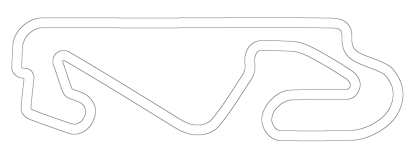
\includegraphics[interpolate=true,width=4.160000in,height=1.570000in]{contents/chapt6/figs/racing/esp-img0.png}}%
\end{pgfscope}%
\begin{pgfscope}%
\pgfpathrectangle{\pgfqpoint{0.150000in}{0.485000in}}{\pgfqpoint{4.160000in}{1.560000in}}%
\pgfusepath{clip}%
\pgfsetrectcap%
\pgfsetroundjoin%
\pgfsetlinewidth{1.003750pt}%
\definecolor{currentstroke}{rgb}{0.452941,0.073853,0.999317}%
\pgfsetstrokecolor{currentstroke}%
\pgfsetstrokeopacity{0.800000}%
\pgfsetdash{}{0pt}%
\pgfpathmoveto{\pgfqpoint{1.480105in}{1.831526in}}%
\pgfpathlineto{\pgfqpoint{1.481747in}{1.831526in}}%
\pgfusepath{stroke}%
\end{pgfscope}%
\begin{pgfscope}%
\pgfpathrectangle{\pgfqpoint{0.150000in}{0.485000in}}{\pgfqpoint{4.160000in}{1.560000in}}%
\pgfusepath{clip}%
\pgfsetrectcap%
\pgfsetroundjoin%
\pgfsetlinewidth{1.003750pt}%
\definecolor{currentstroke}{rgb}{0.405882,0.147302,0.997269}%
\pgfsetstrokecolor{currentstroke}%
\pgfsetstrokeopacity{0.800000}%
\pgfsetdash{}{0pt}%
\pgfpathmoveto{\pgfqpoint{1.481747in}{1.831526in}}%
\pgfpathlineto{\pgfqpoint{1.483416in}{1.831526in}}%
\pgfusepath{stroke}%
\end{pgfscope}%
\begin{pgfscope}%
\pgfpathrectangle{\pgfqpoint{0.150000in}{0.485000in}}{\pgfqpoint{4.160000in}{1.560000in}}%
\pgfusepath{clip}%
\pgfsetrectcap%
\pgfsetroundjoin%
\pgfsetlinewidth{1.003750pt}%
\definecolor{currentstroke}{rgb}{0.358824,0.219946,0.993859}%
\pgfsetstrokecolor{currentstroke}%
\pgfsetstrokeopacity{0.800000}%
\pgfsetdash{}{0pt}%
\pgfpathmoveto{\pgfqpoint{1.483416in}{1.831526in}}%
\pgfpathlineto{\pgfqpoint{1.485111in}{1.831523in}}%
\pgfusepath{stroke}%
\end{pgfscope}%
\begin{pgfscope}%
\pgfpathrectangle{\pgfqpoint{0.150000in}{0.485000in}}{\pgfqpoint{4.160000in}{1.560000in}}%
\pgfusepath{clip}%
\pgfsetrectcap%
\pgfsetroundjoin%
\pgfsetlinewidth{1.003750pt}%
\definecolor{currentstroke}{rgb}{0.319608,0.279583,0.989980}%
\pgfsetstrokecolor{currentstroke}%
\pgfsetstrokeopacity{0.800000}%
\pgfsetdash{}{0pt}%
\pgfpathmoveto{\pgfqpoint{1.485111in}{1.831523in}}%
\pgfpathlineto{\pgfqpoint{1.486830in}{1.831512in}}%
\pgfusepath{stroke}%
\end{pgfscope}%
\begin{pgfscope}%
\pgfpathrectangle{\pgfqpoint{0.150000in}{0.485000in}}{\pgfqpoint{4.160000in}{1.560000in}}%
\pgfusepath{clip}%
\pgfsetrectcap%
\pgfsetroundjoin%
\pgfsetlinewidth{1.003750pt}%
\definecolor{currentstroke}{rgb}{0.280392,0.338158,0.985162}%
\pgfsetstrokecolor{currentstroke}%
\pgfsetstrokeopacity{0.800000}%
\pgfsetdash{}{0pt}%
\pgfpathmoveto{\pgfqpoint{1.486830in}{1.831512in}}%
\pgfpathlineto{\pgfqpoint{1.488574in}{1.831491in}}%
\pgfusepath{stroke}%
\end{pgfscope}%
\begin{pgfscope}%
\pgfpathrectangle{\pgfqpoint{0.150000in}{0.485000in}}{\pgfqpoint{4.160000in}{1.560000in}}%
\pgfusepath{clip}%
\pgfsetrectcap%
\pgfsetroundjoin%
\pgfsetlinewidth{1.003750pt}%
\definecolor{currentstroke}{rgb}{0.233333,0.406737,0.978148}%
\pgfsetstrokecolor{currentstroke}%
\pgfsetstrokeopacity{0.800000}%
\pgfsetdash{}{0pt}%
\pgfpathmoveto{\pgfqpoint{1.488574in}{1.831491in}}%
\pgfpathlineto{\pgfqpoint{1.490339in}{1.831464in}}%
\pgfusepath{stroke}%
\end{pgfscope}%
\begin{pgfscope}%
\pgfpathrectangle{\pgfqpoint{0.150000in}{0.485000in}}{\pgfqpoint{4.160000in}{1.560000in}}%
\pgfusepath{clip}%
\pgfsetrectcap%
\pgfsetroundjoin%
\pgfsetlinewidth{1.003750pt}%
\definecolor{currentstroke}{rgb}{0.194118,0.462204,0.971281}%
\pgfsetstrokecolor{currentstroke}%
\pgfsetstrokeopacity{0.800000}%
\pgfsetdash{}{0pt}%
\pgfpathmoveto{\pgfqpoint{1.490339in}{1.831464in}}%
\pgfpathlineto{\pgfqpoint{1.492131in}{1.831426in}}%
\pgfusepath{stroke}%
\end{pgfscope}%
\begin{pgfscope}%
\pgfpathrectangle{\pgfqpoint{0.150000in}{0.485000in}}{\pgfqpoint{4.160000in}{1.560000in}}%
\pgfusepath{clip}%
\pgfsetrectcap%
\pgfsetroundjoin%
\pgfsetlinewidth{1.003750pt}%
\definecolor{currentstroke}{rgb}{0.147059,0.526432,0.961826}%
\pgfsetstrokecolor{currentstroke}%
\pgfsetstrokeopacity{0.800000}%
\pgfsetdash{}{0pt}%
\pgfpathmoveto{\pgfqpoint{1.492131in}{1.831426in}}%
\pgfpathlineto{\pgfqpoint{1.493943in}{1.831382in}}%
\pgfusepath{stroke}%
\end{pgfscope}%
\begin{pgfscope}%
\pgfpathrectangle{\pgfqpoint{0.150000in}{0.485000in}}{\pgfqpoint{4.160000in}{1.560000in}}%
\pgfusepath{clip}%
\pgfsetrectcap%
\pgfsetroundjoin%
\pgfsetlinewidth{1.003750pt}%
\definecolor{currentstroke}{rgb}{0.115686,0.567675,0.954791}%
\pgfsetstrokecolor{currentstroke}%
\pgfsetstrokeopacity{0.800000}%
\pgfsetdash{}{0pt}%
\pgfpathmoveto{\pgfqpoint{1.493943in}{1.831382in}}%
\pgfpathlineto{\pgfqpoint{1.495778in}{1.831326in}}%
\pgfusepath{stroke}%
\end{pgfscope}%
\begin{pgfscope}%
\pgfpathrectangle{\pgfqpoint{0.150000in}{0.485000in}}{\pgfqpoint{4.160000in}{1.560000in}}%
\pgfusepath{clip}%
\pgfsetrectcap%
\pgfsetroundjoin%
\pgfsetlinewidth{1.003750pt}%
\definecolor{currentstroke}{rgb}{0.076471,0.617278,0.945184}%
\pgfsetstrokecolor{currentstroke}%
\pgfsetstrokeopacity{0.800000}%
\pgfsetdash{}{0pt}%
\pgfpathmoveto{\pgfqpoint{1.495778in}{1.831326in}}%
\pgfpathlineto{\pgfqpoint{1.497632in}{1.831263in}}%
\pgfusepath{stroke}%
\end{pgfscope}%
\begin{pgfscope}%
\pgfpathrectangle{\pgfqpoint{0.150000in}{0.485000in}}{\pgfqpoint{4.160000in}{1.560000in}}%
\pgfusepath{clip}%
\pgfsetrectcap%
\pgfsetroundjoin%
\pgfsetlinewidth{1.003750pt}%
\definecolor{currentstroke}{rgb}{0.029412,0.673696,0.932472}%
\pgfsetstrokecolor{currentstroke}%
\pgfsetstrokeopacity{0.800000}%
\pgfsetdash{}{0pt}%
\pgfpathmoveto{\pgfqpoint{1.497632in}{1.831263in}}%
\pgfpathlineto{\pgfqpoint{1.499508in}{1.831187in}}%
\pgfusepath{stroke}%
\end{pgfscope}%
\begin{pgfscope}%
\pgfpathrectangle{\pgfqpoint{0.150000in}{0.485000in}}{\pgfqpoint{4.160000in}{1.560000in}}%
\pgfusepath{clip}%
\pgfsetrectcap%
\pgfsetroundjoin%
\pgfsetlinewidth{1.003750pt}%
\definecolor{currentstroke}{rgb}{0.017647,0.726434,0.918487}%
\pgfsetstrokecolor{currentstroke}%
\pgfsetstrokeopacity{0.800000}%
\pgfsetdash{}{0pt}%
\pgfpathmoveto{\pgfqpoint{1.499508in}{1.831187in}}%
\pgfpathlineto{\pgfqpoint{1.501408in}{1.831103in}}%
\pgfusepath{stroke}%
\end{pgfscope}%
\begin{pgfscope}%
\pgfpathrectangle{\pgfqpoint{0.150000in}{0.485000in}}{\pgfqpoint{4.160000in}{1.560000in}}%
\pgfusepath{clip}%
\pgfsetrectcap%
\pgfsetroundjoin%
\pgfsetlinewidth{1.003750pt}%
\definecolor{currentstroke}{rgb}{0.064706,0.775204,0.903247}%
\pgfsetstrokecolor{currentstroke}%
\pgfsetstrokeopacity{0.800000}%
\pgfsetdash{}{0pt}%
\pgfpathmoveto{\pgfqpoint{1.501408in}{1.831103in}}%
\pgfpathlineto{\pgfqpoint{1.503333in}{1.831013in}}%
\pgfusepath{stroke}%
\end{pgfscope}%
\begin{pgfscope}%
\pgfpathrectangle{\pgfqpoint{0.150000in}{0.485000in}}{\pgfqpoint{4.160000in}{1.560000in}}%
\pgfusepath{clip}%
\pgfsetrectcap%
\pgfsetroundjoin%
\pgfsetlinewidth{1.003750pt}%
\definecolor{currentstroke}{rgb}{0.111765,0.819740,0.886774}%
\pgfsetstrokecolor{currentstroke}%
\pgfsetstrokeopacity{0.800000}%
\pgfsetdash{}{0pt}%
\pgfpathmoveto{\pgfqpoint{1.503333in}{1.831013in}}%
\pgfpathlineto{\pgfqpoint{1.505284in}{1.830920in}}%
\pgfusepath{stroke}%
\end{pgfscope}%
\begin{pgfscope}%
\pgfpathrectangle{\pgfqpoint{0.150000in}{0.485000in}}{\pgfqpoint{4.160000in}{1.560000in}}%
\pgfusepath{clip}%
\pgfsetrectcap%
\pgfsetroundjoin%
\pgfsetlinewidth{1.003750pt}%
\definecolor{currentstroke}{rgb}{0.158824,0.859800,0.869089}%
\pgfsetstrokecolor{currentstroke}%
\pgfsetstrokeopacity{0.800000}%
\pgfsetdash{}{0pt}%
\pgfpathmoveto{\pgfqpoint{1.505284in}{1.830920in}}%
\pgfpathlineto{\pgfqpoint{1.507261in}{1.830820in}}%
\pgfusepath{stroke}%
\end{pgfscope}%
\begin{pgfscope}%
\pgfpathrectangle{\pgfqpoint{0.150000in}{0.485000in}}{\pgfqpoint{4.160000in}{1.560000in}}%
\pgfusepath{clip}%
\pgfsetrectcap%
\pgfsetroundjoin%
\pgfsetlinewidth{1.003750pt}%
\definecolor{currentstroke}{rgb}{0.198039,0.889604,0.853444}%
\pgfsetstrokecolor{currentstroke}%
\pgfsetstrokeopacity{0.800000}%
\pgfsetdash{}{0pt}%
\pgfpathmoveto{\pgfqpoint{1.507261in}{1.830820in}}%
\pgfpathlineto{\pgfqpoint{1.509259in}{1.830717in}}%
\pgfusepath{stroke}%
\end{pgfscope}%
\begin{pgfscope}%
\pgfpathrectangle{\pgfqpoint{0.150000in}{0.485000in}}{\pgfqpoint{4.160000in}{1.560000in}}%
\pgfusepath{clip}%
\pgfsetrectcap%
\pgfsetroundjoin%
\pgfsetlinewidth{1.003750pt}%
\definecolor{currentstroke}{rgb}{0.237255,0.916034,0.836989}%
\pgfsetstrokecolor{currentstroke}%
\pgfsetstrokeopacity{0.800000}%
\pgfsetdash{}{0pt}%
\pgfpathmoveto{\pgfqpoint{1.509259in}{1.830717in}}%
\pgfpathlineto{\pgfqpoint{1.511281in}{1.830606in}}%
\pgfusepath{stroke}%
\end{pgfscope}%
\begin{pgfscope}%
\pgfpathrectangle{\pgfqpoint{0.150000in}{0.485000in}}{\pgfqpoint{4.160000in}{1.560000in}}%
\pgfusepath{clip}%
\pgfsetrectcap%
\pgfsetroundjoin%
\pgfsetlinewidth{1.003750pt}%
\definecolor{currentstroke}{rgb}{0.276471,0.938988,0.819740}%
\pgfsetstrokecolor{currentstroke}%
\pgfsetstrokeopacity{0.800000}%
\pgfsetdash{}{0pt}%
\pgfpathmoveto{\pgfqpoint{1.511281in}{1.830606in}}%
\pgfpathlineto{\pgfqpoint{1.513325in}{1.830493in}}%
\pgfusepath{stroke}%
\end{pgfscope}%
\begin{pgfscope}%
\pgfpathrectangle{\pgfqpoint{0.150000in}{0.485000in}}{\pgfqpoint{4.160000in}{1.560000in}}%
\pgfusepath{clip}%
\pgfsetrectcap%
\pgfsetroundjoin%
\pgfsetlinewidth{1.003750pt}%
\definecolor{currentstroke}{rgb}{0.315686,0.958381,0.801714}%
\pgfsetstrokecolor{currentstroke}%
\pgfsetstrokeopacity{0.800000}%
\pgfsetdash{}{0pt}%
\pgfpathmoveto{\pgfqpoint{1.513325in}{1.830493in}}%
\pgfpathlineto{\pgfqpoint{1.515390in}{1.830372in}}%
\pgfusepath{stroke}%
\end{pgfscope}%
\begin{pgfscope}%
\pgfpathrectangle{\pgfqpoint{0.150000in}{0.485000in}}{\pgfqpoint{4.160000in}{1.560000in}}%
\pgfusepath{clip}%
\pgfsetrectcap%
\pgfsetroundjoin%
\pgfsetlinewidth{1.003750pt}%
\definecolor{currentstroke}{rgb}{0.354902,0.974139,0.782928}%
\pgfsetstrokecolor{currentstroke}%
\pgfsetstrokeopacity{0.800000}%
\pgfsetdash{}{0pt}%
\pgfpathmoveto{\pgfqpoint{1.515390in}{1.830372in}}%
\pgfpathlineto{\pgfqpoint{1.517476in}{1.830249in}}%
\pgfusepath{stroke}%
\end{pgfscope}%
\begin{pgfscope}%
\pgfpathrectangle{\pgfqpoint{0.150000in}{0.485000in}}{\pgfqpoint{4.160000in}{1.560000in}}%
\pgfusepath{clip}%
\pgfsetrectcap%
\pgfsetroundjoin%
\pgfsetlinewidth{1.003750pt}%
\definecolor{currentstroke}{rgb}{0.386275,0.984086,0.767363}%
\pgfsetstrokecolor{currentstroke}%
\pgfsetstrokeopacity{0.800000}%
\pgfsetdash{}{0pt}%
\pgfpathmoveto{\pgfqpoint{1.517476in}{1.830249in}}%
\pgfpathlineto{\pgfqpoint{1.519583in}{1.830119in}}%
\pgfusepath{stroke}%
\end{pgfscope}%
\begin{pgfscope}%
\pgfpathrectangle{\pgfqpoint{0.150000in}{0.485000in}}{\pgfqpoint{4.160000in}{1.560000in}}%
\pgfusepath{clip}%
\pgfsetrectcap%
\pgfsetroundjoin%
\pgfsetlinewidth{1.003750pt}%
\definecolor{currentstroke}{rgb}{0.425490,0.993159,0.747253}%
\pgfsetstrokecolor{currentstroke}%
\pgfsetstrokeopacity{0.800000}%
\pgfsetdash{}{0pt}%
\pgfpathmoveto{\pgfqpoint{1.519583in}{1.830119in}}%
\pgfpathlineto{\pgfqpoint{1.521708in}{1.829986in}}%
\pgfusepath{stroke}%
\end{pgfscope}%
\begin{pgfscope}%
\pgfpathrectangle{\pgfqpoint{0.150000in}{0.485000in}}{\pgfqpoint{4.160000in}{1.560000in}}%
\pgfusepath{clip}%
\pgfsetrectcap%
\pgfsetroundjoin%
\pgfsetlinewidth{1.003750pt}%
\definecolor{currentstroke}{rgb}{0.449020,0.996795,0.734845}%
\pgfsetstrokecolor{currentstroke}%
\pgfsetstrokeopacity{0.800000}%
\pgfsetdash{}{0pt}%
\pgfpathmoveto{\pgfqpoint{1.521708in}{1.829986in}}%
\pgfpathlineto{\pgfqpoint{1.523850in}{1.829854in}}%
\pgfusepath{stroke}%
\end{pgfscope}%
\begin{pgfscope}%
\pgfpathrectangle{\pgfqpoint{0.150000in}{0.485000in}}{\pgfqpoint{4.160000in}{1.560000in}}%
\pgfusepath{clip}%
\pgfsetrectcap%
\pgfsetroundjoin%
\pgfsetlinewidth{1.003750pt}%
\definecolor{currentstroke}{rgb}{0.472549,0.999070,0.722186}%
\pgfsetstrokecolor{currentstroke}%
\pgfsetstrokeopacity{0.800000}%
\pgfsetdash{}{0pt}%
\pgfpathmoveto{\pgfqpoint{1.523850in}{1.829854in}}%
\pgfpathlineto{\pgfqpoint{1.526008in}{1.829728in}}%
\pgfusepath{stroke}%
\end{pgfscope}%
\begin{pgfscope}%
\pgfpathrectangle{\pgfqpoint{0.150000in}{0.485000in}}{\pgfqpoint{4.160000in}{1.560000in}}%
\pgfusepath{clip}%
\pgfsetrectcap%
\pgfsetroundjoin%
\pgfsetlinewidth{1.003750pt}%
\definecolor{currentstroke}{rgb}{0.496078,0.999981,0.709281}%
\pgfsetstrokecolor{currentstroke}%
\pgfsetstrokeopacity{0.800000}%
\pgfsetdash{}{0pt}%
\pgfpathmoveto{\pgfqpoint{1.526008in}{1.829728in}}%
\pgfpathlineto{\pgfqpoint{1.528180in}{1.829611in}}%
\pgfusepath{stroke}%
\end{pgfscope}%
\begin{pgfscope}%
\pgfpathrectangle{\pgfqpoint{0.150000in}{0.485000in}}{\pgfqpoint{4.160000in}{1.560000in}}%
\pgfusepath{clip}%
\pgfsetrectcap%
\pgfsetroundjoin%
\pgfsetlinewidth{1.003750pt}%
\definecolor{currentstroke}{rgb}{0.527451,0.999070,0.691698}%
\pgfsetstrokecolor{currentstroke}%
\pgfsetstrokeopacity{0.800000}%
\pgfsetdash{}{0pt}%
\pgfpathmoveto{\pgfqpoint{1.528180in}{1.829611in}}%
\pgfpathlineto{\pgfqpoint{1.530366in}{1.829498in}}%
\pgfusepath{stroke}%
\end{pgfscope}%
\begin{pgfscope}%
\pgfpathrectangle{\pgfqpoint{0.150000in}{0.485000in}}{\pgfqpoint{4.160000in}{1.560000in}}%
\pgfusepath{clip}%
\pgfsetrectcap%
\pgfsetroundjoin%
\pgfsetlinewidth{1.003750pt}%
\definecolor{currentstroke}{rgb}{0.550980,0.996795,0.678235}%
\pgfsetstrokecolor{currentstroke}%
\pgfsetstrokeopacity{0.800000}%
\pgfsetdash{}{0pt}%
\pgfpathmoveto{\pgfqpoint{1.530366in}{1.829498in}}%
\pgfpathlineto{\pgfqpoint{1.532567in}{1.829395in}}%
\pgfusepath{stroke}%
\end{pgfscope}%
\begin{pgfscope}%
\pgfpathrectangle{\pgfqpoint{0.150000in}{0.485000in}}{\pgfqpoint{4.160000in}{1.560000in}}%
\pgfusepath{clip}%
\pgfsetrectcap%
\pgfsetroundjoin%
\pgfsetlinewidth{1.003750pt}%
\definecolor{currentstroke}{rgb}{0.582353,0.991645,0.659925}%
\pgfsetstrokecolor{currentstroke}%
\pgfsetstrokeopacity{0.800000}%
\pgfsetdash{}{0pt}%
\pgfpathmoveto{\pgfqpoint{1.532567in}{1.829395in}}%
\pgfpathlineto{\pgfqpoint{1.534784in}{1.829297in}}%
\pgfusepath{stroke}%
\end{pgfscope}%
\begin{pgfscope}%
\pgfpathrectangle{\pgfqpoint{0.150000in}{0.485000in}}{\pgfqpoint{4.160000in}{1.560000in}}%
\pgfusepath{clip}%
\pgfsetrectcap%
\pgfsetroundjoin%
\pgfsetlinewidth{1.003750pt}%
\definecolor{currentstroke}{rgb}{0.605882,0.986201,0.645928}%
\pgfsetstrokecolor{currentstroke}%
\pgfsetstrokeopacity{0.800000}%
\pgfsetdash{}{0pt}%
\pgfpathmoveto{\pgfqpoint{1.534784in}{1.829297in}}%
\pgfpathlineto{\pgfqpoint{1.537017in}{1.829211in}}%
\pgfusepath{stroke}%
\end{pgfscope}%
\begin{pgfscope}%
\pgfpathrectangle{\pgfqpoint{0.150000in}{0.485000in}}{\pgfqpoint{4.160000in}{1.560000in}}%
\pgfusepath{clip}%
\pgfsetrectcap%
\pgfsetroundjoin%
\pgfsetlinewidth{1.003750pt}%
\definecolor{currentstroke}{rgb}{0.629412,0.979410,0.631711}%
\pgfsetstrokecolor{currentstroke}%
\pgfsetstrokeopacity{0.800000}%
\pgfsetdash{}{0pt}%
\pgfpathmoveto{\pgfqpoint{1.537017in}{1.829211in}}%
\pgfpathlineto{\pgfqpoint{1.539261in}{1.829132in}}%
\pgfusepath{stroke}%
\end{pgfscope}%
\begin{pgfscope}%
\pgfpathrectangle{\pgfqpoint{0.150000in}{0.485000in}}{\pgfqpoint{4.160000in}{1.560000in}}%
\pgfusepath{clip}%
\pgfsetrectcap%
\pgfsetroundjoin%
\pgfsetlinewidth{1.003750pt}%
\definecolor{currentstroke}{rgb}{0.660784,0.968276,0.612420}%
\pgfsetstrokecolor{currentstroke}%
\pgfsetstrokeopacity{0.800000}%
\pgfsetdash{}{0pt}%
\pgfpathmoveto{\pgfqpoint{1.539261in}{1.829132in}}%
\pgfpathlineto{\pgfqpoint{1.541520in}{1.829066in}}%
\pgfusepath{stroke}%
\end{pgfscope}%
\begin{pgfscope}%
\pgfpathrectangle{\pgfqpoint{0.150000in}{0.485000in}}{\pgfqpoint{4.160000in}{1.560000in}}%
\pgfusepath{clip}%
\pgfsetrectcap%
\pgfsetroundjoin%
\pgfsetlinewidth{1.003750pt}%
\definecolor{currentstroke}{rgb}{0.684314,0.958381,0.597707}%
\pgfsetstrokecolor{currentstroke}%
\pgfsetstrokeopacity{0.800000}%
\pgfsetdash{}{0pt}%
\pgfpathmoveto{\pgfqpoint{1.541520in}{1.829066in}}%
\pgfpathlineto{\pgfqpoint{1.543794in}{1.829009in}}%
\pgfusepath{stroke}%
\end{pgfscope}%
\begin{pgfscope}%
\pgfpathrectangle{\pgfqpoint{0.150000in}{0.485000in}}{\pgfqpoint{4.160000in}{1.560000in}}%
\pgfusepath{clip}%
\pgfsetrectcap%
\pgfsetroundjoin%
\pgfsetlinewidth{1.003750pt}%
\definecolor{currentstroke}{rgb}{0.707843,0.947177,0.582791}%
\pgfsetstrokecolor{currentstroke}%
\pgfsetstrokeopacity{0.800000}%
\pgfsetdash{}{0pt}%
\pgfpathmoveto{\pgfqpoint{1.543794in}{1.829009in}}%
\pgfpathlineto{\pgfqpoint{1.546082in}{1.828958in}}%
\pgfusepath{stroke}%
\end{pgfscope}%
\begin{pgfscope}%
\pgfpathrectangle{\pgfqpoint{0.150000in}{0.485000in}}{\pgfqpoint{4.160000in}{1.560000in}}%
\pgfusepath{clip}%
\pgfsetrectcap%
\pgfsetroundjoin%
\pgfsetlinewidth{1.003750pt}%
\definecolor{currentstroke}{rgb}{0.739216,0.930229,0.562593}%
\pgfsetstrokecolor{currentstroke}%
\pgfsetstrokeopacity{0.800000}%
\pgfsetdash{}{0pt}%
\pgfpathmoveto{\pgfqpoint{1.546082in}{1.828958in}}%
\pgfpathlineto{\pgfqpoint{1.548386in}{1.828911in}}%
\pgfusepath{stroke}%
\end{pgfscope}%
\begin{pgfscope}%
\pgfpathrectangle{\pgfqpoint{0.150000in}{0.485000in}}{\pgfqpoint{4.160000in}{1.560000in}}%
\pgfusepath{clip}%
\pgfsetrectcap%
\pgfsetroundjoin%
\pgfsetlinewidth{1.003750pt}%
\definecolor{currentstroke}{rgb}{0.754902,0.920906,0.552365}%
\pgfsetstrokecolor{currentstroke}%
\pgfsetstrokeopacity{0.800000}%
\pgfsetdash{}{0pt}%
\pgfpathmoveto{\pgfqpoint{1.548386in}{1.828911in}}%
\pgfpathlineto{\pgfqpoint{1.550703in}{1.828865in}}%
\pgfusepath{stroke}%
\end{pgfscope}%
\begin{pgfscope}%
\pgfpathrectangle{\pgfqpoint{0.150000in}{0.485000in}}{\pgfqpoint{4.160000in}{1.560000in}}%
\pgfusepath{clip}%
\pgfsetrectcap%
\pgfsetroundjoin%
\pgfsetlinewidth{1.003750pt}%
\definecolor{currentstroke}{rgb}{0.778431,0.905873,0.536867}%
\pgfsetstrokecolor{currentstroke}%
\pgfsetstrokeopacity{0.800000}%
\pgfsetdash{}{0pt}%
\pgfpathmoveto{\pgfqpoint{1.550703in}{1.828865in}}%
\pgfpathlineto{\pgfqpoint{1.553033in}{1.828816in}}%
\pgfusepath{stroke}%
\end{pgfscope}%
\begin{pgfscope}%
\pgfpathrectangle{\pgfqpoint{0.150000in}{0.485000in}}{\pgfqpoint{4.160000in}{1.560000in}}%
\pgfusepath{clip}%
\pgfsetrectcap%
\pgfsetroundjoin%
\pgfsetlinewidth{1.003750pt}%
\definecolor{currentstroke}{rgb}{0.801961,0.889604,0.521185}%
\pgfsetstrokecolor{currentstroke}%
\pgfsetstrokeopacity{0.800000}%
\pgfsetdash{}{0pt}%
\pgfpathmoveto{\pgfqpoint{1.553033in}{1.828816in}}%
\pgfpathlineto{\pgfqpoint{1.555375in}{1.828768in}}%
\pgfusepath{stroke}%
\end{pgfscope}%
\begin{pgfscope}%
\pgfpathrectangle{\pgfqpoint{0.150000in}{0.485000in}}{\pgfqpoint{4.160000in}{1.560000in}}%
\pgfusepath{clip}%
\pgfsetrectcap%
\pgfsetroundjoin%
\pgfsetlinewidth{1.003750pt}%
\definecolor{currentstroke}{rgb}{0.817647,0.878081,0.510631}%
\pgfsetstrokecolor{currentstroke}%
\pgfsetstrokeopacity{0.800000}%
\pgfsetdash{}{0pt}%
\pgfpathmoveto{\pgfqpoint{1.555375in}{1.828768in}}%
\pgfpathlineto{\pgfqpoint{1.557727in}{1.828717in}}%
\pgfusepath{stroke}%
\end{pgfscope}%
\begin{pgfscope}%
\pgfpathrectangle{\pgfqpoint{0.150000in}{0.485000in}}{\pgfqpoint{4.160000in}{1.560000in}}%
\pgfusepath{clip}%
\pgfsetrectcap%
\pgfsetroundjoin%
\pgfsetlinewidth{1.003750pt}%
\definecolor{currentstroke}{rgb}{0.849020,0.853444,0.489293}%
\pgfsetstrokecolor{currentstroke}%
\pgfsetstrokeopacity{0.800000}%
\pgfsetdash{}{0pt}%
\pgfpathmoveto{\pgfqpoint{1.557727in}{1.828717in}}%
\pgfpathlineto{\pgfqpoint{1.560090in}{1.828667in}}%
\pgfusepath{stroke}%
\end{pgfscope}%
\begin{pgfscope}%
\pgfpathrectangle{\pgfqpoint{0.150000in}{0.485000in}}{\pgfqpoint{4.160000in}{1.560000in}}%
\pgfusepath{clip}%
\pgfsetrectcap%
\pgfsetroundjoin%
\pgfsetlinewidth{1.003750pt}%
\definecolor{currentstroke}{rgb}{0.872549,0.833602,0.473094}%
\pgfsetstrokecolor{currentstroke}%
\pgfsetstrokeopacity{0.800000}%
\pgfsetdash{}{0pt}%
\pgfpathmoveto{\pgfqpoint{1.560090in}{1.828667in}}%
\pgfpathlineto{\pgfqpoint{1.562468in}{1.828613in}}%
\pgfusepath{stroke}%
\end{pgfscope}%
\begin{pgfscope}%
\pgfpathrectangle{\pgfqpoint{0.150000in}{0.485000in}}{\pgfqpoint{4.160000in}{1.560000in}}%
\pgfusepath{clip}%
\pgfsetrectcap%
\pgfsetroundjoin%
\pgfsetlinewidth{1.003750pt}%
\definecolor{currentstroke}{rgb}{0.880392,0.826734,0.467658}%
\pgfsetstrokecolor{currentstroke}%
\pgfsetstrokeopacity{0.800000}%
\pgfsetdash{}{0pt}%
\pgfpathmoveto{\pgfqpoint{1.562468in}{1.828613in}}%
\pgfpathlineto{\pgfqpoint{1.564858in}{1.828557in}}%
\pgfusepath{stroke}%
\end{pgfscope}%
\begin{pgfscope}%
\pgfpathrectangle{\pgfqpoint{0.150000in}{0.485000in}}{\pgfqpoint{4.160000in}{1.560000in}}%
\pgfusepath{clip}%
\pgfsetrectcap%
\pgfsetroundjoin%
\pgfsetlinewidth{1.003750pt}%
\definecolor{currentstroke}{rgb}{0.903922,0.805381,0.451244}%
\pgfsetstrokecolor{currentstroke}%
\pgfsetstrokeopacity{0.800000}%
\pgfsetdash{}{0pt}%
\pgfpathmoveto{\pgfqpoint{1.564858in}{1.828557in}}%
\pgfpathlineto{\pgfqpoint{1.567255in}{1.828494in}}%
\pgfusepath{stroke}%
\end{pgfscope}%
\begin{pgfscope}%
\pgfpathrectangle{\pgfqpoint{0.150000in}{0.485000in}}{\pgfqpoint{4.160000in}{1.560000in}}%
\pgfusepath{clip}%
\pgfsetrectcap%
\pgfsetroundjoin%
\pgfsetlinewidth{1.003750pt}%
\definecolor{currentstroke}{rgb}{0.919608,0.790532,0.440216}%
\pgfsetstrokecolor{currentstroke}%
\pgfsetstrokeopacity{0.800000}%
\pgfsetdash{}{0pt}%
\pgfpathmoveto{\pgfqpoint{1.567255in}{1.828494in}}%
\pgfpathlineto{\pgfqpoint{1.569662in}{1.828429in}}%
\pgfusepath{stroke}%
\end{pgfscope}%
\begin{pgfscope}%
\pgfpathrectangle{\pgfqpoint{0.150000in}{0.485000in}}{\pgfqpoint{4.160000in}{1.560000in}}%
\pgfusepath{clip}%
\pgfsetrectcap%
\pgfsetroundjoin%
\pgfsetlinewidth{1.003750pt}%
\definecolor{currentstroke}{rgb}{0.943137,0.767363,0.423549}%
\pgfsetstrokecolor{currentstroke}%
\pgfsetstrokeopacity{0.800000}%
\pgfsetdash{}{0pt}%
\pgfpathmoveto{\pgfqpoint{1.569662in}{1.828429in}}%
\pgfpathlineto{\pgfqpoint{1.572079in}{1.828355in}}%
\pgfusepath{stroke}%
\end{pgfscope}%
\begin{pgfscope}%
\pgfpathrectangle{\pgfqpoint{0.150000in}{0.485000in}}{\pgfqpoint{4.160000in}{1.560000in}}%
\pgfusepath{clip}%
\pgfsetrectcap%
\pgfsetroundjoin%
\pgfsetlinewidth{1.003750pt}%
\definecolor{currentstroke}{rgb}{0.966667,0.743145,0.406737}%
\pgfsetstrokecolor{currentstroke}%
\pgfsetstrokeopacity{0.800000}%
\pgfsetdash{}{0pt}%
\pgfpathmoveto{\pgfqpoint{1.572079in}{1.828355in}}%
\pgfpathlineto{\pgfqpoint{1.574508in}{1.828277in}}%
\pgfusepath{stroke}%
\end{pgfscope}%
\begin{pgfscope}%
\pgfpathrectangle{\pgfqpoint{0.150000in}{0.485000in}}{\pgfqpoint{4.160000in}{1.560000in}}%
\pgfusepath{clip}%
\pgfsetrectcap%
\pgfsetroundjoin%
\pgfsetlinewidth{1.003750pt}%
\definecolor{currentstroke}{rgb}{0.982353,0.726434,0.395451}%
\pgfsetstrokecolor{currentstroke}%
\pgfsetstrokeopacity{0.800000}%
\pgfsetdash{}{0pt}%
\pgfpathmoveto{\pgfqpoint{1.574508in}{1.828277in}}%
\pgfpathlineto{\pgfqpoint{1.576949in}{1.828189in}}%
\pgfusepath{stroke}%
\end{pgfscope}%
\begin{pgfscope}%
\pgfpathrectangle{\pgfqpoint{0.150000in}{0.485000in}}{\pgfqpoint{4.160000in}{1.560000in}}%
\pgfusepath{clip}%
\pgfsetrectcap%
\pgfsetroundjoin%
\pgfsetlinewidth{1.003750pt}%
\definecolor{currentstroke}{rgb}{0.998039,0.709281,0.384106}%
\pgfsetstrokecolor{currentstroke}%
\pgfsetstrokeopacity{0.800000}%
\pgfsetdash{}{0pt}%
\pgfpathmoveto{\pgfqpoint{1.576949in}{1.828189in}}%
\pgfpathlineto{\pgfqpoint{1.579401in}{1.828094in}}%
\pgfusepath{stroke}%
\end{pgfscope}%
\begin{pgfscope}%
\pgfpathrectangle{\pgfqpoint{0.150000in}{0.485000in}}{\pgfqpoint{4.160000in}{1.560000in}}%
\pgfusepath{clip}%
\pgfsetrectcap%
\pgfsetroundjoin%
\pgfsetlinewidth{1.003750pt}%
\definecolor{currentstroke}{rgb}{1.000000,0.691698,0.372702}%
\pgfsetstrokecolor{currentstroke}%
\pgfsetstrokeopacity{0.800000}%
\pgfsetdash{}{0pt}%
\pgfpathmoveto{\pgfqpoint{1.579401in}{1.828094in}}%
\pgfpathlineto{\pgfqpoint{1.581859in}{1.827989in}}%
\pgfusepath{stroke}%
\end{pgfscope}%
\begin{pgfscope}%
\pgfpathrectangle{\pgfqpoint{0.150000in}{0.485000in}}{\pgfqpoint{4.160000in}{1.560000in}}%
\pgfusepath{clip}%
\pgfsetrectcap%
\pgfsetroundjoin%
\pgfsetlinewidth{1.003750pt}%
\definecolor{currentstroke}{rgb}{1.000000,0.673696,0.361242}%
\pgfsetstrokecolor{currentstroke}%
\pgfsetstrokeopacity{0.800000}%
\pgfsetdash{}{0pt}%
\pgfpathmoveto{\pgfqpoint{1.581859in}{1.827989in}}%
\pgfpathlineto{\pgfqpoint{1.584326in}{1.827867in}}%
\pgfusepath{stroke}%
\end{pgfscope}%
\begin{pgfscope}%
\pgfpathrectangle{\pgfqpoint{0.150000in}{0.485000in}}{\pgfqpoint{4.160000in}{1.560000in}}%
\pgfusepath{clip}%
\pgfsetrectcap%
\pgfsetroundjoin%
\pgfsetlinewidth{1.003750pt}%
\definecolor{currentstroke}{rgb}{1.000000,0.655284,0.349727}%
\pgfsetstrokecolor{currentstroke}%
\pgfsetstrokeopacity{0.800000}%
\pgfsetdash{}{0pt}%
\pgfpathmoveto{\pgfqpoint{1.584326in}{1.827867in}}%
\pgfpathlineto{\pgfqpoint{1.586800in}{1.827735in}}%
\pgfusepath{stroke}%
\end{pgfscope}%
\begin{pgfscope}%
\pgfpathrectangle{\pgfqpoint{0.150000in}{0.485000in}}{\pgfqpoint{4.160000in}{1.560000in}}%
\pgfusepath{clip}%
\pgfsetrectcap%
\pgfsetroundjoin%
\pgfsetlinewidth{1.003750pt}%
\definecolor{currentstroke}{rgb}{1.000000,0.645928,0.343949}%
\pgfsetstrokecolor{currentstroke}%
\pgfsetstrokeopacity{0.800000}%
\pgfsetdash{}{0pt}%
\pgfpathmoveto{\pgfqpoint{1.586800in}{1.827735in}}%
\pgfpathlineto{\pgfqpoint{1.589282in}{1.827586in}}%
\pgfusepath{stroke}%
\end{pgfscope}%
\begin{pgfscope}%
\pgfpathrectangle{\pgfqpoint{0.150000in}{0.485000in}}{\pgfqpoint{4.160000in}{1.560000in}}%
\pgfusepath{clip}%
\pgfsetrectcap%
\pgfsetroundjoin%
\pgfsetlinewidth{1.003750pt}%
\definecolor{currentstroke}{rgb}{1.000000,0.636474,0.338158}%
\pgfsetstrokecolor{currentstroke}%
\pgfsetstrokeopacity{0.800000}%
\pgfsetdash{}{0pt}%
\pgfpathmoveto{\pgfqpoint{1.589282in}{1.827586in}}%
\pgfpathlineto{\pgfqpoint{1.591766in}{1.827425in}}%
\pgfusepath{stroke}%
\end{pgfscope}%
\begin{pgfscope}%
\pgfpathrectangle{\pgfqpoint{0.150000in}{0.485000in}}{\pgfqpoint{4.160000in}{1.560000in}}%
\pgfusepath{clip}%
\pgfsetrectcap%
\pgfsetroundjoin%
\pgfsetlinewidth{1.003750pt}%
\definecolor{currentstroke}{rgb}{1.000000,0.617278,0.326539}%
\pgfsetstrokecolor{currentstroke}%
\pgfsetstrokeopacity{0.800000}%
\pgfsetdash{}{0pt}%
\pgfpathmoveto{\pgfqpoint{1.591766in}{1.827425in}}%
\pgfpathlineto{\pgfqpoint{1.594255in}{1.827254in}}%
\pgfusepath{stroke}%
\end{pgfscope}%
\begin{pgfscope}%
\pgfpathrectangle{\pgfqpoint{0.150000in}{0.485000in}}{\pgfqpoint{4.160000in}{1.560000in}}%
\pgfusepath{clip}%
\pgfsetrectcap%
\pgfsetroundjoin%
\pgfsetlinewidth{1.003750pt}%
\definecolor{currentstroke}{rgb}{1.000000,0.597707,0.314870}%
\pgfsetstrokecolor{currentstroke}%
\pgfsetstrokeopacity{0.800000}%
\pgfsetdash{}{0pt}%
\pgfpathmoveto{\pgfqpoint{1.594255in}{1.827254in}}%
\pgfpathlineto{\pgfqpoint{1.596753in}{1.827078in}}%
\pgfusepath{stroke}%
\end{pgfscope}%
\begin{pgfscope}%
\pgfpathrectangle{\pgfqpoint{0.150000in}{0.485000in}}{\pgfqpoint{4.160000in}{1.560000in}}%
\pgfusepath{clip}%
\pgfsetrectcap%
\pgfsetroundjoin%
\pgfsetlinewidth{1.003750pt}%
\definecolor{currentstroke}{rgb}{1.000000,0.597707,0.314870}%
\pgfsetstrokecolor{currentstroke}%
\pgfsetstrokeopacity{0.800000}%
\pgfsetdash{}{0pt}%
\pgfpathmoveto{\pgfqpoint{1.596753in}{1.827078in}}%
\pgfpathlineto{\pgfqpoint{1.599258in}{1.826898in}}%
\pgfusepath{stroke}%
\end{pgfscope}%
\begin{pgfscope}%
\pgfpathrectangle{\pgfqpoint{0.150000in}{0.485000in}}{\pgfqpoint{4.160000in}{1.560000in}}%
\pgfusepath{clip}%
\pgfsetrectcap%
\pgfsetroundjoin%
\pgfsetlinewidth{1.003750pt}%
\definecolor{currentstroke}{rgb}{1.000000,0.587785,0.309017}%
\pgfsetstrokecolor{currentstroke}%
\pgfsetstrokeopacity{0.800000}%
\pgfsetdash{}{0pt}%
\pgfpathmoveto{\pgfqpoint{1.599258in}{1.826898in}}%
\pgfpathlineto{\pgfqpoint{1.601766in}{1.826719in}}%
\pgfusepath{stroke}%
\end{pgfscope}%
\begin{pgfscope}%
\pgfpathrectangle{\pgfqpoint{0.150000in}{0.485000in}}{\pgfqpoint{4.160000in}{1.560000in}}%
\pgfusepath{clip}%
\pgfsetrectcap%
\pgfsetroundjoin%
\pgfsetlinewidth{1.003750pt}%
\definecolor{currentstroke}{rgb}{1.000000,0.577774,0.303153}%
\pgfsetstrokecolor{currentstroke}%
\pgfsetstrokeopacity{0.800000}%
\pgfsetdash{}{0pt}%
\pgfpathmoveto{\pgfqpoint{1.601766in}{1.826719in}}%
\pgfpathlineto{\pgfqpoint{1.604277in}{1.826545in}}%
\pgfusepath{stroke}%
\end{pgfscope}%
\begin{pgfscope}%
\pgfpathrectangle{\pgfqpoint{0.150000in}{0.485000in}}{\pgfqpoint{4.160000in}{1.560000in}}%
\pgfusepath{clip}%
\pgfsetrectcap%
\pgfsetroundjoin%
\pgfsetlinewidth{1.003750pt}%
\definecolor{currentstroke}{rgb}{1.000000,0.557489,0.291390}%
\pgfsetstrokecolor{currentstroke}%
\pgfsetstrokeopacity{0.800000}%
\pgfsetdash{}{0pt}%
\pgfpathmoveto{\pgfqpoint{1.604277in}{1.826545in}}%
\pgfpathlineto{\pgfqpoint{1.606793in}{1.826370in}}%
\pgfusepath{stroke}%
\end{pgfscope}%
\begin{pgfscope}%
\pgfpathrectangle{\pgfqpoint{0.150000in}{0.485000in}}{\pgfqpoint{4.160000in}{1.560000in}}%
\pgfusepath{clip}%
\pgfsetrectcap%
\pgfsetroundjoin%
\pgfsetlinewidth{1.003750pt}%
\definecolor{currentstroke}{rgb}{1.000000,0.557489,0.291390}%
\pgfsetstrokecolor{currentstroke}%
\pgfsetstrokeopacity{0.800000}%
\pgfsetdash{}{0pt}%
\pgfpathmoveto{\pgfqpoint{1.606793in}{1.826370in}}%
\pgfpathlineto{\pgfqpoint{1.609315in}{1.826201in}}%
\pgfusepath{stroke}%
\end{pgfscope}%
\begin{pgfscope}%
\pgfpathrectangle{\pgfqpoint{0.150000in}{0.485000in}}{\pgfqpoint{4.160000in}{1.560000in}}%
\pgfusepath{clip}%
\pgfsetrectcap%
\pgfsetroundjoin%
\pgfsetlinewidth{1.003750pt}%
\definecolor{currentstroke}{rgb}{1.000000,0.547220,0.285492}%
\pgfsetstrokecolor{currentstroke}%
\pgfsetstrokeopacity{0.800000}%
\pgfsetdash{}{0pt}%
\pgfpathmoveto{\pgfqpoint{1.609315in}{1.826201in}}%
\pgfpathlineto{\pgfqpoint{1.611841in}{1.826035in}}%
\pgfusepath{stroke}%
\end{pgfscope}%
\begin{pgfscope}%
\pgfpathrectangle{\pgfqpoint{0.150000in}{0.485000in}}{\pgfqpoint{4.160000in}{1.560000in}}%
\pgfusepath{clip}%
\pgfsetrectcap%
\pgfsetroundjoin%
\pgfsetlinewidth{1.003750pt}%
\definecolor{currentstroke}{rgb}{1.000000,0.547220,0.285492}%
\pgfsetstrokecolor{currentstroke}%
\pgfsetstrokeopacity{0.800000}%
\pgfsetdash{}{0pt}%
\pgfpathmoveto{\pgfqpoint{1.611841in}{1.826035in}}%
\pgfpathlineto{\pgfqpoint{1.614371in}{1.825876in}}%
\pgfusepath{stroke}%
\end{pgfscope}%
\begin{pgfscope}%
\pgfpathrectangle{\pgfqpoint{0.150000in}{0.485000in}}{\pgfqpoint{4.160000in}{1.560000in}}%
\pgfusepath{clip}%
\pgfsetrectcap%
\pgfsetroundjoin%
\pgfsetlinewidth{1.003750pt}%
\definecolor{currentstroke}{rgb}{1.000000,0.526432,0.273663}%
\pgfsetstrokecolor{currentstroke}%
\pgfsetstrokeopacity{0.800000}%
\pgfsetdash{}{0pt}%
\pgfpathmoveto{\pgfqpoint{1.614371in}{1.825876in}}%
\pgfpathlineto{\pgfqpoint{1.616902in}{1.825723in}}%
\pgfusepath{stroke}%
\end{pgfscope}%
\begin{pgfscope}%
\pgfpathrectangle{\pgfqpoint{0.150000in}{0.485000in}}{\pgfqpoint{4.160000in}{1.560000in}}%
\pgfusepath{clip}%
\pgfsetrectcap%
\pgfsetroundjoin%
\pgfsetlinewidth{1.003750pt}%
\definecolor{currentstroke}{rgb}{1.000000,0.526432,0.273663}%
\pgfsetstrokecolor{currentstroke}%
\pgfsetstrokeopacity{0.800000}%
\pgfsetdash{}{0pt}%
\pgfpathmoveto{\pgfqpoint{1.616902in}{1.825723in}}%
\pgfpathlineto{\pgfqpoint{1.619439in}{1.825572in}}%
\pgfusepath{stroke}%
\end{pgfscope}%
\begin{pgfscope}%
\pgfpathrectangle{\pgfqpoint{0.150000in}{0.485000in}}{\pgfqpoint{4.160000in}{1.560000in}}%
\pgfusepath{clip}%
\pgfsetrectcap%
\pgfsetroundjoin%
\pgfsetlinewidth{1.003750pt}%
\definecolor{currentstroke}{rgb}{1.000000,0.515918,0.267733}%
\pgfsetstrokecolor{currentstroke}%
\pgfsetstrokeopacity{0.800000}%
\pgfsetdash{}{0pt}%
\pgfpathmoveto{\pgfqpoint{1.619439in}{1.825572in}}%
\pgfpathlineto{\pgfqpoint{1.621979in}{1.825430in}}%
\pgfusepath{stroke}%
\end{pgfscope}%
\begin{pgfscope}%
\pgfpathrectangle{\pgfqpoint{0.150000in}{0.485000in}}{\pgfqpoint{4.160000in}{1.560000in}}%
\pgfusepath{clip}%
\pgfsetrectcap%
\pgfsetroundjoin%
\pgfsetlinewidth{1.003750pt}%
\definecolor{currentstroke}{rgb}{1.000000,0.494656,0.255843}%
\pgfsetstrokecolor{currentstroke}%
\pgfsetstrokeopacity{0.800000}%
\pgfsetdash{}{0pt}%
\pgfpathmoveto{\pgfqpoint{1.621979in}{1.825430in}}%
\pgfpathlineto{\pgfqpoint{1.624524in}{1.825294in}}%
\pgfusepath{stroke}%
\end{pgfscope}%
\begin{pgfscope}%
\pgfpathrectangle{\pgfqpoint{0.150000in}{0.485000in}}{\pgfqpoint{4.160000in}{1.560000in}}%
\pgfusepath{clip}%
\pgfsetrectcap%
\pgfsetroundjoin%
\pgfsetlinewidth{1.003750pt}%
\definecolor{currentstroke}{rgb}{1.000000,0.505325,0.261793}%
\pgfsetstrokecolor{currentstroke}%
\pgfsetstrokeopacity{0.800000}%
\pgfsetdash{}{0pt}%
\pgfpathmoveto{\pgfqpoint{1.624524in}{1.825294in}}%
\pgfpathlineto{\pgfqpoint{1.627074in}{1.825169in}}%
\pgfusepath{stroke}%
\end{pgfscope}%
\begin{pgfscope}%
\pgfpathrectangle{\pgfqpoint{0.150000in}{0.485000in}}{\pgfqpoint{4.160000in}{1.560000in}}%
\pgfusepath{clip}%
\pgfsetrectcap%
\pgfsetroundjoin%
\pgfsetlinewidth{1.003750pt}%
\definecolor{currentstroke}{rgb}{1.000000,0.494656,0.255843}%
\pgfsetstrokecolor{currentstroke}%
\pgfsetstrokeopacity{0.800000}%
\pgfsetdash{}{0pt}%
\pgfpathmoveto{\pgfqpoint{1.627074in}{1.825169in}}%
\pgfpathlineto{\pgfqpoint{1.629624in}{1.825052in}}%
\pgfusepath{stroke}%
\end{pgfscope}%
\begin{pgfscope}%
\pgfpathrectangle{\pgfqpoint{0.150000in}{0.485000in}}{\pgfqpoint{4.160000in}{1.560000in}}%
\pgfusepath{clip}%
\pgfsetrectcap%
\pgfsetroundjoin%
\pgfsetlinewidth{1.003750pt}%
\definecolor{currentstroke}{rgb}{1.000000,0.494656,0.255843}%
\pgfsetstrokecolor{currentstroke}%
\pgfsetstrokeopacity{0.800000}%
\pgfsetdash{}{0pt}%
\pgfpathmoveto{\pgfqpoint{1.629624in}{1.825052in}}%
\pgfpathlineto{\pgfqpoint{1.632176in}{1.824949in}}%
\pgfusepath{stroke}%
\end{pgfscope}%
\begin{pgfscope}%
\pgfpathrectangle{\pgfqpoint{0.150000in}{0.485000in}}{\pgfqpoint{4.160000in}{1.560000in}}%
\pgfusepath{clip}%
\pgfsetrectcap%
\pgfsetroundjoin%
\pgfsetlinewidth{1.003750pt}%
\definecolor{currentstroke}{rgb}{1.000000,0.494656,0.255843}%
\pgfsetstrokecolor{currentstroke}%
\pgfsetstrokeopacity{0.800000}%
\pgfsetdash{}{0pt}%
\pgfpathmoveto{\pgfqpoint{1.632176in}{1.824949in}}%
\pgfpathlineto{\pgfqpoint{1.634727in}{1.824855in}}%
\pgfusepath{stroke}%
\end{pgfscope}%
\begin{pgfscope}%
\pgfpathrectangle{\pgfqpoint{0.150000in}{0.485000in}}{\pgfqpoint{4.160000in}{1.560000in}}%
\pgfusepath{clip}%
\pgfsetrectcap%
\pgfsetroundjoin%
\pgfsetlinewidth{1.003750pt}%
\definecolor{currentstroke}{rgb}{1.000000,0.483911,0.249883}%
\pgfsetstrokecolor{currentstroke}%
\pgfsetstrokeopacity{0.800000}%
\pgfsetdash{}{0pt}%
\pgfpathmoveto{\pgfqpoint{1.634727in}{1.824855in}}%
\pgfpathlineto{\pgfqpoint{1.637282in}{1.824775in}}%
\pgfusepath{stroke}%
\end{pgfscope}%
\begin{pgfscope}%
\pgfpathrectangle{\pgfqpoint{0.150000in}{0.485000in}}{\pgfqpoint{4.160000in}{1.560000in}}%
\pgfusepath{clip}%
\pgfsetrectcap%
\pgfsetroundjoin%
\pgfsetlinewidth{1.003750pt}%
\definecolor{currentstroke}{rgb}{1.000000,0.483911,0.249883}%
\pgfsetstrokecolor{currentstroke}%
\pgfsetstrokeopacity{0.800000}%
\pgfsetdash{}{0pt}%
\pgfpathmoveto{\pgfqpoint{1.637282in}{1.824775in}}%
\pgfpathlineto{\pgfqpoint{1.639839in}{1.824714in}}%
\pgfusepath{stroke}%
\end{pgfscope}%
\begin{pgfscope}%
\pgfpathrectangle{\pgfqpoint{0.150000in}{0.485000in}}{\pgfqpoint{4.160000in}{1.560000in}}%
\pgfusepath{clip}%
\pgfsetrectcap%
\pgfsetroundjoin%
\pgfsetlinewidth{1.003750pt}%
\definecolor{currentstroke}{rgb}{1.000000,0.462204,0.237935}%
\pgfsetstrokecolor{currentstroke}%
\pgfsetstrokeopacity{0.800000}%
\pgfsetdash{}{0pt}%
\pgfpathmoveto{\pgfqpoint{1.639839in}{1.824714in}}%
\pgfpathlineto{\pgfqpoint{1.642399in}{1.824668in}}%
\pgfusepath{stroke}%
\end{pgfscope}%
\begin{pgfscope}%
\pgfpathrectangle{\pgfqpoint{0.150000in}{0.485000in}}{\pgfqpoint{4.160000in}{1.560000in}}%
\pgfusepath{clip}%
\pgfsetrectcap%
\pgfsetroundjoin%
\pgfsetlinewidth{1.003750pt}%
\definecolor{currentstroke}{rgb}{1.000000,0.451244,0.231948}%
\pgfsetstrokecolor{currentstroke}%
\pgfsetstrokeopacity{0.800000}%
\pgfsetdash{}{0pt}%
\pgfpathmoveto{\pgfqpoint{1.642399in}{1.824668in}}%
\pgfpathlineto{\pgfqpoint{1.644966in}{1.824632in}}%
\pgfusepath{stroke}%
\end{pgfscope}%
\begin{pgfscope}%
\pgfpathrectangle{\pgfqpoint{0.150000in}{0.485000in}}{\pgfqpoint{4.160000in}{1.560000in}}%
\pgfusepath{clip}%
\pgfsetrectcap%
\pgfsetroundjoin%
\pgfsetlinewidth{1.003750pt}%
\definecolor{currentstroke}{rgb}{1.000000,0.440216,0.225951}%
\pgfsetstrokecolor{currentstroke}%
\pgfsetstrokeopacity{0.800000}%
\pgfsetdash{}{0pt}%
\pgfpathmoveto{\pgfqpoint{1.644966in}{1.824632in}}%
\pgfpathlineto{\pgfqpoint{1.647540in}{1.824604in}}%
\pgfusepath{stroke}%
\end{pgfscope}%
\begin{pgfscope}%
\pgfpathrectangle{\pgfqpoint{0.150000in}{0.485000in}}{\pgfqpoint{4.160000in}{1.560000in}}%
\pgfusepath{clip}%
\pgfsetrectcap%
\pgfsetroundjoin%
\pgfsetlinewidth{1.003750pt}%
\definecolor{currentstroke}{rgb}{1.000000,0.429121,0.219946}%
\pgfsetstrokecolor{currentstroke}%
\pgfsetstrokeopacity{0.800000}%
\pgfsetdash{}{0pt}%
\pgfpathmoveto{\pgfqpoint{1.647540in}{1.824604in}}%
\pgfpathlineto{\pgfqpoint{1.650117in}{1.824580in}}%
\pgfusepath{stroke}%
\end{pgfscope}%
\begin{pgfscope}%
\pgfpathrectangle{\pgfqpoint{0.150000in}{0.485000in}}{\pgfqpoint{4.160000in}{1.560000in}}%
\pgfusepath{clip}%
\pgfsetrectcap%
\pgfsetroundjoin%
\pgfsetlinewidth{1.003750pt}%
\definecolor{currentstroke}{rgb}{1.000000,0.417960,0.213933}%
\pgfsetstrokecolor{currentstroke}%
\pgfsetstrokeopacity{0.800000}%
\pgfsetdash{}{0pt}%
\pgfpathmoveto{\pgfqpoint{1.650117in}{1.824580in}}%
\pgfpathlineto{\pgfqpoint{1.652699in}{1.824556in}}%
\pgfusepath{stroke}%
\end{pgfscope}%
\begin{pgfscope}%
\pgfpathrectangle{\pgfqpoint{0.150000in}{0.485000in}}{\pgfqpoint{4.160000in}{1.560000in}}%
\pgfusepath{clip}%
\pgfsetrectcap%
\pgfsetroundjoin%
\pgfsetlinewidth{1.003750pt}%
\definecolor{currentstroke}{rgb}{1.000000,0.406737,0.207912}%
\pgfsetstrokecolor{currentstroke}%
\pgfsetstrokeopacity{0.800000}%
\pgfsetdash{}{0pt}%
\pgfpathmoveto{\pgfqpoint{1.652699in}{1.824556in}}%
\pgfpathlineto{\pgfqpoint{1.655282in}{1.824528in}}%
\pgfusepath{stroke}%
\end{pgfscope}%
\begin{pgfscope}%
\pgfpathrectangle{\pgfqpoint{0.150000in}{0.485000in}}{\pgfqpoint{4.160000in}{1.560000in}}%
\pgfusepath{clip}%
\pgfsetrectcap%
\pgfsetroundjoin%
\pgfsetlinewidth{1.003750pt}%
\definecolor{currentstroke}{rgb}{1.000000,0.395451,0.201882}%
\pgfsetstrokecolor{currentstroke}%
\pgfsetstrokeopacity{0.800000}%
\pgfsetdash{}{0pt}%
\pgfpathmoveto{\pgfqpoint{1.655282in}{1.824528in}}%
\pgfpathlineto{\pgfqpoint{1.657870in}{1.824493in}}%
\pgfusepath{stroke}%
\end{pgfscope}%
\begin{pgfscope}%
\pgfpathrectangle{\pgfqpoint{0.150000in}{0.485000in}}{\pgfqpoint{4.160000in}{1.560000in}}%
\pgfusepath{clip}%
\pgfsetrectcap%
\pgfsetroundjoin%
\pgfsetlinewidth{1.003750pt}%
\definecolor{currentstroke}{rgb}{1.000000,0.384106,0.195845}%
\pgfsetstrokecolor{currentstroke}%
\pgfsetstrokeopacity{0.800000}%
\pgfsetdash{}{0pt}%
\pgfpathmoveto{\pgfqpoint{1.657870in}{1.824493in}}%
\pgfpathlineto{\pgfqpoint{1.660464in}{1.824453in}}%
\pgfusepath{stroke}%
\end{pgfscope}%
\begin{pgfscope}%
\pgfpathrectangle{\pgfqpoint{0.150000in}{0.485000in}}{\pgfqpoint{4.160000in}{1.560000in}}%
\pgfusepath{clip}%
\pgfsetrectcap%
\pgfsetroundjoin%
\pgfsetlinewidth{1.003750pt}%
\definecolor{currentstroke}{rgb}{1.000000,0.372702,0.189801}%
\pgfsetstrokecolor{currentstroke}%
\pgfsetstrokeopacity{0.800000}%
\pgfsetdash{}{0pt}%
\pgfpathmoveto{\pgfqpoint{1.660464in}{1.824453in}}%
\pgfpathlineto{\pgfqpoint{1.663063in}{1.824404in}}%
\pgfusepath{stroke}%
\end{pgfscope}%
\begin{pgfscope}%
\pgfpathrectangle{\pgfqpoint{0.150000in}{0.485000in}}{\pgfqpoint{4.160000in}{1.560000in}}%
\pgfusepath{clip}%
\pgfsetrectcap%
\pgfsetroundjoin%
\pgfsetlinewidth{1.003750pt}%
\definecolor{currentstroke}{rgb}{1.000000,0.361242,0.183750}%
\pgfsetstrokecolor{currentstroke}%
\pgfsetstrokeopacity{0.800000}%
\pgfsetdash{}{0pt}%
\pgfpathmoveto{\pgfqpoint{1.663063in}{1.824404in}}%
\pgfpathlineto{\pgfqpoint{1.665666in}{1.824347in}}%
\pgfusepath{stroke}%
\end{pgfscope}%
\begin{pgfscope}%
\pgfpathrectangle{\pgfqpoint{0.150000in}{0.485000in}}{\pgfqpoint{4.160000in}{1.560000in}}%
\pgfusepath{clip}%
\pgfsetrectcap%
\pgfsetroundjoin%
\pgfsetlinewidth{1.003750pt}%
\definecolor{currentstroke}{rgb}{1.000000,0.349727,0.177691}%
\pgfsetstrokecolor{currentstroke}%
\pgfsetstrokeopacity{0.800000}%
\pgfsetdash{}{0pt}%
\pgfpathmoveto{\pgfqpoint{1.665666in}{1.824347in}}%
\pgfpathlineto{\pgfqpoint{1.668271in}{1.824276in}}%
\pgfusepath{stroke}%
\end{pgfscope}%
\begin{pgfscope}%
\pgfpathrectangle{\pgfqpoint{0.150000in}{0.485000in}}{\pgfqpoint{4.160000in}{1.560000in}}%
\pgfusepath{clip}%
\pgfsetrectcap%
\pgfsetroundjoin%
\pgfsetlinewidth{1.003750pt}%
\definecolor{currentstroke}{rgb}{1.000000,0.349727,0.177691}%
\pgfsetstrokecolor{currentstroke}%
\pgfsetstrokeopacity{0.800000}%
\pgfsetdash{}{0pt}%
\pgfpathmoveto{\pgfqpoint{1.668271in}{1.824276in}}%
\pgfpathlineto{\pgfqpoint{1.670879in}{1.824194in}}%
\pgfusepath{stroke}%
\end{pgfscope}%
\begin{pgfscope}%
\pgfpathrectangle{\pgfqpoint{0.150000in}{0.485000in}}{\pgfqpoint{4.160000in}{1.560000in}}%
\pgfusepath{clip}%
\pgfsetrectcap%
\pgfsetroundjoin%
\pgfsetlinewidth{1.003750pt}%
\definecolor{currentstroke}{rgb}{1.000000,0.338158,0.171626}%
\pgfsetstrokecolor{currentstroke}%
\pgfsetstrokeopacity{0.800000}%
\pgfsetdash{}{0pt}%
\pgfpathmoveto{\pgfqpoint{1.670879in}{1.824194in}}%
\pgfpathlineto{\pgfqpoint{1.673490in}{1.824103in}}%
\pgfusepath{stroke}%
\end{pgfscope}%
\begin{pgfscope}%
\pgfpathrectangle{\pgfqpoint{0.150000in}{0.485000in}}{\pgfqpoint{4.160000in}{1.560000in}}%
\pgfusepath{clip}%
\pgfsetrectcap%
\pgfsetroundjoin%
\pgfsetlinewidth{1.003750pt}%
\definecolor{currentstroke}{rgb}{1.000000,0.326539,0.165554}%
\pgfsetstrokecolor{currentstroke}%
\pgfsetstrokeopacity{0.800000}%
\pgfsetdash{}{0pt}%
\pgfpathmoveto{\pgfqpoint{1.673490in}{1.824103in}}%
\pgfpathlineto{\pgfqpoint{1.676102in}{1.824004in}}%
\pgfusepath{stroke}%
\end{pgfscope}%
\begin{pgfscope}%
\pgfpathrectangle{\pgfqpoint{0.150000in}{0.485000in}}{\pgfqpoint{4.160000in}{1.560000in}}%
\pgfusepath{clip}%
\pgfsetrectcap%
\pgfsetroundjoin%
\pgfsetlinewidth{1.003750pt}%
\definecolor{currentstroke}{rgb}{1.000000,0.314870,0.159476}%
\pgfsetstrokecolor{currentstroke}%
\pgfsetstrokeopacity{0.800000}%
\pgfsetdash{}{0pt}%
\pgfpathmoveto{\pgfqpoint{1.676102in}{1.824004in}}%
\pgfpathlineto{\pgfqpoint{1.678720in}{1.823891in}}%
\pgfusepath{stroke}%
\end{pgfscope}%
\begin{pgfscope}%
\pgfpathrectangle{\pgfqpoint{0.150000in}{0.485000in}}{\pgfqpoint{4.160000in}{1.560000in}}%
\pgfusepath{clip}%
\pgfsetrectcap%
\pgfsetroundjoin%
\pgfsetlinewidth{1.003750pt}%
\definecolor{currentstroke}{rgb}{1.000000,0.291390,0.147302}%
\pgfsetstrokecolor{currentstroke}%
\pgfsetstrokeopacity{0.800000}%
\pgfsetdash{}{0pt}%
\pgfpathmoveto{\pgfqpoint{1.678720in}{1.823891in}}%
\pgfpathlineto{\pgfqpoint{1.681342in}{1.823766in}}%
\pgfusepath{stroke}%
\end{pgfscope}%
\begin{pgfscope}%
\pgfpathrectangle{\pgfqpoint{0.150000in}{0.485000in}}{\pgfqpoint{4.160000in}{1.560000in}}%
\pgfusepath{clip}%
\pgfsetrectcap%
\pgfsetroundjoin%
\pgfsetlinewidth{1.003750pt}%
\definecolor{currentstroke}{rgb}{1.000000,0.291390,0.147302}%
\pgfsetstrokecolor{currentstroke}%
\pgfsetstrokeopacity{0.800000}%
\pgfsetdash{}{0pt}%
\pgfpathmoveto{\pgfqpoint{1.681342in}{1.823766in}}%
\pgfpathlineto{\pgfqpoint{1.683969in}{1.823625in}}%
\pgfusepath{stroke}%
\end{pgfscope}%
\begin{pgfscope}%
\pgfpathrectangle{\pgfqpoint{0.150000in}{0.485000in}}{\pgfqpoint{4.160000in}{1.560000in}}%
\pgfusepath{clip}%
\pgfsetrectcap%
\pgfsetroundjoin%
\pgfsetlinewidth{1.003750pt}%
\definecolor{currentstroke}{rgb}{1.000000,0.291390,0.147302}%
\pgfsetstrokecolor{currentstroke}%
\pgfsetstrokeopacity{0.800000}%
\pgfsetdash{}{0pt}%
\pgfpathmoveto{\pgfqpoint{1.683969in}{1.823625in}}%
\pgfpathlineto{\pgfqpoint{1.686597in}{1.823471in}}%
\pgfusepath{stroke}%
\end{pgfscope}%
\begin{pgfscope}%
\pgfpathrectangle{\pgfqpoint{0.150000in}{0.485000in}}{\pgfqpoint{4.160000in}{1.560000in}}%
\pgfusepath{clip}%
\pgfsetrectcap%
\pgfsetroundjoin%
\pgfsetlinewidth{1.003750pt}%
\definecolor{currentstroke}{rgb}{1.000000,0.279583,0.141206}%
\pgfsetstrokecolor{currentstroke}%
\pgfsetstrokeopacity{0.800000}%
\pgfsetdash{}{0pt}%
\pgfpathmoveto{\pgfqpoint{1.686597in}{1.823471in}}%
\pgfpathlineto{\pgfqpoint{1.689225in}{1.823299in}}%
\pgfusepath{stroke}%
\end{pgfscope}%
\begin{pgfscope}%
\pgfpathrectangle{\pgfqpoint{0.150000in}{0.485000in}}{\pgfqpoint{4.160000in}{1.560000in}}%
\pgfusepath{clip}%
\pgfsetrectcap%
\pgfsetroundjoin%
\pgfsetlinewidth{1.003750pt}%
\definecolor{currentstroke}{rgb}{1.000000,0.279583,0.141206}%
\pgfsetstrokecolor{currentstroke}%
\pgfsetstrokeopacity{0.800000}%
\pgfsetdash{}{0pt}%
\pgfpathmoveto{\pgfqpoint{1.689225in}{1.823299in}}%
\pgfpathlineto{\pgfqpoint{1.691855in}{1.823113in}}%
\pgfusepath{stroke}%
\end{pgfscope}%
\begin{pgfscope}%
\pgfpathrectangle{\pgfqpoint{0.150000in}{0.485000in}}{\pgfqpoint{4.160000in}{1.560000in}}%
\pgfusepath{clip}%
\pgfsetrectcap%
\pgfsetroundjoin%
\pgfsetlinewidth{1.003750pt}%
\definecolor{currentstroke}{rgb}{1.000000,0.291390,0.147302}%
\pgfsetstrokecolor{currentstroke}%
\pgfsetstrokeopacity{0.800000}%
\pgfsetdash{}{0pt}%
\pgfpathmoveto{\pgfqpoint{1.691855in}{1.823113in}}%
\pgfpathlineto{\pgfqpoint{1.694481in}{1.822910in}}%
\pgfusepath{stroke}%
\end{pgfscope}%
\begin{pgfscope}%
\pgfpathrectangle{\pgfqpoint{0.150000in}{0.485000in}}{\pgfqpoint{4.160000in}{1.560000in}}%
\pgfusepath{clip}%
\pgfsetrectcap%
\pgfsetroundjoin%
\pgfsetlinewidth{1.003750pt}%
\definecolor{currentstroke}{rgb}{1.000000,0.291390,0.147302}%
\pgfsetstrokecolor{currentstroke}%
\pgfsetstrokeopacity{0.800000}%
\pgfsetdash{}{0pt}%
\pgfpathmoveto{\pgfqpoint{1.694481in}{1.822910in}}%
\pgfpathlineto{\pgfqpoint{1.697106in}{1.822693in}}%
\pgfusepath{stroke}%
\end{pgfscope}%
\begin{pgfscope}%
\pgfpathrectangle{\pgfqpoint{0.150000in}{0.485000in}}{\pgfqpoint{4.160000in}{1.560000in}}%
\pgfusepath{clip}%
\pgfsetrectcap%
\pgfsetroundjoin%
\pgfsetlinewidth{1.003750pt}%
\definecolor{currentstroke}{rgb}{1.000000,0.291390,0.147302}%
\pgfsetstrokecolor{currentstroke}%
\pgfsetstrokeopacity{0.800000}%
\pgfsetdash{}{0pt}%
\pgfpathmoveto{\pgfqpoint{1.697106in}{1.822693in}}%
\pgfpathlineto{\pgfqpoint{1.699729in}{1.822466in}}%
\pgfusepath{stroke}%
\end{pgfscope}%
\begin{pgfscope}%
\pgfpathrectangle{\pgfqpoint{0.150000in}{0.485000in}}{\pgfqpoint{4.160000in}{1.560000in}}%
\pgfusepath{clip}%
\pgfsetrectcap%
\pgfsetroundjoin%
\pgfsetlinewidth{1.003750pt}%
\definecolor{currentstroke}{rgb}{1.000000,0.291390,0.147302}%
\pgfsetstrokecolor{currentstroke}%
\pgfsetstrokeopacity{0.800000}%
\pgfsetdash{}{0pt}%
\pgfpathmoveto{\pgfqpoint{1.699729in}{1.822466in}}%
\pgfpathlineto{\pgfqpoint{1.702350in}{1.822234in}}%
\pgfusepath{stroke}%
\end{pgfscope}%
\begin{pgfscope}%
\pgfpathrectangle{\pgfqpoint{0.150000in}{0.485000in}}{\pgfqpoint{4.160000in}{1.560000in}}%
\pgfusepath{clip}%
\pgfsetrectcap%
\pgfsetroundjoin%
\pgfsetlinewidth{1.003750pt}%
\definecolor{currentstroke}{rgb}{1.000000,0.291390,0.147302}%
\pgfsetstrokecolor{currentstroke}%
\pgfsetstrokeopacity{0.800000}%
\pgfsetdash{}{0pt}%
\pgfpathmoveto{\pgfqpoint{1.702350in}{1.822234in}}%
\pgfpathlineto{\pgfqpoint{1.704969in}{1.822000in}}%
\pgfusepath{stroke}%
\end{pgfscope}%
\begin{pgfscope}%
\pgfpathrectangle{\pgfqpoint{0.150000in}{0.485000in}}{\pgfqpoint{4.160000in}{1.560000in}}%
\pgfusepath{clip}%
\pgfsetrectcap%
\pgfsetroundjoin%
\pgfsetlinewidth{1.003750pt}%
\definecolor{currentstroke}{rgb}{1.000000,0.291390,0.147302}%
\pgfsetstrokecolor{currentstroke}%
\pgfsetstrokeopacity{0.800000}%
\pgfsetdash{}{0pt}%
\pgfpathmoveto{\pgfqpoint{1.704969in}{1.822000in}}%
\pgfpathlineto{\pgfqpoint{1.707590in}{1.821769in}}%
\pgfusepath{stroke}%
\end{pgfscope}%
\begin{pgfscope}%
\pgfpathrectangle{\pgfqpoint{0.150000in}{0.485000in}}{\pgfqpoint{4.160000in}{1.560000in}}%
\pgfusepath{clip}%
\pgfsetrectcap%
\pgfsetroundjoin%
\pgfsetlinewidth{1.003750pt}%
\definecolor{currentstroke}{rgb}{1.000000,0.291390,0.147302}%
\pgfsetstrokecolor{currentstroke}%
\pgfsetstrokeopacity{0.800000}%
\pgfsetdash{}{0pt}%
\pgfpathmoveto{\pgfqpoint{1.707590in}{1.821769in}}%
\pgfpathlineto{\pgfqpoint{1.710211in}{1.821545in}}%
\pgfusepath{stroke}%
\end{pgfscope}%
\begin{pgfscope}%
\pgfpathrectangle{\pgfqpoint{0.150000in}{0.485000in}}{\pgfqpoint{4.160000in}{1.560000in}}%
\pgfusepath{clip}%
\pgfsetrectcap%
\pgfsetroundjoin%
\pgfsetlinewidth{1.003750pt}%
\definecolor{currentstroke}{rgb}{1.000000,0.291390,0.147302}%
\pgfsetstrokecolor{currentstroke}%
\pgfsetstrokeopacity{0.800000}%
\pgfsetdash{}{0pt}%
\pgfpathmoveto{\pgfqpoint{1.710211in}{1.821545in}}%
\pgfpathlineto{\pgfqpoint{1.712833in}{1.821332in}}%
\pgfusepath{stroke}%
\end{pgfscope}%
\begin{pgfscope}%
\pgfpathrectangle{\pgfqpoint{0.150000in}{0.485000in}}{\pgfqpoint{4.160000in}{1.560000in}}%
\pgfusepath{clip}%
\pgfsetrectcap%
\pgfsetroundjoin%
\pgfsetlinewidth{1.003750pt}%
\definecolor{currentstroke}{rgb}{1.000000,0.303153,0.153392}%
\pgfsetstrokecolor{currentstroke}%
\pgfsetstrokeopacity{0.800000}%
\pgfsetdash{}{0pt}%
\pgfpathmoveto{\pgfqpoint{1.712833in}{1.821332in}}%
\pgfpathlineto{\pgfqpoint{1.715456in}{1.821127in}}%
\pgfusepath{stroke}%
\end{pgfscope}%
\begin{pgfscope}%
\pgfpathrectangle{\pgfqpoint{0.150000in}{0.485000in}}{\pgfqpoint{4.160000in}{1.560000in}}%
\pgfusepath{clip}%
\pgfsetrectcap%
\pgfsetroundjoin%
\pgfsetlinewidth{1.003750pt}%
\definecolor{currentstroke}{rgb}{1.000000,0.303153,0.153392}%
\pgfsetstrokecolor{currentstroke}%
\pgfsetstrokeopacity{0.800000}%
\pgfsetdash{}{0pt}%
\pgfpathmoveto{\pgfqpoint{1.715456in}{1.821127in}}%
\pgfpathlineto{\pgfqpoint{1.718079in}{1.820938in}}%
\pgfusepath{stroke}%
\end{pgfscope}%
\begin{pgfscope}%
\pgfpathrectangle{\pgfqpoint{0.150000in}{0.485000in}}{\pgfqpoint{4.160000in}{1.560000in}}%
\pgfusepath{clip}%
\pgfsetrectcap%
\pgfsetroundjoin%
\pgfsetlinewidth{1.003750pt}%
\definecolor{currentstroke}{rgb}{1.000000,0.291390,0.147302}%
\pgfsetstrokecolor{currentstroke}%
\pgfsetstrokeopacity{0.800000}%
\pgfsetdash{}{0pt}%
\pgfpathmoveto{\pgfqpoint{1.718079in}{1.820938in}}%
\pgfpathlineto{\pgfqpoint{1.720703in}{1.820761in}}%
\pgfusepath{stroke}%
\end{pgfscope}%
\begin{pgfscope}%
\pgfpathrectangle{\pgfqpoint{0.150000in}{0.485000in}}{\pgfqpoint{4.160000in}{1.560000in}}%
\pgfusepath{clip}%
\pgfsetrectcap%
\pgfsetroundjoin%
\pgfsetlinewidth{1.003750pt}%
\definecolor{currentstroke}{rgb}{1.000000,0.291390,0.147302}%
\pgfsetstrokecolor{currentstroke}%
\pgfsetstrokeopacity{0.800000}%
\pgfsetdash{}{0pt}%
\pgfpathmoveto{\pgfqpoint{1.720703in}{1.820761in}}%
\pgfpathlineto{\pgfqpoint{1.723329in}{1.820596in}}%
\pgfusepath{stroke}%
\end{pgfscope}%
\begin{pgfscope}%
\pgfpathrectangle{\pgfqpoint{0.150000in}{0.485000in}}{\pgfqpoint{4.160000in}{1.560000in}}%
\pgfusepath{clip}%
\pgfsetrectcap%
\pgfsetroundjoin%
\pgfsetlinewidth{1.003750pt}%
\definecolor{currentstroke}{rgb}{1.000000,0.303153,0.153392}%
\pgfsetstrokecolor{currentstroke}%
\pgfsetstrokeopacity{0.800000}%
\pgfsetdash{}{0pt}%
\pgfpathmoveto{\pgfqpoint{1.723329in}{1.820596in}}%
\pgfpathlineto{\pgfqpoint{1.725955in}{1.820440in}}%
\pgfusepath{stroke}%
\end{pgfscope}%
\begin{pgfscope}%
\pgfpathrectangle{\pgfqpoint{0.150000in}{0.485000in}}{\pgfqpoint{4.160000in}{1.560000in}}%
\pgfusepath{clip}%
\pgfsetrectcap%
\pgfsetroundjoin%
\pgfsetlinewidth{1.003750pt}%
\definecolor{currentstroke}{rgb}{1.000000,0.291390,0.147302}%
\pgfsetstrokecolor{currentstroke}%
\pgfsetstrokeopacity{0.800000}%
\pgfsetdash{}{0pt}%
\pgfpathmoveto{\pgfqpoint{1.725955in}{1.820440in}}%
\pgfpathlineto{\pgfqpoint{1.728580in}{1.820302in}}%
\pgfusepath{stroke}%
\end{pgfscope}%
\begin{pgfscope}%
\pgfpathrectangle{\pgfqpoint{0.150000in}{0.485000in}}{\pgfqpoint{4.160000in}{1.560000in}}%
\pgfusepath{clip}%
\pgfsetrectcap%
\pgfsetroundjoin%
\pgfsetlinewidth{1.003750pt}%
\definecolor{currentstroke}{rgb}{1.000000,0.291390,0.147302}%
\pgfsetstrokecolor{currentstroke}%
\pgfsetstrokeopacity{0.800000}%
\pgfsetdash{}{0pt}%
\pgfpathmoveto{\pgfqpoint{1.728580in}{1.820302in}}%
\pgfpathlineto{\pgfqpoint{1.731207in}{1.820179in}}%
\pgfusepath{stroke}%
\end{pgfscope}%
\begin{pgfscope}%
\pgfpathrectangle{\pgfqpoint{0.150000in}{0.485000in}}{\pgfqpoint{4.160000in}{1.560000in}}%
\pgfusepath{clip}%
\pgfsetrectcap%
\pgfsetroundjoin%
\pgfsetlinewidth{1.003750pt}%
\definecolor{currentstroke}{rgb}{1.000000,0.291390,0.147302}%
\pgfsetstrokecolor{currentstroke}%
\pgfsetstrokeopacity{0.800000}%
\pgfsetdash{}{0pt}%
\pgfpathmoveto{\pgfqpoint{1.731207in}{1.820179in}}%
\pgfpathlineto{\pgfqpoint{1.733838in}{1.820076in}}%
\pgfusepath{stroke}%
\end{pgfscope}%
\begin{pgfscope}%
\pgfpathrectangle{\pgfqpoint{0.150000in}{0.485000in}}{\pgfqpoint{4.160000in}{1.560000in}}%
\pgfusepath{clip}%
\pgfsetrectcap%
\pgfsetroundjoin%
\pgfsetlinewidth{1.003750pt}%
\definecolor{currentstroke}{rgb}{1.000000,0.303153,0.153392}%
\pgfsetstrokecolor{currentstroke}%
\pgfsetstrokeopacity{0.800000}%
\pgfsetdash{}{0pt}%
\pgfpathmoveto{\pgfqpoint{1.733838in}{1.820076in}}%
\pgfpathlineto{\pgfqpoint{1.736467in}{1.819992in}}%
\pgfusepath{stroke}%
\end{pgfscope}%
\begin{pgfscope}%
\pgfpathrectangle{\pgfqpoint{0.150000in}{0.485000in}}{\pgfqpoint{4.160000in}{1.560000in}}%
\pgfusepath{clip}%
\pgfsetrectcap%
\pgfsetroundjoin%
\pgfsetlinewidth{1.003750pt}%
\definecolor{currentstroke}{rgb}{1.000000,0.303153,0.153392}%
\pgfsetstrokecolor{currentstroke}%
\pgfsetstrokeopacity{0.800000}%
\pgfsetdash{}{0pt}%
\pgfpathmoveto{\pgfqpoint{1.736467in}{1.819992in}}%
\pgfpathlineto{\pgfqpoint{1.739095in}{1.819932in}}%
\pgfusepath{stroke}%
\end{pgfscope}%
\begin{pgfscope}%
\pgfpathrectangle{\pgfqpoint{0.150000in}{0.485000in}}{\pgfqpoint{4.160000in}{1.560000in}}%
\pgfusepath{clip}%
\pgfsetrectcap%
\pgfsetroundjoin%
\pgfsetlinewidth{1.003750pt}%
\definecolor{currentstroke}{rgb}{1.000000,0.314870,0.159476}%
\pgfsetstrokecolor{currentstroke}%
\pgfsetstrokeopacity{0.800000}%
\pgfsetdash{}{0pt}%
\pgfpathmoveto{\pgfqpoint{1.739095in}{1.819932in}}%
\pgfpathlineto{\pgfqpoint{1.741722in}{1.819892in}}%
\pgfusepath{stroke}%
\end{pgfscope}%
\begin{pgfscope}%
\pgfpathrectangle{\pgfqpoint{0.150000in}{0.485000in}}{\pgfqpoint{4.160000in}{1.560000in}}%
\pgfusepath{clip}%
\pgfsetrectcap%
\pgfsetroundjoin%
\pgfsetlinewidth{1.003750pt}%
\definecolor{currentstroke}{rgb}{1.000000,0.291390,0.147302}%
\pgfsetstrokecolor{currentstroke}%
\pgfsetstrokeopacity{0.800000}%
\pgfsetdash{}{0pt}%
\pgfpathmoveto{\pgfqpoint{1.741722in}{1.819892in}}%
\pgfpathlineto{\pgfqpoint{1.744347in}{1.819869in}}%
\pgfusepath{stroke}%
\end{pgfscope}%
\begin{pgfscope}%
\pgfpathrectangle{\pgfqpoint{0.150000in}{0.485000in}}{\pgfqpoint{4.160000in}{1.560000in}}%
\pgfusepath{clip}%
\pgfsetrectcap%
\pgfsetroundjoin%
\pgfsetlinewidth{1.003750pt}%
\definecolor{currentstroke}{rgb}{1.000000,0.291390,0.147302}%
\pgfsetstrokecolor{currentstroke}%
\pgfsetstrokeopacity{0.800000}%
\pgfsetdash{}{0pt}%
\pgfpathmoveto{\pgfqpoint{1.744347in}{1.819869in}}%
\pgfpathlineto{\pgfqpoint{1.746977in}{1.819868in}}%
\pgfusepath{stroke}%
\end{pgfscope}%
\begin{pgfscope}%
\pgfpathrectangle{\pgfqpoint{0.150000in}{0.485000in}}{\pgfqpoint{4.160000in}{1.560000in}}%
\pgfusepath{clip}%
\pgfsetrectcap%
\pgfsetroundjoin%
\pgfsetlinewidth{1.003750pt}%
\definecolor{currentstroke}{rgb}{1.000000,0.279583,0.141206}%
\pgfsetstrokecolor{currentstroke}%
\pgfsetstrokeopacity{0.800000}%
\pgfsetdash{}{0pt}%
\pgfpathmoveto{\pgfqpoint{1.746977in}{1.819868in}}%
\pgfpathlineto{\pgfqpoint{1.749611in}{1.819885in}}%
\pgfusepath{stroke}%
\end{pgfscope}%
\begin{pgfscope}%
\pgfpathrectangle{\pgfqpoint{0.150000in}{0.485000in}}{\pgfqpoint{4.160000in}{1.560000in}}%
\pgfusepath{clip}%
\pgfsetrectcap%
\pgfsetroundjoin%
\pgfsetlinewidth{1.003750pt}%
\definecolor{currentstroke}{rgb}{1.000000,0.267733,0.135105}%
\pgfsetstrokecolor{currentstroke}%
\pgfsetstrokeopacity{0.800000}%
\pgfsetdash{}{0pt}%
\pgfpathmoveto{\pgfqpoint{1.749611in}{1.819885in}}%
\pgfpathlineto{\pgfqpoint{1.752248in}{1.819916in}}%
\pgfusepath{stroke}%
\end{pgfscope}%
\begin{pgfscope}%
\pgfpathrectangle{\pgfqpoint{0.150000in}{0.485000in}}{\pgfqpoint{4.160000in}{1.560000in}}%
\pgfusepath{clip}%
\pgfsetrectcap%
\pgfsetroundjoin%
\pgfsetlinewidth{1.003750pt}%
\definecolor{currentstroke}{rgb}{1.000000,0.255843,0.128999}%
\pgfsetstrokecolor{currentstroke}%
\pgfsetstrokeopacity{0.800000}%
\pgfsetdash{}{0pt}%
\pgfpathmoveto{\pgfqpoint{1.752248in}{1.819916in}}%
\pgfpathlineto{\pgfqpoint{1.754886in}{1.819958in}}%
\pgfusepath{stroke}%
\end{pgfscope}%
\begin{pgfscope}%
\pgfpathrectangle{\pgfqpoint{0.150000in}{0.485000in}}{\pgfqpoint{4.160000in}{1.560000in}}%
\pgfusepath{clip}%
\pgfsetrectcap%
\pgfsetroundjoin%
\pgfsetlinewidth{1.003750pt}%
\definecolor{currentstroke}{rgb}{1.000000,0.243914,0.122888}%
\pgfsetstrokecolor{currentstroke}%
\pgfsetstrokeopacity{0.800000}%
\pgfsetdash{}{0pt}%
\pgfpathmoveto{\pgfqpoint{1.754886in}{1.819958in}}%
\pgfpathlineto{\pgfqpoint{1.757530in}{1.820005in}}%
\pgfusepath{stroke}%
\end{pgfscope}%
\begin{pgfscope}%
\pgfpathrectangle{\pgfqpoint{0.150000in}{0.485000in}}{\pgfqpoint{4.160000in}{1.560000in}}%
\pgfusepath{clip}%
\pgfsetrectcap%
\pgfsetroundjoin%
\pgfsetlinewidth{1.003750pt}%
\definecolor{currentstroke}{rgb}{1.000000,0.231948,0.116773}%
\pgfsetstrokecolor{currentstroke}%
\pgfsetstrokeopacity{0.800000}%
\pgfsetdash{}{0pt}%
\pgfpathmoveto{\pgfqpoint{1.757530in}{1.820005in}}%
\pgfpathlineto{\pgfqpoint{1.760177in}{1.820055in}}%
\pgfusepath{stroke}%
\end{pgfscope}%
\begin{pgfscope}%
\pgfpathrectangle{\pgfqpoint{0.150000in}{0.485000in}}{\pgfqpoint{4.160000in}{1.560000in}}%
\pgfusepath{clip}%
\pgfsetrectcap%
\pgfsetroundjoin%
\pgfsetlinewidth{1.003750pt}%
\definecolor{currentstroke}{rgb}{1.000000,0.231948,0.116773}%
\pgfsetstrokecolor{currentstroke}%
\pgfsetstrokeopacity{0.800000}%
\pgfsetdash{}{0pt}%
\pgfpathmoveto{\pgfqpoint{1.760177in}{1.820055in}}%
\pgfpathlineto{\pgfqpoint{1.762828in}{1.820101in}}%
\pgfusepath{stroke}%
\end{pgfscope}%
\begin{pgfscope}%
\pgfpathrectangle{\pgfqpoint{0.150000in}{0.485000in}}{\pgfqpoint{4.160000in}{1.560000in}}%
\pgfusepath{clip}%
\pgfsetrectcap%
\pgfsetroundjoin%
\pgfsetlinewidth{1.003750pt}%
\definecolor{currentstroke}{rgb}{1.000000,0.219946,0.110653}%
\pgfsetstrokecolor{currentstroke}%
\pgfsetstrokeopacity{0.800000}%
\pgfsetdash{}{0pt}%
\pgfpathmoveto{\pgfqpoint{1.762828in}{1.820101in}}%
\pgfpathlineto{\pgfqpoint{1.765481in}{1.820147in}}%
\pgfusepath{stroke}%
\end{pgfscope}%
\begin{pgfscope}%
\pgfpathrectangle{\pgfqpoint{0.150000in}{0.485000in}}{\pgfqpoint{4.160000in}{1.560000in}}%
\pgfusepath{clip}%
\pgfsetrectcap%
\pgfsetroundjoin%
\pgfsetlinewidth{1.003750pt}%
\definecolor{currentstroke}{rgb}{1.000000,0.219946,0.110653}%
\pgfsetstrokecolor{currentstroke}%
\pgfsetstrokeopacity{0.800000}%
\pgfsetdash{}{0pt}%
\pgfpathmoveto{\pgfqpoint{1.765481in}{1.820147in}}%
\pgfpathlineto{\pgfqpoint{1.768138in}{1.820186in}}%
\pgfusepath{stroke}%
\end{pgfscope}%
\begin{pgfscope}%
\pgfpathrectangle{\pgfqpoint{0.150000in}{0.485000in}}{\pgfqpoint{4.160000in}{1.560000in}}%
\pgfusepath{clip}%
\pgfsetrectcap%
\pgfsetroundjoin%
\pgfsetlinewidth{1.003750pt}%
\definecolor{currentstroke}{rgb}{1.000000,0.207912,0.104528}%
\pgfsetstrokecolor{currentstroke}%
\pgfsetstrokeopacity{0.800000}%
\pgfsetdash{}{0pt}%
\pgfpathmoveto{\pgfqpoint{1.768138in}{1.820186in}}%
\pgfpathlineto{\pgfqpoint{1.770797in}{1.820221in}}%
\pgfusepath{stroke}%
\end{pgfscope}%
\begin{pgfscope}%
\pgfpathrectangle{\pgfqpoint{0.150000in}{0.485000in}}{\pgfqpoint{4.160000in}{1.560000in}}%
\pgfusepath{clip}%
\pgfsetrectcap%
\pgfsetroundjoin%
\pgfsetlinewidth{1.003750pt}%
\definecolor{currentstroke}{rgb}{1.000000,0.195845,0.098400}%
\pgfsetstrokecolor{currentstroke}%
\pgfsetstrokeopacity{0.800000}%
\pgfsetdash{}{0pt}%
\pgfpathmoveto{\pgfqpoint{1.770797in}{1.820221in}}%
\pgfpathlineto{\pgfqpoint{1.773460in}{1.820245in}}%
\pgfusepath{stroke}%
\end{pgfscope}%
\begin{pgfscope}%
\pgfpathrectangle{\pgfqpoint{0.150000in}{0.485000in}}{\pgfqpoint{4.160000in}{1.560000in}}%
\pgfusepath{clip}%
\pgfsetrectcap%
\pgfsetroundjoin%
\pgfsetlinewidth{1.003750pt}%
\definecolor{currentstroke}{rgb}{1.000000,0.195845,0.098400}%
\pgfsetstrokecolor{currentstroke}%
\pgfsetstrokeopacity{0.800000}%
\pgfsetdash{}{0pt}%
\pgfpathmoveto{\pgfqpoint{1.773460in}{1.820245in}}%
\pgfpathlineto{\pgfqpoint{1.776127in}{1.820260in}}%
\pgfusepath{stroke}%
\end{pgfscope}%
\begin{pgfscope}%
\pgfpathrectangle{\pgfqpoint{0.150000in}{0.485000in}}{\pgfqpoint{4.160000in}{1.560000in}}%
\pgfusepath{clip}%
\pgfsetrectcap%
\pgfsetroundjoin%
\pgfsetlinewidth{1.003750pt}%
\definecolor{currentstroke}{rgb}{1.000000,0.183750,0.092268}%
\pgfsetstrokecolor{currentstroke}%
\pgfsetstrokeopacity{0.800000}%
\pgfsetdash{}{0pt}%
\pgfpathmoveto{\pgfqpoint{1.776127in}{1.820260in}}%
\pgfpathlineto{\pgfqpoint{1.778795in}{1.820267in}}%
\pgfusepath{stroke}%
\end{pgfscope}%
\begin{pgfscope}%
\pgfpathrectangle{\pgfqpoint{0.150000in}{0.485000in}}{\pgfqpoint{4.160000in}{1.560000in}}%
\pgfusepath{clip}%
\pgfsetrectcap%
\pgfsetroundjoin%
\pgfsetlinewidth{1.003750pt}%
\definecolor{currentstroke}{rgb}{1.000000,0.171626,0.086133}%
\pgfsetstrokecolor{currentstroke}%
\pgfsetstrokeopacity{0.800000}%
\pgfsetdash{}{0pt}%
\pgfpathmoveto{\pgfqpoint{1.778795in}{1.820267in}}%
\pgfpathlineto{\pgfqpoint{1.781465in}{1.820268in}}%
\pgfusepath{stroke}%
\end{pgfscope}%
\begin{pgfscope}%
\pgfpathrectangle{\pgfqpoint{0.150000in}{0.485000in}}{\pgfqpoint{4.160000in}{1.560000in}}%
\pgfusepath{clip}%
\pgfsetrectcap%
\pgfsetroundjoin%
\pgfsetlinewidth{1.003750pt}%
\definecolor{currentstroke}{rgb}{1.000000,0.183750,0.092268}%
\pgfsetstrokecolor{currentstroke}%
\pgfsetstrokeopacity{0.800000}%
\pgfsetdash{}{0pt}%
\pgfpathmoveto{\pgfqpoint{1.781465in}{1.820268in}}%
\pgfpathlineto{\pgfqpoint{1.784139in}{1.820256in}}%
\pgfusepath{stroke}%
\end{pgfscope}%
\begin{pgfscope}%
\pgfpathrectangle{\pgfqpoint{0.150000in}{0.485000in}}{\pgfqpoint{4.160000in}{1.560000in}}%
\pgfusepath{clip}%
\pgfsetrectcap%
\pgfsetroundjoin%
\pgfsetlinewidth{1.003750pt}%
\definecolor{currentstroke}{rgb}{1.000000,0.171626,0.086133}%
\pgfsetstrokecolor{currentstroke}%
\pgfsetstrokeopacity{0.800000}%
\pgfsetdash{}{0pt}%
\pgfpathmoveto{\pgfqpoint{1.784139in}{1.820256in}}%
\pgfpathlineto{\pgfqpoint{1.786811in}{1.820235in}}%
\pgfusepath{stroke}%
\end{pgfscope}%
\begin{pgfscope}%
\pgfpathrectangle{\pgfqpoint{0.150000in}{0.485000in}}{\pgfqpoint{4.160000in}{1.560000in}}%
\pgfusepath{clip}%
\pgfsetrectcap%
\pgfsetroundjoin%
\pgfsetlinewidth{1.003750pt}%
\definecolor{currentstroke}{rgb}{1.000000,0.159476,0.079994}%
\pgfsetstrokecolor{currentstroke}%
\pgfsetstrokeopacity{0.800000}%
\pgfsetdash{}{0pt}%
\pgfpathmoveto{\pgfqpoint{1.786811in}{1.820235in}}%
\pgfpathlineto{\pgfqpoint{1.789487in}{1.820197in}}%
\pgfusepath{stroke}%
\end{pgfscope}%
\begin{pgfscope}%
\pgfpathrectangle{\pgfqpoint{0.150000in}{0.485000in}}{\pgfqpoint{4.160000in}{1.560000in}}%
\pgfusepath{clip}%
\pgfsetrectcap%
\pgfsetroundjoin%
\pgfsetlinewidth{1.003750pt}%
\definecolor{currentstroke}{rgb}{1.000000,0.159476,0.079994}%
\pgfsetstrokecolor{currentstroke}%
\pgfsetstrokeopacity{0.800000}%
\pgfsetdash{}{0pt}%
\pgfpathmoveto{\pgfqpoint{1.789487in}{1.820197in}}%
\pgfpathlineto{\pgfqpoint{1.792164in}{1.820146in}}%
\pgfusepath{stroke}%
\end{pgfscope}%
\begin{pgfscope}%
\pgfpathrectangle{\pgfqpoint{0.150000in}{0.485000in}}{\pgfqpoint{4.160000in}{1.560000in}}%
\pgfusepath{clip}%
\pgfsetrectcap%
\pgfsetroundjoin%
\pgfsetlinewidth{1.003750pt}%
\definecolor{currentstroke}{rgb}{1.000000,0.147302,0.073853}%
\pgfsetstrokecolor{currentstroke}%
\pgfsetstrokeopacity{0.800000}%
\pgfsetdash{}{0pt}%
\pgfpathmoveto{\pgfqpoint{1.792164in}{1.820146in}}%
\pgfpathlineto{\pgfqpoint{1.794844in}{1.820078in}}%
\pgfusepath{stroke}%
\end{pgfscope}%
\begin{pgfscope}%
\pgfpathrectangle{\pgfqpoint{0.150000in}{0.485000in}}{\pgfqpoint{4.160000in}{1.560000in}}%
\pgfusepath{clip}%
\pgfsetrectcap%
\pgfsetroundjoin%
\pgfsetlinewidth{1.003750pt}%
\definecolor{currentstroke}{rgb}{1.000000,0.159476,0.079994}%
\pgfsetstrokecolor{currentstroke}%
\pgfsetstrokeopacity{0.800000}%
\pgfsetdash{}{0pt}%
\pgfpathmoveto{\pgfqpoint{1.794844in}{1.820078in}}%
\pgfpathlineto{\pgfqpoint{1.797524in}{1.819996in}}%
\pgfusepath{stroke}%
\end{pgfscope}%
\begin{pgfscope}%
\pgfpathrectangle{\pgfqpoint{0.150000in}{0.485000in}}{\pgfqpoint{4.160000in}{1.560000in}}%
\pgfusepath{clip}%
\pgfsetrectcap%
\pgfsetroundjoin%
\pgfsetlinewidth{1.003750pt}%
\definecolor{currentstroke}{rgb}{1.000000,0.159476,0.079994}%
\pgfsetstrokecolor{currentstroke}%
\pgfsetstrokeopacity{0.800000}%
\pgfsetdash{}{0pt}%
\pgfpathmoveto{\pgfqpoint{1.797524in}{1.819996in}}%
\pgfpathlineto{\pgfqpoint{1.800203in}{1.819896in}}%
\pgfusepath{stroke}%
\end{pgfscope}%
\begin{pgfscope}%
\pgfpathrectangle{\pgfqpoint{0.150000in}{0.485000in}}{\pgfqpoint{4.160000in}{1.560000in}}%
\pgfusepath{clip}%
\pgfsetrectcap%
\pgfsetroundjoin%
\pgfsetlinewidth{1.003750pt}%
\definecolor{currentstroke}{rgb}{1.000000,0.171626,0.086133}%
\pgfsetstrokecolor{currentstroke}%
\pgfsetstrokeopacity{0.800000}%
\pgfsetdash{}{0pt}%
\pgfpathmoveto{\pgfqpoint{1.800203in}{1.819896in}}%
\pgfpathlineto{\pgfqpoint{1.802878in}{1.819782in}}%
\pgfusepath{stroke}%
\end{pgfscope}%
\begin{pgfscope}%
\pgfpathrectangle{\pgfqpoint{0.150000in}{0.485000in}}{\pgfqpoint{4.160000in}{1.560000in}}%
\pgfusepath{clip}%
\pgfsetrectcap%
\pgfsetroundjoin%
\pgfsetlinewidth{1.003750pt}%
\definecolor{currentstroke}{rgb}{1.000000,0.183750,0.092268}%
\pgfsetstrokecolor{currentstroke}%
\pgfsetstrokeopacity{0.800000}%
\pgfsetdash{}{0pt}%
\pgfpathmoveto{\pgfqpoint{1.802878in}{1.819782in}}%
\pgfpathlineto{\pgfqpoint{1.805548in}{1.819659in}}%
\pgfusepath{stroke}%
\end{pgfscope}%
\begin{pgfscope}%
\pgfpathrectangle{\pgfqpoint{0.150000in}{0.485000in}}{\pgfqpoint{4.160000in}{1.560000in}}%
\pgfusepath{clip}%
\pgfsetrectcap%
\pgfsetroundjoin%
\pgfsetlinewidth{1.003750pt}%
\definecolor{currentstroke}{rgb}{1.000000,0.183750,0.092268}%
\pgfsetstrokecolor{currentstroke}%
\pgfsetstrokeopacity{0.800000}%
\pgfsetdash{}{0pt}%
\pgfpathmoveto{\pgfqpoint{1.805548in}{1.819659in}}%
\pgfpathlineto{\pgfqpoint{1.808218in}{1.819529in}}%
\pgfusepath{stroke}%
\end{pgfscope}%
\begin{pgfscope}%
\pgfpathrectangle{\pgfqpoint{0.150000in}{0.485000in}}{\pgfqpoint{4.160000in}{1.560000in}}%
\pgfusepath{clip}%
\pgfsetrectcap%
\pgfsetroundjoin%
\pgfsetlinewidth{1.003750pt}%
\definecolor{currentstroke}{rgb}{1.000000,0.183750,0.092268}%
\pgfsetstrokecolor{currentstroke}%
\pgfsetstrokeopacity{0.800000}%
\pgfsetdash{}{0pt}%
\pgfpathmoveto{\pgfqpoint{1.808218in}{1.819529in}}%
\pgfpathlineto{\pgfqpoint{1.810885in}{1.819397in}}%
\pgfusepath{stroke}%
\end{pgfscope}%
\begin{pgfscope}%
\pgfpathrectangle{\pgfqpoint{0.150000in}{0.485000in}}{\pgfqpoint{4.160000in}{1.560000in}}%
\pgfusepath{clip}%
\pgfsetrectcap%
\pgfsetroundjoin%
\pgfsetlinewidth{1.003750pt}%
\definecolor{currentstroke}{rgb}{1.000000,0.183750,0.092268}%
\pgfsetstrokecolor{currentstroke}%
\pgfsetstrokeopacity{0.800000}%
\pgfsetdash{}{0pt}%
\pgfpathmoveto{\pgfqpoint{1.810885in}{1.819397in}}%
\pgfpathlineto{\pgfqpoint{1.813552in}{1.819267in}}%
\pgfusepath{stroke}%
\end{pgfscope}%
\begin{pgfscope}%
\pgfpathrectangle{\pgfqpoint{0.150000in}{0.485000in}}{\pgfqpoint{4.160000in}{1.560000in}}%
\pgfusepath{clip}%
\pgfsetrectcap%
\pgfsetroundjoin%
\pgfsetlinewidth{1.003750pt}%
\definecolor{currentstroke}{rgb}{1.000000,0.195845,0.098400}%
\pgfsetstrokecolor{currentstroke}%
\pgfsetstrokeopacity{0.800000}%
\pgfsetdash{}{0pt}%
\pgfpathmoveto{\pgfqpoint{1.813552in}{1.819267in}}%
\pgfpathlineto{\pgfqpoint{1.816218in}{1.819144in}}%
\pgfusepath{stroke}%
\end{pgfscope}%
\begin{pgfscope}%
\pgfpathrectangle{\pgfqpoint{0.150000in}{0.485000in}}{\pgfqpoint{4.160000in}{1.560000in}}%
\pgfusepath{clip}%
\pgfsetrectcap%
\pgfsetroundjoin%
\pgfsetlinewidth{1.003750pt}%
\definecolor{currentstroke}{rgb}{1.000000,0.183750,0.092268}%
\pgfsetstrokecolor{currentstroke}%
\pgfsetstrokeopacity{0.800000}%
\pgfsetdash{}{0pt}%
\pgfpathmoveto{\pgfqpoint{1.816218in}{1.819144in}}%
\pgfpathlineto{\pgfqpoint{1.818884in}{1.819023in}}%
\pgfusepath{stroke}%
\end{pgfscope}%
\begin{pgfscope}%
\pgfpathrectangle{\pgfqpoint{0.150000in}{0.485000in}}{\pgfqpoint{4.160000in}{1.560000in}}%
\pgfusepath{clip}%
\pgfsetrectcap%
\pgfsetroundjoin%
\pgfsetlinewidth{1.003750pt}%
\definecolor{currentstroke}{rgb}{1.000000,0.195845,0.098400}%
\pgfsetstrokecolor{currentstroke}%
\pgfsetstrokeopacity{0.800000}%
\pgfsetdash{}{0pt}%
\pgfpathmoveto{\pgfqpoint{1.818884in}{1.819023in}}%
\pgfpathlineto{\pgfqpoint{1.821551in}{1.818911in}}%
\pgfusepath{stroke}%
\end{pgfscope}%
\begin{pgfscope}%
\pgfpathrectangle{\pgfqpoint{0.150000in}{0.485000in}}{\pgfqpoint{4.160000in}{1.560000in}}%
\pgfusepath{clip}%
\pgfsetrectcap%
\pgfsetroundjoin%
\pgfsetlinewidth{1.003750pt}%
\definecolor{currentstroke}{rgb}{1.000000,0.195845,0.098400}%
\pgfsetstrokecolor{currentstroke}%
\pgfsetstrokeopacity{0.800000}%
\pgfsetdash{}{0pt}%
\pgfpathmoveto{\pgfqpoint{1.821551in}{1.818911in}}%
\pgfpathlineto{\pgfqpoint{1.824216in}{1.818805in}}%
\pgfusepath{stroke}%
\end{pgfscope}%
\begin{pgfscope}%
\pgfpathrectangle{\pgfqpoint{0.150000in}{0.485000in}}{\pgfqpoint{4.160000in}{1.560000in}}%
\pgfusepath{clip}%
\pgfsetrectcap%
\pgfsetroundjoin%
\pgfsetlinewidth{1.003750pt}%
\definecolor{currentstroke}{rgb}{1.000000,0.207912,0.104528}%
\pgfsetstrokecolor{currentstroke}%
\pgfsetstrokeopacity{0.800000}%
\pgfsetdash{}{0pt}%
\pgfpathmoveto{\pgfqpoint{1.824216in}{1.818805in}}%
\pgfpathlineto{\pgfqpoint{1.826879in}{1.818713in}}%
\pgfusepath{stroke}%
\end{pgfscope}%
\begin{pgfscope}%
\pgfpathrectangle{\pgfqpoint{0.150000in}{0.485000in}}{\pgfqpoint{4.160000in}{1.560000in}}%
\pgfusepath{clip}%
\pgfsetrectcap%
\pgfsetroundjoin%
\pgfsetlinewidth{1.003750pt}%
\definecolor{currentstroke}{rgb}{1.000000,0.207912,0.104528}%
\pgfsetstrokecolor{currentstroke}%
\pgfsetstrokeopacity{0.800000}%
\pgfsetdash{}{0pt}%
\pgfpathmoveto{\pgfqpoint{1.826879in}{1.818713in}}%
\pgfpathlineto{\pgfqpoint{1.829541in}{1.818630in}}%
\pgfusepath{stroke}%
\end{pgfscope}%
\begin{pgfscope}%
\pgfpathrectangle{\pgfqpoint{0.150000in}{0.485000in}}{\pgfqpoint{4.160000in}{1.560000in}}%
\pgfusepath{clip}%
\pgfsetrectcap%
\pgfsetroundjoin%
\pgfsetlinewidth{1.003750pt}%
\definecolor{currentstroke}{rgb}{1.000000,0.207912,0.104528}%
\pgfsetstrokecolor{currentstroke}%
\pgfsetstrokeopacity{0.800000}%
\pgfsetdash{}{0pt}%
\pgfpathmoveto{\pgfqpoint{1.829541in}{1.818630in}}%
\pgfpathlineto{\pgfqpoint{1.832200in}{1.818557in}}%
\pgfusepath{stroke}%
\end{pgfscope}%
\begin{pgfscope}%
\pgfpathrectangle{\pgfqpoint{0.150000in}{0.485000in}}{\pgfqpoint{4.160000in}{1.560000in}}%
\pgfusepath{clip}%
\pgfsetrectcap%
\pgfsetroundjoin%
\pgfsetlinewidth{1.003750pt}%
\definecolor{currentstroke}{rgb}{1.000000,0.219946,0.110653}%
\pgfsetstrokecolor{currentstroke}%
\pgfsetstrokeopacity{0.800000}%
\pgfsetdash{}{0pt}%
\pgfpathmoveto{\pgfqpoint{1.832200in}{1.818557in}}%
\pgfpathlineto{\pgfqpoint{1.834860in}{1.818499in}}%
\pgfusepath{stroke}%
\end{pgfscope}%
\begin{pgfscope}%
\pgfpathrectangle{\pgfqpoint{0.150000in}{0.485000in}}{\pgfqpoint{4.160000in}{1.560000in}}%
\pgfusepath{clip}%
\pgfsetrectcap%
\pgfsetroundjoin%
\pgfsetlinewidth{1.003750pt}%
\definecolor{currentstroke}{rgb}{1.000000,0.207912,0.104528}%
\pgfsetstrokecolor{currentstroke}%
\pgfsetstrokeopacity{0.800000}%
\pgfsetdash{}{0pt}%
\pgfpathmoveto{\pgfqpoint{1.834860in}{1.818499in}}%
\pgfpathlineto{\pgfqpoint{1.837519in}{1.818455in}}%
\pgfusepath{stroke}%
\end{pgfscope}%
\begin{pgfscope}%
\pgfpathrectangle{\pgfqpoint{0.150000in}{0.485000in}}{\pgfqpoint{4.160000in}{1.560000in}}%
\pgfusepath{clip}%
\pgfsetrectcap%
\pgfsetroundjoin%
\pgfsetlinewidth{1.003750pt}%
\definecolor{currentstroke}{rgb}{1.000000,0.207912,0.104528}%
\pgfsetstrokecolor{currentstroke}%
\pgfsetstrokeopacity{0.800000}%
\pgfsetdash{}{0pt}%
\pgfpathmoveto{\pgfqpoint{1.837519in}{1.818455in}}%
\pgfpathlineto{\pgfqpoint{1.840180in}{1.818430in}}%
\pgfusepath{stroke}%
\end{pgfscope}%
\begin{pgfscope}%
\pgfpathrectangle{\pgfqpoint{0.150000in}{0.485000in}}{\pgfqpoint{4.160000in}{1.560000in}}%
\pgfusepath{clip}%
\pgfsetrectcap%
\pgfsetroundjoin%
\pgfsetlinewidth{1.003750pt}%
\definecolor{currentstroke}{rgb}{1.000000,0.219946,0.110653}%
\pgfsetstrokecolor{currentstroke}%
\pgfsetstrokeopacity{0.800000}%
\pgfsetdash{}{0pt}%
\pgfpathmoveto{\pgfqpoint{1.840180in}{1.818430in}}%
\pgfpathlineto{\pgfqpoint{1.842840in}{1.818422in}}%
\pgfusepath{stroke}%
\end{pgfscope}%
\begin{pgfscope}%
\pgfpathrectangle{\pgfqpoint{0.150000in}{0.485000in}}{\pgfqpoint{4.160000in}{1.560000in}}%
\pgfusepath{clip}%
\pgfsetrectcap%
\pgfsetroundjoin%
\pgfsetlinewidth{1.003750pt}%
\definecolor{currentstroke}{rgb}{1.000000,0.219946,0.110653}%
\pgfsetstrokecolor{currentstroke}%
\pgfsetstrokeopacity{0.800000}%
\pgfsetdash{}{0pt}%
\pgfpathmoveto{\pgfqpoint{1.842840in}{1.818422in}}%
\pgfpathlineto{\pgfqpoint{1.845500in}{1.818436in}}%
\pgfusepath{stroke}%
\end{pgfscope}%
\begin{pgfscope}%
\pgfpathrectangle{\pgfqpoint{0.150000in}{0.485000in}}{\pgfqpoint{4.160000in}{1.560000in}}%
\pgfusepath{clip}%
\pgfsetrectcap%
\pgfsetroundjoin%
\pgfsetlinewidth{1.003750pt}%
\definecolor{currentstroke}{rgb}{1.000000,0.219946,0.110653}%
\pgfsetstrokecolor{currentstroke}%
\pgfsetstrokeopacity{0.800000}%
\pgfsetdash{}{0pt}%
\pgfpathmoveto{\pgfqpoint{1.845500in}{1.818436in}}%
\pgfpathlineto{\pgfqpoint{1.848159in}{1.818469in}}%
\pgfusepath{stroke}%
\end{pgfscope}%
\begin{pgfscope}%
\pgfpathrectangle{\pgfqpoint{0.150000in}{0.485000in}}{\pgfqpoint{4.160000in}{1.560000in}}%
\pgfusepath{clip}%
\pgfsetrectcap%
\pgfsetroundjoin%
\pgfsetlinewidth{1.003750pt}%
\definecolor{currentstroke}{rgb}{1.000000,0.219946,0.110653}%
\pgfsetstrokecolor{currentstroke}%
\pgfsetstrokeopacity{0.800000}%
\pgfsetdash{}{0pt}%
\pgfpathmoveto{\pgfqpoint{1.848159in}{1.818469in}}%
\pgfpathlineto{\pgfqpoint{1.850816in}{1.818526in}}%
\pgfusepath{stroke}%
\end{pgfscope}%
\begin{pgfscope}%
\pgfpathrectangle{\pgfqpoint{0.150000in}{0.485000in}}{\pgfqpoint{4.160000in}{1.560000in}}%
\pgfusepath{clip}%
\pgfsetrectcap%
\pgfsetroundjoin%
\pgfsetlinewidth{1.003750pt}%
\definecolor{currentstroke}{rgb}{1.000000,0.207912,0.104528}%
\pgfsetstrokecolor{currentstroke}%
\pgfsetstrokeopacity{0.800000}%
\pgfsetdash{}{0pt}%
\pgfpathmoveto{\pgfqpoint{1.850816in}{1.818526in}}%
\pgfpathlineto{\pgfqpoint{1.853475in}{1.818603in}}%
\pgfusepath{stroke}%
\end{pgfscope}%
\begin{pgfscope}%
\pgfpathrectangle{\pgfqpoint{0.150000in}{0.485000in}}{\pgfqpoint{4.160000in}{1.560000in}}%
\pgfusepath{clip}%
\pgfsetrectcap%
\pgfsetroundjoin%
\pgfsetlinewidth{1.003750pt}%
\definecolor{currentstroke}{rgb}{1.000000,0.207912,0.104528}%
\pgfsetstrokecolor{currentstroke}%
\pgfsetstrokeopacity{0.800000}%
\pgfsetdash{}{0pt}%
\pgfpathmoveto{\pgfqpoint{1.853475in}{1.818603in}}%
\pgfpathlineto{\pgfqpoint{1.856134in}{1.818698in}}%
\pgfusepath{stroke}%
\end{pgfscope}%
\begin{pgfscope}%
\pgfpathrectangle{\pgfqpoint{0.150000in}{0.485000in}}{\pgfqpoint{4.160000in}{1.560000in}}%
\pgfusepath{clip}%
\pgfsetrectcap%
\pgfsetroundjoin%
\pgfsetlinewidth{1.003750pt}%
\definecolor{currentstroke}{rgb}{1.000000,0.207912,0.104528}%
\pgfsetstrokecolor{currentstroke}%
\pgfsetstrokeopacity{0.800000}%
\pgfsetdash{}{0pt}%
\pgfpathmoveto{\pgfqpoint{1.856134in}{1.818698in}}%
\pgfpathlineto{\pgfqpoint{1.858794in}{1.818806in}}%
\pgfusepath{stroke}%
\end{pgfscope}%
\begin{pgfscope}%
\pgfpathrectangle{\pgfqpoint{0.150000in}{0.485000in}}{\pgfqpoint{4.160000in}{1.560000in}}%
\pgfusepath{clip}%
\pgfsetrectcap%
\pgfsetroundjoin%
\pgfsetlinewidth{1.003750pt}%
\definecolor{currentstroke}{rgb}{1.000000,0.195845,0.098400}%
\pgfsetstrokecolor{currentstroke}%
\pgfsetstrokeopacity{0.800000}%
\pgfsetdash{}{0pt}%
\pgfpathmoveto{\pgfqpoint{1.858794in}{1.818806in}}%
\pgfpathlineto{\pgfqpoint{1.861453in}{1.818924in}}%
\pgfusepath{stroke}%
\end{pgfscope}%
\begin{pgfscope}%
\pgfpathrectangle{\pgfqpoint{0.150000in}{0.485000in}}{\pgfqpoint{4.160000in}{1.560000in}}%
\pgfusepath{clip}%
\pgfsetrectcap%
\pgfsetroundjoin%
\pgfsetlinewidth{1.003750pt}%
\definecolor{currentstroke}{rgb}{1.000000,0.195845,0.098400}%
\pgfsetstrokecolor{currentstroke}%
\pgfsetstrokeopacity{0.800000}%
\pgfsetdash{}{0pt}%
\pgfpathmoveto{\pgfqpoint{1.861453in}{1.818924in}}%
\pgfpathlineto{\pgfqpoint{1.864116in}{1.819048in}}%
\pgfusepath{stroke}%
\end{pgfscope}%
\begin{pgfscope}%
\pgfpathrectangle{\pgfqpoint{0.150000in}{0.485000in}}{\pgfqpoint{4.160000in}{1.560000in}}%
\pgfusepath{clip}%
\pgfsetrectcap%
\pgfsetroundjoin%
\pgfsetlinewidth{1.003750pt}%
\definecolor{currentstroke}{rgb}{1.000000,0.195845,0.098400}%
\pgfsetstrokecolor{currentstroke}%
\pgfsetstrokeopacity{0.800000}%
\pgfsetdash{}{0pt}%
\pgfpathmoveto{\pgfqpoint{1.864116in}{1.819048in}}%
\pgfpathlineto{\pgfqpoint{1.866780in}{1.819175in}}%
\pgfusepath{stroke}%
\end{pgfscope}%
\begin{pgfscope}%
\pgfpathrectangle{\pgfqpoint{0.150000in}{0.485000in}}{\pgfqpoint{4.160000in}{1.560000in}}%
\pgfusepath{clip}%
\pgfsetrectcap%
\pgfsetroundjoin%
\pgfsetlinewidth{1.003750pt}%
\definecolor{currentstroke}{rgb}{1.000000,0.195845,0.098400}%
\pgfsetstrokecolor{currentstroke}%
\pgfsetstrokeopacity{0.800000}%
\pgfsetdash{}{0pt}%
\pgfpathmoveto{\pgfqpoint{1.866780in}{1.819175in}}%
\pgfpathlineto{\pgfqpoint{1.869443in}{1.819307in}}%
\pgfusepath{stroke}%
\end{pgfscope}%
\begin{pgfscope}%
\pgfpathrectangle{\pgfqpoint{0.150000in}{0.485000in}}{\pgfqpoint{4.160000in}{1.560000in}}%
\pgfusepath{clip}%
\pgfsetrectcap%
\pgfsetroundjoin%
\pgfsetlinewidth{1.003750pt}%
\definecolor{currentstroke}{rgb}{1.000000,0.183750,0.092268}%
\pgfsetstrokecolor{currentstroke}%
\pgfsetstrokeopacity{0.800000}%
\pgfsetdash{}{0pt}%
\pgfpathmoveto{\pgfqpoint{1.869443in}{1.819307in}}%
\pgfpathlineto{\pgfqpoint{1.872106in}{1.819439in}}%
\pgfusepath{stroke}%
\end{pgfscope}%
\begin{pgfscope}%
\pgfpathrectangle{\pgfqpoint{0.150000in}{0.485000in}}{\pgfqpoint{4.160000in}{1.560000in}}%
\pgfusepath{clip}%
\pgfsetrectcap%
\pgfsetroundjoin%
\pgfsetlinewidth{1.003750pt}%
\definecolor{currentstroke}{rgb}{1.000000,0.171626,0.086133}%
\pgfsetstrokecolor{currentstroke}%
\pgfsetstrokeopacity{0.800000}%
\pgfsetdash{}{0pt}%
\pgfpathmoveto{\pgfqpoint{1.872106in}{1.819439in}}%
\pgfpathlineto{\pgfqpoint{1.874772in}{1.819573in}}%
\pgfusepath{stroke}%
\end{pgfscope}%
\begin{pgfscope}%
\pgfpathrectangle{\pgfqpoint{0.150000in}{0.485000in}}{\pgfqpoint{4.160000in}{1.560000in}}%
\pgfusepath{clip}%
\pgfsetrectcap%
\pgfsetroundjoin%
\pgfsetlinewidth{1.003750pt}%
\definecolor{currentstroke}{rgb}{1.000000,0.171626,0.086133}%
\pgfsetstrokecolor{currentstroke}%
\pgfsetstrokeopacity{0.800000}%
\pgfsetdash{}{0pt}%
\pgfpathmoveto{\pgfqpoint{1.874772in}{1.819573in}}%
\pgfpathlineto{\pgfqpoint{1.877442in}{1.819705in}}%
\pgfusepath{stroke}%
\end{pgfscope}%
\begin{pgfscope}%
\pgfpathrectangle{\pgfqpoint{0.150000in}{0.485000in}}{\pgfqpoint{4.160000in}{1.560000in}}%
\pgfusepath{clip}%
\pgfsetrectcap%
\pgfsetroundjoin%
\pgfsetlinewidth{1.003750pt}%
\definecolor{currentstroke}{rgb}{1.000000,0.171626,0.086133}%
\pgfsetstrokecolor{currentstroke}%
\pgfsetstrokeopacity{0.800000}%
\pgfsetdash{}{0pt}%
\pgfpathmoveto{\pgfqpoint{1.877442in}{1.819705in}}%
\pgfpathlineto{\pgfqpoint{1.880112in}{1.819835in}}%
\pgfusepath{stroke}%
\end{pgfscope}%
\begin{pgfscope}%
\pgfpathrectangle{\pgfqpoint{0.150000in}{0.485000in}}{\pgfqpoint{4.160000in}{1.560000in}}%
\pgfusepath{clip}%
\pgfsetrectcap%
\pgfsetroundjoin%
\pgfsetlinewidth{1.003750pt}%
\definecolor{currentstroke}{rgb}{1.000000,0.159476,0.079994}%
\pgfsetstrokecolor{currentstroke}%
\pgfsetstrokeopacity{0.800000}%
\pgfsetdash{}{0pt}%
\pgfpathmoveto{\pgfqpoint{1.880112in}{1.819835in}}%
\pgfpathlineto{\pgfqpoint{1.882784in}{1.819965in}}%
\pgfusepath{stroke}%
\end{pgfscope}%
\begin{pgfscope}%
\pgfpathrectangle{\pgfqpoint{0.150000in}{0.485000in}}{\pgfqpoint{4.160000in}{1.560000in}}%
\pgfusepath{clip}%
\pgfsetrectcap%
\pgfsetroundjoin%
\pgfsetlinewidth{1.003750pt}%
\definecolor{currentstroke}{rgb}{1.000000,0.171626,0.086133}%
\pgfsetstrokecolor{currentstroke}%
\pgfsetstrokeopacity{0.800000}%
\pgfsetdash{}{0pt}%
\pgfpathmoveto{\pgfqpoint{1.882784in}{1.819965in}}%
\pgfpathlineto{\pgfqpoint{1.885458in}{1.820090in}}%
\pgfusepath{stroke}%
\end{pgfscope}%
\begin{pgfscope}%
\pgfpathrectangle{\pgfqpoint{0.150000in}{0.485000in}}{\pgfqpoint{4.160000in}{1.560000in}}%
\pgfusepath{clip}%
\pgfsetrectcap%
\pgfsetroundjoin%
\pgfsetlinewidth{1.003750pt}%
\definecolor{currentstroke}{rgb}{1.000000,0.171626,0.086133}%
\pgfsetstrokecolor{currentstroke}%
\pgfsetstrokeopacity{0.800000}%
\pgfsetdash{}{0pt}%
\pgfpathmoveto{\pgfqpoint{1.885458in}{1.820090in}}%
\pgfpathlineto{\pgfqpoint{1.888132in}{1.820210in}}%
\pgfusepath{stroke}%
\end{pgfscope}%
\begin{pgfscope}%
\pgfpathrectangle{\pgfqpoint{0.150000in}{0.485000in}}{\pgfqpoint{4.160000in}{1.560000in}}%
\pgfusepath{clip}%
\pgfsetrectcap%
\pgfsetroundjoin%
\pgfsetlinewidth{1.003750pt}%
\definecolor{currentstroke}{rgb}{1.000000,0.171626,0.086133}%
\pgfsetstrokecolor{currentstroke}%
\pgfsetstrokeopacity{0.800000}%
\pgfsetdash{}{0pt}%
\pgfpathmoveto{\pgfqpoint{1.888132in}{1.820210in}}%
\pgfpathlineto{\pgfqpoint{1.890806in}{1.820321in}}%
\pgfusepath{stroke}%
\end{pgfscope}%
\begin{pgfscope}%
\pgfpathrectangle{\pgfqpoint{0.150000in}{0.485000in}}{\pgfqpoint{4.160000in}{1.560000in}}%
\pgfusepath{clip}%
\pgfsetrectcap%
\pgfsetroundjoin%
\pgfsetlinewidth{1.003750pt}%
\definecolor{currentstroke}{rgb}{1.000000,0.171626,0.086133}%
\pgfsetstrokecolor{currentstroke}%
\pgfsetstrokeopacity{0.800000}%
\pgfsetdash{}{0pt}%
\pgfpathmoveto{\pgfqpoint{1.890806in}{1.820321in}}%
\pgfpathlineto{\pgfqpoint{1.893479in}{1.820426in}}%
\pgfusepath{stroke}%
\end{pgfscope}%
\begin{pgfscope}%
\pgfpathrectangle{\pgfqpoint{0.150000in}{0.485000in}}{\pgfqpoint{4.160000in}{1.560000in}}%
\pgfusepath{clip}%
\pgfsetrectcap%
\pgfsetroundjoin%
\pgfsetlinewidth{1.003750pt}%
\definecolor{currentstroke}{rgb}{1.000000,0.171626,0.086133}%
\pgfsetstrokecolor{currentstroke}%
\pgfsetstrokeopacity{0.800000}%
\pgfsetdash{}{0pt}%
\pgfpathmoveto{\pgfqpoint{1.893479in}{1.820426in}}%
\pgfpathlineto{\pgfqpoint{1.896154in}{1.820518in}}%
\pgfusepath{stroke}%
\end{pgfscope}%
\begin{pgfscope}%
\pgfpathrectangle{\pgfqpoint{0.150000in}{0.485000in}}{\pgfqpoint{4.160000in}{1.560000in}}%
\pgfusepath{clip}%
\pgfsetrectcap%
\pgfsetroundjoin%
\pgfsetlinewidth{1.003750pt}%
\definecolor{currentstroke}{rgb}{1.000000,0.171626,0.086133}%
\pgfsetstrokecolor{currentstroke}%
\pgfsetstrokeopacity{0.800000}%
\pgfsetdash{}{0pt}%
\pgfpathmoveto{\pgfqpoint{1.896154in}{1.820518in}}%
\pgfpathlineto{\pgfqpoint{1.898828in}{1.820601in}}%
\pgfusepath{stroke}%
\end{pgfscope}%
\begin{pgfscope}%
\pgfpathrectangle{\pgfqpoint{0.150000in}{0.485000in}}{\pgfqpoint{4.160000in}{1.560000in}}%
\pgfusepath{clip}%
\pgfsetrectcap%
\pgfsetroundjoin%
\pgfsetlinewidth{1.003750pt}%
\definecolor{currentstroke}{rgb}{1.000000,0.171626,0.086133}%
\pgfsetstrokecolor{currentstroke}%
\pgfsetstrokeopacity{0.800000}%
\pgfsetdash{}{0pt}%
\pgfpathmoveto{\pgfqpoint{1.898828in}{1.820601in}}%
\pgfpathlineto{\pgfqpoint{1.901503in}{1.820670in}}%
\pgfusepath{stroke}%
\end{pgfscope}%
\begin{pgfscope}%
\pgfpathrectangle{\pgfqpoint{0.150000in}{0.485000in}}{\pgfqpoint{4.160000in}{1.560000in}}%
\pgfusepath{clip}%
\pgfsetrectcap%
\pgfsetroundjoin%
\pgfsetlinewidth{1.003750pt}%
\definecolor{currentstroke}{rgb}{1.000000,0.159476,0.079994}%
\pgfsetstrokecolor{currentstroke}%
\pgfsetstrokeopacity{0.800000}%
\pgfsetdash{}{0pt}%
\pgfpathmoveto{\pgfqpoint{1.901503in}{1.820670in}}%
\pgfpathlineto{\pgfqpoint{1.904178in}{1.820729in}}%
\pgfusepath{stroke}%
\end{pgfscope}%
\begin{pgfscope}%
\pgfpathrectangle{\pgfqpoint{0.150000in}{0.485000in}}{\pgfqpoint{4.160000in}{1.560000in}}%
\pgfusepath{clip}%
\pgfsetrectcap%
\pgfsetroundjoin%
\pgfsetlinewidth{1.003750pt}%
\definecolor{currentstroke}{rgb}{1.000000,0.159476,0.079994}%
\pgfsetstrokecolor{currentstroke}%
\pgfsetstrokeopacity{0.800000}%
\pgfsetdash{}{0pt}%
\pgfpathmoveto{\pgfqpoint{1.904178in}{1.820729in}}%
\pgfpathlineto{\pgfqpoint{1.906856in}{1.820773in}}%
\pgfusepath{stroke}%
\end{pgfscope}%
\begin{pgfscope}%
\pgfpathrectangle{\pgfqpoint{0.150000in}{0.485000in}}{\pgfqpoint{4.160000in}{1.560000in}}%
\pgfusepath{clip}%
\pgfsetrectcap%
\pgfsetroundjoin%
\pgfsetlinewidth{1.003750pt}%
\definecolor{currentstroke}{rgb}{1.000000,0.159476,0.079994}%
\pgfsetstrokecolor{currentstroke}%
\pgfsetstrokeopacity{0.800000}%
\pgfsetdash{}{0pt}%
\pgfpathmoveto{\pgfqpoint{1.906856in}{1.820773in}}%
\pgfpathlineto{\pgfqpoint{1.909533in}{1.820805in}}%
\pgfusepath{stroke}%
\end{pgfscope}%
\begin{pgfscope}%
\pgfpathrectangle{\pgfqpoint{0.150000in}{0.485000in}}{\pgfqpoint{4.160000in}{1.560000in}}%
\pgfusepath{clip}%
\pgfsetrectcap%
\pgfsetroundjoin%
\pgfsetlinewidth{1.003750pt}%
\definecolor{currentstroke}{rgb}{1.000000,0.159476,0.079994}%
\pgfsetstrokecolor{currentstroke}%
\pgfsetstrokeopacity{0.800000}%
\pgfsetdash{}{0pt}%
\pgfpathmoveto{\pgfqpoint{1.909533in}{1.820805in}}%
\pgfpathlineto{\pgfqpoint{1.912211in}{1.820830in}}%
\pgfusepath{stroke}%
\end{pgfscope}%
\begin{pgfscope}%
\pgfpathrectangle{\pgfqpoint{0.150000in}{0.485000in}}{\pgfqpoint{4.160000in}{1.560000in}}%
\pgfusepath{clip}%
\pgfsetrectcap%
\pgfsetroundjoin%
\pgfsetlinewidth{1.003750pt}%
\definecolor{currentstroke}{rgb}{1.000000,0.159476,0.079994}%
\pgfsetstrokecolor{currentstroke}%
\pgfsetstrokeopacity{0.800000}%
\pgfsetdash{}{0pt}%
\pgfpathmoveto{\pgfqpoint{1.912211in}{1.820830in}}%
\pgfpathlineto{\pgfqpoint{1.914889in}{1.820851in}}%
\pgfusepath{stroke}%
\end{pgfscope}%
\begin{pgfscope}%
\pgfpathrectangle{\pgfqpoint{0.150000in}{0.485000in}}{\pgfqpoint{4.160000in}{1.560000in}}%
\pgfusepath{clip}%
\pgfsetrectcap%
\pgfsetroundjoin%
\pgfsetlinewidth{1.003750pt}%
\definecolor{currentstroke}{rgb}{1.000000,0.159476,0.079994}%
\pgfsetstrokecolor{currentstroke}%
\pgfsetstrokeopacity{0.800000}%
\pgfsetdash{}{0pt}%
\pgfpathmoveto{\pgfqpoint{1.914889in}{1.820851in}}%
\pgfpathlineto{\pgfqpoint{1.917567in}{1.820863in}}%
\pgfusepath{stroke}%
\end{pgfscope}%
\begin{pgfscope}%
\pgfpathrectangle{\pgfqpoint{0.150000in}{0.485000in}}{\pgfqpoint{4.160000in}{1.560000in}}%
\pgfusepath{clip}%
\pgfsetrectcap%
\pgfsetroundjoin%
\pgfsetlinewidth{1.003750pt}%
\definecolor{currentstroke}{rgb}{1.000000,0.159476,0.079994}%
\pgfsetstrokecolor{currentstroke}%
\pgfsetstrokeopacity{0.800000}%
\pgfsetdash{}{0pt}%
\pgfpathmoveto{\pgfqpoint{1.917567in}{1.820863in}}%
\pgfpathlineto{\pgfqpoint{1.920247in}{1.820871in}}%
\pgfusepath{stroke}%
\end{pgfscope}%
\begin{pgfscope}%
\pgfpathrectangle{\pgfqpoint{0.150000in}{0.485000in}}{\pgfqpoint{4.160000in}{1.560000in}}%
\pgfusepath{clip}%
\pgfsetrectcap%
\pgfsetroundjoin%
\pgfsetlinewidth{1.003750pt}%
\definecolor{currentstroke}{rgb}{1.000000,0.159476,0.079994}%
\pgfsetstrokecolor{currentstroke}%
\pgfsetstrokeopacity{0.800000}%
\pgfsetdash{}{0pt}%
\pgfpathmoveto{\pgfqpoint{1.920247in}{1.820871in}}%
\pgfpathlineto{\pgfqpoint{1.922924in}{1.820871in}}%
\pgfusepath{stroke}%
\end{pgfscope}%
\begin{pgfscope}%
\pgfpathrectangle{\pgfqpoint{0.150000in}{0.485000in}}{\pgfqpoint{4.160000in}{1.560000in}}%
\pgfusepath{clip}%
\pgfsetrectcap%
\pgfsetroundjoin%
\pgfsetlinewidth{1.003750pt}%
\definecolor{currentstroke}{rgb}{1.000000,0.159476,0.079994}%
\pgfsetstrokecolor{currentstroke}%
\pgfsetstrokeopacity{0.800000}%
\pgfsetdash{}{0pt}%
\pgfpathmoveto{\pgfqpoint{1.922924in}{1.820871in}}%
\pgfpathlineto{\pgfqpoint{1.925602in}{1.820867in}}%
\pgfusepath{stroke}%
\end{pgfscope}%
\begin{pgfscope}%
\pgfpathrectangle{\pgfqpoint{0.150000in}{0.485000in}}{\pgfqpoint{4.160000in}{1.560000in}}%
\pgfusepath{clip}%
\pgfsetrectcap%
\pgfsetroundjoin%
\pgfsetlinewidth{1.003750pt}%
\definecolor{currentstroke}{rgb}{1.000000,0.147302,0.073853}%
\pgfsetstrokecolor{currentstroke}%
\pgfsetstrokeopacity{0.800000}%
\pgfsetdash{}{0pt}%
\pgfpathmoveto{\pgfqpoint{1.925602in}{1.820867in}}%
\pgfpathlineto{\pgfqpoint{1.928281in}{1.820856in}}%
\pgfusepath{stroke}%
\end{pgfscope}%
\begin{pgfscope}%
\pgfpathrectangle{\pgfqpoint{0.150000in}{0.485000in}}{\pgfqpoint{4.160000in}{1.560000in}}%
\pgfusepath{clip}%
\pgfsetrectcap%
\pgfsetroundjoin%
\pgfsetlinewidth{1.003750pt}%
\definecolor{currentstroke}{rgb}{1.000000,0.147302,0.073853}%
\pgfsetstrokecolor{currentstroke}%
\pgfsetstrokeopacity{0.800000}%
\pgfsetdash{}{0pt}%
\pgfpathmoveto{\pgfqpoint{1.928281in}{1.820856in}}%
\pgfpathlineto{\pgfqpoint{1.930962in}{1.820843in}}%
\pgfusepath{stroke}%
\end{pgfscope}%
\begin{pgfscope}%
\pgfpathrectangle{\pgfqpoint{0.150000in}{0.485000in}}{\pgfqpoint{4.160000in}{1.560000in}}%
\pgfusepath{clip}%
\pgfsetrectcap%
\pgfsetroundjoin%
\pgfsetlinewidth{1.003750pt}%
\definecolor{currentstroke}{rgb}{1.000000,0.159476,0.079994}%
\pgfsetstrokecolor{currentstroke}%
\pgfsetstrokeopacity{0.800000}%
\pgfsetdash{}{0pt}%
\pgfpathmoveto{\pgfqpoint{1.930962in}{1.820843in}}%
\pgfpathlineto{\pgfqpoint{1.933644in}{1.820824in}}%
\pgfusepath{stroke}%
\end{pgfscope}%
\begin{pgfscope}%
\pgfpathrectangle{\pgfqpoint{0.150000in}{0.485000in}}{\pgfqpoint{4.160000in}{1.560000in}}%
\pgfusepath{clip}%
\pgfsetrectcap%
\pgfsetroundjoin%
\pgfsetlinewidth{1.003750pt}%
\definecolor{currentstroke}{rgb}{1.000000,0.159476,0.079994}%
\pgfsetstrokecolor{currentstroke}%
\pgfsetstrokeopacity{0.800000}%
\pgfsetdash{}{0pt}%
\pgfpathmoveto{\pgfqpoint{1.933644in}{1.820824in}}%
\pgfpathlineto{\pgfqpoint{1.936326in}{1.820797in}}%
\pgfusepath{stroke}%
\end{pgfscope}%
\begin{pgfscope}%
\pgfpathrectangle{\pgfqpoint{0.150000in}{0.485000in}}{\pgfqpoint{4.160000in}{1.560000in}}%
\pgfusepath{clip}%
\pgfsetrectcap%
\pgfsetroundjoin%
\pgfsetlinewidth{1.003750pt}%
\definecolor{currentstroke}{rgb}{1.000000,0.159476,0.079994}%
\pgfsetstrokecolor{currentstroke}%
\pgfsetstrokeopacity{0.800000}%
\pgfsetdash{}{0pt}%
\pgfpathmoveto{\pgfqpoint{1.936326in}{1.820797in}}%
\pgfpathlineto{\pgfqpoint{1.939004in}{1.820767in}}%
\pgfusepath{stroke}%
\end{pgfscope}%
\begin{pgfscope}%
\pgfpathrectangle{\pgfqpoint{0.150000in}{0.485000in}}{\pgfqpoint{4.160000in}{1.560000in}}%
\pgfusepath{clip}%
\pgfsetrectcap%
\pgfsetroundjoin%
\pgfsetlinewidth{1.003750pt}%
\definecolor{currentstroke}{rgb}{1.000000,0.159476,0.079994}%
\pgfsetstrokecolor{currentstroke}%
\pgfsetstrokeopacity{0.800000}%
\pgfsetdash{}{0pt}%
\pgfpathmoveto{\pgfqpoint{1.939004in}{1.820767in}}%
\pgfpathlineto{\pgfqpoint{1.941683in}{1.820729in}}%
\pgfusepath{stroke}%
\end{pgfscope}%
\begin{pgfscope}%
\pgfpathrectangle{\pgfqpoint{0.150000in}{0.485000in}}{\pgfqpoint{4.160000in}{1.560000in}}%
\pgfusepath{clip}%
\pgfsetrectcap%
\pgfsetroundjoin%
\pgfsetlinewidth{1.003750pt}%
\definecolor{currentstroke}{rgb}{1.000000,0.171626,0.086133}%
\pgfsetstrokecolor{currentstroke}%
\pgfsetstrokeopacity{0.800000}%
\pgfsetdash{}{0pt}%
\pgfpathmoveto{\pgfqpoint{1.941683in}{1.820729in}}%
\pgfpathlineto{\pgfqpoint{1.944361in}{1.820690in}}%
\pgfusepath{stroke}%
\end{pgfscope}%
\begin{pgfscope}%
\pgfpathrectangle{\pgfqpoint{0.150000in}{0.485000in}}{\pgfqpoint{4.160000in}{1.560000in}}%
\pgfusepath{clip}%
\pgfsetrectcap%
\pgfsetroundjoin%
\pgfsetlinewidth{1.003750pt}%
\definecolor{currentstroke}{rgb}{1.000000,0.171626,0.086133}%
\pgfsetstrokecolor{currentstroke}%
\pgfsetstrokeopacity{0.800000}%
\pgfsetdash{}{0pt}%
\pgfpathmoveto{\pgfqpoint{1.944361in}{1.820690in}}%
\pgfpathlineto{\pgfqpoint{1.947036in}{1.820653in}}%
\pgfusepath{stroke}%
\end{pgfscope}%
\begin{pgfscope}%
\pgfpathrectangle{\pgfqpoint{0.150000in}{0.485000in}}{\pgfqpoint{4.160000in}{1.560000in}}%
\pgfusepath{clip}%
\pgfsetrectcap%
\pgfsetroundjoin%
\pgfsetlinewidth{1.003750pt}%
\definecolor{currentstroke}{rgb}{1.000000,0.171626,0.086133}%
\pgfsetstrokecolor{currentstroke}%
\pgfsetstrokeopacity{0.800000}%
\pgfsetdash{}{0pt}%
\pgfpathmoveto{\pgfqpoint{1.947036in}{1.820653in}}%
\pgfpathlineto{\pgfqpoint{1.949712in}{1.820614in}}%
\pgfusepath{stroke}%
\end{pgfscope}%
\begin{pgfscope}%
\pgfpathrectangle{\pgfqpoint{0.150000in}{0.485000in}}{\pgfqpoint{4.160000in}{1.560000in}}%
\pgfusepath{clip}%
\pgfsetrectcap%
\pgfsetroundjoin%
\pgfsetlinewidth{1.003750pt}%
\definecolor{currentstroke}{rgb}{1.000000,0.171626,0.086133}%
\pgfsetstrokecolor{currentstroke}%
\pgfsetstrokeopacity{0.800000}%
\pgfsetdash{}{0pt}%
\pgfpathmoveto{\pgfqpoint{1.949712in}{1.820614in}}%
\pgfpathlineto{\pgfqpoint{1.952388in}{1.820577in}}%
\pgfusepath{stroke}%
\end{pgfscope}%
\begin{pgfscope}%
\pgfpathrectangle{\pgfqpoint{0.150000in}{0.485000in}}{\pgfqpoint{4.160000in}{1.560000in}}%
\pgfusepath{clip}%
\pgfsetrectcap%
\pgfsetroundjoin%
\pgfsetlinewidth{1.003750pt}%
\definecolor{currentstroke}{rgb}{1.000000,0.171626,0.086133}%
\pgfsetstrokecolor{currentstroke}%
\pgfsetstrokeopacity{0.800000}%
\pgfsetdash{}{0pt}%
\pgfpathmoveto{\pgfqpoint{1.952388in}{1.820577in}}%
\pgfpathlineto{\pgfqpoint{1.955063in}{1.820539in}}%
\pgfusepath{stroke}%
\end{pgfscope}%
\begin{pgfscope}%
\pgfpathrectangle{\pgfqpoint{0.150000in}{0.485000in}}{\pgfqpoint{4.160000in}{1.560000in}}%
\pgfusepath{clip}%
\pgfsetrectcap%
\pgfsetroundjoin%
\pgfsetlinewidth{1.003750pt}%
\definecolor{currentstroke}{rgb}{1.000000,0.171626,0.086133}%
\pgfsetstrokecolor{currentstroke}%
\pgfsetstrokeopacity{0.800000}%
\pgfsetdash{}{0pt}%
\pgfpathmoveto{\pgfqpoint{1.955063in}{1.820539in}}%
\pgfpathlineto{\pgfqpoint{1.957737in}{1.820503in}}%
\pgfusepath{stroke}%
\end{pgfscope}%
\begin{pgfscope}%
\pgfpathrectangle{\pgfqpoint{0.150000in}{0.485000in}}{\pgfqpoint{4.160000in}{1.560000in}}%
\pgfusepath{clip}%
\pgfsetrectcap%
\pgfsetroundjoin%
\pgfsetlinewidth{1.003750pt}%
\definecolor{currentstroke}{rgb}{1.000000,0.171626,0.086133}%
\pgfsetstrokecolor{currentstroke}%
\pgfsetstrokeopacity{0.800000}%
\pgfsetdash{}{0pt}%
\pgfpathmoveto{\pgfqpoint{1.957737in}{1.820503in}}%
\pgfpathlineto{\pgfqpoint{1.960411in}{1.820467in}}%
\pgfusepath{stroke}%
\end{pgfscope}%
\begin{pgfscope}%
\pgfpathrectangle{\pgfqpoint{0.150000in}{0.485000in}}{\pgfqpoint{4.160000in}{1.560000in}}%
\pgfusepath{clip}%
\pgfsetrectcap%
\pgfsetroundjoin%
\pgfsetlinewidth{1.003750pt}%
\definecolor{currentstroke}{rgb}{1.000000,0.171626,0.086133}%
\pgfsetstrokecolor{currentstroke}%
\pgfsetstrokeopacity{0.800000}%
\pgfsetdash{}{0pt}%
\pgfpathmoveto{\pgfqpoint{1.960411in}{1.820467in}}%
\pgfpathlineto{\pgfqpoint{1.963085in}{1.820425in}}%
\pgfusepath{stroke}%
\end{pgfscope}%
\begin{pgfscope}%
\pgfpathrectangle{\pgfqpoint{0.150000in}{0.485000in}}{\pgfqpoint{4.160000in}{1.560000in}}%
\pgfusepath{clip}%
\pgfsetrectcap%
\pgfsetroundjoin%
\pgfsetlinewidth{1.003750pt}%
\definecolor{currentstroke}{rgb}{1.000000,0.171626,0.086133}%
\pgfsetstrokecolor{currentstroke}%
\pgfsetstrokeopacity{0.800000}%
\pgfsetdash{}{0pt}%
\pgfpathmoveto{\pgfqpoint{1.963085in}{1.820425in}}%
\pgfpathlineto{\pgfqpoint{1.965758in}{1.820375in}}%
\pgfusepath{stroke}%
\end{pgfscope}%
\begin{pgfscope}%
\pgfpathrectangle{\pgfqpoint{0.150000in}{0.485000in}}{\pgfqpoint{4.160000in}{1.560000in}}%
\pgfusepath{clip}%
\pgfsetrectcap%
\pgfsetroundjoin%
\pgfsetlinewidth{1.003750pt}%
\definecolor{currentstroke}{rgb}{1.000000,0.183750,0.092268}%
\pgfsetstrokecolor{currentstroke}%
\pgfsetstrokeopacity{0.800000}%
\pgfsetdash{}{0pt}%
\pgfpathmoveto{\pgfqpoint{1.965758in}{1.820375in}}%
\pgfpathlineto{\pgfqpoint{1.968431in}{1.820321in}}%
\pgfusepath{stroke}%
\end{pgfscope}%
\begin{pgfscope}%
\pgfpathrectangle{\pgfqpoint{0.150000in}{0.485000in}}{\pgfqpoint{4.160000in}{1.560000in}}%
\pgfusepath{clip}%
\pgfsetrectcap%
\pgfsetroundjoin%
\pgfsetlinewidth{1.003750pt}%
\definecolor{currentstroke}{rgb}{1.000000,0.183750,0.092268}%
\pgfsetstrokecolor{currentstroke}%
\pgfsetstrokeopacity{0.800000}%
\pgfsetdash{}{0pt}%
\pgfpathmoveto{\pgfqpoint{1.968431in}{1.820321in}}%
\pgfpathlineto{\pgfqpoint{1.971103in}{1.820260in}}%
\pgfusepath{stroke}%
\end{pgfscope}%
\begin{pgfscope}%
\pgfpathrectangle{\pgfqpoint{0.150000in}{0.485000in}}{\pgfqpoint{4.160000in}{1.560000in}}%
\pgfusepath{clip}%
\pgfsetrectcap%
\pgfsetroundjoin%
\pgfsetlinewidth{1.003750pt}%
\definecolor{currentstroke}{rgb}{1.000000,0.183750,0.092268}%
\pgfsetstrokecolor{currentstroke}%
\pgfsetstrokeopacity{0.800000}%
\pgfsetdash{}{0pt}%
\pgfpathmoveto{\pgfqpoint{1.971103in}{1.820260in}}%
\pgfpathlineto{\pgfqpoint{1.973774in}{1.820194in}}%
\pgfusepath{stroke}%
\end{pgfscope}%
\begin{pgfscope}%
\pgfpathrectangle{\pgfqpoint{0.150000in}{0.485000in}}{\pgfqpoint{4.160000in}{1.560000in}}%
\pgfusepath{clip}%
\pgfsetrectcap%
\pgfsetroundjoin%
\pgfsetlinewidth{1.003750pt}%
\definecolor{currentstroke}{rgb}{1.000000,0.183750,0.092268}%
\pgfsetstrokecolor{currentstroke}%
\pgfsetstrokeopacity{0.800000}%
\pgfsetdash{}{0pt}%
\pgfpathmoveto{\pgfqpoint{1.973774in}{1.820194in}}%
\pgfpathlineto{\pgfqpoint{1.976446in}{1.820120in}}%
\pgfusepath{stroke}%
\end{pgfscope}%
\begin{pgfscope}%
\pgfpathrectangle{\pgfqpoint{0.150000in}{0.485000in}}{\pgfqpoint{4.160000in}{1.560000in}}%
\pgfusepath{clip}%
\pgfsetrectcap%
\pgfsetroundjoin%
\pgfsetlinewidth{1.003750pt}%
\definecolor{currentstroke}{rgb}{1.000000,0.195845,0.098400}%
\pgfsetstrokecolor{currentstroke}%
\pgfsetstrokeopacity{0.800000}%
\pgfsetdash{}{0pt}%
\pgfpathmoveto{\pgfqpoint{1.976446in}{1.820120in}}%
\pgfpathlineto{\pgfqpoint{1.979114in}{1.820042in}}%
\pgfusepath{stroke}%
\end{pgfscope}%
\begin{pgfscope}%
\pgfpathrectangle{\pgfqpoint{0.150000in}{0.485000in}}{\pgfqpoint{4.160000in}{1.560000in}}%
\pgfusepath{clip}%
\pgfsetrectcap%
\pgfsetroundjoin%
\pgfsetlinewidth{1.003750pt}%
\definecolor{currentstroke}{rgb}{1.000000,0.195845,0.098400}%
\pgfsetstrokecolor{currentstroke}%
\pgfsetstrokeopacity{0.800000}%
\pgfsetdash{}{0pt}%
\pgfpathmoveto{\pgfqpoint{1.979114in}{1.820042in}}%
\pgfpathlineto{\pgfqpoint{1.981781in}{1.819953in}}%
\pgfusepath{stroke}%
\end{pgfscope}%
\begin{pgfscope}%
\pgfpathrectangle{\pgfqpoint{0.150000in}{0.485000in}}{\pgfqpoint{4.160000in}{1.560000in}}%
\pgfusepath{clip}%
\pgfsetrectcap%
\pgfsetroundjoin%
\pgfsetlinewidth{1.003750pt}%
\definecolor{currentstroke}{rgb}{1.000000,0.195845,0.098400}%
\pgfsetstrokecolor{currentstroke}%
\pgfsetstrokeopacity{0.800000}%
\pgfsetdash{}{0pt}%
\pgfpathmoveto{\pgfqpoint{1.981781in}{1.819953in}}%
\pgfpathlineto{\pgfqpoint{1.984446in}{1.819859in}}%
\pgfusepath{stroke}%
\end{pgfscope}%
\begin{pgfscope}%
\pgfpathrectangle{\pgfqpoint{0.150000in}{0.485000in}}{\pgfqpoint{4.160000in}{1.560000in}}%
\pgfusepath{clip}%
\pgfsetrectcap%
\pgfsetroundjoin%
\pgfsetlinewidth{1.003750pt}%
\definecolor{currentstroke}{rgb}{1.000000,0.195845,0.098400}%
\pgfsetstrokecolor{currentstroke}%
\pgfsetstrokeopacity{0.800000}%
\pgfsetdash{}{0pt}%
\pgfpathmoveto{\pgfqpoint{1.984446in}{1.819859in}}%
\pgfpathlineto{\pgfqpoint{1.987109in}{1.819753in}}%
\pgfusepath{stroke}%
\end{pgfscope}%
\begin{pgfscope}%
\pgfpathrectangle{\pgfqpoint{0.150000in}{0.485000in}}{\pgfqpoint{4.160000in}{1.560000in}}%
\pgfusepath{clip}%
\pgfsetrectcap%
\pgfsetroundjoin%
\pgfsetlinewidth{1.003750pt}%
\definecolor{currentstroke}{rgb}{1.000000,0.207912,0.104528}%
\pgfsetstrokecolor{currentstroke}%
\pgfsetstrokeopacity{0.800000}%
\pgfsetdash{}{0pt}%
\pgfpathmoveto{\pgfqpoint{1.987109in}{1.819753in}}%
\pgfpathlineto{\pgfqpoint{1.989771in}{1.819640in}}%
\pgfusepath{stroke}%
\end{pgfscope}%
\begin{pgfscope}%
\pgfpathrectangle{\pgfqpoint{0.150000in}{0.485000in}}{\pgfqpoint{4.160000in}{1.560000in}}%
\pgfusepath{clip}%
\pgfsetrectcap%
\pgfsetroundjoin%
\pgfsetlinewidth{1.003750pt}%
\definecolor{currentstroke}{rgb}{1.000000,0.207912,0.104528}%
\pgfsetstrokecolor{currentstroke}%
\pgfsetstrokeopacity{0.800000}%
\pgfsetdash{}{0pt}%
\pgfpathmoveto{\pgfqpoint{1.989771in}{1.819640in}}%
\pgfpathlineto{\pgfqpoint{1.992429in}{1.819523in}}%
\pgfusepath{stroke}%
\end{pgfscope}%
\begin{pgfscope}%
\pgfpathrectangle{\pgfqpoint{0.150000in}{0.485000in}}{\pgfqpoint{4.160000in}{1.560000in}}%
\pgfusepath{clip}%
\pgfsetrectcap%
\pgfsetroundjoin%
\pgfsetlinewidth{1.003750pt}%
\definecolor{currentstroke}{rgb}{1.000000,0.207912,0.104528}%
\pgfsetstrokecolor{currentstroke}%
\pgfsetstrokeopacity{0.800000}%
\pgfsetdash{}{0pt}%
\pgfpathmoveto{\pgfqpoint{1.992429in}{1.819523in}}%
\pgfpathlineto{\pgfqpoint{1.995087in}{1.819405in}}%
\pgfusepath{stroke}%
\end{pgfscope}%
\begin{pgfscope}%
\pgfpathrectangle{\pgfqpoint{0.150000in}{0.485000in}}{\pgfqpoint{4.160000in}{1.560000in}}%
\pgfusepath{clip}%
\pgfsetrectcap%
\pgfsetroundjoin%
\pgfsetlinewidth{1.003750pt}%
\definecolor{currentstroke}{rgb}{1.000000,0.207912,0.104528}%
\pgfsetstrokecolor{currentstroke}%
\pgfsetstrokeopacity{0.800000}%
\pgfsetdash{}{0pt}%
\pgfpathmoveto{\pgfqpoint{1.995087in}{1.819405in}}%
\pgfpathlineto{\pgfqpoint{1.997745in}{1.819290in}}%
\pgfusepath{stroke}%
\end{pgfscope}%
\begin{pgfscope}%
\pgfpathrectangle{\pgfqpoint{0.150000in}{0.485000in}}{\pgfqpoint{4.160000in}{1.560000in}}%
\pgfusepath{clip}%
\pgfsetrectcap%
\pgfsetroundjoin%
\pgfsetlinewidth{1.003750pt}%
\definecolor{currentstroke}{rgb}{1.000000,0.207912,0.104528}%
\pgfsetstrokecolor{currentstroke}%
\pgfsetstrokeopacity{0.800000}%
\pgfsetdash{}{0pt}%
\pgfpathmoveto{\pgfqpoint{1.997745in}{1.819290in}}%
\pgfpathlineto{\pgfqpoint{2.000405in}{1.819181in}}%
\pgfusepath{stroke}%
\end{pgfscope}%
\begin{pgfscope}%
\pgfpathrectangle{\pgfqpoint{0.150000in}{0.485000in}}{\pgfqpoint{4.160000in}{1.560000in}}%
\pgfusepath{clip}%
\pgfsetrectcap%
\pgfsetroundjoin%
\pgfsetlinewidth{1.003750pt}%
\definecolor{currentstroke}{rgb}{1.000000,0.207912,0.104528}%
\pgfsetstrokecolor{currentstroke}%
\pgfsetstrokeopacity{0.800000}%
\pgfsetdash{}{0pt}%
\pgfpathmoveto{\pgfqpoint{2.000405in}{1.819181in}}%
\pgfpathlineto{\pgfqpoint{2.003065in}{1.819082in}}%
\pgfusepath{stroke}%
\end{pgfscope}%
\begin{pgfscope}%
\pgfpathrectangle{\pgfqpoint{0.150000in}{0.485000in}}{\pgfqpoint{4.160000in}{1.560000in}}%
\pgfusepath{clip}%
\pgfsetrectcap%
\pgfsetroundjoin%
\pgfsetlinewidth{1.003750pt}%
\definecolor{currentstroke}{rgb}{1.000000,0.207912,0.104528}%
\pgfsetstrokecolor{currentstroke}%
\pgfsetstrokeopacity{0.800000}%
\pgfsetdash{}{0pt}%
\pgfpathmoveto{\pgfqpoint{2.003065in}{1.819082in}}%
\pgfpathlineto{\pgfqpoint{2.005725in}{1.818990in}}%
\pgfusepath{stroke}%
\end{pgfscope}%
\begin{pgfscope}%
\pgfpathrectangle{\pgfqpoint{0.150000in}{0.485000in}}{\pgfqpoint{4.160000in}{1.560000in}}%
\pgfusepath{clip}%
\pgfsetrectcap%
\pgfsetroundjoin%
\pgfsetlinewidth{1.003750pt}%
\definecolor{currentstroke}{rgb}{1.000000,0.219946,0.110653}%
\pgfsetstrokecolor{currentstroke}%
\pgfsetstrokeopacity{0.800000}%
\pgfsetdash{}{0pt}%
\pgfpathmoveto{\pgfqpoint{2.005725in}{1.818990in}}%
\pgfpathlineto{\pgfqpoint{2.008384in}{1.818909in}}%
\pgfusepath{stroke}%
\end{pgfscope}%
\begin{pgfscope}%
\pgfpathrectangle{\pgfqpoint{0.150000in}{0.485000in}}{\pgfqpoint{4.160000in}{1.560000in}}%
\pgfusepath{clip}%
\pgfsetrectcap%
\pgfsetroundjoin%
\pgfsetlinewidth{1.003750pt}%
\definecolor{currentstroke}{rgb}{1.000000,0.231948,0.116773}%
\pgfsetstrokecolor{currentstroke}%
\pgfsetstrokeopacity{0.800000}%
\pgfsetdash{}{0pt}%
\pgfpathmoveto{\pgfqpoint{2.008384in}{1.818909in}}%
\pgfpathlineto{\pgfqpoint{2.011041in}{1.818838in}}%
\pgfusepath{stroke}%
\end{pgfscope}%
\begin{pgfscope}%
\pgfpathrectangle{\pgfqpoint{0.150000in}{0.485000in}}{\pgfqpoint{4.160000in}{1.560000in}}%
\pgfusepath{clip}%
\pgfsetrectcap%
\pgfsetroundjoin%
\pgfsetlinewidth{1.003750pt}%
\definecolor{currentstroke}{rgb}{1.000000,0.231948,0.116773}%
\pgfsetstrokecolor{currentstroke}%
\pgfsetstrokeopacity{0.800000}%
\pgfsetdash{}{0pt}%
\pgfpathmoveto{\pgfqpoint{2.011041in}{1.818838in}}%
\pgfpathlineto{\pgfqpoint{2.013695in}{1.818782in}}%
\pgfusepath{stroke}%
\end{pgfscope}%
\begin{pgfscope}%
\pgfpathrectangle{\pgfqpoint{0.150000in}{0.485000in}}{\pgfqpoint{4.160000in}{1.560000in}}%
\pgfusepath{clip}%
\pgfsetrectcap%
\pgfsetroundjoin%
\pgfsetlinewidth{1.003750pt}%
\definecolor{currentstroke}{rgb}{1.000000,0.231948,0.116773}%
\pgfsetstrokecolor{currentstroke}%
\pgfsetstrokeopacity{0.800000}%
\pgfsetdash{}{0pt}%
\pgfpathmoveto{\pgfqpoint{2.013695in}{1.818782in}}%
\pgfpathlineto{\pgfqpoint{2.016350in}{1.818738in}}%
\pgfusepath{stroke}%
\end{pgfscope}%
\begin{pgfscope}%
\pgfpathrectangle{\pgfqpoint{0.150000in}{0.485000in}}{\pgfqpoint{4.160000in}{1.560000in}}%
\pgfusepath{clip}%
\pgfsetrectcap%
\pgfsetroundjoin%
\pgfsetlinewidth{1.003750pt}%
\definecolor{currentstroke}{rgb}{1.000000,0.243914,0.122888}%
\pgfsetstrokecolor{currentstroke}%
\pgfsetstrokeopacity{0.800000}%
\pgfsetdash{}{0pt}%
\pgfpathmoveto{\pgfqpoint{2.016350in}{1.818738in}}%
\pgfpathlineto{\pgfqpoint{2.019004in}{1.818705in}}%
\pgfusepath{stroke}%
\end{pgfscope}%
\begin{pgfscope}%
\pgfpathrectangle{\pgfqpoint{0.150000in}{0.485000in}}{\pgfqpoint{4.160000in}{1.560000in}}%
\pgfusepath{clip}%
\pgfsetrectcap%
\pgfsetroundjoin%
\pgfsetlinewidth{1.003750pt}%
\definecolor{currentstroke}{rgb}{1.000000,0.243914,0.122888}%
\pgfsetstrokecolor{currentstroke}%
\pgfsetstrokeopacity{0.800000}%
\pgfsetdash{}{0pt}%
\pgfpathmoveto{\pgfqpoint{2.019004in}{1.818705in}}%
\pgfpathlineto{\pgfqpoint{2.021655in}{1.818690in}}%
\pgfusepath{stroke}%
\end{pgfscope}%
\begin{pgfscope}%
\pgfpathrectangle{\pgfqpoint{0.150000in}{0.485000in}}{\pgfqpoint{4.160000in}{1.560000in}}%
\pgfusepath{clip}%
\pgfsetrectcap%
\pgfsetroundjoin%
\pgfsetlinewidth{1.003750pt}%
\definecolor{currentstroke}{rgb}{1.000000,0.243914,0.122888}%
\pgfsetstrokecolor{currentstroke}%
\pgfsetstrokeopacity{0.800000}%
\pgfsetdash{}{0pt}%
\pgfpathmoveto{\pgfqpoint{2.021655in}{1.818690in}}%
\pgfpathlineto{\pgfqpoint{2.024304in}{1.818689in}}%
\pgfusepath{stroke}%
\end{pgfscope}%
\begin{pgfscope}%
\pgfpathrectangle{\pgfqpoint{0.150000in}{0.485000in}}{\pgfqpoint{4.160000in}{1.560000in}}%
\pgfusepath{clip}%
\pgfsetrectcap%
\pgfsetroundjoin%
\pgfsetlinewidth{1.003750pt}%
\definecolor{currentstroke}{rgb}{1.000000,0.255843,0.128999}%
\pgfsetstrokecolor{currentstroke}%
\pgfsetstrokeopacity{0.800000}%
\pgfsetdash{}{0pt}%
\pgfpathmoveto{\pgfqpoint{2.024304in}{1.818689in}}%
\pgfpathlineto{\pgfqpoint{2.026952in}{1.818709in}}%
\pgfusepath{stroke}%
\end{pgfscope}%
\begin{pgfscope}%
\pgfpathrectangle{\pgfqpoint{0.150000in}{0.485000in}}{\pgfqpoint{4.160000in}{1.560000in}}%
\pgfusepath{clip}%
\pgfsetrectcap%
\pgfsetroundjoin%
\pgfsetlinewidth{1.003750pt}%
\definecolor{currentstroke}{rgb}{1.000000,0.255843,0.128999}%
\pgfsetstrokecolor{currentstroke}%
\pgfsetstrokeopacity{0.800000}%
\pgfsetdash{}{0pt}%
\pgfpathmoveto{\pgfqpoint{2.026952in}{1.818709in}}%
\pgfpathlineto{\pgfqpoint{2.029598in}{1.818747in}}%
\pgfusepath{stroke}%
\end{pgfscope}%
\begin{pgfscope}%
\pgfpathrectangle{\pgfqpoint{0.150000in}{0.485000in}}{\pgfqpoint{4.160000in}{1.560000in}}%
\pgfusepath{clip}%
\pgfsetrectcap%
\pgfsetroundjoin%
\pgfsetlinewidth{1.003750pt}%
\definecolor{currentstroke}{rgb}{1.000000,0.267733,0.135105}%
\pgfsetstrokecolor{currentstroke}%
\pgfsetstrokeopacity{0.800000}%
\pgfsetdash{}{0pt}%
\pgfpathmoveto{\pgfqpoint{2.029598in}{1.818747in}}%
\pgfpathlineto{\pgfqpoint{2.032242in}{1.818798in}}%
\pgfusepath{stroke}%
\end{pgfscope}%
\begin{pgfscope}%
\pgfpathrectangle{\pgfqpoint{0.150000in}{0.485000in}}{\pgfqpoint{4.160000in}{1.560000in}}%
\pgfusepath{clip}%
\pgfsetrectcap%
\pgfsetroundjoin%
\pgfsetlinewidth{1.003750pt}%
\definecolor{currentstroke}{rgb}{1.000000,0.255843,0.128999}%
\pgfsetstrokecolor{currentstroke}%
\pgfsetstrokeopacity{0.800000}%
\pgfsetdash{}{0pt}%
\pgfpathmoveto{\pgfqpoint{2.032242in}{1.818798in}}%
\pgfpathlineto{\pgfqpoint{2.034883in}{1.818870in}}%
\pgfusepath{stroke}%
\end{pgfscope}%
\begin{pgfscope}%
\pgfpathrectangle{\pgfqpoint{0.150000in}{0.485000in}}{\pgfqpoint{4.160000in}{1.560000in}}%
\pgfusepath{clip}%
\pgfsetrectcap%
\pgfsetroundjoin%
\pgfsetlinewidth{1.003750pt}%
\definecolor{currentstroke}{rgb}{1.000000,0.255843,0.128999}%
\pgfsetstrokecolor{currentstroke}%
\pgfsetstrokeopacity{0.800000}%
\pgfsetdash{}{0pt}%
\pgfpathmoveto{\pgfqpoint{2.034883in}{1.818870in}}%
\pgfpathlineto{\pgfqpoint{2.037526in}{1.818959in}}%
\pgfusepath{stroke}%
\end{pgfscope}%
\begin{pgfscope}%
\pgfpathrectangle{\pgfqpoint{0.150000in}{0.485000in}}{\pgfqpoint{4.160000in}{1.560000in}}%
\pgfusepath{clip}%
\pgfsetrectcap%
\pgfsetroundjoin%
\pgfsetlinewidth{1.003750pt}%
\definecolor{currentstroke}{rgb}{1.000000,0.243914,0.122888}%
\pgfsetstrokecolor{currentstroke}%
\pgfsetstrokeopacity{0.800000}%
\pgfsetdash{}{0pt}%
\pgfpathmoveto{\pgfqpoint{2.037526in}{1.818959in}}%
\pgfpathlineto{\pgfqpoint{2.040171in}{1.819069in}}%
\pgfusepath{stroke}%
\end{pgfscope}%
\begin{pgfscope}%
\pgfpathrectangle{\pgfqpoint{0.150000in}{0.485000in}}{\pgfqpoint{4.160000in}{1.560000in}}%
\pgfusepath{clip}%
\pgfsetrectcap%
\pgfsetroundjoin%
\pgfsetlinewidth{1.003750pt}%
\definecolor{currentstroke}{rgb}{1.000000,0.243914,0.122888}%
\pgfsetstrokecolor{currentstroke}%
\pgfsetstrokeopacity{0.800000}%
\pgfsetdash{}{0pt}%
\pgfpathmoveto{\pgfqpoint{2.040171in}{1.819069in}}%
\pgfpathlineto{\pgfqpoint{2.042816in}{1.819196in}}%
\pgfusepath{stroke}%
\end{pgfscope}%
\begin{pgfscope}%
\pgfpathrectangle{\pgfqpoint{0.150000in}{0.485000in}}{\pgfqpoint{4.160000in}{1.560000in}}%
\pgfusepath{clip}%
\pgfsetrectcap%
\pgfsetroundjoin%
\pgfsetlinewidth{1.003750pt}%
\definecolor{currentstroke}{rgb}{1.000000,0.243914,0.122888}%
\pgfsetstrokecolor{currentstroke}%
\pgfsetstrokeopacity{0.800000}%
\pgfsetdash{}{0pt}%
\pgfpathmoveto{\pgfqpoint{2.042816in}{1.819196in}}%
\pgfpathlineto{\pgfqpoint{2.045461in}{1.819336in}}%
\pgfusepath{stroke}%
\end{pgfscope}%
\begin{pgfscope}%
\pgfpathrectangle{\pgfqpoint{0.150000in}{0.485000in}}{\pgfqpoint{4.160000in}{1.560000in}}%
\pgfusepath{clip}%
\pgfsetrectcap%
\pgfsetroundjoin%
\pgfsetlinewidth{1.003750pt}%
\definecolor{currentstroke}{rgb}{1.000000,0.231948,0.116773}%
\pgfsetstrokecolor{currentstroke}%
\pgfsetstrokeopacity{0.800000}%
\pgfsetdash{}{0pt}%
\pgfpathmoveto{\pgfqpoint{2.045461in}{1.819336in}}%
\pgfpathlineto{\pgfqpoint{2.048105in}{1.819485in}}%
\pgfusepath{stroke}%
\end{pgfscope}%
\begin{pgfscope}%
\pgfpathrectangle{\pgfqpoint{0.150000in}{0.485000in}}{\pgfqpoint{4.160000in}{1.560000in}}%
\pgfusepath{clip}%
\pgfsetrectcap%
\pgfsetroundjoin%
\pgfsetlinewidth{1.003750pt}%
\definecolor{currentstroke}{rgb}{1.000000,0.243914,0.122888}%
\pgfsetstrokecolor{currentstroke}%
\pgfsetstrokeopacity{0.800000}%
\pgfsetdash{}{0pt}%
\pgfpathmoveto{\pgfqpoint{2.048105in}{1.819485in}}%
\pgfpathlineto{\pgfqpoint{2.050753in}{1.819639in}}%
\pgfusepath{stroke}%
\end{pgfscope}%
\begin{pgfscope}%
\pgfpathrectangle{\pgfqpoint{0.150000in}{0.485000in}}{\pgfqpoint{4.160000in}{1.560000in}}%
\pgfusepath{clip}%
\pgfsetrectcap%
\pgfsetroundjoin%
\pgfsetlinewidth{1.003750pt}%
\definecolor{currentstroke}{rgb}{1.000000,0.231948,0.116773}%
\pgfsetstrokecolor{currentstroke}%
\pgfsetstrokeopacity{0.800000}%
\pgfsetdash{}{0pt}%
\pgfpathmoveto{\pgfqpoint{2.050753in}{1.819639in}}%
\pgfpathlineto{\pgfqpoint{2.053399in}{1.819792in}}%
\pgfusepath{stroke}%
\end{pgfscope}%
\begin{pgfscope}%
\pgfpathrectangle{\pgfqpoint{0.150000in}{0.485000in}}{\pgfqpoint{4.160000in}{1.560000in}}%
\pgfusepath{clip}%
\pgfsetrectcap%
\pgfsetroundjoin%
\pgfsetlinewidth{1.003750pt}%
\definecolor{currentstroke}{rgb}{1.000000,0.231948,0.116773}%
\pgfsetstrokecolor{currentstroke}%
\pgfsetstrokeopacity{0.800000}%
\pgfsetdash{}{0pt}%
\pgfpathmoveto{\pgfqpoint{2.053399in}{1.819792in}}%
\pgfpathlineto{\pgfqpoint{2.056049in}{1.819942in}}%
\pgfusepath{stroke}%
\end{pgfscope}%
\begin{pgfscope}%
\pgfpathrectangle{\pgfqpoint{0.150000in}{0.485000in}}{\pgfqpoint{4.160000in}{1.560000in}}%
\pgfusepath{clip}%
\pgfsetrectcap%
\pgfsetroundjoin%
\pgfsetlinewidth{1.003750pt}%
\definecolor{currentstroke}{rgb}{1.000000,0.231948,0.116773}%
\pgfsetstrokecolor{currentstroke}%
\pgfsetstrokeopacity{0.800000}%
\pgfsetdash{}{0pt}%
\pgfpathmoveto{\pgfqpoint{2.056049in}{1.819942in}}%
\pgfpathlineto{\pgfqpoint{2.058700in}{1.820091in}}%
\pgfusepath{stroke}%
\end{pgfscope}%
\begin{pgfscope}%
\pgfpathrectangle{\pgfqpoint{0.150000in}{0.485000in}}{\pgfqpoint{4.160000in}{1.560000in}}%
\pgfusepath{clip}%
\pgfsetrectcap%
\pgfsetroundjoin%
\pgfsetlinewidth{1.003750pt}%
\definecolor{currentstroke}{rgb}{1.000000,0.207912,0.104528}%
\pgfsetstrokecolor{currentstroke}%
\pgfsetstrokeopacity{0.800000}%
\pgfsetdash{}{0pt}%
\pgfpathmoveto{\pgfqpoint{2.058700in}{1.820091in}}%
\pgfpathlineto{\pgfqpoint{2.061351in}{1.820232in}}%
\pgfusepath{stroke}%
\end{pgfscope}%
\begin{pgfscope}%
\pgfpathrectangle{\pgfqpoint{0.150000in}{0.485000in}}{\pgfqpoint{4.160000in}{1.560000in}}%
\pgfusepath{clip}%
\pgfsetrectcap%
\pgfsetroundjoin%
\pgfsetlinewidth{1.003750pt}%
\definecolor{currentstroke}{rgb}{1.000000,0.207912,0.104528}%
\pgfsetstrokecolor{currentstroke}%
\pgfsetstrokeopacity{0.800000}%
\pgfsetdash{}{0pt}%
\pgfpathmoveto{\pgfqpoint{2.061351in}{1.820232in}}%
\pgfpathlineto{\pgfqpoint{2.064008in}{1.820369in}}%
\pgfusepath{stroke}%
\end{pgfscope}%
\begin{pgfscope}%
\pgfpathrectangle{\pgfqpoint{0.150000in}{0.485000in}}{\pgfqpoint{4.160000in}{1.560000in}}%
\pgfusepath{clip}%
\pgfsetrectcap%
\pgfsetroundjoin%
\pgfsetlinewidth{1.003750pt}%
\definecolor{currentstroke}{rgb}{1.000000,0.195845,0.098400}%
\pgfsetstrokecolor{currentstroke}%
\pgfsetstrokeopacity{0.800000}%
\pgfsetdash{}{0pt}%
\pgfpathmoveto{\pgfqpoint{2.064008in}{1.820369in}}%
\pgfpathlineto{\pgfqpoint{2.066669in}{1.820494in}}%
\pgfusepath{stroke}%
\end{pgfscope}%
\begin{pgfscope}%
\pgfpathrectangle{\pgfqpoint{0.150000in}{0.485000in}}{\pgfqpoint{4.160000in}{1.560000in}}%
\pgfusepath{clip}%
\pgfsetrectcap%
\pgfsetroundjoin%
\pgfsetlinewidth{1.003750pt}%
\definecolor{currentstroke}{rgb}{1.000000,0.183750,0.092268}%
\pgfsetstrokecolor{currentstroke}%
\pgfsetstrokeopacity{0.800000}%
\pgfsetdash{}{0pt}%
\pgfpathmoveto{\pgfqpoint{2.066669in}{1.820494in}}%
\pgfpathlineto{\pgfqpoint{2.069335in}{1.820610in}}%
\pgfusepath{stroke}%
\end{pgfscope}%
\begin{pgfscope}%
\pgfpathrectangle{\pgfqpoint{0.150000in}{0.485000in}}{\pgfqpoint{4.160000in}{1.560000in}}%
\pgfusepath{clip}%
\pgfsetrectcap%
\pgfsetroundjoin%
\pgfsetlinewidth{1.003750pt}%
\definecolor{currentstroke}{rgb}{1.000000,0.183750,0.092268}%
\pgfsetstrokecolor{currentstroke}%
\pgfsetstrokeopacity{0.800000}%
\pgfsetdash{}{0pt}%
\pgfpathmoveto{\pgfqpoint{2.069335in}{1.820610in}}%
\pgfpathlineto{\pgfqpoint{2.072003in}{1.820718in}}%
\pgfusepath{stroke}%
\end{pgfscope}%
\begin{pgfscope}%
\pgfpathrectangle{\pgfqpoint{0.150000in}{0.485000in}}{\pgfqpoint{4.160000in}{1.560000in}}%
\pgfusepath{clip}%
\pgfsetrectcap%
\pgfsetroundjoin%
\pgfsetlinewidth{1.003750pt}%
\definecolor{currentstroke}{rgb}{1.000000,0.171626,0.086133}%
\pgfsetstrokecolor{currentstroke}%
\pgfsetstrokeopacity{0.800000}%
\pgfsetdash{}{0pt}%
\pgfpathmoveto{\pgfqpoint{2.072003in}{1.820718in}}%
\pgfpathlineto{\pgfqpoint{2.074673in}{1.820811in}}%
\pgfusepath{stroke}%
\end{pgfscope}%
\begin{pgfscope}%
\pgfpathrectangle{\pgfqpoint{0.150000in}{0.485000in}}{\pgfqpoint{4.160000in}{1.560000in}}%
\pgfusepath{clip}%
\pgfsetrectcap%
\pgfsetroundjoin%
\pgfsetlinewidth{1.003750pt}%
\definecolor{currentstroke}{rgb}{1.000000,0.171626,0.086133}%
\pgfsetstrokecolor{currentstroke}%
\pgfsetstrokeopacity{0.800000}%
\pgfsetdash{}{0pt}%
\pgfpathmoveto{\pgfqpoint{2.074673in}{1.820811in}}%
\pgfpathlineto{\pgfqpoint{2.077347in}{1.820891in}}%
\pgfusepath{stroke}%
\end{pgfscope}%
\begin{pgfscope}%
\pgfpathrectangle{\pgfqpoint{0.150000in}{0.485000in}}{\pgfqpoint{4.160000in}{1.560000in}}%
\pgfusepath{clip}%
\pgfsetrectcap%
\pgfsetroundjoin%
\pgfsetlinewidth{1.003750pt}%
\definecolor{currentstroke}{rgb}{1.000000,0.171626,0.086133}%
\pgfsetstrokecolor{currentstroke}%
\pgfsetstrokeopacity{0.800000}%
\pgfsetdash{}{0pt}%
\pgfpathmoveto{\pgfqpoint{2.077347in}{1.820891in}}%
\pgfpathlineto{\pgfqpoint{2.080020in}{1.820961in}}%
\pgfusepath{stroke}%
\end{pgfscope}%
\begin{pgfscope}%
\pgfpathrectangle{\pgfqpoint{0.150000in}{0.485000in}}{\pgfqpoint{4.160000in}{1.560000in}}%
\pgfusepath{clip}%
\pgfsetrectcap%
\pgfsetroundjoin%
\pgfsetlinewidth{1.003750pt}%
\definecolor{currentstroke}{rgb}{1.000000,0.171626,0.086133}%
\pgfsetstrokecolor{currentstroke}%
\pgfsetstrokeopacity{0.800000}%
\pgfsetdash{}{0pt}%
\pgfpathmoveto{\pgfqpoint{2.080020in}{1.820961in}}%
\pgfpathlineto{\pgfqpoint{2.082694in}{1.821015in}}%
\pgfusepath{stroke}%
\end{pgfscope}%
\begin{pgfscope}%
\pgfpathrectangle{\pgfqpoint{0.150000in}{0.485000in}}{\pgfqpoint{4.160000in}{1.560000in}}%
\pgfusepath{clip}%
\pgfsetrectcap%
\pgfsetroundjoin%
\pgfsetlinewidth{1.003750pt}%
\definecolor{currentstroke}{rgb}{1.000000,0.171626,0.086133}%
\pgfsetstrokecolor{currentstroke}%
\pgfsetstrokeopacity{0.800000}%
\pgfsetdash{}{0pt}%
\pgfpathmoveto{\pgfqpoint{2.082694in}{1.821015in}}%
\pgfpathlineto{\pgfqpoint{2.085369in}{1.821055in}}%
\pgfusepath{stroke}%
\end{pgfscope}%
\begin{pgfscope}%
\pgfpathrectangle{\pgfqpoint{0.150000in}{0.485000in}}{\pgfqpoint{4.160000in}{1.560000in}}%
\pgfusepath{clip}%
\pgfsetrectcap%
\pgfsetroundjoin%
\pgfsetlinewidth{1.003750pt}%
\definecolor{currentstroke}{rgb}{1.000000,0.159476,0.079994}%
\pgfsetstrokecolor{currentstroke}%
\pgfsetstrokeopacity{0.800000}%
\pgfsetdash{}{0pt}%
\pgfpathmoveto{\pgfqpoint{2.085369in}{1.821055in}}%
\pgfpathlineto{\pgfqpoint{2.088045in}{1.821077in}}%
\pgfusepath{stroke}%
\end{pgfscope}%
\begin{pgfscope}%
\pgfpathrectangle{\pgfqpoint{0.150000in}{0.485000in}}{\pgfqpoint{4.160000in}{1.560000in}}%
\pgfusepath{clip}%
\pgfsetrectcap%
\pgfsetroundjoin%
\pgfsetlinewidth{1.003750pt}%
\definecolor{currentstroke}{rgb}{1.000000,0.171626,0.086133}%
\pgfsetstrokecolor{currentstroke}%
\pgfsetstrokeopacity{0.800000}%
\pgfsetdash{}{0pt}%
\pgfpathmoveto{\pgfqpoint{2.088045in}{1.821077in}}%
\pgfpathlineto{\pgfqpoint{2.090724in}{1.821084in}}%
\pgfusepath{stroke}%
\end{pgfscope}%
\begin{pgfscope}%
\pgfpathrectangle{\pgfqpoint{0.150000in}{0.485000in}}{\pgfqpoint{4.160000in}{1.560000in}}%
\pgfusepath{clip}%
\pgfsetrectcap%
\pgfsetroundjoin%
\pgfsetlinewidth{1.003750pt}%
\definecolor{currentstroke}{rgb}{1.000000,0.171626,0.086133}%
\pgfsetstrokecolor{currentstroke}%
\pgfsetstrokeopacity{0.800000}%
\pgfsetdash{}{0pt}%
\pgfpathmoveto{\pgfqpoint{2.090724in}{1.821084in}}%
\pgfpathlineto{\pgfqpoint{2.093399in}{1.821072in}}%
\pgfusepath{stroke}%
\end{pgfscope}%
\begin{pgfscope}%
\pgfpathrectangle{\pgfqpoint{0.150000in}{0.485000in}}{\pgfqpoint{4.160000in}{1.560000in}}%
\pgfusepath{clip}%
\pgfsetrectcap%
\pgfsetroundjoin%
\pgfsetlinewidth{1.003750pt}%
\definecolor{currentstroke}{rgb}{1.000000,0.183750,0.092268}%
\pgfsetstrokecolor{currentstroke}%
\pgfsetstrokeopacity{0.800000}%
\pgfsetdash{}{0pt}%
\pgfpathmoveto{\pgfqpoint{2.093399in}{1.821072in}}%
\pgfpathlineto{\pgfqpoint{2.096073in}{1.821045in}}%
\pgfusepath{stroke}%
\end{pgfscope}%
\begin{pgfscope}%
\pgfpathrectangle{\pgfqpoint{0.150000in}{0.485000in}}{\pgfqpoint{4.160000in}{1.560000in}}%
\pgfusepath{clip}%
\pgfsetrectcap%
\pgfsetroundjoin%
\pgfsetlinewidth{1.003750pt}%
\definecolor{currentstroke}{rgb}{1.000000,0.183750,0.092268}%
\pgfsetstrokecolor{currentstroke}%
\pgfsetstrokeopacity{0.800000}%
\pgfsetdash{}{0pt}%
\pgfpathmoveto{\pgfqpoint{2.096073in}{1.821045in}}%
\pgfpathlineto{\pgfqpoint{2.098746in}{1.821006in}}%
\pgfusepath{stroke}%
\end{pgfscope}%
\begin{pgfscope}%
\pgfpathrectangle{\pgfqpoint{0.150000in}{0.485000in}}{\pgfqpoint{4.160000in}{1.560000in}}%
\pgfusepath{clip}%
\pgfsetrectcap%
\pgfsetroundjoin%
\pgfsetlinewidth{1.003750pt}%
\definecolor{currentstroke}{rgb}{1.000000,0.195845,0.098400}%
\pgfsetstrokecolor{currentstroke}%
\pgfsetstrokeopacity{0.800000}%
\pgfsetdash{}{0pt}%
\pgfpathmoveto{\pgfqpoint{2.098746in}{1.821006in}}%
\pgfpathlineto{\pgfqpoint{2.101416in}{1.820961in}}%
\pgfusepath{stroke}%
\end{pgfscope}%
\begin{pgfscope}%
\pgfpathrectangle{\pgfqpoint{0.150000in}{0.485000in}}{\pgfqpoint{4.160000in}{1.560000in}}%
\pgfusepath{clip}%
\pgfsetrectcap%
\pgfsetroundjoin%
\pgfsetlinewidth{1.003750pt}%
\definecolor{currentstroke}{rgb}{1.000000,0.195845,0.098400}%
\pgfsetstrokecolor{currentstroke}%
\pgfsetstrokeopacity{0.800000}%
\pgfsetdash{}{0pt}%
\pgfpathmoveto{\pgfqpoint{2.101416in}{1.820961in}}%
\pgfpathlineto{\pgfqpoint{2.104084in}{1.820913in}}%
\pgfusepath{stroke}%
\end{pgfscope}%
\begin{pgfscope}%
\pgfpathrectangle{\pgfqpoint{0.150000in}{0.485000in}}{\pgfqpoint{4.160000in}{1.560000in}}%
\pgfusepath{clip}%
\pgfsetrectcap%
\pgfsetroundjoin%
\pgfsetlinewidth{1.003750pt}%
\definecolor{currentstroke}{rgb}{1.000000,0.207912,0.104528}%
\pgfsetstrokecolor{currentstroke}%
\pgfsetstrokeopacity{0.800000}%
\pgfsetdash{}{0pt}%
\pgfpathmoveto{\pgfqpoint{2.104084in}{1.820913in}}%
\pgfpathlineto{\pgfqpoint{2.106749in}{1.820865in}}%
\pgfusepath{stroke}%
\end{pgfscope}%
\begin{pgfscope}%
\pgfpathrectangle{\pgfqpoint{0.150000in}{0.485000in}}{\pgfqpoint{4.160000in}{1.560000in}}%
\pgfusepath{clip}%
\pgfsetrectcap%
\pgfsetroundjoin%
\pgfsetlinewidth{1.003750pt}%
\definecolor{currentstroke}{rgb}{1.000000,0.207912,0.104528}%
\pgfsetstrokecolor{currentstroke}%
\pgfsetstrokeopacity{0.800000}%
\pgfsetdash{}{0pt}%
\pgfpathmoveto{\pgfqpoint{2.106749in}{1.820865in}}%
\pgfpathlineto{\pgfqpoint{2.109412in}{1.820815in}}%
\pgfusepath{stroke}%
\end{pgfscope}%
\begin{pgfscope}%
\pgfpathrectangle{\pgfqpoint{0.150000in}{0.485000in}}{\pgfqpoint{4.160000in}{1.560000in}}%
\pgfusepath{clip}%
\pgfsetrectcap%
\pgfsetroundjoin%
\pgfsetlinewidth{1.003750pt}%
\definecolor{currentstroke}{rgb}{1.000000,0.219946,0.110653}%
\pgfsetstrokecolor{currentstroke}%
\pgfsetstrokeopacity{0.800000}%
\pgfsetdash{}{0pt}%
\pgfpathmoveto{\pgfqpoint{2.109412in}{1.820815in}}%
\pgfpathlineto{\pgfqpoint{2.112075in}{1.820768in}}%
\pgfusepath{stroke}%
\end{pgfscope}%
\begin{pgfscope}%
\pgfpathrectangle{\pgfqpoint{0.150000in}{0.485000in}}{\pgfqpoint{4.160000in}{1.560000in}}%
\pgfusepath{clip}%
\pgfsetrectcap%
\pgfsetroundjoin%
\pgfsetlinewidth{1.003750pt}%
\definecolor{currentstroke}{rgb}{1.000000,0.219946,0.110653}%
\pgfsetstrokecolor{currentstroke}%
\pgfsetstrokeopacity{0.800000}%
\pgfsetdash{}{0pt}%
\pgfpathmoveto{\pgfqpoint{2.112075in}{1.820768in}}%
\pgfpathlineto{\pgfqpoint{2.114734in}{1.820720in}}%
\pgfusepath{stroke}%
\end{pgfscope}%
\begin{pgfscope}%
\pgfpathrectangle{\pgfqpoint{0.150000in}{0.485000in}}{\pgfqpoint{4.160000in}{1.560000in}}%
\pgfusepath{clip}%
\pgfsetrectcap%
\pgfsetroundjoin%
\pgfsetlinewidth{1.003750pt}%
\definecolor{currentstroke}{rgb}{1.000000,0.231948,0.116773}%
\pgfsetstrokecolor{currentstroke}%
\pgfsetstrokeopacity{0.800000}%
\pgfsetdash{}{0pt}%
\pgfpathmoveto{\pgfqpoint{2.114734in}{1.820720in}}%
\pgfpathlineto{\pgfqpoint{2.117391in}{1.820678in}}%
\pgfusepath{stroke}%
\end{pgfscope}%
\begin{pgfscope}%
\pgfpathrectangle{\pgfqpoint{0.150000in}{0.485000in}}{\pgfqpoint{4.160000in}{1.560000in}}%
\pgfusepath{clip}%
\pgfsetrectcap%
\pgfsetroundjoin%
\pgfsetlinewidth{1.003750pt}%
\definecolor{currentstroke}{rgb}{1.000000,0.231948,0.116773}%
\pgfsetstrokecolor{currentstroke}%
\pgfsetstrokeopacity{0.800000}%
\pgfsetdash{}{0pt}%
\pgfpathmoveto{\pgfqpoint{2.117391in}{1.820678in}}%
\pgfpathlineto{\pgfqpoint{2.120046in}{1.820639in}}%
\pgfusepath{stroke}%
\end{pgfscope}%
\begin{pgfscope}%
\pgfpathrectangle{\pgfqpoint{0.150000in}{0.485000in}}{\pgfqpoint{4.160000in}{1.560000in}}%
\pgfusepath{clip}%
\pgfsetrectcap%
\pgfsetroundjoin%
\pgfsetlinewidth{1.003750pt}%
\definecolor{currentstroke}{rgb}{1.000000,0.231948,0.116773}%
\pgfsetstrokecolor{currentstroke}%
\pgfsetstrokeopacity{0.800000}%
\pgfsetdash{}{0pt}%
\pgfpathmoveto{\pgfqpoint{2.120046in}{1.820639in}}%
\pgfpathlineto{\pgfqpoint{2.122700in}{1.820610in}}%
\pgfusepath{stroke}%
\end{pgfscope}%
\begin{pgfscope}%
\pgfpathrectangle{\pgfqpoint{0.150000in}{0.485000in}}{\pgfqpoint{4.160000in}{1.560000in}}%
\pgfusepath{clip}%
\pgfsetrectcap%
\pgfsetroundjoin%
\pgfsetlinewidth{1.003750pt}%
\definecolor{currentstroke}{rgb}{1.000000,0.243914,0.122888}%
\pgfsetstrokecolor{currentstroke}%
\pgfsetstrokeopacity{0.800000}%
\pgfsetdash{}{0pt}%
\pgfpathmoveto{\pgfqpoint{2.122700in}{1.820610in}}%
\pgfpathlineto{\pgfqpoint{2.125352in}{1.820588in}}%
\pgfusepath{stroke}%
\end{pgfscope}%
\begin{pgfscope}%
\pgfpathrectangle{\pgfqpoint{0.150000in}{0.485000in}}{\pgfqpoint{4.160000in}{1.560000in}}%
\pgfusepath{clip}%
\pgfsetrectcap%
\pgfsetroundjoin%
\pgfsetlinewidth{1.003750pt}%
\definecolor{currentstroke}{rgb}{1.000000,0.243914,0.122888}%
\pgfsetstrokecolor{currentstroke}%
\pgfsetstrokeopacity{0.800000}%
\pgfsetdash{}{0pt}%
\pgfpathmoveto{\pgfqpoint{2.125352in}{1.820588in}}%
\pgfpathlineto{\pgfqpoint{2.128003in}{1.820579in}}%
\pgfusepath{stroke}%
\end{pgfscope}%
\begin{pgfscope}%
\pgfpathrectangle{\pgfqpoint{0.150000in}{0.485000in}}{\pgfqpoint{4.160000in}{1.560000in}}%
\pgfusepath{clip}%
\pgfsetrectcap%
\pgfsetroundjoin%
\pgfsetlinewidth{1.003750pt}%
\definecolor{currentstroke}{rgb}{1.000000,0.243914,0.122888}%
\pgfsetstrokecolor{currentstroke}%
\pgfsetstrokeopacity{0.800000}%
\pgfsetdash{}{0pt}%
\pgfpathmoveto{\pgfqpoint{2.128003in}{1.820579in}}%
\pgfpathlineto{\pgfqpoint{2.130654in}{1.820581in}}%
\pgfusepath{stroke}%
\end{pgfscope}%
\begin{pgfscope}%
\pgfpathrectangle{\pgfqpoint{0.150000in}{0.485000in}}{\pgfqpoint{4.160000in}{1.560000in}}%
\pgfusepath{clip}%
\pgfsetrectcap%
\pgfsetroundjoin%
\pgfsetlinewidth{1.003750pt}%
\definecolor{currentstroke}{rgb}{1.000000,0.243914,0.122888}%
\pgfsetstrokecolor{currentstroke}%
\pgfsetstrokeopacity{0.800000}%
\pgfsetdash{}{0pt}%
\pgfpathmoveto{\pgfqpoint{2.130654in}{1.820581in}}%
\pgfpathlineto{\pgfqpoint{2.133303in}{1.820600in}}%
\pgfusepath{stroke}%
\end{pgfscope}%
\begin{pgfscope}%
\pgfpathrectangle{\pgfqpoint{0.150000in}{0.485000in}}{\pgfqpoint{4.160000in}{1.560000in}}%
\pgfusepath{clip}%
\pgfsetrectcap%
\pgfsetroundjoin%
\pgfsetlinewidth{1.003750pt}%
\definecolor{currentstroke}{rgb}{1.000000,0.255843,0.128999}%
\pgfsetstrokecolor{currentstroke}%
\pgfsetstrokeopacity{0.800000}%
\pgfsetdash{}{0pt}%
\pgfpathmoveto{\pgfqpoint{2.133303in}{1.820600in}}%
\pgfpathlineto{\pgfqpoint{2.135951in}{1.820632in}}%
\pgfusepath{stroke}%
\end{pgfscope}%
\begin{pgfscope}%
\pgfpathrectangle{\pgfqpoint{0.150000in}{0.485000in}}{\pgfqpoint{4.160000in}{1.560000in}}%
\pgfusepath{clip}%
\pgfsetrectcap%
\pgfsetroundjoin%
\pgfsetlinewidth{1.003750pt}%
\definecolor{currentstroke}{rgb}{1.000000,0.255843,0.128999}%
\pgfsetstrokecolor{currentstroke}%
\pgfsetstrokeopacity{0.800000}%
\pgfsetdash{}{0pt}%
\pgfpathmoveto{\pgfqpoint{2.135951in}{1.820632in}}%
\pgfpathlineto{\pgfqpoint{2.138597in}{1.820675in}}%
\pgfusepath{stroke}%
\end{pgfscope}%
\begin{pgfscope}%
\pgfpathrectangle{\pgfqpoint{0.150000in}{0.485000in}}{\pgfqpoint{4.160000in}{1.560000in}}%
\pgfusepath{clip}%
\pgfsetrectcap%
\pgfsetroundjoin%
\pgfsetlinewidth{1.003750pt}%
\definecolor{currentstroke}{rgb}{1.000000,0.267733,0.135105}%
\pgfsetstrokecolor{currentstroke}%
\pgfsetstrokeopacity{0.800000}%
\pgfsetdash{}{0pt}%
\pgfpathmoveto{\pgfqpoint{2.138597in}{1.820675in}}%
\pgfpathlineto{\pgfqpoint{2.141239in}{1.820735in}}%
\pgfusepath{stroke}%
\end{pgfscope}%
\begin{pgfscope}%
\pgfpathrectangle{\pgfqpoint{0.150000in}{0.485000in}}{\pgfqpoint{4.160000in}{1.560000in}}%
\pgfusepath{clip}%
\pgfsetrectcap%
\pgfsetroundjoin%
\pgfsetlinewidth{1.003750pt}%
\definecolor{currentstroke}{rgb}{1.000000,0.255843,0.128999}%
\pgfsetstrokecolor{currentstroke}%
\pgfsetstrokeopacity{0.800000}%
\pgfsetdash{}{0pt}%
\pgfpathmoveto{\pgfqpoint{2.141239in}{1.820735in}}%
\pgfpathlineto{\pgfqpoint{2.143880in}{1.820807in}}%
\pgfusepath{stroke}%
\end{pgfscope}%
\begin{pgfscope}%
\pgfpathrectangle{\pgfqpoint{0.150000in}{0.485000in}}{\pgfqpoint{4.160000in}{1.560000in}}%
\pgfusepath{clip}%
\pgfsetrectcap%
\pgfsetroundjoin%
\pgfsetlinewidth{1.003750pt}%
\definecolor{currentstroke}{rgb}{1.000000,0.243914,0.122888}%
\pgfsetstrokecolor{currentstroke}%
\pgfsetstrokeopacity{0.800000}%
\pgfsetdash{}{0pt}%
\pgfpathmoveto{\pgfqpoint{2.143880in}{1.820807in}}%
\pgfpathlineto{\pgfqpoint{2.146524in}{1.820898in}}%
\pgfusepath{stroke}%
\end{pgfscope}%
\begin{pgfscope}%
\pgfpathrectangle{\pgfqpoint{0.150000in}{0.485000in}}{\pgfqpoint{4.160000in}{1.560000in}}%
\pgfusepath{clip}%
\pgfsetrectcap%
\pgfsetroundjoin%
\pgfsetlinewidth{1.003750pt}%
\definecolor{currentstroke}{rgb}{1.000000,0.231948,0.116773}%
\pgfsetstrokecolor{currentstroke}%
\pgfsetstrokeopacity{0.800000}%
\pgfsetdash{}{0pt}%
\pgfpathmoveto{\pgfqpoint{2.146524in}{1.820898in}}%
\pgfpathlineto{\pgfqpoint{2.149170in}{1.821004in}}%
\pgfusepath{stroke}%
\end{pgfscope}%
\begin{pgfscope}%
\pgfpathrectangle{\pgfqpoint{0.150000in}{0.485000in}}{\pgfqpoint{4.160000in}{1.560000in}}%
\pgfusepath{clip}%
\pgfsetrectcap%
\pgfsetroundjoin%
\pgfsetlinewidth{1.003750pt}%
\definecolor{currentstroke}{rgb}{1.000000,0.231948,0.116773}%
\pgfsetstrokecolor{currentstroke}%
\pgfsetstrokeopacity{0.800000}%
\pgfsetdash{}{0pt}%
\pgfpathmoveto{\pgfqpoint{2.149170in}{1.821004in}}%
\pgfpathlineto{\pgfqpoint{2.151820in}{1.821121in}}%
\pgfusepath{stroke}%
\end{pgfscope}%
\begin{pgfscope}%
\pgfpathrectangle{\pgfqpoint{0.150000in}{0.485000in}}{\pgfqpoint{4.160000in}{1.560000in}}%
\pgfusepath{clip}%
\pgfsetrectcap%
\pgfsetroundjoin%
\pgfsetlinewidth{1.003750pt}%
\definecolor{currentstroke}{rgb}{1.000000,0.219946,0.110653}%
\pgfsetstrokecolor{currentstroke}%
\pgfsetstrokeopacity{0.800000}%
\pgfsetdash{}{0pt}%
\pgfpathmoveto{\pgfqpoint{2.151820in}{1.821121in}}%
\pgfpathlineto{\pgfqpoint{2.154470in}{1.821244in}}%
\pgfusepath{stroke}%
\end{pgfscope}%
\begin{pgfscope}%
\pgfpathrectangle{\pgfqpoint{0.150000in}{0.485000in}}{\pgfqpoint{4.160000in}{1.560000in}}%
\pgfusepath{clip}%
\pgfsetrectcap%
\pgfsetroundjoin%
\pgfsetlinewidth{1.003750pt}%
\definecolor{currentstroke}{rgb}{1.000000,0.219946,0.110653}%
\pgfsetstrokecolor{currentstroke}%
\pgfsetstrokeopacity{0.800000}%
\pgfsetdash{}{0pt}%
\pgfpathmoveto{\pgfqpoint{2.154470in}{1.821244in}}%
\pgfpathlineto{\pgfqpoint{2.157124in}{1.821370in}}%
\pgfusepath{stroke}%
\end{pgfscope}%
\begin{pgfscope}%
\pgfpathrectangle{\pgfqpoint{0.150000in}{0.485000in}}{\pgfqpoint{4.160000in}{1.560000in}}%
\pgfusepath{clip}%
\pgfsetrectcap%
\pgfsetroundjoin%
\pgfsetlinewidth{1.003750pt}%
\definecolor{currentstroke}{rgb}{1.000000,0.195845,0.098400}%
\pgfsetstrokecolor{currentstroke}%
\pgfsetstrokeopacity{0.800000}%
\pgfsetdash{}{0pt}%
\pgfpathmoveto{\pgfqpoint{2.157124in}{1.821370in}}%
\pgfpathlineto{\pgfqpoint{2.159780in}{1.821495in}}%
\pgfusepath{stroke}%
\end{pgfscope}%
\begin{pgfscope}%
\pgfpathrectangle{\pgfqpoint{0.150000in}{0.485000in}}{\pgfqpoint{4.160000in}{1.560000in}}%
\pgfusepath{clip}%
\pgfsetrectcap%
\pgfsetroundjoin%
\pgfsetlinewidth{1.003750pt}%
\definecolor{currentstroke}{rgb}{1.000000,0.195845,0.098400}%
\pgfsetstrokecolor{currentstroke}%
\pgfsetstrokeopacity{0.800000}%
\pgfsetdash{}{0pt}%
\pgfpathmoveto{\pgfqpoint{2.159780in}{1.821495in}}%
\pgfpathlineto{\pgfqpoint{2.162443in}{1.821623in}}%
\pgfusepath{stroke}%
\end{pgfscope}%
\begin{pgfscope}%
\pgfpathrectangle{\pgfqpoint{0.150000in}{0.485000in}}{\pgfqpoint{4.160000in}{1.560000in}}%
\pgfusepath{clip}%
\pgfsetrectcap%
\pgfsetroundjoin%
\pgfsetlinewidth{1.003750pt}%
\definecolor{currentstroke}{rgb}{1.000000,0.183750,0.092268}%
\pgfsetstrokecolor{currentstroke}%
\pgfsetstrokeopacity{0.800000}%
\pgfsetdash{}{0pt}%
\pgfpathmoveto{\pgfqpoint{2.162443in}{1.821623in}}%
\pgfpathlineto{\pgfqpoint{2.165106in}{1.821749in}}%
\pgfusepath{stroke}%
\end{pgfscope}%
\begin{pgfscope}%
\pgfpathrectangle{\pgfqpoint{0.150000in}{0.485000in}}{\pgfqpoint{4.160000in}{1.560000in}}%
\pgfusepath{clip}%
\pgfsetrectcap%
\pgfsetroundjoin%
\pgfsetlinewidth{1.003750pt}%
\definecolor{currentstroke}{rgb}{1.000000,0.195845,0.098400}%
\pgfsetstrokecolor{currentstroke}%
\pgfsetstrokeopacity{0.800000}%
\pgfsetdash{}{0pt}%
\pgfpathmoveto{\pgfqpoint{2.165106in}{1.821749in}}%
\pgfpathlineto{\pgfqpoint{2.167773in}{1.821874in}}%
\pgfusepath{stroke}%
\end{pgfscope}%
\begin{pgfscope}%
\pgfpathrectangle{\pgfqpoint{0.150000in}{0.485000in}}{\pgfqpoint{4.160000in}{1.560000in}}%
\pgfusepath{clip}%
\pgfsetrectcap%
\pgfsetroundjoin%
\pgfsetlinewidth{1.003750pt}%
\definecolor{currentstroke}{rgb}{1.000000,0.195845,0.098400}%
\pgfsetstrokecolor{currentstroke}%
\pgfsetstrokeopacity{0.800000}%
\pgfsetdash{}{0pt}%
\pgfpathmoveto{\pgfqpoint{2.167773in}{1.821874in}}%
\pgfpathlineto{\pgfqpoint{2.170439in}{1.821993in}}%
\pgfusepath{stroke}%
\end{pgfscope}%
\begin{pgfscope}%
\pgfpathrectangle{\pgfqpoint{0.150000in}{0.485000in}}{\pgfqpoint{4.160000in}{1.560000in}}%
\pgfusepath{clip}%
\pgfsetrectcap%
\pgfsetroundjoin%
\pgfsetlinewidth{1.003750pt}%
\definecolor{currentstroke}{rgb}{1.000000,0.183750,0.092268}%
\pgfsetstrokecolor{currentstroke}%
\pgfsetstrokeopacity{0.800000}%
\pgfsetdash{}{0pt}%
\pgfpathmoveto{\pgfqpoint{2.170439in}{1.821993in}}%
\pgfpathlineto{\pgfqpoint{2.173105in}{1.822108in}}%
\pgfusepath{stroke}%
\end{pgfscope}%
\begin{pgfscope}%
\pgfpathrectangle{\pgfqpoint{0.150000in}{0.485000in}}{\pgfqpoint{4.160000in}{1.560000in}}%
\pgfusepath{clip}%
\pgfsetrectcap%
\pgfsetroundjoin%
\pgfsetlinewidth{1.003750pt}%
\definecolor{currentstroke}{rgb}{1.000000,0.183750,0.092268}%
\pgfsetstrokecolor{currentstroke}%
\pgfsetstrokeopacity{0.800000}%
\pgfsetdash{}{0pt}%
\pgfpathmoveto{\pgfqpoint{2.173105in}{1.822108in}}%
\pgfpathlineto{\pgfqpoint{2.175771in}{1.822222in}}%
\pgfusepath{stroke}%
\end{pgfscope}%
\begin{pgfscope}%
\pgfpathrectangle{\pgfqpoint{0.150000in}{0.485000in}}{\pgfqpoint{4.160000in}{1.560000in}}%
\pgfusepath{clip}%
\pgfsetrectcap%
\pgfsetroundjoin%
\pgfsetlinewidth{1.003750pt}%
\definecolor{currentstroke}{rgb}{1.000000,0.183750,0.092268}%
\pgfsetstrokecolor{currentstroke}%
\pgfsetstrokeopacity{0.800000}%
\pgfsetdash{}{0pt}%
\pgfpathmoveto{\pgfqpoint{2.175771in}{1.822222in}}%
\pgfpathlineto{\pgfqpoint{2.178437in}{1.822327in}}%
\pgfusepath{stroke}%
\end{pgfscope}%
\begin{pgfscope}%
\pgfpathrectangle{\pgfqpoint{0.150000in}{0.485000in}}{\pgfqpoint{4.160000in}{1.560000in}}%
\pgfusepath{clip}%
\pgfsetrectcap%
\pgfsetroundjoin%
\pgfsetlinewidth{1.003750pt}%
\definecolor{currentstroke}{rgb}{1.000000,0.183750,0.092268}%
\pgfsetstrokecolor{currentstroke}%
\pgfsetstrokeopacity{0.800000}%
\pgfsetdash{}{0pt}%
\pgfpathmoveto{\pgfqpoint{2.178437in}{1.822327in}}%
\pgfpathlineto{\pgfqpoint{2.181105in}{1.822427in}}%
\pgfusepath{stroke}%
\end{pgfscope}%
\begin{pgfscope}%
\pgfpathrectangle{\pgfqpoint{0.150000in}{0.485000in}}{\pgfqpoint{4.160000in}{1.560000in}}%
\pgfusepath{clip}%
\pgfsetrectcap%
\pgfsetroundjoin%
\pgfsetlinewidth{1.003750pt}%
\definecolor{currentstroke}{rgb}{1.000000,0.183750,0.092268}%
\pgfsetstrokecolor{currentstroke}%
\pgfsetstrokeopacity{0.800000}%
\pgfsetdash{}{0pt}%
\pgfpathmoveto{\pgfqpoint{2.181105in}{1.822427in}}%
\pgfpathlineto{\pgfqpoint{2.183775in}{1.822516in}}%
\pgfusepath{stroke}%
\end{pgfscope}%
\begin{pgfscope}%
\pgfpathrectangle{\pgfqpoint{0.150000in}{0.485000in}}{\pgfqpoint{4.160000in}{1.560000in}}%
\pgfusepath{clip}%
\pgfsetrectcap%
\pgfsetroundjoin%
\pgfsetlinewidth{1.003750pt}%
\definecolor{currentstroke}{rgb}{1.000000,0.171626,0.086133}%
\pgfsetstrokecolor{currentstroke}%
\pgfsetstrokeopacity{0.800000}%
\pgfsetdash{}{0pt}%
\pgfpathmoveto{\pgfqpoint{2.183775in}{1.822516in}}%
\pgfpathlineto{\pgfqpoint{2.186446in}{1.822597in}}%
\pgfusepath{stroke}%
\end{pgfscope}%
\begin{pgfscope}%
\pgfpathrectangle{\pgfqpoint{0.150000in}{0.485000in}}{\pgfqpoint{4.160000in}{1.560000in}}%
\pgfusepath{clip}%
\pgfsetrectcap%
\pgfsetroundjoin%
\pgfsetlinewidth{1.003750pt}%
\definecolor{currentstroke}{rgb}{1.000000,0.171626,0.086133}%
\pgfsetstrokecolor{currentstroke}%
\pgfsetstrokeopacity{0.800000}%
\pgfsetdash{}{0pt}%
\pgfpathmoveto{\pgfqpoint{2.186446in}{1.822597in}}%
\pgfpathlineto{\pgfqpoint{2.189120in}{1.822665in}}%
\pgfusepath{stroke}%
\end{pgfscope}%
\begin{pgfscope}%
\pgfpathrectangle{\pgfqpoint{0.150000in}{0.485000in}}{\pgfqpoint{4.160000in}{1.560000in}}%
\pgfusepath{clip}%
\pgfsetrectcap%
\pgfsetroundjoin%
\pgfsetlinewidth{1.003750pt}%
\definecolor{currentstroke}{rgb}{1.000000,0.171626,0.086133}%
\pgfsetstrokecolor{currentstroke}%
\pgfsetstrokeopacity{0.800000}%
\pgfsetdash{}{0pt}%
\pgfpathmoveto{\pgfqpoint{2.189120in}{1.822665in}}%
\pgfpathlineto{\pgfqpoint{2.191795in}{1.822723in}}%
\pgfusepath{stroke}%
\end{pgfscope}%
\begin{pgfscope}%
\pgfpathrectangle{\pgfqpoint{0.150000in}{0.485000in}}{\pgfqpoint{4.160000in}{1.560000in}}%
\pgfusepath{clip}%
\pgfsetrectcap%
\pgfsetroundjoin%
\pgfsetlinewidth{1.003750pt}%
\definecolor{currentstroke}{rgb}{1.000000,0.159476,0.079994}%
\pgfsetstrokecolor{currentstroke}%
\pgfsetstrokeopacity{0.800000}%
\pgfsetdash{}{0pt}%
\pgfpathmoveto{\pgfqpoint{2.191795in}{1.822723in}}%
\pgfpathlineto{\pgfqpoint{2.194471in}{1.822766in}}%
\pgfusepath{stroke}%
\end{pgfscope}%
\begin{pgfscope}%
\pgfpathrectangle{\pgfqpoint{0.150000in}{0.485000in}}{\pgfqpoint{4.160000in}{1.560000in}}%
\pgfusepath{clip}%
\pgfsetrectcap%
\pgfsetroundjoin%
\pgfsetlinewidth{1.003750pt}%
\definecolor{currentstroke}{rgb}{1.000000,0.159476,0.079994}%
\pgfsetstrokecolor{currentstroke}%
\pgfsetstrokeopacity{0.800000}%
\pgfsetdash{}{0pt}%
\pgfpathmoveto{\pgfqpoint{2.194471in}{1.822766in}}%
\pgfpathlineto{\pgfqpoint{2.197150in}{1.822798in}}%
\pgfusepath{stroke}%
\end{pgfscope}%
\begin{pgfscope}%
\pgfpathrectangle{\pgfqpoint{0.150000in}{0.485000in}}{\pgfqpoint{4.160000in}{1.560000in}}%
\pgfusepath{clip}%
\pgfsetrectcap%
\pgfsetroundjoin%
\pgfsetlinewidth{1.003750pt}%
\definecolor{currentstroke}{rgb}{1.000000,0.159476,0.079994}%
\pgfsetstrokecolor{currentstroke}%
\pgfsetstrokeopacity{0.800000}%
\pgfsetdash{}{0pt}%
\pgfpathmoveto{\pgfqpoint{2.197150in}{1.822798in}}%
\pgfpathlineto{\pgfqpoint{2.199828in}{1.822815in}}%
\pgfusepath{stroke}%
\end{pgfscope}%
\begin{pgfscope}%
\pgfpathrectangle{\pgfqpoint{0.150000in}{0.485000in}}{\pgfqpoint{4.160000in}{1.560000in}}%
\pgfusepath{clip}%
\pgfsetrectcap%
\pgfsetroundjoin%
\pgfsetlinewidth{1.003750pt}%
\definecolor{currentstroke}{rgb}{1.000000,0.159476,0.079994}%
\pgfsetstrokecolor{currentstroke}%
\pgfsetstrokeopacity{0.800000}%
\pgfsetdash{}{0pt}%
\pgfpathmoveto{\pgfqpoint{2.199828in}{1.822815in}}%
\pgfpathlineto{\pgfqpoint{2.202507in}{1.822819in}}%
\pgfusepath{stroke}%
\end{pgfscope}%
\begin{pgfscope}%
\pgfpathrectangle{\pgfqpoint{0.150000in}{0.485000in}}{\pgfqpoint{4.160000in}{1.560000in}}%
\pgfusepath{clip}%
\pgfsetrectcap%
\pgfsetroundjoin%
\pgfsetlinewidth{1.003750pt}%
\definecolor{currentstroke}{rgb}{1.000000,0.159476,0.079994}%
\pgfsetstrokecolor{currentstroke}%
\pgfsetstrokeopacity{0.800000}%
\pgfsetdash{}{0pt}%
\pgfpathmoveto{\pgfqpoint{2.202507in}{1.822819in}}%
\pgfpathlineto{\pgfqpoint{2.205186in}{1.822807in}}%
\pgfusepath{stroke}%
\end{pgfscope}%
\begin{pgfscope}%
\pgfpathrectangle{\pgfqpoint{0.150000in}{0.485000in}}{\pgfqpoint{4.160000in}{1.560000in}}%
\pgfusepath{clip}%
\pgfsetrectcap%
\pgfsetroundjoin%
\pgfsetlinewidth{1.003750pt}%
\definecolor{currentstroke}{rgb}{1.000000,0.159476,0.079994}%
\pgfsetstrokecolor{currentstroke}%
\pgfsetstrokeopacity{0.800000}%
\pgfsetdash{}{0pt}%
\pgfpathmoveto{\pgfqpoint{2.205186in}{1.822807in}}%
\pgfpathlineto{\pgfqpoint{2.207864in}{1.822783in}}%
\pgfusepath{stroke}%
\end{pgfscope}%
\begin{pgfscope}%
\pgfpathrectangle{\pgfqpoint{0.150000in}{0.485000in}}{\pgfqpoint{4.160000in}{1.560000in}}%
\pgfusepath{clip}%
\pgfsetrectcap%
\pgfsetroundjoin%
\pgfsetlinewidth{1.003750pt}%
\definecolor{currentstroke}{rgb}{1.000000,0.159476,0.079994}%
\pgfsetstrokecolor{currentstroke}%
\pgfsetstrokeopacity{0.800000}%
\pgfsetdash{}{0pt}%
\pgfpathmoveto{\pgfqpoint{2.207864in}{1.822783in}}%
\pgfpathlineto{\pgfqpoint{2.210545in}{1.822742in}}%
\pgfusepath{stroke}%
\end{pgfscope}%
\begin{pgfscope}%
\pgfpathrectangle{\pgfqpoint{0.150000in}{0.485000in}}{\pgfqpoint{4.160000in}{1.560000in}}%
\pgfusepath{clip}%
\pgfsetrectcap%
\pgfsetroundjoin%
\pgfsetlinewidth{1.003750pt}%
\definecolor{currentstroke}{rgb}{1.000000,0.159476,0.079994}%
\pgfsetstrokecolor{currentstroke}%
\pgfsetstrokeopacity{0.800000}%
\pgfsetdash{}{0pt}%
\pgfpathmoveto{\pgfqpoint{2.210545in}{1.822742in}}%
\pgfpathlineto{\pgfqpoint{2.213224in}{1.822688in}}%
\pgfusepath{stroke}%
\end{pgfscope}%
\begin{pgfscope}%
\pgfpathrectangle{\pgfqpoint{0.150000in}{0.485000in}}{\pgfqpoint{4.160000in}{1.560000in}}%
\pgfusepath{clip}%
\pgfsetrectcap%
\pgfsetroundjoin%
\pgfsetlinewidth{1.003750pt}%
\definecolor{currentstroke}{rgb}{1.000000,0.147302,0.073853}%
\pgfsetstrokecolor{currentstroke}%
\pgfsetstrokeopacity{0.800000}%
\pgfsetdash{}{0pt}%
\pgfpathmoveto{\pgfqpoint{2.213224in}{1.822688in}}%
\pgfpathlineto{\pgfqpoint{2.215904in}{1.822616in}}%
\pgfusepath{stroke}%
\end{pgfscope}%
\begin{pgfscope}%
\pgfpathrectangle{\pgfqpoint{0.150000in}{0.485000in}}{\pgfqpoint{4.160000in}{1.560000in}}%
\pgfusepath{clip}%
\pgfsetrectcap%
\pgfsetroundjoin%
\pgfsetlinewidth{1.003750pt}%
\definecolor{currentstroke}{rgb}{1.000000,0.147302,0.073853}%
\pgfsetstrokecolor{currentstroke}%
\pgfsetstrokeopacity{0.800000}%
\pgfsetdash{}{0pt}%
\pgfpathmoveto{\pgfqpoint{2.215904in}{1.822616in}}%
\pgfpathlineto{\pgfqpoint{2.218585in}{1.822532in}}%
\pgfusepath{stroke}%
\end{pgfscope}%
\begin{pgfscope}%
\pgfpathrectangle{\pgfqpoint{0.150000in}{0.485000in}}{\pgfqpoint{4.160000in}{1.560000in}}%
\pgfusepath{clip}%
\pgfsetrectcap%
\pgfsetroundjoin%
\pgfsetlinewidth{1.003750pt}%
\definecolor{currentstroke}{rgb}{1.000000,0.159476,0.079994}%
\pgfsetstrokecolor{currentstroke}%
\pgfsetstrokeopacity{0.800000}%
\pgfsetdash{}{0pt}%
\pgfpathmoveto{\pgfqpoint{2.218585in}{1.822532in}}%
\pgfpathlineto{\pgfqpoint{2.221266in}{1.822430in}}%
\pgfusepath{stroke}%
\end{pgfscope}%
\begin{pgfscope}%
\pgfpathrectangle{\pgfqpoint{0.150000in}{0.485000in}}{\pgfqpoint{4.160000in}{1.560000in}}%
\pgfusepath{clip}%
\pgfsetrectcap%
\pgfsetroundjoin%
\pgfsetlinewidth{1.003750pt}%
\definecolor{currentstroke}{rgb}{1.000000,0.159476,0.079994}%
\pgfsetstrokecolor{currentstroke}%
\pgfsetstrokeopacity{0.800000}%
\pgfsetdash{}{0pt}%
\pgfpathmoveto{\pgfqpoint{2.221266in}{1.822430in}}%
\pgfpathlineto{\pgfqpoint{2.223944in}{1.822316in}}%
\pgfusepath{stroke}%
\end{pgfscope}%
\begin{pgfscope}%
\pgfpathrectangle{\pgfqpoint{0.150000in}{0.485000in}}{\pgfqpoint{4.160000in}{1.560000in}}%
\pgfusepath{clip}%
\pgfsetrectcap%
\pgfsetroundjoin%
\pgfsetlinewidth{1.003750pt}%
\definecolor{currentstroke}{rgb}{1.000000,0.171626,0.086133}%
\pgfsetstrokecolor{currentstroke}%
\pgfsetstrokeopacity{0.800000}%
\pgfsetdash{}{0pt}%
\pgfpathmoveto{\pgfqpoint{2.223944in}{1.822316in}}%
\pgfpathlineto{\pgfqpoint{2.226619in}{1.822183in}}%
\pgfusepath{stroke}%
\end{pgfscope}%
\begin{pgfscope}%
\pgfpathrectangle{\pgfqpoint{0.150000in}{0.485000in}}{\pgfqpoint{4.160000in}{1.560000in}}%
\pgfusepath{clip}%
\pgfsetrectcap%
\pgfsetroundjoin%
\pgfsetlinewidth{1.003750pt}%
\definecolor{currentstroke}{rgb}{1.000000,0.171626,0.086133}%
\pgfsetstrokecolor{currentstroke}%
\pgfsetstrokeopacity{0.800000}%
\pgfsetdash{}{0pt}%
\pgfpathmoveto{\pgfqpoint{2.226619in}{1.822183in}}%
\pgfpathlineto{\pgfqpoint{2.229292in}{1.822038in}}%
\pgfusepath{stroke}%
\end{pgfscope}%
\begin{pgfscope}%
\pgfpathrectangle{\pgfqpoint{0.150000in}{0.485000in}}{\pgfqpoint{4.160000in}{1.560000in}}%
\pgfusepath{clip}%
\pgfsetrectcap%
\pgfsetroundjoin%
\pgfsetlinewidth{1.003750pt}%
\definecolor{currentstroke}{rgb}{1.000000,0.171626,0.086133}%
\pgfsetstrokecolor{currentstroke}%
\pgfsetstrokeopacity{0.800000}%
\pgfsetdash{}{0pt}%
\pgfpathmoveto{\pgfqpoint{2.229292in}{1.822038in}}%
\pgfpathlineto{\pgfqpoint{2.231962in}{1.821883in}}%
\pgfusepath{stroke}%
\end{pgfscope}%
\begin{pgfscope}%
\pgfpathrectangle{\pgfqpoint{0.150000in}{0.485000in}}{\pgfqpoint{4.160000in}{1.560000in}}%
\pgfusepath{clip}%
\pgfsetrectcap%
\pgfsetroundjoin%
\pgfsetlinewidth{1.003750pt}%
\definecolor{currentstroke}{rgb}{1.000000,0.171626,0.086133}%
\pgfsetstrokecolor{currentstroke}%
\pgfsetstrokeopacity{0.800000}%
\pgfsetdash{}{0pt}%
\pgfpathmoveto{\pgfqpoint{2.231962in}{1.821883in}}%
\pgfpathlineto{\pgfqpoint{2.234632in}{1.821724in}}%
\pgfusepath{stroke}%
\end{pgfscope}%
\begin{pgfscope}%
\pgfpathrectangle{\pgfqpoint{0.150000in}{0.485000in}}{\pgfqpoint{4.160000in}{1.560000in}}%
\pgfusepath{clip}%
\pgfsetrectcap%
\pgfsetroundjoin%
\pgfsetlinewidth{1.003750pt}%
\definecolor{currentstroke}{rgb}{1.000000,0.183750,0.092268}%
\pgfsetstrokecolor{currentstroke}%
\pgfsetstrokeopacity{0.800000}%
\pgfsetdash{}{0pt}%
\pgfpathmoveto{\pgfqpoint{2.234632in}{1.821724in}}%
\pgfpathlineto{\pgfqpoint{2.237300in}{1.821563in}}%
\pgfusepath{stroke}%
\end{pgfscope}%
\begin{pgfscope}%
\pgfpathrectangle{\pgfqpoint{0.150000in}{0.485000in}}{\pgfqpoint{4.160000in}{1.560000in}}%
\pgfusepath{clip}%
\pgfsetrectcap%
\pgfsetroundjoin%
\pgfsetlinewidth{1.003750pt}%
\definecolor{currentstroke}{rgb}{1.000000,0.195845,0.098400}%
\pgfsetstrokecolor{currentstroke}%
\pgfsetstrokeopacity{0.800000}%
\pgfsetdash{}{0pt}%
\pgfpathmoveto{\pgfqpoint{2.237300in}{1.821563in}}%
\pgfpathlineto{\pgfqpoint{2.239966in}{1.821405in}}%
\pgfusepath{stroke}%
\end{pgfscope}%
\begin{pgfscope}%
\pgfpathrectangle{\pgfqpoint{0.150000in}{0.485000in}}{\pgfqpoint{4.160000in}{1.560000in}}%
\pgfusepath{clip}%
\pgfsetrectcap%
\pgfsetroundjoin%
\pgfsetlinewidth{1.003750pt}%
\definecolor{currentstroke}{rgb}{1.000000,0.195845,0.098400}%
\pgfsetstrokecolor{currentstroke}%
\pgfsetstrokeopacity{0.800000}%
\pgfsetdash{}{0pt}%
\pgfpathmoveto{\pgfqpoint{2.239966in}{1.821405in}}%
\pgfpathlineto{\pgfqpoint{2.242630in}{1.821255in}}%
\pgfusepath{stroke}%
\end{pgfscope}%
\begin{pgfscope}%
\pgfpathrectangle{\pgfqpoint{0.150000in}{0.485000in}}{\pgfqpoint{4.160000in}{1.560000in}}%
\pgfusepath{clip}%
\pgfsetrectcap%
\pgfsetroundjoin%
\pgfsetlinewidth{1.003750pt}%
\definecolor{currentstroke}{rgb}{1.000000,0.195845,0.098400}%
\pgfsetstrokecolor{currentstroke}%
\pgfsetstrokeopacity{0.800000}%
\pgfsetdash{}{0pt}%
\pgfpathmoveto{\pgfqpoint{2.242630in}{1.821255in}}%
\pgfpathlineto{\pgfqpoint{2.245294in}{1.821108in}}%
\pgfusepath{stroke}%
\end{pgfscope}%
\begin{pgfscope}%
\pgfpathrectangle{\pgfqpoint{0.150000in}{0.485000in}}{\pgfqpoint{4.160000in}{1.560000in}}%
\pgfusepath{clip}%
\pgfsetrectcap%
\pgfsetroundjoin%
\pgfsetlinewidth{1.003750pt}%
\definecolor{currentstroke}{rgb}{1.000000,0.195845,0.098400}%
\pgfsetstrokecolor{currentstroke}%
\pgfsetstrokeopacity{0.800000}%
\pgfsetdash{}{0pt}%
\pgfpathmoveto{\pgfqpoint{2.245294in}{1.821108in}}%
\pgfpathlineto{\pgfqpoint{2.247956in}{1.820971in}}%
\pgfusepath{stroke}%
\end{pgfscope}%
\begin{pgfscope}%
\pgfpathrectangle{\pgfqpoint{0.150000in}{0.485000in}}{\pgfqpoint{4.160000in}{1.560000in}}%
\pgfusepath{clip}%
\pgfsetrectcap%
\pgfsetroundjoin%
\pgfsetlinewidth{1.003750pt}%
\definecolor{currentstroke}{rgb}{1.000000,0.195845,0.098400}%
\pgfsetstrokecolor{currentstroke}%
\pgfsetstrokeopacity{0.800000}%
\pgfsetdash{}{0pt}%
\pgfpathmoveto{\pgfqpoint{2.247956in}{1.820971in}}%
\pgfpathlineto{\pgfqpoint{2.250620in}{1.820840in}}%
\pgfusepath{stroke}%
\end{pgfscope}%
\begin{pgfscope}%
\pgfpathrectangle{\pgfqpoint{0.150000in}{0.485000in}}{\pgfqpoint{4.160000in}{1.560000in}}%
\pgfusepath{clip}%
\pgfsetrectcap%
\pgfsetroundjoin%
\pgfsetlinewidth{1.003750pt}%
\definecolor{currentstroke}{rgb}{1.000000,0.207912,0.104528}%
\pgfsetstrokecolor{currentstroke}%
\pgfsetstrokeopacity{0.800000}%
\pgfsetdash{}{0pt}%
\pgfpathmoveto{\pgfqpoint{2.250620in}{1.820840in}}%
\pgfpathlineto{\pgfqpoint{2.253282in}{1.820723in}}%
\pgfusepath{stroke}%
\end{pgfscope}%
\begin{pgfscope}%
\pgfpathrectangle{\pgfqpoint{0.150000in}{0.485000in}}{\pgfqpoint{4.160000in}{1.560000in}}%
\pgfusepath{clip}%
\pgfsetrectcap%
\pgfsetroundjoin%
\pgfsetlinewidth{1.003750pt}%
\definecolor{currentstroke}{rgb}{1.000000,0.207912,0.104528}%
\pgfsetstrokecolor{currentstroke}%
\pgfsetstrokeopacity{0.800000}%
\pgfsetdash{}{0pt}%
\pgfpathmoveto{\pgfqpoint{2.253282in}{1.820723in}}%
\pgfpathlineto{\pgfqpoint{2.255943in}{1.820617in}}%
\pgfusepath{stroke}%
\end{pgfscope}%
\begin{pgfscope}%
\pgfpathrectangle{\pgfqpoint{0.150000in}{0.485000in}}{\pgfqpoint{4.160000in}{1.560000in}}%
\pgfusepath{clip}%
\pgfsetrectcap%
\pgfsetroundjoin%
\pgfsetlinewidth{1.003750pt}%
\definecolor{currentstroke}{rgb}{1.000000,0.219946,0.110653}%
\pgfsetstrokecolor{currentstroke}%
\pgfsetstrokeopacity{0.800000}%
\pgfsetdash{}{0pt}%
\pgfpathmoveto{\pgfqpoint{2.255943in}{1.820617in}}%
\pgfpathlineto{\pgfqpoint{2.258601in}{1.820520in}}%
\pgfusepath{stroke}%
\end{pgfscope}%
\begin{pgfscope}%
\pgfpathrectangle{\pgfqpoint{0.150000in}{0.485000in}}{\pgfqpoint{4.160000in}{1.560000in}}%
\pgfusepath{clip}%
\pgfsetrectcap%
\pgfsetroundjoin%
\pgfsetlinewidth{1.003750pt}%
\definecolor{currentstroke}{rgb}{1.000000,0.219946,0.110653}%
\pgfsetstrokecolor{currentstroke}%
\pgfsetstrokeopacity{0.800000}%
\pgfsetdash{}{0pt}%
\pgfpathmoveto{\pgfqpoint{2.258601in}{1.820520in}}%
\pgfpathlineto{\pgfqpoint{2.261259in}{1.820431in}}%
\pgfusepath{stroke}%
\end{pgfscope}%
\begin{pgfscope}%
\pgfpathrectangle{\pgfqpoint{0.150000in}{0.485000in}}{\pgfqpoint{4.160000in}{1.560000in}}%
\pgfusepath{clip}%
\pgfsetrectcap%
\pgfsetroundjoin%
\pgfsetlinewidth{1.003750pt}%
\definecolor{currentstroke}{rgb}{1.000000,0.219946,0.110653}%
\pgfsetstrokecolor{currentstroke}%
\pgfsetstrokeopacity{0.800000}%
\pgfsetdash{}{0pt}%
\pgfpathmoveto{\pgfqpoint{2.261259in}{1.820431in}}%
\pgfpathlineto{\pgfqpoint{2.263914in}{1.820356in}}%
\pgfusepath{stroke}%
\end{pgfscope}%
\begin{pgfscope}%
\pgfpathrectangle{\pgfqpoint{0.150000in}{0.485000in}}{\pgfqpoint{4.160000in}{1.560000in}}%
\pgfusepath{clip}%
\pgfsetrectcap%
\pgfsetroundjoin%
\pgfsetlinewidth{1.003750pt}%
\definecolor{currentstroke}{rgb}{1.000000,0.219946,0.110653}%
\pgfsetstrokecolor{currentstroke}%
\pgfsetstrokeopacity{0.800000}%
\pgfsetdash{}{0pt}%
\pgfpathmoveto{\pgfqpoint{2.263914in}{1.820356in}}%
\pgfpathlineto{\pgfqpoint{2.266570in}{1.820293in}}%
\pgfusepath{stroke}%
\end{pgfscope}%
\begin{pgfscope}%
\pgfpathrectangle{\pgfqpoint{0.150000in}{0.485000in}}{\pgfqpoint{4.160000in}{1.560000in}}%
\pgfusepath{clip}%
\pgfsetrectcap%
\pgfsetroundjoin%
\pgfsetlinewidth{1.003750pt}%
\definecolor{currentstroke}{rgb}{1.000000,0.219946,0.110653}%
\pgfsetstrokecolor{currentstroke}%
\pgfsetstrokeopacity{0.800000}%
\pgfsetdash{}{0pt}%
\pgfpathmoveto{\pgfqpoint{2.266570in}{1.820293in}}%
\pgfpathlineto{\pgfqpoint{2.269226in}{1.820247in}}%
\pgfusepath{stroke}%
\end{pgfscope}%
\begin{pgfscope}%
\pgfpathrectangle{\pgfqpoint{0.150000in}{0.485000in}}{\pgfqpoint{4.160000in}{1.560000in}}%
\pgfusepath{clip}%
\pgfsetrectcap%
\pgfsetroundjoin%
\pgfsetlinewidth{1.003750pt}%
\definecolor{currentstroke}{rgb}{1.000000,0.231948,0.116773}%
\pgfsetstrokecolor{currentstroke}%
\pgfsetstrokeopacity{0.800000}%
\pgfsetdash{}{0pt}%
\pgfpathmoveto{\pgfqpoint{2.269226in}{1.820247in}}%
\pgfpathlineto{\pgfqpoint{2.271882in}{1.820214in}}%
\pgfusepath{stroke}%
\end{pgfscope}%
\begin{pgfscope}%
\pgfpathrectangle{\pgfqpoint{0.150000in}{0.485000in}}{\pgfqpoint{4.160000in}{1.560000in}}%
\pgfusepath{clip}%
\pgfsetrectcap%
\pgfsetroundjoin%
\pgfsetlinewidth{1.003750pt}%
\definecolor{currentstroke}{rgb}{1.000000,0.231948,0.116773}%
\pgfsetstrokecolor{currentstroke}%
\pgfsetstrokeopacity{0.800000}%
\pgfsetdash{}{0pt}%
\pgfpathmoveto{\pgfqpoint{2.271882in}{1.820214in}}%
\pgfpathlineto{\pgfqpoint{2.274536in}{1.820200in}}%
\pgfusepath{stroke}%
\end{pgfscope}%
\begin{pgfscope}%
\pgfpathrectangle{\pgfqpoint{0.150000in}{0.485000in}}{\pgfqpoint{4.160000in}{1.560000in}}%
\pgfusepath{clip}%
\pgfsetrectcap%
\pgfsetroundjoin%
\pgfsetlinewidth{1.003750pt}%
\definecolor{currentstroke}{rgb}{1.000000,0.231948,0.116773}%
\pgfsetstrokecolor{currentstroke}%
\pgfsetstrokeopacity{0.800000}%
\pgfsetdash{}{0pt}%
\pgfpathmoveto{\pgfqpoint{2.274536in}{1.820200in}}%
\pgfpathlineto{\pgfqpoint{2.277188in}{1.820201in}}%
\pgfusepath{stroke}%
\end{pgfscope}%
\begin{pgfscope}%
\pgfpathrectangle{\pgfqpoint{0.150000in}{0.485000in}}{\pgfqpoint{4.160000in}{1.560000in}}%
\pgfusepath{clip}%
\pgfsetrectcap%
\pgfsetroundjoin%
\pgfsetlinewidth{1.003750pt}%
\definecolor{currentstroke}{rgb}{1.000000,0.219946,0.110653}%
\pgfsetstrokecolor{currentstroke}%
\pgfsetstrokeopacity{0.800000}%
\pgfsetdash{}{0pt}%
\pgfpathmoveto{\pgfqpoint{2.277188in}{1.820201in}}%
\pgfpathlineto{\pgfqpoint{2.279842in}{1.820221in}}%
\pgfusepath{stroke}%
\end{pgfscope}%
\begin{pgfscope}%
\pgfpathrectangle{\pgfqpoint{0.150000in}{0.485000in}}{\pgfqpoint{4.160000in}{1.560000in}}%
\pgfusepath{clip}%
\pgfsetrectcap%
\pgfsetroundjoin%
\pgfsetlinewidth{1.003750pt}%
\definecolor{currentstroke}{rgb}{1.000000,0.219946,0.110653}%
\pgfsetstrokecolor{currentstroke}%
\pgfsetstrokeopacity{0.800000}%
\pgfsetdash{}{0pt}%
\pgfpathmoveto{\pgfqpoint{2.279842in}{1.820221in}}%
\pgfpathlineto{\pgfqpoint{2.282498in}{1.820256in}}%
\pgfusepath{stroke}%
\end{pgfscope}%
\begin{pgfscope}%
\pgfpathrectangle{\pgfqpoint{0.150000in}{0.485000in}}{\pgfqpoint{4.160000in}{1.560000in}}%
\pgfusepath{clip}%
\pgfsetrectcap%
\pgfsetroundjoin%
\pgfsetlinewidth{1.003750pt}%
\definecolor{currentstroke}{rgb}{1.000000,0.219946,0.110653}%
\pgfsetstrokecolor{currentstroke}%
\pgfsetstrokeopacity{0.800000}%
\pgfsetdash{}{0pt}%
\pgfpathmoveto{\pgfqpoint{2.282498in}{1.820256in}}%
\pgfpathlineto{\pgfqpoint{2.285156in}{1.820302in}}%
\pgfusepath{stroke}%
\end{pgfscope}%
\begin{pgfscope}%
\pgfpathrectangle{\pgfqpoint{0.150000in}{0.485000in}}{\pgfqpoint{4.160000in}{1.560000in}}%
\pgfusepath{clip}%
\pgfsetrectcap%
\pgfsetroundjoin%
\pgfsetlinewidth{1.003750pt}%
\definecolor{currentstroke}{rgb}{1.000000,0.207912,0.104528}%
\pgfsetstrokecolor{currentstroke}%
\pgfsetstrokeopacity{0.800000}%
\pgfsetdash{}{0pt}%
\pgfpathmoveto{\pgfqpoint{2.285156in}{1.820302in}}%
\pgfpathlineto{\pgfqpoint{2.287813in}{1.820355in}}%
\pgfusepath{stroke}%
\end{pgfscope}%
\begin{pgfscope}%
\pgfpathrectangle{\pgfqpoint{0.150000in}{0.485000in}}{\pgfqpoint{4.160000in}{1.560000in}}%
\pgfusepath{clip}%
\pgfsetrectcap%
\pgfsetroundjoin%
\pgfsetlinewidth{1.003750pt}%
\definecolor{currentstroke}{rgb}{1.000000,0.207912,0.104528}%
\pgfsetstrokecolor{currentstroke}%
\pgfsetstrokeopacity{0.800000}%
\pgfsetdash{}{0pt}%
\pgfpathmoveto{\pgfqpoint{2.287813in}{1.820355in}}%
\pgfpathlineto{\pgfqpoint{2.290476in}{1.820411in}}%
\pgfusepath{stroke}%
\end{pgfscope}%
\begin{pgfscope}%
\pgfpathrectangle{\pgfqpoint{0.150000in}{0.485000in}}{\pgfqpoint{4.160000in}{1.560000in}}%
\pgfusepath{clip}%
\pgfsetrectcap%
\pgfsetroundjoin%
\pgfsetlinewidth{1.003750pt}%
\definecolor{currentstroke}{rgb}{1.000000,0.195845,0.098400}%
\pgfsetstrokecolor{currentstroke}%
\pgfsetstrokeopacity{0.800000}%
\pgfsetdash{}{0pt}%
\pgfpathmoveto{\pgfqpoint{2.290476in}{1.820411in}}%
\pgfpathlineto{\pgfqpoint{2.293137in}{1.820465in}}%
\pgfusepath{stroke}%
\end{pgfscope}%
\begin{pgfscope}%
\pgfpathrectangle{\pgfqpoint{0.150000in}{0.485000in}}{\pgfqpoint{4.160000in}{1.560000in}}%
\pgfusepath{clip}%
\pgfsetrectcap%
\pgfsetroundjoin%
\pgfsetlinewidth{1.003750pt}%
\definecolor{currentstroke}{rgb}{1.000000,0.195845,0.098400}%
\pgfsetstrokecolor{currentstroke}%
\pgfsetstrokeopacity{0.800000}%
\pgfsetdash{}{0pt}%
\pgfpathmoveto{\pgfqpoint{2.293137in}{1.820465in}}%
\pgfpathlineto{\pgfqpoint{2.295802in}{1.820514in}}%
\pgfusepath{stroke}%
\end{pgfscope}%
\begin{pgfscope}%
\pgfpathrectangle{\pgfqpoint{0.150000in}{0.485000in}}{\pgfqpoint{4.160000in}{1.560000in}}%
\pgfusepath{clip}%
\pgfsetrectcap%
\pgfsetroundjoin%
\pgfsetlinewidth{1.003750pt}%
\definecolor{currentstroke}{rgb}{1.000000,0.195845,0.098400}%
\pgfsetstrokecolor{currentstroke}%
\pgfsetstrokeopacity{0.800000}%
\pgfsetdash{}{0pt}%
\pgfpathmoveto{\pgfqpoint{2.295802in}{1.820514in}}%
\pgfpathlineto{\pgfqpoint{2.298467in}{1.820560in}}%
\pgfusepath{stroke}%
\end{pgfscope}%
\begin{pgfscope}%
\pgfpathrectangle{\pgfqpoint{0.150000in}{0.485000in}}{\pgfqpoint{4.160000in}{1.560000in}}%
\pgfusepath{clip}%
\pgfsetrectcap%
\pgfsetroundjoin%
\pgfsetlinewidth{1.003750pt}%
\definecolor{currentstroke}{rgb}{1.000000,0.183750,0.092268}%
\pgfsetstrokecolor{currentstroke}%
\pgfsetstrokeopacity{0.800000}%
\pgfsetdash{}{0pt}%
\pgfpathmoveto{\pgfqpoint{2.298467in}{1.820560in}}%
\pgfpathlineto{\pgfqpoint{2.301135in}{1.820597in}}%
\pgfusepath{stroke}%
\end{pgfscope}%
\begin{pgfscope}%
\pgfpathrectangle{\pgfqpoint{0.150000in}{0.485000in}}{\pgfqpoint{4.160000in}{1.560000in}}%
\pgfusepath{clip}%
\pgfsetrectcap%
\pgfsetroundjoin%
\pgfsetlinewidth{1.003750pt}%
\definecolor{currentstroke}{rgb}{1.000000,0.171626,0.086133}%
\pgfsetstrokecolor{currentstroke}%
\pgfsetstrokeopacity{0.800000}%
\pgfsetdash{}{0pt}%
\pgfpathmoveto{\pgfqpoint{2.301135in}{1.820597in}}%
\pgfpathlineto{\pgfqpoint{2.303804in}{1.820629in}}%
\pgfusepath{stroke}%
\end{pgfscope}%
\begin{pgfscope}%
\pgfpathrectangle{\pgfqpoint{0.150000in}{0.485000in}}{\pgfqpoint{4.160000in}{1.560000in}}%
\pgfusepath{clip}%
\pgfsetrectcap%
\pgfsetroundjoin%
\pgfsetlinewidth{1.003750pt}%
\definecolor{currentstroke}{rgb}{1.000000,0.171626,0.086133}%
\pgfsetstrokecolor{currentstroke}%
\pgfsetstrokeopacity{0.800000}%
\pgfsetdash{}{0pt}%
\pgfpathmoveto{\pgfqpoint{2.303804in}{1.820629in}}%
\pgfpathlineto{\pgfqpoint{2.306477in}{1.820648in}}%
\pgfusepath{stroke}%
\end{pgfscope}%
\begin{pgfscope}%
\pgfpathrectangle{\pgfqpoint{0.150000in}{0.485000in}}{\pgfqpoint{4.160000in}{1.560000in}}%
\pgfusepath{clip}%
\pgfsetrectcap%
\pgfsetroundjoin%
\pgfsetlinewidth{1.003750pt}%
\definecolor{currentstroke}{rgb}{1.000000,0.171626,0.086133}%
\pgfsetstrokecolor{currentstroke}%
\pgfsetstrokeopacity{0.800000}%
\pgfsetdash{}{0pt}%
\pgfpathmoveto{\pgfqpoint{2.306477in}{1.820648in}}%
\pgfpathlineto{\pgfqpoint{2.309151in}{1.820656in}}%
\pgfusepath{stroke}%
\end{pgfscope}%
\begin{pgfscope}%
\pgfpathrectangle{\pgfqpoint{0.150000in}{0.485000in}}{\pgfqpoint{4.160000in}{1.560000in}}%
\pgfusepath{clip}%
\pgfsetrectcap%
\pgfsetroundjoin%
\pgfsetlinewidth{1.003750pt}%
\definecolor{currentstroke}{rgb}{1.000000,0.159476,0.079994}%
\pgfsetstrokecolor{currentstroke}%
\pgfsetstrokeopacity{0.800000}%
\pgfsetdash{}{0pt}%
\pgfpathmoveto{\pgfqpoint{2.309151in}{1.820656in}}%
\pgfpathlineto{\pgfqpoint{2.311824in}{1.820656in}}%
\pgfusepath{stroke}%
\end{pgfscope}%
\begin{pgfscope}%
\pgfpathrectangle{\pgfqpoint{0.150000in}{0.485000in}}{\pgfqpoint{4.160000in}{1.560000in}}%
\pgfusepath{clip}%
\pgfsetrectcap%
\pgfsetroundjoin%
\pgfsetlinewidth{1.003750pt}%
\definecolor{currentstroke}{rgb}{1.000000,0.147302,0.073853}%
\pgfsetstrokecolor{currentstroke}%
\pgfsetstrokeopacity{0.800000}%
\pgfsetdash{}{0pt}%
\pgfpathmoveto{\pgfqpoint{2.311824in}{1.820656in}}%
\pgfpathlineto{\pgfqpoint{2.314503in}{1.820648in}}%
\pgfusepath{stroke}%
\end{pgfscope}%
\begin{pgfscope}%
\pgfpathrectangle{\pgfqpoint{0.150000in}{0.485000in}}{\pgfqpoint{4.160000in}{1.560000in}}%
\pgfusepath{clip}%
\pgfsetrectcap%
\pgfsetroundjoin%
\pgfsetlinewidth{1.003750pt}%
\definecolor{currentstroke}{rgb}{1.000000,0.147302,0.073853}%
\pgfsetstrokecolor{currentstroke}%
\pgfsetstrokeopacity{0.800000}%
\pgfsetdash{}{0pt}%
\pgfpathmoveto{\pgfqpoint{2.314503in}{1.820648in}}%
\pgfpathlineto{\pgfqpoint{2.317185in}{1.820626in}}%
\pgfusepath{stroke}%
\end{pgfscope}%
\begin{pgfscope}%
\pgfpathrectangle{\pgfqpoint{0.150000in}{0.485000in}}{\pgfqpoint{4.160000in}{1.560000in}}%
\pgfusepath{clip}%
\pgfsetrectcap%
\pgfsetroundjoin%
\pgfsetlinewidth{1.003750pt}%
\definecolor{currentstroke}{rgb}{1.000000,0.147302,0.073853}%
\pgfsetstrokecolor{currentstroke}%
\pgfsetstrokeopacity{0.800000}%
\pgfsetdash{}{0pt}%
\pgfpathmoveto{\pgfqpoint{2.317185in}{1.820626in}}%
\pgfpathlineto{\pgfqpoint{2.319867in}{1.820593in}}%
\pgfusepath{stroke}%
\end{pgfscope}%
\begin{pgfscope}%
\pgfpathrectangle{\pgfqpoint{0.150000in}{0.485000in}}{\pgfqpoint{4.160000in}{1.560000in}}%
\pgfusepath{clip}%
\pgfsetrectcap%
\pgfsetroundjoin%
\pgfsetlinewidth{1.003750pt}%
\definecolor{currentstroke}{rgb}{1.000000,0.147302,0.073853}%
\pgfsetstrokecolor{currentstroke}%
\pgfsetstrokeopacity{0.800000}%
\pgfsetdash{}{0pt}%
\pgfpathmoveto{\pgfqpoint{2.319867in}{1.820593in}}%
\pgfpathlineto{\pgfqpoint{2.322549in}{1.820544in}}%
\pgfusepath{stroke}%
\end{pgfscope}%
\begin{pgfscope}%
\pgfpathrectangle{\pgfqpoint{0.150000in}{0.485000in}}{\pgfqpoint{4.160000in}{1.560000in}}%
\pgfusepath{clip}%
\pgfsetrectcap%
\pgfsetroundjoin%
\pgfsetlinewidth{1.003750pt}%
\definecolor{currentstroke}{rgb}{1.000000,0.147302,0.073853}%
\pgfsetstrokecolor{currentstroke}%
\pgfsetstrokeopacity{0.800000}%
\pgfsetdash{}{0pt}%
\pgfpathmoveto{\pgfqpoint{2.322549in}{1.820544in}}%
\pgfpathlineto{\pgfqpoint{2.325231in}{1.820481in}}%
\pgfusepath{stroke}%
\end{pgfscope}%
\begin{pgfscope}%
\pgfpathrectangle{\pgfqpoint{0.150000in}{0.485000in}}{\pgfqpoint{4.160000in}{1.560000in}}%
\pgfusepath{clip}%
\pgfsetrectcap%
\pgfsetroundjoin%
\pgfsetlinewidth{1.003750pt}%
\definecolor{currentstroke}{rgb}{1.000000,0.135105,0.067708}%
\pgfsetstrokecolor{currentstroke}%
\pgfsetstrokeopacity{0.800000}%
\pgfsetdash{}{0pt}%
\pgfpathmoveto{\pgfqpoint{2.325231in}{1.820481in}}%
\pgfpathlineto{\pgfqpoint{2.327914in}{1.820401in}}%
\pgfusepath{stroke}%
\end{pgfscope}%
\begin{pgfscope}%
\pgfpathrectangle{\pgfqpoint{0.150000in}{0.485000in}}{\pgfqpoint{4.160000in}{1.560000in}}%
\pgfusepath{clip}%
\pgfsetrectcap%
\pgfsetroundjoin%
\pgfsetlinewidth{1.003750pt}%
\definecolor{currentstroke}{rgb}{1.000000,0.135105,0.067708}%
\pgfsetstrokecolor{currentstroke}%
\pgfsetstrokeopacity{0.800000}%
\pgfsetdash{}{0pt}%
\pgfpathmoveto{\pgfqpoint{2.327914in}{1.820401in}}%
\pgfpathlineto{\pgfqpoint{2.330598in}{1.820306in}}%
\pgfusepath{stroke}%
\end{pgfscope}%
\begin{pgfscope}%
\pgfpathrectangle{\pgfqpoint{0.150000in}{0.485000in}}{\pgfqpoint{4.160000in}{1.560000in}}%
\pgfusepath{clip}%
\pgfsetrectcap%
\pgfsetroundjoin%
\pgfsetlinewidth{1.003750pt}%
\definecolor{currentstroke}{rgb}{1.000000,0.147302,0.073853}%
\pgfsetstrokecolor{currentstroke}%
\pgfsetstrokeopacity{0.800000}%
\pgfsetdash{}{0pt}%
\pgfpathmoveto{\pgfqpoint{2.330598in}{1.820306in}}%
\pgfpathlineto{\pgfqpoint{2.333281in}{1.820192in}}%
\pgfusepath{stroke}%
\end{pgfscope}%
\begin{pgfscope}%
\pgfpathrectangle{\pgfqpoint{0.150000in}{0.485000in}}{\pgfqpoint{4.160000in}{1.560000in}}%
\pgfusepath{clip}%
\pgfsetrectcap%
\pgfsetroundjoin%
\pgfsetlinewidth{1.003750pt}%
\definecolor{currentstroke}{rgb}{1.000000,0.147302,0.073853}%
\pgfsetstrokecolor{currentstroke}%
\pgfsetstrokeopacity{0.800000}%
\pgfsetdash{}{0pt}%
\pgfpathmoveto{\pgfqpoint{2.333281in}{1.820192in}}%
\pgfpathlineto{\pgfqpoint{2.335963in}{1.820063in}}%
\pgfusepath{stroke}%
\end{pgfscope}%
\begin{pgfscope}%
\pgfpathrectangle{\pgfqpoint{0.150000in}{0.485000in}}{\pgfqpoint{4.160000in}{1.560000in}}%
\pgfusepath{clip}%
\pgfsetrectcap%
\pgfsetroundjoin%
\pgfsetlinewidth{1.003750pt}%
\definecolor{currentstroke}{rgb}{1.000000,0.159476,0.079994}%
\pgfsetstrokecolor{currentstroke}%
\pgfsetstrokeopacity{0.800000}%
\pgfsetdash{}{0pt}%
\pgfpathmoveto{\pgfqpoint{2.335963in}{1.820063in}}%
\pgfpathlineto{\pgfqpoint{2.338643in}{1.819925in}}%
\pgfusepath{stroke}%
\end{pgfscope}%
\begin{pgfscope}%
\pgfpathrectangle{\pgfqpoint{0.150000in}{0.485000in}}{\pgfqpoint{4.160000in}{1.560000in}}%
\pgfusepath{clip}%
\pgfsetrectcap%
\pgfsetroundjoin%
\pgfsetlinewidth{1.003750pt}%
\definecolor{currentstroke}{rgb}{1.000000,0.159476,0.079994}%
\pgfsetstrokecolor{currentstroke}%
\pgfsetstrokeopacity{0.800000}%
\pgfsetdash{}{0pt}%
\pgfpathmoveto{\pgfqpoint{2.338643in}{1.819925in}}%
\pgfpathlineto{\pgfqpoint{2.341320in}{1.819780in}}%
\pgfusepath{stroke}%
\end{pgfscope}%
\begin{pgfscope}%
\pgfpathrectangle{\pgfqpoint{0.150000in}{0.485000in}}{\pgfqpoint{4.160000in}{1.560000in}}%
\pgfusepath{clip}%
\pgfsetrectcap%
\pgfsetroundjoin%
\pgfsetlinewidth{1.003750pt}%
\definecolor{currentstroke}{rgb}{1.000000,0.159476,0.079994}%
\pgfsetstrokecolor{currentstroke}%
\pgfsetstrokeopacity{0.800000}%
\pgfsetdash{}{0pt}%
\pgfpathmoveto{\pgfqpoint{2.341320in}{1.819780in}}%
\pgfpathlineto{\pgfqpoint{2.343996in}{1.819633in}}%
\pgfusepath{stroke}%
\end{pgfscope}%
\begin{pgfscope}%
\pgfpathrectangle{\pgfqpoint{0.150000in}{0.485000in}}{\pgfqpoint{4.160000in}{1.560000in}}%
\pgfusepath{clip}%
\pgfsetrectcap%
\pgfsetroundjoin%
\pgfsetlinewidth{1.003750pt}%
\definecolor{currentstroke}{rgb}{1.000000,0.159476,0.079994}%
\pgfsetstrokecolor{currentstroke}%
\pgfsetstrokeopacity{0.800000}%
\pgfsetdash{}{0pt}%
\pgfpathmoveto{\pgfqpoint{2.343996in}{1.819633in}}%
\pgfpathlineto{\pgfqpoint{2.346671in}{1.819487in}}%
\pgfusepath{stroke}%
\end{pgfscope}%
\begin{pgfscope}%
\pgfpathrectangle{\pgfqpoint{0.150000in}{0.485000in}}{\pgfqpoint{4.160000in}{1.560000in}}%
\pgfusepath{clip}%
\pgfsetrectcap%
\pgfsetroundjoin%
\pgfsetlinewidth{1.003750pt}%
\definecolor{currentstroke}{rgb}{1.000000,0.171626,0.086133}%
\pgfsetstrokecolor{currentstroke}%
\pgfsetstrokeopacity{0.800000}%
\pgfsetdash{}{0pt}%
\pgfpathmoveto{\pgfqpoint{2.346671in}{1.819487in}}%
\pgfpathlineto{\pgfqpoint{2.349344in}{1.819348in}}%
\pgfusepath{stroke}%
\end{pgfscope}%
\begin{pgfscope}%
\pgfpathrectangle{\pgfqpoint{0.150000in}{0.485000in}}{\pgfqpoint{4.160000in}{1.560000in}}%
\pgfusepath{clip}%
\pgfsetrectcap%
\pgfsetroundjoin%
\pgfsetlinewidth{1.003750pt}%
\definecolor{currentstroke}{rgb}{1.000000,0.171626,0.086133}%
\pgfsetstrokecolor{currentstroke}%
\pgfsetstrokeopacity{0.800000}%
\pgfsetdash{}{0pt}%
\pgfpathmoveto{\pgfqpoint{2.349344in}{1.819348in}}%
\pgfpathlineto{\pgfqpoint{2.352016in}{1.819212in}}%
\pgfusepath{stroke}%
\end{pgfscope}%
\begin{pgfscope}%
\pgfpathrectangle{\pgfqpoint{0.150000in}{0.485000in}}{\pgfqpoint{4.160000in}{1.560000in}}%
\pgfusepath{clip}%
\pgfsetrectcap%
\pgfsetroundjoin%
\pgfsetlinewidth{1.003750pt}%
\definecolor{currentstroke}{rgb}{1.000000,0.183750,0.092268}%
\pgfsetstrokecolor{currentstroke}%
\pgfsetstrokeopacity{0.800000}%
\pgfsetdash{}{0pt}%
\pgfpathmoveto{\pgfqpoint{2.352016in}{1.819212in}}%
\pgfpathlineto{\pgfqpoint{2.354686in}{1.819084in}}%
\pgfusepath{stroke}%
\end{pgfscope}%
\begin{pgfscope}%
\pgfpathrectangle{\pgfqpoint{0.150000in}{0.485000in}}{\pgfqpoint{4.160000in}{1.560000in}}%
\pgfusepath{clip}%
\pgfsetrectcap%
\pgfsetroundjoin%
\pgfsetlinewidth{1.003750pt}%
\definecolor{currentstroke}{rgb}{1.000000,0.183750,0.092268}%
\pgfsetstrokecolor{currentstroke}%
\pgfsetstrokeopacity{0.800000}%
\pgfsetdash{}{0pt}%
\pgfpathmoveto{\pgfqpoint{2.354686in}{1.819084in}}%
\pgfpathlineto{\pgfqpoint{2.357354in}{1.818963in}}%
\pgfusepath{stroke}%
\end{pgfscope}%
\begin{pgfscope}%
\pgfpathrectangle{\pgfqpoint{0.150000in}{0.485000in}}{\pgfqpoint{4.160000in}{1.560000in}}%
\pgfusepath{clip}%
\pgfsetrectcap%
\pgfsetroundjoin%
\pgfsetlinewidth{1.003750pt}%
\definecolor{currentstroke}{rgb}{1.000000,0.183750,0.092268}%
\pgfsetstrokecolor{currentstroke}%
\pgfsetstrokeopacity{0.800000}%
\pgfsetdash{}{0pt}%
\pgfpathmoveto{\pgfqpoint{2.357354in}{1.818963in}}%
\pgfpathlineto{\pgfqpoint{2.360020in}{1.818854in}}%
\pgfusepath{stroke}%
\end{pgfscope}%
\begin{pgfscope}%
\pgfpathrectangle{\pgfqpoint{0.150000in}{0.485000in}}{\pgfqpoint{4.160000in}{1.560000in}}%
\pgfusepath{clip}%
\pgfsetrectcap%
\pgfsetroundjoin%
\pgfsetlinewidth{1.003750pt}%
\definecolor{currentstroke}{rgb}{1.000000,0.195845,0.098400}%
\pgfsetstrokecolor{currentstroke}%
\pgfsetstrokeopacity{0.800000}%
\pgfsetdash{}{0pt}%
\pgfpathmoveto{\pgfqpoint{2.360020in}{1.818854in}}%
\pgfpathlineto{\pgfqpoint{2.362688in}{1.818756in}}%
\pgfusepath{stroke}%
\end{pgfscope}%
\begin{pgfscope}%
\pgfpathrectangle{\pgfqpoint{0.150000in}{0.485000in}}{\pgfqpoint{4.160000in}{1.560000in}}%
\pgfusepath{clip}%
\pgfsetrectcap%
\pgfsetroundjoin%
\pgfsetlinewidth{1.003750pt}%
\definecolor{currentstroke}{rgb}{1.000000,0.195845,0.098400}%
\pgfsetstrokecolor{currentstroke}%
\pgfsetstrokeopacity{0.800000}%
\pgfsetdash{}{0pt}%
\pgfpathmoveto{\pgfqpoint{2.362688in}{1.818756in}}%
\pgfpathlineto{\pgfqpoint{2.365354in}{1.818667in}}%
\pgfusepath{stroke}%
\end{pgfscope}%
\begin{pgfscope}%
\pgfpathrectangle{\pgfqpoint{0.150000in}{0.485000in}}{\pgfqpoint{4.160000in}{1.560000in}}%
\pgfusepath{clip}%
\pgfsetrectcap%
\pgfsetroundjoin%
\pgfsetlinewidth{1.003750pt}%
\definecolor{currentstroke}{rgb}{1.000000,0.195845,0.098400}%
\pgfsetstrokecolor{currentstroke}%
\pgfsetstrokeopacity{0.800000}%
\pgfsetdash{}{0pt}%
\pgfpathmoveto{\pgfqpoint{2.365354in}{1.818667in}}%
\pgfpathlineto{\pgfqpoint{2.368020in}{1.818593in}}%
\pgfusepath{stroke}%
\end{pgfscope}%
\begin{pgfscope}%
\pgfpathrectangle{\pgfqpoint{0.150000in}{0.485000in}}{\pgfqpoint{4.160000in}{1.560000in}}%
\pgfusepath{clip}%
\pgfsetrectcap%
\pgfsetroundjoin%
\pgfsetlinewidth{1.003750pt}%
\definecolor{currentstroke}{rgb}{1.000000,0.207912,0.104528}%
\pgfsetstrokecolor{currentstroke}%
\pgfsetstrokeopacity{0.800000}%
\pgfsetdash{}{0pt}%
\pgfpathmoveto{\pgfqpoint{2.368020in}{1.818593in}}%
\pgfpathlineto{\pgfqpoint{2.370684in}{1.818533in}}%
\pgfusepath{stroke}%
\end{pgfscope}%
\begin{pgfscope}%
\pgfpathrectangle{\pgfqpoint{0.150000in}{0.485000in}}{\pgfqpoint{4.160000in}{1.560000in}}%
\pgfusepath{clip}%
\pgfsetrectcap%
\pgfsetroundjoin%
\pgfsetlinewidth{1.003750pt}%
\definecolor{currentstroke}{rgb}{1.000000,0.207912,0.104528}%
\pgfsetstrokecolor{currentstroke}%
\pgfsetstrokeopacity{0.800000}%
\pgfsetdash{}{0pt}%
\pgfpathmoveto{\pgfqpoint{2.370684in}{1.818533in}}%
\pgfpathlineto{\pgfqpoint{2.373346in}{1.818492in}}%
\pgfusepath{stroke}%
\end{pgfscope}%
\begin{pgfscope}%
\pgfpathrectangle{\pgfqpoint{0.150000in}{0.485000in}}{\pgfqpoint{4.160000in}{1.560000in}}%
\pgfusepath{clip}%
\pgfsetrectcap%
\pgfsetroundjoin%
\pgfsetlinewidth{1.003750pt}%
\definecolor{currentstroke}{rgb}{1.000000,0.219946,0.110653}%
\pgfsetstrokecolor{currentstroke}%
\pgfsetstrokeopacity{0.800000}%
\pgfsetdash{}{0pt}%
\pgfpathmoveto{\pgfqpoint{2.373346in}{1.818492in}}%
\pgfpathlineto{\pgfqpoint{2.376006in}{1.818468in}}%
\pgfusepath{stroke}%
\end{pgfscope}%
\begin{pgfscope}%
\pgfpathrectangle{\pgfqpoint{0.150000in}{0.485000in}}{\pgfqpoint{4.160000in}{1.560000in}}%
\pgfusepath{clip}%
\pgfsetrectcap%
\pgfsetroundjoin%
\pgfsetlinewidth{1.003750pt}%
\definecolor{currentstroke}{rgb}{1.000000,0.219946,0.110653}%
\pgfsetstrokecolor{currentstroke}%
\pgfsetstrokeopacity{0.800000}%
\pgfsetdash{}{0pt}%
\pgfpathmoveto{\pgfqpoint{2.376006in}{1.818468in}}%
\pgfpathlineto{\pgfqpoint{2.378664in}{1.818467in}}%
\pgfusepath{stroke}%
\end{pgfscope}%
\begin{pgfscope}%
\pgfpathrectangle{\pgfqpoint{0.150000in}{0.485000in}}{\pgfqpoint{4.160000in}{1.560000in}}%
\pgfusepath{clip}%
\pgfsetrectcap%
\pgfsetroundjoin%
\pgfsetlinewidth{1.003750pt}%
\definecolor{currentstroke}{rgb}{1.000000,0.231948,0.116773}%
\pgfsetstrokecolor{currentstroke}%
\pgfsetstrokeopacity{0.800000}%
\pgfsetdash{}{0pt}%
\pgfpathmoveto{\pgfqpoint{2.378664in}{1.818467in}}%
\pgfpathlineto{\pgfqpoint{2.381320in}{1.818484in}}%
\pgfusepath{stroke}%
\end{pgfscope}%
\begin{pgfscope}%
\pgfpathrectangle{\pgfqpoint{0.150000in}{0.485000in}}{\pgfqpoint{4.160000in}{1.560000in}}%
\pgfusepath{clip}%
\pgfsetrectcap%
\pgfsetroundjoin%
\pgfsetlinewidth{1.003750pt}%
\definecolor{currentstroke}{rgb}{1.000000,0.219946,0.110653}%
\pgfsetstrokecolor{currentstroke}%
\pgfsetstrokeopacity{0.800000}%
\pgfsetdash{}{0pt}%
\pgfpathmoveto{\pgfqpoint{2.381320in}{1.818484in}}%
\pgfpathlineto{\pgfqpoint{2.383974in}{1.818526in}}%
\pgfusepath{stroke}%
\end{pgfscope}%
\begin{pgfscope}%
\pgfpathrectangle{\pgfqpoint{0.150000in}{0.485000in}}{\pgfqpoint{4.160000in}{1.560000in}}%
\pgfusepath{clip}%
\pgfsetrectcap%
\pgfsetroundjoin%
\pgfsetlinewidth{1.003750pt}%
\definecolor{currentstroke}{rgb}{1.000000,0.207912,0.104528}%
\pgfsetstrokecolor{currentstroke}%
\pgfsetstrokeopacity{0.800000}%
\pgfsetdash{}{0pt}%
\pgfpathmoveto{\pgfqpoint{2.383974in}{1.818526in}}%
\pgfpathlineto{\pgfqpoint{2.386631in}{1.818589in}}%
\pgfusepath{stroke}%
\end{pgfscope}%
\begin{pgfscope}%
\pgfpathrectangle{\pgfqpoint{0.150000in}{0.485000in}}{\pgfqpoint{4.160000in}{1.560000in}}%
\pgfusepath{clip}%
\pgfsetrectcap%
\pgfsetroundjoin%
\pgfsetlinewidth{1.003750pt}%
\definecolor{currentstroke}{rgb}{1.000000,0.207912,0.104528}%
\pgfsetstrokecolor{currentstroke}%
\pgfsetstrokeopacity{0.800000}%
\pgfsetdash{}{0pt}%
\pgfpathmoveto{\pgfqpoint{2.386631in}{1.818589in}}%
\pgfpathlineto{\pgfqpoint{2.389292in}{1.818668in}}%
\pgfusepath{stroke}%
\end{pgfscope}%
\begin{pgfscope}%
\pgfpathrectangle{\pgfqpoint{0.150000in}{0.485000in}}{\pgfqpoint{4.160000in}{1.560000in}}%
\pgfusepath{clip}%
\pgfsetrectcap%
\pgfsetroundjoin%
\pgfsetlinewidth{1.003750pt}%
\definecolor{currentstroke}{rgb}{1.000000,0.195845,0.098400}%
\pgfsetstrokecolor{currentstroke}%
\pgfsetstrokeopacity{0.800000}%
\pgfsetdash{}{0pt}%
\pgfpathmoveto{\pgfqpoint{2.389292in}{1.818668in}}%
\pgfpathlineto{\pgfqpoint{2.391954in}{1.818762in}}%
\pgfusepath{stroke}%
\end{pgfscope}%
\begin{pgfscope}%
\pgfpathrectangle{\pgfqpoint{0.150000in}{0.485000in}}{\pgfqpoint{4.160000in}{1.560000in}}%
\pgfusepath{clip}%
\pgfsetrectcap%
\pgfsetroundjoin%
\pgfsetlinewidth{1.003750pt}%
\definecolor{currentstroke}{rgb}{1.000000,0.183750,0.092268}%
\pgfsetstrokecolor{currentstroke}%
\pgfsetstrokeopacity{0.800000}%
\pgfsetdash{}{0pt}%
\pgfpathmoveto{\pgfqpoint{2.391954in}{1.818762in}}%
\pgfpathlineto{\pgfqpoint{2.394619in}{1.818866in}}%
\pgfusepath{stroke}%
\end{pgfscope}%
\begin{pgfscope}%
\pgfpathrectangle{\pgfqpoint{0.150000in}{0.485000in}}{\pgfqpoint{4.160000in}{1.560000in}}%
\pgfusepath{clip}%
\pgfsetrectcap%
\pgfsetroundjoin%
\pgfsetlinewidth{1.003750pt}%
\definecolor{currentstroke}{rgb}{1.000000,0.183750,0.092268}%
\pgfsetstrokecolor{currentstroke}%
\pgfsetstrokeopacity{0.800000}%
\pgfsetdash{}{0pt}%
\pgfpathmoveto{\pgfqpoint{2.394619in}{1.818866in}}%
\pgfpathlineto{\pgfqpoint{2.397286in}{1.818977in}}%
\pgfusepath{stroke}%
\end{pgfscope}%
\begin{pgfscope}%
\pgfpathrectangle{\pgfqpoint{0.150000in}{0.485000in}}{\pgfqpoint{4.160000in}{1.560000in}}%
\pgfusepath{clip}%
\pgfsetrectcap%
\pgfsetroundjoin%
\pgfsetlinewidth{1.003750pt}%
\definecolor{currentstroke}{rgb}{1.000000,0.183750,0.092268}%
\pgfsetstrokecolor{currentstroke}%
\pgfsetstrokeopacity{0.800000}%
\pgfsetdash{}{0pt}%
\pgfpathmoveto{\pgfqpoint{2.397286in}{1.818977in}}%
\pgfpathlineto{\pgfqpoint{2.399954in}{1.819098in}}%
\pgfusepath{stroke}%
\end{pgfscope}%
\begin{pgfscope}%
\pgfpathrectangle{\pgfqpoint{0.150000in}{0.485000in}}{\pgfqpoint{4.160000in}{1.560000in}}%
\pgfusepath{clip}%
\pgfsetrectcap%
\pgfsetroundjoin%
\pgfsetlinewidth{1.003750pt}%
\definecolor{currentstroke}{rgb}{1.000000,0.171626,0.086133}%
\pgfsetstrokecolor{currentstroke}%
\pgfsetstrokeopacity{0.800000}%
\pgfsetdash{}{0pt}%
\pgfpathmoveto{\pgfqpoint{2.399954in}{1.819098in}}%
\pgfpathlineto{\pgfqpoint{2.402621in}{1.819225in}}%
\pgfusepath{stroke}%
\end{pgfscope}%
\begin{pgfscope}%
\pgfpathrectangle{\pgfqpoint{0.150000in}{0.485000in}}{\pgfqpoint{4.160000in}{1.560000in}}%
\pgfusepath{clip}%
\pgfsetrectcap%
\pgfsetroundjoin%
\pgfsetlinewidth{1.003750pt}%
\definecolor{currentstroke}{rgb}{1.000000,0.159476,0.079994}%
\pgfsetstrokecolor{currentstroke}%
\pgfsetstrokeopacity{0.800000}%
\pgfsetdash{}{0pt}%
\pgfpathmoveto{\pgfqpoint{2.402621in}{1.819225in}}%
\pgfpathlineto{\pgfqpoint{2.405291in}{1.819360in}}%
\pgfusepath{stroke}%
\end{pgfscope}%
\begin{pgfscope}%
\pgfpathrectangle{\pgfqpoint{0.150000in}{0.485000in}}{\pgfqpoint{4.160000in}{1.560000in}}%
\pgfusepath{clip}%
\pgfsetrectcap%
\pgfsetroundjoin%
\pgfsetlinewidth{1.003750pt}%
\definecolor{currentstroke}{rgb}{1.000000,0.147302,0.073853}%
\pgfsetstrokecolor{currentstroke}%
\pgfsetstrokeopacity{0.800000}%
\pgfsetdash{}{0pt}%
\pgfpathmoveto{\pgfqpoint{2.405291in}{1.819360in}}%
\pgfpathlineto{\pgfqpoint{2.407967in}{1.819498in}}%
\pgfusepath{stroke}%
\end{pgfscope}%
\begin{pgfscope}%
\pgfpathrectangle{\pgfqpoint{0.150000in}{0.485000in}}{\pgfqpoint{4.160000in}{1.560000in}}%
\pgfusepath{clip}%
\pgfsetrectcap%
\pgfsetroundjoin%
\pgfsetlinewidth{1.003750pt}%
\definecolor{currentstroke}{rgb}{1.000000,0.147302,0.073853}%
\pgfsetstrokecolor{currentstroke}%
\pgfsetstrokeopacity{0.800000}%
\pgfsetdash{}{0pt}%
\pgfpathmoveto{\pgfqpoint{2.407967in}{1.819498in}}%
\pgfpathlineto{\pgfqpoint{2.410647in}{1.819632in}}%
\pgfusepath{stroke}%
\end{pgfscope}%
\begin{pgfscope}%
\pgfpathrectangle{\pgfqpoint{0.150000in}{0.485000in}}{\pgfqpoint{4.160000in}{1.560000in}}%
\pgfusepath{clip}%
\pgfsetrectcap%
\pgfsetroundjoin%
\pgfsetlinewidth{1.003750pt}%
\definecolor{currentstroke}{rgb}{1.000000,0.147302,0.073853}%
\pgfsetstrokecolor{currentstroke}%
\pgfsetstrokeopacity{0.800000}%
\pgfsetdash{}{0pt}%
\pgfpathmoveto{\pgfqpoint{2.410647in}{1.819632in}}%
\pgfpathlineto{\pgfqpoint{2.413327in}{1.819767in}}%
\pgfusepath{stroke}%
\end{pgfscope}%
\begin{pgfscope}%
\pgfpathrectangle{\pgfqpoint{0.150000in}{0.485000in}}{\pgfqpoint{4.160000in}{1.560000in}}%
\pgfusepath{clip}%
\pgfsetrectcap%
\pgfsetroundjoin%
\pgfsetlinewidth{1.003750pt}%
\definecolor{currentstroke}{rgb}{1.000000,0.135105,0.067708}%
\pgfsetstrokecolor{currentstroke}%
\pgfsetstrokeopacity{0.800000}%
\pgfsetdash{}{0pt}%
\pgfpathmoveto{\pgfqpoint{2.413327in}{1.819767in}}%
\pgfpathlineto{\pgfqpoint{2.416009in}{1.819894in}}%
\pgfusepath{stroke}%
\end{pgfscope}%
\begin{pgfscope}%
\pgfpathrectangle{\pgfqpoint{0.150000in}{0.485000in}}{\pgfqpoint{4.160000in}{1.560000in}}%
\pgfusepath{clip}%
\pgfsetrectcap%
\pgfsetroundjoin%
\pgfsetlinewidth{1.003750pt}%
\definecolor{currentstroke}{rgb}{1.000000,0.135105,0.067708}%
\pgfsetstrokecolor{currentstroke}%
\pgfsetstrokeopacity{0.800000}%
\pgfsetdash{}{0pt}%
\pgfpathmoveto{\pgfqpoint{2.416009in}{1.819894in}}%
\pgfpathlineto{\pgfqpoint{2.418693in}{1.820018in}}%
\pgfusepath{stroke}%
\end{pgfscope}%
\begin{pgfscope}%
\pgfpathrectangle{\pgfqpoint{0.150000in}{0.485000in}}{\pgfqpoint{4.160000in}{1.560000in}}%
\pgfusepath{clip}%
\pgfsetrectcap%
\pgfsetroundjoin%
\pgfsetlinewidth{1.003750pt}%
\definecolor{currentstroke}{rgb}{1.000000,0.135105,0.067708}%
\pgfsetstrokecolor{currentstroke}%
\pgfsetstrokeopacity{0.800000}%
\pgfsetdash{}{0pt}%
\pgfpathmoveto{\pgfqpoint{2.418693in}{1.820018in}}%
\pgfpathlineto{\pgfqpoint{2.421377in}{1.820131in}}%
\pgfusepath{stroke}%
\end{pgfscope}%
\begin{pgfscope}%
\pgfpathrectangle{\pgfqpoint{0.150000in}{0.485000in}}{\pgfqpoint{4.160000in}{1.560000in}}%
\pgfusepath{clip}%
\pgfsetrectcap%
\pgfsetroundjoin%
\pgfsetlinewidth{1.003750pt}%
\definecolor{currentstroke}{rgb}{1.000000,0.122888,0.061561}%
\pgfsetstrokecolor{currentstroke}%
\pgfsetstrokeopacity{0.800000}%
\pgfsetdash{}{0pt}%
\pgfpathmoveto{\pgfqpoint{2.421377in}{1.820131in}}%
\pgfpathlineto{\pgfqpoint{2.424065in}{1.820237in}}%
\pgfusepath{stroke}%
\end{pgfscope}%
\begin{pgfscope}%
\pgfpathrectangle{\pgfqpoint{0.150000in}{0.485000in}}{\pgfqpoint{4.160000in}{1.560000in}}%
\pgfusepath{clip}%
\pgfsetrectcap%
\pgfsetroundjoin%
\pgfsetlinewidth{1.003750pt}%
\definecolor{currentstroke}{rgb}{1.000000,0.122888,0.061561}%
\pgfsetstrokecolor{currentstroke}%
\pgfsetstrokeopacity{0.800000}%
\pgfsetdash{}{0pt}%
\pgfpathmoveto{\pgfqpoint{2.424065in}{1.820237in}}%
\pgfpathlineto{\pgfqpoint{2.426753in}{1.820337in}}%
\pgfusepath{stroke}%
\end{pgfscope}%
\begin{pgfscope}%
\pgfpathrectangle{\pgfqpoint{0.150000in}{0.485000in}}{\pgfqpoint{4.160000in}{1.560000in}}%
\pgfusepath{clip}%
\pgfsetrectcap%
\pgfsetroundjoin%
\pgfsetlinewidth{1.003750pt}%
\definecolor{currentstroke}{rgb}{1.000000,0.135105,0.067708}%
\pgfsetstrokecolor{currentstroke}%
\pgfsetstrokeopacity{0.800000}%
\pgfsetdash{}{0pt}%
\pgfpathmoveto{\pgfqpoint{2.426753in}{1.820337in}}%
\pgfpathlineto{\pgfqpoint{2.429442in}{1.820426in}}%
\pgfusepath{stroke}%
\end{pgfscope}%
\begin{pgfscope}%
\pgfpathrectangle{\pgfqpoint{0.150000in}{0.485000in}}{\pgfqpoint{4.160000in}{1.560000in}}%
\pgfusepath{clip}%
\pgfsetrectcap%
\pgfsetroundjoin%
\pgfsetlinewidth{1.003750pt}%
\definecolor{currentstroke}{rgb}{1.000000,0.122888,0.061561}%
\pgfsetstrokecolor{currentstroke}%
\pgfsetstrokeopacity{0.800000}%
\pgfsetdash{}{0pt}%
\pgfpathmoveto{\pgfqpoint{2.429442in}{1.820426in}}%
\pgfpathlineto{\pgfqpoint{2.432131in}{1.820506in}}%
\pgfusepath{stroke}%
\end{pgfscope}%
\begin{pgfscope}%
\pgfpathrectangle{\pgfqpoint{0.150000in}{0.485000in}}{\pgfqpoint{4.160000in}{1.560000in}}%
\pgfusepath{clip}%
\pgfsetrectcap%
\pgfsetroundjoin%
\pgfsetlinewidth{1.003750pt}%
\definecolor{currentstroke}{rgb}{1.000000,0.122888,0.061561}%
\pgfsetstrokecolor{currentstroke}%
\pgfsetstrokeopacity{0.800000}%
\pgfsetdash{}{0pt}%
\pgfpathmoveto{\pgfqpoint{2.432131in}{1.820506in}}%
\pgfpathlineto{\pgfqpoint{2.434820in}{1.820571in}}%
\pgfusepath{stroke}%
\end{pgfscope}%
\begin{pgfscope}%
\pgfpathrectangle{\pgfqpoint{0.150000in}{0.485000in}}{\pgfqpoint{4.160000in}{1.560000in}}%
\pgfusepath{clip}%
\pgfsetrectcap%
\pgfsetroundjoin%
\pgfsetlinewidth{1.003750pt}%
\definecolor{currentstroke}{rgb}{1.000000,0.122888,0.061561}%
\pgfsetstrokecolor{currentstroke}%
\pgfsetstrokeopacity{0.800000}%
\pgfsetdash{}{0pt}%
\pgfpathmoveto{\pgfqpoint{2.434820in}{1.820571in}}%
\pgfpathlineto{\pgfqpoint{2.437510in}{1.820626in}}%
\pgfusepath{stroke}%
\end{pgfscope}%
\begin{pgfscope}%
\pgfpathrectangle{\pgfqpoint{0.150000in}{0.485000in}}{\pgfqpoint{4.160000in}{1.560000in}}%
\pgfusepath{clip}%
\pgfsetrectcap%
\pgfsetroundjoin%
\pgfsetlinewidth{1.003750pt}%
\definecolor{currentstroke}{rgb}{1.000000,0.122888,0.061561}%
\pgfsetstrokecolor{currentstroke}%
\pgfsetstrokeopacity{0.800000}%
\pgfsetdash{}{0pt}%
\pgfpathmoveto{\pgfqpoint{2.437510in}{1.820626in}}%
\pgfpathlineto{\pgfqpoint{2.440201in}{1.820664in}}%
\pgfusepath{stroke}%
\end{pgfscope}%
\begin{pgfscope}%
\pgfpathrectangle{\pgfqpoint{0.150000in}{0.485000in}}{\pgfqpoint{4.160000in}{1.560000in}}%
\pgfusepath{clip}%
\pgfsetrectcap%
\pgfsetroundjoin%
\pgfsetlinewidth{1.003750pt}%
\definecolor{currentstroke}{rgb}{1.000000,0.122888,0.061561}%
\pgfsetstrokecolor{currentstroke}%
\pgfsetstrokeopacity{0.800000}%
\pgfsetdash{}{0pt}%
\pgfpathmoveto{\pgfqpoint{2.440201in}{1.820664in}}%
\pgfpathlineto{\pgfqpoint{2.442891in}{1.820682in}}%
\pgfusepath{stroke}%
\end{pgfscope}%
\begin{pgfscope}%
\pgfpathrectangle{\pgfqpoint{0.150000in}{0.485000in}}{\pgfqpoint{4.160000in}{1.560000in}}%
\pgfusepath{clip}%
\pgfsetrectcap%
\pgfsetroundjoin%
\pgfsetlinewidth{1.003750pt}%
\definecolor{currentstroke}{rgb}{1.000000,0.122888,0.061561}%
\pgfsetstrokecolor{currentstroke}%
\pgfsetstrokeopacity{0.800000}%
\pgfsetdash{}{0pt}%
\pgfpathmoveto{\pgfqpoint{2.442891in}{1.820682in}}%
\pgfpathlineto{\pgfqpoint{2.445583in}{1.820684in}}%
\pgfusepath{stroke}%
\end{pgfscope}%
\begin{pgfscope}%
\pgfpathrectangle{\pgfqpoint{0.150000in}{0.485000in}}{\pgfqpoint{4.160000in}{1.560000in}}%
\pgfusepath{clip}%
\pgfsetrectcap%
\pgfsetroundjoin%
\pgfsetlinewidth{1.003750pt}%
\definecolor{currentstroke}{rgb}{1.000000,0.122888,0.061561}%
\pgfsetstrokecolor{currentstroke}%
\pgfsetstrokeopacity{0.800000}%
\pgfsetdash{}{0pt}%
\pgfpathmoveto{\pgfqpoint{2.445583in}{1.820684in}}%
\pgfpathlineto{\pgfqpoint{2.448275in}{1.820664in}}%
\pgfusepath{stroke}%
\end{pgfscope}%
\begin{pgfscope}%
\pgfpathrectangle{\pgfqpoint{0.150000in}{0.485000in}}{\pgfqpoint{4.160000in}{1.560000in}}%
\pgfusepath{clip}%
\pgfsetrectcap%
\pgfsetroundjoin%
\pgfsetlinewidth{1.003750pt}%
\definecolor{currentstroke}{rgb}{1.000000,0.122888,0.061561}%
\pgfsetstrokecolor{currentstroke}%
\pgfsetstrokeopacity{0.800000}%
\pgfsetdash{}{0pt}%
\pgfpathmoveto{\pgfqpoint{2.448275in}{1.820664in}}%
\pgfpathlineto{\pgfqpoint{2.450967in}{1.820627in}}%
\pgfusepath{stroke}%
\end{pgfscope}%
\begin{pgfscope}%
\pgfpathrectangle{\pgfqpoint{0.150000in}{0.485000in}}{\pgfqpoint{4.160000in}{1.560000in}}%
\pgfusepath{clip}%
\pgfsetrectcap%
\pgfsetroundjoin%
\pgfsetlinewidth{1.003750pt}%
\definecolor{currentstroke}{rgb}{1.000000,0.122888,0.061561}%
\pgfsetstrokecolor{currentstroke}%
\pgfsetstrokeopacity{0.800000}%
\pgfsetdash{}{0pt}%
\pgfpathmoveto{\pgfqpoint{2.450967in}{1.820627in}}%
\pgfpathlineto{\pgfqpoint{2.453657in}{1.820567in}}%
\pgfusepath{stroke}%
\end{pgfscope}%
\begin{pgfscope}%
\pgfpathrectangle{\pgfqpoint{0.150000in}{0.485000in}}{\pgfqpoint{4.160000in}{1.560000in}}%
\pgfusepath{clip}%
\pgfsetrectcap%
\pgfsetroundjoin%
\pgfsetlinewidth{1.003750pt}%
\definecolor{currentstroke}{rgb}{1.000000,0.110653,0.055411}%
\pgfsetstrokecolor{currentstroke}%
\pgfsetstrokeopacity{0.800000}%
\pgfsetdash{}{0pt}%
\pgfpathmoveto{\pgfqpoint{2.453657in}{1.820567in}}%
\pgfpathlineto{\pgfqpoint{2.456350in}{1.820489in}}%
\pgfusepath{stroke}%
\end{pgfscope}%
\begin{pgfscope}%
\pgfpathrectangle{\pgfqpoint{0.150000in}{0.485000in}}{\pgfqpoint{4.160000in}{1.560000in}}%
\pgfusepath{clip}%
\pgfsetrectcap%
\pgfsetroundjoin%
\pgfsetlinewidth{1.003750pt}%
\definecolor{currentstroke}{rgb}{1.000000,0.110653,0.055411}%
\pgfsetstrokecolor{currentstroke}%
\pgfsetstrokeopacity{0.800000}%
\pgfsetdash{}{0pt}%
\pgfpathmoveto{\pgfqpoint{2.456350in}{1.820489in}}%
\pgfpathlineto{\pgfqpoint{2.459043in}{1.820388in}}%
\pgfusepath{stroke}%
\end{pgfscope}%
\begin{pgfscope}%
\pgfpathrectangle{\pgfqpoint{0.150000in}{0.485000in}}{\pgfqpoint{4.160000in}{1.560000in}}%
\pgfusepath{clip}%
\pgfsetrectcap%
\pgfsetroundjoin%
\pgfsetlinewidth{1.003750pt}%
\definecolor{currentstroke}{rgb}{1.000000,0.122888,0.061561}%
\pgfsetstrokecolor{currentstroke}%
\pgfsetstrokeopacity{0.800000}%
\pgfsetdash{}{0pt}%
\pgfpathmoveto{\pgfqpoint{2.459043in}{1.820388in}}%
\pgfpathlineto{\pgfqpoint{2.461734in}{1.820267in}}%
\pgfusepath{stroke}%
\end{pgfscope}%
\begin{pgfscope}%
\pgfpathrectangle{\pgfqpoint{0.150000in}{0.485000in}}{\pgfqpoint{4.160000in}{1.560000in}}%
\pgfusepath{clip}%
\pgfsetrectcap%
\pgfsetroundjoin%
\pgfsetlinewidth{1.003750pt}%
\definecolor{currentstroke}{rgb}{1.000000,0.122888,0.061561}%
\pgfsetstrokecolor{currentstroke}%
\pgfsetstrokeopacity{0.800000}%
\pgfsetdash{}{0pt}%
\pgfpathmoveto{\pgfqpoint{2.461734in}{1.820267in}}%
\pgfpathlineto{\pgfqpoint{2.464424in}{1.820122in}}%
\pgfusepath{stroke}%
\end{pgfscope}%
\begin{pgfscope}%
\pgfpathrectangle{\pgfqpoint{0.150000in}{0.485000in}}{\pgfqpoint{4.160000in}{1.560000in}}%
\pgfusepath{clip}%
\pgfsetrectcap%
\pgfsetroundjoin%
\pgfsetlinewidth{1.003750pt}%
\definecolor{currentstroke}{rgb}{1.000000,0.135105,0.067708}%
\pgfsetstrokecolor{currentstroke}%
\pgfsetstrokeopacity{0.800000}%
\pgfsetdash{}{0pt}%
\pgfpathmoveto{\pgfqpoint{2.464424in}{1.820122in}}%
\pgfpathlineto{\pgfqpoint{2.467110in}{1.819956in}}%
\pgfusepath{stroke}%
\end{pgfscope}%
\begin{pgfscope}%
\pgfpathrectangle{\pgfqpoint{0.150000in}{0.485000in}}{\pgfqpoint{4.160000in}{1.560000in}}%
\pgfusepath{clip}%
\pgfsetrectcap%
\pgfsetroundjoin%
\pgfsetlinewidth{1.003750pt}%
\definecolor{currentstroke}{rgb}{1.000000,0.135105,0.067708}%
\pgfsetstrokecolor{currentstroke}%
\pgfsetstrokeopacity{0.800000}%
\pgfsetdash{}{0pt}%
\pgfpathmoveto{\pgfqpoint{2.467110in}{1.819956in}}%
\pgfpathlineto{\pgfqpoint{2.469794in}{1.819774in}}%
\pgfusepath{stroke}%
\end{pgfscope}%
\begin{pgfscope}%
\pgfpathrectangle{\pgfqpoint{0.150000in}{0.485000in}}{\pgfqpoint{4.160000in}{1.560000in}}%
\pgfusepath{clip}%
\pgfsetrectcap%
\pgfsetroundjoin%
\pgfsetlinewidth{1.003750pt}%
\definecolor{currentstroke}{rgb}{1.000000,0.135105,0.067708}%
\pgfsetstrokecolor{currentstroke}%
\pgfsetstrokeopacity{0.800000}%
\pgfsetdash{}{0pt}%
\pgfpathmoveto{\pgfqpoint{2.469794in}{1.819774in}}%
\pgfpathlineto{\pgfqpoint{2.472475in}{1.819579in}}%
\pgfusepath{stroke}%
\end{pgfscope}%
\begin{pgfscope}%
\pgfpathrectangle{\pgfqpoint{0.150000in}{0.485000in}}{\pgfqpoint{4.160000in}{1.560000in}}%
\pgfusepath{clip}%
\pgfsetrectcap%
\pgfsetroundjoin%
\pgfsetlinewidth{1.003750pt}%
\definecolor{currentstroke}{rgb}{1.000000,0.135105,0.067708}%
\pgfsetstrokecolor{currentstroke}%
\pgfsetstrokeopacity{0.800000}%
\pgfsetdash{}{0pt}%
\pgfpathmoveto{\pgfqpoint{2.472475in}{1.819579in}}%
\pgfpathlineto{\pgfqpoint{2.475155in}{1.819374in}}%
\pgfusepath{stroke}%
\end{pgfscope}%
\begin{pgfscope}%
\pgfpathrectangle{\pgfqpoint{0.150000in}{0.485000in}}{\pgfqpoint{4.160000in}{1.560000in}}%
\pgfusepath{clip}%
\pgfsetrectcap%
\pgfsetroundjoin%
\pgfsetlinewidth{1.003750pt}%
\definecolor{currentstroke}{rgb}{1.000000,0.147302,0.073853}%
\pgfsetstrokecolor{currentstroke}%
\pgfsetstrokeopacity{0.800000}%
\pgfsetdash{}{0pt}%
\pgfpathmoveto{\pgfqpoint{2.475155in}{1.819374in}}%
\pgfpathlineto{\pgfqpoint{2.477834in}{1.819164in}}%
\pgfusepath{stroke}%
\end{pgfscope}%
\begin{pgfscope}%
\pgfpathrectangle{\pgfqpoint{0.150000in}{0.485000in}}{\pgfqpoint{4.160000in}{1.560000in}}%
\pgfusepath{clip}%
\pgfsetrectcap%
\pgfsetroundjoin%
\pgfsetlinewidth{1.003750pt}%
\definecolor{currentstroke}{rgb}{1.000000,0.147302,0.073853}%
\pgfsetstrokecolor{currentstroke}%
\pgfsetstrokeopacity{0.800000}%
\pgfsetdash{}{0pt}%
\pgfpathmoveto{\pgfqpoint{2.477834in}{1.819164in}}%
\pgfpathlineto{\pgfqpoint{2.480510in}{1.818943in}}%
\pgfusepath{stroke}%
\end{pgfscope}%
\begin{pgfscope}%
\pgfpathrectangle{\pgfqpoint{0.150000in}{0.485000in}}{\pgfqpoint{4.160000in}{1.560000in}}%
\pgfusepath{clip}%
\pgfsetrectcap%
\pgfsetroundjoin%
\pgfsetlinewidth{1.003750pt}%
\definecolor{currentstroke}{rgb}{1.000000,0.159476,0.079994}%
\pgfsetstrokecolor{currentstroke}%
\pgfsetstrokeopacity{0.800000}%
\pgfsetdash{}{0pt}%
\pgfpathmoveto{\pgfqpoint{2.480510in}{1.818943in}}%
\pgfpathlineto{\pgfqpoint{2.483182in}{1.818718in}}%
\pgfusepath{stroke}%
\end{pgfscope}%
\begin{pgfscope}%
\pgfpathrectangle{\pgfqpoint{0.150000in}{0.485000in}}{\pgfqpoint{4.160000in}{1.560000in}}%
\pgfusepath{clip}%
\pgfsetrectcap%
\pgfsetroundjoin%
\pgfsetlinewidth{1.003750pt}%
\definecolor{currentstroke}{rgb}{1.000000,0.159476,0.079994}%
\pgfsetstrokecolor{currentstroke}%
\pgfsetstrokeopacity{0.800000}%
\pgfsetdash{}{0pt}%
\pgfpathmoveto{\pgfqpoint{2.483182in}{1.818718in}}%
\pgfpathlineto{\pgfqpoint{2.485853in}{1.818484in}}%
\pgfusepath{stroke}%
\end{pgfscope}%
\begin{pgfscope}%
\pgfpathrectangle{\pgfqpoint{0.150000in}{0.485000in}}{\pgfqpoint{4.160000in}{1.560000in}}%
\pgfusepath{clip}%
\pgfsetrectcap%
\pgfsetroundjoin%
\pgfsetlinewidth{1.003750pt}%
\definecolor{currentstroke}{rgb}{1.000000,0.159476,0.079994}%
\pgfsetstrokecolor{currentstroke}%
\pgfsetstrokeopacity{0.800000}%
\pgfsetdash{}{0pt}%
\pgfpathmoveto{\pgfqpoint{2.485853in}{1.818484in}}%
\pgfpathlineto{\pgfqpoint{2.488522in}{1.818248in}}%
\pgfusepath{stroke}%
\end{pgfscope}%
\begin{pgfscope}%
\pgfpathrectangle{\pgfqpoint{0.150000in}{0.485000in}}{\pgfqpoint{4.160000in}{1.560000in}}%
\pgfusepath{clip}%
\pgfsetrectcap%
\pgfsetroundjoin%
\pgfsetlinewidth{1.003750pt}%
\definecolor{currentstroke}{rgb}{1.000000,0.171626,0.086133}%
\pgfsetstrokecolor{currentstroke}%
\pgfsetstrokeopacity{0.800000}%
\pgfsetdash{}{0pt}%
\pgfpathmoveto{\pgfqpoint{2.488522in}{1.818248in}}%
\pgfpathlineto{\pgfqpoint{2.491190in}{1.818007in}}%
\pgfusepath{stroke}%
\end{pgfscope}%
\begin{pgfscope}%
\pgfpathrectangle{\pgfqpoint{0.150000in}{0.485000in}}{\pgfqpoint{4.160000in}{1.560000in}}%
\pgfusepath{clip}%
\pgfsetrectcap%
\pgfsetroundjoin%
\pgfsetlinewidth{1.003750pt}%
\definecolor{currentstroke}{rgb}{1.000000,0.171626,0.086133}%
\pgfsetstrokecolor{currentstroke}%
\pgfsetstrokeopacity{0.800000}%
\pgfsetdash{}{0pt}%
\pgfpathmoveto{\pgfqpoint{2.491190in}{1.818007in}}%
\pgfpathlineto{\pgfqpoint{2.493857in}{1.817767in}}%
\pgfusepath{stroke}%
\end{pgfscope}%
\begin{pgfscope}%
\pgfpathrectangle{\pgfqpoint{0.150000in}{0.485000in}}{\pgfqpoint{4.160000in}{1.560000in}}%
\pgfusepath{clip}%
\pgfsetrectcap%
\pgfsetroundjoin%
\pgfsetlinewidth{1.003750pt}%
\definecolor{currentstroke}{rgb}{1.000000,0.171626,0.086133}%
\pgfsetstrokecolor{currentstroke}%
\pgfsetstrokeopacity{0.800000}%
\pgfsetdash{}{0pt}%
\pgfpathmoveto{\pgfqpoint{2.493857in}{1.817767in}}%
\pgfpathlineto{\pgfqpoint{2.496521in}{1.817525in}}%
\pgfusepath{stroke}%
\end{pgfscope}%
\begin{pgfscope}%
\pgfpathrectangle{\pgfqpoint{0.150000in}{0.485000in}}{\pgfqpoint{4.160000in}{1.560000in}}%
\pgfusepath{clip}%
\pgfsetrectcap%
\pgfsetroundjoin%
\pgfsetlinewidth{1.003750pt}%
\definecolor{currentstroke}{rgb}{1.000000,0.171626,0.086133}%
\pgfsetstrokecolor{currentstroke}%
\pgfsetstrokeopacity{0.800000}%
\pgfsetdash{}{0pt}%
\pgfpathmoveto{\pgfqpoint{2.496521in}{1.817525in}}%
\pgfpathlineto{\pgfqpoint{2.499184in}{1.817278in}}%
\pgfusepath{stroke}%
\end{pgfscope}%
\begin{pgfscope}%
\pgfpathrectangle{\pgfqpoint{0.150000in}{0.485000in}}{\pgfqpoint{4.160000in}{1.560000in}}%
\pgfusepath{clip}%
\pgfsetrectcap%
\pgfsetroundjoin%
\pgfsetlinewidth{1.003750pt}%
\definecolor{currentstroke}{rgb}{1.000000,0.171626,0.086133}%
\pgfsetstrokecolor{currentstroke}%
\pgfsetstrokeopacity{0.800000}%
\pgfsetdash{}{0pt}%
\pgfpathmoveto{\pgfqpoint{2.499184in}{1.817278in}}%
\pgfpathlineto{\pgfqpoint{2.501847in}{1.817034in}}%
\pgfusepath{stroke}%
\end{pgfscope}%
\begin{pgfscope}%
\pgfpathrectangle{\pgfqpoint{0.150000in}{0.485000in}}{\pgfqpoint{4.160000in}{1.560000in}}%
\pgfusepath{clip}%
\pgfsetrectcap%
\pgfsetroundjoin%
\pgfsetlinewidth{1.003750pt}%
\definecolor{currentstroke}{rgb}{1.000000,0.183750,0.092268}%
\pgfsetstrokecolor{currentstroke}%
\pgfsetstrokeopacity{0.800000}%
\pgfsetdash{}{0pt}%
\pgfpathmoveto{\pgfqpoint{2.501847in}{1.817034in}}%
\pgfpathlineto{\pgfqpoint{2.504509in}{1.816788in}}%
\pgfusepath{stroke}%
\end{pgfscope}%
\begin{pgfscope}%
\pgfpathrectangle{\pgfqpoint{0.150000in}{0.485000in}}{\pgfqpoint{4.160000in}{1.560000in}}%
\pgfusepath{clip}%
\pgfsetrectcap%
\pgfsetroundjoin%
\pgfsetlinewidth{1.003750pt}%
\definecolor{currentstroke}{rgb}{1.000000,0.183750,0.092268}%
\pgfsetstrokecolor{currentstroke}%
\pgfsetstrokeopacity{0.800000}%
\pgfsetdash{}{0pt}%
\pgfpathmoveto{\pgfqpoint{2.504509in}{1.816788in}}%
\pgfpathlineto{\pgfqpoint{2.507170in}{1.816546in}}%
\pgfusepath{stroke}%
\end{pgfscope}%
\begin{pgfscope}%
\pgfpathrectangle{\pgfqpoint{0.150000in}{0.485000in}}{\pgfqpoint{4.160000in}{1.560000in}}%
\pgfusepath{clip}%
\pgfsetrectcap%
\pgfsetroundjoin%
\pgfsetlinewidth{1.003750pt}%
\definecolor{currentstroke}{rgb}{1.000000,0.195845,0.098400}%
\pgfsetstrokecolor{currentstroke}%
\pgfsetstrokeopacity{0.800000}%
\pgfsetdash{}{0pt}%
\pgfpathmoveto{\pgfqpoint{2.507170in}{1.816546in}}%
\pgfpathlineto{\pgfqpoint{2.509828in}{1.816305in}}%
\pgfusepath{stroke}%
\end{pgfscope}%
\begin{pgfscope}%
\pgfpathrectangle{\pgfqpoint{0.150000in}{0.485000in}}{\pgfqpoint{4.160000in}{1.560000in}}%
\pgfusepath{clip}%
\pgfsetrectcap%
\pgfsetroundjoin%
\pgfsetlinewidth{1.003750pt}%
\definecolor{currentstroke}{rgb}{1.000000,0.195845,0.098400}%
\pgfsetstrokecolor{currentstroke}%
\pgfsetstrokeopacity{0.800000}%
\pgfsetdash{}{0pt}%
\pgfpathmoveto{\pgfqpoint{2.509828in}{1.816305in}}%
\pgfpathlineto{\pgfqpoint{2.512484in}{1.816070in}}%
\pgfusepath{stroke}%
\end{pgfscope}%
\begin{pgfscope}%
\pgfpathrectangle{\pgfqpoint{0.150000in}{0.485000in}}{\pgfqpoint{4.160000in}{1.560000in}}%
\pgfusepath{clip}%
\pgfsetrectcap%
\pgfsetroundjoin%
\pgfsetlinewidth{1.003750pt}%
\definecolor{currentstroke}{rgb}{1.000000,0.195845,0.098400}%
\pgfsetstrokecolor{currentstroke}%
\pgfsetstrokeopacity{0.800000}%
\pgfsetdash{}{0pt}%
\pgfpathmoveto{\pgfqpoint{2.512484in}{1.816070in}}%
\pgfpathlineto{\pgfqpoint{2.515141in}{1.815836in}}%
\pgfusepath{stroke}%
\end{pgfscope}%
\begin{pgfscope}%
\pgfpathrectangle{\pgfqpoint{0.150000in}{0.485000in}}{\pgfqpoint{4.160000in}{1.560000in}}%
\pgfusepath{clip}%
\pgfsetrectcap%
\pgfsetroundjoin%
\pgfsetlinewidth{1.003750pt}%
\definecolor{currentstroke}{rgb}{1.000000,0.195845,0.098400}%
\pgfsetstrokecolor{currentstroke}%
\pgfsetstrokeopacity{0.800000}%
\pgfsetdash{}{0pt}%
\pgfpathmoveto{\pgfqpoint{2.515141in}{1.815836in}}%
\pgfpathlineto{\pgfqpoint{2.517798in}{1.815609in}}%
\pgfusepath{stroke}%
\end{pgfscope}%
\begin{pgfscope}%
\pgfpathrectangle{\pgfqpoint{0.150000in}{0.485000in}}{\pgfqpoint{4.160000in}{1.560000in}}%
\pgfusepath{clip}%
\pgfsetrectcap%
\pgfsetroundjoin%
\pgfsetlinewidth{1.003750pt}%
\definecolor{currentstroke}{rgb}{1.000000,0.183750,0.092268}%
\pgfsetstrokecolor{currentstroke}%
\pgfsetstrokeopacity{0.800000}%
\pgfsetdash{}{0pt}%
\pgfpathmoveto{\pgfqpoint{2.517798in}{1.815609in}}%
\pgfpathlineto{\pgfqpoint{2.520456in}{1.815385in}}%
\pgfusepath{stroke}%
\end{pgfscope}%
\begin{pgfscope}%
\pgfpathrectangle{\pgfqpoint{0.150000in}{0.485000in}}{\pgfqpoint{4.160000in}{1.560000in}}%
\pgfusepath{clip}%
\pgfsetrectcap%
\pgfsetroundjoin%
\pgfsetlinewidth{1.003750pt}%
\definecolor{currentstroke}{rgb}{1.000000,0.195845,0.098400}%
\pgfsetstrokecolor{currentstroke}%
\pgfsetstrokeopacity{0.800000}%
\pgfsetdash{}{0pt}%
\pgfpathmoveto{\pgfqpoint{2.520456in}{1.815385in}}%
\pgfpathlineto{\pgfqpoint{2.523116in}{1.815168in}}%
\pgfusepath{stroke}%
\end{pgfscope}%
\begin{pgfscope}%
\pgfpathrectangle{\pgfqpoint{0.150000in}{0.485000in}}{\pgfqpoint{4.160000in}{1.560000in}}%
\pgfusepath{clip}%
\pgfsetrectcap%
\pgfsetroundjoin%
\pgfsetlinewidth{1.003750pt}%
\definecolor{currentstroke}{rgb}{1.000000,0.195845,0.098400}%
\pgfsetstrokecolor{currentstroke}%
\pgfsetstrokeopacity{0.800000}%
\pgfsetdash{}{0pt}%
\pgfpathmoveto{\pgfqpoint{2.523116in}{1.815168in}}%
\pgfpathlineto{\pgfqpoint{2.525775in}{1.814962in}}%
\pgfusepath{stroke}%
\end{pgfscope}%
\begin{pgfscope}%
\pgfpathrectangle{\pgfqpoint{0.150000in}{0.485000in}}{\pgfqpoint{4.160000in}{1.560000in}}%
\pgfusepath{clip}%
\pgfsetrectcap%
\pgfsetroundjoin%
\pgfsetlinewidth{1.003750pt}%
\definecolor{currentstroke}{rgb}{1.000000,0.195845,0.098400}%
\pgfsetstrokecolor{currentstroke}%
\pgfsetstrokeopacity{0.800000}%
\pgfsetdash{}{0pt}%
\pgfpathmoveto{\pgfqpoint{2.525775in}{1.814962in}}%
\pgfpathlineto{\pgfqpoint{2.528435in}{1.814763in}}%
\pgfusepath{stroke}%
\end{pgfscope}%
\begin{pgfscope}%
\pgfpathrectangle{\pgfqpoint{0.150000in}{0.485000in}}{\pgfqpoint{4.160000in}{1.560000in}}%
\pgfusepath{clip}%
\pgfsetrectcap%
\pgfsetroundjoin%
\pgfsetlinewidth{1.003750pt}%
\definecolor{currentstroke}{rgb}{1.000000,0.195845,0.098400}%
\pgfsetstrokecolor{currentstroke}%
\pgfsetstrokeopacity{0.800000}%
\pgfsetdash{}{0pt}%
\pgfpathmoveto{\pgfqpoint{2.528435in}{1.814763in}}%
\pgfpathlineto{\pgfqpoint{2.531094in}{1.814576in}}%
\pgfusepath{stroke}%
\end{pgfscope}%
\begin{pgfscope}%
\pgfpathrectangle{\pgfqpoint{0.150000in}{0.485000in}}{\pgfqpoint{4.160000in}{1.560000in}}%
\pgfusepath{clip}%
\pgfsetrectcap%
\pgfsetroundjoin%
\pgfsetlinewidth{1.003750pt}%
\definecolor{currentstroke}{rgb}{1.000000,0.207912,0.104528}%
\pgfsetstrokecolor{currentstroke}%
\pgfsetstrokeopacity{0.800000}%
\pgfsetdash{}{0pt}%
\pgfpathmoveto{\pgfqpoint{2.531094in}{1.814576in}}%
\pgfpathlineto{\pgfqpoint{2.533755in}{1.814395in}}%
\pgfusepath{stroke}%
\end{pgfscope}%
\begin{pgfscope}%
\pgfpathrectangle{\pgfqpoint{0.150000in}{0.485000in}}{\pgfqpoint{4.160000in}{1.560000in}}%
\pgfusepath{clip}%
\pgfsetrectcap%
\pgfsetroundjoin%
\pgfsetlinewidth{1.003750pt}%
\definecolor{currentstroke}{rgb}{1.000000,0.207912,0.104528}%
\pgfsetstrokecolor{currentstroke}%
\pgfsetstrokeopacity{0.800000}%
\pgfsetdash{}{0pt}%
\pgfpathmoveto{\pgfqpoint{2.533755in}{1.814395in}}%
\pgfpathlineto{\pgfqpoint{2.536414in}{1.814228in}}%
\pgfusepath{stroke}%
\end{pgfscope}%
\begin{pgfscope}%
\pgfpathrectangle{\pgfqpoint{0.150000in}{0.485000in}}{\pgfqpoint{4.160000in}{1.560000in}}%
\pgfusepath{clip}%
\pgfsetrectcap%
\pgfsetroundjoin%
\pgfsetlinewidth{1.003750pt}%
\definecolor{currentstroke}{rgb}{1.000000,0.207912,0.104528}%
\pgfsetstrokecolor{currentstroke}%
\pgfsetstrokeopacity{0.800000}%
\pgfsetdash{}{0pt}%
\pgfpathmoveto{\pgfqpoint{2.536414in}{1.814228in}}%
\pgfpathlineto{\pgfqpoint{2.539071in}{1.814068in}}%
\pgfusepath{stroke}%
\end{pgfscope}%
\begin{pgfscope}%
\pgfpathrectangle{\pgfqpoint{0.150000in}{0.485000in}}{\pgfqpoint{4.160000in}{1.560000in}}%
\pgfusepath{clip}%
\pgfsetrectcap%
\pgfsetroundjoin%
\pgfsetlinewidth{1.003750pt}%
\definecolor{currentstroke}{rgb}{1.000000,0.207912,0.104528}%
\pgfsetstrokecolor{currentstroke}%
\pgfsetstrokeopacity{0.800000}%
\pgfsetdash{}{0pt}%
\pgfpathmoveto{\pgfqpoint{2.539071in}{1.814068in}}%
\pgfpathlineto{\pgfqpoint{2.541727in}{1.813921in}}%
\pgfusepath{stroke}%
\end{pgfscope}%
\begin{pgfscope}%
\pgfpathrectangle{\pgfqpoint{0.150000in}{0.485000in}}{\pgfqpoint{4.160000in}{1.560000in}}%
\pgfusepath{clip}%
\pgfsetrectcap%
\pgfsetroundjoin%
\pgfsetlinewidth{1.003750pt}%
\definecolor{currentstroke}{rgb}{1.000000,0.219946,0.110653}%
\pgfsetstrokecolor{currentstroke}%
\pgfsetstrokeopacity{0.800000}%
\pgfsetdash{}{0pt}%
\pgfpathmoveto{\pgfqpoint{2.541727in}{1.813921in}}%
\pgfpathlineto{\pgfqpoint{2.544384in}{1.813784in}}%
\pgfusepath{stroke}%
\end{pgfscope}%
\begin{pgfscope}%
\pgfpathrectangle{\pgfqpoint{0.150000in}{0.485000in}}{\pgfqpoint{4.160000in}{1.560000in}}%
\pgfusepath{clip}%
\pgfsetrectcap%
\pgfsetroundjoin%
\pgfsetlinewidth{1.003750pt}%
\definecolor{currentstroke}{rgb}{1.000000,0.219946,0.110653}%
\pgfsetstrokecolor{currentstroke}%
\pgfsetstrokeopacity{0.800000}%
\pgfsetdash{}{0pt}%
\pgfpathmoveto{\pgfqpoint{2.544384in}{1.813784in}}%
\pgfpathlineto{\pgfqpoint{2.547040in}{1.813656in}}%
\pgfusepath{stroke}%
\end{pgfscope}%
\begin{pgfscope}%
\pgfpathrectangle{\pgfqpoint{0.150000in}{0.485000in}}{\pgfqpoint{4.160000in}{1.560000in}}%
\pgfusepath{clip}%
\pgfsetrectcap%
\pgfsetroundjoin%
\pgfsetlinewidth{1.003750pt}%
\definecolor{currentstroke}{rgb}{1.000000,0.231948,0.116773}%
\pgfsetstrokecolor{currentstroke}%
\pgfsetstrokeopacity{0.800000}%
\pgfsetdash{}{0pt}%
\pgfpathmoveto{\pgfqpoint{2.547040in}{1.813656in}}%
\pgfpathlineto{\pgfqpoint{2.549694in}{1.813539in}}%
\pgfusepath{stroke}%
\end{pgfscope}%
\begin{pgfscope}%
\pgfpathrectangle{\pgfqpoint{0.150000in}{0.485000in}}{\pgfqpoint{4.160000in}{1.560000in}}%
\pgfusepath{clip}%
\pgfsetrectcap%
\pgfsetroundjoin%
\pgfsetlinewidth{1.003750pt}%
\definecolor{currentstroke}{rgb}{1.000000,0.231948,0.116773}%
\pgfsetstrokecolor{currentstroke}%
\pgfsetstrokeopacity{0.800000}%
\pgfsetdash{}{0pt}%
\pgfpathmoveto{\pgfqpoint{2.549694in}{1.813539in}}%
\pgfpathlineto{\pgfqpoint{2.552346in}{1.813428in}}%
\pgfusepath{stroke}%
\end{pgfscope}%
\begin{pgfscope}%
\pgfpathrectangle{\pgfqpoint{0.150000in}{0.485000in}}{\pgfqpoint{4.160000in}{1.560000in}}%
\pgfusepath{clip}%
\pgfsetrectcap%
\pgfsetroundjoin%
\pgfsetlinewidth{1.003750pt}%
\definecolor{currentstroke}{rgb}{1.000000,0.231948,0.116773}%
\pgfsetstrokecolor{currentstroke}%
\pgfsetstrokeopacity{0.800000}%
\pgfsetdash{}{0pt}%
\pgfpathmoveto{\pgfqpoint{2.552346in}{1.813428in}}%
\pgfpathlineto{\pgfqpoint{2.554999in}{1.813328in}}%
\pgfusepath{stroke}%
\end{pgfscope}%
\begin{pgfscope}%
\pgfpathrectangle{\pgfqpoint{0.150000in}{0.485000in}}{\pgfqpoint{4.160000in}{1.560000in}}%
\pgfusepath{clip}%
\pgfsetrectcap%
\pgfsetroundjoin%
\pgfsetlinewidth{1.003750pt}%
\definecolor{currentstroke}{rgb}{1.000000,0.231948,0.116773}%
\pgfsetstrokecolor{currentstroke}%
\pgfsetstrokeopacity{0.800000}%
\pgfsetdash{}{0pt}%
\pgfpathmoveto{\pgfqpoint{2.554999in}{1.813328in}}%
\pgfpathlineto{\pgfqpoint{2.557651in}{1.813235in}}%
\pgfusepath{stroke}%
\end{pgfscope}%
\begin{pgfscope}%
\pgfpathrectangle{\pgfqpoint{0.150000in}{0.485000in}}{\pgfqpoint{4.160000in}{1.560000in}}%
\pgfusepath{clip}%
\pgfsetrectcap%
\pgfsetroundjoin%
\pgfsetlinewidth{1.003750pt}%
\definecolor{currentstroke}{rgb}{1.000000,0.243914,0.122888}%
\pgfsetstrokecolor{currentstroke}%
\pgfsetstrokeopacity{0.800000}%
\pgfsetdash{}{0pt}%
\pgfpathmoveto{\pgfqpoint{2.557651in}{1.813235in}}%
\pgfpathlineto{\pgfqpoint{2.560303in}{1.813153in}}%
\pgfusepath{stroke}%
\end{pgfscope}%
\begin{pgfscope}%
\pgfpathrectangle{\pgfqpoint{0.150000in}{0.485000in}}{\pgfqpoint{4.160000in}{1.560000in}}%
\pgfusepath{clip}%
\pgfsetrectcap%
\pgfsetroundjoin%
\pgfsetlinewidth{1.003750pt}%
\definecolor{currentstroke}{rgb}{1.000000,0.243914,0.122888}%
\pgfsetstrokecolor{currentstroke}%
\pgfsetstrokeopacity{0.800000}%
\pgfsetdash{}{0pt}%
\pgfpathmoveto{\pgfqpoint{2.560303in}{1.813153in}}%
\pgfpathlineto{\pgfqpoint{2.562951in}{1.813078in}}%
\pgfusepath{stroke}%
\end{pgfscope}%
\begin{pgfscope}%
\pgfpathrectangle{\pgfqpoint{0.150000in}{0.485000in}}{\pgfqpoint{4.160000in}{1.560000in}}%
\pgfusepath{clip}%
\pgfsetrectcap%
\pgfsetroundjoin%
\pgfsetlinewidth{1.003750pt}%
\definecolor{currentstroke}{rgb}{1.000000,0.243914,0.122888}%
\pgfsetstrokecolor{currentstroke}%
\pgfsetstrokeopacity{0.800000}%
\pgfsetdash{}{0pt}%
\pgfpathmoveto{\pgfqpoint{2.562951in}{1.813078in}}%
\pgfpathlineto{\pgfqpoint{2.565601in}{1.813015in}}%
\pgfusepath{stroke}%
\end{pgfscope}%
\begin{pgfscope}%
\pgfpathrectangle{\pgfqpoint{0.150000in}{0.485000in}}{\pgfqpoint{4.160000in}{1.560000in}}%
\pgfusepath{clip}%
\pgfsetrectcap%
\pgfsetroundjoin%
\pgfsetlinewidth{1.003750pt}%
\definecolor{currentstroke}{rgb}{1.000000,0.255843,0.128999}%
\pgfsetstrokecolor{currentstroke}%
\pgfsetstrokeopacity{0.800000}%
\pgfsetdash{}{0pt}%
\pgfpathmoveto{\pgfqpoint{2.565601in}{1.813015in}}%
\pgfpathlineto{\pgfqpoint{2.568248in}{1.812957in}}%
\pgfusepath{stroke}%
\end{pgfscope}%
\begin{pgfscope}%
\pgfpathrectangle{\pgfqpoint{0.150000in}{0.485000in}}{\pgfqpoint{4.160000in}{1.560000in}}%
\pgfusepath{clip}%
\pgfsetrectcap%
\pgfsetroundjoin%
\pgfsetlinewidth{1.003750pt}%
\definecolor{currentstroke}{rgb}{1.000000,0.243914,0.122888}%
\pgfsetstrokecolor{currentstroke}%
\pgfsetstrokeopacity{0.800000}%
\pgfsetdash{}{0pt}%
\pgfpathmoveto{\pgfqpoint{2.568248in}{1.812957in}}%
\pgfpathlineto{\pgfqpoint{2.570892in}{1.812911in}}%
\pgfusepath{stroke}%
\end{pgfscope}%
\begin{pgfscope}%
\pgfpathrectangle{\pgfqpoint{0.150000in}{0.485000in}}{\pgfqpoint{4.160000in}{1.560000in}}%
\pgfusepath{clip}%
\pgfsetrectcap%
\pgfsetroundjoin%
\pgfsetlinewidth{1.003750pt}%
\definecolor{currentstroke}{rgb}{1.000000,0.231948,0.116773}%
\pgfsetstrokecolor{currentstroke}%
\pgfsetstrokeopacity{0.800000}%
\pgfsetdash{}{0pt}%
\pgfpathmoveto{\pgfqpoint{2.570892in}{1.812911in}}%
\pgfpathlineto{\pgfqpoint{2.573539in}{1.812870in}}%
\pgfusepath{stroke}%
\end{pgfscope}%
\begin{pgfscope}%
\pgfpathrectangle{\pgfqpoint{0.150000in}{0.485000in}}{\pgfqpoint{4.160000in}{1.560000in}}%
\pgfusepath{clip}%
\pgfsetrectcap%
\pgfsetroundjoin%
\pgfsetlinewidth{1.003750pt}%
\definecolor{currentstroke}{rgb}{1.000000,0.231948,0.116773}%
\pgfsetstrokecolor{currentstroke}%
\pgfsetstrokeopacity{0.800000}%
\pgfsetdash{}{0pt}%
\pgfpathmoveto{\pgfqpoint{2.573539in}{1.812870in}}%
\pgfpathlineto{\pgfqpoint{2.576192in}{1.812831in}}%
\pgfusepath{stroke}%
\end{pgfscope}%
\begin{pgfscope}%
\pgfpathrectangle{\pgfqpoint{0.150000in}{0.485000in}}{\pgfqpoint{4.160000in}{1.560000in}}%
\pgfusepath{clip}%
\pgfsetrectcap%
\pgfsetroundjoin%
\pgfsetlinewidth{1.003750pt}%
\definecolor{currentstroke}{rgb}{1.000000,0.219946,0.110653}%
\pgfsetstrokecolor{currentstroke}%
\pgfsetstrokeopacity{0.800000}%
\pgfsetdash{}{0pt}%
\pgfpathmoveto{\pgfqpoint{2.576192in}{1.812831in}}%
\pgfpathlineto{\pgfqpoint{2.578846in}{1.812789in}}%
\pgfusepath{stroke}%
\end{pgfscope}%
\begin{pgfscope}%
\pgfpathrectangle{\pgfqpoint{0.150000in}{0.485000in}}{\pgfqpoint{4.160000in}{1.560000in}}%
\pgfusepath{clip}%
\pgfsetrectcap%
\pgfsetroundjoin%
\pgfsetlinewidth{1.003750pt}%
\definecolor{currentstroke}{rgb}{1.000000,0.219946,0.110653}%
\pgfsetstrokecolor{currentstroke}%
\pgfsetstrokeopacity{0.800000}%
\pgfsetdash{}{0pt}%
\pgfpathmoveto{\pgfqpoint{2.578846in}{1.812789in}}%
\pgfpathlineto{\pgfqpoint{2.581503in}{1.812749in}}%
\pgfusepath{stroke}%
\end{pgfscope}%
\begin{pgfscope}%
\pgfpathrectangle{\pgfqpoint{0.150000in}{0.485000in}}{\pgfqpoint{4.160000in}{1.560000in}}%
\pgfusepath{clip}%
\pgfsetrectcap%
\pgfsetroundjoin%
\pgfsetlinewidth{1.003750pt}%
\definecolor{currentstroke}{rgb}{1.000000,0.219946,0.110653}%
\pgfsetstrokecolor{currentstroke}%
\pgfsetstrokeopacity{0.800000}%
\pgfsetdash{}{0pt}%
\pgfpathmoveto{\pgfqpoint{2.581503in}{1.812749in}}%
\pgfpathlineto{\pgfqpoint{2.584161in}{1.812705in}}%
\pgfusepath{stroke}%
\end{pgfscope}%
\begin{pgfscope}%
\pgfpathrectangle{\pgfqpoint{0.150000in}{0.485000in}}{\pgfqpoint{4.160000in}{1.560000in}}%
\pgfusepath{clip}%
\pgfsetrectcap%
\pgfsetroundjoin%
\pgfsetlinewidth{1.003750pt}%
\definecolor{currentstroke}{rgb}{1.000000,0.207912,0.104528}%
\pgfsetstrokecolor{currentstroke}%
\pgfsetstrokeopacity{0.800000}%
\pgfsetdash{}{0pt}%
\pgfpathmoveto{\pgfqpoint{2.584161in}{1.812705in}}%
\pgfpathlineto{\pgfqpoint{2.586820in}{1.812662in}}%
\pgfusepath{stroke}%
\end{pgfscope}%
\begin{pgfscope}%
\pgfpathrectangle{\pgfqpoint{0.150000in}{0.485000in}}{\pgfqpoint{4.160000in}{1.560000in}}%
\pgfusepath{clip}%
\pgfsetrectcap%
\pgfsetroundjoin%
\pgfsetlinewidth{1.003750pt}%
\definecolor{currentstroke}{rgb}{1.000000,0.195845,0.098400}%
\pgfsetstrokecolor{currentstroke}%
\pgfsetstrokeopacity{0.800000}%
\pgfsetdash{}{0pt}%
\pgfpathmoveto{\pgfqpoint{2.586820in}{1.812662in}}%
\pgfpathlineto{\pgfqpoint{2.589482in}{1.812614in}}%
\pgfusepath{stroke}%
\end{pgfscope}%
\begin{pgfscope}%
\pgfpathrectangle{\pgfqpoint{0.150000in}{0.485000in}}{\pgfqpoint{4.160000in}{1.560000in}}%
\pgfusepath{clip}%
\pgfsetrectcap%
\pgfsetroundjoin%
\pgfsetlinewidth{1.003750pt}%
\definecolor{currentstroke}{rgb}{1.000000,0.195845,0.098400}%
\pgfsetstrokecolor{currentstroke}%
\pgfsetstrokeopacity{0.800000}%
\pgfsetdash{}{0pt}%
\pgfpathmoveto{\pgfqpoint{2.589482in}{1.812614in}}%
\pgfpathlineto{\pgfqpoint{2.592147in}{1.812564in}}%
\pgfusepath{stroke}%
\end{pgfscope}%
\begin{pgfscope}%
\pgfpathrectangle{\pgfqpoint{0.150000in}{0.485000in}}{\pgfqpoint{4.160000in}{1.560000in}}%
\pgfusepath{clip}%
\pgfsetrectcap%
\pgfsetroundjoin%
\pgfsetlinewidth{1.003750pt}%
\definecolor{currentstroke}{rgb}{1.000000,0.183750,0.092268}%
\pgfsetstrokecolor{currentstroke}%
\pgfsetstrokeopacity{0.800000}%
\pgfsetdash{}{0pt}%
\pgfpathmoveto{\pgfqpoint{2.592147in}{1.812564in}}%
\pgfpathlineto{\pgfqpoint{2.594815in}{1.812507in}}%
\pgfusepath{stroke}%
\end{pgfscope}%
\begin{pgfscope}%
\pgfpathrectangle{\pgfqpoint{0.150000in}{0.485000in}}{\pgfqpoint{4.160000in}{1.560000in}}%
\pgfusepath{clip}%
\pgfsetrectcap%
\pgfsetroundjoin%
\pgfsetlinewidth{1.003750pt}%
\definecolor{currentstroke}{rgb}{1.000000,0.183750,0.092268}%
\pgfsetstrokecolor{currentstroke}%
\pgfsetstrokeopacity{0.800000}%
\pgfsetdash{}{0pt}%
\pgfpathmoveto{\pgfqpoint{2.594815in}{1.812507in}}%
\pgfpathlineto{\pgfqpoint{2.597484in}{1.812446in}}%
\pgfusepath{stroke}%
\end{pgfscope}%
\begin{pgfscope}%
\pgfpathrectangle{\pgfqpoint{0.150000in}{0.485000in}}{\pgfqpoint{4.160000in}{1.560000in}}%
\pgfusepath{clip}%
\pgfsetrectcap%
\pgfsetroundjoin%
\pgfsetlinewidth{1.003750pt}%
\definecolor{currentstroke}{rgb}{1.000000,0.195845,0.098400}%
\pgfsetstrokecolor{currentstroke}%
\pgfsetstrokeopacity{0.800000}%
\pgfsetdash{}{0pt}%
\pgfpathmoveto{\pgfqpoint{2.597484in}{1.812446in}}%
\pgfpathlineto{\pgfqpoint{2.600153in}{1.812376in}}%
\pgfusepath{stroke}%
\end{pgfscope}%
\begin{pgfscope}%
\pgfpathrectangle{\pgfqpoint{0.150000in}{0.485000in}}{\pgfqpoint{4.160000in}{1.560000in}}%
\pgfusepath{clip}%
\pgfsetrectcap%
\pgfsetroundjoin%
\pgfsetlinewidth{1.003750pt}%
\definecolor{currentstroke}{rgb}{1.000000,0.195845,0.098400}%
\pgfsetstrokecolor{currentstroke}%
\pgfsetstrokeopacity{0.800000}%
\pgfsetdash{}{0pt}%
\pgfpathmoveto{\pgfqpoint{2.600153in}{1.812376in}}%
\pgfpathlineto{\pgfqpoint{2.602819in}{1.812300in}}%
\pgfusepath{stroke}%
\end{pgfscope}%
\begin{pgfscope}%
\pgfpathrectangle{\pgfqpoint{0.150000in}{0.485000in}}{\pgfqpoint{4.160000in}{1.560000in}}%
\pgfusepath{clip}%
\pgfsetrectcap%
\pgfsetroundjoin%
\pgfsetlinewidth{1.003750pt}%
\definecolor{currentstroke}{rgb}{1.000000,0.207912,0.104528}%
\pgfsetstrokecolor{currentstroke}%
\pgfsetstrokeopacity{0.800000}%
\pgfsetdash{}{0pt}%
\pgfpathmoveto{\pgfqpoint{2.602819in}{1.812300in}}%
\pgfpathlineto{\pgfqpoint{2.605483in}{1.812213in}}%
\pgfusepath{stroke}%
\end{pgfscope}%
\begin{pgfscope}%
\pgfpathrectangle{\pgfqpoint{0.150000in}{0.485000in}}{\pgfqpoint{4.160000in}{1.560000in}}%
\pgfusepath{clip}%
\pgfsetrectcap%
\pgfsetroundjoin%
\pgfsetlinewidth{1.003750pt}%
\definecolor{currentstroke}{rgb}{1.000000,0.219946,0.110653}%
\pgfsetstrokecolor{currentstroke}%
\pgfsetstrokeopacity{0.800000}%
\pgfsetdash{}{0pt}%
\pgfpathmoveto{\pgfqpoint{2.605483in}{1.812213in}}%
\pgfpathlineto{\pgfqpoint{2.608145in}{1.812119in}}%
\pgfusepath{stroke}%
\end{pgfscope}%
\begin{pgfscope}%
\pgfpathrectangle{\pgfqpoint{0.150000in}{0.485000in}}{\pgfqpoint{4.160000in}{1.560000in}}%
\pgfusepath{clip}%
\pgfsetrectcap%
\pgfsetroundjoin%
\pgfsetlinewidth{1.003750pt}%
\definecolor{currentstroke}{rgb}{1.000000,0.219946,0.110653}%
\pgfsetstrokecolor{currentstroke}%
\pgfsetstrokeopacity{0.800000}%
\pgfsetdash{}{0pt}%
\pgfpathmoveto{\pgfqpoint{2.608145in}{1.812119in}}%
\pgfpathlineto{\pgfqpoint{2.610802in}{1.812021in}}%
\pgfusepath{stroke}%
\end{pgfscope}%
\begin{pgfscope}%
\pgfpathrectangle{\pgfqpoint{0.150000in}{0.485000in}}{\pgfqpoint{4.160000in}{1.560000in}}%
\pgfusepath{clip}%
\pgfsetrectcap%
\pgfsetroundjoin%
\pgfsetlinewidth{1.003750pt}%
\definecolor{currentstroke}{rgb}{1.000000,0.219946,0.110653}%
\pgfsetstrokecolor{currentstroke}%
\pgfsetstrokeopacity{0.800000}%
\pgfsetdash{}{0pt}%
\pgfpathmoveto{\pgfqpoint{2.610802in}{1.812021in}}%
\pgfpathlineto{\pgfqpoint{2.613458in}{1.811914in}}%
\pgfusepath{stroke}%
\end{pgfscope}%
\begin{pgfscope}%
\pgfpathrectangle{\pgfqpoint{0.150000in}{0.485000in}}{\pgfqpoint{4.160000in}{1.560000in}}%
\pgfusepath{clip}%
\pgfsetrectcap%
\pgfsetroundjoin%
\pgfsetlinewidth{1.003750pt}%
\definecolor{currentstroke}{rgb}{1.000000,0.219946,0.110653}%
\pgfsetstrokecolor{currentstroke}%
\pgfsetstrokeopacity{0.800000}%
\pgfsetdash{}{0pt}%
\pgfpathmoveto{\pgfqpoint{2.613458in}{1.811914in}}%
\pgfpathlineto{\pgfqpoint{2.616112in}{1.811801in}}%
\pgfusepath{stroke}%
\end{pgfscope}%
\begin{pgfscope}%
\pgfpathrectangle{\pgfqpoint{0.150000in}{0.485000in}}{\pgfqpoint{4.160000in}{1.560000in}}%
\pgfusepath{clip}%
\pgfsetrectcap%
\pgfsetroundjoin%
\pgfsetlinewidth{1.003750pt}%
\definecolor{currentstroke}{rgb}{1.000000,0.231948,0.116773}%
\pgfsetstrokecolor{currentstroke}%
\pgfsetstrokeopacity{0.800000}%
\pgfsetdash{}{0pt}%
\pgfpathmoveto{\pgfqpoint{2.616112in}{1.811801in}}%
\pgfpathlineto{\pgfqpoint{2.618765in}{1.811678in}}%
\pgfusepath{stroke}%
\end{pgfscope}%
\begin{pgfscope}%
\pgfpathrectangle{\pgfqpoint{0.150000in}{0.485000in}}{\pgfqpoint{4.160000in}{1.560000in}}%
\pgfusepath{clip}%
\pgfsetrectcap%
\pgfsetroundjoin%
\pgfsetlinewidth{1.003750pt}%
\definecolor{currentstroke}{rgb}{1.000000,0.243914,0.122888}%
\pgfsetstrokecolor{currentstroke}%
\pgfsetstrokeopacity{0.800000}%
\pgfsetdash{}{0pt}%
\pgfpathmoveto{\pgfqpoint{2.618765in}{1.811678in}}%
\pgfpathlineto{\pgfqpoint{2.621415in}{1.811549in}}%
\pgfusepath{stroke}%
\end{pgfscope}%
\begin{pgfscope}%
\pgfpathrectangle{\pgfqpoint{0.150000in}{0.485000in}}{\pgfqpoint{4.160000in}{1.560000in}}%
\pgfusepath{clip}%
\pgfsetrectcap%
\pgfsetroundjoin%
\pgfsetlinewidth{1.003750pt}%
\definecolor{currentstroke}{rgb}{1.000000,0.243914,0.122888}%
\pgfsetstrokecolor{currentstroke}%
\pgfsetstrokeopacity{0.800000}%
\pgfsetdash{}{0pt}%
\pgfpathmoveto{\pgfqpoint{2.621415in}{1.811549in}}%
\pgfpathlineto{\pgfqpoint{2.624062in}{1.811410in}}%
\pgfusepath{stroke}%
\end{pgfscope}%
\begin{pgfscope}%
\pgfpathrectangle{\pgfqpoint{0.150000in}{0.485000in}}{\pgfqpoint{4.160000in}{1.560000in}}%
\pgfusepath{clip}%
\pgfsetrectcap%
\pgfsetroundjoin%
\pgfsetlinewidth{1.003750pt}%
\definecolor{currentstroke}{rgb}{1.000000,0.243914,0.122888}%
\pgfsetstrokecolor{currentstroke}%
\pgfsetstrokeopacity{0.800000}%
\pgfsetdash{}{0pt}%
\pgfpathmoveto{\pgfqpoint{2.624062in}{1.811410in}}%
\pgfpathlineto{\pgfqpoint{2.626709in}{1.811265in}}%
\pgfusepath{stroke}%
\end{pgfscope}%
\begin{pgfscope}%
\pgfpathrectangle{\pgfqpoint{0.150000in}{0.485000in}}{\pgfqpoint{4.160000in}{1.560000in}}%
\pgfusepath{clip}%
\pgfsetrectcap%
\pgfsetroundjoin%
\pgfsetlinewidth{1.003750pt}%
\definecolor{currentstroke}{rgb}{1.000000,0.243914,0.122888}%
\pgfsetstrokecolor{currentstroke}%
\pgfsetstrokeopacity{0.800000}%
\pgfsetdash{}{0pt}%
\pgfpathmoveto{\pgfqpoint{2.626709in}{1.811265in}}%
\pgfpathlineto{\pgfqpoint{2.629354in}{1.811118in}}%
\pgfusepath{stroke}%
\end{pgfscope}%
\begin{pgfscope}%
\pgfpathrectangle{\pgfqpoint{0.150000in}{0.485000in}}{\pgfqpoint{4.160000in}{1.560000in}}%
\pgfusepath{clip}%
\pgfsetrectcap%
\pgfsetroundjoin%
\pgfsetlinewidth{1.003750pt}%
\definecolor{currentstroke}{rgb}{1.000000,0.255843,0.128999}%
\pgfsetstrokecolor{currentstroke}%
\pgfsetstrokeopacity{0.800000}%
\pgfsetdash{}{0pt}%
\pgfpathmoveto{\pgfqpoint{2.629354in}{1.811118in}}%
\pgfpathlineto{\pgfqpoint{2.631997in}{1.810965in}}%
\pgfusepath{stroke}%
\end{pgfscope}%
\begin{pgfscope}%
\pgfpathrectangle{\pgfqpoint{0.150000in}{0.485000in}}{\pgfqpoint{4.160000in}{1.560000in}}%
\pgfusepath{clip}%
\pgfsetrectcap%
\pgfsetroundjoin%
\pgfsetlinewidth{1.003750pt}%
\definecolor{currentstroke}{rgb}{1.000000,0.255843,0.128999}%
\pgfsetstrokecolor{currentstroke}%
\pgfsetstrokeopacity{0.800000}%
\pgfsetdash{}{0pt}%
\pgfpathmoveto{\pgfqpoint{2.631997in}{1.810965in}}%
\pgfpathlineto{\pgfqpoint{2.634638in}{1.810811in}}%
\pgfusepath{stroke}%
\end{pgfscope}%
\begin{pgfscope}%
\pgfpathrectangle{\pgfqpoint{0.150000in}{0.485000in}}{\pgfqpoint{4.160000in}{1.560000in}}%
\pgfusepath{clip}%
\pgfsetrectcap%
\pgfsetroundjoin%
\pgfsetlinewidth{1.003750pt}%
\definecolor{currentstroke}{rgb}{1.000000,0.267733,0.135105}%
\pgfsetstrokecolor{currentstroke}%
\pgfsetstrokeopacity{0.800000}%
\pgfsetdash{}{0pt}%
\pgfpathmoveto{\pgfqpoint{2.634638in}{1.810811in}}%
\pgfpathlineto{\pgfqpoint{2.637276in}{1.810651in}}%
\pgfusepath{stroke}%
\end{pgfscope}%
\begin{pgfscope}%
\pgfpathrectangle{\pgfqpoint{0.150000in}{0.485000in}}{\pgfqpoint{4.160000in}{1.560000in}}%
\pgfusepath{clip}%
\pgfsetrectcap%
\pgfsetroundjoin%
\pgfsetlinewidth{1.003750pt}%
\definecolor{currentstroke}{rgb}{1.000000,0.267733,0.135105}%
\pgfsetstrokecolor{currentstroke}%
\pgfsetstrokeopacity{0.800000}%
\pgfsetdash{}{0pt}%
\pgfpathmoveto{\pgfqpoint{2.637276in}{1.810651in}}%
\pgfpathlineto{\pgfqpoint{2.639913in}{1.810491in}}%
\pgfusepath{stroke}%
\end{pgfscope}%
\begin{pgfscope}%
\pgfpathrectangle{\pgfqpoint{0.150000in}{0.485000in}}{\pgfqpoint{4.160000in}{1.560000in}}%
\pgfusepath{clip}%
\pgfsetrectcap%
\pgfsetroundjoin%
\pgfsetlinewidth{1.003750pt}%
\definecolor{currentstroke}{rgb}{1.000000,0.267733,0.135105}%
\pgfsetstrokecolor{currentstroke}%
\pgfsetstrokeopacity{0.800000}%
\pgfsetdash{}{0pt}%
\pgfpathmoveto{\pgfqpoint{2.639913in}{1.810491in}}%
\pgfpathlineto{\pgfqpoint{2.642547in}{1.810327in}}%
\pgfusepath{stroke}%
\end{pgfscope}%
\begin{pgfscope}%
\pgfpathrectangle{\pgfqpoint{0.150000in}{0.485000in}}{\pgfqpoint{4.160000in}{1.560000in}}%
\pgfusepath{clip}%
\pgfsetrectcap%
\pgfsetroundjoin%
\pgfsetlinewidth{1.003750pt}%
\definecolor{currentstroke}{rgb}{1.000000,0.279583,0.141206}%
\pgfsetstrokecolor{currentstroke}%
\pgfsetstrokeopacity{0.800000}%
\pgfsetdash{}{0pt}%
\pgfpathmoveto{\pgfqpoint{2.642547in}{1.810327in}}%
\pgfpathlineto{\pgfqpoint{2.645181in}{1.810163in}}%
\pgfusepath{stroke}%
\end{pgfscope}%
\begin{pgfscope}%
\pgfpathrectangle{\pgfqpoint{0.150000in}{0.485000in}}{\pgfqpoint{4.160000in}{1.560000in}}%
\pgfusepath{clip}%
\pgfsetrectcap%
\pgfsetroundjoin%
\pgfsetlinewidth{1.003750pt}%
\definecolor{currentstroke}{rgb}{1.000000,0.279583,0.141206}%
\pgfsetstrokecolor{currentstroke}%
\pgfsetstrokeopacity{0.800000}%
\pgfsetdash{}{0pt}%
\pgfpathmoveto{\pgfqpoint{2.645181in}{1.810163in}}%
\pgfpathlineto{\pgfqpoint{2.647813in}{1.809997in}}%
\pgfusepath{stroke}%
\end{pgfscope}%
\begin{pgfscope}%
\pgfpathrectangle{\pgfqpoint{0.150000in}{0.485000in}}{\pgfqpoint{4.160000in}{1.560000in}}%
\pgfusepath{clip}%
\pgfsetrectcap%
\pgfsetroundjoin%
\pgfsetlinewidth{1.003750pt}%
\definecolor{currentstroke}{rgb}{1.000000,0.279583,0.141206}%
\pgfsetstrokecolor{currentstroke}%
\pgfsetstrokeopacity{0.800000}%
\pgfsetdash{}{0pt}%
\pgfpathmoveto{\pgfqpoint{2.647813in}{1.809997in}}%
\pgfpathlineto{\pgfqpoint{2.650445in}{1.809832in}}%
\pgfusepath{stroke}%
\end{pgfscope}%
\begin{pgfscope}%
\pgfpathrectangle{\pgfqpoint{0.150000in}{0.485000in}}{\pgfqpoint{4.160000in}{1.560000in}}%
\pgfusepath{clip}%
\pgfsetrectcap%
\pgfsetroundjoin%
\pgfsetlinewidth{1.003750pt}%
\definecolor{currentstroke}{rgb}{1.000000,0.267733,0.135105}%
\pgfsetstrokecolor{currentstroke}%
\pgfsetstrokeopacity{0.800000}%
\pgfsetdash{}{0pt}%
\pgfpathmoveto{\pgfqpoint{2.650445in}{1.809832in}}%
\pgfpathlineto{\pgfqpoint{2.653079in}{1.809665in}}%
\pgfusepath{stroke}%
\end{pgfscope}%
\begin{pgfscope}%
\pgfpathrectangle{\pgfqpoint{0.150000in}{0.485000in}}{\pgfqpoint{4.160000in}{1.560000in}}%
\pgfusepath{clip}%
\pgfsetrectcap%
\pgfsetroundjoin%
\pgfsetlinewidth{1.003750pt}%
\definecolor{currentstroke}{rgb}{1.000000,0.279583,0.141206}%
\pgfsetstrokecolor{currentstroke}%
\pgfsetstrokeopacity{0.800000}%
\pgfsetdash{}{0pt}%
\pgfpathmoveto{\pgfqpoint{2.653079in}{1.809665in}}%
\pgfpathlineto{\pgfqpoint{2.655712in}{1.809502in}}%
\pgfusepath{stroke}%
\end{pgfscope}%
\begin{pgfscope}%
\pgfpathrectangle{\pgfqpoint{0.150000in}{0.485000in}}{\pgfqpoint{4.160000in}{1.560000in}}%
\pgfusepath{clip}%
\pgfsetrectcap%
\pgfsetroundjoin%
\pgfsetlinewidth{1.003750pt}%
\definecolor{currentstroke}{rgb}{1.000000,0.279583,0.141206}%
\pgfsetstrokecolor{currentstroke}%
\pgfsetstrokeopacity{0.800000}%
\pgfsetdash{}{0pt}%
\pgfpathmoveto{\pgfqpoint{2.655712in}{1.809502in}}%
\pgfpathlineto{\pgfqpoint{2.658345in}{1.809338in}}%
\pgfusepath{stroke}%
\end{pgfscope}%
\begin{pgfscope}%
\pgfpathrectangle{\pgfqpoint{0.150000in}{0.485000in}}{\pgfqpoint{4.160000in}{1.560000in}}%
\pgfusepath{clip}%
\pgfsetrectcap%
\pgfsetroundjoin%
\pgfsetlinewidth{1.003750pt}%
\definecolor{currentstroke}{rgb}{1.000000,0.279583,0.141206}%
\pgfsetstrokecolor{currentstroke}%
\pgfsetstrokeopacity{0.800000}%
\pgfsetdash{}{0pt}%
\pgfpathmoveto{\pgfqpoint{2.658345in}{1.809338in}}%
\pgfpathlineto{\pgfqpoint{2.660978in}{1.809177in}}%
\pgfusepath{stroke}%
\end{pgfscope}%
\begin{pgfscope}%
\pgfpathrectangle{\pgfqpoint{0.150000in}{0.485000in}}{\pgfqpoint{4.160000in}{1.560000in}}%
\pgfusepath{clip}%
\pgfsetrectcap%
\pgfsetroundjoin%
\pgfsetlinewidth{1.003750pt}%
\definecolor{currentstroke}{rgb}{1.000000,0.291390,0.147302}%
\pgfsetstrokecolor{currentstroke}%
\pgfsetstrokeopacity{0.800000}%
\pgfsetdash{}{0pt}%
\pgfpathmoveto{\pgfqpoint{2.660978in}{1.809177in}}%
\pgfpathlineto{\pgfqpoint{2.663608in}{1.809017in}}%
\pgfusepath{stroke}%
\end{pgfscope}%
\begin{pgfscope}%
\pgfpathrectangle{\pgfqpoint{0.150000in}{0.485000in}}{\pgfqpoint{4.160000in}{1.560000in}}%
\pgfusepath{clip}%
\pgfsetrectcap%
\pgfsetroundjoin%
\pgfsetlinewidth{1.003750pt}%
\definecolor{currentstroke}{rgb}{1.000000,0.291390,0.147302}%
\pgfsetstrokecolor{currentstroke}%
\pgfsetstrokeopacity{0.800000}%
\pgfsetdash{}{0pt}%
\pgfpathmoveto{\pgfqpoint{2.663608in}{1.809017in}}%
\pgfpathlineto{\pgfqpoint{2.666237in}{1.808862in}}%
\pgfusepath{stroke}%
\end{pgfscope}%
\begin{pgfscope}%
\pgfpathrectangle{\pgfqpoint{0.150000in}{0.485000in}}{\pgfqpoint{4.160000in}{1.560000in}}%
\pgfusepath{clip}%
\pgfsetrectcap%
\pgfsetroundjoin%
\pgfsetlinewidth{1.003750pt}%
\definecolor{currentstroke}{rgb}{1.000000,0.291390,0.147302}%
\pgfsetstrokecolor{currentstroke}%
\pgfsetstrokeopacity{0.800000}%
\pgfsetdash{}{0pt}%
\pgfpathmoveto{\pgfqpoint{2.666237in}{1.808862in}}%
\pgfpathlineto{\pgfqpoint{2.668864in}{1.808708in}}%
\pgfusepath{stroke}%
\end{pgfscope}%
\begin{pgfscope}%
\pgfpathrectangle{\pgfqpoint{0.150000in}{0.485000in}}{\pgfqpoint{4.160000in}{1.560000in}}%
\pgfusepath{clip}%
\pgfsetrectcap%
\pgfsetroundjoin%
\pgfsetlinewidth{1.003750pt}%
\definecolor{currentstroke}{rgb}{1.000000,0.303153,0.153392}%
\pgfsetstrokecolor{currentstroke}%
\pgfsetstrokeopacity{0.800000}%
\pgfsetdash{}{0pt}%
\pgfpathmoveto{\pgfqpoint{2.668864in}{1.808708in}}%
\pgfpathlineto{\pgfqpoint{2.671493in}{1.808559in}}%
\pgfusepath{stroke}%
\end{pgfscope}%
\begin{pgfscope}%
\pgfpathrectangle{\pgfqpoint{0.150000in}{0.485000in}}{\pgfqpoint{4.160000in}{1.560000in}}%
\pgfusepath{clip}%
\pgfsetrectcap%
\pgfsetroundjoin%
\pgfsetlinewidth{1.003750pt}%
\definecolor{currentstroke}{rgb}{1.000000,0.303153,0.153392}%
\pgfsetstrokecolor{currentstroke}%
\pgfsetstrokeopacity{0.800000}%
\pgfsetdash{}{0pt}%
\pgfpathmoveto{\pgfqpoint{2.671493in}{1.808559in}}%
\pgfpathlineto{\pgfqpoint{2.674118in}{1.808412in}}%
\pgfusepath{stroke}%
\end{pgfscope}%
\begin{pgfscope}%
\pgfpathrectangle{\pgfqpoint{0.150000in}{0.485000in}}{\pgfqpoint{4.160000in}{1.560000in}}%
\pgfusepath{clip}%
\pgfsetrectcap%
\pgfsetroundjoin%
\pgfsetlinewidth{1.003750pt}%
\definecolor{currentstroke}{rgb}{1.000000,0.303153,0.153392}%
\pgfsetstrokecolor{currentstroke}%
\pgfsetstrokeopacity{0.800000}%
\pgfsetdash{}{0pt}%
\pgfpathmoveto{\pgfqpoint{2.674118in}{1.808412in}}%
\pgfpathlineto{\pgfqpoint{2.676743in}{1.808270in}}%
\pgfusepath{stroke}%
\end{pgfscope}%
\begin{pgfscope}%
\pgfpathrectangle{\pgfqpoint{0.150000in}{0.485000in}}{\pgfqpoint{4.160000in}{1.560000in}}%
\pgfusepath{clip}%
\pgfsetrectcap%
\pgfsetroundjoin%
\pgfsetlinewidth{1.003750pt}%
\definecolor{currentstroke}{rgb}{1.000000,0.303153,0.153392}%
\pgfsetstrokecolor{currentstroke}%
\pgfsetstrokeopacity{0.800000}%
\pgfsetdash{}{0pt}%
\pgfpathmoveto{\pgfqpoint{2.676743in}{1.808270in}}%
\pgfpathlineto{\pgfqpoint{2.679366in}{1.808131in}}%
\pgfusepath{stroke}%
\end{pgfscope}%
\begin{pgfscope}%
\pgfpathrectangle{\pgfqpoint{0.150000in}{0.485000in}}{\pgfqpoint{4.160000in}{1.560000in}}%
\pgfusepath{clip}%
\pgfsetrectcap%
\pgfsetroundjoin%
\pgfsetlinewidth{1.003750pt}%
\definecolor{currentstroke}{rgb}{1.000000,0.314870,0.159476}%
\pgfsetstrokecolor{currentstroke}%
\pgfsetstrokeopacity{0.800000}%
\pgfsetdash{}{0pt}%
\pgfpathmoveto{\pgfqpoint{2.679366in}{1.808131in}}%
\pgfpathlineto{\pgfqpoint{2.681989in}{1.807998in}}%
\pgfusepath{stroke}%
\end{pgfscope}%
\begin{pgfscope}%
\pgfpathrectangle{\pgfqpoint{0.150000in}{0.485000in}}{\pgfqpoint{4.160000in}{1.560000in}}%
\pgfusepath{clip}%
\pgfsetrectcap%
\pgfsetroundjoin%
\pgfsetlinewidth{1.003750pt}%
\definecolor{currentstroke}{rgb}{1.000000,0.314870,0.159476}%
\pgfsetstrokecolor{currentstroke}%
\pgfsetstrokeopacity{0.800000}%
\pgfsetdash{}{0pt}%
\pgfpathmoveto{\pgfqpoint{2.681989in}{1.807998in}}%
\pgfpathlineto{\pgfqpoint{2.684610in}{1.807867in}}%
\pgfusepath{stroke}%
\end{pgfscope}%
\begin{pgfscope}%
\pgfpathrectangle{\pgfqpoint{0.150000in}{0.485000in}}{\pgfqpoint{4.160000in}{1.560000in}}%
\pgfusepath{clip}%
\pgfsetrectcap%
\pgfsetroundjoin%
\pgfsetlinewidth{1.003750pt}%
\definecolor{currentstroke}{rgb}{1.000000,0.314870,0.159476}%
\pgfsetstrokecolor{currentstroke}%
\pgfsetstrokeopacity{0.800000}%
\pgfsetdash{}{0pt}%
\pgfpathmoveto{\pgfqpoint{2.684610in}{1.807867in}}%
\pgfpathlineto{\pgfqpoint{2.687232in}{1.807742in}}%
\pgfusepath{stroke}%
\end{pgfscope}%
\begin{pgfscope}%
\pgfpathrectangle{\pgfqpoint{0.150000in}{0.485000in}}{\pgfqpoint{4.160000in}{1.560000in}}%
\pgfusepath{clip}%
\pgfsetrectcap%
\pgfsetroundjoin%
\pgfsetlinewidth{1.003750pt}%
\definecolor{currentstroke}{rgb}{1.000000,0.326539,0.165554}%
\pgfsetstrokecolor{currentstroke}%
\pgfsetstrokeopacity{0.800000}%
\pgfsetdash{}{0pt}%
\pgfpathmoveto{\pgfqpoint{2.687232in}{1.807742in}}%
\pgfpathlineto{\pgfqpoint{2.689853in}{1.807620in}}%
\pgfusepath{stroke}%
\end{pgfscope}%
\begin{pgfscope}%
\pgfpathrectangle{\pgfqpoint{0.150000in}{0.485000in}}{\pgfqpoint{4.160000in}{1.560000in}}%
\pgfusepath{clip}%
\pgfsetrectcap%
\pgfsetroundjoin%
\pgfsetlinewidth{1.003750pt}%
\definecolor{currentstroke}{rgb}{1.000000,0.326539,0.165554}%
\pgfsetstrokecolor{currentstroke}%
\pgfsetstrokeopacity{0.800000}%
\pgfsetdash{}{0pt}%
\pgfpathmoveto{\pgfqpoint{2.689853in}{1.807620in}}%
\pgfpathlineto{\pgfqpoint{2.692471in}{1.807505in}}%
\pgfusepath{stroke}%
\end{pgfscope}%
\begin{pgfscope}%
\pgfpathrectangle{\pgfqpoint{0.150000in}{0.485000in}}{\pgfqpoint{4.160000in}{1.560000in}}%
\pgfusepath{clip}%
\pgfsetrectcap%
\pgfsetroundjoin%
\pgfsetlinewidth{1.003750pt}%
\definecolor{currentstroke}{rgb}{1.000000,0.326539,0.165554}%
\pgfsetstrokecolor{currentstroke}%
\pgfsetstrokeopacity{0.800000}%
\pgfsetdash{}{0pt}%
\pgfpathmoveto{\pgfqpoint{2.692471in}{1.807505in}}%
\pgfpathlineto{\pgfqpoint{2.695089in}{1.807392in}}%
\pgfusepath{stroke}%
\end{pgfscope}%
\begin{pgfscope}%
\pgfpathrectangle{\pgfqpoint{0.150000in}{0.485000in}}{\pgfqpoint{4.160000in}{1.560000in}}%
\pgfusepath{clip}%
\pgfsetrectcap%
\pgfsetroundjoin%
\pgfsetlinewidth{1.003750pt}%
\definecolor{currentstroke}{rgb}{1.000000,0.338158,0.171626}%
\pgfsetstrokecolor{currentstroke}%
\pgfsetstrokeopacity{0.800000}%
\pgfsetdash{}{0pt}%
\pgfpathmoveto{\pgfqpoint{2.695089in}{1.807392in}}%
\pgfpathlineto{\pgfqpoint{2.697705in}{1.807287in}}%
\pgfusepath{stroke}%
\end{pgfscope}%
\begin{pgfscope}%
\pgfpathrectangle{\pgfqpoint{0.150000in}{0.485000in}}{\pgfqpoint{4.160000in}{1.560000in}}%
\pgfusepath{clip}%
\pgfsetrectcap%
\pgfsetroundjoin%
\pgfsetlinewidth{1.003750pt}%
\definecolor{currentstroke}{rgb}{1.000000,0.338158,0.171626}%
\pgfsetstrokecolor{currentstroke}%
\pgfsetstrokeopacity{0.800000}%
\pgfsetdash{}{0pt}%
\pgfpathmoveto{\pgfqpoint{2.697705in}{1.807287in}}%
\pgfpathlineto{\pgfqpoint{2.700319in}{1.807184in}}%
\pgfusepath{stroke}%
\end{pgfscope}%
\begin{pgfscope}%
\pgfpathrectangle{\pgfqpoint{0.150000in}{0.485000in}}{\pgfqpoint{4.160000in}{1.560000in}}%
\pgfusepath{clip}%
\pgfsetrectcap%
\pgfsetroundjoin%
\pgfsetlinewidth{1.003750pt}%
\definecolor{currentstroke}{rgb}{1.000000,0.338158,0.171626}%
\pgfsetstrokecolor{currentstroke}%
\pgfsetstrokeopacity{0.800000}%
\pgfsetdash{}{0pt}%
\pgfpathmoveto{\pgfqpoint{2.700319in}{1.807184in}}%
\pgfpathlineto{\pgfqpoint{2.702932in}{1.807089in}}%
\pgfusepath{stroke}%
\end{pgfscope}%
\begin{pgfscope}%
\pgfpathrectangle{\pgfqpoint{0.150000in}{0.485000in}}{\pgfqpoint{4.160000in}{1.560000in}}%
\pgfusepath{clip}%
\pgfsetrectcap%
\pgfsetroundjoin%
\pgfsetlinewidth{1.003750pt}%
\definecolor{currentstroke}{rgb}{1.000000,0.349727,0.177691}%
\pgfsetstrokecolor{currentstroke}%
\pgfsetstrokeopacity{0.800000}%
\pgfsetdash{}{0pt}%
\pgfpathmoveto{\pgfqpoint{2.702932in}{1.807089in}}%
\pgfpathlineto{\pgfqpoint{2.705544in}{1.806996in}}%
\pgfusepath{stroke}%
\end{pgfscope}%
\begin{pgfscope}%
\pgfpathrectangle{\pgfqpoint{0.150000in}{0.485000in}}{\pgfqpoint{4.160000in}{1.560000in}}%
\pgfusepath{clip}%
\pgfsetrectcap%
\pgfsetroundjoin%
\pgfsetlinewidth{1.003750pt}%
\definecolor{currentstroke}{rgb}{1.000000,0.349727,0.177691}%
\pgfsetstrokecolor{currentstroke}%
\pgfsetstrokeopacity{0.800000}%
\pgfsetdash{}{0pt}%
\pgfpathmoveto{\pgfqpoint{2.705544in}{1.806996in}}%
\pgfpathlineto{\pgfqpoint{2.708155in}{1.806911in}}%
\pgfusepath{stroke}%
\end{pgfscope}%
\begin{pgfscope}%
\pgfpathrectangle{\pgfqpoint{0.150000in}{0.485000in}}{\pgfqpoint{4.160000in}{1.560000in}}%
\pgfusepath{clip}%
\pgfsetrectcap%
\pgfsetroundjoin%
\pgfsetlinewidth{1.003750pt}%
\definecolor{currentstroke}{rgb}{1.000000,0.349727,0.177691}%
\pgfsetstrokecolor{currentstroke}%
\pgfsetstrokeopacity{0.800000}%
\pgfsetdash{}{0pt}%
\pgfpathmoveto{\pgfqpoint{2.708155in}{1.806911in}}%
\pgfpathlineto{\pgfqpoint{2.710765in}{1.806828in}}%
\pgfusepath{stroke}%
\end{pgfscope}%
\begin{pgfscope}%
\pgfpathrectangle{\pgfqpoint{0.150000in}{0.485000in}}{\pgfqpoint{4.160000in}{1.560000in}}%
\pgfusepath{clip}%
\pgfsetrectcap%
\pgfsetroundjoin%
\pgfsetlinewidth{1.003750pt}%
\definecolor{currentstroke}{rgb}{1.000000,0.349727,0.177691}%
\pgfsetstrokecolor{currentstroke}%
\pgfsetstrokeopacity{0.800000}%
\pgfsetdash{}{0pt}%
\pgfpathmoveto{\pgfqpoint{2.710765in}{1.806828in}}%
\pgfpathlineto{\pgfqpoint{2.713374in}{1.806752in}}%
\pgfusepath{stroke}%
\end{pgfscope}%
\begin{pgfscope}%
\pgfpathrectangle{\pgfqpoint{0.150000in}{0.485000in}}{\pgfqpoint{4.160000in}{1.560000in}}%
\pgfusepath{clip}%
\pgfsetrectcap%
\pgfsetroundjoin%
\pgfsetlinewidth{1.003750pt}%
\definecolor{currentstroke}{rgb}{1.000000,0.361242,0.183750}%
\pgfsetstrokecolor{currentstroke}%
\pgfsetstrokeopacity{0.800000}%
\pgfsetdash{}{0pt}%
\pgfpathmoveto{\pgfqpoint{2.713374in}{1.806752in}}%
\pgfpathlineto{\pgfqpoint{2.715983in}{1.806680in}}%
\pgfusepath{stroke}%
\end{pgfscope}%
\begin{pgfscope}%
\pgfpathrectangle{\pgfqpoint{0.150000in}{0.485000in}}{\pgfqpoint{4.160000in}{1.560000in}}%
\pgfusepath{clip}%
\pgfsetrectcap%
\pgfsetroundjoin%
\pgfsetlinewidth{1.003750pt}%
\definecolor{currentstroke}{rgb}{1.000000,0.361242,0.183750}%
\pgfsetstrokecolor{currentstroke}%
\pgfsetstrokeopacity{0.800000}%
\pgfsetdash{}{0pt}%
\pgfpathmoveto{\pgfqpoint{2.715983in}{1.806680in}}%
\pgfpathlineto{\pgfqpoint{2.718590in}{1.806615in}}%
\pgfusepath{stroke}%
\end{pgfscope}%
\begin{pgfscope}%
\pgfpathrectangle{\pgfqpoint{0.150000in}{0.485000in}}{\pgfqpoint{4.160000in}{1.560000in}}%
\pgfusepath{clip}%
\pgfsetrectcap%
\pgfsetroundjoin%
\pgfsetlinewidth{1.003750pt}%
\definecolor{currentstroke}{rgb}{1.000000,0.361242,0.183750}%
\pgfsetstrokecolor{currentstroke}%
\pgfsetstrokeopacity{0.800000}%
\pgfsetdash{}{0pt}%
\pgfpathmoveto{\pgfqpoint{2.718590in}{1.806615in}}%
\pgfpathlineto{\pgfqpoint{2.721194in}{1.806552in}}%
\pgfusepath{stroke}%
\end{pgfscope}%
\begin{pgfscope}%
\pgfpathrectangle{\pgfqpoint{0.150000in}{0.485000in}}{\pgfqpoint{4.160000in}{1.560000in}}%
\pgfusepath{clip}%
\pgfsetrectcap%
\pgfsetroundjoin%
\pgfsetlinewidth{1.003750pt}%
\definecolor{currentstroke}{rgb}{1.000000,0.372702,0.189801}%
\pgfsetstrokecolor{currentstroke}%
\pgfsetstrokeopacity{0.800000}%
\pgfsetdash{}{0pt}%
\pgfpathmoveto{\pgfqpoint{2.721194in}{1.806552in}}%
\pgfpathlineto{\pgfqpoint{2.723799in}{1.806498in}}%
\pgfusepath{stroke}%
\end{pgfscope}%
\begin{pgfscope}%
\pgfpathrectangle{\pgfqpoint{0.150000in}{0.485000in}}{\pgfqpoint{4.160000in}{1.560000in}}%
\pgfusepath{clip}%
\pgfsetrectcap%
\pgfsetroundjoin%
\pgfsetlinewidth{1.003750pt}%
\definecolor{currentstroke}{rgb}{1.000000,0.372702,0.189801}%
\pgfsetstrokecolor{currentstroke}%
\pgfsetstrokeopacity{0.800000}%
\pgfsetdash{}{0pt}%
\pgfpathmoveto{\pgfqpoint{2.723799in}{1.806498in}}%
\pgfpathlineto{\pgfqpoint{2.726402in}{1.806446in}}%
\pgfusepath{stroke}%
\end{pgfscope}%
\begin{pgfscope}%
\pgfpathrectangle{\pgfqpoint{0.150000in}{0.485000in}}{\pgfqpoint{4.160000in}{1.560000in}}%
\pgfusepath{clip}%
\pgfsetrectcap%
\pgfsetroundjoin%
\pgfsetlinewidth{1.003750pt}%
\definecolor{currentstroke}{rgb}{1.000000,0.372702,0.189801}%
\pgfsetstrokecolor{currentstroke}%
\pgfsetstrokeopacity{0.800000}%
\pgfsetdash{}{0pt}%
\pgfpathmoveto{\pgfqpoint{2.726402in}{1.806446in}}%
\pgfpathlineto{\pgfqpoint{2.729004in}{1.806401in}}%
\pgfusepath{stroke}%
\end{pgfscope}%
\begin{pgfscope}%
\pgfpathrectangle{\pgfqpoint{0.150000in}{0.485000in}}{\pgfqpoint{4.160000in}{1.560000in}}%
\pgfusepath{clip}%
\pgfsetrectcap%
\pgfsetroundjoin%
\pgfsetlinewidth{1.003750pt}%
\definecolor{currentstroke}{rgb}{1.000000,0.384106,0.195845}%
\pgfsetstrokecolor{currentstroke}%
\pgfsetstrokeopacity{0.800000}%
\pgfsetdash{}{0pt}%
\pgfpathmoveto{\pgfqpoint{2.729004in}{1.806401in}}%
\pgfpathlineto{\pgfqpoint{2.731605in}{1.806359in}}%
\pgfusepath{stroke}%
\end{pgfscope}%
\begin{pgfscope}%
\pgfpathrectangle{\pgfqpoint{0.150000in}{0.485000in}}{\pgfqpoint{4.160000in}{1.560000in}}%
\pgfusepath{clip}%
\pgfsetrectcap%
\pgfsetroundjoin%
\pgfsetlinewidth{1.003750pt}%
\definecolor{currentstroke}{rgb}{1.000000,0.384106,0.195845}%
\pgfsetstrokecolor{currentstroke}%
\pgfsetstrokeopacity{0.800000}%
\pgfsetdash{}{0pt}%
\pgfpathmoveto{\pgfqpoint{2.731605in}{1.806359in}}%
\pgfpathlineto{\pgfqpoint{2.734204in}{1.806325in}}%
\pgfusepath{stroke}%
\end{pgfscope}%
\begin{pgfscope}%
\pgfpathrectangle{\pgfqpoint{0.150000in}{0.485000in}}{\pgfqpoint{4.160000in}{1.560000in}}%
\pgfusepath{clip}%
\pgfsetrectcap%
\pgfsetroundjoin%
\pgfsetlinewidth{1.003750pt}%
\definecolor{currentstroke}{rgb}{1.000000,0.395451,0.201882}%
\pgfsetstrokecolor{currentstroke}%
\pgfsetstrokeopacity{0.800000}%
\pgfsetdash{}{0pt}%
\pgfpathmoveto{\pgfqpoint{2.734204in}{1.806325in}}%
\pgfpathlineto{\pgfqpoint{2.736799in}{1.806294in}}%
\pgfusepath{stroke}%
\end{pgfscope}%
\begin{pgfscope}%
\pgfpathrectangle{\pgfqpoint{0.150000in}{0.485000in}}{\pgfqpoint{4.160000in}{1.560000in}}%
\pgfusepath{clip}%
\pgfsetrectcap%
\pgfsetroundjoin%
\pgfsetlinewidth{1.003750pt}%
\definecolor{currentstroke}{rgb}{1.000000,0.395451,0.201882}%
\pgfsetstrokecolor{currentstroke}%
\pgfsetstrokeopacity{0.800000}%
\pgfsetdash{}{0pt}%
\pgfpathmoveto{\pgfqpoint{2.736799in}{1.806294in}}%
\pgfpathlineto{\pgfqpoint{2.739394in}{1.806265in}}%
\pgfusepath{stroke}%
\end{pgfscope}%
\begin{pgfscope}%
\pgfpathrectangle{\pgfqpoint{0.150000in}{0.485000in}}{\pgfqpoint{4.160000in}{1.560000in}}%
\pgfusepath{clip}%
\pgfsetrectcap%
\pgfsetroundjoin%
\pgfsetlinewidth{1.003750pt}%
\definecolor{currentstroke}{rgb}{1.000000,0.395451,0.201882}%
\pgfsetstrokecolor{currentstroke}%
\pgfsetstrokeopacity{0.800000}%
\pgfsetdash{}{0pt}%
\pgfpathmoveto{\pgfqpoint{2.739394in}{1.806265in}}%
\pgfpathlineto{\pgfqpoint{2.741987in}{1.806236in}}%
\pgfusepath{stroke}%
\end{pgfscope}%
\begin{pgfscope}%
\pgfpathrectangle{\pgfqpoint{0.150000in}{0.485000in}}{\pgfqpoint{4.160000in}{1.560000in}}%
\pgfusepath{clip}%
\pgfsetrectcap%
\pgfsetroundjoin%
\pgfsetlinewidth{1.003750pt}%
\definecolor{currentstroke}{rgb}{1.000000,0.395451,0.201882}%
\pgfsetstrokecolor{currentstroke}%
\pgfsetstrokeopacity{0.800000}%
\pgfsetdash{}{0pt}%
\pgfpathmoveto{\pgfqpoint{2.741987in}{1.806236in}}%
\pgfpathlineto{\pgfqpoint{2.744580in}{1.806210in}}%
\pgfusepath{stroke}%
\end{pgfscope}%
\begin{pgfscope}%
\pgfpathrectangle{\pgfqpoint{0.150000in}{0.485000in}}{\pgfqpoint{4.160000in}{1.560000in}}%
\pgfusepath{clip}%
\pgfsetrectcap%
\pgfsetroundjoin%
\pgfsetlinewidth{1.003750pt}%
\definecolor{currentstroke}{rgb}{1.000000,0.395451,0.201882}%
\pgfsetstrokecolor{currentstroke}%
\pgfsetstrokeopacity{0.800000}%
\pgfsetdash{}{0pt}%
\pgfpathmoveto{\pgfqpoint{2.744580in}{1.806210in}}%
\pgfpathlineto{\pgfqpoint{2.747171in}{1.806182in}}%
\pgfusepath{stroke}%
\end{pgfscope}%
\begin{pgfscope}%
\pgfpathrectangle{\pgfqpoint{0.150000in}{0.485000in}}{\pgfqpoint{4.160000in}{1.560000in}}%
\pgfusepath{clip}%
\pgfsetrectcap%
\pgfsetroundjoin%
\pgfsetlinewidth{1.003750pt}%
\definecolor{currentstroke}{rgb}{1.000000,0.406737,0.207912}%
\pgfsetstrokecolor{currentstroke}%
\pgfsetstrokeopacity{0.800000}%
\pgfsetdash{}{0pt}%
\pgfpathmoveto{\pgfqpoint{2.747171in}{1.806182in}}%
\pgfpathlineto{\pgfqpoint{2.749764in}{1.806158in}}%
\pgfusepath{stroke}%
\end{pgfscope}%
\begin{pgfscope}%
\pgfpathrectangle{\pgfqpoint{0.150000in}{0.485000in}}{\pgfqpoint{4.160000in}{1.560000in}}%
\pgfusepath{clip}%
\pgfsetrectcap%
\pgfsetroundjoin%
\pgfsetlinewidth{1.003750pt}%
\definecolor{currentstroke}{rgb}{1.000000,0.406737,0.207912}%
\pgfsetstrokecolor{currentstroke}%
\pgfsetstrokeopacity{0.800000}%
\pgfsetdash{}{0pt}%
\pgfpathmoveto{\pgfqpoint{2.749764in}{1.806158in}}%
\pgfpathlineto{\pgfqpoint{2.752355in}{1.806132in}}%
\pgfusepath{stroke}%
\end{pgfscope}%
\begin{pgfscope}%
\pgfpathrectangle{\pgfqpoint{0.150000in}{0.485000in}}{\pgfqpoint{4.160000in}{1.560000in}}%
\pgfusepath{clip}%
\pgfsetrectcap%
\pgfsetroundjoin%
\pgfsetlinewidth{1.003750pt}%
\definecolor{currentstroke}{rgb}{1.000000,0.406737,0.207912}%
\pgfsetstrokecolor{currentstroke}%
\pgfsetstrokeopacity{0.800000}%
\pgfsetdash{}{0pt}%
\pgfpathmoveto{\pgfqpoint{2.752355in}{1.806132in}}%
\pgfpathlineto{\pgfqpoint{2.754945in}{1.806109in}}%
\pgfusepath{stroke}%
\end{pgfscope}%
\begin{pgfscope}%
\pgfpathrectangle{\pgfqpoint{0.150000in}{0.485000in}}{\pgfqpoint{4.160000in}{1.560000in}}%
\pgfusepath{clip}%
\pgfsetrectcap%
\pgfsetroundjoin%
\pgfsetlinewidth{1.003750pt}%
\definecolor{currentstroke}{rgb}{1.000000,0.406737,0.207912}%
\pgfsetstrokecolor{currentstroke}%
\pgfsetstrokeopacity{0.800000}%
\pgfsetdash{}{0pt}%
\pgfpathmoveto{\pgfqpoint{2.754945in}{1.806109in}}%
\pgfpathlineto{\pgfqpoint{2.757535in}{1.806082in}}%
\pgfusepath{stroke}%
\end{pgfscope}%
\begin{pgfscope}%
\pgfpathrectangle{\pgfqpoint{0.150000in}{0.485000in}}{\pgfqpoint{4.160000in}{1.560000in}}%
\pgfusepath{clip}%
\pgfsetrectcap%
\pgfsetroundjoin%
\pgfsetlinewidth{1.003750pt}%
\definecolor{currentstroke}{rgb}{1.000000,0.395451,0.201882}%
\pgfsetstrokecolor{currentstroke}%
\pgfsetstrokeopacity{0.800000}%
\pgfsetdash{}{0pt}%
\pgfpathmoveto{\pgfqpoint{2.757535in}{1.806082in}}%
\pgfpathlineto{\pgfqpoint{2.760124in}{1.806057in}}%
\pgfusepath{stroke}%
\end{pgfscope}%
\begin{pgfscope}%
\pgfpathrectangle{\pgfqpoint{0.150000in}{0.485000in}}{\pgfqpoint{4.160000in}{1.560000in}}%
\pgfusepath{clip}%
\pgfsetrectcap%
\pgfsetroundjoin%
\pgfsetlinewidth{1.003750pt}%
\definecolor{currentstroke}{rgb}{1.000000,0.406737,0.207912}%
\pgfsetstrokecolor{currentstroke}%
\pgfsetstrokeopacity{0.800000}%
\pgfsetdash{}{0pt}%
\pgfpathmoveto{\pgfqpoint{2.760124in}{1.806057in}}%
\pgfpathlineto{\pgfqpoint{2.762716in}{1.806029in}}%
\pgfusepath{stroke}%
\end{pgfscope}%
\begin{pgfscope}%
\pgfpathrectangle{\pgfqpoint{0.150000in}{0.485000in}}{\pgfqpoint{4.160000in}{1.560000in}}%
\pgfusepath{clip}%
\pgfsetrectcap%
\pgfsetroundjoin%
\pgfsetlinewidth{1.003750pt}%
\definecolor{currentstroke}{rgb}{1.000000,0.406737,0.207912}%
\pgfsetstrokecolor{currentstroke}%
\pgfsetstrokeopacity{0.800000}%
\pgfsetdash{}{0pt}%
\pgfpathmoveto{\pgfqpoint{2.762716in}{1.806029in}}%
\pgfpathlineto{\pgfqpoint{2.765306in}{1.806001in}}%
\pgfusepath{stroke}%
\end{pgfscope}%
\begin{pgfscope}%
\pgfpathrectangle{\pgfqpoint{0.150000in}{0.485000in}}{\pgfqpoint{4.160000in}{1.560000in}}%
\pgfusepath{clip}%
\pgfsetrectcap%
\pgfsetroundjoin%
\pgfsetlinewidth{1.003750pt}%
\definecolor{currentstroke}{rgb}{1.000000,0.406737,0.207912}%
\pgfsetstrokecolor{currentstroke}%
\pgfsetstrokeopacity{0.800000}%
\pgfsetdash{}{0pt}%
\pgfpathmoveto{\pgfqpoint{2.765306in}{1.806001in}}%
\pgfpathlineto{\pgfqpoint{2.767897in}{1.805969in}}%
\pgfusepath{stroke}%
\end{pgfscope}%
\begin{pgfscope}%
\pgfpathrectangle{\pgfqpoint{0.150000in}{0.485000in}}{\pgfqpoint{4.160000in}{1.560000in}}%
\pgfusepath{clip}%
\pgfsetrectcap%
\pgfsetroundjoin%
\pgfsetlinewidth{1.003750pt}%
\definecolor{currentstroke}{rgb}{1.000000,0.406737,0.207912}%
\pgfsetstrokecolor{currentstroke}%
\pgfsetstrokeopacity{0.800000}%
\pgfsetdash{}{0pt}%
\pgfpathmoveto{\pgfqpoint{2.767897in}{1.805969in}}%
\pgfpathlineto{\pgfqpoint{2.770485in}{1.805937in}}%
\pgfusepath{stroke}%
\end{pgfscope}%
\begin{pgfscope}%
\pgfpathrectangle{\pgfqpoint{0.150000in}{0.485000in}}{\pgfqpoint{4.160000in}{1.560000in}}%
\pgfusepath{clip}%
\pgfsetrectcap%
\pgfsetroundjoin%
\pgfsetlinewidth{1.003750pt}%
\definecolor{currentstroke}{rgb}{1.000000,0.406737,0.207912}%
\pgfsetstrokecolor{currentstroke}%
\pgfsetstrokeopacity{0.800000}%
\pgfsetdash{}{0pt}%
\pgfpathmoveto{\pgfqpoint{2.770485in}{1.805937in}}%
\pgfpathlineto{\pgfqpoint{2.773073in}{1.805899in}}%
\pgfusepath{stroke}%
\end{pgfscope}%
\begin{pgfscope}%
\pgfpathrectangle{\pgfqpoint{0.150000in}{0.485000in}}{\pgfqpoint{4.160000in}{1.560000in}}%
\pgfusepath{clip}%
\pgfsetrectcap%
\pgfsetroundjoin%
\pgfsetlinewidth{1.003750pt}%
\definecolor{currentstroke}{rgb}{1.000000,0.406737,0.207912}%
\pgfsetstrokecolor{currentstroke}%
\pgfsetstrokeopacity{0.800000}%
\pgfsetdash{}{0pt}%
\pgfpathmoveto{\pgfqpoint{2.773073in}{1.805899in}}%
\pgfpathlineto{\pgfqpoint{2.775661in}{1.805861in}}%
\pgfusepath{stroke}%
\end{pgfscope}%
\begin{pgfscope}%
\pgfpathrectangle{\pgfqpoint{0.150000in}{0.485000in}}{\pgfqpoint{4.160000in}{1.560000in}}%
\pgfusepath{clip}%
\pgfsetrectcap%
\pgfsetroundjoin%
\pgfsetlinewidth{1.003750pt}%
\definecolor{currentstroke}{rgb}{1.000000,0.417960,0.213933}%
\pgfsetstrokecolor{currentstroke}%
\pgfsetstrokeopacity{0.800000}%
\pgfsetdash{}{0pt}%
\pgfpathmoveto{\pgfqpoint{2.775661in}{1.805861in}}%
\pgfpathlineto{\pgfqpoint{2.778248in}{1.805817in}}%
\pgfusepath{stroke}%
\end{pgfscope}%
\begin{pgfscope}%
\pgfpathrectangle{\pgfqpoint{0.150000in}{0.485000in}}{\pgfqpoint{4.160000in}{1.560000in}}%
\pgfusepath{clip}%
\pgfsetrectcap%
\pgfsetroundjoin%
\pgfsetlinewidth{1.003750pt}%
\definecolor{currentstroke}{rgb}{1.000000,0.417960,0.213933}%
\pgfsetstrokecolor{currentstroke}%
\pgfsetstrokeopacity{0.800000}%
\pgfsetdash{}{0pt}%
\pgfpathmoveto{\pgfqpoint{2.778248in}{1.805817in}}%
\pgfpathlineto{\pgfqpoint{2.780834in}{1.805772in}}%
\pgfusepath{stroke}%
\end{pgfscope}%
\begin{pgfscope}%
\pgfpathrectangle{\pgfqpoint{0.150000in}{0.485000in}}{\pgfqpoint{4.160000in}{1.560000in}}%
\pgfusepath{clip}%
\pgfsetrectcap%
\pgfsetroundjoin%
\pgfsetlinewidth{1.003750pt}%
\definecolor{currentstroke}{rgb}{1.000000,0.417960,0.213933}%
\pgfsetstrokecolor{currentstroke}%
\pgfsetstrokeopacity{0.800000}%
\pgfsetdash{}{0pt}%
\pgfpathmoveto{\pgfqpoint{2.780834in}{1.805772in}}%
\pgfpathlineto{\pgfqpoint{2.783418in}{1.805721in}}%
\pgfusepath{stroke}%
\end{pgfscope}%
\begin{pgfscope}%
\pgfpathrectangle{\pgfqpoint{0.150000in}{0.485000in}}{\pgfqpoint{4.160000in}{1.560000in}}%
\pgfusepath{clip}%
\pgfsetrectcap%
\pgfsetroundjoin%
\pgfsetlinewidth{1.003750pt}%
\definecolor{currentstroke}{rgb}{1.000000,0.417960,0.213933}%
\pgfsetstrokecolor{currentstroke}%
\pgfsetstrokeopacity{0.800000}%
\pgfsetdash{}{0pt}%
\pgfpathmoveto{\pgfqpoint{2.783418in}{1.805721in}}%
\pgfpathlineto{\pgfqpoint{2.786001in}{1.805669in}}%
\pgfusepath{stroke}%
\end{pgfscope}%
\begin{pgfscope}%
\pgfpathrectangle{\pgfqpoint{0.150000in}{0.485000in}}{\pgfqpoint{4.160000in}{1.560000in}}%
\pgfusepath{clip}%
\pgfsetrectcap%
\pgfsetroundjoin%
\pgfsetlinewidth{1.003750pt}%
\definecolor{currentstroke}{rgb}{1.000000,0.429121,0.219946}%
\pgfsetstrokecolor{currentstroke}%
\pgfsetstrokeopacity{0.800000}%
\pgfsetdash{}{0pt}%
\pgfpathmoveto{\pgfqpoint{2.786001in}{1.805669in}}%
\pgfpathlineto{\pgfqpoint{2.788583in}{1.805619in}}%
\pgfusepath{stroke}%
\end{pgfscope}%
\begin{pgfscope}%
\pgfpathrectangle{\pgfqpoint{0.150000in}{0.485000in}}{\pgfqpoint{4.160000in}{1.560000in}}%
\pgfusepath{clip}%
\pgfsetrectcap%
\pgfsetroundjoin%
\pgfsetlinewidth{1.003750pt}%
\definecolor{currentstroke}{rgb}{1.000000,0.429121,0.219946}%
\pgfsetstrokecolor{currentstroke}%
\pgfsetstrokeopacity{0.800000}%
\pgfsetdash{}{0pt}%
\pgfpathmoveto{\pgfqpoint{2.788583in}{1.805619in}}%
\pgfpathlineto{\pgfqpoint{2.791164in}{1.805566in}}%
\pgfusepath{stroke}%
\end{pgfscope}%
\begin{pgfscope}%
\pgfpathrectangle{\pgfqpoint{0.150000in}{0.485000in}}{\pgfqpoint{4.160000in}{1.560000in}}%
\pgfusepath{clip}%
\pgfsetrectcap%
\pgfsetroundjoin%
\pgfsetlinewidth{1.003750pt}%
\definecolor{currentstroke}{rgb}{1.000000,0.440216,0.225951}%
\pgfsetstrokecolor{currentstroke}%
\pgfsetstrokeopacity{0.800000}%
\pgfsetdash{}{0pt}%
\pgfpathmoveto{\pgfqpoint{2.791164in}{1.805566in}}%
\pgfpathlineto{\pgfqpoint{2.793743in}{1.805515in}}%
\pgfusepath{stroke}%
\end{pgfscope}%
\begin{pgfscope}%
\pgfpathrectangle{\pgfqpoint{0.150000in}{0.485000in}}{\pgfqpoint{4.160000in}{1.560000in}}%
\pgfusepath{clip}%
\pgfsetrectcap%
\pgfsetroundjoin%
\pgfsetlinewidth{1.003750pt}%
\definecolor{currentstroke}{rgb}{1.000000,0.440216,0.225951}%
\pgfsetstrokecolor{currentstroke}%
\pgfsetstrokeopacity{0.800000}%
\pgfsetdash{}{0pt}%
\pgfpathmoveto{\pgfqpoint{2.793743in}{1.805515in}}%
\pgfpathlineto{\pgfqpoint{2.796321in}{1.805462in}}%
\pgfusepath{stroke}%
\end{pgfscope}%
\begin{pgfscope}%
\pgfpathrectangle{\pgfqpoint{0.150000in}{0.485000in}}{\pgfqpoint{4.160000in}{1.560000in}}%
\pgfusepath{clip}%
\pgfsetrectcap%
\pgfsetroundjoin%
\pgfsetlinewidth{1.003750pt}%
\definecolor{currentstroke}{rgb}{1.000000,0.440216,0.225951}%
\pgfsetstrokecolor{currentstroke}%
\pgfsetstrokeopacity{0.800000}%
\pgfsetdash{}{0pt}%
\pgfpathmoveto{\pgfqpoint{2.796321in}{1.805462in}}%
\pgfpathlineto{\pgfqpoint{2.798897in}{1.805411in}}%
\pgfusepath{stroke}%
\end{pgfscope}%
\begin{pgfscope}%
\pgfpathrectangle{\pgfqpoint{0.150000in}{0.485000in}}{\pgfqpoint{4.160000in}{1.560000in}}%
\pgfusepath{clip}%
\pgfsetrectcap%
\pgfsetroundjoin%
\pgfsetlinewidth{1.003750pt}%
\definecolor{currentstroke}{rgb}{1.000000,0.440216,0.225951}%
\pgfsetstrokecolor{currentstroke}%
\pgfsetstrokeopacity{0.800000}%
\pgfsetdash{}{0pt}%
\pgfpathmoveto{\pgfqpoint{2.798897in}{1.805411in}}%
\pgfpathlineto{\pgfqpoint{2.801475in}{1.805358in}}%
\pgfusepath{stroke}%
\end{pgfscope}%
\begin{pgfscope}%
\pgfpathrectangle{\pgfqpoint{0.150000in}{0.485000in}}{\pgfqpoint{4.160000in}{1.560000in}}%
\pgfusepath{clip}%
\pgfsetrectcap%
\pgfsetroundjoin%
\pgfsetlinewidth{1.003750pt}%
\definecolor{currentstroke}{rgb}{1.000000,0.440216,0.225951}%
\pgfsetstrokecolor{currentstroke}%
\pgfsetstrokeopacity{0.800000}%
\pgfsetdash{}{0pt}%
\pgfpathmoveto{\pgfqpoint{2.801475in}{1.805358in}}%
\pgfpathlineto{\pgfqpoint{2.804053in}{1.805308in}}%
\pgfusepath{stroke}%
\end{pgfscope}%
\begin{pgfscope}%
\pgfpathrectangle{\pgfqpoint{0.150000in}{0.485000in}}{\pgfqpoint{4.160000in}{1.560000in}}%
\pgfusepath{clip}%
\pgfsetrectcap%
\pgfsetroundjoin%
\pgfsetlinewidth{1.003750pt}%
\definecolor{currentstroke}{rgb}{1.000000,0.429121,0.219946}%
\pgfsetstrokecolor{currentstroke}%
\pgfsetstrokeopacity{0.800000}%
\pgfsetdash{}{0pt}%
\pgfpathmoveto{\pgfqpoint{2.804053in}{1.805308in}}%
\pgfpathlineto{\pgfqpoint{2.806630in}{1.805256in}}%
\pgfusepath{stroke}%
\end{pgfscope}%
\begin{pgfscope}%
\pgfpathrectangle{\pgfqpoint{0.150000in}{0.485000in}}{\pgfqpoint{4.160000in}{1.560000in}}%
\pgfusepath{clip}%
\pgfsetrectcap%
\pgfsetroundjoin%
\pgfsetlinewidth{1.003750pt}%
\definecolor{currentstroke}{rgb}{1.000000,0.429121,0.219946}%
\pgfsetstrokecolor{currentstroke}%
\pgfsetstrokeopacity{0.800000}%
\pgfsetdash{}{0pt}%
\pgfpathmoveto{\pgfqpoint{2.806630in}{1.805256in}}%
\pgfpathlineto{\pgfqpoint{2.809209in}{1.805208in}}%
\pgfusepath{stroke}%
\end{pgfscope}%
\begin{pgfscope}%
\pgfpathrectangle{\pgfqpoint{0.150000in}{0.485000in}}{\pgfqpoint{4.160000in}{1.560000in}}%
\pgfusepath{clip}%
\pgfsetrectcap%
\pgfsetroundjoin%
\pgfsetlinewidth{1.003750pt}%
\definecolor{currentstroke}{rgb}{1.000000,0.440216,0.225951}%
\pgfsetstrokecolor{currentstroke}%
\pgfsetstrokeopacity{0.800000}%
\pgfsetdash{}{0pt}%
\pgfpathmoveto{\pgfqpoint{2.809209in}{1.805208in}}%
\pgfpathlineto{\pgfqpoint{2.811788in}{1.805160in}}%
\pgfusepath{stroke}%
\end{pgfscope}%
\begin{pgfscope}%
\pgfpathrectangle{\pgfqpoint{0.150000in}{0.485000in}}{\pgfqpoint{4.160000in}{1.560000in}}%
\pgfusepath{clip}%
\pgfsetrectcap%
\pgfsetroundjoin%
\pgfsetlinewidth{1.003750pt}%
\definecolor{currentstroke}{rgb}{1.000000,0.440216,0.225951}%
\pgfsetstrokecolor{currentstroke}%
\pgfsetstrokeopacity{0.800000}%
\pgfsetdash{}{0pt}%
\pgfpathmoveto{\pgfqpoint{2.811788in}{1.805160in}}%
\pgfpathlineto{\pgfqpoint{2.814365in}{1.805116in}}%
\pgfusepath{stroke}%
\end{pgfscope}%
\begin{pgfscope}%
\pgfpathrectangle{\pgfqpoint{0.150000in}{0.485000in}}{\pgfqpoint{4.160000in}{1.560000in}}%
\pgfusepath{clip}%
\pgfsetrectcap%
\pgfsetroundjoin%
\pgfsetlinewidth{1.003750pt}%
\definecolor{currentstroke}{rgb}{1.000000,0.429121,0.219946}%
\pgfsetstrokecolor{currentstroke}%
\pgfsetstrokeopacity{0.800000}%
\pgfsetdash{}{0pt}%
\pgfpathmoveto{\pgfqpoint{2.814365in}{1.805116in}}%
\pgfpathlineto{\pgfqpoint{2.816942in}{1.805072in}}%
\pgfusepath{stroke}%
\end{pgfscope}%
\begin{pgfscope}%
\pgfpathrectangle{\pgfqpoint{0.150000in}{0.485000in}}{\pgfqpoint{4.160000in}{1.560000in}}%
\pgfusepath{clip}%
\pgfsetrectcap%
\pgfsetroundjoin%
\pgfsetlinewidth{1.003750pt}%
\definecolor{currentstroke}{rgb}{1.000000,0.429121,0.219946}%
\pgfsetstrokecolor{currentstroke}%
\pgfsetstrokeopacity{0.800000}%
\pgfsetdash{}{0pt}%
\pgfpathmoveto{\pgfqpoint{2.816942in}{1.805072in}}%
\pgfpathlineto{\pgfqpoint{2.819523in}{1.805033in}}%
\pgfusepath{stroke}%
\end{pgfscope}%
\begin{pgfscope}%
\pgfpathrectangle{\pgfqpoint{0.150000in}{0.485000in}}{\pgfqpoint{4.160000in}{1.560000in}}%
\pgfusepath{clip}%
\pgfsetrectcap%
\pgfsetroundjoin%
\pgfsetlinewidth{1.003750pt}%
\definecolor{currentstroke}{rgb}{1.000000,0.429121,0.219946}%
\pgfsetstrokecolor{currentstroke}%
\pgfsetstrokeopacity{0.800000}%
\pgfsetdash{}{0pt}%
\pgfpathmoveto{\pgfqpoint{2.819523in}{1.805033in}}%
\pgfpathlineto{\pgfqpoint{2.822103in}{1.804995in}}%
\pgfusepath{stroke}%
\end{pgfscope}%
\begin{pgfscope}%
\pgfpathrectangle{\pgfqpoint{0.150000in}{0.485000in}}{\pgfqpoint{4.160000in}{1.560000in}}%
\pgfusepath{clip}%
\pgfsetrectcap%
\pgfsetroundjoin%
\pgfsetlinewidth{1.003750pt}%
\definecolor{currentstroke}{rgb}{1.000000,0.417960,0.213933}%
\pgfsetstrokecolor{currentstroke}%
\pgfsetstrokeopacity{0.800000}%
\pgfsetdash{}{0pt}%
\pgfpathmoveto{\pgfqpoint{2.822103in}{1.804995in}}%
\pgfpathlineto{\pgfqpoint{2.824685in}{1.804963in}}%
\pgfusepath{stroke}%
\end{pgfscope}%
\begin{pgfscope}%
\pgfpathrectangle{\pgfqpoint{0.150000in}{0.485000in}}{\pgfqpoint{4.160000in}{1.560000in}}%
\pgfusepath{clip}%
\pgfsetrectcap%
\pgfsetroundjoin%
\pgfsetlinewidth{1.003750pt}%
\definecolor{currentstroke}{rgb}{1.000000,0.429121,0.219946}%
\pgfsetstrokecolor{currentstroke}%
\pgfsetstrokeopacity{0.800000}%
\pgfsetdash{}{0pt}%
\pgfpathmoveto{\pgfqpoint{2.824685in}{1.804963in}}%
\pgfpathlineto{\pgfqpoint{2.827268in}{1.804931in}}%
\pgfusepath{stroke}%
\end{pgfscope}%
\begin{pgfscope}%
\pgfpathrectangle{\pgfqpoint{0.150000in}{0.485000in}}{\pgfqpoint{4.160000in}{1.560000in}}%
\pgfusepath{clip}%
\pgfsetrectcap%
\pgfsetroundjoin%
\pgfsetlinewidth{1.003750pt}%
\definecolor{currentstroke}{rgb}{1.000000,0.429121,0.219946}%
\pgfsetstrokecolor{currentstroke}%
\pgfsetstrokeopacity{0.800000}%
\pgfsetdash{}{0pt}%
\pgfpathmoveto{\pgfqpoint{2.827268in}{1.804931in}}%
\pgfpathlineto{\pgfqpoint{2.829849in}{1.804906in}}%
\pgfusepath{stroke}%
\end{pgfscope}%
\begin{pgfscope}%
\pgfpathrectangle{\pgfqpoint{0.150000in}{0.485000in}}{\pgfqpoint{4.160000in}{1.560000in}}%
\pgfusepath{clip}%
\pgfsetrectcap%
\pgfsetroundjoin%
\pgfsetlinewidth{1.003750pt}%
\definecolor{currentstroke}{rgb}{1.000000,0.429121,0.219946}%
\pgfsetstrokecolor{currentstroke}%
\pgfsetstrokeopacity{0.800000}%
\pgfsetdash{}{0pt}%
\pgfpathmoveto{\pgfqpoint{2.829849in}{1.804906in}}%
\pgfpathlineto{\pgfqpoint{2.832430in}{1.804882in}}%
\pgfusepath{stroke}%
\end{pgfscope}%
\begin{pgfscope}%
\pgfpathrectangle{\pgfqpoint{0.150000in}{0.485000in}}{\pgfqpoint{4.160000in}{1.560000in}}%
\pgfusepath{clip}%
\pgfsetrectcap%
\pgfsetroundjoin%
\pgfsetlinewidth{1.003750pt}%
\definecolor{currentstroke}{rgb}{1.000000,0.429121,0.219946}%
\pgfsetstrokecolor{currentstroke}%
\pgfsetstrokeopacity{0.800000}%
\pgfsetdash{}{0pt}%
\pgfpathmoveto{\pgfqpoint{2.832430in}{1.804882in}}%
\pgfpathlineto{\pgfqpoint{2.835013in}{1.804865in}}%
\pgfusepath{stroke}%
\end{pgfscope}%
\begin{pgfscope}%
\pgfpathrectangle{\pgfqpoint{0.150000in}{0.485000in}}{\pgfqpoint{4.160000in}{1.560000in}}%
\pgfusepath{clip}%
\pgfsetrectcap%
\pgfsetroundjoin%
\pgfsetlinewidth{1.003750pt}%
\definecolor{currentstroke}{rgb}{1.000000,0.429121,0.219946}%
\pgfsetstrokecolor{currentstroke}%
\pgfsetstrokeopacity{0.800000}%
\pgfsetdash{}{0pt}%
\pgfpathmoveto{\pgfqpoint{2.835013in}{1.804865in}}%
\pgfpathlineto{\pgfqpoint{2.837595in}{1.804849in}}%
\pgfusepath{stroke}%
\end{pgfscope}%
\begin{pgfscope}%
\pgfpathrectangle{\pgfqpoint{0.150000in}{0.485000in}}{\pgfqpoint{4.160000in}{1.560000in}}%
\pgfusepath{clip}%
\pgfsetrectcap%
\pgfsetroundjoin%
\pgfsetlinewidth{1.003750pt}%
\definecolor{currentstroke}{rgb}{1.000000,0.429121,0.219946}%
\pgfsetstrokecolor{currentstroke}%
\pgfsetstrokeopacity{0.800000}%
\pgfsetdash{}{0pt}%
\pgfpathmoveto{\pgfqpoint{2.837595in}{1.804849in}}%
\pgfpathlineto{\pgfqpoint{2.840176in}{1.804840in}}%
\pgfusepath{stroke}%
\end{pgfscope}%
\begin{pgfscope}%
\pgfpathrectangle{\pgfqpoint{0.150000in}{0.485000in}}{\pgfqpoint{4.160000in}{1.560000in}}%
\pgfusepath{clip}%
\pgfsetrectcap%
\pgfsetroundjoin%
\pgfsetlinewidth{1.003750pt}%
\definecolor{currentstroke}{rgb}{1.000000,0.429121,0.219946}%
\pgfsetstrokecolor{currentstroke}%
\pgfsetstrokeopacity{0.800000}%
\pgfsetdash{}{0pt}%
\pgfpathmoveto{\pgfqpoint{2.840176in}{1.804840in}}%
\pgfpathlineto{\pgfqpoint{2.842756in}{1.804833in}}%
\pgfusepath{stroke}%
\end{pgfscope}%
\begin{pgfscope}%
\pgfpathrectangle{\pgfqpoint{0.150000in}{0.485000in}}{\pgfqpoint{4.160000in}{1.560000in}}%
\pgfusepath{clip}%
\pgfsetrectcap%
\pgfsetroundjoin%
\pgfsetlinewidth{1.003750pt}%
\definecolor{currentstroke}{rgb}{1.000000,0.440216,0.225951}%
\pgfsetstrokecolor{currentstroke}%
\pgfsetstrokeopacity{0.800000}%
\pgfsetdash{}{0pt}%
\pgfpathmoveto{\pgfqpoint{2.842756in}{1.804833in}}%
\pgfpathlineto{\pgfqpoint{2.845335in}{1.804833in}}%
\pgfusepath{stroke}%
\end{pgfscope}%
\begin{pgfscope}%
\pgfpathrectangle{\pgfqpoint{0.150000in}{0.485000in}}{\pgfqpoint{4.160000in}{1.560000in}}%
\pgfusepath{clip}%
\pgfsetrectcap%
\pgfsetroundjoin%
\pgfsetlinewidth{1.003750pt}%
\definecolor{currentstroke}{rgb}{1.000000,0.440216,0.225951}%
\pgfsetstrokecolor{currentstroke}%
\pgfsetstrokeopacity{0.800000}%
\pgfsetdash{}{0pt}%
\pgfpathmoveto{\pgfqpoint{2.845335in}{1.804833in}}%
\pgfpathlineto{\pgfqpoint{2.847914in}{1.804835in}}%
\pgfusepath{stroke}%
\end{pgfscope}%
\begin{pgfscope}%
\pgfpathrectangle{\pgfqpoint{0.150000in}{0.485000in}}{\pgfqpoint{4.160000in}{1.560000in}}%
\pgfusepath{clip}%
\pgfsetrectcap%
\pgfsetroundjoin%
\pgfsetlinewidth{1.003750pt}%
\definecolor{currentstroke}{rgb}{1.000000,0.440216,0.225951}%
\pgfsetstrokecolor{currentstroke}%
\pgfsetstrokeopacity{0.800000}%
\pgfsetdash{}{0pt}%
\pgfpathmoveto{\pgfqpoint{2.847914in}{1.804835in}}%
\pgfpathlineto{\pgfqpoint{2.850492in}{1.804844in}}%
\pgfusepath{stroke}%
\end{pgfscope}%
\begin{pgfscope}%
\pgfpathrectangle{\pgfqpoint{0.150000in}{0.485000in}}{\pgfqpoint{4.160000in}{1.560000in}}%
\pgfusepath{clip}%
\pgfsetrectcap%
\pgfsetroundjoin%
\pgfsetlinewidth{1.003750pt}%
\definecolor{currentstroke}{rgb}{1.000000,0.429121,0.219946}%
\pgfsetstrokecolor{currentstroke}%
\pgfsetstrokeopacity{0.800000}%
\pgfsetdash{}{0pt}%
\pgfpathmoveto{\pgfqpoint{2.850492in}{1.804844in}}%
\pgfpathlineto{\pgfqpoint{2.853070in}{1.804855in}}%
\pgfusepath{stroke}%
\end{pgfscope}%
\begin{pgfscope}%
\pgfpathrectangle{\pgfqpoint{0.150000in}{0.485000in}}{\pgfqpoint{4.160000in}{1.560000in}}%
\pgfusepath{clip}%
\pgfsetrectcap%
\pgfsetroundjoin%
\pgfsetlinewidth{1.003750pt}%
\definecolor{currentstroke}{rgb}{1.000000,0.440216,0.225951}%
\pgfsetstrokecolor{currentstroke}%
\pgfsetstrokeopacity{0.800000}%
\pgfsetdash{}{0pt}%
\pgfpathmoveto{\pgfqpoint{2.853070in}{1.804855in}}%
\pgfpathlineto{\pgfqpoint{2.855648in}{1.804873in}}%
\pgfusepath{stroke}%
\end{pgfscope}%
\begin{pgfscope}%
\pgfpathrectangle{\pgfqpoint{0.150000in}{0.485000in}}{\pgfqpoint{4.160000in}{1.560000in}}%
\pgfusepath{clip}%
\pgfsetrectcap%
\pgfsetroundjoin%
\pgfsetlinewidth{1.003750pt}%
\definecolor{currentstroke}{rgb}{1.000000,0.429121,0.219946}%
\pgfsetstrokecolor{currentstroke}%
\pgfsetstrokeopacity{0.800000}%
\pgfsetdash{}{0pt}%
\pgfpathmoveto{\pgfqpoint{2.855648in}{1.804873in}}%
\pgfpathlineto{\pgfqpoint{2.858226in}{1.804894in}}%
\pgfusepath{stroke}%
\end{pgfscope}%
\begin{pgfscope}%
\pgfpathrectangle{\pgfqpoint{0.150000in}{0.485000in}}{\pgfqpoint{4.160000in}{1.560000in}}%
\pgfusepath{clip}%
\pgfsetrectcap%
\pgfsetroundjoin%
\pgfsetlinewidth{1.003750pt}%
\definecolor{currentstroke}{rgb}{1.000000,0.429121,0.219946}%
\pgfsetstrokecolor{currentstroke}%
\pgfsetstrokeopacity{0.800000}%
\pgfsetdash{}{0pt}%
\pgfpathmoveto{\pgfqpoint{2.858226in}{1.804894in}}%
\pgfpathlineto{\pgfqpoint{2.860806in}{1.804922in}}%
\pgfusepath{stroke}%
\end{pgfscope}%
\begin{pgfscope}%
\pgfpathrectangle{\pgfqpoint{0.150000in}{0.485000in}}{\pgfqpoint{4.160000in}{1.560000in}}%
\pgfusepath{clip}%
\pgfsetrectcap%
\pgfsetroundjoin%
\pgfsetlinewidth{1.003750pt}%
\definecolor{currentstroke}{rgb}{1.000000,0.406737,0.207912}%
\pgfsetstrokecolor{currentstroke}%
\pgfsetstrokeopacity{0.800000}%
\pgfsetdash{}{0pt}%
\pgfpathmoveto{\pgfqpoint{2.860806in}{1.804922in}}%
\pgfpathlineto{\pgfqpoint{2.863388in}{1.804952in}}%
\pgfusepath{stroke}%
\end{pgfscope}%
\begin{pgfscope}%
\pgfpathrectangle{\pgfqpoint{0.150000in}{0.485000in}}{\pgfqpoint{4.160000in}{1.560000in}}%
\pgfusepath{clip}%
\pgfsetrectcap%
\pgfsetroundjoin%
\pgfsetlinewidth{1.003750pt}%
\definecolor{currentstroke}{rgb}{1.000000,0.406737,0.207912}%
\pgfsetstrokecolor{currentstroke}%
\pgfsetstrokeopacity{0.800000}%
\pgfsetdash{}{0pt}%
\pgfpathmoveto{\pgfqpoint{2.863388in}{1.804952in}}%
\pgfpathlineto{\pgfqpoint{2.865975in}{1.804981in}}%
\pgfusepath{stroke}%
\end{pgfscope}%
\begin{pgfscope}%
\pgfpathrectangle{\pgfqpoint{0.150000in}{0.485000in}}{\pgfqpoint{4.160000in}{1.560000in}}%
\pgfusepath{clip}%
\pgfsetrectcap%
\pgfsetroundjoin%
\pgfsetlinewidth{1.003750pt}%
\definecolor{currentstroke}{rgb}{1.000000,0.384106,0.195845}%
\pgfsetstrokecolor{currentstroke}%
\pgfsetstrokeopacity{0.800000}%
\pgfsetdash{}{0pt}%
\pgfpathmoveto{\pgfqpoint{2.865975in}{1.804981in}}%
\pgfpathlineto{\pgfqpoint{2.868566in}{1.805014in}}%
\pgfusepath{stroke}%
\end{pgfscope}%
\begin{pgfscope}%
\pgfpathrectangle{\pgfqpoint{0.150000in}{0.485000in}}{\pgfqpoint{4.160000in}{1.560000in}}%
\pgfusepath{clip}%
\pgfsetrectcap%
\pgfsetroundjoin%
\pgfsetlinewidth{1.003750pt}%
\definecolor{currentstroke}{rgb}{1.000000,0.372702,0.189801}%
\pgfsetstrokecolor{currentstroke}%
\pgfsetstrokeopacity{0.800000}%
\pgfsetdash{}{0pt}%
\pgfpathmoveto{\pgfqpoint{2.868566in}{1.805014in}}%
\pgfpathlineto{\pgfqpoint{2.871162in}{1.805045in}}%
\pgfusepath{stroke}%
\end{pgfscope}%
\begin{pgfscope}%
\pgfpathrectangle{\pgfqpoint{0.150000in}{0.485000in}}{\pgfqpoint{4.160000in}{1.560000in}}%
\pgfusepath{clip}%
\pgfsetrectcap%
\pgfsetroundjoin%
\pgfsetlinewidth{1.003750pt}%
\definecolor{currentstroke}{rgb}{1.000000,0.361242,0.183750}%
\pgfsetstrokecolor{currentstroke}%
\pgfsetstrokeopacity{0.800000}%
\pgfsetdash{}{0pt}%
\pgfpathmoveto{\pgfqpoint{2.871162in}{1.805045in}}%
\pgfpathlineto{\pgfqpoint{2.873762in}{1.805079in}}%
\pgfusepath{stroke}%
\end{pgfscope}%
\begin{pgfscope}%
\pgfpathrectangle{\pgfqpoint{0.150000in}{0.485000in}}{\pgfqpoint{4.160000in}{1.560000in}}%
\pgfusepath{clip}%
\pgfsetrectcap%
\pgfsetroundjoin%
\pgfsetlinewidth{1.003750pt}%
\definecolor{currentstroke}{rgb}{1.000000,0.361242,0.183750}%
\pgfsetstrokecolor{currentstroke}%
\pgfsetstrokeopacity{0.800000}%
\pgfsetdash{}{0pt}%
\pgfpathmoveto{\pgfqpoint{2.873762in}{1.805079in}}%
\pgfpathlineto{\pgfqpoint{2.876368in}{1.805112in}}%
\pgfusepath{stroke}%
\end{pgfscope}%
\begin{pgfscope}%
\pgfpathrectangle{\pgfqpoint{0.150000in}{0.485000in}}{\pgfqpoint{4.160000in}{1.560000in}}%
\pgfusepath{clip}%
\pgfsetrectcap%
\pgfsetroundjoin%
\pgfsetlinewidth{1.003750pt}%
\definecolor{currentstroke}{rgb}{1.000000,0.349727,0.177691}%
\pgfsetstrokecolor{currentstroke}%
\pgfsetstrokeopacity{0.800000}%
\pgfsetdash{}{0pt}%
\pgfpathmoveto{\pgfqpoint{2.876368in}{1.805112in}}%
\pgfpathlineto{\pgfqpoint{2.878974in}{1.805142in}}%
\pgfusepath{stroke}%
\end{pgfscope}%
\begin{pgfscope}%
\pgfpathrectangle{\pgfqpoint{0.150000in}{0.485000in}}{\pgfqpoint{4.160000in}{1.560000in}}%
\pgfusepath{clip}%
\pgfsetrectcap%
\pgfsetroundjoin%
\pgfsetlinewidth{1.003750pt}%
\definecolor{currentstroke}{rgb}{1.000000,0.338158,0.171626}%
\pgfsetstrokecolor{currentstroke}%
\pgfsetstrokeopacity{0.800000}%
\pgfsetdash{}{0pt}%
\pgfpathmoveto{\pgfqpoint{2.878974in}{1.805142in}}%
\pgfpathlineto{\pgfqpoint{2.881585in}{1.805166in}}%
\pgfusepath{stroke}%
\end{pgfscope}%
\begin{pgfscope}%
\pgfpathrectangle{\pgfqpoint{0.150000in}{0.485000in}}{\pgfqpoint{4.160000in}{1.560000in}}%
\pgfusepath{clip}%
\pgfsetrectcap%
\pgfsetroundjoin%
\pgfsetlinewidth{1.003750pt}%
\definecolor{currentstroke}{rgb}{1.000000,0.338158,0.171626}%
\pgfsetstrokecolor{currentstroke}%
\pgfsetstrokeopacity{0.800000}%
\pgfsetdash{}{0pt}%
\pgfpathmoveto{\pgfqpoint{2.881585in}{1.805166in}}%
\pgfpathlineto{\pgfqpoint{2.884200in}{1.805188in}}%
\pgfusepath{stroke}%
\end{pgfscope}%
\begin{pgfscope}%
\pgfpathrectangle{\pgfqpoint{0.150000in}{0.485000in}}{\pgfqpoint{4.160000in}{1.560000in}}%
\pgfusepath{clip}%
\pgfsetrectcap%
\pgfsetroundjoin%
\pgfsetlinewidth{1.003750pt}%
\definecolor{currentstroke}{rgb}{1.000000,0.326539,0.165554}%
\pgfsetstrokecolor{currentstroke}%
\pgfsetstrokeopacity{0.800000}%
\pgfsetdash{}{0pt}%
\pgfpathmoveto{\pgfqpoint{2.884200in}{1.805188in}}%
\pgfpathlineto{\pgfqpoint{2.886816in}{1.805202in}}%
\pgfusepath{stroke}%
\end{pgfscope}%
\begin{pgfscope}%
\pgfpathrectangle{\pgfqpoint{0.150000in}{0.485000in}}{\pgfqpoint{4.160000in}{1.560000in}}%
\pgfusepath{clip}%
\pgfsetrectcap%
\pgfsetroundjoin%
\pgfsetlinewidth{1.003750pt}%
\definecolor{currentstroke}{rgb}{1.000000,0.303153,0.153392}%
\pgfsetstrokecolor{currentstroke}%
\pgfsetstrokeopacity{0.800000}%
\pgfsetdash{}{0pt}%
\pgfpathmoveto{\pgfqpoint{2.886816in}{1.805202in}}%
\pgfpathlineto{\pgfqpoint{2.889437in}{1.805212in}}%
\pgfusepath{stroke}%
\end{pgfscope}%
\begin{pgfscope}%
\pgfpathrectangle{\pgfqpoint{0.150000in}{0.485000in}}{\pgfqpoint{4.160000in}{1.560000in}}%
\pgfusepath{clip}%
\pgfsetrectcap%
\pgfsetroundjoin%
\pgfsetlinewidth{1.003750pt}%
\definecolor{currentstroke}{rgb}{1.000000,0.291390,0.147302}%
\pgfsetstrokecolor{currentstroke}%
\pgfsetstrokeopacity{0.800000}%
\pgfsetdash{}{0pt}%
\pgfpathmoveto{\pgfqpoint{2.889437in}{1.805212in}}%
\pgfpathlineto{\pgfqpoint{2.892063in}{1.805213in}}%
\pgfusepath{stroke}%
\end{pgfscope}%
\begin{pgfscope}%
\pgfpathrectangle{\pgfqpoint{0.150000in}{0.485000in}}{\pgfqpoint{4.160000in}{1.560000in}}%
\pgfusepath{clip}%
\pgfsetrectcap%
\pgfsetroundjoin%
\pgfsetlinewidth{1.003750pt}%
\definecolor{currentstroke}{rgb}{1.000000,0.291390,0.147302}%
\pgfsetstrokecolor{currentstroke}%
\pgfsetstrokeopacity{0.800000}%
\pgfsetdash{}{0pt}%
\pgfpathmoveto{\pgfqpoint{2.892063in}{1.805213in}}%
\pgfpathlineto{\pgfqpoint{2.894694in}{1.805210in}}%
\pgfusepath{stroke}%
\end{pgfscope}%
\begin{pgfscope}%
\pgfpathrectangle{\pgfqpoint{0.150000in}{0.485000in}}{\pgfqpoint{4.160000in}{1.560000in}}%
\pgfusepath{clip}%
\pgfsetrectcap%
\pgfsetroundjoin%
\pgfsetlinewidth{1.003750pt}%
\definecolor{currentstroke}{rgb}{1.000000,0.279583,0.141206}%
\pgfsetstrokecolor{currentstroke}%
\pgfsetstrokeopacity{0.800000}%
\pgfsetdash{}{0pt}%
\pgfpathmoveto{\pgfqpoint{2.894694in}{1.805210in}}%
\pgfpathlineto{\pgfqpoint{2.897328in}{1.805196in}}%
\pgfusepath{stroke}%
\end{pgfscope}%
\begin{pgfscope}%
\pgfpathrectangle{\pgfqpoint{0.150000in}{0.485000in}}{\pgfqpoint{4.160000in}{1.560000in}}%
\pgfusepath{clip}%
\pgfsetrectcap%
\pgfsetroundjoin%
\pgfsetlinewidth{1.003750pt}%
\definecolor{currentstroke}{rgb}{1.000000,0.255843,0.128999}%
\pgfsetstrokecolor{currentstroke}%
\pgfsetstrokeopacity{0.800000}%
\pgfsetdash{}{0pt}%
\pgfpathmoveto{\pgfqpoint{2.897328in}{1.805196in}}%
\pgfpathlineto{\pgfqpoint{2.899966in}{1.805175in}}%
\pgfusepath{stroke}%
\end{pgfscope}%
\begin{pgfscope}%
\pgfpathrectangle{\pgfqpoint{0.150000in}{0.485000in}}{\pgfqpoint{4.160000in}{1.560000in}}%
\pgfusepath{clip}%
\pgfsetrectcap%
\pgfsetroundjoin%
\pgfsetlinewidth{1.003750pt}%
\definecolor{currentstroke}{rgb}{1.000000,0.255843,0.128999}%
\pgfsetstrokecolor{currentstroke}%
\pgfsetstrokeopacity{0.800000}%
\pgfsetdash{}{0pt}%
\pgfpathmoveto{\pgfqpoint{2.899966in}{1.805175in}}%
\pgfpathlineto{\pgfqpoint{2.902609in}{1.805142in}}%
\pgfusepath{stroke}%
\end{pgfscope}%
\begin{pgfscope}%
\pgfpathrectangle{\pgfqpoint{0.150000in}{0.485000in}}{\pgfqpoint{4.160000in}{1.560000in}}%
\pgfusepath{clip}%
\pgfsetrectcap%
\pgfsetroundjoin%
\pgfsetlinewidth{1.003750pt}%
\definecolor{currentstroke}{rgb}{1.000000,0.243914,0.122888}%
\pgfsetstrokecolor{currentstroke}%
\pgfsetstrokeopacity{0.800000}%
\pgfsetdash{}{0pt}%
\pgfpathmoveto{\pgfqpoint{2.902609in}{1.805142in}}%
\pgfpathlineto{\pgfqpoint{2.905253in}{1.805101in}}%
\pgfusepath{stroke}%
\end{pgfscope}%
\begin{pgfscope}%
\pgfpathrectangle{\pgfqpoint{0.150000in}{0.485000in}}{\pgfqpoint{4.160000in}{1.560000in}}%
\pgfusepath{clip}%
\pgfsetrectcap%
\pgfsetroundjoin%
\pgfsetlinewidth{1.003750pt}%
\definecolor{currentstroke}{rgb}{1.000000,0.231948,0.116773}%
\pgfsetstrokecolor{currentstroke}%
\pgfsetstrokeopacity{0.800000}%
\pgfsetdash{}{0pt}%
\pgfpathmoveto{\pgfqpoint{2.905253in}{1.805101in}}%
\pgfpathlineto{\pgfqpoint{2.907901in}{1.805048in}}%
\pgfusepath{stroke}%
\end{pgfscope}%
\begin{pgfscope}%
\pgfpathrectangle{\pgfqpoint{0.150000in}{0.485000in}}{\pgfqpoint{4.160000in}{1.560000in}}%
\pgfusepath{clip}%
\pgfsetrectcap%
\pgfsetroundjoin%
\pgfsetlinewidth{1.003750pt}%
\definecolor{currentstroke}{rgb}{1.000000,0.243914,0.122888}%
\pgfsetstrokecolor{currentstroke}%
\pgfsetstrokeopacity{0.800000}%
\pgfsetdash{}{0pt}%
\pgfpathmoveto{\pgfqpoint{2.907901in}{1.805048in}}%
\pgfpathlineto{\pgfqpoint{2.910554in}{1.804985in}}%
\pgfusepath{stroke}%
\end{pgfscope}%
\begin{pgfscope}%
\pgfpathrectangle{\pgfqpoint{0.150000in}{0.485000in}}{\pgfqpoint{4.160000in}{1.560000in}}%
\pgfusepath{clip}%
\pgfsetrectcap%
\pgfsetroundjoin%
\pgfsetlinewidth{1.003750pt}%
\definecolor{currentstroke}{rgb}{1.000000,0.255843,0.128999}%
\pgfsetstrokecolor{currentstroke}%
\pgfsetstrokeopacity{0.800000}%
\pgfsetdash{}{0pt}%
\pgfpathmoveto{\pgfqpoint{2.910554in}{1.804985in}}%
\pgfpathlineto{\pgfqpoint{2.913202in}{1.804917in}}%
\pgfusepath{stroke}%
\end{pgfscope}%
\begin{pgfscope}%
\pgfpathrectangle{\pgfqpoint{0.150000in}{0.485000in}}{\pgfqpoint{4.160000in}{1.560000in}}%
\pgfusepath{clip}%
\pgfsetrectcap%
\pgfsetroundjoin%
\pgfsetlinewidth{1.003750pt}%
\definecolor{currentstroke}{rgb}{1.000000,0.255843,0.128999}%
\pgfsetstrokecolor{currentstroke}%
\pgfsetstrokeopacity{0.800000}%
\pgfsetdash{}{0pt}%
\pgfpathmoveto{\pgfqpoint{2.913202in}{1.804917in}}%
\pgfpathlineto{\pgfqpoint{2.915848in}{1.804848in}}%
\pgfusepath{stroke}%
\end{pgfscope}%
\begin{pgfscope}%
\pgfpathrectangle{\pgfqpoint{0.150000in}{0.485000in}}{\pgfqpoint{4.160000in}{1.560000in}}%
\pgfusepath{clip}%
\pgfsetrectcap%
\pgfsetroundjoin%
\pgfsetlinewidth{1.003750pt}%
\definecolor{currentstroke}{rgb}{1.000000,0.267733,0.135105}%
\pgfsetstrokecolor{currentstroke}%
\pgfsetstrokeopacity{0.800000}%
\pgfsetdash{}{0pt}%
\pgfpathmoveto{\pgfqpoint{2.915848in}{1.804848in}}%
\pgfpathlineto{\pgfqpoint{2.918491in}{1.804771in}}%
\pgfusepath{stroke}%
\end{pgfscope}%
\begin{pgfscope}%
\pgfpathrectangle{\pgfqpoint{0.150000in}{0.485000in}}{\pgfqpoint{4.160000in}{1.560000in}}%
\pgfusepath{clip}%
\pgfsetrectcap%
\pgfsetroundjoin%
\pgfsetlinewidth{1.003750pt}%
\definecolor{currentstroke}{rgb}{1.000000,0.267733,0.135105}%
\pgfsetstrokecolor{currentstroke}%
\pgfsetstrokeopacity{0.800000}%
\pgfsetdash{}{0pt}%
\pgfpathmoveto{\pgfqpoint{2.918491in}{1.804771in}}%
\pgfpathlineto{\pgfqpoint{2.921132in}{1.804693in}}%
\pgfusepath{stroke}%
\end{pgfscope}%
\begin{pgfscope}%
\pgfpathrectangle{\pgfqpoint{0.150000in}{0.485000in}}{\pgfqpoint{4.160000in}{1.560000in}}%
\pgfusepath{clip}%
\pgfsetrectcap%
\pgfsetroundjoin%
\pgfsetlinewidth{1.003750pt}%
\definecolor{currentstroke}{rgb}{1.000000,0.267733,0.135105}%
\pgfsetstrokecolor{currentstroke}%
\pgfsetstrokeopacity{0.800000}%
\pgfsetdash{}{0pt}%
\pgfpathmoveto{\pgfqpoint{2.921132in}{1.804693in}}%
\pgfpathlineto{\pgfqpoint{2.923771in}{1.804607in}}%
\pgfusepath{stroke}%
\end{pgfscope}%
\begin{pgfscope}%
\pgfpathrectangle{\pgfqpoint{0.150000in}{0.485000in}}{\pgfqpoint{4.160000in}{1.560000in}}%
\pgfusepath{clip}%
\pgfsetrectcap%
\pgfsetroundjoin%
\pgfsetlinewidth{1.003750pt}%
\definecolor{currentstroke}{rgb}{1.000000,0.267733,0.135105}%
\pgfsetstrokecolor{currentstroke}%
\pgfsetstrokeopacity{0.800000}%
\pgfsetdash{}{0pt}%
\pgfpathmoveto{\pgfqpoint{2.923771in}{1.804607in}}%
\pgfpathlineto{\pgfqpoint{2.926409in}{1.804520in}}%
\pgfusepath{stroke}%
\end{pgfscope}%
\begin{pgfscope}%
\pgfpathrectangle{\pgfqpoint{0.150000in}{0.485000in}}{\pgfqpoint{4.160000in}{1.560000in}}%
\pgfusepath{clip}%
\pgfsetrectcap%
\pgfsetroundjoin%
\pgfsetlinewidth{1.003750pt}%
\definecolor{currentstroke}{rgb}{1.000000,0.279583,0.141206}%
\pgfsetstrokecolor{currentstroke}%
\pgfsetstrokeopacity{0.800000}%
\pgfsetdash{}{0pt}%
\pgfpathmoveto{\pgfqpoint{2.926409in}{1.804520in}}%
\pgfpathlineto{\pgfqpoint{2.929046in}{1.804427in}}%
\pgfusepath{stroke}%
\end{pgfscope}%
\begin{pgfscope}%
\pgfpathrectangle{\pgfqpoint{0.150000in}{0.485000in}}{\pgfqpoint{4.160000in}{1.560000in}}%
\pgfusepath{clip}%
\pgfsetrectcap%
\pgfsetroundjoin%
\pgfsetlinewidth{1.003750pt}%
\definecolor{currentstroke}{rgb}{1.000000,0.279583,0.141206}%
\pgfsetstrokecolor{currentstroke}%
\pgfsetstrokeopacity{0.800000}%
\pgfsetdash{}{0pt}%
\pgfpathmoveto{\pgfqpoint{2.929046in}{1.804427in}}%
\pgfpathlineto{\pgfqpoint{2.931682in}{1.804334in}}%
\pgfusepath{stroke}%
\end{pgfscope}%
\begin{pgfscope}%
\pgfpathrectangle{\pgfqpoint{0.150000in}{0.485000in}}{\pgfqpoint{4.160000in}{1.560000in}}%
\pgfusepath{clip}%
\pgfsetrectcap%
\pgfsetroundjoin%
\pgfsetlinewidth{1.003750pt}%
\definecolor{currentstroke}{rgb}{1.000000,0.279583,0.141206}%
\pgfsetstrokecolor{currentstroke}%
\pgfsetstrokeopacity{0.800000}%
\pgfsetdash{}{0pt}%
\pgfpathmoveto{\pgfqpoint{2.931682in}{1.804334in}}%
\pgfpathlineto{\pgfqpoint{2.934317in}{1.804236in}}%
\pgfusepath{stroke}%
\end{pgfscope}%
\begin{pgfscope}%
\pgfpathrectangle{\pgfqpoint{0.150000in}{0.485000in}}{\pgfqpoint{4.160000in}{1.560000in}}%
\pgfusepath{clip}%
\pgfsetrectcap%
\pgfsetroundjoin%
\pgfsetlinewidth{1.003750pt}%
\definecolor{currentstroke}{rgb}{1.000000,0.279583,0.141206}%
\pgfsetstrokecolor{currentstroke}%
\pgfsetstrokeopacity{0.800000}%
\pgfsetdash{}{0pt}%
\pgfpathmoveto{\pgfqpoint{2.934317in}{1.804236in}}%
\pgfpathlineto{\pgfqpoint{2.936950in}{1.804138in}}%
\pgfusepath{stroke}%
\end{pgfscope}%
\begin{pgfscope}%
\pgfpathrectangle{\pgfqpoint{0.150000in}{0.485000in}}{\pgfqpoint{4.160000in}{1.560000in}}%
\pgfusepath{clip}%
\pgfsetrectcap%
\pgfsetroundjoin%
\pgfsetlinewidth{1.003750pt}%
\definecolor{currentstroke}{rgb}{1.000000,0.291390,0.147302}%
\pgfsetstrokecolor{currentstroke}%
\pgfsetstrokeopacity{0.800000}%
\pgfsetdash{}{0pt}%
\pgfpathmoveto{\pgfqpoint{2.936950in}{1.804138in}}%
\pgfpathlineto{\pgfqpoint{2.939583in}{1.804038in}}%
\pgfusepath{stroke}%
\end{pgfscope}%
\begin{pgfscope}%
\pgfpathrectangle{\pgfqpoint{0.150000in}{0.485000in}}{\pgfqpoint{4.160000in}{1.560000in}}%
\pgfusepath{clip}%
\pgfsetrectcap%
\pgfsetroundjoin%
\pgfsetlinewidth{1.003750pt}%
\definecolor{currentstroke}{rgb}{1.000000,0.291390,0.147302}%
\pgfsetstrokecolor{currentstroke}%
\pgfsetstrokeopacity{0.800000}%
\pgfsetdash{}{0pt}%
\pgfpathmoveto{\pgfqpoint{2.939583in}{1.804038in}}%
\pgfpathlineto{\pgfqpoint{2.942214in}{1.803940in}}%
\pgfusepath{stroke}%
\end{pgfscope}%
\begin{pgfscope}%
\pgfpathrectangle{\pgfqpoint{0.150000in}{0.485000in}}{\pgfqpoint{4.160000in}{1.560000in}}%
\pgfusepath{clip}%
\pgfsetrectcap%
\pgfsetroundjoin%
\pgfsetlinewidth{1.003750pt}%
\definecolor{currentstroke}{rgb}{1.000000,0.291390,0.147302}%
\pgfsetstrokecolor{currentstroke}%
\pgfsetstrokeopacity{0.800000}%
\pgfsetdash{}{0pt}%
\pgfpathmoveto{\pgfqpoint{2.942214in}{1.803940in}}%
\pgfpathlineto{\pgfqpoint{2.944844in}{1.803849in}}%
\pgfusepath{stroke}%
\end{pgfscope}%
\begin{pgfscope}%
\pgfpathrectangle{\pgfqpoint{0.150000in}{0.485000in}}{\pgfqpoint{4.160000in}{1.560000in}}%
\pgfusepath{clip}%
\pgfsetrectcap%
\pgfsetroundjoin%
\pgfsetlinewidth{1.003750pt}%
\definecolor{currentstroke}{rgb}{1.000000,0.303153,0.153392}%
\pgfsetstrokecolor{currentstroke}%
\pgfsetstrokeopacity{0.800000}%
\pgfsetdash{}{0pt}%
\pgfpathmoveto{\pgfqpoint{2.944844in}{1.803849in}}%
\pgfpathlineto{\pgfqpoint{2.947473in}{1.803760in}}%
\pgfusepath{stroke}%
\end{pgfscope}%
\begin{pgfscope}%
\pgfpathrectangle{\pgfqpoint{0.150000in}{0.485000in}}{\pgfqpoint{4.160000in}{1.560000in}}%
\pgfusepath{clip}%
\pgfsetrectcap%
\pgfsetroundjoin%
\pgfsetlinewidth{1.003750pt}%
\definecolor{currentstroke}{rgb}{1.000000,0.303153,0.153392}%
\pgfsetstrokecolor{currentstroke}%
\pgfsetstrokeopacity{0.800000}%
\pgfsetdash{}{0pt}%
\pgfpathmoveto{\pgfqpoint{2.947473in}{1.803760in}}%
\pgfpathlineto{\pgfqpoint{2.950100in}{1.803680in}}%
\pgfusepath{stroke}%
\end{pgfscope}%
\begin{pgfscope}%
\pgfpathrectangle{\pgfqpoint{0.150000in}{0.485000in}}{\pgfqpoint{4.160000in}{1.560000in}}%
\pgfusepath{clip}%
\pgfsetrectcap%
\pgfsetroundjoin%
\pgfsetlinewidth{1.003750pt}%
\definecolor{currentstroke}{rgb}{1.000000,0.314870,0.159476}%
\pgfsetstrokecolor{currentstroke}%
\pgfsetstrokeopacity{0.800000}%
\pgfsetdash{}{0pt}%
\pgfpathmoveto{\pgfqpoint{2.950100in}{1.803680in}}%
\pgfpathlineto{\pgfqpoint{2.952726in}{1.803603in}}%
\pgfusepath{stroke}%
\end{pgfscope}%
\begin{pgfscope}%
\pgfpathrectangle{\pgfqpoint{0.150000in}{0.485000in}}{\pgfqpoint{4.160000in}{1.560000in}}%
\pgfusepath{clip}%
\pgfsetrectcap%
\pgfsetroundjoin%
\pgfsetlinewidth{1.003750pt}%
\definecolor{currentstroke}{rgb}{1.000000,0.314870,0.159476}%
\pgfsetstrokecolor{currentstroke}%
\pgfsetstrokeopacity{0.800000}%
\pgfsetdash{}{0pt}%
\pgfpathmoveto{\pgfqpoint{2.952726in}{1.803603in}}%
\pgfpathlineto{\pgfqpoint{2.955350in}{1.803536in}}%
\pgfusepath{stroke}%
\end{pgfscope}%
\begin{pgfscope}%
\pgfpathrectangle{\pgfqpoint{0.150000in}{0.485000in}}{\pgfqpoint{4.160000in}{1.560000in}}%
\pgfusepath{clip}%
\pgfsetrectcap%
\pgfsetroundjoin%
\pgfsetlinewidth{1.003750pt}%
\definecolor{currentstroke}{rgb}{1.000000,0.314870,0.159476}%
\pgfsetstrokecolor{currentstroke}%
\pgfsetstrokeopacity{0.800000}%
\pgfsetdash{}{0pt}%
\pgfpathmoveto{\pgfqpoint{2.955350in}{1.803536in}}%
\pgfpathlineto{\pgfqpoint{2.957975in}{1.803473in}}%
\pgfusepath{stroke}%
\end{pgfscope}%
\begin{pgfscope}%
\pgfpathrectangle{\pgfqpoint{0.150000in}{0.485000in}}{\pgfqpoint{4.160000in}{1.560000in}}%
\pgfusepath{clip}%
\pgfsetrectcap%
\pgfsetroundjoin%
\pgfsetlinewidth{1.003750pt}%
\definecolor{currentstroke}{rgb}{1.000000,0.326539,0.165554}%
\pgfsetstrokecolor{currentstroke}%
\pgfsetstrokeopacity{0.800000}%
\pgfsetdash{}{0pt}%
\pgfpathmoveto{\pgfqpoint{2.957975in}{1.803473in}}%
\pgfpathlineto{\pgfqpoint{2.960596in}{1.803422in}}%
\pgfusepath{stroke}%
\end{pgfscope}%
\begin{pgfscope}%
\pgfpathrectangle{\pgfqpoint{0.150000in}{0.485000in}}{\pgfqpoint{4.160000in}{1.560000in}}%
\pgfusepath{clip}%
\pgfsetrectcap%
\pgfsetroundjoin%
\pgfsetlinewidth{1.003750pt}%
\definecolor{currentstroke}{rgb}{1.000000,0.314870,0.159476}%
\pgfsetstrokecolor{currentstroke}%
\pgfsetstrokeopacity{0.800000}%
\pgfsetdash{}{0pt}%
\pgfpathmoveto{\pgfqpoint{2.960596in}{1.803422in}}%
\pgfpathlineto{\pgfqpoint{2.963217in}{1.803378in}}%
\pgfusepath{stroke}%
\end{pgfscope}%
\begin{pgfscope}%
\pgfpathrectangle{\pgfqpoint{0.150000in}{0.485000in}}{\pgfqpoint{4.160000in}{1.560000in}}%
\pgfusepath{clip}%
\pgfsetrectcap%
\pgfsetroundjoin%
\pgfsetlinewidth{1.003750pt}%
\definecolor{currentstroke}{rgb}{1.000000,0.326539,0.165554}%
\pgfsetstrokecolor{currentstroke}%
\pgfsetstrokeopacity{0.800000}%
\pgfsetdash{}{0pt}%
\pgfpathmoveto{\pgfqpoint{2.963217in}{1.803378in}}%
\pgfpathlineto{\pgfqpoint{2.965838in}{1.803346in}}%
\pgfusepath{stroke}%
\end{pgfscope}%
\begin{pgfscope}%
\pgfpathrectangle{\pgfqpoint{0.150000in}{0.485000in}}{\pgfqpoint{4.160000in}{1.560000in}}%
\pgfusepath{clip}%
\pgfsetrectcap%
\pgfsetroundjoin%
\pgfsetlinewidth{1.003750pt}%
\definecolor{currentstroke}{rgb}{1.000000,0.326539,0.165554}%
\pgfsetstrokecolor{currentstroke}%
\pgfsetstrokeopacity{0.800000}%
\pgfsetdash{}{0pt}%
\pgfpathmoveto{\pgfqpoint{2.965838in}{1.803346in}}%
\pgfpathlineto{\pgfqpoint{2.968458in}{1.803322in}}%
\pgfusepath{stroke}%
\end{pgfscope}%
\begin{pgfscope}%
\pgfpathrectangle{\pgfqpoint{0.150000in}{0.485000in}}{\pgfqpoint{4.160000in}{1.560000in}}%
\pgfusepath{clip}%
\pgfsetrectcap%
\pgfsetroundjoin%
\pgfsetlinewidth{1.003750pt}%
\definecolor{currentstroke}{rgb}{1.000000,0.314870,0.159476}%
\pgfsetstrokecolor{currentstroke}%
\pgfsetstrokeopacity{0.800000}%
\pgfsetdash{}{0pt}%
\pgfpathmoveto{\pgfqpoint{2.968458in}{1.803322in}}%
\pgfpathlineto{\pgfqpoint{2.971079in}{1.803302in}}%
\pgfusepath{stroke}%
\end{pgfscope}%
\begin{pgfscope}%
\pgfpathrectangle{\pgfqpoint{0.150000in}{0.485000in}}{\pgfqpoint{4.160000in}{1.560000in}}%
\pgfusepath{clip}%
\pgfsetrectcap%
\pgfsetroundjoin%
\pgfsetlinewidth{1.003750pt}%
\definecolor{currentstroke}{rgb}{1.000000,0.314870,0.159476}%
\pgfsetstrokecolor{currentstroke}%
\pgfsetstrokeopacity{0.800000}%
\pgfsetdash{}{0pt}%
\pgfpathmoveto{\pgfqpoint{2.971079in}{1.803302in}}%
\pgfpathlineto{\pgfqpoint{2.973701in}{1.803293in}}%
\pgfusepath{stroke}%
\end{pgfscope}%
\begin{pgfscope}%
\pgfpathrectangle{\pgfqpoint{0.150000in}{0.485000in}}{\pgfqpoint{4.160000in}{1.560000in}}%
\pgfusepath{clip}%
\pgfsetrectcap%
\pgfsetroundjoin%
\pgfsetlinewidth{1.003750pt}%
\definecolor{currentstroke}{rgb}{1.000000,0.314870,0.159476}%
\pgfsetstrokecolor{currentstroke}%
\pgfsetstrokeopacity{0.800000}%
\pgfsetdash{}{0pt}%
\pgfpathmoveto{\pgfqpoint{2.973701in}{1.803293in}}%
\pgfpathlineto{\pgfqpoint{2.976325in}{1.803290in}}%
\pgfusepath{stroke}%
\end{pgfscope}%
\begin{pgfscope}%
\pgfpathrectangle{\pgfqpoint{0.150000in}{0.485000in}}{\pgfqpoint{4.160000in}{1.560000in}}%
\pgfusepath{clip}%
\pgfsetrectcap%
\pgfsetroundjoin%
\pgfsetlinewidth{1.003750pt}%
\definecolor{currentstroke}{rgb}{1.000000,0.314870,0.159476}%
\pgfsetstrokecolor{currentstroke}%
\pgfsetstrokeopacity{0.800000}%
\pgfsetdash{}{0pt}%
\pgfpathmoveto{\pgfqpoint{2.976325in}{1.803290in}}%
\pgfpathlineto{\pgfqpoint{2.978948in}{1.803298in}}%
\pgfusepath{stroke}%
\end{pgfscope}%
\begin{pgfscope}%
\pgfpathrectangle{\pgfqpoint{0.150000in}{0.485000in}}{\pgfqpoint{4.160000in}{1.560000in}}%
\pgfusepath{clip}%
\pgfsetrectcap%
\pgfsetroundjoin%
\pgfsetlinewidth{1.003750pt}%
\definecolor{currentstroke}{rgb}{1.000000,0.314870,0.159476}%
\pgfsetstrokecolor{currentstroke}%
\pgfsetstrokeopacity{0.800000}%
\pgfsetdash{}{0pt}%
\pgfpathmoveto{\pgfqpoint{2.978948in}{1.803298in}}%
\pgfpathlineto{\pgfqpoint{2.981571in}{1.803311in}}%
\pgfusepath{stroke}%
\end{pgfscope}%
\begin{pgfscope}%
\pgfpathrectangle{\pgfqpoint{0.150000in}{0.485000in}}{\pgfqpoint{4.160000in}{1.560000in}}%
\pgfusepath{clip}%
\pgfsetrectcap%
\pgfsetroundjoin%
\pgfsetlinewidth{1.003750pt}%
\definecolor{currentstroke}{rgb}{1.000000,0.314870,0.159476}%
\pgfsetstrokecolor{currentstroke}%
\pgfsetstrokeopacity{0.800000}%
\pgfsetdash{}{0pt}%
\pgfpathmoveto{\pgfqpoint{2.981571in}{1.803311in}}%
\pgfpathlineto{\pgfqpoint{2.984193in}{1.803336in}}%
\pgfusepath{stroke}%
\end{pgfscope}%
\begin{pgfscope}%
\pgfpathrectangle{\pgfqpoint{0.150000in}{0.485000in}}{\pgfqpoint{4.160000in}{1.560000in}}%
\pgfusepath{clip}%
\pgfsetrectcap%
\pgfsetroundjoin%
\pgfsetlinewidth{1.003750pt}%
\definecolor{currentstroke}{rgb}{1.000000,0.314870,0.159476}%
\pgfsetstrokecolor{currentstroke}%
\pgfsetstrokeopacity{0.800000}%
\pgfsetdash{}{0pt}%
\pgfpathmoveto{\pgfqpoint{2.984193in}{1.803336in}}%
\pgfpathlineto{\pgfqpoint{2.986817in}{1.803366in}}%
\pgfusepath{stroke}%
\end{pgfscope}%
\begin{pgfscope}%
\pgfpathrectangle{\pgfqpoint{0.150000in}{0.485000in}}{\pgfqpoint{4.160000in}{1.560000in}}%
\pgfusepath{clip}%
\pgfsetrectcap%
\pgfsetroundjoin%
\pgfsetlinewidth{1.003750pt}%
\definecolor{currentstroke}{rgb}{1.000000,0.314870,0.159476}%
\pgfsetstrokecolor{currentstroke}%
\pgfsetstrokeopacity{0.800000}%
\pgfsetdash{}{0pt}%
\pgfpathmoveto{\pgfqpoint{2.986817in}{1.803366in}}%
\pgfpathlineto{\pgfqpoint{2.989439in}{1.803407in}}%
\pgfusepath{stroke}%
\end{pgfscope}%
\begin{pgfscope}%
\pgfpathrectangle{\pgfqpoint{0.150000in}{0.485000in}}{\pgfqpoint{4.160000in}{1.560000in}}%
\pgfusepath{clip}%
\pgfsetrectcap%
\pgfsetroundjoin%
\pgfsetlinewidth{1.003750pt}%
\definecolor{currentstroke}{rgb}{1.000000,0.314870,0.159476}%
\pgfsetstrokecolor{currentstroke}%
\pgfsetstrokeopacity{0.800000}%
\pgfsetdash{}{0pt}%
\pgfpathmoveto{\pgfqpoint{2.989439in}{1.803407in}}%
\pgfpathlineto{\pgfqpoint{2.992062in}{1.803453in}}%
\pgfusepath{stroke}%
\end{pgfscope}%
\begin{pgfscope}%
\pgfpathrectangle{\pgfqpoint{0.150000in}{0.485000in}}{\pgfqpoint{4.160000in}{1.560000in}}%
\pgfusepath{clip}%
\pgfsetrectcap%
\pgfsetroundjoin%
\pgfsetlinewidth{1.003750pt}%
\definecolor{currentstroke}{rgb}{1.000000,0.303153,0.153392}%
\pgfsetstrokecolor{currentstroke}%
\pgfsetstrokeopacity{0.800000}%
\pgfsetdash{}{0pt}%
\pgfpathmoveto{\pgfqpoint{2.992062in}{1.803453in}}%
\pgfpathlineto{\pgfqpoint{2.994685in}{1.803500in}}%
\pgfusepath{stroke}%
\end{pgfscope}%
\begin{pgfscope}%
\pgfpathrectangle{\pgfqpoint{0.150000in}{0.485000in}}{\pgfqpoint{4.160000in}{1.560000in}}%
\pgfusepath{clip}%
\pgfsetrectcap%
\pgfsetroundjoin%
\pgfsetlinewidth{1.003750pt}%
\definecolor{currentstroke}{rgb}{1.000000,0.291390,0.147302}%
\pgfsetstrokecolor{currentstroke}%
\pgfsetstrokeopacity{0.800000}%
\pgfsetdash{}{0pt}%
\pgfpathmoveto{\pgfqpoint{2.994685in}{1.803500in}}%
\pgfpathlineto{\pgfqpoint{2.997311in}{1.803553in}}%
\pgfusepath{stroke}%
\end{pgfscope}%
\begin{pgfscope}%
\pgfpathrectangle{\pgfqpoint{0.150000in}{0.485000in}}{\pgfqpoint{4.160000in}{1.560000in}}%
\pgfusepath{clip}%
\pgfsetrectcap%
\pgfsetroundjoin%
\pgfsetlinewidth{1.003750pt}%
\definecolor{currentstroke}{rgb}{1.000000,0.279583,0.141206}%
\pgfsetstrokecolor{currentstroke}%
\pgfsetstrokeopacity{0.800000}%
\pgfsetdash{}{0pt}%
\pgfpathmoveto{\pgfqpoint{2.997311in}{1.803553in}}%
\pgfpathlineto{\pgfqpoint{2.999943in}{1.803607in}}%
\pgfusepath{stroke}%
\end{pgfscope}%
\begin{pgfscope}%
\pgfpathrectangle{\pgfqpoint{0.150000in}{0.485000in}}{\pgfqpoint{4.160000in}{1.560000in}}%
\pgfusepath{clip}%
\pgfsetrectcap%
\pgfsetroundjoin%
\pgfsetlinewidth{1.003750pt}%
\definecolor{currentstroke}{rgb}{1.000000,0.267733,0.135105}%
\pgfsetstrokecolor{currentstroke}%
\pgfsetstrokeopacity{0.800000}%
\pgfsetdash{}{0pt}%
\pgfpathmoveto{\pgfqpoint{2.999943in}{1.803607in}}%
\pgfpathlineto{\pgfqpoint{3.002577in}{1.803667in}}%
\pgfusepath{stroke}%
\end{pgfscope}%
\begin{pgfscope}%
\pgfpathrectangle{\pgfqpoint{0.150000in}{0.485000in}}{\pgfqpoint{4.160000in}{1.560000in}}%
\pgfusepath{clip}%
\pgfsetrectcap%
\pgfsetroundjoin%
\pgfsetlinewidth{1.003750pt}%
\definecolor{currentstroke}{rgb}{1.000000,0.267733,0.135105}%
\pgfsetstrokecolor{currentstroke}%
\pgfsetstrokeopacity{0.800000}%
\pgfsetdash{}{0pt}%
\pgfpathmoveto{\pgfqpoint{3.002577in}{1.803667in}}%
\pgfpathlineto{\pgfqpoint{3.005215in}{1.803726in}}%
\pgfusepath{stroke}%
\end{pgfscope}%
\begin{pgfscope}%
\pgfpathrectangle{\pgfqpoint{0.150000in}{0.485000in}}{\pgfqpoint{4.160000in}{1.560000in}}%
\pgfusepath{clip}%
\pgfsetrectcap%
\pgfsetroundjoin%
\pgfsetlinewidth{1.003750pt}%
\definecolor{currentstroke}{rgb}{1.000000,0.267733,0.135105}%
\pgfsetstrokecolor{currentstroke}%
\pgfsetstrokeopacity{0.800000}%
\pgfsetdash{}{0pt}%
\pgfpathmoveto{\pgfqpoint{3.005215in}{1.803726in}}%
\pgfpathlineto{\pgfqpoint{3.007856in}{1.803789in}}%
\pgfusepath{stroke}%
\end{pgfscope}%
\begin{pgfscope}%
\pgfpathrectangle{\pgfqpoint{0.150000in}{0.485000in}}{\pgfqpoint{4.160000in}{1.560000in}}%
\pgfusepath{clip}%
\pgfsetrectcap%
\pgfsetroundjoin%
\pgfsetlinewidth{1.003750pt}%
\definecolor{currentstroke}{rgb}{1.000000,0.255843,0.128999}%
\pgfsetstrokecolor{currentstroke}%
\pgfsetstrokeopacity{0.800000}%
\pgfsetdash{}{0pt}%
\pgfpathmoveto{\pgfqpoint{3.007856in}{1.803789in}}%
\pgfpathlineto{\pgfqpoint{3.010497in}{1.803851in}}%
\pgfusepath{stroke}%
\end{pgfscope}%
\begin{pgfscope}%
\pgfpathrectangle{\pgfqpoint{0.150000in}{0.485000in}}{\pgfqpoint{4.160000in}{1.560000in}}%
\pgfusepath{clip}%
\pgfsetrectcap%
\pgfsetroundjoin%
\pgfsetlinewidth{1.003750pt}%
\definecolor{currentstroke}{rgb}{1.000000,0.255843,0.128999}%
\pgfsetstrokecolor{currentstroke}%
\pgfsetstrokeopacity{0.800000}%
\pgfsetdash{}{0pt}%
\pgfpathmoveto{\pgfqpoint{3.010497in}{1.803851in}}%
\pgfpathlineto{\pgfqpoint{3.013141in}{1.803907in}}%
\pgfusepath{stroke}%
\end{pgfscope}%
\begin{pgfscope}%
\pgfpathrectangle{\pgfqpoint{0.150000in}{0.485000in}}{\pgfqpoint{4.160000in}{1.560000in}}%
\pgfusepath{clip}%
\pgfsetrectcap%
\pgfsetroundjoin%
\pgfsetlinewidth{1.003750pt}%
\definecolor{currentstroke}{rgb}{1.000000,0.243914,0.122888}%
\pgfsetstrokecolor{currentstroke}%
\pgfsetstrokeopacity{0.800000}%
\pgfsetdash{}{0pt}%
\pgfpathmoveto{\pgfqpoint{3.013141in}{1.803907in}}%
\pgfpathlineto{\pgfqpoint{3.015786in}{1.803960in}}%
\pgfusepath{stroke}%
\end{pgfscope}%
\begin{pgfscope}%
\pgfpathrectangle{\pgfqpoint{0.150000in}{0.485000in}}{\pgfqpoint{4.160000in}{1.560000in}}%
\pgfusepath{clip}%
\pgfsetrectcap%
\pgfsetroundjoin%
\pgfsetlinewidth{1.003750pt}%
\definecolor{currentstroke}{rgb}{1.000000,0.243914,0.122888}%
\pgfsetstrokecolor{currentstroke}%
\pgfsetstrokeopacity{0.800000}%
\pgfsetdash{}{0pt}%
\pgfpathmoveto{\pgfqpoint{3.015786in}{1.803960in}}%
\pgfpathlineto{\pgfqpoint{3.018433in}{1.804007in}}%
\pgfusepath{stroke}%
\end{pgfscope}%
\begin{pgfscope}%
\pgfpathrectangle{\pgfqpoint{0.150000in}{0.485000in}}{\pgfqpoint{4.160000in}{1.560000in}}%
\pgfusepath{clip}%
\pgfsetrectcap%
\pgfsetroundjoin%
\pgfsetlinewidth{1.003750pt}%
\definecolor{currentstroke}{rgb}{1.000000,0.231948,0.116773}%
\pgfsetstrokecolor{currentstroke}%
\pgfsetstrokeopacity{0.800000}%
\pgfsetdash{}{0pt}%
\pgfpathmoveto{\pgfqpoint{3.018433in}{1.804007in}}%
\pgfpathlineto{\pgfqpoint{3.021081in}{1.804051in}}%
\pgfusepath{stroke}%
\end{pgfscope}%
\begin{pgfscope}%
\pgfpathrectangle{\pgfqpoint{0.150000in}{0.485000in}}{\pgfqpoint{4.160000in}{1.560000in}}%
\pgfusepath{clip}%
\pgfsetrectcap%
\pgfsetroundjoin%
\pgfsetlinewidth{1.003750pt}%
\definecolor{currentstroke}{rgb}{1.000000,0.231948,0.116773}%
\pgfsetstrokecolor{currentstroke}%
\pgfsetstrokeopacity{0.800000}%
\pgfsetdash{}{0pt}%
\pgfpathmoveto{\pgfqpoint{3.021081in}{1.804051in}}%
\pgfpathlineto{\pgfqpoint{3.023732in}{1.804086in}}%
\pgfusepath{stroke}%
\end{pgfscope}%
\begin{pgfscope}%
\pgfpathrectangle{\pgfqpoint{0.150000in}{0.485000in}}{\pgfqpoint{4.160000in}{1.560000in}}%
\pgfusepath{clip}%
\pgfsetrectcap%
\pgfsetroundjoin%
\pgfsetlinewidth{1.003750pt}%
\definecolor{currentstroke}{rgb}{1.000000,0.219946,0.110653}%
\pgfsetstrokecolor{currentstroke}%
\pgfsetstrokeopacity{0.800000}%
\pgfsetdash{}{0pt}%
\pgfpathmoveto{\pgfqpoint{3.023732in}{1.804086in}}%
\pgfpathlineto{\pgfqpoint{3.026387in}{1.804116in}}%
\pgfusepath{stroke}%
\end{pgfscope}%
\begin{pgfscope}%
\pgfpathrectangle{\pgfqpoint{0.150000in}{0.485000in}}{\pgfqpoint{4.160000in}{1.560000in}}%
\pgfusepath{clip}%
\pgfsetrectcap%
\pgfsetroundjoin%
\pgfsetlinewidth{1.003750pt}%
\definecolor{currentstroke}{rgb}{1.000000,0.207912,0.104528}%
\pgfsetstrokecolor{currentstroke}%
\pgfsetstrokeopacity{0.800000}%
\pgfsetdash{}{0pt}%
\pgfpathmoveto{\pgfqpoint{3.026387in}{1.804116in}}%
\pgfpathlineto{\pgfqpoint{3.029045in}{1.804136in}}%
\pgfusepath{stroke}%
\end{pgfscope}%
\begin{pgfscope}%
\pgfpathrectangle{\pgfqpoint{0.150000in}{0.485000in}}{\pgfqpoint{4.160000in}{1.560000in}}%
\pgfusepath{clip}%
\pgfsetrectcap%
\pgfsetroundjoin%
\pgfsetlinewidth{1.003750pt}%
\definecolor{currentstroke}{rgb}{1.000000,0.195845,0.098400}%
\pgfsetstrokecolor{currentstroke}%
\pgfsetstrokeopacity{0.800000}%
\pgfsetdash{}{0pt}%
\pgfpathmoveto{\pgfqpoint{3.029045in}{1.804136in}}%
\pgfpathlineto{\pgfqpoint{3.031705in}{1.804150in}}%
\pgfusepath{stroke}%
\end{pgfscope}%
\begin{pgfscope}%
\pgfpathrectangle{\pgfqpoint{0.150000in}{0.485000in}}{\pgfqpoint{4.160000in}{1.560000in}}%
\pgfusepath{clip}%
\pgfsetrectcap%
\pgfsetroundjoin%
\pgfsetlinewidth{1.003750pt}%
\definecolor{currentstroke}{rgb}{1.000000,0.183750,0.092268}%
\pgfsetstrokecolor{currentstroke}%
\pgfsetstrokeopacity{0.800000}%
\pgfsetdash{}{0pt}%
\pgfpathmoveto{\pgfqpoint{3.031705in}{1.804150in}}%
\pgfpathlineto{\pgfqpoint{3.034371in}{1.804152in}}%
\pgfusepath{stroke}%
\end{pgfscope}%
\begin{pgfscope}%
\pgfpathrectangle{\pgfqpoint{0.150000in}{0.485000in}}{\pgfqpoint{4.160000in}{1.560000in}}%
\pgfusepath{clip}%
\pgfsetrectcap%
\pgfsetroundjoin%
\pgfsetlinewidth{1.003750pt}%
\definecolor{currentstroke}{rgb}{1.000000,0.171626,0.086133}%
\pgfsetstrokecolor{currentstroke}%
\pgfsetstrokeopacity{0.800000}%
\pgfsetdash{}{0pt}%
\pgfpathmoveto{\pgfqpoint{3.034371in}{1.804152in}}%
\pgfpathlineto{\pgfqpoint{3.037041in}{1.804146in}}%
\pgfusepath{stroke}%
\end{pgfscope}%
\begin{pgfscope}%
\pgfpathrectangle{\pgfqpoint{0.150000in}{0.485000in}}{\pgfqpoint{4.160000in}{1.560000in}}%
\pgfusepath{clip}%
\pgfsetrectcap%
\pgfsetroundjoin%
\pgfsetlinewidth{1.003750pt}%
\definecolor{currentstroke}{rgb}{1.000000,0.171626,0.086133}%
\pgfsetstrokecolor{currentstroke}%
\pgfsetstrokeopacity{0.800000}%
\pgfsetdash{}{0pt}%
\pgfpathmoveto{\pgfqpoint{3.037041in}{1.804146in}}%
\pgfpathlineto{\pgfqpoint{3.039714in}{1.804128in}}%
\pgfusepath{stroke}%
\end{pgfscope}%
\begin{pgfscope}%
\pgfpathrectangle{\pgfqpoint{0.150000in}{0.485000in}}{\pgfqpoint{4.160000in}{1.560000in}}%
\pgfusepath{clip}%
\pgfsetrectcap%
\pgfsetroundjoin%
\pgfsetlinewidth{1.003750pt}%
\definecolor{currentstroke}{rgb}{1.000000,0.171626,0.086133}%
\pgfsetstrokecolor{currentstroke}%
\pgfsetstrokeopacity{0.800000}%
\pgfsetdash{}{0pt}%
\pgfpathmoveto{\pgfqpoint{3.039714in}{1.804128in}}%
\pgfpathlineto{\pgfqpoint{3.042389in}{1.804100in}}%
\pgfusepath{stroke}%
\end{pgfscope}%
\begin{pgfscope}%
\pgfpathrectangle{\pgfqpoint{0.150000in}{0.485000in}}{\pgfqpoint{4.160000in}{1.560000in}}%
\pgfusepath{clip}%
\pgfsetrectcap%
\pgfsetroundjoin%
\pgfsetlinewidth{1.003750pt}%
\definecolor{currentstroke}{rgb}{1.000000,0.183750,0.092268}%
\pgfsetstrokecolor{currentstroke}%
\pgfsetstrokeopacity{0.800000}%
\pgfsetdash{}{0pt}%
\pgfpathmoveto{\pgfqpoint{3.042389in}{1.804100in}}%
\pgfpathlineto{\pgfqpoint{3.045062in}{1.804058in}}%
\pgfusepath{stroke}%
\end{pgfscope}%
\begin{pgfscope}%
\pgfpathrectangle{\pgfqpoint{0.150000in}{0.485000in}}{\pgfqpoint{4.160000in}{1.560000in}}%
\pgfusepath{clip}%
\pgfsetrectcap%
\pgfsetroundjoin%
\pgfsetlinewidth{1.003750pt}%
\definecolor{currentstroke}{rgb}{1.000000,0.171626,0.086133}%
\pgfsetstrokecolor{currentstroke}%
\pgfsetstrokeopacity{0.800000}%
\pgfsetdash{}{0pt}%
\pgfpathmoveto{\pgfqpoint{3.045062in}{1.804058in}}%
\pgfpathlineto{\pgfqpoint{3.047734in}{1.804006in}}%
\pgfusepath{stroke}%
\end{pgfscope}%
\begin{pgfscope}%
\pgfpathrectangle{\pgfqpoint{0.150000in}{0.485000in}}{\pgfqpoint{4.160000in}{1.560000in}}%
\pgfusepath{clip}%
\pgfsetrectcap%
\pgfsetroundjoin%
\pgfsetlinewidth{1.003750pt}%
\definecolor{currentstroke}{rgb}{1.000000,0.171626,0.086133}%
\pgfsetstrokecolor{currentstroke}%
\pgfsetstrokeopacity{0.800000}%
\pgfsetdash{}{0pt}%
\pgfpathmoveto{\pgfqpoint{3.047734in}{1.804006in}}%
\pgfpathlineto{\pgfqpoint{3.050407in}{1.803948in}}%
\pgfusepath{stroke}%
\end{pgfscope}%
\begin{pgfscope}%
\pgfpathrectangle{\pgfqpoint{0.150000in}{0.485000in}}{\pgfqpoint{4.160000in}{1.560000in}}%
\pgfusepath{clip}%
\pgfsetrectcap%
\pgfsetroundjoin%
\pgfsetlinewidth{1.003750pt}%
\definecolor{currentstroke}{rgb}{1.000000,0.171626,0.086133}%
\pgfsetstrokecolor{currentstroke}%
\pgfsetstrokeopacity{0.800000}%
\pgfsetdash{}{0pt}%
\pgfpathmoveto{\pgfqpoint{3.050407in}{1.803948in}}%
\pgfpathlineto{\pgfqpoint{3.053082in}{1.803887in}}%
\pgfusepath{stroke}%
\end{pgfscope}%
\begin{pgfscope}%
\pgfpathrectangle{\pgfqpoint{0.150000in}{0.485000in}}{\pgfqpoint{4.160000in}{1.560000in}}%
\pgfusepath{clip}%
\pgfsetrectcap%
\pgfsetroundjoin%
\pgfsetlinewidth{1.003750pt}%
\definecolor{currentstroke}{rgb}{1.000000,0.171626,0.086133}%
\pgfsetstrokecolor{currentstroke}%
\pgfsetstrokeopacity{0.800000}%
\pgfsetdash{}{0pt}%
\pgfpathmoveto{\pgfqpoint{3.053082in}{1.803887in}}%
\pgfpathlineto{\pgfqpoint{3.055758in}{1.803827in}}%
\pgfusepath{stroke}%
\end{pgfscope}%
\begin{pgfscope}%
\pgfpathrectangle{\pgfqpoint{0.150000in}{0.485000in}}{\pgfqpoint{4.160000in}{1.560000in}}%
\pgfusepath{clip}%
\pgfsetrectcap%
\pgfsetroundjoin%
\pgfsetlinewidth{1.003750pt}%
\definecolor{currentstroke}{rgb}{1.000000,0.171626,0.086133}%
\pgfsetstrokecolor{currentstroke}%
\pgfsetstrokeopacity{0.800000}%
\pgfsetdash{}{0pt}%
\pgfpathmoveto{\pgfqpoint{3.055758in}{1.803827in}}%
\pgfpathlineto{\pgfqpoint{3.058433in}{1.803764in}}%
\pgfusepath{stroke}%
\end{pgfscope}%
\begin{pgfscope}%
\pgfpathrectangle{\pgfqpoint{0.150000in}{0.485000in}}{\pgfqpoint{4.160000in}{1.560000in}}%
\pgfusepath{clip}%
\pgfsetrectcap%
\pgfsetroundjoin%
\pgfsetlinewidth{1.003750pt}%
\definecolor{currentstroke}{rgb}{1.000000,0.171626,0.086133}%
\pgfsetstrokecolor{currentstroke}%
\pgfsetstrokeopacity{0.800000}%
\pgfsetdash{}{0pt}%
\pgfpathmoveto{\pgfqpoint{3.058433in}{1.803764in}}%
\pgfpathlineto{\pgfqpoint{3.061109in}{1.803701in}}%
\pgfusepath{stroke}%
\end{pgfscope}%
\begin{pgfscope}%
\pgfpathrectangle{\pgfqpoint{0.150000in}{0.485000in}}{\pgfqpoint{4.160000in}{1.560000in}}%
\pgfusepath{clip}%
\pgfsetrectcap%
\pgfsetroundjoin%
\pgfsetlinewidth{1.003750pt}%
\definecolor{currentstroke}{rgb}{1.000000,0.171626,0.086133}%
\pgfsetstrokecolor{currentstroke}%
\pgfsetstrokeopacity{0.800000}%
\pgfsetdash{}{0pt}%
\pgfpathmoveto{\pgfqpoint{3.061109in}{1.803701in}}%
\pgfpathlineto{\pgfqpoint{3.063782in}{1.803635in}}%
\pgfusepath{stroke}%
\end{pgfscope}%
\begin{pgfscope}%
\pgfpathrectangle{\pgfqpoint{0.150000in}{0.485000in}}{\pgfqpoint{4.160000in}{1.560000in}}%
\pgfusepath{clip}%
\pgfsetrectcap%
\pgfsetroundjoin%
\pgfsetlinewidth{1.003750pt}%
\definecolor{currentstroke}{rgb}{1.000000,0.183750,0.092268}%
\pgfsetstrokecolor{currentstroke}%
\pgfsetstrokeopacity{0.800000}%
\pgfsetdash{}{0pt}%
\pgfpathmoveto{\pgfqpoint{3.063782in}{1.803635in}}%
\pgfpathlineto{\pgfqpoint{3.066454in}{1.803572in}}%
\pgfusepath{stroke}%
\end{pgfscope}%
\begin{pgfscope}%
\pgfpathrectangle{\pgfqpoint{0.150000in}{0.485000in}}{\pgfqpoint{4.160000in}{1.560000in}}%
\pgfusepath{clip}%
\pgfsetrectcap%
\pgfsetroundjoin%
\pgfsetlinewidth{1.003750pt}%
\definecolor{currentstroke}{rgb}{1.000000,0.183750,0.092268}%
\pgfsetstrokecolor{currentstroke}%
\pgfsetstrokeopacity{0.800000}%
\pgfsetdash{}{0pt}%
\pgfpathmoveto{\pgfqpoint{3.066454in}{1.803572in}}%
\pgfpathlineto{\pgfqpoint{3.069125in}{1.803509in}}%
\pgfusepath{stroke}%
\end{pgfscope}%
\begin{pgfscope}%
\pgfpathrectangle{\pgfqpoint{0.150000in}{0.485000in}}{\pgfqpoint{4.160000in}{1.560000in}}%
\pgfusepath{clip}%
\pgfsetrectcap%
\pgfsetroundjoin%
\pgfsetlinewidth{1.003750pt}%
\definecolor{currentstroke}{rgb}{1.000000,0.171626,0.086133}%
\pgfsetstrokecolor{currentstroke}%
\pgfsetstrokeopacity{0.800000}%
\pgfsetdash{}{0pt}%
\pgfpathmoveto{\pgfqpoint{3.069125in}{1.803509in}}%
\pgfpathlineto{\pgfqpoint{3.071796in}{1.803451in}}%
\pgfusepath{stroke}%
\end{pgfscope}%
\begin{pgfscope}%
\pgfpathrectangle{\pgfqpoint{0.150000in}{0.485000in}}{\pgfqpoint{4.160000in}{1.560000in}}%
\pgfusepath{clip}%
\pgfsetrectcap%
\pgfsetroundjoin%
\pgfsetlinewidth{1.003750pt}%
\definecolor{currentstroke}{rgb}{1.000000,0.171626,0.086133}%
\pgfsetstrokecolor{currentstroke}%
\pgfsetstrokeopacity{0.800000}%
\pgfsetdash{}{0pt}%
\pgfpathmoveto{\pgfqpoint{3.071796in}{1.803451in}}%
\pgfpathlineto{\pgfqpoint{3.074471in}{1.803394in}}%
\pgfusepath{stroke}%
\end{pgfscope}%
\begin{pgfscope}%
\pgfpathrectangle{\pgfqpoint{0.150000in}{0.485000in}}{\pgfqpoint{4.160000in}{1.560000in}}%
\pgfusepath{clip}%
\pgfsetrectcap%
\pgfsetroundjoin%
\pgfsetlinewidth{1.003750pt}%
\definecolor{currentstroke}{rgb}{1.000000,0.171626,0.086133}%
\pgfsetstrokecolor{currentstroke}%
\pgfsetstrokeopacity{0.800000}%
\pgfsetdash{}{0pt}%
\pgfpathmoveto{\pgfqpoint{3.074471in}{1.803394in}}%
\pgfpathlineto{\pgfqpoint{3.077145in}{1.803340in}}%
\pgfusepath{stroke}%
\end{pgfscope}%
\begin{pgfscope}%
\pgfpathrectangle{\pgfqpoint{0.150000in}{0.485000in}}{\pgfqpoint{4.160000in}{1.560000in}}%
\pgfusepath{clip}%
\pgfsetrectcap%
\pgfsetroundjoin%
\pgfsetlinewidth{1.003750pt}%
\definecolor{currentstroke}{rgb}{1.000000,0.171626,0.086133}%
\pgfsetstrokecolor{currentstroke}%
\pgfsetstrokeopacity{0.800000}%
\pgfsetdash{}{0pt}%
\pgfpathmoveto{\pgfqpoint{3.077145in}{1.803340in}}%
\pgfpathlineto{\pgfqpoint{3.079820in}{1.803287in}}%
\pgfusepath{stroke}%
\end{pgfscope}%
\begin{pgfscope}%
\pgfpathrectangle{\pgfqpoint{0.150000in}{0.485000in}}{\pgfqpoint{4.160000in}{1.560000in}}%
\pgfusepath{clip}%
\pgfsetrectcap%
\pgfsetroundjoin%
\pgfsetlinewidth{1.003750pt}%
\definecolor{currentstroke}{rgb}{1.000000,0.171626,0.086133}%
\pgfsetstrokecolor{currentstroke}%
\pgfsetstrokeopacity{0.800000}%
\pgfsetdash{}{0pt}%
\pgfpathmoveto{\pgfqpoint{3.079820in}{1.803287in}}%
\pgfpathlineto{\pgfqpoint{3.082495in}{1.803239in}}%
\pgfusepath{stroke}%
\end{pgfscope}%
\begin{pgfscope}%
\pgfpathrectangle{\pgfqpoint{0.150000in}{0.485000in}}{\pgfqpoint{4.160000in}{1.560000in}}%
\pgfusepath{clip}%
\pgfsetrectcap%
\pgfsetroundjoin%
\pgfsetlinewidth{1.003750pt}%
\definecolor{currentstroke}{rgb}{1.000000,0.171626,0.086133}%
\pgfsetstrokecolor{currentstroke}%
\pgfsetstrokeopacity{0.800000}%
\pgfsetdash{}{0pt}%
\pgfpathmoveto{\pgfqpoint{3.082495in}{1.803239in}}%
\pgfpathlineto{\pgfqpoint{3.085170in}{1.803193in}}%
\pgfusepath{stroke}%
\end{pgfscope}%
\begin{pgfscope}%
\pgfpathrectangle{\pgfqpoint{0.150000in}{0.485000in}}{\pgfqpoint{4.160000in}{1.560000in}}%
\pgfusepath{clip}%
\pgfsetrectcap%
\pgfsetroundjoin%
\pgfsetlinewidth{1.003750pt}%
\definecolor{currentstroke}{rgb}{1.000000,0.171626,0.086133}%
\pgfsetstrokecolor{currentstroke}%
\pgfsetstrokeopacity{0.800000}%
\pgfsetdash{}{0pt}%
\pgfpathmoveto{\pgfqpoint{3.085170in}{1.803193in}}%
\pgfpathlineto{\pgfqpoint{3.087845in}{1.803155in}}%
\pgfusepath{stroke}%
\end{pgfscope}%
\begin{pgfscope}%
\pgfpathrectangle{\pgfqpoint{0.150000in}{0.485000in}}{\pgfqpoint{4.160000in}{1.560000in}}%
\pgfusepath{clip}%
\pgfsetrectcap%
\pgfsetroundjoin%
\pgfsetlinewidth{1.003750pt}%
\definecolor{currentstroke}{rgb}{1.000000,0.171626,0.086133}%
\pgfsetstrokecolor{currentstroke}%
\pgfsetstrokeopacity{0.800000}%
\pgfsetdash{}{0pt}%
\pgfpathmoveto{\pgfqpoint{3.087845in}{1.803155in}}%
\pgfpathlineto{\pgfqpoint{3.090520in}{1.803120in}}%
\pgfusepath{stroke}%
\end{pgfscope}%
\begin{pgfscope}%
\pgfpathrectangle{\pgfqpoint{0.150000in}{0.485000in}}{\pgfqpoint{4.160000in}{1.560000in}}%
\pgfusepath{clip}%
\pgfsetrectcap%
\pgfsetroundjoin%
\pgfsetlinewidth{1.003750pt}%
\definecolor{currentstroke}{rgb}{1.000000,0.171626,0.086133}%
\pgfsetstrokecolor{currentstroke}%
\pgfsetstrokeopacity{0.800000}%
\pgfsetdash{}{0pt}%
\pgfpathmoveto{\pgfqpoint{3.090520in}{1.803120in}}%
\pgfpathlineto{\pgfqpoint{3.093195in}{1.803092in}}%
\pgfusepath{stroke}%
\end{pgfscope}%
\begin{pgfscope}%
\pgfpathrectangle{\pgfqpoint{0.150000in}{0.485000in}}{\pgfqpoint{4.160000in}{1.560000in}}%
\pgfusepath{clip}%
\pgfsetrectcap%
\pgfsetroundjoin%
\pgfsetlinewidth{1.003750pt}%
\definecolor{currentstroke}{rgb}{1.000000,0.159476,0.079994}%
\pgfsetstrokecolor{currentstroke}%
\pgfsetstrokeopacity{0.800000}%
\pgfsetdash{}{0pt}%
\pgfpathmoveto{\pgfqpoint{3.093195in}{1.803092in}}%
\pgfpathlineto{\pgfqpoint{3.095871in}{1.803068in}}%
\pgfusepath{stroke}%
\end{pgfscope}%
\begin{pgfscope}%
\pgfpathrectangle{\pgfqpoint{0.150000in}{0.485000in}}{\pgfqpoint{4.160000in}{1.560000in}}%
\pgfusepath{clip}%
\pgfsetrectcap%
\pgfsetroundjoin%
\pgfsetlinewidth{1.003750pt}%
\definecolor{currentstroke}{rgb}{1.000000,0.147302,0.073853}%
\pgfsetstrokecolor{currentstroke}%
\pgfsetstrokeopacity{0.800000}%
\pgfsetdash{}{0pt}%
\pgfpathmoveto{\pgfqpoint{3.095871in}{1.803068in}}%
\pgfpathlineto{\pgfqpoint{3.098551in}{1.803053in}}%
\pgfusepath{stroke}%
\end{pgfscope}%
\begin{pgfscope}%
\pgfpathrectangle{\pgfqpoint{0.150000in}{0.485000in}}{\pgfqpoint{4.160000in}{1.560000in}}%
\pgfusepath{clip}%
\pgfsetrectcap%
\pgfsetroundjoin%
\pgfsetlinewidth{1.003750pt}%
\definecolor{currentstroke}{rgb}{1.000000,0.147302,0.073853}%
\pgfsetstrokecolor{currentstroke}%
\pgfsetstrokeopacity{0.800000}%
\pgfsetdash{}{0pt}%
\pgfpathmoveto{\pgfqpoint{3.098551in}{1.803053in}}%
\pgfpathlineto{\pgfqpoint{3.101235in}{1.803041in}}%
\pgfusepath{stroke}%
\end{pgfscope}%
\begin{pgfscope}%
\pgfpathrectangle{\pgfqpoint{0.150000in}{0.485000in}}{\pgfqpoint{4.160000in}{1.560000in}}%
\pgfusepath{clip}%
\pgfsetrectcap%
\pgfsetroundjoin%
\pgfsetlinewidth{1.003750pt}%
\definecolor{currentstroke}{rgb}{1.000000,0.135105,0.067708}%
\pgfsetstrokecolor{currentstroke}%
\pgfsetstrokeopacity{0.800000}%
\pgfsetdash{}{0pt}%
\pgfpathmoveto{\pgfqpoint{3.101235in}{1.803041in}}%
\pgfpathlineto{\pgfqpoint{3.103919in}{1.803028in}}%
\pgfusepath{stroke}%
\end{pgfscope}%
\begin{pgfscope}%
\pgfpathrectangle{\pgfqpoint{0.150000in}{0.485000in}}{\pgfqpoint{4.160000in}{1.560000in}}%
\pgfusepath{clip}%
\pgfsetrectcap%
\pgfsetroundjoin%
\pgfsetlinewidth{1.003750pt}%
\definecolor{currentstroke}{rgb}{1.000000,0.135105,0.067708}%
\pgfsetstrokecolor{currentstroke}%
\pgfsetstrokeopacity{0.800000}%
\pgfsetdash{}{0pt}%
\pgfpathmoveto{\pgfqpoint{3.103919in}{1.803028in}}%
\pgfpathlineto{\pgfqpoint{3.106605in}{1.803020in}}%
\pgfusepath{stroke}%
\end{pgfscope}%
\begin{pgfscope}%
\pgfpathrectangle{\pgfqpoint{0.150000in}{0.485000in}}{\pgfqpoint{4.160000in}{1.560000in}}%
\pgfusepath{clip}%
\pgfsetrectcap%
\pgfsetroundjoin%
\pgfsetlinewidth{1.003750pt}%
\definecolor{currentstroke}{rgb}{1.000000,0.122888,0.061561}%
\pgfsetstrokecolor{currentstroke}%
\pgfsetstrokeopacity{0.800000}%
\pgfsetdash{}{0pt}%
\pgfpathmoveto{\pgfqpoint{3.106605in}{1.803020in}}%
\pgfpathlineto{\pgfqpoint{3.109293in}{1.803012in}}%
\pgfusepath{stroke}%
\end{pgfscope}%
\begin{pgfscope}%
\pgfpathrectangle{\pgfqpoint{0.150000in}{0.485000in}}{\pgfqpoint{4.160000in}{1.560000in}}%
\pgfusepath{clip}%
\pgfsetrectcap%
\pgfsetroundjoin%
\pgfsetlinewidth{1.003750pt}%
\definecolor{currentstroke}{rgb}{1.000000,0.122888,0.061561}%
\pgfsetstrokecolor{currentstroke}%
\pgfsetstrokeopacity{0.800000}%
\pgfsetdash{}{0pt}%
\pgfpathmoveto{\pgfqpoint{3.109293in}{1.803012in}}%
\pgfpathlineto{\pgfqpoint{3.111984in}{1.802999in}}%
\pgfusepath{stroke}%
\end{pgfscope}%
\begin{pgfscope}%
\pgfpathrectangle{\pgfqpoint{0.150000in}{0.485000in}}{\pgfqpoint{4.160000in}{1.560000in}}%
\pgfusepath{clip}%
\pgfsetrectcap%
\pgfsetroundjoin%
\pgfsetlinewidth{1.003750pt}%
\definecolor{currentstroke}{rgb}{1.000000,0.122888,0.061561}%
\pgfsetstrokecolor{currentstroke}%
\pgfsetstrokeopacity{0.800000}%
\pgfsetdash{}{0pt}%
\pgfpathmoveto{\pgfqpoint{3.111984in}{1.802999in}}%
\pgfpathlineto{\pgfqpoint{3.114676in}{1.802986in}}%
\pgfusepath{stroke}%
\end{pgfscope}%
\begin{pgfscope}%
\pgfpathrectangle{\pgfqpoint{0.150000in}{0.485000in}}{\pgfqpoint{4.160000in}{1.560000in}}%
\pgfusepath{clip}%
\pgfsetrectcap%
\pgfsetroundjoin%
\pgfsetlinewidth{1.003750pt}%
\definecolor{currentstroke}{rgb}{1.000000,0.110653,0.055411}%
\pgfsetstrokecolor{currentstroke}%
\pgfsetstrokeopacity{0.800000}%
\pgfsetdash{}{0pt}%
\pgfpathmoveto{\pgfqpoint{3.114676in}{1.802986in}}%
\pgfpathlineto{\pgfqpoint{3.117368in}{1.802967in}}%
\pgfusepath{stroke}%
\end{pgfscope}%
\begin{pgfscope}%
\pgfpathrectangle{\pgfqpoint{0.150000in}{0.485000in}}{\pgfqpoint{4.160000in}{1.560000in}}%
\pgfusepath{clip}%
\pgfsetrectcap%
\pgfsetroundjoin%
\pgfsetlinewidth{1.003750pt}%
\definecolor{currentstroke}{rgb}{1.000000,0.110653,0.055411}%
\pgfsetstrokecolor{currentstroke}%
\pgfsetstrokeopacity{0.800000}%
\pgfsetdash{}{0pt}%
\pgfpathmoveto{\pgfqpoint{3.117368in}{1.802967in}}%
\pgfpathlineto{\pgfqpoint{3.120062in}{1.802947in}}%
\pgfusepath{stroke}%
\end{pgfscope}%
\begin{pgfscope}%
\pgfpathrectangle{\pgfqpoint{0.150000in}{0.485000in}}{\pgfqpoint{4.160000in}{1.560000in}}%
\pgfusepath{clip}%
\pgfsetrectcap%
\pgfsetroundjoin%
\pgfsetlinewidth{1.003750pt}%
\definecolor{currentstroke}{rgb}{1.000000,0.122888,0.061561}%
\pgfsetstrokecolor{currentstroke}%
\pgfsetstrokeopacity{0.800000}%
\pgfsetdash{}{0pt}%
\pgfpathmoveto{\pgfqpoint{3.120062in}{1.802947in}}%
\pgfpathlineto{\pgfqpoint{3.122757in}{1.802920in}}%
\pgfusepath{stroke}%
\end{pgfscope}%
\begin{pgfscope}%
\pgfpathrectangle{\pgfqpoint{0.150000in}{0.485000in}}{\pgfqpoint{4.160000in}{1.560000in}}%
\pgfusepath{clip}%
\pgfsetrectcap%
\pgfsetroundjoin%
\pgfsetlinewidth{1.003750pt}%
\definecolor{currentstroke}{rgb}{1.000000,0.122888,0.061561}%
\pgfsetstrokecolor{currentstroke}%
\pgfsetstrokeopacity{0.800000}%
\pgfsetdash{}{0pt}%
\pgfpathmoveto{\pgfqpoint{3.122757in}{1.802920in}}%
\pgfpathlineto{\pgfqpoint{3.125451in}{1.802890in}}%
\pgfusepath{stroke}%
\end{pgfscope}%
\begin{pgfscope}%
\pgfpathrectangle{\pgfqpoint{0.150000in}{0.485000in}}{\pgfqpoint{4.160000in}{1.560000in}}%
\pgfusepath{clip}%
\pgfsetrectcap%
\pgfsetroundjoin%
\pgfsetlinewidth{1.003750pt}%
\definecolor{currentstroke}{rgb}{1.000000,0.122888,0.061561}%
\pgfsetstrokecolor{currentstroke}%
\pgfsetstrokeopacity{0.800000}%
\pgfsetdash{}{0pt}%
\pgfpathmoveto{\pgfqpoint{3.125451in}{1.802890in}}%
\pgfpathlineto{\pgfqpoint{3.128143in}{1.802859in}}%
\pgfusepath{stroke}%
\end{pgfscope}%
\begin{pgfscope}%
\pgfpathrectangle{\pgfqpoint{0.150000in}{0.485000in}}{\pgfqpoint{4.160000in}{1.560000in}}%
\pgfusepath{clip}%
\pgfsetrectcap%
\pgfsetroundjoin%
\pgfsetlinewidth{1.003750pt}%
\definecolor{currentstroke}{rgb}{1.000000,0.122888,0.061561}%
\pgfsetstrokecolor{currentstroke}%
\pgfsetstrokeopacity{0.800000}%
\pgfsetdash{}{0pt}%
\pgfpathmoveto{\pgfqpoint{3.128143in}{1.802859in}}%
\pgfpathlineto{\pgfqpoint{3.130834in}{1.802823in}}%
\pgfusepath{stroke}%
\end{pgfscope}%
\begin{pgfscope}%
\pgfpathrectangle{\pgfqpoint{0.150000in}{0.485000in}}{\pgfqpoint{4.160000in}{1.560000in}}%
\pgfusepath{clip}%
\pgfsetrectcap%
\pgfsetroundjoin%
\pgfsetlinewidth{1.003750pt}%
\definecolor{currentstroke}{rgb}{1.000000,0.122888,0.061561}%
\pgfsetstrokecolor{currentstroke}%
\pgfsetstrokeopacity{0.800000}%
\pgfsetdash{}{0pt}%
\pgfpathmoveto{\pgfqpoint{3.130834in}{1.802823in}}%
\pgfpathlineto{\pgfqpoint{3.133525in}{1.802784in}}%
\pgfusepath{stroke}%
\end{pgfscope}%
\begin{pgfscope}%
\pgfpathrectangle{\pgfqpoint{0.150000in}{0.485000in}}{\pgfqpoint{4.160000in}{1.560000in}}%
\pgfusepath{clip}%
\pgfsetrectcap%
\pgfsetroundjoin%
\pgfsetlinewidth{1.003750pt}%
\definecolor{currentstroke}{rgb}{1.000000,0.122888,0.061561}%
\pgfsetstrokecolor{currentstroke}%
\pgfsetstrokeopacity{0.800000}%
\pgfsetdash{}{0pt}%
\pgfpathmoveto{\pgfqpoint{3.133525in}{1.802784in}}%
\pgfpathlineto{\pgfqpoint{3.136215in}{1.802738in}}%
\pgfusepath{stroke}%
\end{pgfscope}%
\begin{pgfscope}%
\pgfpathrectangle{\pgfqpoint{0.150000in}{0.485000in}}{\pgfqpoint{4.160000in}{1.560000in}}%
\pgfusepath{clip}%
\pgfsetrectcap%
\pgfsetroundjoin%
\pgfsetlinewidth{1.003750pt}%
\definecolor{currentstroke}{rgb}{1.000000,0.122888,0.061561}%
\pgfsetstrokecolor{currentstroke}%
\pgfsetstrokeopacity{0.800000}%
\pgfsetdash{}{0pt}%
\pgfpathmoveto{\pgfqpoint{3.136215in}{1.802738in}}%
\pgfpathlineto{\pgfqpoint{3.138907in}{1.802689in}}%
\pgfusepath{stroke}%
\end{pgfscope}%
\begin{pgfscope}%
\pgfpathrectangle{\pgfqpoint{0.150000in}{0.485000in}}{\pgfqpoint{4.160000in}{1.560000in}}%
\pgfusepath{clip}%
\pgfsetrectcap%
\pgfsetroundjoin%
\pgfsetlinewidth{1.003750pt}%
\definecolor{currentstroke}{rgb}{1.000000,0.122888,0.061561}%
\pgfsetstrokecolor{currentstroke}%
\pgfsetstrokeopacity{0.800000}%
\pgfsetdash{}{0pt}%
\pgfpathmoveto{\pgfqpoint{3.138907in}{1.802689in}}%
\pgfpathlineto{\pgfqpoint{3.141598in}{1.802631in}}%
\pgfusepath{stroke}%
\end{pgfscope}%
\begin{pgfscope}%
\pgfpathrectangle{\pgfqpoint{0.150000in}{0.485000in}}{\pgfqpoint{4.160000in}{1.560000in}}%
\pgfusepath{clip}%
\pgfsetrectcap%
\pgfsetroundjoin%
\pgfsetlinewidth{1.003750pt}%
\definecolor{currentstroke}{rgb}{1.000000,0.110653,0.055411}%
\pgfsetstrokecolor{currentstroke}%
\pgfsetstrokeopacity{0.800000}%
\pgfsetdash{}{0pt}%
\pgfpathmoveto{\pgfqpoint{3.141598in}{1.802631in}}%
\pgfpathlineto{\pgfqpoint{3.144288in}{1.802570in}}%
\pgfusepath{stroke}%
\end{pgfscope}%
\begin{pgfscope}%
\pgfpathrectangle{\pgfqpoint{0.150000in}{0.485000in}}{\pgfqpoint{4.160000in}{1.560000in}}%
\pgfusepath{clip}%
\pgfsetrectcap%
\pgfsetroundjoin%
\pgfsetlinewidth{1.003750pt}%
\definecolor{currentstroke}{rgb}{1.000000,0.110653,0.055411}%
\pgfsetstrokecolor{currentstroke}%
\pgfsetstrokeopacity{0.800000}%
\pgfsetdash{}{0pt}%
\pgfpathmoveto{\pgfqpoint{3.144288in}{1.802570in}}%
\pgfpathlineto{\pgfqpoint{3.146981in}{1.802501in}}%
\pgfusepath{stroke}%
\end{pgfscope}%
\begin{pgfscope}%
\pgfpathrectangle{\pgfqpoint{0.150000in}{0.485000in}}{\pgfqpoint{4.160000in}{1.560000in}}%
\pgfusepath{clip}%
\pgfsetrectcap%
\pgfsetroundjoin%
\pgfsetlinewidth{1.003750pt}%
\definecolor{currentstroke}{rgb}{1.000000,0.110653,0.055411}%
\pgfsetstrokecolor{currentstroke}%
\pgfsetstrokeopacity{0.800000}%
\pgfsetdash{}{0pt}%
\pgfpathmoveto{\pgfqpoint{3.146981in}{1.802501in}}%
\pgfpathlineto{\pgfqpoint{3.149675in}{1.802427in}}%
\pgfusepath{stroke}%
\end{pgfscope}%
\begin{pgfscope}%
\pgfpathrectangle{\pgfqpoint{0.150000in}{0.485000in}}{\pgfqpoint{4.160000in}{1.560000in}}%
\pgfusepath{clip}%
\pgfsetrectcap%
\pgfsetroundjoin%
\pgfsetlinewidth{1.003750pt}%
\definecolor{currentstroke}{rgb}{1.000000,0.110653,0.055411}%
\pgfsetstrokecolor{currentstroke}%
\pgfsetstrokeopacity{0.800000}%
\pgfsetdash{}{0pt}%
\pgfpathmoveto{\pgfqpoint{3.149675in}{1.802427in}}%
\pgfpathlineto{\pgfqpoint{3.152369in}{1.802346in}}%
\pgfusepath{stroke}%
\end{pgfscope}%
\begin{pgfscope}%
\pgfpathrectangle{\pgfqpoint{0.150000in}{0.485000in}}{\pgfqpoint{4.160000in}{1.560000in}}%
\pgfusepath{clip}%
\pgfsetrectcap%
\pgfsetroundjoin%
\pgfsetlinewidth{1.003750pt}%
\definecolor{currentstroke}{rgb}{1.000000,0.110653,0.055411}%
\pgfsetstrokecolor{currentstroke}%
\pgfsetstrokeopacity{0.800000}%
\pgfsetdash{}{0pt}%
\pgfpathmoveto{\pgfqpoint{3.152369in}{1.802346in}}%
\pgfpathlineto{\pgfqpoint{3.155062in}{1.802260in}}%
\pgfusepath{stroke}%
\end{pgfscope}%
\begin{pgfscope}%
\pgfpathrectangle{\pgfqpoint{0.150000in}{0.485000in}}{\pgfqpoint{4.160000in}{1.560000in}}%
\pgfusepath{clip}%
\pgfsetrectcap%
\pgfsetroundjoin%
\pgfsetlinewidth{1.003750pt}%
\definecolor{currentstroke}{rgb}{1.000000,0.110653,0.055411}%
\pgfsetstrokecolor{currentstroke}%
\pgfsetstrokeopacity{0.800000}%
\pgfsetdash{}{0pt}%
\pgfpathmoveto{\pgfqpoint{3.155062in}{1.802260in}}%
\pgfpathlineto{\pgfqpoint{3.157755in}{1.802175in}}%
\pgfusepath{stroke}%
\end{pgfscope}%
\begin{pgfscope}%
\pgfpathrectangle{\pgfqpoint{0.150000in}{0.485000in}}{\pgfqpoint{4.160000in}{1.560000in}}%
\pgfusepath{clip}%
\pgfsetrectcap%
\pgfsetroundjoin%
\pgfsetlinewidth{1.003750pt}%
\definecolor{currentstroke}{rgb}{1.000000,0.122888,0.061561}%
\pgfsetstrokecolor{currentstroke}%
\pgfsetstrokeopacity{0.800000}%
\pgfsetdash{}{0pt}%
\pgfpathmoveto{\pgfqpoint{3.157755in}{1.802175in}}%
\pgfpathlineto{\pgfqpoint{3.160449in}{1.802094in}}%
\pgfusepath{stroke}%
\end{pgfscope}%
\begin{pgfscope}%
\pgfpathrectangle{\pgfqpoint{0.150000in}{0.485000in}}{\pgfqpoint{4.160000in}{1.560000in}}%
\pgfusepath{clip}%
\pgfsetrectcap%
\pgfsetroundjoin%
\pgfsetlinewidth{1.003750pt}%
\definecolor{currentstroke}{rgb}{1.000000,0.110653,0.055411}%
\pgfsetstrokecolor{currentstroke}%
\pgfsetstrokeopacity{0.800000}%
\pgfsetdash{}{0pt}%
\pgfpathmoveto{\pgfqpoint{3.160449in}{1.802094in}}%
\pgfpathlineto{\pgfqpoint{3.163142in}{1.802013in}}%
\pgfusepath{stroke}%
\end{pgfscope}%
\begin{pgfscope}%
\pgfpathrectangle{\pgfqpoint{0.150000in}{0.485000in}}{\pgfqpoint{4.160000in}{1.560000in}}%
\pgfusepath{clip}%
\pgfsetrectcap%
\pgfsetroundjoin%
\pgfsetlinewidth{1.003750pt}%
\definecolor{currentstroke}{rgb}{1.000000,0.110653,0.055411}%
\pgfsetstrokecolor{currentstroke}%
\pgfsetstrokeopacity{0.800000}%
\pgfsetdash{}{0pt}%
\pgfpathmoveto{\pgfqpoint{3.163142in}{1.802013in}}%
\pgfpathlineto{\pgfqpoint{3.165836in}{1.801936in}}%
\pgfusepath{stroke}%
\end{pgfscope}%
\begin{pgfscope}%
\pgfpathrectangle{\pgfqpoint{0.150000in}{0.485000in}}{\pgfqpoint{4.160000in}{1.560000in}}%
\pgfusepath{clip}%
\pgfsetrectcap%
\pgfsetroundjoin%
\pgfsetlinewidth{1.003750pt}%
\definecolor{currentstroke}{rgb}{1.000000,0.110653,0.055411}%
\pgfsetstrokecolor{currentstroke}%
\pgfsetstrokeopacity{0.800000}%
\pgfsetdash{}{0pt}%
\pgfpathmoveto{\pgfqpoint{3.165836in}{1.801936in}}%
\pgfpathlineto{\pgfqpoint{3.168533in}{1.801859in}}%
\pgfusepath{stroke}%
\end{pgfscope}%
\begin{pgfscope}%
\pgfpathrectangle{\pgfqpoint{0.150000in}{0.485000in}}{\pgfqpoint{4.160000in}{1.560000in}}%
\pgfusepath{clip}%
\pgfsetrectcap%
\pgfsetroundjoin%
\pgfsetlinewidth{1.003750pt}%
\definecolor{currentstroke}{rgb}{1.000000,0.110653,0.055411}%
\pgfsetstrokecolor{currentstroke}%
\pgfsetstrokeopacity{0.800000}%
\pgfsetdash{}{0pt}%
\pgfpathmoveto{\pgfqpoint{3.168533in}{1.801859in}}%
\pgfpathlineto{\pgfqpoint{3.171230in}{1.801789in}}%
\pgfusepath{stroke}%
\end{pgfscope}%
\begin{pgfscope}%
\pgfpathrectangle{\pgfqpoint{0.150000in}{0.485000in}}{\pgfqpoint{4.160000in}{1.560000in}}%
\pgfusepath{clip}%
\pgfsetrectcap%
\pgfsetroundjoin%
\pgfsetlinewidth{1.003750pt}%
\definecolor{currentstroke}{rgb}{1.000000,0.110653,0.055411}%
\pgfsetstrokecolor{currentstroke}%
\pgfsetstrokeopacity{0.800000}%
\pgfsetdash{}{0pt}%
\pgfpathmoveto{\pgfqpoint{3.171230in}{1.801789in}}%
\pgfpathlineto{\pgfqpoint{3.173926in}{1.801721in}}%
\pgfusepath{stroke}%
\end{pgfscope}%
\begin{pgfscope}%
\pgfpathrectangle{\pgfqpoint{0.150000in}{0.485000in}}{\pgfqpoint{4.160000in}{1.560000in}}%
\pgfusepath{clip}%
\pgfsetrectcap%
\pgfsetroundjoin%
\pgfsetlinewidth{1.003750pt}%
\definecolor{currentstroke}{rgb}{1.000000,0.098400,0.049260}%
\pgfsetstrokecolor{currentstroke}%
\pgfsetstrokeopacity{0.800000}%
\pgfsetdash{}{0pt}%
\pgfpathmoveto{\pgfqpoint{3.173926in}{1.801721in}}%
\pgfpathlineto{\pgfqpoint{3.176622in}{1.801661in}}%
\pgfusepath{stroke}%
\end{pgfscope}%
\begin{pgfscope}%
\pgfpathrectangle{\pgfqpoint{0.150000in}{0.485000in}}{\pgfqpoint{4.160000in}{1.560000in}}%
\pgfusepath{clip}%
\pgfsetrectcap%
\pgfsetroundjoin%
\pgfsetlinewidth{1.003750pt}%
\definecolor{currentstroke}{rgb}{1.000000,0.110653,0.055411}%
\pgfsetstrokecolor{currentstroke}%
\pgfsetstrokeopacity{0.800000}%
\pgfsetdash{}{0pt}%
\pgfpathmoveto{\pgfqpoint{3.176622in}{1.801661in}}%
\pgfpathlineto{\pgfqpoint{3.179320in}{1.801605in}}%
\pgfusepath{stroke}%
\end{pgfscope}%
\begin{pgfscope}%
\pgfpathrectangle{\pgfqpoint{0.150000in}{0.485000in}}{\pgfqpoint{4.160000in}{1.560000in}}%
\pgfusepath{clip}%
\pgfsetrectcap%
\pgfsetroundjoin%
\pgfsetlinewidth{1.003750pt}%
\definecolor{currentstroke}{rgb}{1.000000,0.098400,0.049260}%
\pgfsetstrokecolor{currentstroke}%
\pgfsetstrokeopacity{0.800000}%
\pgfsetdash{}{0pt}%
\pgfpathmoveto{\pgfqpoint{3.179320in}{1.801605in}}%
\pgfpathlineto{\pgfqpoint{3.182018in}{1.801550in}}%
\pgfusepath{stroke}%
\end{pgfscope}%
\begin{pgfscope}%
\pgfpathrectangle{\pgfqpoint{0.150000in}{0.485000in}}{\pgfqpoint{4.160000in}{1.560000in}}%
\pgfusepath{clip}%
\pgfsetrectcap%
\pgfsetroundjoin%
\pgfsetlinewidth{1.003750pt}%
\definecolor{currentstroke}{rgb}{1.000000,0.098400,0.049260}%
\pgfsetstrokecolor{currentstroke}%
\pgfsetstrokeopacity{0.800000}%
\pgfsetdash{}{0pt}%
\pgfpathmoveto{\pgfqpoint{3.182018in}{1.801550in}}%
\pgfpathlineto{\pgfqpoint{3.184717in}{1.801502in}}%
\pgfusepath{stroke}%
\end{pgfscope}%
\begin{pgfscope}%
\pgfpathrectangle{\pgfqpoint{0.150000in}{0.485000in}}{\pgfqpoint{4.160000in}{1.560000in}}%
\pgfusepath{clip}%
\pgfsetrectcap%
\pgfsetroundjoin%
\pgfsetlinewidth{1.003750pt}%
\definecolor{currentstroke}{rgb}{1.000000,0.098400,0.049260}%
\pgfsetstrokecolor{currentstroke}%
\pgfsetstrokeopacity{0.800000}%
\pgfsetdash{}{0pt}%
\pgfpathmoveto{\pgfqpoint{3.184717in}{1.801502in}}%
\pgfpathlineto{\pgfqpoint{3.187418in}{1.801457in}}%
\pgfusepath{stroke}%
\end{pgfscope}%
\begin{pgfscope}%
\pgfpathrectangle{\pgfqpoint{0.150000in}{0.485000in}}{\pgfqpoint{4.160000in}{1.560000in}}%
\pgfusepath{clip}%
\pgfsetrectcap%
\pgfsetroundjoin%
\pgfsetlinewidth{1.003750pt}%
\definecolor{currentstroke}{rgb}{1.000000,0.098400,0.049260}%
\pgfsetstrokecolor{currentstroke}%
\pgfsetstrokeopacity{0.800000}%
\pgfsetdash{}{0pt}%
\pgfpathmoveto{\pgfqpoint{3.187418in}{1.801457in}}%
\pgfpathlineto{\pgfqpoint{3.190117in}{1.801420in}}%
\pgfusepath{stroke}%
\end{pgfscope}%
\begin{pgfscope}%
\pgfpathrectangle{\pgfqpoint{0.150000in}{0.485000in}}{\pgfqpoint{4.160000in}{1.560000in}}%
\pgfusepath{clip}%
\pgfsetrectcap%
\pgfsetroundjoin%
\pgfsetlinewidth{1.003750pt}%
\definecolor{currentstroke}{rgb}{1.000000,0.110653,0.055411}%
\pgfsetstrokecolor{currentstroke}%
\pgfsetstrokeopacity{0.800000}%
\pgfsetdash{}{0pt}%
\pgfpathmoveto{\pgfqpoint{3.190117in}{1.801420in}}%
\pgfpathlineto{\pgfqpoint{3.192816in}{1.801388in}}%
\pgfusepath{stroke}%
\end{pgfscope}%
\begin{pgfscope}%
\pgfpathrectangle{\pgfqpoint{0.150000in}{0.485000in}}{\pgfqpoint{4.160000in}{1.560000in}}%
\pgfusepath{clip}%
\pgfsetrectcap%
\pgfsetroundjoin%
\pgfsetlinewidth{1.003750pt}%
\definecolor{currentstroke}{rgb}{1.000000,0.110653,0.055411}%
\pgfsetstrokecolor{currentstroke}%
\pgfsetstrokeopacity{0.800000}%
\pgfsetdash{}{0pt}%
\pgfpathmoveto{\pgfqpoint{3.192816in}{1.801388in}}%
\pgfpathlineto{\pgfqpoint{3.195512in}{1.801364in}}%
\pgfusepath{stroke}%
\end{pgfscope}%
\begin{pgfscope}%
\pgfpathrectangle{\pgfqpoint{0.150000in}{0.485000in}}{\pgfqpoint{4.160000in}{1.560000in}}%
\pgfusepath{clip}%
\pgfsetrectcap%
\pgfsetroundjoin%
\pgfsetlinewidth{1.003750pt}%
\definecolor{currentstroke}{rgb}{1.000000,0.110653,0.055411}%
\pgfsetstrokecolor{currentstroke}%
\pgfsetstrokeopacity{0.800000}%
\pgfsetdash{}{0pt}%
\pgfpathmoveto{\pgfqpoint{3.195512in}{1.801364in}}%
\pgfpathlineto{\pgfqpoint{3.198209in}{1.801344in}}%
\pgfusepath{stroke}%
\end{pgfscope}%
\begin{pgfscope}%
\pgfpathrectangle{\pgfqpoint{0.150000in}{0.485000in}}{\pgfqpoint{4.160000in}{1.560000in}}%
\pgfusepath{clip}%
\pgfsetrectcap%
\pgfsetroundjoin%
\pgfsetlinewidth{1.003750pt}%
\definecolor{currentstroke}{rgb}{1.000000,0.110653,0.055411}%
\pgfsetstrokecolor{currentstroke}%
\pgfsetstrokeopacity{0.800000}%
\pgfsetdash{}{0pt}%
\pgfpathmoveto{\pgfqpoint{3.198209in}{1.801344in}}%
\pgfpathlineto{\pgfqpoint{3.200904in}{1.801333in}}%
\pgfusepath{stroke}%
\end{pgfscope}%
\begin{pgfscope}%
\pgfpathrectangle{\pgfqpoint{0.150000in}{0.485000in}}{\pgfqpoint{4.160000in}{1.560000in}}%
\pgfusepath{clip}%
\pgfsetrectcap%
\pgfsetroundjoin%
\pgfsetlinewidth{1.003750pt}%
\definecolor{currentstroke}{rgb}{1.000000,0.110653,0.055411}%
\pgfsetstrokecolor{currentstroke}%
\pgfsetstrokeopacity{0.800000}%
\pgfsetdash{}{0pt}%
\pgfpathmoveto{\pgfqpoint{3.200904in}{1.801333in}}%
\pgfpathlineto{\pgfqpoint{3.203601in}{1.801327in}}%
\pgfusepath{stroke}%
\end{pgfscope}%
\begin{pgfscope}%
\pgfpathrectangle{\pgfqpoint{0.150000in}{0.485000in}}{\pgfqpoint{4.160000in}{1.560000in}}%
\pgfusepath{clip}%
\pgfsetrectcap%
\pgfsetroundjoin%
\pgfsetlinewidth{1.003750pt}%
\definecolor{currentstroke}{rgb}{1.000000,0.098400,0.049260}%
\pgfsetstrokecolor{currentstroke}%
\pgfsetstrokeopacity{0.800000}%
\pgfsetdash{}{0pt}%
\pgfpathmoveto{\pgfqpoint{3.203601in}{1.801327in}}%
\pgfpathlineto{\pgfqpoint{3.206298in}{1.801330in}}%
\pgfusepath{stroke}%
\end{pgfscope}%
\begin{pgfscope}%
\pgfpathrectangle{\pgfqpoint{0.150000in}{0.485000in}}{\pgfqpoint{4.160000in}{1.560000in}}%
\pgfusepath{clip}%
\pgfsetrectcap%
\pgfsetroundjoin%
\pgfsetlinewidth{1.003750pt}%
\definecolor{currentstroke}{rgb}{1.000000,0.098400,0.049260}%
\pgfsetstrokecolor{currentstroke}%
\pgfsetstrokeopacity{0.800000}%
\pgfsetdash{}{0pt}%
\pgfpathmoveto{\pgfqpoint{3.206298in}{1.801330in}}%
\pgfpathlineto{\pgfqpoint{3.209000in}{1.801337in}}%
\pgfusepath{stroke}%
\end{pgfscope}%
\begin{pgfscope}%
\pgfpathrectangle{\pgfqpoint{0.150000in}{0.485000in}}{\pgfqpoint{4.160000in}{1.560000in}}%
\pgfusepath{clip}%
\pgfsetrectcap%
\pgfsetroundjoin%
\pgfsetlinewidth{1.003750pt}%
\definecolor{currentstroke}{rgb}{1.000000,0.086133,0.043107}%
\pgfsetstrokecolor{currentstroke}%
\pgfsetstrokeopacity{0.800000}%
\pgfsetdash{}{0pt}%
\pgfpathmoveto{\pgfqpoint{3.209000in}{1.801337in}}%
\pgfpathlineto{\pgfqpoint{3.211701in}{1.801344in}}%
\pgfusepath{stroke}%
\end{pgfscope}%
\begin{pgfscope}%
\pgfpathrectangle{\pgfqpoint{0.150000in}{0.485000in}}{\pgfqpoint{4.160000in}{1.560000in}}%
\pgfusepath{clip}%
\pgfsetrectcap%
\pgfsetroundjoin%
\pgfsetlinewidth{1.003750pt}%
\definecolor{currentstroke}{rgb}{1.000000,0.073853,0.036951}%
\pgfsetstrokecolor{currentstroke}%
\pgfsetstrokeopacity{0.800000}%
\pgfsetdash{}{0pt}%
\pgfpathmoveto{\pgfqpoint{3.211701in}{1.801344in}}%
\pgfpathlineto{\pgfqpoint{3.214405in}{1.801356in}}%
\pgfusepath{stroke}%
\end{pgfscope}%
\begin{pgfscope}%
\pgfpathrectangle{\pgfqpoint{0.150000in}{0.485000in}}{\pgfqpoint{4.160000in}{1.560000in}}%
\pgfusepath{clip}%
\pgfsetrectcap%
\pgfsetroundjoin%
\pgfsetlinewidth{1.003750pt}%
\definecolor{currentstroke}{rgb}{1.000000,0.073853,0.036951}%
\pgfsetstrokecolor{currentstroke}%
\pgfsetstrokeopacity{0.800000}%
\pgfsetdash{}{0pt}%
\pgfpathmoveto{\pgfqpoint{3.214405in}{1.801356in}}%
\pgfpathlineto{\pgfqpoint{3.217112in}{1.801368in}}%
\pgfusepath{stroke}%
\end{pgfscope}%
\begin{pgfscope}%
\pgfpathrectangle{\pgfqpoint{0.150000in}{0.485000in}}{\pgfqpoint{4.160000in}{1.560000in}}%
\pgfusepath{clip}%
\pgfsetrectcap%
\pgfsetroundjoin%
\pgfsetlinewidth{1.003750pt}%
\definecolor{currentstroke}{rgb}{1.000000,0.061561,0.030795}%
\pgfsetstrokecolor{currentstroke}%
\pgfsetstrokeopacity{0.800000}%
\pgfsetdash{}{0pt}%
\pgfpathmoveto{\pgfqpoint{3.217112in}{1.801368in}}%
\pgfpathlineto{\pgfqpoint{3.219822in}{1.801385in}}%
\pgfusepath{stroke}%
\end{pgfscope}%
\begin{pgfscope}%
\pgfpathrectangle{\pgfqpoint{0.150000in}{0.485000in}}{\pgfqpoint{4.160000in}{1.560000in}}%
\pgfusepath{clip}%
\pgfsetrectcap%
\pgfsetroundjoin%
\pgfsetlinewidth{1.003750pt}%
\definecolor{currentstroke}{rgb}{1.000000,0.061561,0.030795}%
\pgfsetstrokecolor{currentstroke}%
\pgfsetstrokeopacity{0.800000}%
\pgfsetdash{}{0pt}%
\pgfpathmoveto{\pgfqpoint{3.219822in}{1.801385in}}%
\pgfpathlineto{\pgfqpoint{3.222534in}{1.801400in}}%
\pgfusepath{stroke}%
\end{pgfscope}%
\begin{pgfscope}%
\pgfpathrectangle{\pgfqpoint{0.150000in}{0.485000in}}{\pgfqpoint{4.160000in}{1.560000in}}%
\pgfusepath{clip}%
\pgfsetrectcap%
\pgfsetroundjoin%
\pgfsetlinewidth{1.003750pt}%
\definecolor{currentstroke}{rgb}{1.000000,0.061561,0.030795}%
\pgfsetstrokecolor{currentstroke}%
\pgfsetstrokeopacity{0.800000}%
\pgfsetdash{}{0pt}%
\pgfpathmoveto{\pgfqpoint{3.222534in}{1.801400in}}%
\pgfpathlineto{\pgfqpoint{3.225249in}{1.801411in}}%
\pgfusepath{stroke}%
\end{pgfscope}%
\begin{pgfscope}%
\pgfpathrectangle{\pgfqpoint{0.150000in}{0.485000in}}{\pgfqpoint{4.160000in}{1.560000in}}%
\pgfusepath{clip}%
\pgfsetrectcap%
\pgfsetroundjoin%
\pgfsetlinewidth{1.003750pt}%
\definecolor{currentstroke}{rgb}{1.000000,0.049260,0.024637}%
\pgfsetstrokecolor{currentstroke}%
\pgfsetstrokeopacity{0.800000}%
\pgfsetdash{}{0pt}%
\pgfpathmoveto{\pgfqpoint{3.225249in}{1.801411in}}%
\pgfpathlineto{\pgfqpoint{3.227963in}{1.801420in}}%
\pgfusepath{stroke}%
\end{pgfscope}%
\begin{pgfscope}%
\pgfpathrectangle{\pgfqpoint{0.150000in}{0.485000in}}{\pgfqpoint{4.160000in}{1.560000in}}%
\pgfusepath{clip}%
\pgfsetrectcap%
\pgfsetroundjoin%
\pgfsetlinewidth{1.003750pt}%
\definecolor{currentstroke}{rgb}{1.000000,0.049260,0.024637}%
\pgfsetstrokecolor{currentstroke}%
\pgfsetstrokeopacity{0.800000}%
\pgfsetdash{}{0pt}%
\pgfpathmoveto{\pgfqpoint{3.227963in}{1.801420in}}%
\pgfpathlineto{\pgfqpoint{3.230679in}{1.801423in}}%
\pgfusepath{stroke}%
\end{pgfscope}%
\begin{pgfscope}%
\pgfpathrectangle{\pgfqpoint{0.150000in}{0.485000in}}{\pgfqpoint{4.160000in}{1.560000in}}%
\pgfusepath{clip}%
\pgfsetrectcap%
\pgfsetroundjoin%
\pgfsetlinewidth{1.003750pt}%
\definecolor{currentstroke}{rgb}{1.000000,0.049260,0.024637}%
\pgfsetstrokecolor{currentstroke}%
\pgfsetstrokeopacity{0.800000}%
\pgfsetdash{}{0pt}%
\pgfpathmoveto{\pgfqpoint{3.230679in}{1.801423in}}%
\pgfpathlineto{\pgfqpoint{3.233396in}{1.801423in}}%
\pgfusepath{stroke}%
\end{pgfscope}%
\begin{pgfscope}%
\pgfpathrectangle{\pgfqpoint{0.150000in}{0.485000in}}{\pgfqpoint{4.160000in}{1.560000in}}%
\pgfusepath{clip}%
\pgfsetrectcap%
\pgfsetroundjoin%
\pgfsetlinewidth{1.003750pt}%
\definecolor{currentstroke}{rgb}{1.000000,0.049260,0.024637}%
\pgfsetstrokecolor{currentstroke}%
\pgfsetstrokeopacity{0.800000}%
\pgfsetdash{}{0pt}%
\pgfpathmoveto{\pgfqpoint{3.233396in}{1.801423in}}%
\pgfpathlineto{\pgfqpoint{3.236114in}{1.801424in}}%
\pgfusepath{stroke}%
\end{pgfscope}%
\begin{pgfscope}%
\pgfpathrectangle{\pgfqpoint{0.150000in}{0.485000in}}{\pgfqpoint{4.160000in}{1.560000in}}%
\pgfusepath{clip}%
\pgfsetrectcap%
\pgfsetroundjoin%
\pgfsetlinewidth{1.003750pt}%
\definecolor{currentstroke}{rgb}{1.000000,0.049260,0.024637}%
\pgfsetstrokecolor{currentstroke}%
\pgfsetstrokeopacity{0.800000}%
\pgfsetdash{}{0pt}%
\pgfpathmoveto{\pgfqpoint{3.236114in}{1.801424in}}%
\pgfpathlineto{\pgfqpoint{3.238831in}{1.801421in}}%
\pgfusepath{stroke}%
\end{pgfscope}%
\begin{pgfscope}%
\pgfpathrectangle{\pgfqpoint{0.150000in}{0.485000in}}{\pgfqpoint{4.160000in}{1.560000in}}%
\pgfusepath{clip}%
\pgfsetrectcap%
\pgfsetroundjoin%
\pgfsetlinewidth{1.003750pt}%
\definecolor{currentstroke}{rgb}{1.000000,0.036951,0.018479}%
\pgfsetstrokecolor{currentstroke}%
\pgfsetstrokeopacity{0.800000}%
\pgfsetdash{}{0pt}%
\pgfpathmoveto{\pgfqpoint{3.238831in}{1.801421in}}%
\pgfpathlineto{\pgfqpoint{3.241549in}{1.801416in}}%
\pgfusepath{stroke}%
\end{pgfscope}%
\begin{pgfscope}%
\pgfpathrectangle{\pgfqpoint{0.150000in}{0.485000in}}{\pgfqpoint{4.160000in}{1.560000in}}%
\pgfusepath{clip}%
\pgfsetrectcap%
\pgfsetroundjoin%
\pgfsetlinewidth{1.003750pt}%
\definecolor{currentstroke}{rgb}{1.000000,0.036951,0.018479}%
\pgfsetstrokecolor{currentstroke}%
\pgfsetstrokeopacity{0.800000}%
\pgfsetdash{}{0pt}%
\pgfpathmoveto{\pgfqpoint{3.241549in}{1.801416in}}%
\pgfpathlineto{\pgfqpoint{3.244270in}{1.801404in}}%
\pgfusepath{stroke}%
\end{pgfscope}%
\begin{pgfscope}%
\pgfpathrectangle{\pgfqpoint{0.150000in}{0.485000in}}{\pgfqpoint{4.160000in}{1.560000in}}%
\pgfusepath{clip}%
\pgfsetrectcap%
\pgfsetroundjoin%
\pgfsetlinewidth{1.003750pt}%
\definecolor{currentstroke}{rgb}{1.000000,0.036951,0.018479}%
\pgfsetstrokecolor{currentstroke}%
\pgfsetstrokeopacity{0.800000}%
\pgfsetdash{}{0pt}%
\pgfpathmoveto{\pgfqpoint{3.244270in}{1.801404in}}%
\pgfpathlineto{\pgfqpoint{3.246991in}{1.801390in}}%
\pgfusepath{stroke}%
\end{pgfscope}%
\begin{pgfscope}%
\pgfpathrectangle{\pgfqpoint{0.150000in}{0.485000in}}{\pgfqpoint{4.160000in}{1.560000in}}%
\pgfusepath{clip}%
\pgfsetrectcap%
\pgfsetroundjoin%
\pgfsetlinewidth{1.003750pt}%
\definecolor{currentstroke}{rgb}{1.000000,0.036951,0.018479}%
\pgfsetstrokecolor{currentstroke}%
\pgfsetstrokeopacity{0.800000}%
\pgfsetdash{}{0pt}%
\pgfpathmoveto{\pgfqpoint{3.246991in}{1.801390in}}%
\pgfpathlineto{\pgfqpoint{3.249711in}{1.801369in}}%
\pgfusepath{stroke}%
\end{pgfscope}%
\begin{pgfscope}%
\pgfpathrectangle{\pgfqpoint{0.150000in}{0.485000in}}{\pgfqpoint{4.160000in}{1.560000in}}%
\pgfusepath{clip}%
\pgfsetrectcap%
\pgfsetroundjoin%
\pgfsetlinewidth{1.003750pt}%
\definecolor{currentstroke}{rgb}{1.000000,0.036951,0.018479}%
\pgfsetstrokecolor{currentstroke}%
\pgfsetstrokeopacity{0.800000}%
\pgfsetdash{}{0pt}%
\pgfpathmoveto{\pgfqpoint{3.249711in}{1.801369in}}%
\pgfpathlineto{\pgfqpoint{3.252434in}{1.801345in}}%
\pgfusepath{stroke}%
\end{pgfscope}%
\begin{pgfscope}%
\pgfpathrectangle{\pgfqpoint{0.150000in}{0.485000in}}{\pgfqpoint{4.160000in}{1.560000in}}%
\pgfusepath{clip}%
\pgfsetrectcap%
\pgfsetroundjoin%
\pgfsetlinewidth{1.003750pt}%
\definecolor{currentstroke}{rgb}{1.000000,0.036951,0.018479}%
\pgfsetstrokecolor{currentstroke}%
\pgfsetstrokeopacity{0.800000}%
\pgfsetdash{}{0pt}%
\pgfpathmoveto{\pgfqpoint{3.252434in}{1.801345in}}%
\pgfpathlineto{\pgfqpoint{3.255156in}{1.801313in}}%
\pgfusepath{stroke}%
\end{pgfscope}%
\begin{pgfscope}%
\pgfpathrectangle{\pgfqpoint{0.150000in}{0.485000in}}{\pgfqpoint{4.160000in}{1.560000in}}%
\pgfusepath{clip}%
\pgfsetrectcap%
\pgfsetroundjoin%
\pgfsetlinewidth{1.003750pt}%
\definecolor{currentstroke}{rgb}{1.000000,0.036951,0.018479}%
\pgfsetstrokecolor{currentstroke}%
\pgfsetstrokeopacity{0.800000}%
\pgfsetdash{}{0pt}%
\pgfpathmoveto{\pgfqpoint{3.255156in}{1.801313in}}%
\pgfpathlineto{\pgfqpoint{3.257879in}{1.801278in}}%
\pgfusepath{stroke}%
\end{pgfscope}%
\begin{pgfscope}%
\pgfpathrectangle{\pgfqpoint{0.150000in}{0.485000in}}{\pgfqpoint{4.160000in}{1.560000in}}%
\pgfusepath{clip}%
\pgfsetrectcap%
\pgfsetroundjoin%
\pgfsetlinewidth{1.003750pt}%
\definecolor{currentstroke}{rgb}{1.000000,0.036951,0.018479}%
\pgfsetstrokecolor{currentstroke}%
\pgfsetstrokeopacity{0.800000}%
\pgfsetdash{}{0pt}%
\pgfpathmoveto{\pgfqpoint{3.257879in}{1.801278in}}%
\pgfpathlineto{\pgfqpoint{3.260601in}{1.801235in}}%
\pgfusepath{stroke}%
\end{pgfscope}%
\begin{pgfscope}%
\pgfpathrectangle{\pgfqpoint{0.150000in}{0.485000in}}{\pgfqpoint{4.160000in}{1.560000in}}%
\pgfusepath{clip}%
\pgfsetrectcap%
\pgfsetroundjoin%
\pgfsetlinewidth{1.003750pt}%
\definecolor{currentstroke}{rgb}{1.000000,0.036951,0.018479}%
\pgfsetstrokecolor{currentstroke}%
\pgfsetstrokeopacity{0.800000}%
\pgfsetdash{}{0pt}%
\pgfpathmoveto{\pgfqpoint{3.260601in}{1.801235in}}%
\pgfpathlineto{\pgfqpoint{3.263321in}{1.801189in}}%
\pgfusepath{stroke}%
\end{pgfscope}%
\begin{pgfscope}%
\pgfpathrectangle{\pgfqpoint{0.150000in}{0.485000in}}{\pgfqpoint{4.160000in}{1.560000in}}%
\pgfusepath{clip}%
\pgfsetrectcap%
\pgfsetroundjoin%
\pgfsetlinewidth{1.003750pt}%
\definecolor{currentstroke}{rgb}{1.000000,0.036951,0.018479}%
\pgfsetstrokecolor{currentstroke}%
\pgfsetstrokeopacity{0.800000}%
\pgfsetdash{}{0pt}%
\pgfpathmoveto{\pgfqpoint{3.263321in}{1.801189in}}%
\pgfpathlineto{\pgfqpoint{3.266043in}{1.801143in}}%
\pgfusepath{stroke}%
\end{pgfscope}%
\begin{pgfscope}%
\pgfpathrectangle{\pgfqpoint{0.150000in}{0.485000in}}{\pgfqpoint{4.160000in}{1.560000in}}%
\pgfusepath{clip}%
\pgfsetrectcap%
\pgfsetroundjoin%
\pgfsetlinewidth{1.003750pt}%
\definecolor{currentstroke}{rgb}{1.000000,0.036951,0.018479}%
\pgfsetstrokecolor{currentstroke}%
\pgfsetstrokeopacity{0.800000}%
\pgfsetdash{}{0pt}%
\pgfpathmoveto{\pgfqpoint{3.266043in}{1.801143in}}%
\pgfpathlineto{\pgfqpoint{3.268765in}{1.801102in}}%
\pgfusepath{stroke}%
\end{pgfscope}%
\begin{pgfscope}%
\pgfpathrectangle{\pgfqpoint{0.150000in}{0.485000in}}{\pgfqpoint{4.160000in}{1.560000in}}%
\pgfusepath{clip}%
\pgfsetrectcap%
\pgfsetroundjoin%
\pgfsetlinewidth{1.003750pt}%
\definecolor{currentstroke}{rgb}{1.000000,0.036951,0.018479}%
\pgfsetstrokecolor{currentstroke}%
\pgfsetstrokeopacity{0.800000}%
\pgfsetdash{}{0pt}%
\pgfpathmoveto{\pgfqpoint{3.268765in}{1.801102in}}%
\pgfpathlineto{\pgfqpoint{3.271488in}{1.801061in}}%
\pgfusepath{stroke}%
\end{pgfscope}%
\begin{pgfscope}%
\pgfpathrectangle{\pgfqpoint{0.150000in}{0.485000in}}{\pgfqpoint{4.160000in}{1.560000in}}%
\pgfusepath{clip}%
\pgfsetrectcap%
\pgfsetroundjoin%
\pgfsetlinewidth{1.003750pt}%
\definecolor{currentstroke}{rgb}{1.000000,0.036951,0.018479}%
\pgfsetstrokecolor{currentstroke}%
\pgfsetstrokeopacity{0.800000}%
\pgfsetdash{}{0pt}%
\pgfpathmoveto{\pgfqpoint{3.271488in}{1.801061in}}%
\pgfpathlineto{\pgfqpoint{3.274211in}{1.801024in}}%
\pgfusepath{stroke}%
\end{pgfscope}%
\begin{pgfscope}%
\pgfpathrectangle{\pgfqpoint{0.150000in}{0.485000in}}{\pgfqpoint{4.160000in}{1.560000in}}%
\pgfusepath{clip}%
\pgfsetrectcap%
\pgfsetroundjoin%
\pgfsetlinewidth{1.003750pt}%
\definecolor{currentstroke}{rgb}{1.000000,0.036951,0.018479}%
\pgfsetstrokecolor{currentstroke}%
\pgfsetstrokeopacity{0.800000}%
\pgfsetdash{}{0pt}%
\pgfpathmoveto{\pgfqpoint{3.274211in}{1.801024in}}%
\pgfpathlineto{\pgfqpoint{3.276933in}{1.800989in}}%
\pgfusepath{stroke}%
\end{pgfscope}%
\begin{pgfscope}%
\pgfpathrectangle{\pgfqpoint{0.150000in}{0.485000in}}{\pgfqpoint{4.160000in}{1.560000in}}%
\pgfusepath{clip}%
\pgfsetrectcap%
\pgfsetroundjoin%
\pgfsetlinewidth{1.003750pt}%
\definecolor{currentstroke}{rgb}{1.000000,0.036951,0.018479}%
\pgfsetstrokecolor{currentstroke}%
\pgfsetstrokeopacity{0.800000}%
\pgfsetdash{}{0pt}%
\pgfpathmoveto{\pgfqpoint{3.276933in}{1.800989in}}%
\pgfpathlineto{\pgfqpoint{3.279655in}{1.800959in}}%
\pgfusepath{stroke}%
\end{pgfscope}%
\begin{pgfscope}%
\pgfpathrectangle{\pgfqpoint{0.150000in}{0.485000in}}{\pgfqpoint{4.160000in}{1.560000in}}%
\pgfusepath{clip}%
\pgfsetrectcap%
\pgfsetroundjoin%
\pgfsetlinewidth{1.003750pt}%
\definecolor{currentstroke}{rgb}{1.000000,0.036951,0.018479}%
\pgfsetstrokecolor{currentstroke}%
\pgfsetstrokeopacity{0.800000}%
\pgfsetdash{}{0pt}%
\pgfpathmoveto{\pgfqpoint{3.279655in}{1.800959in}}%
\pgfpathlineto{\pgfqpoint{3.282378in}{1.800932in}}%
\pgfusepath{stroke}%
\end{pgfscope}%
\begin{pgfscope}%
\pgfpathrectangle{\pgfqpoint{0.150000in}{0.485000in}}{\pgfqpoint{4.160000in}{1.560000in}}%
\pgfusepath{clip}%
\pgfsetrectcap%
\pgfsetroundjoin%
\pgfsetlinewidth{1.003750pt}%
\definecolor{currentstroke}{rgb}{1.000000,0.036951,0.018479}%
\pgfsetstrokecolor{currentstroke}%
\pgfsetstrokeopacity{0.800000}%
\pgfsetdash{}{0pt}%
\pgfpathmoveto{\pgfqpoint{3.282378in}{1.800932in}}%
\pgfpathlineto{\pgfqpoint{3.285100in}{1.800913in}}%
\pgfusepath{stroke}%
\end{pgfscope}%
\begin{pgfscope}%
\pgfpathrectangle{\pgfqpoint{0.150000in}{0.485000in}}{\pgfqpoint{4.160000in}{1.560000in}}%
\pgfusepath{clip}%
\pgfsetrectcap%
\pgfsetroundjoin%
\pgfsetlinewidth{1.003750pt}%
\definecolor{currentstroke}{rgb}{1.000000,0.036951,0.018479}%
\pgfsetstrokecolor{currentstroke}%
\pgfsetstrokeopacity{0.800000}%
\pgfsetdash{}{0pt}%
\pgfpathmoveto{\pgfqpoint{3.285100in}{1.800913in}}%
\pgfpathlineto{\pgfqpoint{3.287822in}{1.800898in}}%
\pgfusepath{stroke}%
\end{pgfscope}%
\begin{pgfscope}%
\pgfpathrectangle{\pgfqpoint{0.150000in}{0.485000in}}{\pgfqpoint{4.160000in}{1.560000in}}%
\pgfusepath{clip}%
\pgfsetrectcap%
\pgfsetroundjoin%
\pgfsetlinewidth{1.003750pt}%
\definecolor{currentstroke}{rgb}{1.000000,0.036951,0.018479}%
\pgfsetstrokecolor{currentstroke}%
\pgfsetstrokeopacity{0.800000}%
\pgfsetdash{}{0pt}%
\pgfpathmoveto{\pgfqpoint{3.287822in}{1.800898in}}%
\pgfpathlineto{\pgfqpoint{3.290544in}{1.800894in}}%
\pgfusepath{stroke}%
\end{pgfscope}%
\begin{pgfscope}%
\pgfpathrectangle{\pgfqpoint{0.150000in}{0.485000in}}{\pgfqpoint{4.160000in}{1.560000in}}%
\pgfusepath{clip}%
\pgfsetrectcap%
\pgfsetroundjoin%
\pgfsetlinewidth{1.003750pt}%
\definecolor{currentstroke}{rgb}{1.000000,0.036951,0.018479}%
\pgfsetstrokecolor{currentstroke}%
\pgfsetstrokeopacity{0.800000}%
\pgfsetdash{}{0pt}%
\pgfpathmoveto{\pgfqpoint{3.290544in}{1.800894in}}%
\pgfpathlineto{\pgfqpoint{3.293266in}{1.800895in}}%
\pgfusepath{stroke}%
\end{pgfscope}%
\begin{pgfscope}%
\pgfpathrectangle{\pgfqpoint{0.150000in}{0.485000in}}{\pgfqpoint{4.160000in}{1.560000in}}%
\pgfusepath{clip}%
\pgfsetrectcap%
\pgfsetroundjoin%
\pgfsetlinewidth{1.003750pt}%
\definecolor{currentstroke}{rgb}{1.000000,0.036951,0.018479}%
\pgfsetstrokecolor{currentstroke}%
\pgfsetstrokeopacity{0.800000}%
\pgfsetdash{}{0pt}%
\pgfpathmoveto{\pgfqpoint{3.293266in}{1.800895in}}%
\pgfpathlineto{\pgfqpoint{3.295987in}{1.800909in}}%
\pgfusepath{stroke}%
\end{pgfscope}%
\begin{pgfscope}%
\pgfpathrectangle{\pgfqpoint{0.150000in}{0.485000in}}{\pgfqpoint{4.160000in}{1.560000in}}%
\pgfusepath{clip}%
\pgfsetrectcap%
\pgfsetroundjoin%
\pgfsetlinewidth{1.003750pt}%
\definecolor{currentstroke}{rgb}{1.000000,0.036951,0.018479}%
\pgfsetstrokecolor{currentstroke}%
\pgfsetstrokeopacity{0.800000}%
\pgfsetdash{}{0pt}%
\pgfpathmoveto{\pgfqpoint{3.295987in}{1.800909in}}%
\pgfpathlineto{\pgfqpoint{3.298708in}{1.800930in}}%
\pgfusepath{stroke}%
\end{pgfscope}%
\begin{pgfscope}%
\pgfpathrectangle{\pgfqpoint{0.150000in}{0.485000in}}{\pgfqpoint{4.160000in}{1.560000in}}%
\pgfusepath{clip}%
\pgfsetrectcap%
\pgfsetroundjoin%
\pgfsetlinewidth{1.003750pt}%
\definecolor{currentstroke}{rgb}{1.000000,0.036951,0.018479}%
\pgfsetstrokecolor{currentstroke}%
\pgfsetstrokeopacity{0.800000}%
\pgfsetdash{}{0pt}%
\pgfpathmoveto{\pgfqpoint{3.298708in}{1.800930in}}%
\pgfpathlineto{\pgfqpoint{3.301427in}{1.800964in}}%
\pgfusepath{stroke}%
\end{pgfscope}%
\begin{pgfscope}%
\pgfpathrectangle{\pgfqpoint{0.150000in}{0.485000in}}{\pgfqpoint{4.160000in}{1.560000in}}%
\pgfusepath{clip}%
\pgfsetrectcap%
\pgfsetroundjoin%
\pgfsetlinewidth{1.003750pt}%
\definecolor{currentstroke}{rgb}{1.000000,0.036951,0.018479}%
\pgfsetstrokecolor{currentstroke}%
\pgfsetstrokeopacity{0.800000}%
\pgfsetdash{}{0pt}%
\pgfpathmoveto{\pgfqpoint{3.301427in}{1.800964in}}%
\pgfpathlineto{\pgfqpoint{3.304149in}{1.801008in}}%
\pgfusepath{stroke}%
\end{pgfscope}%
\begin{pgfscope}%
\pgfpathrectangle{\pgfqpoint{0.150000in}{0.485000in}}{\pgfqpoint{4.160000in}{1.560000in}}%
\pgfusepath{clip}%
\pgfsetrectcap%
\pgfsetroundjoin%
\pgfsetlinewidth{1.003750pt}%
\definecolor{currentstroke}{rgb}{1.000000,0.036951,0.018479}%
\pgfsetstrokecolor{currentstroke}%
\pgfsetstrokeopacity{0.800000}%
\pgfsetdash{}{0pt}%
\pgfpathmoveto{\pgfqpoint{3.304149in}{1.801008in}}%
\pgfpathlineto{\pgfqpoint{3.306870in}{1.801067in}}%
\pgfusepath{stroke}%
\end{pgfscope}%
\begin{pgfscope}%
\pgfpathrectangle{\pgfqpoint{0.150000in}{0.485000in}}{\pgfqpoint{4.160000in}{1.560000in}}%
\pgfusepath{clip}%
\pgfsetrectcap%
\pgfsetroundjoin%
\pgfsetlinewidth{1.003750pt}%
\definecolor{currentstroke}{rgb}{1.000000,0.036951,0.018479}%
\pgfsetstrokecolor{currentstroke}%
\pgfsetstrokeopacity{0.800000}%
\pgfsetdash{}{0pt}%
\pgfpathmoveto{\pgfqpoint{3.306870in}{1.801067in}}%
\pgfpathlineto{\pgfqpoint{3.309591in}{1.801136in}}%
\pgfusepath{stroke}%
\end{pgfscope}%
\begin{pgfscope}%
\pgfpathrectangle{\pgfqpoint{0.150000in}{0.485000in}}{\pgfqpoint{4.160000in}{1.560000in}}%
\pgfusepath{clip}%
\pgfsetrectcap%
\pgfsetroundjoin%
\pgfsetlinewidth{1.003750pt}%
\definecolor{currentstroke}{rgb}{1.000000,0.036951,0.018479}%
\pgfsetstrokecolor{currentstroke}%
\pgfsetstrokeopacity{0.800000}%
\pgfsetdash{}{0pt}%
\pgfpathmoveto{\pgfqpoint{3.309591in}{1.801136in}}%
\pgfpathlineto{\pgfqpoint{3.312310in}{1.801220in}}%
\pgfusepath{stroke}%
\end{pgfscope}%
\begin{pgfscope}%
\pgfpathrectangle{\pgfqpoint{0.150000in}{0.485000in}}{\pgfqpoint{4.160000in}{1.560000in}}%
\pgfusepath{clip}%
\pgfsetrectcap%
\pgfsetroundjoin%
\pgfsetlinewidth{1.003750pt}%
\definecolor{currentstroke}{rgb}{1.000000,0.036951,0.018479}%
\pgfsetstrokecolor{currentstroke}%
\pgfsetstrokeopacity{0.800000}%
\pgfsetdash{}{0pt}%
\pgfpathmoveto{\pgfqpoint{3.312310in}{1.801220in}}%
\pgfpathlineto{\pgfqpoint{3.315031in}{1.801316in}}%
\pgfusepath{stroke}%
\end{pgfscope}%
\begin{pgfscope}%
\pgfpathrectangle{\pgfqpoint{0.150000in}{0.485000in}}{\pgfqpoint{4.160000in}{1.560000in}}%
\pgfusepath{clip}%
\pgfsetrectcap%
\pgfsetroundjoin%
\pgfsetlinewidth{1.003750pt}%
\definecolor{currentstroke}{rgb}{1.000000,0.024637,0.012320}%
\pgfsetstrokecolor{currentstroke}%
\pgfsetstrokeopacity{0.800000}%
\pgfsetdash{}{0pt}%
\pgfpathmoveto{\pgfqpoint{3.315031in}{1.801316in}}%
\pgfpathlineto{\pgfqpoint{3.317751in}{1.801420in}}%
\pgfusepath{stroke}%
\end{pgfscope}%
\begin{pgfscope}%
\pgfpathrectangle{\pgfqpoint{0.150000in}{0.485000in}}{\pgfqpoint{4.160000in}{1.560000in}}%
\pgfusepath{clip}%
\pgfsetrectcap%
\pgfsetroundjoin%
\pgfsetlinewidth{1.003750pt}%
\definecolor{currentstroke}{rgb}{1.000000,0.024637,0.012320}%
\pgfsetstrokecolor{currentstroke}%
\pgfsetstrokeopacity{0.800000}%
\pgfsetdash{}{0pt}%
\pgfpathmoveto{\pgfqpoint{3.317751in}{1.801420in}}%
\pgfpathlineto{\pgfqpoint{3.320475in}{1.801527in}}%
\pgfusepath{stroke}%
\end{pgfscope}%
\begin{pgfscope}%
\pgfpathrectangle{\pgfqpoint{0.150000in}{0.485000in}}{\pgfqpoint{4.160000in}{1.560000in}}%
\pgfusepath{clip}%
\pgfsetrectcap%
\pgfsetroundjoin%
\pgfsetlinewidth{1.003750pt}%
\definecolor{currentstroke}{rgb}{1.000000,0.012320,0.006160}%
\pgfsetstrokecolor{currentstroke}%
\pgfsetstrokeopacity{0.800000}%
\pgfsetdash{}{0pt}%
\pgfpathmoveto{\pgfqpoint{3.320475in}{1.801527in}}%
\pgfpathlineto{\pgfqpoint{3.323200in}{1.801636in}}%
\pgfusepath{stroke}%
\end{pgfscope}%
\begin{pgfscope}%
\pgfpathrectangle{\pgfqpoint{0.150000in}{0.485000in}}{\pgfqpoint{4.160000in}{1.560000in}}%
\pgfusepath{clip}%
\pgfsetrectcap%
\pgfsetroundjoin%
\pgfsetlinewidth{1.003750pt}%
\definecolor{currentstroke}{rgb}{1.000000,0.012320,0.006160}%
\pgfsetstrokecolor{currentstroke}%
\pgfsetstrokeopacity{0.800000}%
\pgfsetdash{}{0pt}%
\pgfpathmoveto{\pgfqpoint{3.323200in}{1.801636in}}%
\pgfpathlineto{\pgfqpoint{3.325928in}{1.801749in}}%
\pgfusepath{stroke}%
\end{pgfscope}%
\begin{pgfscope}%
\pgfpathrectangle{\pgfqpoint{0.150000in}{0.485000in}}{\pgfqpoint{4.160000in}{1.560000in}}%
\pgfusepath{clip}%
\pgfsetrectcap%
\pgfsetroundjoin%
\pgfsetlinewidth{1.003750pt}%
\definecolor{currentstroke}{rgb}{1.000000,0.012320,0.006160}%
\pgfsetstrokecolor{currentstroke}%
\pgfsetstrokeopacity{0.800000}%
\pgfsetdash{}{0pt}%
\pgfpathmoveto{\pgfqpoint{3.325928in}{1.801749in}}%
\pgfpathlineto{\pgfqpoint{3.328656in}{1.801862in}}%
\pgfusepath{stroke}%
\end{pgfscope}%
\begin{pgfscope}%
\pgfpathrectangle{\pgfqpoint{0.150000in}{0.485000in}}{\pgfqpoint{4.160000in}{1.560000in}}%
\pgfusepath{clip}%
\pgfsetrectcap%
\pgfsetroundjoin%
\pgfsetlinewidth{1.003750pt}%
\definecolor{currentstroke}{rgb}{1.000000,0.012320,0.006160}%
\pgfsetstrokecolor{currentstroke}%
\pgfsetstrokeopacity{0.800000}%
\pgfsetdash{}{0pt}%
\pgfpathmoveto{\pgfqpoint{3.328656in}{1.801862in}}%
\pgfpathlineto{\pgfqpoint{3.331383in}{1.801970in}}%
\pgfusepath{stroke}%
\end{pgfscope}%
\begin{pgfscope}%
\pgfpathrectangle{\pgfqpoint{0.150000in}{0.485000in}}{\pgfqpoint{4.160000in}{1.560000in}}%
\pgfusepath{clip}%
\pgfsetrectcap%
\pgfsetroundjoin%
\pgfsetlinewidth{1.003750pt}%
\definecolor{currentstroke}{rgb}{1.000000,0.012320,0.006160}%
\pgfsetstrokecolor{currentstroke}%
\pgfsetstrokeopacity{0.800000}%
\pgfsetdash{}{0pt}%
\pgfpathmoveto{\pgfqpoint{3.331383in}{1.801970in}}%
\pgfpathlineto{\pgfqpoint{3.334110in}{1.802077in}}%
\pgfusepath{stroke}%
\end{pgfscope}%
\begin{pgfscope}%
\pgfpathrectangle{\pgfqpoint{0.150000in}{0.485000in}}{\pgfqpoint{4.160000in}{1.560000in}}%
\pgfusepath{clip}%
\pgfsetrectcap%
\pgfsetroundjoin%
\pgfsetlinewidth{1.003750pt}%
\definecolor{currentstroke}{rgb}{1.000000,0.012320,0.006160}%
\pgfsetstrokecolor{currentstroke}%
\pgfsetstrokeopacity{0.800000}%
\pgfsetdash{}{0pt}%
\pgfpathmoveto{\pgfqpoint{3.334110in}{1.802077in}}%
\pgfpathlineto{\pgfqpoint{3.336840in}{1.802177in}}%
\pgfusepath{stroke}%
\end{pgfscope}%
\begin{pgfscope}%
\pgfpathrectangle{\pgfqpoint{0.150000in}{0.485000in}}{\pgfqpoint{4.160000in}{1.560000in}}%
\pgfusepath{clip}%
\pgfsetrectcap%
\pgfsetroundjoin%
\pgfsetlinewidth{1.003750pt}%
\definecolor{currentstroke}{rgb}{1.000000,0.012320,0.006160}%
\pgfsetstrokecolor{currentstroke}%
\pgfsetstrokeopacity{0.800000}%
\pgfsetdash{}{0pt}%
\pgfpathmoveto{\pgfqpoint{3.336840in}{1.802177in}}%
\pgfpathlineto{\pgfqpoint{3.339570in}{1.802273in}}%
\pgfusepath{stroke}%
\end{pgfscope}%
\begin{pgfscope}%
\pgfpathrectangle{\pgfqpoint{0.150000in}{0.485000in}}{\pgfqpoint{4.160000in}{1.560000in}}%
\pgfusepath{clip}%
\pgfsetrectcap%
\pgfsetroundjoin%
\pgfsetlinewidth{1.003750pt}%
\definecolor{currentstroke}{rgb}{1.000000,0.012320,0.006160}%
\pgfsetstrokecolor{currentstroke}%
\pgfsetstrokeopacity{0.800000}%
\pgfsetdash{}{0pt}%
\pgfpathmoveto{\pgfqpoint{3.339570in}{1.802273in}}%
\pgfpathlineto{\pgfqpoint{3.342300in}{1.802358in}}%
\pgfusepath{stroke}%
\end{pgfscope}%
\begin{pgfscope}%
\pgfpathrectangle{\pgfqpoint{0.150000in}{0.485000in}}{\pgfqpoint{4.160000in}{1.560000in}}%
\pgfusepath{clip}%
\pgfsetrectcap%
\pgfsetroundjoin%
\pgfsetlinewidth{1.003750pt}%
\definecolor{currentstroke}{rgb}{1.000000,0.012320,0.006160}%
\pgfsetstrokecolor{currentstroke}%
\pgfsetstrokeopacity{0.800000}%
\pgfsetdash{}{0pt}%
\pgfpathmoveto{\pgfqpoint{3.342300in}{1.802358in}}%
\pgfpathlineto{\pgfqpoint{3.345028in}{1.802436in}}%
\pgfusepath{stroke}%
\end{pgfscope}%
\begin{pgfscope}%
\pgfpathrectangle{\pgfqpoint{0.150000in}{0.485000in}}{\pgfqpoint{4.160000in}{1.560000in}}%
\pgfusepath{clip}%
\pgfsetrectcap%
\pgfsetroundjoin%
\pgfsetlinewidth{1.003750pt}%
\definecolor{currentstroke}{rgb}{1.000000,0.012320,0.006160}%
\pgfsetstrokecolor{currentstroke}%
\pgfsetstrokeopacity{0.800000}%
\pgfsetdash{}{0pt}%
\pgfpathmoveto{\pgfqpoint{3.345028in}{1.802436in}}%
\pgfpathlineto{\pgfqpoint{3.347758in}{1.802508in}}%
\pgfusepath{stroke}%
\end{pgfscope}%
\begin{pgfscope}%
\pgfpathrectangle{\pgfqpoint{0.150000in}{0.485000in}}{\pgfqpoint{4.160000in}{1.560000in}}%
\pgfusepath{clip}%
\pgfsetrectcap%
\pgfsetroundjoin%
\pgfsetlinewidth{1.003750pt}%
\definecolor{currentstroke}{rgb}{1.000000,0.012320,0.006160}%
\pgfsetstrokecolor{currentstroke}%
\pgfsetstrokeopacity{0.800000}%
\pgfsetdash{}{0pt}%
\pgfpathmoveto{\pgfqpoint{3.347758in}{1.802508in}}%
\pgfpathlineto{\pgfqpoint{3.350486in}{1.802569in}}%
\pgfusepath{stroke}%
\end{pgfscope}%
\begin{pgfscope}%
\pgfpathrectangle{\pgfqpoint{0.150000in}{0.485000in}}{\pgfqpoint{4.160000in}{1.560000in}}%
\pgfusepath{clip}%
\pgfsetrectcap%
\pgfsetroundjoin%
\pgfsetlinewidth{1.003750pt}%
\definecolor{currentstroke}{rgb}{1.000000,0.012320,0.006160}%
\pgfsetstrokecolor{currentstroke}%
\pgfsetstrokeopacity{0.800000}%
\pgfsetdash{}{0pt}%
\pgfpathmoveto{\pgfqpoint{3.350486in}{1.802569in}}%
\pgfpathlineto{\pgfqpoint{3.353216in}{1.802622in}}%
\pgfusepath{stroke}%
\end{pgfscope}%
\begin{pgfscope}%
\pgfpathrectangle{\pgfqpoint{0.150000in}{0.485000in}}{\pgfqpoint{4.160000in}{1.560000in}}%
\pgfusepath{clip}%
\pgfsetrectcap%
\pgfsetroundjoin%
\pgfsetlinewidth{1.003750pt}%
\definecolor{currentstroke}{rgb}{1.000000,0.012320,0.006160}%
\pgfsetstrokecolor{currentstroke}%
\pgfsetstrokeopacity{0.800000}%
\pgfsetdash{}{0pt}%
\pgfpathmoveto{\pgfqpoint{3.353216in}{1.802622in}}%
\pgfpathlineto{\pgfqpoint{3.355946in}{1.802660in}}%
\pgfusepath{stroke}%
\end{pgfscope}%
\begin{pgfscope}%
\pgfpathrectangle{\pgfqpoint{0.150000in}{0.485000in}}{\pgfqpoint{4.160000in}{1.560000in}}%
\pgfusepath{clip}%
\pgfsetrectcap%
\pgfsetroundjoin%
\pgfsetlinewidth{1.003750pt}%
\definecolor{currentstroke}{rgb}{1.000000,0.012320,0.006160}%
\pgfsetstrokecolor{currentstroke}%
\pgfsetstrokeopacity{0.800000}%
\pgfsetdash{}{0pt}%
\pgfpathmoveto{\pgfqpoint{3.355946in}{1.802660in}}%
\pgfpathlineto{\pgfqpoint{3.358676in}{1.802688in}}%
\pgfusepath{stroke}%
\end{pgfscope}%
\begin{pgfscope}%
\pgfpathrectangle{\pgfqpoint{0.150000in}{0.485000in}}{\pgfqpoint{4.160000in}{1.560000in}}%
\pgfusepath{clip}%
\pgfsetrectcap%
\pgfsetroundjoin%
\pgfsetlinewidth{1.003750pt}%
\definecolor{currentstroke}{rgb}{1.000000,0.024637,0.012320}%
\pgfsetstrokecolor{currentstroke}%
\pgfsetstrokeopacity{0.800000}%
\pgfsetdash{}{0pt}%
\pgfpathmoveto{\pgfqpoint{3.358676in}{1.802688in}}%
\pgfpathlineto{\pgfqpoint{3.361405in}{1.802700in}}%
\pgfusepath{stroke}%
\end{pgfscope}%
\begin{pgfscope}%
\pgfpathrectangle{\pgfqpoint{0.150000in}{0.485000in}}{\pgfqpoint{4.160000in}{1.560000in}}%
\pgfusepath{clip}%
\pgfsetrectcap%
\pgfsetroundjoin%
\pgfsetlinewidth{1.003750pt}%
\definecolor{currentstroke}{rgb}{1.000000,0.012320,0.006160}%
\pgfsetstrokecolor{currentstroke}%
\pgfsetstrokeopacity{0.800000}%
\pgfsetdash{}{0pt}%
\pgfpathmoveto{\pgfqpoint{3.361405in}{1.802700in}}%
\pgfpathlineto{\pgfqpoint{3.364133in}{1.802700in}}%
\pgfusepath{stroke}%
\end{pgfscope}%
\begin{pgfscope}%
\pgfpathrectangle{\pgfqpoint{0.150000in}{0.485000in}}{\pgfqpoint{4.160000in}{1.560000in}}%
\pgfusepath{clip}%
\pgfsetrectcap%
\pgfsetroundjoin%
\pgfsetlinewidth{1.003750pt}%
\definecolor{currentstroke}{rgb}{1.000000,0.012320,0.006160}%
\pgfsetstrokecolor{currentstroke}%
\pgfsetstrokeopacity{0.800000}%
\pgfsetdash{}{0pt}%
\pgfpathmoveto{\pgfqpoint{3.364133in}{1.802700in}}%
\pgfpathlineto{\pgfqpoint{3.366862in}{1.802682in}}%
\pgfusepath{stroke}%
\end{pgfscope}%
\begin{pgfscope}%
\pgfpathrectangle{\pgfqpoint{0.150000in}{0.485000in}}{\pgfqpoint{4.160000in}{1.560000in}}%
\pgfusepath{clip}%
\pgfsetrectcap%
\pgfsetroundjoin%
\pgfsetlinewidth{1.003750pt}%
\definecolor{currentstroke}{rgb}{1.000000,0.024637,0.012320}%
\pgfsetstrokecolor{currentstroke}%
\pgfsetstrokeopacity{0.800000}%
\pgfsetdash{}{0pt}%
\pgfpathmoveto{\pgfqpoint{3.366862in}{1.802682in}}%
\pgfpathlineto{\pgfqpoint{3.369590in}{1.802652in}}%
\pgfusepath{stroke}%
\end{pgfscope}%
\begin{pgfscope}%
\pgfpathrectangle{\pgfqpoint{0.150000in}{0.485000in}}{\pgfqpoint{4.160000in}{1.560000in}}%
\pgfusepath{clip}%
\pgfsetrectcap%
\pgfsetroundjoin%
\pgfsetlinewidth{1.003750pt}%
\definecolor{currentstroke}{rgb}{1.000000,0.012320,0.006160}%
\pgfsetstrokecolor{currentstroke}%
\pgfsetstrokeopacity{0.800000}%
\pgfsetdash{}{0pt}%
\pgfpathmoveto{\pgfqpoint{3.369590in}{1.802652in}}%
\pgfpathlineto{\pgfqpoint{3.372317in}{1.802613in}}%
\pgfusepath{stroke}%
\end{pgfscope}%
\begin{pgfscope}%
\pgfpathrectangle{\pgfqpoint{0.150000in}{0.485000in}}{\pgfqpoint{4.160000in}{1.560000in}}%
\pgfusepath{clip}%
\pgfsetrectcap%
\pgfsetroundjoin%
\pgfsetlinewidth{1.003750pt}%
\definecolor{currentstroke}{rgb}{1.000000,0.012320,0.006160}%
\pgfsetstrokecolor{currentstroke}%
\pgfsetstrokeopacity{0.800000}%
\pgfsetdash{}{0pt}%
\pgfpathmoveto{\pgfqpoint{3.372317in}{1.802613in}}%
\pgfpathlineto{\pgfqpoint{3.375046in}{1.802569in}}%
\pgfusepath{stroke}%
\end{pgfscope}%
\begin{pgfscope}%
\pgfpathrectangle{\pgfqpoint{0.150000in}{0.485000in}}{\pgfqpoint{4.160000in}{1.560000in}}%
\pgfusepath{clip}%
\pgfsetrectcap%
\pgfsetroundjoin%
\pgfsetlinewidth{1.003750pt}%
\definecolor{currentstroke}{rgb}{1.000000,0.012320,0.006160}%
\pgfsetstrokecolor{currentstroke}%
\pgfsetstrokeopacity{0.800000}%
\pgfsetdash{}{0pt}%
\pgfpathmoveto{\pgfqpoint{3.375046in}{1.802569in}}%
\pgfpathlineto{\pgfqpoint{3.377775in}{1.802523in}}%
\pgfusepath{stroke}%
\end{pgfscope}%
\begin{pgfscope}%
\pgfpathrectangle{\pgfqpoint{0.150000in}{0.485000in}}{\pgfqpoint{4.160000in}{1.560000in}}%
\pgfusepath{clip}%
\pgfsetrectcap%
\pgfsetroundjoin%
\pgfsetlinewidth{1.003750pt}%
\definecolor{currentstroke}{rgb}{1.000000,0.024637,0.012320}%
\pgfsetstrokecolor{currentstroke}%
\pgfsetstrokeopacity{0.800000}%
\pgfsetdash{}{0pt}%
\pgfpathmoveto{\pgfqpoint{3.377775in}{1.802523in}}%
\pgfpathlineto{\pgfqpoint{3.380503in}{1.802479in}}%
\pgfusepath{stroke}%
\end{pgfscope}%
\begin{pgfscope}%
\pgfpathrectangle{\pgfqpoint{0.150000in}{0.485000in}}{\pgfqpoint{4.160000in}{1.560000in}}%
\pgfusepath{clip}%
\pgfsetrectcap%
\pgfsetroundjoin%
\pgfsetlinewidth{1.003750pt}%
\definecolor{currentstroke}{rgb}{1.000000,0.024637,0.012320}%
\pgfsetstrokecolor{currentstroke}%
\pgfsetstrokeopacity{0.800000}%
\pgfsetdash{}{0pt}%
\pgfpathmoveto{\pgfqpoint{3.380503in}{1.802479in}}%
\pgfpathlineto{\pgfqpoint{3.383231in}{1.802434in}}%
\pgfusepath{stroke}%
\end{pgfscope}%
\begin{pgfscope}%
\pgfpathrectangle{\pgfqpoint{0.150000in}{0.485000in}}{\pgfqpoint{4.160000in}{1.560000in}}%
\pgfusepath{clip}%
\pgfsetrectcap%
\pgfsetroundjoin%
\pgfsetlinewidth{1.003750pt}%
\definecolor{currentstroke}{rgb}{1.000000,0.024637,0.012320}%
\pgfsetstrokecolor{currentstroke}%
\pgfsetstrokeopacity{0.800000}%
\pgfsetdash{}{0pt}%
\pgfpathmoveto{\pgfqpoint{3.383231in}{1.802434in}}%
\pgfpathlineto{\pgfqpoint{3.385957in}{1.802393in}}%
\pgfusepath{stroke}%
\end{pgfscope}%
\begin{pgfscope}%
\pgfpathrectangle{\pgfqpoint{0.150000in}{0.485000in}}{\pgfqpoint{4.160000in}{1.560000in}}%
\pgfusepath{clip}%
\pgfsetrectcap%
\pgfsetroundjoin%
\pgfsetlinewidth{1.003750pt}%
\definecolor{currentstroke}{rgb}{1.000000,0.024637,0.012320}%
\pgfsetstrokecolor{currentstroke}%
\pgfsetstrokeopacity{0.800000}%
\pgfsetdash{}{0pt}%
\pgfpathmoveto{\pgfqpoint{3.385957in}{1.802393in}}%
\pgfpathlineto{\pgfqpoint{3.388684in}{1.802353in}}%
\pgfusepath{stroke}%
\end{pgfscope}%
\begin{pgfscope}%
\pgfpathrectangle{\pgfqpoint{0.150000in}{0.485000in}}{\pgfqpoint{4.160000in}{1.560000in}}%
\pgfusepath{clip}%
\pgfsetrectcap%
\pgfsetroundjoin%
\pgfsetlinewidth{1.003750pt}%
\definecolor{currentstroke}{rgb}{1.000000,0.024637,0.012320}%
\pgfsetstrokecolor{currentstroke}%
\pgfsetstrokeopacity{0.800000}%
\pgfsetdash{}{0pt}%
\pgfpathmoveto{\pgfqpoint{3.388684in}{1.802353in}}%
\pgfpathlineto{\pgfqpoint{3.391410in}{1.802319in}}%
\pgfusepath{stroke}%
\end{pgfscope}%
\begin{pgfscope}%
\pgfpathrectangle{\pgfqpoint{0.150000in}{0.485000in}}{\pgfqpoint{4.160000in}{1.560000in}}%
\pgfusepath{clip}%
\pgfsetrectcap%
\pgfsetroundjoin%
\pgfsetlinewidth{1.003750pt}%
\definecolor{currentstroke}{rgb}{1.000000,0.036951,0.018479}%
\pgfsetstrokecolor{currentstroke}%
\pgfsetstrokeopacity{0.800000}%
\pgfsetdash{}{0pt}%
\pgfpathmoveto{\pgfqpoint{3.391410in}{1.802319in}}%
\pgfpathlineto{\pgfqpoint{3.394137in}{1.802290in}}%
\pgfusepath{stroke}%
\end{pgfscope}%
\begin{pgfscope}%
\pgfpathrectangle{\pgfqpoint{0.150000in}{0.485000in}}{\pgfqpoint{4.160000in}{1.560000in}}%
\pgfusepath{clip}%
\pgfsetrectcap%
\pgfsetroundjoin%
\pgfsetlinewidth{1.003750pt}%
\definecolor{currentstroke}{rgb}{1.000000,0.036951,0.018479}%
\pgfsetstrokecolor{currentstroke}%
\pgfsetstrokeopacity{0.800000}%
\pgfsetdash{}{0pt}%
\pgfpathmoveto{\pgfqpoint{3.394137in}{1.802290in}}%
\pgfpathlineto{\pgfqpoint{3.396860in}{1.802271in}}%
\pgfusepath{stroke}%
\end{pgfscope}%
\begin{pgfscope}%
\pgfpathrectangle{\pgfqpoint{0.150000in}{0.485000in}}{\pgfqpoint{4.160000in}{1.560000in}}%
\pgfusepath{clip}%
\pgfsetrectcap%
\pgfsetroundjoin%
\pgfsetlinewidth{1.003750pt}%
\definecolor{currentstroke}{rgb}{1.000000,0.036951,0.018479}%
\pgfsetstrokecolor{currentstroke}%
\pgfsetstrokeopacity{0.800000}%
\pgfsetdash{}{0pt}%
\pgfpathmoveto{\pgfqpoint{3.396860in}{1.802271in}}%
\pgfpathlineto{\pgfqpoint{3.399581in}{1.802260in}}%
\pgfusepath{stroke}%
\end{pgfscope}%
\begin{pgfscope}%
\pgfpathrectangle{\pgfqpoint{0.150000in}{0.485000in}}{\pgfqpoint{4.160000in}{1.560000in}}%
\pgfusepath{clip}%
\pgfsetrectcap%
\pgfsetroundjoin%
\pgfsetlinewidth{1.003750pt}%
\definecolor{currentstroke}{rgb}{1.000000,0.049260,0.024637}%
\pgfsetstrokecolor{currentstroke}%
\pgfsetstrokeopacity{0.800000}%
\pgfsetdash{}{0pt}%
\pgfpathmoveto{\pgfqpoint{3.399581in}{1.802260in}}%
\pgfpathlineto{\pgfqpoint{3.402301in}{1.802255in}}%
\pgfusepath{stroke}%
\end{pgfscope}%
\begin{pgfscope}%
\pgfpathrectangle{\pgfqpoint{0.150000in}{0.485000in}}{\pgfqpoint{4.160000in}{1.560000in}}%
\pgfusepath{clip}%
\pgfsetrectcap%
\pgfsetroundjoin%
\pgfsetlinewidth{1.003750pt}%
\definecolor{currentstroke}{rgb}{1.000000,0.049260,0.024637}%
\pgfsetstrokecolor{currentstroke}%
\pgfsetstrokeopacity{0.800000}%
\pgfsetdash{}{0pt}%
\pgfpathmoveto{\pgfqpoint{3.402301in}{1.802255in}}%
\pgfpathlineto{\pgfqpoint{3.405021in}{1.802262in}}%
\pgfusepath{stroke}%
\end{pgfscope}%
\begin{pgfscope}%
\pgfpathrectangle{\pgfqpoint{0.150000in}{0.485000in}}{\pgfqpoint{4.160000in}{1.560000in}}%
\pgfusepath{clip}%
\pgfsetrectcap%
\pgfsetroundjoin%
\pgfsetlinewidth{1.003750pt}%
\definecolor{currentstroke}{rgb}{1.000000,0.061561,0.030795}%
\pgfsetstrokecolor{currentstroke}%
\pgfsetstrokeopacity{0.800000}%
\pgfsetdash{}{0pt}%
\pgfpathmoveto{\pgfqpoint{3.405021in}{1.802262in}}%
\pgfpathlineto{\pgfqpoint{3.407737in}{1.802277in}}%
\pgfusepath{stroke}%
\end{pgfscope}%
\begin{pgfscope}%
\pgfpathrectangle{\pgfqpoint{0.150000in}{0.485000in}}{\pgfqpoint{4.160000in}{1.560000in}}%
\pgfusepath{clip}%
\pgfsetrectcap%
\pgfsetroundjoin%
\pgfsetlinewidth{1.003750pt}%
\definecolor{currentstroke}{rgb}{1.000000,0.061561,0.030795}%
\pgfsetstrokecolor{currentstroke}%
\pgfsetstrokeopacity{0.800000}%
\pgfsetdash{}{0pt}%
\pgfpathmoveto{\pgfqpoint{3.407737in}{1.802277in}}%
\pgfpathlineto{\pgfqpoint{3.410450in}{1.802299in}}%
\pgfusepath{stroke}%
\end{pgfscope}%
\begin{pgfscope}%
\pgfpathrectangle{\pgfqpoint{0.150000in}{0.485000in}}{\pgfqpoint{4.160000in}{1.560000in}}%
\pgfusepath{clip}%
\pgfsetrectcap%
\pgfsetroundjoin%
\pgfsetlinewidth{1.003750pt}%
\definecolor{currentstroke}{rgb}{1.000000,0.073853,0.036951}%
\pgfsetstrokecolor{currentstroke}%
\pgfsetstrokeopacity{0.800000}%
\pgfsetdash{}{0pt}%
\pgfpathmoveto{\pgfqpoint{3.410450in}{1.802299in}}%
\pgfpathlineto{\pgfqpoint{3.413163in}{1.802332in}}%
\pgfusepath{stroke}%
\end{pgfscope}%
\begin{pgfscope}%
\pgfpathrectangle{\pgfqpoint{0.150000in}{0.485000in}}{\pgfqpoint{4.160000in}{1.560000in}}%
\pgfusepath{clip}%
\pgfsetrectcap%
\pgfsetroundjoin%
\pgfsetlinewidth{1.003750pt}%
\definecolor{currentstroke}{rgb}{1.000000,0.086133,0.043107}%
\pgfsetstrokecolor{currentstroke}%
\pgfsetstrokeopacity{0.800000}%
\pgfsetdash{}{0pt}%
\pgfpathmoveto{\pgfqpoint{3.413163in}{1.802332in}}%
\pgfpathlineto{\pgfqpoint{3.415871in}{1.802373in}}%
\pgfusepath{stroke}%
\end{pgfscope}%
\begin{pgfscope}%
\pgfpathrectangle{\pgfqpoint{0.150000in}{0.485000in}}{\pgfqpoint{4.160000in}{1.560000in}}%
\pgfusepath{clip}%
\pgfsetrectcap%
\pgfsetroundjoin%
\pgfsetlinewidth{1.003750pt}%
\definecolor{currentstroke}{rgb}{1.000000,0.086133,0.043107}%
\pgfsetstrokecolor{currentstroke}%
\pgfsetstrokeopacity{0.800000}%
\pgfsetdash{}{0pt}%
\pgfpathmoveto{\pgfqpoint{3.415871in}{1.802373in}}%
\pgfpathlineto{\pgfqpoint{3.418577in}{1.802427in}}%
\pgfusepath{stroke}%
\end{pgfscope}%
\begin{pgfscope}%
\pgfpathrectangle{\pgfqpoint{0.150000in}{0.485000in}}{\pgfqpoint{4.160000in}{1.560000in}}%
\pgfusepath{clip}%
\pgfsetrectcap%
\pgfsetroundjoin%
\pgfsetlinewidth{1.003750pt}%
\definecolor{currentstroke}{rgb}{1.000000,0.098400,0.049260}%
\pgfsetstrokecolor{currentstroke}%
\pgfsetstrokeopacity{0.800000}%
\pgfsetdash{}{0pt}%
\pgfpathmoveto{\pgfqpoint{3.418577in}{1.802427in}}%
\pgfpathlineto{\pgfqpoint{3.421279in}{1.802489in}}%
\pgfusepath{stroke}%
\end{pgfscope}%
\begin{pgfscope}%
\pgfpathrectangle{\pgfqpoint{0.150000in}{0.485000in}}{\pgfqpoint{4.160000in}{1.560000in}}%
\pgfusepath{clip}%
\pgfsetrectcap%
\pgfsetroundjoin%
\pgfsetlinewidth{1.003750pt}%
\definecolor{currentstroke}{rgb}{1.000000,0.086133,0.043107}%
\pgfsetstrokecolor{currentstroke}%
\pgfsetstrokeopacity{0.800000}%
\pgfsetdash{}{0pt}%
\pgfpathmoveto{\pgfqpoint{3.421279in}{1.802489in}}%
\pgfpathlineto{\pgfqpoint{3.423980in}{1.802564in}}%
\pgfusepath{stroke}%
\end{pgfscope}%
\begin{pgfscope}%
\pgfpathrectangle{\pgfqpoint{0.150000in}{0.485000in}}{\pgfqpoint{4.160000in}{1.560000in}}%
\pgfusepath{clip}%
\pgfsetrectcap%
\pgfsetroundjoin%
\pgfsetlinewidth{1.003750pt}%
\definecolor{currentstroke}{rgb}{1.000000,0.086133,0.043107}%
\pgfsetstrokecolor{currentstroke}%
\pgfsetstrokeopacity{0.800000}%
\pgfsetdash{}{0pt}%
\pgfpathmoveto{\pgfqpoint{3.423980in}{1.802564in}}%
\pgfpathlineto{\pgfqpoint{3.426681in}{1.802647in}}%
\pgfusepath{stroke}%
\end{pgfscope}%
\begin{pgfscope}%
\pgfpathrectangle{\pgfqpoint{0.150000in}{0.485000in}}{\pgfqpoint{4.160000in}{1.560000in}}%
\pgfusepath{clip}%
\pgfsetrectcap%
\pgfsetroundjoin%
\pgfsetlinewidth{1.003750pt}%
\definecolor{currentstroke}{rgb}{1.000000,0.086133,0.043107}%
\pgfsetstrokecolor{currentstroke}%
\pgfsetstrokeopacity{0.800000}%
\pgfsetdash{}{0pt}%
\pgfpathmoveto{\pgfqpoint{3.426681in}{1.802647in}}%
\pgfpathlineto{\pgfqpoint{3.429383in}{1.802734in}}%
\pgfusepath{stroke}%
\end{pgfscope}%
\begin{pgfscope}%
\pgfpathrectangle{\pgfqpoint{0.150000in}{0.485000in}}{\pgfqpoint{4.160000in}{1.560000in}}%
\pgfusepath{clip}%
\pgfsetrectcap%
\pgfsetroundjoin%
\pgfsetlinewidth{1.003750pt}%
\definecolor{currentstroke}{rgb}{1.000000,0.086133,0.043107}%
\pgfsetstrokecolor{currentstroke}%
\pgfsetstrokeopacity{0.800000}%
\pgfsetdash{}{0pt}%
\pgfpathmoveto{\pgfqpoint{3.429383in}{1.802734in}}%
\pgfpathlineto{\pgfqpoint{3.432086in}{1.802820in}}%
\pgfusepath{stroke}%
\end{pgfscope}%
\begin{pgfscope}%
\pgfpathrectangle{\pgfqpoint{0.150000in}{0.485000in}}{\pgfqpoint{4.160000in}{1.560000in}}%
\pgfusepath{clip}%
\pgfsetrectcap%
\pgfsetroundjoin%
\pgfsetlinewidth{1.003750pt}%
\definecolor{currentstroke}{rgb}{1.000000,0.086133,0.043107}%
\pgfsetstrokecolor{currentstroke}%
\pgfsetstrokeopacity{0.800000}%
\pgfsetdash{}{0pt}%
\pgfpathmoveto{\pgfqpoint{3.432086in}{1.802820in}}%
\pgfpathlineto{\pgfqpoint{3.434790in}{1.802902in}}%
\pgfusepath{stroke}%
\end{pgfscope}%
\begin{pgfscope}%
\pgfpathrectangle{\pgfqpoint{0.150000in}{0.485000in}}{\pgfqpoint{4.160000in}{1.560000in}}%
\pgfusepath{clip}%
\pgfsetrectcap%
\pgfsetroundjoin%
\pgfsetlinewidth{1.003750pt}%
\definecolor{currentstroke}{rgb}{1.000000,0.098400,0.049260}%
\pgfsetstrokecolor{currentstroke}%
\pgfsetstrokeopacity{0.800000}%
\pgfsetdash{}{0pt}%
\pgfpathmoveto{\pgfqpoint{3.434790in}{1.802902in}}%
\pgfpathlineto{\pgfqpoint{3.437493in}{1.802974in}}%
\pgfusepath{stroke}%
\end{pgfscope}%
\begin{pgfscope}%
\pgfpathrectangle{\pgfqpoint{0.150000in}{0.485000in}}{\pgfqpoint{4.160000in}{1.560000in}}%
\pgfusepath{clip}%
\pgfsetrectcap%
\pgfsetroundjoin%
\pgfsetlinewidth{1.003750pt}%
\definecolor{currentstroke}{rgb}{1.000000,0.086133,0.043107}%
\pgfsetstrokecolor{currentstroke}%
\pgfsetstrokeopacity{0.800000}%
\pgfsetdash{}{0pt}%
\pgfpathmoveto{\pgfqpoint{3.437493in}{1.802974in}}%
\pgfpathlineto{\pgfqpoint{3.440195in}{1.803041in}}%
\pgfusepath{stroke}%
\end{pgfscope}%
\begin{pgfscope}%
\pgfpathrectangle{\pgfqpoint{0.150000in}{0.485000in}}{\pgfqpoint{4.160000in}{1.560000in}}%
\pgfusepath{clip}%
\pgfsetrectcap%
\pgfsetroundjoin%
\pgfsetlinewidth{1.003750pt}%
\definecolor{currentstroke}{rgb}{1.000000,0.086133,0.043107}%
\pgfsetstrokecolor{currentstroke}%
\pgfsetstrokeopacity{0.800000}%
\pgfsetdash{}{0pt}%
\pgfpathmoveto{\pgfqpoint{3.440195in}{1.803041in}}%
\pgfpathlineto{\pgfqpoint{3.442899in}{1.803096in}}%
\pgfusepath{stroke}%
\end{pgfscope}%
\begin{pgfscope}%
\pgfpathrectangle{\pgfqpoint{0.150000in}{0.485000in}}{\pgfqpoint{4.160000in}{1.560000in}}%
\pgfusepath{clip}%
\pgfsetrectcap%
\pgfsetroundjoin%
\pgfsetlinewidth{1.003750pt}%
\definecolor{currentstroke}{rgb}{1.000000,0.086133,0.043107}%
\pgfsetstrokecolor{currentstroke}%
\pgfsetstrokeopacity{0.800000}%
\pgfsetdash{}{0pt}%
\pgfpathmoveto{\pgfqpoint{3.442899in}{1.803096in}}%
\pgfpathlineto{\pgfqpoint{3.445602in}{1.803143in}}%
\pgfusepath{stroke}%
\end{pgfscope}%
\begin{pgfscope}%
\pgfpathrectangle{\pgfqpoint{0.150000in}{0.485000in}}{\pgfqpoint{4.160000in}{1.560000in}}%
\pgfusepath{clip}%
\pgfsetrectcap%
\pgfsetroundjoin%
\pgfsetlinewidth{1.003750pt}%
\definecolor{currentstroke}{rgb}{1.000000,0.086133,0.043107}%
\pgfsetstrokecolor{currentstroke}%
\pgfsetstrokeopacity{0.800000}%
\pgfsetdash{}{0pt}%
\pgfpathmoveto{\pgfqpoint{3.445602in}{1.803143in}}%
\pgfpathlineto{\pgfqpoint{3.448306in}{1.803174in}}%
\pgfusepath{stroke}%
\end{pgfscope}%
\begin{pgfscope}%
\pgfpathrectangle{\pgfqpoint{0.150000in}{0.485000in}}{\pgfqpoint{4.160000in}{1.560000in}}%
\pgfusepath{clip}%
\pgfsetrectcap%
\pgfsetroundjoin%
\pgfsetlinewidth{1.003750pt}%
\definecolor{currentstroke}{rgb}{1.000000,0.086133,0.043107}%
\pgfsetstrokecolor{currentstroke}%
\pgfsetstrokeopacity{0.800000}%
\pgfsetdash{}{0pt}%
\pgfpathmoveto{\pgfqpoint{3.448306in}{1.803174in}}%
\pgfpathlineto{\pgfqpoint{3.451009in}{1.803192in}}%
\pgfusepath{stroke}%
\end{pgfscope}%
\begin{pgfscope}%
\pgfpathrectangle{\pgfqpoint{0.150000in}{0.485000in}}{\pgfqpoint{4.160000in}{1.560000in}}%
\pgfusepath{clip}%
\pgfsetrectcap%
\pgfsetroundjoin%
\pgfsetlinewidth{1.003750pt}%
\definecolor{currentstroke}{rgb}{1.000000,0.073853,0.036951}%
\pgfsetstrokecolor{currentstroke}%
\pgfsetstrokeopacity{0.800000}%
\pgfsetdash{}{0pt}%
\pgfpathmoveto{\pgfqpoint{3.451009in}{1.803192in}}%
\pgfpathlineto{\pgfqpoint{3.453715in}{1.803199in}}%
\pgfusepath{stroke}%
\end{pgfscope}%
\begin{pgfscope}%
\pgfpathrectangle{\pgfqpoint{0.150000in}{0.485000in}}{\pgfqpoint{4.160000in}{1.560000in}}%
\pgfusepath{clip}%
\pgfsetrectcap%
\pgfsetroundjoin%
\pgfsetlinewidth{1.003750pt}%
\definecolor{currentstroke}{rgb}{1.000000,0.073853,0.036951}%
\pgfsetstrokecolor{currentstroke}%
\pgfsetstrokeopacity{0.800000}%
\pgfsetdash{}{0pt}%
\pgfpathmoveto{\pgfqpoint{3.453715in}{1.803199in}}%
\pgfpathlineto{\pgfqpoint{3.456423in}{1.803197in}}%
\pgfusepath{stroke}%
\end{pgfscope}%
\begin{pgfscope}%
\pgfpathrectangle{\pgfqpoint{0.150000in}{0.485000in}}{\pgfqpoint{4.160000in}{1.560000in}}%
\pgfusepath{clip}%
\pgfsetrectcap%
\pgfsetroundjoin%
\pgfsetlinewidth{1.003750pt}%
\definecolor{currentstroke}{rgb}{1.000000,0.073853,0.036951}%
\pgfsetstrokecolor{currentstroke}%
\pgfsetstrokeopacity{0.800000}%
\pgfsetdash{}{0pt}%
\pgfpathmoveto{\pgfqpoint{3.456423in}{1.803197in}}%
\pgfpathlineto{\pgfqpoint{3.459131in}{1.803180in}}%
\pgfusepath{stroke}%
\end{pgfscope}%
\begin{pgfscope}%
\pgfpathrectangle{\pgfqpoint{0.150000in}{0.485000in}}{\pgfqpoint{4.160000in}{1.560000in}}%
\pgfusepath{clip}%
\pgfsetrectcap%
\pgfsetroundjoin%
\pgfsetlinewidth{1.003750pt}%
\definecolor{currentstroke}{rgb}{1.000000,0.061561,0.030795}%
\pgfsetstrokecolor{currentstroke}%
\pgfsetstrokeopacity{0.800000}%
\pgfsetdash{}{0pt}%
\pgfpathmoveto{\pgfqpoint{3.459131in}{1.803180in}}%
\pgfpathlineto{\pgfqpoint{3.461841in}{1.803149in}}%
\pgfusepath{stroke}%
\end{pgfscope}%
\begin{pgfscope}%
\pgfpathrectangle{\pgfqpoint{0.150000in}{0.485000in}}{\pgfqpoint{4.160000in}{1.560000in}}%
\pgfusepath{clip}%
\pgfsetrectcap%
\pgfsetroundjoin%
\pgfsetlinewidth{1.003750pt}%
\definecolor{currentstroke}{rgb}{1.000000,0.073853,0.036951}%
\pgfsetstrokecolor{currentstroke}%
\pgfsetstrokeopacity{0.800000}%
\pgfsetdash{}{0pt}%
\pgfpathmoveto{\pgfqpoint{3.461841in}{1.803149in}}%
\pgfpathlineto{\pgfqpoint{3.464553in}{1.803100in}}%
\pgfusepath{stroke}%
\end{pgfscope}%
\begin{pgfscope}%
\pgfpathrectangle{\pgfqpoint{0.150000in}{0.485000in}}{\pgfqpoint{4.160000in}{1.560000in}}%
\pgfusepath{clip}%
\pgfsetrectcap%
\pgfsetroundjoin%
\pgfsetlinewidth{1.003750pt}%
\definecolor{currentstroke}{rgb}{1.000000,0.061561,0.030795}%
\pgfsetstrokecolor{currentstroke}%
\pgfsetstrokeopacity{0.800000}%
\pgfsetdash{}{0pt}%
\pgfpathmoveto{\pgfqpoint{3.464553in}{1.803100in}}%
\pgfpathlineto{\pgfqpoint{3.467263in}{1.803028in}}%
\pgfusepath{stroke}%
\end{pgfscope}%
\begin{pgfscope}%
\pgfpathrectangle{\pgfqpoint{0.150000in}{0.485000in}}{\pgfqpoint{4.160000in}{1.560000in}}%
\pgfusepath{clip}%
\pgfsetrectcap%
\pgfsetroundjoin%
\pgfsetlinewidth{1.003750pt}%
\definecolor{currentstroke}{rgb}{1.000000,0.049260,0.024637}%
\pgfsetstrokecolor{currentstroke}%
\pgfsetstrokeopacity{0.800000}%
\pgfsetdash{}{0pt}%
\pgfpathmoveto{\pgfqpoint{3.467263in}{1.803028in}}%
\pgfpathlineto{\pgfqpoint{3.469975in}{1.802937in}}%
\pgfusepath{stroke}%
\end{pgfscope}%
\begin{pgfscope}%
\pgfpathrectangle{\pgfqpoint{0.150000in}{0.485000in}}{\pgfqpoint{4.160000in}{1.560000in}}%
\pgfusepath{clip}%
\pgfsetrectcap%
\pgfsetroundjoin%
\pgfsetlinewidth{1.003750pt}%
\definecolor{currentstroke}{rgb}{1.000000,0.049260,0.024637}%
\pgfsetstrokecolor{currentstroke}%
\pgfsetstrokeopacity{0.800000}%
\pgfsetdash{}{0pt}%
\pgfpathmoveto{\pgfqpoint{3.469975in}{1.802937in}}%
\pgfpathlineto{\pgfqpoint{3.472689in}{1.802822in}}%
\pgfusepath{stroke}%
\end{pgfscope}%
\begin{pgfscope}%
\pgfpathrectangle{\pgfqpoint{0.150000in}{0.485000in}}{\pgfqpoint{4.160000in}{1.560000in}}%
\pgfusepath{clip}%
\pgfsetrectcap%
\pgfsetroundjoin%
\pgfsetlinewidth{1.003750pt}%
\definecolor{currentstroke}{rgb}{1.000000,0.049260,0.024637}%
\pgfsetstrokecolor{currentstroke}%
\pgfsetstrokeopacity{0.800000}%
\pgfsetdash{}{0pt}%
\pgfpathmoveto{\pgfqpoint{3.472689in}{1.802822in}}%
\pgfpathlineto{\pgfqpoint{3.475402in}{1.802687in}}%
\pgfusepath{stroke}%
\end{pgfscope}%
\begin{pgfscope}%
\pgfpathrectangle{\pgfqpoint{0.150000in}{0.485000in}}{\pgfqpoint{4.160000in}{1.560000in}}%
\pgfusepath{clip}%
\pgfsetrectcap%
\pgfsetroundjoin%
\pgfsetlinewidth{1.003750pt}%
\definecolor{currentstroke}{rgb}{1.000000,0.049260,0.024637}%
\pgfsetstrokecolor{currentstroke}%
\pgfsetstrokeopacity{0.800000}%
\pgfsetdash{}{0pt}%
\pgfpathmoveto{\pgfqpoint{3.475402in}{1.802687in}}%
\pgfpathlineto{\pgfqpoint{3.478113in}{1.802528in}}%
\pgfusepath{stroke}%
\end{pgfscope}%
\begin{pgfscope}%
\pgfpathrectangle{\pgfqpoint{0.150000in}{0.485000in}}{\pgfqpoint{4.160000in}{1.560000in}}%
\pgfusepath{clip}%
\pgfsetrectcap%
\pgfsetroundjoin%
\pgfsetlinewidth{1.003750pt}%
\definecolor{currentstroke}{rgb}{1.000000,0.049260,0.024637}%
\pgfsetstrokecolor{currentstroke}%
\pgfsetstrokeopacity{0.800000}%
\pgfsetdash{}{0pt}%
\pgfpathmoveto{\pgfqpoint{3.478113in}{1.802528in}}%
\pgfpathlineto{\pgfqpoint{3.480825in}{1.802348in}}%
\pgfusepath{stroke}%
\end{pgfscope}%
\begin{pgfscope}%
\pgfpathrectangle{\pgfqpoint{0.150000in}{0.485000in}}{\pgfqpoint{4.160000in}{1.560000in}}%
\pgfusepath{clip}%
\pgfsetrectcap%
\pgfsetroundjoin%
\pgfsetlinewidth{1.003750pt}%
\definecolor{currentstroke}{rgb}{1.000000,0.036951,0.018479}%
\pgfsetstrokecolor{currentstroke}%
\pgfsetstrokeopacity{0.800000}%
\pgfsetdash{}{0pt}%
\pgfpathmoveto{\pgfqpoint{3.480825in}{1.802348in}}%
\pgfpathlineto{\pgfqpoint{3.483535in}{1.802152in}}%
\pgfusepath{stroke}%
\end{pgfscope}%
\begin{pgfscope}%
\pgfpathrectangle{\pgfqpoint{0.150000in}{0.485000in}}{\pgfqpoint{4.160000in}{1.560000in}}%
\pgfusepath{clip}%
\pgfsetrectcap%
\pgfsetroundjoin%
\pgfsetlinewidth{1.003750pt}%
\definecolor{currentstroke}{rgb}{1.000000,0.036951,0.018479}%
\pgfsetstrokecolor{currentstroke}%
\pgfsetstrokeopacity{0.800000}%
\pgfsetdash{}{0pt}%
\pgfpathmoveto{\pgfqpoint{3.483535in}{1.802152in}}%
\pgfpathlineto{\pgfqpoint{3.486247in}{1.801933in}}%
\pgfusepath{stroke}%
\end{pgfscope}%
\begin{pgfscope}%
\pgfpathrectangle{\pgfqpoint{0.150000in}{0.485000in}}{\pgfqpoint{4.160000in}{1.560000in}}%
\pgfusepath{clip}%
\pgfsetrectcap%
\pgfsetroundjoin%
\pgfsetlinewidth{1.003750pt}%
\definecolor{currentstroke}{rgb}{1.000000,0.036951,0.018479}%
\pgfsetstrokecolor{currentstroke}%
\pgfsetstrokeopacity{0.800000}%
\pgfsetdash{}{0pt}%
\pgfpathmoveto{\pgfqpoint{3.486247in}{1.801933in}}%
\pgfpathlineto{\pgfqpoint{3.488957in}{1.801697in}}%
\pgfusepath{stroke}%
\end{pgfscope}%
\begin{pgfscope}%
\pgfpathrectangle{\pgfqpoint{0.150000in}{0.485000in}}{\pgfqpoint{4.160000in}{1.560000in}}%
\pgfusepath{clip}%
\pgfsetrectcap%
\pgfsetroundjoin%
\pgfsetlinewidth{1.003750pt}%
\definecolor{currentstroke}{rgb}{1.000000,0.036951,0.018479}%
\pgfsetstrokecolor{currentstroke}%
\pgfsetstrokeopacity{0.800000}%
\pgfsetdash{}{0pt}%
\pgfpathmoveto{\pgfqpoint{3.488957in}{1.801697in}}%
\pgfpathlineto{\pgfqpoint{3.491667in}{1.801439in}}%
\pgfusepath{stroke}%
\end{pgfscope}%
\begin{pgfscope}%
\pgfpathrectangle{\pgfqpoint{0.150000in}{0.485000in}}{\pgfqpoint{4.160000in}{1.560000in}}%
\pgfusepath{clip}%
\pgfsetrectcap%
\pgfsetroundjoin%
\pgfsetlinewidth{1.003750pt}%
\definecolor{currentstroke}{rgb}{1.000000,0.012320,0.006160}%
\pgfsetstrokecolor{currentstroke}%
\pgfsetstrokeopacity{0.800000}%
\pgfsetdash{}{0pt}%
\pgfpathmoveto{\pgfqpoint{3.491667in}{1.801439in}}%
\pgfpathlineto{\pgfqpoint{3.494376in}{1.801154in}}%
\pgfusepath{stroke}%
\end{pgfscope}%
\begin{pgfscope}%
\pgfpathrectangle{\pgfqpoint{0.150000in}{0.485000in}}{\pgfqpoint{4.160000in}{1.560000in}}%
\pgfusepath{clip}%
\pgfsetrectcap%
\pgfsetroundjoin%
\pgfsetlinewidth{1.003750pt}%
\definecolor{currentstroke}{rgb}{1.000000,0.024637,0.012320}%
\pgfsetstrokecolor{currentstroke}%
\pgfsetstrokeopacity{0.800000}%
\pgfsetdash{}{0pt}%
\pgfpathmoveto{\pgfqpoint{3.494376in}{1.801154in}}%
\pgfpathlineto{\pgfqpoint{3.497087in}{1.800848in}}%
\pgfusepath{stroke}%
\end{pgfscope}%
\begin{pgfscope}%
\pgfpathrectangle{\pgfqpoint{0.150000in}{0.485000in}}{\pgfqpoint{4.160000in}{1.560000in}}%
\pgfusepath{clip}%
\pgfsetrectcap%
\pgfsetroundjoin%
\pgfsetlinewidth{1.003750pt}%
\definecolor{currentstroke}{rgb}{1.000000,0.024637,0.012320}%
\pgfsetstrokecolor{currentstroke}%
\pgfsetstrokeopacity{0.800000}%
\pgfsetdash{}{0pt}%
\pgfpathmoveto{\pgfqpoint{3.497087in}{1.800848in}}%
\pgfpathlineto{\pgfqpoint{3.499794in}{1.800516in}}%
\pgfusepath{stroke}%
\end{pgfscope}%
\begin{pgfscope}%
\pgfpathrectangle{\pgfqpoint{0.150000in}{0.485000in}}{\pgfqpoint{4.160000in}{1.560000in}}%
\pgfusepath{clip}%
\pgfsetrectcap%
\pgfsetroundjoin%
\pgfsetlinewidth{1.003750pt}%
\definecolor{currentstroke}{rgb}{1.000000,0.024637,0.012320}%
\pgfsetstrokecolor{currentstroke}%
\pgfsetstrokeopacity{0.800000}%
\pgfsetdash{}{0pt}%
\pgfpathmoveto{\pgfqpoint{3.499794in}{1.800516in}}%
\pgfpathlineto{\pgfqpoint{3.502497in}{1.800158in}}%
\pgfusepath{stroke}%
\end{pgfscope}%
\begin{pgfscope}%
\pgfpathrectangle{\pgfqpoint{0.150000in}{0.485000in}}{\pgfqpoint{4.160000in}{1.560000in}}%
\pgfusepath{clip}%
\pgfsetrectcap%
\pgfsetroundjoin%
\pgfsetlinewidth{1.003750pt}%
\definecolor{currentstroke}{rgb}{1.000000,0.024637,0.012320}%
\pgfsetstrokecolor{currentstroke}%
\pgfsetstrokeopacity{0.800000}%
\pgfsetdash{}{0pt}%
\pgfpathmoveto{\pgfqpoint{3.502497in}{1.800158in}}%
\pgfpathlineto{\pgfqpoint{3.505195in}{1.799771in}}%
\pgfusepath{stroke}%
\end{pgfscope}%
\begin{pgfscope}%
\pgfpathrectangle{\pgfqpoint{0.150000in}{0.485000in}}{\pgfqpoint{4.160000in}{1.560000in}}%
\pgfusepath{clip}%
\pgfsetrectcap%
\pgfsetroundjoin%
\pgfsetlinewidth{1.003750pt}%
\definecolor{currentstroke}{rgb}{1.000000,0.024637,0.012320}%
\pgfsetstrokecolor{currentstroke}%
\pgfsetstrokeopacity{0.800000}%
\pgfsetdash{}{0pt}%
\pgfpathmoveto{\pgfqpoint{3.505195in}{1.799771in}}%
\pgfpathlineto{\pgfqpoint{3.507888in}{1.799351in}}%
\pgfusepath{stroke}%
\end{pgfscope}%
\begin{pgfscope}%
\pgfpathrectangle{\pgfqpoint{0.150000in}{0.485000in}}{\pgfqpoint{4.160000in}{1.560000in}}%
\pgfusepath{clip}%
\pgfsetrectcap%
\pgfsetroundjoin%
\pgfsetlinewidth{1.003750pt}%
\definecolor{currentstroke}{rgb}{1.000000,0.024637,0.012320}%
\pgfsetstrokecolor{currentstroke}%
\pgfsetstrokeopacity{0.800000}%
\pgfsetdash{}{0pt}%
\pgfpathmoveto{\pgfqpoint{3.507888in}{1.799351in}}%
\pgfpathlineto{\pgfqpoint{3.510577in}{1.798901in}}%
\pgfusepath{stroke}%
\end{pgfscope}%
\begin{pgfscope}%
\pgfpathrectangle{\pgfqpoint{0.150000in}{0.485000in}}{\pgfqpoint{4.160000in}{1.560000in}}%
\pgfusepath{clip}%
\pgfsetrectcap%
\pgfsetroundjoin%
\pgfsetlinewidth{1.003750pt}%
\definecolor{currentstroke}{rgb}{1.000000,0.012320,0.006160}%
\pgfsetstrokecolor{currentstroke}%
\pgfsetstrokeopacity{0.800000}%
\pgfsetdash{}{0pt}%
\pgfpathmoveto{\pgfqpoint{3.510577in}{1.798901in}}%
\pgfpathlineto{\pgfqpoint{3.513261in}{1.798416in}}%
\pgfusepath{stroke}%
\end{pgfscope}%
\begin{pgfscope}%
\pgfpathrectangle{\pgfqpoint{0.150000in}{0.485000in}}{\pgfqpoint{4.160000in}{1.560000in}}%
\pgfusepath{clip}%
\pgfsetrectcap%
\pgfsetroundjoin%
\pgfsetlinewidth{1.003750pt}%
\definecolor{currentstroke}{rgb}{1.000000,0.012320,0.006160}%
\pgfsetstrokecolor{currentstroke}%
\pgfsetstrokeopacity{0.800000}%
\pgfsetdash{}{0pt}%
\pgfpathmoveto{\pgfqpoint{3.513261in}{1.798416in}}%
\pgfpathlineto{\pgfqpoint{3.515939in}{1.797893in}}%
\pgfusepath{stroke}%
\end{pgfscope}%
\begin{pgfscope}%
\pgfpathrectangle{\pgfqpoint{0.150000in}{0.485000in}}{\pgfqpoint{4.160000in}{1.560000in}}%
\pgfusepath{clip}%
\pgfsetrectcap%
\pgfsetroundjoin%
\pgfsetlinewidth{1.003750pt}%
\definecolor{currentstroke}{rgb}{1.000000,0.012320,0.006160}%
\pgfsetstrokecolor{currentstroke}%
\pgfsetstrokeopacity{0.800000}%
\pgfsetdash{}{0pt}%
\pgfpathmoveto{\pgfqpoint{3.515939in}{1.797893in}}%
\pgfpathlineto{\pgfqpoint{3.518611in}{1.797333in}}%
\pgfusepath{stroke}%
\end{pgfscope}%
\begin{pgfscope}%
\pgfpathrectangle{\pgfqpoint{0.150000in}{0.485000in}}{\pgfqpoint{4.160000in}{1.560000in}}%
\pgfusepath{clip}%
\pgfsetrectcap%
\pgfsetroundjoin%
\pgfsetlinewidth{1.003750pt}%
\definecolor{currentstroke}{rgb}{1.000000,0.024637,0.012320}%
\pgfsetstrokecolor{currentstroke}%
\pgfsetstrokeopacity{0.800000}%
\pgfsetdash{}{0pt}%
\pgfpathmoveto{\pgfqpoint{3.518611in}{1.797333in}}%
\pgfpathlineto{\pgfqpoint{3.521272in}{1.796734in}}%
\pgfusepath{stroke}%
\end{pgfscope}%
\begin{pgfscope}%
\pgfpathrectangle{\pgfqpoint{0.150000in}{0.485000in}}{\pgfqpoint{4.160000in}{1.560000in}}%
\pgfusepath{clip}%
\pgfsetrectcap%
\pgfsetroundjoin%
\pgfsetlinewidth{1.003750pt}%
\definecolor{currentstroke}{rgb}{1.000000,0.024637,0.012320}%
\pgfsetstrokecolor{currentstroke}%
\pgfsetstrokeopacity{0.800000}%
\pgfsetdash{}{0pt}%
\pgfpathmoveto{\pgfqpoint{3.521272in}{1.796734in}}%
\pgfpathlineto{\pgfqpoint{3.523925in}{1.796096in}}%
\pgfusepath{stroke}%
\end{pgfscope}%
\begin{pgfscope}%
\pgfpathrectangle{\pgfqpoint{0.150000in}{0.485000in}}{\pgfqpoint{4.160000in}{1.560000in}}%
\pgfusepath{clip}%
\pgfsetrectcap%
\pgfsetroundjoin%
\pgfsetlinewidth{1.003750pt}%
\definecolor{currentstroke}{rgb}{1.000000,0.012320,0.006160}%
\pgfsetstrokecolor{currentstroke}%
\pgfsetstrokeopacity{0.800000}%
\pgfsetdash{}{0pt}%
\pgfpathmoveto{\pgfqpoint{3.523925in}{1.796096in}}%
\pgfpathlineto{\pgfqpoint{3.526565in}{1.795415in}}%
\pgfusepath{stroke}%
\end{pgfscope}%
\begin{pgfscope}%
\pgfpathrectangle{\pgfqpoint{0.150000in}{0.485000in}}{\pgfqpoint{4.160000in}{1.560000in}}%
\pgfusepath{clip}%
\pgfsetrectcap%
\pgfsetroundjoin%
\pgfsetlinewidth{1.003750pt}%
\definecolor{currentstroke}{rgb}{1.000000,0.012320,0.006160}%
\pgfsetstrokecolor{currentstroke}%
\pgfsetstrokeopacity{0.800000}%
\pgfsetdash{}{0pt}%
\pgfpathmoveto{\pgfqpoint{3.526565in}{1.795415in}}%
\pgfpathlineto{\pgfqpoint{3.529196in}{1.794694in}}%
\pgfusepath{stroke}%
\end{pgfscope}%
\begin{pgfscope}%
\pgfpathrectangle{\pgfqpoint{0.150000in}{0.485000in}}{\pgfqpoint{4.160000in}{1.560000in}}%
\pgfusepath{clip}%
\pgfsetrectcap%
\pgfsetroundjoin%
\pgfsetlinewidth{1.003750pt}%
\definecolor{currentstroke}{rgb}{1.000000,0.012320,0.006160}%
\pgfsetstrokecolor{currentstroke}%
\pgfsetstrokeopacity{0.800000}%
\pgfsetdash{}{0pt}%
\pgfpathmoveto{\pgfqpoint{3.529196in}{1.794694in}}%
\pgfpathlineto{\pgfqpoint{3.531816in}{1.793926in}}%
\pgfusepath{stroke}%
\end{pgfscope}%
\begin{pgfscope}%
\pgfpathrectangle{\pgfqpoint{0.150000in}{0.485000in}}{\pgfqpoint{4.160000in}{1.560000in}}%
\pgfusepath{clip}%
\pgfsetrectcap%
\pgfsetroundjoin%
\pgfsetlinewidth{1.003750pt}%
\definecolor{currentstroke}{rgb}{1.000000,0.000000,0.000000}%
\pgfsetstrokecolor{currentstroke}%
\pgfsetstrokeopacity{0.800000}%
\pgfsetdash{}{0pt}%
\pgfpathmoveto{\pgfqpoint{3.531816in}{1.793926in}}%
\pgfpathlineto{\pgfqpoint{3.534420in}{1.793106in}}%
\pgfusepath{stroke}%
\end{pgfscope}%
\begin{pgfscope}%
\pgfpathrectangle{\pgfqpoint{0.150000in}{0.485000in}}{\pgfqpoint{4.160000in}{1.560000in}}%
\pgfusepath{clip}%
\pgfsetrectcap%
\pgfsetroundjoin%
\pgfsetlinewidth{1.003750pt}%
\definecolor{currentstroke}{rgb}{1.000000,0.012320,0.006160}%
\pgfsetstrokecolor{currentstroke}%
\pgfsetstrokeopacity{0.800000}%
\pgfsetdash{}{0pt}%
\pgfpathmoveto{\pgfqpoint{3.534420in}{1.793106in}}%
\pgfpathlineto{\pgfqpoint{3.537012in}{1.792239in}}%
\pgfusepath{stroke}%
\end{pgfscope}%
\begin{pgfscope}%
\pgfpathrectangle{\pgfqpoint{0.150000in}{0.485000in}}{\pgfqpoint{4.160000in}{1.560000in}}%
\pgfusepath{clip}%
\pgfsetrectcap%
\pgfsetroundjoin%
\pgfsetlinewidth{1.003750pt}%
\definecolor{currentstroke}{rgb}{1.000000,0.000000,0.000000}%
\pgfsetstrokecolor{currentstroke}%
\pgfsetstrokeopacity{0.800000}%
\pgfsetdash{}{0pt}%
\pgfpathmoveto{\pgfqpoint{3.537012in}{1.792239in}}%
\pgfpathlineto{\pgfqpoint{3.539584in}{1.791318in}}%
\pgfusepath{stroke}%
\end{pgfscope}%
\begin{pgfscope}%
\pgfpathrectangle{\pgfqpoint{0.150000in}{0.485000in}}{\pgfqpoint{4.160000in}{1.560000in}}%
\pgfusepath{clip}%
\pgfsetrectcap%
\pgfsetroundjoin%
\pgfsetlinewidth{1.003750pt}%
\definecolor{currentstroke}{rgb}{1.000000,0.000000,0.000000}%
\pgfsetstrokecolor{currentstroke}%
\pgfsetstrokeopacity{0.800000}%
\pgfsetdash{}{0pt}%
\pgfpathmoveto{\pgfqpoint{3.539584in}{1.791318in}}%
\pgfpathlineto{\pgfqpoint{3.542139in}{1.790348in}}%
\pgfusepath{stroke}%
\end{pgfscope}%
\begin{pgfscope}%
\pgfpathrectangle{\pgfqpoint{0.150000in}{0.485000in}}{\pgfqpoint{4.160000in}{1.560000in}}%
\pgfusepath{clip}%
\pgfsetrectcap%
\pgfsetroundjoin%
\pgfsetlinewidth{1.003750pt}%
\definecolor{currentstroke}{rgb}{1.000000,0.000000,0.000000}%
\pgfsetstrokecolor{currentstroke}%
\pgfsetstrokeopacity{0.800000}%
\pgfsetdash{}{0pt}%
\pgfpathmoveto{\pgfqpoint{3.542139in}{1.790348in}}%
\pgfpathlineto{\pgfqpoint{3.544676in}{1.789322in}}%
\pgfusepath{stroke}%
\end{pgfscope}%
\begin{pgfscope}%
\pgfpathrectangle{\pgfqpoint{0.150000in}{0.485000in}}{\pgfqpoint{4.160000in}{1.560000in}}%
\pgfusepath{clip}%
\pgfsetrectcap%
\pgfsetroundjoin%
\pgfsetlinewidth{1.003750pt}%
\definecolor{currentstroke}{rgb}{1.000000,0.000000,0.000000}%
\pgfsetstrokecolor{currentstroke}%
\pgfsetstrokeopacity{0.800000}%
\pgfsetdash{}{0pt}%
\pgfpathmoveto{\pgfqpoint{3.544676in}{1.789322in}}%
\pgfpathlineto{\pgfqpoint{3.547192in}{1.788244in}}%
\pgfusepath{stroke}%
\end{pgfscope}%
\begin{pgfscope}%
\pgfpathrectangle{\pgfqpoint{0.150000in}{0.485000in}}{\pgfqpoint{4.160000in}{1.560000in}}%
\pgfusepath{clip}%
\pgfsetrectcap%
\pgfsetroundjoin%
\pgfsetlinewidth{1.003750pt}%
\definecolor{currentstroke}{rgb}{1.000000,0.000000,0.000000}%
\pgfsetstrokecolor{currentstroke}%
\pgfsetstrokeopacity{0.800000}%
\pgfsetdash{}{0pt}%
\pgfpathmoveto{\pgfqpoint{3.547192in}{1.788244in}}%
\pgfpathlineto{\pgfqpoint{3.549682in}{1.787111in}}%
\pgfusepath{stroke}%
\end{pgfscope}%
\begin{pgfscope}%
\pgfpathrectangle{\pgfqpoint{0.150000in}{0.485000in}}{\pgfqpoint{4.160000in}{1.560000in}}%
\pgfusepath{clip}%
\pgfsetrectcap%
\pgfsetroundjoin%
\pgfsetlinewidth{1.003750pt}%
\definecolor{currentstroke}{rgb}{1.000000,0.000000,0.000000}%
\pgfsetstrokecolor{currentstroke}%
\pgfsetstrokeopacity{0.800000}%
\pgfsetdash{}{0pt}%
\pgfpathmoveto{\pgfqpoint{3.549682in}{1.787111in}}%
\pgfpathlineto{\pgfqpoint{3.552147in}{1.785925in}}%
\pgfusepath{stroke}%
\end{pgfscope}%
\begin{pgfscope}%
\pgfpathrectangle{\pgfqpoint{0.150000in}{0.485000in}}{\pgfqpoint{4.160000in}{1.560000in}}%
\pgfusepath{clip}%
\pgfsetrectcap%
\pgfsetroundjoin%
\pgfsetlinewidth{1.003750pt}%
\definecolor{currentstroke}{rgb}{1.000000,0.000000,0.000000}%
\pgfsetstrokecolor{currentstroke}%
\pgfsetstrokeopacity{0.800000}%
\pgfsetdash{}{0pt}%
\pgfpathmoveto{\pgfqpoint{3.552147in}{1.785925in}}%
\pgfpathlineto{\pgfqpoint{3.554586in}{1.784681in}}%
\pgfusepath{stroke}%
\end{pgfscope}%
\begin{pgfscope}%
\pgfpathrectangle{\pgfqpoint{0.150000in}{0.485000in}}{\pgfqpoint{4.160000in}{1.560000in}}%
\pgfusepath{clip}%
\pgfsetrectcap%
\pgfsetroundjoin%
\pgfsetlinewidth{1.003750pt}%
\definecolor{currentstroke}{rgb}{1.000000,0.000000,0.000000}%
\pgfsetstrokecolor{currentstroke}%
\pgfsetstrokeopacity{0.800000}%
\pgfsetdash{}{0pt}%
\pgfpathmoveto{\pgfqpoint{3.554586in}{1.784681in}}%
\pgfpathlineto{\pgfqpoint{3.556998in}{1.783384in}}%
\pgfusepath{stroke}%
\end{pgfscope}%
\begin{pgfscope}%
\pgfpathrectangle{\pgfqpoint{0.150000in}{0.485000in}}{\pgfqpoint{4.160000in}{1.560000in}}%
\pgfusepath{clip}%
\pgfsetrectcap%
\pgfsetroundjoin%
\pgfsetlinewidth{1.003750pt}%
\definecolor{currentstroke}{rgb}{1.000000,0.000000,0.000000}%
\pgfsetstrokecolor{currentstroke}%
\pgfsetstrokeopacity{0.800000}%
\pgfsetdash{}{0pt}%
\pgfpathmoveto{\pgfqpoint{3.556998in}{1.783384in}}%
\pgfpathlineto{\pgfqpoint{3.559378in}{1.782029in}}%
\pgfusepath{stroke}%
\end{pgfscope}%
\begin{pgfscope}%
\pgfpathrectangle{\pgfqpoint{0.150000in}{0.485000in}}{\pgfqpoint{4.160000in}{1.560000in}}%
\pgfusepath{clip}%
\pgfsetrectcap%
\pgfsetroundjoin%
\pgfsetlinewidth{1.003750pt}%
\definecolor{currentstroke}{rgb}{1.000000,0.000000,0.000000}%
\pgfsetstrokecolor{currentstroke}%
\pgfsetstrokeopacity{0.800000}%
\pgfsetdash{}{0pt}%
\pgfpathmoveto{\pgfqpoint{3.559378in}{1.782029in}}%
\pgfpathlineto{\pgfqpoint{3.561726in}{1.780620in}}%
\pgfusepath{stroke}%
\end{pgfscope}%
\begin{pgfscope}%
\pgfpathrectangle{\pgfqpoint{0.150000in}{0.485000in}}{\pgfqpoint{4.160000in}{1.560000in}}%
\pgfusepath{clip}%
\pgfsetrectcap%
\pgfsetroundjoin%
\pgfsetlinewidth{1.003750pt}%
\definecolor{currentstroke}{rgb}{1.000000,0.000000,0.000000}%
\pgfsetstrokecolor{currentstroke}%
\pgfsetstrokeopacity{0.800000}%
\pgfsetdash{}{0pt}%
\pgfpathmoveto{\pgfqpoint{3.561726in}{1.780620in}}%
\pgfpathlineto{\pgfqpoint{3.564039in}{1.779155in}}%
\pgfusepath{stroke}%
\end{pgfscope}%
\begin{pgfscope}%
\pgfpathrectangle{\pgfqpoint{0.150000in}{0.485000in}}{\pgfqpoint{4.160000in}{1.560000in}}%
\pgfusepath{clip}%
\pgfsetrectcap%
\pgfsetroundjoin%
\pgfsetlinewidth{1.003750pt}%
\definecolor{currentstroke}{rgb}{1.000000,0.000000,0.000000}%
\pgfsetstrokecolor{currentstroke}%
\pgfsetstrokeopacity{0.800000}%
\pgfsetdash{}{0pt}%
\pgfpathmoveto{\pgfqpoint{3.564039in}{1.779155in}}%
\pgfpathlineto{\pgfqpoint{3.566317in}{1.777636in}}%
\pgfusepath{stroke}%
\end{pgfscope}%
\begin{pgfscope}%
\pgfpathrectangle{\pgfqpoint{0.150000in}{0.485000in}}{\pgfqpoint{4.160000in}{1.560000in}}%
\pgfusepath{clip}%
\pgfsetrectcap%
\pgfsetroundjoin%
\pgfsetlinewidth{1.003750pt}%
\definecolor{currentstroke}{rgb}{1.000000,0.000000,0.000000}%
\pgfsetstrokecolor{currentstroke}%
\pgfsetstrokeopacity{0.800000}%
\pgfsetdash{}{0pt}%
\pgfpathmoveto{\pgfqpoint{3.566317in}{1.777636in}}%
\pgfpathlineto{\pgfqpoint{3.568556in}{1.776060in}}%
\pgfusepath{stroke}%
\end{pgfscope}%
\begin{pgfscope}%
\pgfpathrectangle{\pgfqpoint{0.150000in}{0.485000in}}{\pgfqpoint{4.160000in}{1.560000in}}%
\pgfusepath{clip}%
\pgfsetrectcap%
\pgfsetroundjoin%
\pgfsetlinewidth{1.003750pt}%
\definecolor{currentstroke}{rgb}{1.000000,0.000000,0.000000}%
\pgfsetstrokecolor{currentstroke}%
\pgfsetstrokeopacity{0.800000}%
\pgfsetdash{}{0pt}%
\pgfpathmoveto{\pgfqpoint{3.568556in}{1.776060in}}%
\pgfpathlineto{\pgfqpoint{3.570755in}{1.774433in}}%
\pgfusepath{stroke}%
\end{pgfscope}%
\begin{pgfscope}%
\pgfpathrectangle{\pgfqpoint{0.150000in}{0.485000in}}{\pgfqpoint{4.160000in}{1.560000in}}%
\pgfusepath{clip}%
\pgfsetrectcap%
\pgfsetroundjoin%
\pgfsetlinewidth{1.003750pt}%
\definecolor{currentstroke}{rgb}{1.000000,0.000000,0.000000}%
\pgfsetstrokecolor{currentstroke}%
\pgfsetstrokeopacity{0.800000}%
\pgfsetdash{}{0pt}%
\pgfpathmoveto{\pgfqpoint{3.570755in}{1.774433in}}%
\pgfpathlineto{\pgfqpoint{3.572913in}{1.772750in}}%
\pgfusepath{stroke}%
\end{pgfscope}%
\begin{pgfscope}%
\pgfpathrectangle{\pgfqpoint{0.150000in}{0.485000in}}{\pgfqpoint{4.160000in}{1.560000in}}%
\pgfusepath{clip}%
\pgfsetrectcap%
\pgfsetroundjoin%
\pgfsetlinewidth{1.003750pt}%
\definecolor{currentstroke}{rgb}{1.000000,0.000000,0.000000}%
\pgfsetstrokecolor{currentstroke}%
\pgfsetstrokeopacity{0.800000}%
\pgfsetdash{}{0pt}%
\pgfpathmoveto{\pgfqpoint{3.572913in}{1.772750in}}%
\pgfpathlineto{\pgfqpoint{3.575028in}{1.771016in}}%
\pgfusepath{stroke}%
\end{pgfscope}%
\begin{pgfscope}%
\pgfpathrectangle{\pgfqpoint{0.150000in}{0.485000in}}{\pgfqpoint{4.160000in}{1.560000in}}%
\pgfusepath{clip}%
\pgfsetrectcap%
\pgfsetroundjoin%
\pgfsetlinewidth{1.003750pt}%
\definecolor{currentstroke}{rgb}{1.000000,0.000000,0.000000}%
\pgfsetstrokecolor{currentstroke}%
\pgfsetstrokeopacity{0.800000}%
\pgfsetdash{}{0pt}%
\pgfpathmoveto{\pgfqpoint{3.575028in}{1.771016in}}%
\pgfpathlineto{\pgfqpoint{3.577100in}{1.769226in}}%
\pgfusepath{stroke}%
\end{pgfscope}%
\begin{pgfscope}%
\pgfpathrectangle{\pgfqpoint{0.150000in}{0.485000in}}{\pgfqpoint{4.160000in}{1.560000in}}%
\pgfusepath{clip}%
\pgfsetrectcap%
\pgfsetroundjoin%
\pgfsetlinewidth{1.003750pt}%
\definecolor{currentstroke}{rgb}{1.000000,0.000000,0.000000}%
\pgfsetstrokecolor{currentstroke}%
\pgfsetstrokeopacity{0.800000}%
\pgfsetdash{}{0pt}%
\pgfpathmoveto{\pgfqpoint{3.577100in}{1.769226in}}%
\pgfpathlineto{\pgfqpoint{3.579128in}{1.767387in}}%
\pgfusepath{stroke}%
\end{pgfscope}%
\begin{pgfscope}%
\pgfpathrectangle{\pgfqpoint{0.150000in}{0.485000in}}{\pgfqpoint{4.160000in}{1.560000in}}%
\pgfusepath{clip}%
\pgfsetrectcap%
\pgfsetroundjoin%
\pgfsetlinewidth{1.003750pt}%
\definecolor{currentstroke}{rgb}{1.000000,0.000000,0.000000}%
\pgfsetstrokecolor{currentstroke}%
\pgfsetstrokeopacity{0.800000}%
\pgfsetdash{}{0pt}%
\pgfpathmoveto{\pgfqpoint{3.579128in}{1.767387in}}%
\pgfpathlineto{\pgfqpoint{3.581106in}{1.765494in}}%
\pgfusepath{stroke}%
\end{pgfscope}%
\begin{pgfscope}%
\pgfpathrectangle{\pgfqpoint{0.150000in}{0.485000in}}{\pgfqpoint{4.160000in}{1.560000in}}%
\pgfusepath{clip}%
\pgfsetrectcap%
\pgfsetroundjoin%
\pgfsetlinewidth{1.003750pt}%
\definecolor{currentstroke}{rgb}{1.000000,0.000000,0.000000}%
\pgfsetstrokecolor{currentstroke}%
\pgfsetstrokeopacity{0.800000}%
\pgfsetdash{}{0pt}%
\pgfpathmoveto{\pgfqpoint{3.581106in}{1.765494in}}%
\pgfpathlineto{\pgfqpoint{3.583038in}{1.763554in}}%
\pgfusepath{stroke}%
\end{pgfscope}%
\begin{pgfscope}%
\pgfpathrectangle{\pgfqpoint{0.150000in}{0.485000in}}{\pgfqpoint{4.160000in}{1.560000in}}%
\pgfusepath{clip}%
\pgfsetrectcap%
\pgfsetroundjoin%
\pgfsetlinewidth{1.003750pt}%
\definecolor{currentstroke}{rgb}{1.000000,0.000000,0.000000}%
\pgfsetstrokecolor{currentstroke}%
\pgfsetstrokeopacity{0.800000}%
\pgfsetdash{}{0pt}%
\pgfpathmoveto{\pgfqpoint{3.583038in}{1.763554in}}%
\pgfpathlineto{\pgfqpoint{3.584917in}{1.761564in}}%
\pgfusepath{stroke}%
\end{pgfscope}%
\begin{pgfscope}%
\pgfpathrectangle{\pgfqpoint{0.150000in}{0.485000in}}{\pgfqpoint{4.160000in}{1.560000in}}%
\pgfusepath{clip}%
\pgfsetrectcap%
\pgfsetroundjoin%
\pgfsetlinewidth{1.003750pt}%
\definecolor{currentstroke}{rgb}{1.000000,0.000000,0.000000}%
\pgfsetstrokecolor{currentstroke}%
\pgfsetstrokeopacity{0.800000}%
\pgfsetdash{}{0pt}%
\pgfpathmoveto{\pgfqpoint{3.584917in}{1.761564in}}%
\pgfpathlineto{\pgfqpoint{3.586747in}{1.759527in}}%
\pgfusepath{stroke}%
\end{pgfscope}%
\begin{pgfscope}%
\pgfpathrectangle{\pgfqpoint{0.150000in}{0.485000in}}{\pgfqpoint{4.160000in}{1.560000in}}%
\pgfusepath{clip}%
\pgfsetrectcap%
\pgfsetroundjoin%
\pgfsetlinewidth{1.003750pt}%
\definecolor{currentstroke}{rgb}{1.000000,0.000000,0.000000}%
\pgfsetstrokecolor{currentstroke}%
\pgfsetstrokeopacity{0.800000}%
\pgfsetdash{}{0pt}%
\pgfpathmoveto{\pgfqpoint{3.586747in}{1.759527in}}%
\pgfpathlineto{\pgfqpoint{3.588522in}{1.757444in}}%
\pgfusepath{stroke}%
\end{pgfscope}%
\begin{pgfscope}%
\pgfpathrectangle{\pgfqpoint{0.150000in}{0.485000in}}{\pgfqpoint{4.160000in}{1.560000in}}%
\pgfusepath{clip}%
\pgfsetrectcap%
\pgfsetroundjoin%
\pgfsetlinewidth{1.003750pt}%
\definecolor{currentstroke}{rgb}{1.000000,0.000000,0.000000}%
\pgfsetstrokecolor{currentstroke}%
\pgfsetstrokeopacity{0.800000}%
\pgfsetdash{}{0pt}%
\pgfpathmoveto{\pgfqpoint{3.588522in}{1.757444in}}%
\pgfpathlineto{\pgfqpoint{3.590245in}{1.755316in}}%
\pgfusepath{stroke}%
\end{pgfscope}%
\begin{pgfscope}%
\pgfpathrectangle{\pgfqpoint{0.150000in}{0.485000in}}{\pgfqpoint{4.160000in}{1.560000in}}%
\pgfusepath{clip}%
\pgfsetrectcap%
\pgfsetroundjoin%
\pgfsetlinewidth{1.003750pt}%
\definecolor{currentstroke}{rgb}{1.000000,0.000000,0.000000}%
\pgfsetstrokecolor{currentstroke}%
\pgfsetstrokeopacity{0.800000}%
\pgfsetdash{}{0pt}%
\pgfpathmoveto{\pgfqpoint{3.590245in}{1.755316in}}%
\pgfpathlineto{\pgfqpoint{3.591911in}{1.753144in}}%
\pgfusepath{stroke}%
\end{pgfscope}%
\begin{pgfscope}%
\pgfpathrectangle{\pgfqpoint{0.150000in}{0.485000in}}{\pgfqpoint{4.160000in}{1.560000in}}%
\pgfusepath{clip}%
\pgfsetrectcap%
\pgfsetroundjoin%
\pgfsetlinewidth{1.003750pt}%
\definecolor{currentstroke}{rgb}{1.000000,0.000000,0.000000}%
\pgfsetstrokecolor{currentstroke}%
\pgfsetstrokeopacity{0.800000}%
\pgfsetdash{}{0pt}%
\pgfpathmoveto{\pgfqpoint{3.591911in}{1.753144in}}%
\pgfpathlineto{\pgfqpoint{3.593521in}{1.750931in}}%
\pgfusepath{stroke}%
\end{pgfscope}%
\begin{pgfscope}%
\pgfpathrectangle{\pgfqpoint{0.150000in}{0.485000in}}{\pgfqpoint{4.160000in}{1.560000in}}%
\pgfusepath{clip}%
\pgfsetrectcap%
\pgfsetroundjoin%
\pgfsetlinewidth{1.003750pt}%
\definecolor{currentstroke}{rgb}{1.000000,0.000000,0.000000}%
\pgfsetstrokecolor{currentstroke}%
\pgfsetstrokeopacity{0.800000}%
\pgfsetdash{}{0pt}%
\pgfpathmoveto{\pgfqpoint{3.593521in}{1.750931in}}%
\pgfpathlineto{\pgfqpoint{3.595072in}{1.748677in}}%
\pgfusepath{stroke}%
\end{pgfscope}%
\begin{pgfscope}%
\pgfpathrectangle{\pgfqpoint{0.150000in}{0.485000in}}{\pgfqpoint{4.160000in}{1.560000in}}%
\pgfusepath{clip}%
\pgfsetrectcap%
\pgfsetroundjoin%
\pgfsetlinewidth{1.003750pt}%
\definecolor{currentstroke}{rgb}{1.000000,0.000000,0.000000}%
\pgfsetstrokecolor{currentstroke}%
\pgfsetstrokeopacity{0.800000}%
\pgfsetdash{}{0pt}%
\pgfpathmoveto{\pgfqpoint{3.595072in}{1.748677in}}%
\pgfpathlineto{\pgfqpoint{3.596566in}{1.746384in}}%
\pgfusepath{stroke}%
\end{pgfscope}%
\begin{pgfscope}%
\pgfpathrectangle{\pgfqpoint{0.150000in}{0.485000in}}{\pgfqpoint{4.160000in}{1.560000in}}%
\pgfusepath{clip}%
\pgfsetrectcap%
\pgfsetroundjoin%
\pgfsetlinewidth{1.003750pt}%
\definecolor{currentstroke}{rgb}{1.000000,0.000000,0.000000}%
\pgfsetstrokecolor{currentstroke}%
\pgfsetstrokeopacity{0.800000}%
\pgfsetdash{}{0pt}%
\pgfpathmoveto{\pgfqpoint{3.596566in}{1.746384in}}%
\pgfpathlineto{\pgfqpoint{3.598005in}{1.744058in}}%
\pgfusepath{stroke}%
\end{pgfscope}%
\begin{pgfscope}%
\pgfpathrectangle{\pgfqpoint{0.150000in}{0.485000in}}{\pgfqpoint{4.160000in}{1.560000in}}%
\pgfusepath{clip}%
\pgfsetrectcap%
\pgfsetroundjoin%
\pgfsetlinewidth{1.003750pt}%
\definecolor{currentstroke}{rgb}{1.000000,0.000000,0.000000}%
\pgfsetstrokecolor{currentstroke}%
\pgfsetstrokeopacity{0.800000}%
\pgfsetdash{}{0pt}%
\pgfpathmoveto{\pgfqpoint{3.598005in}{1.744058in}}%
\pgfpathlineto{\pgfqpoint{3.599393in}{1.741699in}}%
\pgfusepath{stroke}%
\end{pgfscope}%
\begin{pgfscope}%
\pgfpathrectangle{\pgfqpoint{0.150000in}{0.485000in}}{\pgfqpoint{4.160000in}{1.560000in}}%
\pgfusepath{clip}%
\pgfsetrectcap%
\pgfsetroundjoin%
\pgfsetlinewidth{1.003750pt}%
\definecolor{currentstroke}{rgb}{1.000000,0.000000,0.000000}%
\pgfsetstrokecolor{currentstroke}%
\pgfsetstrokeopacity{0.800000}%
\pgfsetdash{}{0pt}%
\pgfpathmoveto{\pgfqpoint{3.599393in}{1.741699in}}%
\pgfpathlineto{\pgfqpoint{3.600725in}{1.739307in}}%
\pgfusepath{stroke}%
\end{pgfscope}%
\begin{pgfscope}%
\pgfpathrectangle{\pgfqpoint{0.150000in}{0.485000in}}{\pgfqpoint{4.160000in}{1.560000in}}%
\pgfusepath{clip}%
\pgfsetrectcap%
\pgfsetroundjoin%
\pgfsetlinewidth{1.003750pt}%
\definecolor{currentstroke}{rgb}{1.000000,0.000000,0.000000}%
\pgfsetstrokecolor{currentstroke}%
\pgfsetstrokeopacity{0.800000}%
\pgfsetdash{}{0pt}%
\pgfpathmoveto{\pgfqpoint{3.600725in}{1.739307in}}%
\pgfpathlineto{\pgfqpoint{3.602002in}{1.736887in}}%
\pgfusepath{stroke}%
\end{pgfscope}%
\begin{pgfscope}%
\pgfpathrectangle{\pgfqpoint{0.150000in}{0.485000in}}{\pgfqpoint{4.160000in}{1.560000in}}%
\pgfusepath{clip}%
\pgfsetrectcap%
\pgfsetroundjoin%
\pgfsetlinewidth{1.003750pt}%
\definecolor{currentstroke}{rgb}{1.000000,0.000000,0.000000}%
\pgfsetstrokecolor{currentstroke}%
\pgfsetstrokeopacity{0.800000}%
\pgfsetdash{}{0pt}%
\pgfpathmoveto{\pgfqpoint{3.602002in}{1.736887in}}%
\pgfpathlineto{\pgfqpoint{3.603231in}{1.734440in}}%
\pgfusepath{stroke}%
\end{pgfscope}%
\begin{pgfscope}%
\pgfpathrectangle{\pgfqpoint{0.150000in}{0.485000in}}{\pgfqpoint{4.160000in}{1.560000in}}%
\pgfusepath{clip}%
\pgfsetrectcap%
\pgfsetroundjoin%
\pgfsetlinewidth{1.003750pt}%
\definecolor{currentstroke}{rgb}{1.000000,0.000000,0.000000}%
\pgfsetstrokecolor{currentstroke}%
\pgfsetstrokeopacity{0.800000}%
\pgfsetdash{}{0pt}%
\pgfpathmoveto{\pgfqpoint{3.603231in}{1.734440in}}%
\pgfpathlineto{\pgfqpoint{3.604406in}{1.731967in}}%
\pgfusepath{stroke}%
\end{pgfscope}%
\begin{pgfscope}%
\pgfpathrectangle{\pgfqpoint{0.150000in}{0.485000in}}{\pgfqpoint{4.160000in}{1.560000in}}%
\pgfusepath{clip}%
\pgfsetrectcap%
\pgfsetroundjoin%
\pgfsetlinewidth{1.003750pt}%
\definecolor{currentstroke}{rgb}{1.000000,0.000000,0.000000}%
\pgfsetstrokecolor{currentstroke}%
\pgfsetstrokeopacity{0.800000}%
\pgfsetdash{}{0pt}%
\pgfpathmoveto{\pgfqpoint{3.604406in}{1.731967in}}%
\pgfpathlineto{\pgfqpoint{3.605531in}{1.729472in}}%
\pgfusepath{stroke}%
\end{pgfscope}%
\begin{pgfscope}%
\pgfpathrectangle{\pgfqpoint{0.150000in}{0.485000in}}{\pgfqpoint{4.160000in}{1.560000in}}%
\pgfusepath{clip}%
\pgfsetrectcap%
\pgfsetroundjoin%
\pgfsetlinewidth{1.003750pt}%
\definecolor{currentstroke}{rgb}{1.000000,0.000000,0.000000}%
\pgfsetstrokecolor{currentstroke}%
\pgfsetstrokeopacity{0.800000}%
\pgfsetdash{}{0pt}%
\pgfpathmoveto{\pgfqpoint{3.605531in}{1.729472in}}%
\pgfpathlineto{\pgfqpoint{3.606604in}{1.726953in}}%
\pgfusepath{stroke}%
\end{pgfscope}%
\begin{pgfscope}%
\pgfpathrectangle{\pgfqpoint{0.150000in}{0.485000in}}{\pgfqpoint{4.160000in}{1.560000in}}%
\pgfusepath{clip}%
\pgfsetrectcap%
\pgfsetroundjoin%
\pgfsetlinewidth{1.003750pt}%
\definecolor{currentstroke}{rgb}{1.000000,0.000000,0.000000}%
\pgfsetstrokecolor{currentstroke}%
\pgfsetstrokeopacity{0.800000}%
\pgfsetdash{}{0pt}%
\pgfpathmoveto{\pgfqpoint{3.606604in}{1.726953in}}%
\pgfpathlineto{\pgfqpoint{3.607628in}{1.724416in}}%
\pgfusepath{stroke}%
\end{pgfscope}%
\begin{pgfscope}%
\pgfpathrectangle{\pgfqpoint{0.150000in}{0.485000in}}{\pgfqpoint{4.160000in}{1.560000in}}%
\pgfusepath{clip}%
\pgfsetrectcap%
\pgfsetroundjoin%
\pgfsetlinewidth{1.003750pt}%
\definecolor{currentstroke}{rgb}{1.000000,0.000000,0.000000}%
\pgfsetstrokecolor{currentstroke}%
\pgfsetstrokeopacity{0.800000}%
\pgfsetdash{}{0pt}%
\pgfpathmoveto{\pgfqpoint{3.607628in}{1.724416in}}%
\pgfpathlineto{\pgfqpoint{3.608601in}{1.721859in}}%
\pgfusepath{stroke}%
\end{pgfscope}%
\begin{pgfscope}%
\pgfpathrectangle{\pgfqpoint{0.150000in}{0.485000in}}{\pgfqpoint{4.160000in}{1.560000in}}%
\pgfusepath{clip}%
\pgfsetrectcap%
\pgfsetroundjoin%
\pgfsetlinewidth{1.003750pt}%
\definecolor{currentstroke}{rgb}{1.000000,0.000000,0.000000}%
\pgfsetstrokecolor{currentstroke}%
\pgfsetstrokeopacity{0.800000}%
\pgfsetdash{}{0pt}%
\pgfpathmoveto{\pgfqpoint{3.608601in}{1.721859in}}%
\pgfpathlineto{\pgfqpoint{3.609528in}{1.719284in}}%
\pgfusepath{stroke}%
\end{pgfscope}%
\begin{pgfscope}%
\pgfpathrectangle{\pgfqpoint{0.150000in}{0.485000in}}{\pgfqpoint{4.160000in}{1.560000in}}%
\pgfusepath{clip}%
\pgfsetrectcap%
\pgfsetroundjoin%
\pgfsetlinewidth{1.003750pt}%
\definecolor{currentstroke}{rgb}{1.000000,0.000000,0.000000}%
\pgfsetstrokecolor{currentstroke}%
\pgfsetstrokeopacity{0.800000}%
\pgfsetdash{}{0pt}%
\pgfpathmoveto{\pgfqpoint{3.609528in}{1.719284in}}%
\pgfpathlineto{\pgfqpoint{3.610413in}{1.716696in}}%
\pgfusepath{stroke}%
\end{pgfscope}%
\begin{pgfscope}%
\pgfpathrectangle{\pgfqpoint{0.150000in}{0.485000in}}{\pgfqpoint{4.160000in}{1.560000in}}%
\pgfusepath{clip}%
\pgfsetrectcap%
\pgfsetroundjoin%
\pgfsetlinewidth{1.003750pt}%
\definecolor{currentstroke}{rgb}{1.000000,0.000000,0.000000}%
\pgfsetstrokecolor{currentstroke}%
\pgfsetstrokeopacity{0.800000}%
\pgfsetdash{}{0pt}%
\pgfpathmoveto{\pgfqpoint{3.610413in}{1.716696in}}%
\pgfpathlineto{\pgfqpoint{3.611262in}{1.714097in}}%
\pgfusepath{stroke}%
\end{pgfscope}%
\begin{pgfscope}%
\pgfpathrectangle{\pgfqpoint{0.150000in}{0.485000in}}{\pgfqpoint{4.160000in}{1.560000in}}%
\pgfusepath{clip}%
\pgfsetrectcap%
\pgfsetroundjoin%
\pgfsetlinewidth{1.003750pt}%
\definecolor{currentstroke}{rgb}{1.000000,0.000000,0.000000}%
\pgfsetstrokecolor{currentstroke}%
\pgfsetstrokeopacity{0.800000}%
\pgfsetdash{}{0pt}%
\pgfpathmoveto{\pgfqpoint{3.611262in}{1.714097in}}%
\pgfpathlineto{\pgfqpoint{3.612079in}{1.711487in}}%
\pgfusepath{stroke}%
\end{pgfscope}%
\begin{pgfscope}%
\pgfpathrectangle{\pgfqpoint{0.150000in}{0.485000in}}{\pgfqpoint{4.160000in}{1.560000in}}%
\pgfusepath{clip}%
\pgfsetrectcap%
\pgfsetroundjoin%
\pgfsetlinewidth{1.003750pt}%
\definecolor{currentstroke}{rgb}{1.000000,0.000000,0.000000}%
\pgfsetstrokecolor{currentstroke}%
\pgfsetstrokeopacity{0.800000}%
\pgfsetdash{}{0pt}%
\pgfpathmoveto{\pgfqpoint{3.612079in}{1.711487in}}%
\pgfpathlineto{\pgfqpoint{3.612869in}{1.708871in}}%
\pgfusepath{stroke}%
\end{pgfscope}%
\begin{pgfscope}%
\pgfpathrectangle{\pgfqpoint{0.150000in}{0.485000in}}{\pgfqpoint{4.160000in}{1.560000in}}%
\pgfusepath{clip}%
\pgfsetrectcap%
\pgfsetroundjoin%
\pgfsetlinewidth{1.003750pt}%
\definecolor{currentstroke}{rgb}{1.000000,0.000000,0.000000}%
\pgfsetstrokecolor{currentstroke}%
\pgfsetstrokeopacity{0.800000}%
\pgfsetdash{}{0pt}%
\pgfpathmoveto{\pgfqpoint{3.612869in}{1.708871in}}%
\pgfpathlineto{\pgfqpoint{3.613629in}{1.706243in}}%
\pgfusepath{stroke}%
\end{pgfscope}%
\begin{pgfscope}%
\pgfpathrectangle{\pgfqpoint{0.150000in}{0.485000in}}{\pgfqpoint{4.160000in}{1.560000in}}%
\pgfusepath{clip}%
\pgfsetrectcap%
\pgfsetroundjoin%
\pgfsetlinewidth{1.003750pt}%
\definecolor{currentstroke}{rgb}{1.000000,0.000000,0.000000}%
\pgfsetstrokecolor{currentstroke}%
\pgfsetstrokeopacity{0.800000}%
\pgfsetdash{}{0pt}%
\pgfpathmoveto{\pgfqpoint{3.613629in}{1.706243in}}%
\pgfpathlineto{\pgfqpoint{3.614365in}{1.703609in}}%
\pgfusepath{stroke}%
\end{pgfscope}%
\begin{pgfscope}%
\pgfpathrectangle{\pgfqpoint{0.150000in}{0.485000in}}{\pgfqpoint{4.160000in}{1.560000in}}%
\pgfusepath{clip}%
\pgfsetrectcap%
\pgfsetroundjoin%
\pgfsetlinewidth{1.003750pt}%
\definecolor{currentstroke}{rgb}{1.000000,0.000000,0.000000}%
\pgfsetstrokecolor{currentstroke}%
\pgfsetstrokeopacity{0.800000}%
\pgfsetdash{}{0pt}%
\pgfpathmoveto{\pgfqpoint{3.614365in}{1.703609in}}%
\pgfpathlineto{\pgfqpoint{3.615080in}{1.700969in}}%
\pgfusepath{stroke}%
\end{pgfscope}%
\begin{pgfscope}%
\pgfpathrectangle{\pgfqpoint{0.150000in}{0.485000in}}{\pgfqpoint{4.160000in}{1.560000in}}%
\pgfusepath{clip}%
\pgfsetrectcap%
\pgfsetroundjoin%
\pgfsetlinewidth{1.003750pt}%
\definecolor{currentstroke}{rgb}{1.000000,0.000000,0.000000}%
\pgfsetstrokecolor{currentstroke}%
\pgfsetstrokeopacity{0.800000}%
\pgfsetdash{}{0pt}%
\pgfpathmoveto{\pgfqpoint{3.615080in}{1.700969in}}%
\pgfpathlineto{\pgfqpoint{3.615779in}{1.698324in}}%
\pgfusepath{stroke}%
\end{pgfscope}%
\begin{pgfscope}%
\pgfpathrectangle{\pgfqpoint{0.150000in}{0.485000in}}{\pgfqpoint{4.160000in}{1.560000in}}%
\pgfusepath{clip}%
\pgfsetrectcap%
\pgfsetroundjoin%
\pgfsetlinewidth{1.003750pt}%
\definecolor{currentstroke}{rgb}{1.000000,0.000000,0.000000}%
\pgfsetstrokecolor{currentstroke}%
\pgfsetstrokeopacity{0.800000}%
\pgfsetdash{}{0pt}%
\pgfpathmoveto{\pgfqpoint{3.615779in}{1.698324in}}%
\pgfpathlineto{\pgfqpoint{3.616460in}{1.695674in}}%
\pgfusepath{stroke}%
\end{pgfscope}%
\begin{pgfscope}%
\pgfpathrectangle{\pgfqpoint{0.150000in}{0.485000in}}{\pgfqpoint{4.160000in}{1.560000in}}%
\pgfusepath{clip}%
\pgfsetrectcap%
\pgfsetroundjoin%
\pgfsetlinewidth{1.003750pt}%
\definecolor{currentstroke}{rgb}{1.000000,0.000000,0.000000}%
\pgfsetstrokecolor{currentstroke}%
\pgfsetstrokeopacity{0.800000}%
\pgfsetdash{}{0pt}%
\pgfpathmoveto{\pgfqpoint{3.616460in}{1.695674in}}%
\pgfpathlineto{\pgfqpoint{3.617123in}{1.693020in}}%
\pgfusepath{stroke}%
\end{pgfscope}%
\begin{pgfscope}%
\pgfpathrectangle{\pgfqpoint{0.150000in}{0.485000in}}{\pgfqpoint{4.160000in}{1.560000in}}%
\pgfusepath{clip}%
\pgfsetrectcap%
\pgfsetroundjoin%
\pgfsetlinewidth{1.003750pt}%
\definecolor{currentstroke}{rgb}{1.000000,0.000000,0.000000}%
\pgfsetstrokecolor{currentstroke}%
\pgfsetstrokeopacity{0.800000}%
\pgfsetdash{}{0pt}%
\pgfpathmoveto{\pgfqpoint{3.617123in}{1.693020in}}%
\pgfpathlineto{\pgfqpoint{3.617774in}{1.690362in}}%
\pgfusepath{stroke}%
\end{pgfscope}%
\begin{pgfscope}%
\pgfpathrectangle{\pgfqpoint{0.150000in}{0.485000in}}{\pgfqpoint{4.160000in}{1.560000in}}%
\pgfusepath{clip}%
\pgfsetrectcap%
\pgfsetroundjoin%
\pgfsetlinewidth{1.003750pt}%
\definecolor{currentstroke}{rgb}{1.000000,0.000000,0.000000}%
\pgfsetstrokecolor{currentstroke}%
\pgfsetstrokeopacity{0.800000}%
\pgfsetdash{}{0pt}%
\pgfpathmoveto{\pgfqpoint{3.617774in}{1.690362in}}%
\pgfpathlineto{\pgfqpoint{3.618412in}{1.687700in}}%
\pgfusepath{stroke}%
\end{pgfscope}%
\begin{pgfscope}%
\pgfpathrectangle{\pgfqpoint{0.150000in}{0.485000in}}{\pgfqpoint{4.160000in}{1.560000in}}%
\pgfusepath{clip}%
\pgfsetrectcap%
\pgfsetroundjoin%
\pgfsetlinewidth{1.003750pt}%
\definecolor{currentstroke}{rgb}{1.000000,0.000000,0.000000}%
\pgfsetstrokecolor{currentstroke}%
\pgfsetstrokeopacity{0.800000}%
\pgfsetdash{}{0pt}%
\pgfpathmoveto{\pgfqpoint{3.618412in}{1.687700in}}%
\pgfpathlineto{\pgfqpoint{3.619042in}{1.685039in}}%
\pgfusepath{stroke}%
\end{pgfscope}%
\begin{pgfscope}%
\pgfpathrectangle{\pgfqpoint{0.150000in}{0.485000in}}{\pgfqpoint{4.160000in}{1.560000in}}%
\pgfusepath{clip}%
\pgfsetrectcap%
\pgfsetroundjoin%
\pgfsetlinewidth{1.003750pt}%
\definecolor{currentstroke}{rgb}{1.000000,0.000000,0.000000}%
\pgfsetstrokecolor{currentstroke}%
\pgfsetstrokeopacity{0.800000}%
\pgfsetdash{}{0pt}%
\pgfpathmoveto{\pgfqpoint{3.619042in}{1.685039in}}%
\pgfpathlineto{\pgfqpoint{3.619662in}{1.682376in}}%
\pgfusepath{stroke}%
\end{pgfscope}%
\begin{pgfscope}%
\pgfpathrectangle{\pgfqpoint{0.150000in}{0.485000in}}{\pgfqpoint{4.160000in}{1.560000in}}%
\pgfusepath{clip}%
\pgfsetrectcap%
\pgfsetroundjoin%
\pgfsetlinewidth{1.003750pt}%
\definecolor{currentstroke}{rgb}{1.000000,0.000000,0.000000}%
\pgfsetstrokecolor{currentstroke}%
\pgfsetstrokeopacity{0.800000}%
\pgfsetdash{}{0pt}%
\pgfpathmoveto{\pgfqpoint{3.619662in}{1.682376in}}%
\pgfpathlineto{\pgfqpoint{3.620279in}{1.679712in}}%
\pgfusepath{stroke}%
\end{pgfscope}%
\begin{pgfscope}%
\pgfpathrectangle{\pgfqpoint{0.150000in}{0.485000in}}{\pgfqpoint{4.160000in}{1.560000in}}%
\pgfusepath{clip}%
\pgfsetrectcap%
\pgfsetroundjoin%
\pgfsetlinewidth{1.003750pt}%
\definecolor{currentstroke}{rgb}{1.000000,0.000000,0.000000}%
\pgfsetstrokecolor{currentstroke}%
\pgfsetstrokeopacity{0.800000}%
\pgfsetdash{}{0pt}%
\pgfpathmoveto{\pgfqpoint{3.620279in}{1.679712in}}%
\pgfpathlineto{\pgfqpoint{3.620890in}{1.677045in}}%
\pgfusepath{stroke}%
\end{pgfscope}%
\begin{pgfscope}%
\pgfpathrectangle{\pgfqpoint{0.150000in}{0.485000in}}{\pgfqpoint{4.160000in}{1.560000in}}%
\pgfusepath{clip}%
\pgfsetrectcap%
\pgfsetroundjoin%
\pgfsetlinewidth{1.003750pt}%
\definecolor{currentstroke}{rgb}{1.000000,0.000000,0.000000}%
\pgfsetstrokecolor{currentstroke}%
\pgfsetstrokeopacity{0.800000}%
\pgfsetdash{}{0pt}%
\pgfpathmoveto{\pgfqpoint{3.620890in}{1.677045in}}%
\pgfpathlineto{\pgfqpoint{3.621501in}{1.674379in}}%
\pgfusepath{stroke}%
\end{pgfscope}%
\begin{pgfscope}%
\pgfpathrectangle{\pgfqpoint{0.150000in}{0.485000in}}{\pgfqpoint{4.160000in}{1.560000in}}%
\pgfusepath{clip}%
\pgfsetrectcap%
\pgfsetroundjoin%
\pgfsetlinewidth{1.003750pt}%
\definecolor{currentstroke}{rgb}{1.000000,0.000000,0.000000}%
\pgfsetstrokecolor{currentstroke}%
\pgfsetstrokeopacity{0.800000}%
\pgfsetdash{}{0pt}%
\pgfpathmoveto{\pgfqpoint{3.621501in}{1.674379in}}%
\pgfpathlineto{\pgfqpoint{3.622107in}{1.671713in}}%
\pgfusepath{stroke}%
\end{pgfscope}%
\begin{pgfscope}%
\pgfpathrectangle{\pgfqpoint{0.150000in}{0.485000in}}{\pgfqpoint{4.160000in}{1.560000in}}%
\pgfusepath{clip}%
\pgfsetrectcap%
\pgfsetroundjoin%
\pgfsetlinewidth{1.003750pt}%
\definecolor{currentstroke}{rgb}{1.000000,0.000000,0.000000}%
\pgfsetstrokecolor{currentstroke}%
\pgfsetstrokeopacity{0.800000}%
\pgfsetdash{}{0pt}%
\pgfpathmoveto{\pgfqpoint{3.622107in}{1.671713in}}%
\pgfpathlineto{\pgfqpoint{3.622715in}{1.669046in}}%
\pgfusepath{stroke}%
\end{pgfscope}%
\begin{pgfscope}%
\pgfpathrectangle{\pgfqpoint{0.150000in}{0.485000in}}{\pgfqpoint{4.160000in}{1.560000in}}%
\pgfusepath{clip}%
\pgfsetrectcap%
\pgfsetroundjoin%
\pgfsetlinewidth{1.003750pt}%
\definecolor{currentstroke}{rgb}{1.000000,0.000000,0.000000}%
\pgfsetstrokecolor{currentstroke}%
\pgfsetstrokeopacity{0.800000}%
\pgfsetdash{}{0pt}%
\pgfpathmoveto{\pgfqpoint{3.622715in}{1.669046in}}%
\pgfpathlineto{\pgfqpoint{3.623322in}{1.666379in}}%
\pgfusepath{stroke}%
\end{pgfscope}%
\begin{pgfscope}%
\pgfpathrectangle{\pgfqpoint{0.150000in}{0.485000in}}{\pgfqpoint{4.160000in}{1.560000in}}%
\pgfusepath{clip}%
\pgfsetrectcap%
\pgfsetroundjoin%
\pgfsetlinewidth{1.003750pt}%
\definecolor{currentstroke}{rgb}{1.000000,0.000000,0.000000}%
\pgfsetstrokecolor{currentstroke}%
\pgfsetstrokeopacity{0.800000}%
\pgfsetdash{}{0pt}%
\pgfpathmoveto{\pgfqpoint{3.623322in}{1.666379in}}%
\pgfpathlineto{\pgfqpoint{3.623931in}{1.663714in}}%
\pgfusepath{stroke}%
\end{pgfscope}%
\begin{pgfscope}%
\pgfpathrectangle{\pgfqpoint{0.150000in}{0.485000in}}{\pgfqpoint{4.160000in}{1.560000in}}%
\pgfusepath{clip}%
\pgfsetrectcap%
\pgfsetroundjoin%
\pgfsetlinewidth{1.003750pt}%
\definecolor{currentstroke}{rgb}{1.000000,0.000000,0.000000}%
\pgfsetstrokecolor{currentstroke}%
\pgfsetstrokeopacity{0.800000}%
\pgfsetdash{}{0pt}%
\pgfpathmoveto{\pgfqpoint{3.623931in}{1.663714in}}%
\pgfpathlineto{\pgfqpoint{3.624540in}{1.661050in}}%
\pgfusepath{stroke}%
\end{pgfscope}%
\begin{pgfscope}%
\pgfpathrectangle{\pgfqpoint{0.150000in}{0.485000in}}{\pgfqpoint{4.160000in}{1.560000in}}%
\pgfusepath{clip}%
\pgfsetrectcap%
\pgfsetroundjoin%
\pgfsetlinewidth{1.003750pt}%
\definecolor{currentstroke}{rgb}{1.000000,0.000000,0.000000}%
\pgfsetstrokecolor{currentstroke}%
\pgfsetstrokeopacity{0.800000}%
\pgfsetdash{}{0pt}%
\pgfpathmoveto{\pgfqpoint{3.624540in}{1.661050in}}%
\pgfpathlineto{\pgfqpoint{3.625153in}{1.658385in}}%
\pgfusepath{stroke}%
\end{pgfscope}%
\begin{pgfscope}%
\pgfpathrectangle{\pgfqpoint{0.150000in}{0.485000in}}{\pgfqpoint{4.160000in}{1.560000in}}%
\pgfusepath{clip}%
\pgfsetrectcap%
\pgfsetroundjoin%
\pgfsetlinewidth{1.003750pt}%
\definecolor{currentstroke}{rgb}{1.000000,0.000000,0.000000}%
\pgfsetstrokecolor{currentstroke}%
\pgfsetstrokeopacity{0.800000}%
\pgfsetdash{}{0pt}%
\pgfpathmoveto{\pgfqpoint{3.625153in}{1.658385in}}%
\pgfpathlineto{\pgfqpoint{3.625767in}{1.655721in}}%
\pgfusepath{stroke}%
\end{pgfscope}%
\begin{pgfscope}%
\pgfpathrectangle{\pgfqpoint{0.150000in}{0.485000in}}{\pgfqpoint{4.160000in}{1.560000in}}%
\pgfusepath{clip}%
\pgfsetrectcap%
\pgfsetroundjoin%
\pgfsetlinewidth{1.003750pt}%
\definecolor{currentstroke}{rgb}{1.000000,0.012320,0.006160}%
\pgfsetstrokecolor{currentstroke}%
\pgfsetstrokeopacity{0.800000}%
\pgfsetdash{}{0pt}%
\pgfpathmoveto{\pgfqpoint{3.625767in}{1.655721in}}%
\pgfpathlineto{\pgfqpoint{3.626386in}{1.653058in}}%
\pgfusepath{stroke}%
\end{pgfscope}%
\begin{pgfscope}%
\pgfpathrectangle{\pgfqpoint{0.150000in}{0.485000in}}{\pgfqpoint{4.160000in}{1.560000in}}%
\pgfusepath{clip}%
\pgfsetrectcap%
\pgfsetroundjoin%
\pgfsetlinewidth{1.003750pt}%
\definecolor{currentstroke}{rgb}{1.000000,0.012320,0.006160}%
\pgfsetstrokecolor{currentstroke}%
\pgfsetstrokeopacity{0.800000}%
\pgfsetdash{}{0pt}%
\pgfpathmoveto{\pgfqpoint{3.626386in}{1.653058in}}%
\pgfpathlineto{\pgfqpoint{3.627005in}{1.650398in}}%
\pgfusepath{stroke}%
\end{pgfscope}%
\begin{pgfscope}%
\pgfpathrectangle{\pgfqpoint{0.150000in}{0.485000in}}{\pgfqpoint{4.160000in}{1.560000in}}%
\pgfusepath{clip}%
\pgfsetrectcap%
\pgfsetroundjoin%
\pgfsetlinewidth{1.003750pt}%
\definecolor{currentstroke}{rgb}{1.000000,0.012320,0.006160}%
\pgfsetstrokecolor{currentstroke}%
\pgfsetstrokeopacity{0.800000}%
\pgfsetdash{}{0pt}%
\pgfpathmoveto{\pgfqpoint{3.627005in}{1.650398in}}%
\pgfpathlineto{\pgfqpoint{3.627631in}{1.647739in}}%
\pgfusepath{stroke}%
\end{pgfscope}%
\begin{pgfscope}%
\pgfpathrectangle{\pgfqpoint{0.150000in}{0.485000in}}{\pgfqpoint{4.160000in}{1.560000in}}%
\pgfusepath{clip}%
\pgfsetrectcap%
\pgfsetroundjoin%
\pgfsetlinewidth{1.003750pt}%
\definecolor{currentstroke}{rgb}{1.000000,0.012320,0.006160}%
\pgfsetstrokecolor{currentstroke}%
\pgfsetstrokeopacity{0.800000}%
\pgfsetdash{}{0pt}%
\pgfpathmoveto{\pgfqpoint{3.627631in}{1.647739in}}%
\pgfpathlineto{\pgfqpoint{3.628258in}{1.645081in}}%
\pgfusepath{stroke}%
\end{pgfscope}%
\begin{pgfscope}%
\pgfpathrectangle{\pgfqpoint{0.150000in}{0.485000in}}{\pgfqpoint{4.160000in}{1.560000in}}%
\pgfusepath{clip}%
\pgfsetrectcap%
\pgfsetroundjoin%
\pgfsetlinewidth{1.003750pt}%
\definecolor{currentstroke}{rgb}{1.000000,0.012320,0.006160}%
\pgfsetstrokecolor{currentstroke}%
\pgfsetstrokeopacity{0.800000}%
\pgfsetdash{}{0pt}%
\pgfpathmoveto{\pgfqpoint{3.628258in}{1.645081in}}%
\pgfpathlineto{\pgfqpoint{3.628892in}{1.642424in}}%
\pgfusepath{stroke}%
\end{pgfscope}%
\begin{pgfscope}%
\pgfpathrectangle{\pgfqpoint{0.150000in}{0.485000in}}{\pgfqpoint{4.160000in}{1.560000in}}%
\pgfusepath{clip}%
\pgfsetrectcap%
\pgfsetroundjoin%
\pgfsetlinewidth{1.003750pt}%
\definecolor{currentstroke}{rgb}{1.000000,0.012320,0.006160}%
\pgfsetstrokecolor{currentstroke}%
\pgfsetstrokeopacity{0.800000}%
\pgfsetdash{}{0pt}%
\pgfpathmoveto{\pgfqpoint{3.628892in}{1.642424in}}%
\pgfpathlineto{\pgfqpoint{3.629537in}{1.639769in}}%
\pgfusepath{stroke}%
\end{pgfscope}%
\begin{pgfscope}%
\pgfpathrectangle{\pgfqpoint{0.150000in}{0.485000in}}{\pgfqpoint{4.160000in}{1.560000in}}%
\pgfusepath{clip}%
\pgfsetrectcap%
\pgfsetroundjoin%
\pgfsetlinewidth{1.003750pt}%
\definecolor{currentstroke}{rgb}{1.000000,0.012320,0.006160}%
\pgfsetstrokecolor{currentstroke}%
\pgfsetstrokeopacity{0.800000}%
\pgfsetdash{}{0pt}%
\pgfpathmoveto{\pgfqpoint{3.629537in}{1.639769in}}%
\pgfpathlineto{\pgfqpoint{3.630187in}{1.637116in}}%
\pgfusepath{stroke}%
\end{pgfscope}%
\begin{pgfscope}%
\pgfpathrectangle{\pgfqpoint{0.150000in}{0.485000in}}{\pgfqpoint{4.160000in}{1.560000in}}%
\pgfusepath{clip}%
\pgfsetrectcap%
\pgfsetroundjoin%
\pgfsetlinewidth{1.003750pt}%
\definecolor{currentstroke}{rgb}{1.000000,0.012320,0.006160}%
\pgfsetstrokecolor{currentstroke}%
\pgfsetstrokeopacity{0.800000}%
\pgfsetdash{}{0pt}%
\pgfpathmoveto{\pgfqpoint{3.630187in}{1.637116in}}%
\pgfpathlineto{\pgfqpoint{3.630849in}{1.634465in}}%
\pgfusepath{stroke}%
\end{pgfscope}%
\begin{pgfscope}%
\pgfpathrectangle{\pgfqpoint{0.150000in}{0.485000in}}{\pgfqpoint{4.160000in}{1.560000in}}%
\pgfusepath{clip}%
\pgfsetrectcap%
\pgfsetroundjoin%
\pgfsetlinewidth{1.003750pt}%
\definecolor{currentstroke}{rgb}{1.000000,0.012320,0.006160}%
\pgfsetstrokecolor{currentstroke}%
\pgfsetstrokeopacity{0.800000}%
\pgfsetdash{}{0pt}%
\pgfpathmoveto{\pgfqpoint{3.630849in}{1.634465in}}%
\pgfpathlineto{\pgfqpoint{3.631517in}{1.631817in}}%
\pgfusepath{stroke}%
\end{pgfscope}%
\begin{pgfscope}%
\pgfpathrectangle{\pgfqpoint{0.150000in}{0.485000in}}{\pgfqpoint{4.160000in}{1.560000in}}%
\pgfusepath{clip}%
\pgfsetrectcap%
\pgfsetroundjoin%
\pgfsetlinewidth{1.003750pt}%
\definecolor{currentstroke}{rgb}{1.000000,0.012320,0.006160}%
\pgfsetstrokecolor{currentstroke}%
\pgfsetstrokeopacity{0.800000}%
\pgfsetdash{}{0pt}%
\pgfpathmoveto{\pgfqpoint{3.631517in}{1.631817in}}%
\pgfpathlineto{\pgfqpoint{3.632196in}{1.629174in}}%
\pgfusepath{stroke}%
\end{pgfscope}%
\begin{pgfscope}%
\pgfpathrectangle{\pgfqpoint{0.150000in}{0.485000in}}{\pgfqpoint{4.160000in}{1.560000in}}%
\pgfusepath{clip}%
\pgfsetrectcap%
\pgfsetroundjoin%
\pgfsetlinewidth{1.003750pt}%
\definecolor{currentstroke}{rgb}{1.000000,0.012320,0.006160}%
\pgfsetstrokecolor{currentstroke}%
\pgfsetstrokeopacity{0.800000}%
\pgfsetdash{}{0pt}%
\pgfpathmoveto{\pgfqpoint{3.632196in}{1.629174in}}%
\pgfpathlineto{\pgfqpoint{3.632882in}{1.626532in}}%
\pgfusepath{stroke}%
\end{pgfscope}%
\begin{pgfscope}%
\pgfpathrectangle{\pgfqpoint{0.150000in}{0.485000in}}{\pgfqpoint{4.160000in}{1.560000in}}%
\pgfusepath{clip}%
\pgfsetrectcap%
\pgfsetroundjoin%
\pgfsetlinewidth{1.003750pt}%
\definecolor{currentstroke}{rgb}{1.000000,0.012320,0.006160}%
\pgfsetstrokecolor{currentstroke}%
\pgfsetstrokeopacity{0.800000}%
\pgfsetdash{}{0pt}%
\pgfpathmoveto{\pgfqpoint{3.632882in}{1.626532in}}%
\pgfpathlineto{\pgfqpoint{3.633582in}{1.623893in}}%
\pgfusepath{stroke}%
\end{pgfscope}%
\begin{pgfscope}%
\pgfpathrectangle{\pgfqpoint{0.150000in}{0.485000in}}{\pgfqpoint{4.160000in}{1.560000in}}%
\pgfusepath{clip}%
\pgfsetrectcap%
\pgfsetroundjoin%
\pgfsetlinewidth{1.003750pt}%
\definecolor{currentstroke}{rgb}{1.000000,0.012320,0.006160}%
\pgfsetstrokecolor{currentstroke}%
\pgfsetstrokeopacity{0.800000}%
\pgfsetdash{}{0pt}%
\pgfpathmoveto{\pgfqpoint{3.633582in}{1.623893in}}%
\pgfpathlineto{\pgfqpoint{3.634298in}{1.621259in}}%
\pgfusepath{stroke}%
\end{pgfscope}%
\begin{pgfscope}%
\pgfpathrectangle{\pgfqpoint{0.150000in}{0.485000in}}{\pgfqpoint{4.160000in}{1.560000in}}%
\pgfusepath{clip}%
\pgfsetrectcap%
\pgfsetroundjoin%
\pgfsetlinewidth{1.003750pt}%
\definecolor{currentstroke}{rgb}{1.000000,0.012320,0.006160}%
\pgfsetstrokecolor{currentstroke}%
\pgfsetstrokeopacity{0.800000}%
\pgfsetdash{}{0pt}%
\pgfpathmoveto{\pgfqpoint{3.634298in}{1.621259in}}%
\pgfpathlineto{\pgfqpoint{3.635026in}{1.618630in}}%
\pgfusepath{stroke}%
\end{pgfscope}%
\begin{pgfscope}%
\pgfpathrectangle{\pgfqpoint{0.150000in}{0.485000in}}{\pgfqpoint{4.160000in}{1.560000in}}%
\pgfusepath{clip}%
\pgfsetrectcap%
\pgfsetroundjoin%
\pgfsetlinewidth{1.003750pt}%
\definecolor{currentstroke}{rgb}{1.000000,0.012320,0.006160}%
\pgfsetstrokecolor{currentstroke}%
\pgfsetstrokeopacity{0.800000}%
\pgfsetdash{}{0pt}%
\pgfpathmoveto{\pgfqpoint{3.635026in}{1.618630in}}%
\pgfpathlineto{\pgfqpoint{3.635773in}{1.616004in}}%
\pgfusepath{stroke}%
\end{pgfscope}%
\begin{pgfscope}%
\pgfpathrectangle{\pgfqpoint{0.150000in}{0.485000in}}{\pgfqpoint{4.160000in}{1.560000in}}%
\pgfusepath{clip}%
\pgfsetrectcap%
\pgfsetroundjoin%
\pgfsetlinewidth{1.003750pt}%
\definecolor{currentstroke}{rgb}{1.000000,0.024637,0.012320}%
\pgfsetstrokecolor{currentstroke}%
\pgfsetstrokeopacity{0.800000}%
\pgfsetdash{}{0pt}%
\pgfpathmoveto{\pgfqpoint{3.635773in}{1.616004in}}%
\pgfpathlineto{\pgfqpoint{3.636534in}{1.613383in}}%
\pgfusepath{stroke}%
\end{pgfscope}%
\begin{pgfscope}%
\pgfpathrectangle{\pgfqpoint{0.150000in}{0.485000in}}{\pgfqpoint{4.160000in}{1.560000in}}%
\pgfusepath{clip}%
\pgfsetrectcap%
\pgfsetroundjoin%
\pgfsetlinewidth{1.003750pt}%
\definecolor{currentstroke}{rgb}{1.000000,0.024637,0.012320}%
\pgfsetstrokecolor{currentstroke}%
\pgfsetstrokeopacity{0.800000}%
\pgfsetdash{}{0pt}%
\pgfpathmoveto{\pgfqpoint{3.636534in}{1.613383in}}%
\pgfpathlineto{\pgfqpoint{3.637313in}{1.610769in}}%
\pgfusepath{stroke}%
\end{pgfscope}%
\begin{pgfscope}%
\pgfpathrectangle{\pgfqpoint{0.150000in}{0.485000in}}{\pgfqpoint{4.160000in}{1.560000in}}%
\pgfusepath{clip}%
\pgfsetrectcap%
\pgfsetroundjoin%
\pgfsetlinewidth{1.003750pt}%
\definecolor{currentstroke}{rgb}{1.000000,0.024637,0.012320}%
\pgfsetstrokecolor{currentstroke}%
\pgfsetstrokeopacity{0.800000}%
\pgfsetdash{}{0pt}%
\pgfpathmoveto{\pgfqpoint{3.637313in}{1.610769in}}%
\pgfpathlineto{\pgfqpoint{3.638108in}{1.608160in}}%
\pgfusepath{stroke}%
\end{pgfscope}%
\begin{pgfscope}%
\pgfpathrectangle{\pgfqpoint{0.150000in}{0.485000in}}{\pgfqpoint{4.160000in}{1.560000in}}%
\pgfusepath{clip}%
\pgfsetrectcap%
\pgfsetroundjoin%
\pgfsetlinewidth{1.003750pt}%
\definecolor{currentstroke}{rgb}{1.000000,0.024637,0.012320}%
\pgfsetstrokecolor{currentstroke}%
\pgfsetstrokeopacity{0.800000}%
\pgfsetdash{}{0pt}%
\pgfpathmoveto{\pgfqpoint{3.638108in}{1.608160in}}%
\pgfpathlineto{\pgfqpoint{3.638923in}{1.605558in}}%
\pgfusepath{stroke}%
\end{pgfscope}%
\begin{pgfscope}%
\pgfpathrectangle{\pgfqpoint{0.150000in}{0.485000in}}{\pgfqpoint{4.160000in}{1.560000in}}%
\pgfusepath{clip}%
\pgfsetrectcap%
\pgfsetroundjoin%
\pgfsetlinewidth{1.003750pt}%
\definecolor{currentstroke}{rgb}{1.000000,0.024637,0.012320}%
\pgfsetstrokecolor{currentstroke}%
\pgfsetstrokeopacity{0.800000}%
\pgfsetdash{}{0pt}%
\pgfpathmoveto{\pgfqpoint{3.638923in}{1.605558in}}%
\pgfpathlineto{\pgfqpoint{3.639755in}{1.602963in}}%
\pgfusepath{stroke}%
\end{pgfscope}%
\begin{pgfscope}%
\pgfpathrectangle{\pgfqpoint{0.150000in}{0.485000in}}{\pgfqpoint{4.160000in}{1.560000in}}%
\pgfusepath{clip}%
\pgfsetrectcap%
\pgfsetroundjoin%
\pgfsetlinewidth{1.003750pt}%
\definecolor{currentstroke}{rgb}{1.000000,0.024637,0.012320}%
\pgfsetstrokecolor{currentstroke}%
\pgfsetstrokeopacity{0.800000}%
\pgfsetdash{}{0pt}%
\pgfpathmoveto{\pgfqpoint{3.639755in}{1.602963in}}%
\pgfpathlineto{\pgfqpoint{3.640609in}{1.600376in}}%
\pgfusepath{stroke}%
\end{pgfscope}%
\begin{pgfscope}%
\pgfpathrectangle{\pgfqpoint{0.150000in}{0.485000in}}{\pgfqpoint{4.160000in}{1.560000in}}%
\pgfusepath{clip}%
\pgfsetrectcap%
\pgfsetroundjoin%
\pgfsetlinewidth{1.003750pt}%
\definecolor{currentstroke}{rgb}{1.000000,0.012320,0.006160}%
\pgfsetstrokecolor{currentstroke}%
\pgfsetstrokeopacity{0.800000}%
\pgfsetdash{}{0pt}%
\pgfpathmoveto{\pgfqpoint{3.640609in}{1.600376in}}%
\pgfpathlineto{\pgfqpoint{3.641481in}{1.597794in}}%
\pgfusepath{stroke}%
\end{pgfscope}%
\begin{pgfscope}%
\pgfpathrectangle{\pgfqpoint{0.150000in}{0.485000in}}{\pgfqpoint{4.160000in}{1.560000in}}%
\pgfusepath{clip}%
\pgfsetrectcap%
\pgfsetroundjoin%
\pgfsetlinewidth{1.003750pt}%
\definecolor{currentstroke}{rgb}{1.000000,0.024637,0.012320}%
\pgfsetstrokecolor{currentstroke}%
\pgfsetstrokeopacity{0.800000}%
\pgfsetdash{}{0pt}%
\pgfpathmoveto{\pgfqpoint{3.641481in}{1.597794in}}%
\pgfpathlineto{\pgfqpoint{3.642378in}{1.595216in}}%
\pgfusepath{stroke}%
\end{pgfscope}%
\begin{pgfscope}%
\pgfpathrectangle{\pgfqpoint{0.150000in}{0.485000in}}{\pgfqpoint{4.160000in}{1.560000in}}%
\pgfusepath{clip}%
\pgfsetrectcap%
\pgfsetroundjoin%
\pgfsetlinewidth{1.003750pt}%
\definecolor{currentstroke}{rgb}{1.000000,0.024637,0.012320}%
\pgfsetstrokecolor{currentstroke}%
\pgfsetstrokeopacity{0.800000}%
\pgfsetdash{}{0pt}%
\pgfpathmoveto{\pgfqpoint{3.642378in}{1.595216in}}%
\pgfpathlineto{\pgfqpoint{3.643294in}{1.592647in}}%
\pgfusepath{stroke}%
\end{pgfscope}%
\begin{pgfscope}%
\pgfpathrectangle{\pgfqpoint{0.150000in}{0.485000in}}{\pgfqpoint{4.160000in}{1.560000in}}%
\pgfusepath{clip}%
\pgfsetrectcap%
\pgfsetroundjoin%
\pgfsetlinewidth{1.003750pt}%
\definecolor{currentstroke}{rgb}{1.000000,0.024637,0.012320}%
\pgfsetstrokecolor{currentstroke}%
\pgfsetstrokeopacity{0.800000}%
\pgfsetdash{}{0pt}%
\pgfpathmoveto{\pgfqpoint{3.643294in}{1.592647in}}%
\pgfpathlineto{\pgfqpoint{3.644234in}{1.590087in}}%
\pgfusepath{stroke}%
\end{pgfscope}%
\begin{pgfscope}%
\pgfpathrectangle{\pgfqpoint{0.150000in}{0.485000in}}{\pgfqpoint{4.160000in}{1.560000in}}%
\pgfusepath{clip}%
\pgfsetrectcap%
\pgfsetroundjoin%
\pgfsetlinewidth{1.003750pt}%
\definecolor{currentstroke}{rgb}{1.000000,0.024637,0.012320}%
\pgfsetstrokecolor{currentstroke}%
\pgfsetstrokeopacity{0.800000}%
\pgfsetdash{}{0pt}%
\pgfpathmoveto{\pgfqpoint{3.644234in}{1.590087in}}%
\pgfpathlineto{\pgfqpoint{3.645194in}{1.587534in}}%
\pgfusepath{stroke}%
\end{pgfscope}%
\begin{pgfscope}%
\pgfpathrectangle{\pgfqpoint{0.150000in}{0.485000in}}{\pgfqpoint{4.160000in}{1.560000in}}%
\pgfusepath{clip}%
\pgfsetrectcap%
\pgfsetroundjoin%
\pgfsetlinewidth{1.003750pt}%
\definecolor{currentstroke}{rgb}{1.000000,0.024637,0.012320}%
\pgfsetstrokecolor{currentstroke}%
\pgfsetstrokeopacity{0.800000}%
\pgfsetdash{}{0pt}%
\pgfpathmoveto{\pgfqpoint{3.645194in}{1.587534in}}%
\pgfpathlineto{\pgfqpoint{3.646179in}{1.584993in}}%
\pgfusepath{stroke}%
\end{pgfscope}%
\begin{pgfscope}%
\pgfpathrectangle{\pgfqpoint{0.150000in}{0.485000in}}{\pgfqpoint{4.160000in}{1.560000in}}%
\pgfusepath{clip}%
\pgfsetrectcap%
\pgfsetroundjoin%
\pgfsetlinewidth{1.003750pt}%
\definecolor{currentstroke}{rgb}{1.000000,0.024637,0.012320}%
\pgfsetstrokecolor{currentstroke}%
\pgfsetstrokeopacity{0.800000}%
\pgfsetdash{}{0pt}%
\pgfpathmoveto{\pgfqpoint{3.646179in}{1.584993in}}%
\pgfpathlineto{\pgfqpoint{3.647192in}{1.582462in}}%
\pgfusepath{stroke}%
\end{pgfscope}%
\begin{pgfscope}%
\pgfpathrectangle{\pgfqpoint{0.150000in}{0.485000in}}{\pgfqpoint{4.160000in}{1.560000in}}%
\pgfusepath{clip}%
\pgfsetrectcap%
\pgfsetroundjoin%
\pgfsetlinewidth{1.003750pt}%
\definecolor{currentstroke}{rgb}{1.000000,0.012320,0.006160}%
\pgfsetstrokecolor{currentstroke}%
\pgfsetstrokeopacity{0.800000}%
\pgfsetdash{}{0pt}%
\pgfpathmoveto{\pgfqpoint{3.647192in}{1.582462in}}%
\pgfpathlineto{\pgfqpoint{3.648231in}{1.579940in}}%
\pgfusepath{stroke}%
\end{pgfscope}%
\begin{pgfscope}%
\pgfpathrectangle{\pgfqpoint{0.150000in}{0.485000in}}{\pgfqpoint{4.160000in}{1.560000in}}%
\pgfusepath{clip}%
\pgfsetrectcap%
\pgfsetroundjoin%
\pgfsetlinewidth{1.003750pt}%
\definecolor{currentstroke}{rgb}{1.000000,0.024637,0.012320}%
\pgfsetstrokecolor{currentstroke}%
\pgfsetstrokeopacity{0.800000}%
\pgfsetdash{}{0pt}%
\pgfpathmoveto{\pgfqpoint{3.648231in}{1.579940in}}%
\pgfpathlineto{\pgfqpoint{3.649300in}{1.577429in}}%
\pgfusepath{stroke}%
\end{pgfscope}%
\begin{pgfscope}%
\pgfpathrectangle{\pgfqpoint{0.150000in}{0.485000in}}{\pgfqpoint{4.160000in}{1.560000in}}%
\pgfusepath{clip}%
\pgfsetrectcap%
\pgfsetroundjoin%
\pgfsetlinewidth{1.003750pt}%
\definecolor{currentstroke}{rgb}{1.000000,0.024637,0.012320}%
\pgfsetstrokecolor{currentstroke}%
\pgfsetstrokeopacity{0.800000}%
\pgfsetdash{}{0pt}%
\pgfpathmoveto{\pgfqpoint{3.649300in}{1.577429in}}%
\pgfpathlineto{\pgfqpoint{3.650393in}{1.574931in}}%
\pgfusepath{stroke}%
\end{pgfscope}%
\begin{pgfscope}%
\pgfpathrectangle{\pgfqpoint{0.150000in}{0.485000in}}{\pgfqpoint{4.160000in}{1.560000in}}%
\pgfusepath{clip}%
\pgfsetrectcap%
\pgfsetroundjoin%
\pgfsetlinewidth{1.003750pt}%
\definecolor{currentstroke}{rgb}{1.000000,0.024637,0.012320}%
\pgfsetstrokecolor{currentstroke}%
\pgfsetstrokeopacity{0.800000}%
\pgfsetdash{}{0pt}%
\pgfpathmoveto{\pgfqpoint{3.650393in}{1.574931in}}%
\pgfpathlineto{\pgfqpoint{3.651515in}{1.572448in}}%
\pgfusepath{stroke}%
\end{pgfscope}%
\begin{pgfscope}%
\pgfpathrectangle{\pgfqpoint{0.150000in}{0.485000in}}{\pgfqpoint{4.160000in}{1.560000in}}%
\pgfusepath{clip}%
\pgfsetrectcap%
\pgfsetroundjoin%
\pgfsetlinewidth{1.003750pt}%
\definecolor{currentstroke}{rgb}{1.000000,0.024637,0.012320}%
\pgfsetstrokecolor{currentstroke}%
\pgfsetstrokeopacity{0.800000}%
\pgfsetdash{}{0pt}%
\pgfpathmoveto{\pgfqpoint{3.651515in}{1.572448in}}%
\pgfpathlineto{\pgfqpoint{3.652664in}{1.569977in}}%
\pgfusepath{stroke}%
\end{pgfscope}%
\begin{pgfscope}%
\pgfpathrectangle{\pgfqpoint{0.150000in}{0.485000in}}{\pgfqpoint{4.160000in}{1.560000in}}%
\pgfusepath{clip}%
\pgfsetrectcap%
\pgfsetroundjoin%
\pgfsetlinewidth{1.003750pt}%
\definecolor{currentstroke}{rgb}{1.000000,0.024637,0.012320}%
\pgfsetstrokecolor{currentstroke}%
\pgfsetstrokeopacity{0.800000}%
\pgfsetdash{}{0pt}%
\pgfpathmoveto{\pgfqpoint{3.652664in}{1.569977in}}%
\pgfpathlineto{\pgfqpoint{3.653844in}{1.567518in}}%
\pgfusepath{stroke}%
\end{pgfscope}%
\begin{pgfscope}%
\pgfpathrectangle{\pgfqpoint{0.150000in}{0.485000in}}{\pgfqpoint{4.160000in}{1.560000in}}%
\pgfusepath{clip}%
\pgfsetrectcap%
\pgfsetroundjoin%
\pgfsetlinewidth{1.003750pt}%
\definecolor{currentstroke}{rgb}{1.000000,0.024637,0.012320}%
\pgfsetstrokecolor{currentstroke}%
\pgfsetstrokeopacity{0.800000}%
\pgfsetdash{}{0pt}%
\pgfpathmoveto{\pgfqpoint{3.653844in}{1.567518in}}%
\pgfpathlineto{\pgfqpoint{3.655050in}{1.565073in}}%
\pgfusepath{stroke}%
\end{pgfscope}%
\begin{pgfscope}%
\pgfpathrectangle{\pgfqpoint{0.150000in}{0.485000in}}{\pgfqpoint{4.160000in}{1.560000in}}%
\pgfusepath{clip}%
\pgfsetrectcap%
\pgfsetroundjoin%
\pgfsetlinewidth{1.003750pt}%
\definecolor{currentstroke}{rgb}{1.000000,0.036951,0.018479}%
\pgfsetstrokecolor{currentstroke}%
\pgfsetstrokeopacity{0.800000}%
\pgfsetdash{}{0pt}%
\pgfpathmoveto{\pgfqpoint{3.655050in}{1.565073in}}%
\pgfpathlineto{\pgfqpoint{3.656287in}{1.562646in}}%
\pgfusepath{stroke}%
\end{pgfscope}%
\begin{pgfscope}%
\pgfpathrectangle{\pgfqpoint{0.150000in}{0.485000in}}{\pgfqpoint{4.160000in}{1.560000in}}%
\pgfusepath{clip}%
\pgfsetrectcap%
\pgfsetroundjoin%
\pgfsetlinewidth{1.003750pt}%
\definecolor{currentstroke}{rgb}{1.000000,0.049260,0.024637}%
\pgfsetstrokecolor{currentstroke}%
\pgfsetstrokeopacity{0.800000}%
\pgfsetdash{}{0pt}%
\pgfpathmoveto{\pgfqpoint{3.656287in}{1.562646in}}%
\pgfpathlineto{\pgfqpoint{3.657551in}{1.560236in}}%
\pgfusepath{stroke}%
\end{pgfscope}%
\begin{pgfscope}%
\pgfpathrectangle{\pgfqpoint{0.150000in}{0.485000in}}{\pgfqpoint{4.160000in}{1.560000in}}%
\pgfusepath{clip}%
\pgfsetrectcap%
\pgfsetroundjoin%
\pgfsetlinewidth{1.003750pt}%
\definecolor{currentstroke}{rgb}{1.000000,0.049260,0.024637}%
\pgfsetstrokecolor{currentstroke}%
\pgfsetstrokeopacity{0.800000}%
\pgfsetdash{}{0pt}%
\pgfpathmoveto{\pgfqpoint{3.657551in}{1.560236in}}%
\pgfpathlineto{\pgfqpoint{3.658846in}{1.557844in}}%
\pgfusepath{stroke}%
\end{pgfscope}%
\begin{pgfscope}%
\pgfpathrectangle{\pgfqpoint{0.150000in}{0.485000in}}{\pgfqpoint{4.160000in}{1.560000in}}%
\pgfusepath{clip}%
\pgfsetrectcap%
\pgfsetroundjoin%
\pgfsetlinewidth{1.003750pt}%
\definecolor{currentstroke}{rgb}{1.000000,0.049260,0.024637}%
\pgfsetstrokecolor{currentstroke}%
\pgfsetstrokeopacity{0.800000}%
\pgfsetdash{}{0pt}%
\pgfpathmoveto{\pgfqpoint{3.658846in}{1.557844in}}%
\pgfpathlineto{\pgfqpoint{3.660169in}{1.555469in}}%
\pgfusepath{stroke}%
\end{pgfscope}%
\begin{pgfscope}%
\pgfpathrectangle{\pgfqpoint{0.150000in}{0.485000in}}{\pgfqpoint{4.160000in}{1.560000in}}%
\pgfusepath{clip}%
\pgfsetrectcap%
\pgfsetroundjoin%
\pgfsetlinewidth{1.003750pt}%
\definecolor{currentstroke}{rgb}{1.000000,0.049260,0.024637}%
\pgfsetstrokecolor{currentstroke}%
\pgfsetstrokeopacity{0.800000}%
\pgfsetdash{}{0pt}%
\pgfpathmoveto{\pgfqpoint{3.660169in}{1.555469in}}%
\pgfpathlineto{\pgfqpoint{3.661524in}{1.553113in}}%
\pgfusepath{stroke}%
\end{pgfscope}%
\begin{pgfscope}%
\pgfpathrectangle{\pgfqpoint{0.150000in}{0.485000in}}{\pgfqpoint{4.160000in}{1.560000in}}%
\pgfusepath{clip}%
\pgfsetrectcap%
\pgfsetroundjoin%
\pgfsetlinewidth{1.003750pt}%
\definecolor{currentstroke}{rgb}{1.000000,0.049260,0.024637}%
\pgfsetstrokecolor{currentstroke}%
\pgfsetstrokeopacity{0.800000}%
\pgfsetdash{}{0pt}%
\pgfpathmoveto{\pgfqpoint{3.661524in}{1.553113in}}%
\pgfpathlineto{\pgfqpoint{3.662914in}{1.550779in}}%
\pgfusepath{stroke}%
\end{pgfscope}%
\begin{pgfscope}%
\pgfpathrectangle{\pgfqpoint{0.150000in}{0.485000in}}{\pgfqpoint{4.160000in}{1.560000in}}%
\pgfusepath{clip}%
\pgfsetrectcap%
\pgfsetroundjoin%
\pgfsetlinewidth{1.003750pt}%
\definecolor{currentstroke}{rgb}{1.000000,0.061561,0.030795}%
\pgfsetstrokecolor{currentstroke}%
\pgfsetstrokeopacity{0.800000}%
\pgfsetdash{}{0pt}%
\pgfpathmoveto{\pgfqpoint{3.662914in}{1.550779in}}%
\pgfpathlineto{\pgfqpoint{3.664337in}{1.548465in}}%
\pgfusepath{stroke}%
\end{pgfscope}%
\begin{pgfscope}%
\pgfpathrectangle{\pgfqpoint{0.150000in}{0.485000in}}{\pgfqpoint{4.160000in}{1.560000in}}%
\pgfusepath{clip}%
\pgfsetrectcap%
\pgfsetroundjoin%
\pgfsetlinewidth{1.003750pt}%
\definecolor{currentstroke}{rgb}{1.000000,0.061561,0.030795}%
\pgfsetstrokecolor{currentstroke}%
\pgfsetstrokeopacity{0.800000}%
\pgfsetdash{}{0pt}%
\pgfpathmoveto{\pgfqpoint{3.664337in}{1.548465in}}%
\pgfpathlineto{\pgfqpoint{3.665795in}{1.546175in}}%
\pgfusepath{stroke}%
\end{pgfscope}%
\begin{pgfscope}%
\pgfpathrectangle{\pgfqpoint{0.150000in}{0.485000in}}{\pgfqpoint{4.160000in}{1.560000in}}%
\pgfusepath{clip}%
\pgfsetrectcap%
\pgfsetroundjoin%
\pgfsetlinewidth{1.003750pt}%
\definecolor{currentstroke}{rgb}{1.000000,0.073853,0.036951}%
\pgfsetstrokecolor{currentstroke}%
\pgfsetstrokeopacity{0.800000}%
\pgfsetdash{}{0pt}%
\pgfpathmoveto{\pgfqpoint{3.665795in}{1.546175in}}%
\pgfpathlineto{\pgfqpoint{3.667286in}{1.543906in}}%
\pgfusepath{stroke}%
\end{pgfscope}%
\begin{pgfscope}%
\pgfpathrectangle{\pgfqpoint{0.150000in}{0.485000in}}{\pgfqpoint{4.160000in}{1.560000in}}%
\pgfusepath{clip}%
\pgfsetrectcap%
\pgfsetroundjoin%
\pgfsetlinewidth{1.003750pt}%
\definecolor{currentstroke}{rgb}{1.000000,0.086133,0.043107}%
\pgfsetstrokecolor{currentstroke}%
\pgfsetstrokeopacity{0.800000}%
\pgfsetdash{}{0pt}%
\pgfpathmoveto{\pgfqpoint{3.667286in}{1.543906in}}%
\pgfpathlineto{\pgfqpoint{3.668810in}{1.541665in}}%
\pgfusepath{stroke}%
\end{pgfscope}%
\begin{pgfscope}%
\pgfpathrectangle{\pgfqpoint{0.150000in}{0.485000in}}{\pgfqpoint{4.160000in}{1.560000in}}%
\pgfusepath{clip}%
\pgfsetrectcap%
\pgfsetroundjoin%
\pgfsetlinewidth{1.003750pt}%
\definecolor{currentstroke}{rgb}{1.000000,0.086133,0.043107}%
\pgfsetstrokecolor{currentstroke}%
\pgfsetstrokeopacity{0.800000}%
\pgfsetdash{}{0pt}%
\pgfpathmoveto{\pgfqpoint{3.668810in}{1.541665in}}%
\pgfpathlineto{\pgfqpoint{3.670365in}{1.539449in}}%
\pgfusepath{stroke}%
\end{pgfscope}%
\begin{pgfscope}%
\pgfpathrectangle{\pgfqpoint{0.150000in}{0.485000in}}{\pgfqpoint{4.160000in}{1.560000in}}%
\pgfusepath{clip}%
\pgfsetrectcap%
\pgfsetroundjoin%
\pgfsetlinewidth{1.003750pt}%
\definecolor{currentstroke}{rgb}{1.000000,0.098400,0.049260}%
\pgfsetstrokecolor{currentstroke}%
\pgfsetstrokeopacity{0.800000}%
\pgfsetdash{}{0pt}%
\pgfpathmoveto{\pgfqpoint{3.670365in}{1.539449in}}%
\pgfpathlineto{\pgfqpoint{3.671955in}{1.537263in}}%
\pgfusepath{stroke}%
\end{pgfscope}%
\begin{pgfscope}%
\pgfpathrectangle{\pgfqpoint{0.150000in}{0.485000in}}{\pgfqpoint{4.160000in}{1.560000in}}%
\pgfusepath{clip}%
\pgfsetrectcap%
\pgfsetroundjoin%
\pgfsetlinewidth{1.003750pt}%
\definecolor{currentstroke}{rgb}{1.000000,0.110653,0.055411}%
\pgfsetstrokecolor{currentstroke}%
\pgfsetstrokeopacity{0.800000}%
\pgfsetdash{}{0pt}%
\pgfpathmoveto{\pgfqpoint{3.671955in}{1.537263in}}%
\pgfpathlineto{\pgfqpoint{3.673576in}{1.535103in}}%
\pgfusepath{stroke}%
\end{pgfscope}%
\begin{pgfscope}%
\pgfpathrectangle{\pgfqpoint{0.150000in}{0.485000in}}{\pgfqpoint{4.160000in}{1.560000in}}%
\pgfusepath{clip}%
\pgfsetrectcap%
\pgfsetroundjoin%
\pgfsetlinewidth{1.003750pt}%
\definecolor{currentstroke}{rgb}{1.000000,0.122888,0.061561}%
\pgfsetstrokecolor{currentstroke}%
\pgfsetstrokeopacity{0.800000}%
\pgfsetdash{}{0pt}%
\pgfpathmoveto{\pgfqpoint{3.673576in}{1.535103in}}%
\pgfpathlineto{\pgfqpoint{3.675232in}{1.532975in}}%
\pgfusepath{stroke}%
\end{pgfscope}%
\begin{pgfscope}%
\pgfpathrectangle{\pgfqpoint{0.150000in}{0.485000in}}{\pgfqpoint{4.160000in}{1.560000in}}%
\pgfusepath{clip}%
\pgfsetrectcap%
\pgfsetroundjoin%
\pgfsetlinewidth{1.003750pt}%
\definecolor{currentstroke}{rgb}{1.000000,0.135105,0.067708}%
\pgfsetstrokecolor{currentstroke}%
\pgfsetstrokeopacity{0.800000}%
\pgfsetdash{}{0pt}%
\pgfpathmoveto{\pgfqpoint{3.675232in}{1.532975in}}%
\pgfpathlineto{\pgfqpoint{3.676919in}{1.530877in}}%
\pgfusepath{stroke}%
\end{pgfscope}%
\begin{pgfscope}%
\pgfpathrectangle{\pgfqpoint{0.150000in}{0.485000in}}{\pgfqpoint{4.160000in}{1.560000in}}%
\pgfusepath{clip}%
\pgfsetrectcap%
\pgfsetroundjoin%
\pgfsetlinewidth{1.003750pt}%
\definecolor{currentstroke}{rgb}{1.000000,0.135105,0.067708}%
\pgfsetstrokecolor{currentstroke}%
\pgfsetstrokeopacity{0.800000}%
\pgfsetdash{}{0pt}%
\pgfpathmoveto{\pgfqpoint{3.676919in}{1.530877in}}%
\pgfpathlineto{\pgfqpoint{3.678641in}{1.528812in}}%
\pgfusepath{stroke}%
\end{pgfscope}%
\begin{pgfscope}%
\pgfpathrectangle{\pgfqpoint{0.150000in}{0.485000in}}{\pgfqpoint{4.160000in}{1.560000in}}%
\pgfusepath{clip}%
\pgfsetrectcap%
\pgfsetroundjoin%
\pgfsetlinewidth{1.003750pt}%
\definecolor{currentstroke}{rgb}{1.000000,0.147302,0.073853}%
\pgfsetstrokecolor{currentstroke}%
\pgfsetstrokeopacity{0.800000}%
\pgfsetdash{}{0pt}%
\pgfpathmoveto{\pgfqpoint{3.678641in}{1.528812in}}%
\pgfpathlineto{\pgfqpoint{3.680395in}{1.526777in}}%
\pgfusepath{stroke}%
\end{pgfscope}%
\begin{pgfscope}%
\pgfpathrectangle{\pgfqpoint{0.150000in}{0.485000in}}{\pgfqpoint{4.160000in}{1.560000in}}%
\pgfusepath{clip}%
\pgfsetrectcap%
\pgfsetroundjoin%
\pgfsetlinewidth{1.003750pt}%
\definecolor{currentstroke}{rgb}{1.000000,0.159476,0.079994}%
\pgfsetstrokecolor{currentstroke}%
\pgfsetstrokeopacity{0.800000}%
\pgfsetdash{}{0pt}%
\pgfpathmoveto{\pgfqpoint{3.680395in}{1.526777in}}%
\pgfpathlineto{\pgfqpoint{3.682184in}{1.524777in}}%
\pgfusepath{stroke}%
\end{pgfscope}%
\begin{pgfscope}%
\pgfpathrectangle{\pgfqpoint{0.150000in}{0.485000in}}{\pgfqpoint{4.160000in}{1.560000in}}%
\pgfusepath{clip}%
\pgfsetrectcap%
\pgfsetroundjoin%
\pgfsetlinewidth{1.003750pt}%
\definecolor{currentstroke}{rgb}{1.000000,0.147302,0.073853}%
\pgfsetstrokecolor{currentstroke}%
\pgfsetstrokeopacity{0.800000}%
\pgfsetdash{}{0pt}%
\pgfpathmoveto{\pgfqpoint{3.682184in}{1.524777in}}%
\pgfpathlineto{\pgfqpoint{3.684004in}{1.522810in}}%
\pgfusepath{stroke}%
\end{pgfscope}%
\begin{pgfscope}%
\pgfpathrectangle{\pgfqpoint{0.150000in}{0.485000in}}{\pgfqpoint{4.160000in}{1.560000in}}%
\pgfusepath{clip}%
\pgfsetrectcap%
\pgfsetroundjoin%
\pgfsetlinewidth{1.003750pt}%
\definecolor{currentstroke}{rgb}{1.000000,0.147302,0.073853}%
\pgfsetstrokecolor{currentstroke}%
\pgfsetstrokeopacity{0.800000}%
\pgfsetdash{}{0pt}%
\pgfpathmoveto{\pgfqpoint{3.684004in}{1.522810in}}%
\pgfpathlineto{\pgfqpoint{3.685856in}{1.520869in}}%
\pgfusepath{stroke}%
\end{pgfscope}%
\begin{pgfscope}%
\pgfpathrectangle{\pgfqpoint{0.150000in}{0.485000in}}{\pgfqpoint{4.160000in}{1.560000in}}%
\pgfusepath{clip}%
\pgfsetrectcap%
\pgfsetroundjoin%
\pgfsetlinewidth{1.003750pt}%
\definecolor{currentstroke}{rgb}{1.000000,0.135105,0.067708}%
\pgfsetstrokecolor{currentstroke}%
\pgfsetstrokeopacity{0.800000}%
\pgfsetdash{}{0pt}%
\pgfpathmoveto{\pgfqpoint{3.685856in}{1.520869in}}%
\pgfpathlineto{\pgfqpoint{3.687743in}{1.518960in}}%
\pgfusepath{stroke}%
\end{pgfscope}%
\begin{pgfscope}%
\pgfpathrectangle{\pgfqpoint{0.150000in}{0.485000in}}{\pgfqpoint{4.160000in}{1.560000in}}%
\pgfusepath{clip}%
\pgfsetrectcap%
\pgfsetroundjoin%
\pgfsetlinewidth{1.003750pt}%
\definecolor{currentstroke}{rgb}{1.000000,0.135105,0.067708}%
\pgfsetstrokecolor{currentstroke}%
\pgfsetstrokeopacity{0.800000}%
\pgfsetdash{}{0pt}%
\pgfpathmoveto{\pgfqpoint{3.687743in}{1.518960in}}%
\pgfpathlineto{\pgfqpoint{3.689660in}{1.517079in}}%
\pgfusepath{stroke}%
\end{pgfscope}%
\begin{pgfscope}%
\pgfpathrectangle{\pgfqpoint{0.150000in}{0.485000in}}{\pgfqpoint{4.160000in}{1.560000in}}%
\pgfusepath{clip}%
\pgfsetrectcap%
\pgfsetroundjoin%
\pgfsetlinewidth{1.003750pt}%
\definecolor{currentstroke}{rgb}{1.000000,0.122888,0.061561}%
\pgfsetstrokecolor{currentstroke}%
\pgfsetstrokeopacity{0.800000}%
\pgfsetdash{}{0pt}%
\pgfpathmoveto{\pgfqpoint{3.689660in}{1.517079in}}%
\pgfpathlineto{\pgfqpoint{3.691611in}{1.515231in}}%
\pgfusepath{stroke}%
\end{pgfscope}%
\begin{pgfscope}%
\pgfpathrectangle{\pgfqpoint{0.150000in}{0.485000in}}{\pgfqpoint{4.160000in}{1.560000in}}%
\pgfusepath{clip}%
\pgfsetrectcap%
\pgfsetroundjoin%
\pgfsetlinewidth{1.003750pt}%
\definecolor{currentstroke}{rgb}{1.000000,0.122888,0.061561}%
\pgfsetstrokecolor{currentstroke}%
\pgfsetstrokeopacity{0.800000}%
\pgfsetdash{}{0pt}%
\pgfpathmoveto{\pgfqpoint{3.691611in}{1.515231in}}%
\pgfpathlineto{\pgfqpoint{3.693593in}{1.513411in}}%
\pgfusepath{stroke}%
\end{pgfscope}%
\begin{pgfscope}%
\pgfpathrectangle{\pgfqpoint{0.150000in}{0.485000in}}{\pgfqpoint{4.160000in}{1.560000in}}%
\pgfusepath{clip}%
\pgfsetrectcap%
\pgfsetroundjoin%
\pgfsetlinewidth{1.003750pt}%
\definecolor{currentstroke}{rgb}{1.000000,0.122888,0.061561}%
\pgfsetstrokecolor{currentstroke}%
\pgfsetstrokeopacity{0.800000}%
\pgfsetdash{}{0pt}%
\pgfpathmoveto{\pgfqpoint{3.693593in}{1.513411in}}%
\pgfpathlineto{\pgfqpoint{3.695606in}{1.511624in}}%
\pgfusepath{stroke}%
\end{pgfscope}%
\begin{pgfscope}%
\pgfpathrectangle{\pgfqpoint{0.150000in}{0.485000in}}{\pgfqpoint{4.160000in}{1.560000in}}%
\pgfusepath{clip}%
\pgfsetrectcap%
\pgfsetroundjoin%
\pgfsetlinewidth{1.003750pt}%
\definecolor{currentstroke}{rgb}{1.000000,0.110653,0.055411}%
\pgfsetstrokecolor{currentstroke}%
\pgfsetstrokeopacity{0.800000}%
\pgfsetdash{}{0pt}%
\pgfpathmoveto{\pgfqpoint{3.695606in}{1.511624in}}%
\pgfpathlineto{\pgfqpoint{3.697645in}{1.509868in}}%
\pgfusepath{stroke}%
\end{pgfscope}%
\begin{pgfscope}%
\pgfpathrectangle{\pgfqpoint{0.150000in}{0.485000in}}{\pgfqpoint{4.160000in}{1.560000in}}%
\pgfusepath{clip}%
\pgfsetrectcap%
\pgfsetroundjoin%
\pgfsetlinewidth{1.003750pt}%
\definecolor{currentstroke}{rgb}{1.000000,0.110653,0.055411}%
\pgfsetstrokecolor{currentstroke}%
\pgfsetstrokeopacity{0.800000}%
\pgfsetdash{}{0pt}%
\pgfpathmoveto{\pgfqpoint{3.697645in}{1.509868in}}%
\pgfpathlineto{\pgfqpoint{3.699716in}{1.508143in}}%
\pgfusepath{stroke}%
\end{pgfscope}%
\begin{pgfscope}%
\pgfpathrectangle{\pgfqpoint{0.150000in}{0.485000in}}{\pgfqpoint{4.160000in}{1.560000in}}%
\pgfusepath{clip}%
\pgfsetrectcap%
\pgfsetroundjoin%
\pgfsetlinewidth{1.003750pt}%
\definecolor{currentstroke}{rgb}{1.000000,0.098400,0.049260}%
\pgfsetstrokecolor{currentstroke}%
\pgfsetstrokeopacity{0.800000}%
\pgfsetdash{}{0pt}%
\pgfpathmoveto{\pgfqpoint{3.699716in}{1.508143in}}%
\pgfpathlineto{\pgfqpoint{3.701813in}{1.506448in}}%
\pgfusepath{stroke}%
\end{pgfscope}%
\begin{pgfscope}%
\pgfpathrectangle{\pgfqpoint{0.150000in}{0.485000in}}{\pgfqpoint{4.160000in}{1.560000in}}%
\pgfusepath{clip}%
\pgfsetrectcap%
\pgfsetroundjoin%
\pgfsetlinewidth{1.003750pt}%
\definecolor{currentstroke}{rgb}{1.000000,0.098400,0.049260}%
\pgfsetstrokecolor{currentstroke}%
\pgfsetstrokeopacity{0.800000}%
\pgfsetdash{}{0pt}%
\pgfpathmoveto{\pgfqpoint{3.701813in}{1.506448in}}%
\pgfpathlineto{\pgfqpoint{3.703940in}{1.504784in}}%
\pgfusepath{stroke}%
\end{pgfscope}%
\begin{pgfscope}%
\pgfpathrectangle{\pgfqpoint{0.150000in}{0.485000in}}{\pgfqpoint{4.160000in}{1.560000in}}%
\pgfusepath{clip}%
\pgfsetrectcap%
\pgfsetroundjoin%
\pgfsetlinewidth{1.003750pt}%
\definecolor{currentstroke}{rgb}{1.000000,0.098400,0.049260}%
\pgfsetstrokecolor{currentstroke}%
\pgfsetstrokeopacity{0.800000}%
\pgfsetdash{}{0pt}%
\pgfpathmoveto{\pgfqpoint{3.703940in}{1.504784in}}%
\pgfpathlineto{\pgfqpoint{3.706090in}{1.503150in}}%
\pgfusepath{stroke}%
\end{pgfscope}%
\begin{pgfscope}%
\pgfpathrectangle{\pgfqpoint{0.150000in}{0.485000in}}{\pgfqpoint{4.160000in}{1.560000in}}%
\pgfusepath{clip}%
\pgfsetrectcap%
\pgfsetroundjoin%
\pgfsetlinewidth{1.003750pt}%
\definecolor{currentstroke}{rgb}{1.000000,0.086133,0.043107}%
\pgfsetstrokecolor{currentstroke}%
\pgfsetstrokeopacity{0.800000}%
\pgfsetdash{}{0pt}%
\pgfpathmoveto{\pgfqpoint{3.706090in}{1.503150in}}%
\pgfpathlineto{\pgfqpoint{3.708266in}{1.501551in}}%
\pgfusepath{stroke}%
\end{pgfscope}%
\begin{pgfscope}%
\pgfpathrectangle{\pgfqpoint{0.150000in}{0.485000in}}{\pgfqpoint{4.160000in}{1.560000in}}%
\pgfusepath{clip}%
\pgfsetrectcap%
\pgfsetroundjoin%
\pgfsetlinewidth{1.003750pt}%
\definecolor{currentstroke}{rgb}{1.000000,0.073853,0.036951}%
\pgfsetstrokecolor{currentstroke}%
\pgfsetstrokeopacity{0.800000}%
\pgfsetdash{}{0pt}%
\pgfpathmoveto{\pgfqpoint{3.708266in}{1.501551in}}%
\pgfpathlineto{\pgfqpoint{3.710467in}{1.499978in}}%
\pgfusepath{stroke}%
\end{pgfscope}%
\begin{pgfscope}%
\pgfpathrectangle{\pgfqpoint{0.150000in}{0.485000in}}{\pgfqpoint{4.160000in}{1.560000in}}%
\pgfusepath{clip}%
\pgfsetrectcap%
\pgfsetroundjoin%
\pgfsetlinewidth{1.003750pt}%
\definecolor{currentstroke}{rgb}{1.000000,0.086133,0.043107}%
\pgfsetstrokecolor{currentstroke}%
\pgfsetstrokeopacity{0.800000}%
\pgfsetdash{}{0pt}%
\pgfpathmoveto{\pgfqpoint{3.710467in}{1.499978in}}%
\pgfpathlineto{\pgfqpoint{3.712688in}{1.498431in}}%
\pgfusepath{stroke}%
\end{pgfscope}%
\begin{pgfscope}%
\pgfpathrectangle{\pgfqpoint{0.150000in}{0.485000in}}{\pgfqpoint{4.160000in}{1.560000in}}%
\pgfusepath{clip}%
\pgfsetrectcap%
\pgfsetroundjoin%
\pgfsetlinewidth{1.003750pt}%
\definecolor{currentstroke}{rgb}{1.000000,0.073853,0.036951}%
\pgfsetstrokecolor{currentstroke}%
\pgfsetstrokeopacity{0.800000}%
\pgfsetdash{}{0pt}%
\pgfpathmoveto{\pgfqpoint{3.712688in}{1.498431in}}%
\pgfpathlineto{\pgfqpoint{3.714931in}{1.496915in}}%
\pgfusepath{stroke}%
\end{pgfscope}%
\begin{pgfscope}%
\pgfpathrectangle{\pgfqpoint{0.150000in}{0.485000in}}{\pgfqpoint{4.160000in}{1.560000in}}%
\pgfusepath{clip}%
\pgfsetrectcap%
\pgfsetroundjoin%
\pgfsetlinewidth{1.003750pt}%
\definecolor{currentstroke}{rgb}{1.000000,0.073853,0.036951}%
\pgfsetstrokecolor{currentstroke}%
\pgfsetstrokeopacity{0.800000}%
\pgfsetdash{}{0pt}%
\pgfpathmoveto{\pgfqpoint{3.714931in}{1.496915in}}%
\pgfpathlineto{\pgfqpoint{3.717192in}{1.495425in}}%
\pgfusepath{stroke}%
\end{pgfscope}%
\begin{pgfscope}%
\pgfpathrectangle{\pgfqpoint{0.150000in}{0.485000in}}{\pgfqpoint{4.160000in}{1.560000in}}%
\pgfusepath{clip}%
\pgfsetrectcap%
\pgfsetroundjoin%
\pgfsetlinewidth{1.003750pt}%
\definecolor{currentstroke}{rgb}{1.000000,0.073853,0.036951}%
\pgfsetstrokecolor{currentstroke}%
\pgfsetstrokeopacity{0.800000}%
\pgfsetdash{}{0pt}%
\pgfpathmoveto{\pgfqpoint{3.717192in}{1.495425in}}%
\pgfpathlineto{\pgfqpoint{3.719473in}{1.493965in}}%
\pgfusepath{stroke}%
\end{pgfscope}%
\begin{pgfscope}%
\pgfpathrectangle{\pgfqpoint{0.150000in}{0.485000in}}{\pgfqpoint{4.160000in}{1.560000in}}%
\pgfusepath{clip}%
\pgfsetrectcap%
\pgfsetroundjoin%
\pgfsetlinewidth{1.003750pt}%
\definecolor{currentstroke}{rgb}{1.000000,0.073853,0.036951}%
\pgfsetstrokecolor{currentstroke}%
\pgfsetstrokeopacity{0.800000}%
\pgfsetdash{}{0pt}%
\pgfpathmoveto{\pgfqpoint{3.719473in}{1.493965in}}%
\pgfpathlineto{\pgfqpoint{3.721771in}{1.492531in}}%
\pgfusepath{stroke}%
\end{pgfscope}%
\begin{pgfscope}%
\pgfpathrectangle{\pgfqpoint{0.150000in}{0.485000in}}{\pgfqpoint{4.160000in}{1.560000in}}%
\pgfusepath{clip}%
\pgfsetrectcap%
\pgfsetroundjoin%
\pgfsetlinewidth{1.003750pt}%
\definecolor{currentstroke}{rgb}{1.000000,0.061561,0.030795}%
\pgfsetstrokecolor{currentstroke}%
\pgfsetstrokeopacity{0.800000}%
\pgfsetdash{}{0pt}%
\pgfpathmoveto{\pgfqpoint{3.721771in}{1.492531in}}%
\pgfpathlineto{\pgfqpoint{3.724089in}{1.491126in}}%
\pgfusepath{stroke}%
\end{pgfscope}%
\begin{pgfscope}%
\pgfpathrectangle{\pgfqpoint{0.150000in}{0.485000in}}{\pgfqpoint{4.160000in}{1.560000in}}%
\pgfusepath{clip}%
\pgfsetrectcap%
\pgfsetroundjoin%
\pgfsetlinewidth{1.003750pt}%
\definecolor{currentstroke}{rgb}{1.000000,0.061561,0.030795}%
\pgfsetstrokecolor{currentstroke}%
\pgfsetstrokeopacity{0.800000}%
\pgfsetdash{}{0pt}%
\pgfpathmoveto{\pgfqpoint{3.724089in}{1.491126in}}%
\pgfpathlineto{\pgfqpoint{3.726423in}{1.489746in}}%
\pgfusepath{stroke}%
\end{pgfscope}%
\begin{pgfscope}%
\pgfpathrectangle{\pgfqpoint{0.150000in}{0.485000in}}{\pgfqpoint{4.160000in}{1.560000in}}%
\pgfusepath{clip}%
\pgfsetrectcap%
\pgfsetroundjoin%
\pgfsetlinewidth{1.003750pt}%
\definecolor{currentstroke}{rgb}{1.000000,0.061561,0.030795}%
\pgfsetstrokecolor{currentstroke}%
\pgfsetstrokeopacity{0.800000}%
\pgfsetdash{}{0pt}%
\pgfpathmoveto{\pgfqpoint{3.726423in}{1.489746in}}%
\pgfpathlineto{\pgfqpoint{3.728774in}{1.488395in}}%
\pgfusepath{stroke}%
\end{pgfscope}%
\begin{pgfscope}%
\pgfpathrectangle{\pgfqpoint{0.150000in}{0.485000in}}{\pgfqpoint{4.160000in}{1.560000in}}%
\pgfusepath{clip}%
\pgfsetrectcap%
\pgfsetroundjoin%
\pgfsetlinewidth{1.003750pt}%
\definecolor{currentstroke}{rgb}{1.000000,0.061561,0.030795}%
\pgfsetstrokecolor{currentstroke}%
\pgfsetstrokeopacity{0.800000}%
\pgfsetdash{}{0pt}%
\pgfpathmoveto{\pgfqpoint{3.728774in}{1.488395in}}%
\pgfpathlineto{\pgfqpoint{3.731141in}{1.487069in}}%
\pgfusepath{stroke}%
\end{pgfscope}%
\begin{pgfscope}%
\pgfpathrectangle{\pgfqpoint{0.150000in}{0.485000in}}{\pgfqpoint{4.160000in}{1.560000in}}%
\pgfusepath{clip}%
\pgfsetrectcap%
\pgfsetroundjoin%
\pgfsetlinewidth{1.003750pt}%
\definecolor{currentstroke}{rgb}{1.000000,0.061561,0.030795}%
\pgfsetstrokecolor{currentstroke}%
\pgfsetstrokeopacity{0.800000}%
\pgfsetdash{}{0pt}%
\pgfpathmoveto{\pgfqpoint{3.731141in}{1.487069in}}%
\pgfpathlineto{\pgfqpoint{3.733518in}{1.485764in}}%
\pgfusepath{stroke}%
\end{pgfscope}%
\begin{pgfscope}%
\pgfpathrectangle{\pgfqpoint{0.150000in}{0.485000in}}{\pgfqpoint{4.160000in}{1.560000in}}%
\pgfusepath{clip}%
\pgfsetrectcap%
\pgfsetroundjoin%
\pgfsetlinewidth{1.003750pt}%
\definecolor{currentstroke}{rgb}{1.000000,0.061561,0.030795}%
\pgfsetstrokecolor{currentstroke}%
\pgfsetstrokeopacity{0.800000}%
\pgfsetdash{}{0pt}%
\pgfpathmoveto{\pgfqpoint{3.733518in}{1.485764in}}%
\pgfpathlineto{\pgfqpoint{3.735905in}{1.484476in}}%
\pgfusepath{stroke}%
\end{pgfscope}%
\begin{pgfscope}%
\pgfpathrectangle{\pgfqpoint{0.150000in}{0.485000in}}{\pgfqpoint{4.160000in}{1.560000in}}%
\pgfusepath{clip}%
\pgfsetrectcap%
\pgfsetroundjoin%
\pgfsetlinewidth{1.003750pt}%
\definecolor{currentstroke}{rgb}{1.000000,0.061561,0.030795}%
\pgfsetstrokecolor{currentstroke}%
\pgfsetstrokeopacity{0.800000}%
\pgfsetdash{}{0pt}%
\pgfpathmoveto{\pgfqpoint{3.735905in}{1.484476in}}%
\pgfpathlineto{\pgfqpoint{3.738305in}{1.483209in}}%
\pgfusepath{stroke}%
\end{pgfscope}%
\begin{pgfscope}%
\pgfpathrectangle{\pgfqpoint{0.150000in}{0.485000in}}{\pgfqpoint{4.160000in}{1.560000in}}%
\pgfusepath{clip}%
\pgfsetrectcap%
\pgfsetroundjoin%
\pgfsetlinewidth{1.003750pt}%
\definecolor{currentstroke}{rgb}{1.000000,0.049260,0.024637}%
\pgfsetstrokecolor{currentstroke}%
\pgfsetstrokeopacity{0.800000}%
\pgfsetdash{}{0pt}%
\pgfpathmoveto{\pgfqpoint{3.738305in}{1.483209in}}%
\pgfpathlineto{\pgfqpoint{3.740714in}{1.481958in}}%
\pgfusepath{stroke}%
\end{pgfscope}%
\begin{pgfscope}%
\pgfpathrectangle{\pgfqpoint{0.150000in}{0.485000in}}{\pgfqpoint{4.160000in}{1.560000in}}%
\pgfusepath{clip}%
\pgfsetrectcap%
\pgfsetroundjoin%
\pgfsetlinewidth{1.003750pt}%
\definecolor{currentstroke}{rgb}{1.000000,0.049260,0.024637}%
\pgfsetstrokecolor{currentstroke}%
\pgfsetstrokeopacity{0.800000}%
\pgfsetdash{}{0pt}%
\pgfpathmoveto{\pgfqpoint{3.740714in}{1.481958in}}%
\pgfpathlineto{\pgfqpoint{3.743135in}{1.480726in}}%
\pgfusepath{stroke}%
\end{pgfscope}%
\begin{pgfscope}%
\pgfpathrectangle{\pgfqpoint{0.150000in}{0.485000in}}{\pgfqpoint{4.160000in}{1.560000in}}%
\pgfusepath{clip}%
\pgfsetrectcap%
\pgfsetroundjoin%
\pgfsetlinewidth{1.003750pt}%
\definecolor{currentstroke}{rgb}{1.000000,0.049260,0.024637}%
\pgfsetstrokecolor{currentstroke}%
\pgfsetstrokeopacity{0.800000}%
\pgfsetdash{}{0pt}%
\pgfpathmoveto{\pgfqpoint{3.743135in}{1.480726in}}%
\pgfpathlineto{\pgfqpoint{3.745566in}{1.479508in}}%
\pgfusepath{stroke}%
\end{pgfscope}%
\begin{pgfscope}%
\pgfpathrectangle{\pgfqpoint{0.150000in}{0.485000in}}{\pgfqpoint{4.160000in}{1.560000in}}%
\pgfusepath{clip}%
\pgfsetrectcap%
\pgfsetroundjoin%
\pgfsetlinewidth{1.003750pt}%
\definecolor{currentstroke}{rgb}{1.000000,0.049260,0.024637}%
\pgfsetstrokecolor{currentstroke}%
\pgfsetstrokeopacity{0.800000}%
\pgfsetdash{}{0pt}%
\pgfpathmoveto{\pgfqpoint{3.745566in}{1.479508in}}%
\pgfpathlineto{\pgfqpoint{3.748006in}{1.478309in}}%
\pgfusepath{stroke}%
\end{pgfscope}%
\begin{pgfscope}%
\pgfpathrectangle{\pgfqpoint{0.150000in}{0.485000in}}{\pgfqpoint{4.160000in}{1.560000in}}%
\pgfusepath{clip}%
\pgfsetrectcap%
\pgfsetroundjoin%
\pgfsetlinewidth{1.003750pt}%
\definecolor{currentstroke}{rgb}{1.000000,0.049260,0.024637}%
\pgfsetstrokecolor{currentstroke}%
\pgfsetstrokeopacity{0.800000}%
\pgfsetdash{}{0pt}%
\pgfpathmoveto{\pgfqpoint{3.748006in}{1.478309in}}%
\pgfpathlineto{\pgfqpoint{3.750452in}{1.477122in}}%
\pgfusepath{stroke}%
\end{pgfscope}%
\begin{pgfscope}%
\pgfpathrectangle{\pgfqpoint{0.150000in}{0.485000in}}{\pgfqpoint{4.160000in}{1.560000in}}%
\pgfusepath{clip}%
\pgfsetrectcap%
\pgfsetroundjoin%
\pgfsetlinewidth{1.003750pt}%
\definecolor{currentstroke}{rgb}{1.000000,0.049260,0.024637}%
\pgfsetstrokecolor{currentstroke}%
\pgfsetstrokeopacity{0.800000}%
\pgfsetdash{}{0pt}%
\pgfpathmoveto{\pgfqpoint{3.750452in}{1.477122in}}%
\pgfpathlineto{\pgfqpoint{3.752905in}{1.475952in}}%
\pgfusepath{stroke}%
\end{pgfscope}%
\begin{pgfscope}%
\pgfpathrectangle{\pgfqpoint{0.150000in}{0.485000in}}{\pgfqpoint{4.160000in}{1.560000in}}%
\pgfusepath{clip}%
\pgfsetrectcap%
\pgfsetroundjoin%
\pgfsetlinewidth{1.003750pt}%
\definecolor{currentstroke}{rgb}{1.000000,0.049260,0.024637}%
\pgfsetstrokecolor{currentstroke}%
\pgfsetstrokeopacity{0.800000}%
\pgfsetdash{}{0pt}%
\pgfpathmoveto{\pgfqpoint{3.752905in}{1.475952in}}%
\pgfpathlineto{\pgfqpoint{3.755364in}{1.474792in}}%
\pgfusepath{stroke}%
\end{pgfscope}%
\begin{pgfscope}%
\pgfpathrectangle{\pgfqpoint{0.150000in}{0.485000in}}{\pgfqpoint{4.160000in}{1.560000in}}%
\pgfusepath{clip}%
\pgfsetrectcap%
\pgfsetroundjoin%
\pgfsetlinewidth{1.003750pt}%
\definecolor{currentstroke}{rgb}{1.000000,0.036951,0.018479}%
\pgfsetstrokecolor{currentstroke}%
\pgfsetstrokeopacity{0.800000}%
\pgfsetdash{}{0pt}%
\pgfpathmoveto{\pgfqpoint{3.755364in}{1.474792in}}%
\pgfpathlineto{\pgfqpoint{3.757829in}{1.473647in}}%
\pgfusepath{stroke}%
\end{pgfscope}%
\begin{pgfscope}%
\pgfpathrectangle{\pgfqpoint{0.150000in}{0.485000in}}{\pgfqpoint{4.160000in}{1.560000in}}%
\pgfusepath{clip}%
\pgfsetrectcap%
\pgfsetroundjoin%
\pgfsetlinewidth{1.003750pt}%
\definecolor{currentstroke}{rgb}{1.000000,0.036951,0.018479}%
\pgfsetstrokecolor{currentstroke}%
\pgfsetstrokeopacity{0.800000}%
\pgfsetdash{}{0pt}%
\pgfpathmoveto{\pgfqpoint{3.757829in}{1.473647in}}%
\pgfpathlineto{\pgfqpoint{3.760302in}{1.472510in}}%
\pgfusepath{stroke}%
\end{pgfscope}%
\begin{pgfscope}%
\pgfpathrectangle{\pgfqpoint{0.150000in}{0.485000in}}{\pgfqpoint{4.160000in}{1.560000in}}%
\pgfusepath{clip}%
\pgfsetrectcap%
\pgfsetroundjoin%
\pgfsetlinewidth{1.003750pt}%
\definecolor{currentstroke}{rgb}{1.000000,0.036951,0.018479}%
\pgfsetstrokecolor{currentstroke}%
\pgfsetstrokeopacity{0.800000}%
\pgfsetdash{}{0pt}%
\pgfpathmoveto{\pgfqpoint{3.760302in}{1.472510in}}%
\pgfpathlineto{\pgfqpoint{3.762780in}{1.471385in}}%
\pgfusepath{stroke}%
\end{pgfscope}%
\begin{pgfscope}%
\pgfpathrectangle{\pgfqpoint{0.150000in}{0.485000in}}{\pgfqpoint{4.160000in}{1.560000in}}%
\pgfusepath{clip}%
\pgfsetrectcap%
\pgfsetroundjoin%
\pgfsetlinewidth{1.003750pt}%
\definecolor{currentstroke}{rgb}{1.000000,0.036951,0.018479}%
\pgfsetstrokecolor{currentstroke}%
\pgfsetstrokeopacity{0.800000}%
\pgfsetdash{}{0pt}%
\pgfpathmoveto{\pgfqpoint{3.762780in}{1.471385in}}%
\pgfpathlineto{\pgfqpoint{3.765262in}{1.470269in}}%
\pgfusepath{stroke}%
\end{pgfscope}%
\begin{pgfscope}%
\pgfpathrectangle{\pgfqpoint{0.150000in}{0.485000in}}{\pgfqpoint{4.160000in}{1.560000in}}%
\pgfusepath{clip}%
\pgfsetrectcap%
\pgfsetroundjoin%
\pgfsetlinewidth{1.003750pt}%
\definecolor{currentstroke}{rgb}{1.000000,0.036951,0.018479}%
\pgfsetstrokecolor{currentstroke}%
\pgfsetstrokeopacity{0.800000}%
\pgfsetdash{}{0pt}%
\pgfpathmoveto{\pgfqpoint{3.765262in}{1.470269in}}%
\pgfpathlineto{\pgfqpoint{3.767748in}{1.469164in}}%
\pgfusepath{stroke}%
\end{pgfscope}%
\begin{pgfscope}%
\pgfpathrectangle{\pgfqpoint{0.150000in}{0.485000in}}{\pgfqpoint{4.160000in}{1.560000in}}%
\pgfusepath{clip}%
\pgfsetrectcap%
\pgfsetroundjoin%
\pgfsetlinewidth{1.003750pt}%
\definecolor{currentstroke}{rgb}{1.000000,0.036951,0.018479}%
\pgfsetstrokecolor{currentstroke}%
\pgfsetstrokeopacity{0.800000}%
\pgfsetdash{}{0pt}%
\pgfpathmoveto{\pgfqpoint{3.767748in}{1.469164in}}%
\pgfpathlineto{\pgfqpoint{3.770238in}{1.468065in}}%
\pgfusepath{stroke}%
\end{pgfscope}%
\begin{pgfscope}%
\pgfpathrectangle{\pgfqpoint{0.150000in}{0.485000in}}{\pgfqpoint{4.160000in}{1.560000in}}%
\pgfusepath{clip}%
\pgfsetrectcap%
\pgfsetroundjoin%
\pgfsetlinewidth{1.003750pt}%
\definecolor{currentstroke}{rgb}{1.000000,0.036951,0.018479}%
\pgfsetstrokecolor{currentstroke}%
\pgfsetstrokeopacity{0.800000}%
\pgfsetdash{}{0pt}%
\pgfpathmoveto{\pgfqpoint{3.770238in}{1.468065in}}%
\pgfpathlineto{\pgfqpoint{3.772733in}{1.466976in}}%
\pgfusepath{stroke}%
\end{pgfscope}%
\begin{pgfscope}%
\pgfpathrectangle{\pgfqpoint{0.150000in}{0.485000in}}{\pgfqpoint{4.160000in}{1.560000in}}%
\pgfusepath{clip}%
\pgfsetrectcap%
\pgfsetroundjoin%
\pgfsetlinewidth{1.003750pt}%
\definecolor{currentstroke}{rgb}{1.000000,0.036951,0.018479}%
\pgfsetstrokecolor{currentstroke}%
\pgfsetstrokeopacity{0.800000}%
\pgfsetdash{}{0pt}%
\pgfpathmoveto{\pgfqpoint{3.772733in}{1.466976in}}%
\pgfpathlineto{\pgfqpoint{3.775230in}{1.465894in}}%
\pgfusepath{stroke}%
\end{pgfscope}%
\begin{pgfscope}%
\pgfpathrectangle{\pgfqpoint{0.150000in}{0.485000in}}{\pgfqpoint{4.160000in}{1.560000in}}%
\pgfusepath{clip}%
\pgfsetrectcap%
\pgfsetroundjoin%
\pgfsetlinewidth{1.003750pt}%
\definecolor{currentstroke}{rgb}{1.000000,0.036951,0.018479}%
\pgfsetstrokecolor{currentstroke}%
\pgfsetstrokeopacity{0.800000}%
\pgfsetdash{}{0pt}%
\pgfpathmoveto{\pgfqpoint{3.775230in}{1.465894in}}%
\pgfpathlineto{\pgfqpoint{3.777731in}{1.464820in}}%
\pgfusepath{stroke}%
\end{pgfscope}%
\begin{pgfscope}%
\pgfpathrectangle{\pgfqpoint{0.150000in}{0.485000in}}{\pgfqpoint{4.160000in}{1.560000in}}%
\pgfusepath{clip}%
\pgfsetrectcap%
\pgfsetroundjoin%
\pgfsetlinewidth{1.003750pt}%
\definecolor{currentstroke}{rgb}{1.000000,0.036951,0.018479}%
\pgfsetstrokecolor{currentstroke}%
\pgfsetstrokeopacity{0.800000}%
\pgfsetdash{}{0pt}%
\pgfpathmoveto{\pgfqpoint{3.777731in}{1.464820in}}%
\pgfpathlineto{\pgfqpoint{3.780233in}{1.463752in}}%
\pgfusepath{stroke}%
\end{pgfscope}%
\begin{pgfscope}%
\pgfpathrectangle{\pgfqpoint{0.150000in}{0.485000in}}{\pgfqpoint{4.160000in}{1.560000in}}%
\pgfusepath{clip}%
\pgfsetrectcap%
\pgfsetroundjoin%
\pgfsetlinewidth{1.003750pt}%
\definecolor{currentstroke}{rgb}{1.000000,0.036951,0.018479}%
\pgfsetstrokecolor{currentstroke}%
\pgfsetstrokeopacity{0.800000}%
\pgfsetdash{}{0pt}%
\pgfpathmoveto{\pgfqpoint{3.780233in}{1.463752in}}%
\pgfpathlineto{\pgfqpoint{3.782735in}{1.462685in}}%
\pgfusepath{stroke}%
\end{pgfscope}%
\begin{pgfscope}%
\pgfpathrectangle{\pgfqpoint{0.150000in}{0.485000in}}{\pgfqpoint{4.160000in}{1.560000in}}%
\pgfusepath{clip}%
\pgfsetrectcap%
\pgfsetroundjoin%
\pgfsetlinewidth{1.003750pt}%
\definecolor{currentstroke}{rgb}{1.000000,0.036951,0.018479}%
\pgfsetstrokecolor{currentstroke}%
\pgfsetstrokeopacity{0.800000}%
\pgfsetdash{}{0pt}%
\pgfpathmoveto{\pgfqpoint{3.782735in}{1.462685in}}%
\pgfpathlineto{\pgfqpoint{3.785237in}{1.461615in}}%
\pgfusepath{stroke}%
\end{pgfscope}%
\begin{pgfscope}%
\pgfpathrectangle{\pgfqpoint{0.150000in}{0.485000in}}{\pgfqpoint{4.160000in}{1.560000in}}%
\pgfusepath{clip}%
\pgfsetrectcap%
\pgfsetroundjoin%
\pgfsetlinewidth{1.003750pt}%
\definecolor{currentstroke}{rgb}{1.000000,0.036951,0.018479}%
\pgfsetstrokecolor{currentstroke}%
\pgfsetstrokeopacity{0.800000}%
\pgfsetdash{}{0pt}%
\pgfpathmoveto{\pgfqpoint{3.785237in}{1.461615in}}%
\pgfpathlineto{\pgfqpoint{3.787740in}{1.460545in}}%
\pgfusepath{stroke}%
\end{pgfscope}%
\begin{pgfscope}%
\pgfpathrectangle{\pgfqpoint{0.150000in}{0.485000in}}{\pgfqpoint{4.160000in}{1.560000in}}%
\pgfusepath{clip}%
\pgfsetrectcap%
\pgfsetroundjoin%
\pgfsetlinewidth{1.003750pt}%
\definecolor{currentstroke}{rgb}{1.000000,0.036951,0.018479}%
\pgfsetstrokecolor{currentstroke}%
\pgfsetstrokeopacity{0.800000}%
\pgfsetdash{}{0pt}%
\pgfpathmoveto{\pgfqpoint{3.787740in}{1.460545in}}%
\pgfpathlineto{\pgfqpoint{3.790242in}{1.459472in}}%
\pgfusepath{stroke}%
\end{pgfscope}%
\begin{pgfscope}%
\pgfpathrectangle{\pgfqpoint{0.150000in}{0.485000in}}{\pgfqpoint{4.160000in}{1.560000in}}%
\pgfusepath{clip}%
\pgfsetrectcap%
\pgfsetroundjoin%
\pgfsetlinewidth{1.003750pt}%
\definecolor{currentstroke}{rgb}{1.000000,0.024637,0.012320}%
\pgfsetstrokecolor{currentstroke}%
\pgfsetstrokeopacity{0.800000}%
\pgfsetdash{}{0pt}%
\pgfpathmoveto{\pgfqpoint{3.790242in}{1.459472in}}%
\pgfpathlineto{\pgfqpoint{3.792745in}{1.458398in}}%
\pgfusepath{stroke}%
\end{pgfscope}%
\begin{pgfscope}%
\pgfpathrectangle{\pgfqpoint{0.150000in}{0.485000in}}{\pgfqpoint{4.160000in}{1.560000in}}%
\pgfusepath{clip}%
\pgfsetrectcap%
\pgfsetroundjoin%
\pgfsetlinewidth{1.003750pt}%
\definecolor{currentstroke}{rgb}{1.000000,0.012320,0.006160}%
\pgfsetstrokecolor{currentstroke}%
\pgfsetstrokeopacity{0.800000}%
\pgfsetdash{}{0pt}%
\pgfpathmoveto{\pgfqpoint{3.792745in}{1.458398in}}%
\pgfpathlineto{\pgfqpoint{3.795249in}{1.457318in}}%
\pgfusepath{stroke}%
\end{pgfscope}%
\begin{pgfscope}%
\pgfpathrectangle{\pgfqpoint{0.150000in}{0.485000in}}{\pgfqpoint{4.160000in}{1.560000in}}%
\pgfusepath{clip}%
\pgfsetrectcap%
\pgfsetroundjoin%
\pgfsetlinewidth{1.003750pt}%
\definecolor{currentstroke}{rgb}{1.000000,0.012320,0.006160}%
\pgfsetstrokecolor{currentstroke}%
\pgfsetstrokeopacity{0.800000}%
\pgfsetdash{}{0pt}%
\pgfpathmoveto{\pgfqpoint{3.795249in}{1.457318in}}%
\pgfpathlineto{\pgfqpoint{3.797754in}{1.456235in}}%
\pgfusepath{stroke}%
\end{pgfscope}%
\begin{pgfscope}%
\pgfpathrectangle{\pgfqpoint{0.150000in}{0.485000in}}{\pgfqpoint{4.160000in}{1.560000in}}%
\pgfusepath{clip}%
\pgfsetrectcap%
\pgfsetroundjoin%
\pgfsetlinewidth{1.003750pt}%
\definecolor{currentstroke}{rgb}{1.000000,0.012320,0.006160}%
\pgfsetstrokecolor{currentstroke}%
\pgfsetstrokeopacity{0.800000}%
\pgfsetdash{}{0pt}%
\pgfpathmoveto{\pgfqpoint{3.797754in}{1.456235in}}%
\pgfpathlineto{\pgfqpoint{3.800257in}{1.455146in}}%
\pgfusepath{stroke}%
\end{pgfscope}%
\begin{pgfscope}%
\pgfpathrectangle{\pgfqpoint{0.150000in}{0.485000in}}{\pgfqpoint{4.160000in}{1.560000in}}%
\pgfusepath{clip}%
\pgfsetrectcap%
\pgfsetroundjoin%
\pgfsetlinewidth{1.003750pt}%
\definecolor{currentstroke}{rgb}{1.000000,0.012320,0.006160}%
\pgfsetstrokecolor{currentstroke}%
\pgfsetstrokeopacity{0.800000}%
\pgfsetdash{}{0pt}%
\pgfpathmoveto{\pgfqpoint{3.800257in}{1.455146in}}%
\pgfpathlineto{\pgfqpoint{3.802756in}{1.454052in}}%
\pgfusepath{stroke}%
\end{pgfscope}%
\begin{pgfscope}%
\pgfpathrectangle{\pgfqpoint{0.150000in}{0.485000in}}{\pgfqpoint{4.160000in}{1.560000in}}%
\pgfusepath{clip}%
\pgfsetrectcap%
\pgfsetroundjoin%
\pgfsetlinewidth{1.003750pt}%
\definecolor{currentstroke}{rgb}{1.000000,0.012320,0.006160}%
\pgfsetstrokecolor{currentstroke}%
\pgfsetstrokeopacity{0.800000}%
\pgfsetdash{}{0pt}%
\pgfpathmoveto{\pgfqpoint{3.802756in}{1.454052in}}%
\pgfpathlineto{\pgfqpoint{3.805254in}{1.452950in}}%
\pgfusepath{stroke}%
\end{pgfscope}%
\begin{pgfscope}%
\pgfpathrectangle{\pgfqpoint{0.150000in}{0.485000in}}{\pgfqpoint{4.160000in}{1.560000in}}%
\pgfusepath{clip}%
\pgfsetrectcap%
\pgfsetroundjoin%
\pgfsetlinewidth{1.003750pt}%
\definecolor{currentstroke}{rgb}{1.000000,0.000000,0.000000}%
\pgfsetstrokecolor{currentstroke}%
\pgfsetstrokeopacity{0.800000}%
\pgfsetdash{}{0pt}%
\pgfpathmoveto{\pgfqpoint{3.805254in}{1.452950in}}%
\pgfpathlineto{\pgfqpoint{3.807750in}{1.451840in}}%
\pgfusepath{stroke}%
\end{pgfscope}%
\begin{pgfscope}%
\pgfpathrectangle{\pgfqpoint{0.150000in}{0.485000in}}{\pgfqpoint{4.160000in}{1.560000in}}%
\pgfusepath{clip}%
\pgfsetrectcap%
\pgfsetroundjoin%
\pgfsetlinewidth{1.003750pt}%
\definecolor{currentstroke}{rgb}{1.000000,0.000000,0.000000}%
\pgfsetstrokecolor{currentstroke}%
\pgfsetstrokeopacity{0.800000}%
\pgfsetdash{}{0pt}%
\pgfpathmoveto{\pgfqpoint{3.807750in}{1.451840in}}%
\pgfpathlineto{\pgfqpoint{3.810245in}{1.450720in}}%
\pgfusepath{stroke}%
\end{pgfscope}%
\begin{pgfscope}%
\pgfpathrectangle{\pgfqpoint{0.150000in}{0.485000in}}{\pgfqpoint{4.160000in}{1.560000in}}%
\pgfusepath{clip}%
\pgfsetrectcap%
\pgfsetroundjoin%
\pgfsetlinewidth{1.003750pt}%
\definecolor{currentstroke}{rgb}{1.000000,0.000000,0.000000}%
\pgfsetstrokecolor{currentstroke}%
\pgfsetstrokeopacity{0.800000}%
\pgfsetdash{}{0pt}%
\pgfpathmoveto{\pgfqpoint{3.810245in}{1.450720in}}%
\pgfpathlineto{\pgfqpoint{3.812736in}{1.449592in}}%
\pgfusepath{stroke}%
\end{pgfscope}%
\begin{pgfscope}%
\pgfpathrectangle{\pgfqpoint{0.150000in}{0.485000in}}{\pgfqpoint{4.160000in}{1.560000in}}%
\pgfusepath{clip}%
\pgfsetrectcap%
\pgfsetroundjoin%
\pgfsetlinewidth{1.003750pt}%
\definecolor{currentstroke}{rgb}{1.000000,0.000000,0.000000}%
\pgfsetstrokecolor{currentstroke}%
\pgfsetstrokeopacity{0.800000}%
\pgfsetdash{}{0pt}%
\pgfpathmoveto{\pgfqpoint{3.812736in}{1.449592in}}%
\pgfpathlineto{\pgfqpoint{3.815221in}{1.448452in}}%
\pgfusepath{stroke}%
\end{pgfscope}%
\begin{pgfscope}%
\pgfpathrectangle{\pgfqpoint{0.150000in}{0.485000in}}{\pgfqpoint{4.160000in}{1.560000in}}%
\pgfusepath{clip}%
\pgfsetrectcap%
\pgfsetroundjoin%
\pgfsetlinewidth{1.003750pt}%
\definecolor{currentstroke}{rgb}{1.000000,0.000000,0.000000}%
\pgfsetstrokecolor{currentstroke}%
\pgfsetstrokeopacity{0.800000}%
\pgfsetdash{}{0pt}%
\pgfpathmoveto{\pgfqpoint{3.815221in}{1.448452in}}%
\pgfpathlineto{\pgfqpoint{3.817704in}{1.447304in}}%
\pgfusepath{stroke}%
\end{pgfscope}%
\begin{pgfscope}%
\pgfpathrectangle{\pgfqpoint{0.150000in}{0.485000in}}{\pgfqpoint{4.160000in}{1.560000in}}%
\pgfusepath{clip}%
\pgfsetrectcap%
\pgfsetroundjoin%
\pgfsetlinewidth{1.003750pt}%
\definecolor{currentstroke}{rgb}{1.000000,0.000000,0.000000}%
\pgfsetstrokecolor{currentstroke}%
\pgfsetstrokeopacity{0.800000}%
\pgfsetdash{}{0pt}%
\pgfpathmoveto{\pgfqpoint{3.817704in}{1.447304in}}%
\pgfpathlineto{\pgfqpoint{3.820182in}{1.446142in}}%
\pgfusepath{stroke}%
\end{pgfscope}%
\begin{pgfscope}%
\pgfpathrectangle{\pgfqpoint{0.150000in}{0.485000in}}{\pgfqpoint{4.160000in}{1.560000in}}%
\pgfusepath{clip}%
\pgfsetrectcap%
\pgfsetroundjoin%
\pgfsetlinewidth{1.003750pt}%
\definecolor{currentstroke}{rgb}{1.000000,0.000000,0.000000}%
\pgfsetstrokecolor{currentstroke}%
\pgfsetstrokeopacity{0.800000}%
\pgfsetdash{}{0pt}%
\pgfpathmoveto{\pgfqpoint{3.820182in}{1.446142in}}%
\pgfpathlineto{\pgfqpoint{3.822657in}{1.444969in}}%
\pgfusepath{stroke}%
\end{pgfscope}%
\begin{pgfscope}%
\pgfpathrectangle{\pgfqpoint{0.150000in}{0.485000in}}{\pgfqpoint{4.160000in}{1.560000in}}%
\pgfusepath{clip}%
\pgfsetrectcap%
\pgfsetroundjoin%
\pgfsetlinewidth{1.003750pt}%
\definecolor{currentstroke}{rgb}{1.000000,0.000000,0.000000}%
\pgfsetstrokecolor{currentstroke}%
\pgfsetstrokeopacity{0.800000}%
\pgfsetdash{}{0pt}%
\pgfpathmoveto{\pgfqpoint{3.822657in}{1.444969in}}%
\pgfpathlineto{\pgfqpoint{3.825125in}{1.443783in}}%
\pgfusepath{stroke}%
\end{pgfscope}%
\begin{pgfscope}%
\pgfpathrectangle{\pgfqpoint{0.150000in}{0.485000in}}{\pgfqpoint{4.160000in}{1.560000in}}%
\pgfusepath{clip}%
\pgfsetrectcap%
\pgfsetroundjoin%
\pgfsetlinewidth{1.003750pt}%
\definecolor{currentstroke}{rgb}{1.000000,0.000000,0.000000}%
\pgfsetstrokecolor{currentstroke}%
\pgfsetstrokeopacity{0.800000}%
\pgfsetdash{}{0pt}%
\pgfpathmoveto{\pgfqpoint{3.825125in}{1.443783in}}%
\pgfpathlineto{\pgfqpoint{3.827586in}{1.442588in}}%
\pgfusepath{stroke}%
\end{pgfscope}%
\begin{pgfscope}%
\pgfpathrectangle{\pgfqpoint{0.150000in}{0.485000in}}{\pgfqpoint{4.160000in}{1.560000in}}%
\pgfusepath{clip}%
\pgfsetrectcap%
\pgfsetroundjoin%
\pgfsetlinewidth{1.003750pt}%
\definecolor{currentstroke}{rgb}{1.000000,0.000000,0.000000}%
\pgfsetstrokecolor{currentstroke}%
\pgfsetstrokeopacity{0.800000}%
\pgfsetdash{}{0pt}%
\pgfpathmoveto{\pgfqpoint{3.827586in}{1.442588in}}%
\pgfpathlineto{\pgfqpoint{3.830045in}{1.441386in}}%
\pgfusepath{stroke}%
\end{pgfscope}%
\begin{pgfscope}%
\pgfpathrectangle{\pgfqpoint{0.150000in}{0.485000in}}{\pgfqpoint{4.160000in}{1.560000in}}%
\pgfusepath{clip}%
\pgfsetrectcap%
\pgfsetroundjoin%
\pgfsetlinewidth{1.003750pt}%
\definecolor{currentstroke}{rgb}{1.000000,0.000000,0.000000}%
\pgfsetstrokecolor{currentstroke}%
\pgfsetstrokeopacity{0.800000}%
\pgfsetdash{}{0pt}%
\pgfpathmoveto{\pgfqpoint{3.830045in}{1.441386in}}%
\pgfpathlineto{\pgfqpoint{3.832502in}{1.440180in}}%
\pgfusepath{stroke}%
\end{pgfscope}%
\begin{pgfscope}%
\pgfpathrectangle{\pgfqpoint{0.150000in}{0.485000in}}{\pgfqpoint{4.160000in}{1.560000in}}%
\pgfusepath{clip}%
\pgfsetrectcap%
\pgfsetroundjoin%
\pgfsetlinewidth{1.003750pt}%
\definecolor{currentstroke}{rgb}{1.000000,0.000000,0.000000}%
\pgfsetstrokecolor{currentstroke}%
\pgfsetstrokeopacity{0.800000}%
\pgfsetdash{}{0pt}%
\pgfpathmoveto{\pgfqpoint{3.832502in}{1.440180in}}%
\pgfpathlineto{\pgfqpoint{3.834959in}{1.438974in}}%
\pgfusepath{stroke}%
\end{pgfscope}%
\begin{pgfscope}%
\pgfpathrectangle{\pgfqpoint{0.150000in}{0.485000in}}{\pgfqpoint{4.160000in}{1.560000in}}%
\pgfusepath{clip}%
\pgfsetrectcap%
\pgfsetroundjoin%
\pgfsetlinewidth{1.003750pt}%
\definecolor{currentstroke}{rgb}{1.000000,0.000000,0.000000}%
\pgfsetstrokecolor{currentstroke}%
\pgfsetstrokeopacity{0.800000}%
\pgfsetdash{}{0pt}%
\pgfpathmoveto{\pgfqpoint{3.834959in}{1.438974in}}%
\pgfpathlineto{\pgfqpoint{3.837416in}{1.437772in}}%
\pgfusepath{stroke}%
\end{pgfscope}%
\begin{pgfscope}%
\pgfpathrectangle{\pgfqpoint{0.150000in}{0.485000in}}{\pgfqpoint{4.160000in}{1.560000in}}%
\pgfusepath{clip}%
\pgfsetrectcap%
\pgfsetroundjoin%
\pgfsetlinewidth{1.003750pt}%
\definecolor{currentstroke}{rgb}{1.000000,0.000000,0.000000}%
\pgfsetstrokecolor{currentstroke}%
\pgfsetstrokeopacity{0.800000}%
\pgfsetdash{}{0pt}%
\pgfpathmoveto{\pgfqpoint{3.837416in}{1.437772in}}%
\pgfpathlineto{\pgfqpoint{3.839873in}{1.436569in}}%
\pgfusepath{stroke}%
\end{pgfscope}%
\begin{pgfscope}%
\pgfpathrectangle{\pgfqpoint{0.150000in}{0.485000in}}{\pgfqpoint{4.160000in}{1.560000in}}%
\pgfusepath{clip}%
\pgfsetrectcap%
\pgfsetroundjoin%
\pgfsetlinewidth{1.003750pt}%
\definecolor{currentstroke}{rgb}{1.000000,0.000000,0.000000}%
\pgfsetstrokecolor{currentstroke}%
\pgfsetstrokeopacity{0.800000}%
\pgfsetdash{}{0pt}%
\pgfpathmoveto{\pgfqpoint{3.839873in}{1.436569in}}%
\pgfpathlineto{\pgfqpoint{3.842333in}{1.435371in}}%
\pgfusepath{stroke}%
\end{pgfscope}%
\begin{pgfscope}%
\pgfpathrectangle{\pgfqpoint{0.150000in}{0.485000in}}{\pgfqpoint{4.160000in}{1.560000in}}%
\pgfusepath{clip}%
\pgfsetrectcap%
\pgfsetroundjoin%
\pgfsetlinewidth{1.003750pt}%
\definecolor{currentstroke}{rgb}{1.000000,0.000000,0.000000}%
\pgfsetstrokecolor{currentstroke}%
\pgfsetstrokeopacity{0.800000}%
\pgfsetdash{}{0pt}%
\pgfpathmoveto{\pgfqpoint{3.842333in}{1.435371in}}%
\pgfpathlineto{\pgfqpoint{3.844792in}{1.434175in}}%
\pgfusepath{stroke}%
\end{pgfscope}%
\begin{pgfscope}%
\pgfpathrectangle{\pgfqpoint{0.150000in}{0.485000in}}{\pgfqpoint{4.160000in}{1.560000in}}%
\pgfusepath{clip}%
\pgfsetrectcap%
\pgfsetroundjoin%
\pgfsetlinewidth{1.003750pt}%
\definecolor{currentstroke}{rgb}{1.000000,0.000000,0.000000}%
\pgfsetstrokecolor{currentstroke}%
\pgfsetstrokeopacity{0.800000}%
\pgfsetdash{}{0pt}%
\pgfpathmoveto{\pgfqpoint{3.844792in}{1.434175in}}%
\pgfpathlineto{\pgfqpoint{3.847256in}{1.432985in}}%
\pgfusepath{stroke}%
\end{pgfscope}%
\begin{pgfscope}%
\pgfpathrectangle{\pgfqpoint{0.150000in}{0.485000in}}{\pgfqpoint{4.160000in}{1.560000in}}%
\pgfusepath{clip}%
\pgfsetrectcap%
\pgfsetroundjoin%
\pgfsetlinewidth{1.003750pt}%
\definecolor{currentstroke}{rgb}{1.000000,0.000000,0.000000}%
\pgfsetstrokecolor{currentstroke}%
\pgfsetstrokeopacity{0.800000}%
\pgfsetdash{}{0pt}%
\pgfpathmoveto{\pgfqpoint{3.847256in}{1.432985in}}%
\pgfpathlineto{\pgfqpoint{3.849721in}{1.431799in}}%
\pgfusepath{stroke}%
\end{pgfscope}%
\begin{pgfscope}%
\pgfpathrectangle{\pgfqpoint{0.150000in}{0.485000in}}{\pgfqpoint{4.160000in}{1.560000in}}%
\pgfusepath{clip}%
\pgfsetrectcap%
\pgfsetroundjoin%
\pgfsetlinewidth{1.003750pt}%
\definecolor{currentstroke}{rgb}{1.000000,0.000000,0.000000}%
\pgfsetstrokecolor{currentstroke}%
\pgfsetstrokeopacity{0.800000}%
\pgfsetdash{}{0pt}%
\pgfpathmoveto{\pgfqpoint{3.849721in}{1.431799in}}%
\pgfpathlineto{\pgfqpoint{3.852192in}{1.430624in}}%
\pgfusepath{stroke}%
\end{pgfscope}%
\begin{pgfscope}%
\pgfpathrectangle{\pgfqpoint{0.150000in}{0.485000in}}{\pgfqpoint{4.160000in}{1.560000in}}%
\pgfusepath{clip}%
\pgfsetrectcap%
\pgfsetroundjoin%
\pgfsetlinewidth{1.003750pt}%
\definecolor{currentstroke}{rgb}{1.000000,0.000000,0.000000}%
\pgfsetstrokecolor{currentstroke}%
\pgfsetstrokeopacity{0.800000}%
\pgfsetdash{}{0pt}%
\pgfpathmoveto{\pgfqpoint{3.852192in}{1.430624in}}%
\pgfpathlineto{\pgfqpoint{3.854665in}{1.429456in}}%
\pgfusepath{stroke}%
\end{pgfscope}%
\begin{pgfscope}%
\pgfpathrectangle{\pgfqpoint{0.150000in}{0.485000in}}{\pgfqpoint{4.160000in}{1.560000in}}%
\pgfusepath{clip}%
\pgfsetrectcap%
\pgfsetroundjoin%
\pgfsetlinewidth{1.003750pt}%
\definecolor{currentstroke}{rgb}{1.000000,0.000000,0.000000}%
\pgfsetstrokecolor{currentstroke}%
\pgfsetstrokeopacity{0.800000}%
\pgfsetdash{}{0pt}%
\pgfpathmoveto{\pgfqpoint{3.854665in}{1.429456in}}%
\pgfpathlineto{\pgfqpoint{3.857143in}{1.428294in}}%
\pgfusepath{stroke}%
\end{pgfscope}%
\begin{pgfscope}%
\pgfpathrectangle{\pgfqpoint{0.150000in}{0.485000in}}{\pgfqpoint{4.160000in}{1.560000in}}%
\pgfusepath{clip}%
\pgfsetrectcap%
\pgfsetroundjoin%
\pgfsetlinewidth{1.003750pt}%
\definecolor{currentstroke}{rgb}{1.000000,0.000000,0.000000}%
\pgfsetstrokecolor{currentstroke}%
\pgfsetstrokeopacity{0.800000}%
\pgfsetdash{}{0pt}%
\pgfpathmoveto{\pgfqpoint{3.857143in}{1.428294in}}%
\pgfpathlineto{\pgfqpoint{3.859622in}{1.427134in}}%
\pgfusepath{stroke}%
\end{pgfscope}%
\begin{pgfscope}%
\pgfpathrectangle{\pgfqpoint{0.150000in}{0.485000in}}{\pgfqpoint{4.160000in}{1.560000in}}%
\pgfusepath{clip}%
\pgfsetrectcap%
\pgfsetroundjoin%
\pgfsetlinewidth{1.003750pt}%
\definecolor{currentstroke}{rgb}{1.000000,0.000000,0.000000}%
\pgfsetstrokecolor{currentstroke}%
\pgfsetstrokeopacity{0.800000}%
\pgfsetdash{}{0pt}%
\pgfpathmoveto{\pgfqpoint{3.859622in}{1.427134in}}%
\pgfpathlineto{\pgfqpoint{3.862102in}{1.425975in}}%
\pgfusepath{stroke}%
\end{pgfscope}%
\begin{pgfscope}%
\pgfpathrectangle{\pgfqpoint{0.150000in}{0.485000in}}{\pgfqpoint{4.160000in}{1.560000in}}%
\pgfusepath{clip}%
\pgfsetrectcap%
\pgfsetroundjoin%
\pgfsetlinewidth{1.003750pt}%
\definecolor{currentstroke}{rgb}{1.000000,0.000000,0.000000}%
\pgfsetstrokecolor{currentstroke}%
\pgfsetstrokeopacity{0.800000}%
\pgfsetdash{}{0pt}%
\pgfpathmoveto{\pgfqpoint{3.862102in}{1.425975in}}%
\pgfpathlineto{\pgfqpoint{3.864581in}{1.424815in}}%
\pgfusepath{stroke}%
\end{pgfscope}%
\begin{pgfscope}%
\pgfpathrectangle{\pgfqpoint{0.150000in}{0.485000in}}{\pgfqpoint{4.160000in}{1.560000in}}%
\pgfusepath{clip}%
\pgfsetrectcap%
\pgfsetroundjoin%
\pgfsetlinewidth{1.003750pt}%
\definecolor{currentstroke}{rgb}{1.000000,0.000000,0.000000}%
\pgfsetstrokecolor{currentstroke}%
\pgfsetstrokeopacity{0.800000}%
\pgfsetdash{}{0pt}%
\pgfpathmoveto{\pgfqpoint{3.864581in}{1.424815in}}%
\pgfpathlineto{\pgfqpoint{3.867062in}{1.423659in}}%
\pgfusepath{stroke}%
\end{pgfscope}%
\begin{pgfscope}%
\pgfpathrectangle{\pgfqpoint{0.150000in}{0.485000in}}{\pgfqpoint{4.160000in}{1.560000in}}%
\pgfusepath{clip}%
\pgfsetrectcap%
\pgfsetroundjoin%
\pgfsetlinewidth{1.003750pt}%
\definecolor{currentstroke}{rgb}{1.000000,0.000000,0.000000}%
\pgfsetstrokecolor{currentstroke}%
\pgfsetstrokeopacity{0.800000}%
\pgfsetdash{}{0pt}%
\pgfpathmoveto{\pgfqpoint{3.867062in}{1.423659in}}%
\pgfpathlineto{\pgfqpoint{3.869542in}{1.422502in}}%
\pgfusepath{stroke}%
\end{pgfscope}%
\begin{pgfscope}%
\pgfpathrectangle{\pgfqpoint{0.150000in}{0.485000in}}{\pgfqpoint{4.160000in}{1.560000in}}%
\pgfusepath{clip}%
\pgfsetrectcap%
\pgfsetroundjoin%
\pgfsetlinewidth{1.003750pt}%
\definecolor{currentstroke}{rgb}{1.000000,0.000000,0.000000}%
\pgfsetstrokecolor{currentstroke}%
\pgfsetstrokeopacity{0.800000}%
\pgfsetdash{}{0pt}%
\pgfpathmoveto{\pgfqpoint{3.869542in}{1.422502in}}%
\pgfpathlineto{\pgfqpoint{3.872024in}{1.421348in}}%
\pgfusepath{stroke}%
\end{pgfscope}%
\begin{pgfscope}%
\pgfpathrectangle{\pgfqpoint{0.150000in}{0.485000in}}{\pgfqpoint{4.160000in}{1.560000in}}%
\pgfusepath{clip}%
\pgfsetrectcap%
\pgfsetroundjoin%
\pgfsetlinewidth{1.003750pt}%
\definecolor{currentstroke}{rgb}{1.000000,0.000000,0.000000}%
\pgfsetstrokecolor{currentstroke}%
\pgfsetstrokeopacity{0.800000}%
\pgfsetdash{}{0pt}%
\pgfpathmoveto{\pgfqpoint{3.872024in}{1.421348in}}%
\pgfpathlineto{\pgfqpoint{3.874503in}{1.420193in}}%
\pgfusepath{stroke}%
\end{pgfscope}%
\begin{pgfscope}%
\pgfpathrectangle{\pgfqpoint{0.150000in}{0.485000in}}{\pgfqpoint{4.160000in}{1.560000in}}%
\pgfusepath{clip}%
\pgfsetrectcap%
\pgfsetroundjoin%
\pgfsetlinewidth{1.003750pt}%
\definecolor{currentstroke}{rgb}{1.000000,0.000000,0.000000}%
\pgfsetstrokecolor{currentstroke}%
\pgfsetstrokeopacity{0.800000}%
\pgfsetdash{}{0pt}%
\pgfpathmoveto{\pgfqpoint{3.874503in}{1.420193in}}%
\pgfpathlineto{\pgfqpoint{3.876983in}{1.419039in}}%
\pgfusepath{stroke}%
\end{pgfscope}%
\begin{pgfscope}%
\pgfpathrectangle{\pgfqpoint{0.150000in}{0.485000in}}{\pgfqpoint{4.160000in}{1.560000in}}%
\pgfusepath{clip}%
\pgfsetrectcap%
\pgfsetroundjoin%
\pgfsetlinewidth{1.003750pt}%
\definecolor{currentstroke}{rgb}{1.000000,0.000000,0.000000}%
\pgfsetstrokecolor{currentstroke}%
\pgfsetstrokeopacity{0.800000}%
\pgfsetdash{}{0pt}%
\pgfpathmoveto{\pgfqpoint{3.876983in}{1.419039in}}%
\pgfpathlineto{\pgfqpoint{3.879461in}{1.417881in}}%
\pgfusepath{stroke}%
\end{pgfscope}%
\begin{pgfscope}%
\pgfpathrectangle{\pgfqpoint{0.150000in}{0.485000in}}{\pgfqpoint{4.160000in}{1.560000in}}%
\pgfusepath{clip}%
\pgfsetrectcap%
\pgfsetroundjoin%
\pgfsetlinewidth{1.003750pt}%
\definecolor{currentstroke}{rgb}{1.000000,0.000000,0.000000}%
\pgfsetstrokecolor{currentstroke}%
\pgfsetstrokeopacity{0.800000}%
\pgfsetdash{}{0pt}%
\pgfpathmoveto{\pgfqpoint{3.879461in}{1.417881in}}%
\pgfpathlineto{\pgfqpoint{3.881940in}{1.416722in}}%
\pgfusepath{stroke}%
\end{pgfscope}%
\begin{pgfscope}%
\pgfpathrectangle{\pgfqpoint{0.150000in}{0.485000in}}{\pgfqpoint{4.160000in}{1.560000in}}%
\pgfusepath{clip}%
\pgfsetrectcap%
\pgfsetroundjoin%
\pgfsetlinewidth{1.003750pt}%
\definecolor{currentstroke}{rgb}{1.000000,0.000000,0.000000}%
\pgfsetstrokecolor{currentstroke}%
\pgfsetstrokeopacity{0.800000}%
\pgfsetdash{}{0pt}%
\pgfpathmoveto{\pgfqpoint{3.881940in}{1.416722in}}%
\pgfpathlineto{\pgfqpoint{3.884416in}{1.415557in}}%
\pgfusepath{stroke}%
\end{pgfscope}%
\begin{pgfscope}%
\pgfpathrectangle{\pgfqpoint{0.150000in}{0.485000in}}{\pgfqpoint{4.160000in}{1.560000in}}%
\pgfusepath{clip}%
\pgfsetrectcap%
\pgfsetroundjoin%
\pgfsetlinewidth{1.003750pt}%
\definecolor{currentstroke}{rgb}{1.000000,0.000000,0.000000}%
\pgfsetstrokecolor{currentstroke}%
\pgfsetstrokeopacity{0.800000}%
\pgfsetdash{}{0pt}%
\pgfpathmoveto{\pgfqpoint{3.884416in}{1.415557in}}%
\pgfpathlineto{\pgfqpoint{3.886891in}{1.414389in}}%
\pgfusepath{stroke}%
\end{pgfscope}%
\begin{pgfscope}%
\pgfpathrectangle{\pgfqpoint{0.150000in}{0.485000in}}{\pgfqpoint{4.160000in}{1.560000in}}%
\pgfusepath{clip}%
\pgfsetrectcap%
\pgfsetroundjoin%
\pgfsetlinewidth{1.003750pt}%
\definecolor{currentstroke}{rgb}{1.000000,0.000000,0.000000}%
\pgfsetstrokecolor{currentstroke}%
\pgfsetstrokeopacity{0.800000}%
\pgfsetdash{}{0pt}%
\pgfpathmoveto{\pgfqpoint{3.886891in}{1.414389in}}%
\pgfpathlineto{\pgfqpoint{3.889361in}{1.413212in}}%
\pgfusepath{stroke}%
\end{pgfscope}%
\begin{pgfscope}%
\pgfpathrectangle{\pgfqpoint{0.150000in}{0.485000in}}{\pgfqpoint{4.160000in}{1.560000in}}%
\pgfusepath{clip}%
\pgfsetrectcap%
\pgfsetroundjoin%
\pgfsetlinewidth{1.003750pt}%
\definecolor{currentstroke}{rgb}{1.000000,0.000000,0.000000}%
\pgfsetstrokecolor{currentstroke}%
\pgfsetstrokeopacity{0.800000}%
\pgfsetdash{}{0pt}%
\pgfpathmoveto{\pgfqpoint{3.889361in}{1.413212in}}%
\pgfpathlineto{\pgfqpoint{3.891828in}{1.412031in}}%
\pgfusepath{stroke}%
\end{pgfscope}%
\begin{pgfscope}%
\pgfpathrectangle{\pgfqpoint{0.150000in}{0.485000in}}{\pgfqpoint{4.160000in}{1.560000in}}%
\pgfusepath{clip}%
\pgfsetrectcap%
\pgfsetroundjoin%
\pgfsetlinewidth{1.003750pt}%
\definecolor{currentstroke}{rgb}{1.000000,0.000000,0.000000}%
\pgfsetstrokecolor{currentstroke}%
\pgfsetstrokeopacity{0.800000}%
\pgfsetdash{}{0pt}%
\pgfpathmoveto{\pgfqpoint{3.891828in}{1.412031in}}%
\pgfpathlineto{\pgfqpoint{3.894290in}{1.410841in}}%
\pgfusepath{stroke}%
\end{pgfscope}%
\begin{pgfscope}%
\pgfpathrectangle{\pgfqpoint{0.150000in}{0.485000in}}{\pgfqpoint{4.160000in}{1.560000in}}%
\pgfusepath{clip}%
\pgfsetrectcap%
\pgfsetroundjoin%
\pgfsetlinewidth{1.003750pt}%
\definecolor{currentstroke}{rgb}{1.000000,0.000000,0.000000}%
\pgfsetstrokecolor{currentstroke}%
\pgfsetstrokeopacity{0.800000}%
\pgfsetdash{}{0pt}%
\pgfpathmoveto{\pgfqpoint{3.894290in}{1.410841in}}%
\pgfpathlineto{\pgfqpoint{3.896747in}{1.409644in}}%
\pgfusepath{stroke}%
\end{pgfscope}%
\begin{pgfscope}%
\pgfpathrectangle{\pgfqpoint{0.150000in}{0.485000in}}{\pgfqpoint{4.160000in}{1.560000in}}%
\pgfusepath{clip}%
\pgfsetrectcap%
\pgfsetroundjoin%
\pgfsetlinewidth{1.003750pt}%
\definecolor{currentstroke}{rgb}{1.000000,0.000000,0.000000}%
\pgfsetstrokecolor{currentstroke}%
\pgfsetstrokeopacity{0.800000}%
\pgfsetdash{}{0pt}%
\pgfpathmoveto{\pgfqpoint{3.896747in}{1.409644in}}%
\pgfpathlineto{\pgfqpoint{3.899203in}{1.408443in}}%
\pgfusepath{stroke}%
\end{pgfscope}%
\begin{pgfscope}%
\pgfpathrectangle{\pgfqpoint{0.150000in}{0.485000in}}{\pgfqpoint{4.160000in}{1.560000in}}%
\pgfusepath{clip}%
\pgfsetrectcap%
\pgfsetroundjoin%
\pgfsetlinewidth{1.003750pt}%
\definecolor{currentstroke}{rgb}{1.000000,0.000000,0.000000}%
\pgfsetstrokecolor{currentstroke}%
\pgfsetstrokeopacity{0.800000}%
\pgfsetdash{}{0pt}%
\pgfpathmoveto{\pgfqpoint{3.899203in}{1.408443in}}%
\pgfpathlineto{\pgfqpoint{3.901655in}{1.407234in}}%
\pgfusepath{stroke}%
\end{pgfscope}%
\begin{pgfscope}%
\pgfpathrectangle{\pgfqpoint{0.150000in}{0.485000in}}{\pgfqpoint{4.160000in}{1.560000in}}%
\pgfusepath{clip}%
\pgfsetrectcap%
\pgfsetroundjoin%
\pgfsetlinewidth{1.003750pt}%
\definecolor{currentstroke}{rgb}{1.000000,0.000000,0.000000}%
\pgfsetstrokecolor{currentstroke}%
\pgfsetstrokeopacity{0.800000}%
\pgfsetdash{}{0pt}%
\pgfpathmoveto{\pgfqpoint{3.901655in}{1.407234in}}%
\pgfpathlineto{\pgfqpoint{3.904106in}{1.406018in}}%
\pgfusepath{stroke}%
\end{pgfscope}%
\begin{pgfscope}%
\pgfpathrectangle{\pgfqpoint{0.150000in}{0.485000in}}{\pgfqpoint{4.160000in}{1.560000in}}%
\pgfusepath{clip}%
\pgfsetrectcap%
\pgfsetroundjoin%
\pgfsetlinewidth{1.003750pt}%
\definecolor{currentstroke}{rgb}{1.000000,0.000000,0.000000}%
\pgfsetstrokecolor{currentstroke}%
\pgfsetstrokeopacity{0.800000}%
\pgfsetdash{}{0pt}%
\pgfpathmoveto{\pgfqpoint{3.904106in}{1.406018in}}%
\pgfpathlineto{\pgfqpoint{3.906553in}{1.404792in}}%
\pgfusepath{stroke}%
\end{pgfscope}%
\begin{pgfscope}%
\pgfpathrectangle{\pgfqpoint{0.150000in}{0.485000in}}{\pgfqpoint{4.160000in}{1.560000in}}%
\pgfusepath{clip}%
\pgfsetrectcap%
\pgfsetroundjoin%
\pgfsetlinewidth{1.003750pt}%
\definecolor{currentstroke}{rgb}{1.000000,0.000000,0.000000}%
\pgfsetstrokecolor{currentstroke}%
\pgfsetstrokeopacity{0.800000}%
\pgfsetdash{}{0pt}%
\pgfpathmoveto{\pgfqpoint{3.906553in}{1.404792in}}%
\pgfpathlineto{\pgfqpoint{3.908998in}{1.403561in}}%
\pgfusepath{stroke}%
\end{pgfscope}%
\begin{pgfscope}%
\pgfpathrectangle{\pgfqpoint{0.150000in}{0.485000in}}{\pgfqpoint{4.160000in}{1.560000in}}%
\pgfusepath{clip}%
\pgfsetrectcap%
\pgfsetroundjoin%
\pgfsetlinewidth{1.003750pt}%
\definecolor{currentstroke}{rgb}{1.000000,0.000000,0.000000}%
\pgfsetstrokecolor{currentstroke}%
\pgfsetstrokeopacity{0.800000}%
\pgfsetdash{}{0pt}%
\pgfpathmoveto{\pgfqpoint{3.908998in}{1.403561in}}%
\pgfpathlineto{\pgfqpoint{3.911438in}{1.402320in}}%
\pgfusepath{stroke}%
\end{pgfscope}%
\begin{pgfscope}%
\pgfpathrectangle{\pgfqpoint{0.150000in}{0.485000in}}{\pgfqpoint{4.160000in}{1.560000in}}%
\pgfusepath{clip}%
\pgfsetrectcap%
\pgfsetroundjoin%
\pgfsetlinewidth{1.003750pt}%
\definecolor{currentstroke}{rgb}{1.000000,0.000000,0.000000}%
\pgfsetstrokecolor{currentstroke}%
\pgfsetstrokeopacity{0.800000}%
\pgfsetdash{}{0pt}%
\pgfpathmoveto{\pgfqpoint{3.911438in}{1.402320in}}%
\pgfpathlineto{\pgfqpoint{3.913875in}{1.401073in}}%
\pgfusepath{stroke}%
\end{pgfscope}%
\begin{pgfscope}%
\pgfpathrectangle{\pgfqpoint{0.150000in}{0.485000in}}{\pgfqpoint{4.160000in}{1.560000in}}%
\pgfusepath{clip}%
\pgfsetrectcap%
\pgfsetroundjoin%
\pgfsetlinewidth{1.003750pt}%
\definecolor{currentstroke}{rgb}{1.000000,0.000000,0.000000}%
\pgfsetstrokecolor{currentstroke}%
\pgfsetstrokeopacity{0.800000}%
\pgfsetdash{}{0pt}%
\pgfpathmoveto{\pgfqpoint{3.913875in}{1.401073in}}%
\pgfpathlineto{\pgfqpoint{3.916307in}{1.399817in}}%
\pgfusepath{stroke}%
\end{pgfscope}%
\begin{pgfscope}%
\pgfpathrectangle{\pgfqpoint{0.150000in}{0.485000in}}{\pgfqpoint{4.160000in}{1.560000in}}%
\pgfusepath{clip}%
\pgfsetrectcap%
\pgfsetroundjoin%
\pgfsetlinewidth{1.003750pt}%
\definecolor{currentstroke}{rgb}{1.000000,0.000000,0.000000}%
\pgfsetstrokecolor{currentstroke}%
\pgfsetstrokeopacity{0.800000}%
\pgfsetdash{}{0pt}%
\pgfpathmoveto{\pgfqpoint{3.916307in}{1.399817in}}%
\pgfpathlineto{\pgfqpoint{3.918732in}{1.398548in}}%
\pgfusepath{stroke}%
\end{pgfscope}%
\begin{pgfscope}%
\pgfpathrectangle{\pgfqpoint{0.150000in}{0.485000in}}{\pgfqpoint{4.160000in}{1.560000in}}%
\pgfusepath{clip}%
\pgfsetrectcap%
\pgfsetroundjoin%
\pgfsetlinewidth{1.003750pt}%
\definecolor{currentstroke}{rgb}{1.000000,0.000000,0.000000}%
\pgfsetstrokecolor{currentstroke}%
\pgfsetstrokeopacity{0.800000}%
\pgfsetdash{}{0pt}%
\pgfpathmoveto{\pgfqpoint{3.918732in}{1.398548in}}%
\pgfpathlineto{\pgfqpoint{3.921152in}{1.397271in}}%
\pgfusepath{stroke}%
\end{pgfscope}%
\begin{pgfscope}%
\pgfpathrectangle{\pgfqpoint{0.150000in}{0.485000in}}{\pgfqpoint{4.160000in}{1.560000in}}%
\pgfusepath{clip}%
\pgfsetrectcap%
\pgfsetroundjoin%
\pgfsetlinewidth{1.003750pt}%
\definecolor{currentstroke}{rgb}{1.000000,0.000000,0.000000}%
\pgfsetstrokecolor{currentstroke}%
\pgfsetstrokeopacity{0.800000}%
\pgfsetdash{}{0pt}%
\pgfpathmoveto{\pgfqpoint{3.921152in}{1.397271in}}%
\pgfpathlineto{\pgfqpoint{3.923564in}{1.395982in}}%
\pgfusepath{stroke}%
\end{pgfscope}%
\begin{pgfscope}%
\pgfpathrectangle{\pgfqpoint{0.150000in}{0.485000in}}{\pgfqpoint{4.160000in}{1.560000in}}%
\pgfusepath{clip}%
\pgfsetrectcap%
\pgfsetroundjoin%
\pgfsetlinewidth{1.003750pt}%
\definecolor{currentstroke}{rgb}{1.000000,0.000000,0.000000}%
\pgfsetstrokecolor{currentstroke}%
\pgfsetstrokeopacity{0.800000}%
\pgfsetdash{}{0pt}%
\pgfpathmoveto{\pgfqpoint{3.923564in}{1.395982in}}%
\pgfpathlineto{\pgfqpoint{3.925973in}{1.394684in}}%
\pgfusepath{stroke}%
\end{pgfscope}%
\begin{pgfscope}%
\pgfpathrectangle{\pgfqpoint{0.150000in}{0.485000in}}{\pgfqpoint{4.160000in}{1.560000in}}%
\pgfusepath{clip}%
\pgfsetrectcap%
\pgfsetroundjoin%
\pgfsetlinewidth{1.003750pt}%
\definecolor{currentstroke}{rgb}{1.000000,0.000000,0.000000}%
\pgfsetstrokecolor{currentstroke}%
\pgfsetstrokeopacity{0.800000}%
\pgfsetdash{}{0pt}%
\pgfpathmoveto{\pgfqpoint{3.925973in}{1.394684in}}%
\pgfpathlineto{\pgfqpoint{3.928379in}{1.393382in}}%
\pgfusepath{stroke}%
\end{pgfscope}%
\begin{pgfscope}%
\pgfpathrectangle{\pgfqpoint{0.150000in}{0.485000in}}{\pgfqpoint{4.160000in}{1.560000in}}%
\pgfusepath{clip}%
\pgfsetrectcap%
\pgfsetroundjoin%
\pgfsetlinewidth{1.003750pt}%
\definecolor{currentstroke}{rgb}{1.000000,0.000000,0.000000}%
\pgfsetstrokecolor{currentstroke}%
\pgfsetstrokeopacity{0.800000}%
\pgfsetdash{}{0pt}%
\pgfpathmoveto{\pgfqpoint{3.928379in}{1.393382in}}%
\pgfpathlineto{\pgfqpoint{3.930781in}{1.392070in}}%
\pgfusepath{stroke}%
\end{pgfscope}%
\begin{pgfscope}%
\pgfpathrectangle{\pgfqpoint{0.150000in}{0.485000in}}{\pgfqpoint{4.160000in}{1.560000in}}%
\pgfusepath{clip}%
\pgfsetrectcap%
\pgfsetroundjoin%
\pgfsetlinewidth{1.003750pt}%
\definecolor{currentstroke}{rgb}{1.000000,0.000000,0.000000}%
\pgfsetstrokecolor{currentstroke}%
\pgfsetstrokeopacity{0.800000}%
\pgfsetdash{}{0pt}%
\pgfpathmoveto{\pgfqpoint{3.930781in}{1.392070in}}%
\pgfpathlineto{\pgfqpoint{3.933180in}{1.390752in}}%
\pgfusepath{stroke}%
\end{pgfscope}%
\begin{pgfscope}%
\pgfpathrectangle{\pgfqpoint{0.150000in}{0.485000in}}{\pgfqpoint{4.160000in}{1.560000in}}%
\pgfusepath{clip}%
\pgfsetrectcap%
\pgfsetroundjoin%
\pgfsetlinewidth{1.003750pt}%
\definecolor{currentstroke}{rgb}{1.000000,0.000000,0.000000}%
\pgfsetstrokecolor{currentstroke}%
\pgfsetstrokeopacity{0.800000}%
\pgfsetdash{}{0pt}%
\pgfpathmoveto{\pgfqpoint{3.933180in}{1.390752in}}%
\pgfpathlineto{\pgfqpoint{3.935574in}{1.389425in}}%
\pgfusepath{stroke}%
\end{pgfscope}%
\begin{pgfscope}%
\pgfpathrectangle{\pgfqpoint{0.150000in}{0.485000in}}{\pgfqpoint{4.160000in}{1.560000in}}%
\pgfusepath{clip}%
\pgfsetrectcap%
\pgfsetroundjoin%
\pgfsetlinewidth{1.003750pt}%
\definecolor{currentstroke}{rgb}{1.000000,0.000000,0.000000}%
\pgfsetstrokecolor{currentstroke}%
\pgfsetstrokeopacity{0.800000}%
\pgfsetdash{}{0pt}%
\pgfpathmoveto{\pgfqpoint{3.935574in}{1.389425in}}%
\pgfpathlineto{\pgfqpoint{3.937959in}{1.388085in}}%
\pgfusepath{stroke}%
\end{pgfscope}%
\begin{pgfscope}%
\pgfpathrectangle{\pgfqpoint{0.150000in}{0.485000in}}{\pgfqpoint{4.160000in}{1.560000in}}%
\pgfusepath{clip}%
\pgfsetrectcap%
\pgfsetroundjoin%
\pgfsetlinewidth{1.003750pt}%
\definecolor{currentstroke}{rgb}{1.000000,0.000000,0.000000}%
\pgfsetstrokecolor{currentstroke}%
\pgfsetstrokeopacity{0.800000}%
\pgfsetdash{}{0pt}%
\pgfpathmoveto{\pgfqpoint{3.937959in}{1.388085in}}%
\pgfpathlineto{\pgfqpoint{3.940340in}{1.386737in}}%
\pgfusepath{stroke}%
\end{pgfscope}%
\begin{pgfscope}%
\pgfpathrectangle{\pgfqpoint{0.150000in}{0.485000in}}{\pgfqpoint{4.160000in}{1.560000in}}%
\pgfusepath{clip}%
\pgfsetrectcap%
\pgfsetroundjoin%
\pgfsetlinewidth{1.003750pt}%
\definecolor{currentstroke}{rgb}{1.000000,0.000000,0.000000}%
\pgfsetstrokecolor{currentstroke}%
\pgfsetstrokeopacity{0.800000}%
\pgfsetdash{}{0pt}%
\pgfpathmoveto{\pgfqpoint{3.940340in}{1.386737in}}%
\pgfpathlineto{\pgfqpoint{3.942713in}{1.385376in}}%
\pgfusepath{stroke}%
\end{pgfscope}%
\begin{pgfscope}%
\pgfpathrectangle{\pgfqpoint{0.150000in}{0.485000in}}{\pgfqpoint{4.160000in}{1.560000in}}%
\pgfusepath{clip}%
\pgfsetrectcap%
\pgfsetroundjoin%
\pgfsetlinewidth{1.003750pt}%
\definecolor{currentstroke}{rgb}{1.000000,0.000000,0.000000}%
\pgfsetstrokecolor{currentstroke}%
\pgfsetstrokeopacity{0.800000}%
\pgfsetdash{}{0pt}%
\pgfpathmoveto{\pgfqpoint{3.942713in}{1.385376in}}%
\pgfpathlineto{\pgfqpoint{3.945083in}{1.384005in}}%
\pgfusepath{stroke}%
\end{pgfscope}%
\begin{pgfscope}%
\pgfpathrectangle{\pgfqpoint{0.150000in}{0.485000in}}{\pgfqpoint{4.160000in}{1.560000in}}%
\pgfusepath{clip}%
\pgfsetrectcap%
\pgfsetroundjoin%
\pgfsetlinewidth{1.003750pt}%
\definecolor{currentstroke}{rgb}{1.000000,0.000000,0.000000}%
\pgfsetstrokecolor{currentstroke}%
\pgfsetstrokeopacity{0.800000}%
\pgfsetdash{}{0pt}%
\pgfpathmoveto{\pgfqpoint{3.945083in}{1.384005in}}%
\pgfpathlineto{\pgfqpoint{3.947445in}{1.382622in}}%
\pgfusepath{stroke}%
\end{pgfscope}%
\begin{pgfscope}%
\pgfpathrectangle{\pgfqpoint{0.150000in}{0.485000in}}{\pgfqpoint{4.160000in}{1.560000in}}%
\pgfusepath{clip}%
\pgfsetrectcap%
\pgfsetroundjoin%
\pgfsetlinewidth{1.003750pt}%
\definecolor{currentstroke}{rgb}{1.000000,0.000000,0.000000}%
\pgfsetstrokecolor{currentstroke}%
\pgfsetstrokeopacity{0.800000}%
\pgfsetdash{}{0pt}%
\pgfpathmoveto{\pgfqpoint{3.947445in}{1.382622in}}%
\pgfpathlineto{\pgfqpoint{3.949802in}{1.381231in}}%
\pgfusepath{stroke}%
\end{pgfscope}%
\begin{pgfscope}%
\pgfpathrectangle{\pgfqpoint{0.150000in}{0.485000in}}{\pgfqpoint{4.160000in}{1.560000in}}%
\pgfusepath{clip}%
\pgfsetrectcap%
\pgfsetroundjoin%
\pgfsetlinewidth{1.003750pt}%
\definecolor{currentstroke}{rgb}{1.000000,0.000000,0.000000}%
\pgfsetstrokecolor{currentstroke}%
\pgfsetstrokeopacity{0.800000}%
\pgfsetdash{}{0pt}%
\pgfpathmoveto{\pgfqpoint{3.949802in}{1.381231in}}%
\pgfpathlineto{\pgfqpoint{3.952153in}{1.379824in}}%
\pgfusepath{stroke}%
\end{pgfscope}%
\begin{pgfscope}%
\pgfpathrectangle{\pgfqpoint{0.150000in}{0.485000in}}{\pgfqpoint{4.160000in}{1.560000in}}%
\pgfusepath{clip}%
\pgfsetrectcap%
\pgfsetroundjoin%
\pgfsetlinewidth{1.003750pt}%
\definecolor{currentstroke}{rgb}{1.000000,0.000000,0.000000}%
\pgfsetstrokecolor{currentstroke}%
\pgfsetstrokeopacity{0.800000}%
\pgfsetdash{}{0pt}%
\pgfpathmoveto{\pgfqpoint{3.952153in}{1.379824in}}%
\pgfpathlineto{\pgfqpoint{3.954499in}{1.378409in}}%
\pgfusepath{stroke}%
\end{pgfscope}%
\begin{pgfscope}%
\pgfpathrectangle{\pgfqpoint{0.150000in}{0.485000in}}{\pgfqpoint{4.160000in}{1.560000in}}%
\pgfusepath{clip}%
\pgfsetrectcap%
\pgfsetroundjoin%
\pgfsetlinewidth{1.003750pt}%
\definecolor{currentstroke}{rgb}{1.000000,0.000000,0.000000}%
\pgfsetstrokecolor{currentstroke}%
\pgfsetstrokeopacity{0.800000}%
\pgfsetdash{}{0pt}%
\pgfpathmoveto{\pgfqpoint{3.954499in}{1.378409in}}%
\pgfpathlineto{\pgfqpoint{3.956837in}{1.376979in}}%
\pgfusepath{stroke}%
\end{pgfscope}%
\begin{pgfscope}%
\pgfpathrectangle{\pgfqpoint{0.150000in}{0.485000in}}{\pgfqpoint{4.160000in}{1.560000in}}%
\pgfusepath{clip}%
\pgfsetrectcap%
\pgfsetroundjoin%
\pgfsetlinewidth{1.003750pt}%
\definecolor{currentstroke}{rgb}{1.000000,0.000000,0.000000}%
\pgfsetstrokecolor{currentstroke}%
\pgfsetstrokeopacity{0.800000}%
\pgfsetdash{}{0pt}%
\pgfpathmoveto{\pgfqpoint{3.956837in}{1.376979in}}%
\pgfpathlineto{\pgfqpoint{3.959168in}{1.375541in}}%
\pgfusepath{stroke}%
\end{pgfscope}%
\begin{pgfscope}%
\pgfpathrectangle{\pgfqpoint{0.150000in}{0.485000in}}{\pgfqpoint{4.160000in}{1.560000in}}%
\pgfusepath{clip}%
\pgfsetrectcap%
\pgfsetroundjoin%
\pgfsetlinewidth{1.003750pt}%
\definecolor{currentstroke}{rgb}{1.000000,0.000000,0.000000}%
\pgfsetstrokecolor{currentstroke}%
\pgfsetstrokeopacity{0.800000}%
\pgfsetdash{}{0pt}%
\pgfpathmoveto{\pgfqpoint{3.959168in}{1.375541in}}%
\pgfpathlineto{\pgfqpoint{3.961490in}{1.374089in}}%
\pgfusepath{stroke}%
\end{pgfscope}%
\begin{pgfscope}%
\pgfpathrectangle{\pgfqpoint{0.150000in}{0.485000in}}{\pgfqpoint{4.160000in}{1.560000in}}%
\pgfusepath{clip}%
\pgfsetrectcap%
\pgfsetroundjoin%
\pgfsetlinewidth{1.003750pt}%
\definecolor{currentstroke}{rgb}{1.000000,0.000000,0.000000}%
\pgfsetstrokecolor{currentstroke}%
\pgfsetstrokeopacity{0.800000}%
\pgfsetdash{}{0pt}%
\pgfpathmoveto{\pgfqpoint{3.961490in}{1.374089in}}%
\pgfpathlineto{\pgfqpoint{3.963807in}{1.372626in}}%
\pgfusepath{stroke}%
\end{pgfscope}%
\begin{pgfscope}%
\pgfpathrectangle{\pgfqpoint{0.150000in}{0.485000in}}{\pgfqpoint{4.160000in}{1.560000in}}%
\pgfusepath{clip}%
\pgfsetrectcap%
\pgfsetroundjoin%
\pgfsetlinewidth{1.003750pt}%
\definecolor{currentstroke}{rgb}{1.000000,0.000000,0.000000}%
\pgfsetstrokecolor{currentstroke}%
\pgfsetstrokeopacity{0.800000}%
\pgfsetdash{}{0pt}%
\pgfpathmoveto{\pgfqpoint{3.963807in}{1.372626in}}%
\pgfpathlineto{\pgfqpoint{3.966113in}{1.371150in}}%
\pgfusepath{stroke}%
\end{pgfscope}%
\begin{pgfscope}%
\pgfpathrectangle{\pgfqpoint{0.150000in}{0.485000in}}{\pgfqpoint{4.160000in}{1.560000in}}%
\pgfusepath{clip}%
\pgfsetrectcap%
\pgfsetroundjoin%
\pgfsetlinewidth{1.003750pt}%
\definecolor{currentstroke}{rgb}{1.000000,0.000000,0.000000}%
\pgfsetstrokecolor{currentstroke}%
\pgfsetstrokeopacity{0.800000}%
\pgfsetdash{}{0pt}%
\pgfpathmoveto{\pgfqpoint{3.966113in}{1.371150in}}%
\pgfpathlineto{\pgfqpoint{3.968409in}{1.369656in}}%
\pgfusepath{stroke}%
\end{pgfscope}%
\begin{pgfscope}%
\pgfpathrectangle{\pgfqpoint{0.150000in}{0.485000in}}{\pgfqpoint{4.160000in}{1.560000in}}%
\pgfusepath{clip}%
\pgfsetrectcap%
\pgfsetroundjoin%
\pgfsetlinewidth{1.003750pt}%
\definecolor{currentstroke}{rgb}{1.000000,0.000000,0.000000}%
\pgfsetstrokecolor{currentstroke}%
\pgfsetstrokeopacity{0.800000}%
\pgfsetdash{}{0pt}%
\pgfpathmoveto{\pgfqpoint{3.968409in}{1.369656in}}%
\pgfpathlineto{\pgfqpoint{3.970695in}{1.368148in}}%
\pgfusepath{stroke}%
\end{pgfscope}%
\begin{pgfscope}%
\pgfpathrectangle{\pgfqpoint{0.150000in}{0.485000in}}{\pgfqpoint{4.160000in}{1.560000in}}%
\pgfusepath{clip}%
\pgfsetrectcap%
\pgfsetroundjoin%
\pgfsetlinewidth{1.003750pt}%
\definecolor{currentstroke}{rgb}{1.000000,0.000000,0.000000}%
\pgfsetstrokecolor{currentstroke}%
\pgfsetstrokeopacity{0.800000}%
\pgfsetdash{}{0pt}%
\pgfpathmoveto{\pgfqpoint{3.970695in}{1.368148in}}%
\pgfpathlineto{\pgfqpoint{3.972969in}{1.366622in}}%
\pgfusepath{stroke}%
\end{pgfscope}%
\begin{pgfscope}%
\pgfpathrectangle{\pgfqpoint{0.150000in}{0.485000in}}{\pgfqpoint{4.160000in}{1.560000in}}%
\pgfusepath{clip}%
\pgfsetrectcap%
\pgfsetroundjoin%
\pgfsetlinewidth{1.003750pt}%
\definecolor{currentstroke}{rgb}{1.000000,0.000000,0.000000}%
\pgfsetstrokecolor{currentstroke}%
\pgfsetstrokeopacity{0.800000}%
\pgfsetdash{}{0pt}%
\pgfpathmoveto{\pgfqpoint{3.972969in}{1.366622in}}%
\pgfpathlineto{\pgfqpoint{3.975233in}{1.365083in}}%
\pgfusepath{stroke}%
\end{pgfscope}%
\begin{pgfscope}%
\pgfpathrectangle{\pgfqpoint{0.150000in}{0.485000in}}{\pgfqpoint{4.160000in}{1.560000in}}%
\pgfusepath{clip}%
\pgfsetrectcap%
\pgfsetroundjoin%
\pgfsetlinewidth{1.003750pt}%
\definecolor{currentstroke}{rgb}{1.000000,0.000000,0.000000}%
\pgfsetstrokecolor{currentstroke}%
\pgfsetstrokeopacity{0.800000}%
\pgfsetdash{}{0pt}%
\pgfpathmoveto{\pgfqpoint{3.975233in}{1.365083in}}%
\pgfpathlineto{\pgfqpoint{3.977484in}{1.363525in}}%
\pgfusepath{stroke}%
\end{pgfscope}%
\begin{pgfscope}%
\pgfpathrectangle{\pgfqpoint{0.150000in}{0.485000in}}{\pgfqpoint{4.160000in}{1.560000in}}%
\pgfusepath{clip}%
\pgfsetrectcap%
\pgfsetroundjoin%
\pgfsetlinewidth{1.003750pt}%
\definecolor{currentstroke}{rgb}{1.000000,0.000000,0.000000}%
\pgfsetstrokecolor{currentstroke}%
\pgfsetstrokeopacity{0.800000}%
\pgfsetdash{}{0pt}%
\pgfpathmoveto{\pgfqpoint{3.977484in}{1.363525in}}%
\pgfpathlineto{\pgfqpoint{3.979724in}{1.361952in}}%
\pgfusepath{stroke}%
\end{pgfscope}%
\begin{pgfscope}%
\pgfpathrectangle{\pgfqpoint{0.150000in}{0.485000in}}{\pgfqpoint{4.160000in}{1.560000in}}%
\pgfusepath{clip}%
\pgfsetrectcap%
\pgfsetroundjoin%
\pgfsetlinewidth{1.003750pt}%
\definecolor{currentstroke}{rgb}{1.000000,0.000000,0.000000}%
\pgfsetstrokecolor{currentstroke}%
\pgfsetstrokeopacity{0.800000}%
\pgfsetdash{}{0pt}%
\pgfpathmoveto{\pgfqpoint{3.979724in}{1.361952in}}%
\pgfpathlineto{\pgfqpoint{3.981951in}{1.360360in}}%
\pgfusepath{stroke}%
\end{pgfscope}%
\begin{pgfscope}%
\pgfpathrectangle{\pgfqpoint{0.150000in}{0.485000in}}{\pgfqpoint{4.160000in}{1.560000in}}%
\pgfusepath{clip}%
\pgfsetrectcap%
\pgfsetroundjoin%
\pgfsetlinewidth{1.003750pt}%
\definecolor{currentstroke}{rgb}{1.000000,0.000000,0.000000}%
\pgfsetstrokecolor{currentstroke}%
\pgfsetstrokeopacity{0.800000}%
\pgfsetdash{}{0pt}%
\pgfpathmoveto{\pgfqpoint{3.981951in}{1.360360in}}%
\pgfpathlineto{\pgfqpoint{3.984167in}{1.358753in}}%
\pgfusepath{stroke}%
\end{pgfscope}%
\begin{pgfscope}%
\pgfpathrectangle{\pgfqpoint{0.150000in}{0.485000in}}{\pgfqpoint{4.160000in}{1.560000in}}%
\pgfusepath{clip}%
\pgfsetrectcap%
\pgfsetroundjoin%
\pgfsetlinewidth{1.003750pt}%
\definecolor{currentstroke}{rgb}{1.000000,0.000000,0.000000}%
\pgfsetstrokecolor{currentstroke}%
\pgfsetstrokeopacity{0.800000}%
\pgfsetdash{}{0pt}%
\pgfpathmoveto{\pgfqpoint{3.984167in}{1.358753in}}%
\pgfpathlineto{\pgfqpoint{3.986367in}{1.357125in}}%
\pgfusepath{stroke}%
\end{pgfscope}%
\begin{pgfscope}%
\pgfpathrectangle{\pgfqpoint{0.150000in}{0.485000in}}{\pgfqpoint{4.160000in}{1.560000in}}%
\pgfusepath{clip}%
\pgfsetrectcap%
\pgfsetroundjoin%
\pgfsetlinewidth{1.003750pt}%
\definecolor{currentstroke}{rgb}{1.000000,0.000000,0.000000}%
\pgfsetstrokecolor{currentstroke}%
\pgfsetstrokeopacity{0.800000}%
\pgfsetdash{}{0pt}%
\pgfpathmoveto{\pgfqpoint{3.986367in}{1.357125in}}%
\pgfpathlineto{\pgfqpoint{3.988556in}{1.355481in}}%
\pgfusepath{stroke}%
\end{pgfscope}%
\begin{pgfscope}%
\pgfpathrectangle{\pgfqpoint{0.150000in}{0.485000in}}{\pgfqpoint{4.160000in}{1.560000in}}%
\pgfusepath{clip}%
\pgfsetrectcap%
\pgfsetroundjoin%
\pgfsetlinewidth{1.003750pt}%
\definecolor{currentstroke}{rgb}{1.000000,0.000000,0.000000}%
\pgfsetstrokecolor{currentstroke}%
\pgfsetstrokeopacity{0.800000}%
\pgfsetdash{}{0pt}%
\pgfpathmoveto{\pgfqpoint{3.988556in}{1.355481in}}%
\pgfpathlineto{\pgfqpoint{3.990729in}{1.353816in}}%
\pgfusepath{stroke}%
\end{pgfscope}%
\begin{pgfscope}%
\pgfpathrectangle{\pgfqpoint{0.150000in}{0.485000in}}{\pgfqpoint{4.160000in}{1.560000in}}%
\pgfusepath{clip}%
\pgfsetrectcap%
\pgfsetroundjoin%
\pgfsetlinewidth{1.003750pt}%
\definecolor{currentstroke}{rgb}{1.000000,0.000000,0.000000}%
\pgfsetstrokecolor{currentstroke}%
\pgfsetstrokeopacity{0.800000}%
\pgfsetdash{}{0pt}%
\pgfpathmoveto{\pgfqpoint{3.990729in}{1.353816in}}%
\pgfpathlineto{\pgfqpoint{3.992887in}{1.352136in}}%
\pgfusepath{stroke}%
\end{pgfscope}%
\begin{pgfscope}%
\pgfpathrectangle{\pgfqpoint{0.150000in}{0.485000in}}{\pgfqpoint{4.160000in}{1.560000in}}%
\pgfusepath{clip}%
\pgfsetrectcap%
\pgfsetroundjoin%
\pgfsetlinewidth{1.003750pt}%
\definecolor{currentstroke}{rgb}{1.000000,0.000000,0.000000}%
\pgfsetstrokecolor{currentstroke}%
\pgfsetstrokeopacity{0.800000}%
\pgfsetdash{}{0pt}%
\pgfpathmoveto{\pgfqpoint{3.992887in}{1.352136in}}%
\pgfpathlineto{\pgfqpoint{3.995029in}{1.350434in}}%
\pgfusepath{stroke}%
\end{pgfscope}%
\begin{pgfscope}%
\pgfpathrectangle{\pgfqpoint{0.150000in}{0.485000in}}{\pgfqpoint{4.160000in}{1.560000in}}%
\pgfusepath{clip}%
\pgfsetrectcap%
\pgfsetroundjoin%
\pgfsetlinewidth{1.003750pt}%
\definecolor{currentstroke}{rgb}{1.000000,0.000000,0.000000}%
\pgfsetstrokecolor{currentstroke}%
\pgfsetstrokeopacity{0.800000}%
\pgfsetdash{}{0pt}%
\pgfpathmoveto{\pgfqpoint{3.995029in}{1.350434in}}%
\pgfpathlineto{\pgfqpoint{3.997160in}{1.348713in}}%
\pgfusepath{stroke}%
\end{pgfscope}%
\begin{pgfscope}%
\pgfpathrectangle{\pgfqpoint{0.150000in}{0.485000in}}{\pgfqpoint{4.160000in}{1.560000in}}%
\pgfusepath{clip}%
\pgfsetrectcap%
\pgfsetroundjoin%
\pgfsetlinewidth{1.003750pt}%
\definecolor{currentstroke}{rgb}{1.000000,0.000000,0.000000}%
\pgfsetstrokecolor{currentstroke}%
\pgfsetstrokeopacity{0.800000}%
\pgfsetdash{}{0pt}%
\pgfpathmoveto{\pgfqpoint{3.997160in}{1.348713in}}%
\pgfpathlineto{\pgfqpoint{3.999274in}{1.346970in}}%
\pgfusepath{stroke}%
\end{pgfscope}%
\begin{pgfscope}%
\pgfpathrectangle{\pgfqpoint{0.150000in}{0.485000in}}{\pgfqpoint{4.160000in}{1.560000in}}%
\pgfusepath{clip}%
\pgfsetrectcap%
\pgfsetroundjoin%
\pgfsetlinewidth{1.003750pt}%
\definecolor{currentstroke}{rgb}{1.000000,0.000000,0.000000}%
\pgfsetstrokecolor{currentstroke}%
\pgfsetstrokeopacity{0.800000}%
\pgfsetdash{}{0pt}%
\pgfpathmoveto{\pgfqpoint{3.999274in}{1.346970in}}%
\pgfpathlineto{\pgfqpoint{4.001373in}{1.345210in}}%
\pgfusepath{stroke}%
\end{pgfscope}%
\begin{pgfscope}%
\pgfpathrectangle{\pgfqpoint{0.150000in}{0.485000in}}{\pgfqpoint{4.160000in}{1.560000in}}%
\pgfusepath{clip}%
\pgfsetrectcap%
\pgfsetroundjoin%
\pgfsetlinewidth{1.003750pt}%
\definecolor{currentstroke}{rgb}{1.000000,0.000000,0.000000}%
\pgfsetstrokecolor{currentstroke}%
\pgfsetstrokeopacity{0.800000}%
\pgfsetdash{}{0pt}%
\pgfpathmoveto{\pgfqpoint{4.001373in}{1.345210in}}%
\pgfpathlineto{\pgfqpoint{4.003454in}{1.343428in}}%
\pgfusepath{stroke}%
\end{pgfscope}%
\begin{pgfscope}%
\pgfpathrectangle{\pgfqpoint{0.150000in}{0.485000in}}{\pgfqpoint{4.160000in}{1.560000in}}%
\pgfusepath{clip}%
\pgfsetrectcap%
\pgfsetroundjoin%
\pgfsetlinewidth{1.003750pt}%
\definecolor{currentstroke}{rgb}{1.000000,0.000000,0.000000}%
\pgfsetstrokecolor{currentstroke}%
\pgfsetstrokeopacity{0.800000}%
\pgfsetdash{}{0pt}%
\pgfpathmoveto{\pgfqpoint{4.003454in}{1.343428in}}%
\pgfpathlineto{\pgfqpoint{4.005519in}{1.341628in}}%
\pgfusepath{stroke}%
\end{pgfscope}%
\begin{pgfscope}%
\pgfpathrectangle{\pgfqpoint{0.150000in}{0.485000in}}{\pgfqpoint{4.160000in}{1.560000in}}%
\pgfusepath{clip}%
\pgfsetrectcap%
\pgfsetroundjoin%
\pgfsetlinewidth{1.003750pt}%
\definecolor{currentstroke}{rgb}{1.000000,0.000000,0.000000}%
\pgfsetstrokecolor{currentstroke}%
\pgfsetstrokeopacity{0.800000}%
\pgfsetdash{}{0pt}%
\pgfpathmoveto{\pgfqpoint{4.005519in}{1.341628in}}%
\pgfpathlineto{\pgfqpoint{4.007566in}{1.339808in}}%
\pgfusepath{stroke}%
\end{pgfscope}%
\begin{pgfscope}%
\pgfpathrectangle{\pgfqpoint{0.150000in}{0.485000in}}{\pgfqpoint{4.160000in}{1.560000in}}%
\pgfusepath{clip}%
\pgfsetrectcap%
\pgfsetroundjoin%
\pgfsetlinewidth{1.003750pt}%
\definecolor{currentstroke}{rgb}{1.000000,0.000000,0.000000}%
\pgfsetstrokecolor{currentstroke}%
\pgfsetstrokeopacity{0.800000}%
\pgfsetdash{}{0pt}%
\pgfpathmoveto{\pgfqpoint{4.007566in}{1.339808in}}%
\pgfpathlineto{\pgfqpoint{4.009596in}{1.337970in}}%
\pgfusepath{stroke}%
\end{pgfscope}%
\begin{pgfscope}%
\pgfpathrectangle{\pgfqpoint{0.150000in}{0.485000in}}{\pgfqpoint{4.160000in}{1.560000in}}%
\pgfusepath{clip}%
\pgfsetrectcap%
\pgfsetroundjoin%
\pgfsetlinewidth{1.003750pt}%
\definecolor{currentstroke}{rgb}{1.000000,0.000000,0.000000}%
\pgfsetstrokecolor{currentstroke}%
\pgfsetstrokeopacity{0.800000}%
\pgfsetdash{}{0pt}%
\pgfpathmoveto{\pgfqpoint{4.009596in}{1.337970in}}%
\pgfpathlineto{\pgfqpoint{4.011607in}{1.336111in}}%
\pgfusepath{stroke}%
\end{pgfscope}%
\begin{pgfscope}%
\pgfpathrectangle{\pgfqpoint{0.150000in}{0.485000in}}{\pgfqpoint{4.160000in}{1.560000in}}%
\pgfusepath{clip}%
\pgfsetrectcap%
\pgfsetroundjoin%
\pgfsetlinewidth{1.003750pt}%
\definecolor{currentstroke}{rgb}{1.000000,0.000000,0.000000}%
\pgfsetstrokecolor{currentstroke}%
\pgfsetstrokeopacity{0.800000}%
\pgfsetdash{}{0pt}%
\pgfpathmoveto{\pgfqpoint{4.011607in}{1.336111in}}%
\pgfpathlineto{\pgfqpoint{4.013601in}{1.334235in}}%
\pgfusepath{stroke}%
\end{pgfscope}%
\begin{pgfscope}%
\pgfpathrectangle{\pgfqpoint{0.150000in}{0.485000in}}{\pgfqpoint{4.160000in}{1.560000in}}%
\pgfusepath{clip}%
\pgfsetrectcap%
\pgfsetroundjoin%
\pgfsetlinewidth{1.003750pt}%
\definecolor{currentstroke}{rgb}{1.000000,0.000000,0.000000}%
\pgfsetstrokecolor{currentstroke}%
\pgfsetstrokeopacity{0.800000}%
\pgfsetdash{}{0pt}%
\pgfpathmoveto{\pgfqpoint{4.013601in}{1.334235in}}%
\pgfpathlineto{\pgfqpoint{4.015574in}{1.332338in}}%
\pgfusepath{stroke}%
\end{pgfscope}%
\begin{pgfscope}%
\pgfpathrectangle{\pgfqpoint{0.150000in}{0.485000in}}{\pgfqpoint{4.160000in}{1.560000in}}%
\pgfusepath{clip}%
\pgfsetrectcap%
\pgfsetroundjoin%
\pgfsetlinewidth{1.003750pt}%
\definecolor{currentstroke}{rgb}{1.000000,0.000000,0.000000}%
\pgfsetstrokecolor{currentstroke}%
\pgfsetstrokeopacity{0.800000}%
\pgfsetdash{}{0pt}%
\pgfpathmoveto{\pgfqpoint{4.015574in}{1.332338in}}%
\pgfpathlineto{\pgfqpoint{4.017531in}{1.330424in}}%
\pgfusepath{stroke}%
\end{pgfscope}%
\begin{pgfscope}%
\pgfpathrectangle{\pgfqpoint{0.150000in}{0.485000in}}{\pgfqpoint{4.160000in}{1.560000in}}%
\pgfusepath{clip}%
\pgfsetrectcap%
\pgfsetroundjoin%
\pgfsetlinewidth{1.003750pt}%
\definecolor{currentstroke}{rgb}{1.000000,0.000000,0.000000}%
\pgfsetstrokecolor{currentstroke}%
\pgfsetstrokeopacity{0.800000}%
\pgfsetdash{}{0pt}%
\pgfpathmoveto{\pgfqpoint{4.017531in}{1.330424in}}%
\pgfpathlineto{\pgfqpoint{4.019473in}{1.328495in}}%
\pgfusepath{stroke}%
\end{pgfscope}%
\begin{pgfscope}%
\pgfpathrectangle{\pgfqpoint{0.150000in}{0.485000in}}{\pgfqpoint{4.160000in}{1.560000in}}%
\pgfusepath{clip}%
\pgfsetrectcap%
\pgfsetroundjoin%
\pgfsetlinewidth{1.003750pt}%
\definecolor{currentstroke}{rgb}{1.000000,0.000000,0.000000}%
\pgfsetstrokecolor{currentstroke}%
\pgfsetstrokeopacity{0.800000}%
\pgfsetdash{}{0pt}%
\pgfpathmoveto{\pgfqpoint{4.019473in}{1.328495in}}%
\pgfpathlineto{\pgfqpoint{4.021397in}{1.326548in}}%
\pgfusepath{stroke}%
\end{pgfscope}%
\begin{pgfscope}%
\pgfpathrectangle{\pgfqpoint{0.150000in}{0.485000in}}{\pgfqpoint{4.160000in}{1.560000in}}%
\pgfusepath{clip}%
\pgfsetrectcap%
\pgfsetroundjoin%
\pgfsetlinewidth{1.003750pt}%
\definecolor{currentstroke}{rgb}{1.000000,0.000000,0.000000}%
\pgfsetstrokecolor{currentstroke}%
\pgfsetstrokeopacity{0.800000}%
\pgfsetdash{}{0pt}%
\pgfpathmoveto{\pgfqpoint{4.021397in}{1.326548in}}%
\pgfpathlineto{\pgfqpoint{4.023306in}{1.324587in}}%
\pgfusepath{stroke}%
\end{pgfscope}%
\begin{pgfscope}%
\pgfpathrectangle{\pgfqpoint{0.150000in}{0.485000in}}{\pgfqpoint{4.160000in}{1.560000in}}%
\pgfusepath{clip}%
\pgfsetrectcap%
\pgfsetroundjoin%
\pgfsetlinewidth{1.003750pt}%
\definecolor{currentstroke}{rgb}{1.000000,0.000000,0.000000}%
\pgfsetstrokecolor{currentstroke}%
\pgfsetstrokeopacity{0.800000}%
\pgfsetdash{}{0pt}%
\pgfpathmoveto{\pgfqpoint{4.023306in}{1.324587in}}%
\pgfpathlineto{\pgfqpoint{4.025197in}{1.322608in}}%
\pgfusepath{stroke}%
\end{pgfscope}%
\begin{pgfscope}%
\pgfpathrectangle{\pgfqpoint{0.150000in}{0.485000in}}{\pgfqpoint{4.160000in}{1.560000in}}%
\pgfusepath{clip}%
\pgfsetrectcap%
\pgfsetroundjoin%
\pgfsetlinewidth{1.003750pt}%
\definecolor{currentstroke}{rgb}{1.000000,0.000000,0.000000}%
\pgfsetstrokecolor{currentstroke}%
\pgfsetstrokeopacity{0.800000}%
\pgfsetdash{}{0pt}%
\pgfpathmoveto{\pgfqpoint{4.025197in}{1.322608in}}%
\pgfpathlineto{\pgfqpoint{4.027073in}{1.320616in}}%
\pgfusepath{stroke}%
\end{pgfscope}%
\begin{pgfscope}%
\pgfpathrectangle{\pgfqpoint{0.150000in}{0.485000in}}{\pgfqpoint{4.160000in}{1.560000in}}%
\pgfusepath{clip}%
\pgfsetrectcap%
\pgfsetroundjoin%
\pgfsetlinewidth{1.003750pt}%
\definecolor{currentstroke}{rgb}{1.000000,0.000000,0.000000}%
\pgfsetstrokecolor{currentstroke}%
\pgfsetstrokeopacity{0.800000}%
\pgfsetdash{}{0pt}%
\pgfpathmoveto{\pgfqpoint{4.027073in}{1.320616in}}%
\pgfpathlineto{\pgfqpoint{4.028930in}{1.318607in}}%
\pgfusepath{stroke}%
\end{pgfscope}%
\begin{pgfscope}%
\pgfpathrectangle{\pgfqpoint{0.150000in}{0.485000in}}{\pgfqpoint{4.160000in}{1.560000in}}%
\pgfusepath{clip}%
\pgfsetrectcap%
\pgfsetroundjoin%
\pgfsetlinewidth{1.003750pt}%
\definecolor{currentstroke}{rgb}{1.000000,0.000000,0.000000}%
\pgfsetstrokecolor{currentstroke}%
\pgfsetstrokeopacity{0.800000}%
\pgfsetdash{}{0pt}%
\pgfpathmoveto{\pgfqpoint{4.028930in}{1.318607in}}%
\pgfpathlineto{\pgfqpoint{4.030772in}{1.316587in}}%
\pgfusepath{stroke}%
\end{pgfscope}%
\begin{pgfscope}%
\pgfpathrectangle{\pgfqpoint{0.150000in}{0.485000in}}{\pgfqpoint{4.160000in}{1.560000in}}%
\pgfusepath{clip}%
\pgfsetrectcap%
\pgfsetroundjoin%
\pgfsetlinewidth{1.003750pt}%
\definecolor{currentstroke}{rgb}{1.000000,0.000000,0.000000}%
\pgfsetstrokecolor{currentstroke}%
\pgfsetstrokeopacity{0.800000}%
\pgfsetdash{}{0pt}%
\pgfpathmoveto{\pgfqpoint{4.030772in}{1.316587in}}%
\pgfpathlineto{\pgfqpoint{4.032596in}{1.314551in}}%
\pgfusepath{stroke}%
\end{pgfscope}%
\begin{pgfscope}%
\pgfpathrectangle{\pgfqpoint{0.150000in}{0.485000in}}{\pgfqpoint{4.160000in}{1.560000in}}%
\pgfusepath{clip}%
\pgfsetrectcap%
\pgfsetroundjoin%
\pgfsetlinewidth{1.003750pt}%
\definecolor{currentstroke}{rgb}{1.000000,0.000000,0.000000}%
\pgfsetstrokecolor{currentstroke}%
\pgfsetstrokeopacity{0.800000}%
\pgfsetdash{}{0pt}%
\pgfpathmoveto{\pgfqpoint{4.032596in}{1.314551in}}%
\pgfpathlineto{\pgfqpoint{4.034401in}{1.312496in}}%
\pgfusepath{stroke}%
\end{pgfscope}%
\begin{pgfscope}%
\pgfpathrectangle{\pgfqpoint{0.150000in}{0.485000in}}{\pgfqpoint{4.160000in}{1.560000in}}%
\pgfusepath{clip}%
\pgfsetrectcap%
\pgfsetroundjoin%
\pgfsetlinewidth{1.003750pt}%
\definecolor{currentstroke}{rgb}{1.000000,0.000000,0.000000}%
\pgfsetstrokecolor{currentstroke}%
\pgfsetstrokeopacity{0.800000}%
\pgfsetdash{}{0pt}%
\pgfpathmoveto{\pgfqpoint{4.034401in}{1.312496in}}%
\pgfpathlineto{\pgfqpoint{4.036190in}{1.310426in}}%
\pgfusepath{stroke}%
\end{pgfscope}%
\begin{pgfscope}%
\pgfpathrectangle{\pgfqpoint{0.150000in}{0.485000in}}{\pgfqpoint{4.160000in}{1.560000in}}%
\pgfusepath{clip}%
\pgfsetrectcap%
\pgfsetroundjoin%
\pgfsetlinewidth{1.003750pt}%
\definecolor{currentstroke}{rgb}{1.000000,0.000000,0.000000}%
\pgfsetstrokecolor{currentstroke}%
\pgfsetstrokeopacity{0.800000}%
\pgfsetdash{}{0pt}%
\pgfpathmoveto{\pgfqpoint{4.036190in}{1.310426in}}%
\pgfpathlineto{\pgfqpoint{4.037965in}{1.308344in}}%
\pgfusepath{stroke}%
\end{pgfscope}%
\begin{pgfscope}%
\pgfpathrectangle{\pgfqpoint{0.150000in}{0.485000in}}{\pgfqpoint{4.160000in}{1.560000in}}%
\pgfusepath{clip}%
\pgfsetrectcap%
\pgfsetroundjoin%
\pgfsetlinewidth{1.003750pt}%
\definecolor{currentstroke}{rgb}{1.000000,0.000000,0.000000}%
\pgfsetstrokecolor{currentstroke}%
\pgfsetstrokeopacity{0.800000}%
\pgfsetdash{}{0pt}%
\pgfpathmoveto{\pgfqpoint{4.037965in}{1.308344in}}%
\pgfpathlineto{\pgfqpoint{4.039725in}{1.306247in}}%
\pgfusepath{stroke}%
\end{pgfscope}%
\begin{pgfscope}%
\pgfpathrectangle{\pgfqpoint{0.150000in}{0.485000in}}{\pgfqpoint{4.160000in}{1.560000in}}%
\pgfusepath{clip}%
\pgfsetrectcap%
\pgfsetroundjoin%
\pgfsetlinewidth{1.003750pt}%
\definecolor{currentstroke}{rgb}{1.000000,0.000000,0.000000}%
\pgfsetstrokecolor{currentstroke}%
\pgfsetstrokeopacity{0.800000}%
\pgfsetdash{}{0pt}%
\pgfpathmoveto{\pgfqpoint{4.039725in}{1.306247in}}%
\pgfpathlineto{\pgfqpoint{4.041471in}{1.304138in}}%
\pgfusepath{stroke}%
\end{pgfscope}%
\begin{pgfscope}%
\pgfpathrectangle{\pgfqpoint{0.150000in}{0.485000in}}{\pgfqpoint{4.160000in}{1.560000in}}%
\pgfusepath{clip}%
\pgfsetrectcap%
\pgfsetroundjoin%
\pgfsetlinewidth{1.003750pt}%
\definecolor{currentstroke}{rgb}{1.000000,0.000000,0.000000}%
\pgfsetstrokecolor{currentstroke}%
\pgfsetstrokeopacity{0.800000}%
\pgfsetdash{}{0pt}%
\pgfpathmoveto{\pgfqpoint{4.041471in}{1.304138in}}%
\pgfpathlineto{\pgfqpoint{4.043200in}{1.302015in}}%
\pgfusepath{stroke}%
\end{pgfscope}%
\begin{pgfscope}%
\pgfpathrectangle{\pgfqpoint{0.150000in}{0.485000in}}{\pgfqpoint{4.160000in}{1.560000in}}%
\pgfusepath{clip}%
\pgfsetrectcap%
\pgfsetroundjoin%
\pgfsetlinewidth{1.003750pt}%
\definecolor{currentstroke}{rgb}{1.000000,0.000000,0.000000}%
\pgfsetstrokecolor{currentstroke}%
\pgfsetstrokeopacity{0.800000}%
\pgfsetdash{}{0pt}%
\pgfpathmoveto{\pgfqpoint{4.043200in}{1.302015in}}%
\pgfpathlineto{\pgfqpoint{4.044908in}{1.299877in}}%
\pgfusepath{stroke}%
\end{pgfscope}%
\begin{pgfscope}%
\pgfpathrectangle{\pgfqpoint{0.150000in}{0.485000in}}{\pgfqpoint{4.160000in}{1.560000in}}%
\pgfusepath{clip}%
\pgfsetrectcap%
\pgfsetroundjoin%
\pgfsetlinewidth{1.003750pt}%
\definecolor{currentstroke}{rgb}{1.000000,0.000000,0.000000}%
\pgfsetstrokecolor{currentstroke}%
\pgfsetstrokeopacity{0.800000}%
\pgfsetdash{}{0pt}%
\pgfpathmoveto{\pgfqpoint{4.044908in}{1.299877in}}%
\pgfpathlineto{\pgfqpoint{4.046601in}{1.297725in}}%
\pgfusepath{stroke}%
\end{pgfscope}%
\begin{pgfscope}%
\pgfpathrectangle{\pgfqpoint{0.150000in}{0.485000in}}{\pgfqpoint{4.160000in}{1.560000in}}%
\pgfusepath{clip}%
\pgfsetrectcap%
\pgfsetroundjoin%
\pgfsetlinewidth{1.003750pt}%
\definecolor{currentstroke}{rgb}{1.000000,0.000000,0.000000}%
\pgfsetstrokecolor{currentstroke}%
\pgfsetstrokeopacity{0.800000}%
\pgfsetdash{}{0pt}%
\pgfpathmoveto{\pgfqpoint{4.046601in}{1.297725in}}%
\pgfpathlineto{\pgfqpoint{4.048273in}{1.295558in}}%
\pgfusepath{stroke}%
\end{pgfscope}%
\begin{pgfscope}%
\pgfpathrectangle{\pgfqpoint{0.150000in}{0.485000in}}{\pgfqpoint{4.160000in}{1.560000in}}%
\pgfusepath{clip}%
\pgfsetrectcap%
\pgfsetroundjoin%
\pgfsetlinewidth{1.003750pt}%
\definecolor{currentstroke}{rgb}{1.000000,0.000000,0.000000}%
\pgfsetstrokecolor{currentstroke}%
\pgfsetstrokeopacity{0.800000}%
\pgfsetdash{}{0pt}%
\pgfpathmoveto{\pgfqpoint{4.048273in}{1.295558in}}%
\pgfpathlineto{\pgfqpoint{4.049928in}{1.293379in}}%
\pgfusepath{stroke}%
\end{pgfscope}%
\begin{pgfscope}%
\pgfpathrectangle{\pgfqpoint{0.150000in}{0.485000in}}{\pgfqpoint{4.160000in}{1.560000in}}%
\pgfusepath{clip}%
\pgfsetrectcap%
\pgfsetroundjoin%
\pgfsetlinewidth{1.003750pt}%
\definecolor{currentstroke}{rgb}{1.000000,0.000000,0.000000}%
\pgfsetstrokecolor{currentstroke}%
\pgfsetstrokeopacity{0.800000}%
\pgfsetdash{}{0pt}%
\pgfpathmoveto{\pgfqpoint{4.049928in}{1.293379in}}%
\pgfpathlineto{\pgfqpoint{4.051562in}{1.291186in}}%
\pgfusepath{stroke}%
\end{pgfscope}%
\begin{pgfscope}%
\pgfpathrectangle{\pgfqpoint{0.150000in}{0.485000in}}{\pgfqpoint{4.160000in}{1.560000in}}%
\pgfusepath{clip}%
\pgfsetrectcap%
\pgfsetroundjoin%
\pgfsetlinewidth{1.003750pt}%
\definecolor{currentstroke}{rgb}{1.000000,0.000000,0.000000}%
\pgfsetstrokecolor{currentstroke}%
\pgfsetstrokeopacity{0.800000}%
\pgfsetdash{}{0pt}%
\pgfpathmoveto{\pgfqpoint{4.051562in}{1.291186in}}%
\pgfpathlineto{\pgfqpoint{4.053182in}{1.288978in}}%
\pgfusepath{stroke}%
\end{pgfscope}%
\begin{pgfscope}%
\pgfpathrectangle{\pgfqpoint{0.150000in}{0.485000in}}{\pgfqpoint{4.160000in}{1.560000in}}%
\pgfusepath{clip}%
\pgfsetrectcap%
\pgfsetroundjoin%
\pgfsetlinewidth{1.003750pt}%
\definecolor{currentstroke}{rgb}{1.000000,0.000000,0.000000}%
\pgfsetstrokecolor{currentstroke}%
\pgfsetstrokeopacity{0.800000}%
\pgfsetdash{}{0pt}%
\pgfpathmoveto{\pgfqpoint{4.053182in}{1.288978in}}%
\pgfpathlineto{\pgfqpoint{4.054779in}{1.286756in}}%
\pgfusepath{stroke}%
\end{pgfscope}%
\begin{pgfscope}%
\pgfpathrectangle{\pgfqpoint{0.150000in}{0.485000in}}{\pgfqpoint{4.160000in}{1.560000in}}%
\pgfusepath{clip}%
\pgfsetrectcap%
\pgfsetroundjoin%
\pgfsetlinewidth{1.003750pt}%
\definecolor{currentstroke}{rgb}{1.000000,0.000000,0.000000}%
\pgfsetstrokecolor{currentstroke}%
\pgfsetstrokeopacity{0.800000}%
\pgfsetdash{}{0pt}%
\pgfpathmoveto{\pgfqpoint{4.054779in}{1.286756in}}%
\pgfpathlineto{\pgfqpoint{4.056360in}{1.284520in}}%
\pgfusepath{stroke}%
\end{pgfscope}%
\begin{pgfscope}%
\pgfpathrectangle{\pgfqpoint{0.150000in}{0.485000in}}{\pgfqpoint{4.160000in}{1.560000in}}%
\pgfusepath{clip}%
\pgfsetrectcap%
\pgfsetroundjoin%
\pgfsetlinewidth{1.003750pt}%
\definecolor{currentstroke}{rgb}{1.000000,0.000000,0.000000}%
\pgfsetstrokecolor{currentstroke}%
\pgfsetstrokeopacity{0.800000}%
\pgfsetdash{}{0pt}%
\pgfpathmoveto{\pgfqpoint{4.056360in}{1.284520in}}%
\pgfpathlineto{\pgfqpoint{4.057918in}{1.282270in}}%
\pgfusepath{stroke}%
\end{pgfscope}%
\begin{pgfscope}%
\pgfpathrectangle{\pgfqpoint{0.150000in}{0.485000in}}{\pgfqpoint{4.160000in}{1.560000in}}%
\pgfusepath{clip}%
\pgfsetrectcap%
\pgfsetroundjoin%
\pgfsetlinewidth{1.003750pt}%
\definecolor{currentstroke}{rgb}{1.000000,0.000000,0.000000}%
\pgfsetstrokecolor{currentstroke}%
\pgfsetstrokeopacity{0.800000}%
\pgfsetdash{}{0pt}%
\pgfpathmoveto{\pgfqpoint{4.057918in}{1.282270in}}%
\pgfpathlineto{\pgfqpoint{4.059459in}{1.280007in}}%
\pgfusepath{stroke}%
\end{pgfscope}%
\begin{pgfscope}%
\pgfpathrectangle{\pgfqpoint{0.150000in}{0.485000in}}{\pgfqpoint{4.160000in}{1.560000in}}%
\pgfusepath{clip}%
\pgfsetrectcap%
\pgfsetroundjoin%
\pgfsetlinewidth{1.003750pt}%
\definecolor{currentstroke}{rgb}{1.000000,0.000000,0.000000}%
\pgfsetstrokecolor{currentstroke}%
\pgfsetstrokeopacity{0.800000}%
\pgfsetdash{}{0pt}%
\pgfpathmoveto{\pgfqpoint{4.059459in}{1.280007in}}%
\pgfpathlineto{\pgfqpoint{4.060976in}{1.277730in}}%
\pgfusepath{stroke}%
\end{pgfscope}%
\begin{pgfscope}%
\pgfpathrectangle{\pgfqpoint{0.150000in}{0.485000in}}{\pgfqpoint{4.160000in}{1.560000in}}%
\pgfusepath{clip}%
\pgfsetrectcap%
\pgfsetroundjoin%
\pgfsetlinewidth{1.003750pt}%
\definecolor{currentstroke}{rgb}{1.000000,0.000000,0.000000}%
\pgfsetstrokecolor{currentstroke}%
\pgfsetstrokeopacity{0.800000}%
\pgfsetdash{}{0pt}%
\pgfpathmoveto{\pgfqpoint{4.060976in}{1.277730in}}%
\pgfpathlineto{\pgfqpoint{4.062474in}{1.275440in}}%
\pgfusepath{stroke}%
\end{pgfscope}%
\begin{pgfscope}%
\pgfpathrectangle{\pgfqpoint{0.150000in}{0.485000in}}{\pgfqpoint{4.160000in}{1.560000in}}%
\pgfusepath{clip}%
\pgfsetrectcap%
\pgfsetroundjoin%
\pgfsetlinewidth{1.003750pt}%
\definecolor{currentstroke}{rgb}{1.000000,0.000000,0.000000}%
\pgfsetstrokecolor{currentstroke}%
\pgfsetstrokeopacity{0.800000}%
\pgfsetdash{}{0pt}%
\pgfpathmoveto{\pgfqpoint{4.062474in}{1.275440in}}%
\pgfpathlineto{\pgfqpoint{4.063949in}{1.273136in}}%
\pgfusepath{stroke}%
\end{pgfscope}%
\begin{pgfscope}%
\pgfpathrectangle{\pgfqpoint{0.150000in}{0.485000in}}{\pgfqpoint{4.160000in}{1.560000in}}%
\pgfusepath{clip}%
\pgfsetrectcap%
\pgfsetroundjoin%
\pgfsetlinewidth{1.003750pt}%
\definecolor{currentstroke}{rgb}{1.000000,0.000000,0.000000}%
\pgfsetstrokecolor{currentstroke}%
\pgfsetstrokeopacity{0.800000}%
\pgfsetdash{}{0pt}%
\pgfpathmoveto{\pgfqpoint{4.063949in}{1.273136in}}%
\pgfpathlineto{\pgfqpoint{4.065405in}{1.270818in}}%
\pgfusepath{stroke}%
\end{pgfscope}%
\begin{pgfscope}%
\pgfpathrectangle{\pgfqpoint{0.150000in}{0.485000in}}{\pgfqpoint{4.160000in}{1.560000in}}%
\pgfusepath{clip}%
\pgfsetrectcap%
\pgfsetroundjoin%
\pgfsetlinewidth{1.003750pt}%
\definecolor{currentstroke}{rgb}{1.000000,0.000000,0.000000}%
\pgfsetstrokecolor{currentstroke}%
\pgfsetstrokeopacity{0.800000}%
\pgfsetdash{}{0pt}%
\pgfpathmoveto{\pgfqpoint{4.065405in}{1.270818in}}%
\pgfpathlineto{\pgfqpoint{4.066837in}{1.268485in}}%
\pgfusepath{stroke}%
\end{pgfscope}%
\begin{pgfscope}%
\pgfpathrectangle{\pgfqpoint{0.150000in}{0.485000in}}{\pgfqpoint{4.160000in}{1.560000in}}%
\pgfusepath{clip}%
\pgfsetrectcap%
\pgfsetroundjoin%
\pgfsetlinewidth{1.003750pt}%
\definecolor{currentstroke}{rgb}{1.000000,0.000000,0.000000}%
\pgfsetstrokecolor{currentstroke}%
\pgfsetstrokeopacity{0.800000}%
\pgfsetdash{}{0pt}%
\pgfpathmoveto{\pgfqpoint{4.066837in}{1.268485in}}%
\pgfpathlineto{\pgfqpoint{4.068248in}{1.266141in}}%
\pgfusepath{stroke}%
\end{pgfscope}%
\begin{pgfscope}%
\pgfpathrectangle{\pgfqpoint{0.150000in}{0.485000in}}{\pgfqpoint{4.160000in}{1.560000in}}%
\pgfusepath{clip}%
\pgfsetrectcap%
\pgfsetroundjoin%
\pgfsetlinewidth{1.003750pt}%
\definecolor{currentstroke}{rgb}{1.000000,0.000000,0.000000}%
\pgfsetstrokecolor{currentstroke}%
\pgfsetstrokeopacity{0.800000}%
\pgfsetdash{}{0pt}%
\pgfpathmoveto{\pgfqpoint{4.068248in}{1.266141in}}%
\pgfpathlineto{\pgfqpoint{4.069635in}{1.263782in}}%
\pgfusepath{stroke}%
\end{pgfscope}%
\begin{pgfscope}%
\pgfpathrectangle{\pgfqpoint{0.150000in}{0.485000in}}{\pgfqpoint{4.160000in}{1.560000in}}%
\pgfusepath{clip}%
\pgfsetrectcap%
\pgfsetroundjoin%
\pgfsetlinewidth{1.003750pt}%
\definecolor{currentstroke}{rgb}{1.000000,0.000000,0.000000}%
\pgfsetstrokecolor{currentstroke}%
\pgfsetstrokeopacity{0.800000}%
\pgfsetdash{}{0pt}%
\pgfpathmoveto{\pgfqpoint{4.069635in}{1.263782in}}%
\pgfpathlineto{\pgfqpoint{4.071002in}{1.261411in}}%
\pgfusepath{stroke}%
\end{pgfscope}%
\begin{pgfscope}%
\pgfpathrectangle{\pgfqpoint{0.150000in}{0.485000in}}{\pgfqpoint{4.160000in}{1.560000in}}%
\pgfusepath{clip}%
\pgfsetrectcap%
\pgfsetroundjoin%
\pgfsetlinewidth{1.003750pt}%
\definecolor{currentstroke}{rgb}{1.000000,0.000000,0.000000}%
\pgfsetstrokecolor{currentstroke}%
\pgfsetstrokeopacity{0.800000}%
\pgfsetdash{}{0pt}%
\pgfpathmoveto{\pgfqpoint{4.071002in}{1.261411in}}%
\pgfpathlineto{\pgfqpoint{4.072343in}{1.259026in}}%
\pgfusepath{stroke}%
\end{pgfscope}%
\begin{pgfscope}%
\pgfpathrectangle{\pgfqpoint{0.150000in}{0.485000in}}{\pgfqpoint{4.160000in}{1.560000in}}%
\pgfusepath{clip}%
\pgfsetrectcap%
\pgfsetroundjoin%
\pgfsetlinewidth{1.003750pt}%
\definecolor{currentstroke}{rgb}{1.000000,0.000000,0.000000}%
\pgfsetstrokecolor{currentstroke}%
\pgfsetstrokeopacity{0.800000}%
\pgfsetdash{}{0pt}%
\pgfpathmoveto{\pgfqpoint{4.072343in}{1.259026in}}%
\pgfpathlineto{\pgfqpoint{4.073663in}{1.256629in}}%
\pgfusepath{stroke}%
\end{pgfscope}%
\begin{pgfscope}%
\pgfpathrectangle{\pgfqpoint{0.150000in}{0.485000in}}{\pgfqpoint{4.160000in}{1.560000in}}%
\pgfusepath{clip}%
\pgfsetrectcap%
\pgfsetroundjoin%
\pgfsetlinewidth{1.003750pt}%
\definecolor{currentstroke}{rgb}{1.000000,0.000000,0.000000}%
\pgfsetstrokecolor{currentstroke}%
\pgfsetstrokeopacity{0.800000}%
\pgfsetdash{}{0pt}%
\pgfpathmoveto{\pgfqpoint{4.073663in}{1.256629in}}%
\pgfpathlineto{\pgfqpoint{4.074958in}{1.254217in}}%
\pgfusepath{stroke}%
\end{pgfscope}%
\begin{pgfscope}%
\pgfpathrectangle{\pgfqpoint{0.150000in}{0.485000in}}{\pgfqpoint{4.160000in}{1.560000in}}%
\pgfusepath{clip}%
\pgfsetrectcap%
\pgfsetroundjoin%
\pgfsetlinewidth{1.003750pt}%
\definecolor{currentstroke}{rgb}{1.000000,0.000000,0.000000}%
\pgfsetstrokecolor{currentstroke}%
\pgfsetstrokeopacity{0.800000}%
\pgfsetdash{}{0pt}%
\pgfpathmoveto{\pgfqpoint{4.074958in}{1.254217in}}%
\pgfpathlineto{\pgfqpoint{4.076232in}{1.251793in}}%
\pgfusepath{stroke}%
\end{pgfscope}%
\begin{pgfscope}%
\pgfpathrectangle{\pgfqpoint{0.150000in}{0.485000in}}{\pgfqpoint{4.160000in}{1.560000in}}%
\pgfusepath{clip}%
\pgfsetrectcap%
\pgfsetroundjoin%
\pgfsetlinewidth{1.003750pt}%
\definecolor{currentstroke}{rgb}{1.000000,0.000000,0.000000}%
\pgfsetstrokecolor{currentstroke}%
\pgfsetstrokeopacity{0.800000}%
\pgfsetdash{}{0pt}%
\pgfpathmoveto{\pgfqpoint{4.076232in}{1.251793in}}%
\pgfpathlineto{\pgfqpoint{4.077479in}{1.249356in}}%
\pgfusepath{stroke}%
\end{pgfscope}%
\begin{pgfscope}%
\pgfpathrectangle{\pgfqpoint{0.150000in}{0.485000in}}{\pgfqpoint{4.160000in}{1.560000in}}%
\pgfusepath{clip}%
\pgfsetrectcap%
\pgfsetroundjoin%
\pgfsetlinewidth{1.003750pt}%
\definecolor{currentstroke}{rgb}{1.000000,0.000000,0.000000}%
\pgfsetstrokecolor{currentstroke}%
\pgfsetstrokeopacity{0.800000}%
\pgfsetdash{}{0pt}%
\pgfpathmoveto{\pgfqpoint{4.077479in}{1.249356in}}%
\pgfpathlineto{\pgfqpoint{4.078705in}{1.246908in}}%
\pgfusepath{stroke}%
\end{pgfscope}%
\begin{pgfscope}%
\pgfpathrectangle{\pgfqpoint{0.150000in}{0.485000in}}{\pgfqpoint{4.160000in}{1.560000in}}%
\pgfusepath{clip}%
\pgfsetrectcap%
\pgfsetroundjoin%
\pgfsetlinewidth{1.003750pt}%
\definecolor{currentstroke}{rgb}{1.000000,0.000000,0.000000}%
\pgfsetstrokecolor{currentstroke}%
\pgfsetstrokeopacity{0.800000}%
\pgfsetdash{}{0pt}%
\pgfpathmoveto{\pgfqpoint{4.078705in}{1.246908in}}%
\pgfpathlineto{\pgfqpoint{4.079904in}{1.244447in}}%
\pgfusepath{stroke}%
\end{pgfscope}%
\begin{pgfscope}%
\pgfpathrectangle{\pgfqpoint{0.150000in}{0.485000in}}{\pgfqpoint{4.160000in}{1.560000in}}%
\pgfusepath{clip}%
\pgfsetrectcap%
\pgfsetroundjoin%
\pgfsetlinewidth{1.003750pt}%
\definecolor{currentstroke}{rgb}{1.000000,0.000000,0.000000}%
\pgfsetstrokecolor{currentstroke}%
\pgfsetstrokeopacity{0.800000}%
\pgfsetdash{}{0pt}%
\pgfpathmoveto{\pgfqpoint{4.079904in}{1.244447in}}%
\pgfpathlineto{\pgfqpoint{4.081081in}{1.241977in}}%
\pgfusepath{stroke}%
\end{pgfscope}%
\begin{pgfscope}%
\pgfpathrectangle{\pgfqpoint{0.150000in}{0.485000in}}{\pgfqpoint{4.160000in}{1.560000in}}%
\pgfusepath{clip}%
\pgfsetrectcap%
\pgfsetroundjoin%
\pgfsetlinewidth{1.003750pt}%
\definecolor{currentstroke}{rgb}{1.000000,0.000000,0.000000}%
\pgfsetstrokecolor{currentstroke}%
\pgfsetstrokeopacity{0.800000}%
\pgfsetdash{}{0pt}%
\pgfpathmoveto{\pgfqpoint{4.081081in}{1.241977in}}%
\pgfpathlineto{\pgfqpoint{4.082231in}{1.239493in}}%
\pgfusepath{stroke}%
\end{pgfscope}%
\begin{pgfscope}%
\pgfpathrectangle{\pgfqpoint{0.150000in}{0.485000in}}{\pgfqpoint{4.160000in}{1.560000in}}%
\pgfusepath{clip}%
\pgfsetrectcap%
\pgfsetroundjoin%
\pgfsetlinewidth{1.003750pt}%
\definecolor{currentstroke}{rgb}{1.000000,0.000000,0.000000}%
\pgfsetstrokecolor{currentstroke}%
\pgfsetstrokeopacity{0.800000}%
\pgfsetdash{}{0pt}%
\pgfpathmoveto{\pgfqpoint{4.082231in}{1.239493in}}%
\pgfpathlineto{\pgfqpoint{4.083359in}{1.236999in}}%
\pgfusepath{stroke}%
\end{pgfscope}%
\begin{pgfscope}%
\pgfpathrectangle{\pgfqpoint{0.150000in}{0.485000in}}{\pgfqpoint{4.160000in}{1.560000in}}%
\pgfusepath{clip}%
\pgfsetrectcap%
\pgfsetroundjoin%
\pgfsetlinewidth{1.003750pt}%
\definecolor{currentstroke}{rgb}{1.000000,0.000000,0.000000}%
\pgfsetstrokecolor{currentstroke}%
\pgfsetstrokeopacity{0.800000}%
\pgfsetdash{}{0pt}%
\pgfpathmoveto{\pgfqpoint{4.083359in}{1.236999in}}%
\pgfpathlineto{\pgfqpoint{4.084459in}{1.234494in}}%
\pgfusepath{stroke}%
\end{pgfscope}%
\begin{pgfscope}%
\pgfpathrectangle{\pgfqpoint{0.150000in}{0.485000in}}{\pgfqpoint{4.160000in}{1.560000in}}%
\pgfusepath{clip}%
\pgfsetrectcap%
\pgfsetroundjoin%
\pgfsetlinewidth{1.003750pt}%
\definecolor{currentstroke}{rgb}{1.000000,0.000000,0.000000}%
\pgfsetstrokecolor{currentstroke}%
\pgfsetstrokeopacity{0.800000}%
\pgfsetdash{}{0pt}%
\pgfpathmoveto{\pgfqpoint{4.084459in}{1.234494in}}%
\pgfpathlineto{\pgfqpoint{4.085538in}{1.231978in}}%
\pgfusepath{stroke}%
\end{pgfscope}%
\begin{pgfscope}%
\pgfpathrectangle{\pgfqpoint{0.150000in}{0.485000in}}{\pgfqpoint{4.160000in}{1.560000in}}%
\pgfusepath{clip}%
\pgfsetrectcap%
\pgfsetroundjoin%
\pgfsetlinewidth{1.003750pt}%
\definecolor{currentstroke}{rgb}{1.000000,0.000000,0.000000}%
\pgfsetstrokecolor{currentstroke}%
\pgfsetstrokeopacity{0.800000}%
\pgfsetdash{}{0pt}%
\pgfpathmoveto{\pgfqpoint{4.085538in}{1.231978in}}%
\pgfpathlineto{\pgfqpoint{4.086588in}{1.229452in}}%
\pgfusepath{stroke}%
\end{pgfscope}%
\begin{pgfscope}%
\pgfpathrectangle{\pgfqpoint{0.150000in}{0.485000in}}{\pgfqpoint{4.160000in}{1.560000in}}%
\pgfusepath{clip}%
\pgfsetrectcap%
\pgfsetroundjoin%
\pgfsetlinewidth{1.003750pt}%
\definecolor{currentstroke}{rgb}{1.000000,0.000000,0.000000}%
\pgfsetstrokecolor{currentstroke}%
\pgfsetstrokeopacity{0.800000}%
\pgfsetdash{}{0pt}%
\pgfpathmoveto{\pgfqpoint{4.086588in}{1.229452in}}%
\pgfpathlineto{\pgfqpoint{4.087615in}{1.226916in}}%
\pgfusepath{stroke}%
\end{pgfscope}%
\begin{pgfscope}%
\pgfpathrectangle{\pgfqpoint{0.150000in}{0.485000in}}{\pgfqpoint{4.160000in}{1.560000in}}%
\pgfusepath{clip}%
\pgfsetrectcap%
\pgfsetroundjoin%
\pgfsetlinewidth{1.003750pt}%
\definecolor{currentstroke}{rgb}{1.000000,0.000000,0.000000}%
\pgfsetstrokecolor{currentstroke}%
\pgfsetstrokeopacity{0.800000}%
\pgfsetdash{}{0pt}%
\pgfpathmoveto{\pgfqpoint{4.087615in}{1.226916in}}%
\pgfpathlineto{\pgfqpoint{4.088614in}{1.224371in}}%
\pgfusepath{stroke}%
\end{pgfscope}%
\begin{pgfscope}%
\pgfpathrectangle{\pgfqpoint{0.150000in}{0.485000in}}{\pgfqpoint{4.160000in}{1.560000in}}%
\pgfusepath{clip}%
\pgfsetrectcap%
\pgfsetroundjoin%
\pgfsetlinewidth{1.003750pt}%
\definecolor{currentstroke}{rgb}{1.000000,0.000000,0.000000}%
\pgfsetstrokecolor{currentstroke}%
\pgfsetstrokeopacity{0.800000}%
\pgfsetdash{}{0pt}%
\pgfpathmoveto{\pgfqpoint{4.088614in}{1.224371in}}%
\pgfpathlineto{\pgfqpoint{4.089590in}{1.221816in}}%
\pgfusepath{stroke}%
\end{pgfscope}%
\begin{pgfscope}%
\pgfpathrectangle{\pgfqpoint{0.150000in}{0.485000in}}{\pgfqpoint{4.160000in}{1.560000in}}%
\pgfusepath{clip}%
\pgfsetrectcap%
\pgfsetroundjoin%
\pgfsetlinewidth{1.003750pt}%
\definecolor{currentstroke}{rgb}{1.000000,0.000000,0.000000}%
\pgfsetstrokecolor{currentstroke}%
\pgfsetstrokeopacity{0.800000}%
\pgfsetdash{}{0pt}%
\pgfpathmoveto{\pgfqpoint{4.089590in}{1.221816in}}%
\pgfpathlineto{\pgfqpoint{4.090539in}{1.219248in}}%
\pgfusepath{stroke}%
\end{pgfscope}%
\begin{pgfscope}%
\pgfpathrectangle{\pgfqpoint{0.150000in}{0.485000in}}{\pgfqpoint{4.160000in}{1.560000in}}%
\pgfusepath{clip}%
\pgfsetrectcap%
\pgfsetroundjoin%
\pgfsetlinewidth{1.003750pt}%
\definecolor{currentstroke}{rgb}{1.000000,0.000000,0.000000}%
\pgfsetstrokecolor{currentstroke}%
\pgfsetstrokeopacity{0.800000}%
\pgfsetdash{}{0pt}%
\pgfpathmoveto{\pgfqpoint{4.090539in}{1.219248in}}%
\pgfpathlineto{\pgfqpoint{4.091464in}{1.216674in}}%
\pgfusepath{stroke}%
\end{pgfscope}%
\begin{pgfscope}%
\pgfpathrectangle{\pgfqpoint{0.150000in}{0.485000in}}{\pgfqpoint{4.160000in}{1.560000in}}%
\pgfusepath{clip}%
\pgfsetrectcap%
\pgfsetroundjoin%
\pgfsetlinewidth{1.003750pt}%
\definecolor{currentstroke}{rgb}{1.000000,0.000000,0.000000}%
\pgfsetstrokecolor{currentstroke}%
\pgfsetstrokeopacity{0.800000}%
\pgfsetdash{}{0pt}%
\pgfpathmoveto{\pgfqpoint{4.091464in}{1.216674in}}%
\pgfpathlineto{\pgfqpoint{4.092369in}{1.214092in}}%
\pgfusepath{stroke}%
\end{pgfscope}%
\begin{pgfscope}%
\pgfpathrectangle{\pgfqpoint{0.150000in}{0.485000in}}{\pgfqpoint{4.160000in}{1.560000in}}%
\pgfusepath{clip}%
\pgfsetrectcap%
\pgfsetroundjoin%
\pgfsetlinewidth{1.003750pt}%
\definecolor{currentstroke}{rgb}{1.000000,0.000000,0.000000}%
\pgfsetstrokecolor{currentstroke}%
\pgfsetstrokeopacity{0.800000}%
\pgfsetdash{}{0pt}%
\pgfpathmoveto{\pgfqpoint{4.092369in}{1.214092in}}%
\pgfpathlineto{\pgfqpoint{4.093250in}{1.211502in}}%
\pgfusepath{stroke}%
\end{pgfscope}%
\begin{pgfscope}%
\pgfpathrectangle{\pgfqpoint{0.150000in}{0.485000in}}{\pgfqpoint{4.160000in}{1.560000in}}%
\pgfusepath{clip}%
\pgfsetrectcap%
\pgfsetroundjoin%
\pgfsetlinewidth{1.003750pt}%
\definecolor{currentstroke}{rgb}{1.000000,0.012320,0.006160}%
\pgfsetstrokecolor{currentstroke}%
\pgfsetstrokeopacity{0.800000}%
\pgfsetdash{}{0pt}%
\pgfpathmoveto{\pgfqpoint{4.093250in}{1.211502in}}%
\pgfpathlineto{\pgfqpoint{4.094110in}{1.208906in}}%
\pgfusepath{stroke}%
\end{pgfscope}%
\begin{pgfscope}%
\pgfpathrectangle{\pgfqpoint{0.150000in}{0.485000in}}{\pgfqpoint{4.160000in}{1.560000in}}%
\pgfusepath{clip}%
\pgfsetrectcap%
\pgfsetroundjoin%
\pgfsetlinewidth{1.003750pt}%
\definecolor{currentstroke}{rgb}{1.000000,0.012320,0.006160}%
\pgfsetstrokecolor{currentstroke}%
\pgfsetstrokeopacity{0.800000}%
\pgfsetdash{}{0pt}%
\pgfpathmoveto{\pgfqpoint{4.094110in}{1.208906in}}%
\pgfpathlineto{\pgfqpoint{4.094946in}{1.206305in}}%
\pgfusepath{stroke}%
\end{pgfscope}%
\begin{pgfscope}%
\pgfpathrectangle{\pgfqpoint{0.150000in}{0.485000in}}{\pgfqpoint{4.160000in}{1.560000in}}%
\pgfusepath{clip}%
\pgfsetrectcap%
\pgfsetroundjoin%
\pgfsetlinewidth{1.003750pt}%
\definecolor{currentstroke}{rgb}{1.000000,0.012320,0.006160}%
\pgfsetstrokecolor{currentstroke}%
\pgfsetstrokeopacity{0.800000}%
\pgfsetdash{}{0pt}%
\pgfpathmoveto{\pgfqpoint{4.094946in}{1.206305in}}%
\pgfpathlineto{\pgfqpoint{4.095762in}{1.203699in}}%
\pgfusepath{stroke}%
\end{pgfscope}%
\begin{pgfscope}%
\pgfpathrectangle{\pgfqpoint{0.150000in}{0.485000in}}{\pgfqpoint{4.160000in}{1.560000in}}%
\pgfusepath{clip}%
\pgfsetrectcap%
\pgfsetroundjoin%
\pgfsetlinewidth{1.003750pt}%
\definecolor{currentstroke}{rgb}{1.000000,0.012320,0.006160}%
\pgfsetstrokecolor{currentstroke}%
\pgfsetstrokeopacity{0.800000}%
\pgfsetdash{}{0pt}%
\pgfpathmoveto{\pgfqpoint{4.095762in}{1.203699in}}%
\pgfpathlineto{\pgfqpoint{4.096553in}{1.201087in}}%
\pgfusepath{stroke}%
\end{pgfscope}%
\begin{pgfscope}%
\pgfpathrectangle{\pgfqpoint{0.150000in}{0.485000in}}{\pgfqpoint{4.160000in}{1.560000in}}%
\pgfusepath{clip}%
\pgfsetrectcap%
\pgfsetroundjoin%
\pgfsetlinewidth{1.003750pt}%
\definecolor{currentstroke}{rgb}{1.000000,0.012320,0.006160}%
\pgfsetstrokecolor{currentstroke}%
\pgfsetstrokeopacity{0.800000}%
\pgfsetdash{}{0pt}%
\pgfpathmoveto{\pgfqpoint{4.096553in}{1.201087in}}%
\pgfpathlineto{\pgfqpoint{4.097326in}{1.198468in}}%
\pgfusepath{stroke}%
\end{pgfscope}%
\begin{pgfscope}%
\pgfpathrectangle{\pgfqpoint{0.150000in}{0.485000in}}{\pgfqpoint{4.160000in}{1.560000in}}%
\pgfusepath{clip}%
\pgfsetrectcap%
\pgfsetroundjoin%
\pgfsetlinewidth{1.003750pt}%
\definecolor{currentstroke}{rgb}{1.000000,0.012320,0.006160}%
\pgfsetstrokecolor{currentstroke}%
\pgfsetstrokeopacity{0.800000}%
\pgfsetdash{}{0pt}%
\pgfpathmoveto{\pgfqpoint{4.097326in}{1.198468in}}%
\pgfpathlineto{\pgfqpoint{4.098076in}{1.195843in}}%
\pgfusepath{stroke}%
\end{pgfscope}%
\begin{pgfscope}%
\pgfpathrectangle{\pgfqpoint{0.150000in}{0.485000in}}{\pgfqpoint{4.160000in}{1.560000in}}%
\pgfusepath{clip}%
\pgfsetrectcap%
\pgfsetroundjoin%
\pgfsetlinewidth{1.003750pt}%
\definecolor{currentstroke}{rgb}{1.000000,0.000000,0.000000}%
\pgfsetstrokecolor{currentstroke}%
\pgfsetstrokeopacity{0.800000}%
\pgfsetdash{}{0pt}%
\pgfpathmoveto{\pgfqpoint{4.098076in}{1.195843in}}%
\pgfpathlineto{\pgfqpoint{4.098799in}{1.193211in}}%
\pgfusepath{stroke}%
\end{pgfscope}%
\begin{pgfscope}%
\pgfpathrectangle{\pgfqpoint{0.150000in}{0.485000in}}{\pgfqpoint{4.160000in}{1.560000in}}%
\pgfusepath{clip}%
\pgfsetrectcap%
\pgfsetroundjoin%
\pgfsetlinewidth{1.003750pt}%
\definecolor{currentstroke}{rgb}{1.000000,0.000000,0.000000}%
\pgfsetstrokecolor{currentstroke}%
\pgfsetstrokeopacity{0.800000}%
\pgfsetdash{}{0pt}%
\pgfpathmoveto{\pgfqpoint{4.098799in}{1.193211in}}%
\pgfpathlineto{\pgfqpoint{4.099503in}{1.190568in}}%
\pgfusepath{stroke}%
\end{pgfscope}%
\begin{pgfscope}%
\pgfpathrectangle{\pgfqpoint{0.150000in}{0.485000in}}{\pgfqpoint{4.160000in}{1.560000in}}%
\pgfusepath{clip}%
\pgfsetrectcap%
\pgfsetroundjoin%
\pgfsetlinewidth{1.003750pt}%
\definecolor{currentstroke}{rgb}{1.000000,0.000000,0.000000}%
\pgfsetstrokecolor{currentstroke}%
\pgfsetstrokeopacity{0.800000}%
\pgfsetdash{}{0pt}%
\pgfpathmoveto{\pgfqpoint{4.099503in}{1.190568in}}%
\pgfpathlineto{\pgfqpoint{4.100180in}{1.187918in}}%
\pgfusepath{stroke}%
\end{pgfscope}%
\begin{pgfscope}%
\pgfpathrectangle{\pgfqpoint{0.150000in}{0.485000in}}{\pgfqpoint{4.160000in}{1.560000in}}%
\pgfusepath{clip}%
\pgfsetrectcap%
\pgfsetroundjoin%
\pgfsetlinewidth{1.003750pt}%
\definecolor{currentstroke}{rgb}{1.000000,0.000000,0.000000}%
\pgfsetstrokecolor{currentstroke}%
\pgfsetstrokeopacity{0.800000}%
\pgfsetdash{}{0pt}%
\pgfpathmoveto{\pgfqpoint{4.100180in}{1.187918in}}%
\pgfpathlineto{\pgfqpoint{4.100836in}{1.185264in}}%
\pgfusepath{stroke}%
\end{pgfscope}%
\begin{pgfscope}%
\pgfpathrectangle{\pgfqpoint{0.150000in}{0.485000in}}{\pgfqpoint{4.160000in}{1.560000in}}%
\pgfusepath{clip}%
\pgfsetrectcap%
\pgfsetroundjoin%
\pgfsetlinewidth{1.003750pt}%
\definecolor{currentstroke}{rgb}{1.000000,0.000000,0.000000}%
\pgfsetstrokecolor{currentstroke}%
\pgfsetstrokeopacity{0.800000}%
\pgfsetdash{}{0pt}%
\pgfpathmoveto{\pgfqpoint{4.100836in}{1.185264in}}%
\pgfpathlineto{\pgfqpoint{4.101469in}{1.182599in}}%
\pgfusepath{stroke}%
\end{pgfscope}%
\begin{pgfscope}%
\pgfpathrectangle{\pgfqpoint{0.150000in}{0.485000in}}{\pgfqpoint{4.160000in}{1.560000in}}%
\pgfusepath{clip}%
\pgfsetrectcap%
\pgfsetroundjoin%
\pgfsetlinewidth{1.003750pt}%
\definecolor{currentstroke}{rgb}{1.000000,0.000000,0.000000}%
\pgfsetstrokecolor{currentstroke}%
\pgfsetstrokeopacity{0.800000}%
\pgfsetdash{}{0pt}%
\pgfpathmoveto{\pgfqpoint{4.101469in}{1.182599in}}%
\pgfpathlineto{\pgfqpoint{4.102080in}{1.179930in}}%
\pgfusepath{stroke}%
\end{pgfscope}%
\begin{pgfscope}%
\pgfpathrectangle{\pgfqpoint{0.150000in}{0.485000in}}{\pgfqpoint{4.160000in}{1.560000in}}%
\pgfusepath{clip}%
\pgfsetrectcap%
\pgfsetroundjoin%
\pgfsetlinewidth{1.003750pt}%
\definecolor{currentstroke}{rgb}{1.000000,0.000000,0.000000}%
\pgfsetstrokecolor{currentstroke}%
\pgfsetstrokeopacity{0.800000}%
\pgfsetdash{}{0pt}%
\pgfpathmoveto{\pgfqpoint{4.102080in}{1.179930in}}%
\pgfpathlineto{\pgfqpoint{4.102665in}{1.177257in}}%
\pgfusepath{stroke}%
\end{pgfscope}%
\begin{pgfscope}%
\pgfpathrectangle{\pgfqpoint{0.150000in}{0.485000in}}{\pgfqpoint{4.160000in}{1.560000in}}%
\pgfusepath{clip}%
\pgfsetrectcap%
\pgfsetroundjoin%
\pgfsetlinewidth{1.003750pt}%
\definecolor{currentstroke}{rgb}{1.000000,0.000000,0.000000}%
\pgfsetstrokecolor{currentstroke}%
\pgfsetstrokeopacity{0.800000}%
\pgfsetdash{}{0pt}%
\pgfpathmoveto{\pgfqpoint{4.102665in}{1.177257in}}%
\pgfpathlineto{\pgfqpoint{4.103228in}{1.174579in}}%
\pgfusepath{stroke}%
\end{pgfscope}%
\begin{pgfscope}%
\pgfpathrectangle{\pgfqpoint{0.150000in}{0.485000in}}{\pgfqpoint{4.160000in}{1.560000in}}%
\pgfusepath{clip}%
\pgfsetrectcap%
\pgfsetroundjoin%
\pgfsetlinewidth{1.003750pt}%
\definecolor{currentstroke}{rgb}{1.000000,0.000000,0.000000}%
\pgfsetstrokecolor{currentstroke}%
\pgfsetstrokeopacity{0.800000}%
\pgfsetdash{}{0pt}%
\pgfpathmoveto{\pgfqpoint{4.103228in}{1.174579in}}%
\pgfpathlineto{\pgfqpoint{4.103765in}{1.171897in}}%
\pgfusepath{stroke}%
\end{pgfscope}%
\begin{pgfscope}%
\pgfpathrectangle{\pgfqpoint{0.150000in}{0.485000in}}{\pgfqpoint{4.160000in}{1.560000in}}%
\pgfusepath{clip}%
\pgfsetrectcap%
\pgfsetroundjoin%
\pgfsetlinewidth{1.003750pt}%
\definecolor{currentstroke}{rgb}{1.000000,0.000000,0.000000}%
\pgfsetstrokecolor{currentstroke}%
\pgfsetstrokeopacity{0.800000}%
\pgfsetdash{}{0pt}%
\pgfpathmoveto{\pgfqpoint{4.103765in}{1.171897in}}%
\pgfpathlineto{\pgfqpoint{4.104281in}{1.169210in}}%
\pgfusepath{stroke}%
\end{pgfscope}%
\begin{pgfscope}%
\pgfpathrectangle{\pgfqpoint{0.150000in}{0.485000in}}{\pgfqpoint{4.160000in}{1.560000in}}%
\pgfusepath{clip}%
\pgfsetrectcap%
\pgfsetroundjoin%
\pgfsetlinewidth{1.003750pt}%
\definecolor{currentstroke}{rgb}{1.000000,0.000000,0.000000}%
\pgfsetstrokecolor{currentstroke}%
\pgfsetstrokeopacity{0.800000}%
\pgfsetdash{}{0pt}%
\pgfpathmoveto{\pgfqpoint{4.104281in}{1.169210in}}%
\pgfpathlineto{\pgfqpoint{4.104769in}{1.166519in}}%
\pgfusepath{stroke}%
\end{pgfscope}%
\begin{pgfscope}%
\pgfpathrectangle{\pgfqpoint{0.150000in}{0.485000in}}{\pgfqpoint{4.160000in}{1.560000in}}%
\pgfusepath{clip}%
\pgfsetrectcap%
\pgfsetroundjoin%
\pgfsetlinewidth{1.003750pt}%
\definecolor{currentstroke}{rgb}{1.000000,0.000000,0.000000}%
\pgfsetstrokecolor{currentstroke}%
\pgfsetstrokeopacity{0.800000}%
\pgfsetdash{}{0pt}%
\pgfpathmoveto{\pgfqpoint{4.104769in}{1.166519in}}%
\pgfpathlineto{\pgfqpoint{4.105235in}{1.163823in}}%
\pgfusepath{stroke}%
\end{pgfscope}%
\begin{pgfscope}%
\pgfpathrectangle{\pgfqpoint{0.150000in}{0.485000in}}{\pgfqpoint{4.160000in}{1.560000in}}%
\pgfusepath{clip}%
\pgfsetrectcap%
\pgfsetroundjoin%
\pgfsetlinewidth{1.003750pt}%
\definecolor{currentstroke}{rgb}{1.000000,0.000000,0.000000}%
\pgfsetstrokecolor{currentstroke}%
\pgfsetstrokeopacity{0.800000}%
\pgfsetdash{}{0pt}%
\pgfpathmoveto{\pgfqpoint{4.105235in}{1.163823in}}%
\pgfpathlineto{\pgfqpoint{4.105674in}{1.161123in}}%
\pgfusepath{stroke}%
\end{pgfscope}%
\begin{pgfscope}%
\pgfpathrectangle{\pgfqpoint{0.150000in}{0.485000in}}{\pgfqpoint{4.160000in}{1.560000in}}%
\pgfusepath{clip}%
\pgfsetrectcap%
\pgfsetroundjoin%
\pgfsetlinewidth{1.003750pt}%
\definecolor{currentstroke}{rgb}{1.000000,0.000000,0.000000}%
\pgfsetstrokecolor{currentstroke}%
\pgfsetstrokeopacity{0.800000}%
\pgfsetdash{}{0pt}%
\pgfpathmoveto{\pgfqpoint{4.105674in}{1.161123in}}%
\pgfpathlineto{\pgfqpoint{4.106090in}{1.158415in}}%
\pgfusepath{stroke}%
\end{pgfscope}%
\begin{pgfscope}%
\pgfpathrectangle{\pgfqpoint{0.150000in}{0.485000in}}{\pgfqpoint{4.160000in}{1.560000in}}%
\pgfusepath{clip}%
\pgfsetrectcap%
\pgfsetroundjoin%
\pgfsetlinewidth{1.003750pt}%
\definecolor{currentstroke}{rgb}{1.000000,0.000000,0.000000}%
\pgfsetstrokecolor{currentstroke}%
\pgfsetstrokeopacity{0.800000}%
\pgfsetdash{}{0pt}%
\pgfpathmoveto{\pgfqpoint{4.106090in}{1.158415in}}%
\pgfpathlineto{\pgfqpoint{4.106479in}{1.155703in}}%
\pgfusepath{stroke}%
\end{pgfscope}%
\begin{pgfscope}%
\pgfpathrectangle{\pgfqpoint{0.150000in}{0.485000in}}{\pgfqpoint{4.160000in}{1.560000in}}%
\pgfusepath{clip}%
\pgfsetrectcap%
\pgfsetroundjoin%
\pgfsetlinewidth{1.003750pt}%
\definecolor{currentstroke}{rgb}{1.000000,0.000000,0.000000}%
\pgfsetstrokecolor{currentstroke}%
\pgfsetstrokeopacity{0.800000}%
\pgfsetdash{}{0pt}%
\pgfpathmoveto{\pgfqpoint{4.106479in}{1.155703in}}%
\pgfpathlineto{\pgfqpoint{4.106844in}{1.152989in}}%
\pgfusepath{stroke}%
\end{pgfscope}%
\begin{pgfscope}%
\pgfpathrectangle{\pgfqpoint{0.150000in}{0.485000in}}{\pgfqpoint{4.160000in}{1.560000in}}%
\pgfusepath{clip}%
\pgfsetrectcap%
\pgfsetroundjoin%
\pgfsetlinewidth{1.003750pt}%
\definecolor{currentstroke}{rgb}{1.000000,0.000000,0.000000}%
\pgfsetstrokecolor{currentstroke}%
\pgfsetstrokeopacity{0.800000}%
\pgfsetdash{}{0pt}%
\pgfpathmoveto{\pgfqpoint{4.106844in}{1.152989in}}%
\pgfpathlineto{\pgfqpoint{4.107181in}{1.150271in}}%
\pgfusepath{stroke}%
\end{pgfscope}%
\begin{pgfscope}%
\pgfpathrectangle{\pgfqpoint{0.150000in}{0.485000in}}{\pgfqpoint{4.160000in}{1.560000in}}%
\pgfusepath{clip}%
\pgfsetrectcap%
\pgfsetroundjoin%
\pgfsetlinewidth{1.003750pt}%
\definecolor{currentstroke}{rgb}{1.000000,0.000000,0.000000}%
\pgfsetstrokecolor{currentstroke}%
\pgfsetstrokeopacity{0.800000}%
\pgfsetdash{}{0pt}%
\pgfpathmoveto{\pgfqpoint{4.107181in}{1.150271in}}%
\pgfpathlineto{\pgfqpoint{4.107494in}{1.147551in}}%
\pgfusepath{stroke}%
\end{pgfscope}%
\begin{pgfscope}%
\pgfpathrectangle{\pgfqpoint{0.150000in}{0.485000in}}{\pgfqpoint{4.160000in}{1.560000in}}%
\pgfusepath{clip}%
\pgfsetrectcap%
\pgfsetroundjoin%
\pgfsetlinewidth{1.003750pt}%
\definecolor{currentstroke}{rgb}{1.000000,0.000000,0.000000}%
\pgfsetstrokecolor{currentstroke}%
\pgfsetstrokeopacity{0.800000}%
\pgfsetdash{}{0pt}%
\pgfpathmoveto{\pgfqpoint{4.107494in}{1.147551in}}%
\pgfpathlineto{\pgfqpoint{4.107787in}{1.144828in}}%
\pgfusepath{stroke}%
\end{pgfscope}%
\begin{pgfscope}%
\pgfpathrectangle{\pgfqpoint{0.150000in}{0.485000in}}{\pgfqpoint{4.160000in}{1.560000in}}%
\pgfusepath{clip}%
\pgfsetrectcap%
\pgfsetroundjoin%
\pgfsetlinewidth{1.003750pt}%
\definecolor{currentstroke}{rgb}{1.000000,0.000000,0.000000}%
\pgfsetstrokecolor{currentstroke}%
\pgfsetstrokeopacity{0.800000}%
\pgfsetdash{}{0pt}%
\pgfpathmoveto{\pgfqpoint{4.107787in}{1.144828in}}%
\pgfpathlineto{\pgfqpoint{4.108056in}{1.142103in}}%
\pgfusepath{stroke}%
\end{pgfscope}%
\begin{pgfscope}%
\pgfpathrectangle{\pgfqpoint{0.150000in}{0.485000in}}{\pgfqpoint{4.160000in}{1.560000in}}%
\pgfusepath{clip}%
\pgfsetrectcap%
\pgfsetroundjoin%
\pgfsetlinewidth{1.003750pt}%
\definecolor{currentstroke}{rgb}{1.000000,0.000000,0.000000}%
\pgfsetstrokecolor{currentstroke}%
\pgfsetstrokeopacity{0.800000}%
\pgfsetdash{}{0pt}%
\pgfpathmoveto{\pgfqpoint{4.108056in}{1.142103in}}%
\pgfpathlineto{\pgfqpoint{4.108304in}{1.139379in}}%
\pgfusepath{stroke}%
\end{pgfscope}%
\begin{pgfscope}%
\pgfpathrectangle{\pgfqpoint{0.150000in}{0.485000in}}{\pgfqpoint{4.160000in}{1.560000in}}%
\pgfusepath{clip}%
\pgfsetrectcap%
\pgfsetroundjoin%
\pgfsetlinewidth{1.003750pt}%
\definecolor{currentstroke}{rgb}{1.000000,0.000000,0.000000}%
\pgfsetstrokecolor{currentstroke}%
\pgfsetstrokeopacity{0.800000}%
\pgfsetdash{}{0pt}%
\pgfpathmoveto{\pgfqpoint{4.108304in}{1.139379in}}%
\pgfpathlineto{\pgfqpoint{4.108527in}{1.136652in}}%
\pgfusepath{stroke}%
\end{pgfscope}%
\begin{pgfscope}%
\pgfpathrectangle{\pgfqpoint{0.150000in}{0.485000in}}{\pgfqpoint{4.160000in}{1.560000in}}%
\pgfusepath{clip}%
\pgfsetrectcap%
\pgfsetroundjoin%
\pgfsetlinewidth{1.003750pt}%
\definecolor{currentstroke}{rgb}{1.000000,0.000000,0.000000}%
\pgfsetstrokecolor{currentstroke}%
\pgfsetstrokeopacity{0.800000}%
\pgfsetdash{}{0pt}%
\pgfpathmoveto{\pgfqpoint{4.108527in}{1.136652in}}%
\pgfpathlineto{\pgfqpoint{4.108731in}{1.133924in}}%
\pgfusepath{stroke}%
\end{pgfscope}%
\begin{pgfscope}%
\pgfpathrectangle{\pgfqpoint{0.150000in}{0.485000in}}{\pgfqpoint{4.160000in}{1.560000in}}%
\pgfusepath{clip}%
\pgfsetrectcap%
\pgfsetroundjoin%
\pgfsetlinewidth{1.003750pt}%
\definecolor{currentstroke}{rgb}{1.000000,0.000000,0.000000}%
\pgfsetstrokecolor{currentstroke}%
\pgfsetstrokeopacity{0.800000}%
\pgfsetdash{}{0pt}%
\pgfpathmoveto{\pgfqpoint{4.108731in}{1.133924in}}%
\pgfpathlineto{\pgfqpoint{4.108910in}{1.131194in}}%
\pgfusepath{stroke}%
\end{pgfscope}%
\begin{pgfscope}%
\pgfpathrectangle{\pgfqpoint{0.150000in}{0.485000in}}{\pgfqpoint{4.160000in}{1.560000in}}%
\pgfusepath{clip}%
\pgfsetrectcap%
\pgfsetroundjoin%
\pgfsetlinewidth{1.003750pt}%
\definecolor{currentstroke}{rgb}{1.000000,0.000000,0.000000}%
\pgfsetstrokecolor{currentstroke}%
\pgfsetstrokeopacity{0.800000}%
\pgfsetdash{}{0pt}%
\pgfpathmoveto{\pgfqpoint{4.108910in}{1.131194in}}%
\pgfpathlineto{\pgfqpoint{4.109070in}{1.128464in}}%
\pgfusepath{stroke}%
\end{pgfscope}%
\begin{pgfscope}%
\pgfpathrectangle{\pgfqpoint{0.150000in}{0.485000in}}{\pgfqpoint{4.160000in}{1.560000in}}%
\pgfusepath{clip}%
\pgfsetrectcap%
\pgfsetroundjoin%
\pgfsetlinewidth{1.003750pt}%
\definecolor{currentstroke}{rgb}{1.000000,0.000000,0.000000}%
\pgfsetstrokecolor{currentstroke}%
\pgfsetstrokeopacity{0.800000}%
\pgfsetdash{}{0pt}%
\pgfpathmoveto{\pgfqpoint{4.109070in}{1.128464in}}%
\pgfpathlineto{\pgfqpoint{4.109207in}{1.125734in}}%
\pgfusepath{stroke}%
\end{pgfscope}%
\begin{pgfscope}%
\pgfpathrectangle{\pgfqpoint{0.150000in}{0.485000in}}{\pgfqpoint{4.160000in}{1.560000in}}%
\pgfusepath{clip}%
\pgfsetrectcap%
\pgfsetroundjoin%
\pgfsetlinewidth{1.003750pt}%
\definecolor{currentstroke}{rgb}{1.000000,0.012320,0.006160}%
\pgfsetstrokecolor{currentstroke}%
\pgfsetstrokeopacity{0.800000}%
\pgfsetdash{}{0pt}%
\pgfpathmoveto{\pgfqpoint{4.109207in}{1.125734in}}%
\pgfpathlineto{\pgfqpoint{4.109325in}{1.123003in}}%
\pgfusepath{stroke}%
\end{pgfscope}%
\begin{pgfscope}%
\pgfpathrectangle{\pgfqpoint{0.150000in}{0.485000in}}{\pgfqpoint{4.160000in}{1.560000in}}%
\pgfusepath{clip}%
\pgfsetrectcap%
\pgfsetroundjoin%
\pgfsetlinewidth{1.003750pt}%
\definecolor{currentstroke}{rgb}{1.000000,0.012320,0.006160}%
\pgfsetstrokecolor{currentstroke}%
\pgfsetstrokeopacity{0.800000}%
\pgfsetdash{}{0pt}%
\pgfpathmoveto{\pgfqpoint{4.109325in}{1.123003in}}%
\pgfpathlineto{\pgfqpoint{4.109421in}{1.120273in}}%
\pgfusepath{stroke}%
\end{pgfscope}%
\begin{pgfscope}%
\pgfpathrectangle{\pgfqpoint{0.150000in}{0.485000in}}{\pgfqpoint{4.160000in}{1.560000in}}%
\pgfusepath{clip}%
\pgfsetrectcap%
\pgfsetroundjoin%
\pgfsetlinewidth{1.003750pt}%
\definecolor{currentstroke}{rgb}{1.000000,0.012320,0.006160}%
\pgfsetstrokecolor{currentstroke}%
\pgfsetstrokeopacity{0.800000}%
\pgfsetdash{}{0pt}%
\pgfpathmoveto{\pgfqpoint{4.109421in}{1.120273in}}%
\pgfpathlineto{\pgfqpoint{4.109499in}{1.117542in}}%
\pgfusepath{stroke}%
\end{pgfscope}%
\begin{pgfscope}%
\pgfpathrectangle{\pgfqpoint{0.150000in}{0.485000in}}{\pgfqpoint{4.160000in}{1.560000in}}%
\pgfusepath{clip}%
\pgfsetrectcap%
\pgfsetroundjoin%
\pgfsetlinewidth{1.003750pt}%
\definecolor{currentstroke}{rgb}{1.000000,0.012320,0.006160}%
\pgfsetstrokecolor{currentstroke}%
\pgfsetstrokeopacity{0.800000}%
\pgfsetdash{}{0pt}%
\pgfpathmoveto{\pgfqpoint{4.109499in}{1.117542in}}%
\pgfpathlineto{\pgfqpoint{4.109555in}{1.114811in}}%
\pgfusepath{stroke}%
\end{pgfscope}%
\begin{pgfscope}%
\pgfpathrectangle{\pgfqpoint{0.150000in}{0.485000in}}{\pgfqpoint{4.160000in}{1.560000in}}%
\pgfusepath{clip}%
\pgfsetrectcap%
\pgfsetroundjoin%
\pgfsetlinewidth{1.003750pt}%
\definecolor{currentstroke}{rgb}{1.000000,0.012320,0.006160}%
\pgfsetstrokecolor{currentstroke}%
\pgfsetstrokeopacity{0.800000}%
\pgfsetdash{}{0pt}%
\pgfpathmoveto{\pgfqpoint{4.109555in}{1.114811in}}%
\pgfpathlineto{\pgfqpoint{4.109589in}{1.112080in}}%
\pgfusepath{stroke}%
\end{pgfscope}%
\begin{pgfscope}%
\pgfpathrectangle{\pgfqpoint{0.150000in}{0.485000in}}{\pgfqpoint{4.160000in}{1.560000in}}%
\pgfusepath{clip}%
\pgfsetrectcap%
\pgfsetroundjoin%
\pgfsetlinewidth{1.003750pt}%
\definecolor{currentstroke}{rgb}{1.000000,0.012320,0.006160}%
\pgfsetstrokecolor{currentstroke}%
\pgfsetstrokeopacity{0.800000}%
\pgfsetdash{}{0pt}%
\pgfpathmoveto{\pgfqpoint{4.109589in}{1.112080in}}%
\pgfpathlineto{\pgfqpoint{4.109608in}{1.109348in}}%
\pgfusepath{stroke}%
\end{pgfscope}%
\begin{pgfscope}%
\pgfpathrectangle{\pgfqpoint{0.150000in}{0.485000in}}{\pgfqpoint{4.160000in}{1.560000in}}%
\pgfusepath{clip}%
\pgfsetrectcap%
\pgfsetroundjoin%
\pgfsetlinewidth{1.003750pt}%
\definecolor{currentstroke}{rgb}{1.000000,0.000000,0.000000}%
\pgfsetstrokecolor{currentstroke}%
\pgfsetstrokeopacity{0.800000}%
\pgfsetdash{}{0pt}%
\pgfpathmoveto{\pgfqpoint{4.109608in}{1.109348in}}%
\pgfpathlineto{\pgfqpoint{4.109605in}{1.106616in}}%
\pgfusepath{stroke}%
\end{pgfscope}%
\begin{pgfscope}%
\pgfpathrectangle{\pgfqpoint{0.150000in}{0.485000in}}{\pgfqpoint{4.160000in}{1.560000in}}%
\pgfusepath{clip}%
\pgfsetrectcap%
\pgfsetroundjoin%
\pgfsetlinewidth{1.003750pt}%
\definecolor{currentstroke}{rgb}{1.000000,0.000000,0.000000}%
\pgfsetstrokecolor{currentstroke}%
\pgfsetstrokeopacity{0.800000}%
\pgfsetdash{}{0pt}%
\pgfpathmoveto{\pgfqpoint{4.109605in}{1.106616in}}%
\pgfpathlineto{\pgfqpoint{4.109586in}{1.103883in}}%
\pgfusepath{stroke}%
\end{pgfscope}%
\begin{pgfscope}%
\pgfpathrectangle{\pgfqpoint{0.150000in}{0.485000in}}{\pgfqpoint{4.160000in}{1.560000in}}%
\pgfusepath{clip}%
\pgfsetrectcap%
\pgfsetroundjoin%
\pgfsetlinewidth{1.003750pt}%
\definecolor{currentstroke}{rgb}{1.000000,0.000000,0.000000}%
\pgfsetstrokecolor{currentstroke}%
\pgfsetstrokeopacity{0.800000}%
\pgfsetdash{}{0pt}%
\pgfpathmoveto{\pgfqpoint{4.109586in}{1.103883in}}%
\pgfpathlineto{\pgfqpoint{4.109547in}{1.101148in}}%
\pgfusepath{stroke}%
\end{pgfscope}%
\begin{pgfscope}%
\pgfpathrectangle{\pgfqpoint{0.150000in}{0.485000in}}{\pgfqpoint{4.160000in}{1.560000in}}%
\pgfusepath{clip}%
\pgfsetrectcap%
\pgfsetroundjoin%
\pgfsetlinewidth{1.003750pt}%
\definecolor{currentstroke}{rgb}{1.000000,0.000000,0.000000}%
\pgfsetstrokecolor{currentstroke}%
\pgfsetstrokeopacity{0.800000}%
\pgfsetdash{}{0pt}%
\pgfpathmoveto{\pgfqpoint{4.109547in}{1.101148in}}%
\pgfpathlineto{\pgfqpoint{4.109491in}{1.098411in}}%
\pgfusepath{stroke}%
\end{pgfscope}%
\begin{pgfscope}%
\pgfpathrectangle{\pgfqpoint{0.150000in}{0.485000in}}{\pgfqpoint{4.160000in}{1.560000in}}%
\pgfusepath{clip}%
\pgfsetrectcap%
\pgfsetroundjoin%
\pgfsetlinewidth{1.003750pt}%
\definecolor{currentstroke}{rgb}{1.000000,0.000000,0.000000}%
\pgfsetstrokecolor{currentstroke}%
\pgfsetstrokeopacity{0.800000}%
\pgfsetdash{}{0pt}%
\pgfpathmoveto{\pgfqpoint{4.109491in}{1.098411in}}%
\pgfpathlineto{\pgfqpoint{4.109416in}{1.095676in}}%
\pgfusepath{stroke}%
\end{pgfscope}%
\begin{pgfscope}%
\pgfpathrectangle{\pgfqpoint{0.150000in}{0.485000in}}{\pgfqpoint{4.160000in}{1.560000in}}%
\pgfusepath{clip}%
\pgfsetrectcap%
\pgfsetroundjoin%
\pgfsetlinewidth{1.003750pt}%
\definecolor{currentstroke}{rgb}{1.000000,0.000000,0.000000}%
\pgfsetstrokecolor{currentstroke}%
\pgfsetstrokeopacity{0.800000}%
\pgfsetdash{}{0pt}%
\pgfpathmoveto{\pgfqpoint{4.109416in}{1.095676in}}%
\pgfpathlineto{\pgfqpoint{4.109325in}{1.092939in}}%
\pgfusepath{stroke}%
\end{pgfscope}%
\begin{pgfscope}%
\pgfpathrectangle{\pgfqpoint{0.150000in}{0.485000in}}{\pgfqpoint{4.160000in}{1.560000in}}%
\pgfusepath{clip}%
\pgfsetrectcap%
\pgfsetroundjoin%
\pgfsetlinewidth{1.003750pt}%
\definecolor{currentstroke}{rgb}{1.000000,0.000000,0.000000}%
\pgfsetstrokecolor{currentstroke}%
\pgfsetstrokeopacity{0.800000}%
\pgfsetdash{}{0pt}%
\pgfpathmoveto{\pgfqpoint{4.109325in}{1.092939in}}%
\pgfpathlineto{\pgfqpoint{4.109214in}{1.090203in}}%
\pgfusepath{stroke}%
\end{pgfscope}%
\begin{pgfscope}%
\pgfpathrectangle{\pgfqpoint{0.150000in}{0.485000in}}{\pgfqpoint{4.160000in}{1.560000in}}%
\pgfusepath{clip}%
\pgfsetrectcap%
\pgfsetroundjoin%
\pgfsetlinewidth{1.003750pt}%
\definecolor{currentstroke}{rgb}{1.000000,0.000000,0.000000}%
\pgfsetstrokecolor{currentstroke}%
\pgfsetstrokeopacity{0.800000}%
\pgfsetdash{}{0pt}%
\pgfpathmoveto{\pgfqpoint{4.109214in}{1.090203in}}%
\pgfpathlineto{\pgfqpoint{4.109080in}{1.087468in}}%
\pgfusepath{stroke}%
\end{pgfscope}%
\begin{pgfscope}%
\pgfpathrectangle{\pgfqpoint{0.150000in}{0.485000in}}{\pgfqpoint{4.160000in}{1.560000in}}%
\pgfusepath{clip}%
\pgfsetrectcap%
\pgfsetroundjoin%
\pgfsetlinewidth{1.003750pt}%
\definecolor{currentstroke}{rgb}{1.000000,0.000000,0.000000}%
\pgfsetstrokecolor{currentstroke}%
\pgfsetstrokeopacity{0.800000}%
\pgfsetdash{}{0pt}%
\pgfpathmoveto{\pgfqpoint{4.109080in}{1.087468in}}%
\pgfpathlineto{\pgfqpoint{4.108927in}{1.084734in}}%
\pgfusepath{stroke}%
\end{pgfscope}%
\begin{pgfscope}%
\pgfpathrectangle{\pgfqpoint{0.150000in}{0.485000in}}{\pgfqpoint{4.160000in}{1.560000in}}%
\pgfusepath{clip}%
\pgfsetrectcap%
\pgfsetroundjoin%
\pgfsetlinewidth{1.003750pt}%
\definecolor{currentstroke}{rgb}{1.000000,0.000000,0.000000}%
\pgfsetstrokecolor{currentstroke}%
\pgfsetstrokeopacity{0.800000}%
\pgfsetdash{}{0pt}%
\pgfpathmoveto{\pgfqpoint{4.108927in}{1.084734in}}%
\pgfpathlineto{\pgfqpoint{4.108759in}{1.082001in}}%
\pgfusepath{stroke}%
\end{pgfscope}%
\begin{pgfscope}%
\pgfpathrectangle{\pgfqpoint{0.150000in}{0.485000in}}{\pgfqpoint{4.160000in}{1.560000in}}%
\pgfusepath{clip}%
\pgfsetrectcap%
\pgfsetroundjoin%
\pgfsetlinewidth{1.003750pt}%
\definecolor{currentstroke}{rgb}{1.000000,0.000000,0.000000}%
\pgfsetstrokecolor{currentstroke}%
\pgfsetstrokeopacity{0.800000}%
\pgfsetdash{}{0pt}%
\pgfpathmoveto{\pgfqpoint{4.108759in}{1.082001in}}%
\pgfpathlineto{\pgfqpoint{4.108572in}{1.079269in}}%
\pgfusepath{stroke}%
\end{pgfscope}%
\begin{pgfscope}%
\pgfpathrectangle{\pgfqpoint{0.150000in}{0.485000in}}{\pgfqpoint{4.160000in}{1.560000in}}%
\pgfusepath{clip}%
\pgfsetrectcap%
\pgfsetroundjoin%
\pgfsetlinewidth{1.003750pt}%
\definecolor{currentstroke}{rgb}{1.000000,0.000000,0.000000}%
\pgfsetstrokecolor{currentstroke}%
\pgfsetstrokeopacity{0.800000}%
\pgfsetdash{}{0pt}%
\pgfpathmoveto{\pgfqpoint{4.108572in}{1.079269in}}%
\pgfpathlineto{\pgfqpoint{4.108360in}{1.076539in}}%
\pgfusepath{stroke}%
\end{pgfscope}%
\begin{pgfscope}%
\pgfpathrectangle{\pgfqpoint{0.150000in}{0.485000in}}{\pgfqpoint{4.160000in}{1.560000in}}%
\pgfusepath{clip}%
\pgfsetrectcap%
\pgfsetroundjoin%
\pgfsetlinewidth{1.003750pt}%
\definecolor{currentstroke}{rgb}{1.000000,0.000000,0.000000}%
\pgfsetstrokecolor{currentstroke}%
\pgfsetstrokeopacity{0.800000}%
\pgfsetdash{}{0pt}%
\pgfpathmoveto{\pgfqpoint{4.108360in}{1.076539in}}%
\pgfpathlineto{\pgfqpoint{4.108130in}{1.073811in}}%
\pgfusepath{stroke}%
\end{pgfscope}%
\begin{pgfscope}%
\pgfpathrectangle{\pgfqpoint{0.150000in}{0.485000in}}{\pgfqpoint{4.160000in}{1.560000in}}%
\pgfusepath{clip}%
\pgfsetrectcap%
\pgfsetroundjoin%
\pgfsetlinewidth{1.003750pt}%
\definecolor{currentstroke}{rgb}{1.000000,0.000000,0.000000}%
\pgfsetstrokecolor{currentstroke}%
\pgfsetstrokeopacity{0.800000}%
\pgfsetdash{}{0pt}%
\pgfpathmoveto{\pgfqpoint{4.108130in}{1.073811in}}%
\pgfpathlineto{\pgfqpoint{4.107876in}{1.071084in}}%
\pgfusepath{stroke}%
\end{pgfscope}%
\begin{pgfscope}%
\pgfpathrectangle{\pgfqpoint{0.150000in}{0.485000in}}{\pgfqpoint{4.160000in}{1.560000in}}%
\pgfusepath{clip}%
\pgfsetrectcap%
\pgfsetroundjoin%
\pgfsetlinewidth{1.003750pt}%
\definecolor{currentstroke}{rgb}{1.000000,0.000000,0.000000}%
\pgfsetstrokecolor{currentstroke}%
\pgfsetstrokeopacity{0.800000}%
\pgfsetdash{}{0pt}%
\pgfpathmoveto{\pgfqpoint{4.107876in}{1.071084in}}%
\pgfpathlineto{\pgfqpoint{4.107602in}{1.068361in}}%
\pgfusepath{stroke}%
\end{pgfscope}%
\begin{pgfscope}%
\pgfpathrectangle{\pgfqpoint{0.150000in}{0.485000in}}{\pgfqpoint{4.160000in}{1.560000in}}%
\pgfusepath{clip}%
\pgfsetrectcap%
\pgfsetroundjoin%
\pgfsetlinewidth{1.003750pt}%
\definecolor{currentstroke}{rgb}{1.000000,0.000000,0.000000}%
\pgfsetstrokecolor{currentstroke}%
\pgfsetstrokeopacity{0.800000}%
\pgfsetdash{}{0pt}%
\pgfpathmoveto{\pgfqpoint{4.107602in}{1.068361in}}%
\pgfpathlineto{\pgfqpoint{4.107304in}{1.065640in}}%
\pgfusepath{stroke}%
\end{pgfscope}%
\begin{pgfscope}%
\pgfpathrectangle{\pgfqpoint{0.150000in}{0.485000in}}{\pgfqpoint{4.160000in}{1.560000in}}%
\pgfusepath{clip}%
\pgfsetrectcap%
\pgfsetroundjoin%
\pgfsetlinewidth{1.003750pt}%
\definecolor{currentstroke}{rgb}{1.000000,0.000000,0.000000}%
\pgfsetstrokecolor{currentstroke}%
\pgfsetstrokeopacity{0.800000}%
\pgfsetdash{}{0pt}%
\pgfpathmoveto{\pgfqpoint{4.107304in}{1.065640in}}%
\pgfpathlineto{\pgfqpoint{4.106986in}{1.062921in}}%
\pgfusepath{stroke}%
\end{pgfscope}%
\begin{pgfscope}%
\pgfpathrectangle{\pgfqpoint{0.150000in}{0.485000in}}{\pgfqpoint{4.160000in}{1.560000in}}%
\pgfusepath{clip}%
\pgfsetrectcap%
\pgfsetroundjoin%
\pgfsetlinewidth{1.003750pt}%
\definecolor{currentstroke}{rgb}{1.000000,0.000000,0.000000}%
\pgfsetstrokecolor{currentstroke}%
\pgfsetstrokeopacity{0.800000}%
\pgfsetdash{}{0pt}%
\pgfpathmoveto{\pgfqpoint{4.106986in}{1.062921in}}%
\pgfpathlineto{\pgfqpoint{4.106643in}{1.060206in}}%
\pgfusepath{stroke}%
\end{pgfscope}%
\begin{pgfscope}%
\pgfpathrectangle{\pgfqpoint{0.150000in}{0.485000in}}{\pgfqpoint{4.160000in}{1.560000in}}%
\pgfusepath{clip}%
\pgfsetrectcap%
\pgfsetroundjoin%
\pgfsetlinewidth{1.003750pt}%
\definecolor{currentstroke}{rgb}{1.000000,0.000000,0.000000}%
\pgfsetstrokecolor{currentstroke}%
\pgfsetstrokeopacity{0.800000}%
\pgfsetdash{}{0pt}%
\pgfpathmoveto{\pgfqpoint{4.106643in}{1.060206in}}%
\pgfpathlineto{\pgfqpoint{4.106278in}{1.057493in}}%
\pgfusepath{stroke}%
\end{pgfscope}%
\begin{pgfscope}%
\pgfpathrectangle{\pgfqpoint{0.150000in}{0.485000in}}{\pgfqpoint{4.160000in}{1.560000in}}%
\pgfusepath{clip}%
\pgfsetrectcap%
\pgfsetroundjoin%
\pgfsetlinewidth{1.003750pt}%
\definecolor{currentstroke}{rgb}{1.000000,0.000000,0.000000}%
\pgfsetstrokecolor{currentstroke}%
\pgfsetstrokeopacity{0.800000}%
\pgfsetdash{}{0pt}%
\pgfpathmoveto{\pgfqpoint{4.106278in}{1.057493in}}%
\pgfpathlineto{\pgfqpoint{4.105888in}{1.054785in}}%
\pgfusepath{stroke}%
\end{pgfscope}%
\begin{pgfscope}%
\pgfpathrectangle{\pgfqpoint{0.150000in}{0.485000in}}{\pgfqpoint{4.160000in}{1.560000in}}%
\pgfusepath{clip}%
\pgfsetrectcap%
\pgfsetroundjoin%
\pgfsetlinewidth{1.003750pt}%
\definecolor{currentstroke}{rgb}{1.000000,0.000000,0.000000}%
\pgfsetstrokecolor{currentstroke}%
\pgfsetstrokeopacity{0.800000}%
\pgfsetdash{}{0pt}%
\pgfpathmoveto{\pgfqpoint{4.105888in}{1.054785in}}%
\pgfpathlineto{\pgfqpoint{4.105477in}{1.052080in}}%
\pgfusepath{stroke}%
\end{pgfscope}%
\begin{pgfscope}%
\pgfpathrectangle{\pgfqpoint{0.150000in}{0.485000in}}{\pgfqpoint{4.160000in}{1.560000in}}%
\pgfusepath{clip}%
\pgfsetrectcap%
\pgfsetroundjoin%
\pgfsetlinewidth{1.003750pt}%
\definecolor{currentstroke}{rgb}{1.000000,0.000000,0.000000}%
\pgfsetstrokecolor{currentstroke}%
\pgfsetstrokeopacity{0.800000}%
\pgfsetdash{}{0pt}%
\pgfpathmoveto{\pgfqpoint{4.105477in}{1.052080in}}%
\pgfpathlineto{\pgfqpoint{4.105039in}{1.049380in}}%
\pgfusepath{stroke}%
\end{pgfscope}%
\begin{pgfscope}%
\pgfpathrectangle{\pgfqpoint{0.150000in}{0.485000in}}{\pgfqpoint{4.160000in}{1.560000in}}%
\pgfusepath{clip}%
\pgfsetrectcap%
\pgfsetroundjoin%
\pgfsetlinewidth{1.003750pt}%
\definecolor{currentstroke}{rgb}{1.000000,0.000000,0.000000}%
\pgfsetstrokecolor{currentstroke}%
\pgfsetstrokeopacity{0.800000}%
\pgfsetdash{}{0pt}%
\pgfpathmoveto{\pgfqpoint{4.105039in}{1.049380in}}%
\pgfpathlineto{\pgfqpoint{4.104579in}{1.046682in}}%
\pgfusepath{stroke}%
\end{pgfscope}%
\begin{pgfscope}%
\pgfpathrectangle{\pgfqpoint{0.150000in}{0.485000in}}{\pgfqpoint{4.160000in}{1.560000in}}%
\pgfusepath{clip}%
\pgfsetrectcap%
\pgfsetroundjoin%
\pgfsetlinewidth{1.003750pt}%
\definecolor{currentstroke}{rgb}{1.000000,0.000000,0.000000}%
\pgfsetstrokecolor{currentstroke}%
\pgfsetstrokeopacity{0.800000}%
\pgfsetdash{}{0pt}%
\pgfpathmoveto{\pgfqpoint{4.104579in}{1.046682in}}%
\pgfpathlineto{\pgfqpoint{4.104091in}{1.043990in}}%
\pgfusepath{stroke}%
\end{pgfscope}%
\begin{pgfscope}%
\pgfpathrectangle{\pgfqpoint{0.150000in}{0.485000in}}{\pgfqpoint{4.160000in}{1.560000in}}%
\pgfusepath{clip}%
\pgfsetrectcap%
\pgfsetroundjoin%
\pgfsetlinewidth{1.003750pt}%
\definecolor{currentstroke}{rgb}{1.000000,0.000000,0.000000}%
\pgfsetstrokecolor{currentstroke}%
\pgfsetstrokeopacity{0.800000}%
\pgfsetdash{}{0pt}%
\pgfpathmoveto{\pgfqpoint{4.104091in}{1.043990in}}%
\pgfpathlineto{\pgfqpoint{4.103581in}{1.041302in}}%
\pgfusepath{stroke}%
\end{pgfscope}%
\begin{pgfscope}%
\pgfpathrectangle{\pgfqpoint{0.150000in}{0.485000in}}{\pgfqpoint{4.160000in}{1.560000in}}%
\pgfusepath{clip}%
\pgfsetrectcap%
\pgfsetroundjoin%
\pgfsetlinewidth{1.003750pt}%
\definecolor{currentstroke}{rgb}{1.000000,0.000000,0.000000}%
\pgfsetstrokecolor{currentstroke}%
\pgfsetstrokeopacity{0.800000}%
\pgfsetdash{}{0pt}%
\pgfpathmoveto{\pgfqpoint{4.103581in}{1.041302in}}%
\pgfpathlineto{\pgfqpoint{4.103043in}{1.038620in}}%
\pgfusepath{stroke}%
\end{pgfscope}%
\begin{pgfscope}%
\pgfpathrectangle{\pgfqpoint{0.150000in}{0.485000in}}{\pgfqpoint{4.160000in}{1.560000in}}%
\pgfusepath{clip}%
\pgfsetrectcap%
\pgfsetroundjoin%
\pgfsetlinewidth{1.003750pt}%
\definecolor{currentstroke}{rgb}{1.000000,0.000000,0.000000}%
\pgfsetstrokecolor{currentstroke}%
\pgfsetstrokeopacity{0.800000}%
\pgfsetdash{}{0pt}%
\pgfpathmoveto{\pgfqpoint{4.103043in}{1.038620in}}%
\pgfpathlineto{\pgfqpoint{4.102482in}{1.035942in}}%
\pgfusepath{stroke}%
\end{pgfscope}%
\begin{pgfscope}%
\pgfpathrectangle{\pgfqpoint{0.150000in}{0.485000in}}{\pgfqpoint{4.160000in}{1.560000in}}%
\pgfusepath{clip}%
\pgfsetrectcap%
\pgfsetroundjoin%
\pgfsetlinewidth{1.003750pt}%
\definecolor{currentstroke}{rgb}{1.000000,0.000000,0.000000}%
\pgfsetstrokecolor{currentstroke}%
\pgfsetstrokeopacity{0.800000}%
\pgfsetdash{}{0pt}%
\pgfpathmoveto{\pgfqpoint{4.102482in}{1.035942in}}%
\pgfpathlineto{\pgfqpoint{4.101894in}{1.033270in}}%
\pgfusepath{stroke}%
\end{pgfscope}%
\begin{pgfscope}%
\pgfpathrectangle{\pgfqpoint{0.150000in}{0.485000in}}{\pgfqpoint{4.160000in}{1.560000in}}%
\pgfusepath{clip}%
\pgfsetrectcap%
\pgfsetroundjoin%
\pgfsetlinewidth{1.003750pt}%
\definecolor{currentstroke}{rgb}{1.000000,0.000000,0.000000}%
\pgfsetstrokecolor{currentstroke}%
\pgfsetstrokeopacity{0.800000}%
\pgfsetdash{}{0pt}%
\pgfpathmoveto{\pgfqpoint{4.101894in}{1.033270in}}%
\pgfpathlineto{\pgfqpoint{4.101282in}{1.030603in}}%
\pgfusepath{stroke}%
\end{pgfscope}%
\begin{pgfscope}%
\pgfpathrectangle{\pgfqpoint{0.150000in}{0.485000in}}{\pgfqpoint{4.160000in}{1.560000in}}%
\pgfusepath{clip}%
\pgfsetrectcap%
\pgfsetroundjoin%
\pgfsetlinewidth{1.003750pt}%
\definecolor{currentstroke}{rgb}{1.000000,0.000000,0.000000}%
\pgfsetstrokecolor{currentstroke}%
\pgfsetstrokeopacity{0.800000}%
\pgfsetdash{}{0pt}%
\pgfpathmoveto{\pgfqpoint{4.101282in}{1.030603in}}%
\pgfpathlineto{\pgfqpoint{4.100641in}{1.027941in}}%
\pgfusepath{stroke}%
\end{pgfscope}%
\begin{pgfscope}%
\pgfpathrectangle{\pgfqpoint{0.150000in}{0.485000in}}{\pgfqpoint{4.160000in}{1.560000in}}%
\pgfusepath{clip}%
\pgfsetrectcap%
\pgfsetroundjoin%
\pgfsetlinewidth{1.003750pt}%
\definecolor{currentstroke}{rgb}{1.000000,0.000000,0.000000}%
\pgfsetstrokecolor{currentstroke}%
\pgfsetstrokeopacity{0.800000}%
\pgfsetdash{}{0pt}%
\pgfpathmoveto{\pgfqpoint{4.100641in}{1.027941in}}%
\pgfpathlineto{\pgfqpoint{4.099977in}{1.025285in}}%
\pgfusepath{stroke}%
\end{pgfscope}%
\begin{pgfscope}%
\pgfpathrectangle{\pgfqpoint{0.150000in}{0.485000in}}{\pgfqpoint{4.160000in}{1.560000in}}%
\pgfusepath{clip}%
\pgfsetrectcap%
\pgfsetroundjoin%
\pgfsetlinewidth{1.003750pt}%
\definecolor{currentstroke}{rgb}{1.000000,0.000000,0.000000}%
\pgfsetstrokecolor{currentstroke}%
\pgfsetstrokeopacity{0.800000}%
\pgfsetdash{}{0pt}%
\pgfpathmoveto{\pgfqpoint{4.099977in}{1.025285in}}%
\pgfpathlineto{\pgfqpoint{4.099285in}{1.022637in}}%
\pgfusepath{stroke}%
\end{pgfscope}%
\begin{pgfscope}%
\pgfpathrectangle{\pgfqpoint{0.150000in}{0.485000in}}{\pgfqpoint{4.160000in}{1.560000in}}%
\pgfusepath{clip}%
\pgfsetrectcap%
\pgfsetroundjoin%
\pgfsetlinewidth{1.003750pt}%
\definecolor{currentstroke}{rgb}{1.000000,0.000000,0.000000}%
\pgfsetstrokecolor{currentstroke}%
\pgfsetstrokeopacity{0.800000}%
\pgfsetdash{}{0pt}%
\pgfpathmoveto{\pgfqpoint{4.099285in}{1.022637in}}%
\pgfpathlineto{\pgfqpoint{4.098569in}{1.019995in}}%
\pgfusepath{stroke}%
\end{pgfscope}%
\begin{pgfscope}%
\pgfpathrectangle{\pgfqpoint{0.150000in}{0.485000in}}{\pgfqpoint{4.160000in}{1.560000in}}%
\pgfusepath{clip}%
\pgfsetrectcap%
\pgfsetroundjoin%
\pgfsetlinewidth{1.003750pt}%
\definecolor{currentstroke}{rgb}{1.000000,0.000000,0.000000}%
\pgfsetstrokecolor{currentstroke}%
\pgfsetstrokeopacity{0.800000}%
\pgfsetdash{}{0pt}%
\pgfpathmoveto{\pgfqpoint{4.098569in}{1.019995in}}%
\pgfpathlineto{\pgfqpoint{4.097826in}{1.017361in}}%
\pgfusepath{stroke}%
\end{pgfscope}%
\begin{pgfscope}%
\pgfpathrectangle{\pgfqpoint{0.150000in}{0.485000in}}{\pgfqpoint{4.160000in}{1.560000in}}%
\pgfusepath{clip}%
\pgfsetrectcap%
\pgfsetroundjoin%
\pgfsetlinewidth{1.003750pt}%
\definecolor{currentstroke}{rgb}{1.000000,0.000000,0.000000}%
\pgfsetstrokecolor{currentstroke}%
\pgfsetstrokeopacity{0.800000}%
\pgfsetdash{}{0pt}%
\pgfpathmoveto{\pgfqpoint{4.097826in}{1.017361in}}%
\pgfpathlineto{\pgfqpoint{4.097058in}{1.014734in}}%
\pgfusepath{stroke}%
\end{pgfscope}%
\begin{pgfscope}%
\pgfpathrectangle{\pgfqpoint{0.150000in}{0.485000in}}{\pgfqpoint{4.160000in}{1.560000in}}%
\pgfusepath{clip}%
\pgfsetrectcap%
\pgfsetroundjoin%
\pgfsetlinewidth{1.003750pt}%
\definecolor{currentstroke}{rgb}{1.000000,0.000000,0.000000}%
\pgfsetstrokecolor{currentstroke}%
\pgfsetstrokeopacity{0.800000}%
\pgfsetdash{}{0pt}%
\pgfpathmoveto{\pgfqpoint{4.097058in}{1.014734in}}%
\pgfpathlineto{\pgfqpoint{4.096263in}{1.012116in}}%
\pgfusepath{stroke}%
\end{pgfscope}%
\begin{pgfscope}%
\pgfpathrectangle{\pgfqpoint{0.150000in}{0.485000in}}{\pgfqpoint{4.160000in}{1.560000in}}%
\pgfusepath{clip}%
\pgfsetrectcap%
\pgfsetroundjoin%
\pgfsetlinewidth{1.003750pt}%
\definecolor{currentstroke}{rgb}{1.000000,0.000000,0.000000}%
\pgfsetstrokecolor{currentstroke}%
\pgfsetstrokeopacity{0.800000}%
\pgfsetdash{}{0pt}%
\pgfpathmoveto{\pgfqpoint{4.096263in}{1.012116in}}%
\pgfpathlineto{\pgfqpoint{4.095445in}{1.009507in}}%
\pgfusepath{stroke}%
\end{pgfscope}%
\begin{pgfscope}%
\pgfpathrectangle{\pgfqpoint{0.150000in}{0.485000in}}{\pgfqpoint{4.160000in}{1.560000in}}%
\pgfusepath{clip}%
\pgfsetrectcap%
\pgfsetroundjoin%
\pgfsetlinewidth{1.003750pt}%
\definecolor{currentstroke}{rgb}{1.000000,0.000000,0.000000}%
\pgfsetstrokecolor{currentstroke}%
\pgfsetstrokeopacity{0.800000}%
\pgfsetdash{}{0pt}%
\pgfpathmoveto{\pgfqpoint{4.095445in}{1.009507in}}%
\pgfpathlineto{\pgfqpoint{4.094599in}{1.006907in}}%
\pgfusepath{stroke}%
\end{pgfscope}%
\begin{pgfscope}%
\pgfpathrectangle{\pgfqpoint{0.150000in}{0.485000in}}{\pgfqpoint{4.160000in}{1.560000in}}%
\pgfusepath{clip}%
\pgfsetrectcap%
\pgfsetroundjoin%
\pgfsetlinewidth{1.003750pt}%
\definecolor{currentstroke}{rgb}{1.000000,0.000000,0.000000}%
\pgfsetstrokecolor{currentstroke}%
\pgfsetstrokeopacity{0.800000}%
\pgfsetdash{}{0pt}%
\pgfpathmoveto{\pgfqpoint{4.094599in}{1.006907in}}%
\pgfpathlineto{\pgfqpoint{4.093730in}{1.004316in}}%
\pgfusepath{stroke}%
\end{pgfscope}%
\begin{pgfscope}%
\pgfpathrectangle{\pgfqpoint{0.150000in}{0.485000in}}{\pgfqpoint{4.160000in}{1.560000in}}%
\pgfusepath{clip}%
\pgfsetrectcap%
\pgfsetroundjoin%
\pgfsetlinewidth{1.003750pt}%
\definecolor{currentstroke}{rgb}{1.000000,0.000000,0.000000}%
\pgfsetstrokecolor{currentstroke}%
\pgfsetstrokeopacity{0.800000}%
\pgfsetdash{}{0pt}%
\pgfpathmoveto{\pgfqpoint{4.093730in}{1.004316in}}%
\pgfpathlineto{\pgfqpoint{4.092840in}{1.001731in}}%
\pgfusepath{stroke}%
\end{pgfscope}%
\begin{pgfscope}%
\pgfpathrectangle{\pgfqpoint{0.150000in}{0.485000in}}{\pgfqpoint{4.160000in}{1.560000in}}%
\pgfusepath{clip}%
\pgfsetrectcap%
\pgfsetroundjoin%
\pgfsetlinewidth{1.003750pt}%
\definecolor{currentstroke}{rgb}{1.000000,0.000000,0.000000}%
\pgfsetstrokecolor{currentstroke}%
\pgfsetstrokeopacity{0.800000}%
\pgfsetdash{}{0pt}%
\pgfpathmoveto{\pgfqpoint{4.092840in}{1.001731in}}%
\pgfpathlineto{\pgfqpoint{4.091925in}{0.999151in}}%
\pgfusepath{stroke}%
\end{pgfscope}%
\begin{pgfscope}%
\pgfpathrectangle{\pgfqpoint{0.150000in}{0.485000in}}{\pgfqpoint{4.160000in}{1.560000in}}%
\pgfusepath{clip}%
\pgfsetrectcap%
\pgfsetroundjoin%
\pgfsetlinewidth{1.003750pt}%
\definecolor{currentstroke}{rgb}{1.000000,0.000000,0.000000}%
\pgfsetstrokecolor{currentstroke}%
\pgfsetstrokeopacity{0.800000}%
\pgfsetdash{}{0pt}%
\pgfpathmoveto{\pgfqpoint{4.091925in}{0.999151in}}%
\pgfpathlineto{\pgfqpoint{4.090991in}{0.996578in}}%
\pgfusepath{stroke}%
\end{pgfscope}%
\begin{pgfscope}%
\pgfpathrectangle{\pgfqpoint{0.150000in}{0.485000in}}{\pgfqpoint{4.160000in}{1.560000in}}%
\pgfusepath{clip}%
\pgfsetrectcap%
\pgfsetroundjoin%
\pgfsetlinewidth{1.003750pt}%
\definecolor{currentstroke}{rgb}{1.000000,0.000000,0.000000}%
\pgfsetstrokecolor{currentstroke}%
\pgfsetstrokeopacity{0.800000}%
\pgfsetdash{}{0pt}%
\pgfpathmoveto{\pgfqpoint{4.090991in}{0.996578in}}%
\pgfpathlineto{\pgfqpoint{4.090032in}{0.994015in}}%
\pgfusepath{stroke}%
\end{pgfscope}%
\begin{pgfscope}%
\pgfpathrectangle{\pgfqpoint{0.150000in}{0.485000in}}{\pgfqpoint{4.160000in}{1.560000in}}%
\pgfusepath{clip}%
\pgfsetrectcap%
\pgfsetroundjoin%
\pgfsetlinewidth{1.003750pt}%
\definecolor{currentstroke}{rgb}{1.000000,0.000000,0.000000}%
\pgfsetstrokecolor{currentstroke}%
\pgfsetstrokeopacity{0.800000}%
\pgfsetdash{}{0pt}%
\pgfpathmoveto{\pgfqpoint{4.090032in}{0.994015in}}%
\pgfpathlineto{\pgfqpoint{4.089051in}{0.991460in}}%
\pgfusepath{stroke}%
\end{pgfscope}%
\begin{pgfscope}%
\pgfpathrectangle{\pgfqpoint{0.150000in}{0.485000in}}{\pgfqpoint{4.160000in}{1.560000in}}%
\pgfusepath{clip}%
\pgfsetrectcap%
\pgfsetroundjoin%
\pgfsetlinewidth{1.003750pt}%
\definecolor{currentstroke}{rgb}{1.000000,0.000000,0.000000}%
\pgfsetstrokecolor{currentstroke}%
\pgfsetstrokeopacity{0.800000}%
\pgfsetdash{}{0pt}%
\pgfpathmoveto{\pgfqpoint{4.089051in}{0.991460in}}%
\pgfpathlineto{\pgfqpoint{4.088042in}{0.988915in}}%
\pgfusepath{stroke}%
\end{pgfscope}%
\begin{pgfscope}%
\pgfpathrectangle{\pgfqpoint{0.150000in}{0.485000in}}{\pgfqpoint{4.160000in}{1.560000in}}%
\pgfusepath{clip}%
\pgfsetrectcap%
\pgfsetroundjoin%
\pgfsetlinewidth{1.003750pt}%
\definecolor{currentstroke}{rgb}{1.000000,0.000000,0.000000}%
\pgfsetstrokecolor{currentstroke}%
\pgfsetstrokeopacity{0.800000}%
\pgfsetdash{}{0pt}%
\pgfpathmoveto{\pgfqpoint{4.088042in}{0.988915in}}%
\pgfpathlineto{\pgfqpoint{4.087013in}{0.986380in}}%
\pgfusepath{stroke}%
\end{pgfscope}%
\begin{pgfscope}%
\pgfpathrectangle{\pgfqpoint{0.150000in}{0.485000in}}{\pgfqpoint{4.160000in}{1.560000in}}%
\pgfusepath{clip}%
\pgfsetrectcap%
\pgfsetroundjoin%
\pgfsetlinewidth{1.003750pt}%
\definecolor{currentstroke}{rgb}{1.000000,0.000000,0.000000}%
\pgfsetstrokecolor{currentstroke}%
\pgfsetstrokeopacity{0.800000}%
\pgfsetdash{}{0pt}%
\pgfpathmoveto{\pgfqpoint{4.087013in}{0.986380in}}%
\pgfpathlineto{\pgfqpoint{4.085958in}{0.983856in}}%
\pgfusepath{stroke}%
\end{pgfscope}%
\begin{pgfscope}%
\pgfpathrectangle{\pgfqpoint{0.150000in}{0.485000in}}{\pgfqpoint{4.160000in}{1.560000in}}%
\pgfusepath{clip}%
\pgfsetrectcap%
\pgfsetroundjoin%
\pgfsetlinewidth{1.003750pt}%
\definecolor{currentstroke}{rgb}{1.000000,0.000000,0.000000}%
\pgfsetstrokecolor{currentstroke}%
\pgfsetstrokeopacity{0.800000}%
\pgfsetdash{}{0pt}%
\pgfpathmoveto{\pgfqpoint{4.085958in}{0.983856in}}%
\pgfpathlineto{\pgfqpoint{4.084881in}{0.981341in}}%
\pgfusepath{stroke}%
\end{pgfscope}%
\begin{pgfscope}%
\pgfpathrectangle{\pgfqpoint{0.150000in}{0.485000in}}{\pgfqpoint{4.160000in}{1.560000in}}%
\pgfusepath{clip}%
\pgfsetrectcap%
\pgfsetroundjoin%
\pgfsetlinewidth{1.003750pt}%
\definecolor{currentstroke}{rgb}{1.000000,0.000000,0.000000}%
\pgfsetstrokecolor{currentstroke}%
\pgfsetstrokeopacity{0.800000}%
\pgfsetdash{}{0pt}%
\pgfpathmoveto{\pgfqpoint{4.084881in}{0.981341in}}%
\pgfpathlineto{\pgfqpoint{4.083779in}{0.978836in}}%
\pgfusepath{stroke}%
\end{pgfscope}%
\begin{pgfscope}%
\pgfpathrectangle{\pgfqpoint{0.150000in}{0.485000in}}{\pgfqpoint{4.160000in}{1.560000in}}%
\pgfusepath{clip}%
\pgfsetrectcap%
\pgfsetroundjoin%
\pgfsetlinewidth{1.003750pt}%
\definecolor{currentstroke}{rgb}{1.000000,0.000000,0.000000}%
\pgfsetstrokecolor{currentstroke}%
\pgfsetstrokeopacity{0.800000}%
\pgfsetdash{}{0pt}%
\pgfpathmoveto{\pgfqpoint{4.083779in}{0.978836in}}%
\pgfpathlineto{\pgfqpoint{4.082657in}{0.976340in}}%
\pgfusepath{stroke}%
\end{pgfscope}%
\begin{pgfscope}%
\pgfpathrectangle{\pgfqpoint{0.150000in}{0.485000in}}{\pgfqpoint{4.160000in}{1.560000in}}%
\pgfusepath{clip}%
\pgfsetrectcap%
\pgfsetroundjoin%
\pgfsetlinewidth{1.003750pt}%
\definecolor{currentstroke}{rgb}{1.000000,0.000000,0.000000}%
\pgfsetstrokecolor{currentstroke}%
\pgfsetstrokeopacity{0.800000}%
\pgfsetdash{}{0pt}%
\pgfpathmoveto{\pgfqpoint{4.082657in}{0.976340in}}%
\pgfpathlineto{\pgfqpoint{4.081509in}{0.973857in}}%
\pgfusepath{stroke}%
\end{pgfscope}%
\begin{pgfscope}%
\pgfpathrectangle{\pgfqpoint{0.150000in}{0.485000in}}{\pgfqpoint{4.160000in}{1.560000in}}%
\pgfusepath{clip}%
\pgfsetrectcap%
\pgfsetroundjoin%
\pgfsetlinewidth{1.003750pt}%
\definecolor{currentstroke}{rgb}{1.000000,0.000000,0.000000}%
\pgfsetstrokecolor{currentstroke}%
\pgfsetstrokeopacity{0.800000}%
\pgfsetdash{}{0pt}%
\pgfpathmoveto{\pgfqpoint{4.081509in}{0.973857in}}%
\pgfpathlineto{\pgfqpoint{4.080342in}{0.971385in}}%
\pgfusepath{stroke}%
\end{pgfscope}%
\begin{pgfscope}%
\pgfpathrectangle{\pgfqpoint{0.150000in}{0.485000in}}{\pgfqpoint{4.160000in}{1.560000in}}%
\pgfusepath{clip}%
\pgfsetrectcap%
\pgfsetroundjoin%
\pgfsetlinewidth{1.003750pt}%
\definecolor{currentstroke}{rgb}{1.000000,0.012320,0.006160}%
\pgfsetstrokecolor{currentstroke}%
\pgfsetstrokeopacity{0.800000}%
\pgfsetdash{}{0pt}%
\pgfpathmoveto{\pgfqpoint{4.080342in}{0.971385in}}%
\pgfpathlineto{\pgfqpoint{4.079149in}{0.968926in}}%
\pgfusepath{stroke}%
\end{pgfscope}%
\begin{pgfscope}%
\pgfpathrectangle{\pgfqpoint{0.150000in}{0.485000in}}{\pgfqpoint{4.160000in}{1.560000in}}%
\pgfusepath{clip}%
\pgfsetrectcap%
\pgfsetroundjoin%
\pgfsetlinewidth{1.003750pt}%
\definecolor{currentstroke}{rgb}{1.000000,0.012320,0.006160}%
\pgfsetstrokecolor{currentstroke}%
\pgfsetstrokeopacity{0.800000}%
\pgfsetdash{}{0pt}%
\pgfpathmoveto{\pgfqpoint{4.079149in}{0.968926in}}%
\pgfpathlineto{\pgfqpoint{4.077936in}{0.966479in}}%
\pgfusepath{stroke}%
\end{pgfscope}%
\begin{pgfscope}%
\pgfpathrectangle{\pgfqpoint{0.150000in}{0.485000in}}{\pgfqpoint{4.160000in}{1.560000in}}%
\pgfusepath{clip}%
\pgfsetrectcap%
\pgfsetroundjoin%
\pgfsetlinewidth{1.003750pt}%
\definecolor{currentstroke}{rgb}{1.000000,0.000000,0.000000}%
\pgfsetstrokecolor{currentstroke}%
\pgfsetstrokeopacity{0.800000}%
\pgfsetdash{}{0pt}%
\pgfpathmoveto{\pgfqpoint{4.077936in}{0.966479in}}%
\pgfpathlineto{\pgfqpoint{4.076698in}{0.964044in}}%
\pgfusepath{stroke}%
\end{pgfscope}%
\begin{pgfscope}%
\pgfpathrectangle{\pgfqpoint{0.150000in}{0.485000in}}{\pgfqpoint{4.160000in}{1.560000in}}%
\pgfusepath{clip}%
\pgfsetrectcap%
\pgfsetroundjoin%
\pgfsetlinewidth{1.003750pt}%
\definecolor{currentstroke}{rgb}{1.000000,0.012320,0.006160}%
\pgfsetstrokecolor{currentstroke}%
\pgfsetstrokeopacity{0.800000}%
\pgfsetdash{}{0pt}%
\pgfpathmoveto{\pgfqpoint{4.076698in}{0.964044in}}%
\pgfpathlineto{\pgfqpoint{4.075439in}{0.961619in}}%
\pgfusepath{stroke}%
\end{pgfscope}%
\begin{pgfscope}%
\pgfpathrectangle{\pgfqpoint{0.150000in}{0.485000in}}{\pgfqpoint{4.160000in}{1.560000in}}%
\pgfusepath{clip}%
\pgfsetrectcap%
\pgfsetroundjoin%
\pgfsetlinewidth{1.003750pt}%
\definecolor{currentstroke}{rgb}{1.000000,0.012320,0.006160}%
\pgfsetstrokecolor{currentstroke}%
\pgfsetstrokeopacity{0.800000}%
\pgfsetdash{}{0pt}%
\pgfpathmoveto{\pgfqpoint{4.075439in}{0.961619in}}%
\pgfpathlineto{\pgfqpoint{4.074154in}{0.959208in}}%
\pgfusepath{stroke}%
\end{pgfscope}%
\begin{pgfscope}%
\pgfpathrectangle{\pgfqpoint{0.150000in}{0.485000in}}{\pgfqpoint{4.160000in}{1.560000in}}%
\pgfusepath{clip}%
\pgfsetrectcap%
\pgfsetroundjoin%
\pgfsetlinewidth{1.003750pt}%
\definecolor{currentstroke}{rgb}{1.000000,0.000000,0.000000}%
\pgfsetstrokecolor{currentstroke}%
\pgfsetstrokeopacity{0.800000}%
\pgfsetdash{}{0pt}%
\pgfpathmoveto{\pgfqpoint{4.074154in}{0.959208in}}%
\pgfpathlineto{\pgfqpoint{4.072848in}{0.956809in}}%
\pgfusepath{stroke}%
\end{pgfscope}%
\begin{pgfscope}%
\pgfpathrectangle{\pgfqpoint{0.150000in}{0.485000in}}{\pgfqpoint{4.160000in}{1.560000in}}%
\pgfusepath{clip}%
\pgfsetrectcap%
\pgfsetroundjoin%
\pgfsetlinewidth{1.003750pt}%
\definecolor{currentstroke}{rgb}{1.000000,0.012320,0.006160}%
\pgfsetstrokecolor{currentstroke}%
\pgfsetstrokeopacity{0.800000}%
\pgfsetdash{}{0pt}%
\pgfpathmoveto{\pgfqpoint{4.072848in}{0.956809in}}%
\pgfpathlineto{\pgfqpoint{4.071516in}{0.954422in}}%
\pgfusepath{stroke}%
\end{pgfscope}%
\begin{pgfscope}%
\pgfpathrectangle{\pgfqpoint{0.150000in}{0.485000in}}{\pgfqpoint{4.160000in}{1.560000in}}%
\pgfusepath{clip}%
\pgfsetrectcap%
\pgfsetroundjoin%
\pgfsetlinewidth{1.003750pt}%
\definecolor{currentstroke}{rgb}{1.000000,0.000000,0.000000}%
\pgfsetstrokecolor{currentstroke}%
\pgfsetstrokeopacity{0.800000}%
\pgfsetdash{}{0pt}%
\pgfpathmoveto{\pgfqpoint{4.071516in}{0.954422in}}%
\pgfpathlineto{\pgfqpoint{4.070164in}{0.952049in}}%
\pgfusepath{stroke}%
\end{pgfscope}%
\begin{pgfscope}%
\pgfpathrectangle{\pgfqpoint{0.150000in}{0.485000in}}{\pgfqpoint{4.160000in}{1.560000in}}%
\pgfusepath{clip}%
\pgfsetrectcap%
\pgfsetroundjoin%
\pgfsetlinewidth{1.003750pt}%
\definecolor{currentstroke}{rgb}{1.000000,0.000000,0.000000}%
\pgfsetstrokecolor{currentstroke}%
\pgfsetstrokeopacity{0.800000}%
\pgfsetdash{}{0pt}%
\pgfpathmoveto{\pgfqpoint{4.070164in}{0.952049in}}%
\pgfpathlineto{\pgfqpoint{4.068794in}{0.949684in}}%
\pgfusepath{stroke}%
\end{pgfscope}%
\begin{pgfscope}%
\pgfpathrectangle{\pgfqpoint{0.150000in}{0.485000in}}{\pgfqpoint{4.160000in}{1.560000in}}%
\pgfusepath{clip}%
\pgfsetrectcap%
\pgfsetroundjoin%
\pgfsetlinewidth{1.003750pt}%
\definecolor{currentstroke}{rgb}{1.000000,0.012320,0.006160}%
\pgfsetstrokecolor{currentstroke}%
\pgfsetstrokeopacity{0.800000}%
\pgfsetdash{}{0pt}%
\pgfpathmoveto{\pgfqpoint{4.068794in}{0.949684in}}%
\pgfpathlineto{\pgfqpoint{4.067402in}{0.947332in}}%
\pgfusepath{stroke}%
\end{pgfscope}%
\begin{pgfscope}%
\pgfpathrectangle{\pgfqpoint{0.150000in}{0.485000in}}{\pgfqpoint{4.160000in}{1.560000in}}%
\pgfusepath{clip}%
\pgfsetrectcap%
\pgfsetroundjoin%
\pgfsetlinewidth{1.003750pt}%
\definecolor{currentstroke}{rgb}{1.000000,0.012320,0.006160}%
\pgfsetstrokecolor{currentstroke}%
\pgfsetstrokeopacity{0.800000}%
\pgfsetdash{}{0pt}%
\pgfpathmoveto{\pgfqpoint{4.067402in}{0.947332in}}%
\pgfpathlineto{\pgfqpoint{4.065993in}{0.944992in}}%
\pgfusepath{stroke}%
\end{pgfscope}%
\begin{pgfscope}%
\pgfpathrectangle{\pgfqpoint{0.150000in}{0.485000in}}{\pgfqpoint{4.160000in}{1.560000in}}%
\pgfusepath{clip}%
\pgfsetrectcap%
\pgfsetroundjoin%
\pgfsetlinewidth{1.003750pt}%
\definecolor{currentstroke}{rgb}{1.000000,0.012320,0.006160}%
\pgfsetstrokecolor{currentstroke}%
\pgfsetstrokeopacity{0.800000}%
\pgfsetdash{}{0pt}%
\pgfpathmoveto{\pgfqpoint{4.065993in}{0.944992in}}%
\pgfpathlineto{\pgfqpoint{4.064563in}{0.942666in}}%
\pgfusepath{stroke}%
\end{pgfscope}%
\begin{pgfscope}%
\pgfpathrectangle{\pgfqpoint{0.150000in}{0.485000in}}{\pgfqpoint{4.160000in}{1.560000in}}%
\pgfusepath{clip}%
\pgfsetrectcap%
\pgfsetroundjoin%
\pgfsetlinewidth{1.003750pt}%
\definecolor{currentstroke}{rgb}{1.000000,0.012320,0.006160}%
\pgfsetstrokecolor{currentstroke}%
\pgfsetstrokeopacity{0.800000}%
\pgfsetdash{}{0pt}%
\pgfpathmoveto{\pgfqpoint{4.064563in}{0.942666in}}%
\pgfpathlineto{\pgfqpoint{4.063116in}{0.940351in}}%
\pgfusepath{stroke}%
\end{pgfscope}%
\begin{pgfscope}%
\pgfpathrectangle{\pgfqpoint{0.150000in}{0.485000in}}{\pgfqpoint{4.160000in}{1.560000in}}%
\pgfusepath{clip}%
\pgfsetrectcap%
\pgfsetroundjoin%
\pgfsetlinewidth{1.003750pt}%
\definecolor{currentstroke}{rgb}{1.000000,0.012320,0.006160}%
\pgfsetstrokecolor{currentstroke}%
\pgfsetstrokeopacity{0.800000}%
\pgfsetdash{}{0pt}%
\pgfpathmoveto{\pgfqpoint{4.063116in}{0.940351in}}%
\pgfpathlineto{\pgfqpoint{4.061656in}{0.938044in}}%
\pgfusepath{stroke}%
\end{pgfscope}%
\begin{pgfscope}%
\pgfpathrectangle{\pgfqpoint{0.150000in}{0.485000in}}{\pgfqpoint{4.160000in}{1.560000in}}%
\pgfusepath{clip}%
\pgfsetrectcap%
\pgfsetroundjoin%
\pgfsetlinewidth{1.003750pt}%
\definecolor{currentstroke}{rgb}{1.000000,0.012320,0.006160}%
\pgfsetstrokecolor{currentstroke}%
\pgfsetstrokeopacity{0.800000}%
\pgfsetdash{}{0pt}%
\pgfpathmoveto{\pgfqpoint{4.061656in}{0.938044in}}%
\pgfpathlineto{\pgfqpoint{4.060179in}{0.935747in}}%
\pgfusepath{stroke}%
\end{pgfscope}%
\begin{pgfscope}%
\pgfpathrectangle{\pgfqpoint{0.150000in}{0.485000in}}{\pgfqpoint{4.160000in}{1.560000in}}%
\pgfusepath{clip}%
\pgfsetrectcap%
\pgfsetroundjoin%
\pgfsetlinewidth{1.003750pt}%
\definecolor{currentstroke}{rgb}{1.000000,0.012320,0.006160}%
\pgfsetstrokecolor{currentstroke}%
\pgfsetstrokeopacity{0.800000}%
\pgfsetdash{}{0pt}%
\pgfpathmoveto{\pgfqpoint{4.060179in}{0.935747in}}%
\pgfpathlineto{\pgfqpoint{4.058690in}{0.933459in}}%
\pgfusepath{stroke}%
\end{pgfscope}%
\begin{pgfscope}%
\pgfpathrectangle{\pgfqpoint{0.150000in}{0.485000in}}{\pgfqpoint{4.160000in}{1.560000in}}%
\pgfusepath{clip}%
\pgfsetrectcap%
\pgfsetroundjoin%
\pgfsetlinewidth{1.003750pt}%
\definecolor{currentstroke}{rgb}{1.000000,0.012320,0.006160}%
\pgfsetstrokecolor{currentstroke}%
\pgfsetstrokeopacity{0.800000}%
\pgfsetdash{}{0pt}%
\pgfpathmoveto{\pgfqpoint{4.058690in}{0.933459in}}%
\pgfpathlineto{\pgfqpoint{4.057184in}{0.931181in}}%
\pgfusepath{stroke}%
\end{pgfscope}%
\begin{pgfscope}%
\pgfpathrectangle{\pgfqpoint{0.150000in}{0.485000in}}{\pgfqpoint{4.160000in}{1.560000in}}%
\pgfusepath{clip}%
\pgfsetrectcap%
\pgfsetroundjoin%
\pgfsetlinewidth{1.003750pt}%
\definecolor{currentstroke}{rgb}{1.000000,0.012320,0.006160}%
\pgfsetstrokecolor{currentstroke}%
\pgfsetstrokeopacity{0.800000}%
\pgfsetdash{}{0pt}%
\pgfpathmoveto{\pgfqpoint{4.057184in}{0.931181in}}%
\pgfpathlineto{\pgfqpoint{4.055668in}{0.928910in}}%
\pgfusepath{stroke}%
\end{pgfscope}%
\begin{pgfscope}%
\pgfpathrectangle{\pgfqpoint{0.150000in}{0.485000in}}{\pgfqpoint{4.160000in}{1.560000in}}%
\pgfusepath{clip}%
\pgfsetrectcap%
\pgfsetroundjoin%
\pgfsetlinewidth{1.003750pt}%
\definecolor{currentstroke}{rgb}{1.000000,0.012320,0.006160}%
\pgfsetstrokecolor{currentstroke}%
\pgfsetstrokeopacity{0.800000}%
\pgfsetdash{}{0pt}%
\pgfpathmoveto{\pgfqpoint{4.055668in}{0.928910in}}%
\pgfpathlineto{\pgfqpoint{4.054144in}{0.926643in}}%
\pgfusepath{stroke}%
\end{pgfscope}%
\begin{pgfscope}%
\pgfpathrectangle{\pgfqpoint{0.150000in}{0.485000in}}{\pgfqpoint{4.160000in}{1.560000in}}%
\pgfusepath{clip}%
\pgfsetrectcap%
\pgfsetroundjoin%
\pgfsetlinewidth{1.003750pt}%
\definecolor{currentstroke}{rgb}{1.000000,0.000000,0.000000}%
\pgfsetstrokecolor{currentstroke}%
\pgfsetstrokeopacity{0.800000}%
\pgfsetdash{}{0pt}%
\pgfpathmoveto{\pgfqpoint{4.054144in}{0.926643in}}%
\pgfpathlineto{\pgfqpoint{4.052617in}{0.924379in}}%
\pgfusepath{stroke}%
\end{pgfscope}%
\begin{pgfscope}%
\pgfpathrectangle{\pgfqpoint{0.150000in}{0.485000in}}{\pgfqpoint{4.160000in}{1.560000in}}%
\pgfusepath{clip}%
\pgfsetrectcap%
\pgfsetroundjoin%
\pgfsetlinewidth{1.003750pt}%
\definecolor{currentstroke}{rgb}{1.000000,0.012320,0.006160}%
\pgfsetstrokecolor{currentstroke}%
\pgfsetstrokeopacity{0.800000}%
\pgfsetdash{}{0pt}%
\pgfpathmoveto{\pgfqpoint{4.052617in}{0.924379in}}%
\pgfpathlineto{\pgfqpoint{4.051083in}{0.922118in}}%
\pgfusepath{stroke}%
\end{pgfscope}%
\begin{pgfscope}%
\pgfpathrectangle{\pgfqpoint{0.150000in}{0.485000in}}{\pgfqpoint{4.160000in}{1.560000in}}%
\pgfusepath{clip}%
\pgfsetrectcap%
\pgfsetroundjoin%
\pgfsetlinewidth{1.003750pt}%
\definecolor{currentstroke}{rgb}{1.000000,0.012320,0.006160}%
\pgfsetstrokecolor{currentstroke}%
\pgfsetstrokeopacity{0.800000}%
\pgfsetdash{}{0pt}%
\pgfpathmoveto{\pgfqpoint{4.051083in}{0.922118in}}%
\pgfpathlineto{\pgfqpoint{4.049548in}{0.919858in}}%
\pgfusepath{stroke}%
\end{pgfscope}%
\begin{pgfscope}%
\pgfpathrectangle{\pgfqpoint{0.150000in}{0.485000in}}{\pgfqpoint{4.160000in}{1.560000in}}%
\pgfusepath{clip}%
\pgfsetrectcap%
\pgfsetroundjoin%
\pgfsetlinewidth{1.003750pt}%
\definecolor{currentstroke}{rgb}{1.000000,0.012320,0.006160}%
\pgfsetstrokecolor{currentstroke}%
\pgfsetstrokeopacity{0.800000}%
\pgfsetdash{}{0pt}%
\pgfpathmoveto{\pgfqpoint{4.049548in}{0.919858in}}%
\pgfpathlineto{\pgfqpoint{4.048009in}{0.917602in}}%
\pgfusepath{stroke}%
\end{pgfscope}%
\begin{pgfscope}%
\pgfpathrectangle{\pgfqpoint{0.150000in}{0.485000in}}{\pgfqpoint{4.160000in}{1.560000in}}%
\pgfusepath{clip}%
\pgfsetrectcap%
\pgfsetroundjoin%
\pgfsetlinewidth{1.003750pt}%
\definecolor{currentstroke}{rgb}{1.000000,0.012320,0.006160}%
\pgfsetstrokecolor{currentstroke}%
\pgfsetstrokeopacity{0.800000}%
\pgfsetdash{}{0pt}%
\pgfpathmoveto{\pgfqpoint{4.048009in}{0.917602in}}%
\pgfpathlineto{\pgfqpoint{4.046471in}{0.915344in}}%
\pgfusepath{stroke}%
\end{pgfscope}%
\begin{pgfscope}%
\pgfpathrectangle{\pgfqpoint{0.150000in}{0.485000in}}{\pgfqpoint{4.160000in}{1.560000in}}%
\pgfusepath{clip}%
\pgfsetrectcap%
\pgfsetroundjoin%
\pgfsetlinewidth{1.003750pt}%
\definecolor{currentstroke}{rgb}{1.000000,0.012320,0.006160}%
\pgfsetstrokecolor{currentstroke}%
\pgfsetstrokeopacity{0.800000}%
\pgfsetdash{}{0pt}%
\pgfpathmoveto{\pgfqpoint{4.046471in}{0.915344in}}%
\pgfpathlineto{\pgfqpoint{4.044931in}{0.913089in}}%
\pgfusepath{stroke}%
\end{pgfscope}%
\begin{pgfscope}%
\pgfpathrectangle{\pgfqpoint{0.150000in}{0.485000in}}{\pgfqpoint{4.160000in}{1.560000in}}%
\pgfusepath{clip}%
\pgfsetrectcap%
\pgfsetroundjoin%
\pgfsetlinewidth{1.003750pt}%
\definecolor{currentstroke}{rgb}{1.000000,0.000000,0.000000}%
\pgfsetstrokecolor{currentstroke}%
\pgfsetstrokeopacity{0.800000}%
\pgfsetdash{}{0pt}%
\pgfpathmoveto{\pgfqpoint{4.044931in}{0.913089in}}%
\pgfpathlineto{\pgfqpoint{4.043394in}{0.910830in}}%
\pgfusepath{stroke}%
\end{pgfscope}%
\begin{pgfscope}%
\pgfpathrectangle{\pgfqpoint{0.150000in}{0.485000in}}{\pgfqpoint{4.160000in}{1.560000in}}%
\pgfusepath{clip}%
\pgfsetrectcap%
\pgfsetroundjoin%
\pgfsetlinewidth{1.003750pt}%
\definecolor{currentstroke}{rgb}{1.000000,0.000000,0.000000}%
\pgfsetstrokecolor{currentstroke}%
\pgfsetstrokeopacity{0.800000}%
\pgfsetdash{}{0pt}%
\pgfpathmoveto{\pgfqpoint{4.043394in}{0.910830in}}%
\pgfpathlineto{\pgfqpoint{4.041857in}{0.908570in}}%
\pgfusepath{stroke}%
\end{pgfscope}%
\begin{pgfscope}%
\pgfpathrectangle{\pgfqpoint{0.150000in}{0.485000in}}{\pgfqpoint{4.160000in}{1.560000in}}%
\pgfusepath{clip}%
\pgfsetrectcap%
\pgfsetroundjoin%
\pgfsetlinewidth{1.003750pt}%
\definecolor{currentstroke}{rgb}{1.000000,0.000000,0.000000}%
\pgfsetstrokecolor{currentstroke}%
\pgfsetstrokeopacity{0.800000}%
\pgfsetdash{}{0pt}%
\pgfpathmoveto{\pgfqpoint{4.041857in}{0.908570in}}%
\pgfpathlineto{\pgfqpoint{4.040319in}{0.906311in}}%
\pgfusepath{stroke}%
\end{pgfscope}%
\begin{pgfscope}%
\pgfpathrectangle{\pgfqpoint{0.150000in}{0.485000in}}{\pgfqpoint{4.160000in}{1.560000in}}%
\pgfusepath{clip}%
\pgfsetrectcap%
\pgfsetroundjoin%
\pgfsetlinewidth{1.003750pt}%
\definecolor{currentstroke}{rgb}{1.000000,0.000000,0.000000}%
\pgfsetstrokecolor{currentstroke}%
\pgfsetstrokeopacity{0.800000}%
\pgfsetdash{}{0pt}%
\pgfpathmoveto{\pgfqpoint{4.040319in}{0.906311in}}%
\pgfpathlineto{\pgfqpoint{4.038777in}{0.904054in}}%
\pgfusepath{stroke}%
\end{pgfscope}%
\begin{pgfscope}%
\pgfpathrectangle{\pgfqpoint{0.150000in}{0.485000in}}{\pgfqpoint{4.160000in}{1.560000in}}%
\pgfusepath{clip}%
\pgfsetrectcap%
\pgfsetroundjoin%
\pgfsetlinewidth{1.003750pt}%
\definecolor{currentstroke}{rgb}{1.000000,0.000000,0.000000}%
\pgfsetstrokecolor{currentstroke}%
\pgfsetstrokeopacity{0.800000}%
\pgfsetdash{}{0pt}%
\pgfpathmoveto{\pgfqpoint{4.038777in}{0.904054in}}%
\pgfpathlineto{\pgfqpoint{4.037228in}{0.901800in}}%
\pgfusepath{stroke}%
\end{pgfscope}%
\begin{pgfscope}%
\pgfpathrectangle{\pgfqpoint{0.150000in}{0.485000in}}{\pgfqpoint{4.160000in}{1.560000in}}%
\pgfusepath{clip}%
\pgfsetrectcap%
\pgfsetroundjoin%
\pgfsetlinewidth{1.003750pt}%
\definecolor{currentstroke}{rgb}{1.000000,0.000000,0.000000}%
\pgfsetstrokecolor{currentstroke}%
\pgfsetstrokeopacity{0.800000}%
\pgfsetdash{}{0pt}%
\pgfpathmoveto{\pgfqpoint{4.037228in}{0.901800in}}%
\pgfpathlineto{\pgfqpoint{4.035672in}{0.899553in}}%
\pgfusepath{stroke}%
\end{pgfscope}%
\begin{pgfscope}%
\pgfpathrectangle{\pgfqpoint{0.150000in}{0.485000in}}{\pgfqpoint{4.160000in}{1.560000in}}%
\pgfusepath{clip}%
\pgfsetrectcap%
\pgfsetroundjoin%
\pgfsetlinewidth{1.003750pt}%
\definecolor{currentstroke}{rgb}{1.000000,0.000000,0.000000}%
\pgfsetstrokecolor{currentstroke}%
\pgfsetstrokeopacity{0.800000}%
\pgfsetdash{}{0pt}%
\pgfpathmoveto{\pgfqpoint{4.035672in}{0.899553in}}%
\pgfpathlineto{\pgfqpoint{4.034104in}{0.897314in}}%
\pgfusepath{stroke}%
\end{pgfscope}%
\begin{pgfscope}%
\pgfpathrectangle{\pgfqpoint{0.150000in}{0.485000in}}{\pgfqpoint{4.160000in}{1.560000in}}%
\pgfusepath{clip}%
\pgfsetrectcap%
\pgfsetroundjoin%
\pgfsetlinewidth{1.003750pt}%
\definecolor{currentstroke}{rgb}{1.000000,0.000000,0.000000}%
\pgfsetstrokecolor{currentstroke}%
\pgfsetstrokeopacity{0.800000}%
\pgfsetdash{}{0pt}%
\pgfpathmoveto{\pgfqpoint{4.034104in}{0.897314in}}%
\pgfpathlineto{\pgfqpoint{4.032528in}{0.895079in}}%
\pgfusepath{stroke}%
\end{pgfscope}%
\begin{pgfscope}%
\pgfpathrectangle{\pgfqpoint{0.150000in}{0.485000in}}{\pgfqpoint{4.160000in}{1.560000in}}%
\pgfusepath{clip}%
\pgfsetrectcap%
\pgfsetroundjoin%
\pgfsetlinewidth{1.003750pt}%
\definecolor{currentstroke}{rgb}{1.000000,0.000000,0.000000}%
\pgfsetstrokecolor{currentstroke}%
\pgfsetstrokeopacity{0.800000}%
\pgfsetdash{}{0pt}%
\pgfpathmoveto{\pgfqpoint{4.032528in}{0.895079in}}%
\pgfpathlineto{\pgfqpoint{4.030940in}{0.892852in}}%
\pgfusepath{stroke}%
\end{pgfscope}%
\begin{pgfscope}%
\pgfpathrectangle{\pgfqpoint{0.150000in}{0.485000in}}{\pgfqpoint{4.160000in}{1.560000in}}%
\pgfusepath{clip}%
\pgfsetrectcap%
\pgfsetroundjoin%
\pgfsetlinewidth{1.003750pt}%
\definecolor{currentstroke}{rgb}{1.000000,0.000000,0.000000}%
\pgfsetstrokecolor{currentstroke}%
\pgfsetstrokeopacity{0.800000}%
\pgfsetdash{}{0pt}%
\pgfpathmoveto{\pgfqpoint{4.030940in}{0.892852in}}%
\pgfpathlineto{\pgfqpoint{4.029343in}{0.890633in}}%
\pgfusepath{stroke}%
\end{pgfscope}%
\begin{pgfscope}%
\pgfpathrectangle{\pgfqpoint{0.150000in}{0.485000in}}{\pgfqpoint{4.160000in}{1.560000in}}%
\pgfusepath{clip}%
\pgfsetrectcap%
\pgfsetroundjoin%
\pgfsetlinewidth{1.003750pt}%
\definecolor{currentstroke}{rgb}{1.000000,0.000000,0.000000}%
\pgfsetstrokecolor{currentstroke}%
\pgfsetstrokeopacity{0.800000}%
\pgfsetdash{}{0pt}%
\pgfpathmoveto{\pgfqpoint{4.029343in}{0.890633in}}%
\pgfpathlineto{\pgfqpoint{4.027733in}{0.888424in}}%
\pgfusepath{stroke}%
\end{pgfscope}%
\begin{pgfscope}%
\pgfpathrectangle{\pgfqpoint{0.150000in}{0.485000in}}{\pgfqpoint{4.160000in}{1.560000in}}%
\pgfusepath{clip}%
\pgfsetrectcap%
\pgfsetroundjoin%
\pgfsetlinewidth{1.003750pt}%
\definecolor{currentstroke}{rgb}{1.000000,0.000000,0.000000}%
\pgfsetstrokecolor{currentstroke}%
\pgfsetstrokeopacity{0.800000}%
\pgfsetdash{}{0pt}%
\pgfpathmoveto{\pgfqpoint{4.027733in}{0.888424in}}%
\pgfpathlineto{\pgfqpoint{4.026111in}{0.886224in}}%
\pgfusepath{stroke}%
\end{pgfscope}%
\begin{pgfscope}%
\pgfpathrectangle{\pgfqpoint{0.150000in}{0.485000in}}{\pgfqpoint{4.160000in}{1.560000in}}%
\pgfusepath{clip}%
\pgfsetrectcap%
\pgfsetroundjoin%
\pgfsetlinewidth{1.003750pt}%
\definecolor{currentstroke}{rgb}{1.000000,0.000000,0.000000}%
\pgfsetstrokecolor{currentstroke}%
\pgfsetstrokeopacity{0.800000}%
\pgfsetdash{}{0pt}%
\pgfpathmoveto{\pgfqpoint{4.026111in}{0.886224in}}%
\pgfpathlineto{\pgfqpoint{4.024479in}{0.884031in}}%
\pgfusepath{stroke}%
\end{pgfscope}%
\begin{pgfscope}%
\pgfpathrectangle{\pgfqpoint{0.150000in}{0.485000in}}{\pgfqpoint{4.160000in}{1.560000in}}%
\pgfusepath{clip}%
\pgfsetrectcap%
\pgfsetroundjoin%
\pgfsetlinewidth{1.003750pt}%
\definecolor{currentstroke}{rgb}{1.000000,0.000000,0.000000}%
\pgfsetstrokecolor{currentstroke}%
\pgfsetstrokeopacity{0.800000}%
\pgfsetdash{}{0pt}%
\pgfpathmoveto{\pgfqpoint{4.024479in}{0.884031in}}%
\pgfpathlineto{\pgfqpoint{4.022831in}{0.881848in}}%
\pgfusepath{stroke}%
\end{pgfscope}%
\begin{pgfscope}%
\pgfpathrectangle{\pgfqpoint{0.150000in}{0.485000in}}{\pgfqpoint{4.160000in}{1.560000in}}%
\pgfusepath{clip}%
\pgfsetrectcap%
\pgfsetroundjoin%
\pgfsetlinewidth{1.003750pt}%
\definecolor{currentstroke}{rgb}{1.000000,0.000000,0.000000}%
\pgfsetstrokecolor{currentstroke}%
\pgfsetstrokeopacity{0.800000}%
\pgfsetdash{}{0pt}%
\pgfpathmoveto{\pgfqpoint{4.022831in}{0.881848in}}%
\pgfpathlineto{\pgfqpoint{4.021170in}{0.879674in}}%
\pgfusepath{stroke}%
\end{pgfscope}%
\begin{pgfscope}%
\pgfpathrectangle{\pgfqpoint{0.150000in}{0.485000in}}{\pgfqpoint{4.160000in}{1.560000in}}%
\pgfusepath{clip}%
\pgfsetrectcap%
\pgfsetroundjoin%
\pgfsetlinewidth{1.003750pt}%
\definecolor{currentstroke}{rgb}{1.000000,0.000000,0.000000}%
\pgfsetstrokecolor{currentstroke}%
\pgfsetstrokeopacity{0.800000}%
\pgfsetdash{}{0pt}%
\pgfpathmoveto{\pgfqpoint{4.021170in}{0.879674in}}%
\pgfpathlineto{\pgfqpoint{4.019492in}{0.877515in}}%
\pgfusepath{stroke}%
\end{pgfscope}%
\begin{pgfscope}%
\pgfpathrectangle{\pgfqpoint{0.150000in}{0.485000in}}{\pgfqpoint{4.160000in}{1.560000in}}%
\pgfusepath{clip}%
\pgfsetrectcap%
\pgfsetroundjoin%
\pgfsetlinewidth{1.003750pt}%
\definecolor{currentstroke}{rgb}{1.000000,0.000000,0.000000}%
\pgfsetstrokecolor{currentstroke}%
\pgfsetstrokeopacity{0.800000}%
\pgfsetdash{}{0pt}%
\pgfpathmoveto{\pgfqpoint{4.019492in}{0.877515in}}%
\pgfpathlineto{\pgfqpoint{4.017798in}{0.875365in}}%
\pgfusepath{stroke}%
\end{pgfscope}%
\begin{pgfscope}%
\pgfpathrectangle{\pgfqpoint{0.150000in}{0.485000in}}{\pgfqpoint{4.160000in}{1.560000in}}%
\pgfusepath{clip}%
\pgfsetrectcap%
\pgfsetroundjoin%
\pgfsetlinewidth{1.003750pt}%
\definecolor{currentstroke}{rgb}{1.000000,0.000000,0.000000}%
\pgfsetstrokecolor{currentstroke}%
\pgfsetstrokeopacity{0.800000}%
\pgfsetdash{}{0pt}%
\pgfpathmoveto{\pgfqpoint{4.017798in}{0.875365in}}%
\pgfpathlineto{\pgfqpoint{4.016085in}{0.873230in}}%
\pgfusepath{stroke}%
\end{pgfscope}%
\begin{pgfscope}%
\pgfpathrectangle{\pgfqpoint{0.150000in}{0.485000in}}{\pgfqpoint{4.160000in}{1.560000in}}%
\pgfusepath{clip}%
\pgfsetrectcap%
\pgfsetroundjoin%
\pgfsetlinewidth{1.003750pt}%
\definecolor{currentstroke}{rgb}{1.000000,0.000000,0.000000}%
\pgfsetstrokecolor{currentstroke}%
\pgfsetstrokeopacity{0.800000}%
\pgfsetdash{}{0pt}%
\pgfpathmoveto{\pgfqpoint{4.016085in}{0.873230in}}%
\pgfpathlineto{\pgfqpoint{4.014355in}{0.871109in}}%
\pgfusepath{stroke}%
\end{pgfscope}%
\begin{pgfscope}%
\pgfpathrectangle{\pgfqpoint{0.150000in}{0.485000in}}{\pgfqpoint{4.160000in}{1.560000in}}%
\pgfusepath{clip}%
\pgfsetrectcap%
\pgfsetroundjoin%
\pgfsetlinewidth{1.003750pt}%
\definecolor{currentstroke}{rgb}{1.000000,0.000000,0.000000}%
\pgfsetstrokecolor{currentstroke}%
\pgfsetstrokeopacity{0.800000}%
\pgfsetdash{}{0pt}%
\pgfpathmoveto{\pgfqpoint{4.014355in}{0.871109in}}%
\pgfpathlineto{\pgfqpoint{4.012606in}{0.869004in}}%
\pgfusepath{stroke}%
\end{pgfscope}%
\begin{pgfscope}%
\pgfpathrectangle{\pgfqpoint{0.150000in}{0.485000in}}{\pgfqpoint{4.160000in}{1.560000in}}%
\pgfusepath{clip}%
\pgfsetrectcap%
\pgfsetroundjoin%
\pgfsetlinewidth{1.003750pt}%
\definecolor{currentstroke}{rgb}{1.000000,0.000000,0.000000}%
\pgfsetstrokecolor{currentstroke}%
\pgfsetstrokeopacity{0.800000}%
\pgfsetdash{}{0pt}%
\pgfpathmoveto{\pgfqpoint{4.012606in}{0.869004in}}%
\pgfpathlineto{\pgfqpoint{4.010840in}{0.866913in}}%
\pgfusepath{stroke}%
\end{pgfscope}%
\begin{pgfscope}%
\pgfpathrectangle{\pgfqpoint{0.150000in}{0.485000in}}{\pgfqpoint{4.160000in}{1.560000in}}%
\pgfusepath{clip}%
\pgfsetrectcap%
\pgfsetroundjoin%
\pgfsetlinewidth{1.003750pt}%
\definecolor{currentstroke}{rgb}{1.000000,0.000000,0.000000}%
\pgfsetstrokecolor{currentstroke}%
\pgfsetstrokeopacity{0.800000}%
\pgfsetdash{}{0pt}%
\pgfpathmoveto{\pgfqpoint{4.010840in}{0.866913in}}%
\pgfpathlineto{\pgfqpoint{4.009053in}{0.864840in}}%
\pgfusepath{stroke}%
\end{pgfscope}%
\begin{pgfscope}%
\pgfpathrectangle{\pgfqpoint{0.150000in}{0.485000in}}{\pgfqpoint{4.160000in}{1.560000in}}%
\pgfusepath{clip}%
\pgfsetrectcap%
\pgfsetroundjoin%
\pgfsetlinewidth{1.003750pt}%
\definecolor{currentstroke}{rgb}{1.000000,0.000000,0.000000}%
\pgfsetstrokecolor{currentstroke}%
\pgfsetstrokeopacity{0.800000}%
\pgfsetdash{}{0pt}%
\pgfpathmoveto{\pgfqpoint{4.009053in}{0.864840in}}%
\pgfpathlineto{\pgfqpoint{4.007242in}{0.862787in}}%
\pgfusepath{stroke}%
\end{pgfscope}%
\begin{pgfscope}%
\pgfpathrectangle{\pgfqpoint{0.150000in}{0.485000in}}{\pgfqpoint{4.160000in}{1.560000in}}%
\pgfusepath{clip}%
\pgfsetrectcap%
\pgfsetroundjoin%
\pgfsetlinewidth{1.003750pt}%
\definecolor{currentstroke}{rgb}{1.000000,0.000000,0.000000}%
\pgfsetstrokecolor{currentstroke}%
\pgfsetstrokeopacity{0.800000}%
\pgfsetdash{}{0pt}%
\pgfpathmoveto{\pgfqpoint{4.007242in}{0.862787in}}%
\pgfpathlineto{\pgfqpoint{4.005412in}{0.860753in}}%
\pgfusepath{stroke}%
\end{pgfscope}%
\begin{pgfscope}%
\pgfpathrectangle{\pgfqpoint{0.150000in}{0.485000in}}{\pgfqpoint{4.160000in}{1.560000in}}%
\pgfusepath{clip}%
\pgfsetrectcap%
\pgfsetroundjoin%
\pgfsetlinewidth{1.003750pt}%
\definecolor{currentstroke}{rgb}{1.000000,0.000000,0.000000}%
\pgfsetstrokecolor{currentstroke}%
\pgfsetstrokeopacity{0.800000}%
\pgfsetdash{}{0pt}%
\pgfpathmoveto{\pgfqpoint{4.005412in}{0.860753in}}%
\pgfpathlineto{\pgfqpoint{4.003557in}{0.858740in}}%
\pgfusepath{stroke}%
\end{pgfscope}%
\begin{pgfscope}%
\pgfpathrectangle{\pgfqpoint{0.150000in}{0.485000in}}{\pgfqpoint{4.160000in}{1.560000in}}%
\pgfusepath{clip}%
\pgfsetrectcap%
\pgfsetroundjoin%
\pgfsetlinewidth{1.003750pt}%
\definecolor{currentstroke}{rgb}{1.000000,0.000000,0.000000}%
\pgfsetstrokecolor{currentstroke}%
\pgfsetstrokeopacity{0.800000}%
\pgfsetdash{}{0pt}%
\pgfpathmoveto{\pgfqpoint{4.003557in}{0.858740in}}%
\pgfpathlineto{\pgfqpoint{4.001682in}{0.856746in}}%
\pgfusepath{stroke}%
\end{pgfscope}%
\begin{pgfscope}%
\pgfpathrectangle{\pgfqpoint{0.150000in}{0.485000in}}{\pgfqpoint{4.160000in}{1.560000in}}%
\pgfusepath{clip}%
\pgfsetrectcap%
\pgfsetroundjoin%
\pgfsetlinewidth{1.003750pt}%
\definecolor{currentstroke}{rgb}{1.000000,0.000000,0.000000}%
\pgfsetstrokecolor{currentstroke}%
\pgfsetstrokeopacity{0.800000}%
\pgfsetdash{}{0pt}%
\pgfpathmoveto{\pgfqpoint{4.001682in}{0.856746in}}%
\pgfpathlineto{\pgfqpoint{3.999784in}{0.854777in}}%
\pgfusepath{stroke}%
\end{pgfscope}%
\begin{pgfscope}%
\pgfpathrectangle{\pgfqpoint{0.150000in}{0.485000in}}{\pgfqpoint{4.160000in}{1.560000in}}%
\pgfusepath{clip}%
\pgfsetrectcap%
\pgfsetroundjoin%
\pgfsetlinewidth{1.003750pt}%
\definecolor{currentstroke}{rgb}{1.000000,0.000000,0.000000}%
\pgfsetstrokecolor{currentstroke}%
\pgfsetstrokeopacity{0.800000}%
\pgfsetdash{}{0pt}%
\pgfpathmoveto{\pgfqpoint{3.999784in}{0.854777in}}%
\pgfpathlineto{\pgfqpoint{3.997865in}{0.852828in}}%
\pgfusepath{stroke}%
\end{pgfscope}%
\begin{pgfscope}%
\pgfpathrectangle{\pgfqpoint{0.150000in}{0.485000in}}{\pgfqpoint{4.160000in}{1.560000in}}%
\pgfusepath{clip}%
\pgfsetrectcap%
\pgfsetroundjoin%
\pgfsetlinewidth{1.003750pt}%
\definecolor{currentstroke}{rgb}{1.000000,0.000000,0.000000}%
\pgfsetstrokecolor{currentstroke}%
\pgfsetstrokeopacity{0.800000}%
\pgfsetdash{}{0pt}%
\pgfpathmoveto{\pgfqpoint{3.997865in}{0.852828in}}%
\pgfpathlineto{\pgfqpoint{3.995922in}{0.850905in}}%
\pgfusepath{stroke}%
\end{pgfscope}%
\begin{pgfscope}%
\pgfpathrectangle{\pgfqpoint{0.150000in}{0.485000in}}{\pgfqpoint{4.160000in}{1.560000in}}%
\pgfusepath{clip}%
\pgfsetrectcap%
\pgfsetroundjoin%
\pgfsetlinewidth{1.003750pt}%
\definecolor{currentstroke}{rgb}{1.000000,0.012320,0.006160}%
\pgfsetstrokecolor{currentstroke}%
\pgfsetstrokeopacity{0.800000}%
\pgfsetdash{}{0pt}%
\pgfpathmoveto{\pgfqpoint{3.995922in}{0.850905in}}%
\pgfpathlineto{\pgfqpoint{3.993959in}{0.849003in}}%
\pgfusepath{stroke}%
\end{pgfscope}%
\begin{pgfscope}%
\pgfpathrectangle{\pgfqpoint{0.150000in}{0.485000in}}{\pgfqpoint{4.160000in}{1.560000in}}%
\pgfusepath{clip}%
\pgfsetrectcap%
\pgfsetroundjoin%
\pgfsetlinewidth{1.003750pt}%
\definecolor{currentstroke}{rgb}{1.000000,0.000000,0.000000}%
\pgfsetstrokecolor{currentstroke}%
\pgfsetstrokeopacity{0.800000}%
\pgfsetdash{}{0pt}%
\pgfpathmoveto{\pgfqpoint{3.993959in}{0.849003in}}%
\pgfpathlineto{\pgfqpoint{3.991975in}{0.847125in}}%
\pgfusepath{stroke}%
\end{pgfscope}%
\begin{pgfscope}%
\pgfpathrectangle{\pgfqpoint{0.150000in}{0.485000in}}{\pgfqpoint{4.160000in}{1.560000in}}%
\pgfusepath{clip}%
\pgfsetrectcap%
\pgfsetroundjoin%
\pgfsetlinewidth{1.003750pt}%
\definecolor{currentstroke}{rgb}{1.000000,0.000000,0.000000}%
\pgfsetstrokecolor{currentstroke}%
\pgfsetstrokeopacity{0.800000}%
\pgfsetdash{}{0pt}%
\pgfpathmoveto{\pgfqpoint{3.991975in}{0.847125in}}%
\pgfpathlineto{\pgfqpoint{3.989971in}{0.845266in}}%
\pgfusepath{stroke}%
\end{pgfscope}%
\begin{pgfscope}%
\pgfpathrectangle{\pgfqpoint{0.150000in}{0.485000in}}{\pgfqpoint{4.160000in}{1.560000in}}%
\pgfusepath{clip}%
\pgfsetrectcap%
\pgfsetroundjoin%
\pgfsetlinewidth{1.003750pt}%
\definecolor{currentstroke}{rgb}{1.000000,0.000000,0.000000}%
\pgfsetstrokecolor{currentstroke}%
\pgfsetstrokeopacity{0.800000}%
\pgfsetdash{}{0pt}%
\pgfpathmoveto{\pgfqpoint{3.989971in}{0.845266in}}%
\pgfpathlineto{\pgfqpoint{3.987949in}{0.843424in}}%
\pgfusepath{stroke}%
\end{pgfscope}%
\begin{pgfscope}%
\pgfpathrectangle{\pgfqpoint{0.150000in}{0.485000in}}{\pgfqpoint{4.160000in}{1.560000in}}%
\pgfusepath{clip}%
\pgfsetrectcap%
\pgfsetroundjoin%
\pgfsetlinewidth{1.003750pt}%
\definecolor{currentstroke}{rgb}{1.000000,0.000000,0.000000}%
\pgfsetstrokecolor{currentstroke}%
\pgfsetstrokeopacity{0.800000}%
\pgfsetdash{}{0pt}%
\pgfpathmoveto{\pgfqpoint{3.987949in}{0.843424in}}%
\pgfpathlineto{\pgfqpoint{3.985914in}{0.841598in}}%
\pgfusepath{stroke}%
\end{pgfscope}%
\begin{pgfscope}%
\pgfpathrectangle{\pgfqpoint{0.150000in}{0.485000in}}{\pgfqpoint{4.160000in}{1.560000in}}%
\pgfusepath{clip}%
\pgfsetrectcap%
\pgfsetroundjoin%
\pgfsetlinewidth{1.003750pt}%
\definecolor{currentstroke}{rgb}{1.000000,0.000000,0.000000}%
\pgfsetstrokecolor{currentstroke}%
\pgfsetstrokeopacity{0.800000}%
\pgfsetdash{}{0pt}%
\pgfpathmoveto{\pgfqpoint{3.985914in}{0.841598in}}%
\pgfpathlineto{\pgfqpoint{3.983870in}{0.839785in}}%
\pgfusepath{stroke}%
\end{pgfscope}%
\begin{pgfscope}%
\pgfpathrectangle{\pgfqpoint{0.150000in}{0.485000in}}{\pgfqpoint{4.160000in}{1.560000in}}%
\pgfusepath{clip}%
\pgfsetrectcap%
\pgfsetroundjoin%
\pgfsetlinewidth{1.003750pt}%
\definecolor{currentstroke}{rgb}{1.000000,0.012320,0.006160}%
\pgfsetstrokecolor{currentstroke}%
\pgfsetstrokeopacity{0.800000}%
\pgfsetdash{}{0pt}%
\pgfpathmoveto{\pgfqpoint{3.983870in}{0.839785in}}%
\pgfpathlineto{\pgfqpoint{3.981816in}{0.837981in}}%
\pgfusepath{stroke}%
\end{pgfscope}%
\begin{pgfscope}%
\pgfpathrectangle{\pgfqpoint{0.150000in}{0.485000in}}{\pgfqpoint{4.160000in}{1.560000in}}%
\pgfusepath{clip}%
\pgfsetrectcap%
\pgfsetroundjoin%
\pgfsetlinewidth{1.003750pt}%
\definecolor{currentstroke}{rgb}{1.000000,0.012320,0.006160}%
\pgfsetstrokecolor{currentstroke}%
\pgfsetstrokeopacity{0.800000}%
\pgfsetdash{}{0pt}%
\pgfpathmoveto{\pgfqpoint{3.981816in}{0.837981in}}%
\pgfpathlineto{\pgfqpoint{3.979754in}{0.836191in}}%
\pgfusepath{stroke}%
\end{pgfscope}%
\begin{pgfscope}%
\pgfpathrectangle{\pgfqpoint{0.150000in}{0.485000in}}{\pgfqpoint{4.160000in}{1.560000in}}%
\pgfusepath{clip}%
\pgfsetrectcap%
\pgfsetroundjoin%
\pgfsetlinewidth{1.003750pt}%
\definecolor{currentstroke}{rgb}{1.000000,0.000000,0.000000}%
\pgfsetstrokecolor{currentstroke}%
\pgfsetstrokeopacity{0.800000}%
\pgfsetdash{}{0pt}%
\pgfpathmoveto{\pgfqpoint{3.979754in}{0.836191in}}%
\pgfpathlineto{\pgfqpoint{3.977683in}{0.834408in}}%
\pgfusepath{stroke}%
\end{pgfscope}%
\begin{pgfscope}%
\pgfpathrectangle{\pgfqpoint{0.150000in}{0.485000in}}{\pgfqpoint{4.160000in}{1.560000in}}%
\pgfusepath{clip}%
\pgfsetrectcap%
\pgfsetroundjoin%
\pgfsetlinewidth{1.003750pt}%
\definecolor{currentstroke}{rgb}{1.000000,0.000000,0.000000}%
\pgfsetstrokecolor{currentstroke}%
\pgfsetstrokeopacity{0.800000}%
\pgfsetdash{}{0pt}%
\pgfpathmoveto{\pgfqpoint{3.977683in}{0.834408in}}%
\pgfpathlineto{\pgfqpoint{3.975604in}{0.832635in}}%
\pgfusepath{stroke}%
\end{pgfscope}%
\begin{pgfscope}%
\pgfpathrectangle{\pgfqpoint{0.150000in}{0.485000in}}{\pgfqpoint{4.160000in}{1.560000in}}%
\pgfusepath{clip}%
\pgfsetrectcap%
\pgfsetroundjoin%
\pgfsetlinewidth{1.003750pt}%
\definecolor{currentstroke}{rgb}{1.000000,0.000000,0.000000}%
\pgfsetstrokecolor{currentstroke}%
\pgfsetstrokeopacity{0.800000}%
\pgfsetdash{}{0pt}%
\pgfpathmoveto{\pgfqpoint{3.975604in}{0.832635in}}%
\pgfpathlineto{\pgfqpoint{3.973519in}{0.830867in}}%
\pgfusepath{stroke}%
\end{pgfscope}%
\begin{pgfscope}%
\pgfpathrectangle{\pgfqpoint{0.150000in}{0.485000in}}{\pgfqpoint{4.160000in}{1.560000in}}%
\pgfusepath{clip}%
\pgfsetrectcap%
\pgfsetroundjoin%
\pgfsetlinewidth{1.003750pt}%
\definecolor{currentstroke}{rgb}{1.000000,0.000000,0.000000}%
\pgfsetstrokecolor{currentstroke}%
\pgfsetstrokeopacity{0.800000}%
\pgfsetdash{}{0pt}%
\pgfpathmoveto{\pgfqpoint{3.973519in}{0.830867in}}%
\pgfpathlineto{\pgfqpoint{3.971428in}{0.829106in}}%
\pgfusepath{stroke}%
\end{pgfscope}%
\begin{pgfscope}%
\pgfpathrectangle{\pgfqpoint{0.150000in}{0.485000in}}{\pgfqpoint{4.160000in}{1.560000in}}%
\pgfusepath{clip}%
\pgfsetrectcap%
\pgfsetroundjoin%
\pgfsetlinewidth{1.003750pt}%
\definecolor{currentstroke}{rgb}{1.000000,0.000000,0.000000}%
\pgfsetstrokecolor{currentstroke}%
\pgfsetstrokeopacity{0.800000}%
\pgfsetdash{}{0pt}%
\pgfpathmoveto{\pgfqpoint{3.971428in}{0.829106in}}%
\pgfpathlineto{\pgfqpoint{3.969334in}{0.827347in}}%
\pgfusepath{stroke}%
\end{pgfscope}%
\begin{pgfscope}%
\pgfpathrectangle{\pgfqpoint{0.150000in}{0.485000in}}{\pgfqpoint{4.160000in}{1.560000in}}%
\pgfusepath{clip}%
\pgfsetrectcap%
\pgfsetroundjoin%
\pgfsetlinewidth{1.003750pt}%
\definecolor{currentstroke}{rgb}{1.000000,0.000000,0.000000}%
\pgfsetstrokecolor{currentstroke}%
\pgfsetstrokeopacity{0.800000}%
\pgfsetdash{}{0pt}%
\pgfpathmoveto{\pgfqpoint{3.969334in}{0.827347in}}%
\pgfpathlineto{\pgfqpoint{3.967238in}{0.825592in}}%
\pgfusepath{stroke}%
\end{pgfscope}%
\begin{pgfscope}%
\pgfpathrectangle{\pgfqpoint{0.150000in}{0.485000in}}{\pgfqpoint{4.160000in}{1.560000in}}%
\pgfusepath{clip}%
\pgfsetrectcap%
\pgfsetroundjoin%
\pgfsetlinewidth{1.003750pt}%
\definecolor{currentstroke}{rgb}{1.000000,0.000000,0.000000}%
\pgfsetstrokecolor{currentstroke}%
\pgfsetstrokeopacity{0.800000}%
\pgfsetdash{}{0pt}%
\pgfpathmoveto{\pgfqpoint{3.967238in}{0.825592in}}%
\pgfpathlineto{\pgfqpoint{3.965144in}{0.823836in}}%
\pgfusepath{stroke}%
\end{pgfscope}%
\begin{pgfscope}%
\pgfpathrectangle{\pgfqpoint{0.150000in}{0.485000in}}{\pgfqpoint{4.160000in}{1.560000in}}%
\pgfusepath{clip}%
\pgfsetrectcap%
\pgfsetroundjoin%
\pgfsetlinewidth{1.003750pt}%
\definecolor{currentstroke}{rgb}{1.000000,0.000000,0.000000}%
\pgfsetstrokecolor{currentstroke}%
\pgfsetstrokeopacity{0.800000}%
\pgfsetdash{}{0pt}%
\pgfpathmoveto{\pgfqpoint{3.965144in}{0.823836in}}%
\pgfpathlineto{\pgfqpoint{3.963046in}{0.822080in}}%
\pgfusepath{stroke}%
\end{pgfscope}%
\begin{pgfscope}%
\pgfpathrectangle{\pgfqpoint{0.150000in}{0.485000in}}{\pgfqpoint{4.160000in}{1.560000in}}%
\pgfusepath{clip}%
\pgfsetrectcap%
\pgfsetroundjoin%
\pgfsetlinewidth{1.003750pt}%
\definecolor{currentstroke}{rgb}{1.000000,0.000000,0.000000}%
\pgfsetstrokecolor{currentstroke}%
\pgfsetstrokeopacity{0.800000}%
\pgfsetdash{}{0pt}%
\pgfpathmoveto{\pgfqpoint{3.963046in}{0.822080in}}%
\pgfpathlineto{\pgfqpoint{3.960953in}{0.820320in}}%
\pgfusepath{stroke}%
\end{pgfscope}%
\begin{pgfscope}%
\pgfpathrectangle{\pgfqpoint{0.150000in}{0.485000in}}{\pgfqpoint{4.160000in}{1.560000in}}%
\pgfusepath{clip}%
\pgfsetrectcap%
\pgfsetroundjoin%
\pgfsetlinewidth{1.003750pt}%
\definecolor{currentstroke}{rgb}{1.000000,0.012320,0.006160}%
\pgfsetstrokecolor{currentstroke}%
\pgfsetstrokeopacity{0.800000}%
\pgfsetdash{}{0pt}%
\pgfpathmoveto{\pgfqpoint{3.960953in}{0.820320in}}%
\pgfpathlineto{\pgfqpoint{3.958862in}{0.818559in}}%
\pgfusepath{stroke}%
\end{pgfscope}%
\begin{pgfscope}%
\pgfpathrectangle{\pgfqpoint{0.150000in}{0.485000in}}{\pgfqpoint{4.160000in}{1.560000in}}%
\pgfusepath{clip}%
\pgfsetrectcap%
\pgfsetroundjoin%
\pgfsetlinewidth{1.003750pt}%
\definecolor{currentstroke}{rgb}{1.000000,0.000000,0.000000}%
\pgfsetstrokecolor{currentstroke}%
\pgfsetstrokeopacity{0.800000}%
\pgfsetdash{}{0pt}%
\pgfpathmoveto{\pgfqpoint{3.958862in}{0.818559in}}%
\pgfpathlineto{\pgfqpoint{3.956772in}{0.816800in}}%
\pgfusepath{stroke}%
\end{pgfscope}%
\begin{pgfscope}%
\pgfpathrectangle{\pgfqpoint{0.150000in}{0.485000in}}{\pgfqpoint{4.160000in}{1.560000in}}%
\pgfusepath{clip}%
\pgfsetrectcap%
\pgfsetroundjoin%
\pgfsetlinewidth{1.003750pt}%
\definecolor{currentstroke}{rgb}{1.000000,0.000000,0.000000}%
\pgfsetstrokecolor{currentstroke}%
\pgfsetstrokeopacity{0.800000}%
\pgfsetdash{}{0pt}%
\pgfpathmoveto{\pgfqpoint{3.956772in}{0.816800in}}%
\pgfpathlineto{\pgfqpoint{3.954684in}{0.815036in}}%
\pgfusepath{stroke}%
\end{pgfscope}%
\begin{pgfscope}%
\pgfpathrectangle{\pgfqpoint{0.150000in}{0.485000in}}{\pgfqpoint{4.160000in}{1.560000in}}%
\pgfusepath{clip}%
\pgfsetrectcap%
\pgfsetroundjoin%
\pgfsetlinewidth{1.003750pt}%
\definecolor{currentstroke}{rgb}{1.000000,0.000000,0.000000}%
\pgfsetstrokecolor{currentstroke}%
\pgfsetstrokeopacity{0.800000}%
\pgfsetdash{}{0pt}%
\pgfpathmoveto{\pgfqpoint{3.954684in}{0.815036in}}%
\pgfpathlineto{\pgfqpoint{3.952597in}{0.813270in}}%
\pgfusepath{stroke}%
\end{pgfscope}%
\begin{pgfscope}%
\pgfpathrectangle{\pgfqpoint{0.150000in}{0.485000in}}{\pgfqpoint{4.160000in}{1.560000in}}%
\pgfusepath{clip}%
\pgfsetrectcap%
\pgfsetroundjoin%
\pgfsetlinewidth{1.003750pt}%
\definecolor{currentstroke}{rgb}{1.000000,0.000000,0.000000}%
\pgfsetstrokecolor{currentstroke}%
\pgfsetstrokeopacity{0.800000}%
\pgfsetdash{}{0pt}%
\pgfpathmoveto{\pgfqpoint{3.952597in}{0.813270in}}%
\pgfpathlineto{\pgfqpoint{3.950514in}{0.811496in}}%
\pgfusepath{stroke}%
\end{pgfscope}%
\begin{pgfscope}%
\pgfpathrectangle{\pgfqpoint{0.150000in}{0.485000in}}{\pgfqpoint{4.160000in}{1.560000in}}%
\pgfusepath{clip}%
\pgfsetrectcap%
\pgfsetroundjoin%
\pgfsetlinewidth{1.003750pt}%
\definecolor{currentstroke}{rgb}{1.000000,0.000000,0.000000}%
\pgfsetstrokecolor{currentstroke}%
\pgfsetstrokeopacity{0.800000}%
\pgfsetdash{}{0pt}%
\pgfpathmoveto{\pgfqpoint{3.950514in}{0.811496in}}%
\pgfpathlineto{\pgfqpoint{3.948434in}{0.809721in}}%
\pgfusepath{stroke}%
\end{pgfscope}%
\begin{pgfscope}%
\pgfpathrectangle{\pgfqpoint{0.150000in}{0.485000in}}{\pgfqpoint{4.160000in}{1.560000in}}%
\pgfusepath{clip}%
\pgfsetrectcap%
\pgfsetroundjoin%
\pgfsetlinewidth{1.003750pt}%
\definecolor{currentstroke}{rgb}{1.000000,0.000000,0.000000}%
\pgfsetstrokecolor{currentstroke}%
\pgfsetstrokeopacity{0.800000}%
\pgfsetdash{}{0pt}%
\pgfpathmoveto{\pgfqpoint{3.948434in}{0.809721in}}%
\pgfpathlineto{\pgfqpoint{3.946353in}{0.807945in}}%
\pgfusepath{stroke}%
\end{pgfscope}%
\begin{pgfscope}%
\pgfpathrectangle{\pgfqpoint{0.150000in}{0.485000in}}{\pgfqpoint{4.160000in}{1.560000in}}%
\pgfusepath{clip}%
\pgfsetrectcap%
\pgfsetroundjoin%
\pgfsetlinewidth{1.003750pt}%
\definecolor{currentstroke}{rgb}{1.000000,0.000000,0.000000}%
\pgfsetstrokecolor{currentstroke}%
\pgfsetstrokeopacity{0.800000}%
\pgfsetdash{}{0pt}%
\pgfpathmoveto{\pgfqpoint{3.946353in}{0.807945in}}%
\pgfpathlineto{\pgfqpoint{3.944268in}{0.806172in}}%
\pgfusepath{stroke}%
\end{pgfscope}%
\begin{pgfscope}%
\pgfpathrectangle{\pgfqpoint{0.150000in}{0.485000in}}{\pgfqpoint{4.160000in}{1.560000in}}%
\pgfusepath{clip}%
\pgfsetrectcap%
\pgfsetroundjoin%
\pgfsetlinewidth{1.003750pt}%
\definecolor{currentstroke}{rgb}{1.000000,0.000000,0.000000}%
\pgfsetstrokecolor{currentstroke}%
\pgfsetstrokeopacity{0.800000}%
\pgfsetdash{}{0pt}%
\pgfpathmoveto{\pgfqpoint{3.944268in}{0.806172in}}%
\pgfpathlineto{\pgfqpoint{3.942179in}{0.804404in}}%
\pgfusepath{stroke}%
\end{pgfscope}%
\begin{pgfscope}%
\pgfpathrectangle{\pgfqpoint{0.150000in}{0.485000in}}{\pgfqpoint{4.160000in}{1.560000in}}%
\pgfusepath{clip}%
\pgfsetrectcap%
\pgfsetroundjoin%
\pgfsetlinewidth{1.003750pt}%
\definecolor{currentstroke}{rgb}{1.000000,0.000000,0.000000}%
\pgfsetstrokecolor{currentstroke}%
\pgfsetstrokeopacity{0.800000}%
\pgfsetdash{}{0pt}%
\pgfpathmoveto{\pgfqpoint{3.942179in}{0.804404in}}%
\pgfpathlineto{\pgfqpoint{3.940081in}{0.802645in}}%
\pgfusepath{stroke}%
\end{pgfscope}%
\begin{pgfscope}%
\pgfpathrectangle{\pgfqpoint{0.150000in}{0.485000in}}{\pgfqpoint{4.160000in}{1.560000in}}%
\pgfusepath{clip}%
\pgfsetrectcap%
\pgfsetroundjoin%
\pgfsetlinewidth{1.003750pt}%
\definecolor{currentstroke}{rgb}{1.000000,0.000000,0.000000}%
\pgfsetstrokecolor{currentstroke}%
\pgfsetstrokeopacity{0.800000}%
\pgfsetdash{}{0pt}%
\pgfpathmoveto{\pgfqpoint{3.940081in}{0.802645in}}%
\pgfpathlineto{\pgfqpoint{3.937973in}{0.800899in}}%
\pgfusepath{stroke}%
\end{pgfscope}%
\begin{pgfscope}%
\pgfpathrectangle{\pgfqpoint{0.150000in}{0.485000in}}{\pgfqpoint{4.160000in}{1.560000in}}%
\pgfusepath{clip}%
\pgfsetrectcap%
\pgfsetroundjoin%
\pgfsetlinewidth{1.003750pt}%
\definecolor{currentstroke}{rgb}{1.000000,0.000000,0.000000}%
\pgfsetstrokecolor{currentstroke}%
\pgfsetstrokeopacity{0.800000}%
\pgfsetdash{}{0pt}%
\pgfpathmoveto{\pgfqpoint{3.937973in}{0.800899in}}%
\pgfpathlineto{\pgfqpoint{3.935857in}{0.799163in}}%
\pgfusepath{stroke}%
\end{pgfscope}%
\begin{pgfscope}%
\pgfpathrectangle{\pgfqpoint{0.150000in}{0.485000in}}{\pgfqpoint{4.160000in}{1.560000in}}%
\pgfusepath{clip}%
\pgfsetrectcap%
\pgfsetroundjoin%
\pgfsetlinewidth{1.003750pt}%
\definecolor{currentstroke}{rgb}{1.000000,0.000000,0.000000}%
\pgfsetstrokecolor{currentstroke}%
\pgfsetstrokeopacity{0.800000}%
\pgfsetdash{}{0pt}%
\pgfpathmoveto{\pgfqpoint{3.935857in}{0.799163in}}%
\pgfpathlineto{\pgfqpoint{3.933730in}{0.797443in}}%
\pgfusepath{stroke}%
\end{pgfscope}%
\begin{pgfscope}%
\pgfpathrectangle{\pgfqpoint{0.150000in}{0.485000in}}{\pgfqpoint{4.160000in}{1.560000in}}%
\pgfusepath{clip}%
\pgfsetrectcap%
\pgfsetroundjoin%
\pgfsetlinewidth{1.003750pt}%
\definecolor{currentstroke}{rgb}{1.000000,0.000000,0.000000}%
\pgfsetstrokecolor{currentstroke}%
\pgfsetstrokeopacity{0.800000}%
\pgfsetdash{}{0pt}%
\pgfpathmoveto{\pgfqpoint{3.933730in}{0.797443in}}%
\pgfpathlineto{\pgfqpoint{3.931593in}{0.795735in}}%
\pgfusepath{stroke}%
\end{pgfscope}%
\begin{pgfscope}%
\pgfpathrectangle{\pgfqpoint{0.150000in}{0.485000in}}{\pgfqpoint{4.160000in}{1.560000in}}%
\pgfusepath{clip}%
\pgfsetrectcap%
\pgfsetroundjoin%
\pgfsetlinewidth{1.003750pt}%
\definecolor{currentstroke}{rgb}{1.000000,0.000000,0.000000}%
\pgfsetstrokecolor{currentstroke}%
\pgfsetstrokeopacity{0.800000}%
\pgfsetdash{}{0pt}%
\pgfpathmoveto{\pgfqpoint{3.931593in}{0.795735in}}%
\pgfpathlineto{\pgfqpoint{3.929442in}{0.794046in}}%
\pgfusepath{stroke}%
\end{pgfscope}%
\begin{pgfscope}%
\pgfpathrectangle{\pgfqpoint{0.150000in}{0.485000in}}{\pgfqpoint{4.160000in}{1.560000in}}%
\pgfusepath{clip}%
\pgfsetrectcap%
\pgfsetroundjoin%
\pgfsetlinewidth{1.003750pt}%
\definecolor{currentstroke}{rgb}{1.000000,0.000000,0.000000}%
\pgfsetstrokecolor{currentstroke}%
\pgfsetstrokeopacity{0.800000}%
\pgfsetdash{}{0pt}%
\pgfpathmoveto{\pgfqpoint{3.929442in}{0.794046in}}%
\pgfpathlineto{\pgfqpoint{3.927277in}{0.792373in}}%
\pgfusepath{stroke}%
\end{pgfscope}%
\begin{pgfscope}%
\pgfpathrectangle{\pgfqpoint{0.150000in}{0.485000in}}{\pgfqpoint{4.160000in}{1.560000in}}%
\pgfusepath{clip}%
\pgfsetrectcap%
\pgfsetroundjoin%
\pgfsetlinewidth{1.003750pt}%
\definecolor{currentstroke}{rgb}{1.000000,0.000000,0.000000}%
\pgfsetstrokecolor{currentstroke}%
\pgfsetstrokeopacity{0.800000}%
\pgfsetdash{}{0pt}%
\pgfpathmoveto{\pgfqpoint{3.927277in}{0.792373in}}%
\pgfpathlineto{\pgfqpoint{3.925097in}{0.790713in}}%
\pgfusepath{stroke}%
\end{pgfscope}%
\begin{pgfscope}%
\pgfpathrectangle{\pgfqpoint{0.150000in}{0.485000in}}{\pgfqpoint{4.160000in}{1.560000in}}%
\pgfusepath{clip}%
\pgfsetrectcap%
\pgfsetroundjoin%
\pgfsetlinewidth{1.003750pt}%
\definecolor{currentstroke}{rgb}{1.000000,0.000000,0.000000}%
\pgfsetstrokecolor{currentstroke}%
\pgfsetstrokeopacity{0.800000}%
\pgfsetdash{}{0pt}%
\pgfpathmoveto{\pgfqpoint{3.925097in}{0.790713in}}%
\pgfpathlineto{\pgfqpoint{3.922901in}{0.789074in}}%
\pgfusepath{stroke}%
\end{pgfscope}%
\begin{pgfscope}%
\pgfpathrectangle{\pgfqpoint{0.150000in}{0.485000in}}{\pgfqpoint{4.160000in}{1.560000in}}%
\pgfusepath{clip}%
\pgfsetrectcap%
\pgfsetroundjoin%
\pgfsetlinewidth{1.003750pt}%
\definecolor{currentstroke}{rgb}{1.000000,0.000000,0.000000}%
\pgfsetstrokecolor{currentstroke}%
\pgfsetstrokeopacity{0.800000}%
\pgfsetdash{}{0pt}%
\pgfpathmoveto{\pgfqpoint{3.922901in}{0.789074in}}%
\pgfpathlineto{\pgfqpoint{3.920690in}{0.787455in}}%
\pgfusepath{stroke}%
\end{pgfscope}%
\begin{pgfscope}%
\pgfpathrectangle{\pgfqpoint{0.150000in}{0.485000in}}{\pgfqpoint{4.160000in}{1.560000in}}%
\pgfusepath{clip}%
\pgfsetrectcap%
\pgfsetroundjoin%
\pgfsetlinewidth{1.003750pt}%
\definecolor{currentstroke}{rgb}{1.000000,0.000000,0.000000}%
\pgfsetstrokecolor{currentstroke}%
\pgfsetstrokeopacity{0.800000}%
\pgfsetdash{}{0pt}%
\pgfpathmoveto{\pgfqpoint{3.920690in}{0.787455in}}%
\pgfpathlineto{\pgfqpoint{3.918462in}{0.785860in}}%
\pgfusepath{stroke}%
\end{pgfscope}%
\begin{pgfscope}%
\pgfpathrectangle{\pgfqpoint{0.150000in}{0.485000in}}{\pgfqpoint{4.160000in}{1.560000in}}%
\pgfusepath{clip}%
\pgfsetrectcap%
\pgfsetroundjoin%
\pgfsetlinewidth{1.003750pt}%
\definecolor{currentstroke}{rgb}{1.000000,0.000000,0.000000}%
\pgfsetstrokecolor{currentstroke}%
\pgfsetstrokeopacity{0.800000}%
\pgfsetdash{}{0pt}%
\pgfpathmoveto{\pgfqpoint{3.918462in}{0.785860in}}%
\pgfpathlineto{\pgfqpoint{3.916218in}{0.784288in}}%
\pgfusepath{stroke}%
\end{pgfscope}%
\begin{pgfscope}%
\pgfpathrectangle{\pgfqpoint{0.150000in}{0.485000in}}{\pgfqpoint{4.160000in}{1.560000in}}%
\pgfusepath{clip}%
\pgfsetrectcap%
\pgfsetroundjoin%
\pgfsetlinewidth{1.003750pt}%
\definecolor{currentstroke}{rgb}{1.000000,0.000000,0.000000}%
\pgfsetstrokecolor{currentstroke}%
\pgfsetstrokeopacity{0.800000}%
\pgfsetdash{}{0pt}%
\pgfpathmoveto{\pgfqpoint{3.916218in}{0.784288in}}%
\pgfpathlineto{\pgfqpoint{3.913954in}{0.782743in}}%
\pgfusepath{stroke}%
\end{pgfscope}%
\begin{pgfscope}%
\pgfpathrectangle{\pgfqpoint{0.150000in}{0.485000in}}{\pgfqpoint{4.160000in}{1.560000in}}%
\pgfusepath{clip}%
\pgfsetrectcap%
\pgfsetroundjoin%
\pgfsetlinewidth{1.003750pt}%
\definecolor{currentstroke}{rgb}{1.000000,0.000000,0.000000}%
\pgfsetstrokecolor{currentstroke}%
\pgfsetstrokeopacity{0.800000}%
\pgfsetdash{}{0pt}%
\pgfpathmoveto{\pgfqpoint{3.913954in}{0.782743in}}%
\pgfpathlineto{\pgfqpoint{3.911675in}{0.781223in}}%
\pgfusepath{stroke}%
\end{pgfscope}%
\begin{pgfscope}%
\pgfpathrectangle{\pgfqpoint{0.150000in}{0.485000in}}{\pgfqpoint{4.160000in}{1.560000in}}%
\pgfusepath{clip}%
\pgfsetrectcap%
\pgfsetroundjoin%
\pgfsetlinewidth{1.003750pt}%
\definecolor{currentstroke}{rgb}{1.000000,0.000000,0.000000}%
\pgfsetstrokecolor{currentstroke}%
\pgfsetstrokeopacity{0.800000}%
\pgfsetdash{}{0pt}%
\pgfpathmoveto{\pgfqpoint{3.911675in}{0.781223in}}%
\pgfpathlineto{\pgfqpoint{3.909376in}{0.779734in}}%
\pgfusepath{stroke}%
\end{pgfscope}%
\begin{pgfscope}%
\pgfpathrectangle{\pgfqpoint{0.150000in}{0.485000in}}{\pgfqpoint{4.160000in}{1.560000in}}%
\pgfusepath{clip}%
\pgfsetrectcap%
\pgfsetroundjoin%
\pgfsetlinewidth{1.003750pt}%
\definecolor{currentstroke}{rgb}{1.000000,0.000000,0.000000}%
\pgfsetstrokecolor{currentstroke}%
\pgfsetstrokeopacity{0.800000}%
\pgfsetdash{}{0pt}%
\pgfpathmoveto{\pgfqpoint{3.909376in}{0.779734in}}%
\pgfpathlineto{\pgfqpoint{3.907060in}{0.778271in}}%
\pgfusepath{stroke}%
\end{pgfscope}%
\begin{pgfscope}%
\pgfpathrectangle{\pgfqpoint{0.150000in}{0.485000in}}{\pgfqpoint{4.160000in}{1.560000in}}%
\pgfusepath{clip}%
\pgfsetrectcap%
\pgfsetroundjoin%
\pgfsetlinewidth{1.003750pt}%
\definecolor{currentstroke}{rgb}{1.000000,0.000000,0.000000}%
\pgfsetstrokecolor{currentstroke}%
\pgfsetstrokeopacity{0.800000}%
\pgfsetdash{}{0pt}%
\pgfpathmoveto{\pgfqpoint{3.907060in}{0.778271in}}%
\pgfpathlineto{\pgfqpoint{3.904724in}{0.776839in}}%
\pgfusepath{stroke}%
\end{pgfscope}%
\begin{pgfscope}%
\pgfpathrectangle{\pgfqpoint{0.150000in}{0.485000in}}{\pgfqpoint{4.160000in}{1.560000in}}%
\pgfusepath{clip}%
\pgfsetrectcap%
\pgfsetroundjoin%
\pgfsetlinewidth{1.003750pt}%
\definecolor{currentstroke}{rgb}{1.000000,0.000000,0.000000}%
\pgfsetstrokecolor{currentstroke}%
\pgfsetstrokeopacity{0.800000}%
\pgfsetdash{}{0pt}%
\pgfpathmoveto{\pgfqpoint{3.904724in}{0.776839in}}%
\pgfpathlineto{\pgfqpoint{3.902371in}{0.775436in}}%
\pgfusepath{stroke}%
\end{pgfscope}%
\begin{pgfscope}%
\pgfpathrectangle{\pgfqpoint{0.150000in}{0.485000in}}{\pgfqpoint{4.160000in}{1.560000in}}%
\pgfusepath{clip}%
\pgfsetrectcap%
\pgfsetroundjoin%
\pgfsetlinewidth{1.003750pt}%
\definecolor{currentstroke}{rgb}{1.000000,0.000000,0.000000}%
\pgfsetstrokecolor{currentstroke}%
\pgfsetstrokeopacity{0.800000}%
\pgfsetdash{}{0pt}%
\pgfpathmoveto{\pgfqpoint{3.902371in}{0.775436in}}%
\pgfpathlineto{\pgfqpoint{3.900004in}{0.774059in}}%
\pgfusepath{stroke}%
\end{pgfscope}%
\begin{pgfscope}%
\pgfpathrectangle{\pgfqpoint{0.150000in}{0.485000in}}{\pgfqpoint{4.160000in}{1.560000in}}%
\pgfusepath{clip}%
\pgfsetrectcap%
\pgfsetroundjoin%
\pgfsetlinewidth{1.003750pt}%
\definecolor{currentstroke}{rgb}{1.000000,0.000000,0.000000}%
\pgfsetstrokecolor{currentstroke}%
\pgfsetstrokeopacity{0.800000}%
\pgfsetdash{}{0pt}%
\pgfpathmoveto{\pgfqpoint{3.900004in}{0.774059in}}%
\pgfpathlineto{\pgfqpoint{3.897625in}{0.772705in}}%
\pgfusepath{stroke}%
\end{pgfscope}%
\begin{pgfscope}%
\pgfpathrectangle{\pgfqpoint{0.150000in}{0.485000in}}{\pgfqpoint{4.160000in}{1.560000in}}%
\pgfusepath{clip}%
\pgfsetrectcap%
\pgfsetroundjoin%
\pgfsetlinewidth{1.003750pt}%
\definecolor{currentstroke}{rgb}{1.000000,0.000000,0.000000}%
\pgfsetstrokecolor{currentstroke}%
\pgfsetstrokeopacity{0.800000}%
\pgfsetdash{}{0pt}%
\pgfpathmoveto{\pgfqpoint{3.897625in}{0.772705in}}%
\pgfpathlineto{\pgfqpoint{3.895234in}{0.771369in}}%
\pgfusepath{stroke}%
\end{pgfscope}%
\begin{pgfscope}%
\pgfpathrectangle{\pgfqpoint{0.150000in}{0.485000in}}{\pgfqpoint{4.160000in}{1.560000in}}%
\pgfusepath{clip}%
\pgfsetrectcap%
\pgfsetroundjoin%
\pgfsetlinewidth{1.003750pt}%
\definecolor{currentstroke}{rgb}{1.000000,0.000000,0.000000}%
\pgfsetstrokecolor{currentstroke}%
\pgfsetstrokeopacity{0.800000}%
\pgfsetdash{}{0pt}%
\pgfpathmoveto{\pgfqpoint{3.895234in}{0.771369in}}%
\pgfpathlineto{\pgfqpoint{3.892835in}{0.770050in}}%
\pgfusepath{stroke}%
\end{pgfscope}%
\begin{pgfscope}%
\pgfpathrectangle{\pgfqpoint{0.150000in}{0.485000in}}{\pgfqpoint{4.160000in}{1.560000in}}%
\pgfusepath{clip}%
\pgfsetrectcap%
\pgfsetroundjoin%
\pgfsetlinewidth{1.003750pt}%
\definecolor{currentstroke}{rgb}{1.000000,0.000000,0.000000}%
\pgfsetstrokecolor{currentstroke}%
\pgfsetstrokeopacity{0.800000}%
\pgfsetdash{}{0pt}%
\pgfpathmoveto{\pgfqpoint{3.892835in}{0.770050in}}%
\pgfpathlineto{\pgfqpoint{3.890429in}{0.768743in}}%
\pgfusepath{stroke}%
\end{pgfscope}%
\begin{pgfscope}%
\pgfpathrectangle{\pgfqpoint{0.150000in}{0.485000in}}{\pgfqpoint{4.160000in}{1.560000in}}%
\pgfusepath{clip}%
\pgfsetrectcap%
\pgfsetroundjoin%
\pgfsetlinewidth{1.003750pt}%
\definecolor{currentstroke}{rgb}{1.000000,0.000000,0.000000}%
\pgfsetstrokecolor{currentstroke}%
\pgfsetstrokeopacity{0.800000}%
\pgfsetdash{}{0pt}%
\pgfpathmoveto{\pgfqpoint{3.890429in}{0.768743in}}%
\pgfpathlineto{\pgfqpoint{3.888014in}{0.767453in}}%
\pgfusepath{stroke}%
\end{pgfscope}%
\begin{pgfscope}%
\pgfpathrectangle{\pgfqpoint{0.150000in}{0.485000in}}{\pgfqpoint{4.160000in}{1.560000in}}%
\pgfusepath{clip}%
\pgfsetrectcap%
\pgfsetroundjoin%
\pgfsetlinewidth{1.003750pt}%
\definecolor{currentstroke}{rgb}{1.000000,0.000000,0.000000}%
\pgfsetstrokecolor{currentstroke}%
\pgfsetstrokeopacity{0.800000}%
\pgfsetdash{}{0pt}%
\pgfpathmoveto{\pgfqpoint{3.888014in}{0.767453in}}%
\pgfpathlineto{\pgfqpoint{3.885594in}{0.766173in}}%
\pgfusepath{stroke}%
\end{pgfscope}%
\begin{pgfscope}%
\pgfpathrectangle{\pgfqpoint{0.150000in}{0.485000in}}{\pgfqpoint{4.160000in}{1.560000in}}%
\pgfusepath{clip}%
\pgfsetrectcap%
\pgfsetroundjoin%
\pgfsetlinewidth{1.003750pt}%
\definecolor{currentstroke}{rgb}{1.000000,0.000000,0.000000}%
\pgfsetstrokecolor{currentstroke}%
\pgfsetstrokeopacity{0.800000}%
\pgfsetdash{}{0pt}%
\pgfpathmoveto{\pgfqpoint{3.885594in}{0.766173in}}%
\pgfpathlineto{\pgfqpoint{3.883168in}{0.764907in}}%
\pgfusepath{stroke}%
\end{pgfscope}%
\begin{pgfscope}%
\pgfpathrectangle{\pgfqpoint{0.150000in}{0.485000in}}{\pgfqpoint{4.160000in}{1.560000in}}%
\pgfusepath{clip}%
\pgfsetrectcap%
\pgfsetroundjoin%
\pgfsetlinewidth{1.003750pt}%
\definecolor{currentstroke}{rgb}{1.000000,0.000000,0.000000}%
\pgfsetstrokecolor{currentstroke}%
\pgfsetstrokeopacity{0.800000}%
\pgfsetdash{}{0pt}%
\pgfpathmoveto{\pgfqpoint{3.883168in}{0.764907in}}%
\pgfpathlineto{\pgfqpoint{3.880739in}{0.763648in}}%
\pgfusepath{stroke}%
\end{pgfscope}%
\begin{pgfscope}%
\pgfpathrectangle{\pgfqpoint{0.150000in}{0.485000in}}{\pgfqpoint{4.160000in}{1.560000in}}%
\pgfusepath{clip}%
\pgfsetrectcap%
\pgfsetroundjoin%
\pgfsetlinewidth{1.003750pt}%
\definecolor{currentstroke}{rgb}{1.000000,0.000000,0.000000}%
\pgfsetstrokecolor{currentstroke}%
\pgfsetstrokeopacity{0.800000}%
\pgfsetdash{}{0pt}%
\pgfpathmoveto{\pgfqpoint{3.880739in}{0.763648in}}%
\pgfpathlineto{\pgfqpoint{3.878307in}{0.762399in}}%
\pgfusepath{stroke}%
\end{pgfscope}%
\begin{pgfscope}%
\pgfpathrectangle{\pgfqpoint{0.150000in}{0.485000in}}{\pgfqpoint{4.160000in}{1.560000in}}%
\pgfusepath{clip}%
\pgfsetrectcap%
\pgfsetroundjoin%
\pgfsetlinewidth{1.003750pt}%
\definecolor{currentstroke}{rgb}{1.000000,0.000000,0.000000}%
\pgfsetstrokecolor{currentstroke}%
\pgfsetstrokeopacity{0.800000}%
\pgfsetdash{}{0pt}%
\pgfpathmoveto{\pgfqpoint{3.878307in}{0.762399in}}%
\pgfpathlineto{\pgfqpoint{3.875867in}{0.761161in}}%
\pgfusepath{stroke}%
\end{pgfscope}%
\begin{pgfscope}%
\pgfpathrectangle{\pgfqpoint{0.150000in}{0.485000in}}{\pgfqpoint{4.160000in}{1.560000in}}%
\pgfusepath{clip}%
\pgfsetrectcap%
\pgfsetroundjoin%
\pgfsetlinewidth{1.003750pt}%
\definecolor{currentstroke}{rgb}{1.000000,0.000000,0.000000}%
\pgfsetstrokecolor{currentstroke}%
\pgfsetstrokeopacity{0.800000}%
\pgfsetdash{}{0pt}%
\pgfpathmoveto{\pgfqpoint{3.875867in}{0.761161in}}%
\pgfpathlineto{\pgfqpoint{3.873426in}{0.759927in}}%
\pgfusepath{stroke}%
\end{pgfscope}%
\begin{pgfscope}%
\pgfpathrectangle{\pgfqpoint{0.150000in}{0.485000in}}{\pgfqpoint{4.160000in}{1.560000in}}%
\pgfusepath{clip}%
\pgfsetrectcap%
\pgfsetroundjoin%
\pgfsetlinewidth{1.003750pt}%
\definecolor{currentstroke}{rgb}{1.000000,0.000000,0.000000}%
\pgfsetstrokecolor{currentstroke}%
\pgfsetstrokeopacity{0.800000}%
\pgfsetdash{}{0pt}%
\pgfpathmoveto{\pgfqpoint{3.873426in}{0.759927in}}%
\pgfpathlineto{\pgfqpoint{3.870980in}{0.758701in}}%
\pgfusepath{stroke}%
\end{pgfscope}%
\begin{pgfscope}%
\pgfpathrectangle{\pgfqpoint{0.150000in}{0.485000in}}{\pgfqpoint{4.160000in}{1.560000in}}%
\pgfusepath{clip}%
\pgfsetrectcap%
\pgfsetroundjoin%
\pgfsetlinewidth{1.003750pt}%
\definecolor{currentstroke}{rgb}{1.000000,0.000000,0.000000}%
\pgfsetstrokecolor{currentstroke}%
\pgfsetstrokeopacity{0.800000}%
\pgfsetdash{}{0pt}%
\pgfpathmoveto{\pgfqpoint{3.870980in}{0.758701in}}%
\pgfpathlineto{\pgfqpoint{3.868533in}{0.757475in}}%
\pgfusepath{stroke}%
\end{pgfscope}%
\begin{pgfscope}%
\pgfpathrectangle{\pgfqpoint{0.150000in}{0.485000in}}{\pgfqpoint{4.160000in}{1.560000in}}%
\pgfusepath{clip}%
\pgfsetrectcap%
\pgfsetroundjoin%
\pgfsetlinewidth{1.003750pt}%
\definecolor{currentstroke}{rgb}{1.000000,0.000000,0.000000}%
\pgfsetstrokecolor{currentstroke}%
\pgfsetstrokeopacity{0.800000}%
\pgfsetdash{}{0pt}%
\pgfpathmoveto{\pgfqpoint{3.868533in}{0.757475in}}%
\pgfpathlineto{\pgfqpoint{3.866084in}{0.756254in}}%
\pgfusepath{stroke}%
\end{pgfscope}%
\begin{pgfscope}%
\pgfpathrectangle{\pgfqpoint{0.150000in}{0.485000in}}{\pgfqpoint{4.160000in}{1.560000in}}%
\pgfusepath{clip}%
\pgfsetrectcap%
\pgfsetroundjoin%
\pgfsetlinewidth{1.003750pt}%
\definecolor{currentstroke}{rgb}{1.000000,0.000000,0.000000}%
\pgfsetstrokecolor{currentstroke}%
\pgfsetstrokeopacity{0.800000}%
\pgfsetdash{}{0pt}%
\pgfpathmoveto{\pgfqpoint{3.866084in}{0.756254in}}%
\pgfpathlineto{\pgfqpoint{3.863636in}{0.755032in}}%
\pgfusepath{stroke}%
\end{pgfscope}%
\begin{pgfscope}%
\pgfpathrectangle{\pgfqpoint{0.150000in}{0.485000in}}{\pgfqpoint{4.160000in}{1.560000in}}%
\pgfusepath{clip}%
\pgfsetrectcap%
\pgfsetroundjoin%
\pgfsetlinewidth{1.003750pt}%
\definecolor{currentstroke}{rgb}{1.000000,0.000000,0.000000}%
\pgfsetstrokecolor{currentstroke}%
\pgfsetstrokeopacity{0.800000}%
\pgfsetdash{}{0pt}%
\pgfpathmoveto{\pgfqpoint{3.863636in}{0.755032in}}%
\pgfpathlineto{\pgfqpoint{3.861188in}{0.753812in}}%
\pgfusepath{stroke}%
\end{pgfscope}%
\begin{pgfscope}%
\pgfpathrectangle{\pgfqpoint{0.150000in}{0.485000in}}{\pgfqpoint{4.160000in}{1.560000in}}%
\pgfusepath{clip}%
\pgfsetrectcap%
\pgfsetroundjoin%
\pgfsetlinewidth{1.003750pt}%
\definecolor{currentstroke}{rgb}{1.000000,0.000000,0.000000}%
\pgfsetstrokecolor{currentstroke}%
\pgfsetstrokeopacity{0.800000}%
\pgfsetdash{}{0pt}%
\pgfpathmoveto{\pgfqpoint{3.861188in}{0.753812in}}%
\pgfpathlineto{\pgfqpoint{3.858740in}{0.752589in}}%
\pgfusepath{stroke}%
\end{pgfscope}%
\begin{pgfscope}%
\pgfpathrectangle{\pgfqpoint{0.150000in}{0.485000in}}{\pgfqpoint{4.160000in}{1.560000in}}%
\pgfusepath{clip}%
\pgfsetrectcap%
\pgfsetroundjoin%
\pgfsetlinewidth{1.003750pt}%
\definecolor{currentstroke}{rgb}{1.000000,0.000000,0.000000}%
\pgfsetstrokecolor{currentstroke}%
\pgfsetstrokeopacity{0.800000}%
\pgfsetdash{}{0pt}%
\pgfpathmoveto{\pgfqpoint{3.858740in}{0.752589in}}%
\pgfpathlineto{\pgfqpoint{3.856292in}{0.751366in}}%
\pgfusepath{stroke}%
\end{pgfscope}%
\begin{pgfscope}%
\pgfpathrectangle{\pgfqpoint{0.150000in}{0.485000in}}{\pgfqpoint{4.160000in}{1.560000in}}%
\pgfusepath{clip}%
\pgfsetrectcap%
\pgfsetroundjoin%
\pgfsetlinewidth{1.003750pt}%
\definecolor{currentstroke}{rgb}{1.000000,0.000000,0.000000}%
\pgfsetstrokecolor{currentstroke}%
\pgfsetstrokeopacity{0.800000}%
\pgfsetdash{}{0pt}%
\pgfpathmoveto{\pgfqpoint{3.856292in}{0.751366in}}%
\pgfpathlineto{\pgfqpoint{3.853840in}{0.750147in}}%
\pgfusepath{stroke}%
\end{pgfscope}%
\begin{pgfscope}%
\pgfpathrectangle{\pgfqpoint{0.150000in}{0.485000in}}{\pgfqpoint{4.160000in}{1.560000in}}%
\pgfusepath{clip}%
\pgfsetrectcap%
\pgfsetroundjoin%
\pgfsetlinewidth{1.003750pt}%
\definecolor{currentstroke}{rgb}{1.000000,0.000000,0.000000}%
\pgfsetstrokecolor{currentstroke}%
\pgfsetstrokeopacity{0.800000}%
\pgfsetdash{}{0pt}%
\pgfpathmoveto{\pgfqpoint{3.853840in}{0.750147in}}%
\pgfpathlineto{\pgfqpoint{3.851386in}{0.748935in}}%
\pgfusepath{stroke}%
\end{pgfscope}%
\begin{pgfscope}%
\pgfpathrectangle{\pgfqpoint{0.150000in}{0.485000in}}{\pgfqpoint{4.160000in}{1.560000in}}%
\pgfusepath{clip}%
\pgfsetrectcap%
\pgfsetroundjoin%
\pgfsetlinewidth{1.003750pt}%
\definecolor{currentstroke}{rgb}{1.000000,0.000000,0.000000}%
\pgfsetstrokecolor{currentstroke}%
\pgfsetstrokeopacity{0.800000}%
\pgfsetdash{}{0pt}%
\pgfpathmoveto{\pgfqpoint{3.851386in}{0.748935in}}%
\pgfpathlineto{\pgfqpoint{3.848928in}{0.747733in}}%
\pgfusepath{stroke}%
\end{pgfscope}%
\begin{pgfscope}%
\pgfpathrectangle{\pgfqpoint{0.150000in}{0.485000in}}{\pgfqpoint{4.160000in}{1.560000in}}%
\pgfusepath{clip}%
\pgfsetrectcap%
\pgfsetroundjoin%
\pgfsetlinewidth{1.003750pt}%
\definecolor{currentstroke}{rgb}{1.000000,0.000000,0.000000}%
\pgfsetstrokecolor{currentstroke}%
\pgfsetstrokeopacity{0.800000}%
\pgfsetdash{}{0pt}%
\pgfpathmoveto{\pgfqpoint{3.848928in}{0.747733in}}%
\pgfpathlineto{\pgfqpoint{3.846464in}{0.746545in}}%
\pgfusepath{stroke}%
\end{pgfscope}%
\begin{pgfscope}%
\pgfpathrectangle{\pgfqpoint{0.150000in}{0.485000in}}{\pgfqpoint{4.160000in}{1.560000in}}%
\pgfusepath{clip}%
\pgfsetrectcap%
\pgfsetroundjoin%
\pgfsetlinewidth{1.003750pt}%
\definecolor{currentstroke}{rgb}{1.000000,0.000000,0.000000}%
\pgfsetstrokecolor{currentstroke}%
\pgfsetstrokeopacity{0.800000}%
\pgfsetdash{}{0pt}%
\pgfpathmoveto{\pgfqpoint{3.846464in}{0.746545in}}%
\pgfpathlineto{\pgfqpoint{3.843988in}{0.745373in}}%
\pgfusepath{stroke}%
\end{pgfscope}%
\begin{pgfscope}%
\pgfpathrectangle{\pgfqpoint{0.150000in}{0.485000in}}{\pgfqpoint{4.160000in}{1.560000in}}%
\pgfusepath{clip}%
\pgfsetrectcap%
\pgfsetroundjoin%
\pgfsetlinewidth{1.003750pt}%
\definecolor{currentstroke}{rgb}{1.000000,0.000000,0.000000}%
\pgfsetstrokecolor{currentstroke}%
\pgfsetstrokeopacity{0.800000}%
\pgfsetdash{}{0pt}%
\pgfpathmoveto{\pgfqpoint{3.843988in}{0.745373in}}%
\pgfpathlineto{\pgfqpoint{3.841506in}{0.744214in}}%
\pgfusepath{stroke}%
\end{pgfscope}%
\begin{pgfscope}%
\pgfpathrectangle{\pgfqpoint{0.150000in}{0.485000in}}{\pgfqpoint{4.160000in}{1.560000in}}%
\pgfusepath{clip}%
\pgfsetrectcap%
\pgfsetroundjoin%
\pgfsetlinewidth{1.003750pt}%
\definecolor{currentstroke}{rgb}{1.000000,0.000000,0.000000}%
\pgfsetstrokecolor{currentstroke}%
\pgfsetstrokeopacity{0.800000}%
\pgfsetdash{}{0pt}%
\pgfpathmoveto{\pgfqpoint{3.841506in}{0.744214in}}%
\pgfpathlineto{\pgfqpoint{3.839014in}{0.743074in}}%
\pgfusepath{stroke}%
\end{pgfscope}%
\begin{pgfscope}%
\pgfpathrectangle{\pgfqpoint{0.150000in}{0.485000in}}{\pgfqpoint{4.160000in}{1.560000in}}%
\pgfusepath{clip}%
\pgfsetrectcap%
\pgfsetroundjoin%
\pgfsetlinewidth{1.003750pt}%
\definecolor{currentstroke}{rgb}{1.000000,0.000000,0.000000}%
\pgfsetstrokecolor{currentstroke}%
\pgfsetstrokeopacity{0.800000}%
\pgfsetdash{}{0pt}%
\pgfpathmoveto{\pgfqpoint{3.839014in}{0.743074in}}%
\pgfpathlineto{\pgfqpoint{3.836516in}{0.741951in}}%
\pgfusepath{stroke}%
\end{pgfscope}%
\begin{pgfscope}%
\pgfpathrectangle{\pgfqpoint{0.150000in}{0.485000in}}{\pgfqpoint{4.160000in}{1.560000in}}%
\pgfusepath{clip}%
\pgfsetrectcap%
\pgfsetroundjoin%
\pgfsetlinewidth{1.003750pt}%
\definecolor{currentstroke}{rgb}{1.000000,0.000000,0.000000}%
\pgfsetstrokecolor{currentstroke}%
\pgfsetstrokeopacity{0.800000}%
\pgfsetdash{}{0pt}%
\pgfpathmoveto{\pgfqpoint{3.836516in}{0.741951in}}%
\pgfpathlineto{\pgfqpoint{3.834008in}{0.740851in}}%
\pgfusepath{stroke}%
\end{pgfscope}%
\begin{pgfscope}%
\pgfpathrectangle{\pgfqpoint{0.150000in}{0.485000in}}{\pgfqpoint{4.160000in}{1.560000in}}%
\pgfusepath{clip}%
\pgfsetrectcap%
\pgfsetroundjoin%
\pgfsetlinewidth{1.003750pt}%
\definecolor{currentstroke}{rgb}{1.000000,0.000000,0.000000}%
\pgfsetstrokecolor{currentstroke}%
\pgfsetstrokeopacity{0.800000}%
\pgfsetdash{}{0pt}%
\pgfpathmoveto{\pgfqpoint{3.834008in}{0.740851in}}%
\pgfpathlineto{\pgfqpoint{3.831492in}{0.739772in}}%
\pgfusepath{stroke}%
\end{pgfscope}%
\begin{pgfscope}%
\pgfpathrectangle{\pgfqpoint{0.150000in}{0.485000in}}{\pgfqpoint{4.160000in}{1.560000in}}%
\pgfusepath{clip}%
\pgfsetrectcap%
\pgfsetroundjoin%
\pgfsetlinewidth{1.003750pt}%
\definecolor{currentstroke}{rgb}{1.000000,0.000000,0.000000}%
\pgfsetstrokecolor{currentstroke}%
\pgfsetstrokeopacity{0.800000}%
\pgfsetdash{}{0pt}%
\pgfpathmoveto{\pgfqpoint{3.831492in}{0.739772in}}%
\pgfpathlineto{\pgfqpoint{3.828970in}{0.738713in}}%
\pgfusepath{stroke}%
\end{pgfscope}%
\begin{pgfscope}%
\pgfpathrectangle{\pgfqpoint{0.150000in}{0.485000in}}{\pgfqpoint{4.160000in}{1.560000in}}%
\pgfusepath{clip}%
\pgfsetrectcap%
\pgfsetroundjoin%
\pgfsetlinewidth{1.003750pt}%
\definecolor{currentstroke}{rgb}{1.000000,0.000000,0.000000}%
\pgfsetstrokecolor{currentstroke}%
\pgfsetstrokeopacity{0.800000}%
\pgfsetdash{}{0pt}%
\pgfpathmoveto{\pgfqpoint{3.828970in}{0.738713in}}%
\pgfpathlineto{\pgfqpoint{3.826439in}{0.737671in}}%
\pgfusepath{stroke}%
\end{pgfscope}%
\begin{pgfscope}%
\pgfpathrectangle{\pgfqpoint{0.150000in}{0.485000in}}{\pgfqpoint{4.160000in}{1.560000in}}%
\pgfusepath{clip}%
\pgfsetrectcap%
\pgfsetroundjoin%
\pgfsetlinewidth{1.003750pt}%
\definecolor{currentstroke}{rgb}{1.000000,0.000000,0.000000}%
\pgfsetstrokecolor{currentstroke}%
\pgfsetstrokeopacity{0.800000}%
\pgfsetdash{}{0pt}%
\pgfpathmoveto{\pgfqpoint{3.826439in}{0.737671in}}%
\pgfpathlineto{\pgfqpoint{3.823898in}{0.736653in}}%
\pgfusepath{stroke}%
\end{pgfscope}%
\begin{pgfscope}%
\pgfpathrectangle{\pgfqpoint{0.150000in}{0.485000in}}{\pgfqpoint{4.160000in}{1.560000in}}%
\pgfusepath{clip}%
\pgfsetrectcap%
\pgfsetroundjoin%
\pgfsetlinewidth{1.003750pt}%
\definecolor{currentstroke}{rgb}{1.000000,0.000000,0.000000}%
\pgfsetstrokecolor{currentstroke}%
\pgfsetstrokeopacity{0.800000}%
\pgfsetdash{}{0pt}%
\pgfpathmoveto{\pgfqpoint{3.823898in}{0.736653in}}%
\pgfpathlineto{\pgfqpoint{3.821349in}{0.735656in}}%
\pgfusepath{stroke}%
\end{pgfscope}%
\begin{pgfscope}%
\pgfpathrectangle{\pgfqpoint{0.150000in}{0.485000in}}{\pgfqpoint{4.160000in}{1.560000in}}%
\pgfusepath{clip}%
\pgfsetrectcap%
\pgfsetroundjoin%
\pgfsetlinewidth{1.003750pt}%
\definecolor{currentstroke}{rgb}{1.000000,0.000000,0.000000}%
\pgfsetstrokecolor{currentstroke}%
\pgfsetstrokeopacity{0.800000}%
\pgfsetdash{}{0pt}%
\pgfpathmoveto{\pgfqpoint{3.821349in}{0.735656in}}%
\pgfpathlineto{\pgfqpoint{3.818790in}{0.734686in}}%
\pgfusepath{stroke}%
\end{pgfscope}%
\begin{pgfscope}%
\pgfpathrectangle{\pgfqpoint{0.150000in}{0.485000in}}{\pgfqpoint{4.160000in}{1.560000in}}%
\pgfusepath{clip}%
\pgfsetrectcap%
\pgfsetroundjoin%
\pgfsetlinewidth{1.003750pt}%
\definecolor{currentstroke}{rgb}{1.000000,0.000000,0.000000}%
\pgfsetstrokecolor{currentstroke}%
\pgfsetstrokeopacity{0.800000}%
\pgfsetdash{}{0pt}%
\pgfpathmoveto{\pgfqpoint{3.818790in}{0.734686in}}%
\pgfpathlineto{\pgfqpoint{3.816222in}{0.733739in}}%
\pgfusepath{stroke}%
\end{pgfscope}%
\begin{pgfscope}%
\pgfpathrectangle{\pgfqpoint{0.150000in}{0.485000in}}{\pgfqpoint{4.160000in}{1.560000in}}%
\pgfusepath{clip}%
\pgfsetrectcap%
\pgfsetroundjoin%
\pgfsetlinewidth{1.003750pt}%
\definecolor{currentstroke}{rgb}{1.000000,0.000000,0.000000}%
\pgfsetstrokecolor{currentstroke}%
\pgfsetstrokeopacity{0.800000}%
\pgfsetdash{}{0pt}%
\pgfpathmoveto{\pgfqpoint{3.816222in}{0.733739in}}%
\pgfpathlineto{\pgfqpoint{3.813644in}{0.732821in}}%
\pgfusepath{stroke}%
\end{pgfscope}%
\begin{pgfscope}%
\pgfpathrectangle{\pgfqpoint{0.150000in}{0.485000in}}{\pgfqpoint{4.160000in}{1.560000in}}%
\pgfusepath{clip}%
\pgfsetrectcap%
\pgfsetroundjoin%
\pgfsetlinewidth{1.003750pt}%
\definecolor{currentstroke}{rgb}{1.000000,0.000000,0.000000}%
\pgfsetstrokecolor{currentstroke}%
\pgfsetstrokeopacity{0.800000}%
\pgfsetdash{}{0pt}%
\pgfpathmoveto{\pgfqpoint{3.813644in}{0.732821in}}%
\pgfpathlineto{\pgfqpoint{3.811057in}{0.731928in}}%
\pgfusepath{stroke}%
\end{pgfscope}%
\begin{pgfscope}%
\pgfpathrectangle{\pgfqpoint{0.150000in}{0.485000in}}{\pgfqpoint{4.160000in}{1.560000in}}%
\pgfusepath{clip}%
\pgfsetrectcap%
\pgfsetroundjoin%
\pgfsetlinewidth{1.003750pt}%
\definecolor{currentstroke}{rgb}{1.000000,0.000000,0.000000}%
\pgfsetstrokecolor{currentstroke}%
\pgfsetstrokeopacity{0.800000}%
\pgfsetdash{}{0pt}%
\pgfpathmoveto{\pgfqpoint{3.811057in}{0.731928in}}%
\pgfpathlineto{\pgfqpoint{3.808459in}{0.731064in}}%
\pgfusepath{stroke}%
\end{pgfscope}%
\begin{pgfscope}%
\pgfpathrectangle{\pgfqpoint{0.150000in}{0.485000in}}{\pgfqpoint{4.160000in}{1.560000in}}%
\pgfusepath{clip}%
\pgfsetrectcap%
\pgfsetroundjoin%
\pgfsetlinewidth{1.003750pt}%
\definecolor{currentstroke}{rgb}{1.000000,0.000000,0.000000}%
\pgfsetstrokecolor{currentstroke}%
\pgfsetstrokeopacity{0.800000}%
\pgfsetdash{}{0pt}%
\pgfpathmoveto{\pgfqpoint{3.808459in}{0.731064in}}%
\pgfpathlineto{\pgfqpoint{3.805854in}{0.730225in}}%
\pgfusepath{stroke}%
\end{pgfscope}%
\begin{pgfscope}%
\pgfpathrectangle{\pgfqpoint{0.150000in}{0.485000in}}{\pgfqpoint{4.160000in}{1.560000in}}%
\pgfusepath{clip}%
\pgfsetrectcap%
\pgfsetroundjoin%
\pgfsetlinewidth{1.003750pt}%
\definecolor{currentstroke}{rgb}{1.000000,0.000000,0.000000}%
\pgfsetstrokecolor{currentstroke}%
\pgfsetstrokeopacity{0.800000}%
\pgfsetdash{}{0pt}%
\pgfpathmoveto{\pgfqpoint{3.805854in}{0.730225in}}%
\pgfpathlineto{\pgfqpoint{3.803240in}{0.729416in}}%
\pgfusepath{stroke}%
\end{pgfscope}%
\begin{pgfscope}%
\pgfpathrectangle{\pgfqpoint{0.150000in}{0.485000in}}{\pgfqpoint{4.160000in}{1.560000in}}%
\pgfusepath{clip}%
\pgfsetrectcap%
\pgfsetroundjoin%
\pgfsetlinewidth{1.003750pt}%
\definecolor{currentstroke}{rgb}{1.000000,0.000000,0.000000}%
\pgfsetstrokecolor{currentstroke}%
\pgfsetstrokeopacity{0.800000}%
\pgfsetdash{}{0pt}%
\pgfpathmoveto{\pgfqpoint{3.803240in}{0.729416in}}%
\pgfpathlineto{\pgfqpoint{3.800618in}{0.728632in}}%
\pgfusepath{stroke}%
\end{pgfscope}%
\begin{pgfscope}%
\pgfpathrectangle{\pgfqpoint{0.150000in}{0.485000in}}{\pgfqpoint{4.160000in}{1.560000in}}%
\pgfusepath{clip}%
\pgfsetrectcap%
\pgfsetroundjoin%
\pgfsetlinewidth{1.003750pt}%
\definecolor{currentstroke}{rgb}{1.000000,0.000000,0.000000}%
\pgfsetstrokecolor{currentstroke}%
\pgfsetstrokeopacity{0.800000}%
\pgfsetdash{}{0pt}%
\pgfpathmoveto{\pgfqpoint{3.800618in}{0.728632in}}%
\pgfpathlineto{\pgfqpoint{3.797987in}{0.727878in}}%
\pgfusepath{stroke}%
\end{pgfscope}%
\begin{pgfscope}%
\pgfpathrectangle{\pgfqpoint{0.150000in}{0.485000in}}{\pgfqpoint{4.160000in}{1.560000in}}%
\pgfusepath{clip}%
\pgfsetrectcap%
\pgfsetroundjoin%
\pgfsetlinewidth{1.003750pt}%
\definecolor{currentstroke}{rgb}{1.000000,0.000000,0.000000}%
\pgfsetstrokecolor{currentstroke}%
\pgfsetstrokeopacity{0.800000}%
\pgfsetdash{}{0pt}%
\pgfpathmoveto{\pgfqpoint{3.797987in}{0.727878in}}%
\pgfpathlineto{\pgfqpoint{3.795349in}{0.727150in}}%
\pgfusepath{stroke}%
\end{pgfscope}%
\begin{pgfscope}%
\pgfpathrectangle{\pgfqpoint{0.150000in}{0.485000in}}{\pgfqpoint{4.160000in}{1.560000in}}%
\pgfusepath{clip}%
\pgfsetrectcap%
\pgfsetroundjoin%
\pgfsetlinewidth{1.003750pt}%
\definecolor{currentstroke}{rgb}{1.000000,0.000000,0.000000}%
\pgfsetstrokecolor{currentstroke}%
\pgfsetstrokeopacity{0.800000}%
\pgfsetdash{}{0pt}%
\pgfpathmoveto{\pgfqpoint{3.795349in}{0.727150in}}%
\pgfpathlineto{\pgfqpoint{3.792702in}{0.726451in}}%
\pgfusepath{stroke}%
\end{pgfscope}%
\begin{pgfscope}%
\pgfpathrectangle{\pgfqpoint{0.150000in}{0.485000in}}{\pgfqpoint{4.160000in}{1.560000in}}%
\pgfusepath{clip}%
\pgfsetrectcap%
\pgfsetroundjoin%
\pgfsetlinewidth{1.003750pt}%
\definecolor{currentstroke}{rgb}{1.000000,0.000000,0.000000}%
\pgfsetstrokecolor{currentstroke}%
\pgfsetstrokeopacity{0.800000}%
\pgfsetdash{}{0pt}%
\pgfpathmoveto{\pgfqpoint{3.792702in}{0.726451in}}%
\pgfpathlineto{\pgfqpoint{3.790049in}{0.725778in}}%
\pgfusepath{stroke}%
\end{pgfscope}%
\begin{pgfscope}%
\pgfpathrectangle{\pgfqpoint{0.150000in}{0.485000in}}{\pgfqpoint{4.160000in}{1.560000in}}%
\pgfusepath{clip}%
\pgfsetrectcap%
\pgfsetroundjoin%
\pgfsetlinewidth{1.003750pt}%
\definecolor{currentstroke}{rgb}{1.000000,0.000000,0.000000}%
\pgfsetstrokecolor{currentstroke}%
\pgfsetstrokeopacity{0.800000}%
\pgfsetdash{}{0pt}%
\pgfpathmoveto{\pgfqpoint{3.790049in}{0.725778in}}%
\pgfpathlineto{\pgfqpoint{3.787390in}{0.725135in}}%
\pgfusepath{stroke}%
\end{pgfscope}%
\begin{pgfscope}%
\pgfpathrectangle{\pgfqpoint{0.150000in}{0.485000in}}{\pgfqpoint{4.160000in}{1.560000in}}%
\pgfusepath{clip}%
\pgfsetrectcap%
\pgfsetroundjoin%
\pgfsetlinewidth{1.003750pt}%
\definecolor{currentstroke}{rgb}{1.000000,0.000000,0.000000}%
\pgfsetstrokecolor{currentstroke}%
\pgfsetstrokeopacity{0.800000}%
\pgfsetdash{}{0pt}%
\pgfpathmoveto{\pgfqpoint{3.787390in}{0.725135in}}%
\pgfpathlineto{\pgfqpoint{3.784726in}{0.724518in}}%
\pgfusepath{stroke}%
\end{pgfscope}%
\begin{pgfscope}%
\pgfpathrectangle{\pgfqpoint{0.150000in}{0.485000in}}{\pgfqpoint{4.160000in}{1.560000in}}%
\pgfusepath{clip}%
\pgfsetrectcap%
\pgfsetroundjoin%
\pgfsetlinewidth{1.003750pt}%
\definecolor{currentstroke}{rgb}{1.000000,0.000000,0.000000}%
\pgfsetstrokecolor{currentstroke}%
\pgfsetstrokeopacity{0.800000}%
\pgfsetdash{}{0pt}%
\pgfpathmoveto{\pgfqpoint{3.784726in}{0.724518in}}%
\pgfpathlineto{\pgfqpoint{3.782056in}{0.723930in}}%
\pgfusepath{stroke}%
\end{pgfscope}%
\begin{pgfscope}%
\pgfpathrectangle{\pgfqpoint{0.150000in}{0.485000in}}{\pgfqpoint{4.160000in}{1.560000in}}%
\pgfusepath{clip}%
\pgfsetrectcap%
\pgfsetroundjoin%
\pgfsetlinewidth{1.003750pt}%
\definecolor{currentstroke}{rgb}{1.000000,0.000000,0.000000}%
\pgfsetstrokecolor{currentstroke}%
\pgfsetstrokeopacity{0.800000}%
\pgfsetdash{}{0pt}%
\pgfpathmoveto{\pgfqpoint{3.782056in}{0.723930in}}%
\pgfpathlineto{\pgfqpoint{3.779377in}{0.723368in}}%
\pgfusepath{stroke}%
\end{pgfscope}%
\begin{pgfscope}%
\pgfpathrectangle{\pgfqpoint{0.150000in}{0.485000in}}{\pgfqpoint{4.160000in}{1.560000in}}%
\pgfusepath{clip}%
\pgfsetrectcap%
\pgfsetroundjoin%
\pgfsetlinewidth{1.003750pt}%
\definecolor{currentstroke}{rgb}{1.000000,0.000000,0.000000}%
\pgfsetstrokecolor{currentstroke}%
\pgfsetstrokeopacity{0.800000}%
\pgfsetdash{}{0pt}%
\pgfpathmoveto{\pgfqpoint{3.779377in}{0.723368in}}%
\pgfpathlineto{\pgfqpoint{3.776694in}{0.722826in}}%
\pgfusepath{stroke}%
\end{pgfscope}%
\begin{pgfscope}%
\pgfpathrectangle{\pgfqpoint{0.150000in}{0.485000in}}{\pgfqpoint{4.160000in}{1.560000in}}%
\pgfusepath{clip}%
\pgfsetrectcap%
\pgfsetroundjoin%
\pgfsetlinewidth{1.003750pt}%
\definecolor{currentstroke}{rgb}{1.000000,0.000000,0.000000}%
\pgfsetstrokecolor{currentstroke}%
\pgfsetstrokeopacity{0.800000}%
\pgfsetdash{}{0pt}%
\pgfpathmoveto{\pgfqpoint{3.776694in}{0.722826in}}%
\pgfpathlineto{\pgfqpoint{3.774008in}{0.722311in}}%
\pgfusepath{stroke}%
\end{pgfscope}%
\begin{pgfscope}%
\pgfpathrectangle{\pgfqpoint{0.150000in}{0.485000in}}{\pgfqpoint{4.160000in}{1.560000in}}%
\pgfusepath{clip}%
\pgfsetrectcap%
\pgfsetroundjoin%
\pgfsetlinewidth{1.003750pt}%
\definecolor{currentstroke}{rgb}{1.000000,0.000000,0.000000}%
\pgfsetstrokecolor{currentstroke}%
\pgfsetstrokeopacity{0.800000}%
\pgfsetdash{}{0pt}%
\pgfpathmoveto{\pgfqpoint{3.774008in}{0.722311in}}%
\pgfpathlineto{\pgfqpoint{3.771317in}{0.721817in}}%
\pgfusepath{stroke}%
\end{pgfscope}%
\begin{pgfscope}%
\pgfpathrectangle{\pgfqpoint{0.150000in}{0.485000in}}{\pgfqpoint{4.160000in}{1.560000in}}%
\pgfusepath{clip}%
\pgfsetrectcap%
\pgfsetroundjoin%
\pgfsetlinewidth{1.003750pt}%
\definecolor{currentstroke}{rgb}{1.000000,0.000000,0.000000}%
\pgfsetstrokecolor{currentstroke}%
\pgfsetstrokeopacity{0.800000}%
\pgfsetdash{}{0pt}%
\pgfpathmoveto{\pgfqpoint{3.771317in}{0.721817in}}%
\pgfpathlineto{\pgfqpoint{3.768620in}{0.721349in}}%
\pgfusepath{stroke}%
\end{pgfscope}%
\begin{pgfscope}%
\pgfpathrectangle{\pgfqpoint{0.150000in}{0.485000in}}{\pgfqpoint{4.160000in}{1.560000in}}%
\pgfusepath{clip}%
\pgfsetrectcap%
\pgfsetroundjoin%
\pgfsetlinewidth{1.003750pt}%
\definecolor{currentstroke}{rgb}{1.000000,0.000000,0.000000}%
\pgfsetstrokecolor{currentstroke}%
\pgfsetstrokeopacity{0.800000}%
\pgfsetdash{}{0pt}%
\pgfpathmoveto{\pgfqpoint{3.768620in}{0.721349in}}%
\pgfpathlineto{\pgfqpoint{3.765921in}{0.720901in}}%
\pgfusepath{stroke}%
\end{pgfscope}%
\begin{pgfscope}%
\pgfpathrectangle{\pgfqpoint{0.150000in}{0.485000in}}{\pgfqpoint{4.160000in}{1.560000in}}%
\pgfusepath{clip}%
\pgfsetrectcap%
\pgfsetroundjoin%
\pgfsetlinewidth{1.003750pt}%
\definecolor{currentstroke}{rgb}{1.000000,0.000000,0.000000}%
\pgfsetstrokecolor{currentstroke}%
\pgfsetstrokeopacity{0.800000}%
\pgfsetdash{}{0pt}%
\pgfpathmoveto{\pgfqpoint{3.765921in}{0.720901in}}%
\pgfpathlineto{\pgfqpoint{3.763216in}{0.720478in}}%
\pgfusepath{stroke}%
\end{pgfscope}%
\begin{pgfscope}%
\pgfpathrectangle{\pgfqpoint{0.150000in}{0.485000in}}{\pgfqpoint{4.160000in}{1.560000in}}%
\pgfusepath{clip}%
\pgfsetrectcap%
\pgfsetroundjoin%
\pgfsetlinewidth{1.003750pt}%
\definecolor{currentstroke}{rgb}{1.000000,0.000000,0.000000}%
\pgfsetstrokecolor{currentstroke}%
\pgfsetstrokeopacity{0.800000}%
\pgfsetdash{}{0pt}%
\pgfpathmoveto{\pgfqpoint{3.763216in}{0.720478in}}%
\pgfpathlineto{\pgfqpoint{3.760508in}{0.720074in}}%
\pgfusepath{stroke}%
\end{pgfscope}%
\begin{pgfscope}%
\pgfpathrectangle{\pgfqpoint{0.150000in}{0.485000in}}{\pgfqpoint{4.160000in}{1.560000in}}%
\pgfusepath{clip}%
\pgfsetrectcap%
\pgfsetroundjoin%
\pgfsetlinewidth{1.003750pt}%
\definecolor{currentstroke}{rgb}{1.000000,0.000000,0.000000}%
\pgfsetstrokecolor{currentstroke}%
\pgfsetstrokeopacity{0.800000}%
\pgfsetdash{}{0pt}%
\pgfpathmoveto{\pgfqpoint{3.760508in}{0.720074in}}%
\pgfpathlineto{\pgfqpoint{3.757797in}{0.719694in}}%
\pgfusepath{stroke}%
\end{pgfscope}%
\begin{pgfscope}%
\pgfpathrectangle{\pgfqpoint{0.150000in}{0.485000in}}{\pgfqpoint{4.160000in}{1.560000in}}%
\pgfusepath{clip}%
\pgfsetrectcap%
\pgfsetroundjoin%
\pgfsetlinewidth{1.003750pt}%
\definecolor{currentstroke}{rgb}{1.000000,0.000000,0.000000}%
\pgfsetstrokecolor{currentstroke}%
\pgfsetstrokeopacity{0.800000}%
\pgfsetdash{}{0pt}%
\pgfpathmoveto{\pgfqpoint{3.757797in}{0.719694in}}%
\pgfpathlineto{\pgfqpoint{3.755084in}{0.719333in}}%
\pgfusepath{stroke}%
\end{pgfscope}%
\begin{pgfscope}%
\pgfpathrectangle{\pgfqpoint{0.150000in}{0.485000in}}{\pgfqpoint{4.160000in}{1.560000in}}%
\pgfusepath{clip}%
\pgfsetrectcap%
\pgfsetroundjoin%
\pgfsetlinewidth{1.003750pt}%
\definecolor{currentstroke}{rgb}{1.000000,0.000000,0.000000}%
\pgfsetstrokecolor{currentstroke}%
\pgfsetstrokeopacity{0.800000}%
\pgfsetdash{}{0pt}%
\pgfpathmoveto{\pgfqpoint{3.755084in}{0.719333in}}%
\pgfpathlineto{\pgfqpoint{3.752368in}{0.718995in}}%
\pgfusepath{stroke}%
\end{pgfscope}%
\begin{pgfscope}%
\pgfpathrectangle{\pgfqpoint{0.150000in}{0.485000in}}{\pgfqpoint{4.160000in}{1.560000in}}%
\pgfusepath{clip}%
\pgfsetrectcap%
\pgfsetroundjoin%
\pgfsetlinewidth{1.003750pt}%
\definecolor{currentstroke}{rgb}{1.000000,0.000000,0.000000}%
\pgfsetstrokecolor{currentstroke}%
\pgfsetstrokeopacity{0.800000}%
\pgfsetdash{}{0pt}%
\pgfpathmoveto{\pgfqpoint{3.752368in}{0.718995in}}%
\pgfpathlineto{\pgfqpoint{3.749651in}{0.718674in}}%
\pgfusepath{stroke}%
\end{pgfscope}%
\begin{pgfscope}%
\pgfpathrectangle{\pgfqpoint{0.150000in}{0.485000in}}{\pgfqpoint{4.160000in}{1.560000in}}%
\pgfusepath{clip}%
\pgfsetrectcap%
\pgfsetroundjoin%
\pgfsetlinewidth{1.003750pt}%
\definecolor{currentstroke}{rgb}{1.000000,0.000000,0.000000}%
\pgfsetstrokecolor{currentstroke}%
\pgfsetstrokeopacity{0.800000}%
\pgfsetdash{}{0pt}%
\pgfpathmoveto{\pgfqpoint{3.749651in}{0.718674in}}%
\pgfpathlineto{\pgfqpoint{3.746932in}{0.718376in}}%
\pgfusepath{stroke}%
\end{pgfscope}%
\begin{pgfscope}%
\pgfpathrectangle{\pgfqpoint{0.150000in}{0.485000in}}{\pgfqpoint{4.160000in}{1.560000in}}%
\pgfusepath{clip}%
\pgfsetrectcap%
\pgfsetroundjoin%
\pgfsetlinewidth{1.003750pt}%
\definecolor{currentstroke}{rgb}{1.000000,0.000000,0.000000}%
\pgfsetstrokecolor{currentstroke}%
\pgfsetstrokeopacity{0.800000}%
\pgfsetdash{}{0pt}%
\pgfpathmoveto{\pgfqpoint{3.746932in}{0.718376in}}%
\pgfpathlineto{\pgfqpoint{3.744212in}{0.718094in}}%
\pgfusepath{stroke}%
\end{pgfscope}%
\begin{pgfscope}%
\pgfpathrectangle{\pgfqpoint{0.150000in}{0.485000in}}{\pgfqpoint{4.160000in}{1.560000in}}%
\pgfusepath{clip}%
\pgfsetrectcap%
\pgfsetroundjoin%
\pgfsetlinewidth{1.003750pt}%
\definecolor{currentstroke}{rgb}{1.000000,0.000000,0.000000}%
\pgfsetstrokecolor{currentstroke}%
\pgfsetstrokeopacity{0.800000}%
\pgfsetdash{}{0pt}%
\pgfpathmoveto{\pgfqpoint{3.744212in}{0.718094in}}%
\pgfpathlineto{\pgfqpoint{3.741492in}{0.717834in}}%
\pgfusepath{stroke}%
\end{pgfscope}%
\begin{pgfscope}%
\pgfpathrectangle{\pgfqpoint{0.150000in}{0.485000in}}{\pgfqpoint{4.160000in}{1.560000in}}%
\pgfusepath{clip}%
\pgfsetrectcap%
\pgfsetroundjoin%
\pgfsetlinewidth{1.003750pt}%
\definecolor{currentstroke}{rgb}{1.000000,0.000000,0.000000}%
\pgfsetstrokecolor{currentstroke}%
\pgfsetstrokeopacity{0.800000}%
\pgfsetdash{}{0pt}%
\pgfpathmoveto{\pgfqpoint{3.741492in}{0.717834in}}%
\pgfpathlineto{\pgfqpoint{3.738767in}{0.717590in}}%
\pgfusepath{stroke}%
\end{pgfscope}%
\begin{pgfscope}%
\pgfpathrectangle{\pgfqpoint{0.150000in}{0.485000in}}{\pgfqpoint{4.160000in}{1.560000in}}%
\pgfusepath{clip}%
\pgfsetrectcap%
\pgfsetroundjoin%
\pgfsetlinewidth{1.003750pt}%
\definecolor{currentstroke}{rgb}{1.000000,0.012320,0.006160}%
\pgfsetstrokecolor{currentstroke}%
\pgfsetstrokeopacity{0.800000}%
\pgfsetdash{}{0pt}%
\pgfpathmoveto{\pgfqpoint{3.738767in}{0.717590in}}%
\pgfpathlineto{\pgfqpoint{3.736042in}{0.717367in}}%
\pgfusepath{stroke}%
\end{pgfscope}%
\begin{pgfscope}%
\pgfpathrectangle{\pgfqpoint{0.150000in}{0.485000in}}{\pgfqpoint{4.160000in}{1.560000in}}%
\pgfusepath{clip}%
\pgfsetrectcap%
\pgfsetroundjoin%
\pgfsetlinewidth{1.003750pt}%
\definecolor{currentstroke}{rgb}{1.000000,0.000000,0.000000}%
\pgfsetstrokecolor{currentstroke}%
\pgfsetstrokeopacity{0.800000}%
\pgfsetdash{}{0pt}%
\pgfpathmoveto{\pgfqpoint{3.736042in}{0.717367in}}%
\pgfpathlineto{\pgfqpoint{3.733318in}{0.717160in}}%
\pgfusepath{stroke}%
\end{pgfscope}%
\begin{pgfscope}%
\pgfpathrectangle{\pgfqpoint{0.150000in}{0.485000in}}{\pgfqpoint{4.160000in}{1.560000in}}%
\pgfusepath{clip}%
\pgfsetrectcap%
\pgfsetroundjoin%
\pgfsetlinewidth{1.003750pt}%
\definecolor{currentstroke}{rgb}{1.000000,0.000000,0.000000}%
\pgfsetstrokecolor{currentstroke}%
\pgfsetstrokeopacity{0.800000}%
\pgfsetdash{}{0pt}%
\pgfpathmoveto{\pgfqpoint{3.733318in}{0.717160in}}%
\pgfpathlineto{\pgfqpoint{3.730590in}{0.716973in}}%
\pgfusepath{stroke}%
\end{pgfscope}%
\begin{pgfscope}%
\pgfpathrectangle{\pgfqpoint{0.150000in}{0.485000in}}{\pgfqpoint{4.160000in}{1.560000in}}%
\pgfusepath{clip}%
\pgfsetrectcap%
\pgfsetroundjoin%
\pgfsetlinewidth{1.003750pt}%
\definecolor{currentstroke}{rgb}{1.000000,0.000000,0.000000}%
\pgfsetstrokecolor{currentstroke}%
\pgfsetstrokeopacity{0.800000}%
\pgfsetdash{}{0pt}%
\pgfpathmoveto{\pgfqpoint{3.730590in}{0.716973in}}%
\pgfpathlineto{\pgfqpoint{3.727861in}{0.716801in}}%
\pgfusepath{stroke}%
\end{pgfscope}%
\begin{pgfscope}%
\pgfpathrectangle{\pgfqpoint{0.150000in}{0.485000in}}{\pgfqpoint{4.160000in}{1.560000in}}%
\pgfusepath{clip}%
\pgfsetrectcap%
\pgfsetroundjoin%
\pgfsetlinewidth{1.003750pt}%
\definecolor{currentstroke}{rgb}{1.000000,0.000000,0.000000}%
\pgfsetstrokecolor{currentstroke}%
\pgfsetstrokeopacity{0.800000}%
\pgfsetdash{}{0pt}%
\pgfpathmoveto{\pgfqpoint{3.727861in}{0.716801in}}%
\pgfpathlineto{\pgfqpoint{3.725129in}{0.716649in}}%
\pgfusepath{stroke}%
\end{pgfscope}%
\begin{pgfscope}%
\pgfpathrectangle{\pgfqpoint{0.150000in}{0.485000in}}{\pgfqpoint{4.160000in}{1.560000in}}%
\pgfusepath{clip}%
\pgfsetrectcap%
\pgfsetroundjoin%
\pgfsetlinewidth{1.003750pt}%
\definecolor{currentstroke}{rgb}{1.000000,0.000000,0.000000}%
\pgfsetstrokecolor{currentstroke}%
\pgfsetstrokeopacity{0.800000}%
\pgfsetdash{}{0pt}%
\pgfpathmoveto{\pgfqpoint{3.725129in}{0.716649in}}%
\pgfpathlineto{\pgfqpoint{3.722396in}{0.716512in}}%
\pgfusepath{stroke}%
\end{pgfscope}%
\begin{pgfscope}%
\pgfpathrectangle{\pgfqpoint{0.150000in}{0.485000in}}{\pgfqpoint{4.160000in}{1.560000in}}%
\pgfusepath{clip}%
\pgfsetrectcap%
\pgfsetroundjoin%
\pgfsetlinewidth{1.003750pt}%
\definecolor{currentstroke}{rgb}{1.000000,0.000000,0.000000}%
\pgfsetstrokecolor{currentstroke}%
\pgfsetstrokeopacity{0.800000}%
\pgfsetdash{}{0pt}%
\pgfpathmoveto{\pgfqpoint{3.722396in}{0.716512in}}%
\pgfpathlineto{\pgfqpoint{3.719662in}{0.716395in}}%
\pgfusepath{stroke}%
\end{pgfscope}%
\begin{pgfscope}%
\pgfpathrectangle{\pgfqpoint{0.150000in}{0.485000in}}{\pgfqpoint{4.160000in}{1.560000in}}%
\pgfusepath{clip}%
\pgfsetrectcap%
\pgfsetroundjoin%
\pgfsetlinewidth{1.003750pt}%
\definecolor{currentstroke}{rgb}{1.000000,0.000000,0.000000}%
\pgfsetstrokecolor{currentstroke}%
\pgfsetstrokeopacity{0.800000}%
\pgfsetdash{}{0pt}%
\pgfpathmoveto{\pgfqpoint{3.719662in}{0.716395in}}%
\pgfpathlineto{\pgfqpoint{3.716929in}{0.716292in}}%
\pgfusepath{stroke}%
\end{pgfscope}%
\begin{pgfscope}%
\pgfpathrectangle{\pgfqpoint{0.150000in}{0.485000in}}{\pgfqpoint{4.160000in}{1.560000in}}%
\pgfusepath{clip}%
\pgfsetrectcap%
\pgfsetroundjoin%
\pgfsetlinewidth{1.003750pt}%
\definecolor{currentstroke}{rgb}{1.000000,0.000000,0.000000}%
\pgfsetstrokecolor{currentstroke}%
\pgfsetstrokeopacity{0.800000}%
\pgfsetdash{}{0pt}%
\pgfpathmoveto{\pgfqpoint{3.716929in}{0.716292in}}%
\pgfpathlineto{\pgfqpoint{3.714196in}{0.716209in}}%
\pgfusepath{stroke}%
\end{pgfscope}%
\begin{pgfscope}%
\pgfpathrectangle{\pgfqpoint{0.150000in}{0.485000in}}{\pgfqpoint{4.160000in}{1.560000in}}%
\pgfusepath{clip}%
\pgfsetrectcap%
\pgfsetroundjoin%
\pgfsetlinewidth{1.003750pt}%
\definecolor{currentstroke}{rgb}{1.000000,0.000000,0.000000}%
\pgfsetstrokecolor{currentstroke}%
\pgfsetstrokeopacity{0.800000}%
\pgfsetdash{}{0pt}%
\pgfpathmoveto{\pgfqpoint{3.714196in}{0.716209in}}%
\pgfpathlineto{\pgfqpoint{3.711461in}{0.716140in}}%
\pgfusepath{stroke}%
\end{pgfscope}%
\begin{pgfscope}%
\pgfpathrectangle{\pgfqpoint{0.150000in}{0.485000in}}{\pgfqpoint{4.160000in}{1.560000in}}%
\pgfusepath{clip}%
\pgfsetrectcap%
\pgfsetroundjoin%
\pgfsetlinewidth{1.003750pt}%
\definecolor{currentstroke}{rgb}{1.000000,0.000000,0.000000}%
\pgfsetstrokecolor{currentstroke}%
\pgfsetstrokeopacity{0.800000}%
\pgfsetdash{}{0pt}%
\pgfpathmoveto{\pgfqpoint{3.711461in}{0.716140in}}%
\pgfpathlineto{\pgfqpoint{3.708725in}{0.716091in}}%
\pgfusepath{stroke}%
\end{pgfscope}%
\begin{pgfscope}%
\pgfpathrectangle{\pgfqpoint{0.150000in}{0.485000in}}{\pgfqpoint{4.160000in}{1.560000in}}%
\pgfusepath{clip}%
\pgfsetrectcap%
\pgfsetroundjoin%
\pgfsetlinewidth{1.003750pt}%
\definecolor{currentstroke}{rgb}{1.000000,0.000000,0.000000}%
\pgfsetstrokecolor{currentstroke}%
\pgfsetstrokeopacity{0.800000}%
\pgfsetdash{}{0pt}%
\pgfpathmoveto{\pgfqpoint{3.708725in}{0.716091in}}%
\pgfpathlineto{\pgfqpoint{3.705988in}{0.716056in}}%
\pgfusepath{stroke}%
\end{pgfscope}%
\begin{pgfscope}%
\pgfpathrectangle{\pgfqpoint{0.150000in}{0.485000in}}{\pgfqpoint{4.160000in}{1.560000in}}%
\pgfusepath{clip}%
\pgfsetrectcap%
\pgfsetroundjoin%
\pgfsetlinewidth{1.003750pt}%
\definecolor{currentstroke}{rgb}{1.000000,0.000000,0.000000}%
\pgfsetstrokecolor{currentstroke}%
\pgfsetstrokeopacity{0.800000}%
\pgfsetdash{}{0pt}%
\pgfpathmoveto{\pgfqpoint{3.705988in}{0.716056in}}%
\pgfpathlineto{\pgfqpoint{3.703251in}{0.716040in}}%
\pgfusepath{stroke}%
\end{pgfscope}%
\begin{pgfscope}%
\pgfpathrectangle{\pgfqpoint{0.150000in}{0.485000in}}{\pgfqpoint{4.160000in}{1.560000in}}%
\pgfusepath{clip}%
\pgfsetrectcap%
\pgfsetroundjoin%
\pgfsetlinewidth{1.003750pt}%
\definecolor{currentstroke}{rgb}{1.000000,0.000000,0.000000}%
\pgfsetstrokecolor{currentstroke}%
\pgfsetstrokeopacity{0.800000}%
\pgfsetdash{}{0pt}%
\pgfpathmoveto{\pgfqpoint{3.703251in}{0.716040in}}%
\pgfpathlineto{\pgfqpoint{3.700515in}{0.716038in}}%
\pgfusepath{stroke}%
\end{pgfscope}%
\begin{pgfscope}%
\pgfpathrectangle{\pgfqpoint{0.150000in}{0.485000in}}{\pgfqpoint{4.160000in}{1.560000in}}%
\pgfusepath{clip}%
\pgfsetrectcap%
\pgfsetroundjoin%
\pgfsetlinewidth{1.003750pt}%
\definecolor{currentstroke}{rgb}{1.000000,0.000000,0.000000}%
\pgfsetstrokecolor{currentstroke}%
\pgfsetstrokeopacity{0.800000}%
\pgfsetdash{}{0pt}%
\pgfpathmoveto{\pgfqpoint{3.700515in}{0.716038in}}%
\pgfpathlineto{\pgfqpoint{3.697779in}{0.716055in}}%
\pgfusepath{stroke}%
\end{pgfscope}%
\begin{pgfscope}%
\pgfpathrectangle{\pgfqpoint{0.150000in}{0.485000in}}{\pgfqpoint{4.160000in}{1.560000in}}%
\pgfusepath{clip}%
\pgfsetrectcap%
\pgfsetroundjoin%
\pgfsetlinewidth{1.003750pt}%
\definecolor{currentstroke}{rgb}{1.000000,0.000000,0.000000}%
\pgfsetstrokecolor{currentstroke}%
\pgfsetstrokeopacity{0.800000}%
\pgfsetdash{}{0pt}%
\pgfpathmoveto{\pgfqpoint{3.697779in}{0.716055in}}%
\pgfpathlineto{\pgfqpoint{3.695042in}{0.716086in}}%
\pgfusepath{stroke}%
\end{pgfscope}%
\begin{pgfscope}%
\pgfpathrectangle{\pgfqpoint{0.150000in}{0.485000in}}{\pgfqpoint{4.160000in}{1.560000in}}%
\pgfusepath{clip}%
\pgfsetrectcap%
\pgfsetroundjoin%
\pgfsetlinewidth{1.003750pt}%
\definecolor{currentstroke}{rgb}{1.000000,0.000000,0.000000}%
\pgfsetstrokecolor{currentstroke}%
\pgfsetstrokeopacity{0.800000}%
\pgfsetdash{}{0pt}%
\pgfpathmoveto{\pgfqpoint{3.695042in}{0.716086in}}%
\pgfpathlineto{\pgfqpoint{3.692305in}{0.716128in}}%
\pgfusepath{stroke}%
\end{pgfscope}%
\begin{pgfscope}%
\pgfpathrectangle{\pgfqpoint{0.150000in}{0.485000in}}{\pgfqpoint{4.160000in}{1.560000in}}%
\pgfusepath{clip}%
\pgfsetrectcap%
\pgfsetroundjoin%
\pgfsetlinewidth{1.003750pt}%
\definecolor{currentstroke}{rgb}{1.000000,0.000000,0.000000}%
\pgfsetstrokecolor{currentstroke}%
\pgfsetstrokeopacity{0.800000}%
\pgfsetdash{}{0pt}%
\pgfpathmoveto{\pgfqpoint{3.692305in}{0.716128in}}%
\pgfpathlineto{\pgfqpoint{3.689569in}{0.716184in}}%
\pgfusepath{stroke}%
\end{pgfscope}%
\begin{pgfscope}%
\pgfpathrectangle{\pgfqpoint{0.150000in}{0.485000in}}{\pgfqpoint{4.160000in}{1.560000in}}%
\pgfusepath{clip}%
\pgfsetrectcap%
\pgfsetroundjoin%
\pgfsetlinewidth{1.003750pt}%
\definecolor{currentstroke}{rgb}{1.000000,0.000000,0.000000}%
\pgfsetstrokecolor{currentstroke}%
\pgfsetstrokeopacity{0.800000}%
\pgfsetdash{}{0pt}%
\pgfpathmoveto{\pgfqpoint{3.689569in}{0.716184in}}%
\pgfpathlineto{\pgfqpoint{3.686833in}{0.716251in}}%
\pgfusepath{stroke}%
\end{pgfscope}%
\begin{pgfscope}%
\pgfpathrectangle{\pgfqpoint{0.150000in}{0.485000in}}{\pgfqpoint{4.160000in}{1.560000in}}%
\pgfusepath{clip}%
\pgfsetrectcap%
\pgfsetroundjoin%
\pgfsetlinewidth{1.003750pt}%
\definecolor{currentstroke}{rgb}{1.000000,0.000000,0.000000}%
\pgfsetstrokecolor{currentstroke}%
\pgfsetstrokeopacity{0.800000}%
\pgfsetdash{}{0pt}%
\pgfpathmoveto{\pgfqpoint{3.686833in}{0.716251in}}%
\pgfpathlineto{\pgfqpoint{3.684098in}{0.716332in}}%
\pgfusepath{stroke}%
\end{pgfscope}%
\begin{pgfscope}%
\pgfpathrectangle{\pgfqpoint{0.150000in}{0.485000in}}{\pgfqpoint{4.160000in}{1.560000in}}%
\pgfusepath{clip}%
\pgfsetrectcap%
\pgfsetroundjoin%
\pgfsetlinewidth{1.003750pt}%
\definecolor{currentstroke}{rgb}{1.000000,0.000000,0.000000}%
\pgfsetstrokecolor{currentstroke}%
\pgfsetstrokeopacity{0.800000}%
\pgfsetdash{}{0pt}%
\pgfpathmoveto{\pgfqpoint{3.684098in}{0.716332in}}%
\pgfpathlineto{\pgfqpoint{3.681365in}{0.716423in}}%
\pgfusepath{stroke}%
\end{pgfscope}%
\begin{pgfscope}%
\pgfpathrectangle{\pgfqpoint{0.150000in}{0.485000in}}{\pgfqpoint{4.160000in}{1.560000in}}%
\pgfusepath{clip}%
\pgfsetrectcap%
\pgfsetroundjoin%
\pgfsetlinewidth{1.003750pt}%
\definecolor{currentstroke}{rgb}{1.000000,0.000000,0.000000}%
\pgfsetstrokecolor{currentstroke}%
\pgfsetstrokeopacity{0.800000}%
\pgfsetdash{}{0pt}%
\pgfpathmoveto{\pgfqpoint{3.681365in}{0.716423in}}%
\pgfpathlineto{\pgfqpoint{3.678633in}{0.716527in}}%
\pgfusepath{stroke}%
\end{pgfscope}%
\begin{pgfscope}%
\pgfpathrectangle{\pgfqpoint{0.150000in}{0.485000in}}{\pgfqpoint{4.160000in}{1.560000in}}%
\pgfusepath{clip}%
\pgfsetrectcap%
\pgfsetroundjoin%
\pgfsetlinewidth{1.003750pt}%
\definecolor{currentstroke}{rgb}{1.000000,0.000000,0.000000}%
\pgfsetstrokecolor{currentstroke}%
\pgfsetstrokeopacity{0.800000}%
\pgfsetdash{}{0pt}%
\pgfpathmoveto{\pgfqpoint{3.678633in}{0.716527in}}%
\pgfpathlineto{\pgfqpoint{3.675902in}{0.716640in}}%
\pgfusepath{stroke}%
\end{pgfscope}%
\begin{pgfscope}%
\pgfpathrectangle{\pgfqpoint{0.150000in}{0.485000in}}{\pgfqpoint{4.160000in}{1.560000in}}%
\pgfusepath{clip}%
\pgfsetrectcap%
\pgfsetroundjoin%
\pgfsetlinewidth{1.003750pt}%
\definecolor{currentstroke}{rgb}{1.000000,0.000000,0.000000}%
\pgfsetstrokecolor{currentstroke}%
\pgfsetstrokeopacity{0.800000}%
\pgfsetdash{}{0pt}%
\pgfpathmoveto{\pgfqpoint{3.675902in}{0.716640in}}%
\pgfpathlineto{\pgfqpoint{3.673172in}{0.716766in}}%
\pgfusepath{stroke}%
\end{pgfscope}%
\begin{pgfscope}%
\pgfpathrectangle{\pgfqpoint{0.150000in}{0.485000in}}{\pgfqpoint{4.160000in}{1.560000in}}%
\pgfusepath{clip}%
\pgfsetrectcap%
\pgfsetroundjoin%
\pgfsetlinewidth{1.003750pt}%
\definecolor{currentstroke}{rgb}{1.000000,0.000000,0.000000}%
\pgfsetstrokecolor{currentstroke}%
\pgfsetstrokeopacity{0.800000}%
\pgfsetdash{}{0pt}%
\pgfpathmoveto{\pgfqpoint{3.673172in}{0.716766in}}%
\pgfpathlineto{\pgfqpoint{3.670440in}{0.716900in}}%
\pgfusepath{stroke}%
\end{pgfscope}%
\begin{pgfscope}%
\pgfpathrectangle{\pgfqpoint{0.150000in}{0.485000in}}{\pgfqpoint{4.160000in}{1.560000in}}%
\pgfusepath{clip}%
\pgfsetrectcap%
\pgfsetroundjoin%
\pgfsetlinewidth{1.003750pt}%
\definecolor{currentstroke}{rgb}{1.000000,0.000000,0.000000}%
\pgfsetstrokecolor{currentstroke}%
\pgfsetstrokeopacity{0.800000}%
\pgfsetdash{}{0pt}%
\pgfpathmoveto{\pgfqpoint{3.670440in}{0.716900in}}%
\pgfpathlineto{\pgfqpoint{3.667708in}{0.717046in}}%
\pgfusepath{stroke}%
\end{pgfscope}%
\begin{pgfscope}%
\pgfpathrectangle{\pgfqpoint{0.150000in}{0.485000in}}{\pgfqpoint{4.160000in}{1.560000in}}%
\pgfusepath{clip}%
\pgfsetrectcap%
\pgfsetroundjoin%
\pgfsetlinewidth{1.003750pt}%
\definecolor{currentstroke}{rgb}{1.000000,0.000000,0.000000}%
\pgfsetstrokecolor{currentstroke}%
\pgfsetstrokeopacity{0.800000}%
\pgfsetdash{}{0pt}%
\pgfpathmoveto{\pgfqpoint{3.667708in}{0.717046in}}%
\pgfpathlineto{\pgfqpoint{3.664975in}{0.717198in}}%
\pgfusepath{stroke}%
\end{pgfscope}%
\begin{pgfscope}%
\pgfpathrectangle{\pgfqpoint{0.150000in}{0.485000in}}{\pgfqpoint{4.160000in}{1.560000in}}%
\pgfusepath{clip}%
\pgfsetrectcap%
\pgfsetroundjoin%
\pgfsetlinewidth{1.003750pt}%
\definecolor{currentstroke}{rgb}{1.000000,0.012320,0.006160}%
\pgfsetstrokecolor{currentstroke}%
\pgfsetstrokeopacity{0.800000}%
\pgfsetdash{}{0pt}%
\pgfpathmoveto{\pgfqpoint{3.664975in}{0.717198in}}%
\pgfpathlineto{\pgfqpoint{3.662245in}{0.717362in}}%
\pgfusepath{stroke}%
\end{pgfscope}%
\begin{pgfscope}%
\pgfpathrectangle{\pgfqpoint{0.150000in}{0.485000in}}{\pgfqpoint{4.160000in}{1.560000in}}%
\pgfusepath{clip}%
\pgfsetrectcap%
\pgfsetroundjoin%
\pgfsetlinewidth{1.003750pt}%
\definecolor{currentstroke}{rgb}{1.000000,0.012320,0.006160}%
\pgfsetstrokecolor{currentstroke}%
\pgfsetstrokeopacity{0.800000}%
\pgfsetdash{}{0pt}%
\pgfpathmoveto{\pgfqpoint{3.662245in}{0.717362in}}%
\pgfpathlineto{\pgfqpoint{3.659518in}{0.717531in}}%
\pgfusepath{stroke}%
\end{pgfscope}%
\begin{pgfscope}%
\pgfpathrectangle{\pgfqpoint{0.150000in}{0.485000in}}{\pgfqpoint{4.160000in}{1.560000in}}%
\pgfusepath{clip}%
\pgfsetrectcap%
\pgfsetroundjoin%
\pgfsetlinewidth{1.003750pt}%
\definecolor{currentstroke}{rgb}{1.000000,0.000000,0.000000}%
\pgfsetstrokecolor{currentstroke}%
\pgfsetstrokeopacity{0.800000}%
\pgfsetdash{}{0pt}%
\pgfpathmoveto{\pgfqpoint{3.659518in}{0.717531in}}%
\pgfpathlineto{\pgfqpoint{3.656792in}{0.717711in}}%
\pgfusepath{stroke}%
\end{pgfscope}%
\begin{pgfscope}%
\pgfpathrectangle{\pgfqpoint{0.150000in}{0.485000in}}{\pgfqpoint{4.160000in}{1.560000in}}%
\pgfusepath{clip}%
\pgfsetrectcap%
\pgfsetroundjoin%
\pgfsetlinewidth{1.003750pt}%
\definecolor{currentstroke}{rgb}{1.000000,0.000000,0.000000}%
\pgfsetstrokecolor{currentstroke}%
\pgfsetstrokeopacity{0.800000}%
\pgfsetdash{}{0pt}%
\pgfpathmoveto{\pgfqpoint{3.656792in}{0.717711in}}%
\pgfpathlineto{\pgfqpoint{3.654064in}{0.717896in}}%
\pgfusepath{stroke}%
\end{pgfscope}%
\begin{pgfscope}%
\pgfpathrectangle{\pgfqpoint{0.150000in}{0.485000in}}{\pgfqpoint{4.160000in}{1.560000in}}%
\pgfusepath{clip}%
\pgfsetrectcap%
\pgfsetroundjoin%
\pgfsetlinewidth{1.003750pt}%
\definecolor{currentstroke}{rgb}{1.000000,0.000000,0.000000}%
\pgfsetstrokecolor{currentstroke}%
\pgfsetstrokeopacity{0.800000}%
\pgfsetdash{}{0pt}%
\pgfpathmoveto{\pgfqpoint{3.654064in}{0.717896in}}%
\pgfpathlineto{\pgfqpoint{3.651336in}{0.718090in}}%
\pgfusepath{stroke}%
\end{pgfscope}%
\begin{pgfscope}%
\pgfpathrectangle{\pgfqpoint{0.150000in}{0.485000in}}{\pgfqpoint{4.160000in}{1.560000in}}%
\pgfusepath{clip}%
\pgfsetrectcap%
\pgfsetroundjoin%
\pgfsetlinewidth{1.003750pt}%
\definecolor{currentstroke}{rgb}{1.000000,0.000000,0.000000}%
\pgfsetstrokecolor{currentstroke}%
\pgfsetstrokeopacity{0.800000}%
\pgfsetdash{}{0pt}%
\pgfpathmoveto{\pgfqpoint{3.651336in}{0.718090in}}%
\pgfpathlineto{\pgfqpoint{3.648606in}{0.718290in}}%
\pgfusepath{stroke}%
\end{pgfscope}%
\begin{pgfscope}%
\pgfpathrectangle{\pgfqpoint{0.150000in}{0.485000in}}{\pgfqpoint{4.160000in}{1.560000in}}%
\pgfusepath{clip}%
\pgfsetrectcap%
\pgfsetroundjoin%
\pgfsetlinewidth{1.003750pt}%
\definecolor{currentstroke}{rgb}{1.000000,0.000000,0.000000}%
\pgfsetstrokecolor{currentstroke}%
\pgfsetstrokeopacity{0.800000}%
\pgfsetdash{}{0pt}%
\pgfpathmoveto{\pgfqpoint{3.648606in}{0.718290in}}%
\pgfpathlineto{\pgfqpoint{3.645877in}{0.718490in}}%
\pgfusepath{stroke}%
\end{pgfscope}%
\begin{pgfscope}%
\pgfpathrectangle{\pgfqpoint{0.150000in}{0.485000in}}{\pgfqpoint{4.160000in}{1.560000in}}%
\pgfusepath{clip}%
\pgfsetrectcap%
\pgfsetroundjoin%
\pgfsetlinewidth{1.003750pt}%
\definecolor{currentstroke}{rgb}{1.000000,0.000000,0.000000}%
\pgfsetstrokecolor{currentstroke}%
\pgfsetstrokeopacity{0.800000}%
\pgfsetdash{}{0pt}%
\pgfpathmoveto{\pgfqpoint{3.645877in}{0.718490in}}%
\pgfpathlineto{\pgfqpoint{3.643148in}{0.718696in}}%
\pgfusepath{stroke}%
\end{pgfscope}%
\begin{pgfscope}%
\pgfpathrectangle{\pgfqpoint{0.150000in}{0.485000in}}{\pgfqpoint{4.160000in}{1.560000in}}%
\pgfusepath{clip}%
\pgfsetrectcap%
\pgfsetroundjoin%
\pgfsetlinewidth{1.003750pt}%
\definecolor{currentstroke}{rgb}{1.000000,0.000000,0.000000}%
\pgfsetstrokecolor{currentstroke}%
\pgfsetstrokeopacity{0.800000}%
\pgfsetdash{}{0pt}%
\pgfpathmoveto{\pgfqpoint{3.643148in}{0.718696in}}%
\pgfpathlineto{\pgfqpoint{3.640420in}{0.718901in}}%
\pgfusepath{stroke}%
\end{pgfscope}%
\begin{pgfscope}%
\pgfpathrectangle{\pgfqpoint{0.150000in}{0.485000in}}{\pgfqpoint{4.160000in}{1.560000in}}%
\pgfusepath{clip}%
\pgfsetrectcap%
\pgfsetroundjoin%
\pgfsetlinewidth{1.003750pt}%
\definecolor{currentstroke}{rgb}{1.000000,0.000000,0.000000}%
\pgfsetstrokecolor{currentstroke}%
\pgfsetstrokeopacity{0.800000}%
\pgfsetdash{}{0pt}%
\pgfpathmoveto{\pgfqpoint{3.640420in}{0.718901in}}%
\pgfpathlineto{\pgfqpoint{3.637692in}{0.719111in}}%
\pgfusepath{stroke}%
\end{pgfscope}%
\begin{pgfscope}%
\pgfpathrectangle{\pgfqpoint{0.150000in}{0.485000in}}{\pgfqpoint{4.160000in}{1.560000in}}%
\pgfusepath{clip}%
\pgfsetrectcap%
\pgfsetroundjoin%
\pgfsetlinewidth{1.003750pt}%
\definecolor{currentstroke}{rgb}{1.000000,0.000000,0.000000}%
\pgfsetstrokecolor{currentstroke}%
\pgfsetstrokeopacity{0.800000}%
\pgfsetdash{}{0pt}%
\pgfpathmoveto{\pgfqpoint{3.637692in}{0.719111in}}%
\pgfpathlineto{\pgfqpoint{3.634966in}{0.719320in}}%
\pgfusepath{stroke}%
\end{pgfscope}%
\begin{pgfscope}%
\pgfpathrectangle{\pgfqpoint{0.150000in}{0.485000in}}{\pgfqpoint{4.160000in}{1.560000in}}%
\pgfusepath{clip}%
\pgfsetrectcap%
\pgfsetroundjoin%
\pgfsetlinewidth{1.003750pt}%
\definecolor{currentstroke}{rgb}{1.000000,0.000000,0.000000}%
\pgfsetstrokecolor{currentstroke}%
\pgfsetstrokeopacity{0.800000}%
\pgfsetdash{}{0pt}%
\pgfpathmoveto{\pgfqpoint{3.634966in}{0.719320in}}%
\pgfpathlineto{\pgfqpoint{3.632238in}{0.719533in}}%
\pgfusepath{stroke}%
\end{pgfscope}%
\begin{pgfscope}%
\pgfpathrectangle{\pgfqpoint{0.150000in}{0.485000in}}{\pgfqpoint{4.160000in}{1.560000in}}%
\pgfusepath{clip}%
\pgfsetrectcap%
\pgfsetroundjoin%
\pgfsetlinewidth{1.003750pt}%
\definecolor{currentstroke}{rgb}{1.000000,0.000000,0.000000}%
\pgfsetstrokecolor{currentstroke}%
\pgfsetstrokeopacity{0.800000}%
\pgfsetdash{}{0pt}%
\pgfpathmoveto{\pgfqpoint{3.632238in}{0.719533in}}%
\pgfpathlineto{\pgfqpoint{3.629510in}{0.719744in}}%
\pgfusepath{stroke}%
\end{pgfscope}%
\begin{pgfscope}%
\pgfpathrectangle{\pgfqpoint{0.150000in}{0.485000in}}{\pgfqpoint{4.160000in}{1.560000in}}%
\pgfusepath{clip}%
\pgfsetrectcap%
\pgfsetroundjoin%
\pgfsetlinewidth{1.003750pt}%
\definecolor{currentstroke}{rgb}{1.000000,0.000000,0.000000}%
\pgfsetstrokecolor{currentstroke}%
\pgfsetstrokeopacity{0.800000}%
\pgfsetdash{}{0pt}%
\pgfpathmoveto{\pgfqpoint{3.629510in}{0.719744in}}%
\pgfpathlineto{\pgfqpoint{3.626781in}{0.719957in}}%
\pgfusepath{stroke}%
\end{pgfscope}%
\begin{pgfscope}%
\pgfpathrectangle{\pgfqpoint{0.150000in}{0.485000in}}{\pgfqpoint{4.160000in}{1.560000in}}%
\pgfusepath{clip}%
\pgfsetrectcap%
\pgfsetroundjoin%
\pgfsetlinewidth{1.003750pt}%
\definecolor{currentstroke}{rgb}{1.000000,0.000000,0.000000}%
\pgfsetstrokecolor{currentstroke}%
\pgfsetstrokeopacity{0.800000}%
\pgfsetdash{}{0pt}%
\pgfpathmoveto{\pgfqpoint{3.626781in}{0.719957in}}%
\pgfpathlineto{\pgfqpoint{3.624052in}{0.720168in}}%
\pgfusepath{stroke}%
\end{pgfscope}%
\begin{pgfscope}%
\pgfpathrectangle{\pgfqpoint{0.150000in}{0.485000in}}{\pgfqpoint{4.160000in}{1.560000in}}%
\pgfusepath{clip}%
\pgfsetrectcap%
\pgfsetroundjoin%
\pgfsetlinewidth{1.003750pt}%
\definecolor{currentstroke}{rgb}{1.000000,0.000000,0.000000}%
\pgfsetstrokecolor{currentstroke}%
\pgfsetstrokeopacity{0.800000}%
\pgfsetdash{}{0pt}%
\pgfpathmoveto{\pgfqpoint{3.624052in}{0.720168in}}%
\pgfpathlineto{\pgfqpoint{3.621324in}{0.720379in}}%
\pgfusepath{stroke}%
\end{pgfscope}%
\begin{pgfscope}%
\pgfpathrectangle{\pgfqpoint{0.150000in}{0.485000in}}{\pgfqpoint{4.160000in}{1.560000in}}%
\pgfusepath{clip}%
\pgfsetrectcap%
\pgfsetroundjoin%
\pgfsetlinewidth{1.003750pt}%
\definecolor{currentstroke}{rgb}{1.000000,0.000000,0.000000}%
\pgfsetstrokecolor{currentstroke}%
\pgfsetstrokeopacity{0.800000}%
\pgfsetdash{}{0pt}%
\pgfpathmoveto{\pgfqpoint{3.621324in}{0.720379in}}%
\pgfpathlineto{\pgfqpoint{3.618595in}{0.720587in}}%
\pgfusepath{stroke}%
\end{pgfscope}%
\begin{pgfscope}%
\pgfpathrectangle{\pgfqpoint{0.150000in}{0.485000in}}{\pgfqpoint{4.160000in}{1.560000in}}%
\pgfusepath{clip}%
\pgfsetrectcap%
\pgfsetroundjoin%
\pgfsetlinewidth{1.003750pt}%
\definecolor{currentstroke}{rgb}{1.000000,0.000000,0.000000}%
\pgfsetstrokecolor{currentstroke}%
\pgfsetstrokeopacity{0.800000}%
\pgfsetdash{}{0pt}%
\pgfpathmoveto{\pgfqpoint{3.618595in}{0.720587in}}%
\pgfpathlineto{\pgfqpoint{3.615866in}{0.720795in}}%
\pgfusepath{stroke}%
\end{pgfscope}%
\begin{pgfscope}%
\pgfpathrectangle{\pgfqpoint{0.150000in}{0.485000in}}{\pgfqpoint{4.160000in}{1.560000in}}%
\pgfusepath{clip}%
\pgfsetrectcap%
\pgfsetroundjoin%
\pgfsetlinewidth{1.003750pt}%
\definecolor{currentstroke}{rgb}{1.000000,0.000000,0.000000}%
\pgfsetstrokecolor{currentstroke}%
\pgfsetstrokeopacity{0.800000}%
\pgfsetdash{}{0pt}%
\pgfpathmoveto{\pgfqpoint{3.615866in}{0.720795in}}%
\pgfpathlineto{\pgfqpoint{3.613136in}{0.720998in}}%
\pgfusepath{stroke}%
\end{pgfscope}%
\begin{pgfscope}%
\pgfpathrectangle{\pgfqpoint{0.150000in}{0.485000in}}{\pgfqpoint{4.160000in}{1.560000in}}%
\pgfusepath{clip}%
\pgfsetrectcap%
\pgfsetroundjoin%
\pgfsetlinewidth{1.003750pt}%
\definecolor{currentstroke}{rgb}{1.000000,0.000000,0.000000}%
\pgfsetstrokecolor{currentstroke}%
\pgfsetstrokeopacity{0.800000}%
\pgfsetdash{}{0pt}%
\pgfpathmoveto{\pgfqpoint{3.613136in}{0.720998in}}%
\pgfpathlineto{\pgfqpoint{3.610406in}{0.721201in}}%
\pgfusepath{stroke}%
\end{pgfscope}%
\begin{pgfscope}%
\pgfpathrectangle{\pgfqpoint{0.150000in}{0.485000in}}{\pgfqpoint{4.160000in}{1.560000in}}%
\pgfusepath{clip}%
\pgfsetrectcap%
\pgfsetroundjoin%
\pgfsetlinewidth{1.003750pt}%
\definecolor{currentstroke}{rgb}{1.000000,0.000000,0.000000}%
\pgfsetstrokecolor{currentstroke}%
\pgfsetstrokeopacity{0.800000}%
\pgfsetdash{}{0pt}%
\pgfpathmoveto{\pgfqpoint{3.610406in}{0.721201in}}%
\pgfpathlineto{\pgfqpoint{3.607676in}{0.721398in}}%
\pgfusepath{stroke}%
\end{pgfscope}%
\begin{pgfscope}%
\pgfpathrectangle{\pgfqpoint{0.150000in}{0.485000in}}{\pgfqpoint{4.160000in}{1.560000in}}%
\pgfusepath{clip}%
\pgfsetrectcap%
\pgfsetroundjoin%
\pgfsetlinewidth{1.003750pt}%
\definecolor{currentstroke}{rgb}{1.000000,0.000000,0.000000}%
\pgfsetstrokecolor{currentstroke}%
\pgfsetstrokeopacity{0.800000}%
\pgfsetdash{}{0pt}%
\pgfpathmoveto{\pgfqpoint{3.607676in}{0.721398in}}%
\pgfpathlineto{\pgfqpoint{3.604946in}{0.721595in}}%
\pgfusepath{stroke}%
\end{pgfscope}%
\begin{pgfscope}%
\pgfpathrectangle{\pgfqpoint{0.150000in}{0.485000in}}{\pgfqpoint{4.160000in}{1.560000in}}%
\pgfusepath{clip}%
\pgfsetrectcap%
\pgfsetroundjoin%
\pgfsetlinewidth{1.003750pt}%
\definecolor{currentstroke}{rgb}{1.000000,0.000000,0.000000}%
\pgfsetstrokecolor{currentstroke}%
\pgfsetstrokeopacity{0.800000}%
\pgfsetdash{}{0pt}%
\pgfpathmoveto{\pgfqpoint{3.604946in}{0.721595in}}%
\pgfpathlineto{\pgfqpoint{3.602215in}{0.721785in}}%
\pgfusepath{stroke}%
\end{pgfscope}%
\begin{pgfscope}%
\pgfpathrectangle{\pgfqpoint{0.150000in}{0.485000in}}{\pgfqpoint{4.160000in}{1.560000in}}%
\pgfusepath{clip}%
\pgfsetrectcap%
\pgfsetroundjoin%
\pgfsetlinewidth{1.003750pt}%
\definecolor{currentstroke}{rgb}{1.000000,0.000000,0.000000}%
\pgfsetstrokecolor{currentstroke}%
\pgfsetstrokeopacity{0.800000}%
\pgfsetdash{}{0pt}%
\pgfpathmoveto{\pgfqpoint{3.602215in}{0.721785in}}%
\pgfpathlineto{\pgfqpoint{3.599485in}{0.721973in}}%
\pgfusepath{stroke}%
\end{pgfscope}%
\begin{pgfscope}%
\pgfpathrectangle{\pgfqpoint{0.150000in}{0.485000in}}{\pgfqpoint{4.160000in}{1.560000in}}%
\pgfusepath{clip}%
\pgfsetrectcap%
\pgfsetroundjoin%
\pgfsetlinewidth{1.003750pt}%
\definecolor{currentstroke}{rgb}{1.000000,0.000000,0.000000}%
\pgfsetstrokecolor{currentstroke}%
\pgfsetstrokeopacity{0.800000}%
\pgfsetdash{}{0pt}%
\pgfpathmoveto{\pgfqpoint{3.599485in}{0.721973in}}%
\pgfpathlineto{\pgfqpoint{3.596751in}{0.722155in}}%
\pgfusepath{stroke}%
\end{pgfscope}%
\begin{pgfscope}%
\pgfpathrectangle{\pgfqpoint{0.150000in}{0.485000in}}{\pgfqpoint{4.160000in}{1.560000in}}%
\pgfusepath{clip}%
\pgfsetrectcap%
\pgfsetroundjoin%
\pgfsetlinewidth{1.003750pt}%
\definecolor{currentstroke}{rgb}{1.000000,0.000000,0.000000}%
\pgfsetstrokecolor{currentstroke}%
\pgfsetstrokeopacity{0.800000}%
\pgfsetdash{}{0pt}%
\pgfpathmoveto{\pgfqpoint{3.596751in}{0.722155in}}%
\pgfpathlineto{\pgfqpoint{3.594017in}{0.722336in}}%
\pgfusepath{stroke}%
\end{pgfscope}%
\begin{pgfscope}%
\pgfpathrectangle{\pgfqpoint{0.150000in}{0.485000in}}{\pgfqpoint{4.160000in}{1.560000in}}%
\pgfusepath{clip}%
\pgfsetrectcap%
\pgfsetroundjoin%
\pgfsetlinewidth{1.003750pt}%
\definecolor{currentstroke}{rgb}{1.000000,0.000000,0.000000}%
\pgfsetstrokecolor{currentstroke}%
\pgfsetstrokeopacity{0.800000}%
\pgfsetdash{}{0pt}%
\pgfpathmoveto{\pgfqpoint{3.594017in}{0.722336in}}%
\pgfpathlineto{\pgfqpoint{3.591282in}{0.722509in}}%
\pgfusepath{stroke}%
\end{pgfscope}%
\begin{pgfscope}%
\pgfpathrectangle{\pgfqpoint{0.150000in}{0.485000in}}{\pgfqpoint{4.160000in}{1.560000in}}%
\pgfusepath{clip}%
\pgfsetrectcap%
\pgfsetroundjoin%
\pgfsetlinewidth{1.003750pt}%
\definecolor{currentstroke}{rgb}{1.000000,0.000000,0.000000}%
\pgfsetstrokecolor{currentstroke}%
\pgfsetstrokeopacity{0.800000}%
\pgfsetdash{}{0pt}%
\pgfpathmoveto{\pgfqpoint{3.591282in}{0.722509in}}%
\pgfpathlineto{\pgfqpoint{3.588549in}{0.722680in}}%
\pgfusepath{stroke}%
\end{pgfscope}%
\begin{pgfscope}%
\pgfpathrectangle{\pgfqpoint{0.150000in}{0.485000in}}{\pgfqpoint{4.160000in}{1.560000in}}%
\pgfusepath{clip}%
\pgfsetrectcap%
\pgfsetroundjoin%
\pgfsetlinewidth{1.003750pt}%
\definecolor{currentstroke}{rgb}{1.000000,0.000000,0.000000}%
\pgfsetstrokecolor{currentstroke}%
\pgfsetstrokeopacity{0.800000}%
\pgfsetdash{}{0pt}%
\pgfpathmoveto{\pgfqpoint{3.588549in}{0.722680in}}%
\pgfpathlineto{\pgfqpoint{3.585815in}{0.722844in}}%
\pgfusepath{stroke}%
\end{pgfscope}%
\begin{pgfscope}%
\pgfpathrectangle{\pgfqpoint{0.150000in}{0.485000in}}{\pgfqpoint{4.160000in}{1.560000in}}%
\pgfusepath{clip}%
\pgfsetrectcap%
\pgfsetroundjoin%
\pgfsetlinewidth{1.003750pt}%
\definecolor{currentstroke}{rgb}{1.000000,0.000000,0.000000}%
\pgfsetstrokecolor{currentstroke}%
\pgfsetstrokeopacity{0.800000}%
\pgfsetdash{}{0pt}%
\pgfpathmoveto{\pgfqpoint{3.585815in}{0.722844in}}%
\pgfpathlineto{\pgfqpoint{3.583083in}{0.723006in}}%
\pgfusepath{stroke}%
\end{pgfscope}%
\begin{pgfscope}%
\pgfpathrectangle{\pgfqpoint{0.150000in}{0.485000in}}{\pgfqpoint{4.160000in}{1.560000in}}%
\pgfusepath{clip}%
\pgfsetrectcap%
\pgfsetroundjoin%
\pgfsetlinewidth{1.003750pt}%
\definecolor{currentstroke}{rgb}{1.000000,0.000000,0.000000}%
\pgfsetstrokecolor{currentstroke}%
\pgfsetstrokeopacity{0.800000}%
\pgfsetdash{}{0pt}%
\pgfpathmoveto{\pgfqpoint{3.583083in}{0.723006in}}%
\pgfpathlineto{\pgfqpoint{3.580350in}{0.723160in}}%
\pgfusepath{stroke}%
\end{pgfscope}%
\begin{pgfscope}%
\pgfpathrectangle{\pgfqpoint{0.150000in}{0.485000in}}{\pgfqpoint{4.160000in}{1.560000in}}%
\pgfusepath{clip}%
\pgfsetrectcap%
\pgfsetroundjoin%
\pgfsetlinewidth{1.003750pt}%
\definecolor{currentstroke}{rgb}{1.000000,0.000000,0.000000}%
\pgfsetstrokecolor{currentstroke}%
\pgfsetstrokeopacity{0.800000}%
\pgfsetdash{}{0pt}%
\pgfpathmoveto{\pgfqpoint{3.580350in}{0.723160in}}%
\pgfpathlineto{\pgfqpoint{3.577617in}{0.723311in}}%
\pgfusepath{stroke}%
\end{pgfscope}%
\begin{pgfscope}%
\pgfpathrectangle{\pgfqpoint{0.150000in}{0.485000in}}{\pgfqpoint{4.160000in}{1.560000in}}%
\pgfusepath{clip}%
\pgfsetrectcap%
\pgfsetroundjoin%
\pgfsetlinewidth{1.003750pt}%
\definecolor{currentstroke}{rgb}{1.000000,0.000000,0.000000}%
\pgfsetstrokecolor{currentstroke}%
\pgfsetstrokeopacity{0.800000}%
\pgfsetdash{}{0pt}%
\pgfpathmoveto{\pgfqpoint{3.577617in}{0.723311in}}%
\pgfpathlineto{\pgfqpoint{3.574884in}{0.723455in}}%
\pgfusepath{stroke}%
\end{pgfscope}%
\begin{pgfscope}%
\pgfpathrectangle{\pgfqpoint{0.150000in}{0.485000in}}{\pgfqpoint{4.160000in}{1.560000in}}%
\pgfusepath{clip}%
\pgfsetrectcap%
\pgfsetroundjoin%
\pgfsetlinewidth{1.003750pt}%
\definecolor{currentstroke}{rgb}{1.000000,0.000000,0.000000}%
\pgfsetstrokecolor{currentstroke}%
\pgfsetstrokeopacity{0.800000}%
\pgfsetdash{}{0pt}%
\pgfpathmoveto{\pgfqpoint{3.574884in}{0.723455in}}%
\pgfpathlineto{\pgfqpoint{3.572151in}{0.723596in}}%
\pgfusepath{stroke}%
\end{pgfscope}%
\begin{pgfscope}%
\pgfpathrectangle{\pgfqpoint{0.150000in}{0.485000in}}{\pgfqpoint{4.160000in}{1.560000in}}%
\pgfusepath{clip}%
\pgfsetrectcap%
\pgfsetroundjoin%
\pgfsetlinewidth{1.003750pt}%
\definecolor{currentstroke}{rgb}{1.000000,0.000000,0.000000}%
\pgfsetstrokecolor{currentstroke}%
\pgfsetstrokeopacity{0.800000}%
\pgfsetdash{}{0pt}%
\pgfpathmoveto{\pgfqpoint{3.572151in}{0.723596in}}%
\pgfpathlineto{\pgfqpoint{3.569417in}{0.723730in}}%
\pgfusepath{stroke}%
\end{pgfscope}%
\begin{pgfscope}%
\pgfpathrectangle{\pgfqpoint{0.150000in}{0.485000in}}{\pgfqpoint{4.160000in}{1.560000in}}%
\pgfusepath{clip}%
\pgfsetrectcap%
\pgfsetroundjoin%
\pgfsetlinewidth{1.003750pt}%
\definecolor{currentstroke}{rgb}{1.000000,0.000000,0.000000}%
\pgfsetstrokecolor{currentstroke}%
\pgfsetstrokeopacity{0.800000}%
\pgfsetdash{}{0pt}%
\pgfpathmoveto{\pgfqpoint{3.569417in}{0.723730in}}%
\pgfpathlineto{\pgfqpoint{3.566683in}{0.723861in}}%
\pgfusepath{stroke}%
\end{pgfscope}%
\begin{pgfscope}%
\pgfpathrectangle{\pgfqpoint{0.150000in}{0.485000in}}{\pgfqpoint{4.160000in}{1.560000in}}%
\pgfusepath{clip}%
\pgfsetrectcap%
\pgfsetroundjoin%
\pgfsetlinewidth{1.003750pt}%
\definecolor{currentstroke}{rgb}{1.000000,0.000000,0.000000}%
\pgfsetstrokecolor{currentstroke}%
\pgfsetstrokeopacity{0.800000}%
\pgfsetdash{}{0pt}%
\pgfpathmoveto{\pgfqpoint{3.566683in}{0.723861in}}%
\pgfpathlineto{\pgfqpoint{3.563949in}{0.723984in}}%
\pgfusepath{stroke}%
\end{pgfscope}%
\begin{pgfscope}%
\pgfpathrectangle{\pgfqpoint{0.150000in}{0.485000in}}{\pgfqpoint{4.160000in}{1.560000in}}%
\pgfusepath{clip}%
\pgfsetrectcap%
\pgfsetroundjoin%
\pgfsetlinewidth{1.003750pt}%
\definecolor{currentstroke}{rgb}{1.000000,0.000000,0.000000}%
\pgfsetstrokecolor{currentstroke}%
\pgfsetstrokeopacity{0.800000}%
\pgfsetdash{}{0pt}%
\pgfpathmoveto{\pgfqpoint{3.563949in}{0.723984in}}%
\pgfpathlineto{\pgfqpoint{3.561216in}{0.724104in}}%
\pgfusepath{stroke}%
\end{pgfscope}%
\begin{pgfscope}%
\pgfpathrectangle{\pgfqpoint{0.150000in}{0.485000in}}{\pgfqpoint{4.160000in}{1.560000in}}%
\pgfusepath{clip}%
\pgfsetrectcap%
\pgfsetroundjoin%
\pgfsetlinewidth{1.003750pt}%
\definecolor{currentstroke}{rgb}{1.000000,0.000000,0.000000}%
\pgfsetstrokecolor{currentstroke}%
\pgfsetstrokeopacity{0.800000}%
\pgfsetdash{}{0pt}%
\pgfpathmoveto{\pgfqpoint{3.561216in}{0.724104in}}%
\pgfpathlineto{\pgfqpoint{3.558484in}{0.724216in}}%
\pgfusepath{stroke}%
\end{pgfscope}%
\begin{pgfscope}%
\pgfpathrectangle{\pgfqpoint{0.150000in}{0.485000in}}{\pgfqpoint{4.160000in}{1.560000in}}%
\pgfusepath{clip}%
\pgfsetrectcap%
\pgfsetroundjoin%
\pgfsetlinewidth{1.003750pt}%
\definecolor{currentstroke}{rgb}{1.000000,0.000000,0.000000}%
\pgfsetstrokecolor{currentstroke}%
\pgfsetstrokeopacity{0.800000}%
\pgfsetdash{}{0pt}%
\pgfpathmoveto{\pgfqpoint{3.558484in}{0.724216in}}%
\pgfpathlineto{\pgfqpoint{3.555751in}{0.724326in}}%
\pgfusepath{stroke}%
\end{pgfscope}%
\begin{pgfscope}%
\pgfpathrectangle{\pgfqpoint{0.150000in}{0.485000in}}{\pgfqpoint{4.160000in}{1.560000in}}%
\pgfusepath{clip}%
\pgfsetrectcap%
\pgfsetroundjoin%
\pgfsetlinewidth{1.003750pt}%
\definecolor{currentstroke}{rgb}{1.000000,0.000000,0.000000}%
\pgfsetstrokecolor{currentstroke}%
\pgfsetstrokeopacity{0.800000}%
\pgfsetdash{}{0pt}%
\pgfpathmoveto{\pgfqpoint{3.555751in}{0.724326in}}%
\pgfpathlineto{\pgfqpoint{3.553018in}{0.724427in}}%
\pgfusepath{stroke}%
\end{pgfscope}%
\begin{pgfscope}%
\pgfpathrectangle{\pgfqpoint{0.150000in}{0.485000in}}{\pgfqpoint{4.160000in}{1.560000in}}%
\pgfusepath{clip}%
\pgfsetrectcap%
\pgfsetroundjoin%
\pgfsetlinewidth{1.003750pt}%
\definecolor{currentstroke}{rgb}{1.000000,0.000000,0.000000}%
\pgfsetstrokecolor{currentstroke}%
\pgfsetstrokeopacity{0.800000}%
\pgfsetdash{}{0pt}%
\pgfpathmoveto{\pgfqpoint{3.553018in}{0.724427in}}%
\pgfpathlineto{\pgfqpoint{3.550285in}{0.724526in}}%
\pgfusepath{stroke}%
\end{pgfscope}%
\begin{pgfscope}%
\pgfpathrectangle{\pgfqpoint{0.150000in}{0.485000in}}{\pgfqpoint{4.160000in}{1.560000in}}%
\pgfusepath{clip}%
\pgfsetrectcap%
\pgfsetroundjoin%
\pgfsetlinewidth{1.003750pt}%
\definecolor{currentstroke}{rgb}{1.000000,0.000000,0.000000}%
\pgfsetstrokecolor{currentstroke}%
\pgfsetstrokeopacity{0.800000}%
\pgfsetdash{}{0pt}%
\pgfpathmoveto{\pgfqpoint{3.550285in}{0.724526in}}%
\pgfpathlineto{\pgfqpoint{3.547548in}{0.724616in}}%
\pgfusepath{stroke}%
\end{pgfscope}%
\begin{pgfscope}%
\pgfpathrectangle{\pgfqpoint{0.150000in}{0.485000in}}{\pgfqpoint{4.160000in}{1.560000in}}%
\pgfusepath{clip}%
\pgfsetrectcap%
\pgfsetroundjoin%
\pgfsetlinewidth{1.003750pt}%
\definecolor{currentstroke}{rgb}{1.000000,0.000000,0.000000}%
\pgfsetstrokecolor{currentstroke}%
\pgfsetstrokeopacity{0.800000}%
\pgfsetdash{}{0pt}%
\pgfpathmoveto{\pgfqpoint{3.547548in}{0.724616in}}%
\pgfpathlineto{\pgfqpoint{3.544813in}{0.724704in}}%
\pgfusepath{stroke}%
\end{pgfscope}%
\begin{pgfscope}%
\pgfpathrectangle{\pgfqpoint{0.150000in}{0.485000in}}{\pgfqpoint{4.160000in}{1.560000in}}%
\pgfusepath{clip}%
\pgfsetrectcap%
\pgfsetroundjoin%
\pgfsetlinewidth{1.003750pt}%
\definecolor{currentstroke}{rgb}{1.000000,0.000000,0.000000}%
\pgfsetstrokecolor{currentstroke}%
\pgfsetstrokeopacity{0.800000}%
\pgfsetdash{}{0pt}%
\pgfpathmoveto{\pgfqpoint{3.544813in}{0.724704in}}%
\pgfpathlineto{\pgfqpoint{3.542078in}{0.724784in}}%
\pgfusepath{stroke}%
\end{pgfscope}%
\begin{pgfscope}%
\pgfpathrectangle{\pgfqpoint{0.150000in}{0.485000in}}{\pgfqpoint{4.160000in}{1.560000in}}%
\pgfusepath{clip}%
\pgfsetrectcap%
\pgfsetroundjoin%
\pgfsetlinewidth{1.003750pt}%
\definecolor{currentstroke}{rgb}{1.000000,0.000000,0.000000}%
\pgfsetstrokecolor{currentstroke}%
\pgfsetstrokeopacity{0.800000}%
\pgfsetdash{}{0pt}%
\pgfpathmoveto{\pgfqpoint{3.542078in}{0.724784in}}%
\pgfpathlineto{\pgfqpoint{3.539345in}{0.724861in}}%
\pgfusepath{stroke}%
\end{pgfscope}%
\begin{pgfscope}%
\pgfpathrectangle{\pgfqpoint{0.150000in}{0.485000in}}{\pgfqpoint{4.160000in}{1.560000in}}%
\pgfusepath{clip}%
\pgfsetrectcap%
\pgfsetroundjoin%
\pgfsetlinewidth{1.003750pt}%
\definecolor{currentstroke}{rgb}{1.000000,0.000000,0.000000}%
\pgfsetstrokecolor{currentstroke}%
\pgfsetstrokeopacity{0.800000}%
\pgfsetdash{}{0pt}%
\pgfpathmoveto{\pgfqpoint{3.539345in}{0.724861in}}%
\pgfpathlineto{\pgfqpoint{3.536608in}{0.724930in}}%
\pgfusepath{stroke}%
\end{pgfscope}%
\begin{pgfscope}%
\pgfpathrectangle{\pgfqpoint{0.150000in}{0.485000in}}{\pgfqpoint{4.160000in}{1.560000in}}%
\pgfusepath{clip}%
\pgfsetrectcap%
\pgfsetroundjoin%
\pgfsetlinewidth{1.003750pt}%
\definecolor{currentstroke}{rgb}{1.000000,0.000000,0.000000}%
\pgfsetstrokecolor{currentstroke}%
\pgfsetstrokeopacity{0.800000}%
\pgfsetdash{}{0pt}%
\pgfpathmoveto{\pgfqpoint{3.536608in}{0.724930in}}%
\pgfpathlineto{\pgfqpoint{3.533872in}{0.724996in}}%
\pgfusepath{stroke}%
\end{pgfscope}%
\begin{pgfscope}%
\pgfpathrectangle{\pgfqpoint{0.150000in}{0.485000in}}{\pgfqpoint{4.160000in}{1.560000in}}%
\pgfusepath{clip}%
\pgfsetrectcap%
\pgfsetroundjoin%
\pgfsetlinewidth{1.003750pt}%
\definecolor{currentstroke}{rgb}{1.000000,0.000000,0.000000}%
\pgfsetstrokecolor{currentstroke}%
\pgfsetstrokeopacity{0.800000}%
\pgfsetdash{}{0pt}%
\pgfpathmoveto{\pgfqpoint{3.533872in}{0.724996in}}%
\pgfpathlineto{\pgfqpoint{3.531135in}{0.725054in}}%
\pgfusepath{stroke}%
\end{pgfscope}%
\begin{pgfscope}%
\pgfpathrectangle{\pgfqpoint{0.150000in}{0.485000in}}{\pgfqpoint{4.160000in}{1.560000in}}%
\pgfusepath{clip}%
\pgfsetrectcap%
\pgfsetroundjoin%
\pgfsetlinewidth{1.003750pt}%
\definecolor{currentstroke}{rgb}{1.000000,0.000000,0.000000}%
\pgfsetstrokecolor{currentstroke}%
\pgfsetstrokeopacity{0.800000}%
\pgfsetdash{}{0pt}%
\pgfpathmoveto{\pgfqpoint{3.531135in}{0.725054in}}%
\pgfpathlineto{\pgfqpoint{3.528399in}{0.725109in}}%
\pgfusepath{stroke}%
\end{pgfscope}%
\begin{pgfscope}%
\pgfpathrectangle{\pgfqpoint{0.150000in}{0.485000in}}{\pgfqpoint{4.160000in}{1.560000in}}%
\pgfusepath{clip}%
\pgfsetrectcap%
\pgfsetroundjoin%
\pgfsetlinewidth{1.003750pt}%
\definecolor{currentstroke}{rgb}{1.000000,0.000000,0.000000}%
\pgfsetstrokecolor{currentstroke}%
\pgfsetstrokeopacity{0.800000}%
\pgfsetdash{}{0pt}%
\pgfpathmoveto{\pgfqpoint{3.528399in}{0.725109in}}%
\pgfpathlineto{\pgfqpoint{3.525663in}{0.725157in}}%
\pgfusepath{stroke}%
\end{pgfscope}%
\begin{pgfscope}%
\pgfpathrectangle{\pgfqpoint{0.150000in}{0.485000in}}{\pgfqpoint{4.160000in}{1.560000in}}%
\pgfusepath{clip}%
\pgfsetrectcap%
\pgfsetroundjoin%
\pgfsetlinewidth{1.003750pt}%
\definecolor{currentstroke}{rgb}{1.000000,0.000000,0.000000}%
\pgfsetstrokecolor{currentstroke}%
\pgfsetstrokeopacity{0.800000}%
\pgfsetdash{}{0pt}%
\pgfpathmoveto{\pgfqpoint{3.525663in}{0.725157in}}%
\pgfpathlineto{\pgfqpoint{3.522929in}{0.725201in}}%
\pgfusepath{stroke}%
\end{pgfscope}%
\begin{pgfscope}%
\pgfpathrectangle{\pgfqpoint{0.150000in}{0.485000in}}{\pgfqpoint{4.160000in}{1.560000in}}%
\pgfusepath{clip}%
\pgfsetrectcap%
\pgfsetroundjoin%
\pgfsetlinewidth{1.003750pt}%
\definecolor{currentstroke}{rgb}{1.000000,0.000000,0.000000}%
\pgfsetstrokecolor{currentstroke}%
\pgfsetstrokeopacity{0.800000}%
\pgfsetdash{}{0pt}%
\pgfpathmoveto{\pgfqpoint{3.522929in}{0.725201in}}%
\pgfpathlineto{\pgfqpoint{3.520194in}{0.725246in}}%
\pgfusepath{stroke}%
\end{pgfscope}%
\begin{pgfscope}%
\pgfpathrectangle{\pgfqpoint{0.150000in}{0.485000in}}{\pgfqpoint{4.160000in}{1.560000in}}%
\pgfusepath{clip}%
\pgfsetrectcap%
\pgfsetroundjoin%
\pgfsetlinewidth{1.003750pt}%
\definecolor{currentstroke}{rgb}{1.000000,0.000000,0.000000}%
\pgfsetstrokecolor{currentstroke}%
\pgfsetstrokeopacity{0.800000}%
\pgfsetdash{}{0pt}%
\pgfpathmoveto{\pgfqpoint{3.520194in}{0.725246in}}%
\pgfpathlineto{\pgfqpoint{3.517460in}{0.725287in}}%
\pgfusepath{stroke}%
\end{pgfscope}%
\begin{pgfscope}%
\pgfpathrectangle{\pgfqpoint{0.150000in}{0.485000in}}{\pgfqpoint{4.160000in}{1.560000in}}%
\pgfusepath{clip}%
\pgfsetrectcap%
\pgfsetroundjoin%
\pgfsetlinewidth{1.003750pt}%
\definecolor{currentstroke}{rgb}{1.000000,0.012320,0.006160}%
\pgfsetstrokecolor{currentstroke}%
\pgfsetstrokeopacity{0.800000}%
\pgfsetdash{}{0pt}%
\pgfpathmoveto{\pgfqpoint{3.517460in}{0.725287in}}%
\pgfpathlineto{\pgfqpoint{3.514726in}{0.725329in}}%
\pgfusepath{stroke}%
\end{pgfscope}%
\begin{pgfscope}%
\pgfpathrectangle{\pgfqpoint{0.150000in}{0.485000in}}{\pgfqpoint{4.160000in}{1.560000in}}%
\pgfusepath{clip}%
\pgfsetrectcap%
\pgfsetroundjoin%
\pgfsetlinewidth{1.003750pt}%
\definecolor{currentstroke}{rgb}{1.000000,0.012320,0.006160}%
\pgfsetstrokecolor{currentstroke}%
\pgfsetstrokeopacity{0.800000}%
\pgfsetdash{}{0pt}%
\pgfpathmoveto{\pgfqpoint{3.514726in}{0.725329in}}%
\pgfpathlineto{\pgfqpoint{3.511994in}{0.725368in}}%
\pgfusepath{stroke}%
\end{pgfscope}%
\begin{pgfscope}%
\pgfpathrectangle{\pgfqpoint{0.150000in}{0.485000in}}{\pgfqpoint{4.160000in}{1.560000in}}%
\pgfusepath{clip}%
\pgfsetrectcap%
\pgfsetroundjoin%
\pgfsetlinewidth{1.003750pt}%
\definecolor{currentstroke}{rgb}{1.000000,0.012320,0.006160}%
\pgfsetstrokecolor{currentstroke}%
\pgfsetstrokeopacity{0.800000}%
\pgfsetdash{}{0pt}%
\pgfpathmoveto{\pgfqpoint{3.511994in}{0.725368in}}%
\pgfpathlineto{\pgfqpoint{3.509263in}{0.725408in}}%
\pgfusepath{stroke}%
\end{pgfscope}%
\begin{pgfscope}%
\pgfpathrectangle{\pgfqpoint{0.150000in}{0.485000in}}{\pgfqpoint{4.160000in}{1.560000in}}%
\pgfusepath{clip}%
\pgfsetrectcap%
\pgfsetroundjoin%
\pgfsetlinewidth{1.003750pt}%
\definecolor{currentstroke}{rgb}{1.000000,0.000000,0.000000}%
\pgfsetstrokecolor{currentstroke}%
\pgfsetstrokeopacity{0.800000}%
\pgfsetdash{}{0pt}%
\pgfpathmoveto{\pgfqpoint{3.509263in}{0.725408in}}%
\pgfpathlineto{\pgfqpoint{3.506533in}{0.725445in}}%
\pgfusepath{stroke}%
\end{pgfscope}%
\begin{pgfscope}%
\pgfpathrectangle{\pgfqpoint{0.150000in}{0.485000in}}{\pgfqpoint{4.160000in}{1.560000in}}%
\pgfusepath{clip}%
\pgfsetrectcap%
\pgfsetroundjoin%
\pgfsetlinewidth{1.003750pt}%
\definecolor{currentstroke}{rgb}{1.000000,0.000000,0.000000}%
\pgfsetstrokecolor{currentstroke}%
\pgfsetstrokeopacity{0.800000}%
\pgfsetdash{}{0pt}%
\pgfpathmoveto{\pgfqpoint{3.506533in}{0.725445in}}%
\pgfpathlineto{\pgfqpoint{3.503800in}{0.725484in}}%
\pgfusepath{stroke}%
\end{pgfscope}%
\begin{pgfscope}%
\pgfpathrectangle{\pgfqpoint{0.150000in}{0.485000in}}{\pgfqpoint{4.160000in}{1.560000in}}%
\pgfusepath{clip}%
\pgfsetrectcap%
\pgfsetroundjoin%
\pgfsetlinewidth{1.003750pt}%
\definecolor{currentstroke}{rgb}{1.000000,0.012320,0.006160}%
\pgfsetstrokecolor{currentstroke}%
\pgfsetstrokeopacity{0.800000}%
\pgfsetdash{}{0pt}%
\pgfpathmoveto{\pgfqpoint{3.503800in}{0.725484in}}%
\pgfpathlineto{\pgfqpoint{3.501068in}{0.725522in}}%
\pgfusepath{stroke}%
\end{pgfscope}%
\begin{pgfscope}%
\pgfpathrectangle{\pgfqpoint{0.150000in}{0.485000in}}{\pgfqpoint{4.160000in}{1.560000in}}%
\pgfusepath{clip}%
\pgfsetrectcap%
\pgfsetroundjoin%
\pgfsetlinewidth{1.003750pt}%
\definecolor{currentstroke}{rgb}{1.000000,0.012320,0.006160}%
\pgfsetstrokecolor{currentstroke}%
\pgfsetstrokeopacity{0.800000}%
\pgfsetdash{}{0pt}%
\pgfpathmoveto{\pgfqpoint{3.501068in}{0.725522in}}%
\pgfpathlineto{\pgfqpoint{3.498336in}{0.725563in}}%
\pgfusepath{stroke}%
\end{pgfscope}%
\begin{pgfscope}%
\pgfpathrectangle{\pgfqpoint{0.150000in}{0.485000in}}{\pgfqpoint{4.160000in}{1.560000in}}%
\pgfusepath{clip}%
\pgfsetrectcap%
\pgfsetroundjoin%
\pgfsetlinewidth{1.003750pt}%
\definecolor{currentstroke}{rgb}{1.000000,0.012320,0.006160}%
\pgfsetstrokecolor{currentstroke}%
\pgfsetstrokeopacity{0.800000}%
\pgfsetdash{}{0pt}%
\pgfpathmoveto{\pgfqpoint{3.498336in}{0.725563in}}%
\pgfpathlineto{\pgfqpoint{3.495605in}{0.725603in}}%
\pgfusepath{stroke}%
\end{pgfscope}%
\begin{pgfscope}%
\pgfpathrectangle{\pgfqpoint{0.150000in}{0.485000in}}{\pgfqpoint{4.160000in}{1.560000in}}%
\pgfusepath{clip}%
\pgfsetrectcap%
\pgfsetroundjoin%
\pgfsetlinewidth{1.003750pt}%
\definecolor{currentstroke}{rgb}{1.000000,0.012320,0.006160}%
\pgfsetstrokecolor{currentstroke}%
\pgfsetstrokeopacity{0.800000}%
\pgfsetdash{}{0pt}%
\pgfpathmoveto{\pgfqpoint{3.495605in}{0.725603in}}%
\pgfpathlineto{\pgfqpoint{3.492874in}{0.725647in}}%
\pgfusepath{stroke}%
\end{pgfscope}%
\begin{pgfscope}%
\pgfpathrectangle{\pgfqpoint{0.150000in}{0.485000in}}{\pgfqpoint{4.160000in}{1.560000in}}%
\pgfusepath{clip}%
\pgfsetrectcap%
\pgfsetroundjoin%
\pgfsetlinewidth{1.003750pt}%
\definecolor{currentstroke}{rgb}{1.000000,0.012320,0.006160}%
\pgfsetstrokecolor{currentstroke}%
\pgfsetstrokeopacity{0.800000}%
\pgfsetdash{}{0pt}%
\pgfpathmoveto{\pgfqpoint{3.492874in}{0.725647in}}%
\pgfpathlineto{\pgfqpoint{3.490144in}{0.725691in}}%
\pgfusepath{stroke}%
\end{pgfscope}%
\begin{pgfscope}%
\pgfpathrectangle{\pgfqpoint{0.150000in}{0.485000in}}{\pgfqpoint{4.160000in}{1.560000in}}%
\pgfusepath{clip}%
\pgfsetrectcap%
\pgfsetroundjoin%
\pgfsetlinewidth{1.003750pt}%
\definecolor{currentstroke}{rgb}{1.000000,0.012320,0.006160}%
\pgfsetstrokecolor{currentstroke}%
\pgfsetstrokeopacity{0.800000}%
\pgfsetdash{}{0pt}%
\pgfpathmoveto{\pgfqpoint{3.490144in}{0.725691in}}%
\pgfpathlineto{\pgfqpoint{3.487413in}{0.725740in}}%
\pgfusepath{stroke}%
\end{pgfscope}%
\begin{pgfscope}%
\pgfpathrectangle{\pgfqpoint{0.150000in}{0.485000in}}{\pgfqpoint{4.160000in}{1.560000in}}%
\pgfusepath{clip}%
\pgfsetrectcap%
\pgfsetroundjoin%
\pgfsetlinewidth{1.003750pt}%
\definecolor{currentstroke}{rgb}{1.000000,0.012320,0.006160}%
\pgfsetstrokecolor{currentstroke}%
\pgfsetstrokeopacity{0.800000}%
\pgfsetdash{}{0pt}%
\pgfpathmoveto{\pgfqpoint{3.487413in}{0.725740in}}%
\pgfpathlineto{\pgfqpoint{3.484683in}{0.725789in}}%
\pgfusepath{stroke}%
\end{pgfscope}%
\begin{pgfscope}%
\pgfpathrectangle{\pgfqpoint{0.150000in}{0.485000in}}{\pgfqpoint{4.160000in}{1.560000in}}%
\pgfusepath{clip}%
\pgfsetrectcap%
\pgfsetroundjoin%
\pgfsetlinewidth{1.003750pt}%
\definecolor{currentstroke}{rgb}{1.000000,0.000000,0.000000}%
\pgfsetstrokecolor{currentstroke}%
\pgfsetstrokeopacity{0.800000}%
\pgfsetdash{}{0pt}%
\pgfpathmoveto{\pgfqpoint{3.484683in}{0.725789in}}%
\pgfpathlineto{\pgfqpoint{3.481951in}{0.725836in}}%
\pgfusepath{stroke}%
\end{pgfscope}%
\begin{pgfscope}%
\pgfpathrectangle{\pgfqpoint{0.150000in}{0.485000in}}{\pgfqpoint{4.160000in}{1.560000in}}%
\pgfusepath{clip}%
\pgfsetrectcap%
\pgfsetroundjoin%
\pgfsetlinewidth{1.003750pt}%
\definecolor{currentstroke}{rgb}{1.000000,0.000000,0.000000}%
\pgfsetstrokecolor{currentstroke}%
\pgfsetstrokeopacity{0.800000}%
\pgfsetdash{}{0pt}%
\pgfpathmoveto{\pgfqpoint{3.481951in}{0.725836in}}%
\pgfpathlineto{\pgfqpoint{3.479219in}{0.725884in}}%
\pgfusepath{stroke}%
\end{pgfscope}%
\begin{pgfscope}%
\pgfpathrectangle{\pgfqpoint{0.150000in}{0.485000in}}{\pgfqpoint{4.160000in}{1.560000in}}%
\pgfusepath{clip}%
\pgfsetrectcap%
\pgfsetroundjoin%
\pgfsetlinewidth{1.003750pt}%
\definecolor{currentstroke}{rgb}{1.000000,0.000000,0.000000}%
\pgfsetstrokecolor{currentstroke}%
\pgfsetstrokeopacity{0.800000}%
\pgfsetdash{}{0pt}%
\pgfpathmoveto{\pgfqpoint{3.479219in}{0.725884in}}%
\pgfpathlineto{\pgfqpoint{3.476484in}{0.725939in}}%
\pgfusepath{stroke}%
\end{pgfscope}%
\begin{pgfscope}%
\pgfpathrectangle{\pgfqpoint{0.150000in}{0.485000in}}{\pgfqpoint{4.160000in}{1.560000in}}%
\pgfusepath{clip}%
\pgfsetrectcap%
\pgfsetroundjoin%
\pgfsetlinewidth{1.003750pt}%
\definecolor{currentstroke}{rgb}{1.000000,0.000000,0.000000}%
\pgfsetstrokecolor{currentstroke}%
\pgfsetstrokeopacity{0.800000}%
\pgfsetdash{}{0pt}%
\pgfpathmoveto{\pgfqpoint{3.476484in}{0.725939in}}%
\pgfpathlineto{\pgfqpoint{3.473751in}{0.725995in}}%
\pgfusepath{stroke}%
\end{pgfscope}%
\begin{pgfscope}%
\pgfpathrectangle{\pgfqpoint{0.150000in}{0.485000in}}{\pgfqpoint{4.160000in}{1.560000in}}%
\pgfusepath{clip}%
\pgfsetrectcap%
\pgfsetroundjoin%
\pgfsetlinewidth{1.003750pt}%
\definecolor{currentstroke}{rgb}{1.000000,0.000000,0.000000}%
\pgfsetstrokecolor{currentstroke}%
\pgfsetstrokeopacity{0.800000}%
\pgfsetdash{}{0pt}%
\pgfpathmoveto{\pgfqpoint{3.473751in}{0.725995in}}%
\pgfpathlineto{\pgfqpoint{3.471018in}{0.726048in}}%
\pgfusepath{stroke}%
\end{pgfscope}%
\begin{pgfscope}%
\pgfpathrectangle{\pgfqpoint{0.150000in}{0.485000in}}{\pgfqpoint{4.160000in}{1.560000in}}%
\pgfusepath{clip}%
\pgfsetrectcap%
\pgfsetroundjoin%
\pgfsetlinewidth{1.003750pt}%
\definecolor{currentstroke}{rgb}{1.000000,0.000000,0.000000}%
\pgfsetstrokecolor{currentstroke}%
\pgfsetstrokeopacity{0.800000}%
\pgfsetdash{}{0pt}%
\pgfpathmoveto{\pgfqpoint{3.471018in}{0.726048in}}%
\pgfpathlineto{\pgfqpoint{3.468285in}{0.726104in}}%
\pgfusepath{stroke}%
\end{pgfscope}%
\begin{pgfscope}%
\pgfpathrectangle{\pgfqpoint{0.150000in}{0.485000in}}{\pgfqpoint{4.160000in}{1.560000in}}%
\pgfusepath{clip}%
\pgfsetrectcap%
\pgfsetroundjoin%
\pgfsetlinewidth{1.003750pt}%
\definecolor{currentstroke}{rgb}{1.000000,0.000000,0.000000}%
\pgfsetstrokecolor{currentstroke}%
\pgfsetstrokeopacity{0.800000}%
\pgfsetdash{}{0pt}%
\pgfpathmoveto{\pgfqpoint{3.468285in}{0.726104in}}%
\pgfpathlineto{\pgfqpoint{3.465552in}{0.726156in}}%
\pgfusepath{stroke}%
\end{pgfscope}%
\begin{pgfscope}%
\pgfpathrectangle{\pgfqpoint{0.150000in}{0.485000in}}{\pgfqpoint{4.160000in}{1.560000in}}%
\pgfusepath{clip}%
\pgfsetrectcap%
\pgfsetroundjoin%
\pgfsetlinewidth{1.003750pt}%
\definecolor{currentstroke}{rgb}{1.000000,0.000000,0.000000}%
\pgfsetstrokecolor{currentstroke}%
\pgfsetstrokeopacity{0.800000}%
\pgfsetdash{}{0pt}%
\pgfpathmoveto{\pgfqpoint{3.465552in}{0.726156in}}%
\pgfpathlineto{\pgfqpoint{3.462818in}{0.726211in}}%
\pgfusepath{stroke}%
\end{pgfscope}%
\begin{pgfscope}%
\pgfpathrectangle{\pgfqpoint{0.150000in}{0.485000in}}{\pgfqpoint{4.160000in}{1.560000in}}%
\pgfusepath{clip}%
\pgfsetrectcap%
\pgfsetroundjoin%
\pgfsetlinewidth{1.003750pt}%
\definecolor{currentstroke}{rgb}{1.000000,0.000000,0.000000}%
\pgfsetstrokecolor{currentstroke}%
\pgfsetstrokeopacity{0.800000}%
\pgfsetdash{}{0pt}%
\pgfpathmoveto{\pgfqpoint{3.462818in}{0.726211in}}%
\pgfpathlineto{\pgfqpoint{3.460083in}{0.726262in}}%
\pgfusepath{stroke}%
\end{pgfscope}%
\begin{pgfscope}%
\pgfpathrectangle{\pgfqpoint{0.150000in}{0.485000in}}{\pgfqpoint{4.160000in}{1.560000in}}%
\pgfusepath{clip}%
\pgfsetrectcap%
\pgfsetroundjoin%
\pgfsetlinewidth{1.003750pt}%
\definecolor{currentstroke}{rgb}{1.000000,0.000000,0.000000}%
\pgfsetstrokecolor{currentstroke}%
\pgfsetstrokeopacity{0.800000}%
\pgfsetdash{}{0pt}%
\pgfpathmoveto{\pgfqpoint{3.460083in}{0.726262in}}%
\pgfpathlineto{\pgfqpoint{3.457348in}{0.726315in}}%
\pgfusepath{stroke}%
\end{pgfscope}%
\begin{pgfscope}%
\pgfpathrectangle{\pgfqpoint{0.150000in}{0.485000in}}{\pgfqpoint{4.160000in}{1.560000in}}%
\pgfusepath{clip}%
\pgfsetrectcap%
\pgfsetroundjoin%
\pgfsetlinewidth{1.003750pt}%
\definecolor{currentstroke}{rgb}{1.000000,0.000000,0.000000}%
\pgfsetstrokecolor{currentstroke}%
\pgfsetstrokeopacity{0.800000}%
\pgfsetdash{}{0pt}%
\pgfpathmoveto{\pgfqpoint{3.457348in}{0.726315in}}%
\pgfpathlineto{\pgfqpoint{3.454614in}{0.726364in}}%
\pgfusepath{stroke}%
\end{pgfscope}%
\begin{pgfscope}%
\pgfpathrectangle{\pgfqpoint{0.150000in}{0.485000in}}{\pgfqpoint{4.160000in}{1.560000in}}%
\pgfusepath{clip}%
\pgfsetrectcap%
\pgfsetroundjoin%
\pgfsetlinewidth{1.003750pt}%
\definecolor{currentstroke}{rgb}{1.000000,0.000000,0.000000}%
\pgfsetstrokecolor{currentstroke}%
\pgfsetstrokeopacity{0.800000}%
\pgfsetdash{}{0pt}%
\pgfpathmoveto{\pgfqpoint{3.454614in}{0.726364in}}%
\pgfpathlineto{\pgfqpoint{3.451881in}{0.726413in}}%
\pgfusepath{stroke}%
\end{pgfscope}%
\begin{pgfscope}%
\pgfpathrectangle{\pgfqpoint{0.150000in}{0.485000in}}{\pgfqpoint{4.160000in}{1.560000in}}%
\pgfusepath{clip}%
\pgfsetrectcap%
\pgfsetroundjoin%
\pgfsetlinewidth{1.003750pt}%
\definecolor{currentstroke}{rgb}{1.000000,0.000000,0.000000}%
\pgfsetstrokecolor{currentstroke}%
\pgfsetstrokeopacity{0.800000}%
\pgfsetdash{}{0pt}%
\pgfpathmoveto{\pgfqpoint{3.451881in}{0.726413in}}%
\pgfpathlineto{\pgfqpoint{3.449148in}{0.726458in}}%
\pgfusepath{stroke}%
\end{pgfscope}%
\begin{pgfscope}%
\pgfpathrectangle{\pgfqpoint{0.150000in}{0.485000in}}{\pgfqpoint{4.160000in}{1.560000in}}%
\pgfusepath{clip}%
\pgfsetrectcap%
\pgfsetroundjoin%
\pgfsetlinewidth{1.003750pt}%
\definecolor{currentstroke}{rgb}{1.000000,0.000000,0.000000}%
\pgfsetstrokecolor{currentstroke}%
\pgfsetstrokeopacity{0.800000}%
\pgfsetdash{}{0pt}%
\pgfpathmoveto{\pgfqpoint{3.449148in}{0.726458in}}%
\pgfpathlineto{\pgfqpoint{3.446415in}{0.726503in}}%
\pgfusepath{stroke}%
\end{pgfscope}%
\begin{pgfscope}%
\pgfpathrectangle{\pgfqpoint{0.150000in}{0.485000in}}{\pgfqpoint{4.160000in}{1.560000in}}%
\pgfusepath{clip}%
\pgfsetrectcap%
\pgfsetroundjoin%
\pgfsetlinewidth{1.003750pt}%
\definecolor{currentstroke}{rgb}{1.000000,0.000000,0.000000}%
\pgfsetstrokecolor{currentstroke}%
\pgfsetstrokeopacity{0.800000}%
\pgfsetdash{}{0pt}%
\pgfpathmoveto{\pgfqpoint{3.446415in}{0.726503in}}%
\pgfpathlineto{\pgfqpoint{3.443681in}{0.726543in}}%
\pgfusepath{stroke}%
\end{pgfscope}%
\begin{pgfscope}%
\pgfpathrectangle{\pgfqpoint{0.150000in}{0.485000in}}{\pgfqpoint{4.160000in}{1.560000in}}%
\pgfusepath{clip}%
\pgfsetrectcap%
\pgfsetroundjoin%
\pgfsetlinewidth{1.003750pt}%
\definecolor{currentstroke}{rgb}{1.000000,0.000000,0.000000}%
\pgfsetstrokecolor{currentstroke}%
\pgfsetstrokeopacity{0.800000}%
\pgfsetdash{}{0pt}%
\pgfpathmoveto{\pgfqpoint{3.443681in}{0.726543in}}%
\pgfpathlineto{\pgfqpoint{3.440943in}{0.726582in}}%
\pgfusepath{stroke}%
\end{pgfscope}%
\begin{pgfscope}%
\pgfpathrectangle{\pgfqpoint{0.150000in}{0.485000in}}{\pgfqpoint{4.160000in}{1.560000in}}%
\pgfusepath{clip}%
\pgfsetrectcap%
\pgfsetroundjoin%
\pgfsetlinewidth{1.003750pt}%
\definecolor{currentstroke}{rgb}{1.000000,0.000000,0.000000}%
\pgfsetstrokecolor{currentstroke}%
\pgfsetstrokeopacity{0.800000}%
\pgfsetdash{}{0pt}%
\pgfpathmoveto{\pgfqpoint{3.440943in}{0.726582in}}%
\pgfpathlineto{\pgfqpoint{3.438207in}{0.726616in}}%
\pgfusepath{stroke}%
\end{pgfscope}%
\begin{pgfscope}%
\pgfpathrectangle{\pgfqpoint{0.150000in}{0.485000in}}{\pgfqpoint{4.160000in}{1.560000in}}%
\pgfusepath{clip}%
\pgfsetrectcap%
\pgfsetroundjoin%
\pgfsetlinewidth{1.003750pt}%
\definecolor{currentstroke}{rgb}{1.000000,0.000000,0.000000}%
\pgfsetstrokecolor{currentstroke}%
\pgfsetstrokeopacity{0.800000}%
\pgfsetdash{}{0pt}%
\pgfpathmoveto{\pgfqpoint{3.438207in}{0.726616in}}%
\pgfpathlineto{\pgfqpoint{3.435470in}{0.726648in}}%
\pgfusepath{stroke}%
\end{pgfscope}%
\begin{pgfscope}%
\pgfpathrectangle{\pgfqpoint{0.150000in}{0.485000in}}{\pgfqpoint{4.160000in}{1.560000in}}%
\pgfusepath{clip}%
\pgfsetrectcap%
\pgfsetroundjoin%
\pgfsetlinewidth{1.003750pt}%
\definecolor{currentstroke}{rgb}{1.000000,0.000000,0.000000}%
\pgfsetstrokecolor{currentstroke}%
\pgfsetstrokeopacity{0.800000}%
\pgfsetdash{}{0pt}%
\pgfpathmoveto{\pgfqpoint{3.435470in}{0.726648in}}%
\pgfpathlineto{\pgfqpoint{3.432735in}{0.726674in}}%
\pgfusepath{stroke}%
\end{pgfscope}%
\begin{pgfscope}%
\pgfpathrectangle{\pgfqpoint{0.150000in}{0.485000in}}{\pgfqpoint{4.160000in}{1.560000in}}%
\pgfusepath{clip}%
\pgfsetrectcap%
\pgfsetroundjoin%
\pgfsetlinewidth{1.003750pt}%
\definecolor{currentstroke}{rgb}{1.000000,0.000000,0.000000}%
\pgfsetstrokecolor{currentstroke}%
\pgfsetstrokeopacity{0.800000}%
\pgfsetdash{}{0pt}%
\pgfpathmoveto{\pgfqpoint{3.432735in}{0.726674in}}%
\pgfpathlineto{\pgfqpoint{3.429998in}{0.726698in}}%
\pgfusepath{stroke}%
\end{pgfscope}%
\begin{pgfscope}%
\pgfpathrectangle{\pgfqpoint{0.150000in}{0.485000in}}{\pgfqpoint{4.160000in}{1.560000in}}%
\pgfusepath{clip}%
\pgfsetrectcap%
\pgfsetroundjoin%
\pgfsetlinewidth{1.003750pt}%
\definecolor{currentstroke}{rgb}{1.000000,0.000000,0.000000}%
\pgfsetstrokecolor{currentstroke}%
\pgfsetstrokeopacity{0.800000}%
\pgfsetdash{}{0pt}%
\pgfpathmoveto{\pgfqpoint{3.429998in}{0.726698in}}%
\pgfpathlineto{\pgfqpoint{3.427261in}{0.726716in}}%
\pgfusepath{stroke}%
\end{pgfscope}%
\begin{pgfscope}%
\pgfpathrectangle{\pgfqpoint{0.150000in}{0.485000in}}{\pgfqpoint{4.160000in}{1.560000in}}%
\pgfusepath{clip}%
\pgfsetrectcap%
\pgfsetroundjoin%
\pgfsetlinewidth{1.003750pt}%
\definecolor{currentstroke}{rgb}{1.000000,0.000000,0.000000}%
\pgfsetstrokecolor{currentstroke}%
\pgfsetstrokeopacity{0.800000}%
\pgfsetdash{}{0pt}%
\pgfpathmoveto{\pgfqpoint{3.427261in}{0.726716in}}%
\pgfpathlineto{\pgfqpoint{3.424524in}{0.726731in}}%
\pgfusepath{stroke}%
\end{pgfscope}%
\begin{pgfscope}%
\pgfpathrectangle{\pgfqpoint{0.150000in}{0.485000in}}{\pgfqpoint{4.160000in}{1.560000in}}%
\pgfusepath{clip}%
\pgfsetrectcap%
\pgfsetroundjoin%
\pgfsetlinewidth{1.003750pt}%
\definecolor{currentstroke}{rgb}{1.000000,0.000000,0.000000}%
\pgfsetstrokecolor{currentstroke}%
\pgfsetstrokeopacity{0.800000}%
\pgfsetdash{}{0pt}%
\pgfpathmoveto{\pgfqpoint{3.424524in}{0.726731in}}%
\pgfpathlineto{\pgfqpoint{3.421787in}{0.726740in}}%
\pgfusepath{stroke}%
\end{pgfscope}%
\begin{pgfscope}%
\pgfpathrectangle{\pgfqpoint{0.150000in}{0.485000in}}{\pgfqpoint{4.160000in}{1.560000in}}%
\pgfusepath{clip}%
\pgfsetrectcap%
\pgfsetroundjoin%
\pgfsetlinewidth{1.003750pt}%
\definecolor{currentstroke}{rgb}{1.000000,0.000000,0.000000}%
\pgfsetstrokecolor{currentstroke}%
\pgfsetstrokeopacity{0.800000}%
\pgfsetdash{}{0pt}%
\pgfpathmoveto{\pgfqpoint{3.421787in}{0.726740in}}%
\pgfpathlineto{\pgfqpoint{3.419050in}{0.726746in}}%
\pgfusepath{stroke}%
\end{pgfscope}%
\begin{pgfscope}%
\pgfpathrectangle{\pgfqpoint{0.150000in}{0.485000in}}{\pgfqpoint{4.160000in}{1.560000in}}%
\pgfusepath{clip}%
\pgfsetrectcap%
\pgfsetroundjoin%
\pgfsetlinewidth{1.003750pt}%
\definecolor{currentstroke}{rgb}{1.000000,0.000000,0.000000}%
\pgfsetstrokecolor{currentstroke}%
\pgfsetstrokeopacity{0.800000}%
\pgfsetdash{}{0pt}%
\pgfpathmoveto{\pgfqpoint{3.419050in}{0.726746in}}%
\pgfpathlineto{\pgfqpoint{3.416314in}{0.726745in}}%
\pgfusepath{stroke}%
\end{pgfscope}%
\begin{pgfscope}%
\pgfpathrectangle{\pgfqpoint{0.150000in}{0.485000in}}{\pgfqpoint{4.160000in}{1.560000in}}%
\pgfusepath{clip}%
\pgfsetrectcap%
\pgfsetroundjoin%
\pgfsetlinewidth{1.003750pt}%
\definecolor{currentstroke}{rgb}{1.000000,0.000000,0.000000}%
\pgfsetstrokecolor{currentstroke}%
\pgfsetstrokeopacity{0.800000}%
\pgfsetdash{}{0pt}%
\pgfpathmoveto{\pgfqpoint{3.416314in}{0.726745in}}%
\pgfpathlineto{\pgfqpoint{3.413578in}{0.726742in}}%
\pgfusepath{stroke}%
\end{pgfscope}%
\begin{pgfscope}%
\pgfpathrectangle{\pgfqpoint{0.150000in}{0.485000in}}{\pgfqpoint{4.160000in}{1.560000in}}%
\pgfusepath{clip}%
\pgfsetrectcap%
\pgfsetroundjoin%
\pgfsetlinewidth{1.003750pt}%
\definecolor{currentstroke}{rgb}{1.000000,0.000000,0.000000}%
\pgfsetstrokecolor{currentstroke}%
\pgfsetstrokeopacity{0.800000}%
\pgfsetdash{}{0pt}%
\pgfpathmoveto{\pgfqpoint{3.413578in}{0.726742in}}%
\pgfpathlineto{\pgfqpoint{3.410843in}{0.726731in}}%
\pgfusepath{stroke}%
\end{pgfscope}%
\begin{pgfscope}%
\pgfpathrectangle{\pgfqpoint{0.150000in}{0.485000in}}{\pgfqpoint{4.160000in}{1.560000in}}%
\pgfusepath{clip}%
\pgfsetrectcap%
\pgfsetroundjoin%
\pgfsetlinewidth{1.003750pt}%
\definecolor{currentstroke}{rgb}{1.000000,0.000000,0.000000}%
\pgfsetstrokecolor{currentstroke}%
\pgfsetstrokeopacity{0.800000}%
\pgfsetdash{}{0pt}%
\pgfpathmoveto{\pgfqpoint{3.410843in}{0.726731in}}%
\pgfpathlineto{\pgfqpoint{3.408105in}{0.726718in}}%
\pgfusepath{stroke}%
\end{pgfscope}%
\begin{pgfscope}%
\pgfpathrectangle{\pgfqpoint{0.150000in}{0.485000in}}{\pgfqpoint{4.160000in}{1.560000in}}%
\pgfusepath{clip}%
\pgfsetrectcap%
\pgfsetroundjoin%
\pgfsetlinewidth{1.003750pt}%
\definecolor{currentstroke}{rgb}{1.000000,0.000000,0.000000}%
\pgfsetstrokecolor{currentstroke}%
\pgfsetstrokeopacity{0.800000}%
\pgfsetdash{}{0pt}%
\pgfpathmoveto{\pgfqpoint{3.408105in}{0.726718in}}%
\pgfpathlineto{\pgfqpoint{3.405367in}{0.726697in}}%
\pgfusepath{stroke}%
\end{pgfscope}%
\begin{pgfscope}%
\pgfpathrectangle{\pgfqpoint{0.150000in}{0.485000in}}{\pgfqpoint{4.160000in}{1.560000in}}%
\pgfusepath{clip}%
\pgfsetrectcap%
\pgfsetroundjoin%
\pgfsetlinewidth{1.003750pt}%
\definecolor{currentstroke}{rgb}{1.000000,0.000000,0.000000}%
\pgfsetstrokecolor{currentstroke}%
\pgfsetstrokeopacity{0.800000}%
\pgfsetdash{}{0pt}%
\pgfpathmoveto{\pgfqpoint{3.405367in}{0.726697in}}%
\pgfpathlineto{\pgfqpoint{3.402629in}{0.726673in}}%
\pgfusepath{stroke}%
\end{pgfscope}%
\begin{pgfscope}%
\pgfpathrectangle{\pgfqpoint{0.150000in}{0.485000in}}{\pgfqpoint{4.160000in}{1.560000in}}%
\pgfusepath{clip}%
\pgfsetrectcap%
\pgfsetroundjoin%
\pgfsetlinewidth{1.003750pt}%
\definecolor{currentstroke}{rgb}{1.000000,0.000000,0.000000}%
\pgfsetstrokecolor{currentstroke}%
\pgfsetstrokeopacity{0.800000}%
\pgfsetdash{}{0pt}%
\pgfpathmoveto{\pgfqpoint{3.402629in}{0.726673in}}%
\pgfpathlineto{\pgfqpoint{3.399893in}{0.726642in}}%
\pgfusepath{stroke}%
\end{pgfscope}%
\begin{pgfscope}%
\pgfpathrectangle{\pgfqpoint{0.150000in}{0.485000in}}{\pgfqpoint{4.160000in}{1.560000in}}%
\pgfusepath{clip}%
\pgfsetrectcap%
\pgfsetroundjoin%
\pgfsetlinewidth{1.003750pt}%
\definecolor{currentstroke}{rgb}{1.000000,0.000000,0.000000}%
\pgfsetstrokecolor{currentstroke}%
\pgfsetstrokeopacity{0.800000}%
\pgfsetdash{}{0pt}%
\pgfpathmoveto{\pgfqpoint{3.399893in}{0.726642in}}%
\pgfpathlineto{\pgfqpoint{3.397156in}{0.726608in}}%
\pgfusepath{stroke}%
\end{pgfscope}%
\begin{pgfscope}%
\pgfpathrectangle{\pgfqpoint{0.150000in}{0.485000in}}{\pgfqpoint{4.160000in}{1.560000in}}%
\pgfusepath{clip}%
\pgfsetrectcap%
\pgfsetroundjoin%
\pgfsetlinewidth{1.003750pt}%
\definecolor{currentstroke}{rgb}{1.000000,0.000000,0.000000}%
\pgfsetstrokecolor{currentstroke}%
\pgfsetstrokeopacity{0.800000}%
\pgfsetdash{}{0pt}%
\pgfpathmoveto{\pgfqpoint{3.397156in}{0.726608in}}%
\pgfpathlineto{\pgfqpoint{3.394419in}{0.726566in}}%
\pgfusepath{stroke}%
\end{pgfscope}%
\begin{pgfscope}%
\pgfpathrectangle{\pgfqpoint{0.150000in}{0.485000in}}{\pgfqpoint{4.160000in}{1.560000in}}%
\pgfusepath{clip}%
\pgfsetrectcap%
\pgfsetroundjoin%
\pgfsetlinewidth{1.003750pt}%
\definecolor{currentstroke}{rgb}{1.000000,0.000000,0.000000}%
\pgfsetstrokecolor{currentstroke}%
\pgfsetstrokeopacity{0.800000}%
\pgfsetdash{}{0pt}%
\pgfpathmoveto{\pgfqpoint{3.394419in}{0.726566in}}%
\pgfpathlineto{\pgfqpoint{3.391681in}{0.726521in}}%
\pgfusepath{stroke}%
\end{pgfscope}%
\begin{pgfscope}%
\pgfpathrectangle{\pgfqpoint{0.150000in}{0.485000in}}{\pgfqpoint{4.160000in}{1.560000in}}%
\pgfusepath{clip}%
\pgfsetrectcap%
\pgfsetroundjoin%
\pgfsetlinewidth{1.003750pt}%
\definecolor{currentstroke}{rgb}{1.000000,0.000000,0.000000}%
\pgfsetstrokecolor{currentstroke}%
\pgfsetstrokeopacity{0.800000}%
\pgfsetdash{}{0pt}%
\pgfpathmoveto{\pgfqpoint{3.391681in}{0.726521in}}%
\pgfpathlineto{\pgfqpoint{3.388944in}{0.726468in}}%
\pgfusepath{stroke}%
\end{pgfscope}%
\begin{pgfscope}%
\pgfpathrectangle{\pgfqpoint{0.150000in}{0.485000in}}{\pgfqpoint{4.160000in}{1.560000in}}%
\pgfusepath{clip}%
\pgfsetrectcap%
\pgfsetroundjoin%
\pgfsetlinewidth{1.003750pt}%
\definecolor{currentstroke}{rgb}{1.000000,0.000000,0.000000}%
\pgfsetstrokecolor{currentstroke}%
\pgfsetstrokeopacity{0.800000}%
\pgfsetdash{}{0pt}%
\pgfpathmoveto{\pgfqpoint{3.388944in}{0.726468in}}%
\pgfpathlineto{\pgfqpoint{3.386209in}{0.726413in}}%
\pgfusepath{stroke}%
\end{pgfscope}%
\begin{pgfscope}%
\pgfpathrectangle{\pgfqpoint{0.150000in}{0.485000in}}{\pgfqpoint{4.160000in}{1.560000in}}%
\pgfusepath{clip}%
\pgfsetrectcap%
\pgfsetroundjoin%
\pgfsetlinewidth{1.003750pt}%
\definecolor{currentstroke}{rgb}{1.000000,0.000000,0.000000}%
\pgfsetstrokecolor{currentstroke}%
\pgfsetstrokeopacity{0.800000}%
\pgfsetdash{}{0pt}%
\pgfpathmoveto{\pgfqpoint{3.386209in}{0.726413in}}%
\pgfpathlineto{\pgfqpoint{3.383474in}{0.726350in}}%
\pgfusepath{stroke}%
\end{pgfscope}%
\begin{pgfscope}%
\pgfpathrectangle{\pgfqpoint{0.150000in}{0.485000in}}{\pgfqpoint{4.160000in}{1.560000in}}%
\pgfusepath{clip}%
\pgfsetrectcap%
\pgfsetroundjoin%
\pgfsetlinewidth{1.003750pt}%
\definecolor{currentstroke}{rgb}{1.000000,0.000000,0.000000}%
\pgfsetstrokecolor{currentstroke}%
\pgfsetstrokeopacity{0.800000}%
\pgfsetdash{}{0pt}%
\pgfpathmoveto{\pgfqpoint{3.383474in}{0.726350in}}%
\pgfpathlineto{\pgfqpoint{3.380741in}{0.726283in}}%
\pgfusepath{stroke}%
\end{pgfscope}%
\begin{pgfscope}%
\pgfpathrectangle{\pgfqpoint{0.150000in}{0.485000in}}{\pgfqpoint{4.160000in}{1.560000in}}%
\pgfusepath{clip}%
\pgfsetrectcap%
\pgfsetroundjoin%
\pgfsetlinewidth{1.003750pt}%
\definecolor{currentstroke}{rgb}{1.000000,0.000000,0.000000}%
\pgfsetstrokecolor{currentstroke}%
\pgfsetstrokeopacity{0.800000}%
\pgfsetdash{}{0pt}%
\pgfpathmoveto{\pgfqpoint{3.380741in}{0.726283in}}%
\pgfpathlineto{\pgfqpoint{3.378008in}{0.726209in}}%
\pgfusepath{stroke}%
\end{pgfscope}%
\begin{pgfscope}%
\pgfpathrectangle{\pgfqpoint{0.150000in}{0.485000in}}{\pgfqpoint{4.160000in}{1.560000in}}%
\pgfusepath{clip}%
\pgfsetrectcap%
\pgfsetroundjoin%
\pgfsetlinewidth{1.003750pt}%
\definecolor{currentstroke}{rgb}{1.000000,0.000000,0.000000}%
\pgfsetstrokecolor{currentstroke}%
\pgfsetstrokeopacity{0.800000}%
\pgfsetdash{}{0pt}%
\pgfpathmoveto{\pgfqpoint{3.378008in}{0.726209in}}%
\pgfpathlineto{\pgfqpoint{3.375276in}{0.726132in}}%
\pgfusepath{stroke}%
\end{pgfscope}%
\begin{pgfscope}%
\pgfpathrectangle{\pgfqpoint{0.150000in}{0.485000in}}{\pgfqpoint{4.160000in}{1.560000in}}%
\pgfusepath{clip}%
\pgfsetrectcap%
\pgfsetroundjoin%
\pgfsetlinewidth{1.003750pt}%
\definecolor{currentstroke}{rgb}{1.000000,0.000000,0.000000}%
\pgfsetstrokecolor{currentstroke}%
\pgfsetstrokeopacity{0.800000}%
\pgfsetdash{}{0pt}%
\pgfpathmoveto{\pgfqpoint{3.375276in}{0.726132in}}%
\pgfpathlineto{\pgfqpoint{3.372542in}{0.726048in}}%
\pgfusepath{stroke}%
\end{pgfscope}%
\begin{pgfscope}%
\pgfpathrectangle{\pgfqpoint{0.150000in}{0.485000in}}{\pgfqpoint{4.160000in}{1.560000in}}%
\pgfusepath{clip}%
\pgfsetrectcap%
\pgfsetroundjoin%
\pgfsetlinewidth{1.003750pt}%
\definecolor{currentstroke}{rgb}{1.000000,0.000000,0.000000}%
\pgfsetstrokecolor{currentstroke}%
\pgfsetstrokeopacity{0.800000}%
\pgfsetdash{}{0pt}%
\pgfpathmoveto{\pgfqpoint{3.372542in}{0.726048in}}%
\pgfpathlineto{\pgfqpoint{3.369809in}{0.725960in}}%
\pgfusepath{stroke}%
\end{pgfscope}%
\begin{pgfscope}%
\pgfpathrectangle{\pgfqpoint{0.150000in}{0.485000in}}{\pgfqpoint{4.160000in}{1.560000in}}%
\pgfusepath{clip}%
\pgfsetrectcap%
\pgfsetroundjoin%
\pgfsetlinewidth{1.003750pt}%
\definecolor{currentstroke}{rgb}{1.000000,0.000000,0.000000}%
\pgfsetstrokecolor{currentstroke}%
\pgfsetstrokeopacity{0.800000}%
\pgfsetdash{}{0pt}%
\pgfpathmoveto{\pgfqpoint{3.369809in}{0.725960in}}%
\pgfpathlineto{\pgfqpoint{3.367074in}{0.725873in}}%
\pgfusepath{stroke}%
\end{pgfscope}%
\begin{pgfscope}%
\pgfpathrectangle{\pgfqpoint{0.150000in}{0.485000in}}{\pgfqpoint{4.160000in}{1.560000in}}%
\pgfusepath{clip}%
\pgfsetrectcap%
\pgfsetroundjoin%
\pgfsetlinewidth{1.003750pt}%
\definecolor{currentstroke}{rgb}{1.000000,0.000000,0.000000}%
\pgfsetstrokecolor{currentstroke}%
\pgfsetstrokeopacity{0.800000}%
\pgfsetdash{}{0pt}%
\pgfpathmoveto{\pgfqpoint{3.367074in}{0.725873in}}%
\pgfpathlineto{\pgfqpoint{3.364340in}{0.725782in}}%
\pgfusepath{stroke}%
\end{pgfscope}%
\begin{pgfscope}%
\pgfpathrectangle{\pgfqpoint{0.150000in}{0.485000in}}{\pgfqpoint{4.160000in}{1.560000in}}%
\pgfusepath{clip}%
\pgfsetrectcap%
\pgfsetroundjoin%
\pgfsetlinewidth{1.003750pt}%
\definecolor{currentstroke}{rgb}{1.000000,0.000000,0.000000}%
\pgfsetstrokecolor{currentstroke}%
\pgfsetstrokeopacity{0.800000}%
\pgfsetdash{}{0pt}%
\pgfpathmoveto{\pgfqpoint{3.364340in}{0.725782in}}%
\pgfpathlineto{\pgfqpoint{3.361608in}{0.725692in}}%
\pgfusepath{stroke}%
\end{pgfscope}%
\begin{pgfscope}%
\pgfpathrectangle{\pgfqpoint{0.150000in}{0.485000in}}{\pgfqpoint{4.160000in}{1.560000in}}%
\pgfusepath{clip}%
\pgfsetrectcap%
\pgfsetroundjoin%
\pgfsetlinewidth{1.003750pt}%
\definecolor{currentstroke}{rgb}{1.000000,0.000000,0.000000}%
\pgfsetstrokecolor{currentstroke}%
\pgfsetstrokeopacity{0.800000}%
\pgfsetdash{}{0pt}%
\pgfpathmoveto{\pgfqpoint{3.361608in}{0.725692in}}%
\pgfpathlineto{\pgfqpoint{3.358877in}{0.725598in}}%
\pgfusepath{stroke}%
\end{pgfscope}%
\begin{pgfscope}%
\pgfpathrectangle{\pgfqpoint{0.150000in}{0.485000in}}{\pgfqpoint{4.160000in}{1.560000in}}%
\pgfusepath{clip}%
\pgfsetrectcap%
\pgfsetroundjoin%
\pgfsetlinewidth{1.003750pt}%
\definecolor{currentstroke}{rgb}{1.000000,0.000000,0.000000}%
\pgfsetstrokecolor{currentstroke}%
\pgfsetstrokeopacity{0.800000}%
\pgfsetdash{}{0pt}%
\pgfpathmoveto{\pgfqpoint{3.358877in}{0.725598in}}%
\pgfpathlineto{\pgfqpoint{3.356146in}{0.725506in}}%
\pgfusepath{stroke}%
\end{pgfscope}%
\begin{pgfscope}%
\pgfpathrectangle{\pgfqpoint{0.150000in}{0.485000in}}{\pgfqpoint{4.160000in}{1.560000in}}%
\pgfusepath{clip}%
\pgfsetrectcap%
\pgfsetroundjoin%
\pgfsetlinewidth{1.003750pt}%
\definecolor{currentstroke}{rgb}{1.000000,0.000000,0.000000}%
\pgfsetstrokecolor{currentstroke}%
\pgfsetstrokeopacity{0.800000}%
\pgfsetdash{}{0pt}%
\pgfpathmoveto{\pgfqpoint{3.356146in}{0.725506in}}%
\pgfpathlineto{\pgfqpoint{3.353412in}{0.725411in}}%
\pgfusepath{stroke}%
\end{pgfscope}%
\begin{pgfscope}%
\pgfpathrectangle{\pgfqpoint{0.150000in}{0.485000in}}{\pgfqpoint{4.160000in}{1.560000in}}%
\pgfusepath{clip}%
\pgfsetrectcap%
\pgfsetroundjoin%
\pgfsetlinewidth{1.003750pt}%
\definecolor{currentstroke}{rgb}{1.000000,0.000000,0.000000}%
\pgfsetstrokecolor{currentstroke}%
\pgfsetstrokeopacity{0.800000}%
\pgfsetdash{}{0pt}%
\pgfpathmoveto{\pgfqpoint{3.353412in}{0.725411in}}%
\pgfpathlineto{\pgfqpoint{3.350679in}{0.725319in}}%
\pgfusepath{stroke}%
\end{pgfscope}%
\begin{pgfscope}%
\pgfpathrectangle{\pgfqpoint{0.150000in}{0.485000in}}{\pgfqpoint{4.160000in}{1.560000in}}%
\pgfusepath{clip}%
\pgfsetrectcap%
\pgfsetroundjoin%
\pgfsetlinewidth{1.003750pt}%
\definecolor{currentstroke}{rgb}{1.000000,0.000000,0.000000}%
\pgfsetstrokecolor{currentstroke}%
\pgfsetstrokeopacity{0.800000}%
\pgfsetdash{}{0pt}%
\pgfpathmoveto{\pgfqpoint{3.350679in}{0.725319in}}%
\pgfpathlineto{\pgfqpoint{3.347946in}{0.725224in}}%
\pgfusepath{stroke}%
\end{pgfscope}%
\begin{pgfscope}%
\pgfpathrectangle{\pgfqpoint{0.150000in}{0.485000in}}{\pgfqpoint{4.160000in}{1.560000in}}%
\pgfusepath{clip}%
\pgfsetrectcap%
\pgfsetroundjoin%
\pgfsetlinewidth{1.003750pt}%
\definecolor{currentstroke}{rgb}{1.000000,0.000000,0.000000}%
\pgfsetstrokecolor{currentstroke}%
\pgfsetstrokeopacity{0.800000}%
\pgfsetdash{}{0pt}%
\pgfpathmoveto{\pgfqpoint{3.347946in}{0.725224in}}%
\pgfpathlineto{\pgfqpoint{3.345213in}{0.725133in}}%
\pgfusepath{stroke}%
\end{pgfscope}%
\begin{pgfscope}%
\pgfpathrectangle{\pgfqpoint{0.150000in}{0.485000in}}{\pgfqpoint{4.160000in}{1.560000in}}%
\pgfusepath{clip}%
\pgfsetrectcap%
\pgfsetroundjoin%
\pgfsetlinewidth{1.003750pt}%
\definecolor{currentstroke}{rgb}{1.000000,0.000000,0.000000}%
\pgfsetstrokecolor{currentstroke}%
\pgfsetstrokeopacity{0.800000}%
\pgfsetdash{}{0pt}%
\pgfpathmoveto{\pgfqpoint{3.345213in}{0.725133in}}%
\pgfpathlineto{\pgfqpoint{3.342479in}{0.725041in}}%
\pgfusepath{stroke}%
\end{pgfscope}%
\begin{pgfscope}%
\pgfpathrectangle{\pgfqpoint{0.150000in}{0.485000in}}{\pgfqpoint{4.160000in}{1.560000in}}%
\pgfusepath{clip}%
\pgfsetrectcap%
\pgfsetroundjoin%
\pgfsetlinewidth{1.003750pt}%
\definecolor{currentstroke}{rgb}{1.000000,0.000000,0.000000}%
\pgfsetstrokecolor{currentstroke}%
\pgfsetstrokeopacity{0.800000}%
\pgfsetdash{}{0pt}%
\pgfpathmoveto{\pgfqpoint{3.342479in}{0.725041in}}%
\pgfpathlineto{\pgfqpoint{3.339747in}{0.724953in}}%
\pgfusepath{stroke}%
\end{pgfscope}%
\begin{pgfscope}%
\pgfpathrectangle{\pgfqpoint{0.150000in}{0.485000in}}{\pgfqpoint{4.160000in}{1.560000in}}%
\pgfusepath{clip}%
\pgfsetrectcap%
\pgfsetroundjoin%
\pgfsetlinewidth{1.003750pt}%
\definecolor{currentstroke}{rgb}{1.000000,0.000000,0.000000}%
\pgfsetstrokecolor{currentstroke}%
\pgfsetstrokeopacity{0.800000}%
\pgfsetdash{}{0pt}%
\pgfpathmoveto{\pgfqpoint{3.339747in}{0.724953in}}%
\pgfpathlineto{\pgfqpoint{3.337015in}{0.724866in}}%
\pgfusepath{stroke}%
\end{pgfscope}%
\begin{pgfscope}%
\pgfpathrectangle{\pgfqpoint{0.150000in}{0.485000in}}{\pgfqpoint{4.160000in}{1.560000in}}%
\pgfusepath{clip}%
\pgfsetrectcap%
\pgfsetroundjoin%
\pgfsetlinewidth{1.003750pt}%
\definecolor{currentstroke}{rgb}{1.000000,0.012320,0.006160}%
\pgfsetstrokecolor{currentstroke}%
\pgfsetstrokeopacity{0.800000}%
\pgfsetdash{}{0pt}%
\pgfpathmoveto{\pgfqpoint{3.337015in}{0.724866in}}%
\pgfpathlineto{\pgfqpoint{3.334283in}{0.724783in}}%
\pgfusepath{stroke}%
\end{pgfscope}%
\begin{pgfscope}%
\pgfpathrectangle{\pgfqpoint{0.150000in}{0.485000in}}{\pgfqpoint{4.160000in}{1.560000in}}%
\pgfusepath{clip}%
\pgfsetrectcap%
\pgfsetroundjoin%
\pgfsetlinewidth{1.003750pt}%
\definecolor{currentstroke}{rgb}{1.000000,0.012320,0.006160}%
\pgfsetstrokecolor{currentstroke}%
\pgfsetstrokeopacity{0.800000}%
\pgfsetdash{}{0pt}%
\pgfpathmoveto{\pgfqpoint{3.334283in}{0.724783in}}%
\pgfpathlineto{\pgfqpoint{3.331552in}{0.724701in}}%
\pgfusepath{stroke}%
\end{pgfscope}%
\begin{pgfscope}%
\pgfpathrectangle{\pgfqpoint{0.150000in}{0.485000in}}{\pgfqpoint{4.160000in}{1.560000in}}%
\pgfusepath{clip}%
\pgfsetrectcap%
\pgfsetroundjoin%
\pgfsetlinewidth{1.003750pt}%
\definecolor{currentstroke}{rgb}{1.000000,0.012320,0.006160}%
\pgfsetstrokecolor{currentstroke}%
\pgfsetstrokeopacity{0.800000}%
\pgfsetdash{}{0pt}%
\pgfpathmoveto{\pgfqpoint{3.331552in}{0.724701in}}%
\pgfpathlineto{\pgfqpoint{3.328821in}{0.724624in}}%
\pgfusepath{stroke}%
\end{pgfscope}%
\begin{pgfscope}%
\pgfpathrectangle{\pgfqpoint{0.150000in}{0.485000in}}{\pgfqpoint{4.160000in}{1.560000in}}%
\pgfusepath{clip}%
\pgfsetrectcap%
\pgfsetroundjoin%
\pgfsetlinewidth{1.003750pt}%
\definecolor{currentstroke}{rgb}{1.000000,0.012320,0.006160}%
\pgfsetstrokecolor{currentstroke}%
\pgfsetstrokeopacity{0.800000}%
\pgfsetdash{}{0pt}%
\pgfpathmoveto{\pgfqpoint{3.328821in}{0.724624in}}%
\pgfpathlineto{\pgfqpoint{3.326090in}{0.724549in}}%
\pgfusepath{stroke}%
\end{pgfscope}%
\begin{pgfscope}%
\pgfpathrectangle{\pgfqpoint{0.150000in}{0.485000in}}{\pgfqpoint{4.160000in}{1.560000in}}%
\pgfusepath{clip}%
\pgfsetrectcap%
\pgfsetroundjoin%
\pgfsetlinewidth{1.003750pt}%
\definecolor{currentstroke}{rgb}{1.000000,0.012320,0.006160}%
\pgfsetstrokecolor{currentstroke}%
\pgfsetstrokeopacity{0.800000}%
\pgfsetdash{}{0pt}%
\pgfpathmoveto{\pgfqpoint{3.326090in}{0.724549in}}%
\pgfpathlineto{\pgfqpoint{3.323360in}{0.724480in}}%
\pgfusepath{stroke}%
\end{pgfscope}%
\begin{pgfscope}%
\pgfpathrectangle{\pgfqpoint{0.150000in}{0.485000in}}{\pgfqpoint{4.160000in}{1.560000in}}%
\pgfusepath{clip}%
\pgfsetrectcap%
\pgfsetroundjoin%
\pgfsetlinewidth{1.003750pt}%
\definecolor{currentstroke}{rgb}{1.000000,0.000000,0.000000}%
\pgfsetstrokecolor{currentstroke}%
\pgfsetstrokeopacity{0.800000}%
\pgfsetdash{}{0pt}%
\pgfpathmoveto{\pgfqpoint{3.323360in}{0.724480in}}%
\pgfpathlineto{\pgfqpoint{3.320630in}{0.724413in}}%
\pgfusepath{stroke}%
\end{pgfscope}%
\begin{pgfscope}%
\pgfpathrectangle{\pgfqpoint{0.150000in}{0.485000in}}{\pgfqpoint{4.160000in}{1.560000in}}%
\pgfusepath{clip}%
\pgfsetrectcap%
\pgfsetroundjoin%
\pgfsetlinewidth{1.003750pt}%
\definecolor{currentstroke}{rgb}{1.000000,0.000000,0.000000}%
\pgfsetstrokecolor{currentstroke}%
\pgfsetstrokeopacity{0.800000}%
\pgfsetdash{}{0pt}%
\pgfpathmoveto{\pgfqpoint{3.320630in}{0.724413in}}%
\pgfpathlineto{\pgfqpoint{3.317898in}{0.724352in}}%
\pgfusepath{stroke}%
\end{pgfscope}%
\begin{pgfscope}%
\pgfpathrectangle{\pgfqpoint{0.150000in}{0.485000in}}{\pgfqpoint{4.160000in}{1.560000in}}%
\pgfusepath{clip}%
\pgfsetrectcap%
\pgfsetroundjoin%
\pgfsetlinewidth{1.003750pt}%
\definecolor{currentstroke}{rgb}{1.000000,0.012320,0.006160}%
\pgfsetstrokecolor{currentstroke}%
\pgfsetstrokeopacity{0.800000}%
\pgfsetdash{}{0pt}%
\pgfpathmoveto{\pgfqpoint{3.317898in}{0.724352in}}%
\pgfpathlineto{\pgfqpoint{3.315165in}{0.724294in}}%
\pgfusepath{stroke}%
\end{pgfscope}%
\begin{pgfscope}%
\pgfpathrectangle{\pgfqpoint{0.150000in}{0.485000in}}{\pgfqpoint{4.160000in}{1.560000in}}%
\pgfusepath{clip}%
\pgfsetrectcap%
\pgfsetroundjoin%
\pgfsetlinewidth{1.003750pt}%
\definecolor{currentstroke}{rgb}{1.000000,0.012320,0.006160}%
\pgfsetstrokecolor{currentstroke}%
\pgfsetstrokeopacity{0.800000}%
\pgfsetdash{}{0pt}%
\pgfpathmoveto{\pgfqpoint{3.315165in}{0.724294in}}%
\pgfpathlineto{\pgfqpoint{3.312434in}{0.724242in}}%
\pgfusepath{stroke}%
\end{pgfscope}%
\begin{pgfscope}%
\pgfpathrectangle{\pgfqpoint{0.150000in}{0.485000in}}{\pgfqpoint{4.160000in}{1.560000in}}%
\pgfusepath{clip}%
\pgfsetrectcap%
\pgfsetroundjoin%
\pgfsetlinewidth{1.003750pt}%
\definecolor{currentstroke}{rgb}{1.000000,0.012320,0.006160}%
\pgfsetstrokecolor{currentstroke}%
\pgfsetstrokeopacity{0.800000}%
\pgfsetdash{}{0pt}%
\pgfpathmoveto{\pgfqpoint{3.312434in}{0.724242in}}%
\pgfpathlineto{\pgfqpoint{3.309702in}{0.724192in}}%
\pgfusepath{stroke}%
\end{pgfscope}%
\begin{pgfscope}%
\pgfpathrectangle{\pgfqpoint{0.150000in}{0.485000in}}{\pgfqpoint{4.160000in}{1.560000in}}%
\pgfusepath{clip}%
\pgfsetrectcap%
\pgfsetroundjoin%
\pgfsetlinewidth{1.003750pt}%
\definecolor{currentstroke}{rgb}{1.000000,0.000000,0.000000}%
\pgfsetstrokecolor{currentstroke}%
\pgfsetstrokeopacity{0.800000}%
\pgfsetdash{}{0pt}%
\pgfpathmoveto{\pgfqpoint{3.309702in}{0.724192in}}%
\pgfpathlineto{\pgfqpoint{3.306971in}{0.724150in}}%
\pgfusepath{stroke}%
\end{pgfscope}%
\begin{pgfscope}%
\pgfpathrectangle{\pgfqpoint{0.150000in}{0.485000in}}{\pgfqpoint{4.160000in}{1.560000in}}%
\pgfusepath{clip}%
\pgfsetrectcap%
\pgfsetroundjoin%
\pgfsetlinewidth{1.003750pt}%
\definecolor{currentstroke}{rgb}{1.000000,0.000000,0.000000}%
\pgfsetstrokecolor{currentstroke}%
\pgfsetstrokeopacity{0.800000}%
\pgfsetdash{}{0pt}%
\pgfpathmoveto{\pgfqpoint{3.306971in}{0.724150in}}%
\pgfpathlineto{\pgfqpoint{3.304237in}{0.724111in}}%
\pgfusepath{stroke}%
\end{pgfscope}%
\begin{pgfscope}%
\pgfpathrectangle{\pgfqpoint{0.150000in}{0.485000in}}{\pgfqpoint{4.160000in}{1.560000in}}%
\pgfusepath{clip}%
\pgfsetrectcap%
\pgfsetroundjoin%
\pgfsetlinewidth{1.003750pt}%
\definecolor{currentstroke}{rgb}{1.000000,0.000000,0.000000}%
\pgfsetstrokecolor{currentstroke}%
\pgfsetstrokeopacity{0.800000}%
\pgfsetdash{}{0pt}%
\pgfpathmoveto{\pgfqpoint{3.304237in}{0.724111in}}%
\pgfpathlineto{\pgfqpoint{3.301505in}{0.724078in}}%
\pgfusepath{stroke}%
\end{pgfscope}%
\begin{pgfscope}%
\pgfpathrectangle{\pgfqpoint{0.150000in}{0.485000in}}{\pgfqpoint{4.160000in}{1.560000in}}%
\pgfusepath{clip}%
\pgfsetrectcap%
\pgfsetroundjoin%
\pgfsetlinewidth{1.003750pt}%
\definecolor{currentstroke}{rgb}{1.000000,0.000000,0.000000}%
\pgfsetstrokecolor{currentstroke}%
\pgfsetstrokeopacity{0.800000}%
\pgfsetdash{}{0pt}%
\pgfpathmoveto{\pgfqpoint{3.301505in}{0.724078in}}%
\pgfpathlineto{\pgfqpoint{3.298771in}{0.724049in}}%
\pgfusepath{stroke}%
\end{pgfscope}%
\begin{pgfscope}%
\pgfpathrectangle{\pgfqpoint{0.150000in}{0.485000in}}{\pgfqpoint{4.160000in}{1.560000in}}%
\pgfusepath{clip}%
\pgfsetrectcap%
\pgfsetroundjoin%
\pgfsetlinewidth{1.003750pt}%
\definecolor{currentstroke}{rgb}{1.000000,0.000000,0.000000}%
\pgfsetstrokecolor{currentstroke}%
\pgfsetstrokeopacity{0.800000}%
\pgfsetdash{}{0pt}%
\pgfpathmoveto{\pgfqpoint{3.298771in}{0.724049in}}%
\pgfpathlineto{\pgfqpoint{3.296036in}{0.724027in}}%
\pgfusepath{stroke}%
\end{pgfscope}%
\begin{pgfscope}%
\pgfpathrectangle{\pgfqpoint{0.150000in}{0.485000in}}{\pgfqpoint{4.160000in}{1.560000in}}%
\pgfusepath{clip}%
\pgfsetrectcap%
\pgfsetroundjoin%
\pgfsetlinewidth{1.003750pt}%
\definecolor{currentstroke}{rgb}{1.000000,0.000000,0.000000}%
\pgfsetstrokecolor{currentstroke}%
\pgfsetstrokeopacity{0.800000}%
\pgfsetdash{}{0pt}%
\pgfpathmoveto{\pgfqpoint{3.296036in}{0.724027in}}%
\pgfpathlineto{\pgfqpoint{3.293297in}{0.724008in}}%
\pgfusepath{stroke}%
\end{pgfscope}%
\begin{pgfscope}%
\pgfpathrectangle{\pgfqpoint{0.150000in}{0.485000in}}{\pgfqpoint{4.160000in}{1.560000in}}%
\pgfusepath{clip}%
\pgfsetrectcap%
\pgfsetroundjoin%
\pgfsetlinewidth{1.003750pt}%
\definecolor{currentstroke}{rgb}{1.000000,0.000000,0.000000}%
\pgfsetstrokecolor{currentstroke}%
\pgfsetstrokeopacity{0.800000}%
\pgfsetdash{}{0pt}%
\pgfpathmoveto{\pgfqpoint{3.293297in}{0.724008in}}%
\pgfpathlineto{\pgfqpoint{3.290558in}{0.723987in}}%
\pgfusepath{stroke}%
\end{pgfscope}%
\begin{pgfscope}%
\pgfpathrectangle{\pgfqpoint{0.150000in}{0.485000in}}{\pgfqpoint{4.160000in}{1.560000in}}%
\pgfusepath{clip}%
\pgfsetrectcap%
\pgfsetroundjoin%
\pgfsetlinewidth{1.003750pt}%
\definecolor{currentstroke}{rgb}{1.000000,0.000000,0.000000}%
\pgfsetstrokecolor{currentstroke}%
\pgfsetstrokeopacity{0.800000}%
\pgfsetdash{}{0pt}%
\pgfpathmoveto{\pgfqpoint{3.290558in}{0.723987in}}%
\pgfpathlineto{\pgfqpoint{3.287819in}{0.723970in}}%
\pgfusepath{stroke}%
\end{pgfscope}%
\begin{pgfscope}%
\pgfpathrectangle{\pgfqpoint{0.150000in}{0.485000in}}{\pgfqpoint{4.160000in}{1.560000in}}%
\pgfusepath{clip}%
\pgfsetrectcap%
\pgfsetroundjoin%
\pgfsetlinewidth{1.003750pt}%
\definecolor{currentstroke}{rgb}{1.000000,0.000000,0.000000}%
\pgfsetstrokecolor{currentstroke}%
\pgfsetstrokeopacity{0.800000}%
\pgfsetdash{}{0pt}%
\pgfpathmoveto{\pgfqpoint{3.287819in}{0.723970in}}%
\pgfpathlineto{\pgfqpoint{3.285083in}{0.723961in}}%
\pgfusepath{stroke}%
\end{pgfscope}%
\begin{pgfscope}%
\pgfpathrectangle{\pgfqpoint{0.150000in}{0.485000in}}{\pgfqpoint{4.160000in}{1.560000in}}%
\pgfusepath{clip}%
\pgfsetrectcap%
\pgfsetroundjoin%
\pgfsetlinewidth{1.003750pt}%
\definecolor{currentstroke}{rgb}{1.000000,0.000000,0.000000}%
\pgfsetstrokecolor{currentstroke}%
\pgfsetstrokeopacity{0.800000}%
\pgfsetdash{}{0pt}%
\pgfpathmoveto{\pgfqpoint{3.285083in}{0.723961in}}%
\pgfpathlineto{\pgfqpoint{3.282347in}{0.723955in}}%
\pgfusepath{stroke}%
\end{pgfscope}%
\begin{pgfscope}%
\pgfpathrectangle{\pgfqpoint{0.150000in}{0.485000in}}{\pgfqpoint{4.160000in}{1.560000in}}%
\pgfusepath{clip}%
\pgfsetrectcap%
\pgfsetroundjoin%
\pgfsetlinewidth{1.003750pt}%
\definecolor{currentstroke}{rgb}{1.000000,0.000000,0.000000}%
\pgfsetstrokecolor{currentstroke}%
\pgfsetstrokeopacity{0.800000}%
\pgfsetdash{}{0pt}%
\pgfpathmoveto{\pgfqpoint{3.282347in}{0.723955in}}%
\pgfpathlineto{\pgfqpoint{3.279612in}{0.723956in}}%
\pgfusepath{stroke}%
\end{pgfscope}%
\begin{pgfscope}%
\pgfpathrectangle{\pgfqpoint{0.150000in}{0.485000in}}{\pgfqpoint{4.160000in}{1.560000in}}%
\pgfusepath{clip}%
\pgfsetrectcap%
\pgfsetroundjoin%
\pgfsetlinewidth{1.003750pt}%
\definecolor{currentstroke}{rgb}{1.000000,0.000000,0.000000}%
\pgfsetstrokecolor{currentstroke}%
\pgfsetstrokeopacity{0.800000}%
\pgfsetdash{}{0pt}%
\pgfpathmoveto{\pgfqpoint{3.279612in}{0.723956in}}%
\pgfpathlineto{\pgfqpoint{3.276876in}{0.723959in}}%
\pgfusepath{stroke}%
\end{pgfscope}%
\begin{pgfscope}%
\pgfpathrectangle{\pgfqpoint{0.150000in}{0.485000in}}{\pgfqpoint{4.160000in}{1.560000in}}%
\pgfusepath{clip}%
\pgfsetrectcap%
\pgfsetroundjoin%
\pgfsetlinewidth{1.003750pt}%
\definecolor{currentstroke}{rgb}{1.000000,0.000000,0.000000}%
\pgfsetstrokecolor{currentstroke}%
\pgfsetstrokeopacity{0.800000}%
\pgfsetdash{}{0pt}%
\pgfpathmoveto{\pgfqpoint{3.276876in}{0.723959in}}%
\pgfpathlineto{\pgfqpoint{3.274138in}{0.723960in}}%
\pgfusepath{stroke}%
\end{pgfscope}%
\begin{pgfscope}%
\pgfpathrectangle{\pgfqpoint{0.150000in}{0.485000in}}{\pgfqpoint{4.160000in}{1.560000in}}%
\pgfusepath{clip}%
\pgfsetrectcap%
\pgfsetroundjoin%
\pgfsetlinewidth{1.003750pt}%
\definecolor{currentstroke}{rgb}{1.000000,0.000000,0.000000}%
\pgfsetstrokecolor{currentstroke}%
\pgfsetstrokeopacity{0.800000}%
\pgfsetdash{}{0pt}%
\pgfpathmoveto{\pgfqpoint{3.274138in}{0.723960in}}%
\pgfpathlineto{\pgfqpoint{3.271401in}{0.723964in}}%
\pgfusepath{stroke}%
\end{pgfscope}%
\begin{pgfscope}%
\pgfpathrectangle{\pgfqpoint{0.150000in}{0.485000in}}{\pgfqpoint{4.160000in}{1.560000in}}%
\pgfusepath{clip}%
\pgfsetrectcap%
\pgfsetroundjoin%
\pgfsetlinewidth{1.003750pt}%
\definecolor{currentstroke}{rgb}{1.000000,0.000000,0.000000}%
\pgfsetstrokecolor{currentstroke}%
\pgfsetstrokeopacity{0.800000}%
\pgfsetdash{}{0pt}%
\pgfpathmoveto{\pgfqpoint{3.271401in}{0.723964in}}%
\pgfpathlineto{\pgfqpoint{3.268665in}{0.723966in}}%
\pgfusepath{stroke}%
\end{pgfscope}%
\begin{pgfscope}%
\pgfpathrectangle{\pgfqpoint{0.150000in}{0.485000in}}{\pgfqpoint{4.160000in}{1.560000in}}%
\pgfusepath{clip}%
\pgfsetrectcap%
\pgfsetroundjoin%
\pgfsetlinewidth{1.003750pt}%
\definecolor{currentstroke}{rgb}{1.000000,0.000000,0.000000}%
\pgfsetstrokecolor{currentstroke}%
\pgfsetstrokeopacity{0.800000}%
\pgfsetdash{}{0pt}%
\pgfpathmoveto{\pgfqpoint{3.268665in}{0.723966in}}%
\pgfpathlineto{\pgfqpoint{3.265926in}{0.723970in}}%
\pgfusepath{stroke}%
\end{pgfscope}%
\begin{pgfscope}%
\pgfpathrectangle{\pgfqpoint{0.150000in}{0.485000in}}{\pgfqpoint{4.160000in}{1.560000in}}%
\pgfusepath{clip}%
\pgfsetrectcap%
\pgfsetroundjoin%
\pgfsetlinewidth{1.003750pt}%
\definecolor{currentstroke}{rgb}{1.000000,0.000000,0.000000}%
\pgfsetstrokecolor{currentstroke}%
\pgfsetstrokeopacity{0.800000}%
\pgfsetdash{}{0pt}%
\pgfpathmoveto{\pgfqpoint{3.265926in}{0.723970in}}%
\pgfpathlineto{\pgfqpoint{3.263188in}{0.723972in}}%
\pgfusepath{stroke}%
\end{pgfscope}%
\begin{pgfscope}%
\pgfpathrectangle{\pgfqpoint{0.150000in}{0.485000in}}{\pgfqpoint{4.160000in}{1.560000in}}%
\pgfusepath{clip}%
\pgfsetrectcap%
\pgfsetroundjoin%
\pgfsetlinewidth{1.003750pt}%
\definecolor{currentstroke}{rgb}{1.000000,0.000000,0.000000}%
\pgfsetstrokecolor{currentstroke}%
\pgfsetstrokeopacity{0.800000}%
\pgfsetdash{}{0pt}%
\pgfpathmoveto{\pgfqpoint{3.263188in}{0.723972in}}%
\pgfpathlineto{\pgfqpoint{3.260451in}{0.723977in}}%
\pgfusepath{stroke}%
\end{pgfscope}%
\begin{pgfscope}%
\pgfpathrectangle{\pgfqpoint{0.150000in}{0.485000in}}{\pgfqpoint{4.160000in}{1.560000in}}%
\pgfusepath{clip}%
\pgfsetrectcap%
\pgfsetroundjoin%
\pgfsetlinewidth{1.003750pt}%
\definecolor{currentstroke}{rgb}{1.000000,0.000000,0.000000}%
\pgfsetstrokecolor{currentstroke}%
\pgfsetstrokeopacity{0.800000}%
\pgfsetdash{}{0pt}%
\pgfpathmoveto{\pgfqpoint{3.260451in}{0.723977in}}%
\pgfpathlineto{\pgfqpoint{3.257715in}{0.723978in}}%
\pgfusepath{stroke}%
\end{pgfscope}%
\begin{pgfscope}%
\pgfpathrectangle{\pgfqpoint{0.150000in}{0.485000in}}{\pgfqpoint{4.160000in}{1.560000in}}%
\pgfusepath{clip}%
\pgfsetrectcap%
\pgfsetroundjoin%
\pgfsetlinewidth{1.003750pt}%
\definecolor{currentstroke}{rgb}{1.000000,0.000000,0.000000}%
\pgfsetstrokecolor{currentstroke}%
\pgfsetstrokeopacity{0.800000}%
\pgfsetdash{}{0pt}%
\pgfpathmoveto{\pgfqpoint{3.257715in}{0.723978in}}%
\pgfpathlineto{\pgfqpoint{3.254980in}{0.723980in}}%
\pgfusepath{stroke}%
\end{pgfscope}%
\begin{pgfscope}%
\pgfpathrectangle{\pgfqpoint{0.150000in}{0.485000in}}{\pgfqpoint{4.160000in}{1.560000in}}%
\pgfusepath{clip}%
\pgfsetrectcap%
\pgfsetroundjoin%
\pgfsetlinewidth{1.003750pt}%
\definecolor{currentstroke}{rgb}{1.000000,0.000000,0.000000}%
\pgfsetstrokecolor{currentstroke}%
\pgfsetstrokeopacity{0.800000}%
\pgfsetdash{}{0pt}%
\pgfpathmoveto{\pgfqpoint{3.254980in}{0.723980in}}%
\pgfpathlineto{\pgfqpoint{3.252243in}{0.723978in}}%
\pgfusepath{stroke}%
\end{pgfscope}%
\begin{pgfscope}%
\pgfpathrectangle{\pgfqpoint{0.150000in}{0.485000in}}{\pgfqpoint{4.160000in}{1.560000in}}%
\pgfusepath{clip}%
\pgfsetrectcap%
\pgfsetroundjoin%
\pgfsetlinewidth{1.003750pt}%
\definecolor{currentstroke}{rgb}{1.000000,0.000000,0.000000}%
\pgfsetstrokecolor{currentstroke}%
\pgfsetstrokeopacity{0.800000}%
\pgfsetdash{}{0pt}%
\pgfpathmoveto{\pgfqpoint{3.252243in}{0.723978in}}%
\pgfpathlineto{\pgfqpoint{3.249507in}{0.723976in}}%
\pgfusepath{stroke}%
\end{pgfscope}%
\begin{pgfscope}%
\pgfpathrectangle{\pgfqpoint{0.150000in}{0.485000in}}{\pgfqpoint{4.160000in}{1.560000in}}%
\pgfusepath{clip}%
\pgfsetrectcap%
\pgfsetroundjoin%
\pgfsetlinewidth{1.003750pt}%
\definecolor{currentstroke}{rgb}{1.000000,0.000000,0.000000}%
\pgfsetstrokecolor{currentstroke}%
\pgfsetstrokeopacity{0.800000}%
\pgfsetdash{}{0pt}%
\pgfpathmoveto{\pgfqpoint{3.249507in}{0.723976in}}%
\pgfpathlineto{\pgfqpoint{3.246768in}{0.723970in}}%
\pgfusepath{stroke}%
\end{pgfscope}%
\begin{pgfscope}%
\pgfpathrectangle{\pgfqpoint{0.150000in}{0.485000in}}{\pgfqpoint{4.160000in}{1.560000in}}%
\pgfusepath{clip}%
\pgfsetrectcap%
\pgfsetroundjoin%
\pgfsetlinewidth{1.003750pt}%
\definecolor{currentstroke}{rgb}{1.000000,0.000000,0.000000}%
\pgfsetstrokecolor{currentstroke}%
\pgfsetstrokeopacity{0.800000}%
\pgfsetdash{}{0pt}%
\pgfpathmoveto{\pgfqpoint{3.246768in}{0.723970in}}%
\pgfpathlineto{\pgfqpoint{3.244030in}{0.723964in}}%
\pgfusepath{stroke}%
\end{pgfscope}%
\begin{pgfscope}%
\pgfpathrectangle{\pgfqpoint{0.150000in}{0.485000in}}{\pgfqpoint{4.160000in}{1.560000in}}%
\pgfusepath{clip}%
\pgfsetrectcap%
\pgfsetroundjoin%
\pgfsetlinewidth{1.003750pt}%
\definecolor{currentstroke}{rgb}{1.000000,0.000000,0.000000}%
\pgfsetstrokecolor{currentstroke}%
\pgfsetstrokeopacity{0.800000}%
\pgfsetdash{}{0pt}%
\pgfpathmoveto{\pgfqpoint{3.244030in}{0.723964in}}%
\pgfpathlineto{\pgfqpoint{3.241294in}{0.723951in}}%
\pgfusepath{stroke}%
\end{pgfscope}%
\begin{pgfscope}%
\pgfpathrectangle{\pgfqpoint{0.150000in}{0.485000in}}{\pgfqpoint{4.160000in}{1.560000in}}%
\pgfusepath{clip}%
\pgfsetrectcap%
\pgfsetroundjoin%
\pgfsetlinewidth{1.003750pt}%
\definecolor{currentstroke}{rgb}{1.000000,0.000000,0.000000}%
\pgfsetstrokecolor{currentstroke}%
\pgfsetstrokeopacity{0.800000}%
\pgfsetdash{}{0pt}%
\pgfpathmoveto{\pgfqpoint{3.241294in}{0.723951in}}%
\pgfpathlineto{\pgfqpoint{3.238557in}{0.723938in}}%
\pgfusepath{stroke}%
\end{pgfscope}%
\begin{pgfscope}%
\pgfpathrectangle{\pgfqpoint{0.150000in}{0.485000in}}{\pgfqpoint{4.160000in}{1.560000in}}%
\pgfusepath{clip}%
\pgfsetrectcap%
\pgfsetroundjoin%
\pgfsetlinewidth{1.003750pt}%
\definecolor{currentstroke}{rgb}{1.000000,0.000000,0.000000}%
\pgfsetstrokecolor{currentstroke}%
\pgfsetstrokeopacity{0.800000}%
\pgfsetdash{}{0pt}%
\pgfpathmoveto{\pgfqpoint{3.238557in}{0.723938in}}%
\pgfpathlineto{\pgfqpoint{3.235820in}{0.723919in}}%
\pgfusepath{stroke}%
\end{pgfscope}%
\begin{pgfscope}%
\pgfpathrectangle{\pgfqpoint{0.150000in}{0.485000in}}{\pgfqpoint{4.160000in}{1.560000in}}%
\pgfusepath{clip}%
\pgfsetrectcap%
\pgfsetroundjoin%
\pgfsetlinewidth{1.003750pt}%
\definecolor{currentstroke}{rgb}{1.000000,0.000000,0.000000}%
\pgfsetstrokecolor{currentstroke}%
\pgfsetstrokeopacity{0.800000}%
\pgfsetdash{}{0pt}%
\pgfpathmoveto{\pgfqpoint{3.235820in}{0.723919in}}%
\pgfpathlineto{\pgfqpoint{3.233083in}{0.723899in}}%
\pgfusepath{stroke}%
\end{pgfscope}%
\begin{pgfscope}%
\pgfpathrectangle{\pgfqpoint{0.150000in}{0.485000in}}{\pgfqpoint{4.160000in}{1.560000in}}%
\pgfusepath{clip}%
\pgfsetrectcap%
\pgfsetroundjoin%
\pgfsetlinewidth{1.003750pt}%
\definecolor{currentstroke}{rgb}{1.000000,0.000000,0.000000}%
\pgfsetstrokecolor{currentstroke}%
\pgfsetstrokeopacity{0.800000}%
\pgfsetdash{}{0pt}%
\pgfpathmoveto{\pgfqpoint{3.233083in}{0.723899in}}%
\pgfpathlineto{\pgfqpoint{3.230347in}{0.723872in}}%
\pgfusepath{stroke}%
\end{pgfscope}%
\begin{pgfscope}%
\pgfpathrectangle{\pgfqpoint{0.150000in}{0.485000in}}{\pgfqpoint{4.160000in}{1.560000in}}%
\pgfusepath{clip}%
\pgfsetrectcap%
\pgfsetroundjoin%
\pgfsetlinewidth{1.003750pt}%
\definecolor{currentstroke}{rgb}{1.000000,0.000000,0.000000}%
\pgfsetstrokecolor{currentstroke}%
\pgfsetstrokeopacity{0.800000}%
\pgfsetdash{}{0pt}%
\pgfpathmoveto{\pgfqpoint{3.230347in}{0.723872in}}%
\pgfpathlineto{\pgfqpoint{3.227610in}{0.723843in}}%
\pgfusepath{stroke}%
\end{pgfscope}%
\begin{pgfscope}%
\pgfpathrectangle{\pgfqpoint{0.150000in}{0.485000in}}{\pgfqpoint{4.160000in}{1.560000in}}%
\pgfusepath{clip}%
\pgfsetrectcap%
\pgfsetroundjoin%
\pgfsetlinewidth{1.003750pt}%
\definecolor{currentstroke}{rgb}{1.000000,0.000000,0.000000}%
\pgfsetstrokecolor{currentstroke}%
\pgfsetstrokeopacity{0.800000}%
\pgfsetdash{}{0pt}%
\pgfpathmoveto{\pgfqpoint{3.227610in}{0.723843in}}%
\pgfpathlineto{\pgfqpoint{3.224874in}{0.723807in}}%
\pgfusepath{stroke}%
\end{pgfscope}%
\begin{pgfscope}%
\pgfpathrectangle{\pgfqpoint{0.150000in}{0.485000in}}{\pgfqpoint{4.160000in}{1.560000in}}%
\pgfusepath{clip}%
\pgfsetrectcap%
\pgfsetroundjoin%
\pgfsetlinewidth{1.003750pt}%
\definecolor{currentstroke}{rgb}{1.000000,0.000000,0.000000}%
\pgfsetstrokecolor{currentstroke}%
\pgfsetstrokeopacity{0.800000}%
\pgfsetdash{}{0pt}%
\pgfpathmoveto{\pgfqpoint{3.224874in}{0.723807in}}%
\pgfpathlineto{\pgfqpoint{3.222139in}{0.723770in}}%
\pgfusepath{stroke}%
\end{pgfscope}%
\begin{pgfscope}%
\pgfpathrectangle{\pgfqpoint{0.150000in}{0.485000in}}{\pgfqpoint{4.160000in}{1.560000in}}%
\pgfusepath{clip}%
\pgfsetrectcap%
\pgfsetroundjoin%
\pgfsetlinewidth{1.003750pt}%
\definecolor{currentstroke}{rgb}{1.000000,0.000000,0.000000}%
\pgfsetstrokecolor{currentstroke}%
\pgfsetstrokeopacity{0.800000}%
\pgfsetdash{}{0pt}%
\pgfpathmoveto{\pgfqpoint{3.222139in}{0.723770in}}%
\pgfpathlineto{\pgfqpoint{3.219403in}{0.723725in}}%
\pgfusepath{stroke}%
\end{pgfscope}%
\begin{pgfscope}%
\pgfpathrectangle{\pgfqpoint{0.150000in}{0.485000in}}{\pgfqpoint{4.160000in}{1.560000in}}%
\pgfusepath{clip}%
\pgfsetrectcap%
\pgfsetroundjoin%
\pgfsetlinewidth{1.003750pt}%
\definecolor{currentstroke}{rgb}{1.000000,0.000000,0.000000}%
\pgfsetstrokecolor{currentstroke}%
\pgfsetstrokeopacity{0.800000}%
\pgfsetdash{}{0pt}%
\pgfpathmoveto{\pgfqpoint{3.219403in}{0.723725in}}%
\pgfpathlineto{\pgfqpoint{3.216664in}{0.723677in}}%
\pgfusepath{stroke}%
\end{pgfscope}%
\begin{pgfscope}%
\pgfpathrectangle{\pgfqpoint{0.150000in}{0.485000in}}{\pgfqpoint{4.160000in}{1.560000in}}%
\pgfusepath{clip}%
\pgfsetrectcap%
\pgfsetroundjoin%
\pgfsetlinewidth{1.003750pt}%
\definecolor{currentstroke}{rgb}{1.000000,0.000000,0.000000}%
\pgfsetstrokecolor{currentstroke}%
\pgfsetstrokeopacity{0.800000}%
\pgfsetdash{}{0pt}%
\pgfpathmoveto{\pgfqpoint{3.216664in}{0.723677in}}%
\pgfpathlineto{\pgfqpoint{3.213925in}{0.723622in}}%
\pgfusepath{stroke}%
\end{pgfscope}%
\begin{pgfscope}%
\pgfpathrectangle{\pgfqpoint{0.150000in}{0.485000in}}{\pgfqpoint{4.160000in}{1.560000in}}%
\pgfusepath{clip}%
\pgfsetrectcap%
\pgfsetroundjoin%
\pgfsetlinewidth{1.003750pt}%
\definecolor{currentstroke}{rgb}{1.000000,0.000000,0.000000}%
\pgfsetstrokecolor{currentstroke}%
\pgfsetstrokeopacity{0.800000}%
\pgfsetdash{}{0pt}%
\pgfpathmoveto{\pgfqpoint{3.213925in}{0.723622in}}%
\pgfpathlineto{\pgfqpoint{3.211186in}{0.723565in}}%
\pgfusepath{stroke}%
\end{pgfscope}%
\begin{pgfscope}%
\pgfpathrectangle{\pgfqpoint{0.150000in}{0.485000in}}{\pgfqpoint{4.160000in}{1.560000in}}%
\pgfusepath{clip}%
\pgfsetrectcap%
\pgfsetroundjoin%
\pgfsetlinewidth{1.003750pt}%
\definecolor{currentstroke}{rgb}{1.000000,0.000000,0.000000}%
\pgfsetstrokecolor{currentstroke}%
\pgfsetstrokeopacity{0.800000}%
\pgfsetdash{}{0pt}%
\pgfpathmoveto{\pgfqpoint{3.211186in}{0.723565in}}%
\pgfpathlineto{\pgfqpoint{3.208447in}{0.723509in}}%
\pgfusepath{stroke}%
\end{pgfscope}%
\begin{pgfscope}%
\pgfpathrectangle{\pgfqpoint{0.150000in}{0.485000in}}{\pgfqpoint{4.160000in}{1.560000in}}%
\pgfusepath{clip}%
\pgfsetrectcap%
\pgfsetroundjoin%
\pgfsetlinewidth{1.003750pt}%
\definecolor{currentstroke}{rgb}{1.000000,0.000000,0.000000}%
\pgfsetstrokecolor{currentstroke}%
\pgfsetstrokeopacity{0.800000}%
\pgfsetdash{}{0pt}%
\pgfpathmoveto{\pgfqpoint{3.208447in}{0.723509in}}%
\pgfpathlineto{\pgfqpoint{3.205708in}{0.723450in}}%
\pgfusepath{stroke}%
\end{pgfscope}%
\begin{pgfscope}%
\pgfpathrectangle{\pgfqpoint{0.150000in}{0.485000in}}{\pgfqpoint{4.160000in}{1.560000in}}%
\pgfusepath{clip}%
\pgfsetrectcap%
\pgfsetroundjoin%
\pgfsetlinewidth{1.003750pt}%
\definecolor{currentstroke}{rgb}{1.000000,0.000000,0.000000}%
\pgfsetstrokecolor{currentstroke}%
\pgfsetstrokeopacity{0.800000}%
\pgfsetdash{}{0pt}%
\pgfpathmoveto{\pgfqpoint{3.205708in}{0.723450in}}%
\pgfpathlineto{\pgfqpoint{3.202969in}{0.723391in}}%
\pgfusepath{stroke}%
\end{pgfscope}%
\begin{pgfscope}%
\pgfpathrectangle{\pgfqpoint{0.150000in}{0.485000in}}{\pgfqpoint{4.160000in}{1.560000in}}%
\pgfusepath{clip}%
\pgfsetrectcap%
\pgfsetroundjoin%
\pgfsetlinewidth{1.003750pt}%
\definecolor{currentstroke}{rgb}{1.000000,0.000000,0.000000}%
\pgfsetstrokecolor{currentstroke}%
\pgfsetstrokeopacity{0.800000}%
\pgfsetdash{}{0pt}%
\pgfpathmoveto{\pgfqpoint{3.202969in}{0.723391in}}%
\pgfpathlineto{\pgfqpoint{3.200232in}{0.723330in}}%
\pgfusepath{stroke}%
\end{pgfscope}%
\begin{pgfscope}%
\pgfpathrectangle{\pgfqpoint{0.150000in}{0.485000in}}{\pgfqpoint{4.160000in}{1.560000in}}%
\pgfusepath{clip}%
\pgfsetrectcap%
\pgfsetroundjoin%
\pgfsetlinewidth{1.003750pt}%
\definecolor{currentstroke}{rgb}{1.000000,0.000000,0.000000}%
\pgfsetstrokecolor{currentstroke}%
\pgfsetstrokeopacity{0.800000}%
\pgfsetdash{}{0pt}%
\pgfpathmoveto{\pgfqpoint{3.200232in}{0.723330in}}%
\pgfpathlineto{\pgfqpoint{3.197497in}{0.723270in}}%
\pgfusepath{stroke}%
\end{pgfscope}%
\begin{pgfscope}%
\pgfpathrectangle{\pgfqpoint{0.150000in}{0.485000in}}{\pgfqpoint{4.160000in}{1.560000in}}%
\pgfusepath{clip}%
\pgfsetrectcap%
\pgfsetroundjoin%
\pgfsetlinewidth{1.003750pt}%
\definecolor{currentstroke}{rgb}{1.000000,0.000000,0.000000}%
\pgfsetstrokecolor{currentstroke}%
\pgfsetstrokeopacity{0.800000}%
\pgfsetdash{}{0pt}%
\pgfpathmoveto{\pgfqpoint{3.197497in}{0.723270in}}%
\pgfpathlineto{\pgfqpoint{3.194762in}{0.723208in}}%
\pgfusepath{stroke}%
\end{pgfscope}%
\begin{pgfscope}%
\pgfpathrectangle{\pgfqpoint{0.150000in}{0.485000in}}{\pgfqpoint{4.160000in}{1.560000in}}%
\pgfusepath{clip}%
\pgfsetrectcap%
\pgfsetroundjoin%
\pgfsetlinewidth{1.003750pt}%
\definecolor{currentstroke}{rgb}{1.000000,0.000000,0.000000}%
\pgfsetstrokecolor{currentstroke}%
\pgfsetstrokeopacity{0.800000}%
\pgfsetdash{}{0pt}%
\pgfpathmoveto{\pgfqpoint{3.194762in}{0.723208in}}%
\pgfpathlineto{\pgfqpoint{3.192027in}{0.723148in}}%
\pgfusepath{stroke}%
\end{pgfscope}%
\begin{pgfscope}%
\pgfpathrectangle{\pgfqpoint{0.150000in}{0.485000in}}{\pgfqpoint{4.160000in}{1.560000in}}%
\pgfusepath{clip}%
\pgfsetrectcap%
\pgfsetroundjoin%
\pgfsetlinewidth{1.003750pt}%
\definecolor{currentstroke}{rgb}{1.000000,0.000000,0.000000}%
\pgfsetstrokecolor{currentstroke}%
\pgfsetstrokeopacity{0.800000}%
\pgfsetdash{}{0pt}%
\pgfpathmoveto{\pgfqpoint{3.192027in}{0.723148in}}%
\pgfpathlineto{\pgfqpoint{3.189291in}{0.723086in}}%
\pgfusepath{stroke}%
\end{pgfscope}%
\begin{pgfscope}%
\pgfpathrectangle{\pgfqpoint{0.150000in}{0.485000in}}{\pgfqpoint{4.160000in}{1.560000in}}%
\pgfusepath{clip}%
\pgfsetrectcap%
\pgfsetroundjoin%
\pgfsetlinewidth{1.003750pt}%
\definecolor{currentstroke}{rgb}{1.000000,0.000000,0.000000}%
\pgfsetstrokecolor{currentstroke}%
\pgfsetstrokeopacity{0.800000}%
\pgfsetdash{}{0pt}%
\pgfpathmoveto{\pgfqpoint{3.189291in}{0.723086in}}%
\pgfpathlineto{\pgfqpoint{3.186555in}{0.723028in}}%
\pgfusepath{stroke}%
\end{pgfscope}%
\begin{pgfscope}%
\pgfpathrectangle{\pgfqpoint{0.150000in}{0.485000in}}{\pgfqpoint{4.160000in}{1.560000in}}%
\pgfusepath{clip}%
\pgfsetrectcap%
\pgfsetroundjoin%
\pgfsetlinewidth{1.003750pt}%
\definecolor{currentstroke}{rgb}{1.000000,0.000000,0.000000}%
\pgfsetstrokecolor{currentstroke}%
\pgfsetstrokeopacity{0.800000}%
\pgfsetdash{}{0pt}%
\pgfpathmoveto{\pgfqpoint{3.186555in}{0.723028in}}%
\pgfpathlineto{\pgfqpoint{3.183819in}{0.722968in}}%
\pgfusepath{stroke}%
\end{pgfscope}%
\begin{pgfscope}%
\pgfpathrectangle{\pgfqpoint{0.150000in}{0.485000in}}{\pgfqpoint{4.160000in}{1.560000in}}%
\pgfusepath{clip}%
\pgfsetrectcap%
\pgfsetroundjoin%
\pgfsetlinewidth{1.003750pt}%
\definecolor{currentstroke}{rgb}{1.000000,0.000000,0.000000}%
\pgfsetstrokecolor{currentstroke}%
\pgfsetstrokeopacity{0.800000}%
\pgfsetdash{}{0pt}%
\pgfpathmoveto{\pgfqpoint{3.183819in}{0.722968in}}%
\pgfpathlineto{\pgfqpoint{3.181080in}{0.722914in}}%
\pgfusepath{stroke}%
\end{pgfscope}%
\begin{pgfscope}%
\pgfpathrectangle{\pgfqpoint{0.150000in}{0.485000in}}{\pgfqpoint{4.160000in}{1.560000in}}%
\pgfusepath{clip}%
\pgfsetrectcap%
\pgfsetroundjoin%
\pgfsetlinewidth{1.003750pt}%
\definecolor{currentstroke}{rgb}{1.000000,0.000000,0.000000}%
\pgfsetstrokecolor{currentstroke}%
\pgfsetstrokeopacity{0.800000}%
\pgfsetdash{}{0pt}%
\pgfpathmoveto{\pgfqpoint{3.181080in}{0.722914in}}%
\pgfpathlineto{\pgfqpoint{3.178342in}{0.722859in}}%
\pgfusepath{stroke}%
\end{pgfscope}%
\begin{pgfscope}%
\pgfpathrectangle{\pgfqpoint{0.150000in}{0.485000in}}{\pgfqpoint{4.160000in}{1.560000in}}%
\pgfusepath{clip}%
\pgfsetrectcap%
\pgfsetroundjoin%
\pgfsetlinewidth{1.003750pt}%
\definecolor{currentstroke}{rgb}{1.000000,0.000000,0.000000}%
\pgfsetstrokecolor{currentstroke}%
\pgfsetstrokeopacity{0.800000}%
\pgfsetdash{}{0pt}%
\pgfpathmoveto{\pgfqpoint{3.178342in}{0.722859in}}%
\pgfpathlineto{\pgfqpoint{3.175603in}{0.722809in}}%
\pgfusepath{stroke}%
\end{pgfscope}%
\begin{pgfscope}%
\pgfpathrectangle{\pgfqpoint{0.150000in}{0.485000in}}{\pgfqpoint{4.160000in}{1.560000in}}%
\pgfusepath{clip}%
\pgfsetrectcap%
\pgfsetroundjoin%
\pgfsetlinewidth{1.003750pt}%
\definecolor{currentstroke}{rgb}{1.000000,0.000000,0.000000}%
\pgfsetstrokecolor{currentstroke}%
\pgfsetstrokeopacity{0.800000}%
\pgfsetdash{}{0pt}%
\pgfpathmoveto{\pgfqpoint{3.175603in}{0.722809in}}%
\pgfpathlineto{\pgfqpoint{3.172864in}{0.722768in}}%
\pgfusepath{stroke}%
\end{pgfscope}%
\begin{pgfscope}%
\pgfpathrectangle{\pgfqpoint{0.150000in}{0.485000in}}{\pgfqpoint{4.160000in}{1.560000in}}%
\pgfusepath{clip}%
\pgfsetrectcap%
\pgfsetroundjoin%
\pgfsetlinewidth{1.003750pt}%
\definecolor{currentstroke}{rgb}{1.000000,0.000000,0.000000}%
\pgfsetstrokecolor{currentstroke}%
\pgfsetstrokeopacity{0.800000}%
\pgfsetdash{}{0pt}%
\pgfpathmoveto{\pgfqpoint{3.172864in}{0.722768in}}%
\pgfpathlineto{\pgfqpoint{3.170126in}{0.722733in}}%
\pgfusepath{stroke}%
\end{pgfscope}%
\begin{pgfscope}%
\pgfpathrectangle{\pgfqpoint{0.150000in}{0.485000in}}{\pgfqpoint{4.160000in}{1.560000in}}%
\pgfusepath{clip}%
\pgfsetrectcap%
\pgfsetroundjoin%
\pgfsetlinewidth{1.003750pt}%
\definecolor{currentstroke}{rgb}{1.000000,0.000000,0.000000}%
\pgfsetstrokecolor{currentstroke}%
\pgfsetstrokeopacity{0.800000}%
\pgfsetdash{}{0pt}%
\pgfpathmoveto{\pgfqpoint{3.170126in}{0.722733in}}%
\pgfpathlineto{\pgfqpoint{3.167388in}{0.722699in}}%
\pgfusepath{stroke}%
\end{pgfscope}%
\begin{pgfscope}%
\pgfpathrectangle{\pgfqpoint{0.150000in}{0.485000in}}{\pgfqpoint{4.160000in}{1.560000in}}%
\pgfusepath{clip}%
\pgfsetrectcap%
\pgfsetroundjoin%
\pgfsetlinewidth{1.003750pt}%
\definecolor{currentstroke}{rgb}{1.000000,0.000000,0.000000}%
\pgfsetstrokecolor{currentstroke}%
\pgfsetstrokeopacity{0.800000}%
\pgfsetdash{}{0pt}%
\pgfpathmoveto{\pgfqpoint{3.167388in}{0.722699in}}%
\pgfpathlineto{\pgfqpoint{3.164652in}{0.722671in}}%
\pgfusepath{stroke}%
\end{pgfscope}%
\begin{pgfscope}%
\pgfpathrectangle{\pgfqpoint{0.150000in}{0.485000in}}{\pgfqpoint{4.160000in}{1.560000in}}%
\pgfusepath{clip}%
\pgfsetrectcap%
\pgfsetroundjoin%
\pgfsetlinewidth{1.003750pt}%
\definecolor{currentstroke}{rgb}{1.000000,0.000000,0.000000}%
\pgfsetstrokecolor{currentstroke}%
\pgfsetstrokeopacity{0.800000}%
\pgfsetdash{}{0pt}%
\pgfpathmoveto{\pgfqpoint{3.164652in}{0.722671in}}%
\pgfpathlineto{\pgfqpoint{3.161913in}{0.722645in}}%
\pgfusepath{stroke}%
\end{pgfscope}%
\begin{pgfscope}%
\pgfpathrectangle{\pgfqpoint{0.150000in}{0.485000in}}{\pgfqpoint{4.160000in}{1.560000in}}%
\pgfusepath{clip}%
\pgfsetrectcap%
\pgfsetroundjoin%
\pgfsetlinewidth{1.003750pt}%
\definecolor{currentstroke}{rgb}{1.000000,0.000000,0.000000}%
\pgfsetstrokecolor{currentstroke}%
\pgfsetstrokeopacity{0.800000}%
\pgfsetdash{}{0pt}%
\pgfpathmoveto{\pgfqpoint{3.161913in}{0.722645in}}%
\pgfpathlineto{\pgfqpoint{3.159175in}{0.722627in}}%
\pgfusepath{stroke}%
\end{pgfscope}%
\begin{pgfscope}%
\pgfpathrectangle{\pgfqpoint{0.150000in}{0.485000in}}{\pgfqpoint{4.160000in}{1.560000in}}%
\pgfusepath{clip}%
\pgfsetrectcap%
\pgfsetroundjoin%
\pgfsetlinewidth{1.003750pt}%
\definecolor{currentstroke}{rgb}{1.000000,0.000000,0.000000}%
\pgfsetstrokecolor{currentstroke}%
\pgfsetstrokeopacity{0.800000}%
\pgfsetdash{}{0pt}%
\pgfpathmoveto{\pgfqpoint{3.159175in}{0.722627in}}%
\pgfpathlineto{\pgfqpoint{3.156438in}{0.722612in}}%
\pgfusepath{stroke}%
\end{pgfscope}%
\begin{pgfscope}%
\pgfpathrectangle{\pgfqpoint{0.150000in}{0.485000in}}{\pgfqpoint{4.160000in}{1.560000in}}%
\pgfusepath{clip}%
\pgfsetrectcap%
\pgfsetroundjoin%
\pgfsetlinewidth{1.003750pt}%
\definecolor{currentstroke}{rgb}{1.000000,0.000000,0.000000}%
\pgfsetstrokecolor{currentstroke}%
\pgfsetstrokeopacity{0.800000}%
\pgfsetdash{}{0pt}%
\pgfpathmoveto{\pgfqpoint{3.156438in}{0.722612in}}%
\pgfpathlineto{\pgfqpoint{3.153702in}{0.722605in}}%
\pgfusepath{stroke}%
\end{pgfscope}%
\begin{pgfscope}%
\pgfpathrectangle{\pgfqpoint{0.150000in}{0.485000in}}{\pgfqpoint{4.160000in}{1.560000in}}%
\pgfusepath{clip}%
\pgfsetrectcap%
\pgfsetroundjoin%
\pgfsetlinewidth{1.003750pt}%
\definecolor{currentstroke}{rgb}{1.000000,0.000000,0.000000}%
\pgfsetstrokecolor{currentstroke}%
\pgfsetstrokeopacity{0.800000}%
\pgfsetdash{}{0pt}%
\pgfpathmoveto{\pgfqpoint{3.153702in}{0.722605in}}%
\pgfpathlineto{\pgfqpoint{3.150965in}{0.722601in}}%
\pgfusepath{stroke}%
\end{pgfscope}%
\begin{pgfscope}%
\pgfpathrectangle{\pgfqpoint{0.150000in}{0.485000in}}{\pgfqpoint{4.160000in}{1.560000in}}%
\pgfusepath{clip}%
\pgfsetrectcap%
\pgfsetroundjoin%
\pgfsetlinewidth{1.003750pt}%
\definecolor{currentstroke}{rgb}{1.000000,0.000000,0.000000}%
\pgfsetstrokecolor{currentstroke}%
\pgfsetstrokeopacity{0.800000}%
\pgfsetdash{}{0pt}%
\pgfpathmoveto{\pgfqpoint{3.150965in}{0.722601in}}%
\pgfpathlineto{\pgfqpoint{3.148229in}{0.722605in}}%
\pgfusepath{stroke}%
\end{pgfscope}%
\begin{pgfscope}%
\pgfpathrectangle{\pgfqpoint{0.150000in}{0.485000in}}{\pgfqpoint{4.160000in}{1.560000in}}%
\pgfusepath{clip}%
\pgfsetrectcap%
\pgfsetroundjoin%
\pgfsetlinewidth{1.003750pt}%
\definecolor{currentstroke}{rgb}{1.000000,0.000000,0.000000}%
\pgfsetstrokecolor{currentstroke}%
\pgfsetstrokeopacity{0.800000}%
\pgfsetdash{}{0pt}%
\pgfpathmoveto{\pgfqpoint{3.148229in}{0.722605in}}%
\pgfpathlineto{\pgfqpoint{3.145491in}{0.722613in}}%
\pgfusepath{stroke}%
\end{pgfscope}%
\begin{pgfscope}%
\pgfpathrectangle{\pgfqpoint{0.150000in}{0.485000in}}{\pgfqpoint{4.160000in}{1.560000in}}%
\pgfusepath{clip}%
\pgfsetrectcap%
\pgfsetroundjoin%
\pgfsetlinewidth{1.003750pt}%
\definecolor{currentstroke}{rgb}{1.000000,0.000000,0.000000}%
\pgfsetstrokecolor{currentstroke}%
\pgfsetstrokeopacity{0.800000}%
\pgfsetdash{}{0pt}%
\pgfpathmoveto{\pgfqpoint{3.145491in}{0.722613in}}%
\pgfpathlineto{\pgfqpoint{3.142752in}{0.722629in}}%
\pgfusepath{stroke}%
\end{pgfscope}%
\begin{pgfscope}%
\pgfpathrectangle{\pgfqpoint{0.150000in}{0.485000in}}{\pgfqpoint{4.160000in}{1.560000in}}%
\pgfusepath{clip}%
\pgfsetrectcap%
\pgfsetroundjoin%
\pgfsetlinewidth{1.003750pt}%
\definecolor{currentstroke}{rgb}{1.000000,0.000000,0.000000}%
\pgfsetstrokecolor{currentstroke}%
\pgfsetstrokeopacity{0.800000}%
\pgfsetdash{}{0pt}%
\pgfpathmoveto{\pgfqpoint{3.142752in}{0.722629in}}%
\pgfpathlineto{\pgfqpoint{3.140014in}{0.722648in}}%
\pgfusepath{stroke}%
\end{pgfscope}%
\begin{pgfscope}%
\pgfpathrectangle{\pgfqpoint{0.150000in}{0.485000in}}{\pgfqpoint{4.160000in}{1.560000in}}%
\pgfusepath{clip}%
\pgfsetrectcap%
\pgfsetroundjoin%
\pgfsetlinewidth{1.003750pt}%
\definecolor{currentstroke}{rgb}{1.000000,0.000000,0.000000}%
\pgfsetstrokecolor{currentstroke}%
\pgfsetstrokeopacity{0.800000}%
\pgfsetdash{}{0pt}%
\pgfpathmoveto{\pgfqpoint{3.140014in}{0.722648in}}%
\pgfpathlineto{\pgfqpoint{3.137276in}{0.722667in}}%
\pgfusepath{stroke}%
\end{pgfscope}%
\begin{pgfscope}%
\pgfpathrectangle{\pgfqpoint{0.150000in}{0.485000in}}{\pgfqpoint{4.160000in}{1.560000in}}%
\pgfusepath{clip}%
\pgfsetrectcap%
\pgfsetroundjoin%
\pgfsetlinewidth{1.003750pt}%
\definecolor{currentstroke}{rgb}{1.000000,0.000000,0.000000}%
\pgfsetstrokecolor{currentstroke}%
\pgfsetstrokeopacity{0.800000}%
\pgfsetdash{}{0pt}%
\pgfpathmoveto{\pgfqpoint{3.137276in}{0.722667in}}%
\pgfpathlineto{\pgfqpoint{3.134539in}{0.722690in}}%
\pgfusepath{stroke}%
\end{pgfscope}%
\begin{pgfscope}%
\pgfpathrectangle{\pgfqpoint{0.150000in}{0.485000in}}{\pgfqpoint{4.160000in}{1.560000in}}%
\pgfusepath{clip}%
\pgfsetrectcap%
\pgfsetroundjoin%
\pgfsetlinewidth{1.003750pt}%
\definecolor{currentstroke}{rgb}{1.000000,0.000000,0.000000}%
\pgfsetstrokecolor{currentstroke}%
\pgfsetstrokeopacity{0.800000}%
\pgfsetdash{}{0pt}%
\pgfpathmoveto{\pgfqpoint{3.134539in}{0.722690in}}%
\pgfpathlineto{\pgfqpoint{3.131805in}{0.722712in}}%
\pgfusepath{stroke}%
\end{pgfscope}%
\begin{pgfscope}%
\pgfpathrectangle{\pgfqpoint{0.150000in}{0.485000in}}{\pgfqpoint{4.160000in}{1.560000in}}%
\pgfusepath{clip}%
\pgfsetrectcap%
\pgfsetroundjoin%
\pgfsetlinewidth{1.003750pt}%
\definecolor{currentstroke}{rgb}{1.000000,0.000000,0.000000}%
\pgfsetstrokecolor{currentstroke}%
\pgfsetstrokeopacity{0.800000}%
\pgfsetdash{}{0pt}%
\pgfpathmoveto{\pgfqpoint{3.131805in}{0.722712in}}%
\pgfpathlineto{\pgfqpoint{3.129071in}{0.722739in}}%
\pgfusepath{stroke}%
\end{pgfscope}%
\begin{pgfscope}%
\pgfpathrectangle{\pgfqpoint{0.150000in}{0.485000in}}{\pgfqpoint{4.160000in}{1.560000in}}%
\pgfusepath{clip}%
\pgfsetrectcap%
\pgfsetroundjoin%
\pgfsetlinewidth{1.003750pt}%
\definecolor{currentstroke}{rgb}{1.000000,0.000000,0.000000}%
\pgfsetstrokecolor{currentstroke}%
\pgfsetstrokeopacity{0.800000}%
\pgfsetdash{}{0pt}%
\pgfpathmoveto{\pgfqpoint{3.129071in}{0.722739in}}%
\pgfpathlineto{\pgfqpoint{3.126336in}{0.722764in}}%
\pgfusepath{stroke}%
\end{pgfscope}%
\begin{pgfscope}%
\pgfpathrectangle{\pgfqpoint{0.150000in}{0.485000in}}{\pgfqpoint{4.160000in}{1.560000in}}%
\pgfusepath{clip}%
\pgfsetrectcap%
\pgfsetroundjoin%
\pgfsetlinewidth{1.003750pt}%
\definecolor{currentstroke}{rgb}{1.000000,0.000000,0.000000}%
\pgfsetstrokecolor{currentstroke}%
\pgfsetstrokeopacity{0.800000}%
\pgfsetdash{}{0pt}%
\pgfpathmoveto{\pgfqpoint{3.126336in}{0.722764in}}%
\pgfpathlineto{\pgfqpoint{3.123601in}{0.722792in}}%
\pgfusepath{stroke}%
\end{pgfscope}%
\begin{pgfscope}%
\pgfpathrectangle{\pgfqpoint{0.150000in}{0.485000in}}{\pgfqpoint{4.160000in}{1.560000in}}%
\pgfusepath{clip}%
\pgfsetrectcap%
\pgfsetroundjoin%
\pgfsetlinewidth{1.003750pt}%
\definecolor{currentstroke}{rgb}{1.000000,0.000000,0.000000}%
\pgfsetstrokecolor{currentstroke}%
\pgfsetstrokeopacity{0.800000}%
\pgfsetdash{}{0pt}%
\pgfpathmoveto{\pgfqpoint{3.123601in}{0.722792in}}%
\pgfpathlineto{\pgfqpoint{3.120863in}{0.722818in}}%
\pgfusepath{stroke}%
\end{pgfscope}%
\begin{pgfscope}%
\pgfpathrectangle{\pgfqpoint{0.150000in}{0.485000in}}{\pgfqpoint{4.160000in}{1.560000in}}%
\pgfusepath{clip}%
\pgfsetrectcap%
\pgfsetroundjoin%
\pgfsetlinewidth{1.003750pt}%
\definecolor{currentstroke}{rgb}{1.000000,0.000000,0.000000}%
\pgfsetstrokecolor{currentstroke}%
\pgfsetstrokeopacity{0.800000}%
\pgfsetdash{}{0pt}%
\pgfpathmoveto{\pgfqpoint{3.120863in}{0.722818in}}%
\pgfpathlineto{\pgfqpoint{3.118126in}{0.722847in}}%
\pgfusepath{stroke}%
\end{pgfscope}%
\begin{pgfscope}%
\pgfpathrectangle{\pgfqpoint{0.150000in}{0.485000in}}{\pgfqpoint{4.160000in}{1.560000in}}%
\pgfusepath{clip}%
\pgfsetrectcap%
\pgfsetroundjoin%
\pgfsetlinewidth{1.003750pt}%
\definecolor{currentstroke}{rgb}{1.000000,0.000000,0.000000}%
\pgfsetstrokecolor{currentstroke}%
\pgfsetstrokeopacity{0.800000}%
\pgfsetdash{}{0pt}%
\pgfpathmoveto{\pgfqpoint{3.118126in}{0.722847in}}%
\pgfpathlineto{\pgfqpoint{3.115390in}{0.722872in}}%
\pgfusepath{stroke}%
\end{pgfscope}%
\begin{pgfscope}%
\pgfpathrectangle{\pgfqpoint{0.150000in}{0.485000in}}{\pgfqpoint{4.160000in}{1.560000in}}%
\pgfusepath{clip}%
\pgfsetrectcap%
\pgfsetroundjoin%
\pgfsetlinewidth{1.003750pt}%
\definecolor{currentstroke}{rgb}{1.000000,0.000000,0.000000}%
\pgfsetstrokecolor{currentstroke}%
\pgfsetstrokeopacity{0.800000}%
\pgfsetdash{}{0pt}%
\pgfpathmoveto{\pgfqpoint{3.115390in}{0.722872in}}%
\pgfpathlineto{\pgfqpoint{3.112653in}{0.722898in}}%
\pgfusepath{stroke}%
\end{pgfscope}%
\begin{pgfscope}%
\pgfpathrectangle{\pgfqpoint{0.150000in}{0.485000in}}{\pgfqpoint{4.160000in}{1.560000in}}%
\pgfusepath{clip}%
\pgfsetrectcap%
\pgfsetroundjoin%
\pgfsetlinewidth{1.003750pt}%
\definecolor{currentstroke}{rgb}{1.000000,0.000000,0.000000}%
\pgfsetstrokecolor{currentstroke}%
\pgfsetstrokeopacity{0.800000}%
\pgfsetdash{}{0pt}%
\pgfpathmoveto{\pgfqpoint{3.112653in}{0.722898in}}%
\pgfpathlineto{\pgfqpoint{3.109915in}{0.722920in}}%
\pgfusepath{stroke}%
\end{pgfscope}%
\begin{pgfscope}%
\pgfpathrectangle{\pgfqpoint{0.150000in}{0.485000in}}{\pgfqpoint{4.160000in}{1.560000in}}%
\pgfusepath{clip}%
\pgfsetrectcap%
\pgfsetroundjoin%
\pgfsetlinewidth{1.003750pt}%
\definecolor{currentstroke}{rgb}{1.000000,0.000000,0.000000}%
\pgfsetstrokecolor{currentstroke}%
\pgfsetstrokeopacity{0.800000}%
\pgfsetdash{}{0pt}%
\pgfpathmoveto{\pgfqpoint{3.109915in}{0.722920in}}%
\pgfpathlineto{\pgfqpoint{3.107176in}{0.722943in}}%
\pgfusepath{stroke}%
\end{pgfscope}%
\begin{pgfscope}%
\pgfpathrectangle{\pgfqpoint{0.150000in}{0.485000in}}{\pgfqpoint{4.160000in}{1.560000in}}%
\pgfusepath{clip}%
\pgfsetrectcap%
\pgfsetroundjoin%
\pgfsetlinewidth{1.003750pt}%
\definecolor{currentstroke}{rgb}{1.000000,0.000000,0.000000}%
\pgfsetstrokecolor{currentstroke}%
\pgfsetstrokeopacity{0.800000}%
\pgfsetdash{}{0pt}%
\pgfpathmoveto{\pgfqpoint{3.107176in}{0.722943in}}%
\pgfpathlineto{\pgfqpoint{3.104437in}{0.722961in}}%
\pgfusepath{stroke}%
\end{pgfscope}%
\begin{pgfscope}%
\pgfpathrectangle{\pgfqpoint{0.150000in}{0.485000in}}{\pgfqpoint{4.160000in}{1.560000in}}%
\pgfusepath{clip}%
\pgfsetrectcap%
\pgfsetroundjoin%
\pgfsetlinewidth{1.003750pt}%
\definecolor{currentstroke}{rgb}{1.000000,0.000000,0.000000}%
\pgfsetstrokecolor{currentstroke}%
\pgfsetstrokeopacity{0.800000}%
\pgfsetdash{}{0pt}%
\pgfpathmoveto{\pgfqpoint{3.104437in}{0.722961in}}%
\pgfpathlineto{\pgfqpoint{3.101699in}{0.722978in}}%
\pgfusepath{stroke}%
\end{pgfscope}%
\begin{pgfscope}%
\pgfpathrectangle{\pgfqpoint{0.150000in}{0.485000in}}{\pgfqpoint{4.160000in}{1.560000in}}%
\pgfusepath{clip}%
\pgfsetrectcap%
\pgfsetroundjoin%
\pgfsetlinewidth{1.003750pt}%
\definecolor{currentstroke}{rgb}{1.000000,0.000000,0.000000}%
\pgfsetstrokecolor{currentstroke}%
\pgfsetstrokeopacity{0.800000}%
\pgfsetdash{}{0pt}%
\pgfpathmoveto{\pgfqpoint{3.101699in}{0.722978in}}%
\pgfpathlineto{\pgfqpoint{3.098962in}{0.722989in}}%
\pgfusepath{stroke}%
\end{pgfscope}%
\begin{pgfscope}%
\pgfpathrectangle{\pgfqpoint{0.150000in}{0.485000in}}{\pgfqpoint{4.160000in}{1.560000in}}%
\pgfusepath{clip}%
\pgfsetrectcap%
\pgfsetroundjoin%
\pgfsetlinewidth{1.003750pt}%
\definecolor{currentstroke}{rgb}{1.000000,0.000000,0.000000}%
\pgfsetstrokecolor{currentstroke}%
\pgfsetstrokeopacity{0.800000}%
\pgfsetdash{}{0pt}%
\pgfpathmoveto{\pgfqpoint{3.098962in}{0.722989in}}%
\pgfpathlineto{\pgfqpoint{3.096228in}{0.722999in}}%
\pgfusepath{stroke}%
\end{pgfscope}%
\begin{pgfscope}%
\pgfpathrectangle{\pgfqpoint{0.150000in}{0.485000in}}{\pgfqpoint{4.160000in}{1.560000in}}%
\pgfusepath{clip}%
\pgfsetrectcap%
\pgfsetroundjoin%
\pgfsetlinewidth{1.003750pt}%
\definecolor{currentstroke}{rgb}{1.000000,0.000000,0.000000}%
\pgfsetstrokecolor{currentstroke}%
\pgfsetstrokeopacity{0.800000}%
\pgfsetdash{}{0pt}%
\pgfpathmoveto{\pgfqpoint{3.096228in}{0.722999in}}%
\pgfpathlineto{\pgfqpoint{3.093495in}{0.723004in}}%
\pgfusepath{stroke}%
\end{pgfscope}%
\begin{pgfscope}%
\pgfpathrectangle{\pgfqpoint{0.150000in}{0.485000in}}{\pgfqpoint{4.160000in}{1.560000in}}%
\pgfusepath{clip}%
\pgfsetrectcap%
\pgfsetroundjoin%
\pgfsetlinewidth{1.003750pt}%
\definecolor{currentstroke}{rgb}{1.000000,0.012320,0.006160}%
\pgfsetstrokecolor{currentstroke}%
\pgfsetstrokeopacity{0.800000}%
\pgfsetdash{}{0pt}%
\pgfpathmoveto{\pgfqpoint{3.093495in}{0.723004in}}%
\pgfpathlineto{\pgfqpoint{3.090761in}{0.723006in}}%
\pgfusepath{stroke}%
\end{pgfscope}%
\begin{pgfscope}%
\pgfpathrectangle{\pgfqpoint{0.150000in}{0.485000in}}{\pgfqpoint{4.160000in}{1.560000in}}%
\pgfusepath{clip}%
\pgfsetrectcap%
\pgfsetroundjoin%
\pgfsetlinewidth{1.003750pt}%
\definecolor{currentstroke}{rgb}{1.000000,0.012320,0.006160}%
\pgfsetstrokecolor{currentstroke}%
\pgfsetstrokeopacity{0.800000}%
\pgfsetdash{}{0pt}%
\pgfpathmoveto{\pgfqpoint{3.090761in}{0.723006in}}%
\pgfpathlineto{\pgfqpoint{3.088029in}{0.723002in}}%
\pgfusepath{stroke}%
\end{pgfscope}%
\begin{pgfscope}%
\pgfpathrectangle{\pgfqpoint{0.150000in}{0.485000in}}{\pgfqpoint{4.160000in}{1.560000in}}%
\pgfusepath{clip}%
\pgfsetrectcap%
\pgfsetroundjoin%
\pgfsetlinewidth{1.003750pt}%
\definecolor{currentstroke}{rgb}{1.000000,0.012320,0.006160}%
\pgfsetstrokecolor{currentstroke}%
\pgfsetstrokeopacity{0.800000}%
\pgfsetdash{}{0pt}%
\pgfpathmoveto{\pgfqpoint{3.088029in}{0.723002in}}%
\pgfpathlineto{\pgfqpoint{3.085297in}{0.722996in}}%
\pgfusepath{stroke}%
\end{pgfscope}%
\begin{pgfscope}%
\pgfpathrectangle{\pgfqpoint{0.150000in}{0.485000in}}{\pgfqpoint{4.160000in}{1.560000in}}%
\pgfusepath{clip}%
\pgfsetrectcap%
\pgfsetroundjoin%
\pgfsetlinewidth{1.003750pt}%
\definecolor{currentstroke}{rgb}{1.000000,0.012320,0.006160}%
\pgfsetstrokecolor{currentstroke}%
\pgfsetstrokeopacity{0.800000}%
\pgfsetdash{}{0pt}%
\pgfpathmoveto{\pgfqpoint{3.085297in}{0.722996in}}%
\pgfpathlineto{\pgfqpoint{3.082567in}{0.722983in}}%
\pgfusepath{stroke}%
\end{pgfscope}%
\begin{pgfscope}%
\pgfpathrectangle{\pgfqpoint{0.150000in}{0.485000in}}{\pgfqpoint{4.160000in}{1.560000in}}%
\pgfusepath{clip}%
\pgfsetrectcap%
\pgfsetroundjoin%
\pgfsetlinewidth{1.003750pt}%
\definecolor{currentstroke}{rgb}{1.000000,0.012320,0.006160}%
\pgfsetstrokecolor{currentstroke}%
\pgfsetstrokeopacity{0.800000}%
\pgfsetdash{}{0pt}%
\pgfpathmoveto{\pgfqpoint{3.082567in}{0.722983in}}%
\pgfpathlineto{\pgfqpoint{3.079835in}{0.722968in}}%
\pgfusepath{stroke}%
\end{pgfscope}%
\begin{pgfscope}%
\pgfpathrectangle{\pgfqpoint{0.150000in}{0.485000in}}{\pgfqpoint{4.160000in}{1.560000in}}%
\pgfusepath{clip}%
\pgfsetrectcap%
\pgfsetroundjoin%
\pgfsetlinewidth{1.003750pt}%
\definecolor{currentstroke}{rgb}{1.000000,0.000000,0.000000}%
\pgfsetstrokecolor{currentstroke}%
\pgfsetstrokeopacity{0.800000}%
\pgfsetdash{}{0pt}%
\pgfpathmoveto{\pgfqpoint{3.079835in}{0.722968in}}%
\pgfpathlineto{\pgfqpoint{3.077103in}{0.722945in}}%
\pgfusepath{stroke}%
\end{pgfscope}%
\begin{pgfscope}%
\pgfpathrectangle{\pgfqpoint{0.150000in}{0.485000in}}{\pgfqpoint{4.160000in}{1.560000in}}%
\pgfusepath{clip}%
\pgfsetrectcap%
\pgfsetroundjoin%
\pgfsetlinewidth{1.003750pt}%
\definecolor{currentstroke}{rgb}{1.000000,0.000000,0.000000}%
\pgfsetstrokecolor{currentstroke}%
\pgfsetstrokeopacity{0.800000}%
\pgfsetdash{}{0pt}%
\pgfpathmoveto{\pgfqpoint{3.077103in}{0.722945in}}%
\pgfpathlineto{\pgfqpoint{3.074368in}{0.722920in}}%
\pgfusepath{stroke}%
\end{pgfscope}%
\begin{pgfscope}%
\pgfpathrectangle{\pgfqpoint{0.150000in}{0.485000in}}{\pgfqpoint{4.160000in}{1.560000in}}%
\pgfusepath{clip}%
\pgfsetrectcap%
\pgfsetroundjoin%
\pgfsetlinewidth{1.003750pt}%
\definecolor{currentstroke}{rgb}{1.000000,0.012320,0.006160}%
\pgfsetstrokecolor{currentstroke}%
\pgfsetstrokeopacity{0.800000}%
\pgfsetdash{}{0pt}%
\pgfpathmoveto{\pgfqpoint{3.074368in}{0.722920in}}%
\pgfpathlineto{\pgfqpoint{3.071635in}{0.722888in}}%
\pgfusepath{stroke}%
\end{pgfscope}%
\begin{pgfscope}%
\pgfpathrectangle{\pgfqpoint{0.150000in}{0.485000in}}{\pgfqpoint{4.160000in}{1.560000in}}%
\pgfusepath{clip}%
\pgfsetrectcap%
\pgfsetroundjoin%
\pgfsetlinewidth{1.003750pt}%
\definecolor{currentstroke}{rgb}{1.000000,0.000000,0.000000}%
\pgfsetstrokecolor{currentstroke}%
\pgfsetstrokeopacity{0.800000}%
\pgfsetdash{}{0pt}%
\pgfpathmoveto{\pgfqpoint{3.071635in}{0.722888in}}%
\pgfpathlineto{\pgfqpoint{3.068903in}{0.722853in}}%
\pgfusepath{stroke}%
\end{pgfscope}%
\begin{pgfscope}%
\pgfpathrectangle{\pgfqpoint{0.150000in}{0.485000in}}{\pgfqpoint{4.160000in}{1.560000in}}%
\pgfusepath{clip}%
\pgfsetrectcap%
\pgfsetroundjoin%
\pgfsetlinewidth{1.003750pt}%
\definecolor{currentstroke}{rgb}{1.000000,0.000000,0.000000}%
\pgfsetstrokecolor{currentstroke}%
\pgfsetstrokeopacity{0.800000}%
\pgfsetdash{}{0pt}%
\pgfpathmoveto{\pgfqpoint{3.068903in}{0.722853in}}%
\pgfpathlineto{\pgfqpoint{3.066169in}{0.722819in}}%
\pgfusepath{stroke}%
\end{pgfscope}%
\begin{pgfscope}%
\pgfpathrectangle{\pgfqpoint{0.150000in}{0.485000in}}{\pgfqpoint{4.160000in}{1.560000in}}%
\pgfusepath{clip}%
\pgfsetrectcap%
\pgfsetroundjoin%
\pgfsetlinewidth{1.003750pt}%
\definecolor{currentstroke}{rgb}{1.000000,0.000000,0.000000}%
\pgfsetstrokecolor{currentstroke}%
\pgfsetstrokeopacity{0.800000}%
\pgfsetdash{}{0pt}%
\pgfpathmoveto{\pgfqpoint{3.066169in}{0.722819in}}%
\pgfpathlineto{\pgfqpoint{3.063434in}{0.722781in}}%
\pgfusepath{stroke}%
\end{pgfscope}%
\begin{pgfscope}%
\pgfpathrectangle{\pgfqpoint{0.150000in}{0.485000in}}{\pgfqpoint{4.160000in}{1.560000in}}%
\pgfusepath{clip}%
\pgfsetrectcap%
\pgfsetroundjoin%
\pgfsetlinewidth{1.003750pt}%
\definecolor{currentstroke}{rgb}{1.000000,0.000000,0.000000}%
\pgfsetstrokecolor{currentstroke}%
\pgfsetstrokeopacity{0.800000}%
\pgfsetdash{}{0pt}%
\pgfpathmoveto{\pgfqpoint{3.063434in}{0.722781in}}%
\pgfpathlineto{\pgfqpoint{3.060697in}{0.722745in}}%
\pgfusepath{stroke}%
\end{pgfscope}%
\begin{pgfscope}%
\pgfpathrectangle{\pgfqpoint{0.150000in}{0.485000in}}{\pgfqpoint{4.160000in}{1.560000in}}%
\pgfusepath{clip}%
\pgfsetrectcap%
\pgfsetroundjoin%
\pgfsetlinewidth{1.003750pt}%
\definecolor{currentstroke}{rgb}{1.000000,0.000000,0.000000}%
\pgfsetstrokecolor{currentstroke}%
\pgfsetstrokeopacity{0.800000}%
\pgfsetdash{}{0pt}%
\pgfpathmoveto{\pgfqpoint{3.060697in}{0.722745in}}%
\pgfpathlineto{\pgfqpoint{3.057960in}{0.722705in}}%
\pgfusepath{stroke}%
\end{pgfscope}%
\begin{pgfscope}%
\pgfpathrectangle{\pgfqpoint{0.150000in}{0.485000in}}{\pgfqpoint{4.160000in}{1.560000in}}%
\pgfusepath{clip}%
\pgfsetrectcap%
\pgfsetroundjoin%
\pgfsetlinewidth{1.003750pt}%
\definecolor{currentstroke}{rgb}{1.000000,0.000000,0.000000}%
\pgfsetstrokecolor{currentstroke}%
\pgfsetstrokeopacity{0.800000}%
\pgfsetdash{}{0pt}%
\pgfpathmoveto{\pgfqpoint{3.057960in}{0.722705in}}%
\pgfpathlineto{\pgfqpoint{3.055223in}{0.722666in}}%
\pgfusepath{stroke}%
\end{pgfscope}%
\begin{pgfscope}%
\pgfpathrectangle{\pgfqpoint{0.150000in}{0.485000in}}{\pgfqpoint{4.160000in}{1.560000in}}%
\pgfusepath{clip}%
\pgfsetrectcap%
\pgfsetroundjoin%
\pgfsetlinewidth{1.003750pt}%
\definecolor{currentstroke}{rgb}{1.000000,0.000000,0.000000}%
\pgfsetstrokecolor{currentstroke}%
\pgfsetstrokeopacity{0.800000}%
\pgfsetdash{}{0pt}%
\pgfpathmoveto{\pgfqpoint{3.055223in}{0.722666in}}%
\pgfpathlineto{\pgfqpoint{3.052488in}{0.722626in}}%
\pgfusepath{stroke}%
\end{pgfscope}%
\begin{pgfscope}%
\pgfpathrectangle{\pgfqpoint{0.150000in}{0.485000in}}{\pgfqpoint{4.160000in}{1.560000in}}%
\pgfusepath{clip}%
\pgfsetrectcap%
\pgfsetroundjoin%
\pgfsetlinewidth{1.003750pt}%
\definecolor{currentstroke}{rgb}{1.000000,0.000000,0.000000}%
\pgfsetstrokecolor{currentstroke}%
\pgfsetstrokeopacity{0.800000}%
\pgfsetdash{}{0pt}%
\pgfpathmoveto{\pgfqpoint{3.052488in}{0.722626in}}%
\pgfpathlineto{\pgfqpoint{3.049754in}{0.722578in}}%
\pgfusepath{stroke}%
\end{pgfscope}%
\begin{pgfscope}%
\pgfpathrectangle{\pgfqpoint{0.150000in}{0.485000in}}{\pgfqpoint{4.160000in}{1.560000in}}%
\pgfusepath{clip}%
\pgfsetrectcap%
\pgfsetroundjoin%
\pgfsetlinewidth{1.003750pt}%
\definecolor{currentstroke}{rgb}{1.000000,0.000000,0.000000}%
\pgfsetstrokecolor{currentstroke}%
\pgfsetstrokeopacity{0.800000}%
\pgfsetdash{}{0pt}%
\pgfpathmoveto{\pgfqpoint{3.049754in}{0.722578in}}%
\pgfpathlineto{\pgfqpoint{3.047019in}{0.722530in}}%
\pgfusepath{stroke}%
\end{pgfscope}%
\begin{pgfscope}%
\pgfpathrectangle{\pgfqpoint{0.150000in}{0.485000in}}{\pgfqpoint{4.160000in}{1.560000in}}%
\pgfusepath{clip}%
\pgfsetrectcap%
\pgfsetroundjoin%
\pgfsetlinewidth{1.003750pt}%
\definecolor{currentstroke}{rgb}{1.000000,0.000000,0.000000}%
\pgfsetstrokecolor{currentstroke}%
\pgfsetstrokeopacity{0.800000}%
\pgfsetdash{}{0pt}%
\pgfpathmoveto{\pgfqpoint{3.047019in}{0.722530in}}%
\pgfpathlineto{\pgfqpoint{3.044283in}{0.722477in}}%
\pgfusepath{stroke}%
\end{pgfscope}%
\begin{pgfscope}%
\pgfpathrectangle{\pgfqpoint{0.150000in}{0.485000in}}{\pgfqpoint{4.160000in}{1.560000in}}%
\pgfusepath{clip}%
\pgfsetrectcap%
\pgfsetroundjoin%
\pgfsetlinewidth{1.003750pt}%
\definecolor{currentstroke}{rgb}{1.000000,0.000000,0.000000}%
\pgfsetstrokecolor{currentstroke}%
\pgfsetstrokeopacity{0.800000}%
\pgfsetdash{}{0pt}%
\pgfpathmoveto{\pgfqpoint{3.044283in}{0.722477in}}%
\pgfpathlineto{\pgfqpoint{3.041548in}{0.722423in}}%
\pgfusepath{stroke}%
\end{pgfscope}%
\begin{pgfscope}%
\pgfpathrectangle{\pgfqpoint{0.150000in}{0.485000in}}{\pgfqpoint{4.160000in}{1.560000in}}%
\pgfusepath{clip}%
\pgfsetrectcap%
\pgfsetroundjoin%
\pgfsetlinewidth{1.003750pt}%
\definecolor{currentstroke}{rgb}{1.000000,0.000000,0.000000}%
\pgfsetstrokecolor{currentstroke}%
\pgfsetstrokeopacity{0.800000}%
\pgfsetdash{}{0pt}%
\pgfpathmoveto{\pgfqpoint{3.041548in}{0.722423in}}%
\pgfpathlineto{\pgfqpoint{3.038813in}{0.722373in}}%
\pgfusepath{stroke}%
\end{pgfscope}%
\begin{pgfscope}%
\pgfpathrectangle{\pgfqpoint{0.150000in}{0.485000in}}{\pgfqpoint{4.160000in}{1.560000in}}%
\pgfusepath{clip}%
\pgfsetrectcap%
\pgfsetroundjoin%
\pgfsetlinewidth{1.003750pt}%
\definecolor{currentstroke}{rgb}{1.000000,0.000000,0.000000}%
\pgfsetstrokecolor{currentstroke}%
\pgfsetstrokeopacity{0.800000}%
\pgfsetdash{}{0pt}%
\pgfpathmoveto{\pgfqpoint{3.038813in}{0.722373in}}%
\pgfpathlineto{\pgfqpoint{3.036079in}{0.722322in}}%
\pgfusepath{stroke}%
\end{pgfscope}%
\begin{pgfscope}%
\pgfpathrectangle{\pgfqpoint{0.150000in}{0.485000in}}{\pgfqpoint{4.160000in}{1.560000in}}%
\pgfusepath{clip}%
\pgfsetrectcap%
\pgfsetroundjoin%
\pgfsetlinewidth{1.003750pt}%
\definecolor{currentstroke}{rgb}{1.000000,0.012320,0.006160}%
\pgfsetstrokecolor{currentstroke}%
\pgfsetstrokeopacity{0.800000}%
\pgfsetdash{}{0pt}%
\pgfpathmoveto{\pgfqpoint{3.036079in}{0.722322in}}%
\pgfpathlineto{\pgfqpoint{3.033346in}{0.722274in}}%
\pgfusepath{stroke}%
\end{pgfscope}%
\begin{pgfscope}%
\pgfpathrectangle{\pgfqpoint{0.150000in}{0.485000in}}{\pgfqpoint{4.160000in}{1.560000in}}%
\pgfusepath{clip}%
\pgfsetrectcap%
\pgfsetroundjoin%
\pgfsetlinewidth{1.003750pt}%
\definecolor{currentstroke}{rgb}{1.000000,0.012320,0.006160}%
\pgfsetstrokecolor{currentstroke}%
\pgfsetstrokeopacity{0.800000}%
\pgfsetdash{}{0pt}%
\pgfpathmoveto{\pgfqpoint{3.033346in}{0.722274in}}%
\pgfpathlineto{\pgfqpoint{3.030615in}{0.722226in}}%
\pgfusepath{stroke}%
\end{pgfscope}%
\begin{pgfscope}%
\pgfpathrectangle{\pgfqpoint{0.150000in}{0.485000in}}{\pgfqpoint{4.160000in}{1.560000in}}%
\pgfusepath{clip}%
\pgfsetrectcap%
\pgfsetroundjoin%
\pgfsetlinewidth{1.003750pt}%
\definecolor{currentstroke}{rgb}{1.000000,0.012320,0.006160}%
\pgfsetstrokecolor{currentstroke}%
\pgfsetstrokeopacity{0.800000}%
\pgfsetdash{}{0pt}%
\pgfpathmoveto{\pgfqpoint{3.030615in}{0.722226in}}%
\pgfpathlineto{\pgfqpoint{3.027884in}{0.722181in}}%
\pgfusepath{stroke}%
\end{pgfscope}%
\begin{pgfscope}%
\pgfpathrectangle{\pgfqpoint{0.150000in}{0.485000in}}{\pgfqpoint{4.160000in}{1.560000in}}%
\pgfusepath{clip}%
\pgfsetrectcap%
\pgfsetroundjoin%
\pgfsetlinewidth{1.003750pt}%
\definecolor{currentstroke}{rgb}{1.000000,0.012320,0.006160}%
\pgfsetstrokecolor{currentstroke}%
\pgfsetstrokeopacity{0.800000}%
\pgfsetdash{}{0pt}%
\pgfpathmoveto{\pgfqpoint{3.027884in}{0.722181in}}%
\pgfpathlineto{\pgfqpoint{3.025154in}{0.722136in}}%
\pgfusepath{stroke}%
\end{pgfscope}%
\begin{pgfscope}%
\pgfpathrectangle{\pgfqpoint{0.150000in}{0.485000in}}{\pgfqpoint{4.160000in}{1.560000in}}%
\pgfusepath{clip}%
\pgfsetrectcap%
\pgfsetroundjoin%
\pgfsetlinewidth{1.003750pt}%
\definecolor{currentstroke}{rgb}{1.000000,0.000000,0.000000}%
\pgfsetstrokecolor{currentstroke}%
\pgfsetstrokeopacity{0.800000}%
\pgfsetdash{}{0pt}%
\pgfpathmoveto{\pgfqpoint{3.025154in}{0.722136in}}%
\pgfpathlineto{\pgfqpoint{3.022421in}{0.722095in}}%
\pgfusepath{stroke}%
\end{pgfscope}%
\begin{pgfscope}%
\pgfpathrectangle{\pgfqpoint{0.150000in}{0.485000in}}{\pgfqpoint{4.160000in}{1.560000in}}%
\pgfusepath{clip}%
\pgfsetrectcap%
\pgfsetroundjoin%
\pgfsetlinewidth{1.003750pt}%
\definecolor{currentstroke}{rgb}{1.000000,0.000000,0.000000}%
\pgfsetstrokecolor{currentstroke}%
\pgfsetstrokeopacity{0.800000}%
\pgfsetdash{}{0pt}%
\pgfpathmoveto{\pgfqpoint{3.022421in}{0.722095in}}%
\pgfpathlineto{\pgfqpoint{3.019687in}{0.722054in}}%
\pgfusepath{stroke}%
\end{pgfscope}%
\begin{pgfscope}%
\pgfpathrectangle{\pgfqpoint{0.150000in}{0.485000in}}{\pgfqpoint{4.160000in}{1.560000in}}%
\pgfusepath{clip}%
\pgfsetrectcap%
\pgfsetroundjoin%
\pgfsetlinewidth{1.003750pt}%
\definecolor{currentstroke}{rgb}{1.000000,0.000000,0.000000}%
\pgfsetstrokecolor{currentstroke}%
\pgfsetstrokeopacity{0.800000}%
\pgfsetdash{}{0pt}%
\pgfpathmoveto{\pgfqpoint{3.019687in}{0.722054in}}%
\pgfpathlineto{\pgfqpoint{3.016952in}{0.722018in}}%
\pgfusepath{stroke}%
\end{pgfscope}%
\begin{pgfscope}%
\pgfpathrectangle{\pgfqpoint{0.150000in}{0.485000in}}{\pgfqpoint{4.160000in}{1.560000in}}%
\pgfusepath{clip}%
\pgfsetrectcap%
\pgfsetroundjoin%
\pgfsetlinewidth{1.003750pt}%
\definecolor{currentstroke}{rgb}{1.000000,0.012320,0.006160}%
\pgfsetstrokecolor{currentstroke}%
\pgfsetstrokeopacity{0.800000}%
\pgfsetdash{}{0pt}%
\pgfpathmoveto{\pgfqpoint{3.016952in}{0.722018in}}%
\pgfpathlineto{\pgfqpoint{3.014218in}{0.721982in}}%
\pgfusepath{stroke}%
\end{pgfscope}%
\begin{pgfscope}%
\pgfpathrectangle{\pgfqpoint{0.150000in}{0.485000in}}{\pgfqpoint{4.160000in}{1.560000in}}%
\pgfusepath{clip}%
\pgfsetrectcap%
\pgfsetroundjoin%
\pgfsetlinewidth{1.003750pt}%
\definecolor{currentstroke}{rgb}{1.000000,0.000000,0.000000}%
\pgfsetstrokecolor{currentstroke}%
\pgfsetstrokeopacity{0.800000}%
\pgfsetdash{}{0pt}%
\pgfpathmoveto{\pgfqpoint{3.014218in}{0.721982in}}%
\pgfpathlineto{\pgfqpoint{3.011486in}{0.721952in}}%
\pgfusepath{stroke}%
\end{pgfscope}%
\begin{pgfscope}%
\pgfpathrectangle{\pgfqpoint{0.150000in}{0.485000in}}{\pgfqpoint{4.160000in}{1.560000in}}%
\pgfusepath{clip}%
\pgfsetrectcap%
\pgfsetroundjoin%
\pgfsetlinewidth{1.003750pt}%
\definecolor{currentstroke}{rgb}{1.000000,0.000000,0.000000}%
\pgfsetstrokecolor{currentstroke}%
\pgfsetstrokeopacity{0.800000}%
\pgfsetdash{}{0pt}%
\pgfpathmoveto{\pgfqpoint{3.011486in}{0.721952in}}%
\pgfpathlineto{\pgfqpoint{3.008754in}{0.721923in}}%
\pgfusepath{stroke}%
\end{pgfscope}%
\begin{pgfscope}%
\pgfpathrectangle{\pgfqpoint{0.150000in}{0.485000in}}{\pgfqpoint{4.160000in}{1.560000in}}%
\pgfusepath{clip}%
\pgfsetrectcap%
\pgfsetroundjoin%
\pgfsetlinewidth{1.003750pt}%
\definecolor{currentstroke}{rgb}{1.000000,0.012320,0.006160}%
\pgfsetstrokecolor{currentstroke}%
\pgfsetstrokeopacity{0.800000}%
\pgfsetdash{}{0pt}%
\pgfpathmoveto{\pgfqpoint{3.008754in}{0.721923in}}%
\pgfpathlineto{\pgfqpoint{3.006021in}{0.721899in}}%
\pgfusepath{stroke}%
\end{pgfscope}%
\begin{pgfscope}%
\pgfpathrectangle{\pgfqpoint{0.150000in}{0.485000in}}{\pgfqpoint{4.160000in}{1.560000in}}%
\pgfusepath{clip}%
\pgfsetrectcap%
\pgfsetroundjoin%
\pgfsetlinewidth{1.003750pt}%
\definecolor{currentstroke}{rgb}{1.000000,0.012320,0.006160}%
\pgfsetstrokecolor{currentstroke}%
\pgfsetstrokeopacity{0.800000}%
\pgfsetdash{}{0pt}%
\pgfpathmoveto{\pgfqpoint{3.006021in}{0.721899in}}%
\pgfpathlineto{\pgfqpoint{3.003288in}{0.721878in}}%
\pgfusepath{stroke}%
\end{pgfscope}%
\begin{pgfscope}%
\pgfpathrectangle{\pgfqpoint{0.150000in}{0.485000in}}{\pgfqpoint{4.160000in}{1.560000in}}%
\pgfusepath{clip}%
\pgfsetrectcap%
\pgfsetroundjoin%
\pgfsetlinewidth{1.003750pt}%
\definecolor{currentstroke}{rgb}{1.000000,0.012320,0.006160}%
\pgfsetstrokecolor{currentstroke}%
\pgfsetstrokeopacity{0.800000}%
\pgfsetdash{}{0pt}%
\pgfpathmoveto{\pgfqpoint{3.003288in}{0.721878in}}%
\pgfpathlineto{\pgfqpoint{3.000557in}{0.721862in}}%
\pgfusepath{stroke}%
\end{pgfscope}%
\begin{pgfscope}%
\pgfpathrectangle{\pgfqpoint{0.150000in}{0.485000in}}{\pgfqpoint{4.160000in}{1.560000in}}%
\pgfusepath{clip}%
\pgfsetrectcap%
\pgfsetroundjoin%
\pgfsetlinewidth{1.003750pt}%
\definecolor{currentstroke}{rgb}{1.000000,0.012320,0.006160}%
\pgfsetstrokecolor{currentstroke}%
\pgfsetstrokeopacity{0.800000}%
\pgfsetdash{}{0pt}%
\pgfpathmoveto{\pgfqpoint{3.000557in}{0.721862in}}%
\pgfpathlineto{\pgfqpoint{2.997827in}{0.721849in}}%
\pgfusepath{stroke}%
\end{pgfscope}%
\begin{pgfscope}%
\pgfpathrectangle{\pgfqpoint{0.150000in}{0.485000in}}{\pgfqpoint{4.160000in}{1.560000in}}%
\pgfusepath{clip}%
\pgfsetrectcap%
\pgfsetroundjoin%
\pgfsetlinewidth{1.003750pt}%
\definecolor{currentstroke}{rgb}{1.000000,0.012320,0.006160}%
\pgfsetstrokecolor{currentstroke}%
\pgfsetstrokeopacity{0.800000}%
\pgfsetdash{}{0pt}%
\pgfpathmoveto{\pgfqpoint{2.997827in}{0.721849in}}%
\pgfpathlineto{\pgfqpoint{2.995097in}{0.721842in}}%
\pgfusepath{stroke}%
\end{pgfscope}%
\begin{pgfscope}%
\pgfpathrectangle{\pgfqpoint{0.150000in}{0.485000in}}{\pgfqpoint{4.160000in}{1.560000in}}%
\pgfusepath{clip}%
\pgfsetrectcap%
\pgfsetroundjoin%
\pgfsetlinewidth{1.003750pt}%
\definecolor{currentstroke}{rgb}{1.000000,0.012320,0.006160}%
\pgfsetstrokecolor{currentstroke}%
\pgfsetstrokeopacity{0.800000}%
\pgfsetdash{}{0pt}%
\pgfpathmoveto{\pgfqpoint{2.995097in}{0.721842in}}%
\pgfpathlineto{\pgfqpoint{2.992365in}{0.721847in}}%
\pgfusepath{stroke}%
\end{pgfscope}%
\begin{pgfscope}%
\pgfpathrectangle{\pgfqpoint{0.150000in}{0.485000in}}{\pgfqpoint{4.160000in}{1.560000in}}%
\pgfusepath{clip}%
\pgfsetrectcap%
\pgfsetroundjoin%
\pgfsetlinewidth{1.003750pt}%
\definecolor{currentstroke}{rgb}{1.000000,0.012320,0.006160}%
\pgfsetstrokecolor{currentstroke}%
\pgfsetstrokeopacity{0.800000}%
\pgfsetdash{}{0pt}%
\pgfpathmoveto{\pgfqpoint{2.992365in}{0.721847in}}%
\pgfpathlineto{\pgfqpoint{2.989634in}{0.721857in}}%
\pgfusepath{stroke}%
\end{pgfscope}%
\begin{pgfscope}%
\pgfpathrectangle{\pgfqpoint{0.150000in}{0.485000in}}{\pgfqpoint{4.160000in}{1.560000in}}%
\pgfusepath{clip}%
\pgfsetrectcap%
\pgfsetroundjoin%
\pgfsetlinewidth{1.003750pt}%
\definecolor{currentstroke}{rgb}{1.000000,0.024637,0.012320}%
\pgfsetstrokecolor{currentstroke}%
\pgfsetstrokeopacity{0.800000}%
\pgfsetdash{}{0pt}%
\pgfpathmoveto{\pgfqpoint{2.989634in}{0.721857in}}%
\pgfpathlineto{\pgfqpoint{2.986906in}{0.721879in}}%
\pgfusepath{stroke}%
\end{pgfscope}%
\begin{pgfscope}%
\pgfpathrectangle{\pgfqpoint{0.150000in}{0.485000in}}{\pgfqpoint{4.160000in}{1.560000in}}%
\pgfusepath{clip}%
\pgfsetrectcap%
\pgfsetroundjoin%
\pgfsetlinewidth{1.003750pt}%
\definecolor{currentstroke}{rgb}{1.000000,0.024637,0.012320}%
\pgfsetstrokecolor{currentstroke}%
\pgfsetstrokeopacity{0.800000}%
\pgfsetdash{}{0pt}%
\pgfpathmoveto{\pgfqpoint{2.986906in}{0.721879in}}%
\pgfpathlineto{\pgfqpoint{2.984179in}{0.721916in}}%
\pgfusepath{stroke}%
\end{pgfscope}%
\begin{pgfscope}%
\pgfpathrectangle{\pgfqpoint{0.150000in}{0.485000in}}{\pgfqpoint{4.160000in}{1.560000in}}%
\pgfusepath{clip}%
\pgfsetrectcap%
\pgfsetroundjoin%
\pgfsetlinewidth{1.003750pt}%
\definecolor{currentstroke}{rgb}{1.000000,0.024637,0.012320}%
\pgfsetstrokecolor{currentstroke}%
\pgfsetstrokeopacity{0.800000}%
\pgfsetdash{}{0pt}%
\pgfpathmoveto{\pgfqpoint{2.984179in}{0.721916in}}%
\pgfpathlineto{\pgfqpoint{2.981453in}{0.721965in}}%
\pgfusepath{stroke}%
\end{pgfscope}%
\begin{pgfscope}%
\pgfpathrectangle{\pgfqpoint{0.150000in}{0.485000in}}{\pgfqpoint{4.160000in}{1.560000in}}%
\pgfusepath{clip}%
\pgfsetrectcap%
\pgfsetroundjoin%
\pgfsetlinewidth{1.003750pt}%
\definecolor{currentstroke}{rgb}{1.000000,0.024637,0.012320}%
\pgfsetstrokecolor{currentstroke}%
\pgfsetstrokeopacity{0.800000}%
\pgfsetdash{}{0pt}%
\pgfpathmoveto{\pgfqpoint{2.981453in}{0.721965in}}%
\pgfpathlineto{\pgfqpoint{2.978729in}{0.722029in}}%
\pgfusepath{stroke}%
\end{pgfscope}%
\begin{pgfscope}%
\pgfpathrectangle{\pgfqpoint{0.150000in}{0.485000in}}{\pgfqpoint{4.160000in}{1.560000in}}%
\pgfusepath{clip}%
\pgfsetrectcap%
\pgfsetroundjoin%
\pgfsetlinewidth{1.003750pt}%
\definecolor{currentstroke}{rgb}{1.000000,0.036951,0.018479}%
\pgfsetstrokecolor{currentstroke}%
\pgfsetstrokeopacity{0.800000}%
\pgfsetdash{}{0pt}%
\pgfpathmoveto{\pgfqpoint{2.978729in}{0.722029in}}%
\pgfpathlineto{\pgfqpoint{2.976005in}{0.722107in}}%
\pgfusepath{stroke}%
\end{pgfscope}%
\begin{pgfscope}%
\pgfpathrectangle{\pgfqpoint{0.150000in}{0.485000in}}{\pgfqpoint{4.160000in}{1.560000in}}%
\pgfusepath{clip}%
\pgfsetrectcap%
\pgfsetroundjoin%
\pgfsetlinewidth{1.003750pt}%
\definecolor{currentstroke}{rgb}{1.000000,0.036951,0.018479}%
\pgfsetstrokecolor{currentstroke}%
\pgfsetstrokeopacity{0.800000}%
\pgfsetdash{}{0pt}%
\pgfpathmoveto{\pgfqpoint{2.976005in}{0.722107in}}%
\pgfpathlineto{\pgfqpoint{2.973283in}{0.722202in}}%
\pgfusepath{stroke}%
\end{pgfscope}%
\begin{pgfscope}%
\pgfpathrectangle{\pgfqpoint{0.150000in}{0.485000in}}{\pgfqpoint{4.160000in}{1.560000in}}%
\pgfusepath{clip}%
\pgfsetrectcap%
\pgfsetroundjoin%
\pgfsetlinewidth{1.003750pt}%
\definecolor{currentstroke}{rgb}{1.000000,0.036951,0.018479}%
\pgfsetstrokecolor{currentstroke}%
\pgfsetstrokeopacity{0.800000}%
\pgfsetdash{}{0pt}%
\pgfpathmoveto{\pgfqpoint{2.973283in}{0.722202in}}%
\pgfpathlineto{\pgfqpoint{2.970562in}{0.722320in}}%
\pgfusepath{stroke}%
\end{pgfscope}%
\begin{pgfscope}%
\pgfpathrectangle{\pgfqpoint{0.150000in}{0.485000in}}{\pgfqpoint{4.160000in}{1.560000in}}%
\pgfusepath{clip}%
\pgfsetrectcap%
\pgfsetroundjoin%
\pgfsetlinewidth{1.003750pt}%
\definecolor{currentstroke}{rgb}{1.000000,0.036951,0.018479}%
\pgfsetstrokecolor{currentstroke}%
\pgfsetstrokeopacity{0.800000}%
\pgfsetdash{}{0pt}%
\pgfpathmoveto{\pgfqpoint{2.970562in}{0.722320in}}%
\pgfpathlineto{\pgfqpoint{2.967844in}{0.722458in}}%
\pgfusepath{stroke}%
\end{pgfscope}%
\begin{pgfscope}%
\pgfpathrectangle{\pgfqpoint{0.150000in}{0.485000in}}{\pgfqpoint{4.160000in}{1.560000in}}%
\pgfusepath{clip}%
\pgfsetrectcap%
\pgfsetroundjoin%
\pgfsetlinewidth{1.003750pt}%
\definecolor{currentstroke}{rgb}{1.000000,0.036951,0.018479}%
\pgfsetstrokecolor{currentstroke}%
\pgfsetstrokeopacity{0.800000}%
\pgfsetdash{}{0pt}%
\pgfpathmoveto{\pgfqpoint{2.967844in}{0.722458in}}%
\pgfpathlineto{\pgfqpoint{2.965127in}{0.722620in}}%
\pgfusepath{stroke}%
\end{pgfscope}%
\begin{pgfscope}%
\pgfpathrectangle{\pgfqpoint{0.150000in}{0.485000in}}{\pgfqpoint{4.160000in}{1.560000in}}%
\pgfusepath{clip}%
\pgfsetrectcap%
\pgfsetroundjoin%
\pgfsetlinewidth{1.003750pt}%
\definecolor{currentstroke}{rgb}{1.000000,0.049260,0.024637}%
\pgfsetstrokecolor{currentstroke}%
\pgfsetstrokeopacity{0.800000}%
\pgfsetdash{}{0pt}%
\pgfpathmoveto{\pgfqpoint{2.965127in}{0.722620in}}%
\pgfpathlineto{\pgfqpoint{2.962413in}{0.722804in}}%
\pgfusepath{stroke}%
\end{pgfscope}%
\begin{pgfscope}%
\pgfpathrectangle{\pgfqpoint{0.150000in}{0.485000in}}{\pgfqpoint{4.160000in}{1.560000in}}%
\pgfusepath{clip}%
\pgfsetrectcap%
\pgfsetroundjoin%
\pgfsetlinewidth{1.003750pt}%
\definecolor{currentstroke}{rgb}{1.000000,0.061561,0.030795}%
\pgfsetstrokecolor{currentstroke}%
\pgfsetstrokeopacity{0.800000}%
\pgfsetdash{}{0pt}%
\pgfpathmoveto{\pgfqpoint{2.962413in}{0.722804in}}%
\pgfpathlineto{\pgfqpoint{2.959703in}{0.723015in}}%
\pgfusepath{stroke}%
\end{pgfscope}%
\begin{pgfscope}%
\pgfpathrectangle{\pgfqpoint{0.150000in}{0.485000in}}{\pgfqpoint{4.160000in}{1.560000in}}%
\pgfusepath{clip}%
\pgfsetrectcap%
\pgfsetroundjoin%
\pgfsetlinewidth{1.003750pt}%
\definecolor{currentstroke}{rgb}{1.000000,0.073853,0.036951}%
\pgfsetstrokecolor{currentstroke}%
\pgfsetstrokeopacity{0.800000}%
\pgfsetdash{}{0pt}%
\pgfpathmoveto{\pgfqpoint{2.959703in}{0.723015in}}%
\pgfpathlineto{\pgfqpoint{2.957001in}{0.723258in}}%
\pgfusepath{stroke}%
\end{pgfscope}%
\begin{pgfscope}%
\pgfpathrectangle{\pgfqpoint{0.150000in}{0.485000in}}{\pgfqpoint{4.160000in}{1.560000in}}%
\pgfusepath{clip}%
\pgfsetrectcap%
\pgfsetroundjoin%
\pgfsetlinewidth{1.003750pt}%
\definecolor{currentstroke}{rgb}{1.000000,0.098400,0.049260}%
\pgfsetstrokecolor{currentstroke}%
\pgfsetstrokeopacity{0.800000}%
\pgfsetdash{}{0pt}%
\pgfpathmoveto{\pgfqpoint{2.957001in}{0.723258in}}%
\pgfpathlineto{\pgfqpoint{2.954307in}{0.723530in}}%
\pgfusepath{stroke}%
\end{pgfscope}%
\begin{pgfscope}%
\pgfpathrectangle{\pgfqpoint{0.150000in}{0.485000in}}{\pgfqpoint{4.160000in}{1.560000in}}%
\pgfusepath{clip}%
\pgfsetrectcap%
\pgfsetroundjoin%
\pgfsetlinewidth{1.003750pt}%
\definecolor{currentstroke}{rgb}{1.000000,0.110653,0.055411}%
\pgfsetstrokecolor{currentstroke}%
\pgfsetstrokeopacity{0.800000}%
\pgfsetdash{}{0pt}%
\pgfpathmoveto{\pgfqpoint{2.954307in}{0.723530in}}%
\pgfpathlineto{\pgfqpoint{2.951622in}{0.723836in}}%
\pgfusepath{stroke}%
\end{pgfscope}%
\begin{pgfscope}%
\pgfpathrectangle{\pgfqpoint{0.150000in}{0.485000in}}{\pgfqpoint{4.160000in}{1.560000in}}%
\pgfusepath{clip}%
\pgfsetrectcap%
\pgfsetroundjoin%
\pgfsetlinewidth{1.003750pt}%
\definecolor{currentstroke}{rgb}{1.000000,0.122888,0.061561}%
\pgfsetstrokecolor{currentstroke}%
\pgfsetstrokeopacity{0.800000}%
\pgfsetdash{}{0pt}%
\pgfpathmoveto{\pgfqpoint{2.951622in}{0.723836in}}%
\pgfpathlineto{\pgfqpoint{2.948947in}{0.724173in}}%
\pgfusepath{stroke}%
\end{pgfscope}%
\begin{pgfscope}%
\pgfpathrectangle{\pgfqpoint{0.150000in}{0.485000in}}{\pgfqpoint{4.160000in}{1.560000in}}%
\pgfusepath{clip}%
\pgfsetrectcap%
\pgfsetroundjoin%
\pgfsetlinewidth{1.003750pt}%
\definecolor{currentstroke}{rgb}{1.000000,0.135105,0.067708}%
\pgfsetstrokecolor{currentstroke}%
\pgfsetstrokeopacity{0.800000}%
\pgfsetdash{}{0pt}%
\pgfpathmoveto{\pgfqpoint{2.948947in}{0.724173in}}%
\pgfpathlineto{\pgfqpoint{2.946280in}{0.724547in}}%
\pgfusepath{stroke}%
\end{pgfscope}%
\begin{pgfscope}%
\pgfpathrectangle{\pgfqpoint{0.150000in}{0.485000in}}{\pgfqpoint{4.160000in}{1.560000in}}%
\pgfusepath{clip}%
\pgfsetrectcap%
\pgfsetroundjoin%
\pgfsetlinewidth{1.003750pt}%
\definecolor{currentstroke}{rgb}{1.000000,0.135105,0.067708}%
\pgfsetstrokecolor{currentstroke}%
\pgfsetstrokeopacity{0.800000}%
\pgfsetdash{}{0pt}%
\pgfpathmoveto{\pgfqpoint{2.946280in}{0.724547in}}%
\pgfpathlineto{\pgfqpoint{2.943621in}{0.724955in}}%
\pgfusepath{stroke}%
\end{pgfscope}%
\begin{pgfscope}%
\pgfpathrectangle{\pgfqpoint{0.150000in}{0.485000in}}{\pgfqpoint{4.160000in}{1.560000in}}%
\pgfusepath{clip}%
\pgfsetrectcap%
\pgfsetroundjoin%
\pgfsetlinewidth{1.003750pt}%
\definecolor{currentstroke}{rgb}{1.000000,0.147302,0.073853}%
\pgfsetstrokecolor{currentstroke}%
\pgfsetstrokeopacity{0.800000}%
\pgfsetdash{}{0pt}%
\pgfpathmoveto{\pgfqpoint{2.943621in}{0.724955in}}%
\pgfpathlineto{\pgfqpoint{2.940972in}{0.725403in}}%
\pgfusepath{stroke}%
\end{pgfscope}%
\begin{pgfscope}%
\pgfpathrectangle{\pgfqpoint{0.150000in}{0.485000in}}{\pgfqpoint{4.160000in}{1.560000in}}%
\pgfusepath{clip}%
\pgfsetrectcap%
\pgfsetroundjoin%
\pgfsetlinewidth{1.003750pt}%
\definecolor{currentstroke}{rgb}{1.000000,0.159476,0.079994}%
\pgfsetstrokecolor{currentstroke}%
\pgfsetstrokeopacity{0.800000}%
\pgfsetdash{}{0pt}%
\pgfpathmoveto{\pgfqpoint{2.940972in}{0.725403in}}%
\pgfpathlineto{\pgfqpoint{2.938332in}{0.725888in}}%
\pgfusepath{stroke}%
\end{pgfscope}%
\begin{pgfscope}%
\pgfpathrectangle{\pgfqpoint{0.150000in}{0.485000in}}{\pgfqpoint{4.160000in}{1.560000in}}%
\pgfusepath{clip}%
\pgfsetrectcap%
\pgfsetroundjoin%
\pgfsetlinewidth{1.003750pt}%
\definecolor{currentstroke}{rgb}{1.000000,0.171626,0.086133}%
\pgfsetstrokecolor{currentstroke}%
\pgfsetstrokeopacity{0.800000}%
\pgfsetdash{}{0pt}%
\pgfpathmoveto{\pgfqpoint{2.938332in}{0.725888in}}%
\pgfpathlineto{\pgfqpoint{2.935705in}{0.726414in}}%
\pgfusepath{stroke}%
\end{pgfscope}%
\begin{pgfscope}%
\pgfpathrectangle{\pgfqpoint{0.150000in}{0.485000in}}{\pgfqpoint{4.160000in}{1.560000in}}%
\pgfusepath{clip}%
\pgfsetrectcap%
\pgfsetroundjoin%
\pgfsetlinewidth{1.003750pt}%
\definecolor{currentstroke}{rgb}{1.000000,0.183750,0.092268}%
\pgfsetstrokecolor{currentstroke}%
\pgfsetstrokeopacity{0.800000}%
\pgfsetdash{}{0pt}%
\pgfpathmoveto{\pgfqpoint{2.935705in}{0.726414in}}%
\pgfpathlineto{\pgfqpoint{2.933089in}{0.726979in}}%
\pgfusepath{stroke}%
\end{pgfscope}%
\begin{pgfscope}%
\pgfpathrectangle{\pgfqpoint{0.150000in}{0.485000in}}{\pgfqpoint{4.160000in}{1.560000in}}%
\pgfusepath{clip}%
\pgfsetrectcap%
\pgfsetroundjoin%
\pgfsetlinewidth{1.003750pt}%
\definecolor{currentstroke}{rgb}{1.000000,0.195845,0.098400}%
\pgfsetstrokecolor{currentstroke}%
\pgfsetstrokeopacity{0.800000}%
\pgfsetdash{}{0pt}%
\pgfpathmoveto{\pgfqpoint{2.933089in}{0.726979in}}%
\pgfpathlineto{\pgfqpoint{2.930487in}{0.727587in}}%
\pgfusepath{stroke}%
\end{pgfscope}%
\begin{pgfscope}%
\pgfpathrectangle{\pgfqpoint{0.150000in}{0.485000in}}{\pgfqpoint{4.160000in}{1.560000in}}%
\pgfusepath{clip}%
\pgfsetrectcap%
\pgfsetroundjoin%
\pgfsetlinewidth{1.003750pt}%
\definecolor{currentstroke}{rgb}{1.000000,0.195845,0.098400}%
\pgfsetstrokecolor{currentstroke}%
\pgfsetstrokeopacity{0.800000}%
\pgfsetdash{}{0pt}%
\pgfpathmoveto{\pgfqpoint{2.930487in}{0.727587in}}%
\pgfpathlineto{\pgfqpoint{2.927899in}{0.728235in}}%
\pgfusepath{stroke}%
\end{pgfscope}%
\begin{pgfscope}%
\pgfpathrectangle{\pgfqpoint{0.150000in}{0.485000in}}{\pgfqpoint{4.160000in}{1.560000in}}%
\pgfusepath{clip}%
\pgfsetrectcap%
\pgfsetroundjoin%
\pgfsetlinewidth{1.003750pt}%
\definecolor{currentstroke}{rgb}{1.000000,0.219946,0.110653}%
\pgfsetstrokecolor{currentstroke}%
\pgfsetstrokeopacity{0.800000}%
\pgfsetdash{}{0pt}%
\pgfpathmoveto{\pgfqpoint{2.927899in}{0.728235in}}%
\pgfpathlineto{\pgfqpoint{2.925325in}{0.728928in}}%
\pgfusepath{stroke}%
\end{pgfscope}%
\begin{pgfscope}%
\pgfpathrectangle{\pgfqpoint{0.150000in}{0.485000in}}{\pgfqpoint{4.160000in}{1.560000in}}%
\pgfusepath{clip}%
\pgfsetrectcap%
\pgfsetroundjoin%
\pgfsetlinewidth{1.003750pt}%
\definecolor{currentstroke}{rgb}{1.000000,0.219946,0.110653}%
\pgfsetstrokecolor{currentstroke}%
\pgfsetstrokeopacity{0.800000}%
\pgfsetdash{}{0pt}%
\pgfpathmoveto{\pgfqpoint{2.925325in}{0.728928in}}%
\pgfpathlineto{\pgfqpoint{2.922769in}{0.729661in}}%
\pgfusepath{stroke}%
\end{pgfscope}%
\begin{pgfscope}%
\pgfpathrectangle{\pgfqpoint{0.150000in}{0.485000in}}{\pgfqpoint{4.160000in}{1.560000in}}%
\pgfusepath{clip}%
\pgfsetrectcap%
\pgfsetroundjoin%
\pgfsetlinewidth{1.003750pt}%
\definecolor{currentstroke}{rgb}{1.000000,0.231948,0.116773}%
\pgfsetstrokecolor{currentstroke}%
\pgfsetstrokeopacity{0.800000}%
\pgfsetdash{}{0pt}%
\pgfpathmoveto{\pgfqpoint{2.922769in}{0.729661in}}%
\pgfpathlineto{\pgfqpoint{2.920228in}{0.730440in}}%
\pgfusepath{stroke}%
\end{pgfscope}%
\begin{pgfscope}%
\pgfpathrectangle{\pgfqpoint{0.150000in}{0.485000in}}{\pgfqpoint{4.160000in}{1.560000in}}%
\pgfusepath{clip}%
\pgfsetrectcap%
\pgfsetroundjoin%
\pgfsetlinewidth{1.003750pt}%
\definecolor{currentstroke}{rgb}{1.000000,0.243914,0.122888}%
\pgfsetstrokecolor{currentstroke}%
\pgfsetstrokeopacity{0.800000}%
\pgfsetdash{}{0pt}%
\pgfpathmoveto{\pgfqpoint{2.920228in}{0.730440in}}%
\pgfpathlineto{\pgfqpoint{2.917704in}{0.731261in}}%
\pgfusepath{stroke}%
\end{pgfscope}%
\begin{pgfscope}%
\pgfpathrectangle{\pgfqpoint{0.150000in}{0.485000in}}{\pgfqpoint{4.160000in}{1.560000in}}%
\pgfusepath{clip}%
\pgfsetrectcap%
\pgfsetroundjoin%
\pgfsetlinewidth{1.003750pt}%
\definecolor{currentstroke}{rgb}{1.000000,0.255843,0.128999}%
\pgfsetstrokecolor{currentstroke}%
\pgfsetstrokeopacity{0.800000}%
\pgfsetdash{}{0pt}%
\pgfpathmoveto{\pgfqpoint{2.917704in}{0.731261in}}%
\pgfpathlineto{\pgfqpoint{2.915199in}{0.732128in}}%
\pgfusepath{stroke}%
\end{pgfscope}%
\begin{pgfscope}%
\pgfpathrectangle{\pgfqpoint{0.150000in}{0.485000in}}{\pgfqpoint{4.160000in}{1.560000in}}%
\pgfusepath{clip}%
\pgfsetrectcap%
\pgfsetroundjoin%
\pgfsetlinewidth{1.003750pt}%
\definecolor{currentstroke}{rgb}{1.000000,0.267733,0.135105}%
\pgfsetstrokecolor{currentstroke}%
\pgfsetstrokeopacity{0.800000}%
\pgfsetdash{}{0pt}%
\pgfpathmoveto{\pgfqpoint{2.915199in}{0.732128in}}%
\pgfpathlineto{\pgfqpoint{2.912713in}{0.733036in}}%
\pgfusepath{stroke}%
\end{pgfscope}%
\begin{pgfscope}%
\pgfpathrectangle{\pgfqpoint{0.150000in}{0.485000in}}{\pgfqpoint{4.160000in}{1.560000in}}%
\pgfusepath{clip}%
\pgfsetrectcap%
\pgfsetroundjoin%
\pgfsetlinewidth{1.003750pt}%
\definecolor{currentstroke}{rgb}{1.000000,0.279583,0.141206}%
\pgfsetstrokecolor{currentstroke}%
\pgfsetstrokeopacity{0.800000}%
\pgfsetdash{}{0pt}%
\pgfpathmoveto{\pgfqpoint{2.912713in}{0.733036in}}%
\pgfpathlineto{\pgfqpoint{2.910249in}{0.733990in}}%
\pgfusepath{stroke}%
\end{pgfscope}%
\begin{pgfscope}%
\pgfpathrectangle{\pgfqpoint{0.150000in}{0.485000in}}{\pgfqpoint{4.160000in}{1.560000in}}%
\pgfusepath{clip}%
\pgfsetrectcap%
\pgfsetroundjoin%
\pgfsetlinewidth{1.003750pt}%
\definecolor{currentstroke}{rgb}{1.000000,0.291390,0.147302}%
\pgfsetstrokecolor{currentstroke}%
\pgfsetstrokeopacity{0.800000}%
\pgfsetdash{}{0pt}%
\pgfpathmoveto{\pgfqpoint{2.910249in}{0.733990in}}%
\pgfpathlineto{\pgfqpoint{2.907807in}{0.734984in}}%
\pgfusepath{stroke}%
\end{pgfscope}%
\begin{pgfscope}%
\pgfpathrectangle{\pgfqpoint{0.150000in}{0.485000in}}{\pgfqpoint{4.160000in}{1.560000in}}%
\pgfusepath{clip}%
\pgfsetrectcap%
\pgfsetroundjoin%
\pgfsetlinewidth{1.003750pt}%
\definecolor{currentstroke}{rgb}{1.000000,0.303153,0.153392}%
\pgfsetstrokecolor{currentstroke}%
\pgfsetstrokeopacity{0.800000}%
\pgfsetdash{}{0pt}%
\pgfpathmoveto{\pgfqpoint{2.907807in}{0.734984in}}%
\pgfpathlineto{\pgfqpoint{2.905388in}{0.736024in}}%
\pgfusepath{stroke}%
\end{pgfscope}%
\begin{pgfscope}%
\pgfpathrectangle{\pgfqpoint{0.150000in}{0.485000in}}{\pgfqpoint{4.160000in}{1.560000in}}%
\pgfusepath{clip}%
\pgfsetrectcap%
\pgfsetroundjoin%
\pgfsetlinewidth{1.003750pt}%
\definecolor{currentstroke}{rgb}{1.000000,0.314870,0.159476}%
\pgfsetstrokecolor{currentstroke}%
\pgfsetstrokeopacity{0.800000}%
\pgfsetdash{}{0pt}%
\pgfpathmoveto{\pgfqpoint{2.905388in}{0.736024in}}%
\pgfpathlineto{\pgfqpoint{2.902991in}{0.737105in}}%
\pgfusepath{stroke}%
\end{pgfscope}%
\begin{pgfscope}%
\pgfpathrectangle{\pgfqpoint{0.150000in}{0.485000in}}{\pgfqpoint{4.160000in}{1.560000in}}%
\pgfusepath{clip}%
\pgfsetrectcap%
\pgfsetroundjoin%
\pgfsetlinewidth{1.003750pt}%
\definecolor{currentstroke}{rgb}{1.000000,0.314870,0.159476}%
\pgfsetstrokecolor{currentstroke}%
\pgfsetstrokeopacity{0.800000}%
\pgfsetdash{}{0pt}%
\pgfpathmoveto{\pgfqpoint{2.902991in}{0.737105in}}%
\pgfpathlineto{\pgfqpoint{2.900620in}{0.738231in}}%
\pgfusepath{stroke}%
\end{pgfscope}%
\begin{pgfscope}%
\pgfpathrectangle{\pgfqpoint{0.150000in}{0.485000in}}{\pgfqpoint{4.160000in}{1.560000in}}%
\pgfusepath{clip}%
\pgfsetrectcap%
\pgfsetroundjoin%
\pgfsetlinewidth{1.003750pt}%
\definecolor{currentstroke}{rgb}{1.000000,0.326539,0.165554}%
\pgfsetstrokecolor{currentstroke}%
\pgfsetstrokeopacity{0.800000}%
\pgfsetdash{}{0pt}%
\pgfpathmoveto{\pgfqpoint{2.900620in}{0.738231in}}%
\pgfpathlineto{\pgfqpoint{2.898272in}{0.739397in}}%
\pgfusepath{stroke}%
\end{pgfscope}%
\begin{pgfscope}%
\pgfpathrectangle{\pgfqpoint{0.150000in}{0.485000in}}{\pgfqpoint{4.160000in}{1.560000in}}%
\pgfusepath{clip}%
\pgfsetrectcap%
\pgfsetroundjoin%
\pgfsetlinewidth{1.003750pt}%
\definecolor{currentstroke}{rgb}{1.000000,0.338158,0.171626}%
\pgfsetstrokecolor{currentstroke}%
\pgfsetstrokeopacity{0.800000}%
\pgfsetdash{}{0pt}%
\pgfpathmoveto{\pgfqpoint{2.898272in}{0.739397in}}%
\pgfpathlineto{\pgfqpoint{2.895952in}{0.740608in}}%
\pgfusepath{stroke}%
\end{pgfscope}%
\begin{pgfscope}%
\pgfpathrectangle{\pgfqpoint{0.150000in}{0.485000in}}{\pgfqpoint{4.160000in}{1.560000in}}%
\pgfusepath{clip}%
\pgfsetrectcap%
\pgfsetroundjoin%
\pgfsetlinewidth{1.003750pt}%
\definecolor{currentstroke}{rgb}{1.000000,0.349727,0.177691}%
\pgfsetstrokecolor{currentstroke}%
\pgfsetstrokeopacity{0.800000}%
\pgfsetdash{}{0pt}%
\pgfpathmoveto{\pgfqpoint{2.895952in}{0.740608in}}%
\pgfpathlineto{\pgfqpoint{2.893657in}{0.741858in}}%
\pgfusepath{stroke}%
\end{pgfscope}%
\begin{pgfscope}%
\pgfpathrectangle{\pgfqpoint{0.150000in}{0.485000in}}{\pgfqpoint{4.160000in}{1.560000in}}%
\pgfusepath{clip}%
\pgfsetrectcap%
\pgfsetroundjoin%
\pgfsetlinewidth{1.003750pt}%
\definecolor{currentstroke}{rgb}{1.000000,0.361242,0.183750}%
\pgfsetstrokecolor{currentstroke}%
\pgfsetstrokeopacity{0.800000}%
\pgfsetdash{}{0pt}%
\pgfpathmoveto{\pgfqpoint{2.893657in}{0.741858in}}%
\pgfpathlineto{\pgfqpoint{2.891390in}{0.743152in}}%
\pgfusepath{stroke}%
\end{pgfscope}%
\begin{pgfscope}%
\pgfpathrectangle{\pgfqpoint{0.150000in}{0.485000in}}{\pgfqpoint{4.160000in}{1.560000in}}%
\pgfusepath{clip}%
\pgfsetrectcap%
\pgfsetroundjoin%
\pgfsetlinewidth{1.003750pt}%
\definecolor{currentstroke}{rgb}{1.000000,0.361242,0.183750}%
\pgfsetstrokecolor{currentstroke}%
\pgfsetstrokeopacity{0.800000}%
\pgfsetdash{}{0pt}%
\pgfpathmoveto{\pgfqpoint{2.891390in}{0.743152in}}%
\pgfpathlineto{\pgfqpoint{2.889149in}{0.744485in}}%
\pgfusepath{stroke}%
\end{pgfscope}%
\begin{pgfscope}%
\pgfpathrectangle{\pgfqpoint{0.150000in}{0.485000in}}{\pgfqpoint{4.160000in}{1.560000in}}%
\pgfusepath{clip}%
\pgfsetrectcap%
\pgfsetroundjoin%
\pgfsetlinewidth{1.003750pt}%
\definecolor{currentstroke}{rgb}{1.000000,0.372702,0.189801}%
\pgfsetstrokecolor{currentstroke}%
\pgfsetstrokeopacity{0.800000}%
\pgfsetdash{}{0pt}%
\pgfpathmoveto{\pgfqpoint{2.889149in}{0.744485in}}%
\pgfpathlineto{\pgfqpoint{2.886937in}{0.745862in}}%
\pgfusepath{stroke}%
\end{pgfscope}%
\begin{pgfscope}%
\pgfpathrectangle{\pgfqpoint{0.150000in}{0.485000in}}{\pgfqpoint{4.160000in}{1.560000in}}%
\pgfusepath{clip}%
\pgfsetrectcap%
\pgfsetroundjoin%
\pgfsetlinewidth{1.003750pt}%
\definecolor{currentstroke}{rgb}{1.000000,0.384106,0.195845}%
\pgfsetstrokecolor{currentstroke}%
\pgfsetstrokeopacity{0.800000}%
\pgfsetdash{}{0pt}%
\pgfpathmoveto{\pgfqpoint{2.886937in}{0.745862in}}%
\pgfpathlineto{\pgfqpoint{2.884753in}{0.747276in}}%
\pgfusepath{stroke}%
\end{pgfscope}%
\begin{pgfscope}%
\pgfpathrectangle{\pgfqpoint{0.150000in}{0.485000in}}{\pgfqpoint{4.160000in}{1.560000in}}%
\pgfusepath{clip}%
\pgfsetrectcap%
\pgfsetroundjoin%
\pgfsetlinewidth{1.003750pt}%
\definecolor{currentstroke}{rgb}{1.000000,0.406737,0.207912}%
\pgfsetstrokecolor{currentstroke}%
\pgfsetstrokeopacity{0.800000}%
\pgfsetdash{}{0pt}%
\pgfpathmoveto{\pgfqpoint{2.884753in}{0.747276in}}%
\pgfpathlineto{\pgfqpoint{2.882602in}{0.748730in}}%
\pgfusepath{stroke}%
\end{pgfscope}%
\begin{pgfscope}%
\pgfpathrectangle{\pgfqpoint{0.150000in}{0.485000in}}{\pgfqpoint{4.160000in}{1.560000in}}%
\pgfusepath{clip}%
\pgfsetrectcap%
\pgfsetroundjoin%
\pgfsetlinewidth{1.003750pt}%
\definecolor{currentstroke}{rgb}{1.000000,0.406737,0.207912}%
\pgfsetstrokecolor{currentstroke}%
\pgfsetstrokeopacity{0.800000}%
\pgfsetdash{}{0pt}%
\pgfpathmoveto{\pgfqpoint{2.882602in}{0.748730in}}%
\pgfpathlineto{\pgfqpoint{2.880482in}{0.750220in}}%
\pgfusepath{stroke}%
\end{pgfscope}%
\begin{pgfscope}%
\pgfpathrectangle{\pgfqpoint{0.150000in}{0.485000in}}{\pgfqpoint{4.160000in}{1.560000in}}%
\pgfusepath{clip}%
\pgfsetrectcap%
\pgfsetroundjoin%
\pgfsetlinewidth{1.003750pt}%
\definecolor{currentstroke}{rgb}{1.000000,0.417960,0.213933}%
\pgfsetstrokecolor{currentstroke}%
\pgfsetstrokeopacity{0.800000}%
\pgfsetdash{}{0pt}%
\pgfpathmoveto{\pgfqpoint{2.880482in}{0.750220in}}%
\pgfpathlineto{\pgfqpoint{2.878393in}{0.751750in}}%
\pgfusepath{stroke}%
\end{pgfscope}%
\begin{pgfscope}%
\pgfpathrectangle{\pgfqpoint{0.150000in}{0.485000in}}{\pgfqpoint{4.160000in}{1.560000in}}%
\pgfusepath{clip}%
\pgfsetrectcap%
\pgfsetroundjoin%
\pgfsetlinewidth{1.003750pt}%
\definecolor{currentstroke}{rgb}{1.000000,0.429121,0.219946}%
\pgfsetstrokecolor{currentstroke}%
\pgfsetstrokeopacity{0.800000}%
\pgfsetdash{}{0pt}%
\pgfpathmoveto{\pgfqpoint{2.878393in}{0.751750in}}%
\pgfpathlineto{\pgfqpoint{2.876336in}{0.753315in}}%
\pgfusepath{stroke}%
\end{pgfscope}%
\begin{pgfscope}%
\pgfpathrectangle{\pgfqpoint{0.150000in}{0.485000in}}{\pgfqpoint{4.160000in}{1.560000in}}%
\pgfusepath{clip}%
\pgfsetrectcap%
\pgfsetroundjoin%
\pgfsetlinewidth{1.003750pt}%
\definecolor{currentstroke}{rgb}{1.000000,0.440216,0.225951}%
\pgfsetstrokecolor{currentstroke}%
\pgfsetstrokeopacity{0.800000}%
\pgfsetdash{}{0pt}%
\pgfpathmoveto{\pgfqpoint{2.876336in}{0.753315in}}%
\pgfpathlineto{\pgfqpoint{2.874314in}{0.754919in}}%
\pgfusepath{stroke}%
\end{pgfscope}%
\begin{pgfscope}%
\pgfpathrectangle{\pgfqpoint{0.150000in}{0.485000in}}{\pgfqpoint{4.160000in}{1.560000in}}%
\pgfusepath{clip}%
\pgfsetrectcap%
\pgfsetroundjoin%
\pgfsetlinewidth{1.003750pt}%
\definecolor{currentstroke}{rgb}{1.000000,0.440216,0.225951}%
\pgfsetstrokecolor{currentstroke}%
\pgfsetstrokeopacity{0.800000}%
\pgfsetdash{}{0pt}%
\pgfpathmoveto{\pgfqpoint{2.874314in}{0.754919in}}%
\pgfpathlineto{\pgfqpoint{2.872323in}{0.756556in}}%
\pgfusepath{stroke}%
\end{pgfscope}%
\begin{pgfscope}%
\pgfpathrectangle{\pgfqpoint{0.150000in}{0.485000in}}{\pgfqpoint{4.160000in}{1.560000in}}%
\pgfusepath{clip}%
\pgfsetrectcap%
\pgfsetroundjoin%
\pgfsetlinewidth{1.003750pt}%
\definecolor{currentstroke}{rgb}{1.000000,0.451244,0.231948}%
\pgfsetstrokecolor{currentstroke}%
\pgfsetstrokeopacity{0.800000}%
\pgfsetdash{}{0pt}%
\pgfpathmoveto{\pgfqpoint{2.872323in}{0.756556in}}%
\pgfpathlineto{\pgfqpoint{2.870367in}{0.758231in}}%
\pgfusepath{stroke}%
\end{pgfscope}%
\begin{pgfscope}%
\pgfpathrectangle{\pgfqpoint{0.150000in}{0.485000in}}{\pgfqpoint{4.160000in}{1.560000in}}%
\pgfusepath{clip}%
\pgfsetrectcap%
\pgfsetroundjoin%
\pgfsetlinewidth{1.003750pt}%
\definecolor{currentstroke}{rgb}{1.000000,0.462204,0.237935}%
\pgfsetstrokecolor{currentstroke}%
\pgfsetstrokeopacity{0.800000}%
\pgfsetdash{}{0pt}%
\pgfpathmoveto{\pgfqpoint{2.870367in}{0.758231in}}%
\pgfpathlineto{\pgfqpoint{2.868450in}{0.759945in}}%
\pgfusepath{stroke}%
\end{pgfscope}%
\begin{pgfscope}%
\pgfpathrectangle{\pgfqpoint{0.150000in}{0.485000in}}{\pgfqpoint{4.160000in}{1.560000in}}%
\pgfusepath{clip}%
\pgfsetrectcap%
\pgfsetroundjoin%
\pgfsetlinewidth{1.003750pt}%
\definecolor{currentstroke}{rgb}{1.000000,0.473094,0.243914}%
\pgfsetstrokecolor{currentstroke}%
\pgfsetstrokeopacity{0.800000}%
\pgfsetdash{}{0pt}%
\pgfpathmoveto{\pgfqpoint{2.868450in}{0.759945in}}%
\pgfpathlineto{\pgfqpoint{2.866570in}{0.761695in}}%
\pgfusepath{stroke}%
\end{pgfscope}%
\begin{pgfscope}%
\pgfpathrectangle{\pgfqpoint{0.150000in}{0.485000in}}{\pgfqpoint{4.160000in}{1.560000in}}%
\pgfusepath{clip}%
\pgfsetrectcap%
\pgfsetroundjoin%
\pgfsetlinewidth{1.003750pt}%
\definecolor{currentstroke}{rgb}{1.000000,0.483911,0.249883}%
\pgfsetstrokecolor{currentstroke}%
\pgfsetstrokeopacity{0.800000}%
\pgfsetdash{}{0pt}%
\pgfpathmoveto{\pgfqpoint{2.866570in}{0.761695in}}%
\pgfpathlineto{\pgfqpoint{2.864731in}{0.763479in}}%
\pgfusepath{stroke}%
\end{pgfscope}%
\begin{pgfscope}%
\pgfpathrectangle{\pgfqpoint{0.150000in}{0.485000in}}{\pgfqpoint{4.160000in}{1.560000in}}%
\pgfusepath{clip}%
\pgfsetrectcap%
\pgfsetroundjoin%
\pgfsetlinewidth{1.003750pt}%
\definecolor{currentstroke}{rgb}{1.000000,0.505325,0.261793}%
\pgfsetstrokecolor{currentstroke}%
\pgfsetstrokeopacity{0.800000}%
\pgfsetdash{}{0pt}%
\pgfpathmoveto{\pgfqpoint{2.864731in}{0.763479in}}%
\pgfpathlineto{\pgfqpoint{2.862931in}{0.765297in}}%
\pgfusepath{stroke}%
\end{pgfscope}%
\begin{pgfscope}%
\pgfpathrectangle{\pgfqpoint{0.150000in}{0.485000in}}{\pgfqpoint{4.160000in}{1.560000in}}%
\pgfusepath{clip}%
\pgfsetrectcap%
\pgfsetroundjoin%
\pgfsetlinewidth{1.003750pt}%
\definecolor{currentstroke}{rgb}{1.000000,0.515918,0.267733}%
\pgfsetstrokecolor{currentstroke}%
\pgfsetstrokeopacity{0.800000}%
\pgfsetdash{}{0pt}%
\pgfpathmoveto{\pgfqpoint{2.862931in}{0.765297in}}%
\pgfpathlineto{\pgfqpoint{2.861168in}{0.767142in}}%
\pgfusepath{stroke}%
\end{pgfscope}%
\begin{pgfscope}%
\pgfpathrectangle{\pgfqpoint{0.150000in}{0.485000in}}{\pgfqpoint{4.160000in}{1.560000in}}%
\pgfusepath{clip}%
\pgfsetrectcap%
\pgfsetroundjoin%
\pgfsetlinewidth{1.003750pt}%
\definecolor{currentstroke}{rgb}{1.000000,0.526432,0.273663}%
\pgfsetstrokecolor{currentstroke}%
\pgfsetstrokeopacity{0.800000}%
\pgfsetdash{}{0pt}%
\pgfpathmoveto{\pgfqpoint{2.861168in}{0.767142in}}%
\pgfpathlineto{\pgfqpoint{2.859446in}{0.769019in}}%
\pgfusepath{stroke}%
\end{pgfscope}%
\begin{pgfscope}%
\pgfpathrectangle{\pgfqpoint{0.150000in}{0.485000in}}{\pgfqpoint{4.160000in}{1.560000in}}%
\pgfusepath{clip}%
\pgfsetrectcap%
\pgfsetroundjoin%
\pgfsetlinewidth{1.003750pt}%
\definecolor{currentstroke}{rgb}{1.000000,0.547220,0.285492}%
\pgfsetstrokecolor{currentstroke}%
\pgfsetstrokeopacity{0.800000}%
\pgfsetdash{}{0pt}%
\pgfpathmoveto{\pgfqpoint{2.859446in}{0.769019in}}%
\pgfpathlineto{\pgfqpoint{2.857770in}{0.770929in}}%
\pgfusepath{stroke}%
\end{pgfscope}%
\begin{pgfscope}%
\pgfpathrectangle{\pgfqpoint{0.150000in}{0.485000in}}{\pgfqpoint{4.160000in}{1.560000in}}%
\pgfusepath{clip}%
\pgfsetrectcap%
\pgfsetroundjoin%
\pgfsetlinewidth{1.003750pt}%
\definecolor{currentstroke}{rgb}{1.000000,0.547220,0.285492}%
\pgfsetstrokecolor{currentstroke}%
\pgfsetstrokeopacity{0.800000}%
\pgfsetdash{}{0pt}%
\pgfpathmoveto{\pgfqpoint{2.857770in}{0.770929in}}%
\pgfpathlineto{\pgfqpoint{2.856136in}{0.772868in}}%
\pgfusepath{stroke}%
\end{pgfscope}%
\begin{pgfscope}%
\pgfpathrectangle{\pgfqpoint{0.150000in}{0.485000in}}{\pgfqpoint{4.160000in}{1.560000in}}%
\pgfusepath{clip}%
\pgfsetrectcap%
\pgfsetroundjoin%
\pgfsetlinewidth{1.003750pt}%
\definecolor{currentstroke}{rgb}{1.000000,0.557489,0.291390}%
\pgfsetstrokecolor{currentstroke}%
\pgfsetstrokeopacity{0.800000}%
\pgfsetdash{}{0pt}%
\pgfpathmoveto{\pgfqpoint{2.856136in}{0.772868in}}%
\pgfpathlineto{\pgfqpoint{2.854544in}{0.774838in}}%
\pgfusepath{stroke}%
\end{pgfscope}%
\begin{pgfscope}%
\pgfpathrectangle{\pgfqpoint{0.150000in}{0.485000in}}{\pgfqpoint{4.160000in}{1.560000in}}%
\pgfusepath{clip}%
\pgfsetrectcap%
\pgfsetroundjoin%
\pgfsetlinewidth{1.003750pt}%
\definecolor{currentstroke}{rgb}{1.000000,0.557489,0.291390}%
\pgfsetstrokecolor{currentstroke}%
\pgfsetstrokeopacity{0.800000}%
\pgfsetdash{}{0pt}%
\pgfpathmoveto{\pgfqpoint{2.854544in}{0.774838in}}%
\pgfpathlineto{\pgfqpoint{2.852997in}{0.776841in}}%
\pgfusepath{stroke}%
\end{pgfscope}%
\begin{pgfscope}%
\pgfpathrectangle{\pgfqpoint{0.150000in}{0.485000in}}{\pgfqpoint{4.160000in}{1.560000in}}%
\pgfusepath{clip}%
\pgfsetrectcap%
\pgfsetroundjoin%
\pgfsetlinewidth{1.003750pt}%
\definecolor{currentstroke}{rgb}{1.000000,0.567675,0.297277}%
\pgfsetstrokecolor{currentstroke}%
\pgfsetstrokeopacity{0.800000}%
\pgfsetdash{}{0pt}%
\pgfpathmoveto{\pgfqpoint{2.852997in}{0.776841in}}%
\pgfpathlineto{\pgfqpoint{2.851494in}{0.778874in}}%
\pgfusepath{stroke}%
\end{pgfscope}%
\begin{pgfscope}%
\pgfpathrectangle{\pgfqpoint{0.150000in}{0.485000in}}{\pgfqpoint{4.160000in}{1.560000in}}%
\pgfusepath{clip}%
\pgfsetrectcap%
\pgfsetroundjoin%
\pgfsetlinewidth{1.003750pt}%
\definecolor{currentstroke}{rgb}{1.000000,0.577774,0.303153}%
\pgfsetstrokecolor{currentstroke}%
\pgfsetstrokeopacity{0.800000}%
\pgfsetdash{}{0pt}%
\pgfpathmoveto{\pgfqpoint{2.851494in}{0.778874in}}%
\pgfpathlineto{\pgfqpoint{2.850031in}{0.780932in}}%
\pgfusepath{stroke}%
\end{pgfscope}%
\begin{pgfscope}%
\pgfpathrectangle{\pgfqpoint{0.150000in}{0.485000in}}{\pgfqpoint{4.160000in}{1.560000in}}%
\pgfusepath{clip}%
\pgfsetrectcap%
\pgfsetroundjoin%
\pgfsetlinewidth{1.003750pt}%
\definecolor{currentstroke}{rgb}{1.000000,0.587785,0.309017}%
\pgfsetstrokecolor{currentstroke}%
\pgfsetstrokeopacity{0.800000}%
\pgfsetdash{}{0pt}%
\pgfpathmoveto{\pgfqpoint{2.850031in}{0.780932in}}%
\pgfpathlineto{\pgfqpoint{2.848613in}{0.783016in}}%
\pgfusepath{stroke}%
\end{pgfscope}%
\begin{pgfscope}%
\pgfpathrectangle{\pgfqpoint{0.150000in}{0.485000in}}{\pgfqpoint{4.160000in}{1.560000in}}%
\pgfusepath{clip}%
\pgfsetrectcap%
\pgfsetroundjoin%
\pgfsetlinewidth{1.003750pt}%
\definecolor{currentstroke}{rgb}{1.000000,0.587785,0.309017}%
\pgfsetstrokecolor{currentstroke}%
\pgfsetstrokeopacity{0.800000}%
\pgfsetdash{}{0pt}%
\pgfpathmoveto{\pgfqpoint{2.848613in}{0.783016in}}%
\pgfpathlineto{\pgfqpoint{2.847238in}{0.785124in}}%
\pgfusepath{stroke}%
\end{pgfscope}%
\begin{pgfscope}%
\pgfpathrectangle{\pgfqpoint{0.150000in}{0.485000in}}{\pgfqpoint{4.160000in}{1.560000in}}%
\pgfusepath{clip}%
\pgfsetrectcap%
\pgfsetroundjoin%
\pgfsetlinewidth{1.003750pt}%
\definecolor{currentstroke}{rgb}{1.000000,0.597707,0.314870}%
\pgfsetstrokecolor{currentstroke}%
\pgfsetstrokeopacity{0.800000}%
\pgfsetdash{}{0pt}%
\pgfpathmoveto{\pgfqpoint{2.847238in}{0.785124in}}%
\pgfpathlineto{\pgfqpoint{2.845909in}{0.787258in}}%
\pgfusepath{stroke}%
\end{pgfscope}%
\begin{pgfscope}%
\pgfpathrectangle{\pgfqpoint{0.150000in}{0.485000in}}{\pgfqpoint{4.160000in}{1.560000in}}%
\pgfusepath{clip}%
\pgfsetrectcap%
\pgfsetroundjoin%
\pgfsetlinewidth{1.003750pt}%
\definecolor{currentstroke}{rgb}{1.000000,0.607539,0.320710}%
\pgfsetstrokecolor{currentstroke}%
\pgfsetstrokeopacity{0.800000}%
\pgfsetdash{}{0pt}%
\pgfpathmoveto{\pgfqpoint{2.845909in}{0.787258in}}%
\pgfpathlineto{\pgfqpoint{2.844623in}{0.789414in}}%
\pgfusepath{stroke}%
\end{pgfscope}%
\begin{pgfscope}%
\pgfpathrectangle{\pgfqpoint{0.150000in}{0.485000in}}{\pgfqpoint{4.160000in}{1.560000in}}%
\pgfusepath{clip}%
\pgfsetrectcap%
\pgfsetroundjoin%
\pgfsetlinewidth{1.003750pt}%
\definecolor{currentstroke}{rgb}{1.000000,0.617278,0.326539}%
\pgfsetstrokecolor{currentstroke}%
\pgfsetstrokeopacity{0.800000}%
\pgfsetdash{}{0pt}%
\pgfpathmoveto{\pgfqpoint{2.844623in}{0.789414in}}%
\pgfpathlineto{\pgfqpoint{2.843383in}{0.791593in}}%
\pgfusepath{stroke}%
\end{pgfscope}%
\begin{pgfscope}%
\pgfpathrectangle{\pgfqpoint{0.150000in}{0.485000in}}{\pgfqpoint{4.160000in}{1.560000in}}%
\pgfusepath{clip}%
\pgfsetrectcap%
\pgfsetroundjoin%
\pgfsetlinewidth{1.003750pt}%
\definecolor{currentstroke}{rgb}{1.000000,0.626924,0.332355}%
\pgfsetstrokecolor{currentstroke}%
\pgfsetstrokeopacity{0.800000}%
\pgfsetdash{}{0pt}%
\pgfpathmoveto{\pgfqpoint{2.843383in}{0.791593in}}%
\pgfpathlineto{\pgfqpoint{2.842194in}{0.793797in}}%
\pgfusepath{stroke}%
\end{pgfscope}%
\begin{pgfscope}%
\pgfpathrectangle{\pgfqpoint{0.150000in}{0.485000in}}{\pgfqpoint{4.160000in}{1.560000in}}%
\pgfusepath{clip}%
\pgfsetrectcap%
\pgfsetroundjoin%
\pgfsetlinewidth{1.003750pt}%
\definecolor{currentstroke}{rgb}{1.000000,0.626924,0.332355}%
\pgfsetstrokecolor{currentstroke}%
\pgfsetstrokeopacity{0.800000}%
\pgfsetdash{}{0pt}%
\pgfpathmoveto{\pgfqpoint{2.842194in}{0.793797in}}%
\pgfpathlineto{\pgfqpoint{2.841051in}{0.796022in}}%
\pgfusepath{stroke}%
\end{pgfscope}%
\begin{pgfscope}%
\pgfpathrectangle{\pgfqpoint{0.150000in}{0.485000in}}{\pgfqpoint{4.160000in}{1.560000in}}%
\pgfusepath{clip}%
\pgfsetrectcap%
\pgfsetroundjoin%
\pgfsetlinewidth{1.003750pt}%
\definecolor{currentstroke}{rgb}{1.000000,0.636474,0.338158}%
\pgfsetstrokecolor{currentstroke}%
\pgfsetstrokeopacity{0.800000}%
\pgfsetdash{}{0pt}%
\pgfpathmoveto{\pgfqpoint{2.841051in}{0.796022in}}%
\pgfpathlineto{\pgfqpoint{2.839959in}{0.798269in}}%
\pgfusepath{stroke}%
\end{pgfscope}%
\begin{pgfscope}%
\pgfpathrectangle{\pgfqpoint{0.150000in}{0.485000in}}{\pgfqpoint{4.160000in}{1.560000in}}%
\pgfusepath{clip}%
\pgfsetrectcap%
\pgfsetroundjoin%
\pgfsetlinewidth{1.003750pt}%
\definecolor{currentstroke}{rgb}{1.000000,0.645928,0.343949}%
\pgfsetstrokecolor{currentstroke}%
\pgfsetstrokeopacity{0.800000}%
\pgfsetdash{}{0pt}%
\pgfpathmoveto{\pgfqpoint{2.839959in}{0.798269in}}%
\pgfpathlineto{\pgfqpoint{2.838913in}{0.800535in}}%
\pgfusepath{stroke}%
\end{pgfscope}%
\begin{pgfscope}%
\pgfpathrectangle{\pgfqpoint{0.150000in}{0.485000in}}{\pgfqpoint{4.160000in}{1.560000in}}%
\pgfusepath{clip}%
\pgfsetrectcap%
\pgfsetroundjoin%
\pgfsetlinewidth{1.003750pt}%
\definecolor{currentstroke}{rgb}{1.000000,0.655284,0.349727}%
\pgfsetstrokecolor{currentstroke}%
\pgfsetstrokeopacity{0.800000}%
\pgfsetdash{}{0pt}%
\pgfpathmoveto{\pgfqpoint{2.838913in}{0.800535in}}%
\pgfpathlineto{\pgfqpoint{2.837919in}{0.802820in}}%
\pgfusepath{stroke}%
\end{pgfscope}%
\begin{pgfscope}%
\pgfpathrectangle{\pgfqpoint{0.150000in}{0.485000in}}{\pgfqpoint{4.160000in}{1.560000in}}%
\pgfusepath{clip}%
\pgfsetrectcap%
\pgfsetroundjoin%
\pgfsetlinewidth{1.003750pt}%
\definecolor{currentstroke}{rgb}{1.000000,0.664540,0.355491}%
\pgfsetstrokecolor{currentstroke}%
\pgfsetstrokeopacity{0.800000}%
\pgfsetdash{}{0pt}%
\pgfpathmoveto{\pgfqpoint{2.837919in}{0.802820in}}%
\pgfpathlineto{\pgfqpoint{2.836972in}{0.805120in}}%
\pgfusepath{stroke}%
\end{pgfscope}%
\begin{pgfscope}%
\pgfpathrectangle{\pgfqpoint{0.150000in}{0.485000in}}{\pgfqpoint{4.160000in}{1.560000in}}%
\pgfusepath{clip}%
\pgfsetrectcap%
\pgfsetroundjoin%
\pgfsetlinewidth{1.003750pt}%
\definecolor{currentstroke}{rgb}{1.000000,0.673696,0.361242}%
\pgfsetstrokecolor{currentstroke}%
\pgfsetstrokeopacity{0.800000}%
\pgfsetdash{}{0pt}%
\pgfpathmoveto{\pgfqpoint{2.836972in}{0.805120in}}%
\pgfpathlineto{\pgfqpoint{2.836070in}{0.807433in}}%
\pgfusepath{stroke}%
\end{pgfscope}%
\begin{pgfscope}%
\pgfpathrectangle{\pgfqpoint{0.150000in}{0.485000in}}{\pgfqpoint{4.160000in}{1.560000in}}%
\pgfusepath{clip}%
\pgfsetrectcap%
\pgfsetroundjoin%
\pgfsetlinewidth{1.003750pt}%
\definecolor{currentstroke}{rgb}{1.000000,0.673696,0.361242}%
\pgfsetstrokecolor{currentstroke}%
\pgfsetstrokeopacity{0.800000}%
\pgfsetdash{}{0pt}%
\pgfpathmoveto{\pgfqpoint{2.836070in}{0.807433in}}%
\pgfpathlineto{\pgfqpoint{2.835216in}{0.809762in}}%
\pgfusepath{stroke}%
\end{pgfscope}%
\begin{pgfscope}%
\pgfpathrectangle{\pgfqpoint{0.150000in}{0.485000in}}{\pgfqpoint{4.160000in}{1.560000in}}%
\pgfusepath{clip}%
\pgfsetrectcap%
\pgfsetroundjoin%
\pgfsetlinewidth{1.003750pt}%
\definecolor{currentstroke}{rgb}{1.000000,0.682749,0.366979}%
\pgfsetstrokecolor{currentstroke}%
\pgfsetstrokeopacity{0.800000}%
\pgfsetdash{}{0pt}%
\pgfpathmoveto{\pgfqpoint{2.835216in}{0.809762in}}%
\pgfpathlineto{\pgfqpoint{2.834407in}{0.812104in}}%
\pgfusepath{stroke}%
\end{pgfscope}%
\begin{pgfscope}%
\pgfpathrectangle{\pgfqpoint{0.150000in}{0.485000in}}{\pgfqpoint{4.160000in}{1.560000in}}%
\pgfusepath{clip}%
\pgfsetrectcap%
\pgfsetroundjoin%
\pgfsetlinewidth{1.003750pt}%
\definecolor{currentstroke}{rgb}{1.000000,0.682749,0.366979}%
\pgfsetstrokecolor{currentstroke}%
\pgfsetstrokeopacity{0.800000}%
\pgfsetdash{}{0pt}%
\pgfpathmoveto{\pgfqpoint{2.834407in}{0.812104in}}%
\pgfpathlineto{\pgfqpoint{2.833648in}{0.814460in}}%
\pgfusepath{stroke}%
\end{pgfscope}%
\begin{pgfscope}%
\pgfpathrectangle{\pgfqpoint{0.150000in}{0.485000in}}{\pgfqpoint{4.160000in}{1.560000in}}%
\pgfusepath{clip}%
\pgfsetrectcap%
\pgfsetroundjoin%
\pgfsetlinewidth{1.003750pt}%
\definecolor{currentstroke}{rgb}{1.000000,0.682749,0.366979}%
\pgfsetstrokecolor{currentstroke}%
\pgfsetstrokeopacity{0.800000}%
\pgfsetdash{}{0pt}%
\pgfpathmoveto{\pgfqpoint{2.833648in}{0.814460in}}%
\pgfpathlineto{\pgfqpoint{2.832932in}{0.816829in}}%
\pgfusepath{stroke}%
\end{pgfscope}%
\begin{pgfscope}%
\pgfpathrectangle{\pgfqpoint{0.150000in}{0.485000in}}{\pgfqpoint{4.160000in}{1.560000in}}%
\pgfusepath{clip}%
\pgfsetrectcap%
\pgfsetroundjoin%
\pgfsetlinewidth{1.003750pt}%
\definecolor{currentstroke}{rgb}{1.000000,0.691698,0.372702}%
\pgfsetstrokecolor{currentstroke}%
\pgfsetstrokeopacity{0.800000}%
\pgfsetdash{}{0pt}%
\pgfpathmoveto{\pgfqpoint{2.832932in}{0.816829in}}%
\pgfpathlineto{\pgfqpoint{2.832267in}{0.819210in}}%
\pgfusepath{stroke}%
\end{pgfscope}%
\begin{pgfscope}%
\pgfpathrectangle{\pgfqpoint{0.150000in}{0.485000in}}{\pgfqpoint{4.160000in}{1.560000in}}%
\pgfusepath{clip}%
\pgfsetrectcap%
\pgfsetroundjoin%
\pgfsetlinewidth{1.003750pt}%
\definecolor{currentstroke}{rgb}{1.000000,0.700543,0.378411}%
\pgfsetstrokecolor{currentstroke}%
\pgfsetstrokeopacity{0.800000}%
\pgfsetdash{}{0pt}%
\pgfpathmoveto{\pgfqpoint{2.832267in}{0.819210in}}%
\pgfpathlineto{\pgfqpoint{2.831645in}{0.821599in}}%
\pgfusepath{stroke}%
\end{pgfscope}%
\begin{pgfscope}%
\pgfpathrectangle{\pgfqpoint{0.150000in}{0.485000in}}{\pgfqpoint{4.160000in}{1.560000in}}%
\pgfusepath{clip}%
\pgfsetrectcap%
\pgfsetroundjoin%
\pgfsetlinewidth{1.003750pt}%
\definecolor{currentstroke}{rgb}{0.998039,0.709281,0.384106}%
\pgfsetstrokecolor{currentstroke}%
\pgfsetstrokeopacity{0.800000}%
\pgfsetdash{}{0pt}%
\pgfpathmoveto{\pgfqpoint{2.831645in}{0.821599in}}%
\pgfpathlineto{\pgfqpoint{2.831073in}{0.823997in}}%
\pgfusepath{stroke}%
\end{pgfscope}%
\begin{pgfscope}%
\pgfpathrectangle{\pgfqpoint{0.150000in}{0.485000in}}{\pgfqpoint{4.160000in}{1.560000in}}%
\pgfusepath{clip}%
\pgfsetrectcap%
\pgfsetroundjoin%
\pgfsetlinewidth{1.003750pt}%
\definecolor{currentstroke}{rgb}{0.998039,0.709281,0.384106}%
\pgfsetstrokecolor{currentstroke}%
\pgfsetstrokeopacity{0.800000}%
\pgfsetdash{}{0pt}%
\pgfpathmoveto{\pgfqpoint{2.831073in}{0.823997in}}%
\pgfpathlineto{\pgfqpoint{2.830546in}{0.826403in}}%
\pgfusepath{stroke}%
\end{pgfscope}%
\begin{pgfscope}%
\pgfpathrectangle{\pgfqpoint{0.150000in}{0.485000in}}{\pgfqpoint{4.160000in}{1.560000in}}%
\pgfusepath{clip}%
\pgfsetrectcap%
\pgfsetroundjoin%
\pgfsetlinewidth{1.003750pt}%
\definecolor{currentstroke}{rgb}{0.990196,0.717912,0.389786}%
\pgfsetstrokecolor{currentstroke}%
\pgfsetstrokeopacity{0.800000}%
\pgfsetdash{}{0pt}%
\pgfpathmoveto{\pgfqpoint{2.830546in}{0.826403in}}%
\pgfpathlineto{\pgfqpoint{2.830066in}{0.828815in}}%
\pgfusepath{stroke}%
\end{pgfscope}%
\begin{pgfscope}%
\pgfpathrectangle{\pgfqpoint{0.150000in}{0.485000in}}{\pgfqpoint{4.160000in}{1.560000in}}%
\pgfusepath{clip}%
\pgfsetrectcap%
\pgfsetroundjoin%
\pgfsetlinewidth{1.003750pt}%
\definecolor{currentstroke}{rgb}{0.990196,0.717912,0.389786}%
\pgfsetstrokecolor{currentstroke}%
\pgfsetstrokeopacity{0.800000}%
\pgfsetdash{}{0pt}%
\pgfpathmoveto{\pgfqpoint{2.830066in}{0.828815in}}%
\pgfpathlineto{\pgfqpoint{2.829631in}{0.831235in}}%
\pgfusepath{stroke}%
\end{pgfscope}%
\begin{pgfscope}%
\pgfpathrectangle{\pgfqpoint{0.150000in}{0.485000in}}{\pgfqpoint{4.160000in}{1.560000in}}%
\pgfusepath{clip}%
\pgfsetrectcap%
\pgfsetroundjoin%
\pgfsetlinewidth{1.003750pt}%
\definecolor{currentstroke}{rgb}{0.990196,0.717912,0.389786}%
\pgfsetstrokecolor{currentstroke}%
\pgfsetstrokeopacity{0.800000}%
\pgfsetdash{}{0pt}%
\pgfpathmoveto{\pgfqpoint{2.829631in}{0.831235in}}%
\pgfpathlineto{\pgfqpoint{2.829243in}{0.833661in}}%
\pgfusepath{stroke}%
\end{pgfscope}%
\begin{pgfscope}%
\pgfpathrectangle{\pgfqpoint{0.150000in}{0.485000in}}{\pgfqpoint{4.160000in}{1.560000in}}%
\pgfusepath{clip}%
\pgfsetrectcap%
\pgfsetroundjoin%
\pgfsetlinewidth{1.003750pt}%
\definecolor{currentstroke}{rgb}{0.982353,0.726434,0.395451}%
\pgfsetstrokecolor{currentstroke}%
\pgfsetstrokeopacity{0.800000}%
\pgfsetdash{}{0pt}%
\pgfpathmoveto{\pgfqpoint{2.829243in}{0.833661in}}%
\pgfpathlineto{\pgfqpoint{2.828898in}{0.836093in}}%
\pgfusepath{stroke}%
\end{pgfscope}%
\begin{pgfscope}%
\pgfpathrectangle{\pgfqpoint{0.150000in}{0.485000in}}{\pgfqpoint{4.160000in}{1.560000in}}%
\pgfusepath{clip}%
\pgfsetrectcap%
\pgfsetroundjoin%
\pgfsetlinewidth{1.003750pt}%
\definecolor{currentstroke}{rgb}{0.982353,0.726434,0.395451}%
\pgfsetstrokecolor{currentstroke}%
\pgfsetstrokeopacity{0.800000}%
\pgfsetdash{}{0pt}%
\pgfpathmoveto{\pgfqpoint{2.828898in}{0.836093in}}%
\pgfpathlineto{\pgfqpoint{2.828600in}{0.838529in}}%
\pgfusepath{stroke}%
\end{pgfscope}%
\begin{pgfscope}%
\pgfpathrectangle{\pgfqpoint{0.150000in}{0.485000in}}{\pgfqpoint{4.160000in}{1.560000in}}%
\pgfusepath{clip}%
\pgfsetrectcap%
\pgfsetroundjoin%
\pgfsetlinewidth{1.003750pt}%
\definecolor{currentstroke}{rgb}{0.990196,0.717912,0.389786}%
\pgfsetstrokecolor{currentstroke}%
\pgfsetstrokeopacity{0.800000}%
\pgfsetdash{}{0pt}%
\pgfpathmoveto{\pgfqpoint{2.828600in}{0.838529in}}%
\pgfpathlineto{\pgfqpoint{2.828345in}{0.840970in}}%
\pgfusepath{stroke}%
\end{pgfscope}%
\begin{pgfscope}%
\pgfpathrectangle{\pgfqpoint{0.150000in}{0.485000in}}{\pgfqpoint{4.160000in}{1.560000in}}%
\pgfusepath{clip}%
\pgfsetrectcap%
\pgfsetroundjoin%
\pgfsetlinewidth{1.003750pt}%
\definecolor{currentstroke}{rgb}{0.982353,0.726434,0.395451}%
\pgfsetstrokecolor{currentstroke}%
\pgfsetstrokeopacity{0.800000}%
\pgfsetdash{}{0pt}%
\pgfpathmoveto{\pgfqpoint{2.828345in}{0.840970in}}%
\pgfpathlineto{\pgfqpoint{2.828136in}{0.843416in}}%
\pgfusepath{stroke}%
\end{pgfscope}%
\begin{pgfscope}%
\pgfpathrectangle{\pgfqpoint{0.150000in}{0.485000in}}{\pgfqpoint{4.160000in}{1.560000in}}%
\pgfusepath{clip}%
\pgfsetrectcap%
\pgfsetroundjoin%
\pgfsetlinewidth{1.003750pt}%
\definecolor{currentstroke}{rgb}{0.982353,0.726434,0.395451}%
\pgfsetstrokecolor{currentstroke}%
\pgfsetstrokeopacity{0.800000}%
\pgfsetdash{}{0pt}%
\pgfpathmoveto{\pgfqpoint{2.828136in}{0.843416in}}%
\pgfpathlineto{\pgfqpoint{2.827969in}{0.845863in}}%
\pgfusepath{stroke}%
\end{pgfscope}%
\begin{pgfscope}%
\pgfpathrectangle{\pgfqpoint{0.150000in}{0.485000in}}{\pgfqpoint{4.160000in}{1.560000in}}%
\pgfusepath{clip}%
\pgfsetrectcap%
\pgfsetroundjoin%
\pgfsetlinewidth{1.003750pt}%
\definecolor{currentstroke}{rgb}{0.974510,0.734845,0.401102}%
\pgfsetstrokecolor{currentstroke}%
\pgfsetstrokeopacity{0.800000}%
\pgfsetdash{}{0pt}%
\pgfpathmoveto{\pgfqpoint{2.827969in}{0.845863in}}%
\pgfpathlineto{\pgfqpoint{2.827848in}{0.848311in}}%
\pgfusepath{stroke}%
\end{pgfscope}%
\begin{pgfscope}%
\pgfpathrectangle{\pgfqpoint{0.150000in}{0.485000in}}{\pgfqpoint{4.160000in}{1.560000in}}%
\pgfusepath{clip}%
\pgfsetrectcap%
\pgfsetroundjoin%
\pgfsetlinewidth{1.003750pt}%
\definecolor{currentstroke}{rgb}{0.990196,0.717912,0.389786}%
\pgfsetstrokecolor{currentstroke}%
\pgfsetstrokeopacity{0.800000}%
\pgfsetdash{}{0pt}%
\pgfpathmoveto{\pgfqpoint{2.827848in}{0.848311in}}%
\pgfpathlineto{\pgfqpoint{2.827769in}{0.850758in}}%
\pgfusepath{stroke}%
\end{pgfscope}%
\begin{pgfscope}%
\pgfpathrectangle{\pgfqpoint{0.150000in}{0.485000in}}{\pgfqpoint{4.160000in}{1.560000in}}%
\pgfusepath{clip}%
\pgfsetrectcap%
\pgfsetroundjoin%
\pgfsetlinewidth{1.003750pt}%
\definecolor{currentstroke}{rgb}{1.000000,0.700543,0.378411}%
\pgfsetstrokecolor{currentstroke}%
\pgfsetstrokeopacity{0.800000}%
\pgfsetdash{}{0pt}%
\pgfpathmoveto{\pgfqpoint{2.827769in}{0.850758in}}%
\pgfpathlineto{\pgfqpoint{2.827735in}{0.853215in}}%
\pgfusepath{stroke}%
\end{pgfscope}%
\begin{pgfscope}%
\pgfpathrectangle{\pgfqpoint{0.150000in}{0.485000in}}{\pgfqpoint{4.160000in}{1.560000in}}%
\pgfusepath{clip}%
\pgfsetrectcap%
\pgfsetroundjoin%
\pgfsetlinewidth{1.003750pt}%
\definecolor{currentstroke}{rgb}{1.000000,0.682749,0.366979}%
\pgfsetstrokecolor{currentstroke}%
\pgfsetstrokeopacity{0.800000}%
\pgfsetdash{}{0pt}%
\pgfpathmoveto{\pgfqpoint{2.827735in}{0.853215in}}%
\pgfpathlineto{\pgfqpoint{2.827742in}{0.855681in}}%
\pgfusepath{stroke}%
\end{pgfscope}%
\begin{pgfscope}%
\pgfpathrectangle{\pgfqpoint{0.150000in}{0.485000in}}{\pgfqpoint{4.160000in}{1.560000in}}%
\pgfusepath{clip}%
\pgfsetrectcap%
\pgfsetroundjoin%
\pgfsetlinewidth{1.003750pt}%
\definecolor{currentstroke}{rgb}{1.000000,0.655284,0.349727}%
\pgfsetstrokecolor{currentstroke}%
\pgfsetstrokeopacity{0.800000}%
\pgfsetdash{}{0pt}%
\pgfpathmoveto{\pgfqpoint{2.827742in}{0.855681in}}%
\pgfpathlineto{\pgfqpoint{2.827794in}{0.858155in}}%
\pgfusepath{stroke}%
\end{pgfscope}%
\begin{pgfscope}%
\pgfpathrectangle{\pgfqpoint{0.150000in}{0.485000in}}{\pgfqpoint{4.160000in}{1.560000in}}%
\pgfusepath{clip}%
\pgfsetrectcap%
\pgfsetroundjoin%
\pgfsetlinewidth{1.003750pt}%
\definecolor{currentstroke}{rgb}{1.000000,0.645928,0.343949}%
\pgfsetstrokecolor{currentstroke}%
\pgfsetstrokeopacity{0.800000}%
\pgfsetdash{}{0pt}%
\pgfpathmoveto{\pgfqpoint{2.827794in}{0.858155in}}%
\pgfpathlineto{\pgfqpoint{2.827886in}{0.860639in}}%
\pgfusepath{stroke}%
\end{pgfscope}%
\begin{pgfscope}%
\pgfpathrectangle{\pgfqpoint{0.150000in}{0.485000in}}{\pgfqpoint{4.160000in}{1.560000in}}%
\pgfusepath{clip}%
\pgfsetrectcap%
\pgfsetroundjoin%
\pgfsetlinewidth{1.003750pt}%
\definecolor{currentstroke}{rgb}{1.000000,0.626924,0.332355}%
\pgfsetstrokecolor{currentstroke}%
\pgfsetstrokeopacity{0.800000}%
\pgfsetdash{}{0pt}%
\pgfpathmoveto{\pgfqpoint{2.827886in}{0.860639in}}%
\pgfpathlineto{\pgfqpoint{2.828022in}{0.863127in}}%
\pgfusepath{stroke}%
\end{pgfscope}%
\begin{pgfscope}%
\pgfpathrectangle{\pgfqpoint{0.150000in}{0.485000in}}{\pgfqpoint{4.160000in}{1.560000in}}%
\pgfusepath{clip}%
\pgfsetrectcap%
\pgfsetroundjoin%
\pgfsetlinewidth{1.003750pt}%
\definecolor{currentstroke}{rgb}{1.000000,0.607539,0.320710}%
\pgfsetstrokecolor{currentstroke}%
\pgfsetstrokeopacity{0.800000}%
\pgfsetdash{}{0pt}%
\pgfpathmoveto{\pgfqpoint{2.828022in}{0.863127in}}%
\pgfpathlineto{\pgfqpoint{2.828197in}{0.865621in}}%
\pgfusepath{stroke}%
\end{pgfscope}%
\begin{pgfscope}%
\pgfpathrectangle{\pgfqpoint{0.150000in}{0.485000in}}{\pgfqpoint{4.160000in}{1.560000in}}%
\pgfusepath{clip}%
\pgfsetrectcap%
\pgfsetroundjoin%
\pgfsetlinewidth{1.003750pt}%
\definecolor{currentstroke}{rgb}{1.000000,0.587785,0.309017}%
\pgfsetstrokecolor{currentstroke}%
\pgfsetstrokeopacity{0.800000}%
\pgfsetdash{}{0pt}%
\pgfpathmoveto{\pgfqpoint{2.828197in}{0.865621in}}%
\pgfpathlineto{\pgfqpoint{2.828416in}{0.868121in}}%
\pgfusepath{stroke}%
\end{pgfscope}%
\begin{pgfscope}%
\pgfpathrectangle{\pgfqpoint{0.150000in}{0.485000in}}{\pgfqpoint{4.160000in}{1.560000in}}%
\pgfusepath{clip}%
\pgfsetrectcap%
\pgfsetroundjoin%
\pgfsetlinewidth{1.003750pt}%
\definecolor{currentstroke}{rgb}{1.000000,0.577774,0.303153}%
\pgfsetstrokecolor{currentstroke}%
\pgfsetstrokeopacity{0.800000}%
\pgfsetdash{}{0pt}%
\pgfpathmoveto{\pgfqpoint{2.828416in}{0.868121in}}%
\pgfpathlineto{\pgfqpoint{2.828672in}{0.870625in}}%
\pgfusepath{stroke}%
\end{pgfscope}%
\begin{pgfscope}%
\pgfpathrectangle{\pgfqpoint{0.150000in}{0.485000in}}{\pgfqpoint{4.160000in}{1.560000in}}%
\pgfusepath{clip}%
\pgfsetrectcap%
\pgfsetroundjoin%
\pgfsetlinewidth{1.003750pt}%
\definecolor{currentstroke}{rgb}{1.000000,0.557489,0.291390}%
\pgfsetstrokecolor{currentstroke}%
\pgfsetstrokeopacity{0.800000}%
\pgfsetdash{}{0pt}%
\pgfpathmoveto{\pgfqpoint{2.828672in}{0.870625in}}%
\pgfpathlineto{\pgfqpoint{2.828971in}{0.873129in}}%
\pgfusepath{stroke}%
\end{pgfscope}%
\begin{pgfscope}%
\pgfpathrectangle{\pgfqpoint{0.150000in}{0.485000in}}{\pgfqpoint{4.160000in}{1.560000in}}%
\pgfusepath{clip}%
\pgfsetrectcap%
\pgfsetroundjoin%
\pgfsetlinewidth{1.003750pt}%
\definecolor{currentstroke}{rgb}{1.000000,0.536867,0.279583}%
\pgfsetstrokecolor{currentstroke}%
\pgfsetstrokeopacity{0.800000}%
\pgfsetdash{}{0pt}%
\pgfpathmoveto{\pgfqpoint{2.828971in}{0.873129in}}%
\pgfpathlineto{\pgfqpoint{2.829307in}{0.875636in}}%
\pgfusepath{stroke}%
\end{pgfscope}%
\begin{pgfscope}%
\pgfpathrectangle{\pgfqpoint{0.150000in}{0.485000in}}{\pgfqpoint{4.160000in}{1.560000in}}%
\pgfusepath{clip}%
\pgfsetrectcap%
\pgfsetroundjoin%
\pgfsetlinewidth{1.003750pt}%
\definecolor{currentstroke}{rgb}{1.000000,0.515918,0.267733}%
\pgfsetstrokecolor{currentstroke}%
\pgfsetstrokeopacity{0.800000}%
\pgfsetdash{}{0pt}%
\pgfpathmoveto{\pgfqpoint{2.829307in}{0.875636in}}%
\pgfpathlineto{\pgfqpoint{2.829685in}{0.878144in}}%
\pgfusepath{stroke}%
\end{pgfscope}%
\begin{pgfscope}%
\pgfpathrectangle{\pgfqpoint{0.150000in}{0.485000in}}{\pgfqpoint{4.160000in}{1.560000in}}%
\pgfusepath{clip}%
\pgfsetrectcap%
\pgfsetroundjoin%
\pgfsetlinewidth{1.003750pt}%
\definecolor{currentstroke}{rgb}{1.000000,0.505325,0.261793}%
\pgfsetstrokecolor{currentstroke}%
\pgfsetstrokeopacity{0.800000}%
\pgfsetdash{}{0pt}%
\pgfpathmoveto{\pgfqpoint{2.829685in}{0.878144in}}%
\pgfpathlineto{\pgfqpoint{2.830100in}{0.880655in}}%
\pgfusepath{stroke}%
\end{pgfscope}%
\begin{pgfscope}%
\pgfpathrectangle{\pgfqpoint{0.150000in}{0.485000in}}{\pgfqpoint{4.160000in}{1.560000in}}%
\pgfusepath{clip}%
\pgfsetrectcap%
\pgfsetroundjoin%
\pgfsetlinewidth{1.003750pt}%
\definecolor{currentstroke}{rgb}{1.000000,0.483911,0.249883}%
\pgfsetstrokecolor{currentstroke}%
\pgfsetstrokeopacity{0.800000}%
\pgfsetdash{}{0pt}%
\pgfpathmoveto{\pgfqpoint{2.830100in}{0.880655in}}%
\pgfpathlineto{\pgfqpoint{2.830557in}{0.883166in}}%
\pgfusepath{stroke}%
\end{pgfscope}%
\begin{pgfscope}%
\pgfpathrectangle{\pgfqpoint{0.150000in}{0.485000in}}{\pgfqpoint{4.160000in}{1.560000in}}%
\pgfusepath{clip}%
\pgfsetrectcap%
\pgfsetroundjoin%
\pgfsetlinewidth{1.003750pt}%
\definecolor{currentstroke}{rgb}{1.000000,0.462204,0.237935}%
\pgfsetstrokecolor{currentstroke}%
\pgfsetstrokeopacity{0.800000}%
\pgfsetdash{}{0pt}%
\pgfpathmoveto{\pgfqpoint{2.830557in}{0.883166in}}%
\pgfpathlineto{\pgfqpoint{2.831051in}{0.885676in}}%
\pgfusepath{stroke}%
\end{pgfscope}%
\begin{pgfscope}%
\pgfpathrectangle{\pgfqpoint{0.150000in}{0.485000in}}{\pgfqpoint{4.160000in}{1.560000in}}%
\pgfusepath{clip}%
\pgfsetrectcap%
\pgfsetroundjoin%
\pgfsetlinewidth{1.003750pt}%
\definecolor{currentstroke}{rgb}{1.000000,0.451244,0.231948}%
\pgfsetstrokecolor{currentstroke}%
\pgfsetstrokeopacity{0.800000}%
\pgfsetdash{}{0pt}%
\pgfpathmoveto{\pgfqpoint{2.831051in}{0.885676in}}%
\pgfpathlineto{\pgfqpoint{2.831586in}{0.888187in}}%
\pgfusepath{stroke}%
\end{pgfscope}%
\begin{pgfscope}%
\pgfpathrectangle{\pgfqpoint{0.150000in}{0.485000in}}{\pgfqpoint{4.160000in}{1.560000in}}%
\pgfusepath{clip}%
\pgfsetrectcap%
\pgfsetroundjoin%
\pgfsetlinewidth{1.003750pt}%
\definecolor{currentstroke}{rgb}{1.000000,0.440216,0.225951}%
\pgfsetstrokecolor{currentstroke}%
\pgfsetstrokeopacity{0.800000}%
\pgfsetdash{}{0pt}%
\pgfpathmoveto{\pgfqpoint{2.831586in}{0.888187in}}%
\pgfpathlineto{\pgfqpoint{2.832159in}{0.890696in}}%
\pgfusepath{stroke}%
\end{pgfscope}%
\begin{pgfscope}%
\pgfpathrectangle{\pgfqpoint{0.150000in}{0.485000in}}{\pgfqpoint{4.160000in}{1.560000in}}%
\pgfusepath{clip}%
\pgfsetrectcap%
\pgfsetroundjoin%
\pgfsetlinewidth{1.003750pt}%
\definecolor{currentstroke}{rgb}{1.000000,0.429121,0.219946}%
\pgfsetstrokecolor{currentstroke}%
\pgfsetstrokeopacity{0.800000}%
\pgfsetdash{}{0pt}%
\pgfpathmoveto{\pgfqpoint{2.832159in}{0.890696in}}%
\pgfpathlineto{\pgfqpoint{2.832772in}{0.893201in}}%
\pgfusepath{stroke}%
\end{pgfscope}%
\begin{pgfscope}%
\pgfpathrectangle{\pgfqpoint{0.150000in}{0.485000in}}{\pgfqpoint{4.160000in}{1.560000in}}%
\pgfusepath{clip}%
\pgfsetrectcap%
\pgfsetroundjoin%
\pgfsetlinewidth{1.003750pt}%
\definecolor{currentstroke}{rgb}{1.000000,0.417960,0.213933}%
\pgfsetstrokecolor{currentstroke}%
\pgfsetstrokeopacity{0.800000}%
\pgfsetdash{}{0pt}%
\pgfpathmoveto{\pgfqpoint{2.832772in}{0.893201in}}%
\pgfpathlineto{\pgfqpoint{2.833421in}{0.895700in}}%
\pgfusepath{stroke}%
\end{pgfscope}%
\begin{pgfscope}%
\pgfpathrectangle{\pgfqpoint{0.150000in}{0.485000in}}{\pgfqpoint{4.160000in}{1.560000in}}%
\pgfusepath{clip}%
\pgfsetrectcap%
\pgfsetroundjoin%
\pgfsetlinewidth{1.003750pt}%
\definecolor{currentstroke}{rgb}{1.000000,0.406737,0.207912}%
\pgfsetstrokecolor{currentstroke}%
\pgfsetstrokeopacity{0.800000}%
\pgfsetdash{}{0pt}%
\pgfpathmoveto{\pgfqpoint{2.833421in}{0.895700in}}%
\pgfpathlineto{\pgfqpoint{2.834111in}{0.898193in}}%
\pgfusepath{stroke}%
\end{pgfscope}%
\begin{pgfscope}%
\pgfpathrectangle{\pgfqpoint{0.150000in}{0.485000in}}{\pgfqpoint{4.160000in}{1.560000in}}%
\pgfusepath{clip}%
\pgfsetrectcap%
\pgfsetroundjoin%
\pgfsetlinewidth{1.003750pt}%
\definecolor{currentstroke}{rgb}{1.000000,0.395451,0.201882}%
\pgfsetstrokecolor{currentstroke}%
\pgfsetstrokeopacity{0.800000}%
\pgfsetdash{}{0pt}%
\pgfpathmoveto{\pgfqpoint{2.834111in}{0.898193in}}%
\pgfpathlineto{\pgfqpoint{2.834838in}{0.900679in}}%
\pgfusepath{stroke}%
\end{pgfscope}%
\begin{pgfscope}%
\pgfpathrectangle{\pgfqpoint{0.150000in}{0.485000in}}{\pgfqpoint{4.160000in}{1.560000in}}%
\pgfusepath{clip}%
\pgfsetrectcap%
\pgfsetroundjoin%
\pgfsetlinewidth{1.003750pt}%
\definecolor{currentstroke}{rgb}{1.000000,0.372702,0.189801}%
\pgfsetstrokecolor{currentstroke}%
\pgfsetstrokeopacity{0.800000}%
\pgfsetdash{}{0pt}%
\pgfpathmoveto{\pgfqpoint{2.834838in}{0.900679in}}%
\pgfpathlineto{\pgfqpoint{2.835605in}{0.903157in}}%
\pgfusepath{stroke}%
\end{pgfscope}%
\begin{pgfscope}%
\pgfpathrectangle{\pgfqpoint{0.150000in}{0.485000in}}{\pgfqpoint{4.160000in}{1.560000in}}%
\pgfusepath{clip}%
\pgfsetrectcap%
\pgfsetroundjoin%
\pgfsetlinewidth{1.003750pt}%
\definecolor{currentstroke}{rgb}{1.000000,0.372702,0.189801}%
\pgfsetstrokecolor{currentstroke}%
\pgfsetstrokeopacity{0.800000}%
\pgfsetdash{}{0pt}%
\pgfpathmoveto{\pgfqpoint{2.835605in}{0.903157in}}%
\pgfpathlineto{\pgfqpoint{2.836410in}{0.905631in}}%
\pgfusepath{stroke}%
\end{pgfscope}%
\begin{pgfscope}%
\pgfpathrectangle{\pgfqpoint{0.150000in}{0.485000in}}{\pgfqpoint{4.160000in}{1.560000in}}%
\pgfusepath{clip}%
\pgfsetrectcap%
\pgfsetroundjoin%
\pgfsetlinewidth{1.003750pt}%
\definecolor{currentstroke}{rgb}{1.000000,0.361242,0.183750}%
\pgfsetstrokecolor{currentstroke}%
\pgfsetstrokeopacity{0.800000}%
\pgfsetdash{}{0pt}%
\pgfpathmoveto{\pgfqpoint{2.836410in}{0.905631in}}%
\pgfpathlineto{\pgfqpoint{2.837247in}{0.908094in}}%
\pgfusepath{stroke}%
\end{pgfscope}%
\begin{pgfscope}%
\pgfpathrectangle{\pgfqpoint{0.150000in}{0.485000in}}{\pgfqpoint{4.160000in}{1.560000in}}%
\pgfusepath{clip}%
\pgfsetrectcap%
\pgfsetroundjoin%
\pgfsetlinewidth{1.003750pt}%
\definecolor{currentstroke}{rgb}{1.000000,0.338158,0.171626}%
\pgfsetstrokecolor{currentstroke}%
\pgfsetstrokeopacity{0.800000}%
\pgfsetdash{}{0pt}%
\pgfpathmoveto{\pgfqpoint{2.837247in}{0.908094in}}%
\pgfpathlineto{\pgfqpoint{2.838123in}{0.910552in}}%
\pgfusepath{stroke}%
\end{pgfscope}%
\begin{pgfscope}%
\pgfpathrectangle{\pgfqpoint{0.150000in}{0.485000in}}{\pgfqpoint{4.160000in}{1.560000in}}%
\pgfusepath{clip}%
\pgfsetrectcap%
\pgfsetroundjoin%
\pgfsetlinewidth{1.003750pt}%
\definecolor{currentstroke}{rgb}{1.000000,0.338158,0.171626}%
\pgfsetstrokecolor{currentstroke}%
\pgfsetstrokeopacity{0.800000}%
\pgfsetdash{}{0pt}%
\pgfpathmoveto{\pgfqpoint{2.838123in}{0.910552in}}%
\pgfpathlineto{\pgfqpoint{2.839032in}{0.913001in}}%
\pgfusepath{stroke}%
\end{pgfscope}%
\begin{pgfscope}%
\pgfpathrectangle{\pgfqpoint{0.150000in}{0.485000in}}{\pgfqpoint{4.160000in}{1.560000in}}%
\pgfusepath{clip}%
\pgfsetrectcap%
\pgfsetroundjoin%
\pgfsetlinewidth{1.003750pt}%
\definecolor{currentstroke}{rgb}{1.000000,0.326539,0.165554}%
\pgfsetstrokecolor{currentstroke}%
\pgfsetstrokeopacity{0.800000}%
\pgfsetdash{}{0pt}%
\pgfpathmoveto{\pgfqpoint{2.839032in}{0.913001in}}%
\pgfpathlineto{\pgfqpoint{2.839978in}{0.915440in}}%
\pgfusepath{stroke}%
\end{pgfscope}%
\begin{pgfscope}%
\pgfpathrectangle{\pgfqpoint{0.150000in}{0.485000in}}{\pgfqpoint{4.160000in}{1.560000in}}%
\pgfusepath{clip}%
\pgfsetrectcap%
\pgfsetroundjoin%
\pgfsetlinewidth{1.003750pt}%
\definecolor{currentstroke}{rgb}{1.000000,0.303153,0.153392}%
\pgfsetstrokecolor{currentstroke}%
\pgfsetstrokeopacity{0.800000}%
\pgfsetdash{}{0pt}%
\pgfpathmoveto{\pgfqpoint{2.839978in}{0.915440in}}%
\pgfpathlineto{\pgfqpoint{2.840957in}{0.917871in}}%
\pgfusepath{stroke}%
\end{pgfscope}%
\begin{pgfscope}%
\pgfpathrectangle{\pgfqpoint{0.150000in}{0.485000in}}{\pgfqpoint{4.160000in}{1.560000in}}%
\pgfusepath{clip}%
\pgfsetrectcap%
\pgfsetroundjoin%
\pgfsetlinewidth{1.003750pt}%
\definecolor{currentstroke}{rgb}{1.000000,0.291390,0.147302}%
\pgfsetstrokecolor{currentstroke}%
\pgfsetstrokeopacity{0.800000}%
\pgfsetdash{}{0pt}%
\pgfpathmoveto{\pgfqpoint{2.840957in}{0.917871in}}%
\pgfpathlineto{\pgfqpoint{2.841975in}{0.920293in}}%
\pgfusepath{stroke}%
\end{pgfscope}%
\begin{pgfscope}%
\pgfpathrectangle{\pgfqpoint{0.150000in}{0.485000in}}{\pgfqpoint{4.160000in}{1.560000in}}%
\pgfusepath{clip}%
\pgfsetrectcap%
\pgfsetroundjoin%
\pgfsetlinewidth{1.003750pt}%
\definecolor{currentstroke}{rgb}{1.000000,0.291390,0.147302}%
\pgfsetstrokecolor{currentstroke}%
\pgfsetstrokeopacity{0.800000}%
\pgfsetdash{}{0pt}%
\pgfpathmoveto{\pgfqpoint{2.841975in}{0.920293in}}%
\pgfpathlineto{\pgfqpoint{2.843025in}{0.922706in}}%
\pgfusepath{stroke}%
\end{pgfscope}%
\begin{pgfscope}%
\pgfpathrectangle{\pgfqpoint{0.150000in}{0.485000in}}{\pgfqpoint{4.160000in}{1.560000in}}%
\pgfusepath{clip}%
\pgfsetrectcap%
\pgfsetroundjoin%
\pgfsetlinewidth{1.003750pt}%
\definecolor{currentstroke}{rgb}{1.000000,0.279583,0.141206}%
\pgfsetstrokecolor{currentstroke}%
\pgfsetstrokeopacity{0.800000}%
\pgfsetdash{}{0pt}%
\pgfpathmoveto{\pgfqpoint{2.843025in}{0.922706in}}%
\pgfpathlineto{\pgfqpoint{2.844110in}{0.925106in}}%
\pgfusepath{stroke}%
\end{pgfscope}%
\begin{pgfscope}%
\pgfpathrectangle{\pgfqpoint{0.150000in}{0.485000in}}{\pgfqpoint{4.160000in}{1.560000in}}%
\pgfusepath{clip}%
\pgfsetrectcap%
\pgfsetroundjoin%
\pgfsetlinewidth{1.003750pt}%
\definecolor{currentstroke}{rgb}{1.000000,0.279583,0.141206}%
\pgfsetstrokecolor{currentstroke}%
\pgfsetstrokeopacity{0.800000}%
\pgfsetdash{}{0pt}%
\pgfpathmoveto{\pgfqpoint{2.844110in}{0.925106in}}%
\pgfpathlineto{\pgfqpoint{2.845227in}{0.927493in}}%
\pgfusepath{stroke}%
\end{pgfscope}%
\begin{pgfscope}%
\pgfpathrectangle{\pgfqpoint{0.150000in}{0.485000in}}{\pgfqpoint{4.160000in}{1.560000in}}%
\pgfusepath{clip}%
\pgfsetrectcap%
\pgfsetroundjoin%
\pgfsetlinewidth{1.003750pt}%
\definecolor{currentstroke}{rgb}{1.000000,0.267733,0.135105}%
\pgfsetstrokecolor{currentstroke}%
\pgfsetstrokeopacity{0.800000}%
\pgfsetdash{}{0pt}%
\pgfpathmoveto{\pgfqpoint{2.845227in}{0.927493in}}%
\pgfpathlineto{\pgfqpoint{2.846370in}{0.929870in}}%
\pgfusepath{stroke}%
\end{pgfscope}%
\begin{pgfscope}%
\pgfpathrectangle{\pgfqpoint{0.150000in}{0.485000in}}{\pgfqpoint{4.160000in}{1.560000in}}%
\pgfusepath{clip}%
\pgfsetrectcap%
\pgfsetroundjoin%
\pgfsetlinewidth{1.003750pt}%
\definecolor{currentstroke}{rgb}{1.000000,0.255843,0.128999}%
\pgfsetstrokecolor{currentstroke}%
\pgfsetstrokeopacity{0.800000}%
\pgfsetdash{}{0pt}%
\pgfpathmoveto{\pgfqpoint{2.846370in}{0.929870in}}%
\pgfpathlineto{\pgfqpoint{2.847544in}{0.932235in}}%
\pgfusepath{stroke}%
\end{pgfscope}%
\begin{pgfscope}%
\pgfpathrectangle{\pgfqpoint{0.150000in}{0.485000in}}{\pgfqpoint{4.160000in}{1.560000in}}%
\pgfusepath{clip}%
\pgfsetrectcap%
\pgfsetroundjoin%
\pgfsetlinewidth{1.003750pt}%
\definecolor{currentstroke}{rgb}{1.000000,0.243914,0.122888}%
\pgfsetstrokecolor{currentstroke}%
\pgfsetstrokeopacity{0.800000}%
\pgfsetdash{}{0pt}%
\pgfpathmoveto{\pgfqpoint{2.847544in}{0.932235in}}%
\pgfpathlineto{\pgfqpoint{2.848746in}{0.934591in}}%
\pgfusepath{stroke}%
\end{pgfscope}%
\begin{pgfscope}%
\pgfpathrectangle{\pgfqpoint{0.150000in}{0.485000in}}{\pgfqpoint{4.160000in}{1.560000in}}%
\pgfusepath{clip}%
\pgfsetrectcap%
\pgfsetroundjoin%
\pgfsetlinewidth{1.003750pt}%
\definecolor{currentstroke}{rgb}{1.000000,0.231948,0.116773}%
\pgfsetstrokecolor{currentstroke}%
\pgfsetstrokeopacity{0.800000}%
\pgfsetdash{}{0pt}%
\pgfpathmoveto{\pgfqpoint{2.848746in}{0.934591in}}%
\pgfpathlineto{\pgfqpoint{2.849979in}{0.936935in}}%
\pgfusepath{stroke}%
\end{pgfscope}%
\begin{pgfscope}%
\pgfpathrectangle{\pgfqpoint{0.150000in}{0.485000in}}{\pgfqpoint{4.160000in}{1.560000in}}%
\pgfusepath{clip}%
\pgfsetrectcap%
\pgfsetroundjoin%
\pgfsetlinewidth{1.003750pt}%
\definecolor{currentstroke}{rgb}{1.000000,0.219946,0.110653}%
\pgfsetstrokecolor{currentstroke}%
\pgfsetstrokeopacity{0.800000}%
\pgfsetdash{}{0pt}%
\pgfpathmoveto{\pgfqpoint{2.849979in}{0.936935in}}%
\pgfpathlineto{\pgfqpoint{2.851239in}{0.939270in}}%
\pgfusepath{stroke}%
\end{pgfscope}%
\begin{pgfscope}%
\pgfpathrectangle{\pgfqpoint{0.150000in}{0.485000in}}{\pgfqpoint{4.160000in}{1.560000in}}%
\pgfusepath{clip}%
\pgfsetrectcap%
\pgfsetroundjoin%
\pgfsetlinewidth{1.003750pt}%
\definecolor{currentstroke}{rgb}{1.000000,0.207912,0.104528}%
\pgfsetstrokecolor{currentstroke}%
\pgfsetstrokeopacity{0.800000}%
\pgfsetdash{}{0pt}%
\pgfpathmoveto{\pgfqpoint{2.851239in}{0.939270in}}%
\pgfpathlineto{\pgfqpoint{2.852528in}{0.941592in}}%
\pgfusepath{stroke}%
\end{pgfscope}%
\begin{pgfscope}%
\pgfpathrectangle{\pgfqpoint{0.150000in}{0.485000in}}{\pgfqpoint{4.160000in}{1.560000in}}%
\pgfusepath{clip}%
\pgfsetrectcap%
\pgfsetroundjoin%
\pgfsetlinewidth{1.003750pt}%
\definecolor{currentstroke}{rgb}{1.000000,0.195845,0.098400}%
\pgfsetstrokecolor{currentstroke}%
\pgfsetstrokeopacity{0.800000}%
\pgfsetdash{}{0pt}%
\pgfpathmoveto{\pgfqpoint{2.852528in}{0.941592in}}%
\pgfpathlineto{\pgfqpoint{2.853844in}{0.943905in}}%
\pgfusepath{stroke}%
\end{pgfscope}%
\begin{pgfscope}%
\pgfpathrectangle{\pgfqpoint{0.150000in}{0.485000in}}{\pgfqpoint{4.160000in}{1.560000in}}%
\pgfusepath{clip}%
\pgfsetrectcap%
\pgfsetroundjoin%
\pgfsetlinewidth{1.003750pt}%
\definecolor{currentstroke}{rgb}{1.000000,0.195845,0.098400}%
\pgfsetstrokecolor{currentstroke}%
\pgfsetstrokeopacity{0.800000}%
\pgfsetdash{}{0pt}%
\pgfpathmoveto{\pgfqpoint{2.853844in}{0.943905in}}%
\pgfpathlineto{\pgfqpoint{2.855187in}{0.946206in}}%
\pgfusepath{stroke}%
\end{pgfscope}%
\begin{pgfscope}%
\pgfpathrectangle{\pgfqpoint{0.150000in}{0.485000in}}{\pgfqpoint{4.160000in}{1.560000in}}%
\pgfusepath{clip}%
\pgfsetrectcap%
\pgfsetroundjoin%
\pgfsetlinewidth{1.003750pt}%
\definecolor{currentstroke}{rgb}{1.000000,0.195845,0.098400}%
\pgfsetstrokecolor{currentstroke}%
\pgfsetstrokeopacity{0.800000}%
\pgfsetdash{}{0pt}%
\pgfpathmoveto{\pgfqpoint{2.855187in}{0.946206in}}%
\pgfpathlineto{\pgfqpoint{2.856553in}{0.948494in}}%
\pgfusepath{stroke}%
\end{pgfscope}%
\begin{pgfscope}%
\pgfpathrectangle{\pgfqpoint{0.150000in}{0.485000in}}{\pgfqpoint{4.160000in}{1.560000in}}%
\pgfusepath{clip}%
\pgfsetrectcap%
\pgfsetroundjoin%
\pgfsetlinewidth{1.003750pt}%
\definecolor{currentstroke}{rgb}{1.000000,0.195845,0.098400}%
\pgfsetstrokecolor{currentstroke}%
\pgfsetstrokeopacity{0.800000}%
\pgfsetdash{}{0pt}%
\pgfpathmoveto{\pgfqpoint{2.856553in}{0.948494in}}%
\pgfpathlineto{\pgfqpoint{2.857945in}{0.950766in}}%
\pgfusepath{stroke}%
\end{pgfscope}%
\begin{pgfscope}%
\pgfpathrectangle{\pgfqpoint{0.150000in}{0.485000in}}{\pgfqpoint{4.160000in}{1.560000in}}%
\pgfusepath{clip}%
\pgfsetrectcap%
\pgfsetroundjoin%
\pgfsetlinewidth{1.003750pt}%
\definecolor{currentstroke}{rgb}{1.000000,0.183750,0.092268}%
\pgfsetstrokecolor{currentstroke}%
\pgfsetstrokeopacity{0.800000}%
\pgfsetdash{}{0pt}%
\pgfpathmoveto{\pgfqpoint{2.857945in}{0.950766in}}%
\pgfpathlineto{\pgfqpoint{2.859359in}{0.953026in}}%
\pgfusepath{stroke}%
\end{pgfscope}%
\begin{pgfscope}%
\pgfpathrectangle{\pgfqpoint{0.150000in}{0.485000in}}{\pgfqpoint{4.160000in}{1.560000in}}%
\pgfusepath{clip}%
\pgfsetrectcap%
\pgfsetroundjoin%
\pgfsetlinewidth{1.003750pt}%
\definecolor{currentstroke}{rgb}{1.000000,0.183750,0.092268}%
\pgfsetstrokecolor{currentstroke}%
\pgfsetstrokeopacity{0.800000}%
\pgfsetdash{}{0pt}%
\pgfpathmoveto{\pgfqpoint{2.859359in}{0.953026in}}%
\pgfpathlineto{\pgfqpoint{2.860799in}{0.955272in}}%
\pgfusepath{stroke}%
\end{pgfscope}%
\begin{pgfscope}%
\pgfpathrectangle{\pgfqpoint{0.150000in}{0.485000in}}{\pgfqpoint{4.160000in}{1.560000in}}%
\pgfusepath{clip}%
\pgfsetrectcap%
\pgfsetroundjoin%
\pgfsetlinewidth{1.003750pt}%
\definecolor{currentstroke}{rgb}{1.000000,0.183750,0.092268}%
\pgfsetstrokecolor{currentstroke}%
\pgfsetstrokeopacity{0.800000}%
\pgfsetdash{}{0pt}%
\pgfpathmoveto{\pgfqpoint{2.860799in}{0.955272in}}%
\pgfpathlineto{\pgfqpoint{2.862260in}{0.957507in}}%
\pgfusepath{stroke}%
\end{pgfscope}%
\begin{pgfscope}%
\pgfpathrectangle{\pgfqpoint{0.150000in}{0.485000in}}{\pgfqpoint{4.160000in}{1.560000in}}%
\pgfusepath{clip}%
\pgfsetrectcap%
\pgfsetroundjoin%
\pgfsetlinewidth{1.003750pt}%
\definecolor{currentstroke}{rgb}{1.000000,0.183750,0.092268}%
\pgfsetstrokecolor{currentstroke}%
\pgfsetstrokeopacity{0.800000}%
\pgfsetdash{}{0pt}%
\pgfpathmoveto{\pgfqpoint{2.862260in}{0.957507in}}%
\pgfpathlineto{\pgfqpoint{2.863746in}{0.959725in}}%
\pgfusepath{stroke}%
\end{pgfscope}%
\begin{pgfscope}%
\pgfpathrectangle{\pgfqpoint{0.150000in}{0.485000in}}{\pgfqpoint{4.160000in}{1.560000in}}%
\pgfusepath{clip}%
\pgfsetrectcap%
\pgfsetroundjoin%
\pgfsetlinewidth{1.003750pt}%
\definecolor{currentstroke}{rgb}{1.000000,0.183750,0.092268}%
\pgfsetstrokecolor{currentstroke}%
\pgfsetstrokeopacity{0.800000}%
\pgfsetdash{}{0pt}%
\pgfpathmoveto{\pgfqpoint{2.863746in}{0.959725in}}%
\pgfpathlineto{\pgfqpoint{2.865252in}{0.961932in}}%
\pgfusepath{stroke}%
\end{pgfscope}%
\begin{pgfscope}%
\pgfpathrectangle{\pgfqpoint{0.150000in}{0.485000in}}{\pgfqpoint{4.160000in}{1.560000in}}%
\pgfusepath{clip}%
\pgfsetrectcap%
\pgfsetroundjoin%
\pgfsetlinewidth{1.003750pt}%
\definecolor{currentstroke}{rgb}{1.000000,0.171626,0.086133}%
\pgfsetstrokecolor{currentstroke}%
\pgfsetstrokeopacity{0.800000}%
\pgfsetdash{}{0pt}%
\pgfpathmoveto{\pgfqpoint{2.865252in}{0.961932in}}%
\pgfpathlineto{\pgfqpoint{2.866782in}{0.964122in}}%
\pgfusepath{stroke}%
\end{pgfscope}%
\begin{pgfscope}%
\pgfpathrectangle{\pgfqpoint{0.150000in}{0.485000in}}{\pgfqpoint{4.160000in}{1.560000in}}%
\pgfusepath{clip}%
\pgfsetrectcap%
\pgfsetroundjoin%
\pgfsetlinewidth{1.003750pt}%
\definecolor{currentstroke}{rgb}{1.000000,0.171626,0.086133}%
\pgfsetstrokecolor{currentstroke}%
\pgfsetstrokeopacity{0.800000}%
\pgfsetdash{}{0pt}%
\pgfpathmoveto{\pgfqpoint{2.866782in}{0.964122in}}%
\pgfpathlineto{\pgfqpoint{2.868333in}{0.966299in}}%
\pgfusepath{stroke}%
\end{pgfscope}%
\begin{pgfscope}%
\pgfpathrectangle{\pgfqpoint{0.150000in}{0.485000in}}{\pgfqpoint{4.160000in}{1.560000in}}%
\pgfusepath{clip}%
\pgfsetrectcap%
\pgfsetroundjoin%
\pgfsetlinewidth{1.003750pt}%
\definecolor{currentstroke}{rgb}{1.000000,0.159476,0.079994}%
\pgfsetstrokecolor{currentstroke}%
\pgfsetstrokeopacity{0.800000}%
\pgfsetdash{}{0pt}%
\pgfpathmoveto{\pgfqpoint{2.868333in}{0.966299in}}%
\pgfpathlineto{\pgfqpoint{2.869906in}{0.968460in}}%
\pgfusepath{stroke}%
\end{pgfscope}%
\begin{pgfscope}%
\pgfpathrectangle{\pgfqpoint{0.150000in}{0.485000in}}{\pgfqpoint{4.160000in}{1.560000in}}%
\pgfusepath{clip}%
\pgfsetrectcap%
\pgfsetroundjoin%
\pgfsetlinewidth{1.003750pt}%
\definecolor{currentstroke}{rgb}{1.000000,0.159476,0.079994}%
\pgfsetstrokecolor{currentstroke}%
\pgfsetstrokeopacity{0.800000}%
\pgfsetdash{}{0pt}%
\pgfpathmoveto{\pgfqpoint{2.869906in}{0.968460in}}%
\pgfpathlineto{\pgfqpoint{2.871502in}{0.970611in}}%
\pgfusepath{stroke}%
\end{pgfscope}%
\begin{pgfscope}%
\pgfpathrectangle{\pgfqpoint{0.150000in}{0.485000in}}{\pgfqpoint{4.160000in}{1.560000in}}%
\pgfusepath{clip}%
\pgfsetrectcap%
\pgfsetroundjoin%
\pgfsetlinewidth{1.003750pt}%
\definecolor{currentstroke}{rgb}{1.000000,0.147302,0.073853}%
\pgfsetstrokecolor{currentstroke}%
\pgfsetstrokeopacity{0.800000}%
\pgfsetdash{}{0pt}%
\pgfpathmoveto{\pgfqpoint{2.871502in}{0.970611in}}%
\pgfpathlineto{\pgfqpoint{2.873122in}{0.972746in}}%
\pgfusepath{stroke}%
\end{pgfscope}%
\begin{pgfscope}%
\pgfpathrectangle{\pgfqpoint{0.150000in}{0.485000in}}{\pgfqpoint{4.160000in}{1.560000in}}%
\pgfusepath{clip}%
\pgfsetrectcap%
\pgfsetroundjoin%
\pgfsetlinewidth{1.003750pt}%
\definecolor{currentstroke}{rgb}{1.000000,0.135105,0.067708}%
\pgfsetstrokecolor{currentstroke}%
\pgfsetstrokeopacity{0.800000}%
\pgfsetdash{}{0pt}%
\pgfpathmoveto{\pgfqpoint{2.873122in}{0.972746in}}%
\pgfpathlineto{\pgfqpoint{2.874762in}{0.974869in}}%
\pgfusepath{stroke}%
\end{pgfscope}%
\begin{pgfscope}%
\pgfpathrectangle{\pgfqpoint{0.150000in}{0.485000in}}{\pgfqpoint{4.160000in}{1.560000in}}%
\pgfusepath{clip}%
\pgfsetrectcap%
\pgfsetroundjoin%
\pgfsetlinewidth{1.003750pt}%
\definecolor{currentstroke}{rgb}{1.000000,0.122888,0.061561}%
\pgfsetstrokecolor{currentstroke}%
\pgfsetstrokeopacity{0.800000}%
\pgfsetdash{}{0pt}%
\pgfpathmoveto{\pgfqpoint{2.874762in}{0.974869in}}%
\pgfpathlineto{\pgfqpoint{2.876428in}{0.976979in}}%
\pgfusepath{stroke}%
\end{pgfscope}%
\begin{pgfscope}%
\pgfpathrectangle{\pgfqpoint{0.150000in}{0.485000in}}{\pgfqpoint{4.160000in}{1.560000in}}%
\pgfusepath{clip}%
\pgfsetrectcap%
\pgfsetroundjoin%
\pgfsetlinewidth{1.003750pt}%
\definecolor{currentstroke}{rgb}{1.000000,0.122888,0.061561}%
\pgfsetstrokecolor{currentstroke}%
\pgfsetstrokeopacity{0.800000}%
\pgfsetdash{}{0pt}%
\pgfpathmoveto{\pgfqpoint{2.876428in}{0.976979in}}%
\pgfpathlineto{\pgfqpoint{2.878113in}{0.979077in}}%
\pgfusepath{stroke}%
\end{pgfscope}%
\begin{pgfscope}%
\pgfpathrectangle{\pgfqpoint{0.150000in}{0.485000in}}{\pgfqpoint{4.160000in}{1.560000in}}%
\pgfusepath{clip}%
\pgfsetrectcap%
\pgfsetroundjoin%
\pgfsetlinewidth{1.003750pt}%
\definecolor{currentstroke}{rgb}{1.000000,0.122888,0.061561}%
\pgfsetstrokecolor{currentstroke}%
\pgfsetstrokeopacity{0.800000}%
\pgfsetdash{}{0pt}%
\pgfpathmoveto{\pgfqpoint{2.878113in}{0.979077in}}%
\pgfpathlineto{\pgfqpoint{2.879822in}{0.981159in}}%
\pgfusepath{stroke}%
\end{pgfscope}%
\begin{pgfscope}%
\pgfpathrectangle{\pgfqpoint{0.150000in}{0.485000in}}{\pgfqpoint{4.160000in}{1.560000in}}%
\pgfusepath{clip}%
\pgfsetrectcap%
\pgfsetroundjoin%
\pgfsetlinewidth{1.003750pt}%
\definecolor{currentstroke}{rgb}{1.000000,0.110653,0.055411}%
\pgfsetstrokecolor{currentstroke}%
\pgfsetstrokeopacity{0.800000}%
\pgfsetdash{}{0pt}%
\pgfpathmoveto{\pgfqpoint{2.879822in}{0.981159in}}%
\pgfpathlineto{\pgfqpoint{2.881549in}{0.983226in}}%
\pgfusepath{stroke}%
\end{pgfscope}%
\begin{pgfscope}%
\pgfpathrectangle{\pgfqpoint{0.150000in}{0.485000in}}{\pgfqpoint{4.160000in}{1.560000in}}%
\pgfusepath{clip}%
\pgfsetrectcap%
\pgfsetroundjoin%
\pgfsetlinewidth{1.003750pt}%
\definecolor{currentstroke}{rgb}{1.000000,0.098400,0.049260}%
\pgfsetstrokecolor{currentstroke}%
\pgfsetstrokeopacity{0.800000}%
\pgfsetdash{}{0pt}%
\pgfpathmoveto{\pgfqpoint{2.881549in}{0.983226in}}%
\pgfpathlineto{\pgfqpoint{2.883299in}{0.985277in}}%
\pgfusepath{stroke}%
\end{pgfscope}%
\begin{pgfscope}%
\pgfpathrectangle{\pgfqpoint{0.150000in}{0.485000in}}{\pgfqpoint{4.160000in}{1.560000in}}%
\pgfusepath{clip}%
\pgfsetrectcap%
\pgfsetroundjoin%
\pgfsetlinewidth{1.003750pt}%
\definecolor{currentstroke}{rgb}{1.000000,0.098400,0.049260}%
\pgfsetstrokecolor{currentstroke}%
\pgfsetstrokeopacity{0.800000}%
\pgfsetdash{}{0pt}%
\pgfpathmoveto{\pgfqpoint{2.883299in}{0.985277in}}%
\pgfpathlineto{\pgfqpoint{2.885068in}{0.987315in}}%
\pgfusepath{stroke}%
\end{pgfscope}%
\begin{pgfscope}%
\pgfpathrectangle{\pgfqpoint{0.150000in}{0.485000in}}{\pgfqpoint{4.160000in}{1.560000in}}%
\pgfusepath{clip}%
\pgfsetrectcap%
\pgfsetroundjoin%
\pgfsetlinewidth{1.003750pt}%
\definecolor{currentstroke}{rgb}{1.000000,0.098400,0.049260}%
\pgfsetstrokecolor{currentstroke}%
\pgfsetstrokeopacity{0.800000}%
\pgfsetdash{}{0pt}%
\pgfpathmoveto{\pgfqpoint{2.885068in}{0.987315in}}%
\pgfpathlineto{\pgfqpoint{2.886859in}{0.989336in}}%
\pgfusepath{stroke}%
\end{pgfscope}%
\begin{pgfscope}%
\pgfpathrectangle{\pgfqpoint{0.150000in}{0.485000in}}{\pgfqpoint{4.160000in}{1.560000in}}%
\pgfusepath{clip}%
\pgfsetrectcap%
\pgfsetroundjoin%
\pgfsetlinewidth{1.003750pt}%
\definecolor{currentstroke}{rgb}{1.000000,0.086133,0.043107}%
\pgfsetstrokecolor{currentstroke}%
\pgfsetstrokeopacity{0.800000}%
\pgfsetdash{}{0pt}%
\pgfpathmoveto{\pgfqpoint{2.886859in}{0.989336in}}%
\pgfpathlineto{\pgfqpoint{2.888669in}{0.991343in}}%
\pgfusepath{stroke}%
\end{pgfscope}%
\begin{pgfscope}%
\pgfpathrectangle{\pgfqpoint{0.150000in}{0.485000in}}{\pgfqpoint{4.160000in}{1.560000in}}%
\pgfusepath{clip}%
\pgfsetrectcap%
\pgfsetroundjoin%
\pgfsetlinewidth{1.003750pt}%
\definecolor{currentstroke}{rgb}{1.000000,0.098400,0.049260}%
\pgfsetstrokecolor{currentstroke}%
\pgfsetstrokeopacity{0.800000}%
\pgfsetdash{}{0pt}%
\pgfpathmoveto{\pgfqpoint{2.888669in}{0.991343in}}%
\pgfpathlineto{\pgfqpoint{2.890500in}{0.993332in}}%
\pgfusepath{stroke}%
\end{pgfscope}%
\begin{pgfscope}%
\pgfpathrectangle{\pgfqpoint{0.150000in}{0.485000in}}{\pgfqpoint{4.160000in}{1.560000in}}%
\pgfusepath{clip}%
\pgfsetrectcap%
\pgfsetroundjoin%
\pgfsetlinewidth{1.003750pt}%
\definecolor{currentstroke}{rgb}{1.000000,0.086133,0.043107}%
\pgfsetstrokecolor{currentstroke}%
\pgfsetstrokeopacity{0.800000}%
\pgfsetdash{}{0pt}%
\pgfpathmoveto{\pgfqpoint{2.890500in}{0.993332in}}%
\pgfpathlineto{\pgfqpoint{2.892347in}{0.995304in}}%
\pgfusepath{stroke}%
\end{pgfscope}%
\begin{pgfscope}%
\pgfpathrectangle{\pgfqpoint{0.150000in}{0.485000in}}{\pgfqpoint{4.160000in}{1.560000in}}%
\pgfusepath{clip}%
\pgfsetrectcap%
\pgfsetroundjoin%
\pgfsetlinewidth{1.003750pt}%
\definecolor{currentstroke}{rgb}{1.000000,0.086133,0.043107}%
\pgfsetstrokecolor{currentstroke}%
\pgfsetstrokeopacity{0.800000}%
\pgfsetdash{}{0pt}%
\pgfpathmoveto{\pgfqpoint{2.892347in}{0.995304in}}%
\pgfpathlineto{\pgfqpoint{2.894215in}{0.997257in}}%
\pgfusepath{stroke}%
\end{pgfscope}%
\begin{pgfscope}%
\pgfpathrectangle{\pgfqpoint{0.150000in}{0.485000in}}{\pgfqpoint{4.160000in}{1.560000in}}%
\pgfusepath{clip}%
\pgfsetrectcap%
\pgfsetroundjoin%
\pgfsetlinewidth{1.003750pt}%
\definecolor{currentstroke}{rgb}{1.000000,0.086133,0.043107}%
\pgfsetstrokecolor{currentstroke}%
\pgfsetstrokeopacity{0.800000}%
\pgfsetdash{}{0pt}%
\pgfpathmoveto{\pgfqpoint{2.894215in}{0.997257in}}%
\pgfpathlineto{\pgfqpoint{2.896101in}{0.999196in}}%
\pgfusepath{stroke}%
\end{pgfscope}%
\begin{pgfscope}%
\pgfpathrectangle{\pgfqpoint{0.150000in}{0.485000in}}{\pgfqpoint{4.160000in}{1.560000in}}%
\pgfusepath{clip}%
\pgfsetrectcap%
\pgfsetroundjoin%
\pgfsetlinewidth{1.003750pt}%
\definecolor{currentstroke}{rgb}{1.000000,0.073853,0.036951}%
\pgfsetstrokecolor{currentstroke}%
\pgfsetstrokeopacity{0.800000}%
\pgfsetdash{}{0pt}%
\pgfpathmoveto{\pgfqpoint{2.896101in}{0.999196in}}%
\pgfpathlineto{\pgfqpoint{2.898008in}{1.001115in}}%
\pgfusepath{stroke}%
\end{pgfscope}%
\begin{pgfscope}%
\pgfpathrectangle{\pgfqpoint{0.150000in}{0.485000in}}{\pgfqpoint{4.160000in}{1.560000in}}%
\pgfusepath{clip}%
\pgfsetrectcap%
\pgfsetroundjoin%
\pgfsetlinewidth{1.003750pt}%
\definecolor{currentstroke}{rgb}{1.000000,0.061561,0.030795}%
\pgfsetstrokecolor{currentstroke}%
\pgfsetstrokeopacity{0.800000}%
\pgfsetdash{}{0pt}%
\pgfpathmoveto{\pgfqpoint{2.898008in}{1.001115in}}%
\pgfpathlineto{\pgfqpoint{2.899933in}{1.003021in}}%
\pgfusepath{stroke}%
\end{pgfscope}%
\begin{pgfscope}%
\pgfpathrectangle{\pgfqpoint{0.150000in}{0.485000in}}{\pgfqpoint{4.160000in}{1.560000in}}%
\pgfusepath{clip}%
\pgfsetrectcap%
\pgfsetroundjoin%
\pgfsetlinewidth{1.003750pt}%
\definecolor{currentstroke}{rgb}{1.000000,0.061561,0.030795}%
\pgfsetstrokecolor{currentstroke}%
\pgfsetstrokeopacity{0.800000}%
\pgfsetdash{}{0pt}%
\pgfpathmoveto{\pgfqpoint{2.899933in}{1.003021in}}%
\pgfpathlineto{\pgfqpoint{2.901883in}{1.004910in}}%
\pgfusepath{stroke}%
\end{pgfscope}%
\begin{pgfscope}%
\pgfpathrectangle{\pgfqpoint{0.150000in}{0.485000in}}{\pgfqpoint{4.160000in}{1.560000in}}%
\pgfusepath{clip}%
\pgfsetrectcap%
\pgfsetroundjoin%
\pgfsetlinewidth{1.003750pt}%
\definecolor{currentstroke}{rgb}{1.000000,0.061561,0.030795}%
\pgfsetstrokecolor{currentstroke}%
\pgfsetstrokeopacity{0.800000}%
\pgfsetdash{}{0pt}%
\pgfpathmoveto{\pgfqpoint{2.901883in}{1.004910in}}%
\pgfpathlineto{\pgfqpoint{2.903848in}{1.006782in}}%
\pgfusepath{stroke}%
\end{pgfscope}%
\begin{pgfscope}%
\pgfpathrectangle{\pgfqpoint{0.150000in}{0.485000in}}{\pgfqpoint{4.160000in}{1.560000in}}%
\pgfusepath{clip}%
\pgfsetrectcap%
\pgfsetroundjoin%
\pgfsetlinewidth{1.003750pt}%
\definecolor{currentstroke}{rgb}{1.000000,0.061561,0.030795}%
\pgfsetstrokecolor{currentstroke}%
\pgfsetstrokeopacity{0.800000}%
\pgfsetdash{}{0pt}%
\pgfpathmoveto{\pgfqpoint{2.903848in}{1.006782in}}%
\pgfpathlineto{\pgfqpoint{2.905832in}{1.008632in}}%
\pgfusepath{stroke}%
\end{pgfscope}%
\begin{pgfscope}%
\pgfpathrectangle{\pgfqpoint{0.150000in}{0.485000in}}{\pgfqpoint{4.160000in}{1.560000in}}%
\pgfusepath{clip}%
\pgfsetrectcap%
\pgfsetroundjoin%
\pgfsetlinewidth{1.003750pt}%
\definecolor{currentstroke}{rgb}{1.000000,0.061561,0.030795}%
\pgfsetstrokecolor{currentstroke}%
\pgfsetstrokeopacity{0.800000}%
\pgfsetdash{}{0pt}%
\pgfpathmoveto{\pgfqpoint{2.905832in}{1.008632in}}%
\pgfpathlineto{\pgfqpoint{2.907832in}{1.010466in}}%
\pgfusepath{stroke}%
\end{pgfscope}%
\begin{pgfscope}%
\pgfpathrectangle{\pgfqpoint{0.150000in}{0.485000in}}{\pgfqpoint{4.160000in}{1.560000in}}%
\pgfusepath{clip}%
\pgfsetrectcap%
\pgfsetroundjoin%
\pgfsetlinewidth{1.003750pt}%
\definecolor{currentstroke}{rgb}{1.000000,0.061561,0.030795}%
\pgfsetstrokecolor{currentstroke}%
\pgfsetstrokeopacity{0.800000}%
\pgfsetdash{}{0pt}%
\pgfpathmoveto{\pgfqpoint{2.907832in}{1.010466in}}%
\pgfpathlineto{\pgfqpoint{2.909851in}{1.012279in}}%
\pgfusepath{stroke}%
\end{pgfscope}%
\begin{pgfscope}%
\pgfpathrectangle{\pgfqpoint{0.150000in}{0.485000in}}{\pgfqpoint{4.160000in}{1.560000in}}%
\pgfusepath{clip}%
\pgfsetrectcap%
\pgfsetroundjoin%
\pgfsetlinewidth{1.003750pt}%
\definecolor{currentstroke}{rgb}{1.000000,0.061561,0.030795}%
\pgfsetstrokecolor{currentstroke}%
\pgfsetstrokeopacity{0.800000}%
\pgfsetdash{}{0pt}%
\pgfpathmoveto{\pgfqpoint{2.909851in}{1.012279in}}%
\pgfpathlineto{\pgfqpoint{2.911886in}{1.014074in}}%
\pgfusepath{stroke}%
\end{pgfscope}%
\begin{pgfscope}%
\pgfpathrectangle{\pgfqpoint{0.150000in}{0.485000in}}{\pgfqpoint{4.160000in}{1.560000in}}%
\pgfusepath{clip}%
\pgfsetrectcap%
\pgfsetroundjoin%
\pgfsetlinewidth{1.003750pt}%
\definecolor{currentstroke}{rgb}{1.000000,0.049260,0.024637}%
\pgfsetstrokecolor{currentstroke}%
\pgfsetstrokeopacity{0.800000}%
\pgfsetdash{}{0pt}%
\pgfpathmoveto{\pgfqpoint{2.911886in}{1.014074in}}%
\pgfpathlineto{\pgfqpoint{2.913934in}{1.015854in}}%
\pgfusepath{stroke}%
\end{pgfscope}%
\begin{pgfscope}%
\pgfpathrectangle{\pgfqpoint{0.150000in}{0.485000in}}{\pgfqpoint{4.160000in}{1.560000in}}%
\pgfusepath{clip}%
\pgfsetrectcap%
\pgfsetroundjoin%
\pgfsetlinewidth{1.003750pt}%
\definecolor{currentstroke}{rgb}{1.000000,0.049260,0.024637}%
\pgfsetstrokecolor{currentstroke}%
\pgfsetstrokeopacity{0.800000}%
\pgfsetdash{}{0pt}%
\pgfpathmoveto{\pgfqpoint{2.913934in}{1.015854in}}%
\pgfpathlineto{\pgfqpoint{2.915995in}{1.017625in}}%
\pgfusepath{stroke}%
\end{pgfscope}%
\begin{pgfscope}%
\pgfpathrectangle{\pgfqpoint{0.150000in}{0.485000in}}{\pgfqpoint{4.160000in}{1.560000in}}%
\pgfusepath{clip}%
\pgfsetrectcap%
\pgfsetroundjoin%
\pgfsetlinewidth{1.003750pt}%
\definecolor{currentstroke}{rgb}{1.000000,0.049260,0.024637}%
\pgfsetstrokecolor{currentstroke}%
\pgfsetstrokeopacity{0.800000}%
\pgfsetdash{}{0pt}%
\pgfpathmoveto{\pgfqpoint{2.915995in}{1.017625in}}%
\pgfpathlineto{\pgfqpoint{2.918064in}{1.019386in}}%
\pgfusepath{stroke}%
\end{pgfscope}%
\begin{pgfscope}%
\pgfpathrectangle{\pgfqpoint{0.150000in}{0.485000in}}{\pgfqpoint{4.160000in}{1.560000in}}%
\pgfusepath{clip}%
\pgfsetrectcap%
\pgfsetroundjoin%
\pgfsetlinewidth{1.003750pt}%
\definecolor{currentstroke}{rgb}{1.000000,0.049260,0.024637}%
\pgfsetstrokecolor{currentstroke}%
\pgfsetstrokeopacity{0.800000}%
\pgfsetdash{}{0pt}%
\pgfpathmoveto{\pgfqpoint{2.918064in}{1.019386in}}%
\pgfpathlineto{\pgfqpoint{2.920137in}{1.021142in}}%
\pgfusepath{stroke}%
\end{pgfscope}%
\begin{pgfscope}%
\pgfpathrectangle{\pgfqpoint{0.150000in}{0.485000in}}{\pgfqpoint{4.160000in}{1.560000in}}%
\pgfusepath{clip}%
\pgfsetrectcap%
\pgfsetroundjoin%
\pgfsetlinewidth{1.003750pt}%
\definecolor{currentstroke}{rgb}{1.000000,0.049260,0.024637}%
\pgfsetstrokecolor{currentstroke}%
\pgfsetstrokeopacity{0.800000}%
\pgfsetdash{}{0pt}%
\pgfpathmoveto{\pgfqpoint{2.920137in}{1.021142in}}%
\pgfpathlineto{\pgfqpoint{2.922212in}{1.022895in}}%
\pgfusepath{stroke}%
\end{pgfscope}%
\begin{pgfscope}%
\pgfpathrectangle{\pgfqpoint{0.150000in}{0.485000in}}{\pgfqpoint{4.160000in}{1.560000in}}%
\pgfusepath{clip}%
\pgfsetrectcap%
\pgfsetroundjoin%
\pgfsetlinewidth{1.003750pt}%
\definecolor{currentstroke}{rgb}{1.000000,0.049260,0.024637}%
\pgfsetstrokecolor{currentstroke}%
\pgfsetstrokeopacity{0.800000}%
\pgfsetdash{}{0pt}%
\pgfpathmoveto{\pgfqpoint{2.922212in}{1.022895in}}%
\pgfpathlineto{\pgfqpoint{2.924287in}{1.024649in}}%
\pgfusepath{stroke}%
\end{pgfscope}%
\begin{pgfscope}%
\pgfpathrectangle{\pgfqpoint{0.150000in}{0.485000in}}{\pgfqpoint{4.160000in}{1.560000in}}%
\pgfusepath{clip}%
\pgfsetrectcap%
\pgfsetroundjoin%
\pgfsetlinewidth{1.003750pt}%
\definecolor{currentstroke}{rgb}{1.000000,0.049260,0.024637}%
\pgfsetstrokecolor{currentstroke}%
\pgfsetstrokeopacity{0.800000}%
\pgfsetdash{}{0pt}%
\pgfpathmoveto{\pgfqpoint{2.924287in}{1.024649in}}%
\pgfpathlineto{\pgfqpoint{2.926362in}{1.026403in}}%
\pgfusepath{stroke}%
\end{pgfscope}%
\begin{pgfscope}%
\pgfpathrectangle{\pgfqpoint{0.150000in}{0.485000in}}{\pgfqpoint{4.160000in}{1.560000in}}%
\pgfusepath{clip}%
\pgfsetrectcap%
\pgfsetroundjoin%
\pgfsetlinewidth{1.003750pt}%
\definecolor{currentstroke}{rgb}{1.000000,0.049260,0.024637}%
\pgfsetstrokecolor{currentstroke}%
\pgfsetstrokeopacity{0.800000}%
\pgfsetdash{}{0pt}%
\pgfpathmoveto{\pgfqpoint{2.926362in}{1.026403in}}%
\pgfpathlineto{\pgfqpoint{2.928435in}{1.028160in}}%
\pgfusepath{stroke}%
\end{pgfscope}%
\begin{pgfscope}%
\pgfpathrectangle{\pgfqpoint{0.150000in}{0.485000in}}{\pgfqpoint{4.160000in}{1.560000in}}%
\pgfusepath{clip}%
\pgfsetrectcap%
\pgfsetroundjoin%
\pgfsetlinewidth{1.003750pt}%
\definecolor{currentstroke}{rgb}{1.000000,0.049260,0.024637}%
\pgfsetstrokecolor{currentstroke}%
\pgfsetstrokeopacity{0.800000}%
\pgfsetdash{}{0pt}%
\pgfpathmoveto{\pgfqpoint{2.928435in}{1.028160in}}%
\pgfpathlineto{\pgfqpoint{2.930506in}{1.029919in}}%
\pgfusepath{stroke}%
\end{pgfscope}%
\begin{pgfscope}%
\pgfpathrectangle{\pgfqpoint{0.150000in}{0.485000in}}{\pgfqpoint{4.160000in}{1.560000in}}%
\pgfusepath{clip}%
\pgfsetrectcap%
\pgfsetroundjoin%
\pgfsetlinewidth{1.003750pt}%
\definecolor{currentstroke}{rgb}{1.000000,0.049260,0.024637}%
\pgfsetstrokecolor{currentstroke}%
\pgfsetstrokeopacity{0.800000}%
\pgfsetdash{}{0pt}%
\pgfpathmoveto{\pgfqpoint{2.930506in}{1.029919in}}%
\pgfpathlineto{\pgfqpoint{2.932575in}{1.031678in}}%
\pgfusepath{stroke}%
\end{pgfscope}%
\begin{pgfscope}%
\pgfpathrectangle{\pgfqpoint{0.150000in}{0.485000in}}{\pgfqpoint{4.160000in}{1.560000in}}%
\pgfusepath{clip}%
\pgfsetrectcap%
\pgfsetroundjoin%
\pgfsetlinewidth{1.003750pt}%
\definecolor{currentstroke}{rgb}{1.000000,0.036951,0.018479}%
\pgfsetstrokecolor{currentstroke}%
\pgfsetstrokeopacity{0.800000}%
\pgfsetdash{}{0pt}%
\pgfpathmoveto{\pgfqpoint{2.932575in}{1.031678in}}%
\pgfpathlineto{\pgfqpoint{2.934645in}{1.033438in}}%
\pgfusepath{stroke}%
\end{pgfscope}%
\begin{pgfscope}%
\pgfpathrectangle{\pgfqpoint{0.150000in}{0.485000in}}{\pgfqpoint{4.160000in}{1.560000in}}%
\pgfusepath{clip}%
\pgfsetrectcap%
\pgfsetroundjoin%
\pgfsetlinewidth{1.003750pt}%
\definecolor{currentstroke}{rgb}{1.000000,0.036951,0.018479}%
\pgfsetstrokecolor{currentstroke}%
\pgfsetstrokeopacity{0.800000}%
\pgfsetdash{}{0pt}%
\pgfpathmoveto{\pgfqpoint{2.934645in}{1.033438in}}%
\pgfpathlineto{\pgfqpoint{2.936719in}{1.035199in}}%
\pgfusepath{stroke}%
\end{pgfscope}%
\begin{pgfscope}%
\pgfpathrectangle{\pgfqpoint{0.150000in}{0.485000in}}{\pgfqpoint{4.160000in}{1.560000in}}%
\pgfusepath{clip}%
\pgfsetrectcap%
\pgfsetroundjoin%
\pgfsetlinewidth{1.003750pt}%
\definecolor{currentstroke}{rgb}{1.000000,0.024637,0.012320}%
\pgfsetstrokecolor{currentstroke}%
\pgfsetstrokeopacity{0.800000}%
\pgfsetdash{}{0pt}%
\pgfpathmoveto{\pgfqpoint{2.936719in}{1.035199in}}%
\pgfpathlineto{\pgfqpoint{2.938795in}{1.036959in}}%
\pgfusepath{stroke}%
\end{pgfscope}%
\begin{pgfscope}%
\pgfpathrectangle{\pgfqpoint{0.150000in}{0.485000in}}{\pgfqpoint{4.160000in}{1.560000in}}%
\pgfusepath{clip}%
\pgfsetrectcap%
\pgfsetroundjoin%
\pgfsetlinewidth{1.003750pt}%
\definecolor{currentstroke}{rgb}{1.000000,0.024637,0.012320}%
\pgfsetstrokecolor{currentstroke}%
\pgfsetstrokeopacity{0.800000}%
\pgfsetdash{}{0pt}%
\pgfpathmoveto{\pgfqpoint{2.938795in}{1.036959in}}%
\pgfpathlineto{\pgfqpoint{2.940877in}{1.038717in}}%
\pgfusepath{stroke}%
\end{pgfscope}%
\begin{pgfscope}%
\pgfpathrectangle{\pgfqpoint{0.150000in}{0.485000in}}{\pgfqpoint{4.160000in}{1.560000in}}%
\pgfusepath{clip}%
\pgfsetrectcap%
\pgfsetroundjoin%
\pgfsetlinewidth{1.003750pt}%
\definecolor{currentstroke}{rgb}{1.000000,0.024637,0.012320}%
\pgfsetstrokecolor{currentstroke}%
\pgfsetstrokeopacity{0.800000}%
\pgfsetdash{}{0pt}%
\pgfpathmoveto{\pgfqpoint{2.940877in}{1.038717in}}%
\pgfpathlineto{\pgfqpoint{2.942964in}{1.040469in}}%
\pgfusepath{stroke}%
\end{pgfscope}%
\begin{pgfscope}%
\pgfpathrectangle{\pgfqpoint{0.150000in}{0.485000in}}{\pgfqpoint{4.160000in}{1.560000in}}%
\pgfusepath{clip}%
\pgfsetrectcap%
\pgfsetroundjoin%
\pgfsetlinewidth{1.003750pt}%
\definecolor{currentstroke}{rgb}{1.000000,0.024637,0.012320}%
\pgfsetstrokecolor{currentstroke}%
\pgfsetstrokeopacity{0.800000}%
\pgfsetdash{}{0pt}%
\pgfpathmoveto{\pgfqpoint{2.942964in}{1.040469in}}%
\pgfpathlineto{\pgfqpoint{2.945058in}{1.042211in}}%
\pgfusepath{stroke}%
\end{pgfscope}%
\begin{pgfscope}%
\pgfpathrectangle{\pgfqpoint{0.150000in}{0.485000in}}{\pgfqpoint{4.160000in}{1.560000in}}%
\pgfusepath{clip}%
\pgfsetrectcap%
\pgfsetroundjoin%
\pgfsetlinewidth{1.003750pt}%
\definecolor{currentstroke}{rgb}{1.000000,0.024637,0.012320}%
\pgfsetstrokecolor{currentstroke}%
\pgfsetstrokeopacity{0.800000}%
\pgfsetdash{}{0pt}%
\pgfpathmoveto{\pgfqpoint{2.945058in}{1.042211in}}%
\pgfpathlineto{\pgfqpoint{2.947162in}{1.043942in}}%
\pgfusepath{stroke}%
\end{pgfscope}%
\begin{pgfscope}%
\pgfpathrectangle{\pgfqpoint{0.150000in}{0.485000in}}{\pgfqpoint{4.160000in}{1.560000in}}%
\pgfusepath{clip}%
\pgfsetrectcap%
\pgfsetroundjoin%
\pgfsetlinewidth{1.003750pt}%
\definecolor{currentstroke}{rgb}{1.000000,0.036951,0.018479}%
\pgfsetstrokecolor{currentstroke}%
\pgfsetstrokeopacity{0.800000}%
\pgfsetdash{}{0pt}%
\pgfpathmoveto{\pgfqpoint{2.947162in}{1.043942in}}%
\pgfpathlineto{\pgfqpoint{2.949275in}{1.045667in}}%
\pgfusepath{stroke}%
\end{pgfscope}%
\begin{pgfscope}%
\pgfpathrectangle{\pgfqpoint{0.150000in}{0.485000in}}{\pgfqpoint{4.160000in}{1.560000in}}%
\pgfusepath{clip}%
\pgfsetrectcap%
\pgfsetroundjoin%
\pgfsetlinewidth{1.003750pt}%
\definecolor{currentstroke}{rgb}{1.000000,0.049260,0.024637}%
\pgfsetstrokecolor{currentstroke}%
\pgfsetstrokeopacity{0.800000}%
\pgfsetdash{}{0pt}%
\pgfpathmoveto{\pgfqpoint{2.949275in}{1.045667in}}%
\pgfpathlineto{\pgfqpoint{2.951395in}{1.047374in}}%
\pgfusepath{stroke}%
\end{pgfscope}%
\begin{pgfscope}%
\pgfpathrectangle{\pgfqpoint{0.150000in}{0.485000in}}{\pgfqpoint{4.160000in}{1.560000in}}%
\pgfusepath{clip}%
\pgfsetrectcap%
\pgfsetroundjoin%
\pgfsetlinewidth{1.003750pt}%
\definecolor{currentstroke}{rgb}{1.000000,0.073853,0.036951}%
\pgfsetstrokecolor{currentstroke}%
\pgfsetstrokeopacity{0.800000}%
\pgfsetdash{}{0pt}%
\pgfpathmoveto{\pgfqpoint{2.951395in}{1.047374in}}%
\pgfpathlineto{\pgfqpoint{2.953519in}{1.049065in}}%
\pgfusepath{stroke}%
\end{pgfscope}%
\begin{pgfscope}%
\pgfpathrectangle{\pgfqpoint{0.150000in}{0.485000in}}{\pgfqpoint{4.160000in}{1.560000in}}%
\pgfusepath{clip}%
\pgfsetrectcap%
\pgfsetroundjoin%
\pgfsetlinewidth{1.003750pt}%
\definecolor{currentstroke}{rgb}{1.000000,0.086133,0.043107}%
\pgfsetstrokecolor{currentstroke}%
\pgfsetstrokeopacity{0.800000}%
\pgfsetdash{}{0pt}%
\pgfpathmoveto{\pgfqpoint{2.953519in}{1.049065in}}%
\pgfpathlineto{\pgfqpoint{2.955647in}{1.050744in}}%
\pgfusepath{stroke}%
\end{pgfscope}%
\begin{pgfscope}%
\pgfpathrectangle{\pgfqpoint{0.150000in}{0.485000in}}{\pgfqpoint{4.160000in}{1.560000in}}%
\pgfusepath{clip}%
\pgfsetrectcap%
\pgfsetroundjoin%
\pgfsetlinewidth{1.003750pt}%
\definecolor{currentstroke}{rgb}{1.000000,0.110653,0.055411}%
\pgfsetstrokecolor{currentstroke}%
\pgfsetstrokeopacity{0.800000}%
\pgfsetdash{}{0pt}%
\pgfpathmoveto{\pgfqpoint{2.955647in}{1.050744in}}%
\pgfpathlineto{\pgfqpoint{2.957784in}{1.052404in}}%
\pgfusepath{stroke}%
\end{pgfscope}%
\begin{pgfscope}%
\pgfpathrectangle{\pgfqpoint{0.150000in}{0.485000in}}{\pgfqpoint{4.160000in}{1.560000in}}%
\pgfusepath{clip}%
\pgfsetrectcap%
\pgfsetroundjoin%
\pgfsetlinewidth{1.003750pt}%
\definecolor{currentstroke}{rgb}{1.000000,0.122888,0.061561}%
\pgfsetstrokecolor{currentstroke}%
\pgfsetstrokeopacity{0.800000}%
\pgfsetdash{}{0pt}%
\pgfpathmoveto{\pgfqpoint{2.957784in}{1.052404in}}%
\pgfpathlineto{\pgfqpoint{2.959926in}{1.054045in}}%
\pgfusepath{stroke}%
\end{pgfscope}%
\begin{pgfscope}%
\pgfpathrectangle{\pgfqpoint{0.150000in}{0.485000in}}{\pgfqpoint{4.160000in}{1.560000in}}%
\pgfusepath{clip}%
\pgfsetrectcap%
\pgfsetroundjoin%
\pgfsetlinewidth{1.003750pt}%
\definecolor{currentstroke}{rgb}{1.000000,0.147302,0.073853}%
\pgfsetstrokecolor{currentstroke}%
\pgfsetstrokeopacity{0.800000}%
\pgfsetdash{}{0pt}%
\pgfpathmoveto{\pgfqpoint{2.959926in}{1.054045in}}%
\pgfpathlineto{\pgfqpoint{2.962078in}{1.055662in}}%
\pgfusepath{stroke}%
\end{pgfscope}%
\begin{pgfscope}%
\pgfpathrectangle{\pgfqpoint{0.150000in}{0.485000in}}{\pgfqpoint{4.160000in}{1.560000in}}%
\pgfusepath{clip}%
\pgfsetrectcap%
\pgfsetroundjoin%
\pgfsetlinewidth{1.003750pt}%
\definecolor{currentstroke}{rgb}{1.000000,0.159476,0.079994}%
\pgfsetstrokecolor{currentstroke}%
\pgfsetstrokeopacity{0.800000}%
\pgfsetdash{}{0pt}%
\pgfpathmoveto{\pgfqpoint{2.962078in}{1.055662in}}%
\pgfpathlineto{\pgfqpoint{2.964237in}{1.057257in}}%
\pgfusepath{stroke}%
\end{pgfscope}%
\begin{pgfscope}%
\pgfpathrectangle{\pgfqpoint{0.150000in}{0.485000in}}{\pgfqpoint{4.160000in}{1.560000in}}%
\pgfusepath{clip}%
\pgfsetrectcap%
\pgfsetroundjoin%
\pgfsetlinewidth{1.003750pt}%
\definecolor{currentstroke}{rgb}{1.000000,0.171626,0.086133}%
\pgfsetstrokecolor{currentstroke}%
\pgfsetstrokeopacity{0.800000}%
\pgfsetdash{}{0pt}%
\pgfpathmoveto{\pgfqpoint{2.964237in}{1.057257in}}%
\pgfpathlineto{\pgfqpoint{2.966410in}{1.058826in}}%
\pgfusepath{stroke}%
\end{pgfscope}%
\begin{pgfscope}%
\pgfpathrectangle{\pgfqpoint{0.150000in}{0.485000in}}{\pgfqpoint{4.160000in}{1.560000in}}%
\pgfusepath{clip}%
\pgfsetrectcap%
\pgfsetroundjoin%
\pgfsetlinewidth{1.003750pt}%
\definecolor{currentstroke}{rgb}{1.000000,0.183750,0.092268}%
\pgfsetstrokecolor{currentstroke}%
\pgfsetstrokeopacity{0.800000}%
\pgfsetdash{}{0pt}%
\pgfpathmoveto{\pgfqpoint{2.966410in}{1.058826in}}%
\pgfpathlineto{\pgfqpoint{2.968598in}{1.060364in}}%
\pgfusepath{stroke}%
\end{pgfscope}%
\begin{pgfscope}%
\pgfpathrectangle{\pgfqpoint{0.150000in}{0.485000in}}{\pgfqpoint{4.160000in}{1.560000in}}%
\pgfusepath{clip}%
\pgfsetrectcap%
\pgfsetroundjoin%
\pgfsetlinewidth{1.003750pt}%
\definecolor{currentstroke}{rgb}{1.000000,0.183750,0.092268}%
\pgfsetstrokecolor{currentstroke}%
\pgfsetstrokeopacity{0.800000}%
\pgfsetdash{}{0pt}%
\pgfpathmoveto{\pgfqpoint{2.968598in}{1.060364in}}%
\pgfpathlineto{\pgfqpoint{2.970800in}{1.061872in}}%
\pgfusepath{stroke}%
\end{pgfscope}%
\begin{pgfscope}%
\pgfpathrectangle{\pgfqpoint{0.150000in}{0.485000in}}{\pgfqpoint{4.160000in}{1.560000in}}%
\pgfusepath{clip}%
\pgfsetrectcap%
\pgfsetroundjoin%
\pgfsetlinewidth{1.003750pt}%
\definecolor{currentstroke}{rgb}{1.000000,0.183750,0.092268}%
\pgfsetstrokecolor{currentstroke}%
\pgfsetstrokeopacity{0.800000}%
\pgfsetdash{}{0pt}%
\pgfpathmoveto{\pgfqpoint{2.970800in}{1.061872in}}%
\pgfpathlineto{\pgfqpoint{2.973023in}{1.063349in}}%
\pgfusepath{stroke}%
\end{pgfscope}%
\begin{pgfscope}%
\pgfpathrectangle{\pgfqpoint{0.150000in}{0.485000in}}{\pgfqpoint{4.160000in}{1.560000in}}%
\pgfusepath{clip}%
\pgfsetrectcap%
\pgfsetroundjoin%
\pgfsetlinewidth{1.003750pt}%
\definecolor{currentstroke}{rgb}{1.000000,0.171626,0.086133}%
\pgfsetstrokecolor{currentstroke}%
\pgfsetstrokeopacity{0.800000}%
\pgfsetdash{}{0pt}%
\pgfpathmoveto{\pgfqpoint{2.973023in}{1.063349in}}%
\pgfpathlineto{\pgfqpoint{2.975267in}{1.064800in}}%
\pgfusepath{stroke}%
\end{pgfscope}%
\begin{pgfscope}%
\pgfpathrectangle{\pgfqpoint{0.150000in}{0.485000in}}{\pgfqpoint{4.160000in}{1.560000in}}%
\pgfusepath{clip}%
\pgfsetrectcap%
\pgfsetroundjoin%
\pgfsetlinewidth{1.003750pt}%
\definecolor{currentstroke}{rgb}{1.000000,0.159476,0.079994}%
\pgfsetstrokecolor{currentstroke}%
\pgfsetstrokeopacity{0.800000}%
\pgfsetdash{}{0pt}%
\pgfpathmoveto{\pgfqpoint{2.975267in}{1.064800in}}%
\pgfpathlineto{\pgfqpoint{2.977536in}{1.066218in}}%
\pgfusepath{stroke}%
\end{pgfscope}%
\begin{pgfscope}%
\pgfpathrectangle{\pgfqpoint{0.150000in}{0.485000in}}{\pgfqpoint{4.160000in}{1.560000in}}%
\pgfusepath{clip}%
\pgfsetrectcap%
\pgfsetroundjoin%
\pgfsetlinewidth{1.003750pt}%
\definecolor{currentstroke}{rgb}{1.000000,0.159476,0.079994}%
\pgfsetstrokecolor{currentstroke}%
\pgfsetstrokeopacity{0.800000}%
\pgfsetdash{}{0pt}%
\pgfpathmoveto{\pgfqpoint{2.977536in}{1.066218in}}%
\pgfpathlineto{\pgfqpoint{2.979827in}{1.067607in}}%
\pgfusepath{stroke}%
\end{pgfscope}%
\begin{pgfscope}%
\pgfpathrectangle{\pgfqpoint{0.150000in}{0.485000in}}{\pgfqpoint{4.160000in}{1.560000in}}%
\pgfusepath{clip}%
\pgfsetrectcap%
\pgfsetroundjoin%
\pgfsetlinewidth{1.003750pt}%
\definecolor{currentstroke}{rgb}{1.000000,0.159476,0.079994}%
\pgfsetstrokecolor{currentstroke}%
\pgfsetstrokeopacity{0.800000}%
\pgfsetdash{}{0pt}%
\pgfpathmoveto{\pgfqpoint{2.979827in}{1.067607in}}%
\pgfpathlineto{\pgfqpoint{2.982141in}{1.068960in}}%
\pgfusepath{stroke}%
\end{pgfscope}%
\begin{pgfscope}%
\pgfpathrectangle{\pgfqpoint{0.150000in}{0.485000in}}{\pgfqpoint{4.160000in}{1.560000in}}%
\pgfusepath{clip}%
\pgfsetrectcap%
\pgfsetroundjoin%
\pgfsetlinewidth{1.003750pt}%
\definecolor{currentstroke}{rgb}{1.000000,0.147302,0.073853}%
\pgfsetstrokecolor{currentstroke}%
\pgfsetstrokeopacity{0.800000}%
\pgfsetdash{}{0pt}%
\pgfpathmoveto{\pgfqpoint{2.982141in}{1.068960in}}%
\pgfpathlineto{\pgfqpoint{2.984474in}{1.070280in}}%
\pgfusepath{stroke}%
\end{pgfscope}%
\begin{pgfscope}%
\pgfpathrectangle{\pgfqpoint{0.150000in}{0.485000in}}{\pgfqpoint{4.160000in}{1.560000in}}%
\pgfusepath{clip}%
\pgfsetrectcap%
\pgfsetroundjoin%
\pgfsetlinewidth{1.003750pt}%
\definecolor{currentstroke}{rgb}{1.000000,0.147302,0.073853}%
\pgfsetstrokecolor{currentstroke}%
\pgfsetstrokeopacity{0.800000}%
\pgfsetdash{}{0pt}%
\pgfpathmoveto{\pgfqpoint{2.984474in}{1.070280in}}%
\pgfpathlineto{\pgfqpoint{2.986831in}{1.071563in}}%
\pgfusepath{stroke}%
\end{pgfscope}%
\begin{pgfscope}%
\pgfpathrectangle{\pgfqpoint{0.150000in}{0.485000in}}{\pgfqpoint{4.160000in}{1.560000in}}%
\pgfusepath{clip}%
\pgfsetrectcap%
\pgfsetroundjoin%
\pgfsetlinewidth{1.003750pt}%
\definecolor{currentstroke}{rgb}{1.000000,0.135105,0.067708}%
\pgfsetstrokecolor{currentstroke}%
\pgfsetstrokeopacity{0.800000}%
\pgfsetdash{}{0pt}%
\pgfpathmoveto{\pgfqpoint{2.986831in}{1.071563in}}%
\pgfpathlineto{\pgfqpoint{2.989207in}{1.072811in}}%
\pgfusepath{stroke}%
\end{pgfscope}%
\begin{pgfscope}%
\pgfpathrectangle{\pgfqpoint{0.150000in}{0.485000in}}{\pgfqpoint{4.160000in}{1.560000in}}%
\pgfusepath{clip}%
\pgfsetrectcap%
\pgfsetroundjoin%
\pgfsetlinewidth{1.003750pt}%
\definecolor{currentstroke}{rgb}{1.000000,0.135105,0.067708}%
\pgfsetstrokecolor{currentstroke}%
\pgfsetstrokeopacity{0.800000}%
\pgfsetdash{}{0pt}%
\pgfpathmoveto{\pgfqpoint{2.989207in}{1.072811in}}%
\pgfpathlineto{\pgfqpoint{2.991606in}{1.074020in}}%
\pgfusepath{stroke}%
\end{pgfscope}%
\begin{pgfscope}%
\pgfpathrectangle{\pgfqpoint{0.150000in}{0.485000in}}{\pgfqpoint{4.160000in}{1.560000in}}%
\pgfusepath{clip}%
\pgfsetrectcap%
\pgfsetroundjoin%
\pgfsetlinewidth{1.003750pt}%
\definecolor{currentstroke}{rgb}{1.000000,0.135105,0.067708}%
\pgfsetstrokecolor{currentstroke}%
\pgfsetstrokeopacity{0.800000}%
\pgfsetdash{}{0pt}%
\pgfpathmoveto{\pgfqpoint{2.991606in}{1.074020in}}%
\pgfpathlineto{\pgfqpoint{2.994024in}{1.075193in}}%
\pgfusepath{stroke}%
\end{pgfscope}%
\begin{pgfscope}%
\pgfpathrectangle{\pgfqpoint{0.150000in}{0.485000in}}{\pgfqpoint{4.160000in}{1.560000in}}%
\pgfusepath{clip}%
\pgfsetrectcap%
\pgfsetroundjoin%
\pgfsetlinewidth{1.003750pt}%
\definecolor{currentstroke}{rgb}{1.000000,0.122888,0.061561}%
\pgfsetstrokecolor{currentstroke}%
\pgfsetstrokeopacity{0.800000}%
\pgfsetdash{}{0pt}%
\pgfpathmoveto{\pgfqpoint{2.994024in}{1.075193in}}%
\pgfpathlineto{\pgfqpoint{2.996462in}{1.076325in}}%
\pgfusepath{stroke}%
\end{pgfscope}%
\begin{pgfscope}%
\pgfpathrectangle{\pgfqpoint{0.150000in}{0.485000in}}{\pgfqpoint{4.160000in}{1.560000in}}%
\pgfusepath{clip}%
\pgfsetrectcap%
\pgfsetroundjoin%
\pgfsetlinewidth{1.003750pt}%
\definecolor{currentstroke}{rgb}{1.000000,0.122888,0.061561}%
\pgfsetstrokecolor{currentstroke}%
\pgfsetstrokeopacity{0.800000}%
\pgfsetdash{}{0pt}%
\pgfpathmoveto{\pgfqpoint{2.996462in}{1.076325in}}%
\pgfpathlineto{\pgfqpoint{2.998920in}{1.077420in}}%
\pgfusepath{stroke}%
\end{pgfscope}%
\begin{pgfscope}%
\pgfpathrectangle{\pgfqpoint{0.150000in}{0.485000in}}{\pgfqpoint{4.160000in}{1.560000in}}%
\pgfusepath{clip}%
\pgfsetrectcap%
\pgfsetroundjoin%
\pgfsetlinewidth{1.003750pt}%
\definecolor{currentstroke}{rgb}{1.000000,0.122888,0.061561}%
\pgfsetstrokecolor{currentstroke}%
\pgfsetstrokeopacity{0.800000}%
\pgfsetdash{}{0pt}%
\pgfpathmoveto{\pgfqpoint{2.998920in}{1.077420in}}%
\pgfpathlineto{\pgfqpoint{3.001397in}{1.078472in}}%
\pgfusepath{stroke}%
\end{pgfscope}%
\begin{pgfscope}%
\pgfpathrectangle{\pgfqpoint{0.150000in}{0.485000in}}{\pgfqpoint{4.160000in}{1.560000in}}%
\pgfusepath{clip}%
\pgfsetrectcap%
\pgfsetroundjoin%
\pgfsetlinewidth{1.003750pt}%
\definecolor{currentstroke}{rgb}{1.000000,0.110653,0.055411}%
\pgfsetstrokecolor{currentstroke}%
\pgfsetstrokeopacity{0.800000}%
\pgfsetdash{}{0pt}%
\pgfpathmoveto{\pgfqpoint{3.001397in}{1.078472in}}%
\pgfpathlineto{\pgfqpoint{3.003892in}{1.079486in}}%
\pgfusepath{stroke}%
\end{pgfscope}%
\begin{pgfscope}%
\pgfpathrectangle{\pgfqpoint{0.150000in}{0.485000in}}{\pgfqpoint{4.160000in}{1.560000in}}%
\pgfusepath{clip}%
\pgfsetrectcap%
\pgfsetroundjoin%
\pgfsetlinewidth{1.003750pt}%
\definecolor{currentstroke}{rgb}{1.000000,0.110653,0.055411}%
\pgfsetstrokecolor{currentstroke}%
\pgfsetstrokeopacity{0.800000}%
\pgfsetdash{}{0pt}%
\pgfpathmoveto{\pgfqpoint{3.003892in}{1.079486in}}%
\pgfpathlineto{\pgfqpoint{3.006405in}{1.080456in}}%
\pgfusepath{stroke}%
\end{pgfscope}%
\begin{pgfscope}%
\pgfpathrectangle{\pgfqpoint{0.150000in}{0.485000in}}{\pgfqpoint{4.160000in}{1.560000in}}%
\pgfusepath{clip}%
\pgfsetrectcap%
\pgfsetroundjoin%
\pgfsetlinewidth{1.003750pt}%
\definecolor{currentstroke}{rgb}{1.000000,0.098400,0.049260}%
\pgfsetstrokecolor{currentstroke}%
\pgfsetstrokeopacity{0.800000}%
\pgfsetdash{}{0pt}%
\pgfpathmoveto{\pgfqpoint{3.006405in}{1.080456in}}%
\pgfpathlineto{\pgfqpoint{3.008935in}{1.081386in}}%
\pgfusepath{stroke}%
\end{pgfscope}%
\begin{pgfscope}%
\pgfpathrectangle{\pgfqpoint{0.150000in}{0.485000in}}{\pgfqpoint{4.160000in}{1.560000in}}%
\pgfusepath{clip}%
\pgfsetrectcap%
\pgfsetroundjoin%
\pgfsetlinewidth{1.003750pt}%
\definecolor{currentstroke}{rgb}{1.000000,0.098400,0.049260}%
\pgfsetstrokecolor{currentstroke}%
\pgfsetstrokeopacity{0.800000}%
\pgfsetdash{}{0pt}%
\pgfpathmoveto{\pgfqpoint{3.008935in}{1.081386in}}%
\pgfpathlineto{\pgfqpoint{3.011484in}{1.082272in}}%
\pgfusepath{stroke}%
\end{pgfscope}%
\begin{pgfscope}%
\pgfpathrectangle{\pgfqpoint{0.150000in}{0.485000in}}{\pgfqpoint{4.160000in}{1.560000in}}%
\pgfusepath{clip}%
\pgfsetrectcap%
\pgfsetroundjoin%
\pgfsetlinewidth{1.003750pt}%
\definecolor{currentstroke}{rgb}{1.000000,0.098400,0.049260}%
\pgfsetstrokecolor{currentstroke}%
\pgfsetstrokeopacity{0.800000}%
\pgfsetdash{}{0pt}%
\pgfpathmoveto{\pgfqpoint{3.011484in}{1.082272in}}%
\pgfpathlineto{\pgfqpoint{3.014049in}{1.083118in}}%
\pgfusepath{stroke}%
\end{pgfscope}%
\begin{pgfscope}%
\pgfpathrectangle{\pgfqpoint{0.150000in}{0.485000in}}{\pgfqpoint{4.160000in}{1.560000in}}%
\pgfusepath{clip}%
\pgfsetrectcap%
\pgfsetroundjoin%
\pgfsetlinewidth{1.003750pt}%
\definecolor{currentstroke}{rgb}{1.000000,0.098400,0.049260}%
\pgfsetstrokecolor{currentstroke}%
\pgfsetstrokeopacity{0.800000}%
\pgfsetdash{}{0pt}%
\pgfpathmoveto{\pgfqpoint{3.014049in}{1.083118in}}%
\pgfpathlineto{\pgfqpoint{3.016628in}{1.083917in}}%
\pgfusepath{stroke}%
\end{pgfscope}%
\begin{pgfscope}%
\pgfpathrectangle{\pgfqpoint{0.150000in}{0.485000in}}{\pgfqpoint{4.160000in}{1.560000in}}%
\pgfusepath{clip}%
\pgfsetrectcap%
\pgfsetroundjoin%
\pgfsetlinewidth{1.003750pt}%
\definecolor{currentstroke}{rgb}{1.000000,0.098400,0.049260}%
\pgfsetstrokecolor{currentstroke}%
\pgfsetstrokeopacity{0.800000}%
\pgfsetdash{}{0pt}%
\pgfpathmoveto{\pgfqpoint{3.016628in}{1.083917in}}%
\pgfpathlineto{\pgfqpoint{3.019221in}{1.084676in}}%
\pgfusepath{stroke}%
\end{pgfscope}%
\begin{pgfscope}%
\pgfpathrectangle{\pgfqpoint{0.150000in}{0.485000in}}{\pgfqpoint{4.160000in}{1.560000in}}%
\pgfusepath{clip}%
\pgfsetrectcap%
\pgfsetroundjoin%
\pgfsetlinewidth{1.003750pt}%
\definecolor{currentstroke}{rgb}{1.000000,0.086133,0.043107}%
\pgfsetstrokecolor{currentstroke}%
\pgfsetstrokeopacity{0.800000}%
\pgfsetdash{}{0pt}%
\pgfpathmoveto{\pgfqpoint{3.019221in}{1.084676in}}%
\pgfpathlineto{\pgfqpoint{3.021825in}{1.085396in}}%
\pgfusepath{stroke}%
\end{pgfscope}%
\begin{pgfscope}%
\pgfpathrectangle{\pgfqpoint{0.150000in}{0.485000in}}{\pgfqpoint{4.160000in}{1.560000in}}%
\pgfusepath{clip}%
\pgfsetrectcap%
\pgfsetroundjoin%
\pgfsetlinewidth{1.003750pt}%
\definecolor{currentstroke}{rgb}{1.000000,0.086133,0.043107}%
\pgfsetstrokecolor{currentstroke}%
\pgfsetstrokeopacity{0.800000}%
\pgfsetdash{}{0pt}%
\pgfpathmoveto{\pgfqpoint{3.021825in}{1.085396in}}%
\pgfpathlineto{\pgfqpoint{3.024440in}{1.086082in}}%
\pgfusepath{stroke}%
\end{pgfscope}%
\begin{pgfscope}%
\pgfpathrectangle{\pgfqpoint{0.150000in}{0.485000in}}{\pgfqpoint{4.160000in}{1.560000in}}%
\pgfusepath{clip}%
\pgfsetrectcap%
\pgfsetroundjoin%
\pgfsetlinewidth{1.003750pt}%
\definecolor{currentstroke}{rgb}{1.000000,0.086133,0.043107}%
\pgfsetstrokecolor{currentstroke}%
\pgfsetstrokeopacity{0.800000}%
\pgfsetdash{}{0pt}%
\pgfpathmoveto{\pgfqpoint{3.024440in}{1.086082in}}%
\pgfpathlineto{\pgfqpoint{3.027064in}{1.086737in}}%
\pgfusepath{stroke}%
\end{pgfscope}%
\begin{pgfscope}%
\pgfpathrectangle{\pgfqpoint{0.150000in}{0.485000in}}{\pgfqpoint{4.160000in}{1.560000in}}%
\pgfusepath{clip}%
\pgfsetrectcap%
\pgfsetroundjoin%
\pgfsetlinewidth{1.003750pt}%
\definecolor{currentstroke}{rgb}{1.000000,0.086133,0.043107}%
\pgfsetstrokecolor{currentstroke}%
\pgfsetstrokeopacity{0.800000}%
\pgfsetdash{}{0pt}%
\pgfpathmoveto{\pgfqpoint{3.027064in}{1.086737in}}%
\pgfpathlineto{\pgfqpoint{3.029697in}{1.087356in}}%
\pgfusepath{stroke}%
\end{pgfscope}%
\begin{pgfscope}%
\pgfpathrectangle{\pgfqpoint{0.150000in}{0.485000in}}{\pgfqpoint{4.160000in}{1.560000in}}%
\pgfusepath{clip}%
\pgfsetrectcap%
\pgfsetroundjoin%
\pgfsetlinewidth{1.003750pt}%
\definecolor{currentstroke}{rgb}{1.000000,0.086133,0.043107}%
\pgfsetstrokecolor{currentstroke}%
\pgfsetstrokeopacity{0.800000}%
\pgfsetdash{}{0pt}%
\pgfpathmoveto{\pgfqpoint{3.029697in}{1.087356in}}%
\pgfpathlineto{\pgfqpoint{3.032337in}{1.087945in}}%
\pgfusepath{stroke}%
\end{pgfscope}%
\begin{pgfscope}%
\pgfpathrectangle{\pgfqpoint{0.150000in}{0.485000in}}{\pgfqpoint{4.160000in}{1.560000in}}%
\pgfusepath{clip}%
\pgfsetrectcap%
\pgfsetroundjoin%
\pgfsetlinewidth{1.003750pt}%
\definecolor{currentstroke}{rgb}{1.000000,0.073853,0.036951}%
\pgfsetstrokecolor{currentstroke}%
\pgfsetstrokeopacity{0.800000}%
\pgfsetdash{}{0pt}%
\pgfpathmoveto{\pgfqpoint{3.032337in}{1.087945in}}%
\pgfpathlineto{\pgfqpoint{3.034986in}{1.088500in}}%
\pgfusepath{stroke}%
\end{pgfscope}%
\begin{pgfscope}%
\pgfpathrectangle{\pgfqpoint{0.150000in}{0.485000in}}{\pgfqpoint{4.160000in}{1.560000in}}%
\pgfusepath{clip}%
\pgfsetrectcap%
\pgfsetroundjoin%
\pgfsetlinewidth{1.003750pt}%
\definecolor{currentstroke}{rgb}{1.000000,0.073853,0.036951}%
\pgfsetstrokecolor{currentstroke}%
\pgfsetstrokeopacity{0.800000}%
\pgfsetdash{}{0pt}%
\pgfpathmoveto{\pgfqpoint{3.034986in}{1.088500in}}%
\pgfpathlineto{\pgfqpoint{3.037643in}{1.089025in}}%
\pgfusepath{stroke}%
\end{pgfscope}%
\begin{pgfscope}%
\pgfpathrectangle{\pgfqpoint{0.150000in}{0.485000in}}{\pgfqpoint{4.160000in}{1.560000in}}%
\pgfusepath{clip}%
\pgfsetrectcap%
\pgfsetroundjoin%
\pgfsetlinewidth{1.003750pt}%
\definecolor{currentstroke}{rgb}{1.000000,0.061561,0.030795}%
\pgfsetstrokecolor{currentstroke}%
\pgfsetstrokeopacity{0.800000}%
\pgfsetdash{}{0pt}%
\pgfpathmoveto{\pgfqpoint{3.037643in}{1.089025in}}%
\pgfpathlineto{\pgfqpoint{3.040307in}{1.089519in}}%
\pgfusepath{stroke}%
\end{pgfscope}%
\begin{pgfscope}%
\pgfpathrectangle{\pgfqpoint{0.150000in}{0.485000in}}{\pgfqpoint{4.160000in}{1.560000in}}%
\pgfusepath{clip}%
\pgfsetrectcap%
\pgfsetroundjoin%
\pgfsetlinewidth{1.003750pt}%
\definecolor{currentstroke}{rgb}{1.000000,0.073853,0.036951}%
\pgfsetstrokecolor{currentstroke}%
\pgfsetstrokeopacity{0.800000}%
\pgfsetdash{}{0pt}%
\pgfpathmoveto{\pgfqpoint{3.040307in}{1.089519in}}%
\pgfpathlineto{\pgfqpoint{3.042978in}{1.089986in}}%
\pgfusepath{stroke}%
\end{pgfscope}%
\begin{pgfscope}%
\pgfpathrectangle{\pgfqpoint{0.150000in}{0.485000in}}{\pgfqpoint{4.160000in}{1.560000in}}%
\pgfusepath{clip}%
\pgfsetrectcap%
\pgfsetroundjoin%
\pgfsetlinewidth{1.003750pt}%
\definecolor{currentstroke}{rgb}{1.000000,0.073853,0.036951}%
\pgfsetstrokecolor{currentstroke}%
\pgfsetstrokeopacity{0.800000}%
\pgfsetdash{}{0pt}%
\pgfpathmoveto{\pgfqpoint{3.042978in}{1.089986in}}%
\pgfpathlineto{\pgfqpoint{3.045652in}{1.090428in}}%
\pgfusepath{stroke}%
\end{pgfscope}%
\begin{pgfscope}%
\pgfpathrectangle{\pgfqpoint{0.150000in}{0.485000in}}{\pgfqpoint{4.160000in}{1.560000in}}%
\pgfusepath{clip}%
\pgfsetrectcap%
\pgfsetroundjoin%
\pgfsetlinewidth{1.003750pt}%
\definecolor{currentstroke}{rgb}{1.000000,0.061561,0.030795}%
\pgfsetstrokecolor{currentstroke}%
\pgfsetstrokeopacity{0.800000}%
\pgfsetdash{}{0pt}%
\pgfpathmoveto{\pgfqpoint{3.045652in}{1.090428in}}%
\pgfpathlineto{\pgfqpoint{3.048328in}{1.090849in}}%
\pgfusepath{stroke}%
\end{pgfscope}%
\begin{pgfscope}%
\pgfpathrectangle{\pgfqpoint{0.150000in}{0.485000in}}{\pgfqpoint{4.160000in}{1.560000in}}%
\pgfusepath{clip}%
\pgfsetrectcap%
\pgfsetroundjoin%
\pgfsetlinewidth{1.003750pt}%
\definecolor{currentstroke}{rgb}{1.000000,0.073853,0.036951}%
\pgfsetstrokecolor{currentstroke}%
\pgfsetstrokeopacity{0.800000}%
\pgfsetdash{}{0pt}%
\pgfpathmoveto{\pgfqpoint{3.048328in}{1.090849in}}%
\pgfpathlineto{\pgfqpoint{3.051009in}{1.091256in}}%
\pgfusepath{stroke}%
\end{pgfscope}%
\begin{pgfscope}%
\pgfpathrectangle{\pgfqpoint{0.150000in}{0.485000in}}{\pgfqpoint{4.160000in}{1.560000in}}%
\pgfusepath{clip}%
\pgfsetrectcap%
\pgfsetroundjoin%
\pgfsetlinewidth{1.003750pt}%
\definecolor{currentstroke}{rgb}{1.000000,0.061561,0.030795}%
\pgfsetstrokecolor{currentstroke}%
\pgfsetstrokeopacity{0.800000}%
\pgfsetdash{}{0pt}%
\pgfpathmoveto{\pgfqpoint{3.051009in}{1.091256in}}%
\pgfpathlineto{\pgfqpoint{3.053690in}{1.091652in}}%
\pgfusepath{stroke}%
\end{pgfscope}%
\begin{pgfscope}%
\pgfpathrectangle{\pgfqpoint{0.150000in}{0.485000in}}{\pgfqpoint{4.160000in}{1.560000in}}%
\pgfusepath{clip}%
\pgfsetrectcap%
\pgfsetroundjoin%
\pgfsetlinewidth{1.003750pt}%
\definecolor{currentstroke}{rgb}{1.000000,0.061561,0.030795}%
\pgfsetstrokecolor{currentstroke}%
\pgfsetstrokeopacity{0.800000}%
\pgfsetdash{}{0pt}%
\pgfpathmoveto{\pgfqpoint{3.053690in}{1.091652in}}%
\pgfpathlineto{\pgfqpoint{3.056374in}{1.092035in}}%
\pgfusepath{stroke}%
\end{pgfscope}%
\begin{pgfscope}%
\pgfpathrectangle{\pgfqpoint{0.150000in}{0.485000in}}{\pgfqpoint{4.160000in}{1.560000in}}%
\pgfusepath{clip}%
\pgfsetrectcap%
\pgfsetroundjoin%
\pgfsetlinewidth{1.003750pt}%
\definecolor{currentstroke}{rgb}{1.000000,0.061561,0.030795}%
\pgfsetstrokecolor{currentstroke}%
\pgfsetstrokeopacity{0.800000}%
\pgfsetdash{}{0pt}%
\pgfpathmoveto{\pgfqpoint{3.056374in}{1.092035in}}%
\pgfpathlineto{\pgfqpoint{3.059063in}{1.092412in}}%
\pgfusepath{stroke}%
\end{pgfscope}%
\begin{pgfscope}%
\pgfpathrectangle{\pgfqpoint{0.150000in}{0.485000in}}{\pgfqpoint{4.160000in}{1.560000in}}%
\pgfusepath{clip}%
\pgfsetrectcap%
\pgfsetroundjoin%
\pgfsetlinewidth{1.003750pt}%
\definecolor{currentstroke}{rgb}{1.000000,0.061561,0.030795}%
\pgfsetstrokecolor{currentstroke}%
\pgfsetstrokeopacity{0.800000}%
\pgfsetdash{}{0pt}%
\pgfpathmoveto{\pgfqpoint{3.059063in}{1.092412in}}%
\pgfpathlineto{\pgfqpoint{3.061752in}{1.092778in}}%
\pgfusepath{stroke}%
\end{pgfscope}%
\begin{pgfscope}%
\pgfpathrectangle{\pgfqpoint{0.150000in}{0.485000in}}{\pgfqpoint{4.160000in}{1.560000in}}%
\pgfusepath{clip}%
\pgfsetrectcap%
\pgfsetroundjoin%
\pgfsetlinewidth{1.003750pt}%
\definecolor{currentstroke}{rgb}{1.000000,0.049260,0.024637}%
\pgfsetstrokecolor{currentstroke}%
\pgfsetstrokeopacity{0.800000}%
\pgfsetdash{}{0pt}%
\pgfpathmoveto{\pgfqpoint{3.061752in}{1.092778in}}%
\pgfpathlineto{\pgfqpoint{3.064443in}{1.093141in}}%
\pgfusepath{stroke}%
\end{pgfscope}%
\begin{pgfscope}%
\pgfpathrectangle{\pgfqpoint{0.150000in}{0.485000in}}{\pgfqpoint{4.160000in}{1.560000in}}%
\pgfusepath{clip}%
\pgfsetrectcap%
\pgfsetroundjoin%
\pgfsetlinewidth{1.003750pt}%
\definecolor{currentstroke}{rgb}{1.000000,0.049260,0.024637}%
\pgfsetstrokecolor{currentstroke}%
\pgfsetstrokeopacity{0.800000}%
\pgfsetdash{}{0pt}%
\pgfpathmoveto{\pgfqpoint{3.064443in}{1.093141in}}%
\pgfpathlineto{\pgfqpoint{3.067136in}{1.093499in}}%
\pgfusepath{stroke}%
\end{pgfscope}%
\begin{pgfscope}%
\pgfpathrectangle{\pgfqpoint{0.150000in}{0.485000in}}{\pgfqpoint{4.160000in}{1.560000in}}%
\pgfusepath{clip}%
\pgfsetrectcap%
\pgfsetroundjoin%
\pgfsetlinewidth{1.003750pt}%
\definecolor{currentstroke}{rgb}{1.000000,0.049260,0.024637}%
\pgfsetstrokecolor{currentstroke}%
\pgfsetstrokeopacity{0.800000}%
\pgfsetdash{}{0pt}%
\pgfpathmoveto{\pgfqpoint{3.067136in}{1.093499in}}%
\pgfpathlineto{\pgfqpoint{3.069832in}{1.093857in}}%
\pgfusepath{stroke}%
\end{pgfscope}%
\begin{pgfscope}%
\pgfpathrectangle{\pgfqpoint{0.150000in}{0.485000in}}{\pgfqpoint{4.160000in}{1.560000in}}%
\pgfusepath{clip}%
\pgfsetrectcap%
\pgfsetroundjoin%
\pgfsetlinewidth{1.003750pt}%
\definecolor{currentstroke}{rgb}{1.000000,0.036951,0.018479}%
\pgfsetstrokecolor{currentstroke}%
\pgfsetstrokeopacity{0.800000}%
\pgfsetdash{}{0pt}%
\pgfpathmoveto{\pgfqpoint{3.069832in}{1.093857in}}%
\pgfpathlineto{\pgfqpoint{3.072527in}{1.094213in}}%
\pgfusepath{stroke}%
\end{pgfscope}%
\begin{pgfscope}%
\pgfpathrectangle{\pgfqpoint{0.150000in}{0.485000in}}{\pgfqpoint{4.160000in}{1.560000in}}%
\pgfusepath{clip}%
\pgfsetrectcap%
\pgfsetroundjoin%
\pgfsetlinewidth{1.003750pt}%
\definecolor{currentstroke}{rgb}{1.000000,0.036951,0.018479}%
\pgfsetstrokecolor{currentstroke}%
\pgfsetstrokeopacity{0.800000}%
\pgfsetdash{}{0pt}%
\pgfpathmoveto{\pgfqpoint{3.072527in}{1.094213in}}%
\pgfpathlineto{\pgfqpoint{3.075225in}{1.094573in}}%
\pgfusepath{stroke}%
\end{pgfscope}%
\begin{pgfscope}%
\pgfpathrectangle{\pgfqpoint{0.150000in}{0.485000in}}{\pgfqpoint{4.160000in}{1.560000in}}%
\pgfusepath{clip}%
\pgfsetrectcap%
\pgfsetroundjoin%
\pgfsetlinewidth{1.003750pt}%
\definecolor{currentstroke}{rgb}{1.000000,0.036951,0.018479}%
\pgfsetstrokecolor{currentstroke}%
\pgfsetstrokeopacity{0.800000}%
\pgfsetdash{}{0pt}%
\pgfpathmoveto{\pgfqpoint{3.075225in}{1.094573in}}%
\pgfpathlineto{\pgfqpoint{3.077923in}{1.094935in}}%
\pgfusepath{stroke}%
\end{pgfscope}%
\begin{pgfscope}%
\pgfpathrectangle{\pgfqpoint{0.150000in}{0.485000in}}{\pgfqpoint{4.160000in}{1.560000in}}%
\pgfusepath{clip}%
\pgfsetrectcap%
\pgfsetroundjoin%
\pgfsetlinewidth{1.003750pt}%
\definecolor{currentstroke}{rgb}{1.000000,0.036951,0.018479}%
\pgfsetstrokecolor{currentstroke}%
\pgfsetstrokeopacity{0.800000}%
\pgfsetdash{}{0pt}%
\pgfpathmoveto{\pgfqpoint{3.077923in}{1.094935in}}%
\pgfpathlineto{\pgfqpoint{3.080622in}{1.095296in}}%
\pgfusepath{stroke}%
\end{pgfscope}%
\begin{pgfscope}%
\pgfpathrectangle{\pgfqpoint{0.150000in}{0.485000in}}{\pgfqpoint{4.160000in}{1.560000in}}%
\pgfusepath{clip}%
\pgfsetrectcap%
\pgfsetroundjoin%
\pgfsetlinewidth{1.003750pt}%
\definecolor{currentstroke}{rgb}{1.000000,0.024637,0.012320}%
\pgfsetstrokecolor{currentstroke}%
\pgfsetstrokeopacity{0.800000}%
\pgfsetdash{}{0pt}%
\pgfpathmoveto{\pgfqpoint{3.080622in}{1.095296in}}%
\pgfpathlineto{\pgfqpoint{3.083321in}{1.095662in}}%
\pgfusepath{stroke}%
\end{pgfscope}%
\begin{pgfscope}%
\pgfpathrectangle{\pgfqpoint{0.150000in}{0.485000in}}{\pgfqpoint{4.160000in}{1.560000in}}%
\pgfusepath{clip}%
\pgfsetrectcap%
\pgfsetroundjoin%
\pgfsetlinewidth{1.003750pt}%
\definecolor{currentstroke}{rgb}{1.000000,0.024637,0.012320}%
\pgfsetstrokecolor{currentstroke}%
\pgfsetstrokeopacity{0.800000}%
\pgfsetdash{}{0pt}%
\pgfpathmoveto{\pgfqpoint{3.083321in}{1.095662in}}%
\pgfpathlineto{\pgfqpoint{3.086021in}{1.096029in}}%
\pgfusepath{stroke}%
\end{pgfscope}%
\begin{pgfscope}%
\pgfpathrectangle{\pgfqpoint{0.150000in}{0.485000in}}{\pgfqpoint{4.160000in}{1.560000in}}%
\pgfusepath{clip}%
\pgfsetrectcap%
\pgfsetroundjoin%
\pgfsetlinewidth{1.003750pt}%
\definecolor{currentstroke}{rgb}{1.000000,0.012320,0.006160}%
\pgfsetstrokecolor{currentstroke}%
\pgfsetstrokeopacity{0.800000}%
\pgfsetdash{}{0pt}%
\pgfpathmoveto{\pgfqpoint{3.086021in}{1.096029in}}%
\pgfpathlineto{\pgfqpoint{3.088723in}{1.096403in}}%
\pgfusepath{stroke}%
\end{pgfscope}%
\begin{pgfscope}%
\pgfpathrectangle{\pgfqpoint{0.150000in}{0.485000in}}{\pgfqpoint{4.160000in}{1.560000in}}%
\pgfusepath{clip}%
\pgfsetrectcap%
\pgfsetroundjoin%
\pgfsetlinewidth{1.003750pt}%
\definecolor{currentstroke}{rgb}{1.000000,0.024637,0.012320}%
\pgfsetstrokecolor{currentstroke}%
\pgfsetstrokeopacity{0.800000}%
\pgfsetdash{}{0pt}%
\pgfpathmoveto{\pgfqpoint{3.088723in}{1.096403in}}%
\pgfpathlineto{\pgfqpoint{3.091425in}{1.096781in}}%
\pgfusepath{stroke}%
\end{pgfscope}%
\begin{pgfscope}%
\pgfpathrectangle{\pgfqpoint{0.150000in}{0.485000in}}{\pgfqpoint{4.160000in}{1.560000in}}%
\pgfusepath{clip}%
\pgfsetrectcap%
\pgfsetroundjoin%
\pgfsetlinewidth{1.003750pt}%
\definecolor{currentstroke}{rgb}{1.000000,0.024637,0.012320}%
\pgfsetstrokecolor{currentstroke}%
\pgfsetstrokeopacity{0.800000}%
\pgfsetdash{}{0pt}%
\pgfpathmoveto{\pgfqpoint{3.091425in}{1.096781in}}%
\pgfpathlineto{\pgfqpoint{3.094126in}{1.097166in}}%
\pgfusepath{stroke}%
\end{pgfscope}%
\begin{pgfscope}%
\pgfpathrectangle{\pgfqpoint{0.150000in}{0.485000in}}{\pgfqpoint{4.160000in}{1.560000in}}%
\pgfusepath{clip}%
\pgfsetrectcap%
\pgfsetroundjoin%
\pgfsetlinewidth{1.003750pt}%
\definecolor{currentstroke}{rgb}{1.000000,0.024637,0.012320}%
\pgfsetstrokecolor{currentstroke}%
\pgfsetstrokeopacity{0.800000}%
\pgfsetdash{}{0pt}%
\pgfpathmoveto{\pgfqpoint{3.094126in}{1.097166in}}%
\pgfpathlineto{\pgfqpoint{3.096826in}{1.097555in}}%
\pgfusepath{stroke}%
\end{pgfscope}%
\begin{pgfscope}%
\pgfpathrectangle{\pgfqpoint{0.150000in}{0.485000in}}{\pgfqpoint{4.160000in}{1.560000in}}%
\pgfusepath{clip}%
\pgfsetrectcap%
\pgfsetroundjoin%
\pgfsetlinewidth{1.003750pt}%
\definecolor{currentstroke}{rgb}{1.000000,0.024637,0.012320}%
\pgfsetstrokecolor{currentstroke}%
\pgfsetstrokeopacity{0.800000}%
\pgfsetdash{}{0pt}%
\pgfpathmoveto{\pgfqpoint{3.096826in}{1.097555in}}%
\pgfpathlineto{\pgfqpoint{3.099524in}{1.097952in}}%
\pgfusepath{stroke}%
\end{pgfscope}%
\begin{pgfscope}%
\pgfpathrectangle{\pgfqpoint{0.150000in}{0.485000in}}{\pgfqpoint{4.160000in}{1.560000in}}%
\pgfusepath{clip}%
\pgfsetrectcap%
\pgfsetroundjoin%
\pgfsetlinewidth{1.003750pt}%
\definecolor{currentstroke}{rgb}{1.000000,0.024637,0.012320}%
\pgfsetstrokecolor{currentstroke}%
\pgfsetstrokeopacity{0.800000}%
\pgfsetdash{}{0pt}%
\pgfpathmoveto{\pgfqpoint{3.099524in}{1.097952in}}%
\pgfpathlineto{\pgfqpoint{3.102222in}{1.098354in}}%
\pgfusepath{stroke}%
\end{pgfscope}%
\begin{pgfscope}%
\pgfpathrectangle{\pgfqpoint{0.150000in}{0.485000in}}{\pgfqpoint{4.160000in}{1.560000in}}%
\pgfusepath{clip}%
\pgfsetrectcap%
\pgfsetroundjoin%
\pgfsetlinewidth{1.003750pt}%
\definecolor{currentstroke}{rgb}{1.000000,0.036951,0.018479}%
\pgfsetstrokecolor{currentstroke}%
\pgfsetstrokeopacity{0.800000}%
\pgfsetdash{}{0pt}%
\pgfpathmoveto{\pgfqpoint{3.102222in}{1.098354in}}%
\pgfpathlineto{\pgfqpoint{3.104917in}{1.098763in}}%
\pgfusepath{stroke}%
\end{pgfscope}%
\begin{pgfscope}%
\pgfpathrectangle{\pgfqpoint{0.150000in}{0.485000in}}{\pgfqpoint{4.160000in}{1.560000in}}%
\pgfusepath{clip}%
\pgfsetrectcap%
\pgfsetroundjoin%
\pgfsetlinewidth{1.003750pt}%
\definecolor{currentstroke}{rgb}{1.000000,0.036951,0.018479}%
\pgfsetstrokecolor{currentstroke}%
\pgfsetstrokeopacity{0.800000}%
\pgfsetdash{}{0pt}%
\pgfpathmoveto{\pgfqpoint{3.104917in}{1.098763in}}%
\pgfpathlineto{\pgfqpoint{3.107609in}{1.099176in}}%
\pgfusepath{stroke}%
\end{pgfscope}%
\begin{pgfscope}%
\pgfpathrectangle{\pgfqpoint{0.150000in}{0.485000in}}{\pgfqpoint{4.160000in}{1.560000in}}%
\pgfusepath{clip}%
\pgfsetrectcap%
\pgfsetroundjoin%
\pgfsetlinewidth{1.003750pt}%
\definecolor{currentstroke}{rgb}{1.000000,0.036951,0.018479}%
\pgfsetstrokecolor{currentstroke}%
\pgfsetstrokeopacity{0.800000}%
\pgfsetdash{}{0pt}%
\pgfpathmoveto{\pgfqpoint{3.107609in}{1.099176in}}%
\pgfpathlineto{\pgfqpoint{3.110301in}{1.099589in}}%
\pgfusepath{stroke}%
\end{pgfscope}%
\begin{pgfscope}%
\pgfpathrectangle{\pgfqpoint{0.150000in}{0.485000in}}{\pgfqpoint{4.160000in}{1.560000in}}%
\pgfusepath{clip}%
\pgfsetrectcap%
\pgfsetroundjoin%
\pgfsetlinewidth{1.003750pt}%
\definecolor{currentstroke}{rgb}{1.000000,0.024637,0.012320}%
\pgfsetstrokecolor{currentstroke}%
\pgfsetstrokeopacity{0.800000}%
\pgfsetdash{}{0pt}%
\pgfpathmoveto{\pgfqpoint{3.110301in}{1.099589in}}%
\pgfpathlineto{\pgfqpoint{3.112992in}{1.100007in}}%
\pgfusepath{stroke}%
\end{pgfscope}%
\begin{pgfscope}%
\pgfpathrectangle{\pgfqpoint{0.150000in}{0.485000in}}{\pgfqpoint{4.160000in}{1.560000in}}%
\pgfusepath{clip}%
\pgfsetrectcap%
\pgfsetroundjoin%
\pgfsetlinewidth{1.003750pt}%
\definecolor{currentstroke}{rgb}{1.000000,0.024637,0.012320}%
\pgfsetstrokecolor{currentstroke}%
\pgfsetstrokeopacity{0.800000}%
\pgfsetdash{}{0pt}%
\pgfpathmoveto{\pgfqpoint{3.112992in}{1.100007in}}%
\pgfpathlineto{\pgfqpoint{3.115687in}{1.100425in}}%
\pgfusepath{stroke}%
\end{pgfscope}%
\begin{pgfscope}%
\pgfpathrectangle{\pgfqpoint{0.150000in}{0.485000in}}{\pgfqpoint{4.160000in}{1.560000in}}%
\pgfusepath{clip}%
\pgfsetrectcap%
\pgfsetroundjoin%
\pgfsetlinewidth{1.003750pt}%
\definecolor{currentstroke}{rgb}{1.000000,0.024637,0.012320}%
\pgfsetstrokecolor{currentstroke}%
\pgfsetstrokeopacity{0.800000}%
\pgfsetdash{}{0pt}%
\pgfpathmoveto{\pgfqpoint{3.115687in}{1.100425in}}%
\pgfpathlineto{\pgfqpoint{3.118382in}{1.100848in}}%
\pgfusepath{stroke}%
\end{pgfscope}%
\begin{pgfscope}%
\pgfpathrectangle{\pgfqpoint{0.150000in}{0.485000in}}{\pgfqpoint{4.160000in}{1.560000in}}%
\pgfusepath{clip}%
\pgfsetrectcap%
\pgfsetroundjoin%
\pgfsetlinewidth{1.003750pt}%
\definecolor{currentstroke}{rgb}{1.000000,0.012320,0.006160}%
\pgfsetstrokecolor{currentstroke}%
\pgfsetstrokeopacity{0.800000}%
\pgfsetdash{}{0pt}%
\pgfpathmoveto{\pgfqpoint{3.118382in}{1.100848in}}%
\pgfpathlineto{\pgfqpoint{3.121076in}{1.101270in}}%
\pgfusepath{stroke}%
\end{pgfscope}%
\begin{pgfscope}%
\pgfpathrectangle{\pgfqpoint{0.150000in}{0.485000in}}{\pgfqpoint{4.160000in}{1.560000in}}%
\pgfusepath{clip}%
\pgfsetrectcap%
\pgfsetroundjoin%
\pgfsetlinewidth{1.003750pt}%
\definecolor{currentstroke}{rgb}{1.000000,0.024637,0.012320}%
\pgfsetstrokecolor{currentstroke}%
\pgfsetstrokeopacity{0.800000}%
\pgfsetdash{}{0pt}%
\pgfpathmoveto{\pgfqpoint{3.121076in}{1.101270in}}%
\pgfpathlineto{\pgfqpoint{3.123771in}{1.101695in}}%
\pgfusepath{stroke}%
\end{pgfscope}%
\begin{pgfscope}%
\pgfpathrectangle{\pgfqpoint{0.150000in}{0.485000in}}{\pgfqpoint{4.160000in}{1.560000in}}%
\pgfusepath{clip}%
\pgfsetrectcap%
\pgfsetroundjoin%
\pgfsetlinewidth{1.003750pt}%
\definecolor{currentstroke}{rgb}{1.000000,0.012320,0.006160}%
\pgfsetstrokecolor{currentstroke}%
\pgfsetstrokeopacity{0.800000}%
\pgfsetdash{}{0pt}%
\pgfpathmoveto{\pgfqpoint{3.123771in}{1.101695in}}%
\pgfpathlineto{\pgfqpoint{3.126466in}{1.102118in}}%
\pgfusepath{stroke}%
\end{pgfscope}%
\begin{pgfscope}%
\pgfpathrectangle{\pgfqpoint{0.150000in}{0.485000in}}{\pgfqpoint{4.160000in}{1.560000in}}%
\pgfusepath{clip}%
\pgfsetrectcap%
\pgfsetroundjoin%
\pgfsetlinewidth{1.003750pt}%
\definecolor{currentstroke}{rgb}{1.000000,0.024637,0.012320}%
\pgfsetstrokecolor{currentstroke}%
\pgfsetstrokeopacity{0.800000}%
\pgfsetdash{}{0pt}%
\pgfpathmoveto{\pgfqpoint{3.126466in}{1.102118in}}%
\pgfpathlineto{\pgfqpoint{3.129162in}{1.102545in}}%
\pgfusepath{stroke}%
\end{pgfscope}%
\begin{pgfscope}%
\pgfpathrectangle{\pgfqpoint{0.150000in}{0.485000in}}{\pgfqpoint{4.160000in}{1.560000in}}%
\pgfusepath{clip}%
\pgfsetrectcap%
\pgfsetroundjoin%
\pgfsetlinewidth{1.003750pt}%
\definecolor{currentstroke}{rgb}{1.000000,0.024637,0.012320}%
\pgfsetstrokecolor{currentstroke}%
\pgfsetstrokeopacity{0.800000}%
\pgfsetdash{}{0pt}%
\pgfpathmoveto{\pgfqpoint{3.129162in}{1.102545in}}%
\pgfpathlineto{\pgfqpoint{3.131857in}{1.102967in}}%
\pgfusepath{stroke}%
\end{pgfscope}%
\begin{pgfscope}%
\pgfpathrectangle{\pgfqpoint{0.150000in}{0.485000in}}{\pgfqpoint{4.160000in}{1.560000in}}%
\pgfusepath{clip}%
\pgfsetrectcap%
\pgfsetroundjoin%
\pgfsetlinewidth{1.003750pt}%
\definecolor{currentstroke}{rgb}{1.000000,0.024637,0.012320}%
\pgfsetstrokecolor{currentstroke}%
\pgfsetstrokeopacity{0.800000}%
\pgfsetdash{}{0pt}%
\pgfpathmoveto{\pgfqpoint{3.131857in}{1.102967in}}%
\pgfpathlineto{\pgfqpoint{3.134551in}{1.103392in}}%
\pgfusepath{stroke}%
\end{pgfscope}%
\begin{pgfscope}%
\pgfpathrectangle{\pgfqpoint{0.150000in}{0.485000in}}{\pgfqpoint{4.160000in}{1.560000in}}%
\pgfusepath{clip}%
\pgfsetrectcap%
\pgfsetroundjoin%
\pgfsetlinewidth{1.003750pt}%
\definecolor{currentstroke}{rgb}{1.000000,0.012320,0.006160}%
\pgfsetstrokecolor{currentstroke}%
\pgfsetstrokeopacity{0.800000}%
\pgfsetdash{}{0pt}%
\pgfpathmoveto{\pgfqpoint{3.134551in}{1.103392in}}%
\pgfpathlineto{\pgfqpoint{3.137246in}{1.103812in}}%
\pgfusepath{stroke}%
\end{pgfscope}%
\begin{pgfscope}%
\pgfpathrectangle{\pgfqpoint{0.150000in}{0.485000in}}{\pgfqpoint{4.160000in}{1.560000in}}%
\pgfusepath{clip}%
\pgfsetrectcap%
\pgfsetroundjoin%
\pgfsetlinewidth{1.003750pt}%
\definecolor{currentstroke}{rgb}{1.000000,0.012320,0.006160}%
\pgfsetstrokecolor{currentstroke}%
\pgfsetstrokeopacity{0.800000}%
\pgfsetdash{}{0pt}%
\pgfpathmoveto{\pgfqpoint{3.137246in}{1.103812in}}%
\pgfpathlineto{\pgfqpoint{3.139944in}{1.104224in}}%
\pgfusepath{stroke}%
\end{pgfscope}%
\begin{pgfscope}%
\pgfpathrectangle{\pgfqpoint{0.150000in}{0.485000in}}{\pgfqpoint{4.160000in}{1.560000in}}%
\pgfusepath{clip}%
\pgfsetrectcap%
\pgfsetroundjoin%
\pgfsetlinewidth{1.003750pt}%
\definecolor{currentstroke}{rgb}{1.000000,0.024637,0.012320}%
\pgfsetstrokecolor{currentstroke}%
\pgfsetstrokeopacity{0.800000}%
\pgfsetdash{}{0pt}%
\pgfpathmoveto{\pgfqpoint{3.139944in}{1.104224in}}%
\pgfpathlineto{\pgfqpoint{3.142643in}{1.104633in}}%
\pgfusepath{stroke}%
\end{pgfscope}%
\begin{pgfscope}%
\pgfpathrectangle{\pgfqpoint{0.150000in}{0.485000in}}{\pgfqpoint{4.160000in}{1.560000in}}%
\pgfusepath{clip}%
\pgfsetrectcap%
\pgfsetroundjoin%
\pgfsetlinewidth{1.003750pt}%
\definecolor{currentstroke}{rgb}{1.000000,0.024637,0.012320}%
\pgfsetstrokecolor{currentstroke}%
\pgfsetstrokeopacity{0.800000}%
\pgfsetdash{}{0pt}%
\pgfpathmoveto{\pgfqpoint{3.142643in}{1.104633in}}%
\pgfpathlineto{\pgfqpoint{3.145341in}{1.105032in}}%
\pgfusepath{stroke}%
\end{pgfscope}%
\begin{pgfscope}%
\pgfpathrectangle{\pgfqpoint{0.150000in}{0.485000in}}{\pgfqpoint{4.160000in}{1.560000in}}%
\pgfusepath{clip}%
\pgfsetrectcap%
\pgfsetroundjoin%
\pgfsetlinewidth{1.003750pt}%
\definecolor{currentstroke}{rgb}{1.000000,0.024637,0.012320}%
\pgfsetstrokecolor{currentstroke}%
\pgfsetstrokeopacity{0.800000}%
\pgfsetdash{}{0pt}%
\pgfpathmoveto{\pgfqpoint{3.145341in}{1.105032in}}%
\pgfpathlineto{\pgfqpoint{3.148039in}{1.105426in}}%
\pgfusepath{stroke}%
\end{pgfscope}%
\begin{pgfscope}%
\pgfpathrectangle{\pgfqpoint{0.150000in}{0.485000in}}{\pgfqpoint{4.160000in}{1.560000in}}%
\pgfusepath{clip}%
\pgfsetrectcap%
\pgfsetroundjoin%
\pgfsetlinewidth{1.003750pt}%
\definecolor{currentstroke}{rgb}{1.000000,0.024637,0.012320}%
\pgfsetstrokecolor{currentstroke}%
\pgfsetstrokeopacity{0.800000}%
\pgfsetdash{}{0pt}%
\pgfpathmoveto{\pgfqpoint{3.148039in}{1.105426in}}%
\pgfpathlineto{\pgfqpoint{3.150738in}{1.105810in}}%
\pgfusepath{stroke}%
\end{pgfscope}%
\begin{pgfscope}%
\pgfpathrectangle{\pgfqpoint{0.150000in}{0.485000in}}{\pgfqpoint{4.160000in}{1.560000in}}%
\pgfusepath{clip}%
\pgfsetrectcap%
\pgfsetroundjoin%
\pgfsetlinewidth{1.003750pt}%
\definecolor{currentstroke}{rgb}{1.000000,0.024637,0.012320}%
\pgfsetstrokecolor{currentstroke}%
\pgfsetstrokeopacity{0.800000}%
\pgfsetdash{}{0pt}%
\pgfpathmoveto{\pgfqpoint{3.150738in}{1.105810in}}%
\pgfpathlineto{\pgfqpoint{3.153438in}{1.106188in}}%
\pgfusepath{stroke}%
\end{pgfscope}%
\begin{pgfscope}%
\pgfpathrectangle{\pgfqpoint{0.150000in}{0.485000in}}{\pgfqpoint{4.160000in}{1.560000in}}%
\pgfusepath{clip}%
\pgfsetrectcap%
\pgfsetroundjoin%
\pgfsetlinewidth{1.003750pt}%
\definecolor{currentstroke}{rgb}{1.000000,0.024637,0.012320}%
\pgfsetstrokecolor{currentstroke}%
\pgfsetstrokeopacity{0.800000}%
\pgfsetdash{}{0pt}%
\pgfpathmoveto{\pgfqpoint{3.153438in}{1.106188in}}%
\pgfpathlineto{\pgfqpoint{3.156139in}{1.106553in}}%
\pgfusepath{stroke}%
\end{pgfscope}%
\begin{pgfscope}%
\pgfpathrectangle{\pgfqpoint{0.150000in}{0.485000in}}{\pgfqpoint{4.160000in}{1.560000in}}%
\pgfusepath{clip}%
\pgfsetrectcap%
\pgfsetroundjoin%
\pgfsetlinewidth{1.003750pt}%
\definecolor{currentstroke}{rgb}{1.000000,0.024637,0.012320}%
\pgfsetstrokecolor{currentstroke}%
\pgfsetstrokeopacity{0.800000}%
\pgfsetdash{}{0pt}%
\pgfpathmoveto{\pgfqpoint{3.156139in}{1.106553in}}%
\pgfpathlineto{\pgfqpoint{3.158840in}{1.106911in}}%
\pgfusepath{stroke}%
\end{pgfscope}%
\begin{pgfscope}%
\pgfpathrectangle{\pgfqpoint{0.150000in}{0.485000in}}{\pgfqpoint{4.160000in}{1.560000in}}%
\pgfusepath{clip}%
\pgfsetrectcap%
\pgfsetroundjoin%
\pgfsetlinewidth{1.003750pt}%
\definecolor{currentstroke}{rgb}{1.000000,0.024637,0.012320}%
\pgfsetstrokecolor{currentstroke}%
\pgfsetstrokeopacity{0.800000}%
\pgfsetdash{}{0pt}%
\pgfpathmoveto{\pgfqpoint{3.158840in}{1.106911in}}%
\pgfpathlineto{\pgfqpoint{3.161543in}{1.107265in}}%
\pgfusepath{stroke}%
\end{pgfscope}%
\begin{pgfscope}%
\pgfpathrectangle{\pgfqpoint{0.150000in}{0.485000in}}{\pgfqpoint{4.160000in}{1.560000in}}%
\pgfusepath{clip}%
\pgfsetrectcap%
\pgfsetroundjoin%
\pgfsetlinewidth{1.003750pt}%
\definecolor{currentstroke}{rgb}{1.000000,0.024637,0.012320}%
\pgfsetstrokecolor{currentstroke}%
\pgfsetstrokeopacity{0.800000}%
\pgfsetdash{}{0pt}%
\pgfpathmoveto{\pgfqpoint{3.161543in}{1.107265in}}%
\pgfpathlineto{\pgfqpoint{3.164248in}{1.107610in}}%
\pgfusepath{stroke}%
\end{pgfscope}%
\begin{pgfscope}%
\pgfpathrectangle{\pgfqpoint{0.150000in}{0.485000in}}{\pgfqpoint{4.160000in}{1.560000in}}%
\pgfusepath{clip}%
\pgfsetrectcap%
\pgfsetroundjoin%
\pgfsetlinewidth{1.003750pt}%
\definecolor{currentstroke}{rgb}{1.000000,0.012320,0.006160}%
\pgfsetstrokecolor{currentstroke}%
\pgfsetstrokeopacity{0.800000}%
\pgfsetdash{}{0pt}%
\pgfpathmoveto{\pgfqpoint{3.164248in}{1.107610in}}%
\pgfpathlineto{\pgfqpoint{3.166953in}{1.107948in}}%
\pgfusepath{stroke}%
\end{pgfscope}%
\begin{pgfscope}%
\pgfpathrectangle{\pgfqpoint{0.150000in}{0.485000in}}{\pgfqpoint{4.160000in}{1.560000in}}%
\pgfusepath{clip}%
\pgfsetrectcap%
\pgfsetroundjoin%
\pgfsetlinewidth{1.003750pt}%
\definecolor{currentstroke}{rgb}{1.000000,0.024637,0.012320}%
\pgfsetstrokecolor{currentstroke}%
\pgfsetstrokeopacity{0.800000}%
\pgfsetdash{}{0pt}%
\pgfpathmoveto{\pgfqpoint{3.166953in}{1.107948in}}%
\pgfpathlineto{\pgfqpoint{3.169662in}{1.108277in}}%
\pgfusepath{stroke}%
\end{pgfscope}%
\begin{pgfscope}%
\pgfpathrectangle{\pgfqpoint{0.150000in}{0.485000in}}{\pgfqpoint{4.160000in}{1.560000in}}%
\pgfusepath{clip}%
\pgfsetrectcap%
\pgfsetroundjoin%
\pgfsetlinewidth{1.003750pt}%
\definecolor{currentstroke}{rgb}{1.000000,0.024637,0.012320}%
\pgfsetstrokecolor{currentstroke}%
\pgfsetstrokeopacity{0.800000}%
\pgfsetdash{}{0pt}%
\pgfpathmoveto{\pgfqpoint{3.169662in}{1.108277in}}%
\pgfpathlineto{\pgfqpoint{3.172371in}{1.108599in}}%
\pgfusepath{stroke}%
\end{pgfscope}%
\begin{pgfscope}%
\pgfpathrectangle{\pgfqpoint{0.150000in}{0.485000in}}{\pgfqpoint{4.160000in}{1.560000in}}%
\pgfusepath{clip}%
\pgfsetrectcap%
\pgfsetroundjoin%
\pgfsetlinewidth{1.003750pt}%
\definecolor{currentstroke}{rgb}{1.000000,0.024637,0.012320}%
\pgfsetstrokecolor{currentstroke}%
\pgfsetstrokeopacity{0.800000}%
\pgfsetdash{}{0pt}%
\pgfpathmoveto{\pgfqpoint{3.172371in}{1.108599in}}%
\pgfpathlineto{\pgfqpoint{3.175081in}{1.108911in}}%
\pgfusepath{stroke}%
\end{pgfscope}%
\begin{pgfscope}%
\pgfpathrectangle{\pgfqpoint{0.150000in}{0.485000in}}{\pgfqpoint{4.160000in}{1.560000in}}%
\pgfusepath{clip}%
\pgfsetrectcap%
\pgfsetroundjoin%
\pgfsetlinewidth{1.003750pt}%
\definecolor{currentstroke}{rgb}{1.000000,0.024637,0.012320}%
\pgfsetstrokecolor{currentstroke}%
\pgfsetstrokeopacity{0.800000}%
\pgfsetdash{}{0pt}%
\pgfpathmoveto{\pgfqpoint{3.175081in}{1.108911in}}%
\pgfpathlineto{\pgfqpoint{3.177790in}{1.109216in}}%
\pgfusepath{stroke}%
\end{pgfscope}%
\begin{pgfscope}%
\pgfpathrectangle{\pgfqpoint{0.150000in}{0.485000in}}{\pgfqpoint{4.160000in}{1.560000in}}%
\pgfusepath{clip}%
\pgfsetrectcap%
\pgfsetroundjoin%
\pgfsetlinewidth{1.003750pt}%
\definecolor{currentstroke}{rgb}{1.000000,0.024637,0.012320}%
\pgfsetstrokecolor{currentstroke}%
\pgfsetstrokeopacity{0.800000}%
\pgfsetdash{}{0pt}%
\pgfpathmoveto{\pgfqpoint{3.177790in}{1.109216in}}%
\pgfpathlineto{\pgfqpoint{3.180500in}{1.109511in}}%
\pgfusepath{stroke}%
\end{pgfscope}%
\begin{pgfscope}%
\pgfpathrectangle{\pgfqpoint{0.150000in}{0.485000in}}{\pgfqpoint{4.160000in}{1.560000in}}%
\pgfusepath{clip}%
\pgfsetrectcap%
\pgfsetroundjoin%
\pgfsetlinewidth{1.003750pt}%
\definecolor{currentstroke}{rgb}{1.000000,0.024637,0.012320}%
\pgfsetstrokecolor{currentstroke}%
\pgfsetstrokeopacity{0.800000}%
\pgfsetdash{}{0pt}%
\pgfpathmoveto{\pgfqpoint{3.180500in}{1.109511in}}%
\pgfpathlineto{\pgfqpoint{3.183210in}{1.109801in}}%
\pgfusepath{stroke}%
\end{pgfscope}%
\begin{pgfscope}%
\pgfpathrectangle{\pgfqpoint{0.150000in}{0.485000in}}{\pgfqpoint{4.160000in}{1.560000in}}%
\pgfusepath{clip}%
\pgfsetrectcap%
\pgfsetroundjoin%
\pgfsetlinewidth{1.003750pt}%
\definecolor{currentstroke}{rgb}{1.000000,0.024637,0.012320}%
\pgfsetstrokecolor{currentstroke}%
\pgfsetstrokeopacity{0.800000}%
\pgfsetdash{}{0pt}%
\pgfpathmoveto{\pgfqpoint{3.183210in}{1.109801in}}%
\pgfpathlineto{\pgfqpoint{3.185921in}{1.110080in}}%
\pgfusepath{stroke}%
\end{pgfscope}%
\begin{pgfscope}%
\pgfpathrectangle{\pgfqpoint{0.150000in}{0.485000in}}{\pgfqpoint{4.160000in}{1.560000in}}%
\pgfusepath{clip}%
\pgfsetrectcap%
\pgfsetroundjoin%
\pgfsetlinewidth{1.003750pt}%
\definecolor{currentstroke}{rgb}{1.000000,0.024637,0.012320}%
\pgfsetstrokecolor{currentstroke}%
\pgfsetstrokeopacity{0.800000}%
\pgfsetdash{}{0pt}%
\pgfpathmoveto{\pgfqpoint{3.185921in}{1.110080in}}%
\pgfpathlineto{\pgfqpoint{3.188632in}{1.110355in}}%
\pgfusepath{stroke}%
\end{pgfscope}%
\begin{pgfscope}%
\pgfpathrectangle{\pgfqpoint{0.150000in}{0.485000in}}{\pgfqpoint{4.160000in}{1.560000in}}%
\pgfusepath{clip}%
\pgfsetrectcap%
\pgfsetroundjoin%
\pgfsetlinewidth{1.003750pt}%
\definecolor{currentstroke}{rgb}{1.000000,0.024637,0.012320}%
\pgfsetstrokecolor{currentstroke}%
\pgfsetstrokeopacity{0.800000}%
\pgfsetdash{}{0pt}%
\pgfpathmoveto{\pgfqpoint{3.188632in}{1.110355in}}%
\pgfpathlineto{\pgfqpoint{3.191344in}{1.110619in}}%
\pgfusepath{stroke}%
\end{pgfscope}%
\begin{pgfscope}%
\pgfpathrectangle{\pgfqpoint{0.150000in}{0.485000in}}{\pgfqpoint{4.160000in}{1.560000in}}%
\pgfusepath{clip}%
\pgfsetrectcap%
\pgfsetroundjoin%
\pgfsetlinewidth{1.003750pt}%
\definecolor{currentstroke}{rgb}{1.000000,0.024637,0.012320}%
\pgfsetstrokecolor{currentstroke}%
\pgfsetstrokeopacity{0.800000}%
\pgfsetdash{}{0pt}%
\pgfpathmoveto{\pgfqpoint{3.191344in}{1.110619in}}%
\pgfpathlineto{\pgfqpoint{3.194058in}{1.110879in}}%
\pgfusepath{stroke}%
\end{pgfscope}%
\begin{pgfscope}%
\pgfpathrectangle{\pgfqpoint{0.150000in}{0.485000in}}{\pgfqpoint{4.160000in}{1.560000in}}%
\pgfusepath{clip}%
\pgfsetrectcap%
\pgfsetroundjoin%
\pgfsetlinewidth{1.003750pt}%
\definecolor{currentstroke}{rgb}{1.000000,0.024637,0.012320}%
\pgfsetstrokecolor{currentstroke}%
\pgfsetstrokeopacity{0.800000}%
\pgfsetdash{}{0pt}%
\pgfpathmoveto{\pgfqpoint{3.194058in}{1.110879in}}%
\pgfpathlineto{\pgfqpoint{3.196772in}{1.111130in}}%
\pgfusepath{stroke}%
\end{pgfscope}%
\begin{pgfscope}%
\pgfpathrectangle{\pgfqpoint{0.150000in}{0.485000in}}{\pgfqpoint{4.160000in}{1.560000in}}%
\pgfusepath{clip}%
\pgfsetrectcap%
\pgfsetroundjoin%
\pgfsetlinewidth{1.003750pt}%
\definecolor{currentstroke}{rgb}{1.000000,0.024637,0.012320}%
\pgfsetstrokecolor{currentstroke}%
\pgfsetstrokeopacity{0.800000}%
\pgfsetdash{}{0pt}%
\pgfpathmoveto{\pgfqpoint{3.196772in}{1.111130in}}%
\pgfpathlineto{\pgfqpoint{3.199489in}{1.111376in}}%
\pgfusepath{stroke}%
\end{pgfscope}%
\begin{pgfscope}%
\pgfpathrectangle{\pgfqpoint{0.150000in}{0.485000in}}{\pgfqpoint{4.160000in}{1.560000in}}%
\pgfusepath{clip}%
\pgfsetrectcap%
\pgfsetroundjoin%
\pgfsetlinewidth{1.003750pt}%
\definecolor{currentstroke}{rgb}{1.000000,0.024637,0.012320}%
\pgfsetstrokecolor{currentstroke}%
\pgfsetstrokeopacity{0.800000}%
\pgfsetdash{}{0pt}%
\pgfpathmoveto{\pgfqpoint{3.199489in}{1.111376in}}%
\pgfpathlineto{\pgfqpoint{3.202205in}{1.111613in}}%
\pgfusepath{stroke}%
\end{pgfscope}%
\begin{pgfscope}%
\pgfpathrectangle{\pgfqpoint{0.150000in}{0.485000in}}{\pgfqpoint{4.160000in}{1.560000in}}%
\pgfusepath{clip}%
\pgfsetrectcap%
\pgfsetroundjoin%
\pgfsetlinewidth{1.003750pt}%
\definecolor{currentstroke}{rgb}{1.000000,0.024637,0.012320}%
\pgfsetstrokecolor{currentstroke}%
\pgfsetstrokeopacity{0.800000}%
\pgfsetdash{}{0pt}%
\pgfpathmoveto{\pgfqpoint{3.202205in}{1.111613in}}%
\pgfpathlineto{\pgfqpoint{3.204921in}{1.111846in}}%
\pgfusepath{stroke}%
\end{pgfscope}%
\begin{pgfscope}%
\pgfpathrectangle{\pgfqpoint{0.150000in}{0.485000in}}{\pgfqpoint{4.160000in}{1.560000in}}%
\pgfusepath{clip}%
\pgfsetrectcap%
\pgfsetroundjoin%
\pgfsetlinewidth{1.003750pt}%
\definecolor{currentstroke}{rgb}{1.000000,0.024637,0.012320}%
\pgfsetstrokecolor{currentstroke}%
\pgfsetstrokeopacity{0.800000}%
\pgfsetdash{}{0pt}%
\pgfpathmoveto{\pgfqpoint{3.204921in}{1.111846in}}%
\pgfpathlineto{\pgfqpoint{3.207637in}{1.112070in}}%
\pgfusepath{stroke}%
\end{pgfscope}%
\begin{pgfscope}%
\pgfpathrectangle{\pgfqpoint{0.150000in}{0.485000in}}{\pgfqpoint{4.160000in}{1.560000in}}%
\pgfusepath{clip}%
\pgfsetrectcap%
\pgfsetroundjoin%
\pgfsetlinewidth{1.003750pt}%
\definecolor{currentstroke}{rgb}{1.000000,0.024637,0.012320}%
\pgfsetstrokecolor{currentstroke}%
\pgfsetstrokeopacity{0.800000}%
\pgfsetdash{}{0pt}%
\pgfpathmoveto{\pgfqpoint{3.207637in}{1.112070in}}%
\pgfpathlineto{\pgfqpoint{3.210354in}{1.112290in}}%
\pgfusepath{stroke}%
\end{pgfscope}%
\begin{pgfscope}%
\pgfpathrectangle{\pgfqpoint{0.150000in}{0.485000in}}{\pgfqpoint{4.160000in}{1.560000in}}%
\pgfusepath{clip}%
\pgfsetrectcap%
\pgfsetroundjoin%
\pgfsetlinewidth{1.003750pt}%
\definecolor{currentstroke}{rgb}{1.000000,0.024637,0.012320}%
\pgfsetstrokecolor{currentstroke}%
\pgfsetstrokeopacity{0.800000}%
\pgfsetdash{}{0pt}%
\pgfpathmoveto{\pgfqpoint{3.210354in}{1.112290in}}%
\pgfpathlineto{\pgfqpoint{3.213071in}{1.112502in}}%
\pgfusepath{stroke}%
\end{pgfscope}%
\begin{pgfscope}%
\pgfpathrectangle{\pgfqpoint{0.150000in}{0.485000in}}{\pgfqpoint{4.160000in}{1.560000in}}%
\pgfusepath{clip}%
\pgfsetrectcap%
\pgfsetroundjoin%
\pgfsetlinewidth{1.003750pt}%
\definecolor{currentstroke}{rgb}{1.000000,0.036951,0.018479}%
\pgfsetstrokecolor{currentstroke}%
\pgfsetstrokeopacity{0.800000}%
\pgfsetdash{}{0pt}%
\pgfpathmoveto{\pgfqpoint{3.213071in}{1.112502in}}%
\pgfpathlineto{\pgfqpoint{3.215787in}{1.112710in}}%
\pgfusepath{stroke}%
\end{pgfscope}%
\begin{pgfscope}%
\pgfpathrectangle{\pgfqpoint{0.150000in}{0.485000in}}{\pgfqpoint{4.160000in}{1.560000in}}%
\pgfusepath{clip}%
\pgfsetrectcap%
\pgfsetroundjoin%
\pgfsetlinewidth{1.003750pt}%
\definecolor{currentstroke}{rgb}{1.000000,0.036951,0.018479}%
\pgfsetstrokecolor{currentstroke}%
\pgfsetstrokeopacity{0.800000}%
\pgfsetdash{}{0pt}%
\pgfpathmoveto{\pgfqpoint{3.215787in}{1.112710in}}%
\pgfpathlineto{\pgfqpoint{3.218504in}{1.112910in}}%
\pgfusepath{stroke}%
\end{pgfscope}%
\begin{pgfscope}%
\pgfpathrectangle{\pgfqpoint{0.150000in}{0.485000in}}{\pgfqpoint{4.160000in}{1.560000in}}%
\pgfusepath{clip}%
\pgfsetrectcap%
\pgfsetroundjoin%
\pgfsetlinewidth{1.003750pt}%
\definecolor{currentstroke}{rgb}{1.000000,0.036951,0.018479}%
\pgfsetstrokecolor{currentstroke}%
\pgfsetstrokeopacity{0.800000}%
\pgfsetdash{}{0pt}%
\pgfpathmoveto{\pgfqpoint{3.218504in}{1.112910in}}%
\pgfpathlineto{\pgfqpoint{3.221219in}{1.113106in}}%
\pgfusepath{stroke}%
\end{pgfscope}%
\begin{pgfscope}%
\pgfpathrectangle{\pgfqpoint{0.150000in}{0.485000in}}{\pgfqpoint{4.160000in}{1.560000in}}%
\pgfusepath{clip}%
\pgfsetrectcap%
\pgfsetroundjoin%
\pgfsetlinewidth{1.003750pt}%
\definecolor{currentstroke}{rgb}{1.000000,0.049260,0.024637}%
\pgfsetstrokecolor{currentstroke}%
\pgfsetstrokeopacity{0.800000}%
\pgfsetdash{}{0pt}%
\pgfpathmoveto{\pgfqpoint{3.221219in}{1.113106in}}%
\pgfpathlineto{\pgfqpoint{3.223932in}{1.113294in}}%
\pgfusepath{stroke}%
\end{pgfscope}%
\begin{pgfscope}%
\pgfpathrectangle{\pgfqpoint{0.150000in}{0.485000in}}{\pgfqpoint{4.160000in}{1.560000in}}%
\pgfusepath{clip}%
\pgfsetrectcap%
\pgfsetroundjoin%
\pgfsetlinewidth{1.003750pt}%
\definecolor{currentstroke}{rgb}{1.000000,0.049260,0.024637}%
\pgfsetstrokecolor{currentstroke}%
\pgfsetstrokeopacity{0.800000}%
\pgfsetdash{}{0pt}%
\pgfpathmoveto{\pgfqpoint{3.223932in}{1.113294in}}%
\pgfpathlineto{\pgfqpoint{3.226645in}{1.113478in}}%
\pgfusepath{stroke}%
\end{pgfscope}%
\begin{pgfscope}%
\pgfpathrectangle{\pgfqpoint{0.150000in}{0.485000in}}{\pgfqpoint{4.160000in}{1.560000in}}%
\pgfusepath{clip}%
\pgfsetrectcap%
\pgfsetroundjoin%
\pgfsetlinewidth{1.003750pt}%
\definecolor{currentstroke}{rgb}{1.000000,0.061561,0.030795}%
\pgfsetstrokecolor{currentstroke}%
\pgfsetstrokeopacity{0.800000}%
\pgfsetdash{}{0pt}%
\pgfpathmoveto{\pgfqpoint{3.226645in}{1.113478in}}%
\pgfpathlineto{\pgfqpoint{3.229355in}{1.113654in}}%
\pgfusepath{stroke}%
\end{pgfscope}%
\begin{pgfscope}%
\pgfpathrectangle{\pgfqpoint{0.150000in}{0.485000in}}{\pgfqpoint{4.160000in}{1.560000in}}%
\pgfusepath{clip}%
\pgfsetrectcap%
\pgfsetroundjoin%
\pgfsetlinewidth{1.003750pt}%
\definecolor{currentstroke}{rgb}{1.000000,0.061561,0.030795}%
\pgfsetstrokecolor{currentstroke}%
\pgfsetstrokeopacity{0.800000}%
\pgfsetdash{}{0pt}%
\pgfpathmoveto{\pgfqpoint{3.229355in}{1.113654in}}%
\pgfpathlineto{\pgfqpoint{3.232063in}{1.113826in}}%
\pgfusepath{stroke}%
\end{pgfscope}%
\begin{pgfscope}%
\pgfpathrectangle{\pgfqpoint{0.150000in}{0.485000in}}{\pgfqpoint{4.160000in}{1.560000in}}%
\pgfusepath{clip}%
\pgfsetrectcap%
\pgfsetroundjoin%
\pgfsetlinewidth{1.003750pt}%
\definecolor{currentstroke}{rgb}{1.000000,0.061561,0.030795}%
\pgfsetstrokecolor{currentstroke}%
\pgfsetstrokeopacity{0.800000}%
\pgfsetdash{}{0pt}%
\pgfpathmoveto{\pgfqpoint{3.232063in}{1.113826in}}%
\pgfpathlineto{\pgfqpoint{3.234772in}{1.113990in}}%
\pgfusepath{stroke}%
\end{pgfscope}%
\begin{pgfscope}%
\pgfpathrectangle{\pgfqpoint{0.150000in}{0.485000in}}{\pgfqpoint{4.160000in}{1.560000in}}%
\pgfusepath{clip}%
\pgfsetrectcap%
\pgfsetroundjoin%
\pgfsetlinewidth{1.003750pt}%
\definecolor{currentstroke}{rgb}{1.000000,0.061561,0.030795}%
\pgfsetstrokecolor{currentstroke}%
\pgfsetstrokeopacity{0.800000}%
\pgfsetdash{}{0pt}%
\pgfpathmoveto{\pgfqpoint{3.234772in}{1.113990in}}%
\pgfpathlineto{\pgfqpoint{3.237481in}{1.114151in}}%
\pgfusepath{stroke}%
\end{pgfscope}%
\begin{pgfscope}%
\pgfpathrectangle{\pgfqpoint{0.150000in}{0.485000in}}{\pgfqpoint{4.160000in}{1.560000in}}%
\pgfusepath{clip}%
\pgfsetrectcap%
\pgfsetroundjoin%
\pgfsetlinewidth{1.003750pt}%
\definecolor{currentstroke}{rgb}{1.000000,0.061561,0.030795}%
\pgfsetstrokecolor{currentstroke}%
\pgfsetstrokeopacity{0.800000}%
\pgfsetdash{}{0pt}%
\pgfpathmoveto{\pgfqpoint{3.237481in}{1.114151in}}%
\pgfpathlineto{\pgfqpoint{3.240189in}{1.114304in}}%
\pgfusepath{stroke}%
\end{pgfscope}%
\begin{pgfscope}%
\pgfpathrectangle{\pgfqpoint{0.150000in}{0.485000in}}{\pgfqpoint{4.160000in}{1.560000in}}%
\pgfusepath{clip}%
\pgfsetrectcap%
\pgfsetroundjoin%
\pgfsetlinewidth{1.003750pt}%
\definecolor{currentstroke}{rgb}{1.000000,0.061561,0.030795}%
\pgfsetstrokecolor{currentstroke}%
\pgfsetstrokeopacity{0.800000}%
\pgfsetdash{}{0pt}%
\pgfpathmoveto{\pgfqpoint{3.240189in}{1.114304in}}%
\pgfpathlineto{\pgfqpoint{3.242897in}{1.114454in}}%
\pgfusepath{stroke}%
\end{pgfscope}%
\begin{pgfscope}%
\pgfpathrectangle{\pgfqpoint{0.150000in}{0.485000in}}{\pgfqpoint{4.160000in}{1.560000in}}%
\pgfusepath{clip}%
\pgfsetrectcap%
\pgfsetroundjoin%
\pgfsetlinewidth{1.003750pt}%
\definecolor{currentstroke}{rgb}{1.000000,0.061561,0.030795}%
\pgfsetstrokecolor{currentstroke}%
\pgfsetstrokeopacity{0.800000}%
\pgfsetdash{}{0pt}%
\pgfpathmoveto{\pgfqpoint{3.242897in}{1.114454in}}%
\pgfpathlineto{\pgfqpoint{3.245606in}{1.114596in}}%
\pgfusepath{stroke}%
\end{pgfscope}%
\begin{pgfscope}%
\pgfpathrectangle{\pgfqpoint{0.150000in}{0.485000in}}{\pgfqpoint{4.160000in}{1.560000in}}%
\pgfusepath{clip}%
\pgfsetrectcap%
\pgfsetroundjoin%
\pgfsetlinewidth{1.003750pt}%
\definecolor{currentstroke}{rgb}{1.000000,0.061561,0.030795}%
\pgfsetstrokecolor{currentstroke}%
\pgfsetstrokeopacity{0.800000}%
\pgfsetdash{}{0pt}%
\pgfpathmoveto{\pgfqpoint{3.245606in}{1.114596in}}%
\pgfpathlineto{\pgfqpoint{3.248315in}{1.114734in}}%
\pgfusepath{stroke}%
\end{pgfscope}%
\begin{pgfscope}%
\pgfpathrectangle{\pgfqpoint{0.150000in}{0.485000in}}{\pgfqpoint{4.160000in}{1.560000in}}%
\pgfusepath{clip}%
\pgfsetrectcap%
\pgfsetroundjoin%
\pgfsetlinewidth{1.003750pt}%
\definecolor{currentstroke}{rgb}{1.000000,0.061561,0.030795}%
\pgfsetstrokecolor{currentstroke}%
\pgfsetstrokeopacity{0.800000}%
\pgfsetdash{}{0pt}%
\pgfpathmoveto{\pgfqpoint{3.248315in}{1.114734in}}%
\pgfpathlineto{\pgfqpoint{3.251025in}{1.114864in}}%
\pgfusepath{stroke}%
\end{pgfscope}%
\begin{pgfscope}%
\pgfpathrectangle{\pgfqpoint{0.150000in}{0.485000in}}{\pgfqpoint{4.160000in}{1.560000in}}%
\pgfusepath{clip}%
\pgfsetrectcap%
\pgfsetroundjoin%
\pgfsetlinewidth{1.003750pt}%
\definecolor{currentstroke}{rgb}{1.000000,0.073853,0.036951}%
\pgfsetstrokecolor{currentstroke}%
\pgfsetstrokeopacity{0.800000}%
\pgfsetdash{}{0pt}%
\pgfpathmoveto{\pgfqpoint{3.251025in}{1.114864in}}%
\pgfpathlineto{\pgfqpoint{3.253734in}{1.114992in}}%
\pgfusepath{stroke}%
\end{pgfscope}%
\begin{pgfscope}%
\pgfpathrectangle{\pgfqpoint{0.150000in}{0.485000in}}{\pgfqpoint{4.160000in}{1.560000in}}%
\pgfusepath{clip}%
\pgfsetrectcap%
\pgfsetroundjoin%
\pgfsetlinewidth{1.003750pt}%
\definecolor{currentstroke}{rgb}{1.000000,0.073853,0.036951}%
\pgfsetstrokecolor{currentstroke}%
\pgfsetstrokeopacity{0.800000}%
\pgfsetdash{}{0pt}%
\pgfpathmoveto{\pgfqpoint{3.253734in}{1.114992in}}%
\pgfpathlineto{\pgfqpoint{3.256442in}{1.115111in}}%
\pgfusepath{stroke}%
\end{pgfscope}%
\begin{pgfscope}%
\pgfpathrectangle{\pgfqpoint{0.150000in}{0.485000in}}{\pgfqpoint{4.160000in}{1.560000in}}%
\pgfusepath{clip}%
\pgfsetrectcap%
\pgfsetroundjoin%
\pgfsetlinewidth{1.003750pt}%
\definecolor{currentstroke}{rgb}{1.000000,0.073853,0.036951}%
\pgfsetstrokecolor{currentstroke}%
\pgfsetstrokeopacity{0.800000}%
\pgfsetdash{}{0pt}%
\pgfpathmoveto{\pgfqpoint{3.256442in}{1.115111in}}%
\pgfpathlineto{\pgfqpoint{3.259149in}{1.115227in}}%
\pgfusepath{stroke}%
\end{pgfscope}%
\begin{pgfscope}%
\pgfpathrectangle{\pgfqpoint{0.150000in}{0.485000in}}{\pgfqpoint{4.160000in}{1.560000in}}%
\pgfusepath{clip}%
\pgfsetrectcap%
\pgfsetroundjoin%
\pgfsetlinewidth{1.003750pt}%
\definecolor{currentstroke}{rgb}{1.000000,0.073853,0.036951}%
\pgfsetstrokecolor{currentstroke}%
\pgfsetstrokeopacity{0.800000}%
\pgfsetdash{}{0pt}%
\pgfpathmoveto{\pgfqpoint{3.259149in}{1.115227in}}%
\pgfpathlineto{\pgfqpoint{3.261857in}{1.115335in}}%
\pgfusepath{stroke}%
\end{pgfscope}%
\begin{pgfscope}%
\pgfpathrectangle{\pgfqpoint{0.150000in}{0.485000in}}{\pgfqpoint{4.160000in}{1.560000in}}%
\pgfusepath{clip}%
\pgfsetrectcap%
\pgfsetroundjoin%
\pgfsetlinewidth{1.003750pt}%
\definecolor{currentstroke}{rgb}{1.000000,0.061561,0.030795}%
\pgfsetstrokecolor{currentstroke}%
\pgfsetstrokeopacity{0.800000}%
\pgfsetdash{}{0pt}%
\pgfpathmoveto{\pgfqpoint{3.261857in}{1.115335in}}%
\pgfpathlineto{\pgfqpoint{3.264565in}{1.115440in}}%
\pgfusepath{stroke}%
\end{pgfscope}%
\begin{pgfscope}%
\pgfpathrectangle{\pgfqpoint{0.150000in}{0.485000in}}{\pgfqpoint{4.160000in}{1.560000in}}%
\pgfusepath{clip}%
\pgfsetrectcap%
\pgfsetroundjoin%
\pgfsetlinewidth{1.003750pt}%
\definecolor{currentstroke}{rgb}{1.000000,0.061561,0.030795}%
\pgfsetstrokecolor{currentstroke}%
\pgfsetstrokeopacity{0.800000}%
\pgfsetdash{}{0pt}%
\pgfpathmoveto{\pgfqpoint{3.264565in}{1.115440in}}%
\pgfpathlineto{\pgfqpoint{3.267275in}{1.115546in}}%
\pgfusepath{stroke}%
\end{pgfscope}%
\begin{pgfscope}%
\pgfpathrectangle{\pgfqpoint{0.150000in}{0.485000in}}{\pgfqpoint{4.160000in}{1.560000in}}%
\pgfusepath{clip}%
\pgfsetrectcap%
\pgfsetroundjoin%
\pgfsetlinewidth{1.003750pt}%
\definecolor{currentstroke}{rgb}{1.000000,0.061561,0.030795}%
\pgfsetstrokecolor{currentstroke}%
\pgfsetstrokeopacity{0.800000}%
\pgfsetdash{}{0pt}%
\pgfpathmoveto{\pgfqpoint{3.267275in}{1.115546in}}%
\pgfpathlineto{\pgfqpoint{3.269985in}{1.115649in}}%
\pgfusepath{stroke}%
\end{pgfscope}%
\begin{pgfscope}%
\pgfpathrectangle{\pgfqpoint{0.150000in}{0.485000in}}{\pgfqpoint{4.160000in}{1.560000in}}%
\pgfusepath{clip}%
\pgfsetrectcap%
\pgfsetroundjoin%
\pgfsetlinewidth{1.003750pt}%
\definecolor{currentstroke}{rgb}{1.000000,0.049260,0.024637}%
\pgfsetstrokecolor{currentstroke}%
\pgfsetstrokeopacity{0.800000}%
\pgfsetdash{}{0pt}%
\pgfpathmoveto{\pgfqpoint{3.269985in}{1.115649in}}%
\pgfpathlineto{\pgfqpoint{3.272698in}{1.115752in}}%
\pgfusepath{stroke}%
\end{pgfscope}%
\begin{pgfscope}%
\pgfpathrectangle{\pgfqpoint{0.150000in}{0.485000in}}{\pgfqpoint{4.160000in}{1.560000in}}%
\pgfusepath{clip}%
\pgfsetrectcap%
\pgfsetroundjoin%
\pgfsetlinewidth{1.003750pt}%
\definecolor{currentstroke}{rgb}{1.000000,0.049260,0.024637}%
\pgfsetstrokecolor{currentstroke}%
\pgfsetstrokeopacity{0.800000}%
\pgfsetdash{}{0pt}%
\pgfpathmoveto{\pgfqpoint{3.272698in}{1.115752in}}%
\pgfpathlineto{\pgfqpoint{3.275414in}{1.115851in}}%
\pgfusepath{stroke}%
\end{pgfscope}%
\begin{pgfscope}%
\pgfpathrectangle{\pgfqpoint{0.150000in}{0.485000in}}{\pgfqpoint{4.160000in}{1.560000in}}%
\pgfusepath{clip}%
\pgfsetrectcap%
\pgfsetroundjoin%
\pgfsetlinewidth{1.003750pt}%
\definecolor{currentstroke}{rgb}{1.000000,0.036951,0.018479}%
\pgfsetstrokecolor{currentstroke}%
\pgfsetstrokeopacity{0.800000}%
\pgfsetdash{}{0pt}%
\pgfpathmoveto{\pgfqpoint{3.275414in}{1.115851in}}%
\pgfpathlineto{\pgfqpoint{3.278130in}{1.115952in}}%
\pgfusepath{stroke}%
\end{pgfscope}%
\begin{pgfscope}%
\pgfpathrectangle{\pgfqpoint{0.150000in}{0.485000in}}{\pgfqpoint{4.160000in}{1.560000in}}%
\pgfusepath{clip}%
\pgfsetrectcap%
\pgfsetroundjoin%
\pgfsetlinewidth{1.003750pt}%
\definecolor{currentstroke}{rgb}{1.000000,0.036951,0.018479}%
\pgfsetstrokecolor{currentstroke}%
\pgfsetstrokeopacity{0.800000}%
\pgfsetdash{}{0pt}%
\pgfpathmoveto{\pgfqpoint{3.278130in}{1.115952in}}%
\pgfpathlineto{\pgfqpoint{3.280849in}{1.116050in}}%
\pgfusepath{stroke}%
\end{pgfscope}%
\begin{pgfscope}%
\pgfpathrectangle{\pgfqpoint{0.150000in}{0.485000in}}{\pgfqpoint{4.160000in}{1.560000in}}%
\pgfusepath{clip}%
\pgfsetrectcap%
\pgfsetroundjoin%
\pgfsetlinewidth{1.003750pt}%
\definecolor{currentstroke}{rgb}{1.000000,0.036951,0.018479}%
\pgfsetstrokecolor{currentstroke}%
\pgfsetstrokeopacity{0.800000}%
\pgfsetdash{}{0pt}%
\pgfpathmoveto{\pgfqpoint{3.280849in}{1.116050in}}%
\pgfpathlineto{\pgfqpoint{3.283568in}{1.116151in}}%
\pgfusepath{stroke}%
\end{pgfscope}%
\begin{pgfscope}%
\pgfpathrectangle{\pgfqpoint{0.150000in}{0.485000in}}{\pgfqpoint{4.160000in}{1.560000in}}%
\pgfusepath{clip}%
\pgfsetrectcap%
\pgfsetroundjoin%
\pgfsetlinewidth{1.003750pt}%
\definecolor{currentstroke}{rgb}{1.000000,0.036951,0.018479}%
\pgfsetstrokecolor{currentstroke}%
\pgfsetstrokeopacity{0.800000}%
\pgfsetdash{}{0pt}%
\pgfpathmoveto{\pgfqpoint{3.283568in}{1.116151in}}%
\pgfpathlineto{\pgfqpoint{3.286287in}{1.116250in}}%
\pgfusepath{stroke}%
\end{pgfscope}%
\begin{pgfscope}%
\pgfpathrectangle{\pgfqpoint{0.150000in}{0.485000in}}{\pgfqpoint{4.160000in}{1.560000in}}%
\pgfusepath{clip}%
\pgfsetrectcap%
\pgfsetroundjoin%
\pgfsetlinewidth{1.003750pt}%
\definecolor{currentstroke}{rgb}{1.000000,0.036951,0.018479}%
\pgfsetstrokecolor{currentstroke}%
\pgfsetstrokeopacity{0.800000}%
\pgfsetdash{}{0pt}%
\pgfpathmoveto{\pgfqpoint{3.286287in}{1.116250in}}%
\pgfpathlineto{\pgfqpoint{3.289005in}{1.116352in}}%
\pgfusepath{stroke}%
\end{pgfscope}%
\begin{pgfscope}%
\pgfpathrectangle{\pgfqpoint{0.150000in}{0.485000in}}{\pgfqpoint{4.160000in}{1.560000in}}%
\pgfusepath{clip}%
\pgfsetrectcap%
\pgfsetroundjoin%
\pgfsetlinewidth{1.003750pt}%
\definecolor{currentstroke}{rgb}{1.000000,0.036951,0.018479}%
\pgfsetstrokecolor{currentstroke}%
\pgfsetstrokeopacity{0.800000}%
\pgfsetdash{}{0pt}%
\pgfpathmoveto{\pgfqpoint{3.289005in}{1.116352in}}%
\pgfpathlineto{\pgfqpoint{3.291724in}{1.116453in}}%
\pgfusepath{stroke}%
\end{pgfscope}%
\begin{pgfscope}%
\pgfpathrectangle{\pgfqpoint{0.150000in}{0.485000in}}{\pgfqpoint{4.160000in}{1.560000in}}%
\pgfusepath{clip}%
\pgfsetrectcap%
\pgfsetroundjoin%
\pgfsetlinewidth{1.003750pt}%
\definecolor{currentstroke}{rgb}{1.000000,0.036951,0.018479}%
\pgfsetstrokecolor{currentstroke}%
\pgfsetstrokeopacity{0.800000}%
\pgfsetdash{}{0pt}%
\pgfpathmoveto{\pgfqpoint{3.291724in}{1.116453in}}%
\pgfpathlineto{\pgfqpoint{3.294444in}{1.116559in}}%
\pgfusepath{stroke}%
\end{pgfscope}%
\begin{pgfscope}%
\pgfpathrectangle{\pgfqpoint{0.150000in}{0.485000in}}{\pgfqpoint{4.160000in}{1.560000in}}%
\pgfusepath{clip}%
\pgfsetrectcap%
\pgfsetroundjoin%
\pgfsetlinewidth{1.003750pt}%
\definecolor{currentstroke}{rgb}{1.000000,0.036951,0.018479}%
\pgfsetstrokecolor{currentstroke}%
\pgfsetstrokeopacity{0.800000}%
\pgfsetdash{}{0pt}%
\pgfpathmoveto{\pgfqpoint{3.294444in}{1.116559in}}%
\pgfpathlineto{\pgfqpoint{3.297165in}{1.116664in}}%
\pgfusepath{stroke}%
\end{pgfscope}%
\begin{pgfscope}%
\pgfpathrectangle{\pgfqpoint{0.150000in}{0.485000in}}{\pgfqpoint{4.160000in}{1.560000in}}%
\pgfusepath{clip}%
\pgfsetrectcap%
\pgfsetroundjoin%
\pgfsetlinewidth{1.003750pt}%
\definecolor{currentstroke}{rgb}{1.000000,0.024637,0.012320}%
\pgfsetstrokecolor{currentstroke}%
\pgfsetstrokeopacity{0.800000}%
\pgfsetdash{}{0pt}%
\pgfpathmoveto{\pgfqpoint{3.297165in}{1.116664in}}%
\pgfpathlineto{\pgfqpoint{3.299886in}{1.116775in}}%
\pgfusepath{stroke}%
\end{pgfscope}%
\begin{pgfscope}%
\pgfpathrectangle{\pgfqpoint{0.150000in}{0.485000in}}{\pgfqpoint{4.160000in}{1.560000in}}%
\pgfusepath{clip}%
\pgfsetrectcap%
\pgfsetroundjoin%
\pgfsetlinewidth{1.003750pt}%
\definecolor{currentstroke}{rgb}{1.000000,0.036951,0.018479}%
\pgfsetstrokecolor{currentstroke}%
\pgfsetstrokeopacity{0.800000}%
\pgfsetdash{}{0pt}%
\pgfpathmoveto{\pgfqpoint{3.299886in}{1.116775in}}%
\pgfpathlineto{\pgfqpoint{3.302609in}{1.116886in}}%
\pgfusepath{stroke}%
\end{pgfscope}%
\begin{pgfscope}%
\pgfpathrectangle{\pgfqpoint{0.150000in}{0.485000in}}{\pgfqpoint{4.160000in}{1.560000in}}%
\pgfusepath{clip}%
\pgfsetrectcap%
\pgfsetroundjoin%
\pgfsetlinewidth{1.003750pt}%
\definecolor{currentstroke}{rgb}{1.000000,0.036951,0.018479}%
\pgfsetstrokecolor{currentstroke}%
\pgfsetstrokeopacity{0.800000}%
\pgfsetdash{}{0pt}%
\pgfpathmoveto{\pgfqpoint{3.302609in}{1.116886in}}%
\pgfpathlineto{\pgfqpoint{3.305330in}{1.117003in}}%
\pgfusepath{stroke}%
\end{pgfscope}%
\begin{pgfscope}%
\pgfpathrectangle{\pgfqpoint{0.150000in}{0.485000in}}{\pgfqpoint{4.160000in}{1.560000in}}%
\pgfusepath{clip}%
\pgfsetrectcap%
\pgfsetroundjoin%
\pgfsetlinewidth{1.003750pt}%
\definecolor{currentstroke}{rgb}{1.000000,0.036951,0.018479}%
\pgfsetstrokecolor{currentstroke}%
\pgfsetstrokeopacity{0.800000}%
\pgfsetdash{}{0pt}%
\pgfpathmoveto{\pgfqpoint{3.305330in}{1.117003in}}%
\pgfpathlineto{\pgfqpoint{3.308051in}{1.117121in}}%
\pgfusepath{stroke}%
\end{pgfscope}%
\begin{pgfscope}%
\pgfpathrectangle{\pgfqpoint{0.150000in}{0.485000in}}{\pgfqpoint{4.160000in}{1.560000in}}%
\pgfusepath{clip}%
\pgfsetrectcap%
\pgfsetroundjoin%
\pgfsetlinewidth{1.003750pt}%
\definecolor{currentstroke}{rgb}{1.000000,0.036951,0.018479}%
\pgfsetstrokecolor{currentstroke}%
\pgfsetstrokeopacity{0.800000}%
\pgfsetdash{}{0pt}%
\pgfpathmoveto{\pgfqpoint{3.308051in}{1.117121in}}%
\pgfpathlineto{\pgfqpoint{3.310771in}{1.117236in}}%
\pgfusepath{stroke}%
\end{pgfscope}%
\begin{pgfscope}%
\pgfpathrectangle{\pgfqpoint{0.150000in}{0.485000in}}{\pgfqpoint{4.160000in}{1.560000in}}%
\pgfusepath{clip}%
\pgfsetrectcap%
\pgfsetroundjoin%
\pgfsetlinewidth{1.003750pt}%
\definecolor{currentstroke}{rgb}{1.000000,0.024637,0.012320}%
\pgfsetstrokecolor{currentstroke}%
\pgfsetstrokeopacity{0.800000}%
\pgfsetdash{}{0pt}%
\pgfpathmoveto{\pgfqpoint{3.310771in}{1.117236in}}%
\pgfpathlineto{\pgfqpoint{3.313493in}{1.117354in}}%
\pgfusepath{stroke}%
\end{pgfscope}%
\begin{pgfscope}%
\pgfpathrectangle{\pgfqpoint{0.150000in}{0.485000in}}{\pgfqpoint{4.160000in}{1.560000in}}%
\pgfusepath{clip}%
\pgfsetrectcap%
\pgfsetroundjoin%
\pgfsetlinewidth{1.003750pt}%
\definecolor{currentstroke}{rgb}{1.000000,0.049260,0.024637}%
\pgfsetstrokecolor{currentstroke}%
\pgfsetstrokeopacity{0.800000}%
\pgfsetdash{}{0pt}%
\pgfpathmoveto{\pgfqpoint{3.313493in}{1.117354in}}%
\pgfpathlineto{\pgfqpoint{3.316215in}{1.117470in}}%
\pgfusepath{stroke}%
\end{pgfscope}%
\begin{pgfscope}%
\pgfpathrectangle{\pgfqpoint{0.150000in}{0.485000in}}{\pgfqpoint{4.160000in}{1.560000in}}%
\pgfusepath{clip}%
\pgfsetrectcap%
\pgfsetroundjoin%
\pgfsetlinewidth{1.003750pt}%
\definecolor{currentstroke}{rgb}{1.000000,0.073853,0.036951}%
\pgfsetstrokecolor{currentstroke}%
\pgfsetstrokeopacity{0.800000}%
\pgfsetdash{}{0pt}%
\pgfpathmoveto{\pgfqpoint{3.316215in}{1.117470in}}%
\pgfpathlineto{\pgfqpoint{3.318931in}{1.117588in}}%
\pgfusepath{stroke}%
\end{pgfscope}%
\begin{pgfscope}%
\pgfpathrectangle{\pgfqpoint{0.150000in}{0.485000in}}{\pgfqpoint{4.160000in}{1.560000in}}%
\pgfusepath{clip}%
\pgfsetrectcap%
\pgfsetroundjoin%
\pgfsetlinewidth{1.003750pt}%
\definecolor{currentstroke}{rgb}{1.000000,0.086133,0.043107}%
\pgfsetstrokecolor{currentstroke}%
\pgfsetstrokeopacity{0.800000}%
\pgfsetdash{}{0pt}%
\pgfpathmoveto{\pgfqpoint{3.318931in}{1.117588in}}%
\pgfpathlineto{\pgfqpoint{3.321639in}{1.117703in}}%
\pgfusepath{stroke}%
\end{pgfscope}%
\begin{pgfscope}%
\pgfpathrectangle{\pgfqpoint{0.150000in}{0.485000in}}{\pgfqpoint{4.160000in}{1.560000in}}%
\pgfusepath{clip}%
\pgfsetrectcap%
\pgfsetroundjoin%
\pgfsetlinewidth{1.003750pt}%
\definecolor{currentstroke}{rgb}{1.000000,0.110653,0.055411}%
\pgfsetstrokecolor{currentstroke}%
\pgfsetstrokeopacity{0.800000}%
\pgfsetdash{}{0pt}%
\pgfpathmoveto{\pgfqpoint{3.321639in}{1.117703in}}%
\pgfpathlineto{\pgfqpoint{3.324340in}{1.117821in}}%
\pgfusepath{stroke}%
\end{pgfscope}%
\begin{pgfscope}%
\pgfpathrectangle{\pgfqpoint{0.150000in}{0.485000in}}{\pgfqpoint{4.160000in}{1.560000in}}%
\pgfusepath{clip}%
\pgfsetrectcap%
\pgfsetroundjoin%
\pgfsetlinewidth{1.003750pt}%
\definecolor{currentstroke}{rgb}{1.000000,0.122888,0.061561}%
\pgfsetstrokecolor{currentstroke}%
\pgfsetstrokeopacity{0.800000}%
\pgfsetdash{}{0pt}%
\pgfpathmoveto{\pgfqpoint{3.324340in}{1.117821in}}%
\pgfpathlineto{\pgfqpoint{3.327034in}{1.117934in}}%
\pgfusepath{stroke}%
\end{pgfscope}%
\begin{pgfscope}%
\pgfpathrectangle{\pgfqpoint{0.150000in}{0.485000in}}{\pgfqpoint{4.160000in}{1.560000in}}%
\pgfusepath{clip}%
\pgfsetrectcap%
\pgfsetroundjoin%
\pgfsetlinewidth{1.003750pt}%
\definecolor{currentstroke}{rgb}{1.000000,0.147302,0.073853}%
\pgfsetstrokecolor{currentstroke}%
\pgfsetstrokeopacity{0.800000}%
\pgfsetdash{}{0pt}%
\pgfpathmoveto{\pgfqpoint{3.327034in}{1.117934in}}%
\pgfpathlineto{\pgfqpoint{3.329722in}{1.118049in}}%
\pgfusepath{stroke}%
\end{pgfscope}%
\begin{pgfscope}%
\pgfpathrectangle{\pgfqpoint{0.150000in}{0.485000in}}{\pgfqpoint{4.160000in}{1.560000in}}%
\pgfusepath{clip}%
\pgfsetrectcap%
\pgfsetroundjoin%
\pgfsetlinewidth{1.003750pt}%
\definecolor{currentstroke}{rgb}{1.000000,0.171626,0.086133}%
\pgfsetstrokecolor{currentstroke}%
\pgfsetstrokeopacity{0.800000}%
\pgfsetdash{}{0pt}%
\pgfpathmoveto{\pgfqpoint{3.329722in}{1.118049in}}%
\pgfpathlineto{\pgfqpoint{3.332404in}{1.118159in}}%
\pgfusepath{stroke}%
\end{pgfscope}%
\begin{pgfscope}%
\pgfpathrectangle{\pgfqpoint{0.150000in}{0.485000in}}{\pgfqpoint{4.160000in}{1.560000in}}%
\pgfusepath{clip}%
\pgfsetrectcap%
\pgfsetroundjoin%
\pgfsetlinewidth{1.003750pt}%
\definecolor{currentstroke}{rgb}{1.000000,0.183750,0.092268}%
\pgfsetstrokecolor{currentstroke}%
\pgfsetstrokeopacity{0.800000}%
\pgfsetdash{}{0pt}%
\pgfpathmoveto{\pgfqpoint{3.332404in}{1.118159in}}%
\pgfpathlineto{\pgfqpoint{3.335078in}{1.118270in}}%
\pgfusepath{stroke}%
\end{pgfscope}%
\begin{pgfscope}%
\pgfpathrectangle{\pgfqpoint{0.150000in}{0.485000in}}{\pgfqpoint{4.160000in}{1.560000in}}%
\pgfusepath{clip}%
\pgfsetrectcap%
\pgfsetroundjoin%
\pgfsetlinewidth{1.003750pt}%
\definecolor{currentstroke}{rgb}{1.000000,0.195845,0.098400}%
\pgfsetstrokecolor{currentstroke}%
\pgfsetstrokeopacity{0.800000}%
\pgfsetdash{}{0pt}%
\pgfpathmoveto{\pgfqpoint{3.335078in}{1.118270in}}%
\pgfpathlineto{\pgfqpoint{3.337747in}{1.118376in}}%
\pgfusepath{stroke}%
\end{pgfscope}%
\begin{pgfscope}%
\pgfpathrectangle{\pgfqpoint{0.150000in}{0.485000in}}{\pgfqpoint{4.160000in}{1.560000in}}%
\pgfusepath{clip}%
\pgfsetrectcap%
\pgfsetroundjoin%
\pgfsetlinewidth{1.003750pt}%
\definecolor{currentstroke}{rgb}{1.000000,0.219946,0.110653}%
\pgfsetstrokecolor{currentstroke}%
\pgfsetstrokeopacity{0.800000}%
\pgfsetdash{}{0pt}%
\pgfpathmoveto{\pgfqpoint{3.337747in}{1.118376in}}%
\pgfpathlineto{\pgfqpoint{3.340410in}{1.118481in}}%
\pgfusepath{stroke}%
\end{pgfscope}%
\begin{pgfscope}%
\pgfpathrectangle{\pgfqpoint{0.150000in}{0.485000in}}{\pgfqpoint{4.160000in}{1.560000in}}%
\pgfusepath{clip}%
\pgfsetrectcap%
\pgfsetroundjoin%
\pgfsetlinewidth{1.003750pt}%
\definecolor{currentstroke}{rgb}{1.000000,0.243914,0.122888}%
\pgfsetstrokecolor{currentstroke}%
\pgfsetstrokeopacity{0.800000}%
\pgfsetdash{}{0pt}%
\pgfpathmoveto{\pgfqpoint{3.340410in}{1.118481in}}%
\pgfpathlineto{\pgfqpoint{3.343064in}{1.118581in}}%
\pgfusepath{stroke}%
\end{pgfscope}%
\begin{pgfscope}%
\pgfpathrectangle{\pgfqpoint{0.150000in}{0.485000in}}{\pgfqpoint{4.160000in}{1.560000in}}%
\pgfusepath{clip}%
\pgfsetrectcap%
\pgfsetroundjoin%
\pgfsetlinewidth{1.003750pt}%
\definecolor{currentstroke}{rgb}{1.000000,0.255843,0.128999}%
\pgfsetstrokecolor{currentstroke}%
\pgfsetstrokeopacity{0.800000}%
\pgfsetdash{}{0pt}%
\pgfpathmoveto{\pgfqpoint{3.343064in}{1.118581in}}%
\pgfpathlineto{\pgfqpoint{3.345713in}{1.118680in}}%
\pgfusepath{stroke}%
\end{pgfscope}%
\begin{pgfscope}%
\pgfpathrectangle{\pgfqpoint{0.150000in}{0.485000in}}{\pgfqpoint{4.160000in}{1.560000in}}%
\pgfusepath{clip}%
\pgfsetrectcap%
\pgfsetroundjoin%
\pgfsetlinewidth{1.003750pt}%
\definecolor{currentstroke}{rgb}{1.000000,0.267733,0.135105}%
\pgfsetstrokecolor{currentstroke}%
\pgfsetstrokeopacity{0.800000}%
\pgfsetdash{}{0pt}%
\pgfpathmoveto{\pgfqpoint{3.345713in}{1.118680in}}%
\pgfpathlineto{\pgfqpoint{3.348357in}{1.118773in}}%
\pgfusepath{stroke}%
\end{pgfscope}%
\begin{pgfscope}%
\pgfpathrectangle{\pgfqpoint{0.150000in}{0.485000in}}{\pgfqpoint{4.160000in}{1.560000in}}%
\pgfusepath{clip}%
\pgfsetrectcap%
\pgfsetroundjoin%
\pgfsetlinewidth{1.003750pt}%
\definecolor{currentstroke}{rgb}{1.000000,0.279583,0.141206}%
\pgfsetstrokecolor{currentstroke}%
\pgfsetstrokeopacity{0.800000}%
\pgfsetdash{}{0pt}%
\pgfpathmoveto{\pgfqpoint{3.348357in}{1.118773in}}%
\pgfpathlineto{\pgfqpoint{3.350997in}{1.118864in}}%
\pgfusepath{stroke}%
\end{pgfscope}%
\begin{pgfscope}%
\pgfpathrectangle{\pgfqpoint{0.150000in}{0.485000in}}{\pgfqpoint{4.160000in}{1.560000in}}%
\pgfusepath{clip}%
\pgfsetrectcap%
\pgfsetroundjoin%
\pgfsetlinewidth{1.003750pt}%
\definecolor{currentstroke}{rgb}{1.000000,0.291390,0.147302}%
\pgfsetstrokecolor{currentstroke}%
\pgfsetstrokeopacity{0.800000}%
\pgfsetdash{}{0pt}%
\pgfpathmoveto{\pgfqpoint{3.350997in}{1.118864in}}%
\pgfpathlineto{\pgfqpoint{3.353632in}{1.118949in}}%
\pgfusepath{stroke}%
\end{pgfscope}%
\begin{pgfscope}%
\pgfpathrectangle{\pgfqpoint{0.150000in}{0.485000in}}{\pgfqpoint{4.160000in}{1.560000in}}%
\pgfusepath{clip}%
\pgfsetrectcap%
\pgfsetroundjoin%
\pgfsetlinewidth{1.003750pt}%
\definecolor{currentstroke}{rgb}{1.000000,0.303153,0.153392}%
\pgfsetstrokecolor{currentstroke}%
\pgfsetstrokeopacity{0.800000}%
\pgfsetdash{}{0pt}%
\pgfpathmoveto{\pgfqpoint{3.353632in}{1.118949in}}%
\pgfpathlineto{\pgfqpoint{3.356264in}{1.119031in}}%
\pgfusepath{stroke}%
\end{pgfscope}%
\begin{pgfscope}%
\pgfpathrectangle{\pgfqpoint{0.150000in}{0.485000in}}{\pgfqpoint{4.160000in}{1.560000in}}%
\pgfusepath{clip}%
\pgfsetrectcap%
\pgfsetroundjoin%
\pgfsetlinewidth{1.003750pt}%
\definecolor{currentstroke}{rgb}{1.000000,0.314870,0.159476}%
\pgfsetstrokecolor{currentstroke}%
\pgfsetstrokeopacity{0.800000}%
\pgfsetdash{}{0pt}%
\pgfpathmoveto{\pgfqpoint{3.356264in}{1.119031in}}%
\pgfpathlineto{\pgfqpoint{3.358892in}{1.119116in}}%
\pgfusepath{stroke}%
\end{pgfscope}%
\begin{pgfscope}%
\pgfpathrectangle{\pgfqpoint{0.150000in}{0.485000in}}{\pgfqpoint{4.160000in}{1.560000in}}%
\pgfusepath{clip}%
\pgfsetrectcap%
\pgfsetroundjoin%
\pgfsetlinewidth{1.003750pt}%
\definecolor{currentstroke}{rgb}{1.000000,0.326539,0.165554}%
\pgfsetstrokecolor{currentstroke}%
\pgfsetstrokeopacity{0.800000}%
\pgfsetdash{}{0pt}%
\pgfpathmoveto{\pgfqpoint{3.358892in}{1.119116in}}%
\pgfpathlineto{\pgfqpoint{3.361516in}{1.119198in}}%
\pgfusepath{stroke}%
\end{pgfscope}%
\begin{pgfscope}%
\pgfpathrectangle{\pgfqpoint{0.150000in}{0.485000in}}{\pgfqpoint{4.160000in}{1.560000in}}%
\pgfusepath{clip}%
\pgfsetrectcap%
\pgfsetroundjoin%
\pgfsetlinewidth{1.003750pt}%
\definecolor{currentstroke}{rgb}{1.000000,0.338158,0.171626}%
\pgfsetstrokecolor{currentstroke}%
\pgfsetstrokeopacity{0.800000}%
\pgfsetdash{}{0pt}%
\pgfpathmoveto{\pgfqpoint{3.361516in}{1.119198in}}%
\pgfpathlineto{\pgfqpoint{3.364134in}{1.119282in}}%
\pgfusepath{stroke}%
\end{pgfscope}%
\begin{pgfscope}%
\pgfpathrectangle{\pgfqpoint{0.150000in}{0.485000in}}{\pgfqpoint{4.160000in}{1.560000in}}%
\pgfusepath{clip}%
\pgfsetrectcap%
\pgfsetroundjoin%
\pgfsetlinewidth{1.003750pt}%
\definecolor{currentstroke}{rgb}{1.000000,0.338158,0.171626}%
\pgfsetstrokecolor{currentstroke}%
\pgfsetstrokeopacity{0.800000}%
\pgfsetdash{}{0pt}%
\pgfpathmoveto{\pgfqpoint{3.364134in}{1.119282in}}%
\pgfpathlineto{\pgfqpoint{3.366749in}{1.119362in}}%
\pgfusepath{stroke}%
\end{pgfscope}%
\begin{pgfscope}%
\pgfpathrectangle{\pgfqpoint{0.150000in}{0.485000in}}{\pgfqpoint{4.160000in}{1.560000in}}%
\pgfusepath{clip}%
\pgfsetrectcap%
\pgfsetroundjoin%
\pgfsetlinewidth{1.003750pt}%
\definecolor{currentstroke}{rgb}{1.000000,0.349727,0.177691}%
\pgfsetstrokecolor{currentstroke}%
\pgfsetstrokeopacity{0.800000}%
\pgfsetdash{}{0pt}%
\pgfpathmoveto{\pgfqpoint{3.366749in}{1.119362in}}%
\pgfpathlineto{\pgfqpoint{3.369361in}{1.119444in}}%
\pgfusepath{stroke}%
\end{pgfscope}%
\begin{pgfscope}%
\pgfpathrectangle{\pgfqpoint{0.150000in}{0.485000in}}{\pgfqpoint{4.160000in}{1.560000in}}%
\pgfusepath{clip}%
\pgfsetrectcap%
\pgfsetroundjoin%
\pgfsetlinewidth{1.003750pt}%
\definecolor{currentstroke}{rgb}{1.000000,0.361242,0.183750}%
\pgfsetstrokecolor{currentstroke}%
\pgfsetstrokeopacity{0.800000}%
\pgfsetdash{}{0pt}%
\pgfpathmoveto{\pgfqpoint{3.369361in}{1.119444in}}%
\pgfpathlineto{\pgfqpoint{3.371969in}{1.119524in}}%
\pgfusepath{stroke}%
\end{pgfscope}%
\begin{pgfscope}%
\pgfpathrectangle{\pgfqpoint{0.150000in}{0.485000in}}{\pgfqpoint{4.160000in}{1.560000in}}%
\pgfusepath{clip}%
\pgfsetrectcap%
\pgfsetroundjoin%
\pgfsetlinewidth{1.003750pt}%
\definecolor{currentstroke}{rgb}{1.000000,0.361242,0.183750}%
\pgfsetstrokecolor{currentstroke}%
\pgfsetstrokeopacity{0.800000}%
\pgfsetdash{}{0pt}%
\pgfpathmoveto{\pgfqpoint{3.371969in}{1.119524in}}%
\pgfpathlineto{\pgfqpoint{3.374576in}{1.119607in}}%
\pgfusepath{stroke}%
\end{pgfscope}%
\begin{pgfscope}%
\pgfpathrectangle{\pgfqpoint{0.150000in}{0.485000in}}{\pgfqpoint{4.160000in}{1.560000in}}%
\pgfusepath{clip}%
\pgfsetrectcap%
\pgfsetroundjoin%
\pgfsetlinewidth{1.003750pt}%
\definecolor{currentstroke}{rgb}{1.000000,0.372702,0.189801}%
\pgfsetstrokecolor{currentstroke}%
\pgfsetstrokeopacity{0.800000}%
\pgfsetdash{}{0pt}%
\pgfpathmoveto{\pgfqpoint{3.374576in}{1.119607in}}%
\pgfpathlineto{\pgfqpoint{3.377181in}{1.119688in}}%
\pgfusepath{stroke}%
\end{pgfscope}%
\begin{pgfscope}%
\pgfpathrectangle{\pgfqpoint{0.150000in}{0.485000in}}{\pgfqpoint{4.160000in}{1.560000in}}%
\pgfusepath{clip}%
\pgfsetrectcap%
\pgfsetroundjoin%
\pgfsetlinewidth{1.003750pt}%
\definecolor{currentstroke}{rgb}{1.000000,0.372702,0.189801}%
\pgfsetstrokecolor{currentstroke}%
\pgfsetstrokeopacity{0.800000}%
\pgfsetdash{}{0pt}%
\pgfpathmoveto{\pgfqpoint{3.377181in}{1.119688in}}%
\pgfpathlineto{\pgfqpoint{3.379784in}{1.119772in}}%
\pgfusepath{stroke}%
\end{pgfscope}%
\begin{pgfscope}%
\pgfpathrectangle{\pgfqpoint{0.150000in}{0.485000in}}{\pgfqpoint{4.160000in}{1.560000in}}%
\pgfusepath{clip}%
\pgfsetrectcap%
\pgfsetroundjoin%
\pgfsetlinewidth{1.003750pt}%
\definecolor{currentstroke}{rgb}{1.000000,0.384106,0.195845}%
\pgfsetstrokecolor{currentstroke}%
\pgfsetstrokeopacity{0.800000}%
\pgfsetdash{}{0pt}%
\pgfpathmoveto{\pgfqpoint{3.379784in}{1.119772in}}%
\pgfpathlineto{\pgfqpoint{3.382383in}{1.119855in}}%
\pgfusepath{stroke}%
\end{pgfscope}%
\begin{pgfscope}%
\pgfpathrectangle{\pgfqpoint{0.150000in}{0.485000in}}{\pgfqpoint{4.160000in}{1.560000in}}%
\pgfusepath{clip}%
\pgfsetrectcap%
\pgfsetroundjoin%
\pgfsetlinewidth{1.003750pt}%
\definecolor{currentstroke}{rgb}{1.000000,0.384106,0.195845}%
\pgfsetstrokecolor{currentstroke}%
\pgfsetstrokeopacity{0.800000}%
\pgfsetdash{}{0pt}%
\pgfpathmoveto{\pgfqpoint{3.382383in}{1.119855in}}%
\pgfpathlineto{\pgfqpoint{3.384980in}{1.119943in}}%
\pgfusepath{stroke}%
\end{pgfscope}%
\begin{pgfscope}%
\pgfpathrectangle{\pgfqpoint{0.150000in}{0.485000in}}{\pgfqpoint{4.160000in}{1.560000in}}%
\pgfusepath{clip}%
\pgfsetrectcap%
\pgfsetroundjoin%
\pgfsetlinewidth{1.003750pt}%
\definecolor{currentstroke}{rgb}{1.000000,0.384106,0.195845}%
\pgfsetstrokecolor{currentstroke}%
\pgfsetstrokeopacity{0.800000}%
\pgfsetdash{}{0pt}%
\pgfpathmoveto{\pgfqpoint{3.384980in}{1.119943in}}%
\pgfpathlineto{\pgfqpoint{3.387575in}{1.120031in}}%
\pgfusepath{stroke}%
\end{pgfscope}%
\begin{pgfscope}%
\pgfpathrectangle{\pgfqpoint{0.150000in}{0.485000in}}{\pgfqpoint{4.160000in}{1.560000in}}%
\pgfusepath{clip}%
\pgfsetrectcap%
\pgfsetroundjoin%
\pgfsetlinewidth{1.003750pt}%
\definecolor{currentstroke}{rgb}{1.000000,0.406737,0.207912}%
\pgfsetstrokecolor{currentstroke}%
\pgfsetstrokeopacity{0.800000}%
\pgfsetdash{}{0pt}%
\pgfpathmoveto{\pgfqpoint{3.387575in}{1.120031in}}%
\pgfpathlineto{\pgfqpoint{3.390169in}{1.120124in}}%
\pgfusepath{stroke}%
\end{pgfscope}%
\begin{pgfscope}%
\pgfpathrectangle{\pgfqpoint{0.150000in}{0.485000in}}{\pgfqpoint{4.160000in}{1.560000in}}%
\pgfusepath{clip}%
\pgfsetrectcap%
\pgfsetroundjoin%
\pgfsetlinewidth{1.003750pt}%
\definecolor{currentstroke}{rgb}{1.000000,0.406737,0.207912}%
\pgfsetstrokecolor{currentstroke}%
\pgfsetstrokeopacity{0.800000}%
\pgfsetdash{}{0pt}%
\pgfpathmoveto{\pgfqpoint{3.390169in}{1.120124in}}%
\pgfpathlineto{\pgfqpoint{3.392759in}{1.120217in}}%
\pgfusepath{stroke}%
\end{pgfscope}%
\begin{pgfscope}%
\pgfpathrectangle{\pgfqpoint{0.150000in}{0.485000in}}{\pgfqpoint{4.160000in}{1.560000in}}%
\pgfusepath{clip}%
\pgfsetrectcap%
\pgfsetroundjoin%
\pgfsetlinewidth{1.003750pt}%
\definecolor{currentstroke}{rgb}{1.000000,0.417960,0.213933}%
\pgfsetstrokecolor{currentstroke}%
\pgfsetstrokeopacity{0.800000}%
\pgfsetdash{}{0pt}%
\pgfpathmoveto{\pgfqpoint{3.392759in}{1.120217in}}%
\pgfpathlineto{\pgfqpoint{3.395346in}{1.120315in}}%
\pgfusepath{stroke}%
\end{pgfscope}%
\begin{pgfscope}%
\pgfpathrectangle{\pgfqpoint{0.150000in}{0.485000in}}{\pgfqpoint{4.160000in}{1.560000in}}%
\pgfusepath{clip}%
\pgfsetrectcap%
\pgfsetroundjoin%
\pgfsetlinewidth{1.003750pt}%
\definecolor{currentstroke}{rgb}{1.000000,0.429121,0.219946}%
\pgfsetstrokecolor{currentstroke}%
\pgfsetstrokeopacity{0.800000}%
\pgfsetdash{}{0pt}%
\pgfpathmoveto{\pgfqpoint{3.395346in}{1.120315in}}%
\pgfpathlineto{\pgfqpoint{3.397929in}{1.120415in}}%
\pgfusepath{stroke}%
\end{pgfscope}%
\begin{pgfscope}%
\pgfpathrectangle{\pgfqpoint{0.150000in}{0.485000in}}{\pgfqpoint{4.160000in}{1.560000in}}%
\pgfusepath{clip}%
\pgfsetrectcap%
\pgfsetroundjoin%
\pgfsetlinewidth{1.003750pt}%
\definecolor{currentstroke}{rgb}{1.000000,0.440216,0.225951}%
\pgfsetstrokecolor{currentstroke}%
\pgfsetstrokeopacity{0.800000}%
\pgfsetdash{}{0pt}%
\pgfpathmoveto{\pgfqpoint{3.397929in}{1.120415in}}%
\pgfpathlineto{\pgfqpoint{3.400508in}{1.120521in}}%
\pgfusepath{stroke}%
\end{pgfscope}%
\begin{pgfscope}%
\pgfpathrectangle{\pgfqpoint{0.150000in}{0.485000in}}{\pgfqpoint{4.160000in}{1.560000in}}%
\pgfusepath{clip}%
\pgfsetrectcap%
\pgfsetroundjoin%
\pgfsetlinewidth{1.003750pt}%
\definecolor{currentstroke}{rgb}{1.000000,0.440216,0.225951}%
\pgfsetstrokecolor{currentstroke}%
\pgfsetstrokeopacity{0.800000}%
\pgfsetdash{}{0pt}%
\pgfpathmoveto{\pgfqpoint{3.400508in}{1.120521in}}%
\pgfpathlineto{\pgfqpoint{3.403083in}{1.120627in}}%
\pgfusepath{stroke}%
\end{pgfscope}%
\begin{pgfscope}%
\pgfpathrectangle{\pgfqpoint{0.150000in}{0.485000in}}{\pgfqpoint{4.160000in}{1.560000in}}%
\pgfusepath{clip}%
\pgfsetrectcap%
\pgfsetroundjoin%
\pgfsetlinewidth{1.003750pt}%
\definecolor{currentstroke}{rgb}{1.000000,0.451244,0.231948}%
\pgfsetstrokecolor{currentstroke}%
\pgfsetstrokeopacity{0.800000}%
\pgfsetdash{}{0pt}%
\pgfpathmoveto{\pgfqpoint{3.403083in}{1.120627in}}%
\pgfpathlineto{\pgfqpoint{3.405655in}{1.120741in}}%
\pgfusepath{stroke}%
\end{pgfscope}%
\begin{pgfscope}%
\pgfpathrectangle{\pgfqpoint{0.150000in}{0.485000in}}{\pgfqpoint{4.160000in}{1.560000in}}%
\pgfusepath{clip}%
\pgfsetrectcap%
\pgfsetroundjoin%
\pgfsetlinewidth{1.003750pt}%
\definecolor{currentstroke}{rgb}{1.000000,0.462204,0.237935}%
\pgfsetstrokecolor{currentstroke}%
\pgfsetstrokeopacity{0.800000}%
\pgfsetdash{}{0pt}%
\pgfpathmoveto{\pgfqpoint{3.405655in}{1.120741in}}%
\pgfpathlineto{\pgfqpoint{3.408225in}{1.120856in}}%
\pgfusepath{stroke}%
\end{pgfscope}%
\begin{pgfscope}%
\pgfpathrectangle{\pgfqpoint{0.150000in}{0.485000in}}{\pgfqpoint{4.160000in}{1.560000in}}%
\pgfusepath{clip}%
\pgfsetrectcap%
\pgfsetroundjoin%
\pgfsetlinewidth{1.003750pt}%
\definecolor{currentstroke}{rgb}{1.000000,0.473094,0.243914}%
\pgfsetstrokecolor{currentstroke}%
\pgfsetstrokeopacity{0.800000}%
\pgfsetdash{}{0pt}%
\pgfpathmoveto{\pgfqpoint{3.408225in}{1.120856in}}%
\pgfpathlineto{\pgfqpoint{3.410793in}{1.120968in}}%
\pgfusepath{stroke}%
\end{pgfscope}%
\begin{pgfscope}%
\pgfpathrectangle{\pgfqpoint{0.150000in}{0.485000in}}{\pgfqpoint{4.160000in}{1.560000in}}%
\pgfusepath{clip}%
\pgfsetrectcap%
\pgfsetroundjoin%
\pgfsetlinewidth{1.003750pt}%
\definecolor{currentstroke}{rgb}{1.000000,0.483911,0.249883}%
\pgfsetstrokecolor{currentstroke}%
\pgfsetstrokeopacity{0.800000}%
\pgfsetdash{}{0pt}%
\pgfpathmoveto{\pgfqpoint{3.410793in}{1.120968in}}%
\pgfpathlineto{\pgfqpoint{3.413356in}{1.121084in}}%
\pgfusepath{stroke}%
\end{pgfscope}%
\begin{pgfscope}%
\pgfpathrectangle{\pgfqpoint{0.150000in}{0.485000in}}{\pgfqpoint{4.160000in}{1.560000in}}%
\pgfusepath{clip}%
\pgfsetrectcap%
\pgfsetroundjoin%
\pgfsetlinewidth{1.003750pt}%
\definecolor{currentstroke}{rgb}{1.000000,0.494656,0.255843}%
\pgfsetstrokecolor{currentstroke}%
\pgfsetstrokeopacity{0.800000}%
\pgfsetdash{}{0pt}%
\pgfpathmoveto{\pgfqpoint{3.413356in}{1.121084in}}%
\pgfpathlineto{\pgfqpoint{3.415913in}{1.121197in}}%
\pgfusepath{stroke}%
\end{pgfscope}%
\begin{pgfscope}%
\pgfpathrectangle{\pgfqpoint{0.150000in}{0.485000in}}{\pgfqpoint{4.160000in}{1.560000in}}%
\pgfusepath{clip}%
\pgfsetrectcap%
\pgfsetroundjoin%
\pgfsetlinewidth{1.003750pt}%
\definecolor{currentstroke}{rgb}{1.000000,0.494656,0.255843}%
\pgfsetstrokecolor{currentstroke}%
\pgfsetstrokeopacity{0.800000}%
\pgfsetdash{}{0pt}%
\pgfpathmoveto{\pgfqpoint{3.415913in}{1.121197in}}%
\pgfpathlineto{\pgfqpoint{3.418467in}{1.121313in}}%
\pgfusepath{stroke}%
\end{pgfscope}%
\begin{pgfscope}%
\pgfpathrectangle{\pgfqpoint{0.150000in}{0.485000in}}{\pgfqpoint{4.160000in}{1.560000in}}%
\pgfusepath{clip}%
\pgfsetrectcap%
\pgfsetroundjoin%
\pgfsetlinewidth{1.003750pt}%
\definecolor{currentstroke}{rgb}{1.000000,0.505325,0.261793}%
\pgfsetstrokecolor{currentstroke}%
\pgfsetstrokeopacity{0.800000}%
\pgfsetdash{}{0pt}%
\pgfpathmoveto{\pgfqpoint{3.418467in}{1.121313in}}%
\pgfpathlineto{\pgfqpoint{3.421018in}{1.121426in}}%
\pgfusepath{stroke}%
\end{pgfscope}%
\begin{pgfscope}%
\pgfpathrectangle{\pgfqpoint{0.150000in}{0.485000in}}{\pgfqpoint{4.160000in}{1.560000in}}%
\pgfusepath{clip}%
\pgfsetrectcap%
\pgfsetroundjoin%
\pgfsetlinewidth{1.003750pt}%
\definecolor{currentstroke}{rgb}{1.000000,0.515918,0.267733}%
\pgfsetstrokecolor{currentstroke}%
\pgfsetstrokeopacity{0.800000}%
\pgfsetdash{}{0pt}%
\pgfpathmoveto{\pgfqpoint{3.421018in}{1.121426in}}%
\pgfpathlineto{\pgfqpoint{3.423565in}{1.121542in}}%
\pgfusepath{stroke}%
\end{pgfscope}%
\begin{pgfscope}%
\pgfpathrectangle{\pgfqpoint{0.150000in}{0.485000in}}{\pgfqpoint{4.160000in}{1.560000in}}%
\pgfusepath{clip}%
\pgfsetrectcap%
\pgfsetroundjoin%
\pgfsetlinewidth{1.003750pt}%
\definecolor{currentstroke}{rgb}{1.000000,0.515918,0.267733}%
\pgfsetstrokecolor{currentstroke}%
\pgfsetstrokeopacity{0.800000}%
\pgfsetdash{}{0pt}%
\pgfpathmoveto{\pgfqpoint{3.423565in}{1.121542in}}%
\pgfpathlineto{\pgfqpoint{3.426110in}{1.121655in}}%
\pgfusepath{stroke}%
\end{pgfscope}%
\begin{pgfscope}%
\pgfpathrectangle{\pgfqpoint{0.150000in}{0.485000in}}{\pgfqpoint{4.160000in}{1.560000in}}%
\pgfusepath{clip}%
\pgfsetrectcap%
\pgfsetroundjoin%
\pgfsetlinewidth{1.003750pt}%
\definecolor{currentstroke}{rgb}{1.000000,0.526432,0.273663}%
\pgfsetstrokecolor{currentstroke}%
\pgfsetstrokeopacity{0.800000}%
\pgfsetdash{}{0pt}%
\pgfpathmoveto{\pgfqpoint{3.426110in}{1.121655in}}%
\pgfpathlineto{\pgfqpoint{3.428653in}{1.121770in}}%
\pgfusepath{stroke}%
\end{pgfscope}%
\begin{pgfscope}%
\pgfpathrectangle{\pgfqpoint{0.150000in}{0.485000in}}{\pgfqpoint{4.160000in}{1.560000in}}%
\pgfusepath{clip}%
\pgfsetrectcap%
\pgfsetroundjoin%
\pgfsetlinewidth{1.003750pt}%
\definecolor{currentstroke}{rgb}{1.000000,0.536867,0.279583}%
\pgfsetstrokecolor{currentstroke}%
\pgfsetstrokeopacity{0.800000}%
\pgfsetdash{}{0pt}%
\pgfpathmoveto{\pgfqpoint{3.428653in}{1.121770in}}%
\pgfpathlineto{\pgfqpoint{3.431191in}{1.121880in}}%
\pgfusepath{stroke}%
\end{pgfscope}%
\begin{pgfscope}%
\pgfpathrectangle{\pgfqpoint{0.150000in}{0.485000in}}{\pgfqpoint{4.160000in}{1.560000in}}%
\pgfusepath{clip}%
\pgfsetrectcap%
\pgfsetroundjoin%
\pgfsetlinewidth{1.003750pt}%
\definecolor{currentstroke}{rgb}{1.000000,0.536867,0.279583}%
\pgfsetstrokecolor{currentstroke}%
\pgfsetstrokeopacity{0.800000}%
\pgfsetdash{}{0pt}%
\pgfpathmoveto{\pgfqpoint{3.431191in}{1.121880in}}%
\pgfpathlineto{\pgfqpoint{3.433726in}{1.121991in}}%
\pgfusepath{stroke}%
\end{pgfscope}%
\begin{pgfscope}%
\pgfpathrectangle{\pgfqpoint{0.150000in}{0.485000in}}{\pgfqpoint{4.160000in}{1.560000in}}%
\pgfusepath{clip}%
\pgfsetrectcap%
\pgfsetroundjoin%
\pgfsetlinewidth{1.003750pt}%
\definecolor{currentstroke}{rgb}{1.000000,0.547220,0.285492}%
\pgfsetstrokecolor{currentstroke}%
\pgfsetstrokeopacity{0.800000}%
\pgfsetdash{}{0pt}%
\pgfpathmoveto{\pgfqpoint{3.433726in}{1.121991in}}%
\pgfpathlineto{\pgfqpoint{3.436260in}{1.122098in}}%
\pgfusepath{stroke}%
\end{pgfscope}%
\begin{pgfscope}%
\pgfpathrectangle{\pgfqpoint{0.150000in}{0.485000in}}{\pgfqpoint{4.160000in}{1.560000in}}%
\pgfusepath{clip}%
\pgfsetrectcap%
\pgfsetroundjoin%
\pgfsetlinewidth{1.003750pt}%
\definecolor{currentstroke}{rgb}{1.000000,0.557489,0.291390}%
\pgfsetstrokecolor{currentstroke}%
\pgfsetstrokeopacity{0.800000}%
\pgfsetdash{}{0pt}%
\pgfpathmoveto{\pgfqpoint{3.436260in}{1.122098in}}%
\pgfpathlineto{\pgfqpoint{3.438790in}{1.122204in}}%
\pgfusepath{stroke}%
\end{pgfscope}%
\begin{pgfscope}%
\pgfpathrectangle{\pgfqpoint{0.150000in}{0.485000in}}{\pgfqpoint{4.160000in}{1.560000in}}%
\pgfusepath{clip}%
\pgfsetrectcap%
\pgfsetroundjoin%
\pgfsetlinewidth{1.003750pt}%
\definecolor{currentstroke}{rgb}{1.000000,0.567675,0.297277}%
\pgfsetstrokecolor{currentstroke}%
\pgfsetstrokeopacity{0.800000}%
\pgfsetdash{}{0pt}%
\pgfpathmoveto{\pgfqpoint{3.438790in}{1.122204in}}%
\pgfpathlineto{\pgfqpoint{3.441318in}{1.122305in}}%
\pgfusepath{stroke}%
\end{pgfscope}%
\begin{pgfscope}%
\pgfpathrectangle{\pgfqpoint{0.150000in}{0.485000in}}{\pgfqpoint{4.160000in}{1.560000in}}%
\pgfusepath{clip}%
\pgfsetrectcap%
\pgfsetroundjoin%
\pgfsetlinewidth{1.003750pt}%
\definecolor{currentstroke}{rgb}{1.000000,0.577774,0.303153}%
\pgfsetstrokecolor{currentstroke}%
\pgfsetstrokeopacity{0.800000}%
\pgfsetdash{}{0pt}%
\pgfpathmoveto{\pgfqpoint{3.441318in}{1.122305in}}%
\pgfpathlineto{\pgfqpoint{3.443842in}{1.122406in}}%
\pgfusepath{stroke}%
\end{pgfscope}%
\begin{pgfscope}%
\pgfpathrectangle{\pgfqpoint{0.150000in}{0.485000in}}{\pgfqpoint{4.160000in}{1.560000in}}%
\pgfusepath{clip}%
\pgfsetrectcap%
\pgfsetroundjoin%
\pgfsetlinewidth{1.003750pt}%
\definecolor{currentstroke}{rgb}{1.000000,0.577774,0.303153}%
\pgfsetstrokecolor{currentstroke}%
\pgfsetstrokeopacity{0.800000}%
\pgfsetdash{}{0pt}%
\pgfpathmoveto{\pgfqpoint{3.443842in}{1.122406in}}%
\pgfpathlineto{\pgfqpoint{3.446363in}{1.122501in}}%
\pgfusepath{stroke}%
\end{pgfscope}%
\begin{pgfscope}%
\pgfpathrectangle{\pgfqpoint{0.150000in}{0.485000in}}{\pgfqpoint{4.160000in}{1.560000in}}%
\pgfusepath{clip}%
\pgfsetrectcap%
\pgfsetroundjoin%
\pgfsetlinewidth{1.003750pt}%
\definecolor{currentstroke}{rgb}{1.000000,0.567675,0.297277}%
\pgfsetstrokecolor{currentstroke}%
\pgfsetstrokeopacity{0.800000}%
\pgfsetdash{}{0pt}%
\pgfpathmoveto{\pgfqpoint{3.446363in}{1.122501in}}%
\pgfpathlineto{\pgfqpoint{3.448883in}{1.122595in}}%
\pgfusepath{stroke}%
\end{pgfscope}%
\begin{pgfscope}%
\pgfpathrectangle{\pgfqpoint{0.150000in}{0.485000in}}{\pgfqpoint{4.160000in}{1.560000in}}%
\pgfusepath{clip}%
\pgfsetrectcap%
\pgfsetroundjoin%
\pgfsetlinewidth{1.003750pt}%
\definecolor{currentstroke}{rgb}{1.000000,0.577774,0.303153}%
\pgfsetstrokecolor{currentstroke}%
\pgfsetstrokeopacity{0.800000}%
\pgfsetdash{}{0pt}%
\pgfpathmoveto{\pgfqpoint{3.448883in}{1.122595in}}%
\pgfpathlineto{\pgfqpoint{3.451405in}{1.122691in}}%
\pgfusepath{stroke}%
\end{pgfscope}%
\begin{pgfscope}%
\pgfpathrectangle{\pgfqpoint{0.150000in}{0.485000in}}{\pgfqpoint{4.160000in}{1.560000in}}%
\pgfusepath{clip}%
\pgfsetrectcap%
\pgfsetroundjoin%
\pgfsetlinewidth{1.003750pt}%
\definecolor{currentstroke}{rgb}{1.000000,0.577774,0.303153}%
\pgfsetstrokecolor{currentstroke}%
\pgfsetstrokeopacity{0.800000}%
\pgfsetdash{}{0pt}%
\pgfpathmoveto{\pgfqpoint{3.451405in}{1.122691in}}%
\pgfpathlineto{\pgfqpoint{3.453924in}{1.122786in}}%
\pgfusepath{stroke}%
\end{pgfscope}%
\begin{pgfscope}%
\pgfpathrectangle{\pgfqpoint{0.150000in}{0.485000in}}{\pgfqpoint{4.160000in}{1.560000in}}%
\pgfusepath{clip}%
\pgfsetrectcap%
\pgfsetroundjoin%
\pgfsetlinewidth{1.003750pt}%
\definecolor{currentstroke}{rgb}{1.000000,0.587785,0.309017}%
\pgfsetstrokecolor{currentstroke}%
\pgfsetstrokeopacity{0.800000}%
\pgfsetdash{}{0pt}%
\pgfpathmoveto{\pgfqpoint{3.453924in}{1.122786in}}%
\pgfpathlineto{\pgfqpoint{3.456442in}{1.122882in}}%
\pgfusepath{stroke}%
\end{pgfscope}%
\begin{pgfscope}%
\pgfpathrectangle{\pgfqpoint{0.150000in}{0.485000in}}{\pgfqpoint{4.160000in}{1.560000in}}%
\pgfusepath{clip}%
\pgfsetrectcap%
\pgfsetroundjoin%
\pgfsetlinewidth{1.003750pt}%
\definecolor{currentstroke}{rgb}{1.000000,0.587785,0.309017}%
\pgfsetstrokecolor{currentstroke}%
\pgfsetstrokeopacity{0.800000}%
\pgfsetdash{}{0pt}%
\pgfpathmoveto{\pgfqpoint{3.456442in}{1.122882in}}%
\pgfpathlineto{\pgfqpoint{3.458957in}{1.122976in}}%
\pgfusepath{stroke}%
\end{pgfscope}%
\begin{pgfscope}%
\pgfpathrectangle{\pgfqpoint{0.150000in}{0.485000in}}{\pgfqpoint{4.160000in}{1.560000in}}%
\pgfusepath{clip}%
\pgfsetrectcap%
\pgfsetroundjoin%
\pgfsetlinewidth{1.003750pt}%
\definecolor{currentstroke}{rgb}{1.000000,0.597707,0.314870}%
\pgfsetstrokecolor{currentstroke}%
\pgfsetstrokeopacity{0.800000}%
\pgfsetdash{}{0pt}%
\pgfpathmoveto{\pgfqpoint{3.458957in}{1.122976in}}%
\pgfpathlineto{\pgfqpoint{3.461470in}{1.123073in}}%
\pgfusepath{stroke}%
\end{pgfscope}%
\begin{pgfscope}%
\pgfpathrectangle{\pgfqpoint{0.150000in}{0.485000in}}{\pgfqpoint{4.160000in}{1.560000in}}%
\pgfusepath{clip}%
\pgfsetrectcap%
\pgfsetroundjoin%
\pgfsetlinewidth{1.003750pt}%
\definecolor{currentstroke}{rgb}{1.000000,0.607539,0.320710}%
\pgfsetstrokecolor{currentstroke}%
\pgfsetstrokeopacity{0.800000}%
\pgfsetdash{}{0pt}%
\pgfpathmoveto{\pgfqpoint{3.461470in}{1.123073in}}%
\pgfpathlineto{\pgfqpoint{3.463978in}{1.123167in}}%
\pgfusepath{stroke}%
\end{pgfscope}%
\begin{pgfscope}%
\pgfpathrectangle{\pgfqpoint{0.150000in}{0.485000in}}{\pgfqpoint{4.160000in}{1.560000in}}%
\pgfusepath{clip}%
\pgfsetrectcap%
\pgfsetroundjoin%
\pgfsetlinewidth{1.003750pt}%
\definecolor{currentstroke}{rgb}{1.000000,0.607539,0.320710}%
\pgfsetstrokecolor{currentstroke}%
\pgfsetstrokeopacity{0.800000}%
\pgfsetdash{}{0pt}%
\pgfpathmoveto{\pgfqpoint{3.463978in}{1.123167in}}%
\pgfpathlineto{\pgfqpoint{3.466485in}{1.123265in}}%
\pgfusepath{stroke}%
\end{pgfscope}%
\begin{pgfscope}%
\pgfpathrectangle{\pgfqpoint{0.150000in}{0.485000in}}{\pgfqpoint{4.160000in}{1.560000in}}%
\pgfusepath{clip}%
\pgfsetrectcap%
\pgfsetroundjoin%
\pgfsetlinewidth{1.003750pt}%
\definecolor{currentstroke}{rgb}{1.000000,0.607539,0.320710}%
\pgfsetstrokecolor{currentstroke}%
\pgfsetstrokeopacity{0.800000}%
\pgfsetdash{}{0pt}%
\pgfpathmoveto{\pgfqpoint{3.466485in}{1.123265in}}%
\pgfpathlineto{\pgfqpoint{3.468992in}{1.123361in}}%
\pgfusepath{stroke}%
\end{pgfscope}%
\begin{pgfscope}%
\pgfpathrectangle{\pgfqpoint{0.150000in}{0.485000in}}{\pgfqpoint{4.160000in}{1.560000in}}%
\pgfusepath{clip}%
\pgfsetrectcap%
\pgfsetroundjoin%
\pgfsetlinewidth{1.003750pt}%
\definecolor{currentstroke}{rgb}{1.000000,0.617278,0.326539}%
\pgfsetstrokecolor{currentstroke}%
\pgfsetstrokeopacity{0.800000}%
\pgfsetdash{}{0pt}%
\pgfpathmoveto{\pgfqpoint{3.468992in}{1.123361in}}%
\pgfpathlineto{\pgfqpoint{3.471499in}{1.123453in}}%
\pgfusepath{stroke}%
\end{pgfscope}%
\begin{pgfscope}%
\pgfpathrectangle{\pgfqpoint{0.150000in}{0.485000in}}{\pgfqpoint{4.160000in}{1.560000in}}%
\pgfusepath{clip}%
\pgfsetrectcap%
\pgfsetroundjoin%
\pgfsetlinewidth{1.003750pt}%
\definecolor{currentstroke}{rgb}{1.000000,0.617278,0.326539}%
\pgfsetstrokecolor{currentstroke}%
\pgfsetstrokeopacity{0.800000}%
\pgfsetdash{}{0pt}%
\pgfpathmoveto{\pgfqpoint{3.471499in}{1.123453in}}%
\pgfpathlineto{\pgfqpoint{3.474002in}{1.123544in}}%
\pgfusepath{stroke}%
\end{pgfscope}%
\begin{pgfscope}%
\pgfpathrectangle{\pgfqpoint{0.150000in}{0.485000in}}{\pgfqpoint{4.160000in}{1.560000in}}%
\pgfusepath{clip}%
\pgfsetrectcap%
\pgfsetroundjoin%
\pgfsetlinewidth{1.003750pt}%
\definecolor{currentstroke}{rgb}{1.000000,0.626924,0.332355}%
\pgfsetstrokecolor{currentstroke}%
\pgfsetstrokeopacity{0.800000}%
\pgfsetdash{}{0pt}%
\pgfpathmoveto{\pgfqpoint{3.474002in}{1.123544in}}%
\pgfpathlineto{\pgfqpoint{3.476503in}{1.123632in}}%
\pgfusepath{stroke}%
\end{pgfscope}%
\begin{pgfscope}%
\pgfpathrectangle{\pgfqpoint{0.150000in}{0.485000in}}{\pgfqpoint{4.160000in}{1.560000in}}%
\pgfusepath{clip}%
\pgfsetrectcap%
\pgfsetroundjoin%
\pgfsetlinewidth{1.003750pt}%
\definecolor{currentstroke}{rgb}{1.000000,0.626924,0.332355}%
\pgfsetstrokecolor{currentstroke}%
\pgfsetstrokeopacity{0.800000}%
\pgfsetdash{}{0pt}%
\pgfpathmoveto{\pgfqpoint{3.476503in}{1.123632in}}%
\pgfpathlineto{\pgfqpoint{3.479001in}{1.123720in}}%
\pgfusepath{stroke}%
\end{pgfscope}%
\begin{pgfscope}%
\pgfpathrectangle{\pgfqpoint{0.150000in}{0.485000in}}{\pgfqpoint{4.160000in}{1.560000in}}%
\pgfusepath{clip}%
\pgfsetrectcap%
\pgfsetroundjoin%
\pgfsetlinewidth{1.003750pt}%
\definecolor{currentstroke}{rgb}{1.000000,0.626924,0.332355}%
\pgfsetstrokecolor{currentstroke}%
\pgfsetstrokeopacity{0.800000}%
\pgfsetdash{}{0pt}%
\pgfpathmoveto{\pgfqpoint{3.479001in}{1.123720in}}%
\pgfpathlineto{\pgfqpoint{3.481498in}{1.123804in}}%
\pgfusepath{stroke}%
\end{pgfscope}%
\begin{pgfscope}%
\pgfpathrectangle{\pgfqpoint{0.150000in}{0.485000in}}{\pgfqpoint{4.160000in}{1.560000in}}%
\pgfusepath{clip}%
\pgfsetrectcap%
\pgfsetroundjoin%
\pgfsetlinewidth{1.003750pt}%
\definecolor{currentstroke}{rgb}{1.000000,0.636474,0.338158}%
\pgfsetstrokecolor{currentstroke}%
\pgfsetstrokeopacity{0.800000}%
\pgfsetdash{}{0pt}%
\pgfpathmoveto{\pgfqpoint{3.481498in}{1.123804in}}%
\pgfpathlineto{\pgfqpoint{3.483994in}{1.123889in}}%
\pgfusepath{stroke}%
\end{pgfscope}%
\begin{pgfscope}%
\pgfpathrectangle{\pgfqpoint{0.150000in}{0.485000in}}{\pgfqpoint{4.160000in}{1.560000in}}%
\pgfusepath{clip}%
\pgfsetrectcap%
\pgfsetroundjoin%
\pgfsetlinewidth{1.003750pt}%
\definecolor{currentstroke}{rgb}{1.000000,0.645928,0.343949}%
\pgfsetstrokecolor{currentstroke}%
\pgfsetstrokeopacity{0.800000}%
\pgfsetdash{}{0pt}%
\pgfpathmoveto{\pgfqpoint{3.483994in}{1.123889in}}%
\pgfpathlineto{\pgfqpoint{3.486488in}{1.123969in}}%
\pgfusepath{stroke}%
\end{pgfscope}%
\begin{pgfscope}%
\pgfpathrectangle{\pgfqpoint{0.150000in}{0.485000in}}{\pgfqpoint{4.160000in}{1.560000in}}%
\pgfusepath{clip}%
\pgfsetrectcap%
\pgfsetroundjoin%
\pgfsetlinewidth{1.003750pt}%
\definecolor{currentstroke}{rgb}{1.000000,0.645928,0.343949}%
\pgfsetstrokecolor{currentstroke}%
\pgfsetstrokeopacity{0.800000}%
\pgfsetdash{}{0pt}%
\pgfpathmoveto{\pgfqpoint{3.486488in}{1.123969in}}%
\pgfpathlineto{\pgfqpoint{3.488979in}{1.124049in}}%
\pgfusepath{stroke}%
\end{pgfscope}%
\begin{pgfscope}%
\pgfpathrectangle{\pgfqpoint{0.150000in}{0.485000in}}{\pgfqpoint{4.160000in}{1.560000in}}%
\pgfusepath{clip}%
\pgfsetrectcap%
\pgfsetroundjoin%
\pgfsetlinewidth{1.003750pt}%
\definecolor{currentstroke}{rgb}{1.000000,0.645928,0.343949}%
\pgfsetstrokecolor{currentstroke}%
\pgfsetstrokeopacity{0.800000}%
\pgfsetdash{}{0pt}%
\pgfpathmoveto{\pgfqpoint{3.488979in}{1.124049in}}%
\pgfpathlineto{\pgfqpoint{3.491469in}{1.124125in}}%
\pgfusepath{stroke}%
\end{pgfscope}%
\begin{pgfscope}%
\pgfpathrectangle{\pgfqpoint{0.150000in}{0.485000in}}{\pgfqpoint{4.160000in}{1.560000in}}%
\pgfusepath{clip}%
\pgfsetrectcap%
\pgfsetroundjoin%
\pgfsetlinewidth{1.003750pt}%
\definecolor{currentstroke}{rgb}{1.000000,0.645928,0.343949}%
\pgfsetstrokecolor{currentstroke}%
\pgfsetstrokeopacity{0.800000}%
\pgfsetdash{}{0pt}%
\pgfpathmoveto{\pgfqpoint{3.491469in}{1.124125in}}%
\pgfpathlineto{\pgfqpoint{3.493958in}{1.124200in}}%
\pgfusepath{stroke}%
\end{pgfscope}%
\begin{pgfscope}%
\pgfpathrectangle{\pgfqpoint{0.150000in}{0.485000in}}{\pgfqpoint{4.160000in}{1.560000in}}%
\pgfusepath{clip}%
\pgfsetrectcap%
\pgfsetroundjoin%
\pgfsetlinewidth{1.003750pt}%
\definecolor{currentstroke}{rgb}{1.000000,0.645928,0.343949}%
\pgfsetstrokecolor{currentstroke}%
\pgfsetstrokeopacity{0.800000}%
\pgfsetdash{}{0pt}%
\pgfpathmoveto{\pgfqpoint{3.493958in}{1.124200in}}%
\pgfpathlineto{\pgfqpoint{3.496446in}{1.124270in}}%
\pgfusepath{stroke}%
\end{pgfscope}%
\begin{pgfscope}%
\pgfpathrectangle{\pgfqpoint{0.150000in}{0.485000in}}{\pgfqpoint{4.160000in}{1.560000in}}%
\pgfusepath{clip}%
\pgfsetrectcap%
\pgfsetroundjoin%
\pgfsetlinewidth{1.003750pt}%
\definecolor{currentstroke}{rgb}{1.000000,0.645928,0.343949}%
\pgfsetstrokecolor{currentstroke}%
\pgfsetstrokeopacity{0.800000}%
\pgfsetdash{}{0pt}%
\pgfpathmoveto{\pgfqpoint{3.496446in}{1.124270in}}%
\pgfpathlineto{\pgfqpoint{3.498934in}{1.124339in}}%
\pgfusepath{stroke}%
\end{pgfscope}%
\begin{pgfscope}%
\pgfpathrectangle{\pgfqpoint{0.150000in}{0.485000in}}{\pgfqpoint{4.160000in}{1.560000in}}%
\pgfusepath{clip}%
\pgfsetrectcap%
\pgfsetroundjoin%
\pgfsetlinewidth{1.003750pt}%
\definecolor{currentstroke}{rgb}{1.000000,0.655284,0.349727}%
\pgfsetstrokecolor{currentstroke}%
\pgfsetstrokeopacity{0.800000}%
\pgfsetdash{}{0pt}%
\pgfpathmoveto{\pgfqpoint{3.498934in}{1.124339in}}%
\pgfpathlineto{\pgfqpoint{3.501424in}{1.124412in}}%
\pgfusepath{stroke}%
\end{pgfscope}%
\begin{pgfscope}%
\pgfpathrectangle{\pgfqpoint{0.150000in}{0.485000in}}{\pgfqpoint{4.160000in}{1.560000in}}%
\pgfusepath{clip}%
\pgfsetrectcap%
\pgfsetroundjoin%
\pgfsetlinewidth{1.003750pt}%
\definecolor{currentstroke}{rgb}{1.000000,0.655284,0.349727}%
\pgfsetstrokecolor{currentstroke}%
\pgfsetstrokeopacity{0.800000}%
\pgfsetdash{}{0pt}%
\pgfpathmoveto{\pgfqpoint{3.501424in}{1.124412in}}%
\pgfpathlineto{\pgfqpoint{3.503912in}{1.124482in}}%
\pgfusepath{stroke}%
\end{pgfscope}%
\begin{pgfscope}%
\pgfpathrectangle{\pgfqpoint{0.150000in}{0.485000in}}{\pgfqpoint{4.160000in}{1.560000in}}%
\pgfusepath{clip}%
\pgfsetrectcap%
\pgfsetroundjoin%
\pgfsetlinewidth{1.003750pt}%
\definecolor{currentstroke}{rgb}{1.000000,0.655284,0.349727}%
\pgfsetstrokecolor{currentstroke}%
\pgfsetstrokeopacity{0.800000}%
\pgfsetdash{}{0pt}%
\pgfpathmoveto{\pgfqpoint{3.503912in}{1.124482in}}%
\pgfpathlineto{\pgfqpoint{3.506398in}{1.124556in}}%
\pgfusepath{stroke}%
\end{pgfscope}%
\begin{pgfscope}%
\pgfpathrectangle{\pgfqpoint{0.150000in}{0.485000in}}{\pgfqpoint{4.160000in}{1.560000in}}%
\pgfusepath{clip}%
\pgfsetrectcap%
\pgfsetroundjoin%
\pgfsetlinewidth{1.003750pt}%
\definecolor{currentstroke}{rgb}{1.000000,0.655284,0.349727}%
\pgfsetstrokecolor{currentstroke}%
\pgfsetstrokeopacity{0.800000}%
\pgfsetdash{}{0pt}%
\pgfpathmoveto{\pgfqpoint{3.506398in}{1.124556in}}%
\pgfpathlineto{\pgfqpoint{3.508883in}{1.124627in}}%
\pgfusepath{stroke}%
\end{pgfscope}%
\begin{pgfscope}%
\pgfpathrectangle{\pgfqpoint{0.150000in}{0.485000in}}{\pgfqpoint{4.160000in}{1.560000in}}%
\pgfusepath{clip}%
\pgfsetrectcap%
\pgfsetroundjoin%
\pgfsetlinewidth{1.003750pt}%
\definecolor{currentstroke}{rgb}{1.000000,0.664540,0.355491}%
\pgfsetstrokecolor{currentstroke}%
\pgfsetstrokeopacity{0.800000}%
\pgfsetdash{}{0pt}%
\pgfpathmoveto{\pgfqpoint{3.508883in}{1.124627in}}%
\pgfpathlineto{\pgfqpoint{3.511366in}{1.124701in}}%
\pgfusepath{stroke}%
\end{pgfscope}%
\begin{pgfscope}%
\pgfpathrectangle{\pgfqpoint{0.150000in}{0.485000in}}{\pgfqpoint{4.160000in}{1.560000in}}%
\pgfusepath{clip}%
\pgfsetrectcap%
\pgfsetroundjoin%
\pgfsetlinewidth{1.003750pt}%
\definecolor{currentstroke}{rgb}{1.000000,0.664540,0.355491}%
\pgfsetstrokecolor{currentstroke}%
\pgfsetstrokeopacity{0.800000}%
\pgfsetdash{}{0pt}%
\pgfpathmoveto{\pgfqpoint{3.511366in}{1.124701in}}%
\pgfpathlineto{\pgfqpoint{3.513848in}{1.124773in}}%
\pgfusepath{stroke}%
\end{pgfscope}%
\begin{pgfscope}%
\pgfpathrectangle{\pgfqpoint{0.150000in}{0.485000in}}{\pgfqpoint{4.160000in}{1.560000in}}%
\pgfusepath{clip}%
\pgfsetrectcap%
\pgfsetroundjoin%
\pgfsetlinewidth{1.003750pt}%
\definecolor{currentstroke}{rgb}{1.000000,0.664540,0.355491}%
\pgfsetstrokecolor{currentstroke}%
\pgfsetstrokeopacity{0.800000}%
\pgfsetdash{}{0pt}%
\pgfpathmoveto{\pgfqpoint{3.513848in}{1.124773in}}%
\pgfpathlineto{\pgfqpoint{3.516329in}{1.124849in}}%
\pgfusepath{stroke}%
\end{pgfscope}%
\begin{pgfscope}%
\pgfpathrectangle{\pgfqpoint{0.150000in}{0.485000in}}{\pgfqpoint{4.160000in}{1.560000in}}%
\pgfusepath{clip}%
\pgfsetrectcap%
\pgfsetroundjoin%
\pgfsetlinewidth{1.003750pt}%
\definecolor{currentstroke}{rgb}{1.000000,0.664540,0.355491}%
\pgfsetstrokecolor{currentstroke}%
\pgfsetstrokeopacity{0.800000}%
\pgfsetdash{}{0pt}%
\pgfpathmoveto{\pgfqpoint{3.516329in}{1.124849in}}%
\pgfpathlineto{\pgfqpoint{3.518810in}{1.124923in}}%
\pgfusepath{stroke}%
\end{pgfscope}%
\begin{pgfscope}%
\pgfpathrectangle{\pgfqpoint{0.150000in}{0.485000in}}{\pgfqpoint{4.160000in}{1.560000in}}%
\pgfusepath{clip}%
\pgfsetrectcap%
\pgfsetroundjoin%
\pgfsetlinewidth{1.003750pt}%
\definecolor{currentstroke}{rgb}{1.000000,0.655284,0.349727}%
\pgfsetstrokecolor{currentstroke}%
\pgfsetstrokeopacity{0.800000}%
\pgfsetdash{}{0pt}%
\pgfpathmoveto{\pgfqpoint{3.518810in}{1.124923in}}%
\pgfpathlineto{\pgfqpoint{3.521292in}{1.125002in}}%
\pgfusepath{stroke}%
\end{pgfscope}%
\begin{pgfscope}%
\pgfpathrectangle{\pgfqpoint{0.150000in}{0.485000in}}{\pgfqpoint{4.160000in}{1.560000in}}%
\pgfusepath{clip}%
\pgfsetrectcap%
\pgfsetroundjoin%
\pgfsetlinewidth{1.003750pt}%
\definecolor{currentstroke}{rgb}{1.000000,0.636474,0.338158}%
\pgfsetstrokecolor{currentstroke}%
\pgfsetstrokeopacity{0.800000}%
\pgfsetdash{}{0pt}%
\pgfpathmoveto{\pgfqpoint{3.521292in}{1.125002in}}%
\pgfpathlineto{\pgfqpoint{3.523779in}{1.125081in}}%
\pgfusepath{stroke}%
\end{pgfscope}%
\begin{pgfscope}%
\pgfpathrectangle{\pgfqpoint{0.150000in}{0.485000in}}{\pgfqpoint{4.160000in}{1.560000in}}%
\pgfusepath{clip}%
\pgfsetrectcap%
\pgfsetroundjoin%
\pgfsetlinewidth{1.003750pt}%
\definecolor{currentstroke}{rgb}{1.000000,0.636474,0.338158}%
\pgfsetstrokecolor{currentstroke}%
\pgfsetstrokeopacity{0.800000}%
\pgfsetdash{}{0pt}%
\pgfpathmoveto{\pgfqpoint{3.523779in}{1.125081in}}%
\pgfpathlineto{\pgfqpoint{3.526271in}{1.125165in}}%
\pgfusepath{stroke}%
\end{pgfscope}%
\begin{pgfscope}%
\pgfpathrectangle{\pgfqpoint{0.150000in}{0.485000in}}{\pgfqpoint{4.160000in}{1.560000in}}%
\pgfusepath{clip}%
\pgfsetrectcap%
\pgfsetroundjoin%
\pgfsetlinewidth{1.003750pt}%
\definecolor{currentstroke}{rgb}{1.000000,0.626924,0.332355}%
\pgfsetstrokecolor{currentstroke}%
\pgfsetstrokeopacity{0.800000}%
\pgfsetdash{}{0pt}%
\pgfpathmoveto{\pgfqpoint{3.526271in}{1.125165in}}%
\pgfpathlineto{\pgfqpoint{3.528766in}{1.125248in}}%
\pgfusepath{stroke}%
\end{pgfscope}%
\begin{pgfscope}%
\pgfpathrectangle{\pgfqpoint{0.150000in}{0.485000in}}{\pgfqpoint{4.160000in}{1.560000in}}%
\pgfusepath{clip}%
\pgfsetrectcap%
\pgfsetroundjoin%
\pgfsetlinewidth{1.003750pt}%
\definecolor{currentstroke}{rgb}{1.000000,0.617278,0.326539}%
\pgfsetstrokecolor{currentstroke}%
\pgfsetstrokeopacity{0.800000}%
\pgfsetdash{}{0pt}%
\pgfpathmoveto{\pgfqpoint{3.528766in}{1.125248in}}%
\pgfpathlineto{\pgfqpoint{3.531266in}{1.125338in}}%
\pgfusepath{stroke}%
\end{pgfscope}%
\begin{pgfscope}%
\pgfpathrectangle{\pgfqpoint{0.150000in}{0.485000in}}{\pgfqpoint{4.160000in}{1.560000in}}%
\pgfusepath{clip}%
\pgfsetrectcap%
\pgfsetroundjoin%
\pgfsetlinewidth{1.003750pt}%
\definecolor{currentstroke}{rgb}{1.000000,0.597707,0.314870}%
\pgfsetstrokecolor{currentstroke}%
\pgfsetstrokeopacity{0.800000}%
\pgfsetdash{}{0pt}%
\pgfpathmoveto{\pgfqpoint{3.531266in}{1.125338in}}%
\pgfpathlineto{\pgfqpoint{3.533769in}{1.125428in}}%
\pgfusepath{stroke}%
\end{pgfscope}%
\begin{pgfscope}%
\pgfpathrectangle{\pgfqpoint{0.150000in}{0.485000in}}{\pgfqpoint{4.160000in}{1.560000in}}%
\pgfusepath{clip}%
\pgfsetrectcap%
\pgfsetroundjoin%
\pgfsetlinewidth{1.003750pt}%
\definecolor{currentstroke}{rgb}{1.000000,0.597707,0.314870}%
\pgfsetstrokecolor{currentstroke}%
\pgfsetstrokeopacity{0.800000}%
\pgfsetdash{}{0pt}%
\pgfpathmoveto{\pgfqpoint{3.533769in}{1.125428in}}%
\pgfpathlineto{\pgfqpoint{3.536278in}{1.125524in}}%
\pgfusepath{stroke}%
\end{pgfscope}%
\begin{pgfscope}%
\pgfpathrectangle{\pgfqpoint{0.150000in}{0.485000in}}{\pgfqpoint{4.160000in}{1.560000in}}%
\pgfusepath{clip}%
\pgfsetrectcap%
\pgfsetroundjoin%
\pgfsetlinewidth{1.003750pt}%
\definecolor{currentstroke}{rgb}{1.000000,0.597707,0.314870}%
\pgfsetstrokecolor{currentstroke}%
\pgfsetstrokeopacity{0.800000}%
\pgfsetdash{}{0pt}%
\pgfpathmoveto{\pgfqpoint{3.536278in}{1.125524in}}%
\pgfpathlineto{\pgfqpoint{3.538789in}{1.125621in}}%
\pgfusepath{stroke}%
\end{pgfscope}%
\begin{pgfscope}%
\pgfpathrectangle{\pgfqpoint{0.150000in}{0.485000in}}{\pgfqpoint{4.160000in}{1.560000in}}%
\pgfusepath{clip}%
\pgfsetrectcap%
\pgfsetroundjoin%
\pgfsetlinewidth{1.003750pt}%
\definecolor{currentstroke}{rgb}{1.000000,0.587785,0.309017}%
\pgfsetstrokecolor{currentstroke}%
\pgfsetstrokeopacity{0.800000}%
\pgfsetdash{}{0pt}%
\pgfpathmoveto{\pgfqpoint{3.538789in}{1.125621in}}%
\pgfpathlineto{\pgfqpoint{3.541301in}{1.125724in}}%
\pgfusepath{stroke}%
\end{pgfscope}%
\begin{pgfscope}%
\pgfpathrectangle{\pgfqpoint{0.150000in}{0.485000in}}{\pgfqpoint{4.160000in}{1.560000in}}%
\pgfusepath{clip}%
\pgfsetrectcap%
\pgfsetroundjoin%
\pgfsetlinewidth{1.003750pt}%
\definecolor{currentstroke}{rgb}{1.000000,0.577774,0.303153}%
\pgfsetstrokecolor{currentstroke}%
\pgfsetstrokeopacity{0.800000}%
\pgfsetdash{}{0pt}%
\pgfpathmoveto{\pgfqpoint{3.541301in}{1.125724in}}%
\pgfpathlineto{\pgfqpoint{3.543817in}{1.125829in}}%
\pgfusepath{stroke}%
\end{pgfscope}%
\begin{pgfscope}%
\pgfpathrectangle{\pgfqpoint{0.150000in}{0.485000in}}{\pgfqpoint{4.160000in}{1.560000in}}%
\pgfusepath{clip}%
\pgfsetrectcap%
\pgfsetroundjoin%
\pgfsetlinewidth{1.003750pt}%
\definecolor{currentstroke}{rgb}{1.000000,0.567675,0.297277}%
\pgfsetstrokecolor{currentstroke}%
\pgfsetstrokeopacity{0.800000}%
\pgfsetdash{}{0pt}%
\pgfpathmoveto{\pgfqpoint{3.543817in}{1.125829in}}%
\pgfpathlineto{\pgfqpoint{3.546337in}{1.125940in}}%
\pgfusepath{stroke}%
\end{pgfscope}%
\begin{pgfscope}%
\pgfpathrectangle{\pgfqpoint{0.150000in}{0.485000in}}{\pgfqpoint{4.160000in}{1.560000in}}%
\pgfusepath{clip}%
\pgfsetrectcap%
\pgfsetroundjoin%
\pgfsetlinewidth{1.003750pt}%
\definecolor{currentstroke}{rgb}{1.000000,0.567675,0.297277}%
\pgfsetstrokecolor{currentstroke}%
\pgfsetstrokeopacity{0.800000}%
\pgfsetdash{}{0pt}%
\pgfpathmoveto{\pgfqpoint{3.546337in}{1.125940in}}%
\pgfpathlineto{\pgfqpoint{3.548858in}{1.126061in}}%
\pgfusepath{stroke}%
\end{pgfscope}%
\begin{pgfscope}%
\pgfpathrectangle{\pgfqpoint{0.150000in}{0.485000in}}{\pgfqpoint{4.160000in}{1.560000in}}%
\pgfusepath{clip}%
\pgfsetrectcap%
\pgfsetroundjoin%
\pgfsetlinewidth{1.003750pt}%
\definecolor{currentstroke}{rgb}{1.000000,0.557489,0.291390}%
\pgfsetstrokecolor{currentstroke}%
\pgfsetstrokeopacity{0.800000}%
\pgfsetdash{}{0pt}%
\pgfpathmoveto{\pgfqpoint{3.548858in}{1.126061in}}%
\pgfpathlineto{\pgfqpoint{3.551382in}{1.126188in}}%
\pgfusepath{stroke}%
\end{pgfscope}%
\begin{pgfscope}%
\pgfpathrectangle{\pgfqpoint{0.150000in}{0.485000in}}{\pgfqpoint{4.160000in}{1.560000in}}%
\pgfusepath{clip}%
\pgfsetrectcap%
\pgfsetroundjoin%
\pgfsetlinewidth{1.003750pt}%
\definecolor{currentstroke}{rgb}{1.000000,0.557489,0.291390}%
\pgfsetstrokecolor{currentstroke}%
\pgfsetstrokeopacity{0.800000}%
\pgfsetdash{}{0pt}%
\pgfpathmoveto{\pgfqpoint{3.551382in}{1.126188in}}%
\pgfpathlineto{\pgfqpoint{3.553909in}{1.126317in}}%
\pgfusepath{stroke}%
\end{pgfscope}%
\begin{pgfscope}%
\pgfpathrectangle{\pgfqpoint{0.150000in}{0.485000in}}{\pgfqpoint{4.160000in}{1.560000in}}%
\pgfusepath{clip}%
\pgfsetrectcap%
\pgfsetroundjoin%
\pgfsetlinewidth{1.003750pt}%
\definecolor{currentstroke}{rgb}{1.000000,0.547220,0.285492}%
\pgfsetstrokecolor{currentstroke}%
\pgfsetstrokeopacity{0.800000}%
\pgfsetdash{}{0pt}%
\pgfpathmoveto{\pgfqpoint{3.553909in}{1.126317in}}%
\pgfpathlineto{\pgfqpoint{3.556436in}{1.126453in}}%
\pgfusepath{stroke}%
\end{pgfscope}%
\begin{pgfscope}%
\pgfpathrectangle{\pgfqpoint{0.150000in}{0.485000in}}{\pgfqpoint{4.160000in}{1.560000in}}%
\pgfusepath{clip}%
\pgfsetrectcap%
\pgfsetroundjoin%
\pgfsetlinewidth{1.003750pt}%
\definecolor{currentstroke}{rgb}{1.000000,0.547220,0.285492}%
\pgfsetstrokecolor{currentstroke}%
\pgfsetstrokeopacity{0.800000}%
\pgfsetdash{}{0pt}%
\pgfpathmoveto{\pgfqpoint{3.556436in}{1.126453in}}%
\pgfpathlineto{\pgfqpoint{3.558966in}{1.126600in}}%
\pgfusepath{stroke}%
\end{pgfscope}%
\begin{pgfscope}%
\pgfpathrectangle{\pgfqpoint{0.150000in}{0.485000in}}{\pgfqpoint{4.160000in}{1.560000in}}%
\pgfusepath{clip}%
\pgfsetrectcap%
\pgfsetroundjoin%
\pgfsetlinewidth{1.003750pt}%
\definecolor{currentstroke}{rgb}{1.000000,0.547220,0.285492}%
\pgfsetstrokecolor{currentstroke}%
\pgfsetstrokeopacity{0.800000}%
\pgfsetdash{}{0pt}%
\pgfpathmoveto{\pgfqpoint{3.558966in}{1.126600in}}%
\pgfpathlineto{\pgfqpoint{3.561495in}{1.126753in}}%
\pgfusepath{stroke}%
\end{pgfscope}%
\begin{pgfscope}%
\pgfpathrectangle{\pgfqpoint{0.150000in}{0.485000in}}{\pgfqpoint{4.160000in}{1.560000in}}%
\pgfusepath{clip}%
\pgfsetrectcap%
\pgfsetroundjoin%
\pgfsetlinewidth{1.003750pt}%
\definecolor{currentstroke}{rgb}{1.000000,0.536867,0.279583}%
\pgfsetstrokecolor{currentstroke}%
\pgfsetstrokeopacity{0.800000}%
\pgfsetdash{}{0pt}%
\pgfpathmoveto{\pgfqpoint{3.561495in}{1.126753in}}%
\pgfpathlineto{\pgfqpoint{3.564024in}{1.126918in}}%
\pgfusepath{stroke}%
\end{pgfscope}%
\begin{pgfscope}%
\pgfpathrectangle{\pgfqpoint{0.150000in}{0.485000in}}{\pgfqpoint{4.160000in}{1.560000in}}%
\pgfusepath{clip}%
\pgfsetrectcap%
\pgfsetroundjoin%
\pgfsetlinewidth{1.003750pt}%
\definecolor{currentstroke}{rgb}{1.000000,0.536867,0.279583}%
\pgfsetstrokecolor{currentstroke}%
\pgfsetstrokeopacity{0.800000}%
\pgfsetdash{}{0pt}%
\pgfpathmoveto{\pgfqpoint{3.564024in}{1.126918in}}%
\pgfpathlineto{\pgfqpoint{3.566557in}{1.127090in}}%
\pgfusepath{stroke}%
\end{pgfscope}%
\begin{pgfscope}%
\pgfpathrectangle{\pgfqpoint{0.150000in}{0.485000in}}{\pgfqpoint{4.160000in}{1.560000in}}%
\pgfusepath{clip}%
\pgfsetrectcap%
\pgfsetroundjoin%
\pgfsetlinewidth{1.003750pt}%
\definecolor{currentstroke}{rgb}{1.000000,0.526432,0.273663}%
\pgfsetstrokecolor{currentstroke}%
\pgfsetstrokeopacity{0.800000}%
\pgfsetdash{}{0pt}%
\pgfpathmoveto{\pgfqpoint{3.566557in}{1.127090in}}%
\pgfpathlineto{\pgfqpoint{3.569090in}{1.127274in}}%
\pgfusepath{stroke}%
\end{pgfscope}%
\begin{pgfscope}%
\pgfpathrectangle{\pgfqpoint{0.150000in}{0.485000in}}{\pgfqpoint{4.160000in}{1.560000in}}%
\pgfusepath{clip}%
\pgfsetrectcap%
\pgfsetroundjoin%
\pgfsetlinewidth{1.003750pt}%
\definecolor{currentstroke}{rgb}{1.000000,0.515918,0.267733}%
\pgfsetstrokecolor{currentstroke}%
\pgfsetstrokeopacity{0.800000}%
\pgfsetdash{}{0pt}%
\pgfpathmoveto{\pgfqpoint{3.569090in}{1.127274in}}%
\pgfpathlineto{\pgfqpoint{3.571623in}{1.127465in}}%
\pgfusepath{stroke}%
\end{pgfscope}%
\begin{pgfscope}%
\pgfpathrectangle{\pgfqpoint{0.150000in}{0.485000in}}{\pgfqpoint{4.160000in}{1.560000in}}%
\pgfusepath{clip}%
\pgfsetrectcap%
\pgfsetroundjoin%
\pgfsetlinewidth{1.003750pt}%
\definecolor{currentstroke}{rgb}{1.000000,0.505325,0.261793}%
\pgfsetstrokecolor{currentstroke}%
\pgfsetstrokeopacity{0.800000}%
\pgfsetdash{}{0pt}%
\pgfpathmoveto{\pgfqpoint{3.571623in}{1.127465in}}%
\pgfpathlineto{\pgfqpoint{3.574160in}{1.127670in}}%
\pgfusepath{stroke}%
\end{pgfscope}%
\begin{pgfscope}%
\pgfpathrectangle{\pgfqpoint{0.150000in}{0.485000in}}{\pgfqpoint{4.160000in}{1.560000in}}%
\pgfusepath{clip}%
\pgfsetrectcap%
\pgfsetroundjoin%
\pgfsetlinewidth{1.003750pt}%
\definecolor{currentstroke}{rgb}{1.000000,0.494656,0.255843}%
\pgfsetstrokecolor{currentstroke}%
\pgfsetstrokeopacity{0.800000}%
\pgfsetdash{}{0pt}%
\pgfpathmoveto{\pgfqpoint{3.574160in}{1.127670in}}%
\pgfpathlineto{\pgfqpoint{3.576702in}{1.127893in}}%
\pgfusepath{stroke}%
\end{pgfscope}%
\begin{pgfscope}%
\pgfpathrectangle{\pgfqpoint{0.150000in}{0.485000in}}{\pgfqpoint{4.160000in}{1.560000in}}%
\pgfusepath{clip}%
\pgfsetrectcap%
\pgfsetroundjoin%
\pgfsetlinewidth{1.003750pt}%
\definecolor{currentstroke}{rgb}{1.000000,0.483911,0.249883}%
\pgfsetstrokecolor{currentstroke}%
\pgfsetstrokeopacity{0.800000}%
\pgfsetdash{}{0pt}%
\pgfpathmoveto{\pgfqpoint{3.576702in}{1.127893in}}%
\pgfpathlineto{\pgfqpoint{3.579247in}{1.128128in}}%
\pgfusepath{stroke}%
\end{pgfscope}%
\begin{pgfscope}%
\pgfpathrectangle{\pgfqpoint{0.150000in}{0.485000in}}{\pgfqpoint{4.160000in}{1.560000in}}%
\pgfusepath{clip}%
\pgfsetrectcap%
\pgfsetroundjoin%
\pgfsetlinewidth{1.003750pt}%
\definecolor{currentstroke}{rgb}{1.000000,0.473094,0.243914}%
\pgfsetstrokecolor{currentstroke}%
\pgfsetstrokeopacity{0.800000}%
\pgfsetdash{}{0pt}%
\pgfpathmoveto{\pgfqpoint{3.579247in}{1.128128in}}%
\pgfpathlineto{\pgfqpoint{3.581793in}{1.128381in}}%
\pgfusepath{stroke}%
\end{pgfscope}%
\begin{pgfscope}%
\pgfpathrectangle{\pgfqpoint{0.150000in}{0.485000in}}{\pgfqpoint{4.160000in}{1.560000in}}%
\pgfusepath{clip}%
\pgfsetrectcap%
\pgfsetroundjoin%
\pgfsetlinewidth{1.003750pt}%
\definecolor{currentstroke}{rgb}{1.000000,0.473094,0.243914}%
\pgfsetstrokecolor{currentstroke}%
\pgfsetstrokeopacity{0.800000}%
\pgfsetdash{}{0pt}%
\pgfpathmoveto{\pgfqpoint{3.581793in}{1.128381in}}%
\pgfpathlineto{\pgfqpoint{3.584341in}{1.128648in}}%
\pgfusepath{stroke}%
\end{pgfscope}%
\begin{pgfscope}%
\pgfpathrectangle{\pgfqpoint{0.150000in}{0.485000in}}{\pgfqpoint{4.160000in}{1.560000in}}%
\pgfusepath{clip}%
\pgfsetrectcap%
\pgfsetroundjoin%
\pgfsetlinewidth{1.003750pt}%
\definecolor{currentstroke}{rgb}{1.000000,0.473094,0.243914}%
\pgfsetstrokecolor{currentstroke}%
\pgfsetstrokeopacity{0.800000}%
\pgfsetdash{}{0pt}%
\pgfpathmoveto{\pgfqpoint{3.584341in}{1.128648in}}%
\pgfpathlineto{\pgfqpoint{3.586888in}{1.128934in}}%
\pgfusepath{stroke}%
\end{pgfscope}%
\begin{pgfscope}%
\pgfpathrectangle{\pgfqpoint{0.150000in}{0.485000in}}{\pgfqpoint{4.160000in}{1.560000in}}%
\pgfusepath{clip}%
\pgfsetrectcap%
\pgfsetroundjoin%
\pgfsetlinewidth{1.003750pt}%
\definecolor{currentstroke}{rgb}{1.000000,0.462204,0.237935}%
\pgfsetstrokecolor{currentstroke}%
\pgfsetstrokeopacity{0.800000}%
\pgfsetdash{}{0pt}%
\pgfpathmoveto{\pgfqpoint{3.586888in}{1.128934in}}%
\pgfpathlineto{\pgfqpoint{3.589435in}{1.129243in}}%
\pgfusepath{stroke}%
\end{pgfscope}%
\begin{pgfscope}%
\pgfpathrectangle{\pgfqpoint{0.150000in}{0.485000in}}{\pgfqpoint{4.160000in}{1.560000in}}%
\pgfusepath{clip}%
\pgfsetrectcap%
\pgfsetroundjoin%
\pgfsetlinewidth{1.003750pt}%
\definecolor{currentstroke}{rgb}{1.000000,0.451244,0.231948}%
\pgfsetstrokecolor{currentstroke}%
\pgfsetstrokeopacity{0.800000}%
\pgfsetdash{}{0pt}%
\pgfpathmoveto{\pgfqpoint{3.589435in}{1.129243in}}%
\pgfpathlineto{\pgfqpoint{3.591983in}{1.129572in}}%
\pgfusepath{stroke}%
\end{pgfscope}%
\begin{pgfscope}%
\pgfpathrectangle{\pgfqpoint{0.150000in}{0.485000in}}{\pgfqpoint{4.160000in}{1.560000in}}%
\pgfusepath{clip}%
\pgfsetrectcap%
\pgfsetroundjoin%
\pgfsetlinewidth{1.003750pt}%
\definecolor{currentstroke}{rgb}{1.000000,0.440216,0.225951}%
\pgfsetstrokecolor{currentstroke}%
\pgfsetstrokeopacity{0.800000}%
\pgfsetdash{}{0pt}%
\pgfpathmoveto{\pgfqpoint{3.591983in}{1.129572in}}%
\pgfpathlineto{\pgfqpoint{3.594532in}{1.129926in}}%
\pgfusepath{stroke}%
\end{pgfscope}%
\begin{pgfscope}%
\pgfpathrectangle{\pgfqpoint{0.150000in}{0.485000in}}{\pgfqpoint{4.160000in}{1.560000in}}%
\pgfusepath{clip}%
\pgfsetrectcap%
\pgfsetroundjoin%
\pgfsetlinewidth{1.003750pt}%
\definecolor{currentstroke}{rgb}{1.000000,0.429121,0.219946}%
\pgfsetstrokecolor{currentstroke}%
\pgfsetstrokeopacity{0.800000}%
\pgfsetdash{}{0pt}%
\pgfpathmoveto{\pgfqpoint{3.594532in}{1.129926in}}%
\pgfpathlineto{\pgfqpoint{3.597082in}{1.130301in}}%
\pgfusepath{stroke}%
\end{pgfscope}%
\begin{pgfscope}%
\pgfpathrectangle{\pgfqpoint{0.150000in}{0.485000in}}{\pgfqpoint{4.160000in}{1.560000in}}%
\pgfusepath{clip}%
\pgfsetrectcap%
\pgfsetroundjoin%
\pgfsetlinewidth{1.003750pt}%
\definecolor{currentstroke}{rgb}{1.000000,0.417960,0.213933}%
\pgfsetstrokecolor{currentstroke}%
\pgfsetstrokeopacity{0.800000}%
\pgfsetdash{}{0pt}%
\pgfpathmoveto{\pgfqpoint{3.597082in}{1.130301in}}%
\pgfpathlineto{\pgfqpoint{3.599632in}{1.130702in}}%
\pgfusepath{stroke}%
\end{pgfscope}%
\begin{pgfscope}%
\pgfpathrectangle{\pgfqpoint{0.150000in}{0.485000in}}{\pgfqpoint{4.160000in}{1.560000in}}%
\pgfusepath{clip}%
\pgfsetrectcap%
\pgfsetroundjoin%
\pgfsetlinewidth{1.003750pt}%
\definecolor{currentstroke}{rgb}{1.000000,0.417960,0.213933}%
\pgfsetstrokecolor{currentstroke}%
\pgfsetstrokeopacity{0.800000}%
\pgfsetdash{}{0pt}%
\pgfpathmoveto{\pgfqpoint{3.599632in}{1.130702in}}%
\pgfpathlineto{\pgfqpoint{3.602181in}{1.131134in}}%
\pgfusepath{stroke}%
\end{pgfscope}%
\begin{pgfscope}%
\pgfpathrectangle{\pgfqpoint{0.150000in}{0.485000in}}{\pgfqpoint{4.160000in}{1.560000in}}%
\pgfusepath{clip}%
\pgfsetrectcap%
\pgfsetroundjoin%
\pgfsetlinewidth{1.003750pt}%
\definecolor{currentstroke}{rgb}{1.000000,0.406737,0.207912}%
\pgfsetstrokecolor{currentstroke}%
\pgfsetstrokeopacity{0.800000}%
\pgfsetdash{}{0pt}%
\pgfpathmoveto{\pgfqpoint{3.602181in}{1.131134in}}%
\pgfpathlineto{\pgfqpoint{3.604727in}{1.131594in}}%
\pgfusepath{stroke}%
\end{pgfscope}%
\begin{pgfscope}%
\pgfpathrectangle{\pgfqpoint{0.150000in}{0.485000in}}{\pgfqpoint{4.160000in}{1.560000in}}%
\pgfusepath{clip}%
\pgfsetrectcap%
\pgfsetroundjoin%
\pgfsetlinewidth{1.003750pt}%
\definecolor{currentstroke}{rgb}{1.000000,0.395451,0.201882}%
\pgfsetstrokecolor{currentstroke}%
\pgfsetstrokeopacity{0.800000}%
\pgfsetdash{}{0pt}%
\pgfpathmoveto{\pgfqpoint{3.604727in}{1.131594in}}%
\pgfpathlineto{\pgfqpoint{3.607271in}{1.132086in}}%
\pgfusepath{stroke}%
\end{pgfscope}%
\begin{pgfscope}%
\pgfpathrectangle{\pgfqpoint{0.150000in}{0.485000in}}{\pgfqpoint{4.160000in}{1.560000in}}%
\pgfusepath{clip}%
\pgfsetrectcap%
\pgfsetroundjoin%
\pgfsetlinewidth{1.003750pt}%
\definecolor{currentstroke}{rgb}{1.000000,0.384106,0.195845}%
\pgfsetstrokecolor{currentstroke}%
\pgfsetstrokeopacity{0.800000}%
\pgfsetdash{}{0pt}%
\pgfpathmoveto{\pgfqpoint{3.607271in}{1.132086in}}%
\pgfpathlineto{\pgfqpoint{3.609809in}{1.132616in}}%
\pgfusepath{stroke}%
\end{pgfscope}%
\begin{pgfscope}%
\pgfpathrectangle{\pgfqpoint{0.150000in}{0.485000in}}{\pgfqpoint{4.160000in}{1.560000in}}%
\pgfusepath{clip}%
\pgfsetrectcap%
\pgfsetroundjoin%
\pgfsetlinewidth{1.003750pt}%
\definecolor{currentstroke}{rgb}{1.000000,0.384106,0.195845}%
\pgfsetstrokecolor{currentstroke}%
\pgfsetstrokeopacity{0.800000}%
\pgfsetdash{}{0pt}%
\pgfpathmoveto{\pgfqpoint{3.609809in}{1.132616in}}%
\pgfpathlineto{\pgfqpoint{3.612344in}{1.133180in}}%
\pgfusepath{stroke}%
\end{pgfscope}%
\begin{pgfscope}%
\pgfpathrectangle{\pgfqpoint{0.150000in}{0.485000in}}{\pgfqpoint{4.160000in}{1.560000in}}%
\pgfusepath{clip}%
\pgfsetrectcap%
\pgfsetroundjoin%
\pgfsetlinewidth{1.003750pt}%
\definecolor{currentstroke}{rgb}{1.000000,0.372702,0.189801}%
\pgfsetstrokecolor{currentstroke}%
\pgfsetstrokeopacity{0.800000}%
\pgfsetdash{}{0pt}%
\pgfpathmoveto{\pgfqpoint{3.612344in}{1.133180in}}%
\pgfpathlineto{\pgfqpoint{3.614870in}{1.133782in}}%
\pgfusepath{stroke}%
\end{pgfscope}%
\begin{pgfscope}%
\pgfpathrectangle{\pgfqpoint{0.150000in}{0.485000in}}{\pgfqpoint{4.160000in}{1.560000in}}%
\pgfusepath{clip}%
\pgfsetrectcap%
\pgfsetroundjoin%
\pgfsetlinewidth{1.003750pt}%
\definecolor{currentstroke}{rgb}{1.000000,0.372702,0.189801}%
\pgfsetstrokecolor{currentstroke}%
\pgfsetstrokeopacity{0.800000}%
\pgfsetdash{}{0pt}%
\pgfpathmoveto{\pgfqpoint{3.614870in}{1.133782in}}%
\pgfpathlineto{\pgfqpoint{3.617391in}{1.134426in}}%
\pgfusepath{stroke}%
\end{pgfscope}%
\begin{pgfscope}%
\pgfpathrectangle{\pgfqpoint{0.150000in}{0.485000in}}{\pgfqpoint{4.160000in}{1.560000in}}%
\pgfusepath{clip}%
\pgfsetrectcap%
\pgfsetroundjoin%
\pgfsetlinewidth{1.003750pt}%
\definecolor{currentstroke}{rgb}{1.000000,0.361242,0.183750}%
\pgfsetstrokecolor{currentstroke}%
\pgfsetstrokeopacity{0.800000}%
\pgfsetdash{}{0pt}%
\pgfpathmoveto{\pgfqpoint{3.617391in}{1.134426in}}%
\pgfpathlineto{\pgfqpoint{3.619902in}{1.135114in}}%
\pgfusepath{stroke}%
\end{pgfscope}%
\begin{pgfscope}%
\pgfpathrectangle{\pgfqpoint{0.150000in}{0.485000in}}{\pgfqpoint{4.160000in}{1.560000in}}%
\pgfusepath{clip}%
\pgfsetrectcap%
\pgfsetroundjoin%
\pgfsetlinewidth{1.003750pt}%
\definecolor{currentstroke}{rgb}{1.000000,0.372702,0.189801}%
\pgfsetstrokecolor{currentstroke}%
\pgfsetstrokeopacity{0.800000}%
\pgfsetdash{}{0pt}%
\pgfpathmoveto{\pgfqpoint{3.619902in}{1.135114in}}%
\pgfpathlineto{\pgfqpoint{3.622403in}{1.135844in}}%
\pgfusepath{stroke}%
\end{pgfscope}%
\begin{pgfscope}%
\pgfpathrectangle{\pgfqpoint{0.150000in}{0.485000in}}{\pgfqpoint{4.160000in}{1.560000in}}%
\pgfusepath{clip}%
\pgfsetrectcap%
\pgfsetroundjoin%
\pgfsetlinewidth{1.003750pt}%
\definecolor{currentstroke}{rgb}{1.000000,0.395451,0.201882}%
\pgfsetstrokecolor{currentstroke}%
\pgfsetstrokeopacity{0.800000}%
\pgfsetdash{}{0pt}%
\pgfpathmoveto{\pgfqpoint{3.622403in}{1.135844in}}%
\pgfpathlineto{\pgfqpoint{3.624885in}{1.136620in}}%
\pgfusepath{stroke}%
\end{pgfscope}%
\begin{pgfscope}%
\pgfpathrectangle{\pgfqpoint{0.150000in}{0.485000in}}{\pgfqpoint{4.160000in}{1.560000in}}%
\pgfusepath{clip}%
\pgfsetrectcap%
\pgfsetroundjoin%
\pgfsetlinewidth{1.003750pt}%
\definecolor{currentstroke}{rgb}{1.000000,0.406737,0.207912}%
\pgfsetstrokecolor{currentstroke}%
\pgfsetstrokeopacity{0.800000}%
\pgfsetdash{}{0pt}%
\pgfpathmoveto{\pgfqpoint{3.624885in}{1.136620in}}%
\pgfpathlineto{\pgfqpoint{3.627349in}{1.137437in}}%
\pgfusepath{stroke}%
\end{pgfscope}%
\begin{pgfscope}%
\pgfpathrectangle{\pgfqpoint{0.150000in}{0.485000in}}{\pgfqpoint{4.160000in}{1.560000in}}%
\pgfusepath{clip}%
\pgfsetrectcap%
\pgfsetroundjoin%
\pgfsetlinewidth{1.003750pt}%
\definecolor{currentstroke}{rgb}{1.000000,0.406737,0.207912}%
\pgfsetstrokecolor{currentstroke}%
\pgfsetstrokeopacity{0.800000}%
\pgfsetdash{}{0pt}%
\pgfpathmoveto{\pgfqpoint{3.627349in}{1.137437in}}%
\pgfpathlineto{\pgfqpoint{3.629791in}{1.138303in}}%
\pgfusepath{stroke}%
\end{pgfscope}%
\begin{pgfscope}%
\pgfpathrectangle{\pgfqpoint{0.150000in}{0.485000in}}{\pgfqpoint{4.160000in}{1.560000in}}%
\pgfusepath{clip}%
\pgfsetrectcap%
\pgfsetroundjoin%
\pgfsetlinewidth{1.003750pt}%
\definecolor{currentstroke}{rgb}{1.000000,0.417960,0.213933}%
\pgfsetstrokecolor{currentstroke}%
\pgfsetstrokeopacity{0.800000}%
\pgfsetdash{}{0pt}%
\pgfpathmoveto{\pgfqpoint{3.629791in}{1.138303in}}%
\pgfpathlineto{\pgfqpoint{3.632210in}{1.139223in}}%
\pgfusepath{stroke}%
\end{pgfscope}%
\begin{pgfscope}%
\pgfpathrectangle{\pgfqpoint{0.150000in}{0.485000in}}{\pgfqpoint{4.160000in}{1.560000in}}%
\pgfusepath{clip}%
\pgfsetrectcap%
\pgfsetroundjoin%
\pgfsetlinewidth{1.003750pt}%
\definecolor{currentstroke}{rgb}{1.000000,0.429121,0.219946}%
\pgfsetstrokecolor{currentstroke}%
\pgfsetstrokeopacity{0.800000}%
\pgfsetdash{}{0pt}%
\pgfpathmoveto{\pgfqpoint{3.632210in}{1.139223in}}%
\pgfpathlineto{\pgfqpoint{3.634605in}{1.140191in}}%
\pgfusepath{stroke}%
\end{pgfscope}%
\begin{pgfscope}%
\pgfpathrectangle{\pgfqpoint{0.150000in}{0.485000in}}{\pgfqpoint{4.160000in}{1.560000in}}%
\pgfusepath{clip}%
\pgfsetrectcap%
\pgfsetroundjoin%
\pgfsetlinewidth{1.003750pt}%
\definecolor{currentstroke}{rgb}{1.000000,0.440216,0.225951}%
\pgfsetstrokecolor{currentstroke}%
\pgfsetstrokeopacity{0.800000}%
\pgfsetdash{}{0pt}%
\pgfpathmoveto{\pgfqpoint{3.634605in}{1.140191in}}%
\pgfpathlineto{\pgfqpoint{3.636972in}{1.141215in}}%
\pgfusepath{stroke}%
\end{pgfscope}%
\begin{pgfscope}%
\pgfpathrectangle{\pgfqpoint{0.150000in}{0.485000in}}{\pgfqpoint{4.160000in}{1.560000in}}%
\pgfusepath{clip}%
\pgfsetrectcap%
\pgfsetroundjoin%
\pgfsetlinewidth{1.003750pt}%
\definecolor{currentstroke}{rgb}{1.000000,0.451244,0.231948}%
\pgfsetstrokecolor{currentstroke}%
\pgfsetstrokeopacity{0.800000}%
\pgfsetdash{}{0pt}%
\pgfpathmoveto{\pgfqpoint{3.636972in}{1.141215in}}%
\pgfpathlineto{\pgfqpoint{3.639314in}{1.142291in}}%
\pgfusepath{stroke}%
\end{pgfscope}%
\begin{pgfscope}%
\pgfpathrectangle{\pgfqpoint{0.150000in}{0.485000in}}{\pgfqpoint{4.160000in}{1.560000in}}%
\pgfusepath{clip}%
\pgfsetrectcap%
\pgfsetroundjoin%
\pgfsetlinewidth{1.003750pt}%
\definecolor{currentstroke}{rgb}{1.000000,0.462204,0.237935}%
\pgfsetstrokecolor{currentstroke}%
\pgfsetstrokeopacity{0.800000}%
\pgfsetdash{}{0pt}%
\pgfpathmoveto{\pgfqpoint{3.639314in}{1.142291in}}%
\pgfpathlineto{\pgfqpoint{3.641624in}{1.143424in}}%
\pgfusepath{stroke}%
\end{pgfscope}%
\begin{pgfscope}%
\pgfpathrectangle{\pgfqpoint{0.150000in}{0.485000in}}{\pgfqpoint{4.160000in}{1.560000in}}%
\pgfusepath{clip}%
\pgfsetrectcap%
\pgfsetroundjoin%
\pgfsetlinewidth{1.003750pt}%
\definecolor{currentstroke}{rgb}{1.000000,0.462204,0.237935}%
\pgfsetstrokecolor{currentstroke}%
\pgfsetstrokeopacity{0.800000}%
\pgfsetdash{}{0pt}%
\pgfpathmoveto{\pgfqpoint{3.641624in}{1.143424in}}%
\pgfpathlineto{\pgfqpoint{3.643902in}{1.144610in}}%
\pgfusepath{stroke}%
\end{pgfscope}%
\begin{pgfscope}%
\pgfpathrectangle{\pgfqpoint{0.150000in}{0.485000in}}{\pgfqpoint{4.160000in}{1.560000in}}%
\pgfusepath{clip}%
\pgfsetrectcap%
\pgfsetroundjoin%
\pgfsetlinewidth{1.003750pt}%
\definecolor{currentstroke}{rgb}{1.000000,0.483911,0.249883}%
\pgfsetstrokecolor{currentstroke}%
\pgfsetstrokeopacity{0.800000}%
\pgfsetdash{}{0pt}%
\pgfpathmoveto{\pgfqpoint{3.643902in}{1.144610in}}%
\pgfpathlineto{\pgfqpoint{3.646146in}{1.145855in}}%
\pgfusepath{stroke}%
\end{pgfscope}%
\begin{pgfscope}%
\pgfpathrectangle{\pgfqpoint{0.150000in}{0.485000in}}{\pgfqpoint{4.160000in}{1.560000in}}%
\pgfusepath{clip}%
\pgfsetrectcap%
\pgfsetroundjoin%
\pgfsetlinewidth{1.003750pt}%
\definecolor{currentstroke}{rgb}{1.000000,0.483911,0.249883}%
\pgfsetstrokecolor{currentstroke}%
\pgfsetstrokeopacity{0.800000}%
\pgfsetdash{}{0pt}%
\pgfpathmoveto{\pgfqpoint{3.646146in}{1.145855in}}%
\pgfpathlineto{\pgfqpoint{3.648354in}{1.147154in}}%
\pgfusepath{stroke}%
\end{pgfscope}%
\begin{pgfscope}%
\pgfpathrectangle{\pgfqpoint{0.150000in}{0.485000in}}{\pgfqpoint{4.160000in}{1.560000in}}%
\pgfusepath{clip}%
\pgfsetrectcap%
\pgfsetroundjoin%
\pgfsetlinewidth{1.003750pt}%
\definecolor{currentstroke}{rgb}{1.000000,0.494656,0.255843}%
\pgfsetstrokecolor{currentstroke}%
\pgfsetstrokeopacity{0.800000}%
\pgfsetdash{}{0pt}%
\pgfpathmoveto{\pgfqpoint{3.648354in}{1.147154in}}%
\pgfpathlineto{\pgfqpoint{3.650522in}{1.148511in}}%
\pgfusepath{stroke}%
\end{pgfscope}%
\begin{pgfscope}%
\pgfpathrectangle{\pgfqpoint{0.150000in}{0.485000in}}{\pgfqpoint{4.160000in}{1.560000in}}%
\pgfusepath{clip}%
\pgfsetrectcap%
\pgfsetroundjoin%
\pgfsetlinewidth{1.003750pt}%
\definecolor{currentstroke}{rgb}{1.000000,0.515918,0.267733}%
\pgfsetstrokecolor{currentstroke}%
\pgfsetstrokeopacity{0.800000}%
\pgfsetdash{}{0pt}%
\pgfpathmoveto{\pgfqpoint{3.650522in}{1.148511in}}%
\pgfpathlineto{\pgfqpoint{3.652644in}{1.149930in}}%
\pgfusepath{stroke}%
\end{pgfscope}%
\begin{pgfscope}%
\pgfpathrectangle{\pgfqpoint{0.150000in}{0.485000in}}{\pgfqpoint{4.160000in}{1.560000in}}%
\pgfusepath{clip}%
\pgfsetrectcap%
\pgfsetroundjoin%
\pgfsetlinewidth{1.003750pt}%
\definecolor{currentstroke}{rgb}{1.000000,0.526432,0.273663}%
\pgfsetstrokecolor{currentstroke}%
\pgfsetstrokeopacity{0.800000}%
\pgfsetdash{}{0pt}%
\pgfpathmoveto{\pgfqpoint{3.652644in}{1.149930in}}%
\pgfpathlineto{\pgfqpoint{3.654721in}{1.151406in}}%
\pgfusepath{stroke}%
\end{pgfscope}%
\begin{pgfscope}%
\pgfpathrectangle{\pgfqpoint{0.150000in}{0.485000in}}{\pgfqpoint{4.160000in}{1.560000in}}%
\pgfusepath{clip}%
\pgfsetrectcap%
\pgfsetroundjoin%
\pgfsetlinewidth{1.003750pt}%
\definecolor{currentstroke}{rgb}{1.000000,0.536867,0.279583}%
\pgfsetstrokecolor{currentstroke}%
\pgfsetstrokeopacity{0.800000}%
\pgfsetdash{}{0pt}%
\pgfpathmoveto{\pgfqpoint{3.654721in}{1.151406in}}%
\pgfpathlineto{\pgfqpoint{3.656747in}{1.152940in}}%
\pgfusepath{stroke}%
\end{pgfscope}%
\begin{pgfscope}%
\pgfpathrectangle{\pgfqpoint{0.150000in}{0.485000in}}{\pgfqpoint{4.160000in}{1.560000in}}%
\pgfusepath{clip}%
\pgfsetrectcap%
\pgfsetroundjoin%
\pgfsetlinewidth{1.003750pt}%
\definecolor{currentstroke}{rgb}{1.000000,0.557489,0.291390}%
\pgfsetstrokecolor{currentstroke}%
\pgfsetstrokeopacity{0.800000}%
\pgfsetdash{}{0pt}%
\pgfpathmoveto{\pgfqpoint{3.656747in}{1.152940in}}%
\pgfpathlineto{\pgfqpoint{3.658723in}{1.154532in}}%
\pgfusepath{stroke}%
\end{pgfscope}%
\begin{pgfscope}%
\pgfpathrectangle{\pgfqpoint{0.150000in}{0.485000in}}{\pgfqpoint{4.160000in}{1.560000in}}%
\pgfusepath{clip}%
\pgfsetrectcap%
\pgfsetroundjoin%
\pgfsetlinewidth{1.003750pt}%
\definecolor{currentstroke}{rgb}{1.000000,0.567675,0.297277}%
\pgfsetstrokecolor{currentstroke}%
\pgfsetstrokeopacity{0.800000}%
\pgfsetdash{}{0pt}%
\pgfpathmoveto{\pgfqpoint{3.658723in}{1.154532in}}%
\pgfpathlineto{\pgfqpoint{3.660644in}{1.156180in}}%
\pgfusepath{stroke}%
\end{pgfscope}%
\begin{pgfscope}%
\pgfpathrectangle{\pgfqpoint{0.150000in}{0.485000in}}{\pgfqpoint{4.160000in}{1.560000in}}%
\pgfusepath{clip}%
\pgfsetrectcap%
\pgfsetroundjoin%
\pgfsetlinewidth{1.003750pt}%
\definecolor{currentstroke}{rgb}{1.000000,0.577774,0.303153}%
\pgfsetstrokecolor{currentstroke}%
\pgfsetstrokeopacity{0.800000}%
\pgfsetdash{}{0pt}%
\pgfpathmoveto{\pgfqpoint{3.660644in}{1.156180in}}%
\pgfpathlineto{\pgfqpoint{3.662510in}{1.157883in}}%
\pgfusepath{stroke}%
\end{pgfscope}%
\begin{pgfscope}%
\pgfpathrectangle{\pgfqpoint{0.150000in}{0.485000in}}{\pgfqpoint{4.160000in}{1.560000in}}%
\pgfusepath{clip}%
\pgfsetrectcap%
\pgfsetroundjoin%
\pgfsetlinewidth{1.003750pt}%
\definecolor{currentstroke}{rgb}{1.000000,0.587785,0.309017}%
\pgfsetstrokecolor{currentstroke}%
\pgfsetstrokeopacity{0.800000}%
\pgfsetdash{}{0pt}%
\pgfpathmoveto{\pgfqpoint{3.662510in}{1.157883in}}%
\pgfpathlineto{\pgfqpoint{3.664316in}{1.159643in}}%
\pgfusepath{stroke}%
\end{pgfscope}%
\begin{pgfscope}%
\pgfpathrectangle{\pgfqpoint{0.150000in}{0.485000in}}{\pgfqpoint{4.160000in}{1.560000in}}%
\pgfusepath{clip}%
\pgfsetrectcap%
\pgfsetroundjoin%
\pgfsetlinewidth{1.003750pt}%
\definecolor{currentstroke}{rgb}{1.000000,0.587785,0.309017}%
\pgfsetstrokecolor{currentstroke}%
\pgfsetstrokeopacity{0.800000}%
\pgfsetdash{}{0pt}%
\pgfpathmoveto{\pgfqpoint{3.664316in}{1.159643in}}%
\pgfpathlineto{\pgfqpoint{3.666063in}{1.161456in}}%
\pgfusepath{stroke}%
\end{pgfscope}%
\begin{pgfscope}%
\pgfpathrectangle{\pgfqpoint{0.150000in}{0.485000in}}{\pgfqpoint{4.160000in}{1.560000in}}%
\pgfusepath{clip}%
\pgfsetrectcap%
\pgfsetroundjoin%
\pgfsetlinewidth{1.003750pt}%
\definecolor{currentstroke}{rgb}{1.000000,0.597707,0.314870}%
\pgfsetstrokecolor{currentstroke}%
\pgfsetstrokeopacity{0.800000}%
\pgfsetdash{}{0pt}%
\pgfpathmoveto{\pgfqpoint{3.666063in}{1.161456in}}%
\pgfpathlineto{\pgfqpoint{3.667747in}{1.163324in}}%
\pgfusepath{stroke}%
\end{pgfscope}%
\begin{pgfscope}%
\pgfpathrectangle{\pgfqpoint{0.150000in}{0.485000in}}{\pgfqpoint{4.160000in}{1.560000in}}%
\pgfusepath{clip}%
\pgfsetrectcap%
\pgfsetroundjoin%
\pgfsetlinewidth{1.003750pt}%
\definecolor{currentstroke}{rgb}{1.000000,0.607539,0.320710}%
\pgfsetstrokecolor{currentstroke}%
\pgfsetstrokeopacity{0.800000}%
\pgfsetdash{}{0pt}%
\pgfpathmoveto{\pgfqpoint{3.667747in}{1.163324in}}%
\pgfpathlineto{\pgfqpoint{3.669367in}{1.165242in}}%
\pgfusepath{stroke}%
\end{pgfscope}%
\begin{pgfscope}%
\pgfpathrectangle{\pgfqpoint{0.150000in}{0.485000in}}{\pgfqpoint{4.160000in}{1.560000in}}%
\pgfusepath{clip}%
\pgfsetrectcap%
\pgfsetroundjoin%
\pgfsetlinewidth{1.003750pt}%
\definecolor{currentstroke}{rgb}{1.000000,0.617278,0.326539}%
\pgfsetstrokecolor{currentstroke}%
\pgfsetstrokeopacity{0.800000}%
\pgfsetdash{}{0pt}%
\pgfpathmoveto{\pgfqpoint{3.669367in}{1.165242in}}%
\pgfpathlineto{\pgfqpoint{3.670920in}{1.167213in}}%
\pgfusepath{stroke}%
\end{pgfscope}%
\begin{pgfscope}%
\pgfpathrectangle{\pgfqpoint{0.150000in}{0.485000in}}{\pgfqpoint{4.160000in}{1.560000in}}%
\pgfusepath{clip}%
\pgfsetrectcap%
\pgfsetroundjoin%
\pgfsetlinewidth{1.003750pt}%
\definecolor{currentstroke}{rgb}{1.000000,0.626924,0.332355}%
\pgfsetstrokecolor{currentstroke}%
\pgfsetstrokeopacity{0.800000}%
\pgfsetdash{}{0pt}%
\pgfpathmoveto{\pgfqpoint{3.670920in}{1.167213in}}%
\pgfpathlineto{\pgfqpoint{3.672406in}{1.169230in}}%
\pgfusepath{stroke}%
\end{pgfscope}%
\begin{pgfscope}%
\pgfpathrectangle{\pgfqpoint{0.150000in}{0.485000in}}{\pgfqpoint{4.160000in}{1.560000in}}%
\pgfusepath{clip}%
\pgfsetrectcap%
\pgfsetroundjoin%
\pgfsetlinewidth{1.003750pt}%
\definecolor{currentstroke}{rgb}{1.000000,0.626924,0.332355}%
\pgfsetstrokecolor{currentstroke}%
\pgfsetstrokeopacity{0.800000}%
\pgfsetdash{}{0pt}%
\pgfpathmoveto{\pgfqpoint{3.672406in}{1.169230in}}%
\pgfpathlineto{\pgfqpoint{3.673819in}{1.171294in}}%
\pgfusepath{stroke}%
\end{pgfscope}%
\begin{pgfscope}%
\pgfpathrectangle{\pgfqpoint{0.150000in}{0.485000in}}{\pgfqpoint{4.160000in}{1.560000in}}%
\pgfusepath{clip}%
\pgfsetrectcap%
\pgfsetroundjoin%
\pgfsetlinewidth{1.003750pt}%
\definecolor{currentstroke}{rgb}{1.000000,0.636474,0.338158}%
\pgfsetstrokecolor{currentstroke}%
\pgfsetstrokeopacity{0.800000}%
\pgfsetdash{}{0pt}%
\pgfpathmoveto{\pgfqpoint{3.673819in}{1.171294in}}%
\pgfpathlineto{\pgfqpoint{3.675162in}{1.173401in}}%
\pgfusepath{stroke}%
\end{pgfscope}%
\begin{pgfscope}%
\pgfpathrectangle{\pgfqpoint{0.150000in}{0.485000in}}{\pgfqpoint{4.160000in}{1.560000in}}%
\pgfusepath{clip}%
\pgfsetrectcap%
\pgfsetroundjoin%
\pgfsetlinewidth{1.003750pt}%
\definecolor{currentstroke}{rgb}{1.000000,0.645928,0.343949}%
\pgfsetstrokecolor{currentstroke}%
\pgfsetstrokeopacity{0.800000}%
\pgfsetdash{}{0pt}%
\pgfpathmoveto{\pgfqpoint{3.675162in}{1.173401in}}%
\pgfpathlineto{\pgfqpoint{3.676429in}{1.175549in}}%
\pgfusepath{stroke}%
\end{pgfscope}%
\begin{pgfscope}%
\pgfpathrectangle{\pgfqpoint{0.150000in}{0.485000in}}{\pgfqpoint{4.160000in}{1.560000in}}%
\pgfusepath{clip}%
\pgfsetrectcap%
\pgfsetroundjoin%
\pgfsetlinewidth{1.003750pt}%
\definecolor{currentstroke}{rgb}{1.000000,0.655284,0.349727}%
\pgfsetstrokecolor{currentstroke}%
\pgfsetstrokeopacity{0.800000}%
\pgfsetdash{}{0pt}%
\pgfpathmoveto{\pgfqpoint{3.676429in}{1.175549in}}%
\pgfpathlineto{\pgfqpoint{3.677622in}{1.177735in}}%
\pgfusepath{stroke}%
\end{pgfscope}%
\begin{pgfscope}%
\pgfpathrectangle{\pgfqpoint{0.150000in}{0.485000in}}{\pgfqpoint{4.160000in}{1.560000in}}%
\pgfusepath{clip}%
\pgfsetrectcap%
\pgfsetroundjoin%
\pgfsetlinewidth{1.003750pt}%
\definecolor{currentstroke}{rgb}{1.000000,0.664540,0.355491}%
\pgfsetstrokecolor{currentstroke}%
\pgfsetstrokeopacity{0.800000}%
\pgfsetdash{}{0pt}%
\pgfpathmoveto{\pgfqpoint{3.677622in}{1.177735in}}%
\pgfpathlineto{\pgfqpoint{3.678737in}{1.179959in}}%
\pgfusepath{stroke}%
\end{pgfscope}%
\begin{pgfscope}%
\pgfpathrectangle{\pgfqpoint{0.150000in}{0.485000in}}{\pgfqpoint{4.160000in}{1.560000in}}%
\pgfusepath{clip}%
\pgfsetrectcap%
\pgfsetroundjoin%
\pgfsetlinewidth{1.003750pt}%
\definecolor{currentstroke}{rgb}{1.000000,0.664540,0.355491}%
\pgfsetstrokecolor{currentstroke}%
\pgfsetstrokeopacity{0.800000}%
\pgfsetdash{}{0pt}%
\pgfpathmoveto{\pgfqpoint{3.678737in}{1.179959in}}%
\pgfpathlineto{\pgfqpoint{3.679777in}{1.182215in}}%
\pgfusepath{stroke}%
\end{pgfscope}%
\begin{pgfscope}%
\pgfpathrectangle{\pgfqpoint{0.150000in}{0.485000in}}{\pgfqpoint{4.160000in}{1.560000in}}%
\pgfusepath{clip}%
\pgfsetrectcap%
\pgfsetroundjoin%
\pgfsetlinewidth{1.003750pt}%
\definecolor{currentstroke}{rgb}{1.000000,0.673696,0.361242}%
\pgfsetstrokecolor{currentstroke}%
\pgfsetstrokeopacity{0.800000}%
\pgfsetdash{}{0pt}%
\pgfpathmoveto{\pgfqpoint{3.679777in}{1.182215in}}%
\pgfpathlineto{\pgfqpoint{3.680735in}{1.184503in}}%
\pgfusepath{stroke}%
\end{pgfscope}%
\begin{pgfscope}%
\pgfpathrectangle{\pgfqpoint{0.150000in}{0.485000in}}{\pgfqpoint{4.160000in}{1.560000in}}%
\pgfusepath{clip}%
\pgfsetrectcap%
\pgfsetroundjoin%
\pgfsetlinewidth{1.003750pt}%
\definecolor{currentstroke}{rgb}{1.000000,0.682749,0.366979}%
\pgfsetstrokecolor{currentstroke}%
\pgfsetstrokeopacity{0.800000}%
\pgfsetdash{}{0pt}%
\pgfpathmoveto{\pgfqpoint{3.680735in}{1.184503in}}%
\pgfpathlineto{\pgfqpoint{3.681615in}{1.186818in}}%
\pgfusepath{stroke}%
\end{pgfscope}%
\begin{pgfscope}%
\pgfpathrectangle{\pgfqpoint{0.150000in}{0.485000in}}{\pgfqpoint{4.160000in}{1.560000in}}%
\pgfusepath{clip}%
\pgfsetrectcap%
\pgfsetroundjoin%
\pgfsetlinewidth{1.003750pt}%
\definecolor{currentstroke}{rgb}{1.000000,0.691698,0.372702}%
\pgfsetstrokecolor{currentstroke}%
\pgfsetstrokeopacity{0.800000}%
\pgfsetdash{}{0pt}%
\pgfpathmoveto{\pgfqpoint{3.681615in}{1.186818in}}%
\pgfpathlineto{\pgfqpoint{3.682421in}{1.189156in}}%
\pgfusepath{stroke}%
\end{pgfscope}%
\begin{pgfscope}%
\pgfpathrectangle{\pgfqpoint{0.150000in}{0.485000in}}{\pgfqpoint{4.160000in}{1.560000in}}%
\pgfusepath{clip}%
\pgfsetrectcap%
\pgfsetroundjoin%
\pgfsetlinewidth{1.003750pt}%
\definecolor{currentstroke}{rgb}{1.000000,0.691698,0.372702}%
\pgfsetstrokecolor{currentstroke}%
\pgfsetstrokeopacity{0.800000}%
\pgfsetdash{}{0pt}%
\pgfpathmoveto{\pgfqpoint{3.682421in}{1.189156in}}%
\pgfpathlineto{\pgfqpoint{3.683146in}{1.191517in}}%
\pgfusepath{stroke}%
\end{pgfscope}%
\begin{pgfscope}%
\pgfpathrectangle{\pgfqpoint{0.150000in}{0.485000in}}{\pgfqpoint{4.160000in}{1.560000in}}%
\pgfusepath{clip}%
\pgfsetrectcap%
\pgfsetroundjoin%
\pgfsetlinewidth{1.003750pt}%
\definecolor{currentstroke}{rgb}{1.000000,0.700543,0.378411}%
\pgfsetstrokecolor{currentstroke}%
\pgfsetstrokeopacity{0.800000}%
\pgfsetdash{}{0pt}%
\pgfpathmoveto{\pgfqpoint{3.683146in}{1.191517in}}%
\pgfpathlineto{\pgfqpoint{3.683796in}{1.193897in}}%
\pgfusepath{stroke}%
\end{pgfscope}%
\begin{pgfscope}%
\pgfpathrectangle{\pgfqpoint{0.150000in}{0.485000in}}{\pgfqpoint{4.160000in}{1.560000in}}%
\pgfusepath{clip}%
\pgfsetrectcap%
\pgfsetroundjoin%
\pgfsetlinewidth{1.003750pt}%
\definecolor{currentstroke}{rgb}{0.998039,0.709281,0.384106}%
\pgfsetstrokecolor{currentstroke}%
\pgfsetstrokeopacity{0.800000}%
\pgfsetdash{}{0pt}%
\pgfpathmoveto{\pgfqpoint{3.683796in}{1.193897in}}%
\pgfpathlineto{\pgfqpoint{3.684365in}{1.196296in}}%
\pgfusepath{stroke}%
\end{pgfscope}%
\begin{pgfscope}%
\pgfpathrectangle{\pgfqpoint{0.150000in}{0.485000in}}{\pgfqpoint{4.160000in}{1.560000in}}%
\pgfusepath{clip}%
\pgfsetrectcap%
\pgfsetroundjoin%
\pgfsetlinewidth{1.003750pt}%
\definecolor{currentstroke}{rgb}{0.998039,0.709281,0.384106}%
\pgfsetstrokecolor{currentstroke}%
\pgfsetstrokeopacity{0.800000}%
\pgfsetdash{}{0pt}%
\pgfpathmoveto{\pgfqpoint{3.684365in}{1.196296in}}%
\pgfpathlineto{\pgfqpoint{3.684858in}{1.198708in}}%
\pgfusepath{stroke}%
\end{pgfscope}%
\begin{pgfscope}%
\pgfpathrectangle{\pgfqpoint{0.150000in}{0.485000in}}{\pgfqpoint{4.160000in}{1.560000in}}%
\pgfusepath{clip}%
\pgfsetrectcap%
\pgfsetroundjoin%
\pgfsetlinewidth{1.003750pt}%
\definecolor{currentstroke}{rgb}{0.990196,0.717912,0.389786}%
\pgfsetstrokecolor{currentstroke}%
\pgfsetstrokeopacity{0.800000}%
\pgfsetdash{}{0pt}%
\pgfpathmoveto{\pgfqpoint{3.684858in}{1.198708in}}%
\pgfpathlineto{\pgfqpoint{3.685270in}{1.201133in}}%
\pgfusepath{stroke}%
\end{pgfscope}%
\begin{pgfscope}%
\pgfpathrectangle{\pgfqpoint{0.150000in}{0.485000in}}{\pgfqpoint{4.160000in}{1.560000in}}%
\pgfusepath{clip}%
\pgfsetrectcap%
\pgfsetroundjoin%
\pgfsetlinewidth{1.003750pt}%
\definecolor{currentstroke}{rgb}{0.990196,0.717912,0.389786}%
\pgfsetstrokecolor{currentstroke}%
\pgfsetstrokeopacity{0.800000}%
\pgfsetdash{}{0pt}%
\pgfpathmoveto{\pgfqpoint{3.685270in}{1.201133in}}%
\pgfpathlineto{\pgfqpoint{3.685606in}{1.203568in}}%
\pgfusepath{stroke}%
\end{pgfscope}%
\begin{pgfscope}%
\pgfpathrectangle{\pgfqpoint{0.150000in}{0.485000in}}{\pgfqpoint{4.160000in}{1.560000in}}%
\pgfusepath{clip}%
\pgfsetrectcap%
\pgfsetroundjoin%
\pgfsetlinewidth{1.003750pt}%
\definecolor{currentstroke}{rgb}{0.982353,0.726434,0.395451}%
\pgfsetstrokecolor{currentstroke}%
\pgfsetstrokeopacity{0.800000}%
\pgfsetdash{}{0pt}%
\pgfpathmoveto{\pgfqpoint{3.685606in}{1.203568in}}%
\pgfpathlineto{\pgfqpoint{3.685863in}{1.206010in}}%
\pgfusepath{stroke}%
\end{pgfscope}%
\begin{pgfscope}%
\pgfpathrectangle{\pgfqpoint{0.150000in}{0.485000in}}{\pgfqpoint{4.160000in}{1.560000in}}%
\pgfusepath{clip}%
\pgfsetrectcap%
\pgfsetroundjoin%
\pgfsetlinewidth{1.003750pt}%
\definecolor{currentstroke}{rgb}{0.982353,0.726434,0.395451}%
\pgfsetstrokecolor{currentstroke}%
\pgfsetstrokeopacity{0.800000}%
\pgfsetdash{}{0pt}%
\pgfpathmoveto{\pgfqpoint{3.685863in}{1.206010in}}%
\pgfpathlineto{\pgfqpoint{3.686045in}{1.208457in}}%
\pgfusepath{stroke}%
\end{pgfscope}%
\begin{pgfscope}%
\pgfpathrectangle{\pgfqpoint{0.150000in}{0.485000in}}{\pgfqpoint{4.160000in}{1.560000in}}%
\pgfusepath{clip}%
\pgfsetrectcap%
\pgfsetroundjoin%
\pgfsetlinewidth{1.003750pt}%
\definecolor{currentstroke}{rgb}{0.982353,0.726434,0.395451}%
\pgfsetstrokecolor{currentstroke}%
\pgfsetstrokeopacity{0.800000}%
\pgfsetdash{}{0pt}%
\pgfpathmoveto{\pgfqpoint{3.686045in}{1.208457in}}%
\pgfpathlineto{\pgfqpoint{3.686147in}{1.210908in}}%
\pgfusepath{stroke}%
\end{pgfscope}%
\begin{pgfscope}%
\pgfpathrectangle{\pgfqpoint{0.150000in}{0.485000in}}{\pgfqpoint{4.160000in}{1.560000in}}%
\pgfusepath{clip}%
\pgfsetrectcap%
\pgfsetroundjoin%
\pgfsetlinewidth{1.003750pt}%
\definecolor{currentstroke}{rgb}{0.974510,0.734845,0.401102}%
\pgfsetstrokecolor{currentstroke}%
\pgfsetstrokeopacity{0.800000}%
\pgfsetdash{}{0pt}%
\pgfpathmoveto{\pgfqpoint{3.686147in}{1.210908in}}%
\pgfpathlineto{\pgfqpoint{3.686177in}{1.213360in}}%
\pgfusepath{stroke}%
\end{pgfscope}%
\begin{pgfscope}%
\pgfpathrectangle{\pgfqpoint{0.150000in}{0.485000in}}{\pgfqpoint{4.160000in}{1.560000in}}%
\pgfusepath{clip}%
\pgfsetrectcap%
\pgfsetroundjoin%
\pgfsetlinewidth{1.003750pt}%
\definecolor{currentstroke}{rgb}{0.974510,0.734845,0.401102}%
\pgfsetstrokecolor{currentstroke}%
\pgfsetstrokeopacity{0.800000}%
\pgfsetdash{}{0pt}%
\pgfpathmoveto{\pgfqpoint{3.686177in}{1.213360in}}%
\pgfpathlineto{\pgfqpoint{3.686137in}{1.215809in}}%
\pgfusepath{stroke}%
\end{pgfscope}%
\begin{pgfscope}%
\pgfpathrectangle{\pgfqpoint{0.150000in}{0.485000in}}{\pgfqpoint{4.160000in}{1.560000in}}%
\pgfusepath{clip}%
\pgfsetrectcap%
\pgfsetroundjoin%
\pgfsetlinewidth{1.003750pt}%
\definecolor{currentstroke}{rgb}{0.966667,0.743145,0.406737}%
\pgfsetstrokecolor{currentstroke}%
\pgfsetstrokeopacity{0.800000}%
\pgfsetdash{}{0pt}%
\pgfpathmoveto{\pgfqpoint{3.686137in}{1.215809in}}%
\pgfpathlineto{\pgfqpoint{3.686024in}{1.218253in}}%
\pgfusepath{stroke}%
\end{pgfscope}%
\begin{pgfscope}%
\pgfpathrectangle{\pgfqpoint{0.150000in}{0.485000in}}{\pgfqpoint{4.160000in}{1.560000in}}%
\pgfusepath{clip}%
\pgfsetrectcap%
\pgfsetroundjoin%
\pgfsetlinewidth{1.003750pt}%
\definecolor{currentstroke}{rgb}{0.966667,0.743145,0.406737}%
\pgfsetstrokecolor{currentstroke}%
\pgfsetstrokeopacity{0.800000}%
\pgfsetdash{}{0pt}%
\pgfpathmoveto{\pgfqpoint{3.686024in}{1.218253in}}%
\pgfpathlineto{\pgfqpoint{3.685844in}{1.220691in}}%
\pgfusepath{stroke}%
\end{pgfscope}%
\begin{pgfscope}%
\pgfpathrectangle{\pgfqpoint{0.150000in}{0.485000in}}{\pgfqpoint{4.160000in}{1.560000in}}%
\pgfusepath{clip}%
\pgfsetrectcap%
\pgfsetroundjoin%
\pgfsetlinewidth{1.003750pt}%
\definecolor{currentstroke}{rgb}{0.966667,0.743145,0.406737}%
\pgfsetstrokecolor{currentstroke}%
\pgfsetstrokeopacity{0.800000}%
\pgfsetdash{}{0pt}%
\pgfpathmoveto{\pgfqpoint{3.685844in}{1.220691in}}%
\pgfpathlineto{\pgfqpoint{3.685593in}{1.223122in}}%
\pgfusepath{stroke}%
\end{pgfscope}%
\begin{pgfscope}%
\pgfpathrectangle{\pgfqpoint{0.150000in}{0.485000in}}{\pgfqpoint{4.160000in}{1.560000in}}%
\pgfusepath{clip}%
\pgfsetrectcap%
\pgfsetroundjoin%
\pgfsetlinewidth{1.003750pt}%
\definecolor{currentstroke}{rgb}{0.958824,0.751332,0.412356}%
\pgfsetstrokecolor{currentstroke}%
\pgfsetstrokeopacity{0.800000}%
\pgfsetdash{}{0pt}%
\pgfpathmoveto{\pgfqpoint{3.685593in}{1.223122in}}%
\pgfpathlineto{\pgfqpoint{3.685266in}{1.225543in}}%
\pgfusepath{stroke}%
\end{pgfscope}%
\begin{pgfscope}%
\pgfpathrectangle{\pgfqpoint{0.150000in}{0.485000in}}{\pgfqpoint{4.160000in}{1.560000in}}%
\pgfusepath{clip}%
\pgfsetrectcap%
\pgfsetroundjoin%
\pgfsetlinewidth{1.003750pt}%
\definecolor{currentstroke}{rgb}{0.958824,0.751332,0.412356}%
\pgfsetstrokecolor{currentstroke}%
\pgfsetstrokeopacity{0.800000}%
\pgfsetdash{}{0pt}%
\pgfpathmoveto{\pgfqpoint{3.685266in}{1.225543in}}%
\pgfpathlineto{\pgfqpoint{3.684871in}{1.227951in}}%
\pgfusepath{stroke}%
\end{pgfscope}%
\begin{pgfscope}%
\pgfpathrectangle{\pgfqpoint{0.150000in}{0.485000in}}{\pgfqpoint{4.160000in}{1.560000in}}%
\pgfusepath{clip}%
\pgfsetrectcap%
\pgfsetroundjoin%
\pgfsetlinewidth{1.003750pt}%
\definecolor{currentstroke}{rgb}{0.982353,0.726434,0.395451}%
\pgfsetstrokecolor{currentstroke}%
\pgfsetstrokeopacity{0.800000}%
\pgfsetdash{}{0pt}%
\pgfpathmoveto{\pgfqpoint{3.684871in}{1.227951in}}%
\pgfpathlineto{\pgfqpoint{3.684404in}{1.230345in}}%
\pgfusepath{stroke}%
\end{pgfscope}%
\begin{pgfscope}%
\pgfpathrectangle{\pgfqpoint{0.150000in}{0.485000in}}{\pgfqpoint{4.160000in}{1.560000in}}%
\pgfusepath{clip}%
\pgfsetrectcap%
\pgfsetroundjoin%
\pgfsetlinewidth{1.003750pt}%
\definecolor{currentstroke}{rgb}{0.990196,0.717912,0.389786}%
\pgfsetstrokecolor{currentstroke}%
\pgfsetstrokeopacity{0.800000}%
\pgfsetdash{}{0pt}%
\pgfpathmoveto{\pgfqpoint{3.684404in}{1.230345in}}%
\pgfpathlineto{\pgfqpoint{3.683868in}{1.232736in}}%
\pgfusepath{stroke}%
\end{pgfscope}%
\begin{pgfscope}%
\pgfpathrectangle{\pgfqpoint{0.150000in}{0.485000in}}{\pgfqpoint{4.160000in}{1.560000in}}%
\pgfusepath{clip}%
\pgfsetrectcap%
\pgfsetroundjoin%
\pgfsetlinewidth{1.003750pt}%
\definecolor{currentstroke}{rgb}{1.000000,0.700543,0.378411}%
\pgfsetstrokecolor{currentstroke}%
\pgfsetstrokeopacity{0.800000}%
\pgfsetdash{}{0pt}%
\pgfpathmoveto{\pgfqpoint{3.683868in}{1.232736in}}%
\pgfpathlineto{\pgfqpoint{3.683268in}{1.235120in}}%
\pgfusepath{stroke}%
\end{pgfscope}%
\begin{pgfscope}%
\pgfpathrectangle{\pgfqpoint{0.150000in}{0.485000in}}{\pgfqpoint{4.160000in}{1.560000in}}%
\pgfusepath{clip}%
\pgfsetrectcap%
\pgfsetroundjoin%
\pgfsetlinewidth{1.003750pt}%
\definecolor{currentstroke}{rgb}{1.000000,0.682749,0.366979}%
\pgfsetstrokecolor{currentstroke}%
\pgfsetstrokeopacity{0.800000}%
\pgfsetdash{}{0pt}%
\pgfpathmoveto{\pgfqpoint{3.683268in}{1.235120in}}%
\pgfpathlineto{\pgfqpoint{3.682600in}{1.237493in}}%
\pgfusepath{stroke}%
\end{pgfscope}%
\begin{pgfscope}%
\pgfpathrectangle{\pgfqpoint{0.150000in}{0.485000in}}{\pgfqpoint{4.160000in}{1.560000in}}%
\pgfusepath{clip}%
\pgfsetrectcap%
\pgfsetroundjoin%
\pgfsetlinewidth{1.003750pt}%
\definecolor{currentstroke}{rgb}{1.000000,0.664540,0.355491}%
\pgfsetstrokecolor{currentstroke}%
\pgfsetstrokeopacity{0.800000}%
\pgfsetdash{}{0pt}%
\pgfpathmoveto{\pgfqpoint{3.682600in}{1.237493in}}%
\pgfpathlineto{\pgfqpoint{3.681871in}{1.239856in}}%
\pgfusepath{stroke}%
\end{pgfscope}%
\begin{pgfscope}%
\pgfpathrectangle{\pgfqpoint{0.150000in}{0.485000in}}{\pgfqpoint{4.160000in}{1.560000in}}%
\pgfusepath{clip}%
\pgfsetrectcap%
\pgfsetroundjoin%
\pgfsetlinewidth{1.003750pt}%
\definecolor{currentstroke}{rgb}{1.000000,0.645928,0.343949}%
\pgfsetstrokecolor{currentstroke}%
\pgfsetstrokeopacity{0.800000}%
\pgfsetdash{}{0pt}%
\pgfpathmoveto{\pgfqpoint{3.681871in}{1.239856in}}%
\pgfpathlineto{\pgfqpoint{3.681076in}{1.242206in}}%
\pgfusepath{stroke}%
\end{pgfscope}%
\begin{pgfscope}%
\pgfpathrectangle{\pgfqpoint{0.150000in}{0.485000in}}{\pgfqpoint{4.160000in}{1.560000in}}%
\pgfusepath{clip}%
\pgfsetrectcap%
\pgfsetroundjoin%
\pgfsetlinewidth{1.003750pt}%
\definecolor{currentstroke}{rgb}{1.000000,0.626924,0.332355}%
\pgfsetstrokecolor{currentstroke}%
\pgfsetstrokeopacity{0.800000}%
\pgfsetdash{}{0pt}%
\pgfpathmoveto{\pgfqpoint{3.681076in}{1.242206in}}%
\pgfpathlineto{\pgfqpoint{3.680222in}{1.244544in}}%
\pgfusepath{stroke}%
\end{pgfscope}%
\begin{pgfscope}%
\pgfpathrectangle{\pgfqpoint{0.150000in}{0.485000in}}{\pgfqpoint{4.160000in}{1.560000in}}%
\pgfusepath{clip}%
\pgfsetrectcap%
\pgfsetroundjoin%
\pgfsetlinewidth{1.003750pt}%
\definecolor{currentstroke}{rgb}{1.000000,0.617278,0.326539}%
\pgfsetstrokecolor{currentstroke}%
\pgfsetstrokeopacity{0.800000}%
\pgfsetdash{}{0pt}%
\pgfpathmoveto{\pgfqpoint{3.680222in}{1.244544in}}%
\pgfpathlineto{\pgfqpoint{3.679305in}{1.246869in}}%
\pgfusepath{stroke}%
\end{pgfscope}%
\begin{pgfscope}%
\pgfpathrectangle{\pgfqpoint{0.150000in}{0.485000in}}{\pgfqpoint{4.160000in}{1.560000in}}%
\pgfusepath{clip}%
\pgfsetrectcap%
\pgfsetroundjoin%
\pgfsetlinewidth{1.003750pt}%
\definecolor{currentstroke}{rgb}{1.000000,0.587785,0.309017}%
\pgfsetstrokecolor{currentstroke}%
\pgfsetstrokeopacity{0.800000}%
\pgfsetdash{}{0pt}%
\pgfpathmoveto{\pgfqpoint{3.679305in}{1.246869in}}%
\pgfpathlineto{\pgfqpoint{3.678332in}{1.249178in}}%
\pgfusepath{stroke}%
\end{pgfscope}%
\begin{pgfscope}%
\pgfpathrectangle{\pgfqpoint{0.150000in}{0.485000in}}{\pgfqpoint{4.160000in}{1.560000in}}%
\pgfusepath{clip}%
\pgfsetrectcap%
\pgfsetroundjoin%
\pgfsetlinewidth{1.003750pt}%
\definecolor{currentstroke}{rgb}{1.000000,0.577774,0.303153}%
\pgfsetstrokecolor{currentstroke}%
\pgfsetstrokeopacity{0.800000}%
\pgfsetdash{}{0pt}%
\pgfpathmoveto{\pgfqpoint{3.678332in}{1.249178in}}%
\pgfpathlineto{\pgfqpoint{3.677299in}{1.251471in}}%
\pgfusepath{stroke}%
\end{pgfscope}%
\begin{pgfscope}%
\pgfpathrectangle{\pgfqpoint{0.150000in}{0.485000in}}{\pgfqpoint{4.160000in}{1.560000in}}%
\pgfusepath{clip}%
\pgfsetrectcap%
\pgfsetroundjoin%
\pgfsetlinewidth{1.003750pt}%
\definecolor{currentstroke}{rgb}{1.000000,0.567675,0.297277}%
\pgfsetstrokecolor{currentstroke}%
\pgfsetstrokeopacity{0.800000}%
\pgfsetdash{}{0pt}%
\pgfpathmoveto{\pgfqpoint{3.677299in}{1.251471in}}%
\pgfpathlineto{\pgfqpoint{3.676213in}{1.253744in}}%
\pgfusepath{stroke}%
\end{pgfscope}%
\begin{pgfscope}%
\pgfpathrectangle{\pgfqpoint{0.150000in}{0.485000in}}{\pgfqpoint{4.160000in}{1.560000in}}%
\pgfusepath{clip}%
\pgfsetrectcap%
\pgfsetroundjoin%
\pgfsetlinewidth{1.003750pt}%
\definecolor{currentstroke}{rgb}{1.000000,0.557489,0.291390}%
\pgfsetstrokecolor{currentstroke}%
\pgfsetstrokeopacity{0.800000}%
\pgfsetdash{}{0pt}%
\pgfpathmoveto{\pgfqpoint{3.676213in}{1.253744in}}%
\pgfpathlineto{\pgfqpoint{3.675071in}{1.255996in}}%
\pgfusepath{stroke}%
\end{pgfscope}%
\begin{pgfscope}%
\pgfpathrectangle{\pgfqpoint{0.150000in}{0.485000in}}{\pgfqpoint{4.160000in}{1.560000in}}%
\pgfusepath{clip}%
\pgfsetrectcap%
\pgfsetroundjoin%
\pgfsetlinewidth{1.003750pt}%
\definecolor{currentstroke}{rgb}{1.000000,0.557489,0.291390}%
\pgfsetstrokecolor{currentstroke}%
\pgfsetstrokeopacity{0.800000}%
\pgfsetdash{}{0pt}%
\pgfpathmoveto{\pgfqpoint{3.675071in}{1.255996in}}%
\pgfpathlineto{\pgfqpoint{3.673878in}{1.258225in}}%
\pgfusepath{stroke}%
\end{pgfscope}%
\begin{pgfscope}%
\pgfpathrectangle{\pgfqpoint{0.150000in}{0.485000in}}{\pgfqpoint{4.160000in}{1.560000in}}%
\pgfusepath{clip}%
\pgfsetrectcap%
\pgfsetroundjoin%
\pgfsetlinewidth{1.003750pt}%
\definecolor{currentstroke}{rgb}{1.000000,0.547220,0.285492}%
\pgfsetstrokecolor{currentstroke}%
\pgfsetstrokeopacity{0.800000}%
\pgfsetdash{}{0pt}%
\pgfpathmoveto{\pgfqpoint{3.673878in}{1.258225in}}%
\pgfpathlineto{\pgfqpoint{3.672640in}{1.260430in}}%
\pgfusepath{stroke}%
\end{pgfscope}%
\begin{pgfscope}%
\pgfpathrectangle{\pgfqpoint{0.150000in}{0.485000in}}{\pgfqpoint{4.160000in}{1.560000in}}%
\pgfusepath{clip}%
\pgfsetrectcap%
\pgfsetroundjoin%
\pgfsetlinewidth{1.003750pt}%
\definecolor{currentstroke}{rgb}{1.000000,0.526432,0.273663}%
\pgfsetstrokecolor{currentstroke}%
\pgfsetstrokeopacity{0.800000}%
\pgfsetdash{}{0pt}%
\pgfpathmoveto{\pgfqpoint{3.672640in}{1.260430in}}%
\pgfpathlineto{\pgfqpoint{3.671351in}{1.262613in}}%
\pgfusepath{stroke}%
\end{pgfscope}%
\begin{pgfscope}%
\pgfpathrectangle{\pgfqpoint{0.150000in}{0.485000in}}{\pgfqpoint{4.160000in}{1.560000in}}%
\pgfusepath{clip}%
\pgfsetrectcap%
\pgfsetroundjoin%
\pgfsetlinewidth{1.003750pt}%
\definecolor{currentstroke}{rgb}{1.000000,0.515918,0.267733}%
\pgfsetstrokecolor{currentstroke}%
\pgfsetstrokeopacity{0.800000}%
\pgfsetdash{}{0pt}%
\pgfpathmoveto{\pgfqpoint{3.671351in}{1.262613in}}%
\pgfpathlineto{\pgfqpoint{3.670015in}{1.264775in}}%
\pgfusepath{stroke}%
\end{pgfscope}%
\begin{pgfscope}%
\pgfpathrectangle{\pgfqpoint{0.150000in}{0.485000in}}{\pgfqpoint{4.160000in}{1.560000in}}%
\pgfusepath{clip}%
\pgfsetrectcap%
\pgfsetroundjoin%
\pgfsetlinewidth{1.003750pt}%
\definecolor{currentstroke}{rgb}{1.000000,0.505325,0.261793}%
\pgfsetstrokecolor{currentstroke}%
\pgfsetstrokeopacity{0.800000}%
\pgfsetdash{}{0pt}%
\pgfpathmoveto{\pgfqpoint{3.670015in}{1.264775in}}%
\pgfpathlineto{\pgfqpoint{3.668630in}{1.266911in}}%
\pgfusepath{stroke}%
\end{pgfscope}%
\begin{pgfscope}%
\pgfpathrectangle{\pgfqpoint{0.150000in}{0.485000in}}{\pgfqpoint{4.160000in}{1.560000in}}%
\pgfusepath{clip}%
\pgfsetrectcap%
\pgfsetroundjoin%
\pgfsetlinewidth{1.003750pt}%
\definecolor{currentstroke}{rgb}{1.000000,0.505325,0.261793}%
\pgfsetstrokecolor{currentstroke}%
\pgfsetstrokeopacity{0.800000}%
\pgfsetdash{}{0pt}%
\pgfpathmoveto{\pgfqpoint{3.668630in}{1.266911in}}%
\pgfpathlineto{\pgfqpoint{3.667201in}{1.269022in}}%
\pgfusepath{stroke}%
\end{pgfscope}%
\begin{pgfscope}%
\pgfpathrectangle{\pgfqpoint{0.150000in}{0.485000in}}{\pgfqpoint{4.160000in}{1.560000in}}%
\pgfusepath{clip}%
\pgfsetrectcap%
\pgfsetroundjoin%
\pgfsetlinewidth{1.003750pt}%
\definecolor{currentstroke}{rgb}{1.000000,0.494656,0.255843}%
\pgfsetstrokecolor{currentstroke}%
\pgfsetstrokeopacity{0.800000}%
\pgfsetdash{}{0pt}%
\pgfpathmoveto{\pgfqpoint{3.667201in}{1.269022in}}%
\pgfpathlineto{\pgfqpoint{3.665725in}{1.271105in}}%
\pgfusepath{stroke}%
\end{pgfscope}%
\begin{pgfscope}%
\pgfpathrectangle{\pgfqpoint{0.150000in}{0.485000in}}{\pgfqpoint{4.160000in}{1.560000in}}%
\pgfusepath{clip}%
\pgfsetrectcap%
\pgfsetroundjoin%
\pgfsetlinewidth{1.003750pt}%
\definecolor{currentstroke}{rgb}{1.000000,0.483911,0.249883}%
\pgfsetstrokecolor{currentstroke}%
\pgfsetstrokeopacity{0.800000}%
\pgfsetdash{}{0pt}%
\pgfpathmoveto{\pgfqpoint{3.665725in}{1.271105in}}%
\pgfpathlineto{\pgfqpoint{3.664207in}{1.273161in}}%
\pgfusepath{stroke}%
\end{pgfscope}%
\begin{pgfscope}%
\pgfpathrectangle{\pgfqpoint{0.150000in}{0.485000in}}{\pgfqpoint{4.160000in}{1.560000in}}%
\pgfusepath{clip}%
\pgfsetrectcap%
\pgfsetroundjoin%
\pgfsetlinewidth{1.003750pt}%
\definecolor{currentstroke}{rgb}{1.000000,0.483911,0.249883}%
\pgfsetstrokecolor{currentstroke}%
\pgfsetstrokeopacity{0.800000}%
\pgfsetdash{}{0pt}%
\pgfpathmoveto{\pgfqpoint{3.664207in}{1.273161in}}%
\pgfpathlineto{\pgfqpoint{3.662645in}{1.275187in}}%
\pgfusepath{stroke}%
\end{pgfscope}%
\begin{pgfscope}%
\pgfpathrectangle{\pgfqpoint{0.150000in}{0.485000in}}{\pgfqpoint{4.160000in}{1.560000in}}%
\pgfusepath{clip}%
\pgfsetrectcap%
\pgfsetroundjoin%
\pgfsetlinewidth{1.003750pt}%
\definecolor{currentstroke}{rgb}{1.000000,0.473094,0.243914}%
\pgfsetstrokecolor{currentstroke}%
\pgfsetstrokeopacity{0.800000}%
\pgfsetdash{}{0pt}%
\pgfpathmoveto{\pgfqpoint{3.662645in}{1.275187in}}%
\pgfpathlineto{\pgfqpoint{3.661041in}{1.277184in}}%
\pgfusepath{stroke}%
\end{pgfscope}%
\begin{pgfscope}%
\pgfpathrectangle{\pgfqpoint{0.150000in}{0.485000in}}{\pgfqpoint{4.160000in}{1.560000in}}%
\pgfusepath{clip}%
\pgfsetrectcap%
\pgfsetroundjoin%
\pgfsetlinewidth{1.003750pt}%
\definecolor{currentstroke}{rgb}{1.000000,0.462204,0.237935}%
\pgfsetstrokecolor{currentstroke}%
\pgfsetstrokeopacity{0.800000}%
\pgfsetdash{}{0pt}%
\pgfpathmoveto{\pgfqpoint{3.661041in}{1.277184in}}%
\pgfpathlineto{\pgfqpoint{3.659400in}{1.279156in}}%
\pgfusepath{stroke}%
\end{pgfscope}%
\begin{pgfscope}%
\pgfpathrectangle{\pgfqpoint{0.150000in}{0.485000in}}{\pgfqpoint{4.160000in}{1.560000in}}%
\pgfusepath{clip}%
\pgfsetrectcap%
\pgfsetroundjoin%
\pgfsetlinewidth{1.003750pt}%
\definecolor{currentstroke}{rgb}{1.000000,0.462204,0.237935}%
\pgfsetstrokecolor{currentstroke}%
\pgfsetstrokeopacity{0.800000}%
\pgfsetdash{}{0pt}%
\pgfpathmoveto{\pgfqpoint{3.659400in}{1.279156in}}%
\pgfpathlineto{\pgfqpoint{3.657720in}{1.281097in}}%
\pgfusepath{stroke}%
\end{pgfscope}%
\begin{pgfscope}%
\pgfpathrectangle{\pgfqpoint{0.150000in}{0.485000in}}{\pgfqpoint{4.160000in}{1.560000in}}%
\pgfusepath{clip}%
\pgfsetrectcap%
\pgfsetroundjoin%
\pgfsetlinewidth{1.003750pt}%
\definecolor{currentstroke}{rgb}{1.000000,0.451244,0.231948}%
\pgfsetstrokecolor{currentstroke}%
\pgfsetstrokeopacity{0.800000}%
\pgfsetdash{}{0pt}%
\pgfpathmoveto{\pgfqpoint{3.657720in}{1.281097in}}%
\pgfpathlineto{\pgfqpoint{3.656005in}{1.283009in}}%
\pgfusepath{stroke}%
\end{pgfscope}%
\begin{pgfscope}%
\pgfpathrectangle{\pgfqpoint{0.150000in}{0.485000in}}{\pgfqpoint{4.160000in}{1.560000in}}%
\pgfusepath{clip}%
\pgfsetrectcap%
\pgfsetroundjoin%
\pgfsetlinewidth{1.003750pt}%
\definecolor{currentstroke}{rgb}{1.000000,0.440216,0.225951}%
\pgfsetstrokecolor{currentstroke}%
\pgfsetstrokeopacity{0.800000}%
\pgfsetdash{}{0pt}%
\pgfpathmoveto{\pgfqpoint{3.656005in}{1.283009in}}%
\pgfpathlineto{\pgfqpoint{3.654256in}{1.284898in}}%
\pgfusepath{stroke}%
\end{pgfscope}%
\begin{pgfscope}%
\pgfpathrectangle{\pgfqpoint{0.150000in}{0.485000in}}{\pgfqpoint{4.160000in}{1.560000in}}%
\pgfusepath{clip}%
\pgfsetrectcap%
\pgfsetroundjoin%
\pgfsetlinewidth{1.003750pt}%
\definecolor{currentstroke}{rgb}{1.000000,0.440216,0.225951}%
\pgfsetstrokecolor{currentstroke}%
\pgfsetstrokeopacity{0.800000}%
\pgfsetdash{}{0pt}%
\pgfpathmoveto{\pgfqpoint{3.654256in}{1.284898in}}%
\pgfpathlineto{\pgfqpoint{3.652472in}{1.286757in}}%
\pgfusepath{stroke}%
\end{pgfscope}%
\begin{pgfscope}%
\pgfpathrectangle{\pgfqpoint{0.150000in}{0.485000in}}{\pgfqpoint{4.160000in}{1.560000in}}%
\pgfusepath{clip}%
\pgfsetrectcap%
\pgfsetroundjoin%
\pgfsetlinewidth{1.003750pt}%
\definecolor{currentstroke}{rgb}{1.000000,0.429121,0.219946}%
\pgfsetstrokecolor{currentstroke}%
\pgfsetstrokeopacity{0.800000}%
\pgfsetdash{}{0pt}%
\pgfpathmoveto{\pgfqpoint{3.652472in}{1.286757in}}%
\pgfpathlineto{\pgfqpoint{3.650658in}{1.288588in}}%
\pgfusepath{stroke}%
\end{pgfscope}%
\begin{pgfscope}%
\pgfpathrectangle{\pgfqpoint{0.150000in}{0.485000in}}{\pgfqpoint{4.160000in}{1.560000in}}%
\pgfusepath{clip}%
\pgfsetrectcap%
\pgfsetroundjoin%
\pgfsetlinewidth{1.003750pt}%
\definecolor{currentstroke}{rgb}{1.000000,0.429121,0.219946}%
\pgfsetstrokecolor{currentstroke}%
\pgfsetstrokeopacity{0.800000}%
\pgfsetdash{}{0pt}%
\pgfpathmoveto{\pgfqpoint{3.650658in}{1.288588in}}%
\pgfpathlineto{\pgfqpoint{3.648812in}{1.290390in}}%
\pgfusepath{stroke}%
\end{pgfscope}%
\begin{pgfscope}%
\pgfpathrectangle{\pgfqpoint{0.150000in}{0.485000in}}{\pgfqpoint{4.160000in}{1.560000in}}%
\pgfusepath{clip}%
\pgfsetrectcap%
\pgfsetroundjoin%
\pgfsetlinewidth{1.003750pt}%
\definecolor{currentstroke}{rgb}{1.000000,0.417960,0.213933}%
\pgfsetstrokecolor{currentstroke}%
\pgfsetstrokeopacity{0.800000}%
\pgfsetdash{}{0pt}%
\pgfpathmoveto{\pgfqpoint{3.648812in}{1.290390in}}%
\pgfpathlineto{\pgfqpoint{3.646936in}{1.292166in}}%
\pgfusepath{stroke}%
\end{pgfscope}%
\begin{pgfscope}%
\pgfpathrectangle{\pgfqpoint{0.150000in}{0.485000in}}{\pgfqpoint{4.160000in}{1.560000in}}%
\pgfusepath{clip}%
\pgfsetrectcap%
\pgfsetroundjoin%
\pgfsetlinewidth{1.003750pt}%
\definecolor{currentstroke}{rgb}{1.000000,0.417960,0.213933}%
\pgfsetstrokecolor{currentstroke}%
\pgfsetstrokeopacity{0.800000}%
\pgfsetdash{}{0pt}%
\pgfpathmoveto{\pgfqpoint{3.646936in}{1.292166in}}%
\pgfpathlineto{\pgfqpoint{3.645031in}{1.293911in}}%
\pgfusepath{stroke}%
\end{pgfscope}%
\begin{pgfscope}%
\pgfpathrectangle{\pgfqpoint{0.150000in}{0.485000in}}{\pgfqpoint{4.160000in}{1.560000in}}%
\pgfusepath{clip}%
\pgfsetrectcap%
\pgfsetroundjoin%
\pgfsetlinewidth{1.003750pt}%
\definecolor{currentstroke}{rgb}{1.000000,0.406737,0.207912}%
\pgfsetstrokecolor{currentstroke}%
\pgfsetstrokeopacity{0.800000}%
\pgfsetdash{}{0pt}%
\pgfpathmoveto{\pgfqpoint{3.645031in}{1.293911in}}%
\pgfpathlineto{\pgfqpoint{3.643099in}{1.295629in}}%
\pgfusepath{stroke}%
\end{pgfscope}%
\begin{pgfscope}%
\pgfpathrectangle{\pgfqpoint{0.150000in}{0.485000in}}{\pgfqpoint{4.160000in}{1.560000in}}%
\pgfusepath{clip}%
\pgfsetrectcap%
\pgfsetroundjoin%
\pgfsetlinewidth{1.003750pt}%
\definecolor{currentstroke}{rgb}{1.000000,0.395451,0.201882}%
\pgfsetstrokecolor{currentstroke}%
\pgfsetstrokeopacity{0.800000}%
\pgfsetdash{}{0pt}%
\pgfpathmoveto{\pgfqpoint{3.643099in}{1.295629in}}%
\pgfpathlineto{\pgfqpoint{3.641142in}{1.297325in}}%
\pgfusepath{stroke}%
\end{pgfscope}%
\begin{pgfscope}%
\pgfpathrectangle{\pgfqpoint{0.150000in}{0.485000in}}{\pgfqpoint{4.160000in}{1.560000in}}%
\pgfusepath{clip}%
\pgfsetrectcap%
\pgfsetroundjoin%
\pgfsetlinewidth{1.003750pt}%
\definecolor{currentstroke}{rgb}{1.000000,0.384106,0.195845}%
\pgfsetstrokecolor{currentstroke}%
\pgfsetstrokeopacity{0.800000}%
\pgfsetdash{}{0pt}%
\pgfpathmoveto{\pgfqpoint{3.641142in}{1.297325in}}%
\pgfpathlineto{\pgfqpoint{3.639163in}{1.299002in}}%
\pgfusepath{stroke}%
\end{pgfscope}%
\begin{pgfscope}%
\pgfpathrectangle{\pgfqpoint{0.150000in}{0.485000in}}{\pgfqpoint{4.160000in}{1.560000in}}%
\pgfusepath{clip}%
\pgfsetrectcap%
\pgfsetroundjoin%
\pgfsetlinewidth{1.003750pt}%
\definecolor{currentstroke}{rgb}{1.000000,0.372702,0.189801}%
\pgfsetstrokecolor{currentstroke}%
\pgfsetstrokeopacity{0.800000}%
\pgfsetdash{}{0pt}%
\pgfpathmoveto{\pgfqpoint{3.639163in}{1.299002in}}%
\pgfpathlineto{\pgfqpoint{3.637167in}{1.300662in}}%
\pgfusepath{stroke}%
\end{pgfscope}%
\begin{pgfscope}%
\pgfpathrectangle{\pgfqpoint{0.150000in}{0.485000in}}{\pgfqpoint{4.160000in}{1.560000in}}%
\pgfusepath{clip}%
\pgfsetrectcap%
\pgfsetroundjoin%
\pgfsetlinewidth{1.003750pt}%
\definecolor{currentstroke}{rgb}{1.000000,0.361242,0.183750}%
\pgfsetstrokecolor{currentstroke}%
\pgfsetstrokeopacity{0.800000}%
\pgfsetdash{}{0pt}%
\pgfpathmoveto{\pgfqpoint{3.637167in}{1.300662in}}%
\pgfpathlineto{\pgfqpoint{3.635155in}{1.302311in}}%
\pgfusepath{stroke}%
\end{pgfscope}%
\begin{pgfscope}%
\pgfpathrectangle{\pgfqpoint{0.150000in}{0.485000in}}{\pgfqpoint{4.160000in}{1.560000in}}%
\pgfusepath{clip}%
\pgfsetrectcap%
\pgfsetroundjoin%
\pgfsetlinewidth{1.003750pt}%
\definecolor{currentstroke}{rgb}{1.000000,0.361242,0.183750}%
\pgfsetstrokecolor{currentstroke}%
\pgfsetstrokeopacity{0.800000}%
\pgfsetdash{}{0pt}%
\pgfpathmoveto{\pgfqpoint{3.635155in}{1.302311in}}%
\pgfpathlineto{\pgfqpoint{3.633131in}{1.303951in}}%
\pgfusepath{stroke}%
\end{pgfscope}%
\begin{pgfscope}%
\pgfpathrectangle{\pgfqpoint{0.150000in}{0.485000in}}{\pgfqpoint{4.160000in}{1.560000in}}%
\pgfusepath{clip}%
\pgfsetrectcap%
\pgfsetroundjoin%
\pgfsetlinewidth{1.003750pt}%
\definecolor{currentstroke}{rgb}{1.000000,0.338158,0.171626}%
\pgfsetstrokecolor{currentstroke}%
\pgfsetstrokeopacity{0.800000}%
\pgfsetdash{}{0pt}%
\pgfpathmoveto{\pgfqpoint{3.633131in}{1.303951in}}%
\pgfpathlineto{\pgfqpoint{3.631099in}{1.305585in}}%
\pgfusepath{stroke}%
\end{pgfscope}%
\begin{pgfscope}%
\pgfpathrectangle{\pgfqpoint{0.150000in}{0.485000in}}{\pgfqpoint{4.160000in}{1.560000in}}%
\pgfusepath{clip}%
\pgfsetrectcap%
\pgfsetroundjoin%
\pgfsetlinewidth{1.003750pt}%
\definecolor{currentstroke}{rgb}{1.000000,0.326539,0.165554}%
\pgfsetstrokecolor{currentstroke}%
\pgfsetstrokeopacity{0.800000}%
\pgfsetdash{}{0pt}%
\pgfpathmoveto{\pgfqpoint{3.631099in}{1.305585in}}%
\pgfpathlineto{\pgfqpoint{3.629054in}{1.307215in}}%
\pgfusepath{stroke}%
\end{pgfscope}%
\begin{pgfscope}%
\pgfpathrectangle{\pgfqpoint{0.150000in}{0.485000in}}{\pgfqpoint{4.160000in}{1.560000in}}%
\pgfusepath{clip}%
\pgfsetrectcap%
\pgfsetroundjoin%
\pgfsetlinewidth{1.003750pt}%
\definecolor{currentstroke}{rgb}{1.000000,0.314870,0.159476}%
\pgfsetstrokecolor{currentstroke}%
\pgfsetstrokeopacity{0.800000}%
\pgfsetdash{}{0pt}%
\pgfpathmoveto{\pgfqpoint{3.629054in}{1.307215in}}%
\pgfpathlineto{\pgfqpoint{3.627002in}{1.308844in}}%
\pgfusepath{stroke}%
\end{pgfscope}%
\begin{pgfscope}%
\pgfpathrectangle{\pgfqpoint{0.150000in}{0.485000in}}{\pgfqpoint{4.160000in}{1.560000in}}%
\pgfusepath{clip}%
\pgfsetrectcap%
\pgfsetroundjoin%
\pgfsetlinewidth{1.003750pt}%
\definecolor{currentstroke}{rgb}{1.000000,0.303153,0.153392}%
\pgfsetstrokecolor{currentstroke}%
\pgfsetstrokeopacity{0.800000}%
\pgfsetdash{}{0pt}%
\pgfpathmoveto{\pgfqpoint{3.627002in}{1.308844in}}%
\pgfpathlineto{\pgfqpoint{3.624945in}{1.310468in}}%
\pgfusepath{stroke}%
\end{pgfscope}%
\begin{pgfscope}%
\pgfpathrectangle{\pgfqpoint{0.150000in}{0.485000in}}{\pgfqpoint{4.160000in}{1.560000in}}%
\pgfusepath{clip}%
\pgfsetrectcap%
\pgfsetroundjoin%
\pgfsetlinewidth{1.003750pt}%
\definecolor{currentstroke}{rgb}{1.000000,0.279583,0.141206}%
\pgfsetstrokecolor{currentstroke}%
\pgfsetstrokeopacity{0.800000}%
\pgfsetdash{}{0pt}%
\pgfpathmoveto{\pgfqpoint{3.624945in}{1.310468in}}%
\pgfpathlineto{\pgfqpoint{3.622881in}{1.312097in}}%
\pgfusepath{stroke}%
\end{pgfscope}%
\begin{pgfscope}%
\pgfpathrectangle{\pgfqpoint{0.150000in}{0.485000in}}{\pgfqpoint{4.160000in}{1.560000in}}%
\pgfusepath{clip}%
\pgfsetrectcap%
\pgfsetroundjoin%
\pgfsetlinewidth{1.003750pt}%
\definecolor{currentstroke}{rgb}{1.000000,0.279583,0.141206}%
\pgfsetstrokecolor{currentstroke}%
\pgfsetstrokeopacity{0.800000}%
\pgfsetdash{}{0pt}%
\pgfpathmoveto{\pgfqpoint{3.622881in}{1.312097in}}%
\pgfpathlineto{\pgfqpoint{3.620812in}{1.313729in}}%
\pgfusepath{stroke}%
\end{pgfscope}%
\begin{pgfscope}%
\pgfpathrectangle{\pgfqpoint{0.150000in}{0.485000in}}{\pgfqpoint{4.160000in}{1.560000in}}%
\pgfusepath{clip}%
\pgfsetrectcap%
\pgfsetroundjoin%
\pgfsetlinewidth{1.003750pt}%
\definecolor{currentstroke}{rgb}{1.000000,0.267733,0.135105}%
\pgfsetstrokecolor{currentstroke}%
\pgfsetstrokeopacity{0.800000}%
\pgfsetdash{}{0pt}%
\pgfpathmoveto{\pgfqpoint{3.620812in}{1.313729in}}%
\pgfpathlineto{\pgfqpoint{3.618740in}{1.315359in}}%
\pgfusepath{stroke}%
\end{pgfscope}%
\begin{pgfscope}%
\pgfpathrectangle{\pgfqpoint{0.150000in}{0.485000in}}{\pgfqpoint{4.160000in}{1.560000in}}%
\pgfusepath{clip}%
\pgfsetrectcap%
\pgfsetroundjoin%
\pgfsetlinewidth{1.003750pt}%
\definecolor{currentstroke}{rgb}{1.000000,0.255843,0.128999}%
\pgfsetstrokecolor{currentstroke}%
\pgfsetstrokeopacity{0.800000}%
\pgfsetdash{}{0pt}%
\pgfpathmoveto{\pgfqpoint{3.618740in}{1.315359in}}%
\pgfpathlineto{\pgfqpoint{3.616666in}{1.316995in}}%
\pgfusepath{stroke}%
\end{pgfscope}%
\begin{pgfscope}%
\pgfpathrectangle{\pgfqpoint{0.150000in}{0.485000in}}{\pgfqpoint{4.160000in}{1.560000in}}%
\pgfusepath{clip}%
\pgfsetrectcap%
\pgfsetroundjoin%
\pgfsetlinewidth{1.003750pt}%
\definecolor{currentstroke}{rgb}{1.000000,0.243914,0.122888}%
\pgfsetstrokecolor{currentstroke}%
\pgfsetstrokeopacity{0.800000}%
\pgfsetdash{}{0pt}%
\pgfpathmoveto{\pgfqpoint{3.616666in}{1.316995in}}%
\pgfpathlineto{\pgfqpoint{3.614592in}{1.318635in}}%
\pgfusepath{stroke}%
\end{pgfscope}%
\begin{pgfscope}%
\pgfpathrectangle{\pgfqpoint{0.150000in}{0.485000in}}{\pgfqpoint{4.160000in}{1.560000in}}%
\pgfusepath{clip}%
\pgfsetrectcap%
\pgfsetroundjoin%
\pgfsetlinewidth{1.003750pt}%
\definecolor{currentstroke}{rgb}{1.000000,0.243914,0.122888}%
\pgfsetstrokecolor{currentstroke}%
\pgfsetstrokeopacity{0.800000}%
\pgfsetdash{}{0pt}%
\pgfpathmoveto{\pgfqpoint{3.614592in}{1.318635in}}%
\pgfpathlineto{\pgfqpoint{3.612519in}{1.320283in}}%
\pgfusepath{stroke}%
\end{pgfscope}%
\begin{pgfscope}%
\pgfpathrectangle{\pgfqpoint{0.150000in}{0.485000in}}{\pgfqpoint{4.160000in}{1.560000in}}%
\pgfusepath{clip}%
\pgfsetrectcap%
\pgfsetroundjoin%
\pgfsetlinewidth{1.003750pt}%
\definecolor{currentstroke}{rgb}{1.000000,0.231948,0.116773}%
\pgfsetstrokecolor{currentstroke}%
\pgfsetstrokeopacity{0.800000}%
\pgfsetdash{}{0pt}%
\pgfpathmoveto{\pgfqpoint{3.612519in}{1.320283in}}%
\pgfpathlineto{\pgfqpoint{3.610448in}{1.321937in}}%
\pgfusepath{stroke}%
\end{pgfscope}%
\begin{pgfscope}%
\pgfpathrectangle{\pgfqpoint{0.150000in}{0.485000in}}{\pgfqpoint{4.160000in}{1.560000in}}%
\pgfusepath{clip}%
\pgfsetrectcap%
\pgfsetroundjoin%
\pgfsetlinewidth{1.003750pt}%
\definecolor{currentstroke}{rgb}{1.000000,0.231948,0.116773}%
\pgfsetstrokecolor{currentstroke}%
\pgfsetstrokeopacity{0.800000}%
\pgfsetdash{}{0pt}%
\pgfpathmoveto{\pgfqpoint{3.610448in}{1.321937in}}%
\pgfpathlineto{\pgfqpoint{3.608382in}{1.323602in}}%
\pgfusepath{stroke}%
\end{pgfscope}%
\begin{pgfscope}%
\pgfpathrectangle{\pgfqpoint{0.150000in}{0.485000in}}{\pgfqpoint{4.160000in}{1.560000in}}%
\pgfusepath{clip}%
\pgfsetrectcap%
\pgfsetroundjoin%
\pgfsetlinewidth{1.003750pt}%
\definecolor{currentstroke}{rgb}{1.000000,0.219946,0.110653}%
\pgfsetstrokecolor{currentstroke}%
\pgfsetstrokeopacity{0.800000}%
\pgfsetdash{}{0pt}%
\pgfpathmoveto{\pgfqpoint{3.608382in}{1.323602in}}%
\pgfpathlineto{\pgfqpoint{3.606319in}{1.325273in}}%
\pgfusepath{stroke}%
\end{pgfscope}%
\begin{pgfscope}%
\pgfpathrectangle{\pgfqpoint{0.150000in}{0.485000in}}{\pgfqpoint{4.160000in}{1.560000in}}%
\pgfusepath{clip}%
\pgfsetrectcap%
\pgfsetroundjoin%
\pgfsetlinewidth{1.003750pt}%
\definecolor{currentstroke}{rgb}{1.000000,0.231948,0.116773}%
\pgfsetstrokecolor{currentstroke}%
\pgfsetstrokeopacity{0.800000}%
\pgfsetdash{}{0pt}%
\pgfpathmoveto{\pgfqpoint{3.606319in}{1.325273in}}%
\pgfpathlineto{\pgfqpoint{3.604258in}{1.326949in}}%
\pgfusepath{stroke}%
\end{pgfscope}%
\begin{pgfscope}%
\pgfpathrectangle{\pgfqpoint{0.150000in}{0.485000in}}{\pgfqpoint{4.160000in}{1.560000in}}%
\pgfusepath{clip}%
\pgfsetrectcap%
\pgfsetroundjoin%
\pgfsetlinewidth{1.003750pt}%
\definecolor{currentstroke}{rgb}{1.000000,0.231948,0.116773}%
\pgfsetstrokecolor{currentstroke}%
\pgfsetstrokeopacity{0.800000}%
\pgfsetdash{}{0pt}%
\pgfpathmoveto{\pgfqpoint{3.604258in}{1.326949in}}%
\pgfpathlineto{\pgfqpoint{3.602204in}{1.328632in}}%
\pgfusepath{stroke}%
\end{pgfscope}%
\begin{pgfscope}%
\pgfpathrectangle{\pgfqpoint{0.150000in}{0.485000in}}{\pgfqpoint{4.160000in}{1.560000in}}%
\pgfusepath{clip}%
\pgfsetrectcap%
\pgfsetroundjoin%
\pgfsetlinewidth{1.003750pt}%
\definecolor{currentstroke}{rgb}{1.000000,0.231948,0.116773}%
\pgfsetstrokecolor{currentstroke}%
\pgfsetstrokeopacity{0.800000}%
\pgfsetdash{}{0pt}%
\pgfpathmoveto{\pgfqpoint{3.602204in}{1.328632in}}%
\pgfpathlineto{\pgfqpoint{3.600154in}{1.330320in}}%
\pgfusepath{stroke}%
\end{pgfscope}%
\begin{pgfscope}%
\pgfpathrectangle{\pgfqpoint{0.150000in}{0.485000in}}{\pgfqpoint{4.160000in}{1.560000in}}%
\pgfusepath{clip}%
\pgfsetrectcap%
\pgfsetroundjoin%
\pgfsetlinewidth{1.003750pt}%
\definecolor{currentstroke}{rgb}{1.000000,0.219946,0.110653}%
\pgfsetstrokecolor{currentstroke}%
\pgfsetstrokeopacity{0.800000}%
\pgfsetdash{}{0pt}%
\pgfpathmoveto{\pgfqpoint{3.600154in}{1.330320in}}%
\pgfpathlineto{\pgfqpoint{3.598106in}{1.332009in}}%
\pgfusepath{stroke}%
\end{pgfscope}%
\begin{pgfscope}%
\pgfpathrectangle{\pgfqpoint{0.150000in}{0.485000in}}{\pgfqpoint{4.160000in}{1.560000in}}%
\pgfusepath{clip}%
\pgfsetrectcap%
\pgfsetroundjoin%
\pgfsetlinewidth{1.003750pt}%
\definecolor{currentstroke}{rgb}{1.000000,0.231948,0.116773}%
\pgfsetstrokecolor{currentstroke}%
\pgfsetstrokeopacity{0.800000}%
\pgfsetdash{}{0pt}%
\pgfpathmoveto{\pgfqpoint{3.598106in}{1.332009in}}%
\pgfpathlineto{\pgfqpoint{3.596056in}{1.333697in}}%
\pgfusepath{stroke}%
\end{pgfscope}%
\begin{pgfscope}%
\pgfpathrectangle{\pgfqpoint{0.150000in}{0.485000in}}{\pgfqpoint{4.160000in}{1.560000in}}%
\pgfusepath{clip}%
\pgfsetrectcap%
\pgfsetroundjoin%
\pgfsetlinewidth{1.003750pt}%
\definecolor{currentstroke}{rgb}{1.000000,0.231948,0.116773}%
\pgfsetstrokecolor{currentstroke}%
\pgfsetstrokeopacity{0.800000}%
\pgfsetdash{}{0pt}%
\pgfpathmoveto{\pgfqpoint{3.596056in}{1.333697in}}%
\pgfpathlineto{\pgfqpoint{3.594004in}{1.335379in}}%
\pgfusepath{stroke}%
\end{pgfscope}%
\begin{pgfscope}%
\pgfpathrectangle{\pgfqpoint{0.150000in}{0.485000in}}{\pgfqpoint{4.160000in}{1.560000in}}%
\pgfusepath{clip}%
\pgfsetrectcap%
\pgfsetroundjoin%
\pgfsetlinewidth{1.003750pt}%
\definecolor{currentstroke}{rgb}{1.000000,0.243914,0.122888}%
\pgfsetstrokecolor{currentstroke}%
\pgfsetstrokeopacity{0.800000}%
\pgfsetdash{}{0pt}%
\pgfpathmoveto{\pgfqpoint{3.594004in}{1.335379in}}%
\pgfpathlineto{\pgfqpoint{3.591947in}{1.337053in}}%
\pgfusepath{stroke}%
\end{pgfscope}%
\begin{pgfscope}%
\pgfpathrectangle{\pgfqpoint{0.150000in}{0.485000in}}{\pgfqpoint{4.160000in}{1.560000in}}%
\pgfusepath{clip}%
\pgfsetrectcap%
\pgfsetroundjoin%
\pgfsetlinewidth{1.003750pt}%
\definecolor{currentstroke}{rgb}{1.000000,0.243914,0.122888}%
\pgfsetstrokecolor{currentstroke}%
\pgfsetstrokeopacity{0.800000}%
\pgfsetdash{}{0pt}%
\pgfpathmoveto{\pgfqpoint{3.591947in}{1.337053in}}%
\pgfpathlineto{\pgfqpoint{3.589882in}{1.338713in}}%
\pgfusepath{stroke}%
\end{pgfscope}%
\begin{pgfscope}%
\pgfpathrectangle{\pgfqpoint{0.150000in}{0.485000in}}{\pgfqpoint{4.160000in}{1.560000in}}%
\pgfusepath{clip}%
\pgfsetrectcap%
\pgfsetroundjoin%
\pgfsetlinewidth{1.003750pt}%
\definecolor{currentstroke}{rgb}{1.000000,0.243914,0.122888}%
\pgfsetstrokecolor{currentstroke}%
\pgfsetstrokeopacity{0.800000}%
\pgfsetdash{}{0pt}%
\pgfpathmoveto{\pgfqpoint{3.589882in}{1.338713in}}%
\pgfpathlineto{\pgfqpoint{3.587805in}{1.340358in}}%
\pgfusepath{stroke}%
\end{pgfscope}%
\begin{pgfscope}%
\pgfpathrectangle{\pgfqpoint{0.150000in}{0.485000in}}{\pgfqpoint{4.160000in}{1.560000in}}%
\pgfusepath{clip}%
\pgfsetrectcap%
\pgfsetroundjoin%
\pgfsetlinewidth{1.003750pt}%
\definecolor{currentstroke}{rgb}{1.000000,0.243914,0.122888}%
\pgfsetstrokecolor{currentstroke}%
\pgfsetstrokeopacity{0.800000}%
\pgfsetdash{}{0pt}%
\pgfpathmoveto{\pgfqpoint{3.587805in}{1.340358in}}%
\pgfpathlineto{\pgfqpoint{3.585717in}{1.341991in}}%
\pgfusepath{stroke}%
\end{pgfscope}%
\begin{pgfscope}%
\pgfpathrectangle{\pgfqpoint{0.150000in}{0.485000in}}{\pgfqpoint{4.160000in}{1.560000in}}%
\pgfusepath{clip}%
\pgfsetrectcap%
\pgfsetroundjoin%
\pgfsetlinewidth{1.003750pt}%
\definecolor{currentstroke}{rgb}{1.000000,0.243914,0.122888}%
\pgfsetstrokecolor{currentstroke}%
\pgfsetstrokeopacity{0.800000}%
\pgfsetdash{}{0pt}%
\pgfpathmoveto{\pgfqpoint{3.585717in}{1.341991in}}%
\pgfpathlineto{\pgfqpoint{3.583616in}{1.343604in}}%
\pgfusepath{stroke}%
\end{pgfscope}%
\begin{pgfscope}%
\pgfpathrectangle{\pgfqpoint{0.150000in}{0.485000in}}{\pgfqpoint{4.160000in}{1.560000in}}%
\pgfusepath{clip}%
\pgfsetrectcap%
\pgfsetroundjoin%
\pgfsetlinewidth{1.003750pt}%
\definecolor{currentstroke}{rgb}{1.000000,0.255843,0.128999}%
\pgfsetstrokecolor{currentstroke}%
\pgfsetstrokeopacity{0.800000}%
\pgfsetdash{}{0pt}%
\pgfpathmoveto{\pgfqpoint{3.583616in}{1.343604in}}%
\pgfpathlineto{\pgfqpoint{3.581503in}{1.345199in}}%
\pgfusepath{stroke}%
\end{pgfscope}%
\begin{pgfscope}%
\pgfpathrectangle{\pgfqpoint{0.150000in}{0.485000in}}{\pgfqpoint{4.160000in}{1.560000in}}%
\pgfusepath{clip}%
\pgfsetrectcap%
\pgfsetroundjoin%
\pgfsetlinewidth{1.003750pt}%
\definecolor{currentstroke}{rgb}{1.000000,0.243914,0.122888}%
\pgfsetstrokecolor{currentstroke}%
\pgfsetstrokeopacity{0.800000}%
\pgfsetdash{}{0pt}%
\pgfpathmoveto{\pgfqpoint{3.581503in}{1.345199in}}%
\pgfpathlineto{\pgfqpoint{3.579379in}{1.346778in}}%
\pgfusepath{stroke}%
\end{pgfscope}%
\begin{pgfscope}%
\pgfpathrectangle{\pgfqpoint{0.150000in}{0.485000in}}{\pgfqpoint{4.160000in}{1.560000in}}%
\pgfusepath{clip}%
\pgfsetrectcap%
\pgfsetroundjoin%
\pgfsetlinewidth{1.003750pt}%
\definecolor{currentstroke}{rgb}{1.000000,0.243914,0.122888}%
\pgfsetstrokecolor{currentstroke}%
\pgfsetstrokeopacity{0.800000}%
\pgfsetdash{}{0pt}%
\pgfpathmoveto{\pgfqpoint{3.579379in}{1.346778in}}%
\pgfpathlineto{\pgfqpoint{3.577241in}{1.348343in}}%
\pgfusepath{stroke}%
\end{pgfscope}%
\begin{pgfscope}%
\pgfpathrectangle{\pgfqpoint{0.150000in}{0.485000in}}{\pgfqpoint{4.160000in}{1.560000in}}%
\pgfusepath{clip}%
\pgfsetrectcap%
\pgfsetroundjoin%
\pgfsetlinewidth{1.003750pt}%
\definecolor{currentstroke}{rgb}{1.000000,0.243914,0.122888}%
\pgfsetstrokecolor{currentstroke}%
\pgfsetstrokeopacity{0.800000}%
\pgfsetdash{}{0pt}%
\pgfpathmoveto{\pgfqpoint{3.577241in}{1.348343in}}%
\pgfpathlineto{\pgfqpoint{3.575089in}{1.349886in}}%
\pgfusepath{stroke}%
\end{pgfscope}%
\begin{pgfscope}%
\pgfpathrectangle{\pgfqpoint{0.150000in}{0.485000in}}{\pgfqpoint{4.160000in}{1.560000in}}%
\pgfusepath{clip}%
\pgfsetrectcap%
\pgfsetroundjoin%
\pgfsetlinewidth{1.003750pt}%
\definecolor{currentstroke}{rgb}{1.000000,0.231948,0.116773}%
\pgfsetstrokecolor{currentstroke}%
\pgfsetstrokeopacity{0.800000}%
\pgfsetdash{}{0pt}%
\pgfpathmoveto{\pgfqpoint{3.575089in}{1.349886in}}%
\pgfpathlineto{\pgfqpoint{3.572920in}{1.351410in}}%
\pgfusepath{stroke}%
\end{pgfscope}%
\begin{pgfscope}%
\pgfpathrectangle{\pgfqpoint{0.150000in}{0.485000in}}{\pgfqpoint{4.160000in}{1.560000in}}%
\pgfusepath{clip}%
\pgfsetrectcap%
\pgfsetroundjoin%
\pgfsetlinewidth{1.003750pt}%
\definecolor{currentstroke}{rgb}{1.000000,0.231948,0.116773}%
\pgfsetstrokecolor{currentstroke}%
\pgfsetstrokeopacity{0.800000}%
\pgfsetdash{}{0pt}%
\pgfpathmoveto{\pgfqpoint{3.572920in}{1.351410in}}%
\pgfpathlineto{\pgfqpoint{3.570732in}{1.352910in}}%
\pgfusepath{stroke}%
\end{pgfscope}%
\begin{pgfscope}%
\pgfpathrectangle{\pgfqpoint{0.150000in}{0.485000in}}{\pgfqpoint{4.160000in}{1.560000in}}%
\pgfusepath{clip}%
\pgfsetrectcap%
\pgfsetroundjoin%
\pgfsetlinewidth{1.003750pt}%
\definecolor{currentstroke}{rgb}{1.000000,0.231948,0.116773}%
\pgfsetstrokecolor{currentstroke}%
\pgfsetstrokeopacity{0.800000}%
\pgfsetdash{}{0pt}%
\pgfpathmoveto{\pgfqpoint{3.570732in}{1.352910in}}%
\pgfpathlineto{\pgfqpoint{3.568528in}{1.354388in}}%
\pgfusepath{stroke}%
\end{pgfscope}%
\begin{pgfscope}%
\pgfpathrectangle{\pgfqpoint{0.150000in}{0.485000in}}{\pgfqpoint{4.160000in}{1.560000in}}%
\pgfusepath{clip}%
\pgfsetrectcap%
\pgfsetroundjoin%
\pgfsetlinewidth{1.003750pt}%
\definecolor{currentstroke}{rgb}{1.000000,0.231948,0.116773}%
\pgfsetstrokecolor{currentstroke}%
\pgfsetstrokeopacity{0.800000}%
\pgfsetdash{}{0pt}%
\pgfpathmoveto{\pgfqpoint{3.568528in}{1.354388in}}%
\pgfpathlineto{\pgfqpoint{3.566305in}{1.355837in}}%
\pgfusepath{stroke}%
\end{pgfscope}%
\begin{pgfscope}%
\pgfpathrectangle{\pgfqpoint{0.150000in}{0.485000in}}{\pgfqpoint{4.160000in}{1.560000in}}%
\pgfusepath{clip}%
\pgfsetrectcap%
\pgfsetroundjoin%
\pgfsetlinewidth{1.003750pt}%
\definecolor{currentstroke}{rgb}{1.000000,0.231948,0.116773}%
\pgfsetstrokecolor{currentstroke}%
\pgfsetstrokeopacity{0.800000}%
\pgfsetdash{}{0pt}%
\pgfpathmoveto{\pgfqpoint{3.566305in}{1.355837in}}%
\pgfpathlineto{\pgfqpoint{3.564066in}{1.357261in}}%
\pgfusepath{stroke}%
\end{pgfscope}%
\begin{pgfscope}%
\pgfpathrectangle{\pgfqpoint{0.150000in}{0.485000in}}{\pgfqpoint{4.160000in}{1.560000in}}%
\pgfusepath{clip}%
\pgfsetrectcap%
\pgfsetroundjoin%
\pgfsetlinewidth{1.003750pt}%
\definecolor{currentstroke}{rgb}{1.000000,0.231948,0.116773}%
\pgfsetstrokecolor{currentstroke}%
\pgfsetstrokeopacity{0.800000}%
\pgfsetdash{}{0pt}%
\pgfpathmoveto{\pgfqpoint{3.564066in}{1.357261in}}%
\pgfpathlineto{\pgfqpoint{3.561814in}{1.358662in}}%
\pgfusepath{stroke}%
\end{pgfscope}%
\begin{pgfscope}%
\pgfpathrectangle{\pgfqpoint{0.150000in}{0.485000in}}{\pgfqpoint{4.160000in}{1.560000in}}%
\pgfusepath{clip}%
\pgfsetrectcap%
\pgfsetroundjoin%
\pgfsetlinewidth{1.003750pt}%
\definecolor{currentstroke}{rgb}{1.000000,0.219946,0.110653}%
\pgfsetstrokecolor{currentstroke}%
\pgfsetstrokeopacity{0.800000}%
\pgfsetdash{}{0pt}%
\pgfpathmoveto{\pgfqpoint{3.561814in}{1.358662in}}%
\pgfpathlineto{\pgfqpoint{3.559542in}{1.360037in}}%
\pgfusepath{stroke}%
\end{pgfscope}%
\begin{pgfscope}%
\pgfpathrectangle{\pgfqpoint{0.150000in}{0.485000in}}{\pgfqpoint{4.160000in}{1.560000in}}%
\pgfusepath{clip}%
\pgfsetrectcap%
\pgfsetroundjoin%
\pgfsetlinewidth{1.003750pt}%
\definecolor{currentstroke}{rgb}{1.000000,0.207912,0.104528}%
\pgfsetstrokecolor{currentstroke}%
\pgfsetstrokeopacity{0.800000}%
\pgfsetdash{}{0pt}%
\pgfpathmoveto{\pgfqpoint{3.559542in}{1.360037in}}%
\pgfpathlineto{\pgfqpoint{3.557256in}{1.361388in}}%
\pgfusepath{stroke}%
\end{pgfscope}%
\begin{pgfscope}%
\pgfpathrectangle{\pgfqpoint{0.150000in}{0.485000in}}{\pgfqpoint{4.160000in}{1.560000in}}%
\pgfusepath{clip}%
\pgfsetrectcap%
\pgfsetroundjoin%
\pgfsetlinewidth{1.003750pt}%
\definecolor{currentstroke}{rgb}{1.000000,0.207912,0.104528}%
\pgfsetstrokecolor{currentstroke}%
\pgfsetstrokeopacity{0.800000}%
\pgfsetdash{}{0pt}%
\pgfpathmoveto{\pgfqpoint{3.557256in}{1.361388in}}%
\pgfpathlineto{\pgfqpoint{3.554952in}{1.362721in}}%
\pgfusepath{stroke}%
\end{pgfscope}%
\begin{pgfscope}%
\pgfpathrectangle{\pgfqpoint{0.150000in}{0.485000in}}{\pgfqpoint{4.160000in}{1.560000in}}%
\pgfusepath{clip}%
\pgfsetrectcap%
\pgfsetroundjoin%
\pgfsetlinewidth{1.003750pt}%
\definecolor{currentstroke}{rgb}{1.000000,0.195845,0.098400}%
\pgfsetstrokecolor{currentstroke}%
\pgfsetstrokeopacity{0.800000}%
\pgfsetdash{}{0pt}%
\pgfpathmoveto{\pgfqpoint{3.554952in}{1.362721in}}%
\pgfpathlineto{\pgfqpoint{3.552637in}{1.364038in}}%
\pgfusepath{stroke}%
\end{pgfscope}%
\begin{pgfscope}%
\pgfpathrectangle{\pgfqpoint{0.150000in}{0.485000in}}{\pgfqpoint{4.160000in}{1.560000in}}%
\pgfusepath{clip}%
\pgfsetrectcap%
\pgfsetroundjoin%
\pgfsetlinewidth{1.003750pt}%
\definecolor{currentstroke}{rgb}{1.000000,0.207912,0.104528}%
\pgfsetstrokecolor{currentstroke}%
\pgfsetstrokeopacity{0.800000}%
\pgfsetdash{}{0pt}%
\pgfpathmoveto{\pgfqpoint{3.552637in}{1.364038in}}%
\pgfpathlineto{\pgfqpoint{3.550313in}{1.365341in}}%
\pgfusepath{stroke}%
\end{pgfscope}%
\begin{pgfscope}%
\pgfpathrectangle{\pgfqpoint{0.150000in}{0.485000in}}{\pgfqpoint{4.160000in}{1.560000in}}%
\pgfusepath{clip}%
\pgfsetrectcap%
\pgfsetroundjoin%
\pgfsetlinewidth{1.003750pt}%
\definecolor{currentstroke}{rgb}{1.000000,0.195845,0.098400}%
\pgfsetstrokecolor{currentstroke}%
\pgfsetstrokeopacity{0.800000}%
\pgfsetdash{}{0pt}%
\pgfpathmoveto{\pgfqpoint{3.550313in}{1.365341in}}%
\pgfpathlineto{\pgfqpoint{3.547984in}{1.366633in}}%
\pgfusepath{stroke}%
\end{pgfscope}%
\begin{pgfscope}%
\pgfpathrectangle{\pgfqpoint{0.150000in}{0.485000in}}{\pgfqpoint{4.160000in}{1.560000in}}%
\pgfusepath{clip}%
\pgfsetrectcap%
\pgfsetroundjoin%
\pgfsetlinewidth{1.003750pt}%
\definecolor{currentstroke}{rgb}{1.000000,0.195845,0.098400}%
\pgfsetstrokecolor{currentstroke}%
\pgfsetstrokeopacity{0.800000}%
\pgfsetdash{}{0pt}%
\pgfpathmoveto{\pgfqpoint{3.547984in}{1.366633in}}%
\pgfpathlineto{\pgfqpoint{3.545650in}{1.367921in}}%
\pgfusepath{stroke}%
\end{pgfscope}%
\begin{pgfscope}%
\pgfpathrectangle{\pgfqpoint{0.150000in}{0.485000in}}{\pgfqpoint{4.160000in}{1.560000in}}%
\pgfusepath{clip}%
\pgfsetrectcap%
\pgfsetroundjoin%
\pgfsetlinewidth{1.003750pt}%
\definecolor{currentstroke}{rgb}{1.000000,0.195845,0.098400}%
\pgfsetstrokecolor{currentstroke}%
\pgfsetstrokeopacity{0.800000}%
\pgfsetdash{}{0pt}%
\pgfpathmoveto{\pgfqpoint{3.545650in}{1.367921in}}%
\pgfpathlineto{\pgfqpoint{3.543313in}{1.369208in}}%
\pgfusepath{stroke}%
\end{pgfscope}%
\begin{pgfscope}%
\pgfpathrectangle{\pgfqpoint{0.150000in}{0.485000in}}{\pgfqpoint{4.160000in}{1.560000in}}%
\pgfusepath{clip}%
\pgfsetrectcap%
\pgfsetroundjoin%
\pgfsetlinewidth{1.003750pt}%
\definecolor{currentstroke}{rgb}{1.000000,0.195845,0.098400}%
\pgfsetstrokecolor{currentstroke}%
\pgfsetstrokeopacity{0.800000}%
\pgfsetdash{}{0pt}%
\pgfpathmoveto{\pgfqpoint{3.543313in}{1.369208in}}%
\pgfpathlineto{\pgfqpoint{3.540974in}{1.370492in}}%
\pgfusepath{stroke}%
\end{pgfscope}%
\begin{pgfscope}%
\pgfpathrectangle{\pgfqpoint{0.150000in}{0.485000in}}{\pgfqpoint{4.160000in}{1.560000in}}%
\pgfusepath{clip}%
\pgfsetrectcap%
\pgfsetroundjoin%
\pgfsetlinewidth{1.003750pt}%
\definecolor{currentstroke}{rgb}{1.000000,0.183750,0.092268}%
\pgfsetstrokecolor{currentstroke}%
\pgfsetstrokeopacity{0.800000}%
\pgfsetdash{}{0pt}%
\pgfpathmoveto{\pgfqpoint{3.540974in}{1.370492in}}%
\pgfpathlineto{\pgfqpoint{3.538636in}{1.371778in}}%
\pgfusepath{stroke}%
\end{pgfscope}%
\begin{pgfscope}%
\pgfpathrectangle{\pgfqpoint{0.150000in}{0.485000in}}{\pgfqpoint{4.160000in}{1.560000in}}%
\pgfusepath{clip}%
\pgfsetrectcap%
\pgfsetroundjoin%
\pgfsetlinewidth{1.003750pt}%
\definecolor{currentstroke}{rgb}{1.000000,0.183750,0.092268}%
\pgfsetstrokecolor{currentstroke}%
\pgfsetstrokeopacity{0.800000}%
\pgfsetdash{}{0pt}%
\pgfpathmoveto{\pgfqpoint{3.538636in}{1.371778in}}%
\pgfpathlineto{\pgfqpoint{3.536296in}{1.373066in}}%
\pgfusepath{stroke}%
\end{pgfscope}%
\begin{pgfscope}%
\pgfpathrectangle{\pgfqpoint{0.150000in}{0.485000in}}{\pgfqpoint{4.160000in}{1.560000in}}%
\pgfusepath{clip}%
\pgfsetrectcap%
\pgfsetroundjoin%
\pgfsetlinewidth{1.003750pt}%
\definecolor{currentstroke}{rgb}{1.000000,0.171626,0.086133}%
\pgfsetstrokecolor{currentstroke}%
\pgfsetstrokeopacity{0.800000}%
\pgfsetdash{}{0pt}%
\pgfpathmoveto{\pgfqpoint{3.536296in}{1.373066in}}%
\pgfpathlineto{\pgfqpoint{3.533955in}{1.374354in}}%
\pgfusepath{stroke}%
\end{pgfscope}%
\begin{pgfscope}%
\pgfpathrectangle{\pgfqpoint{0.150000in}{0.485000in}}{\pgfqpoint{4.160000in}{1.560000in}}%
\pgfusepath{clip}%
\pgfsetrectcap%
\pgfsetroundjoin%
\pgfsetlinewidth{1.003750pt}%
\definecolor{currentstroke}{rgb}{1.000000,0.171626,0.086133}%
\pgfsetstrokecolor{currentstroke}%
\pgfsetstrokeopacity{0.800000}%
\pgfsetdash{}{0pt}%
\pgfpathmoveto{\pgfqpoint{3.533955in}{1.374354in}}%
\pgfpathlineto{\pgfqpoint{3.531615in}{1.375648in}}%
\pgfusepath{stroke}%
\end{pgfscope}%
\begin{pgfscope}%
\pgfpathrectangle{\pgfqpoint{0.150000in}{0.485000in}}{\pgfqpoint{4.160000in}{1.560000in}}%
\pgfusepath{clip}%
\pgfsetrectcap%
\pgfsetroundjoin%
\pgfsetlinewidth{1.003750pt}%
\definecolor{currentstroke}{rgb}{1.000000,0.171626,0.086133}%
\pgfsetstrokecolor{currentstroke}%
\pgfsetstrokeopacity{0.800000}%
\pgfsetdash{}{0pt}%
\pgfpathmoveto{\pgfqpoint{3.531615in}{1.375648in}}%
\pgfpathlineto{\pgfqpoint{3.529278in}{1.376947in}}%
\pgfusepath{stroke}%
\end{pgfscope}%
\begin{pgfscope}%
\pgfpathrectangle{\pgfqpoint{0.150000in}{0.485000in}}{\pgfqpoint{4.160000in}{1.560000in}}%
\pgfusepath{clip}%
\pgfsetrectcap%
\pgfsetroundjoin%
\pgfsetlinewidth{1.003750pt}%
\definecolor{currentstroke}{rgb}{1.000000,0.159476,0.079994}%
\pgfsetstrokecolor{currentstroke}%
\pgfsetstrokeopacity{0.800000}%
\pgfsetdash{}{0pt}%
\pgfpathmoveto{\pgfqpoint{3.529278in}{1.376947in}}%
\pgfpathlineto{\pgfqpoint{3.526945in}{1.378258in}}%
\pgfusepath{stroke}%
\end{pgfscope}%
\begin{pgfscope}%
\pgfpathrectangle{\pgfqpoint{0.150000in}{0.485000in}}{\pgfqpoint{4.160000in}{1.560000in}}%
\pgfusepath{clip}%
\pgfsetrectcap%
\pgfsetroundjoin%
\pgfsetlinewidth{1.003750pt}%
\definecolor{currentstroke}{rgb}{1.000000,0.159476,0.079994}%
\pgfsetstrokecolor{currentstroke}%
\pgfsetstrokeopacity{0.800000}%
\pgfsetdash{}{0pt}%
\pgfpathmoveto{\pgfqpoint{3.526945in}{1.378258in}}%
\pgfpathlineto{\pgfqpoint{3.524616in}{1.379578in}}%
\pgfusepath{stroke}%
\end{pgfscope}%
\begin{pgfscope}%
\pgfpathrectangle{\pgfqpoint{0.150000in}{0.485000in}}{\pgfqpoint{4.160000in}{1.560000in}}%
\pgfusepath{clip}%
\pgfsetrectcap%
\pgfsetroundjoin%
\pgfsetlinewidth{1.003750pt}%
\definecolor{currentstroke}{rgb}{1.000000,0.159476,0.079994}%
\pgfsetstrokecolor{currentstroke}%
\pgfsetstrokeopacity{0.800000}%
\pgfsetdash{}{0pt}%
\pgfpathmoveto{\pgfqpoint{3.524616in}{1.379578in}}%
\pgfpathlineto{\pgfqpoint{3.522294in}{1.380912in}}%
\pgfusepath{stroke}%
\end{pgfscope}%
\begin{pgfscope}%
\pgfpathrectangle{\pgfqpoint{0.150000in}{0.485000in}}{\pgfqpoint{4.160000in}{1.560000in}}%
\pgfusepath{clip}%
\pgfsetrectcap%
\pgfsetroundjoin%
\pgfsetlinewidth{1.003750pt}%
\definecolor{currentstroke}{rgb}{1.000000,0.147302,0.073853}%
\pgfsetstrokecolor{currentstroke}%
\pgfsetstrokeopacity{0.800000}%
\pgfsetdash{}{0pt}%
\pgfpathmoveto{\pgfqpoint{3.522294in}{1.380912in}}%
\pgfpathlineto{\pgfqpoint{3.519977in}{1.382260in}}%
\pgfusepath{stroke}%
\end{pgfscope}%
\begin{pgfscope}%
\pgfpathrectangle{\pgfqpoint{0.150000in}{0.485000in}}{\pgfqpoint{4.160000in}{1.560000in}}%
\pgfusepath{clip}%
\pgfsetrectcap%
\pgfsetroundjoin%
\pgfsetlinewidth{1.003750pt}%
\definecolor{currentstroke}{rgb}{1.000000,0.135105,0.067708}%
\pgfsetstrokecolor{currentstroke}%
\pgfsetstrokeopacity{0.800000}%
\pgfsetdash{}{0pt}%
\pgfpathmoveto{\pgfqpoint{3.519977in}{1.382260in}}%
\pgfpathlineto{\pgfqpoint{3.517661in}{1.383619in}}%
\pgfusepath{stroke}%
\end{pgfscope}%
\begin{pgfscope}%
\pgfpathrectangle{\pgfqpoint{0.150000in}{0.485000in}}{\pgfqpoint{4.160000in}{1.560000in}}%
\pgfusepath{clip}%
\pgfsetrectcap%
\pgfsetroundjoin%
\pgfsetlinewidth{1.003750pt}%
\definecolor{currentstroke}{rgb}{1.000000,0.135105,0.067708}%
\pgfsetstrokecolor{currentstroke}%
\pgfsetstrokeopacity{0.800000}%
\pgfsetdash{}{0pt}%
\pgfpathmoveto{\pgfqpoint{3.517661in}{1.383619in}}%
\pgfpathlineto{\pgfqpoint{3.515353in}{1.384993in}}%
\pgfusepath{stroke}%
\end{pgfscope}%
\begin{pgfscope}%
\pgfpathrectangle{\pgfqpoint{0.150000in}{0.485000in}}{\pgfqpoint{4.160000in}{1.560000in}}%
\pgfusepath{clip}%
\pgfsetrectcap%
\pgfsetroundjoin%
\pgfsetlinewidth{1.003750pt}%
\definecolor{currentstroke}{rgb}{1.000000,0.122888,0.061561}%
\pgfsetstrokecolor{currentstroke}%
\pgfsetstrokeopacity{0.800000}%
\pgfsetdash{}{0pt}%
\pgfpathmoveto{\pgfqpoint{3.515353in}{1.384993in}}%
\pgfpathlineto{\pgfqpoint{3.513048in}{1.386381in}}%
\pgfusepath{stroke}%
\end{pgfscope}%
\begin{pgfscope}%
\pgfpathrectangle{\pgfqpoint{0.150000in}{0.485000in}}{\pgfqpoint{4.160000in}{1.560000in}}%
\pgfusepath{clip}%
\pgfsetrectcap%
\pgfsetroundjoin%
\pgfsetlinewidth{1.003750pt}%
\definecolor{currentstroke}{rgb}{1.000000,0.122888,0.061561}%
\pgfsetstrokecolor{currentstroke}%
\pgfsetstrokeopacity{0.800000}%
\pgfsetdash{}{0pt}%
\pgfpathmoveto{\pgfqpoint{3.513048in}{1.386381in}}%
\pgfpathlineto{\pgfqpoint{3.510753in}{1.387785in}}%
\pgfusepath{stroke}%
\end{pgfscope}%
\begin{pgfscope}%
\pgfpathrectangle{\pgfqpoint{0.150000in}{0.485000in}}{\pgfqpoint{4.160000in}{1.560000in}}%
\pgfusepath{clip}%
\pgfsetrectcap%
\pgfsetroundjoin%
\pgfsetlinewidth{1.003750pt}%
\definecolor{currentstroke}{rgb}{1.000000,0.122888,0.061561}%
\pgfsetstrokecolor{currentstroke}%
\pgfsetstrokeopacity{0.800000}%
\pgfsetdash{}{0pt}%
\pgfpathmoveto{\pgfqpoint{3.510753in}{1.387785in}}%
\pgfpathlineto{\pgfqpoint{3.508466in}{1.389201in}}%
\pgfusepath{stroke}%
\end{pgfscope}%
\begin{pgfscope}%
\pgfpathrectangle{\pgfqpoint{0.150000in}{0.485000in}}{\pgfqpoint{4.160000in}{1.560000in}}%
\pgfusepath{clip}%
\pgfsetrectcap%
\pgfsetroundjoin%
\pgfsetlinewidth{1.003750pt}%
\definecolor{currentstroke}{rgb}{1.000000,0.122888,0.061561}%
\pgfsetstrokecolor{currentstroke}%
\pgfsetstrokeopacity{0.800000}%
\pgfsetdash{}{0pt}%
\pgfpathmoveto{\pgfqpoint{3.508466in}{1.389201in}}%
\pgfpathlineto{\pgfqpoint{3.506187in}{1.390633in}}%
\pgfusepath{stroke}%
\end{pgfscope}%
\begin{pgfscope}%
\pgfpathrectangle{\pgfqpoint{0.150000in}{0.485000in}}{\pgfqpoint{4.160000in}{1.560000in}}%
\pgfusepath{clip}%
\pgfsetrectcap%
\pgfsetroundjoin%
\pgfsetlinewidth{1.003750pt}%
\definecolor{currentstroke}{rgb}{1.000000,0.110653,0.055411}%
\pgfsetstrokecolor{currentstroke}%
\pgfsetstrokeopacity{0.800000}%
\pgfsetdash{}{0pt}%
\pgfpathmoveto{\pgfqpoint{3.506187in}{1.390633in}}%
\pgfpathlineto{\pgfqpoint{3.503916in}{1.392080in}}%
\pgfusepath{stroke}%
\end{pgfscope}%
\begin{pgfscope}%
\pgfpathrectangle{\pgfqpoint{0.150000in}{0.485000in}}{\pgfqpoint{4.160000in}{1.560000in}}%
\pgfusepath{clip}%
\pgfsetrectcap%
\pgfsetroundjoin%
\pgfsetlinewidth{1.003750pt}%
\definecolor{currentstroke}{rgb}{1.000000,0.110653,0.055411}%
\pgfsetstrokecolor{currentstroke}%
\pgfsetstrokeopacity{0.800000}%
\pgfsetdash{}{0pt}%
\pgfpathmoveto{\pgfqpoint{3.503916in}{1.392080in}}%
\pgfpathlineto{\pgfqpoint{3.501654in}{1.393543in}}%
\pgfusepath{stroke}%
\end{pgfscope}%
\begin{pgfscope}%
\pgfpathrectangle{\pgfqpoint{0.150000in}{0.485000in}}{\pgfqpoint{4.160000in}{1.560000in}}%
\pgfusepath{clip}%
\pgfsetrectcap%
\pgfsetroundjoin%
\pgfsetlinewidth{1.003750pt}%
\definecolor{currentstroke}{rgb}{1.000000,0.110653,0.055411}%
\pgfsetstrokecolor{currentstroke}%
\pgfsetstrokeopacity{0.800000}%
\pgfsetdash{}{0pt}%
\pgfpathmoveto{\pgfqpoint{3.501654in}{1.393543in}}%
\pgfpathlineto{\pgfqpoint{3.499398in}{1.395021in}}%
\pgfusepath{stroke}%
\end{pgfscope}%
\begin{pgfscope}%
\pgfpathrectangle{\pgfqpoint{0.150000in}{0.485000in}}{\pgfqpoint{4.160000in}{1.560000in}}%
\pgfusepath{clip}%
\pgfsetrectcap%
\pgfsetroundjoin%
\pgfsetlinewidth{1.003750pt}%
\definecolor{currentstroke}{rgb}{1.000000,0.110653,0.055411}%
\pgfsetstrokecolor{currentstroke}%
\pgfsetstrokeopacity{0.800000}%
\pgfsetdash{}{0pt}%
\pgfpathmoveto{\pgfqpoint{3.499398in}{1.395021in}}%
\pgfpathlineto{\pgfqpoint{3.497148in}{1.396507in}}%
\pgfusepath{stroke}%
\end{pgfscope}%
\begin{pgfscope}%
\pgfpathrectangle{\pgfqpoint{0.150000in}{0.485000in}}{\pgfqpoint{4.160000in}{1.560000in}}%
\pgfusepath{clip}%
\pgfsetrectcap%
\pgfsetroundjoin%
\pgfsetlinewidth{1.003750pt}%
\definecolor{currentstroke}{rgb}{1.000000,0.098400,0.049260}%
\pgfsetstrokecolor{currentstroke}%
\pgfsetstrokeopacity{0.800000}%
\pgfsetdash{}{0pt}%
\pgfpathmoveto{\pgfqpoint{3.497148in}{1.396507in}}%
\pgfpathlineto{\pgfqpoint{3.494906in}{1.398007in}}%
\pgfusepath{stroke}%
\end{pgfscope}%
\begin{pgfscope}%
\pgfpathrectangle{\pgfqpoint{0.150000in}{0.485000in}}{\pgfqpoint{4.160000in}{1.560000in}}%
\pgfusepath{clip}%
\pgfsetrectcap%
\pgfsetroundjoin%
\pgfsetlinewidth{1.003750pt}%
\definecolor{currentstroke}{rgb}{1.000000,0.098400,0.049260}%
\pgfsetstrokecolor{currentstroke}%
\pgfsetstrokeopacity{0.800000}%
\pgfsetdash{}{0pt}%
\pgfpathmoveto{\pgfqpoint{3.494906in}{1.398007in}}%
\pgfpathlineto{\pgfqpoint{3.492669in}{1.399517in}}%
\pgfusepath{stroke}%
\end{pgfscope}%
\begin{pgfscope}%
\pgfpathrectangle{\pgfqpoint{0.150000in}{0.485000in}}{\pgfqpoint{4.160000in}{1.560000in}}%
\pgfusepath{clip}%
\pgfsetrectcap%
\pgfsetroundjoin%
\pgfsetlinewidth{1.003750pt}%
\definecolor{currentstroke}{rgb}{1.000000,0.110653,0.055411}%
\pgfsetstrokecolor{currentstroke}%
\pgfsetstrokeopacity{0.800000}%
\pgfsetdash{}{0pt}%
\pgfpathmoveto{\pgfqpoint{3.492669in}{1.399517in}}%
\pgfpathlineto{\pgfqpoint{3.490440in}{1.401038in}}%
\pgfusepath{stroke}%
\end{pgfscope}%
\begin{pgfscope}%
\pgfpathrectangle{\pgfqpoint{0.150000in}{0.485000in}}{\pgfqpoint{4.160000in}{1.560000in}}%
\pgfusepath{clip}%
\pgfsetrectcap%
\pgfsetroundjoin%
\pgfsetlinewidth{1.003750pt}%
\definecolor{currentstroke}{rgb}{1.000000,0.110653,0.055411}%
\pgfsetstrokecolor{currentstroke}%
\pgfsetstrokeopacity{0.800000}%
\pgfsetdash{}{0pt}%
\pgfpathmoveto{\pgfqpoint{3.490440in}{1.401038in}}%
\pgfpathlineto{\pgfqpoint{3.488219in}{1.402567in}}%
\pgfusepath{stroke}%
\end{pgfscope}%
\begin{pgfscope}%
\pgfpathrectangle{\pgfqpoint{0.150000in}{0.485000in}}{\pgfqpoint{4.160000in}{1.560000in}}%
\pgfusepath{clip}%
\pgfsetrectcap%
\pgfsetroundjoin%
\pgfsetlinewidth{1.003750pt}%
\definecolor{currentstroke}{rgb}{1.000000,0.110653,0.055411}%
\pgfsetstrokecolor{currentstroke}%
\pgfsetstrokeopacity{0.800000}%
\pgfsetdash{}{0pt}%
\pgfpathmoveto{\pgfqpoint{3.488219in}{1.402567in}}%
\pgfpathlineto{\pgfqpoint{3.486001in}{1.404100in}}%
\pgfusepath{stroke}%
\end{pgfscope}%
\begin{pgfscope}%
\pgfpathrectangle{\pgfqpoint{0.150000in}{0.485000in}}{\pgfqpoint{4.160000in}{1.560000in}}%
\pgfusepath{clip}%
\pgfsetrectcap%
\pgfsetroundjoin%
\pgfsetlinewidth{1.003750pt}%
\definecolor{currentstroke}{rgb}{1.000000,0.110653,0.055411}%
\pgfsetstrokecolor{currentstroke}%
\pgfsetstrokeopacity{0.800000}%
\pgfsetdash{}{0pt}%
\pgfpathmoveto{\pgfqpoint{3.486001in}{1.404100in}}%
\pgfpathlineto{\pgfqpoint{3.483784in}{1.405633in}}%
\pgfusepath{stroke}%
\end{pgfscope}%
\begin{pgfscope}%
\pgfpathrectangle{\pgfqpoint{0.150000in}{0.485000in}}{\pgfqpoint{4.160000in}{1.560000in}}%
\pgfusepath{clip}%
\pgfsetrectcap%
\pgfsetroundjoin%
\pgfsetlinewidth{1.003750pt}%
\definecolor{currentstroke}{rgb}{1.000000,0.122888,0.061561}%
\pgfsetstrokecolor{currentstroke}%
\pgfsetstrokeopacity{0.800000}%
\pgfsetdash{}{0pt}%
\pgfpathmoveto{\pgfqpoint{3.483784in}{1.405633in}}%
\pgfpathlineto{\pgfqpoint{3.481565in}{1.407164in}}%
\pgfusepath{stroke}%
\end{pgfscope}%
\begin{pgfscope}%
\pgfpathrectangle{\pgfqpoint{0.150000in}{0.485000in}}{\pgfqpoint{4.160000in}{1.560000in}}%
\pgfusepath{clip}%
\pgfsetrectcap%
\pgfsetroundjoin%
\pgfsetlinewidth{1.003750pt}%
\definecolor{currentstroke}{rgb}{1.000000,0.122888,0.061561}%
\pgfsetstrokecolor{currentstroke}%
\pgfsetstrokeopacity{0.800000}%
\pgfsetdash{}{0pt}%
\pgfpathmoveto{\pgfqpoint{3.481565in}{1.407164in}}%
\pgfpathlineto{\pgfqpoint{3.479343in}{1.408686in}}%
\pgfusepath{stroke}%
\end{pgfscope}%
\begin{pgfscope}%
\pgfpathrectangle{\pgfqpoint{0.150000in}{0.485000in}}{\pgfqpoint{4.160000in}{1.560000in}}%
\pgfusepath{clip}%
\pgfsetrectcap%
\pgfsetroundjoin%
\pgfsetlinewidth{1.003750pt}%
\definecolor{currentstroke}{rgb}{1.000000,0.122888,0.061561}%
\pgfsetstrokecolor{currentstroke}%
\pgfsetstrokeopacity{0.800000}%
\pgfsetdash{}{0pt}%
\pgfpathmoveto{\pgfqpoint{3.479343in}{1.408686in}}%
\pgfpathlineto{\pgfqpoint{3.477114in}{1.410196in}}%
\pgfusepath{stroke}%
\end{pgfscope}%
\begin{pgfscope}%
\pgfpathrectangle{\pgfqpoint{0.150000in}{0.485000in}}{\pgfqpoint{4.160000in}{1.560000in}}%
\pgfusepath{clip}%
\pgfsetrectcap%
\pgfsetroundjoin%
\pgfsetlinewidth{1.003750pt}%
\definecolor{currentstroke}{rgb}{1.000000,0.122888,0.061561}%
\pgfsetstrokecolor{currentstroke}%
\pgfsetstrokeopacity{0.800000}%
\pgfsetdash{}{0pt}%
\pgfpathmoveto{\pgfqpoint{3.477114in}{1.410196in}}%
\pgfpathlineto{\pgfqpoint{3.474881in}{1.411697in}}%
\pgfusepath{stroke}%
\end{pgfscope}%
\begin{pgfscope}%
\pgfpathrectangle{\pgfqpoint{0.150000in}{0.485000in}}{\pgfqpoint{4.160000in}{1.560000in}}%
\pgfusepath{clip}%
\pgfsetrectcap%
\pgfsetroundjoin%
\pgfsetlinewidth{1.003750pt}%
\definecolor{currentstroke}{rgb}{1.000000,0.135105,0.067708}%
\pgfsetstrokecolor{currentstroke}%
\pgfsetstrokeopacity{0.800000}%
\pgfsetdash{}{0pt}%
\pgfpathmoveto{\pgfqpoint{3.474881in}{1.411697in}}%
\pgfpathlineto{\pgfqpoint{3.472638in}{1.413184in}}%
\pgfusepath{stroke}%
\end{pgfscope}%
\begin{pgfscope}%
\pgfpathrectangle{\pgfqpoint{0.150000in}{0.485000in}}{\pgfqpoint{4.160000in}{1.560000in}}%
\pgfusepath{clip}%
\pgfsetrectcap%
\pgfsetroundjoin%
\pgfsetlinewidth{1.003750pt}%
\definecolor{currentstroke}{rgb}{1.000000,0.147302,0.073853}%
\pgfsetstrokecolor{currentstroke}%
\pgfsetstrokeopacity{0.800000}%
\pgfsetdash{}{0pt}%
\pgfpathmoveto{\pgfqpoint{3.472638in}{1.413184in}}%
\pgfpathlineto{\pgfqpoint{3.470390in}{1.414657in}}%
\pgfusepath{stroke}%
\end{pgfscope}%
\begin{pgfscope}%
\pgfpathrectangle{\pgfqpoint{0.150000in}{0.485000in}}{\pgfqpoint{4.160000in}{1.560000in}}%
\pgfusepath{clip}%
\pgfsetrectcap%
\pgfsetroundjoin%
\pgfsetlinewidth{1.003750pt}%
\definecolor{currentstroke}{rgb}{1.000000,0.147302,0.073853}%
\pgfsetstrokecolor{currentstroke}%
\pgfsetstrokeopacity{0.800000}%
\pgfsetdash{}{0pt}%
\pgfpathmoveto{\pgfqpoint{3.470390in}{1.414657in}}%
\pgfpathlineto{\pgfqpoint{3.468132in}{1.416111in}}%
\pgfusepath{stroke}%
\end{pgfscope}%
\begin{pgfscope}%
\pgfpathrectangle{\pgfqpoint{0.150000in}{0.485000in}}{\pgfqpoint{4.160000in}{1.560000in}}%
\pgfusepath{clip}%
\pgfsetrectcap%
\pgfsetroundjoin%
\pgfsetlinewidth{1.003750pt}%
\definecolor{currentstroke}{rgb}{1.000000,0.159476,0.079994}%
\pgfsetstrokecolor{currentstroke}%
\pgfsetstrokeopacity{0.800000}%
\pgfsetdash{}{0pt}%
\pgfpathmoveto{\pgfqpoint{3.468132in}{1.416111in}}%
\pgfpathlineto{\pgfqpoint{3.465866in}{1.417547in}}%
\pgfusepath{stroke}%
\end{pgfscope}%
\begin{pgfscope}%
\pgfpathrectangle{\pgfqpoint{0.150000in}{0.485000in}}{\pgfqpoint{4.160000in}{1.560000in}}%
\pgfusepath{clip}%
\pgfsetrectcap%
\pgfsetroundjoin%
\pgfsetlinewidth{1.003750pt}%
\definecolor{currentstroke}{rgb}{1.000000,0.159476,0.079994}%
\pgfsetstrokecolor{currentstroke}%
\pgfsetstrokeopacity{0.800000}%
\pgfsetdash{}{0pt}%
\pgfpathmoveto{\pgfqpoint{3.465866in}{1.417547in}}%
\pgfpathlineto{\pgfqpoint{3.463593in}{1.418966in}}%
\pgfusepath{stroke}%
\end{pgfscope}%
\begin{pgfscope}%
\pgfpathrectangle{\pgfqpoint{0.150000in}{0.485000in}}{\pgfqpoint{4.160000in}{1.560000in}}%
\pgfusepath{clip}%
\pgfsetrectcap%
\pgfsetroundjoin%
\pgfsetlinewidth{1.003750pt}%
\definecolor{currentstroke}{rgb}{1.000000,0.171626,0.086133}%
\pgfsetstrokecolor{currentstroke}%
\pgfsetstrokeopacity{0.800000}%
\pgfsetdash{}{0pt}%
\pgfpathmoveto{\pgfqpoint{3.463593in}{1.418966in}}%
\pgfpathlineto{\pgfqpoint{3.461309in}{1.420362in}}%
\pgfusepath{stroke}%
\end{pgfscope}%
\begin{pgfscope}%
\pgfpathrectangle{\pgfqpoint{0.150000in}{0.485000in}}{\pgfqpoint{4.160000in}{1.560000in}}%
\pgfusepath{clip}%
\pgfsetrectcap%
\pgfsetroundjoin%
\pgfsetlinewidth{1.003750pt}%
\definecolor{currentstroke}{rgb}{1.000000,0.183750,0.092268}%
\pgfsetstrokecolor{currentstroke}%
\pgfsetstrokeopacity{0.800000}%
\pgfsetdash{}{0pt}%
\pgfpathmoveto{\pgfqpoint{3.461309in}{1.420362in}}%
\pgfpathlineto{\pgfqpoint{3.459015in}{1.421738in}}%
\pgfusepath{stroke}%
\end{pgfscope}%
\begin{pgfscope}%
\pgfpathrectangle{\pgfqpoint{0.150000in}{0.485000in}}{\pgfqpoint{4.160000in}{1.560000in}}%
\pgfusepath{clip}%
\pgfsetrectcap%
\pgfsetroundjoin%
\pgfsetlinewidth{1.003750pt}%
\definecolor{currentstroke}{rgb}{1.000000,0.183750,0.092268}%
\pgfsetstrokecolor{currentstroke}%
\pgfsetstrokeopacity{0.800000}%
\pgfsetdash{}{0pt}%
\pgfpathmoveto{\pgfqpoint{3.459015in}{1.421738in}}%
\pgfpathlineto{\pgfqpoint{3.456708in}{1.423086in}}%
\pgfusepath{stroke}%
\end{pgfscope}%
\begin{pgfscope}%
\pgfpathrectangle{\pgfqpoint{0.150000in}{0.485000in}}{\pgfqpoint{4.160000in}{1.560000in}}%
\pgfusepath{clip}%
\pgfsetrectcap%
\pgfsetroundjoin%
\pgfsetlinewidth{1.003750pt}%
\definecolor{currentstroke}{rgb}{1.000000,0.195845,0.098400}%
\pgfsetstrokecolor{currentstroke}%
\pgfsetstrokeopacity{0.800000}%
\pgfsetdash{}{0pt}%
\pgfpathmoveto{\pgfqpoint{3.456708in}{1.423086in}}%
\pgfpathlineto{\pgfqpoint{3.454390in}{1.424410in}}%
\pgfusepath{stroke}%
\end{pgfscope}%
\begin{pgfscope}%
\pgfpathrectangle{\pgfqpoint{0.150000in}{0.485000in}}{\pgfqpoint{4.160000in}{1.560000in}}%
\pgfusepath{clip}%
\pgfsetrectcap%
\pgfsetroundjoin%
\pgfsetlinewidth{1.003750pt}%
\definecolor{currentstroke}{rgb}{1.000000,0.195845,0.098400}%
\pgfsetstrokecolor{currentstroke}%
\pgfsetstrokeopacity{0.800000}%
\pgfsetdash{}{0pt}%
\pgfpathmoveto{\pgfqpoint{3.454390in}{1.424410in}}%
\pgfpathlineto{\pgfqpoint{3.452063in}{1.425711in}}%
\pgfusepath{stroke}%
\end{pgfscope}%
\begin{pgfscope}%
\pgfpathrectangle{\pgfqpoint{0.150000in}{0.485000in}}{\pgfqpoint{4.160000in}{1.560000in}}%
\pgfusepath{clip}%
\pgfsetrectcap%
\pgfsetroundjoin%
\pgfsetlinewidth{1.003750pt}%
\definecolor{currentstroke}{rgb}{1.000000,0.207912,0.104528}%
\pgfsetstrokecolor{currentstroke}%
\pgfsetstrokeopacity{0.800000}%
\pgfsetdash{}{0pt}%
\pgfpathmoveto{\pgfqpoint{3.452063in}{1.425711in}}%
\pgfpathlineto{\pgfqpoint{3.449722in}{1.426986in}}%
\pgfusepath{stroke}%
\end{pgfscope}%
\begin{pgfscope}%
\pgfpathrectangle{\pgfqpoint{0.150000in}{0.485000in}}{\pgfqpoint{4.160000in}{1.560000in}}%
\pgfusepath{clip}%
\pgfsetrectcap%
\pgfsetroundjoin%
\pgfsetlinewidth{1.003750pt}%
\definecolor{currentstroke}{rgb}{1.000000,0.207912,0.104528}%
\pgfsetstrokecolor{currentstroke}%
\pgfsetstrokeopacity{0.800000}%
\pgfsetdash{}{0pt}%
\pgfpathmoveto{\pgfqpoint{3.449722in}{1.426986in}}%
\pgfpathlineto{\pgfqpoint{3.447371in}{1.428236in}}%
\pgfusepath{stroke}%
\end{pgfscope}%
\begin{pgfscope}%
\pgfpathrectangle{\pgfqpoint{0.150000in}{0.485000in}}{\pgfqpoint{4.160000in}{1.560000in}}%
\pgfusepath{clip}%
\pgfsetrectcap%
\pgfsetroundjoin%
\pgfsetlinewidth{1.003750pt}%
\definecolor{currentstroke}{rgb}{1.000000,0.207912,0.104528}%
\pgfsetstrokecolor{currentstroke}%
\pgfsetstrokeopacity{0.800000}%
\pgfsetdash{}{0pt}%
\pgfpathmoveto{\pgfqpoint{3.447371in}{1.428236in}}%
\pgfpathlineto{\pgfqpoint{3.445005in}{1.429458in}}%
\pgfusepath{stroke}%
\end{pgfscope}%
\begin{pgfscope}%
\pgfpathrectangle{\pgfqpoint{0.150000in}{0.485000in}}{\pgfqpoint{4.160000in}{1.560000in}}%
\pgfusepath{clip}%
\pgfsetrectcap%
\pgfsetroundjoin%
\pgfsetlinewidth{1.003750pt}%
\definecolor{currentstroke}{rgb}{1.000000,0.195845,0.098400}%
\pgfsetstrokecolor{currentstroke}%
\pgfsetstrokeopacity{0.800000}%
\pgfsetdash{}{0pt}%
\pgfpathmoveto{\pgfqpoint{3.445005in}{1.429458in}}%
\pgfpathlineto{\pgfqpoint{3.442626in}{1.430655in}}%
\pgfusepath{stroke}%
\end{pgfscope}%
\begin{pgfscope}%
\pgfpathrectangle{\pgfqpoint{0.150000in}{0.485000in}}{\pgfqpoint{4.160000in}{1.560000in}}%
\pgfusepath{clip}%
\pgfsetrectcap%
\pgfsetroundjoin%
\pgfsetlinewidth{1.003750pt}%
\definecolor{currentstroke}{rgb}{1.000000,0.171626,0.086133}%
\pgfsetstrokecolor{currentstroke}%
\pgfsetstrokeopacity{0.800000}%
\pgfsetdash{}{0pt}%
\pgfpathmoveto{\pgfqpoint{3.442626in}{1.430655in}}%
\pgfpathlineto{\pgfqpoint{3.440233in}{1.431834in}}%
\pgfusepath{stroke}%
\end{pgfscope}%
\begin{pgfscope}%
\pgfpathrectangle{\pgfqpoint{0.150000in}{0.485000in}}{\pgfqpoint{4.160000in}{1.560000in}}%
\pgfusepath{clip}%
\pgfsetrectcap%
\pgfsetroundjoin%
\pgfsetlinewidth{1.003750pt}%
\definecolor{currentstroke}{rgb}{1.000000,0.171626,0.086133}%
\pgfsetstrokecolor{currentstroke}%
\pgfsetstrokeopacity{0.800000}%
\pgfsetdash{}{0pt}%
\pgfpathmoveto{\pgfqpoint{3.440233in}{1.431834in}}%
\pgfpathlineto{\pgfqpoint{3.437824in}{1.432997in}}%
\pgfusepath{stroke}%
\end{pgfscope}%
\begin{pgfscope}%
\pgfpathrectangle{\pgfqpoint{0.150000in}{0.485000in}}{\pgfqpoint{4.160000in}{1.560000in}}%
\pgfusepath{clip}%
\pgfsetrectcap%
\pgfsetroundjoin%
\pgfsetlinewidth{1.003750pt}%
\definecolor{currentstroke}{rgb}{1.000000,0.147302,0.073853}%
\pgfsetstrokecolor{currentstroke}%
\pgfsetstrokeopacity{0.800000}%
\pgfsetdash{}{0pt}%
\pgfpathmoveto{\pgfqpoint{3.437824in}{1.432997in}}%
\pgfpathlineto{\pgfqpoint{3.435407in}{1.434147in}}%
\pgfusepath{stroke}%
\end{pgfscope}%
\begin{pgfscope}%
\pgfpathrectangle{\pgfqpoint{0.150000in}{0.485000in}}{\pgfqpoint{4.160000in}{1.560000in}}%
\pgfusepath{clip}%
\pgfsetrectcap%
\pgfsetroundjoin%
\pgfsetlinewidth{1.003750pt}%
\definecolor{currentstroke}{rgb}{1.000000,0.147302,0.073853}%
\pgfsetstrokecolor{currentstroke}%
\pgfsetstrokeopacity{0.800000}%
\pgfsetdash{}{0pt}%
\pgfpathmoveto{\pgfqpoint{3.435407in}{1.434147in}}%
\pgfpathlineto{\pgfqpoint{3.432981in}{1.435289in}}%
\pgfusepath{stroke}%
\end{pgfscope}%
\begin{pgfscope}%
\pgfpathrectangle{\pgfqpoint{0.150000in}{0.485000in}}{\pgfqpoint{4.160000in}{1.560000in}}%
\pgfusepath{clip}%
\pgfsetrectcap%
\pgfsetroundjoin%
\pgfsetlinewidth{1.003750pt}%
\definecolor{currentstroke}{rgb}{1.000000,0.122888,0.061561}%
\pgfsetstrokecolor{currentstroke}%
\pgfsetstrokeopacity{0.800000}%
\pgfsetdash{}{0pt}%
\pgfpathmoveto{\pgfqpoint{3.432981in}{1.435289in}}%
\pgfpathlineto{\pgfqpoint{3.430552in}{1.436426in}}%
\pgfusepath{stroke}%
\end{pgfscope}%
\begin{pgfscope}%
\pgfpathrectangle{\pgfqpoint{0.150000in}{0.485000in}}{\pgfqpoint{4.160000in}{1.560000in}}%
\pgfusepath{clip}%
\pgfsetrectcap%
\pgfsetroundjoin%
\pgfsetlinewidth{1.003750pt}%
\definecolor{currentstroke}{rgb}{1.000000,0.122888,0.061561}%
\pgfsetstrokecolor{currentstroke}%
\pgfsetstrokeopacity{0.800000}%
\pgfsetdash{}{0pt}%
\pgfpathmoveto{\pgfqpoint{3.430552in}{1.436426in}}%
\pgfpathlineto{\pgfqpoint{3.428111in}{1.437557in}}%
\pgfusepath{stroke}%
\end{pgfscope}%
\begin{pgfscope}%
\pgfpathrectangle{\pgfqpoint{0.150000in}{0.485000in}}{\pgfqpoint{4.160000in}{1.560000in}}%
\pgfusepath{clip}%
\pgfsetrectcap%
\pgfsetroundjoin%
\pgfsetlinewidth{1.003750pt}%
\definecolor{currentstroke}{rgb}{1.000000,0.110653,0.055411}%
\pgfsetstrokecolor{currentstroke}%
\pgfsetstrokeopacity{0.800000}%
\pgfsetdash{}{0pt}%
\pgfpathmoveto{\pgfqpoint{3.428111in}{1.437557in}}%
\pgfpathlineto{\pgfqpoint{3.425666in}{1.438686in}}%
\pgfusepath{stroke}%
\end{pgfscope}%
\begin{pgfscope}%
\pgfpathrectangle{\pgfqpoint{0.150000in}{0.485000in}}{\pgfqpoint{4.160000in}{1.560000in}}%
\pgfusepath{clip}%
\pgfsetrectcap%
\pgfsetroundjoin%
\pgfsetlinewidth{1.003750pt}%
\definecolor{currentstroke}{rgb}{1.000000,0.122888,0.061561}%
\pgfsetstrokecolor{currentstroke}%
\pgfsetstrokeopacity{0.800000}%
\pgfsetdash{}{0pt}%
\pgfpathmoveto{\pgfqpoint{3.425666in}{1.438686in}}%
\pgfpathlineto{\pgfqpoint{3.423218in}{1.439811in}}%
\pgfusepath{stroke}%
\end{pgfscope}%
\begin{pgfscope}%
\pgfpathrectangle{\pgfqpoint{0.150000in}{0.485000in}}{\pgfqpoint{4.160000in}{1.560000in}}%
\pgfusepath{clip}%
\pgfsetrectcap%
\pgfsetroundjoin%
\pgfsetlinewidth{1.003750pt}%
\definecolor{currentstroke}{rgb}{1.000000,0.122888,0.061561}%
\pgfsetstrokecolor{currentstroke}%
\pgfsetstrokeopacity{0.800000}%
\pgfsetdash{}{0pt}%
\pgfpathmoveto{\pgfqpoint{3.423218in}{1.439811in}}%
\pgfpathlineto{\pgfqpoint{3.420771in}{1.440938in}}%
\pgfusepath{stroke}%
\end{pgfscope}%
\begin{pgfscope}%
\pgfpathrectangle{\pgfqpoint{0.150000in}{0.485000in}}{\pgfqpoint{4.160000in}{1.560000in}}%
\pgfusepath{clip}%
\pgfsetrectcap%
\pgfsetroundjoin%
\pgfsetlinewidth{1.003750pt}%
\definecolor{currentstroke}{rgb}{1.000000,0.110653,0.055411}%
\pgfsetstrokecolor{currentstroke}%
\pgfsetstrokeopacity{0.800000}%
\pgfsetdash{}{0pt}%
\pgfpathmoveto{\pgfqpoint{3.420771in}{1.440938in}}%
\pgfpathlineto{\pgfqpoint{3.418324in}{1.442064in}}%
\pgfusepath{stroke}%
\end{pgfscope}%
\begin{pgfscope}%
\pgfpathrectangle{\pgfqpoint{0.150000in}{0.485000in}}{\pgfqpoint{4.160000in}{1.560000in}}%
\pgfusepath{clip}%
\pgfsetrectcap%
\pgfsetroundjoin%
\pgfsetlinewidth{1.003750pt}%
\definecolor{currentstroke}{rgb}{1.000000,0.110653,0.055411}%
\pgfsetstrokecolor{currentstroke}%
\pgfsetstrokeopacity{0.800000}%
\pgfsetdash{}{0pt}%
\pgfpathmoveto{\pgfqpoint{3.418324in}{1.442064in}}%
\pgfpathlineto{\pgfqpoint{3.415878in}{1.443196in}}%
\pgfusepath{stroke}%
\end{pgfscope}%
\begin{pgfscope}%
\pgfpathrectangle{\pgfqpoint{0.150000in}{0.485000in}}{\pgfqpoint{4.160000in}{1.560000in}}%
\pgfusepath{clip}%
\pgfsetrectcap%
\pgfsetroundjoin%
\pgfsetlinewidth{1.003750pt}%
\definecolor{currentstroke}{rgb}{1.000000,0.110653,0.055411}%
\pgfsetstrokecolor{currentstroke}%
\pgfsetstrokeopacity{0.800000}%
\pgfsetdash{}{0pt}%
\pgfpathmoveto{\pgfqpoint{3.415878in}{1.443196in}}%
\pgfpathlineto{\pgfqpoint{3.413433in}{1.444333in}}%
\pgfusepath{stroke}%
\end{pgfscope}%
\begin{pgfscope}%
\pgfpathrectangle{\pgfqpoint{0.150000in}{0.485000in}}{\pgfqpoint{4.160000in}{1.560000in}}%
\pgfusepath{clip}%
\pgfsetrectcap%
\pgfsetroundjoin%
\pgfsetlinewidth{1.003750pt}%
\definecolor{currentstroke}{rgb}{1.000000,0.098400,0.049260}%
\pgfsetstrokecolor{currentstroke}%
\pgfsetstrokeopacity{0.800000}%
\pgfsetdash{}{0pt}%
\pgfpathmoveto{\pgfqpoint{3.413433in}{1.444333in}}%
\pgfpathlineto{\pgfqpoint{3.410991in}{1.445480in}}%
\pgfusepath{stroke}%
\end{pgfscope}%
\begin{pgfscope}%
\pgfpathrectangle{\pgfqpoint{0.150000in}{0.485000in}}{\pgfqpoint{4.160000in}{1.560000in}}%
\pgfusepath{clip}%
\pgfsetrectcap%
\pgfsetroundjoin%
\pgfsetlinewidth{1.003750pt}%
\definecolor{currentstroke}{rgb}{1.000000,0.098400,0.049260}%
\pgfsetstrokecolor{currentstroke}%
\pgfsetstrokeopacity{0.800000}%
\pgfsetdash{}{0pt}%
\pgfpathmoveto{\pgfqpoint{3.410991in}{1.445480in}}%
\pgfpathlineto{\pgfqpoint{3.408552in}{1.446636in}}%
\pgfusepath{stroke}%
\end{pgfscope}%
\begin{pgfscope}%
\pgfpathrectangle{\pgfqpoint{0.150000in}{0.485000in}}{\pgfqpoint{4.160000in}{1.560000in}}%
\pgfusepath{clip}%
\pgfsetrectcap%
\pgfsetroundjoin%
\pgfsetlinewidth{1.003750pt}%
\definecolor{currentstroke}{rgb}{1.000000,0.098400,0.049260}%
\pgfsetstrokecolor{currentstroke}%
\pgfsetstrokeopacity{0.800000}%
\pgfsetdash{}{0pt}%
\pgfpathmoveto{\pgfqpoint{3.408552in}{1.446636in}}%
\pgfpathlineto{\pgfqpoint{3.406119in}{1.447805in}}%
\pgfusepath{stroke}%
\end{pgfscope}%
\begin{pgfscope}%
\pgfpathrectangle{\pgfqpoint{0.150000in}{0.485000in}}{\pgfqpoint{4.160000in}{1.560000in}}%
\pgfusepath{clip}%
\pgfsetrectcap%
\pgfsetroundjoin%
\pgfsetlinewidth{1.003750pt}%
\definecolor{currentstroke}{rgb}{1.000000,0.098400,0.049260}%
\pgfsetstrokecolor{currentstroke}%
\pgfsetstrokeopacity{0.800000}%
\pgfsetdash{}{0pt}%
\pgfpathmoveto{\pgfqpoint{3.406119in}{1.447805in}}%
\pgfpathlineto{\pgfqpoint{3.403692in}{1.448986in}}%
\pgfusepath{stroke}%
\end{pgfscope}%
\begin{pgfscope}%
\pgfpathrectangle{\pgfqpoint{0.150000in}{0.485000in}}{\pgfqpoint{4.160000in}{1.560000in}}%
\pgfusepath{clip}%
\pgfsetrectcap%
\pgfsetroundjoin%
\pgfsetlinewidth{1.003750pt}%
\definecolor{currentstroke}{rgb}{1.000000,0.086133,0.043107}%
\pgfsetstrokecolor{currentstroke}%
\pgfsetstrokeopacity{0.800000}%
\pgfsetdash{}{0pt}%
\pgfpathmoveto{\pgfqpoint{3.403692in}{1.448986in}}%
\pgfpathlineto{\pgfqpoint{3.401270in}{1.450183in}}%
\pgfusepath{stroke}%
\end{pgfscope}%
\begin{pgfscope}%
\pgfpathrectangle{\pgfqpoint{0.150000in}{0.485000in}}{\pgfqpoint{4.160000in}{1.560000in}}%
\pgfusepath{clip}%
\pgfsetrectcap%
\pgfsetroundjoin%
\pgfsetlinewidth{1.003750pt}%
\definecolor{currentstroke}{rgb}{1.000000,0.086133,0.043107}%
\pgfsetstrokecolor{currentstroke}%
\pgfsetstrokeopacity{0.800000}%
\pgfsetdash{}{0pt}%
\pgfpathmoveto{\pgfqpoint{3.401270in}{1.450183in}}%
\pgfpathlineto{\pgfqpoint{3.398854in}{1.451395in}}%
\pgfusepath{stroke}%
\end{pgfscope}%
\begin{pgfscope}%
\pgfpathrectangle{\pgfqpoint{0.150000in}{0.485000in}}{\pgfqpoint{4.160000in}{1.560000in}}%
\pgfusepath{clip}%
\pgfsetrectcap%
\pgfsetroundjoin%
\pgfsetlinewidth{1.003750pt}%
\definecolor{currentstroke}{rgb}{1.000000,0.086133,0.043107}%
\pgfsetstrokecolor{currentstroke}%
\pgfsetstrokeopacity{0.800000}%
\pgfsetdash{}{0pt}%
\pgfpathmoveto{\pgfqpoint{3.398854in}{1.451395in}}%
\pgfpathlineto{\pgfqpoint{3.396448in}{1.452625in}}%
\pgfusepath{stroke}%
\end{pgfscope}%
\begin{pgfscope}%
\pgfpathrectangle{\pgfqpoint{0.150000in}{0.485000in}}{\pgfqpoint{4.160000in}{1.560000in}}%
\pgfusepath{clip}%
\pgfsetrectcap%
\pgfsetroundjoin%
\pgfsetlinewidth{1.003750pt}%
\definecolor{currentstroke}{rgb}{1.000000,0.086133,0.043107}%
\pgfsetstrokecolor{currentstroke}%
\pgfsetstrokeopacity{0.800000}%
\pgfsetdash{}{0pt}%
\pgfpathmoveto{\pgfqpoint{3.396448in}{1.452625in}}%
\pgfpathlineto{\pgfqpoint{3.394049in}{1.453871in}}%
\pgfusepath{stroke}%
\end{pgfscope}%
\begin{pgfscope}%
\pgfpathrectangle{\pgfqpoint{0.150000in}{0.485000in}}{\pgfqpoint{4.160000in}{1.560000in}}%
\pgfusepath{clip}%
\pgfsetrectcap%
\pgfsetroundjoin%
\pgfsetlinewidth{1.003750pt}%
\definecolor{currentstroke}{rgb}{1.000000,0.073853,0.036951}%
\pgfsetstrokecolor{currentstroke}%
\pgfsetstrokeopacity{0.800000}%
\pgfsetdash{}{0pt}%
\pgfpathmoveto{\pgfqpoint{3.394049in}{1.453871in}}%
\pgfpathlineto{\pgfqpoint{3.391654in}{1.455131in}}%
\pgfusepath{stroke}%
\end{pgfscope}%
\begin{pgfscope}%
\pgfpathrectangle{\pgfqpoint{0.150000in}{0.485000in}}{\pgfqpoint{4.160000in}{1.560000in}}%
\pgfusepath{clip}%
\pgfsetrectcap%
\pgfsetroundjoin%
\pgfsetlinewidth{1.003750pt}%
\definecolor{currentstroke}{rgb}{1.000000,0.073853,0.036951}%
\pgfsetstrokecolor{currentstroke}%
\pgfsetstrokeopacity{0.800000}%
\pgfsetdash{}{0pt}%
\pgfpathmoveto{\pgfqpoint{3.391654in}{1.455131in}}%
\pgfpathlineto{\pgfqpoint{3.389263in}{1.456402in}}%
\pgfusepath{stroke}%
\end{pgfscope}%
\begin{pgfscope}%
\pgfpathrectangle{\pgfqpoint{0.150000in}{0.485000in}}{\pgfqpoint{4.160000in}{1.560000in}}%
\pgfusepath{clip}%
\pgfsetrectcap%
\pgfsetroundjoin%
\pgfsetlinewidth{1.003750pt}%
\definecolor{currentstroke}{rgb}{1.000000,0.061561,0.030795}%
\pgfsetstrokecolor{currentstroke}%
\pgfsetstrokeopacity{0.800000}%
\pgfsetdash{}{0pt}%
\pgfpathmoveto{\pgfqpoint{3.389263in}{1.456402in}}%
\pgfpathlineto{\pgfqpoint{3.386878in}{1.457688in}}%
\pgfusepath{stroke}%
\end{pgfscope}%
\begin{pgfscope}%
\pgfpathrectangle{\pgfqpoint{0.150000in}{0.485000in}}{\pgfqpoint{4.160000in}{1.560000in}}%
\pgfusepath{clip}%
\pgfsetrectcap%
\pgfsetroundjoin%
\pgfsetlinewidth{1.003750pt}%
\definecolor{currentstroke}{rgb}{1.000000,0.061561,0.030795}%
\pgfsetstrokecolor{currentstroke}%
\pgfsetstrokeopacity{0.800000}%
\pgfsetdash{}{0pt}%
\pgfpathmoveto{\pgfqpoint{3.386878in}{1.457688in}}%
\pgfpathlineto{\pgfqpoint{3.384495in}{1.458987in}}%
\pgfusepath{stroke}%
\end{pgfscope}%
\begin{pgfscope}%
\pgfpathrectangle{\pgfqpoint{0.150000in}{0.485000in}}{\pgfqpoint{4.160000in}{1.560000in}}%
\pgfusepath{clip}%
\pgfsetrectcap%
\pgfsetroundjoin%
\pgfsetlinewidth{1.003750pt}%
\definecolor{currentstroke}{rgb}{1.000000,0.061561,0.030795}%
\pgfsetstrokecolor{currentstroke}%
\pgfsetstrokeopacity{0.800000}%
\pgfsetdash{}{0pt}%
\pgfpathmoveto{\pgfqpoint{3.384495in}{1.458987in}}%
\pgfpathlineto{\pgfqpoint{3.382121in}{1.460300in}}%
\pgfusepath{stroke}%
\end{pgfscope}%
\begin{pgfscope}%
\pgfpathrectangle{\pgfqpoint{0.150000in}{0.485000in}}{\pgfqpoint{4.160000in}{1.560000in}}%
\pgfusepath{clip}%
\pgfsetrectcap%
\pgfsetroundjoin%
\pgfsetlinewidth{1.003750pt}%
\definecolor{currentstroke}{rgb}{1.000000,0.049260,0.024637}%
\pgfsetstrokecolor{currentstroke}%
\pgfsetstrokeopacity{0.800000}%
\pgfsetdash{}{0pt}%
\pgfpathmoveto{\pgfqpoint{3.382121in}{1.460300in}}%
\pgfpathlineto{\pgfqpoint{3.379751in}{1.461625in}}%
\pgfusepath{stroke}%
\end{pgfscope}%
\begin{pgfscope}%
\pgfpathrectangle{\pgfqpoint{0.150000in}{0.485000in}}{\pgfqpoint{4.160000in}{1.560000in}}%
\pgfusepath{clip}%
\pgfsetrectcap%
\pgfsetroundjoin%
\pgfsetlinewidth{1.003750pt}%
\definecolor{currentstroke}{rgb}{1.000000,0.049260,0.024637}%
\pgfsetstrokecolor{currentstroke}%
\pgfsetstrokeopacity{0.800000}%
\pgfsetdash{}{0pt}%
\pgfpathmoveto{\pgfqpoint{3.379751in}{1.461625in}}%
\pgfpathlineto{\pgfqpoint{3.377388in}{1.462964in}}%
\pgfusepath{stroke}%
\end{pgfscope}%
\begin{pgfscope}%
\pgfpathrectangle{\pgfqpoint{0.150000in}{0.485000in}}{\pgfqpoint{4.160000in}{1.560000in}}%
\pgfusepath{clip}%
\pgfsetrectcap%
\pgfsetroundjoin%
\pgfsetlinewidth{1.003750pt}%
\definecolor{currentstroke}{rgb}{1.000000,0.061561,0.030795}%
\pgfsetstrokecolor{currentstroke}%
\pgfsetstrokeopacity{0.800000}%
\pgfsetdash{}{0pt}%
\pgfpathmoveto{\pgfqpoint{3.377388in}{1.462964in}}%
\pgfpathlineto{\pgfqpoint{3.375028in}{1.464314in}}%
\pgfusepath{stroke}%
\end{pgfscope}%
\begin{pgfscope}%
\pgfpathrectangle{\pgfqpoint{0.150000in}{0.485000in}}{\pgfqpoint{4.160000in}{1.560000in}}%
\pgfusepath{clip}%
\pgfsetrectcap%
\pgfsetroundjoin%
\pgfsetlinewidth{1.003750pt}%
\definecolor{currentstroke}{rgb}{1.000000,0.073853,0.036951}%
\pgfsetstrokecolor{currentstroke}%
\pgfsetstrokeopacity{0.800000}%
\pgfsetdash{}{0pt}%
\pgfpathmoveto{\pgfqpoint{3.375028in}{1.464314in}}%
\pgfpathlineto{\pgfqpoint{3.372681in}{1.465674in}}%
\pgfusepath{stroke}%
\end{pgfscope}%
\begin{pgfscope}%
\pgfpathrectangle{\pgfqpoint{0.150000in}{0.485000in}}{\pgfqpoint{4.160000in}{1.560000in}}%
\pgfusepath{clip}%
\pgfsetrectcap%
\pgfsetroundjoin%
\pgfsetlinewidth{1.003750pt}%
\definecolor{currentstroke}{rgb}{1.000000,0.098400,0.049260}%
\pgfsetstrokecolor{currentstroke}%
\pgfsetstrokeopacity{0.800000}%
\pgfsetdash{}{0pt}%
\pgfpathmoveto{\pgfqpoint{3.372681in}{1.465674in}}%
\pgfpathlineto{\pgfqpoint{3.370343in}{1.467039in}}%
\pgfusepath{stroke}%
\end{pgfscope}%
\begin{pgfscope}%
\pgfpathrectangle{\pgfqpoint{0.150000in}{0.485000in}}{\pgfqpoint{4.160000in}{1.560000in}}%
\pgfusepath{clip}%
\pgfsetrectcap%
\pgfsetroundjoin%
\pgfsetlinewidth{1.003750pt}%
\definecolor{currentstroke}{rgb}{1.000000,0.110653,0.055411}%
\pgfsetstrokecolor{currentstroke}%
\pgfsetstrokeopacity{0.800000}%
\pgfsetdash{}{0pt}%
\pgfpathmoveto{\pgfqpoint{3.370343in}{1.467039in}}%
\pgfpathlineto{\pgfqpoint{3.368012in}{1.468405in}}%
\pgfusepath{stroke}%
\end{pgfscope}%
\begin{pgfscope}%
\pgfpathrectangle{\pgfqpoint{0.150000in}{0.485000in}}{\pgfqpoint{4.160000in}{1.560000in}}%
\pgfusepath{clip}%
\pgfsetrectcap%
\pgfsetroundjoin%
\pgfsetlinewidth{1.003750pt}%
\definecolor{currentstroke}{rgb}{1.000000,0.122888,0.061561}%
\pgfsetstrokecolor{currentstroke}%
\pgfsetstrokeopacity{0.800000}%
\pgfsetdash{}{0pt}%
\pgfpathmoveto{\pgfqpoint{3.368012in}{1.468405in}}%
\pgfpathlineto{\pgfqpoint{3.365685in}{1.469769in}}%
\pgfusepath{stroke}%
\end{pgfscope}%
\begin{pgfscope}%
\pgfpathrectangle{\pgfqpoint{0.150000in}{0.485000in}}{\pgfqpoint{4.160000in}{1.560000in}}%
\pgfusepath{clip}%
\pgfsetrectcap%
\pgfsetroundjoin%
\pgfsetlinewidth{1.003750pt}%
\definecolor{currentstroke}{rgb}{1.000000,0.135105,0.067708}%
\pgfsetstrokecolor{currentstroke}%
\pgfsetstrokeopacity{0.800000}%
\pgfsetdash{}{0pt}%
\pgfpathmoveto{\pgfqpoint{3.365685in}{1.469769in}}%
\pgfpathlineto{\pgfqpoint{3.363361in}{1.471126in}}%
\pgfusepath{stroke}%
\end{pgfscope}%
\begin{pgfscope}%
\pgfpathrectangle{\pgfqpoint{0.150000in}{0.485000in}}{\pgfqpoint{4.160000in}{1.560000in}}%
\pgfusepath{clip}%
\pgfsetrectcap%
\pgfsetroundjoin%
\pgfsetlinewidth{1.003750pt}%
\definecolor{currentstroke}{rgb}{1.000000,0.147302,0.073853}%
\pgfsetstrokecolor{currentstroke}%
\pgfsetstrokeopacity{0.800000}%
\pgfsetdash{}{0pt}%
\pgfpathmoveto{\pgfqpoint{3.363361in}{1.471126in}}%
\pgfpathlineto{\pgfqpoint{3.361036in}{1.472473in}}%
\pgfusepath{stroke}%
\end{pgfscope}%
\begin{pgfscope}%
\pgfpathrectangle{\pgfqpoint{0.150000in}{0.485000in}}{\pgfqpoint{4.160000in}{1.560000in}}%
\pgfusepath{clip}%
\pgfsetrectcap%
\pgfsetroundjoin%
\pgfsetlinewidth{1.003750pt}%
\definecolor{currentstroke}{rgb}{1.000000,0.159476,0.079994}%
\pgfsetstrokecolor{currentstroke}%
\pgfsetstrokeopacity{0.800000}%
\pgfsetdash{}{0pt}%
\pgfpathmoveto{\pgfqpoint{3.361036in}{1.472473in}}%
\pgfpathlineto{\pgfqpoint{3.358712in}{1.473813in}}%
\pgfusepath{stroke}%
\end{pgfscope}%
\begin{pgfscope}%
\pgfpathrectangle{\pgfqpoint{0.150000in}{0.485000in}}{\pgfqpoint{4.160000in}{1.560000in}}%
\pgfusepath{clip}%
\pgfsetrectcap%
\pgfsetroundjoin%
\pgfsetlinewidth{1.003750pt}%
\definecolor{currentstroke}{rgb}{1.000000,0.171626,0.086133}%
\pgfsetstrokecolor{currentstroke}%
\pgfsetstrokeopacity{0.800000}%
\pgfsetdash{}{0pt}%
\pgfpathmoveto{\pgfqpoint{3.358712in}{1.473813in}}%
\pgfpathlineto{\pgfqpoint{3.356385in}{1.475141in}}%
\pgfusepath{stroke}%
\end{pgfscope}%
\begin{pgfscope}%
\pgfpathrectangle{\pgfqpoint{0.150000in}{0.485000in}}{\pgfqpoint{4.160000in}{1.560000in}}%
\pgfusepath{clip}%
\pgfsetrectcap%
\pgfsetroundjoin%
\pgfsetlinewidth{1.003750pt}%
\definecolor{currentstroke}{rgb}{1.000000,0.183750,0.092268}%
\pgfsetstrokecolor{currentstroke}%
\pgfsetstrokeopacity{0.800000}%
\pgfsetdash{}{0pt}%
\pgfpathmoveto{\pgfqpoint{3.356385in}{1.475141in}}%
\pgfpathlineto{\pgfqpoint{3.354057in}{1.476461in}}%
\pgfusepath{stroke}%
\end{pgfscope}%
\begin{pgfscope}%
\pgfpathrectangle{\pgfqpoint{0.150000in}{0.485000in}}{\pgfqpoint{4.160000in}{1.560000in}}%
\pgfusepath{clip}%
\pgfsetrectcap%
\pgfsetroundjoin%
\pgfsetlinewidth{1.003750pt}%
\definecolor{currentstroke}{rgb}{1.000000,0.183750,0.092268}%
\pgfsetstrokecolor{currentstroke}%
\pgfsetstrokeopacity{0.800000}%
\pgfsetdash{}{0pt}%
\pgfpathmoveto{\pgfqpoint{3.354057in}{1.476461in}}%
\pgfpathlineto{\pgfqpoint{3.351725in}{1.477765in}}%
\pgfusepath{stroke}%
\end{pgfscope}%
\begin{pgfscope}%
\pgfpathrectangle{\pgfqpoint{0.150000in}{0.485000in}}{\pgfqpoint{4.160000in}{1.560000in}}%
\pgfusepath{clip}%
\pgfsetrectcap%
\pgfsetroundjoin%
\pgfsetlinewidth{1.003750pt}%
\definecolor{currentstroke}{rgb}{1.000000,0.195845,0.098400}%
\pgfsetstrokecolor{currentstroke}%
\pgfsetstrokeopacity{0.800000}%
\pgfsetdash{}{0pt}%
\pgfpathmoveto{\pgfqpoint{3.351725in}{1.477765in}}%
\pgfpathlineto{\pgfqpoint{3.349389in}{1.479057in}}%
\pgfusepath{stroke}%
\end{pgfscope}%
\begin{pgfscope}%
\pgfpathrectangle{\pgfqpoint{0.150000in}{0.485000in}}{\pgfqpoint{4.160000in}{1.560000in}}%
\pgfusepath{clip}%
\pgfsetrectcap%
\pgfsetroundjoin%
\pgfsetlinewidth{1.003750pt}%
\definecolor{currentstroke}{rgb}{1.000000,0.207912,0.104528}%
\pgfsetstrokecolor{currentstroke}%
\pgfsetstrokeopacity{0.800000}%
\pgfsetdash{}{0pt}%
\pgfpathmoveto{\pgfqpoint{3.349389in}{1.479057in}}%
\pgfpathlineto{\pgfqpoint{3.347050in}{1.480338in}}%
\pgfusepath{stroke}%
\end{pgfscope}%
\begin{pgfscope}%
\pgfpathrectangle{\pgfqpoint{0.150000in}{0.485000in}}{\pgfqpoint{4.160000in}{1.560000in}}%
\pgfusepath{clip}%
\pgfsetrectcap%
\pgfsetroundjoin%
\pgfsetlinewidth{1.003750pt}%
\definecolor{currentstroke}{rgb}{1.000000,0.207912,0.104528}%
\pgfsetstrokecolor{currentstroke}%
\pgfsetstrokeopacity{0.800000}%
\pgfsetdash{}{0pt}%
\pgfpathmoveto{\pgfqpoint{3.347050in}{1.480338in}}%
\pgfpathlineto{\pgfqpoint{3.344705in}{1.481602in}}%
\pgfusepath{stroke}%
\end{pgfscope}%
\begin{pgfscope}%
\pgfpathrectangle{\pgfqpoint{0.150000in}{0.485000in}}{\pgfqpoint{4.160000in}{1.560000in}}%
\pgfusepath{clip}%
\pgfsetrectcap%
\pgfsetroundjoin%
\pgfsetlinewidth{1.003750pt}%
\definecolor{currentstroke}{rgb}{1.000000,0.219946,0.110653}%
\pgfsetstrokecolor{currentstroke}%
\pgfsetstrokeopacity{0.800000}%
\pgfsetdash{}{0pt}%
\pgfpathmoveto{\pgfqpoint{3.344705in}{1.481602in}}%
\pgfpathlineto{\pgfqpoint{3.342357in}{1.482852in}}%
\pgfusepath{stroke}%
\end{pgfscope}%
\begin{pgfscope}%
\pgfpathrectangle{\pgfqpoint{0.150000in}{0.485000in}}{\pgfqpoint{4.160000in}{1.560000in}}%
\pgfusepath{clip}%
\pgfsetrectcap%
\pgfsetroundjoin%
\pgfsetlinewidth{1.003750pt}%
\definecolor{currentstroke}{rgb}{1.000000,0.219946,0.110653}%
\pgfsetstrokecolor{currentstroke}%
\pgfsetstrokeopacity{0.800000}%
\pgfsetdash{}{0pt}%
\pgfpathmoveto{\pgfqpoint{3.342357in}{1.482852in}}%
\pgfpathlineto{\pgfqpoint{3.339999in}{1.484082in}}%
\pgfusepath{stroke}%
\end{pgfscope}%
\begin{pgfscope}%
\pgfpathrectangle{\pgfqpoint{0.150000in}{0.485000in}}{\pgfqpoint{4.160000in}{1.560000in}}%
\pgfusepath{clip}%
\pgfsetrectcap%
\pgfsetroundjoin%
\pgfsetlinewidth{1.003750pt}%
\definecolor{currentstroke}{rgb}{1.000000,0.231948,0.116773}%
\pgfsetstrokecolor{currentstroke}%
\pgfsetstrokeopacity{0.800000}%
\pgfsetdash{}{0pt}%
\pgfpathmoveto{\pgfqpoint{3.339999in}{1.484082in}}%
\pgfpathlineto{\pgfqpoint{3.337633in}{1.485296in}}%
\pgfusepath{stroke}%
\end{pgfscope}%
\begin{pgfscope}%
\pgfpathrectangle{\pgfqpoint{0.150000in}{0.485000in}}{\pgfqpoint{4.160000in}{1.560000in}}%
\pgfusepath{clip}%
\pgfsetrectcap%
\pgfsetroundjoin%
\pgfsetlinewidth{1.003750pt}%
\definecolor{currentstroke}{rgb}{1.000000,0.243914,0.122888}%
\pgfsetstrokecolor{currentstroke}%
\pgfsetstrokeopacity{0.800000}%
\pgfsetdash{}{0pt}%
\pgfpathmoveto{\pgfqpoint{3.337633in}{1.485296in}}%
\pgfpathlineto{\pgfqpoint{3.335267in}{1.486494in}}%
\pgfusepath{stroke}%
\end{pgfscope}%
\begin{pgfscope}%
\pgfpathrectangle{\pgfqpoint{0.150000in}{0.485000in}}{\pgfqpoint{4.160000in}{1.560000in}}%
\pgfusepath{clip}%
\pgfsetrectcap%
\pgfsetroundjoin%
\pgfsetlinewidth{1.003750pt}%
\definecolor{currentstroke}{rgb}{1.000000,0.255843,0.128999}%
\pgfsetstrokecolor{currentstroke}%
\pgfsetstrokeopacity{0.800000}%
\pgfsetdash{}{0pt}%
\pgfpathmoveto{\pgfqpoint{3.335267in}{1.486494in}}%
\pgfpathlineto{\pgfqpoint{3.332893in}{1.487672in}}%
\pgfusepath{stroke}%
\end{pgfscope}%
\begin{pgfscope}%
\pgfpathrectangle{\pgfqpoint{0.150000in}{0.485000in}}{\pgfqpoint{4.160000in}{1.560000in}}%
\pgfusepath{clip}%
\pgfsetrectcap%
\pgfsetroundjoin%
\pgfsetlinewidth{1.003750pt}%
\definecolor{currentstroke}{rgb}{1.000000,0.255843,0.128999}%
\pgfsetstrokecolor{currentstroke}%
\pgfsetstrokeopacity{0.800000}%
\pgfsetdash{}{0pt}%
\pgfpathmoveto{\pgfqpoint{3.332893in}{1.487672in}}%
\pgfpathlineto{\pgfqpoint{3.330516in}{1.488833in}}%
\pgfusepath{stroke}%
\end{pgfscope}%
\begin{pgfscope}%
\pgfpathrectangle{\pgfqpoint{0.150000in}{0.485000in}}{\pgfqpoint{4.160000in}{1.560000in}}%
\pgfusepath{clip}%
\pgfsetrectcap%
\pgfsetroundjoin%
\pgfsetlinewidth{1.003750pt}%
\definecolor{currentstroke}{rgb}{1.000000,0.255843,0.128999}%
\pgfsetstrokecolor{currentstroke}%
\pgfsetstrokeopacity{0.800000}%
\pgfsetdash{}{0pt}%
\pgfpathmoveto{\pgfqpoint{3.330516in}{1.488833in}}%
\pgfpathlineto{\pgfqpoint{3.328130in}{1.489974in}}%
\pgfusepath{stroke}%
\end{pgfscope}%
\begin{pgfscope}%
\pgfpathrectangle{\pgfqpoint{0.150000in}{0.485000in}}{\pgfqpoint{4.160000in}{1.560000in}}%
\pgfusepath{clip}%
\pgfsetrectcap%
\pgfsetroundjoin%
\pgfsetlinewidth{1.003750pt}%
\definecolor{currentstroke}{rgb}{1.000000,0.243914,0.122888}%
\pgfsetstrokecolor{currentstroke}%
\pgfsetstrokeopacity{0.800000}%
\pgfsetdash{}{0pt}%
\pgfpathmoveto{\pgfqpoint{3.328130in}{1.489974in}}%
\pgfpathlineto{\pgfqpoint{3.325735in}{1.491099in}}%
\pgfusepath{stroke}%
\end{pgfscope}%
\begin{pgfscope}%
\pgfpathrectangle{\pgfqpoint{0.150000in}{0.485000in}}{\pgfqpoint{4.160000in}{1.560000in}}%
\pgfusepath{clip}%
\pgfsetrectcap%
\pgfsetroundjoin%
\pgfsetlinewidth{1.003750pt}%
\definecolor{currentstroke}{rgb}{1.000000,0.231948,0.116773}%
\pgfsetstrokecolor{currentstroke}%
\pgfsetstrokeopacity{0.800000}%
\pgfsetdash{}{0pt}%
\pgfpathmoveto{\pgfqpoint{3.325735in}{1.491099in}}%
\pgfpathlineto{\pgfqpoint{3.323331in}{1.492214in}}%
\pgfusepath{stroke}%
\end{pgfscope}%
\begin{pgfscope}%
\pgfpathrectangle{\pgfqpoint{0.150000in}{0.485000in}}{\pgfqpoint{4.160000in}{1.560000in}}%
\pgfusepath{clip}%
\pgfsetrectcap%
\pgfsetroundjoin%
\pgfsetlinewidth{1.003750pt}%
\definecolor{currentstroke}{rgb}{1.000000,0.207912,0.104528}%
\pgfsetstrokecolor{currentstroke}%
\pgfsetstrokeopacity{0.800000}%
\pgfsetdash{}{0pt}%
\pgfpathmoveto{\pgfqpoint{3.323331in}{1.492214in}}%
\pgfpathlineto{\pgfqpoint{3.320918in}{1.493322in}}%
\pgfusepath{stroke}%
\end{pgfscope}%
\begin{pgfscope}%
\pgfpathrectangle{\pgfqpoint{0.150000in}{0.485000in}}{\pgfqpoint{4.160000in}{1.560000in}}%
\pgfusepath{clip}%
\pgfsetrectcap%
\pgfsetroundjoin%
\pgfsetlinewidth{1.003750pt}%
\definecolor{currentstroke}{rgb}{1.000000,0.207912,0.104528}%
\pgfsetstrokecolor{currentstroke}%
\pgfsetstrokeopacity{0.800000}%
\pgfsetdash{}{0pt}%
\pgfpathmoveto{\pgfqpoint{3.320918in}{1.493322in}}%
\pgfpathlineto{\pgfqpoint{3.318497in}{1.494427in}}%
\pgfusepath{stroke}%
\end{pgfscope}%
\begin{pgfscope}%
\pgfpathrectangle{\pgfqpoint{0.150000in}{0.485000in}}{\pgfqpoint{4.160000in}{1.560000in}}%
\pgfusepath{clip}%
\pgfsetrectcap%
\pgfsetroundjoin%
\pgfsetlinewidth{1.003750pt}%
\definecolor{currentstroke}{rgb}{1.000000,0.207912,0.104528}%
\pgfsetstrokecolor{currentstroke}%
\pgfsetstrokeopacity{0.800000}%
\pgfsetdash{}{0pt}%
\pgfpathmoveto{\pgfqpoint{3.318497in}{1.494427in}}%
\pgfpathlineto{\pgfqpoint{3.316072in}{1.495524in}}%
\pgfusepath{stroke}%
\end{pgfscope}%
\begin{pgfscope}%
\pgfpathrectangle{\pgfqpoint{0.150000in}{0.485000in}}{\pgfqpoint{4.160000in}{1.560000in}}%
\pgfusepath{clip}%
\pgfsetrectcap%
\pgfsetroundjoin%
\pgfsetlinewidth{1.003750pt}%
\definecolor{currentstroke}{rgb}{1.000000,0.207912,0.104528}%
\pgfsetstrokecolor{currentstroke}%
\pgfsetstrokeopacity{0.800000}%
\pgfsetdash{}{0pt}%
\pgfpathmoveto{\pgfqpoint{3.316072in}{1.495524in}}%
\pgfpathlineto{\pgfqpoint{3.313645in}{1.496617in}}%
\pgfusepath{stroke}%
\end{pgfscope}%
\begin{pgfscope}%
\pgfpathrectangle{\pgfqpoint{0.150000in}{0.485000in}}{\pgfqpoint{4.160000in}{1.560000in}}%
\pgfusepath{clip}%
\pgfsetrectcap%
\pgfsetroundjoin%
\pgfsetlinewidth{1.003750pt}%
\definecolor{currentstroke}{rgb}{1.000000,0.195845,0.098400}%
\pgfsetstrokecolor{currentstroke}%
\pgfsetstrokeopacity{0.800000}%
\pgfsetdash{}{0pt}%
\pgfpathmoveto{\pgfqpoint{3.313645in}{1.496617in}}%
\pgfpathlineto{\pgfqpoint{3.311213in}{1.497705in}}%
\pgfusepath{stroke}%
\end{pgfscope}%
\begin{pgfscope}%
\pgfpathrectangle{\pgfqpoint{0.150000in}{0.485000in}}{\pgfqpoint{4.160000in}{1.560000in}}%
\pgfusepath{clip}%
\pgfsetrectcap%
\pgfsetroundjoin%
\pgfsetlinewidth{1.003750pt}%
\definecolor{currentstroke}{rgb}{1.000000,0.183750,0.092268}%
\pgfsetstrokecolor{currentstroke}%
\pgfsetstrokeopacity{0.800000}%
\pgfsetdash{}{0pt}%
\pgfpathmoveto{\pgfqpoint{3.311213in}{1.497705in}}%
\pgfpathlineto{\pgfqpoint{3.308779in}{1.498792in}}%
\pgfusepath{stroke}%
\end{pgfscope}%
\begin{pgfscope}%
\pgfpathrectangle{\pgfqpoint{0.150000in}{0.485000in}}{\pgfqpoint{4.160000in}{1.560000in}}%
\pgfusepath{clip}%
\pgfsetrectcap%
\pgfsetroundjoin%
\pgfsetlinewidth{1.003750pt}%
\definecolor{currentstroke}{rgb}{1.000000,0.195845,0.098400}%
\pgfsetstrokecolor{currentstroke}%
\pgfsetstrokeopacity{0.800000}%
\pgfsetdash{}{0pt}%
\pgfpathmoveto{\pgfqpoint{3.308779in}{1.498792in}}%
\pgfpathlineto{\pgfqpoint{3.306340in}{1.499877in}}%
\pgfusepath{stroke}%
\end{pgfscope}%
\begin{pgfscope}%
\pgfpathrectangle{\pgfqpoint{0.150000in}{0.485000in}}{\pgfqpoint{4.160000in}{1.560000in}}%
\pgfusepath{clip}%
\pgfsetrectcap%
\pgfsetroundjoin%
\pgfsetlinewidth{1.003750pt}%
\definecolor{currentstroke}{rgb}{1.000000,0.207912,0.104528}%
\pgfsetstrokecolor{currentstroke}%
\pgfsetstrokeopacity{0.800000}%
\pgfsetdash{}{0pt}%
\pgfpathmoveto{\pgfqpoint{3.306340in}{1.499877in}}%
\pgfpathlineto{\pgfqpoint{3.303905in}{1.500963in}}%
\pgfusepath{stroke}%
\end{pgfscope}%
\begin{pgfscope}%
\pgfpathrectangle{\pgfqpoint{0.150000in}{0.485000in}}{\pgfqpoint{4.160000in}{1.560000in}}%
\pgfusepath{clip}%
\pgfsetrectcap%
\pgfsetroundjoin%
\pgfsetlinewidth{1.003750pt}%
\definecolor{currentstroke}{rgb}{1.000000,0.219946,0.110653}%
\pgfsetstrokecolor{currentstroke}%
\pgfsetstrokeopacity{0.800000}%
\pgfsetdash{}{0pt}%
\pgfpathmoveto{\pgfqpoint{3.303905in}{1.500963in}}%
\pgfpathlineto{\pgfqpoint{3.301474in}{1.502047in}}%
\pgfusepath{stroke}%
\end{pgfscope}%
\begin{pgfscope}%
\pgfpathrectangle{\pgfqpoint{0.150000in}{0.485000in}}{\pgfqpoint{4.160000in}{1.560000in}}%
\pgfusepath{clip}%
\pgfsetrectcap%
\pgfsetroundjoin%
\pgfsetlinewidth{1.003750pt}%
\definecolor{currentstroke}{rgb}{1.000000,0.231948,0.116773}%
\pgfsetstrokecolor{currentstroke}%
\pgfsetstrokeopacity{0.800000}%
\pgfsetdash{}{0pt}%
\pgfpathmoveto{\pgfqpoint{3.301474in}{1.502047in}}%
\pgfpathlineto{\pgfqpoint{3.299045in}{1.503125in}}%
\pgfusepath{stroke}%
\end{pgfscope}%
\begin{pgfscope}%
\pgfpathrectangle{\pgfqpoint{0.150000in}{0.485000in}}{\pgfqpoint{4.160000in}{1.560000in}}%
\pgfusepath{clip}%
\pgfsetrectcap%
\pgfsetroundjoin%
\pgfsetlinewidth{1.003750pt}%
\definecolor{currentstroke}{rgb}{1.000000,0.243914,0.122888}%
\pgfsetstrokecolor{currentstroke}%
\pgfsetstrokeopacity{0.800000}%
\pgfsetdash{}{0pt}%
\pgfpathmoveto{\pgfqpoint{3.299045in}{1.503125in}}%
\pgfpathlineto{\pgfqpoint{3.296617in}{1.504196in}}%
\pgfusepath{stroke}%
\end{pgfscope}%
\begin{pgfscope}%
\pgfpathrectangle{\pgfqpoint{0.150000in}{0.485000in}}{\pgfqpoint{4.160000in}{1.560000in}}%
\pgfusepath{clip}%
\pgfsetrectcap%
\pgfsetroundjoin%
\pgfsetlinewidth{1.003750pt}%
\definecolor{currentstroke}{rgb}{1.000000,0.255843,0.128999}%
\pgfsetstrokecolor{currentstroke}%
\pgfsetstrokeopacity{0.800000}%
\pgfsetdash{}{0pt}%
\pgfpathmoveto{\pgfqpoint{3.296617in}{1.504196in}}%
\pgfpathlineto{\pgfqpoint{3.294188in}{1.505259in}}%
\pgfusepath{stroke}%
\end{pgfscope}%
\begin{pgfscope}%
\pgfpathrectangle{\pgfqpoint{0.150000in}{0.485000in}}{\pgfqpoint{4.160000in}{1.560000in}}%
\pgfusepath{clip}%
\pgfsetrectcap%
\pgfsetroundjoin%
\pgfsetlinewidth{1.003750pt}%
\definecolor{currentstroke}{rgb}{1.000000,0.255843,0.128999}%
\pgfsetstrokecolor{currentstroke}%
\pgfsetstrokeopacity{0.800000}%
\pgfsetdash{}{0pt}%
\pgfpathmoveto{\pgfqpoint{3.294188in}{1.505259in}}%
\pgfpathlineto{\pgfqpoint{3.291758in}{1.506308in}}%
\pgfusepath{stroke}%
\end{pgfscope}%
\begin{pgfscope}%
\pgfpathrectangle{\pgfqpoint{0.150000in}{0.485000in}}{\pgfqpoint{4.160000in}{1.560000in}}%
\pgfusepath{clip}%
\pgfsetrectcap%
\pgfsetroundjoin%
\pgfsetlinewidth{1.003750pt}%
\definecolor{currentstroke}{rgb}{1.000000,0.279583,0.141206}%
\pgfsetstrokecolor{currentstroke}%
\pgfsetstrokeopacity{0.800000}%
\pgfsetdash{}{0pt}%
\pgfpathmoveto{\pgfqpoint{3.291758in}{1.506308in}}%
\pgfpathlineto{\pgfqpoint{3.289329in}{1.507351in}}%
\pgfusepath{stroke}%
\end{pgfscope}%
\begin{pgfscope}%
\pgfpathrectangle{\pgfqpoint{0.150000in}{0.485000in}}{\pgfqpoint{4.160000in}{1.560000in}}%
\pgfusepath{clip}%
\pgfsetrectcap%
\pgfsetroundjoin%
\pgfsetlinewidth{1.003750pt}%
\definecolor{currentstroke}{rgb}{1.000000,0.279583,0.141206}%
\pgfsetstrokecolor{currentstroke}%
\pgfsetstrokeopacity{0.800000}%
\pgfsetdash{}{0pt}%
\pgfpathmoveto{\pgfqpoint{3.289329in}{1.507351in}}%
\pgfpathlineto{\pgfqpoint{3.286901in}{1.508381in}}%
\pgfusepath{stroke}%
\end{pgfscope}%
\begin{pgfscope}%
\pgfpathrectangle{\pgfqpoint{0.150000in}{0.485000in}}{\pgfqpoint{4.160000in}{1.560000in}}%
\pgfusepath{clip}%
\pgfsetrectcap%
\pgfsetroundjoin%
\pgfsetlinewidth{1.003750pt}%
\definecolor{currentstroke}{rgb}{1.000000,0.291390,0.147302}%
\pgfsetstrokecolor{currentstroke}%
\pgfsetstrokeopacity{0.800000}%
\pgfsetdash{}{0pt}%
\pgfpathmoveto{\pgfqpoint{3.286901in}{1.508381in}}%
\pgfpathlineto{\pgfqpoint{3.284472in}{1.509404in}}%
\pgfusepath{stroke}%
\end{pgfscope}%
\begin{pgfscope}%
\pgfpathrectangle{\pgfqpoint{0.150000in}{0.485000in}}{\pgfqpoint{4.160000in}{1.560000in}}%
\pgfusepath{clip}%
\pgfsetrectcap%
\pgfsetroundjoin%
\pgfsetlinewidth{1.003750pt}%
\definecolor{currentstroke}{rgb}{1.000000,0.303153,0.153392}%
\pgfsetstrokecolor{currentstroke}%
\pgfsetstrokeopacity{0.800000}%
\pgfsetdash{}{0pt}%
\pgfpathmoveto{\pgfqpoint{3.284472in}{1.509404in}}%
\pgfpathlineto{\pgfqpoint{3.282044in}{1.510413in}}%
\pgfusepath{stroke}%
\end{pgfscope}%
\begin{pgfscope}%
\pgfpathrectangle{\pgfqpoint{0.150000in}{0.485000in}}{\pgfqpoint{4.160000in}{1.560000in}}%
\pgfusepath{clip}%
\pgfsetrectcap%
\pgfsetroundjoin%
\pgfsetlinewidth{1.003750pt}%
\definecolor{currentstroke}{rgb}{1.000000,0.314870,0.159476}%
\pgfsetstrokecolor{currentstroke}%
\pgfsetstrokeopacity{0.800000}%
\pgfsetdash{}{0pt}%
\pgfpathmoveto{\pgfqpoint{3.282044in}{1.510413in}}%
\pgfpathlineto{\pgfqpoint{3.279613in}{1.511414in}}%
\pgfusepath{stroke}%
\end{pgfscope}%
\begin{pgfscope}%
\pgfpathrectangle{\pgfqpoint{0.150000in}{0.485000in}}{\pgfqpoint{4.160000in}{1.560000in}}%
\pgfusepath{clip}%
\pgfsetrectcap%
\pgfsetroundjoin%
\pgfsetlinewidth{1.003750pt}%
\definecolor{currentstroke}{rgb}{1.000000,0.314870,0.159476}%
\pgfsetstrokecolor{currentstroke}%
\pgfsetstrokeopacity{0.800000}%
\pgfsetdash{}{0pt}%
\pgfpathmoveto{\pgfqpoint{3.279613in}{1.511414in}}%
\pgfpathlineto{\pgfqpoint{3.277180in}{1.512400in}}%
\pgfusepath{stroke}%
\end{pgfscope}%
\begin{pgfscope}%
\pgfpathrectangle{\pgfqpoint{0.150000in}{0.485000in}}{\pgfqpoint{4.160000in}{1.560000in}}%
\pgfusepath{clip}%
\pgfsetrectcap%
\pgfsetroundjoin%
\pgfsetlinewidth{1.003750pt}%
\definecolor{currentstroke}{rgb}{1.000000,0.326539,0.165554}%
\pgfsetstrokecolor{currentstroke}%
\pgfsetstrokeopacity{0.800000}%
\pgfsetdash{}{0pt}%
\pgfpathmoveto{\pgfqpoint{3.277180in}{1.512400in}}%
\pgfpathlineto{\pgfqpoint{3.274746in}{1.513374in}}%
\pgfusepath{stroke}%
\end{pgfscope}%
\begin{pgfscope}%
\pgfpathrectangle{\pgfqpoint{0.150000in}{0.485000in}}{\pgfqpoint{4.160000in}{1.560000in}}%
\pgfusepath{clip}%
\pgfsetrectcap%
\pgfsetroundjoin%
\pgfsetlinewidth{1.003750pt}%
\definecolor{currentstroke}{rgb}{1.000000,0.326539,0.165554}%
\pgfsetstrokecolor{currentstroke}%
\pgfsetstrokeopacity{0.800000}%
\pgfsetdash{}{0pt}%
\pgfpathmoveto{\pgfqpoint{3.274746in}{1.513374in}}%
\pgfpathlineto{\pgfqpoint{3.272310in}{1.514339in}}%
\pgfusepath{stroke}%
\end{pgfscope}%
\begin{pgfscope}%
\pgfpathrectangle{\pgfqpoint{0.150000in}{0.485000in}}{\pgfqpoint{4.160000in}{1.560000in}}%
\pgfusepath{clip}%
\pgfsetrectcap%
\pgfsetroundjoin%
\pgfsetlinewidth{1.003750pt}%
\definecolor{currentstroke}{rgb}{1.000000,0.338158,0.171626}%
\pgfsetstrokecolor{currentstroke}%
\pgfsetstrokeopacity{0.800000}%
\pgfsetdash{}{0pt}%
\pgfpathmoveto{\pgfqpoint{3.272310in}{1.514339in}}%
\pgfpathlineto{\pgfqpoint{3.269871in}{1.515291in}}%
\pgfusepath{stroke}%
\end{pgfscope}%
\begin{pgfscope}%
\pgfpathrectangle{\pgfqpoint{0.150000in}{0.485000in}}{\pgfqpoint{4.160000in}{1.560000in}}%
\pgfusepath{clip}%
\pgfsetrectcap%
\pgfsetroundjoin%
\pgfsetlinewidth{1.003750pt}%
\definecolor{currentstroke}{rgb}{1.000000,0.349727,0.177691}%
\pgfsetstrokecolor{currentstroke}%
\pgfsetstrokeopacity{0.800000}%
\pgfsetdash{}{0pt}%
\pgfpathmoveto{\pgfqpoint{3.269871in}{1.515291in}}%
\pgfpathlineto{\pgfqpoint{3.267431in}{1.516231in}}%
\pgfusepath{stroke}%
\end{pgfscope}%
\begin{pgfscope}%
\pgfpathrectangle{\pgfqpoint{0.150000in}{0.485000in}}{\pgfqpoint{4.160000in}{1.560000in}}%
\pgfusepath{clip}%
\pgfsetrectcap%
\pgfsetroundjoin%
\pgfsetlinewidth{1.003750pt}%
\definecolor{currentstroke}{rgb}{1.000000,0.349727,0.177691}%
\pgfsetstrokecolor{currentstroke}%
\pgfsetstrokeopacity{0.800000}%
\pgfsetdash{}{0pt}%
\pgfpathmoveto{\pgfqpoint{3.267431in}{1.516231in}}%
\pgfpathlineto{\pgfqpoint{3.264992in}{1.517162in}}%
\pgfusepath{stroke}%
\end{pgfscope}%
\begin{pgfscope}%
\pgfpathrectangle{\pgfqpoint{0.150000in}{0.485000in}}{\pgfqpoint{4.160000in}{1.560000in}}%
\pgfusepath{clip}%
\pgfsetrectcap%
\pgfsetroundjoin%
\pgfsetlinewidth{1.003750pt}%
\definecolor{currentstroke}{rgb}{1.000000,0.361242,0.183750}%
\pgfsetstrokecolor{currentstroke}%
\pgfsetstrokeopacity{0.800000}%
\pgfsetdash{}{0pt}%
\pgfpathmoveto{\pgfqpoint{3.264992in}{1.517162in}}%
\pgfpathlineto{\pgfqpoint{3.262550in}{1.518081in}}%
\pgfusepath{stroke}%
\end{pgfscope}%
\begin{pgfscope}%
\pgfpathrectangle{\pgfqpoint{0.150000in}{0.485000in}}{\pgfqpoint{4.160000in}{1.560000in}}%
\pgfusepath{clip}%
\pgfsetrectcap%
\pgfsetroundjoin%
\pgfsetlinewidth{1.003750pt}%
\definecolor{currentstroke}{rgb}{1.000000,0.361242,0.183750}%
\pgfsetstrokecolor{currentstroke}%
\pgfsetstrokeopacity{0.800000}%
\pgfsetdash{}{0pt}%
\pgfpathmoveto{\pgfqpoint{3.262550in}{1.518081in}}%
\pgfpathlineto{\pgfqpoint{3.260107in}{1.518991in}}%
\pgfusepath{stroke}%
\end{pgfscope}%
\begin{pgfscope}%
\pgfpathrectangle{\pgfqpoint{0.150000in}{0.485000in}}{\pgfqpoint{4.160000in}{1.560000in}}%
\pgfusepath{clip}%
\pgfsetrectcap%
\pgfsetroundjoin%
\pgfsetlinewidth{1.003750pt}%
\definecolor{currentstroke}{rgb}{1.000000,0.372702,0.189801}%
\pgfsetstrokecolor{currentstroke}%
\pgfsetstrokeopacity{0.800000}%
\pgfsetdash{}{0pt}%
\pgfpathmoveto{\pgfqpoint{3.260107in}{1.518991in}}%
\pgfpathlineto{\pgfqpoint{3.257660in}{1.519887in}}%
\pgfusepath{stroke}%
\end{pgfscope}%
\begin{pgfscope}%
\pgfpathrectangle{\pgfqpoint{0.150000in}{0.485000in}}{\pgfqpoint{4.160000in}{1.560000in}}%
\pgfusepath{clip}%
\pgfsetrectcap%
\pgfsetroundjoin%
\pgfsetlinewidth{1.003750pt}%
\definecolor{currentstroke}{rgb}{1.000000,0.361242,0.183750}%
\pgfsetstrokecolor{currentstroke}%
\pgfsetstrokeopacity{0.800000}%
\pgfsetdash{}{0pt}%
\pgfpathmoveto{\pgfqpoint{3.257660in}{1.519887in}}%
\pgfpathlineto{\pgfqpoint{3.255213in}{1.520775in}}%
\pgfusepath{stroke}%
\end{pgfscope}%
\begin{pgfscope}%
\pgfpathrectangle{\pgfqpoint{0.150000in}{0.485000in}}{\pgfqpoint{4.160000in}{1.560000in}}%
\pgfusepath{clip}%
\pgfsetrectcap%
\pgfsetroundjoin%
\pgfsetlinewidth{1.003750pt}%
\definecolor{currentstroke}{rgb}{1.000000,0.349727,0.177691}%
\pgfsetstrokecolor{currentstroke}%
\pgfsetstrokeopacity{0.800000}%
\pgfsetdash{}{0pt}%
\pgfpathmoveto{\pgfqpoint{3.255213in}{1.520775in}}%
\pgfpathlineto{\pgfqpoint{3.252757in}{1.521651in}}%
\pgfusepath{stroke}%
\end{pgfscope}%
\begin{pgfscope}%
\pgfpathrectangle{\pgfqpoint{0.150000in}{0.485000in}}{\pgfqpoint{4.160000in}{1.560000in}}%
\pgfusepath{clip}%
\pgfsetrectcap%
\pgfsetroundjoin%
\pgfsetlinewidth{1.003750pt}%
\definecolor{currentstroke}{rgb}{1.000000,0.349727,0.177691}%
\pgfsetstrokecolor{currentstroke}%
\pgfsetstrokeopacity{0.800000}%
\pgfsetdash{}{0pt}%
\pgfpathmoveto{\pgfqpoint{3.252757in}{1.521651in}}%
\pgfpathlineto{\pgfqpoint{3.250296in}{1.522520in}}%
\pgfusepath{stroke}%
\end{pgfscope}%
\begin{pgfscope}%
\pgfpathrectangle{\pgfqpoint{0.150000in}{0.485000in}}{\pgfqpoint{4.160000in}{1.560000in}}%
\pgfusepath{clip}%
\pgfsetrectcap%
\pgfsetroundjoin%
\pgfsetlinewidth{1.003750pt}%
\definecolor{currentstroke}{rgb}{1.000000,0.338158,0.171626}%
\pgfsetstrokecolor{currentstroke}%
\pgfsetstrokeopacity{0.800000}%
\pgfsetdash{}{0pt}%
\pgfpathmoveto{\pgfqpoint{3.250296in}{1.522520in}}%
\pgfpathlineto{\pgfqpoint{3.247832in}{1.523386in}}%
\pgfusepath{stroke}%
\end{pgfscope}%
\begin{pgfscope}%
\pgfpathrectangle{\pgfqpoint{0.150000in}{0.485000in}}{\pgfqpoint{4.160000in}{1.560000in}}%
\pgfusepath{clip}%
\pgfsetrectcap%
\pgfsetroundjoin%
\pgfsetlinewidth{1.003750pt}%
\definecolor{currentstroke}{rgb}{1.000000,0.326539,0.165554}%
\pgfsetstrokecolor{currentstroke}%
\pgfsetstrokeopacity{0.800000}%
\pgfsetdash{}{0pt}%
\pgfpathmoveto{\pgfqpoint{3.247832in}{1.523386in}}%
\pgfpathlineto{\pgfqpoint{3.245361in}{1.524245in}}%
\pgfusepath{stroke}%
\end{pgfscope}%
\begin{pgfscope}%
\pgfpathrectangle{\pgfqpoint{0.150000in}{0.485000in}}{\pgfqpoint{4.160000in}{1.560000in}}%
\pgfusepath{clip}%
\pgfsetrectcap%
\pgfsetroundjoin%
\pgfsetlinewidth{1.003750pt}%
\definecolor{currentstroke}{rgb}{1.000000,0.326539,0.165554}%
\pgfsetstrokecolor{currentstroke}%
\pgfsetstrokeopacity{0.800000}%
\pgfsetdash{}{0pt}%
\pgfpathmoveto{\pgfqpoint{3.245361in}{1.524245in}}%
\pgfpathlineto{\pgfqpoint{3.242887in}{1.525103in}}%
\pgfusepath{stroke}%
\end{pgfscope}%
\begin{pgfscope}%
\pgfpathrectangle{\pgfqpoint{0.150000in}{0.485000in}}{\pgfqpoint{4.160000in}{1.560000in}}%
\pgfusepath{clip}%
\pgfsetrectcap%
\pgfsetroundjoin%
\pgfsetlinewidth{1.003750pt}%
\definecolor{currentstroke}{rgb}{1.000000,0.303153,0.153392}%
\pgfsetstrokecolor{currentstroke}%
\pgfsetstrokeopacity{0.800000}%
\pgfsetdash{}{0pt}%
\pgfpathmoveto{\pgfqpoint{3.242887in}{1.525103in}}%
\pgfpathlineto{\pgfqpoint{3.240411in}{1.525963in}}%
\pgfusepath{stroke}%
\end{pgfscope}%
\begin{pgfscope}%
\pgfpathrectangle{\pgfqpoint{0.150000in}{0.485000in}}{\pgfqpoint{4.160000in}{1.560000in}}%
\pgfusepath{clip}%
\pgfsetrectcap%
\pgfsetroundjoin%
\pgfsetlinewidth{1.003750pt}%
\definecolor{currentstroke}{rgb}{1.000000,0.303153,0.153392}%
\pgfsetstrokecolor{currentstroke}%
\pgfsetstrokeopacity{0.800000}%
\pgfsetdash{}{0pt}%
\pgfpathmoveto{\pgfqpoint{3.240411in}{1.525963in}}%
\pgfpathlineto{\pgfqpoint{3.237929in}{1.526822in}}%
\pgfusepath{stroke}%
\end{pgfscope}%
\begin{pgfscope}%
\pgfpathrectangle{\pgfqpoint{0.150000in}{0.485000in}}{\pgfqpoint{4.160000in}{1.560000in}}%
\pgfusepath{clip}%
\pgfsetrectcap%
\pgfsetroundjoin%
\pgfsetlinewidth{1.003750pt}%
\definecolor{currentstroke}{rgb}{1.000000,0.291390,0.147302}%
\pgfsetstrokecolor{currentstroke}%
\pgfsetstrokeopacity{0.800000}%
\pgfsetdash{}{0pt}%
\pgfpathmoveto{\pgfqpoint{3.237929in}{1.526822in}}%
\pgfpathlineto{\pgfqpoint{3.235446in}{1.527686in}}%
\pgfusepath{stroke}%
\end{pgfscope}%
\begin{pgfscope}%
\pgfpathrectangle{\pgfqpoint{0.150000in}{0.485000in}}{\pgfqpoint{4.160000in}{1.560000in}}%
\pgfusepath{clip}%
\pgfsetrectcap%
\pgfsetroundjoin%
\pgfsetlinewidth{1.003750pt}%
\definecolor{currentstroke}{rgb}{1.000000,0.279583,0.141206}%
\pgfsetstrokecolor{currentstroke}%
\pgfsetstrokeopacity{0.800000}%
\pgfsetdash{}{0pt}%
\pgfpathmoveto{\pgfqpoint{3.235446in}{1.527686in}}%
\pgfpathlineto{\pgfqpoint{3.232959in}{1.528550in}}%
\pgfusepath{stroke}%
\end{pgfscope}%
\begin{pgfscope}%
\pgfpathrectangle{\pgfqpoint{0.150000in}{0.485000in}}{\pgfqpoint{4.160000in}{1.560000in}}%
\pgfusepath{clip}%
\pgfsetrectcap%
\pgfsetroundjoin%
\pgfsetlinewidth{1.003750pt}%
\definecolor{currentstroke}{rgb}{1.000000,0.291390,0.147302}%
\pgfsetstrokecolor{currentstroke}%
\pgfsetstrokeopacity{0.800000}%
\pgfsetdash{}{0pt}%
\pgfpathmoveto{\pgfqpoint{3.232959in}{1.528550in}}%
\pgfpathlineto{\pgfqpoint{3.230470in}{1.529421in}}%
\pgfusepath{stroke}%
\end{pgfscope}%
\begin{pgfscope}%
\pgfpathrectangle{\pgfqpoint{0.150000in}{0.485000in}}{\pgfqpoint{4.160000in}{1.560000in}}%
\pgfusepath{clip}%
\pgfsetrectcap%
\pgfsetroundjoin%
\pgfsetlinewidth{1.003750pt}%
\definecolor{currentstroke}{rgb}{1.000000,0.291390,0.147302}%
\pgfsetstrokecolor{currentstroke}%
\pgfsetstrokeopacity{0.800000}%
\pgfsetdash{}{0pt}%
\pgfpathmoveto{\pgfqpoint{3.230470in}{1.529421in}}%
\pgfpathlineto{\pgfqpoint{3.227984in}{1.530292in}}%
\pgfusepath{stroke}%
\end{pgfscope}%
\begin{pgfscope}%
\pgfpathrectangle{\pgfqpoint{0.150000in}{0.485000in}}{\pgfqpoint{4.160000in}{1.560000in}}%
\pgfusepath{clip}%
\pgfsetrectcap%
\pgfsetroundjoin%
\pgfsetlinewidth{1.003750pt}%
\definecolor{currentstroke}{rgb}{1.000000,0.291390,0.147302}%
\pgfsetstrokecolor{currentstroke}%
\pgfsetstrokeopacity{0.800000}%
\pgfsetdash{}{0pt}%
\pgfpathmoveto{\pgfqpoint{3.227984in}{1.530292in}}%
\pgfpathlineto{\pgfqpoint{3.225500in}{1.531161in}}%
\pgfusepath{stroke}%
\end{pgfscope}%
\begin{pgfscope}%
\pgfpathrectangle{\pgfqpoint{0.150000in}{0.485000in}}{\pgfqpoint{4.160000in}{1.560000in}}%
\pgfusepath{clip}%
\pgfsetrectcap%
\pgfsetroundjoin%
\pgfsetlinewidth{1.003750pt}%
\definecolor{currentstroke}{rgb}{1.000000,0.303153,0.153392}%
\pgfsetstrokecolor{currentstroke}%
\pgfsetstrokeopacity{0.800000}%
\pgfsetdash{}{0pt}%
\pgfpathmoveto{\pgfqpoint{3.225500in}{1.531161in}}%
\pgfpathlineto{\pgfqpoint{3.223016in}{1.532026in}}%
\pgfusepath{stroke}%
\end{pgfscope}%
\begin{pgfscope}%
\pgfpathrectangle{\pgfqpoint{0.150000in}{0.485000in}}{\pgfqpoint{4.160000in}{1.560000in}}%
\pgfusepath{clip}%
\pgfsetrectcap%
\pgfsetroundjoin%
\pgfsetlinewidth{1.003750pt}%
\definecolor{currentstroke}{rgb}{1.000000,0.303153,0.153392}%
\pgfsetstrokecolor{currentstroke}%
\pgfsetstrokeopacity{0.800000}%
\pgfsetdash{}{0pt}%
\pgfpathmoveto{\pgfqpoint{3.223016in}{1.532026in}}%
\pgfpathlineto{\pgfqpoint{3.220532in}{1.532884in}}%
\pgfusepath{stroke}%
\end{pgfscope}%
\begin{pgfscope}%
\pgfpathrectangle{\pgfqpoint{0.150000in}{0.485000in}}{\pgfqpoint{4.160000in}{1.560000in}}%
\pgfusepath{clip}%
\pgfsetrectcap%
\pgfsetroundjoin%
\pgfsetlinewidth{1.003750pt}%
\definecolor{currentstroke}{rgb}{1.000000,0.314870,0.159476}%
\pgfsetstrokecolor{currentstroke}%
\pgfsetstrokeopacity{0.800000}%
\pgfsetdash{}{0pt}%
\pgfpathmoveto{\pgfqpoint{3.220532in}{1.532884in}}%
\pgfpathlineto{\pgfqpoint{3.218049in}{1.533740in}}%
\pgfusepath{stroke}%
\end{pgfscope}%
\begin{pgfscope}%
\pgfpathrectangle{\pgfqpoint{0.150000in}{0.485000in}}{\pgfqpoint{4.160000in}{1.560000in}}%
\pgfusepath{clip}%
\pgfsetrectcap%
\pgfsetroundjoin%
\pgfsetlinewidth{1.003750pt}%
\definecolor{currentstroke}{rgb}{1.000000,0.326539,0.165554}%
\pgfsetstrokecolor{currentstroke}%
\pgfsetstrokeopacity{0.800000}%
\pgfsetdash{}{0pt}%
\pgfpathmoveto{\pgfqpoint{3.218049in}{1.533740in}}%
\pgfpathlineto{\pgfqpoint{3.215567in}{1.534589in}}%
\pgfusepath{stroke}%
\end{pgfscope}%
\begin{pgfscope}%
\pgfpathrectangle{\pgfqpoint{0.150000in}{0.485000in}}{\pgfqpoint{4.160000in}{1.560000in}}%
\pgfusepath{clip}%
\pgfsetrectcap%
\pgfsetroundjoin%
\pgfsetlinewidth{1.003750pt}%
\definecolor{currentstroke}{rgb}{1.000000,0.338158,0.171626}%
\pgfsetstrokecolor{currentstroke}%
\pgfsetstrokeopacity{0.800000}%
\pgfsetdash{}{0pt}%
\pgfpathmoveto{\pgfqpoint{3.215567in}{1.534589in}}%
\pgfpathlineto{\pgfqpoint{3.213088in}{1.535436in}}%
\pgfusepath{stroke}%
\end{pgfscope}%
\begin{pgfscope}%
\pgfpathrectangle{\pgfqpoint{0.150000in}{0.485000in}}{\pgfqpoint{4.160000in}{1.560000in}}%
\pgfusepath{clip}%
\pgfsetrectcap%
\pgfsetroundjoin%
\pgfsetlinewidth{1.003750pt}%
\definecolor{currentstroke}{rgb}{1.000000,0.338158,0.171626}%
\pgfsetstrokecolor{currentstroke}%
\pgfsetstrokeopacity{0.800000}%
\pgfsetdash{}{0pt}%
\pgfpathmoveto{\pgfqpoint{3.213088in}{1.535436in}}%
\pgfpathlineto{\pgfqpoint{3.210611in}{1.536275in}}%
\pgfusepath{stroke}%
\end{pgfscope}%
\begin{pgfscope}%
\pgfpathrectangle{\pgfqpoint{0.150000in}{0.485000in}}{\pgfqpoint{4.160000in}{1.560000in}}%
\pgfusepath{clip}%
\pgfsetrectcap%
\pgfsetroundjoin%
\pgfsetlinewidth{1.003750pt}%
\definecolor{currentstroke}{rgb}{1.000000,0.349727,0.177691}%
\pgfsetstrokecolor{currentstroke}%
\pgfsetstrokeopacity{0.800000}%
\pgfsetdash{}{0pt}%
\pgfpathmoveto{\pgfqpoint{3.210611in}{1.536275in}}%
\pgfpathlineto{\pgfqpoint{3.208135in}{1.537111in}}%
\pgfusepath{stroke}%
\end{pgfscope}%
\begin{pgfscope}%
\pgfpathrectangle{\pgfqpoint{0.150000in}{0.485000in}}{\pgfqpoint{4.160000in}{1.560000in}}%
\pgfusepath{clip}%
\pgfsetrectcap%
\pgfsetroundjoin%
\pgfsetlinewidth{1.003750pt}%
\definecolor{currentstroke}{rgb}{1.000000,0.361242,0.183750}%
\pgfsetstrokecolor{currentstroke}%
\pgfsetstrokeopacity{0.800000}%
\pgfsetdash{}{0pt}%
\pgfpathmoveto{\pgfqpoint{3.208135in}{1.537111in}}%
\pgfpathlineto{\pgfqpoint{3.205659in}{1.537939in}}%
\pgfusepath{stroke}%
\end{pgfscope}%
\begin{pgfscope}%
\pgfpathrectangle{\pgfqpoint{0.150000in}{0.485000in}}{\pgfqpoint{4.160000in}{1.560000in}}%
\pgfusepath{clip}%
\pgfsetrectcap%
\pgfsetroundjoin%
\pgfsetlinewidth{1.003750pt}%
\definecolor{currentstroke}{rgb}{1.000000,0.361242,0.183750}%
\pgfsetstrokecolor{currentstroke}%
\pgfsetstrokeopacity{0.800000}%
\pgfsetdash{}{0pt}%
\pgfpathmoveto{\pgfqpoint{3.205659in}{1.537939in}}%
\pgfpathlineto{\pgfqpoint{3.203185in}{1.538762in}}%
\pgfusepath{stroke}%
\end{pgfscope}%
\begin{pgfscope}%
\pgfpathrectangle{\pgfqpoint{0.150000in}{0.485000in}}{\pgfqpoint{4.160000in}{1.560000in}}%
\pgfusepath{clip}%
\pgfsetrectcap%
\pgfsetroundjoin%
\pgfsetlinewidth{1.003750pt}%
\definecolor{currentstroke}{rgb}{1.000000,0.372702,0.189801}%
\pgfsetstrokecolor{currentstroke}%
\pgfsetstrokeopacity{0.800000}%
\pgfsetdash{}{0pt}%
\pgfpathmoveto{\pgfqpoint{3.203185in}{1.538762in}}%
\pgfpathlineto{\pgfqpoint{3.200710in}{1.539574in}}%
\pgfusepath{stroke}%
\end{pgfscope}%
\begin{pgfscope}%
\pgfpathrectangle{\pgfqpoint{0.150000in}{0.485000in}}{\pgfqpoint{4.160000in}{1.560000in}}%
\pgfusepath{clip}%
\pgfsetrectcap%
\pgfsetroundjoin%
\pgfsetlinewidth{1.003750pt}%
\definecolor{currentstroke}{rgb}{1.000000,0.372702,0.189801}%
\pgfsetstrokecolor{currentstroke}%
\pgfsetstrokeopacity{0.800000}%
\pgfsetdash{}{0pt}%
\pgfpathmoveto{\pgfqpoint{3.200710in}{1.539574in}}%
\pgfpathlineto{\pgfqpoint{3.198236in}{1.540381in}}%
\pgfusepath{stroke}%
\end{pgfscope}%
\begin{pgfscope}%
\pgfpathrectangle{\pgfqpoint{0.150000in}{0.485000in}}{\pgfqpoint{4.160000in}{1.560000in}}%
\pgfusepath{clip}%
\pgfsetrectcap%
\pgfsetroundjoin%
\pgfsetlinewidth{1.003750pt}%
\definecolor{currentstroke}{rgb}{1.000000,0.384106,0.195845}%
\pgfsetstrokecolor{currentstroke}%
\pgfsetstrokeopacity{0.800000}%
\pgfsetdash{}{0pt}%
\pgfpathmoveto{\pgfqpoint{3.198236in}{1.540381in}}%
\pgfpathlineto{\pgfqpoint{3.195759in}{1.541177in}}%
\pgfusepath{stroke}%
\end{pgfscope}%
\begin{pgfscope}%
\pgfpathrectangle{\pgfqpoint{0.150000in}{0.485000in}}{\pgfqpoint{4.160000in}{1.560000in}}%
\pgfusepath{clip}%
\pgfsetrectcap%
\pgfsetroundjoin%
\pgfsetlinewidth{1.003750pt}%
\definecolor{currentstroke}{rgb}{1.000000,0.384106,0.195845}%
\pgfsetstrokecolor{currentstroke}%
\pgfsetstrokeopacity{0.800000}%
\pgfsetdash{}{0pt}%
\pgfpathmoveto{\pgfqpoint{3.195759in}{1.541177in}}%
\pgfpathlineto{\pgfqpoint{3.193282in}{1.541965in}}%
\pgfusepath{stroke}%
\end{pgfscope}%
\begin{pgfscope}%
\pgfpathrectangle{\pgfqpoint{0.150000in}{0.485000in}}{\pgfqpoint{4.160000in}{1.560000in}}%
\pgfusepath{clip}%
\pgfsetrectcap%
\pgfsetroundjoin%
\pgfsetlinewidth{1.003750pt}%
\definecolor{currentstroke}{rgb}{1.000000,0.395451,0.201882}%
\pgfsetstrokecolor{currentstroke}%
\pgfsetstrokeopacity{0.800000}%
\pgfsetdash{}{0pt}%
\pgfpathmoveto{\pgfqpoint{3.193282in}{1.541965in}}%
\pgfpathlineto{\pgfqpoint{3.190802in}{1.542740in}}%
\pgfusepath{stroke}%
\end{pgfscope}%
\begin{pgfscope}%
\pgfpathrectangle{\pgfqpoint{0.150000in}{0.485000in}}{\pgfqpoint{4.160000in}{1.560000in}}%
\pgfusepath{clip}%
\pgfsetrectcap%
\pgfsetroundjoin%
\pgfsetlinewidth{1.003750pt}%
\definecolor{currentstroke}{rgb}{1.000000,0.395451,0.201882}%
\pgfsetstrokecolor{currentstroke}%
\pgfsetstrokeopacity{0.800000}%
\pgfsetdash{}{0pt}%
\pgfpathmoveto{\pgfqpoint{3.190802in}{1.542740in}}%
\pgfpathlineto{\pgfqpoint{3.188322in}{1.543507in}}%
\pgfusepath{stroke}%
\end{pgfscope}%
\begin{pgfscope}%
\pgfpathrectangle{\pgfqpoint{0.150000in}{0.485000in}}{\pgfqpoint{4.160000in}{1.560000in}}%
\pgfusepath{clip}%
\pgfsetrectcap%
\pgfsetroundjoin%
\pgfsetlinewidth{1.003750pt}%
\definecolor{currentstroke}{rgb}{1.000000,0.395451,0.201882}%
\pgfsetstrokecolor{currentstroke}%
\pgfsetstrokeopacity{0.800000}%
\pgfsetdash{}{0pt}%
\pgfpathmoveto{\pgfqpoint{3.188322in}{1.543507in}}%
\pgfpathlineto{\pgfqpoint{3.185840in}{1.544260in}}%
\pgfusepath{stroke}%
\end{pgfscope}%
\begin{pgfscope}%
\pgfpathrectangle{\pgfqpoint{0.150000in}{0.485000in}}{\pgfqpoint{4.160000in}{1.560000in}}%
\pgfusepath{clip}%
\pgfsetrectcap%
\pgfsetroundjoin%
\pgfsetlinewidth{1.003750pt}%
\definecolor{currentstroke}{rgb}{1.000000,0.395451,0.201882}%
\pgfsetstrokecolor{currentstroke}%
\pgfsetstrokeopacity{0.800000}%
\pgfsetdash{}{0pt}%
\pgfpathmoveto{\pgfqpoint{3.185840in}{1.544260in}}%
\pgfpathlineto{\pgfqpoint{3.183356in}{1.545003in}}%
\pgfusepath{stroke}%
\end{pgfscope}%
\begin{pgfscope}%
\pgfpathrectangle{\pgfqpoint{0.150000in}{0.485000in}}{\pgfqpoint{4.160000in}{1.560000in}}%
\pgfusepath{clip}%
\pgfsetrectcap%
\pgfsetroundjoin%
\pgfsetlinewidth{1.003750pt}%
\definecolor{currentstroke}{rgb}{1.000000,0.406737,0.207912}%
\pgfsetstrokecolor{currentstroke}%
\pgfsetstrokeopacity{0.800000}%
\pgfsetdash{}{0pt}%
\pgfpathmoveto{\pgfqpoint{3.183356in}{1.545003in}}%
\pgfpathlineto{\pgfqpoint{3.180869in}{1.545731in}}%
\pgfusepath{stroke}%
\end{pgfscope}%
\begin{pgfscope}%
\pgfpathrectangle{\pgfqpoint{0.150000in}{0.485000in}}{\pgfqpoint{4.160000in}{1.560000in}}%
\pgfusepath{clip}%
\pgfsetrectcap%
\pgfsetroundjoin%
\pgfsetlinewidth{1.003750pt}%
\definecolor{currentstroke}{rgb}{1.000000,0.406737,0.207912}%
\pgfsetstrokecolor{currentstroke}%
\pgfsetstrokeopacity{0.800000}%
\pgfsetdash{}{0pt}%
\pgfpathmoveto{\pgfqpoint{3.180869in}{1.545731in}}%
\pgfpathlineto{\pgfqpoint{3.178379in}{1.546450in}}%
\pgfusepath{stroke}%
\end{pgfscope}%
\begin{pgfscope}%
\pgfpathrectangle{\pgfqpoint{0.150000in}{0.485000in}}{\pgfqpoint{4.160000in}{1.560000in}}%
\pgfusepath{clip}%
\pgfsetrectcap%
\pgfsetroundjoin%
\pgfsetlinewidth{1.003750pt}%
\definecolor{currentstroke}{rgb}{1.000000,0.417960,0.213933}%
\pgfsetstrokecolor{currentstroke}%
\pgfsetstrokeopacity{0.800000}%
\pgfsetdash{}{0pt}%
\pgfpathmoveto{\pgfqpoint{3.178379in}{1.546450in}}%
\pgfpathlineto{\pgfqpoint{3.175889in}{1.547152in}}%
\pgfusepath{stroke}%
\end{pgfscope}%
\begin{pgfscope}%
\pgfpathrectangle{\pgfqpoint{0.150000in}{0.485000in}}{\pgfqpoint{4.160000in}{1.560000in}}%
\pgfusepath{clip}%
\pgfsetrectcap%
\pgfsetroundjoin%
\pgfsetlinewidth{1.003750pt}%
\definecolor{currentstroke}{rgb}{1.000000,0.417960,0.213933}%
\pgfsetstrokecolor{currentstroke}%
\pgfsetstrokeopacity{0.800000}%
\pgfsetdash{}{0pt}%
\pgfpathmoveto{\pgfqpoint{3.175889in}{1.547152in}}%
\pgfpathlineto{\pgfqpoint{3.173397in}{1.547843in}}%
\pgfusepath{stroke}%
\end{pgfscope}%
\begin{pgfscope}%
\pgfpathrectangle{\pgfqpoint{0.150000in}{0.485000in}}{\pgfqpoint{4.160000in}{1.560000in}}%
\pgfusepath{clip}%
\pgfsetrectcap%
\pgfsetroundjoin%
\pgfsetlinewidth{1.003750pt}%
\definecolor{currentstroke}{rgb}{1.000000,0.429121,0.219946}%
\pgfsetstrokecolor{currentstroke}%
\pgfsetstrokeopacity{0.800000}%
\pgfsetdash{}{0pt}%
\pgfpathmoveto{\pgfqpoint{3.173397in}{1.547843in}}%
\pgfpathlineto{\pgfqpoint{3.170903in}{1.548519in}}%
\pgfusepath{stroke}%
\end{pgfscope}%
\begin{pgfscope}%
\pgfpathrectangle{\pgfqpoint{0.150000in}{0.485000in}}{\pgfqpoint{4.160000in}{1.560000in}}%
\pgfusepath{clip}%
\pgfsetrectcap%
\pgfsetroundjoin%
\pgfsetlinewidth{1.003750pt}%
\definecolor{currentstroke}{rgb}{1.000000,0.429121,0.219946}%
\pgfsetstrokecolor{currentstroke}%
\pgfsetstrokeopacity{0.800000}%
\pgfsetdash{}{0pt}%
\pgfpathmoveto{\pgfqpoint{3.170903in}{1.548519in}}%
\pgfpathlineto{\pgfqpoint{3.168407in}{1.549182in}}%
\pgfusepath{stroke}%
\end{pgfscope}%
\begin{pgfscope}%
\pgfpathrectangle{\pgfqpoint{0.150000in}{0.485000in}}{\pgfqpoint{4.160000in}{1.560000in}}%
\pgfusepath{clip}%
\pgfsetrectcap%
\pgfsetroundjoin%
\pgfsetlinewidth{1.003750pt}%
\definecolor{currentstroke}{rgb}{1.000000,0.429121,0.219946}%
\pgfsetstrokecolor{currentstroke}%
\pgfsetstrokeopacity{0.800000}%
\pgfsetdash{}{0pt}%
\pgfpathmoveto{\pgfqpoint{3.168407in}{1.549182in}}%
\pgfpathlineto{\pgfqpoint{3.165907in}{1.549829in}}%
\pgfusepath{stroke}%
\end{pgfscope}%
\begin{pgfscope}%
\pgfpathrectangle{\pgfqpoint{0.150000in}{0.485000in}}{\pgfqpoint{4.160000in}{1.560000in}}%
\pgfusepath{clip}%
\pgfsetrectcap%
\pgfsetroundjoin%
\pgfsetlinewidth{1.003750pt}%
\definecolor{currentstroke}{rgb}{1.000000,0.429121,0.219946}%
\pgfsetstrokecolor{currentstroke}%
\pgfsetstrokeopacity{0.800000}%
\pgfsetdash{}{0pt}%
\pgfpathmoveto{\pgfqpoint{3.165907in}{1.549829in}}%
\pgfpathlineto{\pgfqpoint{3.163404in}{1.550465in}}%
\pgfusepath{stroke}%
\end{pgfscope}%
\begin{pgfscope}%
\pgfpathrectangle{\pgfqpoint{0.150000in}{0.485000in}}{\pgfqpoint{4.160000in}{1.560000in}}%
\pgfusepath{clip}%
\pgfsetrectcap%
\pgfsetroundjoin%
\pgfsetlinewidth{1.003750pt}%
\definecolor{currentstroke}{rgb}{1.000000,0.429121,0.219946}%
\pgfsetstrokecolor{currentstroke}%
\pgfsetstrokeopacity{0.800000}%
\pgfsetdash{}{0pt}%
\pgfpathmoveto{\pgfqpoint{3.163404in}{1.550465in}}%
\pgfpathlineto{\pgfqpoint{3.160899in}{1.551084in}}%
\pgfusepath{stroke}%
\end{pgfscope}%
\begin{pgfscope}%
\pgfpathrectangle{\pgfqpoint{0.150000in}{0.485000in}}{\pgfqpoint{4.160000in}{1.560000in}}%
\pgfusepath{clip}%
\pgfsetrectcap%
\pgfsetroundjoin%
\pgfsetlinewidth{1.003750pt}%
\definecolor{currentstroke}{rgb}{1.000000,0.440216,0.225951}%
\pgfsetstrokecolor{currentstroke}%
\pgfsetstrokeopacity{0.800000}%
\pgfsetdash{}{0pt}%
\pgfpathmoveto{\pgfqpoint{3.160899in}{1.551084in}}%
\pgfpathlineto{\pgfqpoint{3.158393in}{1.551691in}}%
\pgfusepath{stroke}%
\end{pgfscope}%
\begin{pgfscope}%
\pgfpathrectangle{\pgfqpoint{0.150000in}{0.485000in}}{\pgfqpoint{4.160000in}{1.560000in}}%
\pgfusepath{clip}%
\pgfsetrectcap%
\pgfsetroundjoin%
\pgfsetlinewidth{1.003750pt}%
\definecolor{currentstroke}{rgb}{1.000000,0.429121,0.219946}%
\pgfsetstrokecolor{currentstroke}%
\pgfsetstrokeopacity{0.800000}%
\pgfsetdash{}{0pt}%
\pgfpathmoveto{\pgfqpoint{3.158393in}{1.551691in}}%
\pgfpathlineto{\pgfqpoint{3.155884in}{1.552280in}}%
\pgfusepath{stroke}%
\end{pgfscope}%
\begin{pgfscope}%
\pgfpathrectangle{\pgfqpoint{0.150000in}{0.485000in}}{\pgfqpoint{4.160000in}{1.560000in}}%
\pgfusepath{clip}%
\pgfsetrectcap%
\pgfsetroundjoin%
\pgfsetlinewidth{1.003750pt}%
\definecolor{currentstroke}{rgb}{1.000000,0.417960,0.213933}%
\pgfsetstrokecolor{currentstroke}%
\pgfsetstrokeopacity{0.800000}%
\pgfsetdash{}{0pt}%
\pgfpathmoveto{\pgfqpoint{3.155884in}{1.552280in}}%
\pgfpathlineto{\pgfqpoint{3.153368in}{1.552859in}}%
\pgfusepath{stroke}%
\end{pgfscope}%
\begin{pgfscope}%
\pgfpathrectangle{\pgfqpoint{0.150000in}{0.485000in}}{\pgfqpoint{4.160000in}{1.560000in}}%
\pgfusepath{clip}%
\pgfsetrectcap%
\pgfsetroundjoin%
\pgfsetlinewidth{1.003750pt}%
\definecolor{currentstroke}{rgb}{1.000000,0.395451,0.201882}%
\pgfsetstrokecolor{currentstroke}%
\pgfsetstrokeopacity{0.800000}%
\pgfsetdash{}{0pt}%
\pgfpathmoveto{\pgfqpoint{3.153368in}{1.552859in}}%
\pgfpathlineto{\pgfqpoint{3.150845in}{1.553430in}}%
\pgfusepath{stroke}%
\end{pgfscope}%
\begin{pgfscope}%
\pgfpathrectangle{\pgfqpoint{0.150000in}{0.485000in}}{\pgfqpoint{4.160000in}{1.560000in}}%
\pgfusepath{clip}%
\pgfsetrectcap%
\pgfsetroundjoin%
\pgfsetlinewidth{1.003750pt}%
\definecolor{currentstroke}{rgb}{1.000000,0.395451,0.201882}%
\pgfsetstrokecolor{currentstroke}%
\pgfsetstrokeopacity{0.800000}%
\pgfsetdash{}{0pt}%
\pgfpathmoveto{\pgfqpoint{3.150845in}{1.553430in}}%
\pgfpathlineto{\pgfqpoint{3.148315in}{1.553989in}}%
\pgfusepath{stroke}%
\end{pgfscope}%
\begin{pgfscope}%
\pgfpathrectangle{\pgfqpoint{0.150000in}{0.485000in}}{\pgfqpoint{4.160000in}{1.560000in}}%
\pgfusepath{clip}%
\pgfsetrectcap%
\pgfsetroundjoin%
\pgfsetlinewidth{1.003750pt}%
\definecolor{currentstroke}{rgb}{1.000000,0.384106,0.195845}%
\pgfsetstrokecolor{currentstroke}%
\pgfsetstrokeopacity{0.800000}%
\pgfsetdash{}{0pt}%
\pgfpathmoveto{\pgfqpoint{3.148315in}{1.553989in}}%
\pgfpathlineto{\pgfqpoint{3.145779in}{1.554540in}}%
\pgfusepath{stroke}%
\end{pgfscope}%
\begin{pgfscope}%
\pgfpathrectangle{\pgfqpoint{0.150000in}{0.485000in}}{\pgfqpoint{4.160000in}{1.560000in}}%
\pgfusepath{clip}%
\pgfsetrectcap%
\pgfsetroundjoin%
\pgfsetlinewidth{1.003750pt}%
\definecolor{currentstroke}{rgb}{1.000000,0.384106,0.195845}%
\pgfsetstrokecolor{currentstroke}%
\pgfsetstrokeopacity{0.800000}%
\pgfsetdash{}{0pt}%
\pgfpathmoveto{\pgfqpoint{3.145779in}{1.554540in}}%
\pgfpathlineto{\pgfqpoint{3.143238in}{1.555079in}}%
\pgfusepath{stroke}%
\end{pgfscope}%
\begin{pgfscope}%
\pgfpathrectangle{\pgfqpoint{0.150000in}{0.485000in}}{\pgfqpoint{4.160000in}{1.560000in}}%
\pgfusepath{clip}%
\pgfsetrectcap%
\pgfsetroundjoin%
\pgfsetlinewidth{1.003750pt}%
\definecolor{currentstroke}{rgb}{1.000000,0.372702,0.189801}%
\pgfsetstrokecolor{currentstroke}%
\pgfsetstrokeopacity{0.800000}%
\pgfsetdash{}{0pt}%
\pgfpathmoveto{\pgfqpoint{3.143238in}{1.555079in}}%
\pgfpathlineto{\pgfqpoint{3.140694in}{1.555611in}}%
\pgfusepath{stroke}%
\end{pgfscope}%
\begin{pgfscope}%
\pgfpathrectangle{\pgfqpoint{0.150000in}{0.485000in}}{\pgfqpoint{4.160000in}{1.560000in}}%
\pgfusepath{clip}%
\pgfsetrectcap%
\pgfsetroundjoin%
\pgfsetlinewidth{1.003750pt}%
\definecolor{currentstroke}{rgb}{1.000000,0.372702,0.189801}%
\pgfsetstrokecolor{currentstroke}%
\pgfsetstrokeopacity{0.800000}%
\pgfsetdash{}{0pt}%
\pgfpathmoveto{\pgfqpoint{3.140694in}{1.555611in}}%
\pgfpathlineto{\pgfqpoint{3.138144in}{1.556132in}}%
\pgfusepath{stroke}%
\end{pgfscope}%
\begin{pgfscope}%
\pgfpathrectangle{\pgfqpoint{0.150000in}{0.485000in}}{\pgfqpoint{4.160000in}{1.560000in}}%
\pgfusepath{clip}%
\pgfsetrectcap%
\pgfsetroundjoin%
\pgfsetlinewidth{1.003750pt}%
\definecolor{currentstroke}{rgb}{1.000000,0.361242,0.183750}%
\pgfsetstrokecolor{currentstroke}%
\pgfsetstrokeopacity{0.800000}%
\pgfsetdash{}{0pt}%
\pgfpathmoveto{\pgfqpoint{3.138144in}{1.556132in}}%
\pgfpathlineto{\pgfqpoint{3.135591in}{1.556645in}}%
\pgfusepath{stroke}%
\end{pgfscope}%
\begin{pgfscope}%
\pgfpathrectangle{\pgfqpoint{0.150000in}{0.485000in}}{\pgfqpoint{4.160000in}{1.560000in}}%
\pgfusepath{clip}%
\pgfsetrectcap%
\pgfsetroundjoin%
\pgfsetlinewidth{1.003750pt}%
\definecolor{currentstroke}{rgb}{1.000000,0.349727,0.177691}%
\pgfsetstrokecolor{currentstroke}%
\pgfsetstrokeopacity{0.800000}%
\pgfsetdash{}{0pt}%
\pgfpathmoveto{\pgfqpoint{3.135591in}{1.556645in}}%
\pgfpathlineto{\pgfqpoint{3.133033in}{1.557149in}}%
\pgfusepath{stroke}%
\end{pgfscope}%
\begin{pgfscope}%
\pgfpathrectangle{\pgfqpoint{0.150000in}{0.485000in}}{\pgfqpoint{4.160000in}{1.560000in}}%
\pgfusepath{clip}%
\pgfsetrectcap%
\pgfsetroundjoin%
\pgfsetlinewidth{1.003750pt}%
\definecolor{currentstroke}{rgb}{1.000000,0.326539,0.165554}%
\pgfsetstrokecolor{currentstroke}%
\pgfsetstrokeopacity{0.800000}%
\pgfsetdash{}{0pt}%
\pgfpathmoveto{\pgfqpoint{3.133033in}{1.557149in}}%
\pgfpathlineto{\pgfqpoint{3.130469in}{1.557647in}}%
\pgfusepath{stroke}%
\end{pgfscope}%
\begin{pgfscope}%
\pgfpathrectangle{\pgfqpoint{0.150000in}{0.485000in}}{\pgfqpoint{4.160000in}{1.560000in}}%
\pgfusepath{clip}%
\pgfsetrectcap%
\pgfsetroundjoin%
\pgfsetlinewidth{1.003750pt}%
\definecolor{currentstroke}{rgb}{1.000000,0.314870,0.159476}%
\pgfsetstrokecolor{currentstroke}%
\pgfsetstrokeopacity{0.800000}%
\pgfsetdash{}{0pt}%
\pgfpathmoveto{\pgfqpoint{3.130469in}{1.557647in}}%
\pgfpathlineto{\pgfqpoint{3.127897in}{1.558136in}}%
\pgfusepath{stroke}%
\end{pgfscope}%
\begin{pgfscope}%
\pgfpathrectangle{\pgfqpoint{0.150000in}{0.485000in}}{\pgfqpoint{4.160000in}{1.560000in}}%
\pgfusepath{clip}%
\pgfsetrectcap%
\pgfsetroundjoin%
\pgfsetlinewidth{1.003750pt}%
\definecolor{currentstroke}{rgb}{1.000000,0.303153,0.153392}%
\pgfsetstrokecolor{currentstroke}%
\pgfsetstrokeopacity{0.800000}%
\pgfsetdash{}{0pt}%
\pgfpathmoveto{\pgfqpoint{3.127897in}{1.558136in}}%
\pgfpathlineto{\pgfqpoint{3.125319in}{1.558612in}}%
\pgfusepath{stroke}%
\end{pgfscope}%
\begin{pgfscope}%
\pgfpathrectangle{\pgfqpoint{0.150000in}{0.485000in}}{\pgfqpoint{4.160000in}{1.560000in}}%
\pgfusepath{clip}%
\pgfsetrectcap%
\pgfsetroundjoin%
\pgfsetlinewidth{1.003750pt}%
\definecolor{currentstroke}{rgb}{1.000000,0.291390,0.147302}%
\pgfsetstrokecolor{currentstroke}%
\pgfsetstrokeopacity{0.800000}%
\pgfsetdash{}{0pt}%
\pgfpathmoveto{\pgfqpoint{3.125319in}{1.558612in}}%
\pgfpathlineto{\pgfqpoint{3.122735in}{1.559081in}}%
\pgfusepath{stroke}%
\end{pgfscope}%
\begin{pgfscope}%
\pgfpathrectangle{\pgfqpoint{0.150000in}{0.485000in}}{\pgfqpoint{4.160000in}{1.560000in}}%
\pgfusepath{clip}%
\pgfsetrectcap%
\pgfsetroundjoin%
\pgfsetlinewidth{1.003750pt}%
\definecolor{currentstroke}{rgb}{1.000000,0.291390,0.147302}%
\pgfsetstrokecolor{currentstroke}%
\pgfsetstrokeopacity{0.800000}%
\pgfsetdash{}{0pt}%
\pgfpathmoveto{\pgfqpoint{3.122735in}{1.559081in}}%
\pgfpathlineto{\pgfqpoint{3.120143in}{1.559537in}}%
\pgfusepath{stroke}%
\end{pgfscope}%
\begin{pgfscope}%
\pgfpathrectangle{\pgfqpoint{0.150000in}{0.485000in}}{\pgfqpoint{4.160000in}{1.560000in}}%
\pgfusepath{clip}%
\pgfsetrectcap%
\pgfsetroundjoin%
\pgfsetlinewidth{1.003750pt}%
\definecolor{currentstroke}{rgb}{1.000000,0.279583,0.141206}%
\pgfsetstrokecolor{currentstroke}%
\pgfsetstrokeopacity{0.800000}%
\pgfsetdash{}{0pt}%
\pgfpathmoveto{\pgfqpoint{3.120143in}{1.559537in}}%
\pgfpathlineto{\pgfqpoint{3.117549in}{1.559985in}}%
\pgfusepath{stroke}%
\end{pgfscope}%
\begin{pgfscope}%
\pgfpathrectangle{\pgfqpoint{0.150000in}{0.485000in}}{\pgfqpoint{4.160000in}{1.560000in}}%
\pgfusepath{clip}%
\pgfsetrectcap%
\pgfsetroundjoin%
\pgfsetlinewidth{1.003750pt}%
\definecolor{currentstroke}{rgb}{1.000000,0.279583,0.141206}%
\pgfsetstrokecolor{currentstroke}%
\pgfsetstrokeopacity{0.800000}%
\pgfsetdash{}{0pt}%
\pgfpathmoveto{\pgfqpoint{3.117549in}{1.559985in}}%
\pgfpathlineto{\pgfqpoint{3.114950in}{1.560421in}}%
\pgfusepath{stroke}%
\end{pgfscope}%
\begin{pgfscope}%
\pgfpathrectangle{\pgfqpoint{0.150000in}{0.485000in}}{\pgfqpoint{4.160000in}{1.560000in}}%
\pgfusepath{clip}%
\pgfsetrectcap%
\pgfsetroundjoin%
\pgfsetlinewidth{1.003750pt}%
\definecolor{currentstroke}{rgb}{1.000000,0.267733,0.135105}%
\pgfsetstrokecolor{currentstroke}%
\pgfsetstrokeopacity{0.800000}%
\pgfsetdash{}{0pt}%
\pgfpathmoveto{\pgfqpoint{3.114950in}{1.560421in}}%
\pgfpathlineto{\pgfqpoint{3.112347in}{1.560849in}}%
\pgfusepath{stroke}%
\end{pgfscope}%
\begin{pgfscope}%
\pgfpathrectangle{\pgfqpoint{0.150000in}{0.485000in}}{\pgfqpoint{4.160000in}{1.560000in}}%
\pgfusepath{clip}%
\pgfsetrectcap%
\pgfsetroundjoin%
\pgfsetlinewidth{1.003750pt}%
\definecolor{currentstroke}{rgb}{1.000000,0.243914,0.122888}%
\pgfsetstrokecolor{currentstroke}%
\pgfsetstrokeopacity{0.800000}%
\pgfsetdash{}{0pt}%
\pgfpathmoveto{\pgfqpoint{3.112347in}{1.560849in}}%
\pgfpathlineto{\pgfqpoint{3.109737in}{1.561264in}}%
\pgfusepath{stroke}%
\end{pgfscope}%
\begin{pgfscope}%
\pgfpathrectangle{\pgfqpoint{0.150000in}{0.485000in}}{\pgfqpoint{4.160000in}{1.560000in}}%
\pgfusepath{clip}%
\pgfsetrectcap%
\pgfsetroundjoin%
\pgfsetlinewidth{1.003750pt}%
\definecolor{currentstroke}{rgb}{1.000000,0.243914,0.122888}%
\pgfsetstrokecolor{currentstroke}%
\pgfsetstrokeopacity{0.800000}%
\pgfsetdash{}{0pt}%
\pgfpathmoveto{\pgfqpoint{3.109737in}{1.561264in}}%
\pgfpathlineto{\pgfqpoint{3.107121in}{1.561671in}}%
\pgfusepath{stroke}%
\end{pgfscope}%
\begin{pgfscope}%
\pgfpathrectangle{\pgfqpoint{0.150000in}{0.485000in}}{\pgfqpoint{4.160000in}{1.560000in}}%
\pgfusepath{clip}%
\pgfsetrectcap%
\pgfsetroundjoin%
\pgfsetlinewidth{1.003750pt}%
\definecolor{currentstroke}{rgb}{1.000000,0.231948,0.116773}%
\pgfsetstrokecolor{currentstroke}%
\pgfsetstrokeopacity{0.800000}%
\pgfsetdash{}{0pt}%
\pgfpathmoveto{\pgfqpoint{3.107121in}{1.561671in}}%
\pgfpathlineto{\pgfqpoint{3.104500in}{1.562072in}}%
\pgfusepath{stroke}%
\end{pgfscope}%
\begin{pgfscope}%
\pgfpathrectangle{\pgfqpoint{0.150000in}{0.485000in}}{\pgfqpoint{4.160000in}{1.560000in}}%
\pgfusepath{clip}%
\pgfsetrectcap%
\pgfsetroundjoin%
\pgfsetlinewidth{1.003750pt}%
\definecolor{currentstroke}{rgb}{1.000000,0.219946,0.110653}%
\pgfsetstrokecolor{currentstroke}%
\pgfsetstrokeopacity{0.800000}%
\pgfsetdash{}{0pt}%
\pgfpathmoveto{\pgfqpoint{3.104500in}{1.562072in}}%
\pgfpathlineto{\pgfqpoint{3.101878in}{1.562464in}}%
\pgfusepath{stroke}%
\end{pgfscope}%
\begin{pgfscope}%
\pgfpathrectangle{\pgfqpoint{0.150000in}{0.485000in}}{\pgfqpoint{4.160000in}{1.560000in}}%
\pgfusepath{clip}%
\pgfsetrectcap%
\pgfsetroundjoin%
\pgfsetlinewidth{1.003750pt}%
\definecolor{currentstroke}{rgb}{1.000000,0.207912,0.104528}%
\pgfsetstrokecolor{currentstroke}%
\pgfsetstrokeopacity{0.800000}%
\pgfsetdash{}{0pt}%
\pgfpathmoveto{\pgfqpoint{3.101878in}{1.562464in}}%
\pgfpathlineto{\pgfqpoint{3.099250in}{1.562850in}}%
\pgfusepath{stroke}%
\end{pgfscope}%
\begin{pgfscope}%
\pgfpathrectangle{\pgfqpoint{0.150000in}{0.485000in}}{\pgfqpoint{4.160000in}{1.560000in}}%
\pgfusepath{clip}%
\pgfsetrectcap%
\pgfsetroundjoin%
\pgfsetlinewidth{1.003750pt}%
\definecolor{currentstroke}{rgb}{1.000000,0.219946,0.110653}%
\pgfsetstrokecolor{currentstroke}%
\pgfsetstrokeopacity{0.800000}%
\pgfsetdash{}{0pt}%
\pgfpathmoveto{\pgfqpoint{3.099250in}{1.562850in}}%
\pgfpathlineto{\pgfqpoint{3.096617in}{1.563227in}}%
\pgfusepath{stroke}%
\end{pgfscope}%
\begin{pgfscope}%
\pgfpathrectangle{\pgfqpoint{0.150000in}{0.485000in}}{\pgfqpoint{4.160000in}{1.560000in}}%
\pgfusepath{clip}%
\pgfsetrectcap%
\pgfsetroundjoin%
\pgfsetlinewidth{1.003750pt}%
\definecolor{currentstroke}{rgb}{1.000000,0.207912,0.104528}%
\pgfsetstrokecolor{currentstroke}%
\pgfsetstrokeopacity{0.800000}%
\pgfsetdash{}{0pt}%
\pgfpathmoveto{\pgfqpoint{3.096617in}{1.563227in}}%
\pgfpathlineto{\pgfqpoint{3.093984in}{1.563597in}}%
\pgfusepath{stroke}%
\end{pgfscope}%
\begin{pgfscope}%
\pgfpathrectangle{\pgfqpoint{0.150000in}{0.485000in}}{\pgfqpoint{4.160000in}{1.560000in}}%
\pgfusepath{clip}%
\pgfsetrectcap%
\pgfsetroundjoin%
\pgfsetlinewidth{1.003750pt}%
\definecolor{currentstroke}{rgb}{1.000000,0.195845,0.098400}%
\pgfsetstrokecolor{currentstroke}%
\pgfsetstrokeopacity{0.800000}%
\pgfsetdash{}{0pt}%
\pgfpathmoveto{\pgfqpoint{3.093984in}{1.563597in}}%
\pgfpathlineto{\pgfqpoint{3.091347in}{1.563957in}}%
\pgfusepath{stroke}%
\end{pgfscope}%
\begin{pgfscope}%
\pgfpathrectangle{\pgfqpoint{0.150000in}{0.485000in}}{\pgfqpoint{4.160000in}{1.560000in}}%
\pgfusepath{clip}%
\pgfsetrectcap%
\pgfsetroundjoin%
\pgfsetlinewidth{1.003750pt}%
\definecolor{currentstroke}{rgb}{1.000000,0.195845,0.098400}%
\pgfsetstrokecolor{currentstroke}%
\pgfsetstrokeopacity{0.800000}%
\pgfsetdash{}{0pt}%
\pgfpathmoveto{\pgfqpoint{3.091347in}{1.563957in}}%
\pgfpathlineto{\pgfqpoint{3.088706in}{1.564312in}}%
\pgfusepath{stroke}%
\end{pgfscope}%
\begin{pgfscope}%
\pgfpathrectangle{\pgfqpoint{0.150000in}{0.485000in}}{\pgfqpoint{4.160000in}{1.560000in}}%
\pgfusepath{clip}%
\pgfsetrectcap%
\pgfsetroundjoin%
\pgfsetlinewidth{1.003750pt}%
\definecolor{currentstroke}{rgb}{1.000000,0.183750,0.092268}%
\pgfsetstrokecolor{currentstroke}%
\pgfsetstrokeopacity{0.800000}%
\pgfsetdash{}{0pt}%
\pgfpathmoveto{\pgfqpoint{3.088706in}{1.564312in}}%
\pgfpathlineto{\pgfqpoint{3.086062in}{1.564657in}}%
\pgfusepath{stroke}%
\end{pgfscope}%
\begin{pgfscope}%
\pgfpathrectangle{\pgfqpoint{0.150000in}{0.485000in}}{\pgfqpoint{4.160000in}{1.560000in}}%
\pgfusepath{clip}%
\pgfsetrectcap%
\pgfsetroundjoin%
\pgfsetlinewidth{1.003750pt}%
\definecolor{currentstroke}{rgb}{1.000000,0.159476,0.079994}%
\pgfsetstrokecolor{currentstroke}%
\pgfsetstrokeopacity{0.800000}%
\pgfsetdash{}{0pt}%
\pgfpathmoveto{\pgfqpoint{3.086062in}{1.564657in}}%
\pgfpathlineto{\pgfqpoint{3.083412in}{1.564997in}}%
\pgfusepath{stroke}%
\end{pgfscope}%
\begin{pgfscope}%
\pgfpathrectangle{\pgfqpoint{0.150000in}{0.485000in}}{\pgfqpoint{4.160000in}{1.560000in}}%
\pgfusepath{clip}%
\pgfsetrectcap%
\pgfsetroundjoin%
\pgfsetlinewidth{1.003750pt}%
\definecolor{currentstroke}{rgb}{1.000000,0.159476,0.079994}%
\pgfsetstrokecolor{currentstroke}%
\pgfsetstrokeopacity{0.800000}%
\pgfsetdash{}{0pt}%
\pgfpathmoveto{\pgfqpoint{3.083412in}{1.564997in}}%
\pgfpathlineto{\pgfqpoint{3.080755in}{1.565329in}}%
\pgfusepath{stroke}%
\end{pgfscope}%
\begin{pgfscope}%
\pgfpathrectangle{\pgfqpoint{0.150000in}{0.485000in}}{\pgfqpoint{4.160000in}{1.560000in}}%
\pgfusepath{clip}%
\pgfsetrectcap%
\pgfsetroundjoin%
\pgfsetlinewidth{1.003750pt}%
\definecolor{currentstroke}{rgb}{1.000000,0.147302,0.073853}%
\pgfsetstrokecolor{currentstroke}%
\pgfsetstrokeopacity{0.800000}%
\pgfsetdash{}{0pt}%
\pgfpathmoveto{\pgfqpoint{3.080755in}{1.565329in}}%
\pgfpathlineto{\pgfqpoint{3.078097in}{1.565656in}}%
\pgfusepath{stroke}%
\end{pgfscope}%
\begin{pgfscope}%
\pgfpathrectangle{\pgfqpoint{0.150000in}{0.485000in}}{\pgfqpoint{4.160000in}{1.560000in}}%
\pgfusepath{clip}%
\pgfsetrectcap%
\pgfsetroundjoin%
\pgfsetlinewidth{1.003750pt}%
\definecolor{currentstroke}{rgb}{1.000000,0.147302,0.073853}%
\pgfsetstrokecolor{currentstroke}%
\pgfsetstrokeopacity{0.800000}%
\pgfsetdash{}{0pt}%
\pgfpathmoveto{\pgfqpoint{3.078097in}{1.565656in}}%
\pgfpathlineto{\pgfqpoint{3.075433in}{1.565975in}}%
\pgfusepath{stroke}%
\end{pgfscope}%
\begin{pgfscope}%
\pgfpathrectangle{\pgfqpoint{0.150000in}{0.485000in}}{\pgfqpoint{4.160000in}{1.560000in}}%
\pgfusepath{clip}%
\pgfsetrectcap%
\pgfsetroundjoin%
\pgfsetlinewidth{1.003750pt}%
\definecolor{currentstroke}{rgb}{1.000000,0.135105,0.067708}%
\pgfsetstrokecolor{currentstroke}%
\pgfsetstrokeopacity{0.800000}%
\pgfsetdash{}{0pt}%
\pgfpathmoveto{\pgfqpoint{3.075433in}{1.565975in}}%
\pgfpathlineto{\pgfqpoint{3.072767in}{1.566290in}}%
\pgfusepath{stroke}%
\end{pgfscope}%
\begin{pgfscope}%
\pgfpathrectangle{\pgfqpoint{0.150000in}{0.485000in}}{\pgfqpoint{4.160000in}{1.560000in}}%
\pgfusepath{clip}%
\pgfsetrectcap%
\pgfsetroundjoin%
\pgfsetlinewidth{1.003750pt}%
\definecolor{currentstroke}{rgb}{1.000000,0.135105,0.067708}%
\pgfsetstrokecolor{currentstroke}%
\pgfsetstrokeopacity{0.800000}%
\pgfsetdash{}{0pt}%
\pgfpathmoveto{\pgfqpoint{3.072767in}{1.566290in}}%
\pgfpathlineto{\pgfqpoint{3.070099in}{1.566596in}}%
\pgfusepath{stroke}%
\end{pgfscope}%
\begin{pgfscope}%
\pgfpathrectangle{\pgfqpoint{0.150000in}{0.485000in}}{\pgfqpoint{4.160000in}{1.560000in}}%
\pgfusepath{clip}%
\pgfsetrectcap%
\pgfsetroundjoin%
\pgfsetlinewidth{1.003750pt}%
\definecolor{currentstroke}{rgb}{1.000000,0.135105,0.067708}%
\pgfsetstrokecolor{currentstroke}%
\pgfsetstrokeopacity{0.800000}%
\pgfsetdash{}{0pt}%
\pgfpathmoveto{\pgfqpoint{3.070099in}{1.566596in}}%
\pgfpathlineto{\pgfqpoint{3.067429in}{1.566898in}}%
\pgfusepath{stroke}%
\end{pgfscope}%
\begin{pgfscope}%
\pgfpathrectangle{\pgfqpoint{0.150000in}{0.485000in}}{\pgfqpoint{4.160000in}{1.560000in}}%
\pgfusepath{clip}%
\pgfsetrectcap%
\pgfsetroundjoin%
\pgfsetlinewidth{1.003750pt}%
\definecolor{currentstroke}{rgb}{1.000000,0.122888,0.061561}%
\pgfsetstrokecolor{currentstroke}%
\pgfsetstrokeopacity{0.800000}%
\pgfsetdash{}{0pt}%
\pgfpathmoveto{\pgfqpoint{3.067429in}{1.566898in}}%
\pgfpathlineto{\pgfqpoint{3.064755in}{1.567193in}}%
\pgfusepath{stroke}%
\end{pgfscope}%
\begin{pgfscope}%
\pgfpathrectangle{\pgfqpoint{0.150000in}{0.485000in}}{\pgfqpoint{4.160000in}{1.560000in}}%
\pgfusepath{clip}%
\pgfsetrectcap%
\pgfsetroundjoin%
\pgfsetlinewidth{1.003750pt}%
\definecolor{currentstroke}{rgb}{1.000000,0.122888,0.061561}%
\pgfsetstrokecolor{currentstroke}%
\pgfsetstrokeopacity{0.800000}%
\pgfsetdash{}{0pt}%
\pgfpathmoveto{\pgfqpoint{3.064755in}{1.567193in}}%
\pgfpathlineto{\pgfqpoint{3.062080in}{1.567484in}}%
\pgfusepath{stroke}%
\end{pgfscope}%
\begin{pgfscope}%
\pgfpathrectangle{\pgfqpoint{0.150000in}{0.485000in}}{\pgfqpoint{4.160000in}{1.560000in}}%
\pgfusepath{clip}%
\pgfsetrectcap%
\pgfsetroundjoin%
\pgfsetlinewidth{1.003750pt}%
\definecolor{currentstroke}{rgb}{1.000000,0.122888,0.061561}%
\pgfsetstrokecolor{currentstroke}%
\pgfsetstrokeopacity{0.800000}%
\pgfsetdash{}{0pt}%
\pgfpathmoveto{\pgfqpoint{3.062080in}{1.567484in}}%
\pgfpathlineto{\pgfqpoint{3.059403in}{1.567768in}}%
\pgfusepath{stroke}%
\end{pgfscope}%
\begin{pgfscope}%
\pgfpathrectangle{\pgfqpoint{0.150000in}{0.485000in}}{\pgfqpoint{4.160000in}{1.560000in}}%
\pgfusepath{clip}%
\pgfsetrectcap%
\pgfsetroundjoin%
\pgfsetlinewidth{1.003750pt}%
\definecolor{currentstroke}{rgb}{1.000000,0.122888,0.061561}%
\pgfsetstrokecolor{currentstroke}%
\pgfsetstrokeopacity{0.800000}%
\pgfsetdash{}{0pt}%
\pgfpathmoveto{\pgfqpoint{3.059403in}{1.567768in}}%
\pgfpathlineto{\pgfqpoint{3.056727in}{1.568047in}}%
\pgfusepath{stroke}%
\end{pgfscope}%
\begin{pgfscope}%
\pgfpathrectangle{\pgfqpoint{0.150000in}{0.485000in}}{\pgfqpoint{4.160000in}{1.560000in}}%
\pgfusepath{clip}%
\pgfsetrectcap%
\pgfsetroundjoin%
\pgfsetlinewidth{1.003750pt}%
\definecolor{currentstroke}{rgb}{1.000000,0.110653,0.055411}%
\pgfsetstrokecolor{currentstroke}%
\pgfsetstrokeopacity{0.800000}%
\pgfsetdash{}{0pt}%
\pgfpathmoveto{\pgfqpoint{3.056727in}{1.568047in}}%
\pgfpathlineto{\pgfqpoint{3.054049in}{1.568319in}}%
\pgfusepath{stroke}%
\end{pgfscope}%
\begin{pgfscope}%
\pgfpathrectangle{\pgfqpoint{0.150000in}{0.485000in}}{\pgfqpoint{4.160000in}{1.560000in}}%
\pgfusepath{clip}%
\pgfsetrectcap%
\pgfsetroundjoin%
\pgfsetlinewidth{1.003750pt}%
\definecolor{currentstroke}{rgb}{1.000000,0.110653,0.055411}%
\pgfsetstrokecolor{currentstroke}%
\pgfsetstrokeopacity{0.800000}%
\pgfsetdash{}{0pt}%
\pgfpathmoveto{\pgfqpoint{3.054049in}{1.568319in}}%
\pgfpathlineto{\pgfqpoint{3.051368in}{1.568589in}}%
\pgfusepath{stroke}%
\end{pgfscope}%
\begin{pgfscope}%
\pgfpathrectangle{\pgfqpoint{0.150000in}{0.485000in}}{\pgfqpoint{4.160000in}{1.560000in}}%
\pgfusepath{clip}%
\pgfsetrectcap%
\pgfsetroundjoin%
\pgfsetlinewidth{1.003750pt}%
\definecolor{currentstroke}{rgb}{1.000000,0.098400,0.049260}%
\pgfsetstrokecolor{currentstroke}%
\pgfsetstrokeopacity{0.800000}%
\pgfsetdash{}{0pt}%
\pgfpathmoveto{\pgfqpoint{3.051368in}{1.568589in}}%
\pgfpathlineto{\pgfqpoint{3.048684in}{1.568850in}}%
\pgfusepath{stroke}%
\end{pgfscope}%
\begin{pgfscope}%
\pgfpathrectangle{\pgfqpoint{0.150000in}{0.485000in}}{\pgfqpoint{4.160000in}{1.560000in}}%
\pgfusepath{clip}%
\pgfsetrectcap%
\pgfsetroundjoin%
\pgfsetlinewidth{1.003750pt}%
\definecolor{currentstroke}{rgb}{1.000000,0.098400,0.049260}%
\pgfsetstrokecolor{currentstroke}%
\pgfsetstrokeopacity{0.800000}%
\pgfsetdash{}{0pt}%
\pgfpathmoveto{\pgfqpoint{3.048684in}{1.568850in}}%
\pgfpathlineto{\pgfqpoint{3.045997in}{1.569109in}}%
\pgfusepath{stroke}%
\end{pgfscope}%
\begin{pgfscope}%
\pgfpathrectangle{\pgfqpoint{0.150000in}{0.485000in}}{\pgfqpoint{4.160000in}{1.560000in}}%
\pgfusepath{clip}%
\pgfsetrectcap%
\pgfsetroundjoin%
\pgfsetlinewidth{1.003750pt}%
\definecolor{currentstroke}{rgb}{1.000000,0.098400,0.049260}%
\pgfsetstrokecolor{currentstroke}%
\pgfsetstrokeopacity{0.800000}%
\pgfsetdash{}{0pt}%
\pgfpathmoveto{\pgfqpoint{3.045997in}{1.569109in}}%
\pgfpathlineto{\pgfqpoint{3.043308in}{1.569360in}}%
\pgfusepath{stroke}%
\end{pgfscope}%
\begin{pgfscope}%
\pgfpathrectangle{\pgfqpoint{0.150000in}{0.485000in}}{\pgfqpoint{4.160000in}{1.560000in}}%
\pgfusepath{clip}%
\pgfsetrectcap%
\pgfsetroundjoin%
\pgfsetlinewidth{1.003750pt}%
\definecolor{currentstroke}{rgb}{1.000000,0.098400,0.049260}%
\pgfsetstrokecolor{currentstroke}%
\pgfsetstrokeopacity{0.800000}%
\pgfsetdash{}{0pt}%
\pgfpathmoveto{\pgfqpoint{3.043308in}{1.569360in}}%
\pgfpathlineto{\pgfqpoint{3.040618in}{1.569608in}}%
\pgfusepath{stroke}%
\end{pgfscope}%
\begin{pgfscope}%
\pgfpathrectangle{\pgfqpoint{0.150000in}{0.485000in}}{\pgfqpoint{4.160000in}{1.560000in}}%
\pgfusepath{clip}%
\pgfsetrectcap%
\pgfsetroundjoin%
\pgfsetlinewidth{1.003750pt}%
\definecolor{currentstroke}{rgb}{1.000000,0.098400,0.049260}%
\pgfsetstrokecolor{currentstroke}%
\pgfsetstrokeopacity{0.800000}%
\pgfsetdash{}{0pt}%
\pgfpathmoveto{\pgfqpoint{3.040618in}{1.569608in}}%
\pgfpathlineto{\pgfqpoint{3.037928in}{1.569849in}}%
\pgfusepath{stroke}%
\end{pgfscope}%
\begin{pgfscope}%
\pgfpathrectangle{\pgfqpoint{0.150000in}{0.485000in}}{\pgfqpoint{4.160000in}{1.560000in}}%
\pgfusepath{clip}%
\pgfsetrectcap%
\pgfsetroundjoin%
\pgfsetlinewidth{1.003750pt}%
\definecolor{currentstroke}{rgb}{1.000000,0.098400,0.049260}%
\pgfsetstrokecolor{currentstroke}%
\pgfsetstrokeopacity{0.800000}%
\pgfsetdash{}{0pt}%
\pgfpathmoveto{\pgfqpoint{3.037928in}{1.569849in}}%
\pgfpathlineto{\pgfqpoint{3.035240in}{1.570086in}}%
\pgfusepath{stroke}%
\end{pgfscope}%
\begin{pgfscope}%
\pgfpathrectangle{\pgfqpoint{0.150000in}{0.485000in}}{\pgfqpoint{4.160000in}{1.560000in}}%
\pgfusepath{clip}%
\pgfsetrectcap%
\pgfsetroundjoin%
\pgfsetlinewidth{1.003750pt}%
\definecolor{currentstroke}{rgb}{1.000000,0.098400,0.049260}%
\pgfsetstrokecolor{currentstroke}%
\pgfsetstrokeopacity{0.800000}%
\pgfsetdash{}{0pt}%
\pgfpathmoveto{\pgfqpoint{3.035240in}{1.570086in}}%
\pgfpathlineto{\pgfqpoint{3.032549in}{1.570316in}}%
\pgfusepath{stroke}%
\end{pgfscope}%
\begin{pgfscope}%
\pgfpathrectangle{\pgfqpoint{0.150000in}{0.485000in}}{\pgfqpoint{4.160000in}{1.560000in}}%
\pgfusepath{clip}%
\pgfsetrectcap%
\pgfsetroundjoin%
\pgfsetlinewidth{1.003750pt}%
\definecolor{currentstroke}{rgb}{1.000000,0.098400,0.049260}%
\pgfsetstrokecolor{currentstroke}%
\pgfsetstrokeopacity{0.800000}%
\pgfsetdash{}{0pt}%
\pgfpathmoveto{\pgfqpoint{3.032549in}{1.570316in}}%
\pgfpathlineto{\pgfqpoint{3.029858in}{1.570544in}}%
\pgfusepath{stroke}%
\end{pgfscope}%
\begin{pgfscope}%
\pgfpathrectangle{\pgfqpoint{0.150000in}{0.485000in}}{\pgfqpoint{4.160000in}{1.560000in}}%
\pgfusepath{clip}%
\pgfsetrectcap%
\pgfsetroundjoin%
\pgfsetlinewidth{1.003750pt}%
\definecolor{currentstroke}{rgb}{1.000000,0.098400,0.049260}%
\pgfsetstrokecolor{currentstroke}%
\pgfsetstrokeopacity{0.800000}%
\pgfsetdash{}{0pt}%
\pgfpathmoveto{\pgfqpoint{3.029858in}{1.570544in}}%
\pgfpathlineto{\pgfqpoint{3.027165in}{1.570763in}}%
\pgfusepath{stroke}%
\end{pgfscope}%
\begin{pgfscope}%
\pgfpathrectangle{\pgfqpoint{0.150000in}{0.485000in}}{\pgfqpoint{4.160000in}{1.560000in}}%
\pgfusepath{clip}%
\pgfsetrectcap%
\pgfsetroundjoin%
\pgfsetlinewidth{1.003750pt}%
\definecolor{currentstroke}{rgb}{1.000000,0.086133,0.043107}%
\pgfsetstrokecolor{currentstroke}%
\pgfsetstrokeopacity{0.800000}%
\pgfsetdash{}{0pt}%
\pgfpathmoveto{\pgfqpoint{3.027165in}{1.570763in}}%
\pgfpathlineto{\pgfqpoint{3.024472in}{1.570980in}}%
\pgfusepath{stroke}%
\end{pgfscope}%
\begin{pgfscope}%
\pgfpathrectangle{\pgfqpoint{0.150000in}{0.485000in}}{\pgfqpoint{4.160000in}{1.560000in}}%
\pgfusepath{clip}%
\pgfsetrectcap%
\pgfsetroundjoin%
\pgfsetlinewidth{1.003750pt}%
\definecolor{currentstroke}{rgb}{1.000000,0.073853,0.036951}%
\pgfsetstrokecolor{currentstroke}%
\pgfsetstrokeopacity{0.800000}%
\pgfsetdash{}{0pt}%
\pgfpathmoveto{\pgfqpoint{3.024472in}{1.570980in}}%
\pgfpathlineto{\pgfqpoint{3.021776in}{1.571189in}}%
\pgfusepath{stroke}%
\end{pgfscope}%
\begin{pgfscope}%
\pgfpathrectangle{\pgfqpoint{0.150000in}{0.485000in}}{\pgfqpoint{4.160000in}{1.560000in}}%
\pgfusepath{clip}%
\pgfsetrectcap%
\pgfsetroundjoin%
\pgfsetlinewidth{1.003750pt}%
\definecolor{currentstroke}{rgb}{1.000000,0.073853,0.036951}%
\pgfsetstrokecolor{currentstroke}%
\pgfsetstrokeopacity{0.800000}%
\pgfsetdash{}{0pt}%
\pgfpathmoveto{\pgfqpoint{3.021776in}{1.571189in}}%
\pgfpathlineto{\pgfqpoint{3.019076in}{1.571396in}}%
\pgfusepath{stroke}%
\end{pgfscope}%
\begin{pgfscope}%
\pgfpathrectangle{\pgfqpoint{0.150000in}{0.485000in}}{\pgfqpoint{4.160000in}{1.560000in}}%
\pgfusepath{clip}%
\pgfsetrectcap%
\pgfsetroundjoin%
\pgfsetlinewidth{1.003750pt}%
\definecolor{currentstroke}{rgb}{1.000000,0.073853,0.036951}%
\pgfsetstrokecolor{currentstroke}%
\pgfsetstrokeopacity{0.800000}%
\pgfsetdash{}{0pt}%
\pgfpathmoveto{\pgfqpoint{3.019076in}{1.571396in}}%
\pgfpathlineto{\pgfqpoint{3.016374in}{1.571595in}}%
\pgfusepath{stroke}%
\end{pgfscope}%
\begin{pgfscope}%
\pgfpathrectangle{\pgfqpoint{0.150000in}{0.485000in}}{\pgfqpoint{4.160000in}{1.560000in}}%
\pgfusepath{clip}%
\pgfsetrectcap%
\pgfsetroundjoin%
\pgfsetlinewidth{1.003750pt}%
\definecolor{currentstroke}{rgb}{1.000000,0.061561,0.030795}%
\pgfsetstrokecolor{currentstroke}%
\pgfsetstrokeopacity{0.800000}%
\pgfsetdash{}{0pt}%
\pgfpathmoveto{\pgfqpoint{3.016374in}{1.571595in}}%
\pgfpathlineto{\pgfqpoint{3.013673in}{1.571792in}}%
\pgfusepath{stroke}%
\end{pgfscope}%
\begin{pgfscope}%
\pgfpathrectangle{\pgfqpoint{0.150000in}{0.485000in}}{\pgfqpoint{4.160000in}{1.560000in}}%
\pgfusepath{clip}%
\pgfsetrectcap%
\pgfsetroundjoin%
\pgfsetlinewidth{1.003750pt}%
\definecolor{currentstroke}{rgb}{1.000000,0.061561,0.030795}%
\pgfsetstrokecolor{currentstroke}%
\pgfsetstrokeopacity{0.800000}%
\pgfsetdash{}{0pt}%
\pgfpathmoveto{\pgfqpoint{3.013673in}{1.571792in}}%
\pgfpathlineto{\pgfqpoint{3.010967in}{1.571981in}}%
\pgfusepath{stroke}%
\end{pgfscope}%
\begin{pgfscope}%
\pgfpathrectangle{\pgfqpoint{0.150000in}{0.485000in}}{\pgfqpoint{4.160000in}{1.560000in}}%
\pgfusepath{clip}%
\pgfsetrectcap%
\pgfsetroundjoin%
\pgfsetlinewidth{1.003750pt}%
\definecolor{currentstroke}{rgb}{1.000000,0.061561,0.030795}%
\pgfsetstrokecolor{currentstroke}%
\pgfsetstrokeopacity{0.800000}%
\pgfsetdash{}{0pt}%
\pgfpathmoveto{\pgfqpoint{3.010967in}{1.571981in}}%
\pgfpathlineto{\pgfqpoint{3.008259in}{1.572167in}}%
\pgfusepath{stroke}%
\end{pgfscope}%
\begin{pgfscope}%
\pgfpathrectangle{\pgfqpoint{0.150000in}{0.485000in}}{\pgfqpoint{4.160000in}{1.560000in}}%
\pgfusepath{clip}%
\pgfsetrectcap%
\pgfsetroundjoin%
\pgfsetlinewidth{1.003750pt}%
\definecolor{currentstroke}{rgb}{1.000000,0.049260,0.024637}%
\pgfsetstrokecolor{currentstroke}%
\pgfsetstrokeopacity{0.800000}%
\pgfsetdash{}{0pt}%
\pgfpathmoveto{\pgfqpoint{3.008259in}{1.572167in}}%
\pgfpathlineto{\pgfqpoint{3.005551in}{1.572346in}}%
\pgfusepath{stroke}%
\end{pgfscope}%
\begin{pgfscope}%
\pgfpathrectangle{\pgfqpoint{0.150000in}{0.485000in}}{\pgfqpoint{4.160000in}{1.560000in}}%
\pgfusepath{clip}%
\pgfsetrectcap%
\pgfsetroundjoin%
\pgfsetlinewidth{1.003750pt}%
\definecolor{currentstroke}{rgb}{1.000000,0.049260,0.024637}%
\pgfsetstrokecolor{currentstroke}%
\pgfsetstrokeopacity{0.800000}%
\pgfsetdash{}{0pt}%
\pgfpathmoveto{\pgfqpoint{3.005551in}{1.572346in}}%
\pgfpathlineto{\pgfqpoint{3.002839in}{1.572522in}}%
\pgfusepath{stroke}%
\end{pgfscope}%
\begin{pgfscope}%
\pgfpathrectangle{\pgfqpoint{0.150000in}{0.485000in}}{\pgfqpoint{4.160000in}{1.560000in}}%
\pgfusepath{clip}%
\pgfsetrectcap%
\pgfsetroundjoin%
\pgfsetlinewidth{1.003750pt}%
\definecolor{currentstroke}{rgb}{1.000000,0.036951,0.018479}%
\pgfsetstrokecolor{currentstroke}%
\pgfsetstrokeopacity{0.800000}%
\pgfsetdash{}{0pt}%
\pgfpathmoveto{\pgfqpoint{3.002839in}{1.572522in}}%
\pgfpathlineto{\pgfqpoint{3.000125in}{1.572690in}}%
\pgfusepath{stroke}%
\end{pgfscope}%
\begin{pgfscope}%
\pgfpathrectangle{\pgfqpoint{0.150000in}{0.485000in}}{\pgfqpoint{4.160000in}{1.560000in}}%
\pgfusepath{clip}%
\pgfsetrectcap%
\pgfsetroundjoin%
\pgfsetlinewidth{1.003750pt}%
\definecolor{currentstroke}{rgb}{1.000000,0.036951,0.018479}%
\pgfsetstrokecolor{currentstroke}%
\pgfsetstrokeopacity{0.800000}%
\pgfsetdash{}{0pt}%
\pgfpathmoveto{\pgfqpoint{3.000125in}{1.572690in}}%
\pgfpathlineto{\pgfqpoint{2.997409in}{1.572856in}}%
\pgfusepath{stroke}%
\end{pgfscope}%
\begin{pgfscope}%
\pgfpathrectangle{\pgfqpoint{0.150000in}{0.485000in}}{\pgfqpoint{4.160000in}{1.560000in}}%
\pgfusepath{clip}%
\pgfsetrectcap%
\pgfsetroundjoin%
\pgfsetlinewidth{1.003750pt}%
\definecolor{currentstroke}{rgb}{1.000000,0.036951,0.018479}%
\pgfsetstrokecolor{currentstroke}%
\pgfsetstrokeopacity{0.800000}%
\pgfsetdash{}{0pt}%
\pgfpathmoveto{\pgfqpoint{2.997409in}{1.572856in}}%
\pgfpathlineto{\pgfqpoint{2.994689in}{1.573014in}}%
\pgfusepath{stroke}%
\end{pgfscope}%
\begin{pgfscope}%
\pgfpathrectangle{\pgfqpoint{0.150000in}{0.485000in}}{\pgfqpoint{4.160000in}{1.560000in}}%
\pgfusepath{clip}%
\pgfsetrectcap%
\pgfsetroundjoin%
\pgfsetlinewidth{1.003750pt}%
\definecolor{currentstroke}{rgb}{1.000000,0.024637,0.012320}%
\pgfsetstrokecolor{currentstroke}%
\pgfsetstrokeopacity{0.800000}%
\pgfsetdash{}{0pt}%
\pgfpathmoveto{\pgfqpoint{2.994689in}{1.573014in}}%
\pgfpathlineto{\pgfqpoint{2.991971in}{1.573170in}}%
\pgfusepath{stroke}%
\end{pgfscope}%
\begin{pgfscope}%
\pgfpathrectangle{\pgfqpoint{0.150000in}{0.485000in}}{\pgfqpoint{4.160000in}{1.560000in}}%
\pgfusepath{clip}%
\pgfsetrectcap%
\pgfsetroundjoin%
\pgfsetlinewidth{1.003750pt}%
\definecolor{currentstroke}{rgb}{1.000000,0.024637,0.012320}%
\pgfsetstrokecolor{currentstroke}%
\pgfsetstrokeopacity{0.800000}%
\pgfsetdash{}{0pt}%
\pgfpathmoveto{\pgfqpoint{2.991971in}{1.573170in}}%
\pgfpathlineto{\pgfqpoint{2.989249in}{1.573318in}}%
\pgfusepath{stroke}%
\end{pgfscope}%
\begin{pgfscope}%
\pgfpathrectangle{\pgfqpoint{0.150000in}{0.485000in}}{\pgfqpoint{4.160000in}{1.560000in}}%
\pgfusepath{clip}%
\pgfsetrectcap%
\pgfsetroundjoin%
\pgfsetlinewidth{1.003750pt}%
\definecolor{currentstroke}{rgb}{1.000000,0.012320,0.006160}%
\pgfsetstrokecolor{currentstroke}%
\pgfsetstrokeopacity{0.800000}%
\pgfsetdash{}{0pt}%
\pgfpathmoveto{\pgfqpoint{2.989249in}{1.573318in}}%
\pgfpathlineto{\pgfqpoint{2.986526in}{1.573463in}}%
\pgfusepath{stroke}%
\end{pgfscope}%
\begin{pgfscope}%
\pgfpathrectangle{\pgfqpoint{0.150000in}{0.485000in}}{\pgfqpoint{4.160000in}{1.560000in}}%
\pgfusepath{clip}%
\pgfsetrectcap%
\pgfsetroundjoin%
\pgfsetlinewidth{1.003750pt}%
\definecolor{currentstroke}{rgb}{1.000000,0.012320,0.006160}%
\pgfsetstrokecolor{currentstroke}%
\pgfsetstrokeopacity{0.800000}%
\pgfsetdash{}{0pt}%
\pgfpathmoveto{\pgfqpoint{2.986526in}{1.573463in}}%
\pgfpathlineto{\pgfqpoint{2.983801in}{1.573601in}}%
\pgfusepath{stroke}%
\end{pgfscope}%
\begin{pgfscope}%
\pgfpathrectangle{\pgfqpoint{0.150000in}{0.485000in}}{\pgfqpoint{4.160000in}{1.560000in}}%
\pgfusepath{clip}%
\pgfsetrectcap%
\pgfsetroundjoin%
\pgfsetlinewidth{1.003750pt}%
\definecolor{currentstroke}{rgb}{1.000000,0.012320,0.006160}%
\pgfsetstrokecolor{currentstroke}%
\pgfsetstrokeopacity{0.800000}%
\pgfsetdash{}{0pt}%
\pgfpathmoveto{\pgfqpoint{2.983801in}{1.573601in}}%
\pgfpathlineto{\pgfqpoint{2.981074in}{1.573736in}}%
\pgfusepath{stroke}%
\end{pgfscope}%
\begin{pgfscope}%
\pgfpathrectangle{\pgfqpoint{0.150000in}{0.485000in}}{\pgfqpoint{4.160000in}{1.560000in}}%
\pgfusepath{clip}%
\pgfsetrectcap%
\pgfsetroundjoin%
\pgfsetlinewidth{1.003750pt}%
\definecolor{currentstroke}{rgb}{1.000000,0.000000,0.000000}%
\pgfsetstrokecolor{currentstroke}%
\pgfsetstrokeopacity{0.800000}%
\pgfsetdash{}{0pt}%
\pgfpathmoveto{\pgfqpoint{2.981074in}{1.573736in}}%
\pgfpathlineto{\pgfqpoint{2.978345in}{1.573863in}}%
\pgfusepath{stroke}%
\end{pgfscope}%
\begin{pgfscope}%
\pgfpathrectangle{\pgfqpoint{0.150000in}{0.485000in}}{\pgfqpoint{4.160000in}{1.560000in}}%
\pgfusepath{clip}%
\pgfsetrectcap%
\pgfsetroundjoin%
\pgfsetlinewidth{1.003750pt}%
\definecolor{currentstroke}{rgb}{1.000000,0.000000,0.000000}%
\pgfsetstrokecolor{currentstroke}%
\pgfsetstrokeopacity{0.800000}%
\pgfsetdash{}{0pt}%
\pgfpathmoveto{\pgfqpoint{2.978345in}{1.573863in}}%
\pgfpathlineto{\pgfqpoint{2.975614in}{1.573988in}}%
\pgfusepath{stroke}%
\end{pgfscope}%
\begin{pgfscope}%
\pgfpathrectangle{\pgfqpoint{0.150000in}{0.485000in}}{\pgfqpoint{4.160000in}{1.560000in}}%
\pgfusepath{clip}%
\pgfsetrectcap%
\pgfsetroundjoin%
\pgfsetlinewidth{1.003750pt}%
\definecolor{currentstroke}{rgb}{1.000000,0.000000,0.000000}%
\pgfsetstrokecolor{currentstroke}%
\pgfsetstrokeopacity{0.800000}%
\pgfsetdash{}{0pt}%
\pgfpathmoveto{\pgfqpoint{2.975614in}{1.573988in}}%
\pgfpathlineto{\pgfqpoint{2.972879in}{1.574105in}}%
\pgfusepath{stroke}%
\end{pgfscope}%
\begin{pgfscope}%
\pgfpathrectangle{\pgfqpoint{0.150000in}{0.485000in}}{\pgfqpoint{4.160000in}{1.560000in}}%
\pgfusepath{clip}%
\pgfsetrectcap%
\pgfsetroundjoin%
\pgfsetlinewidth{1.003750pt}%
\definecolor{currentstroke}{rgb}{1.000000,0.000000,0.000000}%
\pgfsetstrokecolor{currentstroke}%
\pgfsetstrokeopacity{0.800000}%
\pgfsetdash{}{0pt}%
\pgfpathmoveto{\pgfqpoint{2.972879in}{1.574105in}}%
\pgfpathlineto{\pgfqpoint{2.970145in}{1.574219in}}%
\pgfusepath{stroke}%
\end{pgfscope}%
\begin{pgfscope}%
\pgfpathrectangle{\pgfqpoint{0.150000in}{0.485000in}}{\pgfqpoint{4.160000in}{1.560000in}}%
\pgfusepath{clip}%
\pgfsetrectcap%
\pgfsetroundjoin%
\pgfsetlinewidth{1.003750pt}%
\definecolor{currentstroke}{rgb}{1.000000,0.000000,0.000000}%
\pgfsetstrokecolor{currentstroke}%
\pgfsetstrokeopacity{0.800000}%
\pgfsetdash{}{0pt}%
\pgfpathmoveto{\pgfqpoint{2.970145in}{1.574219in}}%
\pgfpathlineto{\pgfqpoint{2.967411in}{1.574326in}}%
\pgfusepath{stroke}%
\end{pgfscope}%
\begin{pgfscope}%
\pgfpathrectangle{\pgfqpoint{0.150000in}{0.485000in}}{\pgfqpoint{4.160000in}{1.560000in}}%
\pgfusepath{clip}%
\pgfsetrectcap%
\pgfsetroundjoin%
\pgfsetlinewidth{1.003750pt}%
\definecolor{currentstroke}{rgb}{1.000000,0.000000,0.000000}%
\pgfsetstrokecolor{currentstroke}%
\pgfsetstrokeopacity{0.800000}%
\pgfsetdash{}{0pt}%
\pgfpathmoveto{\pgfqpoint{2.967411in}{1.574326in}}%
\pgfpathlineto{\pgfqpoint{2.964678in}{1.574430in}}%
\pgfusepath{stroke}%
\end{pgfscope}%
\begin{pgfscope}%
\pgfpathrectangle{\pgfqpoint{0.150000in}{0.485000in}}{\pgfqpoint{4.160000in}{1.560000in}}%
\pgfusepath{clip}%
\pgfsetrectcap%
\pgfsetroundjoin%
\pgfsetlinewidth{1.003750pt}%
\definecolor{currentstroke}{rgb}{1.000000,0.000000,0.000000}%
\pgfsetstrokecolor{currentstroke}%
\pgfsetstrokeopacity{0.800000}%
\pgfsetdash{}{0pt}%
\pgfpathmoveto{\pgfqpoint{2.964678in}{1.574430in}}%
\pgfpathlineto{\pgfqpoint{2.961943in}{1.574526in}}%
\pgfusepath{stroke}%
\end{pgfscope}%
\begin{pgfscope}%
\pgfpathrectangle{\pgfqpoint{0.150000in}{0.485000in}}{\pgfqpoint{4.160000in}{1.560000in}}%
\pgfusepath{clip}%
\pgfsetrectcap%
\pgfsetroundjoin%
\pgfsetlinewidth{1.003750pt}%
\definecolor{currentstroke}{rgb}{1.000000,0.000000,0.000000}%
\pgfsetstrokecolor{currentstroke}%
\pgfsetstrokeopacity{0.800000}%
\pgfsetdash{}{0pt}%
\pgfpathmoveto{\pgfqpoint{2.961943in}{1.574526in}}%
\pgfpathlineto{\pgfqpoint{2.959209in}{1.574619in}}%
\pgfusepath{stroke}%
\end{pgfscope}%
\begin{pgfscope}%
\pgfpathrectangle{\pgfqpoint{0.150000in}{0.485000in}}{\pgfqpoint{4.160000in}{1.560000in}}%
\pgfusepath{clip}%
\pgfsetrectcap%
\pgfsetroundjoin%
\pgfsetlinewidth{1.003750pt}%
\definecolor{currentstroke}{rgb}{1.000000,0.000000,0.000000}%
\pgfsetstrokecolor{currentstroke}%
\pgfsetstrokeopacity{0.800000}%
\pgfsetdash{}{0pt}%
\pgfpathmoveto{\pgfqpoint{2.959209in}{1.574619in}}%
\pgfpathlineto{\pgfqpoint{2.956473in}{1.574705in}}%
\pgfusepath{stroke}%
\end{pgfscope}%
\begin{pgfscope}%
\pgfpathrectangle{\pgfqpoint{0.150000in}{0.485000in}}{\pgfqpoint{4.160000in}{1.560000in}}%
\pgfusepath{clip}%
\pgfsetrectcap%
\pgfsetroundjoin%
\pgfsetlinewidth{1.003750pt}%
\definecolor{currentstroke}{rgb}{1.000000,0.000000,0.000000}%
\pgfsetstrokecolor{currentstroke}%
\pgfsetstrokeopacity{0.800000}%
\pgfsetdash{}{0pt}%
\pgfpathmoveto{\pgfqpoint{2.956473in}{1.574705in}}%
\pgfpathlineto{\pgfqpoint{2.953737in}{1.574788in}}%
\pgfusepath{stroke}%
\end{pgfscope}%
\begin{pgfscope}%
\pgfpathrectangle{\pgfqpoint{0.150000in}{0.485000in}}{\pgfqpoint{4.160000in}{1.560000in}}%
\pgfusepath{clip}%
\pgfsetrectcap%
\pgfsetroundjoin%
\pgfsetlinewidth{1.003750pt}%
\definecolor{currentstroke}{rgb}{1.000000,0.000000,0.000000}%
\pgfsetstrokecolor{currentstroke}%
\pgfsetstrokeopacity{0.800000}%
\pgfsetdash{}{0pt}%
\pgfpathmoveto{\pgfqpoint{2.953737in}{1.574788in}}%
\pgfpathlineto{\pgfqpoint{2.951000in}{1.574863in}}%
\pgfusepath{stroke}%
\end{pgfscope}%
\begin{pgfscope}%
\pgfpathrectangle{\pgfqpoint{0.150000in}{0.485000in}}{\pgfqpoint{4.160000in}{1.560000in}}%
\pgfusepath{clip}%
\pgfsetrectcap%
\pgfsetroundjoin%
\pgfsetlinewidth{1.003750pt}%
\definecolor{currentstroke}{rgb}{1.000000,0.000000,0.000000}%
\pgfsetstrokecolor{currentstroke}%
\pgfsetstrokeopacity{0.800000}%
\pgfsetdash{}{0pt}%
\pgfpathmoveto{\pgfqpoint{2.951000in}{1.574863in}}%
\pgfpathlineto{\pgfqpoint{2.948265in}{1.574935in}}%
\pgfusepath{stroke}%
\end{pgfscope}%
\begin{pgfscope}%
\pgfpathrectangle{\pgfqpoint{0.150000in}{0.485000in}}{\pgfqpoint{4.160000in}{1.560000in}}%
\pgfusepath{clip}%
\pgfsetrectcap%
\pgfsetroundjoin%
\pgfsetlinewidth{1.003750pt}%
\definecolor{currentstroke}{rgb}{1.000000,0.000000,0.000000}%
\pgfsetstrokecolor{currentstroke}%
\pgfsetstrokeopacity{0.800000}%
\pgfsetdash{}{0pt}%
\pgfpathmoveto{\pgfqpoint{2.948265in}{1.574935in}}%
\pgfpathlineto{\pgfqpoint{2.945532in}{1.574999in}}%
\pgfusepath{stroke}%
\end{pgfscope}%
\begin{pgfscope}%
\pgfpathrectangle{\pgfqpoint{0.150000in}{0.485000in}}{\pgfqpoint{4.160000in}{1.560000in}}%
\pgfusepath{clip}%
\pgfsetrectcap%
\pgfsetroundjoin%
\pgfsetlinewidth{1.003750pt}%
\definecolor{currentstroke}{rgb}{1.000000,0.000000,0.000000}%
\pgfsetstrokecolor{currentstroke}%
\pgfsetstrokeopacity{0.800000}%
\pgfsetdash{}{0pt}%
\pgfpathmoveto{\pgfqpoint{2.945532in}{1.574999in}}%
\pgfpathlineto{\pgfqpoint{2.942799in}{1.575060in}}%
\pgfusepath{stroke}%
\end{pgfscope}%
\begin{pgfscope}%
\pgfpathrectangle{\pgfqpoint{0.150000in}{0.485000in}}{\pgfqpoint{4.160000in}{1.560000in}}%
\pgfusepath{clip}%
\pgfsetrectcap%
\pgfsetroundjoin%
\pgfsetlinewidth{1.003750pt}%
\definecolor{currentstroke}{rgb}{1.000000,0.000000,0.000000}%
\pgfsetstrokecolor{currentstroke}%
\pgfsetstrokeopacity{0.800000}%
\pgfsetdash{}{0pt}%
\pgfpathmoveto{\pgfqpoint{2.942799in}{1.575060in}}%
\pgfpathlineto{\pgfqpoint{2.940065in}{1.575123in}}%
\pgfusepath{stroke}%
\end{pgfscope}%
\begin{pgfscope}%
\pgfpathrectangle{\pgfqpoint{0.150000in}{0.485000in}}{\pgfqpoint{4.160000in}{1.560000in}}%
\pgfusepath{clip}%
\pgfsetrectcap%
\pgfsetroundjoin%
\pgfsetlinewidth{1.003750pt}%
\definecolor{currentstroke}{rgb}{1.000000,0.000000,0.000000}%
\pgfsetstrokecolor{currentstroke}%
\pgfsetstrokeopacity{0.800000}%
\pgfsetdash{}{0pt}%
\pgfpathmoveto{\pgfqpoint{2.940065in}{1.575123in}}%
\pgfpathlineto{\pgfqpoint{2.937331in}{1.575181in}}%
\pgfusepath{stroke}%
\end{pgfscope}%
\begin{pgfscope}%
\pgfpathrectangle{\pgfqpoint{0.150000in}{0.485000in}}{\pgfqpoint{4.160000in}{1.560000in}}%
\pgfusepath{clip}%
\pgfsetrectcap%
\pgfsetroundjoin%
\pgfsetlinewidth{1.003750pt}%
\definecolor{currentstroke}{rgb}{1.000000,0.000000,0.000000}%
\pgfsetstrokecolor{currentstroke}%
\pgfsetstrokeopacity{0.800000}%
\pgfsetdash{}{0pt}%
\pgfpathmoveto{\pgfqpoint{2.937331in}{1.575181in}}%
\pgfpathlineto{\pgfqpoint{2.934599in}{1.575232in}}%
\pgfusepath{stroke}%
\end{pgfscope}%
\begin{pgfscope}%
\pgfpathrectangle{\pgfqpoint{0.150000in}{0.485000in}}{\pgfqpoint{4.160000in}{1.560000in}}%
\pgfusepath{clip}%
\pgfsetrectcap%
\pgfsetroundjoin%
\pgfsetlinewidth{1.003750pt}%
\definecolor{currentstroke}{rgb}{1.000000,0.000000,0.000000}%
\pgfsetstrokecolor{currentstroke}%
\pgfsetstrokeopacity{0.800000}%
\pgfsetdash{}{0pt}%
\pgfpathmoveto{\pgfqpoint{2.934599in}{1.575232in}}%
\pgfpathlineto{\pgfqpoint{2.931865in}{1.575279in}}%
\pgfusepath{stroke}%
\end{pgfscope}%
\begin{pgfscope}%
\pgfpathrectangle{\pgfqpoint{0.150000in}{0.485000in}}{\pgfqpoint{4.160000in}{1.560000in}}%
\pgfusepath{clip}%
\pgfsetrectcap%
\pgfsetroundjoin%
\pgfsetlinewidth{1.003750pt}%
\definecolor{currentstroke}{rgb}{1.000000,0.000000,0.000000}%
\pgfsetstrokecolor{currentstroke}%
\pgfsetstrokeopacity{0.800000}%
\pgfsetdash{}{0pt}%
\pgfpathmoveto{\pgfqpoint{2.931865in}{1.575279in}}%
\pgfpathlineto{\pgfqpoint{2.929130in}{1.575320in}}%
\pgfusepath{stroke}%
\end{pgfscope}%
\begin{pgfscope}%
\pgfpathrectangle{\pgfqpoint{0.150000in}{0.485000in}}{\pgfqpoint{4.160000in}{1.560000in}}%
\pgfusepath{clip}%
\pgfsetrectcap%
\pgfsetroundjoin%
\pgfsetlinewidth{1.003750pt}%
\definecolor{currentstroke}{rgb}{1.000000,0.000000,0.000000}%
\pgfsetstrokecolor{currentstroke}%
\pgfsetstrokeopacity{0.800000}%
\pgfsetdash{}{0pt}%
\pgfpathmoveto{\pgfqpoint{2.929130in}{1.575320in}}%
\pgfpathlineto{\pgfqpoint{2.926397in}{1.575358in}}%
\pgfusepath{stroke}%
\end{pgfscope}%
\begin{pgfscope}%
\pgfpathrectangle{\pgfqpoint{0.150000in}{0.485000in}}{\pgfqpoint{4.160000in}{1.560000in}}%
\pgfusepath{clip}%
\pgfsetrectcap%
\pgfsetroundjoin%
\pgfsetlinewidth{1.003750pt}%
\definecolor{currentstroke}{rgb}{1.000000,0.012320,0.006160}%
\pgfsetstrokecolor{currentstroke}%
\pgfsetstrokeopacity{0.800000}%
\pgfsetdash{}{0pt}%
\pgfpathmoveto{\pgfqpoint{2.926397in}{1.575358in}}%
\pgfpathlineto{\pgfqpoint{2.923665in}{1.575390in}}%
\pgfusepath{stroke}%
\end{pgfscope}%
\begin{pgfscope}%
\pgfpathrectangle{\pgfqpoint{0.150000in}{0.485000in}}{\pgfqpoint{4.160000in}{1.560000in}}%
\pgfusepath{clip}%
\pgfsetrectcap%
\pgfsetroundjoin%
\pgfsetlinewidth{1.003750pt}%
\definecolor{currentstroke}{rgb}{1.000000,0.000000,0.000000}%
\pgfsetstrokecolor{currentstroke}%
\pgfsetstrokeopacity{0.800000}%
\pgfsetdash{}{0pt}%
\pgfpathmoveto{\pgfqpoint{2.923665in}{1.575390in}}%
\pgfpathlineto{\pgfqpoint{2.920933in}{1.575419in}}%
\pgfusepath{stroke}%
\end{pgfscope}%
\begin{pgfscope}%
\pgfpathrectangle{\pgfqpoint{0.150000in}{0.485000in}}{\pgfqpoint{4.160000in}{1.560000in}}%
\pgfusepath{clip}%
\pgfsetrectcap%
\pgfsetroundjoin%
\pgfsetlinewidth{1.003750pt}%
\definecolor{currentstroke}{rgb}{1.000000,0.000000,0.000000}%
\pgfsetstrokecolor{currentstroke}%
\pgfsetstrokeopacity{0.800000}%
\pgfsetdash{}{0pt}%
\pgfpathmoveto{\pgfqpoint{2.920933in}{1.575419in}}%
\pgfpathlineto{\pgfqpoint{2.918199in}{1.575441in}}%
\pgfusepath{stroke}%
\end{pgfscope}%
\begin{pgfscope}%
\pgfpathrectangle{\pgfqpoint{0.150000in}{0.485000in}}{\pgfqpoint{4.160000in}{1.560000in}}%
\pgfusepath{clip}%
\pgfsetrectcap%
\pgfsetroundjoin%
\pgfsetlinewidth{1.003750pt}%
\definecolor{currentstroke}{rgb}{1.000000,0.000000,0.000000}%
\pgfsetstrokecolor{currentstroke}%
\pgfsetstrokeopacity{0.800000}%
\pgfsetdash{}{0pt}%
\pgfpathmoveto{\pgfqpoint{2.918199in}{1.575441in}}%
\pgfpathlineto{\pgfqpoint{2.915464in}{1.575462in}}%
\pgfusepath{stroke}%
\end{pgfscope}%
\begin{pgfscope}%
\pgfpathrectangle{\pgfqpoint{0.150000in}{0.485000in}}{\pgfqpoint{4.160000in}{1.560000in}}%
\pgfusepath{clip}%
\pgfsetrectcap%
\pgfsetroundjoin%
\pgfsetlinewidth{1.003750pt}%
\definecolor{currentstroke}{rgb}{1.000000,0.000000,0.000000}%
\pgfsetstrokecolor{currentstroke}%
\pgfsetstrokeopacity{0.800000}%
\pgfsetdash{}{0pt}%
\pgfpathmoveto{\pgfqpoint{2.915464in}{1.575462in}}%
\pgfpathlineto{\pgfqpoint{2.912729in}{1.575484in}}%
\pgfusepath{stroke}%
\end{pgfscope}%
\begin{pgfscope}%
\pgfpathrectangle{\pgfqpoint{0.150000in}{0.485000in}}{\pgfqpoint{4.160000in}{1.560000in}}%
\pgfusepath{clip}%
\pgfsetrectcap%
\pgfsetroundjoin%
\pgfsetlinewidth{1.003750pt}%
\definecolor{currentstroke}{rgb}{1.000000,0.000000,0.000000}%
\pgfsetstrokecolor{currentstroke}%
\pgfsetstrokeopacity{0.800000}%
\pgfsetdash{}{0pt}%
\pgfpathmoveto{\pgfqpoint{2.912729in}{1.575484in}}%
\pgfpathlineto{\pgfqpoint{2.909995in}{1.575503in}}%
\pgfusepath{stroke}%
\end{pgfscope}%
\begin{pgfscope}%
\pgfpathrectangle{\pgfqpoint{0.150000in}{0.485000in}}{\pgfqpoint{4.160000in}{1.560000in}}%
\pgfusepath{clip}%
\pgfsetrectcap%
\pgfsetroundjoin%
\pgfsetlinewidth{1.003750pt}%
\definecolor{currentstroke}{rgb}{1.000000,0.000000,0.000000}%
\pgfsetstrokecolor{currentstroke}%
\pgfsetstrokeopacity{0.800000}%
\pgfsetdash{}{0pt}%
\pgfpathmoveto{\pgfqpoint{2.909995in}{1.575503in}}%
\pgfpathlineto{\pgfqpoint{2.907262in}{1.575515in}}%
\pgfusepath{stroke}%
\end{pgfscope}%
\begin{pgfscope}%
\pgfpathrectangle{\pgfqpoint{0.150000in}{0.485000in}}{\pgfqpoint{4.160000in}{1.560000in}}%
\pgfusepath{clip}%
\pgfsetrectcap%
\pgfsetroundjoin%
\pgfsetlinewidth{1.003750pt}%
\definecolor{currentstroke}{rgb}{1.000000,0.012320,0.006160}%
\pgfsetstrokecolor{currentstroke}%
\pgfsetstrokeopacity{0.800000}%
\pgfsetdash{}{0pt}%
\pgfpathmoveto{\pgfqpoint{2.907262in}{1.575515in}}%
\pgfpathlineto{\pgfqpoint{2.904530in}{1.575525in}}%
\pgfusepath{stroke}%
\end{pgfscope}%
\begin{pgfscope}%
\pgfpathrectangle{\pgfqpoint{0.150000in}{0.485000in}}{\pgfqpoint{4.160000in}{1.560000in}}%
\pgfusepath{clip}%
\pgfsetrectcap%
\pgfsetroundjoin%
\pgfsetlinewidth{1.003750pt}%
\definecolor{currentstroke}{rgb}{1.000000,0.000000,0.000000}%
\pgfsetstrokecolor{currentstroke}%
\pgfsetstrokeopacity{0.800000}%
\pgfsetdash{}{0pt}%
\pgfpathmoveto{\pgfqpoint{2.904530in}{1.575525in}}%
\pgfpathlineto{\pgfqpoint{2.901798in}{1.575537in}}%
\pgfusepath{stroke}%
\end{pgfscope}%
\begin{pgfscope}%
\pgfpathrectangle{\pgfqpoint{0.150000in}{0.485000in}}{\pgfqpoint{4.160000in}{1.560000in}}%
\pgfusepath{clip}%
\pgfsetrectcap%
\pgfsetroundjoin%
\pgfsetlinewidth{1.003750pt}%
\definecolor{currentstroke}{rgb}{1.000000,0.012320,0.006160}%
\pgfsetstrokecolor{currentstroke}%
\pgfsetstrokeopacity{0.800000}%
\pgfsetdash{}{0pt}%
\pgfpathmoveto{\pgfqpoint{2.901798in}{1.575537in}}%
\pgfpathlineto{\pgfqpoint{2.899065in}{1.575547in}}%
\pgfusepath{stroke}%
\end{pgfscope}%
\begin{pgfscope}%
\pgfpathrectangle{\pgfqpoint{0.150000in}{0.485000in}}{\pgfqpoint{4.160000in}{1.560000in}}%
\pgfusepath{clip}%
\pgfsetrectcap%
\pgfsetroundjoin%
\pgfsetlinewidth{1.003750pt}%
\definecolor{currentstroke}{rgb}{1.000000,0.012320,0.006160}%
\pgfsetstrokecolor{currentstroke}%
\pgfsetstrokeopacity{0.800000}%
\pgfsetdash{}{0pt}%
\pgfpathmoveto{\pgfqpoint{2.899065in}{1.575547in}}%
\pgfpathlineto{\pgfqpoint{2.896333in}{1.575559in}}%
\pgfusepath{stroke}%
\end{pgfscope}%
\begin{pgfscope}%
\pgfpathrectangle{\pgfqpoint{0.150000in}{0.485000in}}{\pgfqpoint{4.160000in}{1.560000in}}%
\pgfusepath{clip}%
\pgfsetrectcap%
\pgfsetroundjoin%
\pgfsetlinewidth{1.003750pt}%
\definecolor{currentstroke}{rgb}{1.000000,0.012320,0.006160}%
\pgfsetstrokecolor{currentstroke}%
\pgfsetstrokeopacity{0.800000}%
\pgfsetdash{}{0pt}%
\pgfpathmoveto{\pgfqpoint{2.896333in}{1.575559in}}%
\pgfpathlineto{\pgfqpoint{2.893602in}{1.575568in}}%
\pgfusepath{stroke}%
\end{pgfscope}%
\begin{pgfscope}%
\pgfpathrectangle{\pgfqpoint{0.150000in}{0.485000in}}{\pgfqpoint{4.160000in}{1.560000in}}%
\pgfusepath{clip}%
\pgfsetrectcap%
\pgfsetroundjoin%
\pgfsetlinewidth{1.003750pt}%
\definecolor{currentstroke}{rgb}{1.000000,0.012320,0.006160}%
\pgfsetstrokecolor{currentstroke}%
\pgfsetstrokeopacity{0.800000}%
\pgfsetdash{}{0pt}%
\pgfpathmoveto{\pgfqpoint{2.893602in}{1.575568in}}%
\pgfpathlineto{\pgfqpoint{2.890871in}{1.575581in}}%
\pgfusepath{stroke}%
\end{pgfscope}%
\begin{pgfscope}%
\pgfpathrectangle{\pgfqpoint{0.150000in}{0.485000in}}{\pgfqpoint{4.160000in}{1.560000in}}%
\pgfusepath{clip}%
\pgfsetrectcap%
\pgfsetroundjoin%
\pgfsetlinewidth{1.003750pt}%
\definecolor{currentstroke}{rgb}{1.000000,0.012320,0.006160}%
\pgfsetstrokecolor{currentstroke}%
\pgfsetstrokeopacity{0.800000}%
\pgfsetdash{}{0pt}%
\pgfpathmoveto{\pgfqpoint{2.890871in}{1.575581in}}%
\pgfpathlineto{\pgfqpoint{2.888140in}{1.575592in}}%
\pgfusepath{stroke}%
\end{pgfscope}%
\begin{pgfscope}%
\pgfpathrectangle{\pgfqpoint{0.150000in}{0.485000in}}{\pgfqpoint{4.160000in}{1.560000in}}%
\pgfusepath{clip}%
\pgfsetrectcap%
\pgfsetroundjoin%
\pgfsetlinewidth{1.003750pt}%
\definecolor{currentstroke}{rgb}{1.000000,0.024637,0.012320}%
\pgfsetstrokecolor{currentstroke}%
\pgfsetstrokeopacity{0.800000}%
\pgfsetdash{}{0pt}%
\pgfpathmoveto{\pgfqpoint{2.888140in}{1.575592in}}%
\pgfpathlineto{\pgfqpoint{2.885411in}{1.575607in}}%
\pgfusepath{stroke}%
\end{pgfscope}%
\begin{pgfscope}%
\pgfpathrectangle{\pgfqpoint{0.150000in}{0.485000in}}{\pgfqpoint{4.160000in}{1.560000in}}%
\pgfusepath{clip}%
\pgfsetrectcap%
\pgfsetroundjoin%
\pgfsetlinewidth{1.003750pt}%
\definecolor{currentstroke}{rgb}{1.000000,0.024637,0.012320}%
\pgfsetstrokecolor{currentstroke}%
\pgfsetstrokeopacity{0.800000}%
\pgfsetdash{}{0pt}%
\pgfpathmoveto{\pgfqpoint{2.885411in}{1.575607in}}%
\pgfpathlineto{\pgfqpoint{2.882683in}{1.575621in}}%
\pgfusepath{stroke}%
\end{pgfscope}%
\begin{pgfscope}%
\pgfpathrectangle{\pgfqpoint{0.150000in}{0.485000in}}{\pgfqpoint{4.160000in}{1.560000in}}%
\pgfusepath{clip}%
\pgfsetrectcap%
\pgfsetroundjoin%
\pgfsetlinewidth{1.003750pt}%
\definecolor{currentstroke}{rgb}{1.000000,0.024637,0.012320}%
\pgfsetstrokecolor{currentstroke}%
\pgfsetstrokeopacity{0.800000}%
\pgfsetdash{}{0pt}%
\pgfpathmoveto{\pgfqpoint{2.882683in}{1.575621in}}%
\pgfpathlineto{\pgfqpoint{2.879956in}{1.575639in}}%
\pgfusepath{stroke}%
\end{pgfscope}%
\begin{pgfscope}%
\pgfpathrectangle{\pgfqpoint{0.150000in}{0.485000in}}{\pgfqpoint{4.160000in}{1.560000in}}%
\pgfusepath{clip}%
\pgfsetrectcap%
\pgfsetroundjoin%
\pgfsetlinewidth{1.003750pt}%
\definecolor{currentstroke}{rgb}{1.000000,0.024637,0.012320}%
\pgfsetstrokecolor{currentstroke}%
\pgfsetstrokeopacity{0.800000}%
\pgfsetdash{}{0pt}%
\pgfpathmoveto{\pgfqpoint{2.879956in}{1.575639in}}%
\pgfpathlineto{\pgfqpoint{2.877231in}{1.575658in}}%
\pgfusepath{stroke}%
\end{pgfscope}%
\begin{pgfscope}%
\pgfpathrectangle{\pgfqpoint{0.150000in}{0.485000in}}{\pgfqpoint{4.160000in}{1.560000in}}%
\pgfusepath{clip}%
\pgfsetrectcap%
\pgfsetroundjoin%
\pgfsetlinewidth{1.003750pt}%
\definecolor{currentstroke}{rgb}{1.000000,0.036951,0.018479}%
\pgfsetstrokecolor{currentstroke}%
\pgfsetstrokeopacity{0.800000}%
\pgfsetdash{}{0pt}%
\pgfpathmoveto{\pgfqpoint{2.877231in}{1.575658in}}%
\pgfpathlineto{\pgfqpoint{2.874507in}{1.575681in}}%
\pgfusepath{stroke}%
\end{pgfscope}%
\begin{pgfscope}%
\pgfpathrectangle{\pgfqpoint{0.150000in}{0.485000in}}{\pgfqpoint{4.160000in}{1.560000in}}%
\pgfusepath{clip}%
\pgfsetrectcap%
\pgfsetroundjoin%
\pgfsetlinewidth{1.003750pt}%
\definecolor{currentstroke}{rgb}{1.000000,0.036951,0.018479}%
\pgfsetstrokecolor{currentstroke}%
\pgfsetstrokeopacity{0.800000}%
\pgfsetdash{}{0pt}%
\pgfpathmoveto{\pgfqpoint{2.874507in}{1.575681in}}%
\pgfpathlineto{\pgfqpoint{2.871783in}{1.575705in}}%
\pgfusepath{stroke}%
\end{pgfscope}%
\begin{pgfscope}%
\pgfpathrectangle{\pgfqpoint{0.150000in}{0.485000in}}{\pgfqpoint{4.160000in}{1.560000in}}%
\pgfusepath{clip}%
\pgfsetrectcap%
\pgfsetroundjoin%
\pgfsetlinewidth{1.003750pt}%
\definecolor{currentstroke}{rgb}{1.000000,0.036951,0.018479}%
\pgfsetstrokecolor{currentstroke}%
\pgfsetstrokeopacity{0.800000}%
\pgfsetdash{}{0pt}%
\pgfpathmoveto{\pgfqpoint{2.871783in}{1.575705in}}%
\pgfpathlineto{\pgfqpoint{2.869062in}{1.575735in}}%
\pgfusepath{stroke}%
\end{pgfscope}%
\begin{pgfscope}%
\pgfpathrectangle{\pgfqpoint{0.150000in}{0.485000in}}{\pgfqpoint{4.160000in}{1.560000in}}%
\pgfusepath{clip}%
\pgfsetrectcap%
\pgfsetroundjoin%
\pgfsetlinewidth{1.003750pt}%
\definecolor{currentstroke}{rgb}{1.000000,0.036951,0.018479}%
\pgfsetstrokecolor{currentstroke}%
\pgfsetstrokeopacity{0.800000}%
\pgfsetdash{}{0pt}%
\pgfpathmoveto{\pgfqpoint{2.869062in}{1.575735in}}%
\pgfpathlineto{\pgfqpoint{2.866340in}{1.575766in}}%
\pgfusepath{stroke}%
\end{pgfscope}%
\begin{pgfscope}%
\pgfpathrectangle{\pgfqpoint{0.150000in}{0.485000in}}{\pgfqpoint{4.160000in}{1.560000in}}%
\pgfusepath{clip}%
\pgfsetrectcap%
\pgfsetroundjoin%
\pgfsetlinewidth{1.003750pt}%
\definecolor{currentstroke}{rgb}{1.000000,0.036951,0.018479}%
\pgfsetstrokecolor{currentstroke}%
\pgfsetstrokeopacity{0.800000}%
\pgfsetdash{}{0pt}%
\pgfpathmoveto{\pgfqpoint{2.866340in}{1.575766in}}%
\pgfpathlineto{\pgfqpoint{2.863618in}{1.575803in}}%
\pgfusepath{stroke}%
\end{pgfscope}%
\begin{pgfscope}%
\pgfpathrectangle{\pgfqpoint{0.150000in}{0.485000in}}{\pgfqpoint{4.160000in}{1.560000in}}%
\pgfusepath{clip}%
\pgfsetrectcap%
\pgfsetroundjoin%
\pgfsetlinewidth{1.003750pt}%
\definecolor{currentstroke}{rgb}{1.000000,0.049260,0.024637}%
\pgfsetstrokecolor{currentstroke}%
\pgfsetstrokeopacity{0.800000}%
\pgfsetdash{}{0pt}%
\pgfpathmoveto{\pgfqpoint{2.863618in}{1.575803in}}%
\pgfpathlineto{\pgfqpoint{2.860898in}{1.575842in}}%
\pgfusepath{stroke}%
\end{pgfscope}%
\begin{pgfscope}%
\pgfpathrectangle{\pgfqpoint{0.150000in}{0.485000in}}{\pgfqpoint{4.160000in}{1.560000in}}%
\pgfusepath{clip}%
\pgfsetrectcap%
\pgfsetroundjoin%
\pgfsetlinewidth{1.003750pt}%
\definecolor{currentstroke}{rgb}{1.000000,0.073853,0.036951}%
\pgfsetstrokecolor{currentstroke}%
\pgfsetstrokeopacity{0.800000}%
\pgfsetdash{}{0pt}%
\pgfpathmoveto{\pgfqpoint{2.860898in}{1.575842in}}%
\pgfpathlineto{\pgfqpoint{2.858182in}{1.575878in}}%
\pgfusepath{stroke}%
\end{pgfscope}%
\begin{pgfscope}%
\pgfpathrectangle{\pgfqpoint{0.150000in}{0.485000in}}{\pgfqpoint{4.160000in}{1.560000in}}%
\pgfusepath{clip}%
\pgfsetrectcap%
\pgfsetroundjoin%
\pgfsetlinewidth{1.003750pt}%
\definecolor{currentstroke}{rgb}{1.000000,0.073853,0.036951}%
\pgfsetstrokecolor{currentstroke}%
\pgfsetstrokeopacity{0.800000}%
\pgfsetdash{}{0pt}%
\pgfpathmoveto{\pgfqpoint{2.858182in}{1.575878in}}%
\pgfpathlineto{\pgfqpoint{2.855472in}{1.575917in}}%
\pgfusepath{stroke}%
\end{pgfscope}%
\begin{pgfscope}%
\pgfpathrectangle{\pgfqpoint{0.150000in}{0.485000in}}{\pgfqpoint{4.160000in}{1.560000in}}%
\pgfusepath{clip}%
\pgfsetrectcap%
\pgfsetroundjoin%
\pgfsetlinewidth{1.003750pt}%
\definecolor{currentstroke}{rgb}{1.000000,0.086133,0.043107}%
\pgfsetstrokecolor{currentstroke}%
\pgfsetstrokeopacity{0.800000}%
\pgfsetdash{}{0pt}%
\pgfpathmoveto{\pgfqpoint{2.855472in}{1.575917in}}%
\pgfpathlineto{\pgfqpoint{2.852764in}{1.575954in}}%
\pgfusepath{stroke}%
\end{pgfscope}%
\begin{pgfscope}%
\pgfpathrectangle{\pgfqpoint{0.150000in}{0.485000in}}{\pgfqpoint{4.160000in}{1.560000in}}%
\pgfusepath{clip}%
\pgfsetrectcap%
\pgfsetroundjoin%
\pgfsetlinewidth{1.003750pt}%
\definecolor{currentstroke}{rgb}{1.000000,0.098400,0.049260}%
\pgfsetstrokecolor{currentstroke}%
\pgfsetstrokeopacity{0.800000}%
\pgfsetdash{}{0pt}%
\pgfpathmoveto{\pgfqpoint{2.852764in}{1.575954in}}%
\pgfpathlineto{\pgfqpoint{2.850062in}{1.575994in}}%
\pgfusepath{stroke}%
\end{pgfscope}%
\begin{pgfscope}%
\pgfpathrectangle{\pgfqpoint{0.150000in}{0.485000in}}{\pgfqpoint{4.160000in}{1.560000in}}%
\pgfusepath{clip}%
\pgfsetrectcap%
\pgfsetroundjoin%
\pgfsetlinewidth{1.003750pt}%
\definecolor{currentstroke}{rgb}{1.000000,0.110653,0.055411}%
\pgfsetstrokecolor{currentstroke}%
\pgfsetstrokeopacity{0.800000}%
\pgfsetdash{}{0pt}%
\pgfpathmoveto{\pgfqpoint{2.850062in}{1.575994in}}%
\pgfpathlineto{\pgfqpoint{2.847363in}{1.576031in}}%
\pgfusepath{stroke}%
\end{pgfscope}%
\begin{pgfscope}%
\pgfpathrectangle{\pgfqpoint{0.150000in}{0.485000in}}{\pgfqpoint{4.160000in}{1.560000in}}%
\pgfusepath{clip}%
\pgfsetrectcap%
\pgfsetroundjoin%
\pgfsetlinewidth{1.003750pt}%
\definecolor{currentstroke}{rgb}{1.000000,0.135105,0.067708}%
\pgfsetstrokecolor{currentstroke}%
\pgfsetstrokeopacity{0.800000}%
\pgfsetdash{}{0pt}%
\pgfpathmoveto{\pgfqpoint{2.847363in}{1.576031in}}%
\pgfpathlineto{\pgfqpoint{2.844669in}{1.576071in}}%
\pgfusepath{stroke}%
\end{pgfscope}%
\begin{pgfscope}%
\pgfpathrectangle{\pgfqpoint{0.150000in}{0.485000in}}{\pgfqpoint{4.160000in}{1.560000in}}%
\pgfusepath{clip}%
\pgfsetrectcap%
\pgfsetroundjoin%
\pgfsetlinewidth{1.003750pt}%
\definecolor{currentstroke}{rgb}{1.000000,0.147302,0.073853}%
\pgfsetstrokecolor{currentstroke}%
\pgfsetstrokeopacity{0.800000}%
\pgfsetdash{}{0pt}%
\pgfpathmoveto{\pgfqpoint{2.844669in}{1.576071in}}%
\pgfpathlineto{\pgfqpoint{2.841981in}{1.576108in}}%
\pgfusepath{stroke}%
\end{pgfscope}%
\begin{pgfscope}%
\pgfpathrectangle{\pgfqpoint{0.150000in}{0.485000in}}{\pgfqpoint{4.160000in}{1.560000in}}%
\pgfusepath{clip}%
\pgfsetrectcap%
\pgfsetroundjoin%
\pgfsetlinewidth{1.003750pt}%
\definecolor{currentstroke}{rgb}{1.000000,0.159476,0.079994}%
\pgfsetstrokecolor{currentstroke}%
\pgfsetstrokeopacity{0.800000}%
\pgfsetdash{}{0pt}%
\pgfpathmoveto{\pgfqpoint{2.841981in}{1.576108in}}%
\pgfpathlineto{\pgfqpoint{2.839298in}{1.576146in}}%
\pgfusepath{stroke}%
\end{pgfscope}%
\begin{pgfscope}%
\pgfpathrectangle{\pgfqpoint{0.150000in}{0.485000in}}{\pgfqpoint{4.160000in}{1.560000in}}%
\pgfusepath{clip}%
\pgfsetrectcap%
\pgfsetroundjoin%
\pgfsetlinewidth{1.003750pt}%
\definecolor{currentstroke}{rgb}{1.000000,0.183750,0.092268}%
\pgfsetstrokecolor{currentstroke}%
\pgfsetstrokeopacity{0.800000}%
\pgfsetdash{}{0pt}%
\pgfpathmoveto{\pgfqpoint{2.839298in}{1.576146in}}%
\pgfpathlineto{\pgfqpoint{2.836621in}{1.576181in}}%
\pgfusepath{stroke}%
\end{pgfscope}%
\begin{pgfscope}%
\pgfpathrectangle{\pgfqpoint{0.150000in}{0.485000in}}{\pgfqpoint{4.160000in}{1.560000in}}%
\pgfusepath{clip}%
\pgfsetrectcap%
\pgfsetroundjoin%
\pgfsetlinewidth{1.003750pt}%
\definecolor{currentstroke}{rgb}{1.000000,0.195845,0.098400}%
\pgfsetstrokecolor{currentstroke}%
\pgfsetstrokeopacity{0.800000}%
\pgfsetdash{}{0pt}%
\pgfpathmoveto{\pgfqpoint{2.836621in}{1.576181in}}%
\pgfpathlineto{\pgfqpoint{2.833950in}{1.576216in}}%
\pgfusepath{stroke}%
\end{pgfscope}%
\begin{pgfscope}%
\pgfpathrectangle{\pgfqpoint{0.150000in}{0.485000in}}{\pgfqpoint{4.160000in}{1.560000in}}%
\pgfusepath{clip}%
\pgfsetrectcap%
\pgfsetroundjoin%
\pgfsetlinewidth{1.003750pt}%
\definecolor{currentstroke}{rgb}{1.000000,0.207912,0.104528}%
\pgfsetstrokecolor{currentstroke}%
\pgfsetstrokeopacity{0.800000}%
\pgfsetdash{}{0pt}%
\pgfpathmoveto{\pgfqpoint{2.833950in}{1.576216in}}%
\pgfpathlineto{\pgfqpoint{2.831282in}{1.576247in}}%
\pgfusepath{stroke}%
\end{pgfscope}%
\begin{pgfscope}%
\pgfpathrectangle{\pgfqpoint{0.150000in}{0.485000in}}{\pgfqpoint{4.160000in}{1.560000in}}%
\pgfusepath{clip}%
\pgfsetrectcap%
\pgfsetroundjoin%
\pgfsetlinewidth{1.003750pt}%
\definecolor{currentstroke}{rgb}{1.000000,0.207912,0.104528}%
\pgfsetstrokecolor{currentstroke}%
\pgfsetstrokeopacity{0.800000}%
\pgfsetdash{}{0pt}%
\pgfpathmoveto{\pgfqpoint{2.831282in}{1.576247in}}%
\pgfpathlineto{\pgfqpoint{2.828619in}{1.576277in}}%
\pgfusepath{stroke}%
\end{pgfscope}%
\begin{pgfscope}%
\pgfpathrectangle{\pgfqpoint{0.150000in}{0.485000in}}{\pgfqpoint{4.160000in}{1.560000in}}%
\pgfusepath{clip}%
\pgfsetrectcap%
\pgfsetroundjoin%
\pgfsetlinewidth{1.003750pt}%
\definecolor{currentstroke}{rgb}{1.000000,0.219946,0.110653}%
\pgfsetstrokecolor{currentstroke}%
\pgfsetstrokeopacity{0.800000}%
\pgfsetdash{}{0pt}%
\pgfpathmoveto{\pgfqpoint{2.828619in}{1.576277in}}%
\pgfpathlineto{\pgfqpoint{2.825958in}{1.576303in}}%
\pgfusepath{stroke}%
\end{pgfscope}%
\begin{pgfscope}%
\pgfpathrectangle{\pgfqpoint{0.150000in}{0.485000in}}{\pgfqpoint{4.160000in}{1.560000in}}%
\pgfusepath{clip}%
\pgfsetrectcap%
\pgfsetroundjoin%
\pgfsetlinewidth{1.003750pt}%
\definecolor{currentstroke}{rgb}{1.000000,0.231948,0.116773}%
\pgfsetstrokecolor{currentstroke}%
\pgfsetstrokeopacity{0.800000}%
\pgfsetdash{}{0pt}%
\pgfpathmoveto{\pgfqpoint{2.825958in}{1.576303in}}%
\pgfpathlineto{\pgfqpoint{2.823301in}{1.576327in}}%
\pgfusepath{stroke}%
\end{pgfscope}%
\begin{pgfscope}%
\pgfpathrectangle{\pgfqpoint{0.150000in}{0.485000in}}{\pgfqpoint{4.160000in}{1.560000in}}%
\pgfusepath{clip}%
\pgfsetrectcap%
\pgfsetroundjoin%
\pgfsetlinewidth{1.003750pt}%
\definecolor{currentstroke}{rgb}{1.000000,0.243914,0.122888}%
\pgfsetstrokecolor{currentstroke}%
\pgfsetstrokeopacity{0.800000}%
\pgfsetdash{}{0pt}%
\pgfpathmoveto{\pgfqpoint{2.823301in}{1.576327in}}%
\pgfpathlineto{\pgfqpoint{2.820648in}{1.576346in}}%
\pgfusepath{stroke}%
\end{pgfscope}%
\begin{pgfscope}%
\pgfpathrectangle{\pgfqpoint{0.150000in}{0.485000in}}{\pgfqpoint{4.160000in}{1.560000in}}%
\pgfusepath{clip}%
\pgfsetrectcap%
\pgfsetroundjoin%
\pgfsetlinewidth{1.003750pt}%
\definecolor{currentstroke}{rgb}{1.000000,0.255843,0.128999}%
\pgfsetstrokecolor{currentstroke}%
\pgfsetstrokeopacity{0.800000}%
\pgfsetdash{}{0pt}%
\pgfpathmoveto{\pgfqpoint{2.820648in}{1.576346in}}%
\pgfpathlineto{\pgfqpoint{2.817999in}{1.576364in}}%
\pgfusepath{stroke}%
\end{pgfscope}%
\begin{pgfscope}%
\pgfpathrectangle{\pgfqpoint{0.150000in}{0.485000in}}{\pgfqpoint{4.160000in}{1.560000in}}%
\pgfusepath{clip}%
\pgfsetrectcap%
\pgfsetroundjoin%
\pgfsetlinewidth{1.003750pt}%
\definecolor{currentstroke}{rgb}{1.000000,0.267733,0.135105}%
\pgfsetstrokecolor{currentstroke}%
\pgfsetstrokeopacity{0.800000}%
\pgfsetdash{}{0pt}%
\pgfpathmoveto{\pgfqpoint{2.817999in}{1.576364in}}%
\pgfpathlineto{\pgfqpoint{2.815352in}{1.576375in}}%
\pgfusepath{stroke}%
\end{pgfscope}%
\begin{pgfscope}%
\pgfpathrectangle{\pgfqpoint{0.150000in}{0.485000in}}{\pgfqpoint{4.160000in}{1.560000in}}%
\pgfusepath{clip}%
\pgfsetrectcap%
\pgfsetroundjoin%
\pgfsetlinewidth{1.003750pt}%
\definecolor{currentstroke}{rgb}{1.000000,0.279583,0.141206}%
\pgfsetstrokecolor{currentstroke}%
\pgfsetstrokeopacity{0.800000}%
\pgfsetdash{}{0pt}%
\pgfpathmoveto{\pgfqpoint{2.815352in}{1.576375in}}%
\pgfpathlineto{\pgfqpoint{2.812711in}{1.576385in}}%
\pgfusepath{stroke}%
\end{pgfscope}%
\begin{pgfscope}%
\pgfpathrectangle{\pgfqpoint{0.150000in}{0.485000in}}{\pgfqpoint{4.160000in}{1.560000in}}%
\pgfusepath{clip}%
\pgfsetrectcap%
\pgfsetroundjoin%
\pgfsetlinewidth{1.003750pt}%
\definecolor{currentstroke}{rgb}{1.000000,0.291390,0.147302}%
\pgfsetstrokecolor{currentstroke}%
\pgfsetstrokeopacity{0.800000}%
\pgfsetdash{}{0pt}%
\pgfpathmoveto{\pgfqpoint{2.812711in}{1.576385in}}%
\pgfpathlineto{\pgfqpoint{2.810074in}{1.576388in}}%
\pgfusepath{stroke}%
\end{pgfscope}%
\begin{pgfscope}%
\pgfpathrectangle{\pgfqpoint{0.150000in}{0.485000in}}{\pgfqpoint{4.160000in}{1.560000in}}%
\pgfusepath{clip}%
\pgfsetrectcap%
\pgfsetroundjoin%
\pgfsetlinewidth{1.003750pt}%
\definecolor{currentstroke}{rgb}{1.000000,0.303153,0.153392}%
\pgfsetstrokecolor{currentstroke}%
\pgfsetstrokeopacity{0.800000}%
\pgfsetdash{}{0pt}%
\pgfpathmoveto{\pgfqpoint{2.810074in}{1.576388in}}%
\pgfpathlineto{\pgfqpoint{2.807440in}{1.576380in}}%
\pgfusepath{stroke}%
\end{pgfscope}%
\begin{pgfscope}%
\pgfpathrectangle{\pgfqpoint{0.150000in}{0.485000in}}{\pgfqpoint{4.160000in}{1.560000in}}%
\pgfusepath{clip}%
\pgfsetrectcap%
\pgfsetroundjoin%
\pgfsetlinewidth{1.003750pt}%
\definecolor{currentstroke}{rgb}{1.000000,0.314870,0.159476}%
\pgfsetstrokecolor{currentstroke}%
\pgfsetstrokeopacity{0.800000}%
\pgfsetdash{}{0pt}%
\pgfpathmoveto{\pgfqpoint{2.807440in}{1.576380in}}%
\pgfpathlineto{\pgfqpoint{2.804811in}{1.576365in}}%
\pgfusepath{stroke}%
\end{pgfscope}%
\begin{pgfscope}%
\pgfpathrectangle{\pgfqpoint{0.150000in}{0.485000in}}{\pgfqpoint{4.160000in}{1.560000in}}%
\pgfusepath{clip}%
\pgfsetrectcap%
\pgfsetroundjoin%
\pgfsetlinewidth{1.003750pt}%
\definecolor{currentstroke}{rgb}{1.000000,0.338158,0.171626}%
\pgfsetstrokecolor{currentstroke}%
\pgfsetstrokeopacity{0.800000}%
\pgfsetdash{}{0pt}%
\pgfpathmoveto{\pgfqpoint{2.804811in}{1.576365in}}%
\pgfpathlineto{\pgfqpoint{2.802190in}{1.576340in}}%
\pgfusepath{stroke}%
\end{pgfscope}%
\begin{pgfscope}%
\pgfpathrectangle{\pgfqpoint{0.150000in}{0.485000in}}{\pgfqpoint{4.160000in}{1.560000in}}%
\pgfusepath{clip}%
\pgfsetrectcap%
\pgfsetroundjoin%
\pgfsetlinewidth{1.003750pt}%
\definecolor{currentstroke}{rgb}{1.000000,0.349727,0.177691}%
\pgfsetstrokecolor{currentstroke}%
\pgfsetstrokeopacity{0.800000}%
\pgfsetdash{}{0pt}%
\pgfpathmoveto{\pgfqpoint{2.802190in}{1.576340in}}%
\pgfpathlineto{\pgfqpoint{2.799575in}{1.576308in}}%
\pgfusepath{stroke}%
\end{pgfscope}%
\begin{pgfscope}%
\pgfpathrectangle{\pgfqpoint{0.150000in}{0.485000in}}{\pgfqpoint{4.160000in}{1.560000in}}%
\pgfusepath{clip}%
\pgfsetrectcap%
\pgfsetroundjoin%
\pgfsetlinewidth{1.003750pt}%
\definecolor{currentstroke}{rgb}{1.000000,0.361242,0.183750}%
\pgfsetstrokecolor{currentstroke}%
\pgfsetstrokeopacity{0.800000}%
\pgfsetdash{}{0pt}%
\pgfpathmoveto{\pgfqpoint{2.799575in}{1.576308in}}%
\pgfpathlineto{\pgfqpoint{2.796965in}{1.576264in}}%
\pgfusepath{stroke}%
\end{pgfscope}%
\begin{pgfscope}%
\pgfpathrectangle{\pgfqpoint{0.150000in}{0.485000in}}{\pgfqpoint{4.160000in}{1.560000in}}%
\pgfusepath{clip}%
\pgfsetrectcap%
\pgfsetroundjoin%
\pgfsetlinewidth{1.003750pt}%
\definecolor{currentstroke}{rgb}{1.000000,0.372702,0.189801}%
\pgfsetstrokecolor{currentstroke}%
\pgfsetstrokeopacity{0.800000}%
\pgfsetdash{}{0pt}%
\pgfpathmoveto{\pgfqpoint{2.796965in}{1.576264in}}%
\pgfpathlineto{\pgfqpoint{2.794360in}{1.576213in}}%
\pgfusepath{stroke}%
\end{pgfscope}%
\begin{pgfscope}%
\pgfpathrectangle{\pgfqpoint{0.150000in}{0.485000in}}{\pgfqpoint{4.160000in}{1.560000in}}%
\pgfusepath{clip}%
\pgfsetrectcap%
\pgfsetroundjoin%
\pgfsetlinewidth{1.003750pt}%
\definecolor{currentstroke}{rgb}{1.000000,0.395451,0.201882}%
\pgfsetstrokecolor{currentstroke}%
\pgfsetstrokeopacity{0.800000}%
\pgfsetdash{}{0pt}%
\pgfpathmoveto{\pgfqpoint{2.794360in}{1.576213in}}%
\pgfpathlineto{\pgfqpoint{2.791759in}{1.576149in}}%
\pgfusepath{stroke}%
\end{pgfscope}%
\begin{pgfscope}%
\pgfpathrectangle{\pgfqpoint{0.150000in}{0.485000in}}{\pgfqpoint{4.160000in}{1.560000in}}%
\pgfusepath{clip}%
\pgfsetrectcap%
\pgfsetroundjoin%
\pgfsetlinewidth{1.003750pt}%
\definecolor{currentstroke}{rgb}{1.000000,0.406737,0.207912}%
\pgfsetstrokecolor{currentstroke}%
\pgfsetstrokeopacity{0.800000}%
\pgfsetdash{}{0pt}%
\pgfpathmoveto{\pgfqpoint{2.791759in}{1.576149in}}%
\pgfpathlineto{\pgfqpoint{2.789164in}{1.576067in}}%
\pgfusepath{stroke}%
\end{pgfscope}%
\begin{pgfscope}%
\pgfpathrectangle{\pgfqpoint{0.150000in}{0.485000in}}{\pgfqpoint{4.160000in}{1.560000in}}%
\pgfusepath{clip}%
\pgfsetrectcap%
\pgfsetroundjoin%
\pgfsetlinewidth{1.003750pt}%
\definecolor{currentstroke}{rgb}{1.000000,0.406737,0.207912}%
\pgfsetstrokecolor{currentstroke}%
\pgfsetstrokeopacity{0.800000}%
\pgfsetdash{}{0pt}%
\pgfpathmoveto{\pgfqpoint{2.789164in}{1.576067in}}%
\pgfpathlineto{\pgfqpoint{2.786576in}{1.575973in}}%
\pgfusepath{stroke}%
\end{pgfscope}%
\begin{pgfscope}%
\pgfpathrectangle{\pgfqpoint{0.150000in}{0.485000in}}{\pgfqpoint{4.160000in}{1.560000in}}%
\pgfusepath{clip}%
\pgfsetrectcap%
\pgfsetroundjoin%
\pgfsetlinewidth{1.003750pt}%
\definecolor{currentstroke}{rgb}{1.000000,0.429121,0.219946}%
\pgfsetstrokecolor{currentstroke}%
\pgfsetstrokeopacity{0.800000}%
\pgfsetdash{}{0pt}%
\pgfpathmoveto{\pgfqpoint{2.786576in}{1.575973in}}%
\pgfpathlineto{\pgfqpoint{2.783991in}{1.575860in}}%
\pgfusepath{stroke}%
\end{pgfscope}%
\begin{pgfscope}%
\pgfpathrectangle{\pgfqpoint{0.150000in}{0.485000in}}{\pgfqpoint{4.160000in}{1.560000in}}%
\pgfusepath{clip}%
\pgfsetrectcap%
\pgfsetroundjoin%
\pgfsetlinewidth{1.003750pt}%
\definecolor{currentstroke}{rgb}{1.000000,0.429121,0.219946}%
\pgfsetstrokecolor{currentstroke}%
\pgfsetstrokeopacity{0.800000}%
\pgfsetdash{}{0pt}%
\pgfpathmoveto{\pgfqpoint{2.783991in}{1.575860in}}%
\pgfpathlineto{\pgfqpoint{2.781411in}{1.575733in}}%
\pgfusepath{stroke}%
\end{pgfscope}%
\begin{pgfscope}%
\pgfpathrectangle{\pgfqpoint{0.150000in}{0.485000in}}{\pgfqpoint{4.160000in}{1.560000in}}%
\pgfusepath{clip}%
\pgfsetrectcap%
\pgfsetroundjoin%
\pgfsetlinewidth{1.003750pt}%
\definecolor{currentstroke}{rgb}{1.000000,0.429121,0.219946}%
\pgfsetstrokecolor{currentstroke}%
\pgfsetstrokeopacity{0.800000}%
\pgfsetdash{}{0pt}%
\pgfpathmoveto{\pgfqpoint{2.781411in}{1.575733in}}%
\pgfpathlineto{\pgfqpoint{2.778834in}{1.575586in}}%
\pgfusepath{stroke}%
\end{pgfscope}%
\begin{pgfscope}%
\pgfpathrectangle{\pgfqpoint{0.150000in}{0.485000in}}{\pgfqpoint{4.160000in}{1.560000in}}%
\pgfusepath{clip}%
\pgfsetrectcap%
\pgfsetroundjoin%
\pgfsetlinewidth{1.003750pt}%
\definecolor{currentstroke}{rgb}{1.000000,0.440216,0.225951}%
\pgfsetstrokecolor{currentstroke}%
\pgfsetstrokeopacity{0.800000}%
\pgfsetdash{}{0pt}%
\pgfpathmoveto{\pgfqpoint{2.778834in}{1.575586in}}%
\pgfpathlineto{\pgfqpoint{2.776261in}{1.575415in}}%
\pgfusepath{stroke}%
\end{pgfscope}%
\begin{pgfscope}%
\pgfpathrectangle{\pgfqpoint{0.150000in}{0.485000in}}{\pgfqpoint{4.160000in}{1.560000in}}%
\pgfusepath{clip}%
\pgfsetrectcap%
\pgfsetroundjoin%
\pgfsetlinewidth{1.003750pt}%
\definecolor{currentstroke}{rgb}{1.000000,0.440216,0.225951}%
\pgfsetstrokecolor{currentstroke}%
\pgfsetstrokeopacity{0.800000}%
\pgfsetdash{}{0pt}%
\pgfpathmoveto{\pgfqpoint{2.776261in}{1.575415in}}%
\pgfpathlineto{\pgfqpoint{2.773690in}{1.575214in}}%
\pgfusepath{stroke}%
\end{pgfscope}%
\begin{pgfscope}%
\pgfpathrectangle{\pgfqpoint{0.150000in}{0.485000in}}{\pgfqpoint{4.160000in}{1.560000in}}%
\pgfusepath{clip}%
\pgfsetrectcap%
\pgfsetroundjoin%
\pgfsetlinewidth{1.003750pt}%
\definecolor{currentstroke}{rgb}{1.000000,0.440216,0.225951}%
\pgfsetstrokecolor{currentstroke}%
\pgfsetstrokeopacity{0.800000}%
\pgfsetdash{}{0pt}%
\pgfpathmoveto{\pgfqpoint{2.773690in}{1.575214in}}%
\pgfpathlineto{\pgfqpoint{2.771122in}{1.574988in}}%
\pgfusepath{stroke}%
\end{pgfscope}%
\begin{pgfscope}%
\pgfpathrectangle{\pgfqpoint{0.150000in}{0.485000in}}{\pgfqpoint{4.160000in}{1.560000in}}%
\pgfusepath{clip}%
\pgfsetrectcap%
\pgfsetroundjoin%
\pgfsetlinewidth{1.003750pt}%
\definecolor{currentstroke}{rgb}{1.000000,0.440216,0.225951}%
\pgfsetstrokecolor{currentstroke}%
\pgfsetstrokeopacity{0.800000}%
\pgfsetdash{}{0pt}%
\pgfpathmoveto{\pgfqpoint{2.771122in}{1.574988in}}%
\pgfpathlineto{\pgfqpoint{2.768558in}{1.574732in}}%
\pgfusepath{stroke}%
\end{pgfscope}%
\begin{pgfscope}%
\pgfpathrectangle{\pgfqpoint{0.150000in}{0.485000in}}{\pgfqpoint{4.160000in}{1.560000in}}%
\pgfusepath{clip}%
\pgfsetrectcap%
\pgfsetroundjoin%
\pgfsetlinewidth{1.003750pt}%
\definecolor{currentstroke}{rgb}{1.000000,0.451244,0.231948}%
\pgfsetstrokecolor{currentstroke}%
\pgfsetstrokeopacity{0.800000}%
\pgfsetdash{}{0pt}%
\pgfpathmoveto{\pgfqpoint{2.768558in}{1.574732in}}%
\pgfpathlineto{\pgfqpoint{2.765998in}{1.574449in}}%
\pgfusepath{stroke}%
\end{pgfscope}%
\begin{pgfscope}%
\pgfpathrectangle{\pgfqpoint{0.150000in}{0.485000in}}{\pgfqpoint{4.160000in}{1.560000in}}%
\pgfusepath{clip}%
\pgfsetrectcap%
\pgfsetroundjoin%
\pgfsetlinewidth{1.003750pt}%
\definecolor{currentstroke}{rgb}{1.000000,0.451244,0.231948}%
\pgfsetstrokecolor{currentstroke}%
\pgfsetstrokeopacity{0.800000}%
\pgfsetdash{}{0pt}%
\pgfpathmoveto{\pgfqpoint{2.765998in}{1.574449in}}%
\pgfpathlineto{\pgfqpoint{2.763446in}{1.574133in}}%
\pgfusepath{stroke}%
\end{pgfscope}%
\begin{pgfscope}%
\pgfpathrectangle{\pgfqpoint{0.150000in}{0.485000in}}{\pgfqpoint{4.160000in}{1.560000in}}%
\pgfusepath{clip}%
\pgfsetrectcap%
\pgfsetroundjoin%
\pgfsetlinewidth{1.003750pt}%
\definecolor{currentstroke}{rgb}{1.000000,0.462204,0.237935}%
\pgfsetstrokecolor{currentstroke}%
\pgfsetstrokeopacity{0.800000}%
\pgfsetdash{}{0pt}%
\pgfpathmoveto{\pgfqpoint{2.763446in}{1.574133in}}%
\pgfpathlineto{\pgfqpoint{2.760899in}{1.573779in}}%
\pgfusepath{stroke}%
\end{pgfscope}%
\begin{pgfscope}%
\pgfpathrectangle{\pgfqpoint{0.150000in}{0.485000in}}{\pgfqpoint{4.160000in}{1.560000in}}%
\pgfusepath{clip}%
\pgfsetrectcap%
\pgfsetroundjoin%
\pgfsetlinewidth{1.003750pt}%
\definecolor{currentstroke}{rgb}{1.000000,0.462204,0.237935}%
\pgfsetstrokecolor{currentstroke}%
\pgfsetstrokeopacity{0.800000}%
\pgfsetdash{}{0pt}%
\pgfpathmoveto{\pgfqpoint{2.760899in}{1.573779in}}%
\pgfpathlineto{\pgfqpoint{2.758360in}{1.573390in}}%
\pgfusepath{stroke}%
\end{pgfscope}%
\begin{pgfscope}%
\pgfpathrectangle{\pgfqpoint{0.150000in}{0.485000in}}{\pgfqpoint{4.160000in}{1.560000in}}%
\pgfusepath{clip}%
\pgfsetrectcap%
\pgfsetroundjoin%
\pgfsetlinewidth{1.003750pt}%
\definecolor{currentstroke}{rgb}{1.000000,0.462204,0.237935}%
\pgfsetstrokecolor{currentstroke}%
\pgfsetstrokeopacity{0.800000}%
\pgfsetdash{}{0pt}%
\pgfpathmoveto{\pgfqpoint{2.758360in}{1.573390in}}%
\pgfpathlineto{\pgfqpoint{2.755829in}{1.572962in}}%
\pgfusepath{stroke}%
\end{pgfscope}%
\begin{pgfscope}%
\pgfpathrectangle{\pgfqpoint{0.150000in}{0.485000in}}{\pgfqpoint{4.160000in}{1.560000in}}%
\pgfusepath{clip}%
\pgfsetrectcap%
\pgfsetroundjoin%
\pgfsetlinewidth{1.003750pt}%
\definecolor{currentstroke}{rgb}{1.000000,0.473094,0.243914}%
\pgfsetstrokecolor{currentstroke}%
\pgfsetstrokeopacity{0.800000}%
\pgfsetdash{}{0pt}%
\pgfpathmoveto{\pgfqpoint{2.755829in}{1.572962in}}%
\pgfpathlineto{\pgfqpoint{2.753306in}{1.572496in}}%
\pgfusepath{stroke}%
\end{pgfscope}%
\begin{pgfscope}%
\pgfpathrectangle{\pgfqpoint{0.150000in}{0.485000in}}{\pgfqpoint{4.160000in}{1.560000in}}%
\pgfusepath{clip}%
\pgfsetrectcap%
\pgfsetroundjoin%
\pgfsetlinewidth{1.003750pt}%
\definecolor{currentstroke}{rgb}{1.000000,0.473094,0.243914}%
\pgfsetstrokecolor{currentstroke}%
\pgfsetstrokeopacity{0.800000}%
\pgfsetdash{}{0pt}%
\pgfpathmoveto{\pgfqpoint{2.753306in}{1.572496in}}%
\pgfpathlineto{\pgfqpoint{2.750791in}{1.571987in}}%
\pgfusepath{stroke}%
\end{pgfscope}%
\begin{pgfscope}%
\pgfpathrectangle{\pgfqpoint{0.150000in}{0.485000in}}{\pgfqpoint{4.160000in}{1.560000in}}%
\pgfusepath{clip}%
\pgfsetrectcap%
\pgfsetroundjoin%
\pgfsetlinewidth{1.003750pt}%
\definecolor{currentstroke}{rgb}{1.000000,0.473094,0.243914}%
\pgfsetstrokecolor{currentstroke}%
\pgfsetstrokeopacity{0.800000}%
\pgfsetdash{}{0pt}%
\pgfpathmoveto{\pgfqpoint{2.750791in}{1.571987in}}%
\pgfpathlineto{\pgfqpoint{2.748285in}{1.571439in}}%
\pgfusepath{stroke}%
\end{pgfscope}%
\begin{pgfscope}%
\pgfpathrectangle{\pgfqpoint{0.150000in}{0.485000in}}{\pgfqpoint{4.160000in}{1.560000in}}%
\pgfusepath{clip}%
\pgfsetrectcap%
\pgfsetroundjoin%
\pgfsetlinewidth{1.003750pt}%
\definecolor{currentstroke}{rgb}{1.000000,0.473094,0.243914}%
\pgfsetstrokecolor{currentstroke}%
\pgfsetstrokeopacity{0.800000}%
\pgfsetdash{}{0pt}%
\pgfpathmoveto{\pgfqpoint{2.748285in}{1.571439in}}%
\pgfpathlineto{\pgfqpoint{2.745792in}{1.570845in}}%
\pgfusepath{stroke}%
\end{pgfscope}%
\begin{pgfscope}%
\pgfpathrectangle{\pgfqpoint{0.150000in}{0.485000in}}{\pgfqpoint{4.160000in}{1.560000in}}%
\pgfusepath{clip}%
\pgfsetrectcap%
\pgfsetroundjoin%
\pgfsetlinewidth{1.003750pt}%
\definecolor{currentstroke}{rgb}{1.000000,0.473094,0.243914}%
\pgfsetstrokecolor{currentstroke}%
\pgfsetstrokeopacity{0.800000}%
\pgfsetdash{}{0pt}%
\pgfpathmoveto{\pgfqpoint{2.745792in}{1.570845in}}%
\pgfpathlineto{\pgfqpoint{2.743310in}{1.570210in}}%
\pgfusepath{stroke}%
\end{pgfscope}%
\begin{pgfscope}%
\pgfpathrectangle{\pgfqpoint{0.150000in}{0.485000in}}{\pgfqpoint{4.160000in}{1.560000in}}%
\pgfusepath{clip}%
\pgfsetrectcap%
\pgfsetroundjoin%
\pgfsetlinewidth{1.003750pt}%
\definecolor{currentstroke}{rgb}{1.000000,0.473094,0.243914}%
\pgfsetstrokecolor{currentstroke}%
\pgfsetstrokeopacity{0.800000}%
\pgfsetdash{}{0pt}%
\pgfpathmoveto{\pgfqpoint{2.743310in}{1.570210in}}%
\pgfpathlineto{\pgfqpoint{2.740840in}{1.569527in}}%
\pgfusepath{stroke}%
\end{pgfscope}%
\begin{pgfscope}%
\pgfpathrectangle{\pgfqpoint{0.150000in}{0.485000in}}{\pgfqpoint{4.160000in}{1.560000in}}%
\pgfusepath{clip}%
\pgfsetrectcap%
\pgfsetroundjoin%
\pgfsetlinewidth{1.003750pt}%
\definecolor{currentstroke}{rgb}{1.000000,0.483911,0.249883}%
\pgfsetstrokecolor{currentstroke}%
\pgfsetstrokeopacity{0.800000}%
\pgfsetdash{}{0pt}%
\pgfpathmoveto{\pgfqpoint{2.740840in}{1.569527in}}%
\pgfpathlineto{\pgfqpoint{2.738385in}{1.568793in}}%
\pgfusepath{stroke}%
\end{pgfscope}%
\begin{pgfscope}%
\pgfpathrectangle{\pgfqpoint{0.150000in}{0.485000in}}{\pgfqpoint{4.160000in}{1.560000in}}%
\pgfusepath{clip}%
\pgfsetrectcap%
\pgfsetroundjoin%
\pgfsetlinewidth{1.003750pt}%
\definecolor{currentstroke}{rgb}{1.000000,0.483911,0.249883}%
\pgfsetstrokecolor{currentstroke}%
\pgfsetstrokeopacity{0.800000}%
\pgfsetdash{}{0pt}%
\pgfpathmoveto{\pgfqpoint{2.738385in}{1.568793in}}%
\pgfpathlineto{\pgfqpoint{2.735946in}{1.568011in}}%
\pgfusepath{stroke}%
\end{pgfscope}%
\begin{pgfscope}%
\pgfpathrectangle{\pgfqpoint{0.150000in}{0.485000in}}{\pgfqpoint{4.160000in}{1.560000in}}%
\pgfusepath{clip}%
\pgfsetrectcap%
\pgfsetroundjoin%
\pgfsetlinewidth{1.003750pt}%
\definecolor{currentstroke}{rgb}{1.000000,0.483911,0.249883}%
\pgfsetstrokecolor{currentstroke}%
\pgfsetstrokeopacity{0.800000}%
\pgfsetdash{}{0pt}%
\pgfpathmoveto{\pgfqpoint{2.735946in}{1.568011in}}%
\pgfpathlineto{\pgfqpoint{2.733525in}{1.567176in}}%
\pgfusepath{stroke}%
\end{pgfscope}%
\begin{pgfscope}%
\pgfpathrectangle{\pgfqpoint{0.150000in}{0.485000in}}{\pgfqpoint{4.160000in}{1.560000in}}%
\pgfusepath{clip}%
\pgfsetrectcap%
\pgfsetroundjoin%
\pgfsetlinewidth{1.003750pt}%
\definecolor{currentstroke}{rgb}{1.000000,0.483911,0.249883}%
\pgfsetstrokecolor{currentstroke}%
\pgfsetstrokeopacity{0.800000}%
\pgfsetdash{}{0pt}%
\pgfpathmoveto{\pgfqpoint{2.733525in}{1.567176in}}%
\pgfpathlineto{\pgfqpoint{2.731122in}{1.566293in}}%
\pgfusepath{stroke}%
\end{pgfscope}%
\begin{pgfscope}%
\pgfpathrectangle{\pgfqpoint{0.150000in}{0.485000in}}{\pgfqpoint{4.160000in}{1.560000in}}%
\pgfusepath{clip}%
\pgfsetrectcap%
\pgfsetroundjoin%
\pgfsetlinewidth{1.003750pt}%
\definecolor{currentstroke}{rgb}{1.000000,0.494656,0.255843}%
\pgfsetstrokecolor{currentstroke}%
\pgfsetstrokeopacity{0.800000}%
\pgfsetdash{}{0pt}%
\pgfpathmoveto{\pgfqpoint{2.731122in}{1.566293in}}%
\pgfpathlineto{\pgfqpoint{2.728741in}{1.565356in}}%
\pgfusepath{stroke}%
\end{pgfscope}%
\begin{pgfscope}%
\pgfpathrectangle{\pgfqpoint{0.150000in}{0.485000in}}{\pgfqpoint{4.160000in}{1.560000in}}%
\pgfusepath{clip}%
\pgfsetrectcap%
\pgfsetroundjoin%
\pgfsetlinewidth{1.003750pt}%
\definecolor{currentstroke}{rgb}{1.000000,0.505325,0.261793}%
\pgfsetstrokecolor{currentstroke}%
\pgfsetstrokeopacity{0.800000}%
\pgfsetdash{}{0pt}%
\pgfpathmoveto{\pgfqpoint{2.728741in}{1.565356in}}%
\pgfpathlineto{\pgfqpoint{2.726384in}{1.564372in}}%
\pgfusepath{stroke}%
\end{pgfscope}%
\begin{pgfscope}%
\pgfpathrectangle{\pgfqpoint{0.150000in}{0.485000in}}{\pgfqpoint{4.160000in}{1.560000in}}%
\pgfusepath{clip}%
\pgfsetrectcap%
\pgfsetroundjoin%
\pgfsetlinewidth{1.003750pt}%
\definecolor{currentstroke}{rgb}{1.000000,0.515918,0.267733}%
\pgfsetstrokecolor{currentstroke}%
\pgfsetstrokeopacity{0.800000}%
\pgfsetdash{}{0pt}%
\pgfpathmoveto{\pgfqpoint{2.726384in}{1.564372in}}%
\pgfpathlineto{\pgfqpoint{2.724053in}{1.563334in}}%
\pgfusepath{stroke}%
\end{pgfscope}%
\begin{pgfscope}%
\pgfpathrectangle{\pgfqpoint{0.150000in}{0.485000in}}{\pgfqpoint{4.160000in}{1.560000in}}%
\pgfusepath{clip}%
\pgfsetrectcap%
\pgfsetroundjoin%
\pgfsetlinewidth{1.003750pt}%
\definecolor{currentstroke}{rgb}{1.000000,0.515918,0.267733}%
\pgfsetstrokecolor{currentstroke}%
\pgfsetstrokeopacity{0.800000}%
\pgfsetdash{}{0pt}%
\pgfpathmoveto{\pgfqpoint{2.724053in}{1.563334in}}%
\pgfpathlineto{\pgfqpoint{2.721749in}{1.562248in}}%
\pgfusepath{stroke}%
\end{pgfscope}%
\begin{pgfscope}%
\pgfpathrectangle{\pgfqpoint{0.150000in}{0.485000in}}{\pgfqpoint{4.160000in}{1.560000in}}%
\pgfusepath{clip}%
\pgfsetrectcap%
\pgfsetroundjoin%
\pgfsetlinewidth{1.003750pt}%
\definecolor{currentstroke}{rgb}{1.000000,0.526432,0.273663}%
\pgfsetstrokecolor{currentstroke}%
\pgfsetstrokeopacity{0.800000}%
\pgfsetdash{}{0pt}%
\pgfpathmoveto{\pgfqpoint{2.721749in}{1.562248in}}%
\pgfpathlineto{\pgfqpoint{2.719473in}{1.561107in}}%
\pgfusepath{stroke}%
\end{pgfscope}%
\begin{pgfscope}%
\pgfpathrectangle{\pgfqpoint{0.150000in}{0.485000in}}{\pgfqpoint{4.160000in}{1.560000in}}%
\pgfusepath{clip}%
\pgfsetrectcap%
\pgfsetroundjoin%
\pgfsetlinewidth{1.003750pt}%
\definecolor{currentstroke}{rgb}{1.000000,0.526432,0.273663}%
\pgfsetstrokecolor{currentstroke}%
\pgfsetstrokeopacity{0.800000}%
\pgfsetdash{}{0pt}%
\pgfpathmoveto{\pgfqpoint{2.719473in}{1.561107in}}%
\pgfpathlineto{\pgfqpoint{2.717227in}{1.559917in}}%
\pgfusepath{stroke}%
\end{pgfscope}%
\begin{pgfscope}%
\pgfpathrectangle{\pgfqpoint{0.150000in}{0.485000in}}{\pgfqpoint{4.160000in}{1.560000in}}%
\pgfusepath{clip}%
\pgfsetrectcap%
\pgfsetroundjoin%
\pgfsetlinewidth{1.003750pt}%
\definecolor{currentstroke}{rgb}{1.000000,0.526432,0.273663}%
\pgfsetstrokecolor{currentstroke}%
\pgfsetstrokeopacity{0.800000}%
\pgfsetdash{}{0pt}%
\pgfpathmoveto{\pgfqpoint{2.717227in}{1.559917in}}%
\pgfpathlineto{\pgfqpoint{2.715011in}{1.558672in}}%
\pgfusepath{stroke}%
\end{pgfscope}%
\begin{pgfscope}%
\pgfpathrectangle{\pgfqpoint{0.150000in}{0.485000in}}{\pgfqpoint{4.160000in}{1.560000in}}%
\pgfusepath{clip}%
\pgfsetrectcap%
\pgfsetroundjoin%
\pgfsetlinewidth{1.003750pt}%
\definecolor{currentstroke}{rgb}{1.000000,0.536867,0.279583}%
\pgfsetstrokecolor{currentstroke}%
\pgfsetstrokeopacity{0.800000}%
\pgfsetdash{}{0pt}%
\pgfpathmoveto{\pgfqpoint{2.715011in}{1.558672in}}%
\pgfpathlineto{\pgfqpoint{2.712825in}{1.557376in}}%
\pgfusepath{stroke}%
\end{pgfscope}%
\begin{pgfscope}%
\pgfpathrectangle{\pgfqpoint{0.150000in}{0.485000in}}{\pgfqpoint{4.160000in}{1.560000in}}%
\pgfusepath{clip}%
\pgfsetrectcap%
\pgfsetroundjoin%
\pgfsetlinewidth{1.003750pt}%
\definecolor{currentstroke}{rgb}{1.000000,0.536867,0.279583}%
\pgfsetstrokecolor{currentstroke}%
\pgfsetstrokeopacity{0.800000}%
\pgfsetdash{}{0pt}%
\pgfpathmoveto{\pgfqpoint{2.712825in}{1.557376in}}%
\pgfpathlineto{\pgfqpoint{2.710674in}{1.556027in}}%
\pgfusepath{stroke}%
\end{pgfscope}%
\begin{pgfscope}%
\pgfpathrectangle{\pgfqpoint{0.150000in}{0.485000in}}{\pgfqpoint{4.160000in}{1.560000in}}%
\pgfusepath{clip}%
\pgfsetrectcap%
\pgfsetroundjoin%
\pgfsetlinewidth{1.003750pt}%
\definecolor{currentstroke}{rgb}{1.000000,0.547220,0.285492}%
\pgfsetstrokecolor{currentstroke}%
\pgfsetstrokeopacity{0.800000}%
\pgfsetdash{}{0pt}%
\pgfpathmoveto{\pgfqpoint{2.710674in}{1.556027in}}%
\pgfpathlineto{\pgfqpoint{2.708556in}{1.554627in}}%
\pgfusepath{stroke}%
\end{pgfscope}%
\begin{pgfscope}%
\pgfpathrectangle{\pgfqpoint{0.150000in}{0.485000in}}{\pgfqpoint{4.160000in}{1.560000in}}%
\pgfusepath{clip}%
\pgfsetrectcap%
\pgfsetroundjoin%
\pgfsetlinewidth{1.003750pt}%
\definecolor{currentstroke}{rgb}{1.000000,0.547220,0.285492}%
\pgfsetstrokecolor{currentstroke}%
\pgfsetstrokeopacity{0.800000}%
\pgfsetdash{}{0pt}%
\pgfpathmoveto{\pgfqpoint{2.708556in}{1.554627in}}%
\pgfpathlineto{\pgfqpoint{2.706477in}{1.553176in}}%
\pgfusepath{stroke}%
\end{pgfscope}%
\begin{pgfscope}%
\pgfpathrectangle{\pgfqpoint{0.150000in}{0.485000in}}{\pgfqpoint{4.160000in}{1.560000in}}%
\pgfusepath{clip}%
\pgfsetrectcap%
\pgfsetroundjoin%
\pgfsetlinewidth{1.003750pt}%
\definecolor{currentstroke}{rgb}{1.000000,0.557489,0.291390}%
\pgfsetstrokecolor{currentstroke}%
\pgfsetstrokeopacity{0.800000}%
\pgfsetdash{}{0pt}%
\pgfpathmoveto{\pgfqpoint{2.706477in}{1.553176in}}%
\pgfpathlineto{\pgfqpoint{2.704436in}{1.551678in}}%
\pgfusepath{stroke}%
\end{pgfscope}%
\begin{pgfscope}%
\pgfpathrectangle{\pgfqpoint{0.150000in}{0.485000in}}{\pgfqpoint{4.160000in}{1.560000in}}%
\pgfusepath{clip}%
\pgfsetrectcap%
\pgfsetroundjoin%
\pgfsetlinewidth{1.003750pt}%
\definecolor{currentstroke}{rgb}{1.000000,0.567675,0.297277}%
\pgfsetstrokecolor{currentstroke}%
\pgfsetstrokeopacity{0.800000}%
\pgfsetdash{}{0pt}%
\pgfpathmoveto{\pgfqpoint{2.704436in}{1.551678in}}%
\pgfpathlineto{\pgfqpoint{2.702437in}{1.550129in}}%
\pgfusepath{stroke}%
\end{pgfscope}%
\begin{pgfscope}%
\pgfpathrectangle{\pgfqpoint{0.150000in}{0.485000in}}{\pgfqpoint{4.160000in}{1.560000in}}%
\pgfusepath{clip}%
\pgfsetrectcap%
\pgfsetroundjoin%
\pgfsetlinewidth{1.003750pt}%
\definecolor{currentstroke}{rgb}{1.000000,0.577774,0.303153}%
\pgfsetstrokecolor{currentstroke}%
\pgfsetstrokeopacity{0.800000}%
\pgfsetdash{}{0pt}%
\pgfpathmoveto{\pgfqpoint{2.702437in}{1.550129in}}%
\pgfpathlineto{\pgfqpoint{2.700478in}{1.548534in}}%
\pgfusepath{stroke}%
\end{pgfscope}%
\begin{pgfscope}%
\pgfpathrectangle{\pgfqpoint{0.150000in}{0.485000in}}{\pgfqpoint{4.160000in}{1.560000in}}%
\pgfusepath{clip}%
\pgfsetrectcap%
\pgfsetroundjoin%
\pgfsetlinewidth{1.003750pt}%
\definecolor{currentstroke}{rgb}{1.000000,0.577774,0.303153}%
\pgfsetstrokecolor{currentstroke}%
\pgfsetstrokeopacity{0.800000}%
\pgfsetdash{}{0pt}%
\pgfpathmoveto{\pgfqpoint{2.700478in}{1.548534in}}%
\pgfpathlineto{\pgfqpoint{2.698558in}{1.546898in}}%
\pgfusepath{stroke}%
\end{pgfscope}%
\begin{pgfscope}%
\pgfpathrectangle{\pgfqpoint{0.150000in}{0.485000in}}{\pgfqpoint{4.160000in}{1.560000in}}%
\pgfusepath{clip}%
\pgfsetrectcap%
\pgfsetroundjoin%
\pgfsetlinewidth{1.003750pt}%
\definecolor{currentstroke}{rgb}{1.000000,0.587785,0.309017}%
\pgfsetstrokecolor{currentstroke}%
\pgfsetstrokeopacity{0.800000}%
\pgfsetdash{}{0pt}%
\pgfpathmoveto{\pgfqpoint{2.698558in}{1.546898in}}%
\pgfpathlineto{\pgfqpoint{2.696682in}{1.545216in}}%
\pgfusepath{stroke}%
\end{pgfscope}%
\begin{pgfscope}%
\pgfpathrectangle{\pgfqpoint{0.150000in}{0.485000in}}{\pgfqpoint{4.160000in}{1.560000in}}%
\pgfusepath{clip}%
\pgfsetrectcap%
\pgfsetroundjoin%
\pgfsetlinewidth{1.003750pt}%
\definecolor{currentstroke}{rgb}{1.000000,0.597707,0.314870}%
\pgfsetstrokecolor{currentstroke}%
\pgfsetstrokeopacity{0.800000}%
\pgfsetdash{}{0pt}%
\pgfpathmoveto{\pgfqpoint{2.696682in}{1.545216in}}%
\pgfpathlineto{\pgfqpoint{2.694846in}{1.543494in}}%
\pgfusepath{stroke}%
\end{pgfscope}%
\begin{pgfscope}%
\pgfpathrectangle{\pgfqpoint{0.150000in}{0.485000in}}{\pgfqpoint{4.160000in}{1.560000in}}%
\pgfusepath{clip}%
\pgfsetrectcap%
\pgfsetroundjoin%
\pgfsetlinewidth{1.003750pt}%
\definecolor{currentstroke}{rgb}{1.000000,0.597707,0.314870}%
\pgfsetstrokecolor{currentstroke}%
\pgfsetstrokeopacity{0.800000}%
\pgfsetdash{}{0pt}%
\pgfpathmoveto{\pgfqpoint{2.694846in}{1.543494in}}%
\pgfpathlineto{\pgfqpoint{2.693057in}{1.541730in}}%
\pgfusepath{stroke}%
\end{pgfscope}%
\begin{pgfscope}%
\pgfpathrectangle{\pgfqpoint{0.150000in}{0.485000in}}{\pgfqpoint{4.160000in}{1.560000in}}%
\pgfusepath{clip}%
\pgfsetrectcap%
\pgfsetroundjoin%
\pgfsetlinewidth{1.003750pt}%
\definecolor{currentstroke}{rgb}{1.000000,0.607539,0.320710}%
\pgfsetstrokecolor{currentstroke}%
\pgfsetstrokeopacity{0.800000}%
\pgfsetdash{}{0pt}%
\pgfpathmoveto{\pgfqpoint{2.693057in}{1.541730in}}%
\pgfpathlineto{\pgfqpoint{2.691310in}{1.539926in}}%
\pgfusepath{stroke}%
\end{pgfscope}%
\begin{pgfscope}%
\pgfpathrectangle{\pgfqpoint{0.150000in}{0.485000in}}{\pgfqpoint{4.160000in}{1.560000in}}%
\pgfusepath{clip}%
\pgfsetrectcap%
\pgfsetroundjoin%
\pgfsetlinewidth{1.003750pt}%
\definecolor{currentstroke}{rgb}{1.000000,0.597707,0.314870}%
\pgfsetstrokecolor{currentstroke}%
\pgfsetstrokeopacity{0.800000}%
\pgfsetdash{}{0pt}%
\pgfpathmoveto{\pgfqpoint{2.691310in}{1.539926in}}%
\pgfpathlineto{\pgfqpoint{2.689611in}{1.538083in}}%
\pgfusepath{stroke}%
\end{pgfscope}%
\begin{pgfscope}%
\pgfpathrectangle{\pgfqpoint{0.150000in}{0.485000in}}{\pgfqpoint{4.160000in}{1.560000in}}%
\pgfusepath{clip}%
\pgfsetrectcap%
\pgfsetroundjoin%
\pgfsetlinewidth{1.003750pt}%
\definecolor{currentstroke}{rgb}{1.000000,0.577774,0.303153}%
\pgfsetstrokecolor{currentstroke}%
\pgfsetstrokeopacity{0.800000}%
\pgfsetdash{}{0pt}%
\pgfpathmoveto{\pgfqpoint{2.689611in}{1.538083in}}%
\pgfpathlineto{\pgfqpoint{2.687949in}{1.536195in}}%
\pgfusepath{stroke}%
\end{pgfscope}%
\begin{pgfscope}%
\pgfpathrectangle{\pgfqpoint{0.150000in}{0.485000in}}{\pgfqpoint{4.160000in}{1.560000in}}%
\pgfusepath{clip}%
\pgfsetrectcap%
\pgfsetroundjoin%
\pgfsetlinewidth{1.003750pt}%
\definecolor{currentstroke}{rgb}{1.000000,0.567675,0.297277}%
\pgfsetstrokecolor{currentstroke}%
\pgfsetstrokeopacity{0.800000}%
\pgfsetdash{}{0pt}%
\pgfpathmoveto{\pgfqpoint{2.687949in}{1.536195in}}%
\pgfpathlineto{\pgfqpoint{2.686331in}{1.534264in}}%
\pgfusepath{stroke}%
\end{pgfscope}%
\begin{pgfscope}%
\pgfpathrectangle{\pgfqpoint{0.150000in}{0.485000in}}{\pgfqpoint{4.160000in}{1.560000in}}%
\pgfusepath{clip}%
\pgfsetrectcap%
\pgfsetroundjoin%
\pgfsetlinewidth{1.003750pt}%
\definecolor{currentstroke}{rgb}{1.000000,0.557489,0.291390}%
\pgfsetstrokecolor{currentstroke}%
\pgfsetstrokeopacity{0.800000}%
\pgfsetdash{}{0pt}%
\pgfpathmoveto{\pgfqpoint{2.686331in}{1.534264in}}%
\pgfpathlineto{\pgfqpoint{2.684754in}{1.532294in}}%
\pgfusepath{stroke}%
\end{pgfscope}%
\begin{pgfscope}%
\pgfpathrectangle{\pgfqpoint{0.150000in}{0.485000in}}{\pgfqpoint{4.160000in}{1.560000in}}%
\pgfusepath{clip}%
\pgfsetrectcap%
\pgfsetroundjoin%
\pgfsetlinewidth{1.003750pt}%
\definecolor{currentstroke}{rgb}{1.000000,0.547220,0.285492}%
\pgfsetstrokecolor{currentstroke}%
\pgfsetstrokeopacity{0.800000}%
\pgfsetdash{}{0pt}%
\pgfpathmoveto{\pgfqpoint{2.684754in}{1.532294in}}%
\pgfpathlineto{\pgfqpoint{2.683220in}{1.530283in}}%
\pgfusepath{stroke}%
\end{pgfscope}%
\begin{pgfscope}%
\pgfpathrectangle{\pgfqpoint{0.150000in}{0.485000in}}{\pgfqpoint{4.160000in}{1.560000in}}%
\pgfusepath{clip}%
\pgfsetrectcap%
\pgfsetroundjoin%
\pgfsetlinewidth{1.003750pt}%
\definecolor{currentstroke}{rgb}{1.000000,0.536867,0.279583}%
\pgfsetstrokecolor{currentstroke}%
\pgfsetstrokeopacity{0.800000}%
\pgfsetdash{}{0pt}%
\pgfpathmoveto{\pgfqpoint{2.683220in}{1.530283in}}%
\pgfpathlineto{\pgfqpoint{2.681727in}{1.528236in}}%
\pgfusepath{stroke}%
\end{pgfscope}%
\begin{pgfscope}%
\pgfpathrectangle{\pgfqpoint{0.150000in}{0.485000in}}{\pgfqpoint{4.160000in}{1.560000in}}%
\pgfusepath{clip}%
\pgfsetrectcap%
\pgfsetroundjoin%
\pgfsetlinewidth{1.003750pt}%
\definecolor{currentstroke}{rgb}{1.000000,0.515918,0.267733}%
\pgfsetstrokecolor{currentstroke}%
\pgfsetstrokeopacity{0.800000}%
\pgfsetdash{}{0pt}%
\pgfpathmoveto{\pgfqpoint{2.681727in}{1.528236in}}%
\pgfpathlineto{\pgfqpoint{2.680279in}{1.526152in}}%
\pgfusepath{stroke}%
\end{pgfscope}%
\begin{pgfscope}%
\pgfpathrectangle{\pgfqpoint{0.150000in}{0.485000in}}{\pgfqpoint{4.160000in}{1.560000in}}%
\pgfusepath{clip}%
\pgfsetrectcap%
\pgfsetroundjoin%
\pgfsetlinewidth{1.003750pt}%
\definecolor{currentstroke}{rgb}{1.000000,0.515918,0.267733}%
\pgfsetstrokecolor{currentstroke}%
\pgfsetstrokeopacity{0.800000}%
\pgfsetdash{}{0pt}%
\pgfpathmoveto{\pgfqpoint{2.680279in}{1.526152in}}%
\pgfpathlineto{\pgfqpoint{2.678870in}{1.524032in}}%
\pgfusepath{stroke}%
\end{pgfscope}%
\begin{pgfscope}%
\pgfpathrectangle{\pgfqpoint{0.150000in}{0.485000in}}{\pgfqpoint{4.160000in}{1.560000in}}%
\pgfusepath{clip}%
\pgfsetrectcap%
\pgfsetroundjoin%
\pgfsetlinewidth{1.003750pt}%
\definecolor{currentstroke}{rgb}{1.000000,0.505325,0.261793}%
\pgfsetstrokecolor{currentstroke}%
\pgfsetstrokeopacity{0.800000}%
\pgfsetdash{}{0pt}%
\pgfpathmoveto{\pgfqpoint{2.678870in}{1.524032in}}%
\pgfpathlineto{\pgfqpoint{2.677507in}{1.521879in}}%
\pgfusepath{stroke}%
\end{pgfscope}%
\begin{pgfscope}%
\pgfpathrectangle{\pgfqpoint{0.150000in}{0.485000in}}{\pgfqpoint{4.160000in}{1.560000in}}%
\pgfusepath{clip}%
\pgfsetrectcap%
\pgfsetroundjoin%
\pgfsetlinewidth{1.003750pt}%
\definecolor{currentstroke}{rgb}{1.000000,0.494656,0.255843}%
\pgfsetstrokecolor{currentstroke}%
\pgfsetstrokeopacity{0.800000}%
\pgfsetdash{}{0pt}%
\pgfpathmoveto{\pgfqpoint{2.677507in}{1.521879in}}%
\pgfpathlineto{\pgfqpoint{2.676185in}{1.519695in}}%
\pgfusepath{stroke}%
\end{pgfscope}%
\begin{pgfscope}%
\pgfpathrectangle{\pgfqpoint{0.150000in}{0.485000in}}{\pgfqpoint{4.160000in}{1.560000in}}%
\pgfusepath{clip}%
\pgfsetrectcap%
\pgfsetroundjoin%
\pgfsetlinewidth{1.003750pt}%
\definecolor{currentstroke}{rgb}{1.000000,0.505325,0.261793}%
\pgfsetstrokecolor{currentstroke}%
\pgfsetstrokeopacity{0.800000}%
\pgfsetdash{}{0pt}%
\pgfpathmoveto{\pgfqpoint{2.676185in}{1.519695in}}%
\pgfpathlineto{\pgfqpoint{2.674909in}{1.517481in}}%
\pgfusepath{stroke}%
\end{pgfscope}%
\begin{pgfscope}%
\pgfpathrectangle{\pgfqpoint{0.150000in}{0.485000in}}{\pgfqpoint{4.160000in}{1.560000in}}%
\pgfusepath{clip}%
\pgfsetrectcap%
\pgfsetroundjoin%
\pgfsetlinewidth{1.003750pt}%
\definecolor{currentstroke}{rgb}{1.000000,0.494656,0.255843}%
\pgfsetstrokecolor{currentstroke}%
\pgfsetstrokeopacity{0.800000}%
\pgfsetdash{}{0pt}%
\pgfpathmoveto{\pgfqpoint{2.674909in}{1.517481in}}%
\pgfpathlineto{\pgfqpoint{2.673678in}{1.515246in}}%
\pgfusepath{stroke}%
\end{pgfscope}%
\begin{pgfscope}%
\pgfpathrectangle{\pgfqpoint{0.150000in}{0.485000in}}{\pgfqpoint{4.160000in}{1.560000in}}%
\pgfusepath{clip}%
\pgfsetrectcap%
\pgfsetroundjoin%
\pgfsetlinewidth{1.003750pt}%
\definecolor{currentstroke}{rgb}{1.000000,0.505325,0.261793}%
\pgfsetstrokecolor{currentstroke}%
\pgfsetstrokeopacity{0.800000}%
\pgfsetdash{}{0pt}%
\pgfpathmoveto{\pgfqpoint{2.673678in}{1.515246in}}%
\pgfpathlineto{\pgfqpoint{2.672487in}{1.512987in}}%
\pgfusepath{stroke}%
\end{pgfscope}%
\begin{pgfscope}%
\pgfpathrectangle{\pgfqpoint{0.150000in}{0.485000in}}{\pgfqpoint{4.160000in}{1.560000in}}%
\pgfusepath{clip}%
\pgfsetrectcap%
\pgfsetroundjoin%
\pgfsetlinewidth{1.003750pt}%
\definecolor{currentstroke}{rgb}{1.000000,0.505325,0.261793}%
\pgfsetstrokecolor{currentstroke}%
\pgfsetstrokeopacity{0.800000}%
\pgfsetdash{}{0pt}%
\pgfpathmoveto{\pgfqpoint{2.672487in}{1.512987in}}%
\pgfpathlineto{\pgfqpoint{2.671342in}{1.510708in}}%
\pgfusepath{stroke}%
\end{pgfscope}%
\begin{pgfscope}%
\pgfpathrectangle{\pgfqpoint{0.150000in}{0.485000in}}{\pgfqpoint{4.160000in}{1.560000in}}%
\pgfusepath{clip}%
\pgfsetrectcap%
\pgfsetroundjoin%
\pgfsetlinewidth{1.003750pt}%
\definecolor{currentstroke}{rgb}{1.000000,0.505325,0.261793}%
\pgfsetstrokecolor{currentstroke}%
\pgfsetstrokeopacity{0.800000}%
\pgfsetdash{}{0pt}%
\pgfpathmoveto{\pgfqpoint{2.671342in}{1.510708in}}%
\pgfpathlineto{\pgfqpoint{2.670237in}{1.508408in}}%
\pgfusepath{stroke}%
\end{pgfscope}%
\begin{pgfscope}%
\pgfpathrectangle{\pgfqpoint{0.150000in}{0.485000in}}{\pgfqpoint{4.160000in}{1.560000in}}%
\pgfusepath{clip}%
\pgfsetrectcap%
\pgfsetroundjoin%
\pgfsetlinewidth{1.003750pt}%
\definecolor{currentstroke}{rgb}{1.000000,0.505325,0.261793}%
\pgfsetstrokecolor{currentstroke}%
\pgfsetstrokeopacity{0.800000}%
\pgfsetdash{}{0pt}%
\pgfpathmoveto{\pgfqpoint{2.670237in}{1.508408in}}%
\pgfpathlineto{\pgfqpoint{2.669178in}{1.506087in}}%
\pgfusepath{stroke}%
\end{pgfscope}%
\begin{pgfscope}%
\pgfpathrectangle{\pgfqpoint{0.150000in}{0.485000in}}{\pgfqpoint{4.160000in}{1.560000in}}%
\pgfusepath{clip}%
\pgfsetrectcap%
\pgfsetroundjoin%
\pgfsetlinewidth{1.003750pt}%
\definecolor{currentstroke}{rgb}{1.000000,0.505325,0.261793}%
\pgfsetstrokecolor{currentstroke}%
\pgfsetstrokeopacity{0.800000}%
\pgfsetdash{}{0pt}%
\pgfpathmoveto{\pgfqpoint{2.669178in}{1.506087in}}%
\pgfpathlineto{\pgfqpoint{2.668161in}{1.503748in}}%
\pgfusepath{stroke}%
\end{pgfscope}%
\begin{pgfscope}%
\pgfpathrectangle{\pgfqpoint{0.150000in}{0.485000in}}{\pgfqpoint{4.160000in}{1.560000in}}%
\pgfusepath{clip}%
\pgfsetrectcap%
\pgfsetroundjoin%
\pgfsetlinewidth{1.003750pt}%
\definecolor{currentstroke}{rgb}{1.000000,0.505325,0.261793}%
\pgfsetstrokecolor{currentstroke}%
\pgfsetstrokeopacity{0.800000}%
\pgfsetdash{}{0pt}%
\pgfpathmoveto{\pgfqpoint{2.668161in}{1.503748in}}%
\pgfpathlineto{\pgfqpoint{2.667189in}{1.501391in}}%
\pgfusepath{stroke}%
\end{pgfscope}%
\begin{pgfscope}%
\pgfpathrectangle{\pgfqpoint{0.150000in}{0.485000in}}{\pgfqpoint{4.160000in}{1.560000in}}%
\pgfusepath{clip}%
\pgfsetrectcap%
\pgfsetroundjoin%
\pgfsetlinewidth{1.003750pt}%
\definecolor{currentstroke}{rgb}{1.000000,0.505325,0.261793}%
\pgfsetstrokecolor{currentstroke}%
\pgfsetstrokeopacity{0.800000}%
\pgfsetdash{}{0pt}%
\pgfpathmoveto{\pgfqpoint{2.667189in}{1.501391in}}%
\pgfpathlineto{\pgfqpoint{2.666259in}{1.499017in}}%
\pgfusepath{stroke}%
\end{pgfscope}%
\begin{pgfscope}%
\pgfpathrectangle{\pgfqpoint{0.150000in}{0.485000in}}{\pgfqpoint{4.160000in}{1.560000in}}%
\pgfusepath{clip}%
\pgfsetrectcap%
\pgfsetroundjoin%
\pgfsetlinewidth{1.003750pt}%
\definecolor{currentstroke}{rgb}{1.000000,0.505325,0.261793}%
\pgfsetstrokecolor{currentstroke}%
\pgfsetstrokeopacity{0.800000}%
\pgfsetdash{}{0pt}%
\pgfpathmoveto{\pgfqpoint{2.666259in}{1.499017in}}%
\pgfpathlineto{\pgfqpoint{2.665375in}{1.496624in}}%
\pgfusepath{stroke}%
\end{pgfscope}%
\begin{pgfscope}%
\pgfpathrectangle{\pgfqpoint{0.150000in}{0.485000in}}{\pgfqpoint{4.160000in}{1.560000in}}%
\pgfusepath{clip}%
\pgfsetrectcap%
\pgfsetroundjoin%
\pgfsetlinewidth{1.003750pt}%
\definecolor{currentstroke}{rgb}{1.000000,0.515918,0.267733}%
\pgfsetstrokecolor{currentstroke}%
\pgfsetstrokeopacity{0.800000}%
\pgfsetdash{}{0pt}%
\pgfpathmoveto{\pgfqpoint{2.665375in}{1.496624in}}%
\pgfpathlineto{\pgfqpoint{2.664533in}{1.494217in}}%
\pgfusepath{stroke}%
\end{pgfscope}%
\begin{pgfscope}%
\pgfpathrectangle{\pgfqpoint{0.150000in}{0.485000in}}{\pgfqpoint{4.160000in}{1.560000in}}%
\pgfusepath{clip}%
\pgfsetrectcap%
\pgfsetroundjoin%
\pgfsetlinewidth{1.003750pt}%
\definecolor{currentstroke}{rgb}{1.000000,0.536867,0.279583}%
\pgfsetstrokecolor{currentstroke}%
\pgfsetstrokeopacity{0.800000}%
\pgfsetdash{}{0pt}%
\pgfpathmoveto{\pgfqpoint{2.664533in}{1.494217in}}%
\pgfpathlineto{\pgfqpoint{2.663738in}{1.491800in}}%
\pgfusepath{stroke}%
\end{pgfscope}%
\begin{pgfscope}%
\pgfpathrectangle{\pgfqpoint{0.150000in}{0.485000in}}{\pgfqpoint{4.160000in}{1.560000in}}%
\pgfusepath{clip}%
\pgfsetrectcap%
\pgfsetroundjoin%
\pgfsetlinewidth{1.003750pt}%
\definecolor{currentstroke}{rgb}{1.000000,0.536867,0.279583}%
\pgfsetstrokecolor{currentstroke}%
\pgfsetstrokeopacity{0.800000}%
\pgfsetdash{}{0pt}%
\pgfpathmoveto{\pgfqpoint{2.663738in}{1.491800in}}%
\pgfpathlineto{\pgfqpoint{2.662986in}{1.489374in}}%
\pgfusepath{stroke}%
\end{pgfscope}%
\begin{pgfscope}%
\pgfpathrectangle{\pgfqpoint{0.150000in}{0.485000in}}{\pgfqpoint{4.160000in}{1.560000in}}%
\pgfusepath{clip}%
\pgfsetrectcap%
\pgfsetroundjoin%
\pgfsetlinewidth{1.003750pt}%
\definecolor{currentstroke}{rgb}{1.000000,0.547220,0.285492}%
\pgfsetstrokecolor{currentstroke}%
\pgfsetstrokeopacity{0.800000}%
\pgfsetdash{}{0pt}%
\pgfpathmoveto{\pgfqpoint{2.662986in}{1.489374in}}%
\pgfpathlineto{\pgfqpoint{2.662273in}{1.486940in}}%
\pgfusepath{stroke}%
\end{pgfscope}%
\begin{pgfscope}%
\pgfpathrectangle{\pgfqpoint{0.150000in}{0.485000in}}{\pgfqpoint{4.160000in}{1.560000in}}%
\pgfusepath{clip}%
\pgfsetrectcap%
\pgfsetroundjoin%
\pgfsetlinewidth{1.003750pt}%
\definecolor{currentstroke}{rgb}{1.000000,0.557489,0.291390}%
\pgfsetstrokecolor{currentstroke}%
\pgfsetstrokeopacity{0.800000}%
\pgfsetdash{}{0pt}%
\pgfpathmoveto{\pgfqpoint{2.662273in}{1.486940in}}%
\pgfpathlineto{\pgfqpoint{2.661595in}{1.484500in}}%
\pgfusepath{stroke}%
\end{pgfscope}%
\begin{pgfscope}%
\pgfpathrectangle{\pgfqpoint{0.150000in}{0.485000in}}{\pgfqpoint{4.160000in}{1.560000in}}%
\pgfusepath{clip}%
\pgfsetrectcap%
\pgfsetroundjoin%
\pgfsetlinewidth{1.003750pt}%
\definecolor{currentstroke}{rgb}{1.000000,0.567675,0.297277}%
\pgfsetstrokecolor{currentstroke}%
\pgfsetstrokeopacity{0.800000}%
\pgfsetdash{}{0pt}%
\pgfpathmoveto{\pgfqpoint{2.661595in}{1.484500in}}%
\pgfpathlineto{\pgfqpoint{2.660948in}{1.482056in}}%
\pgfusepath{stroke}%
\end{pgfscope}%
\begin{pgfscope}%
\pgfpathrectangle{\pgfqpoint{0.150000in}{0.485000in}}{\pgfqpoint{4.160000in}{1.560000in}}%
\pgfusepath{clip}%
\pgfsetrectcap%
\pgfsetroundjoin%
\pgfsetlinewidth{1.003750pt}%
\definecolor{currentstroke}{rgb}{1.000000,0.577774,0.303153}%
\pgfsetstrokecolor{currentstroke}%
\pgfsetstrokeopacity{0.800000}%
\pgfsetdash{}{0pt}%
\pgfpathmoveto{\pgfqpoint{2.660948in}{1.482056in}}%
\pgfpathlineto{\pgfqpoint{2.660328in}{1.479609in}}%
\pgfusepath{stroke}%
\end{pgfscope}%
\begin{pgfscope}%
\pgfpathrectangle{\pgfqpoint{0.150000in}{0.485000in}}{\pgfqpoint{4.160000in}{1.560000in}}%
\pgfusepath{clip}%
\pgfsetrectcap%
\pgfsetroundjoin%
\pgfsetlinewidth{1.003750pt}%
\definecolor{currentstroke}{rgb}{1.000000,0.577774,0.303153}%
\pgfsetstrokecolor{currentstroke}%
\pgfsetstrokeopacity{0.800000}%
\pgfsetdash{}{0pt}%
\pgfpathmoveto{\pgfqpoint{2.660328in}{1.479609in}}%
\pgfpathlineto{\pgfqpoint{2.659739in}{1.477156in}}%
\pgfusepath{stroke}%
\end{pgfscope}%
\begin{pgfscope}%
\pgfpathrectangle{\pgfqpoint{0.150000in}{0.485000in}}{\pgfqpoint{4.160000in}{1.560000in}}%
\pgfusepath{clip}%
\pgfsetrectcap%
\pgfsetroundjoin%
\pgfsetlinewidth{1.003750pt}%
\definecolor{currentstroke}{rgb}{1.000000,0.587785,0.309017}%
\pgfsetstrokecolor{currentstroke}%
\pgfsetstrokeopacity{0.800000}%
\pgfsetdash{}{0pt}%
\pgfpathmoveto{\pgfqpoint{2.659739in}{1.477156in}}%
\pgfpathlineto{\pgfqpoint{2.659177in}{1.474701in}}%
\pgfusepath{stroke}%
\end{pgfscope}%
\begin{pgfscope}%
\pgfpathrectangle{\pgfqpoint{0.150000in}{0.485000in}}{\pgfqpoint{4.160000in}{1.560000in}}%
\pgfusepath{clip}%
\pgfsetrectcap%
\pgfsetroundjoin%
\pgfsetlinewidth{1.003750pt}%
\definecolor{currentstroke}{rgb}{1.000000,0.597707,0.314870}%
\pgfsetstrokecolor{currentstroke}%
\pgfsetstrokeopacity{0.800000}%
\pgfsetdash{}{0pt}%
\pgfpathmoveto{\pgfqpoint{2.659177in}{1.474701in}}%
\pgfpathlineto{\pgfqpoint{2.658644in}{1.472241in}}%
\pgfusepath{stroke}%
\end{pgfscope}%
\begin{pgfscope}%
\pgfpathrectangle{\pgfqpoint{0.150000in}{0.485000in}}{\pgfqpoint{4.160000in}{1.560000in}}%
\pgfusepath{clip}%
\pgfsetrectcap%
\pgfsetroundjoin%
\pgfsetlinewidth{1.003750pt}%
\definecolor{currentstroke}{rgb}{1.000000,0.607539,0.320710}%
\pgfsetstrokecolor{currentstroke}%
\pgfsetstrokeopacity{0.800000}%
\pgfsetdash{}{0pt}%
\pgfpathmoveto{\pgfqpoint{2.658644in}{1.472241in}}%
\pgfpathlineto{\pgfqpoint{2.658134in}{1.469781in}}%
\pgfusepath{stroke}%
\end{pgfscope}%
\begin{pgfscope}%
\pgfpathrectangle{\pgfqpoint{0.150000in}{0.485000in}}{\pgfqpoint{4.160000in}{1.560000in}}%
\pgfusepath{clip}%
\pgfsetrectcap%
\pgfsetroundjoin%
\pgfsetlinewidth{1.003750pt}%
\definecolor{currentstroke}{rgb}{1.000000,0.626924,0.332355}%
\pgfsetstrokecolor{currentstroke}%
\pgfsetstrokeopacity{0.800000}%
\pgfsetdash{}{0pt}%
\pgfpathmoveto{\pgfqpoint{2.658134in}{1.469781in}}%
\pgfpathlineto{\pgfqpoint{2.657651in}{1.467321in}}%
\pgfusepath{stroke}%
\end{pgfscope}%
\begin{pgfscope}%
\pgfpathrectangle{\pgfqpoint{0.150000in}{0.485000in}}{\pgfqpoint{4.160000in}{1.560000in}}%
\pgfusepath{clip}%
\pgfsetrectcap%
\pgfsetroundjoin%
\pgfsetlinewidth{1.003750pt}%
\definecolor{currentstroke}{rgb}{1.000000,0.645928,0.343949}%
\pgfsetstrokecolor{currentstroke}%
\pgfsetstrokeopacity{0.800000}%
\pgfsetdash{}{0pt}%
\pgfpathmoveto{\pgfqpoint{2.657651in}{1.467321in}}%
\pgfpathlineto{\pgfqpoint{2.657188in}{1.464865in}}%
\pgfusepath{stroke}%
\end{pgfscope}%
\begin{pgfscope}%
\pgfpathrectangle{\pgfqpoint{0.150000in}{0.485000in}}{\pgfqpoint{4.160000in}{1.560000in}}%
\pgfusepath{clip}%
\pgfsetrectcap%
\pgfsetroundjoin%
\pgfsetlinewidth{1.003750pt}%
\definecolor{currentstroke}{rgb}{1.000000,0.655284,0.349727}%
\pgfsetstrokecolor{currentstroke}%
\pgfsetstrokeopacity{0.800000}%
\pgfsetdash{}{0pt}%
\pgfpathmoveto{\pgfqpoint{2.657188in}{1.464865in}}%
\pgfpathlineto{\pgfqpoint{2.656749in}{1.462411in}}%
\pgfusepath{stroke}%
\end{pgfscope}%
\begin{pgfscope}%
\pgfpathrectangle{\pgfqpoint{0.150000in}{0.485000in}}{\pgfqpoint{4.160000in}{1.560000in}}%
\pgfusepath{clip}%
\pgfsetrectcap%
\pgfsetroundjoin%
\pgfsetlinewidth{1.003750pt}%
\definecolor{currentstroke}{rgb}{1.000000,0.673696,0.361242}%
\pgfsetstrokecolor{currentstroke}%
\pgfsetstrokeopacity{0.800000}%
\pgfsetdash{}{0pt}%
\pgfpathmoveto{\pgfqpoint{2.656749in}{1.462411in}}%
\pgfpathlineto{\pgfqpoint{2.656328in}{1.459961in}}%
\pgfusepath{stroke}%
\end{pgfscope}%
\begin{pgfscope}%
\pgfpathrectangle{\pgfqpoint{0.150000in}{0.485000in}}{\pgfqpoint{4.160000in}{1.560000in}}%
\pgfusepath{clip}%
\pgfsetrectcap%
\pgfsetroundjoin%
\pgfsetlinewidth{1.003750pt}%
\definecolor{currentstroke}{rgb}{1.000000,0.682749,0.366979}%
\pgfsetstrokecolor{currentstroke}%
\pgfsetstrokeopacity{0.800000}%
\pgfsetdash{}{0pt}%
\pgfpathmoveto{\pgfqpoint{2.656328in}{1.459961in}}%
\pgfpathlineto{\pgfqpoint{2.655927in}{1.457515in}}%
\pgfusepath{stroke}%
\end{pgfscope}%
\begin{pgfscope}%
\pgfpathrectangle{\pgfqpoint{0.150000in}{0.485000in}}{\pgfqpoint{4.160000in}{1.560000in}}%
\pgfusepath{clip}%
\pgfsetrectcap%
\pgfsetroundjoin%
\pgfsetlinewidth{1.003750pt}%
\definecolor{currentstroke}{rgb}{1.000000,0.700543,0.378411}%
\pgfsetstrokecolor{currentstroke}%
\pgfsetstrokeopacity{0.800000}%
\pgfsetdash{}{0pt}%
\pgfpathmoveto{\pgfqpoint{2.655927in}{1.457515in}}%
\pgfpathlineto{\pgfqpoint{2.655540in}{1.455073in}}%
\pgfusepath{stroke}%
\end{pgfscope}%
\begin{pgfscope}%
\pgfpathrectangle{\pgfqpoint{0.150000in}{0.485000in}}{\pgfqpoint{4.160000in}{1.560000in}}%
\pgfusepath{clip}%
\pgfsetrectcap%
\pgfsetroundjoin%
\pgfsetlinewidth{1.003750pt}%
\definecolor{currentstroke}{rgb}{0.998039,0.709281,0.384106}%
\pgfsetstrokecolor{currentstroke}%
\pgfsetstrokeopacity{0.800000}%
\pgfsetdash{}{0pt}%
\pgfpathmoveto{\pgfqpoint{2.655540in}{1.455073in}}%
\pgfpathlineto{\pgfqpoint{2.655172in}{1.452634in}}%
\pgfusepath{stroke}%
\end{pgfscope}%
\begin{pgfscope}%
\pgfpathrectangle{\pgfqpoint{0.150000in}{0.485000in}}{\pgfqpoint{4.160000in}{1.560000in}}%
\pgfusepath{clip}%
\pgfsetrectcap%
\pgfsetroundjoin%
\pgfsetlinewidth{1.003750pt}%
\definecolor{currentstroke}{rgb}{0.990196,0.717912,0.389786}%
\pgfsetstrokecolor{currentstroke}%
\pgfsetstrokeopacity{0.800000}%
\pgfsetdash{}{0pt}%
\pgfpathmoveto{\pgfqpoint{2.655172in}{1.452634in}}%
\pgfpathlineto{\pgfqpoint{2.654816in}{1.450199in}}%
\pgfusepath{stroke}%
\end{pgfscope}%
\begin{pgfscope}%
\pgfpathrectangle{\pgfqpoint{0.150000in}{0.485000in}}{\pgfqpoint{4.160000in}{1.560000in}}%
\pgfusepath{clip}%
\pgfsetrectcap%
\pgfsetroundjoin%
\pgfsetlinewidth{1.003750pt}%
\definecolor{currentstroke}{rgb}{0.974510,0.734845,0.401102}%
\pgfsetstrokecolor{currentstroke}%
\pgfsetstrokeopacity{0.800000}%
\pgfsetdash{}{0pt}%
\pgfpathmoveto{\pgfqpoint{2.654816in}{1.450199in}}%
\pgfpathlineto{\pgfqpoint{2.654475in}{1.447768in}}%
\pgfusepath{stroke}%
\end{pgfscope}%
\begin{pgfscope}%
\pgfpathrectangle{\pgfqpoint{0.150000in}{0.485000in}}{\pgfqpoint{4.160000in}{1.560000in}}%
\pgfusepath{clip}%
\pgfsetrectcap%
\pgfsetroundjoin%
\pgfsetlinewidth{1.003750pt}%
\definecolor{currentstroke}{rgb}{0.966667,0.743145,0.406737}%
\pgfsetstrokecolor{currentstroke}%
\pgfsetstrokeopacity{0.800000}%
\pgfsetdash{}{0pt}%
\pgfpathmoveto{\pgfqpoint{2.654475in}{1.447768in}}%
\pgfpathlineto{\pgfqpoint{2.654145in}{1.445341in}}%
\pgfusepath{stroke}%
\end{pgfscope}%
\begin{pgfscope}%
\pgfpathrectangle{\pgfqpoint{0.150000in}{0.485000in}}{\pgfqpoint{4.160000in}{1.560000in}}%
\pgfusepath{clip}%
\pgfsetrectcap%
\pgfsetroundjoin%
\pgfsetlinewidth{1.003750pt}%
\definecolor{currentstroke}{rgb}{0.958824,0.751332,0.412356}%
\pgfsetstrokecolor{currentstroke}%
\pgfsetstrokeopacity{0.800000}%
\pgfsetdash{}{0pt}%
\pgfpathmoveto{\pgfqpoint{2.654145in}{1.445341in}}%
\pgfpathlineto{\pgfqpoint{2.653829in}{1.442919in}}%
\pgfusepath{stroke}%
\end{pgfscope}%
\begin{pgfscope}%
\pgfpathrectangle{\pgfqpoint{0.150000in}{0.485000in}}{\pgfqpoint{4.160000in}{1.560000in}}%
\pgfusepath{clip}%
\pgfsetrectcap%
\pgfsetroundjoin%
\pgfsetlinewidth{1.003750pt}%
\definecolor{currentstroke}{rgb}{0.950980,0.759405,0.417960}%
\pgfsetstrokecolor{currentstroke}%
\pgfsetstrokeopacity{0.800000}%
\pgfsetdash{}{0pt}%
\pgfpathmoveto{\pgfqpoint{2.653829in}{1.442919in}}%
\pgfpathlineto{\pgfqpoint{2.653522in}{1.440498in}}%
\pgfusepath{stroke}%
\end{pgfscope}%
\begin{pgfscope}%
\pgfpathrectangle{\pgfqpoint{0.150000in}{0.485000in}}{\pgfqpoint{4.160000in}{1.560000in}}%
\pgfusepath{clip}%
\pgfsetrectcap%
\pgfsetroundjoin%
\pgfsetlinewidth{1.003750pt}%
\definecolor{currentstroke}{rgb}{0.943137,0.767363,0.423549}%
\pgfsetstrokecolor{currentstroke}%
\pgfsetstrokeopacity{0.800000}%
\pgfsetdash{}{0pt}%
\pgfpathmoveto{\pgfqpoint{2.653522in}{1.440498in}}%
\pgfpathlineto{\pgfqpoint{2.653218in}{1.438084in}}%
\pgfusepath{stroke}%
\end{pgfscope}%
\begin{pgfscope}%
\pgfpathrectangle{\pgfqpoint{0.150000in}{0.485000in}}{\pgfqpoint{4.160000in}{1.560000in}}%
\pgfusepath{clip}%
\pgfsetrectcap%
\pgfsetroundjoin%
\pgfsetlinewidth{1.003750pt}%
\definecolor{currentstroke}{rgb}{0.927451,0.782928,0.434676}%
\pgfsetstrokecolor{currentstroke}%
\pgfsetstrokeopacity{0.800000}%
\pgfsetdash{}{0pt}%
\pgfpathmoveto{\pgfqpoint{2.653218in}{1.438084in}}%
\pgfpathlineto{\pgfqpoint{2.652922in}{1.435673in}}%
\pgfusepath{stroke}%
\end{pgfscope}%
\begin{pgfscope}%
\pgfpathrectangle{\pgfqpoint{0.150000in}{0.485000in}}{\pgfqpoint{4.160000in}{1.560000in}}%
\pgfusepath{clip}%
\pgfsetrectcap%
\pgfsetroundjoin%
\pgfsetlinewidth{1.003750pt}%
\definecolor{currentstroke}{rgb}{0.919608,0.790532,0.440216}%
\pgfsetstrokecolor{currentstroke}%
\pgfsetstrokeopacity{0.800000}%
\pgfsetdash{}{0pt}%
\pgfpathmoveto{\pgfqpoint{2.652922in}{1.435673in}}%
\pgfpathlineto{\pgfqpoint{2.652629in}{1.433267in}}%
\pgfusepath{stroke}%
\end{pgfscope}%
\begin{pgfscope}%
\pgfpathrectangle{\pgfqpoint{0.150000in}{0.485000in}}{\pgfqpoint{4.160000in}{1.560000in}}%
\pgfusepath{clip}%
\pgfsetrectcap%
\pgfsetroundjoin%
\pgfsetlinewidth{1.003750pt}%
\definecolor{currentstroke}{rgb}{0.911765,0.798017,0.445738}%
\pgfsetstrokecolor{currentstroke}%
\pgfsetstrokeopacity{0.800000}%
\pgfsetdash{}{0pt}%
\pgfpathmoveto{\pgfqpoint{2.652629in}{1.433267in}}%
\pgfpathlineto{\pgfqpoint{2.652343in}{1.430865in}}%
\pgfusepath{stroke}%
\end{pgfscope}%
\begin{pgfscope}%
\pgfpathrectangle{\pgfqpoint{0.150000in}{0.485000in}}{\pgfqpoint{4.160000in}{1.560000in}}%
\pgfusepath{clip}%
\pgfsetrectcap%
\pgfsetroundjoin%
\pgfsetlinewidth{1.003750pt}%
\definecolor{currentstroke}{rgb}{0.896078,0.812622,0.456733}%
\pgfsetstrokecolor{currentstroke}%
\pgfsetstrokeopacity{0.800000}%
\pgfsetdash{}{0pt}%
\pgfpathmoveto{\pgfqpoint{2.652343in}{1.430865in}}%
\pgfpathlineto{\pgfqpoint{2.652059in}{1.428470in}}%
\pgfusepath{stroke}%
\end{pgfscope}%
\begin{pgfscope}%
\pgfpathrectangle{\pgfqpoint{0.150000in}{0.485000in}}{\pgfqpoint{4.160000in}{1.560000in}}%
\pgfusepath{clip}%
\pgfsetrectcap%
\pgfsetroundjoin%
\pgfsetlinewidth{1.003750pt}%
\definecolor{currentstroke}{rgb}{0.896078,0.812622,0.456733}%
\pgfsetstrokecolor{currentstroke}%
\pgfsetstrokeopacity{0.800000}%
\pgfsetdash{}{0pt}%
\pgfpathmoveto{\pgfqpoint{2.652059in}{1.428470in}}%
\pgfpathlineto{\pgfqpoint{2.651780in}{1.426080in}}%
\pgfusepath{stroke}%
\end{pgfscope}%
\begin{pgfscope}%
\pgfpathrectangle{\pgfqpoint{0.150000in}{0.485000in}}{\pgfqpoint{4.160000in}{1.560000in}}%
\pgfusepath{clip}%
\pgfsetrectcap%
\pgfsetroundjoin%
\pgfsetlinewidth{1.003750pt}%
\definecolor{currentstroke}{rgb}{0.888235,0.819740,0.462204}%
\pgfsetstrokecolor{currentstroke}%
\pgfsetstrokeopacity{0.800000}%
\pgfsetdash{}{0pt}%
\pgfpathmoveto{\pgfqpoint{2.651780in}{1.426080in}}%
\pgfpathlineto{\pgfqpoint{2.651501in}{1.423692in}}%
\pgfusepath{stroke}%
\end{pgfscope}%
\begin{pgfscope}%
\pgfpathrectangle{\pgfqpoint{0.150000in}{0.485000in}}{\pgfqpoint{4.160000in}{1.560000in}}%
\pgfusepath{clip}%
\pgfsetrectcap%
\pgfsetroundjoin%
\pgfsetlinewidth{1.003750pt}%
\definecolor{currentstroke}{rgb}{0.896078,0.812622,0.456733}%
\pgfsetstrokecolor{currentstroke}%
\pgfsetstrokeopacity{0.800000}%
\pgfsetdash{}{0pt}%
\pgfpathmoveto{\pgfqpoint{2.651501in}{1.423692in}}%
\pgfpathlineto{\pgfqpoint{2.651226in}{1.421308in}}%
\pgfusepath{stroke}%
\end{pgfscope}%
\begin{pgfscope}%
\pgfpathrectangle{\pgfqpoint{0.150000in}{0.485000in}}{\pgfqpoint{4.160000in}{1.560000in}}%
\pgfusepath{clip}%
\pgfsetrectcap%
\pgfsetroundjoin%
\pgfsetlinewidth{1.003750pt}%
\definecolor{currentstroke}{rgb}{0.911765,0.798017,0.445738}%
\pgfsetstrokecolor{currentstroke}%
\pgfsetstrokeopacity{0.800000}%
\pgfsetdash{}{0pt}%
\pgfpathmoveto{\pgfqpoint{2.651226in}{1.421308in}}%
\pgfpathlineto{\pgfqpoint{2.650949in}{1.418917in}}%
\pgfusepath{stroke}%
\end{pgfscope}%
\begin{pgfscope}%
\pgfpathrectangle{\pgfqpoint{0.150000in}{0.485000in}}{\pgfqpoint{4.160000in}{1.560000in}}%
\pgfusepath{clip}%
\pgfsetrectcap%
\pgfsetroundjoin%
\pgfsetlinewidth{1.003750pt}%
\definecolor{currentstroke}{rgb}{0.935294,0.775204,0.429121}%
\pgfsetstrokecolor{currentstroke}%
\pgfsetstrokeopacity{0.800000}%
\pgfsetdash{}{0pt}%
\pgfpathmoveto{\pgfqpoint{2.650949in}{1.418917in}}%
\pgfpathlineto{\pgfqpoint{2.650665in}{1.416518in}}%
\pgfusepath{stroke}%
\end{pgfscope}%
\begin{pgfscope}%
\pgfpathrectangle{\pgfqpoint{0.150000in}{0.485000in}}{\pgfqpoint{4.160000in}{1.560000in}}%
\pgfusepath{clip}%
\pgfsetrectcap%
\pgfsetroundjoin%
\pgfsetlinewidth{1.003750pt}%
\definecolor{currentstroke}{rgb}{0.943137,0.767363,0.423549}%
\pgfsetstrokecolor{currentstroke}%
\pgfsetstrokeopacity{0.800000}%
\pgfsetdash{}{0pt}%
\pgfpathmoveto{\pgfqpoint{2.650665in}{1.416518in}}%
\pgfpathlineto{\pgfqpoint{2.650377in}{1.414110in}}%
\pgfusepath{stroke}%
\end{pgfscope}%
\begin{pgfscope}%
\pgfpathrectangle{\pgfqpoint{0.150000in}{0.485000in}}{\pgfqpoint{4.160000in}{1.560000in}}%
\pgfusepath{clip}%
\pgfsetrectcap%
\pgfsetroundjoin%
\pgfsetlinewidth{1.003750pt}%
\definecolor{currentstroke}{rgb}{0.958824,0.751332,0.412356}%
\pgfsetstrokecolor{currentstroke}%
\pgfsetstrokeopacity{0.800000}%
\pgfsetdash{}{0pt}%
\pgfpathmoveto{\pgfqpoint{2.650377in}{1.414110in}}%
\pgfpathlineto{\pgfqpoint{2.650082in}{1.411695in}}%
\pgfusepath{stroke}%
\end{pgfscope}%
\begin{pgfscope}%
\pgfpathrectangle{\pgfqpoint{0.150000in}{0.485000in}}{\pgfqpoint{4.160000in}{1.560000in}}%
\pgfusepath{clip}%
\pgfsetrectcap%
\pgfsetroundjoin%
\pgfsetlinewidth{1.003750pt}%
\definecolor{currentstroke}{rgb}{0.982353,0.726434,0.395451}%
\pgfsetstrokecolor{currentstroke}%
\pgfsetstrokeopacity{0.800000}%
\pgfsetdash{}{0pt}%
\pgfpathmoveto{\pgfqpoint{2.650082in}{1.411695in}}%
\pgfpathlineto{\pgfqpoint{2.649774in}{1.409273in}}%
\pgfusepath{stroke}%
\end{pgfscope}%
\begin{pgfscope}%
\pgfpathrectangle{\pgfqpoint{0.150000in}{0.485000in}}{\pgfqpoint{4.160000in}{1.560000in}}%
\pgfusepath{clip}%
\pgfsetrectcap%
\pgfsetroundjoin%
\pgfsetlinewidth{1.003750pt}%
\definecolor{currentstroke}{rgb}{0.998039,0.709281,0.384106}%
\pgfsetstrokecolor{currentstroke}%
\pgfsetstrokeopacity{0.800000}%
\pgfsetdash{}{0pt}%
\pgfpathmoveto{\pgfqpoint{2.649774in}{1.409273in}}%
\pgfpathlineto{\pgfqpoint{2.649457in}{1.406842in}}%
\pgfusepath{stroke}%
\end{pgfscope}%
\begin{pgfscope}%
\pgfpathrectangle{\pgfqpoint{0.150000in}{0.485000in}}{\pgfqpoint{4.160000in}{1.560000in}}%
\pgfusepath{clip}%
\pgfsetrectcap%
\pgfsetroundjoin%
\pgfsetlinewidth{1.003750pt}%
\definecolor{currentstroke}{rgb}{1.000000,0.682749,0.366979}%
\pgfsetstrokecolor{currentstroke}%
\pgfsetstrokeopacity{0.800000}%
\pgfsetdash{}{0pt}%
\pgfpathmoveto{\pgfqpoint{2.649457in}{1.406842in}}%
\pgfpathlineto{\pgfqpoint{2.649126in}{1.404403in}}%
\pgfusepath{stroke}%
\end{pgfscope}%
\begin{pgfscope}%
\pgfpathrectangle{\pgfqpoint{0.150000in}{0.485000in}}{\pgfqpoint{4.160000in}{1.560000in}}%
\pgfusepath{clip}%
\pgfsetrectcap%
\pgfsetroundjoin%
\pgfsetlinewidth{1.003750pt}%
\definecolor{currentstroke}{rgb}{1.000000,0.664540,0.355491}%
\pgfsetstrokecolor{currentstroke}%
\pgfsetstrokeopacity{0.800000}%
\pgfsetdash{}{0pt}%
\pgfpathmoveto{\pgfqpoint{2.649126in}{1.404403in}}%
\pgfpathlineto{\pgfqpoint{2.648785in}{1.401954in}}%
\pgfusepath{stroke}%
\end{pgfscope}%
\begin{pgfscope}%
\pgfpathrectangle{\pgfqpoint{0.150000in}{0.485000in}}{\pgfqpoint{4.160000in}{1.560000in}}%
\pgfusepath{clip}%
\pgfsetrectcap%
\pgfsetroundjoin%
\pgfsetlinewidth{1.003750pt}%
\definecolor{currentstroke}{rgb}{1.000000,0.655284,0.349727}%
\pgfsetstrokecolor{currentstroke}%
\pgfsetstrokeopacity{0.800000}%
\pgfsetdash{}{0pt}%
\pgfpathmoveto{\pgfqpoint{2.648785in}{1.401954in}}%
\pgfpathlineto{\pgfqpoint{2.648428in}{1.399499in}}%
\pgfusepath{stroke}%
\end{pgfscope}%
\begin{pgfscope}%
\pgfpathrectangle{\pgfqpoint{0.150000in}{0.485000in}}{\pgfqpoint{4.160000in}{1.560000in}}%
\pgfusepath{clip}%
\pgfsetrectcap%
\pgfsetroundjoin%
\pgfsetlinewidth{1.003750pt}%
\definecolor{currentstroke}{rgb}{1.000000,0.636474,0.338158}%
\pgfsetstrokecolor{currentstroke}%
\pgfsetstrokeopacity{0.800000}%
\pgfsetdash{}{0pt}%
\pgfpathmoveto{\pgfqpoint{2.648428in}{1.399499in}}%
\pgfpathlineto{\pgfqpoint{2.648059in}{1.397040in}}%
\pgfusepath{stroke}%
\end{pgfscope}%
\begin{pgfscope}%
\pgfpathrectangle{\pgfqpoint{0.150000in}{0.485000in}}{\pgfqpoint{4.160000in}{1.560000in}}%
\pgfusepath{clip}%
\pgfsetrectcap%
\pgfsetroundjoin%
\pgfsetlinewidth{1.003750pt}%
\definecolor{currentstroke}{rgb}{1.000000,0.617278,0.326539}%
\pgfsetstrokecolor{currentstroke}%
\pgfsetstrokeopacity{0.800000}%
\pgfsetdash{}{0pt}%
\pgfpathmoveto{\pgfqpoint{2.648059in}{1.397040in}}%
\pgfpathlineto{\pgfqpoint{2.647673in}{1.394576in}}%
\pgfusepath{stroke}%
\end{pgfscope}%
\begin{pgfscope}%
\pgfpathrectangle{\pgfqpoint{0.150000in}{0.485000in}}{\pgfqpoint{4.160000in}{1.560000in}}%
\pgfusepath{clip}%
\pgfsetrectcap%
\pgfsetroundjoin%
\pgfsetlinewidth{1.003750pt}%
\definecolor{currentstroke}{rgb}{1.000000,0.587785,0.309017}%
\pgfsetstrokecolor{currentstroke}%
\pgfsetstrokeopacity{0.800000}%
\pgfsetdash{}{0pt}%
\pgfpathmoveto{\pgfqpoint{2.647673in}{1.394576in}}%
\pgfpathlineto{\pgfqpoint{2.647273in}{1.392104in}}%
\pgfusepath{stroke}%
\end{pgfscope}%
\begin{pgfscope}%
\pgfpathrectangle{\pgfqpoint{0.150000in}{0.485000in}}{\pgfqpoint{4.160000in}{1.560000in}}%
\pgfusepath{clip}%
\pgfsetrectcap%
\pgfsetroundjoin%
\pgfsetlinewidth{1.003750pt}%
\definecolor{currentstroke}{rgb}{1.000000,0.577774,0.303153}%
\pgfsetstrokecolor{currentstroke}%
\pgfsetstrokeopacity{0.800000}%
\pgfsetdash{}{0pt}%
\pgfpathmoveto{\pgfqpoint{2.647273in}{1.392104in}}%
\pgfpathlineto{\pgfqpoint{2.646854in}{1.389624in}}%
\pgfusepath{stroke}%
\end{pgfscope}%
\begin{pgfscope}%
\pgfpathrectangle{\pgfqpoint{0.150000in}{0.485000in}}{\pgfqpoint{4.160000in}{1.560000in}}%
\pgfusepath{clip}%
\pgfsetrectcap%
\pgfsetroundjoin%
\pgfsetlinewidth{1.003750pt}%
\definecolor{currentstroke}{rgb}{1.000000,0.557489,0.291390}%
\pgfsetstrokecolor{currentstroke}%
\pgfsetstrokeopacity{0.800000}%
\pgfsetdash{}{0pt}%
\pgfpathmoveto{\pgfqpoint{2.646854in}{1.389624in}}%
\pgfpathlineto{\pgfqpoint{2.646419in}{1.387139in}}%
\pgfusepath{stroke}%
\end{pgfscope}%
\begin{pgfscope}%
\pgfpathrectangle{\pgfqpoint{0.150000in}{0.485000in}}{\pgfqpoint{4.160000in}{1.560000in}}%
\pgfusepath{clip}%
\pgfsetrectcap%
\pgfsetroundjoin%
\pgfsetlinewidth{1.003750pt}%
\definecolor{currentstroke}{rgb}{1.000000,0.536867,0.279583}%
\pgfsetstrokecolor{currentstroke}%
\pgfsetstrokeopacity{0.800000}%
\pgfsetdash{}{0pt}%
\pgfpathmoveto{\pgfqpoint{2.646419in}{1.387139in}}%
\pgfpathlineto{\pgfqpoint{2.645964in}{1.384652in}}%
\pgfusepath{stroke}%
\end{pgfscope}%
\begin{pgfscope}%
\pgfpathrectangle{\pgfqpoint{0.150000in}{0.485000in}}{\pgfqpoint{4.160000in}{1.560000in}}%
\pgfusepath{clip}%
\pgfsetrectcap%
\pgfsetroundjoin%
\pgfsetlinewidth{1.003750pt}%
\definecolor{currentstroke}{rgb}{1.000000,0.526432,0.273663}%
\pgfsetstrokecolor{currentstroke}%
\pgfsetstrokeopacity{0.800000}%
\pgfsetdash{}{0pt}%
\pgfpathmoveto{\pgfqpoint{2.645964in}{1.384652in}}%
\pgfpathlineto{\pgfqpoint{2.645493in}{1.382160in}}%
\pgfusepath{stroke}%
\end{pgfscope}%
\begin{pgfscope}%
\pgfpathrectangle{\pgfqpoint{0.150000in}{0.485000in}}{\pgfqpoint{4.160000in}{1.560000in}}%
\pgfusepath{clip}%
\pgfsetrectcap%
\pgfsetroundjoin%
\pgfsetlinewidth{1.003750pt}%
\definecolor{currentstroke}{rgb}{1.000000,0.515918,0.267733}%
\pgfsetstrokecolor{currentstroke}%
\pgfsetstrokeopacity{0.800000}%
\pgfsetdash{}{0pt}%
\pgfpathmoveto{\pgfqpoint{2.645493in}{1.382160in}}%
\pgfpathlineto{\pgfqpoint{2.645001in}{1.379668in}}%
\pgfusepath{stroke}%
\end{pgfscope}%
\begin{pgfscope}%
\pgfpathrectangle{\pgfqpoint{0.150000in}{0.485000in}}{\pgfqpoint{4.160000in}{1.560000in}}%
\pgfusepath{clip}%
\pgfsetrectcap%
\pgfsetroundjoin%
\pgfsetlinewidth{1.003750pt}%
\definecolor{currentstroke}{rgb}{1.000000,0.515918,0.267733}%
\pgfsetstrokecolor{currentstroke}%
\pgfsetstrokeopacity{0.800000}%
\pgfsetdash{}{0pt}%
\pgfpathmoveto{\pgfqpoint{2.645001in}{1.379668in}}%
\pgfpathlineto{\pgfqpoint{2.644483in}{1.377175in}}%
\pgfusepath{stroke}%
\end{pgfscope}%
\begin{pgfscope}%
\pgfpathrectangle{\pgfqpoint{0.150000in}{0.485000in}}{\pgfqpoint{4.160000in}{1.560000in}}%
\pgfusepath{clip}%
\pgfsetrectcap%
\pgfsetroundjoin%
\pgfsetlinewidth{1.003750pt}%
\definecolor{currentstroke}{rgb}{1.000000,0.494656,0.255843}%
\pgfsetstrokecolor{currentstroke}%
\pgfsetstrokeopacity{0.800000}%
\pgfsetdash{}{0pt}%
\pgfpathmoveto{\pgfqpoint{2.644483in}{1.377175in}}%
\pgfpathlineto{\pgfqpoint{2.643945in}{1.374684in}}%
\pgfusepath{stroke}%
\end{pgfscope}%
\begin{pgfscope}%
\pgfpathrectangle{\pgfqpoint{0.150000in}{0.485000in}}{\pgfqpoint{4.160000in}{1.560000in}}%
\pgfusepath{clip}%
\pgfsetrectcap%
\pgfsetroundjoin%
\pgfsetlinewidth{1.003750pt}%
\definecolor{currentstroke}{rgb}{1.000000,0.526432,0.273663}%
\pgfsetstrokecolor{currentstroke}%
\pgfsetstrokeopacity{0.800000}%
\pgfsetdash{}{0pt}%
\pgfpathmoveto{\pgfqpoint{2.643945in}{1.374684in}}%
\pgfpathlineto{\pgfqpoint{2.643380in}{1.372193in}}%
\pgfusepath{stroke}%
\end{pgfscope}%
\begin{pgfscope}%
\pgfpathrectangle{\pgfqpoint{0.150000in}{0.485000in}}{\pgfqpoint{4.160000in}{1.560000in}}%
\pgfusepath{clip}%
\pgfsetrectcap%
\pgfsetroundjoin%
\pgfsetlinewidth{1.003750pt}%
\definecolor{currentstroke}{rgb}{1.000000,0.557489,0.291390}%
\pgfsetstrokecolor{currentstroke}%
\pgfsetstrokeopacity{0.800000}%
\pgfsetdash{}{0pt}%
\pgfpathmoveto{\pgfqpoint{2.643380in}{1.372193in}}%
\pgfpathlineto{\pgfqpoint{2.642797in}{1.369719in}}%
\pgfusepath{stroke}%
\end{pgfscope}%
\begin{pgfscope}%
\pgfpathrectangle{\pgfqpoint{0.150000in}{0.485000in}}{\pgfqpoint{4.160000in}{1.560000in}}%
\pgfusepath{clip}%
\pgfsetrectcap%
\pgfsetroundjoin%
\pgfsetlinewidth{1.003750pt}%
\definecolor{currentstroke}{rgb}{1.000000,0.587785,0.309017}%
\pgfsetstrokecolor{currentstroke}%
\pgfsetstrokeopacity{0.800000}%
\pgfsetdash{}{0pt}%
\pgfpathmoveto{\pgfqpoint{2.642797in}{1.369719in}}%
\pgfpathlineto{\pgfqpoint{2.642200in}{1.367261in}}%
\pgfusepath{stroke}%
\end{pgfscope}%
\begin{pgfscope}%
\pgfpathrectangle{\pgfqpoint{0.150000in}{0.485000in}}{\pgfqpoint{4.160000in}{1.560000in}}%
\pgfusepath{clip}%
\pgfsetrectcap%
\pgfsetroundjoin%
\pgfsetlinewidth{1.003750pt}%
\definecolor{currentstroke}{rgb}{1.000000,0.607539,0.320710}%
\pgfsetstrokecolor{currentstroke}%
\pgfsetstrokeopacity{0.800000}%
\pgfsetdash{}{0pt}%
\pgfpathmoveto{\pgfqpoint{2.642200in}{1.367261in}}%
\pgfpathlineto{\pgfqpoint{2.641591in}{1.364818in}}%
\pgfusepath{stroke}%
\end{pgfscope}%
\begin{pgfscope}%
\pgfpathrectangle{\pgfqpoint{0.150000in}{0.485000in}}{\pgfqpoint{4.160000in}{1.560000in}}%
\pgfusepath{clip}%
\pgfsetrectcap%
\pgfsetroundjoin%
\pgfsetlinewidth{1.003750pt}%
\definecolor{currentstroke}{rgb}{1.000000,0.636474,0.338158}%
\pgfsetstrokecolor{currentstroke}%
\pgfsetstrokeopacity{0.800000}%
\pgfsetdash{}{0pt}%
\pgfpathmoveto{\pgfqpoint{2.641591in}{1.364818in}}%
\pgfpathlineto{\pgfqpoint{2.640974in}{1.362388in}}%
\pgfusepath{stroke}%
\end{pgfscope}%
\begin{pgfscope}%
\pgfpathrectangle{\pgfqpoint{0.150000in}{0.485000in}}{\pgfqpoint{4.160000in}{1.560000in}}%
\pgfusepath{clip}%
\pgfsetrectcap%
\pgfsetroundjoin%
\pgfsetlinewidth{1.003750pt}%
\definecolor{currentstroke}{rgb}{1.000000,0.655284,0.349727}%
\pgfsetstrokecolor{currentstroke}%
\pgfsetstrokeopacity{0.800000}%
\pgfsetdash{}{0pt}%
\pgfpathmoveto{\pgfqpoint{2.640974in}{1.362388in}}%
\pgfpathlineto{\pgfqpoint{2.640342in}{1.359973in}}%
\pgfusepath{stroke}%
\end{pgfscope}%
\begin{pgfscope}%
\pgfpathrectangle{\pgfqpoint{0.150000in}{0.485000in}}{\pgfqpoint{4.160000in}{1.560000in}}%
\pgfusepath{clip}%
\pgfsetrectcap%
\pgfsetroundjoin%
\pgfsetlinewidth{1.003750pt}%
\definecolor{currentstroke}{rgb}{1.000000,0.682749,0.366979}%
\pgfsetstrokecolor{currentstroke}%
\pgfsetstrokeopacity{0.800000}%
\pgfsetdash{}{0pt}%
\pgfpathmoveto{\pgfqpoint{2.640342in}{1.359973in}}%
\pgfpathlineto{\pgfqpoint{2.639700in}{1.357573in}}%
\pgfusepath{stroke}%
\end{pgfscope}%
\begin{pgfscope}%
\pgfpathrectangle{\pgfqpoint{0.150000in}{0.485000in}}{\pgfqpoint{4.160000in}{1.560000in}}%
\pgfusepath{clip}%
\pgfsetrectcap%
\pgfsetroundjoin%
\pgfsetlinewidth{1.003750pt}%
\definecolor{currentstroke}{rgb}{0.998039,0.709281,0.384106}%
\pgfsetstrokecolor{currentstroke}%
\pgfsetstrokeopacity{0.800000}%
\pgfsetdash{}{0pt}%
\pgfpathmoveto{\pgfqpoint{2.639700in}{1.357573in}}%
\pgfpathlineto{\pgfqpoint{2.639043in}{1.355188in}}%
\pgfusepath{stroke}%
\end{pgfscope}%
\begin{pgfscope}%
\pgfpathrectangle{\pgfqpoint{0.150000in}{0.485000in}}{\pgfqpoint{4.160000in}{1.560000in}}%
\pgfusepath{clip}%
\pgfsetrectcap%
\pgfsetroundjoin%
\pgfsetlinewidth{1.003750pt}%
\definecolor{currentstroke}{rgb}{0.982353,0.726434,0.395451}%
\pgfsetstrokecolor{currentstroke}%
\pgfsetstrokeopacity{0.800000}%
\pgfsetdash{}{0pt}%
\pgfpathmoveto{\pgfqpoint{2.639043in}{1.355188in}}%
\pgfpathlineto{\pgfqpoint{2.638376in}{1.352818in}}%
\pgfusepath{stroke}%
\end{pgfscope}%
\begin{pgfscope}%
\pgfpathrectangle{\pgfqpoint{0.150000in}{0.485000in}}{\pgfqpoint{4.160000in}{1.560000in}}%
\pgfusepath{clip}%
\pgfsetrectcap%
\pgfsetroundjoin%
\pgfsetlinewidth{1.003750pt}%
\definecolor{currentstroke}{rgb}{0.958824,0.751332,0.412356}%
\pgfsetstrokecolor{currentstroke}%
\pgfsetstrokeopacity{0.800000}%
\pgfsetdash{}{0pt}%
\pgfpathmoveto{\pgfqpoint{2.638376in}{1.352818in}}%
\pgfpathlineto{\pgfqpoint{2.637695in}{1.350463in}}%
\pgfusepath{stroke}%
\end{pgfscope}%
\begin{pgfscope}%
\pgfpathrectangle{\pgfqpoint{0.150000in}{0.485000in}}{\pgfqpoint{4.160000in}{1.560000in}}%
\pgfusepath{clip}%
\pgfsetrectcap%
\pgfsetroundjoin%
\pgfsetlinewidth{1.003750pt}%
\definecolor{currentstroke}{rgb}{0.943137,0.767363,0.423549}%
\pgfsetstrokecolor{currentstroke}%
\pgfsetstrokeopacity{0.800000}%
\pgfsetdash{}{0pt}%
\pgfpathmoveto{\pgfqpoint{2.637695in}{1.350463in}}%
\pgfpathlineto{\pgfqpoint{2.637005in}{1.348121in}}%
\pgfusepath{stroke}%
\end{pgfscope}%
\begin{pgfscope}%
\pgfpathrectangle{\pgfqpoint{0.150000in}{0.485000in}}{\pgfqpoint{4.160000in}{1.560000in}}%
\pgfusepath{clip}%
\pgfsetrectcap%
\pgfsetroundjoin%
\pgfsetlinewidth{1.003750pt}%
\definecolor{currentstroke}{rgb}{0.927451,0.782928,0.434676}%
\pgfsetstrokecolor{currentstroke}%
\pgfsetstrokeopacity{0.800000}%
\pgfsetdash{}{0pt}%
\pgfpathmoveto{\pgfqpoint{2.637005in}{1.348121in}}%
\pgfpathlineto{\pgfqpoint{2.636302in}{1.345792in}}%
\pgfusepath{stroke}%
\end{pgfscope}%
\begin{pgfscope}%
\pgfpathrectangle{\pgfqpoint{0.150000in}{0.485000in}}{\pgfqpoint{4.160000in}{1.560000in}}%
\pgfusepath{clip}%
\pgfsetrectcap%
\pgfsetroundjoin%
\pgfsetlinewidth{1.003750pt}%
\definecolor{currentstroke}{rgb}{0.903922,0.805381,0.451244}%
\pgfsetstrokecolor{currentstroke}%
\pgfsetstrokeopacity{0.800000}%
\pgfsetdash{}{0pt}%
\pgfpathmoveto{\pgfqpoint{2.636302in}{1.345792in}}%
\pgfpathlineto{\pgfqpoint{2.635582in}{1.343480in}}%
\pgfusepath{stroke}%
\end{pgfscope}%
\begin{pgfscope}%
\pgfpathrectangle{\pgfqpoint{0.150000in}{0.485000in}}{\pgfqpoint{4.160000in}{1.560000in}}%
\pgfusepath{clip}%
\pgfsetrectcap%
\pgfsetroundjoin%
\pgfsetlinewidth{1.003750pt}%
\definecolor{currentstroke}{rgb}{0.888235,0.819740,0.462204}%
\pgfsetstrokecolor{currentstroke}%
\pgfsetstrokeopacity{0.800000}%
\pgfsetdash{}{0pt}%
\pgfpathmoveto{\pgfqpoint{2.635582in}{1.343480in}}%
\pgfpathlineto{\pgfqpoint{2.634851in}{1.341182in}}%
\pgfusepath{stroke}%
\end{pgfscope}%
\begin{pgfscope}%
\pgfpathrectangle{\pgfqpoint{0.150000in}{0.485000in}}{\pgfqpoint{4.160000in}{1.560000in}}%
\pgfusepath{clip}%
\pgfsetrectcap%
\pgfsetroundjoin%
\pgfsetlinewidth{1.003750pt}%
\definecolor{currentstroke}{rgb}{0.872549,0.833602,0.473094}%
\pgfsetstrokecolor{currentstroke}%
\pgfsetstrokeopacity{0.800000}%
\pgfsetdash{}{0pt}%
\pgfpathmoveto{\pgfqpoint{2.634851in}{1.341182in}}%
\pgfpathlineto{\pgfqpoint{2.634106in}{1.338899in}}%
\pgfusepath{stroke}%
\end{pgfscope}%
\begin{pgfscope}%
\pgfpathrectangle{\pgfqpoint{0.150000in}{0.485000in}}{\pgfqpoint{4.160000in}{1.560000in}}%
\pgfusepath{clip}%
\pgfsetrectcap%
\pgfsetroundjoin%
\pgfsetlinewidth{1.003750pt}%
\definecolor{currentstroke}{rgb}{0.856863,0.846958,0.483911}%
\pgfsetstrokecolor{currentstroke}%
\pgfsetstrokeopacity{0.800000}%
\pgfsetdash{}{0pt}%
\pgfpathmoveto{\pgfqpoint{2.634106in}{1.338899in}}%
\pgfpathlineto{\pgfqpoint{2.633351in}{1.336628in}}%
\pgfusepath{stroke}%
\end{pgfscope}%
\begin{pgfscope}%
\pgfpathrectangle{\pgfqpoint{0.150000in}{0.485000in}}{\pgfqpoint{4.160000in}{1.560000in}}%
\pgfusepath{clip}%
\pgfsetrectcap%
\pgfsetroundjoin%
\pgfsetlinewidth{1.003750pt}%
\definecolor{currentstroke}{rgb}{0.841176,0.859800,0.494656}%
\pgfsetstrokecolor{currentstroke}%
\pgfsetstrokeopacity{0.800000}%
\pgfsetdash{}{0pt}%
\pgfpathmoveto{\pgfqpoint{2.633351in}{1.336628in}}%
\pgfpathlineto{\pgfqpoint{2.632581in}{1.334371in}}%
\pgfusepath{stroke}%
\end{pgfscope}%
\begin{pgfscope}%
\pgfpathrectangle{\pgfqpoint{0.150000in}{0.485000in}}{\pgfqpoint{4.160000in}{1.560000in}}%
\pgfusepath{clip}%
\pgfsetrectcap%
\pgfsetroundjoin%
\pgfsetlinewidth{1.003750pt}%
\definecolor{currentstroke}{rgb}{0.825490,0.872120,0.505325}%
\pgfsetstrokecolor{currentstroke}%
\pgfsetstrokeopacity{0.800000}%
\pgfsetdash{}{0pt}%
\pgfpathmoveto{\pgfqpoint{2.632581in}{1.334371in}}%
\pgfpathlineto{\pgfqpoint{2.631803in}{1.332127in}}%
\pgfusepath{stroke}%
\end{pgfscope}%
\begin{pgfscope}%
\pgfpathrectangle{\pgfqpoint{0.150000in}{0.485000in}}{\pgfqpoint{4.160000in}{1.560000in}}%
\pgfusepath{clip}%
\pgfsetrectcap%
\pgfsetroundjoin%
\pgfsetlinewidth{1.003750pt}%
\definecolor{currentstroke}{rgb}{0.809804,0.883910,0.515918}%
\pgfsetstrokecolor{currentstroke}%
\pgfsetstrokeopacity{0.800000}%
\pgfsetdash{}{0pt}%
\pgfpathmoveto{\pgfqpoint{2.631803in}{1.332127in}}%
\pgfpathlineto{\pgfqpoint{2.631011in}{1.329898in}}%
\pgfusepath{stroke}%
\end{pgfscope}%
\begin{pgfscope}%
\pgfpathrectangle{\pgfqpoint{0.150000in}{0.485000in}}{\pgfqpoint{4.160000in}{1.560000in}}%
\pgfusepath{clip}%
\pgfsetrectcap%
\pgfsetroundjoin%
\pgfsetlinewidth{1.003750pt}%
\definecolor{currentstroke}{rgb}{0.794118,0.895163,0.526432}%
\pgfsetstrokecolor{currentstroke}%
\pgfsetstrokeopacity{0.800000}%
\pgfsetdash{}{0pt}%
\pgfpathmoveto{\pgfqpoint{2.631011in}{1.329898in}}%
\pgfpathlineto{\pgfqpoint{2.630211in}{1.327681in}}%
\pgfusepath{stroke}%
\end{pgfscope}%
\begin{pgfscope}%
\pgfpathrectangle{\pgfqpoint{0.150000in}{0.485000in}}{\pgfqpoint{4.160000in}{1.560000in}}%
\pgfusepath{clip}%
\pgfsetrectcap%
\pgfsetroundjoin%
\pgfsetlinewidth{1.003750pt}%
\definecolor{currentstroke}{rgb}{0.778431,0.905873,0.536867}%
\pgfsetstrokecolor{currentstroke}%
\pgfsetstrokeopacity{0.800000}%
\pgfsetdash{}{0pt}%
\pgfpathmoveto{\pgfqpoint{2.630211in}{1.327681in}}%
\pgfpathlineto{\pgfqpoint{2.629397in}{1.325478in}}%
\pgfusepath{stroke}%
\end{pgfscope}%
\begin{pgfscope}%
\pgfpathrectangle{\pgfqpoint{0.150000in}{0.485000in}}{\pgfqpoint{4.160000in}{1.560000in}}%
\pgfusepath{clip}%
\pgfsetrectcap%
\pgfsetroundjoin%
\pgfsetlinewidth{1.003750pt}%
\definecolor{currentstroke}{rgb}{0.762745,0.916034,0.547220}%
\pgfsetstrokecolor{currentstroke}%
\pgfsetstrokeopacity{0.800000}%
\pgfsetdash{}{0pt}%
\pgfpathmoveto{\pgfqpoint{2.629397in}{1.325478in}}%
\pgfpathlineto{\pgfqpoint{2.628574in}{1.323287in}}%
\pgfusepath{stroke}%
\end{pgfscope}%
\begin{pgfscope}%
\pgfpathrectangle{\pgfqpoint{0.150000in}{0.485000in}}{\pgfqpoint{4.160000in}{1.560000in}}%
\pgfusepath{clip}%
\pgfsetrectcap%
\pgfsetroundjoin%
\pgfsetlinewidth{1.003750pt}%
\definecolor{currentstroke}{rgb}{0.747059,0.925638,0.557489}%
\pgfsetstrokecolor{currentstroke}%
\pgfsetstrokeopacity{0.800000}%
\pgfsetdash{}{0pt}%
\pgfpathmoveto{\pgfqpoint{2.628574in}{1.323287in}}%
\pgfpathlineto{\pgfqpoint{2.627739in}{1.321110in}}%
\pgfusepath{stroke}%
\end{pgfscope}%
\begin{pgfscope}%
\pgfpathrectangle{\pgfqpoint{0.150000in}{0.485000in}}{\pgfqpoint{4.160000in}{1.560000in}}%
\pgfusepath{clip}%
\pgfsetrectcap%
\pgfsetroundjoin%
\pgfsetlinewidth{1.003750pt}%
\definecolor{currentstroke}{rgb}{0.731373,0.934680,0.567675}%
\pgfsetstrokecolor{currentstroke}%
\pgfsetstrokeopacity{0.800000}%
\pgfsetdash{}{0pt}%
\pgfpathmoveto{\pgfqpoint{2.627739in}{1.321110in}}%
\pgfpathlineto{\pgfqpoint{2.626894in}{1.318945in}}%
\pgfusepath{stroke}%
\end{pgfscope}%
\begin{pgfscope}%
\pgfpathrectangle{\pgfqpoint{0.150000in}{0.485000in}}{\pgfqpoint{4.160000in}{1.560000in}}%
\pgfusepath{clip}%
\pgfsetrectcap%
\pgfsetroundjoin%
\pgfsetlinewidth{1.003750pt}%
\definecolor{currentstroke}{rgb}{0.723529,0.938988,0.572735}%
\pgfsetstrokecolor{currentstroke}%
\pgfsetstrokeopacity{0.800000}%
\pgfsetdash{}{0pt}%
\pgfpathmoveto{\pgfqpoint{2.626894in}{1.318945in}}%
\pgfpathlineto{\pgfqpoint{2.626037in}{1.316794in}}%
\pgfusepath{stroke}%
\end{pgfscope}%
\begin{pgfscope}%
\pgfpathrectangle{\pgfqpoint{0.150000in}{0.485000in}}{\pgfqpoint{4.160000in}{1.560000in}}%
\pgfusepath{clip}%
\pgfsetrectcap%
\pgfsetroundjoin%
\pgfsetlinewidth{1.003750pt}%
\definecolor{currentstroke}{rgb}{0.707843,0.947177,0.582791}%
\pgfsetstrokecolor{currentstroke}%
\pgfsetstrokeopacity{0.800000}%
\pgfsetdash{}{0pt}%
\pgfpathmoveto{\pgfqpoint{2.626037in}{1.316794in}}%
\pgfpathlineto{\pgfqpoint{2.625171in}{1.314653in}}%
\pgfusepath{stroke}%
\end{pgfscope}%
\begin{pgfscope}%
\pgfpathrectangle{\pgfqpoint{0.150000in}{0.485000in}}{\pgfqpoint{4.160000in}{1.560000in}}%
\pgfusepath{clip}%
\pgfsetrectcap%
\pgfsetroundjoin%
\pgfsetlinewidth{1.003750pt}%
\definecolor{currentstroke}{rgb}{0.692157,0.954791,0.592758}%
\pgfsetstrokecolor{currentstroke}%
\pgfsetstrokeopacity{0.800000}%
\pgfsetdash{}{0pt}%
\pgfpathmoveto{\pgfqpoint{2.625171in}{1.314653in}}%
\pgfpathlineto{\pgfqpoint{2.624292in}{1.312526in}}%
\pgfusepath{stroke}%
\end{pgfscope}%
\begin{pgfscope}%
\pgfpathrectangle{\pgfqpoint{0.150000in}{0.485000in}}{\pgfqpoint{4.160000in}{1.560000in}}%
\pgfusepath{clip}%
\pgfsetrectcap%
\pgfsetroundjoin%
\pgfsetlinewidth{1.003750pt}%
\definecolor{currentstroke}{rgb}{0.676471,0.961826,0.602635}%
\pgfsetstrokecolor{currentstroke}%
\pgfsetstrokeopacity{0.800000}%
\pgfsetdash{}{0pt}%
\pgfpathmoveto{\pgfqpoint{2.624292in}{1.312526in}}%
\pgfpathlineto{\pgfqpoint{2.623404in}{1.310410in}}%
\pgfusepath{stroke}%
\end{pgfscope}%
\begin{pgfscope}%
\pgfpathrectangle{\pgfqpoint{0.150000in}{0.485000in}}{\pgfqpoint{4.160000in}{1.560000in}}%
\pgfusepath{clip}%
\pgfsetrectcap%
\pgfsetroundjoin%
\pgfsetlinewidth{1.003750pt}%
\definecolor{currentstroke}{rgb}{0.660784,0.968276,0.612420}%
\pgfsetstrokecolor{currentstroke}%
\pgfsetstrokeopacity{0.800000}%
\pgfsetdash{}{0pt}%
\pgfpathmoveto{\pgfqpoint{2.623404in}{1.310410in}}%
\pgfpathlineto{\pgfqpoint{2.622504in}{1.308309in}}%
\pgfusepath{stroke}%
\end{pgfscope}%
\begin{pgfscope}%
\pgfpathrectangle{\pgfqpoint{0.150000in}{0.485000in}}{\pgfqpoint{4.160000in}{1.560000in}}%
\pgfusepath{clip}%
\pgfsetrectcap%
\pgfsetroundjoin%
\pgfsetlinewidth{1.003750pt}%
\definecolor{currentstroke}{rgb}{0.652941,0.971281,0.617278}%
\pgfsetstrokecolor{currentstroke}%
\pgfsetstrokeopacity{0.800000}%
\pgfsetdash{}{0pt}%
\pgfpathmoveto{\pgfqpoint{2.622504in}{1.308309in}}%
\pgfpathlineto{\pgfqpoint{2.621597in}{1.306220in}}%
\pgfusepath{stroke}%
\end{pgfscope}%
\begin{pgfscope}%
\pgfpathrectangle{\pgfqpoint{0.150000in}{0.485000in}}{\pgfqpoint{4.160000in}{1.560000in}}%
\pgfusepath{clip}%
\pgfsetrectcap%
\pgfsetroundjoin%
\pgfsetlinewidth{1.003750pt}%
\definecolor{currentstroke}{rgb}{0.645098,0.974139,0.622113}%
\pgfsetstrokecolor{currentstroke}%
\pgfsetstrokeopacity{0.800000}%
\pgfsetdash{}{0pt}%
\pgfpathmoveto{\pgfqpoint{2.621597in}{1.306220in}}%
\pgfpathlineto{\pgfqpoint{2.620677in}{1.304143in}}%
\pgfusepath{stroke}%
\end{pgfscope}%
\begin{pgfscope}%
\pgfpathrectangle{\pgfqpoint{0.150000in}{0.485000in}}{\pgfqpoint{4.160000in}{1.560000in}}%
\pgfusepath{clip}%
\pgfsetrectcap%
\pgfsetroundjoin%
\pgfsetlinewidth{1.003750pt}%
\definecolor{currentstroke}{rgb}{0.645098,0.974139,0.622113}%
\pgfsetstrokecolor{currentstroke}%
\pgfsetstrokeopacity{0.800000}%
\pgfsetdash{}{0pt}%
\pgfpathmoveto{\pgfqpoint{2.620677in}{1.304143in}}%
\pgfpathlineto{\pgfqpoint{2.619746in}{1.302073in}}%
\pgfusepath{stroke}%
\end{pgfscope}%
\begin{pgfscope}%
\pgfpathrectangle{\pgfqpoint{0.150000in}{0.485000in}}{\pgfqpoint{4.160000in}{1.560000in}}%
\pgfusepath{clip}%
\pgfsetrectcap%
\pgfsetroundjoin%
\pgfsetlinewidth{1.003750pt}%
\definecolor{currentstroke}{rgb}{0.645098,0.974139,0.622113}%
\pgfsetstrokecolor{currentstroke}%
\pgfsetstrokeopacity{0.800000}%
\pgfsetdash{}{0pt}%
\pgfpathmoveto{\pgfqpoint{2.619746in}{1.302073in}}%
\pgfpathlineto{\pgfqpoint{2.618808in}{1.300006in}}%
\pgfusepath{stroke}%
\end{pgfscope}%
\begin{pgfscope}%
\pgfpathrectangle{\pgfqpoint{0.150000in}{0.485000in}}{\pgfqpoint{4.160000in}{1.560000in}}%
\pgfusepath{clip}%
\pgfsetrectcap%
\pgfsetroundjoin%
\pgfsetlinewidth{1.003750pt}%
\definecolor{currentstroke}{rgb}{0.637255,0.976848,0.626924}%
\pgfsetstrokecolor{currentstroke}%
\pgfsetstrokeopacity{0.800000}%
\pgfsetdash{}{0pt}%
\pgfpathmoveto{\pgfqpoint{2.618808in}{1.300006in}}%
\pgfpathlineto{\pgfqpoint{2.617860in}{1.297946in}}%
\pgfusepath{stroke}%
\end{pgfscope}%
\begin{pgfscope}%
\pgfpathrectangle{\pgfqpoint{0.150000in}{0.485000in}}{\pgfqpoint{4.160000in}{1.560000in}}%
\pgfusepath{clip}%
\pgfsetrectcap%
\pgfsetroundjoin%
\pgfsetlinewidth{1.003750pt}%
\definecolor{currentstroke}{rgb}{0.637255,0.976848,0.626924}%
\pgfsetstrokecolor{currentstroke}%
\pgfsetstrokeopacity{0.800000}%
\pgfsetdash{}{0pt}%
\pgfpathmoveto{\pgfqpoint{2.617860in}{1.297946in}}%
\pgfpathlineto{\pgfqpoint{2.616906in}{1.295891in}}%
\pgfusepath{stroke}%
\end{pgfscope}%
\begin{pgfscope}%
\pgfpathrectangle{\pgfqpoint{0.150000in}{0.485000in}}{\pgfqpoint{4.160000in}{1.560000in}}%
\pgfusepath{clip}%
\pgfsetrectcap%
\pgfsetroundjoin%
\pgfsetlinewidth{1.003750pt}%
\definecolor{currentstroke}{rgb}{0.637255,0.976848,0.626924}%
\pgfsetstrokecolor{currentstroke}%
\pgfsetstrokeopacity{0.800000}%
\pgfsetdash{}{0pt}%
\pgfpathmoveto{\pgfqpoint{2.616906in}{1.295891in}}%
\pgfpathlineto{\pgfqpoint{2.615941in}{1.293842in}}%
\pgfusepath{stroke}%
\end{pgfscope}%
\begin{pgfscope}%
\pgfpathrectangle{\pgfqpoint{0.150000in}{0.485000in}}{\pgfqpoint{4.160000in}{1.560000in}}%
\pgfusepath{clip}%
\pgfsetrectcap%
\pgfsetroundjoin%
\pgfsetlinewidth{1.003750pt}%
\definecolor{currentstroke}{rgb}{0.637255,0.976848,0.626924}%
\pgfsetstrokecolor{currentstroke}%
\pgfsetstrokeopacity{0.800000}%
\pgfsetdash{}{0pt}%
\pgfpathmoveto{\pgfqpoint{2.615941in}{1.293842in}}%
\pgfpathlineto{\pgfqpoint{2.614970in}{1.291797in}}%
\pgfusepath{stroke}%
\end{pgfscope}%
\begin{pgfscope}%
\pgfpathrectangle{\pgfqpoint{0.150000in}{0.485000in}}{\pgfqpoint{4.160000in}{1.560000in}}%
\pgfusepath{clip}%
\pgfsetrectcap%
\pgfsetroundjoin%
\pgfsetlinewidth{1.003750pt}%
\definecolor{currentstroke}{rgb}{0.637255,0.976848,0.626924}%
\pgfsetstrokecolor{currentstroke}%
\pgfsetstrokeopacity{0.800000}%
\pgfsetdash{}{0pt}%
\pgfpathmoveto{\pgfqpoint{2.614970in}{1.291797in}}%
\pgfpathlineto{\pgfqpoint{2.613989in}{1.289758in}}%
\pgfusepath{stroke}%
\end{pgfscope}%
\begin{pgfscope}%
\pgfpathrectangle{\pgfqpoint{0.150000in}{0.485000in}}{\pgfqpoint{4.160000in}{1.560000in}}%
\pgfusepath{clip}%
\pgfsetrectcap%
\pgfsetroundjoin%
\pgfsetlinewidth{1.003750pt}%
\definecolor{currentstroke}{rgb}{0.629412,0.979410,0.631711}%
\pgfsetstrokecolor{currentstroke}%
\pgfsetstrokeopacity{0.800000}%
\pgfsetdash{}{0pt}%
\pgfpathmoveto{\pgfqpoint{2.613989in}{1.289758in}}%
\pgfpathlineto{\pgfqpoint{2.613003in}{1.287721in}}%
\pgfusepath{stroke}%
\end{pgfscope}%
\begin{pgfscope}%
\pgfpathrectangle{\pgfqpoint{0.150000in}{0.485000in}}{\pgfqpoint{4.160000in}{1.560000in}}%
\pgfusepath{clip}%
\pgfsetrectcap%
\pgfsetroundjoin%
\pgfsetlinewidth{1.003750pt}%
\definecolor{currentstroke}{rgb}{0.629412,0.979410,0.631711}%
\pgfsetstrokecolor{currentstroke}%
\pgfsetstrokeopacity{0.800000}%
\pgfsetdash{}{0pt}%
\pgfpathmoveto{\pgfqpoint{2.613003in}{1.287721in}}%
\pgfpathlineto{\pgfqpoint{2.612009in}{1.285691in}}%
\pgfusepath{stroke}%
\end{pgfscope}%
\begin{pgfscope}%
\pgfpathrectangle{\pgfqpoint{0.150000in}{0.485000in}}{\pgfqpoint{4.160000in}{1.560000in}}%
\pgfusepath{clip}%
\pgfsetrectcap%
\pgfsetroundjoin%
\pgfsetlinewidth{1.003750pt}%
\definecolor{currentstroke}{rgb}{0.629412,0.979410,0.631711}%
\pgfsetstrokecolor{currentstroke}%
\pgfsetstrokeopacity{0.800000}%
\pgfsetdash{}{0pt}%
\pgfpathmoveto{\pgfqpoint{2.612009in}{1.285691in}}%
\pgfpathlineto{\pgfqpoint{2.611011in}{1.283664in}}%
\pgfusepath{stroke}%
\end{pgfscope}%
\begin{pgfscope}%
\pgfpathrectangle{\pgfqpoint{0.150000in}{0.485000in}}{\pgfqpoint{4.160000in}{1.560000in}}%
\pgfusepath{clip}%
\pgfsetrectcap%
\pgfsetroundjoin%
\pgfsetlinewidth{1.003750pt}%
\definecolor{currentstroke}{rgb}{0.637255,0.976848,0.626924}%
\pgfsetstrokecolor{currentstroke}%
\pgfsetstrokeopacity{0.800000}%
\pgfsetdash{}{0pt}%
\pgfpathmoveto{\pgfqpoint{2.611011in}{1.283664in}}%
\pgfpathlineto{\pgfqpoint{2.610003in}{1.281639in}}%
\pgfusepath{stroke}%
\end{pgfscope}%
\begin{pgfscope}%
\pgfpathrectangle{\pgfqpoint{0.150000in}{0.485000in}}{\pgfqpoint{4.160000in}{1.560000in}}%
\pgfusepath{clip}%
\pgfsetrectcap%
\pgfsetroundjoin%
\pgfsetlinewidth{1.003750pt}%
\definecolor{currentstroke}{rgb}{0.637255,0.976848,0.626924}%
\pgfsetstrokecolor{currentstroke}%
\pgfsetstrokeopacity{0.800000}%
\pgfsetdash{}{0pt}%
\pgfpathmoveto{\pgfqpoint{2.610003in}{1.281639in}}%
\pgfpathlineto{\pgfqpoint{2.608990in}{1.279613in}}%
\pgfusepath{stroke}%
\end{pgfscope}%
\begin{pgfscope}%
\pgfpathrectangle{\pgfqpoint{0.150000in}{0.485000in}}{\pgfqpoint{4.160000in}{1.560000in}}%
\pgfusepath{clip}%
\pgfsetrectcap%
\pgfsetroundjoin%
\pgfsetlinewidth{1.003750pt}%
\definecolor{currentstroke}{rgb}{0.645098,0.974139,0.622113}%
\pgfsetstrokecolor{currentstroke}%
\pgfsetstrokeopacity{0.800000}%
\pgfsetdash{}{0pt}%
\pgfpathmoveto{\pgfqpoint{2.608990in}{1.279613in}}%
\pgfpathlineto{\pgfqpoint{2.607969in}{1.277592in}}%
\pgfusepath{stroke}%
\end{pgfscope}%
\begin{pgfscope}%
\pgfpathrectangle{\pgfqpoint{0.150000in}{0.485000in}}{\pgfqpoint{4.160000in}{1.560000in}}%
\pgfusepath{clip}%
\pgfsetrectcap%
\pgfsetroundjoin%
\pgfsetlinewidth{1.003750pt}%
\definecolor{currentstroke}{rgb}{0.645098,0.974139,0.622113}%
\pgfsetstrokecolor{currentstroke}%
\pgfsetstrokeopacity{0.800000}%
\pgfsetdash{}{0pt}%
\pgfpathmoveto{\pgfqpoint{2.607969in}{1.277592in}}%
\pgfpathlineto{\pgfqpoint{2.606945in}{1.275570in}}%
\pgfusepath{stroke}%
\end{pgfscope}%
\begin{pgfscope}%
\pgfpathrectangle{\pgfqpoint{0.150000in}{0.485000in}}{\pgfqpoint{4.160000in}{1.560000in}}%
\pgfusepath{clip}%
\pgfsetrectcap%
\pgfsetroundjoin%
\pgfsetlinewidth{1.003750pt}%
\definecolor{currentstroke}{rgb}{0.652941,0.971281,0.617278}%
\pgfsetstrokecolor{currentstroke}%
\pgfsetstrokeopacity{0.800000}%
\pgfsetdash{}{0pt}%
\pgfpathmoveto{\pgfqpoint{2.606945in}{1.275570in}}%
\pgfpathlineto{\pgfqpoint{2.605911in}{1.273548in}}%
\pgfusepath{stroke}%
\end{pgfscope}%
\begin{pgfscope}%
\pgfpathrectangle{\pgfqpoint{0.150000in}{0.485000in}}{\pgfqpoint{4.160000in}{1.560000in}}%
\pgfusepath{clip}%
\pgfsetrectcap%
\pgfsetroundjoin%
\pgfsetlinewidth{1.003750pt}%
\definecolor{currentstroke}{rgb}{0.652941,0.971281,0.617278}%
\pgfsetstrokecolor{currentstroke}%
\pgfsetstrokeopacity{0.800000}%
\pgfsetdash{}{0pt}%
\pgfpathmoveto{\pgfqpoint{2.605911in}{1.273548in}}%
\pgfpathlineto{\pgfqpoint{2.604867in}{1.271530in}}%
\pgfusepath{stroke}%
\end{pgfscope}%
\begin{pgfscope}%
\pgfpathrectangle{\pgfqpoint{0.150000in}{0.485000in}}{\pgfqpoint{4.160000in}{1.560000in}}%
\pgfusepath{clip}%
\pgfsetrectcap%
\pgfsetroundjoin%
\pgfsetlinewidth{1.003750pt}%
\definecolor{currentstroke}{rgb}{0.660784,0.968276,0.612420}%
\pgfsetstrokecolor{currentstroke}%
\pgfsetstrokeopacity{0.800000}%
\pgfsetdash{}{0pt}%
\pgfpathmoveto{\pgfqpoint{2.604867in}{1.271530in}}%
\pgfpathlineto{\pgfqpoint{2.603816in}{1.269515in}}%
\pgfusepath{stroke}%
\end{pgfscope}%
\begin{pgfscope}%
\pgfpathrectangle{\pgfqpoint{0.150000in}{0.485000in}}{\pgfqpoint{4.160000in}{1.560000in}}%
\pgfusepath{clip}%
\pgfsetrectcap%
\pgfsetroundjoin%
\pgfsetlinewidth{1.003750pt}%
\definecolor{currentstroke}{rgb}{0.660784,0.968276,0.612420}%
\pgfsetstrokecolor{currentstroke}%
\pgfsetstrokeopacity{0.800000}%
\pgfsetdash{}{0pt}%
\pgfpathmoveto{\pgfqpoint{2.603816in}{1.269515in}}%
\pgfpathlineto{\pgfqpoint{2.602753in}{1.267501in}}%
\pgfusepath{stroke}%
\end{pgfscope}%
\begin{pgfscope}%
\pgfpathrectangle{\pgfqpoint{0.150000in}{0.485000in}}{\pgfqpoint{4.160000in}{1.560000in}}%
\pgfusepath{clip}%
\pgfsetrectcap%
\pgfsetroundjoin%
\pgfsetlinewidth{1.003750pt}%
\definecolor{currentstroke}{rgb}{0.668627,0.965124,0.607539}%
\pgfsetstrokecolor{currentstroke}%
\pgfsetstrokeopacity{0.800000}%
\pgfsetdash{}{0pt}%
\pgfpathmoveto{\pgfqpoint{2.602753in}{1.267501in}}%
\pgfpathlineto{\pgfqpoint{2.601685in}{1.265489in}}%
\pgfusepath{stroke}%
\end{pgfscope}%
\begin{pgfscope}%
\pgfpathrectangle{\pgfqpoint{0.150000in}{0.485000in}}{\pgfqpoint{4.160000in}{1.560000in}}%
\pgfusepath{clip}%
\pgfsetrectcap%
\pgfsetroundjoin%
\pgfsetlinewidth{1.003750pt}%
\definecolor{currentstroke}{rgb}{0.692157,0.954791,0.592758}%
\pgfsetstrokecolor{currentstroke}%
\pgfsetstrokeopacity{0.800000}%
\pgfsetdash{}{0pt}%
\pgfpathmoveto{\pgfqpoint{2.601685in}{1.265489in}}%
\pgfpathlineto{\pgfqpoint{2.600606in}{1.263480in}}%
\pgfusepath{stroke}%
\end{pgfscope}%
\begin{pgfscope}%
\pgfpathrectangle{\pgfqpoint{0.150000in}{0.485000in}}{\pgfqpoint{4.160000in}{1.560000in}}%
\pgfusepath{clip}%
\pgfsetrectcap%
\pgfsetroundjoin%
\pgfsetlinewidth{1.003750pt}%
\definecolor{currentstroke}{rgb}{0.715686,0.943154,0.577774}%
\pgfsetstrokecolor{currentstroke}%
\pgfsetstrokeopacity{0.800000}%
\pgfsetdash{}{0pt}%
\pgfpathmoveto{\pgfqpoint{2.600606in}{1.263480in}}%
\pgfpathlineto{\pgfqpoint{2.599514in}{1.261464in}}%
\pgfusepath{stroke}%
\end{pgfscope}%
\begin{pgfscope}%
\pgfpathrectangle{\pgfqpoint{0.150000in}{0.485000in}}{\pgfqpoint{4.160000in}{1.560000in}}%
\pgfusepath{clip}%
\pgfsetrectcap%
\pgfsetroundjoin%
\pgfsetlinewidth{1.003750pt}%
\definecolor{currentstroke}{rgb}{0.747059,0.925638,0.557489}%
\pgfsetstrokecolor{currentstroke}%
\pgfsetstrokeopacity{0.800000}%
\pgfsetdash{}{0pt}%
\pgfpathmoveto{\pgfqpoint{2.599514in}{1.261464in}}%
\pgfpathlineto{\pgfqpoint{2.598405in}{1.259439in}}%
\pgfusepath{stroke}%
\end{pgfscope}%
\begin{pgfscope}%
\pgfpathrectangle{\pgfqpoint{0.150000in}{0.485000in}}{\pgfqpoint{4.160000in}{1.560000in}}%
\pgfusepath{clip}%
\pgfsetrectcap%
\pgfsetroundjoin%
\pgfsetlinewidth{1.003750pt}%
\definecolor{currentstroke}{rgb}{0.762745,0.916034,0.547220}%
\pgfsetstrokecolor{currentstroke}%
\pgfsetstrokeopacity{0.800000}%
\pgfsetdash{}{0pt}%
\pgfpathmoveto{\pgfqpoint{2.598405in}{1.259439in}}%
\pgfpathlineto{\pgfqpoint{2.597284in}{1.257405in}}%
\pgfusepath{stroke}%
\end{pgfscope}%
\begin{pgfscope}%
\pgfpathrectangle{\pgfqpoint{0.150000in}{0.485000in}}{\pgfqpoint{4.160000in}{1.560000in}}%
\pgfusepath{clip}%
\pgfsetrectcap%
\pgfsetroundjoin%
\pgfsetlinewidth{1.003750pt}%
\definecolor{currentstroke}{rgb}{0.786275,0.900587,0.531659}%
\pgfsetstrokecolor{currentstroke}%
\pgfsetstrokeopacity{0.800000}%
\pgfsetdash{}{0pt}%
\pgfpathmoveto{\pgfqpoint{2.597284in}{1.257405in}}%
\pgfpathlineto{\pgfqpoint{2.596146in}{1.255367in}}%
\pgfusepath{stroke}%
\end{pgfscope}%
\begin{pgfscope}%
\pgfpathrectangle{\pgfqpoint{0.150000in}{0.485000in}}{\pgfqpoint{4.160000in}{1.560000in}}%
\pgfusepath{clip}%
\pgfsetrectcap%
\pgfsetroundjoin%
\pgfsetlinewidth{1.003750pt}%
\definecolor{currentstroke}{rgb}{0.809804,0.883910,0.515918}%
\pgfsetstrokecolor{currentstroke}%
\pgfsetstrokeopacity{0.800000}%
\pgfsetdash{}{0pt}%
\pgfpathmoveto{\pgfqpoint{2.596146in}{1.255367in}}%
\pgfpathlineto{\pgfqpoint{2.594996in}{1.253322in}}%
\pgfusepath{stroke}%
\end{pgfscope}%
\begin{pgfscope}%
\pgfpathrectangle{\pgfqpoint{0.150000in}{0.485000in}}{\pgfqpoint{4.160000in}{1.560000in}}%
\pgfusepath{clip}%
\pgfsetrectcap%
\pgfsetroundjoin%
\pgfsetlinewidth{1.003750pt}%
\definecolor{currentstroke}{rgb}{0.833333,0.866025,0.500000}%
\pgfsetstrokecolor{currentstroke}%
\pgfsetstrokeopacity{0.800000}%
\pgfsetdash{}{0pt}%
\pgfpathmoveto{\pgfqpoint{2.594996in}{1.253322in}}%
\pgfpathlineto{\pgfqpoint{2.593829in}{1.251271in}}%
\pgfusepath{stroke}%
\end{pgfscope}%
\begin{pgfscope}%
\pgfpathrectangle{\pgfqpoint{0.150000in}{0.485000in}}{\pgfqpoint{4.160000in}{1.560000in}}%
\pgfusepath{clip}%
\pgfsetrectcap%
\pgfsetroundjoin%
\pgfsetlinewidth{1.003750pt}%
\definecolor{currentstroke}{rgb}{0.856863,0.846958,0.483911}%
\pgfsetstrokecolor{currentstroke}%
\pgfsetstrokeopacity{0.800000}%
\pgfsetdash{}{0pt}%
\pgfpathmoveto{\pgfqpoint{2.593829in}{1.251271in}}%
\pgfpathlineto{\pgfqpoint{2.592649in}{1.249214in}}%
\pgfusepath{stroke}%
\end{pgfscope}%
\begin{pgfscope}%
\pgfpathrectangle{\pgfqpoint{0.150000in}{0.485000in}}{\pgfqpoint{4.160000in}{1.560000in}}%
\pgfusepath{clip}%
\pgfsetrectcap%
\pgfsetroundjoin%
\pgfsetlinewidth{1.003750pt}%
\definecolor{currentstroke}{rgb}{0.872549,0.833602,0.473094}%
\pgfsetstrokecolor{currentstroke}%
\pgfsetstrokeopacity{0.800000}%
\pgfsetdash{}{0pt}%
\pgfpathmoveto{\pgfqpoint{2.592649in}{1.249214in}}%
\pgfpathlineto{\pgfqpoint{2.591453in}{1.247152in}}%
\pgfusepath{stroke}%
\end{pgfscope}%
\begin{pgfscope}%
\pgfpathrectangle{\pgfqpoint{0.150000in}{0.485000in}}{\pgfqpoint{4.160000in}{1.560000in}}%
\pgfusepath{clip}%
\pgfsetrectcap%
\pgfsetroundjoin%
\pgfsetlinewidth{1.003750pt}%
\definecolor{currentstroke}{rgb}{0.896078,0.812622,0.456733}%
\pgfsetstrokecolor{currentstroke}%
\pgfsetstrokeopacity{0.800000}%
\pgfsetdash{}{0pt}%
\pgfpathmoveto{\pgfqpoint{2.591453in}{1.247152in}}%
\pgfpathlineto{\pgfqpoint{2.590245in}{1.245087in}}%
\pgfusepath{stroke}%
\end{pgfscope}%
\begin{pgfscope}%
\pgfpathrectangle{\pgfqpoint{0.150000in}{0.485000in}}{\pgfqpoint{4.160000in}{1.560000in}}%
\pgfusepath{clip}%
\pgfsetrectcap%
\pgfsetroundjoin%
\pgfsetlinewidth{1.003750pt}%
\definecolor{currentstroke}{rgb}{0.919608,0.790532,0.440216}%
\pgfsetstrokecolor{currentstroke}%
\pgfsetstrokeopacity{0.800000}%
\pgfsetdash{}{0pt}%
\pgfpathmoveto{\pgfqpoint{2.590245in}{1.245087in}}%
\pgfpathlineto{\pgfqpoint{2.589020in}{1.243016in}}%
\pgfusepath{stroke}%
\end{pgfscope}%
\begin{pgfscope}%
\pgfpathrectangle{\pgfqpoint{0.150000in}{0.485000in}}{\pgfqpoint{4.160000in}{1.560000in}}%
\pgfusepath{clip}%
\pgfsetrectcap%
\pgfsetroundjoin%
\pgfsetlinewidth{1.003750pt}%
\definecolor{currentstroke}{rgb}{0.935294,0.775204,0.429121}%
\pgfsetstrokecolor{currentstroke}%
\pgfsetstrokeopacity{0.800000}%
\pgfsetdash{}{0pt}%
\pgfpathmoveto{\pgfqpoint{2.589020in}{1.243016in}}%
\pgfpathlineto{\pgfqpoint{2.587782in}{1.240940in}}%
\pgfusepath{stroke}%
\end{pgfscope}%
\begin{pgfscope}%
\pgfpathrectangle{\pgfqpoint{0.150000in}{0.485000in}}{\pgfqpoint{4.160000in}{1.560000in}}%
\pgfusepath{clip}%
\pgfsetrectcap%
\pgfsetroundjoin%
\pgfsetlinewidth{1.003750pt}%
\definecolor{currentstroke}{rgb}{0.943137,0.767363,0.423549}%
\pgfsetstrokecolor{currentstroke}%
\pgfsetstrokeopacity{0.800000}%
\pgfsetdash{}{0pt}%
\pgfpathmoveto{\pgfqpoint{2.587782in}{1.240940in}}%
\pgfpathlineto{\pgfqpoint{2.586536in}{1.238860in}}%
\pgfusepath{stroke}%
\end{pgfscope}%
\begin{pgfscope}%
\pgfpathrectangle{\pgfqpoint{0.150000in}{0.485000in}}{\pgfqpoint{4.160000in}{1.560000in}}%
\pgfusepath{clip}%
\pgfsetrectcap%
\pgfsetroundjoin%
\pgfsetlinewidth{1.003750pt}%
\definecolor{currentstroke}{rgb}{0.966667,0.743145,0.406737}%
\pgfsetstrokecolor{currentstroke}%
\pgfsetstrokeopacity{0.800000}%
\pgfsetdash{}{0pt}%
\pgfpathmoveto{\pgfqpoint{2.586536in}{1.238860in}}%
\pgfpathlineto{\pgfqpoint{2.585278in}{1.236777in}}%
\pgfusepath{stroke}%
\end{pgfscope}%
\begin{pgfscope}%
\pgfpathrectangle{\pgfqpoint{0.150000in}{0.485000in}}{\pgfqpoint{4.160000in}{1.560000in}}%
\pgfusepath{clip}%
\pgfsetrectcap%
\pgfsetroundjoin%
\pgfsetlinewidth{1.003750pt}%
\definecolor{currentstroke}{rgb}{0.982353,0.726434,0.395451}%
\pgfsetstrokecolor{currentstroke}%
\pgfsetstrokeopacity{0.800000}%
\pgfsetdash{}{0pt}%
\pgfpathmoveto{\pgfqpoint{2.585278in}{1.236777in}}%
\pgfpathlineto{\pgfqpoint{2.584011in}{1.234689in}}%
\pgfusepath{stroke}%
\end{pgfscope}%
\begin{pgfscope}%
\pgfpathrectangle{\pgfqpoint{0.150000in}{0.485000in}}{\pgfqpoint{4.160000in}{1.560000in}}%
\pgfusepath{clip}%
\pgfsetrectcap%
\pgfsetroundjoin%
\pgfsetlinewidth{1.003750pt}%
\definecolor{currentstroke}{rgb}{0.990196,0.717912,0.389786}%
\pgfsetstrokecolor{currentstroke}%
\pgfsetstrokeopacity{0.800000}%
\pgfsetdash{}{0pt}%
\pgfpathmoveto{\pgfqpoint{2.584011in}{1.234689in}}%
\pgfpathlineto{\pgfqpoint{2.582732in}{1.232598in}}%
\pgfusepath{stroke}%
\end{pgfscope}%
\begin{pgfscope}%
\pgfpathrectangle{\pgfqpoint{0.150000in}{0.485000in}}{\pgfqpoint{4.160000in}{1.560000in}}%
\pgfusepath{clip}%
\pgfsetrectcap%
\pgfsetroundjoin%
\pgfsetlinewidth{1.003750pt}%
\definecolor{currentstroke}{rgb}{1.000000,0.700543,0.378411}%
\pgfsetstrokecolor{currentstroke}%
\pgfsetstrokeopacity{0.800000}%
\pgfsetdash{}{0pt}%
\pgfpathmoveto{\pgfqpoint{2.582732in}{1.232598in}}%
\pgfpathlineto{\pgfqpoint{2.581445in}{1.230503in}}%
\pgfusepath{stroke}%
\end{pgfscope}%
\begin{pgfscope}%
\pgfpathrectangle{\pgfqpoint{0.150000in}{0.485000in}}{\pgfqpoint{4.160000in}{1.560000in}}%
\pgfusepath{clip}%
\pgfsetrectcap%
\pgfsetroundjoin%
\pgfsetlinewidth{1.003750pt}%
\definecolor{currentstroke}{rgb}{1.000000,0.691698,0.372702}%
\pgfsetstrokecolor{currentstroke}%
\pgfsetstrokeopacity{0.800000}%
\pgfsetdash{}{0pt}%
\pgfpathmoveto{\pgfqpoint{2.581445in}{1.230503in}}%
\pgfpathlineto{\pgfqpoint{2.580148in}{1.228408in}}%
\pgfusepath{stroke}%
\end{pgfscope}%
\begin{pgfscope}%
\pgfpathrectangle{\pgfqpoint{0.150000in}{0.485000in}}{\pgfqpoint{4.160000in}{1.560000in}}%
\pgfusepath{clip}%
\pgfsetrectcap%
\pgfsetroundjoin%
\pgfsetlinewidth{1.003750pt}%
\definecolor{currentstroke}{rgb}{1.000000,0.673696,0.361242}%
\pgfsetstrokecolor{currentstroke}%
\pgfsetstrokeopacity{0.800000}%
\pgfsetdash{}{0pt}%
\pgfpathmoveto{\pgfqpoint{2.580148in}{1.228408in}}%
\pgfpathlineto{\pgfqpoint{2.578843in}{1.226309in}}%
\pgfusepath{stroke}%
\end{pgfscope}%
\begin{pgfscope}%
\pgfpathrectangle{\pgfqpoint{0.150000in}{0.485000in}}{\pgfqpoint{4.160000in}{1.560000in}}%
\pgfusepath{clip}%
\pgfsetrectcap%
\pgfsetroundjoin%
\pgfsetlinewidth{1.003750pt}%
\definecolor{currentstroke}{rgb}{1.000000,0.655284,0.349727}%
\pgfsetstrokecolor{currentstroke}%
\pgfsetstrokeopacity{0.800000}%
\pgfsetdash{}{0pt}%
\pgfpathmoveto{\pgfqpoint{2.578843in}{1.226309in}}%
\pgfpathlineto{\pgfqpoint{2.577527in}{1.224208in}}%
\pgfusepath{stroke}%
\end{pgfscope}%
\begin{pgfscope}%
\pgfpathrectangle{\pgfqpoint{0.150000in}{0.485000in}}{\pgfqpoint{4.160000in}{1.560000in}}%
\pgfusepath{clip}%
\pgfsetrectcap%
\pgfsetroundjoin%
\pgfsetlinewidth{1.003750pt}%
\definecolor{currentstroke}{rgb}{1.000000,0.645928,0.343949}%
\pgfsetstrokecolor{currentstroke}%
\pgfsetstrokeopacity{0.800000}%
\pgfsetdash{}{0pt}%
\pgfpathmoveto{\pgfqpoint{2.577527in}{1.224208in}}%
\pgfpathlineto{\pgfqpoint{2.576203in}{1.222102in}}%
\pgfusepath{stroke}%
\end{pgfscope}%
\begin{pgfscope}%
\pgfpathrectangle{\pgfqpoint{0.150000in}{0.485000in}}{\pgfqpoint{4.160000in}{1.560000in}}%
\pgfusepath{clip}%
\pgfsetrectcap%
\pgfsetroundjoin%
\pgfsetlinewidth{1.003750pt}%
\definecolor{currentstroke}{rgb}{1.000000,0.617278,0.326539}%
\pgfsetstrokecolor{currentstroke}%
\pgfsetstrokeopacity{0.800000}%
\pgfsetdash{}{0pt}%
\pgfpathmoveto{\pgfqpoint{2.576203in}{1.222102in}}%
\pgfpathlineto{\pgfqpoint{2.574870in}{1.219995in}}%
\pgfusepath{stroke}%
\end{pgfscope}%
\begin{pgfscope}%
\pgfpathrectangle{\pgfqpoint{0.150000in}{0.485000in}}{\pgfqpoint{4.160000in}{1.560000in}}%
\pgfusepath{clip}%
\pgfsetrectcap%
\pgfsetroundjoin%
\pgfsetlinewidth{1.003750pt}%
\definecolor{currentstroke}{rgb}{1.000000,0.607539,0.320710}%
\pgfsetstrokecolor{currentstroke}%
\pgfsetstrokeopacity{0.800000}%
\pgfsetdash{}{0pt}%
\pgfpathmoveto{\pgfqpoint{2.574870in}{1.219995in}}%
\pgfpathlineto{\pgfqpoint{2.573530in}{1.217882in}}%
\pgfusepath{stroke}%
\end{pgfscope}%
\begin{pgfscope}%
\pgfpathrectangle{\pgfqpoint{0.150000in}{0.485000in}}{\pgfqpoint{4.160000in}{1.560000in}}%
\pgfusepath{clip}%
\pgfsetrectcap%
\pgfsetroundjoin%
\pgfsetlinewidth{1.003750pt}%
\definecolor{currentstroke}{rgb}{1.000000,0.587785,0.309017}%
\pgfsetstrokecolor{currentstroke}%
\pgfsetstrokeopacity{0.800000}%
\pgfsetdash{}{0pt}%
\pgfpathmoveto{\pgfqpoint{2.573530in}{1.217882in}}%
\pgfpathlineto{\pgfqpoint{2.572179in}{1.215768in}}%
\pgfusepath{stroke}%
\end{pgfscope}%
\begin{pgfscope}%
\pgfpathrectangle{\pgfqpoint{0.150000in}{0.485000in}}{\pgfqpoint{4.160000in}{1.560000in}}%
\pgfusepath{clip}%
\pgfsetrectcap%
\pgfsetroundjoin%
\pgfsetlinewidth{1.003750pt}%
\definecolor{currentstroke}{rgb}{1.000000,0.567675,0.297277}%
\pgfsetstrokecolor{currentstroke}%
\pgfsetstrokeopacity{0.800000}%
\pgfsetdash{}{0pt}%
\pgfpathmoveto{\pgfqpoint{2.572179in}{1.215768in}}%
\pgfpathlineto{\pgfqpoint{2.570821in}{1.213648in}}%
\pgfusepath{stroke}%
\end{pgfscope}%
\begin{pgfscope}%
\pgfpathrectangle{\pgfqpoint{0.150000in}{0.485000in}}{\pgfqpoint{4.160000in}{1.560000in}}%
\pgfusepath{clip}%
\pgfsetrectcap%
\pgfsetroundjoin%
\pgfsetlinewidth{1.003750pt}%
\definecolor{currentstroke}{rgb}{1.000000,0.547220,0.285492}%
\pgfsetstrokecolor{currentstroke}%
\pgfsetstrokeopacity{0.800000}%
\pgfsetdash{}{0pt}%
\pgfpathmoveto{\pgfqpoint{2.570821in}{1.213648in}}%
\pgfpathlineto{\pgfqpoint{2.569453in}{1.211525in}}%
\pgfusepath{stroke}%
\end{pgfscope}%
\begin{pgfscope}%
\pgfpathrectangle{\pgfqpoint{0.150000in}{0.485000in}}{\pgfqpoint{4.160000in}{1.560000in}}%
\pgfusepath{clip}%
\pgfsetrectcap%
\pgfsetroundjoin%
\pgfsetlinewidth{1.003750pt}%
\definecolor{currentstroke}{rgb}{1.000000,0.526432,0.273663}%
\pgfsetstrokecolor{currentstroke}%
\pgfsetstrokeopacity{0.800000}%
\pgfsetdash{}{0pt}%
\pgfpathmoveto{\pgfqpoint{2.569453in}{1.211525in}}%
\pgfpathlineto{\pgfqpoint{2.568078in}{1.209396in}}%
\pgfusepath{stroke}%
\end{pgfscope}%
\begin{pgfscope}%
\pgfpathrectangle{\pgfqpoint{0.150000in}{0.485000in}}{\pgfqpoint{4.160000in}{1.560000in}}%
\pgfusepath{clip}%
\pgfsetrectcap%
\pgfsetroundjoin%
\pgfsetlinewidth{1.003750pt}%
\definecolor{currentstroke}{rgb}{1.000000,0.505325,0.261793}%
\pgfsetstrokecolor{currentstroke}%
\pgfsetstrokeopacity{0.800000}%
\pgfsetdash{}{0pt}%
\pgfpathmoveto{\pgfqpoint{2.568078in}{1.209396in}}%
\pgfpathlineto{\pgfqpoint{2.566692in}{1.207264in}}%
\pgfusepath{stroke}%
\end{pgfscope}%
\begin{pgfscope}%
\pgfpathrectangle{\pgfqpoint{0.150000in}{0.485000in}}{\pgfqpoint{4.160000in}{1.560000in}}%
\pgfusepath{clip}%
\pgfsetrectcap%
\pgfsetroundjoin%
\pgfsetlinewidth{1.003750pt}%
\definecolor{currentstroke}{rgb}{1.000000,0.494656,0.255843}%
\pgfsetstrokecolor{currentstroke}%
\pgfsetstrokeopacity{0.800000}%
\pgfsetdash{}{0pt}%
\pgfpathmoveto{\pgfqpoint{2.566692in}{1.207264in}}%
\pgfpathlineto{\pgfqpoint{2.565300in}{1.205126in}}%
\pgfusepath{stroke}%
\end{pgfscope}%
\begin{pgfscope}%
\pgfpathrectangle{\pgfqpoint{0.150000in}{0.485000in}}{\pgfqpoint{4.160000in}{1.560000in}}%
\pgfusepath{clip}%
\pgfsetrectcap%
\pgfsetroundjoin%
\pgfsetlinewidth{1.003750pt}%
\definecolor{currentstroke}{rgb}{1.000000,0.483911,0.249883}%
\pgfsetstrokecolor{currentstroke}%
\pgfsetstrokeopacity{0.800000}%
\pgfsetdash{}{0pt}%
\pgfpathmoveto{\pgfqpoint{2.565300in}{1.205126in}}%
\pgfpathlineto{\pgfqpoint{2.563900in}{1.202988in}}%
\pgfusepath{stroke}%
\end{pgfscope}%
\begin{pgfscope}%
\pgfpathrectangle{\pgfqpoint{0.150000in}{0.485000in}}{\pgfqpoint{4.160000in}{1.560000in}}%
\pgfusepath{clip}%
\pgfsetrectcap%
\pgfsetroundjoin%
\pgfsetlinewidth{1.003750pt}%
\definecolor{currentstroke}{rgb}{1.000000,0.483911,0.249883}%
\pgfsetstrokecolor{currentstroke}%
\pgfsetstrokeopacity{0.800000}%
\pgfsetdash{}{0pt}%
\pgfpathmoveto{\pgfqpoint{2.563900in}{1.202988in}}%
\pgfpathlineto{\pgfqpoint{2.562495in}{1.200847in}}%
\pgfusepath{stroke}%
\end{pgfscope}%
\begin{pgfscope}%
\pgfpathrectangle{\pgfqpoint{0.150000in}{0.485000in}}{\pgfqpoint{4.160000in}{1.560000in}}%
\pgfusepath{clip}%
\pgfsetrectcap%
\pgfsetroundjoin%
\pgfsetlinewidth{1.003750pt}%
\definecolor{currentstroke}{rgb}{1.000000,0.473094,0.243914}%
\pgfsetstrokecolor{currentstroke}%
\pgfsetstrokeopacity{0.800000}%
\pgfsetdash{}{0pt}%
\pgfpathmoveto{\pgfqpoint{2.562495in}{1.200847in}}%
\pgfpathlineto{\pgfqpoint{2.561084in}{1.198709in}}%
\pgfusepath{stroke}%
\end{pgfscope}%
\begin{pgfscope}%
\pgfpathrectangle{\pgfqpoint{0.150000in}{0.485000in}}{\pgfqpoint{4.160000in}{1.560000in}}%
\pgfusepath{clip}%
\pgfsetrectcap%
\pgfsetroundjoin%
\pgfsetlinewidth{1.003750pt}%
\definecolor{currentstroke}{rgb}{1.000000,0.451244,0.231948}%
\pgfsetstrokecolor{currentstroke}%
\pgfsetstrokeopacity{0.800000}%
\pgfsetdash{}{0pt}%
\pgfpathmoveto{\pgfqpoint{2.561084in}{1.198709in}}%
\pgfpathlineto{\pgfqpoint{2.559669in}{1.196570in}}%
\pgfusepath{stroke}%
\end{pgfscope}%
\begin{pgfscope}%
\pgfpathrectangle{\pgfqpoint{0.150000in}{0.485000in}}{\pgfqpoint{4.160000in}{1.560000in}}%
\pgfusepath{clip}%
\pgfsetrectcap%
\pgfsetroundjoin%
\pgfsetlinewidth{1.003750pt}%
\definecolor{currentstroke}{rgb}{1.000000,0.440216,0.225951}%
\pgfsetstrokecolor{currentstroke}%
\pgfsetstrokeopacity{0.800000}%
\pgfsetdash{}{0pt}%
\pgfpathmoveto{\pgfqpoint{2.559669in}{1.196570in}}%
\pgfpathlineto{\pgfqpoint{2.558245in}{1.194428in}}%
\pgfusepath{stroke}%
\end{pgfscope}%
\begin{pgfscope}%
\pgfpathrectangle{\pgfqpoint{0.150000in}{0.485000in}}{\pgfqpoint{4.160000in}{1.560000in}}%
\pgfusepath{clip}%
\pgfsetrectcap%
\pgfsetroundjoin%
\pgfsetlinewidth{1.003750pt}%
\definecolor{currentstroke}{rgb}{1.000000,0.417960,0.213933}%
\pgfsetstrokecolor{currentstroke}%
\pgfsetstrokeopacity{0.800000}%
\pgfsetdash{}{0pt}%
\pgfpathmoveto{\pgfqpoint{2.558245in}{1.194428in}}%
\pgfpathlineto{\pgfqpoint{2.556816in}{1.192283in}}%
\pgfusepath{stroke}%
\end{pgfscope}%
\begin{pgfscope}%
\pgfpathrectangle{\pgfqpoint{0.150000in}{0.485000in}}{\pgfqpoint{4.160000in}{1.560000in}}%
\pgfusepath{clip}%
\pgfsetrectcap%
\pgfsetroundjoin%
\pgfsetlinewidth{1.003750pt}%
\definecolor{currentstroke}{rgb}{1.000000,0.406737,0.207912}%
\pgfsetstrokecolor{currentstroke}%
\pgfsetstrokeopacity{0.800000}%
\pgfsetdash{}{0pt}%
\pgfpathmoveto{\pgfqpoint{2.556816in}{1.192283in}}%
\pgfpathlineto{\pgfqpoint{2.555377in}{1.190134in}}%
\pgfusepath{stroke}%
\end{pgfscope}%
\begin{pgfscope}%
\pgfpathrectangle{\pgfqpoint{0.150000in}{0.485000in}}{\pgfqpoint{4.160000in}{1.560000in}}%
\pgfusepath{clip}%
\pgfsetrectcap%
\pgfsetroundjoin%
\pgfsetlinewidth{1.003750pt}%
\definecolor{currentstroke}{rgb}{1.000000,0.395451,0.201882}%
\pgfsetstrokecolor{currentstroke}%
\pgfsetstrokeopacity{0.800000}%
\pgfsetdash{}{0pt}%
\pgfpathmoveto{\pgfqpoint{2.555377in}{1.190134in}}%
\pgfpathlineto{\pgfqpoint{2.553934in}{1.187985in}}%
\pgfusepath{stroke}%
\end{pgfscope}%
\begin{pgfscope}%
\pgfpathrectangle{\pgfqpoint{0.150000in}{0.485000in}}{\pgfqpoint{4.160000in}{1.560000in}}%
\pgfusepath{clip}%
\pgfsetrectcap%
\pgfsetroundjoin%
\pgfsetlinewidth{1.003750pt}%
\definecolor{currentstroke}{rgb}{1.000000,0.384106,0.195845}%
\pgfsetstrokecolor{currentstroke}%
\pgfsetstrokeopacity{0.800000}%
\pgfsetdash{}{0pt}%
\pgfpathmoveto{\pgfqpoint{2.553934in}{1.187985in}}%
\pgfpathlineto{\pgfqpoint{2.552483in}{1.185835in}}%
\pgfusepath{stroke}%
\end{pgfscope}%
\begin{pgfscope}%
\pgfpathrectangle{\pgfqpoint{0.150000in}{0.485000in}}{\pgfqpoint{4.160000in}{1.560000in}}%
\pgfusepath{clip}%
\pgfsetrectcap%
\pgfsetroundjoin%
\pgfsetlinewidth{1.003750pt}%
\definecolor{currentstroke}{rgb}{1.000000,0.372702,0.189801}%
\pgfsetstrokecolor{currentstroke}%
\pgfsetstrokeopacity{0.800000}%
\pgfsetdash{}{0pt}%
\pgfpathmoveto{\pgfqpoint{2.552483in}{1.185835in}}%
\pgfpathlineto{\pgfqpoint{2.551028in}{1.183682in}}%
\pgfusepath{stroke}%
\end{pgfscope}%
\begin{pgfscope}%
\pgfpathrectangle{\pgfqpoint{0.150000in}{0.485000in}}{\pgfqpoint{4.160000in}{1.560000in}}%
\pgfusepath{clip}%
\pgfsetrectcap%
\pgfsetroundjoin%
\pgfsetlinewidth{1.003750pt}%
\definecolor{currentstroke}{rgb}{1.000000,0.361242,0.183750}%
\pgfsetstrokecolor{currentstroke}%
\pgfsetstrokeopacity{0.800000}%
\pgfsetdash{}{0pt}%
\pgfpathmoveto{\pgfqpoint{2.551028in}{1.183682in}}%
\pgfpathlineto{\pgfqpoint{2.549564in}{1.181530in}}%
\pgfusepath{stroke}%
\end{pgfscope}%
\begin{pgfscope}%
\pgfpathrectangle{\pgfqpoint{0.150000in}{0.485000in}}{\pgfqpoint{4.160000in}{1.560000in}}%
\pgfusepath{clip}%
\pgfsetrectcap%
\pgfsetroundjoin%
\pgfsetlinewidth{1.003750pt}%
\definecolor{currentstroke}{rgb}{1.000000,0.349727,0.177691}%
\pgfsetstrokecolor{currentstroke}%
\pgfsetstrokeopacity{0.800000}%
\pgfsetdash{}{0pt}%
\pgfpathmoveto{\pgfqpoint{2.549564in}{1.181530in}}%
\pgfpathlineto{\pgfqpoint{2.548098in}{1.179377in}}%
\pgfusepath{stroke}%
\end{pgfscope}%
\begin{pgfscope}%
\pgfpathrectangle{\pgfqpoint{0.150000in}{0.485000in}}{\pgfqpoint{4.160000in}{1.560000in}}%
\pgfusepath{clip}%
\pgfsetrectcap%
\pgfsetroundjoin%
\pgfsetlinewidth{1.003750pt}%
\definecolor{currentstroke}{rgb}{1.000000,0.326539,0.165554}%
\pgfsetstrokecolor{currentstroke}%
\pgfsetstrokeopacity{0.800000}%
\pgfsetdash{}{0pt}%
\pgfpathmoveto{\pgfqpoint{2.548098in}{1.179377in}}%
\pgfpathlineto{\pgfqpoint{2.546630in}{1.177219in}}%
\pgfusepath{stroke}%
\end{pgfscope}%
\begin{pgfscope}%
\pgfpathrectangle{\pgfqpoint{0.150000in}{0.485000in}}{\pgfqpoint{4.160000in}{1.560000in}}%
\pgfusepath{clip}%
\pgfsetrectcap%
\pgfsetroundjoin%
\pgfsetlinewidth{1.003750pt}%
\definecolor{currentstroke}{rgb}{1.000000,0.326539,0.165554}%
\pgfsetstrokecolor{currentstroke}%
\pgfsetstrokeopacity{0.800000}%
\pgfsetdash{}{0pt}%
\pgfpathmoveto{\pgfqpoint{2.546630in}{1.177219in}}%
\pgfpathlineto{\pgfqpoint{2.545156in}{1.175057in}}%
\pgfusepath{stroke}%
\end{pgfscope}%
\begin{pgfscope}%
\pgfpathrectangle{\pgfqpoint{0.150000in}{0.485000in}}{\pgfqpoint{4.160000in}{1.560000in}}%
\pgfusepath{clip}%
\pgfsetrectcap%
\pgfsetroundjoin%
\pgfsetlinewidth{1.003750pt}%
\definecolor{currentstroke}{rgb}{1.000000,0.314870,0.159476}%
\pgfsetstrokecolor{currentstroke}%
\pgfsetstrokeopacity{0.800000}%
\pgfsetdash{}{0pt}%
\pgfpathmoveto{\pgfqpoint{2.545156in}{1.175057in}}%
\pgfpathlineto{\pgfqpoint{2.543681in}{1.172891in}}%
\pgfusepath{stroke}%
\end{pgfscope}%
\begin{pgfscope}%
\pgfpathrectangle{\pgfqpoint{0.150000in}{0.485000in}}{\pgfqpoint{4.160000in}{1.560000in}}%
\pgfusepath{clip}%
\pgfsetrectcap%
\pgfsetroundjoin%
\pgfsetlinewidth{1.003750pt}%
\definecolor{currentstroke}{rgb}{1.000000,0.303153,0.153392}%
\pgfsetstrokecolor{currentstroke}%
\pgfsetstrokeopacity{0.800000}%
\pgfsetdash{}{0pt}%
\pgfpathmoveto{\pgfqpoint{2.543681in}{1.172891in}}%
\pgfpathlineto{\pgfqpoint{2.542202in}{1.170723in}}%
\pgfusepath{stroke}%
\end{pgfscope}%
\begin{pgfscope}%
\pgfpathrectangle{\pgfqpoint{0.150000in}{0.485000in}}{\pgfqpoint{4.160000in}{1.560000in}}%
\pgfusepath{clip}%
\pgfsetrectcap%
\pgfsetroundjoin%
\pgfsetlinewidth{1.003750pt}%
\definecolor{currentstroke}{rgb}{1.000000,0.291390,0.147302}%
\pgfsetstrokecolor{currentstroke}%
\pgfsetstrokeopacity{0.800000}%
\pgfsetdash{}{0pt}%
\pgfpathmoveto{\pgfqpoint{2.542202in}{1.170723in}}%
\pgfpathlineto{\pgfqpoint{2.540723in}{1.168552in}}%
\pgfusepath{stroke}%
\end{pgfscope}%
\begin{pgfscope}%
\pgfpathrectangle{\pgfqpoint{0.150000in}{0.485000in}}{\pgfqpoint{4.160000in}{1.560000in}}%
\pgfusepath{clip}%
\pgfsetrectcap%
\pgfsetroundjoin%
\pgfsetlinewidth{1.003750pt}%
\definecolor{currentstroke}{rgb}{1.000000,0.291390,0.147302}%
\pgfsetstrokecolor{currentstroke}%
\pgfsetstrokeopacity{0.800000}%
\pgfsetdash{}{0pt}%
\pgfpathmoveto{\pgfqpoint{2.540723in}{1.168552in}}%
\pgfpathlineto{\pgfqpoint{2.539239in}{1.166378in}}%
\pgfusepath{stroke}%
\end{pgfscope}%
\begin{pgfscope}%
\pgfpathrectangle{\pgfqpoint{0.150000in}{0.485000in}}{\pgfqpoint{4.160000in}{1.560000in}}%
\pgfusepath{clip}%
\pgfsetrectcap%
\pgfsetroundjoin%
\pgfsetlinewidth{1.003750pt}%
\definecolor{currentstroke}{rgb}{1.000000,0.279583,0.141206}%
\pgfsetstrokecolor{currentstroke}%
\pgfsetstrokeopacity{0.800000}%
\pgfsetdash{}{0pt}%
\pgfpathmoveto{\pgfqpoint{2.539239in}{1.166378in}}%
\pgfpathlineto{\pgfqpoint{2.537758in}{1.164202in}}%
\pgfusepath{stroke}%
\end{pgfscope}%
\begin{pgfscope}%
\pgfpathrectangle{\pgfqpoint{0.150000in}{0.485000in}}{\pgfqpoint{4.160000in}{1.560000in}}%
\pgfusepath{clip}%
\pgfsetrectcap%
\pgfsetroundjoin%
\pgfsetlinewidth{1.003750pt}%
\definecolor{currentstroke}{rgb}{1.000000,0.279583,0.141206}%
\pgfsetstrokecolor{currentstroke}%
\pgfsetstrokeopacity{0.800000}%
\pgfsetdash{}{0pt}%
\pgfpathmoveto{\pgfqpoint{2.537758in}{1.164202in}}%
\pgfpathlineto{\pgfqpoint{2.536275in}{1.162025in}}%
\pgfusepath{stroke}%
\end{pgfscope}%
\begin{pgfscope}%
\pgfpathrectangle{\pgfqpoint{0.150000in}{0.485000in}}{\pgfqpoint{4.160000in}{1.560000in}}%
\pgfusepath{clip}%
\pgfsetrectcap%
\pgfsetroundjoin%
\pgfsetlinewidth{1.003750pt}%
\definecolor{currentstroke}{rgb}{1.000000,0.279583,0.141206}%
\pgfsetstrokecolor{currentstroke}%
\pgfsetstrokeopacity{0.800000}%
\pgfsetdash{}{0pt}%
\pgfpathmoveto{\pgfqpoint{2.536275in}{1.162025in}}%
\pgfpathlineto{\pgfqpoint{2.534793in}{1.159844in}}%
\pgfusepath{stroke}%
\end{pgfscope}%
\begin{pgfscope}%
\pgfpathrectangle{\pgfqpoint{0.150000in}{0.485000in}}{\pgfqpoint{4.160000in}{1.560000in}}%
\pgfusepath{clip}%
\pgfsetrectcap%
\pgfsetroundjoin%
\pgfsetlinewidth{1.003750pt}%
\definecolor{currentstroke}{rgb}{1.000000,0.267733,0.135105}%
\pgfsetstrokecolor{currentstroke}%
\pgfsetstrokeopacity{0.800000}%
\pgfsetdash{}{0pt}%
\pgfpathmoveto{\pgfqpoint{2.534793in}{1.159844in}}%
\pgfpathlineto{\pgfqpoint{2.533310in}{1.157662in}}%
\pgfusepath{stroke}%
\end{pgfscope}%
\begin{pgfscope}%
\pgfpathrectangle{\pgfqpoint{0.150000in}{0.485000in}}{\pgfqpoint{4.160000in}{1.560000in}}%
\pgfusepath{clip}%
\pgfsetrectcap%
\pgfsetroundjoin%
\pgfsetlinewidth{1.003750pt}%
\definecolor{currentstroke}{rgb}{1.000000,0.267733,0.135105}%
\pgfsetstrokecolor{currentstroke}%
\pgfsetstrokeopacity{0.800000}%
\pgfsetdash{}{0pt}%
\pgfpathmoveto{\pgfqpoint{2.533310in}{1.157662in}}%
\pgfpathlineto{\pgfqpoint{2.531831in}{1.155477in}}%
\pgfusepath{stroke}%
\end{pgfscope}%
\begin{pgfscope}%
\pgfpathrectangle{\pgfqpoint{0.150000in}{0.485000in}}{\pgfqpoint{4.160000in}{1.560000in}}%
\pgfusepath{clip}%
\pgfsetrectcap%
\pgfsetroundjoin%
\pgfsetlinewidth{1.003750pt}%
\definecolor{currentstroke}{rgb}{1.000000,0.255843,0.128999}%
\pgfsetstrokecolor{currentstroke}%
\pgfsetstrokeopacity{0.800000}%
\pgfsetdash{}{0pt}%
\pgfpathmoveto{\pgfqpoint{2.531831in}{1.155477in}}%
\pgfpathlineto{\pgfqpoint{2.530350in}{1.153290in}}%
\pgfusepath{stroke}%
\end{pgfscope}%
\begin{pgfscope}%
\pgfpathrectangle{\pgfqpoint{0.150000in}{0.485000in}}{\pgfqpoint{4.160000in}{1.560000in}}%
\pgfusepath{clip}%
\pgfsetrectcap%
\pgfsetroundjoin%
\pgfsetlinewidth{1.003750pt}%
\definecolor{currentstroke}{rgb}{1.000000,0.255843,0.128999}%
\pgfsetstrokecolor{currentstroke}%
\pgfsetstrokeopacity{0.800000}%
\pgfsetdash{}{0pt}%
\pgfpathmoveto{\pgfqpoint{2.530350in}{1.153290in}}%
\pgfpathlineto{\pgfqpoint{2.528866in}{1.151103in}}%
\pgfusepath{stroke}%
\end{pgfscope}%
\begin{pgfscope}%
\pgfpathrectangle{\pgfqpoint{0.150000in}{0.485000in}}{\pgfqpoint{4.160000in}{1.560000in}}%
\pgfusepath{clip}%
\pgfsetrectcap%
\pgfsetroundjoin%
\pgfsetlinewidth{1.003750pt}%
\definecolor{currentstroke}{rgb}{1.000000,0.255843,0.128999}%
\pgfsetstrokecolor{currentstroke}%
\pgfsetstrokeopacity{0.800000}%
\pgfsetdash{}{0pt}%
\pgfpathmoveto{\pgfqpoint{2.528866in}{1.151103in}}%
\pgfpathlineto{\pgfqpoint{2.527382in}{1.148914in}}%
\pgfusepath{stroke}%
\end{pgfscope}%
\begin{pgfscope}%
\pgfpathrectangle{\pgfqpoint{0.150000in}{0.485000in}}{\pgfqpoint{4.160000in}{1.560000in}}%
\pgfusepath{clip}%
\pgfsetrectcap%
\pgfsetroundjoin%
\pgfsetlinewidth{1.003750pt}%
\definecolor{currentstroke}{rgb}{1.000000,0.243914,0.122888}%
\pgfsetstrokecolor{currentstroke}%
\pgfsetstrokeopacity{0.800000}%
\pgfsetdash{}{0pt}%
\pgfpathmoveto{\pgfqpoint{2.527382in}{1.148914in}}%
\pgfpathlineto{\pgfqpoint{2.525895in}{1.146725in}}%
\pgfusepath{stroke}%
\end{pgfscope}%
\begin{pgfscope}%
\pgfpathrectangle{\pgfqpoint{0.150000in}{0.485000in}}{\pgfqpoint{4.160000in}{1.560000in}}%
\pgfusepath{clip}%
\pgfsetrectcap%
\pgfsetroundjoin%
\pgfsetlinewidth{1.003750pt}%
\definecolor{currentstroke}{rgb}{1.000000,0.231948,0.116773}%
\pgfsetstrokecolor{currentstroke}%
\pgfsetstrokeopacity{0.800000}%
\pgfsetdash{}{0pt}%
\pgfpathmoveto{\pgfqpoint{2.525895in}{1.146725in}}%
\pgfpathlineto{\pgfqpoint{2.524407in}{1.144533in}}%
\pgfusepath{stroke}%
\end{pgfscope}%
\begin{pgfscope}%
\pgfpathrectangle{\pgfqpoint{0.150000in}{0.485000in}}{\pgfqpoint{4.160000in}{1.560000in}}%
\pgfusepath{clip}%
\pgfsetrectcap%
\pgfsetroundjoin%
\pgfsetlinewidth{1.003750pt}%
\definecolor{currentstroke}{rgb}{1.000000,0.219946,0.110653}%
\pgfsetstrokecolor{currentstroke}%
\pgfsetstrokeopacity{0.800000}%
\pgfsetdash{}{0pt}%
\pgfpathmoveto{\pgfqpoint{2.524407in}{1.144533in}}%
\pgfpathlineto{\pgfqpoint{2.522916in}{1.142340in}}%
\pgfusepath{stroke}%
\end{pgfscope}%
\begin{pgfscope}%
\pgfpathrectangle{\pgfqpoint{0.150000in}{0.485000in}}{\pgfqpoint{4.160000in}{1.560000in}}%
\pgfusepath{clip}%
\pgfsetrectcap%
\pgfsetroundjoin%
\pgfsetlinewidth{1.003750pt}%
\definecolor{currentstroke}{rgb}{1.000000,0.219946,0.110653}%
\pgfsetstrokecolor{currentstroke}%
\pgfsetstrokeopacity{0.800000}%
\pgfsetdash{}{0pt}%
\pgfpathmoveto{\pgfqpoint{2.522916in}{1.142340in}}%
\pgfpathlineto{\pgfqpoint{2.521423in}{1.140143in}}%
\pgfusepath{stroke}%
\end{pgfscope}%
\begin{pgfscope}%
\pgfpathrectangle{\pgfqpoint{0.150000in}{0.485000in}}{\pgfqpoint{4.160000in}{1.560000in}}%
\pgfusepath{clip}%
\pgfsetrectcap%
\pgfsetroundjoin%
\pgfsetlinewidth{1.003750pt}%
\definecolor{currentstroke}{rgb}{1.000000,0.219946,0.110653}%
\pgfsetstrokecolor{currentstroke}%
\pgfsetstrokeopacity{0.800000}%
\pgfsetdash{}{0pt}%
\pgfpathmoveto{\pgfqpoint{2.521423in}{1.140143in}}%
\pgfpathlineto{\pgfqpoint{2.519926in}{1.137947in}}%
\pgfusepath{stroke}%
\end{pgfscope}%
\begin{pgfscope}%
\pgfpathrectangle{\pgfqpoint{0.150000in}{0.485000in}}{\pgfqpoint{4.160000in}{1.560000in}}%
\pgfusepath{clip}%
\pgfsetrectcap%
\pgfsetroundjoin%
\pgfsetlinewidth{1.003750pt}%
\definecolor{currentstroke}{rgb}{1.000000,0.207912,0.104528}%
\pgfsetstrokecolor{currentstroke}%
\pgfsetstrokeopacity{0.800000}%
\pgfsetdash{}{0pt}%
\pgfpathmoveto{\pgfqpoint{2.519926in}{1.137947in}}%
\pgfpathlineto{\pgfqpoint{2.518430in}{1.135749in}}%
\pgfusepath{stroke}%
\end{pgfscope}%
\begin{pgfscope}%
\pgfpathrectangle{\pgfqpoint{0.150000in}{0.485000in}}{\pgfqpoint{4.160000in}{1.560000in}}%
\pgfusepath{clip}%
\pgfsetrectcap%
\pgfsetroundjoin%
\pgfsetlinewidth{1.003750pt}%
\definecolor{currentstroke}{rgb}{1.000000,0.207912,0.104528}%
\pgfsetstrokecolor{currentstroke}%
\pgfsetstrokeopacity{0.800000}%
\pgfsetdash{}{0pt}%
\pgfpathmoveto{\pgfqpoint{2.518430in}{1.135749in}}%
\pgfpathlineto{\pgfqpoint{2.516929in}{1.133552in}}%
\pgfusepath{stroke}%
\end{pgfscope}%
\begin{pgfscope}%
\pgfpathrectangle{\pgfqpoint{0.150000in}{0.485000in}}{\pgfqpoint{4.160000in}{1.560000in}}%
\pgfusepath{clip}%
\pgfsetrectcap%
\pgfsetroundjoin%
\pgfsetlinewidth{1.003750pt}%
\definecolor{currentstroke}{rgb}{1.000000,0.207912,0.104528}%
\pgfsetstrokecolor{currentstroke}%
\pgfsetstrokeopacity{0.800000}%
\pgfsetdash{}{0pt}%
\pgfpathmoveto{\pgfqpoint{2.516929in}{1.133552in}}%
\pgfpathlineto{\pgfqpoint{2.515427in}{1.131353in}}%
\pgfusepath{stroke}%
\end{pgfscope}%
\begin{pgfscope}%
\pgfpathrectangle{\pgfqpoint{0.150000in}{0.485000in}}{\pgfqpoint{4.160000in}{1.560000in}}%
\pgfusepath{clip}%
\pgfsetrectcap%
\pgfsetroundjoin%
\pgfsetlinewidth{1.003750pt}%
\definecolor{currentstroke}{rgb}{1.000000,0.195845,0.098400}%
\pgfsetstrokecolor{currentstroke}%
\pgfsetstrokeopacity{0.800000}%
\pgfsetdash{}{0pt}%
\pgfpathmoveto{\pgfqpoint{2.515427in}{1.131353in}}%
\pgfpathlineto{\pgfqpoint{2.513921in}{1.129156in}}%
\pgfusepath{stroke}%
\end{pgfscope}%
\begin{pgfscope}%
\pgfpathrectangle{\pgfqpoint{0.150000in}{0.485000in}}{\pgfqpoint{4.160000in}{1.560000in}}%
\pgfusepath{clip}%
\pgfsetrectcap%
\pgfsetroundjoin%
\pgfsetlinewidth{1.003750pt}%
\definecolor{currentstroke}{rgb}{1.000000,0.195845,0.098400}%
\pgfsetstrokecolor{currentstroke}%
\pgfsetstrokeopacity{0.800000}%
\pgfsetdash{}{0pt}%
\pgfpathmoveto{\pgfqpoint{2.513921in}{1.129156in}}%
\pgfpathlineto{\pgfqpoint{2.512413in}{1.126959in}}%
\pgfusepath{stroke}%
\end{pgfscope}%
\begin{pgfscope}%
\pgfpathrectangle{\pgfqpoint{0.150000in}{0.485000in}}{\pgfqpoint{4.160000in}{1.560000in}}%
\pgfusepath{clip}%
\pgfsetrectcap%
\pgfsetroundjoin%
\pgfsetlinewidth{1.003750pt}%
\definecolor{currentstroke}{rgb}{1.000000,0.183750,0.092268}%
\pgfsetstrokecolor{currentstroke}%
\pgfsetstrokeopacity{0.800000}%
\pgfsetdash{}{0pt}%
\pgfpathmoveto{\pgfqpoint{2.512413in}{1.126959in}}%
\pgfpathlineto{\pgfqpoint{2.510900in}{1.124763in}}%
\pgfusepath{stroke}%
\end{pgfscope}%
\begin{pgfscope}%
\pgfpathrectangle{\pgfqpoint{0.150000in}{0.485000in}}{\pgfqpoint{4.160000in}{1.560000in}}%
\pgfusepath{clip}%
\pgfsetrectcap%
\pgfsetroundjoin%
\pgfsetlinewidth{1.003750pt}%
\definecolor{currentstroke}{rgb}{1.000000,0.183750,0.092268}%
\pgfsetstrokecolor{currentstroke}%
\pgfsetstrokeopacity{0.800000}%
\pgfsetdash{}{0pt}%
\pgfpathmoveto{\pgfqpoint{2.510900in}{1.124763in}}%
\pgfpathlineto{\pgfqpoint{2.509385in}{1.122565in}}%
\pgfusepath{stroke}%
\end{pgfscope}%
\begin{pgfscope}%
\pgfpathrectangle{\pgfqpoint{0.150000in}{0.485000in}}{\pgfqpoint{4.160000in}{1.560000in}}%
\pgfusepath{clip}%
\pgfsetrectcap%
\pgfsetroundjoin%
\pgfsetlinewidth{1.003750pt}%
\definecolor{currentstroke}{rgb}{1.000000,0.171626,0.086133}%
\pgfsetstrokecolor{currentstroke}%
\pgfsetstrokeopacity{0.800000}%
\pgfsetdash{}{0pt}%
\pgfpathmoveto{\pgfqpoint{2.509385in}{1.122565in}}%
\pgfpathlineto{\pgfqpoint{2.507864in}{1.120369in}}%
\pgfusepath{stroke}%
\end{pgfscope}%
\begin{pgfscope}%
\pgfpathrectangle{\pgfqpoint{0.150000in}{0.485000in}}{\pgfqpoint{4.160000in}{1.560000in}}%
\pgfusepath{clip}%
\pgfsetrectcap%
\pgfsetroundjoin%
\pgfsetlinewidth{1.003750pt}%
\definecolor{currentstroke}{rgb}{1.000000,0.159476,0.079994}%
\pgfsetstrokecolor{currentstroke}%
\pgfsetstrokeopacity{0.800000}%
\pgfsetdash{}{0pt}%
\pgfpathmoveto{\pgfqpoint{2.507864in}{1.120369in}}%
\pgfpathlineto{\pgfqpoint{2.506339in}{1.118171in}}%
\pgfusepath{stroke}%
\end{pgfscope}%
\begin{pgfscope}%
\pgfpathrectangle{\pgfqpoint{0.150000in}{0.485000in}}{\pgfqpoint{4.160000in}{1.560000in}}%
\pgfusepath{clip}%
\pgfsetrectcap%
\pgfsetroundjoin%
\pgfsetlinewidth{1.003750pt}%
\definecolor{currentstroke}{rgb}{1.000000,0.147302,0.073853}%
\pgfsetstrokecolor{currentstroke}%
\pgfsetstrokeopacity{0.800000}%
\pgfsetdash{}{0pt}%
\pgfpathmoveto{\pgfqpoint{2.506339in}{1.118171in}}%
\pgfpathlineto{\pgfqpoint{2.504808in}{1.115974in}}%
\pgfusepath{stroke}%
\end{pgfscope}%
\begin{pgfscope}%
\pgfpathrectangle{\pgfqpoint{0.150000in}{0.485000in}}{\pgfqpoint{4.160000in}{1.560000in}}%
\pgfusepath{clip}%
\pgfsetrectcap%
\pgfsetroundjoin%
\pgfsetlinewidth{1.003750pt}%
\definecolor{currentstroke}{rgb}{1.000000,0.159476,0.079994}%
\pgfsetstrokecolor{currentstroke}%
\pgfsetstrokeopacity{0.800000}%
\pgfsetdash{}{0pt}%
\pgfpathmoveto{\pgfqpoint{2.504808in}{1.115974in}}%
\pgfpathlineto{\pgfqpoint{2.503273in}{1.113775in}}%
\pgfusepath{stroke}%
\end{pgfscope}%
\begin{pgfscope}%
\pgfpathrectangle{\pgfqpoint{0.150000in}{0.485000in}}{\pgfqpoint{4.160000in}{1.560000in}}%
\pgfusepath{clip}%
\pgfsetrectcap%
\pgfsetroundjoin%
\pgfsetlinewidth{1.003750pt}%
\definecolor{currentstroke}{rgb}{1.000000,0.147302,0.073853}%
\pgfsetstrokecolor{currentstroke}%
\pgfsetstrokeopacity{0.800000}%
\pgfsetdash{}{0pt}%
\pgfpathmoveto{\pgfqpoint{2.503273in}{1.113775in}}%
\pgfpathlineto{\pgfqpoint{2.501733in}{1.111580in}}%
\pgfusepath{stroke}%
\end{pgfscope}%
\begin{pgfscope}%
\pgfpathrectangle{\pgfqpoint{0.150000in}{0.485000in}}{\pgfqpoint{4.160000in}{1.560000in}}%
\pgfusepath{clip}%
\pgfsetrectcap%
\pgfsetroundjoin%
\pgfsetlinewidth{1.003750pt}%
\definecolor{currentstroke}{rgb}{1.000000,0.135105,0.067708}%
\pgfsetstrokecolor{currentstroke}%
\pgfsetstrokeopacity{0.800000}%
\pgfsetdash{}{0pt}%
\pgfpathmoveto{\pgfqpoint{2.501733in}{1.111580in}}%
\pgfpathlineto{\pgfqpoint{2.500190in}{1.109384in}}%
\pgfusepath{stroke}%
\end{pgfscope}%
\begin{pgfscope}%
\pgfpathrectangle{\pgfqpoint{0.150000in}{0.485000in}}{\pgfqpoint{4.160000in}{1.560000in}}%
\pgfusepath{clip}%
\pgfsetrectcap%
\pgfsetroundjoin%
\pgfsetlinewidth{1.003750pt}%
\definecolor{currentstroke}{rgb}{1.000000,0.135105,0.067708}%
\pgfsetstrokecolor{currentstroke}%
\pgfsetstrokeopacity{0.800000}%
\pgfsetdash{}{0pt}%
\pgfpathmoveto{\pgfqpoint{2.500190in}{1.109384in}}%
\pgfpathlineto{\pgfqpoint{2.498639in}{1.107190in}}%
\pgfusepath{stroke}%
\end{pgfscope}%
\begin{pgfscope}%
\pgfpathrectangle{\pgfqpoint{0.150000in}{0.485000in}}{\pgfqpoint{4.160000in}{1.560000in}}%
\pgfusepath{clip}%
\pgfsetrectcap%
\pgfsetroundjoin%
\pgfsetlinewidth{1.003750pt}%
\definecolor{currentstroke}{rgb}{1.000000,0.135105,0.067708}%
\pgfsetstrokecolor{currentstroke}%
\pgfsetstrokeopacity{0.800000}%
\pgfsetdash{}{0pt}%
\pgfpathmoveto{\pgfqpoint{2.498639in}{1.107190in}}%
\pgfpathlineto{\pgfqpoint{2.497087in}{1.104996in}}%
\pgfusepath{stroke}%
\end{pgfscope}%
\begin{pgfscope}%
\pgfpathrectangle{\pgfqpoint{0.150000in}{0.485000in}}{\pgfqpoint{4.160000in}{1.560000in}}%
\pgfusepath{clip}%
\pgfsetrectcap%
\pgfsetroundjoin%
\pgfsetlinewidth{1.003750pt}%
\definecolor{currentstroke}{rgb}{1.000000,0.135105,0.067708}%
\pgfsetstrokecolor{currentstroke}%
\pgfsetstrokeopacity{0.800000}%
\pgfsetdash{}{0pt}%
\pgfpathmoveto{\pgfqpoint{2.497087in}{1.104996in}}%
\pgfpathlineto{\pgfqpoint{2.495536in}{1.102801in}}%
\pgfusepath{stroke}%
\end{pgfscope}%
\begin{pgfscope}%
\pgfpathrectangle{\pgfqpoint{0.150000in}{0.485000in}}{\pgfqpoint{4.160000in}{1.560000in}}%
\pgfusepath{clip}%
\pgfsetrectcap%
\pgfsetroundjoin%
\pgfsetlinewidth{1.003750pt}%
\definecolor{currentstroke}{rgb}{1.000000,0.135105,0.067708}%
\pgfsetstrokecolor{currentstroke}%
\pgfsetstrokeopacity{0.800000}%
\pgfsetdash{}{0pt}%
\pgfpathmoveto{\pgfqpoint{2.495536in}{1.102801in}}%
\pgfpathlineto{\pgfqpoint{2.493982in}{1.100608in}}%
\pgfusepath{stroke}%
\end{pgfscope}%
\begin{pgfscope}%
\pgfpathrectangle{\pgfqpoint{0.150000in}{0.485000in}}{\pgfqpoint{4.160000in}{1.560000in}}%
\pgfusepath{clip}%
\pgfsetrectcap%
\pgfsetroundjoin%
\pgfsetlinewidth{1.003750pt}%
\definecolor{currentstroke}{rgb}{1.000000,0.135105,0.067708}%
\pgfsetstrokecolor{currentstroke}%
\pgfsetstrokeopacity{0.800000}%
\pgfsetdash{}{0pt}%
\pgfpathmoveto{\pgfqpoint{2.493982in}{1.100608in}}%
\pgfpathlineto{\pgfqpoint{2.492429in}{1.098414in}}%
\pgfusepath{stroke}%
\end{pgfscope}%
\begin{pgfscope}%
\pgfpathrectangle{\pgfqpoint{0.150000in}{0.485000in}}{\pgfqpoint{4.160000in}{1.560000in}}%
\pgfusepath{clip}%
\pgfsetrectcap%
\pgfsetroundjoin%
\pgfsetlinewidth{1.003750pt}%
\definecolor{currentstroke}{rgb}{1.000000,0.122888,0.061561}%
\pgfsetstrokecolor{currentstroke}%
\pgfsetstrokeopacity{0.800000}%
\pgfsetdash{}{0pt}%
\pgfpathmoveto{\pgfqpoint{2.492429in}{1.098414in}}%
\pgfpathlineto{\pgfqpoint{2.490874in}{1.096222in}}%
\pgfusepath{stroke}%
\end{pgfscope}%
\begin{pgfscope}%
\pgfpathrectangle{\pgfqpoint{0.150000in}{0.485000in}}{\pgfqpoint{4.160000in}{1.560000in}}%
\pgfusepath{clip}%
\pgfsetrectcap%
\pgfsetroundjoin%
\pgfsetlinewidth{1.003750pt}%
\definecolor{currentstroke}{rgb}{1.000000,0.122888,0.061561}%
\pgfsetstrokecolor{currentstroke}%
\pgfsetstrokeopacity{0.800000}%
\pgfsetdash{}{0pt}%
\pgfpathmoveto{\pgfqpoint{2.490874in}{1.096222in}}%
\pgfpathlineto{\pgfqpoint{2.489319in}{1.094026in}}%
\pgfusepath{stroke}%
\end{pgfscope}%
\begin{pgfscope}%
\pgfpathrectangle{\pgfqpoint{0.150000in}{0.485000in}}{\pgfqpoint{4.160000in}{1.560000in}}%
\pgfusepath{clip}%
\pgfsetrectcap%
\pgfsetroundjoin%
\pgfsetlinewidth{1.003750pt}%
\definecolor{currentstroke}{rgb}{1.000000,0.110653,0.055411}%
\pgfsetstrokecolor{currentstroke}%
\pgfsetstrokeopacity{0.800000}%
\pgfsetdash{}{0pt}%
\pgfpathmoveto{\pgfqpoint{2.489319in}{1.094026in}}%
\pgfpathlineto{\pgfqpoint{2.487761in}{1.091830in}}%
\pgfusepath{stroke}%
\end{pgfscope}%
\begin{pgfscope}%
\pgfpathrectangle{\pgfqpoint{0.150000in}{0.485000in}}{\pgfqpoint{4.160000in}{1.560000in}}%
\pgfusepath{clip}%
\pgfsetrectcap%
\pgfsetroundjoin%
\pgfsetlinewidth{1.003750pt}%
\definecolor{currentstroke}{rgb}{1.000000,0.110653,0.055411}%
\pgfsetstrokecolor{currentstroke}%
\pgfsetstrokeopacity{0.800000}%
\pgfsetdash{}{0pt}%
\pgfpathmoveto{\pgfqpoint{2.487761in}{1.091830in}}%
\pgfpathlineto{\pgfqpoint{2.486204in}{1.089631in}}%
\pgfusepath{stroke}%
\end{pgfscope}%
\begin{pgfscope}%
\pgfpathrectangle{\pgfqpoint{0.150000in}{0.485000in}}{\pgfqpoint{4.160000in}{1.560000in}}%
\pgfusepath{clip}%
\pgfsetrectcap%
\pgfsetroundjoin%
\pgfsetlinewidth{1.003750pt}%
\definecolor{currentstroke}{rgb}{1.000000,0.110653,0.055411}%
\pgfsetstrokecolor{currentstroke}%
\pgfsetstrokeopacity{0.800000}%
\pgfsetdash{}{0pt}%
\pgfpathmoveto{\pgfqpoint{2.486204in}{1.089631in}}%
\pgfpathlineto{\pgfqpoint{2.484645in}{1.087432in}}%
\pgfusepath{stroke}%
\end{pgfscope}%
\begin{pgfscope}%
\pgfpathrectangle{\pgfqpoint{0.150000in}{0.485000in}}{\pgfqpoint{4.160000in}{1.560000in}}%
\pgfusepath{clip}%
\pgfsetrectcap%
\pgfsetroundjoin%
\pgfsetlinewidth{1.003750pt}%
\definecolor{currentstroke}{rgb}{1.000000,0.110653,0.055411}%
\pgfsetstrokecolor{currentstroke}%
\pgfsetstrokeopacity{0.800000}%
\pgfsetdash{}{0pt}%
\pgfpathmoveto{\pgfqpoint{2.484645in}{1.087432in}}%
\pgfpathlineto{\pgfqpoint{2.483082in}{1.085236in}}%
\pgfusepath{stroke}%
\end{pgfscope}%
\begin{pgfscope}%
\pgfpathrectangle{\pgfqpoint{0.150000in}{0.485000in}}{\pgfqpoint{4.160000in}{1.560000in}}%
\pgfusepath{clip}%
\pgfsetrectcap%
\pgfsetroundjoin%
\pgfsetlinewidth{1.003750pt}%
\definecolor{currentstroke}{rgb}{1.000000,0.110653,0.055411}%
\pgfsetstrokecolor{currentstroke}%
\pgfsetstrokeopacity{0.800000}%
\pgfsetdash{}{0pt}%
\pgfpathmoveto{\pgfqpoint{2.483082in}{1.085236in}}%
\pgfpathlineto{\pgfqpoint{2.481519in}{1.083040in}}%
\pgfusepath{stroke}%
\end{pgfscope}%
\begin{pgfscope}%
\pgfpathrectangle{\pgfqpoint{0.150000in}{0.485000in}}{\pgfqpoint{4.160000in}{1.560000in}}%
\pgfusepath{clip}%
\pgfsetrectcap%
\pgfsetroundjoin%
\pgfsetlinewidth{1.003750pt}%
\definecolor{currentstroke}{rgb}{1.000000,0.098400,0.049260}%
\pgfsetstrokecolor{currentstroke}%
\pgfsetstrokeopacity{0.800000}%
\pgfsetdash{}{0pt}%
\pgfpathmoveto{\pgfqpoint{2.481519in}{1.083040in}}%
\pgfpathlineto{\pgfqpoint{2.479952in}{1.080845in}}%
\pgfusepath{stroke}%
\end{pgfscope}%
\begin{pgfscope}%
\pgfpathrectangle{\pgfqpoint{0.150000in}{0.485000in}}{\pgfqpoint{4.160000in}{1.560000in}}%
\pgfusepath{clip}%
\pgfsetrectcap%
\pgfsetroundjoin%
\pgfsetlinewidth{1.003750pt}%
\definecolor{currentstroke}{rgb}{1.000000,0.098400,0.049260}%
\pgfsetstrokecolor{currentstroke}%
\pgfsetstrokeopacity{0.800000}%
\pgfsetdash{}{0pt}%
\pgfpathmoveto{\pgfqpoint{2.479952in}{1.080845in}}%
\pgfpathlineto{\pgfqpoint{2.478384in}{1.078648in}}%
\pgfusepath{stroke}%
\end{pgfscope}%
\begin{pgfscope}%
\pgfpathrectangle{\pgfqpoint{0.150000in}{0.485000in}}{\pgfqpoint{4.160000in}{1.560000in}}%
\pgfusepath{clip}%
\pgfsetrectcap%
\pgfsetroundjoin%
\pgfsetlinewidth{1.003750pt}%
\definecolor{currentstroke}{rgb}{1.000000,0.086133,0.043107}%
\pgfsetstrokecolor{currentstroke}%
\pgfsetstrokeopacity{0.800000}%
\pgfsetdash{}{0pt}%
\pgfpathmoveto{\pgfqpoint{2.478384in}{1.078648in}}%
\pgfpathlineto{\pgfqpoint{2.476811in}{1.076451in}}%
\pgfusepath{stroke}%
\end{pgfscope}%
\begin{pgfscope}%
\pgfpathrectangle{\pgfqpoint{0.150000in}{0.485000in}}{\pgfqpoint{4.160000in}{1.560000in}}%
\pgfusepath{clip}%
\pgfsetrectcap%
\pgfsetroundjoin%
\pgfsetlinewidth{1.003750pt}%
\definecolor{currentstroke}{rgb}{1.000000,0.086133,0.043107}%
\pgfsetstrokecolor{currentstroke}%
\pgfsetstrokeopacity{0.800000}%
\pgfsetdash{}{0pt}%
\pgfpathmoveto{\pgfqpoint{2.476811in}{1.076451in}}%
\pgfpathlineto{\pgfqpoint{2.475238in}{1.074253in}}%
\pgfusepath{stroke}%
\end{pgfscope}%
\begin{pgfscope}%
\pgfpathrectangle{\pgfqpoint{0.150000in}{0.485000in}}{\pgfqpoint{4.160000in}{1.560000in}}%
\pgfusepath{clip}%
\pgfsetrectcap%
\pgfsetroundjoin%
\pgfsetlinewidth{1.003750pt}%
\definecolor{currentstroke}{rgb}{1.000000,0.086133,0.043107}%
\pgfsetstrokecolor{currentstroke}%
\pgfsetstrokeopacity{0.800000}%
\pgfsetdash{}{0pt}%
\pgfpathmoveto{\pgfqpoint{2.475238in}{1.074253in}}%
\pgfpathlineto{\pgfqpoint{2.473660in}{1.072056in}}%
\pgfusepath{stroke}%
\end{pgfscope}%
\begin{pgfscope}%
\pgfpathrectangle{\pgfqpoint{0.150000in}{0.485000in}}{\pgfqpoint{4.160000in}{1.560000in}}%
\pgfusepath{clip}%
\pgfsetrectcap%
\pgfsetroundjoin%
\pgfsetlinewidth{1.003750pt}%
\definecolor{currentstroke}{rgb}{1.000000,0.086133,0.043107}%
\pgfsetstrokecolor{currentstroke}%
\pgfsetstrokeopacity{0.800000}%
\pgfsetdash{}{0pt}%
\pgfpathmoveto{\pgfqpoint{2.473660in}{1.072056in}}%
\pgfpathlineto{\pgfqpoint{2.472083in}{1.069860in}}%
\pgfusepath{stroke}%
\end{pgfscope}%
\begin{pgfscope}%
\pgfpathrectangle{\pgfqpoint{0.150000in}{0.485000in}}{\pgfqpoint{4.160000in}{1.560000in}}%
\pgfusepath{clip}%
\pgfsetrectcap%
\pgfsetroundjoin%
\pgfsetlinewidth{1.003750pt}%
\definecolor{currentstroke}{rgb}{1.000000,0.086133,0.043107}%
\pgfsetstrokecolor{currentstroke}%
\pgfsetstrokeopacity{0.800000}%
\pgfsetdash{}{0pt}%
\pgfpathmoveto{\pgfqpoint{2.472083in}{1.069860in}}%
\pgfpathlineto{\pgfqpoint{2.470502in}{1.067666in}}%
\pgfusepath{stroke}%
\end{pgfscope}%
\begin{pgfscope}%
\pgfpathrectangle{\pgfqpoint{0.150000in}{0.485000in}}{\pgfqpoint{4.160000in}{1.560000in}}%
\pgfusepath{clip}%
\pgfsetrectcap%
\pgfsetroundjoin%
\pgfsetlinewidth{1.003750pt}%
\definecolor{currentstroke}{rgb}{1.000000,0.073853,0.036951}%
\pgfsetstrokecolor{currentstroke}%
\pgfsetstrokeopacity{0.800000}%
\pgfsetdash{}{0pt}%
\pgfpathmoveto{\pgfqpoint{2.470502in}{1.067666in}}%
\pgfpathlineto{\pgfqpoint{2.468919in}{1.065472in}}%
\pgfusepath{stroke}%
\end{pgfscope}%
\begin{pgfscope}%
\pgfpathrectangle{\pgfqpoint{0.150000in}{0.485000in}}{\pgfqpoint{4.160000in}{1.560000in}}%
\pgfusepath{clip}%
\pgfsetrectcap%
\pgfsetroundjoin%
\pgfsetlinewidth{1.003750pt}%
\definecolor{currentstroke}{rgb}{1.000000,0.086133,0.043107}%
\pgfsetstrokecolor{currentstroke}%
\pgfsetstrokeopacity{0.800000}%
\pgfsetdash{}{0pt}%
\pgfpathmoveto{\pgfqpoint{2.468919in}{1.065472in}}%
\pgfpathlineto{\pgfqpoint{2.467332in}{1.063279in}}%
\pgfusepath{stroke}%
\end{pgfscope}%
\begin{pgfscope}%
\pgfpathrectangle{\pgfqpoint{0.150000in}{0.485000in}}{\pgfqpoint{4.160000in}{1.560000in}}%
\pgfusepath{clip}%
\pgfsetrectcap%
\pgfsetroundjoin%
\pgfsetlinewidth{1.003750pt}%
\definecolor{currentstroke}{rgb}{1.000000,0.073853,0.036951}%
\pgfsetstrokecolor{currentstroke}%
\pgfsetstrokeopacity{0.800000}%
\pgfsetdash{}{0pt}%
\pgfpathmoveto{\pgfqpoint{2.467332in}{1.063279in}}%
\pgfpathlineto{\pgfqpoint{2.465744in}{1.061087in}}%
\pgfusepath{stroke}%
\end{pgfscope}%
\begin{pgfscope}%
\pgfpathrectangle{\pgfqpoint{0.150000in}{0.485000in}}{\pgfqpoint{4.160000in}{1.560000in}}%
\pgfusepath{clip}%
\pgfsetrectcap%
\pgfsetroundjoin%
\pgfsetlinewidth{1.003750pt}%
\definecolor{currentstroke}{rgb}{1.000000,0.086133,0.043107}%
\pgfsetstrokecolor{currentstroke}%
\pgfsetstrokeopacity{0.800000}%
\pgfsetdash{}{0pt}%
\pgfpathmoveto{\pgfqpoint{2.465744in}{1.061087in}}%
\pgfpathlineto{\pgfqpoint{2.464150in}{1.058897in}}%
\pgfusepath{stroke}%
\end{pgfscope}%
\begin{pgfscope}%
\pgfpathrectangle{\pgfqpoint{0.150000in}{0.485000in}}{\pgfqpoint{4.160000in}{1.560000in}}%
\pgfusepath{clip}%
\pgfsetrectcap%
\pgfsetroundjoin%
\pgfsetlinewidth{1.003750pt}%
\definecolor{currentstroke}{rgb}{1.000000,0.073853,0.036951}%
\pgfsetstrokecolor{currentstroke}%
\pgfsetstrokeopacity{0.800000}%
\pgfsetdash{}{0pt}%
\pgfpathmoveto{\pgfqpoint{2.464150in}{1.058897in}}%
\pgfpathlineto{\pgfqpoint{2.462556in}{1.056710in}}%
\pgfusepath{stroke}%
\end{pgfscope}%
\begin{pgfscope}%
\pgfpathrectangle{\pgfqpoint{0.150000in}{0.485000in}}{\pgfqpoint{4.160000in}{1.560000in}}%
\pgfusepath{clip}%
\pgfsetrectcap%
\pgfsetroundjoin%
\pgfsetlinewidth{1.003750pt}%
\definecolor{currentstroke}{rgb}{1.000000,0.086133,0.043107}%
\pgfsetstrokecolor{currentstroke}%
\pgfsetstrokeopacity{0.800000}%
\pgfsetdash{}{0pt}%
\pgfpathmoveto{\pgfqpoint{2.462556in}{1.056710in}}%
\pgfpathlineto{\pgfqpoint{2.460957in}{1.054526in}}%
\pgfusepath{stroke}%
\end{pgfscope}%
\begin{pgfscope}%
\pgfpathrectangle{\pgfqpoint{0.150000in}{0.485000in}}{\pgfqpoint{4.160000in}{1.560000in}}%
\pgfusepath{clip}%
\pgfsetrectcap%
\pgfsetroundjoin%
\pgfsetlinewidth{1.003750pt}%
\definecolor{currentstroke}{rgb}{1.000000,0.073853,0.036951}%
\pgfsetstrokecolor{currentstroke}%
\pgfsetstrokeopacity{0.800000}%
\pgfsetdash{}{0pt}%
\pgfpathmoveto{\pgfqpoint{2.460957in}{1.054526in}}%
\pgfpathlineto{\pgfqpoint{2.459357in}{1.052343in}}%
\pgfusepath{stroke}%
\end{pgfscope}%
\begin{pgfscope}%
\pgfpathrectangle{\pgfqpoint{0.150000in}{0.485000in}}{\pgfqpoint{4.160000in}{1.560000in}}%
\pgfusepath{clip}%
\pgfsetrectcap%
\pgfsetroundjoin%
\pgfsetlinewidth{1.003750pt}%
\definecolor{currentstroke}{rgb}{1.000000,0.073853,0.036951}%
\pgfsetstrokecolor{currentstroke}%
\pgfsetstrokeopacity{0.800000}%
\pgfsetdash{}{0pt}%
\pgfpathmoveto{\pgfqpoint{2.459357in}{1.052343in}}%
\pgfpathlineto{\pgfqpoint{2.457751in}{1.050162in}}%
\pgfusepath{stroke}%
\end{pgfscope}%
\begin{pgfscope}%
\pgfpathrectangle{\pgfqpoint{0.150000in}{0.485000in}}{\pgfqpoint{4.160000in}{1.560000in}}%
\pgfusepath{clip}%
\pgfsetrectcap%
\pgfsetroundjoin%
\pgfsetlinewidth{1.003750pt}%
\definecolor{currentstroke}{rgb}{1.000000,0.073853,0.036951}%
\pgfsetstrokecolor{currentstroke}%
\pgfsetstrokeopacity{0.800000}%
\pgfsetdash{}{0pt}%
\pgfpathmoveto{\pgfqpoint{2.457751in}{1.050162in}}%
\pgfpathlineto{\pgfqpoint{2.456142in}{1.047982in}}%
\pgfusepath{stroke}%
\end{pgfscope}%
\begin{pgfscope}%
\pgfpathrectangle{\pgfqpoint{0.150000in}{0.485000in}}{\pgfqpoint{4.160000in}{1.560000in}}%
\pgfusepath{clip}%
\pgfsetrectcap%
\pgfsetroundjoin%
\pgfsetlinewidth{1.003750pt}%
\definecolor{currentstroke}{rgb}{1.000000,0.073853,0.036951}%
\pgfsetstrokecolor{currentstroke}%
\pgfsetstrokeopacity{0.800000}%
\pgfsetdash{}{0pt}%
\pgfpathmoveto{\pgfqpoint{2.456142in}{1.047982in}}%
\pgfpathlineto{\pgfqpoint{2.454527in}{1.045805in}}%
\pgfusepath{stroke}%
\end{pgfscope}%
\begin{pgfscope}%
\pgfpathrectangle{\pgfqpoint{0.150000in}{0.485000in}}{\pgfqpoint{4.160000in}{1.560000in}}%
\pgfusepath{clip}%
\pgfsetrectcap%
\pgfsetroundjoin%
\pgfsetlinewidth{1.003750pt}%
\definecolor{currentstroke}{rgb}{1.000000,0.073853,0.036951}%
\pgfsetstrokecolor{currentstroke}%
\pgfsetstrokeopacity{0.800000}%
\pgfsetdash{}{0pt}%
\pgfpathmoveto{\pgfqpoint{2.454527in}{1.045805in}}%
\pgfpathlineto{\pgfqpoint{2.452911in}{1.043630in}}%
\pgfusepath{stroke}%
\end{pgfscope}%
\begin{pgfscope}%
\pgfpathrectangle{\pgfqpoint{0.150000in}{0.485000in}}{\pgfqpoint{4.160000in}{1.560000in}}%
\pgfusepath{clip}%
\pgfsetrectcap%
\pgfsetroundjoin%
\pgfsetlinewidth{1.003750pt}%
\definecolor{currentstroke}{rgb}{1.000000,0.061561,0.030795}%
\pgfsetstrokecolor{currentstroke}%
\pgfsetstrokeopacity{0.800000}%
\pgfsetdash{}{0pt}%
\pgfpathmoveto{\pgfqpoint{2.452911in}{1.043630in}}%
\pgfpathlineto{\pgfqpoint{2.451297in}{1.041454in}}%
\pgfusepath{stroke}%
\end{pgfscope}%
\begin{pgfscope}%
\pgfpathrectangle{\pgfqpoint{0.150000in}{0.485000in}}{\pgfqpoint{4.160000in}{1.560000in}}%
\pgfusepath{clip}%
\pgfsetrectcap%
\pgfsetroundjoin%
\pgfsetlinewidth{1.003750pt}%
\definecolor{currentstroke}{rgb}{1.000000,0.049260,0.024637}%
\pgfsetstrokecolor{currentstroke}%
\pgfsetstrokeopacity{0.800000}%
\pgfsetdash{}{0pt}%
\pgfpathmoveto{\pgfqpoint{2.451297in}{1.041454in}}%
\pgfpathlineto{\pgfqpoint{2.449677in}{1.039277in}}%
\pgfusepath{stroke}%
\end{pgfscope}%
\begin{pgfscope}%
\pgfpathrectangle{\pgfqpoint{0.150000in}{0.485000in}}{\pgfqpoint{4.160000in}{1.560000in}}%
\pgfusepath{clip}%
\pgfsetrectcap%
\pgfsetroundjoin%
\pgfsetlinewidth{1.003750pt}%
\definecolor{currentstroke}{rgb}{1.000000,0.049260,0.024637}%
\pgfsetstrokecolor{currentstroke}%
\pgfsetstrokeopacity{0.800000}%
\pgfsetdash{}{0pt}%
\pgfpathmoveto{\pgfqpoint{2.449677in}{1.039277in}}%
\pgfpathlineto{\pgfqpoint{2.448057in}{1.037097in}}%
\pgfusepath{stroke}%
\end{pgfscope}%
\begin{pgfscope}%
\pgfpathrectangle{\pgfqpoint{0.150000in}{0.485000in}}{\pgfqpoint{4.160000in}{1.560000in}}%
\pgfusepath{clip}%
\pgfsetrectcap%
\pgfsetroundjoin%
\pgfsetlinewidth{1.003750pt}%
\definecolor{currentstroke}{rgb}{1.000000,0.049260,0.024637}%
\pgfsetstrokecolor{currentstroke}%
\pgfsetstrokeopacity{0.800000}%
\pgfsetdash{}{0pt}%
\pgfpathmoveto{\pgfqpoint{2.448057in}{1.037097in}}%
\pgfpathlineto{\pgfqpoint{2.446434in}{1.034918in}}%
\pgfusepath{stroke}%
\end{pgfscope}%
\begin{pgfscope}%
\pgfpathrectangle{\pgfqpoint{0.150000in}{0.485000in}}{\pgfqpoint{4.160000in}{1.560000in}}%
\pgfusepath{clip}%
\pgfsetrectcap%
\pgfsetroundjoin%
\pgfsetlinewidth{1.003750pt}%
\definecolor{currentstroke}{rgb}{1.000000,0.049260,0.024637}%
\pgfsetstrokecolor{currentstroke}%
\pgfsetstrokeopacity{0.800000}%
\pgfsetdash{}{0pt}%
\pgfpathmoveto{\pgfqpoint{2.446434in}{1.034918in}}%
\pgfpathlineto{\pgfqpoint{2.444812in}{1.032738in}}%
\pgfusepath{stroke}%
\end{pgfscope}%
\begin{pgfscope}%
\pgfpathrectangle{\pgfqpoint{0.150000in}{0.485000in}}{\pgfqpoint{4.160000in}{1.560000in}}%
\pgfusepath{clip}%
\pgfsetrectcap%
\pgfsetroundjoin%
\pgfsetlinewidth{1.003750pt}%
\definecolor{currentstroke}{rgb}{1.000000,0.036951,0.018479}%
\pgfsetstrokecolor{currentstroke}%
\pgfsetstrokeopacity{0.800000}%
\pgfsetdash{}{0pt}%
\pgfpathmoveto{\pgfqpoint{2.444812in}{1.032738in}}%
\pgfpathlineto{\pgfqpoint{2.443188in}{1.030558in}}%
\pgfusepath{stroke}%
\end{pgfscope}%
\begin{pgfscope}%
\pgfpathrectangle{\pgfqpoint{0.150000in}{0.485000in}}{\pgfqpoint{4.160000in}{1.560000in}}%
\pgfusepath{clip}%
\pgfsetrectcap%
\pgfsetroundjoin%
\pgfsetlinewidth{1.003750pt}%
\definecolor{currentstroke}{rgb}{1.000000,0.036951,0.018479}%
\pgfsetstrokecolor{currentstroke}%
\pgfsetstrokeopacity{0.800000}%
\pgfsetdash{}{0pt}%
\pgfpathmoveto{\pgfqpoint{2.443188in}{1.030558in}}%
\pgfpathlineto{\pgfqpoint{2.441564in}{1.028374in}}%
\pgfusepath{stroke}%
\end{pgfscope}%
\begin{pgfscope}%
\pgfpathrectangle{\pgfqpoint{0.150000in}{0.485000in}}{\pgfqpoint{4.160000in}{1.560000in}}%
\pgfusepath{clip}%
\pgfsetrectcap%
\pgfsetroundjoin%
\pgfsetlinewidth{1.003750pt}%
\definecolor{currentstroke}{rgb}{1.000000,0.036951,0.018479}%
\pgfsetstrokecolor{currentstroke}%
\pgfsetstrokeopacity{0.800000}%
\pgfsetdash{}{0pt}%
\pgfpathmoveto{\pgfqpoint{2.441564in}{1.028374in}}%
\pgfpathlineto{\pgfqpoint{2.439940in}{1.026192in}}%
\pgfusepath{stroke}%
\end{pgfscope}%
\begin{pgfscope}%
\pgfpathrectangle{\pgfqpoint{0.150000in}{0.485000in}}{\pgfqpoint{4.160000in}{1.560000in}}%
\pgfusepath{clip}%
\pgfsetrectcap%
\pgfsetroundjoin%
\pgfsetlinewidth{1.003750pt}%
\definecolor{currentstroke}{rgb}{1.000000,0.036951,0.018479}%
\pgfsetstrokecolor{currentstroke}%
\pgfsetstrokeopacity{0.800000}%
\pgfsetdash{}{0pt}%
\pgfpathmoveto{\pgfqpoint{2.439940in}{1.026192in}}%
\pgfpathlineto{\pgfqpoint{2.438310in}{1.024012in}}%
\pgfusepath{stroke}%
\end{pgfscope}%
\begin{pgfscope}%
\pgfpathrectangle{\pgfqpoint{0.150000in}{0.485000in}}{\pgfqpoint{4.160000in}{1.560000in}}%
\pgfusepath{clip}%
\pgfsetrectcap%
\pgfsetroundjoin%
\pgfsetlinewidth{1.003750pt}%
\definecolor{currentstroke}{rgb}{1.000000,0.036951,0.018479}%
\pgfsetstrokecolor{currentstroke}%
\pgfsetstrokeopacity{0.800000}%
\pgfsetdash{}{0pt}%
\pgfpathmoveto{\pgfqpoint{2.438310in}{1.024012in}}%
\pgfpathlineto{\pgfqpoint{2.436681in}{1.021831in}}%
\pgfusepath{stroke}%
\end{pgfscope}%
\begin{pgfscope}%
\pgfpathrectangle{\pgfqpoint{0.150000in}{0.485000in}}{\pgfqpoint{4.160000in}{1.560000in}}%
\pgfusepath{clip}%
\pgfsetrectcap%
\pgfsetroundjoin%
\pgfsetlinewidth{1.003750pt}%
\definecolor{currentstroke}{rgb}{1.000000,0.036951,0.018479}%
\pgfsetstrokecolor{currentstroke}%
\pgfsetstrokeopacity{0.800000}%
\pgfsetdash{}{0pt}%
\pgfpathmoveto{\pgfqpoint{2.436681in}{1.021831in}}%
\pgfpathlineto{\pgfqpoint{2.435048in}{1.019654in}}%
\pgfusepath{stroke}%
\end{pgfscope}%
\begin{pgfscope}%
\pgfpathrectangle{\pgfqpoint{0.150000in}{0.485000in}}{\pgfqpoint{4.160000in}{1.560000in}}%
\pgfusepath{clip}%
\pgfsetrectcap%
\pgfsetroundjoin%
\pgfsetlinewidth{1.003750pt}%
\definecolor{currentstroke}{rgb}{1.000000,0.036951,0.018479}%
\pgfsetstrokecolor{currentstroke}%
\pgfsetstrokeopacity{0.800000}%
\pgfsetdash{}{0pt}%
\pgfpathmoveto{\pgfqpoint{2.435048in}{1.019654in}}%
\pgfpathlineto{\pgfqpoint{2.433416in}{1.017477in}}%
\pgfusepath{stroke}%
\end{pgfscope}%
\begin{pgfscope}%
\pgfpathrectangle{\pgfqpoint{0.150000in}{0.485000in}}{\pgfqpoint{4.160000in}{1.560000in}}%
\pgfusepath{clip}%
\pgfsetrectcap%
\pgfsetroundjoin%
\pgfsetlinewidth{1.003750pt}%
\definecolor{currentstroke}{rgb}{1.000000,0.049260,0.024637}%
\pgfsetstrokecolor{currentstroke}%
\pgfsetstrokeopacity{0.800000}%
\pgfsetdash{}{0pt}%
\pgfpathmoveto{\pgfqpoint{2.433416in}{1.017477in}}%
\pgfpathlineto{\pgfqpoint{2.431781in}{1.015302in}}%
\pgfusepath{stroke}%
\end{pgfscope}%
\begin{pgfscope}%
\pgfpathrectangle{\pgfqpoint{0.150000in}{0.485000in}}{\pgfqpoint{4.160000in}{1.560000in}}%
\pgfusepath{clip}%
\pgfsetrectcap%
\pgfsetroundjoin%
\pgfsetlinewidth{1.003750pt}%
\definecolor{currentstroke}{rgb}{1.000000,0.036951,0.018479}%
\pgfsetstrokecolor{currentstroke}%
\pgfsetstrokeopacity{0.800000}%
\pgfsetdash{}{0pt}%
\pgfpathmoveto{\pgfqpoint{2.431781in}{1.015302in}}%
\pgfpathlineto{\pgfqpoint{2.430148in}{1.013129in}}%
\pgfusepath{stroke}%
\end{pgfscope}%
\begin{pgfscope}%
\pgfpathrectangle{\pgfqpoint{0.150000in}{0.485000in}}{\pgfqpoint{4.160000in}{1.560000in}}%
\pgfusepath{clip}%
\pgfsetrectcap%
\pgfsetroundjoin%
\pgfsetlinewidth{1.003750pt}%
\definecolor{currentstroke}{rgb}{1.000000,0.036951,0.018479}%
\pgfsetstrokecolor{currentstroke}%
\pgfsetstrokeopacity{0.800000}%
\pgfsetdash{}{0pt}%
\pgfpathmoveto{\pgfqpoint{2.430148in}{1.013129in}}%
\pgfpathlineto{\pgfqpoint{2.428510in}{1.010957in}}%
\pgfusepath{stroke}%
\end{pgfscope}%
\begin{pgfscope}%
\pgfpathrectangle{\pgfqpoint{0.150000in}{0.485000in}}{\pgfqpoint{4.160000in}{1.560000in}}%
\pgfusepath{clip}%
\pgfsetrectcap%
\pgfsetroundjoin%
\pgfsetlinewidth{1.003750pt}%
\definecolor{currentstroke}{rgb}{1.000000,0.036951,0.018479}%
\pgfsetstrokecolor{currentstroke}%
\pgfsetstrokeopacity{0.800000}%
\pgfsetdash{}{0pt}%
\pgfpathmoveto{\pgfqpoint{2.428510in}{1.010957in}}%
\pgfpathlineto{\pgfqpoint{2.426872in}{1.008785in}}%
\pgfusepath{stroke}%
\end{pgfscope}%
\begin{pgfscope}%
\pgfpathrectangle{\pgfqpoint{0.150000in}{0.485000in}}{\pgfqpoint{4.160000in}{1.560000in}}%
\pgfusepath{clip}%
\pgfsetrectcap%
\pgfsetroundjoin%
\pgfsetlinewidth{1.003750pt}%
\definecolor{currentstroke}{rgb}{1.000000,0.036951,0.018479}%
\pgfsetstrokecolor{currentstroke}%
\pgfsetstrokeopacity{0.800000}%
\pgfsetdash{}{0pt}%
\pgfpathmoveto{\pgfqpoint{2.426872in}{1.008785in}}%
\pgfpathlineto{\pgfqpoint{2.425229in}{1.006615in}}%
\pgfusepath{stroke}%
\end{pgfscope}%
\begin{pgfscope}%
\pgfpathrectangle{\pgfqpoint{0.150000in}{0.485000in}}{\pgfqpoint{4.160000in}{1.560000in}}%
\pgfusepath{clip}%
\pgfsetrectcap%
\pgfsetroundjoin%
\pgfsetlinewidth{1.003750pt}%
\definecolor{currentstroke}{rgb}{1.000000,0.024637,0.012320}%
\pgfsetstrokecolor{currentstroke}%
\pgfsetstrokeopacity{0.800000}%
\pgfsetdash{}{0pt}%
\pgfpathmoveto{\pgfqpoint{2.425229in}{1.006615in}}%
\pgfpathlineto{\pgfqpoint{2.423585in}{1.004443in}}%
\pgfusepath{stroke}%
\end{pgfscope}%
\begin{pgfscope}%
\pgfpathrectangle{\pgfqpoint{0.150000in}{0.485000in}}{\pgfqpoint{4.160000in}{1.560000in}}%
\pgfusepath{clip}%
\pgfsetrectcap%
\pgfsetroundjoin%
\pgfsetlinewidth{1.003750pt}%
\definecolor{currentstroke}{rgb}{1.000000,0.024637,0.012320}%
\pgfsetstrokecolor{currentstroke}%
\pgfsetstrokeopacity{0.800000}%
\pgfsetdash{}{0pt}%
\pgfpathmoveto{\pgfqpoint{2.423585in}{1.004443in}}%
\pgfpathlineto{\pgfqpoint{2.421936in}{1.002274in}}%
\pgfusepath{stroke}%
\end{pgfscope}%
\begin{pgfscope}%
\pgfpathrectangle{\pgfqpoint{0.150000in}{0.485000in}}{\pgfqpoint{4.160000in}{1.560000in}}%
\pgfusepath{clip}%
\pgfsetrectcap%
\pgfsetroundjoin%
\pgfsetlinewidth{1.003750pt}%
\definecolor{currentstroke}{rgb}{1.000000,0.024637,0.012320}%
\pgfsetstrokecolor{currentstroke}%
\pgfsetstrokeopacity{0.800000}%
\pgfsetdash{}{0pt}%
\pgfpathmoveto{\pgfqpoint{2.421936in}{1.002274in}}%
\pgfpathlineto{\pgfqpoint{2.420285in}{1.000105in}}%
\pgfusepath{stroke}%
\end{pgfscope}%
\begin{pgfscope}%
\pgfpathrectangle{\pgfqpoint{0.150000in}{0.485000in}}{\pgfqpoint{4.160000in}{1.560000in}}%
\pgfusepath{clip}%
\pgfsetrectcap%
\pgfsetroundjoin%
\pgfsetlinewidth{1.003750pt}%
\definecolor{currentstroke}{rgb}{1.000000,0.024637,0.012320}%
\pgfsetstrokecolor{currentstroke}%
\pgfsetstrokeopacity{0.800000}%
\pgfsetdash{}{0pt}%
\pgfpathmoveto{\pgfqpoint{2.420285in}{1.000105in}}%
\pgfpathlineto{\pgfqpoint{2.418631in}{0.997940in}}%
\pgfusepath{stroke}%
\end{pgfscope}%
\begin{pgfscope}%
\pgfpathrectangle{\pgfqpoint{0.150000in}{0.485000in}}{\pgfqpoint{4.160000in}{1.560000in}}%
\pgfusepath{clip}%
\pgfsetrectcap%
\pgfsetroundjoin%
\pgfsetlinewidth{1.003750pt}%
\definecolor{currentstroke}{rgb}{1.000000,0.036951,0.018479}%
\pgfsetstrokecolor{currentstroke}%
\pgfsetstrokeopacity{0.800000}%
\pgfsetdash{}{0pt}%
\pgfpathmoveto{\pgfqpoint{2.418631in}{0.997940in}}%
\pgfpathlineto{\pgfqpoint{2.416976in}{0.995776in}}%
\pgfusepath{stroke}%
\end{pgfscope}%
\begin{pgfscope}%
\pgfpathrectangle{\pgfqpoint{0.150000in}{0.485000in}}{\pgfqpoint{4.160000in}{1.560000in}}%
\pgfusepath{clip}%
\pgfsetrectcap%
\pgfsetroundjoin%
\pgfsetlinewidth{1.003750pt}%
\definecolor{currentstroke}{rgb}{1.000000,0.036951,0.018479}%
\pgfsetstrokecolor{currentstroke}%
\pgfsetstrokeopacity{0.800000}%
\pgfsetdash{}{0pt}%
\pgfpathmoveto{\pgfqpoint{2.416976in}{0.995776in}}%
\pgfpathlineto{\pgfqpoint{2.415317in}{0.993617in}}%
\pgfusepath{stroke}%
\end{pgfscope}%
\begin{pgfscope}%
\pgfpathrectangle{\pgfqpoint{0.150000in}{0.485000in}}{\pgfqpoint{4.160000in}{1.560000in}}%
\pgfusepath{clip}%
\pgfsetrectcap%
\pgfsetroundjoin%
\pgfsetlinewidth{1.003750pt}%
\definecolor{currentstroke}{rgb}{1.000000,0.036951,0.018479}%
\pgfsetstrokecolor{currentstroke}%
\pgfsetstrokeopacity{0.800000}%
\pgfsetdash{}{0pt}%
\pgfpathmoveto{\pgfqpoint{2.415317in}{0.993617in}}%
\pgfpathlineto{\pgfqpoint{2.413657in}{0.991460in}}%
\pgfusepath{stroke}%
\end{pgfscope}%
\begin{pgfscope}%
\pgfpathrectangle{\pgfqpoint{0.150000in}{0.485000in}}{\pgfqpoint{4.160000in}{1.560000in}}%
\pgfusepath{clip}%
\pgfsetrectcap%
\pgfsetroundjoin%
\pgfsetlinewidth{1.003750pt}%
\definecolor{currentstroke}{rgb}{1.000000,0.036951,0.018479}%
\pgfsetstrokecolor{currentstroke}%
\pgfsetstrokeopacity{0.800000}%
\pgfsetdash{}{0pt}%
\pgfpathmoveto{\pgfqpoint{2.413657in}{0.991460in}}%
\pgfpathlineto{\pgfqpoint{2.411992in}{0.989308in}}%
\pgfusepath{stroke}%
\end{pgfscope}%
\begin{pgfscope}%
\pgfpathrectangle{\pgfqpoint{0.150000in}{0.485000in}}{\pgfqpoint{4.160000in}{1.560000in}}%
\pgfusepath{clip}%
\pgfsetrectcap%
\pgfsetroundjoin%
\pgfsetlinewidth{1.003750pt}%
\definecolor{currentstroke}{rgb}{1.000000,0.036951,0.018479}%
\pgfsetstrokecolor{currentstroke}%
\pgfsetstrokeopacity{0.800000}%
\pgfsetdash{}{0pt}%
\pgfpathmoveto{\pgfqpoint{2.411992in}{0.989308in}}%
\pgfpathlineto{\pgfqpoint{2.410326in}{0.987157in}}%
\pgfusepath{stroke}%
\end{pgfscope}%
\begin{pgfscope}%
\pgfpathrectangle{\pgfqpoint{0.150000in}{0.485000in}}{\pgfqpoint{4.160000in}{1.560000in}}%
\pgfusepath{clip}%
\pgfsetrectcap%
\pgfsetroundjoin%
\pgfsetlinewidth{1.003750pt}%
\definecolor{currentstroke}{rgb}{1.000000,0.036951,0.018479}%
\pgfsetstrokecolor{currentstroke}%
\pgfsetstrokeopacity{0.800000}%
\pgfsetdash{}{0pt}%
\pgfpathmoveto{\pgfqpoint{2.410326in}{0.987157in}}%
\pgfpathlineto{\pgfqpoint{2.408654in}{0.985010in}}%
\pgfusepath{stroke}%
\end{pgfscope}%
\begin{pgfscope}%
\pgfpathrectangle{\pgfqpoint{0.150000in}{0.485000in}}{\pgfqpoint{4.160000in}{1.560000in}}%
\pgfusepath{clip}%
\pgfsetrectcap%
\pgfsetroundjoin%
\pgfsetlinewidth{1.003750pt}%
\definecolor{currentstroke}{rgb}{1.000000,0.036951,0.018479}%
\pgfsetstrokecolor{currentstroke}%
\pgfsetstrokeopacity{0.800000}%
\pgfsetdash{}{0pt}%
\pgfpathmoveto{\pgfqpoint{2.408654in}{0.985010in}}%
\pgfpathlineto{\pgfqpoint{2.406979in}{0.982863in}}%
\pgfusepath{stroke}%
\end{pgfscope}%
\begin{pgfscope}%
\pgfpathrectangle{\pgfqpoint{0.150000in}{0.485000in}}{\pgfqpoint{4.160000in}{1.560000in}}%
\pgfusepath{clip}%
\pgfsetrectcap%
\pgfsetroundjoin%
\pgfsetlinewidth{1.003750pt}%
\definecolor{currentstroke}{rgb}{1.000000,0.036951,0.018479}%
\pgfsetstrokecolor{currentstroke}%
\pgfsetstrokeopacity{0.800000}%
\pgfsetdash{}{0pt}%
\pgfpathmoveto{\pgfqpoint{2.406979in}{0.982863in}}%
\pgfpathlineto{\pgfqpoint{2.405299in}{0.980721in}}%
\pgfusepath{stroke}%
\end{pgfscope}%
\begin{pgfscope}%
\pgfpathrectangle{\pgfqpoint{0.150000in}{0.485000in}}{\pgfqpoint{4.160000in}{1.560000in}}%
\pgfusepath{clip}%
\pgfsetrectcap%
\pgfsetroundjoin%
\pgfsetlinewidth{1.003750pt}%
\definecolor{currentstroke}{rgb}{1.000000,0.036951,0.018479}%
\pgfsetstrokecolor{currentstroke}%
\pgfsetstrokeopacity{0.800000}%
\pgfsetdash{}{0pt}%
\pgfpathmoveto{\pgfqpoint{2.405299in}{0.980721in}}%
\pgfpathlineto{\pgfqpoint{2.403617in}{0.978582in}}%
\pgfusepath{stroke}%
\end{pgfscope}%
\begin{pgfscope}%
\pgfpathrectangle{\pgfqpoint{0.150000in}{0.485000in}}{\pgfqpoint{4.160000in}{1.560000in}}%
\pgfusepath{clip}%
\pgfsetrectcap%
\pgfsetroundjoin%
\pgfsetlinewidth{1.003750pt}%
\definecolor{currentstroke}{rgb}{1.000000,0.036951,0.018479}%
\pgfsetstrokecolor{currentstroke}%
\pgfsetstrokeopacity{0.800000}%
\pgfsetdash{}{0pt}%
\pgfpathmoveto{\pgfqpoint{2.403617in}{0.978582in}}%
\pgfpathlineto{\pgfqpoint{2.401937in}{0.976441in}}%
\pgfusepath{stroke}%
\end{pgfscope}%
\begin{pgfscope}%
\pgfpathrectangle{\pgfqpoint{0.150000in}{0.485000in}}{\pgfqpoint{4.160000in}{1.560000in}}%
\pgfusepath{clip}%
\pgfsetrectcap%
\pgfsetroundjoin%
\pgfsetlinewidth{1.003750pt}%
\definecolor{currentstroke}{rgb}{1.000000,0.049260,0.024637}%
\pgfsetstrokecolor{currentstroke}%
\pgfsetstrokeopacity{0.800000}%
\pgfsetdash{}{0pt}%
\pgfpathmoveto{\pgfqpoint{2.401937in}{0.976441in}}%
\pgfpathlineto{\pgfqpoint{2.400254in}{0.974303in}}%
\pgfusepath{stroke}%
\end{pgfscope}%
\begin{pgfscope}%
\pgfpathrectangle{\pgfqpoint{0.150000in}{0.485000in}}{\pgfqpoint{4.160000in}{1.560000in}}%
\pgfusepath{clip}%
\pgfsetrectcap%
\pgfsetroundjoin%
\pgfsetlinewidth{1.003750pt}%
\definecolor{currentstroke}{rgb}{1.000000,0.049260,0.024637}%
\pgfsetstrokecolor{currentstroke}%
\pgfsetstrokeopacity{0.800000}%
\pgfsetdash{}{0pt}%
\pgfpathmoveto{\pgfqpoint{2.400254in}{0.974303in}}%
\pgfpathlineto{\pgfqpoint{2.398574in}{0.972165in}}%
\pgfusepath{stroke}%
\end{pgfscope}%
\begin{pgfscope}%
\pgfpathrectangle{\pgfqpoint{0.150000in}{0.485000in}}{\pgfqpoint{4.160000in}{1.560000in}}%
\pgfusepath{clip}%
\pgfsetrectcap%
\pgfsetroundjoin%
\pgfsetlinewidth{1.003750pt}%
\definecolor{currentstroke}{rgb}{1.000000,0.049260,0.024637}%
\pgfsetstrokecolor{currentstroke}%
\pgfsetstrokeopacity{0.800000}%
\pgfsetdash{}{0pt}%
\pgfpathmoveto{\pgfqpoint{2.398574in}{0.972165in}}%
\pgfpathlineto{\pgfqpoint{2.396891in}{0.970031in}}%
\pgfusepath{stroke}%
\end{pgfscope}%
\begin{pgfscope}%
\pgfpathrectangle{\pgfqpoint{0.150000in}{0.485000in}}{\pgfqpoint{4.160000in}{1.560000in}}%
\pgfusepath{clip}%
\pgfsetrectcap%
\pgfsetroundjoin%
\pgfsetlinewidth{1.003750pt}%
\definecolor{currentstroke}{rgb}{1.000000,0.061561,0.030795}%
\pgfsetstrokecolor{currentstroke}%
\pgfsetstrokeopacity{0.800000}%
\pgfsetdash{}{0pt}%
\pgfpathmoveto{\pgfqpoint{2.396891in}{0.970031in}}%
\pgfpathlineto{\pgfqpoint{2.395210in}{0.967896in}}%
\pgfusepath{stroke}%
\end{pgfscope}%
\begin{pgfscope}%
\pgfpathrectangle{\pgfqpoint{0.150000in}{0.485000in}}{\pgfqpoint{4.160000in}{1.560000in}}%
\pgfusepath{clip}%
\pgfsetrectcap%
\pgfsetroundjoin%
\pgfsetlinewidth{1.003750pt}%
\definecolor{currentstroke}{rgb}{1.000000,0.061561,0.030795}%
\pgfsetstrokecolor{currentstroke}%
\pgfsetstrokeopacity{0.800000}%
\pgfsetdash{}{0pt}%
\pgfpathmoveto{\pgfqpoint{2.395210in}{0.967896in}}%
\pgfpathlineto{\pgfqpoint{2.393529in}{0.965764in}}%
\pgfusepath{stroke}%
\end{pgfscope}%
\begin{pgfscope}%
\pgfpathrectangle{\pgfqpoint{0.150000in}{0.485000in}}{\pgfqpoint{4.160000in}{1.560000in}}%
\pgfusepath{clip}%
\pgfsetrectcap%
\pgfsetroundjoin%
\pgfsetlinewidth{1.003750pt}%
\definecolor{currentstroke}{rgb}{1.000000,0.061561,0.030795}%
\pgfsetstrokecolor{currentstroke}%
\pgfsetstrokeopacity{0.800000}%
\pgfsetdash{}{0pt}%
\pgfpathmoveto{\pgfqpoint{2.393529in}{0.965764in}}%
\pgfpathlineto{\pgfqpoint{2.391843in}{0.963637in}}%
\pgfusepath{stroke}%
\end{pgfscope}%
\begin{pgfscope}%
\pgfpathrectangle{\pgfqpoint{0.150000in}{0.485000in}}{\pgfqpoint{4.160000in}{1.560000in}}%
\pgfusepath{clip}%
\pgfsetrectcap%
\pgfsetroundjoin%
\pgfsetlinewidth{1.003750pt}%
\definecolor{currentstroke}{rgb}{1.000000,0.073853,0.036951}%
\pgfsetstrokecolor{currentstroke}%
\pgfsetstrokeopacity{0.800000}%
\pgfsetdash{}{0pt}%
\pgfpathmoveto{\pgfqpoint{2.391843in}{0.963637in}}%
\pgfpathlineto{\pgfqpoint{2.390157in}{0.961512in}}%
\pgfusepath{stroke}%
\end{pgfscope}%
\begin{pgfscope}%
\pgfpathrectangle{\pgfqpoint{0.150000in}{0.485000in}}{\pgfqpoint{4.160000in}{1.560000in}}%
\pgfusepath{clip}%
\pgfsetrectcap%
\pgfsetroundjoin%
\pgfsetlinewidth{1.003750pt}%
\definecolor{currentstroke}{rgb}{1.000000,0.086133,0.043107}%
\pgfsetstrokecolor{currentstroke}%
\pgfsetstrokeopacity{0.800000}%
\pgfsetdash{}{0pt}%
\pgfpathmoveto{\pgfqpoint{2.390157in}{0.961512in}}%
\pgfpathlineto{\pgfqpoint{2.388470in}{0.959392in}}%
\pgfusepath{stroke}%
\end{pgfscope}%
\begin{pgfscope}%
\pgfpathrectangle{\pgfqpoint{0.150000in}{0.485000in}}{\pgfqpoint{4.160000in}{1.560000in}}%
\pgfusepath{clip}%
\pgfsetrectcap%
\pgfsetroundjoin%
\pgfsetlinewidth{1.003750pt}%
\definecolor{currentstroke}{rgb}{1.000000,0.086133,0.043107}%
\pgfsetstrokecolor{currentstroke}%
\pgfsetstrokeopacity{0.800000}%
\pgfsetdash{}{0pt}%
\pgfpathmoveto{\pgfqpoint{2.388470in}{0.959392in}}%
\pgfpathlineto{\pgfqpoint{2.386784in}{0.957275in}}%
\pgfusepath{stroke}%
\end{pgfscope}%
\begin{pgfscope}%
\pgfpathrectangle{\pgfqpoint{0.150000in}{0.485000in}}{\pgfqpoint{4.160000in}{1.560000in}}%
\pgfusepath{clip}%
\pgfsetrectcap%
\pgfsetroundjoin%
\pgfsetlinewidth{1.003750pt}%
\definecolor{currentstroke}{rgb}{1.000000,0.098400,0.049260}%
\pgfsetstrokecolor{currentstroke}%
\pgfsetstrokeopacity{0.800000}%
\pgfsetdash{}{0pt}%
\pgfpathmoveto{\pgfqpoint{2.386784in}{0.957275in}}%
\pgfpathlineto{\pgfqpoint{2.385096in}{0.955164in}}%
\pgfusepath{stroke}%
\end{pgfscope}%
\begin{pgfscope}%
\pgfpathrectangle{\pgfqpoint{0.150000in}{0.485000in}}{\pgfqpoint{4.160000in}{1.560000in}}%
\pgfusepath{clip}%
\pgfsetrectcap%
\pgfsetroundjoin%
\pgfsetlinewidth{1.003750pt}%
\definecolor{currentstroke}{rgb}{1.000000,0.110653,0.055411}%
\pgfsetstrokecolor{currentstroke}%
\pgfsetstrokeopacity{0.800000}%
\pgfsetdash{}{0pt}%
\pgfpathmoveto{\pgfqpoint{2.385096in}{0.955164in}}%
\pgfpathlineto{\pgfqpoint{2.383410in}{0.953056in}}%
\pgfusepath{stroke}%
\end{pgfscope}%
\begin{pgfscope}%
\pgfpathrectangle{\pgfqpoint{0.150000in}{0.485000in}}{\pgfqpoint{4.160000in}{1.560000in}}%
\pgfusepath{clip}%
\pgfsetrectcap%
\pgfsetroundjoin%
\pgfsetlinewidth{1.003750pt}%
\definecolor{currentstroke}{rgb}{1.000000,0.110653,0.055411}%
\pgfsetstrokecolor{currentstroke}%
\pgfsetstrokeopacity{0.800000}%
\pgfsetdash{}{0pt}%
\pgfpathmoveto{\pgfqpoint{2.383410in}{0.953056in}}%
\pgfpathlineto{\pgfqpoint{2.381721in}{0.950952in}}%
\pgfusepath{stroke}%
\end{pgfscope}%
\begin{pgfscope}%
\pgfpathrectangle{\pgfqpoint{0.150000in}{0.485000in}}{\pgfqpoint{4.160000in}{1.560000in}}%
\pgfusepath{clip}%
\pgfsetrectcap%
\pgfsetroundjoin%
\pgfsetlinewidth{1.003750pt}%
\definecolor{currentstroke}{rgb}{1.000000,0.110653,0.055411}%
\pgfsetstrokecolor{currentstroke}%
\pgfsetstrokeopacity{0.800000}%
\pgfsetdash{}{0pt}%
\pgfpathmoveto{\pgfqpoint{2.381721in}{0.950952in}}%
\pgfpathlineto{\pgfqpoint{2.380032in}{0.948849in}}%
\pgfusepath{stroke}%
\end{pgfscope}%
\begin{pgfscope}%
\pgfpathrectangle{\pgfqpoint{0.150000in}{0.485000in}}{\pgfqpoint{4.160000in}{1.560000in}}%
\pgfusepath{clip}%
\pgfsetrectcap%
\pgfsetroundjoin%
\pgfsetlinewidth{1.003750pt}%
\definecolor{currentstroke}{rgb}{1.000000,0.110653,0.055411}%
\pgfsetstrokecolor{currentstroke}%
\pgfsetstrokeopacity{0.800000}%
\pgfsetdash{}{0pt}%
\pgfpathmoveto{\pgfqpoint{2.380032in}{0.948849in}}%
\pgfpathlineto{\pgfqpoint{2.378339in}{0.946750in}}%
\pgfusepath{stroke}%
\end{pgfscope}%
\begin{pgfscope}%
\pgfpathrectangle{\pgfqpoint{0.150000in}{0.485000in}}{\pgfqpoint{4.160000in}{1.560000in}}%
\pgfusepath{clip}%
\pgfsetrectcap%
\pgfsetroundjoin%
\pgfsetlinewidth{1.003750pt}%
\definecolor{currentstroke}{rgb}{1.000000,0.110653,0.055411}%
\pgfsetstrokecolor{currentstroke}%
\pgfsetstrokeopacity{0.800000}%
\pgfsetdash{}{0pt}%
\pgfpathmoveto{\pgfqpoint{2.378339in}{0.946750in}}%
\pgfpathlineto{\pgfqpoint{2.376644in}{0.944651in}}%
\pgfusepath{stroke}%
\end{pgfscope}%
\begin{pgfscope}%
\pgfpathrectangle{\pgfqpoint{0.150000in}{0.485000in}}{\pgfqpoint{4.160000in}{1.560000in}}%
\pgfusepath{clip}%
\pgfsetrectcap%
\pgfsetroundjoin%
\pgfsetlinewidth{1.003750pt}%
\definecolor{currentstroke}{rgb}{1.000000,0.122888,0.061561}%
\pgfsetstrokecolor{currentstroke}%
\pgfsetstrokeopacity{0.800000}%
\pgfsetdash{}{0pt}%
\pgfpathmoveto{\pgfqpoint{2.376644in}{0.944651in}}%
\pgfpathlineto{\pgfqpoint{2.374947in}{0.942557in}}%
\pgfusepath{stroke}%
\end{pgfscope}%
\begin{pgfscope}%
\pgfpathrectangle{\pgfqpoint{0.150000in}{0.485000in}}{\pgfqpoint{4.160000in}{1.560000in}}%
\pgfusepath{clip}%
\pgfsetrectcap%
\pgfsetroundjoin%
\pgfsetlinewidth{1.003750pt}%
\definecolor{currentstroke}{rgb}{1.000000,0.135105,0.067708}%
\pgfsetstrokecolor{currentstroke}%
\pgfsetstrokeopacity{0.800000}%
\pgfsetdash{}{0pt}%
\pgfpathmoveto{\pgfqpoint{2.374947in}{0.942557in}}%
\pgfpathlineto{\pgfqpoint{2.373250in}{0.940466in}}%
\pgfusepath{stroke}%
\end{pgfscope}%
\begin{pgfscope}%
\pgfpathrectangle{\pgfqpoint{0.150000in}{0.485000in}}{\pgfqpoint{4.160000in}{1.560000in}}%
\pgfusepath{clip}%
\pgfsetrectcap%
\pgfsetroundjoin%
\pgfsetlinewidth{1.003750pt}%
\definecolor{currentstroke}{rgb}{1.000000,0.135105,0.067708}%
\pgfsetstrokecolor{currentstroke}%
\pgfsetstrokeopacity{0.800000}%
\pgfsetdash{}{0pt}%
\pgfpathmoveto{\pgfqpoint{2.373250in}{0.940466in}}%
\pgfpathlineto{\pgfqpoint{2.371551in}{0.938382in}}%
\pgfusepath{stroke}%
\end{pgfscope}%
\begin{pgfscope}%
\pgfpathrectangle{\pgfqpoint{0.150000in}{0.485000in}}{\pgfqpoint{4.160000in}{1.560000in}}%
\pgfusepath{clip}%
\pgfsetrectcap%
\pgfsetroundjoin%
\pgfsetlinewidth{1.003750pt}%
\definecolor{currentstroke}{rgb}{1.000000,0.135105,0.067708}%
\pgfsetstrokecolor{currentstroke}%
\pgfsetstrokeopacity{0.800000}%
\pgfsetdash{}{0pt}%
\pgfpathmoveto{\pgfqpoint{2.371551in}{0.938382in}}%
\pgfpathlineto{\pgfqpoint{2.369851in}{0.936300in}}%
\pgfusepath{stroke}%
\end{pgfscope}%
\begin{pgfscope}%
\pgfpathrectangle{\pgfqpoint{0.150000in}{0.485000in}}{\pgfqpoint{4.160000in}{1.560000in}}%
\pgfusepath{clip}%
\pgfsetrectcap%
\pgfsetroundjoin%
\pgfsetlinewidth{1.003750pt}%
\definecolor{currentstroke}{rgb}{1.000000,0.147302,0.073853}%
\pgfsetstrokecolor{currentstroke}%
\pgfsetstrokeopacity{0.800000}%
\pgfsetdash{}{0pt}%
\pgfpathmoveto{\pgfqpoint{2.369851in}{0.936300in}}%
\pgfpathlineto{\pgfqpoint{2.368147in}{0.934223in}}%
\pgfusepath{stroke}%
\end{pgfscope}%
\begin{pgfscope}%
\pgfpathrectangle{\pgfqpoint{0.150000in}{0.485000in}}{\pgfqpoint{4.160000in}{1.560000in}}%
\pgfusepath{clip}%
\pgfsetrectcap%
\pgfsetroundjoin%
\pgfsetlinewidth{1.003750pt}%
\definecolor{currentstroke}{rgb}{1.000000,0.147302,0.073853}%
\pgfsetstrokecolor{currentstroke}%
\pgfsetstrokeopacity{0.800000}%
\pgfsetdash{}{0pt}%
\pgfpathmoveto{\pgfqpoint{2.368147in}{0.934223in}}%
\pgfpathlineto{\pgfqpoint{2.366442in}{0.932150in}}%
\pgfusepath{stroke}%
\end{pgfscope}%
\begin{pgfscope}%
\pgfpathrectangle{\pgfqpoint{0.150000in}{0.485000in}}{\pgfqpoint{4.160000in}{1.560000in}}%
\pgfusepath{clip}%
\pgfsetrectcap%
\pgfsetroundjoin%
\pgfsetlinewidth{1.003750pt}%
\definecolor{currentstroke}{rgb}{1.000000,0.147302,0.073853}%
\pgfsetstrokecolor{currentstroke}%
\pgfsetstrokeopacity{0.800000}%
\pgfsetdash{}{0pt}%
\pgfpathmoveto{\pgfqpoint{2.366442in}{0.932150in}}%
\pgfpathlineto{\pgfqpoint{2.364734in}{0.930082in}}%
\pgfusepath{stroke}%
\end{pgfscope}%
\begin{pgfscope}%
\pgfpathrectangle{\pgfqpoint{0.150000in}{0.485000in}}{\pgfqpoint{4.160000in}{1.560000in}}%
\pgfusepath{clip}%
\pgfsetrectcap%
\pgfsetroundjoin%
\pgfsetlinewidth{1.003750pt}%
\definecolor{currentstroke}{rgb}{1.000000,0.159476,0.079994}%
\pgfsetstrokecolor{currentstroke}%
\pgfsetstrokeopacity{0.800000}%
\pgfsetdash{}{0pt}%
\pgfpathmoveto{\pgfqpoint{2.364734in}{0.930082in}}%
\pgfpathlineto{\pgfqpoint{2.363024in}{0.928016in}}%
\pgfusepath{stroke}%
\end{pgfscope}%
\begin{pgfscope}%
\pgfpathrectangle{\pgfqpoint{0.150000in}{0.485000in}}{\pgfqpoint{4.160000in}{1.560000in}}%
\pgfusepath{clip}%
\pgfsetrectcap%
\pgfsetroundjoin%
\pgfsetlinewidth{1.003750pt}%
\definecolor{currentstroke}{rgb}{1.000000,0.171626,0.086133}%
\pgfsetstrokecolor{currentstroke}%
\pgfsetstrokeopacity{0.800000}%
\pgfsetdash{}{0pt}%
\pgfpathmoveto{\pgfqpoint{2.363024in}{0.928016in}}%
\pgfpathlineto{\pgfqpoint{2.361311in}{0.925956in}}%
\pgfusepath{stroke}%
\end{pgfscope}%
\begin{pgfscope}%
\pgfpathrectangle{\pgfqpoint{0.150000in}{0.485000in}}{\pgfqpoint{4.160000in}{1.560000in}}%
\pgfusepath{clip}%
\pgfsetrectcap%
\pgfsetroundjoin%
\pgfsetlinewidth{1.003750pt}%
\definecolor{currentstroke}{rgb}{1.000000,0.171626,0.086133}%
\pgfsetstrokecolor{currentstroke}%
\pgfsetstrokeopacity{0.800000}%
\pgfsetdash{}{0pt}%
\pgfpathmoveto{\pgfqpoint{2.361311in}{0.925956in}}%
\pgfpathlineto{\pgfqpoint{2.359597in}{0.923901in}}%
\pgfusepath{stroke}%
\end{pgfscope}%
\begin{pgfscope}%
\pgfpathrectangle{\pgfqpoint{0.150000in}{0.485000in}}{\pgfqpoint{4.160000in}{1.560000in}}%
\pgfusepath{clip}%
\pgfsetrectcap%
\pgfsetroundjoin%
\pgfsetlinewidth{1.003750pt}%
\definecolor{currentstroke}{rgb}{1.000000,0.183750,0.092268}%
\pgfsetstrokecolor{currentstroke}%
\pgfsetstrokeopacity{0.800000}%
\pgfsetdash{}{0pt}%
\pgfpathmoveto{\pgfqpoint{2.359597in}{0.923901in}}%
\pgfpathlineto{\pgfqpoint{2.357879in}{0.921851in}}%
\pgfusepath{stroke}%
\end{pgfscope}%
\begin{pgfscope}%
\pgfpathrectangle{\pgfqpoint{0.150000in}{0.485000in}}{\pgfqpoint{4.160000in}{1.560000in}}%
\pgfusepath{clip}%
\pgfsetrectcap%
\pgfsetroundjoin%
\pgfsetlinewidth{1.003750pt}%
\definecolor{currentstroke}{rgb}{1.000000,0.183750,0.092268}%
\pgfsetstrokecolor{currentstroke}%
\pgfsetstrokeopacity{0.800000}%
\pgfsetdash{}{0pt}%
\pgfpathmoveto{\pgfqpoint{2.357879in}{0.921851in}}%
\pgfpathlineto{\pgfqpoint{2.356160in}{0.919804in}}%
\pgfusepath{stroke}%
\end{pgfscope}%
\begin{pgfscope}%
\pgfpathrectangle{\pgfqpoint{0.150000in}{0.485000in}}{\pgfqpoint{4.160000in}{1.560000in}}%
\pgfusepath{clip}%
\pgfsetrectcap%
\pgfsetroundjoin%
\pgfsetlinewidth{1.003750pt}%
\definecolor{currentstroke}{rgb}{1.000000,0.195845,0.098400}%
\pgfsetstrokecolor{currentstroke}%
\pgfsetstrokeopacity{0.800000}%
\pgfsetdash{}{0pt}%
\pgfpathmoveto{\pgfqpoint{2.356160in}{0.919804in}}%
\pgfpathlineto{\pgfqpoint{2.354445in}{0.917759in}}%
\pgfusepath{stroke}%
\end{pgfscope}%
\begin{pgfscope}%
\pgfpathrectangle{\pgfqpoint{0.150000in}{0.485000in}}{\pgfqpoint{4.160000in}{1.560000in}}%
\pgfusepath{clip}%
\pgfsetrectcap%
\pgfsetroundjoin%
\pgfsetlinewidth{1.003750pt}%
\definecolor{currentstroke}{rgb}{1.000000,0.195845,0.098400}%
\pgfsetstrokecolor{currentstroke}%
\pgfsetstrokeopacity{0.800000}%
\pgfsetdash{}{0pt}%
\pgfpathmoveto{\pgfqpoint{2.354445in}{0.917759in}}%
\pgfpathlineto{\pgfqpoint{2.352728in}{0.915718in}}%
\pgfusepath{stroke}%
\end{pgfscope}%
\begin{pgfscope}%
\pgfpathrectangle{\pgfqpoint{0.150000in}{0.485000in}}{\pgfqpoint{4.160000in}{1.560000in}}%
\pgfusepath{clip}%
\pgfsetrectcap%
\pgfsetroundjoin%
\pgfsetlinewidth{1.003750pt}%
\definecolor{currentstroke}{rgb}{1.000000,0.207912,0.104528}%
\pgfsetstrokecolor{currentstroke}%
\pgfsetstrokeopacity{0.800000}%
\pgfsetdash{}{0pt}%
\pgfpathmoveto{\pgfqpoint{2.352728in}{0.915718in}}%
\pgfpathlineto{\pgfqpoint{2.351014in}{0.913678in}}%
\pgfusepath{stroke}%
\end{pgfscope}%
\begin{pgfscope}%
\pgfpathrectangle{\pgfqpoint{0.150000in}{0.485000in}}{\pgfqpoint{4.160000in}{1.560000in}}%
\pgfusepath{clip}%
\pgfsetrectcap%
\pgfsetroundjoin%
\pgfsetlinewidth{1.003750pt}%
\definecolor{currentstroke}{rgb}{1.000000,0.207912,0.104528}%
\pgfsetstrokecolor{currentstroke}%
\pgfsetstrokeopacity{0.800000}%
\pgfsetdash{}{0pt}%
\pgfpathmoveto{\pgfqpoint{2.351014in}{0.913678in}}%
\pgfpathlineto{\pgfqpoint{2.349297in}{0.911641in}}%
\pgfusepath{stroke}%
\end{pgfscope}%
\begin{pgfscope}%
\pgfpathrectangle{\pgfqpoint{0.150000in}{0.485000in}}{\pgfqpoint{4.160000in}{1.560000in}}%
\pgfusepath{clip}%
\pgfsetrectcap%
\pgfsetroundjoin%
\pgfsetlinewidth{1.003750pt}%
\definecolor{currentstroke}{rgb}{1.000000,0.207912,0.104528}%
\pgfsetstrokecolor{currentstroke}%
\pgfsetstrokeopacity{0.800000}%
\pgfsetdash{}{0pt}%
\pgfpathmoveto{\pgfqpoint{2.349297in}{0.911641in}}%
\pgfpathlineto{\pgfqpoint{2.347583in}{0.909603in}}%
\pgfusepath{stroke}%
\end{pgfscope}%
\begin{pgfscope}%
\pgfpathrectangle{\pgfqpoint{0.150000in}{0.485000in}}{\pgfqpoint{4.160000in}{1.560000in}}%
\pgfusepath{clip}%
\pgfsetrectcap%
\pgfsetroundjoin%
\pgfsetlinewidth{1.003750pt}%
\definecolor{currentstroke}{rgb}{1.000000,0.207912,0.104528}%
\pgfsetstrokecolor{currentstroke}%
\pgfsetstrokeopacity{0.800000}%
\pgfsetdash{}{0pt}%
\pgfpathmoveto{\pgfqpoint{2.347583in}{0.909603in}}%
\pgfpathlineto{\pgfqpoint{2.345866in}{0.907568in}}%
\pgfusepath{stroke}%
\end{pgfscope}%
\begin{pgfscope}%
\pgfpathrectangle{\pgfqpoint{0.150000in}{0.485000in}}{\pgfqpoint{4.160000in}{1.560000in}}%
\pgfusepath{clip}%
\pgfsetrectcap%
\pgfsetroundjoin%
\pgfsetlinewidth{1.003750pt}%
\definecolor{currentstroke}{rgb}{1.000000,0.207912,0.104528}%
\pgfsetstrokecolor{currentstroke}%
\pgfsetstrokeopacity{0.800000}%
\pgfsetdash{}{0pt}%
\pgfpathmoveto{\pgfqpoint{2.345866in}{0.907568in}}%
\pgfpathlineto{\pgfqpoint{2.344153in}{0.905532in}}%
\pgfusepath{stroke}%
\end{pgfscope}%
\begin{pgfscope}%
\pgfpathrectangle{\pgfqpoint{0.150000in}{0.485000in}}{\pgfqpoint{4.160000in}{1.560000in}}%
\pgfusepath{clip}%
\pgfsetrectcap%
\pgfsetroundjoin%
\pgfsetlinewidth{1.003750pt}%
\definecolor{currentstroke}{rgb}{1.000000,0.207912,0.104528}%
\pgfsetstrokecolor{currentstroke}%
\pgfsetstrokeopacity{0.800000}%
\pgfsetdash{}{0pt}%
\pgfpathmoveto{\pgfqpoint{2.344153in}{0.905532in}}%
\pgfpathlineto{\pgfqpoint{2.342437in}{0.903496in}}%
\pgfusepath{stroke}%
\end{pgfscope}%
\begin{pgfscope}%
\pgfpathrectangle{\pgfqpoint{0.150000in}{0.485000in}}{\pgfqpoint{4.160000in}{1.560000in}}%
\pgfusepath{clip}%
\pgfsetrectcap%
\pgfsetroundjoin%
\pgfsetlinewidth{1.003750pt}%
\definecolor{currentstroke}{rgb}{1.000000,0.219946,0.110653}%
\pgfsetstrokecolor{currentstroke}%
\pgfsetstrokeopacity{0.800000}%
\pgfsetdash{}{0pt}%
\pgfpathmoveto{\pgfqpoint{2.342437in}{0.903496in}}%
\pgfpathlineto{\pgfqpoint{2.340726in}{0.901460in}}%
\pgfusepath{stroke}%
\end{pgfscope}%
\begin{pgfscope}%
\pgfpathrectangle{\pgfqpoint{0.150000in}{0.485000in}}{\pgfqpoint{4.160000in}{1.560000in}}%
\pgfusepath{clip}%
\pgfsetrectcap%
\pgfsetroundjoin%
\pgfsetlinewidth{1.003750pt}%
\definecolor{currentstroke}{rgb}{1.000000,0.219946,0.110653}%
\pgfsetstrokecolor{currentstroke}%
\pgfsetstrokeopacity{0.800000}%
\pgfsetdash{}{0pt}%
\pgfpathmoveto{\pgfqpoint{2.340726in}{0.901460in}}%
\pgfpathlineto{\pgfqpoint{2.339014in}{0.899425in}}%
\pgfusepath{stroke}%
\end{pgfscope}%
\begin{pgfscope}%
\pgfpathrectangle{\pgfqpoint{0.150000in}{0.485000in}}{\pgfqpoint{4.160000in}{1.560000in}}%
\pgfusepath{clip}%
\pgfsetrectcap%
\pgfsetroundjoin%
\pgfsetlinewidth{1.003750pt}%
\definecolor{currentstroke}{rgb}{1.000000,0.219946,0.110653}%
\pgfsetstrokecolor{currentstroke}%
\pgfsetstrokeopacity{0.800000}%
\pgfsetdash{}{0pt}%
\pgfpathmoveto{\pgfqpoint{2.339014in}{0.899425in}}%
\pgfpathlineto{\pgfqpoint{2.337308in}{0.897390in}}%
\pgfusepath{stroke}%
\end{pgfscope}%
\begin{pgfscope}%
\pgfpathrectangle{\pgfqpoint{0.150000in}{0.485000in}}{\pgfqpoint{4.160000in}{1.560000in}}%
\pgfusepath{clip}%
\pgfsetrectcap%
\pgfsetroundjoin%
\pgfsetlinewidth{1.003750pt}%
\definecolor{currentstroke}{rgb}{1.000000,0.231948,0.116773}%
\pgfsetstrokecolor{currentstroke}%
\pgfsetstrokeopacity{0.800000}%
\pgfsetdash{}{0pt}%
\pgfpathmoveto{\pgfqpoint{2.337308in}{0.897390in}}%
\pgfpathlineto{\pgfqpoint{2.335601in}{0.895355in}}%
\pgfusepath{stroke}%
\end{pgfscope}%
\begin{pgfscope}%
\pgfpathrectangle{\pgfqpoint{0.150000in}{0.485000in}}{\pgfqpoint{4.160000in}{1.560000in}}%
\pgfusepath{clip}%
\pgfsetrectcap%
\pgfsetroundjoin%
\pgfsetlinewidth{1.003750pt}%
\definecolor{currentstroke}{rgb}{1.000000,0.243914,0.122888}%
\pgfsetstrokecolor{currentstroke}%
\pgfsetstrokeopacity{0.800000}%
\pgfsetdash{}{0pt}%
\pgfpathmoveto{\pgfqpoint{2.335601in}{0.895355in}}%
\pgfpathlineto{\pgfqpoint{2.333900in}{0.893318in}}%
\pgfusepath{stroke}%
\end{pgfscope}%
\begin{pgfscope}%
\pgfpathrectangle{\pgfqpoint{0.150000in}{0.485000in}}{\pgfqpoint{4.160000in}{1.560000in}}%
\pgfusepath{clip}%
\pgfsetrectcap%
\pgfsetroundjoin%
\pgfsetlinewidth{1.003750pt}%
\definecolor{currentstroke}{rgb}{1.000000,0.243914,0.122888}%
\pgfsetstrokecolor{currentstroke}%
\pgfsetstrokeopacity{0.800000}%
\pgfsetdash{}{0pt}%
\pgfpathmoveto{\pgfqpoint{2.333900in}{0.893318in}}%
\pgfpathlineto{\pgfqpoint{2.332201in}{0.891283in}}%
\pgfusepath{stroke}%
\end{pgfscope}%
\begin{pgfscope}%
\pgfpathrectangle{\pgfqpoint{0.150000in}{0.485000in}}{\pgfqpoint{4.160000in}{1.560000in}}%
\pgfusepath{clip}%
\pgfsetrectcap%
\pgfsetroundjoin%
\pgfsetlinewidth{1.003750pt}%
\definecolor{currentstroke}{rgb}{1.000000,0.243914,0.122888}%
\pgfsetstrokecolor{currentstroke}%
\pgfsetstrokeopacity{0.800000}%
\pgfsetdash{}{0pt}%
\pgfpathmoveto{\pgfqpoint{2.332201in}{0.891283in}}%
\pgfpathlineto{\pgfqpoint{2.330506in}{0.889244in}}%
\pgfusepath{stroke}%
\end{pgfscope}%
\begin{pgfscope}%
\pgfpathrectangle{\pgfqpoint{0.150000in}{0.485000in}}{\pgfqpoint{4.160000in}{1.560000in}}%
\pgfusepath{clip}%
\pgfsetrectcap%
\pgfsetroundjoin%
\pgfsetlinewidth{1.003750pt}%
\definecolor{currentstroke}{rgb}{1.000000,0.255843,0.128999}%
\pgfsetstrokecolor{currentstroke}%
\pgfsetstrokeopacity{0.800000}%
\pgfsetdash{}{0pt}%
\pgfpathmoveto{\pgfqpoint{2.330506in}{0.889244in}}%
\pgfpathlineto{\pgfqpoint{2.328813in}{0.887206in}}%
\pgfusepath{stroke}%
\end{pgfscope}%
\begin{pgfscope}%
\pgfpathrectangle{\pgfqpoint{0.150000in}{0.485000in}}{\pgfqpoint{4.160000in}{1.560000in}}%
\pgfusepath{clip}%
\pgfsetrectcap%
\pgfsetroundjoin%
\pgfsetlinewidth{1.003750pt}%
\definecolor{currentstroke}{rgb}{1.000000,0.255843,0.128999}%
\pgfsetstrokecolor{currentstroke}%
\pgfsetstrokeopacity{0.800000}%
\pgfsetdash{}{0pt}%
\pgfpathmoveto{\pgfqpoint{2.328813in}{0.887206in}}%
\pgfpathlineto{\pgfqpoint{2.327120in}{0.885172in}}%
\pgfusepath{stroke}%
\end{pgfscope}%
\begin{pgfscope}%
\pgfpathrectangle{\pgfqpoint{0.150000in}{0.485000in}}{\pgfqpoint{4.160000in}{1.560000in}}%
\pgfusepath{clip}%
\pgfsetrectcap%
\pgfsetroundjoin%
\pgfsetlinewidth{1.003750pt}%
\definecolor{currentstroke}{rgb}{1.000000,0.255843,0.128999}%
\pgfsetstrokecolor{currentstroke}%
\pgfsetstrokeopacity{0.800000}%
\pgfsetdash{}{0pt}%
\pgfpathmoveto{\pgfqpoint{2.327120in}{0.885172in}}%
\pgfpathlineto{\pgfqpoint{2.325429in}{0.883137in}}%
\pgfusepath{stroke}%
\end{pgfscope}%
\begin{pgfscope}%
\pgfpathrectangle{\pgfqpoint{0.150000in}{0.485000in}}{\pgfqpoint{4.160000in}{1.560000in}}%
\pgfusepath{clip}%
\pgfsetrectcap%
\pgfsetroundjoin%
\pgfsetlinewidth{1.003750pt}%
\definecolor{currentstroke}{rgb}{1.000000,0.267733,0.135105}%
\pgfsetstrokecolor{currentstroke}%
\pgfsetstrokeopacity{0.800000}%
\pgfsetdash{}{0pt}%
\pgfpathmoveto{\pgfqpoint{2.325429in}{0.883137in}}%
\pgfpathlineto{\pgfqpoint{2.323737in}{0.881104in}}%
\pgfusepath{stroke}%
\end{pgfscope}%
\begin{pgfscope}%
\pgfpathrectangle{\pgfqpoint{0.150000in}{0.485000in}}{\pgfqpoint{4.160000in}{1.560000in}}%
\pgfusepath{clip}%
\pgfsetrectcap%
\pgfsetroundjoin%
\pgfsetlinewidth{1.003750pt}%
\definecolor{currentstroke}{rgb}{1.000000,0.267733,0.135105}%
\pgfsetstrokecolor{currentstroke}%
\pgfsetstrokeopacity{0.800000}%
\pgfsetdash{}{0pt}%
\pgfpathmoveto{\pgfqpoint{2.323737in}{0.881104in}}%
\pgfpathlineto{\pgfqpoint{2.322049in}{0.879072in}}%
\pgfusepath{stroke}%
\end{pgfscope}%
\begin{pgfscope}%
\pgfpathrectangle{\pgfqpoint{0.150000in}{0.485000in}}{\pgfqpoint{4.160000in}{1.560000in}}%
\pgfusepath{clip}%
\pgfsetrectcap%
\pgfsetroundjoin%
\pgfsetlinewidth{1.003750pt}%
\definecolor{currentstroke}{rgb}{1.000000,0.279583,0.141206}%
\pgfsetstrokecolor{currentstroke}%
\pgfsetstrokeopacity{0.800000}%
\pgfsetdash{}{0pt}%
\pgfpathmoveto{\pgfqpoint{2.322049in}{0.879072in}}%
\pgfpathlineto{\pgfqpoint{2.320361in}{0.877044in}}%
\pgfusepath{stroke}%
\end{pgfscope}%
\begin{pgfscope}%
\pgfpathrectangle{\pgfqpoint{0.150000in}{0.485000in}}{\pgfqpoint{4.160000in}{1.560000in}}%
\pgfusepath{clip}%
\pgfsetrectcap%
\pgfsetroundjoin%
\pgfsetlinewidth{1.003750pt}%
\definecolor{currentstroke}{rgb}{1.000000,0.279583,0.141206}%
\pgfsetstrokecolor{currentstroke}%
\pgfsetstrokeopacity{0.800000}%
\pgfsetdash{}{0pt}%
\pgfpathmoveto{\pgfqpoint{2.320361in}{0.877044in}}%
\pgfpathlineto{\pgfqpoint{2.318675in}{0.875016in}}%
\pgfusepath{stroke}%
\end{pgfscope}%
\begin{pgfscope}%
\pgfpathrectangle{\pgfqpoint{0.150000in}{0.485000in}}{\pgfqpoint{4.160000in}{1.560000in}}%
\pgfusepath{clip}%
\pgfsetrectcap%
\pgfsetroundjoin%
\pgfsetlinewidth{1.003750pt}%
\definecolor{currentstroke}{rgb}{1.000000,0.279583,0.141206}%
\pgfsetstrokecolor{currentstroke}%
\pgfsetstrokeopacity{0.800000}%
\pgfsetdash{}{0pt}%
\pgfpathmoveto{\pgfqpoint{2.318675in}{0.875016in}}%
\pgfpathlineto{\pgfqpoint{2.316988in}{0.872990in}}%
\pgfusepath{stroke}%
\end{pgfscope}%
\begin{pgfscope}%
\pgfpathrectangle{\pgfqpoint{0.150000in}{0.485000in}}{\pgfqpoint{4.160000in}{1.560000in}}%
\pgfusepath{clip}%
\pgfsetrectcap%
\pgfsetroundjoin%
\pgfsetlinewidth{1.003750pt}%
\definecolor{currentstroke}{rgb}{1.000000,0.279583,0.141206}%
\pgfsetstrokecolor{currentstroke}%
\pgfsetstrokeopacity{0.800000}%
\pgfsetdash{}{0pt}%
\pgfpathmoveto{\pgfqpoint{2.316988in}{0.872990in}}%
\pgfpathlineto{\pgfqpoint{2.315301in}{0.870963in}}%
\pgfusepath{stroke}%
\end{pgfscope}%
\begin{pgfscope}%
\pgfpathrectangle{\pgfqpoint{0.150000in}{0.485000in}}{\pgfqpoint{4.160000in}{1.560000in}}%
\pgfusepath{clip}%
\pgfsetrectcap%
\pgfsetroundjoin%
\pgfsetlinewidth{1.003750pt}%
\definecolor{currentstroke}{rgb}{1.000000,0.279583,0.141206}%
\pgfsetstrokecolor{currentstroke}%
\pgfsetstrokeopacity{0.800000}%
\pgfsetdash{}{0pt}%
\pgfpathmoveto{\pgfqpoint{2.315301in}{0.870963in}}%
\pgfpathlineto{\pgfqpoint{2.313612in}{0.868940in}}%
\pgfusepath{stroke}%
\end{pgfscope}%
\begin{pgfscope}%
\pgfpathrectangle{\pgfqpoint{0.150000in}{0.485000in}}{\pgfqpoint{4.160000in}{1.560000in}}%
\pgfusepath{clip}%
\pgfsetrectcap%
\pgfsetroundjoin%
\pgfsetlinewidth{1.003750pt}%
\definecolor{currentstroke}{rgb}{1.000000,0.279583,0.141206}%
\pgfsetstrokecolor{currentstroke}%
\pgfsetstrokeopacity{0.800000}%
\pgfsetdash{}{0pt}%
\pgfpathmoveto{\pgfqpoint{2.313612in}{0.868940in}}%
\pgfpathlineto{\pgfqpoint{2.311925in}{0.866917in}}%
\pgfusepath{stroke}%
\end{pgfscope}%
\begin{pgfscope}%
\pgfpathrectangle{\pgfqpoint{0.150000in}{0.485000in}}{\pgfqpoint{4.160000in}{1.560000in}}%
\pgfusepath{clip}%
\pgfsetrectcap%
\pgfsetroundjoin%
\pgfsetlinewidth{1.003750pt}%
\definecolor{currentstroke}{rgb}{1.000000,0.291390,0.147302}%
\pgfsetstrokecolor{currentstroke}%
\pgfsetstrokeopacity{0.800000}%
\pgfsetdash{}{0pt}%
\pgfpathmoveto{\pgfqpoint{2.311925in}{0.866917in}}%
\pgfpathlineto{\pgfqpoint{2.310233in}{0.864897in}}%
\pgfusepath{stroke}%
\end{pgfscope}%
\begin{pgfscope}%
\pgfpathrectangle{\pgfqpoint{0.150000in}{0.485000in}}{\pgfqpoint{4.160000in}{1.560000in}}%
\pgfusepath{clip}%
\pgfsetrectcap%
\pgfsetroundjoin%
\pgfsetlinewidth{1.003750pt}%
\definecolor{currentstroke}{rgb}{1.000000,0.291390,0.147302}%
\pgfsetstrokecolor{currentstroke}%
\pgfsetstrokeopacity{0.800000}%
\pgfsetdash{}{0pt}%
\pgfpathmoveto{\pgfqpoint{2.310233in}{0.864897in}}%
\pgfpathlineto{\pgfqpoint{2.308535in}{0.862884in}}%
\pgfusepath{stroke}%
\end{pgfscope}%
\begin{pgfscope}%
\pgfpathrectangle{\pgfqpoint{0.150000in}{0.485000in}}{\pgfqpoint{4.160000in}{1.560000in}}%
\pgfusepath{clip}%
\pgfsetrectcap%
\pgfsetroundjoin%
\pgfsetlinewidth{1.003750pt}%
\definecolor{currentstroke}{rgb}{1.000000,0.291390,0.147302}%
\pgfsetstrokecolor{currentstroke}%
\pgfsetstrokeopacity{0.800000}%
\pgfsetdash{}{0pt}%
\pgfpathmoveto{\pgfqpoint{2.308535in}{0.862884in}}%
\pgfpathlineto{\pgfqpoint{2.306835in}{0.860874in}}%
\pgfusepath{stroke}%
\end{pgfscope}%
\begin{pgfscope}%
\pgfpathrectangle{\pgfqpoint{0.150000in}{0.485000in}}{\pgfqpoint{4.160000in}{1.560000in}}%
\pgfusepath{clip}%
\pgfsetrectcap%
\pgfsetroundjoin%
\pgfsetlinewidth{1.003750pt}%
\definecolor{currentstroke}{rgb}{1.000000,0.291390,0.147302}%
\pgfsetstrokecolor{currentstroke}%
\pgfsetstrokeopacity{0.800000}%
\pgfsetdash{}{0pt}%
\pgfpathmoveto{\pgfqpoint{2.306835in}{0.860874in}}%
\pgfpathlineto{\pgfqpoint{2.305129in}{0.858873in}}%
\pgfusepath{stroke}%
\end{pgfscope}%
\begin{pgfscope}%
\pgfpathrectangle{\pgfqpoint{0.150000in}{0.485000in}}{\pgfqpoint{4.160000in}{1.560000in}}%
\pgfusepath{clip}%
\pgfsetrectcap%
\pgfsetroundjoin%
\pgfsetlinewidth{1.003750pt}%
\definecolor{currentstroke}{rgb}{1.000000,0.279583,0.141206}%
\pgfsetstrokecolor{currentstroke}%
\pgfsetstrokeopacity{0.800000}%
\pgfsetdash{}{0pt}%
\pgfpathmoveto{\pgfqpoint{2.305129in}{0.858873in}}%
\pgfpathlineto{\pgfqpoint{2.303416in}{0.856871in}}%
\pgfusepath{stroke}%
\end{pgfscope}%
\begin{pgfscope}%
\pgfpathrectangle{\pgfqpoint{0.150000in}{0.485000in}}{\pgfqpoint{4.160000in}{1.560000in}}%
\pgfusepath{clip}%
\pgfsetrectcap%
\pgfsetroundjoin%
\pgfsetlinewidth{1.003750pt}%
\definecolor{currentstroke}{rgb}{1.000000,0.267733,0.135105}%
\pgfsetstrokecolor{currentstroke}%
\pgfsetstrokeopacity{0.800000}%
\pgfsetdash{}{0pt}%
\pgfpathmoveto{\pgfqpoint{2.303416in}{0.856871in}}%
\pgfpathlineto{\pgfqpoint{2.301694in}{0.854875in}}%
\pgfusepath{stroke}%
\end{pgfscope}%
\begin{pgfscope}%
\pgfpathrectangle{\pgfqpoint{0.150000in}{0.485000in}}{\pgfqpoint{4.160000in}{1.560000in}}%
\pgfusepath{clip}%
\pgfsetrectcap%
\pgfsetroundjoin%
\pgfsetlinewidth{1.003750pt}%
\definecolor{currentstroke}{rgb}{1.000000,0.267733,0.135105}%
\pgfsetstrokecolor{currentstroke}%
\pgfsetstrokeopacity{0.800000}%
\pgfsetdash{}{0pt}%
\pgfpathmoveto{\pgfqpoint{2.301694in}{0.854875in}}%
\pgfpathlineto{\pgfqpoint{2.299958in}{0.852885in}}%
\pgfusepath{stroke}%
\end{pgfscope}%
\begin{pgfscope}%
\pgfpathrectangle{\pgfqpoint{0.150000in}{0.485000in}}{\pgfqpoint{4.160000in}{1.560000in}}%
\pgfusepath{clip}%
\pgfsetrectcap%
\pgfsetroundjoin%
\pgfsetlinewidth{1.003750pt}%
\definecolor{currentstroke}{rgb}{1.000000,0.255843,0.128999}%
\pgfsetstrokecolor{currentstroke}%
\pgfsetstrokeopacity{0.800000}%
\pgfsetdash{}{0pt}%
\pgfpathmoveto{\pgfqpoint{2.299958in}{0.852885in}}%
\pgfpathlineto{\pgfqpoint{2.298212in}{0.850901in}}%
\pgfusepath{stroke}%
\end{pgfscope}%
\begin{pgfscope}%
\pgfpathrectangle{\pgfqpoint{0.150000in}{0.485000in}}{\pgfqpoint{4.160000in}{1.560000in}}%
\pgfusepath{clip}%
\pgfsetrectcap%
\pgfsetroundjoin%
\pgfsetlinewidth{1.003750pt}%
\definecolor{currentstroke}{rgb}{1.000000,0.243914,0.122888}%
\pgfsetstrokecolor{currentstroke}%
\pgfsetstrokeopacity{0.800000}%
\pgfsetdash{}{0pt}%
\pgfpathmoveto{\pgfqpoint{2.298212in}{0.850901in}}%
\pgfpathlineto{\pgfqpoint{2.296452in}{0.848925in}}%
\pgfusepath{stroke}%
\end{pgfscope}%
\begin{pgfscope}%
\pgfpathrectangle{\pgfqpoint{0.150000in}{0.485000in}}{\pgfqpoint{4.160000in}{1.560000in}}%
\pgfusepath{clip}%
\pgfsetrectcap%
\pgfsetroundjoin%
\pgfsetlinewidth{1.003750pt}%
\definecolor{currentstroke}{rgb}{1.000000,0.231948,0.116773}%
\pgfsetstrokecolor{currentstroke}%
\pgfsetstrokeopacity{0.800000}%
\pgfsetdash{}{0pt}%
\pgfpathmoveto{\pgfqpoint{2.296452in}{0.848925in}}%
\pgfpathlineto{\pgfqpoint{2.294680in}{0.846953in}}%
\pgfusepath{stroke}%
\end{pgfscope}%
\begin{pgfscope}%
\pgfpathrectangle{\pgfqpoint{0.150000in}{0.485000in}}{\pgfqpoint{4.160000in}{1.560000in}}%
\pgfusepath{clip}%
\pgfsetrectcap%
\pgfsetroundjoin%
\pgfsetlinewidth{1.003750pt}%
\definecolor{currentstroke}{rgb}{1.000000,0.219946,0.110653}%
\pgfsetstrokecolor{currentstroke}%
\pgfsetstrokeopacity{0.800000}%
\pgfsetdash{}{0pt}%
\pgfpathmoveto{\pgfqpoint{2.294680in}{0.846953in}}%
\pgfpathlineto{\pgfqpoint{2.292893in}{0.844992in}}%
\pgfusepath{stroke}%
\end{pgfscope}%
\begin{pgfscope}%
\pgfpathrectangle{\pgfqpoint{0.150000in}{0.485000in}}{\pgfqpoint{4.160000in}{1.560000in}}%
\pgfusepath{clip}%
\pgfsetrectcap%
\pgfsetroundjoin%
\pgfsetlinewidth{1.003750pt}%
\definecolor{currentstroke}{rgb}{1.000000,0.219946,0.110653}%
\pgfsetstrokecolor{currentstroke}%
\pgfsetstrokeopacity{0.800000}%
\pgfsetdash{}{0pt}%
\pgfpathmoveto{\pgfqpoint{2.292893in}{0.844992in}}%
\pgfpathlineto{\pgfqpoint{2.291085in}{0.843042in}}%
\pgfusepath{stroke}%
\end{pgfscope}%
\begin{pgfscope}%
\pgfpathrectangle{\pgfqpoint{0.150000in}{0.485000in}}{\pgfqpoint{4.160000in}{1.560000in}}%
\pgfusepath{clip}%
\pgfsetrectcap%
\pgfsetroundjoin%
\pgfsetlinewidth{1.003750pt}%
\definecolor{currentstroke}{rgb}{1.000000,0.207912,0.104528}%
\pgfsetstrokecolor{currentstroke}%
\pgfsetstrokeopacity{0.800000}%
\pgfsetdash{}{0pt}%
\pgfpathmoveto{\pgfqpoint{2.291085in}{0.843042in}}%
\pgfpathlineto{\pgfqpoint{2.289265in}{0.841106in}}%
\pgfusepath{stroke}%
\end{pgfscope}%
\begin{pgfscope}%
\pgfpathrectangle{\pgfqpoint{0.150000in}{0.485000in}}{\pgfqpoint{4.160000in}{1.560000in}}%
\pgfusepath{clip}%
\pgfsetrectcap%
\pgfsetroundjoin%
\pgfsetlinewidth{1.003750pt}%
\definecolor{currentstroke}{rgb}{1.000000,0.207912,0.104528}%
\pgfsetstrokecolor{currentstroke}%
\pgfsetstrokeopacity{0.800000}%
\pgfsetdash{}{0pt}%
\pgfpathmoveto{\pgfqpoint{2.289265in}{0.841106in}}%
\pgfpathlineto{\pgfqpoint{2.287424in}{0.839183in}}%
\pgfusepath{stroke}%
\end{pgfscope}%
\begin{pgfscope}%
\pgfpathrectangle{\pgfqpoint{0.150000in}{0.485000in}}{\pgfqpoint{4.160000in}{1.560000in}}%
\pgfusepath{clip}%
\pgfsetrectcap%
\pgfsetroundjoin%
\pgfsetlinewidth{1.003750pt}%
\definecolor{currentstroke}{rgb}{1.000000,0.195845,0.098400}%
\pgfsetstrokecolor{currentstroke}%
\pgfsetstrokeopacity{0.800000}%
\pgfsetdash{}{0pt}%
\pgfpathmoveto{\pgfqpoint{2.287424in}{0.839183in}}%
\pgfpathlineto{\pgfqpoint{2.285568in}{0.837274in}}%
\pgfusepath{stroke}%
\end{pgfscope}%
\begin{pgfscope}%
\pgfpathrectangle{\pgfqpoint{0.150000in}{0.485000in}}{\pgfqpoint{4.160000in}{1.560000in}}%
\pgfusepath{clip}%
\pgfsetrectcap%
\pgfsetroundjoin%
\pgfsetlinewidth{1.003750pt}%
\definecolor{currentstroke}{rgb}{1.000000,0.183750,0.092268}%
\pgfsetstrokecolor{currentstroke}%
\pgfsetstrokeopacity{0.800000}%
\pgfsetdash{}{0pt}%
\pgfpathmoveto{\pgfqpoint{2.285568in}{0.837274in}}%
\pgfpathlineto{\pgfqpoint{2.283691in}{0.835382in}}%
\pgfusepath{stroke}%
\end{pgfscope}%
\begin{pgfscope}%
\pgfpathrectangle{\pgfqpoint{0.150000in}{0.485000in}}{\pgfqpoint{4.160000in}{1.560000in}}%
\pgfusepath{clip}%
\pgfsetrectcap%
\pgfsetroundjoin%
\pgfsetlinewidth{1.003750pt}%
\definecolor{currentstroke}{rgb}{1.000000,0.171626,0.086133}%
\pgfsetstrokecolor{currentstroke}%
\pgfsetstrokeopacity{0.800000}%
\pgfsetdash{}{0pt}%
\pgfpathmoveto{\pgfqpoint{2.283691in}{0.835382in}}%
\pgfpathlineto{\pgfqpoint{2.281796in}{0.833503in}}%
\pgfusepath{stroke}%
\end{pgfscope}%
\begin{pgfscope}%
\pgfpathrectangle{\pgfqpoint{0.150000in}{0.485000in}}{\pgfqpoint{4.160000in}{1.560000in}}%
\pgfusepath{clip}%
\pgfsetrectcap%
\pgfsetroundjoin%
\pgfsetlinewidth{1.003750pt}%
\definecolor{currentstroke}{rgb}{1.000000,0.171626,0.086133}%
\pgfsetstrokecolor{currentstroke}%
\pgfsetstrokeopacity{0.800000}%
\pgfsetdash{}{0pt}%
\pgfpathmoveto{\pgfqpoint{2.281796in}{0.833503in}}%
\pgfpathlineto{\pgfqpoint{2.279877in}{0.831642in}}%
\pgfusepath{stroke}%
\end{pgfscope}%
\begin{pgfscope}%
\pgfpathrectangle{\pgfqpoint{0.150000in}{0.485000in}}{\pgfqpoint{4.160000in}{1.560000in}}%
\pgfusepath{clip}%
\pgfsetrectcap%
\pgfsetroundjoin%
\pgfsetlinewidth{1.003750pt}%
\definecolor{currentstroke}{rgb}{1.000000,0.171626,0.086133}%
\pgfsetstrokecolor{currentstroke}%
\pgfsetstrokeopacity{0.800000}%
\pgfsetdash{}{0pt}%
\pgfpathmoveto{\pgfqpoint{2.279877in}{0.831642in}}%
\pgfpathlineto{\pgfqpoint{2.277939in}{0.829796in}}%
\pgfusepath{stroke}%
\end{pgfscope}%
\begin{pgfscope}%
\pgfpathrectangle{\pgfqpoint{0.150000in}{0.485000in}}{\pgfqpoint{4.160000in}{1.560000in}}%
\pgfusepath{clip}%
\pgfsetrectcap%
\pgfsetroundjoin%
\pgfsetlinewidth{1.003750pt}%
\definecolor{currentstroke}{rgb}{1.000000,0.159476,0.079994}%
\pgfsetstrokecolor{currentstroke}%
\pgfsetstrokeopacity{0.800000}%
\pgfsetdash{}{0pt}%
\pgfpathmoveto{\pgfqpoint{2.277939in}{0.829796in}}%
\pgfpathlineto{\pgfqpoint{2.275982in}{0.827974in}}%
\pgfusepath{stroke}%
\end{pgfscope}%
\begin{pgfscope}%
\pgfpathrectangle{\pgfqpoint{0.150000in}{0.485000in}}{\pgfqpoint{4.160000in}{1.560000in}}%
\pgfusepath{clip}%
\pgfsetrectcap%
\pgfsetroundjoin%
\pgfsetlinewidth{1.003750pt}%
\definecolor{currentstroke}{rgb}{1.000000,0.159476,0.079994}%
\pgfsetstrokecolor{currentstroke}%
\pgfsetstrokeopacity{0.800000}%
\pgfsetdash{}{0pt}%
\pgfpathmoveto{\pgfqpoint{2.275982in}{0.827974in}}%
\pgfpathlineto{\pgfqpoint{2.274004in}{0.826170in}}%
\pgfusepath{stroke}%
\end{pgfscope}%
\begin{pgfscope}%
\pgfpathrectangle{\pgfqpoint{0.150000in}{0.485000in}}{\pgfqpoint{4.160000in}{1.560000in}}%
\pgfusepath{clip}%
\pgfsetrectcap%
\pgfsetroundjoin%
\pgfsetlinewidth{1.003750pt}%
\definecolor{currentstroke}{rgb}{1.000000,0.159476,0.079994}%
\pgfsetstrokecolor{currentstroke}%
\pgfsetstrokeopacity{0.800000}%
\pgfsetdash{}{0pt}%
\pgfpathmoveto{\pgfqpoint{2.274004in}{0.826170in}}%
\pgfpathlineto{\pgfqpoint{2.272003in}{0.824388in}}%
\pgfusepath{stroke}%
\end{pgfscope}%
\begin{pgfscope}%
\pgfpathrectangle{\pgfqpoint{0.150000in}{0.485000in}}{\pgfqpoint{4.160000in}{1.560000in}}%
\pgfusepath{clip}%
\pgfsetrectcap%
\pgfsetroundjoin%
\pgfsetlinewidth{1.003750pt}%
\definecolor{currentstroke}{rgb}{1.000000,0.159476,0.079994}%
\pgfsetstrokecolor{currentstroke}%
\pgfsetstrokeopacity{0.800000}%
\pgfsetdash{}{0pt}%
\pgfpathmoveto{\pgfqpoint{2.272003in}{0.824388in}}%
\pgfpathlineto{\pgfqpoint{2.269984in}{0.822627in}}%
\pgfusepath{stroke}%
\end{pgfscope}%
\begin{pgfscope}%
\pgfpathrectangle{\pgfqpoint{0.150000in}{0.485000in}}{\pgfqpoint{4.160000in}{1.560000in}}%
\pgfusepath{clip}%
\pgfsetrectcap%
\pgfsetroundjoin%
\pgfsetlinewidth{1.003750pt}%
\definecolor{currentstroke}{rgb}{1.000000,0.147302,0.073853}%
\pgfsetstrokecolor{currentstroke}%
\pgfsetstrokeopacity{0.800000}%
\pgfsetdash{}{0pt}%
\pgfpathmoveto{\pgfqpoint{2.269984in}{0.822627in}}%
\pgfpathlineto{\pgfqpoint{2.267941in}{0.820890in}}%
\pgfusepath{stroke}%
\end{pgfscope}%
\begin{pgfscope}%
\pgfpathrectangle{\pgfqpoint{0.150000in}{0.485000in}}{\pgfqpoint{4.160000in}{1.560000in}}%
\pgfusepath{clip}%
\pgfsetrectcap%
\pgfsetroundjoin%
\pgfsetlinewidth{1.003750pt}%
\definecolor{currentstroke}{rgb}{1.000000,0.135105,0.067708}%
\pgfsetstrokecolor{currentstroke}%
\pgfsetstrokeopacity{0.800000}%
\pgfsetdash{}{0pt}%
\pgfpathmoveto{\pgfqpoint{2.267941in}{0.820890in}}%
\pgfpathlineto{\pgfqpoint{2.265877in}{0.819174in}}%
\pgfusepath{stroke}%
\end{pgfscope}%
\begin{pgfscope}%
\pgfpathrectangle{\pgfqpoint{0.150000in}{0.485000in}}{\pgfqpoint{4.160000in}{1.560000in}}%
\pgfusepath{clip}%
\pgfsetrectcap%
\pgfsetroundjoin%
\pgfsetlinewidth{1.003750pt}%
\definecolor{currentstroke}{rgb}{1.000000,0.122888,0.061561}%
\pgfsetstrokecolor{currentstroke}%
\pgfsetstrokeopacity{0.800000}%
\pgfsetdash{}{0pt}%
\pgfpathmoveto{\pgfqpoint{2.265877in}{0.819174in}}%
\pgfpathlineto{\pgfqpoint{2.263788in}{0.817483in}}%
\pgfusepath{stroke}%
\end{pgfscope}%
\begin{pgfscope}%
\pgfpathrectangle{\pgfqpoint{0.150000in}{0.485000in}}{\pgfqpoint{4.160000in}{1.560000in}}%
\pgfusepath{clip}%
\pgfsetrectcap%
\pgfsetroundjoin%
\pgfsetlinewidth{1.003750pt}%
\definecolor{currentstroke}{rgb}{1.000000,0.110653,0.055411}%
\pgfsetstrokecolor{currentstroke}%
\pgfsetstrokeopacity{0.800000}%
\pgfsetdash{}{0pt}%
\pgfpathmoveto{\pgfqpoint{2.263788in}{0.817483in}}%
\pgfpathlineto{\pgfqpoint{2.261678in}{0.815814in}}%
\pgfusepath{stroke}%
\end{pgfscope}%
\begin{pgfscope}%
\pgfpathrectangle{\pgfqpoint{0.150000in}{0.485000in}}{\pgfqpoint{4.160000in}{1.560000in}}%
\pgfusepath{clip}%
\pgfsetrectcap%
\pgfsetroundjoin%
\pgfsetlinewidth{1.003750pt}%
\definecolor{currentstroke}{rgb}{1.000000,0.110653,0.055411}%
\pgfsetstrokecolor{currentstroke}%
\pgfsetstrokeopacity{0.800000}%
\pgfsetdash{}{0pt}%
\pgfpathmoveto{\pgfqpoint{2.261678in}{0.815814in}}%
\pgfpathlineto{\pgfqpoint{2.259542in}{0.814171in}}%
\pgfusepath{stroke}%
\end{pgfscope}%
\begin{pgfscope}%
\pgfpathrectangle{\pgfqpoint{0.150000in}{0.485000in}}{\pgfqpoint{4.160000in}{1.560000in}}%
\pgfusepath{clip}%
\pgfsetrectcap%
\pgfsetroundjoin%
\pgfsetlinewidth{1.003750pt}%
\definecolor{currentstroke}{rgb}{1.000000,0.110653,0.055411}%
\pgfsetstrokecolor{currentstroke}%
\pgfsetstrokeopacity{0.800000}%
\pgfsetdash{}{0pt}%
\pgfpathmoveto{\pgfqpoint{2.259542in}{0.814171in}}%
\pgfpathlineto{\pgfqpoint{2.257388in}{0.812552in}}%
\pgfusepath{stroke}%
\end{pgfscope}%
\begin{pgfscope}%
\pgfpathrectangle{\pgfqpoint{0.150000in}{0.485000in}}{\pgfqpoint{4.160000in}{1.560000in}}%
\pgfusepath{clip}%
\pgfsetrectcap%
\pgfsetroundjoin%
\pgfsetlinewidth{1.003750pt}%
\definecolor{currentstroke}{rgb}{1.000000,0.098400,0.049260}%
\pgfsetstrokecolor{currentstroke}%
\pgfsetstrokeopacity{0.800000}%
\pgfsetdash{}{0pt}%
\pgfpathmoveto{\pgfqpoint{2.257388in}{0.812552in}}%
\pgfpathlineto{\pgfqpoint{2.255212in}{0.810962in}}%
\pgfusepath{stroke}%
\end{pgfscope}%
\begin{pgfscope}%
\pgfpathrectangle{\pgfqpoint{0.150000in}{0.485000in}}{\pgfqpoint{4.160000in}{1.560000in}}%
\pgfusepath{clip}%
\pgfsetrectcap%
\pgfsetroundjoin%
\pgfsetlinewidth{1.003750pt}%
\definecolor{currentstroke}{rgb}{1.000000,0.086133,0.043107}%
\pgfsetstrokecolor{currentstroke}%
\pgfsetstrokeopacity{0.800000}%
\pgfsetdash{}{0pt}%
\pgfpathmoveto{\pgfqpoint{2.255212in}{0.810962in}}%
\pgfpathlineto{\pgfqpoint{2.253013in}{0.809396in}}%
\pgfusepath{stroke}%
\end{pgfscope}%
\begin{pgfscope}%
\pgfpathrectangle{\pgfqpoint{0.150000in}{0.485000in}}{\pgfqpoint{4.160000in}{1.560000in}}%
\pgfusepath{clip}%
\pgfsetrectcap%
\pgfsetroundjoin%
\pgfsetlinewidth{1.003750pt}%
\definecolor{currentstroke}{rgb}{1.000000,0.098400,0.049260}%
\pgfsetstrokecolor{currentstroke}%
\pgfsetstrokeopacity{0.800000}%
\pgfsetdash{}{0pt}%
\pgfpathmoveto{\pgfqpoint{2.253013in}{0.809396in}}%
\pgfpathlineto{\pgfqpoint{2.250790in}{0.807857in}}%
\pgfusepath{stroke}%
\end{pgfscope}%
\begin{pgfscope}%
\pgfpathrectangle{\pgfqpoint{0.150000in}{0.485000in}}{\pgfqpoint{4.160000in}{1.560000in}}%
\pgfusepath{clip}%
\pgfsetrectcap%
\pgfsetroundjoin%
\pgfsetlinewidth{1.003750pt}%
\definecolor{currentstroke}{rgb}{1.000000,0.086133,0.043107}%
\pgfsetstrokecolor{currentstroke}%
\pgfsetstrokeopacity{0.800000}%
\pgfsetdash{}{0pt}%
\pgfpathmoveto{\pgfqpoint{2.250790in}{0.807857in}}%
\pgfpathlineto{\pgfqpoint{2.248550in}{0.806346in}}%
\pgfusepath{stroke}%
\end{pgfscope}%
\begin{pgfscope}%
\pgfpathrectangle{\pgfqpoint{0.150000in}{0.485000in}}{\pgfqpoint{4.160000in}{1.560000in}}%
\pgfusepath{clip}%
\pgfsetrectcap%
\pgfsetroundjoin%
\pgfsetlinewidth{1.003750pt}%
\definecolor{currentstroke}{rgb}{1.000000,0.086133,0.043107}%
\pgfsetstrokecolor{currentstroke}%
\pgfsetstrokeopacity{0.800000}%
\pgfsetdash{}{0pt}%
\pgfpathmoveto{\pgfqpoint{2.248550in}{0.806346in}}%
\pgfpathlineto{\pgfqpoint{2.246287in}{0.804864in}}%
\pgfusepath{stroke}%
\end{pgfscope}%
\begin{pgfscope}%
\pgfpathrectangle{\pgfqpoint{0.150000in}{0.485000in}}{\pgfqpoint{4.160000in}{1.560000in}}%
\pgfusepath{clip}%
\pgfsetrectcap%
\pgfsetroundjoin%
\pgfsetlinewidth{1.003750pt}%
\definecolor{currentstroke}{rgb}{1.000000,0.073853,0.036951}%
\pgfsetstrokecolor{currentstroke}%
\pgfsetstrokeopacity{0.800000}%
\pgfsetdash{}{0pt}%
\pgfpathmoveto{\pgfqpoint{2.246287in}{0.804864in}}%
\pgfpathlineto{\pgfqpoint{2.244005in}{0.803409in}}%
\pgfusepath{stroke}%
\end{pgfscope}%
\begin{pgfscope}%
\pgfpathrectangle{\pgfqpoint{0.150000in}{0.485000in}}{\pgfqpoint{4.160000in}{1.560000in}}%
\pgfusepath{clip}%
\pgfsetrectcap%
\pgfsetroundjoin%
\pgfsetlinewidth{1.003750pt}%
\definecolor{currentstroke}{rgb}{1.000000,0.073853,0.036951}%
\pgfsetstrokecolor{currentstroke}%
\pgfsetstrokeopacity{0.800000}%
\pgfsetdash{}{0pt}%
\pgfpathmoveto{\pgfqpoint{2.244005in}{0.803409in}}%
\pgfpathlineto{\pgfqpoint{2.241707in}{0.801977in}}%
\pgfusepath{stroke}%
\end{pgfscope}%
\begin{pgfscope}%
\pgfpathrectangle{\pgfqpoint{0.150000in}{0.485000in}}{\pgfqpoint{4.160000in}{1.560000in}}%
\pgfusepath{clip}%
\pgfsetrectcap%
\pgfsetroundjoin%
\pgfsetlinewidth{1.003750pt}%
\definecolor{currentstroke}{rgb}{1.000000,0.061561,0.030795}%
\pgfsetstrokecolor{currentstroke}%
\pgfsetstrokeopacity{0.800000}%
\pgfsetdash{}{0pt}%
\pgfpathmoveto{\pgfqpoint{2.241707in}{0.801977in}}%
\pgfpathlineto{\pgfqpoint{2.239390in}{0.800574in}}%
\pgfusepath{stroke}%
\end{pgfscope}%
\begin{pgfscope}%
\pgfpathrectangle{\pgfqpoint{0.150000in}{0.485000in}}{\pgfqpoint{4.160000in}{1.560000in}}%
\pgfusepath{clip}%
\pgfsetrectcap%
\pgfsetroundjoin%
\pgfsetlinewidth{1.003750pt}%
\definecolor{currentstroke}{rgb}{1.000000,0.061561,0.030795}%
\pgfsetstrokecolor{currentstroke}%
\pgfsetstrokeopacity{0.800000}%
\pgfsetdash{}{0pt}%
\pgfpathmoveto{\pgfqpoint{2.239390in}{0.800574in}}%
\pgfpathlineto{\pgfqpoint{2.237054in}{0.799194in}}%
\pgfusepath{stroke}%
\end{pgfscope}%
\begin{pgfscope}%
\pgfpathrectangle{\pgfqpoint{0.150000in}{0.485000in}}{\pgfqpoint{4.160000in}{1.560000in}}%
\pgfusepath{clip}%
\pgfsetrectcap%
\pgfsetroundjoin%
\pgfsetlinewidth{1.003750pt}%
\definecolor{currentstroke}{rgb}{1.000000,0.073853,0.036951}%
\pgfsetstrokecolor{currentstroke}%
\pgfsetstrokeopacity{0.800000}%
\pgfsetdash{}{0pt}%
\pgfpathmoveto{\pgfqpoint{2.237054in}{0.799194in}}%
\pgfpathlineto{\pgfqpoint{2.234702in}{0.797843in}}%
\pgfusepath{stroke}%
\end{pgfscope}%
\begin{pgfscope}%
\pgfpathrectangle{\pgfqpoint{0.150000in}{0.485000in}}{\pgfqpoint{4.160000in}{1.560000in}}%
\pgfusepath{clip}%
\pgfsetrectcap%
\pgfsetroundjoin%
\pgfsetlinewidth{1.003750pt}%
\definecolor{currentstroke}{rgb}{1.000000,0.073853,0.036951}%
\pgfsetstrokecolor{currentstroke}%
\pgfsetstrokeopacity{0.800000}%
\pgfsetdash{}{0pt}%
\pgfpathmoveto{\pgfqpoint{2.234702in}{0.797843in}}%
\pgfpathlineto{\pgfqpoint{2.232333in}{0.796526in}}%
\pgfusepath{stroke}%
\end{pgfscope}%
\begin{pgfscope}%
\pgfpathrectangle{\pgfqpoint{0.150000in}{0.485000in}}{\pgfqpoint{4.160000in}{1.560000in}}%
\pgfusepath{clip}%
\pgfsetrectcap%
\pgfsetroundjoin%
\pgfsetlinewidth{1.003750pt}%
\definecolor{currentstroke}{rgb}{1.000000,0.061561,0.030795}%
\pgfsetstrokecolor{currentstroke}%
\pgfsetstrokeopacity{0.800000}%
\pgfsetdash{}{0pt}%
\pgfpathmoveto{\pgfqpoint{2.232333in}{0.796526in}}%
\pgfpathlineto{\pgfqpoint{2.229948in}{0.795237in}}%
\pgfusepath{stroke}%
\end{pgfscope}%
\begin{pgfscope}%
\pgfpathrectangle{\pgfqpoint{0.150000in}{0.485000in}}{\pgfqpoint{4.160000in}{1.560000in}}%
\pgfusepath{clip}%
\pgfsetrectcap%
\pgfsetroundjoin%
\pgfsetlinewidth{1.003750pt}%
\definecolor{currentstroke}{rgb}{1.000000,0.061561,0.030795}%
\pgfsetstrokecolor{currentstroke}%
\pgfsetstrokeopacity{0.800000}%
\pgfsetdash{}{0pt}%
\pgfpathmoveto{\pgfqpoint{2.229948in}{0.795237in}}%
\pgfpathlineto{\pgfqpoint{2.227545in}{0.793980in}}%
\pgfusepath{stroke}%
\end{pgfscope}%
\begin{pgfscope}%
\pgfpathrectangle{\pgfqpoint{0.150000in}{0.485000in}}{\pgfqpoint{4.160000in}{1.560000in}}%
\pgfusepath{clip}%
\pgfsetrectcap%
\pgfsetroundjoin%
\pgfsetlinewidth{1.003750pt}%
\definecolor{currentstroke}{rgb}{1.000000,0.061561,0.030795}%
\pgfsetstrokecolor{currentstroke}%
\pgfsetstrokeopacity{0.800000}%
\pgfsetdash{}{0pt}%
\pgfpathmoveto{\pgfqpoint{2.227545in}{0.793980in}}%
\pgfpathlineto{\pgfqpoint{2.225126in}{0.792752in}}%
\pgfusepath{stroke}%
\end{pgfscope}%
\begin{pgfscope}%
\pgfpathrectangle{\pgfqpoint{0.150000in}{0.485000in}}{\pgfqpoint{4.160000in}{1.560000in}}%
\pgfusepath{clip}%
\pgfsetrectcap%
\pgfsetroundjoin%
\pgfsetlinewidth{1.003750pt}%
\definecolor{currentstroke}{rgb}{1.000000,0.049260,0.024637}%
\pgfsetstrokecolor{currentstroke}%
\pgfsetstrokeopacity{0.800000}%
\pgfsetdash{}{0pt}%
\pgfpathmoveto{\pgfqpoint{2.225126in}{0.792752in}}%
\pgfpathlineto{\pgfqpoint{2.222690in}{0.791556in}}%
\pgfusepath{stroke}%
\end{pgfscope}%
\begin{pgfscope}%
\pgfpathrectangle{\pgfqpoint{0.150000in}{0.485000in}}{\pgfqpoint{4.160000in}{1.560000in}}%
\pgfusepath{clip}%
\pgfsetrectcap%
\pgfsetroundjoin%
\pgfsetlinewidth{1.003750pt}%
\definecolor{currentstroke}{rgb}{1.000000,0.049260,0.024637}%
\pgfsetstrokecolor{currentstroke}%
\pgfsetstrokeopacity{0.800000}%
\pgfsetdash{}{0pt}%
\pgfpathmoveto{\pgfqpoint{2.222690in}{0.791556in}}%
\pgfpathlineto{\pgfqpoint{2.220238in}{0.790388in}}%
\pgfusepath{stroke}%
\end{pgfscope}%
\begin{pgfscope}%
\pgfpathrectangle{\pgfqpoint{0.150000in}{0.485000in}}{\pgfqpoint{4.160000in}{1.560000in}}%
\pgfusepath{clip}%
\pgfsetrectcap%
\pgfsetroundjoin%
\pgfsetlinewidth{1.003750pt}%
\definecolor{currentstroke}{rgb}{1.000000,0.049260,0.024637}%
\pgfsetstrokecolor{currentstroke}%
\pgfsetstrokeopacity{0.800000}%
\pgfsetdash{}{0pt}%
\pgfpathmoveto{\pgfqpoint{2.220238in}{0.790388in}}%
\pgfpathlineto{\pgfqpoint{2.217774in}{0.789246in}}%
\pgfusepath{stroke}%
\end{pgfscope}%
\begin{pgfscope}%
\pgfpathrectangle{\pgfqpoint{0.150000in}{0.485000in}}{\pgfqpoint{4.160000in}{1.560000in}}%
\pgfusepath{clip}%
\pgfsetrectcap%
\pgfsetroundjoin%
\pgfsetlinewidth{1.003750pt}%
\definecolor{currentstroke}{rgb}{1.000000,0.049260,0.024637}%
\pgfsetstrokecolor{currentstroke}%
\pgfsetstrokeopacity{0.800000}%
\pgfsetdash{}{0pt}%
\pgfpathmoveto{\pgfqpoint{2.217774in}{0.789246in}}%
\pgfpathlineto{\pgfqpoint{2.215293in}{0.788133in}}%
\pgfusepath{stroke}%
\end{pgfscope}%
\begin{pgfscope}%
\pgfpathrectangle{\pgfqpoint{0.150000in}{0.485000in}}{\pgfqpoint{4.160000in}{1.560000in}}%
\pgfusepath{clip}%
\pgfsetrectcap%
\pgfsetroundjoin%
\pgfsetlinewidth{1.003750pt}%
\definecolor{currentstroke}{rgb}{1.000000,0.036951,0.018479}%
\pgfsetstrokecolor{currentstroke}%
\pgfsetstrokeopacity{0.800000}%
\pgfsetdash{}{0pt}%
\pgfpathmoveto{\pgfqpoint{2.215293in}{0.788133in}}%
\pgfpathlineto{\pgfqpoint{2.212802in}{0.787047in}}%
\pgfusepath{stroke}%
\end{pgfscope}%
\begin{pgfscope}%
\pgfpathrectangle{\pgfqpoint{0.150000in}{0.485000in}}{\pgfqpoint{4.160000in}{1.560000in}}%
\pgfusepath{clip}%
\pgfsetrectcap%
\pgfsetroundjoin%
\pgfsetlinewidth{1.003750pt}%
\definecolor{currentstroke}{rgb}{1.000000,0.049260,0.024637}%
\pgfsetstrokecolor{currentstroke}%
\pgfsetstrokeopacity{0.800000}%
\pgfsetdash{}{0pt}%
\pgfpathmoveto{\pgfqpoint{2.212802in}{0.787047in}}%
\pgfpathlineto{\pgfqpoint{2.210296in}{0.785991in}}%
\pgfusepath{stroke}%
\end{pgfscope}%
\begin{pgfscope}%
\pgfpathrectangle{\pgfqpoint{0.150000in}{0.485000in}}{\pgfqpoint{4.160000in}{1.560000in}}%
\pgfusepath{clip}%
\pgfsetrectcap%
\pgfsetroundjoin%
\pgfsetlinewidth{1.003750pt}%
\definecolor{currentstroke}{rgb}{1.000000,0.036951,0.018479}%
\pgfsetstrokecolor{currentstroke}%
\pgfsetstrokeopacity{0.800000}%
\pgfsetdash{}{0pt}%
\pgfpathmoveto{\pgfqpoint{2.210296in}{0.785991in}}%
\pgfpathlineto{\pgfqpoint{2.207775in}{0.784969in}}%
\pgfusepath{stroke}%
\end{pgfscope}%
\begin{pgfscope}%
\pgfpathrectangle{\pgfqpoint{0.150000in}{0.485000in}}{\pgfqpoint{4.160000in}{1.560000in}}%
\pgfusepath{clip}%
\pgfsetrectcap%
\pgfsetroundjoin%
\pgfsetlinewidth{1.003750pt}%
\definecolor{currentstroke}{rgb}{1.000000,0.036951,0.018479}%
\pgfsetstrokecolor{currentstroke}%
\pgfsetstrokeopacity{0.800000}%
\pgfsetdash{}{0pt}%
\pgfpathmoveto{\pgfqpoint{2.207775in}{0.784969in}}%
\pgfpathlineto{\pgfqpoint{2.205241in}{0.783976in}}%
\pgfusepath{stroke}%
\end{pgfscope}%
\begin{pgfscope}%
\pgfpathrectangle{\pgfqpoint{0.150000in}{0.485000in}}{\pgfqpoint{4.160000in}{1.560000in}}%
\pgfusepath{clip}%
\pgfsetrectcap%
\pgfsetroundjoin%
\pgfsetlinewidth{1.003750pt}%
\definecolor{currentstroke}{rgb}{1.000000,0.024637,0.012320}%
\pgfsetstrokecolor{currentstroke}%
\pgfsetstrokeopacity{0.800000}%
\pgfsetdash{}{0pt}%
\pgfpathmoveto{\pgfqpoint{2.205241in}{0.783976in}}%
\pgfpathlineto{\pgfqpoint{2.202693in}{0.783018in}}%
\pgfusepath{stroke}%
\end{pgfscope}%
\begin{pgfscope}%
\pgfpathrectangle{\pgfqpoint{0.150000in}{0.485000in}}{\pgfqpoint{4.160000in}{1.560000in}}%
\pgfusepath{clip}%
\pgfsetrectcap%
\pgfsetroundjoin%
\pgfsetlinewidth{1.003750pt}%
\definecolor{currentstroke}{rgb}{1.000000,0.036951,0.018479}%
\pgfsetstrokecolor{currentstroke}%
\pgfsetstrokeopacity{0.800000}%
\pgfsetdash{}{0pt}%
\pgfpathmoveto{\pgfqpoint{2.202693in}{0.783018in}}%
\pgfpathlineto{\pgfqpoint{2.200132in}{0.782089in}}%
\pgfusepath{stroke}%
\end{pgfscope}%
\begin{pgfscope}%
\pgfpathrectangle{\pgfqpoint{0.150000in}{0.485000in}}{\pgfqpoint{4.160000in}{1.560000in}}%
\pgfusepath{clip}%
\pgfsetrectcap%
\pgfsetroundjoin%
\pgfsetlinewidth{1.003750pt}%
\definecolor{currentstroke}{rgb}{1.000000,0.024637,0.012320}%
\pgfsetstrokecolor{currentstroke}%
\pgfsetstrokeopacity{0.800000}%
\pgfsetdash{}{0pt}%
\pgfpathmoveto{\pgfqpoint{2.200132in}{0.782089in}}%
\pgfpathlineto{\pgfqpoint{2.197559in}{0.781194in}}%
\pgfusepath{stroke}%
\end{pgfscope}%
\begin{pgfscope}%
\pgfpathrectangle{\pgfqpoint{0.150000in}{0.485000in}}{\pgfqpoint{4.160000in}{1.560000in}}%
\pgfusepath{clip}%
\pgfsetrectcap%
\pgfsetroundjoin%
\pgfsetlinewidth{1.003750pt}%
\definecolor{currentstroke}{rgb}{1.000000,0.024637,0.012320}%
\pgfsetstrokecolor{currentstroke}%
\pgfsetstrokeopacity{0.800000}%
\pgfsetdash{}{0pt}%
\pgfpathmoveto{\pgfqpoint{2.197559in}{0.781194in}}%
\pgfpathlineto{\pgfqpoint{2.194974in}{0.780329in}}%
\pgfusepath{stroke}%
\end{pgfscope}%
\begin{pgfscope}%
\pgfpathrectangle{\pgfqpoint{0.150000in}{0.485000in}}{\pgfqpoint{4.160000in}{1.560000in}}%
\pgfusepath{clip}%
\pgfsetrectcap%
\pgfsetroundjoin%
\pgfsetlinewidth{1.003750pt}%
\definecolor{currentstroke}{rgb}{1.000000,0.024637,0.012320}%
\pgfsetstrokecolor{currentstroke}%
\pgfsetstrokeopacity{0.800000}%
\pgfsetdash{}{0pt}%
\pgfpathmoveto{\pgfqpoint{2.194974in}{0.780329in}}%
\pgfpathlineto{\pgfqpoint{2.192378in}{0.779500in}}%
\pgfusepath{stroke}%
\end{pgfscope}%
\begin{pgfscope}%
\pgfpathrectangle{\pgfqpoint{0.150000in}{0.485000in}}{\pgfqpoint{4.160000in}{1.560000in}}%
\pgfusepath{clip}%
\pgfsetrectcap%
\pgfsetroundjoin%
\pgfsetlinewidth{1.003750pt}%
\definecolor{currentstroke}{rgb}{1.000000,0.024637,0.012320}%
\pgfsetstrokecolor{currentstroke}%
\pgfsetstrokeopacity{0.800000}%
\pgfsetdash{}{0pt}%
\pgfpathmoveto{\pgfqpoint{2.192378in}{0.779500in}}%
\pgfpathlineto{\pgfqpoint{2.189772in}{0.778701in}}%
\pgfusepath{stroke}%
\end{pgfscope}%
\begin{pgfscope}%
\pgfpathrectangle{\pgfqpoint{0.150000in}{0.485000in}}{\pgfqpoint{4.160000in}{1.560000in}}%
\pgfusepath{clip}%
\pgfsetrectcap%
\pgfsetroundjoin%
\pgfsetlinewidth{1.003750pt}%
\definecolor{currentstroke}{rgb}{1.000000,0.012320,0.006160}%
\pgfsetstrokecolor{currentstroke}%
\pgfsetstrokeopacity{0.800000}%
\pgfsetdash{}{0pt}%
\pgfpathmoveto{\pgfqpoint{2.189772in}{0.778701in}}%
\pgfpathlineto{\pgfqpoint{2.187153in}{0.777938in}}%
\pgfusepath{stroke}%
\end{pgfscope}%
\begin{pgfscope}%
\pgfpathrectangle{\pgfqpoint{0.150000in}{0.485000in}}{\pgfqpoint{4.160000in}{1.560000in}}%
\pgfusepath{clip}%
\pgfsetrectcap%
\pgfsetroundjoin%
\pgfsetlinewidth{1.003750pt}%
\definecolor{currentstroke}{rgb}{1.000000,0.024637,0.012320}%
\pgfsetstrokecolor{currentstroke}%
\pgfsetstrokeopacity{0.800000}%
\pgfsetdash{}{0pt}%
\pgfpathmoveto{\pgfqpoint{2.187153in}{0.777938in}}%
\pgfpathlineto{\pgfqpoint{2.184525in}{0.777206in}}%
\pgfusepath{stroke}%
\end{pgfscope}%
\begin{pgfscope}%
\pgfpathrectangle{\pgfqpoint{0.150000in}{0.485000in}}{\pgfqpoint{4.160000in}{1.560000in}}%
\pgfusepath{clip}%
\pgfsetrectcap%
\pgfsetroundjoin%
\pgfsetlinewidth{1.003750pt}%
\definecolor{currentstroke}{rgb}{1.000000,0.024637,0.012320}%
\pgfsetstrokecolor{currentstroke}%
\pgfsetstrokeopacity{0.800000}%
\pgfsetdash{}{0pt}%
\pgfpathmoveto{\pgfqpoint{2.184525in}{0.777206in}}%
\pgfpathlineto{\pgfqpoint{2.181887in}{0.776510in}}%
\pgfusepath{stroke}%
\end{pgfscope}%
\begin{pgfscope}%
\pgfpathrectangle{\pgfqpoint{0.150000in}{0.485000in}}{\pgfqpoint{4.160000in}{1.560000in}}%
\pgfusepath{clip}%
\pgfsetrectcap%
\pgfsetroundjoin%
\pgfsetlinewidth{1.003750pt}%
\definecolor{currentstroke}{rgb}{1.000000,0.024637,0.012320}%
\pgfsetstrokecolor{currentstroke}%
\pgfsetstrokeopacity{0.800000}%
\pgfsetdash{}{0pt}%
\pgfpathmoveto{\pgfqpoint{2.181887in}{0.776510in}}%
\pgfpathlineto{\pgfqpoint{2.179241in}{0.775847in}}%
\pgfusepath{stroke}%
\end{pgfscope}%
\begin{pgfscope}%
\pgfpathrectangle{\pgfqpoint{0.150000in}{0.485000in}}{\pgfqpoint{4.160000in}{1.560000in}}%
\pgfusepath{clip}%
\pgfsetrectcap%
\pgfsetroundjoin%
\pgfsetlinewidth{1.003750pt}%
\definecolor{currentstroke}{rgb}{1.000000,0.024637,0.012320}%
\pgfsetstrokecolor{currentstroke}%
\pgfsetstrokeopacity{0.800000}%
\pgfsetdash{}{0pt}%
\pgfpathmoveto{\pgfqpoint{2.179241in}{0.775847in}}%
\pgfpathlineto{\pgfqpoint{2.176587in}{0.775222in}}%
\pgfusepath{stroke}%
\end{pgfscope}%
\begin{pgfscope}%
\pgfpathrectangle{\pgfqpoint{0.150000in}{0.485000in}}{\pgfqpoint{4.160000in}{1.560000in}}%
\pgfusepath{clip}%
\pgfsetrectcap%
\pgfsetroundjoin%
\pgfsetlinewidth{1.003750pt}%
\definecolor{currentstroke}{rgb}{1.000000,0.024637,0.012320}%
\pgfsetstrokecolor{currentstroke}%
\pgfsetstrokeopacity{0.800000}%
\pgfsetdash{}{0pt}%
\pgfpathmoveto{\pgfqpoint{2.176587in}{0.775222in}}%
\pgfpathlineto{\pgfqpoint{2.173926in}{0.774629in}}%
\pgfusepath{stroke}%
\end{pgfscope}%
\begin{pgfscope}%
\pgfpathrectangle{\pgfqpoint{0.150000in}{0.485000in}}{\pgfqpoint{4.160000in}{1.560000in}}%
\pgfusepath{clip}%
\pgfsetrectcap%
\pgfsetroundjoin%
\pgfsetlinewidth{1.003750pt}%
\definecolor{currentstroke}{rgb}{1.000000,0.024637,0.012320}%
\pgfsetstrokecolor{currentstroke}%
\pgfsetstrokeopacity{0.800000}%
\pgfsetdash{}{0pt}%
\pgfpathmoveto{\pgfqpoint{2.173926in}{0.774629in}}%
\pgfpathlineto{\pgfqpoint{2.171256in}{0.774075in}}%
\pgfusepath{stroke}%
\end{pgfscope}%
\begin{pgfscope}%
\pgfpathrectangle{\pgfqpoint{0.150000in}{0.485000in}}{\pgfqpoint{4.160000in}{1.560000in}}%
\pgfusepath{clip}%
\pgfsetrectcap%
\pgfsetroundjoin%
\pgfsetlinewidth{1.003750pt}%
\definecolor{currentstroke}{rgb}{1.000000,0.024637,0.012320}%
\pgfsetstrokecolor{currentstroke}%
\pgfsetstrokeopacity{0.800000}%
\pgfsetdash{}{0pt}%
\pgfpathmoveto{\pgfqpoint{2.171256in}{0.774075in}}%
\pgfpathlineto{\pgfqpoint{2.168581in}{0.773554in}}%
\pgfusepath{stroke}%
\end{pgfscope}%
\begin{pgfscope}%
\pgfpathrectangle{\pgfqpoint{0.150000in}{0.485000in}}{\pgfqpoint{4.160000in}{1.560000in}}%
\pgfusepath{clip}%
\pgfsetrectcap%
\pgfsetroundjoin%
\pgfsetlinewidth{1.003750pt}%
\definecolor{currentstroke}{rgb}{1.000000,0.024637,0.012320}%
\pgfsetstrokecolor{currentstroke}%
\pgfsetstrokeopacity{0.800000}%
\pgfsetdash{}{0pt}%
\pgfpathmoveto{\pgfqpoint{2.168581in}{0.773554in}}%
\pgfpathlineto{\pgfqpoint{2.165898in}{0.773071in}}%
\pgfusepath{stroke}%
\end{pgfscope}%
\begin{pgfscope}%
\pgfpathrectangle{\pgfqpoint{0.150000in}{0.485000in}}{\pgfqpoint{4.160000in}{1.560000in}}%
\pgfusepath{clip}%
\pgfsetrectcap%
\pgfsetroundjoin%
\pgfsetlinewidth{1.003750pt}%
\definecolor{currentstroke}{rgb}{1.000000,0.024637,0.012320}%
\pgfsetstrokecolor{currentstroke}%
\pgfsetstrokeopacity{0.800000}%
\pgfsetdash{}{0pt}%
\pgfpathmoveto{\pgfqpoint{2.165898in}{0.773071in}}%
\pgfpathlineto{\pgfqpoint{2.163210in}{0.772623in}}%
\pgfusepath{stroke}%
\end{pgfscope}%
\begin{pgfscope}%
\pgfpathrectangle{\pgfqpoint{0.150000in}{0.485000in}}{\pgfqpoint{4.160000in}{1.560000in}}%
\pgfusepath{clip}%
\pgfsetrectcap%
\pgfsetroundjoin%
\pgfsetlinewidth{1.003750pt}%
\definecolor{currentstroke}{rgb}{1.000000,0.024637,0.012320}%
\pgfsetstrokecolor{currentstroke}%
\pgfsetstrokeopacity{0.800000}%
\pgfsetdash{}{0pt}%
\pgfpathmoveto{\pgfqpoint{2.163210in}{0.772623in}}%
\pgfpathlineto{\pgfqpoint{2.160516in}{0.772214in}}%
\pgfusepath{stroke}%
\end{pgfscope}%
\begin{pgfscope}%
\pgfpathrectangle{\pgfqpoint{0.150000in}{0.485000in}}{\pgfqpoint{4.160000in}{1.560000in}}%
\pgfusepath{clip}%
\pgfsetrectcap%
\pgfsetroundjoin%
\pgfsetlinewidth{1.003750pt}%
\definecolor{currentstroke}{rgb}{1.000000,0.024637,0.012320}%
\pgfsetstrokecolor{currentstroke}%
\pgfsetstrokeopacity{0.800000}%
\pgfsetdash{}{0pt}%
\pgfpathmoveto{\pgfqpoint{2.160516in}{0.772214in}}%
\pgfpathlineto{\pgfqpoint{2.157816in}{0.771839in}}%
\pgfusepath{stroke}%
\end{pgfscope}%
\begin{pgfscope}%
\pgfpathrectangle{\pgfqpoint{0.150000in}{0.485000in}}{\pgfqpoint{4.160000in}{1.560000in}}%
\pgfusepath{clip}%
\pgfsetrectcap%
\pgfsetroundjoin%
\pgfsetlinewidth{1.003750pt}%
\definecolor{currentstroke}{rgb}{1.000000,0.024637,0.012320}%
\pgfsetstrokecolor{currentstroke}%
\pgfsetstrokeopacity{0.800000}%
\pgfsetdash{}{0pt}%
\pgfpathmoveto{\pgfqpoint{2.157816in}{0.771839in}}%
\pgfpathlineto{\pgfqpoint{2.155112in}{0.771504in}}%
\pgfusepath{stroke}%
\end{pgfscope}%
\begin{pgfscope}%
\pgfpathrectangle{\pgfqpoint{0.150000in}{0.485000in}}{\pgfqpoint{4.160000in}{1.560000in}}%
\pgfusepath{clip}%
\pgfsetrectcap%
\pgfsetroundjoin%
\pgfsetlinewidth{1.003750pt}%
\definecolor{currentstroke}{rgb}{1.000000,0.024637,0.012320}%
\pgfsetstrokecolor{currentstroke}%
\pgfsetstrokeopacity{0.800000}%
\pgfsetdash{}{0pt}%
\pgfpathmoveto{\pgfqpoint{2.155112in}{0.771504in}}%
\pgfpathlineto{\pgfqpoint{2.152404in}{0.771203in}}%
\pgfusepath{stroke}%
\end{pgfscope}%
\begin{pgfscope}%
\pgfpathrectangle{\pgfqpoint{0.150000in}{0.485000in}}{\pgfqpoint{4.160000in}{1.560000in}}%
\pgfusepath{clip}%
\pgfsetrectcap%
\pgfsetroundjoin%
\pgfsetlinewidth{1.003750pt}%
\definecolor{currentstroke}{rgb}{1.000000,0.036951,0.018479}%
\pgfsetstrokecolor{currentstroke}%
\pgfsetstrokeopacity{0.800000}%
\pgfsetdash{}{0pt}%
\pgfpathmoveto{\pgfqpoint{2.152404in}{0.771203in}}%
\pgfpathlineto{\pgfqpoint{2.149692in}{0.770943in}}%
\pgfusepath{stroke}%
\end{pgfscope}%
\begin{pgfscope}%
\pgfpathrectangle{\pgfqpoint{0.150000in}{0.485000in}}{\pgfqpoint{4.160000in}{1.560000in}}%
\pgfusepath{clip}%
\pgfsetrectcap%
\pgfsetroundjoin%
\pgfsetlinewidth{1.003750pt}%
\definecolor{currentstroke}{rgb}{1.000000,0.036951,0.018479}%
\pgfsetstrokecolor{currentstroke}%
\pgfsetstrokeopacity{0.800000}%
\pgfsetdash{}{0pt}%
\pgfpathmoveto{\pgfqpoint{2.149692in}{0.770943in}}%
\pgfpathlineto{\pgfqpoint{2.146978in}{0.770718in}}%
\pgfusepath{stroke}%
\end{pgfscope}%
\begin{pgfscope}%
\pgfpathrectangle{\pgfqpoint{0.150000in}{0.485000in}}{\pgfqpoint{4.160000in}{1.560000in}}%
\pgfusepath{clip}%
\pgfsetrectcap%
\pgfsetroundjoin%
\pgfsetlinewidth{1.003750pt}%
\definecolor{currentstroke}{rgb}{1.000000,0.036951,0.018479}%
\pgfsetstrokecolor{currentstroke}%
\pgfsetstrokeopacity{0.800000}%
\pgfsetdash{}{0pt}%
\pgfpathmoveto{\pgfqpoint{2.146978in}{0.770718in}}%
\pgfpathlineto{\pgfqpoint{2.144261in}{0.770524in}}%
\pgfusepath{stroke}%
\end{pgfscope}%
\begin{pgfscope}%
\pgfpathrectangle{\pgfqpoint{0.150000in}{0.485000in}}{\pgfqpoint{4.160000in}{1.560000in}}%
\pgfusepath{clip}%
\pgfsetrectcap%
\pgfsetroundjoin%
\pgfsetlinewidth{1.003750pt}%
\definecolor{currentstroke}{rgb}{1.000000,0.049260,0.024637}%
\pgfsetstrokecolor{currentstroke}%
\pgfsetstrokeopacity{0.800000}%
\pgfsetdash{}{0pt}%
\pgfpathmoveto{\pgfqpoint{2.144261in}{0.770524in}}%
\pgfpathlineto{\pgfqpoint{2.141545in}{0.770366in}}%
\pgfusepath{stroke}%
\end{pgfscope}%
\begin{pgfscope}%
\pgfpathrectangle{\pgfqpoint{0.150000in}{0.485000in}}{\pgfqpoint{4.160000in}{1.560000in}}%
\pgfusepath{clip}%
\pgfsetrectcap%
\pgfsetroundjoin%
\pgfsetlinewidth{1.003750pt}%
\definecolor{currentstroke}{rgb}{1.000000,0.061561,0.030795}%
\pgfsetstrokecolor{currentstroke}%
\pgfsetstrokeopacity{0.800000}%
\pgfsetdash{}{0pt}%
\pgfpathmoveto{\pgfqpoint{2.141545in}{0.770366in}}%
\pgfpathlineto{\pgfqpoint{2.138832in}{0.770240in}}%
\pgfusepath{stroke}%
\end{pgfscope}%
\begin{pgfscope}%
\pgfpathrectangle{\pgfqpoint{0.150000in}{0.485000in}}{\pgfqpoint{4.160000in}{1.560000in}}%
\pgfusepath{clip}%
\pgfsetrectcap%
\pgfsetroundjoin%
\pgfsetlinewidth{1.003750pt}%
\definecolor{currentstroke}{rgb}{1.000000,0.073853,0.036951}%
\pgfsetstrokecolor{currentstroke}%
\pgfsetstrokeopacity{0.800000}%
\pgfsetdash{}{0pt}%
\pgfpathmoveto{\pgfqpoint{2.138832in}{0.770240in}}%
\pgfpathlineto{\pgfqpoint{2.136121in}{0.770142in}}%
\pgfusepath{stroke}%
\end{pgfscope}%
\begin{pgfscope}%
\pgfpathrectangle{\pgfqpoint{0.150000in}{0.485000in}}{\pgfqpoint{4.160000in}{1.560000in}}%
\pgfusepath{clip}%
\pgfsetrectcap%
\pgfsetroundjoin%
\pgfsetlinewidth{1.003750pt}%
\definecolor{currentstroke}{rgb}{1.000000,0.086133,0.043107}%
\pgfsetstrokecolor{currentstroke}%
\pgfsetstrokeopacity{0.800000}%
\pgfsetdash{}{0pt}%
\pgfpathmoveto{\pgfqpoint{2.136121in}{0.770142in}}%
\pgfpathlineto{\pgfqpoint{2.133413in}{0.770066in}}%
\pgfusepath{stroke}%
\end{pgfscope}%
\begin{pgfscope}%
\pgfpathrectangle{\pgfqpoint{0.150000in}{0.485000in}}{\pgfqpoint{4.160000in}{1.560000in}}%
\pgfusepath{clip}%
\pgfsetrectcap%
\pgfsetroundjoin%
\pgfsetlinewidth{1.003750pt}%
\definecolor{currentstroke}{rgb}{1.000000,0.098400,0.049260}%
\pgfsetstrokecolor{currentstroke}%
\pgfsetstrokeopacity{0.800000}%
\pgfsetdash{}{0pt}%
\pgfpathmoveto{\pgfqpoint{2.133413in}{0.770066in}}%
\pgfpathlineto{\pgfqpoint{2.130710in}{0.770018in}}%
\pgfusepath{stroke}%
\end{pgfscope}%
\begin{pgfscope}%
\pgfpathrectangle{\pgfqpoint{0.150000in}{0.485000in}}{\pgfqpoint{4.160000in}{1.560000in}}%
\pgfusepath{clip}%
\pgfsetrectcap%
\pgfsetroundjoin%
\pgfsetlinewidth{1.003750pt}%
\definecolor{currentstroke}{rgb}{1.000000,0.110653,0.055411}%
\pgfsetstrokecolor{currentstroke}%
\pgfsetstrokeopacity{0.800000}%
\pgfsetdash{}{0pt}%
\pgfpathmoveto{\pgfqpoint{2.130710in}{0.770018in}}%
\pgfpathlineto{\pgfqpoint{2.128010in}{0.769992in}}%
\pgfusepath{stroke}%
\end{pgfscope}%
\begin{pgfscope}%
\pgfpathrectangle{\pgfqpoint{0.150000in}{0.485000in}}{\pgfqpoint{4.160000in}{1.560000in}}%
\pgfusepath{clip}%
\pgfsetrectcap%
\pgfsetroundjoin%
\pgfsetlinewidth{1.003750pt}%
\definecolor{currentstroke}{rgb}{1.000000,0.122888,0.061561}%
\pgfsetstrokecolor{currentstroke}%
\pgfsetstrokeopacity{0.800000}%
\pgfsetdash{}{0pt}%
\pgfpathmoveto{\pgfqpoint{2.128010in}{0.769992in}}%
\pgfpathlineto{\pgfqpoint{2.125314in}{0.769993in}}%
\pgfusepath{stroke}%
\end{pgfscope}%
\begin{pgfscope}%
\pgfpathrectangle{\pgfqpoint{0.150000in}{0.485000in}}{\pgfqpoint{4.160000in}{1.560000in}}%
\pgfusepath{clip}%
\pgfsetrectcap%
\pgfsetroundjoin%
\pgfsetlinewidth{1.003750pt}%
\definecolor{currentstroke}{rgb}{1.000000,0.122888,0.061561}%
\pgfsetstrokecolor{currentstroke}%
\pgfsetstrokeopacity{0.800000}%
\pgfsetdash{}{0pt}%
\pgfpathmoveto{\pgfqpoint{2.125314in}{0.769993in}}%
\pgfpathlineto{\pgfqpoint{2.122622in}{0.770014in}}%
\pgfusepath{stroke}%
\end{pgfscope}%
\begin{pgfscope}%
\pgfpathrectangle{\pgfqpoint{0.150000in}{0.485000in}}{\pgfqpoint{4.160000in}{1.560000in}}%
\pgfusepath{clip}%
\pgfsetrectcap%
\pgfsetroundjoin%
\pgfsetlinewidth{1.003750pt}%
\definecolor{currentstroke}{rgb}{1.000000,0.135105,0.067708}%
\pgfsetstrokecolor{currentstroke}%
\pgfsetstrokeopacity{0.800000}%
\pgfsetdash{}{0pt}%
\pgfpathmoveto{\pgfqpoint{2.122622in}{0.770014in}}%
\pgfpathlineto{\pgfqpoint{2.119932in}{0.770059in}}%
\pgfusepath{stroke}%
\end{pgfscope}%
\begin{pgfscope}%
\pgfpathrectangle{\pgfqpoint{0.150000in}{0.485000in}}{\pgfqpoint{4.160000in}{1.560000in}}%
\pgfusepath{clip}%
\pgfsetrectcap%
\pgfsetroundjoin%
\pgfsetlinewidth{1.003750pt}%
\definecolor{currentstroke}{rgb}{1.000000,0.147302,0.073853}%
\pgfsetstrokecolor{currentstroke}%
\pgfsetstrokeopacity{0.800000}%
\pgfsetdash{}{0pt}%
\pgfpathmoveto{\pgfqpoint{2.119932in}{0.770059in}}%
\pgfpathlineto{\pgfqpoint{2.117245in}{0.770122in}}%
\pgfusepath{stroke}%
\end{pgfscope}%
\begin{pgfscope}%
\pgfpathrectangle{\pgfqpoint{0.150000in}{0.485000in}}{\pgfqpoint{4.160000in}{1.560000in}}%
\pgfusepath{clip}%
\pgfsetrectcap%
\pgfsetroundjoin%
\pgfsetlinewidth{1.003750pt}%
\definecolor{currentstroke}{rgb}{1.000000,0.159476,0.079994}%
\pgfsetstrokecolor{currentstroke}%
\pgfsetstrokeopacity{0.800000}%
\pgfsetdash{}{0pt}%
\pgfpathmoveto{\pgfqpoint{2.117245in}{0.770122in}}%
\pgfpathlineto{\pgfqpoint{2.114561in}{0.770207in}}%
\pgfusepath{stroke}%
\end{pgfscope}%
\begin{pgfscope}%
\pgfpathrectangle{\pgfqpoint{0.150000in}{0.485000in}}{\pgfqpoint{4.160000in}{1.560000in}}%
\pgfusepath{clip}%
\pgfsetrectcap%
\pgfsetroundjoin%
\pgfsetlinewidth{1.003750pt}%
\definecolor{currentstroke}{rgb}{1.000000,0.171626,0.086133}%
\pgfsetstrokecolor{currentstroke}%
\pgfsetstrokeopacity{0.800000}%
\pgfsetdash{}{0pt}%
\pgfpathmoveto{\pgfqpoint{2.114561in}{0.770207in}}%
\pgfpathlineto{\pgfqpoint{2.111883in}{0.770306in}}%
\pgfusepath{stroke}%
\end{pgfscope}%
\begin{pgfscope}%
\pgfpathrectangle{\pgfqpoint{0.150000in}{0.485000in}}{\pgfqpoint{4.160000in}{1.560000in}}%
\pgfusepath{clip}%
\pgfsetrectcap%
\pgfsetroundjoin%
\pgfsetlinewidth{1.003750pt}%
\definecolor{currentstroke}{rgb}{1.000000,0.171626,0.086133}%
\pgfsetstrokecolor{currentstroke}%
\pgfsetstrokeopacity{0.800000}%
\pgfsetdash{}{0pt}%
\pgfpathmoveto{\pgfqpoint{2.111883in}{0.770306in}}%
\pgfpathlineto{\pgfqpoint{2.109209in}{0.770424in}}%
\pgfusepath{stroke}%
\end{pgfscope}%
\begin{pgfscope}%
\pgfpathrectangle{\pgfqpoint{0.150000in}{0.485000in}}{\pgfqpoint{4.160000in}{1.560000in}}%
\pgfusepath{clip}%
\pgfsetrectcap%
\pgfsetroundjoin%
\pgfsetlinewidth{1.003750pt}%
\definecolor{currentstroke}{rgb}{1.000000,0.183750,0.092268}%
\pgfsetstrokecolor{currentstroke}%
\pgfsetstrokeopacity{0.800000}%
\pgfsetdash{}{0pt}%
\pgfpathmoveto{\pgfqpoint{2.109209in}{0.770424in}}%
\pgfpathlineto{\pgfqpoint{2.106538in}{0.770564in}}%
\pgfusepath{stroke}%
\end{pgfscope}%
\begin{pgfscope}%
\pgfpathrectangle{\pgfqpoint{0.150000in}{0.485000in}}{\pgfqpoint{4.160000in}{1.560000in}}%
\pgfusepath{clip}%
\pgfsetrectcap%
\pgfsetroundjoin%
\pgfsetlinewidth{1.003750pt}%
\definecolor{currentstroke}{rgb}{1.000000,0.195845,0.098400}%
\pgfsetstrokecolor{currentstroke}%
\pgfsetstrokeopacity{0.800000}%
\pgfsetdash{}{0pt}%
\pgfpathmoveto{\pgfqpoint{2.106538in}{0.770564in}}%
\pgfpathlineto{\pgfqpoint{2.103871in}{0.770720in}}%
\pgfusepath{stroke}%
\end{pgfscope}%
\begin{pgfscope}%
\pgfpathrectangle{\pgfqpoint{0.150000in}{0.485000in}}{\pgfqpoint{4.160000in}{1.560000in}}%
\pgfusepath{clip}%
\pgfsetrectcap%
\pgfsetroundjoin%
\pgfsetlinewidth{1.003750pt}%
\definecolor{currentstroke}{rgb}{1.000000,0.207912,0.104528}%
\pgfsetstrokecolor{currentstroke}%
\pgfsetstrokeopacity{0.800000}%
\pgfsetdash{}{0pt}%
\pgfpathmoveto{\pgfqpoint{2.103871in}{0.770720in}}%
\pgfpathlineto{\pgfqpoint{2.101209in}{0.770895in}}%
\pgfusepath{stroke}%
\end{pgfscope}%
\begin{pgfscope}%
\pgfpathrectangle{\pgfqpoint{0.150000in}{0.485000in}}{\pgfqpoint{4.160000in}{1.560000in}}%
\pgfusepath{clip}%
\pgfsetrectcap%
\pgfsetroundjoin%
\pgfsetlinewidth{1.003750pt}%
\definecolor{currentstroke}{rgb}{1.000000,0.207912,0.104528}%
\pgfsetstrokecolor{currentstroke}%
\pgfsetstrokeopacity{0.800000}%
\pgfsetdash{}{0pt}%
\pgfpathmoveto{\pgfqpoint{2.101209in}{0.770895in}}%
\pgfpathlineto{\pgfqpoint{2.098553in}{0.771084in}}%
\pgfusepath{stroke}%
\end{pgfscope}%
\begin{pgfscope}%
\pgfpathrectangle{\pgfqpoint{0.150000in}{0.485000in}}{\pgfqpoint{4.160000in}{1.560000in}}%
\pgfusepath{clip}%
\pgfsetrectcap%
\pgfsetroundjoin%
\pgfsetlinewidth{1.003750pt}%
\definecolor{currentstroke}{rgb}{1.000000,0.219946,0.110653}%
\pgfsetstrokecolor{currentstroke}%
\pgfsetstrokeopacity{0.800000}%
\pgfsetdash{}{0pt}%
\pgfpathmoveto{\pgfqpoint{2.098553in}{0.771084in}}%
\pgfpathlineto{\pgfqpoint{2.095901in}{0.771291in}}%
\pgfusepath{stroke}%
\end{pgfscope}%
\begin{pgfscope}%
\pgfpathrectangle{\pgfqpoint{0.150000in}{0.485000in}}{\pgfqpoint{4.160000in}{1.560000in}}%
\pgfusepath{clip}%
\pgfsetrectcap%
\pgfsetroundjoin%
\pgfsetlinewidth{1.003750pt}%
\definecolor{currentstroke}{rgb}{1.000000,0.231948,0.116773}%
\pgfsetstrokecolor{currentstroke}%
\pgfsetstrokeopacity{0.800000}%
\pgfsetdash{}{0pt}%
\pgfpathmoveto{\pgfqpoint{2.095901in}{0.771291in}}%
\pgfpathlineto{\pgfqpoint{2.093253in}{0.771512in}}%
\pgfusepath{stroke}%
\end{pgfscope}%
\begin{pgfscope}%
\pgfpathrectangle{\pgfqpoint{0.150000in}{0.485000in}}{\pgfqpoint{4.160000in}{1.560000in}}%
\pgfusepath{clip}%
\pgfsetrectcap%
\pgfsetroundjoin%
\pgfsetlinewidth{1.003750pt}%
\definecolor{currentstroke}{rgb}{1.000000,0.231948,0.116773}%
\pgfsetstrokecolor{currentstroke}%
\pgfsetstrokeopacity{0.800000}%
\pgfsetdash{}{0pt}%
\pgfpathmoveto{\pgfqpoint{2.093253in}{0.771512in}}%
\pgfpathlineto{\pgfqpoint{2.090610in}{0.771750in}}%
\pgfusepath{stroke}%
\end{pgfscope}%
\begin{pgfscope}%
\pgfpathrectangle{\pgfqpoint{0.150000in}{0.485000in}}{\pgfqpoint{4.160000in}{1.560000in}}%
\pgfusepath{clip}%
\pgfsetrectcap%
\pgfsetroundjoin%
\pgfsetlinewidth{1.003750pt}%
\definecolor{currentstroke}{rgb}{1.000000,0.219946,0.110653}%
\pgfsetstrokecolor{currentstroke}%
\pgfsetstrokeopacity{0.800000}%
\pgfsetdash{}{0pt}%
\pgfpathmoveto{\pgfqpoint{2.090610in}{0.771750in}}%
\pgfpathlineto{\pgfqpoint{2.087967in}{0.772002in}}%
\pgfusepath{stroke}%
\end{pgfscope}%
\begin{pgfscope}%
\pgfpathrectangle{\pgfqpoint{0.150000in}{0.485000in}}{\pgfqpoint{4.160000in}{1.560000in}}%
\pgfusepath{clip}%
\pgfsetrectcap%
\pgfsetroundjoin%
\pgfsetlinewidth{1.003750pt}%
\definecolor{currentstroke}{rgb}{1.000000,0.219946,0.110653}%
\pgfsetstrokecolor{currentstroke}%
\pgfsetstrokeopacity{0.800000}%
\pgfsetdash{}{0pt}%
\pgfpathmoveto{\pgfqpoint{2.087967in}{0.772002in}}%
\pgfpathlineto{\pgfqpoint{2.085323in}{0.772272in}}%
\pgfusepath{stroke}%
\end{pgfscope}%
\begin{pgfscope}%
\pgfpathrectangle{\pgfqpoint{0.150000in}{0.485000in}}{\pgfqpoint{4.160000in}{1.560000in}}%
\pgfusepath{clip}%
\pgfsetrectcap%
\pgfsetroundjoin%
\pgfsetlinewidth{1.003750pt}%
\definecolor{currentstroke}{rgb}{1.000000,0.207912,0.104528}%
\pgfsetstrokecolor{currentstroke}%
\pgfsetstrokeopacity{0.800000}%
\pgfsetdash{}{0pt}%
\pgfpathmoveto{\pgfqpoint{2.085323in}{0.772272in}}%
\pgfpathlineto{\pgfqpoint{2.082681in}{0.772564in}}%
\pgfusepath{stroke}%
\end{pgfscope}%
\begin{pgfscope}%
\pgfpathrectangle{\pgfqpoint{0.150000in}{0.485000in}}{\pgfqpoint{4.160000in}{1.560000in}}%
\pgfusepath{clip}%
\pgfsetrectcap%
\pgfsetroundjoin%
\pgfsetlinewidth{1.003750pt}%
\definecolor{currentstroke}{rgb}{1.000000,0.207912,0.104528}%
\pgfsetstrokecolor{currentstroke}%
\pgfsetstrokeopacity{0.800000}%
\pgfsetdash{}{0pt}%
\pgfpathmoveto{\pgfqpoint{2.082681in}{0.772564in}}%
\pgfpathlineto{\pgfqpoint{2.080040in}{0.772882in}}%
\pgfusepath{stroke}%
\end{pgfscope}%
\begin{pgfscope}%
\pgfpathrectangle{\pgfqpoint{0.150000in}{0.485000in}}{\pgfqpoint{4.160000in}{1.560000in}}%
\pgfusepath{clip}%
\pgfsetrectcap%
\pgfsetroundjoin%
\pgfsetlinewidth{1.003750pt}%
\definecolor{currentstroke}{rgb}{1.000000,0.207912,0.104528}%
\pgfsetstrokecolor{currentstroke}%
\pgfsetstrokeopacity{0.800000}%
\pgfsetdash{}{0pt}%
\pgfpathmoveto{\pgfqpoint{2.080040in}{0.772882in}}%
\pgfpathlineto{\pgfqpoint{2.077401in}{0.773220in}}%
\pgfusepath{stroke}%
\end{pgfscope}%
\begin{pgfscope}%
\pgfpathrectangle{\pgfqpoint{0.150000in}{0.485000in}}{\pgfqpoint{4.160000in}{1.560000in}}%
\pgfusepath{clip}%
\pgfsetrectcap%
\pgfsetroundjoin%
\pgfsetlinewidth{1.003750pt}%
\definecolor{currentstroke}{rgb}{1.000000,0.195845,0.098400}%
\pgfsetstrokecolor{currentstroke}%
\pgfsetstrokeopacity{0.800000}%
\pgfsetdash{}{0pt}%
\pgfpathmoveto{\pgfqpoint{2.077401in}{0.773220in}}%
\pgfpathlineto{\pgfqpoint{2.074766in}{0.773584in}}%
\pgfusepath{stroke}%
\end{pgfscope}%
\begin{pgfscope}%
\pgfpathrectangle{\pgfqpoint{0.150000in}{0.485000in}}{\pgfqpoint{4.160000in}{1.560000in}}%
\pgfusepath{clip}%
\pgfsetrectcap%
\pgfsetroundjoin%
\pgfsetlinewidth{1.003750pt}%
\definecolor{currentstroke}{rgb}{1.000000,0.195845,0.098400}%
\pgfsetstrokecolor{currentstroke}%
\pgfsetstrokeopacity{0.800000}%
\pgfsetdash{}{0pt}%
\pgfpathmoveto{\pgfqpoint{2.074766in}{0.773584in}}%
\pgfpathlineto{\pgfqpoint{2.072127in}{0.773971in}}%
\pgfusepath{stroke}%
\end{pgfscope}%
\begin{pgfscope}%
\pgfpathrectangle{\pgfqpoint{0.150000in}{0.485000in}}{\pgfqpoint{4.160000in}{1.560000in}}%
\pgfusepath{clip}%
\pgfsetrectcap%
\pgfsetroundjoin%
\pgfsetlinewidth{1.003750pt}%
\definecolor{currentstroke}{rgb}{1.000000,0.183750,0.092268}%
\pgfsetstrokecolor{currentstroke}%
\pgfsetstrokeopacity{0.800000}%
\pgfsetdash{}{0pt}%
\pgfpathmoveto{\pgfqpoint{2.072127in}{0.773971in}}%
\pgfpathlineto{\pgfqpoint{2.069493in}{0.774385in}}%
\pgfusepath{stroke}%
\end{pgfscope}%
\begin{pgfscope}%
\pgfpathrectangle{\pgfqpoint{0.150000in}{0.485000in}}{\pgfqpoint{4.160000in}{1.560000in}}%
\pgfusepath{clip}%
\pgfsetrectcap%
\pgfsetroundjoin%
\pgfsetlinewidth{1.003750pt}%
\definecolor{currentstroke}{rgb}{1.000000,0.171626,0.086133}%
\pgfsetstrokecolor{currentstroke}%
\pgfsetstrokeopacity{0.800000}%
\pgfsetdash{}{0pt}%
\pgfpathmoveto{\pgfqpoint{2.069493in}{0.774385in}}%
\pgfpathlineto{\pgfqpoint{2.066860in}{0.774822in}}%
\pgfusepath{stroke}%
\end{pgfscope}%
\begin{pgfscope}%
\pgfpathrectangle{\pgfqpoint{0.150000in}{0.485000in}}{\pgfqpoint{4.160000in}{1.560000in}}%
\pgfusepath{clip}%
\pgfsetrectcap%
\pgfsetroundjoin%
\pgfsetlinewidth{1.003750pt}%
\definecolor{currentstroke}{rgb}{1.000000,0.171626,0.086133}%
\pgfsetstrokecolor{currentstroke}%
\pgfsetstrokeopacity{0.800000}%
\pgfsetdash{}{0pt}%
\pgfpathmoveto{\pgfqpoint{2.066860in}{0.774822in}}%
\pgfpathlineto{\pgfqpoint{2.064227in}{0.775288in}}%
\pgfusepath{stroke}%
\end{pgfscope}%
\begin{pgfscope}%
\pgfpathrectangle{\pgfqpoint{0.150000in}{0.485000in}}{\pgfqpoint{4.160000in}{1.560000in}}%
\pgfusepath{clip}%
\pgfsetrectcap%
\pgfsetroundjoin%
\pgfsetlinewidth{1.003750pt}%
\definecolor{currentstroke}{rgb}{1.000000,0.171626,0.086133}%
\pgfsetstrokecolor{currentstroke}%
\pgfsetstrokeopacity{0.800000}%
\pgfsetdash{}{0pt}%
\pgfpathmoveto{\pgfqpoint{2.064227in}{0.775288in}}%
\pgfpathlineto{\pgfqpoint{2.061599in}{0.775778in}}%
\pgfusepath{stroke}%
\end{pgfscope}%
\begin{pgfscope}%
\pgfpathrectangle{\pgfqpoint{0.150000in}{0.485000in}}{\pgfqpoint{4.160000in}{1.560000in}}%
\pgfusepath{clip}%
\pgfsetrectcap%
\pgfsetroundjoin%
\pgfsetlinewidth{1.003750pt}%
\definecolor{currentstroke}{rgb}{1.000000,0.159476,0.079994}%
\pgfsetstrokecolor{currentstroke}%
\pgfsetstrokeopacity{0.800000}%
\pgfsetdash{}{0pt}%
\pgfpathmoveto{\pgfqpoint{2.061599in}{0.775778in}}%
\pgfpathlineto{\pgfqpoint{2.058972in}{0.776291in}}%
\pgfusepath{stroke}%
\end{pgfscope}%
\begin{pgfscope}%
\pgfpathrectangle{\pgfqpoint{0.150000in}{0.485000in}}{\pgfqpoint{4.160000in}{1.560000in}}%
\pgfusepath{clip}%
\pgfsetrectcap%
\pgfsetroundjoin%
\pgfsetlinewidth{1.003750pt}%
\definecolor{currentstroke}{rgb}{1.000000,0.159476,0.079994}%
\pgfsetstrokecolor{currentstroke}%
\pgfsetstrokeopacity{0.800000}%
\pgfsetdash{}{0pt}%
\pgfpathmoveto{\pgfqpoint{2.058972in}{0.776291in}}%
\pgfpathlineto{\pgfqpoint{2.056348in}{0.776831in}}%
\pgfusepath{stroke}%
\end{pgfscope}%
\begin{pgfscope}%
\pgfpathrectangle{\pgfqpoint{0.150000in}{0.485000in}}{\pgfqpoint{4.160000in}{1.560000in}}%
\pgfusepath{clip}%
\pgfsetrectcap%
\pgfsetroundjoin%
\pgfsetlinewidth{1.003750pt}%
\definecolor{currentstroke}{rgb}{1.000000,0.159476,0.079994}%
\pgfsetstrokecolor{currentstroke}%
\pgfsetstrokeopacity{0.800000}%
\pgfsetdash{}{0pt}%
\pgfpathmoveto{\pgfqpoint{2.056348in}{0.776831in}}%
\pgfpathlineto{\pgfqpoint{2.053729in}{0.777395in}}%
\pgfusepath{stroke}%
\end{pgfscope}%
\begin{pgfscope}%
\pgfpathrectangle{\pgfqpoint{0.150000in}{0.485000in}}{\pgfqpoint{4.160000in}{1.560000in}}%
\pgfusepath{clip}%
\pgfsetrectcap%
\pgfsetroundjoin%
\pgfsetlinewidth{1.003750pt}%
\definecolor{currentstroke}{rgb}{1.000000,0.159476,0.079994}%
\pgfsetstrokecolor{currentstroke}%
\pgfsetstrokeopacity{0.800000}%
\pgfsetdash{}{0pt}%
\pgfpathmoveto{\pgfqpoint{2.053729in}{0.777395in}}%
\pgfpathlineto{\pgfqpoint{2.051117in}{0.777986in}}%
\pgfusepath{stroke}%
\end{pgfscope}%
\begin{pgfscope}%
\pgfpathrectangle{\pgfqpoint{0.150000in}{0.485000in}}{\pgfqpoint{4.160000in}{1.560000in}}%
\pgfusepath{clip}%
\pgfsetrectcap%
\pgfsetroundjoin%
\pgfsetlinewidth{1.003750pt}%
\definecolor{currentstroke}{rgb}{1.000000,0.147302,0.073853}%
\pgfsetstrokecolor{currentstroke}%
\pgfsetstrokeopacity{0.800000}%
\pgfsetdash{}{0pt}%
\pgfpathmoveto{\pgfqpoint{2.051117in}{0.777986in}}%
\pgfpathlineto{\pgfqpoint{2.048510in}{0.778600in}}%
\pgfusepath{stroke}%
\end{pgfscope}%
\begin{pgfscope}%
\pgfpathrectangle{\pgfqpoint{0.150000in}{0.485000in}}{\pgfqpoint{4.160000in}{1.560000in}}%
\pgfusepath{clip}%
\pgfsetrectcap%
\pgfsetroundjoin%
\pgfsetlinewidth{1.003750pt}%
\definecolor{currentstroke}{rgb}{1.000000,0.147302,0.073853}%
\pgfsetstrokecolor{currentstroke}%
\pgfsetstrokeopacity{0.800000}%
\pgfsetdash{}{0pt}%
\pgfpathmoveto{\pgfqpoint{2.048510in}{0.778600in}}%
\pgfpathlineto{\pgfqpoint{2.045907in}{0.779244in}}%
\pgfusepath{stroke}%
\end{pgfscope}%
\begin{pgfscope}%
\pgfpathrectangle{\pgfqpoint{0.150000in}{0.485000in}}{\pgfqpoint{4.160000in}{1.560000in}}%
\pgfusepath{clip}%
\pgfsetrectcap%
\pgfsetroundjoin%
\pgfsetlinewidth{1.003750pt}%
\definecolor{currentstroke}{rgb}{1.000000,0.147302,0.073853}%
\pgfsetstrokecolor{currentstroke}%
\pgfsetstrokeopacity{0.800000}%
\pgfsetdash{}{0pt}%
\pgfpathmoveto{\pgfqpoint{2.045907in}{0.779244in}}%
\pgfpathlineto{\pgfqpoint{2.043308in}{0.779912in}}%
\pgfusepath{stroke}%
\end{pgfscope}%
\begin{pgfscope}%
\pgfpathrectangle{\pgfqpoint{0.150000in}{0.485000in}}{\pgfqpoint{4.160000in}{1.560000in}}%
\pgfusepath{clip}%
\pgfsetrectcap%
\pgfsetroundjoin%
\pgfsetlinewidth{1.003750pt}%
\definecolor{currentstroke}{rgb}{1.000000,0.135105,0.067708}%
\pgfsetstrokecolor{currentstroke}%
\pgfsetstrokeopacity{0.800000}%
\pgfsetdash{}{0pt}%
\pgfpathmoveto{\pgfqpoint{2.043308in}{0.779912in}}%
\pgfpathlineto{\pgfqpoint{2.040715in}{0.780609in}}%
\pgfusepath{stroke}%
\end{pgfscope}%
\begin{pgfscope}%
\pgfpathrectangle{\pgfqpoint{0.150000in}{0.485000in}}{\pgfqpoint{4.160000in}{1.560000in}}%
\pgfusepath{clip}%
\pgfsetrectcap%
\pgfsetroundjoin%
\pgfsetlinewidth{1.003750pt}%
\definecolor{currentstroke}{rgb}{1.000000,0.135105,0.067708}%
\pgfsetstrokecolor{currentstroke}%
\pgfsetstrokeopacity{0.800000}%
\pgfsetdash{}{0pt}%
\pgfpathmoveto{\pgfqpoint{2.040715in}{0.780609in}}%
\pgfpathlineto{\pgfqpoint{2.038127in}{0.781331in}}%
\pgfusepath{stroke}%
\end{pgfscope}%
\begin{pgfscope}%
\pgfpathrectangle{\pgfqpoint{0.150000in}{0.485000in}}{\pgfqpoint{4.160000in}{1.560000in}}%
\pgfusepath{clip}%
\pgfsetrectcap%
\pgfsetroundjoin%
\pgfsetlinewidth{1.003750pt}%
\definecolor{currentstroke}{rgb}{1.000000,0.135105,0.067708}%
\pgfsetstrokecolor{currentstroke}%
\pgfsetstrokeopacity{0.800000}%
\pgfsetdash{}{0pt}%
\pgfpathmoveto{\pgfqpoint{2.038127in}{0.781331in}}%
\pgfpathlineto{\pgfqpoint{2.035547in}{0.782080in}}%
\pgfusepath{stroke}%
\end{pgfscope}%
\begin{pgfscope}%
\pgfpathrectangle{\pgfqpoint{0.150000in}{0.485000in}}{\pgfqpoint{4.160000in}{1.560000in}}%
\pgfusepath{clip}%
\pgfsetrectcap%
\pgfsetroundjoin%
\pgfsetlinewidth{1.003750pt}%
\definecolor{currentstroke}{rgb}{1.000000,0.122888,0.061561}%
\pgfsetstrokecolor{currentstroke}%
\pgfsetstrokeopacity{0.800000}%
\pgfsetdash{}{0pt}%
\pgfpathmoveto{\pgfqpoint{2.035547in}{0.782080in}}%
\pgfpathlineto{\pgfqpoint{2.032971in}{0.782854in}}%
\pgfusepath{stroke}%
\end{pgfscope}%
\begin{pgfscope}%
\pgfpathrectangle{\pgfqpoint{0.150000in}{0.485000in}}{\pgfqpoint{4.160000in}{1.560000in}}%
\pgfusepath{clip}%
\pgfsetrectcap%
\pgfsetroundjoin%
\pgfsetlinewidth{1.003750pt}%
\definecolor{currentstroke}{rgb}{1.000000,0.122888,0.061561}%
\pgfsetstrokecolor{currentstroke}%
\pgfsetstrokeopacity{0.800000}%
\pgfsetdash{}{0pt}%
\pgfpathmoveto{\pgfqpoint{2.032971in}{0.782854in}}%
\pgfpathlineto{\pgfqpoint{2.030401in}{0.783657in}}%
\pgfusepath{stroke}%
\end{pgfscope}%
\begin{pgfscope}%
\pgfpathrectangle{\pgfqpoint{0.150000in}{0.485000in}}{\pgfqpoint{4.160000in}{1.560000in}}%
\pgfusepath{clip}%
\pgfsetrectcap%
\pgfsetroundjoin%
\pgfsetlinewidth{1.003750pt}%
\definecolor{currentstroke}{rgb}{1.000000,0.110653,0.055411}%
\pgfsetstrokecolor{currentstroke}%
\pgfsetstrokeopacity{0.800000}%
\pgfsetdash{}{0pt}%
\pgfpathmoveto{\pgfqpoint{2.030401in}{0.783657in}}%
\pgfpathlineto{\pgfqpoint{2.027839in}{0.784483in}}%
\pgfusepath{stroke}%
\end{pgfscope}%
\begin{pgfscope}%
\pgfpathrectangle{\pgfqpoint{0.150000in}{0.485000in}}{\pgfqpoint{4.160000in}{1.560000in}}%
\pgfusepath{clip}%
\pgfsetrectcap%
\pgfsetroundjoin%
\pgfsetlinewidth{1.003750pt}%
\definecolor{currentstroke}{rgb}{1.000000,0.098400,0.049260}%
\pgfsetstrokecolor{currentstroke}%
\pgfsetstrokeopacity{0.800000}%
\pgfsetdash{}{0pt}%
\pgfpathmoveto{\pgfqpoint{2.027839in}{0.784483in}}%
\pgfpathlineto{\pgfqpoint{2.025284in}{0.785337in}}%
\pgfusepath{stroke}%
\end{pgfscope}%
\begin{pgfscope}%
\pgfpathrectangle{\pgfqpoint{0.150000in}{0.485000in}}{\pgfqpoint{4.160000in}{1.560000in}}%
\pgfusepath{clip}%
\pgfsetrectcap%
\pgfsetroundjoin%
\pgfsetlinewidth{1.003750pt}%
\definecolor{currentstroke}{rgb}{1.000000,0.098400,0.049260}%
\pgfsetstrokecolor{currentstroke}%
\pgfsetstrokeopacity{0.800000}%
\pgfsetdash{}{0pt}%
\pgfpathmoveto{\pgfqpoint{2.025284in}{0.785337in}}%
\pgfpathlineto{\pgfqpoint{2.022732in}{0.786216in}}%
\pgfusepath{stroke}%
\end{pgfscope}%
\begin{pgfscope}%
\pgfpathrectangle{\pgfqpoint{0.150000in}{0.485000in}}{\pgfqpoint{4.160000in}{1.560000in}}%
\pgfusepath{clip}%
\pgfsetrectcap%
\pgfsetroundjoin%
\pgfsetlinewidth{1.003750pt}%
\definecolor{currentstroke}{rgb}{1.000000,0.086133,0.043107}%
\pgfsetstrokecolor{currentstroke}%
\pgfsetstrokeopacity{0.800000}%
\pgfsetdash{}{0pt}%
\pgfpathmoveto{\pgfqpoint{2.022732in}{0.786216in}}%
\pgfpathlineto{\pgfqpoint{2.020187in}{0.787122in}}%
\pgfusepath{stroke}%
\end{pgfscope}%
\begin{pgfscope}%
\pgfpathrectangle{\pgfqpoint{0.150000in}{0.485000in}}{\pgfqpoint{4.160000in}{1.560000in}}%
\pgfusepath{clip}%
\pgfsetrectcap%
\pgfsetroundjoin%
\pgfsetlinewidth{1.003750pt}%
\definecolor{currentstroke}{rgb}{1.000000,0.098400,0.049260}%
\pgfsetstrokecolor{currentstroke}%
\pgfsetstrokeopacity{0.800000}%
\pgfsetdash{}{0pt}%
\pgfpathmoveto{\pgfqpoint{2.020187in}{0.787122in}}%
\pgfpathlineto{\pgfqpoint{2.017650in}{0.788052in}}%
\pgfusepath{stroke}%
\end{pgfscope}%
\begin{pgfscope}%
\pgfpathrectangle{\pgfqpoint{0.150000in}{0.485000in}}{\pgfqpoint{4.160000in}{1.560000in}}%
\pgfusepath{clip}%
\pgfsetrectcap%
\pgfsetroundjoin%
\pgfsetlinewidth{1.003750pt}%
\definecolor{currentstroke}{rgb}{1.000000,0.086133,0.043107}%
\pgfsetstrokecolor{currentstroke}%
\pgfsetstrokeopacity{0.800000}%
\pgfsetdash{}{0pt}%
\pgfpathmoveto{\pgfqpoint{2.017650in}{0.788052in}}%
\pgfpathlineto{\pgfqpoint{2.015123in}{0.789008in}}%
\pgfusepath{stroke}%
\end{pgfscope}%
\begin{pgfscope}%
\pgfpathrectangle{\pgfqpoint{0.150000in}{0.485000in}}{\pgfqpoint{4.160000in}{1.560000in}}%
\pgfusepath{clip}%
\pgfsetrectcap%
\pgfsetroundjoin%
\pgfsetlinewidth{1.003750pt}%
\definecolor{currentstroke}{rgb}{1.000000,0.086133,0.043107}%
\pgfsetstrokecolor{currentstroke}%
\pgfsetstrokeopacity{0.800000}%
\pgfsetdash{}{0pt}%
\pgfpathmoveto{\pgfqpoint{2.015123in}{0.789008in}}%
\pgfpathlineto{\pgfqpoint{2.012603in}{0.789987in}}%
\pgfusepath{stroke}%
\end{pgfscope}%
\begin{pgfscope}%
\pgfpathrectangle{\pgfqpoint{0.150000in}{0.485000in}}{\pgfqpoint{4.160000in}{1.560000in}}%
\pgfusepath{clip}%
\pgfsetrectcap%
\pgfsetroundjoin%
\pgfsetlinewidth{1.003750pt}%
\definecolor{currentstroke}{rgb}{1.000000,0.086133,0.043107}%
\pgfsetstrokecolor{currentstroke}%
\pgfsetstrokeopacity{0.800000}%
\pgfsetdash{}{0pt}%
\pgfpathmoveto{\pgfqpoint{2.012603in}{0.789987in}}%
\pgfpathlineto{\pgfqpoint{2.010093in}{0.790993in}}%
\pgfusepath{stroke}%
\end{pgfscope}%
\begin{pgfscope}%
\pgfpathrectangle{\pgfqpoint{0.150000in}{0.485000in}}{\pgfqpoint{4.160000in}{1.560000in}}%
\pgfusepath{clip}%
\pgfsetrectcap%
\pgfsetroundjoin%
\pgfsetlinewidth{1.003750pt}%
\definecolor{currentstroke}{rgb}{1.000000,0.073853,0.036951}%
\pgfsetstrokecolor{currentstroke}%
\pgfsetstrokeopacity{0.800000}%
\pgfsetdash{}{0pt}%
\pgfpathmoveto{\pgfqpoint{2.010093in}{0.790993in}}%
\pgfpathlineto{\pgfqpoint{2.007592in}{0.792021in}}%
\pgfusepath{stroke}%
\end{pgfscope}%
\begin{pgfscope}%
\pgfpathrectangle{\pgfqpoint{0.150000in}{0.485000in}}{\pgfqpoint{4.160000in}{1.560000in}}%
\pgfusepath{clip}%
\pgfsetrectcap%
\pgfsetroundjoin%
\pgfsetlinewidth{1.003750pt}%
\definecolor{currentstroke}{rgb}{1.000000,0.086133,0.043107}%
\pgfsetstrokecolor{currentstroke}%
\pgfsetstrokeopacity{0.800000}%
\pgfsetdash{}{0pt}%
\pgfpathmoveto{\pgfqpoint{2.007592in}{0.792021in}}%
\pgfpathlineto{\pgfqpoint{2.005096in}{0.793068in}}%
\pgfusepath{stroke}%
\end{pgfscope}%
\begin{pgfscope}%
\pgfpathrectangle{\pgfqpoint{0.150000in}{0.485000in}}{\pgfqpoint{4.160000in}{1.560000in}}%
\pgfusepath{clip}%
\pgfsetrectcap%
\pgfsetroundjoin%
\pgfsetlinewidth{1.003750pt}%
\definecolor{currentstroke}{rgb}{1.000000,0.073853,0.036951}%
\pgfsetstrokecolor{currentstroke}%
\pgfsetstrokeopacity{0.800000}%
\pgfsetdash{}{0pt}%
\pgfpathmoveto{\pgfqpoint{2.005096in}{0.793068in}}%
\pgfpathlineto{\pgfqpoint{2.002610in}{0.794138in}}%
\pgfusepath{stroke}%
\end{pgfscope}%
\begin{pgfscope}%
\pgfpathrectangle{\pgfqpoint{0.150000in}{0.485000in}}{\pgfqpoint{4.160000in}{1.560000in}}%
\pgfusepath{clip}%
\pgfsetrectcap%
\pgfsetroundjoin%
\pgfsetlinewidth{1.003750pt}%
\definecolor{currentstroke}{rgb}{1.000000,0.061561,0.030795}%
\pgfsetstrokecolor{currentstroke}%
\pgfsetstrokeopacity{0.800000}%
\pgfsetdash{}{0pt}%
\pgfpathmoveto{\pgfqpoint{2.002610in}{0.794138in}}%
\pgfpathlineto{\pgfqpoint{2.000129in}{0.795227in}}%
\pgfusepath{stroke}%
\end{pgfscope}%
\begin{pgfscope}%
\pgfpathrectangle{\pgfqpoint{0.150000in}{0.485000in}}{\pgfqpoint{4.160000in}{1.560000in}}%
\pgfusepath{clip}%
\pgfsetrectcap%
\pgfsetroundjoin%
\pgfsetlinewidth{1.003750pt}%
\definecolor{currentstroke}{rgb}{1.000000,0.061561,0.030795}%
\pgfsetstrokecolor{currentstroke}%
\pgfsetstrokeopacity{0.800000}%
\pgfsetdash{}{0pt}%
\pgfpathmoveto{\pgfqpoint{2.000129in}{0.795227in}}%
\pgfpathlineto{\pgfqpoint{1.997656in}{0.796340in}}%
\pgfusepath{stroke}%
\end{pgfscope}%
\begin{pgfscope}%
\pgfpathrectangle{\pgfqpoint{0.150000in}{0.485000in}}{\pgfqpoint{4.160000in}{1.560000in}}%
\pgfusepath{clip}%
\pgfsetrectcap%
\pgfsetroundjoin%
\pgfsetlinewidth{1.003750pt}%
\definecolor{currentstroke}{rgb}{1.000000,0.073853,0.036951}%
\pgfsetstrokecolor{currentstroke}%
\pgfsetstrokeopacity{0.800000}%
\pgfsetdash{}{0pt}%
\pgfpathmoveto{\pgfqpoint{1.997656in}{0.796340in}}%
\pgfpathlineto{\pgfqpoint{1.995190in}{0.797470in}}%
\pgfusepath{stroke}%
\end{pgfscope}%
\begin{pgfscope}%
\pgfpathrectangle{\pgfqpoint{0.150000in}{0.485000in}}{\pgfqpoint{4.160000in}{1.560000in}}%
\pgfusepath{clip}%
\pgfsetrectcap%
\pgfsetroundjoin%
\pgfsetlinewidth{1.003750pt}%
\definecolor{currentstroke}{rgb}{1.000000,0.073853,0.036951}%
\pgfsetstrokecolor{currentstroke}%
\pgfsetstrokeopacity{0.800000}%
\pgfsetdash{}{0pt}%
\pgfpathmoveto{\pgfqpoint{1.995190in}{0.797470in}}%
\pgfpathlineto{\pgfqpoint{1.992736in}{0.798622in}}%
\pgfusepath{stroke}%
\end{pgfscope}%
\begin{pgfscope}%
\pgfpathrectangle{\pgfqpoint{0.150000in}{0.485000in}}{\pgfqpoint{4.160000in}{1.560000in}}%
\pgfusepath{clip}%
\pgfsetrectcap%
\pgfsetroundjoin%
\pgfsetlinewidth{1.003750pt}%
\definecolor{currentstroke}{rgb}{1.000000,0.073853,0.036951}%
\pgfsetstrokecolor{currentstroke}%
\pgfsetstrokeopacity{0.800000}%
\pgfsetdash{}{0pt}%
\pgfpathmoveto{\pgfqpoint{1.992736in}{0.798622in}}%
\pgfpathlineto{\pgfqpoint{1.990290in}{0.799789in}}%
\pgfusepath{stroke}%
\end{pgfscope}%
\begin{pgfscope}%
\pgfpathrectangle{\pgfqpoint{0.150000in}{0.485000in}}{\pgfqpoint{4.160000in}{1.560000in}}%
\pgfusepath{clip}%
\pgfsetrectcap%
\pgfsetroundjoin%
\pgfsetlinewidth{1.003750pt}%
\definecolor{currentstroke}{rgb}{1.000000,0.073853,0.036951}%
\pgfsetstrokecolor{currentstroke}%
\pgfsetstrokeopacity{0.800000}%
\pgfsetdash{}{0pt}%
\pgfpathmoveto{\pgfqpoint{1.990290in}{0.799789in}}%
\pgfpathlineto{\pgfqpoint{1.987853in}{0.800977in}}%
\pgfusepath{stroke}%
\end{pgfscope}%
\begin{pgfscope}%
\pgfpathrectangle{\pgfqpoint{0.150000in}{0.485000in}}{\pgfqpoint{4.160000in}{1.560000in}}%
\pgfusepath{clip}%
\pgfsetrectcap%
\pgfsetroundjoin%
\pgfsetlinewidth{1.003750pt}%
\definecolor{currentstroke}{rgb}{1.000000,0.061561,0.030795}%
\pgfsetstrokecolor{currentstroke}%
\pgfsetstrokeopacity{0.800000}%
\pgfsetdash{}{0pt}%
\pgfpathmoveto{\pgfqpoint{1.987853in}{0.800977in}}%
\pgfpathlineto{\pgfqpoint{1.985424in}{0.802182in}}%
\pgfusepath{stroke}%
\end{pgfscope}%
\begin{pgfscope}%
\pgfpathrectangle{\pgfqpoint{0.150000in}{0.485000in}}{\pgfqpoint{4.160000in}{1.560000in}}%
\pgfusepath{clip}%
\pgfsetrectcap%
\pgfsetroundjoin%
\pgfsetlinewidth{1.003750pt}%
\definecolor{currentstroke}{rgb}{1.000000,0.061561,0.030795}%
\pgfsetstrokecolor{currentstroke}%
\pgfsetstrokeopacity{0.800000}%
\pgfsetdash{}{0pt}%
\pgfpathmoveto{\pgfqpoint{1.985424in}{0.802182in}}%
\pgfpathlineto{\pgfqpoint{1.982999in}{0.803399in}}%
\pgfusepath{stroke}%
\end{pgfscope}%
\begin{pgfscope}%
\pgfpathrectangle{\pgfqpoint{0.150000in}{0.485000in}}{\pgfqpoint{4.160000in}{1.560000in}}%
\pgfusepath{clip}%
\pgfsetrectcap%
\pgfsetroundjoin%
\pgfsetlinewidth{1.003750pt}%
\definecolor{currentstroke}{rgb}{1.000000,0.061561,0.030795}%
\pgfsetstrokecolor{currentstroke}%
\pgfsetstrokeopacity{0.800000}%
\pgfsetdash{}{0pt}%
\pgfpathmoveto{\pgfqpoint{1.982999in}{0.803399in}}%
\pgfpathlineto{\pgfqpoint{1.980581in}{0.804632in}}%
\pgfusepath{stroke}%
\end{pgfscope}%
\begin{pgfscope}%
\pgfpathrectangle{\pgfqpoint{0.150000in}{0.485000in}}{\pgfqpoint{4.160000in}{1.560000in}}%
\pgfusepath{clip}%
\pgfsetrectcap%
\pgfsetroundjoin%
\pgfsetlinewidth{1.003750pt}%
\definecolor{currentstroke}{rgb}{1.000000,0.049260,0.024637}%
\pgfsetstrokecolor{currentstroke}%
\pgfsetstrokeopacity{0.800000}%
\pgfsetdash{}{0pt}%
\pgfpathmoveto{\pgfqpoint{1.980581in}{0.804632in}}%
\pgfpathlineto{\pgfqpoint{1.978169in}{0.805876in}}%
\pgfusepath{stroke}%
\end{pgfscope}%
\begin{pgfscope}%
\pgfpathrectangle{\pgfqpoint{0.150000in}{0.485000in}}{\pgfqpoint{4.160000in}{1.560000in}}%
\pgfusepath{clip}%
\pgfsetrectcap%
\pgfsetroundjoin%
\pgfsetlinewidth{1.003750pt}%
\definecolor{currentstroke}{rgb}{1.000000,0.036951,0.018479}%
\pgfsetstrokecolor{currentstroke}%
\pgfsetstrokeopacity{0.800000}%
\pgfsetdash{}{0pt}%
\pgfpathmoveto{\pgfqpoint{1.978169in}{0.805876in}}%
\pgfpathlineto{\pgfqpoint{1.975761in}{0.807136in}}%
\pgfusepath{stroke}%
\end{pgfscope}%
\begin{pgfscope}%
\pgfpathrectangle{\pgfqpoint{0.150000in}{0.485000in}}{\pgfqpoint{4.160000in}{1.560000in}}%
\pgfusepath{clip}%
\pgfsetrectcap%
\pgfsetroundjoin%
\pgfsetlinewidth{1.003750pt}%
\definecolor{currentstroke}{rgb}{1.000000,0.036951,0.018479}%
\pgfsetstrokecolor{currentstroke}%
\pgfsetstrokeopacity{0.800000}%
\pgfsetdash{}{0pt}%
\pgfpathmoveto{\pgfqpoint{1.975761in}{0.807136in}}%
\pgfpathlineto{\pgfqpoint{1.973355in}{0.808409in}}%
\pgfusepath{stroke}%
\end{pgfscope}%
\begin{pgfscope}%
\pgfpathrectangle{\pgfqpoint{0.150000in}{0.485000in}}{\pgfqpoint{4.160000in}{1.560000in}}%
\pgfusepath{clip}%
\pgfsetrectcap%
\pgfsetroundjoin%
\pgfsetlinewidth{1.003750pt}%
\definecolor{currentstroke}{rgb}{1.000000,0.024637,0.012320}%
\pgfsetstrokecolor{currentstroke}%
\pgfsetstrokeopacity{0.800000}%
\pgfsetdash{}{0pt}%
\pgfpathmoveto{\pgfqpoint{1.973355in}{0.808409in}}%
\pgfpathlineto{\pgfqpoint{1.970954in}{0.809696in}}%
\pgfusepath{stroke}%
\end{pgfscope}%
\begin{pgfscope}%
\pgfpathrectangle{\pgfqpoint{0.150000in}{0.485000in}}{\pgfqpoint{4.160000in}{1.560000in}}%
\pgfusepath{clip}%
\pgfsetrectcap%
\pgfsetroundjoin%
\pgfsetlinewidth{1.003750pt}%
\definecolor{currentstroke}{rgb}{1.000000,0.012320,0.006160}%
\pgfsetstrokecolor{currentstroke}%
\pgfsetstrokeopacity{0.800000}%
\pgfsetdash{}{0pt}%
\pgfpathmoveto{\pgfqpoint{1.970954in}{0.809696in}}%
\pgfpathlineto{\pgfqpoint{1.968555in}{0.810993in}}%
\pgfusepath{stroke}%
\end{pgfscope}%
\begin{pgfscope}%
\pgfpathrectangle{\pgfqpoint{0.150000in}{0.485000in}}{\pgfqpoint{4.160000in}{1.560000in}}%
\pgfusepath{clip}%
\pgfsetrectcap%
\pgfsetroundjoin%
\pgfsetlinewidth{1.003750pt}%
\definecolor{currentstroke}{rgb}{1.000000,0.012320,0.006160}%
\pgfsetstrokecolor{currentstroke}%
\pgfsetstrokeopacity{0.800000}%
\pgfsetdash{}{0pt}%
\pgfpathmoveto{\pgfqpoint{1.968555in}{0.810993in}}%
\pgfpathlineto{\pgfqpoint{1.966161in}{0.812302in}}%
\pgfusepath{stroke}%
\end{pgfscope}%
\begin{pgfscope}%
\pgfpathrectangle{\pgfqpoint{0.150000in}{0.485000in}}{\pgfqpoint{4.160000in}{1.560000in}}%
\pgfusepath{clip}%
\pgfsetrectcap%
\pgfsetroundjoin%
\pgfsetlinewidth{1.003750pt}%
\definecolor{currentstroke}{rgb}{1.000000,0.012320,0.006160}%
\pgfsetstrokecolor{currentstroke}%
\pgfsetstrokeopacity{0.800000}%
\pgfsetdash{}{0pt}%
\pgfpathmoveto{\pgfqpoint{1.966161in}{0.812302in}}%
\pgfpathlineto{\pgfqpoint{1.963771in}{0.813619in}}%
\pgfusepath{stroke}%
\end{pgfscope}%
\begin{pgfscope}%
\pgfpathrectangle{\pgfqpoint{0.150000in}{0.485000in}}{\pgfqpoint{4.160000in}{1.560000in}}%
\pgfusepath{clip}%
\pgfsetrectcap%
\pgfsetroundjoin%
\pgfsetlinewidth{1.003750pt}%
\definecolor{currentstroke}{rgb}{1.000000,0.012320,0.006160}%
\pgfsetstrokecolor{currentstroke}%
\pgfsetstrokeopacity{0.800000}%
\pgfsetdash{}{0pt}%
\pgfpathmoveto{\pgfqpoint{1.963771in}{0.813619in}}%
\pgfpathlineto{\pgfqpoint{1.961387in}{0.814947in}}%
\pgfusepath{stroke}%
\end{pgfscope}%
\begin{pgfscope}%
\pgfpathrectangle{\pgfqpoint{0.150000in}{0.485000in}}{\pgfqpoint{4.160000in}{1.560000in}}%
\pgfusepath{clip}%
\pgfsetrectcap%
\pgfsetroundjoin%
\pgfsetlinewidth{1.003750pt}%
\definecolor{currentstroke}{rgb}{1.000000,0.012320,0.006160}%
\pgfsetstrokecolor{currentstroke}%
\pgfsetstrokeopacity{0.800000}%
\pgfsetdash{}{0pt}%
\pgfpathmoveto{\pgfqpoint{1.961387in}{0.814947in}}%
\pgfpathlineto{\pgfqpoint{1.959007in}{0.816282in}}%
\pgfusepath{stroke}%
\end{pgfscope}%
\begin{pgfscope}%
\pgfpathrectangle{\pgfqpoint{0.150000in}{0.485000in}}{\pgfqpoint{4.160000in}{1.560000in}}%
\pgfusepath{clip}%
\pgfsetrectcap%
\pgfsetroundjoin%
\pgfsetlinewidth{1.003750pt}%
\definecolor{currentstroke}{rgb}{1.000000,0.012320,0.006160}%
\pgfsetstrokecolor{currentstroke}%
\pgfsetstrokeopacity{0.800000}%
\pgfsetdash{}{0pt}%
\pgfpathmoveto{\pgfqpoint{1.959007in}{0.816282in}}%
\pgfpathlineto{\pgfqpoint{1.956628in}{0.817618in}}%
\pgfusepath{stroke}%
\end{pgfscope}%
\begin{pgfscope}%
\pgfpathrectangle{\pgfqpoint{0.150000in}{0.485000in}}{\pgfqpoint{4.160000in}{1.560000in}}%
\pgfusepath{clip}%
\pgfsetrectcap%
\pgfsetroundjoin%
\pgfsetlinewidth{1.003750pt}%
\definecolor{currentstroke}{rgb}{1.000000,0.012320,0.006160}%
\pgfsetstrokecolor{currentstroke}%
\pgfsetstrokeopacity{0.800000}%
\pgfsetdash{}{0pt}%
\pgfpathmoveto{\pgfqpoint{1.956628in}{0.817618in}}%
\pgfpathlineto{\pgfqpoint{1.954248in}{0.818952in}}%
\pgfusepath{stroke}%
\end{pgfscope}%
\begin{pgfscope}%
\pgfpathrectangle{\pgfqpoint{0.150000in}{0.485000in}}{\pgfqpoint{4.160000in}{1.560000in}}%
\pgfusepath{clip}%
\pgfsetrectcap%
\pgfsetroundjoin%
\pgfsetlinewidth{1.003750pt}%
\definecolor{currentstroke}{rgb}{1.000000,0.012320,0.006160}%
\pgfsetstrokecolor{currentstroke}%
\pgfsetstrokeopacity{0.800000}%
\pgfsetdash{}{0pt}%
\pgfpathmoveto{\pgfqpoint{1.954248in}{0.818952in}}%
\pgfpathlineto{\pgfqpoint{1.951870in}{0.820289in}}%
\pgfusepath{stroke}%
\end{pgfscope}%
\begin{pgfscope}%
\pgfpathrectangle{\pgfqpoint{0.150000in}{0.485000in}}{\pgfqpoint{4.160000in}{1.560000in}}%
\pgfusepath{clip}%
\pgfsetrectcap%
\pgfsetroundjoin%
\pgfsetlinewidth{1.003750pt}%
\definecolor{currentstroke}{rgb}{1.000000,0.024637,0.012320}%
\pgfsetstrokecolor{currentstroke}%
\pgfsetstrokeopacity{0.800000}%
\pgfsetdash{}{0pt}%
\pgfpathmoveto{\pgfqpoint{1.951870in}{0.820289in}}%
\pgfpathlineto{\pgfqpoint{1.949490in}{0.821623in}}%
\pgfusepath{stroke}%
\end{pgfscope}%
\begin{pgfscope}%
\pgfpathrectangle{\pgfqpoint{0.150000in}{0.485000in}}{\pgfqpoint{4.160000in}{1.560000in}}%
\pgfusepath{clip}%
\pgfsetrectcap%
\pgfsetroundjoin%
\pgfsetlinewidth{1.003750pt}%
\definecolor{currentstroke}{rgb}{1.000000,0.024637,0.012320}%
\pgfsetstrokecolor{currentstroke}%
\pgfsetstrokeopacity{0.800000}%
\pgfsetdash{}{0pt}%
\pgfpathmoveto{\pgfqpoint{1.949490in}{0.821623in}}%
\pgfpathlineto{\pgfqpoint{1.947111in}{0.822958in}}%
\pgfusepath{stroke}%
\end{pgfscope}%
\begin{pgfscope}%
\pgfpathrectangle{\pgfqpoint{0.150000in}{0.485000in}}{\pgfqpoint{4.160000in}{1.560000in}}%
\pgfusepath{clip}%
\pgfsetrectcap%
\pgfsetroundjoin%
\pgfsetlinewidth{1.003750pt}%
\definecolor{currentstroke}{rgb}{1.000000,0.024637,0.012320}%
\pgfsetstrokecolor{currentstroke}%
\pgfsetstrokeopacity{0.800000}%
\pgfsetdash{}{0pt}%
\pgfpathmoveto{\pgfqpoint{1.947111in}{0.822958in}}%
\pgfpathlineto{\pgfqpoint{1.944729in}{0.824289in}}%
\pgfusepath{stroke}%
\end{pgfscope}%
\begin{pgfscope}%
\pgfpathrectangle{\pgfqpoint{0.150000in}{0.485000in}}{\pgfqpoint{4.160000in}{1.560000in}}%
\pgfusepath{clip}%
\pgfsetrectcap%
\pgfsetroundjoin%
\pgfsetlinewidth{1.003750pt}%
\definecolor{currentstroke}{rgb}{1.000000,0.012320,0.006160}%
\pgfsetstrokecolor{currentstroke}%
\pgfsetstrokeopacity{0.800000}%
\pgfsetdash{}{0pt}%
\pgfpathmoveto{\pgfqpoint{1.944729in}{0.824289in}}%
\pgfpathlineto{\pgfqpoint{1.942348in}{0.825619in}}%
\pgfusepath{stroke}%
\end{pgfscope}%
\begin{pgfscope}%
\pgfpathrectangle{\pgfqpoint{0.150000in}{0.485000in}}{\pgfqpoint{4.160000in}{1.560000in}}%
\pgfusepath{clip}%
\pgfsetrectcap%
\pgfsetroundjoin%
\pgfsetlinewidth{1.003750pt}%
\definecolor{currentstroke}{rgb}{1.000000,0.012320,0.006160}%
\pgfsetstrokecolor{currentstroke}%
\pgfsetstrokeopacity{0.800000}%
\pgfsetdash{}{0pt}%
\pgfpathmoveto{\pgfqpoint{1.942348in}{0.825619in}}%
\pgfpathlineto{\pgfqpoint{1.939962in}{0.826942in}}%
\pgfusepath{stroke}%
\end{pgfscope}%
\begin{pgfscope}%
\pgfpathrectangle{\pgfqpoint{0.150000in}{0.485000in}}{\pgfqpoint{4.160000in}{1.560000in}}%
\pgfusepath{clip}%
\pgfsetrectcap%
\pgfsetroundjoin%
\pgfsetlinewidth{1.003750pt}%
\definecolor{currentstroke}{rgb}{1.000000,0.012320,0.006160}%
\pgfsetstrokecolor{currentstroke}%
\pgfsetstrokeopacity{0.800000}%
\pgfsetdash{}{0pt}%
\pgfpathmoveto{\pgfqpoint{1.939962in}{0.826942in}}%
\pgfpathlineto{\pgfqpoint{1.937573in}{0.828264in}}%
\pgfusepath{stroke}%
\end{pgfscope}%
\begin{pgfscope}%
\pgfpathrectangle{\pgfqpoint{0.150000in}{0.485000in}}{\pgfqpoint{4.160000in}{1.560000in}}%
\pgfusepath{clip}%
\pgfsetrectcap%
\pgfsetroundjoin%
\pgfsetlinewidth{1.003750pt}%
\definecolor{currentstroke}{rgb}{1.000000,0.024637,0.012320}%
\pgfsetstrokecolor{currentstroke}%
\pgfsetstrokeopacity{0.800000}%
\pgfsetdash{}{0pt}%
\pgfpathmoveto{\pgfqpoint{1.937573in}{0.828264in}}%
\pgfpathlineto{\pgfqpoint{1.935186in}{0.829584in}}%
\pgfusepath{stroke}%
\end{pgfscope}%
\begin{pgfscope}%
\pgfpathrectangle{\pgfqpoint{0.150000in}{0.485000in}}{\pgfqpoint{4.160000in}{1.560000in}}%
\pgfusepath{clip}%
\pgfsetrectcap%
\pgfsetroundjoin%
\pgfsetlinewidth{1.003750pt}%
\definecolor{currentstroke}{rgb}{1.000000,0.012320,0.006160}%
\pgfsetstrokecolor{currentstroke}%
\pgfsetstrokeopacity{0.800000}%
\pgfsetdash{}{0pt}%
\pgfpathmoveto{\pgfqpoint{1.935186in}{0.829584in}}%
\pgfpathlineto{\pgfqpoint{1.932800in}{0.830906in}}%
\pgfusepath{stroke}%
\end{pgfscope}%
\begin{pgfscope}%
\pgfpathrectangle{\pgfqpoint{0.150000in}{0.485000in}}{\pgfqpoint{4.160000in}{1.560000in}}%
\pgfusepath{clip}%
\pgfsetrectcap%
\pgfsetroundjoin%
\pgfsetlinewidth{1.003750pt}%
\definecolor{currentstroke}{rgb}{1.000000,0.012320,0.006160}%
\pgfsetstrokecolor{currentstroke}%
\pgfsetstrokeopacity{0.800000}%
\pgfsetdash{}{0pt}%
\pgfpathmoveto{\pgfqpoint{1.932800in}{0.830906in}}%
\pgfpathlineto{\pgfqpoint{1.930409in}{0.832227in}}%
\pgfusepath{stroke}%
\end{pgfscope}%
\begin{pgfscope}%
\pgfpathrectangle{\pgfqpoint{0.150000in}{0.485000in}}{\pgfqpoint{4.160000in}{1.560000in}}%
\pgfusepath{clip}%
\pgfsetrectcap%
\pgfsetroundjoin%
\pgfsetlinewidth{1.003750pt}%
\definecolor{currentstroke}{rgb}{1.000000,0.000000,0.000000}%
\pgfsetstrokecolor{currentstroke}%
\pgfsetstrokeopacity{0.800000}%
\pgfsetdash{}{0pt}%
\pgfpathmoveto{\pgfqpoint{1.930409in}{0.832227in}}%
\pgfpathlineto{\pgfqpoint{1.928018in}{0.833548in}}%
\pgfusepath{stroke}%
\end{pgfscope}%
\begin{pgfscope}%
\pgfpathrectangle{\pgfqpoint{0.150000in}{0.485000in}}{\pgfqpoint{4.160000in}{1.560000in}}%
\pgfusepath{clip}%
\pgfsetrectcap%
\pgfsetroundjoin%
\pgfsetlinewidth{1.003750pt}%
\definecolor{currentstroke}{rgb}{1.000000,0.000000,0.000000}%
\pgfsetstrokecolor{currentstroke}%
\pgfsetstrokeopacity{0.800000}%
\pgfsetdash{}{0pt}%
\pgfpathmoveto{\pgfqpoint{1.928018in}{0.833548in}}%
\pgfpathlineto{\pgfqpoint{1.925623in}{0.834867in}}%
\pgfusepath{stroke}%
\end{pgfscope}%
\begin{pgfscope}%
\pgfpathrectangle{\pgfqpoint{0.150000in}{0.485000in}}{\pgfqpoint{4.160000in}{1.560000in}}%
\pgfusepath{clip}%
\pgfsetrectcap%
\pgfsetroundjoin%
\pgfsetlinewidth{1.003750pt}%
\definecolor{currentstroke}{rgb}{1.000000,0.000000,0.000000}%
\pgfsetstrokecolor{currentstroke}%
\pgfsetstrokeopacity{0.800000}%
\pgfsetdash{}{0pt}%
\pgfpathmoveto{\pgfqpoint{1.925623in}{0.834867in}}%
\pgfpathlineto{\pgfqpoint{1.923228in}{0.836187in}}%
\pgfusepath{stroke}%
\end{pgfscope}%
\begin{pgfscope}%
\pgfpathrectangle{\pgfqpoint{0.150000in}{0.485000in}}{\pgfqpoint{4.160000in}{1.560000in}}%
\pgfusepath{clip}%
\pgfsetrectcap%
\pgfsetroundjoin%
\pgfsetlinewidth{1.003750pt}%
\definecolor{currentstroke}{rgb}{1.000000,0.000000,0.000000}%
\pgfsetstrokecolor{currentstroke}%
\pgfsetstrokeopacity{0.800000}%
\pgfsetdash{}{0pt}%
\pgfpathmoveto{\pgfqpoint{1.923228in}{0.836187in}}%
\pgfpathlineto{\pgfqpoint{1.920836in}{0.837511in}}%
\pgfusepath{stroke}%
\end{pgfscope}%
\begin{pgfscope}%
\pgfpathrectangle{\pgfqpoint{0.150000in}{0.485000in}}{\pgfqpoint{4.160000in}{1.560000in}}%
\pgfusepath{clip}%
\pgfsetrectcap%
\pgfsetroundjoin%
\pgfsetlinewidth{1.003750pt}%
\definecolor{currentstroke}{rgb}{1.000000,0.000000,0.000000}%
\pgfsetstrokecolor{currentstroke}%
\pgfsetstrokeopacity{0.800000}%
\pgfsetdash{}{0pt}%
\pgfpathmoveto{\pgfqpoint{1.920836in}{0.837511in}}%
\pgfpathlineto{\pgfqpoint{1.918443in}{0.838836in}}%
\pgfusepath{stroke}%
\end{pgfscope}%
\begin{pgfscope}%
\pgfpathrectangle{\pgfqpoint{0.150000in}{0.485000in}}{\pgfqpoint{4.160000in}{1.560000in}}%
\pgfusepath{clip}%
\pgfsetrectcap%
\pgfsetroundjoin%
\pgfsetlinewidth{1.003750pt}%
\definecolor{currentstroke}{rgb}{1.000000,0.000000,0.000000}%
\pgfsetstrokecolor{currentstroke}%
\pgfsetstrokeopacity{0.800000}%
\pgfsetdash{}{0pt}%
\pgfpathmoveto{\pgfqpoint{1.918443in}{0.838836in}}%
\pgfpathlineto{\pgfqpoint{1.916052in}{0.840166in}}%
\pgfusepath{stroke}%
\end{pgfscope}%
\begin{pgfscope}%
\pgfpathrectangle{\pgfqpoint{0.150000in}{0.485000in}}{\pgfqpoint{4.160000in}{1.560000in}}%
\pgfusepath{clip}%
\pgfsetrectcap%
\pgfsetroundjoin%
\pgfsetlinewidth{1.003750pt}%
\definecolor{currentstroke}{rgb}{1.000000,0.000000,0.000000}%
\pgfsetstrokecolor{currentstroke}%
\pgfsetstrokeopacity{0.800000}%
\pgfsetdash{}{0pt}%
\pgfpathmoveto{\pgfqpoint{1.916052in}{0.840166in}}%
\pgfpathlineto{\pgfqpoint{1.913661in}{0.841498in}}%
\pgfusepath{stroke}%
\end{pgfscope}%
\begin{pgfscope}%
\pgfpathrectangle{\pgfqpoint{0.150000in}{0.485000in}}{\pgfqpoint{4.160000in}{1.560000in}}%
\pgfusepath{clip}%
\pgfsetrectcap%
\pgfsetroundjoin%
\pgfsetlinewidth{1.003750pt}%
\definecolor{currentstroke}{rgb}{1.000000,0.000000,0.000000}%
\pgfsetstrokecolor{currentstroke}%
\pgfsetstrokeopacity{0.800000}%
\pgfsetdash{}{0pt}%
\pgfpathmoveto{\pgfqpoint{1.913661in}{0.841498in}}%
\pgfpathlineto{\pgfqpoint{1.911274in}{0.842836in}}%
\pgfusepath{stroke}%
\end{pgfscope}%
\begin{pgfscope}%
\pgfpathrectangle{\pgfqpoint{0.150000in}{0.485000in}}{\pgfqpoint{4.160000in}{1.560000in}}%
\pgfusepath{clip}%
\pgfsetrectcap%
\pgfsetroundjoin%
\pgfsetlinewidth{1.003750pt}%
\definecolor{currentstroke}{rgb}{1.000000,0.000000,0.000000}%
\pgfsetstrokecolor{currentstroke}%
\pgfsetstrokeopacity{0.800000}%
\pgfsetdash{}{0pt}%
\pgfpathmoveto{\pgfqpoint{1.911274in}{0.842836in}}%
\pgfpathlineto{\pgfqpoint{1.908885in}{0.844180in}}%
\pgfusepath{stroke}%
\end{pgfscope}%
\begin{pgfscope}%
\pgfpathrectangle{\pgfqpoint{0.150000in}{0.485000in}}{\pgfqpoint{4.160000in}{1.560000in}}%
\pgfusepath{clip}%
\pgfsetrectcap%
\pgfsetroundjoin%
\pgfsetlinewidth{1.003750pt}%
\definecolor{currentstroke}{rgb}{1.000000,0.000000,0.000000}%
\pgfsetstrokecolor{currentstroke}%
\pgfsetstrokeopacity{0.800000}%
\pgfsetdash{}{0pt}%
\pgfpathmoveto{\pgfqpoint{1.908885in}{0.844180in}}%
\pgfpathlineto{\pgfqpoint{1.906500in}{0.845532in}}%
\pgfusepath{stroke}%
\end{pgfscope}%
\begin{pgfscope}%
\pgfpathrectangle{\pgfqpoint{0.150000in}{0.485000in}}{\pgfqpoint{4.160000in}{1.560000in}}%
\pgfusepath{clip}%
\pgfsetrectcap%
\pgfsetroundjoin%
\pgfsetlinewidth{1.003750pt}%
\definecolor{currentstroke}{rgb}{1.000000,0.000000,0.000000}%
\pgfsetstrokecolor{currentstroke}%
\pgfsetstrokeopacity{0.800000}%
\pgfsetdash{}{0pt}%
\pgfpathmoveto{\pgfqpoint{1.906500in}{0.845532in}}%
\pgfpathlineto{\pgfqpoint{1.904119in}{0.846887in}}%
\pgfusepath{stroke}%
\end{pgfscope}%
\begin{pgfscope}%
\pgfpathrectangle{\pgfqpoint{0.150000in}{0.485000in}}{\pgfqpoint{4.160000in}{1.560000in}}%
\pgfusepath{clip}%
\pgfsetrectcap%
\pgfsetroundjoin%
\pgfsetlinewidth{1.003750pt}%
\definecolor{currentstroke}{rgb}{1.000000,0.000000,0.000000}%
\pgfsetstrokecolor{currentstroke}%
\pgfsetstrokeopacity{0.800000}%
\pgfsetdash{}{0pt}%
\pgfpathmoveto{\pgfqpoint{1.904119in}{0.846887in}}%
\pgfpathlineto{\pgfqpoint{1.901743in}{0.848252in}}%
\pgfusepath{stroke}%
\end{pgfscope}%
\begin{pgfscope}%
\pgfpathrectangle{\pgfqpoint{0.150000in}{0.485000in}}{\pgfqpoint{4.160000in}{1.560000in}}%
\pgfusepath{clip}%
\pgfsetrectcap%
\pgfsetroundjoin%
\pgfsetlinewidth{1.003750pt}%
\definecolor{currentstroke}{rgb}{1.000000,0.000000,0.000000}%
\pgfsetstrokecolor{currentstroke}%
\pgfsetstrokeopacity{0.800000}%
\pgfsetdash{}{0pt}%
\pgfpathmoveto{\pgfqpoint{1.901743in}{0.848252in}}%
\pgfpathlineto{\pgfqpoint{1.899371in}{0.849624in}}%
\pgfusepath{stroke}%
\end{pgfscope}%
\begin{pgfscope}%
\pgfpathrectangle{\pgfqpoint{0.150000in}{0.485000in}}{\pgfqpoint{4.160000in}{1.560000in}}%
\pgfusepath{clip}%
\pgfsetrectcap%
\pgfsetroundjoin%
\pgfsetlinewidth{1.003750pt}%
\definecolor{currentstroke}{rgb}{1.000000,0.000000,0.000000}%
\pgfsetstrokecolor{currentstroke}%
\pgfsetstrokeopacity{0.800000}%
\pgfsetdash{}{0pt}%
\pgfpathmoveto{\pgfqpoint{1.899371in}{0.849624in}}%
\pgfpathlineto{\pgfqpoint{1.897000in}{0.850998in}}%
\pgfusepath{stroke}%
\end{pgfscope}%
\begin{pgfscope}%
\pgfpathrectangle{\pgfqpoint{0.150000in}{0.485000in}}{\pgfqpoint{4.160000in}{1.560000in}}%
\pgfusepath{clip}%
\pgfsetrectcap%
\pgfsetroundjoin%
\pgfsetlinewidth{1.003750pt}%
\definecolor{currentstroke}{rgb}{1.000000,0.000000,0.000000}%
\pgfsetstrokecolor{currentstroke}%
\pgfsetstrokeopacity{0.800000}%
\pgfsetdash{}{0pt}%
\pgfpathmoveto{\pgfqpoint{1.897000in}{0.850998in}}%
\pgfpathlineto{\pgfqpoint{1.894636in}{0.852380in}}%
\pgfusepath{stroke}%
\end{pgfscope}%
\begin{pgfscope}%
\pgfpathrectangle{\pgfqpoint{0.150000in}{0.485000in}}{\pgfqpoint{4.160000in}{1.560000in}}%
\pgfusepath{clip}%
\pgfsetrectcap%
\pgfsetroundjoin%
\pgfsetlinewidth{1.003750pt}%
\definecolor{currentstroke}{rgb}{1.000000,0.000000,0.000000}%
\pgfsetstrokecolor{currentstroke}%
\pgfsetstrokeopacity{0.800000}%
\pgfsetdash{}{0pt}%
\pgfpathmoveto{\pgfqpoint{1.894636in}{0.852380in}}%
\pgfpathlineto{\pgfqpoint{1.892274in}{0.853767in}}%
\pgfusepath{stroke}%
\end{pgfscope}%
\begin{pgfscope}%
\pgfpathrectangle{\pgfqpoint{0.150000in}{0.485000in}}{\pgfqpoint{4.160000in}{1.560000in}}%
\pgfusepath{clip}%
\pgfsetrectcap%
\pgfsetroundjoin%
\pgfsetlinewidth{1.003750pt}%
\definecolor{currentstroke}{rgb}{1.000000,0.000000,0.000000}%
\pgfsetstrokecolor{currentstroke}%
\pgfsetstrokeopacity{0.800000}%
\pgfsetdash{}{0pt}%
\pgfpathmoveto{\pgfqpoint{1.892274in}{0.853767in}}%
\pgfpathlineto{\pgfqpoint{1.889918in}{0.855162in}}%
\pgfusepath{stroke}%
\end{pgfscope}%
\begin{pgfscope}%
\pgfpathrectangle{\pgfqpoint{0.150000in}{0.485000in}}{\pgfqpoint{4.160000in}{1.560000in}}%
\pgfusepath{clip}%
\pgfsetrectcap%
\pgfsetroundjoin%
\pgfsetlinewidth{1.003750pt}%
\definecolor{currentstroke}{rgb}{1.000000,0.000000,0.000000}%
\pgfsetstrokecolor{currentstroke}%
\pgfsetstrokeopacity{0.800000}%
\pgfsetdash{}{0pt}%
\pgfpathmoveto{\pgfqpoint{1.889918in}{0.855162in}}%
\pgfpathlineto{\pgfqpoint{1.887565in}{0.856562in}}%
\pgfusepath{stroke}%
\end{pgfscope}%
\begin{pgfscope}%
\pgfpathrectangle{\pgfqpoint{0.150000in}{0.485000in}}{\pgfqpoint{4.160000in}{1.560000in}}%
\pgfusepath{clip}%
\pgfsetrectcap%
\pgfsetroundjoin%
\pgfsetlinewidth{1.003750pt}%
\definecolor{currentstroke}{rgb}{1.000000,0.000000,0.000000}%
\pgfsetstrokecolor{currentstroke}%
\pgfsetstrokeopacity{0.800000}%
\pgfsetdash{}{0pt}%
\pgfpathmoveto{\pgfqpoint{1.887565in}{0.856562in}}%
\pgfpathlineto{\pgfqpoint{1.885214in}{0.857963in}}%
\pgfusepath{stroke}%
\end{pgfscope}%
\begin{pgfscope}%
\pgfpathrectangle{\pgfqpoint{0.150000in}{0.485000in}}{\pgfqpoint{4.160000in}{1.560000in}}%
\pgfusepath{clip}%
\pgfsetrectcap%
\pgfsetroundjoin%
\pgfsetlinewidth{1.003750pt}%
\definecolor{currentstroke}{rgb}{1.000000,0.000000,0.000000}%
\pgfsetstrokecolor{currentstroke}%
\pgfsetstrokeopacity{0.800000}%
\pgfsetdash{}{0pt}%
\pgfpathmoveto{\pgfqpoint{1.885214in}{0.857963in}}%
\pgfpathlineto{\pgfqpoint{1.882862in}{0.859363in}}%
\pgfusepath{stroke}%
\end{pgfscope}%
\begin{pgfscope}%
\pgfpathrectangle{\pgfqpoint{0.150000in}{0.485000in}}{\pgfqpoint{4.160000in}{1.560000in}}%
\pgfusepath{clip}%
\pgfsetrectcap%
\pgfsetroundjoin%
\pgfsetlinewidth{1.003750pt}%
\definecolor{currentstroke}{rgb}{1.000000,0.000000,0.000000}%
\pgfsetstrokecolor{currentstroke}%
\pgfsetstrokeopacity{0.800000}%
\pgfsetdash{}{0pt}%
\pgfpathmoveto{\pgfqpoint{1.882862in}{0.859363in}}%
\pgfpathlineto{\pgfqpoint{1.880511in}{0.860765in}}%
\pgfusepath{stroke}%
\end{pgfscope}%
\begin{pgfscope}%
\pgfpathrectangle{\pgfqpoint{0.150000in}{0.485000in}}{\pgfqpoint{4.160000in}{1.560000in}}%
\pgfusepath{clip}%
\pgfsetrectcap%
\pgfsetroundjoin%
\pgfsetlinewidth{1.003750pt}%
\definecolor{currentstroke}{rgb}{1.000000,0.000000,0.000000}%
\pgfsetstrokecolor{currentstroke}%
\pgfsetstrokeopacity{0.800000}%
\pgfsetdash{}{0pt}%
\pgfpathmoveto{\pgfqpoint{1.880511in}{0.860765in}}%
\pgfpathlineto{\pgfqpoint{1.878159in}{0.862164in}}%
\pgfusepath{stroke}%
\end{pgfscope}%
\begin{pgfscope}%
\pgfpathrectangle{\pgfqpoint{0.150000in}{0.485000in}}{\pgfqpoint{4.160000in}{1.560000in}}%
\pgfusepath{clip}%
\pgfsetrectcap%
\pgfsetroundjoin%
\pgfsetlinewidth{1.003750pt}%
\definecolor{currentstroke}{rgb}{1.000000,0.000000,0.000000}%
\pgfsetstrokecolor{currentstroke}%
\pgfsetstrokeopacity{0.800000}%
\pgfsetdash{}{0pt}%
\pgfpathmoveto{\pgfqpoint{1.878159in}{0.862164in}}%
\pgfpathlineto{\pgfqpoint{1.875803in}{0.863557in}}%
\pgfusepath{stroke}%
\end{pgfscope}%
\begin{pgfscope}%
\pgfpathrectangle{\pgfqpoint{0.150000in}{0.485000in}}{\pgfqpoint{4.160000in}{1.560000in}}%
\pgfusepath{clip}%
\pgfsetrectcap%
\pgfsetroundjoin%
\pgfsetlinewidth{1.003750pt}%
\definecolor{currentstroke}{rgb}{1.000000,0.000000,0.000000}%
\pgfsetstrokecolor{currentstroke}%
\pgfsetstrokeopacity{0.800000}%
\pgfsetdash{}{0pt}%
\pgfpathmoveto{\pgfqpoint{1.875803in}{0.863557in}}%
\pgfpathlineto{\pgfqpoint{1.873445in}{0.864946in}}%
\pgfusepath{stroke}%
\end{pgfscope}%
\begin{pgfscope}%
\pgfpathrectangle{\pgfqpoint{0.150000in}{0.485000in}}{\pgfqpoint{4.160000in}{1.560000in}}%
\pgfusepath{clip}%
\pgfsetrectcap%
\pgfsetroundjoin%
\pgfsetlinewidth{1.003750pt}%
\definecolor{currentstroke}{rgb}{1.000000,0.000000,0.000000}%
\pgfsetstrokecolor{currentstroke}%
\pgfsetstrokeopacity{0.800000}%
\pgfsetdash{}{0pt}%
\pgfpathmoveto{\pgfqpoint{1.873445in}{0.864946in}}%
\pgfpathlineto{\pgfqpoint{1.871085in}{0.866332in}}%
\pgfusepath{stroke}%
\end{pgfscope}%
\begin{pgfscope}%
\pgfpathrectangle{\pgfqpoint{0.150000in}{0.485000in}}{\pgfqpoint{4.160000in}{1.560000in}}%
\pgfusepath{clip}%
\pgfsetrectcap%
\pgfsetroundjoin%
\pgfsetlinewidth{1.003750pt}%
\definecolor{currentstroke}{rgb}{1.000000,0.000000,0.000000}%
\pgfsetstrokecolor{currentstroke}%
\pgfsetstrokeopacity{0.800000}%
\pgfsetdash{}{0pt}%
\pgfpathmoveto{\pgfqpoint{1.871085in}{0.866332in}}%
\pgfpathlineto{\pgfqpoint{1.868723in}{0.867716in}}%
\pgfusepath{stroke}%
\end{pgfscope}%
\begin{pgfscope}%
\pgfpathrectangle{\pgfqpoint{0.150000in}{0.485000in}}{\pgfqpoint{4.160000in}{1.560000in}}%
\pgfusepath{clip}%
\pgfsetrectcap%
\pgfsetroundjoin%
\pgfsetlinewidth{1.003750pt}%
\definecolor{currentstroke}{rgb}{1.000000,0.000000,0.000000}%
\pgfsetstrokecolor{currentstroke}%
\pgfsetstrokeopacity{0.800000}%
\pgfsetdash{}{0pt}%
\pgfpathmoveto{\pgfqpoint{1.868723in}{0.867716in}}%
\pgfpathlineto{\pgfqpoint{1.866357in}{0.869093in}}%
\pgfusepath{stroke}%
\end{pgfscope}%
\begin{pgfscope}%
\pgfpathrectangle{\pgfqpoint{0.150000in}{0.485000in}}{\pgfqpoint{4.160000in}{1.560000in}}%
\pgfusepath{clip}%
\pgfsetrectcap%
\pgfsetroundjoin%
\pgfsetlinewidth{1.003750pt}%
\definecolor{currentstroke}{rgb}{1.000000,0.000000,0.000000}%
\pgfsetstrokecolor{currentstroke}%
\pgfsetstrokeopacity{0.800000}%
\pgfsetdash{}{0pt}%
\pgfpathmoveto{\pgfqpoint{1.866357in}{0.869093in}}%
\pgfpathlineto{\pgfqpoint{1.863989in}{0.870466in}}%
\pgfusepath{stroke}%
\end{pgfscope}%
\begin{pgfscope}%
\pgfpathrectangle{\pgfqpoint{0.150000in}{0.485000in}}{\pgfqpoint{4.160000in}{1.560000in}}%
\pgfusepath{clip}%
\pgfsetrectcap%
\pgfsetroundjoin%
\pgfsetlinewidth{1.003750pt}%
\definecolor{currentstroke}{rgb}{1.000000,0.000000,0.000000}%
\pgfsetstrokecolor{currentstroke}%
\pgfsetstrokeopacity{0.800000}%
\pgfsetdash{}{0pt}%
\pgfpathmoveto{\pgfqpoint{1.863989in}{0.870466in}}%
\pgfpathlineto{\pgfqpoint{1.861619in}{0.871836in}}%
\pgfusepath{stroke}%
\end{pgfscope}%
\begin{pgfscope}%
\pgfpathrectangle{\pgfqpoint{0.150000in}{0.485000in}}{\pgfqpoint{4.160000in}{1.560000in}}%
\pgfusepath{clip}%
\pgfsetrectcap%
\pgfsetroundjoin%
\pgfsetlinewidth{1.003750pt}%
\definecolor{currentstroke}{rgb}{1.000000,0.000000,0.000000}%
\pgfsetstrokecolor{currentstroke}%
\pgfsetstrokeopacity{0.800000}%
\pgfsetdash{}{0pt}%
\pgfpathmoveto{\pgfqpoint{1.861619in}{0.871836in}}%
\pgfpathlineto{\pgfqpoint{1.859250in}{0.873208in}}%
\pgfusepath{stroke}%
\end{pgfscope}%
\begin{pgfscope}%
\pgfpathrectangle{\pgfqpoint{0.150000in}{0.485000in}}{\pgfqpoint{4.160000in}{1.560000in}}%
\pgfusepath{clip}%
\pgfsetrectcap%
\pgfsetroundjoin%
\pgfsetlinewidth{1.003750pt}%
\definecolor{currentstroke}{rgb}{1.000000,0.000000,0.000000}%
\pgfsetstrokecolor{currentstroke}%
\pgfsetstrokeopacity{0.800000}%
\pgfsetdash{}{0pt}%
\pgfpathmoveto{\pgfqpoint{1.859250in}{0.873208in}}%
\pgfpathlineto{\pgfqpoint{1.856883in}{0.874582in}}%
\pgfusepath{stroke}%
\end{pgfscope}%
\begin{pgfscope}%
\pgfpathrectangle{\pgfqpoint{0.150000in}{0.485000in}}{\pgfqpoint{4.160000in}{1.560000in}}%
\pgfusepath{clip}%
\pgfsetrectcap%
\pgfsetroundjoin%
\pgfsetlinewidth{1.003750pt}%
\definecolor{currentstroke}{rgb}{1.000000,0.000000,0.000000}%
\pgfsetstrokecolor{currentstroke}%
\pgfsetstrokeopacity{0.800000}%
\pgfsetdash{}{0pt}%
\pgfpathmoveto{\pgfqpoint{1.856883in}{0.874582in}}%
\pgfpathlineto{\pgfqpoint{1.854515in}{0.875955in}}%
\pgfusepath{stroke}%
\end{pgfscope}%
\begin{pgfscope}%
\pgfpathrectangle{\pgfqpoint{0.150000in}{0.485000in}}{\pgfqpoint{4.160000in}{1.560000in}}%
\pgfusepath{clip}%
\pgfsetrectcap%
\pgfsetroundjoin%
\pgfsetlinewidth{1.003750pt}%
\definecolor{currentstroke}{rgb}{1.000000,0.000000,0.000000}%
\pgfsetstrokecolor{currentstroke}%
\pgfsetstrokeopacity{0.800000}%
\pgfsetdash{}{0pt}%
\pgfpathmoveto{\pgfqpoint{1.854515in}{0.875955in}}%
\pgfpathlineto{\pgfqpoint{1.852150in}{0.877330in}}%
\pgfusepath{stroke}%
\end{pgfscope}%
\begin{pgfscope}%
\pgfpathrectangle{\pgfqpoint{0.150000in}{0.485000in}}{\pgfqpoint{4.160000in}{1.560000in}}%
\pgfusepath{clip}%
\pgfsetrectcap%
\pgfsetroundjoin%
\pgfsetlinewidth{1.003750pt}%
\definecolor{currentstroke}{rgb}{1.000000,0.000000,0.000000}%
\pgfsetstrokecolor{currentstroke}%
\pgfsetstrokeopacity{0.800000}%
\pgfsetdash{}{0pt}%
\pgfpathmoveto{\pgfqpoint{1.852150in}{0.877330in}}%
\pgfpathlineto{\pgfqpoint{1.849784in}{0.878704in}}%
\pgfusepath{stroke}%
\end{pgfscope}%
\begin{pgfscope}%
\pgfpathrectangle{\pgfqpoint{0.150000in}{0.485000in}}{\pgfqpoint{4.160000in}{1.560000in}}%
\pgfusepath{clip}%
\pgfsetrectcap%
\pgfsetroundjoin%
\pgfsetlinewidth{1.003750pt}%
\definecolor{currentstroke}{rgb}{1.000000,0.000000,0.000000}%
\pgfsetstrokecolor{currentstroke}%
\pgfsetstrokeopacity{0.800000}%
\pgfsetdash{}{0pt}%
\pgfpathmoveto{\pgfqpoint{1.849784in}{0.878704in}}%
\pgfpathlineto{\pgfqpoint{1.847422in}{0.880080in}}%
\pgfusepath{stroke}%
\end{pgfscope}%
\begin{pgfscope}%
\pgfpathrectangle{\pgfqpoint{0.150000in}{0.485000in}}{\pgfqpoint{4.160000in}{1.560000in}}%
\pgfusepath{clip}%
\pgfsetrectcap%
\pgfsetroundjoin%
\pgfsetlinewidth{1.003750pt}%
\definecolor{currentstroke}{rgb}{1.000000,0.000000,0.000000}%
\pgfsetstrokecolor{currentstroke}%
\pgfsetstrokeopacity{0.800000}%
\pgfsetdash{}{0pt}%
\pgfpathmoveto{\pgfqpoint{1.847422in}{0.880080in}}%
\pgfpathlineto{\pgfqpoint{1.845059in}{0.881457in}}%
\pgfusepath{stroke}%
\end{pgfscope}%
\begin{pgfscope}%
\pgfpathrectangle{\pgfqpoint{0.150000in}{0.485000in}}{\pgfqpoint{4.160000in}{1.560000in}}%
\pgfusepath{clip}%
\pgfsetrectcap%
\pgfsetroundjoin%
\pgfsetlinewidth{1.003750pt}%
\definecolor{currentstroke}{rgb}{1.000000,0.000000,0.000000}%
\pgfsetstrokecolor{currentstroke}%
\pgfsetstrokeopacity{0.800000}%
\pgfsetdash{}{0pt}%
\pgfpathmoveto{\pgfqpoint{1.845059in}{0.881457in}}%
\pgfpathlineto{\pgfqpoint{1.842698in}{0.882840in}}%
\pgfusepath{stroke}%
\end{pgfscope}%
\begin{pgfscope}%
\pgfpathrectangle{\pgfqpoint{0.150000in}{0.485000in}}{\pgfqpoint{4.160000in}{1.560000in}}%
\pgfusepath{clip}%
\pgfsetrectcap%
\pgfsetroundjoin%
\pgfsetlinewidth{1.003750pt}%
\definecolor{currentstroke}{rgb}{1.000000,0.000000,0.000000}%
\pgfsetstrokecolor{currentstroke}%
\pgfsetstrokeopacity{0.800000}%
\pgfsetdash{}{0pt}%
\pgfpathmoveto{\pgfqpoint{1.842698in}{0.882840in}}%
\pgfpathlineto{\pgfqpoint{1.840336in}{0.884226in}}%
\pgfusepath{stroke}%
\end{pgfscope}%
\begin{pgfscope}%
\pgfpathrectangle{\pgfqpoint{0.150000in}{0.485000in}}{\pgfqpoint{4.160000in}{1.560000in}}%
\pgfusepath{clip}%
\pgfsetrectcap%
\pgfsetroundjoin%
\pgfsetlinewidth{1.003750pt}%
\definecolor{currentstroke}{rgb}{1.000000,0.000000,0.000000}%
\pgfsetstrokecolor{currentstroke}%
\pgfsetstrokeopacity{0.800000}%
\pgfsetdash{}{0pt}%
\pgfpathmoveto{\pgfqpoint{1.840336in}{0.884226in}}%
\pgfpathlineto{\pgfqpoint{1.837979in}{0.885619in}}%
\pgfusepath{stroke}%
\end{pgfscope}%
\begin{pgfscope}%
\pgfpathrectangle{\pgfqpoint{0.150000in}{0.485000in}}{\pgfqpoint{4.160000in}{1.560000in}}%
\pgfusepath{clip}%
\pgfsetrectcap%
\pgfsetroundjoin%
\pgfsetlinewidth{1.003750pt}%
\definecolor{currentstroke}{rgb}{1.000000,0.000000,0.000000}%
\pgfsetstrokecolor{currentstroke}%
\pgfsetstrokeopacity{0.800000}%
\pgfsetdash{}{0pt}%
\pgfpathmoveto{\pgfqpoint{1.837979in}{0.885619in}}%
\pgfpathlineto{\pgfqpoint{1.835623in}{0.887017in}}%
\pgfusepath{stroke}%
\end{pgfscope}%
\begin{pgfscope}%
\pgfpathrectangle{\pgfqpoint{0.150000in}{0.485000in}}{\pgfqpoint{4.160000in}{1.560000in}}%
\pgfusepath{clip}%
\pgfsetrectcap%
\pgfsetroundjoin%
\pgfsetlinewidth{1.003750pt}%
\definecolor{currentstroke}{rgb}{1.000000,0.000000,0.000000}%
\pgfsetstrokecolor{currentstroke}%
\pgfsetstrokeopacity{0.800000}%
\pgfsetdash{}{0pt}%
\pgfpathmoveto{\pgfqpoint{1.835623in}{0.887017in}}%
\pgfpathlineto{\pgfqpoint{1.833273in}{0.888423in}}%
\pgfusepath{stroke}%
\end{pgfscope}%
\begin{pgfscope}%
\pgfpathrectangle{\pgfqpoint{0.150000in}{0.485000in}}{\pgfqpoint{4.160000in}{1.560000in}}%
\pgfusepath{clip}%
\pgfsetrectcap%
\pgfsetroundjoin%
\pgfsetlinewidth{1.003750pt}%
\definecolor{currentstroke}{rgb}{1.000000,0.000000,0.000000}%
\pgfsetstrokecolor{currentstroke}%
\pgfsetstrokeopacity{0.800000}%
\pgfsetdash{}{0pt}%
\pgfpathmoveto{\pgfqpoint{1.833273in}{0.888423in}}%
\pgfpathlineto{\pgfqpoint{1.830927in}{0.889834in}}%
\pgfusepath{stroke}%
\end{pgfscope}%
\begin{pgfscope}%
\pgfpathrectangle{\pgfqpoint{0.150000in}{0.485000in}}{\pgfqpoint{4.160000in}{1.560000in}}%
\pgfusepath{clip}%
\pgfsetrectcap%
\pgfsetroundjoin%
\pgfsetlinewidth{1.003750pt}%
\definecolor{currentstroke}{rgb}{1.000000,0.000000,0.000000}%
\pgfsetstrokecolor{currentstroke}%
\pgfsetstrokeopacity{0.800000}%
\pgfsetdash{}{0pt}%
\pgfpathmoveto{\pgfqpoint{1.830927in}{0.889834in}}%
\pgfpathlineto{\pgfqpoint{1.828584in}{0.891247in}}%
\pgfusepath{stroke}%
\end{pgfscope}%
\begin{pgfscope}%
\pgfpathrectangle{\pgfqpoint{0.150000in}{0.485000in}}{\pgfqpoint{4.160000in}{1.560000in}}%
\pgfusepath{clip}%
\pgfsetrectcap%
\pgfsetroundjoin%
\pgfsetlinewidth{1.003750pt}%
\definecolor{currentstroke}{rgb}{1.000000,0.000000,0.000000}%
\pgfsetstrokecolor{currentstroke}%
\pgfsetstrokeopacity{0.800000}%
\pgfsetdash{}{0pt}%
\pgfpathmoveto{\pgfqpoint{1.828584in}{0.891247in}}%
\pgfpathlineto{\pgfqpoint{1.826244in}{0.892669in}}%
\pgfusepath{stroke}%
\end{pgfscope}%
\begin{pgfscope}%
\pgfpathrectangle{\pgfqpoint{0.150000in}{0.485000in}}{\pgfqpoint{4.160000in}{1.560000in}}%
\pgfusepath{clip}%
\pgfsetrectcap%
\pgfsetroundjoin%
\pgfsetlinewidth{1.003750pt}%
\definecolor{currentstroke}{rgb}{1.000000,0.000000,0.000000}%
\pgfsetstrokecolor{currentstroke}%
\pgfsetstrokeopacity{0.800000}%
\pgfsetdash{}{0pt}%
\pgfpathmoveto{\pgfqpoint{1.826244in}{0.892669in}}%
\pgfpathlineto{\pgfqpoint{1.823908in}{0.894094in}}%
\pgfusepath{stroke}%
\end{pgfscope}%
\begin{pgfscope}%
\pgfpathrectangle{\pgfqpoint{0.150000in}{0.485000in}}{\pgfqpoint{4.160000in}{1.560000in}}%
\pgfusepath{clip}%
\pgfsetrectcap%
\pgfsetroundjoin%
\pgfsetlinewidth{1.003750pt}%
\definecolor{currentstroke}{rgb}{1.000000,0.000000,0.000000}%
\pgfsetstrokecolor{currentstroke}%
\pgfsetstrokeopacity{0.800000}%
\pgfsetdash{}{0pt}%
\pgfpathmoveto{\pgfqpoint{1.823908in}{0.894094in}}%
\pgfpathlineto{\pgfqpoint{1.821577in}{0.895528in}}%
\pgfusepath{stroke}%
\end{pgfscope}%
\begin{pgfscope}%
\pgfpathrectangle{\pgfqpoint{0.150000in}{0.485000in}}{\pgfqpoint{4.160000in}{1.560000in}}%
\pgfusepath{clip}%
\pgfsetrectcap%
\pgfsetroundjoin%
\pgfsetlinewidth{1.003750pt}%
\definecolor{currentstroke}{rgb}{1.000000,0.000000,0.000000}%
\pgfsetstrokecolor{currentstroke}%
\pgfsetstrokeopacity{0.800000}%
\pgfsetdash{}{0pt}%
\pgfpathmoveto{\pgfqpoint{1.821577in}{0.895528in}}%
\pgfpathlineto{\pgfqpoint{1.819250in}{0.896966in}}%
\pgfusepath{stroke}%
\end{pgfscope}%
\begin{pgfscope}%
\pgfpathrectangle{\pgfqpoint{0.150000in}{0.485000in}}{\pgfqpoint{4.160000in}{1.560000in}}%
\pgfusepath{clip}%
\pgfsetrectcap%
\pgfsetroundjoin%
\pgfsetlinewidth{1.003750pt}%
\definecolor{currentstroke}{rgb}{1.000000,0.000000,0.000000}%
\pgfsetstrokecolor{currentstroke}%
\pgfsetstrokeopacity{0.800000}%
\pgfsetdash{}{0pt}%
\pgfpathmoveto{\pgfqpoint{1.819250in}{0.896966in}}%
\pgfpathlineto{\pgfqpoint{1.816924in}{0.898405in}}%
\pgfusepath{stroke}%
\end{pgfscope}%
\begin{pgfscope}%
\pgfpathrectangle{\pgfqpoint{0.150000in}{0.485000in}}{\pgfqpoint{4.160000in}{1.560000in}}%
\pgfusepath{clip}%
\pgfsetrectcap%
\pgfsetroundjoin%
\pgfsetlinewidth{1.003750pt}%
\definecolor{currentstroke}{rgb}{1.000000,0.000000,0.000000}%
\pgfsetstrokecolor{currentstroke}%
\pgfsetstrokeopacity{0.800000}%
\pgfsetdash{}{0pt}%
\pgfpathmoveto{\pgfqpoint{1.816924in}{0.898405in}}%
\pgfpathlineto{\pgfqpoint{1.814597in}{0.899852in}}%
\pgfusepath{stroke}%
\end{pgfscope}%
\begin{pgfscope}%
\pgfpathrectangle{\pgfqpoint{0.150000in}{0.485000in}}{\pgfqpoint{4.160000in}{1.560000in}}%
\pgfusepath{clip}%
\pgfsetrectcap%
\pgfsetroundjoin%
\pgfsetlinewidth{1.003750pt}%
\definecolor{currentstroke}{rgb}{1.000000,0.000000,0.000000}%
\pgfsetstrokecolor{currentstroke}%
\pgfsetstrokeopacity{0.800000}%
\pgfsetdash{}{0pt}%
\pgfpathmoveto{\pgfqpoint{1.814597in}{0.899852in}}%
\pgfpathlineto{\pgfqpoint{1.812273in}{0.901300in}}%
\pgfusepath{stroke}%
\end{pgfscope}%
\begin{pgfscope}%
\pgfpathrectangle{\pgfqpoint{0.150000in}{0.485000in}}{\pgfqpoint{4.160000in}{1.560000in}}%
\pgfusepath{clip}%
\pgfsetrectcap%
\pgfsetroundjoin%
\pgfsetlinewidth{1.003750pt}%
\definecolor{currentstroke}{rgb}{1.000000,0.000000,0.000000}%
\pgfsetstrokecolor{currentstroke}%
\pgfsetstrokeopacity{0.800000}%
\pgfsetdash{}{0pt}%
\pgfpathmoveto{\pgfqpoint{1.812273in}{0.901300in}}%
\pgfpathlineto{\pgfqpoint{1.809952in}{0.902753in}}%
\pgfusepath{stroke}%
\end{pgfscope}%
\begin{pgfscope}%
\pgfpathrectangle{\pgfqpoint{0.150000in}{0.485000in}}{\pgfqpoint{4.160000in}{1.560000in}}%
\pgfusepath{clip}%
\pgfsetrectcap%
\pgfsetroundjoin%
\pgfsetlinewidth{1.003750pt}%
\definecolor{currentstroke}{rgb}{1.000000,0.000000,0.000000}%
\pgfsetstrokecolor{currentstroke}%
\pgfsetstrokeopacity{0.800000}%
\pgfsetdash{}{0pt}%
\pgfpathmoveto{\pgfqpoint{1.809952in}{0.902753in}}%
\pgfpathlineto{\pgfqpoint{1.807631in}{0.904206in}}%
\pgfusepath{stroke}%
\end{pgfscope}%
\begin{pgfscope}%
\pgfpathrectangle{\pgfqpoint{0.150000in}{0.485000in}}{\pgfqpoint{4.160000in}{1.560000in}}%
\pgfusepath{clip}%
\pgfsetrectcap%
\pgfsetroundjoin%
\pgfsetlinewidth{1.003750pt}%
\definecolor{currentstroke}{rgb}{1.000000,0.000000,0.000000}%
\pgfsetstrokecolor{currentstroke}%
\pgfsetstrokeopacity{0.800000}%
\pgfsetdash{}{0pt}%
\pgfpathmoveto{\pgfqpoint{1.807631in}{0.904206in}}%
\pgfpathlineto{\pgfqpoint{1.805314in}{0.905663in}}%
\pgfusepath{stroke}%
\end{pgfscope}%
\begin{pgfscope}%
\pgfpathrectangle{\pgfqpoint{0.150000in}{0.485000in}}{\pgfqpoint{4.160000in}{1.560000in}}%
\pgfusepath{clip}%
\pgfsetrectcap%
\pgfsetroundjoin%
\pgfsetlinewidth{1.003750pt}%
\definecolor{currentstroke}{rgb}{1.000000,0.000000,0.000000}%
\pgfsetstrokecolor{currentstroke}%
\pgfsetstrokeopacity{0.800000}%
\pgfsetdash{}{0pt}%
\pgfpathmoveto{\pgfqpoint{1.805314in}{0.905663in}}%
\pgfpathlineto{\pgfqpoint{1.802996in}{0.907119in}}%
\pgfusepath{stroke}%
\end{pgfscope}%
\begin{pgfscope}%
\pgfpathrectangle{\pgfqpoint{0.150000in}{0.485000in}}{\pgfqpoint{4.160000in}{1.560000in}}%
\pgfusepath{clip}%
\pgfsetrectcap%
\pgfsetroundjoin%
\pgfsetlinewidth{1.003750pt}%
\definecolor{currentstroke}{rgb}{1.000000,0.000000,0.000000}%
\pgfsetstrokecolor{currentstroke}%
\pgfsetstrokeopacity{0.800000}%
\pgfsetdash{}{0pt}%
\pgfpathmoveto{\pgfqpoint{1.802996in}{0.907119in}}%
\pgfpathlineto{\pgfqpoint{1.800680in}{0.908579in}}%
\pgfusepath{stroke}%
\end{pgfscope}%
\begin{pgfscope}%
\pgfpathrectangle{\pgfqpoint{0.150000in}{0.485000in}}{\pgfqpoint{4.160000in}{1.560000in}}%
\pgfusepath{clip}%
\pgfsetrectcap%
\pgfsetroundjoin%
\pgfsetlinewidth{1.003750pt}%
\definecolor{currentstroke}{rgb}{1.000000,0.000000,0.000000}%
\pgfsetstrokecolor{currentstroke}%
\pgfsetstrokeopacity{0.800000}%
\pgfsetdash{}{0pt}%
\pgfpathmoveto{\pgfqpoint{1.800680in}{0.908579in}}%
\pgfpathlineto{\pgfqpoint{1.798365in}{0.910036in}}%
\pgfusepath{stroke}%
\end{pgfscope}%
\begin{pgfscope}%
\pgfpathrectangle{\pgfqpoint{0.150000in}{0.485000in}}{\pgfqpoint{4.160000in}{1.560000in}}%
\pgfusepath{clip}%
\pgfsetrectcap%
\pgfsetroundjoin%
\pgfsetlinewidth{1.003750pt}%
\definecolor{currentstroke}{rgb}{1.000000,0.000000,0.000000}%
\pgfsetstrokecolor{currentstroke}%
\pgfsetstrokeopacity{0.800000}%
\pgfsetdash{}{0pt}%
\pgfpathmoveto{\pgfqpoint{1.798365in}{0.910036in}}%
\pgfpathlineto{\pgfqpoint{1.796049in}{0.911496in}}%
\pgfusepath{stroke}%
\end{pgfscope}%
\begin{pgfscope}%
\pgfpathrectangle{\pgfqpoint{0.150000in}{0.485000in}}{\pgfqpoint{4.160000in}{1.560000in}}%
\pgfusepath{clip}%
\pgfsetrectcap%
\pgfsetroundjoin%
\pgfsetlinewidth{1.003750pt}%
\definecolor{currentstroke}{rgb}{1.000000,0.000000,0.000000}%
\pgfsetstrokecolor{currentstroke}%
\pgfsetstrokeopacity{0.800000}%
\pgfsetdash{}{0pt}%
\pgfpathmoveto{\pgfqpoint{1.796049in}{0.911496in}}%
\pgfpathlineto{\pgfqpoint{1.793732in}{0.912952in}}%
\pgfusepath{stroke}%
\end{pgfscope}%
\begin{pgfscope}%
\pgfpathrectangle{\pgfqpoint{0.150000in}{0.485000in}}{\pgfqpoint{4.160000in}{1.560000in}}%
\pgfusepath{clip}%
\pgfsetrectcap%
\pgfsetroundjoin%
\pgfsetlinewidth{1.003750pt}%
\definecolor{currentstroke}{rgb}{1.000000,0.000000,0.000000}%
\pgfsetstrokecolor{currentstroke}%
\pgfsetstrokeopacity{0.800000}%
\pgfsetdash{}{0pt}%
\pgfpathmoveto{\pgfqpoint{1.793732in}{0.912952in}}%
\pgfpathlineto{\pgfqpoint{1.791411in}{0.914403in}}%
\pgfusepath{stroke}%
\end{pgfscope}%
\begin{pgfscope}%
\pgfpathrectangle{\pgfqpoint{0.150000in}{0.485000in}}{\pgfqpoint{4.160000in}{1.560000in}}%
\pgfusepath{clip}%
\pgfsetrectcap%
\pgfsetroundjoin%
\pgfsetlinewidth{1.003750pt}%
\definecolor{currentstroke}{rgb}{1.000000,0.000000,0.000000}%
\pgfsetstrokecolor{currentstroke}%
\pgfsetstrokeopacity{0.800000}%
\pgfsetdash{}{0pt}%
\pgfpathmoveto{\pgfqpoint{1.791411in}{0.914403in}}%
\pgfpathlineto{\pgfqpoint{1.789088in}{0.915851in}}%
\pgfusepath{stroke}%
\end{pgfscope}%
\begin{pgfscope}%
\pgfpathrectangle{\pgfqpoint{0.150000in}{0.485000in}}{\pgfqpoint{4.160000in}{1.560000in}}%
\pgfusepath{clip}%
\pgfsetrectcap%
\pgfsetroundjoin%
\pgfsetlinewidth{1.003750pt}%
\definecolor{currentstroke}{rgb}{1.000000,0.000000,0.000000}%
\pgfsetstrokecolor{currentstroke}%
\pgfsetstrokeopacity{0.800000}%
\pgfsetdash{}{0pt}%
\pgfpathmoveto{\pgfqpoint{1.789088in}{0.915851in}}%
\pgfpathlineto{\pgfqpoint{1.786765in}{0.917299in}}%
\pgfusepath{stroke}%
\end{pgfscope}%
\begin{pgfscope}%
\pgfpathrectangle{\pgfqpoint{0.150000in}{0.485000in}}{\pgfqpoint{4.160000in}{1.560000in}}%
\pgfusepath{clip}%
\pgfsetrectcap%
\pgfsetroundjoin%
\pgfsetlinewidth{1.003750pt}%
\definecolor{currentstroke}{rgb}{1.000000,0.000000,0.000000}%
\pgfsetstrokecolor{currentstroke}%
\pgfsetstrokeopacity{0.800000}%
\pgfsetdash{}{0pt}%
\pgfpathmoveto{\pgfqpoint{1.786765in}{0.917299in}}%
\pgfpathlineto{\pgfqpoint{1.784439in}{0.918742in}}%
\pgfusepath{stroke}%
\end{pgfscope}%
\begin{pgfscope}%
\pgfpathrectangle{\pgfqpoint{0.150000in}{0.485000in}}{\pgfqpoint{4.160000in}{1.560000in}}%
\pgfusepath{clip}%
\pgfsetrectcap%
\pgfsetroundjoin%
\pgfsetlinewidth{1.003750pt}%
\definecolor{currentstroke}{rgb}{1.000000,0.000000,0.000000}%
\pgfsetstrokecolor{currentstroke}%
\pgfsetstrokeopacity{0.800000}%
\pgfsetdash{}{0pt}%
\pgfpathmoveto{\pgfqpoint{1.784439in}{0.918742in}}%
\pgfpathlineto{\pgfqpoint{1.782113in}{0.920185in}}%
\pgfusepath{stroke}%
\end{pgfscope}%
\begin{pgfscope}%
\pgfpathrectangle{\pgfqpoint{0.150000in}{0.485000in}}{\pgfqpoint{4.160000in}{1.560000in}}%
\pgfusepath{clip}%
\pgfsetrectcap%
\pgfsetroundjoin%
\pgfsetlinewidth{1.003750pt}%
\definecolor{currentstroke}{rgb}{1.000000,0.000000,0.000000}%
\pgfsetstrokecolor{currentstroke}%
\pgfsetstrokeopacity{0.800000}%
\pgfsetdash{}{0pt}%
\pgfpathmoveto{\pgfqpoint{1.782113in}{0.920185in}}%
\pgfpathlineto{\pgfqpoint{1.779783in}{0.921622in}}%
\pgfusepath{stroke}%
\end{pgfscope}%
\begin{pgfscope}%
\pgfpathrectangle{\pgfqpoint{0.150000in}{0.485000in}}{\pgfqpoint{4.160000in}{1.560000in}}%
\pgfusepath{clip}%
\pgfsetrectcap%
\pgfsetroundjoin%
\pgfsetlinewidth{1.003750pt}%
\definecolor{currentstroke}{rgb}{1.000000,0.000000,0.000000}%
\pgfsetstrokecolor{currentstroke}%
\pgfsetstrokeopacity{0.800000}%
\pgfsetdash{}{0pt}%
\pgfpathmoveto{\pgfqpoint{1.779783in}{0.921622in}}%
\pgfpathlineto{\pgfqpoint{1.777453in}{0.923056in}}%
\pgfusepath{stroke}%
\end{pgfscope}%
\begin{pgfscope}%
\pgfpathrectangle{\pgfqpoint{0.150000in}{0.485000in}}{\pgfqpoint{4.160000in}{1.560000in}}%
\pgfusepath{clip}%
\pgfsetrectcap%
\pgfsetroundjoin%
\pgfsetlinewidth{1.003750pt}%
\definecolor{currentstroke}{rgb}{1.000000,0.000000,0.000000}%
\pgfsetstrokecolor{currentstroke}%
\pgfsetstrokeopacity{0.800000}%
\pgfsetdash{}{0pt}%
\pgfpathmoveto{\pgfqpoint{1.777453in}{0.923056in}}%
\pgfpathlineto{\pgfqpoint{1.775120in}{0.924485in}}%
\pgfusepath{stroke}%
\end{pgfscope}%
\begin{pgfscope}%
\pgfpathrectangle{\pgfqpoint{0.150000in}{0.485000in}}{\pgfqpoint{4.160000in}{1.560000in}}%
\pgfusepath{clip}%
\pgfsetrectcap%
\pgfsetroundjoin%
\pgfsetlinewidth{1.003750pt}%
\definecolor{currentstroke}{rgb}{1.000000,0.000000,0.000000}%
\pgfsetstrokecolor{currentstroke}%
\pgfsetstrokeopacity{0.800000}%
\pgfsetdash{}{0pt}%
\pgfpathmoveto{\pgfqpoint{1.775120in}{0.924485in}}%
\pgfpathlineto{\pgfqpoint{1.772786in}{0.925910in}}%
\pgfusepath{stroke}%
\end{pgfscope}%
\begin{pgfscope}%
\pgfpathrectangle{\pgfqpoint{0.150000in}{0.485000in}}{\pgfqpoint{4.160000in}{1.560000in}}%
\pgfusepath{clip}%
\pgfsetrectcap%
\pgfsetroundjoin%
\pgfsetlinewidth{1.003750pt}%
\definecolor{currentstroke}{rgb}{1.000000,0.000000,0.000000}%
\pgfsetstrokecolor{currentstroke}%
\pgfsetstrokeopacity{0.800000}%
\pgfsetdash{}{0pt}%
\pgfpathmoveto{\pgfqpoint{1.772786in}{0.925910in}}%
\pgfpathlineto{\pgfqpoint{1.770448in}{0.927329in}}%
\pgfusepath{stroke}%
\end{pgfscope}%
\begin{pgfscope}%
\pgfpathrectangle{\pgfqpoint{0.150000in}{0.485000in}}{\pgfqpoint{4.160000in}{1.560000in}}%
\pgfusepath{clip}%
\pgfsetrectcap%
\pgfsetroundjoin%
\pgfsetlinewidth{1.003750pt}%
\definecolor{currentstroke}{rgb}{1.000000,0.000000,0.000000}%
\pgfsetstrokecolor{currentstroke}%
\pgfsetstrokeopacity{0.800000}%
\pgfsetdash{}{0pt}%
\pgfpathmoveto{\pgfqpoint{1.770448in}{0.927329in}}%
\pgfpathlineto{\pgfqpoint{1.768105in}{0.928738in}}%
\pgfusepath{stroke}%
\end{pgfscope}%
\begin{pgfscope}%
\pgfpathrectangle{\pgfqpoint{0.150000in}{0.485000in}}{\pgfqpoint{4.160000in}{1.560000in}}%
\pgfusepath{clip}%
\pgfsetrectcap%
\pgfsetroundjoin%
\pgfsetlinewidth{1.003750pt}%
\definecolor{currentstroke}{rgb}{1.000000,0.000000,0.000000}%
\pgfsetstrokecolor{currentstroke}%
\pgfsetstrokeopacity{0.800000}%
\pgfsetdash{}{0pt}%
\pgfpathmoveto{\pgfqpoint{1.768105in}{0.928738in}}%
\pgfpathlineto{\pgfqpoint{1.765755in}{0.930142in}}%
\pgfusepath{stroke}%
\end{pgfscope}%
\begin{pgfscope}%
\pgfpathrectangle{\pgfqpoint{0.150000in}{0.485000in}}{\pgfqpoint{4.160000in}{1.560000in}}%
\pgfusepath{clip}%
\pgfsetrectcap%
\pgfsetroundjoin%
\pgfsetlinewidth{1.003750pt}%
\definecolor{currentstroke}{rgb}{1.000000,0.000000,0.000000}%
\pgfsetstrokecolor{currentstroke}%
\pgfsetstrokeopacity{0.800000}%
\pgfsetdash{}{0pt}%
\pgfpathmoveto{\pgfqpoint{1.765755in}{0.930142in}}%
\pgfpathlineto{\pgfqpoint{1.763401in}{0.931534in}}%
\pgfusepath{stroke}%
\end{pgfscope}%
\begin{pgfscope}%
\pgfpathrectangle{\pgfqpoint{0.150000in}{0.485000in}}{\pgfqpoint{4.160000in}{1.560000in}}%
\pgfusepath{clip}%
\pgfsetrectcap%
\pgfsetroundjoin%
\pgfsetlinewidth{1.003750pt}%
\definecolor{currentstroke}{rgb}{1.000000,0.000000,0.000000}%
\pgfsetstrokecolor{currentstroke}%
\pgfsetstrokeopacity{0.800000}%
\pgfsetdash{}{0pt}%
\pgfpathmoveto{\pgfqpoint{1.763401in}{0.931534in}}%
\pgfpathlineto{\pgfqpoint{1.761045in}{0.932920in}}%
\pgfusepath{stroke}%
\end{pgfscope}%
\begin{pgfscope}%
\pgfpathrectangle{\pgfqpoint{0.150000in}{0.485000in}}{\pgfqpoint{4.160000in}{1.560000in}}%
\pgfusepath{clip}%
\pgfsetrectcap%
\pgfsetroundjoin%
\pgfsetlinewidth{1.003750pt}%
\definecolor{currentstroke}{rgb}{1.000000,0.000000,0.000000}%
\pgfsetstrokecolor{currentstroke}%
\pgfsetstrokeopacity{0.800000}%
\pgfsetdash{}{0pt}%
\pgfpathmoveto{\pgfqpoint{1.761045in}{0.932920in}}%
\pgfpathlineto{\pgfqpoint{1.758683in}{0.934294in}}%
\pgfusepath{stroke}%
\end{pgfscope}%
\begin{pgfscope}%
\pgfpathrectangle{\pgfqpoint{0.150000in}{0.485000in}}{\pgfqpoint{4.160000in}{1.560000in}}%
\pgfusepath{clip}%
\pgfsetrectcap%
\pgfsetroundjoin%
\pgfsetlinewidth{1.003750pt}%
\definecolor{currentstroke}{rgb}{1.000000,0.000000,0.000000}%
\pgfsetstrokecolor{currentstroke}%
\pgfsetstrokeopacity{0.800000}%
\pgfsetdash{}{0pt}%
\pgfpathmoveto{\pgfqpoint{1.758683in}{0.934294in}}%
\pgfpathlineto{\pgfqpoint{1.756315in}{0.935662in}}%
\pgfusepath{stroke}%
\end{pgfscope}%
\begin{pgfscope}%
\pgfpathrectangle{\pgfqpoint{0.150000in}{0.485000in}}{\pgfqpoint{4.160000in}{1.560000in}}%
\pgfusepath{clip}%
\pgfsetrectcap%
\pgfsetroundjoin%
\pgfsetlinewidth{1.003750pt}%
\definecolor{currentstroke}{rgb}{1.000000,0.000000,0.000000}%
\pgfsetstrokecolor{currentstroke}%
\pgfsetstrokeopacity{0.800000}%
\pgfsetdash{}{0pt}%
\pgfpathmoveto{\pgfqpoint{1.756315in}{0.935662in}}%
\pgfpathlineto{\pgfqpoint{1.753942in}{0.937028in}}%
\pgfusepath{stroke}%
\end{pgfscope}%
\begin{pgfscope}%
\pgfpathrectangle{\pgfqpoint{0.150000in}{0.485000in}}{\pgfqpoint{4.160000in}{1.560000in}}%
\pgfusepath{clip}%
\pgfsetrectcap%
\pgfsetroundjoin%
\pgfsetlinewidth{1.003750pt}%
\definecolor{currentstroke}{rgb}{1.000000,0.000000,0.000000}%
\pgfsetstrokecolor{currentstroke}%
\pgfsetstrokeopacity{0.800000}%
\pgfsetdash{}{0pt}%
\pgfpathmoveto{\pgfqpoint{1.753942in}{0.937028in}}%
\pgfpathlineto{\pgfqpoint{1.751564in}{0.938385in}}%
\pgfusepath{stroke}%
\end{pgfscope}%
\begin{pgfscope}%
\pgfpathrectangle{\pgfqpoint{0.150000in}{0.485000in}}{\pgfqpoint{4.160000in}{1.560000in}}%
\pgfusepath{clip}%
\pgfsetrectcap%
\pgfsetroundjoin%
\pgfsetlinewidth{1.003750pt}%
\definecolor{currentstroke}{rgb}{1.000000,0.000000,0.000000}%
\pgfsetstrokecolor{currentstroke}%
\pgfsetstrokeopacity{0.800000}%
\pgfsetdash{}{0pt}%
\pgfpathmoveto{\pgfqpoint{1.751564in}{0.938385in}}%
\pgfpathlineto{\pgfqpoint{1.749184in}{0.939736in}}%
\pgfusepath{stroke}%
\end{pgfscope}%
\begin{pgfscope}%
\pgfpathrectangle{\pgfqpoint{0.150000in}{0.485000in}}{\pgfqpoint{4.160000in}{1.560000in}}%
\pgfusepath{clip}%
\pgfsetrectcap%
\pgfsetroundjoin%
\pgfsetlinewidth{1.003750pt}%
\definecolor{currentstroke}{rgb}{1.000000,0.000000,0.000000}%
\pgfsetstrokecolor{currentstroke}%
\pgfsetstrokeopacity{0.800000}%
\pgfsetdash{}{0pt}%
\pgfpathmoveto{\pgfqpoint{1.749184in}{0.939736in}}%
\pgfpathlineto{\pgfqpoint{1.746803in}{0.941086in}}%
\pgfusepath{stroke}%
\end{pgfscope}%
\begin{pgfscope}%
\pgfpathrectangle{\pgfqpoint{0.150000in}{0.485000in}}{\pgfqpoint{4.160000in}{1.560000in}}%
\pgfusepath{clip}%
\pgfsetrectcap%
\pgfsetroundjoin%
\pgfsetlinewidth{1.003750pt}%
\definecolor{currentstroke}{rgb}{1.000000,0.000000,0.000000}%
\pgfsetstrokecolor{currentstroke}%
\pgfsetstrokeopacity{0.800000}%
\pgfsetdash{}{0pt}%
\pgfpathmoveto{\pgfqpoint{1.746803in}{0.941086in}}%
\pgfpathlineto{\pgfqpoint{1.744420in}{0.942430in}}%
\pgfusepath{stroke}%
\end{pgfscope}%
\begin{pgfscope}%
\pgfpathrectangle{\pgfqpoint{0.150000in}{0.485000in}}{\pgfqpoint{4.160000in}{1.560000in}}%
\pgfusepath{clip}%
\pgfsetrectcap%
\pgfsetroundjoin%
\pgfsetlinewidth{1.003750pt}%
\definecolor{currentstroke}{rgb}{1.000000,0.000000,0.000000}%
\pgfsetstrokecolor{currentstroke}%
\pgfsetstrokeopacity{0.800000}%
\pgfsetdash{}{0pt}%
\pgfpathmoveto{\pgfqpoint{1.744420in}{0.942430in}}%
\pgfpathlineto{\pgfqpoint{1.742035in}{0.943771in}}%
\pgfusepath{stroke}%
\end{pgfscope}%
\begin{pgfscope}%
\pgfpathrectangle{\pgfqpoint{0.150000in}{0.485000in}}{\pgfqpoint{4.160000in}{1.560000in}}%
\pgfusepath{clip}%
\pgfsetrectcap%
\pgfsetroundjoin%
\pgfsetlinewidth{1.003750pt}%
\definecolor{currentstroke}{rgb}{1.000000,0.000000,0.000000}%
\pgfsetstrokecolor{currentstroke}%
\pgfsetstrokeopacity{0.800000}%
\pgfsetdash{}{0pt}%
\pgfpathmoveto{\pgfqpoint{1.742035in}{0.943771in}}%
\pgfpathlineto{\pgfqpoint{1.739650in}{0.945107in}}%
\pgfusepath{stroke}%
\end{pgfscope}%
\begin{pgfscope}%
\pgfpathrectangle{\pgfqpoint{0.150000in}{0.485000in}}{\pgfqpoint{4.160000in}{1.560000in}}%
\pgfusepath{clip}%
\pgfsetrectcap%
\pgfsetroundjoin%
\pgfsetlinewidth{1.003750pt}%
\definecolor{currentstroke}{rgb}{1.000000,0.000000,0.000000}%
\pgfsetstrokecolor{currentstroke}%
\pgfsetstrokeopacity{0.800000}%
\pgfsetdash{}{0pt}%
\pgfpathmoveto{\pgfqpoint{1.739650in}{0.945107in}}%
\pgfpathlineto{\pgfqpoint{1.737264in}{0.946441in}}%
\pgfusepath{stroke}%
\end{pgfscope}%
\begin{pgfscope}%
\pgfpathrectangle{\pgfqpoint{0.150000in}{0.485000in}}{\pgfqpoint{4.160000in}{1.560000in}}%
\pgfusepath{clip}%
\pgfsetrectcap%
\pgfsetroundjoin%
\pgfsetlinewidth{1.003750pt}%
\definecolor{currentstroke}{rgb}{1.000000,0.000000,0.000000}%
\pgfsetstrokecolor{currentstroke}%
\pgfsetstrokeopacity{0.800000}%
\pgfsetdash{}{0pt}%
\pgfpathmoveto{\pgfqpoint{1.737264in}{0.946441in}}%
\pgfpathlineto{\pgfqpoint{1.734875in}{0.947770in}}%
\pgfusepath{stroke}%
\end{pgfscope}%
\begin{pgfscope}%
\pgfpathrectangle{\pgfqpoint{0.150000in}{0.485000in}}{\pgfqpoint{4.160000in}{1.560000in}}%
\pgfusepath{clip}%
\pgfsetrectcap%
\pgfsetroundjoin%
\pgfsetlinewidth{1.003750pt}%
\definecolor{currentstroke}{rgb}{1.000000,0.000000,0.000000}%
\pgfsetstrokecolor{currentstroke}%
\pgfsetstrokeopacity{0.800000}%
\pgfsetdash{}{0pt}%
\pgfpathmoveto{\pgfqpoint{1.734875in}{0.947770in}}%
\pgfpathlineto{\pgfqpoint{1.732486in}{0.949100in}}%
\pgfusepath{stroke}%
\end{pgfscope}%
\begin{pgfscope}%
\pgfpathrectangle{\pgfqpoint{0.150000in}{0.485000in}}{\pgfqpoint{4.160000in}{1.560000in}}%
\pgfusepath{clip}%
\pgfsetrectcap%
\pgfsetroundjoin%
\pgfsetlinewidth{1.003750pt}%
\definecolor{currentstroke}{rgb}{1.000000,0.000000,0.000000}%
\pgfsetstrokecolor{currentstroke}%
\pgfsetstrokeopacity{0.800000}%
\pgfsetdash{}{0pt}%
\pgfpathmoveto{\pgfqpoint{1.732486in}{0.949100in}}%
\pgfpathlineto{\pgfqpoint{1.730096in}{0.950426in}}%
\pgfusepath{stroke}%
\end{pgfscope}%
\begin{pgfscope}%
\pgfpathrectangle{\pgfqpoint{0.150000in}{0.485000in}}{\pgfqpoint{4.160000in}{1.560000in}}%
\pgfusepath{clip}%
\pgfsetrectcap%
\pgfsetroundjoin%
\pgfsetlinewidth{1.003750pt}%
\definecolor{currentstroke}{rgb}{1.000000,0.000000,0.000000}%
\pgfsetstrokecolor{currentstroke}%
\pgfsetstrokeopacity{0.800000}%
\pgfsetdash{}{0pt}%
\pgfpathmoveto{\pgfqpoint{1.730096in}{0.950426in}}%
\pgfpathlineto{\pgfqpoint{1.727703in}{0.951755in}}%
\pgfusepath{stroke}%
\end{pgfscope}%
\begin{pgfscope}%
\pgfpathrectangle{\pgfqpoint{0.150000in}{0.485000in}}{\pgfqpoint{4.160000in}{1.560000in}}%
\pgfusepath{clip}%
\pgfsetrectcap%
\pgfsetroundjoin%
\pgfsetlinewidth{1.003750pt}%
\definecolor{currentstroke}{rgb}{1.000000,0.000000,0.000000}%
\pgfsetstrokecolor{currentstroke}%
\pgfsetstrokeopacity{0.800000}%
\pgfsetdash{}{0pt}%
\pgfpathmoveto{\pgfqpoint{1.727703in}{0.951755in}}%
\pgfpathlineto{\pgfqpoint{1.725309in}{0.953082in}}%
\pgfusepath{stroke}%
\end{pgfscope}%
\begin{pgfscope}%
\pgfpathrectangle{\pgfqpoint{0.150000in}{0.485000in}}{\pgfqpoint{4.160000in}{1.560000in}}%
\pgfusepath{clip}%
\pgfsetrectcap%
\pgfsetroundjoin%
\pgfsetlinewidth{1.003750pt}%
\definecolor{currentstroke}{rgb}{1.000000,0.000000,0.000000}%
\pgfsetstrokecolor{currentstroke}%
\pgfsetstrokeopacity{0.800000}%
\pgfsetdash{}{0pt}%
\pgfpathmoveto{\pgfqpoint{1.725309in}{0.953082in}}%
\pgfpathlineto{\pgfqpoint{1.722917in}{0.954411in}}%
\pgfusepath{stroke}%
\end{pgfscope}%
\begin{pgfscope}%
\pgfpathrectangle{\pgfqpoint{0.150000in}{0.485000in}}{\pgfqpoint{4.160000in}{1.560000in}}%
\pgfusepath{clip}%
\pgfsetrectcap%
\pgfsetroundjoin%
\pgfsetlinewidth{1.003750pt}%
\definecolor{currentstroke}{rgb}{1.000000,0.000000,0.000000}%
\pgfsetstrokecolor{currentstroke}%
\pgfsetstrokeopacity{0.800000}%
\pgfsetdash{}{0pt}%
\pgfpathmoveto{\pgfqpoint{1.722917in}{0.954411in}}%
\pgfpathlineto{\pgfqpoint{1.720529in}{0.955746in}}%
\pgfusepath{stroke}%
\end{pgfscope}%
\begin{pgfscope}%
\pgfpathrectangle{\pgfqpoint{0.150000in}{0.485000in}}{\pgfqpoint{4.160000in}{1.560000in}}%
\pgfusepath{clip}%
\pgfsetrectcap%
\pgfsetroundjoin%
\pgfsetlinewidth{1.003750pt}%
\definecolor{currentstroke}{rgb}{1.000000,0.000000,0.000000}%
\pgfsetstrokecolor{currentstroke}%
\pgfsetstrokeopacity{0.800000}%
\pgfsetdash{}{0pt}%
\pgfpathmoveto{\pgfqpoint{1.720529in}{0.955746in}}%
\pgfpathlineto{\pgfqpoint{1.718141in}{0.957084in}}%
\pgfusepath{stroke}%
\end{pgfscope}%
\begin{pgfscope}%
\pgfpathrectangle{\pgfqpoint{0.150000in}{0.485000in}}{\pgfqpoint{4.160000in}{1.560000in}}%
\pgfusepath{clip}%
\pgfsetrectcap%
\pgfsetroundjoin%
\pgfsetlinewidth{1.003750pt}%
\definecolor{currentstroke}{rgb}{1.000000,0.000000,0.000000}%
\pgfsetstrokecolor{currentstroke}%
\pgfsetstrokeopacity{0.800000}%
\pgfsetdash{}{0pt}%
\pgfpathmoveto{\pgfqpoint{1.718141in}{0.957084in}}%
\pgfpathlineto{\pgfqpoint{1.715759in}{0.958429in}}%
\pgfusepath{stroke}%
\end{pgfscope}%
\begin{pgfscope}%
\pgfpathrectangle{\pgfqpoint{0.150000in}{0.485000in}}{\pgfqpoint{4.160000in}{1.560000in}}%
\pgfusepath{clip}%
\pgfsetrectcap%
\pgfsetroundjoin%
\pgfsetlinewidth{1.003750pt}%
\definecolor{currentstroke}{rgb}{1.000000,0.000000,0.000000}%
\pgfsetstrokecolor{currentstroke}%
\pgfsetstrokeopacity{0.800000}%
\pgfsetdash{}{0pt}%
\pgfpathmoveto{\pgfqpoint{1.715759in}{0.958429in}}%
\pgfpathlineto{\pgfqpoint{1.713379in}{0.959778in}}%
\pgfusepath{stroke}%
\end{pgfscope}%
\begin{pgfscope}%
\pgfpathrectangle{\pgfqpoint{0.150000in}{0.485000in}}{\pgfqpoint{4.160000in}{1.560000in}}%
\pgfusepath{clip}%
\pgfsetrectcap%
\pgfsetroundjoin%
\pgfsetlinewidth{1.003750pt}%
\definecolor{currentstroke}{rgb}{1.000000,0.000000,0.000000}%
\pgfsetstrokecolor{currentstroke}%
\pgfsetstrokeopacity{0.800000}%
\pgfsetdash{}{0pt}%
\pgfpathmoveto{\pgfqpoint{1.713379in}{0.959778in}}%
\pgfpathlineto{\pgfqpoint{1.711003in}{0.961135in}}%
\pgfusepath{stroke}%
\end{pgfscope}%
\begin{pgfscope}%
\pgfpathrectangle{\pgfqpoint{0.150000in}{0.485000in}}{\pgfqpoint{4.160000in}{1.560000in}}%
\pgfusepath{clip}%
\pgfsetrectcap%
\pgfsetroundjoin%
\pgfsetlinewidth{1.003750pt}%
\definecolor{currentstroke}{rgb}{1.000000,0.000000,0.000000}%
\pgfsetstrokecolor{currentstroke}%
\pgfsetstrokeopacity{0.800000}%
\pgfsetdash{}{0pt}%
\pgfpathmoveto{\pgfqpoint{1.711003in}{0.961135in}}%
\pgfpathlineto{\pgfqpoint{1.708630in}{0.962497in}}%
\pgfusepath{stroke}%
\end{pgfscope}%
\begin{pgfscope}%
\pgfpathrectangle{\pgfqpoint{0.150000in}{0.485000in}}{\pgfqpoint{4.160000in}{1.560000in}}%
\pgfusepath{clip}%
\pgfsetrectcap%
\pgfsetroundjoin%
\pgfsetlinewidth{1.003750pt}%
\definecolor{currentstroke}{rgb}{1.000000,0.000000,0.000000}%
\pgfsetstrokecolor{currentstroke}%
\pgfsetstrokeopacity{0.800000}%
\pgfsetdash{}{0pt}%
\pgfpathmoveto{\pgfqpoint{1.708630in}{0.962497in}}%
\pgfpathlineto{\pgfqpoint{1.706258in}{0.963862in}}%
\pgfusepath{stroke}%
\end{pgfscope}%
\begin{pgfscope}%
\pgfpathrectangle{\pgfqpoint{0.150000in}{0.485000in}}{\pgfqpoint{4.160000in}{1.560000in}}%
\pgfusepath{clip}%
\pgfsetrectcap%
\pgfsetroundjoin%
\pgfsetlinewidth{1.003750pt}%
\definecolor{currentstroke}{rgb}{1.000000,0.000000,0.000000}%
\pgfsetstrokecolor{currentstroke}%
\pgfsetstrokeopacity{0.800000}%
\pgfsetdash{}{0pt}%
\pgfpathmoveto{\pgfqpoint{1.706258in}{0.963862in}}%
\pgfpathlineto{\pgfqpoint{1.703889in}{0.965234in}}%
\pgfusepath{stroke}%
\end{pgfscope}%
\begin{pgfscope}%
\pgfpathrectangle{\pgfqpoint{0.150000in}{0.485000in}}{\pgfqpoint{4.160000in}{1.560000in}}%
\pgfusepath{clip}%
\pgfsetrectcap%
\pgfsetroundjoin%
\pgfsetlinewidth{1.003750pt}%
\definecolor{currentstroke}{rgb}{1.000000,0.000000,0.000000}%
\pgfsetstrokecolor{currentstroke}%
\pgfsetstrokeopacity{0.800000}%
\pgfsetdash{}{0pt}%
\pgfpathmoveto{\pgfqpoint{1.703889in}{0.965234in}}%
\pgfpathlineto{\pgfqpoint{1.701524in}{0.966609in}}%
\pgfusepath{stroke}%
\end{pgfscope}%
\begin{pgfscope}%
\pgfpathrectangle{\pgfqpoint{0.150000in}{0.485000in}}{\pgfqpoint{4.160000in}{1.560000in}}%
\pgfusepath{clip}%
\pgfsetrectcap%
\pgfsetroundjoin%
\pgfsetlinewidth{1.003750pt}%
\definecolor{currentstroke}{rgb}{1.000000,0.000000,0.000000}%
\pgfsetstrokecolor{currentstroke}%
\pgfsetstrokeopacity{0.800000}%
\pgfsetdash{}{0pt}%
\pgfpathmoveto{\pgfqpoint{1.701524in}{0.966609in}}%
\pgfpathlineto{\pgfqpoint{1.699155in}{0.967986in}}%
\pgfusepath{stroke}%
\end{pgfscope}%
\begin{pgfscope}%
\pgfpathrectangle{\pgfqpoint{0.150000in}{0.485000in}}{\pgfqpoint{4.160000in}{1.560000in}}%
\pgfusepath{clip}%
\pgfsetrectcap%
\pgfsetroundjoin%
\pgfsetlinewidth{1.003750pt}%
\definecolor{currentstroke}{rgb}{1.000000,0.000000,0.000000}%
\pgfsetstrokecolor{currentstroke}%
\pgfsetstrokeopacity{0.800000}%
\pgfsetdash{}{0pt}%
\pgfpathmoveto{\pgfqpoint{1.699155in}{0.967986in}}%
\pgfpathlineto{\pgfqpoint{1.696789in}{0.969369in}}%
\pgfusepath{stroke}%
\end{pgfscope}%
\begin{pgfscope}%
\pgfpathrectangle{\pgfqpoint{0.150000in}{0.485000in}}{\pgfqpoint{4.160000in}{1.560000in}}%
\pgfusepath{clip}%
\pgfsetrectcap%
\pgfsetroundjoin%
\pgfsetlinewidth{1.003750pt}%
\definecolor{currentstroke}{rgb}{1.000000,0.000000,0.000000}%
\pgfsetstrokecolor{currentstroke}%
\pgfsetstrokeopacity{0.800000}%
\pgfsetdash{}{0pt}%
\pgfpathmoveto{\pgfqpoint{1.696789in}{0.969369in}}%
\pgfpathlineto{\pgfqpoint{1.694425in}{0.970751in}}%
\pgfusepath{stroke}%
\end{pgfscope}%
\begin{pgfscope}%
\pgfpathrectangle{\pgfqpoint{0.150000in}{0.485000in}}{\pgfqpoint{4.160000in}{1.560000in}}%
\pgfusepath{clip}%
\pgfsetrectcap%
\pgfsetroundjoin%
\pgfsetlinewidth{1.003750pt}%
\definecolor{currentstroke}{rgb}{1.000000,0.000000,0.000000}%
\pgfsetstrokecolor{currentstroke}%
\pgfsetstrokeopacity{0.800000}%
\pgfsetdash{}{0pt}%
\pgfpathmoveto{\pgfqpoint{1.694425in}{0.970751in}}%
\pgfpathlineto{\pgfqpoint{1.692064in}{0.972138in}}%
\pgfusepath{stroke}%
\end{pgfscope}%
\begin{pgfscope}%
\pgfpathrectangle{\pgfqpoint{0.150000in}{0.485000in}}{\pgfqpoint{4.160000in}{1.560000in}}%
\pgfusepath{clip}%
\pgfsetrectcap%
\pgfsetroundjoin%
\pgfsetlinewidth{1.003750pt}%
\definecolor{currentstroke}{rgb}{1.000000,0.000000,0.000000}%
\pgfsetstrokecolor{currentstroke}%
\pgfsetstrokeopacity{0.800000}%
\pgfsetdash{}{0pt}%
\pgfpathmoveto{\pgfqpoint{1.692064in}{0.972138in}}%
\pgfpathlineto{\pgfqpoint{1.689703in}{0.973525in}}%
\pgfusepath{stroke}%
\end{pgfscope}%
\begin{pgfscope}%
\pgfpathrectangle{\pgfqpoint{0.150000in}{0.485000in}}{\pgfqpoint{4.160000in}{1.560000in}}%
\pgfusepath{clip}%
\pgfsetrectcap%
\pgfsetroundjoin%
\pgfsetlinewidth{1.003750pt}%
\definecolor{currentstroke}{rgb}{1.000000,0.000000,0.000000}%
\pgfsetstrokecolor{currentstroke}%
\pgfsetstrokeopacity{0.800000}%
\pgfsetdash{}{0pt}%
\pgfpathmoveto{\pgfqpoint{1.689703in}{0.973525in}}%
\pgfpathlineto{\pgfqpoint{1.687344in}{0.974916in}}%
\pgfusepath{stroke}%
\end{pgfscope}%
\begin{pgfscope}%
\pgfpathrectangle{\pgfqpoint{0.150000in}{0.485000in}}{\pgfqpoint{4.160000in}{1.560000in}}%
\pgfusepath{clip}%
\pgfsetrectcap%
\pgfsetroundjoin%
\pgfsetlinewidth{1.003750pt}%
\definecolor{currentstroke}{rgb}{1.000000,0.000000,0.000000}%
\pgfsetstrokecolor{currentstroke}%
\pgfsetstrokeopacity{0.800000}%
\pgfsetdash{}{0pt}%
\pgfpathmoveto{\pgfqpoint{1.687344in}{0.974916in}}%
\pgfpathlineto{\pgfqpoint{1.684985in}{0.976307in}}%
\pgfusepath{stroke}%
\end{pgfscope}%
\begin{pgfscope}%
\pgfpathrectangle{\pgfqpoint{0.150000in}{0.485000in}}{\pgfqpoint{4.160000in}{1.560000in}}%
\pgfusepath{clip}%
\pgfsetrectcap%
\pgfsetroundjoin%
\pgfsetlinewidth{1.003750pt}%
\definecolor{currentstroke}{rgb}{1.000000,0.000000,0.000000}%
\pgfsetstrokecolor{currentstroke}%
\pgfsetstrokeopacity{0.800000}%
\pgfsetdash{}{0pt}%
\pgfpathmoveto{\pgfqpoint{1.684985in}{0.976307in}}%
\pgfpathlineto{\pgfqpoint{1.682627in}{0.977700in}}%
\pgfusepath{stroke}%
\end{pgfscope}%
\begin{pgfscope}%
\pgfpathrectangle{\pgfqpoint{0.150000in}{0.485000in}}{\pgfqpoint{4.160000in}{1.560000in}}%
\pgfusepath{clip}%
\pgfsetrectcap%
\pgfsetroundjoin%
\pgfsetlinewidth{1.003750pt}%
\definecolor{currentstroke}{rgb}{1.000000,0.000000,0.000000}%
\pgfsetstrokecolor{currentstroke}%
\pgfsetstrokeopacity{0.800000}%
\pgfsetdash{}{0pt}%
\pgfpathmoveto{\pgfqpoint{1.682627in}{0.977700in}}%
\pgfpathlineto{\pgfqpoint{1.680269in}{0.979092in}}%
\pgfusepath{stroke}%
\end{pgfscope}%
\begin{pgfscope}%
\pgfpathrectangle{\pgfqpoint{0.150000in}{0.485000in}}{\pgfqpoint{4.160000in}{1.560000in}}%
\pgfusepath{clip}%
\pgfsetrectcap%
\pgfsetroundjoin%
\pgfsetlinewidth{1.003750pt}%
\definecolor{currentstroke}{rgb}{1.000000,0.000000,0.000000}%
\pgfsetstrokecolor{currentstroke}%
\pgfsetstrokeopacity{0.800000}%
\pgfsetdash{}{0pt}%
\pgfpathmoveto{\pgfqpoint{1.680269in}{0.979092in}}%
\pgfpathlineto{\pgfqpoint{1.677912in}{0.980485in}}%
\pgfusepath{stroke}%
\end{pgfscope}%
\begin{pgfscope}%
\pgfpathrectangle{\pgfqpoint{0.150000in}{0.485000in}}{\pgfqpoint{4.160000in}{1.560000in}}%
\pgfusepath{clip}%
\pgfsetrectcap%
\pgfsetroundjoin%
\pgfsetlinewidth{1.003750pt}%
\definecolor{currentstroke}{rgb}{1.000000,0.000000,0.000000}%
\pgfsetstrokecolor{currentstroke}%
\pgfsetstrokeopacity{0.800000}%
\pgfsetdash{}{0pt}%
\pgfpathmoveto{\pgfqpoint{1.677912in}{0.980485in}}%
\pgfpathlineto{\pgfqpoint{1.675554in}{0.981876in}}%
\pgfusepath{stroke}%
\end{pgfscope}%
\begin{pgfscope}%
\pgfpathrectangle{\pgfqpoint{0.150000in}{0.485000in}}{\pgfqpoint{4.160000in}{1.560000in}}%
\pgfusepath{clip}%
\pgfsetrectcap%
\pgfsetroundjoin%
\pgfsetlinewidth{1.003750pt}%
\definecolor{currentstroke}{rgb}{1.000000,0.000000,0.000000}%
\pgfsetstrokecolor{currentstroke}%
\pgfsetstrokeopacity{0.800000}%
\pgfsetdash{}{0pt}%
\pgfpathmoveto{\pgfqpoint{1.675554in}{0.981876in}}%
\pgfpathlineto{\pgfqpoint{1.673197in}{0.983267in}}%
\pgfusepath{stroke}%
\end{pgfscope}%
\begin{pgfscope}%
\pgfpathrectangle{\pgfqpoint{0.150000in}{0.485000in}}{\pgfqpoint{4.160000in}{1.560000in}}%
\pgfusepath{clip}%
\pgfsetrectcap%
\pgfsetroundjoin%
\pgfsetlinewidth{1.003750pt}%
\definecolor{currentstroke}{rgb}{1.000000,0.000000,0.000000}%
\pgfsetstrokecolor{currentstroke}%
\pgfsetstrokeopacity{0.800000}%
\pgfsetdash{}{0pt}%
\pgfpathmoveto{\pgfqpoint{1.673197in}{0.983267in}}%
\pgfpathlineto{\pgfqpoint{1.670837in}{0.984655in}}%
\pgfusepath{stroke}%
\end{pgfscope}%
\begin{pgfscope}%
\pgfpathrectangle{\pgfqpoint{0.150000in}{0.485000in}}{\pgfqpoint{4.160000in}{1.560000in}}%
\pgfusepath{clip}%
\pgfsetrectcap%
\pgfsetroundjoin%
\pgfsetlinewidth{1.003750pt}%
\definecolor{currentstroke}{rgb}{1.000000,0.000000,0.000000}%
\pgfsetstrokecolor{currentstroke}%
\pgfsetstrokeopacity{0.800000}%
\pgfsetdash{}{0pt}%
\pgfpathmoveto{\pgfqpoint{1.670837in}{0.984655in}}%
\pgfpathlineto{\pgfqpoint{1.668478in}{0.986043in}}%
\pgfusepath{stroke}%
\end{pgfscope}%
\begin{pgfscope}%
\pgfpathrectangle{\pgfqpoint{0.150000in}{0.485000in}}{\pgfqpoint{4.160000in}{1.560000in}}%
\pgfusepath{clip}%
\pgfsetrectcap%
\pgfsetroundjoin%
\pgfsetlinewidth{1.003750pt}%
\definecolor{currentstroke}{rgb}{1.000000,0.000000,0.000000}%
\pgfsetstrokecolor{currentstroke}%
\pgfsetstrokeopacity{0.800000}%
\pgfsetdash{}{0pt}%
\pgfpathmoveto{\pgfqpoint{1.668478in}{0.986043in}}%
\pgfpathlineto{\pgfqpoint{1.666116in}{0.987427in}}%
\pgfusepath{stroke}%
\end{pgfscope}%
\begin{pgfscope}%
\pgfpathrectangle{\pgfqpoint{0.150000in}{0.485000in}}{\pgfqpoint{4.160000in}{1.560000in}}%
\pgfusepath{clip}%
\pgfsetrectcap%
\pgfsetroundjoin%
\pgfsetlinewidth{1.003750pt}%
\definecolor{currentstroke}{rgb}{1.000000,0.000000,0.000000}%
\pgfsetstrokecolor{currentstroke}%
\pgfsetstrokeopacity{0.800000}%
\pgfsetdash{}{0pt}%
\pgfpathmoveto{\pgfqpoint{1.666116in}{0.987427in}}%
\pgfpathlineto{\pgfqpoint{1.663755in}{0.988810in}}%
\pgfusepath{stroke}%
\end{pgfscope}%
\begin{pgfscope}%
\pgfpathrectangle{\pgfqpoint{0.150000in}{0.485000in}}{\pgfqpoint{4.160000in}{1.560000in}}%
\pgfusepath{clip}%
\pgfsetrectcap%
\pgfsetroundjoin%
\pgfsetlinewidth{1.003750pt}%
\definecolor{currentstroke}{rgb}{1.000000,0.000000,0.000000}%
\pgfsetstrokecolor{currentstroke}%
\pgfsetstrokeopacity{0.800000}%
\pgfsetdash{}{0pt}%
\pgfpathmoveto{\pgfqpoint{1.663755in}{0.988810in}}%
\pgfpathlineto{\pgfqpoint{1.661393in}{0.990187in}}%
\pgfusepath{stroke}%
\end{pgfscope}%
\begin{pgfscope}%
\pgfpathrectangle{\pgfqpoint{0.150000in}{0.485000in}}{\pgfqpoint{4.160000in}{1.560000in}}%
\pgfusepath{clip}%
\pgfsetrectcap%
\pgfsetroundjoin%
\pgfsetlinewidth{1.003750pt}%
\definecolor{currentstroke}{rgb}{1.000000,0.000000,0.000000}%
\pgfsetstrokecolor{currentstroke}%
\pgfsetstrokeopacity{0.800000}%
\pgfsetdash{}{0pt}%
\pgfpathmoveto{\pgfqpoint{1.661393in}{0.990187in}}%
\pgfpathlineto{\pgfqpoint{1.659030in}{0.991563in}}%
\pgfusepath{stroke}%
\end{pgfscope}%
\begin{pgfscope}%
\pgfpathrectangle{\pgfqpoint{0.150000in}{0.485000in}}{\pgfqpoint{4.160000in}{1.560000in}}%
\pgfusepath{clip}%
\pgfsetrectcap%
\pgfsetroundjoin%
\pgfsetlinewidth{1.003750pt}%
\definecolor{currentstroke}{rgb}{1.000000,0.000000,0.000000}%
\pgfsetstrokecolor{currentstroke}%
\pgfsetstrokeopacity{0.800000}%
\pgfsetdash{}{0pt}%
\pgfpathmoveto{\pgfqpoint{1.659030in}{0.991563in}}%
\pgfpathlineto{\pgfqpoint{1.656662in}{0.992934in}}%
\pgfusepath{stroke}%
\end{pgfscope}%
\begin{pgfscope}%
\pgfpathrectangle{\pgfqpoint{0.150000in}{0.485000in}}{\pgfqpoint{4.160000in}{1.560000in}}%
\pgfusepath{clip}%
\pgfsetrectcap%
\pgfsetroundjoin%
\pgfsetlinewidth{1.003750pt}%
\definecolor{currentstroke}{rgb}{1.000000,0.000000,0.000000}%
\pgfsetstrokecolor{currentstroke}%
\pgfsetstrokeopacity{0.800000}%
\pgfsetdash{}{0pt}%
\pgfpathmoveto{\pgfqpoint{1.656662in}{0.992934in}}%
\pgfpathlineto{\pgfqpoint{1.654295in}{0.994304in}}%
\pgfusepath{stroke}%
\end{pgfscope}%
\begin{pgfscope}%
\pgfpathrectangle{\pgfqpoint{0.150000in}{0.485000in}}{\pgfqpoint{4.160000in}{1.560000in}}%
\pgfusepath{clip}%
\pgfsetrectcap%
\pgfsetroundjoin%
\pgfsetlinewidth{1.003750pt}%
\definecolor{currentstroke}{rgb}{1.000000,0.000000,0.000000}%
\pgfsetstrokecolor{currentstroke}%
\pgfsetstrokeopacity{0.800000}%
\pgfsetdash{}{0pt}%
\pgfpathmoveto{\pgfqpoint{1.654295in}{0.994304in}}%
\pgfpathlineto{\pgfqpoint{1.651927in}{0.995676in}}%
\pgfusepath{stroke}%
\end{pgfscope}%
\begin{pgfscope}%
\pgfpathrectangle{\pgfqpoint{0.150000in}{0.485000in}}{\pgfqpoint{4.160000in}{1.560000in}}%
\pgfusepath{clip}%
\pgfsetrectcap%
\pgfsetroundjoin%
\pgfsetlinewidth{1.003750pt}%
\definecolor{currentstroke}{rgb}{1.000000,0.000000,0.000000}%
\pgfsetstrokecolor{currentstroke}%
\pgfsetstrokeopacity{0.800000}%
\pgfsetdash{}{0pt}%
\pgfpathmoveto{\pgfqpoint{1.651927in}{0.995676in}}%
\pgfpathlineto{\pgfqpoint{1.649563in}{0.997053in}}%
\pgfusepath{stroke}%
\end{pgfscope}%
\begin{pgfscope}%
\pgfpathrectangle{\pgfqpoint{0.150000in}{0.485000in}}{\pgfqpoint{4.160000in}{1.560000in}}%
\pgfusepath{clip}%
\pgfsetrectcap%
\pgfsetroundjoin%
\pgfsetlinewidth{1.003750pt}%
\definecolor{currentstroke}{rgb}{1.000000,0.000000,0.000000}%
\pgfsetstrokecolor{currentstroke}%
\pgfsetstrokeopacity{0.800000}%
\pgfsetdash{}{0pt}%
\pgfpathmoveto{\pgfqpoint{1.649563in}{0.997053in}}%
\pgfpathlineto{\pgfqpoint{1.647198in}{0.998431in}}%
\pgfusepath{stroke}%
\end{pgfscope}%
\begin{pgfscope}%
\pgfpathrectangle{\pgfqpoint{0.150000in}{0.485000in}}{\pgfqpoint{4.160000in}{1.560000in}}%
\pgfusepath{clip}%
\pgfsetrectcap%
\pgfsetroundjoin%
\pgfsetlinewidth{1.003750pt}%
\definecolor{currentstroke}{rgb}{1.000000,0.000000,0.000000}%
\pgfsetstrokecolor{currentstroke}%
\pgfsetstrokeopacity{0.800000}%
\pgfsetdash{}{0pt}%
\pgfpathmoveto{\pgfqpoint{1.647198in}{0.998431in}}%
\pgfpathlineto{\pgfqpoint{1.644838in}{0.999814in}}%
\pgfusepath{stroke}%
\end{pgfscope}%
\begin{pgfscope}%
\pgfpathrectangle{\pgfqpoint{0.150000in}{0.485000in}}{\pgfqpoint{4.160000in}{1.560000in}}%
\pgfusepath{clip}%
\pgfsetrectcap%
\pgfsetroundjoin%
\pgfsetlinewidth{1.003750pt}%
\definecolor{currentstroke}{rgb}{1.000000,0.000000,0.000000}%
\pgfsetstrokecolor{currentstroke}%
\pgfsetstrokeopacity{0.800000}%
\pgfsetdash{}{0pt}%
\pgfpathmoveto{\pgfqpoint{1.644838in}{0.999814in}}%
\pgfpathlineto{\pgfqpoint{1.642478in}{1.001198in}}%
\pgfusepath{stroke}%
\end{pgfscope}%
\begin{pgfscope}%
\pgfpathrectangle{\pgfqpoint{0.150000in}{0.485000in}}{\pgfqpoint{4.160000in}{1.560000in}}%
\pgfusepath{clip}%
\pgfsetrectcap%
\pgfsetroundjoin%
\pgfsetlinewidth{1.003750pt}%
\definecolor{currentstroke}{rgb}{1.000000,0.000000,0.000000}%
\pgfsetstrokecolor{currentstroke}%
\pgfsetstrokeopacity{0.800000}%
\pgfsetdash{}{0pt}%
\pgfpathmoveto{\pgfqpoint{1.642478in}{1.001198in}}%
\pgfpathlineto{\pgfqpoint{1.640123in}{1.002588in}}%
\pgfusepath{stroke}%
\end{pgfscope}%
\begin{pgfscope}%
\pgfpathrectangle{\pgfqpoint{0.150000in}{0.485000in}}{\pgfqpoint{4.160000in}{1.560000in}}%
\pgfusepath{clip}%
\pgfsetrectcap%
\pgfsetroundjoin%
\pgfsetlinewidth{1.003750pt}%
\definecolor{currentstroke}{rgb}{1.000000,0.000000,0.000000}%
\pgfsetstrokecolor{currentstroke}%
\pgfsetstrokeopacity{0.800000}%
\pgfsetdash{}{0pt}%
\pgfpathmoveto{\pgfqpoint{1.640123in}{1.002588in}}%
\pgfpathlineto{\pgfqpoint{1.637771in}{1.003979in}}%
\pgfusepath{stroke}%
\end{pgfscope}%
\begin{pgfscope}%
\pgfpathrectangle{\pgfqpoint{0.150000in}{0.485000in}}{\pgfqpoint{4.160000in}{1.560000in}}%
\pgfusepath{clip}%
\pgfsetrectcap%
\pgfsetroundjoin%
\pgfsetlinewidth{1.003750pt}%
\definecolor{currentstroke}{rgb}{1.000000,0.000000,0.000000}%
\pgfsetstrokecolor{currentstroke}%
\pgfsetstrokeopacity{0.800000}%
\pgfsetdash{}{0pt}%
\pgfpathmoveto{\pgfqpoint{1.637771in}{1.003979in}}%
\pgfpathlineto{\pgfqpoint{1.635423in}{1.005379in}}%
\pgfusepath{stroke}%
\end{pgfscope}%
\begin{pgfscope}%
\pgfpathrectangle{\pgfqpoint{0.150000in}{0.485000in}}{\pgfqpoint{4.160000in}{1.560000in}}%
\pgfusepath{clip}%
\pgfsetrectcap%
\pgfsetroundjoin%
\pgfsetlinewidth{1.003750pt}%
\definecolor{currentstroke}{rgb}{1.000000,0.012320,0.006160}%
\pgfsetstrokecolor{currentstroke}%
\pgfsetstrokeopacity{0.800000}%
\pgfsetdash{}{0pt}%
\pgfpathmoveto{\pgfqpoint{1.635423in}{1.005379in}}%
\pgfpathlineto{\pgfqpoint{1.633078in}{1.006782in}}%
\pgfusepath{stroke}%
\end{pgfscope}%
\begin{pgfscope}%
\pgfpathrectangle{\pgfqpoint{0.150000in}{0.485000in}}{\pgfqpoint{4.160000in}{1.560000in}}%
\pgfusepath{clip}%
\pgfsetrectcap%
\pgfsetroundjoin%
\pgfsetlinewidth{1.003750pt}%
\definecolor{currentstroke}{rgb}{1.000000,0.000000,0.000000}%
\pgfsetstrokecolor{currentstroke}%
\pgfsetstrokeopacity{0.800000}%
\pgfsetdash{}{0pt}%
\pgfpathmoveto{\pgfqpoint{1.633078in}{1.006782in}}%
\pgfpathlineto{\pgfqpoint{1.630735in}{1.008186in}}%
\pgfusepath{stroke}%
\end{pgfscope}%
\begin{pgfscope}%
\pgfpathrectangle{\pgfqpoint{0.150000in}{0.485000in}}{\pgfqpoint{4.160000in}{1.560000in}}%
\pgfusepath{clip}%
\pgfsetrectcap%
\pgfsetroundjoin%
\pgfsetlinewidth{1.003750pt}%
\definecolor{currentstroke}{rgb}{1.000000,0.000000,0.000000}%
\pgfsetstrokecolor{currentstroke}%
\pgfsetstrokeopacity{0.800000}%
\pgfsetdash{}{0pt}%
\pgfpathmoveto{\pgfqpoint{1.630735in}{1.008186in}}%
\pgfpathlineto{\pgfqpoint{1.628388in}{1.009591in}}%
\pgfusepath{stroke}%
\end{pgfscope}%
\begin{pgfscope}%
\pgfpathrectangle{\pgfqpoint{0.150000in}{0.485000in}}{\pgfqpoint{4.160000in}{1.560000in}}%
\pgfusepath{clip}%
\pgfsetrectcap%
\pgfsetroundjoin%
\pgfsetlinewidth{1.003750pt}%
\definecolor{currentstroke}{rgb}{1.000000,0.000000,0.000000}%
\pgfsetstrokecolor{currentstroke}%
\pgfsetstrokeopacity{0.800000}%
\pgfsetdash{}{0pt}%
\pgfpathmoveto{\pgfqpoint{1.628388in}{1.009591in}}%
\pgfpathlineto{\pgfqpoint{1.626044in}{1.010999in}}%
\pgfusepath{stroke}%
\end{pgfscope}%
\begin{pgfscope}%
\pgfpathrectangle{\pgfqpoint{0.150000in}{0.485000in}}{\pgfqpoint{4.160000in}{1.560000in}}%
\pgfusepath{clip}%
\pgfsetrectcap%
\pgfsetroundjoin%
\pgfsetlinewidth{1.003750pt}%
\definecolor{currentstroke}{rgb}{1.000000,0.000000,0.000000}%
\pgfsetstrokecolor{currentstroke}%
\pgfsetstrokeopacity{0.800000}%
\pgfsetdash{}{0pt}%
\pgfpathmoveto{\pgfqpoint{1.626044in}{1.010999in}}%
\pgfpathlineto{\pgfqpoint{1.623700in}{1.012407in}}%
\pgfusepath{stroke}%
\end{pgfscope}%
\begin{pgfscope}%
\pgfpathrectangle{\pgfqpoint{0.150000in}{0.485000in}}{\pgfqpoint{4.160000in}{1.560000in}}%
\pgfusepath{clip}%
\pgfsetrectcap%
\pgfsetroundjoin%
\pgfsetlinewidth{1.003750pt}%
\definecolor{currentstroke}{rgb}{1.000000,0.000000,0.000000}%
\pgfsetstrokecolor{currentstroke}%
\pgfsetstrokeopacity{0.800000}%
\pgfsetdash{}{0pt}%
\pgfpathmoveto{\pgfqpoint{1.623700in}{1.012407in}}%
\pgfpathlineto{\pgfqpoint{1.621358in}{1.013819in}}%
\pgfusepath{stroke}%
\end{pgfscope}%
\begin{pgfscope}%
\pgfpathrectangle{\pgfqpoint{0.150000in}{0.485000in}}{\pgfqpoint{4.160000in}{1.560000in}}%
\pgfusepath{clip}%
\pgfsetrectcap%
\pgfsetroundjoin%
\pgfsetlinewidth{1.003750pt}%
\definecolor{currentstroke}{rgb}{1.000000,0.012320,0.006160}%
\pgfsetstrokecolor{currentstroke}%
\pgfsetstrokeopacity{0.800000}%
\pgfsetdash{}{0pt}%
\pgfpathmoveto{\pgfqpoint{1.621358in}{1.013819in}}%
\pgfpathlineto{\pgfqpoint{1.619018in}{1.015231in}}%
\pgfusepath{stroke}%
\end{pgfscope}%
\begin{pgfscope}%
\pgfpathrectangle{\pgfqpoint{0.150000in}{0.485000in}}{\pgfqpoint{4.160000in}{1.560000in}}%
\pgfusepath{clip}%
\pgfsetrectcap%
\pgfsetroundjoin%
\pgfsetlinewidth{1.003750pt}%
\definecolor{currentstroke}{rgb}{1.000000,0.012320,0.006160}%
\pgfsetstrokecolor{currentstroke}%
\pgfsetstrokeopacity{0.800000}%
\pgfsetdash{}{0pt}%
\pgfpathmoveto{\pgfqpoint{1.619018in}{1.015231in}}%
\pgfpathlineto{\pgfqpoint{1.616681in}{1.016646in}}%
\pgfusepath{stroke}%
\end{pgfscope}%
\begin{pgfscope}%
\pgfpathrectangle{\pgfqpoint{0.150000in}{0.485000in}}{\pgfqpoint{4.160000in}{1.560000in}}%
\pgfusepath{clip}%
\pgfsetrectcap%
\pgfsetroundjoin%
\pgfsetlinewidth{1.003750pt}%
\definecolor{currentstroke}{rgb}{1.000000,0.012320,0.006160}%
\pgfsetstrokecolor{currentstroke}%
\pgfsetstrokeopacity{0.800000}%
\pgfsetdash{}{0pt}%
\pgfpathmoveto{\pgfqpoint{1.616681in}{1.016646in}}%
\pgfpathlineto{\pgfqpoint{1.614344in}{1.018059in}}%
\pgfusepath{stroke}%
\end{pgfscope}%
\begin{pgfscope}%
\pgfpathrectangle{\pgfqpoint{0.150000in}{0.485000in}}{\pgfqpoint{4.160000in}{1.560000in}}%
\pgfusepath{clip}%
\pgfsetrectcap%
\pgfsetroundjoin%
\pgfsetlinewidth{1.003750pt}%
\definecolor{currentstroke}{rgb}{1.000000,0.000000,0.000000}%
\pgfsetstrokecolor{currentstroke}%
\pgfsetstrokeopacity{0.800000}%
\pgfsetdash{}{0pt}%
\pgfpathmoveto{\pgfqpoint{1.614344in}{1.018059in}}%
\pgfpathlineto{\pgfqpoint{1.612009in}{1.019475in}}%
\pgfusepath{stroke}%
\end{pgfscope}%
\begin{pgfscope}%
\pgfpathrectangle{\pgfqpoint{0.150000in}{0.485000in}}{\pgfqpoint{4.160000in}{1.560000in}}%
\pgfusepath{clip}%
\pgfsetrectcap%
\pgfsetroundjoin%
\pgfsetlinewidth{1.003750pt}%
\definecolor{currentstroke}{rgb}{1.000000,0.000000,0.000000}%
\pgfsetstrokecolor{currentstroke}%
\pgfsetstrokeopacity{0.800000}%
\pgfsetdash{}{0pt}%
\pgfpathmoveto{\pgfqpoint{1.612009in}{1.019475in}}%
\pgfpathlineto{\pgfqpoint{1.609671in}{1.020892in}}%
\pgfusepath{stroke}%
\end{pgfscope}%
\begin{pgfscope}%
\pgfpathrectangle{\pgfqpoint{0.150000in}{0.485000in}}{\pgfqpoint{4.160000in}{1.560000in}}%
\pgfusepath{clip}%
\pgfsetrectcap%
\pgfsetroundjoin%
\pgfsetlinewidth{1.003750pt}%
\definecolor{currentstroke}{rgb}{1.000000,0.000000,0.000000}%
\pgfsetstrokecolor{currentstroke}%
\pgfsetstrokeopacity{0.800000}%
\pgfsetdash{}{0pt}%
\pgfpathmoveto{\pgfqpoint{1.609671in}{1.020892in}}%
\pgfpathlineto{\pgfqpoint{1.607334in}{1.022310in}}%
\pgfusepath{stroke}%
\end{pgfscope}%
\begin{pgfscope}%
\pgfpathrectangle{\pgfqpoint{0.150000in}{0.485000in}}{\pgfqpoint{4.160000in}{1.560000in}}%
\pgfusepath{clip}%
\pgfsetrectcap%
\pgfsetroundjoin%
\pgfsetlinewidth{1.003750pt}%
\definecolor{currentstroke}{rgb}{1.000000,0.000000,0.000000}%
\pgfsetstrokecolor{currentstroke}%
\pgfsetstrokeopacity{0.800000}%
\pgfsetdash{}{0pt}%
\pgfpathmoveto{\pgfqpoint{1.607334in}{1.022310in}}%
\pgfpathlineto{\pgfqpoint{1.604994in}{1.023726in}}%
\pgfusepath{stroke}%
\end{pgfscope}%
\begin{pgfscope}%
\pgfpathrectangle{\pgfqpoint{0.150000in}{0.485000in}}{\pgfqpoint{4.160000in}{1.560000in}}%
\pgfusepath{clip}%
\pgfsetrectcap%
\pgfsetroundjoin%
\pgfsetlinewidth{1.003750pt}%
\definecolor{currentstroke}{rgb}{1.000000,0.000000,0.000000}%
\pgfsetstrokecolor{currentstroke}%
\pgfsetstrokeopacity{0.800000}%
\pgfsetdash{}{0pt}%
\pgfpathmoveto{\pgfqpoint{1.604994in}{1.023726in}}%
\pgfpathlineto{\pgfqpoint{1.602656in}{1.025143in}}%
\pgfusepath{stroke}%
\end{pgfscope}%
\begin{pgfscope}%
\pgfpathrectangle{\pgfqpoint{0.150000in}{0.485000in}}{\pgfqpoint{4.160000in}{1.560000in}}%
\pgfusepath{clip}%
\pgfsetrectcap%
\pgfsetroundjoin%
\pgfsetlinewidth{1.003750pt}%
\definecolor{currentstroke}{rgb}{1.000000,0.000000,0.000000}%
\pgfsetstrokecolor{currentstroke}%
\pgfsetstrokeopacity{0.800000}%
\pgfsetdash{}{0pt}%
\pgfpathmoveto{\pgfqpoint{1.602656in}{1.025143in}}%
\pgfpathlineto{\pgfqpoint{1.600315in}{1.026557in}}%
\pgfusepath{stroke}%
\end{pgfscope}%
\begin{pgfscope}%
\pgfpathrectangle{\pgfqpoint{0.150000in}{0.485000in}}{\pgfqpoint{4.160000in}{1.560000in}}%
\pgfusepath{clip}%
\pgfsetrectcap%
\pgfsetroundjoin%
\pgfsetlinewidth{1.003750pt}%
\definecolor{currentstroke}{rgb}{1.000000,0.000000,0.000000}%
\pgfsetstrokecolor{currentstroke}%
\pgfsetstrokeopacity{0.800000}%
\pgfsetdash{}{0pt}%
\pgfpathmoveto{\pgfqpoint{1.600315in}{1.026557in}}%
\pgfpathlineto{\pgfqpoint{1.597974in}{1.027972in}}%
\pgfusepath{stroke}%
\end{pgfscope}%
\begin{pgfscope}%
\pgfpathrectangle{\pgfqpoint{0.150000in}{0.485000in}}{\pgfqpoint{4.160000in}{1.560000in}}%
\pgfusepath{clip}%
\pgfsetrectcap%
\pgfsetroundjoin%
\pgfsetlinewidth{1.003750pt}%
\definecolor{currentstroke}{rgb}{1.000000,0.000000,0.000000}%
\pgfsetstrokecolor{currentstroke}%
\pgfsetstrokeopacity{0.800000}%
\pgfsetdash{}{0pt}%
\pgfpathmoveto{\pgfqpoint{1.597974in}{1.027972in}}%
\pgfpathlineto{\pgfqpoint{1.595631in}{1.029392in}}%
\pgfusepath{stroke}%
\end{pgfscope}%
\begin{pgfscope}%
\pgfpathrectangle{\pgfqpoint{0.150000in}{0.485000in}}{\pgfqpoint{4.160000in}{1.560000in}}%
\pgfusepath{clip}%
\pgfsetrectcap%
\pgfsetroundjoin%
\pgfsetlinewidth{1.003750pt}%
\definecolor{currentstroke}{rgb}{1.000000,0.000000,0.000000}%
\pgfsetstrokecolor{currentstroke}%
\pgfsetstrokeopacity{0.800000}%
\pgfsetdash{}{0pt}%
\pgfpathmoveto{\pgfqpoint{1.595631in}{1.029392in}}%
\pgfpathlineto{\pgfqpoint{1.593289in}{1.030810in}}%
\pgfusepath{stroke}%
\end{pgfscope}%
\begin{pgfscope}%
\pgfpathrectangle{\pgfqpoint{0.150000in}{0.485000in}}{\pgfqpoint{4.160000in}{1.560000in}}%
\pgfusepath{clip}%
\pgfsetrectcap%
\pgfsetroundjoin%
\pgfsetlinewidth{1.003750pt}%
\definecolor{currentstroke}{rgb}{1.000000,0.000000,0.000000}%
\pgfsetstrokecolor{currentstroke}%
\pgfsetstrokeopacity{0.800000}%
\pgfsetdash{}{0pt}%
\pgfpathmoveto{\pgfqpoint{1.593289in}{1.030810in}}%
\pgfpathlineto{\pgfqpoint{1.590949in}{1.032231in}}%
\pgfusepath{stroke}%
\end{pgfscope}%
\begin{pgfscope}%
\pgfpathrectangle{\pgfqpoint{0.150000in}{0.485000in}}{\pgfqpoint{4.160000in}{1.560000in}}%
\pgfusepath{clip}%
\pgfsetrectcap%
\pgfsetroundjoin%
\pgfsetlinewidth{1.003750pt}%
\definecolor{currentstroke}{rgb}{1.000000,0.000000,0.000000}%
\pgfsetstrokecolor{currentstroke}%
\pgfsetstrokeopacity{0.800000}%
\pgfsetdash{}{0pt}%
\pgfpathmoveto{\pgfqpoint{1.590949in}{1.032231in}}%
\pgfpathlineto{\pgfqpoint{1.588608in}{1.033650in}}%
\pgfusepath{stroke}%
\end{pgfscope}%
\begin{pgfscope}%
\pgfpathrectangle{\pgfqpoint{0.150000in}{0.485000in}}{\pgfqpoint{4.160000in}{1.560000in}}%
\pgfusepath{clip}%
\pgfsetrectcap%
\pgfsetroundjoin%
\pgfsetlinewidth{1.003750pt}%
\definecolor{currentstroke}{rgb}{1.000000,0.000000,0.000000}%
\pgfsetstrokecolor{currentstroke}%
\pgfsetstrokeopacity{0.800000}%
\pgfsetdash{}{0pt}%
\pgfpathmoveto{\pgfqpoint{1.588608in}{1.033650in}}%
\pgfpathlineto{\pgfqpoint{1.586269in}{1.035072in}}%
\pgfusepath{stroke}%
\end{pgfscope}%
\begin{pgfscope}%
\pgfpathrectangle{\pgfqpoint{0.150000in}{0.485000in}}{\pgfqpoint{4.160000in}{1.560000in}}%
\pgfusepath{clip}%
\pgfsetrectcap%
\pgfsetroundjoin%
\pgfsetlinewidth{1.003750pt}%
\definecolor{currentstroke}{rgb}{1.000000,0.000000,0.000000}%
\pgfsetstrokecolor{currentstroke}%
\pgfsetstrokeopacity{0.800000}%
\pgfsetdash{}{0pt}%
\pgfpathmoveto{\pgfqpoint{1.586269in}{1.035072in}}%
\pgfpathlineto{\pgfqpoint{1.583930in}{1.036493in}}%
\pgfusepath{stroke}%
\end{pgfscope}%
\begin{pgfscope}%
\pgfpathrectangle{\pgfqpoint{0.150000in}{0.485000in}}{\pgfqpoint{4.160000in}{1.560000in}}%
\pgfusepath{clip}%
\pgfsetrectcap%
\pgfsetroundjoin%
\pgfsetlinewidth{1.003750pt}%
\definecolor{currentstroke}{rgb}{1.000000,0.000000,0.000000}%
\pgfsetstrokecolor{currentstroke}%
\pgfsetstrokeopacity{0.800000}%
\pgfsetdash{}{0pt}%
\pgfpathmoveto{\pgfqpoint{1.583930in}{1.036493in}}%
\pgfpathlineto{\pgfqpoint{1.581592in}{1.037917in}}%
\pgfusepath{stroke}%
\end{pgfscope}%
\begin{pgfscope}%
\pgfpathrectangle{\pgfqpoint{0.150000in}{0.485000in}}{\pgfqpoint{4.160000in}{1.560000in}}%
\pgfusepath{clip}%
\pgfsetrectcap%
\pgfsetroundjoin%
\pgfsetlinewidth{1.003750pt}%
\definecolor{currentstroke}{rgb}{1.000000,0.000000,0.000000}%
\pgfsetstrokecolor{currentstroke}%
\pgfsetstrokeopacity{0.800000}%
\pgfsetdash{}{0pt}%
\pgfpathmoveto{\pgfqpoint{1.581592in}{1.037917in}}%
\pgfpathlineto{\pgfqpoint{1.579254in}{1.039340in}}%
\pgfusepath{stroke}%
\end{pgfscope}%
\begin{pgfscope}%
\pgfpathrectangle{\pgfqpoint{0.150000in}{0.485000in}}{\pgfqpoint{4.160000in}{1.560000in}}%
\pgfusepath{clip}%
\pgfsetrectcap%
\pgfsetroundjoin%
\pgfsetlinewidth{1.003750pt}%
\definecolor{currentstroke}{rgb}{1.000000,0.000000,0.000000}%
\pgfsetstrokecolor{currentstroke}%
\pgfsetstrokeopacity{0.800000}%
\pgfsetdash{}{0pt}%
\pgfpathmoveto{\pgfqpoint{1.579254in}{1.039340in}}%
\pgfpathlineto{\pgfqpoint{1.576919in}{1.040767in}}%
\pgfusepath{stroke}%
\end{pgfscope}%
\begin{pgfscope}%
\pgfpathrectangle{\pgfqpoint{0.150000in}{0.485000in}}{\pgfqpoint{4.160000in}{1.560000in}}%
\pgfusepath{clip}%
\pgfsetrectcap%
\pgfsetroundjoin%
\pgfsetlinewidth{1.003750pt}%
\definecolor{currentstroke}{rgb}{1.000000,0.000000,0.000000}%
\pgfsetstrokecolor{currentstroke}%
\pgfsetstrokeopacity{0.800000}%
\pgfsetdash{}{0pt}%
\pgfpathmoveto{\pgfqpoint{1.576919in}{1.040767in}}%
\pgfpathlineto{\pgfqpoint{1.574583in}{1.042194in}}%
\pgfusepath{stroke}%
\end{pgfscope}%
\begin{pgfscope}%
\pgfpathrectangle{\pgfqpoint{0.150000in}{0.485000in}}{\pgfqpoint{4.160000in}{1.560000in}}%
\pgfusepath{clip}%
\pgfsetrectcap%
\pgfsetroundjoin%
\pgfsetlinewidth{1.003750pt}%
\definecolor{currentstroke}{rgb}{1.000000,0.000000,0.000000}%
\pgfsetstrokecolor{currentstroke}%
\pgfsetstrokeopacity{0.800000}%
\pgfsetdash{}{0pt}%
\pgfpathmoveto{\pgfqpoint{1.574583in}{1.042194in}}%
\pgfpathlineto{\pgfqpoint{1.572249in}{1.043626in}}%
\pgfusepath{stroke}%
\end{pgfscope}%
\begin{pgfscope}%
\pgfpathrectangle{\pgfqpoint{0.150000in}{0.485000in}}{\pgfqpoint{4.160000in}{1.560000in}}%
\pgfusepath{clip}%
\pgfsetrectcap%
\pgfsetroundjoin%
\pgfsetlinewidth{1.003750pt}%
\definecolor{currentstroke}{rgb}{1.000000,0.000000,0.000000}%
\pgfsetstrokecolor{currentstroke}%
\pgfsetstrokeopacity{0.800000}%
\pgfsetdash{}{0pt}%
\pgfpathmoveto{\pgfqpoint{1.572249in}{1.043626in}}%
\pgfpathlineto{\pgfqpoint{1.569916in}{1.045058in}}%
\pgfusepath{stroke}%
\end{pgfscope}%
\begin{pgfscope}%
\pgfpathrectangle{\pgfqpoint{0.150000in}{0.485000in}}{\pgfqpoint{4.160000in}{1.560000in}}%
\pgfusepath{clip}%
\pgfsetrectcap%
\pgfsetroundjoin%
\pgfsetlinewidth{1.003750pt}%
\definecolor{currentstroke}{rgb}{1.000000,0.000000,0.000000}%
\pgfsetstrokecolor{currentstroke}%
\pgfsetstrokeopacity{0.800000}%
\pgfsetdash{}{0pt}%
\pgfpathmoveto{\pgfqpoint{1.569916in}{1.045058in}}%
\pgfpathlineto{\pgfqpoint{1.567585in}{1.046495in}}%
\pgfusepath{stroke}%
\end{pgfscope}%
\begin{pgfscope}%
\pgfpathrectangle{\pgfqpoint{0.150000in}{0.485000in}}{\pgfqpoint{4.160000in}{1.560000in}}%
\pgfusepath{clip}%
\pgfsetrectcap%
\pgfsetroundjoin%
\pgfsetlinewidth{1.003750pt}%
\definecolor{currentstroke}{rgb}{1.000000,0.000000,0.000000}%
\pgfsetstrokecolor{currentstroke}%
\pgfsetstrokeopacity{0.800000}%
\pgfsetdash{}{0pt}%
\pgfpathmoveto{\pgfqpoint{1.567585in}{1.046495in}}%
\pgfpathlineto{\pgfqpoint{1.565255in}{1.047932in}}%
\pgfusepath{stroke}%
\end{pgfscope}%
\begin{pgfscope}%
\pgfpathrectangle{\pgfqpoint{0.150000in}{0.485000in}}{\pgfqpoint{4.160000in}{1.560000in}}%
\pgfusepath{clip}%
\pgfsetrectcap%
\pgfsetroundjoin%
\pgfsetlinewidth{1.003750pt}%
\definecolor{currentstroke}{rgb}{1.000000,0.000000,0.000000}%
\pgfsetstrokecolor{currentstroke}%
\pgfsetstrokeopacity{0.800000}%
\pgfsetdash{}{0pt}%
\pgfpathmoveto{\pgfqpoint{1.565255in}{1.047932in}}%
\pgfpathlineto{\pgfqpoint{1.562929in}{1.049375in}}%
\pgfusepath{stroke}%
\end{pgfscope}%
\begin{pgfscope}%
\pgfpathrectangle{\pgfqpoint{0.150000in}{0.485000in}}{\pgfqpoint{4.160000in}{1.560000in}}%
\pgfusepath{clip}%
\pgfsetrectcap%
\pgfsetroundjoin%
\pgfsetlinewidth{1.003750pt}%
\definecolor{currentstroke}{rgb}{1.000000,0.000000,0.000000}%
\pgfsetstrokecolor{currentstroke}%
\pgfsetstrokeopacity{0.800000}%
\pgfsetdash{}{0pt}%
\pgfpathmoveto{\pgfqpoint{1.562929in}{1.049375in}}%
\pgfpathlineto{\pgfqpoint{1.560604in}{1.050818in}}%
\pgfusepath{stroke}%
\end{pgfscope}%
\begin{pgfscope}%
\pgfpathrectangle{\pgfqpoint{0.150000in}{0.485000in}}{\pgfqpoint{4.160000in}{1.560000in}}%
\pgfusepath{clip}%
\pgfsetrectcap%
\pgfsetroundjoin%
\pgfsetlinewidth{1.003750pt}%
\definecolor{currentstroke}{rgb}{1.000000,0.000000,0.000000}%
\pgfsetstrokecolor{currentstroke}%
\pgfsetstrokeopacity{0.800000}%
\pgfsetdash{}{0pt}%
\pgfpathmoveto{\pgfqpoint{1.560604in}{1.050818in}}%
\pgfpathlineto{\pgfqpoint{1.558282in}{1.052267in}}%
\pgfusepath{stroke}%
\end{pgfscope}%
\begin{pgfscope}%
\pgfpathrectangle{\pgfqpoint{0.150000in}{0.485000in}}{\pgfqpoint{4.160000in}{1.560000in}}%
\pgfusepath{clip}%
\pgfsetrectcap%
\pgfsetroundjoin%
\pgfsetlinewidth{1.003750pt}%
\definecolor{currentstroke}{rgb}{1.000000,0.000000,0.000000}%
\pgfsetstrokecolor{currentstroke}%
\pgfsetstrokeopacity{0.800000}%
\pgfsetdash{}{0pt}%
\pgfpathmoveto{\pgfqpoint{1.558282in}{1.052267in}}%
\pgfpathlineto{\pgfqpoint{1.555962in}{1.053718in}}%
\pgfusepath{stroke}%
\end{pgfscope}%
\begin{pgfscope}%
\pgfpathrectangle{\pgfqpoint{0.150000in}{0.485000in}}{\pgfqpoint{4.160000in}{1.560000in}}%
\pgfusepath{clip}%
\pgfsetrectcap%
\pgfsetroundjoin%
\pgfsetlinewidth{1.003750pt}%
\definecolor{currentstroke}{rgb}{1.000000,0.000000,0.000000}%
\pgfsetstrokecolor{currentstroke}%
\pgfsetstrokeopacity{0.800000}%
\pgfsetdash{}{0pt}%
\pgfpathmoveto{\pgfqpoint{1.555962in}{1.053718in}}%
\pgfpathlineto{\pgfqpoint{1.553645in}{1.055174in}}%
\pgfusepath{stroke}%
\end{pgfscope}%
\begin{pgfscope}%
\pgfpathrectangle{\pgfqpoint{0.150000in}{0.485000in}}{\pgfqpoint{4.160000in}{1.560000in}}%
\pgfusepath{clip}%
\pgfsetrectcap%
\pgfsetroundjoin%
\pgfsetlinewidth{1.003750pt}%
\definecolor{currentstroke}{rgb}{1.000000,0.000000,0.000000}%
\pgfsetstrokecolor{currentstroke}%
\pgfsetstrokeopacity{0.800000}%
\pgfsetdash{}{0pt}%
\pgfpathmoveto{\pgfqpoint{1.553645in}{1.055174in}}%
\pgfpathlineto{\pgfqpoint{1.551331in}{1.056631in}}%
\pgfusepath{stroke}%
\end{pgfscope}%
\begin{pgfscope}%
\pgfpathrectangle{\pgfqpoint{0.150000in}{0.485000in}}{\pgfqpoint{4.160000in}{1.560000in}}%
\pgfusepath{clip}%
\pgfsetrectcap%
\pgfsetroundjoin%
\pgfsetlinewidth{1.003750pt}%
\definecolor{currentstroke}{rgb}{1.000000,0.000000,0.000000}%
\pgfsetstrokecolor{currentstroke}%
\pgfsetstrokeopacity{0.800000}%
\pgfsetdash{}{0pt}%
\pgfpathmoveto{\pgfqpoint{1.551331in}{1.056631in}}%
\pgfpathlineto{\pgfqpoint{1.549016in}{1.058087in}}%
\pgfusepath{stroke}%
\end{pgfscope}%
\begin{pgfscope}%
\pgfpathrectangle{\pgfqpoint{0.150000in}{0.485000in}}{\pgfqpoint{4.160000in}{1.560000in}}%
\pgfusepath{clip}%
\pgfsetrectcap%
\pgfsetroundjoin%
\pgfsetlinewidth{1.003750pt}%
\definecolor{currentstroke}{rgb}{1.000000,0.000000,0.000000}%
\pgfsetstrokecolor{currentstroke}%
\pgfsetstrokeopacity{0.800000}%
\pgfsetdash{}{0pt}%
\pgfpathmoveto{\pgfqpoint{1.549016in}{1.058087in}}%
\pgfpathlineto{\pgfqpoint{1.546703in}{1.059545in}}%
\pgfusepath{stroke}%
\end{pgfscope}%
\begin{pgfscope}%
\pgfpathrectangle{\pgfqpoint{0.150000in}{0.485000in}}{\pgfqpoint{4.160000in}{1.560000in}}%
\pgfusepath{clip}%
\pgfsetrectcap%
\pgfsetroundjoin%
\pgfsetlinewidth{1.003750pt}%
\definecolor{currentstroke}{rgb}{1.000000,0.000000,0.000000}%
\pgfsetstrokecolor{currentstroke}%
\pgfsetstrokeopacity{0.800000}%
\pgfsetdash{}{0pt}%
\pgfpathmoveto{\pgfqpoint{1.546703in}{1.059545in}}%
\pgfpathlineto{\pgfqpoint{1.544390in}{1.061002in}}%
\pgfusepath{stroke}%
\end{pgfscope}%
\begin{pgfscope}%
\pgfpathrectangle{\pgfqpoint{0.150000in}{0.485000in}}{\pgfqpoint{4.160000in}{1.560000in}}%
\pgfusepath{clip}%
\pgfsetrectcap%
\pgfsetroundjoin%
\pgfsetlinewidth{1.003750pt}%
\definecolor{currentstroke}{rgb}{1.000000,0.000000,0.000000}%
\pgfsetstrokecolor{currentstroke}%
\pgfsetstrokeopacity{0.800000}%
\pgfsetdash{}{0pt}%
\pgfpathmoveto{\pgfqpoint{1.544390in}{1.061002in}}%
\pgfpathlineto{\pgfqpoint{1.542076in}{1.062462in}}%
\pgfusepath{stroke}%
\end{pgfscope}%
\begin{pgfscope}%
\pgfpathrectangle{\pgfqpoint{0.150000in}{0.485000in}}{\pgfqpoint{4.160000in}{1.560000in}}%
\pgfusepath{clip}%
\pgfsetrectcap%
\pgfsetroundjoin%
\pgfsetlinewidth{1.003750pt}%
\definecolor{currentstroke}{rgb}{1.000000,0.000000,0.000000}%
\pgfsetstrokecolor{currentstroke}%
\pgfsetstrokeopacity{0.800000}%
\pgfsetdash{}{0pt}%
\pgfpathmoveto{\pgfqpoint{1.542076in}{1.062462in}}%
\pgfpathlineto{\pgfqpoint{1.539763in}{1.063920in}}%
\pgfusepath{stroke}%
\end{pgfscope}%
\begin{pgfscope}%
\pgfpathrectangle{\pgfqpoint{0.150000in}{0.485000in}}{\pgfqpoint{4.160000in}{1.560000in}}%
\pgfusepath{clip}%
\pgfsetrectcap%
\pgfsetroundjoin%
\pgfsetlinewidth{1.003750pt}%
\definecolor{currentstroke}{rgb}{1.000000,0.000000,0.000000}%
\pgfsetstrokecolor{currentstroke}%
\pgfsetstrokeopacity{0.800000}%
\pgfsetdash{}{0pt}%
\pgfpathmoveto{\pgfqpoint{1.539763in}{1.063920in}}%
\pgfpathlineto{\pgfqpoint{1.537450in}{1.065381in}}%
\pgfusepath{stroke}%
\end{pgfscope}%
\begin{pgfscope}%
\pgfpathrectangle{\pgfqpoint{0.150000in}{0.485000in}}{\pgfqpoint{4.160000in}{1.560000in}}%
\pgfusepath{clip}%
\pgfsetrectcap%
\pgfsetroundjoin%
\pgfsetlinewidth{1.003750pt}%
\definecolor{currentstroke}{rgb}{1.000000,0.000000,0.000000}%
\pgfsetstrokecolor{currentstroke}%
\pgfsetstrokeopacity{0.800000}%
\pgfsetdash{}{0pt}%
\pgfpathmoveto{\pgfqpoint{1.537450in}{1.065381in}}%
\pgfpathlineto{\pgfqpoint{1.535136in}{1.066839in}}%
\pgfusepath{stroke}%
\end{pgfscope}%
\begin{pgfscope}%
\pgfpathrectangle{\pgfqpoint{0.150000in}{0.485000in}}{\pgfqpoint{4.160000in}{1.560000in}}%
\pgfusepath{clip}%
\pgfsetrectcap%
\pgfsetroundjoin%
\pgfsetlinewidth{1.003750pt}%
\definecolor{currentstroke}{rgb}{1.000000,0.000000,0.000000}%
\pgfsetstrokecolor{currentstroke}%
\pgfsetstrokeopacity{0.800000}%
\pgfsetdash{}{0pt}%
\pgfpathmoveto{\pgfqpoint{1.535136in}{1.066839in}}%
\pgfpathlineto{\pgfqpoint{1.532818in}{1.068292in}}%
\pgfusepath{stroke}%
\end{pgfscope}%
\begin{pgfscope}%
\pgfpathrectangle{\pgfqpoint{0.150000in}{0.485000in}}{\pgfqpoint{4.160000in}{1.560000in}}%
\pgfusepath{clip}%
\pgfsetrectcap%
\pgfsetroundjoin%
\pgfsetlinewidth{1.003750pt}%
\definecolor{currentstroke}{rgb}{1.000000,0.000000,0.000000}%
\pgfsetstrokecolor{currentstroke}%
\pgfsetstrokeopacity{0.800000}%
\pgfsetdash{}{0pt}%
\pgfpathmoveto{\pgfqpoint{1.532818in}{1.068292in}}%
\pgfpathlineto{\pgfqpoint{1.530499in}{1.069741in}}%
\pgfusepath{stroke}%
\end{pgfscope}%
\begin{pgfscope}%
\pgfpathrectangle{\pgfqpoint{0.150000in}{0.485000in}}{\pgfqpoint{4.160000in}{1.560000in}}%
\pgfusepath{clip}%
\pgfsetrectcap%
\pgfsetroundjoin%
\pgfsetlinewidth{1.003750pt}%
\definecolor{currentstroke}{rgb}{1.000000,0.012320,0.006160}%
\pgfsetstrokecolor{currentstroke}%
\pgfsetstrokeopacity{0.800000}%
\pgfsetdash{}{0pt}%
\pgfpathmoveto{\pgfqpoint{1.530499in}{1.069741in}}%
\pgfpathlineto{\pgfqpoint{1.528177in}{1.071183in}}%
\pgfusepath{stroke}%
\end{pgfscope}%
\begin{pgfscope}%
\pgfpathrectangle{\pgfqpoint{0.150000in}{0.485000in}}{\pgfqpoint{4.160000in}{1.560000in}}%
\pgfusepath{clip}%
\pgfsetrectcap%
\pgfsetroundjoin%
\pgfsetlinewidth{1.003750pt}%
\definecolor{currentstroke}{rgb}{1.000000,0.012320,0.006160}%
\pgfsetstrokecolor{currentstroke}%
\pgfsetstrokeopacity{0.800000}%
\pgfsetdash{}{0pt}%
\pgfpathmoveto{\pgfqpoint{1.528177in}{1.071183in}}%
\pgfpathlineto{\pgfqpoint{1.525854in}{1.072621in}}%
\pgfusepath{stroke}%
\end{pgfscope}%
\begin{pgfscope}%
\pgfpathrectangle{\pgfqpoint{0.150000in}{0.485000in}}{\pgfqpoint{4.160000in}{1.560000in}}%
\pgfusepath{clip}%
\pgfsetrectcap%
\pgfsetroundjoin%
\pgfsetlinewidth{1.003750pt}%
\definecolor{currentstroke}{rgb}{1.000000,0.012320,0.006160}%
\pgfsetstrokecolor{currentstroke}%
\pgfsetstrokeopacity{0.800000}%
\pgfsetdash{}{0pt}%
\pgfpathmoveto{\pgfqpoint{1.525854in}{1.072621in}}%
\pgfpathlineto{\pgfqpoint{1.523527in}{1.074051in}}%
\pgfusepath{stroke}%
\end{pgfscope}%
\begin{pgfscope}%
\pgfpathrectangle{\pgfqpoint{0.150000in}{0.485000in}}{\pgfqpoint{4.160000in}{1.560000in}}%
\pgfusepath{clip}%
\pgfsetrectcap%
\pgfsetroundjoin%
\pgfsetlinewidth{1.003750pt}%
\definecolor{currentstroke}{rgb}{1.000000,0.012320,0.006160}%
\pgfsetstrokecolor{currentstroke}%
\pgfsetstrokeopacity{0.800000}%
\pgfsetdash{}{0pt}%
\pgfpathmoveto{\pgfqpoint{1.523527in}{1.074051in}}%
\pgfpathlineto{\pgfqpoint{1.521197in}{1.075476in}}%
\pgfusepath{stroke}%
\end{pgfscope}%
\begin{pgfscope}%
\pgfpathrectangle{\pgfqpoint{0.150000in}{0.485000in}}{\pgfqpoint{4.160000in}{1.560000in}}%
\pgfusepath{clip}%
\pgfsetrectcap%
\pgfsetroundjoin%
\pgfsetlinewidth{1.003750pt}%
\definecolor{currentstroke}{rgb}{1.000000,0.012320,0.006160}%
\pgfsetstrokecolor{currentstroke}%
\pgfsetstrokeopacity{0.800000}%
\pgfsetdash{}{0pt}%
\pgfpathmoveto{\pgfqpoint{1.521197in}{1.075476in}}%
\pgfpathlineto{\pgfqpoint{1.518863in}{1.076891in}}%
\pgfusepath{stroke}%
\end{pgfscope}%
\begin{pgfscope}%
\pgfpathrectangle{\pgfqpoint{0.150000in}{0.485000in}}{\pgfqpoint{4.160000in}{1.560000in}}%
\pgfusepath{clip}%
\pgfsetrectcap%
\pgfsetroundjoin%
\pgfsetlinewidth{1.003750pt}%
\definecolor{currentstroke}{rgb}{1.000000,0.012320,0.006160}%
\pgfsetstrokecolor{currentstroke}%
\pgfsetstrokeopacity{0.800000}%
\pgfsetdash{}{0pt}%
\pgfpathmoveto{\pgfqpoint{1.518863in}{1.076891in}}%
\pgfpathlineto{\pgfqpoint{1.516525in}{1.078300in}}%
\pgfusepath{stroke}%
\end{pgfscope}%
\begin{pgfscope}%
\pgfpathrectangle{\pgfqpoint{0.150000in}{0.485000in}}{\pgfqpoint{4.160000in}{1.560000in}}%
\pgfusepath{clip}%
\pgfsetrectcap%
\pgfsetroundjoin%
\pgfsetlinewidth{1.003750pt}%
\definecolor{currentstroke}{rgb}{1.000000,0.012320,0.006160}%
\pgfsetstrokecolor{currentstroke}%
\pgfsetstrokeopacity{0.800000}%
\pgfsetdash{}{0pt}%
\pgfpathmoveto{\pgfqpoint{1.516525in}{1.078300in}}%
\pgfpathlineto{\pgfqpoint{1.514181in}{1.079698in}}%
\pgfusepath{stroke}%
\end{pgfscope}%
\begin{pgfscope}%
\pgfpathrectangle{\pgfqpoint{0.150000in}{0.485000in}}{\pgfqpoint{4.160000in}{1.560000in}}%
\pgfusepath{clip}%
\pgfsetrectcap%
\pgfsetroundjoin%
\pgfsetlinewidth{1.003750pt}%
\definecolor{currentstroke}{rgb}{1.000000,0.012320,0.006160}%
\pgfsetstrokecolor{currentstroke}%
\pgfsetstrokeopacity{0.800000}%
\pgfsetdash{}{0pt}%
\pgfpathmoveto{\pgfqpoint{1.514181in}{1.079698in}}%
\pgfpathlineto{\pgfqpoint{1.511831in}{1.081089in}}%
\pgfusepath{stroke}%
\end{pgfscope}%
\begin{pgfscope}%
\pgfpathrectangle{\pgfqpoint{0.150000in}{0.485000in}}{\pgfqpoint{4.160000in}{1.560000in}}%
\pgfusepath{clip}%
\pgfsetrectcap%
\pgfsetroundjoin%
\pgfsetlinewidth{1.003750pt}%
\definecolor{currentstroke}{rgb}{1.000000,0.012320,0.006160}%
\pgfsetstrokecolor{currentstroke}%
\pgfsetstrokeopacity{0.800000}%
\pgfsetdash{}{0pt}%
\pgfpathmoveto{\pgfqpoint{1.511831in}{1.081089in}}%
\pgfpathlineto{\pgfqpoint{1.509479in}{1.082476in}}%
\pgfusepath{stroke}%
\end{pgfscope}%
\begin{pgfscope}%
\pgfpathrectangle{\pgfqpoint{0.150000in}{0.485000in}}{\pgfqpoint{4.160000in}{1.560000in}}%
\pgfusepath{clip}%
\pgfsetrectcap%
\pgfsetroundjoin%
\pgfsetlinewidth{1.003750pt}%
\definecolor{currentstroke}{rgb}{1.000000,0.012320,0.006160}%
\pgfsetstrokecolor{currentstroke}%
\pgfsetstrokeopacity{0.800000}%
\pgfsetdash{}{0pt}%
\pgfpathmoveto{\pgfqpoint{1.509479in}{1.082476in}}%
\pgfpathlineto{\pgfqpoint{1.507125in}{1.083863in}}%
\pgfusepath{stroke}%
\end{pgfscope}%
\begin{pgfscope}%
\pgfpathrectangle{\pgfqpoint{0.150000in}{0.485000in}}{\pgfqpoint{4.160000in}{1.560000in}}%
\pgfusepath{clip}%
\pgfsetrectcap%
\pgfsetroundjoin%
\pgfsetlinewidth{1.003750pt}%
\definecolor{currentstroke}{rgb}{1.000000,0.000000,0.000000}%
\pgfsetstrokecolor{currentstroke}%
\pgfsetstrokeopacity{0.800000}%
\pgfsetdash{}{0pt}%
\pgfpathmoveto{\pgfqpoint{1.507125in}{1.083863in}}%
\pgfpathlineto{\pgfqpoint{1.504772in}{1.085251in}}%
\pgfusepath{stroke}%
\end{pgfscope}%
\begin{pgfscope}%
\pgfpathrectangle{\pgfqpoint{0.150000in}{0.485000in}}{\pgfqpoint{4.160000in}{1.560000in}}%
\pgfusepath{clip}%
\pgfsetrectcap%
\pgfsetroundjoin%
\pgfsetlinewidth{1.003750pt}%
\definecolor{currentstroke}{rgb}{1.000000,0.000000,0.000000}%
\pgfsetstrokecolor{currentstroke}%
\pgfsetstrokeopacity{0.800000}%
\pgfsetdash{}{0pt}%
\pgfpathmoveto{\pgfqpoint{1.504772in}{1.085251in}}%
\pgfpathlineto{\pgfqpoint{1.502416in}{1.086636in}}%
\pgfusepath{stroke}%
\end{pgfscope}%
\begin{pgfscope}%
\pgfpathrectangle{\pgfqpoint{0.150000in}{0.485000in}}{\pgfqpoint{4.160000in}{1.560000in}}%
\pgfusepath{clip}%
\pgfsetrectcap%
\pgfsetroundjoin%
\pgfsetlinewidth{1.003750pt}%
\definecolor{currentstroke}{rgb}{1.000000,0.000000,0.000000}%
\pgfsetstrokecolor{currentstroke}%
\pgfsetstrokeopacity{0.800000}%
\pgfsetdash{}{0pt}%
\pgfpathmoveto{\pgfqpoint{1.502416in}{1.086636in}}%
\pgfpathlineto{\pgfqpoint{1.500061in}{1.088023in}}%
\pgfusepath{stroke}%
\end{pgfscope}%
\begin{pgfscope}%
\pgfpathrectangle{\pgfqpoint{0.150000in}{0.485000in}}{\pgfqpoint{4.160000in}{1.560000in}}%
\pgfusepath{clip}%
\pgfsetrectcap%
\pgfsetroundjoin%
\pgfsetlinewidth{1.003750pt}%
\definecolor{currentstroke}{rgb}{1.000000,0.000000,0.000000}%
\pgfsetstrokecolor{currentstroke}%
\pgfsetstrokeopacity{0.800000}%
\pgfsetdash{}{0pt}%
\pgfpathmoveto{\pgfqpoint{1.500061in}{1.088023in}}%
\pgfpathlineto{\pgfqpoint{1.497703in}{1.089409in}}%
\pgfusepath{stroke}%
\end{pgfscope}%
\begin{pgfscope}%
\pgfpathrectangle{\pgfqpoint{0.150000in}{0.485000in}}{\pgfqpoint{4.160000in}{1.560000in}}%
\pgfusepath{clip}%
\pgfsetrectcap%
\pgfsetroundjoin%
\pgfsetlinewidth{1.003750pt}%
\definecolor{currentstroke}{rgb}{1.000000,0.000000,0.000000}%
\pgfsetstrokecolor{currentstroke}%
\pgfsetstrokeopacity{0.800000}%
\pgfsetdash{}{0pt}%
\pgfpathmoveto{\pgfqpoint{1.497703in}{1.089409in}}%
\pgfpathlineto{\pgfqpoint{1.495348in}{1.090797in}}%
\pgfusepath{stroke}%
\end{pgfscope}%
\begin{pgfscope}%
\pgfpathrectangle{\pgfqpoint{0.150000in}{0.485000in}}{\pgfqpoint{4.160000in}{1.560000in}}%
\pgfusepath{clip}%
\pgfsetrectcap%
\pgfsetroundjoin%
\pgfsetlinewidth{1.003750pt}%
\definecolor{currentstroke}{rgb}{1.000000,0.012320,0.006160}%
\pgfsetstrokecolor{currentstroke}%
\pgfsetstrokeopacity{0.800000}%
\pgfsetdash{}{0pt}%
\pgfpathmoveto{\pgfqpoint{1.495348in}{1.090797in}}%
\pgfpathlineto{\pgfqpoint{1.492993in}{1.092184in}}%
\pgfusepath{stroke}%
\end{pgfscope}%
\begin{pgfscope}%
\pgfpathrectangle{\pgfqpoint{0.150000in}{0.485000in}}{\pgfqpoint{4.160000in}{1.560000in}}%
\pgfusepath{clip}%
\pgfsetrectcap%
\pgfsetroundjoin%
\pgfsetlinewidth{1.003750pt}%
\definecolor{currentstroke}{rgb}{1.000000,0.000000,0.000000}%
\pgfsetstrokecolor{currentstroke}%
\pgfsetstrokeopacity{0.800000}%
\pgfsetdash{}{0pt}%
\pgfpathmoveto{\pgfqpoint{1.492993in}{1.092184in}}%
\pgfpathlineto{\pgfqpoint{1.490642in}{1.093576in}}%
\pgfusepath{stroke}%
\end{pgfscope}%
\begin{pgfscope}%
\pgfpathrectangle{\pgfqpoint{0.150000in}{0.485000in}}{\pgfqpoint{4.160000in}{1.560000in}}%
\pgfusepath{clip}%
\pgfsetrectcap%
\pgfsetroundjoin%
\pgfsetlinewidth{1.003750pt}%
\definecolor{currentstroke}{rgb}{1.000000,0.000000,0.000000}%
\pgfsetstrokecolor{currentstroke}%
\pgfsetstrokeopacity{0.800000}%
\pgfsetdash{}{0pt}%
\pgfpathmoveto{\pgfqpoint{1.490642in}{1.093576in}}%
\pgfpathlineto{\pgfqpoint{1.488290in}{1.094970in}}%
\pgfusepath{stroke}%
\end{pgfscope}%
\begin{pgfscope}%
\pgfpathrectangle{\pgfqpoint{0.150000in}{0.485000in}}{\pgfqpoint{4.160000in}{1.560000in}}%
\pgfusepath{clip}%
\pgfsetrectcap%
\pgfsetroundjoin%
\pgfsetlinewidth{1.003750pt}%
\definecolor{currentstroke}{rgb}{1.000000,0.012320,0.006160}%
\pgfsetstrokecolor{currentstroke}%
\pgfsetstrokeopacity{0.800000}%
\pgfsetdash{}{0pt}%
\pgfpathmoveto{\pgfqpoint{1.488290in}{1.094970in}}%
\pgfpathlineto{\pgfqpoint{1.485942in}{1.096371in}}%
\pgfusepath{stroke}%
\end{pgfscope}%
\begin{pgfscope}%
\pgfpathrectangle{\pgfqpoint{0.150000in}{0.485000in}}{\pgfqpoint{4.160000in}{1.560000in}}%
\pgfusepath{clip}%
\pgfsetrectcap%
\pgfsetroundjoin%
\pgfsetlinewidth{1.003750pt}%
\definecolor{currentstroke}{rgb}{1.000000,0.012320,0.006160}%
\pgfsetstrokecolor{currentstroke}%
\pgfsetstrokeopacity{0.800000}%
\pgfsetdash{}{0pt}%
\pgfpathmoveto{\pgfqpoint{1.485942in}{1.096371in}}%
\pgfpathlineto{\pgfqpoint{1.483598in}{1.097774in}}%
\pgfusepath{stroke}%
\end{pgfscope}%
\begin{pgfscope}%
\pgfpathrectangle{\pgfqpoint{0.150000in}{0.485000in}}{\pgfqpoint{4.160000in}{1.560000in}}%
\pgfusepath{clip}%
\pgfsetrectcap%
\pgfsetroundjoin%
\pgfsetlinewidth{1.003750pt}%
\definecolor{currentstroke}{rgb}{1.000000,0.000000,0.000000}%
\pgfsetstrokecolor{currentstroke}%
\pgfsetstrokeopacity{0.800000}%
\pgfsetdash{}{0pt}%
\pgfpathmoveto{\pgfqpoint{1.483598in}{1.097774in}}%
\pgfpathlineto{\pgfqpoint{1.481259in}{1.099187in}}%
\pgfusepath{stroke}%
\end{pgfscope}%
\begin{pgfscope}%
\pgfpathrectangle{\pgfqpoint{0.150000in}{0.485000in}}{\pgfqpoint{4.160000in}{1.560000in}}%
\pgfusepath{clip}%
\pgfsetrectcap%
\pgfsetroundjoin%
\pgfsetlinewidth{1.003750pt}%
\definecolor{currentstroke}{rgb}{1.000000,0.000000,0.000000}%
\pgfsetstrokecolor{currentstroke}%
\pgfsetstrokeopacity{0.800000}%
\pgfsetdash{}{0pt}%
\pgfpathmoveto{\pgfqpoint{1.481259in}{1.099187in}}%
\pgfpathlineto{\pgfqpoint{1.478922in}{1.100605in}}%
\pgfusepath{stroke}%
\end{pgfscope}%
\begin{pgfscope}%
\pgfpathrectangle{\pgfqpoint{0.150000in}{0.485000in}}{\pgfqpoint{4.160000in}{1.560000in}}%
\pgfusepath{clip}%
\pgfsetrectcap%
\pgfsetroundjoin%
\pgfsetlinewidth{1.003750pt}%
\definecolor{currentstroke}{rgb}{1.000000,0.000000,0.000000}%
\pgfsetstrokecolor{currentstroke}%
\pgfsetstrokeopacity{0.800000}%
\pgfsetdash{}{0pt}%
\pgfpathmoveto{\pgfqpoint{1.478922in}{1.100605in}}%
\pgfpathlineto{\pgfqpoint{1.476584in}{1.102028in}}%
\pgfusepath{stroke}%
\end{pgfscope}%
\begin{pgfscope}%
\pgfpathrectangle{\pgfqpoint{0.150000in}{0.485000in}}{\pgfqpoint{4.160000in}{1.560000in}}%
\pgfusepath{clip}%
\pgfsetrectcap%
\pgfsetroundjoin%
\pgfsetlinewidth{1.003750pt}%
\definecolor{currentstroke}{rgb}{1.000000,0.000000,0.000000}%
\pgfsetstrokecolor{currentstroke}%
\pgfsetstrokeopacity{0.800000}%
\pgfsetdash{}{0pt}%
\pgfpathmoveto{\pgfqpoint{1.476584in}{1.102028in}}%
\pgfpathlineto{\pgfqpoint{1.474252in}{1.103458in}}%
\pgfusepath{stroke}%
\end{pgfscope}%
\begin{pgfscope}%
\pgfpathrectangle{\pgfqpoint{0.150000in}{0.485000in}}{\pgfqpoint{4.160000in}{1.560000in}}%
\pgfusepath{clip}%
\pgfsetrectcap%
\pgfsetroundjoin%
\pgfsetlinewidth{1.003750pt}%
\definecolor{currentstroke}{rgb}{1.000000,0.000000,0.000000}%
\pgfsetstrokecolor{currentstroke}%
\pgfsetstrokeopacity{0.800000}%
\pgfsetdash{}{0pt}%
\pgfpathmoveto{\pgfqpoint{1.474252in}{1.103458in}}%
\pgfpathlineto{\pgfqpoint{1.471923in}{1.104892in}}%
\pgfusepath{stroke}%
\end{pgfscope}%
\begin{pgfscope}%
\pgfpathrectangle{\pgfqpoint{0.150000in}{0.485000in}}{\pgfqpoint{4.160000in}{1.560000in}}%
\pgfusepath{clip}%
\pgfsetrectcap%
\pgfsetroundjoin%
\pgfsetlinewidth{1.003750pt}%
\definecolor{currentstroke}{rgb}{1.000000,0.000000,0.000000}%
\pgfsetstrokecolor{currentstroke}%
\pgfsetstrokeopacity{0.800000}%
\pgfsetdash{}{0pt}%
\pgfpathmoveto{\pgfqpoint{1.471923in}{1.104892in}}%
\pgfpathlineto{\pgfqpoint{1.469595in}{1.106336in}}%
\pgfusepath{stroke}%
\end{pgfscope}%
\begin{pgfscope}%
\pgfpathrectangle{\pgfqpoint{0.150000in}{0.485000in}}{\pgfqpoint{4.160000in}{1.560000in}}%
\pgfusepath{clip}%
\pgfsetrectcap%
\pgfsetroundjoin%
\pgfsetlinewidth{1.003750pt}%
\definecolor{currentstroke}{rgb}{1.000000,0.000000,0.000000}%
\pgfsetstrokecolor{currentstroke}%
\pgfsetstrokeopacity{0.800000}%
\pgfsetdash{}{0pt}%
\pgfpathmoveto{\pgfqpoint{1.469595in}{1.106336in}}%
\pgfpathlineto{\pgfqpoint{1.467270in}{1.107785in}}%
\pgfusepath{stroke}%
\end{pgfscope}%
\begin{pgfscope}%
\pgfpathrectangle{\pgfqpoint{0.150000in}{0.485000in}}{\pgfqpoint{4.160000in}{1.560000in}}%
\pgfusepath{clip}%
\pgfsetrectcap%
\pgfsetroundjoin%
\pgfsetlinewidth{1.003750pt}%
\definecolor{currentstroke}{rgb}{1.000000,0.000000,0.000000}%
\pgfsetstrokecolor{currentstroke}%
\pgfsetstrokeopacity{0.800000}%
\pgfsetdash{}{0pt}%
\pgfpathmoveto{\pgfqpoint{1.467270in}{1.107785in}}%
\pgfpathlineto{\pgfqpoint{1.464946in}{1.109235in}}%
\pgfusepath{stroke}%
\end{pgfscope}%
\begin{pgfscope}%
\pgfpathrectangle{\pgfqpoint{0.150000in}{0.485000in}}{\pgfqpoint{4.160000in}{1.560000in}}%
\pgfusepath{clip}%
\pgfsetrectcap%
\pgfsetroundjoin%
\pgfsetlinewidth{1.003750pt}%
\definecolor{currentstroke}{rgb}{1.000000,0.000000,0.000000}%
\pgfsetstrokecolor{currentstroke}%
\pgfsetstrokeopacity{0.800000}%
\pgfsetdash{}{0pt}%
\pgfpathmoveto{\pgfqpoint{1.464946in}{1.109235in}}%
\pgfpathlineto{\pgfqpoint{1.462621in}{1.110683in}}%
\pgfusepath{stroke}%
\end{pgfscope}%
\begin{pgfscope}%
\pgfpathrectangle{\pgfqpoint{0.150000in}{0.485000in}}{\pgfqpoint{4.160000in}{1.560000in}}%
\pgfusepath{clip}%
\pgfsetrectcap%
\pgfsetroundjoin%
\pgfsetlinewidth{1.003750pt}%
\definecolor{currentstroke}{rgb}{1.000000,0.000000,0.000000}%
\pgfsetstrokecolor{currentstroke}%
\pgfsetstrokeopacity{0.800000}%
\pgfsetdash{}{0pt}%
\pgfpathmoveto{\pgfqpoint{1.462621in}{1.110683in}}%
\pgfpathlineto{\pgfqpoint{1.460294in}{1.112125in}}%
\pgfusepath{stroke}%
\end{pgfscope}%
\begin{pgfscope}%
\pgfpathrectangle{\pgfqpoint{0.150000in}{0.485000in}}{\pgfqpoint{4.160000in}{1.560000in}}%
\pgfusepath{clip}%
\pgfsetrectcap%
\pgfsetroundjoin%
\pgfsetlinewidth{1.003750pt}%
\definecolor{currentstroke}{rgb}{1.000000,0.000000,0.000000}%
\pgfsetstrokecolor{currentstroke}%
\pgfsetstrokeopacity{0.800000}%
\pgfsetdash{}{0pt}%
\pgfpathmoveto{\pgfqpoint{1.460294in}{1.112125in}}%
\pgfpathlineto{\pgfqpoint{1.457965in}{1.113565in}}%
\pgfusepath{stroke}%
\end{pgfscope}%
\begin{pgfscope}%
\pgfpathrectangle{\pgfqpoint{0.150000in}{0.485000in}}{\pgfqpoint{4.160000in}{1.560000in}}%
\pgfusepath{clip}%
\pgfsetrectcap%
\pgfsetroundjoin%
\pgfsetlinewidth{1.003750pt}%
\definecolor{currentstroke}{rgb}{1.000000,0.000000,0.000000}%
\pgfsetstrokecolor{currentstroke}%
\pgfsetstrokeopacity{0.800000}%
\pgfsetdash{}{0pt}%
\pgfpathmoveto{\pgfqpoint{1.457965in}{1.113565in}}%
\pgfpathlineto{\pgfqpoint{1.455633in}{1.114998in}}%
\pgfusepath{stroke}%
\end{pgfscope}%
\begin{pgfscope}%
\pgfpathrectangle{\pgfqpoint{0.150000in}{0.485000in}}{\pgfqpoint{4.160000in}{1.560000in}}%
\pgfusepath{clip}%
\pgfsetrectcap%
\pgfsetroundjoin%
\pgfsetlinewidth{1.003750pt}%
\definecolor{currentstroke}{rgb}{1.000000,0.000000,0.000000}%
\pgfsetstrokecolor{currentstroke}%
\pgfsetstrokeopacity{0.800000}%
\pgfsetdash{}{0pt}%
\pgfpathmoveto{\pgfqpoint{1.455633in}{1.114998in}}%
\pgfpathlineto{\pgfqpoint{1.453299in}{1.116428in}}%
\pgfusepath{stroke}%
\end{pgfscope}%
\begin{pgfscope}%
\pgfpathrectangle{\pgfqpoint{0.150000in}{0.485000in}}{\pgfqpoint{4.160000in}{1.560000in}}%
\pgfusepath{clip}%
\pgfsetrectcap%
\pgfsetroundjoin%
\pgfsetlinewidth{1.003750pt}%
\definecolor{currentstroke}{rgb}{1.000000,0.000000,0.000000}%
\pgfsetstrokecolor{currentstroke}%
\pgfsetstrokeopacity{0.800000}%
\pgfsetdash{}{0pt}%
\pgfpathmoveto{\pgfqpoint{1.453299in}{1.116428in}}%
\pgfpathlineto{\pgfqpoint{1.450961in}{1.117848in}}%
\pgfusepath{stroke}%
\end{pgfscope}%
\begin{pgfscope}%
\pgfpathrectangle{\pgfqpoint{0.150000in}{0.485000in}}{\pgfqpoint{4.160000in}{1.560000in}}%
\pgfusepath{clip}%
\pgfsetrectcap%
\pgfsetroundjoin%
\pgfsetlinewidth{1.003750pt}%
\definecolor{currentstroke}{rgb}{1.000000,0.000000,0.000000}%
\pgfsetstrokecolor{currentstroke}%
\pgfsetstrokeopacity{0.800000}%
\pgfsetdash{}{0pt}%
\pgfpathmoveto{\pgfqpoint{1.450961in}{1.117848in}}%
\pgfpathlineto{\pgfqpoint{1.448616in}{1.119264in}}%
\pgfusepath{stroke}%
\end{pgfscope}%
\begin{pgfscope}%
\pgfpathrectangle{\pgfqpoint{0.150000in}{0.485000in}}{\pgfqpoint{4.160000in}{1.560000in}}%
\pgfusepath{clip}%
\pgfsetrectcap%
\pgfsetroundjoin%
\pgfsetlinewidth{1.003750pt}%
\definecolor{currentstroke}{rgb}{1.000000,0.000000,0.000000}%
\pgfsetstrokecolor{currentstroke}%
\pgfsetstrokeopacity{0.800000}%
\pgfsetdash{}{0pt}%
\pgfpathmoveto{\pgfqpoint{1.448616in}{1.119264in}}%
\pgfpathlineto{\pgfqpoint{1.446265in}{1.120668in}}%
\pgfusepath{stroke}%
\end{pgfscope}%
\begin{pgfscope}%
\pgfpathrectangle{\pgfqpoint{0.150000in}{0.485000in}}{\pgfqpoint{4.160000in}{1.560000in}}%
\pgfusepath{clip}%
\pgfsetrectcap%
\pgfsetroundjoin%
\pgfsetlinewidth{1.003750pt}%
\definecolor{currentstroke}{rgb}{1.000000,0.000000,0.000000}%
\pgfsetstrokecolor{currentstroke}%
\pgfsetstrokeopacity{0.800000}%
\pgfsetdash{}{0pt}%
\pgfpathmoveto{\pgfqpoint{1.446265in}{1.120668in}}%
\pgfpathlineto{\pgfqpoint{1.443909in}{1.122063in}}%
\pgfusepath{stroke}%
\end{pgfscope}%
\begin{pgfscope}%
\pgfpathrectangle{\pgfqpoint{0.150000in}{0.485000in}}{\pgfqpoint{4.160000in}{1.560000in}}%
\pgfusepath{clip}%
\pgfsetrectcap%
\pgfsetroundjoin%
\pgfsetlinewidth{1.003750pt}%
\definecolor{currentstroke}{rgb}{1.000000,0.000000,0.000000}%
\pgfsetstrokecolor{currentstroke}%
\pgfsetstrokeopacity{0.800000}%
\pgfsetdash{}{0pt}%
\pgfpathmoveto{\pgfqpoint{1.443909in}{1.122063in}}%
\pgfpathlineto{\pgfqpoint{1.441551in}{1.123451in}}%
\pgfusepath{stroke}%
\end{pgfscope}%
\begin{pgfscope}%
\pgfpathrectangle{\pgfqpoint{0.150000in}{0.485000in}}{\pgfqpoint{4.160000in}{1.560000in}}%
\pgfusepath{clip}%
\pgfsetrectcap%
\pgfsetroundjoin%
\pgfsetlinewidth{1.003750pt}%
\definecolor{currentstroke}{rgb}{1.000000,0.000000,0.000000}%
\pgfsetstrokecolor{currentstroke}%
\pgfsetstrokeopacity{0.800000}%
\pgfsetdash{}{0pt}%
\pgfpathmoveto{\pgfqpoint{1.441551in}{1.123451in}}%
\pgfpathlineto{\pgfqpoint{1.439189in}{1.124835in}}%
\pgfusepath{stroke}%
\end{pgfscope}%
\begin{pgfscope}%
\pgfpathrectangle{\pgfqpoint{0.150000in}{0.485000in}}{\pgfqpoint{4.160000in}{1.560000in}}%
\pgfusepath{clip}%
\pgfsetrectcap%
\pgfsetroundjoin%
\pgfsetlinewidth{1.003750pt}%
\definecolor{currentstroke}{rgb}{1.000000,0.000000,0.000000}%
\pgfsetstrokecolor{currentstroke}%
\pgfsetstrokeopacity{0.800000}%
\pgfsetdash{}{0pt}%
\pgfpathmoveto{\pgfqpoint{1.439189in}{1.124835in}}%
\pgfpathlineto{\pgfqpoint{1.436828in}{1.126216in}}%
\pgfusepath{stroke}%
\end{pgfscope}%
\begin{pgfscope}%
\pgfpathrectangle{\pgfqpoint{0.150000in}{0.485000in}}{\pgfqpoint{4.160000in}{1.560000in}}%
\pgfusepath{clip}%
\pgfsetrectcap%
\pgfsetroundjoin%
\pgfsetlinewidth{1.003750pt}%
\definecolor{currentstroke}{rgb}{1.000000,0.000000,0.000000}%
\pgfsetstrokecolor{currentstroke}%
\pgfsetstrokeopacity{0.800000}%
\pgfsetdash{}{0pt}%
\pgfpathmoveto{\pgfqpoint{1.436828in}{1.126216in}}%
\pgfpathlineto{\pgfqpoint{1.434467in}{1.127598in}}%
\pgfusepath{stroke}%
\end{pgfscope}%
\begin{pgfscope}%
\pgfpathrectangle{\pgfqpoint{0.150000in}{0.485000in}}{\pgfqpoint{4.160000in}{1.560000in}}%
\pgfusepath{clip}%
\pgfsetrectcap%
\pgfsetroundjoin%
\pgfsetlinewidth{1.003750pt}%
\definecolor{currentstroke}{rgb}{1.000000,0.000000,0.000000}%
\pgfsetstrokecolor{currentstroke}%
\pgfsetstrokeopacity{0.800000}%
\pgfsetdash{}{0pt}%
\pgfpathmoveto{\pgfqpoint{1.434467in}{1.127598in}}%
\pgfpathlineto{\pgfqpoint{1.432102in}{1.128975in}}%
\pgfusepath{stroke}%
\end{pgfscope}%
\begin{pgfscope}%
\pgfpathrectangle{\pgfqpoint{0.150000in}{0.485000in}}{\pgfqpoint{4.160000in}{1.560000in}}%
\pgfusepath{clip}%
\pgfsetrectcap%
\pgfsetroundjoin%
\pgfsetlinewidth{1.003750pt}%
\definecolor{currentstroke}{rgb}{1.000000,0.000000,0.000000}%
\pgfsetstrokecolor{currentstroke}%
\pgfsetstrokeopacity{0.800000}%
\pgfsetdash{}{0pt}%
\pgfpathmoveto{\pgfqpoint{1.432102in}{1.128975in}}%
\pgfpathlineto{\pgfqpoint{1.429736in}{1.130353in}}%
\pgfusepath{stroke}%
\end{pgfscope}%
\begin{pgfscope}%
\pgfpathrectangle{\pgfqpoint{0.150000in}{0.485000in}}{\pgfqpoint{4.160000in}{1.560000in}}%
\pgfusepath{clip}%
\pgfsetrectcap%
\pgfsetroundjoin%
\pgfsetlinewidth{1.003750pt}%
\definecolor{currentstroke}{rgb}{1.000000,0.000000,0.000000}%
\pgfsetstrokecolor{currentstroke}%
\pgfsetstrokeopacity{0.800000}%
\pgfsetdash{}{0pt}%
\pgfpathmoveto{\pgfqpoint{1.429736in}{1.130353in}}%
\pgfpathlineto{\pgfqpoint{1.427368in}{1.131728in}}%
\pgfusepath{stroke}%
\end{pgfscope}%
\begin{pgfscope}%
\pgfpathrectangle{\pgfqpoint{0.150000in}{0.485000in}}{\pgfqpoint{4.160000in}{1.560000in}}%
\pgfusepath{clip}%
\pgfsetrectcap%
\pgfsetroundjoin%
\pgfsetlinewidth{1.003750pt}%
\definecolor{currentstroke}{rgb}{1.000000,0.000000,0.000000}%
\pgfsetstrokecolor{currentstroke}%
\pgfsetstrokeopacity{0.800000}%
\pgfsetdash{}{0pt}%
\pgfpathmoveto{\pgfqpoint{1.427368in}{1.131728in}}%
\pgfpathlineto{\pgfqpoint{1.425001in}{1.133103in}}%
\pgfusepath{stroke}%
\end{pgfscope}%
\begin{pgfscope}%
\pgfpathrectangle{\pgfqpoint{0.150000in}{0.485000in}}{\pgfqpoint{4.160000in}{1.560000in}}%
\pgfusepath{clip}%
\pgfsetrectcap%
\pgfsetroundjoin%
\pgfsetlinewidth{1.003750pt}%
\definecolor{currentstroke}{rgb}{1.000000,0.000000,0.000000}%
\pgfsetstrokecolor{currentstroke}%
\pgfsetstrokeopacity{0.800000}%
\pgfsetdash{}{0pt}%
\pgfpathmoveto{\pgfqpoint{1.425001in}{1.133103in}}%
\pgfpathlineto{\pgfqpoint{1.422632in}{1.134477in}}%
\pgfusepath{stroke}%
\end{pgfscope}%
\begin{pgfscope}%
\pgfpathrectangle{\pgfqpoint{0.150000in}{0.485000in}}{\pgfqpoint{4.160000in}{1.560000in}}%
\pgfusepath{clip}%
\pgfsetrectcap%
\pgfsetroundjoin%
\pgfsetlinewidth{1.003750pt}%
\definecolor{currentstroke}{rgb}{1.000000,0.000000,0.000000}%
\pgfsetstrokecolor{currentstroke}%
\pgfsetstrokeopacity{0.800000}%
\pgfsetdash{}{0pt}%
\pgfpathmoveto{\pgfqpoint{1.422632in}{1.134477in}}%
\pgfpathlineto{\pgfqpoint{1.420266in}{1.135853in}}%
\pgfusepath{stroke}%
\end{pgfscope}%
\begin{pgfscope}%
\pgfpathrectangle{\pgfqpoint{0.150000in}{0.485000in}}{\pgfqpoint{4.160000in}{1.560000in}}%
\pgfusepath{clip}%
\pgfsetrectcap%
\pgfsetroundjoin%
\pgfsetlinewidth{1.003750pt}%
\definecolor{currentstroke}{rgb}{1.000000,0.000000,0.000000}%
\pgfsetstrokecolor{currentstroke}%
\pgfsetstrokeopacity{0.800000}%
\pgfsetdash{}{0pt}%
\pgfpathmoveto{\pgfqpoint{1.420266in}{1.135853in}}%
\pgfpathlineto{\pgfqpoint{1.417901in}{1.137230in}}%
\pgfusepath{stroke}%
\end{pgfscope}%
\begin{pgfscope}%
\pgfpathrectangle{\pgfqpoint{0.150000in}{0.485000in}}{\pgfqpoint{4.160000in}{1.560000in}}%
\pgfusepath{clip}%
\pgfsetrectcap%
\pgfsetroundjoin%
\pgfsetlinewidth{1.003750pt}%
\definecolor{currentstroke}{rgb}{1.000000,0.000000,0.000000}%
\pgfsetstrokecolor{currentstroke}%
\pgfsetstrokeopacity{0.800000}%
\pgfsetdash{}{0pt}%
\pgfpathmoveto{\pgfqpoint{1.417901in}{1.137230in}}%
\pgfpathlineto{\pgfqpoint{1.415539in}{1.138612in}}%
\pgfusepath{stroke}%
\end{pgfscope}%
\begin{pgfscope}%
\pgfpathrectangle{\pgfqpoint{0.150000in}{0.485000in}}{\pgfqpoint{4.160000in}{1.560000in}}%
\pgfusepath{clip}%
\pgfsetrectcap%
\pgfsetroundjoin%
\pgfsetlinewidth{1.003750pt}%
\definecolor{currentstroke}{rgb}{1.000000,0.000000,0.000000}%
\pgfsetstrokecolor{currentstroke}%
\pgfsetstrokeopacity{0.800000}%
\pgfsetdash{}{0pt}%
\pgfpathmoveto{\pgfqpoint{1.415539in}{1.138612in}}%
\pgfpathlineto{\pgfqpoint{1.413177in}{1.139998in}}%
\pgfusepath{stroke}%
\end{pgfscope}%
\begin{pgfscope}%
\pgfpathrectangle{\pgfqpoint{0.150000in}{0.485000in}}{\pgfqpoint{4.160000in}{1.560000in}}%
\pgfusepath{clip}%
\pgfsetrectcap%
\pgfsetroundjoin%
\pgfsetlinewidth{1.003750pt}%
\definecolor{currentstroke}{rgb}{1.000000,0.000000,0.000000}%
\pgfsetstrokecolor{currentstroke}%
\pgfsetstrokeopacity{0.800000}%
\pgfsetdash{}{0pt}%
\pgfpathmoveto{\pgfqpoint{1.413177in}{1.139998in}}%
\pgfpathlineto{\pgfqpoint{1.410815in}{1.141383in}}%
\pgfusepath{stroke}%
\end{pgfscope}%
\begin{pgfscope}%
\pgfpathrectangle{\pgfqpoint{0.150000in}{0.485000in}}{\pgfqpoint{4.160000in}{1.560000in}}%
\pgfusepath{clip}%
\pgfsetrectcap%
\pgfsetroundjoin%
\pgfsetlinewidth{1.003750pt}%
\definecolor{currentstroke}{rgb}{1.000000,0.000000,0.000000}%
\pgfsetstrokecolor{currentstroke}%
\pgfsetstrokeopacity{0.800000}%
\pgfsetdash{}{0pt}%
\pgfpathmoveto{\pgfqpoint{1.410815in}{1.141383in}}%
\pgfpathlineto{\pgfqpoint{1.408457in}{1.142773in}}%
\pgfusepath{stroke}%
\end{pgfscope}%
\begin{pgfscope}%
\pgfpathrectangle{\pgfqpoint{0.150000in}{0.485000in}}{\pgfqpoint{4.160000in}{1.560000in}}%
\pgfusepath{clip}%
\pgfsetrectcap%
\pgfsetroundjoin%
\pgfsetlinewidth{1.003750pt}%
\definecolor{currentstroke}{rgb}{1.000000,0.000000,0.000000}%
\pgfsetstrokecolor{currentstroke}%
\pgfsetstrokeopacity{0.800000}%
\pgfsetdash{}{0pt}%
\pgfpathmoveto{\pgfqpoint{1.408457in}{1.142773in}}%
\pgfpathlineto{\pgfqpoint{1.406100in}{1.144166in}}%
\pgfusepath{stroke}%
\end{pgfscope}%
\begin{pgfscope}%
\pgfpathrectangle{\pgfqpoint{0.150000in}{0.485000in}}{\pgfqpoint{4.160000in}{1.560000in}}%
\pgfusepath{clip}%
\pgfsetrectcap%
\pgfsetroundjoin%
\pgfsetlinewidth{1.003750pt}%
\definecolor{currentstroke}{rgb}{1.000000,0.000000,0.000000}%
\pgfsetstrokecolor{currentstroke}%
\pgfsetstrokeopacity{0.800000}%
\pgfsetdash{}{0pt}%
\pgfpathmoveto{\pgfqpoint{1.406100in}{1.144166in}}%
\pgfpathlineto{\pgfqpoint{1.403747in}{1.145565in}}%
\pgfusepath{stroke}%
\end{pgfscope}%
\begin{pgfscope}%
\pgfpathrectangle{\pgfqpoint{0.150000in}{0.485000in}}{\pgfqpoint{4.160000in}{1.560000in}}%
\pgfusepath{clip}%
\pgfsetrectcap%
\pgfsetroundjoin%
\pgfsetlinewidth{1.003750pt}%
\definecolor{currentstroke}{rgb}{1.000000,0.000000,0.000000}%
\pgfsetstrokecolor{currentstroke}%
\pgfsetstrokeopacity{0.800000}%
\pgfsetdash{}{0pt}%
\pgfpathmoveto{\pgfqpoint{1.403747in}{1.145565in}}%
\pgfpathlineto{\pgfqpoint{1.401396in}{1.146967in}}%
\pgfusepath{stroke}%
\end{pgfscope}%
\begin{pgfscope}%
\pgfpathrectangle{\pgfqpoint{0.150000in}{0.485000in}}{\pgfqpoint{4.160000in}{1.560000in}}%
\pgfusepath{clip}%
\pgfsetrectcap%
\pgfsetroundjoin%
\pgfsetlinewidth{1.003750pt}%
\definecolor{currentstroke}{rgb}{1.000000,0.000000,0.000000}%
\pgfsetstrokecolor{currentstroke}%
\pgfsetstrokeopacity{0.800000}%
\pgfsetdash{}{0pt}%
\pgfpathmoveto{\pgfqpoint{1.401396in}{1.146967in}}%
\pgfpathlineto{\pgfqpoint{1.399049in}{1.148376in}}%
\pgfusepath{stroke}%
\end{pgfscope}%
\begin{pgfscope}%
\pgfpathrectangle{\pgfqpoint{0.150000in}{0.485000in}}{\pgfqpoint{4.160000in}{1.560000in}}%
\pgfusepath{clip}%
\pgfsetrectcap%
\pgfsetroundjoin%
\pgfsetlinewidth{1.003750pt}%
\definecolor{currentstroke}{rgb}{1.000000,0.000000,0.000000}%
\pgfsetstrokecolor{currentstroke}%
\pgfsetstrokeopacity{0.800000}%
\pgfsetdash{}{0pt}%
\pgfpathmoveto{\pgfqpoint{1.399049in}{1.148376in}}%
\pgfpathlineto{\pgfqpoint{1.396704in}{1.149789in}}%
\pgfusepath{stroke}%
\end{pgfscope}%
\begin{pgfscope}%
\pgfpathrectangle{\pgfqpoint{0.150000in}{0.485000in}}{\pgfqpoint{4.160000in}{1.560000in}}%
\pgfusepath{clip}%
\pgfsetrectcap%
\pgfsetroundjoin%
\pgfsetlinewidth{1.003750pt}%
\definecolor{currentstroke}{rgb}{1.000000,0.000000,0.000000}%
\pgfsetstrokecolor{currentstroke}%
\pgfsetstrokeopacity{0.800000}%
\pgfsetdash{}{0pt}%
\pgfpathmoveto{\pgfqpoint{1.396704in}{1.149789in}}%
\pgfpathlineto{\pgfqpoint{1.394360in}{1.151201in}}%
\pgfusepath{stroke}%
\end{pgfscope}%
\begin{pgfscope}%
\pgfpathrectangle{\pgfqpoint{0.150000in}{0.485000in}}{\pgfqpoint{4.160000in}{1.560000in}}%
\pgfusepath{clip}%
\pgfsetrectcap%
\pgfsetroundjoin%
\pgfsetlinewidth{1.003750pt}%
\definecolor{currentstroke}{rgb}{1.000000,0.000000,0.000000}%
\pgfsetstrokecolor{currentstroke}%
\pgfsetstrokeopacity{0.800000}%
\pgfsetdash{}{0pt}%
\pgfpathmoveto{\pgfqpoint{1.394360in}{1.151201in}}%
\pgfpathlineto{\pgfqpoint{1.392014in}{1.152611in}}%
\pgfusepath{stroke}%
\end{pgfscope}%
\begin{pgfscope}%
\pgfpathrectangle{\pgfqpoint{0.150000in}{0.485000in}}{\pgfqpoint{4.160000in}{1.560000in}}%
\pgfusepath{clip}%
\pgfsetrectcap%
\pgfsetroundjoin%
\pgfsetlinewidth{1.003750pt}%
\definecolor{currentstroke}{rgb}{1.000000,0.000000,0.000000}%
\pgfsetstrokecolor{currentstroke}%
\pgfsetstrokeopacity{0.800000}%
\pgfsetdash{}{0pt}%
\pgfpathmoveto{\pgfqpoint{1.392014in}{1.152611in}}%
\pgfpathlineto{\pgfqpoint{1.389668in}{1.154021in}}%
\pgfusepath{stroke}%
\end{pgfscope}%
\begin{pgfscope}%
\pgfpathrectangle{\pgfqpoint{0.150000in}{0.485000in}}{\pgfqpoint{4.160000in}{1.560000in}}%
\pgfusepath{clip}%
\pgfsetrectcap%
\pgfsetroundjoin%
\pgfsetlinewidth{1.003750pt}%
\definecolor{currentstroke}{rgb}{1.000000,0.000000,0.000000}%
\pgfsetstrokecolor{currentstroke}%
\pgfsetstrokeopacity{0.800000}%
\pgfsetdash{}{0pt}%
\pgfpathmoveto{\pgfqpoint{1.389668in}{1.154021in}}%
\pgfpathlineto{\pgfqpoint{1.387321in}{1.155428in}}%
\pgfusepath{stroke}%
\end{pgfscope}%
\begin{pgfscope}%
\pgfpathrectangle{\pgfqpoint{0.150000in}{0.485000in}}{\pgfqpoint{4.160000in}{1.560000in}}%
\pgfusepath{clip}%
\pgfsetrectcap%
\pgfsetroundjoin%
\pgfsetlinewidth{1.003750pt}%
\definecolor{currentstroke}{rgb}{1.000000,0.000000,0.000000}%
\pgfsetstrokecolor{currentstroke}%
\pgfsetstrokeopacity{0.800000}%
\pgfsetdash{}{0pt}%
\pgfpathmoveto{\pgfqpoint{1.387321in}{1.155428in}}%
\pgfpathlineto{\pgfqpoint{1.384974in}{1.156834in}}%
\pgfusepath{stroke}%
\end{pgfscope}%
\begin{pgfscope}%
\pgfpathrectangle{\pgfqpoint{0.150000in}{0.485000in}}{\pgfqpoint{4.160000in}{1.560000in}}%
\pgfusepath{clip}%
\pgfsetrectcap%
\pgfsetroundjoin%
\pgfsetlinewidth{1.003750pt}%
\definecolor{currentstroke}{rgb}{1.000000,0.000000,0.000000}%
\pgfsetstrokecolor{currentstroke}%
\pgfsetstrokeopacity{0.800000}%
\pgfsetdash{}{0pt}%
\pgfpathmoveto{\pgfqpoint{1.384974in}{1.156834in}}%
\pgfpathlineto{\pgfqpoint{1.382623in}{1.158236in}}%
\pgfusepath{stroke}%
\end{pgfscope}%
\begin{pgfscope}%
\pgfpathrectangle{\pgfqpoint{0.150000in}{0.485000in}}{\pgfqpoint{4.160000in}{1.560000in}}%
\pgfusepath{clip}%
\pgfsetrectcap%
\pgfsetroundjoin%
\pgfsetlinewidth{1.003750pt}%
\definecolor{currentstroke}{rgb}{1.000000,0.000000,0.000000}%
\pgfsetstrokecolor{currentstroke}%
\pgfsetstrokeopacity{0.800000}%
\pgfsetdash{}{0pt}%
\pgfpathmoveto{\pgfqpoint{1.382623in}{1.158236in}}%
\pgfpathlineto{\pgfqpoint{1.380272in}{1.159637in}}%
\pgfusepath{stroke}%
\end{pgfscope}%
\begin{pgfscope}%
\pgfpathrectangle{\pgfqpoint{0.150000in}{0.485000in}}{\pgfqpoint{4.160000in}{1.560000in}}%
\pgfusepath{clip}%
\pgfsetrectcap%
\pgfsetroundjoin%
\pgfsetlinewidth{1.003750pt}%
\definecolor{currentstroke}{rgb}{1.000000,0.000000,0.000000}%
\pgfsetstrokecolor{currentstroke}%
\pgfsetstrokeopacity{0.800000}%
\pgfsetdash{}{0pt}%
\pgfpathmoveto{\pgfqpoint{1.380272in}{1.159637in}}%
\pgfpathlineto{\pgfqpoint{1.377917in}{1.161031in}}%
\pgfusepath{stroke}%
\end{pgfscope}%
\begin{pgfscope}%
\pgfpathrectangle{\pgfqpoint{0.150000in}{0.485000in}}{\pgfqpoint{4.160000in}{1.560000in}}%
\pgfusepath{clip}%
\pgfsetrectcap%
\pgfsetroundjoin%
\pgfsetlinewidth{1.003750pt}%
\definecolor{currentstroke}{rgb}{1.000000,0.000000,0.000000}%
\pgfsetstrokecolor{currentstroke}%
\pgfsetstrokeopacity{0.800000}%
\pgfsetdash{}{0pt}%
\pgfpathmoveto{\pgfqpoint{1.377917in}{1.161031in}}%
\pgfpathlineto{\pgfqpoint{1.375560in}{1.162422in}}%
\pgfusepath{stroke}%
\end{pgfscope}%
\begin{pgfscope}%
\pgfpathrectangle{\pgfqpoint{0.150000in}{0.485000in}}{\pgfqpoint{4.160000in}{1.560000in}}%
\pgfusepath{clip}%
\pgfsetrectcap%
\pgfsetroundjoin%
\pgfsetlinewidth{1.003750pt}%
\definecolor{currentstroke}{rgb}{1.000000,0.000000,0.000000}%
\pgfsetstrokecolor{currentstroke}%
\pgfsetstrokeopacity{0.800000}%
\pgfsetdash{}{0pt}%
\pgfpathmoveto{\pgfqpoint{1.375560in}{1.162422in}}%
\pgfpathlineto{\pgfqpoint{1.373198in}{1.163805in}}%
\pgfusepath{stroke}%
\end{pgfscope}%
\begin{pgfscope}%
\pgfpathrectangle{\pgfqpoint{0.150000in}{0.485000in}}{\pgfqpoint{4.160000in}{1.560000in}}%
\pgfusepath{clip}%
\pgfsetrectcap%
\pgfsetroundjoin%
\pgfsetlinewidth{1.003750pt}%
\definecolor{currentstroke}{rgb}{1.000000,0.000000,0.000000}%
\pgfsetstrokecolor{currentstroke}%
\pgfsetstrokeopacity{0.800000}%
\pgfsetdash{}{0pt}%
\pgfpathmoveto{\pgfqpoint{1.373198in}{1.163805in}}%
\pgfpathlineto{\pgfqpoint{1.370832in}{1.165183in}}%
\pgfusepath{stroke}%
\end{pgfscope}%
\begin{pgfscope}%
\pgfpathrectangle{\pgfqpoint{0.150000in}{0.485000in}}{\pgfqpoint{4.160000in}{1.560000in}}%
\pgfusepath{clip}%
\pgfsetrectcap%
\pgfsetroundjoin%
\pgfsetlinewidth{1.003750pt}%
\definecolor{currentstroke}{rgb}{1.000000,0.000000,0.000000}%
\pgfsetstrokecolor{currentstroke}%
\pgfsetstrokeopacity{0.800000}%
\pgfsetdash{}{0pt}%
\pgfpathmoveto{\pgfqpoint{1.370832in}{1.165183in}}%
\pgfpathlineto{\pgfqpoint{1.368466in}{1.166558in}}%
\pgfusepath{stroke}%
\end{pgfscope}%
\begin{pgfscope}%
\pgfpathrectangle{\pgfqpoint{0.150000in}{0.485000in}}{\pgfqpoint{4.160000in}{1.560000in}}%
\pgfusepath{clip}%
\pgfsetrectcap%
\pgfsetroundjoin%
\pgfsetlinewidth{1.003750pt}%
\definecolor{currentstroke}{rgb}{1.000000,0.000000,0.000000}%
\pgfsetstrokecolor{currentstroke}%
\pgfsetstrokeopacity{0.800000}%
\pgfsetdash{}{0pt}%
\pgfpathmoveto{\pgfqpoint{1.368466in}{1.166558in}}%
\pgfpathlineto{\pgfqpoint{1.366101in}{1.167934in}}%
\pgfusepath{stroke}%
\end{pgfscope}%
\begin{pgfscope}%
\pgfpathrectangle{\pgfqpoint{0.150000in}{0.485000in}}{\pgfqpoint{4.160000in}{1.560000in}}%
\pgfusepath{clip}%
\pgfsetrectcap%
\pgfsetroundjoin%
\pgfsetlinewidth{1.003750pt}%
\definecolor{currentstroke}{rgb}{1.000000,0.000000,0.000000}%
\pgfsetstrokecolor{currentstroke}%
\pgfsetstrokeopacity{0.800000}%
\pgfsetdash{}{0pt}%
\pgfpathmoveto{\pgfqpoint{1.366101in}{1.167934in}}%
\pgfpathlineto{\pgfqpoint{1.363736in}{1.169314in}}%
\pgfusepath{stroke}%
\end{pgfscope}%
\begin{pgfscope}%
\pgfpathrectangle{\pgfqpoint{0.150000in}{0.485000in}}{\pgfqpoint{4.160000in}{1.560000in}}%
\pgfusepath{clip}%
\pgfsetrectcap%
\pgfsetroundjoin%
\pgfsetlinewidth{1.003750pt}%
\definecolor{currentstroke}{rgb}{1.000000,0.000000,0.000000}%
\pgfsetstrokecolor{currentstroke}%
\pgfsetstrokeopacity{0.800000}%
\pgfsetdash{}{0pt}%
\pgfpathmoveto{\pgfqpoint{1.363736in}{1.169314in}}%
\pgfpathlineto{\pgfqpoint{1.361370in}{1.170692in}}%
\pgfusepath{stroke}%
\end{pgfscope}%
\begin{pgfscope}%
\pgfpathrectangle{\pgfqpoint{0.150000in}{0.485000in}}{\pgfqpoint{4.160000in}{1.560000in}}%
\pgfusepath{clip}%
\pgfsetrectcap%
\pgfsetroundjoin%
\pgfsetlinewidth{1.003750pt}%
\definecolor{currentstroke}{rgb}{1.000000,0.000000,0.000000}%
\pgfsetstrokecolor{currentstroke}%
\pgfsetstrokeopacity{0.800000}%
\pgfsetdash{}{0pt}%
\pgfpathmoveto{\pgfqpoint{1.361370in}{1.170692in}}%
\pgfpathlineto{\pgfqpoint{1.359008in}{1.172071in}}%
\pgfusepath{stroke}%
\end{pgfscope}%
\begin{pgfscope}%
\pgfpathrectangle{\pgfqpoint{0.150000in}{0.485000in}}{\pgfqpoint{4.160000in}{1.560000in}}%
\pgfusepath{clip}%
\pgfsetrectcap%
\pgfsetroundjoin%
\pgfsetlinewidth{1.003750pt}%
\definecolor{currentstroke}{rgb}{1.000000,0.000000,0.000000}%
\pgfsetstrokecolor{currentstroke}%
\pgfsetstrokeopacity{0.800000}%
\pgfsetdash{}{0pt}%
\pgfpathmoveto{\pgfqpoint{1.359008in}{1.172071in}}%
\pgfpathlineto{\pgfqpoint{1.356642in}{1.173452in}}%
\pgfusepath{stroke}%
\end{pgfscope}%
\begin{pgfscope}%
\pgfpathrectangle{\pgfqpoint{0.150000in}{0.485000in}}{\pgfqpoint{4.160000in}{1.560000in}}%
\pgfusepath{clip}%
\pgfsetrectcap%
\pgfsetroundjoin%
\pgfsetlinewidth{1.003750pt}%
\definecolor{currentstroke}{rgb}{1.000000,0.000000,0.000000}%
\pgfsetstrokecolor{currentstroke}%
\pgfsetstrokeopacity{0.800000}%
\pgfsetdash{}{0pt}%
\pgfpathmoveto{\pgfqpoint{1.356642in}{1.173452in}}%
\pgfpathlineto{\pgfqpoint{1.354279in}{1.174836in}}%
\pgfusepath{stroke}%
\end{pgfscope}%
\begin{pgfscope}%
\pgfpathrectangle{\pgfqpoint{0.150000in}{0.485000in}}{\pgfqpoint{4.160000in}{1.560000in}}%
\pgfusepath{clip}%
\pgfsetrectcap%
\pgfsetroundjoin%
\pgfsetlinewidth{1.003750pt}%
\definecolor{currentstroke}{rgb}{1.000000,0.000000,0.000000}%
\pgfsetstrokecolor{currentstroke}%
\pgfsetstrokeopacity{0.800000}%
\pgfsetdash{}{0pt}%
\pgfpathmoveto{\pgfqpoint{1.354279in}{1.174836in}}%
\pgfpathlineto{\pgfqpoint{1.351916in}{1.176220in}}%
\pgfusepath{stroke}%
\end{pgfscope}%
\begin{pgfscope}%
\pgfpathrectangle{\pgfqpoint{0.150000in}{0.485000in}}{\pgfqpoint{4.160000in}{1.560000in}}%
\pgfusepath{clip}%
\pgfsetrectcap%
\pgfsetroundjoin%
\pgfsetlinewidth{1.003750pt}%
\definecolor{currentstroke}{rgb}{1.000000,0.000000,0.000000}%
\pgfsetstrokecolor{currentstroke}%
\pgfsetstrokeopacity{0.800000}%
\pgfsetdash{}{0pt}%
\pgfpathmoveto{\pgfqpoint{1.351916in}{1.176220in}}%
\pgfpathlineto{\pgfqpoint{1.349556in}{1.177610in}}%
\pgfusepath{stroke}%
\end{pgfscope}%
\begin{pgfscope}%
\pgfpathrectangle{\pgfqpoint{0.150000in}{0.485000in}}{\pgfqpoint{4.160000in}{1.560000in}}%
\pgfusepath{clip}%
\pgfsetrectcap%
\pgfsetroundjoin%
\pgfsetlinewidth{1.003750pt}%
\definecolor{currentstroke}{rgb}{1.000000,0.000000,0.000000}%
\pgfsetstrokecolor{currentstroke}%
\pgfsetstrokeopacity{0.800000}%
\pgfsetdash{}{0pt}%
\pgfpathmoveto{\pgfqpoint{1.349556in}{1.177610in}}%
\pgfpathlineto{\pgfqpoint{1.347198in}{1.179002in}}%
\pgfusepath{stroke}%
\end{pgfscope}%
\begin{pgfscope}%
\pgfpathrectangle{\pgfqpoint{0.150000in}{0.485000in}}{\pgfqpoint{4.160000in}{1.560000in}}%
\pgfusepath{clip}%
\pgfsetrectcap%
\pgfsetroundjoin%
\pgfsetlinewidth{1.003750pt}%
\definecolor{currentstroke}{rgb}{1.000000,0.000000,0.000000}%
\pgfsetstrokecolor{currentstroke}%
\pgfsetstrokeopacity{0.800000}%
\pgfsetdash{}{0pt}%
\pgfpathmoveto{\pgfqpoint{1.347198in}{1.179002in}}%
\pgfpathlineto{\pgfqpoint{1.344839in}{1.180394in}}%
\pgfusepath{stroke}%
\end{pgfscope}%
\begin{pgfscope}%
\pgfpathrectangle{\pgfqpoint{0.150000in}{0.485000in}}{\pgfqpoint{4.160000in}{1.560000in}}%
\pgfusepath{clip}%
\pgfsetrectcap%
\pgfsetroundjoin%
\pgfsetlinewidth{1.003750pt}%
\definecolor{currentstroke}{rgb}{1.000000,0.000000,0.000000}%
\pgfsetstrokecolor{currentstroke}%
\pgfsetstrokeopacity{0.800000}%
\pgfsetdash{}{0pt}%
\pgfpathmoveto{\pgfqpoint{1.344839in}{1.180394in}}%
\pgfpathlineto{\pgfqpoint{1.342484in}{1.181790in}}%
\pgfusepath{stroke}%
\end{pgfscope}%
\begin{pgfscope}%
\pgfpathrectangle{\pgfqpoint{0.150000in}{0.485000in}}{\pgfqpoint{4.160000in}{1.560000in}}%
\pgfusepath{clip}%
\pgfsetrectcap%
\pgfsetroundjoin%
\pgfsetlinewidth{1.003750pt}%
\definecolor{currentstroke}{rgb}{1.000000,0.000000,0.000000}%
\pgfsetstrokecolor{currentstroke}%
\pgfsetstrokeopacity{0.800000}%
\pgfsetdash{}{0pt}%
\pgfpathmoveto{\pgfqpoint{1.342484in}{1.181790in}}%
\pgfpathlineto{\pgfqpoint{1.340130in}{1.183188in}}%
\pgfusepath{stroke}%
\end{pgfscope}%
\begin{pgfscope}%
\pgfpathrectangle{\pgfqpoint{0.150000in}{0.485000in}}{\pgfqpoint{4.160000in}{1.560000in}}%
\pgfusepath{clip}%
\pgfsetrectcap%
\pgfsetroundjoin%
\pgfsetlinewidth{1.003750pt}%
\definecolor{currentstroke}{rgb}{1.000000,0.000000,0.000000}%
\pgfsetstrokecolor{currentstroke}%
\pgfsetstrokeopacity{0.800000}%
\pgfsetdash{}{0pt}%
\pgfpathmoveto{\pgfqpoint{1.340130in}{1.183188in}}%
\pgfpathlineto{\pgfqpoint{1.337781in}{1.184591in}}%
\pgfusepath{stroke}%
\end{pgfscope}%
\begin{pgfscope}%
\pgfpathrectangle{\pgfqpoint{0.150000in}{0.485000in}}{\pgfqpoint{4.160000in}{1.560000in}}%
\pgfusepath{clip}%
\pgfsetrectcap%
\pgfsetroundjoin%
\pgfsetlinewidth{1.003750pt}%
\definecolor{currentstroke}{rgb}{1.000000,0.000000,0.000000}%
\pgfsetstrokecolor{currentstroke}%
\pgfsetstrokeopacity{0.800000}%
\pgfsetdash{}{0pt}%
\pgfpathmoveto{\pgfqpoint{1.337781in}{1.184591in}}%
\pgfpathlineto{\pgfqpoint{1.335433in}{1.185997in}}%
\pgfusepath{stroke}%
\end{pgfscope}%
\begin{pgfscope}%
\pgfpathrectangle{\pgfqpoint{0.150000in}{0.485000in}}{\pgfqpoint{4.160000in}{1.560000in}}%
\pgfusepath{clip}%
\pgfsetrectcap%
\pgfsetroundjoin%
\pgfsetlinewidth{1.003750pt}%
\definecolor{currentstroke}{rgb}{1.000000,0.000000,0.000000}%
\pgfsetstrokecolor{currentstroke}%
\pgfsetstrokeopacity{0.800000}%
\pgfsetdash{}{0pt}%
\pgfpathmoveto{\pgfqpoint{1.335433in}{1.185997in}}%
\pgfpathlineto{\pgfqpoint{1.333089in}{1.187410in}}%
\pgfusepath{stroke}%
\end{pgfscope}%
\begin{pgfscope}%
\pgfpathrectangle{\pgfqpoint{0.150000in}{0.485000in}}{\pgfqpoint{4.160000in}{1.560000in}}%
\pgfusepath{clip}%
\pgfsetrectcap%
\pgfsetroundjoin%
\pgfsetlinewidth{1.003750pt}%
\definecolor{currentstroke}{rgb}{1.000000,0.000000,0.000000}%
\pgfsetstrokecolor{currentstroke}%
\pgfsetstrokeopacity{0.800000}%
\pgfsetdash{}{0pt}%
\pgfpathmoveto{\pgfqpoint{1.333089in}{1.187410in}}%
\pgfpathlineto{\pgfqpoint{1.330747in}{1.188826in}}%
\pgfusepath{stroke}%
\end{pgfscope}%
\begin{pgfscope}%
\pgfpathrectangle{\pgfqpoint{0.150000in}{0.485000in}}{\pgfqpoint{4.160000in}{1.560000in}}%
\pgfusepath{clip}%
\pgfsetrectcap%
\pgfsetroundjoin%
\pgfsetlinewidth{1.003750pt}%
\definecolor{currentstroke}{rgb}{1.000000,0.000000,0.000000}%
\pgfsetstrokecolor{currentstroke}%
\pgfsetstrokeopacity{0.800000}%
\pgfsetdash{}{0pt}%
\pgfpathmoveto{\pgfqpoint{1.330747in}{1.188826in}}%
\pgfpathlineto{\pgfqpoint{1.328409in}{1.190249in}}%
\pgfusepath{stroke}%
\end{pgfscope}%
\begin{pgfscope}%
\pgfpathrectangle{\pgfqpoint{0.150000in}{0.485000in}}{\pgfqpoint{4.160000in}{1.560000in}}%
\pgfusepath{clip}%
\pgfsetrectcap%
\pgfsetroundjoin%
\pgfsetlinewidth{1.003750pt}%
\definecolor{currentstroke}{rgb}{1.000000,0.000000,0.000000}%
\pgfsetstrokecolor{currentstroke}%
\pgfsetstrokeopacity{0.800000}%
\pgfsetdash{}{0pt}%
\pgfpathmoveto{\pgfqpoint{1.328409in}{1.190249in}}%
\pgfpathlineto{\pgfqpoint{1.326074in}{1.191675in}}%
\pgfusepath{stroke}%
\end{pgfscope}%
\begin{pgfscope}%
\pgfpathrectangle{\pgfqpoint{0.150000in}{0.485000in}}{\pgfqpoint{4.160000in}{1.560000in}}%
\pgfusepath{clip}%
\pgfsetrectcap%
\pgfsetroundjoin%
\pgfsetlinewidth{1.003750pt}%
\definecolor{currentstroke}{rgb}{1.000000,0.000000,0.000000}%
\pgfsetstrokecolor{currentstroke}%
\pgfsetstrokeopacity{0.800000}%
\pgfsetdash{}{0pt}%
\pgfpathmoveto{\pgfqpoint{1.326074in}{1.191675in}}%
\pgfpathlineto{\pgfqpoint{1.323736in}{1.193103in}}%
\pgfusepath{stroke}%
\end{pgfscope}%
\begin{pgfscope}%
\pgfpathrectangle{\pgfqpoint{0.150000in}{0.485000in}}{\pgfqpoint{4.160000in}{1.560000in}}%
\pgfusepath{clip}%
\pgfsetrectcap%
\pgfsetroundjoin%
\pgfsetlinewidth{1.003750pt}%
\definecolor{currentstroke}{rgb}{1.000000,0.000000,0.000000}%
\pgfsetstrokecolor{currentstroke}%
\pgfsetstrokeopacity{0.800000}%
\pgfsetdash{}{0pt}%
\pgfpathmoveto{\pgfqpoint{1.323736in}{1.193103in}}%
\pgfpathlineto{\pgfqpoint{1.321396in}{1.194528in}}%
\pgfusepath{stroke}%
\end{pgfscope}%
\begin{pgfscope}%
\pgfpathrectangle{\pgfqpoint{0.150000in}{0.485000in}}{\pgfqpoint{4.160000in}{1.560000in}}%
\pgfusepath{clip}%
\pgfsetrectcap%
\pgfsetroundjoin%
\pgfsetlinewidth{1.003750pt}%
\definecolor{currentstroke}{rgb}{1.000000,0.000000,0.000000}%
\pgfsetstrokecolor{currentstroke}%
\pgfsetstrokeopacity{0.800000}%
\pgfsetdash{}{0pt}%
\pgfpathmoveto{\pgfqpoint{1.321396in}{1.194528in}}%
\pgfpathlineto{\pgfqpoint{1.319056in}{1.195953in}}%
\pgfusepath{stroke}%
\end{pgfscope}%
\begin{pgfscope}%
\pgfpathrectangle{\pgfqpoint{0.150000in}{0.485000in}}{\pgfqpoint{4.160000in}{1.560000in}}%
\pgfusepath{clip}%
\pgfsetrectcap%
\pgfsetroundjoin%
\pgfsetlinewidth{1.003750pt}%
\definecolor{currentstroke}{rgb}{1.000000,0.000000,0.000000}%
\pgfsetstrokecolor{currentstroke}%
\pgfsetstrokeopacity{0.800000}%
\pgfsetdash{}{0pt}%
\pgfpathmoveto{\pgfqpoint{1.319056in}{1.195953in}}%
\pgfpathlineto{\pgfqpoint{1.316713in}{1.197374in}}%
\pgfusepath{stroke}%
\end{pgfscope}%
\begin{pgfscope}%
\pgfpathrectangle{\pgfqpoint{0.150000in}{0.485000in}}{\pgfqpoint{4.160000in}{1.560000in}}%
\pgfusepath{clip}%
\pgfsetrectcap%
\pgfsetroundjoin%
\pgfsetlinewidth{1.003750pt}%
\definecolor{currentstroke}{rgb}{1.000000,0.000000,0.000000}%
\pgfsetstrokecolor{currentstroke}%
\pgfsetstrokeopacity{0.800000}%
\pgfsetdash{}{0pt}%
\pgfpathmoveto{\pgfqpoint{1.316713in}{1.197374in}}%
\pgfpathlineto{\pgfqpoint{1.314371in}{1.198796in}}%
\pgfusepath{stroke}%
\end{pgfscope}%
\begin{pgfscope}%
\pgfpathrectangle{\pgfqpoint{0.150000in}{0.485000in}}{\pgfqpoint{4.160000in}{1.560000in}}%
\pgfusepath{clip}%
\pgfsetrectcap%
\pgfsetroundjoin%
\pgfsetlinewidth{1.003750pt}%
\definecolor{currentstroke}{rgb}{1.000000,0.000000,0.000000}%
\pgfsetstrokecolor{currentstroke}%
\pgfsetstrokeopacity{0.800000}%
\pgfsetdash{}{0pt}%
\pgfpathmoveto{\pgfqpoint{1.314371in}{1.198796in}}%
\pgfpathlineto{\pgfqpoint{1.312026in}{1.200212in}}%
\pgfusepath{stroke}%
\end{pgfscope}%
\begin{pgfscope}%
\pgfpathrectangle{\pgfqpoint{0.150000in}{0.485000in}}{\pgfqpoint{4.160000in}{1.560000in}}%
\pgfusepath{clip}%
\pgfsetrectcap%
\pgfsetroundjoin%
\pgfsetlinewidth{1.003750pt}%
\definecolor{currentstroke}{rgb}{1.000000,0.000000,0.000000}%
\pgfsetstrokecolor{currentstroke}%
\pgfsetstrokeopacity{0.800000}%
\pgfsetdash{}{0pt}%
\pgfpathmoveto{\pgfqpoint{1.312026in}{1.200212in}}%
\pgfpathlineto{\pgfqpoint{1.309679in}{1.201626in}}%
\pgfusepath{stroke}%
\end{pgfscope}%
\begin{pgfscope}%
\pgfpathrectangle{\pgfqpoint{0.150000in}{0.485000in}}{\pgfqpoint{4.160000in}{1.560000in}}%
\pgfusepath{clip}%
\pgfsetrectcap%
\pgfsetroundjoin%
\pgfsetlinewidth{1.003750pt}%
\definecolor{currentstroke}{rgb}{1.000000,0.000000,0.000000}%
\pgfsetstrokecolor{currentstroke}%
\pgfsetstrokeopacity{0.800000}%
\pgfsetdash{}{0pt}%
\pgfpathmoveto{\pgfqpoint{1.309679in}{1.201626in}}%
\pgfpathlineto{\pgfqpoint{1.307329in}{1.203034in}}%
\pgfusepath{stroke}%
\end{pgfscope}%
\begin{pgfscope}%
\pgfpathrectangle{\pgfqpoint{0.150000in}{0.485000in}}{\pgfqpoint{4.160000in}{1.560000in}}%
\pgfusepath{clip}%
\pgfsetrectcap%
\pgfsetroundjoin%
\pgfsetlinewidth{1.003750pt}%
\definecolor{currentstroke}{rgb}{1.000000,0.000000,0.000000}%
\pgfsetstrokecolor{currentstroke}%
\pgfsetstrokeopacity{0.800000}%
\pgfsetdash{}{0pt}%
\pgfpathmoveto{\pgfqpoint{1.307329in}{1.203034in}}%
\pgfpathlineto{\pgfqpoint{1.304976in}{1.204438in}}%
\pgfusepath{stroke}%
\end{pgfscope}%
\begin{pgfscope}%
\pgfpathrectangle{\pgfqpoint{0.150000in}{0.485000in}}{\pgfqpoint{4.160000in}{1.560000in}}%
\pgfusepath{clip}%
\pgfsetrectcap%
\pgfsetroundjoin%
\pgfsetlinewidth{1.003750pt}%
\definecolor{currentstroke}{rgb}{1.000000,0.000000,0.000000}%
\pgfsetstrokecolor{currentstroke}%
\pgfsetstrokeopacity{0.800000}%
\pgfsetdash{}{0pt}%
\pgfpathmoveto{\pgfqpoint{1.304976in}{1.204438in}}%
\pgfpathlineto{\pgfqpoint{1.302619in}{1.205834in}}%
\pgfusepath{stroke}%
\end{pgfscope}%
\begin{pgfscope}%
\pgfpathrectangle{\pgfqpoint{0.150000in}{0.485000in}}{\pgfqpoint{4.160000in}{1.560000in}}%
\pgfusepath{clip}%
\pgfsetrectcap%
\pgfsetroundjoin%
\pgfsetlinewidth{1.003750pt}%
\definecolor{currentstroke}{rgb}{1.000000,0.000000,0.000000}%
\pgfsetstrokecolor{currentstroke}%
\pgfsetstrokeopacity{0.800000}%
\pgfsetdash{}{0pt}%
\pgfpathmoveto{\pgfqpoint{1.302619in}{1.205834in}}%
\pgfpathlineto{\pgfqpoint{1.300258in}{1.207224in}}%
\pgfusepath{stroke}%
\end{pgfscope}%
\begin{pgfscope}%
\pgfpathrectangle{\pgfqpoint{0.150000in}{0.485000in}}{\pgfqpoint{4.160000in}{1.560000in}}%
\pgfusepath{clip}%
\pgfsetrectcap%
\pgfsetroundjoin%
\pgfsetlinewidth{1.003750pt}%
\definecolor{currentstroke}{rgb}{1.000000,0.000000,0.000000}%
\pgfsetstrokecolor{currentstroke}%
\pgfsetstrokeopacity{0.800000}%
\pgfsetdash{}{0pt}%
\pgfpathmoveto{\pgfqpoint{1.300258in}{1.207224in}}%
\pgfpathlineto{\pgfqpoint{1.297897in}{1.208612in}}%
\pgfusepath{stroke}%
\end{pgfscope}%
\begin{pgfscope}%
\pgfpathrectangle{\pgfqpoint{0.150000in}{0.485000in}}{\pgfqpoint{4.160000in}{1.560000in}}%
\pgfusepath{clip}%
\pgfsetrectcap%
\pgfsetroundjoin%
\pgfsetlinewidth{1.003750pt}%
\definecolor{currentstroke}{rgb}{1.000000,0.000000,0.000000}%
\pgfsetstrokecolor{currentstroke}%
\pgfsetstrokeopacity{0.800000}%
\pgfsetdash{}{0pt}%
\pgfpathmoveto{\pgfqpoint{1.297897in}{1.208612in}}%
\pgfpathlineto{\pgfqpoint{1.295536in}{1.210000in}}%
\pgfusepath{stroke}%
\end{pgfscope}%
\begin{pgfscope}%
\pgfpathrectangle{\pgfqpoint{0.150000in}{0.485000in}}{\pgfqpoint{4.160000in}{1.560000in}}%
\pgfusepath{clip}%
\pgfsetrectcap%
\pgfsetroundjoin%
\pgfsetlinewidth{1.003750pt}%
\definecolor{currentstroke}{rgb}{1.000000,0.000000,0.000000}%
\pgfsetstrokecolor{currentstroke}%
\pgfsetstrokeopacity{0.800000}%
\pgfsetdash{}{0pt}%
\pgfpathmoveto{\pgfqpoint{1.295536in}{1.210000in}}%
\pgfpathlineto{\pgfqpoint{1.293173in}{1.211382in}}%
\pgfusepath{stroke}%
\end{pgfscope}%
\begin{pgfscope}%
\pgfpathrectangle{\pgfqpoint{0.150000in}{0.485000in}}{\pgfqpoint{4.160000in}{1.560000in}}%
\pgfusepath{clip}%
\pgfsetrectcap%
\pgfsetroundjoin%
\pgfsetlinewidth{1.003750pt}%
\definecolor{currentstroke}{rgb}{1.000000,0.000000,0.000000}%
\pgfsetstrokecolor{currentstroke}%
\pgfsetstrokeopacity{0.800000}%
\pgfsetdash{}{0pt}%
\pgfpathmoveto{\pgfqpoint{1.293173in}{1.211382in}}%
\pgfpathlineto{\pgfqpoint{1.290810in}{1.212764in}}%
\pgfusepath{stroke}%
\end{pgfscope}%
\begin{pgfscope}%
\pgfpathrectangle{\pgfqpoint{0.150000in}{0.485000in}}{\pgfqpoint{4.160000in}{1.560000in}}%
\pgfusepath{clip}%
\pgfsetrectcap%
\pgfsetroundjoin%
\pgfsetlinewidth{1.003750pt}%
\definecolor{currentstroke}{rgb}{1.000000,0.000000,0.000000}%
\pgfsetstrokecolor{currentstroke}%
\pgfsetstrokeopacity{0.800000}%
\pgfsetdash{}{0pt}%
\pgfpathmoveto{\pgfqpoint{1.290810in}{1.212764in}}%
\pgfpathlineto{\pgfqpoint{1.288445in}{1.214140in}}%
\pgfusepath{stroke}%
\end{pgfscope}%
\begin{pgfscope}%
\pgfpathrectangle{\pgfqpoint{0.150000in}{0.485000in}}{\pgfqpoint{4.160000in}{1.560000in}}%
\pgfusepath{clip}%
\pgfsetrectcap%
\pgfsetroundjoin%
\pgfsetlinewidth{1.003750pt}%
\definecolor{currentstroke}{rgb}{1.000000,0.000000,0.000000}%
\pgfsetstrokecolor{currentstroke}%
\pgfsetstrokeopacity{0.800000}%
\pgfsetdash{}{0pt}%
\pgfpathmoveto{\pgfqpoint{1.288445in}{1.214140in}}%
\pgfpathlineto{\pgfqpoint{1.286078in}{1.215516in}}%
\pgfusepath{stroke}%
\end{pgfscope}%
\begin{pgfscope}%
\pgfpathrectangle{\pgfqpoint{0.150000in}{0.485000in}}{\pgfqpoint{4.160000in}{1.560000in}}%
\pgfusepath{clip}%
\pgfsetrectcap%
\pgfsetroundjoin%
\pgfsetlinewidth{1.003750pt}%
\definecolor{currentstroke}{rgb}{1.000000,0.000000,0.000000}%
\pgfsetstrokecolor{currentstroke}%
\pgfsetstrokeopacity{0.800000}%
\pgfsetdash{}{0pt}%
\pgfpathmoveto{\pgfqpoint{1.286078in}{1.215516in}}%
\pgfpathlineto{\pgfqpoint{1.283710in}{1.216887in}}%
\pgfusepath{stroke}%
\end{pgfscope}%
\begin{pgfscope}%
\pgfpathrectangle{\pgfqpoint{0.150000in}{0.485000in}}{\pgfqpoint{4.160000in}{1.560000in}}%
\pgfusepath{clip}%
\pgfsetrectcap%
\pgfsetroundjoin%
\pgfsetlinewidth{1.003750pt}%
\definecolor{currentstroke}{rgb}{1.000000,0.000000,0.000000}%
\pgfsetstrokecolor{currentstroke}%
\pgfsetstrokeopacity{0.800000}%
\pgfsetdash{}{0pt}%
\pgfpathmoveto{\pgfqpoint{1.283710in}{1.216887in}}%
\pgfpathlineto{\pgfqpoint{1.281341in}{1.218259in}}%
\pgfusepath{stroke}%
\end{pgfscope}%
\begin{pgfscope}%
\pgfpathrectangle{\pgfqpoint{0.150000in}{0.485000in}}{\pgfqpoint{4.160000in}{1.560000in}}%
\pgfusepath{clip}%
\pgfsetrectcap%
\pgfsetroundjoin%
\pgfsetlinewidth{1.003750pt}%
\definecolor{currentstroke}{rgb}{1.000000,0.000000,0.000000}%
\pgfsetstrokecolor{currentstroke}%
\pgfsetstrokeopacity{0.800000}%
\pgfsetdash{}{0pt}%
\pgfpathmoveto{\pgfqpoint{1.281341in}{1.218259in}}%
\pgfpathlineto{\pgfqpoint{1.278971in}{1.219627in}}%
\pgfusepath{stroke}%
\end{pgfscope}%
\begin{pgfscope}%
\pgfpathrectangle{\pgfqpoint{0.150000in}{0.485000in}}{\pgfqpoint{4.160000in}{1.560000in}}%
\pgfusepath{clip}%
\pgfsetrectcap%
\pgfsetroundjoin%
\pgfsetlinewidth{1.003750pt}%
\definecolor{currentstroke}{rgb}{1.000000,0.000000,0.000000}%
\pgfsetstrokecolor{currentstroke}%
\pgfsetstrokeopacity{0.800000}%
\pgfsetdash{}{0pt}%
\pgfpathmoveto{\pgfqpoint{1.278971in}{1.219627in}}%
\pgfpathlineto{\pgfqpoint{1.276603in}{1.220995in}}%
\pgfusepath{stroke}%
\end{pgfscope}%
\begin{pgfscope}%
\pgfpathrectangle{\pgfqpoint{0.150000in}{0.485000in}}{\pgfqpoint{4.160000in}{1.560000in}}%
\pgfusepath{clip}%
\pgfsetrectcap%
\pgfsetroundjoin%
\pgfsetlinewidth{1.003750pt}%
\definecolor{currentstroke}{rgb}{1.000000,0.000000,0.000000}%
\pgfsetstrokecolor{currentstroke}%
\pgfsetstrokeopacity{0.800000}%
\pgfsetdash{}{0pt}%
\pgfpathmoveto{\pgfqpoint{1.276603in}{1.220995in}}%
\pgfpathlineto{\pgfqpoint{1.274233in}{1.222361in}}%
\pgfusepath{stroke}%
\end{pgfscope}%
\begin{pgfscope}%
\pgfpathrectangle{\pgfqpoint{0.150000in}{0.485000in}}{\pgfqpoint{4.160000in}{1.560000in}}%
\pgfusepath{clip}%
\pgfsetrectcap%
\pgfsetroundjoin%
\pgfsetlinewidth{1.003750pt}%
\definecolor{currentstroke}{rgb}{1.000000,0.000000,0.000000}%
\pgfsetstrokecolor{currentstroke}%
\pgfsetstrokeopacity{0.800000}%
\pgfsetdash{}{0pt}%
\pgfpathmoveto{\pgfqpoint{1.274233in}{1.222361in}}%
\pgfpathlineto{\pgfqpoint{1.271867in}{1.223728in}}%
\pgfusepath{stroke}%
\end{pgfscope}%
\begin{pgfscope}%
\pgfpathrectangle{\pgfqpoint{0.150000in}{0.485000in}}{\pgfqpoint{4.160000in}{1.560000in}}%
\pgfusepath{clip}%
\pgfsetrectcap%
\pgfsetroundjoin%
\pgfsetlinewidth{1.003750pt}%
\definecolor{currentstroke}{rgb}{1.000000,0.000000,0.000000}%
\pgfsetstrokecolor{currentstroke}%
\pgfsetstrokeopacity{0.800000}%
\pgfsetdash{}{0pt}%
\pgfpathmoveto{\pgfqpoint{1.271867in}{1.223728in}}%
\pgfpathlineto{\pgfqpoint{1.269498in}{1.225094in}}%
\pgfusepath{stroke}%
\end{pgfscope}%
\begin{pgfscope}%
\pgfpathrectangle{\pgfqpoint{0.150000in}{0.485000in}}{\pgfqpoint{4.160000in}{1.560000in}}%
\pgfusepath{clip}%
\pgfsetrectcap%
\pgfsetroundjoin%
\pgfsetlinewidth{1.003750pt}%
\definecolor{currentstroke}{rgb}{1.000000,0.000000,0.000000}%
\pgfsetstrokecolor{currentstroke}%
\pgfsetstrokeopacity{0.800000}%
\pgfsetdash{}{0pt}%
\pgfpathmoveto{\pgfqpoint{1.269498in}{1.225094in}}%
\pgfpathlineto{\pgfqpoint{1.267130in}{1.226464in}}%
\pgfusepath{stroke}%
\end{pgfscope}%
\begin{pgfscope}%
\pgfpathrectangle{\pgfqpoint{0.150000in}{0.485000in}}{\pgfqpoint{4.160000in}{1.560000in}}%
\pgfusepath{clip}%
\pgfsetrectcap%
\pgfsetroundjoin%
\pgfsetlinewidth{1.003750pt}%
\definecolor{currentstroke}{rgb}{1.000000,0.000000,0.000000}%
\pgfsetstrokecolor{currentstroke}%
\pgfsetstrokeopacity{0.800000}%
\pgfsetdash{}{0pt}%
\pgfpathmoveto{\pgfqpoint{1.267130in}{1.226464in}}%
\pgfpathlineto{\pgfqpoint{1.264762in}{1.227833in}}%
\pgfusepath{stroke}%
\end{pgfscope}%
\begin{pgfscope}%
\pgfpathrectangle{\pgfqpoint{0.150000in}{0.485000in}}{\pgfqpoint{4.160000in}{1.560000in}}%
\pgfusepath{clip}%
\pgfsetrectcap%
\pgfsetroundjoin%
\pgfsetlinewidth{1.003750pt}%
\definecolor{currentstroke}{rgb}{1.000000,0.000000,0.000000}%
\pgfsetstrokecolor{currentstroke}%
\pgfsetstrokeopacity{0.800000}%
\pgfsetdash{}{0pt}%
\pgfpathmoveto{\pgfqpoint{1.264762in}{1.227833in}}%
\pgfpathlineto{\pgfqpoint{1.262394in}{1.229207in}}%
\pgfusepath{stroke}%
\end{pgfscope}%
\begin{pgfscope}%
\pgfpathrectangle{\pgfqpoint{0.150000in}{0.485000in}}{\pgfqpoint{4.160000in}{1.560000in}}%
\pgfusepath{clip}%
\pgfsetrectcap%
\pgfsetroundjoin%
\pgfsetlinewidth{1.003750pt}%
\definecolor{currentstroke}{rgb}{1.000000,0.000000,0.000000}%
\pgfsetstrokecolor{currentstroke}%
\pgfsetstrokeopacity{0.800000}%
\pgfsetdash{}{0pt}%
\pgfpathmoveto{\pgfqpoint{1.262394in}{1.229207in}}%
\pgfpathlineto{\pgfqpoint{1.260026in}{1.230582in}}%
\pgfusepath{stroke}%
\end{pgfscope}%
\begin{pgfscope}%
\pgfpathrectangle{\pgfqpoint{0.150000in}{0.485000in}}{\pgfqpoint{4.160000in}{1.560000in}}%
\pgfusepath{clip}%
\pgfsetrectcap%
\pgfsetroundjoin%
\pgfsetlinewidth{1.003750pt}%
\definecolor{currentstroke}{rgb}{1.000000,0.000000,0.000000}%
\pgfsetstrokecolor{currentstroke}%
\pgfsetstrokeopacity{0.800000}%
\pgfsetdash{}{0pt}%
\pgfpathmoveto{\pgfqpoint{1.260026in}{1.230582in}}%
\pgfpathlineto{\pgfqpoint{1.257660in}{1.231962in}}%
\pgfusepath{stroke}%
\end{pgfscope}%
\begin{pgfscope}%
\pgfpathrectangle{\pgfqpoint{0.150000in}{0.485000in}}{\pgfqpoint{4.160000in}{1.560000in}}%
\pgfusepath{clip}%
\pgfsetrectcap%
\pgfsetroundjoin%
\pgfsetlinewidth{1.003750pt}%
\definecolor{currentstroke}{rgb}{1.000000,0.000000,0.000000}%
\pgfsetstrokecolor{currentstroke}%
\pgfsetstrokeopacity{0.800000}%
\pgfsetdash{}{0pt}%
\pgfpathmoveto{\pgfqpoint{1.257660in}{1.231962in}}%
\pgfpathlineto{\pgfqpoint{1.255296in}{1.233341in}}%
\pgfusepath{stroke}%
\end{pgfscope}%
\begin{pgfscope}%
\pgfpathrectangle{\pgfqpoint{0.150000in}{0.485000in}}{\pgfqpoint{4.160000in}{1.560000in}}%
\pgfusepath{clip}%
\pgfsetrectcap%
\pgfsetroundjoin%
\pgfsetlinewidth{1.003750pt}%
\definecolor{currentstroke}{rgb}{1.000000,0.000000,0.000000}%
\pgfsetstrokecolor{currentstroke}%
\pgfsetstrokeopacity{0.800000}%
\pgfsetdash{}{0pt}%
\pgfpathmoveto{\pgfqpoint{1.255296in}{1.233341in}}%
\pgfpathlineto{\pgfqpoint{1.252930in}{1.234719in}}%
\pgfusepath{stroke}%
\end{pgfscope}%
\begin{pgfscope}%
\pgfpathrectangle{\pgfqpoint{0.150000in}{0.485000in}}{\pgfqpoint{4.160000in}{1.560000in}}%
\pgfusepath{clip}%
\pgfsetrectcap%
\pgfsetroundjoin%
\pgfsetlinewidth{1.003750pt}%
\definecolor{currentstroke}{rgb}{1.000000,0.000000,0.000000}%
\pgfsetstrokecolor{currentstroke}%
\pgfsetstrokeopacity{0.800000}%
\pgfsetdash{}{0pt}%
\pgfpathmoveto{\pgfqpoint{1.252930in}{1.234719in}}%
\pgfpathlineto{\pgfqpoint{1.250566in}{1.236098in}}%
\pgfusepath{stroke}%
\end{pgfscope}%
\begin{pgfscope}%
\pgfpathrectangle{\pgfqpoint{0.150000in}{0.485000in}}{\pgfqpoint{4.160000in}{1.560000in}}%
\pgfusepath{clip}%
\pgfsetrectcap%
\pgfsetroundjoin%
\pgfsetlinewidth{1.003750pt}%
\definecolor{currentstroke}{rgb}{1.000000,0.000000,0.000000}%
\pgfsetstrokecolor{currentstroke}%
\pgfsetstrokeopacity{0.800000}%
\pgfsetdash{}{0pt}%
\pgfpathmoveto{\pgfqpoint{1.250566in}{1.236098in}}%
\pgfpathlineto{\pgfqpoint{1.248200in}{1.237475in}}%
\pgfusepath{stroke}%
\end{pgfscope}%
\begin{pgfscope}%
\pgfpathrectangle{\pgfqpoint{0.150000in}{0.485000in}}{\pgfqpoint{4.160000in}{1.560000in}}%
\pgfusepath{clip}%
\pgfsetrectcap%
\pgfsetroundjoin%
\pgfsetlinewidth{1.003750pt}%
\definecolor{currentstroke}{rgb}{1.000000,0.000000,0.000000}%
\pgfsetstrokecolor{currentstroke}%
\pgfsetstrokeopacity{0.800000}%
\pgfsetdash{}{0pt}%
\pgfpathmoveto{\pgfqpoint{1.248200in}{1.237475in}}%
\pgfpathlineto{\pgfqpoint{1.245836in}{1.238853in}}%
\pgfusepath{stroke}%
\end{pgfscope}%
\begin{pgfscope}%
\pgfpathrectangle{\pgfqpoint{0.150000in}{0.485000in}}{\pgfqpoint{4.160000in}{1.560000in}}%
\pgfusepath{clip}%
\pgfsetrectcap%
\pgfsetroundjoin%
\pgfsetlinewidth{1.003750pt}%
\definecolor{currentstroke}{rgb}{1.000000,0.000000,0.000000}%
\pgfsetstrokecolor{currentstroke}%
\pgfsetstrokeopacity{0.800000}%
\pgfsetdash{}{0pt}%
\pgfpathmoveto{\pgfqpoint{1.245836in}{1.238853in}}%
\pgfpathlineto{\pgfqpoint{1.243473in}{1.240229in}}%
\pgfusepath{stroke}%
\end{pgfscope}%
\begin{pgfscope}%
\pgfpathrectangle{\pgfqpoint{0.150000in}{0.485000in}}{\pgfqpoint{4.160000in}{1.560000in}}%
\pgfusepath{clip}%
\pgfsetrectcap%
\pgfsetroundjoin%
\pgfsetlinewidth{1.003750pt}%
\definecolor{currentstroke}{rgb}{1.000000,0.000000,0.000000}%
\pgfsetstrokecolor{currentstroke}%
\pgfsetstrokeopacity{0.800000}%
\pgfsetdash{}{0pt}%
\pgfpathmoveto{\pgfqpoint{1.243473in}{1.240229in}}%
\pgfpathlineto{\pgfqpoint{1.241111in}{1.241606in}}%
\pgfusepath{stroke}%
\end{pgfscope}%
\begin{pgfscope}%
\pgfpathrectangle{\pgfqpoint{0.150000in}{0.485000in}}{\pgfqpoint{4.160000in}{1.560000in}}%
\pgfusepath{clip}%
\pgfsetrectcap%
\pgfsetroundjoin%
\pgfsetlinewidth{1.003750pt}%
\definecolor{currentstroke}{rgb}{1.000000,0.000000,0.000000}%
\pgfsetstrokecolor{currentstroke}%
\pgfsetstrokeopacity{0.800000}%
\pgfsetdash{}{0pt}%
\pgfpathmoveto{\pgfqpoint{1.241111in}{1.241606in}}%
\pgfpathlineto{\pgfqpoint{1.238748in}{1.242980in}}%
\pgfusepath{stroke}%
\end{pgfscope}%
\begin{pgfscope}%
\pgfpathrectangle{\pgfqpoint{0.150000in}{0.485000in}}{\pgfqpoint{4.160000in}{1.560000in}}%
\pgfusepath{clip}%
\pgfsetrectcap%
\pgfsetroundjoin%
\pgfsetlinewidth{1.003750pt}%
\definecolor{currentstroke}{rgb}{1.000000,0.000000,0.000000}%
\pgfsetstrokecolor{currentstroke}%
\pgfsetstrokeopacity{0.800000}%
\pgfsetdash{}{0pt}%
\pgfpathmoveto{\pgfqpoint{1.238748in}{1.242980in}}%
\pgfpathlineto{\pgfqpoint{1.236383in}{1.244356in}}%
\pgfusepath{stroke}%
\end{pgfscope}%
\begin{pgfscope}%
\pgfpathrectangle{\pgfqpoint{0.150000in}{0.485000in}}{\pgfqpoint{4.160000in}{1.560000in}}%
\pgfusepath{clip}%
\pgfsetrectcap%
\pgfsetroundjoin%
\pgfsetlinewidth{1.003750pt}%
\definecolor{currentstroke}{rgb}{1.000000,0.000000,0.000000}%
\pgfsetstrokecolor{currentstroke}%
\pgfsetstrokeopacity{0.800000}%
\pgfsetdash{}{0pt}%
\pgfpathmoveto{\pgfqpoint{1.236383in}{1.244356in}}%
\pgfpathlineto{\pgfqpoint{1.234018in}{1.245729in}}%
\pgfusepath{stroke}%
\end{pgfscope}%
\begin{pgfscope}%
\pgfpathrectangle{\pgfqpoint{0.150000in}{0.485000in}}{\pgfqpoint{4.160000in}{1.560000in}}%
\pgfusepath{clip}%
\pgfsetrectcap%
\pgfsetroundjoin%
\pgfsetlinewidth{1.003750pt}%
\definecolor{currentstroke}{rgb}{1.000000,0.000000,0.000000}%
\pgfsetstrokecolor{currentstroke}%
\pgfsetstrokeopacity{0.800000}%
\pgfsetdash{}{0pt}%
\pgfpathmoveto{\pgfqpoint{1.234018in}{1.245729in}}%
\pgfpathlineto{\pgfqpoint{1.231651in}{1.247102in}}%
\pgfusepath{stroke}%
\end{pgfscope}%
\begin{pgfscope}%
\pgfpathrectangle{\pgfqpoint{0.150000in}{0.485000in}}{\pgfqpoint{4.160000in}{1.560000in}}%
\pgfusepath{clip}%
\pgfsetrectcap%
\pgfsetroundjoin%
\pgfsetlinewidth{1.003750pt}%
\definecolor{currentstroke}{rgb}{1.000000,0.000000,0.000000}%
\pgfsetstrokecolor{currentstroke}%
\pgfsetstrokeopacity{0.800000}%
\pgfsetdash{}{0pt}%
\pgfpathmoveto{\pgfqpoint{1.231651in}{1.247102in}}%
\pgfpathlineto{\pgfqpoint{1.229282in}{1.248471in}}%
\pgfusepath{stroke}%
\end{pgfscope}%
\begin{pgfscope}%
\pgfpathrectangle{\pgfqpoint{0.150000in}{0.485000in}}{\pgfqpoint{4.160000in}{1.560000in}}%
\pgfusepath{clip}%
\pgfsetrectcap%
\pgfsetroundjoin%
\pgfsetlinewidth{1.003750pt}%
\definecolor{currentstroke}{rgb}{1.000000,0.000000,0.000000}%
\pgfsetstrokecolor{currentstroke}%
\pgfsetstrokeopacity{0.800000}%
\pgfsetdash{}{0pt}%
\pgfpathmoveto{\pgfqpoint{1.229282in}{1.248471in}}%
\pgfpathlineto{\pgfqpoint{1.226912in}{1.249841in}}%
\pgfusepath{stroke}%
\end{pgfscope}%
\begin{pgfscope}%
\pgfpathrectangle{\pgfqpoint{0.150000in}{0.485000in}}{\pgfqpoint{4.160000in}{1.560000in}}%
\pgfusepath{clip}%
\pgfsetrectcap%
\pgfsetroundjoin%
\pgfsetlinewidth{1.003750pt}%
\definecolor{currentstroke}{rgb}{1.000000,0.000000,0.000000}%
\pgfsetstrokecolor{currentstroke}%
\pgfsetstrokeopacity{0.800000}%
\pgfsetdash{}{0pt}%
\pgfpathmoveto{\pgfqpoint{1.226912in}{1.249841in}}%
\pgfpathlineto{\pgfqpoint{1.224540in}{1.251206in}}%
\pgfusepath{stroke}%
\end{pgfscope}%
\begin{pgfscope}%
\pgfpathrectangle{\pgfqpoint{0.150000in}{0.485000in}}{\pgfqpoint{4.160000in}{1.560000in}}%
\pgfusepath{clip}%
\pgfsetrectcap%
\pgfsetroundjoin%
\pgfsetlinewidth{1.003750pt}%
\definecolor{currentstroke}{rgb}{1.000000,0.000000,0.000000}%
\pgfsetstrokecolor{currentstroke}%
\pgfsetstrokeopacity{0.800000}%
\pgfsetdash{}{0pt}%
\pgfpathmoveto{\pgfqpoint{1.224540in}{1.251206in}}%
\pgfpathlineto{\pgfqpoint{1.222165in}{1.252571in}}%
\pgfusepath{stroke}%
\end{pgfscope}%
\begin{pgfscope}%
\pgfpathrectangle{\pgfqpoint{0.150000in}{0.485000in}}{\pgfqpoint{4.160000in}{1.560000in}}%
\pgfusepath{clip}%
\pgfsetrectcap%
\pgfsetroundjoin%
\pgfsetlinewidth{1.003750pt}%
\definecolor{currentstroke}{rgb}{1.000000,0.000000,0.000000}%
\pgfsetstrokecolor{currentstroke}%
\pgfsetstrokeopacity{0.800000}%
\pgfsetdash{}{0pt}%
\pgfpathmoveto{\pgfqpoint{1.222165in}{1.252571in}}%
\pgfpathlineto{\pgfqpoint{1.219787in}{1.253931in}}%
\pgfusepath{stroke}%
\end{pgfscope}%
\begin{pgfscope}%
\pgfpathrectangle{\pgfqpoint{0.150000in}{0.485000in}}{\pgfqpoint{4.160000in}{1.560000in}}%
\pgfusepath{clip}%
\pgfsetrectcap%
\pgfsetroundjoin%
\pgfsetlinewidth{1.003750pt}%
\definecolor{currentstroke}{rgb}{1.000000,0.000000,0.000000}%
\pgfsetstrokecolor{currentstroke}%
\pgfsetstrokeopacity{0.800000}%
\pgfsetdash{}{0pt}%
\pgfpathmoveto{\pgfqpoint{1.219787in}{1.253931in}}%
\pgfpathlineto{\pgfqpoint{1.217409in}{1.255290in}}%
\pgfusepath{stroke}%
\end{pgfscope}%
\begin{pgfscope}%
\pgfpathrectangle{\pgfqpoint{0.150000in}{0.485000in}}{\pgfqpoint{4.160000in}{1.560000in}}%
\pgfusepath{clip}%
\pgfsetrectcap%
\pgfsetroundjoin%
\pgfsetlinewidth{1.003750pt}%
\definecolor{currentstroke}{rgb}{1.000000,0.000000,0.000000}%
\pgfsetstrokecolor{currentstroke}%
\pgfsetstrokeopacity{0.800000}%
\pgfsetdash{}{0pt}%
\pgfpathmoveto{\pgfqpoint{1.217409in}{1.255290in}}%
\pgfpathlineto{\pgfqpoint{1.215028in}{1.256644in}}%
\pgfusepath{stroke}%
\end{pgfscope}%
\begin{pgfscope}%
\pgfpathrectangle{\pgfqpoint{0.150000in}{0.485000in}}{\pgfqpoint{4.160000in}{1.560000in}}%
\pgfusepath{clip}%
\pgfsetrectcap%
\pgfsetroundjoin%
\pgfsetlinewidth{1.003750pt}%
\definecolor{currentstroke}{rgb}{1.000000,0.000000,0.000000}%
\pgfsetstrokecolor{currentstroke}%
\pgfsetstrokeopacity{0.800000}%
\pgfsetdash{}{0pt}%
\pgfpathmoveto{\pgfqpoint{1.215028in}{1.256644in}}%
\pgfpathlineto{\pgfqpoint{1.212646in}{1.257995in}}%
\pgfusepath{stroke}%
\end{pgfscope}%
\begin{pgfscope}%
\pgfpathrectangle{\pgfqpoint{0.150000in}{0.485000in}}{\pgfqpoint{4.160000in}{1.560000in}}%
\pgfusepath{clip}%
\pgfsetrectcap%
\pgfsetroundjoin%
\pgfsetlinewidth{1.003750pt}%
\definecolor{currentstroke}{rgb}{1.000000,0.000000,0.000000}%
\pgfsetstrokecolor{currentstroke}%
\pgfsetstrokeopacity{0.800000}%
\pgfsetdash{}{0pt}%
\pgfpathmoveto{\pgfqpoint{1.212646in}{1.257995in}}%
\pgfpathlineto{\pgfqpoint{1.210262in}{1.259340in}}%
\pgfusepath{stroke}%
\end{pgfscope}%
\begin{pgfscope}%
\pgfpathrectangle{\pgfqpoint{0.150000in}{0.485000in}}{\pgfqpoint{4.160000in}{1.560000in}}%
\pgfusepath{clip}%
\pgfsetrectcap%
\pgfsetroundjoin%
\pgfsetlinewidth{1.003750pt}%
\definecolor{currentstroke}{rgb}{1.000000,0.000000,0.000000}%
\pgfsetstrokecolor{currentstroke}%
\pgfsetstrokeopacity{0.800000}%
\pgfsetdash{}{0pt}%
\pgfpathmoveto{\pgfqpoint{1.210262in}{1.259340in}}%
\pgfpathlineto{\pgfqpoint{1.207878in}{1.260683in}}%
\pgfusepath{stroke}%
\end{pgfscope}%
\begin{pgfscope}%
\pgfpathrectangle{\pgfqpoint{0.150000in}{0.485000in}}{\pgfqpoint{4.160000in}{1.560000in}}%
\pgfusepath{clip}%
\pgfsetrectcap%
\pgfsetroundjoin%
\pgfsetlinewidth{1.003750pt}%
\definecolor{currentstroke}{rgb}{1.000000,0.000000,0.000000}%
\pgfsetstrokecolor{currentstroke}%
\pgfsetstrokeopacity{0.800000}%
\pgfsetdash{}{0pt}%
\pgfpathmoveto{\pgfqpoint{1.207878in}{1.260683in}}%
\pgfpathlineto{\pgfqpoint{1.205495in}{1.262027in}}%
\pgfusepath{stroke}%
\end{pgfscope}%
\begin{pgfscope}%
\pgfpathrectangle{\pgfqpoint{0.150000in}{0.485000in}}{\pgfqpoint{4.160000in}{1.560000in}}%
\pgfusepath{clip}%
\pgfsetrectcap%
\pgfsetroundjoin%
\pgfsetlinewidth{1.003750pt}%
\definecolor{currentstroke}{rgb}{1.000000,0.012320,0.006160}%
\pgfsetstrokecolor{currentstroke}%
\pgfsetstrokeopacity{0.800000}%
\pgfsetdash{}{0pt}%
\pgfpathmoveto{\pgfqpoint{1.205495in}{1.262027in}}%
\pgfpathlineto{\pgfqpoint{1.203111in}{1.263368in}}%
\pgfusepath{stroke}%
\end{pgfscope}%
\begin{pgfscope}%
\pgfpathrectangle{\pgfqpoint{0.150000in}{0.485000in}}{\pgfqpoint{4.160000in}{1.560000in}}%
\pgfusepath{clip}%
\pgfsetrectcap%
\pgfsetroundjoin%
\pgfsetlinewidth{1.003750pt}%
\definecolor{currentstroke}{rgb}{1.000000,0.012320,0.006160}%
\pgfsetstrokecolor{currentstroke}%
\pgfsetstrokeopacity{0.800000}%
\pgfsetdash{}{0pt}%
\pgfpathmoveto{\pgfqpoint{1.203111in}{1.263368in}}%
\pgfpathlineto{\pgfqpoint{1.200731in}{1.264709in}}%
\pgfusepath{stroke}%
\end{pgfscope}%
\begin{pgfscope}%
\pgfpathrectangle{\pgfqpoint{0.150000in}{0.485000in}}{\pgfqpoint{4.160000in}{1.560000in}}%
\pgfusepath{clip}%
\pgfsetrectcap%
\pgfsetroundjoin%
\pgfsetlinewidth{1.003750pt}%
\definecolor{currentstroke}{rgb}{1.000000,0.012320,0.006160}%
\pgfsetstrokecolor{currentstroke}%
\pgfsetstrokeopacity{0.800000}%
\pgfsetdash{}{0pt}%
\pgfpathmoveto{\pgfqpoint{1.200731in}{1.264709in}}%
\pgfpathlineto{\pgfqpoint{1.198349in}{1.266046in}}%
\pgfusepath{stroke}%
\end{pgfscope}%
\begin{pgfscope}%
\pgfpathrectangle{\pgfqpoint{0.150000in}{0.485000in}}{\pgfqpoint{4.160000in}{1.560000in}}%
\pgfusepath{clip}%
\pgfsetrectcap%
\pgfsetroundjoin%
\pgfsetlinewidth{1.003750pt}%
\definecolor{currentstroke}{rgb}{1.000000,0.012320,0.006160}%
\pgfsetstrokecolor{currentstroke}%
\pgfsetstrokeopacity{0.800000}%
\pgfsetdash{}{0pt}%
\pgfpathmoveto{\pgfqpoint{1.198349in}{1.266046in}}%
\pgfpathlineto{\pgfqpoint{1.195969in}{1.267386in}}%
\pgfusepath{stroke}%
\end{pgfscope}%
\begin{pgfscope}%
\pgfpathrectangle{\pgfqpoint{0.150000in}{0.485000in}}{\pgfqpoint{4.160000in}{1.560000in}}%
\pgfusepath{clip}%
\pgfsetrectcap%
\pgfsetroundjoin%
\pgfsetlinewidth{1.003750pt}%
\definecolor{currentstroke}{rgb}{1.000000,0.012320,0.006160}%
\pgfsetstrokecolor{currentstroke}%
\pgfsetstrokeopacity{0.800000}%
\pgfsetdash{}{0pt}%
\pgfpathmoveto{\pgfqpoint{1.195969in}{1.267386in}}%
\pgfpathlineto{\pgfqpoint{1.193588in}{1.268723in}}%
\pgfusepath{stroke}%
\end{pgfscope}%
\begin{pgfscope}%
\pgfpathrectangle{\pgfqpoint{0.150000in}{0.485000in}}{\pgfqpoint{4.160000in}{1.560000in}}%
\pgfusepath{clip}%
\pgfsetrectcap%
\pgfsetroundjoin%
\pgfsetlinewidth{1.003750pt}%
\definecolor{currentstroke}{rgb}{1.000000,0.012320,0.006160}%
\pgfsetstrokecolor{currentstroke}%
\pgfsetstrokeopacity{0.800000}%
\pgfsetdash{}{0pt}%
\pgfpathmoveto{\pgfqpoint{1.193588in}{1.268723in}}%
\pgfpathlineto{\pgfqpoint{1.191210in}{1.270061in}}%
\pgfusepath{stroke}%
\end{pgfscope}%
\begin{pgfscope}%
\pgfpathrectangle{\pgfqpoint{0.150000in}{0.485000in}}{\pgfqpoint{4.160000in}{1.560000in}}%
\pgfusepath{clip}%
\pgfsetrectcap%
\pgfsetroundjoin%
\pgfsetlinewidth{1.003750pt}%
\definecolor{currentstroke}{rgb}{1.000000,0.012320,0.006160}%
\pgfsetstrokecolor{currentstroke}%
\pgfsetstrokeopacity{0.800000}%
\pgfsetdash{}{0pt}%
\pgfpathmoveto{\pgfqpoint{1.191210in}{1.270061in}}%
\pgfpathlineto{\pgfqpoint{1.188830in}{1.271398in}}%
\pgfusepath{stroke}%
\end{pgfscope}%
\begin{pgfscope}%
\pgfpathrectangle{\pgfqpoint{0.150000in}{0.485000in}}{\pgfqpoint{4.160000in}{1.560000in}}%
\pgfusepath{clip}%
\pgfsetrectcap%
\pgfsetroundjoin%
\pgfsetlinewidth{1.003750pt}%
\definecolor{currentstroke}{rgb}{1.000000,0.012320,0.006160}%
\pgfsetstrokecolor{currentstroke}%
\pgfsetstrokeopacity{0.800000}%
\pgfsetdash{}{0pt}%
\pgfpathmoveto{\pgfqpoint{1.188830in}{1.271398in}}%
\pgfpathlineto{\pgfqpoint{1.186453in}{1.272738in}}%
\pgfusepath{stroke}%
\end{pgfscope}%
\begin{pgfscope}%
\pgfpathrectangle{\pgfqpoint{0.150000in}{0.485000in}}{\pgfqpoint{4.160000in}{1.560000in}}%
\pgfusepath{clip}%
\pgfsetrectcap%
\pgfsetroundjoin%
\pgfsetlinewidth{1.003750pt}%
\definecolor{currentstroke}{rgb}{1.000000,0.012320,0.006160}%
\pgfsetstrokecolor{currentstroke}%
\pgfsetstrokeopacity{0.800000}%
\pgfsetdash{}{0pt}%
\pgfpathmoveto{\pgfqpoint{1.186453in}{1.272738in}}%
\pgfpathlineto{\pgfqpoint{1.184076in}{1.274078in}}%
\pgfusepath{stroke}%
\end{pgfscope}%
\begin{pgfscope}%
\pgfpathrectangle{\pgfqpoint{0.150000in}{0.485000in}}{\pgfqpoint{4.160000in}{1.560000in}}%
\pgfusepath{clip}%
\pgfsetrectcap%
\pgfsetroundjoin%
\pgfsetlinewidth{1.003750pt}%
\definecolor{currentstroke}{rgb}{1.000000,0.024637,0.012320}%
\pgfsetstrokecolor{currentstroke}%
\pgfsetstrokeopacity{0.800000}%
\pgfsetdash{}{0pt}%
\pgfpathmoveto{\pgfqpoint{1.184076in}{1.274078in}}%
\pgfpathlineto{\pgfqpoint{1.181701in}{1.275421in}}%
\pgfusepath{stroke}%
\end{pgfscope}%
\begin{pgfscope}%
\pgfpathrectangle{\pgfqpoint{0.150000in}{0.485000in}}{\pgfqpoint{4.160000in}{1.560000in}}%
\pgfusepath{clip}%
\pgfsetrectcap%
\pgfsetroundjoin%
\pgfsetlinewidth{1.003750pt}%
\definecolor{currentstroke}{rgb}{1.000000,0.024637,0.012320}%
\pgfsetstrokecolor{currentstroke}%
\pgfsetstrokeopacity{0.800000}%
\pgfsetdash{}{0pt}%
\pgfpathmoveto{\pgfqpoint{1.181701in}{1.275421in}}%
\pgfpathlineto{\pgfqpoint{1.179328in}{1.276762in}}%
\pgfusepath{stroke}%
\end{pgfscope}%
\begin{pgfscope}%
\pgfpathrectangle{\pgfqpoint{0.150000in}{0.485000in}}{\pgfqpoint{4.160000in}{1.560000in}}%
\pgfusepath{clip}%
\pgfsetrectcap%
\pgfsetroundjoin%
\pgfsetlinewidth{1.003750pt}%
\definecolor{currentstroke}{rgb}{1.000000,0.012320,0.006160}%
\pgfsetstrokecolor{currentstroke}%
\pgfsetstrokeopacity{0.800000}%
\pgfsetdash{}{0pt}%
\pgfpathmoveto{\pgfqpoint{1.179328in}{1.276762in}}%
\pgfpathlineto{\pgfqpoint{1.176957in}{1.278109in}}%
\pgfusepath{stroke}%
\end{pgfscope}%
\begin{pgfscope}%
\pgfpathrectangle{\pgfqpoint{0.150000in}{0.485000in}}{\pgfqpoint{4.160000in}{1.560000in}}%
\pgfusepath{clip}%
\pgfsetrectcap%
\pgfsetroundjoin%
\pgfsetlinewidth{1.003750pt}%
\definecolor{currentstroke}{rgb}{1.000000,0.000000,0.000000}%
\pgfsetstrokecolor{currentstroke}%
\pgfsetstrokeopacity{0.800000}%
\pgfsetdash{}{0pt}%
\pgfpathmoveto{\pgfqpoint{1.176957in}{1.278109in}}%
\pgfpathlineto{\pgfqpoint{1.174582in}{1.279458in}}%
\pgfusepath{stroke}%
\end{pgfscope}%
\begin{pgfscope}%
\pgfpathrectangle{\pgfqpoint{0.150000in}{0.485000in}}{\pgfqpoint{4.160000in}{1.560000in}}%
\pgfusepath{clip}%
\pgfsetrectcap%
\pgfsetroundjoin%
\pgfsetlinewidth{1.003750pt}%
\definecolor{currentstroke}{rgb}{1.000000,0.000000,0.000000}%
\pgfsetstrokecolor{currentstroke}%
\pgfsetstrokeopacity{0.800000}%
\pgfsetdash{}{0pt}%
\pgfpathmoveto{\pgfqpoint{1.174582in}{1.279458in}}%
\pgfpathlineto{\pgfqpoint{1.172209in}{1.280814in}}%
\pgfusepath{stroke}%
\end{pgfscope}%
\begin{pgfscope}%
\pgfpathrectangle{\pgfqpoint{0.150000in}{0.485000in}}{\pgfqpoint{4.160000in}{1.560000in}}%
\pgfusepath{clip}%
\pgfsetrectcap%
\pgfsetroundjoin%
\pgfsetlinewidth{1.003750pt}%
\definecolor{currentstroke}{rgb}{1.000000,0.000000,0.000000}%
\pgfsetstrokecolor{currentstroke}%
\pgfsetstrokeopacity{0.800000}%
\pgfsetdash{}{0pt}%
\pgfpathmoveto{\pgfqpoint{1.172209in}{1.280814in}}%
\pgfpathlineto{\pgfqpoint{1.169837in}{1.282170in}}%
\pgfusepath{stroke}%
\end{pgfscope}%
\begin{pgfscope}%
\pgfpathrectangle{\pgfqpoint{0.150000in}{0.485000in}}{\pgfqpoint{4.160000in}{1.560000in}}%
\pgfusepath{clip}%
\pgfsetrectcap%
\pgfsetroundjoin%
\pgfsetlinewidth{1.003750pt}%
\definecolor{currentstroke}{rgb}{1.000000,0.000000,0.000000}%
\pgfsetstrokecolor{currentstroke}%
\pgfsetstrokeopacity{0.800000}%
\pgfsetdash{}{0pt}%
\pgfpathmoveto{\pgfqpoint{1.169837in}{1.282170in}}%
\pgfpathlineto{\pgfqpoint{1.167466in}{1.283532in}}%
\pgfusepath{stroke}%
\end{pgfscope}%
\begin{pgfscope}%
\pgfpathrectangle{\pgfqpoint{0.150000in}{0.485000in}}{\pgfqpoint{4.160000in}{1.560000in}}%
\pgfusepath{clip}%
\pgfsetrectcap%
\pgfsetroundjoin%
\pgfsetlinewidth{1.003750pt}%
\definecolor{currentstroke}{rgb}{1.000000,0.000000,0.000000}%
\pgfsetstrokecolor{currentstroke}%
\pgfsetstrokeopacity{0.800000}%
\pgfsetdash{}{0pt}%
\pgfpathmoveto{\pgfqpoint{1.167466in}{1.283532in}}%
\pgfpathlineto{\pgfqpoint{1.165097in}{1.284896in}}%
\pgfusepath{stroke}%
\end{pgfscope}%
\begin{pgfscope}%
\pgfpathrectangle{\pgfqpoint{0.150000in}{0.485000in}}{\pgfqpoint{4.160000in}{1.560000in}}%
\pgfusepath{clip}%
\pgfsetrectcap%
\pgfsetroundjoin%
\pgfsetlinewidth{1.003750pt}%
\definecolor{currentstroke}{rgb}{1.000000,0.012320,0.006160}%
\pgfsetstrokecolor{currentstroke}%
\pgfsetstrokeopacity{0.800000}%
\pgfsetdash{}{0pt}%
\pgfpathmoveto{\pgfqpoint{1.165097in}{1.284896in}}%
\pgfpathlineto{\pgfqpoint{1.162732in}{1.286265in}}%
\pgfusepath{stroke}%
\end{pgfscope}%
\begin{pgfscope}%
\pgfpathrectangle{\pgfqpoint{0.150000in}{0.485000in}}{\pgfqpoint{4.160000in}{1.560000in}}%
\pgfusepath{clip}%
\pgfsetrectcap%
\pgfsetroundjoin%
\pgfsetlinewidth{1.003750pt}%
\definecolor{currentstroke}{rgb}{1.000000,0.012320,0.006160}%
\pgfsetstrokecolor{currentstroke}%
\pgfsetstrokeopacity{0.800000}%
\pgfsetdash{}{0pt}%
\pgfpathmoveto{\pgfqpoint{1.162732in}{1.286265in}}%
\pgfpathlineto{\pgfqpoint{1.160369in}{1.287635in}}%
\pgfusepath{stroke}%
\end{pgfscope}%
\begin{pgfscope}%
\pgfpathrectangle{\pgfqpoint{0.150000in}{0.485000in}}{\pgfqpoint{4.160000in}{1.560000in}}%
\pgfusepath{clip}%
\pgfsetrectcap%
\pgfsetroundjoin%
\pgfsetlinewidth{1.003750pt}%
\definecolor{currentstroke}{rgb}{1.000000,0.012320,0.006160}%
\pgfsetstrokecolor{currentstroke}%
\pgfsetstrokeopacity{0.800000}%
\pgfsetdash{}{0pt}%
\pgfpathmoveto{\pgfqpoint{1.160369in}{1.287635in}}%
\pgfpathlineto{\pgfqpoint{1.158009in}{1.289011in}}%
\pgfusepath{stroke}%
\end{pgfscope}%
\begin{pgfscope}%
\pgfpathrectangle{\pgfqpoint{0.150000in}{0.485000in}}{\pgfqpoint{4.160000in}{1.560000in}}%
\pgfusepath{clip}%
\pgfsetrectcap%
\pgfsetroundjoin%
\pgfsetlinewidth{1.003750pt}%
\definecolor{currentstroke}{rgb}{1.000000,0.012320,0.006160}%
\pgfsetstrokecolor{currentstroke}%
\pgfsetstrokeopacity{0.800000}%
\pgfsetdash{}{0pt}%
\pgfpathmoveto{\pgfqpoint{1.158009in}{1.289011in}}%
\pgfpathlineto{\pgfqpoint{1.155651in}{1.290388in}}%
\pgfusepath{stroke}%
\end{pgfscope}%
\begin{pgfscope}%
\pgfpathrectangle{\pgfqpoint{0.150000in}{0.485000in}}{\pgfqpoint{4.160000in}{1.560000in}}%
\pgfusepath{clip}%
\pgfsetrectcap%
\pgfsetroundjoin%
\pgfsetlinewidth{1.003750pt}%
\definecolor{currentstroke}{rgb}{1.000000,0.000000,0.000000}%
\pgfsetstrokecolor{currentstroke}%
\pgfsetstrokeopacity{0.800000}%
\pgfsetdash{}{0pt}%
\pgfpathmoveto{\pgfqpoint{1.155651in}{1.290388in}}%
\pgfpathlineto{\pgfqpoint{1.153296in}{1.291773in}}%
\pgfusepath{stroke}%
\end{pgfscope}%
\begin{pgfscope}%
\pgfpathrectangle{\pgfqpoint{0.150000in}{0.485000in}}{\pgfqpoint{4.160000in}{1.560000in}}%
\pgfusepath{clip}%
\pgfsetrectcap%
\pgfsetroundjoin%
\pgfsetlinewidth{1.003750pt}%
\definecolor{currentstroke}{rgb}{1.000000,0.000000,0.000000}%
\pgfsetstrokecolor{currentstroke}%
\pgfsetstrokeopacity{0.800000}%
\pgfsetdash{}{0pt}%
\pgfpathmoveto{\pgfqpoint{1.153296in}{1.291773in}}%
\pgfpathlineto{\pgfqpoint{1.150941in}{1.293160in}}%
\pgfusepath{stroke}%
\end{pgfscope}%
\begin{pgfscope}%
\pgfpathrectangle{\pgfqpoint{0.150000in}{0.485000in}}{\pgfqpoint{4.160000in}{1.560000in}}%
\pgfusepath{clip}%
\pgfsetrectcap%
\pgfsetroundjoin%
\pgfsetlinewidth{1.003750pt}%
\definecolor{currentstroke}{rgb}{1.000000,0.000000,0.000000}%
\pgfsetstrokecolor{currentstroke}%
\pgfsetstrokeopacity{0.800000}%
\pgfsetdash{}{0pt}%
\pgfpathmoveto{\pgfqpoint{1.150941in}{1.293160in}}%
\pgfpathlineto{\pgfqpoint{1.148588in}{1.294554in}}%
\pgfusepath{stroke}%
\end{pgfscope}%
\begin{pgfscope}%
\pgfpathrectangle{\pgfqpoint{0.150000in}{0.485000in}}{\pgfqpoint{4.160000in}{1.560000in}}%
\pgfusepath{clip}%
\pgfsetrectcap%
\pgfsetroundjoin%
\pgfsetlinewidth{1.003750pt}%
\definecolor{currentstroke}{rgb}{1.000000,0.000000,0.000000}%
\pgfsetstrokecolor{currentstroke}%
\pgfsetstrokeopacity{0.800000}%
\pgfsetdash{}{0pt}%
\pgfpathmoveto{\pgfqpoint{1.148588in}{1.294554in}}%
\pgfpathlineto{\pgfqpoint{1.146237in}{1.295950in}}%
\pgfusepath{stroke}%
\end{pgfscope}%
\begin{pgfscope}%
\pgfpathrectangle{\pgfqpoint{0.150000in}{0.485000in}}{\pgfqpoint{4.160000in}{1.560000in}}%
\pgfusepath{clip}%
\pgfsetrectcap%
\pgfsetroundjoin%
\pgfsetlinewidth{1.003750pt}%
\definecolor{currentstroke}{rgb}{1.000000,0.000000,0.000000}%
\pgfsetstrokecolor{currentstroke}%
\pgfsetstrokeopacity{0.800000}%
\pgfsetdash{}{0pt}%
\pgfpathmoveto{\pgfqpoint{1.146237in}{1.295950in}}%
\pgfpathlineto{\pgfqpoint{1.143890in}{1.297353in}}%
\pgfusepath{stroke}%
\end{pgfscope}%
\begin{pgfscope}%
\pgfpathrectangle{\pgfqpoint{0.150000in}{0.485000in}}{\pgfqpoint{4.160000in}{1.560000in}}%
\pgfusepath{clip}%
\pgfsetrectcap%
\pgfsetroundjoin%
\pgfsetlinewidth{1.003750pt}%
\definecolor{currentstroke}{rgb}{1.000000,0.000000,0.000000}%
\pgfsetstrokecolor{currentstroke}%
\pgfsetstrokeopacity{0.800000}%
\pgfsetdash{}{0pt}%
\pgfpathmoveto{\pgfqpoint{1.143890in}{1.297353in}}%
\pgfpathlineto{\pgfqpoint{1.141545in}{1.298758in}}%
\pgfusepath{stroke}%
\end{pgfscope}%
\begin{pgfscope}%
\pgfpathrectangle{\pgfqpoint{0.150000in}{0.485000in}}{\pgfqpoint{4.160000in}{1.560000in}}%
\pgfusepath{clip}%
\pgfsetrectcap%
\pgfsetroundjoin%
\pgfsetlinewidth{1.003750pt}%
\definecolor{currentstroke}{rgb}{1.000000,0.000000,0.000000}%
\pgfsetstrokecolor{currentstroke}%
\pgfsetstrokeopacity{0.800000}%
\pgfsetdash{}{0pt}%
\pgfpathmoveto{\pgfqpoint{1.141545in}{1.298758in}}%
\pgfpathlineto{\pgfqpoint{1.139204in}{1.300169in}}%
\pgfusepath{stroke}%
\end{pgfscope}%
\begin{pgfscope}%
\pgfpathrectangle{\pgfqpoint{0.150000in}{0.485000in}}{\pgfqpoint{4.160000in}{1.560000in}}%
\pgfusepath{clip}%
\pgfsetrectcap%
\pgfsetroundjoin%
\pgfsetlinewidth{1.003750pt}%
\definecolor{currentstroke}{rgb}{1.000000,0.000000,0.000000}%
\pgfsetstrokecolor{currentstroke}%
\pgfsetstrokeopacity{0.800000}%
\pgfsetdash{}{0pt}%
\pgfpathmoveto{\pgfqpoint{1.139204in}{1.300169in}}%
\pgfpathlineto{\pgfqpoint{1.136863in}{1.301584in}}%
\pgfusepath{stroke}%
\end{pgfscope}%
\begin{pgfscope}%
\pgfpathrectangle{\pgfqpoint{0.150000in}{0.485000in}}{\pgfqpoint{4.160000in}{1.560000in}}%
\pgfusepath{clip}%
\pgfsetrectcap%
\pgfsetroundjoin%
\pgfsetlinewidth{1.003750pt}%
\definecolor{currentstroke}{rgb}{1.000000,0.000000,0.000000}%
\pgfsetstrokecolor{currentstroke}%
\pgfsetstrokeopacity{0.800000}%
\pgfsetdash{}{0pt}%
\pgfpathmoveto{\pgfqpoint{1.136863in}{1.301584in}}%
\pgfpathlineto{\pgfqpoint{1.134527in}{1.303004in}}%
\pgfusepath{stroke}%
\end{pgfscope}%
\begin{pgfscope}%
\pgfpathrectangle{\pgfqpoint{0.150000in}{0.485000in}}{\pgfqpoint{4.160000in}{1.560000in}}%
\pgfusepath{clip}%
\pgfsetrectcap%
\pgfsetroundjoin%
\pgfsetlinewidth{1.003750pt}%
\definecolor{currentstroke}{rgb}{1.000000,0.000000,0.000000}%
\pgfsetstrokecolor{currentstroke}%
\pgfsetstrokeopacity{0.800000}%
\pgfsetdash{}{0pt}%
\pgfpathmoveto{\pgfqpoint{1.134527in}{1.303004in}}%
\pgfpathlineto{\pgfqpoint{1.132192in}{1.304427in}}%
\pgfusepath{stroke}%
\end{pgfscope}%
\begin{pgfscope}%
\pgfpathrectangle{\pgfqpoint{0.150000in}{0.485000in}}{\pgfqpoint{4.160000in}{1.560000in}}%
\pgfusepath{clip}%
\pgfsetrectcap%
\pgfsetroundjoin%
\pgfsetlinewidth{1.003750pt}%
\definecolor{currentstroke}{rgb}{1.000000,0.000000,0.000000}%
\pgfsetstrokecolor{currentstroke}%
\pgfsetstrokeopacity{0.800000}%
\pgfsetdash{}{0pt}%
\pgfpathmoveto{\pgfqpoint{1.132192in}{1.304427in}}%
\pgfpathlineto{\pgfqpoint{1.129861in}{1.305857in}}%
\pgfusepath{stroke}%
\end{pgfscope}%
\begin{pgfscope}%
\pgfpathrectangle{\pgfqpoint{0.150000in}{0.485000in}}{\pgfqpoint{4.160000in}{1.560000in}}%
\pgfusepath{clip}%
\pgfsetrectcap%
\pgfsetroundjoin%
\pgfsetlinewidth{1.003750pt}%
\definecolor{currentstroke}{rgb}{1.000000,0.012320,0.006160}%
\pgfsetstrokecolor{currentstroke}%
\pgfsetstrokeopacity{0.800000}%
\pgfsetdash{}{0pt}%
\pgfpathmoveto{\pgfqpoint{1.129861in}{1.305857in}}%
\pgfpathlineto{\pgfqpoint{1.127532in}{1.307289in}}%
\pgfusepath{stroke}%
\end{pgfscope}%
\begin{pgfscope}%
\pgfpathrectangle{\pgfqpoint{0.150000in}{0.485000in}}{\pgfqpoint{4.160000in}{1.560000in}}%
\pgfusepath{clip}%
\pgfsetrectcap%
\pgfsetroundjoin%
\pgfsetlinewidth{1.003750pt}%
\definecolor{currentstroke}{rgb}{1.000000,0.012320,0.006160}%
\pgfsetstrokecolor{currentstroke}%
\pgfsetstrokeopacity{0.800000}%
\pgfsetdash{}{0pt}%
\pgfpathmoveto{\pgfqpoint{1.127532in}{1.307289in}}%
\pgfpathlineto{\pgfqpoint{1.125209in}{1.308726in}}%
\pgfusepath{stroke}%
\end{pgfscope}%
\begin{pgfscope}%
\pgfpathrectangle{\pgfqpoint{0.150000in}{0.485000in}}{\pgfqpoint{4.160000in}{1.560000in}}%
\pgfusepath{clip}%
\pgfsetrectcap%
\pgfsetroundjoin%
\pgfsetlinewidth{1.003750pt}%
\definecolor{currentstroke}{rgb}{1.000000,0.000000,0.000000}%
\pgfsetstrokecolor{currentstroke}%
\pgfsetstrokeopacity{0.800000}%
\pgfsetdash{}{0pt}%
\pgfpathmoveto{\pgfqpoint{1.125209in}{1.308726in}}%
\pgfpathlineto{\pgfqpoint{1.122887in}{1.310167in}}%
\pgfusepath{stroke}%
\end{pgfscope}%
\begin{pgfscope}%
\pgfpathrectangle{\pgfqpoint{0.150000in}{0.485000in}}{\pgfqpoint{4.160000in}{1.560000in}}%
\pgfusepath{clip}%
\pgfsetrectcap%
\pgfsetroundjoin%
\pgfsetlinewidth{1.003750pt}%
\definecolor{currentstroke}{rgb}{1.000000,0.000000,0.000000}%
\pgfsetstrokecolor{currentstroke}%
\pgfsetstrokeopacity{0.800000}%
\pgfsetdash{}{0pt}%
\pgfpathmoveto{\pgfqpoint{1.122887in}{1.310167in}}%
\pgfpathlineto{\pgfqpoint{1.120568in}{1.311614in}}%
\pgfusepath{stroke}%
\end{pgfscope}%
\begin{pgfscope}%
\pgfpathrectangle{\pgfqpoint{0.150000in}{0.485000in}}{\pgfqpoint{4.160000in}{1.560000in}}%
\pgfusepath{clip}%
\pgfsetrectcap%
\pgfsetroundjoin%
\pgfsetlinewidth{1.003750pt}%
\definecolor{currentstroke}{rgb}{1.000000,0.000000,0.000000}%
\pgfsetstrokecolor{currentstroke}%
\pgfsetstrokeopacity{0.800000}%
\pgfsetdash{}{0pt}%
\pgfpathmoveto{\pgfqpoint{1.120568in}{1.311614in}}%
\pgfpathlineto{\pgfqpoint{1.118250in}{1.313065in}}%
\pgfusepath{stroke}%
\end{pgfscope}%
\begin{pgfscope}%
\pgfpathrectangle{\pgfqpoint{0.150000in}{0.485000in}}{\pgfqpoint{4.160000in}{1.560000in}}%
\pgfusepath{clip}%
\pgfsetrectcap%
\pgfsetroundjoin%
\pgfsetlinewidth{1.003750pt}%
\definecolor{currentstroke}{rgb}{1.000000,0.000000,0.000000}%
\pgfsetstrokecolor{currentstroke}%
\pgfsetstrokeopacity{0.800000}%
\pgfsetdash{}{0pt}%
\pgfpathmoveto{\pgfqpoint{1.118250in}{1.313065in}}%
\pgfpathlineto{\pgfqpoint{1.115931in}{1.314515in}}%
\pgfusepath{stroke}%
\end{pgfscope}%
\begin{pgfscope}%
\pgfpathrectangle{\pgfqpoint{0.150000in}{0.485000in}}{\pgfqpoint{4.160000in}{1.560000in}}%
\pgfusepath{clip}%
\pgfsetrectcap%
\pgfsetroundjoin%
\pgfsetlinewidth{1.003750pt}%
\definecolor{currentstroke}{rgb}{1.000000,0.000000,0.000000}%
\pgfsetstrokecolor{currentstroke}%
\pgfsetstrokeopacity{0.800000}%
\pgfsetdash{}{0pt}%
\pgfpathmoveto{\pgfqpoint{1.115931in}{1.314515in}}%
\pgfpathlineto{\pgfqpoint{1.113613in}{1.315969in}}%
\pgfusepath{stroke}%
\end{pgfscope}%
\begin{pgfscope}%
\pgfpathrectangle{\pgfqpoint{0.150000in}{0.485000in}}{\pgfqpoint{4.160000in}{1.560000in}}%
\pgfusepath{clip}%
\pgfsetrectcap%
\pgfsetroundjoin%
\pgfsetlinewidth{1.003750pt}%
\definecolor{currentstroke}{rgb}{1.000000,0.000000,0.000000}%
\pgfsetstrokecolor{currentstroke}%
\pgfsetstrokeopacity{0.800000}%
\pgfsetdash{}{0pt}%
\pgfpathmoveto{\pgfqpoint{1.113613in}{1.315969in}}%
\pgfpathlineto{\pgfqpoint{1.111294in}{1.317422in}}%
\pgfusepath{stroke}%
\end{pgfscope}%
\begin{pgfscope}%
\pgfpathrectangle{\pgfqpoint{0.150000in}{0.485000in}}{\pgfqpoint{4.160000in}{1.560000in}}%
\pgfusepath{clip}%
\pgfsetrectcap%
\pgfsetroundjoin%
\pgfsetlinewidth{1.003750pt}%
\definecolor{currentstroke}{rgb}{1.000000,0.000000,0.000000}%
\pgfsetstrokecolor{currentstroke}%
\pgfsetstrokeopacity{0.800000}%
\pgfsetdash{}{0pt}%
\pgfpathmoveto{\pgfqpoint{1.111294in}{1.317422in}}%
\pgfpathlineto{\pgfqpoint{1.108976in}{1.318879in}}%
\pgfusepath{stroke}%
\end{pgfscope}%
\begin{pgfscope}%
\pgfpathrectangle{\pgfqpoint{0.150000in}{0.485000in}}{\pgfqpoint{4.160000in}{1.560000in}}%
\pgfusepath{clip}%
\pgfsetrectcap%
\pgfsetroundjoin%
\pgfsetlinewidth{1.003750pt}%
\definecolor{currentstroke}{rgb}{1.000000,0.000000,0.000000}%
\pgfsetstrokecolor{currentstroke}%
\pgfsetstrokeopacity{0.800000}%
\pgfsetdash{}{0pt}%
\pgfpathmoveto{\pgfqpoint{1.108976in}{1.318879in}}%
\pgfpathlineto{\pgfqpoint{1.106658in}{1.320335in}}%
\pgfusepath{stroke}%
\end{pgfscope}%
\begin{pgfscope}%
\pgfpathrectangle{\pgfqpoint{0.150000in}{0.485000in}}{\pgfqpoint{4.160000in}{1.560000in}}%
\pgfusepath{clip}%
\pgfsetrectcap%
\pgfsetroundjoin%
\pgfsetlinewidth{1.003750pt}%
\definecolor{currentstroke}{rgb}{1.000000,0.000000,0.000000}%
\pgfsetstrokecolor{currentstroke}%
\pgfsetstrokeopacity{0.800000}%
\pgfsetdash{}{0pt}%
\pgfpathmoveto{\pgfqpoint{1.106658in}{1.320335in}}%
\pgfpathlineto{\pgfqpoint{1.104341in}{1.321793in}}%
\pgfusepath{stroke}%
\end{pgfscope}%
\begin{pgfscope}%
\pgfpathrectangle{\pgfqpoint{0.150000in}{0.485000in}}{\pgfqpoint{4.160000in}{1.560000in}}%
\pgfusepath{clip}%
\pgfsetrectcap%
\pgfsetroundjoin%
\pgfsetlinewidth{1.003750pt}%
\definecolor{currentstroke}{rgb}{1.000000,0.000000,0.000000}%
\pgfsetstrokecolor{currentstroke}%
\pgfsetstrokeopacity{0.800000}%
\pgfsetdash{}{0pt}%
\pgfpathmoveto{\pgfqpoint{1.104341in}{1.321793in}}%
\pgfpathlineto{\pgfqpoint{1.102023in}{1.323248in}}%
\pgfusepath{stroke}%
\end{pgfscope}%
\begin{pgfscope}%
\pgfpathrectangle{\pgfqpoint{0.150000in}{0.485000in}}{\pgfqpoint{4.160000in}{1.560000in}}%
\pgfusepath{clip}%
\pgfsetrectcap%
\pgfsetroundjoin%
\pgfsetlinewidth{1.003750pt}%
\definecolor{currentstroke}{rgb}{1.000000,0.000000,0.000000}%
\pgfsetstrokecolor{currentstroke}%
\pgfsetstrokeopacity{0.800000}%
\pgfsetdash{}{0pt}%
\pgfpathmoveto{\pgfqpoint{1.102023in}{1.323248in}}%
\pgfpathlineto{\pgfqpoint{1.099706in}{1.324706in}}%
\pgfusepath{stroke}%
\end{pgfscope}%
\begin{pgfscope}%
\pgfpathrectangle{\pgfqpoint{0.150000in}{0.485000in}}{\pgfqpoint{4.160000in}{1.560000in}}%
\pgfusepath{clip}%
\pgfsetrectcap%
\pgfsetroundjoin%
\pgfsetlinewidth{1.003750pt}%
\definecolor{currentstroke}{rgb}{1.000000,0.000000,0.000000}%
\pgfsetstrokecolor{currentstroke}%
\pgfsetstrokeopacity{0.800000}%
\pgfsetdash{}{0pt}%
\pgfpathmoveto{\pgfqpoint{1.099706in}{1.324706in}}%
\pgfpathlineto{\pgfqpoint{1.097388in}{1.326160in}}%
\pgfusepath{stroke}%
\end{pgfscope}%
\begin{pgfscope}%
\pgfpathrectangle{\pgfqpoint{0.150000in}{0.485000in}}{\pgfqpoint{4.160000in}{1.560000in}}%
\pgfusepath{clip}%
\pgfsetrectcap%
\pgfsetroundjoin%
\pgfsetlinewidth{1.003750pt}%
\definecolor{currentstroke}{rgb}{1.000000,0.000000,0.000000}%
\pgfsetstrokecolor{currentstroke}%
\pgfsetstrokeopacity{0.800000}%
\pgfsetdash{}{0pt}%
\pgfpathmoveto{\pgfqpoint{1.097388in}{1.326160in}}%
\pgfpathlineto{\pgfqpoint{1.095072in}{1.327614in}}%
\pgfusepath{stroke}%
\end{pgfscope}%
\begin{pgfscope}%
\pgfpathrectangle{\pgfqpoint{0.150000in}{0.485000in}}{\pgfqpoint{4.160000in}{1.560000in}}%
\pgfusepath{clip}%
\pgfsetrectcap%
\pgfsetroundjoin%
\pgfsetlinewidth{1.003750pt}%
\definecolor{currentstroke}{rgb}{1.000000,0.000000,0.000000}%
\pgfsetstrokecolor{currentstroke}%
\pgfsetstrokeopacity{0.800000}%
\pgfsetdash{}{0pt}%
\pgfpathmoveto{\pgfqpoint{1.095072in}{1.327614in}}%
\pgfpathlineto{\pgfqpoint{1.092753in}{1.329064in}}%
\pgfusepath{stroke}%
\end{pgfscope}%
\begin{pgfscope}%
\pgfpathrectangle{\pgfqpoint{0.150000in}{0.485000in}}{\pgfqpoint{4.160000in}{1.560000in}}%
\pgfusepath{clip}%
\pgfsetrectcap%
\pgfsetroundjoin%
\pgfsetlinewidth{1.003750pt}%
\definecolor{currentstroke}{rgb}{1.000000,0.000000,0.000000}%
\pgfsetstrokecolor{currentstroke}%
\pgfsetstrokeopacity{0.800000}%
\pgfsetdash{}{0pt}%
\pgfpathmoveto{\pgfqpoint{1.092753in}{1.329064in}}%
\pgfpathlineto{\pgfqpoint{1.090436in}{1.330514in}}%
\pgfusepath{stroke}%
\end{pgfscope}%
\begin{pgfscope}%
\pgfpathrectangle{\pgfqpoint{0.150000in}{0.485000in}}{\pgfqpoint{4.160000in}{1.560000in}}%
\pgfusepath{clip}%
\pgfsetrectcap%
\pgfsetroundjoin%
\pgfsetlinewidth{1.003750pt}%
\definecolor{currentstroke}{rgb}{1.000000,0.012320,0.006160}%
\pgfsetstrokecolor{currentstroke}%
\pgfsetstrokeopacity{0.800000}%
\pgfsetdash{}{0pt}%
\pgfpathmoveto{\pgfqpoint{1.090436in}{1.330514in}}%
\pgfpathlineto{\pgfqpoint{1.088116in}{1.331959in}}%
\pgfusepath{stroke}%
\end{pgfscope}%
\begin{pgfscope}%
\pgfpathrectangle{\pgfqpoint{0.150000in}{0.485000in}}{\pgfqpoint{4.160000in}{1.560000in}}%
\pgfusepath{clip}%
\pgfsetrectcap%
\pgfsetroundjoin%
\pgfsetlinewidth{1.003750pt}%
\definecolor{currentstroke}{rgb}{1.000000,0.012320,0.006160}%
\pgfsetstrokecolor{currentstroke}%
\pgfsetstrokeopacity{0.800000}%
\pgfsetdash{}{0pt}%
\pgfpathmoveto{\pgfqpoint{1.088116in}{1.331959in}}%
\pgfpathlineto{\pgfqpoint{1.085798in}{1.333403in}}%
\pgfusepath{stroke}%
\end{pgfscope}%
\begin{pgfscope}%
\pgfpathrectangle{\pgfqpoint{0.150000in}{0.485000in}}{\pgfqpoint{4.160000in}{1.560000in}}%
\pgfusepath{clip}%
\pgfsetrectcap%
\pgfsetroundjoin%
\pgfsetlinewidth{1.003750pt}%
\definecolor{currentstroke}{rgb}{1.000000,0.012320,0.006160}%
\pgfsetstrokecolor{currentstroke}%
\pgfsetstrokeopacity{0.800000}%
\pgfsetdash{}{0pt}%
\pgfpathmoveto{\pgfqpoint{1.085798in}{1.333403in}}%
\pgfpathlineto{\pgfqpoint{1.083475in}{1.334843in}}%
\pgfusepath{stroke}%
\end{pgfscope}%
\begin{pgfscope}%
\pgfpathrectangle{\pgfqpoint{0.150000in}{0.485000in}}{\pgfqpoint{4.160000in}{1.560000in}}%
\pgfusepath{clip}%
\pgfsetrectcap%
\pgfsetroundjoin%
\pgfsetlinewidth{1.003750pt}%
\definecolor{currentstroke}{rgb}{1.000000,0.012320,0.006160}%
\pgfsetstrokecolor{currentstroke}%
\pgfsetstrokeopacity{0.800000}%
\pgfsetdash{}{0pt}%
\pgfpathmoveto{\pgfqpoint{1.083475in}{1.334843in}}%
\pgfpathlineto{\pgfqpoint{1.081154in}{1.336281in}}%
\pgfusepath{stroke}%
\end{pgfscope}%
\begin{pgfscope}%
\pgfpathrectangle{\pgfqpoint{0.150000in}{0.485000in}}{\pgfqpoint{4.160000in}{1.560000in}}%
\pgfusepath{clip}%
\pgfsetrectcap%
\pgfsetroundjoin%
\pgfsetlinewidth{1.003750pt}%
\definecolor{currentstroke}{rgb}{1.000000,0.012320,0.006160}%
\pgfsetstrokecolor{currentstroke}%
\pgfsetstrokeopacity{0.800000}%
\pgfsetdash{}{0pt}%
\pgfpathmoveto{\pgfqpoint{1.081154in}{1.336281in}}%
\pgfpathlineto{\pgfqpoint{1.078827in}{1.337714in}}%
\pgfusepath{stroke}%
\end{pgfscope}%
\begin{pgfscope}%
\pgfpathrectangle{\pgfqpoint{0.150000in}{0.485000in}}{\pgfqpoint{4.160000in}{1.560000in}}%
\pgfusepath{clip}%
\pgfsetrectcap%
\pgfsetroundjoin%
\pgfsetlinewidth{1.003750pt}%
\definecolor{currentstroke}{rgb}{1.000000,0.000000,0.000000}%
\pgfsetstrokecolor{currentstroke}%
\pgfsetstrokeopacity{0.800000}%
\pgfsetdash{}{0pt}%
\pgfpathmoveto{\pgfqpoint{1.078827in}{1.337714in}}%
\pgfpathlineto{\pgfqpoint{1.076500in}{1.339146in}}%
\pgfusepath{stroke}%
\end{pgfscope}%
\begin{pgfscope}%
\pgfpathrectangle{\pgfqpoint{0.150000in}{0.485000in}}{\pgfqpoint{4.160000in}{1.560000in}}%
\pgfusepath{clip}%
\pgfsetrectcap%
\pgfsetroundjoin%
\pgfsetlinewidth{1.003750pt}%
\definecolor{currentstroke}{rgb}{1.000000,0.000000,0.000000}%
\pgfsetstrokecolor{currentstroke}%
\pgfsetstrokeopacity{0.800000}%
\pgfsetdash{}{0pt}%
\pgfpathmoveto{\pgfqpoint{1.076500in}{1.339146in}}%
\pgfpathlineto{\pgfqpoint{1.074168in}{1.340573in}}%
\pgfusepath{stroke}%
\end{pgfscope}%
\begin{pgfscope}%
\pgfpathrectangle{\pgfqpoint{0.150000in}{0.485000in}}{\pgfqpoint{4.160000in}{1.560000in}}%
\pgfusepath{clip}%
\pgfsetrectcap%
\pgfsetroundjoin%
\pgfsetlinewidth{1.003750pt}%
\definecolor{currentstroke}{rgb}{1.000000,0.000000,0.000000}%
\pgfsetstrokecolor{currentstroke}%
\pgfsetstrokeopacity{0.800000}%
\pgfsetdash{}{0pt}%
\pgfpathmoveto{\pgfqpoint{1.074168in}{1.340573in}}%
\pgfpathlineto{\pgfqpoint{1.071832in}{1.342000in}}%
\pgfusepath{stroke}%
\end{pgfscope}%
\begin{pgfscope}%
\pgfpathrectangle{\pgfqpoint{0.150000in}{0.485000in}}{\pgfqpoint{4.160000in}{1.560000in}}%
\pgfusepath{clip}%
\pgfsetrectcap%
\pgfsetroundjoin%
\pgfsetlinewidth{1.003750pt}%
\definecolor{currentstroke}{rgb}{1.000000,0.000000,0.000000}%
\pgfsetstrokecolor{currentstroke}%
\pgfsetstrokeopacity{0.800000}%
\pgfsetdash{}{0pt}%
\pgfpathmoveto{\pgfqpoint{1.071832in}{1.342000in}}%
\pgfpathlineto{\pgfqpoint{1.069493in}{1.343421in}}%
\pgfusepath{stroke}%
\end{pgfscope}%
\begin{pgfscope}%
\pgfpathrectangle{\pgfqpoint{0.150000in}{0.485000in}}{\pgfqpoint{4.160000in}{1.560000in}}%
\pgfusepath{clip}%
\pgfsetrectcap%
\pgfsetroundjoin%
\pgfsetlinewidth{1.003750pt}%
\definecolor{currentstroke}{rgb}{1.000000,0.000000,0.000000}%
\pgfsetstrokecolor{currentstroke}%
\pgfsetstrokeopacity{0.800000}%
\pgfsetdash{}{0pt}%
\pgfpathmoveto{\pgfqpoint{1.069493in}{1.343421in}}%
\pgfpathlineto{\pgfqpoint{1.067153in}{1.344840in}}%
\pgfusepath{stroke}%
\end{pgfscope}%
\begin{pgfscope}%
\pgfpathrectangle{\pgfqpoint{0.150000in}{0.485000in}}{\pgfqpoint{4.160000in}{1.560000in}}%
\pgfusepath{clip}%
\pgfsetrectcap%
\pgfsetroundjoin%
\pgfsetlinewidth{1.003750pt}%
\definecolor{currentstroke}{rgb}{1.000000,0.000000,0.000000}%
\pgfsetstrokecolor{currentstroke}%
\pgfsetstrokeopacity{0.800000}%
\pgfsetdash{}{0pt}%
\pgfpathmoveto{\pgfqpoint{1.067153in}{1.344840in}}%
\pgfpathlineto{\pgfqpoint{1.064811in}{1.346257in}}%
\pgfusepath{stroke}%
\end{pgfscope}%
\begin{pgfscope}%
\pgfpathrectangle{\pgfqpoint{0.150000in}{0.485000in}}{\pgfqpoint{4.160000in}{1.560000in}}%
\pgfusepath{clip}%
\pgfsetrectcap%
\pgfsetroundjoin%
\pgfsetlinewidth{1.003750pt}%
\definecolor{currentstroke}{rgb}{1.000000,0.000000,0.000000}%
\pgfsetstrokecolor{currentstroke}%
\pgfsetstrokeopacity{0.800000}%
\pgfsetdash{}{0pt}%
\pgfpathmoveto{\pgfqpoint{1.064811in}{1.346257in}}%
\pgfpathlineto{\pgfqpoint{1.062470in}{1.347675in}}%
\pgfusepath{stroke}%
\end{pgfscope}%
\begin{pgfscope}%
\pgfpathrectangle{\pgfqpoint{0.150000in}{0.485000in}}{\pgfqpoint{4.160000in}{1.560000in}}%
\pgfusepath{clip}%
\pgfsetrectcap%
\pgfsetroundjoin%
\pgfsetlinewidth{1.003750pt}%
\definecolor{currentstroke}{rgb}{1.000000,0.000000,0.000000}%
\pgfsetstrokecolor{currentstroke}%
\pgfsetstrokeopacity{0.800000}%
\pgfsetdash{}{0pt}%
\pgfpathmoveto{\pgfqpoint{1.062470in}{1.347675in}}%
\pgfpathlineto{\pgfqpoint{1.060127in}{1.349090in}}%
\pgfusepath{stroke}%
\end{pgfscope}%
\begin{pgfscope}%
\pgfpathrectangle{\pgfqpoint{0.150000in}{0.485000in}}{\pgfqpoint{4.160000in}{1.560000in}}%
\pgfusepath{clip}%
\pgfsetrectcap%
\pgfsetroundjoin%
\pgfsetlinewidth{1.003750pt}%
\definecolor{currentstroke}{rgb}{1.000000,0.000000,0.000000}%
\pgfsetstrokecolor{currentstroke}%
\pgfsetstrokeopacity{0.800000}%
\pgfsetdash{}{0pt}%
\pgfpathmoveto{\pgfqpoint{1.060127in}{1.349090in}}%
\pgfpathlineto{\pgfqpoint{1.057786in}{1.350505in}}%
\pgfusepath{stroke}%
\end{pgfscope}%
\begin{pgfscope}%
\pgfpathrectangle{\pgfqpoint{0.150000in}{0.485000in}}{\pgfqpoint{4.160000in}{1.560000in}}%
\pgfusepath{clip}%
\pgfsetrectcap%
\pgfsetroundjoin%
\pgfsetlinewidth{1.003750pt}%
\definecolor{currentstroke}{rgb}{1.000000,0.000000,0.000000}%
\pgfsetstrokecolor{currentstroke}%
\pgfsetstrokeopacity{0.800000}%
\pgfsetdash{}{0pt}%
\pgfpathmoveto{\pgfqpoint{1.057786in}{1.350505in}}%
\pgfpathlineto{\pgfqpoint{1.055443in}{1.351919in}}%
\pgfusepath{stroke}%
\end{pgfscope}%
\begin{pgfscope}%
\pgfpathrectangle{\pgfqpoint{0.150000in}{0.485000in}}{\pgfqpoint{4.160000in}{1.560000in}}%
\pgfusepath{clip}%
\pgfsetrectcap%
\pgfsetroundjoin%
\pgfsetlinewidth{1.003750pt}%
\definecolor{currentstroke}{rgb}{1.000000,0.000000,0.000000}%
\pgfsetstrokecolor{currentstroke}%
\pgfsetstrokeopacity{0.800000}%
\pgfsetdash{}{0pt}%
\pgfpathmoveto{\pgfqpoint{1.055443in}{1.351919in}}%
\pgfpathlineto{\pgfqpoint{1.053102in}{1.353333in}}%
\pgfusepath{stroke}%
\end{pgfscope}%
\begin{pgfscope}%
\pgfpathrectangle{\pgfqpoint{0.150000in}{0.485000in}}{\pgfqpoint{4.160000in}{1.560000in}}%
\pgfusepath{clip}%
\pgfsetrectcap%
\pgfsetroundjoin%
\pgfsetlinewidth{1.003750pt}%
\definecolor{currentstroke}{rgb}{1.000000,0.000000,0.000000}%
\pgfsetstrokecolor{currentstroke}%
\pgfsetstrokeopacity{0.800000}%
\pgfsetdash{}{0pt}%
\pgfpathmoveto{\pgfqpoint{1.053102in}{1.353333in}}%
\pgfpathlineto{\pgfqpoint{1.050761in}{1.354745in}}%
\pgfusepath{stroke}%
\end{pgfscope}%
\begin{pgfscope}%
\pgfpathrectangle{\pgfqpoint{0.150000in}{0.485000in}}{\pgfqpoint{4.160000in}{1.560000in}}%
\pgfusepath{clip}%
\pgfsetrectcap%
\pgfsetroundjoin%
\pgfsetlinewidth{1.003750pt}%
\definecolor{currentstroke}{rgb}{1.000000,0.000000,0.000000}%
\pgfsetstrokecolor{currentstroke}%
\pgfsetstrokeopacity{0.800000}%
\pgfsetdash{}{0pt}%
\pgfpathmoveto{\pgfqpoint{1.050761in}{1.354745in}}%
\pgfpathlineto{\pgfqpoint{1.048421in}{1.356159in}}%
\pgfusepath{stroke}%
\end{pgfscope}%
\begin{pgfscope}%
\pgfpathrectangle{\pgfqpoint{0.150000in}{0.485000in}}{\pgfqpoint{4.160000in}{1.560000in}}%
\pgfusepath{clip}%
\pgfsetrectcap%
\pgfsetroundjoin%
\pgfsetlinewidth{1.003750pt}%
\definecolor{currentstroke}{rgb}{1.000000,0.012320,0.006160}%
\pgfsetstrokecolor{currentstroke}%
\pgfsetstrokeopacity{0.800000}%
\pgfsetdash{}{0pt}%
\pgfpathmoveto{\pgfqpoint{1.048421in}{1.356159in}}%
\pgfpathlineto{\pgfqpoint{1.046081in}{1.357572in}}%
\pgfusepath{stroke}%
\end{pgfscope}%
\begin{pgfscope}%
\pgfpathrectangle{\pgfqpoint{0.150000in}{0.485000in}}{\pgfqpoint{4.160000in}{1.560000in}}%
\pgfusepath{clip}%
\pgfsetrectcap%
\pgfsetroundjoin%
\pgfsetlinewidth{1.003750pt}%
\definecolor{currentstroke}{rgb}{1.000000,0.000000,0.000000}%
\pgfsetstrokecolor{currentstroke}%
\pgfsetstrokeopacity{0.800000}%
\pgfsetdash{}{0pt}%
\pgfpathmoveto{\pgfqpoint{1.046081in}{1.357572in}}%
\pgfpathlineto{\pgfqpoint{1.043744in}{1.358988in}}%
\pgfusepath{stroke}%
\end{pgfscope}%
\begin{pgfscope}%
\pgfpathrectangle{\pgfqpoint{0.150000in}{0.485000in}}{\pgfqpoint{4.160000in}{1.560000in}}%
\pgfusepath{clip}%
\pgfsetrectcap%
\pgfsetroundjoin%
\pgfsetlinewidth{1.003750pt}%
\definecolor{currentstroke}{rgb}{1.000000,0.012320,0.006160}%
\pgfsetstrokecolor{currentstroke}%
\pgfsetstrokeopacity{0.800000}%
\pgfsetdash{}{0pt}%
\pgfpathmoveto{\pgfqpoint{1.043744in}{1.358988in}}%
\pgfpathlineto{\pgfqpoint{1.041406in}{1.360403in}}%
\pgfusepath{stroke}%
\end{pgfscope}%
\begin{pgfscope}%
\pgfpathrectangle{\pgfqpoint{0.150000in}{0.485000in}}{\pgfqpoint{4.160000in}{1.560000in}}%
\pgfusepath{clip}%
\pgfsetrectcap%
\pgfsetroundjoin%
\pgfsetlinewidth{1.003750pt}%
\definecolor{currentstroke}{rgb}{1.000000,0.012320,0.006160}%
\pgfsetstrokecolor{currentstroke}%
\pgfsetstrokeopacity{0.800000}%
\pgfsetdash{}{0pt}%
\pgfpathmoveto{\pgfqpoint{1.041406in}{1.360403in}}%
\pgfpathlineto{\pgfqpoint{1.039072in}{1.361821in}}%
\pgfusepath{stroke}%
\end{pgfscope}%
\begin{pgfscope}%
\pgfpathrectangle{\pgfqpoint{0.150000in}{0.485000in}}{\pgfqpoint{4.160000in}{1.560000in}}%
\pgfusepath{clip}%
\pgfsetrectcap%
\pgfsetroundjoin%
\pgfsetlinewidth{1.003750pt}%
\definecolor{currentstroke}{rgb}{1.000000,0.012320,0.006160}%
\pgfsetstrokecolor{currentstroke}%
\pgfsetstrokeopacity{0.800000}%
\pgfsetdash{}{0pt}%
\pgfpathmoveto{\pgfqpoint{1.039072in}{1.361821in}}%
\pgfpathlineto{\pgfqpoint{1.036740in}{1.363239in}}%
\pgfusepath{stroke}%
\end{pgfscope}%
\begin{pgfscope}%
\pgfpathrectangle{\pgfqpoint{0.150000in}{0.485000in}}{\pgfqpoint{4.160000in}{1.560000in}}%
\pgfusepath{clip}%
\pgfsetrectcap%
\pgfsetroundjoin%
\pgfsetlinewidth{1.003750pt}%
\definecolor{currentstroke}{rgb}{1.000000,0.012320,0.006160}%
\pgfsetstrokecolor{currentstroke}%
\pgfsetstrokeopacity{0.800000}%
\pgfsetdash{}{0pt}%
\pgfpathmoveto{\pgfqpoint{1.036740in}{1.363239in}}%
\pgfpathlineto{\pgfqpoint{1.034409in}{1.364661in}}%
\pgfusepath{stroke}%
\end{pgfscope}%
\begin{pgfscope}%
\pgfpathrectangle{\pgfqpoint{0.150000in}{0.485000in}}{\pgfqpoint{4.160000in}{1.560000in}}%
\pgfusepath{clip}%
\pgfsetrectcap%
\pgfsetroundjoin%
\pgfsetlinewidth{1.003750pt}%
\definecolor{currentstroke}{rgb}{1.000000,0.012320,0.006160}%
\pgfsetstrokecolor{currentstroke}%
\pgfsetstrokeopacity{0.800000}%
\pgfsetdash{}{0pt}%
\pgfpathmoveto{\pgfqpoint{1.034409in}{1.364661in}}%
\pgfpathlineto{\pgfqpoint{1.032080in}{1.366084in}}%
\pgfusepath{stroke}%
\end{pgfscope}%
\begin{pgfscope}%
\pgfpathrectangle{\pgfqpoint{0.150000in}{0.485000in}}{\pgfqpoint{4.160000in}{1.560000in}}%
\pgfusepath{clip}%
\pgfsetrectcap%
\pgfsetroundjoin%
\pgfsetlinewidth{1.003750pt}%
\definecolor{currentstroke}{rgb}{1.000000,0.012320,0.006160}%
\pgfsetstrokecolor{currentstroke}%
\pgfsetstrokeopacity{0.800000}%
\pgfsetdash{}{0pt}%
\pgfpathmoveto{\pgfqpoint{1.032080in}{1.366084in}}%
\pgfpathlineto{\pgfqpoint{1.029753in}{1.367512in}}%
\pgfusepath{stroke}%
\end{pgfscope}%
\begin{pgfscope}%
\pgfpathrectangle{\pgfqpoint{0.150000in}{0.485000in}}{\pgfqpoint{4.160000in}{1.560000in}}%
\pgfusepath{clip}%
\pgfsetrectcap%
\pgfsetroundjoin%
\pgfsetlinewidth{1.003750pt}%
\definecolor{currentstroke}{rgb}{1.000000,0.000000,0.000000}%
\pgfsetstrokecolor{currentstroke}%
\pgfsetstrokeopacity{0.800000}%
\pgfsetdash{}{0pt}%
\pgfpathmoveto{\pgfqpoint{1.029753in}{1.367512in}}%
\pgfpathlineto{\pgfqpoint{1.027426in}{1.368942in}}%
\pgfusepath{stroke}%
\end{pgfscope}%
\begin{pgfscope}%
\pgfpathrectangle{\pgfqpoint{0.150000in}{0.485000in}}{\pgfqpoint{4.160000in}{1.560000in}}%
\pgfusepath{clip}%
\pgfsetrectcap%
\pgfsetroundjoin%
\pgfsetlinewidth{1.003750pt}%
\definecolor{currentstroke}{rgb}{1.000000,0.000000,0.000000}%
\pgfsetstrokecolor{currentstroke}%
\pgfsetstrokeopacity{0.800000}%
\pgfsetdash{}{0pt}%
\pgfpathmoveto{\pgfqpoint{1.027426in}{1.368942in}}%
\pgfpathlineto{\pgfqpoint{1.025101in}{1.370378in}}%
\pgfusepath{stroke}%
\end{pgfscope}%
\begin{pgfscope}%
\pgfpathrectangle{\pgfqpoint{0.150000in}{0.485000in}}{\pgfqpoint{4.160000in}{1.560000in}}%
\pgfusepath{clip}%
\pgfsetrectcap%
\pgfsetroundjoin%
\pgfsetlinewidth{1.003750pt}%
\definecolor{currentstroke}{rgb}{1.000000,0.000000,0.000000}%
\pgfsetstrokecolor{currentstroke}%
\pgfsetstrokeopacity{0.800000}%
\pgfsetdash{}{0pt}%
\pgfpathmoveto{\pgfqpoint{1.025101in}{1.370378in}}%
\pgfpathlineto{\pgfqpoint{1.022774in}{1.371818in}}%
\pgfusepath{stroke}%
\end{pgfscope}%
\begin{pgfscope}%
\pgfpathrectangle{\pgfqpoint{0.150000in}{0.485000in}}{\pgfqpoint{4.160000in}{1.560000in}}%
\pgfusepath{clip}%
\pgfsetrectcap%
\pgfsetroundjoin%
\pgfsetlinewidth{1.003750pt}%
\definecolor{currentstroke}{rgb}{1.000000,0.000000,0.000000}%
\pgfsetstrokecolor{currentstroke}%
\pgfsetstrokeopacity{0.800000}%
\pgfsetdash{}{0pt}%
\pgfpathmoveto{\pgfqpoint{1.022774in}{1.371818in}}%
\pgfpathlineto{\pgfqpoint{1.020450in}{1.373264in}}%
\pgfusepath{stroke}%
\end{pgfscope}%
\begin{pgfscope}%
\pgfpathrectangle{\pgfqpoint{0.150000in}{0.485000in}}{\pgfqpoint{4.160000in}{1.560000in}}%
\pgfusepath{clip}%
\pgfsetrectcap%
\pgfsetroundjoin%
\pgfsetlinewidth{1.003750pt}%
\definecolor{currentstroke}{rgb}{1.000000,0.000000,0.000000}%
\pgfsetstrokecolor{currentstroke}%
\pgfsetstrokeopacity{0.800000}%
\pgfsetdash{}{0pt}%
\pgfpathmoveto{\pgfqpoint{1.020450in}{1.373264in}}%
\pgfpathlineto{\pgfqpoint{1.018127in}{1.374711in}}%
\pgfusepath{stroke}%
\end{pgfscope}%
\begin{pgfscope}%
\pgfpathrectangle{\pgfqpoint{0.150000in}{0.485000in}}{\pgfqpoint{4.160000in}{1.560000in}}%
\pgfusepath{clip}%
\pgfsetrectcap%
\pgfsetroundjoin%
\pgfsetlinewidth{1.003750pt}%
\definecolor{currentstroke}{rgb}{1.000000,0.000000,0.000000}%
\pgfsetstrokecolor{currentstroke}%
\pgfsetstrokeopacity{0.800000}%
\pgfsetdash{}{0pt}%
\pgfpathmoveto{\pgfqpoint{1.018127in}{1.374711in}}%
\pgfpathlineto{\pgfqpoint{1.015802in}{1.376157in}}%
\pgfusepath{stroke}%
\end{pgfscope}%
\begin{pgfscope}%
\pgfpathrectangle{\pgfqpoint{0.150000in}{0.485000in}}{\pgfqpoint{4.160000in}{1.560000in}}%
\pgfusepath{clip}%
\pgfsetrectcap%
\pgfsetroundjoin%
\pgfsetlinewidth{1.003750pt}%
\definecolor{currentstroke}{rgb}{1.000000,0.000000,0.000000}%
\pgfsetstrokecolor{currentstroke}%
\pgfsetstrokeopacity{0.800000}%
\pgfsetdash{}{0pt}%
\pgfpathmoveto{\pgfqpoint{1.015802in}{1.376157in}}%
\pgfpathlineto{\pgfqpoint{1.013480in}{1.377606in}}%
\pgfusepath{stroke}%
\end{pgfscope}%
\begin{pgfscope}%
\pgfpathrectangle{\pgfqpoint{0.150000in}{0.485000in}}{\pgfqpoint{4.160000in}{1.560000in}}%
\pgfusepath{clip}%
\pgfsetrectcap%
\pgfsetroundjoin%
\pgfsetlinewidth{1.003750pt}%
\definecolor{currentstroke}{rgb}{1.000000,0.000000,0.000000}%
\pgfsetstrokecolor{currentstroke}%
\pgfsetstrokeopacity{0.800000}%
\pgfsetdash{}{0pt}%
\pgfpathmoveto{\pgfqpoint{1.013480in}{1.377606in}}%
\pgfpathlineto{\pgfqpoint{1.011157in}{1.379053in}}%
\pgfusepath{stroke}%
\end{pgfscope}%
\begin{pgfscope}%
\pgfpathrectangle{\pgfqpoint{0.150000in}{0.485000in}}{\pgfqpoint{4.160000in}{1.560000in}}%
\pgfusepath{clip}%
\pgfsetrectcap%
\pgfsetroundjoin%
\pgfsetlinewidth{1.003750pt}%
\definecolor{currentstroke}{rgb}{1.000000,0.000000,0.000000}%
\pgfsetstrokecolor{currentstroke}%
\pgfsetstrokeopacity{0.800000}%
\pgfsetdash{}{0pt}%
\pgfpathmoveto{\pgfqpoint{1.011157in}{1.379053in}}%
\pgfpathlineto{\pgfqpoint{1.008836in}{1.380503in}}%
\pgfusepath{stroke}%
\end{pgfscope}%
\begin{pgfscope}%
\pgfpathrectangle{\pgfqpoint{0.150000in}{0.485000in}}{\pgfqpoint{4.160000in}{1.560000in}}%
\pgfusepath{clip}%
\pgfsetrectcap%
\pgfsetroundjoin%
\pgfsetlinewidth{1.003750pt}%
\definecolor{currentstroke}{rgb}{1.000000,0.000000,0.000000}%
\pgfsetstrokecolor{currentstroke}%
\pgfsetstrokeopacity{0.800000}%
\pgfsetdash{}{0pt}%
\pgfpathmoveto{\pgfqpoint{1.008836in}{1.380503in}}%
\pgfpathlineto{\pgfqpoint{1.006515in}{1.381951in}}%
\pgfusepath{stroke}%
\end{pgfscope}%
\begin{pgfscope}%
\pgfpathrectangle{\pgfqpoint{0.150000in}{0.485000in}}{\pgfqpoint{4.160000in}{1.560000in}}%
\pgfusepath{clip}%
\pgfsetrectcap%
\pgfsetroundjoin%
\pgfsetlinewidth{1.003750pt}%
\definecolor{currentstroke}{rgb}{1.000000,0.000000,0.000000}%
\pgfsetstrokecolor{currentstroke}%
\pgfsetstrokeopacity{0.800000}%
\pgfsetdash{}{0pt}%
\pgfpathmoveto{\pgfqpoint{1.006515in}{1.381951in}}%
\pgfpathlineto{\pgfqpoint{1.004194in}{1.383400in}}%
\pgfusepath{stroke}%
\end{pgfscope}%
\begin{pgfscope}%
\pgfpathrectangle{\pgfqpoint{0.150000in}{0.485000in}}{\pgfqpoint{4.160000in}{1.560000in}}%
\pgfusepath{clip}%
\pgfsetrectcap%
\pgfsetroundjoin%
\pgfsetlinewidth{1.003750pt}%
\definecolor{currentstroke}{rgb}{1.000000,0.000000,0.000000}%
\pgfsetstrokecolor{currentstroke}%
\pgfsetstrokeopacity{0.800000}%
\pgfsetdash{}{0pt}%
\pgfpathmoveto{\pgfqpoint{1.004194in}{1.383400in}}%
\pgfpathlineto{\pgfqpoint{1.001873in}{1.384848in}}%
\pgfusepath{stroke}%
\end{pgfscope}%
\begin{pgfscope}%
\pgfpathrectangle{\pgfqpoint{0.150000in}{0.485000in}}{\pgfqpoint{4.160000in}{1.560000in}}%
\pgfusepath{clip}%
\pgfsetrectcap%
\pgfsetroundjoin%
\pgfsetlinewidth{1.003750pt}%
\definecolor{currentstroke}{rgb}{1.000000,0.000000,0.000000}%
\pgfsetstrokecolor{currentstroke}%
\pgfsetstrokeopacity{0.800000}%
\pgfsetdash{}{0pt}%
\pgfpathmoveto{\pgfqpoint{1.001873in}{1.384848in}}%
\pgfpathlineto{\pgfqpoint{0.999552in}{1.386297in}}%
\pgfusepath{stroke}%
\end{pgfscope}%
\begin{pgfscope}%
\pgfpathrectangle{\pgfqpoint{0.150000in}{0.485000in}}{\pgfqpoint{4.160000in}{1.560000in}}%
\pgfusepath{clip}%
\pgfsetrectcap%
\pgfsetroundjoin%
\pgfsetlinewidth{1.003750pt}%
\definecolor{currentstroke}{rgb}{1.000000,0.000000,0.000000}%
\pgfsetstrokecolor{currentstroke}%
\pgfsetstrokeopacity{0.800000}%
\pgfsetdash{}{0pt}%
\pgfpathmoveto{\pgfqpoint{0.999552in}{1.386297in}}%
\pgfpathlineto{\pgfqpoint{0.997230in}{1.387742in}}%
\pgfusepath{stroke}%
\end{pgfscope}%
\begin{pgfscope}%
\pgfpathrectangle{\pgfqpoint{0.150000in}{0.485000in}}{\pgfqpoint{4.160000in}{1.560000in}}%
\pgfusepath{clip}%
\pgfsetrectcap%
\pgfsetroundjoin%
\pgfsetlinewidth{1.003750pt}%
\definecolor{currentstroke}{rgb}{1.000000,0.000000,0.000000}%
\pgfsetstrokecolor{currentstroke}%
\pgfsetstrokeopacity{0.800000}%
\pgfsetdash{}{0pt}%
\pgfpathmoveto{\pgfqpoint{0.997230in}{1.387742in}}%
\pgfpathlineto{\pgfqpoint{0.994907in}{1.389189in}}%
\pgfusepath{stroke}%
\end{pgfscope}%
\begin{pgfscope}%
\pgfpathrectangle{\pgfqpoint{0.150000in}{0.485000in}}{\pgfqpoint{4.160000in}{1.560000in}}%
\pgfusepath{clip}%
\pgfsetrectcap%
\pgfsetroundjoin%
\pgfsetlinewidth{1.003750pt}%
\definecolor{currentstroke}{rgb}{1.000000,0.000000,0.000000}%
\pgfsetstrokecolor{currentstroke}%
\pgfsetstrokeopacity{0.800000}%
\pgfsetdash{}{0pt}%
\pgfpathmoveto{\pgfqpoint{0.994907in}{1.389189in}}%
\pgfpathlineto{\pgfqpoint{0.992581in}{1.390633in}}%
\pgfusepath{stroke}%
\end{pgfscope}%
\begin{pgfscope}%
\pgfpathrectangle{\pgfqpoint{0.150000in}{0.485000in}}{\pgfqpoint{4.160000in}{1.560000in}}%
\pgfusepath{clip}%
\pgfsetrectcap%
\pgfsetroundjoin%
\pgfsetlinewidth{1.003750pt}%
\definecolor{currentstroke}{rgb}{1.000000,0.000000,0.000000}%
\pgfsetstrokecolor{currentstroke}%
\pgfsetstrokeopacity{0.800000}%
\pgfsetdash{}{0pt}%
\pgfpathmoveto{\pgfqpoint{0.992581in}{1.390633in}}%
\pgfpathlineto{\pgfqpoint{0.990254in}{1.392077in}}%
\pgfusepath{stroke}%
\end{pgfscope}%
\begin{pgfscope}%
\pgfpathrectangle{\pgfqpoint{0.150000in}{0.485000in}}{\pgfqpoint{4.160000in}{1.560000in}}%
\pgfusepath{clip}%
\pgfsetrectcap%
\pgfsetroundjoin%
\pgfsetlinewidth{1.003750pt}%
\definecolor{currentstroke}{rgb}{1.000000,0.000000,0.000000}%
\pgfsetstrokecolor{currentstroke}%
\pgfsetstrokeopacity{0.800000}%
\pgfsetdash{}{0pt}%
\pgfpathmoveto{\pgfqpoint{0.990254in}{1.392077in}}%
\pgfpathlineto{\pgfqpoint{0.987925in}{1.393516in}}%
\pgfusepath{stroke}%
\end{pgfscope}%
\begin{pgfscope}%
\pgfpathrectangle{\pgfqpoint{0.150000in}{0.485000in}}{\pgfqpoint{4.160000in}{1.560000in}}%
\pgfusepath{clip}%
\pgfsetrectcap%
\pgfsetroundjoin%
\pgfsetlinewidth{1.003750pt}%
\definecolor{currentstroke}{rgb}{1.000000,0.000000,0.000000}%
\pgfsetstrokecolor{currentstroke}%
\pgfsetstrokeopacity{0.800000}%
\pgfsetdash{}{0pt}%
\pgfpathmoveto{\pgfqpoint{0.987925in}{1.393516in}}%
\pgfpathlineto{\pgfqpoint{0.985596in}{1.394954in}}%
\pgfusepath{stroke}%
\end{pgfscope}%
\begin{pgfscope}%
\pgfpathrectangle{\pgfqpoint{0.150000in}{0.485000in}}{\pgfqpoint{4.160000in}{1.560000in}}%
\pgfusepath{clip}%
\pgfsetrectcap%
\pgfsetroundjoin%
\pgfsetlinewidth{1.003750pt}%
\definecolor{currentstroke}{rgb}{1.000000,0.000000,0.000000}%
\pgfsetstrokecolor{currentstroke}%
\pgfsetstrokeopacity{0.800000}%
\pgfsetdash{}{0pt}%
\pgfpathmoveto{\pgfqpoint{0.985596in}{1.394954in}}%
\pgfpathlineto{\pgfqpoint{0.983264in}{1.396388in}}%
\pgfusepath{stroke}%
\end{pgfscope}%
\begin{pgfscope}%
\pgfpathrectangle{\pgfqpoint{0.150000in}{0.485000in}}{\pgfqpoint{4.160000in}{1.560000in}}%
\pgfusepath{clip}%
\pgfsetrectcap%
\pgfsetroundjoin%
\pgfsetlinewidth{1.003750pt}%
\definecolor{currentstroke}{rgb}{1.000000,0.000000,0.000000}%
\pgfsetstrokecolor{currentstroke}%
\pgfsetstrokeopacity{0.800000}%
\pgfsetdash{}{0pt}%
\pgfpathmoveto{\pgfqpoint{0.983264in}{1.396388in}}%
\pgfpathlineto{\pgfqpoint{0.980934in}{1.397819in}}%
\pgfusepath{stroke}%
\end{pgfscope}%
\begin{pgfscope}%
\pgfpathrectangle{\pgfqpoint{0.150000in}{0.485000in}}{\pgfqpoint{4.160000in}{1.560000in}}%
\pgfusepath{clip}%
\pgfsetrectcap%
\pgfsetroundjoin%
\pgfsetlinewidth{1.003750pt}%
\definecolor{currentstroke}{rgb}{1.000000,0.000000,0.000000}%
\pgfsetstrokecolor{currentstroke}%
\pgfsetstrokeopacity{0.800000}%
\pgfsetdash{}{0pt}%
\pgfpathmoveto{\pgfqpoint{0.980934in}{1.397819in}}%
\pgfpathlineto{\pgfqpoint{0.978600in}{1.399244in}}%
\pgfusepath{stroke}%
\end{pgfscope}%
\begin{pgfscope}%
\pgfpathrectangle{\pgfqpoint{0.150000in}{0.485000in}}{\pgfqpoint{4.160000in}{1.560000in}}%
\pgfusepath{clip}%
\pgfsetrectcap%
\pgfsetroundjoin%
\pgfsetlinewidth{1.003750pt}%
\definecolor{currentstroke}{rgb}{1.000000,0.000000,0.000000}%
\pgfsetstrokecolor{currentstroke}%
\pgfsetstrokeopacity{0.800000}%
\pgfsetdash{}{0pt}%
\pgfpathmoveto{\pgfqpoint{0.978600in}{1.399244in}}%
\pgfpathlineto{\pgfqpoint{0.976267in}{1.400668in}}%
\pgfusepath{stroke}%
\end{pgfscope}%
\begin{pgfscope}%
\pgfpathrectangle{\pgfqpoint{0.150000in}{0.485000in}}{\pgfqpoint{4.160000in}{1.560000in}}%
\pgfusepath{clip}%
\pgfsetrectcap%
\pgfsetroundjoin%
\pgfsetlinewidth{1.003750pt}%
\definecolor{currentstroke}{rgb}{1.000000,0.000000,0.000000}%
\pgfsetstrokecolor{currentstroke}%
\pgfsetstrokeopacity{0.800000}%
\pgfsetdash{}{0pt}%
\pgfpathmoveto{\pgfqpoint{0.976267in}{1.400668in}}%
\pgfpathlineto{\pgfqpoint{0.973931in}{1.402085in}}%
\pgfusepath{stroke}%
\end{pgfscope}%
\begin{pgfscope}%
\pgfpathrectangle{\pgfqpoint{0.150000in}{0.485000in}}{\pgfqpoint{4.160000in}{1.560000in}}%
\pgfusepath{clip}%
\pgfsetrectcap%
\pgfsetroundjoin%
\pgfsetlinewidth{1.003750pt}%
\definecolor{currentstroke}{rgb}{1.000000,0.000000,0.000000}%
\pgfsetstrokecolor{currentstroke}%
\pgfsetstrokeopacity{0.800000}%
\pgfsetdash{}{0pt}%
\pgfpathmoveto{\pgfqpoint{0.973931in}{1.402085in}}%
\pgfpathlineto{\pgfqpoint{0.971593in}{1.403501in}}%
\pgfusepath{stroke}%
\end{pgfscope}%
\begin{pgfscope}%
\pgfpathrectangle{\pgfqpoint{0.150000in}{0.485000in}}{\pgfqpoint{4.160000in}{1.560000in}}%
\pgfusepath{clip}%
\pgfsetrectcap%
\pgfsetroundjoin%
\pgfsetlinewidth{1.003750pt}%
\definecolor{currentstroke}{rgb}{1.000000,0.000000,0.000000}%
\pgfsetstrokecolor{currentstroke}%
\pgfsetstrokeopacity{0.800000}%
\pgfsetdash{}{0pt}%
\pgfpathmoveto{\pgfqpoint{0.971593in}{1.403501in}}%
\pgfpathlineto{\pgfqpoint{0.969251in}{1.404912in}}%
\pgfusepath{stroke}%
\end{pgfscope}%
\begin{pgfscope}%
\pgfpathrectangle{\pgfqpoint{0.150000in}{0.485000in}}{\pgfqpoint{4.160000in}{1.560000in}}%
\pgfusepath{clip}%
\pgfsetrectcap%
\pgfsetroundjoin%
\pgfsetlinewidth{1.003750pt}%
\definecolor{currentstroke}{rgb}{1.000000,0.000000,0.000000}%
\pgfsetstrokecolor{currentstroke}%
\pgfsetstrokeopacity{0.800000}%
\pgfsetdash{}{0pt}%
\pgfpathmoveto{\pgfqpoint{0.969251in}{1.404912in}}%
\pgfpathlineto{\pgfqpoint{0.966909in}{1.406319in}}%
\pgfusepath{stroke}%
\end{pgfscope}%
\begin{pgfscope}%
\pgfpathrectangle{\pgfqpoint{0.150000in}{0.485000in}}{\pgfqpoint{4.160000in}{1.560000in}}%
\pgfusepath{clip}%
\pgfsetrectcap%
\pgfsetroundjoin%
\pgfsetlinewidth{1.003750pt}%
\definecolor{currentstroke}{rgb}{1.000000,0.000000,0.000000}%
\pgfsetstrokecolor{currentstroke}%
\pgfsetstrokeopacity{0.800000}%
\pgfsetdash{}{0pt}%
\pgfpathmoveto{\pgfqpoint{0.966909in}{1.406319in}}%
\pgfpathlineto{\pgfqpoint{0.964562in}{1.407721in}}%
\pgfusepath{stroke}%
\end{pgfscope}%
\begin{pgfscope}%
\pgfpathrectangle{\pgfqpoint{0.150000in}{0.485000in}}{\pgfqpoint{4.160000in}{1.560000in}}%
\pgfusepath{clip}%
\pgfsetrectcap%
\pgfsetroundjoin%
\pgfsetlinewidth{1.003750pt}%
\definecolor{currentstroke}{rgb}{1.000000,0.000000,0.000000}%
\pgfsetstrokecolor{currentstroke}%
\pgfsetstrokeopacity{0.800000}%
\pgfsetdash{}{0pt}%
\pgfpathmoveto{\pgfqpoint{0.964562in}{1.407721in}}%
\pgfpathlineto{\pgfqpoint{0.962215in}{1.409121in}}%
\pgfusepath{stroke}%
\end{pgfscope}%
\begin{pgfscope}%
\pgfpathrectangle{\pgfqpoint{0.150000in}{0.485000in}}{\pgfqpoint{4.160000in}{1.560000in}}%
\pgfusepath{clip}%
\pgfsetrectcap%
\pgfsetroundjoin%
\pgfsetlinewidth{1.003750pt}%
\definecolor{currentstroke}{rgb}{1.000000,0.012320,0.006160}%
\pgfsetstrokecolor{currentstroke}%
\pgfsetstrokeopacity{0.800000}%
\pgfsetdash{}{0pt}%
\pgfpathmoveto{\pgfqpoint{0.962215in}{1.409121in}}%
\pgfpathlineto{\pgfqpoint{0.959864in}{1.410514in}}%
\pgfusepath{stroke}%
\end{pgfscope}%
\begin{pgfscope}%
\pgfpathrectangle{\pgfqpoint{0.150000in}{0.485000in}}{\pgfqpoint{4.160000in}{1.560000in}}%
\pgfusepath{clip}%
\pgfsetrectcap%
\pgfsetroundjoin%
\pgfsetlinewidth{1.003750pt}%
\definecolor{currentstroke}{rgb}{1.000000,0.000000,0.000000}%
\pgfsetstrokecolor{currentstroke}%
\pgfsetstrokeopacity{0.800000}%
\pgfsetdash{}{0pt}%
\pgfpathmoveto{\pgfqpoint{0.959864in}{1.410514in}}%
\pgfpathlineto{\pgfqpoint{0.957512in}{1.411905in}}%
\pgfusepath{stroke}%
\end{pgfscope}%
\begin{pgfscope}%
\pgfpathrectangle{\pgfqpoint{0.150000in}{0.485000in}}{\pgfqpoint{4.160000in}{1.560000in}}%
\pgfusepath{clip}%
\pgfsetrectcap%
\pgfsetroundjoin%
\pgfsetlinewidth{1.003750pt}%
\definecolor{currentstroke}{rgb}{1.000000,0.000000,0.000000}%
\pgfsetstrokecolor{currentstroke}%
\pgfsetstrokeopacity{0.800000}%
\pgfsetdash{}{0pt}%
\pgfpathmoveto{\pgfqpoint{0.957512in}{1.411905in}}%
\pgfpathlineto{\pgfqpoint{0.955155in}{1.413289in}}%
\pgfusepath{stroke}%
\end{pgfscope}%
\begin{pgfscope}%
\pgfpathrectangle{\pgfqpoint{0.150000in}{0.485000in}}{\pgfqpoint{4.160000in}{1.560000in}}%
\pgfusepath{clip}%
\pgfsetrectcap%
\pgfsetroundjoin%
\pgfsetlinewidth{1.003750pt}%
\definecolor{currentstroke}{rgb}{1.000000,0.000000,0.000000}%
\pgfsetstrokecolor{currentstroke}%
\pgfsetstrokeopacity{0.800000}%
\pgfsetdash{}{0pt}%
\pgfpathmoveto{\pgfqpoint{0.955155in}{1.413289in}}%
\pgfpathlineto{\pgfqpoint{0.952796in}{1.414672in}}%
\pgfusepath{stroke}%
\end{pgfscope}%
\begin{pgfscope}%
\pgfpathrectangle{\pgfqpoint{0.150000in}{0.485000in}}{\pgfqpoint{4.160000in}{1.560000in}}%
\pgfusepath{clip}%
\pgfsetrectcap%
\pgfsetroundjoin%
\pgfsetlinewidth{1.003750pt}%
\definecolor{currentstroke}{rgb}{1.000000,0.000000,0.000000}%
\pgfsetstrokecolor{currentstroke}%
\pgfsetstrokeopacity{0.800000}%
\pgfsetdash{}{0pt}%
\pgfpathmoveto{\pgfqpoint{0.952796in}{1.414672in}}%
\pgfpathlineto{\pgfqpoint{0.950432in}{1.416049in}}%
\pgfusepath{stroke}%
\end{pgfscope}%
\begin{pgfscope}%
\pgfpathrectangle{\pgfqpoint{0.150000in}{0.485000in}}{\pgfqpoint{4.160000in}{1.560000in}}%
\pgfusepath{clip}%
\pgfsetrectcap%
\pgfsetroundjoin%
\pgfsetlinewidth{1.003750pt}%
\definecolor{currentstroke}{rgb}{1.000000,0.000000,0.000000}%
\pgfsetstrokecolor{currentstroke}%
\pgfsetstrokeopacity{0.800000}%
\pgfsetdash{}{0pt}%
\pgfpathmoveto{\pgfqpoint{0.950432in}{1.416049in}}%
\pgfpathlineto{\pgfqpoint{0.948063in}{1.417415in}}%
\pgfusepath{stroke}%
\end{pgfscope}%
\begin{pgfscope}%
\pgfpathrectangle{\pgfqpoint{0.150000in}{0.485000in}}{\pgfqpoint{4.160000in}{1.560000in}}%
\pgfusepath{clip}%
\pgfsetrectcap%
\pgfsetroundjoin%
\pgfsetlinewidth{1.003750pt}%
\definecolor{currentstroke}{rgb}{1.000000,0.000000,0.000000}%
\pgfsetstrokecolor{currentstroke}%
\pgfsetstrokeopacity{0.800000}%
\pgfsetdash{}{0pt}%
\pgfpathmoveto{\pgfqpoint{0.948063in}{1.417415in}}%
\pgfpathlineto{\pgfqpoint{0.945691in}{1.418775in}}%
\pgfusepath{stroke}%
\end{pgfscope}%
\begin{pgfscope}%
\pgfpathrectangle{\pgfqpoint{0.150000in}{0.485000in}}{\pgfqpoint{4.160000in}{1.560000in}}%
\pgfusepath{clip}%
\pgfsetrectcap%
\pgfsetroundjoin%
\pgfsetlinewidth{1.003750pt}%
\definecolor{currentstroke}{rgb}{1.000000,0.012320,0.006160}%
\pgfsetstrokecolor{currentstroke}%
\pgfsetstrokeopacity{0.800000}%
\pgfsetdash{}{0pt}%
\pgfpathmoveto{\pgfqpoint{0.945691in}{1.418775in}}%
\pgfpathlineto{\pgfqpoint{0.943314in}{1.420124in}}%
\pgfusepath{stroke}%
\end{pgfscope}%
\begin{pgfscope}%
\pgfpathrectangle{\pgfqpoint{0.150000in}{0.485000in}}{\pgfqpoint{4.160000in}{1.560000in}}%
\pgfusepath{clip}%
\pgfsetrectcap%
\pgfsetroundjoin%
\pgfsetlinewidth{1.003750pt}%
\definecolor{currentstroke}{rgb}{1.000000,0.000000,0.000000}%
\pgfsetstrokecolor{currentstroke}%
\pgfsetstrokeopacity{0.800000}%
\pgfsetdash{}{0pt}%
\pgfpathmoveto{\pgfqpoint{0.943314in}{1.420124in}}%
\pgfpathlineto{\pgfqpoint{0.940935in}{1.421466in}}%
\pgfusepath{stroke}%
\end{pgfscope}%
\begin{pgfscope}%
\pgfpathrectangle{\pgfqpoint{0.150000in}{0.485000in}}{\pgfqpoint{4.160000in}{1.560000in}}%
\pgfusepath{clip}%
\pgfsetrectcap%
\pgfsetroundjoin%
\pgfsetlinewidth{1.003750pt}%
\definecolor{currentstroke}{rgb}{1.000000,0.000000,0.000000}%
\pgfsetstrokecolor{currentstroke}%
\pgfsetstrokeopacity{0.800000}%
\pgfsetdash{}{0pt}%
\pgfpathmoveto{\pgfqpoint{0.940935in}{1.421466in}}%
\pgfpathlineto{\pgfqpoint{0.938550in}{1.422807in}}%
\pgfusepath{stroke}%
\end{pgfscope}%
\begin{pgfscope}%
\pgfpathrectangle{\pgfqpoint{0.150000in}{0.485000in}}{\pgfqpoint{4.160000in}{1.560000in}}%
\pgfusepath{clip}%
\pgfsetrectcap%
\pgfsetroundjoin%
\pgfsetlinewidth{1.003750pt}%
\definecolor{currentstroke}{rgb}{1.000000,0.000000,0.000000}%
\pgfsetstrokecolor{currentstroke}%
\pgfsetstrokeopacity{0.800000}%
\pgfsetdash{}{0pt}%
\pgfpathmoveto{\pgfqpoint{0.938550in}{1.422807in}}%
\pgfpathlineto{\pgfqpoint{0.936163in}{1.424140in}}%
\pgfusepath{stroke}%
\end{pgfscope}%
\begin{pgfscope}%
\pgfpathrectangle{\pgfqpoint{0.150000in}{0.485000in}}{\pgfqpoint{4.160000in}{1.560000in}}%
\pgfusepath{clip}%
\pgfsetrectcap%
\pgfsetroundjoin%
\pgfsetlinewidth{1.003750pt}%
\definecolor{currentstroke}{rgb}{1.000000,0.000000,0.000000}%
\pgfsetstrokecolor{currentstroke}%
\pgfsetstrokeopacity{0.800000}%
\pgfsetdash{}{0pt}%
\pgfpathmoveto{\pgfqpoint{0.936163in}{1.424140in}}%
\pgfpathlineto{\pgfqpoint{0.933773in}{1.425469in}}%
\pgfusepath{stroke}%
\end{pgfscope}%
\begin{pgfscope}%
\pgfpathrectangle{\pgfqpoint{0.150000in}{0.485000in}}{\pgfqpoint{4.160000in}{1.560000in}}%
\pgfusepath{clip}%
\pgfsetrectcap%
\pgfsetroundjoin%
\pgfsetlinewidth{1.003750pt}%
\definecolor{currentstroke}{rgb}{1.000000,0.000000,0.000000}%
\pgfsetstrokecolor{currentstroke}%
\pgfsetstrokeopacity{0.800000}%
\pgfsetdash{}{0pt}%
\pgfpathmoveto{\pgfqpoint{0.933773in}{1.425469in}}%
\pgfpathlineto{\pgfqpoint{0.931379in}{1.426789in}}%
\pgfusepath{stroke}%
\end{pgfscope}%
\begin{pgfscope}%
\pgfpathrectangle{\pgfqpoint{0.150000in}{0.485000in}}{\pgfqpoint{4.160000in}{1.560000in}}%
\pgfusepath{clip}%
\pgfsetrectcap%
\pgfsetroundjoin%
\pgfsetlinewidth{1.003750pt}%
\definecolor{currentstroke}{rgb}{1.000000,0.000000,0.000000}%
\pgfsetstrokecolor{currentstroke}%
\pgfsetstrokeopacity{0.800000}%
\pgfsetdash{}{0pt}%
\pgfpathmoveto{\pgfqpoint{0.931379in}{1.426789in}}%
\pgfpathlineto{\pgfqpoint{0.928982in}{1.428105in}}%
\pgfusepath{stroke}%
\end{pgfscope}%
\begin{pgfscope}%
\pgfpathrectangle{\pgfqpoint{0.150000in}{0.485000in}}{\pgfqpoint{4.160000in}{1.560000in}}%
\pgfusepath{clip}%
\pgfsetrectcap%
\pgfsetroundjoin%
\pgfsetlinewidth{1.003750pt}%
\definecolor{currentstroke}{rgb}{1.000000,0.000000,0.000000}%
\pgfsetstrokecolor{currentstroke}%
\pgfsetstrokeopacity{0.800000}%
\pgfsetdash{}{0pt}%
\pgfpathmoveto{\pgfqpoint{0.928982in}{1.428105in}}%
\pgfpathlineto{\pgfqpoint{0.926578in}{1.429414in}}%
\pgfusepath{stroke}%
\end{pgfscope}%
\begin{pgfscope}%
\pgfpathrectangle{\pgfqpoint{0.150000in}{0.485000in}}{\pgfqpoint{4.160000in}{1.560000in}}%
\pgfusepath{clip}%
\pgfsetrectcap%
\pgfsetroundjoin%
\pgfsetlinewidth{1.003750pt}%
\definecolor{currentstroke}{rgb}{1.000000,0.000000,0.000000}%
\pgfsetstrokecolor{currentstroke}%
\pgfsetstrokeopacity{0.800000}%
\pgfsetdash{}{0pt}%
\pgfpathmoveto{\pgfqpoint{0.926578in}{1.429414in}}%
\pgfpathlineto{\pgfqpoint{0.924172in}{1.430719in}}%
\pgfusepath{stroke}%
\end{pgfscope}%
\begin{pgfscope}%
\pgfpathrectangle{\pgfqpoint{0.150000in}{0.485000in}}{\pgfqpoint{4.160000in}{1.560000in}}%
\pgfusepath{clip}%
\pgfsetrectcap%
\pgfsetroundjoin%
\pgfsetlinewidth{1.003750pt}%
\definecolor{currentstroke}{rgb}{1.000000,0.000000,0.000000}%
\pgfsetstrokecolor{currentstroke}%
\pgfsetstrokeopacity{0.800000}%
\pgfsetdash{}{0pt}%
\pgfpathmoveto{\pgfqpoint{0.924172in}{1.430719in}}%
\pgfpathlineto{\pgfqpoint{0.921761in}{1.432015in}}%
\pgfusepath{stroke}%
\end{pgfscope}%
\begin{pgfscope}%
\pgfpathrectangle{\pgfqpoint{0.150000in}{0.485000in}}{\pgfqpoint{4.160000in}{1.560000in}}%
\pgfusepath{clip}%
\pgfsetrectcap%
\pgfsetroundjoin%
\pgfsetlinewidth{1.003750pt}%
\definecolor{currentstroke}{rgb}{1.000000,0.000000,0.000000}%
\pgfsetstrokecolor{currentstroke}%
\pgfsetstrokeopacity{0.800000}%
\pgfsetdash{}{0pt}%
\pgfpathmoveto{\pgfqpoint{0.921761in}{1.432015in}}%
\pgfpathlineto{\pgfqpoint{0.919348in}{1.433307in}}%
\pgfusepath{stroke}%
\end{pgfscope}%
\begin{pgfscope}%
\pgfpathrectangle{\pgfqpoint{0.150000in}{0.485000in}}{\pgfqpoint{4.160000in}{1.560000in}}%
\pgfusepath{clip}%
\pgfsetrectcap%
\pgfsetroundjoin%
\pgfsetlinewidth{1.003750pt}%
\definecolor{currentstroke}{rgb}{1.000000,0.000000,0.000000}%
\pgfsetstrokecolor{currentstroke}%
\pgfsetstrokeopacity{0.800000}%
\pgfsetdash{}{0pt}%
\pgfpathmoveto{\pgfqpoint{0.919348in}{1.433307in}}%
\pgfpathlineto{\pgfqpoint{0.916932in}{1.434590in}}%
\pgfusepath{stroke}%
\end{pgfscope}%
\begin{pgfscope}%
\pgfpathrectangle{\pgfqpoint{0.150000in}{0.485000in}}{\pgfqpoint{4.160000in}{1.560000in}}%
\pgfusepath{clip}%
\pgfsetrectcap%
\pgfsetroundjoin%
\pgfsetlinewidth{1.003750pt}%
\definecolor{currentstroke}{rgb}{1.000000,0.000000,0.000000}%
\pgfsetstrokecolor{currentstroke}%
\pgfsetstrokeopacity{0.800000}%
\pgfsetdash{}{0pt}%
\pgfpathmoveto{\pgfqpoint{0.916932in}{1.434590in}}%
\pgfpathlineto{\pgfqpoint{0.914513in}{1.435869in}}%
\pgfusepath{stroke}%
\end{pgfscope}%
\begin{pgfscope}%
\pgfpathrectangle{\pgfqpoint{0.150000in}{0.485000in}}{\pgfqpoint{4.160000in}{1.560000in}}%
\pgfusepath{clip}%
\pgfsetrectcap%
\pgfsetroundjoin%
\pgfsetlinewidth{1.003750pt}%
\definecolor{currentstroke}{rgb}{1.000000,0.000000,0.000000}%
\pgfsetstrokecolor{currentstroke}%
\pgfsetstrokeopacity{0.800000}%
\pgfsetdash{}{0pt}%
\pgfpathmoveto{\pgfqpoint{0.914513in}{1.435869in}}%
\pgfpathlineto{\pgfqpoint{0.912089in}{1.437141in}}%
\pgfusepath{stroke}%
\end{pgfscope}%
\begin{pgfscope}%
\pgfpathrectangle{\pgfqpoint{0.150000in}{0.485000in}}{\pgfqpoint{4.160000in}{1.560000in}}%
\pgfusepath{clip}%
\pgfsetrectcap%
\pgfsetroundjoin%
\pgfsetlinewidth{1.003750pt}%
\definecolor{currentstroke}{rgb}{1.000000,0.000000,0.000000}%
\pgfsetstrokecolor{currentstroke}%
\pgfsetstrokeopacity{0.800000}%
\pgfsetdash{}{0pt}%
\pgfpathmoveto{\pgfqpoint{0.912089in}{1.437141in}}%
\pgfpathlineto{\pgfqpoint{0.909664in}{1.438409in}}%
\pgfusepath{stroke}%
\end{pgfscope}%
\begin{pgfscope}%
\pgfpathrectangle{\pgfqpoint{0.150000in}{0.485000in}}{\pgfqpoint{4.160000in}{1.560000in}}%
\pgfusepath{clip}%
\pgfsetrectcap%
\pgfsetroundjoin%
\pgfsetlinewidth{1.003750pt}%
\definecolor{currentstroke}{rgb}{1.000000,0.000000,0.000000}%
\pgfsetstrokecolor{currentstroke}%
\pgfsetstrokeopacity{0.800000}%
\pgfsetdash{}{0pt}%
\pgfpathmoveto{\pgfqpoint{0.909664in}{1.438409in}}%
\pgfpathlineto{\pgfqpoint{0.907236in}{1.439668in}}%
\pgfusepath{stroke}%
\end{pgfscope}%
\begin{pgfscope}%
\pgfpathrectangle{\pgfqpoint{0.150000in}{0.485000in}}{\pgfqpoint{4.160000in}{1.560000in}}%
\pgfusepath{clip}%
\pgfsetrectcap%
\pgfsetroundjoin%
\pgfsetlinewidth{1.003750pt}%
\definecolor{currentstroke}{rgb}{1.000000,0.000000,0.000000}%
\pgfsetstrokecolor{currentstroke}%
\pgfsetstrokeopacity{0.800000}%
\pgfsetdash{}{0pt}%
\pgfpathmoveto{\pgfqpoint{0.907236in}{1.439668in}}%
\pgfpathlineto{\pgfqpoint{0.904807in}{1.440923in}}%
\pgfusepath{stroke}%
\end{pgfscope}%
\begin{pgfscope}%
\pgfpathrectangle{\pgfqpoint{0.150000in}{0.485000in}}{\pgfqpoint{4.160000in}{1.560000in}}%
\pgfusepath{clip}%
\pgfsetrectcap%
\pgfsetroundjoin%
\pgfsetlinewidth{1.003750pt}%
\definecolor{currentstroke}{rgb}{1.000000,0.000000,0.000000}%
\pgfsetstrokecolor{currentstroke}%
\pgfsetstrokeopacity{0.800000}%
\pgfsetdash{}{0pt}%
\pgfpathmoveto{\pgfqpoint{0.904807in}{1.440923in}}%
\pgfpathlineto{\pgfqpoint{0.902373in}{1.442170in}}%
\pgfusepath{stroke}%
\end{pgfscope}%
\begin{pgfscope}%
\pgfpathrectangle{\pgfqpoint{0.150000in}{0.485000in}}{\pgfqpoint{4.160000in}{1.560000in}}%
\pgfusepath{clip}%
\pgfsetrectcap%
\pgfsetroundjoin%
\pgfsetlinewidth{1.003750pt}%
\definecolor{currentstroke}{rgb}{1.000000,0.000000,0.000000}%
\pgfsetstrokecolor{currentstroke}%
\pgfsetstrokeopacity{0.800000}%
\pgfsetdash{}{0pt}%
\pgfpathmoveto{\pgfqpoint{0.902373in}{1.442170in}}%
\pgfpathlineto{\pgfqpoint{0.899939in}{1.443414in}}%
\pgfusepath{stroke}%
\end{pgfscope}%
\begin{pgfscope}%
\pgfpathrectangle{\pgfqpoint{0.150000in}{0.485000in}}{\pgfqpoint{4.160000in}{1.560000in}}%
\pgfusepath{clip}%
\pgfsetrectcap%
\pgfsetroundjoin%
\pgfsetlinewidth{1.003750pt}%
\definecolor{currentstroke}{rgb}{1.000000,0.012320,0.006160}%
\pgfsetstrokecolor{currentstroke}%
\pgfsetstrokeopacity{0.800000}%
\pgfsetdash{}{0pt}%
\pgfpathmoveto{\pgfqpoint{0.899939in}{1.443414in}}%
\pgfpathlineto{\pgfqpoint{0.897506in}{1.444658in}}%
\pgfusepath{stroke}%
\end{pgfscope}%
\begin{pgfscope}%
\pgfpathrectangle{\pgfqpoint{0.150000in}{0.485000in}}{\pgfqpoint{4.160000in}{1.560000in}}%
\pgfusepath{clip}%
\pgfsetrectcap%
\pgfsetroundjoin%
\pgfsetlinewidth{1.003750pt}%
\definecolor{currentstroke}{rgb}{1.000000,0.012320,0.006160}%
\pgfsetstrokecolor{currentstroke}%
\pgfsetstrokeopacity{0.800000}%
\pgfsetdash{}{0pt}%
\pgfpathmoveto{\pgfqpoint{0.897506in}{1.444658in}}%
\pgfpathlineto{\pgfqpoint{0.895071in}{1.445897in}}%
\pgfusepath{stroke}%
\end{pgfscope}%
\begin{pgfscope}%
\pgfpathrectangle{\pgfqpoint{0.150000in}{0.485000in}}{\pgfqpoint{4.160000in}{1.560000in}}%
\pgfusepath{clip}%
\pgfsetrectcap%
\pgfsetroundjoin%
\pgfsetlinewidth{1.003750pt}%
\definecolor{currentstroke}{rgb}{1.000000,0.012320,0.006160}%
\pgfsetstrokecolor{currentstroke}%
\pgfsetstrokeopacity{0.800000}%
\pgfsetdash{}{0pt}%
\pgfpathmoveto{\pgfqpoint{0.895071in}{1.445897in}}%
\pgfpathlineto{\pgfqpoint{0.892636in}{1.447137in}}%
\pgfusepath{stroke}%
\end{pgfscope}%
\begin{pgfscope}%
\pgfpathrectangle{\pgfqpoint{0.150000in}{0.485000in}}{\pgfqpoint{4.160000in}{1.560000in}}%
\pgfusepath{clip}%
\pgfsetrectcap%
\pgfsetroundjoin%
\pgfsetlinewidth{1.003750pt}%
\definecolor{currentstroke}{rgb}{1.000000,0.000000,0.000000}%
\pgfsetstrokecolor{currentstroke}%
\pgfsetstrokeopacity{0.800000}%
\pgfsetdash{}{0pt}%
\pgfpathmoveto{\pgfqpoint{0.892636in}{1.447137in}}%
\pgfpathlineto{\pgfqpoint{0.890200in}{1.448372in}}%
\pgfusepath{stroke}%
\end{pgfscope}%
\begin{pgfscope}%
\pgfpathrectangle{\pgfqpoint{0.150000in}{0.485000in}}{\pgfqpoint{4.160000in}{1.560000in}}%
\pgfusepath{clip}%
\pgfsetrectcap%
\pgfsetroundjoin%
\pgfsetlinewidth{1.003750pt}%
\definecolor{currentstroke}{rgb}{1.000000,0.000000,0.000000}%
\pgfsetstrokecolor{currentstroke}%
\pgfsetstrokeopacity{0.800000}%
\pgfsetdash{}{0pt}%
\pgfpathmoveto{\pgfqpoint{0.890200in}{1.448372in}}%
\pgfpathlineto{\pgfqpoint{0.887763in}{1.449610in}}%
\pgfusepath{stroke}%
\end{pgfscope}%
\begin{pgfscope}%
\pgfpathrectangle{\pgfqpoint{0.150000in}{0.485000in}}{\pgfqpoint{4.160000in}{1.560000in}}%
\pgfusepath{clip}%
\pgfsetrectcap%
\pgfsetroundjoin%
\pgfsetlinewidth{1.003750pt}%
\definecolor{currentstroke}{rgb}{1.000000,0.000000,0.000000}%
\pgfsetstrokecolor{currentstroke}%
\pgfsetstrokeopacity{0.800000}%
\pgfsetdash{}{0pt}%
\pgfpathmoveto{\pgfqpoint{0.887763in}{1.449610in}}%
\pgfpathlineto{\pgfqpoint{0.885323in}{1.450845in}}%
\pgfusepath{stroke}%
\end{pgfscope}%
\begin{pgfscope}%
\pgfpathrectangle{\pgfqpoint{0.150000in}{0.485000in}}{\pgfqpoint{4.160000in}{1.560000in}}%
\pgfusepath{clip}%
\pgfsetrectcap%
\pgfsetroundjoin%
\pgfsetlinewidth{1.003750pt}%
\definecolor{currentstroke}{rgb}{1.000000,0.000000,0.000000}%
\pgfsetstrokecolor{currentstroke}%
\pgfsetstrokeopacity{0.800000}%
\pgfsetdash{}{0pt}%
\pgfpathmoveto{\pgfqpoint{0.885323in}{1.450845in}}%
\pgfpathlineto{\pgfqpoint{0.882883in}{1.452083in}}%
\pgfusepath{stroke}%
\end{pgfscope}%
\begin{pgfscope}%
\pgfpathrectangle{\pgfqpoint{0.150000in}{0.485000in}}{\pgfqpoint{4.160000in}{1.560000in}}%
\pgfusepath{clip}%
\pgfsetrectcap%
\pgfsetroundjoin%
\pgfsetlinewidth{1.003750pt}%
\definecolor{currentstroke}{rgb}{1.000000,0.000000,0.000000}%
\pgfsetstrokecolor{currentstroke}%
\pgfsetstrokeopacity{0.800000}%
\pgfsetdash{}{0pt}%
\pgfpathmoveto{\pgfqpoint{0.882883in}{1.452083in}}%
\pgfpathlineto{\pgfqpoint{0.880442in}{1.453319in}}%
\pgfusepath{stroke}%
\end{pgfscope}%
\begin{pgfscope}%
\pgfpathrectangle{\pgfqpoint{0.150000in}{0.485000in}}{\pgfqpoint{4.160000in}{1.560000in}}%
\pgfusepath{clip}%
\pgfsetrectcap%
\pgfsetroundjoin%
\pgfsetlinewidth{1.003750pt}%
\definecolor{currentstroke}{rgb}{1.000000,0.000000,0.000000}%
\pgfsetstrokecolor{currentstroke}%
\pgfsetstrokeopacity{0.800000}%
\pgfsetdash{}{0pt}%
\pgfpathmoveto{\pgfqpoint{0.880442in}{1.453319in}}%
\pgfpathlineto{\pgfqpoint{0.878002in}{1.454557in}}%
\pgfusepath{stroke}%
\end{pgfscope}%
\begin{pgfscope}%
\pgfpathrectangle{\pgfqpoint{0.150000in}{0.485000in}}{\pgfqpoint{4.160000in}{1.560000in}}%
\pgfusepath{clip}%
\pgfsetrectcap%
\pgfsetroundjoin%
\pgfsetlinewidth{1.003750pt}%
\definecolor{currentstroke}{rgb}{1.000000,0.000000,0.000000}%
\pgfsetstrokecolor{currentstroke}%
\pgfsetstrokeopacity{0.800000}%
\pgfsetdash{}{0pt}%
\pgfpathmoveto{\pgfqpoint{0.878002in}{1.454557in}}%
\pgfpathlineto{\pgfqpoint{0.875564in}{1.455794in}}%
\pgfusepath{stroke}%
\end{pgfscope}%
\begin{pgfscope}%
\pgfpathrectangle{\pgfqpoint{0.150000in}{0.485000in}}{\pgfqpoint{4.160000in}{1.560000in}}%
\pgfusepath{clip}%
\pgfsetrectcap%
\pgfsetroundjoin%
\pgfsetlinewidth{1.003750pt}%
\definecolor{currentstroke}{rgb}{1.000000,0.000000,0.000000}%
\pgfsetstrokecolor{currentstroke}%
\pgfsetstrokeopacity{0.800000}%
\pgfsetdash{}{0pt}%
\pgfpathmoveto{\pgfqpoint{0.875564in}{1.455794in}}%
\pgfpathlineto{\pgfqpoint{0.873123in}{1.457026in}}%
\pgfusepath{stroke}%
\end{pgfscope}%
\begin{pgfscope}%
\pgfpathrectangle{\pgfqpoint{0.150000in}{0.485000in}}{\pgfqpoint{4.160000in}{1.560000in}}%
\pgfusepath{clip}%
\pgfsetrectcap%
\pgfsetroundjoin%
\pgfsetlinewidth{1.003750pt}%
\definecolor{currentstroke}{rgb}{1.000000,0.000000,0.000000}%
\pgfsetstrokecolor{currentstroke}%
\pgfsetstrokeopacity{0.800000}%
\pgfsetdash{}{0pt}%
\pgfpathmoveto{\pgfqpoint{0.873123in}{1.457026in}}%
\pgfpathlineto{\pgfqpoint{0.870679in}{1.458261in}}%
\pgfusepath{stroke}%
\end{pgfscope}%
\begin{pgfscope}%
\pgfpathrectangle{\pgfqpoint{0.150000in}{0.485000in}}{\pgfqpoint{4.160000in}{1.560000in}}%
\pgfusepath{clip}%
\pgfsetrectcap%
\pgfsetroundjoin%
\pgfsetlinewidth{1.003750pt}%
\definecolor{currentstroke}{rgb}{1.000000,0.000000,0.000000}%
\pgfsetstrokecolor{currentstroke}%
\pgfsetstrokeopacity{0.800000}%
\pgfsetdash{}{0pt}%
\pgfpathmoveto{\pgfqpoint{0.870679in}{1.458261in}}%
\pgfpathlineto{\pgfqpoint{0.868234in}{1.459493in}}%
\pgfusepath{stroke}%
\end{pgfscope}%
\begin{pgfscope}%
\pgfpathrectangle{\pgfqpoint{0.150000in}{0.485000in}}{\pgfqpoint{4.160000in}{1.560000in}}%
\pgfusepath{clip}%
\pgfsetrectcap%
\pgfsetroundjoin%
\pgfsetlinewidth{1.003750pt}%
\definecolor{currentstroke}{rgb}{1.000000,0.000000,0.000000}%
\pgfsetstrokecolor{currentstroke}%
\pgfsetstrokeopacity{0.800000}%
\pgfsetdash{}{0pt}%
\pgfpathmoveto{\pgfqpoint{0.868234in}{1.459493in}}%
\pgfpathlineto{\pgfqpoint{0.865788in}{1.460725in}}%
\pgfusepath{stroke}%
\end{pgfscope}%
\begin{pgfscope}%
\pgfpathrectangle{\pgfqpoint{0.150000in}{0.485000in}}{\pgfqpoint{4.160000in}{1.560000in}}%
\pgfusepath{clip}%
\pgfsetrectcap%
\pgfsetroundjoin%
\pgfsetlinewidth{1.003750pt}%
\definecolor{currentstroke}{rgb}{1.000000,0.000000,0.000000}%
\pgfsetstrokecolor{currentstroke}%
\pgfsetstrokeopacity{0.800000}%
\pgfsetdash{}{0pt}%
\pgfpathmoveto{\pgfqpoint{0.865788in}{1.460725in}}%
\pgfpathlineto{\pgfqpoint{0.863342in}{1.461954in}}%
\pgfusepath{stroke}%
\end{pgfscope}%
\begin{pgfscope}%
\pgfpathrectangle{\pgfqpoint{0.150000in}{0.485000in}}{\pgfqpoint{4.160000in}{1.560000in}}%
\pgfusepath{clip}%
\pgfsetrectcap%
\pgfsetroundjoin%
\pgfsetlinewidth{1.003750pt}%
\definecolor{currentstroke}{rgb}{1.000000,0.000000,0.000000}%
\pgfsetstrokecolor{currentstroke}%
\pgfsetstrokeopacity{0.800000}%
\pgfsetdash{}{0pt}%
\pgfpathmoveto{\pgfqpoint{0.863342in}{1.461954in}}%
\pgfpathlineto{\pgfqpoint{0.860891in}{1.463175in}}%
\pgfusepath{stroke}%
\end{pgfscope}%
\begin{pgfscope}%
\pgfpathrectangle{\pgfqpoint{0.150000in}{0.485000in}}{\pgfqpoint{4.160000in}{1.560000in}}%
\pgfusepath{clip}%
\pgfsetrectcap%
\pgfsetroundjoin%
\pgfsetlinewidth{1.003750pt}%
\definecolor{currentstroke}{rgb}{1.000000,0.000000,0.000000}%
\pgfsetstrokecolor{currentstroke}%
\pgfsetstrokeopacity{0.800000}%
\pgfsetdash{}{0pt}%
\pgfpathmoveto{\pgfqpoint{0.860891in}{1.463175in}}%
\pgfpathlineto{\pgfqpoint{0.858440in}{1.464394in}}%
\pgfusepath{stroke}%
\end{pgfscope}%
\begin{pgfscope}%
\pgfpathrectangle{\pgfqpoint{0.150000in}{0.485000in}}{\pgfqpoint{4.160000in}{1.560000in}}%
\pgfusepath{clip}%
\pgfsetrectcap%
\pgfsetroundjoin%
\pgfsetlinewidth{1.003750pt}%
\definecolor{currentstroke}{rgb}{1.000000,0.000000,0.000000}%
\pgfsetstrokecolor{currentstroke}%
\pgfsetstrokeopacity{0.800000}%
\pgfsetdash{}{0pt}%
\pgfpathmoveto{\pgfqpoint{0.858440in}{1.464394in}}%
\pgfpathlineto{\pgfqpoint{0.855984in}{1.465605in}}%
\pgfusepath{stroke}%
\end{pgfscope}%
\begin{pgfscope}%
\pgfpathrectangle{\pgfqpoint{0.150000in}{0.485000in}}{\pgfqpoint{4.160000in}{1.560000in}}%
\pgfusepath{clip}%
\pgfsetrectcap%
\pgfsetroundjoin%
\pgfsetlinewidth{1.003750pt}%
\definecolor{currentstroke}{rgb}{1.000000,0.024637,0.012320}%
\pgfsetstrokecolor{currentstroke}%
\pgfsetstrokeopacity{0.800000}%
\pgfsetdash{}{0pt}%
\pgfpathmoveto{\pgfqpoint{0.855984in}{1.465605in}}%
\pgfpathlineto{\pgfqpoint{0.853532in}{1.466811in}}%
\pgfusepath{stroke}%
\end{pgfscope}%
\begin{pgfscope}%
\pgfpathrectangle{\pgfqpoint{0.150000in}{0.485000in}}{\pgfqpoint{4.160000in}{1.560000in}}%
\pgfusepath{clip}%
\pgfsetrectcap%
\pgfsetroundjoin%
\pgfsetlinewidth{1.003750pt}%
\definecolor{currentstroke}{rgb}{1.000000,0.024637,0.012320}%
\pgfsetstrokecolor{currentstroke}%
\pgfsetstrokeopacity{0.800000}%
\pgfsetdash{}{0pt}%
\pgfpathmoveto{\pgfqpoint{0.853532in}{1.466811in}}%
\pgfpathlineto{\pgfqpoint{0.851079in}{1.468005in}}%
\pgfusepath{stroke}%
\end{pgfscope}%
\begin{pgfscope}%
\pgfpathrectangle{\pgfqpoint{0.150000in}{0.485000in}}{\pgfqpoint{4.160000in}{1.560000in}}%
\pgfusepath{clip}%
\pgfsetrectcap%
\pgfsetroundjoin%
\pgfsetlinewidth{1.003750pt}%
\definecolor{currentstroke}{rgb}{1.000000,0.036951,0.018479}%
\pgfsetstrokecolor{currentstroke}%
\pgfsetstrokeopacity{0.800000}%
\pgfsetdash{}{0pt}%
\pgfpathmoveto{\pgfqpoint{0.851079in}{1.468005in}}%
\pgfpathlineto{\pgfqpoint{0.848623in}{1.469185in}}%
\pgfusepath{stroke}%
\end{pgfscope}%
\begin{pgfscope}%
\pgfpathrectangle{\pgfqpoint{0.150000in}{0.485000in}}{\pgfqpoint{4.160000in}{1.560000in}}%
\pgfusepath{clip}%
\pgfsetrectcap%
\pgfsetroundjoin%
\pgfsetlinewidth{1.003750pt}%
\definecolor{currentstroke}{rgb}{1.000000,0.061561,0.030795}%
\pgfsetstrokecolor{currentstroke}%
\pgfsetstrokeopacity{0.800000}%
\pgfsetdash{}{0pt}%
\pgfpathmoveto{\pgfqpoint{0.848623in}{1.469185in}}%
\pgfpathlineto{\pgfqpoint{0.846167in}{1.470354in}}%
\pgfusepath{stroke}%
\end{pgfscope}%
\begin{pgfscope}%
\pgfpathrectangle{\pgfqpoint{0.150000in}{0.485000in}}{\pgfqpoint{4.160000in}{1.560000in}}%
\pgfusepath{clip}%
\pgfsetrectcap%
\pgfsetroundjoin%
\pgfsetlinewidth{1.003750pt}%
\definecolor{currentstroke}{rgb}{1.000000,0.073853,0.036951}%
\pgfsetstrokecolor{currentstroke}%
\pgfsetstrokeopacity{0.800000}%
\pgfsetdash{}{0pt}%
\pgfpathmoveto{\pgfqpoint{0.846167in}{1.470354in}}%
\pgfpathlineto{\pgfqpoint{0.843709in}{1.471507in}}%
\pgfusepath{stroke}%
\end{pgfscope}%
\begin{pgfscope}%
\pgfpathrectangle{\pgfqpoint{0.150000in}{0.485000in}}{\pgfqpoint{4.160000in}{1.560000in}}%
\pgfusepath{clip}%
\pgfsetrectcap%
\pgfsetroundjoin%
\pgfsetlinewidth{1.003750pt}%
\definecolor{currentstroke}{rgb}{1.000000,0.086133,0.043107}%
\pgfsetstrokecolor{currentstroke}%
\pgfsetstrokeopacity{0.800000}%
\pgfsetdash{}{0pt}%
\pgfpathmoveto{\pgfqpoint{0.843709in}{1.471507in}}%
\pgfpathlineto{\pgfqpoint{0.841245in}{1.472638in}}%
\pgfusepath{stroke}%
\end{pgfscope}%
\begin{pgfscope}%
\pgfpathrectangle{\pgfqpoint{0.150000in}{0.485000in}}{\pgfqpoint{4.160000in}{1.560000in}}%
\pgfusepath{clip}%
\pgfsetrectcap%
\pgfsetroundjoin%
\pgfsetlinewidth{1.003750pt}%
\definecolor{currentstroke}{rgb}{1.000000,0.098400,0.049260}%
\pgfsetstrokecolor{currentstroke}%
\pgfsetstrokeopacity{0.800000}%
\pgfsetdash{}{0pt}%
\pgfpathmoveto{\pgfqpoint{0.841245in}{1.472638in}}%
\pgfpathlineto{\pgfqpoint{0.838780in}{1.473752in}}%
\pgfusepath{stroke}%
\end{pgfscope}%
\begin{pgfscope}%
\pgfpathrectangle{\pgfqpoint{0.150000in}{0.485000in}}{\pgfqpoint{4.160000in}{1.560000in}}%
\pgfusepath{clip}%
\pgfsetrectcap%
\pgfsetroundjoin%
\pgfsetlinewidth{1.003750pt}%
\definecolor{currentstroke}{rgb}{1.000000,0.110653,0.055411}%
\pgfsetstrokecolor{currentstroke}%
\pgfsetstrokeopacity{0.800000}%
\pgfsetdash{}{0pt}%
\pgfpathmoveto{\pgfqpoint{0.838780in}{1.473752in}}%
\pgfpathlineto{\pgfqpoint{0.836309in}{1.474842in}}%
\pgfusepath{stroke}%
\end{pgfscope}%
\begin{pgfscope}%
\pgfpathrectangle{\pgfqpoint{0.150000in}{0.485000in}}{\pgfqpoint{4.160000in}{1.560000in}}%
\pgfusepath{clip}%
\pgfsetrectcap%
\pgfsetroundjoin%
\pgfsetlinewidth{1.003750pt}%
\definecolor{currentstroke}{rgb}{1.000000,0.122888,0.061561}%
\pgfsetstrokecolor{currentstroke}%
\pgfsetstrokeopacity{0.800000}%
\pgfsetdash{}{0pt}%
\pgfpathmoveto{\pgfqpoint{0.836309in}{1.474842in}}%
\pgfpathlineto{\pgfqpoint{0.833829in}{1.475906in}}%
\pgfusepath{stroke}%
\end{pgfscope}%
\begin{pgfscope}%
\pgfpathrectangle{\pgfqpoint{0.150000in}{0.485000in}}{\pgfqpoint{4.160000in}{1.560000in}}%
\pgfusepath{clip}%
\pgfsetrectcap%
\pgfsetroundjoin%
\pgfsetlinewidth{1.003750pt}%
\definecolor{currentstroke}{rgb}{1.000000,0.122888,0.061561}%
\pgfsetstrokecolor{currentstroke}%
\pgfsetstrokeopacity{0.800000}%
\pgfsetdash{}{0pt}%
\pgfpathmoveto{\pgfqpoint{0.833829in}{1.475906in}}%
\pgfpathlineto{\pgfqpoint{0.831344in}{1.476945in}}%
\pgfusepath{stroke}%
\end{pgfscope}%
\begin{pgfscope}%
\pgfpathrectangle{\pgfqpoint{0.150000in}{0.485000in}}{\pgfqpoint{4.160000in}{1.560000in}}%
\pgfusepath{clip}%
\pgfsetrectcap%
\pgfsetroundjoin%
\pgfsetlinewidth{1.003750pt}%
\definecolor{currentstroke}{rgb}{1.000000,0.135105,0.067708}%
\pgfsetstrokecolor{currentstroke}%
\pgfsetstrokeopacity{0.800000}%
\pgfsetdash{}{0pt}%
\pgfpathmoveto{\pgfqpoint{0.831344in}{1.476945in}}%
\pgfpathlineto{\pgfqpoint{0.828848in}{1.477954in}}%
\pgfusepath{stroke}%
\end{pgfscope}%
\begin{pgfscope}%
\pgfpathrectangle{\pgfqpoint{0.150000in}{0.485000in}}{\pgfqpoint{4.160000in}{1.560000in}}%
\pgfusepath{clip}%
\pgfsetrectcap%
\pgfsetroundjoin%
\pgfsetlinewidth{1.003750pt}%
\definecolor{currentstroke}{rgb}{1.000000,0.135105,0.067708}%
\pgfsetstrokecolor{currentstroke}%
\pgfsetstrokeopacity{0.800000}%
\pgfsetdash{}{0pt}%
\pgfpathmoveto{\pgfqpoint{0.828848in}{1.477954in}}%
\pgfpathlineto{\pgfqpoint{0.826341in}{1.478927in}}%
\pgfusepath{stroke}%
\end{pgfscope}%
\begin{pgfscope}%
\pgfpathrectangle{\pgfqpoint{0.150000in}{0.485000in}}{\pgfqpoint{4.160000in}{1.560000in}}%
\pgfusepath{clip}%
\pgfsetrectcap%
\pgfsetroundjoin%
\pgfsetlinewidth{1.003750pt}%
\definecolor{currentstroke}{rgb}{1.000000,0.135105,0.067708}%
\pgfsetstrokecolor{currentstroke}%
\pgfsetstrokeopacity{0.800000}%
\pgfsetdash{}{0pt}%
\pgfpathmoveto{\pgfqpoint{0.826341in}{1.478927in}}%
\pgfpathlineto{\pgfqpoint{0.823821in}{1.479861in}}%
\pgfusepath{stroke}%
\end{pgfscope}%
\begin{pgfscope}%
\pgfpathrectangle{\pgfqpoint{0.150000in}{0.485000in}}{\pgfqpoint{4.160000in}{1.560000in}}%
\pgfusepath{clip}%
\pgfsetrectcap%
\pgfsetroundjoin%
\pgfsetlinewidth{1.003750pt}%
\definecolor{currentstroke}{rgb}{1.000000,0.147302,0.073853}%
\pgfsetstrokecolor{currentstroke}%
\pgfsetstrokeopacity{0.800000}%
\pgfsetdash{}{0pt}%
\pgfpathmoveto{\pgfqpoint{0.823821in}{1.479861in}}%
\pgfpathlineto{\pgfqpoint{0.821284in}{1.480748in}}%
\pgfusepath{stroke}%
\end{pgfscope}%
\begin{pgfscope}%
\pgfpathrectangle{\pgfqpoint{0.150000in}{0.485000in}}{\pgfqpoint{4.160000in}{1.560000in}}%
\pgfusepath{clip}%
\pgfsetrectcap%
\pgfsetroundjoin%
\pgfsetlinewidth{1.003750pt}%
\definecolor{currentstroke}{rgb}{1.000000,0.147302,0.073853}%
\pgfsetstrokecolor{currentstroke}%
\pgfsetstrokeopacity{0.800000}%
\pgfsetdash{}{0pt}%
\pgfpathmoveto{\pgfqpoint{0.821284in}{1.480748in}}%
\pgfpathlineto{\pgfqpoint{0.818733in}{1.481583in}}%
\pgfusepath{stroke}%
\end{pgfscope}%
\begin{pgfscope}%
\pgfpathrectangle{\pgfqpoint{0.150000in}{0.485000in}}{\pgfqpoint{4.160000in}{1.560000in}}%
\pgfusepath{clip}%
\pgfsetrectcap%
\pgfsetroundjoin%
\pgfsetlinewidth{1.003750pt}%
\definecolor{currentstroke}{rgb}{1.000000,0.159476,0.079994}%
\pgfsetstrokecolor{currentstroke}%
\pgfsetstrokeopacity{0.800000}%
\pgfsetdash{}{0pt}%
\pgfpathmoveto{\pgfqpoint{0.818733in}{1.481583in}}%
\pgfpathlineto{\pgfqpoint{0.816167in}{1.482370in}}%
\pgfusepath{stroke}%
\end{pgfscope}%
\begin{pgfscope}%
\pgfpathrectangle{\pgfqpoint{0.150000in}{0.485000in}}{\pgfqpoint{4.160000in}{1.560000in}}%
\pgfusepath{clip}%
\pgfsetrectcap%
\pgfsetroundjoin%
\pgfsetlinewidth{1.003750pt}%
\definecolor{currentstroke}{rgb}{1.000000,0.159476,0.079994}%
\pgfsetstrokecolor{currentstroke}%
\pgfsetstrokeopacity{0.800000}%
\pgfsetdash{}{0pt}%
\pgfpathmoveto{\pgfqpoint{0.816167in}{1.482370in}}%
\pgfpathlineto{\pgfqpoint{0.813588in}{1.483099in}}%
\pgfusepath{stroke}%
\end{pgfscope}%
\begin{pgfscope}%
\pgfpathrectangle{\pgfqpoint{0.150000in}{0.485000in}}{\pgfqpoint{4.160000in}{1.560000in}}%
\pgfusepath{clip}%
\pgfsetrectcap%
\pgfsetroundjoin%
\pgfsetlinewidth{1.003750pt}%
\definecolor{currentstroke}{rgb}{1.000000,0.171626,0.086133}%
\pgfsetstrokecolor{currentstroke}%
\pgfsetstrokeopacity{0.800000}%
\pgfsetdash{}{0pt}%
\pgfpathmoveto{\pgfqpoint{0.813588in}{1.483099in}}%
\pgfpathlineto{\pgfqpoint{0.810994in}{1.483764in}}%
\pgfusepath{stroke}%
\end{pgfscope}%
\begin{pgfscope}%
\pgfpathrectangle{\pgfqpoint{0.150000in}{0.485000in}}{\pgfqpoint{4.160000in}{1.560000in}}%
\pgfusepath{clip}%
\pgfsetrectcap%
\pgfsetroundjoin%
\pgfsetlinewidth{1.003750pt}%
\definecolor{currentstroke}{rgb}{1.000000,0.171626,0.086133}%
\pgfsetstrokecolor{currentstroke}%
\pgfsetstrokeopacity{0.800000}%
\pgfsetdash{}{0pt}%
\pgfpathmoveto{\pgfqpoint{0.810994in}{1.483764in}}%
\pgfpathlineto{\pgfqpoint{0.808389in}{1.484367in}}%
\pgfusepath{stroke}%
\end{pgfscope}%
\begin{pgfscope}%
\pgfpathrectangle{\pgfqpoint{0.150000in}{0.485000in}}{\pgfqpoint{4.160000in}{1.560000in}}%
\pgfusepath{clip}%
\pgfsetrectcap%
\pgfsetroundjoin%
\pgfsetlinewidth{1.003750pt}%
\definecolor{currentstroke}{rgb}{1.000000,0.183750,0.092268}%
\pgfsetstrokecolor{currentstroke}%
\pgfsetstrokeopacity{0.800000}%
\pgfsetdash{}{0pt}%
\pgfpathmoveto{\pgfqpoint{0.808389in}{1.484367in}}%
\pgfpathlineto{\pgfqpoint{0.805769in}{1.484900in}}%
\pgfusepath{stroke}%
\end{pgfscope}%
\begin{pgfscope}%
\pgfpathrectangle{\pgfqpoint{0.150000in}{0.485000in}}{\pgfqpoint{4.160000in}{1.560000in}}%
\pgfusepath{clip}%
\pgfsetrectcap%
\pgfsetroundjoin%
\pgfsetlinewidth{1.003750pt}%
\definecolor{currentstroke}{rgb}{1.000000,0.183750,0.092268}%
\pgfsetstrokecolor{currentstroke}%
\pgfsetstrokeopacity{0.800000}%
\pgfsetdash{}{0pt}%
\pgfpathmoveto{\pgfqpoint{0.805769in}{1.484900in}}%
\pgfpathlineto{\pgfqpoint{0.803136in}{1.485357in}}%
\pgfusepath{stroke}%
\end{pgfscope}%
\begin{pgfscope}%
\pgfpathrectangle{\pgfqpoint{0.150000in}{0.485000in}}{\pgfqpoint{4.160000in}{1.560000in}}%
\pgfusepath{clip}%
\pgfsetrectcap%
\pgfsetroundjoin%
\pgfsetlinewidth{1.003750pt}%
\definecolor{currentstroke}{rgb}{1.000000,0.183750,0.092268}%
\pgfsetstrokecolor{currentstroke}%
\pgfsetstrokeopacity{0.800000}%
\pgfsetdash{}{0pt}%
\pgfpathmoveto{\pgfqpoint{0.803136in}{1.485357in}}%
\pgfpathlineto{\pgfqpoint{0.800491in}{1.485738in}}%
\pgfusepath{stroke}%
\end{pgfscope}%
\begin{pgfscope}%
\pgfpathrectangle{\pgfqpoint{0.150000in}{0.485000in}}{\pgfqpoint{4.160000in}{1.560000in}}%
\pgfusepath{clip}%
\pgfsetrectcap%
\pgfsetroundjoin%
\pgfsetlinewidth{1.003750pt}%
\definecolor{currentstroke}{rgb}{1.000000,0.183750,0.092268}%
\pgfsetstrokecolor{currentstroke}%
\pgfsetstrokeopacity{0.800000}%
\pgfsetdash{}{0pt}%
\pgfpathmoveto{\pgfqpoint{0.800491in}{1.485738in}}%
\pgfpathlineto{\pgfqpoint{0.797837in}{1.486035in}}%
\pgfusepath{stroke}%
\end{pgfscope}%
\begin{pgfscope}%
\pgfpathrectangle{\pgfqpoint{0.150000in}{0.485000in}}{\pgfqpoint{4.160000in}{1.560000in}}%
\pgfusepath{clip}%
\pgfsetrectcap%
\pgfsetroundjoin%
\pgfsetlinewidth{1.003750pt}%
\definecolor{currentstroke}{rgb}{1.000000,0.183750,0.092268}%
\pgfsetstrokecolor{currentstroke}%
\pgfsetstrokeopacity{0.800000}%
\pgfsetdash{}{0pt}%
\pgfpathmoveto{\pgfqpoint{0.797837in}{1.486035in}}%
\pgfpathlineto{\pgfqpoint{0.795176in}{1.486251in}}%
\pgfusepath{stroke}%
\end{pgfscope}%
\begin{pgfscope}%
\pgfpathrectangle{\pgfqpoint{0.150000in}{0.485000in}}{\pgfqpoint{4.160000in}{1.560000in}}%
\pgfusepath{clip}%
\pgfsetrectcap%
\pgfsetroundjoin%
\pgfsetlinewidth{1.003750pt}%
\definecolor{currentstroke}{rgb}{1.000000,0.195845,0.098400}%
\pgfsetstrokecolor{currentstroke}%
\pgfsetstrokeopacity{0.800000}%
\pgfsetdash{}{0pt}%
\pgfpathmoveto{\pgfqpoint{0.795176in}{1.486251in}}%
\pgfpathlineto{\pgfqpoint{0.792510in}{1.486377in}}%
\pgfusepath{stroke}%
\end{pgfscope}%
\begin{pgfscope}%
\pgfpathrectangle{\pgfqpoint{0.150000in}{0.485000in}}{\pgfqpoint{4.160000in}{1.560000in}}%
\pgfusepath{clip}%
\pgfsetrectcap%
\pgfsetroundjoin%
\pgfsetlinewidth{1.003750pt}%
\definecolor{currentstroke}{rgb}{1.000000,0.195845,0.098400}%
\pgfsetstrokecolor{currentstroke}%
\pgfsetstrokeopacity{0.800000}%
\pgfsetdash{}{0pt}%
\pgfpathmoveto{\pgfqpoint{0.792510in}{1.486377in}}%
\pgfpathlineto{\pgfqpoint{0.789844in}{1.486407in}}%
\pgfusepath{stroke}%
\end{pgfscope}%
\begin{pgfscope}%
\pgfpathrectangle{\pgfqpoint{0.150000in}{0.485000in}}{\pgfqpoint{4.160000in}{1.560000in}}%
\pgfusepath{clip}%
\pgfsetrectcap%
\pgfsetroundjoin%
\pgfsetlinewidth{1.003750pt}%
\definecolor{currentstroke}{rgb}{1.000000,0.195845,0.098400}%
\pgfsetstrokecolor{currentstroke}%
\pgfsetstrokeopacity{0.800000}%
\pgfsetdash{}{0pt}%
\pgfpathmoveto{\pgfqpoint{0.789844in}{1.486407in}}%
\pgfpathlineto{\pgfqpoint{0.787180in}{1.486342in}}%
\pgfusepath{stroke}%
\end{pgfscope}%
\begin{pgfscope}%
\pgfpathrectangle{\pgfqpoint{0.150000in}{0.485000in}}{\pgfqpoint{4.160000in}{1.560000in}}%
\pgfusepath{clip}%
\pgfsetrectcap%
\pgfsetroundjoin%
\pgfsetlinewidth{1.003750pt}%
\definecolor{currentstroke}{rgb}{1.000000,0.207912,0.104528}%
\pgfsetstrokecolor{currentstroke}%
\pgfsetstrokeopacity{0.800000}%
\pgfsetdash{}{0pt}%
\pgfpathmoveto{\pgfqpoint{0.787180in}{1.486342in}}%
\pgfpathlineto{\pgfqpoint{0.784520in}{1.486177in}}%
\pgfusepath{stroke}%
\end{pgfscope}%
\begin{pgfscope}%
\pgfpathrectangle{\pgfqpoint{0.150000in}{0.485000in}}{\pgfqpoint{4.160000in}{1.560000in}}%
\pgfusepath{clip}%
\pgfsetrectcap%
\pgfsetroundjoin%
\pgfsetlinewidth{1.003750pt}%
\definecolor{currentstroke}{rgb}{1.000000,0.207912,0.104528}%
\pgfsetstrokecolor{currentstroke}%
\pgfsetstrokeopacity{0.800000}%
\pgfsetdash{}{0pt}%
\pgfpathmoveto{\pgfqpoint{0.784520in}{1.486177in}}%
\pgfpathlineto{\pgfqpoint{0.781869in}{1.485913in}}%
\pgfusepath{stroke}%
\end{pgfscope}%
\begin{pgfscope}%
\pgfpathrectangle{\pgfqpoint{0.150000in}{0.485000in}}{\pgfqpoint{4.160000in}{1.560000in}}%
\pgfusepath{clip}%
\pgfsetrectcap%
\pgfsetroundjoin%
\pgfsetlinewidth{1.003750pt}%
\definecolor{currentstroke}{rgb}{1.000000,0.219946,0.110653}%
\pgfsetstrokecolor{currentstroke}%
\pgfsetstrokeopacity{0.800000}%
\pgfsetdash{}{0pt}%
\pgfpathmoveto{\pgfqpoint{0.781869in}{1.485913in}}%
\pgfpathlineto{\pgfqpoint{0.779232in}{1.485544in}}%
\pgfusepath{stroke}%
\end{pgfscope}%
\begin{pgfscope}%
\pgfpathrectangle{\pgfqpoint{0.150000in}{0.485000in}}{\pgfqpoint{4.160000in}{1.560000in}}%
\pgfusepath{clip}%
\pgfsetrectcap%
\pgfsetroundjoin%
\pgfsetlinewidth{1.003750pt}%
\definecolor{currentstroke}{rgb}{1.000000,0.231948,0.116773}%
\pgfsetstrokecolor{currentstroke}%
\pgfsetstrokeopacity{0.800000}%
\pgfsetdash{}{0pt}%
\pgfpathmoveto{\pgfqpoint{0.779232in}{1.485544in}}%
\pgfpathlineto{\pgfqpoint{0.776615in}{1.485074in}}%
\pgfusepath{stroke}%
\end{pgfscope}%
\begin{pgfscope}%
\pgfpathrectangle{\pgfqpoint{0.150000in}{0.485000in}}{\pgfqpoint{4.160000in}{1.560000in}}%
\pgfusepath{clip}%
\pgfsetrectcap%
\pgfsetroundjoin%
\pgfsetlinewidth{1.003750pt}%
\definecolor{currentstroke}{rgb}{1.000000,0.243914,0.122888}%
\pgfsetstrokecolor{currentstroke}%
\pgfsetstrokeopacity{0.800000}%
\pgfsetdash{}{0pt}%
\pgfpathmoveto{\pgfqpoint{0.776615in}{1.485074in}}%
\pgfpathlineto{\pgfqpoint{0.774024in}{1.484507in}}%
\pgfusepath{stroke}%
\end{pgfscope}%
\begin{pgfscope}%
\pgfpathrectangle{\pgfqpoint{0.150000in}{0.485000in}}{\pgfqpoint{4.160000in}{1.560000in}}%
\pgfusepath{clip}%
\pgfsetrectcap%
\pgfsetroundjoin%
\pgfsetlinewidth{1.003750pt}%
\definecolor{currentstroke}{rgb}{1.000000,0.255843,0.128999}%
\pgfsetstrokecolor{currentstroke}%
\pgfsetstrokeopacity{0.800000}%
\pgfsetdash{}{0pt}%
\pgfpathmoveto{\pgfqpoint{0.774024in}{1.484507in}}%
\pgfpathlineto{\pgfqpoint{0.771461in}{1.483836in}}%
\pgfusepath{stroke}%
\end{pgfscope}%
\begin{pgfscope}%
\pgfpathrectangle{\pgfqpoint{0.150000in}{0.485000in}}{\pgfqpoint{4.160000in}{1.560000in}}%
\pgfusepath{clip}%
\pgfsetrectcap%
\pgfsetroundjoin%
\pgfsetlinewidth{1.003750pt}%
\definecolor{currentstroke}{rgb}{1.000000,0.267733,0.135105}%
\pgfsetstrokecolor{currentstroke}%
\pgfsetstrokeopacity{0.800000}%
\pgfsetdash{}{0pt}%
\pgfpathmoveto{\pgfqpoint{0.771461in}{1.483836in}}%
\pgfpathlineto{\pgfqpoint{0.768929in}{1.483064in}}%
\pgfusepath{stroke}%
\end{pgfscope}%
\begin{pgfscope}%
\pgfpathrectangle{\pgfqpoint{0.150000in}{0.485000in}}{\pgfqpoint{4.160000in}{1.560000in}}%
\pgfusepath{clip}%
\pgfsetrectcap%
\pgfsetroundjoin%
\pgfsetlinewidth{1.003750pt}%
\definecolor{currentstroke}{rgb}{1.000000,0.279583,0.141206}%
\pgfsetstrokecolor{currentstroke}%
\pgfsetstrokeopacity{0.800000}%
\pgfsetdash{}{0pt}%
\pgfpathmoveto{\pgfqpoint{0.768929in}{1.483064in}}%
\pgfpathlineto{\pgfqpoint{0.766437in}{1.482188in}}%
\pgfusepath{stroke}%
\end{pgfscope}%
\begin{pgfscope}%
\pgfpathrectangle{\pgfqpoint{0.150000in}{0.485000in}}{\pgfqpoint{4.160000in}{1.560000in}}%
\pgfusepath{clip}%
\pgfsetrectcap%
\pgfsetroundjoin%
\pgfsetlinewidth{1.003750pt}%
\definecolor{currentstroke}{rgb}{1.000000,0.291390,0.147302}%
\pgfsetstrokecolor{currentstroke}%
\pgfsetstrokeopacity{0.800000}%
\pgfsetdash{}{0pt}%
\pgfpathmoveto{\pgfqpoint{0.766437in}{1.482188in}}%
\pgfpathlineto{\pgfqpoint{0.763986in}{1.481212in}}%
\pgfusepath{stroke}%
\end{pgfscope}%
\begin{pgfscope}%
\pgfpathrectangle{\pgfqpoint{0.150000in}{0.485000in}}{\pgfqpoint{4.160000in}{1.560000in}}%
\pgfusepath{clip}%
\pgfsetrectcap%
\pgfsetroundjoin%
\pgfsetlinewidth{1.003750pt}%
\definecolor{currentstroke}{rgb}{1.000000,0.291390,0.147302}%
\pgfsetstrokecolor{currentstroke}%
\pgfsetstrokeopacity{0.800000}%
\pgfsetdash{}{0pt}%
\pgfpathmoveto{\pgfqpoint{0.763986in}{1.481212in}}%
\pgfpathlineto{\pgfqpoint{0.761584in}{1.480133in}}%
\pgfusepath{stroke}%
\end{pgfscope}%
\begin{pgfscope}%
\pgfpathrectangle{\pgfqpoint{0.150000in}{0.485000in}}{\pgfqpoint{4.160000in}{1.560000in}}%
\pgfusepath{clip}%
\pgfsetrectcap%
\pgfsetroundjoin%
\pgfsetlinewidth{1.003750pt}%
\definecolor{currentstroke}{rgb}{1.000000,0.303153,0.153392}%
\pgfsetstrokecolor{currentstroke}%
\pgfsetstrokeopacity{0.800000}%
\pgfsetdash{}{0pt}%
\pgfpathmoveto{\pgfqpoint{0.761584in}{1.480133in}}%
\pgfpathlineto{\pgfqpoint{0.759230in}{1.478956in}}%
\pgfusepath{stroke}%
\end{pgfscope}%
\begin{pgfscope}%
\pgfpathrectangle{\pgfqpoint{0.150000in}{0.485000in}}{\pgfqpoint{4.160000in}{1.560000in}}%
\pgfusepath{clip}%
\pgfsetrectcap%
\pgfsetroundjoin%
\pgfsetlinewidth{1.003750pt}%
\definecolor{currentstroke}{rgb}{1.000000,0.314870,0.159476}%
\pgfsetstrokecolor{currentstroke}%
\pgfsetstrokeopacity{0.800000}%
\pgfsetdash{}{0pt}%
\pgfpathmoveto{\pgfqpoint{0.759230in}{1.478956in}}%
\pgfpathlineto{\pgfqpoint{0.756933in}{1.477678in}}%
\pgfusepath{stroke}%
\end{pgfscope}%
\begin{pgfscope}%
\pgfpathrectangle{\pgfqpoint{0.150000in}{0.485000in}}{\pgfqpoint{4.160000in}{1.560000in}}%
\pgfusepath{clip}%
\pgfsetrectcap%
\pgfsetroundjoin%
\pgfsetlinewidth{1.003750pt}%
\definecolor{currentstroke}{rgb}{1.000000,0.326539,0.165554}%
\pgfsetstrokecolor{currentstroke}%
\pgfsetstrokeopacity{0.800000}%
\pgfsetdash{}{0pt}%
\pgfpathmoveto{\pgfqpoint{0.756933in}{1.477678in}}%
\pgfpathlineto{\pgfqpoint{0.754695in}{1.476307in}}%
\pgfusepath{stroke}%
\end{pgfscope}%
\begin{pgfscope}%
\pgfpathrectangle{\pgfqpoint{0.150000in}{0.485000in}}{\pgfqpoint{4.160000in}{1.560000in}}%
\pgfusepath{clip}%
\pgfsetrectcap%
\pgfsetroundjoin%
\pgfsetlinewidth{1.003750pt}%
\definecolor{currentstroke}{rgb}{1.000000,0.349727,0.177691}%
\pgfsetstrokecolor{currentstroke}%
\pgfsetstrokeopacity{0.800000}%
\pgfsetdash{}{0pt}%
\pgfpathmoveto{\pgfqpoint{0.754695in}{1.476307in}}%
\pgfpathlineto{\pgfqpoint{0.752527in}{1.474841in}}%
\pgfusepath{stroke}%
\end{pgfscope}%
\begin{pgfscope}%
\pgfpathrectangle{\pgfqpoint{0.150000in}{0.485000in}}{\pgfqpoint{4.160000in}{1.560000in}}%
\pgfusepath{clip}%
\pgfsetrectcap%
\pgfsetroundjoin%
\pgfsetlinewidth{1.003750pt}%
\definecolor{currentstroke}{rgb}{1.000000,0.372702,0.189801}%
\pgfsetstrokecolor{currentstroke}%
\pgfsetstrokeopacity{0.800000}%
\pgfsetdash{}{0pt}%
\pgfpathmoveto{\pgfqpoint{0.752527in}{1.474841in}}%
\pgfpathlineto{\pgfqpoint{0.750427in}{1.473288in}}%
\pgfusepath{stroke}%
\end{pgfscope}%
\begin{pgfscope}%
\pgfpathrectangle{\pgfqpoint{0.150000in}{0.485000in}}{\pgfqpoint{4.160000in}{1.560000in}}%
\pgfusepath{clip}%
\pgfsetrectcap%
\pgfsetroundjoin%
\pgfsetlinewidth{1.003750pt}%
\definecolor{currentstroke}{rgb}{1.000000,0.384106,0.195845}%
\pgfsetstrokecolor{currentstroke}%
\pgfsetstrokeopacity{0.800000}%
\pgfsetdash{}{0pt}%
\pgfpathmoveto{\pgfqpoint{0.750427in}{1.473288in}}%
\pgfpathlineto{\pgfqpoint{0.748405in}{1.471647in}}%
\pgfusepath{stroke}%
\end{pgfscope}%
\begin{pgfscope}%
\pgfpathrectangle{\pgfqpoint{0.150000in}{0.485000in}}{\pgfqpoint{4.160000in}{1.560000in}}%
\pgfusepath{clip}%
\pgfsetrectcap%
\pgfsetroundjoin%
\pgfsetlinewidth{1.003750pt}%
\definecolor{currentstroke}{rgb}{1.000000,0.395451,0.201882}%
\pgfsetstrokecolor{currentstroke}%
\pgfsetstrokeopacity{0.800000}%
\pgfsetdash{}{0pt}%
\pgfpathmoveto{\pgfqpoint{0.748405in}{1.471647in}}%
\pgfpathlineto{\pgfqpoint{0.746459in}{1.469924in}}%
\pgfusepath{stroke}%
\end{pgfscope}%
\begin{pgfscope}%
\pgfpathrectangle{\pgfqpoint{0.150000in}{0.485000in}}{\pgfqpoint{4.160000in}{1.560000in}}%
\pgfusepath{clip}%
\pgfsetrectcap%
\pgfsetroundjoin%
\pgfsetlinewidth{1.003750pt}%
\definecolor{currentstroke}{rgb}{1.000000,0.406737,0.207912}%
\pgfsetstrokecolor{currentstroke}%
\pgfsetstrokeopacity{0.800000}%
\pgfsetdash{}{0pt}%
\pgfpathmoveto{\pgfqpoint{0.746459in}{1.469924in}}%
\pgfpathlineto{\pgfqpoint{0.744598in}{1.468119in}}%
\pgfusepath{stroke}%
\end{pgfscope}%
\begin{pgfscope}%
\pgfpathrectangle{\pgfqpoint{0.150000in}{0.485000in}}{\pgfqpoint{4.160000in}{1.560000in}}%
\pgfusepath{clip}%
\pgfsetrectcap%
\pgfsetroundjoin%
\pgfsetlinewidth{1.003750pt}%
\definecolor{currentstroke}{rgb}{1.000000,0.429121,0.219946}%
\pgfsetstrokecolor{currentstroke}%
\pgfsetstrokeopacity{0.800000}%
\pgfsetdash{}{0pt}%
\pgfpathmoveto{\pgfqpoint{0.744598in}{1.468119in}}%
\pgfpathlineto{\pgfqpoint{0.742821in}{1.466237in}}%
\pgfusepath{stroke}%
\end{pgfscope}%
\begin{pgfscope}%
\pgfpathrectangle{\pgfqpoint{0.150000in}{0.485000in}}{\pgfqpoint{4.160000in}{1.560000in}}%
\pgfusepath{clip}%
\pgfsetrectcap%
\pgfsetroundjoin%
\pgfsetlinewidth{1.003750pt}%
\definecolor{currentstroke}{rgb}{1.000000,0.451244,0.231948}%
\pgfsetstrokecolor{currentstroke}%
\pgfsetstrokeopacity{0.800000}%
\pgfsetdash{}{0pt}%
\pgfpathmoveto{\pgfqpoint{0.742821in}{1.466237in}}%
\pgfpathlineto{\pgfqpoint{0.741129in}{1.464288in}}%
\pgfusepath{stroke}%
\end{pgfscope}%
\begin{pgfscope}%
\pgfpathrectangle{\pgfqpoint{0.150000in}{0.485000in}}{\pgfqpoint{4.160000in}{1.560000in}}%
\pgfusepath{clip}%
\pgfsetrectcap%
\pgfsetroundjoin%
\pgfsetlinewidth{1.003750pt}%
\definecolor{currentstroke}{rgb}{1.000000,0.462204,0.237935}%
\pgfsetstrokecolor{currentstroke}%
\pgfsetstrokeopacity{0.800000}%
\pgfsetdash{}{0pt}%
\pgfpathmoveto{\pgfqpoint{0.741129in}{1.464288in}}%
\pgfpathlineto{\pgfqpoint{0.739531in}{1.462272in}}%
\pgfusepath{stroke}%
\end{pgfscope}%
\begin{pgfscope}%
\pgfpathrectangle{\pgfqpoint{0.150000in}{0.485000in}}{\pgfqpoint{4.160000in}{1.560000in}}%
\pgfusepath{clip}%
\pgfsetrectcap%
\pgfsetroundjoin%
\pgfsetlinewidth{1.003750pt}%
\definecolor{currentstroke}{rgb}{1.000000,0.473094,0.243914}%
\pgfsetstrokecolor{currentstroke}%
\pgfsetstrokeopacity{0.800000}%
\pgfsetdash{}{0pt}%
\pgfpathmoveto{\pgfqpoint{0.739531in}{1.462272in}}%
\pgfpathlineto{\pgfqpoint{0.738023in}{1.460194in}}%
\pgfusepath{stroke}%
\end{pgfscope}%
\begin{pgfscope}%
\pgfpathrectangle{\pgfqpoint{0.150000in}{0.485000in}}{\pgfqpoint{4.160000in}{1.560000in}}%
\pgfusepath{clip}%
\pgfsetrectcap%
\pgfsetroundjoin%
\pgfsetlinewidth{1.003750pt}%
\definecolor{currentstroke}{rgb}{1.000000,0.473094,0.243914}%
\pgfsetstrokecolor{currentstroke}%
\pgfsetstrokeopacity{0.800000}%
\pgfsetdash{}{0pt}%
\pgfpathmoveto{\pgfqpoint{0.738023in}{1.460194in}}%
\pgfpathlineto{\pgfqpoint{0.736613in}{1.458056in}}%
\pgfusepath{stroke}%
\end{pgfscope}%
\begin{pgfscope}%
\pgfpathrectangle{\pgfqpoint{0.150000in}{0.485000in}}{\pgfqpoint{4.160000in}{1.560000in}}%
\pgfusepath{clip}%
\pgfsetrectcap%
\pgfsetroundjoin%
\pgfsetlinewidth{1.003750pt}%
\definecolor{currentstroke}{rgb}{1.000000,0.473094,0.243914}%
\pgfsetstrokecolor{currentstroke}%
\pgfsetstrokeopacity{0.800000}%
\pgfsetdash{}{0pt}%
\pgfpathmoveto{\pgfqpoint{0.736613in}{1.458056in}}%
\pgfpathlineto{\pgfqpoint{0.735296in}{1.455858in}}%
\pgfusepath{stroke}%
\end{pgfscope}%
\begin{pgfscope}%
\pgfpathrectangle{\pgfqpoint{0.150000in}{0.485000in}}{\pgfqpoint{4.160000in}{1.560000in}}%
\pgfusepath{clip}%
\pgfsetrectcap%
\pgfsetroundjoin%
\pgfsetlinewidth{1.003750pt}%
\definecolor{currentstroke}{rgb}{1.000000,0.462204,0.237935}%
\pgfsetstrokecolor{currentstroke}%
\pgfsetstrokeopacity{0.800000}%
\pgfsetdash{}{0pt}%
\pgfpathmoveto{\pgfqpoint{0.735296in}{1.455858in}}%
\pgfpathlineto{\pgfqpoint{0.734070in}{1.453608in}}%
\pgfusepath{stroke}%
\end{pgfscope}%
\begin{pgfscope}%
\pgfpathrectangle{\pgfqpoint{0.150000in}{0.485000in}}{\pgfqpoint{4.160000in}{1.560000in}}%
\pgfusepath{clip}%
\pgfsetrectcap%
\pgfsetroundjoin%
\pgfsetlinewidth{1.003750pt}%
\definecolor{currentstroke}{rgb}{1.000000,0.451244,0.231948}%
\pgfsetstrokecolor{currentstroke}%
\pgfsetstrokeopacity{0.800000}%
\pgfsetdash{}{0pt}%
\pgfpathmoveto{\pgfqpoint{0.734070in}{1.453608in}}%
\pgfpathlineto{\pgfqpoint{0.732932in}{1.451307in}}%
\pgfusepath{stroke}%
\end{pgfscope}%
\begin{pgfscope}%
\pgfpathrectangle{\pgfqpoint{0.150000in}{0.485000in}}{\pgfqpoint{4.160000in}{1.560000in}}%
\pgfusepath{clip}%
\pgfsetrectcap%
\pgfsetroundjoin%
\pgfsetlinewidth{1.003750pt}%
\definecolor{currentstroke}{rgb}{1.000000,0.451244,0.231948}%
\pgfsetstrokecolor{currentstroke}%
\pgfsetstrokeopacity{0.800000}%
\pgfsetdash{}{0pt}%
\pgfpathmoveto{\pgfqpoint{0.732932in}{1.451307in}}%
\pgfpathlineto{\pgfqpoint{0.731879in}{1.448962in}}%
\pgfusepath{stroke}%
\end{pgfscope}%
\begin{pgfscope}%
\pgfpathrectangle{\pgfqpoint{0.150000in}{0.485000in}}{\pgfqpoint{4.160000in}{1.560000in}}%
\pgfusepath{clip}%
\pgfsetrectcap%
\pgfsetroundjoin%
\pgfsetlinewidth{1.003750pt}%
\definecolor{currentstroke}{rgb}{1.000000,0.451244,0.231948}%
\pgfsetstrokecolor{currentstroke}%
\pgfsetstrokeopacity{0.800000}%
\pgfsetdash{}{0pt}%
\pgfpathmoveto{\pgfqpoint{0.731879in}{1.448962in}}%
\pgfpathlineto{\pgfqpoint{0.730916in}{1.446577in}}%
\pgfusepath{stroke}%
\end{pgfscope}%
\begin{pgfscope}%
\pgfpathrectangle{\pgfqpoint{0.150000in}{0.485000in}}{\pgfqpoint{4.160000in}{1.560000in}}%
\pgfusepath{clip}%
\pgfsetrectcap%
\pgfsetroundjoin%
\pgfsetlinewidth{1.003750pt}%
\definecolor{currentstroke}{rgb}{1.000000,0.440216,0.225951}%
\pgfsetstrokecolor{currentstroke}%
\pgfsetstrokeopacity{0.800000}%
\pgfsetdash{}{0pt}%
\pgfpathmoveto{\pgfqpoint{0.730916in}{1.446577in}}%
\pgfpathlineto{\pgfqpoint{0.730038in}{1.444157in}}%
\pgfusepath{stroke}%
\end{pgfscope}%
\begin{pgfscope}%
\pgfpathrectangle{\pgfqpoint{0.150000in}{0.485000in}}{\pgfqpoint{4.160000in}{1.560000in}}%
\pgfusepath{clip}%
\pgfsetrectcap%
\pgfsetroundjoin%
\pgfsetlinewidth{1.003750pt}%
\definecolor{currentstroke}{rgb}{1.000000,0.440216,0.225951}%
\pgfsetstrokecolor{currentstroke}%
\pgfsetstrokeopacity{0.800000}%
\pgfsetdash{}{0pt}%
\pgfpathmoveto{\pgfqpoint{0.730038in}{1.444157in}}%
\pgfpathlineto{\pgfqpoint{0.729239in}{1.441709in}}%
\pgfusepath{stroke}%
\end{pgfscope}%
\begin{pgfscope}%
\pgfpathrectangle{\pgfqpoint{0.150000in}{0.485000in}}{\pgfqpoint{4.160000in}{1.560000in}}%
\pgfusepath{clip}%
\pgfsetrectcap%
\pgfsetroundjoin%
\pgfsetlinewidth{1.003750pt}%
\definecolor{currentstroke}{rgb}{1.000000,0.429121,0.219946}%
\pgfsetstrokecolor{currentstroke}%
\pgfsetstrokeopacity{0.800000}%
\pgfsetdash{}{0pt}%
\pgfpathmoveto{\pgfqpoint{0.729239in}{1.441709in}}%
\pgfpathlineto{\pgfqpoint{0.728522in}{1.439233in}}%
\pgfusepath{stroke}%
\end{pgfscope}%
\begin{pgfscope}%
\pgfpathrectangle{\pgfqpoint{0.150000in}{0.485000in}}{\pgfqpoint{4.160000in}{1.560000in}}%
\pgfusepath{clip}%
\pgfsetrectcap%
\pgfsetroundjoin%
\pgfsetlinewidth{1.003750pt}%
\definecolor{currentstroke}{rgb}{1.000000,0.417960,0.213933}%
\pgfsetstrokecolor{currentstroke}%
\pgfsetstrokeopacity{0.800000}%
\pgfsetdash{}{0pt}%
\pgfpathmoveto{\pgfqpoint{0.728522in}{1.439233in}}%
\pgfpathlineto{\pgfqpoint{0.727882in}{1.436733in}}%
\pgfusepath{stroke}%
\end{pgfscope}%
\begin{pgfscope}%
\pgfpathrectangle{\pgfqpoint{0.150000in}{0.485000in}}{\pgfqpoint{4.160000in}{1.560000in}}%
\pgfusepath{clip}%
\pgfsetrectcap%
\pgfsetroundjoin%
\pgfsetlinewidth{1.003750pt}%
\definecolor{currentstroke}{rgb}{1.000000,0.417960,0.213933}%
\pgfsetstrokecolor{currentstroke}%
\pgfsetstrokeopacity{0.800000}%
\pgfsetdash{}{0pt}%
\pgfpathmoveto{\pgfqpoint{0.727882in}{1.436733in}}%
\pgfpathlineto{\pgfqpoint{0.727319in}{1.434212in}}%
\pgfusepath{stroke}%
\end{pgfscope}%
\begin{pgfscope}%
\pgfpathrectangle{\pgfqpoint{0.150000in}{0.485000in}}{\pgfqpoint{4.160000in}{1.560000in}}%
\pgfusepath{clip}%
\pgfsetrectcap%
\pgfsetroundjoin%
\pgfsetlinewidth{1.003750pt}%
\definecolor{currentstroke}{rgb}{1.000000,0.395451,0.201882}%
\pgfsetstrokecolor{currentstroke}%
\pgfsetstrokeopacity{0.800000}%
\pgfsetdash{}{0pt}%
\pgfpathmoveto{\pgfqpoint{0.727319in}{1.434212in}}%
\pgfpathlineto{\pgfqpoint{0.726829in}{1.431673in}}%
\pgfusepath{stroke}%
\end{pgfscope}%
\begin{pgfscope}%
\pgfpathrectangle{\pgfqpoint{0.150000in}{0.485000in}}{\pgfqpoint{4.160000in}{1.560000in}}%
\pgfusepath{clip}%
\pgfsetrectcap%
\pgfsetroundjoin%
\pgfsetlinewidth{1.003750pt}%
\definecolor{currentstroke}{rgb}{1.000000,0.384106,0.195845}%
\pgfsetstrokecolor{currentstroke}%
\pgfsetstrokeopacity{0.800000}%
\pgfsetdash{}{0pt}%
\pgfpathmoveto{\pgfqpoint{0.726829in}{1.431673in}}%
\pgfpathlineto{\pgfqpoint{0.726404in}{1.429115in}}%
\pgfusepath{stroke}%
\end{pgfscope}%
\begin{pgfscope}%
\pgfpathrectangle{\pgfqpoint{0.150000in}{0.485000in}}{\pgfqpoint{4.160000in}{1.560000in}}%
\pgfusepath{clip}%
\pgfsetrectcap%
\pgfsetroundjoin%
\pgfsetlinewidth{1.003750pt}%
\definecolor{currentstroke}{rgb}{1.000000,0.372702,0.189801}%
\pgfsetstrokecolor{currentstroke}%
\pgfsetstrokeopacity{0.800000}%
\pgfsetdash{}{0pt}%
\pgfpathmoveto{\pgfqpoint{0.726404in}{1.429115in}}%
\pgfpathlineto{\pgfqpoint{0.726047in}{1.426543in}}%
\pgfusepath{stroke}%
\end{pgfscope}%
\begin{pgfscope}%
\pgfpathrectangle{\pgfqpoint{0.150000in}{0.485000in}}{\pgfqpoint{4.160000in}{1.560000in}}%
\pgfusepath{clip}%
\pgfsetrectcap%
\pgfsetroundjoin%
\pgfsetlinewidth{1.003750pt}%
\definecolor{currentstroke}{rgb}{1.000000,0.372702,0.189801}%
\pgfsetstrokecolor{currentstroke}%
\pgfsetstrokeopacity{0.800000}%
\pgfsetdash{}{0pt}%
\pgfpathmoveto{\pgfqpoint{0.726047in}{1.426543in}}%
\pgfpathlineto{\pgfqpoint{0.725751in}{1.423960in}}%
\pgfusepath{stroke}%
\end{pgfscope}%
\begin{pgfscope}%
\pgfpathrectangle{\pgfqpoint{0.150000in}{0.485000in}}{\pgfqpoint{4.160000in}{1.560000in}}%
\pgfusepath{clip}%
\pgfsetrectcap%
\pgfsetroundjoin%
\pgfsetlinewidth{1.003750pt}%
\definecolor{currentstroke}{rgb}{1.000000,0.349727,0.177691}%
\pgfsetstrokecolor{currentstroke}%
\pgfsetstrokeopacity{0.800000}%
\pgfsetdash{}{0pt}%
\pgfpathmoveto{\pgfqpoint{0.725751in}{1.423960in}}%
\pgfpathlineto{\pgfqpoint{0.725519in}{1.421368in}}%
\pgfusepath{stroke}%
\end{pgfscope}%
\begin{pgfscope}%
\pgfpathrectangle{\pgfqpoint{0.150000in}{0.485000in}}{\pgfqpoint{4.160000in}{1.560000in}}%
\pgfusepath{clip}%
\pgfsetrectcap%
\pgfsetroundjoin%
\pgfsetlinewidth{1.003750pt}%
\definecolor{currentstroke}{rgb}{1.000000,0.349727,0.177691}%
\pgfsetstrokecolor{currentstroke}%
\pgfsetstrokeopacity{0.800000}%
\pgfsetdash{}{0pt}%
\pgfpathmoveto{\pgfqpoint{0.725519in}{1.421368in}}%
\pgfpathlineto{\pgfqpoint{0.725343in}{1.418765in}}%
\pgfusepath{stroke}%
\end{pgfscope}%
\begin{pgfscope}%
\pgfpathrectangle{\pgfqpoint{0.150000in}{0.485000in}}{\pgfqpoint{4.160000in}{1.560000in}}%
\pgfusepath{clip}%
\pgfsetrectcap%
\pgfsetroundjoin%
\pgfsetlinewidth{1.003750pt}%
\definecolor{currentstroke}{rgb}{1.000000,0.338158,0.171626}%
\pgfsetstrokecolor{currentstroke}%
\pgfsetstrokeopacity{0.800000}%
\pgfsetdash{}{0pt}%
\pgfpathmoveto{\pgfqpoint{0.725343in}{1.418765in}}%
\pgfpathlineto{\pgfqpoint{0.725227in}{1.416155in}}%
\pgfusepath{stroke}%
\end{pgfscope}%
\begin{pgfscope}%
\pgfpathrectangle{\pgfqpoint{0.150000in}{0.485000in}}{\pgfqpoint{4.160000in}{1.560000in}}%
\pgfusepath{clip}%
\pgfsetrectcap%
\pgfsetroundjoin%
\pgfsetlinewidth{1.003750pt}%
\definecolor{currentstroke}{rgb}{1.000000,0.326539,0.165554}%
\pgfsetstrokecolor{currentstroke}%
\pgfsetstrokeopacity{0.800000}%
\pgfsetdash{}{0pt}%
\pgfpathmoveto{\pgfqpoint{0.725227in}{1.416155in}}%
\pgfpathlineto{\pgfqpoint{0.725165in}{1.413541in}}%
\pgfusepath{stroke}%
\end{pgfscope}%
\begin{pgfscope}%
\pgfpathrectangle{\pgfqpoint{0.150000in}{0.485000in}}{\pgfqpoint{4.160000in}{1.560000in}}%
\pgfusepath{clip}%
\pgfsetrectcap%
\pgfsetroundjoin%
\pgfsetlinewidth{1.003750pt}%
\definecolor{currentstroke}{rgb}{1.000000,0.326539,0.165554}%
\pgfsetstrokecolor{currentstroke}%
\pgfsetstrokeopacity{0.800000}%
\pgfsetdash{}{0pt}%
\pgfpathmoveto{\pgfqpoint{0.725165in}{1.413541in}}%
\pgfpathlineto{\pgfqpoint{0.725150in}{1.410921in}}%
\pgfusepath{stroke}%
\end{pgfscope}%
\begin{pgfscope}%
\pgfpathrectangle{\pgfqpoint{0.150000in}{0.485000in}}{\pgfqpoint{4.160000in}{1.560000in}}%
\pgfusepath{clip}%
\pgfsetrectcap%
\pgfsetroundjoin%
\pgfsetlinewidth{1.003750pt}%
\definecolor{currentstroke}{rgb}{1.000000,0.303153,0.153392}%
\pgfsetstrokecolor{currentstroke}%
\pgfsetstrokeopacity{0.800000}%
\pgfsetdash{}{0pt}%
\pgfpathmoveto{\pgfqpoint{0.725150in}{1.410921in}}%
\pgfpathlineto{\pgfqpoint{0.725185in}{1.408301in}}%
\pgfusepath{stroke}%
\end{pgfscope}%
\begin{pgfscope}%
\pgfpathrectangle{\pgfqpoint{0.150000in}{0.485000in}}{\pgfqpoint{4.160000in}{1.560000in}}%
\pgfusepath{clip}%
\pgfsetrectcap%
\pgfsetroundjoin%
\pgfsetlinewidth{1.003750pt}%
\definecolor{currentstroke}{rgb}{1.000000,0.291390,0.147302}%
\pgfsetstrokecolor{currentstroke}%
\pgfsetstrokeopacity{0.800000}%
\pgfsetdash{}{0pt}%
\pgfpathmoveto{\pgfqpoint{0.725185in}{1.408301in}}%
\pgfpathlineto{\pgfqpoint{0.725266in}{1.405676in}}%
\pgfusepath{stroke}%
\end{pgfscope}%
\begin{pgfscope}%
\pgfpathrectangle{\pgfqpoint{0.150000in}{0.485000in}}{\pgfqpoint{4.160000in}{1.560000in}}%
\pgfusepath{clip}%
\pgfsetrectcap%
\pgfsetroundjoin%
\pgfsetlinewidth{1.003750pt}%
\definecolor{currentstroke}{rgb}{1.000000,0.291390,0.147302}%
\pgfsetstrokecolor{currentstroke}%
\pgfsetstrokeopacity{0.800000}%
\pgfsetdash{}{0pt}%
\pgfpathmoveto{\pgfqpoint{0.725266in}{1.405676in}}%
\pgfpathlineto{\pgfqpoint{0.725385in}{1.403048in}}%
\pgfusepath{stroke}%
\end{pgfscope}%
\begin{pgfscope}%
\pgfpathrectangle{\pgfqpoint{0.150000in}{0.485000in}}{\pgfqpoint{4.160000in}{1.560000in}}%
\pgfusepath{clip}%
\pgfsetrectcap%
\pgfsetroundjoin%
\pgfsetlinewidth{1.003750pt}%
\definecolor{currentstroke}{rgb}{1.000000,0.279583,0.141206}%
\pgfsetstrokecolor{currentstroke}%
\pgfsetstrokeopacity{0.800000}%
\pgfsetdash{}{0pt}%
\pgfpathmoveto{\pgfqpoint{0.725385in}{1.403048in}}%
\pgfpathlineto{\pgfqpoint{0.725548in}{1.400422in}}%
\pgfusepath{stroke}%
\end{pgfscope}%
\begin{pgfscope}%
\pgfpathrectangle{\pgfqpoint{0.150000in}{0.485000in}}{\pgfqpoint{4.160000in}{1.560000in}}%
\pgfusepath{clip}%
\pgfsetrectcap%
\pgfsetroundjoin%
\pgfsetlinewidth{1.003750pt}%
\definecolor{currentstroke}{rgb}{1.000000,0.267733,0.135105}%
\pgfsetstrokecolor{currentstroke}%
\pgfsetstrokeopacity{0.800000}%
\pgfsetdash{}{0pt}%
\pgfpathmoveto{\pgfqpoint{0.725548in}{1.400422in}}%
\pgfpathlineto{\pgfqpoint{0.725748in}{1.397792in}}%
\pgfusepath{stroke}%
\end{pgfscope}%
\begin{pgfscope}%
\pgfpathrectangle{\pgfqpoint{0.150000in}{0.485000in}}{\pgfqpoint{4.160000in}{1.560000in}}%
\pgfusepath{clip}%
\pgfsetrectcap%
\pgfsetroundjoin%
\pgfsetlinewidth{1.003750pt}%
\definecolor{currentstroke}{rgb}{1.000000,0.255843,0.128999}%
\pgfsetstrokecolor{currentstroke}%
\pgfsetstrokeopacity{0.800000}%
\pgfsetdash{}{0pt}%
\pgfpathmoveto{\pgfqpoint{0.725748in}{1.397792in}}%
\pgfpathlineto{\pgfqpoint{0.725987in}{1.395164in}}%
\pgfusepath{stroke}%
\end{pgfscope}%
\begin{pgfscope}%
\pgfpathrectangle{\pgfqpoint{0.150000in}{0.485000in}}{\pgfqpoint{4.160000in}{1.560000in}}%
\pgfusepath{clip}%
\pgfsetrectcap%
\pgfsetroundjoin%
\pgfsetlinewidth{1.003750pt}%
\definecolor{currentstroke}{rgb}{1.000000,0.243914,0.122888}%
\pgfsetstrokecolor{currentstroke}%
\pgfsetstrokeopacity{0.800000}%
\pgfsetdash{}{0pt}%
\pgfpathmoveto{\pgfqpoint{0.725987in}{1.395164in}}%
\pgfpathlineto{\pgfqpoint{0.726262in}{1.392533in}}%
\pgfusepath{stroke}%
\end{pgfscope}%
\begin{pgfscope}%
\pgfpathrectangle{\pgfqpoint{0.150000in}{0.485000in}}{\pgfqpoint{4.160000in}{1.560000in}}%
\pgfusepath{clip}%
\pgfsetrectcap%
\pgfsetroundjoin%
\pgfsetlinewidth{1.003750pt}%
\definecolor{currentstroke}{rgb}{1.000000,0.231948,0.116773}%
\pgfsetstrokecolor{currentstroke}%
\pgfsetstrokeopacity{0.800000}%
\pgfsetdash{}{0pt}%
\pgfpathmoveto{\pgfqpoint{0.726262in}{1.392533in}}%
\pgfpathlineto{\pgfqpoint{0.726573in}{1.389904in}}%
\pgfusepath{stroke}%
\end{pgfscope}%
\begin{pgfscope}%
\pgfpathrectangle{\pgfqpoint{0.150000in}{0.485000in}}{\pgfqpoint{4.160000in}{1.560000in}}%
\pgfusepath{clip}%
\pgfsetrectcap%
\pgfsetroundjoin%
\pgfsetlinewidth{1.003750pt}%
\definecolor{currentstroke}{rgb}{1.000000,0.231948,0.116773}%
\pgfsetstrokecolor{currentstroke}%
\pgfsetstrokeopacity{0.800000}%
\pgfsetdash{}{0pt}%
\pgfpathmoveto{\pgfqpoint{0.726573in}{1.389904in}}%
\pgfpathlineto{\pgfqpoint{0.726916in}{1.387274in}}%
\pgfusepath{stroke}%
\end{pgfscope}%
\begin{pgfscope}%
\pgfpathrectangle{\pgfqpoint{0.150000in}{0.485000in}}{\pgfqpoint{4.160000in}{1.560000in}}%
\pgfusepath{clip}%
\pgfsetrectcap%
\pgfsetroundjoin%
\pgfsetlinewidth{1.003750pt}%
\definecolor{currentstroke}{rgb}{1.000000,0.219946,0.110653}%
\pgfsetstrokecolor{currentstroke}%
\pgfsetstrokeopacity{0.800000}%
\pgfsetdash{}{0pt}%
\pgfpathmoveto{\pgfqpoint{0.726916in}{1.387274in}}%
\pgfpathlineto{\pgfqpoint{0.727294in}{1.384646in}}%
\pgfusepath{stroke}%
\end{pgfscope}%
\begin{pgfscope}%
\pgfpathrectangle{\pgfqpoint{0.150000in}{0.485000in}}{\pgfqpoint{4.160000in}{1.560000in}}%
\pgfusepath{clip}%
\pgfsetrectcap%
\pgfsetroundjoin%
\pgfsetlinewidth{1.003750pt}%
\definecolor{currentstroke}{rgb}{1.000000,0.207912,0.104528}%
\pgfsetstrokecolor{currentstroke}%
\pgfsetstrokeopacity{0.800000}%
\pgfsetdash{}{0pt}%
\pgfpathmoveto{\pgfqpoint{0.727294in}{1.384646in}}%
\pgfpathlineto{\pgfqpoint{0.727702in}{1.382020in}}%
\pgfusepath{stroke}%
\end{pgfscope}%
\begin{pgfscope}%
\pgfpathrectangle{\pgfqpoint{0.150000in}{0.485000in}}{\pgfqpoint{4.160000in}{1.560000in}}%
\pgfusepath{clip}%
\pgfsetrectcap%
\pgfsetroundjoin%
\pgfsetlinewidth{1.003750pt}%
\definecolor{currentstroke}{rgb}{1.000000,0.195845,0.098400}%
\pgfsetstrokecolor{currentstroke}%
\pgfsetstrokeopacity{0.800000}%
\pgfsetdash{}{0pt}%
\pgfpathmoveto{\pgfqpoint{0.727702in}{1.382020in}}%
\pgfpathlineto{\pgfqpoint{0.728142in}{1.379395in}}%
\pgfusepath{stroke}%
\end{pgfscope}%
\begin{pgfscope}%
\pgfpathrectangle{\pgfqpoint{0.150000in}{0.485000in}}{\pgfqpoint{4.160000in}{1.560000in}}%
\pgfusepath{clip}%
\pgfsetrectcap%
\pgfsetroundjoin%
\pgfsetlinewidth{1.003750pt}%
\definecolor{currentstroke}{rgb}{1.000000,0.195845,0.098400}%
\pgfsetstrokecolor{currentstroke}%
\pgfsetstrokeopacity{0.800000}%
\pgfsetdash{}{0pt}%
\pgfpathmoveto{\pgfqpoint{0.728142in}{1.379395in}}%
\pgfpathlineto{\pgfqpoint{0.728609in}{1.376772in}}%
\pgfusepath{stroke}%
\end{pgfscope}%
\begin{pgfscope}%
\pgfpathrectangle{\pgfqpoint{0.150000in}{0.485000in}}{\pgfqpoint{4.160000in}{1.560000in}}%
\pgfusepath{clip}%
\pgfsetrectcap%
\pgfsetroundjoin%
\pgfsetlinewidth{1.003750pt}%
\definecolor{currentstroke}{rgb}{1.000000,0.183750,0.092268}%
\pgfsetstrokecolor{currentstroke}%
\pgfsetstrokeopacity{0.800000}%
\pgfsetdash{}{0pt}%
\pgfpathmoveto{\pgfqpoint{0.728609in}{1.376772in}}%
\pgfpathlineto{\pgfqpoint{0.729099in}{1.374153in}}%
\pgfusepath{stroke}%
\end{pgfscope}%
\begin{pgfscope}%
\pgfpathrectangle{\pgfqpoint{0.150000in}{0.485000in}}{\pgfqpoint{4.160000in}{1.560000in}}%
\pgfusepath{clip}%
\pgfsetrectcap%
\pgfsetroundjoin%
\pgfsetlinewidth{1.003750pt}%
\definecolor{currentstroke}{rgb}{1.000000,0.183750,0.092268}%
\pgfsetstrokecolor{currentstroke}%
\pgfsetstrokeopacity{0.800000}%
\pgfsetdash{}{0pt}%
\pgfpathmoveto{\pgfqpoint{0.729099in}{1.374153in}}%
\pgfpathlineto{\pgfqpoint{0.729607in}{1.371533in}}%
\pgfusepath{stroke}%
\end{pgfscope}%
\begin{pgfscope}%
\pgfpathrectangle{\pgfqpoint{0.150000in}{0.485000in}}{\pgfqpoint{4.160000in}{1.560000in}}%
\pgfusepath{clip}%
\pgfsetrectcap%
\pgfsetroundjoin%
\pgfsetlinewidth{1.003750pt}%
\definecolor{currentstroke}{rgb}{1.000000,0.171626,0.086133}%
\pgfsetstrokecolor{currentstroke}%
\pgfsetstrokeopacity{0.800000}%
\pgfsetdash{}{0pt}%
\pgfpathmoveto{\pgfqpoint{0.729607in}{1.371533in}}%
\pgfpathlineto{\pgfqpoint{0.730138in}{1.368914in}}%
\pgfusepath{stroke}%
\end{pgfscope}%
\begin{pgfscope}%
\pgfpathrectangle{\pgfqpoint{0.150000in}{0.485000in}}{\pgfqpoint{4.160000in}{1.560000in}}%
\pgfusepath{clip}%
\pgfsetrectcap%
\pgfsetroundjoin%
\pgfsetlinewidth{1.003750pt}%
\definecolor{currentstroke}{rgb}{1.000000,0.159476,0.079994}%
\pgfsetstrokecolor{currentstroke}%
\pgfsetstrokeopacity{0.800000}%
\pgfsetdash{}{0pt}%
\pgfpathmoveto{\pgfqpoint{0.730138in}{1.368914in}}%
\pgfpathlineto{\pgfqpoint{0.730686in}{1.366296in}}%
\pgfusepath{stroke}%
\end{pgfscope}%
\begin{pgfscope}%
\pgfpathrectangle{\pgfqpoint{0.150000in}{0.485000in}}{\pgfqpoint{4.160000in}{1.560000in}}%
\pgfusepath{clip}%
\pgfsetrectcap%
\pgfsetroundjoin%
\pgfsetlinewidth{1.003750pt}%
\definecolor{currentstroke}{rgb}{1.000000,0.159476,0.079994}%
\pgfsetstrokecolor{currentstroke}%
\pgfsetstrokeopacity{0.800000}%
\pgfsetdash{}{0pt}%
\pgfpathmoveto{\pgfqpoint{0.730686in}{1.366296in}}%
\pgfpathlineto{\pgfqpoint{0.731255in}{1.363679in}}%
\pgfusepath{stroke}%
\end{pgfscope}%
\begin{pgfscope}%
\pgfpathrectangle{\pgfqpoint{0.150000in}{0.485000in}}{\pgfqpoint{4.160000in}{1.560000in}}%
\pgfusepath{clip}%
\pgfsetrectcap%
\pgfsetroundjoin%
\pgfsetlinewidth{1.003750pt}%
\definecolor{currentstroke}{rgb}{1.000000,0.147302,0.073853}%
\pgfsetstrokecolor{currentstroke}%
\pgfsetstrokeopacity{0.800000}%
\pgfsetdash{}{0pt}%
\pgfpathmoveto{\pgfqpoint{0.731255in}{1.363679in}}%
\pgfpathlineto{\pgfqpoint{0.731839in}{1.361063in}}%
\pgfusepath{stroke}%
\end{pgfscope}%
\begin{pgfscope}%
\pgfpathrectangle{\pgfqpoint{0.150000in}{0.485000in}}{\pgfqpoint{4.160000in}{1.560000in}}%
\pgfusepath{clip}%
\pgfsetrectcap%
\pgfsetroundjoin%
\pgfsetlinewidth{1.003750pt}%
\definecolor{currentstroke}{rgb}{1.000000,0.135105,0.067708}%
\pgfsetstrokecolor{currentstroke}%
\pgfsetstrokeopacity{0.800000}%
\pgfsetdash{}{0pt}%
\pgfpathmoveto{\pgfqpoint{0.731839in}{1.361063in}}%
\pgfpathlineto{\pgfqpoint{0.732441in}{1.358449in}}%
\pgfusepath{stroke}%
\end{pgfscope}%
\begin{pgfscope}%
\pgfpathrectangle{\pgfqpoint{0.150000in}{0.485000in}}{\pgfqpoint{4.160000in}{1.560000in}}%
\pgfusepath{clip}%
\pgfsetrectcap%
\pgfsetroundjoin%
\pgfsetlinewidth{1.003750pt}%
\definecolor{currentstroke}{rgb}{1.000000,0.135105,0.067708}%
\pgfsetstrokecolor{currentstroke}%
\pgfsetstrokeopacity{0.800000}%
\pgfsetdash{}{0pt}%
\pgfpathmoveto{\pgfqpoint{0.732441in}{1.358449in}}%
\pgfpathlineto{\pgfqpoint{0.733056in}{1.355834in}}%
\pgfusepath{stroke}%
\end{pgfscope}%
\begin{pgfscope}%
\pgfpathrectangle{\pgfqpoint{0.150000in}{0.485000in}}{\pgfqpoint{4.160000in}{1.560000in}}%
\pgfusepath{clip}%
\pgfsetrectcap%
\pgfsetroundjoin%
\pgfsetlinewidth{1.003750pt}%
\definecolor{currentstroke}{rgb}{1.000000,0.122888,0.061561}%
\pgfsetstrokecolor{currentstroke}%
\pgfsetstrokeopacity{0.800000}%
\pgfsetdash{}{0pt}%
\pgfpathmoveto{\pgfqpoint{0.733056in}{1.355834in}}%
\pgfpathlineto{\pgfqpoint{0.733688in}{1.353220in}}%
\pgfusepath{stroke}%
\end{pgfscope}%
\begin{pgfscope}%
\pgfpathrectangle{\pgfqpoint{0.150000in}{0.485000in}}{\pgfqpoint{4.160000in}{1.560000in}}%
\pgfusepath{clip}%
\pgfsetrectcap%
\pgfsetroundjoin%
\pgfsetlinewidth{1.003750pt}%
\definecolor{currentstroke}{rgb}{1.000000,0.122888,0.061561}%
\pgfsetstrokecolor{currentstroke}%
\pgfsetstrokeopacity{0.800000}%
\pgfsetdash{}{0pt}%
\pgfpathmoveto{\pgfqpoint{0.733688in}{1.353220in}}%
\pgfpathlineto{\pgfqpoint{0.734330in}{1.350607in}}%
\pgfusepath{stroke}%
\end{pgfscope}%
\begin{pgfscope}%
\pgfpathrectangle{\pgfqpoint{0.150000in}{0.485000in}}{\pgfqpoint{4.160000in}{1.560000in}}%
\pgfusepath{clip}%
\pgfsetrectcap%
\pgfsetroundjoin%
\pgfsetlinewidth{1.003750pt}%
\definecolor{currentstroke}{rgb}{1.000000,0.122888,0.061561}%
\pgfsetstrokecolor{currentstroke}%
\pgfsetstrokeopacity{0.800000}%
\pgfsetdash{}{0pt}%
\pgfpathmoveto{\pgfqpoint{0.734330in}{1.350607in}}%
\pgfpathlineto{\pgfqpoint{0.734979in}{1.347993in}}%
\pgfusepath{stroke}%
\end{pgfscope}%
\begin{pgfscope}%
\pgfpathrectangle{\pgfqpoint{0.150000in}{0.485000in}}{\pgfqpoint{4.160000in}{1.560000in}}%
\pgfusepath{clip}%
\pgfsetrectcap%
\pgfsetroundjoin%
\pgfsetlinewidth{1.003750pt}%
\definecolor{currentstroke}{rgb}{1.000000,0.110653,0.055411}%
\pgfsetstrokecolor{currentstroke}%
\pgfsetstrokeopacity{0.800000}%
\pgfsetdash{}{0pt}%
\pgfpathmoveto{\pgfqpoint{0.734979in}{1.347993in}}%
\pgfpathlineto{\pgfqpoint{0.735637in}{1.345381in}}%
\pgfusepath{stroke}%
\end{pgfscope}%
\begin{pgfscope}%
\pgfpathrectangle{\pgfqpoint{0.150000in}{0.485000in}}{\pgfqpoint{4.160000in}{1.560000in}}%
\pgfusepath{clip}%
\pgfsetrectcap%
\pgfsetroundjoin%
\pgfsetlinewidth{1.003750pt}%
\definecolor{currentstroke}{rgb}{1.000000,0.110653,0.055411}%
\pgfsetstrokecolor{currentstroke}%
\pgfsetstrokeopacity{0.800000}%
\pgfsetdash{}{0pt}%
\pgfpathmoveto{\pgfqpoint{0.735637in}{1.345381in}}%
\pgfpathlineto{\pgfqpoint{0.736299in}{1.342767in}}%
\pgfusepath{stroke}%
\end{pgfscope}%
\begin{pgfscope}%
\pgfpathrectangle{\pgfqpoint{0.150000in}{0.485000in}}{\pgfqpoint{4.160000in}{1.560000in}}%
\pgfusepath{clip}%
\pgfsetrectcap%
\pgfsetroundjoin%
\pgfsetlinewidth{1.003750pt}%
\definecolor{currentstroke}{rgb}{1.000000,0.110653,0.055411}%
\pgfsetstrokecolor{currentstroke}%
\pgfsetstrokeopacity{0.800000}%
\pgfsetdash{}{0pt}%
\pgfpathmoveto{\pgfqpoint{0.736299in}{1.342767in}}%
\pgfpathlineto{\pgfqpoint{0.736969in}{1.340154in}}%
\pgfusepath{stroke}%
\end{pgfscope}%
\begin{pgfscope}%
\pgfpathrectangle{\pgfqpoint{0.150000in}{0.485000in}}{\pgfqpoint{4.160000in}{1.560000in}}%
\pgfusepath{clip}%
\pgfsetrectcap%
\pgfsetroundjoin%
\pgfsetlinewidth{1.003750pt}%
\definecolor{currentstroke}{rgb}{1.000000,0.122888,0.061561}%
\pgfsetstrokecolor{currentstroke}%
\pgfsetstrokeopacity{0.800000}%
\pgfsetdash{}{0pt}%
\pgfpathmoveto{\pgfqpoint{0.736969in}{1.340154in}}%
\pgfpathlineto{\pgfqpoint{0.737640in}{1.337543in}}%
\pgfusepath{stroke}%
\end{pgfscope}%
\begin{pgfscope}%
\pgfpathrectangle{\pgfqpoint{0.150000in}{0.485000in}}{\pgfqpoint{4.160000in}{1.560000in}}%
\pgfusepath{clip}%
\pgfsetrectcap%
\pgfsetroundjoin%
\pgfsetlinewidth{1.003750pt}%
\definecolor{currentstroke}{rgb}{1.000000,0.110653,0.055411}%
\pgfsetstrokecolor{currentstroke}%
\pgfsetstrokeopacity{0.800000}%
\pgfsetdash{}{0pt}%
\pgfpathmoveto{\pgfqpoint{0.737640in}{1.337543in}}%
\pgfpathlineto{\pgfqpoint{0.738317in}{1.334935in}}%
\pgfusepath{stroke}%
\end{pgfscope}%
\begin{pgfscope}%
\pgfpathrectangle{\pgfqpoint{0.150000in}{0.485000in}}{\pgfqpoint{4.160000in}{1.560000in}}%
\pgfusepath{clip}%
\pgfsetrectcap%
\pgfsetroundjoin%
\pgfsetlinewidth{1.003750pt}%
\definecolor{currentstroke}{rgb}{1.000000,0.110653,0.055411}%
\pgfsetstrokecolor{currentstroke}%
\pgfsetstrokeopacity{0.800000}%
\pgfsetdash{}{0pt}%
\pgfpathmoveto{\pgfqpoint{0.738317in}{1.334935in}}%
\pgfpathlineto{\pgfqpoint{0.738995in}{1.332326in}}%
\pgfusepath{stroke}%
\end{pgfscope}%
\begin{pgfscope}%
\pgfpathrectangle{\pgfqpoint{0.150000in}{0.485000in}}{\pgfqpoint{4.160000in}{1.560000in}}%
\pgfusepath{clip}%
\pgfsetrectcap%
\pgfsetroundjoin%
\pgfsetlinewidth{1.003750pt}%
\definecolor{currentstroke}{rgb}{1.000000,0.110653,0.055411}%
\pgfsetstrokecolor{currentstroke}%
\pgfsetstrokeopacity{0.800000}%
\pgfsetdash{}{0pt}%
\pgfpathmoveto{\pgfqpoint{0.738995in}{1.332326in}}%
\pgfpathlineto{\pgfqpoint{0.739676in}{1.329719in}}%
\pgfusepath{stroke}%
\end{pgfscope}%
\begin{pgfscope}%
\pgfpathrectangle{\pgfqpoint{0.150000in}{0.485000in}}{\pgfqpoint{4.160000in}{1.560000in}}%
\pgfusepath{clip}%
\pgfsetrectcap%
\pgfsetroundjoin%
\pgfsetlinewidth{1.003750pt}%
\definecolor{currentstroke}{rgb}{1.000000,0.110653,0.055411}%
\pgfsetstrokecolor{currentstroke}%
\pgfsetstrokeopacity{0.800000}%
\pgfsetdash{}{0pt}%
\pgfpathmoveto{\pgfqpoint{0.739676in}{1.329719in}}%
\pgfpathlineto{\pgfqpoint{0.740364in}{1.327114in}}%
\pgfusepath{stroke}%
\end{pgfscope}%
\begin{pgfscope}%
\pgfpathrectangle{\pgfqpoint{0.150000in}{0.485000in}}{\pgfqpoint{4.160000in}{1.560000in}}%
\pgfusepath{clip}%
\pgfsetrectcap%
\pgfsetroundjoin%
\pgfsetlinewidth{1.003750pt}%
\definecolor{currentstroke}{rgb}{1.000000,0.110653,0.055411}%
\pgfsetstrokecolor{currentstroke}%
\pgfsetstrokeopacity{0.800000}%
\pgfsetdash{}{0pt}%
\pgfpathmoveto{\pgfqpoint{0.740364in}{1.327114in}}%
\pgfpathlineto{\pgfqpoint{0.741054in}{1.324508in}}%
\pgfusepath{stroke}%
\end{pgfscope}%
\begin{pgfscope}%
\pgfpathrectangle{\pgfqpoint{0.150000in}{0.485000in}}{\pgfqpoint{4.160000in}{1.560000in}}%
\pgfusepath{clip}%
\pgfsetrectcap%
\pgfsetroundjoin%
\pgfsetlinewidth{1.003750pt}%
\definecolor{currentstroke}{rgb}{1.000000,0.110653,0.055411}%
\pgfsetstrokecolor{currentstroke}%
\pgfsetstrokeopacity{0.800000}%
\pgfsetdash{}{0pt}%
\pgfpathmoveto{\pgfqpoint{0.741054in}{1.324508in}}%
\pgfpathlineto{\pgfqpoint{0.741750in}{1.321904in}}%
\pgfusepath{stroke}%
\end{pgfscope}%
\begin{pgfscope}%
\pgfpathrectangle{\pgfqpoint{0.150000in}{0.485000in}}{\pgfqpoint{4.160000in}{1.560000in}}%
\pgfusepath{clip}%
\pgfsetrectcap%
\pgfsetroundjoin%
\pgfsetlinewidth{1.003750pt}%
\definecolor{currentstroke}{rgb}{1.000000,0.110653,0.055411}%
\pgfsetstrokecolor{currentstroke}%
\pgfsetstrokeopacity{0.800000}%
\pgfsetdash{}{0pt}%
\pgfpathmoveto{\pgfqpoint{0.741750in}{1.321904in}}%
\pgfpathlineto{\pgfqpoint{0.742446in}{1.319301in}}%
\pgfusepath{stroke}%
\end{pgfscope}%
\begin{pgfscope}%
\pgfpathrectangle{\pgfqpoint{0.150000in}{0.485000in}}{\pgfqpoint{4.160000in}{1.560000in}}%
\pgfusepath{clip}%
\pgfsetrectcap%
\pgfsetroundjoin%
\pgfsetlinewidth{1.003750pt}%
\definecolor{currentstroke}{rgb}{1.000000,0.098400,0.049260}%
\pgfsetstrokecolor{currentstroke}%
\pgfsetstrokeopacity{0.800000}%
\pgfsetdash{}{0pt}%
\pgfpathmoveto{\pgfqpoint{0.742446in}{1.319301in}}%
\pgfpathlineto{\pgfqpoint{0.743148in}{1.316697in}}%
\pgfusepath{stroke}%
\end{pgfscope}%
\begin{pgfscope}%
\pgfpathrectangle{\pgfqpoint{0.150000in}{0.485000in}}{\pgfqpoint{4.160000in}{1.560000in}}%
\pgfusepath{clip}%
\pgfsetrectcap%
\pgfsetroundjoin%
\pgfsetlinewidth{1.003750pt}%
\definecolor{currentstroke}{rgb}{1.000000,0.098400,0.049260}%
\pgfsetstrokecolor{currentstroke}%
\pgfsetstrokeopacity{0.800000}%
\pgfsetdash{}{0pt}%
\pgfpathmoveto{\pgfqpoint{0.743148in}{1.316697in}}%
\pgfpathlineto{\pgfqpoint{0.743851in}{1.314091in}}%
\pgfusepath{stroke}%
\end{pgfscope}%
\begin{pgfscope}%
\pgfpathrectangle{\pgfqpoint{0.150000in}{0.485000in}}{\pgfqpoint{4.160000in}{1.560000in}}%
\pgfusepath{clip}%
\pgfsetrectcap%
\pgfsetroundjoin%
\pgfsetlinewidth{1.003750pt}%
\definecolor{currentstroke}{rgb}{1.000000,0.098400,0.049260}%
\pgfsetstrokecolor{currentstroke}%
\pgfsetstrokeopacity{0.800000}%
\pgfsetdash{}{0pt}%
\pgfpathmoveto{\pgfqpoint{0.743851in}{1.314091in}}%
\pgfpathlineto{\pgfqpoint{0.744559in}{1.311485in}}%
\pgfusepath{stroke}%
\end{pgfscope}%
\begin{pgfscope}%
\pgfpathrectangle{\pgfqpoint{0.150000in}{0.485000in}}{\pgfqpoint{4.160000in}{1.560000in}}%
\pgfusepath{clip}%
\pgfsetrectcap%
\pgfsetroundjoin%
\pgfsetlinewidth{1.003750pt}%
\definecolor{currentstroke}{rgb}{1.000000,0.098400,0.049260}%
\pgfsetstrokecolor{currentstroke}%
\pgfsetstrokeopacity{0.800000}%
\pgfsetdash{}{0pt}%
\pgfpathmoveto{\pgfqpoint{0.744559in}{1.311485in}}%
\pgfpathlineto{\pgfqpoint{0.745268in}{1.308878in}}%
\pgfusepath{stroke}%
\end{pgfscope}%
\begin{pgfscope}%
\pgfpathrectangle{\pgfqpoint{0.150000in}{0.485000in}}{\pgfqpoint{4.160000in}{1.560000in}}%
\pgfusepath{clip}%
\pgfsetrectcap%
\pgfsetroundjoin%
\pgfsetlinewidth{1.003750pt}%
\definecolor{currentstroke}{rgb}{1.000000,0.098400,0.049260}%
\pgfsetstrokecolor{currentstroke}%
\pgfsetstrokeopacity{0.800000}%
\pgfsetdash{}{0pt}%
\pgfpathmoveto{\pgfqpoint{0.745268in}{1.308878in}}%
\pgfpathlineto{\pgfqpoint{0.745983in}{1.306273in}}%
\pgfusepath{stroke}%
\end{pgfscope}%
\begin{pgfscope}%
\pgfpathrectangle{\pgfqpoint{0.150000in}{0.485000in}}{\pgfqpoint{4.160000in}{1.560000in}}%
\pgfusepath{clip}%
\pgfsetrectcap%
\pgfsetroundjoin%
\pgfsetlinewidth{1.003750pt}%
\definecolor{currentstroke}{rgb}{1.000000,0.098400,0.049260}%
\pgfsetstrokecolor{currentstroke}%
\pgfsetstrokeopacity{0.800000}%
\pgfsetdash{}{0pt}%
\pgfpathmoveto{\pgfqpoint{0.745983in}{1.306273in}}%
\pgfpathlineto{\pgfqpoint{0.746706in}{1.303670in}}%
\pgfusepath{stroke}%
\end{pgfscope}%
\begin{pgfscope}%
\pgfpathrectangle{\pgfqpoint{0.150000in}{0.485000in}}{\pgfqpoint{4.160000in}{1.560000in}}%
\pgfusepath{clip}%
\pgfsetrectcap%
\pgfsetroundjoin%
\pgfsetlinewidth{1.003750pt}%
\definecolor{currentstroke}{rgb}{1.000000,0.098400,0.049260}%
\pgfsetstrokecolor{currentstroke}%
\pgfsetstrokeopacity{0.800000}%
\pgfsetdash{}{0pt}%
\pgfpathmoveto{\pgfqpoint{0.746706in}{1.303670in}}%
\pgfpathlineto{\pgfqpoint{0.747435in}{1.301068in}}%
\pgfusepath{stroke}%
\end{pgfscope}%
\begin{pgfscope}%
\pgfpathrectangle{\pgfqpoint{0.150000in}{0.485000in}}{\pgfqpoint{4.160000in}{1.560000in}}%
\pgfusepath{clip}%
\pgfsetrectcap%
\pgfsetroundjoin%
\pgfsetlinewidth{1.003750pt}%
\definecolor{currentstroke}{rgb}{1.000000,0.086133,0.043107}%
\pgfsetstrokecolor{currentstroke}%
\pgfsetstrokeopacity{0.800000}%
\pgfsetdash{}{0pt}%
\pgfpathmoveto{\pgfqpoint{0.747435in}{1.301068in}}%
\pgfpathlineto{\pgfqpoint{0.748173in}{1.298469in}}%
\pgfusepath{stroke}%
\end{pgfscope}%
\begin{pgfscope}%
\pgfpathrectangle{\pgfqpoint{0.150000in}{0.485000in}}{\pgfqpoint{4.160000in}{1.560000in}}%
\pgfusepath{clip}%
\pgfsetrectcap%
\pgfsetroundjoin%
\pgfsetlinewidth{1.003750pt}%
\definecolor{currentstroke}{rgb}{1.000000,0.086133,0.043107}%
\pgfsetstrokecolor{currentstroke}%
\pgfsetstrokeopacity{0.800000}%
\pgfsetdash{}{0pt}%
\pgfpathmoveto{\pgfqpoint{0.748173in}{1.298469in}}%
\pgfpathlineto{\pgfqpoint{0.748926in}{1.295872in}}%
\pgfusepath{stroke}%
\end{pgfscope}%
\begin{pgfscope}%
\pgfpathrectangle{\pgfqpoint{0.150000in}{0.485000in}}{\pgfqpoint{4.160000in}{1.560000in}}%
\pgfusepath{clip}%
\pgfsetrectcap%
\pgfsetroundjoin%
\pgfsetlinewidth{1.003750pt}%
\definecolor{currentstroke}{rgb}{1.000000,0.073853,0.036951}%
\pgfsetstrokecolor{currentstroke}%
\pgfsetstrokeopacity{0.800000}%
\pgfsetdash{}{0pt}%
\pgfpathmoveto{\pgfqpoint{0.748926in}{1.295872in}}%
\pgfpathlineto{\pgfqpoint{0.749688in}{1.293277in}}%
\pgfusepath{stroke}%
\end{pgfscope}%
\begin{pgfscope}%
\pgfpathrectangle{\pgfqpoint{0.150000in}{0.485000in}}{\pgfqpoint{4.160000in}{1.560000in}}%
\pgfusepath{clip}%
\pgfsetrectcap%
\pgfsetroundjoin%
\pgfsetlinewidth{1.003750pt}%
\definecolor{currentstroke}{rgb}{1.000000,0.073853,0.036951}%
\pgfsetstrokecolor{currentstroke}%
\pgfsetstrokeopacity{0.800000}%
\pgfsetdash{}{0pt}%
\pgfpathmoveto{\pgfqpoint{0.749688in}{1.293277in}}%
\pgfpathlineto{\pgfqpoint{0.750465in}{1.290684in}}%
\pgfusepath{stroke}%
\end{pgfscope}%
\begin{pgfscope}%
\pgfpathrectangle{\pgfqpoint{0.150000in}{0.485000in}}{\pgfqpoint{4.160000in}{1.560000in}}%
\pgfusepath{clip}%
\pgfsetrectcap%
\pgfsetroundjoin%
\pgfsetlinewidth{1.003750pt}%
\definecolor{currentstroke}{rgb}{1.000000,0.061561,0.030795}%
\pgfsetstrokecolor{currentstroke}%
\pgfsetstrokeopacity{0.800000}%
\pgfsetdash{}{0pt}%
\pgfpathmoveto{\pgfqpoint{0.750465in}{1.290684in}}%
\pgfpathlineto{\pgfqpoint{0.751254in}{1.288094in}}%
\pgfusepath{stroke}%
\end{pgfscope}%
\begin{pgfscope}%
\pgfpathrectangle{\pgfqpoint{0.150000in}{0.485000in}}{\pgfqpoint{4.160000in}{1.560000in}}%
\pgfusepath{clip}%
\pgfsetrectcap%
\pgfsetroundjoin%
\pgfsetlinewidth{1.003750pt}%
\definecolor{currentstroke}{rgb}{1.000000,0.061561,0.030795}%
\pgfsetstrokecolor{currentstroke}%
\pgfsetstrokeopacity{0.800000}%
\pgfsetdash{}{0pt}%
\pgfpathmoveto{\pgfqpoint{0.751254in}{1.288094in}}%
\pgfpathlineto{\pgfqpoint{0.752060in}{1.285505in}}%
\pgfusepath{stroke}%
\end{pgfscope}%
\begin{pgfscope}%
\pgfpathrectangle{\pgfqpoint{0.150000in}{0.485000in}}{\pgfqpoint{4.160000in}{1.560000in}}%
\pgfusepath{clip}%
\pgfsetrectcap%
\pgfsetroundjoin%
\pgfsetlinewidth{1.003750pt}%
\definecolor{currentstroke}{rgb}{1.000000,0.061561,0.030795}%
\pgfsetstrokecolor{currentstroke}%
\pgfsetstrokeopacity{0.800000}%
\pgfsetdash{}{0pt}%
\pgfpathmoveto{\pgfqpoint{0.752060in}{1.285505in}}%
\pgfpathlineto{\pgfqpoint{0.752879in}{1.282919in}}%
\pgfusepath{stroke}%
\end{pgfscope}%
\begin{pgfscope}%
\pgfpathrectangle{\pgfqpoint{0.150000in}{0.485000in}}{\pgfqpoint{4.160000in}{1.560000in}}%
\pgfusepath{clip}%
\pgfsetrectcap%
\pgfsetroundjoin%
\pgfsetlinewidth{1.003750pt}%
\definecolor{currentstroke}{rgb}{1.000000,0.061561,0.030795}%
\pgfsetstrokecolor{currentstroke}%
\pgfsetstrokeopacity{0.800000}%
\pgfsetdash{}{0pt}%
\pgfpathmoveto{\pgfqpoint{0.752879in}{1.282919in}}%
\pgfpathlineto{\pgfqpoint{0.753717in}{1.280338in}}%
\pgfusepath{stroke}%
\end{pgfscope}%
\begin{pgfscope}%
\pgfpathrectangle{\pgfqpoint{0.150000in}{0.485000in}}{\pgfqpoint{4.160000in}{1.560000in}}%
\pgfusepath{clip}%
\pgfsetrectcap%
\pgfsetroundjoin%
\pgfsetlinewidth{1.003750pt}%
\definecolor{currentstroke}{rgb}{1.000000,0.061561,0.030795}%
\pgfsetstrokecolor{currentstroke}%
\pgfsetstrokeopacity{0.800000}%
\pgfsetdash{}{0pt}%
\pgfpathmoveto{\pgfqpoint{0.753717in}{1.280338in}}%
\pgfpathlineto{\pgfqpoint{0.754570in}{1.277761in}}%
\pgfusepath{stroke}%
\end{pgfscope}%
\begin{pgfscope}%
\pgfpathrectangle{\pgfqpoint{0.150000in}{0.485000in}}{\pgfqpoint{4.160000in}{1.560000in}}%
\pgfusepath{clip}%
\pgfsetrectcap%
\pgfsetroundjoin%
\pgfsetlinewidth{1.003750pt}%
\definecolor{currentstroke}{rgb}{1.000000,0.061561,0.030795}%
\pgfsetstrokecolor{currentstroke}%
\pgfsetstrokeopacity{0.800000}%
\pgfsetdash{}{0pt}%
\pgfpathmoveto{\pgfqpoint{0.754570in}{1.277761in}}%
\pgfpathlineto{\pgfqpoint{0.755442in}{1.275190in}}%
\pgfusepath{stroke}%
\end{pgfscope}%
\begin{pgfscope}%
\pgfpathrectangle{\pgfqpoint{0.150000in}{0.485000in}}{\pgfqpoint{4.160000in}{1.560000in}}%
\pgfusepath{clip}%
\pgfsetrectcap%
\pgfsetroundjoin%
\pgfsetlinewidth{1.003750pt}%
\definecolor{currentstroke}{rgb}{1.000000,0.049260,0.024637}%
\pgfsetstrokecolor{currentstroke}%
\pgfsetstrokeopacity{0.800000}%
\pgfsetdash{}{0pt}%
\pgfpathmoveto{\pgfqpoint{0.755442in}{1.275190in}}%
\pgfpathlineto{\pgfqpoint{0.756331in}{1.272624in}}%
\pgfusepath{stroke}%
\end{pgfscope}%
\begin{pgfscope}%
\pgfpathrectangle{\pgfqpoint{0.150000in}{0.485000in}}{\pgfqpoint{4.160000in}{1.560000in}}%
\pgfusepath{clip}%
\pgfsetrectcap%
\pgfsetroundjoin%
\pgfsetlinewidth{1.003750pt}%
\definecolor{currentstroke}{rgb}{1.000000,0.049260,0.024637}%
\pgfsetstrokecolor{currentstroke}%
\pgfsetstrokeopacity{0.800000}%
\pgfsetdash{}{0pt}%
\pgfpathmoveto{\pgfqpoint{0.756331in}{1.272624in}}%
\pgfpathlineto{\pgfqpoint{0.757235in}{1.270060in}}%
\pgfusepath{stroke}%
\end{pgfscope}%
\begin{pgfscope}%
\pgfpathrectangle{\pgfqpoint{0.150000in}{0.485000in}}{\pgfqpoint{4.160000in}{1.560000in}}%
\pgfusepath{clip}%
\pgfsetrectcap%
\pgfsetroundjoin%
\pgfsetlinewidth{1.003750pt}%
\definecolor{currentstroke}{rgb}{1.000000,0.049260,0.024637}%
\pgfsetstrokecolor{currentstroke}%
\pgfsetstrokeopacity{0.800000}%
\pgfsetdash{}{0pt}%
\pgfpathmoveto{\pgfqpoint{0.757235in}{1.270060in}}%
\pgfpathlineto{\pgfqpoint{0.758156in}{1.267503in}}%
\pgfusepath{stroke}%
\end{pgfscope}%
\begin{pgfscope}%
\pgfpathrectangle{\pgfqpoint{0.150000in}{0.485000in}}{\pgfqpoint{4.160000in}{1.560000in}}%
\pgfusepath{clip}%
\pgfsetrectcap%
\pgfsetroundjoin%
\pgfsetlinewidth{1.003750pt}%
\definecolor{currentstroke}{rgb}{1.000000,0.049260,0.024637}%
\pgfsetstrokecolor{currentstroke}%
\pgfsetstrokeopacity{0.800000}%
\pgfsetdash{}{0pt}%
\pgfpathmoveto{\pgfqpoint{0.758156in}{1.267503in}}%
\pgfpathlineto{\pgfqpoint{0.759093in}{1.264951in}}%
\pgfusepath{stroke}%
\end{pgfscope}%
\begin{pgfscope}%
\pgfpathrectangle{\pgfqpoint{0.150000in}{0.485000in}}{\pgfqpoint{4.160000in}{1.560000in}}%
\pgfusepath{clip}%
\pgfsetrectcap%
\pgfsetroundjoin%
\pgfsetlinewidth{1.003750pt}%
\definecolor{currentstroke}{rgb}{1.000000,0.049260,0.024637}%
\pgfsetstrokecolor{currentstroke}%
\pgfsetstrokeopacity{0.800000}%
\pgfsetdash{}{0pt}%
\pgfpathmoveto{\pgfqpoint{0.759093in}{1.264951in}}%
\pgfpathlineto{\pgfqpoint{0.760047in}{1.262407in}}%
\pgfusepath{stroke}%
\end{pgfscope}%
\begin{pgfscope}%
\pgfpathrectangle{\pgfqpoint{0.150000in}{0.485000in}}{\pgfqpoint{4.160000in}{1.560000in}}%
\pgfusepath{clip}%
\pgfsetrectcap%
\pgfsetroundjoin%
\pgfsetlinewidth{1.003750pt}%
\definecolor{currentstroke}{rgb}{1.000000,0.061561,0.030795}%
\pgfsetstrokecolor{currentstroke}%
\pgfsetstrokeopacity{0.800000}%
\pgfsetdash{}{0pt}%
\pgfpathmoveto{\pgfqpoint{0.760047in}{1.262407in}}%
\pgfpathlineto{\pgfqpoint{0.761017in}{1.259870in}}%
\pgfusepath{stroke}%
\end{pgfscope}%
\begin{pgfscope}%
\pgfpathrectangle{\pgfqpoint{0.150000in}{0.485000in}}{\pgfqpoint{4.160000in}{1.560000in}}%
\pgfusepath{clip}%
\pgfsetrectcap%
\pgfsetroundjoin%
\pgfsetlinewidth{1.003750pt}%
\definecolor{currentstroke}{rgb}{1.000000,0.049260,0.024637}%
\pgfsetstrokecolor{currentstroke}%
\pgfsetstrokeopacity{0.800000}%
\pgfsetdash{}{0pt}%
\pgfpathmoveto{\pgfqpoint{0.761017in}{1.259870in}}%
\pgfpathlineto{\pgfqpoint{0.762006in}{1.257341in}}%
\pgfusepath{stroke}%
\end{pgfscope}%
\begin{pgfscope}%
\pgfpathrectangle{\pgfqpoint{0.150000in}{0.485000in}}{\pgfqpoint{4.160000in}{1.560000in}}%
\pgfusepath{clip}%
\pgfsetrectcap%
\pgfsetroundjoin%
\pgfsetlinewidth{1.003750pt}%
\definecolor{currentstroke}{rgb}{1.000000,0.036951,0.018479}%
\pgfsetstrokecolor{currentstroke}%
\pgfsetstrokeopacity{0.800000}%
\pgfsetdash{}{0pt}%
\pgfpathmoveto{\pgfqpoint{0.762006in}{1.257341in}}%
\pgfpathlineto{\pgfqpoint{0.763010in}{1.254817in}}%
\pgfusepath{stroke}%
\end{pgfscope}%
\begin{pgfscope}%
\pgfpathrectangle{\pgfqpoint{0.150000in}{0.485000in}}{\pgfqpoint{4.160000in}{1.560000in}}%
\pgfusepath{clip}%
\pgfsetrectcap%
\pgfsetroundjoin%
\pgfsetlinewidth{1.003750pt}%
\definecolor{currentstroke}{rgb}{1.000000,0.036951,0.018479}%
\pgfsetstrokecolor{currentstroke}%
\pgfsetstrokeopacity{0.800000}%
\pgfsetdash{}{0pt}%
\pgfpathmoveto{\pgfqpoint{0.763010in}{1.254817in}}%
\pgfpathlineto{\pgfqpoint{0.764036in}{1.252297in}}%
\pgfusepath{stroke}%
\end{pgfscope}%
\begin{pgfscope}%
\pgfpathrectangle{\pgfqpoint{0.150000in}{0.485000in}}{\pgfqpoint{4.160000in}{1.560000in}}%
\pgfusepath{clip}%
\pgfsetrectcap%
\pgfsetroundjoin%
\pgfsetlinewidth{1.003750pt}%
\definecolor{currentstroke}{rgb}{1.000000,0.049260,0.024637}%
\pgfsetstrokecolor{currentstroke}%
\pgfsetstrokeopacity{0.800000}%
\pgfsetdash{}{0pt}%
\pgfpathmoveto{\pgfqpoint{0.764036in}{1.252297in}}%
\pgfpathlineto{\pgfqpoint{0.765075in}{1.249783in}}%
\pgfusepath{stroke}%
\end{pgfscope}%
\begin{pgfscope}%
\pgfpathrectangle{\pgfqpoint{0.150000in}{0.485000in}}{\pgfqpoint{4.160000in}{1.560000in}}%
\pgfusepath{clip}%
\pgfsetrectcap%
\pgfsetroundjoin%
\pgfsetlinewidth{1.003750pt}%
\definecolor{currentstroke}{rgb}{1.000000,0.049260,0.024637}%
\pgfsetstrokecolor{currentstroke}%
\pgfsetstrokeopacity{0.800000}%
\pgfsetdash{}{0pt}%
\pgfpathmoveto{\pgfqpoint{0.765075in}{1.249783in}}%
\pgfpathlineto{\pgfqpoint{0.766134in}{1.247279in}}%
\pgfusepath{stroke}%
\end{pgfscope}%
\begin{pgfscope}%
\pgfpathrectangle{\pgfqpoint{0.150000in}{0.485000in}}{\pgfqpoint{4.160000in}{1.560000in}}%
\pgfusepath{clip}%
\pgfsetrectcap%
\pgfsetroundjoin%
\pgfsetlinewidth{1.003750pt}%
\definecolor{currentstroke}{rgb}{1.000000,0.036951,0.018479}%
\pgfsetstrokecolor{currentstroke}%
\pgfsetstrokeopacity{0.800000}%
\pgfsetdash{}{0pt}%
\pgfpathmoveto{\pgfqpoint{0.766134in}{1.247279in}}%
\pgfpathlineto{\pgfqpoint{0.767206in}{1.244781in}}%
\pgfusepath{stroke}%
\end{pgfscope}%
\begin{pgfscope}%
\pgfpathrectangle{\pgfqpoint{0.150000in}{0.485000in}}{\pgfqpoint{4.160000in}{1.560000in}}%
\pgfusepath{clip}%
\pgfsetrectcap%
\pgfsetroundjoin%
\pgfsetlinewidth{1.003750pt}%
\definecolor{currentstroke}{rgb}{1.000000,0.036951,0.018479}%
\pgfsetstrokecolor{currentstroke}%
\pgfsetstrokeopacity{0.800000}%
\pgfsetdash{}{0pt}%
\pgfpathmoveto{\pgfqpoint{0.767206in}{1.244781in}}%
\pgfpathlineto{\pgfqpoint{0.768290in}{1.242285in}}%
\pgfusepath{stroke}%
\end{pgfscope}%
\begin{pgfscope}%
\pgfpathrectangle{\pgfqpoint{0.150000in}{0.485000in}}{\pgfqpoint{4.160000in}{1.560000in}}%
\pgfusepath{clip}%
\pgfsetrectcap%
\pgfsetroundjoin%
\pgfsetlinewidth{1.003750pt}%
\definecolor{currentstroke}{rgb}{1.000000,0.036951,0.018479}%
\pgfsetstrokecolor{currentstroke}%
\pgfsetstrokeopacity{0.800000}%
\pgfsetdash{}{0pt}%
\pgfpathmoveto{\pgfqpoint{0.768290in}{1.242285in}}%
\pgfpathlineto{\pgfqpoint{0.769389in}{1.239796in}}%
\pgfusepath{stroke}%
\end{pgfscope}%
\begin{pgfscope}%
\pgfpathrectangle{\pgfqpoint{0.150000in}{0.485000in}}{\pgfqpoint{4.160000in}{1.560000in}}%
\pgfusepath{clip}%
\pgfsetrectcap%
\pgfsetroundjoin%
\pgfsetlinewidth{1.003750pt}%
\definecolor{currentstroke}{rgb}{1.000000,0.036951,0.018479}%
\pgfsetstrokecolor{currentstroke}%
\pgfsetstrokeopacity{0.800000}%
\pgfsetdash{}{0pt}%
\pgfpathmoveto{\pgfqpoint{0.769389in}{1.239796in}}%
\pgfpathlineto{\pgfqpoint{0.770499in}{1.237310in}}%
\pgfusepath{stroke}%
\end{pgfscope}%
\begin{pgfscope}%
\pgfpathrectangle{\pgfqpoint{0.150000in}{0.485000in}}{\pgfqpoint{4.160000in}{1.560000in}}%
\pgfusepath{clip}%
\pgfsetrectcap%
\pgfsetroundjoin%
\pgfsetlinewidth{1.003750pt}%
\definecolor{currentstroke}{rgb}{1.000000,0.036951,0.018479}%
\pgfsetstrokecolor{currentstroke}%
\pgfsetstrokeopacity{0.800000}%
\pgfsetdash{}{0pt}%
\pgfpathmoveto{\pgfqpoint{0.770499in}{1.237310in}}%
\pgfpathlineto{\pgfqpoint{0.771622in}{1.234831in}}%
\pgfusepath{stroke}%
\end{pgfscope}%
\begin{pgfscope}%
\pgfpathrectangle{\pgfqpoint{0.150000in}{0.485000in}}{\pgfqpoint{4.160000in}{1.560000in}}%
\pgfusepath{clip}%
\pgfsetrectcap%
\pgfsetroundjoin%
\pgfsetlinewidth{1.003750pt}%
\definecolor{currentstroke}{rgb}{1.000000,0.036951,0.018479}%
\pgfsetstrokecolor{currentstroke}%
\pgfsetstrokeopacity{0.800000}%
\pgfsetdash{}{0pt}%
\pgfpathmoveto{\pgfqpoint{0.771622in}{1.234831in}}%
\pgfpathlineto{\pgfqpoint{0.772755in}{1.232357in}}%
\pgfusepath{stroke}%
\end{pgfscope}%
\begin{pgfscope}%
\pgfpathrectangle{\pgfqpoint{0.150000in}{0.485000in}}{\pgfqpoint{4.160000in}{1.560000in}}%
\pgfusepath{clip}%
\pgfsetrectcap%
\pgfsetroundjoin%
\pgfsetlinewidth{1.003750pt}%
\definecolor{currentstroke}{rgb}{1.000000,0.049260,0.024637}%
\pgfsetstrokecolor{currentstroke}%
\pgfsetstrokeopacity{0.800000}%
\pgfsetdash{}{0pt}%
\pgfpathmoveto{\pgfqpoint{0.772755in}{1.232357in}}%
\pgfpathlineto{\pgfqpoint{0.773900in}{1.229889in}}%
\pgfusepath{stroke}%
\end{pgfscope}%
\begin{pgfscope}%
\pgfpathrectangle{\pgfqpoint{0.150000in}{0.485000in}}{\pgfqpoint{4.160000in}{1.560000in}}%
\pgfusepath{clip}%
\pgfsetrectcap%
\pgfsetroundjoin%
\pgfsetlinewidth{1.003750pt}%
\definecolor{currentstroke}{rgb}{1.000000,0.036951,0.018479}%
\pgfsetstrokecolor{currentstroke}%
\pgfsetstrokeopacity{0.800000}%
\pgfsetdash{}{0pt}%
\pgfpathmoveto{\pgfqpoint{0.773900in}{1.229889in}}%
\pgfpathlineto{\pgfqpoint{0.775054in}{1.227426in}}%
\pgfusepath{stroke}%
\end{pgfscope}%
\begin{pgfscope}%
\pgfpathrectangle{\pgfqpoint{0.150000in}{0.485000in}}{\pgfqpoint{4.160000in}{1.560000in}}%
\pgfusepath{clip}%
\pgfsetrectcap%
\pgfsetroundjoin%
\pgfsetlinewidth{1.003750pt}%
\definecolor{currentstroke}{rgb}{1.000000,0.024637,0.012320}%
\pgfsetstrokecolor{currentstroke}%
\pgfsetstrokeopacity{0.800000}%
\pgfsetdash{}{0pt}%
\pgfpathmoveto{\pgfqpoint{0.775054in}{1.227426in}}%
\pgfpathlineto{\pgfqpoint{0.776220in}{1.224968in}}%
\pgfusepath{stroke}%
\end{pgfscope}%
\begin{pgfscope}%
\pgfpathrectangle{\pgfqpoint{0.150000in}{0.485000in}}{\pgfqpoint{4.160000in}{1.560000in}}%
\pgfusepath{clip}%
\pgfsetrectcap%
\pgfsetroundjoin%
\pgfsetlinewidth{1.003750pt}%
\definecolor{currentstroke}{rgb}{1.000000,0.024637,0.012320}%
\pgfsetstrokecolor{currentstroke}%
\pgfsetstrokeopacity{0.800000}%
\pgfsetdash{}{0pt}%
\pgfpathmoveto{\pgfqpoint{0.776220in}{1.224968in}}%
\pgfpathlineto{\pgfqpoint{0.777395in}{1.222510in}}%
\pgfusepath{stroke}%
\end{pgfscope}%
\begin{pgfscope}%
\pgfpathrectangle{\pgfqpoint{0.150000in}{0.485000in}}{\pgfqpoint{4.160000in}{1.560000in}}%
\pgfusepath{clip}%
\pgfsetrectcap%
\pgfsetroundjoin%
\pgfsetlinewidth{1.003750pt}%
\definecolor{currentstroke}{rgb}{1.000000,0.024637,0.012320}%
\pgfsetstrokecolor{currentstroke}%
\pgfsetstrokeopacity{0.800000}%
\pgfsetdash{}{0pt}%
\pgfpathmoveto{\pgfqpoint{0.777395in}{1.222510in}}%
\pgfpathlineto{\pgfqpoint{0.778582in}{1.220056in}}%
\pgfusepath{stroke}%
\end{pgfscope}%
\begin{pgfscope}%
\pgfpathrectangle{\pgfqpoint{0.150000in}{0.485000in}}{\pgfqpoint{4.160000in}{1.560000in}}%
\pgfusepath{clip}%
\pgfsetrectcap%
\pgfsetroundjoin%
\pgfsetlinewidth{1.003750pt}%
\definecolor{currentstroke}{rgb}{1.000000,0.024637,0.012320}%
\pgfsetstrokecolor{currentstroke}%
\pgfsetstrokeopacity{0.800000}%
\pgfsetdash{}{0pt}%
\pgfpathmoveto{\pgfqpoint{0.778582in}{1.220056in}}%
\pgfpathlineto{\pgfqpoint{0.779774in}{1.217605in}}%
\pgfusepath{stroke}%
\end{pgfscope}%
\begin{pgfscope}%
\pgfpathrectangle{\pgfqpoint{0.150000in}{0.485000in}}{\pgfqpoint{4.160000in}{1.560000in}}%
\pgfusepath{clip}%
\pgfsetrectcap%
\pgfsetroundjoin%
\pgfsetlinewidth{1.003750pt}%
\definecolor{currentstroke}{rgb}{1.000000,0.024637,0.012320}%
\pgfsetstrokecolor{currentstroke}%
\pgfsetstrokeopacity{0.800000}%
\pgfsetdash{}{0pt}%
\pgfpathmoveto{\pgfqpoint{0.779774in}{1.217605in}}%
\pgfpathlineto{\pgfqpoint{0.780978in}{1.215158in}}%
\pgfusepath{stroke}%
\end{pgfscope}%
\begin{pgfscope}%
\pgfpathrectangle{\pgfqpoint{0.150000in}{0.485000in}}{\pgfqpoint{4.160000in}{1.560000in}}%
\pgfusepath{clip}%
\pgfsetrectcap%
\pgfsetroundjoin%
\pgfsetlinewidth{1.003750pt}%
\definecolor{currentstroke}{rgb}{1.000000,0.012320,0.006160}%
\pgfsetstrokecolor{currentstroke}%
\pgfsetstrokeopacity{0.800000}%
\pgfsetdash{}{0pt}%
\pgfpathmoveto{\pgfqpoint{0.780978in}{1.215158in}}%
\pgfpathlineto{\pgfqpoint{0.782186in}{1.212714in}}%
\pgfusepath{stroke}%
\end{pgfscope}%
\begin{pgfscope}%
\pgfpathrectangle{\pgfqpoint{0.150000in}{0.485000in}}{\pgfqpoint{4.160000in}{1.560000in}}%
\pgfusepath{clip}%
\pgfsetrectcap%
\pgfsetroundjoin%
\pgfsetlinewidth{1.003750pt}%
\definecolor{currentstroke}{rgb}{1.000000,0.012320,0.006160}%
\pgfsetstrokecolor{currentstroke}%
\pgfsetstrokeopacity{0.800000}%
\pgfsetdash{}{0pt}%
\pgfpathmoveto{\pgfqpoint{0.782186in}{1.212714in}}%
\pgfpathlineto{\pgfqpoint{0.783405in}{1.210273in}}%
\pgfusepath{stroke}%
\end{pgfscope}%
\begin{pgfscope}%
\pgfpathrectangle{\pgfqpoint{0.150000in}{0.485000in}}{\pgfqpoint{4.160000in}{1.560000in}}%
\pgfusepath{clip}%
\pgfsetrectcap%
\pgfsetroundjoin%
\pgfsetlinewidth{1.003750pt}%
\definecolor{currentstroke}{rgb}{1.000000,0.012320,0.006160}%
\pgfsetstrokecolor{currentstroke}%
\pgfsetstrokeopacity{0.800000}%
\pgfsetdash{}{0pt}%
\pgfpathmoveto{\pgfqpoint{0.783405in}{1.210273in}}%
\pgfpathlineto{\pgfqpoint{0.784629in}{1.207833in}}%
\pgfusepath{stroke}%
\end{pgfscope}%
\begin{pgfscope}%
\pgfpathrectangle{\pgfqpoint{0.150000in}{0.485000in}}{\pgfqpoint{4.160000in}{1.560000in}}%
\pgfusepath{clip}%
\pgfsetrectcap%
\pgfsetroundjoin%
\pgfsetlinewidth{1.003750pt}%
\definecolor{currentstroke}{rgb}{1.000000,0.000000,0.000000}%
\pgfsetstrokecolor{currentstroke}%
\pgfsetstrokeopacity{0.800000}%
\pgfsetdash{}{0pt}%
\pgfpathmoveto{\pgfqpoint{0.784629in}{1.207833in}}%
\pgfpathlineto{\pgfqpoint{0.785863in}{1.205395in}}%
\pgfusepath{stroke}%
\end{pgfscope}%
\begin{pgfscope}%
\pgfpathrectangle{\pgfqpoint{0.150000in}{0.485000in}}{\pgfqpoint{4.160000in}{1.560000in}}%
\pgfusepath{clip}%
\pgfsetrectcap%
\pgfsetroundjoin%
\pgfsetlinewidth{1.003750pt}%
\definecolor{currentstroke}{rgb}{1.000000,0.000000,0.000000}%
\pgfsetstrokecolor{currentstroke}%
\pgfsetstrokeopacity{0.800000}%
\pgfsetdash{}{0pt}%
\pgfpathmoveto{\pgfqpoint{0.785863in}{1.205395in}}%
\pgfpathlineto{\pgfqpoint{0.787110in}{1.202961in}}%
\pgfusepath{stroke}%
\end{pgfscope}%
\begin{pgfscope}%
\pgfpathrectangle{\pgfqpoint{0.150000in}{0.485000in}}{\pgfqpoint{4.160000in}{1.560000in}}%
\pgfusepath{clip}%
\pgfsetrectcap%
\pgfsetroundjoin%
\pgfsetlinewidth{1.003750pt}%
\definecolor{currentstroke}{rgb}{1.000000,0.000000,0.000000}%
\pgfsetstrokecolor{currentstroke}%
\pgfsetstrokeopacity{0.800000}%
\pgfsetdash{}{0pt}%
\pgfpathmoveto{\pgfqpoint{0.787110in}{1.202961in}}%
\pgfpathlineto{\pgfqpoint{0.788365in}{1.200531in}}%
\pgfusepath{stroke}%
\end{pgfscope}%
\begin{pgfscope}%
\pgfpathrectangle{\pgfqpoint{0.150000in}{0.485000in}}{\pgfqpoint{4.160000in}{1.560000in}}%
\pgfusepath{clip}%
\pgfsetrectcap%
\pgfsetroundjoin%
\pgfsetlinewidth{1.003750pt}%
\definecolor{currentstroke}{rgb}{1.000000,0.000000,0.000000}%
\pgfsetstrokecolor{currentstroke}%
\pgfsetstrokeopacity{0.800000}%
\pgfsetdash{}{0pt}%
\pgfpathmoveto{\pgfqpoint{0.788365in}{1.200531in}}%
\pgfpathlineto{\pgfqpoint{0.789623in}{1.198103in}}%
\pgfusepath{stroke}%
\end{pgfscope}%
\begin{pgfscope}%
\pgfpathrectangle{\pgfqpoint{0.150000in}{0.485000in}}{\pgfqpoint{4.160000in}{1.560000in}}%
\pgfusepath{clip}%
\pgfsetrectcap%
\pgfsetroundjoin%
\pgfsetlinewidth{1.003750pt}%
\definecolor{currentstroke}{rgb}{1.000000,0.000000,0.000000}%
\pgfsetstrokecolor{currentstroke}%
\pgfsetstrokeopacity{0.800000}%
\pgfsetdash{}{0pt}%
\pgfpathmoveto{\pgfqpoint{0.789623in}{1.198103in}}%
\pgfpathlineto{\pgfqpoint{0.790890in}{1.195678in}}%
\pgfusepath{stroke}%
\end{pgfscope}%
\begin{pgfscope}%
\pgfpathrectangle{\pgfqpoint{0.150000in}{0.485000in}}{\pgfqpoint{4.160000in}{1.560000in}}%
\pgfusepath{clip}%
\pgfsetrectcap%
\pgfsetroundjoin%
\pgfsetlinewidth{1.003750pt}%
\definecolor{currentstroke}{rgb}{1.000000,0.000000,0.000000}%
\pgfsetstrokecolor{currentstroke}%
\pgfsetstrokeopacity{0.800000}%
\pgfsetdash{}{0pt}%
\pgfpathmoveto{\pgfqpoint{0.790890in}{1.195678in}}%
\pgfpathlineto{\pgfqpoint{0.792160in}{1.193256in}}%
\pgfusepath{stroke}%
\end{pgfscope}%
\begin{pgfscope}%
\pgfpathrectangle{\pgfqpoint{0.150000in}{0.485000in}}{\pgfqpoint{4.160000in}{1.560000in}}%
\pgfusepath{clip}%
\pgfsetrectcap%
\pgfsetroundjoin%
\pgfsetlinewidth{1.003750pt}%
\definecolor{currentstroke}{rgb}{1.000000,0.000000,0.000000}%
\pgfsetstrokecolor{currentstroke}%
\pgfsetstrokeopacity{0.800000}%
\pgfsetdash{}{0pt}%
\pgfpathmoveto{\pgfqpoint{0.792160in}{1.193256in}}%
\pgfpathlineto{\pgfqpoint{0.793438in}{1.190840in}}%
\pgfusepath{stroke}%
\end{pgfscope}%
\begin{pgfscope}%
\pgfpathrectangle{\pgfqpoint{0.150000in}{0.485000in}}{\pgfqpoint{4.160000in}{1.560000in}}%
\pgfusepath{clip}%
\pgfsetrectcap%
\pgfsetroundjoin%
\pgfsetlinewidth{1.003750pt}%
\definecolor{currentstroke}{rgb}{1.000000,0.000000,0.000000}%
\pgfsetstrokecolor{currentstroke}%
\pgfsetstrokeopacity{0.800000}%
\pgfsetdash{}{0pt}%
\pgfpathmoveto{\pgfqpoint{0.793438in}{1.190840in}}%
\pgfpathlineto{\pgfqpoint{0.794719in}{1.188426in}}%
\pgfusepath{stroke}%
\end{pgfscope}%
\begin{pgfscope}%
\pgfpathrectangle{\pgfqpoint{0.150000in}{0.485000in}}{\pgfqpoint{4.160000in}{1.560000in}}%
\pgfusepath{clip}%
\pgfsetrectcap%
\pgfsetroundjoin%
\pgfsetlinewidth{1.003750pt}%
\definecolor{currentstroke}{rgb}{1.000000,0.000000,0.000000}%
\pgfsetstrokecolor{currentstroke}%
\pgfsetstrokeopacity{0.800000}%
\pgfsetdash{}{0pt}%
\pgfpathmoveto{\pgfqpoint{0.794719in}{1.188426in}}%
\pgfpathlineto{\pgfqpoint{0.796010in}{1.186015in}}%
\pgfusepath{stroke}%
\end{pgfscope}%
\begin{pgfscope}%
\pgfpathrectangle{\pgfqpoint{0.150000in}{0.485000in}}{\pgfqpoint{4.160000in}{1.560000in}}%
\pgfusepath{clip}%
\pgfsetrectcap%
\pgfsetroundjoin%
\pgfsetlinewidth{1.003750pt}%
\definecolor{currentstroke}{rgb}{1.000000,0.000000,0.000000}%
\pgfsetstrokecolor{currentstroke}%
\pgfsetstrokeopacity{0.800000}%
\pgfsetdash{}{0pt}%
\pgfpathmoveto{\pgfqpoint{0.796010in}{1.186015in}}%
\pgfpathlineto{\pgfqpoint{0.797305in}{1.183605in}}%
\pgfusepath{stroke}%
\end{pgfscope}%
\begin{pgfscope}%
\pgfpathrectangle{\pgfqpoint{0.150000in}{0.485000in}}{\pgfqpoint{4.160000in}{1.560000in}}%
\pgfusepath{clip}%
\pgfsetrectcap%
\pgfsetroundjoin%
\pgfsetlinewidth{1.003750pt}%
\definecolor{currentstroke}{rgb}{1.000000,0.000000,0.000000}%
\pgfsetstrokecolor{currentstroke}%
\pgfsetstrokeopacity{0.800000}%
\pgfsetdash{}{0pt}%
\pgfpathmoveto{\pgfqpoint{0.797305in}{1.183605in}}%
\pgfpathlineto{\pgfqpoint{0.798609in}{1.181198in}}%
\pgfusepath{stroke}%
\end{pgfscope}%
\begin{pgfscope}%
\pgfpathrectangle{\pgfqpoint{0.150000in}{0.485000in}}{\pgfqpoint{4.160000in}{1.560000in}}%
\pgfusepath{clip}%
\pgfsetrectcap%
\pgfsetroundjoin%
\pgfsetlinewidth{1.003750pt}%
\definecolor{currentstroke}{rgb}{1.000000,0.000000,0.000000}%
\pgfsetstrokecolor{currentstroke}%
\pgfsetstrokeopacity{0.800000}%
\pgfsetdash{}{0pt}%
\pgfpathmoveto{\pgfqpoint{0.798609in}{1.181198in}}%
\pgfpathlineto{\pgfqpoint{0.799923in}{1.178799in}}%
\pgfusepath{stroke}%
\end{pgfscope}%
\begin{pgfscope}%
\pgfpathrectangle{\pgfqpoint{0.150000in}{0.485000in}}{\pgfqpoint{4.160000in}{1.560000in}}%
\pgfusepath{clip}%
\pgfsetrectcap%
\pgfsetroundjoin%
\pgfsetlinewidth{1.003750pt}%
\definecolor{currentstroke}{rgb}{1.000000,0.000000,0.000000}%
\pgfsetstrokecolor{currentstroke}%
\pgfsetstrokeopacity{0.800000}%
\pgfsetdash{}{0pt}%
\pgfpathmoveto{\pgfqpoint{0.799923in}{1.178799in}}%
\pgfpathlineto{\pgfqpoint{0.801245in}{1.176403in}}%
\pgfusepath{stroke}%
\end{pgfscope}%
\begin{pgfscope}%
\pgfpathrectangle{\pgfqpoint{0.150000in}{0.485000in}}{\pgfqpoint{4.160000in}{1.560000in}}%
\pgfusepath{clip}%
\pgfsetrectcap%
\pgfsetroundjoin%
\pgfsetlinewidth{1.003750pt}%
\definecolor{currentstroke}{rgb}{1.000000,0.000000,0.000000}%
\pgfsetstrokecolor{currentstroke}%
\pgfsetstrokeopacity{0.800000}%
\pgfsetdash{}{0pt}%
\pgfpathmoveto{\pgfqpoint{0.801245in}{1.176403in}}%
\pgfpathlineto{\pgfqpoint{0.802579in}{1.174012in}}%
\pgfusepath{stroke}%
\end{pgfscope}%
\begin{pgfscope}%
\pgfpathrectangle{\pgfqpoint{0.150000in}{0.485000in}}{\pgfqpoint{4.160000in}{1.560000in}}%
\pgfusepath{clip}%
\pgfsetrectcap%
\pgfsetroundjoin%
\pgfsetlinewidth{1.003750pt}%
\definecolor{currentstroke}{rgb}{1.000000,0.000000,0.000000}%
\pgfsetstrokecolor{currentstroke}%
\pgfsetstrokeopacity{0.800000}%
\pgfsetdash{}{0pt}%
\pgfpathmoveto{\pgfqpoint{0.802579in}{1.174012in}}%
\pgfpathlineto{\pgfqpoint{0.803927in}{1.171631in}}%
\pgfusepath{stroke}%
\end{pgfscope}%
\begin{pgfscope}%
\pgfpathrectangle{\pgfqpoint{0.150000in}{0.485000in}}{\pgfqpoint{4.160000in}{1.560000in}}%
\pgfusepath{clip}%
\pgfsetrectcap%
\pgfsetroundjoin%
\pgfsetlinewidth{1.003750pt}%
\definecolor{currentstroke}{rgb}{1.000000,0.000000,0.000000}%
\pgfsetstrokecolor{currentstroke}%
\pgfsetstrokeopacity{0.800000}%
\pgfsetdash{}{0pt}%
\pgfpathmoveto{\pgfqpoint{0.803927in}{1.171631in}}%
\pgfpathlineto{\pgfqpoint{0.805285in}{1.169256in}}%
\pgfusepath{stroke}%
\end{pgfscope}%
\begin{pgfscope}%
\pgfpathrectangle{\pgfqpoint{0.150000in}{0.485000in}}{\pgfqpoint{4.160000in}{1.560000in}}%
\pgfusepath{clip}%
\pgfsetrectcap%
\pgfsetroundjoin%
\pgfsetlinewidth{1.003750pt}%
\definecolor{currentstroke}{rgb}{1.000000,0.000000,0.000000}%
\pgfsetstrokecolor{currentstroke}%
\pgfsetstrokeopacity{0.800000}%
\pgfsetdash{}{0pt}%
\pgfpathmoveto{\pgfqpoint{0.805285in}{1.169256in}}%
\pgfpathlineto{\pgfqpoint{0.806658in}{1.166890in}}%
\pgfusepath{stroke}%
\end{pgfscope}%
\begin{pgfscope}%
\pgfpathrectangle{\pgfqpoint{0.150000in}{0.485000in}}{\pgfqpoint{4.160000in}{1.560000in}}%
\pgfusepath{clip}%
\pgfsetrectcap%
\pgfsetroundjoin%
\pgfsetlinewidth{1.003750pt}%
\definecolor{currentstroke}{rgb}{1.000000,0.000000,0.000000}%
\pgfsetstrokecolor{currentstroke}%
\pgfsetstrokeopacity{0.800000}%
\pgfsetdash{}{0pt}%
\pgfpathmoveto{\pgfqpoint{0.806658in}{1.166890in}}%
\pgfpathlineto{\pgfqpoint{0.808051in}{1.164536in}}%
\pgfusepath{stroke}%
\end{pgfscope}%
\begin{pgfscope}%
\pgfpathrectangle{\pgfqpoint{0.150000in}{0.485000in}}{\pgfqpoint{4.160000in}{1.560000in}}%
\pgfusepath{clip}%
\pgfsetrectcap%
\pgfsetroundjoin%
\pgfsetlinewidth{1.003750pt}%
\definecolor{currentstroke}{rgb}{1.000000,0.000000,0.000000}%
\pgfsetstrokecolor{currentstroke}%
\pgfsetstrokeopacity{0.800000}%
\pgfsetdash{}{0pt}%
\pgfpathmoveto{\pgfqpoint{0.808051in}{1.164536in}}%
\pgfpathlineto{\pgfqpoint{0.809459in}{1.162190in}}%
\pgfusepath{stroke}%
\end{pgfscope}%
\begin{pgfscope}%
\pgfpathrectangle{\pgfqpoint{0.150000in}{0.485000in}}{\pgfqpoint{4.160000in}{1.560000in}}%
\pgfusepath{clip}%
\pgfsetrectcap%
\pgfsetroundjoin%
\pgfsetlinewidth{1.003750pt}%
\definecolor{currentstroke}{rgb}{1.000000,0.000000,0.000000}%
\pgfsetstrokecolor{currentstroke}%
\pgfsetstrokeopacity{0.800000}%
\pgfsetdash{}{0pt}%
\pgfpathmoveto{\pgfqpoint{0.809459in}{1.162190in}}%
\pgfpathlineto{\pgfqpoint{0.810889in}{1.159855in}}%
\pgfusepath{stroke}%
\end{pgfscope}%
\begin{pgfscope}%
\pgfpathrectangle{\pgfqpoint{0.150000in}{0.485000in}}{\pgfqpoint{4.160000in}{1.560000in}}%
\pgfusepath{clip}%
\pgfsetrectcap%
\pgfsetroundjoin%
\pgfsetlinewidth{1.003750pt}%
\definecolor{currentstroke}{rgb}{1.000000,0.000000,0.000000}%
\pgfsetstrokecolor{currentstroke}%
\pgfsetstrokeopacity{0.800000}%
\pgfsetdash{}{0pt}%
\pgfpathmoveto{\pgfqpoint{0.810889in}{1.159855in}}%
\pgfpathlineto{\pgfqpoint{0.812335in}{1.157530in}}%
\pgfusepath{stroke}%
\end{pgfscope}%
\begin{pgfscope}%
\pgfpathrectangle{\pgfqpoint{0.150000in}{0.485000in}}{\pgfqpoint{4.160000in}{1.560000in}}%
\pgfusepath{clip}%
\pgfsetrectcap%
\pgfsetroundjoin%
\pgfsetlinewidth{1.003750pt}%
\definecolor{currentstroke}{rgb}{1.000000,0.000000,0.000000}%
\pgfsetstrokecolor{currentstroke}%
\pgfsetstrokeopacity{0.800000}%
\pgfsetdash{}{0pt}%
\pgfpathmoveto{\pgfqpoint{0.812335in}{1.157530in}}%
\pgfpathlineto{\pgfqpoint{0.813803in}{1.155221in}}%
\pgfusepath{stroke}%
\end{pgfscope}%
\begin{pgfscope}%
\pgfpathrectangle{\pgfqpoint{0.150000in}{0.485000in}}{\pgfqpoint{4.160000in}{1.560000in}}%
\pgfusepath{clip}%
\pgfsetrectcap%
\pgfsetroundjoin%
\pgfsetlinewidth{1.003750pt}%
\definecolor{currentstroke}{rgb}{1.000000,0.000000,0.000000}%
\pgfsetstrokecolor{currentstroke}%
\pgfsetstrokeopacity{0.800000}%
\pgfsetdash{}{0pt}%
\pgfpathmoveto{\pgfqpoint{0.813803in}{1.155221in}}%
\pgfpathlineto{\pgfqpoint{0.815290in}{1.152924in}}%
\pgfusepath{stroke}%
\end{pgfscope}%
\begin{pgfscope}%
\pgfpathrectangle{\pgfqpoint{0.150000in}{0.485000in}}{\pgfqpoint{4.160000in}{1.560000in}}%
\pgfusepath{clip}%
\pgfsetrectcap%
\pgfsetroundjoin%
\pgfsetlinewidth{1.003750pt}%
\definecolor{currentstroke}{rgb}{1.000000,0.000000,0.000000}%
\pgfsetstrokecolor{currentstroke}%
\pgfsetstrokeopacity{0.800000}%
\pgfsetdash{}{0pt}%
\pgfpathmoveto{\pgfqpoint{0.815290in}{1.152924in}}%
\pgfpathlineto{\pgfqpoint{0.816800in}{1.150643in}}%
\pgfusepath{stroke}%
\end{pgfscope}%
\begin{pgfscope}%
\pgfpathrectangle{\pgfqpoint{0.150000in}{0.485000in}}{\pgfqpoint{4.160000in}{1.560000in}}%
\pgfusepath{clip}%
\pgfsetrectcap%
\pgfsetroundjoin%
\pgfsetlinewidth{1.003750pt}%
\definecolor{currentstroke}{rgb}{1.000000,0.000000,0.000000}%
\pgfsetstrokecolor{currentstroke}%
\pgfsetstrokeopacity{0.800000}%
\pgfsetdash{}{0pt}%
\pgfpathmoveto{\pgfqpoint{0.816800in}{1.150643in}}%
\pgfpathlineto{\pgfqpoint{0.818340in}{1.148380in}}%
\pgfusepath{stroke}%
\end{pgfscope}%
\begin{pgfscope}%
\pgfpathrectangle{\pgfqpoint{0.150000in}{0.485000in}}{\pgfqpoint{4.160000in}{1.560000in}}%
\pgfusepath{clip}%
\pgfsetrectcap%
\pgfsetroundjoin%
\pgfsetlinewidth{1.003750pt}%
\definecolor{currentstroke}{rgb}{1.000000,0.000000,0.000000}%
\pgfsetstrokecolor{currentstroke}%
\pgfsetstrokeopacity{0.800000}%
\pgfsetdash{}{0pt}%
\pgfpathmoveto{\pgfqpoint{0.818340in}{1.148380in}}%
\pgfpathlineto{\pgfqpoint{0.819912in}{1.146137in}}%
\pgfusepath{stroke}%
\end{pgfscope}%
\begin{pgfscope}%
\pgfpathrectangle{\pgfqpoint{0.150000in}{0.485000in}}{\pgfqpoint{4.160000in}{1.560000in}}%
\pgfusepath{clip}%
\pgfsetrectcap%
\pgfsetroundjoin%
\pgfsetlinewidth{1.003750pt}%
\definecolor{currentstroke}{rgb}{1.000000,0.000000,0.000000}%
\pgfsetstrokecolor{currentstroke}%
\pgfsetstrokeopacity{0.800000}%
\pgfsetdash{}{0pt}%
\pgfpathmoveto{\pgfqpoint{0.819912in}{1.146137in}}%
\pgfpathlineto{\pgfqpoint{0.821521in}{1.143920in}}%
\pgfusepath{stroke}%
\end{pgfscope}%
\begin{pgfscope}%
\pgfpathrectangle{\pgfqpoint{0.150000in}{0.485000in}}{\pgfqpoint{4.160000in}{1.560000in}}%
\pgfusepath{clip}%
\pgfsetrectcap%
\pgfsetroundjoin%
\pgfsetlinewidth{1.003750pt}%
\definecolor{currentstroke}{rgb}{1.000000,0.000000,0.000000}%
\pgfsetstrokecolor{currentstroke}%
\pgfsetstrokeopacity{0.800000}%
\pgfsetdash{}{0pt}%
\pgfpathmoveto{\pgfqpoint{0.821521in}{1.143920in}}%
\pgfpathlineto{\pgfqpoint{0.823162in}{1.141727in}}%
\pgfusepath{stroke}%
\end{pgfscope}%
\begin{pgfscope}%
\pgfpathrectangle{\pgfqpoint{0.150000in}{0.485000in}}{\pgfqpoint{4.160000in}{1.560000in}}%
\pgfusepath{clip}%
\pgfsetrectcap%
\pgfsetroundjoin%
\pgfsetlinewidth{1.003750pt}%
\definecolor{currentstroke}{rgb}{1.000000,0.000000,0.000000}%
\pgfsetstrokecolor{currentstroke}%
\pgfsetstrokeopacity{0.800000}%
\pgfsetdash{}{0pt}%
\pgfpathmoveto{\pgfqpoint{0.823162in}{1.141727in}}%
\pgfpathlineto{\pgfqpoint{0.824840in}{1.139562in}}%
\pgfusepath{stroke}%
\end{pgfscope}%
\begin{pgfscope}%
\pgfpathrectangle{\pgfqpoint{0.150000in}{0.485000in}}{\pgfqpoint{4.160000in}{1.560000in}}%
\pgfusepath{clip}%
\pgfsetrectcap%
\pgfsetroundjoin%
\pgfsetlinewidth{1.003750pt}%
\definecolor{currentstroke}{rgb}{1.000000,0.000000,0.000000}%
\pgfsetstrokecolor{currentstroke}%
\pgfsetstrokeopacity{0.800000}%
\pgfsetdash{}{0pt}%
\pgfpathmoveto{\pgfqpoint{0.824840in}{1.139562in}}%
\pgfpathlineto{\pgfqpoint{0.826550in}{1.137427in}}%
\pgfusepath{stroke}%
\end{pgfscope}%
\begin{pgfscope}%
\pgfpathrectangle{\pgfqpoint{0.150000in}{0.485000in}}{\pgfqpoint{4.160000in}{1.560000in}}%
\pgfusepath{clip}%
\pgfsetrectcap%
\pgfsetroundjoin%
\pgfsetlinewidth{1.003750pt}%
\definecolor{currentstroke}{rgb}{1.000000,0.000000,0.000000}%
\pgfsetstrokecolor{currentstroke}%
\pgfsetstrokeopacity{0.800000}%
\pgfsetdash{}{0pt}%
\pgfpathmoveto{\pgfqpoint{0.826550in}{1.137427in}}%
\pgfpathlineto{\pgfqpoint{0.828300in}{1.135323in}}%
\pgfusepath{stroke}%
\end{pgfscope}%
\begin{pgfscope}%
\pgfpathrectangle{\pgfqpoint{0.150000in}{0.485000in}}{\pgfqpoint{4.160000in}{1.560000in}}%
\pgfusepath{clip}%
\pgfsetrectcap%
\pgfsetroundjoin%
\pgfsetlinewidth{1.003750pt}%
\definecolor{currentstroke}{rgb}{1.000000,0.000000,0.000000}%
\pgfsetstrokecolor{currentstroke}%
\pgfsetstrokeopacity{0.800000}%
\pgfsetdash{}{0pt}%
\pgfpathmoveto{\pgfqpoint{0.828300in}{1.135323in}}%
\pgfpathlineto{\pgfqpoint{0.830087in}{1.133251in}}%
\pgfusepath{stroke}%
\end{pgfscope}%
\begin{pgfscope}%
\pgfpathrectangle{\pgfqpoint{0.150000in}{0.485000in}}{\pgfqpoint{4.160000in}{1.560000in}}%
\pgfusepath{clip}%
\pgfsetrectcap%
\pgfsetroundjoin%
\pgfsetlinewidth{1.003750pt}%
\definecolor{currentstroke}{rgb}{1.000000,0.012320,0.006160}%
\pgfsetstrokecolor{currentstroke}%
\pgfsetstrokeopacity{0.800000}%
\pgfsetdash{}{0pt}%
\pgfpathmoveto{\pgfqpoint{0.830087in}{1.133251in}}%
\pgfpathlineto{\pgfqpoint{0.831914in}{1.131215in}}%
\pgfusepath{stroke}%
\end{pgfscope}%
\begin{pgfscope}%
\pgfpathrectangle{\pgfqpoint{0.150000in}{0.485000in}}{\pgfqpoint{4.160000in}{1.560000in}}%
\pgfusepath{clip}%
\pgfsetrectcap%
\pgfsetroundjoin%
\pgfsetlinewidth{1.003750pt}%
\definecolor{currentstroke}{rgb}{1.000000,0.024637,0.012320}%
\pgfsetstrokecolor{currentstroke}%
\pgfsetstrokeopacity{0.800000}%
\pgfsetdash{}{0pt}%
\pgfpathmoveto{\pgfqpoint{0.831914in}{1.131215in}}%
\pgfpathlineto{\pgfqpoint{0.833776in}{1.129218in}}%
\pgfusepath{stroke}%
\end{pgfscope}%
\begin{pgfscope}%
\pgfpathrectangle{\pgfqpoint{0.150000in}{0.485000in}}{\pgfqpoint{4.160000in}{1.560000in}}%
\pgfusepath{clip}%
\pgfsetrectcap%
\pgfsetroundjoin%
\pgfsetlinewidth{1.003750pt}%
\definecolor{currentstroke}{rgb}{1.000000,0.024637,0.012320}%
\pgfsetstrokecolor{currentstroke}%
\pgfsetstrokeopacity{0.800000}%
\pgfsetdash{}{0pt}%
\pgfpathmoveto{\pgfqpoint{0.833776in}{1.129218in}}%
\pgfpathlineto{\pgfqpoint{0.835672in}{1.127257in}}%
\pgfusepath{stroke}%
\end{pgfscope}%
\begin{pgfscope}%
\pgfpathrectangle{\pgfqpoint{0.150000in}{0.485000in}}{\pgfqpoint{4.160000in}{1.560000in}}%
\pgfusepath{clip}%
\pgfsetrectcap%
\pgfsetroundjoin%
\pgfsetlinewidth{1.003750pt}%
\definecolor{currentstroke}{rgb}{1.000000,0.024637,0.012320}%
\pgfsetstrokecolor{currentstroke}%
\pgfsetstrokeopacity{0.800000}%
\pgfsetdash{}{0pt}%
\pgfpathmoveto{\pgfqpoint{0.835672in}{1.127257in}}%
\pgfpathlineto{\pgfqpoint{0.837609in}{1.125336in}}%
\pgfusepath{stroke}%
\end{pgfscope}%
\begin{pgfscope}%
\pgfpathrectangle{\pgfqpoint{0.150000in}{0.485000in}}{\pgfqpoint{4.160000in}{1.560000in}}%
\pgfusepath{clip}%
\pgfsetrectcap%
\pgfsetroundjoin%
\pgfsetlinewidth{1.003750pt}%
\definecolor{currentstroke}{rgb}{1.000000,0.036951,0.018479}%
\pgfsetstrokecolor{currentstroke}%
\pgfsetstrokeopacity{0.800000}%
\pgfsetdash{}{0pt}%
\pgfpathmoveto{\pgfqpoint{0.837609in}{1.125336in}}%
\pgfpathlineto{\pgfqpoint{0.839581in}{1.123454in}}%
\pgfusepath{stroke}%
\end{pgfscope}%
\begin{pgfscope}%
\pgfpathrectangle{\pgfqpoint{0.150000in}{0.485000in}}{\pgfqpoint{4.160000in}{1.560000in}}%
\pgfusepath{clip}%
\pgfsetrectcap%
\pgfsetroundjoin%
\pgfsetlinewidth{1.003750pt}%
\definecolor{currentstroke}{rgb}{1.000000,0.036951,0.018479}%
\pgfsetstrokecolor{currentstroke}%
\pgfsetstrokeopacity{0.800000}%
\pgfsetdash{}{0pt}%
\pgfpathmoveto{\pgfqpoint{0.839581in}{1.123454in}}%
\pgfpathlineto{\pgfqpoint{0.841592in}{1.121618in}}%
\pgfusepath{stroke}%
\end{pgfscope}%
\begin{pgfscope}%
\pgfpathrectangle{\pgfqpoint{0.150000in}{0.485000in}}{\pgfqpoint{4.160000in}{1.560000in}}%
\pgfusepath{clip}%
\pgfsetrectcap%
\pgfsetroundjoin%
\pgfsetlinewidth{1.003750pt}%
\definecolor{currentstroke}{rgb}{1.000000,0.049260,0.024637}%
\pgfsetstrokecolor{currentstroke}%
\pgfsetstrokeopacity{0.800000}%
\pgfsetdash{}{0pt}%
\pgfpathmoveto{\pgfqpoint{0.841592in}{1.121618in}}%
\pgfpathlineto{\pgfqpoint{0.843638in}{1.119825in}}%
\pgfusepath{stroke}%
\end{pgfscope}%
\begin{pgfscope}%
\pgfpathrectangle{\pgfqpoint{0.150000in}{0.485000in}}{\pgfqpoint{4.160000in}{1.560000in}}%
\pgfusepath{clip}%
\pgfsetrectcap%
\pgfsetroundjoin%
\pgfsetlinewidth{1.003750pt}%
\definecolor{currentstroke}{rgb}{1.000000,0.049260,0.024637}%
\pgfsetstrokecolor{currentstroke}%
\pgfsetstrokeopacity{0.800000}%
\pgfsetdash{}{0pt}%
\pgfpathmoveto{\pgfqpoint{0.843638in}{1.119825in}}%
\pgfpathlineto{\pgfqpoint{0.845718in}{1.118073in}}%
\pgfusepath{stroke}%
\end{pgfscope}%
\begin{pgfscope}%
\pgfpathrectangle{\pgfqpoint{0.150000in}{0.485000in}}{\pgfqpoint{4.160000in}{1.560000in}}%
\pgfusepath{clip}%
\pgfsetrectcap%
\pgfsetroundjoin%
\pgfsetlinewidth{1.003750pt}%
\definecolor{currentstroke}{rgb}{1.000000,0.061561,0.030795}%
\pgfsetstrokecolor{currentstroke}%
\pgfsetstrokeopacity{0.800000}%
\pgfsetdash{}{0pt}%
\pgfpathmoveto{\pgfqpoint{0.845718in}{1.118073in}}%
\pgfpathlineto{\pgfqpoint{0.847833in}{1.116367in}}%
\pgfusepath{stroke}%
\end{pgfscope}%
\begin{pgfscope}%
\pgfpathrectangle{\pgfqpoint{0.150000in}{0.485000in}}{\pgfqpoint{4.160000in}{1.560000in}}%
\pgfusepath{clip}%
\pgfsetrectcap%
\pgfsetroundjoin%
\pgfsetlinewidth{1.003750pt}%
\definecolor{currentstroke}{rgb}{1.000000,0.061561,0.030795}%
\pgfsetstrokecolor{currentstroke}%
\pgfsetstrokeopacity{0.800000}%
\pgfsetdash{}{0pt}%
\pgfpathmoveto{\pgfqpoint{0.847833in}{1.116367in}}%
\pgfpathlineto{\pgfqpoint{0.849980in}{1.114705in}}%
\pgfusepath{stroke}%
\end{pgfscope}%
\begin{pgfscope}%
\pgfpathrectangle{\pgfqpoint{0.150000in}{0.485000in}}{\pgfqpoint{4.160000in}{1.560000in}}%
\pgfusepath{clip}%
\pgfsetrectcap%
\pgfsetroundjoin%
\pgfsetlinewidth{1.003750pt}%
\definecolor{currentstroke}{rgb}{1.000000,0.061561,0.030795}%
\pgfsetstrokecolor{currentstroke}%
\pgfsetstrokeopacity{0.800000}%
\pgfsetdash{}{0pt}%
\pgfpathmoveto{\pgfqpoint{0.849980in}{1.114705in}}%
\pgfpathlineto{\pgfqpoint{0.852162in}{1.113090in}}%
\pgfusepath{stroke}%
\end{pgfscope}%
\begin{pgfscope}%
\pgfpathrectangle{\pgfqpoint{0.150000in}{0.485000in}}{\pgfqpoint{4.160000in}{1.560000in}}%
\pgfusepath{clip}%
\pgfsetrectcap%
\pgfsetroundjoin%
\pgfsetlinewidth{1.003750pt}%
\definecolor{currentstroke}{rgb}{1.000000,0.061561,0.030795}%
\pgfsetstrokecolor{currentstroke}%
\pgfsetstrokeopacity{0.800000}%
\pgfsetdash{}{0pt}%
\pgfpathmoveto{\pgfqpoint{0.852162in}{1.113090in}}%
\pgfpathlineto{\pgfqpoint{0.854376in}{1.111518in}}%
\pgfusepath{stroke}%
\end{pgfscope}%
\begin{pgfscope}%
\pgfpathrectangle{\pgfqpoint{0.150000in}{0.485000in}}{\pgfqpoint{4.160000in}{1.560000in}}%
\pgfusepath{clip}%
\pgfsetrectcap%
\pgfsetroundjoin%
\pgfsetlinewidth{1.003750pt}%
\definecolor{currentstroke}{rgb}{1.000000,0.061561,0.030795}%
\pgfsetstrokecolor{currentstroke}%
\pgfsetstrokeopacity{0.800000}%
\pgfsetdash{}{0pt}%
\pgfpathmoveto{\pgfqpoint{0.854376in}{1.111518in}}%
\pgfpathlineto{\pgfqpoint{0.856618in}{1.109987in}}%
\pgfusepath{stroke}%
\end{pgfscope}%
\begin{pgfscope}%
\pgfpathrectangle{\pgfqpoint{0.150000in}{0.485000in}}{\pgfqpoint{4.160000in}{1.560000in}}%
\pgfusepath{clip}%
\pgfsetrectcap%
\pgfsetroundjoin%
\pgfsetlinewidth{1.003750pt}%
\definecolor{currentstroke}{rgb}{1.000000,0.049260,0.024637}%
\pgfsetstrokecolor{currentstroke}%
\pgfsetstrokeopacity{0.800000}%
\pgfsetdash{}{0pt}%
\pgfpathmoveto{\pgfqpoint{0.856618in}{1.109987in}}%
\pgfpathlineto{\pgfqpoint{0.858885in}{1.108494in}}%
\pgfusepath{stroke}%
\end{pgfscope}%
\begin{pgfscope}%
\pgfpathrectangle{\pgfqpoint{0.150000in}{0.485000in}}{\pgfqpoint{4.160000in}{1.560000in}}%
\pgfusepath{clip}%
\pgfsetrectcap%
\pgfsetroundjoin%
\pgfsetlinewidth{1.003750pt}%
\definecolor{currentstroke}{rgb}{1.000000,0.049260,0.024637}%
\pgfsetstrokecolor{currentstroke}%
\pgfsetstrokeopacity{0.800000}%
\pgfsetdash{}{0pt}%
\pgfpathmoveto{\pgfqpoint{0.858885in}{1.108494in}}%
\pgfpathlineto{\pgfqpoint{0.861178in}{1.107035in}}%
\pgfusepath{stroke}%
\end{pgfscope}%
\begin{pgfscope}%
\pgfpathrectangle{\pgfqpoint{0.150000in}{0.485000in}}{\pgfqpoint{4.160000in}{1.560000in}}%
\pgfusepath{clip}%
\pgfsetrectcap%
\pgfsetroundjoin%
\pgfsetlinewidth{1.003750pt}%
\definecolor{currentstroke}{rgb}{1.000000,0.049260,0.024637}%
\pgfsetstrokecolor{currentstroke}%
\pgfsetstrokeopacity{0.800000}%
\pgfsetdash{}{0pt}%
\pgfpathmoveto{\pgfqpoint{0.861178in}{1.107035in}}%
\pgfpathlineto{\pgfqpoint{0.863489in}{1.105605in}}%
\pgfusepath{stroke}%
\end{pgfscope}%
\begin{pgfscope}%
\pgfpathrectangle{\pgfqpoint{0.150000in}{0.485000in}}{\pgfqpoint{4.160000in}{1.560000in}}%
\pgfusepath{clip}%
\pgfsetrectcap%
\pgfsetroundjoin%
\pgfsetlinewidth{1.003750pt}%
\definecolor{currentstroke}{rgb}{1.000000,0.049260,0.024637}%
\pgfsetstrokecolor{currentstroke}%
\pgfsetstrokeopacity{0.800000}%
\pgfsetdash{}{0pt}%
\pgfpathmoveto{\pgfqpoint{0.863489in}{1.105605in}}%
\pgfpathlineto{\pgfqpoint{0.865816in}{1.104203in}}%
\pgfusepath{stroke}%
\end{pgfscope}%
\begin{pgfscope}%
\pgfpathrectangle{\pgfqpoint{0.150000in}{0.485000in}}{\pgfqpoint{4.160000in}{1.560000in}}%
\pgfusepath{clip}%
\pgfsetrectcap%
\pgfsetroundjoin%
\pgfsetlinewidth{1.003750pt}%
\definecolor{currentstroke}{rgb}{1.000000,0.049260,0.024637}%
\pgfsetstrokecolor{currentstroke}%
\pgfsetstrokeopacity{0.800000}%
\pgfsetdash{}{0pt}%
\pgfpathmoveto{\pgfqpoint{0.865816in}{1.104203in}}%
\pgfpathlineto{\pgfqpoint{0.868160in}{1.102830in}}%
\pgfusepath{stroke}%
\end{pgfscope}%
\begin{pgfscope}%
\pgfpathrectangle{\pgfqpoint{0.150000in}{0.485000in}}{\pgfqpoint{4.160000in}{1.560000in}}%
\pgfusepath{clip}%
\pgfsetrectcap%
\pgfsetroundjoin%
\pgfsetlinewidth{1.003750pt}%
\definecolor{currentstroke}{rgb}{1.000000,0.049260,0.024637}%
\pgfsetstrokecolor{currentstroke}%
\pgfsetstrokeopacity{0.800000}%
\pgfsetdash{}{0pt}%
\pgfpathmoveto{\pgfqpoint{0.868160in}{1.102830in}}%
\pgfpathlineto{\pgfqpoint{0.870518in}{1.101481in}}%
\pgfusepath{stroke}%
\end{pgfscope}%
\begin{pgfscope}%
\pgfpathrectangle{\pgfqpoint{0.150000in}{0.485000in}}{\pgfqpoint{4.160000in}{1.560000in}}%
\pgfusepath{clip}%
\pgfsetrectcap%
\pgfsetroundjoin%
\pgfsetlinewidth{1.003750pt}%
\definecolor{currentstroke}{rgb}{1.000000,0.049260,0.024637}%
\pgfsetstrokecolor{currentstroke}%
\pgfsetstrokeopacity{0.800000}%
\pgfsetdash{}{0pt}%
\pgfpathmoveto{\pgfqpoint{0.870518in}{1.101481in}}%
\pgfpathlineto{\pgfqpoint{0.872891in}{1.100157in}}%
\pgfusepath{stroke}%
\end{pgfscope}%
\begin{pgfscope}%
\pgfpathrectangle{\pgfqpoint{0.150000in}{0.485000in}}{\pgfqpoint{4.160000in}{1.560000in}}%
\pgfusepath{clip}%
\pgfsetrectcap%
\pgfsetroundjoin%
\pgfsetlinewidth{1.003750pt}%
\definecolor{currentstroke}{rgb}{1.000000,0.049260,0.024637}%
\pgfsetstrokecolor{currentstroke}%
\pgfsetstrokeopacity{0.800000}%
\pgfsetdash{}{0pt}%
\pgfpathmoveto{\pgfqpoint{0.872891in}{1.100157in}}%
\pgfpathlineto{\pgfqpoint{0.875274in}{1.098854in}}%
\pgfusepath{stroke}%
\end{pgfscope}%
\begin{pgfscope}%
\pgfpathrectangle{\pgfqpoint{0.150000in}{0.485000in}}{\pgfqpoint{4.160000in}{1.560000in}}%
\pgfusepath{clip}%
\pgfsetrectcap%
\pgfsetroundjoin%
\pgfsetlinewidth{1.003750pt}%
\definecolor{currentstroke}{rgb}{1.000000,0.036951,0.018479}%
\pgfsetstrokecolor{currentstroke}%
\pgfsetstrokeopacity{0.800000}%
\pgfsetdash{}{0pt}%
\pgfpathmoveto{\pgfqpoint{0.875274in}{1.098854in}}%
\pgfpathlineto{\pgfqpoint{0.877668in}{1.097572in}}%
\pgfusepath{stroke}%
\end{pgfscope}%
\begin{pgfscope}%
\pgfpathrectangle{\pgfqpoint{0.150000in}{0.485000in}}{\pgfqpoint{4.160000in}{1.560000in}}%
\pgfusepath{clip}%
\pgfsetrectcap%
\pgfsetroundjoin%
\pgfsetlinewidth{1.003750pt}%
\definecolor{currentstroke}{rgb}{1.000000,0.036951,0.018479}%
\pgfsetstrokecolor{currentstroke}%
\pgfsetstrokeopacity{0.800000}%
\pgfsetdash{}{0pt}%
\pgfpathmoveto{\pgfqpoint{0.877668in}{1.097572in}}%
\pgfpathlineto{\pgfqpoint{0.880074in}{1.096303in}}%
\pgfusepath{stroke}%
\end{pgfscope}%
\begin{pgfscope}%
\pgfpathrectangle{\pgfqpoint{0.150000in}{0.485000in}}{\pgfqpoint{4.160000in}{1.560000in}}%
\pgfusepath{clip}%
\pgfsetrectcap%
\pgfsetroundjoin%
\pgfsetlinewidth{1.003750pt}%
\definecolor{currentstroke}{rgb}{1.000000,0.012320,0.006160}%
\pgfsetstrokecolor{currentstroke}%
\pgfsetstrokeopacity{0.800000}%
\pgfsetdash{}{0pt}%
\pgfpathmoveto{\pgfqpoint{0.880074in}{1.096303in}}%
\pgfpathlineto{\pgfqpoint{0.882488in}{1.095043in}}%
\pgfusepath{stroke}%
\end{pgfscope}%
\begin{pgfscope}%
\pgfpathrectangle{\pgfqpoint{0.150000in}{0.485000in}}{\pgfqpoint{4.160000in}{1.560000in}}%
\pgfusepath{clip}%
\pgfsetrectcap%
\pgfsetroundjoin%
\pgfsetlinewidth{1.003750pt}%
\definecolor{currentstroke}{rgb}{1.000000,0.012320,0.006160}%
\pgfsetstrokecolor{currentstroke}%
\pgfsetstrokeopacity{0.800000}%
\pgfsetdash{}{0pt}%
\pgfpathmoveto{\pgfqpoint{0.882488in}{1.095043in}}%
\pgfpathlineto{\pgfqpoint{0.884913in}{1.093790in}}%
\pgfusepath{stroke}%
\end{pgfscope}%
\begin{pgfscope}%
\pgfpathrectangle{\pgfqpoint{0.150000in}{0.485000in}}{\pgfqpoint{4.160000in}{1.560000in}}%
\pgfusepath{clip}%
\pgfsetrectcap%
\pgfsetroundjoin%
\pgfsetlinewidth{1.003750pt}%
\definecolor{currentstroke}{rgb}{1.000000,0.024637,0.012320}%
\pgfsetstrokecolor{currentstroke}%
\pgfsetstrokeopacity{0.800000}%
\pgfsetdash{}{0pt}%
\pgfpathmoveto{\pgfqpoint{0.884913in}{1.093790in}}%
\pgfpathlineto{\pgfqpoint{0.887340in}{1.092543in}}%
\pgfusepath{stroke}%
\end{pgfscope}%
\begin{pgfscope}%
\pgfpathrectangle{\pgfqpoint{0.150000in}{0.485000in}}{\pgfqpoint{4.160000in}{1.560000in}}%
\pgfusepath{clip}%
\pgfsetrectcap%
\pgfsetroundjoin%
\pgfsetlinewidth{1.003750pt}%
\definecolor{currentstroke}{rgb}{1.000000,0.012320,0.006160}%
\pgfsetstrokecolor{currentstroke}%
\pgfsetstrokeopacity{0.800000}%
\pgfsetdash{}{0pt}%
\pgfpathmoveto{\pgfqpoint{0.887340in}{1.092543in}}%
\pgfpathlineto{\pgfqpoint{0.889771in}{1.091304in}}%
\pgfusepath{stroke}%
\end{pgfscope}%
\begin{pgfscope}%
\pgfpathrectangle{\pgfqpoint{0.150000in}{0.485000in}}{\pgfqpoint{4.160000in}{1.560000in}}%
\pgfusepath{clip}%
\pgfsetrectcap%
\pgfsetroundjoin%
\pgfsetlinewidth{1.003750pt}%
\definecolor{currentstroke}{rgb}{1.000000,0.012320,0.006160}%
\pgfsetstrokecolor{currentstroke}%
\pgfsetstrokeopacity{0.800000}%
\pgfsetdash{}{0pt}%
\pgfpathmoveto{\pgfqpoint{0.889771in}{1.091304in}}%
\pgfpathlineto{\pgfqpoint{0.892203in}{1.090064in}}%
\pgfusepath{stroke}%
\end{pgfscope}%
\begin{pgfscope}%
\pgfpathrectangle{\pgfqpoint{0.150000in}{0.485000in}}{\pgfqpoint{4.160000in}{1.560000in}}%
\pgfusepath{clip}%
\pgfsetrectcap%
\pgfsetroundjoin%
\pgfsetlinewidth{1.003750pt}%
\definecolor{currentstroke}{rgb}{1.000000,0.000000,0.000000}%
\pgfsetstrokecolor{currentstroke}%
\pgfsetstrokeopacity{0.800000}%
\pgfsetdash{}{0pt}%
\pgfpathmoveto{\pgfqpoint{0.892203in}{1.090064in}}%
\pgfpathlineto{\pgfqpoint{0.894638in}{1.088827in}}%
\pgfusepath{stroke}%
\end{pgfscope}%
\begin{pgfscope}%
\pgfpathrectangle{\pgfqpoint{0.150000in}{0.485000in}}{\pgfqpoint{4.160000in}{1.560000in}}%
\pgfusepath{clip}%
\pgfsetrectcap%
\pgfsetroundjoin%
\pgfsetlinewidth{1.003750pt}%
\definecolor{currentstroke}{rgb}{1.000000,0.000000,0.000000}%
\pgfsetstrokecolor{currentstroke}%
\pgfsetstrokeopacity{0.800000}%
\pgfsetdash{}{0pt}%
\pgfpathmoveto{\pgfqpoint{0.894638in}{1.088827in}}%
\pgfpathlineto{\pgfqpoint{0.897073in}{1.087587in}}%
\pgfusepath{stroke}%
\end{pgfscope}%
\begin{pgfscope}%
\pgfpathrectangle{\pgfqpoint{0.150000in}{0.485000in}}{\pgfqpoint{4.160000in}{1.560000in}}%
\pgfusepath{clip}%
\pgfsetrectcap%
\pgfsetroundjoin%
\pgfsetlinewidth{1.003750pt}%
\definecolor{currentstroke}{rgb}{1.000000,0.000000,0.000000}%
\pgfsetstrokecolor{currentstroke}%
\pgfsetstrokeopacity{0.800000}%
\pgfsetdash{}{0pt}%
\pgfpathmoveto{\pgfqpoint{0.897073in}{1.087587in}}%
\pgfpathlineto{\pgfqpoint{0.899510in}{1.086345in}}%
\pgfusepath{stroke}%
\end{pgfscope}%
\begin{pgfscope}%
\pgfpathrectangle{\pgfqpoint{0.150000in}{0.485000in}}{\pgfqpoint{4.160000in}{1.560000in}}%
\pgfusepath{clip}%
\pgfsetrectcap%
\pgfsetroundjoin%
\pgfsetlinewidth{1.003750pt}%
\definecolor{currentstroke}{rgb}{1.000000,0.000000,0.000000}%
\pgfsetstrokecolor{currentstroke}%
\pgfsetstrokeopacity{0.800000}%
\pgfsetdash{}{0pt}%
\pgfpathmoveto{\pgfqpoint{0.899510in}{1.086345in}}%
\pgfpathlineto{\pgfqpoint{0.901949in}{1.085105in}}%
\pgfusepath{stroke}%
\end{pgfscope}%
\begin{pgfscope}%
\pgfpathrectangle{\pgfqpoint{0.150000in}{0.485000in}}{\pgfqpoint{4.160000in}{1.560000in}}%
\pgfusepath{clip}%
\pgfsetrectcap%
\pgfsetroundjoin%
\pgfsetlinewidth{1.003750pt}%
\definecolor{currentstroke}{rgb}{1.000000,0.000000,0.000000}%
\pgfsetstrokecolor{currentstroke}%
\pgfsetstrokeopacity{0.800000}%
\pgfsetdash{}{0pt}%
\pgfpathmoveto{\pgfqpoint{0.901949in}{1.085105in}}%
\pgfpathlineto{\pgfqpoint{0.904386in}{1.083860in}}%
\pgfusepath{stroke}%
\end{pgfscope}%
\begin{pgfscope}%
\pgfpathrectangle{\pgfqpoint{0.150000in}{0.485000in}}{\pgfqpoint{4.160000in}{1.560000in}}%
\pgfusepath{clip}%
\pgfsetrectcap%
\pgfsetroundjoin%
\pgfsetlinewidth{1.003750pt}%
\definecolor{currentstroke}{rgb}{1.000000,0.000000,0.000000}%
\pgfsetstrokecolor{currentstroke}%
\pgfsetstrokeopacity{0.800000}%
\pgfsetdash{}{0pt}%
\pgfpathmoveto{\pgfqpoint{0.904386in}{1.083860in}}%
\pgfpathlineto{\pgfqpoint{0.906823in}{1.082615in}}%
\pgfusepath{stroke}%
\end{pgfscope}%
\begin{pgfscope}%
\pgfpathrectangle{\pgfqpoint{0.150000in}{0.485000in}}{\pgfqpoint{4.160000in}{1.560000in}}%
\pgfusepath{clip}%
\pgfsetrectcap%
\pgfsetroundjoin%
\pgfsetlinewidth{1.003750pt}%
\definecolor{currentstroke}{rgb}{1.000000,0.000000,0.000000}%
\pgfsetstrokecolor{currentstroke}%
\pgfsetstrokeopacity{0.800000}%
\pgfsetdash{}{0pt}%
\pgfpathmoveto{\pgfqpoint{0.906823in}{1.082615in}}%
\pgfpathlineto{\pgfqpoint{0.909258in}{1.081364in}}%
\pgfusepath{stroke}%
\end{pgfscope}%
\begin{pgfscope}%
\pgfpathrectangle{\pgfqpoint{0.150000in}{0.485000in}}{\pgfqpoint{4.160000in}{1.560000in}}%
\pgfusepath{clip}%
\pgfsetrectcap%
\pgfsetroundjoin%
\pgfsetlinewidth{1.003750pt}%
\definecolor{currentstroke}{rgb}{1.000000,0.000000,0.000000}%
\pgfsetstrokecolor{currentstroke}%
\pgfsetstrokeopacity{0.800000}%
\pgfsetdash{}{0pt}%
\pgfpathmoveto{\pgfqpoint{0.909258in}{1.081364in}}%
\pgfpathlineto{\pgfqpoint{0.911691in}{1.080111in}}%
\pgfusepath{stroke}%
\end{pgfscope}%
\begin{pgfscope}%
\pgfpathrectangle{\pgfqpoint{0.150000in}{0.485000in}}{\pgfqpoint{4.160000in}{1.560000in}}%
\pgfusepath{clip}%
\pgfsetrectcap%
\pgfsetroundjoin%
\pgfsetlinewidth{1.003750pt}%
\definecolor{currentstroke}{rgb}{1.000000,0.000000,0.000000}%
\pgfsetstrokecolor{currentstroke}%
\pgfsetstrokeopacity{0.800000}%
\pgfsetdash{}{0pt}%
\pgfpathmoveto{\pgfqpoint{0.911691in}{1.080111in}}%
\pgfpathlineto{\pgfqpoint{0.914120in}{1.078850in}}%
\pgfusepath{stroke}%
\end{pgfscope}%
\begin{pgfscope}%
\pgfpathrectangle{\pgfqpoint{0.150000in}{0.485000in}}{\pgfqpoint{4.160000in}{1.560000in}}%
\pgfusepath{clip}%
\pgfsetrectcap%
\pgfsetroundjoin%
\pgfsetlinewidth{1.003750pt}%
\definecolor{currentstroke}{rgb}{1.000000,0.000000,0.000000}%
\pgfsetstrokecolor{currentstroke}%
\pgfsetstrokeopacity{0.800000}%
\pgfsetdash{}{0pt}%
\pgfpathmoveto{\pgfqpoint{0.914120in}{1.078850in}}%
\pgfpathlineto{\pgfqpoint{0.916548in}{1.077587in}}%
\pgfusepath{stroke}%
\end{pgfscope}%
\begin{pgfscope}%
\pgfpathrectangle{\pgfqpoint{0.150000in}{0.485000in}}{\pgfqpoint{4.160000in}{1.560000in}}%
\pgfusepath{clip}%
\pgfsetrectcap%
\pgfsetroundjoin%
\pgfsetlinewidth{1.003750pt}%
\definecolor{currentstroke}{rgb}{1.000000,0.000000,0.000000}%
\pgfsetstrokecolor{currentstroke}%
\pgfsetstrokeopacity{0.800000}%
\pgfsetdash{}{0pt}%
\pgfpathmoveto{\pgfqpoint{0.916548in}{1.077587in}}%
\pgfpathlineto{\pgfqpoint{0.918971in}{1.076317in}}%
\pgfusepath{stroke}%
\end{pgfscope}%
\begin{pgfscope}%
\pgfpathrectangle{\pgfqpoint{0.150000in}{0.485000in}}{\pgfqpoint{4.160000in}{1.560000in}}%
\pgfusepath{clip}%
\pgfsetrectcap%
\pgfsetroundjoin%
\pgfsetlinewidth{1.003750pt}%
\definecolor{currentstroke}{rgb}{1.000000,0.000000,0.000000}%
\pgfsetstrokecolor{currentstroke}%
\pgfsetstrokeopacity{0.800000}%
\pgfsetdash{}{0pt}%
\pgfpathmoveto{\pgfqpoint{0.918971in}{1.076317in}}%
\pgfpathlineto{\pgfqpoint{0.921388in}{1.075035in}}%
\pgfusepath{stroke}%
\end{pgfscope}%
\begin{pgfscope}%
\pgfpathrectangle{\pgfqpoint{0.150000in}{0.485000in}}{\pgfqpoint{4.160000in}{1.560000in}}%
\pgfusepath{clip}%
\pgfsetrectcap%
\pgfsetroundjoin%
\pgfsetlinewidth{1.003750pt}%
\definecolor{currentstroke}{rgb}{1.000000,0.000000,0.000000}%
\pgfsetstrokecolor{currentstroke}%
\pgfsetstrokeopacity{0.800000}%
\pgfsetdash{}{0pt}%
\pgfpathmoveto{\pgfqpoint{0.921388in}{1.075035in}}%
\pgfpathlineto{\pgfqpoint{0.923804in}{1.073746in}}%
\pgfusepath{stroke}%
\end{pgfscope}%
\begin{pgfscope}%
\pgfpathrectangle{\pgfqpoint{0.150000in}{0.485000in}}{\pgfqpoint{4.160000in}{1.560000in}}%
\pgfusepath{clip}%
\pgfsetrectcap%
\pgfsetroundjoin%
\pgfsetlinewidth{1.003750pt}%
\definecolor{currentstroke}{rgb}{1.000000,0.000000,0.000000}%
\pgfsetstrokecolor{currentstroke}%
\pgfsetstrokeopacity{0.800000}%
\pgfsetdash{}{0pt}%
\pgfpathmoveto{\pgfqpoint{0.923804in}{1.073746in}}%
\pgfpathlineto{\pgfqpoint{0.926216in}{1.072449in}}%
\pgfusepath{stroke}%
\end{pgfscope}%
\begin{pgfscope}%
\pgfpathrectangle{\pgfqpoint{0.150000in}{0.485000in}}{\pgfqpoint{4.160000in}{1.560000in}}%
\pgfusepath{clip}%
\pgfsetrectcap%
\pgfsetroundjoin%
\pgfsetlinewidth{1.003750pt}%
\definecolor{currentstroke}{rgb}{1.000000,0.000000,0.000000}%
\pgfsetstrokecolor{currentstroke}%
\pgfsetstrokeopacity{0.800000}%
\pgfsetdash{}{0pt}%
\pgfpathmoveto{\pgfqpoint{0.926216in}{1.072449in}}%
\pgfpathlineto{\pgfqpoint{0.928621in}{1.071141in}}%
\pgfusepath{stroke}%
\end{pgfscope}%
\begin{pgfscope}%
\pgfpathrectangle{\pgfqpoint{0.150000in}{0.485000in}}{\pgfqpoint{4.160000in}{1.560000in}}%
\pgfusepath{clip}%
\pgfsetrectcap%
\pgfsetroundjoin%
\pgfsetlinewidth{1.003750pt}%
\definecolor{currentstroke}{rgb}{1.000000,0.000000,0.000000}%
\pgfsetstrokecolor{currentstroke}%
\pgfsetstrokeopacity{0.800000}%
\pgfsetdash{}{0pt}%
\pgfpathmoveto{\pgfqpoint{0.928621in}{1.071141in}}%
\pgfpathlineto{\pgfqpoint{0.931021in}{1.069826in}}%
\pgfusepath{stroke}%
\end{pgfscope}%
\begin{pgfscope}%
\pgfpathrectangle{\pgfqpoint{0.150000in}{0.485000in}}{\pgfqpoint{4.160000in}{1.560000in}}%
\pgfusepath{clip}%
\pgfsetrectcap%
\pgfsetroundjoin%
\pgfsetlinewidth{1.003750pt}%
\definecolor{currentstroke}{rgb}{1.000000,0.000000,0.000000}%
\pgfsetstrokecolor{currentstroke}%
\pgfsetstrokeopacity{0.800000}%
\pgfsetdash{}{0pt}%
\pgfpathmoveto{\pgfqpoint{0.931021in}{1.069826in}}%
\pgfpathlineto{\pgfqpoint{0.933413in}{1.068500in}}%
\pgfusepath{stroke}%
\end{pgfscope}%
\begin{pgfscope}%
\pgfpathrectangle{\pgfqpoint{0.150000in}{0.485000in}}{\pgfqpoint{4.160000in}{1.560000in}}%
\pgfusepath{clip}%
\pgfsetrectcap%
\pgfsetroundjoin%
\pgfsetlinewidth{1.003750pt}%
\definecolor{currentstroke}{rgb}{1.000000,0.000000,0.000000}%
\pgfsetstrokecolor{currentstroke}%
\pgfsetstrokeopacity{0.800000}%
\pgfsetdash{}{0pt}%
\pgfpathmoveto{\pgfqpoint{0.933413in}{1.068500in}}%
\pgfpathlineto{\pgfqpoint{0.935802in}{1.067166in}}%
\pgfusepath{stroke}%
\end{pgfscope}%
\begin{pgfscope}%
\pgfpathrectangle{\pgfqpoint{0.150000in}{0.485000in}}{\pgfqpoint{4.160000in}{1.560000in}}%
\pgfusepath{clip}%
\pgfsetrectcap%
\pgfsetroundjoin%
\pgfsetlinewidth{1.003750pt}%
\definecolor{currentstroke}{rgb}{1.000000,0.000000,0.000000}%
\pgfsetstrokecolor{currentstroke}%
\pgfsetstrokeopacity{0.800000}%
\pgfsetdash{}{0pt}%
\pgfpathmoveto{\pgfqpoint{0.935802in}{1.067166in}}%
\pgfpathlineto{\pgfqpoint{0.938185in}{1.065818in}}%
\pgfusepath{stroke}%
\end{pgfscope}%
\begin{pgfscope}%
\pgfpathrectangle{\pgfqpoint{0.150000in}{0.485000in}}{\pgfqpoint{4.160000in}{1.560000in}}%
\pgfusepath{clip}%
\pgfsetrectcap%
\pgfsetroundjoin%
\pgfsetlinewidth{1.003750pt}%
\definecolor{currentstroke}{rgb}{1.000000,0.000000,0.000000}%
\pgfsetstrokecolor{currentstroke}%
\pgfsetstrokeopacity{0.800000}%
\pgfsetdash{}{0pt}%
\pgfpathmoveto{\pgfqpoint{0.938185in}{1.065818in}}%
\pgfpathlineto{\pgfqpoint{0.940563in}{1.064462in}}%
\pgfusepath{stroke}%
\end{pgfscope}%
\begin{pgfscope}%
\pgfpathrectangle{\pgfqpoint{0.150000in}{0.485000in}}{\pgfqpoint{4.160000in}{1.560000in}}%
\pgfusepath{clip}%
\pgfsetrectcap%
\pgfsetroundjoin%
\pgfsetlinewidth{1.003750pt}%
\definecolor{currentstroke}{rgb}{1.000000,0.000000,0.000000}%
\pgfsetstrokecolor{currentstroke}%
\pgfsetstrokeopacity{0.800000}%
\pgfsetdash{}{0pt}%
\pgfpathmoveto{\pgfqpoint{0.940563in}{1.064462in}}%
\pgfpathlineto{\pgfqpoint{0.942934in}{1.063093in}}%
\pgfusepath{stroke}%
\end{pgfscope}%
\begin{pgfscope}%
\pgfpathrectangle{\pgfqpoint{0.150000in}{0.485000in}}{\pgfqpoint{4.160000in}{1.560000in}}%
\pgfusepath{clip}%
\pgfsetrectcap%
\pgfsetroundjoin%
\pgfsetlinewidth{1.003750pt}%
\definecolor{currentstroke}{rgb}{1.000000,0.000000,0.000000}%
\pgfsetstrokecolor{currentstroke}%
\pgfsetstrokeopacity{0.800000}%
\pgfsetdash{}{0pt}%
\pgfpathmoveto{\pgfqpoint{0.942934in}{1.063093in}}%
\pgfpathlineto{\pgfqpoint{0.945299in}{1.061715in}}%
\pgfusepath{stroke}%
\end{pgfscope}%
\begin{pgfscope}%
\pgfpathrectangle{\pgfqpoint{0.150000in}{0.485000in}}{\pgfqpoint{4.160000in}{1.560000in}}%
\pgfusepath{clip}%
\pgfsetrectcap%
\pgfsetroundjoin%
\pgfsetlinewidth{1.003750pt}%
\definecolor{currentstroke}{rgb}{1.000000,0.000000,0.000000}%
\pgfsetstrokecolor{currentstroke}%
\pgfsetstrokeopacity{0.800000}%
\pgfsetdash{}{0pt}%
\pgfpathmoveto{\pgfqpoint{0.945299in}{1.061715in}}%
\pgfpathlineto{\pgfqpoint{0.947655in}{1.060323in}}%
\pgfusepath{stroke}%
\end{pgfscope}%
\begin{pgfscope}%
\pgfpathrectangle{\pgfqpoint{0.150000in}{0.485000in}}{\pgfqpoint{4.160000in}{1.560000in}}%
\pgfusepath{clip}%
\pgfsetrectcap%
\pgfsetroundjoin%
\pgfsetlinewidth{1.003750pt}%
\definecolor{currentstroke}{rgb}{1.000000,0.000000,0.000000}%
\pgfsetstrokecolor{currentstroke}%
\pgfsetstrokeopacity{0.800000}%
\pgfsetdash{}{0pt}%
\pgfpathmoveto{\pgfqpoint{0.947655in}{1.060323in}}%
\pgfpathlineto{\pgfqpoint{0.950001in}{1.058914in}}%
\pgfusepath{stroke}%
\end{pgfscope}%
\begin{pgfscope}%
\pgfpathrectangle{\pgfqpoint{0.150000in}{0.485000in}}{\pgfqpoint{4.160000in}{1.560000in}}%
\pgfusepath{clip}%
\pgfsetrectcap%
\pgfsetroundjoin%
\pgfsetlinewidth{1.003750pt}%
\definecolor{currentstroke}{rgb}{1.000000,0.000000,0.000000}%
\pgfsetstrokecolor{currentstroke}%
\pgfsetstrokeopacity{0.800000}%
\pgfsetdash{}{0pt}%
\pgfpathmoveto{\pgfqpoint{0.950001in}{1.058914in}}%
\pgfpathlineto{\pgfqpoint{0.952339in}{1.057491in}}%
\pgfusepath{stroke}%
\end{pgfscope}%
\begin{pgfscope}%
\pgfpathrectangle{\pgfqpoint{0.150000in}{0.485000in}}{\pgfqpoint{4.160000in}{1.560000in}}%
\pgfusepath{clip}%
\pgfsetrectcap%
\pgfsetroundjoin%
\pgfsetlinewidth{1.003750pt}%
\definecolor{currentstroke}{rgb}{1.000000,0.000000,0.000000}%
\pgfsetstrokecolor{currentstroke}%
\pgfsetstrokeopacity{0.800000}%
\pgfsetdash{}{0pt}%
\pgfpathmoveto{\pgfqpoint{0.952339in}{1.057491in}}%
\pgfpathlineto{\pgfqpoint{0.954666in}{1.056051in}}%
\pgfusepath{stroke}%
\end{pgfscope}%
\begin{pgfscope}%
\pgfpathrectangle{\pgfqpoint{0.150000in}{0.485000in}}{\pgfqpoint{4.160000in}{1.560000in}}%
\pgfusepath{clip}%
\pgfsetrectcap%
\pgfsetroundjoin%
\pgfsetlinewidth{1.003750pt}%
\definecolor{currentstroke}{rgb}{1.000000,0.000000,0.000000}%
\pgfsetstrokecolor{currentstroke}%
\pgfsetstrokeopacity{0.800000}%
\pgfsetdash{}{0pt}%
\pgfpathmoveto{\pgfqpoint{0.954666in}{1.056051in}}%
\pgfpathlineto{\pgfqpoint{0.956985in}{1.054597in}}%
\pgfusepath{stroke}%
\end{pgfscope}%
\begin{pgfscope}%
\pgfpathrectangle{\pgfqpoint{0.150000in}{0.485000in}}{\pgfqpoint{4.160000in}{1.560000in}}%
\pgfusepath{clip}%
\pgfsetrectcap%
\pgfsetroundjoin%
\pgfsetlinewidth{1.003750pt}%
\definecolor{currentstroke}{rgb}{1.000000,0.000000,0.000000}%
\pgfsetstrokecolor{currentstroke}%
\pgfsetstrokeopacity{0.800000}%
\pgfsetdash{}{0pt}%
\pgfpathmoveto{\pgfqpoint{0.956985in}{1.054597in}}%
\pgfpathlineto{\pgfqpoint{0.959291in}{1.053125in}}%
\pgfusepath{stroke}%
\end{pgfscope}%
\begin{pgfscope}%
\pgfpathrectangle{\pgfqpoint{0.150000in}{0.485000in}}{\pgfqpoint{4.160000in}{1.560000in}}%
\pgfusepath{clip}%
\pgfsetrectcap%
\pgfsetroundjoin%
\pgfsetlinewidth{1.003750pt}%
\definecolor{currentstroke}{rgb}{1.000000,0.000000,0.000000}%
\pgfsetstrokecolor{currentstroke}%
\pgfsetstrokeopacity{0.800000}%
\pgfsetdash{}{0pt}%
\pgfpathmoveto{\pgfqpoint{0.959291in}{1.053125in}}%
\pgfpathlineto{\pgfqpoint{0.961582in}{1.051630in}}%
\pgfusepath{stroke}%
\end{pgfscope}%
\begin{pgfscope}%
\pgfpathrectangle{\pgfqpoint{0.150000in}{0.485000in}}{\pgfqpoint{4.160000in}{1.560000in}}%
\pgfusepath{clip}%
\pgfsetrectcap%
\pgfsetroundjoin%
\pgfsetlinewidth{1.003750pt}%
\definecolor{currentstroke}{rgb}{1.000000,0.000000,0.000000}%
\pgfsetstrokecolor{currentstroke}%
\pgfsetstrokeopacity{0.800000}%
\pgfsetdash{}{0pt}%
\pgfpathmoveto{\pgfqpoint{0.961582in}{1.051630in}}%
\pgfpathlineto{\pgfqpoint{0.963860in}{1.050118in}}%
\pgfusepath{stroke}%
\end{pgfscope}%
\begin{pgfscope}%
\pgfpathrectangle{\pgfqpoint{0.150000in}{0.485000in}}{\pgfqpoint{4.160000in}{1.560000in}}%
\pgfusepath{clip}%
\pgfsetrectcap%
\pgfsetroundjoin%
\pgfsetlinewidth{1.003750pt}%
\definecolor{currentstroke}{rgb}{1.000000,0.000000,0.000000}%
\pgfsetstrokecolor{currentstroke}%
\pgfsetstrokeopacity{0.800000}%
\pgfsetdash{}{0pt}%
\pgfpathmoveto{\pgfqpoint{0.963860in}{1.050118in}}%
\pgfpathlineto{\pgfqpoint{0.966123in}{1.048583in}}%
\pgfusepath{stroke}%
\end{pgfscope}%
\begin{pgfscope}%
\pgfpathrectangle{\pgfqpoint{0.150000in}{0.485000in}}{\pgfqpoint{4.160000in}{1.560000in}}%
\pgfusepath{clip}%
\pgfsetrectcap%
\pgfsetroundjoin%
\pgfsetlinewidth{1.003750pt}%
\definecolor{currentstroke}{rgb}{1.000000,0.000000,0.000000}%
\pgfsetstrokecolor{currentstroke}%
\pgfsetstrokeopacity{0.800000}%
\pgfsetdash{}{0pt}%
\pgfpathmoveto{\pgfqpoint{0.966123in}{1.048583in}}%
\pgfpathlineto{\pgfqpoint{0.968373in}{1.047026in}}%
\pgfusepath{stroke}%
\end{pgfscope}%
\begin{pgfscope}%
\pgfpathrectangle{\pgfqpoint{0.150000in}{0.485000in}}{\pgfqpoint{4.160000in}{1.560000in}}%
\pgfusepath{clip}%
\pgfsetrectcap%
\pgfsetroundjoin%
\pgfsetlinewidth{1.003750pt}%
\definecolor{currentstroke}{rgb}{1.000000,0.000000,0.000000}%
\pgfsetstrokecolor{currentstroke}%
\pgfsetstrokeopacity{0.800000}%
\pgfsetdash{}{0pt}%
\pgfpathmoveto{\pgfqpoint{0.968373in}{1.047026in}}%
\pgfpathlineto{\pgfqpoint{0.970608in}{1.045445in}}%
\pgfusepath{stroke}%
\end{pgfscope}%
\begin{pgfscope}%
\pgfpathrectangle{\pgfqpoint{0.150000in}{0.485000in}}{\pgfqpoint{4.160000in}{1.560000in}}%
\pgfusepath{clip}%
\pgfsetrectcap%
\pgfsetroundjoin%
\pgfsetlinewidth{1.003750pt}%
\definecolor{currentstroke}{rgb}{1.000000,0.000000,0.000000}%
\pgfsetstrokecolor{currentstroke}%
\pgfsetstrokeopacity{0.800000}%
\pgfsetdash{}{0pt}%
\pgfpathmoveto{\pgfqpoint{0.970608in}{1.045445in}}%
\pgfpathlineto{\pgfqpoint{0.972828in}{1.043843in}}%
\pgfusepath{stroke}%
\end{pgfscope}%
\begin{pgfscope}%
\pgfpathrectangle{\pgfqpoint{0.150000in}{0.485000in}}{\pgfqpoint{4.160000in}{1.560000in}}%
\pgfusepath{clip}%
\pgfsetrectcap%
\pgfsetroundjoin%
\pgfsetlinewidth{1.003750pt}%
\definecolor{currentstroke}{rgb}{1.000000,0.000000,0.000000}%
\pgfsetstrokecolor{currentstroke}%
\pgfsetstrokeopacity{0.800000}%
\pgfsetdash{}{0pt}%
\pgfpathmoveto{\pgfqpoint{0.972828in}{1.043843in}}%
\pgfpathlineto{\pgfqpoint{0.975029in}{1.042215in}}%
\pgfusepath{stroke}%
\end{pgfscope}%
\begin{pgfscope}%
\pgfpathrectangle{\pgfqpoint{0.150000in}{0.485000in}}{\pgfqpoint{4.160000in}{1.560000in}}%
\pgfusepath{clip}%
\pgfsetrectcap%
\pgfsetroundjoin%
\pgfsetlinewidth{1.003750pt}%
\definecolor{currentstroke}{rgb}{1.000000,0.000000,0.000000}%
\pgfsetstrokecolor{currentstroke}%
\pgfsetstrokeopacity{0.800000}%
\pgfsetdash{}{0pt}%
\pgfpathmoveto{\pgfqpoint{0.975029in}{1.042215in}}%
\pgfpathlineto{\pgfqpoint{0.977214in}{1.040566in}}%
\pgfusepath{stroke}%
\end{pgfscope}%
\begin{pgfscope}%
\pgfpathrectangle{\pgfqpoint{0.150000in}{0.485000in}}{\pgfqpoint{4.160000in}{1.560000in}}%
\pgfusepath{clip}%
\pgfsetrectcap%
\pgfsetroundjoin%
\pgfsetlinewidth{1.003750pt}%
\definecolor{currentstroke}{rgb}{1.000000,0.000000,0.000000}%
\pgfsetstrokecolor{currentstroke}%
\pgfsetstrokeopacity{0.800000}%
\pgfsetdash{}{0pt}%
\pgfpathmoveto{\pgfqpoint{0.977214in}{1.040566in}}%
\pgfpathlineto{\pgfqpoint{0.979377in}{1.038891in}}%
\pgfusepath{stroke}%
\end{pgfscope}%
\begin{pgfscope}%
\pgfpathrectangle{\pgfqpoint{0.150000in}{0.485000in}}{\pgfqpoint{4.160000in}{1.560000in}}%
\pgfusepath{clip}%
\pgfsetrectcap%
\pgfsetroundjoin%
\pgfsetlinewidth{1.003750pt}%
\definecolor{currentstroke}{rgb}{1.000000,0.000000,0.000000}%
\pgfsetstrokecolor{currentstroke}%
\pgfsetstrokeopacity{0.800000}%
\pgfsetdash{}{0pt}%
\pgfpathmoveto{\pgfqpoint{0.979377in}{1.038891in}}%
\pgfpathlineto{\pgfqpoint{0.981520in}{1.037194in}}%
\pgfusepath{stroke}%
\end{pgfscope}%
\begin{pgfscope}%
\pgfpathrectangle{\pgfqpoint{0.150000in}{0.485000in}}{\pgfqpoint{4.160000in}{1.560000in}}%
\pgfusepath{clip}%
\pgfsetrectcap%
\pgfsetroundjoin%
\pgfsetlinewidth{1.003750pt}%
\definecolor{currentstroke}{rgb}{1.000000,0.000000,0.000000}%
\pgfsetstrokecolor{currentstroke}%
\pgfsetstrokeopacity{0.800000}%
\pgfsetdash{}{0pt}%
\pgfpathmoveto{\pgfqpoint{0.981520in}{1.037194in}}%
\pgfpathlineto{\pgfqpoint{0.983643in}{1.035468in}}%
\pgfusepath{stroke}%
\end{pgfscope}%
\begin{pgfscope}%
\pgfpathrectangle{\pgfqpoint{0.150000in}{0.485000in}}{\pgfqpoint{4.160000in}{1.560000in}}%
\pgfusepath{clip}%
\pgfsetrectcap%
\pgfsetroundjoin%
\pgfsetlinewidth{1.003750pt}%
\definecolor{currentstroke}{rgb}{1.000000,0.000000,0.000000}%
\pgfsetstrokecolor{currentstroke}%
\pgfsetstrokeopacity{0.800000}%
\pgfsetdash{}{0pt}%
\pgfpathmoveto{\pgfqpoint{0.983643in}{1.035468in}}%
\pgfpathlineto{\pgfqpoint{0.985745in}{1.033720in}}%
\pgfusepath{stroke}%
\end{pgfscope}%
\begin{pgfscope}%
\pgfpathrectangle{\pgfqpoint{0.150000in}{0.485000in}}{\pgfqpoint{4.160000in}{1.560000in}}%
\pgfusepath{clip}%
\pgfsetrectcap%
\pgfsetroundjoin%
\pgfsetlinewidth{1.003750pt}%
\definecolor{currentstroke}{rgb}{1.000000,0.000000,0.000000}%
\pgfsetstrokecolor{currentstroke}%
\pgfsetstrokeopacity{0.800000}%
\pgfsetdash{}{0pt}%
\pgfpathmoveto{\pgfqpoint{0.985745in}{1.033720in}}%
\pgfpathlineto{\pgfqpoint{0.987824in}{1.031944in}}%
\pgfusepath{stroke}%
\end{pgfscope}%
\begin{pgfscope}%
\pgfpathrectangle{\pgfqpoint{0.150000in}{0.485000in}}{\pgfqpoint{4.160000in}{1.560000in}}%
\pgfusepath{clip}%
\pgfsetrectcap%
\pgfsetroundjoin%
\pgfsetlinewidth{1.003750pt}%
\definecolor{currentstroke}{rgb}{1.000000,0.000000,0.000000}%
\pgfsetstrokecolor{currentstroke}%
\pgfsetstrokeopacity{0.800000}%
\pgfsetdash{}{0pt}%
\pgfpathmoveto{\pgfqpoint{0.987824in}{1.031944in}}%
\pgfpathlineto{\pgfqpoint{0.989881in}{1.030144in}}%
\pgfusepath{stroke}%
\end{pgfscope}%
\begin{pgfscope}%
\pgfpathrectangle{\pgfqpoint{0.150000in}{0.485000in}}{\pgfqpoint{4.160000in}{1.560000in}}%
\pgfusepath{clip}%
\pgfsetrectcap%
\pgfsetroundjoin%
\pgfsetlinewidth{1.003750pt}%
\definecolor{currentstroke}{rgb}{1.000000,0.000000,0.000000}%
\pgfsetstrokecolor{currentstroke}%
\pgfsetstrokeopacity{0.800000}%
\pgfsetdash{}{0pt}%
\pgfpathmoveto{\pgfqpoint{0.989881in}{1.030144in}}%
\pgfpathlineto{\pgfqpoint{0.991914in}{1.028316in}}%
\pgfusepath{stroke}%
\end{pgfscope}%
\begin{pgfscope}%
\pgfpathrectangle{\pgfqpoint{0.150000in}{0.485000in}}{\pgfqpoint{4.160000in}{1.560000in}}%
\pgfusepath{clip}%
\pgfsetrectcap%
\pgfsetroundjoin%
\pgfsetlinewidth{1.003750pt}%
\definecolor{currentstroke}{rgb}{1.000000,0.000000,0.000000}%
\pgfsetstrokecolor{currentstroke}%
\pgfsetstrokeopacity{0.800000}%
\pgfsetdash{}{0pt}%
\pgfpathmoveto{\pgfqpoint{0.991914in}{1.028316in}}%
\pgfpathlineto{\pgfqpoint{0.993924in}{1.026464in}}%
\pgfusepath{stroke}%
\end{pgfscope}%
\begin{pgfscope}%
\pgfpathrectangle{\pgfqpoint{0.150000in}{0.485000in}}{\pgfqpoint{4.160000in}{1.560000in}}%
\pgfusepath{clip}%
\pgfsetrectcap%
\pgfsetroundjoin%
\pgfsetlinewidth{1.003750pt}%
\definecolor{currentstroke}{rgb}{1.000000,0.000000,0.000000}%
\pgfsetstrokecolor{currentstroke}%
\pgfsetstrokeopacity{0.800000}%
\pgfsetdash{}{0pt}%
\pgfpathmoveto{\pgfqpoint{0.993924in}{1.026464in}}%
\pgfpathlineto{\pgfqpoint{0.995908in}{1.024584in}}%
\pgfusepath{stroke}%
\end{pgfscope}%
\begin{pgfscope}%
\pgfpathrectangle{\pgfqpoint{0.150000in}{0.485000in}}{\pgfqpoint{4.160000in}{1.560000in}}%
\pgfusepath{clip}%
\pgfsetrectcap%
\pgfsetroundjoin%
\pgfsetlinewidth{1.003750pt}%
\definecolor{currentstroke}{rgb}{1.000000,0.000000,0.000000}%
\pgfsetstrokecolor{currentstroke}%
\pgfsetstrokeopacity{0.800000}%
\pgfsetdash{}{0pt}%
\pgfpathmoveto{\pgfqpoint{0.995908in}{1.024584in}}%
\pgfpathlineto{\pgfqpoint{0.997868in}{1.022679in}}%
\pgfusepath{stroke}%
\end{pgfscope}%
\begin{pgfscope}%
\pgfpathrectangle{\pgfqpoint{0.150000in}{0.485000in}}{\pgfqpoint{4.160000in}{1.560000in}}%
\pgfusepath{clip}%
\pgfsetrectcap%
\pgfsetroundjoin%
\pgfsetlinewidth{1.003750pt}%
\definecolor{currentstroke}{rgb}{1.000000,0.000000,0.000000}%
\pgfsetstrokecolor{currentstroke}%
\pgfsetstrokeopacity{0.800000}%
\pgfsetdash{}{0pt}%
\pgfpathmoveto{\pgfqpoint{0.997868in}{1.022679in}}%
\pgfpathlineto{\pgfqpoint{0.999803in}{1.020746in}}%
\pgfusepath{stroke}%
\end{pgfscope}%
\begin{pgfscope}%
\pgfpathrectangle{\pgfqpoint{0.150000in}{0.485000in}}{\pgfqpoint{4.160000in}{1.560000in}}%
\pgfusepath{clip}%
\pgfsetrectcap%
\pgfsetroundjoin%
\pgfsetlinewidth{1.003750pt}%
\definecolor{currentstroke}{rgb}{1.000000,0.000000,0.000000}%
\pgfsetstrokecolor{currentstroke}%
\pgfsetstrokeopacity{0.800000}%
\pgfsetdash{}{0pt}%
\pgfpathmoveto{\pgfqpoint{0.999803in}{1.020746in}}%
\pgfpathlineto{\pgfqpoint{1.001708in}{1.018781in}}%
\pgfusepath{stroke}%
\end{pgfscope}%
\begin{pgfscope}%
\pgfpathrectangle{\pgfqpoint{0.150000in}{0.485000in}}{\pgfqpoint{4.160000in}{1.560000in}}%
\pgfusepath{clip}%
\pgfsetrectcap%
\pgfsetroundjoin%
\pgfsetlinewidth{1.003750pt}%
\definecolor{currentstroke}{rgb}{1.000000,0.000000,0.000000}%
\pgfsetstrokecolor{currentstroke}%
\pgfsetstrokeopacity{0.800000}%
\pgfsetdash{}{0pt}%
\pgfpathmoveto{\pgfqpoint{1.001708in}{1.018781in}}%
\pgfpathlineto{\pgfqpoint{1.003585in}{1.016789in}}%
\pgfusepath{stroke}%
\end{pgfscope}%
\begin{pgfscope}%
\pgfpathrectangle{\pgfqpoint{0.150000in}{0.485000in}}{\pgfqpoint{4.160000in}{1.560000in}}%
\pgfusepath{clip}%
\pgfsetrectcap%
\pgfsetroundjoin%
\pgfsetlinewidth{1.003750pt}%
\definecolor{currentstroke}{rgb}{1.000000,0.000000,0.000000}%
\pgfsetstrokecolor{currentstroke}%
\pgfsetstrokeopacity{0.800000}%
\pgfsetdash{}{0pt}%
\pgfpathmoveto{\pgfqpoint{1.003585in}{1.016789in}}%
\pgfpathlineto{\pgfqpoint{1.005431in}{1.014767in}}%
\pgfusepath{stroke}%
\end{pgfscope}%
\begin{pgfscope}%
\pgfpathrectangle{\pgfqpoint{0.150000in}{0.485000in}}{\pgfqpoint{4.160000in}{1.560000in}}%
\pgfusepath{clip}%
\pgfsetrectcap%
\pgfsetroundjoin%
\pgfsetlinewidth{1.003750pt}%
\definecolor{currentstroke}{rgb}{1.000000,0.000000,0.000000}%
\pgfsetstrokecolor{currentstroke}%
\pgfsetstrokeopacity{0.800000}%
\pgfsetdash{}{0pt}%
\pgfpathmoveto{\pgfqpoint{1.005431in}{1.014767in}}%
\pgfpathlineto{\pgfqpoint{1.007247in}{1.012719in}}%
\pgfusepath{stroke}%
\end{pgfscope}%
\begin{pgfscope}%
\pgfpathrectangle{\pgfqpoint{0.150000in}{0.485000in}}{\pgfqpoint{4.160000in}{1.560000in}}%
\pgfusepath{clip}%
\pgfsetrectcap%
\pgfsetroundjoin%
\pgfsetlinewidth{1.003750pt}%
\definecolor{currentstroke}{rgb}{1.000000,0.000000,0.000000}%
\pgfsetstrokecolor{currentstroke}%
\pgfsetstrokeopacity{0.800000}%
\pgfsetdash{}{0pt}%
\pgfpathmoveto{\pgfqpoint{1.007247in}{1.012719in}}%
\pgfpathlineto{\pgfqpoint{1.009029in}{1.010644in}}%
\pgfusepath{stroke}%
\end{pgfscope}%
\begin{pgfscope}%
\pgfpathrectangle{\pgfqpoint{0.150000in}{0.485000in}}{\pgfqpoint{4.160000in}{1.560000in}}%
\pgfusepath{clip}%
\pgfsetrectcap%
\pgfsetroundjoin%
\pgfsetlinewidth{1.003750pt}%
\definecolor{currentstroke}{rgb}{1.000000,0.000000,0.000000}%
\pgfsetstrokecolor{currentstroke}%
\pgfsetstrokeopacity{0.800000}%
\pgfsetdash{}{0pt}%
\pgfpathmoveto{\pgfqpoint{1.009029in}{1.010644in}}%
\pgfpathlineto{\pgfqpoint{1.010780in}{1.008542in}}%
\pgfusepath{stroke}%
\end{pgfscope}%
\begin{pgfscope}%
\pgfpathrectangle{\pgfqpoint{0.150000in}{0.485000in}}{\pgfqpoint{4.160000in}{1.560000in}}%
\pgfusepath{clip}%
\pgfsetrectcap%
\pgfsetroundjoin%
\pgfsetlinewidth{1.003750pt}%
\definecolor{currentstroke}{rgb}{1.000000,0.000000,0.000000}%
\pgfsetstrokecolor{currentstroke}%
\pgfsetstrokeopacity{0.800000}%
\pgfsetdash{}{0pt}%
\pgfpathmoveto{\pgfqpoint{1.010780in}{1.008542in}}%
\pgfpathlineto{\pgfqpoint{1.012497in}{1.006412in}}%
\pgfusepath{stroke}%
\end{pgfscope}%
\begin{pgfscope}%
\pgfpathrectangle{\pgfqpoint{0.150000in}{0.485000in}}{\pgfqpoint{4.160000in}{1.560000in}}%
\pgfusepath{clip}%
\pgfsetrectcap%
\pgfsetroundjoin%
\pgfsetlinewidth{1.003750pt}%
\definecolor{currentstroke}{rgb}{1.000000,0.000000,0.000000}%
\pgfsetstrokecolor{currentstroke}%
\pgfsetstrokeopacity{0.800000}%
\pgfsetdash{}{0pt}%
\pgfpathmoveto{\pgfqpoint{1.012497in}{1.006412in}}%
\pgfpathlineto{\pgfqpoint{1.014182in}{1.004253in}}%
\pgfusepath{stroke}%
\end{pgfscope}%
\begin{pgfscope}%
\pgfpathrectangle{\pgfqpoint{0.150000in}{0.485000in}}{\pgfqpoint{4.160000in}{1.560000in}}%
\pgfusepath{clip}%
\pgfsetrectcap%
\pgfsetroundjoin%
\pgfsetlinewidth{1.003750pt}%
\definecolor{currentstroke}{rgb}{1.000000,0.000000,0.000000}%
\pgfsetstrokecolor{currentstroke}%
\pgfsetstrokeopacity{0.800000}%
\pgfsetdash{}{0pt}%
\pgfpathmoveto{\pgfqpoint{1.014182in}{1.004253in}}%
\pgfpathlineto{\pgfqpoint{1.015831in}{1.002066in}}%
\pgfusepath{stroke}%
\end{pgfscope}%
\begin{pgfscope}%
\pgfpathrectangle{\pgfqpoint{0.150000in}{0.485000in}}{\pgfqpoint{4.160000in}{1.560000in}}%
\pgfusepath{clip}%
\pgfsetrectcap%
\pgfsetroundjoin%
\pgfsetlinewidth{1.003750pt}%
\definecolor{currentstroke}{rgb}{1.000000,0.000000,0.000000}%
\pgfsetstrokecolor{currentstroke}%
\pgfsetstrokeopacity{0.800000}%
\pgfsetdash{}{0pt}%
\pgfpathmoveto{\pgfqpoint{1.015831in}{1.002066in}}%
\pgfpathlineto{\pgfqpoint{1.017439in}{0.999849in}}%
\pgfusepath{stroke}%
\end{pgfscope}%
\begin{pgfscope}%
\pgfpathrectangle{\pgfqpoint{0.150000in}{0.485000in}}{\pgfqpoint{4.160000in}{1.560000in}}%
\pgfusepath{clip}%
\pgfsetrectcap%
\pgfsetroundjoin%
\pgfsetlinewidth{1.003750pt}%
\definecolor{currentstroke}{rgb}{1.000000,0.000000,0.000000}%
\pgfsetstrokecolor{currentstroke}%
\pgfsetstrokeopacity{0.800000}%
\pgfsetdash{}{0pt}%
\pgfpathmoveto{\pgfqpoint{1.017439in}{0.999849in}}%
\pgfpathlineto{\pgfqpoint{1.019008in}{0.997605in}}%
\pgfusepath{stroke}%
\end{pgfscope}%
\begin{pgfscope}%
\pgfpathrectangle{\pgfqpoint{0.150000in}{0.485000in}}{\pgfqpoint{4.160000in}{1.560000in}}%
\pgfusepath{clip}%
\pgfsetrectcap%
\pgfsetroundjoin%
\pgfsetlinewidth{1.003750pt}%
\definecolor{currentstroke}{rgb}{1.000000,0.000000,0.000000}%
\pgfsetstrokecolor{currentstroke}%
\pgfsetstrokeopacity{0.800000}%
\pgfsetdash{}{0pt}%
\pgfpathmoveto{\pgfqpoint{1.019008in}{0.997605in}}%
\pgfpathlineto{\pgfqpoint{1.020534in}{0.995333in}}%
\pgfusepath{stroke}%
\end{pgfscope}%
\begin{pgfscope}%
\pgfpathrectangle{\pgfqpoint{0.150000in}{0.485000in}}{\pgfqpoint{4.160000in}{1.560000in}}%
\pgfusepath{clip}%
\pgfsetrectcap%
\pgfsetroundjoin%
\pgfsetlinewidth{1.003750pt}%
\definecolor{currentstroke}{rgb}{1.000000,0.000000,0.000000}%
\pgfsetstrokecolor{currentstroke}%
\pgfsetstrokeopacity{0.800000}%
\pgfsetdash{}{0pt}%
\pgfpathmoveto{\pgfqpoint{1.020534in}{0.995333in}}%
\pgfpathlineto{\pgfqpoint{1.022020in}{0.993033in}}%
\pgfusepath{stroke}%
\end{pgfscope}%
\begin{pgfscope}%
\pgfpathrectangle{\pgfqpoint{0.150000in}{0.485000in}}{\pgfqpoint{4.160000in}{1.560000in}}%
\pgfusepath{clip}%
\pgfsetrectcap%
\pgfsetroundjoin%
\pgfsetlinewidth{1.003750pt}%
\definecolor{currentstroke}{rgb}{1.000000,0.000000,0.000000}%
\pgfsetstrokecolor{currentstroke}%
\pgfsetstrokeopacity{0.800000}%
\pgfsetdash{}{0pt}%
\pgfpathmoveto{\pgfqpoint{1.022020in}{0.993033in}}%
\pgfpathlineto{\pgfqpoint{1.023461in}{0.990706in}}%
\pgfusepath{stroke}%
\end{pgfscope}%
\begin{pgfscope}%
\pgfpathrectangle{\pgfqpoint{0.150000in}{0.485000in}}{\pgfqpoint{4.160000in}{1.560000in}}%
\pgfusepath{clip}%
\pgfsetrectcap%
\pgfsetroundjoin%
\pgfsetlinewidth{1.003750pt}%
\definecolor{currentstroke}{rgb}{1.000000,0.000000,0.000000}%
\pgfsetstrokecolor{currentstroke}%
\pgfsetstrokeopacity{0.800000}%
\pgfsetdash{}{0pt}%
\pgfpathmoveto{\pgfqpoint{1.023461in}{0.990706in}}%
\pgfpathlineto{\pgfqpoint{1.024860in}{0.988353in}}%
\pgfusepath{stroke}%
\end{pgfscope}%
\begin{pgfscope}%
\pgfpathrectangle{\pgfqpoint{0.150000in}{0.485000in}}{\pgfqpoint{4.160000in}{1.560000in}}%
\pgfusepath{clip}%
\pgfsetrectcap%
\pgfsetroundjoin%
\pgfsetlinewidth{1.003750pt}%
\definecolor{currentstroke}{rgb}{1.000000,0.000000,0.000000}%
\pgfsetstrokecolor{currentstroke}%
\pgfsetstrokeopacity{0.800000}%
\pgfsetdash{}{0pt}%
\pgfpathmoveto{\pgfqpoint{1.024860in}{0.988353in}}%
\pgfpathlineto{\pgfqpoint{1.026210in}{0.985973in}}%
\pgfusepath{stroke}%
\end{pgfscope}%
\begin{pgfscope}%
\pgfpathrectangle{\pgfqpoint{0.150000in}{0.485000in}}{\pgfqpoint{4.160000in}{1.560000in}}%
\pgfusepath{clip}%
\pgfsetrectcap%
\pgfsetroundjoin%
\pgfsetlinewidth{1.003750pt}%
\definecolor{currentstroke}{rgb}{1.000000,0.000000,0.000000}%
\pgfsetstrokecolor{currentstroke}%
\pgfsetstrokeopacity{0.800000}%
\pgfsetdash{}{0pt}%
\pgfpathmoveto{\pgfqpoint{1.026210in}{0.985973in}}%
\pgfpathlineto{\pgfqpoint{1.027515in}{0.983569in}}%
\pgfusepath{stroke}%
\end{pgfscope}%
\begin{pgfscope}%
\pgfpathrectangle{\pgfqpoint{0.150000in}{0.485000in}}{\pgfqpoint{4.160000in}{1.560000in}}%
\pgfusepath{clip}%
\pgfsetrectcap%
\pgfsetroundjoin%
\pgfsetlinewidth{1.003750pt}%
\definecolor{currentstroke}{rgb}{1.000000,0.000000,0.000000}%
\pgfsetstrokecolor{currentstroke}%
\pgfsetstrokeopacity{0.800000}%
\pgfsetdash{}{0pt}%
\pgfpathmoveto{\pgfqpoint{1.027515in}{0.983569in}}%
\pgfpathlineto{\pgfqpoint{1.028771in}{0.981138in}}%
\pgfusepath{stroke}%
\end{pgfscope}%
\begin{pgfscope}%
\pgfpathrectangle{\pgfqpoint{0.150000in}{0.485000in}}{\pgfqpoint{4.160000in}{1.560000in}}%
\pgfusepath{clip}%
\pgfsetrectcap%
\pgfsetroundjoin%
\pgfsetlinewidth{1.003750pt}%
\definecolor{currentstroke}{rgb}{1.000000,0.000000,0.000000}%
\pgfsetstrokecolor{currentstroke}%
\pgfsetstrokeopacity{0.800000}%
\pgfsetdash{}{0pt}%
\pgfpathmoveto{\pgfqpoint{1.028771in}{0.981138in}}%
\pgfpathlineto{\pgfqpoint{1.029979in}{0.978684in}}%
\pgfusepath{stroke}%
\end{pgfscope}%
\begin{pgfscope}%
\pgfpathrectangle{\pgfqpoint{0.150000in}{0.485000in}}{\pgfqpoint{4.160000in}{1.560000in}}%
\pgfusepath{clip}%
\pgfsetrectcap%
\pgfsetroundjoin%
\pgfsetlinewidth{1.003750pt}%
\definecolor{currentstroke}{rgb}{1.000000,0.000000,0.000000}%
\pgfsetstrokecolor{currentstroke}%
\pgfsetstrokeopacity{0.800000}%
\pgfsetdash{}{0pt}%
\pgfpathmoveto{\pgfqpoint{1.029979in}{0.978684in}}%
\pgfpathlineto{\pgfqpoint{1.031137in}{0.976202in}}%
\pgfusepath{stroke}%
\end{pgfscope}%
\begin{pgfscope}%
\pgfpathrectangle{\pgfqpoint{0.150000in}{0.485000in}}{\pgfqpoint{4.160000in}{1.560000in}}%
\pgfusepath{clip}%
\pgfsetrectcap%
\pgfsetroundjoin%
\pgfsetlinewidth{1.003750pt}%
\definecolor{currentstroke}{rgb}{1.000000,0.000000,0.000000}%
\pgfsetstrokecolor{currentstroke}%
\pgfsetstrokeopacity{0.800000}%
\pgfsetdash{}{0pt}%
\pgfpathmoveto{\pgfqpoint{1.031137in}{0.976202in}}%
\pgfpathlineto{\pgfqpoint{1.032246in}{0.973699in}}%
\pgfusepath{stroke}%
\end{pgfscope}%
\begin{pgfscope}%
\pgfpathrectangle{\pgfqpoint{0.150000in}{0.485000in}}{\pgfqpoint{4.160000in}{1.560000in}}%
\pgfusepath{clip}%
\pgfsetrectcap%
\pgfsetroundjoin%
\pgfsetlinewidth{1.003750pt}%
\definecolor{currentstroke}{rgb}{1.000000,0.000000,0.000000}%
\pgfsetstrokecolor{currentstroke}%
\pgfsetstrokeopacity{0.800000}%
\pgfsetdash{}{0pt}%
\pgfpathmoveto{\pgfqpoint{1.032246in}{0.973699in}}%
\pgfpathlineto{\pgfqpoint{1.033300in}{0.971172in}}%
\pgfusepath{stroke}%
\end{pgfscope}%
\begin{pgfscope}%
\pgfpathrectangle{\pgfqpoint{0.150000in}{0.485000in}}{\pgfqpoint{4.160000in}{1.560000in}}%
\pgfusepath{clip}%
\pgfsetrectcap%
\pgfsetroundjoin%
\pgfsetlinewidth{1.003750pt}%
\definecolor{currentstroke}{rgb}{1.000000,0.000000,0.000000}%
\pgfsetstrokecolor{currentstroke}%
\pgfsetstrokeopacity{0.800000}%
\pgfsetdash{}{0pt}%
\pgfpathmoveto{\pgfqpoint{1.033300in}{0.971172in}}%
\pgfpathlineto{\pgfqpoint{1.034304in}{0.968624in}}%
\pgfusepath{stroke}%
\end{pgfscope}%
\begin{pgfscope}%
\pgfpathrectangle{\pgfqpoint{0.150000in}{0.485000in}}{\pgfqpoint{4.160000in}{1.560000in}}%
\pgfusepath{clip}%
\pgfsetrectcap%
\pgfsetroundjoin%
\pgfsetlinewidth{1.003750pt}%
\definecolor{currentstroke}{rgb}{1.000000,0.000000,0.000000}%
\pgfsetstrokecolor{currentstroke}%
\pgfsetstrokeopacity{0.800000}%
\pgfsetdash{}{0pt}%
\pgfpathmoveto{\pgfqpoint{1.034304in}{0.968624in}}%
\pgfpathlineto{\pgfqpoint{1.035252in}{0.966055in}}%
\pgfusepath{stroke}%
\end{pgfscope}%
\begin{pgfscope}%
\pgfpathrectangle{\pgfqpoint{0.150000in}{0.485000in}}{\pgfqpoint{4.160000in}{1.560000in}}%
\pgfusepath{clip}%
\pgfsetrectcap%
\pgfsetroundjoin%
\pgfsetlinewidth{1.003750pt}%
\definecolor{currentstroke}{rgb}{1.000000,0.000000,0.000000}%
\pgfsetstrokecolor{currentstroke}%
\pgfsetstrokeopacity{0.800000}%
\pgfsetdash{}{0pt}%
\pgfpathmoveto{\pgfqpoint{1.035252in}{0.966055in}}%
\pgfpathlineto{\pgfqpoint{1.036147in}{0.963469in}}%
\pgfusepath{stroke}%
\end{pgfscope}%
\begin{pgfscope}%
\pgfpathrectangle{\pgfqpoint{0.150000in}{0.485000in}}{\pgfqpoint{4.160000in}{1.560000in}}%
\pgfusepath{clip}%
\pgfsetrectcap%
\pgfsetroundjoin%
\pgfsetlinewidth{1.003750pt}%
\definecolor{currentstroke}{rgb}{1.000000,0.000000,0.000000}%
\pgfsetstrokecolor{currentstroke}%
\pgfsetstrokeopacity{0.800000}%
\pgfsetdash{}{0pt}%
\pgfpathmoveto{\pgfqpoint{1.036147in}{0.963469in}}%
\pgfpathlineto{\pgfqpoint{1.036985in}{0.960865in}}%
\pgfusepath{stroke}%
\end{pgfscope}%
\begin{pgfscope}%
\pgfpathrectangle{\pgfqpoint{0.150000in}{0.485000in}}{\pgfqpoint{4.160000in}{1.560000in}}%
\pgfusepath{clip}%
\pgfsetrectcap%
\pgfsetroundjoin%
\pgfsetlinewidth{1.003750pt}%
\definecolor{currentstroke}{rgb}{1.000000,0.000000,0.000000}%
\pgfsetstrokecolor{currentstroke}%
\pgfsetstrokeopacity{0.800000}%
\pgfsetdash{}{0pt}%
\pgfpathmoveto{\pgfqpoint{1.036985in}{0.960865in}}%
\pgfpathlineto{\pgfqpoint{1.037770in}{0.958242in}}%
\pgfusepath{stroke}%
\end{pgfscope}%
\begin{pgfscope}%
\pgfpathrectangle{\pgfqpoint{0.150000in}{0.485000in}}{\pgfqpoint{4.160000in}{1.560000in}}%
\pgfusepath{clip}%
\pgfsetrectcap%
\pgfsetroundjoin%
\pgfsetlinewidth{1.003750pt}%
\definecolor{currentstroke}{rgb}{1.000000,0.000000,0.000000}%
\pgfsetstrokecolor{currentstroke}%
\pgfsetstrokeopacity{0.800000}%
\pgfsetdash{}{0pt}%
\pgfpathmoveto{\pgfqpoint{1.037770in}{0.958242in}}%
\pgfpathlineto{\pgfqpoint{1.038495in}{0.955603in}}%
\pgfusepath{stroke}%
\end{pgfscope}%
\begin{pgfscope}%
\pgfpathrectangle{\pgfqpoint{0.150000in}{0.485000in}}{\pgfqpoint{4.160000in}{1.560000in}}%
\pgfusepath{clip}%
\pgfsetrectcap%
\pgfsetroundjoin%
\pgfsetlinewidth{1.003750pt}%
\definecolor{currentstroke}{rgb}{1.000000,0.000000,0.000000}%
\pgfsetstrokecolor{currentstroke}%
\pgfsetstrokeopacity{0.800000}%
\pgfsetdash{}{0pt}%
\pgfpathmoveto{\pgfqpoint{1.038495in}{0.955603in}}%
\pgfpathlineto{\pgfqpoint{1.039167in}{0.952950in}}%
\pgfusepath{stroke}%
\end{pgfscope}%
\begin{pgfscope}%
\pgfpathrectangle{\pgfqpoint{0.150000in}{0.485000in}}{\pgfqpoint{4.160000in}{1.560000in}}%
\pgfusepath{clip}%
\pgfsetrectcap%
\pgfsetroundjoin%
\pgfsetlinewidth{1.003750pt}%
\definecolor{currentstroke}{rgb}{1.000000,0.000000,0.000000}%
\pgfsetstrokecolor{currentstroke}%
\pgfsetstrokeopacity{0.800000}%
\pgfsetdash{}{0pt}%
\pgfpathmoveto{\pgfqpoint{1.039167in}{0.952950in}}%
\pgfpathlineto{\pgfqpoint{1.039778in}{0.950284in}}%
\pgfusepath{stroke}%
\end{pgfscope}%
\begin{pgfscope}%
\pgfpathrectangle{\pgfqpoint{0.150000in}{0.485000in}}{\pgfqpoint{4.160000in}{1.560000in}}%
\pgfusepath{clip}%
\pgfsetrectcap%
\pgfsetroundjoin%
\pgfsetlinewidth{1.003750pt}%
\definecolor{currentstroke}{rgb}{1.000000,0.000000,0.000000}%
\pgfsetstrokecolor{currentstroke}%
\pgfsetstrokeopacity{0.800000}%
\pgfsetdash{}{0pt}%
\pgfpathmoveto{\pgfqpoint{1.039778in}{0.950284in}}%
\pgfpathlineto{\pgfqpoint{1.040333in}{0.947605in}}%
\pgfusepath{stroke}%
\end{pgfscope}%
\begin{pgfscope}%
\pgfpathrectangle{\pgfqpoint{0.150000in}{0.485000in}}{\pgfqpoint{4.160000in}{1.560000in}}%
\pgfusepath{clip}%
\pgfsetrectcap%
\pgfsetroundjoin%
\pgfsetlinewidth{1.003750pt}%
\definecolor{currentstroke}{rgb}{1.000000,0.000000,0.000000}%
\pgfsetstrokecolor{currentstroke}%
\pgfsetstrokeopacity{0.800000}%
\pgfsetdash{}{0pt}%
\pgfpathmoveto{\pgfqpoint{1.040333in}{0.947605in}}%
\pgfpathlineto{\pgfqpoint{1.040828in}{0.944916in}}%
\pgfusepath{stroke}%
\end{pgfscope}%
\begin{pgfscope}%
\pgfpathrectangle{\pgfqpoint{0.150000in}{0.485000in}}{\pgfqpoint{4.160000in}{1.560000in}}%
\pgfusepath{clip}%
\pgfsetrectcap%
\pgfsetroundjoin%
\pgfsetlinewidth{1.003750pt}%
\definecolor{currentstroke}{rgb}{1.000000,0.000000,0.000000}%
\pgfsetstrokecolor{currentstroke}%
\pgfsetstrokeopacity{0.800000}%
\pgfsetdash{}{0pt}%
\pgfpathmoveto{\pgfqpoint{1.040828in}{0.944916in}}%
\pgfpathlineto{\pgfqpoint{1.041266in}{0.942217in}}%
\pgfusepath{stroke}%
\end{pgfscope}%
\begin{pgfscope}%
\pgfpathrectangle{\pgfqpoint{0.150000in}{0.485000in}}{\pgfqpoint{4.160000in}{1.560000in}}%
\pgfusepath{clip}%
\pgfsetrectcap%
\pgfsetroundjoin%
\pgfsetlinewidth{1.003750pt}%
\definecolor{currentstroke}{rgb}{1.000000,0.000000,0.000000}%
\pgfsetstrokecolor{currentstroke}%
\pgfsetstrokeopacity{0.800000}%
\pgfsetdash{}{0pt}%
\pgfpathmoveto{\pgfqpoint{1.041266in}{0.942217in}}%
\pgfpathlineto{\pgfqpoint{1.041643in}{0.939508in}}%
\pgfusepath{stroke}%
\end{pgfscope}%
\begin{pgfscope}%
\pgfpathrectangle{\pgfqpoint{0.150000in}{0.485000in}}{\pgfqpoint{4.160000in}{1.560000in}}%
\pgfusepath{clip}%
\pgfsetrectcap%
\pgfsetroundjoin%
\pgfsetlinewidth{1.003750pt}%
\definecolor{currentstroke}{rgb}{1.000000,0.000000,0.000000}%
\pgfsetstrokecolor{currentstroke}%
\pgfsetstrokeopacity{0.800000}%
\pgfsetdash{}{0pt}%
\pgfpathmoveto{\pgfqpoint{1.041643in}{0.939508in}}%
\pgfpathlineto{\pgfqpoint{1.041962in}{0.936791in}}%
\pgfusepath{stroke}%
\end{pgfscope}%
\begin{pgfscope}%
\pgfpathrectangle{\pgfqpoint{0.150000in}{0.485000in}}{\pgfqpoint{4.160000in}{1.560000in}}%
\pgfusepath{clip}%
\pgfsetrectcap%
\pgfsetroundjoin%
\pgfsetlinewidth{1.003750pt}%
\definecolor{currentstroke}{rgb}{1.000000,0.000000,0.000000}%
\pgfsetstrokecolor{currentstroke}%
\pgfsetstrokeopacity{0.800000}%
\pgfsetdash{}{0pt}%
\pgfpathmoveto{\pgfqpoint{1.041962in}{0.936791in}}%
\pgfpathlineto{\pgfqpoint{1.042220in}{0.934066in}}%
\pgfusepath{stroke}%
\end{pgfscope}%
\begin{pgfscope}%
\pgfpathrectangle{\pgfqpoint{0.150000in}{0.485000in}}{\pgfqpoint{4.160000in}{1.560000in}}%
\pgfusepath{clip}%
\pgfsetrectcap%
\pgfsetroundjoin%
\pgfsetlinewidth{1.003750pt}%
\definecolor{currentstroke}{rgb}{1.000000,0.000000,0.000000}%
\pgfsetstrokecolor{currentstroke}%
\pgfsetstrokeopacity{0.800000}%
\pgfsetdash{}{0pt}%
\pgfpathmoveto{\pgfqpoint{1.042220in}{0.934066in}}%
\pgfpathlineto{\pgfqpoint{1.042421in}{0.931336in}}%
\pgfusepath{stroke}%
\end{pgfscope}%
\begin{pgfscope}%
\pgfpathrectangle{\pgfqpoint{0.150000in}{0.485000in}}{\pgfqpoint{4.160000in}{1.560000in}}%
\pgfusepath{clip}%
\pgfsetrectcap%
\pgfsetroundjoin%
\pgfsetlinewidth{1.003750pt}%
\definecolor{currentstroke}{rgb}{1.000000,0.000000,0.000000}%
\pgfsetstrokecolor{currentstroke}%
\pgfsetstrokeopacity{0.800000}%
\pgfsetdash{}{0pt}%
\pgfpathmoveto{\pgfqpoint{1.042421in}{0.931336in}}%
\pgfpathlineto{\pgfqpoint{1.042568in}{0.928603in}}%
\pgfusepath{stroke}%
\end{pgfscope}%
\begin{pgfscope}%
\pgfpathrectangle{\pgfqpoint{0.150000in}{0.485000in}}{\pgfqpoint{4.160000in}{1.560000in}}%
\pgfusepath{clip}%
\pgfsetrectcap%
\pgfsetroundjoin%
\pgfsetlinewidth{1.003750pt}%
\definecolor{currentstroke}{rgb}{1.000000,0.000000,0.000000}%
\pgfsetstrokecolor{currentstroke}%
\pgfsetstrokeopacity{0.800000}%
\pgfsetdash{}{0pt}%
\pgfpathmoveto{\pgfqpoint{1.042568in}{0.928603in}}%
\pgfpathlineto{\pgfqpoint{1.042657in}{0.925868in}}%
\pgfusepath{stroke}%
\end{pgfscope}%
\begin{pgfscope}%
\pgfpathrectangle{\pgfqpoint{0.150000in}{0.485000in}}{\pgfqpoint{4.160000in}{1.560000in}}%
\pgfusepath{clip}%
\pgfsetrectcap%
\pgfsetroundjoin%
\pgfsetlinewidth{1.003750pt}%
\definecolor{currentstroke}{rgb}{1.000000,0.012320,0.006160}%
\pgfsetstrokecolor{currentstroke}%
\pgfsetstrokeopacity{0.800000}%
\pgfsetdash{}{0pt}%
\pgfpathmoveto{\pgfqpoint{1.042657in}{0.925868in}}%
\pgfpathlineto{\pgfqpoint{1.042692in}{0.923134in}}%
\pgfusepath{stroke}%
\end{pgfscope}%
\begin{pgfscope}%
\pgfpathrectangle{\pgfqpoint{0.150000in}{0.485000in}}{\pgfqpoint{4.160000in}{1.560000in}}%
\pgfusepath{clip}%
\pgfsetrectcap%
\pgfsetroundjoin%
\pgfsetlinewidth{1.003750pt}%
\definecolor{currentstroke}{rgb}{1.000000,0.012320,0.006160}%
\pgfsetstrokecolor{currentstroke}%
\pgfsetstrokeopacity{0.800000}%
\pgfsetdash{}{0pt}%
\pgfpathmoveto{\pgfqpoint{1.042692in}{0.923134in}}%
\pgfpathlineto{\pgfqpoint{1.042669in}{0.920404in}}%
\pgfusepath{stroke}%
\end{pgfscope}%
\begin{pgfscope}%
\pgfpathrectangle{\pgfqpoint{0.150000in}{0.485000in}}{\pgfqpoint{4.160000in}{1.560000in}}%
\pgfusepath{clip}%
\pgfsetrectcap%
\pgfsetroundjoin%
\pgfsetlinewidth{1.003750pt}%
\definecolor{currentstroke}{rgb}{1.000000,0.012320,0.006160}%
\pgfsetstrokecolor{currentstroke}%
\pgfsetstrokeopacity{0.800000}%
\pgfsetdash{}{0pt}%
\pgfpathmoveto{\pgfqpoint{1.042669in}{0.920404in}}%
\pgfpathlineto{\pgfqpoint{1.042592in}{0.917675in}}%
\pgfusepath{stroke}%
\end{pgfscope}%
\begin{pgfscope}%
\pgfpathrectangle{\pgfqpoint{0.150000in}{0.485000in}}{\pgfqpoint{4.160000in}{1.560000in}}%
\pgfusepath{clip}%
\pgfsetrectcap%
\pgfsetroundjoin%
\pgfsetlinewidth{1.003750pt}%
\definecolor{currentstroke}{rgb}{1.000000,0.012320,0.006160}%
\pgfsetstrokecolor{currentstroke}%
\pgfsetstrokeopacity{0.800000}%
\pgfsetdash{}{0pt}%
\pgfpathmoveto{\pgfqpoint{1.042592in}{0.917675in}}%
\pgfpathlineto{\pgfqpoint{1.042459in}{0.914948in}}%
\pgfusepath{stroke}%
\end{pgfscope}%
\begin{pgfscope}%
\pgfpathrectangle{\pgfqpoint{0.150000in}{0.485000in}}{\pgfqpoint{4.160000in}{1.560000in}}%
\pgfusepath{clip}%
\pgfsetrectcap%
\pgfsetroundjoin%
\pgfsetlinewidth{1.003750pt}%
\definecolor{currentstroke}{rgb}{1.000000,0.012320,0.006160}%
\pgfsetstrokecolor{currentstroke}%
\pgfsetstrokeopacity{0.800000}%
\pgfsetdash{}{0pt}%
\pgfpathmoveto{\pgfqpoint{1.042459in}{0.914948in}}%
\pgfpathlineto{\pgfqpoint{1.042272in}{0.912223in}}%
\pgfusepath{stroke}%
\end{pgfscope}%
\begin{pgfscope}%
\pgfpathrectangle{\pgfqpoint{0.150000in}{0.485000in}}{\pgfqpoint{4.160000in}{1.560000in}}%
\pgfusepath{clip}%
\pgfsetrectcap%
\pgfsetroundjoin%
\pgfsetlinewidth{1.003750pt}%
\definecolor{currentstroke}{rgb}{1.000000,0.012320,0.006160}%
\pgfsetstrokecolor{currentstroke}%
\pgfsetstrokeopacity{0.800000}%
\pgfsetdash{}{0pt}%
\pgfpathmoveto{\pgfqpoint{1.042272in}{0.912223in}}%
\pgfpathlineto{\pgfqpoint{1.042029in}{0.909503in}}%
\pgfusepath{stroke}%
\end{pgfscope}%
\begin{pgfscope}%
\pgfpathrectangle{\pgfqpoint{0.150000in}{0.485000in}}{\pgfqpoint{4.160000in}{1.560000in}}%
\pgfusepath{clip}%
\pgfsetrectcap%
\pgfsetroundjoin%
\pgfsetlinewidth{1.003750pt}%
\definecolor{currentstroke}{rgb}{1.000000,0.012320,0.006160}%
\pgfsetstrokecolor{currentstroke}%
\pgfsetstrokeopacity{0.800000}%
\pgfsetdash{}{0pt}%
\pgfpathmoveto{\pgfqpoint{1.042029in}{0.909503in}}%
\pgfpathlineto{\pgfqpoint{1.041725in}{0.906791in}}%
\pgfusepath{stroke}%
\end{pgfscope}%
\begin{pgfscope}%
\pgfpathrectangle{\pgfqpoint{0.150000in}{0.485000in}}{\pgfqpoint{4.160000in}{1.560000in}}%
\pgfusepath{clip}%
\pgfsetrectcap%
\pgfsetroundjoin%
\pgfsetlinewidth{1.003750pt}%
\definecolor{currentstroke}{rgb}{1.000000,0.012320,0.006160}%
\pgfsetstrokecolor{currentstroke}%
\pgfsetstrokeopacity{0.800000}%
\pgfsetdash{}{0pt}%
\pgfpathmoveto{\pgfqpoint{1.041725in}{0.906791in}}%
\pgfpathlineto{\pgfqpoint{1.041367in}{0.904084in}}%
\pgfusepath{stroke}%
\end{pgfscope}%
\begin{pgfscope}%
\pgfpathrectangle{\pgfqpoint{0.150000in}{0.485000in}}{\pgfqpoint{4.160000in}{1.560000in}}%
\pgfusepath{clip}%
\pgfsetrectcap%
\pgfsetroundjoin%
\pgfsetlinewidth{1.003750pt}%
\definecolor{currentstroke}{rgb}{1.000000,0.012320,0.006160}%
\pgfsetstrokecolor{currentstroke}%
\pgfsetstrokeopacity{0.800000}%
\pgfsetdash{}{0pt}%
\pgfpathmoveto{\pgfqpoint{1.041367in}{0.904084in}}%
\pgfpathlineto{\pgfqpoint{1.040959in}{0.901385in}}%
\pgfusepath{stroke}%
\end{pgfscope}%
\begin{pgfscope}%
\pgfpathrectangle{\pgfqpoint{0.150000in}{0.485000in}}{\pgfqpoint{4.160000in}{1.560000in}}%
\pgfusepath{clip}%
\pgfsetrectcap%
\pgfsetroundjoin%
\pgfsetlinewidth{1.003750pt}%
\definecolor{currentstroke}{rgb}{1.000000,0.012320,0.006160}%
\pgfsetstrokecolor{currentstroke}%
\pgfsetstrokeopacity{0.800000}%
\pgfsetdash{}{0pt}%
\pgfpathmoveto{\pgfqpoint{1.040959in}{0.901385in}}%
\pgfpathlineto{\pgfqpoint{1.040495in}{0.898693in}}%
\pgfusepath{stroke}%
\end{pgfscope}%
\begin{pgfscope}%
\pgfpathrectangle{\pgfqpoint{0.150000in}{0.485000in}}{\pgfqpoint{4.160000in}{1.560000in}}%
\pgfusepath{clip}%
\pgfsetrectcap%
\pgfsetroundjoin%
\pgfsetlinewidth{1.003750pt}%
\definecolor{currentstroke}{rgb}{1.000000,0.012320,0.006160}%
\pgfsetstrokecolor{currentstroke}%
\pgfsetstrokeopacity{0.800000}%
\pgfsetdash{}{0pt}%
\pgfpathmoveto{\pgfqpoint{1.040495in}{0.898693in}}%
\pgfpathlineto{\pgfqpoint{1.039982in}{0.896011in}}%
\pgfusepath{stroke}%
\end{pgfscope}%
\begin{pgfscope}%
\pgfpathrectangle{\pgfqpoint{0.150000in}{0.485000in}}{\pgfqpoint{4.160000in}{1.560000in}}%
\pgfusepath{clip}%
\pgfsetrectcap%
\pgfsetroundjoin%
\pgfsetlinewidth{1.003750pt}%
\definecolor{currentstroke}{rgb}{1.000000,0.012320,0.006160}%
\pgfsetstrokecolor{currentstroke}%
\pgfsetstrokeopacity{0.800000}%
\pgfsetdash{}{0pt}%
\pgfpathmoveto{\pgfqpoint{1.039982in}{0.896011in}}%
\pgfpathlineto{\pgfqpoint{1.039415in}{0.893340in}}%
\pgfusepath{stroke}%
\end{pgfscope}%
\begin{pgfscope}%
\pgfpathrectangle{\pgfqpoint{0.150000in}{0.485000in}}{\pgfqpoint{4.160000in}{1.560000in}}%
\pgfusepath{clip}%
\pgfsetrectcap%
\pgfsetroundjoin%
\pgfsetlinewidth{1.003750pt}%
\definecolor{currentstroke}{rgb}{1.000000,0.012320,0.006160}%
\pgfsetstrokecolor{currentstroke}%
\pgfsetstrokeopacity{0.800000}%
\pgfsetdash{}{0pt}%
\pgfpathmoveto{\pgfqpoint{1.039415in}{0.893340in}}%
\pgfpathlineto{\pgfqpoint{1.038800in}{0.890681in}}%
\pgfusepath{stroke}%
\end{pgfscope}%
\begin{pgfscope}%
\pgfpathrectangle{\pgfqpoint{0.150000in}{0.485000in}}{\pgfqpoint{4.160000in}{1.560000in}}%
\pgfusepath{clip}%
\pgfsetrectcap%
\pgfsetroundjoin%
\pgfsetlinewidth{1.003750pt}%
\definecolor{currentstroke}{rgb}{1.000000,0.012320,0.006160}%
\pgfsetstrokecolor{currentstroke}%
\pgfsetstrokeopacity{0.800000}%
\pgfsetdash{}{0pt}%
\pgfpathmoveto{\pgfqpoint{1.038800in}{0.890681in}}%
\pgfpathlineto{\pgfqpoint{1.038131in}{0.888035in}}%
\pgfusepath{stroke}%
\end{pgfscope}%
\begin{pgfscope}%
\pgfpathrectangle{\pgfqpoint{0.150000in}{0.485000in}}{\pgfqpoint{4.160000in}{1.560000in}}%
\pgfusepath{clip}%
\pgfsetrectcap%
\pgfsetroundjoin%
\pgfsetlinewidth{1.003750pt}%
\definecolor{currentstroke}{rgb}{1.000000,0.012320,0.006160}%
\pgfsetstrokecolor{currentstroke}%
\pgfsetstrokeopacity{0.800000}%
\pgfsetdash{}{0pt}%
\pgfpathmoveto{\pgfqpoint{1.038131in}{0.888035in}}%
\pgfpathlineto{\pgfqpoint{1.037414in}{0.885402in}}%
\pgfusepath{stroke}%
\end{pgfscope}%
\begin{pgfscope}%
\pgfpathrectangle{\pgfqpoint{0.150000in}{0.485000in}}{\pgfqpoint{4.160000in}{1.560000in}}%
\pgfusepath{clip}%
\pgfsetrectcap%
\pgfsetroundjoin%
\pgfsetlinewidth{1.003750pt}%
\definecolor{currentstroke}{rgb}{1.000000,0.012320,0.006160}%
\pgfsetstrokecolor{currentstroke}%
\pgfsetstrokeopacity{0.800000}%
\pgfsetdash{}{0pt}%
\pgfpathmoveto{\pgfqpoint{1.037414in}{0.885402in}}%
\pgfpathlineto{\pgfqpoint{1.036645in}{0.882782in}}%
\pgfusepath{stroke}%
\end{pgfscope}%
\begin{pgfscope}%
\pgfpathrectangle{\pgfqpoint{0.150000in}{0.485000in}}{\pgfqpoint{4.160000in}{1.560000in}}%
\pgfusepath{clip}%
\pgfsetrectcap%
\pgfsetroundjoin%
\pgfsetlinewidth{1.003750pt}%
\definecolor{currentstroke}{rgb}{1.000000,0.012320,0.006160}%
\pgfsetstrokecolor{currentstroke}%
\pgfsetstrokeopacity{0.800000}%
\pgfsetdash{}{0pt}%
\pgfpathmoveto{\pgfqpoint{1.036645in}{0.882782in}}%
\pgfpathlineto{\pgfqpoint{1.035829in}{0.880177in}}%
\pgfusepath{stroke}%
\end{pgfscope}%
\begin{pgfscope}%
\pgfpathrectangle{\pgfqpoint{0.150000in}{0.485000in}}{\pgfqpoint{4.160000in}{1.560000in}}%
\pgfusepath{clip}%
\pgfsetrectcap%
\pgfsetroundjoin%
\pgfsetlinewidth{1.003750pt}%
\definecolor{currentstroke}{rgb}{1.000000,0.012320,0.006160}%
\pgfsetstrokecolor{currentstroke}%
\pgfsetstrokeopacity{0.800000}%
\pgfsetdash{}{0pt}%
\pgfpathmoveto{\pgfqpoint{1.035829in}{0.880177in}}%
\pgfpathlineto{\pgfqpoint{1.034962in}{0.877588in}}%
\pgfusepath{stroke}%
\end{pgfscope}%
\begin{pgfscope}%
\pgfpathrectangle{\pgfqpoint{0.150000in}{0.485000in}}{\pgfqpoint{4.160000in}{1.560000in}}%
\pgfusepath{clip}%
\pgfsetrectcap%
\pgfsetroundjoin%
\pgfsetlinewidth{1.003750pt}%
\definecolor{currentstroke}{rgb}{1.000000,0.012320,0.006160}%
\pgfsetstrokecolor{currentstroke}%
\pgfsetstrokeopacity{0.800000}%
\pgfsetdash{}{0pt}%
\pgfpathmoveto{\pgfqpoint{1.034962in}{0.877588in}}%
\pgfpathlineto{\pgfqpoint{1.034049in}{0.875015in}}%
\pgfusepath{stroke}%
\end{pgfscope}%
\begin{pgfscope}%
\pgfpathrectangle{\pgfqpoint{0.150000in}{0.485000in}}{\pgfqpoint{4.160000in}{1.560000in}}%
\pgfusepath{clip}%
\pgfsetrectcap%
\pgfsetroundjoin%
\pgfsetlinewidth{1.003750pt}%
\definecolor{currentstroke}{rgb}{1.000000,0.024637,0.012320}%
\pgfsetstrokecolor{currentstroke}%
\pgfsetstrokeopacity{0.800000}%
\pgfsetdash{}{0pt}%
\pgfpathmoveto{\pgfqpoint{1.034049in}{0.875015in}}%
\pgfpathlineto{\pgfqpoint{1.033086in}{0.872461in}}%
\pgfusepath{stroke}%
\end{pgfscope}%
\begin{pgfscope}%
\pgfpathrectangle{\pgfqpoint{0.150000in}{0.485000in}}{\pgfqpoint{4.160000in}{1.560000in}}%
\pgfusepath{clip}%
\pgfsetrectcap%
\pgfsetroundjoin%
\pgfsetlinewidth{1.003750pt}%
\definecolor{currentstroke}{rgb}{1.000000,0.024637,0.012320}%
\pgfsetstrokecolor{currentstroke}%
\pgfsetstrokeopacity{0.800000}%
\pgfsetdash{}{0pt}%
\pgfpathmoveto{\pgfqpoint{1.033086in}{0.872461in}}%
\pgfpathlineto{\pgfqpoint{1.032079in}{0.869926in}}%
\pgfusepath{stroke}%
\end{pgfscope}%
\begin{pgfscope}%
\pgfpathrectangle{\pgfqpoint{0.150000in}{0.485000in}}{\pgfqpoint{4.160000in}{1.560000in}}%
\pgfusepath{clip}%
\pgfsetrectcap%
\pgfsetroundjoin%
\pgfsetlinewidth{1.003750pt}%
\definecolor{currentstroke}{rgb}{1.000000,0.024637,0.012320}%
\pgfsetstrokecolor{currentstroke}%
\pgfsetstrokeopacity{0.800000}%
\pgfsetdash{}{0pt}%
\pgfpathmoveto{\pgfqpoint{1.032079in}{0.869926in}}%
\pgfpathlineto{\pgfqpoint{1.031023in}{0.867412in}}%
\pgfusepath{stroke}%
\end{pgfscope}%
\begin{pgfscope}%
\pgfpathrectangle{\pgfqpoint{0.150000in}{0.485000in}}{\pgfqpoint{4.160000in}{1.560000in}}%
\pgfusepath{clip}%
\pgfsetrectcap%
\pgfsetroundjoin%
\pgfsetlinewidth{1.003750pt}%
\definecolor{currentstroke}{rgb}{1.000000,0.024637,0.012320}%
\pgfsetstrokecolor{currentstroke}%
\pgfsetstrokeopacity{0.800000}%
\pgfsetdash{}{0pt}%
\pgfpathmoveto{\pgfqpoint{1.031023in}{0.867412in}}%
\pgfpathlineto{\pgfqpoint{1.029924in}{0.864917in}}%
\pgfusepath{stroke}%
\end{pgfscope}%
\begin{pgfscope}%
\pgfpathrectangle{\pgfqpoint{0.150000in}{0.485000in}}{\pgfqpoint{4.160000in}{1.560000in}}%
\pgfusepath{clip}%
\pgfsetrectcap%
\pgfsetroundjoin%
\pgfsetlinewidth{1.003750pt}%
\definecolor{currentstroke}{rgb}{1.000000,0.012320,0.006160}%
\pgfsetstrokecolor{currentstroke}%
\pgfsetstrokeopacity{0.800000}%
\pgfsetdash{}{0pt}%
\pgfpathmoveto{\pgfqpoint{1.029924in}{0.864917in}}%
\pgfpathlineto{\pgfqpoint{1.028776in}{0.862444in}}%
\pgfusepath{stroke}%
\end{pgfscope}%
\begin{pgfscope}%
\pgfpathrectangle{\pgfqpoint{0.150000in}{0.485000in}}{\pgfqpoint{4.160000in}{1.560000in}}%
\pgfusepath{clip}%
\pgfsetrectcap%
\pgfsetroundjoin%
\pgfsetlinewidth{1.003750pt}%
\definecolor{currentstroke}{rgb}{1.000000,0.012320,0.006160}%
\pgfsetstrokecolor{currentstroke}%
\pgfsetstrokeopacity{0.800000}%
\pgfsetdash{}{0pt}%
\pgfpathmoveto{\pgfqpoint{1.028776in}{0.862444in}}%
\pgfpathlineto{\pgfqpoint{1.027585in}{0.859989in}}%
\pgfusepath{stroke}%
\end{pgfscope}%
\begin{pgfscope}%
\pgfpathrectangle{\pgfqpoint{0.150000in}{0.485000in}}{\pgfqpoint{4.160000in}{1.560000in}}%
\pgfusepath{clip}%
\pgfsetrectcap%
\pgfsetroundjoin%
\pgfsetlinewidth{1.003750pt}%
\definecolor{currentstroke}{rgb}{1.000000,0.000000,0.000000}%
\pgfsetstrokecolor{currentstroke}%
\pgfsetstrokeopacity{0.800000}%
\pgfsetdash{}{0pt}%
\pgfpathmoveto{\pgfqpoint{1.027585in}{0.859989in}}%
\pgfpathlineto{\pgfqpoint{1.026346in}{0.857556in}}%
\pgfusepath{stroke}%
\end{pgfscope}%
\begin{pgfscope}%
\pgfpathrectangle{\pgfqpoint{0.150000in}{0.485000in}}{\pgfqpoint{4.160000in}{1.560000in}}%
\pgfusepath{clip}%
\pgfsetrectcap%
\pgfsetroundjoin%
\pgfsetlinewidth{1.003750pt}%
\definecolor{currentstroke}{rgb}{1.000000,0.012320,0.006160}%
\pgfsetstrokecolor{currentstroke}%
\pgfsetstrokeopacity{0.800000}%
\pgfsetdash{}{0pt}%
\pgfpathmoveto{\pgfqpoint{1.026346in}{0.857556in}}%
\pgfpathlineto{\pgfqpoint{1.025063in}{0.855142in}}%
\pgfusepath{stroke}%
\end{pgfscope}%
\begin{pgfscope}%
\pgfpathrectangle{\pgfqpoint{0.150000in}{0.485000in}}{\pgfqpoint{4.160000in}{1.560000in}}%
\pgfusepath{clip}%
\pgfsetrectcap%
\pgfsetroundjoin%
\pgfsetlinewidth{1.003750pt}%
\definecolor{currentstroke}{rgb}{1.000000,0.012320,0.006160}%
\pgfsetstrokecolor{currentstroke}%
\pgfsetstrokeopacity{0.800000}%
\pgfsetdash{}{0pt}%
\pgfpathmoveto{\pgfqpoint{1.025063in}{0.855142in}}%
\pgfpathlineto{\pgfqpoint{1.023743in}{0.852750in}}%
\pgfusepath{stroke}%
\end{pgfscope}%
\begin{pgfscope}%
\pgfpathrectangle{\pgfqpoint{0.150000in}{0.485000in}}{\pgfqpoint{4.160000in}{1.560000in}}%
\pgfusepath{clip}%
\pgfsetrectcap%
\pgfsetroundjoin%
\pgfsetlinewidth{1.003750pt}%
\definecolor{currentstroke}{rgb}{1.000000,0.012320,0.006160}%
\pgfsetstrokecolor{currentstroke}%
\pgfsetstrokeopacity{0.800000}%
\pgfsetdash{}{0pt}%
\pgfpathmoveto{\pgfqpoint{1.023743in}{0.852750in}}%
\pgfpathlineto{\pgfqpoint{1.022381in}{0.850381in}}%
\pgfusepath{stroke}%
\end{pgfscope}%
\begin{pgfscope}%
\pgfpathrectangle{\pgfqpoint{0.150000in}{0.485000in}}{\pgfqpoint{4.160000in}{1.560000in}}%
\pgfusepath{clip}%
\pgfsetrectcap%
\pgfsetroundjoin%
\pgfsetlinewidth{1.003750pt}%
\definecolor{currentstroke}{rgb}{1.000000,0.012320,0.006160}%
\pgfsetstrokecolor{currentstroke}%
\pgfsetstrokeopacity{0.800000}%
\pgfsetdash{}{0pt}%
\pgfpathmoveto{\pgfqpoint{1.022381in}{0.850381in}}%
\pgfpathlineto{\pgfqpoint{1.020984in}{0.848036in}}%
\pgfusepath{stroke}%
\end{pgfscope}%
\begin{pgfscope}%
\pgfpathrectangle{\pgfqpoint{0.150000in}{0.485000in}}{\pgfqpoint{4.160000in}{1.560000in}}%
\pgfusepath{clip}%
\pgfsetrectcap%
\pgfsetroundjoin%
\pgfsetlinewidth{1.003750pt}%
\definecolor{currentstroke}{rgb}{1.000000,0.012320,0.006160}%
\pgfsetstrokecolor{currentstroke}%
\pgfsetstrokeopacity{0.800000}%
\pgfsetdash{}{0pt}%
\pgfpathmoveto{\pgfqpoint{1.020984in}{0.848036in}}%
\pgfpathlineto{\pgfqpoint{1.019546in}{0.845716in}}%
\pgfusepath{stroke}%
\end{pgfscope}%
\begin{pgfscope}%
\pgfpathrectangle{\pgfqpoint{0.150000in}{0.485000in}}{\pgfqpoint{4.160000in}{1.560000in}}%
\pgfusepath{clip}%
\pgfsetrectcap%
\pgfsetroundjoin%
\pgfsetlinewidth{1.003750pt}%
\definecolor{currentstroke}{rgb}{1.000000,0.012320,0.006160}%
\pgfsetstrokecolor{currentstroke}%
\pgfsetstrokeopacity{0.800000}%
\pgfsetdash{}{0pt}%
\pgfpathmoveto{\pgfqpoint{1.019546in}{0.845716in}}%
\pgfpathlineto{\pgfqpoint{1.018065in}{0.843424in}}%
\pgfusepath{stroke}%
\end{pgfscope}%
\begin{pgfscope}%
\pgfpathrectangle{\pgfqpoint{0.150000in}{0.485000in}}{\pgfqpoint{4.160000in}{1.560000in}}%
\pgfusepath{clip}%
\pgfsetrectcap%
\pgfsetroundjoin%
\pgfsetlinewidth{1.003750pt}%
\definecolor{currentstroke}{rgb}{1.000000,0.000000,0.000000}%
\pgfsetstrokecolor{currentstroke}%
\pgfsetstrokeopacity{0.800000}%
\pgfsetdash{}{0pt}%
\pgfpathmoveto{\pgfqpoint{1.018065in}{0.843424in}}%
\pgfpathlineto{\pgfqpoint{1.016544in}{0.841154in}}%
\pgfusepath{stroke}%
\end{pgfscope}%
\begin{pgfscope}%
\pgfpathrectangle{\pgfqpoint{0.150000in}{0.485000in}}{\pgfqpoint{4.160000in}{1.560000in}}%
\pgfusepath{clip}%
\pgfsetrectcap%
\pgfsetroundjoin%
\pgfsetlinewidth{1.003750pt}%
\definecolor{currentstroke}{rgb}{1.000000,0.012320,0.006160}%
\pgfsetstrokecolor{currentstroke}%
\pgfsetstrokeopacity{0.800000}%
\pgfsetdash{}{0pt}%
\pgfpathmoveto{\pgfqpoint{1.016544in}{0.841154in}}%
\pgfpathlineto{\pgfqpoint{1.014982in}{0.838912in}}%
\pgfusepath{stroke}%
\end{pgfscope}%
\begin{pgfscope}%
\pgfpathrectangle{\pgfqpoint{0.150000in}{0.485000in}}{\pgfqpoint{4.160000in}{1.560000in}}%
\pgfusepath{clip}%
\pgfsetrectcap%
\pgfsetroundjoin%
\pgfsetlinewidth{1.003750pt}%
\definecolor{currentstroke}{rgb}{1.000000,0.000000,0.000000}%
\pgfsetstrokecolor{currentstroke}%
\pgfsetstrokeopacity{0.800000}%
\pgfsetdash{}{0pt}%
\pgfpathmoveto{\pgfqpoint{1.014982in}{0.838912in}}%
\pgfpathlineto{\pgfqpoint{1.013383in}{0.836696in}}%
\pgfusepath{stroke}%
\end{pgfscope}%
\begin{pgfscope}%
\pgfpathrectangle{\pgfqpoint{0.150000in}{0.485000in}}{\pgfqpoint{4.160000in}{1.560000in}}%
\pgfusepath{clip}%
\pgfsetrectcap%
\pgfsetroundjoin%
\pgfsetlinewidth{1.003750pt}%
\definecolor{currentstroke}{rgb}{1.000000,0.000000,0.000000}%
\pgfsetstrokecolor{currentstroke}%
\pgfsetstrokeopacity{0.800000}%
\pgfsetdash{}{0pt}%
\pgfpathmoveto{\pgfqpoint{1.013383in}{0.836696in}}%
\pgfpathlineto{\pgfqpoint{1.011744in}{0.834509in}}%
\pgfusepath{stroke}%
\end{pgfscope}%
\begin{pgfscope}%
\pgfpathrectangle{\pgfqpoint{0.150000in}{0.485000in}}{\pgfqpoint{4.160000in}{1.560000in}}%
\pgfusepath{clip}%
\pgfsetrectcap%
\pgfsetroundjoin%
\pgfsetlinewidth{1.003750pt}%
\definecolor{currentstroke}{rgb}{1.000000,0.000000,0.000000}%
\pgfsetstrokecolor{currentstroke}%
\pgfsetstrokeopacity{0.800000}%
\pgfsetdash{}{0pt}%
\pgfpathmoveto{\pgfqpoint{1.011744in}{0.834509in}}%
\pgfpathlineto{\pgfqpoint{1.010069in}{0.832350in}}%
\pgfusepath{stroke}%
\end{pgfscope}%
\begin{pgfscope}%
\pgfpathrectangle{\pgfqpoint{0.150000in}{0.485000in}}{\pgfqpoint{4.160000in}{1.560000in}}%
\pgfusepath{clip}%
\pgfsetrectcap%
\pgfsetroundjoin%
\pgfsetlinewidth{1.003750pt}%
\definecolor{currentstroke}{rgb}{1.000000,0.012320,0.006160}%
\pgfsetstrokecolor{currentstroke}%
\pgfsetstrokeopacity{0.800000}%
\pgfsetdash{}{0pt}%
\pgfpathmoveto{\pgfqpoint{1.010069in}{0.832350in}}%
\pgfpathlineto{\pgfqpoint{1.008362in}{0.830216in}}%
\pgfusepath{stroke}%
\end{pgfscope}%
\begin{pgfscope}%
\pgfpathrectangle{\pgfqpoint{0.150000in}{0.485000in}}{\pgfqpoint{4.160000in}{1.560000in}}%
\pgfusepath{clip}%
\pgfsetrectcap%
\pgfsetroundjoin%
\pgfsetlinewidth{1.003750pt}%
\definecolor{currentstroke}{rgb}{1.000000,0.012320,0.006160}%
\pgfsetstrokecolor{currentstroke}%
\pgfsetstrokeopacity{0.800000}%
\pgfsetdash{}{0pt}%
\pgfpathmoveto{\pgfqpoint{1.008362in}{0.830216in}}%
\pgfpathlineto{\pgfqpoint{1.006621in}{0.828110in}}%
\pgfusepath{stroke}%
\end{pgfscope}%
\begin{pgfscope}%
\pgfpathrectangle{\pgfqpoint{0.150000in}{0.485000in}}{\pgfqpoint{4.160000in}{1.560000in}}%
\pgfusepath{clip}%
\pgfsetrectcap%
\pgfsetroundjoin%
\pgfsetlinewidth{1.003750pt}%
\definecolor{currentstroke}{rgb}{1.000000,0.012320,0.006160}%
\pgfsetstrokecolor{currentstroke}%
\pgfsetstrokeopacity{0.800000}%
\pgfsetdash{}{0pt}%
\pgfpathmoveto{\pgfqpoint{1.006621in}{0.828110in}}%
\pgfpathlineto{\pgfqpoint{1.004848in}{0.826032in}}%
\pgfusepath{stroke}%
\end{pgfscope}%
\begin{pgfscope}%
\pgfpathrectangle{\pgfqpoint{0.150000in}{0.485000in}}{\pgfqpoint{4.160000in}{1.560000in}}%
\pgfusepath{clip}%
\pgfsetrectcap%
\pgfsetroundjoin%
\pgfsetlinewidth{1.003750pt}%
\definecolor{currentstroke}{rgb}{1.000000,0.012320,0.006160}%
\pgfsetstrokecolor{currentstroke}%
\pgfsetstrokeopacity{0.800000}%
\pgfsetdash{}{0pt}%
\pgfpathmoveto{\pgfqpoint{1.004848in}{0.826032in}}%
\pgfpathlineto{\pgfqpoint{1.003041in}{0.823984in}}%
\pgfusepath{stroke}%
\end{pgfscope}%
\begin{pgfscope}%
\pgfpathrectangle{\pgfqpoint{0.150000in}{0.485000in}}{\pgfqpoint{4.160000in}{1.560000in}}%
\pgfusepath{clip}%
\pgfsetrectcap%
\pgfsetroundjoin%
\pgfsetlinewidth{1.003750pt}%
\definecolor{currentstroke}{rgb}{1.000000,0.012320,0.006160}%
\pgfsetstrokecolor{currentstroke}%
\pgfsetstrokeopacity{0.800000}%
\pgfsetdash{}{0pt}%
\pgfpathmoveto{\pgfqpoint{1.003041in}{0.823984in}}%
\pgfpathlineto{\pgfqpoint{1.001198in}{0.821969in}}%
\pgfusepath{stroke}%
\end{pgfscope}%
\begin{pgfscope}%
\pgfpathrectangle{\pgfqpoint{0.150000in}{0.485000in}}{\pgfqpoint{4.160000in}{1.560000in}}%
\pgfusepath{clip}%
\pgfsetrectcap%
\pgfsetroundjoin%
\pgfsetlinewidth{1.003750pt}%
\definecolor{currentstroke}{rgb}{1.000000,0.012320,0.006160}%
\pgfsetstrokecolor{currentstroke}%
\pgfsetstrokeopacity{0.800000}%
\pgfsetdash{}{0pt}%
\pgfpathmoveto{\pgfqpoint{1.001198in}{0.821969in}}%
\pgfpathlineto{\pgfqpoint{0.999322in}{0.819984in}}%
\pgfusepath{stroke}%
\end{pgfscope}%
\begin{pgfscope}%
\pgfpathrectangle{\pgfqpoint{0.150000in}{0.485000in}}{\pgfqpoint{4.160000in}{1.560000in}}%
\pgfusepath{clip}%
\pgfsetrectcap%
\pgfsetroundjoin%
\pgfsetlinewidth{1.003750pt}%
\definecolor{currentstroke}{rgb}{1.000000,0.012320,0.006160}%
\pgfsetstrokecolor{currentstroke}%
\pgfsetstrokeopacity{0.800000}%
\pgfsetdash{}{0pt}%
\pgfpathmoveto{\pgfqpoint{0.999322in}{0.819984in}}%
\pgfpathlineto{\pgfqpoint{0.997410in}{0.818033in}}%
\pgfusepath{stroke}%
\end{pgfscope}%
\begin{pgfscope}%
\pgfpathrectangle{\pgfqpoint{0.150000in}{0.485000in}}{\pgfqpoint{4.160000in}{1.560000in}}%
\pgfusepath{clip}%
\pgfsetrectcap%
\pgfsetroundjoin%
\pgfsetlinewidth{1.003750pt}%
\definecolor{currentstroke}{rgb}{1.000000,0.000000,0.000000}%
\pgfsetstrokecolor{currentstroke}%
\pgfsetstrokeopacity{0.800000}%
\pgfsetdash{}{0pt}%
\pgfpathmoveto{\pgfqpoint{0.997410in}{0.818033in}}%
\pgfpathlineto{\pgfqpoint{0.995466in}{0.816112in}}%
\pgfusepath{stroke}%
\end{pgfscope}%
\begin{pgfscope}%
\pgfpathrectangle{\pgfqpoint{0.150000in}{0.485000in}}{\pgfqpoint{4.160000in}{1.560000in}}%
\pgfusepath{clip}%
\pgfsetrectcap%
\pgfsetroundjoin%
\pgfsetlinewidth{1.003750pt}%
\definecolor{currentstroke}{rgb}{1.000000,0.000000,0.000000}%
\pgfsetstrokecolor{currentstroke}%
\pgfsetstrokeopacity{0.800000}%
\pgfsetdash{}{0pt}%
\pgfpathmoveto{\pgfqpoint{0.995466in}{0.816112in}}%
\pgfpathlineto{\pgfqpoint{0.993489in}{0.814225in}}%
\pgfusepath{stroke}%
\end{pgfscope}%
\begin{pgfscope}%
\pgfpathrectangle{\pgfqpoint{0.150000in}{0.485000in}}{\pgfqpoint{4.160000in}{1.560000in}}%
\pgfusepath{clip}%
\pgfsetrectcap%
\pgfsetroundjoin%
\pgfsetlinewidth{1.003750pt}%
\definecolor{currentstroke}{rgb}{1.000000,0.000000,0.000000}%
\pgfsetstrokecolor{currentstroke}%
\pgfsetstrokeopacity{0.800000}%
\pgfsetdash{}{0pt}%
\pgfpathmoveto{\pgfqpoint{0.993489in}{0.814225in}}%
\pgfpathlineto{\pgfqpoint{0.991480in}{0.812370in}}%
\pgfusepath{stroke}%
\end{pgfscope}%
\begin{pgfscope}%
\pgfpathrectangle{\pgfqpoint{0.150000in}{0.485000in}}{\pgfqpoint{4.160000in}{1.560000in}}%
\pgfusepath{clip}%
\pgfsetrectcap%
\pgfsetroundjoin%
\pgfsetlinewidth{1.003750pt}%
\definecolor{currentstroke}{rgb}{1.000000,0.012320,0.006160}%
\pgfsetstrokecolor{currentstroke}%
\pgfsetstrokeopacity{0.800000}%
\pgfsetdash{}{0pt}%
\pgfpathmoveto{\pgfqpoint{0.991480in}{0.812370in}}%
\pgfpathlineto{\pgfqpoint{0.989440in}{0.810551in}}%
\pgfusepath{stroke}%
\end{pgfscope}%
\begin{pgfscope}%
\pgfpathrectangle{\pgfqpoint{0.150000in}{0.485000in}}{\pgfqpoint{4.160000in}{1.560000in}}%
\pgfusepath{clip}%
\pgfsetrectcap%
\pgfsetroundjoin%
\pgfsetlinewidth{1.003750pt}%
\definecolor{currentstroke}{rgb}{1.000000,0.012320,0.006160}%
\pgfsetstrokecolor{currentstroke}%
\pgfsetstrokeopacity{0.800000}%
\pgfsetdash{}{0pt}%
\pgfpathmoveto{\pgfqpoint{0.989440in}{0.810551in}}%
\pgfpathlineto{\pgfqpoint{0.987371in}{0.808767in}}%
\pgfusepath{stroke}%
\end{pgfscope}%
\begin{pgfscope}%
\pgfpathrectangle{\pgfqpoint{0.150000in}{0.485000in}}{\pgfqpoint{4.160000in}{1.560000in}}%
\pgfusepath{clip}%
\pgfsetrectcap%
\pgfsetroundjoin%
\pgfsetlinewidth{1.003750pt}%
\definecolor{currentstroke}{rgb}{1.000000,0.012320,0.006160}%
\pgfsetstrokecolor{currentstroke}%
\pgfsetstrokeopacity{0.800000}%
\pgfsetdash{}{0pt}%
\pgfpathmoveto{\pgfqpoint{0.987371in}{0.808767in}}%
\pgfpathlineto{\pgfqpoint{0.985270in}{0.807020in}}%
\pgfusepath{stroke}%
\end{pgfscope}%
\begin{pgfscope}%
\pgfpathrectangle{\pgfqpoint{0.150000in}{0.485000in}}{\pgfqpoint{4.160000in}{1.560000in}}%
\pgfusepath{clip}%
\pgfsetrectcap%
\pgfsetroundjoin%
\pgfsetlinewidth{1.003750pt}%
\definecolor{currentstroke}{rgb}{1.000000,0.012320,0.006160}%
\pgfsetstrokecolor{currentstroke}%
\pgfsetstrokeopacity{0.800000}%
\pgfsetdash{}{0pt}%
\pgfpathmoveto{\pgfqpoint{0.985270in}{0.807020in}}%
\pgfpathlineto{\pgfqpoint{0.983142in}{0.805308in}}%
\pgfusepath{stroke}%
\end{pgfscope}%
\begin{pgfscope}%
\pgfpathrectangle{\pgfqpoint{0.150000in}{0.485000in}}{\pgfqpoint{4.160000in}{1.560000in}}%
\pgfusepath{clip}%
\pgfsetrectcap%
\pgfsetroundjoin%
\pgfsetlinewidth{1.003750pt}%
\definecolor{currentstroke}{rgb}{1.000000,0.012320,0.006160}%
\pgfsetstrokecolor{currentstroke}%
\pgfsetstrokeopacity{0.800000}%
\pgfsetdash{}{0pt}%
\pgfpathmoveto{\pgfqpoint{0.983142in}{0.805308in}}%
\pgfpathlineto{\pgfqpoint{0.980982in}{0.803635in}}%
\pgfusepath{stroke}%
\end{pgfscope}%
\begin{pgfscope}%
\pgfpathrectangle{\pgfqpoint{0.150000in}{0.485000in}}{\pgfqpoint{4.160000in}{1.560000in}}%
\pgfusepath{clip}%
\pgfsetrectcap%
\pgfsetroundjoin%
\pgfsetlinewidth{1.003750pt}%
\definecolor{currentstroke}{rgb}{1.000000,0.012320,0.006160}%
\pgfsetstrokecolor{currentstroke}%
\pgfsetstrokeopacity{0.800000}%
\pgfsetdash{}{0pt}%
\pgfpathmoveto{\pgfqpoint{0.980982in}{0.803635in}}%
\pgfpathlineto{\pgfqpoint{0.978795in}{0.801997in}}%
\pgfusepath{stroke}%
\end{pgfscope}%
\begin{pgfscope}%
\pgfpathrectangle{\pgfqpoint{0.150000in}{0.485000in}}{\pgfqpoint{4.160000in}{1.560000in}}%
\pgfusepath{clip}%
\pgfsetrectcap%
\pgfsetroundjoin%
\pgfsetlinewidth{1.003750pt}%
\definecolor{currentstroke}{rgb}{1.000000,0.012320,0.006160}%
\pgfsetstrokecolor{currentstroke}%
\pgfsetstrokeopacity{0.800000}%
\pgfsetdash{}{0pt}%
\pgfpathmoveto{\pgfqpoint{0.978795in}{0.801997in}}%
\pgfpathlineto{\pgfqpoint{0.976581in}{0.800401in}}%
\pgfusepath{stroke}%
\end{pgfscope}%
\begin{pgfscope}%
\pgfpathrectangle{\pgfqpoint{0.150000in}{0.485000in}}{\pgfqpoint{4.160000in}{1.560000in}}%
\pgfusepath{clip}%
\pgfsetrectcap%
\pgfsetroundjoin%
\pgfsetlinewidth{1.003750pt}%
\definecolor{currentstroke}{rgb}{1.000000,0.012320,0.006160}%
\pgfsetstrokecolor{currentstroke}%
\pgfsetstrokeopacity{0.800000}%
\pgfsetdash{}{0pt}%
\pgfpathmoveto{\pgfqpoint{0.976581in}{0.800401in}}%
\pgfpathlineto{\pgfqpoint{0.974340in}{0.798842in}}%
\pgfusepath{stroke}%
\end{pgfscope}%
\begin{pgfscope}%
\pgfpathrectangle{\pgfqpoint{0.150000in}{0.485000in}}{\pgfqpoint{4.160000in}{1.560000in}}%
\pgfusepath{clip}%
\pgfsetrectcap%
\pgfsetroundjoin%
\pgfsetlinewidth{1.003750pt}%
\definecolor{currentstroke}{rgb}{1.000000,0.012320,0.006160}%
\pgfsetstrokecolor{currentstroke}%
\pgfsetstrokeopacity{0.800000}%
\pgfsetdash{}{0pt}%
\pgfpathmoveto{\pgfqpoint{0.974340in}{0.798842in}}%
\pgfpathlineto{\pgfqpoint{0.972072in}{0.797326in}}%
\pgfusepath{stroke}%
\end{pgfscope}%
\begin{pgfscope}%
\pgfpathrectangle{\pgfqpoint{0.150000in}{0.485000in}}{\pgfqpoint{4.160000in}{1.560000in}}%
\pgfusepath{clip}%
\pgfsetrectcap%
\pgfsetroundjoin%
\pgfsetlinewidth{1.003750pt}%
\definecolor{currentstroke}{rgb}{1.000000,0.012320,0.006160}%
\pgfsetstrokecolor{currentstroke}%
\pgfsetstrokeopacity{0.800000}%
\pgfsetdash{}{0pt}%
\pgfpathmoveto{\pgfqpoint{0.972072in}{0.797326in}}%
\pgfpathlineto{\pgfqpoint{0.969778in}{0.795847in}}%
\pgfusepath{stroke}%
\end{pgfscope}%
\begin{pgfscope}%
\pgfpathrectangle{\pgfqpoint{0.150000in}{0.485000in}}{\pgfqpoint{4.160000in}{1.560000in}}%
\pgfusepath{clip}%
\pgfsetrectcap%
\pgfsetroundjoin%
\pgfsetlinewidth{1.003750pt}%
\definecolor{currentstroke}{rgb}{1.000000,0.012320,0.006160}%
\pgfsetstrokecolor{currentstroke}%
\pgfsetstrokeopacity{0.800000}%
\pgfsetdash{}{0pt}%
\pgfpathmoveto{\pgfqpoint{0.969778in}{0.795847in}}%
\pgfpathlineto{\pgfqpoint{0.967457in}{0.794411in}}%
\pgfusepath{stroke}%
\end{pgfscope}%
\begin{pgfscope}%
\pgfpathrectangle{\pgfqpoint{0.150000in}{0.485000in}}{\pgfqpoint{4.160000in}{1.560000in}}%
\pgfusepath{clip}%
\pgfsetrectcap%
\pgfsetroundjoin%
\pgfsetlinewidth{1.003750pt}%
\definecolor{currentstroke}{rgb}{1.000000,0.012320,0.006160}%
\pgfsetstrokecolor{currentstroke}%
\pgfsetstrokeopacity{0.800000}%
\pgfsetdash{}{0pt}%
\pgfpathmoveto{\pgfqpoint{0.967457in}{0.794411in}}%
\pgfpathlineto{\pgfqpoint{0.965111in}{0.793015in}}%
\pgfusepath{stroke}%
\end{pgfscope}%
\begin{pgfscope}%
\pgfpathrectangle{\pgfqpoint{0.150000in}{0.485000in}}{\pgfqpoint{4.160000in}{1.560000in}}%
\pgfusepath{clip}%
\pgfsetrectcap%
\pgfsetroundjoin%
\pgfsetlinewidth{1.003750pt}%
\definecolor{currentstroke}{rgb}{1.000000,0.012320,0.006160}%
\pgfsetstrokecolor{currentstroke}%
\pgfsetstrokeopacity{0.800000}%
\pgfsetdash{}{0pt}%
\pgfpathmoveto{\pgfqpoint{0.965111in}{0.793015in}}%
\pgfpathlineto{\pgfqpoint{0.962741in}{0.791663in}}%
\pgfusepath{stroke}%
\end{pgfscope}%
\begin{pgfscope}%
\pgfpathrectangle{\pgfqpoint{0.150000in}{0.485000in}}{\pgfqpoint{4.160000in}{1.560000in}}%
\pgfusepath{clip}%
\pgfsetrectcap%
\pgfsetroundjoin%
\pgfsetlinewidth{1.003750pt}%
\definecolor{currentstroke}{rgb}{1.000000,0.012320,0.006160}%
\pgfsetstrokecolor{currentstroke}%
\pgfsetstrokeopacity{0.800000}%
\pgfsetdash{}{0pt}%
\pgfpathmoveto{\pgfqpoint{0.962741in}{0.791663in}}%
\pgfpathlineto{\pgfqpoint{0.960348in}{0.790351in}}%
\pgfusepath{stroke}%
\end{pgfscope}%
\begin{pgfscope}%
\pgfpathrectangle{\pgfqpoint{0.150000in}{0.485000in}}{\pgfqpoint{4.160000in}{1.560000in}}%
\pgfusepath{clip}%
\pgfsetrectcap%
\pgfsetroundjoin%
\pgfsetlinewidth{1.003750pt}%
\definecolor{currentstroke}{rgb}{1.000000,0.012320,0.006160}%
\pgfsetstrokecolor{currentstroke}%
\pgfsetstrokeopacity{0.800000}%
\pgfsetdash{}{0pt}%
\pgfpathmoveto{\pgfqpoint{0.960348in}{0.790351in}}%
\pgfpathlineto{\pgfqpoint{0.957931in}{0.789085in}}%
\pgfusepath{stroke}%
\end{pgfscope}%
\begin{pgfscope}%
\pgfpathrectangle{\pgfqpoint{0.150000in}{0.485000in}}{\pgfqpoint{4.160000in}{1.560000in}}%
\pgfusepath{clip}%
\pgfsetrectcap%
\pgfsetroundjoin%
\pgfsetlinewidth{1.003750pt}%
\definecolor{currentstroke}{rgb}{1.000000,0.024637,0.012320}%
\pgfsetstrokecolor{currentstroke}%
\pgfsetstrokeopacity{0.800000}%
\pgfsetdash{}{0pt}%
\pgfpathmoveto{\pgfqpoint{0.957931in}{0.789085in}}%
\pgfpathlineto{\pgfqpoint{0.955489in}{0.787867in}}%
\pgfusepath{stroke}%
\end{pgfscope}%
\begin{pgfscope}%
\pgfpathrectangle{\pgfqpoint{0.150000in}{0.485000in}}{\pgfqpoint{4.160000in}{1.560000in}}%
\pgfusepath{clip}%
\pgfsetrectcap%
\pgfsetroundjoin%
\pgfsetlinewidth{1.003750pt}%
\definecolor{currentstroke}{rgb}{1.000000,0.012320,0.006160}%
\pgfsetstrokecolor{currentstroke}%
\pgfsetstrokeopacity{0.800000}%
\pgfsetdash{}{0pt}%
\pgfpathmoveto{\pgfqpoint{0.955489in}{0.787867in}}%
\pgfpathlineto{\pgfqpoint{0.953025in}{0.786696in}}%
\pgfusepath{stroke}%
\end{pgfscope}%
\begin{pgfscope}%
\pgfpathrectangle{\pgfqpoint{0.150000in}{0.485000in}}{\pgfqpoint{4.160000in}{1.560000in}}%
\pgfusepath{clip}%
\pgfsetrectcap%
\pgfsetroundjoin%
\pgfsetlinewidth{1.003750pt}%
\definecolor{currentstroke}{rgb}{1.000000,0.012320,0.006160}%
\pgfsetstrokecolor{currentstroke}%
\pgfsetstrokeopacity{0.800000}%
\pgfsetdash{}{0pt}%
\pgfpathmoveto{\pgfqpoint{0.953025in}{0.786696in}}%
\pgfpathlineto{\pgfqpoint{0.950537in}{0.785574in}}%
\pgfusepath{stroke}%
\end{pgfscope}%
\begin{pgfscope}%
\pgfpathrectangle{\pgfqpoint{0.150000in}{0.485000in}}{\pgfqpoint{4.160000in}{1.560000in}}%
\pgfusepath{clip}%
\pgfsetrectcap%
\pgfsetroundjoin%
\pgfsetlinewidth{1.003750pt}%
\definecolor{currentstroke}{rgb}{1.000000,0.012320,0.006160}%
\pgfsetstrokecolor{currentstroke}%
\pgfsetstrokeopacity{0.800000}%
\pgfsetdash{}{0pt}%
\pgfpathmoveto{\pgfqpoint{0.950537in}{0.785574in}}%
\pgfpathlineto{\pgfqpoint{0.948030in}{0.784499in}}%
\pgfusepath{stroke}%
\end{pgfscope}%
\begin{pgfscope}%
\pgfpathrectangle{\pgfqpoint{0.150000in}{0.485000in}}{\pgfqpoint{4.160000in}{1.560000in}}%
\pgfusepath{clip}%
\pgfsetrectcap%
\pgfsetroundjoin%
\pgfsetlinewidth{1.003750pt}%
\definecolor{currentstroke}{rgb}{1.000000,0.000000,0.000000}%
\pgfsetstrokecolor{currentstroke}%
\pgfsetstrokeopacity{0.800000}%
\pgfsetdash{}{0pt}%
\pgfpathmoveto{\pgfqpoint{0.948030in}{0.784499in}}%
\pgfpathlineto{\pgfqpoint{0.945498in}{0.783475in}}%
\pgfusepath{stroke}%
\end{pgfscope}%
\begin{pgfscope}%
\pgfpathrectangle{\pgfqpoint{0.150000in}{0.485000in}}{\pgfqpoint{4.160000in}{1.560000in}}%
\pgfusepath{clip}%
\pgfsetrectcap%
\pgfsetroundjoin%
\pgfsetlinewidth{1.003750pt}%
\definecolor{currentstroke}{rgb}{1.000000,0.000000,0.000000}%
\pgfsetstrokecolor{currentstroke}%
\pgfsetstrokeopacity{0.800000}%
\pgfsetdash{}{0pt}%
\pgfpathmoveto{\pgfqpoint{0.945498in}{0.783475in}}%
\pgfpathlineto{\pgfqpoint{0.942946in}{0.782497in}}%
\pgfusepath{stroke}%
\end{pgfscope}%
\begin{pgfscope}%
\pgfpathrectangle{\pgfqpoint{0.150000in}{0.485000in}}{\pgfqpoint{4.160000in}{1.560000in}}%
\pgfusepath{clip}%
\pgfsetrectcap%
\pgfsetroundjoin%
\pgfsetlinewidth{1.003750pt}%
\definecolor{currentstroke}{rgb}{1.000000,0.000000,0.000000}%
\pgfsetstrokecolor{currentstroke}%
\pgfsetstrokeopacity{0.800000}%
\pgfsetdash{}{0pt}%
\pgfpathmoveto{\pgfqpoint{0.942946in}{0.782497in}}%
\pgfpathlineto{\pgfqpoint{0.940376in}{0.781565in}}%
\pgfusepath{stroke}%
\end{pgfscope}%
\begin{pgfscope}%
\pgfpathrectangle{\pgfqpoint{0.150000in}{0.485000in}}{\pgfqpoint{4.160000in}{1.560000in}}%
\pgfusepath{clip}%
\pgfsetrectcap%
\pgfsetroundjoin%
\pgfsetlinewidth{1.003750pt}%
\definecolor{currentstroke}{rgb}{1.000000,0.000000,0.000000}%
\pgfsetstrokecolor{currentstroke}%
\pgfsetstrokeopacity{0.800000}%
\pgfsetdash{}{0pt}%
\pgfpathmoveto{\pgfqpoint{0.940376in}{0.781565in}}%
\pgfpathlineto{\pgfqpoint{0.937787in}{0.780682in}}%
\pgfusepath{stroke}%
\end{pgfscope}%
\begin{pgfscope}%
\pgfpathrectangle{\pgfqpoint{0.150000in}{0.485000in}}{\pgfqpoint{4.160000in}{1.560000in}}%
\pgfusepath{clip}%
\pgfsetrectcap%
\pgfsetroundjoin%
\pgfsetlinewidth{1.003750pt}%
\definecolor{currentstroke}{rgb}{1.000000,0.000000,0.000000}%
\pgfsetstrokecolor{currentstroke}%
\pgfsetstrokeopacity{0.800000}%
\pgfsetdash{}{0pt}%
\pgfpathmoveto{\pgfqpoint{0.937787in}{0.780682in}}%
\pgfpathlineto{\pgfqpoint{0.935183in}{0.779846in}}%
\pgfusepath{stroke}%
\end{pgfscope}%
\begin{pgfscope}%
\pgfpathrectangle{\pgfqpoint{0.150000in}{0.485000in}}{\pgfqpoint{4.160000in}{1.560000in}}%
\pgfusepath{clip}%
\pgfsetrectcap%
\pgfsetroundjoin%
\pgfsetlinewidth{1.003750pt}%
\definecolor{currentstroke}{rgb}{1.000000,0.000000,0.000000}%
\pgfsetstrokecolor{currentstroke}%
\pgfsetstrokeopacity{0.800000}%
\pgfsetdash{}{0pt}%
\pgfpathmoveto{\pgfqpoint{0.935183in}{0.779846in}}%
\pgfpathlineto{\pgfqpoint{0.932562in}{0.779061in}}%
\pgfusepath{stroke}%
\end{pgfscope}%
\begin{pgfscope}%
\pgfpathrectangle{\pgfqpoint{0.150000in}{0.485000in}}{\pgfqpoint{4.160000in}{1.560000in}}%
\pgfusepath{clip}%
\pgfsetrectcap%
\pgfsetroundjoin%
\pgfsetlinewidth{1.003750pt}%
\definecolor{currentstroke}{rgb}{1.000000,0.000000,0.000000}%
\pgfsetstrokecolor{currentstroke}%
\pgfsetstrokeopacity{0.800000}%
\pgfsetdash{}{0pt}%
\pgfpathmoveto{\pgfqpoint{0.932562in}{0.779061in}}%
\pgfpathlineto{\pgfqpoint{0.929927in}{0.778322in}}%
\pgfusepath{stroke}%
\end{pgfscope}%
\begin{pgfscope}%
\pgfpathrectangle{\pgfqpoint{0.150000in}{0.485000in}}{\pgfqpoint{4.160000in}{1.560000in}}%
\pgfusepath{clip}%
\pgfsetrectcap%
\pgfsetroundjoin%
\pgfsetlinewidth{1.003750pt}%
\definecolor{currentstroke}{rgb}{1.000000,0.000000,0.000000}%
\pgfsetstrokecolor{currentstroke}%
\pgfsetstrokeopacity{0.800000}%
\pgfsetdash{}{0pt}%
\pgfpathmoveto{\pgfqpoint{0.929927in}{0.778322in}}%
\pgfpathlineto{\pgfqpoint{0.927277in}{0.777636in}}%
\pgfusepath{stroke}%
\end{pgfscope}%
\begin{pgfscope}%
\pgfpathrectangle{\pgfqpoint{0.150000in}{0.485000in}}{\pgfqpoint{4.160000in}{1.560000in}}%
\pgfusepath{clip}%
\pgfsetrectcap%
\pgfsetroundjoin%
\pgfsetlinewidth{1.003750pt}%
\definecolor{currentstroke}{rgb}{1.000000,0.000000,0.000000}%
\pgfsetstrokecolor{currentstroke}%
\pgfsetstrokeopacity{0.800000}%
\pgfsetdash{}{0pt}%
\pgfpathmoveto{\pgfqpoint{0.927277in}{0.777636in}}%
\pgfpathlineto{\pgfqpoint{0.924616in}{0.776997in}}%
\pgfusepath{stroke}%
\end{pgfscope}%
\begin{pgfscope}%
\pgfpathrectangle{\pgfqpoint{0.150000in}{0.485000in}}{\pgfqpoint{4.160000in}{1.560000in}}%
\pgfusepath{clip}%
\pgfsetrectcap%
\pgfsetroundjoin%
\pgfsetlinewidth{1.003750pt}%
\definecolor{currentstroke}{rgb}{1.000000,0.000000,0.000000}%
\pgfsetstrokecolor{currentstroke}%
\pgfsetstrokeopacity{0.800000}%
\pgfsetdash{}{0pt}%
\pgfpathmoveto{\pgfqpoint{0.924616in}{0.776997in}}%
\pgfpathlineto{\pgfqpoint{0.921945in}{0.776410in}}%
\pgfusepath{stroke}%
\end{pgfscope}%
\begin{pgfscope}%
\pgfpathrectangle{\pgfqpoint{0.150000in}{0.485000in}}{\pgfqpoint{4.160000in}{1.560000in}}%
\pgfusepath{clip}%
\pgfsetrectcap%
\pgfsetroundjoin%
\pgfsetlinewidth{1.003750pt}%
\definecolor{currentstroke}{rgb}{1.000000,0.000000,0.000000}%
\pgfsetstrokecolor{currentstroke}%
\pgfsetstrokeopacity{0.800000}%
\pgfsetdash{}{0pt}%
\pgfpathmoveto{\pgfqpoint{0.921945in}{0.776410in}}%
\pgfpathlineto{\pgfqpoint{0.919261in}{0.775870in}}%
\pgfusepath{stroke}%
\end{pgfscope}%
\begin{pgfscope}%
\pgfpathrectangle{\pgfqpoint{0.150000in}{0.485000in}}{\pgfqpoint{4.160000in}{1.560000in}}%
\pgfusepath{clip}%
\pgfsetrectcap%
\pgfsetroundjoin%
\pgfsetlinewidth{1.003750pt}%
\definecolor{currentstroke}{rgb}{1.000000,0.000000,0.000000}%
\pgfsetstrokecolor{currentstroke}%
\pgfsetstrokeopacity{0.800000}%
\pgfsetdash{}{0pt}%
\pgfpathmoveto{\pgfqpoint{0.919261in}{0.775870in}}%
\pgfpathlineto{\pgfqpoint{0.916567in}{0.775383in}}%
\pgfusepath{stroke}%
\end{pgfscope}%
\begin{pgfscope}%
\pgfpathrectangle{\pgfqpoint{0.150000in}{0.485000in}}{\pgfqpoint{4.160000in}{1.560000in}}%
\pgfusepath{clip}%
\pgfsetrectcap%
\pgfsetroundjoin%
\pgfsetlinewidth{1.003750pt}%
\definecolor{currentstroke}{rgb}{1.000000,0.000000,0.000000}%
\pgfsetstrokecolor{currentstroke}%
\pgfsetstrokeopacity{0.800000}%
\pgfsetdash{}{0pt}%
\pgfpathmoveto{\pgfqpoint{0.916567in}{0.775383in}}%
\pgfpathlineto{\pgfqpoint{0.913866in}{0.774944in}}%
\pgfusepath{stroke}%
\end{pgfscope}%
\begin{pgfscope}%
\pgfpathrectangle{\pgfqpoint{0.150000in}{0.485000in}}{\pgfqpoint{4.160000in}{1.560000in}}%
\pgfusepath{clip}%
\pgfsetrectcap%
\pgfsetroundjoin%
\pgfsetlinewidth{1.003750pt}%
\definecolor{currentstroke}{rgb}{1.000000,0.000000,0.000000}%
\pgfsetstrokecolor{currentstroke}%
\pgfsetstrokeopacity{0.800000}%
\pgfsetdash{}{0pt}%
\pgfpathmoveto{\pgfqpoint{0.913866in}{0.774944in}}%
\pgfpathlineto{\pgfqpoint{0.911157in}{0.774556in}}%
\pgfusepath{stroke}%
\end{pgfscope}%
\begin{pgfscope}%
\pgfpathrectangle{\pgfqpoint{0.150000in}{0.485000in}}{\pgfqpoint{4.160000in}{1.560000in}}%
\pgfusepath{clip}%
\pgfsetrectcap%
\pgfsetroundjoin%
\pgfsetlinewidth{1.003750pt}%
\definecolor{currentstroke}{rgb}{1.000000,0.000000,0.000000}%
\pgfsetstrokecolor{currentstroke}%
\pgfsetstrokeopacity{0.800000}%
\pgfsetdash{}{0pt}%
\pgfpathmoveto{\pgfqpoint{0.911157in}{0.774556in}}%
\pgfpathlineto{\pgfqpoint{0.908442in}{0.774217in}}%
\pgfusepath{stroke}%
\end{pgfscope}%
\begin{pgfscope}%
\pgfpathrectangle{\pgfqpoint{0.150000in}{0.485000in}}{\pgfqpoint{4.160000in}{1.560000in}}%
\pgfusepath{clip}%
\pgfsetrectcap%
\pgfsetroundjoin%
\pgfsetlinewidth{1.003750pt}%
\definecolor{currentstroke}{rgb}{1.000000,0.000000,0.000000}%
\pgfsetstrokecolor{currentstroke}%
\pgfsetstrokeopacity{0.800000}%
\pgfsetdash{}{0pt}%
\pgfpathmoveto{\pgfqpoint{0.908442in}{0.774217in}}%
\pgfpathlineto{\pgfqpoint{0.905720in}{0.773929in}}%
\pgfusepath{stroke}%
\end{pgfscope}%
\begin{pgfscope}%
\pgfpathrectangle{\pgfqpoint{0.150000in}{0.485000in}}{\pgfqpoint{4.160000in}{1.560000in}}%
\pgfusepath{clip}%
\pgfsetrectcap%
\pgfsetroundjoin%
\pgfsetlinewidth{1.003750pt}%
\definecolor{currentstroke}{rgb}{1.000000,0.000000,0.000000}%
\pgfsetstrokecolor{currentstroke}%
\pgfsetstrokeopacity{0.800000}%
\pgfsetdash{}{0pt}%
\pgfpathmoveto{\pgfqpoint{0.905720in}{0.773929in}}%
\pgfpathlineto{\pgfqpoint{0.902993in}{0.773689in}}%
\pgfusepath{stroke}%
\end{pgfscope}%
\begin{pgfscope}%
\pgfpathrectangle{\pgfqpoint{0.150000in}{0.485000in}}{\pgfqpoint{4.160000in}{1.560000in}}%
\pgfusepath{clip}%
\pgfsetrectcap%
\pgfsetroundjoin%
\pgfsetlinewidth{1.003750pt}%
\definecolor{currentstroke}{rgb}{1.000000,0.000000,0.000000}%
\pgfsetstrokecolor{currentstroke}%
\pgfsetstrokeopacity{0.800000}%
\pgfsetdash{}{0pt}%
\pgfpathmoveto{\pgfqpoint{0.902993in}{0.773689in}}%
\pgfpathlineto{\pgfqpoint{0.900262in}{0.773502in}}%
\pgfusepath{stroke}%
\end{pgfscope}%
\begin{pgfscope}%
\pgfpathrectangle{\pgfqpoint{0.150000in}{0.485000in}}{\pgfqpoint{4.160000in}{1.560000in}}%
\pgfusepath{clip}%
\pgfsetrectcap%
\pgfsetroundjoin%
\pgfsetlinewidth{1.003750pt}%
\definecolor{currentstroke}{rgb}{1.000000,0.000000,0.000000}%
\pgfsetstrokecolor{currentstroke}%
\pgfsetstrokeopacity{0.800000}%
\pgfsetdash{}{0pt}%
\pgfpathmoveto{\pgfqpoint{0.900262in}{0.773502in}}%
\pgfpathlineto{\pgfqpoint{0.897529in}{0.773361in}}%
\pgfusepath{stroke}%
\end{pgfscope}%
\begin{pgfscope}%
\pgfpathrectangle{\pgfqpoint{0.150000in}{0.485000in}}{\pgfqpoint{4.160000in}{1.560000in}}%
\pgfusepath{clip}%
\pgfsetrectcap%
\pgfsetroundjoin%
\pgfsetlinewidth{1.003750pt}%
\definecolor{currentstroke}{rgb}{1.000000,0.000000,0.000000}%
\pgfsetstrokecolor{currentstroke}%
\pgfsetstrokeopacity{0.800000}%
\pgfsetdash{}{0pt}%
\pgfpathmoveto{\pgfqpoint{0.897529in}{0.773361in}}%
\pgfpathlineto{\pgfqpoint{0.894793in}{0.773273in}}%
\pgfusepath{stroke}%
\end{pgfscope}%
\begin{pgfscope}%
\pgfpathrectangle{\pgfqpoint{0.150000in}{0.485000in}}{\pgfqpoint{4.160000in}{1.560000in}}%
\pgfusepath{clip}%
\pgfsetrectcap%
\pgfsetroundjoin%
\pgfsetlinewidth{1.003750pt}%
\definecolor{currentstroke}{rgb}{1.000000,0.000000,0.000000}%
\pgfsetstrokecolor{currentstroke}%
\pgfsetstrokeopacity{0.800000}%
\pgfsetdash{}{0pt}%
\pgfpathmoveto{\pgfqpoint{0.894793in}{0.773273in}}%
\pgfpathlineto{\pgfqpoint{0.892056in}{0.773233in}}%
\pgfusepath{stroke}%
\end{pgfscope}%
\begin{pgfscope}%
\pgfpathrectangle{\pgfqpoint{0.150000in}{0.485000in}}{\pgfqpoint{4.160000in}{1.560000in}}%
\pgfusepath{clip}%
\pgfsetrectcap%
\pgfsetroundjoin%
\pgfsetlinewidth{1.003750pt}%
\definecolor{currentstroke}{rgb}{1.000000,0.000000,0.000000}%
\pgfsetstrokecolor{currentstroke}%
\pgfsetstrokeopacity{0.800000}%
\pgfsetdash{}{0pt}%
\pgfpathmoveto{\pgfqpoint{0.892056in}{0.773233in}}%
\pgfpathlineto{\pgfqpoint{0.889319in}{0.773235in}}%
\pgfusepath{stroke}%
\end{pgfscope}%
\begin{pgfscope}%
\pgfpathrectangle{\pgfqpoint{0.150000in}{0.485000in}}{\pgfqpoint{4.160000in}{1.560000in}}%
\pgfusepath{clip}%
\pgfsetrectcap%
\pgfsetroundjoin%
\pgfsetlinewidth{1.003750pt}%
\definecolor{currentstroke}{rgb}{1.000000,0.000000,0.000000}%
\pgfsetstrokecolor{currentstroke}%
\pgfsetstrokeopacity{0.800000}%
\pgfsetdash{}{0pt}%
\pgfpathmoveto{\pgfqpoint{0.889319in}{0.773235in}}%
\pgfpathlineto{\pgfqpoint{0.886582in}{0.773286in}}%
\pgfusepath{stroke}%
\end{pgfscope}%
\begin{pgfscope}%
\pgfpathrectangle{\pgfqpoint{0.150000in}{0.485000in}}{\pgfqpoint{4.160000in}{1.560000in}}%
\pgfusepath{clip}%
\pgfsetrectcap%
\pgfsetroundjoin%
\pgfsetlinewidth{1.003750pt}%
\definecolor{currentstroke}{rgb}{1.000000,0.000000,0.000000}%
\pgfsetstrokecolor{currentstroke}%
\pgfsetstrokeopacity{0.800000}%
\pgfsetdash{}{0pt}%
\pgfpathmoveto{\pgfqpoint{0.886582in}{0.773286in}}%
\pgfpathlineto{\pgfqpoint{0.883848in}{0.773380in}}%
\pgfusepath{stroke}%
\end{pgfscope}%
\begin{pgfscope}%
\pgfpathrectangle{\pgfqpoint{0.150000in}{0.485000in}}{\pgfqpoint{4.160000in}{1.560000in}}%
\pgfusepath{clip}%
\pgfsetrectcap%
\pgfsetroundjoin%
\pgfsetlinewidth{1.003750pt}%
\definecolor{currentstroke}{rgb}{1.000000,0.000000,0.000000}%
\pgfsetstrokecolor{currentstroke}%
\pgfsetstrokeopacity{0.800000}%
\pgfsetdash{}{0pt}%
\pgfpathmoveto{\pgfqpoint{0.883848in}{0.773380in}}%
\pgfpathlineto{\pgfqpoint{0.881116in}{0.773521in}}%
\pgfusepath{stroke}%
\end{pgfscope}%
\begin{pgfscope}%
\pgfpathrectangle{\pgfqpoint{0.150000in}{0.485000in}}{\pgfqpoint{4.160000in}{1.560000in}}%
\pgfusepath{clip}%
\pgfsetrectcap%
\pgfsetroundjoin%
\pgfsetlinewidth{1.003750pt}%
\definecolor{currentstroke}{rgb}{1.000000,0.000000,0.000000}%
\pgfsetstrokecolor{currentstroke}%
\pgfsetstrokeopacity{0.800000}%
\pgfsetdash{}{0pt}%
\pgfpathmoveto{\pgfqpoint{0.881116in}{0.773521in}}%
\pgfpathlineto{\pgfqpoint{0.878385in}{0.773705in}}%
\pgfusepath{stroke}%
\end{pgfscope}%
\begin{pgfscope}%
\pgfpathrectangle{\pgfqpoint{0.150000in}{0.485000in}}{\pgfqpoint{4.160000in}{1.560000in}}%
\pgfusepath{clip}%
\pgfsetrectcap%
\pgfsetroundjoin%
\pgfsetlinewidth{1.003750pt}%
\definecolor{currentstroke}{rgb}{1.000000,0.000000,0.000000}%
\pgfsetstrokecolor{currentstroke}%
\pgfsetstrokeopacity{0.800000}%
\pgfsetdash{}{0pt}%
\pgfpathmoveto{\pgfqpoint{0.878385in}{0.773705in}}%
\pgfpathlineto{\pgfqpoint{0.875657in}{0.773936in}}%
\pgfusepath{stroke}%
\end{pgfscope}%
\begin{pgfscope}%
\pgfpathrectangle{\pgfqpoint{0.150000in}{0.485000in}}{\pgfqpoint{4.160000in}{1.560000in}}%
\pgfusepath{clip}%
\pgfsetrectcap%
\pgfsetroundjoin%
\pgfsetlinewidth{1.003750pt}%
\definecolor{currentstroke}{rgb}{1.000000,0.000000,0.000000}%
\pgfsetstrokecolor{currentstroke}%
\pgfsetstrokeopacity{0.800000}%
\pgfsetdash{}{0pt}%
\pgfpathmoveto{\pgfqpoint{0.875657in}{0.773936in}}%
\pgfpathlineto{\pgfqpoint{0.872934in}{0.774208in}}%
\pgfusepath{stroke}%
\end{pgfscope}%
\begin{pgfscope}%
\pgfpathrectangle{\pgfqpoint{0.150000in}{0.485000in}}{\pgfqpoint{4.160000in}{1.560000in}}%
\pgfusepath{clip}%
\pgfsetrectcap%
\pgfsetroundjoin%
\pgfsetlinewidth{1.003750pt}%
\definecolor{currentstroke}{rgb}{1.000000,0.000000,0.000000}%
\pgfsetstrokecolor{currentstroke}%
\pgfsetstrokeopacity{0.800000}%
\pgfsetdash{}{0pt}%
\pgfpathmoveto{\pgfqpoint{0.872934in}{0.774208in}}%
\pgfpathlineto{\pgfqpoint{0.870217in}{0.774526in}}%
\pgfusepath{stroke}%
\end{pgfscope}%
\begin{pgfscope}%
\pgfpathrectangle{\pgfqpoint{0.150000in}{0.485000in}}{\pgfqpoint{4.160000in}{1.560000in}}%
\pgfusepath{clip}%
\pgfsetrectcap%
\pgfsetroundjoin%
\pgfsetlinewidth{1.003750pt}%
\definecolor{currentstroke}{rgb}{1.000000,0.000000,0.000000}%
\pgfsetstrokecolor{currentstroke}%
\pgfsetstrokeopacity{0.800000}%
\pgfsetdash{}{0pt}%
\pgfpathmoveto{\pgfqpoint{0.870217in}{0.774526in}}%
\pgfpathlineto{\pgfqpoint{0.867504in}{0.774884in}}%
\pgfusepath{stroke}%
\end{pgfscope}%
\begin{pgfscope}%
\pgfpathrectangle{\pgfqpoint{0.150000in}{0.485000in}}{\pgfqpoint{4.160000in}{1.560000in}}%
\pgfusepath{clip}%
\pgfsetrectcap%
\pgfsetroundjoin%
\pgfsetlinewidth{1.003750pt}%
\definecolor{currentstroke}{rgb}{1.000000,0.000000,0.000000}%
\pgfsetstrokecolor{currentstroke}%
\pgfsetstrokeopacity{0.800000}%
\pgfsetdash{}{0pt}%
\pgfpathmoveto{\pgfqpoint{0.867504in}{0.774884in}}%
\pgfpathlineto{\pgfqpoint{0.864796in}{0.775278in}}%
\pgfusepath{stroke}%
\end{pgfscope}%
\begin{pgfscope}%
\pgfpathrectangle{\pgfqpoint{0.150000in}{0.485000in}}{\pgfqpoint{4.160000in}{1.560000in}}%
\pgfusepath{clip}%
\pgfsetrectcap%
\pgfsetroundjoin%
\pgfsetlinewidth{1.003750pt}%
\definecolor{currentstroke}{rgb}{1.000000,0.000000,0.000000}%
\pgfsetstrokecolor{currentstroke}%
\pgfsetstrokeopacity{0.800000}%
\pgfsetdash{}{0pt}%
\pgfpathmoveto{\pgfqpoint{0.864796in}{0.775278in}}%
\pgfpathlineto{\pgfqpoint{0.862092in}{0.775703in}}%
\pgfusepath{stroke}%
\end{pgfscope}%
\begin{pgfscope}%
\pgfpathrectangle{\pgfqpoint{0.150000in}{0.485000in}}{\pgfqpoint{4.160000in}{1.560000in}}%
\pgfusepath{clip}%
\pgfsetrectcap%
\pgfsetroundjoin%
\pgfsetlinewidth{1.003750pt}%
\definecolor{currentstroke}{rgb}{1.000000,0.000000,0.000000}%
\pgfsetstrokecolor{currentstroke}%
\pgfsetstrokeopacity{0.800000}%
\pgfsetdash{}{0pt}%
\pgfpathmoveto{\pgfqpoint{0.862092in}{0.775703in}}%
\pgfpathlineto{\pgfqpoint{0.859395in}{0.776154in}}%
\pgfusepath{stroke}%
\end{pgfscope}%
\begin{pgfscope}%
\pgfpathrectangle{\pgfqpoint{0.150000in}{0.485000in}}{\pgfqpoint{4.160000in}{1.560000in}}%
\pgfusepath{clip}%
\pgfsetrectcap%
\pgfsetroundjoin%
\pgfsetlinewidth{1.003750pt}%
\definecolor{currentstroke}{rgb}{1.000000,0.000000,0.000000}%
\pgfsetstrokecolor{currentstroke}%
\pgfsetstrokeopacity{0.800000}%
\pgfsetdash{}{0pt}%
\pgfpathmoveto{\pgfqpoint{0.859395in}{0.776154in}}%
\pgfpathlineto{\pgfqpoint{0.856698in}{0.776629in}}%
\pgfusepath{stroke}%
\end{pgfscope}%
\begin{pgfscope}%
\pgfpathrectangle{\pgfqpoint{0.150000in}{0.485000in}}{\pgfqpoint{4.160000in}{1.560000in}}%
\pgfusepath{clip}%
\pgfsetrectcap%
\pgfsetroundjoin%
\pgfsetlinewidth{1.003750pt}%
\definecolor{currentstroke}{rgb}{1.000000,0.000000,0.000000}%
\pgfsetstrokecolor{currentstroke}%
\pgfsetstrokeopacity{0.800000}%
\pgfsetdash{}{0pt}%
\pgfpathmoveto{\pgfqpoint{0.856698in}{0.776629in}}%
\pgfpathlineto{\pgfqpoint{0.854005in}{0.777121in}}%
\pgfusepath{stroke}%
\end{pgfscope}%
\begin{pgfscope}%
\pgfpathrectangle{\pgfqpoint{0.150000in}{0.485000in}}{\pgfqpoint{4.160000in}{1.560000in}}%
\pgfusepath{clip}%
\pgfsetrectcap%
\pgfsetroundjoin%
\pgfsetlinewidth{1.003750pt}%
\definecolor{currentstroke}{rgb}{1.000000,0.000000,0.000000}%
\pgfsetstrokecolor{currentstroke}%
\pgfsetstrokeopacity{0.800000}%
\pgfsetdash{}{0pt}%
\pgfpathmoveto{\pgfqpoint{0.854005in}{0.777121in}}%
\pgfpathlineto{\pgfqpoint{0.851317in}{0.777634in}}%
\pgfusepath{stroke}%
\end{pgfscope}%
\begin{pgfscope}%
\pgfpathrectangle{\pgfqpoint{0.150000in}{0.485000in}}{\pgfqpoint{4.160000in}{1.560000in}}%
\pgfusepath{clip}%
\pgfsetrectcap%
\pgfsetroundjoin%
\pgfsetlinewidth{1.003750pt}%
\definecolor{currentstroke}{rgb}{1.000000,0.000000,0.000000}%
\pgfsetstrokecolor{currentstroke}%
\pgfsetstrokeopacity{0.800000}%
\pgfsetdash{}{0pt}%
\pgfpathmoveto{\pgfqpoint{0.851317in}{0.777634in}}%
\pgfpathlineto{\pgfqpoint{0.848630in}{0.778161in}}%
\pgfusepath{stroke}%
\end{pgfscope}%
\begin{pgfscope}%
\pgfpathrectangle{\pgfqpoint{0.150000in}{0.485000in}}{\pgfqpoint{4.160000in}{1.560000in}}%
\pgfusepath{clip}%
\pgfsetrectcap%
\pgfsetroundjoin%
\pgfsetlinewidth{1.003750pt}%
\definecolor{currentstroke}{rgb}{1.000000,0.000000,0.000000}%
\pgfsetstrokecolor{currentstroke}%
\pgfsetstrokeopacity{0.800000}%
\pgfsetdash{}{0pt}%
\pgfpathmoveto{\pgfqpoint{0.848630in}{0.778161in}}%
\pgfpathlineto{\pgfqpoint{0.845949in}{0.778705in}}%
\pgfusepath{stroke}%
\end{pgfscope}%
\begin{pgfscope}%
\pgfpathrectangle{\pgfqpoint{0.150000in}{0.485000in}}{\pgfqpoint{4.160000in}{1.560000in}}%
\pgfusepath{clip}%
\pgfsetrectcap%
\pgfsetroundjoin%
\pgfsetlinewidth{1.003750pt}%
\definecolor{currentstroke}{rgb}{1.000000,0.000000,0.000000}%
\pgfsetstrokecolor{currentstroke}%
\pgfsetstrokeopacity{0.800000}%
\pgfsetdash{}{0pt}%
\pgfpathmoveto{\pgfqpoint{0.845949in}{0.778705in}}%
\pgfpathlineto{\pgfqpoint{0.843270in}{0.779259in}}%
\pgfusepath{stroke}%
\end{pgfscope}%
\begin{pgfscope}%
\pgfpathrectangle{\pgfqpoint{0.150000in}{0.485000in}}{\pgfqpoint{4.160000in}{1.560000in}}%
\pgfusepath{clip}%
\pgfsetrectcap%
\pgfsetroundjoin%
\pgfsetlinewidth{1.003750pt}%
\definecolor{currentstroke}{rgb}{1.000000,0.000000,0.000000}%
\pgfsetstrokecolor{currentstroke}%
\pgfsetstrokeopacity{0.800000}%
\pgfsetdash{}{0pt}%
\pgfpathmoveto{\pgfqpoint{0.843270in}{0.779259in}}%
\pgfpathlineto{\pgfqpoint{0.840592in}{0.779824in}}%
\pgfusepath{stroke}%
\end{pgfscope}%
\begin{pgfscope}%
\pgfpathrectangle{\pgfqpoint{0.150000in}{0.485000in}}{\pgfqpoint{4.160000in}{1.560000in}}%
\pgfusepath{clip}%
\pgfsetrectcap%
\pgfsetroundjoin%
\pgfsetlinewidth{1.003750pt}%
\definecolor{currentstroke}{rgb}{1.000000,0.000000,0.000000}%
\pgfsetstrokecolor{currentstroke}%
\pgfsetstrokeopacity{0.800000}%
\pgfsetdash{}{0pt}%
\pgfpathmoveto{\pgfqpoint{0.840592in}{0.779824in}}%
\pgfpathlineto{\pgfqpoint{0.837915in}{0.780395in}}%
\pgfusepath{stroke}%
\end{pgfscope}%
\begin{pgfscope}%
\pgfpathrectangle{\pgfqpoint{0.150000in}{0.485000in}}{\pgfqpoint{4.160000in}{1.560000in}}%
\pgfusepath{clip}%
\pgfsetrectcap%
\pgfsetroundjoin%
\pgfsetlinewidth{1.003750pt}%
\definecolor{currentstroke}{rgb}{1.000000,0.000000,0.000000}%
\pgfsetstrokecolor{currentstroke}%
\pgfsetstrokeopacity{0.800000}%
\pgfsetdash{}{0pt}%
\pgfpathmoveto{\pgfqpoint{0.837915in}{0.780395in}}%
\pgfpathlineto{\pgfqpoint{0.835241in}{0.780972in}}%
\pgfusepath{stroke}%
\end{pgfscope}%
\begin{pgfscope}%
\pgfpathrectangle{\pgfqpoint{0.150000in}{0.485000in}}{\pgfqpoint{4.160000in}{1.560000in}}%
\pgfusepath{clip}%
\pgfsetrectcap%
\pgfsetroundjoin%
\pgfsetlinewidth{1.003750pt}%
\definecolor{currentstroke}{rgb}{1.000000,0.000000,0.000000}%
\pgfsetstrokecolor{currentstroke}%
\pgfsetstrokeopacity{0.800000}%
\pgfsetdash{}{0pt}%
\pgfpathmoveto{\pgfqpoint{0.835241in}{0.780972in}}%
\pgfpathlineto{\pgfqpoint{0.832567in}{0.781550in}}%
\pgfusepath{stroke}%
\end{pgfscope}%
\begin{pgfscope}%
\pgfpathrectangle{\pgfqpoint{0.150000in}{0.485000in}}{\pgfqpoint{4.160000in}{1.560000in}}%
\pgfusepath{clip}%
\pgfsetrectcap%
\pgfsetroundjoin%
\pgfsetlinewidth{1.003750pt}%
\definecolor{currentstroke}{rgb}{1.000000,0.000000,0.000000}%
\pgfsetstrokecolor{currentstroke}%
\pgfsetstrokeopacity{0.800000}%
\pgfsetdash{}{0pt}%
\pgfpathmoveto{\pgfqpoint{0.832567in}{0.781550in}}%
\pgfpathlineto{\pgfqpoint{0.829893in}{0.782130in}}%
\pgfusepath{stroke}%
\end{pgfscope}%
\begin{pgfscope}%
\pgfpathrectangle{\pgfqpoint{0.150000in}{0.485000in}}{\pgfqpoint{4.160000in}{1.560000in}}%
\pgfusepath{clip}%
\pgfsetrectcap%
\pgfsetroundjoin%
\pgfsetlinewidth{1.003750pt}%
\definecolor{currentstroke}{rgb}{1.000000,0.000000,0.000000}%
\pgfsetstrokecolor{currentstroke}%
\pgfsetstrokeopacity{0.800000}%
\pgfsetdash{}{0pt}%
\pgfpathmoveto{\pgfqpoint{0.829893in}{0.782130in}}%
\pgfpathlineto{\pgfqpoint{0.827218in}{0.782707in}}%
\pgfusepath{stroke}%
\end{pgfscope}%
\begin{pgfscope}%
\pgfpathrectangle{\pgfqpoint{0.150000in}{0.485000in}}{\pgfqpoint{4.160000in}{1.560000in}}%
\pgfusepath{clip}%
\pgfsetrectcap%
\pgfsetroundjoin%
\pgfsetlinewidth{1.003750pt}%
\definecolor{currentstroke}{rgb}{1.000000,0.000000,0.000000}%
\pgfsetstrokecolor{currentstroke}%
\pgfsetstrokeopacity{0.800000}%
\pgfsetdash{}{0pt}%
\pgfpathmoveto{\pgfqpoint{0.827218in}{0.782707in}}%
\pgfpathlineto{\pgfqpoint{0.824542in}{0.783283in}}%
\pgfusepath{stroke}%
\end{pgfscope}%
\begin{pgfscope}%
\pgfpathrectangle{\pgfqpoint{0.150000in}{0.485000in}}{\pgfqpoint{4.160000in}{1.560000in}}%
\pgfusepath{clip}%
\pgfsetrectcap%
\pgfsetroundjoin%
\pgfsetlinewidth{1.003750pt}%
\definecolor{currentstroke}{rgb}{1.000000,0.000000,0.000000}%
\pgfsetstrokecolor{currentstroke}%
\pgfsetstrokeopacity{0.800000}%
\pgfsetdash{}{0pt}%
\pgfpathmoveto{\pgfqpoint{0.824542in}{0.783283in}}%
\pgfpathlineto{\pgfqpoint{0.821865in}{0.783851in}}%
\pgfusepath{stroke}%
\end{pgfscope}%
\begin{pgfscope}%
\pgfpathrectangle{\pgfqpoint{0.150000in}{0.485000in}}{\pgfqpoint{4.160000in}{1.560000in}}%
\pgfusepath{clip}%
\pgfsetrectcap%
\pgfsetroundjoin%
\pgfsetlinewidth{1.003750pt}%
\definecolor{currentstroke}{rgb}{1.000000,0.000000,0.000000}%
\pgfsetstrokecolor{currentstroke}%
\pgfsetstrokeopacity{0.800000}%
\pgfsetdash{}{0pt}%
\pgfpathmoveto{\pgfqpoint{0.821865in}{0.783851in}}%
\pgfpathlineto{\pgfqpoint{0.819186in}{0.784416in}}%
\pgfusepath{stroke}%
\end{pgfscope}%
\begin{pgfscope}%
\pgfpathrectangle{\pgfqpoint{0.150000in}{0.485000in}}{\pgfqpoint{4.160000in}{1.560000in}}%
\pgfusepath{clip}%
\pgfsetrectcap%
\pgfsetroundjoin%
\pgfsetlinewidth{1.003750pt}%
\definecolor{currentstroke}{rgb}{1.000000,0.000000,0.000000}%
\pgfsetstrokecolor{currentstroke}%
\pgfsetstrokeopacity{0.800000}%
\pgfsetdash{}{0pt}%
\pgfpathmoveto{\pgfqpoint{0.819186in}{0.784416in}}%
\pgfpathlineto{\pgfqpoint{0.816507in}{0.784970in}}%
\pgfusepath{stroke}%
\end{pgfscope}%
\begin{pgfscope}%
\pgfpathrectangle{\pgfqpoint{0.150000in}{0.485000in}}{\pgfqpoint{4.160000in}{1.560000in}}%
\pgfusepath{clip}%
\pgfsetrectcap%
\pgfsetroundjoin%
\pgfsetlinewidth{1.003750pt}%
\definecolor{currentstroke}{rgb}{1.000000,0.000000,0.000000}%
\pgfsetstrokecolor{currentstroke}%
\pgfsetstrokeopacity{0.800000}%
\pgfsetdash{}{0pt}%
\pgfpathmoveto{\pgfqpoint{0.816507in}{0.784970in}}%
\pgfpathlineto{\pgfqpoint{0.813828in}{0.785518in}}%
\pgfusepath{stroke}%
\end{pgfscope}%
\begin{pgfscope}%
\pgfpathrectangle{\pgfqpoint{0.150000in}{0.485000in}}{\pgfqpoint{4.160000in}{1.560000in}}%
\pgfusepath{clip}%
\pgfsetrectcap%
\pgfsetroundjoin%
\pgfsetlinewidth{1.003750pt}%
\definecolor{currentstroke}{rgb}{1.000000,0.000000,0.000000}%
\pgfsetstrokecolor{currentstroke}%
\pgfsetstrokeopacity{0.800000}%
\pgfsetdash{}{0pt}%
\pgfpathmoveto{\pgfqpoint{0.813828in}{0.785518in}}%
\pgfpathlineto{\pgfqpoint{0.811147in}{0.786058in}}%
\pgfusepath{stroke}%
\end{pgfscope}%
\begin{pgfscope}%
\pgfpathrectangle{\pgfqpoint{0.150000in}{0.485000in}}{\pgfqpoint{4.160000in}{1.560000in}}%
\pgfusepath{clip}%
\pgfsetrectcap%
\pgfsetroundjoin%
\pgfsetlinewidth{1.003750pt}%
\definecolor{currentstroke}{rgb}{1.000000,0.000000,0.000000}%
\pgfsetstrokecolor{currentstroke}%
\pgfsetstrokeopacity{0.800000}%
\pgfsetdash{}{0pt}%
\pgfpathmoveto{\pgfqpoint{0.811147in}{0.786058in}}%
\pgfpathlineto{\pgfqpoint{0.808466in}{0.786594in}}%
\pgfusepath{stroke}%
\end{pgfscope}%
\begin{pgfscope}%
\pgfpathrectangle{\pgfqpoint{0.150000in}{0.485000in}}{\pgfqpoint{4.160000in}{1.560000in}}%
\pgfusepath{clip}%
\pgfsetrectcap%
\pgfsetroundjoin%
\pgfsetlinewidth{1.003750pt}%
\definecolor{currentstroke}{rgb}{1.000000,0.000000,0.000000}%
\pgfsetstrokecolor{currentstroke}%
\pgfsetstrokeopacity{0.800000}%
\pgfsetdash{}{0pt}%
\pgfpathmoveto{\pgfqpoint{0.808466in}{0.786594in}}%
\pgfpathlineto{\pgfqpoint{0.805785in}{0.787128in}}%
\pgfusepath{stroke}%
\end{pgfscope}%
\begin{pgfscope}%
\pgfpathrectangle{\pgfqpoint{0.150000in}{0.485000in}}{\pgfqpoint{4.160000in}{1.560000in}}%
\pgfusepath{clip}%
\pgfsetrectcap%
\pgfsetroundjoin%
\pgfsetlinewidth{1.003750pt}%
\definecolor{currentstroke}{rgb}{1.000000,0.000000,0.000000}%
\pgfsetstrokecolor{currentstroke}%
\pgfsetstrokeopacity{0.800000}%
\pgfsetdash{}{0pt}%
\pgfpathmoveto{\pgfqpoint{0.805785in}{0.787128in}}%
\pgfpathlineto{\pgfqpoint{0.803103in}{0.787665in}}%
\pgfusepath{stroke}%
\end{pgfscope}%
\begin{pgfscope}%
\pgfpathrectangle{\pgfqpoint{0.150000in}{0.485000in}}{\pgfqpoint{4.160000in}{1.560000in}}%
\pgfusepath{clip}%
\pgfsetrectcap%
\pgfsetroundjoin%
\pgfsetlinewidth{1.003750pt}%
\definecolor{currentstroke}{rgb}{1.000000,0.000000,0.000000}%
\pgfsetstrokecolor{currentstroke}%
\pgfsetstrokeopacity{0.800000}%
\pgfsetdash{}{0pt}%
\pgfpathmoveto{\pgfqpoint{0.803103in}{0.787665in}}%
\pgfpathlineto{\pgfqpoint{0.800425in}{0.788207in}}%
\pgfusepath{stroke}%
\end{pgfscope}%
\begin{pgfscope}%
\pgfpathrectangle{\pgfqpoint{0.150000in}{0.485000in}}{\pgfqpoint{4.160000in}{1.560000in}}%
\pgfusepath{clip}%
\pgfsetrectcap%
\pgfsetroundjoin%
\pgfsetlinewidth{1.003750pt}%
\definecolor{currentstroke}{rgb}{1.000000,0.000000,0.000000}%
\pgfsetstrokecolor{currentstroke}%
\pgfsetstrokeopacity{0.800000}%
\pgfsetdash{}{0pt}%
\pgfpathmoveto{\pgfqpoint{0.800425in}{0.788207in}}%
\pgfpathlineto{\pgfqpoint{0.797745in}{0.788750in}}%
\pgfusepath{stroke}%
\end{pgfscope}%
\begin{pgfscope}%
\pgfpathrectangle{\pgfqpoint{0.150000in}{0.485000in}}{\pgfqpoint{4.160000in}{1.560000in}}%
\pgfusepath{clip}%
\pgfsetrectcap%
\pgfsetroundjoin%
\pgfsetlinewidth{1.003750pt}%
\definecolor{currentstroke}{rgb}{1.000000,0.000000,0.000000}%
\pgfsetstrokecolor{currentstroke}%
\pgfsetstrokeopacity{0.800000}%
\pgfsetdash{}{0pt}%
\pgfpathmoveto{\pgfqpoint{0.797745in}{0.788750in}}%
\pgfpathlineto{\pgfqpoint{0.795068in}{0.789300in}}%
\pgfusepath{stroke}%
\end{pgfscope}%
\begin{pgfscope}%
\pgfpathrectangle{\pgfqpoint{0.150000in}{0.485000in}}{\pgfqpoint{4.160000in}{1.560000in}}%
\pgfusepath{clip}%
\pgfsetrectcap%
\pgfsetroundjoin%
\pgfsetlinewidth{1.003750pt}%
\definecolor{currentstroke}{rgb}{1.000000,0.012320,0.006160}%
\pgfsetstrokecolor{currentstroke}%
\pgfsetstrokeopacity{0.800000}%
\pgfsetdash{}{0pt}%
\pgfpathmoveto{\pgfqpoint{0.795068in}{0.789300in}}%
\pgfpathlineto{\pgfqpoint{0.792394in}{0.789861in}}%
\pgfusepath{stroke}%
\end{pgfscope}%
\begin{pgfscope}%
\pgfpathrectangle{\pgfqpoint{0.150000in}{0.485000in}}{\pgfqpoint{4.160000in}{1.560000in}}%
\pgfusepath{clip}%
\pgfsetrectcap%
\pgfsetroundjoin%
\pgfsetlinewidth{1.003750pt}%
\definecolor{currentstroke}{rgb}{1.000000,0.000000,0.000000}%
\pgfsetstrokecolor{currentstroke}%
\pgfsetstrokeopacity{0.800000}%
\pgfsetdash{}{0pt}%
\pgfpathmoveto{\pgfqpoint{0.792394in}{0.789861in}}%
\pgfpathlineto{\pgfqpoint{0.789721in}{0.790430in}}%
\pgfusepath{stroke}%
\end{pgfscope}%
\begin{pgfscope}%
\pgfpathrectangle{\pgfqpoint{0.150000in}{0.485000in}}{\pgfqpoint{4.160000in}{1.560000in}}%
\pgfusepath{clip}%
\pgfsetrectcap%
\pgfsetroundjoin%
\pgfsetlinewidth{1.003750pt}%
\definecolor{currentstroke}{rgb}{1.000000,0.012320,0.006160}%
\pgfsetstrokecolor{currentstroke}%
\pgfsetstrokeopacity{0.800000}%
\pgfsetdash{}{0pt}%
\pgfpathmoveto{\pgfqpoint{0.789721in}{0.790430in}}%
\pgfpathlineto{\pgfqpoint{0.787052in}{0.791013in}}%
\pgfusepath{stroke}%
\end{pgfscope}%
\begin{pgfscope}%
\pgfpathrectangle{\pgfqpoint{0.150000in}{0.485000in}}{\pgfqpoint{4.160000in}{1.560000in}}%
\pgfusepath{clip}%
\pgfsetrectcap%
\pgfsetroundjoin%
\pgfsetlinewidth{1.003750pt}%
\definecolor{currentstroke}{rgb}{1.000000,0.012320,0.006160}%
\pgfsetstrokecolor{currentstroke}%
\pgfsetstrokeopacity{0.800000}%
\pgfsetdash{}{0pt}%
\pgfpathmoveto{\pgfqpoint{0.787052in}{0.791013in}}%
\pgfpathlineto{\pgfqpoint{0.784385in}{0.791608in}}%
\pgfusepath{stroke}%
\end{pgfscope}%
\begin{pgfscope}%
\pgfpathrectangle{\pgfqpoint{0.150000in}{0.485000in}}{\pgfqpoint{4.160000in}{1.560000in}}%
\pgfusepath{clip}%
\pgfsetrectcap%
\pgfsetroundjoin%
\pgfsetlinewidth{1.003750pt}%
\definecolor{currentstroke}{rgb}{1.000000,0.012320,0.006160}%
\pgfsetstrokecolor{currentstroke}%
\pgfsetstrokeopacity{0.800000}%
\pgfsetdash{}{0pt}%
\pgfpathmoveto{\pgfqpoint{0.784385in}{0.791608in}}%
\pgfpathlineto{\pgfqpoint{0.781723in}{0.792212in}}%
\pgfusepath{stroke}%
\end{pgfscope}%
\begin{pgfscope}%
\pgfpathrectangle{\pgfqpoint{0.150000in}{0.485000in}}{\pgfqpoint{4.160000in}{1.560000in}}%
\pgfusepath{clip}%
\pgfsetrectcap%
\pgfsetroundjoin%
\pgfsetlinewidth{1.003750pt}%
\definecolor{currentstroke}{rgb}{1.000000,0.012320,0.006160}%
\pgfsetstrokecolor{currentstroke}%
\pgfsetstrokeopacity{0.800000}%
\pgfsetdash{}{0pt}%
\pgfpathmoveto{\pgfqpoint{0.781723in}{0.792212in}}%
\pgfpathlineto{\pgfqpoint{0.779063in}{0.792832in}}%
\pgfusepath{stroke}%
\end{pgfscope}%
\begin{pgfscope}%
\pgfpathrectangle{\pgfqpoint{0.150000in}{0.485000in}}{\pgfqpoint{4.160000in}{1.560000in}}%
\pgfusepath{clip}%
\pgfsetrectcap%
\pgfsetroundjoin%
\pgfsetlinewidth{1.003750pt}%
\definecolor{currentstroke}{rgb}{1.000000,0.012320,0.006160}%
\pgfsetstrokecolor{currentstroke}%
\pgfsetstrokeopacity{0.800000}%
\pgfsetdash{}{0pt}%
\pgfpathmoveto{\pgfqpoint{0.779063in}{0.792832in}}%
\pgfpathlineto{\pgfqpoint{0.776408in}{0.793464in}}%
\pgfusepath{stroke}%
\end{pgfscope}%
\begin{pgfscope}%
\pgfpathrectangle{\pgfqpoint{0.150000in}{0.485000in}}{\pgfqpoint{4.160000in}{1.560000in}}%
\pgfusepath{clip}%
\pgfsetrectcap%
\pgfsetroundjoin%
\pgfsetlinewidth{1.003750pt}%
\definecolor{currentstroke}{rgb}{1.000000,0.012320,0.006160}%
\pgfsetstrokecolor{currentstroke}%
\pgfsetstrokeopacity{0.800000}%
\pgfsetdash{}{0pt}%
\pgfpathmoveto{\pgfqpoint{0.776408in}{0.793464in}}%
\pgfpathlineto{\pgfqpoint{0.773758in}{0.794117in}}%
\pgfusepath{stroke}%
\end{pgfscope}%
\begin{pgfscope}%
\pgfpathrectangle{\pgfqpoint{0.150000in}{0.485000in}}{\pgfqpoint{4.160000in}{1.560000in}}%
\pgfusepath{clip}%
\pgfsetrectcap%
\pgfsetroundjoin%
\pgfsetlinewidth{1.003750pt}%
\definecolor{currentstroke}{rgb}{1.000000,0.012320,0.006160}%
\pgfsetstrokecolor{currentstroke}%
\pgfsetstrokeopacity{0.800000}%
\pgfsetdash{}{0pt}%
\pgfpathmoveto{\pgfqpoint{0.773758in}{0.794117in}}%
\pgfpathlineto{\pgfqpoint{0.771110in}{0.794787in}}%
\pgfusepath{stroke}%
\end{pgfscope}%
\begin{pgfscope}%
\pgfpathrectangle{\pgfqpoint{0.150000in}{0.485000in}}{\pgfqpoint{4.160000in}{1.560000in}}%
\pgfusepath{clip}%
\pgfsetrectcap%
\pgfsetroundjoin%
\pgfsetlinewidth{1.003750pt}%
\definecolor{currentstroke}{rgb}{1.000000,0.012320,0.006160}%
\pgfsetstrokecolor{currentstroke}%
\pgfsetstrokeopacity{0.800000}%
\pgfsetdash{}{0pt}%
\pgfpathmoveto{\pgfqpoint{0.771110in}{0.794787in}}%
\pgfpathlineto{\pgfqpoint{0.768468in}{0.795478in}}%
\pgfusepath{stroke}%
\end{pgfscope}%
\begin{pgfscope}%
\pgfpathrectangle{\pgfqpoint{0.150000in}{0.485000in}}{\pgfqpoint{4.160000in}{1.560000in}}%
\pgfusepath{clip}%
\pgfsetrectcap%
\pgfsetroundjoin%
\pgfsetlinewidth{1.003750pt}%
\definecolor{currentstroke}{rgb}{1.000000,0.012320,0.006160}%
\pgfsetstrokecolor{currentstroke}%
\pgfsetstrokeopacity{0.800000}%
\pgfsetdash{}{0pt}%
\pgfpathmoveto{\pgfqpoint{0.768468in}{0.795478in}}%
\pgfpathlineto{\pgfqpoint{0.765831in}{0.796188in}}%
\pgfusepath{stroke}%
\end{pgfscope}%
\begin{pgfscope}%
\pgfpathrectangle{\pgfqpoint{0.150000in}{0.485000in}}{\pgfqpoint{4.160000in}{1.560000in}}%
\pgfusepath{clip}%
\pgfsetrectcap%
\pgfsetroundjoin%
\pgfsetlinewidth{1.003750pt}%
\definecolor{currentstroke}{rgb}{1.000000,0.012320,0.006160}%
\pgfsetstrokecolor{currentstroke}%
\pgfsetstrokeopacity{0.800000}%
\pgfsetdash{}{0pt}%
\pgfpathmoveto{\pgfqpoint{0.765831in}{0.796188in}}%
\pgfpathlineto{\pgfqpoint{0.763201in}{0.796918in}}%
\pgfusepath{stroke}%
\end{pgfscope}%
\begin{pgfscope}%
\pgfpathrectangle{\pgfqpoint{0.150000in}{0.485000in}}{\pgfqpoint{4.160000in}{1.560000in}}%
\pgfusepath{clip}%
\pgfsetrectcap%
\pgfsetroundjoin%
\pgfsetlinewidth{1.003750pt}%
\definecolor{currentstroke}{rgb}{1.000000,0.012320,0.006160}%
\pgfsetstrokecolor{currentstroke}%
\pgfsetstrokeopacity{0.800000}%
\pgfsetdash{}{0pt}%
\pgfpathmoveto{\pgfqpoint{0.763201in}{0.796918in}}%
\pgfpathlineto{\pgfqpoint{0.760574in}{0.797664in}}%
\pgfusepath{stroke}%
\end{pgfscope}%
\begin{pgfscope}%
\pgfpathrectangle{\pgfqpoint{0.150000in}{0.485000in}}{\pgfqpoint{4.160000in}{1.560000in}}%
\pgfusepath{clip}%
\pgfsetrectcap%
\pgfsetroundjoin%
\pgfsetlinewidth{1.003750pt}%
\definecolor{currentstroke}{rgb}{1.000000,0.012320,0.006160}%
\pgfsetstrokecolor{currentstroke}%
\pgfsetstrokeopacity{0.800000}%
\pgfsetdash{}{0pt}%
\pgfpathmoveto{\pgfqpoint{0.760574in}{0.797664in}}%
\pgfpathlineto{\pgfqpoint{0.757952in}{0.798431in}}%
\pgfusepath{stroke}%
\end{pgfscope}%
\begin{pgfscope}%
\pgfpathrectangle{\pgfqpoint{0.150000in}{0.485000in}}{\pgfqpoint{4.160000in}{1.560000in}}%
\pgfusepath{clip}%
\pgfsetrectcap%
\pgfsetroundjoin%
\pgfsetlinewidth{1.003750pt}%
\definecolor{currentstroke}{rgb}{1.000000,0.000000,0.000000}%
\pgfsetstrokecolor{currentstroke}%
\pgfsetstrokeopacity{0.800000}%
\pgfsetdash{}{0pt}%
\pgfpathmoveto{\pgfqpoint{0.757952in}{0.798431in}}%
\pgfpathlineto{\pgfqpoint{0.755335in}{0.799216in}}%
\pgfusepath{stroke}%
\end{pgfscope}%
\begin{pgfscope}%
\pgfpathrectangle{\pgfqpoint{0.150000in}{0.485000in}}{\pgfqpoint{4.160000in}{1.560000in}}%
\pgfusepath{clip}%
\pgfsetrectcap%
\pgfsetroundjoin%
\pgfsetlinewidth{1.003750pt}%
\definecolor{currentstroke}{rgb}{1.000000,0.000000,0.000000}%
\pgfsetstrokecolor{currentstroke}%
\pgfsetstrokeopacity{0.800000}%
\pgfsetdash{}{0pt}%
\pgfpathmoveto{\pgfqpoint{0.755335in}{0.799216in}}%
\pgfpathlineto{\pgfqpoint{0.752720in}{0.800015in}}%
\pgfusepath{stroke}%
\end{pgfscope}%
\begin{pgfscope}%
\pgfpathrectangle{\pgfqpoint{0.150000in}{0.485000in}}{\pgfqpoint{4.160000in}{1.560000in}}%
\pgfusepath{clip}%
\pgfsetrectcap%
\pgfsetroundjoin%
\pgfsetlinewidth{1.003750pt}%
\definecolor{currentstroke}{rgb}{1.000000,0.000000,0.000000}%
\pgfsetstrokecolor{currentstroke}%
\pgfsetstrokeopacity{0.800000}%
\pgfsetdash{}{0pt}%
\pgfpathmoveto{\pgfqpoint{0.752720in}{0.800015in}}%
\pgfpathlineto{\pgfqpoint{0.750106in}{0.800824in}}%
\pgfusepath{stroke}%
\end{pgfscope}%
\begin{pgfscope}%
\pgfpathrectangle{\pgfqpoint{0.150000in}{0.485000in}}{\pgfqpoint{4.160000in}{1.560000in}}%
\pgfusepath{clip}%
\pgfsetrectcap%
\pgfsetroundjoin%
\pgfsetlinewidth{1.003750pt}%
\definecolor{currentstroke}{rgb}{1.000000,0.000000,0.000000}%
\pgfsetstrokecolor{currentstroke}%
\pgfsetstrokeopacity{0.800000}%
\pgfsetdash{}{0pt}%
\pgfpathmoveto{\pgfqpoint{0.750106in}{0.800824in}}%
\pgfpathlineto{\pgfqpoint{0.747496in}{0.801639in}}%
\pgfusepath{stroke}%
\end{pgfscope}%
\begin{pgfscope}%
\pgfpathrectangle{\pgfqpoint{0.150000in}{0.485000in}}{\pgfqpoint{4.160000in}{1.560000in}}%
\pgfusepath{clip}%
\pgfsetrectcap%
\pgfsetroundjoin%
\pgfsetlinewidth{1.003750pt}%
\definecolor{currentstroke}{rgb}{1.000000,0.000000,0.000000}%
\pgfsetstrokecolor{currentstroke}%
\pgfsetstrokeopacity{0.800000}%
\pgfsetdash{}{0pt}%
\pgfpathmoveto{\pgfqpoint{0.747496in}{0.801639in}}%
\pgfpathlineto{\pgfqpoint{0.744890in}{0.802462in}}%
\pgfusepath{stroke}%
\end{pgfscope}%
\begin{pgfscope}%
\pgfpathrectangle{\pgfqpoint{0.150000in}{0.485000in}}{\pgfqpoint{4.160000in}{1.560000in}}%
\pgfusepath{clip}%
\pgfsetrectcap%
\pgfsetroundjoin%
\pgfsetlinewidth{1.003750pt}%
\definecolor{currentstroke}{rgb}{1.000000,0.012320,0.006160}%
\pgfsetstrokecolor{currentstroke}%
\pgfsetstrokeopacity{0.800000}%
\pgfsetdash{}{0pt}%
\pgfpathmoveto{\pgfqpoint{0.744890in}{0.802462in}}%
\pgfpathlineto{\pgfqpoint{0.742285in}{0.803290in}}%
\pgfusepath{stroke}%
\end{pgfscope}%
\begin{pgfscope}%
\pgfpathrectangle{\pgfqpoint{0.150000in}{0.485000in}}{\pgfqpoint{4.160000in}{1.560000in}}%
\pgfusepath{clip}%
\pgfsetrectcap%
\pgfsetroundjoin%
\pgfsetlinewidth{1.003750pt}%
\definecolor{currentstroke}{rgb}{1.000000,0.012320,0.006160}%
\pgfsetstrokecolor{currentstroke}%
\pgfsetstrokeopacity{0.800000}%
\pgfsetdash{}{0pt}%
\pgfpathmoveto{\pgfqpoint{0.742285in}{0.803290in}}%
\pgfpathlineto{\pgfqpoint{0.739684in}{0.804126in}}%
\pgfusepath{stroke}%
\end{pgfscope}%
\begin{pgfscope}%
\pgfpathrectangle{\pgfqpoint{0.150000in}{0.485000in}}{\pgfqpoint{4.160000in}{1.560000in}}%
\pgfusepath{clip}%
\pgfsetrectcap%
\pgfsetroundjoin%
\pgfsetlinewidth{1.003750pt}%
\definecolor{currentstroke}{rgb}{1.000000,0.000000,0.000000}%
\pgfsetstrokecolor{currentstroke}%
\pgfsetstrokeopacity{0.800000}%
\pgfsetdash{}{0pt}%
\pgfpathmoveto{\pgfqpoint{0.739684in}{0.804126in}}%
\pgfpathlineto{\pgfqpoint{0.737084in}{0.804963in}}%
\pgfusepath{stroke}%
\end{pgfscope}%
\begin{pgfscope}%
\pgfpathrectangle{\pgfqpoint{0.150000in}{0.485000in}}{\pgfqpoint{4.160000in}{1.560000in}}%
\pgfusepath{clip}%
\pgfsetrectcap%
\pgfsetroundjoin%
\pgfsetlinewidth{1.003750pt}%
\definecolor{currentstroke}{rgb}{1.000000,0.000000,0.000000}%
\pgfsetstrokecolor{currentstroke}%
\pgfsetstrokeopacity{0.800000}%
\pgfsetdash{}{0pt}%
\pgfpathmoveto{\pgfqpoint{0.737084in}{0.804963in}}%
\pgfpathlineto{\pgfqpoint{0.734482in}{0.805806in}}%
\pgfusepath{stroke}%
\end{pgfscope}%
\begin{pgfscope}%
\pgfpathrectangle{\pgfqpoint{0.150000in}{0.485000in}}{\pgfqpoint{4.160000in}{1.560000in}}%
\pgfusepath{clip}%
\pgfsetrectcap%
\pgfsetroundjoin%
\pgfsetlinewidth{1.003750pt}%
\definecolor{currentstroke}{rgb}{1.000000,0.000000,0.000000}%
\pgfsetstrokecolor{currentstroke}%
\pgfsetstrokeopacity{0.800000}%
\pgfsetdash{}{0pt}%
\pgfpathmoveto{\pgfqpoint{0.734482in}{0.805806in}}%
\pgfpathlineto{\pgfqpoint{0.731880in}{0.806647in}}%
\pgfusepath{stroke}%
\end{pgfscope}%
\begin{pgfscope}%
\pgfpathrectangle{\pgfqpoint{0.150000in}{0.485000in}}{\pgfqpoint{4.160000in}{1.560000in}}%
\pgfusepath{clip}%
\pgfsetrectcap%
\pgfsetroundjoin%
\pgfsetlinewidth{1.003750pt}%
\definecolor{currentstroke}{rgb}{1.000000,0.000000,0.000000}%
\pgfsetstrokecolor{currentstroke}%
\pgfsetstrokeopacity{0.800000}%
\pgfsetdash{}{0pt}%
\pgfpathmoveto{\pgfqpoint{0.731880in}{0.806647in}}%
\pgfpathlineto{\pgfqpoint{0.729278in}{0.807490in}}%
\pgfusepath{stroke}%
\end{pgfscope}%
\begin{pgfscope}%
\pgfpathrectangle{\pgfqpoint{0.150000in}{0.485000in}}{\pgfqpoint{4.160000in}{1.560000in}}%
\pgfusepath{clip}%
\pgfsetrectcap%
\pgfsetroundjoin%
\pgfsetlinewidth{1.003750pt}%
\definecolor{currentstroke}{rgb}{1.000000,0.000000,0.000000}%
\pgfsetstrokecolor{currentstroke}%
\pgfsetstrokeopacity{0.800000}%
\pgfsetdash{}{0pt}%
\pgfpathmoveto{\pgfqpoint{0.729278in}{0.807490in}}%
\pgfpathlineto{\pgfqpoint{0.726675in}{0.808338in}}%
\pgfusepath{stroke}%
\end{pgfscope}%
\begin{pgfscope}%
\pgfpathrectangle{\pgfqpoint{0.150000in}{0.485000in}}{\pgfqpoint{4.160000in}{1.560000in}}%
\pgfusepath{clip}%
\pgfsetrectcap%
\pgfsetroundjoin%
\pgfsetlinewidth{1.003750pt}%
\definecolor{currentstroke}{rgb}{1.000000,0.000000,0.000000}%
\pgfsetstrokecolor{currentstroke}%
\pgfsetstrokeopacity{0.800000}%
\pgfsetdash{}{0pt}%
\pgfpathmoveto{\pgfqpoint{0.726675in}{0.808338in}}%
\pgfpathlineto{\pgfqpoint{0.724072in}{0.809183in}}%
\pgfusepath{stroke}%
\end{pgfscope}%
\begin{pgfscope}%
\pgfpathrectangle{\pgfqpoint{0.150000in}{0.485000in}}{\pgfqpoint{4.160000in}{1.560000in}}%
\pgfusepath{clip}%
\pgfsetrectcap%
\pgfsetroundjoin%
\pgfsetlinewidth{1.003750pt}%
\definecolor{currentstroke}{rgb}{1.000000,0.000000,0.000000}%
\pgfsetstrokecolor{currentstroke}%
\pgfsetstrokeopacity{0.800000}%
\pgfsetdash{}{0pt}%
\pgfpathmoveto{\pgfqpoint{0.724072in}{0.809183in}}%
\pgfpathlineto{\pgfqpoint{0.721469in}{0.810029in}}%
\pgfusepath{stroke}%
\end{pgfscope}%
\begin{pgfscope}%
\pgfpathrectangle{\pgfqpoint{0.150000in}{0.485000in}}{\pgfqpoint{4.160000in}{1.560000in}}%
\pgfusepath{clip}%
\pgfsetrectcap%
\pgfsetroundjoin%
\pgfsetlinewidth{1.003750pt}%
\definecolor{currentstroke}{rgb}{1.000000,0.000000,0.000000}%
\pgfsetstrokecolor{currentstroke}%
\pgfsetstrokeopacity{0.800000}%
\pgfsetdash{}{0pt}%
\pgfpathmoveto{\pgfqpoint{0.721469in}{0.810029in}}%
\pgfpathlineto{\pgfqpoint{0.718865in}{0.810870in}}%
\pgfusepath{stroke}%
\end{pgfscope}%
\begin{pgfscope}%
\pgfpathrectangle{\pgfqpoint{0.150000in}{0.485000in}}{\pgfqpoint{4.160000in}{1.560000in}}%
\pgfusepath{clip}%
\pgfsetrectcap%
\pgfsetroundjoin%
\pgfsetlinewidth{1.003750pt}%
\definecolor{currentstroke}{rgb}{1.000000,0.000000,0.000000}%
\pgfsetstrokecolor{currentstroke}%
\pgfsetstrokeopacity{0.800000}%
\pgfsetdash{}{0pt}%
\pgfpathmoveto{\pgfqpoint{0.718865in}{0.810870in}}%
\pgfpathlineto{\pgfqpoint{0.716261in}{0.811710in}}%
\pgfusepath{stroke}%
\end{pgfscope}%
\begin{pgfscope}%
\pgfpathrectangle{\pgfqpoint{0.150000in}{0.485000in}}{\pgfqpoint{4.160000in}{1.560000in}}%
\pgfusepath{clip}%
\pgfsetrectcap%
\pgfsetroundjoin%
\pgfsetlinewidth{1.003750pt}%
\definecolor{currentstroke}{rgb}{1.000000,0.000000,0.000000}%
\pgfsetstrokecolor{currentstroke}%
\pgfsetstrokeopacity{0.800000}%
\pgfsetdash{}{0pt}%
\pgfpathmoveto{\pgfqpoint{0.716261in}{0.811710in}}%
\pgfpathlineto{\pgfqpoint{0.713655in}{0.812545in}}%
\pgfusepath{stroke}%
\end{pgfscope}%
\begin{pgfscope}%
\pgfpathrectangle{\pgfqpoint{0.150000in}{0.485000in}}{\pgfqpoint{4.160000in}{1.560000in}}%
\pgfusepath{clip}%
\pgfsetrectcap%
\pgfsetroundjoin%
\pgfsetlinewidth{1.003750pt}%
\definecolor{currentstroke}{rgb}{1.000000,0.000000,0.000000}%
\pgfsetstrokecolor{currentstroke}%
\pgfsetstrokeopacity{0.800000}%
\pgfsetdash{}{0pt}%
\pgfpathmoveto{\pgfqpoint{0.713655in}{0.812545in}}%
\pgfpathlineto{\pgfqpoint{0.711048in}{0.813377in}}%
\pgfusepath{stroke}%
\end{pgfscope}%
\begin{pgfscope}%
\pgfpathrectangle{\pgfqpoint{0.150000in}{0.485000in}}{\pgfqpoint{4.160000in}{1.560000in}}%
\pgfusepath{clip}%
\pgfsetrectcap%
\pgfsetroundjoin%
\pgfsetlinewidth{1.003750pt}%
\definecolor{currentstroke}{rgb}{1.000000,0.000000,0.000000}%
\pgfsetstrokecolor{currentstroke}%
\pgfsetstrokeopacity{0.800000}%
\pgfsetdash{}{0pt}%
\pgfpathmoveto{\pgfqpoint{0.711048in}{0.813377in}}%
\pgfpathlineto{\pgfqpoint{0.708440in}{0.814202in}}%
\pgfusepath{stroke}%
\end{pgfscope}%
\begin{pgfscope}%
\pgfpathrectangle{\pgfqpoint{0.150000in}{0.485000in}}{\pgfqpoint{4.160000in}{1.560000in}}%
\pgfusepath{clip}%
\pgfsetrectcap%
\pgfsetroundjoin%
\pgfsetlinewidth{1.003750pt}%
\definecolor{currentstroke}{rgb}{1.000000,0.000000,0.000000}%
\pgfsetstrokecolor{currentstroke}%
\pgfsetstrokeopacity{0.800000}%
\pgfsetdash{}{0pt}%
\pgfpathmoveto{\pgfqpoint{0.708440in}{0.814202in}}%
\pgfpathlineto{\pgfqpoint{0.705830in}{0.815025in}}%
\pgfusepath{stroke}%
\end{pgfscope}%
\begin{pgfscope}%
\pgfpathrectangle{\pgfqpoint{0.150000in}{0.485000in}}{\pgfqpoint{4.160000in}{1.560000in}}%
\pgfusepath{clip}%
\pgfsetrectcap%
\pgfsetroundjoin%
\pgfsetlinewidth{1.003750pt}%
\definecolor{currentstroke}{rgb}{1.000000,0.000000,0.000000}%
\pgfsetstrokecolor{currentstroke}%
\pgfsetstrokeopacity{0.800000}%
\pgfsetdash{}{0pt}%
\pgfpathmoveto{\pgfqpoint{0.705830in}{0.815025in}}%
\pgfpathlineto{\pgfqpoint{0.703219in}{0.815850in}}%
\pgfusepath{stroke}%
\end{pgfscope}%
\begin{pgfscope}%
\pgfpathrectangle{\pgfqpoint{0.150000in}{0.485000in}}{\pgfqpoint{4.160000in}{1.560000in}}%
\pgfusepath{clip}%
\pgfsetrectcap%
\pgfsetroundjoin%
\pgfsetlinewidth{1.003750pt}%
\definecolor{currentstroke}{rgb}{1.000000,0.000000,0.000000}%
\pgfsetstrokecolor{currentstroke}%
\pgfsetstrokeopacity{0.800000}%
\pgfsetdash{}{0pt}%
\pgfpathmoveto{\pgfqpoint{0.703219in}{0.815850in}}%
\pgfpathlineto{\pgfqpoint{0.700606in}{0.816671in}}%
\pgfusepath{stroke}%
\end{pgfscope}%
\begin{pgfscope}%
\pgfpathrectangle{\pgfqpoint{0.150000in}{0.485000in}}{\pgfqpoint{4.160000in}{1.560000in}}%
\pgfusepath{clip}%
\pgfsetrectcap%
\pgfsetroundjoin%
\pgfsetlinewidth{1.003750pt}%
\definecolor{currentstroke}{rgb}{1.000000,0.000000,0.000000}%
\pgfsetstrokecolor{currentstroke}%
\pgfsetstrokeopacity{0.800000}%
\pgfsetdash{}{0pt}%
\pgfpathmoveto{\pgfqpoint{0.700606in}{0.816671in}}%
\pgfpathlineto{\pgfqpoint{0.697993in}{0.817492in}}%
\pgfusepath{stroke}%
\end{pgfscope}%
\begin{pgfscope}%
\pgfpathrectangle{\pgfqpoint{0.150000in}{0.485000in}}{\pgfqpoint{4.160000in}{1.560000in}}%
\pgfusepath{clip}%
\pgfsetrectcap%
\pgfsetroundjoin%
\pgfsetlinewidth{1.003750pt}%
\definecolor{currentstroke}{rgb}{1.000000,0.000000,0.000000}%
\pgfsetstrokecolor{currentstroke}%
\pgfsetstrokeopacity{0.800000}%
\pgfsetdash{}{0pt}%
\pgfpathmoveto{\pgfqpoint{0.697993in}{0.817492in}}%
\pgfpathlineto{\pgfqpoint{0.695379in}{0.818311in}}%
\pgfusepath{stroke}%
\end{pgfscope}%
\begin{pgfscope}%
\pgfpathrectangle{\pgfqpoint{0.150000in}{0.485000in}}{\pgfqpoint{4.160000in}{1.560000in}}%
\pgfusepath{clip}%
\pgfsetrectcap%
\pgfsetroundjoin%
\pgfsetlinewidth{1.003750pt}%
\definecolor{currentstroke}{rgb}{1.000000,0.000000,0.000000}%
\pgfsetstrokecolor{currentstroke}%
\pgfsetstrokeopacity{0.800000}%
\pgfsetdash{}{0pt}%
\pgfpathmoveto{\pgfqpoint{0.695379in}{0.818311in}}%
\pgfpathlineto{\pgfqpoint{0.692766in}{0.819130in}}%
\pgfusepath{stroke}%
\end{pgfscope}%
\begin{pgfscope}%
\pgfpathrectangle{\pgfqpoint{0.150000in}{0.485000in}}{\pgfqpoint{4.160000in}{1.560000in}}%
\pgfusepath{clip}%
\pgfsetrectcap%
\pgfsetroundjoin%
\pgfsetlinewidth{1.003750pt}%
\definecolor{currentstroke}{rgb}{1.000000,0.000000,0.000000}%
\pgfsetstrokecolor{currentstroke}%
\pgfsetstrokeopacity{0.800000}%
\pgfsetdash{}{0pt}%
\pgfpathmoveto{\pgfqpoint{0.692766in}{0.819130in}}%
\pgfpathlineto{\pgfqpoint{0.690153in}{0.819946in}}%
\pgfusepath{stroke}%
\end{pgfscope}%
\begin{pgfscope}%
\pgfpathrectangle{\pgfqpoint{0.150000in}{0.485000in}}{\pgfqpoint{4.160000in}{1.560000in}}%
\pgfusepath{clip}%
\pgfsetrectcap%
\pgfsetroundjoin%
\pgfsetlinewidth{1.003750pt}%
\definecolor{currentstroke}{rgb}{1.000000,0.000000,0.000000}%
\pgfsetstrokecolor{currentstroke}%
\pgfsetstrokeopacity{0.800000}%
\pgfsetdash{}{0pt}%
\pgfpathmoveto{\pgfqpoint{0.690153in}{0.819946in}}%
\pgfpathlineto{\pgfqpoint{0.687541in}{0.820764in}}%
\pgfusepath{stroke}%
\end{pgfscope}%
\begin{pgfscope}%
\pgfpathrectangle{\pgfqpoint{0.150000in}{0.485000in}}{\pgfqpoint{4.160000in}{1.560000in}}%
\pgfusepath{clip}%
\pgfsetrectcap%
\pgfsetroundjoin%
\pgfsetlinewidth{1.003750pt}%
\definecolor{currentstroke}{rgb}{1.000000,0.000000,0.000000}%
\pgfsetstrokecolor{currentstroke}%
\pgfsetstrokeopacity{0.800000}%
\pgfsetdash{}{0pt}%
\pgfpathmoveto{\pgfqpoint{0.687541in}{0.820764in}}%
\pgfpathlineto{\pgfqpoint{0.684927in}{0.821580in}}%
\pgfusepath{stroke}%
\end{pgfscope}%
\begin{pgfscope}%
\pgfpathrectangle{\pgfqpoint{0.150000in}{0.485000in}}{\pgfqpoint{4.160000in}{1.560000in}}%
\pgfusepath{clip}%
\pgfsetrectcap%
\pgfsetroundjoin%
\pgfsetlinewidth{1.003750pt}%
\definecolor{currentstroke}{rgb}{1.000000,0.000000,0.000000}%
\pgfsetstrokecolor{currentstroke}%
\pgfsetstrokeopacity{0.800000}%
\pgfsetdash{}{0pt}%
\pgfpathmoveto{\pgfqpoint{0.684927in}{0.821580in}}%
\pgfpathlineto{\pgfqpoint{0.682316in}{0.822399in}}%
\pgfusepath{stroke}%
\end{pgfscope}%
\begin{pgfscope}%
\pgfpathrectangle{\pgfqpoint{0.150000in}{0.485000in}}{\pgfqpoint{4.160000in}{1.560000in}}%
\pgfusepath{clip}%
\pgfsetrectcap%
\pgfsetroundjoin%
\pgfsetlinewidth{1.003750pt}%
\definecolor{currentstroke}{rgb}{1.000000,0.000000,0.000000}%
\pgfsetstrokecolor{currentstroke}%
\pgfsetstrokeopacity{0.800000}%
\pgfsetdash{}{0pt}%
\pgfpathmoveto{\pgfqpoint{0.682316in}{0.822399in}}%
\pgfpathlineto{\pgfqpoint{0.679705in}{0.823216in}}%
\pgfusepath{stroke}%
\end{pgfscope}%
\begin{pgfscope}%
\pgfpathrectangle{\pgfqpoint{0.150000in}{0.485000in}}{\pgfqpoint{4.160000in}{1.560000in}}%
\pgfusepath{clip}%
\pgfsetrectcap%
\pgfsetroundjoin%
\pgfsetlinewidth{1.003750pt}%
\definecolor{currentstroke}{rgb}{1.000000,0.000000,0.000000}%
\pgfsetstrokecolor{currentstroke}%
\pgfsetstrokeopacity{0.800000}%
\pgfsetdash{}{0pt}%
\pgfpathmoveto{\pgfqpoint{0.679705in}{0.823216in}}%
\pgfpathlineto{\pgfqpoint{0.677095in}{0.824037in}}%
\pgfusepath{stroke}%
\end{pgfscope}%
\begin{pgfscope}%
\pgfpathrectangle{\pgfqpoint{0.150000in}{0.485000in}}{\pgfqpoint{4.160000in}{1.560000in}}%
\pgfusepath{clip}%
\pgfsetrectcap%
\pgfsetroundjoin%
\pgfsetlinewidth{1.003750pt}%
\definecolor{currentstroke}{rgb}{1.000000,0.000000,0.000000}%
\pgfsetstrokecolor{currentstroke}%
\pgfsetstrokeopacity{0.800000}%
\pgfsetdash{}{0pt}%
\pgfpathmoveto{\pgfqpoint{0.677095in}{0.824037in}}%
\pgfpathlineto{\pgfqpoint{0.674485in}{0.824859in}}%
\pgfusepath{stroke}%
\end{pgfscope}%
\begin{pgfscope}%
\pgfpathrectangle{\pgfqpoint{0.150000in}{0.485000in}}{\pgfqpoint{4.160000in}{1.560000in}}%
\pgfusepath{clip}%
\pgfsetrectcap%
\pgfsetroundjoin%
\pgfsetlinewidth{1.003750pt}%
\definecolor{currentstroke}{rgb}{1.000000,0.000000,0.000000}%
\pgfsetstrokecolor{currentstroke}%
\pgfsetstrokeopacity{0.800000}%
\pgfsetdash{}{0pt}%
\pgfpathmoveto{\pgfqpoint{0.674485in}{0.824859in}}%
\pgfpathlineto{\pgfqpoint{0.671878in}{0.825684in}}%
\pgfusepath{stroke}%
\end{pgfscope}%
\begin{pgfscope}%
\pgfpathrectangle{\pgfqpoint{0.150000in}{0.485000in}}{\pgfqpoint{4.160000in}{1.560000in}}%
\pgfusepath{clip}%
\pgfsetrectcap%
\pgfsetroundjoin%
\pgfsetlinewidth{1.003750pt}%
\definecolor{currentstroke}{rgb}{1.000000,0.000000,0.000000}%
\pgfsetstrokecolor{currentstroke}%
\pgfsetstrokeopacity{0.800000}%
\pgfsetdash{}{0pt}%
\pgfpathmoveto{\pgfqpoint{0.671878in}{0.825684in}}%
\pgfpathlineto{\pgfqpoint{0.669269in}{0.826510in}}%
\pgfusepath{stroke}%
\end{pgfscope}%
\begin{pgfscope}%
\pgfpathrectangle{\pgfqpoint{0.150000in}{0.485000in}}{\pgfqpoint{4.160000in}{1.560000in}}%
\pgfusepath{clip}%
\pgfsetrectcap%
\pgfsetroundjoin%
\pgfsetlinewidth{1.003750pt}%
\definecolor{currentstroke}{rgb}{1.000000,0.000000,0.000000}%
\pgfsetstrokecolor{currentstroke}%
\pgfsetstrokeopacity{0.800000}%
\pgfsetdash{}{0pt}%
\pgfpathmoveto{\pgfqpoint{0.669269in}{0.826510in}}%
\pgfpathlineto{\pgfqpoint{0.666661in}{0.827342in}}%
\pgfusepath{stroke}%
\end{pgfscope}%
\begin{pgfscope}%
\pgfpathrectangle{\pgfqpoint{0.150000in}{0.485000in}}{\pgfqpoint{4.160000in}{1.560000in}}%
\pgfusepath{clip}%
\pgfsetrectcap%
\pgfsetroundjoin%
\pgfsetlinewidth{1.003750pt}%
\definecolor{currentstroke}{rgb}{1.000000,0.000000,0.000000}%
\pgfsetstrokecolor{currentstroke}%
\pgfsetstrokeopacity{0.800000}%
\pgfsetdash{}{0pt}%
\pgfpathmoveto{\pgfqpoint{0.666661in}{0.827342in}}%
\pgfpathlineto{\pgfqpoint{0.664053in}{0.828175in}}%
\pgfusepath{stroke}%
\end{pgfscope}%
\begin{pgfscope}%
\pgfpathrectangle{\pgfqpoint{0.150000in}{0.485000in}}{\pgfqpoint{4.160000in}{1.560000in}}%
\pgfusepath{clip}%
\pgfsetrectcap%
\pgfsetroundjoin%
\pgfsetlinewidth{1.003750pt}%
\definecolor{currentstroke}{rgb}{1.000000,0.000000,0.000000}%
\pgfsetstrokecolor{currentstroke}%
\pgfsetstrokeopacity{0.800000}%
\pgfsetdash{}{0pt}%
\pgfpathmoveto{\pgfqpoint{0.664053in}{0.828175in}}%
\pgfpathlineto{\pgfqpoint{0.661447in}{0.829013in}}%
\pgfusepath{stroke}%
\end{pgfscope}%
\begin{pgfscope}%
\pgfpathrectangle{\pgfqpoint{0.150000in}{0.485000in}}{\pgfqpoint{4.160000in}{1.560000in}}%
\pgfusepath{clip}%
\pgfsetrectcap%
\pgfsetroundjoin%
\pgfsetlinewidth{1.003750pt}%
\definecolor{currentstroke}{rgb}{1.000000,0.000000,0.000000}%
\pgfsetstrokecolor{currentstroke}%
\pgfsetstrokeopacity{0.800000}%
\pgfsetdash{}{0pt}%
\pgfpathmoveto{\pgfqpoint{0.661447in}{0.829013in}}%
\pgfpathlineto{\pgfqpoint{0.658845in}{0.829852in}}%
\pgfusepath{stroke}%
\end{pgfscope}%
\begin{pgfscope}%
\pgfpathrectangle{\pgfqpoint{0.150000in}{0.485000in}}{\pgfqpoint{4.160000in}{1.560000in}}%
\pgfusepath{clip}%
\pgfsetrectcap%
\pgfsetroundjoin%
\pgfsetlinewidth{1.003750pt}%
\definecolor{currentstroke}{rgb}{1.000000,0.024637,0.012320}%
\pgfsetstrokecolor{currentstroke}%
\pgfsetstrokeopacity{0.800000}%
\pgfsetdash{}{0pt}%
\pgfpathmoveto{\pgfqpoint{0.658845in}{0.829852in}}%
\pgfpathlineto{\pgfqpoint{0.656246in}{0.830697in}}%
\pgfusepath{stroke}%
\end{pgfscope}%
\begin{pgfscope}%
\pgfpathrectangle{\pgfqpoint{0.150000in}{0.485000in}}{\pgfqpoint{4.160000in}{1.560000in}}%
\pgfusepath{clip}%
\pgfsetrectcap%
\pgfsetroundjoin%
\pgfsetlinewidth{1.003750pt}%
\definecolor{currentstroke}{rgb}{1.000000,0.036951,0.018479}%
\pgfsetstrokecolor{currentstroke}%
\pgfsetstrokeopacity{0.800000}%
\pgfsetdash{}{0pt}%
\pgfpathmoveto{\pgfqpoint{0.656246in}{0.830697in}}%
\pgfpathlineto{\pgfqpoint{0.653652in}{0.831542in}}%
\pgfusepath{stroke}%
\end{pgfscope}%
\begin{pgfscope}%
\pgfpathrectangle{\pgfqpoint{0.150000in}{0.485000in}}{\pgfqpoint{4.160000in}{1.560000in}}%
\pgfusepath{clip}%
\pgfsetrectcap%
\pgfsetroundjoin%
\pgfsetlinewidth{1.003750pt}%
\definecolor{currentstroke}{rgb}{1.000000,0.049260,0.024637}%
\pgfsetstrokecolor{currentstroke}%
\pgfsetstrokeopacity{0.800000}%
\pgfsetdash{}{0pt}%
\pgfpathmoveto{\pgfqpoint{0.653652in}{0.831542in}}%
\pgfpathlineto{\pgfqpoint{0.651064in}{0.832383in}}%
\pgfusepath{stroke}%
\end{pgfscope}%
\begin{pgfscope}%
\pgfpathrectangle{\pgfqpoint{0.150000in}{0.485000in}}{\pgfqpoint{4.160000in}{1.560000in}}%
\pgfusepath{clip}%
\pgfsetrectcap%
\pgfsetroundjoin%
\pgfsetlinewidth{1.003750pt}%
\definecolor{currentstroke}{rgb}{1.000000,0.061561,0.030795}%
\pgfsetstrokecolor{currentstroke}%
\pgfsetstrokeopacity{0.800000}%
\pgfsetdash{}{0pt}%
\pgfpathmoveto{\pgfqpoint{0.651064in}{0.832383in}}%
\pgfpathlineto{\pgfqpoint{0.648482in}{0.833226in}}%
\pgfusepath{stroke}%
\end{pgfscope}%
\begin{pgfscope}%
\pgfpathrectangle{\pgfqpoint{0.150000in}{0.485000in}}{\pgfqpoint{4.160000in}{1.560000in}}%
\pgfusepath{clip}%
\pgfsetrectcap%
\pgfsetroundjoin%
\pgfsetlinewidth{1.003750pt}%
\definecolor{currentstroke}{rgb}{1.000000,0.073853,0.036951}%
\pgfsetstrokecolor{currentstroke}%
\pgfsetstrokeopacity{0.800000}%
\pgfsetdash{}{0pt}%
\pgfpathmoveto{\pgfqpoint{0.648482in}{0.833226in}}%
\pgfpathlineto{\pgfqpoint{0.645903in}{0.834065in}}%
\pgfusepath{stroke}%
\end{pgfscope}%
\begin{pgfscope}%
\pgfpathrectangle{\pgfqpoint{0.150000in}{0.485000in}}{\pgfqpoint{4.160000in}{1.560000in}}%
\pgfusepath{clip}%
\pgfsetrectcap%
\pgfsetroundjoin%
\pgfsetlinewidth{1.003750pt}%
\definecolor{currentstroke}{rgb}{1.000000,0.086133,0.043107}%
\pgfsetstrokecolor{currentstroke}%
\pgfsetstrokeopacity{0.800000}%
\pgfsetdash{}{0pt}%
\pgfpathmoveto{\pgfqpoint{0.645903in}{0.834065in}}%
\pgfpathlineto{\pgfqpoint{0.643330in}{0.834906in}}%
\pgfusepath{stroke}%
\end{pgfscope}%
\begin{pgfscope}%
\pgfpathrectangle{\pgfqpoint{0.150000in}{0.485000in}}{\pgfqpoint{4.160000in}{1.560000in}}%
\pgfusepath{clip}%
\pgfsetrectcap%
\pgfsetroundjoin%
\pgfsetlinewidth{1.003750pt}%
\definecolor{currentstroke}{rgb}{1.000000,0.098400,0.049260}%
\pgfsetstrokecolor{currentstroke}%
\pgfsetstrokeopacity{0.800000}%
\pgfsetdash{}{0pt}%
\pgfpathmoveto{\pgfqpoint{0.643330in}{0.834906in}}%
\pgfpathlineto{\pgfqpoint{0.640759in}{0.835744in}}%
\pgfusepath{stroke}%
\end{pgfscope}%
\begin{pgfscope}%
\pgfpathrectangle{\pgfqpoint{0.150000in}{0.485000in}}{\pgfqpoint{4.160000in}{1.560000in}}%
\pgfusepath{clip}%
\pgfsetrectcap%
\pgfsetroundjoin%
\pgfsetlinewidth{1.003750pt}%
\definecolor{currentstroke}{rgb}{1.000000,0.110653,0.055411}%
\pgfsetstrokecolor{currentstroke}%
\pgfsetstrokeopacity{0.800000}%
\pgfsetdash{}{0pt}%
\pgfpathmoveto{\pgfqpoint{0.640759in}{0.835744in}}%
\pgfpathlineto{\pgfqpoint{0.638193in}{0.836583in}}%
\pgfusepath{stroke}%
\end{pgfscope}%
\begin{pgfscope}%
\pgfpathrectangle{\pgfqpoint{0.150000in}{0.485000in}}{\pgfqpoint{4.160000in}{1.560000in}}%
\pgfusepath{clip}%
\pgfsetrectcap%
\pgfsetroundjoin%
\pgfsetlinewidth{1.003750pt}%
\definecolor{currentstroke}{rgb}{1.000000,0.122888,0.061561}%
\pgfsetstrokecolor{currentstroke}%
\pgfsetstrokeopacity{0.800000}%
\pgfsetdash{}{0pt}%
\pgfpathmoveto{\pgfqpoint{0.638193in}{0.836583in}}%
\pgfpathlineto{\pgfqpoint{0.635630in}{0.837418in}}%
\pgfusepath{stroke}%
\end{pgfscope}%
\begin{pgfscope}%
\pgfpathrectangle{\pgfqpoint{0.150000in}{0.485000in}}{\pgfqpoint{4.160000in}{1.560000in}}%
\pgfusepath{clip}%
\pgfsetrectcap%
\pgfsetroundjoin%
\pgfsetlinewidth{1.003750pt}%
\definecolor{currentstroke}{rgb}{1.000000,0.135105,0.067708}%
\pgfsetstrokecolor{currentstroke}%
\pgfsetstrokeopacity{0.800000}%
\pgfsetdash{}{0pt}%
\pgfpathmoveto{\pgfqpoint{0.635630in}{0.837418in}}%
\pgfpathlineto{\pgfqpoint{0.633071in}{0.838253in}}%
\pgfusepath{stroke}%
\end{pgfscope}%
\begin{pgfscope}%
\pgfpathrectangle{\pgfqpoint{0.150000in}{0.485000in}}{\pgfqpoint{4.160000in}{1.560000in}}%
\pgfusepath{clip}%
\pgfsetrectcap%
\pgfsetroundjoin%
\pgfsetlinewidth{1.003750pt}%
\definecolor{currentstroke}{rgb}{1.000000,0.147302,0.073853}%
\pgfsetstrokecolor{currentstroke}%
\pgfsetstrokeopacity{0.800000}%
\pgfsetdash{}{0pt}%
\pgfpathmoveto{\pgfqpoint{0.633071in}{0.838253in}}%
\pgfpathlineto{\pgfqpoint{0.630515in}{0.839084in}}%
\pgfusepath{stroke}%
\end{pgfscope}%
\begin{pgfscope}%
\pgfpathrectangle{\pgfqpoint{0.150000in}{0.485000in}}{\pgfqpoint{4.160000in}{1.560000in}}%
\pgfusepath{clip}%
\pgfsetrectcap%
\pgfsetroundjoin%
\pgfsetlinewidth{1.003750pt}%
\definecolor{currentstroke}{rgb}{1.000000,0.159476,0.079994}%
\pgfsetstrokecolor{currentstroke}%
\pgfsetstrokeopacity{0.800000}%
\pgfsetdash{}{0pt}%
\pgfpathmoveto{\pgfqpoint{0.630515in}{0.839084in}}%
\pgfpathlineto{\pgfqpoint{0.627963in}{0.839914in}}%
\pgfusepath{stroke}%
\end{pgfscope}%
\begin{pgfscope}%
\pgfpathrectangle{\pgfqpoint{0.150000in}{0.485000in}}{\pgfqpoint{4.160000in}{1.560000in}}%
\pgfusepath{clip}%
\pgfsetrectcap%
\pgfsetroundjoin%
\pgfsetlinewidth{1.003750pt}%
\definecolor{currentstroke}{rgb}{1.000000,0.171626,0.086133}%
\pgfsetstrokecolor{currentstroke}%
\pgfsetstrokeopacity{0.800000}%
\pgfsetdash{}{0pt}%
\pgfpathmoveto{\pgfqpoint{0.627963in}{0.839914in}}%
\pgfpathlineto{\pgfqpoint{0.625414in}{0.840739in}}%
\pgfusepath{stroke}%
\end{pgfscope}%
\begin{pgfscope}%
\pgfpathrectangle{\pgfqpoint{0.150000in}{0.485000in}}{\pgfqpoint{4.160000in}{1.560000in}}%
\pgfusepath{clip}%
\pgfsetrectcap%
\pgfsetroundjoin%
\pgfsetlinewidth{1.003750pt}%
\definecolor{currentstroke}{rgb}{1.000000,0.195845,0.098400}%
\pgfsetstrokecolor{currentstroke}%
\pgfsetstrokeopacity{0.800000}%
\pgfsetdash{}{0pt}%
\pgfpathmoveto{\pgfqpoint{0.625414in}{0.840739in}}%
\pgfpathlineto{\pgfqpoint{0.622871in}{0.841562in}}%
\pgfusepath{stroke}%
\end{pgfscope}%
\begin{pgfscope}%
\pgfpathrectangle{\pgfqpoint{0.150000in}{0.485000in}}{\pgfqpoint{4.160000in}{1.560000in}}%
\pgfusepath{clip}%
\pgfsetrectcap%
\pgfsetroundjoin%
\pgfsetlinewidth{1.003750pt}%
\definecolor{currentstroke}{rgb}{1.000000,0.207912,0.104528}%
\pgfsetstrokecolor{currentstroke}%
\pgfsetstrokeopacity{0.800000}%
\pgfsetdash{}{0pt}%
\pgfpathmoveto{\pgfqpoint{0.622871in}{0.841562in}}%
\pgfpathlineto{\pgfqpoint{0.620330in}{0.842379in}}%
\pgfusepath{stroke}%
\end{pgfscope}%
\begin{pgfscope}%
\pgfpathrectangle{\pgfqpoint{0.150000in}{0.485000in}}{\pgfqpoint{4.160000in}{1.560000in}}%
\pgfusepath{clip}%
\pgfsetrectcap%
\pgfsetroundjoin%
\pgfsetlinewidth{1.003750pt}%
\definecolor{currentstroke}{rgb}{1.000000,0.207912,0.104528}%
\pgfsetstrokecolor{currentstroke}%
\pgfsetstrokeopacity{0.800000}%
\pgfsetdash{}{0pt}%
\pgfpathmoveto{\pgfqpoint{0.620330in}{0.842379in}}%
\pgfpathlineto{\pgfqpoint{0.617794in}{0.843194in}}%
\pgfusepath{stroke}%
\end{pgfscope}%
\begin{pgfscope}%
\pgfpathrectangle{\pgfqpoint{0.150000in}{0.485000in}}{\pgfqpoint{4.160000in}{1.560000in}}%
\pgfusepath{clip}%
\pgfsetrectcap%
\pgfsetroundjoin%
\pgfsetlinewidth{1.003750pt}%
\definecolor{currentstroke}{rgb}{1.000000,0.219946,0.110653}%
\pgfsetstrokecolor{currentstroke}%
\pgfsetstrokeopacity{0.800000}%
\pgfsetdash{}{0pt}%
\pgfpathmoveto{\pgfqpoint{0.617794in}{0.843194in}}%
\pgfpathlineto{\pgfqpoint{0.615260in}{0.844002in}}%
\pgfusepath{stroke}%
\end{pgfscope}%
\begin{pgfscope}%
\pgfpathrectangle{\pgfqpoint{0.150000in}{0.485000in}}{\pgfqpoint{4.160000in}{1.560000in}}%
\pgfusepath{clip}%
\pgfsetrectcap%
\pgfsetroundjoin%
\pgfsetlinewidth{1.003750pt}%
\definecolor{currentstroke}{rgb}{1.000000,0.243914,0.122888}%
\pgfsetstrokecolor{currentstroke}%
\pgfsetstrokeopacity{0.800000}%
\pgfsetdash{}{0pt}%
\pgfpathmoveto{\pgfqpoint{0.615260in}{0.844002in}}%
\pgfpathlineto{\pgfqpoint{0.612730in}{0.844807in}}%
\pgfusepath{stroke}%
\end{pgfscope}%
\begin{pgfscope}%
\pgfpathrectangle{\pgfqpoint{0.150000in}{0.485000in}}{\pgfqpoint{4.160000in}{1.560000in}}%
\pgfusepath{clip}%
\pgfsetrectcap%
\pgfsetroundjoin%
\pgfsetlinewidth{1.003750pt}%
\definecolor{currentstroke}{rgb}{1.000000,0.255843,0.128999}%
\pgfsetstrokecolor{currentstroke}%
\pgfsetstrokeopacity{0.800000}%
\pgfsetdash{}{0pt}%
\pgfpathmoveto{\pgfqpoint{0.612730in}{0.844807in}}%
\pgfpathlineto{\pgfqpoint{0.610203in}{0.845605in}}%
\pgfusepath{stroke}%
\end{pgfscope}%
\begin{pgfscope}%
\pgfpathrectangle{\pgfqpoint{0.150000in}{0.485000in}}{\pgfqpoint{4.160000in}{1.560000in}}%
\pgfusepath{clip}%
\pgfsetrectcap%
\pgfsetroundjoin%
\pgfsetlinewidth{1.003750pt}%
\definecolor{currentstroke}{rgb}{1.000000,0.267733,0.135105}%
\pgfsetstrokecolor{currentstroke}%
\pgfsetstrokeopacity{0.800000}%
\pgfsetdash{}{0pt}%
\pgfpathmoveto{\pgfqpoint{0.610203in}{0.845605in}}%
\pgfpathlineto{\pgfqpoint{0.607680in}{0.846400in}}%
\pgfusepath{stroke}%
\end{pgfscope}%
\begin{pgfscope}%
\pgfpathrectangle{\pgfqpoint{0.150000in}{0.485000in}}{\pgfqpoint{4.160000in}{1.560000in}}%
\pgfusepath{clip}%
\pgfsetrectcap%
\pgfsetroundjoin%
\pgfsetlinewidth{1.003750pt}%
\definecolor{currentstroke}{rgb}{1.000000,0.267733,0.135105}%
\pgfsetstrokecolor{currentstroke}%
\pgfsetstrokeopacity{0.800000}%
\pgfsetdash{}{0pt}%
\pgfpathmoveto{\pgfqpoint{0.607680in}{0.846400in}}%
\pgfpathlineto{\pgfqpoint{0.605163in}{0.847195in}}%
\pgfusepath{stroke}%
\end{pgfscope}%
\begin{pgfscope}%
\pgfpathrectangle{\pgfqpoint{0.150000in}{0.485000in}}{\pgfqpoint{4.160000in}{1.560000in}}%
\pgfusepath{clip}%
\pgfsetrectcap%
\pgfsetroundjoin%
\pgfsetlinewidth{1.003750pt}%
\definecolor{currentstroke}{rgb}{1.000000,0.255843,0.128999}%
\pgfsetstrokecolor{currentstroke}%
\pgfsetstrokeopacity{0.800000}%
\pgfsetdash{}{0pt}%
\pgfpathmoveto{\pgfqpoint{0.605163in}{0.847195in}}%
\pgfpathlineto{\pgfqpoint{0.602643in}{0.847989in}}%
\pgfusepath{stroke}%
\end{pgfscope}%
\begin{pgfscope}%
\pgfpathrectangle{\pgfqpoint{0.150000in}{0.485000in}}{\pgfqpoint{4.160000in}{1.560000in}}%
\pgfusepath{clip}%
\pgfsetrectcap%
\pgfsetroundjoin%
\pgfsetlinewidth{1.003750pt}%
\definecolor{currentstroke}{rgb}{1.000000,0.255843,0.128999}%
\pgfsetstrokecolor{currentstroke}%
\pgfsetstrokeopacity{0.800000}%
\pgfsetdash{}{0pt}%
\pgfpathmoveto{\pgfqpoint{0.602643in}{0.847989in}}%
\pgfpathlineto{\pgfqpoint{0.600120in}{0.848785in}}%
\pgfusepath{stroke}%
\end{pgfscope}%
\begin{pgfscope}%
\pgfpathrectangle{\pgfqpoint{0.150000in}{0.485000in}}{\pgfqpoint{4.160000in}{1.560000in}}%
\pgfusepath{clip}%
\pgfsetrectcap%
\pgfsetroundjoin%
\pgfsetlinewidth{1.003750pt}%
\definecolor{currentstroke}{rgb}{1.000000,0.243914,0.122888}%
\pgfsetstrokecolor{currentstroke}%
\pgfsetstrokeopacity{0.800000}%
\pgfsetdash{}{0pt}%
\pgfpathmoveto{\pgfqpoint{0.600120in}{0.848785in}}%
\pgfpathlineto{\pgfqpoint{0.597596in}{0.849578in}}%
\pgfusepath{stroke}%
\end{pgfscope}%
\begin{pgfscope}%
\pgfpathrectangle{\pgfqpoint{0.150000in}{0.485000in}}{\pgfqpoint{4.160000in}{1.560000in}}%
\pgfusepath{clip}%
\pgfsetrectcap%
\pgfsetroundjoin%
\pgfsetlinewidth{1.003750pt}%
\definecolor{currentstroke}{rgb}{1.000000,0.243914,0.122888}%
\pgfsetstrokecolor{currentstroke}%
\pgfsetstrokeopacity{0.800000}%
\pgfsetdash{}{0pt}%
\pgfpathmoveto{\pgfqpoint{0.597596in}{0.849578in}}%
\pgfpathlineto{\pgfqpoint{0.595070in}{0.850374in}}%
\pgfusepath{stroke}%
\end{pgfscope}%
\begin{pgfscope}%
\pgfpathrectangle{\pgfqpoint{0.150000in}{0.485000in}}{\pgfqpoint{4.160000in}{1.560000in}}%
\pgfusepath{clip}%
\pgfsetrectcap%
\pgfsetroundjoin%
\pgfsetlinewidth{1.003750pt}%
\definecolor{currentstroke}{rgb}{1.000000,0.231948,0.116773}%
\pgfsetstrokecolor{currentstroke}%
\pgfsetstrokeopacity{0.800000}%
\pgfsetdash{}{0pt}%
\pgfpathmoveto{\pgfqpoint{0.595070in}{0.850374in}}%
\pgfpathlineto{\pgfqpoint{0.592541in}{0.851169in}}%
\pgfusepath{stroke}%
\end{pgfscope}%
\begin{pgfscope}%
\pgfpathrectangle{\pgfqpoint{0.150000in}{0.485000in}}{\pgfqpoint{4.160000in}{1.560000in}}%
\pgfusepath{clip}%
\pgfsetrectcap%
\pgfsetroundjoin%
\pgfsetlinewidth{1.003750pt}%
\definecolor{currentstroke}{rgb}{1.000000,0.231948,0.116773}%
\pgfsetstrokecolor{currentstroke}%
\pgfsetstrokeopacity{0.800000}%
\pgfsetdash{}{0pt}%
\pgfpathmoveto{\pgfqpoint{0.592541in}{0.851169in}}%
\pgfpathlineto{\pgfqpoint{0.590009in}{0.851968in}}%
\pgfusepath{stroke}%
\end{pgfscope}%
\begin{pgfscope}%
\pgfpathrectangle{\pgfqpoint{0.150000in}{0.485000in}}{\pgfqpoint{4.160000in}{1.560000in}}%
\pgfusepath{clip}%
\pgfsetrectcap%
\pgfsetroundjoin%
\pgfsetlinewidth{1.003750pt}%
\definecolor{currentstroke}{rgb}{1.000000,0.231948,0.116773}%
\pgfsetstrokecolor{currentstroke}%
\pgfsetstrokeopacity{0.800000}%
\pgfsetdash{}{0pt}%
\pgfpathmoveto{\pgfqpoint{0.590009in}{0.851968in}}%
\pgfpathlineto{\pgfqpoint{0.587477in}{0.852765in}}%
\pgfusepath{stroke}%
\end{pgfscope}%
\begin{pgfscope}%
\pgfpathrectangle{\pgfqpoint{0.150000in}{0.485000in}}{\pgfqpoint{4.160000in}{1.560000in}}%
\pgfusepath{clip}%
\pgfsetrectcap%
\pgfsetroundjoin%
\pgfsetlinewidth{1.003750pt}%
\definecolor{currentstroke}{rgb}{1.000000,0.219946,0.110653}%
\pgfsetstrokecolor{currentstroke}%
\pgfsetstrokeopacity{0.800000}%
\pgfsetdash{}{0pt}%
\pgfpathmoveto{\pgfqpoint{0.587477in}{0.852765in}}%
\pgfpathlineto{\pgfqpoint{0.584946in}{0.853565in}}%
\pgfusepath{stroke}%
\end{pgfscope}%
\begin{pgfscope}%
\pgfpathrectangle{\pgfqpoint{0.150000in}{0.485000in}}{\pgfqpoint{4.160000in}{1.560000in}}%
\pgfusepath{clip}%
\pgfsetrectcap%
\pgfsetroundjoin%
\pgfsetlinewidth{1.003750pt}%
\definecolor{currentstroke}{rgb}{1.000000,0.219946,0.110653}%
\pgfsetstrokecolor{currentstroke}%
\pgfsetstrokeopacity{0.800000}%
\pgfsetdash{}{0pt}%
\pgfpathmoveto{\pgfqpoint{0.584946in}{0.853565in}}%
\pgfpathlineto{\pgfqpoint{0.582412in}{0.854366in}}%
\pgfusepath{stroke}%
\end{pgfscope}%
\begin{pgfscope}%
\pgfpathrectangle{\pgfqpoint{0.150000in}{0.485000in}}{\pgfqpoint{4.160000in}{1.560000in}}%
\pgfusepath{clip}%
\pgfsetrectcap%
\pgfsetroundjoin%
\pgfsetlinewidth{1.003750pt}%
\definecolor{currentstroke}{rgb}{1.000000,0.195845,0.098400}%
\pgfsetstrokecolor{currentstroke}%
\pgfsetstrokeopacity{0.800000}%
\pgfsetdash{}{0pt}%
\pgfpathmoveto{\pgfqpoint{0.582412in}{0.854366in}}%
\pgfpathlineto{\pgfqpoint{0.579878in}{0.855171in}}%
\pgfusepath{stroke}%
\end{pgfscope}%
\begin{pgfscope}%
\pgfpathrectangle{\pgfqpoint{0.150000in}{0.485000in}}{\pgfqpoint{4.160000in}{1.560000in}}%
\pgfusepath{clip}%
\pgfsetrectcap%
\pgfsetroundjoin%
\pgfsetlinewidth{1.003750pt}%
\definecolor{currentstroke}{rgb}{1.000000,0.183750,0.092268}%
\pgfsetstrokecolor{currentstroke}%
\pgfsetstrokeopacity{0.800000}%
\pgfsetdash{}{0pt}%
\pgfpathmoveto{\pgfqpoint{0.579878in}{0.855171in}}%
\pgfpathlineto{\pgfqpoint{0.577340in}{0.855983in}}%
\pgfusepath{stroke}%
\end{pgfscope}%
\begin{pgfscope}%
\pgfpathrectangle{\pgfqpoint{0.150000in}{0.485000in}}{\pgfqpoint{4.160000in}{1.560000in}}%
\pgfusepath{clip}%
\pgfsetrectcap%
\pgfsetroundjoin%
\pgfsetlinewidth{1.003750pt}%
\definecolor{currentstroke}{rgb}{1.000000,0.183750,0.092268}%
\pgfsetstrokecolor{currentstroke}%
\pgfsetstrokeopacity{0.800000}%
\pgfsetdash{}{0pt}%
\pgfpathmoveto{\pgfqpoint{0.577340in}{0.855983in}}%
\pgfpathlineto{\pgfqpoint{0.574800in}{0.856804in}}%
\pgfusepath{stroke}%
\end{pgfscope}%
\begin{pgfscope}%
\pgfpathrectangle{\pgfqpoint{0.150000in}{0.485000in}}{\pgfqpoint{4.160000in}{1.560000in}}%
\pgfusepath{clip}%
\pgfsetrectcap%
\pgfsetroundjoin%
\pgfsetlinewidth{1.003750pt}%
\definecolor{currentstroke}{rgb}{1.000000,0.183750,0.092268}%
\pgfsetstrokecolor{currentstroke}%
\pgfsetstrokeopacity{0.800000}%
\pgfsetdash{}{0pt}%
\pgfpathmoveto{\pgfqpoint{0.574800in}{0.856804in}}%
\pgfpathlineto{\pgfqpoint{0.572265in}{0.857638in}}%
\pgfusepath{stroke}%
\end{pgfscope}%
\begin{pgfscope}%
\pgfpathrectangle{\pgfqpoint{0.150000in}{0.485000in}}{\pgfqpoint{4.160000in}{1.560000in}}%
\pgfusepath{clip}%
\pgfsetrectcap%
\pgfsetroundjoin%
\pgfsetlinewidth{1.003750pt}%
\definecolor{currentstroke}{rgb}{1.000000,0.183750,0.092268}%
\pgfsetstrokecolor{currentstroke}%
\pgfsetstrokeopacity{0.800000}%
\pgfsetdash{}{0pt}%
\pgfpathmoveto{\pgfqpoint{0.572265in}{0.857638in}}%
\pgfpathlineto{\pgfqpoint{0.569736in}{0.858488in}}%
\pgfusepath{stroke}%
\end{pgfscope}%
\begin{pgfscope}%
\pgfpathrectangle{\pgfqpoint{0.150000in}{0.485000in}}{\pgfqpoint{4.160000in}{1.560000in}}%
\pgfusepath{clip}%
\pgfsetrectcap%
\pgfsetroundjoin%
\pgfsetlinewidth{1.003750pt}%
\definecolor{currentstroke}{rgb}{1.000000,0.183750,0.092268}%
\pgfsetstrokecolor{currentstroke}%
\pgfsetstrokeopacity{0.800000}%
\pgfsetdash{}{0pt}%
\pgfpathmoveto{\pgfqpoint{0.569736in}{0.858488in}}%
\pgfpathlineto{\pgfqpoint{0.567211in}{0.859352in}}%
\pgfusepath{stroke}%
\end{pgfscope}%
\begin{pgfscope}%
\pgfpathrectangle{\pgfqpoint{0.150000in}{0.485000in}}{\pgfqpoint{4.160000in}{1.560000in}}%
\pgfusepath{clip}%
\pgfsetrectcap%
\pgfsetroundjoin%
\pgfsetlinewidth{1.003750pt}%
\definecolor{currentstroke}{rgb}{1.000000,0.183750,0.092268}%
\pgfsetstrokecolor{currentstroke}%
\pgfsetstrokeopacity{0.800000}%
\pgfsetdash{}{0pt}%
\pgfpathmoveto{\pgfqpoint{0.567211in}{0.859352in}}%
\pgfpathlineto{\pgfqpoint{0.564691in}{0.860233in}}%
\pgfusepath{stroke}%
\end{pgfscope}%
\begin{pgfscope}%
\pgfpathrectangle{\pgfqpoint{0.150000in}{0.485000in}}{\pgfqpoint{4.160000in}{1.560000in}}%
\pgfusepath{clip}%
\pgfsetrectcap%
\pgfsetroundjoin%
\pgfsetlinewidth{1.003750pt}%
\definecolor{currentstroke}{rgb}{1.000000,0.171626,0.086133}%
\pgfsetstrokecolor{currentstroke}%
\pgfsetstrokeopacity{0.800000}%
\pgfsetdash{}{0pt}%
\pgfpathmoveto{\pgfqpoint{0.564691in}{0.860233in}}%
\pgfpathlineto{\pgfqpoint{0.562174in}{0.861130in}}%
\pgfusepath{stroke}%
\end{pgfscope}%
\begin{pgfscope}%
\pgfpathrectangle{\pgfqpoint{0.150000in}{0.485000in}}{\pgfqpoint{4.160000in}{1.560000in}}%
\pgfusepath{clip}%
\pgfsetrectcap%
\pgfsetroundjoin%
\pgfsetlinewidth{1.003750pt}%
\definecolor{currentstroke}{rgb}{1.000000,0.159476,0.079994}%
\pgfsetstrokecolor{currentstroke}%
\pgfsetstrokeopacity{0.800000}%
\pgfsetdash{}{0pt}%
\pgfpathmoveto{\pgfqpoint{0.562174in}{0.861130in}}%
\pgfpathlineto{\pgfqpoint{0.559662in}{0.862048in}}%
\pgfusepath{stroke}%
\end{pgfscope}%
\begin{pgfscope}%
\pgfpathrectangle{\pgfqpoint{0.150000in}{0.485000in}}{\pgfqpoint{4.160000in}{1.560000in}}%
\pgfusepath{clip}%
\pgfsetrectcap%
\pgfsetroundjoin%
\pgfsetlinewidth{1.003750pt}%
\definecolor{currentstroke}{rgb}{1.000000,0.159476,0.079994}%
\pgfsetstrokecolor{currentstroke}%
\pgfsetstrokeopacity{0.800000}%
\pgfsetdash{}{0pt}%
\pgfpathmoveto{\pgfqpoint{0.559662in}{0.862048in}}%
\pgfpathlineto{\pgfqpoint{0.557154in}{0.862984in}}%
\pgfusepath{stroke}%
\end{pgfscope}%
\begin{pgfscope}%
\pgfpathrectangle{\pgfqpoint{0.150000in}{0.485000in}}{\pgfqpoint{4.160000in}{1.560000in}}%
\pgfusepath{clip}%
\pgfsetrectcap%
\pgfsetroundjoin%
\pgfsetlinewidth{1.003750pt}%
\definecolor{currentstroke}{rgb}{1.000000,0.171626,0.086133}%
\pgfsetstrokecolor{currentstroke}%
\pgfsetstrokeopacity{0.800000}%
\pgfsetdash{}{0pt}%
\pgfpathmoveto{\pgfqpoint{0.557154in}{0.862984in}}%
\pgfpathlineto{\pgfqpoint{0.554653in}{0.863943in}}%
\pgfusepath{stroke}%
\end{pgfscope}%
\begin{pgfscope}%
\pgfpathrectangle{\pgfqpoint{0.150000in}{0.485000in}}{\pgfqpoint{4.160000in}{1.560000in}}%
\pgfusepath{clip}%
\pgfsetrectcap%
\pgfsetroundjoin%
\pgfsetlinewidth{1.003750pt}%
\definecolor{currentstroke}{rgb}{1.000000,0.183750,0.092268}%
\pgfsetstrokecolor{currentstroke}%
\pgfsetstrokeopacity{0.800000}%
\pgfsetdash{}{0pt}%
\pgfpathmoveto{\pgfqpoint{0.554653in}{0.863943in}}%
\pgfpathlineto{\pgfqpoint{0.552165in}{0.864920in}}%
\pgfusepath{stroke}%
\end{pgfscope}%
\begin{pgfscope}%
\pgfpathrectangle{\pgfqpoint{0.150000in}{0.485000in}}{\pgfqpoint{4.160000in}{1.560000in}}%
\pgfusepath{clip}%
\pgfsetrectcap%
\pgfsetroundjoin%
\pgfsetlinewidth{1.003750pt}%
\definecolor{currentstroke}{rgb}{1.000000,0.195845,0.098400}%
\pgfsetstrokecolor{currentstroke}%
\pgfsetstrokeopacity{0.800000}%
\pgfsetdash{}{0pt}%
\pgfpathmoveto{\pgfqpoint{0.552165in}{0.864920in}}%
\pgfpathlineto{\pgfqpoint{0.549687in}{0.865912in}}%
\pgfusepath{stroke}%
\end{pgfscope}%
\begin{pgfscope}%
\pgfpathrectangle{\pgfqpoint{0.150000in}{0.485000in}}{\pgfqpoint{4.160000in}{1.560000in}}%
\pgfusepath{clip}%
\pgfsetrectcap%
\pgfsetroundjoin%
\pgfsetlinewidth{1.003750pt}%
\definecolor{currentstroke}{rgb}{1.000000,0.207912,0.104528}%
\pgfsetstrokecolor{currentstroke}%
\pgfsetstrokeopacity{0.800000}%
\pgfsetdash{}{0pt}%
\pgfpathmoveto{\pgfqpoint{0.549687in}{0.865912in}}%
\pgfpathlineto{\pgfqpoint{0.547219in}{0.866917in}}%
\pgfusepath{stroke}%
\end{pgfscope}%
\begin{pgfscope}%
\pgfpathrectangle{\pgfqpoint{0.150000in}{0.485000in}}{\pgfqpoint{4.160000in}{1.560000in}}%
\pgfusepath{clip}%
\pgfsetrectcap%
\pgfsetroundjoin%
\pgfsetlinewidth{1.003750pt}%
\definecolor{currentstroke}{rgb}{1.000000,0.231948,0.116773}%
\pgfsetstrokecolor{currentstroke}%
\pgfsetstrokeopacity{0.800000}%
\pgfsetdash{}{0pt}%
\pgfpathmoveto{\pgfqpoint{0.547219in}{0.866917in}}%
\pgfpathlineto{\pgfqpoint{0.544760in}{0.867933in}}%
\pgfusepath{stroke}%
\end{pgfscope}%
\begin{pgfscope}%
\pgfpathrectangle{\pgfqpoint{0.150000in}{0.485000in}}{\pgfqpoint{4.160000in}{1.560000in}}%
\pgfusepath{clip}%
\pgfsetrectcap%
\pgfsetroundjoin%
\pgfsetlinewidth{1.003750pt}%
\definecolor{currentstroke}{rgb}{1.000000,0.243914,0.122888}%
\pgfsetstrokecolor{currentstroke}%
\pgfsetstrokeopacity{0.800000}%
\pgfsetdash{}{0pt}%
\pgfpathmoveto{\pgfqpoint{0.544760in}{0.867933in}}%
\pgfpathlineto{\pgfqpoint{0.542310in}{0.868955in}}%
\pgfusepath{stroke}%
\end{pgfscope}%
\begin{pgfscope}%
\pgfpathrectangle{\pgfqpoint{0.150000in}{0.485000in}}{\pgfqpoint{4.160000in}{1.560000in}}%
\pgfusepath{clip}%
\pgfsetrectcap%
\pgfsetroundjoin%
\pgfsetlinewidth{1.003750pt}%
\definecolor{currentstroke}{rgb}{1.000000,0.255843,0.128999}%
\pgfsetstrokecolor{currentstroke}%
\pgfsetstrokeopacity{0.800000}%
\pgfsetdash{}{0pt}%
\pgfpathmoveto{\pgfqpoint{0.542310in}{0.868955in}}%
\pgfpathlineto{\pgfqpoint{0.539867in}{0.869981in}}%
\pgfusepath{stroke}%
\end{pgfscope}%
\begin{pgfscope}%
\pgfpathrectangle{\pgfqpoint{0.150000in}{0.485000in}}{\pgfqpoint{4.160000in}{1.560000in}}%
\pgfusepath{clip}%
\pgfsetrectcap%
\pgfsetroundjoin%
\pgfsetlinewidth{1.003750pt}%
\definecolor{currentstroke}{rgb}{1.000000,0.267733,0.135105}%
\pgfsetstrokecolor{currentstroke}%
\pgfsetstrokeopacity{0.800000}%
\pgfsetdash{}{0pt}%
\pgfpathmoveto{\pgfqpoint{0.539867in}{0.869981in}}%
\pgfpathlineto{\pgfqpoint{0.537433in}{0.871016in}}%
\pgfusepath{stroke}%
\end{pgfscope}%
\begin{pgfscope}%
\pgfpathrectangle{\pgfqpoint{0.150000in}{0.485000in}}{\pgfqpoint{4.160000in}{1.560000in}}%
\pgfusepath{clip}%
\pgfsetrectcap%
\pgfsetroundjoin%
\pgfsetlinewidth{1.003750pt}%
\definecolor{currentstroke}{rgb}{1.000000,0.279583,0.141206}%
\pgfsetstrokecolor{currentstroke}%
\pgfsetstrokeopacity{0.800000}%
\pgfsetdash{}{0pt}%
\pgfpathmoveto{\pgfqpoint{0.537433in}{0.871016in}}%
\pgfpathlineto{\pgfqpoint{0.535005in}{0.872056in}}%
\pgfusepath{stroke}%
\end{pgfscope}%
\begin{pgfscope}%
\pgfpathrectangle{\pgfqpoint{0.150000in}{0.485000in}}{\pgfqpoint{4.160000in}{1.560000in}}%
\pgfusepath{clip}%
\pgfsetrectcap%
\pgfsetroundjoin%
\pgfsetlinewidth{1.003750pt}%
\definecolor{currentstroke}{rgb}{1.000000,0.291390,0.147302}%
\pgfsetstrokecolor{currentstroke}%
\pgfsetstrokeopacity{0.800000}%
\pgfsetdash{}{0pt}%
\pgfpathmoveto{\pgfqpoint{0.535005in}{0.872056in}}%
\pgfpathlineto{\pgfqpoint{0.532585in}{0.873102in}}%
\pgfusepath{stroke}%
\end{pgfscope}%
\begin{pgfscope}%
\pgfpathrectangle{\pgfqpoint{0.150000in}{0.485000in}}{\pgfqpoint{4.160000in}{1.560000in}}%
\pgfusepath{clip}%
\pgfsetrectcap%
\pgfsetroundjoin%
\pgfsetlinewidth{1.003750pt}%
\definecolor{currentstroke}{rgb}{1.000000,0.279583,0.141206}%
\pgfsetstrokecolor{currentstroke}%
\pgfsetstrokeopacity{0.800000}%
\pgfsetdash{}{0pt}%
\pgfpathmoveto{\pgfqpoint{0.532585in}{0.873102in}}%
\pgfpathlineto{\pgfqpoint{0.530172in}{0.874150in}}%
\pgfusepath{stroke}%
\end{pgfscope}%
\begin{pgfscope}%
\pgfpathrectangle{\pgfqpoint{0.150000in}{0.485000in}}{\pgfqpoint{4.160000in}{1.560000in}}%
\pgfusepath{clip}%
\pgfsetrectcap%
\pgfsetroundjoin%
\pgfsetlinewidth{1.003750pt}%
\definecolor{currentstroke}{rgb}{1.000000,0.267733,0.135105}%
\pgfsetstrokecolor{currentstroke}%
\pgfsetstrokeopacity{0.800000}%
\pgfsetdash{}{0pt}%
\pgfpathmoveto{\pgfqpoint{0.530172in}{0.874150in}}%
\pgfpathlineto{\pgfqpoint{0.527758in}{0.875206in}}%
\pgfusepath{stroke}%
\end{pgfscope}%
\begin{pgfscope}%
\pgfpathrectangle{\pgfqpoint{0.150000in}{0.485000in}}{\pgfqpoint{4.160000in}{1.560000in}}%
\pgfusepath{clip}%
\pgfsetrectcap%
\pgfsetroundjoin%
\pgfsetlinewidth{1.003750pt}%
\definecolor{currentstroke}{rgb}{1.000000,0.255843,0.128999}%
\pgfsetstrokecolor{currentstroke}%
\pgfsetstrokeopacity{0.800000}%
\pgfsetdash{}{0pt}%
\pgfpathmoveto{\pgfqpoint{0.527758in}{0.875206in}}%
\pgfpathlineto{\pgfqpoint{0.525343in}{0.876273in}}%
\pgfusepath{stroke}%
\end{pgfscope}%
\begin{pgfscope}%
\pgfpathrectangle{\pgfqpoint{0.150000in}{0.485000in}}{\pgfqpoint{4.160000in}{1.560000in}}%
\pgfusepath{clip}%
\pgfsetrectcap%
\pgfsetroundjoin%
\pgfsetlinewidth{1.003750pt}%
\definecolor{currentstroke}{rgb}{1.000000,0.255843,0.128999}%
\pgfsetstrokecolor{currentstroke}%
\pgfsetstrokeopacity{0.800000}%
\pgfsetdash{}{0pt}%
\pgfpathmoveto{\pgfqpoint{0.525343in}{0.876273in}}%
\pgfpathlineto{\pgfqpoint{0.522929in}{0.877351in}}%
\pgfusepath{stroke}%
\end{pgfscope}%
\begin{pgfscope}%
\pgfpathrectangle{\pgfqpoint{0.150000in}{0.485000in}}{\pgfqpoint{4.160000in}{1.560000in}}%
\pgfusepath{clip}%
\pgfsetrectcap%
\pgfsetroundjoin%
\pgfsetlinewidth{1.003750pt}%
\definecolor{currentstroke}{rgb}{1.000000,0.243914,0.122888}%
\pgfsetstrokecolor{currentstroke}%
\pgfsetstrokeopacity{0.800000}%
\pgfsetdash{}{0pt}%
\pgfpathmoveto{\pgfqpoint{0.522929in}{0.877351in}}%
\pgfpathlineto{\pgfqpoint{0.520520in}{0.878443in}}%
\pgfusepath{stroke}%
\end{pgfscope}%
\begin{pgfscope}%
\pgfpathrectangle{\pgfqpoint{0.150000in}{0.485000in}}{\pgfqpoint{4.160000in}{1.560000in}}%
\pgfusepath{clip}%
\pgfsetrectcap%
\pgfsetroundjoin%
\pgfsetlinewidth{1.003750pt}%
\definecolor{currentstroke}{rgb}{1.000000,0.231948,0.116773}%
\pgfsetstrokecolor{currentstroke}%
\pgfsetstrokeopacity{0.800000}%
\pgfsetdash{}{0pt}%
\pgfpathmoveto{\pgfqpoint{0.520520in}{0.878443in}}%
\pgfpathlineto{\pgfqpoint{0.518114in}{0.879551in}}%
\pgfusepath{stroke}%
\end{pgfscope}%
\begin{pgfscope}%
\pgfpathrectangle{\pgfqpoint{0.150000in}{0.485000in}}{\pgfqpoint{4.160000in}{1.560000in}}%
\pgfusepath{clip}%
\pgfsetrectcap%
\pgfsetroundjoin%
\pgfsetlinewidth{1.003750pt}%
\definecolor{currentstroke}{rgb}{1.000000,0.231948,0.116773}%
\pgfsetstrokecolor{currentstroke}%
\pgfsetstrokeopacity{0.800000}%
\pgfsetdash{}{0pt}%
\pgfpathmoveto{\pgfqpoint{0.518114in}{0.879551in}}%
\pgfpathlineto{\pgfqpoint{0.515709in}{0.880669in}}%
\pgfusepath{stroke}%
\end{pgfscope}%
\begin{pgfscope}%
\pgfpathrectangle{\pgfqpoint{0.150000in}{0.485000in}}{\pgfqpoint{4.160000in}{1.560000in}}%
\pgfusepath{clip}%
\pgfsetrectcap%
\pgfsetroundjoin%
\pgfsetlinewidth{1.003750pt}%
\definecolor{currentstroke}{rgb}{1.000000,0.219946,0.110653}%
\pgfsetstrokecolor{currentstroke}%
\pgfsetstrokeopacity{0.800000}%
\pgfsetdash{}{0pt}%
\pgfpathmoveto{\pgfqpoint{0.515709in}{0.880669in}}%
\pgfpathlineto{\pgfqpoint{0.513308in}{0.881802in}}%
\pgfusepath{stroke}%
\end{pgfscope}%
\begin{pgfscope}%
\pgfpathrectangle{\pgfqpoint{0.150000in}{0.485000in}}{\pgfqpoint{4.160000in}{1.560000in}}%
\pgfusepath{clip}%
\pgfsetrectcap%
\pgfsetroundjoin%
\pgfsetlinewidth{1.003750pt}%
\definecolor{currentstroke}{rgb}{1.000000,0.207912,0.104528}%
\pgfsetstrokecolor{currentstroke}%
\pgfsetstrokeopacity{0.800000}%
\pgfsetdash{}{0pt}%
\pgfpathmoveto{\pgfqpoint{0.513308in}{0.881802in}}%
\pgfpathlineto{\pgfqpoint{0.510908in}{0.882945in}}%
\pgfusepath{stroke}%
\end{pgfscope}%
\begin{pgfscope}%
\pgfpathrectangle{\pgfqpoint{0.150000in}{0.485000in}}{\pgfqpoint{4.160000in}{1.560000in}}%
\pgfusepath{clip}%
\pgfsetrectcap%
\pgfsetroundjoin%
\pgfsetlinewidth{1.003750pt}%
\definecolor{currentstroke}{rgb}{1.000000,0.207912,0.104528}%
\pgfsetstrokecolor{currentstroke}%
\pgfsetstrokeopacity{0.800000}%
\pgfsetdash{}{0pt}%
\pgfpathmoveto{\pgfqpoint{0.510908in}{0.882945in}}%
\pgfpathlineto{\pgfqpoint{0.508510in}{0.884104in}}%
\pgfusepath{stroke}%
\end{pgfscope}%
\begin{pgfscope}%
\pgfpathrectangle{\pgfqpoint{0.150000in}{0.485000in}}{\pgfqpoint{4.160000in}{1.560000in}}%
\pgfusepath{clip}%
\pgfsetrectcap%
\pgfsetroundjoin%
\pgfsetlinewidth{1.003750pt}%
\definecolor{currentstroke}{rgb}{1.000000,0.195845,0.098400}%
\pgfsetstrokecolor{currentstroke}%
\pgfsetstrokeopacity{0.800000}%
\pgfsetdash{}{0pt}%
\pgfpathmoveto{\pgfqpoint{0.508510in}{0.884104in}}%
\pgfpathlineto{\pgfqpoint{0.506119in}{0.885273in}}%
\pgfusepath{stroke}%
\end{pgfscope}%
\begin{pgfscope}%
\pgfpathrectangle{\pgfqpoint{0.150000in}{0.485000in}}{\pgfqpoint{4.160000in}{1.560000in}}%
\pgfusepath{clip}%
\pgfsetrectcap%
\pgfsetroundjoin%
\pgfsetlinewidth{1.003750pt}%
\definecolor{currentstroke}{rgb}{1.000000,0.207912,0.104528}%
\pgfsetstrokecolor{currentstroke}%
\pgfsetstrokeopacity{0.800000}%
\pgfsetdash{}{0pt}%
\pgfpathmoveto{\pgfqpoint{0.506119in}{0.885273in}}%
\pgfpathlineto{\pgfqpoint{0.503732in}{0.886458in}}%
\pgfusepath{stroke}%
\end{pgfscope}%
\begin{pgfscope}%
\pgfpathrectangle{\pgfqpoint{0.150000in}{0.485000in}}{\pgfqpoint{4.160000in}{1.560000in}}%
\pgfusepath{clip}%
\pgfsetrectcap%
\pgfsetroundjoin%
\pgfsetlinewidth{1.003750pt}%
\definecolor{currentstroke}{rgb}{1.000000,0.183750,0.092268}%
\pgfsetstrokecolor{currentstroke}%
\pgfsetstrokeopacity{0.800000}%
\pgfsetdash{}{0pt}%
\pgfpathmoveto{\pgfqpoint{0.503732in}{0.886458in}}%
\pgfpathlineto{\pgfqpoint{0.501352in}{0.887654in}}%
\pgfusepath{stroke}%
\end{pgfscope}%
\begin{pgfscope}%
\pgfpathrectangle{\pgfqpoint{0.150000in}{0.485000in}}{\pgfqpoint{4.160000in}{1.560000in}}%
\pgfusepath{clip}%
\pgfsetrectcap%
\pgfsetroundjoin%
\pgfsetlinewidth{1.003750pt}%
\definecolor{currentstroke}{rgb}{1.000000,0.171626,0.086133}%
\pgfsetstrokecolor{currentstroke}%
\pgfsetstrokeopacity{0.800000}%
\pgfsetdash{}{0pt}%
\pgfpathmoveto{\pgfqpoint{0.501352in}{0.887654in}}%
\pgfpathlineto{\pgfqpoint{0.498976in}{0.888869in}}%
\pgfusepath{stroke}%
\end{pgfscope}%
\begin{pgfscope}%
\pgfpathrectangle{\pgfqpoint{0.150000in}{0.485000in}}{\pgfqpoint{4.160000in}{1.560000in}}%
\pgfusepath{clip}%
\pgfsetrectcap%
\pgfsetroundjoin%
\pgfsetlinewidth{1.003750pt}%
\definecolor{currentstroke}{rgb}{1.000000,0.171626,0.086133}%
\pgfsetstrokecolor{currentstroke}%
\pgfsetstrokeopacity{0.800000}%
\pgfsetdash{}{0pt}%
\pgfpathmoveto{\pgfqpoint{0.498976in}{0.888869in}}%
\pgfpathlineto{\pgfqpoint{0.496603in}{0.890099in}}%
\pgfusepath{stroke}%
\end{pgfscope}%
\begin{pgfscope}%
\pgfpathrectangle{\pgfqpoint{0.150000in}{0.485000in}}{\pgfqpoint{4.160000in}{1.560000in}}%
\pgfusepath{clip}%
\pgfsetrectcap%
\pgfsetroundjoin%
\pgfsetlinewidth{1.003750pt}%
\definecolor{currentstroke}{rgb}{1.000000,0.171626,0.086133}%
\pgfsetstrokecolor{currentstroke}%
\pgfsetstrokeopacity{0.800000}%
\pgfsetdash{}{0pt}%
\pgfpathmoveto{\pgfqpoint{0.496603in}{0.890099in}}%
\pgfpathlineto{\pgfqpoint{0.494238in}{0.891347in}}%
\pgfusepath{stroke}%
\end{pgfscope}%
\begin{pgfscope}%
\pgfpathrectangle{\pgfqpoint{0.150000in}{0.485000in}}{\pgfqpoint{4.160000in}{1.560000in}}%
\pgfusepath{clip}%
\pgfsetrectcap%
\pgfsetroundjoin%
\pgfsetlinewidth{1.003750pt}%
\definecolor{currentstroke}{rgb}{1.000000,0.159476,0.079994}%
\pgfsetstrokecolor{currentstroke}%
\pgfsetstrokeopacity{0.800000}%
\pgfsetdash{}{0pt}%
\pgfpathmoveto{\pgfqpoint{0.494238in}{0.891347in}}%
\pgfpathlineto{\pgfqpoint{0.491884in}{0.892619in}}%
\pgfusepath{stroke}%
\end{pgfscope}%
\begin{pgfscope}%
\pgfpathrectangle{\pgfqpoint{0.150000in}{0.485000in}}{\pgfqpoint{4.160000in}{1.560000in}}%
\pgfusepath{clip}%
\pgfsetrectcap%
\pgfsetroundjoin%
\pgfsetlinewidth{1.003750pt}%
\definecolor{currentstroke}{rgb}{1.000000,0.147302,0.073853}%
\pgfsetstrokecolor{currentstroke}%
\pgfsetstrokeopacity{0.800000}%
\pgfsetdash{}{0pt}%
\pgfpathmoveto{\pgfqpoint{0.491884in}{0.892619in}}%
\pgfpathlineto{\pgfqpoint{0.489536in}{0.893911in}}%
\pgfusepath{stroke}%
\end{pgfscope}%
\begin{pgfscope}%
\pgfpathrectangle{\pgfqpoint{0.150000in}{0.485000in}}{\pgfqpoint{4.160000in}{1.560000in}}%
\pgfusepath{clip}%
\pgfsetrectcap%
\pgfsetroundjoin%
\pgfsetlinewidth{1.003750pt}%
\definecolor{currentstroke}{rgb}{1.000000,0.147302,0.073853}%
\pgfsetstrokecolor{currentstroke}%
\pgfsetstrokeopacity{0.800000}%
\pgfsetdash{}{0pt}%
\pgfpathmoveto{\pgfqpoint{0.489536in}{0.893911in}}%
\pgfpathlineto{\pgfqpoint{0.487199in}{0.895228in}}%
\pgfusepath{stroke}%
\end{pgfscope}%
\begin{pgfscope}%
\pgfpathrectangle{\pgfqpoint{0.150000in}{0.485000in}}{\pgfqpoint{4.160000in}{1.560000in}}%
\pgfusepath{clip}%
\pgfsetrectcap%
\pgfsetroundjoin%
\pgfsetlinewidth{1.003750pt}%
\definecolor{currentstroke}{rgb}{1.000000,0.147302,0.073853}%
\pgfsetstrokecolor{currentstroke}%
\pgfsetstrokeopacity{0.800000}%
\pgfsetdash{}{0pt}%
\pgfpathmoveto{\pgfqpoint{0.487199in}{0.895228in}}%
\pgfpathlineto{\pgfqpoint{0.484875in}{0.896573in}}%
\pgfusepath{stroke}%
\end{pgfscope}%
\begin{pgfscope}%
\pgfpathrectangle{\pgfqpoint{0.150000in}{0.485000in}}{\pgfqpoint{4.160000in}{1.560000in}}%
\pgfusepath{clip}%
\pgfsetrectcap%
\pgfsetroundjoin%
\pgfsetlinewidth{1.003750pt}%
\definecolor{currentstroke}{rgb}{1.000000,0.135105,0.067708}%
\pgfsetstrokecolor{currentstroke}%
\pgfsetstrokeopacity{0.800000}%
\pgfsetdash{}{0pt}%
\pgfpathmoveto{\pgfqpoint{0.484875in}{0.896573in}}%
\pgfpathlineto{\pgfqpoint{0.482566in}{0.897943in}}%
\pgfusepath{stroke}%
\end{pgfscope}%
\begin{pgfscope}%
\pgfpathrectangle{\pgfqpoint{0.150000in}{0.485000in}}{\pgfqpoint{4.160000in}{1.560000in}}%
\pgfusepath{clip}%
\pgfsetrectcap%
\pgfsetroundjoin%
\pgfsetlinewidth{1.003750pt}%
\definecolor{currentstroke}{rgb}{1.000000,0.122888,0.061561}%
\pgfsetstrokecolor{currentstroke}%
\pgfsetstrokeopacity{0.800000}%
\pgfsetdash{}{0pt}%
\pgfpathmoveto{\pgfqpoint{0.482566in}{0.897943in}}%
\pgfpathlineto{\pgfqpoint{0.480270in}{0.899342in}}%
\pgfusepath{stroke}%
\end{pgfscope}%
\begin{pgfscope}%
\pgfpathrectangle{\pgfqpoint{0.150000in}{0.485000in}}{\pgfqpoint{4.160000in}{1.560000in}}%
\pgfusepath{clip}%
\pgfsetrectcap%
\pgfsetroundjoin%
\pgfsetlinewidth{1.003750pt}%
\definecolor{currentstroke}{rgb}{1.000000,0.122888,0.061561}%
\pgfsetstrokecolor{currentstroke}%
\pgfsetstrokeopacity{0.800000}%
\pgfsetdash{}{0pt}%
\pgfpathmoveto{\pgfqpoint{0.480270in}{0.899342in}}%
\pgfpathlineto{\pgfqpoint{0.477987in}{0.900769in}}%
\pgfusepath{stroke}%
\end{pgfscope}%
\begin{pgfscope}%
\pgfpathrectangle{\pgfqpoint{0.150000in}{0.485000in}}{\pgfqpoint{4.160000in}{1.560000in}}%
\pgfusepath{clip}%
\pgfsetrectcap%
\pgfsetroundjoin%
\pgfsetlinewidth{1.003750pt}%
\definecolor{currentstroke}{rgb}{1.000000,0.122888,0.061561}%
\pgfsetstrokecolor{currentstroke}%
\pgfsetstrokeopacity{0.800000}%
\pgfsetdash{}{0pt}%
\pgfpathmoveto{\pgfqpoint{0.477987in}{0.900769in}}%
\pgfpathlineto{\pgfqpoint{0.475724in}{0.902225in}}%
\pgfusepath{stroke}%
\end{pgfscope}%
\begin{pgfscope}%
\pgfpathrectangle{\pgfqpoint{0.150000in}{0.485000in}}{\pgfqpoint{4.160000in}{1.560000in}}%
\pgfusepath{clip}%
\pgfsetrectcap%
\pgfsetroundjoin%
\pgfsetlinewidth{1.003750pt}%
\definecolor{currentstroke}{rgb}{1.000000,0.122888,0.061561}%
\pgfsetstrokecolor{currentstroke}%
\pgfsetstrokeopacity{0.800000}%
\pgfsetdash{}{0pt}%
\pgfpathmoveto{\pgfqpoint{0.475724in}{0.902225in}}%
\pgfpathlineto{\pgfqpoint{0.473476in}{0.903710in}}%
\pgfusepath{stroke}%
\end{pgfscope}%
\begin{pgfscope}%
\pgfpathrectangle{\pgfqpoint{0.150000in}{0.485000in}}{\pgfqpoint{4.160000in}{1.560000in}}%
\pgfusepath{clip}%
\pgfsetrectcap%
\pgfsetroundjoin%
\pgfsetlinewidth{1.003750pt}%
\definecolor{currentstroke}{rgb}{1.000000,0.110653,0.055411}%
\pgfsetstrokecolor{currentstroke}%
\pgfsetstrokeopacity{0.800000}%
\pgfsetdash{}{0pt}%
\pgfpathmoveto{\pgfqpoint{0.473476in}{0.903710in}}%
\pgfpathlineto{\pgfqpoint{0.471250in}{0.905226in}}%
\pgfusepath{stroke}%
\end{pgfscope}%
\begin{pgfscope}%
\pgfpathrectangle{\pgfqpoint{0.150000in}{0.485000in}}{\pgfqpoint{4.160000in}{1.560000in}}%
\pgfusepath{clip}%
\pgfsetrectcap%
\pgfsetroundjoin%
\pgfsetlinewidth{1.003750pt}%
\definecolor{currentstroke}{rgb}{1.000000,0.110653,0.055411}%
\pgfsetstrokecolor{currentstroke}%
\pgfsetstrokeopacity{0.800000}%
\pgfsetdash{}{0pt}%
\pgfpathmoveto{\pgfqpoint{0.471250in}{0.905226in}}%
\pgfpathlineto{\pgfqpoint{0.469044in}{0.906780in}}%
\pgfusepath{stroke}%
\end{pgfscope}%
\begin{pgfscope}%
\pgfpathrectangle{\pgfqpoint{0.150000in}{0.485000in}}{\pgfqpoint{4.160000in}{1.560000in}}%
\pgfusepath{clip}%
\pgfsetrectcap%
\pgfsetroundjoin%
\pgfsetlinewidth{1.003750pt}%
\definecolor{currentstroke}{rgb}{1.000000,0.086133,0.043107}%
\pgfsetstrokecolor{currentstroke}%
\pgfsetstrokeopacity{0.800000}%
\pgfsetdash{}{0pt}%
\pgfpathmoveto{\pgfqpoint{0.469044in}{0.906780in}}%
\pgfpathlineto{\pgfqpoint{0.466862in}{0.908366in}}%
\pgfusepath{stroke}%
\end{pgfscope}%
\begin{pgfscope}%
\pgfpathrectangle{\pgfqpoint{0.150000in}{0.485000in}}{\pgfqpoint{4.160000in}{1.560000in}}%
\pgfusepath{clip}%
\pgfsetrectcap%
\pgfsetroundjoin%
\pgfsetlinewidth{1.003750pt}%
\definecolor{currentstroke}{rgb}{1.000000,0.086133,0.043107}%
\pgfsetstrokecolor{currentstroke}%
\pgfsetstrokeopacity{0.800000}%
\pgfsetdash{}{0pt}%
\pgfpathmoveto{\pgfqpoint{0.466862in}{0.908366in}}%
\pgfpathlineto{\pgfqpoint{0.464702in}{0.909993in}}%
\pgfusepath{stroke}%
\end{pgfscope}%
\begin{pgfscope}%
\pgfpathrectangle{\pgfqpoint{0.150000in}{0.485000in}}{\pgfqpoint{4.160000in}{1.560000in}}%
\pgfusepath{clip}%
\pgfsetrectcap%
\pgfsetroundjoin%
\pgfsetlinewidth{1.003750pt}%
\definecolor{currentstroke}{rgb}{1.000000,0.073853,0.036951}%
\pgfsetstrokecolor{currentstroke}%
\pgfsetstrokeopacity{0.800000}%
\pgfsetdash{}{0pt}%
\pgfpathmoveto{\pgfqpoint{0.464702in}{0.909993in}}%
\pgfpathlineto{\pgfqpoint{0.462572in}{0.911660in}}%
\pgfusepath{stroke}%
\end{pgfscope}%
\begin{pgfscope}%
\pgfpathrectangle{\pgfqpoint{0.150000in}{0.485000in}}{\pgfqpoint{4.160000in}{1.560000in}}%
\pgfusepath{clip}%
\pgfsetrectcap%
\pgfsetroundjoin%
\pgfsetlinewidth{1.003750pt}%
\definecolor{currentstroke}{rgb}{1.000000,0.086133,0.043107}%
\pgfsetstrokecolor{currentstroke}%
\pgfsetstrokeopacity{0.800000}%
\pgfsetdash{}{0pt}%
\pgfpathmoveto{\pgfqpoint{0.462572in}{0.911660in}}%
\pgfpathlineto{\pgfqpoint{0.460469in}{0.913365in}}%
\pgfusepath{stroke}%
\end{pgfscope}%
\begin{pgfscope}%
\pgfpathrectangle{\pgfqpoint{0.150000in}{0.485000in}}{\pgfqpoint{4.160000in}{1.560000in}}%
\pgfusepath{clip}%
\pgfsetrectcap%
\pgfsetroundjoin%
\pgfsetlinewidth{1.003750pt}%
\definecolor{currentstroke}{rgb}{1.000000,0.073853,0.036951}%
\pgfsetstrokecolor{currentstroke}%
\pgfsetstrokeopacity{0.800000}%
\pgfsetdash{}{0pt}%
\pgfpathmoveto{\pgfqpoint{0.460469in}{0.913365in}}%
\pgfpathlineto{\pgfqpoint{0.458400in}{0.915110in}}%
\pgfusepath{stroke}%
\end{pgfscope}%
\begin{pgfscope}%
\pgfpathrectangle{\pgfqpoint{0.150000in}{0.485000in}}{\pgfqpoint{4.160000in}{1.560000in}}%
\pgfusepath{clip}%
\pgfsetrectcap%
\pgfsetroundjoin%
\pgfsetlinewidth{1.003750pt}%
\definecolor{currentstroke}{rgb}{1.000000,0.073853,0.036951}%
\pgfsetstrokecolor{currentstroke}%
\pgfsetstrokeopacity{0.800000}%
\pgfsetdash{}{0pt}%
\pgfpathmoveto{\pgfqpoint{0.458400in}{0.915110in}}%
\pgfpathlineto{\pgfqpoint{0.456363in}{0.916894in}}%
\pgfusepath{stroke}%
\end{pgfscope}%
\begin{pgfscope}%
\pgfpathrectangle{\pgfqpoint{0.150000in}{0.485000in}}{\pgfqpoint{4.160000in}{1.560000in}}%
\pgfusepath{clip}%
\pgfsetrectcap%
\pgfsetroundjoin%
\pgfsetlinewidth{1.003750pt}%
\definecolor{currentstroke}{rgb}{1.000000,0.061561,0.030795}%
\pgfsetstrokecolor{currentstroke}%
\pgfsetstrokeopacity{0.800000}%
\pgfsetdash{}{0pt}%
\pgfpathmoveto{\pgfqpoint{0.456363in}{0.916894in}}%
\pgfpathlineto{\pgfqpoint{0.454362in}{0.918720in}}%
\pgfusepath{stroke}%
\end{pgfscope}%
\begin{pgfscope}%
\pgfpathrectangle{\pgfqpoint{0.150000in}{0.485000in}}{\pgfqpoint{4.160000in}{1.560000in}}%
\pgfusepath{clip}%
\pgfsetrectcap%
\pgfsetroundjoin%
\pgfsetlinewidth{1.003750pt}%
\definecolor{currentstroke}{rgb}{1.000000,0.073853,0.036951}%
\pgfsetstrokecolor{currentstroke}%
\pgfsetstrokeopacity{0.800000}%
\pgfsetdash{}{0pt}%
\pgfpathmoveto{\pgfqpoint{0.454362in}{0.918720in}}%
\pgfpathlineto{\pgfqpoint{0.452399in}{0.920592in}}%
\pgfusepath{stroke}%
\end{pgfscope}%
\begin{pgfscope}%
\pgfpathrectangle{\pgfqpoint{0.150000in}{0.485000in}}{\pgfqpoint{4.160000in}{1.560000in}}%
\pgfusepath{clip}%
\pgfsetrectcap%
\pgfsetroundjoin%
\pgfsetlinewidth{1.003750pt}%
\definecolor{currentstroke}{rgb}{1.000000,0.073853,0.036951}%
\pgfsetstrokecolor{currentstroke}%
\pgfsetstrokeopacity{0.800000}%
\pgfsetdash{}{0pt}%
\pgfpathmoveto{\pgfqpoint{0.452399in}{0.920592in}}%
\pgfpathlineto{\pgfqpoint{0.450479in}{0.922505in}}%
\pgfusepath{stroke}%
\end{pgfscope}%
\begin{pgfscope}%
\pgfpathrectangle{\pgfqpoint{0.150000in}{0.485000in}}{\pgfqpoint{4.160000in}{1.560000in}}%
\pgfusepath{clip}%
\pgfsetrectcap%
\pgfsetroundjoin%
\pgfsetlinewidth{1.003750pt}%
\definecolor{currentstroke}{rgb}{1.000000,0.073853,0.036951}%
\pgfsetstrokecolor{currentstroke}%
\pgfsetstrokeopacity{0.800000}%
\pgfsetdash{}{0pt}%
\pgfpathmoveto{\pgfqpoint{0.450479in}{0.922505in}}%
\pgfpathlineto{\pgfqpoint{0.448604in}{0.924462in}}%
\pgfusepath{stroke}%
\end{pgfscope}%
\begin{pgfscope}%
\pgfpathrectangle{\pgfqpoint{0.150000in}{0.485000in}}{\pgfqpoint{4.160000in}{1.560000in}}%
\pgfusepath{clip}%
\pgfsetrectcap%
\pgfsetroundjoin%
\pgfsetlinewidth{1.003750pt}%
\definecolor{currentstroke}{rgb}{1.000000,0.073853,0.036951}%
\pgfsetstrokecolor{currentstroke}%
\pgfsetstrokeopacity{0.800000}%
\pgfsetdash{}{0pt}%
\pgfpathmoveto{\pgfqpoint{0.448604in}{0.924462in}}%
\pgfpathlineto{\pgfqpoint{0.446773in}{0.926461in}}%
\pgfusepath{stroke}%
\end{pgfscope}%
\begin{pgfscope}%
\pgfpathrectangle{\pgfqpoint{0.150000in}{0.485000in}}{\pgfqpoint{4.160000in}{1.560000in}}%
\pgfusepath{clip}%
\pgfsetrectcap%
\pgfsetroundjoin%
\pgfsetlinewidth{1.003750pt}%
\definecolor{currentstroke}{rgb}{1.000000,0.061561,0.030795}%
\pgfsetstrokecolor{currentstroke}%
\pgfsetstrokeopacity{0.800000}%
\pgfsetdash{}{0pt}%
\pgfpathmoveto{\pgfqpoint{0.446773in}{0.926461in}}%
\pgfpathlineto{\pgfqpoint{0.444992in}{0.928505in}}%
\pgfusepath{stroke}%
\end{pgfscope}%
\begin{pgfscope}%
\pgfpathrectangle{\pgfqpoint{0.150000in}{0.485000in}}{\pgfqpoint{4.160000in}{1.560000in}}%
\pgfusepath{clip}%
\pgfsetrectcap%
\pgfsetroundjoin%
\pgfsetlinewidth{1.003750pt}%
\definecolor{currentstroke}{rgb}{1.000000,0.061561,0.030795}%
\pgfsetstrokecolor{currentstroke}%
\pgfsetstrokeopacity{0.800000}%
\pgfsetdash{}{0pt}%
\pgfpathmoveto{\pgfqpoint{0.444992in}{0.928505in}}%
\pgfpathlineto{\pgfqpoint{0.443259in}{0.930591in}}%
\pgfusepath{stroke}%
\end{pgfscope}%
\begin{pgfscope}%
\pgfpathrectangle{\pgfqpoint{0.150000in}{0.485000in}}{\pgfqpoint{4.160000in}{1.560000in}}%
\pgfusepath{clip}%
\pgfsetrectcap%
\pgfsetroundjoin%
\pgfsetlinewidth{1.003750pt}%
\definecolor{currentstroke}{rgb}{1.000000,0.061561,0.030795}%
\pgfsetstrokecolor{currentstroke}%
\pgfsetstrokeopacity{0.800000}%
\pgfsetdash{}{0pt}%
\pgfpathmoveto{\pgfqpoint{0.443259in}{0.930591in}}%
\pgfpathlineto{\pgfqpoint{0.441580in}{0.932721in}}%
\pgfusepath{stroke}%
\end{pgfscope}%
\begin{pgfscope}%
\pgfpathrectangle{\pgfqpoint{0.150000in}{0.485000in}}{\pgfqpoint{4.160000in}{1.560000in}}%
\pgfusepath{clip}%
\pgfsetrectcap%
\pgfsetroundjoin%
\pgfsetlinewidth{1.003750pt}%
\definecolor{currentstroke}{rgb}{1.000000,0.049260,0.024637}%
\pgfsetstrokecolor{currentstroke}%
\pgfsetstrokeopacity{0.800000}%
\pgfsetdash{}{0pt}%
\pgfpathmoveto{\pgfqpoint{0.441580in}{0.932721in}}%
\pgfpathlineto{\pgfqpoint{0.439953in}{0.934894in}}%
\pgfusepath{stroke}%
\end{pgfscope}%
\begin{pgfscope}%
\pgfpathrectangle{\pgfqpoint{0.150000in}{0.485000in}}{\pgfqpoint{4.160000in}{1.560000in}}%
\pgfusepath{clip}%
\pgfsetrectcap%
\pgfsetroundjoin%
\pgfsetlinewidth{1.003750pt}%
\definecolor{currentstroke}{rgb}{1.000000,0.036951,0.018479}%
\pgfsetstrokecolor{currentstroke}%
\pgfsetstrokeopacity{0.800000}%
\pgfsetdash{}{0pt}%
\pgfpathmoveto{\pgfqpoint{0.439953in}{0.934894in}}%
\pgfpathlineto{\pgfqpoint{0.438376in}{0.937106in}}%
\pgfusepath{stroke}%
\end{pgfscope}%
\begin{pgfscope}%
\pgfpathrectangle{\pgfqpoint{0.150000in}{0.485000in}}{\pgfqpoint{4.160000in}{1.560000in}}%
\pgfusepath{clip}%
\pgfsetrectcap%
\pgfsetroundjoin%
\pgfsetlinewidth{1.003750pt}%
\definecolor{currentstroke}{rgb}{1.000000,0.036951,0.018479}%
\pgfsetstrokecolor{currentstroke}%
\pgfsetstrokeopacity{0.800000}%
\pgfsetdash{}{0pt}%
\pgfpathmoveto{\pgfqpoint{0.438376in}{0.937106in}}%
\pgfpathlineto{\pgfqpoint{0.436854in}{0.939360in}}%
\pgfusepath{stroke}%
\end{pgfscope}%
\begin{pgfscope}%
\pgfpathrectangle{\pgfqpoint{0.150000in}{0.485000in}}{\pgfqpoint{4.160000in}{1.560000in}}%
\pgfusepath{clip}%
\pgfsetrectcap%
\pgfsetroundjoin%
\pgfsetlinewidth{1.003750pt}%
\definecolor{currentstroke}{rgb}{1.000000,0.036951,0.018479}%
\pgfsetstrokecolor{currentstroke}%
\pgfsetstrokeopacity{0.800000}%
\pgfsetdash{}{0pt}%
\pgfpathmoveto{\pgfqpoint{0.436854in}{0.939360in}}%
\pgfpathlineto{\pgfqpoint{0.435388in}{0.941651in}}%
\pgfusepath{stroke}%
\end{pgfscope}%
\begin{pgfscope}%
\pgfpathrectangle{\pgfqpoint{0.150000in}{0.485000in}}{\pgfqpoint{4.160000in}{1.560000in}}%
\pgfusepath{clip}%
\pgfsetrectcap%
\pgfsetroundjoin%
\pgfsetlinewidth{1.003750pt}%
\definecolor{currentstroke}{rgb}{1.000000,0.036951,0.018479}%
\pgfsetstrokecolor{currentstroke}%
\pgfsetstrokeopacity{0.800000}%
\pgfsetdash{}{0pt}%
\pgfpathmoveto{\pgfqpoint{0.435388in}{0.941651in}}%
\pgfpathlineto{\pgfqpoint{0.433981in}{0.943982in}}%
\pgfusepath{stroke}%
\end{pgfscope}%
\begin{pgfscope}%
\pgfpathrectangle{\pgfqpoint{0.150000in}{0.485000in}}{\pgfqpoint{4.160000in}{1.560000in}}%
\pgfusepath{clip}%
\pgfsetrectcap%
\pgfsetroundjoin%
\pgfsetlinewidth{1.003750pt}%
\definecolor{currentstroke}{rgb}{1.000000,0.036951,0.018479}%
\pgfsetstrokecolor{currentstroke}%
\pgfsetstrokeopacity{0.800000}%
\pgfsetdash{}{0pt}%
\pgfpathmoveto{\pgfqpoint{0.433981in}{0.943982in}}%
\pgfpathlineto{\pgfqpoint{0.432633in}{0.946346in}}%
\pgfusepath{stroke}%
\end{pgfscope}%
\begin{pgfscope}%
\pgfpathrectangle{\pgfqpoint{0.150000in}{0.485000in}}{\pgfqpoint{4.160000in}{1.560000in}}%
\pgfusepath{clip}%
\pgfsetrectcap%
\pgfsetroundjoin%
\pgfsetlinewidth{1.003750pt}%
\definecolor{currentstroke}{rgb}{1.000000,0.036951,0.018479}%
\pgfsetstrokecolor{currentstroke}%
\pgfsetstrokeopacity{0.800000}%
\pgfsetdash{}{0pt}%
\pgfpathmoveto{\pgfqpoint{0.432633in}{0.946346in}}%
\pgfpathlineto{\pgfqpoint{0.431347in}{0.948746in}}%
\pgfusepath{stroke}%
\end{pgfscope}%
\begin{pgfscope}%
\pgfpathrectangle{\pgfqpoint{0.150000in}{0.485000in}}{\pgfqpoint{4.160000in}{1.560000in}}%
\pgfusepath{clip}%
\pgfsetrectcap%
\pgfsetroundjoin%
\pgfsetlinewidth{1.003750pt}%
\definecolor{currentstroke}{rgb}{1.000000,0.036951,0.018479}%
\pgfsetstrokecolor{currentstroke}%
\pgfsetstrokeopacity{0.800000}%
\pgfsetdash{}{0pt}%
\pgfpathmoveto{\pgfqpoint{0.431347in}{0.948746in}}%
\pgfpathlineto{\pgfqpoint{0.430122in}{0.951174in}}%
\pgfusepath{stroke}%
\end{pgfscope}%
\begin{pgfscope}%
\pgfpathrectangle{\pgfqpoint{0.150000in}{0.485000in}}{\pgfqpoint{4.160000in}{1.560000in}}%
\pgfusepath{clip}%
\pgfsetrectcap%
\pgfsetroundjoin%
\pgfsetlinewidth{1.003750pt}%
\definecolor{currentstroke}{rgb}{1.000000,0.036951,0.018479}%
\pgfsetstrokecolor{currentstroke}%
\pgfsetstrokeopacity{0.800000}%
\pgfsetdash{}{0pt}%
\pgfpathmoveto{\pgfqpoint{0.430122in}{0.951174in}}%
\pgfpathlineto{\pgfqpoint{0.428962in}{0.953635in}}%
\pgfusepath{stroke}%
\end{pgfscope}%
\begin{pgfscope}%
\pgfpathrectangle{\pgfqpoint{0.150000in}{0.485000in}}{\pgfqpoint{4.160000in}{1.560000in}}%
\pgfusepath{clip}%
\pgfsetrectcap%
\pgfsetroundjoin%
\pgfsetlinewidth{1.003750pt}%
\definecolor{currentstroke}{rgb}{1.000000,0.036951,0.018479}%
\pgfsetstrokecolor{currentstroke}%
\pgfsetstrokeopacity{0.800000}%
\pgfsetdash{}{0pt}%
\pgfpathmoveto{\pgfqpoint{0.428962in}{0.953635in}}%
\pgfpathlineto{\pgfqpoint{0.427865in}{0.956124in}}%
\pgfusepath{stroke}%
\end{pgfscope}%
\begin{pgfscope}%
\pgfpathrectangle{\pgfqpoint{0.150000in}{0.485000in}}{\pgfqpoint{4.160000in}{1.560000in}}%
\pgfusepath{clip}%
\pgfsetrectcap%
\pgfsetroundjoin%
\pgfsetlinewidth{1.003750pt}%
\definecolor{currentstroke}{rgb}{1.000000,0.036951,0.018479}%
\pgfsetstrokecolor{currentstroke}%
\pgfsetstrokeopacity{0.800000}%
\pgfsetdash{}{0pt}%
\pgfpathmoveto{\pgfqpoint{0.427865in}{0.956124in}}%
\pgfpathlineto{\pgfqpoint{0.426832in}{0.958644in}}%
\pgfusepath{stroke}%
\end{pgfscope}%
\begin{pgfscope}%
\pgfpathrectangle{\pgfqpoint{0.150000in}{0.485000in}}{\pgfqpoint{4.160000in}{1.560000in}}%
\pgfusepath{clip}%
\pgfsetrectcap%
\pgfsetroundjoin%
\pgfsetlinewidth{1.003750pt}%
\definecolor{currentstroke}{rgb}{1.000000,0.036951,0.018479}%
\pgfsetstrokecolor{currentstroke}%
\pgfsetstrokeopacity{0.800000}%
\pgfsetdash{}{0pt}%
\pgfpathmoveto{\pgfqpoint{0.426832in}{0.958644in}}%
\pgfpathlineto{\pgfqpoint{0.425864in}{0.961188in}}%
\pgfusepath{stroke}%
\end{pgfscope}%
\begin{pgfscope}%
\pgfpathrectangle{\pgfqpoint{0.150000in}{0.485000in}}{\pgfqpoint{4.160000in}{1.560000in}}%
\pgfusepath{clip}%
\pgfsetrectcap%
\pgfsetroundjoin%
\pgfsetlinewidth{1.003750pt}%
\definecolor{currentstroke}{rgb}{1.000000,0.036951,0.018479}%
\pgfsetstrokecolor{currentstroke}%
\pgfsetstrokeopacity{0.800000}%
\pgfsetdash{}{0pt}%
\pgfpathmoveto{\pgfqpoint{0.425864in}{0.961188in}}%
\pgfpathlineto{\pgfqpoint{0.424956in}{0.963754in}}%
\pgfusepath{stroke}%
\end{pgfscope}%
\begin{pgfscope}%
\pgfpathrectangle{\pgfqpoint{0.150000in}{0.485000in}}{\pgfqpoint{4.160000in}{1.560000in}}%
\pgfusepath{clip}%
\pgfsetrectcap%
\pgfsetroundjoin%
\pgfsetlinewidth{1.003750pt}%
\definecolor{currentstroke}{rgb}{1.000000,0.036951,0.018479}%
\pgfsetstrokecolor{currentstroke}%
\pgfsetstrokeopacity{0.800000}%
\pgfsetdash{}{0pt}%
\pgfpathmoveto{\pgfqpoint{0.424956in}{0.963754in}}%
\pgfpathlineto{\pgfqpoint{0.424113in}{0.966344in}}%
\pgfusepath{stroke}%
\end{pgfscope}%
\begin{pgfscope}%
\pgfpathrectangle{\pgfqpoint{0.150000in}{0.485000in}}{\pgfqpoint{4.160000in}{1.560000in}}%
\pgfusepath{clip}%
\pgfsetrectcap%
\pgfsetroundjoin%
\pgfsetlinewidth{1.003750pt}%
\definecolor{currentstroke}{rgb}{1.000000,0.024637,0.012320}%
\pgfsetstrokecolor{currentstroke}%
\pgfsetstrokeopacity{0.800000}%
\pgfsetdash{}{0pt}%
\pgfpathmoveto{\pgfqpoint{0.424113in}{0.966344in}}%
\pgfpathlineto{\pgfqpoint{0.423331in}{0.968953in}}%
\pgfusepath{stroke}%
\end{pgfscope}%
\begin{pgfscope}%
\pgfpathrectangle{\pgfqpoint{0.150000in}{0.485000in}}{\pgfqpoint{4.160000in}{1.560000in}}%
\pgfusepath{clip}%
\pgfsetrectcap%
\pgfsetroundjoin%
\pgfsetlinewidth{1.003750pt}%
\definecolor{currentstroke}{rgb}{1.000000,0.024637,0.012320}%
\pgfsetstrokecolor{currentstroke}%
\pgfsetstrokeopacity{0.800000}%
\pgfsetdash{}{0pt}%
\pgfpathmoveto{\pgfqpoint{0.423331in}{0.968953in}}%
\pgfpathlineto{\pgfqpoint{0.422614in}{0.971581in}}%
\pgfusepath{stroke}%
\end{pgfscope}%
\begin{pgfscope}%
\pgfpathrectangle{\pgfqpoint{0.150000in}{0.485000in}}{\pgfqpoint{4.160000in}{1.560000in}}%
\pgfusepath{clip}%
\pgfsetrectcap%
\pgfsetroundjoin%
\pgfsetlinewidth{1.003750pt}%
\definecolor{currentstroke}{rgb}{1.000000,0.012320,0.006160}%
\pgfsetstrokecolor{currentstroke}%
\pgfsetstrokeopacity{0.800000}%
\pgfsetdash{}{0pt}%
\pgfpathmoveto{\pgfqpoint{0.422614in}{0.971581in}}%
\pgfpathlineto{\pgfqpoint{0.421959in}{0.974228in}}%
\pgfusepath{stroke}%
\end{pgfscope}%
\begin{pgfscope}%
\pgfpathrectangle{\pgfqpoint{0.150000in}{0.485000in}}{\pgfqpoint{4.160000in}{1.560000in}}%
\pgfusepath{clip}%
\pgfsetrectcap%
\pgfsetroundjoin%
\pgfsetlinewidth{1.003750pt}%
\definecolor{currentstroke}{rgb}{1.000000,0.012320,0.006160}%
\pgfsetstrokecolor{currentstroke}%
\pgfsetstrokeopacity{0.800000}%
\pgfsetdash{}{0pt}%
\pgfpathmoveto{\pgfqpoint{0.421959in}{0.974228in}}%
\pgfpathlineto{\pgfqpoint{0.421369in}{0.976892in}}%
\pgfusepath{stroke}%
\end{pgfscope}%
\begin{pgfscope}%
\pgfpathrectangle{\pgfqpoint{0.150000in}{0.485000in}}{\pgfqpoint{4.160000in}{1.560000in}}%
\pgfusepath{clip}%
\pgfsetrectcap%
\pgfsetroundjoin%
\pgfsetlinewidth{1.003750pt}%
\definecolor{currentstroke}{rgb}{1.000000,0.012320,0.006160}%
\pgfsetstrokecolor{currentstroke}%
\pgfsetstrokeopacity{0.800000}%
\pgfsetdash{}{0pt}%
\pgfpathmoveto{\pgfqpoint{0.421369in}{0.976892in}}%
\pgfpathlineto{\pgfqpoint{0.420840in}{0.979570in}}%
\pgfusepath{stroke}%
\end{pgfscope}%
\begin{pgfscope}%
\pgfpathrectangle{\pgfqpoint{0.150000in}{0.485000in}}{\pgfqpoint{4.160000in}{1.560000in}}%
\pgfusepath{clip}%
\pgfsetrectcap%
\pgfsetroundjoin%
\pgfsetlinewidth{1.003750pt}%
\definecolor{currentstroke}{rgb}{1.000000,0.000000,0.000000}%
\pgfsetstrokecolor{currentstroke}%
\pgfsetstrokeopacity{0.800000}%
\pgfsetdash{}{0pt}%
\pgfpathmoveto{\pgfqpoint{0.420840in}{0.979570in}}%
\pgfpathlineto{\pgfqpoint{0.420368in}{0.982260in}}%
\pgfusepath{stroke}%
\end{pgfscope}%
\begin{pgfscope}%
\pgfpathrectangle{\pgfqpoint{0.150000in}{0.485000in}}{\pgfqpoint{4.160000in}{1.560000in}}%
\pgfusepath{clip}%
\pgfsetrectcap%
\pgfsetroundjoin%
\pgfsetlinewidth{1.003750pt}%
\definecolor{currentstroke}{rgb}{1.000000,0.000000,0.000000}%
\pgfsetstrokecolor{currentstroke}%
\pgfsetstrokeopacity{0.800000}%
\pgfsetdash{}{0pt}%
\pgfpathmoveto{\pgfqpoint{0.420368in}{0.982260in}}%
\pgfpathlineto{\pgfqpoint{0.419957in}{0.984961in}}%
\pgfusepath{stroke}%
\end{pgfscope}%
\begin{pgfscope}%
\pgfpathrectangle{\pgfqpoint{0.150000in}{0.485000in}}{\pgfqpoint{4.160000in}{1.560000in}}%
\pgfusepath{clip}%
\pgfsetrectcap%
\pgfsetroundjoin%
\pgfsetlinewidth{1.003750pt}%
\definecolor{currentstroke}{rgb}{1.000000,0.000000,0.000000}%
\pgfsetstrokecolor{currentstroke}%
\pgfsetstrokeopacity{0.800000}%
\pgfsetdash{}{0pt}%
\pgfpathmoveto{\pgfqpoint{0.419957in}{0.984961in}}%
\pgfpathlineto{\pgfqpoint{0.419601in}{0.987671in}}%
\pgfusepath{stroke}%
\end{pgfscope}%
\begin{pgfscope}%
\pgfpathrectangle{\pgfqpoint{0.150000in}{0.485000in}}{\pgfqpoint{4.160000in}{1.560000in}}%
\pgfusepath{clip}%
\pgfsetrectcap%
\pgfsetroundjoin%
\pgfsetlinewidth{1.003750pt}%
\definecolor{currentstroke}{rgb}{1.000000,0.000000,0.000000}%
\pgfsetstrokecolor{currentstroke}%
\pgfsetstrokeopacity{0.800000}%
\pgfsetdash{}{0pt}%
\pgfpathmoveto{\pgfqpoint{0.419601in}{0.987671in}}%
\pgfpathlineto{\pgfqpoint{0.419298in}{0.990387in}}%
\pgfusepath{stroke}%
\end{pgfscope}%
\begin{pgfscope}%
\pgfpathrectangle{\pgfqpoint{0.150000in}{0.485000in}}{\pgfqpoint{4.160000in}{1.560000in}}%
\pgfusepath{clip}%
\pgfsetrectcap%
\pgfsetroundjoin%
\pgfsetlinewidth{1.003750pt}%
\definecolor{currentstroke}{rgb}{1.000000,0.000000,0.000000}%
\pgfsetstrokecolor{currentstroke}%
\pgfsetstrokeopacity{0.800000}%
\pgfsetdash{}{0pt}%
\pgfpathmoveto{\pgfqpoint{0.419298in}{0.990387in}}%
\pgfpathlineto{\pgfqpoint{0.419041in}{0.993109in}}%
\pgfusepath{stroke}%
\end{pgfscope}%
\begin{pgfscope}%
\pgfpathrectangle{\pgfqpoint{0.150000in}{0.485000in}}{\pgfqpoint{4.160000in}{1.560000in}}%
\pgfusepath{clip}%
\pgfsetrectcap%
\pgfsetroundjoin%
\pgfsetlinewidth{1.003750pt}%
\definecolor{currentstroke}{rgb}{1.000000,0.000000,0.000000}%
\pgfsetstrokecolor{currentstroke}%
\pgfsetstrokeopacity{0.800000}%
\pgfsetdash{}{0pt}%
\pgfpathmoveto{\pgfqpoint{0.419041in}{0.993109in}}%
\pgfpathlineto{\pgfqpoint{0.418826in}{0.995835in}}%
\pgfusepath{stroke}%
\end{pgfscope}%
\begin{pgfscope}%
\pgfpathrectangle{\pgfqpoint{0.150000in}{0.485000in}}{\pgfqpoint{4.160000in}{1.560000in}}%
\pgfusepath{clip}%
\pgfsetrectcap%
\pgfsetroundjoin%
\pgfsetlinewidth{1.003750pt}%
\definecolor{currentstroke}{rgb}{1.000000,0.000000,0.000000}%
\pgfsetstrokecolor{currentstroke}%
\pgfsetstrokeopacity{0.800000}%
\pgfsetdash{}{0pt}%
\pgfpathmoveto{\pgfqpoint{0.418826in}{0.995835in}}%
\pgfpathlineto{\pgfqpoint{0.418648in}{0.998564in}}%
\pgfusepath{stroke}%
\end{pgfscope}%
\begin{pgfscope}%
\pgfpathrectangle{\pgfqpoint{0.150000in}{0.485000in}}{\pgfqpoint{4.160000in}{1.560000in}}%
\pgfusepath{clip}%
\pgfsetrectcap%
\pgfsetroundjoin%
\pgfsetlinewidth{1.003750pt}%
\definecolor{currentstroke}{rgb}{1.000000,0.000000,0.000000}%
\pgfsetstrokecolor{currentstroke}%
\pgfsetstrokeopacity{0.800000}%
\pgfsetdash{}{0pt}%
\pgfpathmoveto{\pgfqpoint{0.418648in}{0.998564in}}%
\pgfpathlineto{\pgfqpoint{0.418503in}{1.001293in}}%
\pgfusepath{stroke}%
\end{pgfscope}%
\begin{pgfscope}%
\pgfpathrectangle{\pgfqpoint{0.150000in}{0.485000in}}{\pgfqpoint{4.160000in}{1.560000in}}%
\pgfusepath{clip}%
\pgfsetrectcap%
\pgfsetroundjoin%
\pgfsetlinewidth{1.003750pt}%
\definecolor{currentstroke}{rgb}{1.000000,0.000000,0.000000}%
\pgfsetstrokecolor{currentstroke}%
\pgfsetstrokeopacity{0.800000}%
\pgfsetdash{}{0pt}%
\pgfpathmoveto{\pgfqpoint{0.418503in}{1.001293in}}%
\pgfpathlineto{\pgfqpoint{0.418384in}{1.004023in}}%
\pgfusepath{stroke}%
\end{pgfscope}%
\begin{pgfscope}%
\pgfpathrectangle{\pgfqpoint{0.150000in}{0.485000in}}{\pgfqpoint{4.160000in}{1.560000in}}%
\pgfusepath{clip}%
\pgfsetrectcap%
\pgfsetroundjoin%
\pgfsetlinewidth{1.003750pt}%
\definecolor{currentstroke}{rgb}{1.000000,0.000000,0.000000}%
\pgfsetstrokecolor{currentstroke}%
\pgfsetstrokeopacity{0.800000}%
\pgfsetdash{}{0pt}%
\pgfpathmoveto{\pgfqpoint{0.418384in}{1.004023in}}%
\pgfpathlineto{\pgfqpoint{0.418293in}{1.006755in}}%
\pgfusepath{stroke}%
\end{pgfscope}%
\begin{pgfscope}%
\pgfpathrectangle{\pgfqpoint{0.150000in}{0.485000in}}{\pgfqpoint{4.160000in}{1.560000in}}%
\pgfusepath{clip}%
\pgfsetrectcap%
\pgfsetroundjoin%
\pgfsetlinewidth{1.003750pt}%
\definecolor{currentstroke}{rgb}{1.000000,0.000000,0.000000}%
\pgfsetstrokecolor{currentstroke}%
\pgfsetstrokeopacity{0.800000}%
\pgfsetdash{}{0pt}%
\pgfpathmoveto{\pgfqpoint{0.418293in}{1.006755in}}%
\pgfpathlineto{\pgfqpoint{0.418225in}{1.009488in}}%
\pgfusepath{stroke}%
\end{pgfscope}%
\begin{pgfscope}%
\pgfpathrectangle{\pgfqpoint{0.150000in}{0.485000in}}{\pgfqpoint{4.160000in}{1.560000in}}%
\pgfusepath{clip}%
\pgfsetrectcap%
\pgfsetroundjoin%
\pgfsetlinewidth{1.003750pt}%
\definecolor{currentstroke}{rgb}{1.000000,0.000000,0.000000}%
\pgfsetstrokecolor{currentstroke}%
\pgfsetstrokeopacity{0.800000}%
\pgfsetdash{}{0pt}%
\pgfpathmoveto{\pgfqpoint{0.418225in}{1.009488in}}%
\pgfpathlineto{\pgfqpoint{0.418180in}{1.012221in}}%
\pgfusepath{stroke}%
\end{pgfscope}%
\begin{pgfscope}%
\pgfpathrectangle{\pgfqpoint{0.150000in}{0.485000in}}{\pgfqpoint{4.160000in}{1.560000in}}%
\pgfusepath{clip}%
\pgfsetrectcap%
\pgfsetroundjoin%
\pgfsetlinewidth{1.003750pt}%
\definecolor{currentstroke}{rgb}{1.000000,0.000000,0.000000}%
\pgfsetstrokecolor{currentstroke}%
\pgfsetstrokeopacity{0.800000}%
\pgfsetdash{}{0pt}%
\pgfpathmoveto{\pgfqpoint{0.418180in}{1.012221in}}%
\pgfpathlineto{\pgfqpoint{0.418151in}{1.014955in}}%
\pgfusepath{stroke}%
\end{pgfscope}%
\begin{pgfscope}%
\pgfpathrectangle{\pgfqpoint{0.150000in}{0.485000in}}{\pgfqpoint{4.160000in}{1.560000in}}%
\pgfusepath{clip}%
\pgfsetrectcap%
\pgfsetroundjoin%
\pgfsetlinewidth{1.003750pt}%
\definecolor{currentstroke}{rgb}{1.000000,0.000000,0.000000}%
\pgfsetstrokecolor{currentstroke}%
\pgfsetstrokeopacity{0.800000}%
\pgfsetdash{}{0pt}%
\pgfpathmoveto{\pgfqpoint{0.418151in}{1.014955in}}%
\pgfpathlineto{\pgfqpoint{0.418130in}{1.017690in}}%
\pgfusepath{stroke}%
\end{pgfscope}%
\begin{pgfscope}%
\pgfpathrectangle{\pgfqpoint{0.150000in}{0.485000in}}{\pgfqpoint{4.160000in}{1.560000in}}%
\pgfusepath{clip}%
\pgfsetrectcap%
\pgfsetroundjoin%
\pgfsetlinewidth{1.003750pt}%
\definecolor{currentstroke}{rgb}{1.000000,0.000000,0.000000}%
\pgfsetstrokecolor{currentstroke}%
\pgfsetstrokeopacity{0.800000}%
\pgfsetdash{}{0pt}%
\pgfpathmoveto{\pgfqpoint{0.418130in}{1.017690in}}%
\pgfpathlineto{\pgfqpoint{0.418119in}{1.020425in}}%
\pgfusepath{stroke}%
\end{pgfscope}%
\begin{pgfscope}%
\pgfpathrectangle{\pgfqpoint{0.150000in}{0.485000in}}{\pgfqpoint{4.160000in}{1.560000in}}%
\pgfusepath{clip}%
\pgfsetrectcap%
\pgfsetroundjoin%
\pgfsetlinewidth{1.003750pt}%
\definecolor{currentstroke}{rgb}{1.000000,0.000000,0.000000}%
\pgfsetstrokecolor{currentstroke}%
\pgfsetstrokeopacity{0.800000}%
\pgfsetdash{}{0pt}%
\pgfpathmoveto{\pgfqpoint{0.418119in}{1.020425in}}%
\pgfpathlineto{\pgfqpoint{0.418111in}{1.023160in}}%
\pgfusepath{stroke}%
\end{pgfscope}%
\begin{pgfscope}%
\pgfpathrectangle{\pgfqpoint{0.150000in}{0.485000in}}{\pgfqpoint{4.160000in}{1.560000in}}%
\pgfusepath{clip}%
\pgfsetrectcap%
\pgfsetroundjoin%
\pgfsetlinewidth{1.003750pt}%
\definecolor{currentstroke}{rgb}{1.000000,0.000000,0.000000}%
\pgfsetstrokecolor{currentstroke}%
\pgfsetstrokeopacity{0.800000}%
\pgfsetdash{}{0pt}%
\pgfpathmoveto{\pgfqpoint{0.418111in}{1.023160in}}%
\pgfpathlineto{\pgfqpoint{0.418107in}{1.025899in}}%
\pgfusepath{stroke}%
\end{pgfscope}%
\begin{pgfscope}%
\pgfpathrectangle{\pgfqpoint{0.150000in}{0.485000in}}{\pgfqpoint{4.160000in}{1.560000in}}%
\pgfusepath{clip}%
\pgfsetrectcap%
\pgfsetroundjoin%
\pgfsetlinewidth{1.003750pt}%
\definecolor{currentstroke}{rgb}{1.000000,0.000000,0.000000}%
\pgfsetstrokecolor{currentstroke}%
\pgfsetstrokeopacity{0.800000}%
\pgfsetdash{}{0pt}%
\pgfpathmoveto{\pgfqpoint{0.418107in}{1.025899in}}%
\pgfpathlineto{\pgfqpoint{0.418099in}{1.028638in}}%
\pgfusepath{stroke}%
\end{pgfscope}%
\begin{pgfscope}%
\pgfpathrectangle{\pgfqpoint{0.150000in}{0.485000in}}{\pgfqpoint{4.160000in}{1.560000in}}%
\pgfusepath{clip}%
\pgfsetrectcap%
\pgfsetroundjoin%
\pgfsetlinewidth{1.003750pt}%
\definecolor{currentstroke}{rgb}{1.000000,0.000000,0.000000}%
\pgfsetstrokecolor{currentstroke}%
\pgfsetstrokeopacity{0.800000}%
\pgfsetdash{}{0pt}%
\pgfpathmoveto{\pgfqpoint{0.418099in}{1.028638in}}%
\pgfpathlineto{\pgfqpoint{0.418089in}{1.031376in}}%
\pgfusepath{stroke}%
\end{pgfscope}%
\begin{pgfscope}%
\pgfpathrectangle{\pgfqpoint{0.150000in}{0.485000in}}{\pgfqpoint{4.160000in}{1.560000in}}%
\pgfusepath{clip}%
\pgfsetrectcap%
\pgfsetroundjoin%
\pgfsetlinewidth{1.003750pt}%
\definecolor{currentstroke}{rgb}{1.000000,0.000000,0.000000}%
\pgfsetstrokecolor{currentstroke}%
\pgfsetstrokeopacity{0.800000}%
\pgfsetdash{}{0pt}%
\pgfpathmoveto{\pgfqpoint{0.418089in}{1.031376in}}%
\pgfpathlineto{\pgfqpoint{0.418071in}{1.034114in}}%
\pgfusepath{stroke}%
\end{pgfscope}%
\begin{pgfscope}%
\pgfpathrectangle{\pgfqpoint{0.150000in}{0.485000in}}{\pgfqpoint{4.160000in}{1.560000in}}%
\pgfusepath{clip}%
\pgfsetrectcap%
\pgfsetroundjoin%
\pgfsetlinewidth{1.003750pt}%
\definecolor{currentstroke}{rgb}{1.000000,0.000000,0.000000}%
\pgfsetstrokecolor{currentstroke}%
\pgfsetstrokeopacity{0.800000}%
\pgfsetdash{}{0pt}%
\pgfpathmoveto{\pgfqpoint{0.418071in}{1.034114in}}%
\pgfpathlineto{\pgfqpoint{0.418046in}{1.036850in}}%
\pgfusepath{stroke}%
\end{pgfscope}%
\begin{pgfscope}%
\pgfpathrectangle{\pgfqpoint{0.150000in}{0.485000in}}{\pgfqpoint{4.160000in}{1.560000in}}%
\pgfusepath{clip}%
\pgfsetrectcap%
\pgfsetroundjoin%
\pgfsetlinewidth{1.003750pt}%
\definecolor{currentstroke}{rgb}{1.000000,0.000000,0.000000}%
\pgfsetstrokecolor{currentstroke}%
\pgfsetstrokeopacity{0.800000}%
\pgfsetdash{}{0pt}%
\pgfpathmoveto{\pgfqpoint{0.418046in}{1.036850in}}%
\pgfpathlineto{\pgfqpoint{0.418016in}{1.039585in}}%
\pgfusepath{stroke}%
\end{pgfscope}%
\begin{pgfscope}%
\pgfpathrectangle{\pgfqpoint{0.150000in}{0.485000in}}{\pgfqpoint{4.160000in}{1.560000in}}%
\pgfusepath{clip}%
\pgfsetrectcap%
\pgfsetroundjoin%
\pgfsetlinewidth{1.003750pt}%
\definecolor{currentstroke}{rgb}{1.000000,0.000000,0.000000}%
\pgfsetstrokecolor{currentstroke}%
\pgfsetstrokeopacity{0.800000}%
\pgfsetdash{}{0pt}%
\pgfpathmoveto{\pgfqpoint{0.418016in}{1.039585in}}%
\pgfpathlineto{\pgfqpoint{0.417974in}{1.042322in}}%
\pgfusepath{stroke}%
\end{pgfscope}%
\begin{pgfscope}%
\pgfpathrectangle{\pgfqpoint{0.150000in}{0.485000in}}{\pgfqpoint{4.160000in}{1.560000in}}%
\pgfusepath{clip}%
\pgfsetrectcap%
\pgfsetroundjoin%
\pgfsetlinewidth{1.003750pt}%
\definecolor{currentstroke}{rgb}{1.000000,0.000000,0.000000}%
\pgfsetstrokecolor{currentstroke}%
\pgfsetstrokeopacity{0.800000}%
\pgfsetdash{}{0pt}%
\pgfpathmoveto{\pgfqpoint{0.417974in}{1.042322in}}%
\pgfpathlineto{\pgfqpoint{0.417924in}{1.045058in}}%
\pgfusepath{stroke}%
\end{pgfscope}%
\begin{pgfscope}%
\pgfpathrectangle{\pgfqpoint{0.150000in}{0.485000in}}{\pgfqpoint{4.160000in}{1.560000in}}%
\pgfusepath{clip}%
\pgfsetrectcap%
\pgfsetroundjoin%
\pgfsetlinewidth{1.003750pt}%
\definecolor{currentstroke}{rgb}{1.000000,0.000000,0.000000}%
\pgfsetstrokecolor{currentstroke}%
\pgfsetstrokeopacity{0.800000}%
\pgfsetdash{}{0pt}%
\pgfpathmoveto{\pgfqpoint{0.417924in}{1.045058in}}%
\pgfpathlineto{\pgfqpoint{0.417867in}{1.047794in}}%
\pgfusepath{stroke}%
\end{pgfscope}%
\begin{pgfscope}%
\pgfpathrectangle{\pgfqpoint{0.150000in}{0.485000in}}{\pgfqpoint{4.160000in}{1.560000in}}%
\pgfusepath{clip}%
\pgfsetrectcap%
\pgfsetroundjoin%
\pgfsetlinewidth{1.003750pt}%
\definecolor{currentstroke}{rgb}{1.000000,0.000000,0.000000}%
\pgfsetstrokecolor{currentstroke}%
\pgfsetstrokeopacity{0.800000}%
\pgfsetdash{}{0pt}%
\pgfpathmoveto{\pgfqpoint{0.417867in}{1.047794in}}%
\pgfpathlineto{\pgfqpoint{0.417799in}{1.050529in}}%
\pgfusepath{stroke}%
\end{pgfscope}%
\begin{pgfscope}%
\pgfpathrectangle{\pgfqpoint{0.150000in}{0.485000in}}{\pgfqpoint{4.160000in}{1.560000in}}%
\pgfusepath{clip}%
\pgfsetrectcap%
\pgfsetroundjoin%
\pgfsetlinewidth{1.003750pt}%
\definecolor{currentstroke}{rgb}{1.000000,0.000000,0.000000}%
\pgfsetstrokecolor{currentstroke}%
\pgfsetstrokeopacity{0.800000}%
\pgfsetdash{}{0pt}%
\pgfpathmoveto{\pgfqpoint{0.417799in}{1.050529in}}%
\pgfpathlineto{\pgfqpoint{0.417723in}{1.053264in}}%
\pgfusepath{stroke}%
\end{pgfscope}%
\begin{pgfscope}%
\pgfpathrectangle{\pgfqpoint{0.150000in}{0.485000in}}{\pgfqpoint{4.160000in}{1.560000in}}%
\pgfusepath{clip}%
\pgfsetrectcap%
\pgfsetroundjoin%
\pgfsetlinewidth{1.003750pt}%
\definecolor{currentstroke}{rgb}{1.000000,0.000000,0.000000}%
\pgfsetstrokecolor{currentstroke}%
\pgfsetstrokeopacity{0.800000}%
\pgfsetdash{}{0pt}%
\pgfpathmoveto{\pgfqpoint{0.417723in}{1.053264in}}%
\pgfpathlineto{\pgfqpoint{0.417633in}{1.055998in}}%
\pgfusepath{stroke}%
\end{pgfscope}%
\begin{pgfscope}%
\pgfpathrectangle{\pgfqpoint{0.150000in}{0.485000in}}{\pgfqpoint{4.160000in}{1.560000in}}%
\pgfusepath{clip}%
\pgfsetrectcap%
\pgfsetroundjoin%
\pgfsetlinewidth{1.003750pt}%
\definecolor{currentstroke}{rgb}{1.000000,0.000000,0.000000}%
\pgfsetstrokecolor{currentstroke}%
\pgfsetstrokeopacity{0.800000}%
\pgfsetdash{}{0pt}%
\pgfpathmoveto{\pgfqpoint{0.417633in}{1.055998in}}%
\pgfpathlineto{\pgfqpoint{0.417535in}{1.058732in}}%
\pgfusepath{stroke}%
\end{pgfscope}%
\begin{pgfscope}%
\pgfpathrectangle{\pgfqpoint{0.150000in}{0.485000in}}{\pgfqpoint{4.160000in}{1.560000in}}%
\pgfusepath{clip}%
\pgfsetrectcap%
\pgfsetroundjoin%
\pgfsetlinewidth{1.003750pt}%
\definecolor{currentstroke}{rgb}{1.000000,0.000000,0.000000}%
\pgfsetstrokecolor{currentstroke}%
\pgfsetstrokeopacity{0.800000}%
\pgfsetdash{}{0pt}%
\pgfpathmoveto{\pgfqpoint{0.417535in}{1.058732in}}%
\pgfpathlineto{\pgfqpoint{0.417424in}{1.061468in}}%
\pgfusepath{stroke}%
\end{pgfscope}%
\begin{pgfscope}%
\pgfpathrectangle{\pgfqpoint{0.150000in}{0.485000in}}{\pgfqpoint{4.160000in}{1.560000in}}%
\pgfusepath{clip}%
\pgfsetrectcap%
\pgfsetroundjoin%
\pgfsetlinewidth{1.003750pt}%
\definecolor{currentstroke}{rgb}{1.000000,0.000000,0.000000}%
\pgfsetstrokecolor{currentstroke}%
\pgfsetstrokeopacity{0.800000}%
\pgfsetdash{}{0pt}%
\pgfpathmoveto{\pgfqpoint{0.417424in}{1.061468in}}%
\pgfpathlineto{\pgfqpoint{0.417304in}{1.064203in}}%
\pgfusepath{stroke}%
\end{pgfscope}%
\begin{pgfscope}%
\pgfpathrectangle{\pgfqpoint{0.150000in}{0.485000in}}{\pgfqpoint{4.160000in}{1.560000in}}%
\pgfusepath{clip}%
\pgfsetrectcap%
\pgfsetroundjoin%
\pgfsetlinewidth{1.003750pt}%
\definecolor{currentstroke}{rgb}{1.000000,0.000000,0.000000}%
\pgfsetstrokecolor{currentstroke}%
\pgfsetstrokeopacity{0.800000}%
\pgfsetdash{}{0pt}%
\pgfpathmoveto{\pgfqpoint{0.417304in}{1.064203in}}%
\pgfpathlineto{\pgfqpoint{0.417172in}{1.066938in}}%
\pgfusepath{stroke}%
\end{pgfscope}%
\begin{pgfscope}%
\pgfpathrectangle{\pgfqpoint{0.150000in}{0.485000in}}{\pgfqpoint{4.160000in}{1.560000in}}%
\pgfusepath{clip}%
\pgfsetrectcap%
\pgfsetroundjoin%
\pgfsetlinewidth{1.003750pt}%
\definecolor{currentstroke}{rgb}{1.000000,0.000000,0.000000}%
\pgfsetstrokecolor{currentstroke}%
\pgfsetstrokeopacity{0.800000}%
\pgfsetdash{}{0pt}%
\pgfpathmoveto{\pgfqpoint{0.417172in}{1.066938in}}%
\pgfpathlineto{\pgfqpoint{0.417032in}{1.069672in}}%
\pgfusepath{stroke}%
\end{pgfscope}%
\begin{pgfscope}%
\pgfpathrectangle{\pgfqpoint{0.150000in}{0.485000in}}{\pgfqpoint{4.160000in}{1.560000in}}%
\pgfusepath{clip}%
\pgfsetrectcap%
\pgfsetroundjoin%
\pgfsetlinewidth{1.003750pt}%
\definecolor{currentstroke}{rgb}{1.000000,0.000000,0.000000}%
\pgfsetstrokecolor{currentstroke}%
\pgfsetstrokeopacity{0.800000}%
\pgfsetdash{}{0pt}%
\pgfpathmoveto{\pgfqpoint{0.417032in}{1.069672in}}%
\pgfpathlineto{\pgfqpoint{0.416888in}{1.072406in}}%
\pgfusepath{stroke}%
\end{pgfscope}%
\begin{pgfscope}%
\pgfpathrectangle{\pgfqpoint{0.150000in}{0.485000in}}{\pgfqpoint{4.160000in}{1.560000in}}%
\pgfusepath{clip}%
\pgfsetrectcap%
\pgfsetroundjoin%
\pgfsetlinewidth{1.003750pt}%
\definecolor{currentstroke}{rgb}{1.000000,0.000000,0.000000}%
\pgfsetstrokecolor{currentstroke}%
\pgfsetstrokeopacity{0.800000}%
\pgfsetdash{}{0pt}%
\pgfpathmoveto{\pgfqpoint{0.416888in}{1.072406in}}%
\pgfpathlineto{\pgfqpoint{0.416747in}{1.075139in}}%
\pgfusepath{stroke}%
\end{pgfscope}%
\begin{pgfscope}%
\pgfpathrectangle{\pgfqpoint{0.150000in}{0.485000in}}{\pgfqpoint{4.160000in}{1.560000in}}%
\pgfusepath{clip}%
\pgfsetrectcap%
\pgfsetroundjoin%
\pgfsetlinewidth{1.003750pt}%
\definecolor{currentstroke}{rgb}{1.000000,0.000000,0.000000}%
\pgfsetstrokecolor{currentstroke}%
\pgfsetstrokeopacity{0.800000}%
\pgfsetdash{}{0pt}%
\pgfpathmoveto{\pgfqpoint{0.416747in}{1.075139in}}%
\pgfpathlineto{\pgfqpoint{0.416601in}{1.077871in}}%
\pgfusepath{stroke}%
\end{pgfscope}%
\begin{pgfscope}%
\pgfpathrectangle{\pgfqpoint{0.150000in}{0.485000in}}{\pgfqpoint{4.160000in}{1.560000in}}%
\pgfusepath{clip}%
\pgfsetrectcap%
\pgfsetroundjoin%
\pgfsetlinewidth{1.003750pt}%
\definecolor{currentstroke}{rgb}{1.000000,0.000000,0.000000}%
\pgfsetstrokecolor{currentstroke}%
\pgfsetstrokeopacity{0.800000}%
\pgfsetdash{}{0pt}%
\pgfpathmoveto{\pgfqpoint{0.416601in}{1.077871in}}%
\pgfpathlineto{\pgfqpoint{0.416458in}{1.080605in}}%
\pgfusepath{stroke}%
\end{pgfscope}%
\begin{pgfscope}%
\pgfpathrectangle{\pgfqpoint{0.150000in}{0.485000in}}{\pgfqpoint{4.160000in}{1.560000in}}%
\pgfusepath{clip}%
\pgfsetrectcap%
\pgfsetroundjoin%
\pgfsetlinewidth{1.003750pt}%
\definecolor{currentstroke}{rgb}{1.000000,0.000000,0.000000}%
\pgfsetstrokecolor{currentstroke}%
\pgfsetstrokeopacity{0.800000}%
\pgfsetdash{}{0pt}%
\pgfpathmoveto{\pgfqpoint{0.416458in}{1.080605in}}%
\pgfpathlineto{\pgfqpoint{0.416313in}{1.083338in}}%
\pgfusepath{stroke}%
\end{pgfscope}%
\begin{pgfscope}%
\pgfpathrectangle{\pgfqpoint{0.150000in}{0.485000in}}{\pgfqpoint{4.160000in}{1.560000in}}%
\pgfusepath{clip}%
\pgfsetrectcap%
\pgfsetroundjoin%
\pgfsetlinewidth{1.003750pt}%
\definecolor{currentstroke}{rgb}{1.000000,0.000000,0.000000}%
\pgfsetstrokecolor{currentstroke}%
\pgfsetstrokeopacity{0.800000}%
\pgfsetdash{}{0pt}%
\pgfpathmoveto{\pgfqpoint{0.416313in}{1.083338in}}%
\pgfpathlineto{\pgfqpoint{0.416172in}{1.086071in}}%
\pgfusepath{stroke}%
\end{pgfscope}%
\begin{pgfscope}%
\pgfpathrectangle{\pgfqpoint{0.150000in}{0.485000in}}{\pgfqpoint{4.160000in}{1.560000in}}%
\pgfusepath{clip}%
\pgfsetrectcap%
\pgfsetroundjoin%
\pgfsetlinewidth{1.003750pt}%
\definecolor{currentstroke}{rgb}{1.000000,0.000000,0.000000}%
\pgfsetstrokecolor{currentstroke}%
\pgfsetstrokeopacity{0.800000}%
\pgfsetdash{}{0pt}%
\pgfpathmoveto{\pgfqpoint{0.416172in}{1.086071in}}%
\pgfpathlineto{\pgfqpoint{0.416041in}{1.088804in}}%
\pgfusepath{stroke}%
\end{pgfscope}%
\begin{pgfscope}%
\pgfpathrectangle{\pgfqpoint{0.150000in}{0.485000in}}{\pgfqpoint{4.160000in}{1.560000in}}%
\pgfusepath{clip}%
\pgfsetrectcap%
\pgfsetroundjoin%
\pgfsetlinewidth{1.003750pt}%
\definecolor{currentstroke}{rgb}{1.000000,0.000000,0.000000}%
\pgfsetstrokecolor{currentstroke}%
\pgfsetstrokeopacity{0.800000}%
\pgfsetdash{}{0pt}%
\pgfpathmoveto{\pgfqpoint{0.416041in}{1.088804in}}%
\pgfpathlineto{\pgfqpoint{0.415915in}{1.091538in}}%
\pgfusepath{stroke}%
\end{pgfscope}%
\begin{pgfscope}%
\pgfpathrectangle{\pgfqpoint{0.150000in}{0.485000in}}{\pgfqpoint{4.160000in}{1.560000in}}%
\pgfusepath{clip}%
\pgfsetrectcap%
\pgfsetroundjoin%
\pgfsetlinewidth{1.003750pt}%
\definecolor{currentstroke}{rgb}{1.000000,0.000000,0.000000}%
\pgfsetstrokecolor{currentstroke}%
\pgfsetstrokeopacity{0.800000}%
\pgfsetdash{}{0pt}%
\pgfpathmoveto{\pgfqpoint{0.415915in}{1.091538in}}%
\pgfpathlineto{\pgfqpoint{0.415801in}{1.094272in}}%
\pgfusepath{stroke}%
\end{pgfscope}%
\begin{pgfscope}%
\pgfpathrectangle{\pgfqpoint{0.150000in}{0.485000in}}{\pgfqpoint{4.160000in}{1.560000in}}%
\pgfusepath{clip}%
\pgfsetrectcap%
\pgfsetroundjoin%
\pgfsetlinewidth{1.003750pt}%
\definecolor{currentstroke}{rgb}{1.000000,0.000000,0.000000}%
\pgfsetstrokecolor{currentstroke}%
\pgfsetstrokeopacity{0.800000}%
\pgfsetdash{}{0pt}%
\pgfpathmoveto{\pgfqpoint{0.415801in}{1.094272in}}%
\pgfpathlineto{\pgfqpoint{0.415694in}{1.097009in}}%
\pgfusepath{stroke}%
\end{pgfscope}%
\begin{pgfscope}%
\pgfpathrectangle{\pgfqpoint{0.150000in}{0.485000in}}{\pgfqpoint{4.160000in}{1.560000in}}%
\pgfusepath{clip}%
\pgfsetrectcap%
\pgfsetroundjoin%
\pgfsetlinewidth{1.003750pt}%
\definecolor{currentstroke}{rgb}{1.000000,0.000000,0.000000}%
\pgfsetstrokecolor{currentstroke}%
\pgfsetstrokeopacity{0.800000}%
\pgfsetdash{}{0pt}%
\pgfpathmoveto{\pgfqpoint{0.415694in}{1.097009in}}%
\pgfpathlineto{\pgfqpoint{0.415594in}{1.099747in}}%
\pgfusepath{stroke}%
\end{pgfscope}%
\begin{pgfscope}%
\pgfpathrectangle{\pgfqpoint{0.150000in}{0.485000in}}{\pgfqpoint{4.160000in}{1.560000in}}%
\pgfusepath{clip}%
\pgfsetrectcap%
\pgfsetroundjoin%
\pgfsetlinewidth{1.003750pt}%
\definecolor{currentstroke}{rgb}{1.000000,0.000000,0.000000}%
\pgfsetstrokecolor{currentstroke}%
\pgfsetstrokeopacity{0.800000}%
\pgfsetdash{}{0pt}%
\pgfpathmoveto{\pgfqpoint{0.415594in}{1.099747in}}%
\pgfpathlineto{\pgfqpoint{0.415497in}{1.102483in}}%
\pgfusepath{stroke}%
\end{pgfscope}%
\begin{pgfscope}%
\pgfpathrectangle{\pgfqpoint{0.150000in}{0.485000in}}{\pgfqpoint{4.160000in}{1.560000in}}%
\pgfusepath{clip}%
\pgfsetrectcap%
\pgfsetroundjoin%
\pgfsetlinewidth{1.003750pt}%
\definecolor{currentstroke}{rgb}{1.000000,0.000000,0.000000}%
\pgfsetstrokecolor{currentstroke}%
\pgfsetstrokeopacity{0.800000}%
\pgfsetdash{}{0pt}%
\pgfpathmoveto{\pgfqpoint{0.415497in}{1.102483in}}%
\pgfpathlineto{\pgfqpoint{0.415409in}{1.105220in}}%
\pgfusepath{stroke}%
\end{pgfscope}%
\begin{pgfscope}%
\pgfpathrectangle{\pgfqpoint{0.150000in}{0.485000in}}{\pgfqpoint{4.160000in}{1.560000in}}%
\pgfusepath{clip}%
\pgfsetrectcap%
\pgfsetroundjoin%
\pgfsetlinewidth{1.003750pt}%
\definecolor{currentstroke}{rgb}{1.000000,0.000000,0.000000}%
\pgfsetstrokecolor{currentstroke}%
\pgfsetstrokeopacity{0.800000}%
\pgfsetdash{}{0pt}%
\pgfpathmoveto{\pgfqpoint{0.415409in}{1.105220in}}%
\pgfpathlineto{\pgfqpoint{0.415326in}{1.107957in}}%
\pgfusepath{stroke}%
\end{pgfscope}%
\begin{pgfscope}%
\pgfpathrectangle{\pgfqpoint{0.150000in}{0.485000in}}{\pgfqpoint{4.160000in}{1.560000in}}%
\pgfusepath{clip}%
\pgfsetrectcap%
\pgfsetroundjoin%
\pgfsetlinewidth{1.003750pt}%
\definecolor{currentstroke}{rgb}{1.000000,0.000000,0.000000}%
\pgfsetstrokecolor{currentstroke}%
\pgfsetstrokeopacity{0.800000}%
\pgfsetdash{}{0pt}%
\pgfpathmoveto{\pgfqpoint{0.415326in}{1.107957in}}%
\pgfpathlineto{\pgfqpoint{0.415255in}{1.110692in}}%
\pgfusepath{stroke}%
\end{pgfscope}%
\begin{pgfscope}%
\pgfpathrectangle{\pgfqpoint{0.150000in}{0.485000in}}{\pgfqpoint{4.160000in}{1.560000in}}%
\pgfusepath{clip}%
\pgfsetrectcap%
\pgfsetroundjoin%
\pgfsetlinewidth{1.003750pt}%
\definecolor{currentstroke}{rgb}{1.000000,0.000000,0.000000}%
\pgfsetstrokecolor{currentstroke}%
\pgfsetstrokeopacity{0.800000}%
\pgfsetdash{}{0pt}%
\pgfpathmoveto{\pgfqpoint{0.415255in}{1.110692in}}%
\pgfpathlineto{\pgfqpoint{0.415191in}{1.113428in}}%
\pgfusepath{stroke}%
\end{pgfscope}%
\begin{pgfscope}%
\pgfpathrectangle{\pgfqpoint{0.150000in}{0.485000in}}{\pgfqpoint{4.160000in}{1.560000in}}%
\pgfusepath{clip}%
\pgfsetrectcap%
\pgfsetroundjoin%
\pgfsetlinewidth{1.003750pt}%
\definecolor{currentstroke}{rgb}{1.000000,0.000000,0.000000}%
\pgfsetstrokecolor{currentstroke}%
\pgfsetstrokeopacity{0.800000}%
\pgfsetdash{}{0pt}%
\pgfpathmoveto{\pgfqpoint{0.415191in}{1.113428in}}%
\pgfpathlineto{\pgfqpoint{0.415138in}{1.116164in}}%
\pgfusepath{stroke}%
\end{pgfscope}%
\begin{pgfscope}%
\pgfpathrectangle{\pgfqpoint{0.150000in}{0.485000in}}{\pgfqpoint{4.160000in}{1.560000in}}%
\pgfusepath{clip}%
\pgfsetrectcap%
\pgfsetroundjoin%
\pgfsetlinewidth{1.003750pt}%
\definecolor{currentstroke}{rgb}{1.000000,0.000000,0.000000}%
\pgfsetstrokecolor{currentstroke}%
\pgfsetstrokeopacity{0.800000}%
\pgfsetdash{}{0pt}%
\pgfpathmoveto{\pgfqpoint{0.415138in}{1.116164in}}%
\pgfpathlineto{\pgfqpoint{0.415092in}{1.118902in}}%
\pgfusepath{stroke}%
\end{pgfscope}%
\begin{pgfscope}%
\pgfpathrectangle{\pgfqpoint{0.150000in}{0.485000in}}{\pgfqpoint{4.160000in}{1.560000in}}%
\pgfusepath{clip}%
\pgfsetrectcap%
\pgfsetroundjoin%
\pgfsetlinewidth{1.003750pt}%
\definecolor{currentstroke}{rgb}{1.000000,0.000000,0.000000}%
\pgfsetstrokecolor{currentstroke}%
\pgfsetstrokeopacity{0.800000}%
\pgfsetdash{}{0pt}%
\pgfpathmoveto{\pgfqpoint{0.415092in}{1.118902in}}%
\pgfpathlineto{\pgfqpoint{0.415058in}{1.121639in}}%
\pgfusepath{stroke}%
\end{pgfscope}%
\begin{pgfscope}%
\pgfpathrectangle{\pgfqpoint{0.150000in}{0.485000in}}{\pgfqpoint{4.160000in}{1.560000in}}%
\pgfusepath{clip}%
\pgfsetrectcap%
\pgfsetroundjoin%
\pgfsetlinewidth{1.003750pt}%
\definecolor{currentstroke}{rgb}{1.000000,0.000000,0.000000}%
\pgfsetstrokecolor{currentstroke}%
\pgfsetstrokeopacity{0.800000}%
\pgfsetdash{}{0pt}%
\pgfpathmoveto{\pgfqpoint{0.415058in}{1.121639in}}%
\pgfpathlineto{\pgfqpoint{0.415030in}{1.124376in}}%
\pgfusepath{stroke}%
\end{pgfscope}%
\begin{pgfscope}%
\pgfpathrectangle{\pgfqpoint{0.150000in}{0.485000in}}{\pgfqpoint{4.160000in}{1.560000in}}%
\pgfusepath{clip}%
\pgfsetrectcap%
\pgfsetroundjoin%
\pgfsetlinewidth{1.003750pt}%
\definecolor{currentstroke}{rgb}{1.000000,0.000000,0.000000}%
\pgfsetstrokecolor{currentstroke}%
\pgfsetstrokeopacity{0.800000}%
\pgfsetdash{}{0pt}%
\pgfpathmoveto{\pgfqpoint{0.415030in}{1.124376in}}%
\pgfpathlineto{\pgfqpoint{0.415004in}{1.127112in}}%
\pgfusepath{stroke}%
\end{pgfscope}%
\begin{pgfscope}%
\pgfpathrectangle{\pgfqpoint{0.150000in}{0.485000in}}{\pgfqpoint{4.160000in}{1.560000in}}%
\pgfusepath{clip}%
\pgfsetrectcap%
\pgfsetroundjoin%
\pgfsetlinewidth{1.003750pt}%
\definecolor{currentstroke}{rgb}{1.000000,0.000000,0.000000}%
\pgfsetstrokecolor{currentstroke}%
\pgfsetstrokeopacity{0.800000}%
\pgfsetdash{}{0pt}%
\pgfpathmoveto{\pgfqpoint{0.415004in}{1.127112in}}%
\pgfpathlineto{\pgfqpoint{0.414986in}{1.129850in}}%
\pgfusepath{stroke}%
\end{pgfscope}%
\begin{pgfscope}%
\pgfpathrectangle{\pgfqpoint{0.150000in}{0.485000in}}{\pgfqpoint{4.160000in}{1.560000in}}%
\pgfusepath{clip}%
\pgfsetrectcap%
\pgfsetroundjoin%
\pgfsetlinewidth{1.003750pt}%
\definecolor{currentstroke}{rgb}{1.000000,0.000000,0.000000}%
\pgfsetstrokecolor{currentstroke}%
\pgfsetstrokeopacity{0.800000}%
\pgfsetdash{}{0pt}%
\pgfpathmoveto{\pgfqpoint{0.414986in}{1.129850in}}%
\pgfpathlineto{\pgfqpoint{0.414969in}{1.132586in}}%
\pgfusepath{stroke}%
\end{pgfscope}%
\begin{pgfscope}%
\pgfpathrectangle{\pgfqpoint{0.150000in}{0.485000in}}{\pgfqpoint{4.160000in}{1.560000in}}%
\pgfusepath{clip}%
\pgfsetrectcap%
\pgfsetroundjoin%
\pgfsetlinewidth{1.003750pt}%
\definecolor{currentstroke}{rgb}{1.000000,0.000000,0.000000}%
\pgfsetstrokecolor{currentstroke}%
\pgfsetstrokeopacity{0.800000}%
\pgfsetdash{}{0pt}%
\pgfpathmoveto{\pgfqpoint{0.414969in}{1.132586in}}%
\pgfpathlineto{\pgfqpoint{0.414958in}{1.135323in}}%
\pgfusepath{stroke}%
\end{pgfscope}%
\begin{pgfscope}%
\pgfpathrectangle{\pgfqpoint{0.150000in}{0.485000in}}{\pgfqpoint{4.160000in}{1.560000in}}%
\pgfusepath{clip}%
\pgfsetrectcap%
\pgfsetroundjoin%
\pgfsetlinewidth{1.003750pt}%
\definecolor{currentstroke}{rgb}{1.000000,0.000000,0.000000}%
\pgfsetstrokecolor{currentstroke}%
\pgfsetstrokeopacity{0.800000}%
\pgfsetdash{}{0pt}%
\pgfpathmoveto{\pgfqpoint{0.414958in}{1.135323in}}%
\pgfpathlineto{\pgfqpoint{0.414948in}{1.138060in}}%
\pgfusepath{stroke}%
\end{pgfscope}%
\begin{pgfscope}%
\pgfpathrectangle{\pgfqpoint{0.150000in}{0.485000in}}{\pgfqpoint{4.160000in}{1.560000in}}%
\pgfusepath{clip}%
\pgfsetrectcap%
\pgfsetroundjoin%
\pgfsetlinewidth{1.003750pt}%
\definecolor{currentstroke}{rgb}{1.000000,0.000000,0.000000}%
\pgfsetstrokecolor{currentstroke}%
\pgfsetstrokeopacity{0.800000}%
\pgfsetdash{}{0pt}%
\pgfpathmoveto{\pgfqpoint{0.414948in}{1.138060in}}%
\pgfpathlineto{\pgfqpoint{0.414943in}{1.140797in}}%
\pgfusepath{stroke}%
\end{pgfscope}%
\begin{pgfscope}%
\pgfpathrectangle{\pgfqpoint{0.150000in}{0.485000in}}{\pgfqpoint{4.160000in}{1.560000in}}%
\pgfusepath{clip}%
\pgfsetrectcap%
\pgfsetroundjoin%
\pgfsetlinewidth{1.003750pt}%
\definecolor{currentstroke}{rgb}{1.000000,0.000000,0.000000}%
\pgfsetstrokecolor{currentstroke}%
\pgfsetstrokeopacity{0.800000}%
\pgfsetdash{}{0pt}%
\pgfpathmoveto{\pgfqpoint{0.414943in}{1.140797in}}%
\pgfpathlineto{\pgfqpoint{0.414937in}{1.143534in}}%
\pgfusepath{stroke}%
\end{pgfscope}%
\begin{pgfscope}%
\pgfpathrectangle{\pgfqpoint{0.150000in}{0.485000in}}{\pgfqpoint{4.160000in}{1.560000in}}%
\pgfusepath{clip}%
\pgfsetrectcap%
\pgfsetroundjoin%
\pgfsetlinewidth{1.003750pt}%
\definecolor{currentstroke}{rgb}{1.000000,0.000000,0.000000}%
\pgfsetstrokecolor{currentstroke}%
\pgfsetstrokeopacity{0.800000}%
\pgfsetdash{}{0pt}%
\pgfpathmoveto{\pgfqpoint{0.414937in}{1.143534in}}%
\pgfpathlineto{\pgfqpoint{0.414935in}{1.146269in}}%
\pgfusepath{stroke}%
\end{pgfscope}%
\begin{pgfscope}%
\pgfpathrectangle{\pgfqpoint{0.150000in}{0.485000in}}{\pgfqpoint{4.160000in}{1.560000in}}%
\pgfusepath{clip}%
\pgfsetrectcap%
\pgfsetroundjoin%
\pgfsetlinewidth{1.003750pt}%
\definecolor{currentstroke}{rgb}{1.000000,0.000000,0.000000}%
\pgfsetstrokecolor{currentstroke}%
\pgfsetstrokeopacity{0.800000}%
\pgfsetdash{}{0pt}%
\pgfpathmoveto{\pgfqpoint{0.414935in}{1.146269in}}%
\pgfpathlineto{\pgfqpoint{0.414931in}{1.149006in}}%
\pgfusepath{stroke}%
\end{pgfscope}%
\begin{pgfscope}%
\pgfpathrectangle{\pgfqpoint{0.150000in}{0.485000in}}{\pgfqpoint{4.160000in}{1.560000in}}%
\pgfusepath{clip}%
\pgfsetrectcap%
\pgfsetroundjoin%
\pgfsetlinewidth{1.003750pt}%
\definecolor{currentstroke}{rgb}{1.000000,0.000000,0.000000}%
\pgfsetstrokecolor{currentstroke}%
\pgfsetstrokeopacity{0.800000}%
\pgfsetdash{}{0pt}%
\pgfpathmoveto{\pgfqpoint{0.414931in}{1.149006in}}%
\pgfpathlineto{\pgfqpoint{0.414929in}{1.151743in}}%
\pgfusepath{stroke}%
\end{pgfscope}%
\begin{pgfscope}%
\pgfpathrectangle{\pgfqpoint{0.150000in}{0.485000in}}{\pgfqpoint{4.160000in}{1.560000in}}%
\pgfusepath{clip}%
\pgfsetrectcap%
\pgfsetroundjoin%
\pgfsetlinewidth{1.003750pt}%
\definecolor{currentstroke}{rgb}{1.000000,0.000000,0.000000}%
\pgfsetstrokecolor{currentstroke}%
\pgfsetstrokeopacity{0.800000}%
\pgfsetdash{}{0pt}%
\pgfpathmoveto{\pgfqpoint{0.414929in}{1.151743in}}%
\pgfpathlineto{\pgfqpoint{0.414924in}{1.154480in}}%
\pgfusepath{stroke}%
\end{pgfscope}%
\begin{pgfscope}%
\pgfpathrectangle{\pgfqpoint{0.150000in}{0.485000in}}{\pgfqpoint{4.160000in}{1.560000in}}%
\pgfusepath{clip}%
\pgfsetrectcap%
\pgfsetroundjoin%
\pgfsetlinewidth{1.003750pt}%
\definecolor{currentstroke}{rgb}{1.000000,0.000000,0.000000}%
\pgfsetstrokecolor{currentstroke}%
\pgfsetstrokeopacity{0.800000}%
\pgfsetdash{}{0pt}%
\pgfpathmoveto{\pgfqpoint{0.414924in}{1.154480in}}%
\pgfpathlineto{\pgfqpoint{0.414920in}{1.157216in}}%
\pgfusepath{stroke}%
\end{pgfscope}%
\begin{pgfscope}%
\pgfpathrectangle{\pgfqpoint{0.150000in}{0.485000in}}{\pgfqpoint{4.160000in}{1.560000in}}%
\pgfusepath{clip}%
\pgfsetrectcap%
\pgfsetroundjoin%
\pgfsetlinewidth{1.003750pt}%
\definecolor{currentstroke}{rgb}{1.000000,0.000000,0.000000}%
\pgfsetstrokecolor{currentstroke}%
\pgfsetstrokeopacity{0.800000}%
\pgfsetdash{}{0pt}%
\pgfpathmoveto{\pgfqpoint{0.414920in}{1.157216in}}%
\pgfpathlineto{\pgfqpoint{0.414911in}{1.159951in}}%
\pgfusepath{stroke}%
\end{pgfscope}%
\begin{pgfscope}%
\pgfpathrectangle{\pgfqpoint{0.150000in}{0.485000in}}{\pgfqpoint{4.160000in}{1.560000in}}%
\pgfusepath{clip}%
\pgfsetrectcap%
\pgfsetroundjoin%
\pgfsetlinewidth{1.003750pt}%
\definecolor{currentstroke}{rgb}{1.000000,0.000000,0.000000}%
\pgfsetstrokecolor{currentstroke}%
\pgfsetstrokeopacity{0.800000}%
\pgfsetdash{}{0pt}%
\pgfpathmoveto{\pgfqpoint{0.414911in}{1.159951in}}%
\pgfpathlineto{\pgfqpoint{0.414903in}{1.162689in}}%
\pgfusepath{stroke}%
\end{pgfscope}%
\begin{pgfscope}%
\pgfpathrectangle{\pgfqpoint{0.150000in}{0.485000in}}{\pgfqpoint{4.160000in}{1.560000in}}%
\pgfusepath{clip}%
\pgfsetrectcap%
\pgfsetroundjoin%
\pgfsetlinewidth{1.003750pt}%
\definecolor{currentstroke}{rgb}{1.000000,0.000000,0.000000}%
\pgfsetstrokecolor{currentstroke}%
\pgfsetstrokeopacity{0.800000}%
\pgfsetdash{}{0pt}%
\pgfpathmoveto{\pgfqpoint{0.414903in}{1.162689in}}%
\pgfpathlineto{\pgfqpoint{0.414889in}{1.165426in}}%
\pgfusepath{stroke}%
\end{pgfscope}%
\begin{pgfscope}%
\pgfpathrectangle{\pgfqpoint{0.150000in}{0.485000in}}{\pgfqpoint{4.160000in}{1.560000in}}%
\pgfusepath{clip}%
\pgfsetrectcap%
\pgfsetroundjoin%
\pgfsetlinewidth{1.003750pt}%
\definecolor{currentstroke}{rgb}{1.000000,0.000000,0.000000}%
\pgfsetstrokecolor{currentstroke}%
\pgfsetstrokeopacity{0.800000}%
\pgfsetdash{}{0pt}%
\pgfpathmoveto{\pgfqpoint{0.414889in}{1.165426in}}%
\pgfpathlineto{\pgfqpoint{0.414875in}{1.168163in}}%
\pgfusepath{stroke}%
\end{pgfscope}%
\begin{pgfscope}%
\pgfpathrectangle{\pgfqpoint{0.150000in}{0.485000in}}{\pgfqpoint{4.160000in}{1.560000in}}%
\pgfusepath{clip}%
\pgfsetrectcap%
\pgfsetroundjoin%
\pgfsetlinewidth{1.003750pt}%
\definecolor{currentstroke}{rgb}{1.000000,0.000000,0.000000}%
\pgfsetstrokecolor{currentstroke}%
\pgfsetstrokeopacity{0.800000}%
\pgfsetdash{}{0pt}%
\pgfpathmoveto{\pgfqpoint{0.414875in}{1.168163in}}%
\pgfpathlineto{\pgfqpoint{0.414855in}{1.170898in}}%
\pgfusepath{stroke}%
\end{pgfscope}%
\begin{pgfscope}%
\pgfpathrectangle{\pgfqpoint{0.150000in}{0.485000in}}{\pgfqpoint{4.160000in}{1.560000in}}%
\pgfusepath{clip}%
\pgfsetrectcap%
\pgfsetroundjoin%
\pgfsetlinewidth{1.003750pt}%
\definecolor{currentstroke}{rgb}{1.000000,0.000000,0.000000}%
\pgfsetstrokecolor{currentstroke}%
\pgfsetstrokeopacity{0.800000}%
\pgfsetdash{}{0pt}%
\pgfpathmoveto{\pgfqpoint{0.414855in}{1.170898in}}%
\pgfpathlineto{\pgfqpoint{0.414834in}{1.173632in}}%
\pgfusepath{stroke}%
\end{pgfscope}%
\begin{pgfscope}%
\pgfpathrectangle{\pgfqpoint{0.150000in}{0.485000in}}{\pgfqpoint{4.160000in}{1.560000in}}%
\pgfusepath{clip}%
\pgfsetrectcap%
\pgfsetroundjoin%
\pgfsetlinewidth{1.003750pt}%
\definecolor{currentstroke}{rgb}{1.000000,0.000000,0.000000}%
\pgfsetstrokecolor{currentstroke}%
\pgfsetstrokeopacity{0.800000}%
\pgfsetdash{}{0pt}%
\pgfpathmoveto{\pgfqpoint{0.414834in}{1.173632in}}%
\pgfpathlineto{\pgfqpoint{0.414807in}{1.176369in}}%
\pgfusepath{stroke}%
\end{pgfscope}%
\begin{pgfscope}%
\pgfpathrectangle{\pgfqpoint{0.150000in}{0.485000in}}{\pgfqpoint{4.160000in}{1.560000in}}%
\pgfusepath{clip}%
\pgfsetrectcap%
\pgfsetroundjoin%
\pgfsetlinewidth{1.003750pt}%
\definecolor{currentstroke}{rgb}{1.000000,0.000000,0.000000}%
\pgfsetstrokecolor{currentstroke}%
\pgfsetstrokeopacity{0.800000}%
\pgfsetdash{}{0pt}%
\pgfpathmoveto{\pgfqpoint{0.414807in}{1.176369in}}%
\pgfpathlineto{\pgfqpoint{0.414777in}{1.179105in}}%
\pgfusepath{stroke}%
\end{pgfscope}%
\begin{pgfscope}%
\pgfpathrectangle{\pgfqpoint{0.150000in}{0.485000in}}{\pgfqpoint{4.160000in}{1.560000in}}%
\pgfusepath{clip}%
\pgfsetrectcap%
\pgfsetroundjoin%
\pgfsetlinewidth{1.003750pt}%
\definecolor{currentstroke}{rgb}{1.000000,0.000000,0.000000}%
\pgfsetstrokecolor{currentstroke}%
\pgfsetstrokeopacity{0.800000}%
\pgfsetdash{}{0pt}%
\pgfpathmoveto{\pgfqpoint{0.414777in}{1.179105in}}%
\pgfpathlineto{\pgfqpoint{0.414741in}{1.181842in}}%
\pgfusepath{stroke}%
\end{pgfscope}%
\begin{pgfscope}%
\pgfpathrectangle{\pgfqpoint{0.150000in}{0.485000in}}{\pgfqpoint{4.160000in}{1.560000in}}%
\pgfusepath{clip}%
\pgfsetrectcap%
\pgfsetroundjoin%
\pgfsetlinewidth{1.003750pt}%
\definecolor{currentstroke}{rgb}{1.000000,0.000000,0.000000}%
\pgfsetstrokecolor{currentstroke}%
\pgfsetstrokeopacity{0.800000}%
\pgfsetdash{}{0pt}%
\pgfpathmoveto{\pgfqpoint{0.414741in}{1.181842in}}%
\pgfpathlineto{\pgfqpoint{0.414703in}{1.184579in}}%
\pgfusepath{stroke}%
\end{pgfscope}%
\begin{pgfscope}%
\pgfpathrectangle{\pgfqpoint{0.150000in}{0.485000in}}{\pgfqpoint{4.160000in}{1.560000in}}%
\pgfusepath{clip}%
\pgfsetrectcap%
\pgfsetroundjoin%
\pgfsetlinewidth{1.003750pt}%
\definecolor{currentstroke}{rgb}{1.000000,0.000000,0.000000}%
\pgfsetstrokecolor{currentstroke}%
\pgfsetstrokeopacity{0.800000}%
\pgfsetdash{}{0pt}%
\pgfpathmoveto{\pgfqpoint{0.414703in}{1.184579in}}%
\pgfpathlineto{\pgfqpoint{0.414667in}{1.187315in}}%
\pgfusepath{stroke}%
\end{pgfscope}%
\begin{pgfscope}%
\pgfpathrectangle{\pgfqpoint{0.150000in}{0.485000in}}{\pgfqpoint{4.160000in}{1.560000in}}%
\pgfusepath{clip}%
\pgfsetrectcap%
\pgfsetroundjoin%
\pgfsetlinewidth{1.003750pt}%
\definecolor{currentstroke}{rgb}{1.000000,0.000000,0.000000}%
\pgfsetstrokecolor{currentstroke}%
\pgfsetstrokeopacity{0.800000}%
\pgfsetdash{}{0pt}%
\pgfpathmoveto{\pgfqpoint{0.414667in}{1.187315in}}%
\pgfpathlineto{\pgfqpoint{0.414628in}{1.190051in}}%
\pgfusepath{stroke}%
\end{pgfscope}%
\begin{pgfscope}%
\pgfpathrectangle{\pgfqpoint{0.150000in}{0.485000in}}{\pgfqpoint{4.160000in}{1.560000in}}%
\pgfusepath{clip}%
\pgfsetrectcap%
\pgfsetroundjoin%
\pgfsetlinewidth{1.003750pt}%
\definecolor{currentstroke}{rgb}{1.000000,0.000000,0.000000}%
\pgfsetstrokecolor{currentstroke}%
\pgfsetstrokeopacity{0.800000}%
\pgfsetdash{}{0pt}%
\pgfpathmoveto{\pgfqpoint{0.414628in}{1.190051in}}%
\pgfpathlineto{\pgfqpoint{0.414590in}{1.192789in}}%
\pgfusepath{stroke}%
\end{pgfscope}%
\begin{pgfscope}%
\pgfpathrectangle{\pgfqpoint{0.150000in}{0.485000in}}{\pgfqpoint{4.160000in}{1.560000in}}%
\pgfusepath{clip}%
\pgfsetrectcap%
\pgfsetroundjoin%
\pgfsetlinewidth{1.003750pt}%
\definecolor{currentstroke}{rgb}{1.000000,0.000000,0.000000}%
\pgfsetstrokecolor{currentstroke}%
\pgfsetstrokeopacity{0.800000}%
\pgfsetdash{}{0pt}%
\pgfpathmoveto{\pgfqpoint{0.414590in}{1.192789in}}%
\pgfpathlineto{\pgfqpoint{0.414548in}{1.195527in}}%
\pgfusepath{stroke}%
\end{pgfscope}%
\begin{pgfscope}%
\pgfpathrectangle{\pgfqpoint{0.150000in}{0.485000in}}{\pgfqpoint{4.160000in}{1.560000in}}%
\pgfusepath{clip}%
\pgfsetrectcap%
\pgfsetroundjoin%
\pgfsetlinewidth{1.003750pt}%
\definecolor{currentstroke}{rgb}{1.000000,0.000000,0.000000}%
\pgfsetstrokecolor{currentstroke}%
\pgfsetstrokeopacity{0.800000}%
\pgfsetdash{}{0pt}%
\pgfpathmoveto{\pgfqpoint{0.414548in}{1.195527in}}%
\pgfpathlineto{\pgfqpoint{0.414509in}{1.198264in}}%
\pgfusepath{stroke}%
\end{pgfscope}%
\begin{pgfscope}%
\pgfpathrectangle{\pgfqpoint{0.150000in}{0.485000in}}{\pgfqpoint{4.160000in}{1.560000in}}%
\pgfusepath{clip}%
\pgfsetrectcap%
\pgfsetroundjoin%
\pgfsetlinewidth{1.003750pt}%
\definecolor{currentstroke}{rgb}{1.000000,0.000000,0.000000}%
\pgfsetstrokecolor{currentstroke}%
\pgfsetstrokeopacity{0.800000}%
\pgfsetdash{}{0pt}%
\pgfpathmoveto{\pgfqpoint{0.414509in}{1.198264in}}%
\pgfpathlineto{\pgfqpoint{0.414467in}{1.201002in}}%
\pgfusepath{stroke}%
\end{pgfscope}%
\begin{pgfscope}%
\pgfpathrectangle{\pgfqpoint{0.150000in}{0.485000in}}{\pgfqpoint{4.160000in}{1.560000in}}%
\pgfusepath{clip}%
\pgfsetrectcap%
\pgfsetroundjoin%
\pgfsetlinewidth{1.003750pt}%
\definecolor{currentstroke}{rgb}{1.000000,0.000000,0.000000}%
\pgfsetstrokecolor{currentstroke}%
\pgfsetstrokeopacity{0.800000}%
\pgfsetdash{}{0pt}%
\pgfpathmoveto{\pgfqpoint{0.414467in}{1.201002in}}%
\pgfpathlineto{\pgfqpoint{0.414428in}{1.203739in}}%
\pgfusepath{stroke}%
\end{pgfscope}%
\begin{pgfscope}%
\pgfpathrectangle{\pgfqpoint{0.150000in}{0.485000in}}{\pgfqpoint{4.160000in}{1.560000in}}%
\pgfusepath{clip}%
\pgfsetrectcap%
\pgfsetroundjoin%
\pgfsetlinewidth{1.003750pt}%
\definecolor{currentstroke}{rgb}{1.000000,0.000000,0.000000}%
\pgfsetstrokecolor{currentstroke}%
\pgfsetstrokeopacity{0.800000}%
\pgfsetdash{}{0pt}%
\pgfpathmoveto{\pgfqpoint{0.414428in}{1.203739in}}%
\pgfpathlineto{\pgfqpoint{0.414388in}{1.206476in}}%
\pgfusepath{stroke}%
\end{pgfscope}%
\begin{pgfscope}%
\pgfpathrectangle{\pgfqpoint{0.150000in}{0.485000in}}{\pgfqpoint{4.160000in}{1.560000in}}%
\pgfusepath{clip}%
\pgfsetrectcap%
\pgfsetroundjoin%
\pgfsetlinewidth{1.003750pt}%
\definecolor{currentstroke}{rgb}{1.000000,0.000000,0.000000}%
\pgfsetstrokecolor{currentstroke}%
\pgfsetstrokeopacity{0.800000}%
\pgfsetdash{}{0pt}%
\pgfpathmoveto{\pgfqpoint{0.414388in}{1.206476in}}%
\pgfpathlineto{\pgfqpoint{0.414342in}{1.209213in}}%
\pgfusepath{stroke}%
\end{pgfscope}%
\begin{pgfscope}%
\pgfpathrectangle{\pgfqpoint{0.150000in}{0.485000in}}{\pgfqpoint{4.160000in}{1.560000in}}%
\pgfusepath{clip}%
\pgfsetrectcap%
\pgfsetroundjoin%
\pgfsetlinewidth{1.003750pt}%
\definecolor{currentstroke}{rgb}{1.000000,0.000000,0.000000}%
\pgfsetstrokecolor{currentstroke}%
\pgfsetstrokeopacity{0.800000}%
\pgfsetdash{}{0pt}%
\pgfpathmoveto{\pgfqpoint{0.414342in}{1.209213in}}%
\pgfpathlineto{\pgfqpoint{0.414287in}{1.211950in}}%
\pgfusepath{stroke}%
\end{pgfscope}%
\begin{pgfscope}%
\pgfpathrectangle{\pgfqpoint{0.150000in}{0.485000in}}{\pgfqpoint{4.160000in}{1.560000in}}%
\pgfusepath{clip}%
\pgfsetrectcap%
\pgfsetroundjoin%
\pgfsetlinewidth{1.003750pt}%
\definecolor{currentstroke}{rgb}{1.000000,0.000000,0.000000}%
\pgfsetstrokecolor{currentstroke}%
\pgfsetstrokeopacity{0.800000}%
\pgfsetdash{}{0pt}%
\pgfpathmoveto{\pgfqpoint{0.414287in}{1.211950in}}%
\pgfpathlineto{\pgfqpoint{0.414220in}{1.214685in}}%
\pgfusepath{stroke}%
\end{pgfscope}%
\begin{pgfscope}%
\pgfpathrectangle{\pgfqpoint{0.150000in}{0.485000in}}{\pgfqpoint{4.160000in}{1.560000in}}%
\pgfusepath{clip}%
\pgfsetrectcap%
\pgfsetroundjoin%
\pgfsetlinewidth{1.003750pt}%
\definecolor{currentstroke}{rgb}{1.000000,0.000000,0.000000}%
\pgfsetstrokecolor{currentstroke}%
\pgfsetstrokeopacity{0.800000}%
\pgfsetdash{}{0pt}%
\pgfpathmoveto{\pgfqpoint{0.414220in}{1.214685in}}%
\pgfpathlineto{\pgfqpoint{0.414137in}{1.217421in}}%
\pgfusepath{stroke}%
\end{pgfscope}%
\begin{pgfscope}%
\pgfpathrectangle{\pgfqpoint{0.150000in}{0.485000in}}{\pgfqpoint{4.160000in}{1.560000in}}%
\pgfusepath{clip}%
\pgfsetrectcap%
\pgfsetroundjoin%
\pgfsetlinewidth{1.003750pt}%
\definecolor{currentstroke}{rgb}{1.000000,0.000000,0.000000}%
\pgfsetstrokecolor{currentstroke}%
\pgfsetstrokeopacity{0.800000}%
\pgfsetdash{}{0pt}%
\pgfpathmoveto{\pgfqpoint{0.414137in}{1.217421in}}%
\pgfpathlineto{\pgfqpoint{0.414042in}{1.220157in}}%
\pgfusepath{stroke}%
\end{pgfscope}%
\begin{pgfscope}%
\pgfpathrectangle{\pgfqpoint{0.150000in}{0.485000in}}{\pgfqpoint{4.160000in}{1.560000in}}%
\pgfusepath{clip}%
\pgfsetrectcap%
\pgfsetroundjoin%
\pgfsetlinewidth{1.003750pt}%
\definecolor{currentstroke}{rgb}{1.000000,0.000000,0.000000}%
\pgfsetstrokecolor{currentstroke}%
\pgfsetstrokeopacity{0.800000}%
\pgfsetdash{}{0pt}%
\pgfpathmoveto{\pgfqpoint{0.414042in}{1.220157in}}%
\pgfpathlineto{\pgfqpoint{0.413930in}{1.222893in}}%
\pgfusepath{stroke}%
\end{pgfscope}%
\begin{pgfscope}%
\pgfpathrectangle{\pgfqpoint{0.150000in}{0.485000in}}{\pgfqpoint{4.160000in}{1.560000in}}%
\pgfusepath{clip}%
\pgfsetrectcap%
\pgfsetroundjoin%
\pgfsetlinewidth{1.003750pt}%
\definecolor{currentstroke}{rgb}{1.000000,0.000000,0.000000}%
\pgfsetstrokecolor{currentstroke}%
\pgfsetstrokeopacity{0.800000}%
\pgfsetdash{}{0pt}%
\pgfpathmoveto{\pgfqpoint{0.413930in}{1.222893in}}%
\pgfpathlineto{\pgfqpoint{0.413796in}{1.225627in}}%
\pgfusepath{stroke}%
\end{pgfscope}%
\begin{pgfscope}%
\pgfpathrectangle{\pgfqpoint{0.150000in}{0.485000in}}{\pgfqpoint{4.160000in}{1.560000in}}%
\pgfusepath{clip}%
\pgfsetrectcap%
\pgfsetroundjoin%
\pgfsetlinewidth{1.003750pt}%
\definecolor{currentstroke}{rgb}{1.000000,0.000000,0.000000}%
\pgfsetstrokecolor{currentstroke}%
\pgfsetstrokeopacity{0.800000}%
\pgfsetdash{}{0pt}%
\pgfpathmoveto{\pgfqpoint{0.413796in}{1.225627in}}%
\pgfpathlineto{\pgfqpoint{0.413634in}{1.228359in}}%
\pgfusepath{stroke}%
\end{pgfscope}%
\begin{pgfscope}%
\pgfpathrectangle{\pgfqpoint{0.150000in}{0.485000in}}{\pgfqpoint{4.160000in}{1.560000in}}%
\pgfusepath{clip}%
\pgfsetrectcap%
\pgfsetroundjoin%
\pgfsetlinewidth{1.003750pt}%
\definecolor{currentstroke}{rgb}{1.000000,0.000000,0.000000}%
\pgfsetstrokecolor{currentstroke}%
\pgfsetstrokeopacity{0.800000}%
\pgfsetdash{}{0pt}%
\pgfpathmoveto{\pgfqpoint{0.413634in}{1.228359in}}%
\pgfpathlineto{\pgfqpoint{0.413439in}{1.231089in}}%
\pgfusepath{stroke}%
\end{pgfscope}%
\begin{pgfscope}%
\pgfpathrectangle{\pgfqpoint{0.150000in}{0.485000in}}{\pgfqpoint{4.160000in}{1.560000in}}%
\pgfusepath{clip}%
\pgfsetrectcap%
\pgfsetroundjoin%
\pgfsetlinewidth{1.003750pt}%
\definecolor{currentstroke}{rgb}{1.000000,0.000000,0.000000}%
\pgfsetstrokecolor{currentstroke}%
\pgfsetstrokeopacity{0.800000}%
\pgfsetdash{}{0pt}%
\pgfpathmoveto{\pgfqpoint{0.413439in}{1.231089in}}%
\pgfpathlineto{\pgfqpoint{0.413213in}{1.233815in}}%
\pgfusepath{stroke}%
\end{pgfscope}%
\begin{pgfscope}%
\pgfpathrectangle{\pgfqpoint{0.150000in}{0.485000in}}{\pgfqpoint{4.160000in}{1.560000in}}%
\pgfusepath{clip}%
\pgfsetrectcap%
\pgfsetroundjoin%
\pgfsetlinewidth{1.003750pt}%
\definecolor{currentstroke}{rgb}{1.000000,0.000000,0.000000}%
\pgfsetstrokecolor{currentstroke}%
\pgfsetstrokeopacity{0.800000}%
\pgfsetdash{}{0pt}%
\pgfpathmoveto{\pgfqpoint{0.413213in}{1.233815in}}%
\pgfpathlineto{\pgfqpoint{0.412951in}{1.236538in}}%
\pgfusepath{stroke}%
\end{pgfscope}%
\begin{pgfscope}%
\pgfpathrectangle{\pgfqpoint{0.150000in}{0.485000in}}{\pgfqpoint{4.160000in}{1.560000in}}%
\pgfusepath{clip}%
\pgfsetrectcap%
\pgfsetroundjoin%
\pgfsetlinewidth{1.003750pt}%
\definecolor{currentstroke}{rgb}{1.000000,0.000000,0.000000}%
\pgfsetstrokecolor{currentstroke}%
\pgfsetstrokeopacity{0.800000}%
\pgfsetdash{}{0pt}%
\pgfpathmoveto{\pgfqpoint{0.412951in}{1.236538in}}%
\pgfpathlineto{\pgfqpoint{0.412644in}{1.239255in}}%
\pgfusepath{stroke}%
\end{pgfscope}%
\begin{pgfscope}%
\pgfpathrectangle{\pgfqpoint{0.150000in}{0.485000in}}{\pgfqpoint{4.160000in}{1.560000in}}%
\pgfusepath{clip}%
\pgfsetrectcap%
\pgfsetroundjoin%
\pgfsetlinewidth{1.003750pt}%
\definecolor{currentstroke}{rgb}{1.000000,0.000000,0.000000}%
\pgfsetstrokecolor{currentstroke}%
\pgfsetstrokeopacity{0.800000}%
\pgfsetdash{}{0pt}%
\pgfpathmoveto{\pgfqpoint{0.412644in}{1.239255in}}%
\pgfpathlineto{\pgfqpoint{0.412295in}{1.241969in}}%
\pgfusepath{stroke}%
\end{pgfscope}%
\begin{pgfscope}%
\pgfpathrectangle{\pgfqpoint{0.150000in}{0.485000in}}{\pgfqpoint{4.160000in}{1.560000in}}%
\pgfusepath{clip}%
\pgfsetrectcap%
\pgfsetroundjoin%
\pgfsetlinewidth{1.003750pt}%
\definecolor{currentstroke}{rgb}{1.000000,0.000000,0.000000}%
\pgfsetstrokecolor{currentstroke}%
\pgfsetstrokeopacity{0.800000}%
\pgfsetdash{}{0pt}%
\pgfpathmoveto{\pgfqpoint{0.412295in}{1.241969in}}%
\pgfpathlineto{\pgfqpoint{0.411896in}{1.244676in}}%
\pgfusepath{stroke}%
\end{pgfscope}%
\begin{pgfscope}%
\pgfpathrectangle{\pgfqpoint{0.150000in}{0.485000in}}{\pgfqpoint{4.160000in}{1.560000in}}%
\pgfusepath{clip}%
\pgfsetrectcap%
\pgfsetroundjoin%
\pgfsetlinewidth{1.003750pt}%
\definecolor{currentstroke}{rgb}{1.000000,0.000000,0.000000}%
\pgfsetstrokecolor{currentstroke}%
\pgfsetstrokeopacity{0.800000}%
\pgfsetdash{}{0pt}%
\pgfpathmoveto{\pgfqpoint{0.411896in}{1.244676in}}%
\pgfpathlineto{\pgfqpoint{0.411451in}{1.247376in}}%
\pgfusepath{stroke}%
\end{pgfscope}%
\begin{pgfscope}%
\pgfpathrectangle{\pgfqpoint{0.150000in}{0.485000in}}{\pgfqpoint{4.160000in}{1.560000in}}%
\pgfusepath{clip}%
\pgfsetrectcap%
\pgfsetroundjoin%
\pgfsetlinewidth{1.003750pt}%
\definecolor{currentstroke}{rgb}{1.000000,0.000000,0.000000}%
\pgfsetstrokecolor{currentstroke}%
\pgfsetstrokeopacity{0.800000}%
\pgfsetdash{}{0pt}%
\pgfpathmoveto{\pgfqpoint{0.411451in}{1.247376in}}%
\pgfpathlineto{\pgfqpoint{0.410950in}{1.250067in}}%
\pgfusepath{stroke}%
\end{pgfscope}%
\begin{pgfscope}%
\pgfpathrectangle{\pgfqpoint{0.150000in}{0.485000in}}{\pgfqpoint{4.160000in}{1.560000in}}%
\pgfusepath{clip}%
\pgfsetrectcap%
\pgfsetroundjoin%
\pgfsetlinewidth{1.003750pt}%
\definecolor{currentstroke}{rgb}{1.000000,0.000000,0.000000}%
\pgfsetstrokecolor{currentstroke}%
\pgfsetstrokeopacity{0.800000}%
\pgfsetdash{}{0pt}%
\pgfpathmoveto{\pgfqpoint{0.410950in}{1.250067in}}%
\pgfpathlineto{\pgfqpoint{0.410396in}{1.252748in}}%
\pgfusepath{stroke}%
\end{pgfscope}%
\begin{pgfscope}%
\pgfpathrectangle{\pgfqpoint{0.150000in}{0.485000in}}{\pgfqpoint{4.160000in}{1.560000in}}%
\pgfusepath{clip}%
\pgfsetrectcap%
\pgfsetroundjoin%
\pgfsetlinewidth{1.003750pt}%
\definecolor{currentstroke}{rgb}{1.000000,0.000000,0.000000}%
\pgfsetstrokecolor{currentstroke}%
\pgfsetstrokeopacity{0.800000}%
\pgfsetdash{}{0pt}%
\pgfpathmoveto{\pgfqpoint{0.410396in}{1.252748in}}%
\pgfpathlineto{\pgfqpoint{0.409782in}{1.255416in}}%
\pgfusepath{stroke}%
\end{pgfscope}%
\begin{pgfscope}%
\pgfpathrectangle{\pgfqpoint{0.150000in}{0.485000in}}{\pgfqpoint{4.160000in}{1.560000in}}%
\pgfusepath{clip}%
\pgfsetrectcap%
\pgfsetroundjoin%
\pgfsetlinewidth{1.003750pt}%
\definecolor{currentstroke}{rgb}{1.000000,0.000000,0.000000}%
\pgfsetstrokecolor{currentstroke}%
\pgfsetstrokeopacity{0.800000}%
\pgfsetdash{}{0pt}%
\pgfpathmoveto{\pgfqpoint{0.409782in}{1.255416in}}%
\pgfpathlineto{\pgfqpoint{0.409110in}{1.258070in}}%
\pgfusepath{stroke}%
\end{pgfscope}%
\begin{pgfscope}%
\pgfpathrectangle{\pgfqpoint{0.150000in}{0.485000in}}{\pgfqpoint{4.160000in}{1.560000in}}%
\pgfusepath{clip}%
\pgfsetrectcap%
\pgfsetroundjoin%
\pgfsetlinewidth{1.003750pt}%
\definecolor{currentstroke}{rgb}{1.000000,0.000000,0.000000}%
\pgfsetstrokecolor{currentstroke}%
\pgfsetstrokeopacity{0.800000}%
\pgfsetdash{}{0pt}%
\pgfpathmoveto{\pgfqpoint{0.409110in}{1.258070in}}%
\pgfpathlineto{\pgfqpoint{0.408375in}{1.260707in}}%
\pgfusepath{stroke}%
\end{pgfscope}%
\begin{pgfscope}%
\pgfpathrectangle{\pgfqpoint{0.150000in}{0.485000in}}{\pgfqpoint{4.160000in}{1.560000in}}%
\pgfusepath{clip}%
\pgfsetrectcap%
\pgfsetroundjoin%
\pgfsetlinewidth{1.003750pt}%
\definecolor{currentstroke}{rgb}{1.000000,0.000000,0.000000}%
\pgfsetstrokecolor{currentstroke}%
\pgfsetstrokeopacity{0.800000}%
\pgfsetdash{}{0pt}%
\pgfpathmoveto{\pgfqpoint{0.408375in}{1.260707in}}%
\pgfpathlineto{\pgfqpoint{0.407569in}{1.263324in}}%
\pgfusepath{stroke}%
\end{pgfscope}%
\begin{pgfscope}%
\pgfpathrectangle{\pgfqpoint{0.150000in}{0.485000in}}{\pgfqpoint{4.160000in}{1.560000in}}%
\pgfusepath{clip}%
\pgfsetrectcap%
\pgfsetroundjoin%
\pgfsetlinewidth{1.003750pt}%
\definecolor{currentstroke}{rgb}{1.000000,0.000000,0.000000}%
\pgfsetstrokecolor{currentstroke}%
\pgfsetstrokeopacity{0.800000}%
\pgfsetdash{}{0pt}%
\pgfpathmoveto{\pgfqpoint{0.407569in}{1.263324in}}%
\pgfpathlineto{\pgfqpoint{0.406698in}{1.265918in}}%
\pgfusepath{stroke}%
\end{pgfscope}%
\begin{pgfscope}%
\pgfpathrectangle{\pgfqpoint{0.150000in}{0.485000in}}{\pgfqpoint{4.160000in}{1.560000in}}%
\pgfusepath{clip}%
\pgfsetrectcap%
\pgfsetroundjoin%
\pgfsetlinewidth{1.003750pt}%
\definecolor{currentstroke}{rgb}{1.000000,0.000000,0.000000}%
\pgfsetstrokecolor{currentstroke}%
\pgfsetstrokeopacity{0.800000}%
\pgfsetdash{}{0pt}%
\pgfpathmoveto{\pgfqpoint{0.406698in}{1.265918in}}%
\pgfpathlineto{\pgfqpoint{0.405764in}{1.268488in}}%
\pgfusepath{stroke}%
\end{pgfscope}%
\begin{pgfscope}%
\pgfpathrectangle{\pgfqpoint{0.150000in}{0.485000in}}{\pgfqpoint{4.160000in}{1.560000in}}%
\pgfusepath{clip}%
\pgfsetrectcap%
\pgfsetroundjoin%
\pgfsetlinewidth{1.003750pt}%
\definecolor{currentstroke}{rgb}{1.000000,0.000000,0.000000}%
\pgfsetstrokecolor{currentstroke}%
\pgfsetstrokeopacity{0.800000}%
\pgfsetdash{}{0pt}%
\pgfpathmoveto{\pgfqpoint{0.405764in}{1.268488in}}%
\pgfpathlineto{\pgfqpoint{0.404761in}{1.271032in}}%
\pgfusepath{stroke}%
\end{pgfscope}%
\begin{pgfscope}%
\pgfpathrectangle{\pgfqpoint{0.150000in}{0.485000in}}{\pgfqpoint{4.160000in}{1.560000in}}%
\pgfusepath{clip}%
\pgfsetrectcap%
\pgfsetroundjoin%
\pgfsetlinewidth{1.003750pt}%
\definecolor{currentstroke}{rgb}{1.000000,0.000000,0.000000}%
\pgfsetstrokecolor{currentstroke}%
\pgfsetstrokeopacity{0.800000}%
\pgfsetdash{}{0pt}%
\pgfpathmoveto{\pgfqpoint{0.404761in}{1.271032in}}%
\pgfpathlineto{\pgfqpoint{0.403692in}{1.273548in}}%
\pgfusepath{stroke}%
\end{pgfscope}%
\begin{pgfscope}%
\pgfpathrectangle{\pgfqpoint{0.150000in}{0.485000in}}{\pgfqpoint{4.160000in}{1.560000in}}%
\pgfusepath{clip}%
\pgfsetrectcap%
\pgfsetroundjoin%
\pgfsetlinewidth{1.003750pt}%
\definecolor{currentstroke}{rgb}{1.000000,0.000000,0.000000}%
\pgfsetstrokecolor{currentstroke}%
\pgfsetstrokeopacity{0.800000}%
\pgfsetdash{}{0pt}%
\pgfpathmoveto{\pgfqpoint{0.403692in}{1.273548in}}%
\pgfpathlineto{\pgfqpoint{0.402551in}{1.276033in}}%
\pgfusepath{stroke}%
\end{pgfscope}%
\begin{pgfscope}%
\pgfpathrectangle{\pgfqpoint{0.150000in}{0.485000in}}{\pgfqpoint{4.160000in}{1.560000in}}%
\pgfusepath{clip}%
\pgfsetrectcap%
\pgfsetroundjoin%
\pgfsetlinewidth{1.003750pt}%
\definecolor{currentstroke}{rgb}{1.000000,0.000000,0.000000}%
\pgfsetstrokecolor{currentstroke}%
\pgfsetstrokeopacity{0.800000}%
\pgfsetdash{}{0pt}%
\pgfpathmoveto{\pgfqpoint{0.402551in}{1.276033in}}%
\pgfpathlineto{\pgfqpoint{0.401345in}{1.278486in}}%
\pgfusepath{stroke}%
\end{pgfscope}%
\begin{pgfscope}%
\pgfpathrectangle{\pgfqpoint{0.150000in}{0.485000in}}{\pgfqpoint{4.160000in}{1.560000in}}%
\pgfusepath{clip}%
\pgfsetrectcap%
\pgfsetroundjoin%
\pgfsetlinewidth{1.003750pt}%
\definecolor{currentstroke}{rgb}{1.000000,0.000000,0.000000}%
\pgfsetstrokecolor{currentstroke}%
\pgfsetstrokeopacity{0.800000}%
\pgfsetdash{}{0pt}%
\pgfpathmoveto{\pgfqpoint{0.401345in}{1.278486in}}%
\pgfpathlineto{\pgfqpoint{0.400067in}{1.280903in}}%
\pgfusepath{stroke}%
\end{pgfscope}%
\begin{pgfscope}%
\pgfpathrectangle{\pgfqpoint{0.150000in}{0.485000in}}{\pgfqpoint{4.160000in}{1.560000in}}%
\pgfusepath{clip}%
\pgfsetrectcap%
\pgfsetroundjoin%
\pgfsetlinewidth{1.003750pt}%
\definecolor{currentstroke}{rgb}{1.000000,0.000000,0.000000}%
\pgfsetstrokecolor{currentstroke}%
\pgfsetstrokeopacity{0.800000}%
\pgfsetdash{}{0pt}%
\pgfpathmoveto{\pgfqpoint{0.400067in}{1.280903in}}%
\pgfpathlineto{\pgfqpoint{0.398722in}{1.283284in}}%
\pgfusepath{stroke}%
\end{pgfscope}%
\begin{pgfscope}%
\pgfpathrectangle{\pgfqpoint{0.150000in}{0.485000in}}{\pgfqpoint{4.160000in}{1.560000in}}%
\pgfusepath{clip}%
\pgfsetrectcap%
\pgfsetroundjoin%
\pgfsetlinewidth{1.003750pt}%
\definecolor{currentstroke}{rgb}{1.000000,0.000000,0.000000}%
\pgfsetstrokecolor{currentstroke}%
\pgfsetstrokeopacity{0.800000}%
\pgfsetdash{}{0pt}%
\pgfpathmoveto{\pgfqpoint{0.398722in}{1.283284in}}%
\pgfpathlineto{\pgfqpoint{0.397313in}{1.285631in}}%
\pgfusepath{stroke}%
\end{pgfscope}%
\begin{pgfscope}%
\pgfpathrectangle{\pgfqpoint{0.150000in}{0.485000in}}{\pgfqpoint{4.160000in}{1.560000in}}%
\pgfusepath{clip}%
\pgfsetrectcap%
\pgfsetroundjoin%
\pgfsetlinewidth{1.003750pt}%
\definecolor{currentstroke}{rgb}{1.000000,0.000000,0.000000}%
\pgfsetstrokecolor{currentstroke}%
\pgfsetstrokeopacity{0.800000}%
\pgfsetdash{}{0pt}%
\pgfpathmoveto{\pgfqpoint{0.397313in}{1.285631in}}%
\pgfpathlineto{\pgfqpoint{0.395845in}{1.287941in}}%
\pgfusepath{stroke}%
\end{pgfscope}%
\begin{pgfscope}%
\pgfpathrectangle{\pgfqpoint{0.150000in}{0.485000in}}{\pgfqpoint{4.160000in}{1.560000in}}%
\pgfusepath{clip}%
\pgfsetrectcap%
\pgfsetroundjoin%
\pgfsetlinewidth{1.003750pt}%
\definecolor{currentstroke}{rgb}{1.000000,0.000000,0.000000}%
\pgfsetstrokecolor{currentstroke}%
\pgfsetstrokeopacity{0.800000}%
\pgfsetdash{}{0pt}%
\pgfpathmoveto{\pgfqpoint{0.395845in}{1.287941in}}%
\pgfpathlineto{\pgfqpoint{0.394322in}{1.290216in}}%
\pgfusepath{stroke}%
\end{pgfscope}%
\begin{pgfscope}%
\pgfpathrectangle{\pgfqpoint{0.150000in}{0.485000in}}{\pgfqpoint{4.160000in}{1.560000in}}%
\pgfusepath{clip}%
\pgfsetrectcap%
\pgfsetroundjoin%
\pgfsetlinewidth{1.003750pt}%
\definecolor{currentstroke}{rgb}{1.000000,0.000000,0.000000}%
\pgfsetstrokecolor{currentstroke}%
\pgfsetstrokeopacity{0.800000}%
\pgfsetdash{}{0pt}%
\pgfpathmoveto{\pgfqpoint{0.394322in}{1.290216in}}%
\pgfpathlineto{\pgfqpoint{0.392742in}{1.292450in}}%
\pgfusepath{stroke}%
\end{pgfscope}%
\begin{pgfscope}%
\pgfpathrectangle{\pgfqpoint{0.150000in}{0.485000in}}{\pgfqpoint{4.160000in}{1.560000in}}%
\pgfusepath{clip}%
\pgfsetrectcap%
\pgfsetroundjoin%
\pgfsetlinewidth{1.003750pt}%
\definecolor{currentstroke}{rgb}{1.000000,0.000000,0.000000}%
\pgfsetstrokecolor{currentstroke}%
\pgfsetstrokeopacity{0.800000}%
\pgfsetdash{}{0pt}%
\pgfpathmoveto{\pgfqpoint{0.392742in}{1.292450in}}%
\pgfpathlineto{\pgfqpoint{0.391108in}{1.294646in}}%
\pgfusepath{stroke}%
\end{pgfscope}%
\begin{pgfscope}%
\pgfpathrectangle{\pgfqpoint{0.150000in}{0.485000in}}{\pgfqpoint{4.160000in}{1.560000in}}%
\pgfusepath{clip}%
\pgfsetrectcap%
\pgfsetroundjoin%
\pgfsetlinewidth{1.003750pt}%
\definecolor{currentstroke}{rgb}{1.000000,0.000000,0.000000}%
\pgfsetstrokecolor{currentstroke}%
\pgfsetstrokeopacity{0.800000}%
\pgfsetdash{}{0pt}%
\pgfpathmoveto{\pgfqpoint{0.391108in}{1.294646in}}%
\pgfpathlineto{\pgfqpoint{0.389427in}{1.296806in}}%
\pgfusepath{stroke}%
\end{pgfscope}%
\begin{pgfscope}%
\pgfpathrectangle{\pgfqpoint{0.150000in}{0.485000in}}{\pgfqpoint{4.160000in}{1.560000in}}%
\pgfusepath{clip}%
\pgfsetrectcap%
\pgfsetroundjoin%
\pgfsetlinewidth{1.003750pt}%
\definecolor{currentstroke}{rgb}{1.000000,0.000000,0.000000}%
\pgfsetstrokecolor{currentstroke}%
\pgfsetstrokeopacity{0.800000}%
\pgfsetdash{}{0pt}%
\pgfpathmoveto{\pgfqpoint{0.389427in}{1.296806in}}%
\pgfpathlineto{\pgfqpoint{0.387695in}{1.298925in}}%
\pgfusepath{stroke}%
\end{pgfscope}%
\begin{pgfscope}%
\pgfpathrectangle{\pgfqpoint{0.150000in}{0.485000in}}{\pgfqpoint{4.160000in}{1.560000in}}%
\pgfusepath{clip}%
\pgfsetrectcap%
\pgfsetroundjoin%
\pgfsetlinewidth{1.003750pt}%
\definecolor{currentstroke}{rgb}{1.000000,0.000000,0.000000}%
\pgfsetstrokecolor{currentstroke}%
\pgfsetstrokeopacity{0.800000}%
\pgfsetdash{}{0pt}%
\pgfpathmoveto{\pgfqpoint{0.387695in}{1.298925in}}%
\pgfpathlineto{\pgfqpoint{0.385918in}{1.301007in}}%
\pgfusepath{stroke}%
\end{pgfscope}%
\begin{pgfscope}%
\pgfpathrectangle{\pgfqpoint{0.150000in}{0.485000in}}{\pgfqpoint{4.160000in}{1.560000in}}%
\pgfusepath{clip}%
\pgfsetrectcap%
\pgfsetroundjoin%
\pgfsetlinewidth{1.003750pt}%
\definecolor{currentstroke}{rgb}{1.000000,0.000000,0.000000}%
\pgfsetstrokecolor{currentstroke}%
\pgfsetstrokeopacity{0.800000}%
\pgfsetdash{}{0pt}%
\pgfpathmoveto{\pgfqpoint{0.385918in}{1.301007in}}%
\pgfpathlineto{\pgfqpoint{0.384102in}{1.303054in}}%
\pgfusepath{stroke}%
\end{pgfscope}%
\begin{pgfscope}%
\pgfpathrectangle{\pgfqpoint{0.150000in}{0.485000in}}{\pgfqpoint{4.160000in}{1.560000in}}%
\pgfusepath{clip}%
\pgfsetrectcap%
\pgfsetroundjoin%
\pgfsetlinewidth{1.003750pt}%
\definecolor{currentstroke}{rgb}{1.000000,0.000000,0.000000}%
\pgfsetstrokecolor{currentstroke}%
\pgfsetstrokeopacity{0.800000}%
\pgfsetdash{}{0pt}%
\pgfpathmoveto{\pgfqpoint{0.384102in}{1.303054in}}%
\pgfpathlineto{\pgfqpoint{0.382244in}{1.305064in}}%
\pgfusepath{stroke}%
\end{pgfscope}%
\begin{pgfscope}%
\pgfpathrectangle{\pgfqpoint{0.150000in}{0.485000in}}{\pgfqpoint{4.160000in}{1.560000in}}%
\pgfusepath{clip}%
\pgfsetrectcap%
\pgfsetroundjoin%
\pgfsetlinewidth{1.003750pt}%
\definecolor{currentstroke}{rgb}{1.000000,0.000000,0.000000}%
\pgfsetstrokecolor{currentstroke}%
\pgfsetstrokeopacity{0.800000}%
\pgfsetdash{}{0pt}%
\pgfpathmoveto{\pgfqpoint{0.382244in}{1.305064in}}%
\pgfpathlineto{\pgfqpoint{0.380351in}{1.307040in}}%
\pgfusepath{stroke}%
\end{pgfscope}%
\begin{pgfscope}%
\pgfpathrectangle{\pgfqpoint{0.150000in}{0.485000in}}{\pgfqpoint{4.160000in}{1.560000in}}%
\pgfusepath{clip}%
\pgfsetrectcap%
\pgfsetroundjoin%
\pgfsetlinewidth{1.003750pt}%
\definecolor{currentstroke}{rgb}{1.000000,0.000000,0.000000}%
\pgfsetstrokecolor{currentstroke}%
\pgfsetstrokeopacity{0.800000}%
\pgfsetdash{}{0pt}%
\pgfpathmoveto{\pgfqpoint{0.380351in}{1.307040in}}%
\pgfpathlineto{\pgfqpoint{0.378426in}{1.308985in}}%
\pgfusepath{stroke}%
\end{pgfscope}%
\begin{pgfscope}%
\pgfpathrectangle{\pgfqpoint{0.150000in}{0.485000in}}{\pgfqpoint{4.160000in}{1.560000in}}%
\pgfusepath{clip}%
\pgfsetrectcap%
\pgfsetroundjoin%
\pgfsetlinewidth{1.003750pt}%
\definecolor{currentstroke}{rgb}{1.000000,0.000000,0.000000}%
\pgfsetstrokecolor{currentstroke}%
\pgfsetstrokeopacity{0.800000}%
\pgfsetdash{}{0pt}%
\pgfpathmoveto{\pgfqpoint{0.378426in}{1.308985in}}%
\pgfpathlineto{\pgfqpoint{0.376474in}{1.310905in}}%
\pgfusepath{stroke}%
\end{pgfscope}%
\begin{pgfscope}%
\pgfpathrectangle{\pgfqpoint{0.150000in}{0.485000in}}{\pgfqpoint{4.160000in}{1.560000in}}%
\pgfusepath{clip}%
\pgfsetrectcap%
\pgfsetroundjoin%
\pgfsetlinewidth{1.003750pt}%
\definecolor{currentstroke}{rgb}{1.000000,0.000000,0.000000}%
\pgfsetstrokecolor{currentstroke}%
\pgfsetstrokeopacity{0.800000}%
\pgfsetdash{}{0pt}%
\pgfpathmoveto{\pgfqpoint{0.376474in}{1.310905in}}%
\pgfpathlineto{\pgfqpoint{0.374499in}{1.312802in}}%
\pgfusepath{stroke}%
\end{pgfscope}%
\begin{pgfscope}%
\pgfpathrectangle{\pgfqpoint{0.150000in}{0.485000in}}{\pgfqpoint{4.160000in}{1.560000in}}%
\pgfusepath{clip}%
\pgfsetrectcap%
\pgfsetroundjoin%
\pgfsetlinewidth{1.003750pt}%
\definecolor{currentstroke}{rgb}{1.000000,0.000000,0.000000}%
\pgfsetstrokecolor{currentstroke}%
\pgfsetstrokeopacity{0.800000}%
\pgfsetdash{}{0pt}%
\pgfpathmoveto{\pgfqpoint{0.374499in}{1.312802in}}%
\pgfpathlineto{\pgfqpoint{0.372509in}{1.314679in}}%
\pgfusepath{stroke}%
\end{pgfscope}%
\begin{pgfscope}%
\pgfpathrectangle{\pgfqpoint{0.150000in}{0.485000in}}{\pgfqpoint{4.160000in}{1.560000in}}%
\pgfusepath{clip}%
\pgfsetrectcap%
\pgfsetroundjoin%
\pgfsetlinewidth{1.003750pt}%
\definecolor{currentstroke}{rgb}{1.000000,0.000000,0.000000}%
\pgfsetstrokecolor{currentstroke}%
\pgfsetstrokeopacity{0.800000}%
\pgfsetdash{}{0pt}%
\pgfpathmoveto{\pgfqpoint{0.372509in}{1.314679in}}%
\pgfpathlineto{\pgfqpoint{0.370504in}{1.316544in}}%
\pgfusepath{stroke}%
\end{pgfscope}%
\begin{pgfscope}%
\pgfpathrectangle{\pgfqpoint{0.150000in}{0.485000in}}{\pgfqpoint{4.160000in}{1.560000in}}%
\pgfusepath{clip}%
\pgfsetrectcap%
\pgfsetroundjoin%
\pgfsetlinewidth{1.003750pt}%
\definecolor{currentstroke}{rgb}{1.000000,0.000000,0.000000}%
\pgfsetstrokecolor{currentstroke}%
\pgfsetstrokeopacity{0.800000}%
\pgfsetdash{}{0pt}%
\pgfpathmoveto{\pgfqpoint{0.370504in}{1.316544in}}%
\pgfpathlineto{\pgfqpoint{0.368491in}{1.318399in}}%
\pgfusepath{stroke}%
\end{pgfscope}%
\begin{pgfscope}%
\pgfpathrectangle{\pgfqpoint{0.150000in}{0.485000in}}{\pgfqpoint{4.160000in}{1.560000in}}%
\pgfusepath{clip}%
\pgfsetrectcap%
\pgfsetroundjoin%
\pgfsetlinewidth{1.003750pt}%
\definecolor{currentstroke}{rgb}{1.000000,0.000000,0.000000}%
\pgfsetstrokecolor{currentstroke}%
\pgfsetstrokeopacity{0.800000}%
\pgfsetdash{}{0pt}%
\pgfpathmoveto{\pgfqpoint{0.368491in}{1.318399in}}%
\pgfpathlineto{\pgfqpoint{0.366474in}{1.320250in}}%
\pgfusepath{stroke}%
\end{pgfscope}%
\begin{pgfscope}%
\pgfpathrectangle{\pgfqpoint{0.150000in}{0.485000in}}{\pgfqpoint{4.160000in}{1.560000in}}%
\pgfusepath{clip}%
\pgfsetrectcap%
\pgfsetroundjoin%
\pgfsetlinewidth{1.003750pt}%
\definecolor{currentstroke}{rgb}{1.000000,0.000000,0.000000}%
\pgfsetstrokecolor{currentstroke}%
\pgfsetstrokeopacity{0.800000}%
\pgfsetdash{}{0pt}%
\pgfpathmoveto{\pgfqpoint{0.366474in}{1.320250in}}%
\pgfpathlineto{\pgfqpoint{0.364459in}{1.322103in}}%
\pgfusepath{stroke}%
\end{pgfscope}%
\begin{pgfscope}%
\pgfpathrectangle{\pgfqpoint{0.150000in}{0.485000in}}{\pgfqpoint{4.160000in}{1.560000in}}%
\pgfusepath{clip}%
\pgfsetrectcap%
\pgfsetroundjoin%
\pgfsetlinewidth{1.003750pt}%
\definecolor{currentstroke}{rgb}{1.000000,0.000000,0.000000}%
\pgfsetstrokecolor{currentstroke}%
\pgfsetstrokeopacity{0.800000}%
\pgfsetdash{}{0pt}%
\pgfpathmoveto{\pgfqpoint{0.364459in}{1.322103in}}%
\pgfpathlineto{\pgfqpoint{0.362452in}{1.323961in}}%
\pgfusepath{stroke}%
\end{pgfscope}%
\begin{pgfscope}%
\pgfpathrectangle{\pgfqpoint{0.150000in}{0.485000in}}{\pgfqpoint{4.160000in}{1.560000in}}%
\pgfusepath{clip}%
\pgfsetrectcap%
\pgfsetroundjoin%
\pgfsetlinewidth{1.003750pt}%
\definecolor{currentstroke}{rgb}{1.000000,0.000000,0.000000}%
\pgfsetstrokecolor{currentstroke}%
\pgfsetstrokeopacity{0.800000}%
\pgfsetdash{}{0pt}%
\pgfpathmoveto{\pgfqpoint{0.362452in}{1.323961in}}%
\pgfpathlineto{\pgfqpoint{0.360456in}{1.325834in}}%
\pgfusepath{stroke}%
\end{pgfscope}%
\begin{pgfscope}%
\pgfpathrectangle{\pgfqpoint{0.150000in}{0.485000in}}{\pgfqpoint{4.160000in}{1.560000in}}%
\pgfusepath{clip}%
\pgfsetrectcap%
\pgfsetroundjoin%
\pgfsetlinewidth{1.003750pt}%
\definecolor{currentstroke}{rgb}{1.000000,0.000000,0.000000}%
\pgfsetstrokecolor{currentstroke}%
\pgfsetstrokeopacity{0.800000}%
\pgfsetdash{}{0pt}%
\pgfpathmoveto{\pgfqpoint{0.360456in}{1.325834in}}%
\pgfpathlineto{\pgfqpoint{0.358473in}{1.327718in}}%
\pgfusepath{stroke}%
\end{pgfscope}%
\begin{pgfscope}%
\pgfpathrectangle{\pgfqpoint{0.150000in}{0.485000in}}{\pgfqpoint{4.160000in}{1.560000in}}%
\pgfusepath{clip}%
\pgfsetrectcap%
\pgfsetroundjoin%
\pgfsetlinewidth{1.003750pt}%
\definecolor{currentstroke}{rgb}{1.000000,0.000000,0.000000}%
\pgfsetstrokecolor{currentstroke}%
\pgfsetstrokeopacity{0.800000}%
\pgfsetdash{}{0pt}%
\pgfpathmoveto{\pgfqpoint{0.358473in}{1.327718in}}%
\pgfpathlineto{\pgfqpoint{0.356509in}{1.329621in}}%
\pgfusepath{stroke}%
\end{pgfscope}%
\begin{pgfscope}%
\pgfpathrectangle{\pgfqpoint{0.150000in}{0.485000in}}{\pgfqpoint{4.160000in}{1.560000in}}%
\pgfusepath{clip}%
\pgfsetrectcap%
\pgfsetroundjoin%
\pgfsetlinewidth{1.003750pt}%
\definecolor{currentstroke}{rgb}{1.000000,0.000000,0.000000}%
\pgfsetstrokecolor{currentstroke}%
\pgfsetstrokeopacity{0.800000}%
\pgfsetdash{}{0pt}%
\pgfpathmoveto{\pgfqpoint{0.356509in}{1.329621in}}%
\pgfpathlineto{\pgfqpoint{0.354564in}{1.331544in}}%
\pgfusepath{stroke}%
\end{pgfscope}%
\begin{pgfscope}%
\pgfpathrectangle{\pgfqpoint{0.150000in}{0.485000in}}{\pgfqpoint{4.160000in}{1.560000in}}%
\pgfusepath{clip}%
\pgfsetrectcap%
\pgfsetroundjoin%
\pgfsetlinewidth{1.003750pt}%
\definecolor{currentstroke}{rgb}{1.000000,0.000000,0.000000}%
\pgfsetstrokecolor{currentstroke}%
\pgfsetstrokeopacity{0.800000}%
\pgfsetdash{}{0pt}%
\pgfpathmoveto{\pgfqpoint{0.354564in}{1.331544in}}%
\pgfpathlineto{\pgfqpoint{0.352644in}{1.333493in}}%
\pgfusepath{stroke}%
\end{pgfscope}%
\begin{pgfscope}%
\pgfpathrectangle{\pgfqpoint{0.150000in}{0.485000in}}{\pgfqpoint{4.160000in}{1.560000in}}%
\pgfusepath{clip}%
\pgfsetrectcap%
\pgfsetroundjoin%
\pgfsetlinewidth{1.003750pt}%
\definecolor{currentstroke}{rgb}{1.000000,0.000000,0.000000}%
\pgfsetstrokecolor{currentstroke}%
\pgfsetstrokeopacity{0.800000}%
\pgfsetdash{}{0pt}%
\pgfpathmoveto{\pgfqpoint{0.352644in}{1.333493in}}%
\pgfpathlineto{\pgfqpoint{0.350750in}{1.335467in}}%
\pgfusepath{stroke}%
\end{pgfscope}%
\begin{pgfscope}%
\pgfpathrectangle{\pgfqpoint{0.150000in}{0.485000in}}{\pgfqpoint{4.160000in}{1.560000in}}%
\pgfusepath{clip}%
\pgfsetrectcap%
\pgfsetroundjoin%
\pgfsetlinewidth{1.003750pt}%
\definecolor{currentstroke}{rgb}{1.000000,0.000000,0.000000}%
\pgfsetstrokecolor{currentstroke}%
\pgfsetstrokeopacity{0.800000}%
\pgfsetdash{}{0pt}%
\pgfpathmoveto{\pgfqpoint{0.350750in}{1.335467in}}%
\pgfpathlineto{\pgfqpoint{0.348890in}{1.337474in}}%
\pgfusepath{stroke}%
\end{pgfscope}%
\begin{pgfscope}%
\pgfpathrectangle{\pgfqpoint{0.150000in}{0.485000in}}{\pgfqpoint{4.160000in}{1.560000in}}%
\pgfusepath{clip}%
\pgfsetrectcap%
\pgfsetroundjoin%
\pgfsetlinewidth{1.003750pt}%
\definecolor{currentstroke}{rgb}{1.000000,0.000000,0.000000}%
\pgfsetstrokecolor{currentstroke}%
\pgfsetstrokeopacity{0.800000}%
\pgfsetdash{}{0pt}%
\pgfpathmoveto{\pgfqpoint{0.348890in}{1.337474in}}%
\pgfpathlineto{\pgfqpoint{0.347064in}{1.339509in}}%
\pgfusepath{stroke}%
\end{pgfscope}%
\begin{pgfscope}%
\pgfpathrectangle{\pgfqpoint{0.150000in}{0.485000in}}{\pgfqpoint{4.160000in}{1.560000in}}%
\pgfusepath{clip}%
\pgfsetrectcap%
\pgfsetroundjoin%
\pgfsetlinewidth{1.003750pt}%
\definecolor{currentstroke}{rgb}{1.000000,0.000000,0.000000}%
\pgfsetstrokecolor{currentstroke}%
\pgfsetstrokeopacity{0.800000}%
\pgfsetdash{}{0pt}%
\pgfpathmoveto{\pgfqpoint{0.347064in}{1.339509in}}%
\pgfpathlineto{\pgfqpoint{0.345278in}{1.341583in}}%
\pgfusepath{stroke}%
\end{pgfscope}%
\begin{pgfscope}%
\pgfpathrectangle{\pgfqpoint{0.150000in}{0.485000in}}{\pgfqpoint{4.160000in}{1.560000in}}%
\pgfusepath{clip}%
\pgfsetrectcap%
\pgfsetroundjoin%
\pgfsetlinewidth{1.003750pt}%
\definecolor{currentstroke}{rgb}{1.000000,0.000000,0.000000}%
\pgfsetstrokecolor{currentstroke}%
\pgfsetstrokeopacity{0.800000}%
\pgfsetdash{}{0pt}%
\pgfpathmoveto{\pgfqpoint{0.345278in}{1.341583in}}%
\pgfpathlineto{\pgfqpoint{0.343532in}{1.343692in}}%
\pgfusepath{stroke}%
\end{pgfscope}%
\begin{pgfscope}%
\pgfpathrectangle{\pgfqpoint{0.150000in}{0.485000in}}{\pgfqpoint{4.160000in}{1.560000in}}%
\pgfusepath{clip}%
\pgfsetrectcap%
\pgfsetroundjoin%
\pgfsetlinewidth{1.003750pt}%
\definecolor{currentstroke}{rgb}{1.000000,0.000000,0.000000}%
\pgfsetstrokecolor{currentstroke}%
\pgfsetstrokeopacity{0.800000}%
\pgfsetdash{}{0pt}%
\pgfpathmoveto{\pgfqpoint{0.343532in}{1.343692in}}%
\pgfpathlineto{\pgfqpoint{0.341834in}{1.345838in}}%
\pgfusepath{stroke}%
\end{pgfscope}%
\begin{pgfscope}%
\pgfpathrectangle{\pgfqpoint{0.150000in}{0.485000in}}{\pgfqpoint{4.160000in}{1.560000in}}%
\pgfusepath{clip}%
\pgfsetrectcap%
\pgfsetroundjoin%
\pgfsetlinewidth{1.003750pt}%
\definecolor{currentstroke}{rgb}{1.000000,0.000000,0.000000}%
\pgfsetstrokecolor{currentstroke}%
\pgfsetstrokeopacity{0.800000}%
\pgfsetdash{}{0pt}%
\pgfpathmoveto{\pgfqpoint{0.341834in}{1.345838in}}%
\pgfpathlineto{\pgfqpoint{0.340182in}{1.348022in}}%
\pgfusepath{stroke}%
\end{pgfscope}%
\begin{pgfscope}%
\pgfpathrectangle{\pgfqpoint{0.150000in}{0.485000in}}{\pgfqpoint{4.160000in}{1.560000in}}%
\pgfusepath{clip}%
\pgfsetrectcap%
\pgfsetroundjoin%
\pgfsetlinewidth{1.003750pt}%
\definecolor{currentstroke}{rgb}{1.000000,0.000000,0.000000}%
\pgfsetstrokecolor{currentstroke}%
\pgfsetstrokeopacity{0.800000}%
\pgfsetdash{}{0pt}%
\pgfpathmoveto{\pgfqpoint{0.340182in}{1.348022in}}%
\pgfpathlineto{\pgfqpoint{0.338576in}{1.350241in}}%
\pgfusepath{stroke}%
\end{pgfscope}%
\begin{pgfscope}%
\pgfpathrectangle{\pgfqpoint{0.150000in}{0.485000in}}{\pgfqpoint{4.160000in}{1.560000in}}%
\pgfusepath{clip}%
\pgfsetrectcap%
\pgfsetroundjoin%
\pgfsetlinewidth{1.003750pt}%
\definecolor{currentstroke}{rgb}{1.000000,0.000000,0.000000}%
\pgfsetstrokecolor{currentstroke}%
\pgfsetstrokeopacity{0.800000}%
\pgfsetdash{}{0pt}%
\pgfpathmoveto{\pgfqpoint{0.338576in}{1.350241in}}%
\pgfpathlineto{\pgfqpoint{0.337025in}{1.352496in}}%
\pgfusepath{stroke}%
\end{pgfscope}%
\begin{pgfscope}%
\pgfpathrectangle{\pgfqpoint{0.150000in}{0.485000in}}{\pgfqpoint{4.160000in}{1.560000in}}%
\pgfusepath{clip}%
\pgfsetrectcap%
\pgfsetroundjoin%
\pgfsetlinewidth{1.003750pt}%
\definecolor{currentstroke}{rgb}{1.000000,0.000000,0.000000}%
\pgfsetstrokecolor{currentstroke}%
\pgfsetstrokeopacity{0.800000}%
\pgfsetdash{}{0pt}%
\pgfpathmoveto{\pgfqpoint{0.337025in}{1.352496in}}%
\pgfpathlineto{\pgfqpoint{0.335524in}{1.354786in}}%
\pgfusepath{stroke}%
\end{pgfscope}%
\begin{pgfscope}%
\pgfpathrectangle{\pgfqpoint{0.150000in}{0.485000in}}{\pgfqpoint{4.160000in}{1.560000in}}%
\pgfusepath{clip}%
\pgfsetrectcap%
\pgfsetroundjoin%
\pgfsetlinewidth{1.003750pt}%
\definecolor{currentstroke}{rgb}{1.000000,0.000000,0.000000}%
\pgfsetstrokecolor{currentstroke}%
\pgfsetstrokeopacity{0.800000}%
\pgfsetdash{}{0pt}%
\pgfpathmoveto{\pgfqpoint{0.335524in}{1.354786in}}%
\pgfpathlineto{\pgfqpoint{0.334082in}{1.357113in}}%
\pgfusepath{stroke}%
\end{pgfscope}%
\begin{pgfscope}%
\pgfpathrectangle{\pgfqpoint{0.150000in}{0.485000in}}{\pgfqpoint{4.160000in}{1.560000in}}%
\pgfusepath{clip}%
\pgfsetrectcap%
\pgfsetroundjoin%
\pgfsetlinewidth{1.003750pt}%
\definecolor{currentstroke}{rgb}{1.000000,0.000000,0.000000}%
\pgfsetstrokecolor{currentstroke}%
\pgfsetstrokeopacity{0.800000}%
\pgfsetdash{}{0pt}%
\pgfpathmoveto{\pgfqpoint{0.334082in}{1.357113in}}%
\pgfpathlineto{\pgfqpoint{0.332696in}{1.359474in}}%
\pgfusepath{stroke}%
\end{pgfscope}%
\begin{pgfscope}%
\pgfpathrectangle{\pgfqpoint{0.150000in}{0.485000in}}{\pgfqpoint{4.160000in}{1.560000in}}%
\pgfusepath{clip}%
\pgfsetrectcap%
\pgfsetroundjoin%
\pgfsetlinewidth{1.003750pt}%
\definecolor{currentstroke}{rgb}{1.000000,0.000000,0.000000}%
\pgfsetstrokecolor{currentstroke}%
\pgfsetstrokeopacity{0.800000}%
\pgfsetdash{}{0pt}%
\pgfpathmoveto{\pgfqpoint{0.332696in}{1.359474in}}%
\pgfpathlineto{\pgfqpoint{0.331371in}{1.361870in}}%
\pgfusepath{stroke}%
\end{pgfscope}%
\begin{pgfscope}%
\pgfpathrectangle{\pgfqpoint{0.150000in}{0.485000in}}{\pgfqpoint{4.160000in}{1.560000in}}%
\pgfusepath{clip}%
\pgfsetrectcap%
\pgfsetroundjoin%
\pgfsetlinewidth{1.003750pt}%
\definecolor{currentstroke}{rgb}{1.000000,0.000000,0.000000}%
\pgfsetstrokecolor{currentstroke}%
\pgfsetstrokeopacity{0.800000}%
\pgfsetdash{}{0pt}%
\pgfpathmoveto{\pgfqpoint{0.331371in}{1.361870in}}%
\pgfpathlineto{\pgfqpoint{0.330105in}{1.364297in}}%
\pgfusepath{stroke}%
\end{pgfscope}%
\begin{pgfscope}%
\pgfpathrectangle{\pgfqpoint{0.150000in}{0.485000in}}{\pgfqpoint{4.160000in}{1.560000in}}%
\pgfusepath{clip}%
\pgfsetrectcap%
\pgfsetroundjoin%
\pgfsetlinewidth{1.003750pt}%
\definecolor{currentstroke}{rgb}{1.000000,0.000000,0.000000}%
\pgfsetstrokecolor{currentstroke}%
\pgfsetstrokeopacity{0.800000}%
\pgfsetdash{}{0pt}%
\pgfpathmoveto{\pgfqpoint{0.330105in}{1.364297in}}%
\pgfpathlineto{\pgfqpoint{0.328905in}{1.366756in}}%
\pgfusepath{stroke}%
\end{pgfscope}%
\begin{pgfscope}%
\pgfpathrectangle{\pgfqpoint{0.150000in}{0.485000in}}{\pgfqpoint{4.160000in}{1.560000in}}%
\pgfusepath{clip}%
\pgfsetrectcap%
\pgfsetroundjoin%
\pgfsetlinewidth{1.003750pt}%
\definecolor{currentstroke}{rgb}{1.000000,0.000000,0.000000}%
\pgfsetstrokecolor{currentstroke}%
\pgfsetstrokeopacity{0.800000}%
\pgfsetdash{}{0pt}%
\pgfpathmoveto{\pgfqpoint{0.328905in}{1.366756in}}%
\pgfpathlineto{\pgfqpoint{0.327765in}{1.369246in}}%
\pgfusepath{stroke}%
\end{pgfscope}%
\begin{pgfscope}%
\pgfpathrectangle{\pgfqpoint{0.150000in}{0.485000in}}{\pgfqpoint{4.160000in}{1.560000in}}%
\pgfusepath{clip}%
\pgfsetrectcap%
\pgfsetroundjoin%
\pgfsetlinewidth{1.003750pt}%
\definecolor{currentstroke}{rgb}{1.000000,0.000000,0.000000}%
\pgfsetstrokecolor{currentstroke}%
\pgfsetstrokeopacity{0.800000}%
\pgfsetdash{}{0pt}%
\pgfpathmoveto{\pgfqpoint{0.327765in}{1.369246in}}%
\pgfpathlineto{\pgfqpoint{0.326683in}{1.371762in}}%
\pgfusepath{stroke}%
\end{pgfscope}%
\begin{pgfscope}%
\pgfpathrectangle{\pgfqpoint{0.150000in}{0.485000in}}{\pgfqpoint{4.160000in}{1.560000in}}%
\pgfusepath{clip}%
\pgfsetrectcap%
\pgfsetroundjoin%
\pgfsetlinewidth{1.003750pt}%
\definecolor{currentstroke}{rgb}{1.000000,0.000000,0.000000}%
\pgfsetstrokecolor{currentstroke}%
\pgfsetstrokeopacity{0.800000}%
\pgfsetdash{}{0pt}%
\pgfpathmoveto{\pgfqpoint{0.326683in}{1.371762in}}%
\pgfpathlineto{\pgfqpoint{0.325658in}{1.374302in}}%
\pgfusepath{stroke}%
\end{pgfscope}%
\begin{pgfscope}%
\pgfpathrectangle{\pgfqpoint{0.150000in}{0.485000in}}{\pgfqpoint{4.160000in}{1.560000in}}%
\pgfusepath{clip}%
\pgfsetrectcap%
\pgfsetroundjoin%
\pgfsetlinewidth{1.003750pt}%
\definecolor{currentstroke}{rgb}{1.000000,0.000000,0.000000}%
\pgfsetstrokecolor{currentstroke}%
\pgfsetstrokeopacity{0.800000}%
\pgfsetdash{}{0pt}%
\pgfpathmoveto{\pgfqpoint{0.325658in}{1.374302in}}%
\pgfpathlineto{\pgfqpoint{0.324694in}{1.376862in}}%
\pgfusepath{stroke}%
\end{pgfscope}%
\begin{pgfscope}%
\pgfpathrectangle{\pgfqpoint{0.150000in}{0.485000in}}{\pgfqpoint{4.160000in}{1.560000in}}%
\pgfusepath{clip}%
\pgfsetrectcap%
\pgfsetroundjoin%
\pgfsetlinewidth{1.003750pt}%
\definecolor{currentstroke}{rgb}{1.000000,0.000000,0.000000}%
\pgfsetstrokecolor{currentstroke}%
\pgfsetstrokeopacity{0.800000}%
\pgfsetdash{}{0pt}%
\pgfpathmoveto{\pgfqpoint{0.324694in}{1.376862in}}%
\pgfpathlineto{\pgfqpoint{0.323787in}{1.379445in}}%
\pgfusepath{stroke}%
\end{pgfscope}%
\begin{pgfscope}%
\pgfpathrectangle{\pgfqpoint{0.150000in}{0.485000in}}{\pgfqpoint{4.160000in}{1.560000in}}%
\pgfusepath{clip}%
\pgfsetrectcap%
\pgfsetroundjoin%
\pgfsetlinewidth{1.003750pt}%
\definecolor{currentstroke}{rgb}{1.000000,0.000000,0.000000}%
\pgfsetstrokecolor{currentstroke}%
\pgfsetstrokeopacity{0.800000}%
\pgfsetdash{}{0pt}%
\pgfpathmoveto{\pgfqpoint{0.323787in}{1.379445in}}%
\pgfpathlineto{\pgfqpoint{0.322942in}{1.382048in}}%
\pgfusepath{stroke}%
\end{pgfscope}%
\begin{pgfscope}%
\pgfpathrectangle{\pgfqpoint{0.150000in}{0.485000in}}{\pgfqpoint{4.160000in}{1.560000in}}%
\pgfusepath{clip}%
\pgfsetrectcap%
\pgfsetroundjoin%
\pgfsetlinewidth{1.003750pt}%
\definecolor{currentstroke}{rgb}{1.000000,0.000000,0.000000}%
\pgfsetstrokecolor{currentstroke}%
\pgfsetstrokeopacity{0.800000}%
\pgfsetdash{}{0pt}%
\pgfpathmoveto{\pgfqpoint{0.322942in}{1.382048in}}%
\pgfpathlineto{\pgfqpoint{0.322153in}{1.384668in}}%
\pgfusepath{stroke}%
\end{pgfscope}%
\begin{pgfscope}%
\pgfpathrectangle{\pgfqpoint{0.150000in}{0.485000in}}{\pgfqpoint{4.160000in}{1.560000in}}%
\pgfusepath{clip}%
\pgfsetrectcap%
\pgfsetroundjoin%
\pgfsetlinewidth{1.003750pt}%
\definecolor{currentstroke}{rgb}{1.000000,0.000000,0.000000}%
\pgfsetstrokecolor{currentstroke}%
\pgfsetstrokeopacity{0.800000}%
\pgfsetdash{}{0pt}%
\pgfpathmoveto{\pgfqpoint{0.322153in}{1.384668in}}%
\pgfpathlineto{\pgfqpoint{0.321426in}{1.387305in}}%
\pgfusepath{stroke}%
\end{pgfscope}%
\begin{pgfscope}%
\pgfpathrectangle{\pgfqpoint{0.150000in}{0.485000in}}{\pgfqpoint{4.160000in}{1.560000in}}%
\pgfusepath{clip}%
\pgfsetrectcap%
\pgfsetroundjoin%
\pgfsetlinewidth{1.003750pt}%
\definecolor{currentstroke}{rgb}{1.000000,0.000000,0.000000}%
\pgfsetstrokecolor{currentstroke}%
\pgfsetstrokeopacity{0.800000}%
\pgfsetdash{}{0pt}%
\pgfpathmoveto{\pgfqpoint{0.321426in}{1.387305in}}%
\pgfpathlineto{\pgfqpoint{0.320754in}{1.389957in}}%
\pgfusepath{stroke}%
\end{pgfscope}%
\begin{pgfscope}%
\pgfpathrectangle{\pgfqpoint{0.150000in}{0.485000in}}{\pgfqpoint{4.160000in}{1.560000in}}%
\pgfusepath{clip}%
\pgfsetrectcap%
\pgfsetroundjoin%
\pgfsetlinewidth{1.003750pt}%
\definecolor{currentstroke}{rgb}{1.000000,0.000000,0.000000}%
\pgfsetstrokecolor{currentstroke}%
\pgfsetstrokeopacity{0.800000}%
\pgfsetdash{}{0pt}%
\pgfpathmoveto{\pgfqpoint{0.320754in}{1.389957in}}%
\pgfpathlineto{\pgfqpoint{0.320143in}{1.392623in}}%
\pgfusepath{stroke}%
\end{pgfscope}%
\begin{pgfscope}%
\pgfpathrectangle{\pgfqpoint{0.150000in}{0.485000in}}{\pgfqpoint{4.160000in}{1.560000in}}%
\pgfusepath{clip}%
\pgfsetrectcap%
\pgfsetroundjoin%
\pgfsetlinewidth{1.003750pt}%
\definecolor{currentstroke}{rgb}{1.000000,0.000000,0.000000}%
\pgfsetstrokecolor{currentstroke}%
\pgfsetstrokeopacity{0.800000}%
\pgfsetdash{}{0pt}%
\pgfpathmoveto{\pgfqpoint{0.320143in}{1.392623in}}%
\pgfpathlineto{\pgfqpoint{0.319586in}{1.395301in}}%
\pgfusepath{stroke}%
\end{pgfscope}%
\begin{pgfscope}%
\pgfpathrectangle{\pgfqpoint{0.150000in}{0.485000in}}{\pgfqpoint{4.160000in}{1.560000in}}%
\pgfusepath{clip}%
\pgfsetrectcap%
\pgfsetroundjoin%
\pgfsetlinewidth{1.003750pt}%
\definecolor{currentstroke}{rgb}{1.000000,0.000000,0.000000}%
\pgfsetstrokecolor{currentstroke}%
\pgfsetstrokeopacity{0.800000}%
\pgfsetdash{}{0pt}%
\pgfpathmoveto{\pgfqpoint{0.319586in}{1.395301in}}%
\pgfpathlineto{\pgfqpoint{0.319078in}{1.397988in}}%
\pgfusepath{stroke}%
\end{pgfscope}%
\begin{pgfscope}%
\pgfpathrectangle{\pgfqpoint{0.150000in}{0.485000in}}{\pgfqpoint{4.160000in}{1.560000in}}%
\pgfusepath{clip}%
\pgfsetrectcap%
\pgfsetroundjoin%
\pgfsetlinewidth{1.003750pt}%
\definecolor{currentstroke}{rgb}{1.000000,0.000000,0.000000}%
\pgfsetstrokecolor{currentstroke}%
\pgfsetstrokeopacity{0.800000}%
\pgfsetdash{}{0pt}%
\pgfpathmoveto{\pgfqpoint{0.319078in}{1.397988in}}%
\pgfpathlineto{\pgfqpoint{0.318617in}{1.400683in}}%
\pgfusepath{stroke}%
\end{pgfscope}%
\begin{pgfscope}%
\pgfpathrectangle{\pgfqpoint{0.150000in}{0.485000in}}{\pgfqpoint{4.160000in}{1.560000in}}%
\pgfusepath{clip}%
\pgfsetrectcap%
\pgfsetroundjoin%
\pgfsetlinewidth{1.003750pt}%
\definecolor{currentstroke}{rgb}{1.000000,0.000000,0.000000}%
\pgfsetstrokecolor{currentstroke}%
\pgfsetstrokeopacity{0.800000}%
\pgfsetdash{}{0pt}%
\pgfpathmoveto{\pgfqpoint{0.318617in}{1.400683in}}%
\pgfpathlineto{\pgfqpoint{0.318196in}{1.403390in}}%
\pgfusepath{stroke}%
\end{pgfscope}%
\begin{pgfscope}%
\pgfpathrectangle{\pgfqpoint{0.150000in}{0.485000in}}{\pgfqpoint{4.160000in}{1.560000in}}%
\pgfusepath{clip}%
\pgfsetrectcap%
\pgfsetroundjoin%
\pgfsetlinewidth{1.003750pt}%
\definecolor{currentstroke}{rgb}{1.000000,0.000000,0.000000}%
\pgfsetstrokecolor{currentstroke}%
\pgfsetstrokeopacity{0.800000}%
\pgfsetdash{}{0pt}%
\pgfpathmoveto{\pgfqpoint{0.318196in}{1.403390in}}%
\pgfpathlineto{\pgfqpoint{0.317819in}{1.406103in}}%
\pgfusepath{stroke}%
\end{pgfscope}%
\begin{pgfscope}%
\pgfpathrectangle{\pgfqpoint{0.150000in}{0.485000in}}{\pgfqpoint{4.160000in}{1.560000in}}%
\pgfusepath{clip}%
\pgfsetrectcap%
\pgfsetroundjoin%
\pgfsetlinewidth{1.003750pt}%
\definecolor{currentstroke}{rgb}{1.000000,0.000000,0.000000}%
\pgfsetstrokecolor{currentstroke}%
\pgfsetstrokeopacity{0.800000}%
\pgfsetdash{}{0pt}%
\pgfpathmoveto{\pgfqpoint{0.317819in}{1.406103in}}%
\pgfpathlineto{\pgfqpoint{0.317482in}{1.408821in}}%
\pgfusepath{stroke}%
\end{pgfscope}%
\begin{pgfscope}%
\pgfpathrectangle{\pgfqpoint{0.150000in}{0.485000in}}{\pgfqpoint{4.160000in}{1.560000in}}%
\pgfusepath{clip}%
\pgfsetrectcap%
\pgfsetroundjoin%
\pgfsetlinewidth{1.003750pt}%
\definecolor{currentstroke}{rgb}{1.000000,0.000000,0.000000}%
\pgfsetstrokecolor{currentstroke}%
\pgfsetstrokeopacity{0.800000}%
\pgfsetdash{}{0pt}%
\pgfpathmoveto{\pgfqpoint{0.317482in}{1.408821in}}%
\pgfpathlineto{\pgfqpoint{0.317186in}{1.411543in}}%
\pgfusepath{stroke}%
\end{pgfscope}%
\begin{pgfscope}%
\pgfpathrectangle{\pgfqpoint{0.150000in}{0.485000in}}{\pgfqpoint{4.160000in}{1.560000in}}%
\pgfusepath{clip}%
\pgfsetrectcap%
\pgfsetroundjoin%
\pgfsetlinewidth{1.003750pt}%
\definecolor{currentstroke}{rgb}{1.000000,0.000000,0.000000}%
\pgfsetstrokecolor{currentstroke}%
\pgfsetstrokeopacity{0.800000}%
\pgfsetdash{}{0pt}%
\pgfpathmoveto{\pgfqpoint{0.317186in}{1.411543in}}%
\pgfpathlineto{\pgfqpoint{0.316926in}{1.414266in}}%
\pgfusepath{stroke}%
\end{pgfscope}%
\begin{pgfscope}%
\pgfpathrectangle{\pgfqpoint{0.150000in}{0.485000in}}{\pgfqpoint{4.160000in}{1.560000in}}%
\pgfusepath{clip}%
\pgfsetrectcap%
\pgfsetroundjoin%
\pgfsetlinewidth{1.003750pt}%
\definecolor{currentstroke}{rgb}{1.000000,0.000000,0.000000}%
\pgfsetstrokecolor{currentstroke}%
\pgfsetstrokeopacity{0.800000}%
\pgfsetdash{}{0pt}%
\pgfpathmoveto{\pgfqpoint{0.316926in}{1.414266in}}%
\pgfpathlineto{\pgfqpoint{0.316703in}{1.416996in}}%
\pgfusepath{stroke}%
\end{pgfscope}%
\begin{pgfscope}%
\pgfpathrectangle{\pgfqpoint{0.150000in}{0.485000in}}{\pgfqpoint{4.160000in}{1.560000in}}%
\pgfusepath{clip}%
\pgfsetrectcap%
\pgfsetroundjoin%
\pgfsetlinewidth{1.003750pt}%
\definecolor{currentstroke}{rgb}{1.000000,0.000000,0.000000}%
\pgfsetstrokecolor{currentstroke}%
\pgfsetstrokeopacity{0.800000}%
\pgfsetdash{}{0pt}%
\pgfpathmoveto{\pgfqpoint{0.316703in}{1.416996in}}%
\pgfpathlineto{\pgfqpoint{0.316512in}{1.419728in}}%
\pgfusepath{stroke}%
\end{pgfscope}%
\begin{pgfscope}%
\pgfpathrectangle{\pgfqpoint{0.150000in}{0.485000in}}{\pgfqpoint{4.160000in}{1.560000in}}%
\pgfusepath{clip}%
\pgfsetrectcap%
\pgfsetroundjoin%
\pgfsetlinewidth{1.003750pt}%
\definecolor{currentstroke}{rgb}{1.000000,0.000000,0.000000}%
\pgfsetstrokecolor{currentstroke}%
\pgfsetstrokeopacity{0.800000}%
\pgfsetdash{}{0pt}%
\pgfpathmoveto{\pgfqpoint{0.316512in}{1.419728in}}%
\pgfpathlineto{\pgfqpoint{0.316347in}{1.422461in}}%
\pgfusepath{stroke}%
\end{pgfscope}%
\begin{pgfscope}%
\pgfpathrectangle{\pgfqpoint{0.150000in}{0.485000in}}{\pgfqpoint{4.160000in}{1.560000in}}%
\pgfusepath{clip}%
\pgfsetrectcap%
\pgfsetroundjoin%
\pgfsetlinewidth{1.003750pt}%
\definecolor{currentstroke}{rgb}{1.000000,0.000000,0.000000}%
\pgfsetstrokecolor{currentstroke}%
\pgfsetstrokeopacity{0.800000}%
\pgfsetdash{}{0pt}%
\pgfpathmoveto{\pgfqpoint{0.316347in}{1.422461in}}%
\pgfpathlineto{\pgfqpoint{0.316212in}{1.425197in}}%
\pgfusepath{stroke}%
\end{pgfscope}%
\begin{pgfscope}%
\pgfpathrectangle{\pgfqpoint{0.150000in}{0.485000in}}{\pgfqpoint{4.160000in}{1.560000in}}%
\pgfusepath{clip}%
\pgfsetrectcap%
\pgfsetroundjoin%
\pgfsetlinewidth{1.003750pt}%
\definecolor{currentstroke}{rgb}{1.000000,0.000000,0.000000}%
\pgfsetstrokecolor{currentstroke}%
\pgfsetstrokeopacity{0.800000}%
\pgfsetdash{}{0pt}%
\pgfpathmoveto{\pgfqpoint{0.316212in}{1.425197in}}%
\pgfpathlineto{\pgfqpoint{0.316098in}{1.427933in}}%
\pgfusepath{stroke}%
\end{pgfscope}%
\begin{pgfscope}%
\pgfpathrectangle{\pgfqpoint{0.150000in}{0.485000in}}{\pgfqpoint{4.160000in}{1.560000in}}%
\pgfusepath{clip}%
\pgfsetrectcap%
\pgfsetroundjoin%
\pgfsetlinewidth{1.003750pt}%
\definecolor{currentstroke}{rgb}{1.000000,0.000000,0.000000}%
\pgfsetstrokecolor{currentstroke}%
\pgfsetstrokeopacity{0.800000}%
\pgfsetdash{}{0pt}%
\pgfpathmoveto{\pgfqpoint{0.316098in}{1.427933in}}%
\pgfpathlineto{\pgfqpoint{0.316011in}{1.430670in}}%
\pgfusepath{stroke}%
\end{pgfscope}%
\begin{pgfscope}%
\pgfpathrectangle{\pgfqpoint{0.150000in}{0.485000in}}{\pgfqpoint{4.160000in}{1.560000in}}%
\pgfusepath{clip}%
\pgfsetrectcap%
\pgfsetroundjoin%
\pgfsetlinewidth{1.003750pt}%
\definecolor{currentstroke}{rgb}{1.000000,0.000000,0.000000}%
\pgfsetstrokecolor{currentstroke}%
\pgfsetstrokeopacity{0.800000}%
\pgfsetdash{}{0pt}%
\pgfpathmoveto{\pgfqpoint{0.316011in}{1.430670in}}%
\pgfpathlineto{\pgfqpoint{0.315942in}{1.433408in}}%
\pgfusepath{stroke}%
\end{pgfscope}%
\begin{pgfscope}%
\pgfpathrectangle{\pgfqpoint{0.150000in}{0.485000in}}{\pgfqpoint{4.160000in}{1.560000in}}%
\pgfusepath{clip}%
\pgfsetrectcap%
\pgfsetroundjoin%
\pgfsetlinewidth{1.003750pt}%
\definecolor{currentstroke}{rgb}{1.000000,0.000000,0.000000}%
\pgfsetstrokecolor{currentstroke}%
\pgfsetstrokeopacity{0.800000}%
\pgfsetdash{}{0pt}%
\pgfpathmoveto{\pgfqpoint{0.315942in}{1.433408in}}%
\pgfpathlineto{\pgfqpoint{0.315896in}{1.436146in}}%
\pgfusepath{stroke}%
\end{pgfscope}%
\begin{pgfscope}%
\pgfpathrectangle{\pgfqpoint{0.150000in}{0.485000in}}{\pgfqpoint{4.160000in}{1.560000in}}%
\pgfusepath{clip}%
\pgfsetrectcap%
\pgfsetroundjoin%
\pgfsetlinewidth{1.003750pt}%
\definecolor{currentstroke}{rgb}{1.000000,0.000000,0.000000}%
\pgfsetstrokecolor{currentstroke}%
\pgfsetstrokeopacity{0.800000}%
\pgfsetdash{}{0pt}%
\pgfpathmoveto{\pgfqpoint{0.315896in}{1.436146in}}%
\pgfpathlineto{\pgfqpoint{0.315875in}{1.438882in}}%
\pgfusepath{stroke}%
\end{pgfscope}%
\begin{pgfscope}%
\pgfpathrectangle{\pgfqpoint{0.150000in}{0.485000in}}{\pgfqpoint{4.160000in}{1.560000in}}%
\pgfusepath{clip}%
\pgfsetrectcap%
\pgfsetroundjoin%
\pgfsetlinewidth{1.003750pt}%
\definecolor{currentstroke}{rgb}{1.000000,0.000000,0.000000}%
\pgfsetstrokecolor{currentstroke}%
\pgfsetstrokeopacity{0.800000}%
\pgfsetdash{}{0pt}%
\pgfpathmoveto{\pgfqpoint{0.315875in}{1.438882in}}%
\pgfpathlineto{\pgfqpoint{0.315872in}{1.441620in}}%
\pgfusepath{stroke}%
\end{pgfscope}%
\begin{pgfscope}%
\pgfpathrectangle{\pgfqpoint{0.150000in}{0.485000in}}{\pgfqpoint{4.160000in}{1.560000in}}%
\pgfusepath{clip}%
\pgfsetrectcap%
\pgfsetroundjoin%
\pgfsetlinewidth{1.003750pt}%
\definecolor{currentstroke}{rgb}{1.000000,0.000000,0.000000}%
\pgfsetstrokecolor{currentstroke}%
\pgfsetstrokeopacity{0.800000}%
\pgfsetdash{}{0pt}%
\pgfpathmoveto{\pgfqpoint{0.315872in}{1.441620in}}%
\pgfpathlineto{\pgfqpoint{0.315891in}{1.444357in}}%
\pgfusepath{stroke}%
\end{pgfscope}%
\begin{pgfscope}%
\pgfpathrectangle{\pgfqpoint{0.150000in}{0.485000in}}{\pgfqpoint{4.160000in}{1.560000in}}%
\pgfusepath{clip}%
\pgfsetrectcap%
\pgfsetroundjoin%
\pgfsetlinewidth{1.003750pt}%
\definecolor{currentstroke}{rgb}{1.000000,0.000000,0.000000}%
\pgfsetstrokecolor{currentstroke}%
\pgfsetstrokeopacity{0.800000}%
\pgfsetdash{}{0pt}%
\pgfpathmoveto{\pgfqpoint{0.315891in}{1.444357in}}%
\pgfpathlineto{\pgfqpoint{0.315927in}{1.447094in}}%
\pgfusepath{stroke}%
\end{pgfscope}%
\begin{pgfscope}%
\pgfpathrectangle{\pgfqpoint{0.150000in}{0.485000in}}{\pgfqpoint{4.160000in}{1.560000in}}%
\pgfusepath{clip}%
\pgfsetrectcap%
\pgfsetroundjoin%
\pgfsetlinewidth{1.003750pt}%
\definecolor{currentstroke}{rgb}{1.000000,0.000000,0.000000}%
\pgfsetstrokecolor{currentstroke}%
\pgfsetstrokeopacity{0.800000}%
\pgfsetdash{}{0pt}%
\pgfpathmoveto{\pgfqpoint{0.315927in}{1.447094in}}%
\pgfpathlineto{\pgfqpoint{0.315973in}{1.449830in}}%
\pgfusepath{stroke}%
\end{pgfscope}%
\begin{pgfscope}%
\pgfpathrectangle{\pgfqpoint{0.150000in}{0.485000in}}{\pgfqpoint{4.160000in}{1.560000in}}%
\pgfusepath{clip}%
\pgfsetrectcap%
\pgfsetroundjoin%
\pgfsetlinewidth{1.003750pt}%
\definecolor{currentstroke}{rgb}{1.000000,0.000000,0.000000}%
\pgfsetstrokecolor{currentstroke}%
\pgfsetstrokeopacity{0.800000}%
\pgfsetdash{}{0pt}%
\pgfpathmoveto{\pgfqpoint{0.315973in}{1.449830in}}%
\pgfpathlineto{\pgfqpoint{0.316036in}{1.452563in}}%
\pgfusepath{stroke}%
\end{pgfscope}%
\begin{pgfscope}%
\pgfpathrectangle{\pgfqpoint{0.150000in}{0.485000in}}{\pgfqpoint{4.160000in}{1.560000in}}%
\pgfusepath{clip}%
\pgfsetrectcap%
\pgfsetroundjoin%
\pgfsetlinewidth{1.003750pt}%
\definecolor{currentstroke}{rgb}{1.000000,0.000000,0.000000}%
\pgfsetstrokecolor{currentstroke}%
\pgfsetstrokeopacity{0.800000}%
\pgfsetdash{}{0pt}%
\pgfpathmoveto{\pgfqpoint{0.316036in}{1.452563in}}%
\pgfpathlineto{\pgfqpoint{0.316109in}{1.455298in}}%
\pgfusepath{stroke}%
\end{pgfscope}%
\begin{pgfscope}%
\pgfpathrectangle{\pgfqpoint{0.150000in}{0.485000in}}{\pgfqpoint{4.160000in}{1.560000in}}%
\pgfusepath{clip}%
\pgfsetrectcap%
\pgfsetroundjoin%
\pgfsetlinewidth{1.003750pt}%
\definecolor{currentstroke}{rgb}{1.000000,0.000000,0.000000}%
\pgfsetstrokecolor{currentstroke}%
\pgfsetstrokeopacity{0.800000}%
\pgfsetdash{}{0pt}%
\pgfpathmoveto{\pgfqpoint{0.316109in}{1.455298in}}%
\pgfpathlineto{\pgfqpoint{0.316197in}{1.458032in}}%
\pgfusepath{stroke}%
\end{pgfscope}%
\begin{pgfscope}%
\pgfpathrectangle{\pgfqpoint{0.150000in}{0.485000in}}{\pgfqpoint{4.160000in}{1.560000in}}%
\pgfusepath{clip}%
\pgfsetrectcap%
\pgfsetroundjoin%
\pgfsetlinewidth{1.003750pt}%
\definecolor{currentstroke}{rgb}{1.000000,0.000000,0.000000}%
\pgfsetstrokecolor{currentstroke}%
\pgfsetstrokeopacity{0.800000}%
\pgfsetdash{}{0pt}%
\pgfpathmoveto{\pgfqpoint{0.316197in}{1.458032in}}%
\pgfpathlineto{\pgfqpoint{0.316303in}{1.460770in}}%
\pgfusepath{stroke}%
\end{pgfscope}%
\begin{pgfscope}%
\pgfpathrectangle{\pgfqpoint{0.150000in}{0.485000in}}{\pgfqpoint{4.160000in}{1.560000in}}%
\pgfusepath{clip}%
\pgfsetrectcap%
\pgfsetroundjoin%
\pgfsetlinewidth{1.003750pt}%
\definecolor{currentstroke}{rgb}{1.000000,0.000000,0.000000}%
\pgfsetstrokecolor{currentstroke}%
\pgfsetstrokeopacity{0.800000}%
\pgfsetdash{}{0pt}%
\pgfpathmoveto{\pgfqpoint{0.316303in}{1.460770in}}%
\pgfpathlineto{\pgfqpoint{0.316422in}{1.463508in}}%
\pgfusepath{stroke}%
\end{pgfscope}%
\begin{pgfscope}%
\pgfpathrectangle{\pgfqpoint{0.150000in}{0.485000in}}{\pgfqpoint{4.160000in}{1.560000in}}%
\pgfusepath{clip}%
\pgfsetrectcap%
\pgfsetroundjoin%
\pgfsetlinewidth{1.003750pt}%
\definecolor{currentstroke}{rgb}{1.000000,0.000000,0.000000}%
\pgfsetstrokecolor{currentstroke}%
\pgfsetstrokeopacity{0.800000}%
\pgfsetdash{}{0pt}%
\pgfpathmoveto{\pgfqpoint{0.316422in}{1.463508in}}%
\pgfpathlineto{\pgfqpoint{0.316558in}{1.466243in}}%
\pgfusepath{stroke}%
\end{pgfscope}%
\begin{pgfscope}%
\pgfpathrectangle{\pgfqpoint{0.150000in}{0.485000in}}{\pgfqpoint{4.160000in}{1.560000in}}%
\pgfusepath{clip}%
\pgfsetrectcap%
\pgfsetroundjoin%
\pgfsetlinewidth{1.003750pt}%
\definecolor{currentstroke}{rgb}{1.000000,0.000000,0.000000}%
\pgfsetstrokecolor{currentstroke}%
\pgfsetstrokeopacity{0.800000}%
\pgfsetdash{}{0pt}%
\pgfpathmoveto{\pgfqpoint{0.316558in}{1.466243in}}%
\pgfpathlineto{\pgfqpoint{0.316705in}{1.468977in}}%
\pgfusepath{stroke}%
\end{pgfscope}%
\begin{pgfscope}%
\pgfpathrectangle{\pgfqpoint{0.150000in}{0.485000in}}{\pgfqpoint{4.160000in}{1.560000in}}%
\pgfusepath{clip}%
\pgfsetrectcap%
\pgfsetroundjoin%
\pgfsetlinewidth{1.003750pt}%
\definecolor{currentstroke}{rgb}{1.000000,0.000000,0.000000}%
\pgfsetstrokecolor{currentstroke}%
\pgfsetstrokeopacity{0.800000}%
\pgfsetdash{}{0pt}%
\pgfpathmoveto{\pgfqpoint{0.316705in}{1.468977in}}%
\pgfpathlineto{\pgfqpoint{0.316870in}{1.471711in}}%
\pgfusepath{stroke}%
\end{pgfscope}%
\begin{pgfscope}%
\pgfpathrectangle{\pgfqpoint{0.150000in}{0.485000in}}{\pgfqpoint{4.160000in}{1.560000in}}%
\pgfusepath{clip}%
\pgfsetrectcap%
\pgfsetroundjoin%
\pgfsetlinewidth{1.003750pt}%
\definecolor{currentstroke}{rgb}{1.000000,0.000000,0.000000}%
\pgfsetstrokecolor{currentstroke}%
\pgfsetstrokeopacity{0.800000}%
\pgfsetdash{}{0pt}%
\pgfpathmoveto{\pgfqpoint{0.316870in}{1.471711in}}%
\pgfpathlineto{\pgfqpoint{0.317045in}{1.474443in}}%
\pgfusepath{stroke}%
\end{pgfscope}%
\begin{pgfscope}%
\pgfpathrectangle{\pgfqpoint{0.150000in}{0.485000in}}{\pgfqpoint{4.160000in}{1.560000in}}%
\pgfusepath{clip}%
\pgfsetrectcap%
\pgfsetroundjoin%
\pgfsetlinewidth{1.003750pt}%
\definecolor{currentstroke}{rgb}{1.000000,0.000000,0.000000}%
\pgfsetstrokecolor{currentstroke}%
\pgfsetstrokeopacity{0.800000}%
\pgfsetdash{}{0pt}%
\pgfpathmoveto{\pgfqpoint{0.317045in}{1.474443in}}%
\pgfpathlineto{\pgfqpoint{0.317229in}{1.477175in}}%
\pgfusepath{stroke}%
\end{pgfscope}%
\begin{pgfscope}%
\pgfpathrectangle{\pgfqpoint{0.150000in}{0.485000in}}{\pgfqpoint{4.160000in}{1.560000in}}%
\pgfusepath{clip}%
\pgfsetrectcap%
\pgfsetroundjoin%
\pgfsetlinewidth{1.003750pt}%
\definecolor{currentstroke}{rgb}{1.000000,0.000000,0.000000}%
\pgfsetstrokecolor{currentstroke}%
\pgfsetstrokeopacity{0.800000}%
\pgfsetdash{}{0pt}%
\pgfpathmoveto{\pgfqpoint{0.317229in}{1.477175in}}%
\pgfpathlineto{\pgfqpoint{0.317425in}{1.479906in}}%
\pgfusepath{stroke}%
\end{pgfscope}%
\begin{pgfscope}%
\pgfpathrectangle{\pgfqpoint{0.150000in}{0.485000in}}{\pgfqpoint{4.160000in}{1.560000in}}%
\pgfusepath{clip}%
\pgfsetrectcap%
\pgfsetroundjoin%
\pgfsetlinewidth{1.003750pt}%
\definecolor{currentstroke}{rgb}{1.000000,0.000000,0.000000}%
\pgfsetstrokecolor{currentstroke}%
\pgfsetstrokeopacity{0.800000}%
\pgfsetdash{}{0pt}%
\pgfpathmoveto{\pgfqpoint{0.317425in}{1.479906in}}%
\pgfpathlineto{\pgfqpoint{0.317629in}{1.482635in}}%
\pgfusepath{stroke}%
\end{pgfscope}%
\begin{pgfscope}%
\pgfpathrectangle{\pgfqpoint{0.150000in}{0.485000in}}{\pgfqpoint{4.160000in}{1.560000in}}%
\pgfusepath{clip}%
\pgfsetrectcap%
\pgfsetroundjoin%
\pgfsetlinewidth{1.003750pt}%
\definecolor{currentstroke}{rgb}{1.000000,0.000000,0.000000}%
\pgfsetstrokecolor{currentstroke}%
\pgfsetstrokeopacity{0.800000}%
\pgfsetdash{}{0pt}%
\pgfpathmoveto{\pgfqpoint{0.317629in}{1.482635in}}%
\pgfpathlineto{\pgfqpoint{0.317846in}{1.485363in}}%
\pgfusepath{stroke}%
\end{pgfscope}%
\begin{pgfscope}%
\pgfpathrectangle{\pgfqpoint{0.150000in}{0.485000in}}{\pgfqpoint{4.160000in}{1.560000in}}%
\pgfusepath{clip}%
\pgfsetrectcap%
\pgfsetroundjoin%
\pgfsetlinewidth{1.003750pt}%
\definecolor{currentstroke}{rgb}{1.000000,0.000000,0.000000}%
\pgfsetstrokecolor{currentstroke}%
\pgfsetstrokeopacity{0.800000}%
\pgfsetdash{}{0pt}%
\pgfpathmoveto{\pgfqpoint{0.317846in}{1.485363in}}%
\pgfpathlineto{\pgfqpoint{0.318070in}{1.488089in}}%
\pgfusepath{stroke}%
\end{pgfscope}%
\begin{pgfscope}%
\pgfpathrectangle{\pgfqpoint{0.150000in}{0.485000in}}{\pgfqpoint{4.160000in}{1.560000in}}%
\pgfusepath{clip}%
\pgfsetrectcap%
\pgfsetroundjoin%
\pgfsetlinewidth{1.003750pt}%
\definecolor{currentstroke}{rgb}{1.000000,0.000000,0.000000}%
\pgfsetstrokecolor{currentstroke}%
\pgfsetstrokeopacity{0.800000}%
\pgfsetdash{}{0pt}%
\pgfpathmoveto{\pgfqpoint{0.318070in}{1.488089in}}%
\pgfpathlineto{\pgfqpoint{0.318306in}{1.490814in}}%
\pgfusepath{stroke}%
\end{pgfscope}%
\begin{pgfscope}%
\pgfpathrectangle{\pgfqpoint{0.150000in}{0.485000in}}{\pgfqpoint{4.160000in}{1.560000in}}%
\pgfusepath{clip}%
\pgfsetrectcap%
\pgfsetroundjoin%
\pgfsetlinewidth{1.003750pt}%
\definecolor{currentstroke}{rgb}{1.000000,0.000000,0.000000}%
\pgfsetstrokecolor{currentstroke}%
\pgfsetstrokeopacity{0.800000}%
\pgfsetdash{}{0pt}%
\pgfpathmoveto{\pgfqpoint{0.318306in}{1.490814in}}%
\pgfpathlineto{\pgfqpoint{0.318550in}{1.493539in}}%
\pgfusepath{stroke}%
\end{pgfscope}%
\begin{pgfscope}%
\pgfpathrectangle{\pgfqpoint{0.150000in}{0.485000in}}{\pgfqpoint{4.160000in}{1.560000in}}%
\pgfusepath{clip}%
\pgfsetrectcap%
\pgfsetroundjoin%
\pgfsetlinewidth{1.003750pt}%
\definecolor{currentstroke}{rgb}{1.000000,0.000000,0.000000}%
\pgfsetstrokecolor{currentstroke}%
\pgfsetstrokeopacity{0.800000}%
\pgfsetdash{}{0pt}%
\pgfpathmoveto{\pgfqpoint{0.318550in}{1.493539in}}%
\pgfpathlineto{\pgfqpoint{0.318805in}{1.496264in}}%
\pgfusepath{stroke}%
\end{pgfscope}%
\begin{pgfscope}%
\pgfpathrectangle{\pgfqpoint{0.150000in}{0.485000in}}{\pgfqpoint{4.160000in}{1.560000in}}%
\pgfusepath{clip}%
\pgfsetrectcap%
\pgfsetroundjoin%
\pgfsetlinewidth{1.003750pt}%
\definecolor{currentstroke}{rgb}{1.000000,0.000000,0.000000}%
\pgfsetstrokecolor{currentstroke}%
\pgfsetstrokeopacity{0.800000}%
\pgfsetdash{}{0pt}%
\pgfpathmoveto{\pgfqpoint{0.318805in}{1.496264in}}%
\pgfpathlineto{\pgfqpoint{0.319067in}{1.498987in}}%
\pgfusepath{stroke}%
\end{pgfscope}%
\begin{pgfscope}%
\pgfpathrectangle{\pgfqpoint{0.150000in}{0.485000in}}{\pgfqpoint{4.160000in}{1.560000in}}%
\pgfusepath{clip}%
\pgfsetrectcap%
\pgfsetroundjoin%
\pgfsetlinewidth{1.003750pt}%
\definecolor{currentstroke}{rgb}{1.000000,0.000000,0.000000}%
\pgfsetstrokecolor{currentstroke}%
\pgfsetstrokeopacity{0.800000}%
\pgfsetdash{}{0pt}%
\pgfpathmoveto{\pgfqpoint{0.319067in}{1.498987in}}%
\pgfpathlineto{\pgfqpoint{0.319339in}{1.501709in}}%
\pgfusepath{stroke}%
\end{pgfscope}%
\begin{pgfscope}%
\pgfpathrectangle{\pgfqpoint{0.150000in}{0.485000in}}{\pgfqpoint{4.160000in}{1.560000in}}%
\pgfusepath{clip}%
\pgfsetrectcap%
\pgfsetroundjoin%
\pgfsetlinewidth{1.003750pt}%
\definecolor{currentstroke}{rgb}{1.000000,0.000000,0.000000}%
\pgfsetstrokecolor{currentstroke}%
\pgfsetstrokeopacity{0.800000}%
\pgfsetdash{}{0pt}%
\pgfpathmoveto{\pgfqpoint{0.319339in}{1.501709in}}%
\pgfpathlineto{\pgfqpoint{0.319617in}{1.504429in}}%
\pgfusepath{stroke}%
\end{pgfscope}%
\begin{pgfscope}%
\pgfpathrectangle{\pgfqpoint{0.150000in}{0.485000in}}{\pgfqpoint{4.160000in}{1.560000in}}%
\pgfusepath{clip}%
\pgfsetrectcap%
\pgfsetroundjoin%
\pgfsetlinewidth{1.003750pt}%
\definecolor{currentstroke}{rgb}{1.000000,0.000000,0.000000}%
\pgfsetstrokecolor{currentstroke}%
\pgfsetstrokeopacity{0.800000}%
\pgfsetdash{}{0pt}%
\pgfpathmoveto{\pgfqpoint{0.319617in}{1.504429in}}%
\pgfpathlineto{\pgfqpoint{0.319905in}{1.507148in}}%
\pgfusepath{stroke}%
\end{pgfscope}%
\begin{pgfscope}%
\pgfpathrectangle{\pgfqpoint{0.150000in}{0.485000in}}{\pgfqpoint{4.160000in}{1.560000in}}%
\pgfusepath{clip}%
\pgfsetrectcap%
\pgfsetroundjoin%
\pgfsetlinewidth{1.003750pt}%
\definecolor{currentstroke}{rgb}{1.000000,0.000000,0.000000}%
\pgfsetstrokecolor{currentstroke}%
\pgfsetstrokeopacity{0.800000}%
\pgfsetdash{}{0pt}%
\pgfpathmoveto{\pgfqpoint{0.319905in}{1.507148in}}%
\pgfpathlineto{\pgfqpoint{0.320199in}{1.509867in}}%
\pgfusepath{stroke}%
\end{pgfscope}%
\begin{pgfscope}%
\pgfpathrectangle{\pgfqpoint{0.150000in}{0.485000in}}{\pgfqpoint{4.160000in}{1.560000in}}%
\pgfusepath{clip}%
\pgfsetrectcap%
\pgfsetroundjoin%
\pgfsetlinewidth{1.003750pt}%
\definecolor{currentstroke}{rgb}{1.000000,0.000000,0.000000}%
\pgfsetstrokecolor{currentstroke}%
\pgfsetstrokeopacity{0.800000}%
\pgfsetdash{}{0pt}%
\pgfpathmoveto{\pgfqpoint{0.320199in}{1.509867in}}%
\pgfpathlineto{\pgfqpoint{0.320502in}{1.512586in}}%
\pgfusepath{stroke}%
\end{pgfscope}%
\begin{pgfscope}%
\pgfpathrectangle{\pgfqpoint{0.150000in}{0.485000in}}{\pgfqpoint{4.160000in}{1.560000in}}%
\pgfusepath{clip}%
\pgfsetrectcap%
\pgfsetroundjoin%
\pgfsetlinewidth{1.003750pt}%
\definecolor{currentstroke}{rgb}{1.000000,0.000000,0.000000}%
\pgfsetstrokecolor{currentstroke}%
\pgfsetstrokeopacity{0.800000}%
\pgfsetdash{}{0pt}%
\pgfpathmoveto{\pgfqpoint{0.320502in}{1.512586in}}%
\pgfpathlineto{\pgfqpoint{0.320810in}{1.515305in}}%
\pgfusepath{stroke}%
\end{pgfscope}%
\begin{pgfscope}%
\pgfpathrectangle{\pgfqpoint{0.150000in}{0.485000in}}{\pgfqpoint{4.160000in}{1.560000in}}%
\pgfusepath{clip}%
\pgfsetrectcap%
\pgfsetroundjoin%
\pgfsetlinewidth{1.003750pt}%
\definecolor{currentstroke}{rgb}{1.000000,0.000000,0.000000}%
\pgfsetstrokecolor{currentstroke}%
\pgfsetstrokeopacity{0.800000}%
\pgfsetdash{}{0pt}%
\pgfpathmoveto{\pgfqpoint{0.320810in}{1.515305in}}%
\pgfpathlineto{\pgfqpoint{0.321127in}{1.518023in}}%
\pgfusepath{stroke}%
\end{pgfscope}%
\begin{pgfscope}%
\pgfpathrectangle{\pgfqpoint{0.150000in}{0.485000in}}{\pgfqpoint{4.160000in}{1.560000in}}%
\pgfusepath{clip}%
\pgfsetrectcap%
\pgfsetroundjoin%
\pgfsetlinewidth{1.003750pt}%
\definecolor{currentstroke}{rgb}{1.000000,0.000000,0.000000}%
\pgfsetstrokecolor{currentstroke}%
\pgfsetstrokeopacity{0.800000}%
\pgfsetdash{}{0pt}%
\pgfpathmoveto{\pgfqpoint{0.321127in}{1.518023in}}%
\pgfpathlineto{\pgfqpoint{0.321449in}{1.520740in}}%
\pgfusepath{stroke}%
\end{pgfscope}%
\begin{pgfscope}%
\pgfpathrectangle{\pgfqpoint{0.150000in}{0.485000in}}{\pgfqpoint{4.160000in}{1.560000in}}%
\pgfusepath{clip}%
\pgfsetrectcap%
\pgfsetroundjoin%
\pgfsetlinewidth{1.003750pt}%
\definecolor{currentstroke}{rgb}{1.000000,0.000000,0.000000}%
\pgfsetstrokecolor{currentstroke}%
\pgfsetstrokeopacity{0.800000}%
\pgfsetdash{}{0pt}%
\pgfpathmoveto{\pgfqpoint{0.321449in}{1.520740in}}%
\pgfpathlineto{\pgfqpoint{0.321780in}{1.523460in}}%
\pgfusepath{stroke}%
\end{pgfscope}%
\begin{pgfscope}%
\pgfpathrectangle{\pgfqpoint{0.150000in}{0.485000in}}{\pgfqpoint{4.160000in}{1.560000in}}%
\pgfusepath{clip}%
\pgfsetrectcap%
\pgfsetroundjoin%
\pgfsetlinewidth{1.003750pt}%
\definecolor{currentstroke}{rgb}{1.000000,0.000000,0.000000}%
\pgfsetstrokecolor{currentstroke}%
\pgfsetstrokeopacity{0.800000}%
\pgfsetdash{}{0pt}%
\pgfpathmoveto{\pgfqpoint{0.321780in}{1.523460in}}%
\pgfpathlineto{\pgfqpoint{0.322114in}{1.526179in}}%
\pgfusepath{stroke}%
\end{pgfscope}%
\begin{pgfscope}%
\pgfpathrectangle{\pgfqpoint{0.150000in}{0.485000in}}{\pgfqpoint{4.160000in}{1.560000in}}%
\pgfusepath{clip}%
\pgfsetrectcap%
\pgfsetroundjoin%
\pgfsetlinewidth{1.003750pt}%
\definecolor{currentstroke}{rgb}{1.000000,0.000000,0.000000}%
\pgfsetstrokecolor{currentstroke}%
\pgfsetstrokeopacity{0.800000}%
\pgfsetdash{}{0pt}%
\pgfpathmoveto{\pgfqpoint{0.322114in}{1.526179in}}%
\pgfpathlineto{\pgfqpoint{0.322457in}{1.528894in}}%
\pgfusepath{stroke}%
\end{pgfscope}%
\begin{pgfscope}%
\pgfpathrectangle{\pgfqpoint{0.150000in}{0.485000in}}{\pgfqpoint{4.160000in}{1.560000in}}%
\pgfusepath{clip}%
\pgfsetrectcap%
\pgfsetroundjoin%
\pgfsetlinewidth{1.003750pt}%
\definecolor{currentstroke}{rgb}{1.000000,0.000000,0.000000}%
\pgfsetstrokecolor{currentstroke}%
\pgfsetstrokeopacity{0.800000}%
\pgfsetdash{}{0pt}%
\pgfpathmoveto{\pgfqpoint{0.322457in}{1.528894in}}%
\pgfpathlineto{\pgfqpoint{0.322804in}{1.531610in}}%
\pgfusepath{stroke}%
\end{pgfscope}%
\begin{pgfscope}%
\pgfpathrectangle{\pgfqpoint{0.150000in}{0.485000in}}{\pgfqpoint{4.160000in}{1.560000in}}%
\pgfusepath{clip}%
\pgfsetrectcap%
\pgfsetroundjoin%
\pgfsetlinewidth{1.003750pt}%
\definecolor{currentstroke}{rgb}{1.000000,0.000000,0.000000}%
\pgfsetstrokecolor{currentstroke}%
\pgfsetstrokeopacity{0.800000}%
\pgfsetdash{}{0pt}%
\pgfpathmoveto{\pgfqpoint{0.322804in}{1.531610in}}%
\pgfpathlineto{\pgfqpoint{0.323160in}{1.534324in}}%
\pgfusepath{stroke}%
\end{pgfscope}%
\begin{pgfscope}%
\pgfpathrectangle{\pgfqpoint{0.150000in}{0.485000in}}{\pgfqpoint{4.160000in}{1.560000in}}%
\pgfusepath{clip}%
\pgfsetrectcap%
\pgfsetroundjoin%
\pgfsetlinewidth{1.003750pt}%
\definecolor{currentstroke}{rgb}{1.000000,0.000000,0.000000}%
\pgfsetstrokecolor{currentstroke}%
\pgfsetstrokeopacity{0.800000}%
\pgfsetdash{}{0pt}%
\pgfpathmoveto{\pgfqpoint{0.323160in}{1.534324in}}%
\pgfpathlineto{\pgfqpoint{0.323518in}{1.537037in}}%
\pgfusepath{stroke}%
\end{pgfscope}%
\begin{pgfscope}%
\pgfpathrectangle{\pgfqpoint{0.150000in}{0.485000in}}{\pgfqpoint{4.160000in}{1.560000in}}%
\pgfusepath{clip}%
\pgfsetrectcap%
\pgfsetroundjoin%
\pgfsetlinewidth{1.003750pt}%
\definecolor{currentstroke}{rgb}{1.000000,0.000000,0.000000}%
\pgfsetstrokecolor{currentstroke}%
\pgfsetstrokeopacity{0.800000}%
\pgfsetdash{}{0pt}%
\pgfpathmoveto{\pgfqpoint{0.323518in}{1.537037in}}%
\pgfpathlineto{\pgfqpoint{0.323885in}{1.539752in}}%
\pgfusepath{stroke}%
\end{pgfscope}%
\begin{pgfscope}%
\pgfpathrectangle{\pgfqpoint{0.150000in}{0.485000in}}{\pgfqpoint{4.160000in}{1.560000in}}%
\pgfusepath{clip}%
\pgfsetrectcap%
\pgfsetroundjoin%
\pgfsetlinewidth{1.003750pt}%
\definecolor{currentstroke}{rgb}{1.000000,0.000000,0.000000}%
\pgfsetstrokecolor{currentstroke}%
\pgfsetstrokeopacity{0.800000}%
\pgfsetdash{}{0pt}%
\pgfpathmoveto{\pgfqpoint{0.323885in}{1.539752in}}%
\pgfpathlineto{\pgfqpoint{0.324265in}{1.542466in}}%
\pgfusepath{stroke}%
\end{pgfscope}%
\begin{pgfscope}%
\pgfpathrectangle{\pgfqpoint{0.150000in}{0.485000in}}{\pgfqpoint{4.160000in}{1.560000in}}%
\pgfusepath{clip}%
\pgfsetrectcap%
\pgfsetroundjoin%
\pgfsetlinewidth{1.003750pt}%
\definecolor{currentstroke}{rgb}{1.000000,0.000000,0.000000}%
\pgfsetstrokecolor{currentstroke}%
\pgfsetstrokeopacity{0.800000}%
\pgfsetdash{}{0pt}%
\pgfpathmoveto{\pgfqpoint{0.324265in}{1.542466in}}%
\pgfpathlineto{\pgfqpoint{0.324652in}{1.545178in}}%
\pgfusepath{stroke}%
\end{pgfscope}%
\begin{pgfscope}%
\pgfpathrectangle{\pgfqpoint{0.150000in}{0.485000in}}{\pgfqpoint{4.160000in}{1.560000in}}%
\pgfusepath{clip}%
\pgfsetrectcap%
\pgfsetroundjoin%
\pgfsetlinewidth{1.003750pt}%
\definecolor{currentstroke}{rgb}{1.000000,0.000000,0.000000}%
\pgfsetstrokecolor{currentstroke}%
\pgfsetstrokeopacity{0.800000}%
\pgfsetdash{}{0pt}%
\pgfpathmoveto{\pgfqpoint{0.324652in}{1.545178in}}%
\pgfpathlineto{\pgfqpoint{0.325050in}{1.547889in}}%
\pgfusepath{stroke}%
\end{pgfscope}%
\begin{pgfscope}%
\pgfpathrectangle{\pgfqpoint{0.150000in}{0.485000in}}{\pgfqpoint{4.160000in}{1.560000in}}%
\pgfusepath{clip}%
\pgfsetrectcap%
\pgfsetroundjoin%
\pgfsetlinewidth{1.003750pt}%
\definecolor{currentstroke}{rgb}{1.000000,0.000000,0.000000}%
\pgfsetstrokecolor{currentstroke}%
\pgfsetstrokeopacity{0.800000}%
\pgfsetdash{}{0pt}%
\pgfpathmoveto{\pgfqpoint{0.325050in}{1.547889in}}%
\pgfpathlineto{\pgfqpoint{0.325456in}{1.550599in}}%
\pgfusepath{stroke}%
\end{pgfscope}%
\begin{pgfscope}%
\pgfpathrectangle{\pgfqpoint{0.150000in}{0.485000in}}{\pgfqpoint{4.160000in}{1.560000in}}%
\pgfusepath{clip}%
\pgfsetrectcap%
\pgfsetroundjoin%
\pgfsetlinewidth{1.003750pt}%
\definecolor{currentstroke}{rgb}{1.000000,0.000000,0.000000}%
\pgfsetstrokecolor{currentstroke}%
\pgfsetstrokeopacity{0.800000}%
\pgfsetdash{}{0pt}%
\pgfpathmoveto{\pgfqpoint{0.325456in}{1.550599in}}%
\pgfpathlineto{\pgfqpoint{0.325875in}{1.553305in}}%
\pgfusepath{stroke}%
\end{pgfscope}%
\begin{pgfscope}%
\pgfpathrectangle{\pgfqpoint{0.150000in}{0.485000in}}{\pgfqpoint{4.160000in}{1.560000in}}%
\pgfusepath{clip}%
\pgfsetrectcap%
\pgfsetroundjoin%
\pgfsetlinewidth{1.003750pt}%
\definecolor{currentstroke}{rgb}{1.000000,0.000000,0.000000}%
\pgfsetstrokecolor{currentstroke}%
\pgfsetstrokeopacity{0.800000}%
\pgfsetdash{}{0pt}%
\pgfpathmoveto{\pgfqpoint{0.325875in}{1.553305in}}%
\pgfpathlineto{\pgfqpoint{0.326301in}{1.556011in}}%
\pgfusepath{stroke}%
\end{pgfscope}%
\begin{pgfscope}%
\pgfpathrectangle{\pgfqpoint{0.150000in}{0.485000in}}{\pgfqpoint{4.160000in}{1.560000in}}%
\pgfusepath{clip}%
\pgfsetrectcap%
\pgfsetroundjoin%
\pgfsetlinewidth{1.003750pt}%
\definecolor{currentstroke}{rgb}{1.000000,0.000000,0.000000}%
\pgfsetstrokecolor{currentstroke}%
\pgfsetstrokeopacity{0.800000}%
\pgfsetdash{}{0pt}%
\pgfpathmoveto{\pgfqpoint{0.326301in}{1.556011in}}%
\pgfpathlineto{\pgfqpoint{0.326741in}{1.558714in}}%
\pgfusepath{stroke}%
\end{pgfscope}%
\begin{pgfscope}%
\pgfpathrectangle{\pgfqpoint{0.150000in}{0.485000in}}{\pgfqpoint{4.160000in}{1.560000in}}%
\pgfusepath{clip}%
\pgfsetrectcap%
\pgfsetroundjoin%
\pgfsetlinewidth{1.003750pt}%
\definecolor{currentstroke}{rgb}{1.000000,0.000000,0.000000}%
\pgfsetstrokecolor{currentstroke}%
\pgfsetstrokeopacity{0.800000}%
\pgfsetdash{}{0pt}%
\pgfpathmoveto{\pgfqpoint{0.326741in}{1.558714in}}%
\pgfpathlineto{\pgfqpoint{0.327198in}{1.561414in}}%
\pgfusepath{stroke}%
\end{pgfscope}%
\begin{pgfscope}%
\pgfpathrectangle{\pgfqpoint{0.150000in}{0.485000in}}{\pgfqpoint{4.160000in}{1.560000in}}%
\pgfusepath{clip}%
\pgfsetrectcap%
\pgfsetroundjoin%
\pgfsetlinewidth{1.003750pt}%
\definecolor{currentstroke}{rgb}{1.000000,0.000000,0.000000}%
\pgfsetstrokecolor{currentstroke}%
\pgfsetstrokeopacity{0.800000}%
\pgfsetdash{}{0pt}%
\pgfpathmoveto{\pgfqpoint{0.327198in}{1.561414in}}%
\pgfpathlineto{\pgfqpoint{0.327669in}{1.564110in}}%
\pgfusepath{stroke}%
\end{pgfscope}%
\begin{pgfscope}%
\pgfpathrectangle{\pgfqpoint{0.150000in}{0.485000in}}{\pgfqpoint{4.160000in}{1.560000in}}%
\pgfusepath{clip}%
\pgfsetrectcap%
\pgfsetroundjoin%
\pgfsetlinewidth{1.003750pt}%
\definecolor{currentstroke}{rgb}{1.000000,0.000000,0.000000}%
\pgfsetstrokecolor{currentstroke}%
\pgfsetstrokeopacity{0.800000}%
\pgfsetdash{}{0pt}%
\pgfpathmoveto{\pgfqpoint{0.327669in}{1.564110in}}%
\pgfpathlineto{\pgfqpoint{0.328158in}{1.566802in}}%
\pgfusepath{stroke}%
\end{pgfscope}%
\begin{pgfscope}%
\pgfpathrectangle{\pgfqpoint{0.150000in}{0.485000in}}{\pgfqpoint{4.160000in}{1.560000in}}%
\pgfusepath{clip}%
\pgfsetrectcap%
\pgfsetroundjoin%
\pgfsetlinewidth{1.003750pt}%
\definecolor{currentstroke}{rgb}{1.000000,0.000000,0.000000}%
\pgfsetstrokecolor{currentstroke}%
\pgfsetstrokeopacity{0.800000}%
\pgfsetdash{}{0pt}%
\pgfpathmoveto{\pgfqpoint{0.328158in}{1.566802in}}%
\pgfpathlineto{\pgfqpoint{0.328662in}{1.569494in}}%
\pgfusepath{stroke}%
\end{pgfscope}%
\begin{pgfscope}%
\pgfpathrectangle{\pgfqpoint{0.150000in}{0.485000in}}{\pgfqpoint{4.160000in}{1.560000in}}%
\pgfusepath{clip}%
\pgfsetrectcap%
\pgfsetroundjoin%
\pgfsetlinewidth{1.003750pt}%
\definecolor{currentstroke}{rgb}{1.000000,0.000000,0.000000}%
\pgfsetstrokecolor{currentstroke}%
\pgfsetstrokeopacity{0.800000}%
\pgfsetdash{}{0pt}%
\pgfpathmoveto{\pgfqpoint{0.328662in}{1.569494in}}%
\pgfpathlineto{\pgfqpoint{0.329185in}{1.572181in}}%
\pgfusepath{stroke}%
\end{pgfscope}%
\begin{pgfscope}%
\pgfpathrectangle{\pgfqpoint{0.150000in}{0.485000in}}{\pgfqpoint{4.160000in}{1.560000in}}%
\pgfusepath{clip}%
\pgfsetrectcap%
\pgfsetroundjoin%
\pgfsetlinewidth{1.003750pt}%
\definecolor{currentstroke}{rgb}{1.000000,0.000000,0.000000}%
\pgfsetstrokecolor{currentstroke}%
\pgfsetstrokeopacity{0.800000}%
\pgfsetdash{}{0pt}%
\pgfpathmoveto{\pgfqpoint{0.329185in}{1.572181in}}%
\pgfpathlineto{\pgfqpoint{0.329725in}{1.574864in}}%
\pgfusepath{stroke}%
\end{pgfscope}%
\begin{pgfscope}%
\pgfpathrectangle{\pgfqpoint{0.150000in}{0.485000in}}{\pgfqpoint{4.160000in}{1.560000in}}%
\pgfusepath{clip}%
\pgfsetrectcap%
\pgfsetroundjoin%
\pgfsetlinewidth{1.003750pt}%
\definecolor{currentstroke}{rgb}{1.000000,0.000000,0.000000}%
\pgfsetstrokecolor{currentstroke}%
\pgfsetstrokeopacity{0.800000}%
\pgfsetdash{}{0pt}%
\pgfpathmoveto{\pgfqpoint{0.329725in}{1.574864in}}%
\pgfpathlineto{\pgfqpoint{0.330285in}{1.577542in}}%
\pgfusepath{stroke}%
\end{pgfscope}%
\begin{pgfscope}%
\pgfpathrectangle{\pgfqpoint{0.150000in}{0.485000in}}{\pgfqpoint{4.160000in}{1.560000in}}%
\pgfusepath{clip}%
\pgfsetrectcap%
\pgfsetroundjoin%
\pgfsetlinewidth{1.003750pt}%
\definecolor{currentstroke}{rgb}{1.000000,0.000000,0.000000}%
\pgfsetstrokecolor{currentstroke}%
\pgfsetstrokeopacity{0.800000}%
\pgfsetdash{}{0pt}%
\pgfpathmoveto{\pgfqpoint{0.330285in}{1.577542in}}%
\pgfpathlineto{\pgfqpoint{0.330864in}{1.580216in}}%
\pgfusepath{stroke}%
\end{pgfscope}%
\begin{pgfscope}%
\pgfpathrectangle{\pgfqpoint{0.150000in}{0.485000in}}{\pgfqpoint{4.160000in}{1.560000in}}%
\pgfusepath{clip}%
\pgfsetrectcap%
\pgfsetroundjoin%
\pgfsetlinewidth{1.003750pt}%
\definecolor{currentstroke}{rgb}{1.000000,0.000000,0.000000}%
\pgfsetstrokecolor{currentstroke}%
\pgfsetstrokeopacity{0.800000}%
\pgfsetdash{}{0pt}%
\pgfpathmoveto{\pgfqpoint{0.330864in}{1.580216in}}%
\pgfpathlineto{\pgfqpoint{0.331465in}{1.582885in}}%
\pgfusepath{stroke}%
\end{pgfscope}%
\begin{pgfscope}%
\pgfpathrectangle{\pgfqpoint{0.150000in}{0.485000in}}{\pgfqpoint{4.160000in}{1.560000in}}%
\pgfusepath{clip}%
\pgfsetrectcap%
\pgfsetroundjoin%
\pgfsetlinewidth{1.003750pt}%
\definecolor{currentstroke}{rgb}{1.000000,0.000000,0.000000}%
\pgfsetstrokecolor{currentstroke}%
\pgfsetstrokeopacity{0.800000}%
\pgfsetdash{}{0pt}%
\pgfpathmoveto{\pgfqpoint{0.331465in}{1.582885in}}%
\pgfpathlineto{\pgfqpoint{0.332085in}{1.585550in}}%
\pgfusepath{stroke}%
\end{pgfscope}%
\begin{pgfscope}%
\pgfpathrectangle{\pgfqpoint{0.150000in}{0.485000in}}{\pgfqpoint{4.160000in}{1.560000in}}%
\pgfusepath{clip}%
\pgfsetrectcap%
\pgfsetroundjoin%
\pgfsetlinewidth{1.003750pt}%
\definecolor{currentstroke}{rgb}{1.000000,0.000000,0.000000}%
\pgfsetstrokecolor{currentstroke}%
\pgfsetstrokeopacity{0.800000}%
\pgfsetdash{}{0pt}%
\pgfpathmoveto{\pgfqpoint{0.332085in}{1.585550in}}%
\pgfpathlineto{\pgfqpoint{0.332728in}{1.588208in}}%
\pgfusepath{stroke}%
\end{pgfscope}%
\begin{pgfscope}%
\pgfpathrectangle{\pgfqpoint{0.150000in}{0.485000in}}{\pgfqpoint{4.160000in}{1.560000in}}%
\pgfusepath{clip}%
\pgfsetrectcap%
\pgfsetroundjoin%
\pgfsetlinewidth{1.003750pt}%
\definecolor{currentstroke}{rgb}{1.000000,0.000000,0.000000}%
\pgfsetstrokecolor{currentstroke}%
\pgfsetstrokeopacity{0.800000}%
\pgfsetdash{}{0pt}%
\pgfpathmoveto{\pgfqpoint{0.332728in}{1.588208in}}%
\pgfpathlineto{\pgfqpoint{0.333393in}{1.590861in}}%
\pgfusepath{stroke}%
\end{pgfscope}%
\begin{pgfscope}%
\pgfpathrectangle{\pgfqpoint{0.150000in}{0.485000in}}{\pgfqpoint{4.160000in}{1.560000in}}%
\pgfusepath{clip}%
\pgfsetrectcap%
\pgfsetroundjoin%
\pgfsetlinewidth{1.003750pt}%
\definecolor{currentstroke}{rgb}{1.000000,0.000000,0.000000}%
\pgfsetstrokecolor{currentstroke}%
\pgfsetstrokeopacity{0.800000}%
\pgfsetdash{}{0pt}%
\pgfpathmoveto{\pgfqpoint{0.333393in}{1.590861in}}%
\pgfpathlineto{\pgfqpoint{0.334082in}{1.593509in}}%
\pgfusepath{stroke}%
\end{pgfscope}%
\begin{pgfscope}%
\pgfpathrectangle{\pgfqpoint{0.150000in}{0.485000in}}{\pgfqpoint{4.160000in}{1.560000in}}%
\pgfusepath{clip}%
\pgfsetrectcap%
\pgfsetroundjoin%
\pgfsetlinewidth{1.003750pt}%
\definecolor{currentstroke}{rgb}{1.000000,0.000000,0.000000}%
\pgfsetstrokecolor{currentstroke}%
\pgfsetstrokeopacity{0.800000}%
\pgfsetdash{}{0pt}%
\pgfpathmoveto{\pgfqpoint{0.334082in}{1.593509in}}%
\pgfpathlineto{\pgfqpoint{0.334793in}{1.596153in}}%
\pgfusepath{stroke}%
\end{pgfscope}%
\begin{pgfscope}%
\pgfpathrectangle{\pgfqpoint{0.150000in}{0.485000in}}{\pgfqpoint{4.160000in}{1.560000in}}%
\pgfusepath{clip}%
\pgfsetrectcap%
\pgfsetroundjoin%
\pgfsetlinewidth{1.003750pt}%
\definecolor{currentstroke}{rgb}{1.000000,0.000000,0.000000}%
\pgfsetstrokecolor{currentstroke}%
\pgfsetstrokeopacity{0.800000}%
\pgfsetdash{}{0pt}%
\pgfpathmoveto{\pgfqpoint{0.334793in}{1.596153in}}%
\pgfpathlineto{\pgfqpoint{0.335529in}{1.598790in}}%
\pgfusepath{stroke}%
\end{pgfscope}%
\begin{pgfscope}%
\pgfpathrectangle{\pgfqpoint{0.150000in}{0.485000in}}{\pgfqpoint{4.160000in}{1.560000in}}%
\pgfusepath{clip}%
\pgfsetrectcap%
\pgfsetroundjoin%
\pgfsetlinewidth{1.003750pt}%
\definecolor{currentstroke}{rgb}{1.000000,0.000000,0.000000}%
\pgfsetstrokecolor{currentstroke}%
\pgfsetstrokeopacity{0.800000}%
\pgfsetdash{}{0pt}%
\pgfpathmoveto{\pgfqpoint{0.335529in}{1.598790in}}%
\pgfpathlineto{\pgfqpoint{0.336288in}{1.601421in}}%
\pgfusepath{stroke}%
\end{pgfscope}%
\begin{pgfscope}%
\pgfpathrectangle{\pgfqpoint{0.150000in}{0.485000in}}{\pgfqpoint{4.160000in}{1.560000in}}%
\pgfusepath{clip}%
\pgfsetrectcap%
\pgfsetroundjoin%
\pgfsetlinewidth{1.003750pt}%
\definecolor{currentstroke}{rgb}{1.000000,0.000000,0.000000}%
\pgfsetstrokecolor{currentstroke}%
\pgfsetstrokeopacity{0.800000}%
\pgfsetdash{}{0pt}%
\pgfpathmoveto{\pgfqpoint{0.336288in}{1.601421in}}%
\pgfpathlineto{\pgfqpoint{0.337072in}{1.604044in}}%
\pgfusepath{stroke}%
\end{pgfscope}%
\begin{pgfscope}%
\pgfpathrectangle{\pgfqpoint{0.150000in}{0.485000in}}{\pgfqpoint{4.160000in}{1.560000in}}%
\pgfusepath{clip}%
\pgfsetrectcap%
\pgfsetroundjoin%
\pgfsetlinewidth{1.003750pt}%
\definecolor{currentstroke}{rgb}{1.000000,0.000000,0.000000}%
\pgfsetstrokecolor{currentstroke}%
\pgfsetstrokeopacity{0.800000}%
\pgfsetdash{}{0pt}%
\pgfpathmoveto{\pgfqpoint{0.337072in}{1.604044in}}%
\pgfpathlineto{\pgfqpoint{0.337879in}{1.606660in}}%
\pgfusepath{stroke}%
\end{pgfscope}%
\begin{pgfscope}%
\pgfpathrectangle{\pgfqpoint{0.150000in}{0.485000in}}{\pgfqpoint{4.160000in}{1.560000in}}%
\pgfusepath{clip}%
\pgfsetrectcap%
\pgfsetroundjoin%
\pgfsetlinewidth{1.003750pt}%
\definecolor{currentstroke}{rgb}{1.000000,0.000000,0.000000}%
\pgfsetstrokecolor{currentstroke}%
\pgfsetstrokeopacity{0.800000}%
\pgfsetdash{}{0pt}%
\pgfpathmoveto{\pgfqpoint{0.337879in}{1.606660in}}%
\pgfpathlineto{\pgfqpoint{0.338713in}{1.609268in}}%
\pgfusepath{stroke}%
\end{pgfscope}%
\begin{pgfscope}%
\pgfpathrectangle{\pgfqpoint{0.150000in}{0.485000in}}{\pgfqpoint{4.160000in}{1.560000in}}%
\pgfusepath{clip}%
\pgfsetrectcap%
\pgfsetroundjoin%
\pgfsetlinewidth{1.003750pt}%
\definecolor{currentstroke}{rgb}{1.000000,0.000000,0.000000}%
\pgfsetstrokecolor{currentstroke}%
\pgfsetstrokeopacity{0.800000}%
\pgfsetdash{}{0pt}%
\pgfpathmoveto{\pgfqpoint{0.338713in}{1.609268in}}%
\pgfpathlineto{\pgfqpoint{0.339568in}{1.611867in}}%
\pgfusepath{stroke}%
\end{pgfscope}%
\begin{pgfscope}%
\pgfpathrectangle{\pgfqpoint{0.150000in}{0.485000in}}{\pgfqpoint{4.160000in}{1.560000in}}%
\pgfusepath{clip}%
\pgfsetrectcap%
\pgfsetroundjoin%
\pgfsetlinewidth{1.003750pt}%
\definecolor{currentstroke}{rgb}{1.000000,0.000000,0.000000}%
\pgfsetstrokecolor{currentstroke}%
\pgfsetstrokeopacity{0.800000}%
\pgfsetdash{}{0pt}%
\pgfpathmoveto{\pgfqpoint{0.339568in}{1.611867in}}%
\pgfpathlineto{\pgfqpoint{0.340451in}{1.614458in}}%
\pgfusepath{stroke}%
\end{pgfscope}%
\begin{pgfscope}%
\pgfpathrectangle{\pgfqpoint{0.150000in}{0.485000in}}{\pgfqpoint{4.160000in}{1.560000in}}%
\pgfusepath{clip}%
\pgfsetrectcap%
\pgfsetroundjoin%
\pgfsetlinewidth{1.003750pt}%
\definecolor{currentstroke}{rgb}{1.000000,0.000000,0.000000}%
\pgfsetstrokecolor{currentstroke}%
\pgfsetstrokeopacity{0.800000}%
\pgfsetdash{}{0pt}%
\pgfpathmoveto{\pgfqpoint{0.340451in}{1.614458in}}%
\pgfpathlineto{\pgfqpoint{0.341356in}{1.617040in}}%
\pgfusepath{stroke}%
\end{pgfscope}%
\begin{pgfscope}%
\pgfpathrectangle{\pgfqpoint{0.150000in}{0.485000in}}{\pgfqpoint{4.160000in}{1.560000in}}%
\pgfusepath{clip}%
\pgfsetrectcap%
\pgfsetroundjoin%
\pgfsetlinewidth{1.003750pt}%
\definecolor{currentstroke}{rgb}{1.000000,0.000000,0.000000}%
\pgfsetstrokecolor{currentstroke}%
\pgfsetstrokeopacity{0.800000}%
\pgfsetdash{}{0pt}%
\pgfpathmoveto{\pgfqpoint{0.341356in}{1.617040in}}%
\pgfpathlineto{\pgfqpoint{0.342289in}{1.619613in}}%
\pgfusepath{stroke}%
\end{pgfscope}%
\begin{pgfscope}%
\pgfpathrectangle{\pgfqpoint{0.150000in}{0.485000in}}{\pgfqpoint{4.160000in}{1.560000in}}%
\pgfusepath{clip}%
\pgfsetrectcap%
\pgfsetroundjoin%
\pgfsetlinewidth{1.003750pt}%
\definecolor{currentstroke}{rgb}{1.000000,0.000000,0.000000}%
\pgfsetstrokecolor{currentstroke}%
\pgfsetstrokeopacity{0.800000}%
\pgfsetdash{}{0pt}%
\pgfpathmoveto{\pgfqpoint{0.342289in}{1.619613in}}%
\pgfpathlineto{\pgfqpoint{0.343245in}{1.622179in}}%
\pgfusepath{stroke}%
\end{pgfscope}%
\begin{pgfscope}%
\pgfpathrectangle{\pgfqpoint{0.150000in}{0.485000in}}{\pgfqpoint{4.160000in}{1.560000in}}%
\pgfusepath{clip}%
\pgfsetrectcap%
\pgfsetroundjoin%
\pgfsetlinewidth{1.003750pt}%
\definecolor{currentstroke}{rgb}{1.000000,0.000000,0.000000}%
\pgfsetstrokecolor{currentstroke}%
\pgfsetstrokeopacity{0.800000}%
\pgfsetdash{}{0pt}%
\pgfpathmoveto{\pgfqpoint{0.343245in}{1.622179in}}%
\pgfpathlineto{\pgfqpoint{0.344227in}{1.624733in}}%
\pgfusepath{stroke}%
\end{pgfscope}%
\begin{pgfscope}%
\pgfpathrectangle{\pgfqpoint{0.150000in}{0.485000in}}{\pgfqpoint{4.160000in}{1.560000in}}%
\pgfusepath{clip}%
\pgfsetrectcap%
\pgfsetroundjoin%
\pgfsetlinewidth{1.003750pt}%
\definecolor{currentstroke}{rgb}{1.000000,0.000000,0.000000}%
\pgfsetstrokecolor{currentstroke}%
\pgfsetstrokeopacity{0.800000}%
\pgfsetdash{}{0pt}%
\pgfpathmoveto{\pgfqpoint{0.344227in}{1.624733in}}%
\pgfpathlineto{\pgfqpoint{0.345232in}{1.627277in}}%
\pgfusepath{stroke}%
\end{pgfscope}%
\begin{pgfscope}%
\pgfpathrectangle{\pgfqpoint{0.150000in}{0.485000in}}{\pgfqpoint{4.160000in}{1.560000in}}%
\pgfusepath{clip}%
\pgfsetrectcap%
\pgfsetroundjoin%
\pgfsetlinewidth{1.003750pt}%
\definecolor{currentstroke}{rgb}{1.000000,0.000000,0.000000}%
\pgfsetstrokecolor{currentstroke}%
\pgfsetstrokeopacity{0.800000}%
\pgfsetdash{}{0pt}%
\pgfpathmoveto{\pgfqpoint{0.345232in}{1.627277in}}%
\pgfpathlineto{\pgfqpoint{0.346264in}{1.629810in}}%
\pgfusepath{stroke}%
\end{pgfscope}%
\begin{pgfscope}%
\pgfpathrectangle{\pgfqpoint{0.150000in}{0.485000in}}{\pgfqpoint{4.160000in}{1.560000in}}%
\pgfusepath{clip}%
\pgfsetrectcap%
\pgfsetroundjoin%
\pgfsetlinewidth{1.003750pt}%
\definecolor{currentstroke}{rgb}{1.000000,0.000000,0.000000}%
\pgfsetstrokecolor{currentstroke}%
\pgfsetstrokeopacity{0.800000}%
\pgfsetdash{}{0pt}%
\pgfpathmoveto{\pgfqpoint{0.346264in}{1.629810in}}%
\pgfpathlineto{\pgfqpoint{0.347318in}{1.632332in}}%
\pgfusepath{stroke}%
\end{pgfscope}%
\begin{pgfscope}%
\pgfpathrectangle{\pgfqpoint{0.150000in}{0.485000in}}{\pgfqpoint{4.160000in}{1.560000in}}%
\pgfusepath{clip}%
\pgfsetrectcap%
\pgfsetroundjoin%
\pgfsetlinewidth{1.003750pt}%
\definecolor{currentstroke}{rgb}{1.000000,0.000000,0.000000}%
\pgfsetstrokecolor{currentstroke}%
\pgfsetstrokeopacity{0.800000}%
\pgfsetdash{}{0pt}%
\pgfpathmoveto{\pgfqpoint{0.347318in}{1.632332in}}%
\pgfpathlineto{\pgfqpoint{0.348402in}{1.634849in}}%
\pgfusepath{stroke}%
\end{pgfscope}%
\begin{pgfscope}%
\pgfpathrectangle{\pgfqpoint{0.150000in}{0.485000in}}{\pgfqpoint{4.160000in}{1.560000in}}%
\pgfusepath{clip}%
\pgfsetrectcap%
\pgfsetroundjoin%
\pgfsetlinewidth{1.003750pt}%
\definecolor{currentstroke}{rgb}{1.000000,0.000000,0.000000}%
\pgfsetstrokecolor{currentstroke}%
\pgfsetstrokeopacity{0.800000}%
\pgfsetdash{}{0pt}%
\pgfpathmoveto{\pgfqpoint{0.348402in}{1.634849in}}%
\pgfpathlineto{\pgfqpoint{0.349507in}{1.637353in}}%
\pgfusepath{stroke}%
\end{pgfscope}%
\begin{pgfscope}%
\pgfpathrectangle{\pgfqpoint{0.150000in}{0.485000in}}{\pgfqpoint{4.160000in}{1.560000in}}%
\pgfusepath{clip}%
\pgfsetrectcap%
\pgfsetroundjoin%
\pgfsetlinewidth{1.003750pt}%
\definecolor{currentstroke}{rgb}{1.000000,0.000000,0.000000}%
\pgfsetstrokecolor{currentstroke}%
\pgfsetstrokeopacity{0.800000}%
\pgfsetdash{}{0pt}%
\pgfpathmoveto{\pgfqpoint{0.349507in}{1.637353in}}%
\pgfpathlineto{\pgfqpoint{0.350631in}{1.639848in}}%
\pgfusepath{stroke}%
\end{pgfscope}%
\begin{pgfscope}%
\pgfpathrectangle{\pgfqpoint{0.150000in}{0.485000in}}{\pgfqpoint{4.160000in}{1.560000in}}%
\pgfusepath{clip}%
\pgfsetrectcap%
\pgfsetroundjoin%
\pgfsetlinewidth{1.003750pt}%
\definecolor{currentstroke}{rgb}{1.000000,0.000000,0.000000}%
\pgfsetstrokecolor{currentstroke}%
\pgfsetstrokeopacity{0.800000}%
\pgfsetdash{}{0pt}%
\pgfpathmoveto{\pgfqpoint{0.350631in}{1.639848in}}%
\pgfpathlineto{\pgfqpoint{0.351778in}{1.642333in}}%
\pgfusepath{stroke}%
\end{pgfscope}%
\begin{pgfscope}%
\pgfpathrectangle{\pgfqpoint{0.150000in}{0.485000in}}{\pgfqpoint{4.160000in}{1.560000in}}%
\pgfusepath{clip}%
\pgfsetrectcap%
\pgfsetroundjoin%
\pgfsetlinewidth{1.003750pt}%
\definecolor{currentstroke}{rgb}{1.000000,0.000000,0.000000}%
\pgfsetstrokecolor{currentstroke}%
\pgfsetstrokeopacity{0.800000}%
\pgfsetdash{}{0pt}%
\pgfpathmoveto{\pgfqpoint{0.351778in}{1.642333in}}%
\pgfpathlineto{\pgfqpoint{0.352944in}{1.644808in}}%
\pgfusepath{stroke}%
\end{pgfscope}%
\begin{pgfscope}%
\pgfpathrectangle{\pgfqpoint{0.150000in}{0.485000in}}{\pgfqpoint{4.160000in}{1.560000in}}%
\pgfusepath{clip}%
\pgfsetrectcap%
\pgfsetroundjoin%
\pgfsetlinewidth{1.003750pt}%
\definecolor{currentstroke}{rgb}{1.000000,0.000000,0.000000}%
\pgfsetstrokecolor{currentstroke}%
\pgfsetstrokeopacity{0.800000}%
\pgfsetdash{}{0pt}%
\pgfpathmoveto{\pgfqpoint{0.352944in}{1.644808in}}%
\pgfpathlineto{\pgfqpoint{0.354132in}{1.647271in}}%
\pgfusepath{stroke}%
\end{pgfscope}%
\begin{pgfscope}%
\pgfpathrectangle{\pgfqpoint{0.150000in}{0.485000in}}{\pgfqpoint{4.160000in}{1.560000in}}%
\pgfusepath{clip}%
\pgfsetrectcap%
\pgfsetroundjoin%
\pgfsetlinewidth{1.003750pt}%
\definecolor{currentstroke}{rgb}{1.000000,0.000000,0.000000}%
\pgfsetstrokecolor{currentstroke}%
\pgfsetstrokeopacity{0.800000}%
\pgfsetdash{}{0pt}%
\pgfpathmoveto{\pgfqpoint{0.354132in}{1.647271in}}%
\pgfpathlineto{\pgfqpoint{0.355347in}{1.649723in}}%
\pgfusepath{stroke}%
\end{pgfscope}%
\begin{pgfscope}%
\pgfpathrectangle{\pgfqpoint{0.150000in}{0.485000in}}{\pgfqpoint{4.160000in}{1.560000in}}%
\pgfusepath{clip}%
\pgfsetrectcap%
\pgfsetroundjoin%
\pgfsetlinewidth{1.003750pt}%
\definecolor{currentstroke}{rgb}{1.000000,0.000000,0.000000}%
\pgfsetstrokecolor{currentstroke}%
\pgfsetstrokeopacity{0.800000}%
\pgfsetdash{}{0pt}%
\pgfpathmoveto{\pgfqpoint{0.355347in}{1.649723in}}%
\pgfpathlineto{\pgfqpoint{0.356582in}{1.652162in}}%
\pgfusepath{stroke}%
\end{pgfscope}%
\begin{pgfscope}%
\pgfpathrectangle{\pgfqpoint{0.150000in}{0.485000in}}{\pgfqpoint{4.160000in}{1.560000in}}%
\pgfusepath{clip}%
\pgfsetrectcap%
\pgfsetroundjoin%
\pgfsetlinewidth{1.003750pt}%
\definecolor{currentstroke}{rgb}{1.000000,0.000000,0.000000}%
\pgfsetstrokecolor{currentstroke}%
\pgfsetstrokeopacity{0.800000}%
\pgfsetdash{}{0pt}%
\pgfpathmoveto{\pgfqpoint{0.356582in}{1.652162in}}%
\pgfpathlineto{\pgfqpoint{0.357843in}{1.654588in}}%
\pgfusepath{stroke}%
\end{pgfscope}%
\begin{pgfscope}%
\pgfpathrectangle{\pgfqpoint{0.150000in}{0.485000in}}{\pgfqpoint{4.160000in}{1.560000in}}%
\pgfusepath{clip}%
\pgfsetrectcap%
\pgfsetroundjoin%
\pgfsetlinewidth{1.003750pt}%
\definecolor{currentstroke}{rgb}{1.000000,0.000000,0.000000}%
\pgfsetstrokecolor{currentstroke}%
\pgfsetstrokeopacity{0.800000}%
\pgfsetdash{}{0pt}%
\pgfpathmoveto{\pgfqpoint{0.357843in}{1.654588in}}%
\pgfpathlineto{\pgfqpoint{0.359124in}{1.657005in}}%
\pgfusepath{stroke}%
\end{pgfscope}%
\begin{pgfscope}%
\pgfpathrectangle{\pgfqpoint{0.150000in}{0.485000in}}{\pgfqpoint{4.160000in}{1.560000in}}%
\pgfusepath{clip}%
\pgfsetrectcap%
\pgfsetroundjoin%
\pgfsetlinewidth{1.003750pt}%
\definecolor{currentstroke}{rgb}{1.000000,0.000000,0.000000}%
\pgfsetstrokecolor{currentstroke}%
\pgfsetstrokeopacity{0.800000}%
\pgfsetdash{}{0pt}%
\pgfpathmoveto{\pgfqpoint{0.359124in}{1.657005in}}%
\pgfpathlineto{\pgfqpoint{0.360431in}{1.659409in}}%
\pgfusepath{stroke}%
\end{pgfscope}%
\begin{pgfscope}%
\pgfpathrectangle{\pgfqpoint{0.150000in}{0.485000in}}{\pgfqpoint{4.160000in}{1.560000in}}%
\pgfusepath{clip}%
\pgfsetrectcap%
\pgfsetroundjoin%
\pgfsetlinewidth{1.003750pt}%
\definecolor{currentstroke}{rgb}{1.000000,0.000000,0.000000}%
\pgfsetstrokecolor{currentstroke}%
\pgfsetstrokeopacity{0.800000}%
\pgfsetdash{}{0pt}%
\pgfpathmoveto{\pgfqpoint{0.360431in}{1.659409in}}%
\pgfpathlineto{\pgfqpoint{0.361757in}{1.661801in}}%
\pgfusepath{stroke}%
\end{pgfscope}%
\begin{pgfscope}%
\pgfpathrectangle{\pgfqpoint{0.150000in}{0.485000in}}{\pgfqpoint{4.160000in}{1.560000in}}%
\pgfusepath{clip}%
\pgfsetrectcap%
\pgfsetroundjoin%
\pgfsetlinewidth{1.003750pt}%
\definecolor{currentstroke}{rgb}{1.000000,0.000000,0.000000}%
\pgfsetstrokecolor{currentstroke}%
\pgfsetstrokeopacity{0.800000}%
\pgfsetdash{}{0pt}%
\pgfpathmoveto{\pgfqpoint{0.361757in}{1.661801in}}%
\pgfpathlineto{\pgfqpoint{0.363108in}{1.664180in}}%
\pgfusepath{stroke}%
\end{pgfscope}%
\begin{pgfscope}%
\pgfpathrectangle{\pgfqpoint{0.150000in}{0.485000in}}{\pgfqpoint{4.160000in}{1.560000in}}%
\pgfusepath{clip}%
\pgfsetrectcap%
\pgfsetroundjoin%
\pgfsetlinewidth{1.003750pt}%
\definecolor{currentstroke}{rgb}{1.000000,0.000000,0.000000}%
\pgfsetstrokecolor{currentstroke}%
\pgfsetstrokeopacity{0.800000}%
\pgfsetdash{}{0pt}%
\pgfpathmoveto{\pgfqpoint{0.363108in}{1.664180in}}%
\pgfpathlineto{\pgfqpoint{0.364479in}{1.666548in}}%
\pgfusepath{stroke}%
\end{pgfscope}%
\begin{pgfscope}%
\pgfpathrectangle{\pgfqpoint{0.150000in}{0.485000in}}{\pgfqpoint{4.160000in}{1.560000in}}%
\pgfusepath{clip}%
\pgfsetrectcap%
\pgfsetroundjoin%
\pgfsetlinewidth{1.003750pt}%
\definecolor{currentstroke}{rgb}{1.000000,0.000000,0.000000}%
\pgfsetstrokecolor{currentstroke}%
\pgfsetstrokeopacity{0.800000}%
\pgfsetdash{}{0pt}%
\pgfpathmoveto{\pgfqpoint{0.364479in}{1.666548in}}%
\pgfpathlineto{\pgfqpoint{0.365875in}{1.668902in}}%
\pgfusepath{stroke}%
\end{pgfscope}%
\begin{pgfscope}%
\pgfpathrectangle{\pgfqpoint{0.150000in}{0.485000in}}{\pgfqpoint{4.160000in}{1.560000in}}%
\pgfusepath{clip}%
\pgfsetrectcap%
\pgfsetroundjoin%
\pgfsetlinewidth{1.003750pt}%
\definecolor{currentstroke}{rgb}{1.000000,0.000000,0.000000}%
\pgfsetstrokecolor{currentstroke}%
\pgfsetstrokeopacity{0.800000}%
\pgfsetdash{}{0pt}%
\pgfpathmoveto{\pgfqpoint{0.365875in}{1.668902in}}%
\pgfpathlineto{\pgfqpoint{0.367291in}{1.671245in}}%
\pgfusepath{stroke}%
\end{pgfscope}%
\begin{pgfscope}%
\pgfpathrectangle{\pgfqpoint{0.150000in}{0.485000in}}{\pgfqpoint{4.160000in}{1.560000in}}%
\pgfusepath{clip}%
\pgfsetrectcap%
\pgfsetroundjoin%
\pgfsetlinewidth{1.003750pt}%
\definecolor{currentstroke}{rgb}{1.000000,0.000000,0.000000}%
\pgfsetstrokecolor{currentstroke}%
\pgfsetstrokeopacity{0.800000}%
\pgfsetdash{}{0pt}%
\pgfpathmoveto{\pgfqpoint{0.367291in}{1.671245in}}%
\pgfpathlineto{\pgfqpoint{0.368730in}{1.673572in}}%
\pgfusepath{stroke}%
\end{pgfscope}%
\begin{pgfscope}%
\pgfpathrectangle{\pgfqpoint{0.150000in}{0.485000in}}{\pgfqpoint{4.160000in}{1.560000in}}%
\pgfusepath{clip}%
\pgfsetrectcap%
\pgfsetroundjoin%
\pgfsetlinewidth{1.003750pt}%
\definecolor{currentstroke}{rgb}{1.000000,0.000000,0.000000}%
\pgfsetstrokecolor{currentstroke}%
\pgfsetstrokeopacity{0.800000}%
\pgfsetdash{}{0pt}%
\pgfpathmoveto{\pgfqpoint{0.368730in}{1.673572in}}%
\pgfpathlineto{\pgfqpoint{0.370190in}{1.675887in}}%
\pgfusepath{stroke}%
\end{pgfscope}%
\begin{pgfscope}%
\pgfpathrectangle{\pgfqpoint{0.150000in}{0.485000in}}{\pgfqpoint{4.160000in}{1.560000in}}%
\pgfusepath{clip}%
\pgfsetrectcap%
\pgfsetroundjoin%
\pgfsetlinewidth{1.003750pt}%
\definecolor{currentstroke}{rgb}{1.000000,0.000000,0.000000}%
\pgfsetstrokecolor{currentstroke}%
\pgfsetstrokeopacity{0.800000}%
\pgfsetdash{}{0pt}%
\pgfpathmoveto{\pgfqpoint{0.370190in}{1.675887in}}%
\pgfpathlineto{\pgfqpoint{0.371675in}{1.678187in}}%
\pgfusepath{stroke}%
\end{pgfscope}%
\begin{pgfscope}%
\pgfpathrectangle{\pgfqpoint{0.150000in}{0.485000in}}{\pgfqpoint{4.160000in}{1.560000in}}%
\pgfusepath{clip}%
\pgfsetrectcap%
\pgfsetroundjoin%
\pgfsetlinewidth{1.003750pt}%
\definecolor{currentstroke}{rgb}{1.000000,0.000000,0.000000}%
\pgfsetstrokecolor{currentstroke}%
\pgfsetstrokeopacity{0.800000}%
\pgfsetdash{}{0pt}%
\pgfpathmoveto{\pgfqpoint{0.371675in}{1.678187in}}%
\pgfpathlineto{\pgfqpoint{0.373179in}{1.680474in}}%
\pgfusepath{stroke}%
\end{pgfscope}%
\begin{pgfscope}%
\pgfpathrectangle{\pgfqpoint{0.150000in}{0.485000in}}{\pgfqpoint{4.160000in}{1.560000in}}%
\pgfusepath{clip}%
\pgfsetrectcap%
\pgfsetroundjoin%
\pgfsetlinewidth{1.003750pt}%
\definecolor{currentstroke}{rgb}{1.000000,0.000000,0.000000}%
\pgfsetstrokecolor{currentstroke}%
\pgfsetstrokeopacity{0.800000}%
\pgfsetdash{}{0pt}%
\pgfpathmoveto{\pgfqpoint{0.373179in}{1.680474in}}%
\pgfpathlineto{\pgfqpoint{0.374707in}{1.682745in}}%
\pgfusepath{stroke}%
\end{pgfscope}%
\begin{pgfscope}%
\pgfpathrectangle{\pgfqpoint{0.150000in}{0.485000in}}{\pgfqpoint{4.160000in}{1.560000in}}%
\pgfusepath{clip}%
\pgfsetrectcap%
\pgfsetroundjoin%
\pgfsetlinewidth{1.003750pt}%
\definecolor{currentstroke}{rgb}{1.000000,0.000000,0.000000}%
\pgfsetstrokecolor{currentstroke}%
\pgfsetstrokeopacity{0.800000}%
\pgfsetdash{}{0pt}%
\pgfpathmoveto{\pgfqpoint{0.374707in}{1.682745in}}%
\pgfpathlineto{\pgfqpoint{0.376255in}{1.685002in}}%
\pgfusepath{stroke}%
\end{pgfscope}%
\begin{pgfscope}%
\pgfpathrectangle{\pgfqpoint{0.150000in}{0.485000in}}{\pgfqpoint{4.160000in}{1.560000in}}%
\pgfusepath{clip}%
\pgfsetrectcap%
\pgfsetroundjoin%
\pgfsetlinewidth{1.003750pt}%
\definecolor{currentstroke}{rgb}{1.000000,0.000000,0.000000}%
\pgfsetstrokecolor{currentstroke}%
\pgfsetstrokeopacity{0.800000}%
\pgfsetdash{}{0pt}%
\pgfpathmoveto{\pgfqpoint{0.376255in}{1.685002in}}%
\pgfpathlineto{\pgfqpoint{0.377826in}{1.687243in}}%
\pgfusepath{stroke}%
\end{pgfscope}%
\begin{pgfscope}%
\pgfpathrectangle{\pgfqpoint{0.150000in}{0.485000in}}{\pgfqpoint{4.160000in}{1.560000in}}%
\pgfusepath{clip}%
\pgfsetrectcap%
\pgfsetroundjoin%
\pgfsetlinewidth{1.003750pt}%
\definecolor{currentstroke}{rgb}{1.000000,0.000000,0.000000}%
\pgfsetstrokecolor{currentstroke}%
\pgfsetstrokeopacity{0.800000}%
\pgfsetdash{}{0pt}%
\pgfpathmoveto{\pgfqpoint{0.377826in}{1.687243in}}%
\pgfpathlineto{\pgfqpoint{0.379417in}{1.689469in}}%
\pgfusepath{stroke}%
\end{pgfscope}%
\begin{pgfscope}%
\pgfpathrectangle{\pgfqpoint{0.150000in}{0.485000in}}{\pgfqpoint{4.160000in}{1.560000in}}%
\pgfusepath{clip}%
\pgfsetrectcap%
\pgfsetroundjoin%
\pgfsetlinewidth{1.003750pt}%
\definecolor{currentstroke}{rgb}{1.000000,0.000000,0.000000}%
\pgfsetstrokecolor{currentstroke}%
\pgfsetstrokeopacity{0.800000}%
\pgfsetdash{}{0pt}%
\pgfpathmoveto{\pgfqpoint{0.379417in}{1.689469in}}%
\pgfpathlineto{\pgfqpoint{0.381031in}{1.691677in}}%
\pgfusepath{stroke}%
\end{pgfscope}%
\begin{pgfscope}%
\pgfpathrectangle{\pgfqpoint{0.150000in}{0.485000in}}{\pgfqpoint{4.160000in}{1.560000in}}%
\pgfusepath{clip}%
\pgfsetrectcap%
\pgfsetroundjoin%
\pgfsetlinewidth{1.003750pt}%
\definecolor{currentstroke}{rgb}{1.000000,0.000000,0.000000}%
\pgfsetstrokecolor{currentstroke}%
\pgfsetstrokeopacity{0.800000}%
\pgfsetdash{}{0pt}%
\pgfpathmoveto{\pgfqpoint{0.381031in}{1.691677in}}%
\pgfpathlineto{\pgfqpoint{0.382664in}{1.693870in}}%
\pgfusepath{stroke}%
\end{pgfscope}%
\begin{pgfscope}%
\pgfpathrectangle{\pgfqpoint{0.150000in}{0.485000in}}{\pgfqpoint{4.160000in}{1.560000in}}%
\pgfusepath{clip}%
\pgfsetrectcap%
\pgfsetroundjoin%
\pgfsetlinewidth{1.003750pt}%
\definecolor{currentstroke}{rgb}{1.000000,0.000000,0.000000}%
\pgfsetstrokecolor{currentstroke}%
\pgfsetstrokeopacity{0.800000}%
\pgfsetdash{}{0pt}%
\pgfpathmoveto{\pgfqpoint{0.382664in}{1.693870in}}%
\pgfpathlineto{\pgfqpoint{0.384323in}{1.696048in}}%
\pgfusepath{stroke}%
\end{pgfscope}%
\begin{pgfscope}%
\pgfpathrectangle{\pgfqpoint{0.150000in}{0.485000in}}{\pgfqpoint{4.160000in}{1.560000in}}%
\pgfusepath{clip}%
\pgfsetrectcap%
\pgfsetroundjoin%
\pgfsetlinewidth{1.003750pt}%
\definecolor{currentstroke}{rgb}{1.000000,0.000000,0.000000}%
\pgfsetstrokecolor{currentstroke}%
\pgfsetstrokeopacity{0.800000}%
\pgfsetdash{}{0pt}%
\pgfpathmoveto{\pgfqpoint{0.384323in}{1.696048in}}%
\pgfpathlineto{\pgfqpoint{0.386001in}{1.698210in}}%
\pgfusepath{stroke}%
\end{pgfscope}%
\begin{pgfscope}%
\pgfpathrectangle{\pgfqpoint{0.150000in}{0.485000in}}{\pgfqpoint{4.160000in}{1.560000in}}%
\pgfusepath{clip}%
\pgfsetrectcap%
\pgfsetroundjoin%
\pgfsetlinewidth{1.003750pt}%
\definecolor{currentstroke}{rgb}{1.000000,0.000000,0.000000}%
\pgfsetstrokecolor{currentstroke}%
\pgfsetstrokeopacity{0.800000}%
\pgfsetdash{}{0pt}%
\pgfpathmoveto{\pgfqpoint{0.386001in}{1.698210in}}%
\pgfpathlineto{\pgfqpoint{0.387701in}{1.700354in}}%
\pgfusepath{stroke}%
\end{pgfscope}%
\begin{pgfscope}%
\pgfpathrectangle{\pgfqpoint{0.150000in}{0.485000in}}{\pgfqpoint{4.160000in}{1.560000in}}%
\pgfusepath{clip}%
\pgfsetrectcap%
\pgfsetroundjoin%
\pgfsetlinewidth{1.003750pt}%
\definecolor{currentstroke}{rgb}{1.000000,0.000000,0.000000}%
\pgfsetstrokecolor{currentstroke}%
\pgfsetstrokeopacity{0.800000}%
\pgfsetdash{}{0pt}%
\pgfpathmoveto{\pgfqpoint{0.387701in}{1.700354in}}%
\pgfpathlineto{\pgfqpoint{0.389422in}{1.702483in}}%
\pgfusepath{stroke}%
\end{pgfscope}%
\begin{pgfscope}%
\pgfpathrectangle{\pgfqpoint{0.150000in}{0.485000in}}{\pgfqpoint{4.160000in}{1.560000in}}%
\pgfusepath{clip}%
\pgfsetrectcap%
\pgfsetroundjoin%
\pgfsetlinewidth{1.003750pt}%
\definecolor{currentstroke}{rgb}{1.000000,0.000000,0.000000}%
\pgfsetstrokecolor{currentstroke}%
\pgfsetstrokeopacity{0.800000}%
\pgfsetdash{}{0pt}%
\pgfpathmoveto{\pgfqpoint{0.389422in}{1.702483in}}%
\pgfpathlineto{\pgfqpoint{0.391166in}{1.704593in}}%
\pgfusepath{stroke}%
\end{pgfscope}%
\begin{pgfscope}%
\pgfpathrectangle{\pgfqpoint{0.150000in}{0.485000in}}{\pgfqpoint{4.160000in}{1.560000in}}%
\pgfusepath{clip}%
\pgfsetrectcap%
\pgfsetroundjoin%
\pgfsetlinewidth{1.003750pt}%
\definecolor{currentstroke}{rgb}{1.000000,0.000000,0.000000}%
\pgfsetstrokecolor{currentstroke}%
\pgfsetstrokeopacity{0.800000}%
\pgfsetdash{}{0pt}%
\pgfpathmoveto{\pgfqpoint{0.391166in}{1.704593in}}%
\pgfpathlineto{\pgfqpoint{0.392928in}{1.706688in}}%
\pgfusepath{stroke}%
\end{pgfscope}%
\begin{pgfscope}%
\pgfpathrectangle{\pgfqpoint{0.150000in}{0.485000in}}{\pgfqpoint{4.160000in}{1.560000in}}%
\pgfusepath{clip}%
\pgfsetrectcap%
\pgfsetroundjoin%
\pgfsetlinewidth{1.003750pt}%
\definecolor{currentstroke}{rgb}{1.000000,0.000000,0.000000}%
\pgfsetstrokecolor{currentstroke}%
\pgfsetstrokeopacity{0.800000}%
\pgfsetdash{}{0pt}%
\pgfpathmoveto{\pgfqpoint{0.392928in}{1.706688in}}%
\pgfpathlineto{\pgfqpoint{0.394706in}{1.708769in}}%
\pgfusepath{stroke}%
\end{pgfscope}%
\begin{pgfscope}%
\pgfpathrectangle{\pgfqpoint{0.150000in}{0.485000in}}{\pgfqpoint{4.160000in}{1.560000in}}%
\pgfusepath{clip}%
\pgfsetrectcap%
\pgfsetroundjoin%
\pgfsetlinewidth{1.003750pt}%
\definecolor{currentstroke}{rgb}{1.000000,0.000000,0.000000}%
\pgfsetstrokecolor{currentstroke}%
\pgfsetstrokeopacity{0.800000}%
\pgfsetdash{}{0pt}%
\pgfpathmoveto{\pgfqpoint{0.394706in}{1.708769in}}%
\pgfpathlineto{\pgfqpoint{0.396504in}{1.710834in}}%
\pgfusepath{stroke}%
\end{pgfscope}%
\begin{pgfscope}%
\pgfpathrectangle{\pgfqpoint{0.150000in}{0.485000in}}{\pgfqpoint{4.160000in}{1.560000in}}%
\pgfusepath{clip}%
\pgfsetrectcap%
\pgfsetroundjoin%
\pgfsetlinewidth{1.003750pt}%
\definecolor{currentstroke}{rgb}{1.000000,0.000000,0.000000}%
\pgfsetstrokecolor{currentstroke}%
\pgfsetstrokeopacity{0.800000}%
\pgfsetdash{}{0pt}%
\pgfpathmoveto{\pgfqpoint{0.396504in}{1.710834in}}%
\pgfpathlineto{\pgfqpoint{0.398316in}{1.712884in}}%
\pgfusepath{stroke}%
\end{pgfscope}%
\begin{pgfscope}%
\pgfpathrectangle{\pgfqpoint{0.150000in}{0.485000in}}{\pgfqpoint{4.160000in}{1.560000in}}%
\pgfusepath{clip}%
\pgfsetrectcap%
\pgfsetroundjoin%
\pgfsetlinewidth{1.003750pt}%
\definecolor{currentstroke}{rgb}{1.000000,0.000000,0.000000}%
\pgfsetstrokecolor{currentstroke}%
\pgfsetstrokeopacity{0.800000}%
\pgfsetdash{}{0pt}%
\pgfpathmoveto{\pgfqpoint{0.398316in}{1.712884in}}%
\pgfpathlineto{\pgfqpoint{0.400148in}{1.714917in}}%
\pgfusepath{stroke}%
\end{pgfscope}%
\begin{pgfscope}%
\pgfpathrectangle{\pgfqpoint{0.150000in}{0.485000in}}{\pgfqpoint{4.160000in}{1.560000in}}%
\pgfusepath{clip}%
\pgfsetrectcap%
\pgfsetroundjoin%
\pgfsetlinewidth{1.003750pt}%
\definecolor{currentstroke}{rgb}{1.000000,0.000000,0.000000}%
\pgfsetstrokecolor{currentstroke}%
\pgfsetstrokeopacity{0.800000}%
\pgfsetdash{}{0pt}%
\pgfpathmoveto{\pgfqpoint{0.400148in}{1.714917in}}%
\pgfpathlineto{\pgfqpoint{0.401995in}{1.716937in}}%
\pgfusepath{stroke}%
\end{pgfscope}%
\begin{pgfscope}%
\pgfpathrectangle{\pgfqpoint{0.150000in}{0.485000in}}{\pgfqpoint{4.160000in}{1.560000in}}%
\pgfusepath{clip}%
\pgfsetrectcap%
\pgfsetroundjoin%
\pgfsetlinewidth{1.003750pt}%
\definecolor{currentstroke}{rgb}{1.000000,0.000000,0.000000}%
\pgfsetstrokecolor{currentstroke}%
\pgfsetstrokeopacity{0.800000}%
\pgfsetdash{}{0pt}%
\pgfpathmoveto{\pgfqpoint{0.401995in}{1.716937in}}%
\pgfpathlineto{\pgfqpoint{0.403860in}{1.718940in}}%
\pgfusepath{stroke}%
\end{pgfscope}%
\begin{pgfscope}%
\pgfpathrectangle{\pgfqpoint{0.150000in}{0.485000in}}{\pgfqpoint{4.160000in}{1.560000in}}%
\pgfusepath{clip}%
\pgfsetrectcap%
\pgfsetroundjoin%
\pgfsetlinewidth{1.003750pt}%
\definecolor{currentstroke}{rgb}{1.000000,0.000000,0.000000}%
\pgfsetstrokecolor{currentstroke}%
\pgfsetstrokeopacity{0.800000}%
\pgfsetdash{}{0pt}%
\pgfpathmoveto{\pgfqpoint{0.403860in}{1.718940in}}%
\pgfpathlineto{\pgfqpoint{0.405742in}{1.720927in}}%
\pgfusepath{stroke}%
\end{pgfscope}%
\begin{pgfscope}%
\pgfpathrectangle{\pgfqpoint{0.150000in}{0.485000in}}{\pgfqpoint{4.160000in}{1.560000in}}%
\pgfusepath{clip}%
\pgfsetrectcap%
\pgfsetroundjoin%
\pgfsetlinewidth{1.003750pt}%
\definecolor{currentstroke}{rgb}{1.000000,0.000000,0.000000}%
\pgfsetstrokecolor{currentstroke}%
\pgfsetstrokeopacity{0.800000}%
\pgfsetdash{}{0pt}%
\pgfpathmoveto{\pgfqpoint{0.405742in}{1.720927in}}%
\pgfpathlineto{\pgfqpoint{0.407645in}{1.722894in}}%
\pgfusepath{stroke}%
\end{pgfscope}%
\begin{pgfscope}%
\pgfpathrectangle{\pgfqpoint{0.150000in}{0.485000in}}{\pgfqpoint{4.160000in}{1.560000in}}%
\pgfusepath{clip}%
\pgfsetrectcap%
\pgfsetroundjoin%
\pgfsetlinewidth{1.003750pt}%
\definecolor{currentstroke}{rgb}{1.000000,0.000000,0.000000}%
\pgfsetstrokecolor{currentstroke}%
\pgfsetstrokeopacity{0.800000}%
\pgfsetdash{}{0pt}%
\pgfpathmoveto{\pgfqpoint{0.407645in}{1.722894in}}%
\pgfpathlineto{\pgfqpoint{0.409563in}{1.724846in}}%
\pgfusepath{stroke}%
\end{pgfscope}%
\begin{pgfscope}%
\pgfpathrectangle{\pgfqpoint{0.150000in}{0.485000in}}{\pgfqpoint{4.160000in}{1.560000in}}%
\pgfusepath{clip}%
\pgfsetrectcap%
\pgfsetroundjoin%
\pgfsetlinewidth{1.003750pt}%
\definecolor{currentstroke}{rgb}{1.000000,0.000000,0.000000}%
\pgfsetstrokecolor{currentstroke}%
\pgfsetstrokeopacity{0.800000}%
\pgfsetdash{}{0pt}%
\pgfpathmoveto{\pgfqpoint{0.409563in}{1.724846in}}%
\pgfpathlineto{\pgfqpoint{0.411499in}{1.726778in}}%
\pgfusepath{stroke}%
\end{pgfscope}%
\begin{pgfscope}%
\pgfpathrectangle{\pgfqpoint{0.150000in}{0.485000in}}{\pgfqpoint{4.160000in}{1.560000in}}%
\pgfusepath{clip}%
\pgfsetrectcap%
\pgfsetroundjoin%
\pgfsetlinewidth{1.003750pt}%
\definecolor{currentstroke}{rgb}{1.000000,0.000000,0.000000}%
\pgfsetstrokecolor{currentstroke}%
\pgfsetstrokeopacity{0.800000}%
\pgfsetdash{}{0pt}%
\pgfpathmoveto{\pgfqpoint{0.411499in}{1.726778in}}%
\pgfpathlineto{\pgfqpoint{0.413452in}{1.728695in}}%
\pgfusepath{stroke}%
\end{pgfscope}%
\begin{pgfscope}%
\pgfpathrectangle{\pgfqpoint{0.150000in}{0.485000in}}{\pgfqpoint{4.160000in}{1.560000in}}%
\pgfusepath{clip}%
\pgfsetrectcap%
\pgfsetroundjoin%
\pgfsetlinewidth{1.003750pt}%
\definecolor{currentstroke}{rgb}{1.000000,0.000000,0.000000}%
\pgfsetstrokecolor{currentstroke}%
\pgfsetstrokeopacity{0.800000}%
\pgfsetdash{}{0pt}%
\pgfpathmoveto{\pgfqpoint{0.413452in}{1.728695in}}%
\pgfpathlineto{\pgfqpoint{0.415424in}{1.730593in}}%
\pgfusepath{stroke}%
\end{pgfscope}%
\begin{pgfscope}%
\pgfpathrectangle{\pgfqpoint{0.150000in}{0.485000in}}{\pgfqpoint{4.160000in}{1.560000in}}%
\pgfusepath{clip}%
\pgfsetrectcap%
\pgfsetroundjoin%
\pgfsetlinewidth{1.003750pt}%
\definecolor{currentstroke}{rgb}{1.000000,0.000000,0.000000}%
\pgfsetstrokecolor{currentstroke}%
\pgfsetstrokeopacity{0.800000}%
\pgfsetdash{}{0pt}%
\pgfpathmoveto{\pgfqpoint{0.415424in}{1.730593in}}%
\pgfpathlineto{\pgfqpoint{0.417411in}{1.732475in}}%
\pgfusepath{stroke}%
\end{pgfscope}%
\begin{pgfscope}%
\pgfpathrectangle{\pgfqpoint{0.150000in}{0.485000in}}{\pgfqpoint{4.160000in}{1.560000in}}%
\pgfusepath{clip}%
\pgfsetrectcap%
\pgfsetroundjoin%
\pgfsetlinewidth{1.003750pt}%
\definecolor{currentstroke}{rgb}{1.000000,0.000000,0.000000}%
\pgfsetstrokecolor{currentstroke}%
\pgfsetstrokeopacity{0.800000}%
\pgfsetdash{}{0pt}%
\pgfpathmoveto{\pgfqpoint{0.417411in}{1.732475in}}%
\pgfpathlineto{\pgfqpoint{0.419415in}{1.734336in}}%
\pgfusepath{stroke}%
\end{pgfscope}%
\begin{pgfscope}%
\pgfpathrectangle{\pgfqpoint{0.150000in}{0.485000in}}{\pgfqpoint{4.160000in}{1.560000in}}%
\pgfusepath{clip}%
\pgfsetrectcap%
\pgfsetroundjoin%
\pgfsetlinewidth{1.003750pt}%
\definecolor{currentstroke}{rgb}{1.000000,0.000000,0.000000}%
\pgfsetstrokecolor{currentstroke}%
\pgfsetstrokeopacity{0.800000}%
\pgfsetdash{}{0pt}%
\pgfpathmoveto{\pgfqpoint{0.419415in}{1.734336in}}%
\pgfpathlineto{\pgfqpoint{0.421434in}{1.736181in}}%
\pgfusepath{stroke}%
\end{pgfscope}%
\begin{pgfscope}%
\pgfpathrectangle{\pgfqpoint{0.150000in}{0.485000in}}{\pgfqpoint{4.160000in}{1.560000in}}%
\pgfusepath{clip}%
\pgfsetrectcap%
\pgfsetroundjoin%
\pgfsetlinewidth{1.003750pt}%
\definecolor{currentstroke}{rgb}{1.000000,0.000000,0.000000}%
\pgfsetstrokecolor{currentstroke}%
\pgfsetstrokeopacity{0.800000}%
\pgfsetdash{}{0pt}%
\pgfpathmoveto{\pgfqpoint{0.421434in}{1.736181in}}%
\pgfpathlineto{\pgfqpoint{0.423471in}{1.738005in}}%
\pgfusepath{stroke}%
\end{pgfscope}%
\begin{pgfscope}%
\pgfpathrectangle{\pgfqpoint{0.150000in}{0.485000in}}{\pgfqpoint{4.160000in}{1.560000in}}%
\pgfusepath{clip}%
\pgfsetrectcap%
\pgfsetroundjoin%
\pgfsetlinewidth{1.003750pt}%
\definecolor{currentstroke}{rgb}{1.000000,0.012320,0.006160}%
\pgfsetstrokecolor{currentstroke}%
\pgfsetstrokeopacity{0.800000}%
\pgfsetdash{}{0pt}%
\pgfpathmoveto{\pgfqpoint{0.423471in}{1.738005in}}%
\pgfpathlineto{\pgfqpoint{0.425523in}{1.739811in}}%
\pgfusepath{stroke}%
\end{pgfscope}%
\begin{pgfscope}%
\pgfpathrectangle{\pgfqpoint{0.150000in}{0.485000in}}{\pgfqpoint{4.160000in}{1.560000in}}%
\pgfusepath{clip}%
\pgfsetrectcap%
\pgfsetroundjoin%
\pgfsetlinewidth{1.003750pt}%
\definecolor{currentstroke}{rgb}{1.000000,0.012320,0.006160}%
\pgfsetstrokecolor{currentstroke}%
\pgfsetstrokeopacity{0.800000}%
\pgfsetdash{}{0pt}%
\pgfpathmoveto{\pgfqpoint{0.425523in}{1.739811in}}%
\pgfpathlineto{\pgfqpoint{0.427590in}{1.741594in}}%
\pgfusepath{stroke}%
\end{pgfscope}%
\begin{pgfscope}%
\pgfpathrectangle{\pgfqpoint{0.150000in}{0.485000in}}{\pgfqpoint{4.160000in}{1.560000in}}%
\pgfusepath{clip}%
\pgfsetrectcap%
\pgfsetroundjoin%
\pgfsetlinewidth{1.003750pt}%
\definecolor{currentstroke}{rgb}{1.000000,0.012320,0.006160}%
\pgfsetstrokecolor{currentstroke}%
\pgfsetstrokeopacity{0.800000}%
\pgfsetdash{}{0pt}%
\pgfpathmoveto{\pgfqpoint{0.427590in}{1.741594in}}%
\pgfpathlineto{\pgfqpoint{0.429672in}{1.743358in}}%
\pgfusepath{stroke}%
\end{pgfscope}%
\begin{pgfscope}%
\pgfpathrectangle{\pgfqpoint{0.150000in}{0.485000in}}{\pgfqpoint{4.160000in}{1.560000in}}%
\pgfusepath{clip}%
\pgfsetrectcap%
\pgfsetroundjoin%
\pgfsetlinewidth{1.003750pt}%
\definecolor{currentstroke}{rgb}{1.000000,0.012320,0.006160}%
\pgfsetstrokecolor{currentstroke}%
\pgfsetstrokeopacity{0.800000}%
\pgfsetdash{}{0pt}%
\pgfpathmoveto{\pgfqpoint{0.429672in}{1.743358in}}%
\pgfpathlineto{\pgfqpoint{0.431773in}{1.745103in}}%
\pgfusepath{stroke}%
\end{pgfscope}%
\begin{pgfscope}%
\pgfpathrectangle{\pgfqpoint{0.150000in}{0.485000in}}{\pgfqpoint{4.160000in}{1.560000in}}%
\pgfusepath{clip}%
\pgfsetrectcap%
\pgfsetroundjoin%
\pgfsetlinewidth{1.003750pt}%
\definecolor{currentstroke}{rgb}{1.000000,0.012320,0.006160}%
\pgfsetstrokecolor{currentstroke}%
\pgfsetstrokeopacity{0.800000}%
\pgfsetdash{}{0pt}%
\pgfpathmoveto{\pgfqpoint{0.431773in}{1.745103in}}%
\pgfpathlineto{\pgfqpoint{0.433895in}{1.746821in}}%
\pgfusepath{stroke}%
\end{pgfscope}%
\begin{pgfscope}%
\pgfpathrectangle{\pgfqpoint{0.150000in}{0.485000in}}{\pgfqpoint{4.160000in}{1.560000in}}%
\pgfusepath{clip}%
\pgfsetrectcap%
\pgfsetroundjoin%
\pgfsetlinewidth{1.003750pt}%
\definecolor{currentstroke}{rgb}{1.000000,0.024637,0.012320}%
\pgfsetstrokecolor{currentstroke}%
\pgfsetstrokeopacity{0.800000}%
\pgfsetdash{}{0pt}%
\pgfpathmoveto{\pgfqpoint{0.433895in}{1.746821in}}%
\pgfpathlineto{\pgfqpoint{0.436033in}{1.748518in}}%
\pgfusepath{stroke}%
\end{pgfscope}%
\begin{pgfscope}%
\pgfpathrectangle{\pgfqpoint{0.150000in}{0.485000in}}{\pgfqpoint{4.160000in}{1.560000in}}%
\pgfusepath{clip}%
\pgfsetrectcap%
\pgfsetroundjoin%
\pgfsetlinewidth{1.003750pt}%
\definecolor{currentstroke}{rgb}{1.000000,0.024637,0.012320}%
\pgfsetstrokecolor{currentstroke}%
\pgfsetstrokeopacity{0.800000}%
\pgfsetdash{}{0pt}%
\pgfpathmoveto{\pgfqpoint{0.436033in}{1.748518in}}%
\pgfpathlineto{\pgfqpoint{0.438190in}{1.750187in}}%
\pgfusepath{stroke}%
\end{pgfscope}%
\begin{pgfscope}%
\pgfpathrectangle{\pgfqpoint{0.150000in}{0.485000in}}{\pgfqpoint{4.160000in}{1.560000in}}%
\pgfusepath{clip}%
\pgfsetrectcap%
\pgfsetroundjoin%
\pgfsetlinewidth{1.003750pt}%
\definecolor{currentstroke}{rgb}{1.000000,0.024637,0.012320}%
\pgfsetstrokecolor{currentstroke}%
\pgfsetstrokeopacity{0.800000}%
\pgfsetdash{}{0pt}%
\pgfpathmoveto{\pgfqpoint{0.438190in}{1.750187in}}%
\pgfpathlineto{\pgfqpoint{0.440364in}{1.751833in}}%
\pgfusepath{stroke}%
\end{pgfscope}%
\begin{pgfscope}%
\pgfpathrectangle{\pgfqpoint{0.150000in}{0.485000in}}{\pgfqpoint{4.160000in}{1.560000in}}%
\pgfusepath{clip}%
\pgfsetrectcap%
\pgfsetroundjoin%
\pgfsetlinewidth{1.003750pt}%
\definecolor{currentstroke}{rgb}{1.000000,0.024637,0.012320}%
\pgfsetstrokecolor{currentstroke}%
\pgfsetstrokeopacity{0.800000}%
\pgfsetdash{}{0pt}%
\pgfpathmoveto{\pgfqpoint{0.440364in}{1.751833in}}%
\pgfpathlineto{\pgfqpoint{0.442557in}{1.753452in}}%
\pgfusepath{stroke}%
\end{pgfscope}%
\begin{pgfscope}%
\pgfpathrectangle{\pgfqpoint{0.150000in}{0.485000in}}{\pgfqpoint{4.160000in}{1.560000in}}%
\pgfusepath{clip}%
\pgfsetrectcap%
\pgfsetroundjoin%
\pgfsetlinewidth{1.003750pt}%
\definecolor{currentstroke}{rgb}{1.000000,0.024637,0.012320}%
\pgfsetstrokecolor{currentstroke}%
\pgfsetstrokeopacity{0.800000}%
\pgfsetdash{}{0pt}%
\pgfpathmoveto{\pgfqpoint{0.442557in}{1.753452in}}%
\pgfpathlineto{\pgfqpoint{0.444766in}{1.755046in}}%
\pgfusepath{stroke}%
\end{pgfscope}%
\begin{pgfscope}%
\pgfpathrectangle{\pgfqpoint{0.150000in}{0.485000in}}{\pgfqpoint{4.160000in}{1.560000in}}%
\pgfusepath{clip}%
\pgfsetrectcap%
\pgfsetroundjoin%
\pgfsetlinewidth{1.003750pt}%
\definecolor{currentstroke}{rgb}{1.000000,0.024637,0.012320}%
\pgfsetstrokecolor{currentstroke}%
\pgfsetstrokeopacity{0.800000}%
\pgfsetdash{}{0pt}%
\pgfpathmoveto{\pgfqpoint{0.444766in}{1.755046in}}%
\pgfpathlineto{\pgfqpoint{0.446997in}{1.756612in}}%
\pgfusepath{stroke}%
\end{pgfscope}%
\begin{pgfscope}%
\pgfpathrectangle{\pgfqpoint{0.150000in}{0.485000in}}{\pgfqpoint{4.160000in}{1.560000in}}%
\pgfusepath{clip}%
\pgfsetrectcap%
\pgfsetroundjoin%
\pgfsetlinewidth{1.003750pt}%
\definecolor{currentstroke}{rgb}{1.000000,0.036951,0.018479}%
\pgfsetstrokecolor{currentstroke}%
\pgfsetstrokeopacity{0.800000}%
\pgfsetdash{}{0pt}%
\pgfpathmoveto{\pgfqpoint{0.446997in}{1.756612in}}%
\pgfpathlineto{\pgfqpoint{0.449244in}{1.758153in}}%
\pgfusepath{stroke}%
\end{pgfscope}%
\begin{pgfscope}%
\pgfpathrectangle{\pgfqpoint{0.150000in}{0.485000in}}{\pgfqpoint{4.160000in}{1.560000in}}%
\pgfusepath{clip}%
\pgfsetrectcap%
\pgfsetroundjoin%
\pgfsetlinewidth{1.003750pt}%
\definecolor{currentstroke}{rgb}{1.000000,0.024637,0.012320}%
\pgfsetstrokecolor{currentstroke}%
\pgfsetstrokeopacity{0.800000}%
\pgfsetdash{}{0pt}%
\pgfpathmoveto{\pgfqpoint{0.449244in}{1.758153in}}%
\pgfpathlineto{\pgfqpoint{0.451511in}{1.759663in}}%
\pgfusepath{stroke}%
\end{pgfscope}%
\begin{pgfscope}%
\pgfpathrectangle{\pgfqpoint{0.150000in}{0.485000in}}{\pgfqpoint{4.160000in}{1.560000in}}%
\pgfusepath{clip}%
\pgfsetrectcap%
\pgfsetroundjoin%
\pgfsetlinewidth{1.003750pt}%
\definecolor{currentstroke}{rgb}{1.000000,0.024637,0.012320}%
\pgfsetstrokecolor{currentstroke}%
\pgfsetstrokeopacity{0.800000}%
\pgfsetdash{}{0pt}%
\pgfpathmoveto{\pgfqpoint{0.451511in}{1.759663in}}%
\pgfpathlineto{\pgfqpoint{0.453796in}{1.761148in}}%
\pgfusepath{stroke}%
\end{pgfscope}%
\begin{pgfscope}%
\pgfpathrectangle{\pgfqpoint{0.150000in}{0.485000in}}{\pgfqpoint{4.160000in}{1.560000in}}%
\pgfusepath{clip}%
\pgfsetrectcap%
\pgfsetroundjoin%
\pgfsetlinewidth{1.003750pt}%
\definecolor{currentstroke}{rgb}{1.000000,0.024637,0.012320}%
\pgfsetstrokecolor{currentstroke}%
\pgfsetstrokeopacity{0.800000}%
\pgfsetdash{}{0pt}%
\pgfpathmoveto{\pgfqpoint{0.453796in}{1.761148in}}%
\pgfpathlineto{\pgfqpoint{0.456098in}{1.762610in}}%
\pgfusepath{stroke}%
\end{pgfscope}%
\begin{pgfscope}%
\pgfpathrectangle{\pgfqpoint{0.150000in}{0.485000in}}{\pgfqpoint{4.160000in}{1.560000in}}%
\pgfusepath{clip}%
\pgfsetrectcap%
\pgfsetroundjoin%
\pgfsetlinewidth{1.003750pt}%
\definecolor{currentstroke}{rgb}{1.000000,0.024637,0.012320}%
\pgfsetstrokecolor{currentstroke}%
\pgfsetstrokeopacity{0.800000}%
\pgfsetdash{}{0pt}%
\pgfpathmoveto{\pgfqpoint{0.456098in}{1.762610in}}%
\pgfpathlineto{\pgfqpoint{0.458418in}{1.764043in}}%
\pgfusepath{stroke}%
\end{pgfscope}%
\begin{pgfscope}%
\pgfpathrectangle{\pgfqpoint{0.150000in}{0.485000in}}{\pgfqpoint{4.160000in}{1.560000in}}%
\pgfusepath{clip}%
\pgfsetrectcap%
\pgfsetroundjoin%
\pgfsetlinewidth{1.003750pt}%
\definecolor{currentstroke}{rgb}{1.000000,0.024637,0.012320}%
\pgfsetstrokecolor{currentstroke}%
\pgfsetstrokeopacity{0.800000}%
\pgfsetdash{}{0pt}%
\pgfpathmoveto{\pgfqpoint{0.458418in}{1.764043in}}%
\pgfpathlineto{\pgfqpoint{0.460753in}{1.765452in}}%
\pgfusepath{stroke}%
\end{pgfscope}%
\begin{pgfscope}%
\pgfpathrectangle{\pgfqpoint{0.150000in}{0.485000in}}{\pgfqpoint{4.160000in}{1.560000in}}%
\pgfusepath{clip}%
\pgfsetrectcap%
\pgfsetroundjoin%
\pgfsetlinewidth{1.003750pt}%
\definecolor{currentstroke}{rgb}{1.000000,0.024637,0.012320}%
\pgfsetstrokecolor{currentstroke}%
\pgfsetstrokeopacity{0.800000}%
\pgfsetdash{}{0pt}%
\pgfpathmoveto{\pgfqpoint{0.460753in}{1.765452in}}%
\pgfpathlineto{\pgfqpoint{0.463106in}{1.766832in}}%
\pgfusepath{stroke}%
\end{pgfscope}%
\begin{pgfscope}%
\pgfpathrectangle{\pgfqpoint{0.150000in}{0.485000in}}{\pgfqpoint{4.160000in}{1.560000in}}%
\pgfusepath{clip}%
\pgfsetrectcap%
\pgfsetroundjoin%
\pgfsetlinewidth{1.003750pt}%
\definecolor{currentstroke}{rgb}{1.000000,0.012320,0.006160}%
\pgfsetstrokecolor{currentstroke}%
\pgfsetstrokeopacity{0.800000}%
\pgfsetdash{}{0pt}%
\pgfpathmoveto{\pgfqpoint{0.463106in}{1.766832in}}%
\pgfpathlineto{\pgfqpoint{0.465473in}{1.768187in}}%
\pgfusepath{stroke}%
\end{pgfscope}%
\begin{pgfscope}%
\pgfpathrectangle{\pgfqpoint{0.150000in}{0.485000in}}{\pgfqpoint{4.160000in}{1.560000in}}%
\pgfusepath{clip}%
\pgfsetrectcap%
\pgfsetroundjoin%
\pgfsetlinewidth{1.003750pt}%
\definecolor{currentstroke}{rgb}{1.000000,0.012320,0.006160}%
\pgfsetstrokecolor{currentstroke}%
\pgfsetstrokeopacity{0.800000}%
\pgfsetdash{}{0pt}%
\pgfpathmoveto{\pgfqpoint{0.465473in}{1.768187in}}%
\pgfpathlineto{\pgfqpoint{0.467859in}{1.769514in}}%
\pgfusepath{stroke}%
\end{pgfscope}%
\begin{pgfscope}%
\pgfpathrectangle{\pgfqpoint{0.150000in}{0.485000in}}{\pgfqpoint{4.160000in}{1.560000in}}%
\pgfusepath{clip}%
\pgfsetrectcap%
\pgfsetroundjoin%
\pgfsetlinewidth{1.003750pt}%
\definecolor{currentstroke}{rgb}{1.000000,0.000000,0.000000}%
\pgfsetstrokecolor{currentstroke}%
\pgfsetstrokeopacity{0.800000}%
\pgfsetdash{}{0pt}%
\pgfpathmoveto{\pgfqpoint{0.467859in}{1.769514in}}%
\pgfpathlineto{\pgfqpoint{0.470261in}{1.770817in}}%
\pgfusepath{stroke}%
\end{pgfscope}%
\begin{pgfscope}%
\pgfpathrectangle{\pgfqpoint{0.150000in}{0.485000in}}{\pgfqpoint{4.160000in}{1.560000in}}%
\pgfusepath{clip}%
\pgfsetrectcap%
\pgfsetroundjoin%
\pgfsetlinewidth{1.003750pt}%
\definecolor{currentstroke}{rgb}{1.000000,0.000000,0.000000}%
\pgfsetstrokecolor{currentstroke}%
\pgfsetstrokeopacity{0.800000}%
\pgfsetdash{}{0pt}%
\pgfpathmoveto{\pgfqpoint{0.470261in}{1.770817in}}%
\pgfpathlineto{\pgfqpoint{0.472679in}{1.772091in}}%
\pgfusepath{stroke}%
\end{pgfscope}%
\begin{pgfscope}%
\pgfpathrectangle{\pgfqpoint{0.150000in}{0.485000in}}{\pgfqpoint{4.160000in}{1.560000in}}%
\pgfusepath{clip}%
\pgfsetrectcap%
\pgfsetroundjoin%
\pgfsetlinewidth{1.003750pt}%
\definecolor{currentstroke}{rgb}{1.000000,0.000000,0.000000}%
\pgfsetstrokecolor{currentstroke}%
\pgfsetstrokeopacity{0.800000}%
\pgfsetdash{}{0pt}%
\pgfpathmoveto{\pgfqpoint{0.472679in}{1.772091in}}%
\pgfpathlineto{\pgfqpoint{0.475112in}{1.773341in}}%
\pgfusepath{stroke}%
\end{pgfscope}%
\begin{pgfscope}%
\pgfpathrectangle{\pgfqpoint{0.150000in}{0.485000in}}{\pgfqpoint{4.160000in}{1.560000in}}%
\pgfusepath{clip}%
\pgfsetrectcap%
\pgfsetroundjoin%
\pgfsetlinewidth{1.003750pt}%
\definecolor{currentstroke}{rgb}{1.000000,0.000000,0.000000}%
\pgfsetstrokecolor{currentstroke}%
\pgfsetstrokeopacity{0.800000}%
\pgfsetdash{}{0pt}%
\pgfpathmoveto{\pgfqpoint{0.475112in}{1.773341in}}%
\pgfpathlineto{\pgfqpoint{0.477561in}{1.774564in}}%
\pgfusepath{stroke}%
\end{pgfscope}%
\begin{pgfscope}%
\pgfpathrectangle{\pgfqpoint{0.150000in}{0.485000in}}{\pgfqpoint{4.160000in}{1.560000in}}%
\pgfusepath{clip}%
\pgfsetrectcap%
\pgfsetroundjoin%
\pgfsetlinewidth{1.003750pt}%
\definecolor{currentstroke}{rgb}{1.000000,0.000000,0.000000}%
\pgfsetstrokecolor{currentstroke}%
\pgfsetstrokeopacity{0.800000}%
\pgfsetdash{}{0pt}%
\pgfpathmoveto{\pgfqpoint{0.477561in}{1.774564in}}%
\pgfpathlineto{\pgfqpoint{0.480020in}{1.775761in}}%
\pgfusepath{stroke}%
\end{pgfscope}%
\begin{pgfscope}%
\pgfpathrectangle{\pgfqpoint{0.150000in}{0.485000in}}{\pgfqpoint{4.160000in}{1.560000in}}%
\pgfusepath{clip}%
\pgfsetrectcap%
\pgfsetroundjoin%
\pgfsetlinewidth{1.003750pt}%
\definecolor{currentstroke}{rgb}{1.000000,0.000000,0.000000}%
\pgfsetstrokecolor{currentstroke}%
\pgfsetstrokeopacity{0.800000}%
\pgfsetdash{}{0pt}%
\pgfpathmoveto{\pgfqpoint{0.480020in}{1.775761in}}%
\pgfpathlineto{\pgfqpoint{0.482494in}{1.776930in}}%
\pgfusepath{stroke}%
\end{pgfscope}%
\begin{pgfscope}%
\pgfpathrectangle{\pgfqpoint{0.150000in}{0.485000in}}{\pgfqpoint{4.160000in}{1.560000in}}%
\pgfusepath{clip}%
\pgfsetrectcap%
\pgfsetroundjoin%
\pgfsetlinewidth{1.003750pt}%
\definecolor{currentstroke}{rgb}{1.000000,0.000000,0.000000}%
\pgfsetstrokecolor{currentstroke}%
\pgfsetstrokeopacity{0.800000}%
\pgfsetdash{}{0pt}%
\pgfpathmoveto{\pgfqpoint{0.482494in}{1.776930in}}%
\pgfpathlineto{\pgfqpoint{0.484981in}{1.778076in}}%
\pgfusepath{stroke}%
\end{pgfscope}%
\begin{pgfscope}%
\pgfpathrectangle{\pgfqpoint{0.150000in}{0.485000in}}{\pgfqpoint{4.160000in}{1.560000in}}%
\pgfusepath{clip}%
\pgfsetrectcap%
\pgfsetroundjoin%
\pgfsetlinewidth{1.003750pt}%
\definecolor{currentstroke}{rgb}{1.000000,0.000000,0.000000}%
\pgfsetstrokecolor{currentstroke}%
\pgfsetstrokeopacity{0.800000}%
\pgfsetdash{}{0pt}%
\pgfpathmoveto{\pgfqpoint{0.484981in}{1.778076in}}%
\pgfpathlineto{\pgfqpoint{0.487481in}{1.779193in}}%
\pgfusepath{stroke}%
\end{pgfscope}%
\begin{pgfscope}%
\pgfpathrectangle{\pgfqpoint{0.150000in}{0.485000in}}{\pgfqpoint{4.160000in}{1.560000in}}%
\pgfusepath{clip}%
\pgfsetrectcap%
\pgfsetroundjoin%
\pgfsetlinewidth{1.003750pt}%
\definecolor{currentstroke}{rgb}{1.000000,0.000000,0.000000}%
\pgfsetstrokecolor{currentstroke}%
\pgfsetstrokeopacity{0.800000}%
\pgfsetdash{}{0pt}%
\pgfpathmoveto{\pgfqpoint{0.487481in}{1.779193in}}%
\pgfpathlineto{\pgfqpoint{0.489991in}{1.780286in}}%
\pgfusepath{stroke}%
\end{pgfscope}%
\begin{pgfscope}%
\pgfpathrectangle{\pgfqpoint{0.150000in}{0.485000in}}{\pgfqpoint{4.160000in}{1.560000in}}%
\pgfusepath{clip}%
\pgfsetrectcap%
\pgfsetroundjoin%
\pgfsetlinewidth{1.003750pt}%
\definecolor{currentstroke}{rgb}{1.000000,0.000000,0.000000}%
\pgfsetstrokecolor{currentstroke}%
\pgfsetstrokeopacity{0.800000}%
\pgfsetdash{}{0pt}%
\pgfpathmoveto{\pgfqpoint{0.489991in}{1.780286in}}%
\pgfpathlineto{\pgfqpoint{0.492512in}{1.781350in}}%
\pgfusepath{stroke}%
\end{pgfscope}%
\begin{pgfscope}%
\pgfpathrectangle{\pgfqpoint{0.150000in}{0.485000in}}{\pgfqpoint{4.160000in}{1.560000in}}%
\pgfusepath{clip}%
\pgfsetrectcap%
\pgfsetroundjoin%
\pgfsetlinewidth{1.003750pt}%
\definecolor{currentstroke}{rgb}{1.000000,0.000000,0.000000}%
\pgfsetstrokecolor{currentstroke}%
\pgfsetstrokeopacity{0.800000}%
\pgfsetdash{}{0pt}%
\pgfpathmoveto{\pgfqpoint{0.492512in}{1.781350in}}%
\pgfpathlineto{\pgfqpoint{0.495041in}{1.782390in}}%
\pgfusepath{stroke}%
\end{pgfscope}%
\begin{pgfscope}%
\pgfpathrectangle{\pgfqpoint{0.150000in}{0.485000in}}{\pgfqpoint{4.160000in}{1.560000in}}%
\pgfusepath{clip}%
\pgfsetrectcap%
\pgfsetroundjoin%
\pgfsetlinewidth{1.003750pt}%
\definecolor{currentstroke}{rgb}{1.000000,0.000000,0.000000}%
\pgfsetstrokecolor{currentstroke}%
\pgfsetstrokeopacity{0.800000}%
\pgfsetdash{}{0pt}%
\pgfpathmoveto{\pgfqpoint{0.495041in}{1.782390in}}%
\pgfpathlineto{\pgfqpoint{0.497582in}{1.783402in}}%
\pgfusepath{stroke}%
\end{pgfscope}%
\begin{pgfscope}%
\pgfpathrectangle{\pgfqpoint{0.150000in}{0.485000in}}{\pgfqpoint{4.160000in}{1.560000in}}%
\pgfusepath{clip}%
\pgfsetrectcap%
\pgfsetroundjoin%
\pgfsetlinewidth{1.003750pt}%
\definecolor{currentstroke}{rgb}{1.000000,0.012320,0.006160}%
\pgfsetstrokecolor{currentstroke}%
\pgfsetstrokeopacity{0.800000}%
\pgfsetdash{}{0pt}%
\pgfpathmoveto{\pgfqpoint{0.497582in}{1.783402in}}%
\pgfpathlineto{\pgfqpoint{0.500130in}{1.784389in}}%
\pgfusepath{stroke}%
\end{pgfscope}%
\begin{pgfscope}%
\pgfpathrectangle{\pgfqpoint{0.150000in}{0.485000in}}{\pgfqpoint{4.160000in}{1.560000in}}%
\pgfusepath{clip}%
\pgfsetrectcap%
\pgfsetroundjoin%
\pgfsetlinewidth{1.003750pt}%
\definecolor{currentstroke}{rgb}{1.000000,0.012320,0.006160}%
\pgfsetstrokecolor{currentstroke}%
\pgfsetstrokeopacity{0.800000}%
\pgfsetdash{}{0pt}%
\pgfpathmoveto{\pgfqpoint{0.500130in}{1.784389in}}%
\pgfpathlineto{\pgfqpoint{0.502688in}{1.785348in}}%
\pgfusepath{stroke}%
\end{pgfscope}%
\begin{pgfscope}%
\pgfpathrectangle{\pgfqpoint{0.150000in}{0.485000in}}{\pgfqpoint{4.160000in}{1.560000in}}%
\pgfusepath{clip}%
\pgfsetrectcap%
\pgfsetroundjoin%
\pgfsetlinewidth{1.003750pt}%
\definecolor{currentstroke}{rgb}{1.000000,0.012320,0.006160}%
\pgfsetstrokecolor{currentstroke}%
\pgfsetstrokeopacity{0.800000}%
\pgfsetdash{}{0pt}%
\pgfpathmoveto{\pgfqpoint{0.502688in}{1.785348in}}%
\pgfpathlineto{\pgfqpoint{0.505254in}{1.786282in}}%
\pgfusepath{stroke}%
\end{pgfscope}%
\begin{pgfscope}%
\pgfpathrectangle{\pgfqpoint{0.150000in}{0.485000in}}{\pgfqpoint{4.160000in}{1.560000in}}%
\pgfusepath{clip}%
\pgfsetrectcap%
\pgfsetroundjoin%
\pgfsetlinewidth{1.003750pt}%
\definecolor{currentstroke}{rgb}{1.000000,0.012320,0.006160}%
\pgfsetstrokecolor{currentstroke}%
\pgfsetstrokeopacity{0.800000}%
\pgfsetdash{}{0pt}%
\pgfpathmoveto{\pgfqpoint{0.505254in}{1.786282in}}%
\pgfpathlineto{\pgfqpoint{0.507829in}{1.787187in}}%
\pgfusepath{stroke}%
\end{pgfscope}%
\begin{pgfscope}%
\pgfpathrectangle{\pgfqpoint{0.150000in}{0.485000in}}{\pgfqpoint{4.160000in}{1.560000in}}%
\pgfusepath{clip}%
\pgfsetrectcap%
\pgfsetroundjoin%
\pgfsetlinewidth{1.003750pt}%
\definecolor{currentstroke}{rgb}{1.000000,0.024637,0.012320}%
\pgfsetstrokecolor{currentstroke}%
\pgfsetstrokeopacity{0.800000}%
\pgfsetdash{}{0pt}%
\pgfpathmoveto{\pgfqpoint{0.507829in}{1.787187in}}%
\pgfpathlineto{\pgfqpoint{0.510412in}{1.788069in}}%
\pgfusepath{stroke}%
\end{pgfscope}%
\begin{pgfscope}%
\pgfpathrectangle{\pgfqpoint{0.150000in}{0.485000in}}{\pgfqpoint{4.160000in}{1.560000in}}%
\pgfusepath{clip}%
\pgfsetrectcap%
\pgfsetroundjoin%
\pgfsetlinewidth{1.003750pt}%
\definecolor{currentstroke}{rgb}{1.000000,0.024637,0.012320}%
\pgfsetstrokecolor{currentstroke}%
\pgfsetstrokeopacity{0.800000}%
\pgfsetdash{}{0pt}%
\pgfpathmoveto{\pgfqpoint{0.510412in}{1.788069in}}%
\pgfpathlineto{\pgfqpoint{0.513003in}{1.788920in}}%
\pgfusepath{stroke}%
\end{pgfscope}%
\begin{pgfscope}%
\pgfpathrectangle{\pgfqpoint{0.150000in}{0.485000in}}{\pgfqpoint{4.160000in}{1.560000in}}%
\pgfusepath{clip}%
\pgfsetrectcap%
\pgfsetroundjoin%
\pgfsetlinewidth{1.003750pt}%
\definecolor{currentstroke}{rgb}{1.000000,0.036951,0.018479}%
\pgfsetstrokecolor{currentstroke}%
\pgfsetstrokeopacity{0.800000}%
\pgfsetdash{}{0pt}%
\pgfpathmoveto{\pgfqpoint{0.513003in}{1.788920in}}%
\pgfpathlineto{\pgfqpoint{0.515601in}{1.789748in}}%
\pgfusepath{stroke}%
\end{pgfscope}%
\begin{pgfscope}%
\pgfpathrectangle{\pgfqpoint{0.150000in}{0.485000in}}{\pgfqpoint{4.160000in}{1.560000in}}%
\pgfusepath{clip}%
\pgfsetrectcap%
\pgfsetroundjoin%
\pgfsetlinewidth{1.003750pt}%
\definecolor{currentstroke}{rgb}{1.000000,0.036951,0.018479}%
\pgfsetstrokecolor{currentstroke}%
\pgfsetstrokeopacity{0.800000}%
\pgfsetdash{}{0pt}%
\pgfpathmoveto{\pgfqpoint{0.515601in}{1.789748in}}%
\pgfpathlineto{\pgfqpoint{0.518205in}{1.790546in}}%
\pgfusepath{stroke}%
\end{pgfscope}%
\begin{pgfscope}%
\pgfpathrectangle{\pgfqpoint{0.150000in}{0.485000in}}{\pgfqpoint{4.160000in}{1.560000in}}%
\pgfusepath{clip}%
\pgfsetrectcap%
\pgfsetroundjoin%
\pgfsetlinewidth{1.003750pt}%
\definecolor{currentstroke}{rgb}{1.000000,0.036951,0.018479}%
\pgfsetstrokecolor{currentstroke}%
\pgfsetstrokeopacity{0.800000}%
\pgfsetdash{}{0pt}%
\pgfpathmoveto{\pgfqpoint{0.518205in}{1.790546in}}%
\pgfpathlineto{\pgfqpoint{0.520816in}{1.791319in}}%
\pgfusepath{stroke}%
\end{pgfscope}%
\begin{pgfscope}%
\pgfpathrectangle{\pgfqpoint{0.150000in}{0.485000in}}{\pgfqpoint{4.160000in}{1.560000in}}%
\pgfusepath{clip}%
\pgfsetrectcap%
\pgfsetroundjoin%
\pgfsetlinewidth{1.003750pt}%
\definecolor{currentstroke}{rgb}{1.000000,0.036951,0.018479}%
\pgfsetstrokecolor{currentstroke}%
\pgfsetstrokeopacity{0.800000}%
\pgfsetdash{}{0pt}%
\pgfpathmoveto{\pgfqpoint{0.520816in}{1.791319in}}%
\pgfpathlineto{\pgfqpoint{0.523434in}{1.792063in}}%
\pgfusepath{stroke}%
\end{pgfscope}%
\begin{pgfscope}%
\pgfpathrectangle{\pgfqpoint{0.150000in}{0.485000in}}{\pgfqpoint{4.160000in}{1.560000in}}%
\pgfusepath{clip}%
\pgfsetrectcap%
\pgfsetroundjoin%
\pgfsetlinewidth{1.003750pt}%
\definecolor{currentstroke}{rgb}{1.000000,0.049260,0.024637}%
\pgfsetstrokecolor{currentstroke}%
\pgfsetstrokeopacity{0.800000}%
\pgfsetdash{}{0pt}%
\pgfpathmoveto{\pgfqpoint{0.523434in}{1.792063in}}%
\pgfpathlineto{\pgfqpoint{0.526058in}{1.792781in}}%
\pgfusepath{stroke}%
\end{pgfscope}%
\begin{pgfscope}%
\pgfpathrectangle{\pgfqpoint{0.150000in}{0.485000in}}{\pgfqpoint{4.160000in}{1.560000in}}%
\pgfusepath{clip}%
\pgfsetrectcap%
\pgfsetroundjoin%
\pgfsetlinewidth{1.003750pt}%
\definecolor{currentstroke}{rgb}{1.000000,0.036951,0.018479}%
\pgfsetstrokecolor{currentstroke}%
\pgfsetstrokeopacity{0.800000}%
\pgfsetdash{}{0pt}%
\pgfpathmoveto{\pgfqpoint{0.526058in}{1.792781in}}%
\pgfpathlineto{\pgfqpoint{0.528688in}{1.793471in}}%
\pgfusepath{stroke}%
\end{pgfscope}%
\begin{pgfscope}%
\pgfpathrectangle{\pgfqpoint{0.150000in}{0.485000in}}{\pgfqpoint{4.160000in}{1.560000in}}%
\pgfusepath{clip}%
\pgfsetrectcap%
\pgfsetroundjoin%
\pgfsetlinewidth{1.003750pt}%
\definecolor{currentstroke}{rgb}{1.000000,0.049260,0.024637}%
\pgfsetstrokecolor{currentstroke}%
\pgfsetstrokeopacity{0.800000}%
\pgfsetdash{}{0pt}%
\pgfpathmoveto{\pgfqpoint{0.528688in}{1.793471in}}%
\pgfpathlineto{\pgfqpoint{0.531326in}{1.794136in}}%
\pgfusepath{stroke}%
\end{pgfscope}%
\begin{pgfscope}%
\pgfpathrectangle{\pgfqpoint{0.150000in}{0.485000in}}{\pgfqpoint{4.160000in}{1.560000in}}%
\pgfusepath{clip}%
\pgfsetrectcap%
\pgfsetroundjoin%
\pgfsetlinewidth{1.003750pt}%
\definecolor{currentstroke}{rgb}{1.000000,0.049260,0.024637}%
\pgfsetstrokecolor{currentstroke}%
\pgfsetstrokeopacity{0.800000}%
\pgfsetdash{}{0pt}%
\pgfpathmoveto{\pgfqpoint{0.531326in}{1.794136in}}%
\pgfpathlineto{\pgfqpoint{0.533971in}{1.794771in}}%
\pgfusepath{stroke}%
\end{pgfscope}%
\begin{pgfscope}%
\pgfpathrectangle{\pgfqpoint{0.150000in}{0.485000in}}{\pgfqpoint{4.160000in}{1.560000in}}%
\pgfusepath{clip}%
\pgfsetrectcap%
\pgfsetroundjoin%
\pgfsetlinewidth{1.003750pt}%
\definecolor{currentstroke}{rgb}{1.000000,0.061561,0.030795}%
\pgfsetstrokecolor{currentstroke}%
\pgfsetstrokeopacity{0.800000}%
\pgfsetdash{}{0pt}%
\pgfpathmoveto{\pgfqpoint{0.533971in}{1.794771in}}%
\pgfpathlineto{\pgfqpoint{0.536619in}{1.795382in}}%
\pgfusepath{stroke}%
\end{pgfscope}%
\begin{pgfscope}%
\pgfpathrectangle{\pgfqpoint{0.150000in}{0.485000in}}{\pgfqpoint{4.160000in}{1.560000in}}%
\pgfusepath{clip}%
\pgfsetrectcap%
\pgfsetroundjoin%
\pgfsetlinewidth{1.003750pt}%
\definecolor{currentstroke}{rgb}{1.000000,0.061561,0.030795}%
\pgfsetstrokecolor{currentstroke}%
\pgfsetstrokeopacity{0.800000}%
\pgfsetdash{}{0pt}%
\pgfpathmoveto{\pgfqpoint{0.536619in}{1.795382in}}%
\pgfpathlineto{\pgfqpoint{0.539271in}{1.795962in}}%
\pgfusepath{stroke}%
\end{pgfscope}%
\begin{pgfscope}%
\pgfpathrectangle{\pgfqpoint{0.150000in}{0.485000in}}{\pgfqpoint{4.160000in}{1.560000in}}%
\pgfusepath{clip}%
\pgfsetrectcap%
\pgfsetroundjoin%
\pgfsetlinewidth{1.003750pt}%
\definecolor{currentstroke}{rgb}{1.000000,0.061561,0.030795}%
\pgfsetstrokecolor{currentstroke}%
\pgfsetstrokeopacity{0.800000}%
\pgfsetdash{}{0pt}%
\pgfpathmoveto{\pgfqpoint{0.539271in}{1.795962in}}%
\pgfpathlineto{\pgfqpoint{0.541928in}{1.796517in}}%
\pgfusepath{stroke}%
\end{pgfscope}%
\begin{pgfscope}%
\pgfpathrectangle{\pgfqpoint{0.150000in}{0.485000in}}{\pgfqpoint{4.160000in}{1.560000in}}%
\pgfusepath{clip}%
\pgfsetrectcap%
\pgfsetroundjoin%
\pgfsetlinewidth{1.003750pt}%
\definecolor{currentstroke}{rgb}{1.000000,0.073853,0.036951}%
\pgfsetstrokecolor{currentstroke}%
\pgfsetstrokeopacity{0.800000}%
\pgfsetdash{}{0pt}%
\pgfpathmoveto{\pgfqpoint{0.541928in}{1.796517in}}%
\pgfpathlineto{\pgfqpoint{0.544589in}{1.797043in}}%
\pgfusepath{stroke}%
\end{pgfscope}%
\begin{pgfscope}%
\pgfpathrectangle{\pgfqpoint{0.150000in}{0.485000in}}{\pgfqpoint{4.160000in}{1.560000in}}%
\pgfusepath{clip}%
\pgfsetrectcap%
\pgfsetroundjoin%
\pgfsetlinewidth{1.003750pt}%
\definecolor{currentstroke}{rgb}{1.000000,0.073853,0.036951}%
\pgfsetstrokecolor{currentstroke}%
\pgfsetstrokeopacity{0.800000}%
\pgfsetdash{}{0pt}%
\pgfpathmoveto{\pgfqpoint{0.544589in}{1.797043in}}%
\pgfpathlineto{\pgfqpoint{0.547253in}{1.797543in}}%
\pgfusepath{stroke}%
\end{pgfscope}%
\begin{pgfscope}%
\pgfpathrectangle{\pgfqpoint{0.150000in}{0.485000in}}{\pgfqpoint{4.160000in}{1.560000in}}%
\pgfusepath{clip}%
\pgfsetrectcap%
\pgfsetroundjoin%
\pgfsetlinewidth{1.003750pt}%
\definecolor{currentstroke}{rgb}{1.000000,0.098400,0.049260}%
\pgfsetstrokecolor{currentstroke}%
\pgfsetstrokeopacity{0.800000}%
\pgfsetdash{}{0pt}%
\pgfpathmoveto{\pgfqpoint{0.547253in}{1.797543in}}%
\pgfpathlineto{\pgfqpoint{0.549921in}{1.798013in}}%
\pgfusepath{stroke}%
\end{pgfscope}%
\begin{pgfscope}%
\pgfpathrectangle{\pgfqpoint{0.150000in}{0.485000in}}{\pgfqpoint{4.160000in}{1.560000in}}%
\pgfusepath{clip}%
\pgfsetrectcap%
\pgfsetroundjoin%
\pgfsetlinewidth{1.003750pt}%
\definecolor{currentstroke}{rgb}{1.000000,0.110653,0.055411}%
\pgfsetstrokecolor{currentstroke}%
\pgfsetstrokeopacity{0.800000}%
\pgfsetdash{}{0pt}%
\pgfpathmoveto{\pgfqpoint{0.549921in}{1.798013in}}%
\pgfpathlineto{\pgfqpoint{0.552586in}{1.798457in}}%
\pgfusepath{stroke}%
\end{pgfscope}%
\begin{pgfscope}%
\pgfpathrectangle{\pgfqpoint{0.150000in}{0.485000in}}{\pgfqpoint{4.160000in}{1.560000in}}%
\pgfusepath{clip}%
\pgfsetrectcap%
\pgfsetroundjoin%
\pgfsetlinewidth{1.003750pt}%
\definecolor{currentstroke}{rgb}{1.000000,0.135105,0.067708}%
\pgfsetstrokecolor{currentstroke}%
\pgfsetstrokeopacity{0.800000}%
\pgfsetdash{}{0pt}%
\pgfpathmoveto{\pgfqpoint{0.552586in}{1.798457in}}%
\pgfpathlineto{\pgfqpoint{0.555247in}{1.798880in}}%
\pgfusepath{stroke}%
\end{pgfscope}%
\begin{pgfscope}%
\pgfpathrectangle{\pgfqpoint{0.150000in}{0.485000in}}{\pgfqpoint{4.160000in}{1.560000in}}%
\pgfusepath{clip}%
\pgfsetrectcap%
\pgfsetroundjoin%
\pgfsetlinewidth{1.003750pt}%
\definecolor{currentstroke}{rgb}{1.000000,0.159476,0.079994}%
\pgfsetstrokecolor{currentstroke}%
\pgfsetstrokeopacity{0.800000}%
\pgfsetdash{}{0pt}%
\pgfpathmoveto{\pgfqpoint{0.555247in}{1.798880in}}%
\pgfpathlineto{\pgfqpoint{0.557905in}{1.799275in}}%
\pgfusepath{stroke}%
\end{pgfscope}%
\begin{pgfscope}%
\pgfpathrectangle{\pgfqpoint{0.150000in}{0.485000in}}{\pgfqpoint{4.160000in}{1.560000in}}%
\pgfusepath{clip}%
\pgfsetrectcap%
\pgfsetroundjoin%
\pgfsetlinewidth{1.003750pt}%
\definecolor{currentstroke}{rgb}{1.000000,0.171626,0.086133}%
\pgfsetstrokecolor{currentstroke}%
\pgfsetstrokeopacity{0.800000}%
\pgfsetdash{}{0pt}%
\pgfpathmoveto{\pgfqpoint{0.557905in}{1.799275in}}%
\pgfpathlineto{\pgfqpoint{0.560560in}{1.799648in}}%
\pgfusepath{stroke}%
\end{pgfscope}%
\begin{pgfscope}%
\pgfpathrectangle{\pgfqpoint{0.150000in}{0.485000in}}{\pgfqpoint{4.160000in}{1.560000in}}%
\pgfusepath{clip}%
\pgfsetrectcap%
\pgfsetroundjoin%
\pgfsetlinewidth{1.003750pt}%
\definecolor{currentstroke}{rgb}{1.000000,0.195845,0.098400}%
\pgfsetstrokecolor{currentstroke}%
\pgfsetstrokeopacity{0.800000}%
\pgfsetdash{}{0pt}%
\pgfpathmoveto{\pgfqpoint{0.560560in}{1.799648in}}%
\pgfpathlineto{\pgfqpoint{0.563211in}{1.799995in}}%
\pgfusepath{stroke}%
\end{pgfscope}%
\begin{pgfscope}%
\pgfpathrectangle{\pgfqpoint{0.150000in}{0.485000in}}{\pgfqpoint{4.160000in}{1.560000in}}%
\pgfusepath{clip}%
\pgfsetrectcap%
\pgfsetroundjoin%
\pgfsetlinewidth{1.003750pt}%
\definecolor{currentstroke}{rgb}{1.000000,0.219946,0.110653}%
\pgfsetstrokecolor{currentstroke}%
\pgfsetstrokeopacity{0.800000}%
\pgfsetdash{}{0pt}%
\pgfpathmoveto{\pgfqpoint{0.563211in}{1.799995in}}%
\pgfpathlineto{\pgfqpoint{0.565857in}{1.800319in}}%
\pgfusepath{stroke}%
\end{pgfscope}%
\begin{pgfscope}%
\pgfpathrectangle{\pgfqpoint{0.150000in}{0.485000in}}{\pgfqpoint{4.160000in}{1.560000in}}%
\pgfusepath{clip}%
\pgfsetrectcap%
\pgfsetroundjoin%
\pgfsetlinewidth{1.003750pt}%
\definecolor{currentstroke}{rgb}{1.000000,0.231948,0.116773}%
\pgfsetstrokecolor{currentstroke}%
\pgfsetstrokeopacity{0.800000}%
\pgfsetdash{}{0pt}%
\pgfpathmoveto{\pgfqpoint{0.565857in}{1.800319in}}%
\pgfpathlineto{\pgfqpoint{0.568499in}{1.800626in}}%
\pgfusepath{stroke}%
\end{pgfscope}%
\begin{pgfscope}%
\pgfpathrectangle{\pgfqpoint{0.150000in}{0.485000in}}{\pgfqpoint{4.160000in}{1.560000in}}%
\pgfusepath{clip}%
\pgfsetrectcap%
\pgfsetroundjoin%
\pgfsetlinewidth{1.003750pt}%
\definecolor{currentstroke}{rgb}{1.000000,0.255843,0.128999}%
\pgfsetstrokecolor{currentstroke}%
\pgfsetstrokeopacity{0.800000}%
\pgfsetdash{}{0pt}%
\pgfpathmoveto{\pgfqpoint{0.568499in}{1.800626in}}%
\pgfpathlineto{\pgfqpoint{0.571137in}{1.800911in}}%
\pgfusepath{stroke}%
\end{pgfscope}%
\begin{pgfscope}%
\pgfpathrectangle{\pgfqpoint{0.150000in}{0.485000in}}{\pgfqpoint{4.160000in}{1.560000in}}%
\pgfusepath{clip}%
\pgfsetrectcap%
\pgfsetroundjoin%
\pgfsetlinewidth{1.003750pt}%
\definecolor{currentstroke}{rgb}{1.000000,0.267733,0.135105}%
\pgfsetstrokecolor{currentstroke}%
\pgfsetstrokeopacity{0.800000}%
\pgfsetdash{}{0pt}%
\pgfpathmoveto{\pgfqpoint{0.571137in}{1.800911in}}%
\pgfpathlineto{\pgfqpoint{0.573770in}{1.801179in}}%
\pgfusepath{stroke}%
\end{pgfscope}%
\begin{pgfscope}%
\pgfpathrectangle{\pgfqpoint{0.150000in}{0.485000in}}{\pgfqpoint{4.160000in}{1.560000in}}%
\pgfusepath{clip}%
\pgfsetrectcap%
\pgfsetroundjoin%
\pgfsetlinewidth{1.003750pt}%
\definecolor{currentstroke}{rgb}{1.000000,0.279583,0.141206}%
\pgfsetstrokecolor{currentstroke}%
\pgfsetstrokeopacity{0.800000}%
\pgfsetdash{}{0pt}%
\pgfpathmoveto{\pgfqpoint{0.573770in}{1.801179in}}%
\pgfpathlineto{\pgfqpoint{0.576399in}{1.801426in}}%
\pgfusepath{stroke}%
\end{pgfscope}%
\begin{pgfscope}%
\pgfpathrectangle{\pgfqpoint{0.150000in}{0.485000in}}{\pgfqpoint{4.160000in}{1.560000in}}%
\pgfusepath{clip}%
\pgfsetrectcap%
\pgfsetroundjoin%
\pgfsetlinewidth{1.003750pt}%
\definecolor{currentstroke}{rgb}{1.000000,0.291390,0.147302}%
\pgfsetstrokecolor{currentstroke}%
\pgfsetstrokeopacity{0.800000}%
\pgfsetdash{}{0pt}%
\pgfpathmoveto{\pgfqpoint{0.576399in}{1.801426in}}%
\pgfpathlineto{\pgfqpoint{0.579026in}{1.801658in}}%
\pgfusepath{stroke}%
\end{pgfscope}%
\begin{pgfscope}%
\pgfpathrectangle{\pgfqpoint{0.150000in}{0.485000in}}{\pgfqpoint{4.160000in}{1.560000in}}%
\pgfusepath{clip}%
\pgfsetrectcap%
\pgfsetroundjoin%
\pgfsetlinewidth{1.003750pt}%
\definecolor{currentstroke}{rgb}{1.000000,0.303153,0.153392}%
\pgfsetstrokecolor{currentstroke}%
\pgfsetstrokeopacity{0.800000}%
\pgfsetdash{}{0pt}%
\pgfpathmoveto{\pgfqpoint{0.579026in}{1.801658in}}%
\pgfpathlineto{\pgfqpoint{0.581651in}{1.801871in}}%
\pgfusepath{stroke}%
\end{pgfscope}%
\begin{pgfscope}%
\pgfpathrectangle{\pgfqpoint{0.150000in}{0.485000in}}{\pgfqpoint{4.160000in}{1.560000in}}%
\pgfusepath{clip}%
\pgfsetrectcap%
\pgfsetroundjoin%
\pgfsetlinewidth{1.003750pt}%
\definecolor{currentstroke}{rgb}{1.000000,0.303153,0.153392}%
\pgfsetstrokecolor{currentstroke}%
\pgfsetstrokeopacity{0.800000}%
\pgfsetdash{}{0pt}%
\pgfpathmoveto{\pgfqpoint{0.581651in}{1.801871in}}%
\pgfpathlineto{\pgfqpoint{0.584273in}{1.802061in}}%
\pgfusepath{stroke}%
\end{pgfscope}%
\begin{pgfscope}%
\pgfpathrectangle{\pgfqpoint{0.150000in}{0.485000in}}{\pgfqpoint{4.160000in}{1.560000in}}%
\pgfusepath{clip}%
\pgfsetrectcap%
\pgfsetroundjoin%
\pgfsetlinewidth{1.003750pt}%
\definecolor{currentstroke}{rgb}{1.000000,0.326539,0.165554}%
\pgfsetstrokecolor{currentstroke}%
\pgfsetstrokeopacity{0.800000}%
\pgfsetdash{}{0pt}%
\pgfpathmoveto{\pgfqpoint{0.584273in}{1.802061in}}%
\pgfpathlineto{\pgfqpoint{0.586894in}{1.802235in}}%
\pgfusepath{stroke}%
\end{pgfscope}%
\begin{pgfscope}%
\pgfpathrectangle{\pgfqpoint{0.150000in}{0.485000in}}{\pgfqpoint{4.160000in}{1.560000in}}%
\pgfusepath{clip}%
\pgfsetrectcap%
\pgfsetroundjoin%
\pgfsetlinewidth{1.003750pt}%
\definecolor{currentstroke}{rgb}{1.000000,0.338158,0.171626}%
\pgfsetstrokecolor{currentstroke}%
\pgfsetstrokeopacity{0.800000}%
\pgfsetdash{}{0pt}%
\pgfpathmoveto{\pgfqpoint{0.586894in}{1.802235in}}%
\pgfpathlineto{\pgfqpoint{0.589510in}{1.802388in}}%
\pgfusepath{stroke}%
\end{pgfscope}%
\begin{pgfscope}%
\pgfpathrectangle{\pgfqpoint{0.150000in}{0.485000in}}{\pgfqpoint{4.160000in}{1.560000in}}%
\pgfusepath{clip}%
\pgfsetrectcap%
\pgfsetroundjoin%
\pgfsetlinewidth{1.003750pt}%
\definecolor{currentstroke}{rgb}{1.000000,0.349727,0.177691}%
\pgfsetstrokecolor{currentstroke}%
\pgfsetstrokeopacity{0.800000}%
\pgfsetdash{}{0pt}%
\pgfpathmoveto{\pgfqpoint{0.589510in}{1.802388in}}%
\pgfpathlineto{\pgfqpoint{0.592123in}{1.802526in}}%
\pgfusepath{stroke}%
\end{pgfscope}%
\begin{pgfscope}%
\pgfpathrectangle{\pgfqpoint{0.150000in}{0.485000in}}{\pgfqpoint{4.160000in}{1.560000in}}%
\pgfusepath{clip}%
\pgfsetrectcap%
\pgfsetroundjoin%
\pgfsetlinewidth{1.003750pt}%
\definecolor{currentstroke}{rgb}{1.000000,0.349727,0.177691}%
\pgfsetstrokecolor{currentstroke}%
\pgfsetstrokeopacity{0.800000}%
\pgfsetdash{}{0pt}%
\pgfpathmoveto{\pgfqpoint{0.592123in}{1.802526in}}%
\pgfpathlineto{\pgfqpoint{0.594733in}{1.802644in}}%
\pgfusepath{stroke}%
\end{pgfscope}%
\begin{pgfscope}%
\pgfpathrectangle{\pgfqpoint{0.150000in}{0.485000in}}{\pgfqpoint{4.160000in}{1.560000in}}%
\pgfusepath{clip}%
\pgfsetrectcap%
\pgfsetroundjoin%
\pgfsetlinewidth{1.003750pt}%
\definecolor{currentstroke}{rgb}{1.000000,0.361242,0.183750}%
\pgfsetstrokecolor{currentstroke}%
\pgfsetstrokeopacity{0.800000}%
\pgfsetdash{}{0pt}%
\pgfpathmoveto{\pgfqpoint{0.594733in}{1.802644in}}%
\pgfpathlineto{\pgfqpoint{0.597340in}{1.802748in}}%
\pgfusepath{stroke}%
\end{pgfscope}%
\begin{pgfscope}%
\pgfpathrectangle{\pgfqpoint{0.150000in}{0.485000in}}{\pgfqpoint{4.160000in}{1.560000in}}%
\pgfusepath{clip}%
\pgfsetrectcap%
\pgfsetroundjoin%
\pgfsetlinewidth{1.003750pt}%
\definecolor{currentstroke}{rgb}{1.000000,0.372702,0.189801}%
\pgfsetstrokecolor{currentstroke}%
\pgfsetstrokeopacity{0.800000}%
\pgfsetdash{}{0pt}%
\pgfpathmoveto{\pgfqpoint{0.597340in}{1.802748in}}%
\pgfpathlineto{\pgfqpoint{0.599944in}{1.802834in}}%
\pgfusepath{stroke}%
\end{pgfscope}%
\begin{pgfscope}%
\pgfpathrectangle{\pgfqpoint{0.150000in}{0.485000in}}{\pgfqpoint{4.160000in}{1.560000in}}%
\pgfusepath{clip}%
\pgfsetrectcap%
\pgfsetroundjoin%
\pgfsetlinewidth{1.003750pt}%
\definecolor{currentstroke}{rgb}{1.000000,0.361242,0.183750}%
\pgfsetstrokecolor{currentstroke}%
\pgfsetstrokeopacity{0.800000}%
\pgfsetdash{}{0pt}%
\pgfpathmoveto{\pgfqpoint{0.599944in}{1.802834in}}%
\pgfpathlineto{\pgfqpoint{0.602546in}{1.802905in}}%
\pgfusepath{stroke}%
\end{pgfscope}%
\begin{pgfscope}%
\pgfpathrectangle{\pgfqpoint{0.150000in}{0.485000in}}{\pgfqpoint{4.160000in}{1.560000in}}%
\pgfusepath{clip}%
\pgfsetrectcap%
\pgfsetroundjoin%
\pgfsetlinewidth{1.003750pt}%
\definecolor{currentstroke}{rgb}{1.000000,0.361242,0.183750}%
\pgfsetstrokecolor{currentstroke}%
\pgfsetstrokeopacity{0.800000}%
\pgfsetdash{}{0pt}%
\pgfpathmoveto{\pgfqpoint{0.602546in}{1.802905in}}%
\pgfpathlineto{\pgfqpoint{0.605150in}{1.802958in}}%
\pgfusepath{stroke}%
\end{pgfscope}%
\begin{pgfscope}%
\pgfpathrectangle{\pgfqpoint{0.150000in}{0.485000in}}{\pgfqpoint{4.160000in}{1.560000in}}%
\pgfusepath{clip}%
\pgfsetrectcap%
\pgfsetroundjoin%
\pgfsetlinewidth{1.003750pt}%
\definecolor{currentstroke}{rgb}{1.000000,0.349727,0.177691}%
\pgfsetstrokecolor{currentstroke}%
\pgfsetstrokeopacity{0.800000}%
\pgfsetdash{}{0pt}%
\pgfpathmoveto{\pgfqpoint{0.605150in}{1.802958in}}%
\pgfpathlineto{\pgfqpoint{0.607755in}{1.802998in}}%
\pgfusepath{stroke}%
\end{pgfscope}%
\begin{pgfscope}%
\pgfpathrectangle{\pgfqpoint{0.150000in}{0.485000in}}{\pgfqpoint{4.160000in}{1.560000in}}%
\pgfusepath{clip}%
\pgfsetrectcap%
\pgfsetroundjoin%
\pgfsetlinewidth{1.003750pt}%
\definecolor{currentstroke}{rgb}{1.000000,0.349727,0.177691}%
\pgfsetstrokecolor{currentstroke}%
\pgfsetstrokeopacity{0.800000}%
\pgfsetdash{}{0pt}%
\pgfpathmoveto{\pgfqpoint{0.607755in}{1.802998in}}%
\pgfpathlineto{\pgfqpoint{0.610366in}{1.803028in}}%
\pgfusepath{stroke}%
\end{pgfscope}%
\begin{pgfscope}%
\pgfpathrectangle{\pgfqpoint{0.150000in}{0.485000in}}{\pgfqpoint{4.160000in}{1.560000in}}%
\pgfusepath{clip}%
\pgfsetrectcap%
\pgfsetroundjoin%
\pgfsetlinewidth{1.003750pt}%
\definecolor{currentstroke}{rgb}{1.000000,0.338158,0.171626}%
\pgfsetstrokecolor{currentstroke}%
\pgfsetstrokeopacity{0.800000}%
\pgfsetdash{}{0pt}%
\pgfpathmoveto{\pgfqpoint{0.610366in}{1.803028in}}%
\pgfpathlineto{\pgfqpoint{0.612979in}{1.803044in}}%
\pgfusepath{stroke}%
\end{pgfscope}%
\begin{pgfscope}%
\pgfpathrectangle{\pgfqpoint{0.150000in}{0.485000in}}{\pgfqpoint{4.160000in}{1.560000in}}%
\pgfusepath{clip}%
\pgfsetrectcap%
\pgfsetroundjoin%
\pgfsetlinewidth{1.003750pt}%
\definecolor{currentstroke}{rgb}{1.000000,0.326539,0.165554}%
\pgfsetstrokecolor{currentstroke}%
\pgfsetstrokeopacity{0.800000}%
\pgfsetdash{}{0pt}%
\pgfpathmoveto{\pgfqpoint{0.612979in}{1.803044in}}%
\pgfpathlineto{\pgfqpoint{0.615594in}{1.803050in}}%
\pgfusepath{stroke}%
\end{pgfscope}%
\begin{pgfscope}%
\pgfpathrectangle{\pgfqpoint{0.150000in}{0.485000in}}{\pgfqpoint{4.160000in}{1.560000in}}%
\pgfusepath{clip}%
\pgfsetrectcap%
\pgfsetroundjoin%
\pgfsetlinewidth{1.003750pt}%
\definecolor{currentstroke}{rgb}{1.000000,0.314870,0.159476}%
\pgfsetstrokecolor{currentstroke}%
\pgfsetstrokeopacity{0.800000}%
\pgfsetdash{}{0pt}%
\pgfpathmoveto{\pgfqpoint{0.615594in}{1.803050in}}%
\pgfpathlineto{\pgfqpoint{0.618213in}{1.803042in}}%
\pgfusepath{stroke}%
\end{pgfscope}%
\begin{pgfscope}%
\pgfpathrectangle{\pgfqpoint{0.150000in}{0.485000in}}{\pgfqpoint{4.160000in}{1.560000in}}%
\pgfusepath{clip}%
\pgfsetrectcap%
\pgfsetroundjoin%
\pgfsetlinewidth{1.003750pt}%
\definecolor{currentstroke}{rgb}{1.000000,0.314870,0.159476}%
\pgfsetstrokecolor{currentstroke}%
\pgfsetstrokeopacity{0.800000}%
\pgfsetdash{}{0pt}%
\pgfpathmoveto{\pgfqpoint{0.618213in}{1.803042in}}%
\pgfpathlineto{\pgfqpoint{0.620835in}{1.803026in}}%
\pgfusepath{stroke}%
\end{pgfscope}%
\begin{pgfscope}%
\pgfpathrectangle{\pgfqpoint{0.150000in}{0.485000in}}{\pgfqpoint{4.160000in}{1.560000in}}%
\pgfusepath{clip}%
\pgfsetrectcap%
\pgfsetroundjoin%
\pgfsetlinewidth{1.003750pt}%
\definecolor{currentstroke}{rgb}{1.000000,0.303153,0.153392}%
\pgfsetstrokecolor{currentstroke}%
\pgfsetstrokeopacity{0.800000}%
\pgfsetdash{}{0pt}%
\pgfpathmoveto{\pgfqpoint{0.620835in}{1.803026in}}%
\pgfpathlineto{\pgfqpoint{0.623460in}{1.802998in}}%
\pgfusepath{stroke}%
\end{pgfscope}%
\begin{pgfscope}%
\pgfpathrectangle{\pgfqpoint{0.150000in}{0.485000in}}{\pgfqpoint{4.160000in}{1.560000in}}%
\pgfusepath{clip}%
\pgfsetrectcap%
\pgfsetroundjoin%
\pgfsetlinewidth{1.003750pt}%
\definecolor{currentstroke}{rgb}{1.000000,0.291390,0.147302}%
\pgfsetstrokecolor{currentstroke}%
\pgfsetstrokeopacity{0.800000}%
\pgfsetdash{}{0pt}%
\pgfpathmoveto{\pgfqpoint{0.623460in}{1.802998in}}%
\pgfpathlineto{\pgfqpoint{0.626088in}{1.802961in}}%
\pgfusepath{stroke}%
\end{pgfscope}%
\begin{pgfscope}%
\pgfpathrectangle{\pgfqpoint{0.150000in}{0.485000in}}{\pgfqpoint{4.160000in}{1.560000in}}%
\pgfusepath{clip}%
\pgfsetrectcap%
\pgfsetroundjoin%
\pgfsetlinewidth{1.003750pt}%
\definecolor{currentstroke}{rgb}{1.000000,0.291390,0.147302}%
\pgfsetstrokecolor{currentstroke}%
\pgfsetstrokeopacity{0.800000}%
\pgfsetdash{}{0pt}%
\pgfpathmoveto{\pgfqpoint{0.626088in}{1.802961in}}%
\pgfpathlineto{\pgfqpoint{0.628721in}{1.802913in}}%
\pgfusepath{stroke}%
\end{pgfscope}%
\begin{pgfscope}%
\pgfpathrectangle{\pgfqpoint{0.150000in}{0.485000in}}{\pgfqpoint{4.160000in}{1.560000in}}%
\pgfusepath{clip}%
\pgfsetrectcap%
\pgfsetroundjoin%
\pgfsetlinewidth{1.003750pt}%
\definecolor{currentstroke}{rgb}{1.000000,0.303153,0.153392}%
\pgfsetstrokecolor{currentstroke}%
\pgfsetstrokeopacity{0.800000}%
\pgfsetdash{}{0pt}%
\pgfpathmoveto{\pgfqpoint{0.628721in}{1.802913in}}%
\pgfpathlineto{\pgfqpoint{0.631350in}{1.802858in}}%
\pgfusepath{stroke}%
\end{pgfscope}%
\begin{pgfscope}%
\pgfpathrectangle{\pgfqpoint{0.150000in}{0.485000in}}{\pgfqpoint{4.160000in}{1.560000in}}%
\pgfusepath{clip}%
\pgfsetrectcap%
\pgfsetroundjoin%
\pgfsetlinewidth{1.003750pt}%
\definecolor{currentstroke}{rgb}{1.000000,0.303153,0.153392}%
\pgfsetstrokecolor{currentstroke}%
\pgfsetstrokeopacity{0.800000}%
\pgfsetdash{}{0pt}%
\pgfpathmoveto{\pgfqpoint{0.631350in}{1.802858in}}%
\pgfpathlineto{\pgfqpoint{0.633978in}{1.802802in}}%
\pgfusepath{stroke}%
\end{pgfscope}%
\begin{pgfscope}%
\pgfpathrectangle{\pgfqpoint{0.150000in}{0.485000in}}{\pgfqpoint{4.160000in}{1.560000in}}%
\pgfusepath{clip}%
\pgfsetrectcap%
\pgfsetroundjoin%
\pgfsetlinewidth{1.003750pt}%
\definecolor{currentstroke}{rgb}{1.000000,0.314870,0.159476}%
\pgfsetstrokecolor{currentstroke}%
\pgfsetstrokeopacity{0.800000}%
\pgfsetdash{}{0pt}%
\pgfpathmoveto{\pgfqpoint{0.633978in}{1.802802in}}%
\pgfpathlineto{\pgfqpoint{0.636604in}{1.802748in}}%
\pgfusepath{stroke}%
\end{pgfscope}%
\begin{pgfscope}%
\pgfpathrectangle{\pgfqpoint{0.150000in}{0.485000in}}{\pgfqpoint{4.160000in}{1.560000in}}%
\pgfusepath{clip}%
\pgfsetrectcap%
\pgfsetroundjoin%
\pgfsetlinewidth{1.003750pt}%
\definecolor{currentstroke}{rgb}{1.000000,0.314870,0.159476}%
\pgfsetstrokecolor{currentstroke}%
\pgfsetstrokeopacity{0.800000}%
\pgfsetdash{}{0pt}%
\pgfpathmoveto{\pgfqpoint{0.636604in}{1.802748in}}%
\pgfpathlineto{\pgfqpoint{0.639228in}{1.802692in}}%
\pgfusepath{stroke}%
\end{pgfscope}%
\begin{pgfscope}%
\pgfpathrectangle{\pgfqpoint{0.150000in}{0.485000in}}{\pgfqpoint{4.160000in}{1.560000in}}%
\pgfusepath{clip}%
\pgfsetrectcap%
\pgfsetroundjoin%
\pgfsetlinewidth{1.003750pt}%
\definecolor{currentstroke}{rgb}{1.000000,0.326539,0.165554}%
\pgfsetstrokecolor{currentstroke}%
\pgfsetstrokeopacity{0.800000}%
\pgfsetdash{}{0pt}%
\pgfpathmoveto{\pgfqpoint{0.639228in}{1.802692in}}%
\pgfpathlineto{\pgfqpoint{0.641849in}{1.802639in}}%
\pgfusepath{stroke}%
\end{pgfscope}%
\begin{pgfscope}%
\pgfpathrectangle{\pgfqpoint{0.150000in}{0.485000in}}{\pgfqpoint{4.160000in}{1.560000in}}%
\pgfusepath{clip}%
\pgfsetrectcap%
\pgfsetroundjoin%
\pgfsetlinewidth{1.003750pt}%
\definecolor{currentstroke}{rgb}{1.000000,0.338158,0.171626}%
\pgfsetstrokecolor{currentstroke}%
\pgfsetstrokeopacity{0.800000}%
\pgfsetdash{}{0pt}%
\pgfpathmoveto{\pgfqpoint{0.641849in}{1.802639in}}%
\pgfpathlineto{\pgfqpoint{0.644467in}{1.802586in}}%
\pgfusepath{stroke}%
\end{pgfscope}%
\begin{pgfscope}%
\pgfpathrectangle{\pgfqpoint{0.150000in}{0.485000in}}{\pgfqpoint{4.160000in}{1.560000in}}%
\pgfusepath{clip}%
\pgfsetrectcap%
\pgfsetroundjoin%
\pgfsetlinewidth{1.003750pt}%
\definecolor{currentstroke}{rgb}{1.000000,0.338158,0.171626}%
\pgfsetstrokecolor{currentstroke}%
\pgfsetstrokeopacity{0.800000}%
\pgfsetdash{}{0pt}%
\pgfpathmoveto{\pgfqpoint{0.644467in}{1.802586in}}%
\pgfpathlineto{\pgfqpoint{0.647083in}{1.802538in}}%
\pgfusepath{stroke}%
\end{pgfscope}%
\begin{pgfscope}%
\pgfpathrectangle{\pgfqpoint{0.150000in}{0.485000in}}{\pgfqpoint{4.160000in}{1.560000in}}%
\pgfusepath{clip}%
\pgfsetrectcap%
\pgfsetroundjoin%
\pgfsetlinewidth{1.003750pt}%
\definecolor{currentstroke}{rgb}{1.000000,0.349727,0.177691}%
\pgfsetstrokecolor{currentstroke}%
\pgfsetstrokeopacity{0.800000}%
\pgfsetdash{}{0pt}%
\pgfpathmoveto{\pgfqpoint{0.647083in}{1.802538in}}%
\pgfpathlineto{\pgfqpoint{0.649698in}{1.802491in}}%
\pgfusepath{stroke}%
\end{pgfscope}%
\begin{pgfscope}%
\pgfpathrectangle{\pgfqpoint{0.150000in}{0.485000in}}{\pgfqpoint{4.160000in}{1.560000in}}%
\pgfusepath{clip}%
\pgfsetrectcap%
\pgfsetroundjoin%
\pgfsetlinewidth{1.003750pt}%
\definecolor{currentstroke}{rgb}{1.000000,0.349727,0.177691}%
\pgfsetstrokecolor{currentstroke}%
\pgfsetstrokeopacity{0.800000}%
\pgfsetdash{}{0pt}%
\pgfpathmoveto{\pgfqpoint{0.649698in}{1.802491in}}%
\pgfpathlineto{\pgfqpoint{0.652310in}{1.802451in}}%
\pgfusepath{stroke}%
\end{pgfscope}%
\begin{pgfscope}%
\pgfpathrectangle{\pgfqpoint{0.150000in}{0.485000in}}{\pgfqpoint{4.160000in}{1.560000in}}%
\pgfusepath{clip}%
\pgfsetrectcap%
\pgfsetroundjoin%
\pgfsetlinewidth{1.003750pt}%
\definecolor{currentstroke}{rgb}{1.000000,0.338158,0.171626}%
\pgfsetstrokecolor{currentstroke}%
\pgfsetstrokeopacity{0.800000}%
\pgfsetdash{}{0pt}%
\pgfpathmoveto{\pgfqpoint{0.652310in}{1.802451in}}%
\pgfpathlineto{\pgfqpoint{0.654920in}{1.802415in}}%
\pgfusepath{stroke}%
\end{pgfscope}%
\begin{pgfscope}%
\pgfpathrectangle{\pgfqpoint{0.150000in}{0.485000in}}{\pgfqpoint{4.160000in}{1.560000in}}%
\pgfusepath{clip}%
\pgfsetrectcap%
\pgfsetroundjoin%
\pgfsetlinewidth{1.003750pt}%
\definecolor{currentstroke}{rgb}{1.000000,0.338158,0.171626}%
\pgfsetstrokecolor{currentstroke}%
\pgfsetstrokeopacity{0.800000}%
\pgfsetdash{}{0pt}%
\pgfpathmoveto{\pgfqpoint{0.654920in}{1.802415in}}%
\pgfpathlineto{\pgfqpoint{0.657534in}{1.802388in}}%
\pgfusepath{stroke}%
\end{pgfscope}%
\begin{pgfscope}%
\pgfpathrectangle{\pgfqpoint{0.150000in}{0.485000in}}{\pgfqpoint{4.160000in}{1.560000in}}%
\pgfusepath{clip}%
\pgfsetrectcap%
\pgfsetroundjoin%
\pgfsetlinewidth{1.003750pt}%
\definecolor{currentstroke}{rgb}{1.000000,0.326539,0.165554}%
\pgfsetstrokecolor{currentstroke}%
\pgfsetstrokeopacity{0.800000}%
\pgfsetdash{}{0pt}%
\pgfpathmoveto{\pgfqpoint{0.657534in}{1.802388in}}%
\pgfpathlineto{\pgfqpoint{0.660151in}{1.802367in}}%
\pgfusepath{stroke}%
\end{pgfscope}%
\begin{pgfscope}%
\pgfpathrectangle{\pgfqpoint{0.150000in}{0.485000in}}{\pgfqpoint{4.160000in}{1.560000in}}%
\pgfusepath{clip}%
\pgfsetrectcap%
\pgfsetroundjoin%
\pgfsetlinewidth{1.003750pt}%
\definecolor{currentstroke}{rgb}{1.000000,0.326539,0.165554}%
\pgfsetstrokecolor{currentstroke}%
\pgfsetstrokeopacity{0.800000}%
\pgfsetdash{}{0pt}%
\pgfpathmoveto{\pgfqpoint{0.660151in}{1.802367in}}%
\pgfpathlineto{\pgfqpoint{0.662771in}{1.802348in}}%
\pgfusepath{stroke}%
\end{pgfscope}%
\begin{pgfscope}%
\pgfpathrectangle{\pgfqpoint{0.150000in}{0.485000in}}{\pgfqpoint{4.160000in}{1.560000in}}%
\pgfusepath{clip}%
\pgfsetrectcap%
\pgfsetroundjoin%
\pgfsetlinewidth{1.003750pt}%
\definecolor{currentstroke}{rgb}{1.000000,0.314870,0.159476}%
\pgfsetstrokecolor{currentstroke}%
\pgfsetstrokeopacity{0.800000}%
\pgfsetdash{}{0pt}%
\pgfpathmoveto{\pgfqpoint{0.662771in}{1.802348in}}%
\pgfpathlineto{\pgfqpoint{0.665393in}{1.802329in}}%
\pgfusepath{stroke}%
\end{pgfscope}%
\begin{pgfscope}%
\pgfpathrectangle{\pgfqpoint{0.150000in}{0.485000in}}{\pgfqpoint{4.160000in}{1.560000in}}%
\pgfusepath{clip}%
\pgfsetrectcap%
\pgfsetroundjoin%
\pgfsetlinewidth{1.003750pt}%
\definecolor{currentstroke}{rgb}{1.000000,0.303153,0.153392}%
\pgfsetstrokecolor{currentstroke}%
\pgfsetstrokeopacity{0.800000}%
\pgfsetdash{}{0pt}%
\pgfpathmoveto{\pgfqpoint{0.665393in}{1.802329in}}%
\pgfpathlineto{\pgfqpoint{0.668017in}{1.802314in}}%
\pgfusepath{stroke}%
\end{pgfscope}%
\begin{pgfscope}%
\pgfpathrectangle{\pgfqpoint{0.150000in}{0.485000in}}{\pgfqpoint{4.160000in}{1.560000in}}%
\pgfusepath{clip}%
\pgfsetrectcap%
\pgfsetroundjoin%
\pgfsetlinewidth{1.003750pt}%
\definecolor{currentstroke}{rgb}{1.000000,0.291390,0.147302}%
\pgfsetstrokecolor{currentstroke}%
\pgfsetstrokeopacity{0.800000}%
\pgfsetdash{}{0pt}%
\pgfpathmoveto{\pgfqpoint{0.668017in}{1.802314in}}%
\pgfpathlineto{\pgfqpoint{0.670647in}{1.802299in}}%
\pgfusepath{stroke}%
\end{pgfscope}%
\begin{pgfscope}%
\pgfpathrectangle{\pgfqpoint{0.150000in}{0.485000in}}{\pgfqpoint{4.160000in}{1.560000in}}%
\pgfusepath{clip}%
\pgfsetrectcap%
\pgfsetroundjoin%
\pgfsetlinewidth{1.003750pt}%
\definecolor{currentstroke}{rgb}{1.000000,0.291390,0.147302}%
\pgfsetstrokecolor{currentstroke}%
\pgfsetstrokeopacity{0.800000}%
\pgfsetdash{}{0pt}%
\pgfpathmoveto{\pgfqpoint{0.670647in}{1.802299in}}%
\pgfpathlineto{\pgfqpoint{0.673279in}{1.802290in}}%
\pgfusepath{stroke}%
\end{pgfscope}%
\begin{pgfscope}%
\pgfpathrectangle{\pgfqpoint{0.150000in}{0.485000in}}{\pgfqpoint{4.160000in}{1.560000in}}%
\pgfusepath{clip}%
\pgfsetrectcap%
\pgfsetroundjoin%
\pgfsetlinewidth{1.003750pt}%
\definecolor{currentstroke}{rgb}{1.000000,0.279583,0.141206}%
\pgfsetstrokecolor{currentstroke}%
\pgfsetstrokeopacity{0.800000}%
\pgfsetdash{}{0pt}%
\pgfpathmoveto{\pgfqpoint{0.673279in}{1.802290in}}%
\pgfpathlineto{\pgfqpoint{0.675913in}{1.802281in}}%
\pgfusepath{stroke}%
\end{pgfscope}%
\begin{pgfscope}%
\pgfpathrectangle{\pgfqpoint{0.150000in}{0.485000in}}{\pgfqpoint{4.160000in}{1.560000in}}%
\pgfusepath{clip}%
\pgfsetrectcap%
\pgfsetroundjoin%
\pgfsetlinewidth{1.003750pt}%
\definecolor{currentstroke}{rgb}{1.000000,0.279583,0.141206}%
\pgfsetstrokecolor{currentstroke}%
\pgfsetstrokeopacity{0.800000}%
\pgfsetdash{}{0pt}%
\pgfpathmoveto{\pgfqpoint{0.675913in}{1.802281in}}%
\pgfpathlineto{\pgfqpoint{0.678549in}{1.802277in}}%
\pgfusepath{stroke}%
\end{pgfscope}%
\begin{pgfscope}%
\pgfpathrectangle{\pgfqpoint{0.150000in}{0.485000in}}{\pgfqpoint{4.160000in}{1.560000in}}%
\pgfusepath{clip}%
\pgfsetrectcap%
\pgfsetroundjoin%
\pgfsetlinewidth{1.003750pt}%
\definecolor{currentstroke}{rgb}{1.000000,0.279583,0.141206}%
\pgfsetstrokecolor{currentstroke}%
\pgfsetstrokeopacity{0.800000}%
\pgfsetdash{}{0pt}%
\pgfpathmoveto{\pgfqpoint{0.678549in}{1.802277in}}%
\pgfpathlineto{\pgfqpoint{0.681188in}{1.802271in}}%
\pgfusepath{stroke}%
\end{pgfscope}%
\begin{pgfscope}%
\pgfpathrectangle{\pgfqpoint{0.150000in}{0.485000in}}{\pgfqpoint{4.160000in}{1.560000in}}%
\pgfusepath{clip}%
\pgfsetrectcap%
\pgfsetroundjoin%
\pgfsetlinewidth{1.003750pt}%
\definecolor{currentstroke}{rgb}{1.000000,0.291390,0.147302}%
\pgfsetstrokecolor{currentstroke}%
\pgfsetstrokeopacity{0.800000}%
\pgfsetdash{}{0pt}%
\pgfpathmoveto{\pgfqpoint{0.681188in}{1.802271in}}%
\pgfpathlineto{\pgfqpoint{0.683824in}{1.802269in}}%
\pgfusepath{stroke}%
\end{pgfscope}%
\begin{pgfscope}%
\pgfpathrectangle{\pgfqpoint{0.150000in}{0.485000in}}{\pgfqpoint{4.160000in}{1.560000in}}%
\pgfusepath{clip}%
\pgfsetrectcap%
\pgfsetroundjoin%
\pgfsetlinewidth{1.003750pt}%
\definecolor{currentstroke}{rgb}{1.000000,0.291390,0.147302}%
\pgfsetstrokecolor{currentstroke}%
\pgfsetstrokeopacity{0.800000}%
\pgfsetdash{}{0pt}%
\pgfpathmoveto{\pgfqpoint{0.683824in}{1.802269in}}%
\pgfpathlineto{\pgfqpoint{0.686455in}{1.802266in}}%
\pgfusepath{stroke}%
\end{pgfscope}%
\begin{pgfscope}%
\pgfpathrectangle{\pgfqpoint{0.150000in}{0.485000in}}{\pgfqpoint{4.160000in}{1.560000in}}%
\pgfusepath{clip}%
\pgfsetrectcap%
\pgfsetroundjoin%
\pgfsetlinewidth{1.003750pt}%
\definecolor{currentstroke}{rgb}{1.000000,0.303153,0.153392}%
\pgfsetstrokecolor{currentstroke}%
\pgfsetstrokeopacity{0.800000}%
\pgfsetdash{}{0pt}%
\pgfpathmoveto{\pgfqpoint{0.686455in}{1.802266in}}%
\pgfpathlineto{\pgfqpoint{0.689085in}{1.802264in}}%
\pgfusepath{stroke}%
\end{pgfscope}%
\begin{pgfscope}%
\pgfpathrectangle{\pgfqpoint{0.150000in}{0.485000in}}{\pgfqpoint{4.160000in}{1.560000in}}%
\pgfusepath{clip}%
\pgfsetrectcap%
\pgfsetroundjoin%
\pgfsetlinewidth{1.003750pt}%
\definecolor{currentstroke}{rgb}{1.000000,0.303153,0.153392}%
\pgfsetstrokecolor{currentstroke}%
\pgfsetstrokeopacity{0.800000}%
\pgfsetdash{}{0pt}%
\pgfpathmoveto{\pgfqpoint{0.689085in}{1.802264in}}%
\pgfpathlineto{\pgfqpoint{0.691714in}{1.802260in}}%
\pgfusepath{stroke}%
\end{pgfscope}%
\begin{pgfscope}%
\pgfpathrectangle{\pgfqpoint{0.150000in}{0.485000in}}{\pgfqpoint{4.160000in}{1.560000in}}%
\pgfusepath{clip}%
\pgfsetrectcap%
\pgfsetroundjoin%
\pgfsetlinewidth{1.003750pt}%
\definecolor{currentstroke}{rgb}{1.000000,0.303153,0.153392}%
\pgfsetstrokecolor{currentstroke}%
\pgfsetstrokeopacity{0.800000}%
\pgfsetdash{}{0pt}%
\pgfpathmoveto{\pgfqpoint{0.691714in}{1.802260in}}%
\pgfpathlineto{\pgfqpoint{0.694341in}{1.802257in}}%
\pgfusepath{stroke}%
\end{pgfscope}%
\begin{pgfscope}%
\pgfpathrectangle{\pgfqpoint{0.150000in}{0.485000in}}{\pgfqpoint{4.160000in}{1.560000in}}%
\pgfusepath{clip}%
\pgfsetrectcap%
\pgfsetroundjoin%
\pgfsetlinewidth{1.003750pt}%
\definecolor{currentstroke}{rgb}{1.000000,0.314870,0.159476}%
\pgfsetstrokecolor{currentstroke}%
\pgfsetstrokeopacity{0.800000}%
\pgfsetdash{}{0pt}%
\pgfpathmoveto{\pgfqpoint{0.694341in}{1.802257in}}%
\pgfpathlineto{\pgfqpoint{0.696968in}{1.802250in}}%
\pgfusepath{stroke}%
\end{pgfscope}%
\begin{pgfscope}%
\pgfpathrectangle{\pgfqpoint{0.150000in}{0.485000in}}{\pgfqpoint{4.160000in}{1.560000in}}%
\pgfusepath{clip}%
\pgfsetrectcap%
\pgfsetroundjoin%
\pgfsetlinewidth{1.003750pt}%
\definecolor{currentstroke}{rgb}{1.000000,0.326539,0.165554}%
\pgfsetstrokecolor{currentstroke}%
\pgfsetstrokeopacity{0.800000}%
\pgfsetdash{}{0pt}%
\pgfpathmoveto{\pgfqpoint{0.696968in}{1.802250in}}%
\pgfpathlineto{\pgfqpoint{0.699589in}{1.802243in}}%
\pgfusepath{stroke}%
\end{pgfscope}%
\begin{pgfscope}%
\pgfpathrectangle{\pgfqpoint{0.150000in}{0.485000in}}{\pgfqpoint{4.160000in}{1.560000in}}%
\pgfusepath{clip}%
\pgfsetrectcap%
\pgfsetroundjoin%
\pgfsetlinewidth{1.003750pt}%
\definecolor{currentstroke}{rgb}{1.000000,0.338158,0.171626}%
\pgfsetstrokecolor{currentstroke}%
\pgfsetstrokeopacity{0.800000}%
\pgfsetdash{}{0pt}%
\pgfpathmoveto{\pgfqpoint{0.699589in}{1.802243in}}%
\pgfpathlineto{\pgfqpoint{0.702208in}{1.802231in}}%
\pgfusepath{stroke}%
\end{pgfscope}%
\begin{pgfscope}%
\pgfpathrectangle{\pgfqpoint{0.150000in}{0.485000in}}{\pgfqpoint{4.160000in}{1.560000in}}%
\pgfusepath{clip}%
\pgfsetrectcap%
\pgfsetroundjoin%
\pgfsetlinewidth{1.003750pt}%
\definecolor{currentstroke}{rgb}{1.000000,0.338158,0.171626}%
\pgfsetstrokecolor{currentstroke}%
\pgfsetstrokeopacity{0.800000}%
\pgfsetdash{}{0pt}%
\pgfpathmoveto{\pgfqpoint{0.702208in}{1.802231in}}%
\pgfpathlineto{\pgfqpoint{0.704824in}{1.802220in}}%
\pgfusepath{stroke}%
\end{pgfscope}%
\begin{pgfscope}%
\pgfpathrectangle{\pgfqpoint{0.150000in}{0.485000in}}{\pgfqpoint{4.160000in}{1.560000in}}%
\pgfusepath{clip}%
\pgfsetrectcap%
\pgfsetroundjoin%
\pgfsetlinewidth{1.003750pt}%
\definecolor{currentstroke}{rgb}{1.000000,0.326539,0.165554}%
\pgfsetstrokecolor{currentstroke}%
\pgfsetstrokeopacity{0.800000}%
\pgfsetdash{}{0pt}%
\pgfpathmoveto{\pgfqpoint{0.704824in}{1.802220in}}%
\pgfpathlineto{\pgfqpoint{0.707439in}{1.802202in}}%
\pgfusepath{stroke}%
\end{pgfscope}%
\begin{pgfscope}%
\pgfpathrectangle{\pgfqpoint{0.150000in}{0.485000in}}{\pgfqpoint{4.160000in}{1.560000in}}%
\pgfusepath{clip}%
\pgfsetrectcap%
\pgfsetroundjoin%
\pgfsetlinewidth{1.003750pt}%
\definecolor{currentstroke}{rgb}{1.000000,0.314870,0.159476}%
\pgfsetstrokecolor{currentstroke}%
\pgfsetstrokeopacity{0.800000}%
\pgfsetdash{}{0pt}%
\pgfpathmoveto{\pgfqpoint{0.707439in}{1.802202in}}%
\pgfpathlineto{\pgfqpoint{0.710059in}{1.802184in}}%
\pgfusepath{stroke}%
\end{pgfscope}%
\begin{pgfscope}%
\pgfpathrectangle{\pgfqpoint{0.150000in}{0.485000in}}{\pgfqpoint{4.160000in}{1.560000in}}%
\pgfusepath{clip}%
\pgfsetrectcap%
\pgfsetroundjoin%
\pgfsetlinewidth{1.003750pt}%
\definecolor{currentstroke}{rgb}{1.000000,0.314870,0.159476}%
\pgfsetstrokecolor{currentstroke}%
\pgfsetstrokeopacity{0.800000}%
\pgfsetdash{}{0pt}%
\pgfpathmoveto{\pgfqpoint{0.710059in}{1.802184in}}%
\pgfpathlineto{\pgfqpoint{0.712680in}{1.802168in}}%
\pgfusepath{stroke}%
\end{pgfscope}%
\begin{pgfscope}%
\pgfpathrectangle{\pgfqpoint{0.150000in}{0.485000in}}{\pgfqpoint{4.160000in}{1.560000in}}%
\pgfusepath{clip}%
\pgfsetrectcap%
\pgfsetroundjoin%
\pgfsetlinewidth{1.003750pt}%
\definecolor{currentstroke}{rgb}{1.000000,0.303153,0.153392}%
\pgfsetstrokecolor{currentstroke}%
\pgfsetstrokeopacity{0.800000}%
\pgfsetdash{}{0pt}%
\pgfpathmoveto{\pgfqpoint{0.712680in}{1.802168in}}%
\pgfpathlineto{\pgfqpoint{0.715304in}{1.802150in}}%
\pgfusepath{stroke}%
\end{pgfscope}%
\begin{pgfscope}%
\pgfpathrectangle{\pgfqpoint{0.150000in}{0.485000in}}{\pgfqpoint{4.160000in}{1.560000in}}%
\pgfusepath{clip}%
\pgfsetrectcap%
\pgfsetroundjoin%
\pgfsetlinewidth{1.003750pt}%
\definecolor{currentstroke}{rgb}{1.000000,0.303153,0.153392}%
\pgfsetstrokecolor{currentstroke}%
\pgfsetstrokeopacity{0.800000}%
\pgfsetdash{}{0pt}%
\pgfpathmoveto{\pgfqpoint{0.715304in}{1.802150in}}%
\pgfpathlineto{\pgfqpoint{0.717931in}{1.802135in}}%
\pgfusepath{stroke}%
\end{pgfscope}%
\begin{pgfscope}%
\pgfpathrectangle{\pgfqpoint{0.150000in}{0.485000in}}{\pgfqpoint{4.160000in}{1.560000in}}%
\pgfusepath{clip}%
\pgfsetrectcap%
\pgfsetroundjoin%
\pgfsetlinewidth{1.003750pt}%
\definecolor{currentstroke}{rgb}{1.000000,0.303153,0.153392}%
\pgfsetstrokecolor{currentstroke}%
\pgfsetstrokeopacity{0.800000}%
\pgfsetdash{}{0pt}%
\pgfpathmoveto{\pgfqpoint{0.717931in}{1.802135in}}%
\pgfpathlineto{\pgfqpoint{0.720558in}{1.802117in}}%
\pgfusepath{stroke}%
\end{pgfscope}%
\begin{pgfscope}%
\pgfpathrectangle{\pgfqpoint{0.150000in}{0.485000in}}{\pgfqpoint{4.160000in}{1.560000in}}%
\pgfusepath{clip}%
\pgfsetrectcap%
\pgfsetroundjoin%
\pgfsetlinewidth{1.003750pt}%
\definecolor{currentstroke}{rgb}{1.000000,0.303153,0.153392}%
\pgfsetstrokecolor{currentstroke}%
\pgfsetstrokeopacity{0.800000}%
\pgfsetdash{}{0pt}%
\pgfpathmoveto{\pgfqpoint{0.720558in}{1.802117in}}%
\pgfpathlineto{\pgfqpoint{0.723185in}{1.802092in}}%
\pgfusepath{stroke}%
\end{pgfscope}%
\begin{pgfscope}%
\pgfpathrectangle{\pgfqpoint{0.150000in}{0.485000in}}{\pgfqpoint{4.160000in}{1.560000in}}%
\pgfusepath{clip}%
\pgfsetrectcap%
\pgfsetroundjoin%
\pgfsetlinewidth{1.003750pt}%
\definecolor{currentstroke}{rgb}{1.000000,0.291390,0.147302}%
\pgfsetstrokecolor{currentstroke}%
\pgfsetstrokeopacity{0.800000}%
\pgfsetdash{}{0pt}%
\pgfpathmoveto{\pgfqpoint{0.723185in}{1.802092in}}%
\pgfpathlineto{\pgfqpoint{0.725814in}{1.802067in}}%
\pgfusepath{stroke}%
\end{pgfscope}%
\begin{pgfscope}%
\pgfpathrectangle{\pgfqpoint{0.150000in}{0.485000in}}{\pgfqpoint{4.160000in}{1.560000in}}%
\pgfusepath{clip}%
\pgfsetrectcap%
\pgfsetroundjoin%
\pgfsetlinewidth{1.003750pt}%
\definecolor{currentstroke}{rgb}{1.000000,0.279583,0.141206}%
\pgfsetstrokecolor{currentstroke}%
\pgfsetstrokeopacity{0.800000}%
\pgfsetdash{}{0pt}%
\pgfpathmoveto{\pgfqpoint{0.725814in}{1.802067in}}%
\pgfpathlineto{\pgfqpoint{0.728447in}{1.802036in}}%
\pgfusepath{stroke}%
\end{pgfscope}%
\begin{pgfscope}%
\pgfpathrectangle{\pgfqpoint{0.150000in}{0.485000in}}{\pgfqpoint{4.160000in}{1.560000in}}%
\pgfusepath{clip}%
\pgfsetrectcap%
\pgfsetroundjoin%
\pgfsetlinewidth{1.003750pt}%
\definecolor{currentstroke}{rgb}{1.000000,0.279583,0.141206}%
\pgfsetstrokecolor{currentstroke}%
\pgfsetstrokeopacity{0.800000}%
\pgfsetdash{}{0pt}%
\pgfpathmoveto{\pgfqpoint{0.728447in}{1.802036in}}%
\pgfpathlineto{\pgfqpoint{0.731082in}{1.802005in}}%
\pgfusepath{stroke}%
\end{pgfscope}%
\begin{pgfscope}%
\pgfpathrectangle{\pgfqpoint{0.150000in}{0.485000in}}{\pgfqpoint{4.160000in}{1.560000in}}%
\pgfusepath{clip}%
\pgfsetrectcap%
\pgfsetroundjoin%
\pgfsetlinewidth{1.003750pt}%
\definecolor{currentstroke}{rgb}{1.000000,0.279583,0.141206}%
\pgfsetstrokecolor{currentstroke}%
\pgfsetstrokeopacity{0.800000}%
\pgfsetdash{}{0pt}%
\pgfpathmoveto{\pgfqpoint{0.731082in}{1.802005in}}%
\pgfpathlineto{\pgfqpoint{0.733718in}{1.801968in}}%
\pgfusepath{stroke}%
\end{pgfscope}%
\begin{pgfscope}%
\pgfpathrectangle{\pgfqpoint{0.150000in}{0.485000in}}{\pgfqpoint{4.160000in}{1.560000in}}%
\pgfusepath{clip}%
\pgfsetrectcap%
\pgfsetroundjoin%
\pgfsetlinewidth{1.003750pt}%
\definecolor{currentstroke}{rgb}{1.000000,0.291390,0.147302}%
\pgfsetstrokecolor{currentstroke}%
\pgfsetstrokeopacity{0.800000}%
\pgfsetdash{}{0pt}%
\pgfpathmoveto{\pgfqpoint{0.733718in}{1.801968in}}%
\pgfpathlineto{\pgfqpoint{0.736353in}{1.801931in}}%
\pgfusepath{stroke}%
\end{pgfscope}%
\begin{pgfscope}%
\pgfpathrectangle{\pgfqpoint{0.150000in}{0.485000in}}{\pgfqpoint{4.160000in}{1.560000in}}%
\pgfusepath{clip}%
\pgfsetrectcap%
\pgfsetroundjoin%
\pgfsetlinewidth{1.003750pt}%
\definecolor{currentstroke}{rgb}{1.000000,0.291390,0.147302}%
\pgfsetstrokecolor{currentstroke}%
\pgfsetstrokeopacity{0.800000}%
\pgfsetdash{}{0pt}%
\pgfpathmoveto{\pgfqpoint{0.736353in}{1.801931in}}%
\pgfpathlineto{\pgfqpoint{0.738987in}{1.801888in}}%
\pgfusepath{stroke}%
\end{pgfscope}%
\begin{pgfscope}%
\pgfpathrectangle{\pgfqpoint{0.150000in}{0.485000in}}{\pgfqpoint{4.160000in}{1.560000in}}%
\pgfusepath{clip}%
\pgfsetrectcap%
\pgfsetroundjoin%
\pgfsetlinewidth{1.003750pt}%
\definecolor{currentstroke}{rgb}{1.000000,0.291390,0.147302}%
\pgfsetstrokecolor{currentstroke}%
\pgfsetstrokeopacity{0.800000}%
\pgfsetdash{}{0pt}%
\pgfpathmoveto{\pgfqpoint{0.738987in}{1.801888in}}%
\pgfpathlineto{\pgfqpoint{0.741620in}{1.801844in}}%
\pgfusepath{stroke}%
\end{pgfscope}%
\begin{pgfscope}%
\pgfpathrectangle{\pgfqpoint{0.150000in}{0.485000in}}{\pgfqpoint{4.160000in}{1.560000in}}%
\pgfusepath{clip}%
\pgfsetrectcap%
\pgfsetroundjoin%
\pgfsetlinewidth{1.003750pt}%
\definecolor{currentstroke}{rgb}{1.000000,0.291390,0.147302}%
\pgfsetstrokecolor{currentstroke}%
\pgfsetstrokeopacity{0.800000}%
\pgfsetdash{}{0pt}%
\pgfpathmoveto{\pgfqpoint{0.741620in}{1.801844in}}%
\pgfpathlineto{\pgfqpoint{0.744253in}{1.801795in}}%
\pgfusepath{stroke}%
\end{pgfscope}%
\begin{pgfscope}%
\pgfpathrectangle{\pgfqpoint{0.150000in}{0.485000in}}{\pgfqpoint{4.160000in}{1.560000in}}%
\pgfusepath{clip}%
\pgfsetrectcap%
\pgfsetroundjoin%
\pgfsetlinewidth{1.003750pt}%
\definecolor{currentstroke}{rgb}{1.000000,0.291390,0.147302}%
\pgfsetstrokecolor{currentstroke}%
\pgfsetstrokeopacity{0.800000}%
\pgfsetdash{}{0pt}%
\pgfpathmoveto{\pgfqpoint{0.744253in}{1.801795in}}%
\pgfpathlineto{\pgfqpoint{0.746884in}{1.801745in}}%
\pgfusepath{stroke}%
\end{pgfscope}%
\begin{pgfscope}%
\pgfpathrectangle{\pgfqpoint{0.150000in}{0.485000in}}{\pgfqpoint{4.160000in}{1.560000in}}%
\pgfusepath{clip}%
\pgfsetrectcap%
\pgfsetroundjoin%
\pgfsetlinewidth{1.003750pt}%
\definecolor{currentstroke}{rgb}{1.000000,0.303153,0.153392}%
\pgfsetstrokecolor{currentstroke}%
\pgfsetstrokeopacity{0.800000}%
\pgfsetdash{}{0pt}%
\pgfpathmoveto{\pgfqpoint{0.746884in}{1.801745in}}%
\pgfpathlineto{\pgfqpoint{0.749514in}{1.801689in}}%
\pgfusepath{stroke}%
\end{pgfscope}%
\begin{pgfscope}%
\pgfpathrectangle{\pgfqpoint{0.150000in}{0.485000in}}{\pgfqpoint{4.160000in}{1.560000in}}%
\pgfusepath{clip}%
\pgfsetrectcap%
\pgfsetroundjoin%
\pgfsetlinewidth{1.003750pt}%
\definecolor{currentstroke}{rgb}{1.000000,0.291390,0.147302}%
\pgfsetstrokecolor{currentstroke}%
\pgfsetstrokeopacity{0.800000}%
\pgfsetdash{}{0pt}%
\pgfpathmoveto{\pgfqpoint{0.749514in}{1.801689in}}%
\pgfpathlineto{\pgfqpoint{0.752142in}{1.801631in}}%
\pgfusepath{stroke}%
\end{pgfscope}%
\begin{pgfscope}%
\pgfpathrectangle{\pgfqpoint{0.150000in}{0.485000in}}{\pgfqpoint{4.160000in}{1.560000in}}%
\pgfusepath{clip}%
\pgfsetrectcap%
\pgfsetroundjoin%
\pgfsetlinewidth{1.003750pt}%
\definecolor{currentstroke}{rgb}{1.000000,0.291390,0.147302}%
\pgfsetstrokecolor{currentstroke}%
\pgfsetstrokeopacity{0.800000}%
\pgfsetdash{}{0pt}%
\pgfpathmoveto{\pgfqpoint{0.752142in}{1.801631in}}%
\pgfpathlineto{\pgfqpoint{0.754772in}{1.801567in}}%
\pgfusepath{stroke}%
\end{pgfscope}%
\begin{pgfscope}%
\pgfpathrectangle{\pgfqpoint{0.150000in}{0.485000in}}{\pgfqpoint{4.160000in}{1.560000in}}%
\pgfusepath{clip}%
\pgfsetrectcap%
\pgfsetroundjoin%
\pgfsetlinewidth{1.003750pt}%
\definecolor{currentstroke}{rgb}{1.000000,0.291390,0.147302}%
\pgfsetstrokecolor{currentstroke}%
\pgfsetstrokeopacity{0.800000}%
\pgfsetdash{}{0pt}%
\pgfpathmoveto{\pgfqpoint{0.754772in}{1.801567in}}%
\pgfpathlineto{\pgfqpoint{0.757404in}{1.801501in}}%
\pgfusepath{stroke}%
\end{pgfscope}%
\begin{pgfscope}%
\pgfpathrectangle{\pgfqpoint{0.150000in}{0.485000in}}{\pgfqpoint{4.160000in}{1.560000in}}%
\pgfusepath{clip}%
\pgfsetrectcap%
\pgfsetroundjoin%
\pgfsetlinewidth{1.003750pt}%
\definecolor{currentstroke}{rgb}{1.000000,0.303153,0.153392}%
\pgfsetstrokecolor{currentstroke}%
\pgfsetstrokeopacity{0.800000}%
\pgfsetdash{}{0pt}%
\pgfpathmoveto{\pgfqpoint{0.757404in}{1.801501in}}%
\pgfpathlineto{\pgfqpoint{0.760035in}{1.801428in}}%
\pgfusepath{stroke}%
\end{pgfscope}%
\begin{pgfscope}%
\pgfpathrectangle{\pgfqpoint{0.150000in}{0.485000in}}{\pgfqpoint{4.160000in}{1.560000in}}%
\pgfusepath{clip}%
\pgfsetrectcap%
\pgfsetroundjoin%
\pgfsetlinewidth{1.003750pt}%
\definecolor{currentstroke}{rgb}{1.000000,0.303153,0.153392}%
\pgfsetstrokecolor{currentstroke}%
\pgfsetstrokeopacity{0.800000}%
\pgfsetdash{}{0pt}%
\pgfpathmoveto{\pgfqpoint{0.760035in}{1.801428in}}%
\pgfpathlineto{\pgfqpoint{0.762663in}{1.801354in}}%
\pgfusepath{stroke}%
\end{pgfscope}%
\begin{pgfscope}%
\pgfpathrectangle{\pgfqpoint{0.150000in}{0.485000in}}{\pgfqpoint{4.160000in}{1.560000in}}%
\pgfusepath{clip}%
\pgfsetrectcap%
\pgfsetroundjoin%
\pgfsetlinewidth{1.003750pt}%
\definecolor{currentstroke}{rgb}{1.000000,0.314870,0.159476}%
\pgfsetstrokecolor{currentstroke}%
\pgfsetstrokeopacity{0.800000}%
\pgfsetdash{}{0pt}%
\pgfpathmoveto{\pgfqpoint{0.762663in}{1.801354in}}%
\pgfpathlineto{\pgfqpoint{0.765288in}{1.801282in}}%
\pgfusepath{stroke}%
\end{pgfscope}%
\begin{pgfscope}%
\pgfpathrectangle{\pgfqpoint{0.150000in}{0.485000in}}{\pgfqpoint{4.160000in}{1.560000in}}%
\pgfusepath{clip}%
\pgfsetrectcap%
\pgfsetroundjoin%
\pgfsetlinewidth{1.003750pt}%
\definecolor{currentstroke}{rgb}{1.000000,0.314870,0.159476}%
\pgfsetstrokecolor{currentstroke}%
\pgfsetstrokeopacity{0.800000}%
\pgfsetdash{}{0pt}%
\pgfpathmoveto{\pgfqpoint{0.765288in}{1.801282in}}%
\pgfpathlineto{\pgfqpoint{0.767911in}{1.801207in}}%
\pgfusepath{stroke}%
\end{pgfscope}%
\begin{pgfscope}%
\pgfpathrectangle{\pgfqpoint{0.150000in}{0.485000in}}{\pgfqpoint{4.160000in}{1.560000in}}%
\pgfusepath{clip}%
\pgfsetrectcap%
\pgfsetroundjoin%
\pgfsetlinewidth{1.003750pt}%
\definecolor{currentstroke}{rgb}{1.000000,0.326539,0.165554}%
\pgfsetstrokecolor{currentstroke}%
\pgfsetstrokeopacity{0.800000}%
\pgfsetdash{}{0pt}%
\pgfpathmoveto{\pgfqpoint{0.767911in}{1.801207in}}%
\pgfpathlineto{\pgfqpoint{0.770533in}{1.801134in}}%
\pgfusepath{stroke}%
\end{pgfscope}%
\begin{pgfscope}%
\pgfpathrectangle{\pgfqpoint{0.150000in}{0.485000in}}{\pgfqpoint{4.160000in}{1.560000in}}%
\pgfusepath{clip}%
\pgfsetrectcap%
\pgfsetroundjoin%
\pgfsetlinewidth{1.003750pt}%
\definecolor{currentstroke}{rgb}{1.000000,0.326539,0.165554}%
\pgfsetstrokecolor{currentstroke}%
\pgfsetstrokeopacity{0.800000}%
\pgfsetdash{}{0pt}%
\pgfpathmoveto{\pgfqpoint{0.770533in}{1.801134in}}%
\pgfpathlineto{\pgfqpoint{0.773151in}{1.801067in}}%
\pgfusepath{stroke}%
\end{pgfscope}%
\begin{pgfscope}%
\pgfpathrectangle{\pgfqpoint{0.150000in}{0.485000in}}{\pgfqpoint{4.160000in}{1.560000in}}%
\pgfusepath{clip}%
\pgfsetrectcap%
\pgfsetroundjoin%
\pgfsetlinewidth{1.003750pt}%
\definecolor{currentstroke}{rgb}{1.000000,0.338158,0.171626}%
\pgfsetstrokecolor{currentstroke}%
\pgfsetstrokeopacity{0.800000}%
\pgfsetdash{}{0pt}%
\pgfpathmoveto{\pgfqpoint{0.773151in}{1.801067in}}%
\pgfpathlineto{\pgfqpoint{0.775768in}{1.801001in}}%
\pgfusepath{stroke}%
\end{pgfscope}%
\begin{pgfscope}%
\pgfpathrectangle{\pgfqpoint{0.150000in}{0.485000in}}{\pgfqpoint{4.160000in}{1.560000in}}%
\pgfusepath{clip}%
\pgfsetrectcap%
\pgfsetroundjoin%
\pgfsetlinewidth{1.003750pt}%
\definecolor{currentstroke}{rgb}{1.000000,0.338158,0.171626}%
\pgfsetstrokecolor{currentstroke}%
\pgfsetstrokeopacity{0.800000}%
\pgfsetdash{}{0pt}%
\pgfpathmoveto{\pgfqpoint{0.775768in}{1.801001in}}%
\pgfpathlineto{\pgfqpoint{0.778383in}{1.800942in}}%
\pgfusepath{stroke}%
\end{pgfscope}%
\begin{pgfscope}%
\pgfpathrectangle{\pgfqpoint{0.150000in}{0.485000in}}{\pgfqpoint{4.160000in}{1.560000in}}%
\pgfusepath{clip}%
\pgfsetrectcap%
\pgfsetroundjoin%
\pgfsetlinewidth{1.003750pt}%
\definecolor{currentstroke}{rgb}{1.000000,0.338158,0.171626}%
\pgfsetstrokecolor{currentstroke}%
\pgfsetstrokeopacity{0.800000}%
\pgfsetdash{}{0pt}%
\pgfpathmoveto{\pgfqpoint{0.778383in}{1.800942in}}%
\pgfpathlineto{\pgfqpoint{0.780997in}{1.800885in}}%
\pgfusepath{stroke}%
\end{pgfscope}%
\begin{pgfscope}%
\pgfpathrectangle{\pgfqpoint{0.150000in}{0.485000in}}{\pgfqpoint{4.160000in}{1.560000in}}%
\pgfusepath{clip}%
\pgfsetrectcap%
\pgfsetroundjoin%
\pgfsetlinewidth{1.003750pt}%
\definecolor{currentstroke}{rgb}{1.000000,0.349727,0.177691}%
\pgfsetstrokecolor{currentstroke}%
\pgfsetstrokeopacity{0.800000}%
\pgfsetdash{}{0pt}%
\pgfpathmoveto{\pgfqpoint{0.780997in}{1.800885in}}%
\pgfpathlineto{\pgfqpoint{0.783609in}{1.800836in}}%
\pgfusepath{stroke}%
\end{pgfscope}%
\begin{pgfscope}%
\pgfpathrectangle{\pgfqpoint{0.150000in}{0.485000in}}{\pgfqpoint{4.160000in}{1.560000in}}%
\pgfusepath{clip}%
\pgfsetrectcap%
\pgfsetroundjoin%
\pgfsetlinewidth{1.003750pt}%
\definecolor{currentstroke}{rgb}{1.000000,0.349727,0.177691}%
\pgfsetstrokecolor{currentstroke}%
\pgfsetstrokeopacity{0.800000}%
\pgfsetdash{}{0pt}%
\pgfpathmoveto{\pgfqpoint{0.783609in}{1.800836in}}%
\pgfpathlineto{\pgfqpoint{0.786219in}{1.800791in}}%
\pgfusepath{stroke}%
\end{pgfscope}%
\begin{pgfscope}%
\pgfpathrectangle{\pgfqpoint{0.150000in}{0.485000in}}{\pgfqpoint{4.160000in}{1.560000in}}%
\pgfusepath{clip}%
\pgfsetrectcap%
\pgfsetroundjoin%
\pgfsetlinewidth{1.003750pt}%
\definecolor{currentstroke}{rgb}{1.000000,0.349727,0.177691}%
\pgfsetstrokecolor{currentstroke}%
\pgfsetstrokeopacity{0.800000}%
\pgfsetdash{}{0pt}%
\pgfpathmoveto{\pgfqpoint{0.786219in}{1.800791in}}%
\pgfpathlineto{\pgfqpoint{0.788827in}{1.800755in}}%
\pgfusepath{stroke}%
\end{pgfscope}%
\begin{pgfscope}%
\pgfpathrectangle{\pgfqpoint{0.150000in}{0.485000in}}{\pgfqpoint{4.160000in}{1.560000in}}%
\pgfusepath{clip}%
\pgfsetrectcap%
\pgfsetroundjoin%
\pgfsetlinewidth{1.003750pt}%
\definecolor{currentstroke}{rgb}{1.000000,0.349727,0.177691}%
\pgfsetstrokecolor{currentstroke}%
\pgfsetstrokeopacity{0.800000}%
\pgfsetdash{}{0pt}%
\pgfpathmoveto{\pgfqpoint{0.788827in}{1.800755in}}%
\pgfpathlineto{\pgfqpoint{0.791440in}{1.800725in}}%
\pgfusepath{stroke}%
\end{pgfscope}%
\begin{pgfscope}%
\pgfpathrectangle{\pgfqpoint{0.150000in}{0.485000in}}{\pgfqpoint{4.160000in}{1.560000in}}%
\pgfusepath{clip}%
\pgfsetrectcap%
\pgfsetroundjoin%
\pgfsetlinewidth{1.003750pt}%
\definecolor{currentstroke}{rgb}{1.000000,0.349727,0.177691}%
\pgfsetstrokecolor{currentstroke}%
\pgfsetstrokeopacity{0.800000}%
\pgfsetdash{}{0pt}%
\pgfpathmoveto{\pgfqpoint{0.791440in}{1.800725in}}%
\pgfpathlineto{\pgfqpoint{0.794052in}{1.800697in}}%
\pgfusepath{stroke}%
\end{pgfscope}%
\begin{pgfscope}%
\pgfpathrectangle{\pgfqpoint{0.150000in}{0.485000in}}{\pgfqpoint{4.160000in}{1.560000in}}%
\pgfusepath{clip}%
\pgfsetrectcap%
\pgfsetroundjoin%
\pgfsetlinewidth{1.003750pt}%
\definecolor{currentstroke}{rgb}{1.000000,0.349727,0.177691}%
\pgfsetstrokecolor{currentstroke}%
\pgfsetstrokeopacity{0.800000}%
\pgfsetdash{}{0pt}%
\pgfpathmoveto{\pgfqpoint{0.794052in}{1.800697in}}%
\pgfpathlineto{\pgfqpoint{0.796663in}{1.800669in}}%
\pgfusepath{stroke}%
\end{pgfscope}%
\begin{pgfscope}%
\pgfpathrectangle{\pgfqpoint{0.150000in}{0.485000in}}{\pgfqpoint{4.160000in}{1.560000in}}%
\pgfusepath{clip}%
\pgfsetrectcap%
\pgfsetroundjoin%
\pgfsetlinewidth{1.003750pt}%
\definecolor{currentstroke}{rgb}{1.000000,0.361242,0.183750}%
\pgfsetstrokecolor{currentstroke}%
\pgfsetstrokeopacity{0.800000}%
\pgfsetdash{}{0pt}%
\pgfpathmoveto{\pgfqpoint{0.796663in}{1.800669in}}%
\pgfpathlineto{\pgfqpoint{0.799272in}{1.800644in}}%
\pgfusepath{stroke}%
\end{pgfscope}%
\begin{pgfscope}%
\pgfpathrectangle{\pgfqpoint{0.150000in}{0.485000in}}{\pgfqpoint{4.160000in}{1.560000in}}%
\pgfusepath{clip}%
\pgfsetrectcap%
\pgfsetroundjoin%
\pgfsetlinewidth{1.003750pt}%
\definecolor{currentstroke}{rgb}{1.000000,0.349727,0.177691}%
\pgfsetstrokecolor{currentstroke}%
\pgfsetstrokeopacity{0.800000}%
\pgfsetdash{}{0pt}%
\pgfpathmoveto{\pgfqpoint{0.799272in}{1.800644in}}%
\pgfpathlineto{\pgfqpoint{0.801880in}{1.800620in}}%
\pgfusepath{stroke}%
\end{pgfscope}%
\begin{pgfscope}%
\pgfpathrectangle{\pgfqpoint{0.150000in}{0.485000in}}{\pgfqpoint{4.160000in}{1.560000in}}%
\pgfusepath{clip}%
\pgfsetrectcap%
\pgfsetroundjoin%
\pgfsetlinewidth{1.003750pt}%
\definecolor{currentstroke}{rgb}{1.000000,0.361242,0.183750}%
\pgfsetstrokecolor{currentstroke}%
\pgfsetstrokeopacity{0.800000}%
\pgfsetdash{}{0pt}%
\pgfpathmoveto{\pgfqpoint{0.801880in}{1.800620in}}%
\pgfpathlineto{\pgfqpoint{0.804489in}{1.800601in}}%
\pgfusepath{stroke}%
\end{pgfscope}%
\begin{pgfscope}%
\pgfpathrectangle{\pgfqpoint{0.150000in}{0.485000in}}{\pgfqpoint{4.160000in}{1.560000in}}%
\pgfusepath{clip}%
\pgfsetrectcap%
\pgfsetroundjoin%
\pgfsetlinewidth{1.003750pt}%
\definecolor{currentstroke}{rgb}{1.000000,0.361242,0.183750}%
\pgfsetstrokecolor{currentstroke}%
\pgfsetstrokeopacity{0.800000}%
\pgfsetdash{}{0pt}%
\pgfpathmoveto{\pgfqpoint{0.804489in}{1.800601in}}%
\pgfpathlineto{\pgfqpoint{0.807096in}{1.800582in}}%
\pgfusepath{stroke}%
\end{pgfscope}%
\begin{pgfscope}%
\pgfpathrectangle{\pgfqpoint{0.150000in}{0.485000in}}{\pgfqpoint{4.160000in}{1.560000in}}%
\pgfusepath{clip}%
\pgfsetrectcap%
\pgfsetroundjoin%
\pgfsetlinewidth{1.003750pt}%
\definecolor{currentstroke}{rgb}{1.000000,0.361242,0.183750}%
\pgfsetstrokecolor{currentstroke}%
\pgfsetstrokeopacity{0.800000}%
\pgfsetdash{}{0pt}%
\pgfpathmoveto{\pgfqpoint{0.807096in}{1.800582in}}%
\pgfpathlineto{\pgfqpoint{0.809702in}{1.800568in}}%
\pgfusepath{stroke}%
\end{pgfscope}%
\begin{pgfscope}%
\pgfpathrectangle{\pgfqpoint{0.150000in}{0.485000in}}{\pgfqpoint{4.160000in}{1.560000in}}%
\pgfusepath{clip}%
\pgfsetrectcap%
\pgfsetroundjoin%
\pgfsetlinewidth{1.003750pt}%
\definecolor{currentstroke}{rgb}{1.000000,0.372702,0.189801}%
\pgfsetstrokecolor{currentstroke}%
\pgfsetstrokeopacity{0.800000}%
\pgfsetdash{}{0pt}%
\pgfpathmoveto{\pgfqpoint{0.809702in}{1.800568in}}%
\pgfpathlineto{\pgfqpoint{0.812308in}{1.800552in}}%
\pgfusepath{stroke}%
\end{pgfscope}%
\begin{pgfscope}%
\pgfpathrectangle{\pgfqpoint{0.150000in}{0.485000in}}{\pgfqpoint{4.160000in}{1.560000in}}%
\pgfusepath{clip}%
\pgfsetrectcap%
\pgfsetroundjoin%
\pgfsetlinewidth{1.003750pt}%
\definecolor{currentstroke}{rgb}{1.000000,0.372702,0.189801}%
\pgfsetstrokecolor{currentstroke}%
\pgfsetstrokeopacity{0.800000}%
\pgfsetdash{}{0pt}%
\pgfpathmoveto{\pgfqpoint{0.812308in}{1.800552in}}%
\pgfpathlineto{\pgfqpoint{0.814911in}{1.800541in}}%
\pgfusepath{stroke}%
\end{pgfscope}%
\begin{pgfscope}%
\pgfpathrectangle{\pgfqpoint{0.150000in}{0.485000in}}{\pgfqpoint{4.160000in}{1.560000in}}%
\pgfusepath{clip}%
\pgfsetrectcap%
\pgfsetroundjoin%
\pgfsetlinewidth{1.003750pt}%
\definecolor{currentstroke}{rgb}{1.000000,0.384106,0.195845}%
\pgfsetstrokecolor{currentstroke}%
\pgfsetstrokeopacity{0.800000}%
\pgfsetdash{}{0pt}%
\pgfpathmoveto{\pgfqpoint{0.814911in}{1.800541in}}%
\pgfpathlineto{\pgfqpoint{0.817511in}{1.800527in}}%
\pgfusepath{stroke}%
\end{pgfscope}%
\begin{pgfscope}%
\pgfpathrectangle{\pgfqpoint{0.150000in}{0.485000in}}{\pgfqpoint{4.160000in}{1.560000in}}%
\pgfusepath{clip}%
\pgfsetrectcap%
\pgfsetroundjoin%
\pgfsetlinewidth{1.003750pt}%
\definecolor{currentstroke}{rgb}{1.000000,0.384106,0.195845}%
\pgfsetstrokecolor{currentstroke}%
\pgfsetstrokeopacity{0.800000}%
\pgfsetdash{}{0pt}%
\pgfpathmoveto{\pgfqpoint{0.817511in}{1.800527in}}%
\pgfpathlineto{\pgfqpoint{0.820109in}{1.800515in}}%
\pgfusepath{stroke}%
\end{pgfscope}%
\begin{pgfscope}%
\pgfpathrectangle{\pgfqpoint{0.150000in}{0.485000in}}{\pgfqpoint{4.160000in}{1.560000in}}%
\pgfusepath{clip}%
\pgfsetrectcap%
\pgfsetroundjoin%
\pgfsetlinewidth{1.003750pt}%
\definecolor{currentstroke}{rgb}{1.000000,0.395451,0.201882}%
\pgfsetstrokecolor{currentstroke}%
\pgfsetstrokeopacity{0.800000}%
\pgfsetdash{}{0pt}%
\pgfpathmoveto{\pgfqpoint{0.820109in}{1.800515in}}%
\pgfpathlineto{\pgfqpoint{0.822705in}{1.800501in}}%
\pgfusepath{stroke}%
\end{pgfscope}%
\begin{pgfscope}%
\pgfpathrectangle{\pgfqpoint{0.150000in}{0.485000in}}{\pgfqpoint{4.160000in}{1.560000in}}%
\pgfusepath{clip}%
\pgfsetrectcap%
\pgfsetroundjoin%
\pgfsetlinewidth{1.003750pt}%
\definecolor{currentstroke}{rgb}{1.000000,0.395451,0.201882}%
\pgfsetstrokecolor{currentstroke}%
\pgfsetstrokeopacity{0.800000}%
\pgfsetdash{}{0pt}%
\pgfpathmoveto{\pgfqpoint{0.822705in}{1.800501in}}%
\pgfpathlineto{\pgfqpoint{0.825299in}{1.800488in}}%
\pgfusepath{stroke}%
\end{pgfscope}%
\begin{pgfscope}%
\pgfpathrectangle{\pgfqpoint{0.150000in}{0.485000in}}{\pgfqpoint{4.160000in}{1.560000in}}%
\pgfusepath{clip}%
\pgfsetrectcap%
\pgfsetroundjoin%
\pgfsetlinewidth{1.003750pt}%
\definecolor{currentstroke}{rgb}{1.000000,0.406737,0.207912}%
\pgfsetstrokecolor{currentstroke}%
\pgfsetstrokeopacity{0.800000}%
\pgfsetdash{}{0pt}%
\pgfpathmoveto{\pgfqpoint{0.825299in}{1.800488in}}%
\pgfpathlineto{\pgfqpoint{0.827892in}{1.800471in}}%
\pgfusepath{stroke}%
\end{pgfscope}%
\begin{pgfscope}%
\pgfpathrectangle{\pgfqpoint{0.150000in}{0.485000in}}{\pgfqpoint{4.160000in}{1.560000in}}%
\pgfusepath{clip}%
\pgfsetrectcap%
\pgfsetroundjoin%
\pgfsetlinewidth{1.003750pt}%
\definecolor{currentstroke}{rgb}{1.000000,0.406737,0.207912}%
\pgfsetstrokecolor{currentstroke}%
\pgfsetstrokeopacity{0.800000}%
\pgfsetdash{}{0pt}%
\pgfpathmoveto{\pgfqpoint{0.827892in}{1.800471in}}%
\pgfpathlineto{\pgfqpoint{0.830482in}{1.800454in}}%
\pgfusepath{stroke}%
\end{pgfscope}%
\begin{pgfscope}%
\pgfpathrectangle{\pgfqpoint{0.150000in}{0.485000in}}{\pgfqpoint{4.160000in}{1.560000in}}%
\pgfusepath{clip}%
\pgfsetrectcap%
\pgfsetroundjoin%
\pgfsetlinewidth{1.003750pt}%
\definecolor{currentstroke}{rgb}{1.000000,0.417960,0.213933}%
\pgfsetstrokecolor{currentstroke}%
\pgfsetstrokeopacity{0.800000}%
\pgfsetdash{}{0pt}%
\pgfpathmoveto{\pgfqpoint{0.830482in}{1.800454in}}%
\pgfpathlineto{\pgfqpoint{0.833069in}{1.800433in}}%
\pgfusepath{stroke}%
\end{pgfscope}%
\begin{pgfscope}%
\pgfpathrectangle{\pgfqpoint{0.150000in}{0.485000in}}{\pgfqpoint{4.160000in}{1.560000in}}%
\pgfusepath{clip}%
\pgfsetrectcap%
\pgfsetroundjoin%
\pgfsetlinewidth{1.003750pt}%
\definecolor{currentstroke}{rgb}{1.000000,0.429121,0.219946}%
\pgfsetstrokecolor{currentstroke}%
\pgfsetstrokeopacity{0.800000}%
\pgfsetdash{}{0pt}%
\pgfpathmoveto{\pgfqpoint{0.833069in}{1.800433in}}%
\pgfpathlineto{\pgfqpoint{0.835653in}{1.800411in}}%
\pgfusepath{stroke}%
\end{pgfscope}%
\begin{pgfscope}%
\pgfpathrectangle{\pgfqpoint{0.150000in}{0.485000in}}{\pgfqpoint{4.160000in}{1.560000in}}%
\pgfusepath{clip}%
\pgfsetrectcap%
\pgfsetroundjoin%
\pgfsetlinewidth{1.003750pt}%
\definecolor{currentstroke}{rgb}{1.000000,0.417960,0.213933}%
\pgfsetstrokecolor{currentstroke}%
\pgfsetstrokeopacity{0.800000}%
\pgfsetdash{}{0pt}%
\pgfpathmoveto{\pgfqpoint{0.835653in}{1.800411in}}%
\pgfpathlineto{\pgfqpoint{0.838236in}{1.800384in}}%
\pgfusepath{stroke}%
\end{pgfscope}%
\begin{pgfscope}%
\pgfpathrectangle{\pgfqpoint{0.150000in}{0.485000in}}{\pgfqpoint{4.160000in}{1.560000in}}%
\pgfusepath{clip}%
\pgfsetrectcap%
\pgfsetroundjoin%
\pgfsetlinewidth{1.003750pt}%
\definecolor{currentstroke}{rgb}{1.000000,0.417960,0.213933}%
\pgfsetstrokecolor{currentstroke}%
\pgfsetstrokeopacity{0.800000}%
\pgfsetdash{}{0pt}%
\pgfpathmoveto{\pgfqpoint{0.838236in}{1.800384in}}%
\pgfpathlineto{\pgfqpoint{0.840819in}{1.800356in}}%
\pgfusepath{stroke}%
\end{pgfscope}%
\begin{pgfscope}%
\pgfpathrectangle{\pgfqpoint{0.150000in}{0.485000in}}{\pgfqpoint{4.160000in}{1.560000in}}%
\pgfusepath{clip}%
\pgfsetrectcap%
\pgfsetroundjoin%
\pgfsetlinewidth{1.003750pt}%
\definecolor{currentstroke}{rgb}{1.000000,0.417960,0.213933}%
\pgfsetstrokecolor{currentstroke}%
\pgfsetstrokeopacity{0.800000}%
\pgfsetdash{}{0pt}%
\pgfpathmoveto{\pgfqpoint{0.840819in}{1.800356in}}%
\pgfpathlineto{\pgfqpoint{0.843402in}{1.800323in}}%
\pgfusepath{stroke}%
\end{pgfscope}%
\begin{pgfscope}%
\pgfpathrectangle{\pgfqpoint{0.150000in}{0.485000in}}{\pgfqpoint{4.160000in}{1.560000in}}%
\pgfusepath{clip}%
\pgfsetrectcap%
\pgfsetroundjoin%
\pgfsetlinewidth{1.003750pt}%
\definecolor{currentstroke}{rgb}{1.000000,0.417960,0.213933}%
\pgfsetstrokecolor{currentstroke}%
\pgfsetstrokeopacity{0.800000}%
\pgfsetdash{}{0pt}%
\pgfpathmoveto{\pgfqpoint{0.843402in}{1.800323in}}%
\pgfpathlineto{\pgfqpoint{0.845985in}{1.800287in}}%
\pgfusepath{stroke}%
\end{pgfscope}%
\begin{pgfscope}%
\pgfpathrectangle{\pgfqpoint{0.150000in}{0.485000in}}{\pgfqpoint{4.160000in}{1.560000in}}%
\pgfusepath{clip}%
\pgfsetrectcap%
\pgfsetroundjoin%
\pgfsetlinewidth{1.003750pt}%
\definecolor{currentstroke}{rgb}{1.000000,0.417960,0.213933}%
\pgfsetstrokecolor{currentstroke}%
\pgfsetstrokeopacity{0.800000}%
\pgfsetdash{}{0pt}%
\pgfpathmoveto{\pgfqpoint{0.845985in}{1.800287in}}%
\pgfpathlineto{\pgfqpoint{0.848570in}{1.800255in}}%
\pgfusepath{stroke}%
\end{pgfscope}%
\begin{pgfscope}%
\pgfpathrectangle{\pgfqpoint{0.150000in}{0.485000in}}{\pgfqpoint{4.160000in}{1.560000in}}%
\pgfusepath{clip}%
\pgfsetrectcap%
\pgfsetroundjoin%
\pgfsetlinewidth{1.003750pt}%
\definecolor{currentstroke}{rgb}{1.000000,0.406737,0.207912}%
\pgfsetstrokecolor{currentstroke}%
\pgfsetstrokeopacity{0.800000}%
\pgfsetdash{}{0pt}%
\pgfpathmoveto{\pgfqpoint{0.848570in}{1.800255in}}%
\pgfpathlineto{\pgfqpoint{0.851153in}{1.800219in}}%
\pgfusepath{stroke}%
\end{pgfscope}%
\begin{pgfscope}%
\pgfpathrectangle{\pgfqpoint{0.150000in}{0.485000in}}{\pgfqpoint{4.160000in}{1.560000in}}%
\pgfusepath{clip}%
\pgfsetrectcap%
\pgfsetroundjoin%
\pgfsetlinewidth{1.003750pt}%
\definecolor{currentstroke}{rgb}{1.000000,0.406737,0.207912}%
\pgfsetstrokecolor{currentstroke}%
\pgfsetstrokeopacity{0.800000}%
\pgfsetdash{}{0pt}%
\pgfpathmoveto{\pgfqpoint{0.851153in}{1.800219in}}%
\pgfpathlineto{\pgfqpoint{0.853743in}{1.800186in}}%
\pgfusepath{stroke}%
\end{pgfscope}%
\begin{pgfscope}%
\pgfpathrectangle{\pgfqpoint{0.150000in}{0.485000in}}{\pgfqpoint{4.160000in}{1.560000in}}%
\pgfusepath{clip}%
\pgfsetrectcap%
\pgfsetroundjoin%
\pgfsetlinewidth{1.003750pt}%
\definecolor{currentstroke}{rgb}{1.000000,0.395451,0.201882}%
\pgfsetstrokecolor{currentstroke}%
\pgfsetstrokeopacity{0.800000}%
\pgfsetdash{}{0pt}%
\pgfpathmoveto{\pgfqpoint{0.853743in}{1.800186in}}%
\pgfpathlineto{\pgfqpoint{0.856333in}{1.800150in}}%
\pgfusepath{stroke}%
\end{pgfscope}%
\begin{pgfscope}%
\pgfpathrectangle{\pgfqpoint{0.150000in}{0.485000in}}{\pgfqpoint{4.160000in}{1.560000in}}%
\pgfusepath{clip}%
\pgfsetrectcap%
\pgfsetroundjoin%
\pgfsetlinewidth{1.003750pt}%
\definecolor{currentstroke}{rgb}{1.000000,0.406737,0.207912}%
\pgfsetstrokecolor{currentstroke}%
\pgfsetstrokeopacity{0.800000}%
\pgfsetdash{}{0pt}%
\pgfpathmoveto{\pgfqpoint{0.856333in}{1.800150in}}%
\pgfpathlineto{\pgfqpoint{0.858925in}{1.800116in}}%
\pgfusepath{stroke}%
\end{pgfscope}%
\begin{pgfscope}%
\pgfpathrectangle{\pgfqpoint{0.150000in}{0.485000in}}{\pgfqpoint{4.160000in}{1.560000in}}%
\pgfusepath{clip}%
\pgfsetrectcap%
\pgfsetroundjoin%
\pgfsetlinewidth{1.003750pt}%
\definecolor{currentstroke}{rgb}{1.000000,0.406737,0.207912}%
\pgfsetstrokecolor{currentstroke}%
\pgfsetstrokeopacity{0.800000}%
\pgfsetdash{}{0pt}%
\pgfpathmoveto{\pgfqpoint{0.858925in}{1.800116in}}%
\pgfpathlineto{\pgfqpoint{0.861515in}{1.800080in}}%
\pgfusepath{stroke}%
\end{pgfscope}%
\begin{pgfscope}%
\pgfpathrectangle{\pgfqpoint{0.150000in}{0.485000in}}{\pgfqpoint{4.160000in}{1.560000in}}%
\pgfusepath{clip}%
\pgfsetrectcap%
\pgfsetroundjoin%
\pgfsetlinewidth{1.003750pt}%
\definecolor{currentstroke}{rgb}{1.000000,0.406737,0.207912}%
\pgfsetstrokecolor{currentstroke}%
\pgfsetstrokeopacity{0.800000}%
\pgfsetdash{}{0pt}%
\pgfpathmoveto{\pgfqpoint{0.861515in}{1.800080in}}%
\pgfpathlineto{\pgfqpoint{0.864105in}{1.800048in}}%
\pgfusepath{stroke}%
\end{pgfscope}%
\begin{pgfscope}%
\pgfpathrectangle{\pgfqpoint{0.150000in}{0.485000in}}{\pgfqpoint{4.160000in}{1.560000in}}%
\pgfusepath{clip}%
\pgfsetrectcap%
\pgfsetroundjoin%
\pgfsetlinewidth{1.003750pt}%
\definecolor{currentstroke}{rgb}{1.000000,0.406737,0.207912}%
\pgfsetstrokecolor{currentstroke}%
\pgfsetstrokeopacity{0.800000}%
\pgfsetdash{}{0pt}%
\pgfpathmoveto{\pgfqpoint{0.864105in}{1.800048in}}%
\pgfpathlineto{\pgfqpoint{0.866696in}{1.800014in}}%
\pgfusepath{stroke}%
\end{pgfscope}%
\begin{pgfscope}%
\pgfpathrectangle{\pgfqpoint{0.150000in}{0.485000in}}{\pgfqpoint{4.160000in}{1.560000in}}%
\pgfusepath{clip}%
\pgfsetrectcap%
\pgfsetroundjoin%
\pgfsetlinewidth{1.003750pt}%
\definecolor{currentstroke}{rgb}{1.000000,0.406737,0.207912}%
\pgfsetstrokecolor{currentstroke}%
\pgfsetstrokeopacity{0.800000}%
\pgfsetdash{}{0pt}%
\pgfpathmoveto{\pgfqpoint{0.866696in}{1.800014in}}%
\pgfpathlineto{\pgfqpoint{0.869286in}{1.799984in}}%
\pgfusepath{stroke}%
\end{pgfscope}%
\begin{pgfscope}%
\pgfpathrectangle{\pgfqpoint{0.150000in}{0.485000in}}{\pgfqpoint{4.160000in}{1.560000in}}%
\pgfusepath{clip}%
\pgfsetrectcap%
\pgfsetroundjoin%
\pgfsetlinewidth{1.003750pt}%
\definecolor{currentstroke}{rgb}{1.000000,0.406737,0.207912}%
\pgfsetstrokecolor{currentstroke}%
\pgfsetstrokeopacity{0.800000}%
\pgfsetdash{}{0pt}%
\pgfpathmoveto{\pgfqpoint{0.869286in}{1.799984in}}%
\pgfpathlineto{\pgfqpoint{0.871874in}{1.799953in}}%
\pgfusepath{stroke}%
\end{pgfscope}%
\begin{pgfscope}%
\pgfpathrectangle{\pgfqpoint{0.150000in}{0.485000in}}{\pgfqpoint{4.160000in}{1.560000in}}%
\pgfusepath{clip}%
\pgfsetrectcap%
\pgfsetroundjoin%
\pgfsetlinewidth{1.003750pt}%
\definecolor{currentstroke}{rgb}{1.000000,0.406737,0.207912}%
\pgfsetstrokecolor{currentstroke}%
\pgfsetstrokeopacity{0.800000}%
\pgfsetdash{}{0pt}%
\pgfpathmoveto{\pgfqpoint{0.871874in}{1.799953in}}%
\pgfpathlineto{\pgfqpoint{0.874464in}{1.799927in}}%
\pgfusepath{stroke}%
\end{pgfscope}%
\begin{pgfscope}%
\pgfpathrectangle{\pgfqpoint{0.150000in}{0.485000in}}{\pgfqpoint{4.160000in}{1.560000in}}%
\pgfusepath{clip}%
\pgfsetrectcap%
\pgfsetroundjoin%
\pgfsetlinewidth{1.003750pt}%
\definecolor{currentstroke}{rgb}{1.000000,0.406737,0.207912}%
\pgfsetstrokecolor{currentstroke}%
\pgfsetstrokeopacity{0.800000}%
\pgfsetdash{}{0pt}%
\pgfpathmoveto{\pgfqpoint{0.874464in}{1.799927in}}%
\pgfpathlineto{\pgfqpoint{0.877052in}{1.799901in}}%
\pgfusepath{stroke}%
\end{pgfscope}%
\begin{pgfscope}%
\pgfpathrectangle{\pgfqpoint{0.150000in}{0.485000in}}{\pgfqpoint{4.160000in}{1.560000in}}%
\pgfusepath{clip}%
\pgfsetrectcap%
\pgfsetroundjoin%
\pgfsetlinewidth{1.003750pt}%
\definecolor{currentstroke}{rgb}{1.000000,0.406737,0.207912}%
\pgfsetstrokecolor{currentstroke}%
\pgfsetstrokeopacity{0.800000}%
\pgfsetdash{}{0pt}%
\pgfpathmoveto{\pgfqpoint{0.877052in}{1.799901in}}%
\pgfpathlineto{\pgfqpoint{0.879639in}{1.799880in}}%
\pgfusepath{stroke}%
\end{pgfscope}%
\begin{pgfscope}%
\pgfpathrectangle{\pgfqpoint{0.150000in}{0.485000in}}{\pgfqpoint{4.160000in}{1.560000in}}%
\pgfusepath{clip}%
\pgfsetrectcap%
\pgfsetroundjoin%
\pgfsetlinewidth{1.003750pt}%
\definecolor{currentstroke}{rgb}{1.000000,0.417960,0.213933}%
\pgfsetstrokecolor{currentstroke}%
\pgfsetstrokeopacity{0.800000}%
\pgfsetdash{}{0pt}%
\pgfpathmoveto{\pgfqpoint{0.879639in}{1.799880in}}%
\pgfpathlineto{\pgfqpoint{0.882227in}{1.799860in}}%
\pgfusepath{stroke}%
\end{pgfscope}%
\begin{pgfscope}%
\pgfpathrectangle{\pgfqpoint{0.150000in}{0.485000in}}{\pgfqpoint{4.160000in}{1.560000in}}%
\pgfusepath{clip}%
\pgfsetrectcap%
\pgfsetroundjoin%
\pgfsetlinewidth{1.003750pt}%
\definecolor{currentstroke}{rgb}{1.000000,0.417960,0.213933}%
\pgfsetstrokecolor{currentstroke}%
\pgfsetstrokeopacity{0.800000}%
\pgfsetdash{}{0pt}%
\pgfpathmoveto{\pgfqpoint{0.882227in}{1.799860in}}%
\pgfpathlineto{\pgfqpoint{0.884813in}{1.799845in}}%
\pgfusepath{stroke}%
\end{pgfscope}%
\begin{pgfscope}%
\pgfpathrectangle{\pgfqpoint{0.150000in}{0.485000in}}{\pgfqpoint{4.160000in}{1.560000in}}%
\pgfusepath{clip}%
\pgfsetrectcap%
\pgfsetroundjoin%
\pgfsetlinewidth{1.003750pt}%
\definecolor{currentstroke}{rgb}{1.000000,0.417960,0.213933}%
\pgfsetstrokecolor{currentstroke}%
\pgfsetstrokeopacity{0.800000}%
\pgfsetdash{}{0pt}%
\pgfpathmoveto{\pgfqpoint{0.884813in}{1.799845in}}%
\pgfpathlineto{\pgfqpoint{0.887397in}{1.799832in}}%
\pgfusepath{stroke}%
\end{pgfscope}%
\begin{pgfscope}%
\pgfpathrectangle{\pgfqpoint{0.150000in}{0.485000in}}{\pgfqpoint{4.160000in}{1.560000in}}%
\pgfusepath{clip}%
\pgfsetrectcap%
\pgfsetroundjoin%
\pgfsetlinewidth{1.003750pt}%
\definecolor{currentstroke}{rgb}{1.000000,0.417960,0.213933}%
\pgfsetstrokecolor{currentstroke}%
\pgfsetstrokeopacity{0.800000}%
\pgfsetdash{}{0pt}%
\pgfpathmoveto{\pgfqpoint{0.887397in}{1.799832in}}%
\pgfpathlineto{\pgfqpoint{0.889983in}{1.799825in}}%
\pgfusepath{stroke}%
\end{pgfscope}%
\begin{pgfscope}%
\pgfpathrectangle{\pgfqpoint{0.150000in}{0.485000in}}{\pgfqpoint{4.160000in}{1.560000in}}%
\pgfusepath{clip}%
\pgfsetrectcap%
\pgfsetroundjoin%
\pgfsetlinewidth{1.003750pt}%
\definecolor{currentstroke}{rgb}{1.000000,0.417960,0.213933}%
\pgfsetstrokecolor{currentstroke}%
\pgfsetstrokeopacity{0.800000}%
\pgfsetdash{}{0pt}%
\pgfpathmoveto{\pgfqpoint{0.889983in}{1.799825in}}%
\pgfpathlineto{\pgfqpoint{0.892569in}{1.799819in}}%
\pgfusepath{stroke}%
\end{pgfscope}%
\begin{pgfscope}%
\pgfpathrectangle{\pgfqpoint{0.150000in}{0.485000in}}{\pgfqpoint{4.160000in}{1.560000in}}%
\pgfusepath{clip}%
\pgfsetrectcap%
\pgfsetroundjoin%
\pgfsetlinewidth{1.003750pt}%
\definecolor{currentstroke}{rgb}{1.000000,0.429121,0.219946}%
\pgfsetstrokecolor{currentstroke}%
\pgfsetstrokeopacity{0.800000}%
\pgfsetdash{}{0pt}%
\pgfpathmoveto{\pgfqpoint{0.892569in}{1.799819in}}%
\pgfpathlineto{\pgfqpoint{0.895152in}{1.799811in}}%
\pgfusepath{stroke}%
\end{pgfscope}%
\begin{pgfscope}%
\pgfpathrectangle{\pgfqpoint{0.150000in}{0.485000in}}{\pgfqpoint{4.160000in}{1.560000in}}%
\pgfusepath{clip}%
\pgfsetrectcap%
\pgfsetroundjoin%
\pgfsetlinewidth{1.003750pt}%
\definecolor{currentstroke}{rgb}{1.000000,0.429121,0.219946}%
\pgfsetstrokecolor{currentstroke}%
\pgfsetstrokeopacity{0.800000}%
\pgfsetdash{}{0pt}%
\pgfpathmoveto{\pgfqpoint{0.895152in}{1.799811in}}%
\pgfpathlineto{\pgfqpoint{0.897734in}{1.799806in}}%
\pgfusepath{stroke}%
\end{pgfscope}%
\begin{pgfscope}%
\pgfpathrectangle{\pgfqpoint{0.150000in}{0.485000in}}{\pgfqpoint{4.160000in}{1.560000in}}%
\pgfusepath{clip}%
\pgfsetrectcap%
\pgfsetroundjoin%
\pgfsetlinewidth{1.003750pt}%
\definecolor{currentstroke}{rgb}{1.000000,0.440216,0.225951}%
\pgfsetstrokecolor{currentstroke}%
\pgfsetstrokeopacity{0.800000}%
\pgfsetdash{}{0pt}%
\pgfpathmoveto{\pgfqpoint{0.897734in}{1.799806in}}%
\pgfpathlineto{\pgfqpoint{0.900313in}{1.799798in}}%
\pgfusepath{stroke}%
\end{pgfscope}%
\begin{pgfscope}%
\pgfpathrectangle{\pgfqpoint{0.150000in}{0.485000in}}{\pgfqpoint{4.160000in}{1.560000in}}%
\pgfusepath{clip}%
\pgfsetrectcap%
\pgfsetroundjoin%
\pgfsetlinewidth{1.003750pt}%
\definecolor{currentstroke}{rgb}{1.000000,0.440216,0.225951}%
\pgfsetstrokecolor{currentstroke}%
\pgfsetstrokeopacity{0.800000}%
\pgfsetdash{}{0pt}%
\pgfpathmoveto{\pgfqpoint{0.900313in}{1.799798in}}%
\pgfpathlineto{\pgfqpoint{0.902891in}{1.799793in}}%
\pgfusepath{stroke}%
\end{pgfscope}%
\begin{pgfscope}%
\pgfpathrectangle{\pgfqpoint{0.150000in}{0.485000in}}{\pgfqpoint{4.160000in}{1.560000in}}%
\pgfusepath{clip}%
\pgfsetrectcap%
\pgfsetroundjoin%
\pgfsetlinewidth{1.003750pt}%
\definecolor{currentstroke}{rgb}{1.000000,0.451244,0.231948}%
\pgfsetstrokecolor{currentstroke}%
\pgfsetstrokeopacity{0.800000}%
\pgfsetdash{}{0pt}%
\pgfpathmoveto{\pgfqpoint{0.902891in}{1.799793in}}%
\pgfpathlineto{\pgfqpoint{0.905467in}{1.799786in}}%
\pgfusepath{stroke}%
\end{pgfscope}%
\begin{pgfscope}%
\pgfpathrectangle{\pgfqpoint{0.150000in}{0.485000in}}{\pgfqpoint{4.160000in}{1.560000in}}%
\pgfusepath{clip}%
\pgfsetrectcap%
\pgfsetroundjoin%
\pgfsetlinewidth{1.003750pt}%
\definecolor{currentstroke}{rgb}{1.000000,0.451244,0.231948}%
\pgfsetstrokecolor{currentstroke}%
\pgfsetstrokeopacity{0.800000}%
\pgfsetdash{}{0pt}%
\pgfpathmoveto{\pgfqpoint{0.905467in}{1.799786in}}%
\pgfpathlineto{\pgfqpoint{0.908041in}{1.799781in}}%
\pgfusepath{stroke}%
\end{pgfscope}%
\begin{pgfscope}%
\pgfpathrectangle{\pgfqpoint{0.150000in}{0.485000in}}{\pgfqpoint{4.160000in}{1.560000in}}%
\pgfusepath{clip}%
\pgfsetrectcap%
\pgfsetroundjoin%
\pgfsetlinewidth{1.003750pt}%
\definecolor{currentstroke}{rgb}{1.000000,0.462204,0.237935}%
\pgfsetstrokecolor{currentstroke}%
\pgfsetstrokeopacity{0.800000}%
\pgfsetdash{}{0pt}%
\pgfpathmoveto{\pgfqpoint{0.908041in}{1.799781in}}%
\pgfpathlineto{\pgfqpoint{0.910612in}{1.799772in}}%
\pgfusepath{stroke}%
\end{pgfscope}%
\begin{pgfscope}%
\pgfpathrectangle{\pgfqpoint{0.150000in}{0.485000in}}{\pgfqpoint{4.160000in}{1.560000in}}%
\pgfusepath{clip}%
\pgfsetrectcap%
\pgfsetroundjoin%
\pgfsetlinewidth{1.003750pt}%
\definecolor{currentstroke}{rgb}{1.000000,0.462204,0.237935}%
\pgfsetstrokecolor{currentstroke}%
\pgfsetstrokeopacity{0.800000}%
\pgfsetdash{}{0pt}%
\pgfpathmoveto{\pgfqpoint{0.910612in}{1.799772in}}%
\pgfpathlineto{\pgfqpoint{0.913181in}{1.799766in}}%
\pgfusepath{stroke}%
\end{pgfscope}%
\begin{pgfscope}%
\pgfpathrectangle{\pgfqpoint{0.150000in}{0.485000in}}{\pgfqpoint{4.160000in}{1.560000in}}%
\pgfusepath{clip}%
\pgfsetrectcap%
\pgfsetroundjoin%
\pgfsetlinewidth{1.003750pt}%
\definecolor{currentstroke}{rgb}{1.000000,0.451244,0.231948}%
\pgfsetstrokecolor{currentstroke}%
\pgfsetstrokeopacity{0.800000}%
\pgfsetdash{}{0pt}%
\pgfpathmoveto{\pgfqpoint{0.913181in}{1.799766in}}%
\pgfpathlineto{\pgfqpoint{0.915749in}{1.799755in}}%
\pgfusepath{stroke}%
\end{pgfscope}%
\begin{pgfscope}%
\pgfpathrectangle{\pgfqpoint{0.150000in}{0.485000in}}{\pgfqpoint{4.160000in}{1.560000in}}%
\pgfusepath{clip}%
\pgfsetrectcap%
\pgfsetroundjoin%
\pgfsetlinewidth{1.003750pt}%
\definecolor{currentstroke}{rgb}{1.000000,0.440216,0.225951}%
\pgfsetstrokecolor{currentstroke}%
\pgfsetstrokeopacity{0.800000}%
\pgfsetdash{}{0pt}%
\pgfpathmoveto{\pgfqpoint{0.915749in}{1.799755in}}%
\pgfpathlineto{\pgfqpoint{0.918322in}{1.799745in}}%
\pgfusepath{stroke}%
\end{pgfscope}%
\begin{pgfscope}%
\pgfpathrectangle{\pgfqpoint{0.150000in}{0.485000in}}{\pgfqpoint{4.160000in}{1.560000in}}%
\pgfusepath{clip}%
\pgfsetrectcap%
\pgfsetroundjoin%
\pgfsetlinewidth{1.003750pt}%
\definecolor{currentstroke}{rgb}{1.000000,0.429121,0.219946}%
\pgfsetstrokecolor{currentstroke}%
\pgfsetstrokeopacity{0.800000}%
\pgfsetdash{}{0pt}%
\pgfpathmoveto{\pgfqpoint{0.918322in}{1.799745in}}%
\pgfpathlineto{\pgfqpoint{0.920898in}{1.799730in}}%
\pgfusepath{stroke}%
\end{pgfscope}%
\begin{pgfscope}%
\pgfpathrectangle{\pgfqpoint{0.150000in}{0.485000in}}{\pgfqpoint{4.160000in}{1.560000in}}%
\pgfusepath{clip}%
\pgfsetrectcap%
\pgfsetroundjoin%
\pgfsetlinewidth{1.003750pt}%
\definecolor{currentstroke}{rgb}{1.000000,0.417960,0.213933}%
\pgfsetstrokecolor{currentstroke}%
\pgfsetstrokeopacity{0.800000}%
\pgfsetdash{}{0pt}%
\pgfpathmoveto{\pgfqpoint{0.920898in}{1.799730in}}%
\pgfpathlineto{\pgfqpoint{0.923477in}{1.799715in}}%
\pgfusepath{stroke}%
\end{pgfscope}%
\begin{pgfscope}%
\pgfpathrectangle{\pgfqpoint{0.150000in}{0.485000in}}{\pgfqpoint{4.160000in}{1.560000in}}%
\pgfusepath{clip}%
\pgfsetrectcap%
\pgfsetroundjoin%
\pgfsetlinewidth{1.003750pt}%
\definecolor{currentstroke}{rgb}{1.000000,0.417960,0.213933}%
\pgfsetstrokecolor{currentstroke}%
\pgfsetstrokeopacity{0.800000}%
\pgfsetdash{}{0pt}%
\pgfpathmoveto{\pgfqpoint{0.923477in}{1.799715in}}%
\pgfpathlineto{\pgfqpoint{0.926060in}{1.799695in}}%
\pgfusepath{stroke}%
\end{pgfscope}%
\begin{pgfscope}%
\pgfpathrectangle{\pgfqpoint{0.150000in}{0.485000in}}{\pgfqpoint{4.160000in}{1.560000in}}%
\pgfusepath{clip}%
\pgfsetrectcap%
\pgfsetroundjoin%
\pgfsetlinewidth{1.003750pt}%
\definecolor{currentstroke}{rgb}{1.000000,0.406737,0.207912}%
\pgfsetstrokecolor{currentstroke}%
\pgfsetstrokeopacity{0.800000}%
\pgfsetdash{}{0pt}%
\pgfpathmoveto{\pgfqpoint{0.926060in}{1.799695in}}%
\pgfpathlineto{\pgfqpoint{0.928647in}{1.799675in}}%
\pgfusepath{stroke}%
\end{pgfscope}%
\begin{pgfscope}%
\pgfpathrectangle{\pgfqpoint{0.150000in}{0.485000in}}{\pgfqpoint{4.160000in}{1.560000in}}%
\pgfusepath{clip}%
\pgfsetrectcap%
\pgfsetroundjoin%
\pgfsetlinewidth{1.003750pt}%
\definecolor{currentstroke}{rgb}{1.000000,0.395451,0.201882}%
\pgfsetstrokecolor{currentstroke}%
\pgfsetstrokeopacity{0.800000}%
\pgfsetdash{}{0pt}%
\pgfpathmoveto{\pgfqpoint{0.928647in}{1.799675in}}%
\pgfpathlineto{\pgfqpoint{0.931236in}{1.799648in}}%
\pgfusepath{stroke}%
\end{pgfscope}%
\begin{pgfscope}%
\pgfpathrectangle{\pgfqpoint{0.150000in}{0.485000in}}{\pgfqpoint{4.160000in}{1.560000in}}%
\pgfusepath{clip}%
\pgfsetrectcap%
\pgfsetroundjoin%
\pgfsetlinewidth{1.003750pt}%
\definecolor{currentstroke}{rgb}{1.000000,0.395451,0.201882}%
\pgfsetstrokecolor{currentstroke}%
\pgfsetstrokeopacity{0.800000}%
\pgfsetdash{}{0pt}%
\pgfpathmoveto{\pgfqpoint{0.931236in}{1.799648in}}%
\pgfpathlineto{\pgfqpoint{0.933829in}{1.799621in}}%
\pgfusepath{stroke}%
\end{pgfscope}%
\begin{pgfscope}%
\pgfpathrectangle{\pgfqpoint{0.150000in}{0.485000in}}{\pgfqpoint{4.160000in}{1.560000in}}%
\pgfusepath{clip}%
\pgfsetrectcap%
\pgfsetroundjoin%
\pgfsetlinewidth{1.003750pt}%
\definecolor{currentstroke}{rgb}{1.000000,0.384106,0.195845}%
\pgfsetstrokecolor{currentstroke}%
\pgfsetstrokeopacity{0.800000}%
\pgfsetdash{}{0pt}%
\pgfpathmoveto{\pgfqpoint{0.933829in}{1.799621in}}%
\pgfpathlineto{\pgfqpoint{0.936424in}{1.799587in}}%
\pgfusepath{stroke}%
\end{pgfscope}%
\begin{pgfscope}%
\pgfpathrectangle{\pgfqpoint{0.150000in}{0.485000in}}{\pgfqpoint{4.160000in}{1.560000in}}%
\pgfusepath{clip}%
\pgfsetrectcap%
\pgfsetroundjoin%
\pgfsetlinewidth{1.003750pt}%
\definecolor{currentstroke}{rgb}{1.000000,0.372702,0.189801}%
\pgfsetstrokecolor{currentstroke}%
\pgfsetstrokeopacity{0.800000}%
\pgfsetdash{}{0pt}%
\pgfpathmoveto{\pgfqpoint{0.936424in}{1.799587in}}%
\pgfpathlineto{\pgfqpoint{0.939022in}{1.799552in}}%
\pgfusepath{stroke}%
\end{pgfscope}%
\begin{pgfscope}%
\pgfpathrectangle{\pgfqpoint{0.150000in}{0.485000in}}{\pgfqpoint{4.160000in}{1.560000in}}%
\pgfusepath{clip}%
\pgfsetrectcap%
\pgfsetroundjoin%
\pgfsetlinewidth{1.003750pt}%
\definecolor{currentstroke}{rgb}{1.000000,0.384106,0.195845}%
\pgfsetstrokecolor{currentstroke}%
\pgfsetstrokeopacity{0.800000}%
\pgfsetdash{}{0pt}%
\pgfpathmoveto{\pgfqpoint{0.939022in}{1.799552in}}%
\pgfpathlineto{\pgfqpoint{0.941624in}{1.799511in}}%
\pgfusepath{stroke}%
\end{pgfscope}%
\begin{pgfscope}%
\pgfpathrectangle{\pgfqpoint{0.150000in}{0.485000in}}{\pgfqpoint{4.160000in}{1.560000in}}%
\pgfusepath{clip}%
\pgfsetrectcap%
\pgfsetroundjoin%
\pgfsetlinewidth{1.003750pt}%
\definecolor{currentstroke}{rgb}{1.000000,0.384106,0.195845}%
\pgfsetstrokecolor{currentstroke}%
\pgfsetstrokeopacity{0.800000}%
\pgfsetdash{}{0pt}%
\pgfpathmoveto{\pgfqpoint{0.941624in}{1.799511in}}%
\pgfpathlineto{\pgfqpoint{0.944223in}{1.799468in}}%
\pgfusepath{stroke}%
\end{pgfscope}%
\begin{pgfscope}%
\pgfpathrectangle{\pgfqpoint{0.150000in}{0.485000in}}{\pgfqpoint{4.160000in}{1.560000in}}%
\pgfusepath{clip}%
\pgfsetrectcap%
\pgfsetroundjoin%
\pgfsetlinewidth{1.003750pt}%
\definecolor{currentstroke}{rgb}{1.000000,0.384106,0.195845}%
\pgfsetstrokecolor{currentstroke}%
\pgfsetstrokeopacity{0.800000}%
\pgfsetdash{}{0pt}%
\pgfpathmoveto{\pgfqpoint{0.944223in}{1.799468in}}%
\pgfpathlineto{\pgfqpoint{0.946820in}{1.799427in}}%
\pgfusepath{stroke}%
\end{pgfscope}%
\begin{pgfscope}%
\pgfpathrectangle{\pgfqpoint{0.150000in}{0.485000in}}{\pgfqpoint{4.160000in}{1.560000in}}%
\pgfusepath{clip}%
\pgfsetrectcap%
\pgfsetroundjoin%
\pgfsetlinewidth{1.003750pt}%
\definecolor{currentstroke}{rgb}{1.000000,0.384106,0.195845}%
\pgfsetstrokecolor{currentstroke}%
\pgfsetstrokeopacity{0.800000}%
\pgfsetdash{}{0pt}%
\pgfpathmoveto{\pgfqpoint{0.946820in}{1.799427in}}%
\pgfpathlineto{\pgfqpoint{0.949419in}{1.799393in}}%
\pgfusepath{stroke}%
\end{pgfscope}%
\begin{pgfscope}%
\pgfpathrectangle{\pgfqpoint{0.150000in}{0.485000in}}{\pgfqpoint{4.160000in}{1.560000in}}%
\pgfusepath{clip}%
\pgfsetrectcap%
\pgfsetroundjoin%
\pgfsetlinewidth{1.003750pt}%
\definecolor{currentstroke}{rgb}{1.000000,0.384106,0.195845}%
\pgfsetstrokecolor{currentstroke}%
\pgfsetstrokeopacity{0.800000}%
\pgfsetdash{}{0pt}%
\pgfpathmoveto{\pgfqpoint{0.949419in}{1.799393in}}%
\pgfpathlineto{\pgfqpoint{0.952017in}{1.799359in}}%
\pgfusepath{stroke}%
\end{pgfscope}%
\begin{pgfscope}%
\pgfpathrectangle{\pgfqpoint{0.150000in}{0.485000in}}{\pgfqpoint{4.160000in}{1.560000in}}%
\pgfusepath{clip}%
\pgfsetrectcap%
\pgfsetroundjoin%
\pgfsetlinewidth{1.003750pt}%
\definecolor{currentstroke}{rgb}{1.000000,0.384106,0.195845}%
\pgfsetstrokecolor{currentstroke}%
\pgfsetstrokeopacity{0.800000}%
\pgfsetdash{}{0pt}%
\pgfpathmoveto{\pgfqpoint{0.952017in}{1.799359in}}%
\pgfpathlineto{\pgfqpoint{0.954615in}{1.799331in}}%
\pgfusepath{stroke}%
\end{pgfscope}%
\begin{pgfscope}%
\pgfpathrectangle{\pgfqpoint{0.150000in}{0.485000in}}{\pgfqpoint{4.160000in}{1.560000in}}%
\pgfusepath{clip}%
\pgfsetrectcap%
\pgfsetroundjoin%
\pgfsetlinewidth{1.003750pt}%
\definecolor{currentstroke}{rgb}{1.000000,0.384106,0.195845}%
\pgfsetstrokecolor{currentstroke}%
\pgfsetstrokeopacity{0.800000}%
\pgfsetdash{}{0pt}%
\pgfpathmoveto{\pgfqpoint{0.954615in}{1.799331in}}%
\pgfpathlineto{\pgfqpoint{0.957213in}{1.799306in}}%
\pgfusepath{stroke}%
\end{pgfscope}%
\begin{pgfscope}%
\pgfpathrectangle{\pgfqpoint{0.150000in}{0.485000in}}{\pgfqpoint{4.160000in}{1.560000in}}%
\pgfusepath{clip}%
\pgfsetrectcap%
\pgfsetroundjoin%
\pgfsetlinewidth{1.003750pt}%
\definecolor{currentstroke}{rgb}{1.000000,0.384106,0.195845}%
\pgfsetstrokecolor{currentstroke}%
\pgfsetstrokeopacity{0.800000}%
\pgfsetdash{}{0pt}%
\pgfpathmoveto{\pgfqpoint{0.957213in}{1.799306in}}%
\pgfpathlineto{\pgfqpoint{0.959810in}{1.799287in}}%
\pgfusepath{stroke}%
\end{pgfscope}%
\begin{pgfscope}%
\pgfpathrectangle{\pgfqpoint{0.150000in}{0.485000in}}{\pgfqpoint{4.160000in}{1.560000in}}%
\pgfusepath{clip}%
\pgfsetrectcap%
\pgfsetroundjoin%
\pgfsetlinewidth{1.003750pt}%
\definecolor{currentstroke}{rgb}{1.000000,0.395451,0.201882}%
\pgfsetstrokecolor{currentstroke}%
\pgfsetstrokeopacity{0.800000}%
\pgfsetdash{}{0pt}%
\pgfpathmoveto{\pgfqpoint{0.959810in}{1.799287in}}%
\pgfpathlineto{\pgfqpoint{0.962406in}{1.799271in}}%
\pgfusepath{stroke}%
\end{pgfscope}%
\begin{pgfscope}%
\pgfpathrectangle{\pgfqpoint{0.150000in}{0.485000in}}{\pgfqpoint{4.160000in}{1.560000in}}%
\pgfusepath{clip}%
\pgfsetrectcap%
\pgfsetroundjoin%
\pgfsetlinewidth{1.003750pt}%
\definecolor{currentstroke}{rgb}{1.000000,0.395451,0.201882}%
\pgfsetstrokecolor{currentstroke}%
\pgfsetstrokeopacity{0.800000}%
\pgfsetdash{}{0pt}%
\pgfpathmoveto{\pgfqpoint{0.962406in}{1.799271in}}%
\pgfpathlineto{\pgfqpoint{0.965002in}{1.799264in}}%
\pgfusepath{stroke}%
\end{pgfscope}%
\begin{pgfscope}%
\pgfpathrectangle{\pgfqpoint{0.150000in}{0.485000in}}{\pgfqpoint{4.160000in}{1.560000in}}%
\pgfusepath{clip}%
\pgfsetrectcap%
\pgfsetroundjoin%
\pgfsetlinewidth{1.003750pt}%
\definecolor{currentstroke}{rgb}{1.000000,0.395451,0.201882}%
\pgfsetstrokecolor{currentstroke}%
\pgfsetstrokeopacity{0.800000}%
\pgfsetdash{}{0pt}%
\pgfpathmoveto{\pgfqpoint{0.965002in}{1.799264in}}%
\pgfpathlineto{\pgfqpoint{0.967596in}{1.799262in}}%
\pgfusepath{stroke}%
\end{pgfscope}%
\begin{pgfscope}%
\pgfpathrectangle{\pgfqpoint{0.150000in}{0.485000in}}{\pgfqpoint{4.160000in}{1.560000in}}%
\pgfusepath{clip}%
\pgfsetrectcap%
\pgfsetroundjoin%
\pgfsetlinewidth{1.003750pt}%
\definecolor{currentstroke}{rgb}{1.000000,0.406737,0.207912}%
\pgfsetstrokecolor{currentstroke}%
\pgfsetstrokeopacity{0.800000}%
\pgfsetdash{}{0pt}%
\pgfpathmoveto{\pgfqpoint{0.967596in}{1.799262in}}%
\pgfpathlineto{\pgfqpoint{0.970188in}{1.799271in}}%
\pgfusepath{stroke}%
\end{pgfscope}%
\begin{pgfscope}%
\pgfpathrectangle{\pgfqpoint{0.150000in}{0.485000in}}{\pgfqpoint{4.160000in}{1.560000in}}%
\pgfusepath{clip}%
\pgfsetrectcap%
\pgfsetroundjoin%
\pgfsetlinewidth{1.003750pt}%
\definecolor{currentstroke}{rgb}{1.000000,0.406737,0.207912}%
\pgfsetstrokecolor{currentstroke}%
\pgfsetstrokeopacity{0.800000}%
\pgfsetdash{}{0pt}%
\pgfpathmoveto{\pgfqpoint{0.970188in}{1.799271in}}%
\pgfpathlineto{\pgfqpoint{0.972779in}{1.799285in}}%
\pgfusepath{stroke}%
\end{pgfscope}%
\begin{pgfscope}%
\pgfpathrectangle{\pgfqpoint{0.150000in}{0.485000in}}{\pgfqpoint{4.160000in}{1.560000in}}%
\pgfusepath{clip}%
\pgfsetrectcap%
\pgfsetroundjoin%
\pgfsetlinewidth{1.003750pt}%
\definecolor{currentstroke}{rgb}{1.000000,0.417960,0.213933}%
\pgfsetstrokecolor{currentstroke}%
\pgfsetstrokeopacity{0.800000}%
\pgfsetdash{}{0pt}%
\pgfpathmoveto{\pgfqpoint{0.972779in}{1.799285in}}%
\pgfpathlineto{\pgfqpoint{0.975366in}{1.799303in}}%
\pgfusepath{stroke}%
\end{pgfscope}%
\begin{pgfscope}%
\pgfpathrectangle{\pgfqpoint{0.150000in}{0.485000in}}{\pgfqpoint{4.160000in}{1.560000in}}%
\pgfusepath{clip}%
\pgfsetrectcap%
\pgfsetroundjoin%
\pgfsetlinewidth{1.003750pt}%
\definecolor{currentstroke}{rgb}{1.000000,0.429121,0.219946}%
\pgfsetstrokecolor{currentstroke}%
\pgfsetstrokeopacity{0.800000}%
\pgfsetdash{}{0pt}%
\pgfpathmoveto{\pgfqpoint{0.975366in}{1.799303in}}%
\pgfpathlineto{\pgfqpoint{0.977951in}{1.799320in}}%
\pgfusepath{stroke}%
\end{pgfscope}%
\begin{pgfscope}%
\pgfpathrectangle{\pgfqpoint{0.150000in}{0.485000in}}{\pgfqpoint{4.160000in}{1.560000in}}%
\pgfusepath{clip}%
\pgfsetrectcap%
\pgfsetroundjoin%
\pgfsetlinewidth{1.003750pt}%
\definecolor{currentstroke}{rgb}{1.000000,0.429121,0.219946}%
\pgfsetstrokecolor{currentstroke}%
\pgfsetstrokeopacity{0.800000}%
\pgfsetdash{}{0pt}%
\pgfpathmoveto{\pgfqpoint{0.977951in}{1.799320in}}%
\pgfpathlineto{\pgfqpoint{0.980533in}{1.799343in}}%
\pgfusepath{stroke}%
\end{pgfscope}%
\begin{pgfscope}%
\pgfpathrectangle{\pgfqpoint{0.150000in}{0.485000in}}{\pgfqpoint{4.160000in}{1.560000in}}%
\pgfusepath{clip}%
\pgfsetrectcap%
\pgfsetroundjoin%
\pgfsetlinewidth{1.003750pt}%
\definecolor{currentstroke}{rgb}{1.000000,0.440216,0.225951}%
\pgfsetstrokecolor{currentstroke}%
\pgfsetstrokeopacity{0.800000}%
\pgfsetdash{}{0pt}%
\pgfpathmoveto{\pgfqpoint{0.980533in}{1.799343in}}%
\pgfpathlineto{\pgfqpoint{0.983113in}{1.799366in}}%
\pgfusepath{stroke}%
\end{pgfscope}%
\begin{pgfscope}%
\pgfpathrectangle{\pgfqpoint{0.150000in}{0.485000in}}{\pgfqpoint{4.160000in}{1.560000in}}%
\pgfusepath{clip}%
\pgfsetrectcap%
\pgfsetroundjoin%
\pgfsetlinewidth{1.003750pt}%
\definecolor{currentstroke}{rgb}{1.000000,0.440216,0.225951}%
\pgfsetstrokecolor{currentstroke}%
\pgfsetstrokeopacity{0.800000}%
\pgfsetdash{}{0pt}%
\pgfpathmoveto{\pgfqpoint{0.983113in}{1.799366in}}%
\pgfpathlineto{\pgfqpoint{0.985691in}{1.799386in}}%
\pgfusepath{stroke}%
\end{pgfscope}%
\begin{pgfscope}%
\pgfpathrectangle{\pgfqpoint{0.150000in}{0.485000in}}{\pgfqpoint{4.160000in}{1.560000in}}%
\pgfusepath{clip}%
\pgfsetrectcap%
\pgfsetroundjoin%
\pgfsetlinewidth{1.003750pt}%
\definecolor{currentstroke}{rgb}{1.000000,0.440216,0.225951}%
\pgfsetstrokecolor{currentstroke}%
\pgfsetstrokeopacity{0.800000}%
\pgfsetdash{}{0pt}%
\pgfpathmoveto{\pgfqpoint{0.985691in}{1.799386in}}%
\pgfpathlineto{\pgfqpoint{0.988268in}{1.799408in}}%
\pgfusepath{stroke}%
\end{pgfscope}%
\begin{pgfscope}%
\pgfpathrectangle{\pgfqpoint{0.150000in}{0.485000in}}{\pgfqpoint{4.160000in}{1.560000in}}%
\pgfusepath{clip}%
\pgfsetrectcap%
\pgfsetroundjoin%
\pgfsetlinewidth{1.003750pt}%
\definecolor{currentstroke}{rgb}{1.000000,0.451244,0.231948}%
\pgfsetstrokecolor{currentstroke}%
\pgfsetstrokeopacity{0.800000}%
\pgfsetdash{}{0pt}%
\pgfpathmoveto{\pgfqpoint{0.988268in}{1.799408in}}%
\pgfpathlineto{\pgfqpoint{0.990843in}{1.799426in}}%
\pgfusepath{stroke}%
\end{pgfscope}%
\begin{pgfscope}%
\pgfpathrectangle{\pgfqpoint{0.150000in}{0.485000in}}{\pgfqpoint{4.160000in}{1.560000in}}%
\pgfusepath{clip}%
\pgfsetrectcap%
\pgfsetroundjoin%
\pgfsetlinewidth{1.003750pt}%
\definecolor{currentstroke}{rgb}{1.000000,0.440216,0.225951}%
\pgfsetstrokecolor{currentstroke}%
\pgfsetstrokeopacity{0.800000}%
\pgfsetdash{}{0pt}%
\pgfpathmoveto{\pgfqpoint{0.990843in}{1.799426in}}%
\pgfpathlineto{\pgfqpoint{0.993415in}{1.799444in}}%
\pgfusepath{stroke}%
\end{pgfscope}%
\begin{pgfscope}%
\pgfpathrectangle{\pgfqpoint{0.150000in}{0.485000in}}{\pgfqpoint{4.160000in}{1.560000in}}%
\pgfusepath{clip}%
\pgfsetrectcap%
\pgfsetroundjoin%
\pgfsetlinewidth{1.003750pt}%
\definecolor{currentstroke}{rgb}{1.000000,0.440216,0.225951}%
\pgfsetstrokecolor{currentstroke}%
\pgfsetstrokeopacity{0.800000}%
\pgfsetdash{}{0pt}%
\pgfpathmoveto{\pgfqpoint{0.993415in}{1.799444in}}%
\pgfpathlineto{\pgfqpoint{0.995991in}{1.799456in}}%
\pgfusepath{stroke}%
\end{pgfscope}%
\begin{pgfscope}%
\pgfpathrectangle{\pgfqpoint{0.150000in}{0.485000in}}{\pgfqpoint{4.160000in}{1.560000in}}%
\pgfusepath{clip}%
\pgfsetrectcap%
\pgfsetroundjoin%
\pgfsetlinewidth{1.003750pt}%
\definecolor{currentstroke}{rgb}{1.000000,0.440216,0.225951}%
\pgfsetstrokecolor{currentstroke}%
\pgfsetstrokeopacity{0.800000}%
\pgfsetdash{}{0pt}%
\pgfpathmoveto{\pgfqpoint{0.995991in}{1.799456in}}%
\pgfpathlineto{\pgfqpoint{0.998567in}{1.799467in}}%
\pgfusepath{stroke}%
\end{pgfscope}%
\begin{pgfscope}%
\pgfpathrectangle{\pgfqpoint{0.150000in}{0.485000in}}{\pgfqpoint{4.160000in}{1.560000in}}%
\pgfusepath{clip}%
\pgfsetrectcap%
\pgfsetroundjoin%
\pgfsetlinewidth{1.003750pt}%
\definecolor{currentstroke}{rgb}{1.000000,0.440216,0.225951}%
\pgfsetstrokecolor{currentstroke}%
\pgfsetstrokeopacity{0.800000}%
\pgfsetdash{}{0pt}%
\pgfpathmoveto{\pgfqpoint{0.998567in}{1.799467in}}%
\pgfpathlineto{\pgfqpoint{1.001146in}{1.799480in}}%
\pgfusepath{stroke}%
\end{pgfscope}%
\begin{pgfscope}%
\pgfpathrectangle{\pgfqpoint{0.150000in}{0.485000in}}{\pgfqpoint{4.160000in}{1.560000in}}%
\pgfusepath{clip}%
\pgfsetrectcap%
\pgfsetroundjoin%
\pgfsetlinewidth{1.003750pt}%
\definecolor{currentstroke}{rgb}{1.000000,0.429121,0.219946}%
\pgfsetstrokecolor{currentstroke}%
\pgfsetstrokeopacity{0.800000}%
\pgfsetdash{}{0pt}%
\pgfpathmoveto{\pgfqpoint{1.001146in}{1.799480in}}%
\pgfpathlineto{\pgfqpoint{1.003723in}{1.799488in}}%
\pgfusepath{stroke}%
\end{pgfscope}%
\begin{pgfscope}%
\pgfpathrectangle{\pgfqpoint{0.150000in}{0.485000in}}{\pgfqpoint{4.160000in}{1.560000in}}%
\pgfusepath{clip}%
\pgfsetrectcap%
\pgfsetroundjoin%
\pgfsetlinewidth{1.003750pt}%
\definecolor{currentstroke}{rgb}{1.000000,0.429121,0.219946}%
\pgfsetstrokecolor{currentstroke}%
\pgfsetstrokeopacity{0.800000}%
\pgfsetdash{}{0pt}%
\pgfpathmoveto{\pgfqpoint{1.003723in}{1.799488in}}%
\pgfpathlineto{\pgfqpoint{1.006302in}{1.799495in}}%
\pgfusepath{stroke}%
\end{pgfscope}%
\begin{pgfscope}%
\pgfpathrectangle{\pgfqpoint{0.150000in}{0.485000in}}{\pgfqpoint{4.160000in}{1.560000in}}%
\pgfusepath{clip}%
\pgfsetrectcap%
\pgfsetroundjoin%
\pgfsetlinewidth{1.003750pt}%
\definecolor{currentstroke}{rgb}{1.000000,0.417960,0.213933}%
\pgfsetstrokecolor{currentstroke}%
\pgfsetstrokeopacity{0.800000}%
\pgfsetdash{}{0pt}%
\pgfpathmoveto{\pgfqpoint{1.006302in}{1.799495in}}%
\pgfpathlineto{\pgfqpoint{1.008883in}{1.799496in}}%
\pgfusepath{stroke}%
\end{pgfscope}%
\begin{pgfscope}%
\pgfpathrectangle{\pgfqpoint{0.150000in}{0.485000in}}{\pgfqpoint{4.160000in}{1.560000in}}%
\pgfusepath{clip}%
\pgfsetrectcap%
\pgfsetroundjoin%
\pgfsetlinewidth{1.003750pt}%
\definecolor{currentstroke}{rgb}{1.000000,0.417960,0.213933}%
\pgfsetstrokecolor{currentstroke}%
\pgfsetstrokeopacity{0.800000}%
\pgfsetdash{}{0pt}%
\pgfpathmoveto{\pgfqpoint{1.008883in}{1.799496in}}%
\pgfpathlineto{\pgfqpoint{1.011467in}{1.799495in}}%
\pgfusepath{stroke}%
\end{pgfscope}%
\begin{pgfscope}%
\pgfpathrectangle{\pgfqpoint{0.150000in}{0.485000in}}{\pgfqpoint{4.160000in}{1.560000in}}%
\pgfusepath{clip}%
\pgfsetrectcap%
\pgfsetroundjoin%
\pgfsetlinewidth{1.003750pt}%
\definecolor{currentstroke}{rgb}{1.000000,0.406737,0.207912}%
\pgfsetstrokecolor{currentstroke}%
\pgfsetstrokeopacity{0.800000}%
\pgfsetdash{}{0pt}%
\pgfpathmoveto{\pgfqpoint{1.011467in}{1.799495in}}%
\pgfpathlineto{\pgfqpoint{1.014054in}{1.799487in}}%
\pgfusepath{stroke}%
\end{pgfscope}%
\begin{pgfscope}%
\pgfpathrectangle{\pgfqpoint{0.150000in}{0.485000in}}{\pgfqpoint{4.160000in}{1.560000in}}%
\pgfusepath{clip}%
\pgfsetrectcap%
\pgfsetroundjoin%
\pgfsetlinewidth{1.003750pt}%
\definecolor{currentstroke}{rgb}{1.000000,0.406737,0.207912}%
\pgfsetstrokecolor{currentstroke}%
\pgfsetstrokeopacity{0.800000}%
\pgfsetdash{}{0pt}%
\pgfpathmoveto{\pgfqpoint{1.014054in}{1.799487in}}%
\pgfpathlineto{\pgfqpoint{1.016643in}{1.799476in}}%
\pgfusepath{stroke}%
\end{pgfscope}%
\begin{pgfscope}%
\pgfpathrectangle{\pgfqpoint{0.150000in}{0.485000in}}{\pgfqpoint{4.160000in}{1.560000in}}%
\pgfusepath{clip}%
\pgfsetrectcap%
\pgfsetroundjoin%
\pgfsetlinewidth{1.003750pt}%
\definecolor{currentstroke}{rgb}{1.000000,0.406737,0.207912}%
\pgfsetstrokecolor{currentstroke}%
\pgfsetstrokeopacity{0.800000}%
\pgfsetdash{}{0pt}%
\pgfpathmoveto{\pgfqpoint{1.016643in}{1.799476in}}%
\pgfpathlineto{\pgfqpoint{1.019234in}{1.799458in}}%
\pgfusepath{stroke}%
\end{pgfscope}%
\begin{pgfscope}%
\pgfpathrectangle{\pgfqpoint{0.150000in}{0.485000in}}{\pgfqpoint{4.160000in}{1.560000in}}%
\pgfusepath{clip}%
\pgfsetrectcap%
\pgfsetroundjoin%
\pgfsetlinewidth{1.003750pt}%
\definecolor{currentstroke}{rgb}{1.000000,0.406737,0.207912}%
\pgfsetstrokecolor{currentstroke}%
\pgfsetstrokeopacity{0.800000}%
\pgfsetdash{}{0pt}%
\pgfpathmoveto{\pgfqpoint{1.019234in}{1.799458in}}%
\pgfpathlineto{\pgfqpoint{1.021824in}{1.799438in}}%
\pgfusepath{stroke}%
\end{pgfscope}%
\begin{pgfscope}%
\pgfpathrectangle{\pgfqpoint{0.150000in}{0.485000in}}{\pgfqpoint{4.160000in}{1.560000in}}%
\pgfusepath{clip}%
\pgfsetrectcap%
\pgfsetroundjoin%
\pgfsetlinewidth{1.003750pt}%
\definecolor{currentstroke}{rgb}{1.000000,0.406737,0.207912}%
\pgfsetstrokecolor{currentstroke}%
\pgfsetstrokeopacity{0.800000}%
\pgfsetdash{}{0pt}%
\pgfpathmoveto{\pgfqpoint{1.021824in}{1.799438in}}%
\pgfpathlineto{\pgfqpoint{1.024415in}{1.799418in}}%
\pgfusepath{stroke}%
\end{pgfscope}%
\begin{pgfscope}%
\pgfpathrectangle{\pgfqpoint{0.150000in}{0.485000in}}{\pgfqpoint{4.160000in}{1.560000in}}%
\pgfusepath{clip}%
\pgfsetrectcap%
\pgfsetroundjoin%
\pgfsetlinewidth{1.003750pt}%
\definecolor{currentstroke}{rgb}{1.000000,0.406737,0.207912}%
\pgfsetstrokecolor{currentstroke}%
\pgfsetstrokeopacity{0.800000}%
\pgfsetdash{}{0pt}%
\pgfpathmoveto{\pgfqpoint{1.024415in}{1.799418in}}%
\pgfpathlineto{\pgfqpoint{1.027005in}{1.799395in}}%
\pgfusepath{stroke}%
\end{pgfscope}%
\begin{pgfscope}%
\pgfpathrectangle{\pgfqpoint{0.150000in}{0.485000in}}{\pgfqpoint{4.160000in}{1.560000in}}%
\pgfusepath{clip}%
\pgfsetrectcap%
\pgfsetroundjoin%
\pgfsetlinewidth{1.003750pt}%
\definecolor{currentstroke}{rgb}{1.000000,0.406737,0.207912}%
\pgfsetstrokecolor{currentstroke}%
\pgfsetstrokeopacity{0.800000}%
\pgfsetdash{}{0pt}%
\pgfpathmoveto{\pgfqpoint{1.027005in}{1.799395in}}%
\pgfpathlineto{\pgfqpoint{1.029595in}{1.799373in}}%
\pgfusepath{stroke}%
\end{pgfscope}%
\begin{pgfscope}%
\pgfpathrectangle{\pgfqpoint{0.150000in}{0.485000in}}{\pgfqpoint{4.160000in}{1.560000in}}%
\pgfusepath{clip}%
\pgfsetrectcap%
\pgfsetroundjoin%
\pgfsetlinewidth{1.003750pt}%
\definecolor{currentstroke}{rgb}{1.000000,0.406737,0.207912}%
\pgfsetstrokecolor{currentstroke}%
\pgfsetstrokeopacity{0.800000}%
\pgfsetdash{}{0pt}%
\pgfpathmoveto{\pgfqpoint{1.029595in}{1.799373in}}%
\pgfpathlineto{\pgfqpoint{1.032184in}{1.799348in}}%
\pgfusepath{stroke}%
\end{pgfscope}%
\begin{pgfscope}%
\pgfpathrectangle{\pgfqpoint{0.150000in}{0.485000in}}{\pgfqpoint{4.160000in}{1.560000in}}%
\pgfusepath{clip}%
\pgfsetrectcap%
\pgfsetroundjoin%
\pgfsetlinewidth{1.003750pt}%
\definecolor{currentstroke}{rgb}{1.000000,0.406737,0.207912}%
\pgfsetstrokecolor{currentstroke}%
\pgfsetstrokeopacity{0.800000}%
\pgfsetdash{}{0pt}%
\pgfpathmoveto{\pgfqpoint{1.032184in}{1.799348in}}%
\pgfpathlineto{\pgfqpoint{1.034773in}{1.799324in}}%
\pgfusepath{stroke}%
\end{pgfscope}%
\begin{pgfscope}%
\pgfpathrectangle{\pgfqpoint{0.150000in}{0.485000in}}{\pgfqpoint{4.160000in}{1.560000in}}%
\pgfusepath{clip}%
\pgfsetrectcap%
\pgfsetroundjoin%
\pgfsetlinewidth{1.003750pt}%
\definecolor{currentstroke}{rgb}{1.000000,0.406737,0.207912}%
\pgfsetstrokecolor{currentstroke}%
\pgfsetstrokeopacity{0.800000}%
\pgfsetdash{}{0pt}%
\pgfpathmoveto{\pgfqpoint{1.034773in}{1.799324in}}%
\pgfpathlineto{\pgfqpoint{1.037362in}{1.799297in}}%
\pgfusepath{stroke}%
\end{pgfscope}%
\begin{pgfscope}%
\pgfpathrectangle{\pgfqpoint{0.150000in}{0.485000in}}{\pgfqpoint{4.160000in}{1.560000in}}%
\pgfusepath{clip}%
\pgfsetrectcap%
\pgfsetroundjoin%
\pgfsetlinewidth{1.003750pt}%
\definecolor{currentstroke}{rgb}{1.000000,0.406737,0.207912}%
\pgfsetstrokecolor{currentstroke}%
\pgfsetstrokeopacity{0.800000}%
\pgfsetdash{}{0pt}%
\pgfpathmoveto{\pgfqpoint{1.037362in}{1.799297in}}%
\pgfpathlineto{\pgfqpoint{1.039951in}{1.799273in}}%
\pgfusepath{stroke}%
\end{pgfscope}%
\begin{pgfscope}%
\pgfpathrectangle{\pgfqpoint{0.150000in}{0.485000in}}{\pgfqpoint{4.160000in}{1.560000in}}%
\pgfusepath{clip}%
\pgfsetrectcap%
\pgfsetroundjoin%
\pgfsetlinewidth{1.003750pt}%
\definecolor{currentstroke}{rgb}{1.000000,0.406737,0.207912}%
\pgfsetstrokecolor{currentstroke}%
\pgfsetstrokeopacity{0.800000}%
\pgfsetdash{}{0pt}%
\pgfpathmoveto{\pgfqpoint{1.039951in}{1.799273in}}%
\pgfpathlineto{\pgfqpoint{1.042539in}{1.799247in}}%
\pgfusepath{stroke}%
\end{pgfscope}%
\begin{pgfscope}%
\pgfpathrectangle{\pgfqpoint{0.150000in}{0.485000in}}{\pgfqpoint{4.160000in}{1.560000in}}%
\pgfusepath{clip}%
\pgfsetrectcap%
\pgfsetroundjoin%
\pgfsetlinewidth{1.003750pt}%
\definecolor{currentstroke}{rgb}{1.000000,0.406737,0.207912}%
\pgfsetstrokecolor{currentstroke}%
\pgfsetstrokeopacity{0.800000}%
\pgfsetdash{}{0pt}%
\pgfpathmoveto{\pgfqpoint{1.042539in}{1.799247in}}%
\pgfpathlineto{\pgfqpoint{1.045127in}{1.799224in}}%
\pgfusepath{stroke}%
\end{pgfscope}%
\begin{pgfscope}%
\pgfpathrectangle{\pgfqpoint{0.150000in}{0.485000in}}{\pgfqpoint{4.160000in}{1.560000in}}%
\pgfusepath{clip}%
\pgfsetrectcap%
\pgfsetroundjoin%
\pgfsetlinewidth{1.003750pt}%
\definecolor{currentstroke}{rgb}{1.000000,0.406737,0.207912}%
\pgfsetstrokecolor{currentstroke}%
\pgfsetstrokeopacity{0.800000}%
\pgfsetdash{}{0pt}%
\pgfpathmoveto{\pgfqpoint{1.045127in}{1.799224in}}%
\pgfpathlineto{\pgfqpoint{1.047714in}{1.799201in}}%
\pgfusepath{stroke}%
\end{pgfscope}%
\begin{pgfscope}%
\pgfpathrectangle{\pgfqpoint{0.150000in}{0.485000in}}{\pgfqpoint{4.160000in}{1.560000in}}%
\pgfusepath{clip}%
\pgfsetrectcap%
\pgfsetroundjoin%
\pgfsetlinewidth{1.003750pt}%
\definecolor{currentstroke}{rgb}{1.000000,0.406737,0.207912}%
\pgfsetstrokecolor{currentstroke}%
\pgfsetstrokeopacity{0.800000}%
\pgfsetdash{}{0pt}%
\pgfpathmoveto{\pgfqpoint{1.047714in}{1.799201in}}%
\pgfpathlineto{\pgfqpoint{1.050302in}{1.799172in}}%
\pgfusepath{stroke}%
\end{pgfscope}%
\begin{pgfscope}%
\pgfpathrectangle{\pgfqpoint{0.150000in}{0.485000in}}{\pgfqpoint{4.160000in}{1.560000in}}%
\pgfusepath{clip}%
\pgfsetrectcap%
\pgfsetroundjoin%
\pgfsetlinewidth{1.003750pt}%
\definecolor{currentstroke}{rgb}{1.000000,0.406737,0.207912}%
\pgfsetstrokecolor{currentstroke}%
\pgfsetstrokeopacity{0.800000}%
\pgfsetdash{}{0pt}%
\pgfpathmoveto{\pgfqpoint{1.050302in}{1.799172in}}%
\pgfpathlineto{\pgfqpoint{1.052890in}{1.799145in}}%
\pgfusepath{stroke}%
\end{pgfscope}%
\begin{pgfscope}%
\pgfpathrectangle{\pgfqpoint{0.150000in}{0.485000in}}{\pgfqpoint{4.160000in}{1.560000in}}%
\pgfusepath{clip}%
\pgfsetrectcap%
\pgfsetroundjoin%
\pgfsetlinewidth{1.003750pt}%
\definecolor{currentstroke}{rgb}{1.000000,0.406737,0.207912}%
\pgfsetstrokecolor{currentstroke}%
\pgfsetstrokeopacity{0.800000}%
\pgfsetdash{}{0pt}%
\pgfpathmoveto{\pgfqpoint{1.052890in}{1.799145in}}%
\pgfpathlineto{\pgfqpoint{1.055479in}{1.799114in}}%
\pgfusepath{stroke}%
\end{pgfscope}%
\begin{pgfscope}%
\pgfpathrectangle{\pgfqpoint{0.150000in}{0.485000in}}{\pgfqpoint{4.160000in}{1.560000in}}%
\pgfusepath{clip}%
\pgfsetrectcap%
\pgfsetroundjoin%
\pgfsetlinewidth{1.003750pt}%
\definecolor{currentstroke}{rgb}{1.000000,0.406737,0.207912}%
\pgfsetstrokecolor{currentstroke}%
\pgfsetstrokeopacity{0.800000}%
\pgfsetdash{}{0pt}%
\pgfpathmoveto{\pgfqpoint{1.055479in}{1.799114in}}%
\pgfpathlineto{\pgfqpoint{1.058069in}{1.799083in}}%
\pgfusepath{stroke}%
\end{pgfscope}%
\begin{pgfscope}%
\pgfpathrectangle{\pgfqpoint{0.150000in}{0.485000in}}{\pgfqpoint{4.160000in}{1.560000in}}%
\pgfusepath{clip}%
\pgfsetrectcap%
\pgfsetroundjoin%
\pgfsetlinewidth{1.003750pt}%
\definecolor{currentstroke}{rgb}{1.000000,0.406737,0.207912}%
\pgfsetstrokecolor{currentstroke}%
\pgfsetstrokeopacity{0.800000}%
\pgfsetdash{}{0pt}%
\pgfpathmoveto{\pgfqpoint{1.058069in}{1.799083in}}%
\pgfpathlineto{\pgfqpoint{1.060660in}{1.799049in}}%
\pgfusepath{stroke}%
\end{pgfscope}%
\begin{pgfscope}%
\pgfpathrectangle{\pgfqpoint{0.150000in}{0.485000in}}{\pgfqpoint{4.160000in}{1.560000in}}%
\pgfusepath{clip}%
\pgfsetrectcap%
\pgfsetroundjoin%
\pgfsetlinewidth{1.003750pt}%
\definecolor{currentstroke}{rgb}{1.000000,0.395451,0.201882}%
\pgfsetstrokecolor{currentstroke}%
\pgfsetstrokeopacity{0.800000}%
\pgfsetdash{}{0pt}%
\pgfpathmoveto{\pgfqpoint{1.060660in}{1.799049in}}%
\pgfpathlineto{\pgfqpoint{1.063251in}{1.799016in}}%
\pgfusepath{stroke}%
\end{pgfscope}%
\begin{pgfscope}%
\pgfpathrectangle{\pgfqpoint{0.150000in}{0.485000in}}{\pgfqpoint{4.160000in}{1.560000in}}%
\pgfusepath{clip}%
\pgfsetrectcap%
\pgfsetroundjoin%
\pgfsetlinewidth{1.003750pt}%
\definecolor{currentstroke}{rgb}{1.000000,0.395451,0.201882}%
\pgfsetstrokecolor{currentstroke}%
\pgfsetstrokeopacity{0.800000}%
\pgfsetdash{}{0pt}%
\pgfpathmoveto{\pgfqpoint{1.063251in}{1.799016in}}%
\pgfpathlineto{\pgfqpoint{1.065843in}{1.798979in}}%
\pgfusepath{stroke}%
\end{pgfscope}%
\begin{pgfscope}%
\pgfpathrectangle{\pgfqpoint{0.150000in}{0.485000in}}{\pgfqpoint{4.160000in}{1.560000in}}%
\pgfusepath{clip}%
\pgfsetrectcap%
\pgfsetroundjoin%
\pgfsetlinewidth{1.003750pt}%
\definecolor{currentstroke}{rgb}{1.000000,0.395451,0.201882}%
\pgfsetstrokecolor{currentstroke}%
\pgfsetstrokeopacity{0.800000}%
\pgfsetdash{}{0pt}%
\pgfpathmoveto{\pgfqpoint{1.065843in}{1.798979in}}%
\pgfpathlineto{\pgfqpoint{1.068434in}{1.798942in}}%
\pgfusepath{stroke}%
\end{pgfscope}%
\begin{pgfscope}%
\pgfpathrectangle{\pgfqpoint{0.150000in}{0.485000in}}{\pgfqpoint{4.160000in}{1.560000in}}%
\pgfusepath{clip}%
\pgfsetrectcap%
\pgfsetroundjoin%
\pgfsetlinewidth{1.003750pt}%
\definecolor{currentstroke}{rgb}{1.000000,0.406737,0.207912}%
\pgfsetstrokecolor{currentstroke}%
\pgfsetstrokeopacity{0.800000}%
\pgfsetdash{}{0pt}%
\pgfpathmoveto{\pgfqpoint{1.068434in}{1.798942in}}%
\pgfpathlineto{\pgfqpoint{1.071026in}{1.798901in}}%
\pgfusepath{stroke}%
\end{pgfscope}%
\begin{pgfscope}%
\pgfpathrectangle{\pgfqpoint{0.150000in}{0.485000in}}{\pgfqpoint{4.160000in}{1.560000in}}%
\pgfusepath{clip}%
\pgfsetrectcap%
\pgfsetroundjoin%
\pgfsetlinewidth{1.003750pt}%
\definecolor{currentstroke}{rgb}{1.000000,0.406737,0.207912}%
\pgfsetstrokecolor{currentstroke}%
\pgfsetstrokeopacity{0.800000}%
\pgfsetdash{}{0pt}%
\pgfpathmoveto{\pgfqpoint{1.071026in}{1.798901in}}%
\pgfpathlineto{\pgfqpoint{1.073617in}{1.798860in}}%
\pgfusepath{stroke}%
\end{pgfscope}%
\begin{pgfscope}%
\pgfpathrectangle{\pgfqpoint{0.150000in}{0.485000in}}{\pgfqpoint{4.160000in}{1.560000in}}%
\pgfusepath{clip}%
\pgfsetrectcap%
\pgfsetroundjoin%
\pgfsetlinewidth{1.003750pt}%
\definecolor{currentstroke}{rgb}{1.000000,0.406737,0.207912}%
\pgfsetstrokecolor{currentstroke}%
\pgfsetstrokeopacity{0.800000}%
\pgfsetdash{}{0pt}%
\pgfpathmoveto{\pgfqpoint{1.073617in}{1.798860in}}%
\pgfpathlineto{\pgfqpoint{1.076206in}{1.798822in}}%
\pgfusepath{stroke}%
\end{pgfscope}%
\begin{pgfscope}%
\pgfpathrectangle{\pgfqpoint{0.150000in}{0.485000in}}{\pgfqpoint{4.160000in}{1.560000in}}%
\pgfusepath{clip}%
\pgfsetrectcap%
\pgfsetroundjoin%
\pgfsetlinewidth{1.003750pt}%
\definecolor{currentstroke}{rgb}{1.000000,0.406737,0.207912}%
\pgfsetstrokecolor{currentstroke}%
\pgfsetstrokeopacity{0.800000}%
\pgfsetdash{}{0pt}%
\pgfpathmoveto{\pgfqpoint{1.076206in}{1.798822in}}%
\pgfpathlineto{\pgfqpoint{1.078796in}{1.798783in}}%
\pgfusepath{stroke}%
\end{pgfscope}%
\begin{pgfscope}%
\pgfpathrectangle{\pgfqpoint{0.150000in}{0.485000in}}{\pgfqpoint{4.160000in}{1.560000in}}%
\pgfusepath{clip}%
\pgfsetrectcap%
\pgfsetroundjoin%
\pgfsetlinewidth{1.003750pt}%
\definecolor{currentstroke}{rgb}{1.000000,0.417960,0.213933}%
\pgfsetstrokecolor{currentstroke}%
\pgfsetstrokeopacity{0.800000}%
\pgfsetdash{}{0pt}%
\pgfpathmoveto{\pgfqpoint{1.078796in}{1.798783in}}%
\pgfpathlineto{\pgfqpoint{1.081384in}{1.798748in}}%
\pgfusepath{stroke}%
\end{pgfscope}%
\begin{pgfscope}%
\pgfpathrectangle{\pgfqpoint{0.150000in}{0.485000in}}{\pgfqpoint{4.160000in}{1.560000in}}%
\pgfusepath{clip}%
\pgfsetrectcap%
\pgfsetroundjoin%
\pgfsetlinewidth{1.003750pt}%
\definecolor{currentstroke}{rgb}{1.000000,0.417960,0.213933}%
\pgfsetstrokecolor{currentstroke}%
\pgfsetstrokeopacity{0.800000}%
\pgfsetdash{}{0pt}%
\pgfpathmoveto{\pgfqpoint{1.081384in}{1.798748in}}%
\pgfpathlineto{\pgfqpoint{1.083970in}{1.798710in}}%
\pgfusepath{stroke}%
\end{pgfscope}%
\begin{pgfscope}%
\pgfpathrectangle{\pgfqpoint{0.150000in}{0.485000in}}{\pgfqpoint{4.160000in}{1.560000in}}%
\pgfusepath{clip}%
\pgfsetrectcap%
\pgfsetroundjoin%
\pgfsetlinewidth{1.003750pt}%
\definecolor{currentstroke}{rgb}{1.000000,0.417960,0.213933}%
\pgfsetstrokecolor{currentstroke}%
\pgfsetstrokeopacity{0.800000}%
\pgfsetdash{}{0pt}%
\pgfpathmoveto{\pgfqpoint{1.083970in}{1.798710in}}%
\pgfpathlineto{\pgfqpoint{1.086554in}{1.798676in}}%
\pgfusepath{stroke}%
\end{pgfscope}%
\begin{pgfscope}%
\pgfpathrectangle{\pgfqpoint{0.150000in}{0.485000in}}{\pgfqpoint{4.160000in}{1.560000in}}%
\pgfusepath{clip}%
\pgfsetrectcap%
\pgfsetroundjoin%
\pgfsetlinewidth{1.003750pt}%
\definecolor{currentstroke}{rgb}{1.000000,0.429121,0.219946}%
\pgfsetstrokecolor{currentstroke}%
\pgfsetstrokeopacity{0.800000}%
\pgfsetdash{}{0pt}%
\pgfpathmoveto{\pgfqpoint{1.086554in}{1.798676in}}%
\pgfpathlineto{\pgfqpoint{1.089137in}{1.798641in}}%
\pgfusepath{stroke}%
\end{pgfscope}%
\begin{pgfscope}%
\pgfpathrectangle{\pgfqpoint{0.150000in}{0.485000in}}{\pgfqpoint{4.160000in}{1.560000in}}%
\pgfusepath{clip}%
\pgfsetrectcap%
\pgfsetroundjoin%
\pgfsetlinewidth{1.003750pt}%
\definecolor{currentstroke}{rgb}{1.000000,0.429121,0.219946}%
\pgfsetstrokecolor{currentstroke}%
\pgfsetstrokeopacity{0.800000}%
\pgfsetdash{}{0pt}%
\pgfpathmoveto{\pgfqpoint{1.089137in}{1.798641in}}%
\pgfpathlineto{\pgfqpoint{1.091718in}{1.798609in}}%
\pgfusepath{stroke}%
\end{pgfscope}%
\begin{pgfscope}%
\pgfpathrectangle{\pgfqpoint{0.150000in}{0.485000in}}{\pgfqpoint{4.160000in}{1.560000in}}%
\pgfusepath{clip}%
\pgfsetrectcap%
\pgfsetroundjoin%
\pgfsetlinewidth{1.003750pt}%
\definecolor{currentstroke}{rgb}{1.000000,0.429121,0.219946}%
\pgfsetstrokecolor{currentstroke}%
\pgfsetstrokeopacity{0.800000}%
\pgfsetdash{}{0pt}%
\pgfpathmoveto{\pgfqpoint{1.091718in}{1.798609in}}%
\pgfpathlineto{\pgfqpoint{1.094299in}{1.798577in}}%
\pgfusepath{stroke}%
\end{pgfscope}%
\begin{pgfscope}%
\pgfpathrectangle{\pgfqpoint{0.150000in}{0.485000in}}{\pgfqpoint{4.160000in}{1.560000in}}%
\pgfusepath{clip}%
\pgfsetrectcap%
\pgfsetroundjoin%
\pgfsetlinewidth{1.003750pt}%
\definecolor{currentstroke}{rgb}{1.000000,0.429121,0.219946}%
\pgfsetstrokecolor{currentstroke}%
\pgfsetstrokeopacity{0.800000}%
\pgfsetdash{}{0pt}%
\pgfpathmoveto{\pgfqpoint{1.094299in}{1.798577in}}%
\pgfpathlineto{\pgfqpoint{1.096881in}{1.798549in}}%
\pgfusepath{stroke}%
\end{pgfscope}%
\begin{pgfscope}%
\pgfpathrectangle{\pgfqpoint{0.150000in}{0.485000in}}{\pgfqpoint{4.160000in}{1.560000in}}%
\pgfusepath{clip}%
\pgfsetrectcap%
\pgfsetroundjoin%
\pgfsetlinewidth{1.003750pt}%
\definecolor{currentstroke}{rgb}{1.000000,0.429121,0.219946}%
\pgfsetstrokecolor{currentstroke}%
\pgfsetstrokeopacity{0.800000}%
\pgfsetdash{}{0pt}%
\pgfpathmoveto{\pgfqpoint{1.096881in}{1.798549in}}%
\pgfpathlineto{\pgfqpoint{1.099461in}{1.798521in}}%
\pgfusepath{stroke}%
\end{pgfscope}%
\begin{pgfscope}%
\pgfpathrectangle{\pgfqpoint{0.150000in}{0.485000in}}{\pgfqpoint{4.160000in}{1.560000in}}%
\pgfusepath{clip}%
\pgfsetrectcap%
\pgfsetroundjoin%
\pgfsetlinewidth{1.003750pt}%
\definecolor{currentstroke}{rgb}{1.000000,0.417960,0.213933}%
\pgfsetstrokecolor{currentstroke}%
\pgfsetstrokeopacity{0.800000}%
\pgfsetdash{}{0pt}%
\pgfpathmoveto{\pgfqpoint{1.099461in}{1.798521in}}%
\pgfpathlineto{\pgfqpoint{1.102042in}{1.798497in}}%
\pgfusepath{stroke}%
\end{pgfscope}%
\begin{pgfscope}%
\pgfpathrectangle{\pgfqpoint{0.150000in}{0.485000in}}{\pgfqpoint{4.160000in}{1.560000in}}%
\pgfusepath{clip}%
\pgfsetrectcap%
\pgfsetroundjoin%
\pgfsetlinewidth{1.003750pt}%
\definecolor{currentstroke}{rgb}{1.000000,0.429121,0.219946}%
\pgfsetstrokecolor{currentstroke}%
\pgfsetstrokeopacity{0.800000}%
\pgfsetdash{}{0pt}%
\pgfpathmoveto{\pgfqpoint{1.102042in}{1.798497in}}%
\pgfpathlineto{\pgfqpoint{1.104626in}{1.798475in}}%
\pgfusepath{stroke}%
\end{pgfscope}%
\begin{pgfscope}%
\pgfpathrectangle{\pgfqpoint{0.150000in}{0.485000in}}{\pgfqpoint{4.160000in}{1.560000in}}%
\pgfusepath{clip}%
\pgfsetrectcap%
\pgfsetroundjoin%
\pgfsetlinewidth{1.003750pt}%
\definecolor{currentstroke}{rgb}{1.000000,0.429121,0.219946}%
\pgfsetstrokecolor{currentstroke}%
\pgfsetstrokeopacity{0.800000}%
\pgfsetdash{}{0pt}%
\pgfpathmoveto{\pgfqpoint{1.104626in}{1.798475in}}%
\pgfpathlineto{\pgfqpoint{1.107207in}{1.798457in}}%
\pgfusepath{stroke}%
\end{pgfscope}%
\begin{pgfscope}%
\pgfpathrectangle{\pgfqpoint{0.150000in}{0.485000in}}{\pgfqpoint{4.160000in}{1.560000in}}%
\pgfusepath{clip}%
\pgfsetrectcap%
\pgfsetroundjoin%
\pgfsetlinewidth{1.003750pt}%
\definecolor{currentstroke}{rgb}{1.000000,0.429121,0.219946}%
\pgfsetstrokecolor{currentstroke}%
\pgfsetstrokeopacity{0.800000}%
\pgfsetdash{}{0pt}%
\pgfpathmoveto{\pgfqpoint{1.107207in}{1.798457in}}%
\pgfpathlineto{\pgfqpoint{1.109790in}{1.798441in}}%
\pgfusepath{stroke}%
\end{pgfscope}%
\begin{pgfscope}%
\pgfpathrectangle{\pgfqpoint{0.150000in}{0.485000in}}{\pgfqpoint{4.160000in}{1.560000in}}%
\pgfusepath{clip}%
\pgfsetrectcap%
\pgfsetroundjoin%
\pgfsetlinewidth{1.003750pt}%
\definecolor{currentstroke}{rgb}{1.000000,0.429121,0.219946}%
\pgfsetstrokecolor{currentstroke}%
\pgfsetstrokeopacity{0.800000}%
\pgfsetdash{}{0pt}%
\pgfpathmoveto{\pgfqpoint{1.109790in}{1.798441in}}%
\pgfpathlineto{\pgfqpoint{1.112372in}{1.798431in}}%
\pgfusepath{stroke}%
\end{pgfscope}%
\begin{pgfscope}%
\pgfpathrectangle{\pgfqpoint{0.150000in}{0.485000in}}{\pgfqpoint{4.160000in}{1.560000in}}%
\pgfusepath{clip}%
\pgfsetrectcap%
\pgfsetroundjoin%
\pgfsetlinewidth{1.003750pt}%
\definecolor{currentstroke}{rgb}{1.000000,0.429121,0.219946}%
\pgfsetstrokecolor{currentstroke}%
\pgfsetstrokeopacity{0.800000}%
\pgfsetdash{}{0pt}%
\pgfpathmoveto{\pgfqpoint{1.112372in}{1.798431in}}%
\pgfpathlineto{\pgfqpoint{1.114952in}{1.798422in}}%
\pgfusepath{stroke}%
\end{pgfscope}%
\begin{pgfscope}%
\pgfpathrectangle{\pgfqpoint{0.150000in}{0.485000in}}{\pgfqpoint{4.160000in}{1.560000in}}%
\pgfusepath{clip}%
\pgfsetrectcap%
\pgfsetroundjoin%
\pgfsetlinewidth{1.003750pt}%
\definecolor{currentstroke}{rgb}{1.000000,0.429121,0.219946}%
\pgfsetstrokecolor{currentstroke}%
\pgfsetstrokeopacity{0.800000}%
\pgfsetdash{}{0pt}%
\pgfpathmoveto{\pgfqpoint{1.114952in}{1.798422in}}%
\pgfpathlineto{\pgfqpoint{1.117531in}{1.798419in}}%
\pgfusepath{stroke}%
\end{pgfscope}%
\begin{pgfscope}%
\pgfpathrectangle{\pgfqpoint{0.150000in}{0.485000in}}{\pgfqpoint{4.160000in}{1.560000in}}%
\pgfusepath{clip}%
\pgfsetrectcap%
\pgfsetroundjoin%
\pgfsetlinewidth{1.003750pt}%
\definecolor{currentstroke}{rgb}{1.000000,0.417960,0.213933}%
\pgfsetstrokecolor{currentstroke}%
\pgfsetstrokeopacity{0.800000}%
\pgfsetdash{}{0pt}%
\pgfpathmoveto{\pgfqpoint{1.117531in}{1.798419in}}%
\pgfpathlineto{\pgfqpoint{1.120113in}{1.798418in}}%
\pgfusepath{stroke}%
\end{pgfscope}%
\begin{pgfscope}%
\pgfpathrectangle{\pgfqpoint{0.150000in}{0.485000in}}{\pgfqpoint{4.160000in}{1.560000in}}%
\pgfusepath{clip}%
\pgfsetrectcap%
\pgfsetroundjoin%
\pgfsetlinewidth{1.003750pt}%
\definecolor{currentstroke}{rgb}{1.000000,0.417960,0.213933}%
\pgfsetstrokecolor{currentstroke}%
\pgfsetstrokeopacity{0.800000}%
\pgfsetdash{}{0pt}%
\pgfpathmoveto{\pgfqpoint{1.120113in}{1.798418in}}%
\pgfpathlineto{\pgfqpoint{1.122696in}{1.798424in}}%
\pgfusepath{stroke}%
\end{pgfscope}%
\begin{pgfscope}%
\pgfpathrectangle{\pgfqpoint{0.150000in}{0.485000in}}{\pgfqpoint{4.160000in}{1.560000in}}%
\pgfusepath{clip}%
\pgfsetrectcap%
\pgfsetroundjoin%
\pgfsetlinewidth{1.003750pt}%
\definecolor{currentstroke}{rgb}{1.000000,0.429121,0.219946}%
\pgfsetstrokecolor{currentstroke}%
\pgfsetstrokeopacity{0.800000}%
\pgfsetdash{}{0pt}%
\pgfpathmoveto{\pgfqpoint{1.122696in}{1.798424in}}%
\pgfpathlineto{\pgfqpoint{1.125281in}{1.798431in}}%
\pgfusepath{stroke}%
\end{pgfscope}%
\begin{pgfscope}%
\pgfpathrectangle{\pgfqpoint{0.150000in}{0.485000in}}{\pgfqpoint{4.160000in}{1.560000in}}%
\pgfusepath{clip}%
\pgfsetrectcap%
\pgfsetroundjoin%
\pgfsetlinewidth{1.003750pt}%
\definecolor{currentstroke}{rgb}{1.000000,0.429121,0.219946}%
\pgfsetstrokecolor{currentstroke}%
\pgfsetstrokeopacity{0.800000}%
\pgfsetdash{}{0pt}%
\pgfpathmoveto{\pgfqpoint{1.125281in}{1.798431in}}%
\pgfpathlineto{\pgfqpoint{1.127863in}{1.798437in}}%
\pgfusepath{stroke}%
\end{pgfscope}%
\begin{pgfscope}%
\pgfpathrectangle{\pgfqpoint{0.150000in}{0.485000in}}{\pgfqpoint{4.160000in}{1.560000in}}%
\pgfusepath{clip}%
\pgfsetrectcap%
\pgfsetroundjoin%
\pgfsetlinewidth{1.003750pt}%
\definecolor{currentstroke}{rgb}{1.000000,0.429121,0.219946}%
\pgfsetstrokecolor{currentstroke}%
\pgfsetstrokeopacity{0.800000}%
\pgfsetdash{}{0pt}%
\pgfpathmoveto{\pgfqpoint{1.127863in}{1.798437in}}%
\pgfpathlineto{\pgfqpoint{1.130446in}{1.798445in}}%
\pgfusepath{stroke}%
\end{pgfscope}%
\begin{pgfscope}%
\pgfpathrectangle{\pgfqpoint{0.150000in}{0.485000in}}{\pgfqpoint{4.160000in}{1.560000in}}%
\pgfusepath{clip}%
\pgfsetrectcap%
\pgfsetroundjoin%
\pgfsetlinewidth{1.003750pt}%
\definecolor{currentstroke}{rgb}{1.000000,0.406737,0.207912}%
\pgfsetstrokecolor{currentstroke}%
\pgfsetstrokeopacity{0.800000}%
\pgfsetdash{}{0pt}%
\pgfpathmoveto{\pgfqpoint{1.130446in}{1.798445in}}%
\pgfpathlineto{\pgfqpoint{1.133028in}{1.798451in}}%
\pgfusepath{stroke}%
\end{pgfscope}%
\begin{pgfscope}%
\pgfpathrectangle{\pgfqpoint{0.150000in}{0.485000in}}{\pgfqpoint{4.160000in}{1.560000in}}%
\pgfusepath{clip}%
\pgfsetrectcap%
\pgfsetroundjoin%
\pgfsetlinewidth{1.003750pt}%
\definecolor{currentstroke}{rgb}{1.000000,0.406737,0.207912}%
\pgfsetstrokecolor{currentstroke}%
\pgfsetstrokeopacity{0.800000}%
\pgfsetdash{}{0pt}%
\pgfpathmoveto{\pgfqpoint{1.133028in}{1.798451in}}%
\pgfpathlineto{\pgfqpoint{1.135616in}{1.798461in}}%
\pgfusepath{stroke}%
\end{pgfscope}%
\begin{pgfscope}%
\pgfpathrectangle{\pgfqpoint{0.150000in}{0.485000in}}{\pgfqpoint{4.160000in}{1.560000in}}%
\pgfusepath{clip}%
\pgfsetrectcap%
\pgfsetroundjoin%
\pgfsetlinewidth{1.003750pt}%
\definecolor{currentstroke}{rgb}{1.000000,0.395451,0.201882}%
\pgfsetstrokecolor{currentstroke}%
\pgfsetstrokeopacity{0.800000}%
\pgfsetdash{}{0pt}%
\pgfpathmoveto{\pgfqpoint{1.135616in}{1.798461in}}%
\pgfpathlineto{\pgfqpoint{1.138206in}{1.798468in}}%
\pgfusepath{stroke}%
\end{pgfscope}%
\begin{pgfscope}%
\pgfpathrectangle{\pgfqpoint{0.150000in}{0.485000in}}{\pgfqpoint{4.160000in}{1.560000in}}%
\pgfusepath{clip}%
\pgfsetrectcap%
\pgfsetroundjoin%
\pgfsetlinewidth{1.003750pt}%
\definecolor{currentstroke}{rgb}{1.000000,0.395451,0.201882}%
\pgfsetstrokecolor{currentstroke}%
\pgfsetstrokeopacity{0.800000}%
\pgfsetdash{}{0pt}%
\pgfpathmoveto{\pgfqpoint{1.138206in}{1.798468in}}%
\pgfpathlineto{\pgfqpoint{1.140800in}{1.798477in}}%
\pgfusepath{stroke}%
\end{pgfscope}%
\begin{pgfscope}%
\pgfpathrectangle{\pgfqpoint{0.150000in}{0.485000in}}{\pgfqpoint{4.160000in}{1.560000in}}%
\pgfusepath{clip}%
\pgfsetrectcap%
\pgfsetroundjoin%
\pgfsetlinewidth{1.003750pt}%
\definecolor{currentstroke}{rgb}{1.000000,0.384106,0.195845}%
\pgfsetstrokecolor{currentstroke}%
\pgfsetstrokeopacity{0.800000}%
\pgfsetdash{}{0pt}%
\pgfpathmoveto{\pgfqpoint{1.140800in}{1.798477in}}%
\pgfpathlineto{\pgfqpoint{1.143395in}{1.798484in}}%
\pgfusepath{stroke}%
\end{pgfscope}%
\begin{pgfscope}%
\pgfpathrectangle{\pgfqpoint{0.150000in}{0.485000in}}{\pgfqpoint{4.160000in}{1.560000in}}%
\pgfusepath{clip}%
\pgfsetrectcap%
\pgfsetroundjoin%
\pgfsetlinewidth{1.003750pt}%
\definecolor{currentstroke}{rgb}{1.000000,0.372702,0.189801}%
\pgfsetstrokecolor{currentstroke}%
\pgfsetstrokeopacity{0.800000}%
\pgfsetdash{}{0pt}%
\pgfpathmoveto{\pgfqpoint{1.143395in}{1.798484in}}%
\pgfpathlineto{\pgfqpoint{1.145993in}{1.798492in}}%
\pgfusepath{stroke}%
\end{pgfscope}%
\begin{pgfscope}%
\pgfpathrectangle{\pgfqpoint{0.150000in}{0.485000in}}{\pgfqpoint{4.160000in}{1.560000in}}%
\pgfusepath{clip}%
\pgfsetrectcap%
\pgfsetroundjoin%
\pgfsetlinewidth{1.003750pt}%
\definecolor{currentstroke}{rgb}{1.000000,0.372702,0.189801}%
\pgfsetstrokecolor{currentstroke}%
\pgfsetstrokeopacity{0.800000}%
\pgfsetdash{}{0pt}%
\pgfpathmoveto{\pgfqpoint{1.145993in}{1.798492in}}%
\pgfpathlineto{\pgfqpoint{1.148594in}{1.798496in}}%
\pgfusepath{stroke}%
\end{pgfscope}%
\begin{pgfscope}%
\pgfpathrectangle{\pgfqpoint{0.150000in}{0.485000in}}{\pgfqpoint{4.160000in}{1.560000in}}%
\pgfusepath{clip}%
\pgfsetrectcap%
\pgfsetroundjoin%
\pgfsetlinewidth{1.003750pt}%
\definecolor{currentstroke}{rgb}{1.000000,0.361242,0.183750}%
\pgfsetstrokecolor{currentstroke}%
\pgfsetstrokeopacity{0.800000}%
\pgfsetdash{}{0pt}%
\pgfpathmoveto{\pgfqpoint{1.148594in}{1.798496in}}%
\pgfpathlineto{\pgfqpoint{1.151198in}{1.798501in}}%
\pgfusepath{stroke}%
\end{pgfscope}%
\begin{pgfscope}%
\pgfpathrectangle{\pgfqpoint{0.150000in}{0.485000in}}{\pgfqpoint{4.160000in}{1.560000in}}%
\pgfusepath{clip}%
\pgfsetrectcap%
\pgfsetroundjoin%
\pgfsetlinewidth{1.003750pt}%
\definecolor{currentstroke}{rgb}{1.000000,0.349727,0.177691}%
\pgfsetstrokecolor{currentstroke}%
\pgfsetstrokeopacity{0.800000}%
\pgfsetdash{}{0pt}%
\pgfpathmoveto{\pgfqpoint{1.151198in}{1.798501in}}%
\pgfpathlineto{\pgfqpoint{1.153806in}{1.798501in}}%
\pgfusepath{stroke}%
\end{pgfscope}%
\begin{pgfscope}%
\pgfpathrectangle{\pgfqpoint{0.150000in}{0.485000in}}{\pgfqpoint{4.160000in}{1.560000in}}%
\pgfusepath{clip}%
\pgfsetrectcap%
\pgfsetroundjoin%
\pgfsetlinewidth{1.003750pt}%
\definecolor{currentstroke}{rgb}{1.000000,0.338158,0.171626}%
\pgfsetstrokecolor{currentstroke}%
\pgfsetstrokeopacity{0.800000}%
\pgfsetdash{}{0pt}%
\pgfpathmoveto{\pgfqpoint{1.153806in}{1.798501in}}%
\pgfpathlineto{\pgfqpoint{1.156417in}{1.798502in}}%
\pgfusepath{stroke}%
\end{pgfscope}%
\begin{pgfscope}%
\pgfpathrectangle{\pgfqpoint{0.150000in}{0.485000in}}{\pgfqpoint{4.160000in}{1.560000in}}%
\pgfusepath{clip}%
\pgfsetrectcap%
\pgfsetroundjoin%
\pgfsetlinewidth{1.003750pt}%
\definecolor{currentstroke}{rgb}{1.000000,0.338158,0.171626}%
\pgfsetstrokecolor{currentstroke}%
\pgfsetstrokeopacity{0.800000}%
\pgfsetdash{}{0pt}%
\pgfpathmoveto{\pgfqpoint{1.156417in}{1.798502in}}%
\pgfpathlineto{\pgfqpoint{1.159030in}{1.798497in}}%
\pgfusepath{stroke}%
\end{pgfscope}%
\begin{pgfscope}%
\pgfpathrectangle{\pgfqpoint{0.150000in}{0.485000in}}{\pgfqpoint{4.160000in}{1.560000in}}%
\pgfusepath{clip}%
\pgfsetrectcap%
\pgfsetroundjoin%
\pgfsetlinewidth{1.003750pt}%
\definecolor{currentstroke}{rgb}{1.000000,0.314870,0.159476}%
\pgfsetstrokecolor{currentstroke}%
\pgfsetstrokeopacity{0.800000}%
\pgfsetdash{}{0pt}%
\pgfpathmoveto{\pgfqpoint{1.159030in}{1.798497in}}%
\pgfpathlineto{\pgfqpoint{1.161647in}{1.798491in}}%
\pgfusepath{stroke}%
\end{pgfscope}%
\begin{pgfscope}%
\pgfpathrectangle{\pgfqpoint{0.150000in}{0.485000in}}{\pgfqpoint{4.160000in}{1.560000in}}%
\pgfusepath{clip}%
\pgfsetrectcap%
\pgfsetroundjoin%
\pgfsetlinewidth{1.003750pt}%
\definecolor{currentstroke}{rgb}{1.000000,0.303153,0.153392}%
\pgfsetstrokecolor{currentstroke}%
\pgfsetstrokeopacity{0.800000}%
\pgfsetdash{}{0pt}%
\pgfpathmoveto{\pgfqpoint{1.161647in}{1.798491in}}%
\pgfpathlineto{\pgfqpoint{1.164270in}{1.798480in}}%
\pgfusepath{stroke}%
\end{pgfscope}%
\begin{pgfscope}%
\pgfpathrectangle{\pgfqpoint{0.150000in}{0.485000in}}{\pgfqpoint{4.160000in}{1.560000in}}%
\pgfusepath{clip}%
\pgfsetrectcap%
\pgfsetroundjoin%
\pgfsetlinewidth{1.003750pt}%
\definecolor{currentstroke}{rgb}{1.000000,0.303153,0.153392}%
\pgfsetstrokecolor{currentstroke}%
\pgfsetstrokeopacity{0.800000}%
\pgfsetdash{}{0pt}%
\pgfpathmoveto{\pgfqpoint{1.164270in}{1.798480in}}%
\pgfpathlineto{\pgfqpoint{1.166896in}{1.798468in}}%
\pgfusepath{stroke}%
\end{pgfscope}%
\begin{pgfscope}%
\pgfpathrectangle{\pgfqpoint{0.150000in}{0.485000in}}{\pgfqpoint{4.160000in}{1.560000in}}%
\pgfusepath{clip}%
\pgfsetrectcap%
\pgfsetroundjoin%
\pgfsetlinewidth{1.003750pt}%
\definecolor{currentstroke}{rgb}{1.000000,0.314870,0.159476}%
\pgfsetstrokecolor{currentstroke}%
\pgfsetstrokeopacity{0.800000}%
\pgfsetdash{}{0pt}%
\pgfpathmoveto{\pgfqpoint{1.166896in}{1.798468in}}%
\pgfpathlineto{\pgfqpoint{1.169522in}{1.798449in}}%
\pgfusepath{stroke}%
\end{pgfscope}%
\begin{pgfscope}%
\pgfpathrectangle{\pgfqpoint{0.150000in}{0.485000in}}{\pgfqpoint{4.160000in}{1.560000in}}%
\pgfusepath{clip}%
\pgfsetrectcap%
\pgfsetroundjoin%
\pgfsetlinewidth{1.003750pt}%
\definecolor{currentstroke}{rgb}{1.000000,0.303153,0.153392}%
\pgfsetstrokecolor{currentstroke}%
\pgfsetstrokeopacity{0.800000}%
\pgfsetdash{}{0pt}%
\pgfpathmoveto{\pgfqpoint{1.169522in}{1.798449in}}%
\pgfpathlineto{\pgfqpoint{1.172147in}{1.798429in}}%
\pgfusepath{stroke}%
\end{pgfscope}%
\begin{pgfscope}%
\pgfpathrectangle{\pgfqpoint{0.150000in}{0.485000in}}{\pgfqpoint{4.160000in}{1.560000in}}%
\pgfusepath{clip}%
\pgfsetrectcap%
\pgfsetroundjoin%
\pgfsetlinewidth{1.003750pt}%
\definecolor{currentstroke}{rgb}{1.000000,0.314870,0.159476}%
\pgfsetstrokecolor{currentstroke}%
\pgfsetstrokeopacity{0.800000}%
\pgfsetdash{}{0pt}%
\pgfpathmoveto{\pgfqpoint{1.172147in}{1.798429in}}%
\pgfpathlineto{\pgfqpoint{1.174774in}{1.798403in}}%
\pgfusepath{stroke}%
\end{pgfscope}%
\begin{pgfscope}%
\pgfpathrectangle{\pgfqpoint{0.150000in}{0.485000in}}{\pgfqpoint{4.160000in}{1.560000in}}%
\pgfusepath{clip}%
\pgfsetrectcap%
\pgfsetroundjoin%
\pgfsetlinewidth{1.003750pt}%
\definecolor{currentstroke}{rgb}{1.000000,0.314870,0.159476}%
\pgfsetstrokecolor{currentstroke}%
\pgfsetstrokeopacity{0.800000}%
\pgfsetdash{}{0pt}%
\pgfpathmoveto{\pgfqpoint{1.174774in}{1.798403in}}%
\pgfpathlineto{\pgfqpoint{1.177399in}{1.798375in}}%
\pgfusepath{stroke}%
\end{pgfscope}%
\begin{pgfscope}%
\pgfpathrectangle{\pgfqpoint{0.150000in}{0.485000in}}{\pgfqpoint{4.160000in}{1.560000in}}%
\pgfusepath{clip}%
\pgfsetrectcap%
\pgfsetroundjoin%
\pgfsetlinewidth{1.003750pt}%
\definecolor{currentstroke}{rgb}{1.000000,0.314870,0.159476}%
\pgfsetstrokecolor{currentstroke}%
\pgfsetstrokeopacity{0.800000}%
\pgfsetdash{}{0pt}%
\pgfpathmoveto{\pgfqpoint{1.177399in}{1.798375in}}%
\pgfpathlineto{\pgfqpoint{1.180023in}{1.798350in}}%
\pgfusepath{stroke}%
\end{pgfscope}%
\begin{pgfscope}%
\pgfpathrectangle{\pgfqpoint{0.150000in}{0.485000in}}{\pgfqpoint{4.160000in}{1.560000in}}%
\pgfusepath{clip}%
\pgfsetrectcap%
\pgfsetroundjoin%
\pgfsetlinewidth{1.003750pt}%
\definecolor{currentstroke}{rgb}{1.000000,0.314870,0.159476}%
\pgfsetstrokecolor{currentstroke}%
\pgfsetstrokeopacity{0.800000}%
\pgfsetdash{}{0pt}%
\pgfpathmoveto{\pgfqpoint{1.180023in}{1.798350in}}%
\pgfpathlineto{\pgfqpoint{1.182645in}{1.798321in}}%
\pgfusepath{stroke}%
\end{pgfscope}%
\begin{pgfscope}%
\pgfpathrectangle{\pgfqpoint{0.150000in}{0.485000in}}{\pgfqpoint{4.160000in}{1.560000in}}%
\pgfusepath{clip}%
\pgfsetrectcap%
\pgfsetroundjoin%
\pgfsetlinewidth{1.003750pt}%
\definecolor{currentstroke}{rgb}{1.000000,0.326539,0.165554}%
\pgfsetstrokecolor{currentstroke}%
\pgfsetstrokeopacity{0.800000}%
\pgfsetdash{}{0pt}%
\pgfpathmoveto{\pgfqpoint{1.182645in}{1.798321in}}%
\pgfpathlineto{\pgfqpoint{1.185267in}{1.798295in}}%
\pgfusepath{stroke}%
\end{pgfscope}%
\begin{pgfscope}%
\pgfpathrectangle{\pgfqpoint{0.150000in}{0.485000in}}{\pgfqpoint{4.160000in}{1.560000in}}%
\pgfusepath{clip}%
\pgfsetrectcap%
\pgfsetroundjoin%
\pgfsetlinewidth{1.003750pt}%
\definecolor{currentstroke}{rgb}{1.000000,0.326539,0.165554}%
\pgfsetstrokecolor{currentstroke}%
\pgfsetstrokeopacity{0.800000}%
\pgfsetdash{}{0pt}%
\pgfpathmoveto{\pgfqpoint{1.185267in}{1.798295in}}%
\pgfpathlineto{\pgfqpoint{1.187886in}{1.798265in}}%
\pgfusepath{stroke}%
\end{pgfscope}%
\begin{pgfscope}%
\pgfpathrectangle{\pgfqpoint{0.150000in}{0.485000in}}{\pgfqpoint{4.160000in}{1.560000in}}%
\pgfusepath{clip}%
\pgfsetrectcap%
\pgfsetroundjoin%
\pgfsetlinewidth{1.003750pt}%
\definecolor{currentstroke}{rgb}{1.000000,0.338158,0.171626}%
\pgfsetstrokecolor{currentstroke}%
\pgfsetstrokeopacity{0.800000}%
\pgfsetdash{}{0pt}%
\pgfpathmoveto{\pgfqpoint{1.187886in}{1.798265in}}%
\pgfpathlineto{\pgfqpoint{1.190503in}{1.798238in}}%
\pgfusepath{stroke}%
\end{pgfscope}%
\begin{pgfscope}%
\pgfpathrectangle{\pgfqpoint{0.150000in}{0.485000in}}{\pgfqpoint{4.160000in}{1.560000in}}%
\pgfusepath{clip}%
\pgfsetrectcap%
\pgfsetroundjoin%
\pgfsetlinewidth{1.003750pt}%
\definecolor{currentstroke}{rgb}{1.000000,0.349727,0.177691}%
\pgfsetstrokecolor{currentstroke}%
\pgfsetstrokeopacity{0.800000}%
\pgfsetdash{}{0pt}%
\pgfpathmoveto{\pgfqpoint{1.190503in}{1.798238in}}%
\pgfpathlineto{\pgfqpoint{1.193117in}{1.798209in}}%
\pgfusepath{stroke}%
\end{pgfscope}%
\begin{pgfscope}%
\pgfpathrectangle{\pgfqpoint{0.150000in}{0.485000in}}{\pgfqpoint{4.160000in}{1.560000in}}%
\pgfusepath{clip}%
\pgfsetrectcap%
\pgfsetroundjoin%
\pgfsetlinewidth{1.003750pt}%
\definecolor{currentstroke}{rgb}{1.000000,0.349727,0.177691}%
\pgfsetstrokecolor{currentstroke}%
\pgfsetstrokeopacity{0.800000}%
\pgfsetdash{}{0pt}%
\pgfpathmoveto{\pgfqpoint{1.193117in}{1.798209in}}%
\pgfpathlineto{\pgfqpoint{1.195729in}{1.798183in}}%
\pgfusepath{stroke}%
\end{pgfscope}%
\begin{pgfscope}%
\pgfpathrectangle{\pgfqpoint{0.150000in}{0.485000in}}{\pgfqpoint{4.160000in}{1.560000in}}%
\pgfusepath{clip}%
\pgfsetrectcap%
\pgfsetroundjoin%
\pgfsetlinewidth{1.003750pt}%
\definecolor{currentstroke}{rgb}{1.000000,0.349727,0.177691}%
\pgfsetstrokecolor{currentstroke}%
\pgfsetstrokeopacity{0.800000}%
\pgfsetdash{}{0pt}%
\pgfpathmoveto{\pgfqpoint{1.195729in}{1.798183in}}%
\pgfpathlineto{\pgfqpoint{1.198338in}{1.798155in}}%
\pgfusepath{stroke}%
\end{pgfscope}%
\begin{pgfscope}%
\pgfpathrectangle{\pgfqpoint{0.150000in}{0.485000in}}{\pgfqpoint{4.160000in}{1.560000in}}%
\pgfusepath{clip}%
\pgfsetrectcap%
\pgfsetroundjoin%
\pgfsetlinewidth{1.003750pt}%
\definecolor{currentstroke}{rgb}{1.000000,0.349727,0.177691}%
\pgfsetstrokecolor{currentstroke}%
\pgfsetstrokeopacity{0.800000}%
\pgfsetdash{}{0pt}%
\pgfpathmoveto{\pgfqpoint{1.198338in}{1.798155in}}%
\pgfpathlineto{\pgfqpoint{1.200947in}{1.798131in}}%
\pgfusepath{stroke}%
\end{pgfscope}%
\begin{pgfscope}%
\pgfpathrectangle{\pgfqpoint{0.150000in}{0.485000in}}{\pgfqpoint{4.160000in}{1.560000in}}%
\pgfusepath{clip}%
\pgfsetrectcap%
\pgfsetroundjoin%
\pgfsetlinewidth{1.003750pt}%
\definecolor{currentstroke}{rgb}{1.000000,0.349727,0.177691}%
\pgfsetstrokecolor{currentstroke}%
\pgfsetstrokeopacity{0.800000}%
\pgfsetdash{}{0pt}%
\pgfpathmoveto{\pgfqpoint{1.200947in}{1.798131in}}%
\pgfpathlineto{\pgfqpoint{1.203557in}{1.798106in}}%
\pgfusepath{stroke}%
\end{pgfscope}%
\begin{pgfscope}%
\pgfpathrectangle{\pgfqpoint{0.150000in}{0.485000in}}{\pgfqpoint{4.160000in}{1.560000in}}%
\pgfusepath{clip}%
\pgfsetrectcap%
\pgfsetroundjoin%
\pgfsetlinewidth{1.003750pt}%
\definecolor{currentstroke}{rgb}{1.000000,0.349727,0.177691}%
\pgfsetstrokecolor{currentstroke}%
\pgfsetstrokeopacity{0.800000}%
\pgfsetdash{}{0pt}%
\pgfpathmoveto{\pgfqpoint{1.203557in}{1.798106in}}%
\pgfpathlineto{\pgfqpoint{1.206166in}{1.798078in}}%
\pgfusepath{stroke}%
\end{pgfscope}%
\begin{pgfscope}%
\pgfpathrectangle{\pgfqpoint{0.150000in}{0.485000in}}{\pgfqpoint{4.160000in}{1.560000in}}%
\pgfusepath{clip}%
\pgfsetrectcap%
\pgfsetroundjoin%
\pgfsetlinewidth{1.003750pt}%
\definecolor{currentstroke}{rgb}{1.000000,0.349727,0.177691}%
\pgfsetstrokecolor{currentstroke}%
\pgfsetstrokeopacity{0.800000}%
\pgfsetdash{}{0pt}%
\pgfpathmoveto{\pgfqpoint{1.206166in}{1.798078in}}%
\pgfpathlineto{\pgfqpoint{1.208775in}{1.798050in}}%
\pgfusepath{stroke}%
\end{pgfscope}%
\begin{pgfscope}%
\pgfpathrectangle{\pgfqpoint{0.150000in}{0.485000in}}{\pgfqpoint{4.160000in}{1.560000in}}%
\pgfusepath{clip}%
\pgfsetrectcap%
\pgfsetroundjoin%
\pgfsetlinewidth{1.003750pt}%
\definecolor{currentstroke}{rgb}{1.000000,0.349727,0.177691}%
\pgfsetstrokecolor{currentstroke}%
\pgfsetstrokeopacity{0.800000}%
\pgfsetdash{}{0pt}%
\pgfpathmoveto{\pgfqpoint{1.208775in}{1.798050in}}%
\pgfpathlineto{\pgfqpoint{1.211385in}{1.798018in}}%
\pgfusepath{stroke}%
\end{pgfscope}%
\begin{pgfscope}%
\pgfpathrectangle{\pgfqpoint{0.150000in}{0.485000in}}{\pgfqpoint{4.160000in}{1.560000in}}%
\pgfusepath{clip}%
\pgfsetrectcap%
\pgfsetroundjoin%
\pgfsetlinewidth{1.003750pt}%
\definecolor{currentstroke}{rgb}{1.000000,0.349727,0.177691}%
\pgfsetstrokecolor{currentstroke}%
\pgfsetstrokeopacity{0.800000}%
\pgfsetdash{}{0pt}%
\pgfpathmoveto{\pgfqpoint{1.211385in}{1.798018in}}%
\pgfpathlineto{\pgfqpoint{1.213995in}{1.797988in}}%
\pgfusepath{stroke}%
\end{pgfscope}%
\begin{pgfscope}%
\pgfpathrectangle{\pgfqpoint{0.150000in}{0.485000in}}{\pgfqpoint{4.160000in}{1.560000in}}%
\pgfusepath{clip}%
\pgfsetrectcap%
\pgfsetroundjoin%
\pgfsetlinewidth{1.003750pt}%
\definecolor{currentstroke}{rgb}{1.000000,0.338158,0.171626}%
\pgfsetstrokecolor{currentstroke}%
\pgfsetstrokeopacity{0.800000}%
\pgfsetdash{}{0pt}%
\pgfpathmoveto{\pgfqpoint{1.213995in}{1.797988in}}%
\pgfpathlineto{\pgfqpoint{1.216604in}{1.797954in}}%
\pgfusepath{stroke}%
\end{pgfscope}%
\begin{pgfscope}%
\pgfpathrectangle{\pgfqpoint{0.150000in}{0.485000in}}{\pgfqpoint{4.160000in}{1.560000in}}%
\pgfusepath{clip}%
\pgfsetrectcap%
\pgfsetroundjoin%
\pgfsetlinewidth{1.003750pt}%
\definecolor{currentstroke}{rgb}{1.000000,0.338158,0.171626}%
\pgfsetstrokecolor{currentstroke}%
\pgfsetstrokeopacity{0.800000}%
\pgfsetdash{}{0pt}%
\pgfpathmoveto{\pgfqpoint{1.216604in}{1.797954in}}%
\pgfpathlineto{\pgfqpoint{1.219219in}{1.797922in}}%
\pgfusepath{stroke}%
\end{pgfscope}%
\begin{pgfscope}%
\pgfpathrectangle{\pgfqpoint{0.150000in}{0.485000in}}{\pgfqpoint{4.160000in}{1.560000in}}%
\pgfusepath{clip}%
\pgfsetrectcap%
\pgfsetroundjoin%
\pgfsetlinewidth{1.003750pt}%
\definecolor{currentstroke}{rgb}{1.000000,0.338158,0.171626}%
\pgfsetstrokecolor{currentstroke}%
\pgfsetstrokeopacity{0.800000}%
\pgfsetdash{}{0pt}%
\pgfpathmoveto{\pgfqpoint{1.219219in}{1.797922in}}%
\pgfpathlineto{\pgfqpoint{1.221833in}{1.797885in}}%
\pgfusepath{stroke}%
\end{pgfscope}%
\begin{pgfscope}%
\pgfpathrectangle{\pgfqpoint{0.150000in}{0.485000in}}{\pgfqpoint{4.160000in}{1.560000in}}%
\pgfusepath{clip}%
\pgfsetrectcap%
\pgfsetroundjoin%
\pgfsetlinewidth{1.003750pt}%
\definecolor{currentstroke}{rgb}{1.000000,0.349727,0.177691}%
\pgfsetstrokecolor{currentstroke}%
\pgfsetstrokeopacity{0.800000}%
\pgfsetdash{}{0pt}%
\pgfpathmoveto{\pgfqpoint{1.221833in}{1.797885in}}%
\pgfpathlineto{\pgfqpoint{1.224446in}{1.797849in}}%
\pgfusepath{stroke}%
\end{pgfscope}%
\begin{pgfscope}%
\pgfpathrectangle{\pgfqpoint{0.150000in}{0.485000in}}{\pgfqpoint{4.160000in}{1.560000in}}%
\pgfusepath{clip}%
\pgfsetbuttcap%
\pgfsetroundjoin%
\pgfsetlinewidth{1.003750pt}%
\definecolor{currentstroke}{rgb}{0.121569,0.466667,0.705882}%
\pgfsetstrokecolor{currentstroke}%
\pgfsetstrokeopacity{0.500000}%
\pgfsetdash{{3.700000pt}{1.600000pt}}{0.000000pt}%
\pgfpathmoveto{\pgfqpoint{1.480105in}{1.831526in}}%
\pgfpathlineto{\pgfqpoint{1.517673in}{1.832610in}}%
\pgfpathlineto{\pgfqpoint{1.546237in}{1.832102in}}%
\pgfpathlineto{\pgfqpoint{1.566913in}{1.832338in}}%
\pgfpathlineto{\pgfqpoint{1.582951in}{1.834964in}}%
\pgfpathlineto{\pgfqpoint{1.608101in}{1.839869in}}%
\pgfpathlineto{\pgfqpoint{1.621416in}{1.839752in}}%
\pgfpathlineto{\pgfqpoint{1.639620in}{1.837096in}}%
\pgfpathlineto{\pgfqpoint{1.671846in}{1.832619in}}%
\pgfpathlineto{\pgfqpoint{1.704586in}{1.830898in}}%
\pgfpathlineto{\pgfqpoint{1.726519in}{1.831559in}}%
\pgfpathlineto{\pgfqpoint{1.750983in}{1.834702in}}%
\pgfpathlineto{\pgfqpoint{1.776661in}{1.837665in}}%
\pgfpathlineto{\pgfqpoint{1.794358in}{1.837222in}}%
\pgfpathlineto{\pgfqpoint{1.812469in}{1.834539in}}%
\pgfpathlineto{\pgfqpoint{1.847514in}{1.828637in}}%
\pgfpathlineto{\pgfqpoint{1.863921in}{1.828252in}}%
\pgfpathlineto{\pgfqpoint{1.880249in}{1.829918in}}%
\pgfpathlineto{\pgfqpoint{1.898320in}{1.833990in}}%
\pgfpathlineto{\pgfqpoint{1.936615in}{1.843514in}}%
\pgfpathlineto{\pgfqpoint{1.950321in}{1.844179in}}%
\pgfpathlineto{\pgfqpoint{1.963982in}{1.842884in}}%
\pgfpathlineto{\pgfqpoint{1.982691in}{1.838504in}}%
\pgfpathlineto{\pgfqpoint{2.011924in}{1.830943in}}%
\pgfpathlineto{\pgfqpoint{2.028307in}{1.829302in}}%
\pgfpathlineto{\pgfqpoint{2.044761in}{1.829899in}}%
\pgfpathlineto{\pgfqpoint{2.071768in}{1.833786in}}%
\pgfpathlineto{\pgfqpoint{2.092158in}{1.836067in}}%
\pgfpathlineto{\pgfqpoint{2.107291in}{1.835758in}}%
\pgfpathlineto{\pgfqpoint{2.133623in}{1.832442in}}%
\pgfpathlineto{\pgfqpoint{2.155574in}{1.830685in}}%
\pgfpathlineto{\pgfqpoint{2.177560in}{1.831397in}}%
\pgfpathlineto{\pgfqpoint{2.217750in}{1.833700in}}%
\pgfpathlineto{\pgfqpoint{2.233765in}{1.832271in}}%
\pgfpathlineto{\pgfqpoint{2.257922in}{1.827406in}}%
\pgfpathlineto{\pgfqpoint{2.282171in}{1.822986in}}%
\pgfpathlineto{\pgfqpoint{2.298589in}{1.822310in}}%
\pgfpathlineto{\pgfqpoint{2.317679in}{1.824051in}}%
\pgfpathlineto{\pgfqpoint{2.370975in}{1.831352in}}%
\pgfpathlineto{\pgfqpoint{2.397261in}{1.831483in}}%
\pgfpathlineto{\pgfqpoint{2.438430in}{1.831473in}}%
\pgfpathlineto{\pgfqpoint{2.459943in}{1.834051in}}%
\pgfpathlineto{\pgfqpoint{2.505730in}{1.841136in}}%
\pgfpathlineto{\pgfqpoint{2.520620in}{1.840701in}}%
\pgfpathlineto{\pgfqpoint{2.535717in}{1.838045in}}%
\pgfpathlineto{\pgfqpoint{2.586318in}{1.826989in}}%
\pgfpathlineto{\pgfqpoint{2.602808in}{1.826621in}}%
\pgfpathlineto{\pgfqpoint{2.624520in}{1.828548in}}%
\pgfpathlineto{\pgfqpoint{2.662665in}{1.832000in}}%
\pgfpathlineto{\pgfqpoint{2.684565in}{1.831647in}}%
\pgfpathlineto{\pgfqpoint{2.741993in}{1.829115in}}%
\pgfpathlineto{\pgfqpoint{2.796700in}{1.830120in}}%
\pgfpathlineto{\pgfqpoint{2.815626in}{1.827116in}}%
\pgfpathlineto{\pgfqpoint{2.855958in}{1.819522in}}%
\pgfpathlineto{\pgfqpoint{2.872374in}{1.819371in}}%
\pgfpathlineto{\pgfqpoint{2.888583in}{1.821454in}}%
\pgfpathlineto{\pgfqpoint{2.941961in}{1.830905in}}%
\pgfpathlineto{\pgfqpoint{2.958315in}{1.830457in}}%
\pgfpathlineto{\pgfqpoint{2.980045in}{1.827230in}}%
\pgfpathlineto{\pgfqpoint{3.007187in}{1.823077in}}%
\pgfpathlineto{\pgfqpoint{3.023656in}{1.822769in}}%
\pgfpathlineto{\pgfqpoint{3.040008in}{1.824727in}}%
\pgfpathlineto{\pgfqpoint{3.058649in}{1.829417in}}%
\pgfpathlineto{\pgfqpoint{3.090492in}{1.837853in}}%
\pgfpathlineto{\pgfqpoint{3.106890in}{1.839328in}}%
\pgfpathlineto{\pgfqpoint{3.120566in}{1.838226in}}%
\pgfpathlineto{\pgfqpoint{3.133911in}{1.835020in}}%
\pgfpathlineto{\pgfqpoint{3.151816in}{1.828036in}}%
\pgfpathlineto{\pgfqpoint{3.184813in}{1.814435in}}%
\pgfpathlineto{\pgfqpoint{3.200819in}{1.810552in}}%
\pgfpathlineto{\pgfqpoint{3.217199in}{1.808829in}}%
\pgfpathlineto{\pgfqpoint{3.236416in}{1.809253in}}%
\pgfpathlineto{\pgfqpoint{3.307661in}{1.813576in}}%
\pgfpathlineto{\pgfqpoint{3.343357in}{1.813855in}}%
\pgfpathlineto{\pgfqpoint{3.359675in}{1.816105in}}%
\pgfpathlineto{\pgfqpoint{3.375589in}{1.820364in}}%
\pgfpathlineto{\pgfqpoint{3.423923in}{1.835657in}}%
\pgfpathlineto{\pgfqpoint{3.434187in}{1.835979in}}%
\pgfpathlineto{\pgfqpoint{3.447631in}{1.833854in}}%
\pgfpathlineto{\pgfqpoint{3.463289in}{1.828606in}}%
\pgfpathlineto{\pgfqpoint{3.480464in}{1.820210in}}%
\pgfpathlineto{\pgfqpoint{3.540356in}{1.787883in}}%
\pgfpathlineto{\pgfqpoint{3.567016in}{1.774543in}}%
\pgfpathlineto{\pgfqpoint{3.577404in}{1.767000in}}%
\pgfpathlineto{\pgfqpoint{3.584527in}{1.759584in}}%
\pgfpathlineto{\pgfqpoint{3.590452in}{1.750822in}}%
\pgfpathlineto{\pgfqpoint{3.595974in}{1.738341in}}%
\pgfpathlineto{\pgfqpoint{3.599414in}{1.725017in}}%
\pgfpathlineto{\pgfqpoint{3.601269in}{1.708606in}}%
\pgfpathlineto{\pgfqpoint{3.604768in}{1.653717in}}%
\pgfpathlineto{\pgfqpoint{3.608987in}{1.637748in}}%
\pgfpathlineto{\pgfqpoint{3.615157in}{1.622429in}}%
\pgfpathlineto{\pgfqpoint{3.623206in}{1.608008in}}%
\pgfpathlineto{\pgfqpoint{3.634523in}{1.592409in}}%
\pgfpathlineto{\pgfqpoint{3.652795in}{1.571805in}}%
\pgfpathlineto{\pgfqpoint{3.709349in}{1.511634in}}%
\pgfpathlineto{\pgfqpoint{3.726705in}{1.498069in}}%
\pgfpathlineto{\pgfqpoint{3.754156in}{1.479665in}}%
\pgfpathlineto{\pgfqpoint{3.800973in}{1.450648in}}%
\pgfpathlineto{\pgfqpoint{3.823043in}{1.439378in}}%
\pgfpathlineto{\pgfqpoint{3.843518in}{1.431253in}}%
\pgfpathlineto{\pgfqpoint{3.869885in}{1.423309in}}%
\pgfpathlineto{\pgfqpoint{3.906812in}{1.412251in}}%
\pgfpathlineto{\pgfqpoint{3.927038in}{1.403528in}}%
\pgfpathlineto{\pgfqpoint{3.961197in}{1.385641in}}%
\pgfpathlineto{\pgfqpoint{4.002237in}{1.363129in}}%
\pgfpathlineto{\pgfqpoint{4.015504in}{1.353297in}}%
\pgfpathlineto{\pgfqpoint{4.025212in}{1.343546in}}%
\pgfpathlineto{\pgfqpoint{4.033236in}{1.332371in}}%
\pgfpathlineto{\pgfqpoint{4.040648in}{1.317617in}}%
\pgfpathlineto{\pgfqpoint{4.061225in}{1.269657in}}%
\pgfpathlineto{\pgfqpoint{4.070071in}{1.259128in}}%
\pgfpathlineto{\pgfqpoint{4.080757in}{1.250471in}}%
\pgfpathlineto{\pgfqpoint{4.092721in}{1.243670in}}%
\pgfpathlineto{\pgfqpoint{4.115394in}{1.234112in}}%
\pgfpathlineto{\pgfqpoint{4.131796in}{1.226062in}}%
\pgfpathlineto{\pgfqpoint{4.141884in}{1.218514in}}%
\pgfpathlineto{\pgfqpoint{4.148409in}{1.211145in}}%
\pgfpathlineto{\pgfqpoint{4.153166in}{1.202651in}}%
\pgfpathlineto{\pgfqpoint{4.155901in}{1.193353in}}%
\pgfpathlineto{\pgfqpoint{4.156524in}{1.183558in}}%
\pgfpathlineto{\pgfqpoint{4.154815in}{1.170289in}}%
\pgfpathlineto{\pgfqpoint{4.149765in}{1.151489in}}%
\pgfpathlineto{\pgfqpoint{4.135940in}{1.106307in}}%
\pgfpathlineto{\pgfqpoint{4.134185in}{1.089720in}}%
\pgfpathlineto{\pgfqpoint{4.134777in}{1.070263in}}%
\pgfpathlineto{\pgfqpoint{4.136688in}{1.036966in}}%
\pgfpathlineto{\pgfqpoint{4.134957in}{1.023198in}}%
\pgfpathlineto{\pgfqpoint{4.130681in}{1.010005in}}%
\pgfpathlineto{\pgfqpoint{4.123986in}{0.997856in}}%
\pgfpathlineto{\pgfqpoint{4.113627in}{0.984817in}}%
\pgfpathlineto{\pgfqpoint{4.084400in}{0.951433in}}%
\pgfpathlineto{\pgfqpoint{4.077722in}{0.939267in}}%
\pgfpathlineto{\pgfqpoint{4.071874in}{0.923672in}}%
\pgfpathlineto{\pgfqpoint{4.057451in}{0.878805in}}%
\pgfpathlineto{\pgfqpoint{4.049908in}{0.867168in}}%
\pgfpathlineto{\pgfqpoint{4.042175in}{0.859210in}}%
\pgfpathlineto{\pgfqpoint{4.033065in}{0.852875in}}%
\pgfpathlineto{\pgfqpoint{4.022948in}{0.848312in}}%
\pgfpathlineto{\pgfqpoint{4.009489in}{0.844951in}}%
\pgfpathlineto{\pgfqpoint{3.992901in}{0.843426in}}%
\pgfpathlineto{\pgfqpoint{3.961680in}{0.841286in}}%
\pgfpathlineto{\pgfqpoint{3.947805in}{0.837715in}}%
\pgfpathlineto{\pgfqpoint{3.937257in}{0.832867in}}%
\pgfpathlineto{\pgfqpoint{3.922688in}{0.823200in}}%
\pgfpathlineto{\pgfqpoint{3.882621in}{0.794911in}}%
\pgfpathlineto{\pgfqpoint{3.861070in}{0.782938in}}%
\pgfpathlineto{\pgfqpoint{3.840958in}{0.774232in}}%
\pgfpathlineto{\pgfqpoint{3.769653in}{0.746056in}}%
\pgfpathlineto{\pgfqpoint{3.749505in}{0.738474in}}%
\pgfpathlineto{\pgfqpoint{3.734074in}{0.735129in}}%
\pgfpathlineto{\pgfqpoint{3.718583in}{0.734023in}}%
\pgfpathlineto{\pgfqpoint{3.691597in}{0.735178in}}%
\pgfpathlineto{\pgfqpoint{3.666841in}{0.735521in}}%
\pgfpathlineto{\pgfqpoint{3.647664in}{0.733803in}}%
\pgfpathlineto{\pgfqpoint{3.628787in}{0.730005in}}%
\pgfpathlineto{\pgfqpoint{3.575279in}{0.717475in}}%
\pgfpathlineto{\pgfqpoint{3.553387in}{0.716240in}}%
\pgfpathlineto{\pgfqpoint{3.523257in}{0.717199in}}%
\pgfpathlineto{\pgfqpoint{3.471228in}{0.718993in}}%
\pgfpathlineto{\pgfqpoint{3.446617in}{0.717427in}}%
\pgfpathlineto{\pgfqpoint{3.416764in}{0.713247in}}%
\pgfpathlineto{\pgfqpoint{3.373364in}{0.707267in}}%
\pgfpathlineto{\pgfqpoint{3.301389in}{0.700229in}}%
\pgfpathlineto{\pgfqpoint{3.262928in}{0.693968in}}%
\pgfpathlineto{\pgfqpoint{3.249013in}{0.694170in}}%
\pgfpathlineto{\pgfqpoint{3.235276in}{0.696394in}}%
\pgfpathlineto{\pgfqpoint{3.219320in}{0.701333in}}%
\pgfpathlineto{\pgfqpoint{3.180123in}{0.715302in}}%
\pgfpathlineto{\pgfqpoint{3.166470in}{0.717298in}}%
\pgfpathlineto{\pgfqpoint{3.152682in}{0.716891in}}%
\pgfpathlineto{\pgfqpoint{3.139206in}{0.713939in}}%
\pgfpathlineto{\pgfqpoint{3.126367in}{0.708871in}}%
\pgfpathlineto{\pgfqpoint{3.106991in}{0.698257in}}%
\pgfpathlineto{\pgfqpoint{3.087415in}{0.688034in}}%
\pgfpathlineto{\pgfqpoint{3.074309in}{0.683722in}}%
\pgfpathlineto{\pgfqpoint{3.060635in}{0.681921in}}%
\pgfpathlineto{\pgfqpoint{3.046874in}{0.682824in}}%
\pgfpathlineto{\pgfqpoint{3.033508in}{0.686249in}}%
\pgfpathlineto{\pgfqpoint{3.018229in}{0.692653in}}%
\pgfpathlineto{\pgfqpoint{2.985601in}{0.707590in}}%
\pgfpathlineto{\pgfqpoint{2.972276in}{0.711184in}}%
\pgfpathlineto{\pgfqpoint{2.958560in}{0.712703in}}%
\pgfpathlineto{\pgfqpoint{2.942031in}{0.712009in}}%
\pgfpathlineto{\pgfqpoint{2.890368in}{0.706895in}}%
\pgfpathlineto{\pgfqpoint{2.877902in}{0.709392in}}%
\pgfpathlineto{\pgfqpoint{2.866238in}{0.714354in}}%
\pgfpathlineto{\pgfqpoint{2.858058in}{0.720033in}}%
\pgfpathlineto{\pgfqpoint{2.851341in}{0.727083in}}%
\pgfpathlineto{\pgfqpoint{2.846253in}{0.735583in}}%
\pgfpathlineto{\pgfqpoint{2.841572in}{0.748240in}}%
\pgfpathlineto{\pgfqpoint{2.837245in}{0.767081in}}%
\pgfpathlineto{\pgfqpoint{2.827612in}{0.815838in}}%
\pgfpathlineto{\pgfqpoint{2.819623in}{0.839380in}}%
\pgfpathlineto{\pgfqpoint{2.811170in}{0.865669in}}%
\pgfpathlineto{\pgfqpoint{2.808329in}{0.881987in}}%
\pgfpathlineto{\pgfqpoint{2.807990in}{0.895785in}}%
\pgfpathlineto{\pgfqpoint{2.810005in}{0.909431in}}%
\pgfpathlineto{\pgfqpoint{2.813514in}{0.919899in}}%
\pgfpathlineto{\pgfqpoint{2.820114in}{0.932013in}}%
\pgfpathlineto{\pgfqpoint{2.828662in}{0.942850in}}%
\pgfpathlineto{\pgfqpoint{2.842482in}{0.956370in}}%
\pgfpathlineto{\pgfqpoint{2.864262in}{0.977546in}}%
\pgfpathlineto{\pgfqpoint{2.876360in}{0.992624in}}%
\pgfpathlineto{\pgfqpoint{2.907737in}{1.034599in}}%
\pgfpathlineto{\pgfqpoint{2.918202in}{1.043598in}}%
\pgfpathlineto{\pgfqpoint{2.932271in}{1.052335in}}%
\pgfpathlineto{\pgfqpoint{2.947421in}{1.059041in}}%
\pgfpathlineto{\pgfqpoint{2.976243in}{1.068668in}}%
\pgfpathlineto{\pgfqpoint{3.046716in}{1.089724in}}%
\pgfpathlineto{\pgfqpoint{3.068832in}{1.092429in}}%
\pgfpathlineto{\pgfqpoint{3.107572in}{1.096818in}}%
\pgfpathlineto{\pgfqpoint{3.126570in}{1.101187in}}%
\pgfpathlineto{\pgfqpoint{3.150288in}{1.109297in}}%
\pgfpathlineto{\pgfqpoint{3.176528in}{1.117932in}}%
\pgfpathlineto{\pgfqpoint{3.192710in}{1.120664in}}%
\pgfpathlineto{\pgfqpoint{3.209118in}{1.121059in}}%
\pgfpathlineto{\pgfqpoint{3.233641in}{1.118748in}}%
\pgfpathlineto{\pgfqpoint{3.260916in}{1.116518in}}%
\pgfpathlineto{\pgfqpoint{3.282793in}{1.117264in}}%
\pgfpathlineto{\pgfqpoint{3.318121in}{1.121534in}}%
\pgfpathlineto{\pgfqpoint{3.345405in}{1.123654in}}%
\pgfpathlineto{\pgfqpoint{3.378251in}{1.123333in}}%
\pgfpathlineto{\pgfqpoint{3.427522in}{1.123259in}}%
\pgfpathlineto{\pgfqpoint{3.474052in}{1.122642in}}%
\pgfpathlineto{\pgfqpoint{3.514824in}{1.122466in}}%
\pgfpathlineto{\pgfqpoint{3.569639in}{1.125430in}}%
\pgfpathlineto{\pgfqpoint{3.618883in}{1.129274in}}%
\pgfpathlineto{\pgfqpoint{3.637727in}{1.132947in}}%
\pgfpathlineto{\pgfqpoint{3.650687in}{1.137431in}}%
\pgfpathlineto{\pgfqpoint{3.662844in}{1.143769in}}%
\pgfpathlineto{\pgfqpoint{3.673740in}{1.152083in}}%
\pgfpathlineto{\pgfqpoint{3.681140in}{1.160178in}}%
\pgfpathlineto{\pgfqpoint{3.687057in}{1.169411in}}%
\pgfpathlineto{\pgfqpoint{3.691220in}{1.179554in}}%
\pgfpathlineto{\pgfqpoint{3.693412in}{1.190296in}}%
\pgfpathlineto{\pgfqpoint{3.693487in}{1.201258in}}%
\pgfpathlineto{\pgfqpoint{3.691364in}{1.212012in}}%
\pgfpathlineto{\pgfqpoint{3.687087in}{1.222104in}}%
\pgfpathlineto{\pgfqpoint{3.680853in}{1.231121in}}%
\pgfpathlineto{\pgfqpoint{3.673068in}{1.238845in}}%
\pgfpathlineto{\pgfqpoint{3.661832in}{1.246700in}}%
\pgfpathlineto{\pgfqpoint{3.644694in}{1.255366in}}%
\pgfpathlineto{\pgfqpoint{3.622649in}{1.266480in}}%
\pgfpathlineto{\pgfqpoint{3.609314in}{1.276114in}}%
\pgfpathlineto{\pgfqpoint{3.599590in}{1.285780in}}%
\pgfpathlineto{\pgfqpoint{3.589762in}{1.298979in}}%
\pgfpathlineto{\pgfqpoint{3.562498in}{1.340061in}}%
\pgfpathlineto{\pgfqpoint{3.552429in}{1.349365in}}%
\pgfpathlineto{\pgfqpoint{3.540996in}{1.356934in}}%
\pgfpathlineto{\pgfqpoint{3.526128in}{1.363993in}}%
\pgfpathlineto{\pgfqpoint{3.488366in}{1.380273in}}%
\pgfpathlineto{\pgfqpoint{3.477156in}{1.388164in}}%
\pgfpathlineto{\pgfqpoint{3.467496in}{1.397888in}}%
\pgfpathlineto{\pgfqpoint{3.459545in}{1.409060in}}%
\pgfpathlineto{\pgfqpoint{3.450628in}{1.426068in}}%
\pgfpathlineto{\pgfqpoint{3.438055in}{1.450443in}}%
\pgfpathlineto{\pgfqpoint{3.429765in}{1.461361in}}%
\pgfpathlineto{\pgfqpoint{3.421731in}{1.468825in}}%
\pgfpathlineto{\pgfqpoint{3.412486in}{1.474719in}}%
\pgfpathlineto{\pgfqpoint{3.402289in}{1.478748in}}%
\pgfpathlineto{\pgfqpoint{3.391537in}{1.480908in}}%
\pgfpathlineto{\pgfqpoint{3.377834in}{1.481324in}}%
\pgfpathlineto{\pgfqpoint{3.358753in}{1.479159in}}%
\pgfpathlineto{\pgfqpoint{3.318033in}{1.473229in}}%
\pgfpathlineto{\pgfqpoint{3.304321in}{1.473346in}}%
\pgfpathlineto{\pgfqpoint{3.290800in}{1.475612in}}%
\pgfpathlineto{\pgfqpoint{3.277911in}{1.480261in}}%
\pgfpathlineto{\pgfqpoint{3.266127in}{1.487207in}}%
\pgfpathlineto{\pgfqpoint{3.255553in}{1.495916in}}%
\pgfpathlineto{\pgfqpoint{3.216785in}{1.531514in}}%
\pgfpathlineto{\pgfqpoint{3.204407in}{1.537685in}}%
\pgfpathlineto{\pgfqpoint{3.191217in}{1.541623in}}%
\pgfpathlineto{\pgfqpoint{3.174882in}{1.543904in}}%
\pgfpathlineto{\pgfqpoint{3.139323in}{1.547378in}}%
\pgfpathlineto{\pgfqpoint{3.126133in}{1.551156in}}%
\pgfpathlineto{\pgfqpoint{3.113732in}{1.556907in}}%
\pgfpathlineto{\pgfqpoint{3.099902in}{1.565998in}}%
\pgfpathlineto{\pgfqpoint{3.066265in}{1.590236in}}%
\pgfpathlineto{\pgfqpoint{3.053847in}{1.596299in}}%
\pgfpathlineto{\pgfqpoint{3.040589in}{1.600172in}}%
\pgfpathlineto{\pgfqpoint{3.026837in}{1.601447in}}%
\pgfpathlineto{\pgfqpoint{3.013072in}{1.600248in}}%
\pgfpathlineto{\pgfqpoint{2.996944in}{1.596373in}}%
\pgfpathlineto{\pgfqpoint{2.962336in}{1.586718in}}%
\pgfpathlineto{\pgfqpoint{2.948591in}{1.585439in}}%
\pgfpathlineto{\pgfqpoint{2.934844in}{1.586275in}}%
\pgfpathlineto{\pgfqpoint{2.918685in}{1.589641in}}%
\pgfpathlineto{\pgfqpoint{2.857509in}{1.605608in}}%
\pgfpathlineto{\pgfqpoint{2.838333in}{1.607254in}}%
\pgfpathlineto{\pgfqpoint{2.819145in}{1.606668in}}%
\pgfpathlineto{\pgfqpoint{2.802885in}{1.604185in}}%
\pgfpathlineto{\pgfqpoint{2.787053in}{1.599735in}}%
\pgfpathlineto{\pgfqpoint{2.771919in}{1.593299in}}%
\pgfpathlineto{\pgfqpoint{2.755403in}{1.583530in}}%
\pgfpathlineto{\pgfqpoint{2.728732in}{1.564250in}}%
\pgfpathlineto{\pgfqpoint{2.691831in}{1.535805in}}%
\pgfpathlineto{\pgfqpoint{2.682666in}{1.525621in}}%
\pgfpathlineto{\pgfqpoint{2.675252in}{1.514100in}}%
\pgfpathlineto{\pgfqpoint{2.669831in}{1.501535in}}%
\pgfpathlineto{\pgfqpoint{2.665925in}{1.485948in}}%
\pgfpathlineto{\pgfqpoint{2.663777in}{1.467489in}}%
\pgfpathlineto{\pgfqpoint{2.660705in}{1.440034in}}%
\pgfpathlineto{\pgfqpoint{2.656103in}{1.421257in}}%
\pgfpathlineto{\pgfqpoint{2.649053in}{1.403251in}}%
\pgfpathlineto{\pgfqpoint{2.619051in}{1.334975in}}%
\pgfpathlineto{\pgfqpoint{2.601991in}{1.291207in}}%
\pgfpathlineto{\pgfqpoint{2.589664in}{1.266479in}}%
\pgfpathlineto{\pgfqpoint{2.555616in}{1.203241in}}%
\pgfpathlineto{\pgfqpoint{2.539716in}{1.171186in}}%
\pgfpathlineto{\pgfqpoint{2.526648in}{1.150253in}}%
\pgfpathlineto{\pgfqpoint{2.502685in}{1.113516in}}%
\pgfpathlineto{\pgfqpoint{2.491663in}{1.091439in}}%
\pgfpathlineto{\pgfqpoint{2.473710in}{1.054442in}}%
\pgfpathlineto{\pgfqpoint{2.460436in}{1.033643in}}%
\pgfpathlineto{\pgfqpoint{2.435599in}{1.000849in}}%
\pgfpathlineto{\pgfqpoint{2.420332in}{0.978078in}}%
\pgfpathlineto{\pgfqpoint{2.391273in}{0.931815in}}%
\pgfpathlineto{\pgfqpoint{2.376634in}{0.915338in}}%
\pgfpathlineto{\pgfqpoint{2.338485in}{0.875627in}}%
\pgfpathlineto{\pgfqpoint{2.326024in}{0.857697in}}%
\pgfpathlineto{\pgfqpoint{2.307427in}{0.830415in}}%
\pgfpathlineto{\pgfqpoint{2.296253in}{0.818255in}}%
\pgfpathlineto{\pgfqpoint{2.283361in}{0.807938in}}%
\pgfpathlineto{\pgfqpoint{2.269027in}{0.799741in}}%
\pgfpathlineto{\pgfqpoint{2.253653in}{0.793705in}}%
\pgfpathlineto{\pgfqpoint{2.234949in}{0.789068in}}%
\pgfpathlineto{\pgfqpoint{2.159290in}{0.774504in}}%
\pgfpathlineto{\pgfqpoint{2.129851in}{0.767372in}}%
\pgfpathlineto{\pgfqpoint{2.110726in}{0.765002in}}%
\pgfpathlineto{\pgfqpoint{2.094211in}{0.765068in}}%
\pgfpathlineto{\pgfqpoint{2.077882in}{0.767521in}}%
\pgfpathlineto{\pgfqpoint{2.062134in}{0.772484in}}%
\pgfpathlineto{\pgfqpoint{2.047367in}{0.779874in}}%
\pgfpathlineto{\pgfqpoint{2.031437in}{0.790723in}}%
\pgfpathlineto{\pgfqpoint{2.004504in}{0.809853in}}%
\pgfpathlineto{\pgfqpoint{1.989804in}{0.817387in}}%
\pgfpathlineto{\pgfqpoint{1.974288in}{0.823057in}}%
\pgfpathlineto{\pgfqpoint{1.919215in}{0.840442in}}%
\pgfpathlineto{\pgfqpoint{1.904722in}{0.848369in}}%
\pgfpathlineto{\pgfqpoint{1.886664in}{0.860990in}}%
\pgfpathlineto{\pgfqpoint{1.861931in}{0.878470in}}%
\pgfpathlineto{\pgfqpoint{1.844833in}{0.887357in}}%
\pgfpathlineto{\pgfqpoint{1.826809in}{0.894186in}}%
\pgfpathlineto{\pgfqpoint{1.785169in}{0.908566in}}%
\pgfpathlineto{\pgfqpoint{1.767961in}{0.917246in}}%
\pgfpathlineto{\pgfqpoint{1.751830in}{0.927793in}}%
\pgfpathlineto{\pgfqpoint{1.730198in}{0.944841in}}%
\pgfpathlineto{\pgfqpoint{1.710517in}{0.959901in}}%
\pgfpathlineto{\pgfqpoint{1.691703in}{0.971358in}}%
\pgfpathlineto{\pgfqpoint{1.628934in}{1.005684in}}%
\pgfpathlineto{\pgfqpoint{1.571882in}{1.044140in}}%
\pgfpathlineto{\pgfqpoint{1.504609in}{1.081811in}}%
\pgfpathlineto{\pgfqpoint{1.450219in}{1.114287in}}%
\pgfpathlineto{\pgfqpoint{1.392788in}{1.147020in}}%
\pgfpathlineto{\pgfqpoint{1.345129in}{1.174645in}}%
\pgfpathlineto{\pgfqpoint{1.311905in}{1.194213in}}%
\pgfpathlineto{\pgfqpoint{1.235185in}{1.242873in}}%
\pgfpathlineto{\pgfqpoint{1.191877in}{1.266985in}}%
\pgfpathlineto{\pgfqpoint{1.128854in}{1.306376in}}%
\pgfpathlineto{\pgfqpoint{1.085174in}{1.329793in}}%
\pgfpathlineto{\pgfqpoint{1.026360in}{1.365497in}}%
\pgfpathlineto{\pgfqpoint{0.971874in}{1.391841in}}%
\pgfpathlineto{\pgfqpoint{0.956380in}{1.403307in}}%
\pgfpathlineto{\pgfqpoint{0.925892in}{1.426878in}}%
\pgfpathlineto{\pgfqpoint{0.911320in}{1.434642in}}%
\pgfpathlineto{\pgfqpoint{0.895725in}{1.440077in}}%
\pgfpathlineto{\pgfqpoint{0.874184in}{1.444694in}}%
\pgfpathlineto{\pgfqpoint{0.850020in}{1.450178in}}%
\pgfpathlineto{\pgfqpoint{0.834486in}{1.455794in}}%
\pgfpathlineto{\pgfqpoint{0.819794in}{1.463345in}}%
\pgfpathlineto{\pgfqpoint{0.770502in}{1.491510in}}%
\pgfpathlineto{\pgfqpoint{0.758752in}{1.494253in}}%
\pgfpathlineto{\pgfqpoint{0.749663in}{1.494242in}}%
\pgfpathlineto{\pgfqpoint{0.741350in}{1.492070in}}%
\pgfpathlineto{\pgfqpoint{0.734220in}{1.487733in}}%
\pgfpathlineto{\pgfqpoint{0.728646in}{1.481640in}}%
\pgfpathlineto{\pgfqpoint{0.724811in}{1.474436in}}%
\pgfpathlineto{\pgfqpoint{0.722497in}{1.464715in}}%
\pgfpathlineto{\pgfqpoint{0.722835in}{1.454861in}}%
\pgfpathlineto{\pgfqpoint{0.725470in}{1.444892in}}%
\pgfpathlineto{\pgfqpoint{0.731689in}{1.430663in}}%
\pgfpathlineto{\pgfqpoint{0.756880in}{1.377790in}}%
\pgfpathlineto{\pgfqpoint{0.760870in}{1.361772in}}%
\pgfpathlineto{\pgfqpoint{0.762594in}{1.345352in}}%
\pgfpathlineto{\pgfqpoint{0.762438in}{1.320577in}}%
\pgfpathlineto{\pgfqpoint{0.762603in}{1.293050in}}%
\pgfpathlineto{\pgfqpoint{0.764761in}{1.273906in}}%
\pgfpathlineto{\pgfqpoint{0.769159in}{1.255151in}}%
\pgfpathlineto{\pgfqpoint{0.775728in}{1.237041in}}%
\pgfpathlineto{\pgfqpoint{0.785554in}{1.217337in}}%
\pgfpathlineto{\pgfqpoint{0.798753in}{1.196373in}}%
\pgfpathlineto{\pgfqpoint{0.813792in}{1.176685in}}%
\pgfpathlineto{\pgfqpoint{0.830480in}{1.158374in}}%
\pgfpathlineto{\pgfqpoint{0.850624in}{1.139612in}}%
\pgfpathlineto{\pgfqpoint{0.868146in}{1.126279in}}%
\pgfpathlineto{\pgfqpoint{0.887018in}{1.114931in}}%
\pgfpathlineto{\pgfqpoint{0.925185in}{1.093130in}}%
\pgfpathlineto{\pgfqpoint{0.942854in}{1.080087in}}%
\pgfpathlineto{\pgfqpoint{0.967846in}{1.058616in}}%
\pgfpathlineto{\pgfqpoint{0.999721in}{1.028386in}}%
\pgfpathlineto{\pgfqpoint{1.016206in}{1.009983in}}%
\pgfpathlineto{\pgfqpoint{1.027569in}{0.994489in}}%
\pgfpathlineto{\pgfqpoint{1.036976in}{0.977744in}}%
\pgfpathlineto{\pgfqpoint{1.041803in}{0.964904in}}%
\pgfpathlineto{\pgfqpoint{1.044439in}{0.951445in}}%
\pgfpathlineto{\pgfqpoint{1.044820in}{0.937734in}}%
\pgfpathlineto{\pgfqpoint{1.043072in}{0.924127in}}%
\pgfpathlineto{\pgfqpoint{1.038770in}{0.908234in}}%
\pgfpathlineto{\pgfqpoint{1.029653in}{0.885268in}}%
\pgfpathlineto{\pgfqpoint{1.006370in}{0.833140in}}%
\pgfpathlineto{\pgfqpoint{0.997542in}{0.820232in}}%
\pgfpathlineto{\pgfqpoint{0.988445in}{0.811217in}}%
\pgfpathlineto{\pgfqpoint{0.977162in}{0.803658in}}%
\pgfpathlineto{\pgfqpoint{0.962276in}{0.796568in}}%
\pgfpathlineto{\pgfqpoint{0.946550in}{0.791609in}}%
\pgfpathlineto{\pgfqpoint{0.930303in}{0.788783in}}%
\pgfpathlineto{\pgfqpoint{0.908351in}{0.787389in}}%
\pgfpathlineto{\pgfqpoint{0.842447in}{0.784461in}}%
\pgfpathlineto{\pgfqpoint{0.812294in}{0.782263in}}%
\pgfpathlineto{\pgfqpoint{0.798604in}{0.783417in}}%
\pgfpathlineto{\pgfqpoint{0.785275in}{0.786735in}}%
\pgfpathlineto{\pgfqpoint{0.772733in}{0.792329in}}%
\pgfpathlineto{\pgfqpoint{0.761304in}{0.799954in}}%
\pgfpathlineto{\pgfqpoint{0.746969in}{0.812788in}}%
\pgfpathlineto{\pgfqpoint{0.724874in}{0.833422in}}%
\pgfpathlineto{\pgfqpoint{0.713459in}{0.841067in}}%
\pgfpathlineto{\pgfqpoint{0.700948in}{0.846736in}}%
\pgfpathlineto{\pgfqpoint{0.687690in}{0.850338in}}%
\pgfpathlineto{\pgfqpoint{0.671306in}{0.852188in}}%
\pgfpathlineto{\pgfqpoint{0.649311in}{0.852135in}}%
\pgfpathlineto{\pgfqpoint{0.624571in}{0.852261in}}%
\pgfpathlineto{\pgfqpoint{0.605515in}{0.854899in}}%
\pgfpathlineto{\pgfqpoint{0.586914in}{0.859831in}}%
\pgfpathlineto{\pgfqpoint{0.493019in}{0.891098in}}%
\pgfpathlineto{\pgfqpoint{0.480896in}{0.897568in}}%
\pgfpathlineto{\pgfqpoint{0.469925in}{0.905832in}}%
\pgfpathlineto{\pgfqpoint{0.460434in}{0.915765in}}%
\pgfpathlineto{\pgfqpoint{0.450941in}{0.929244in}}%
\pgfpathlineto{\pgfqpoint{0.443518in}{0.943968in}}%
\pgfpathlineto{\pgfqpoint{0.438016in}{0.959515in}}%
\pgfpathlineto{\pgfqpoint{0.433923in}{0.978313in}}%
\pgfpathlineto{\pgfqpoint{0.431416in}{1.002930in}}%
\pgfpathlineto{\pgfqpoint{0.425012in}{1.085182in}}%
\pgfpathlineto{\pgfqpoint{0.423963in}{1.115408in}}%
\pgfpathlineto{\pgfqpoint{0.425334in}{1.137336in}}%
\pgfpathlineto{\pgfqpoint{0.429280in}{1.161134in}}%
\pgfpathlineto{\pgfqpoint{0.434235in}{1.190797in}}%
\pgfpathlineto{\pgfqpoint{0.434570in}{1.207215in}}%
\pgfpathlineto{\pgfqpoint{0.432437in}{1.220730in}}%
\pgfpathlineto{\pgfqpoint{0.427878in}{1.233631in}}%
\pgfpathlineto{\pgfqpoint{0.421221in}{1.245591in}}%
\pgfpathlineto{\pgfqpoint{0.409671in}{1.260892in}}%
\pgfpathlineto{\pgfqpoint{0.382673in}{1.295037in}}%
\pgfpathlineto{\pgfqpoint{0.353374in}{1.338088in}}%
\pgfpathlineto{\pgfqpoint{0.346173in}{1.352859in}}%
\pgfpathlineto{\pgfqpoint{0.342288in}{1.365989in}}%
\pgfpathlineto{\pgfqpoint{0.340580in}{1.379576in}}%
\pgfpathlineto{\pgfqpoint{0.340961in}{1.396010in}}%
\pgfpathlineto{\pgfqpoint{0.343725in}{1.436993in}}%
\pgfpathlineto{\pgfqpoint{0.341537in}{1.453279in}}%
\pgfpathlineto{\pgfqpoint{0.336980in}{1.469073in}}%
\pgfpathlineto{\pgfqpoint{0.322049in}{1.513156in}}%
\pgfpathlineto{\pgfqpoint{0.320353in}{1.526747in}}%
\pgfpathlineto{\pgfqpoint{0.320750in}{1.540435in}}%
\pgfpathlineto{\pgfqpoint{0.323329in}{1.553884in}}%
\pgfpathlineto{\pgfqpoint{0.328701in}{1.569420in}}%
\pgfpathlineto{\pgfqpoint{0.345798in}{1.612698in}}%
\pgfpathlineto{\pgfqpoint{0.347908in}{1.626229in}}%
\pgfpathlineto{\pgfqpoint{0.347882in}{1.639924in}}%
\pgfpathlineto{\pgfqpoint{0.345550in}{1.656197in}}%
\pgfpathlineto{\pgfqpoint{0.338652in}{1.693498in}}%
\pgfpathlineto{\pgfqpoint{0.339047in}{1.706704in}}%
\pgfpathlineto{\pgfqpoint{0.341335in}{1.717238in}}%
\pgfpathlineto{\pgfqpoint{0.345448in}{1.727377in}}%
\pgfpathlineto{\pgfqpoint{0.351212in}{1.736693in}}%
\pgfpathlineto{\pgfqpoint{0.358497in}{1.744874in}}%
\pgfpathlineto{\pgfqpoint{0.367107in}{1.751646in}}%
\pgfpathlineto{\pgfqpoint{0.379198in}{1.758069in}}%
\pgfpathlineto{\pgfqpoint{0.394790in}{1.763272in}}%
\pgfpathlineto{\pgfqpoint{0.434343in}{1.774335in}}%
\pgfpathlineto{\pgfqpoint{0.446413in}{1.780800in}}%
\pgfpathlineto{\pgfqpoint{0.457197in}{1.789239in}}%
\pgfpathlineto{\pgfqpoint{0.468326in}{1.801334in}}%
\pgfpathlineto{\pgfqpoint{0.497809in}{1.837315in}}%
\pgfpathlineto{\pgfqpoint{0.508890in}{1.845351in}}%
\pgfpathlineto{\pgfqpoint{0.518796in}{1.850026in}}%
\pgfpathlineto{\pgfqpoint{0.529374in}{1.852873in}}%
\pgfpathlineto{\pgfqpoint{0.540288in}{1.853797in}}%
\pgfpathlineto{\pgfqpoint{0.551194in}{1.852772in}}%
\pgfpathlineto{\pgfqpoint{0.564382in}{1.849093in}}%
\pgfpathlineto{\pgfqpoint{0.579286in}{1.842159in}}%
\pgfpathlineto{\pgfqpoint{0.615683in}{1.823134in}}%
\pgfpathlineto{\pgfqpoint{0.628910in}{1.819593in}}%
\pgfpathlineto{\pgfqpoint{0.642549in}{1.818373in}}%
\pgfpathlineto{\pgfqpoint{0.656212in}{1.819349in}}%
\pgfpathlineto{\pgfqpoint{0.675011in}{1.823173in}}%
\pgfpathlineto{\pgfqpoint{0.704486in}{1.829439in}}%
\pgfpathlineto{\pgfqpoint{0.723415in}{1.831118in}}%
\pgfpathlineto{\pgfqpoint{0.745323in}{1.830617in}}%
\pgfpathlineto{\pgfqpoint{0.778250in}{1.829832in}}%
\pgfpathlineto{\pgfqpoint{0.797276in}{1.831842in}}%
\pgfpathlineto{\pgfqpoint{0.823959in}{1.837439in}}%
\pgfpathlineto{\pgfqpoint{0.842862in}{1.840407in}}%
\pgfpathlineto{\pgfqpoint{0.859176in}{1.840432in}}%
\pgfpathlineto{\pgfqpoint{0.872635in}{1.838153in}}%
\pgfpathlineto{\pgfqpoint{0.888227in}{1.833027in}}%
\pgfpathlineto{\pgfqpoint{0.936614in}{1.814259in}}%
\pgfpathlineto{\pgfqpoint{0.950190in}{1.812628in}}%
\pgfpathlineto{\pgfqpoint{0.963855in}{1.813138in}}%
\pgfpathlineto{\pgfqpoint{0.979908in}{1.816305in}}%
\pgfpathlineto{\pgfqpoint{1.003254in}{1.823932in}}%
\pgfpathlineto{\pgfqpoint{1.021809in}{1.829228in}}%
\pgfpathlineto{\pgfqpoint{1.038197in}{1.831435in}}%
\pgfpathlineto{\pgfqpoint{1.054729in}{1.831155in}}%
\pgfpathlineto{\pgfqpoint{1.073828in}{1.828363in}}%
\pgfpathlineto{\pgfqpoint{1.103803in}{1.823753in}}%
\pgfpathlineto{\pgfqpoint{1.120340in}{1.823454in}}%
\pgfpathlineto{\pgfqpoint{1.136691in}{1.825347in}}%
\pgfpathlineto{\pgfqpoint{1.157403in}{1.830366in}}%
\pgfpathlineto{\pgfqpoint{1.183944in}{1.836989in}}%
\pgfpathlineto{\pgfqpoint{1.197615in}{1.838154in}}%
\pgfpathlineto{\pgfqpoint{1.211287in}{1.837305in}}%
\pgfpathlineto{\pgfqpoint{1.227404in}{1.833671in}}%
\pgfpathlineto{\pgfqpoint{1.232656in}{1.832000in}}%
\pgfpathlineto{\pgfqpoint{1.232656in}{1.832000in}}%
\pgfusepath{stroke}%
\end{pgfscope}%
\begin{pgfscope}%
\pgfpathrectangle{\pgfqpoint{0.150000in}{0.485000in}}{\pgfqpoint{4.160000in}{1.560000in}}%
\pgfusepath{clip}%
\pgfsetbuttcap%
\pgfsetroundjoin%
\pgfsetlinewidth{1.505625pt}%
\definecolor{currentstroke}{rgb}{1.000000,0.000000,0.000000}%
\pgfsetstrokecolor{currentstroke}%
\pgfsetdash{{1.500000pt}{2.475000pt}}{0.000000pt}%
\pgfpathmoveto{\pgfqpoint{1.481026in}{1.761629in}}%
\pgfpathlineto{\pgfqpoint{1.481026in}{1.871102in}}%
\pgfusepath{stroke}%
\end{pgfscope}%
\begin{pgfscope}%
\pgfsetbuttcap%
\pgfsetmiterjoin%
\definecolor{currentfill}{rgb}{1.000000,1.000000,1.000000}%
\pgfsetfillcolor{currentfill}%
\pgfsetlinewidth{0.000000pt}%
\definecolor{currentstroke}{rgb}{0.000000,0.000000,0.000000}%
\pgfsetstrokecolor{currentstroke}%
\pgfsetstrokeopacity{0.000000}%
\pgfsetdash{}{0pt}%
\pgfpathmoveto{\pgfqpoint{4.570000in}{0.235000in}}%
\pgfpathlineto{\pgfqpoint{4.673000in}{0.235000in}}%
\pgfpathlineto{\pgfqpoint{4.673000in}{2.295000in}}%
\pgfpathlineto{\pgfqpoint{4.570000in}{2.295000in}}%
\pgfpathlineto{\pgfqpoint{4.570000in}{0.235000in}}%
\pgfpathclose%
\pgfusepath{fill}%
\end{pgfscope}%
\begin{pgfscope}%
\pgfpathrectangle{\pgfqpoint{4.570000in}{0.235000in}}{\pgfqpoint{0.103000in}{2.060000in}}%
\pgfusepath{clip}%
\pgfsetbuttcap%
\pgfsetmiterjoin%
\definecolor{currentfill}{rgb}{1.000000,1.000000,1.000000}%
\pgfsetfillcolor{currentfill}%
\pgfsetlinewidth{0.010037pt}%
\definecolor{currentstroke}{rgb}{1.000000,1.000000,1.000000}%
\pgfsetstrokecolor{currentstroke}%
\pgfsetdash{}{0pt}%
\pgfusepath{stroke,fill}%
\end{pgfscope}%
\begin{pgfscope}%
\pgfsys@transformshift{4.570000in}{0.230000in}%
\pgftext[left,bottom]{
\includegraphics[interpolate=true,width=0.100000in,height=2.060000in]{contents/chapt6/figs/racing/esp-img1.png}}%
\end{pgfscope}%
\begin{pgfscope}%
\pgfsetbuttcap%
\pgfsetroundjoin%
\definecolor{currentfill}{rgb}{0.000000,0.000000,0.000000}%
\pgfsetfillcolor{currentfill}%
\pgfsetlinewidth{0.803000pt}%
\definecolor{currentstroke}{rgb}{0.000000,0.000000,0.000000}%
\pgfsetstrokecolor{currentstroke}%
\pgfsetdash{}{0pt}%
\pgfsys@defobject{currentmarker}{\pgfqpoint{0.000000in}{0.000000in}}{\pgfqpoint{0.048611in}{0.000000in}}{%
\pgfpathmoveto{\pgfqpoint{0.000000in}{0.000000in}}%
\pgfpathlineto{\pgfqpoint{0.048611in}{0.000000in}}%
\pgfusepath{stroke,fill}%
}%
\begin{pgfscope}%
\pgfsys@transformshift{4.673000in}{0.235000in}%
\pgfsys@useobject{currentmarker}{}%
\end{pgfscope}%
\end{pgfscope}%
\begin{pgfscope}%
\definecolor{textcolor}{rgb}{0.000000,0.000000,0.000000}%
\pgfsetstrokecolor{textcolor}%
\pgfsetfillcolor{textcolor}%
\pgftext[x=4.770222in, y=0.186782in, left, base]{\color{textcolor}\rmfamily\fontsize{10.000000}{12.000000}\selectfont 3.0}%
\end{pgfscope}%
\begin{pgfscope}%
\pgfsetbuttcap%
\pgfsetroundjoin%
\definecolor{currentfill}{rgb}{0.000000,0.000000,0.000000}%
\pgfsetfillcolor{currentfill}%
\pgfsetlinewidth{0.803000pt}%
\definecolor{currentstroke}{rgb}{0.000000,0.000000,0.000000}%
\pgfsetstrokecolor{currentstroke}%
\pgfsetdash{}{0pt}%
\pgfsys@defobject{currentmarker}{\pgfqpoint{0.000000in}{0.000000in}}{\pgfqpoint{0.048611in}{0.000000in}}{%
\pgfpathmoveto{\pgfqpoint{0.000000in}{0.000000in}}%
\pgfpathlineto{\pgfqpoint{0.048611in}{0.000000in}}%
\pgfusepath{stroke,fill}%
}%
\begin{pgfscope}%
\pgfsys@transformshift{4.673000in}{0.750000in}%
\pgfsys@useobject{currentmarker}{}%
\end{pgfscope}%
\end{pgfscope}%
\begin{pgfscope}%
\definecolor{textcolor}{rgb}{0.000000,0.000000,0.000000}%
\pgfsetstrokecolor{textcolor}%
\pgfsetfillcolor{textcolor}%
\pgftext[x=4.770222in, y=0.701782in, left, base]{\color{textcolor}\rmfamily\fontsize{10.000000}{12.000000}\selectfont 3.5}%
\end{pgfscope}%
\begin{pgfscope}%
\pgfsetbuttcap%
\pgfsetroundjoin%
\definecolor{currentfill}{rgb}{0.000000,0.000000,0.000000}%
\pgfsetfillcolor{currentfill}%
\pgfsetlinewidth{0.803000pt}%
\definecolor{currentstroke}{rgb}{0.000000,0.000000,0.000000}%
\pgfsetstrokecolor{currentstroke}%
\pgfsetdash{}{0pt}%
\pgfsys@defobject{currentmarker}{\pgfqpoint{0.000000in}{0.000000in}}{\pgfqpoint{0.048611in}{0.000000in}}{%
\pgfpathmoveto{\pgfqpoint{0.000000in}{0.000000in}}%
\pgfpathlineto{\pgfqpoint{0.048611in}{0.000000in}}%
\pgfusepath{stroke,fill}%
}%
\begin{pgfscope}%
\pgfsys@transformshift{4.673000in}{1.265000in}%
\pgfsys@useobject{currentmarker}{}%
\end{pgfscope}%
\end{pgfscope}%
\begin{pgfscope}%
\definecolor{textcolor}{rgb}{0.000000,0.000000,0.000000}%
\pgfsetstrokecolor{textcolor}%
\pgfsetfillcolor{textcolor}%
\pgftext[x=4.770222in, y=1.216782in, left, base]{\color{textcolor}\rmfamily\fontsize{10.000000}{12.000000}\selectfont 4.0}%
\end{pgfscope}%
\begin{pgfscope}%
\pgfsetbuttcap%
\pgfsetroundjoin%
\definecolor{currentfill}{rgb}{0.000000,0.000000,0.000000}%
\pgfsetfillcolor{currentfill}%
\pgfsetlinewidth{0.803000pt}%
\definecolor{currentstroke}{rgb}{0.000000,0.000000,0.000000}%
\pgfsetstrokecolor{currentstroke}%
\pgfsetdash{}{0pt}%
\pgfsys@defobject{currentmarker}{\pgfqpoint{0.000000in}{0.000000in}}{\pgfqpoint{0.048611in}{0.000000in}}{%
\pgfpathmoveto{\pgfqpoint{0.000000in}{0.000000in}}%
\pgfpathlineto{\pgfqpoint{0.048611in}{0.000000in}}%
\pgfusepath{stroke,fill}%
}%
\begin{pgfscope}%
\pgfsys@transformshift{4.673000in}{1.780000in}%
\pgfsys@useobject{currentmarker}{}%
\end{pgfscope}%
\end{pgfscope}%
\begin{pgfscope}%
\definecolor{textcolor}{rgb}{0.000000,0.000000,0.000000}%
\pgfsetstrokecolor{textcolor}%
\pgfsetfillcolor{textcolor}%
\pgftext[x=4.770222in, y=1.731782in, left, base]{\color{textcolor}\rmfamily\fontsize{10.000000}{12.000000}\selectfont 4.5}%
\end{pgfscope}%
\begin{pgfscope}%
\pgfsetbuttcap%
\pgfsetroundjoin%
\definecolor{currentfill}{rgb}{0.000000,0.000000,0.000000}%
\pgfsetfillcolor{currentfill}%
\pgfsetlinewidth{0.803000pt}%
\definecolor{currentstroke}{rgb}{0.000000,0.000000,0.000000}%
\pgfsetstrokecolor{currentstroke}%
\pgfsetdash{}{0pt}%
\pgfsys@defobject{currentmarker}{\pgfqpoint{0.000000in}{0.000000in}}{\pgfqpoint{0.048611in}{0.000000in}}{%
\pgfpathmoveto{\pgfqpoint{0.000000in}{0.000000in}}%
\pgfpathlineto{\pgfqpoint{0.048611in}{0.000000in}}%
\pgfusepath{stroke,fill}%
}%
\begin{pgfscope}%
\pgfsys@transformshift{4.673000in}{2.295000in}%
\pgfsys@useobject{currentmarker}{}%
\end{pgfscope}%
\end{pgfscope}%
\begin{pgfscope}%
\definecolor{textcolor}{rgb}{0.000000,0.000000,0.000000}%
\pgfsetstrokecolor{textcolor}%
\pgfsetfillcolor{textcolor}%
\pgftext[x=4.770222in, y=2.246782in, left, base]{\color{textcolor}\rmfamily\fontsize{10.000000}{12.000000}\selectfont 5.0}%
\end{pgfscope}%
\begin{pgfscope}%
\definecolor{textcolor}{rgb}{0.000000,0.000000,0.000000}%
\pgfsetstrokecolor{textcolor}%
\pgfsetfillcolor{textcolor}%
\pgftext[x=4.999389in,y=1.265000in,,top,rotate=90.000000]{\color{textcolor}\rmfamily\fontsize{10.000000}{12.000000}\selectfont Velocity}%
\end{pgfscope}%
\begin{pgfscope}%
\pgfsetrectcap%
\pgfsetmiterjoin%
\pgfsetlinewidth{0.803000pt}%
\definecolor{currentstroke}{rgb}{0.000000,0.000000,0.000000}%
\pgfsetstrokecolor{currentstroke}%
\pgfsetdash{}{0pt}%
\pgfpathmoveto{\pgfqpoint{4.570000in}{0.235000in}}%
\pgfpathlineto{\pgfqpoint{4.621500in}{0.235000in}}%
\pgfpathlineto{\pgfqpoint{4.673000in}{0.235000in}}%
\pgfpathlineto{\pgfqpoint{4.673000in}{2.295000in}}%
\pgfpathlineto{\pgfqpoint{4.621500in}{2.295000in}}%
\pgfpathlineto{\pgfqpoint{4.570000in}{2.295000in}}%
\pgfpathlineto{\pgfqpoint{4.570000in}{0.235000in}}%
\pgfpathclose%
\pgfusepath{stroke}%
\end{pgfscope}%
\end{pgfpicture}%
\makeatother%
\endgroup%

%     \caption[The path and velocity profile taken by a partial end-to-end agent completing Circuit de Barcelona-Catalunya]{The path and velocity profile taken by a partial end-to-end agent completing Circuit de Barcelona-Catalunya. For comparison, the path of an end-to-end agent racing on the same track is depicted with a dashed light blue line.}
%     \label{fig:esp_eval}
% \end{figure}

% \begin{figure}[htb!]
%     \centering
%     %% Creator: Matplotlib, PGF backend
%%
%% To include the figure in your LaTeX document, write
%%   \input{<filename>.pgf}
%%
%% Make sure the required packages are loaded in your preamble
%%   \usepackage{pgf}
%%
%% Also ensure that all the required font packages are loaded; for instance,
%% the lmodern package is sometimes necessary when using math font.
%%   \usepackage{lmodern}
%%
%% Figures using additional raster images can only be included by \input if
%% they are in the same directory as the main LaTeX file. For loading figures
%% from other directories you can use the `import` package
%%   \usepackage{import}
%%
%% and then include the figures with
%%   \import{<path to file>}{<filename>.pgf}
%%
%% Matplotlib used the following preamble
%%   \usepackage{fontspec}
%%   \setmainfont{times.ttf}[Path=\detokenize{C:/Windows/Fonts/}]
%%   \setsansfont{DejaVuSans.ttf}[Path=\detokenize{C:/Users/Andrew/anaconda3/envs/auto_car_env/Lib/site-packages/matplotlib/mpl-data/fonts/ttf/}]
%%   \setmonofont{DejaVuSansMono.ttf}[Path=\detokenize{C:/Users/Andrew/anaconda3/envs/auto_car_env/Lib/site-packages/matplotlib/mpl-data/fonts/ttf/}]
%%
\begingroup%
\makeatletter%
\begin{pgfpicture}%
\pgfpathrectangle{\pgfpointorigin}{\pgfqpoint{4.390000in}{3.780000in}}%
\pgfusepath{use as bounding box, clip}%
\begin{pgfscope}%
\pgfsetbuttcap%
\pgfsetmiterjoin%
\definecolor{currentfill}{rgb}{1.000000,1.000000,1.000000}%
\pgfsetfillcolor{currentfill}%
\pgfsetlinewidth{0.000000pt}%
\definecolor{currentstroke}{rgb}{1.000000,1.000000,1.000000}%
\pgfsetstrokecolor{currentstroke}%
\pgfsetdash{}{0pt}%
\pgfpathmoveto{\pgfqpoint{0.000000in}{0.000000in}}%
\pgfpathlineto{\pgfqpoint{4.390000in}{0.000000in}}%
\pgfpathlineto{\pgfqpoint{4.390000in}{3.780000in}}%
\pgfpathlineto{\pgfqpoint{0.000000in}{3.780000in}}%
\pgfpathlineto{\pgfqpoint{0.000000in}{0.000000in}}%
\pgfpathclose%
\pgfusepath{fill}%
\end{pgfscope}%
\begin{pgfscope}%
\pgfpathrectangle{\pgfqpoint{0.123564in}{0.355320in}}{\pgfqpoint{3.316600in}{3.114720in}}%
\pgfusepath{clip}%
\pgfsys@transformshift{0.123564in}{0.355320in}%
\pgftext[left,bottom]{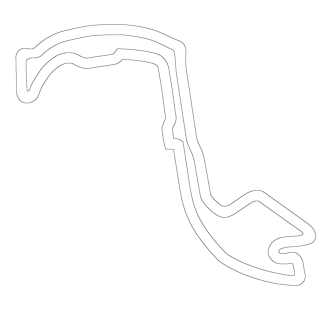
\includegraphics[interpolate=true,width=3.320000in,height=3.120000in]{contents/chapt6/figs/racing/mco-img0.png}}%
\end{pgfscope}%
\begin{pgfscope}%
\pgfpathrectangle{\pgfqpoint{0.123564in}{0.355320in}}{\pgfqpoint{3.316600in}{3.114720in}}%
\pgfusepath{clip}%
\pgfsetrectcap%
\pgfsetroundjoin%
\pgfsetlinewidth{1.003750pt}%
\definecolor{currentstroke}{rgb}{0.445098,0.086133,0.999070}%
\pgfsetstrokecolor{currentstroke}%
\pgfsetstrokeopacity{0.800000}%
\pgfsetdash{}{0pt}%
\pgfpathmoveto{\pgfqpoint{1.161804in}{3.164336in}}%
\pgfpathlineto{\pgfqpoint{1.163534in}{3.164336in}}%
\pgfusepath{stroke}%
\end{pgfscope}%
\begin{pgfscope}%
\pgfpathrectangle{\pgfqpoint{0.123564in}{0.355320in}}{\pgfqpoint{3.316600in}{3.114720in}}%
\pgfusepath{clip}%
\pgfsetrectcap%
\pgfsetroundjoin%
\pgfsetlinewidth{1.003750pt}%
\definecolor{currentstroke}{rgb}{0.390196,0.171626,0.996284}%
\pgfsetstrokecolor{currentstroke}%
\pgfsetstrokeopacity{0.800000}%
\pgfsetdash{}{0pt}%
\pgfpathmoveto{\pgfqpoint{1.163534in}{3.164336in}}%
\pgfpathlineto{\pgfqpoint{1.165298in}{3.164336in}}%
\pgfusepath{stroke}%
\end{pgfscope}%
\begin{pgfscope}%
\pgfpathrectangle{\pgfqpoint{0.123564in}{0.355320in}}{\pgfqpoint{3.316600in}{3.114720in}}%
\pgfusepath{clip}%
\pgfsetrectcap%
\pgfsetroundjoin%
\pgfsetlinewidth{1.003750pt}%
\definecolor{currentstroke}{rgb}{0.335294,0.255843,0.991645}%
\pgfsetstrokecolor{currentstroke}%
\pgfsetstrokeopacity{0.800000}%
\pgfsetdash{}{0pt}%
\pgfpathmoveto{\pgfqpoint{1.165298in}{3.164336in}}%
\pgfpathlineto{\pgfqpoint{1.167094in}{3.164332in}}%
\pgfusepath{stroke}%
\end{pgfscope}%
\begin{pgfscope}%
\pgfpathrectangle{\pgfqpoint{0.123564in}{0.355320in}}{\pgfqpoint{3.316600in}{3.114720in}}%
\pgfusepath{clip}%
\pgfsetrectcap%
\pgfsetroundjoin%
\pgfsetlinewidth{1.003750pt}%
\definecolor{currentstroke}{rgb}{0.272549,0.349727,0.984086}%
\pgfsetstrokecolor{currentstroke}%
\pgfsetstrokeopacity{0.800000}%
\pgfsetdash{}{0pt}%
\pgfpathmoveto{\pgfqpoint{1.167094in}{3.164332in}}%
\pgfpathlineto{\pgfqpoint{1.168923in}{3.164329in}}%
\pgfusepath{stroke}%
\end{pgfscope}%
\begin{pgfscope}%
\pgfpathrectangle{\pgfqpoint{0.123564in}{0.355320in}}{\pgfqpoint{3.316600in}{3.114720in}}%
\pgfusepath{clip}%
\pgfsetrectcap%
\pgfsetroundjoin%
\pgfsetlinewidth{1.003750pt}%
\definecolor{currentstroke}{rgb}{0.217647,0.429121,0.975512}%
\pgfsetstrokecolor{currentstroke}%
\pgfsetstrokeopacity{0.800000}%
\pgfsetdash{}{0pt}%
\pgfpathmoveto{\pgfqpoint{1.168923in}{3.164329in}}%
\pgfpathlineto{\pgfqpoint{1.170786in}{3.164322in}}%
\pgfusepath{stroke}%
\end{pgfscope}%
\begin{pgfscope}%
\pgfpathrectangle{\pgfqpoint{0.123564in}{0.355320in}}{\pgfqpoint{3.316600in}{3.114720in}}%
\pgfusepath{clip}%
\pgfsetrectcap%
\pgfsetroundjoin%
\pgfsetlinewidth{1.003750pt}%
\definecolor{currentstroke}{rgb}{0.162745,0.505325,0.965124}%
\pgfsetstrokecolor{currentstroke}%
\pgfsetstrokeopacity{0.800000}%
\pgfsetdash{}{0pt}%
\pgfpathmoveto{\pgfqpoint{1.170786in}{3.164322in}}%
\pgfpathlineto{\pgfqpoint{1.172680in}{3.164315in}}%
\pgfusepath{stroke}%
\end{pgfscope}%
\begin{pgfscope}%
\pgfpathrectangle{\pgfqpoint{0.123564in}{0.355320in}}{\pgfqpoint{3.316600in}{3.114720in}}%
\pgfusepath{clip}%
\pgfsetrectcap%
\pgfsetroundjoin%
\pgfsetlinewidth{1.003750pt}%
\definecolor{currentstroke}{rgb}{0.107843,0.577774,0.952942}%
\pgfsetstrokecolor{currentstroke}%
\pgfsetstrokeopacity{0.800000}%
\pgfsetdash{}{0pt}%
\pgfpathmoveto{\pgfqpoint{1.172680in}{3.164315in}}%
\pgfpathlineto{\pgfqpoint{1.174607in}{3.164305in}}%
\pgfusepath{stroke}%
\end{pgfscope}%
\begin{pgfscope}%
\pgfpathrectangle{\pgfqpoint{0.123564in}{0.355320in}}{\pgfqpoint{3.316600in}{3.114720in}}%
\pgfusepath{clip}%
\pgfsetrectcap%
\pgfsetroundjoin%
\pgfsetlinewidth{1.003750pt}%
\definecolor{currentstroke}{rgb}{0.060784,0.636474,0.941089}%
\pgfsetstrokecolor{currentstroke}%
\pgfsetstrokeopacity{0.800000}%
\pgfsetdash{}{0pt}%
\pgfpathmoveto{\pgfqpoint{1.174607in}{3.164305in}}%
\pgfpathlineto{\pgfqpoint{1.176563in}{3.164287in}}%
\pgfusepath{stroke}%
\end{pgfscope}%
\begin{pgfscope}%
\pgfpathrectangle{\pgfqpoint{0.123564in}{0.355320in}}{\pgfqpoint{3.316600in}{3.114720in}}%
\pgfusepath{clip}%
\pgfsetrectcap%
\pgfsetroundjoin%
\pgfsetlinewidth{1.003750pt}%
\definecolor{currentstroke}{rgb}{0.013725,0.691698,0.927951}%
\pgfsetstrokecolor{currentstroke}%
\pgfsetstrokeopacity{0.800000}%
\pgfsetdash{}{0pt}%
\pgfpathmoveto{\pgfqpoint{1.176563in}{3.164287in}}%
\pgfpathlineto{\pgfqpoint{1.178549in}{3.164265in}}%
\pgfusepath{stroke}%
\end{pgfscope}%
\begin{pgfscope}%
\pgfpathrectangle{\pgfqpoint{0.123564in}{0.355320in}}{\pgfqpoint{3.316600in}{3.114720in}}%
\pgfusepath{clip}%
\pgfsetrectcap%
\pgfsetroundjoin%
\pgfsetlinewidth{1.003750pt}%
\definecolor{currentstroke}{rgb}{0.033333,0.743145,0.913545}%
\pgfsetstrokecolor{currentstroke}%
\pgfsetstrokeopacity{0.800000}%
\pgfsetdash{}{0pt}%
\pgfpathmoveto{\pgfqpoint{1.178549in}{3.164265in}}%
\pgfpathlineto{\pgfqpoint{1.180562in}{3.164236in}}%
\pgfusepath{stroke}%
\end{pgfscope}%
\begin{pgfscope}%
\pgfpathrectangle{\pgfqpoint{0.123564in}{0.355320in}}{\pgfqpoint{3.316600in}{3.114720in}}%
\pgfusepath{clip}%
\pgfsetrectcap%
\pgfsetroundjoin%
\pgfsetlinewidth{1.003750pt}%
\definecolor{currentstroke}{rgb}{0.088235,0.798017,0.895163}%
\pgfsetstrokecolor{currentstroke}%
\pgfsetstrokeopacity{0.800000}%
\pgfsetdash{}{0pt}%
\pgfpathmoveto{\pgfqpoint{1.180562in}{3.164236in}}%
\pgfpathlineto{\pgfqpoint{1.182603in}{3.164203in}}%
\pgfusepath{stroke}%
\end{pgfscope}%
\begin{pgfscope}%
\pgfpathrectangle{\pgfqpoint{0.123564in}{0.355320in}}{\pgfqpoint{3.316600in}{3.114720in}}%
\pgfusepath{clip}%
\pgfsetrectcap%
\pgfsetroundjoin%
\pgfsetlinewidth{1.003750pt}%
\definecolor{currentstroke}{rgb}{0.127451,0.833602,0.881012}%
\pgfsetstrokecolor{currentstroke}%
\pgfsetstrokeopacity{0.800000}%
\pgfsetdash{}{0pt}%
\pgfpathmoveto{\pgfqpoint{1.182603in}{3.164203in}}%
\pgfpathlineto{\pgfqpoint{1.184672in}{3.164162in}}%
\pgfusepath{stroke}%
\end{pgfscope}%
\begin{pgfscope}%
\pgfpathrectangle{\pgfqpoint{0.123564in}{0.355320in}}{\pgfqpoint{3.316600in}{3.114720in}}%
\pgfusepath{clip}%
\pgfsetrectcap%
\pgfsetroundjoin%
\pgfsetlinewidth{1.003750pt}%
\definecolor{currentstroke}{rgb}{0.166667,0.866025,0.866025}%
\pgfsetstrokecolor{currentstroke}%
\pgfsetstrokeopacity{0.800000}%
\pgfsetdash{}{0pt}%
\pgfpathmoveto{\pgfqpoint{1.184672in}{3.164162in}}%
\pgfpathlineto{\pgfqpoint{1.186763in}{3.164117in}}%
\pgfusepath{stroke}%
\end{pgfscope}%
\begin{pgfscope}%
\pgfpathrectangle{\pgfqpoint{0.123564in}{0.355320in}}{\pgfqpoint{3.316600in}{3.114720in}}%
\pgfusepath{clip}%
\pgfsetrectcap%
\pgfsetroundjoin%
\pgfsetlinewidth{1.003750pt}%
\definecolor{currentstroke}{rgb}{0.213725,0.900587,0.846958}%
\pgfsetstrokecolor{currentstroke}%
\pgfsetstrokeopacity{0.800000}%
\pgfsetdash{}{0pt}%
\pgfpathmoveto{\pgfqpoint{1.186763in}{3.164117in}}%
\pgfpathlineto{\pgfqpoint{1.188876in}{3.164070in}}%
\pgfusepath{stroke}%
\end{pgfscope}%
\begin{pgfscope}%
\pgfpathrectangle{\pgfqpoint{0.123564in}{0.355320in}}{\pgfqpoint{3.316600in}{3.114720in}}%
\pgfusepath{clip}%
\pgfsetrectcap%
\pgfsetroundjoin%
\pgfsetlinewidth{1.003750pt}%
\definecolor{currentstroke}{rgb}{0.252941,0.925638,0.830184}%
\pgfsetstrokecolor{currentstroke}%
\pgfsetstrokeopacity{0.800000}%
\pgfsetdash{}{0pt}%
\pgfpathmoveto{\pgfqpoint{1.188876in}{3.164070in}}%
\pgfpathlineto{\pgfqpoint{1.191017in}{3.164025in}}%
\pgfusepath{stroke}%
\end{pgfscope}%
\begin{pgfscope}%
\pgfpathrectangle{\pgfqpoint{0.123564in}{0.355320in}}{\pgfqpoint{3.316600in}{3.114720in}}%
\pgfusepath{clip}%
\pgfsetrectcap%
\pgfsetroundjoin%
\pgfsetlinewidth{1.003750pt}%
\definecolor{currentstroke}{rgb}{0.292157,0.947177,0.812622}%
\pgfsetstrokecolor{currentstroke}%
\pgfsetstrokeopacity{0.800000}%
\pgfsetdash{}{0pt}%
\pgfpathmoveto{\pgfqpoint{1.191017in}{3.164025in}}%
\pgfpathlineto{\pgfqpoint{1.193181in}{3.163986in}}%
\pgfusepath{stroke}%
\end{pgfscope}%
\begin{pgfscope}%
\pgfpathrectangle{\pgfqpoint{0.123564in}{0.355320in}}{\pgfqpoint{3.316600in}{3.114720in}}%
\pgfusepath{clip}%
\pgfsetrectcap%
\pgfsetroundjoin%
\pgfsetlinewidth{1.003750pt}%
\definecolor{currentstroke}{rgb}{0.339216,0.968276,0.790532}%
\pgfsetstrokecolor{currentstroke}%
\pgfsetstrokeopacity{0.800000}%
\pgfsetdash{}{0pt}%
\pgfpathmoveto{\pgfqpoint{1.193181in}{3.163986in}}%
\pgfpathlineto{\pgfqpoint{1.195369in}{3.163956in}}%
\pgfusepath{stroke}%
\end{pgfscope}%
\begin{pgfscope}%
\pgfpathrectangle{\pgfqpoint{0.123564in}{0.355320in}}{\pgfqpoint{3.316600in}{3.114720in}}%
\pgfusepath{clip}%
\pgfsetrectcap%
\pgfsetroundjoin%
\pgfsetlinewidth{1.003750pt}%
\definecolor{currentstroke}{rgb}{0.378431,0.981823,0.771298}%
\pgfsetstrokecolor{currentstroke}%
\pgfsetstrokeopacity{0.800000}%
\pgfsetdash{}{0pt}%
\pgfpathmoveto{\pgfqpoint{1.195369in}{3.163956in}}%
\pgfpathlineto{\pgfqpoint{1.197582in}{3.163939in}}%
\pgfusepath{stroke}%
\end{pgfscope}%
\begin{pgfscope}%
\pgfpathrectangle{\pgfqpoint{0.123564in}{0.355320in}}{\pgfqpoint{3.316600in}{3.114720in}}%
\pgfusepath{clip}%
\pgfsetrectcap%
\pgfsetroundjoin%
\pgfsetlinewidth{1.003750pt}%
\definecolor{currentstroke}{rgb}{0.417647,0.991645,0.751332}%
\pgfsetstrokecolor{currentstroke}%
\pgfsetstrokeopacity{0.800000}%
\pgfsetdash{}{0pt}%
\pgfpathmoveto{\pgfqpoint{1.197582in}{3.163939in}}%
\pgfpathlineto{\pgfqpoint{1.199818in}{3.163931in}}%
\pgfusepath{stroke}%
\end{pgfscope}%
\begin{pgfscope}%
\pgfpathrectangle{\pgfqpoint{0.123564in}{0.355320in}}{\pgfqpoint{3.316600in}{3.114720in}}%
\pgfusepath{clip}%
\pgfsetrectcap%
\pgfsetroundjoin%
\pgfsetlinewidth{1.003750pt}%
\definecolor{currentstroke}{rgb}{0.456863,0.997705,0.730653}%
\pgfsetstrokecolor{currentstroke}%
\pgfsetstrokeopacity{0.800000}%
\pgfsetdash{}{0pt}%
\pgfpathmoveto{\pgfqpoint{1.199818in}{3.163931in}}%
\pgfpathlineto{\pgfqpoint{1.202076in}{3.163937in}}%
\pgfusepath{stroke}%
\end{pgfscope}%
\begin{pgfscope}%
\pgfpathrectangle{\pgfqpoint{0.123564in}{0.355320in}}{\pgfqpoint{3.316600in}{3.114720in}}%
\pgfusepath{clip}%
\pgfsetrectcap%
\pgfsetroundjoin%
\pgfsetlinewidth{1.003750pt}%
\definecolor{currentstroke}{rgb}{0.488235,0.999829,0.713610}%
\pgfsetstrokecolor{currentstroke}%
\pgfsetstrokeopacity{0.800000}%
\pgfsetdash{}{0pt}%
\pgfpathmoveto{\pgfqpoint{1.202076in}{3.163937in}}%
\pgfpathlineto{\pgfqpoint{1.204357in}{3.163953in}}%
\pgfusepath{stroke}%
\end{pgfscope}%
\begin{pgfscope}%
\pgfpathrectangle{\pgfqpoint{0.123564in}{0.355320in}}{\pgfqpoint{3.316600in}{3.114720in}}%
\pgfusepath{clip}%
\pgfsetrectcap%
\pgfsetroundjoin%
\pgfsetlinewidth{1.003750pt}%
\definecolor{currentstroke}{rgb}{0.527451,0.999070,0.691698}%
\pgfsetstrokecolor{currentstroke}%
\pgfsetstrokeopacity{0.800000}%
\pgfsetdash{}{0pt}%
\pgfpathmoveto{\pgfqpoint{1.204357in}{3.163953in}}%
\pgfpathlineto{\pgfqpoint{1.206659in}{3.163986in}}%
\pgfusepath{stroke}%
\end{pgfscope}%
\begin{pgfscope}%
\pgfpathrectangle{\pgfqpoint{0.123564in}{0.355320in}}{\pgfqpoint{3.316600in}{3.114720in}}%
\pgfusepath{clip}%
\pgfsetrectcap%
\pgfsetroundjoin%
\pgfsetlinewidth{1.003750pt}%
\definecolor{currentstroke}{rgb}{0.558824,0.995734,0.673696}%
\pgfsetstrokecolor{currentstroke}%
\pgfsetstrokeopacity{0.800000}%
\pgfsetdash{}{0pt}%
\pgfpathmoveto{\pgfqpoint{1.206659in}{3.163986in}}%
\pgfpathlineto{\pgfqpoint{1.208980in}{3.164033in}}%
\pgfusepath{stroke}%
\end{pgfscope}%
\begin{pgfscope}%
\pgfpathrectangle{\pgfqpoint{0.123564in}{0.355320in}}{\pgfqpoint{3.316600in}{3.114720in}}%
\pgfusepath{clip}%
\pgfsetrectcap%
\pgfsetroundjoin%
\pgfsetlinewidth{1.003750pt}%
\definecolor{currentstroke}{rgb}{0.582353,0.991645,0.659925}%
\pgfsetstrokecolor{currentstroke}%
\pgfsetstrokeopacity{0.800000}%
\pgfsetdash{}{0pt}%
\pgfpathmoveto{\pgfqpoint{1.208980in}{3.164033in}}%
\pgfpathlineto{\pgfqpoint{1.211320in}{3.164089in}}%
\pgfusepath{stroke}%
\end{pgfscope}%
\begin{pgfscope}%
\pgfpathrectangle{\pgfqpoint{0.123564in}{0.355320in}}{\pgfqpoint{3.316600in}{3.114720in}}%
\pgfusepath{clip}%
\pgfsetrectcap%
\pgfsetroundjoin%
\pgfsetlinewidth{1.003750pt}%
\definecolor{currentstroke}{rgb}{0.605882,0.986201,0.645928}%
\pgfsetstrokecolor{currentstroke}%
\pgfsetstrokeopacity{0.800000}%
\pgfsetdash{}{0pt}%
\pgfpathmoveto{\pgfqpoint{1.211320in}{3.164089in}}%
\pgfpathlineto{\pgfqpoint{1.213673in}{3.164162in}}%
\pgfusepath{stroke}%
\end{pgfscope}%
\begin{pgfscope}%
\pgfpathrectangle{\pgfqpoint{0.123564in}{0.355320in}}{\pgfqpoint{3.316600in}{3.114720in}}%
\pgfusepath{clip}%
\pgfsetrectcap%
\pgfsetroundjoin%
\pgfsetlinewidth{1.003750pt}%
\definecolor{currentstroke}{rgb}{0.645098,0.974139,0.622113}%
\pgfsetstrokecolor{currentstroke}%
\pgfsetstrokeopacity{0.800000}%
\pgfsetdash{}{0pt}%
\pgfpathmoveto{\pgfqpoint{1.213673in}{3.164162in}}%
\pgfpathlineto{\pgfqpoint{1.216040in}{3.164246in}}%
\pgfusepath{stroke}%
\end{pgfscope}%
\begin{pgfscope}%
\pgfpathrectangle{\pgfqpoint{0.123564in}{0.355320in}}{\pgfqpoint{3.316600in}{3.114720in}}%
\pgfusepath{clip}%
\pgfsetrectcap%
\pgfsetroundjoin%
\pgfsetlinewidth{1.003750pt}%
\definecolor{currentstroke}{rgb}{0.668627,0.965124,0.607539}%
\pgfsetstrokecolor{currentstroke}%
\pgfsetstrokeopacity{0.800000}%
\pgfsetdash{}{0pt}%
\pgfpathmoveto{\pgfqpoint{1.216040in}{3.164246in}}%
\pgfpathlineto{\pgfqpoint{1.218427in}{3.164349in}}%
\pgfusepath{stroke}%
\end{pgfscope}%
\begin{pgfscope}%
\pgfpathrectangle{\pgfqpoint{0.123564in}{0.355320in}}{\pgfqpoint{3.316600in}{3.114720in}}%
\pgfusepath{clip}%
\pgfsetrectcap%
\pgfsetroundjoin%
\pgfsetlinewidth{1.003750pt}%
\definecolor{currentstroke}{rgb}{0.692157,0.954791,0.592758}%
\pgfsetstrokecolor{currentstroke}%
\pgfsetstrokeopacity{0.800000}%
\pgfsetdash{}{0pt}%
\pgfpathmoveto{\pgfqpoint{1.218427in}{3.164349in}}%
\pgfpathlineto{\pgfqpoint{1.220827in}{3.164465in}}%
\pgfusepath{stroke}%
\end{pgfscope}%
\begin{pgfscope}%
\pgfpathrectangle{\pgfqpoint{0.123564in}{0.355320in}}{\pgfqpoint{3.316600in}{3.114720in}}%
\pgfusepath{clip}%
\pgfsetrectcap%
\pgfsetroundjoin%
\pgfsetlinewidth{1.003750pt}%
\definecolor{currentstroke}{rgb}{0.715686,0.943154,0.577774}%
\pgfsetstrokecolor{currentstroke}%
\pgfsetstrokeopacity{0.800000}%
\pgfsetdash{}{0pt}%
\pgfpathmoveto{\pgfqpoint{1.220827in}{3.164465in}}%
\pgfpathlineto{\pgfqpoint{1.223241in}{3.164592in}}%
\pgfusepath{stroke}%
\end{pgfscope}%
\begin{pgfscope}%
\pgfpathrectangle{\pgfqpoint{0.123564in}{0.355320in}}{\pgfqpoint{3.316600in}{3.114720in}}%
\pgfusepath{clip}%
\pgfsetrectcap%
\pgfsetroundjoin%
\pgfsetlinewidth{1.003750pt}%
\definecolor{currentstroke}{rgb}{0.739216,0.930229,0.562593}%
\pgfsetstrokecolor{currentstroke}%
\pgfsetstrokeopacity{0.800000}%
\pgfsetdash{}{0pt}%
\pgfpathmoveto{\pgfqpoint{1.223241in}{3.164592in}}%
\pgfpathlineto{\pgfqpoint{1.225667in}{3.164733in}}%
\pgfusepath{stroke}%
\end{pgfscope}%
\begin{pgfscope}%
\pgfpathrectangle{\pgfqpoint{0.123564in}{0.355320in}}{\pgfqpoint{3.316600in}{3.114720in}}%
\pgfusepath{clip}%
\pgfsetrectcap%
\pgfsetroundjoin%
\pgfsetlinewidth{1.003750pt}%
\definecolor{currentstroke}{rgb}{0.754902,0.920906,0.552365}%
\pgfsetstrokecolor{currentstroke}%
\pgfsetstrokeopacity{0.800000}%
\pgfsetdash{}{0pt}%
\pgfpathmoveto{\pgfqpoint{1.225667in}{3.164733in}}%
\pgfpathlineto{\pgfqpoint{1.228110in}{3.164887in}}%
\pgfusepath{stroke}%
\end{pgfscope}%
\begin{pgfscope}%
\pgfpathrectangle{\pgfqpoint{0.123564in}{0.355320in}}{\pgfqpoint{3.316600in}{3.114720in}}%
\pgfusepath{clip}%
\pgfsetrectcap%
\pgfsetroundjoin%
\pgfsetlinewidth{1.003750pt}%
\definecolor{currentstroke}{rgb}{0.778431,0.905873,0.536867}%
\pgfsetstrokecolor{currentstroke}%
\pgfsetstrokeopacity{0.800000}%
\pgfsetdash{}{0pt}%
\pgfpathmoveto{\pgfqpoint{1.228110in}{3.164887in}}%
\pgfpathlineto{\pgfqpoint{1.230557in}{3.165056in}}%
\pgfusepath{stroke}%
\end{pgfscope}%
\begin{pgfscope}%
\pgfpathrectangle{\pgfqpoint{0.123564in}{0.355320in}}{\pgfqpoint{3.316600in}{3.114720in}}%
\pgfusepath{clip}%
\pgfsetrectcap%
\pgfsetroundjoin%
\pgfsetlinewidth{1.003750pt}%
\definecolor{currentstroke}{rgb}{0.794118,0.895163,0.526432}%
\pgfsetstrokecolor{currentstroke}%
\pgfsetstrokeopacity{0.800000}%
\pgfsetdash{}{0pt}%
\pgfpathmoveto{\pgfqpoint{1.230557in}{3.165056in}}%
\pgfpathlineto{\pgfqpoint{1.233016in}{3.165236in}}%
\pgfusepath{stroke}%
\end{pgfscope}%
\begin{pgfscope}%
\pgfpathrectangle{\pgfqpoint{0.123564in}{0.355320in}}{\pgfqpoint{3.316600in}{3.114720in}}%
\pgfusepath{clip}%
\pgfsetrectcap%
\pgfsetroundjoin%
\pgfsetlinewidth{1.003750pt}%
\definecolor{currentstroke}{rgb}{0.809804,0.883910,0.515918}%
\pgfsetstrokecolor{currentstroke}%
\pgfsetstrokeopacity{0.800000}%
\pgfsetdash{}{0pt}%
\pgfpathmoveto{\pgfqpoint{1.233016in}{3.165236in}}%
\pgfpathlineto{\pgfqpoint{1.235484in}{3.165424in}}%
\pgfusepath{stroke}%
\end{pgfscope}%
\begin{pgfscope}%
\pgfpathrectangle{\pgfqpoint{0.123564in}{0.355320in}}{\pgfqpoint{3.316600in}{3.114720in}}%
\pgfusepath{clip}%
\pgfsetrectcap%
\pgfsetroundjoin%
\pgfsetlinewidth{1.003750pt}%
\definecolor{currentstroke}{rgb}{0.825490,0.872120,0.505325}%
\pgfsetstrokecolor{currentstroke}%
\pgfsetstrokeopacity{0.800000}%
\pgfsetdash{}{0pt}%
\pgfpathmoveto{\pgfqpoint{1.235484in}{3.165424in}}%
\pgfpathlineto{\pgfqpoint{1.237961in}{3.165615in}}%
\pgfusepath{stroke}%
\end{pgfscope}%
\begin{pgfscope}%
\pgfpathrectangle{\pgfqpoint{0.123564in}{0.355320in}}{\pgfqpoint{3.316600in}{3.114720in}}%
\pgfusepath{clip}%
\pgfsetrectcap%
\pgfsetroundjoin%
\pgfsetlinewidth{1.003750pt}%
\definecolor{currentstroke}{rgb}{0.841176,0.859800,0.494656}%
\pgfsetstrokecolor{currentstroke}%
\pgfsetstrokeopacity{0.800000}%
\pgfsetdash{}{0pt}%
\pgfpathmoveto{\pgfqpoint{1.237961in}{3.165615in}}%
\pgfpathlineto{\pgfqpoint{1.240448in}{3.165805in}}%
\pgfusepath{stroke}%
\end{pgfscope}%
\begin{pgfscope}%
\pgfpathrectangle{\pgfqpoint{0.123564in}{0.355320in}}{\pgfqpoint{3.316600in}{3.114720in}}%
\pgfusepath{clip}%
\pgfsetrectcap%
\pgfsetroundjoin%
\pgfsetlinewidth{1.003750pt}%
\definecolor{currentstroke}{rgb}{0.864706,0.840344,0.478512}%
\pgfsetstrokecolor{currentstroke}%
\pgfsetstrokeopacity{0.800000}%
\pgfsetdash{}{0pt}%
\pgfpathmoveto{\pgfqpoint{1.240448in}{3.165805in}}%
\pgfpathlineto{\pgfqpoint{1.242946in}{3.165990in}}%
\pgfusepath{stroke}%
\end{pgfscope}%
\begin{pgfscope}%
\pgfpathrectangle{\pgfqpoint{0.123564in}{0.355320in}}{\pgfqpoint{3.316600in}{3.114720in}}%
\pgfusepath{clip}%
\pgfsetrectcap%
\pgfsetroundjoin%
\pgfsetlinewidth{1.003750pt}%
\definecolor{currentstroke}{rgb}{0.872549,0.833602,0.473094}%
\pgfsetstrokecolor{currentstroke}%
\pgfsetstrokeopacity{0.800000}%
\pgfsetdash{}{0pt}%
\pgfpathmoveto{\pgfqpoint{1.242946in}{3.165990in}}%
\pgfpathlineto{\pgfqpoint{1.245455in}{3.166175in}}%
\pgfusepath{stroke}%
\end{pgfscope}%
\begin{pgfscope}%
\pgfpathrectangle{\pgfqpoint{0.123564in}{0.355320in}}{\pgfqpoint{3.316600in}{3.114720in}}%
\pgfusepath{clip}%
\pgfsetrectcap%
\pgfsetroundjoin%
\pgfsetlinewidth{1.003750pt}%
\definecolor{currentstroke}{rgb}{0.888235,0.819740,0.462204}%
\pgfsetstrokecolor{currentstroke}%
\pgfsetstrokeopacity{0.800000}%
\pgfsetdash{}{0pt}%
\pgfpathmoveto{\pgfqpoint{1.245455in}{3.166175in}}%
\pgfpathlineto{\pgfqpoint{1.247970in}{3.166353in}}%
\pgfusepath{stroke}%
\end{pgfscope}%
\begin{pgfscope}%
\pgfpathrectangle{\pgfqpoint{0.123564in}{0.355320in}}{\pgfqpoint{3.316600in}{3.114720in}}%
\pgfusepath{clip}%
\pgfsetrectcap%
\pgfsetroundjoin%
\pgfsetlinewidth{1.003750pt}%
\definecolor{currentstroke}{rgb}{0.903922,0.805381,0.451244}%
\pgfsetstrokecolor{currentstroke}%
\pgfsetstrokeopacity{0.800000}%
\pgfsetdash{}{0pt}%
\pgfpathmoveto{\pgfqpoint{1.247970in}{3.166353in}}%
\pgfpathlineto{\pgfqpoint{1.250493in}{3.166527in}}%
\pgfusepath{stroke}%
\end{pgfscope}%
\begin{pgfscope}%
\pgfpathrectangle{\pgfqpoint{0.123564in}{0.355320in}}{\pgfqpoint{3.316600in}{3.114720in}}%
\pgfusepath{clip}%
\pgfsetrectcap%
\pgfsetroundjoin%
\pgfsetlinewidth{1.003750pt}%
\definecolor{currentstroke}{rgb}{0.903922,0.805381,0.451244}%
\pgfsetstrokecolor{currentstroke}%
\pgfsetstrokeopacity{0.800000}%
\pgfsetdash{}{0pt}%
\pgfpathmoveto{\pgfqpoint{1.250493in}{3.166527in}}%
\pgfpathlineto{\pgfqpoint{1.253024in}{3.166693in}}%
\pgfusepath{stroke}%
\end{pgfscope}%
\begin{pgfscope}%
\pgfpathrectangle{\pgfqpoint{0.123564in}{0.355320in}}{\pgfqpoint{3.316600in}{3.114720in}}%
\pgfusepath{clip}%
\pgfsetrectcap%
\pgfsetroundjoin%
\pgfsetlinewidth{1.003750pt}%
\definecolor{currentstroke}{rgb}{0.919608,0.790532,0.440216}%
\pgfsetstrokecolor{currentstroke}%
\pgfsetstrokeopacity{0.800000}%
\pgfsetdash{}{0pt}%
\pgfpathmoveto{\pgfqpoint{1.253024in}{3.166693in}}%
\pgfpathlineto{\pgfqpoint{1.255561in}{3.166852in}}%
\pgfusepath{stroke}%
\end{pgfscope}%
\begin{pgfscope}%
\pgfpathrectangle{\pgfqpoint{0.123564in}{0.355320in}}{\pgfqpoint{3.316600in}{3.114720in}}%
\pgfusepath{clip}%
\pgfsetrectcap%
\pgfsetroundjoin%
\pgfsetlinewidth{1.003750pt}%
\definecolor{currentstroke}{rgb}{0.927451,0.782928,0.434676}%
\pgfsetstrokecolor{currentstroke}%
\pgfsetstrokeopacity{0.800000}%
\pgfsetdash{}{0pt}%
\pgfpathmoveto{\pgfqpoint{1.255561in}{3.166852in}}%
\pgfpathlineto{\pgfqpoint{1.258104in}{3.167008in}}%
\pgfusepath{stroke}%
\end{pgfscope}%
\begin{pgfscope}%
\pgfpathrectangle{\pgfqpoint{0.123564in}{0.355320in}}{\pgfqpoint{3.316600in}{3.114720in}}%
\pgfusepath{clip}%
\pgfsetrectcap%
\pgfsetroundjoin%
\pgfsetlinewidth{1.003750pt}%
\definecolor{currentstroke}{rgb}{0.935294,0.775204,0.429121}%
\pgfsetstrokecolor{currentstroke}%
\pgfsetstrokeopacity{0.800000}%
\pgfsetdash{}{0pt}%
\pgfpathmoveto{\pgfqpoint{1.258104in}{3.167008in}}%
\pgfpathlineto{\pgfqpoint{1.260653in}{3.167155in}}%
\pgfusepath{stroke}%
\end{pgfscope}%
\begin{pgfscope}%
\pgfpathrectangle{\pgfqpoint{0.123564in}{0.355320in}}{\pgfqpoint{3.316600in}{3.114720in}}%
\pgfusepath{clip}%
\pgfsetrectcap%
\pgfsetroundjoin%
\pgfsetlinewidth{1.003750pt}%
\definecolor{currentstroke}{rgb}{0.950980,0.759405,0.417960}%
\pgfsetstrokecolor{currentstroke}%
\pgfsetstrokeopacity{0.800000}%
\pgfsetdash{}{0pt}%
\pgfpathmoveto{\pgfqpoint{1.260653in}{3.167155in}}%
\pgfpathlineto{\pgfqpoint{1.263209in}{3.167295in}}%
\pgfusepath{stroke}%
\end{pgfscope}%
\begin{pgfscope}%
\pgfpathrectangle{\pgfqpoint{0.123564in}{0.355320in}}{\pgfqpoint{3.316600in}{3.114720in}}%
\pgfusepath{clip}%
\pgfsetrectcap%
\pgfsetroundjoin%
\pgfsetlinewidth{1.003750pt}%
\definecolor{currentstroke}{rgb}{0.958824,0.751332,0.412356}%
\pgfsetstrokecolor{currentstroke}%
\pgfsetstrokeopacity{0.800000}%
\pgfsetdash{}{0pt}%
\pgfpathmoveto{\pgfqpoint{1.263209in}{3.167295in}}%
\pgfpathlineto{\pgfqpoint{1.265772in}{3.167423in}}%
\pgfusepath{stroke}%
\end{pgfscope}%
\begin{pgfscope}%
\pgfpathrectangle{\pgfqpoint{0.123564in}{0.355320in}}{\pgfqpoint{3.316600in}{3.114720in}}%
\pgfusepath{clip}%
\pgfsetrectcap%
\pgfsetroundjoin%
\pgfsetlinewidth{1.003750pt}%
\definecolor{currentstroke}{rgb}{0.966667,0.743145,0.406737}%
\pgfsetstrokecolor{currentstroke}%
\pgfsetstrokeopacity{0.800000}%
\pgfsetdash{}{0pt}%
\pgfpathmoveto{\pgfqpoint{1.265772in}{3.167423in}}%
\pgfpathlineto{\pgfqpoint{1.268341in}{3.167543in}}%
\pgfusepath{stroke}%
\end{pgfscope}%
\begin{pgfscope}%
\pgfpathrectangle{\pgfqpoint{0.123564in}{0.355320in}}{\pgfqpoint{3.316600in}{3.114720in}}%
\pgfusepath{clip}%
\pgfsetrectcap%
\pgfsetroundjoin%
\pgfsetlinewidth{1.003750pt}%
\definecolor{currentstroke}{rgb}{0.982353,0.726434,0.395451}%
\pgfsetstrokecolor{currentstroke}%
\pgfsetstrokeopacity{0.800000}%
\pgfsetdash{}{0pt}%
\pgfpathmoveto{\pgfqpoint{1.268341in}{3.167543in}}%
\pgfpathlineto{\pgfqpoint{1.270916in}{3.167649in}}%
\pgfusepath{stroke}%
\end{pgfscope}%
\begin{pgfscope}%
\pgfpathrectangle{\pgfqpoint{0.123564in}{0.355320in}}{\pgfqpoint{3.316600in}{3.114720in}}%
\pgfusepath{clip}%
\pgfsetrectcap%
\pgfsetroundjoin%
\pgfsetlinewidth{1.003750pt}%
\definecolor{currentstroke}{rgb}{0.982353,0.726434,0.395451}%
\pgfsetstrokecolor{currentstroke}%
\pgfsetstrokeopacity{0.800000}%
\pgfsetdash{}{0pt}%
\pgfpathmoveto{\pgfqpoint{1.270916in}{3.167649in}}%
\pgfpathlineto{\pgfqpoint{1.273498in}{3.167747in}}%
\pgfusepath{stroke}%
\end{pgfscope}%
\begin{pgfscope}%
\pgfpathrectangle{\pgfqpoint{0.123564in}{0.355320in}}{\pgfqpoint{3.316600in}{3.114720in}}%
\pgfusepath{clip}%
\pgfsetrectcap%
\pgfsetroundjoin%
\pgfsetlinewidth{1.003750pt}%
\definecolor{currentstroke}{rgb}{0.990196,0.717912,0.389786}%
\pgfsetstrokecolor{currentstroke}%
\pgfsetstrokeopacity{0.800000}%
\pgfsetdash{}{0pt}%
\pgfpathmoveto{\pgfqpoint{1.273498in}{3.167747in}}%
\pgfpathlineto{\pgfqpoint{1.276082in}{3.167829in}}%
\pgfusepath{stroke}%
\end{pgfscope}%
\begin{pgfscope}%
\pgfpathrectangle{\pgfqpoint{0.123564in}{0.355320in}}{\pgfqpoint{3.316600in}{3.114720in}}%
\pgfusepath{clip}%
\pgfsetrectcap%
\pgfsetroundjoin%
\pgfsetlinewidth{1.003750pt}%
\definecolor{currentstroke}{rgb}{0.998039,0.709281,0.384106}%
\pgfsetstrokecolor{currentstroke}%
\pgfsetstrokeopacity{0.800000}%
\pgfsetdash{}{0pt}%
\pgfpathmoveto{\pgfqpoint{1.276082in}{3.167829in}}%
\pgfpathlineto{\pgfqpoint{1.278673in}{3.167903in}}%
\pgfusepath{stroke}%
\end{pgfscope}%
\begin{pgfscope}%
\pgfpathrectangle{\pgfqpoint{0.123564in}{0.355320in}}{\pgfqpoint{3.316600in}{3.114720in}}%
\pgfusepath{clip}%
\pgfsetrectcap%
\pgfsetroundjoin%
\pgfsetlinewidth{1.003750pt}%
\definecolor{currentstroke}{rgb}{0.998039,0.709281,0.384106}%
\pgfsetstrokecolor{currentstroke}%
\pgfsetstrokeopacity{0.800000}%
\pgfsetdash{}{0pt}%
\pgfpathmoveto{\pgfqpoint{1.278673in}{3.167903in}}%
\pgfpathlineto{\pgfqpoint{1.281266in}{3.167961in}}%
\pgfusepath{stroke}%
\end{pgfscope}%
\begin{pgfscope}%
\pgfpathrectangle{\pgfqpoint{0.123564in}{0.355320in}}{\pgfqpoint{3.316600in}{3.114720in}}%
\pgfusepath{clip}%
\pgfsetrectcap%
\pgfsetroundjoin%
\pgfsetlinewidth{1.003750pt}%
\definecolor{currentstroke}{rgb}{1.000000,0.691698,0.372702}%
\pgfsetstrokecolor{currentstroke}%
\pgfsetstrokeopacity{0.800000}%
\pgfsetdash{}{0pt}%
\pgfpathmoveto{\pgfqpoint{1.281266in}{3.167961in}}%
\pgfpathlineto{\pgfqpoint{1.283860in}{3.168008in}}%
\pgfusepath{stroke}%
\end{pgfscope}%
\begin{pgfscope}%
\pgfpathrectangle{\pgfqpoint{0.123564in}{0.355320in}}{\pgfqpoint{3.316600in}{3.114720in}}%
\pgfusepath{clip}%
\pgfsetrectcap%
\pgfsetroundjoin%
\pgfsetlinewidth{1.003750pt}%
\definecolor{currentstroke}{rgb}{1.000000,0.673696,0.361242}%
\pgfsetstrokecolor{currentstroke}%
\pgfsetstrokeopacity{0.800000}%
\pgfsetdash{}{0pt}%
\pgfpathmoveto{\pgfqpoint{1.283860in}{3.168008in}}%
\pgfpathlineto{\pgfqpoint{1.286460in}{3.168050in}}%
\pgfusepath{stroke}%
\end{pgfscope}%
\begin{pgfscope}%
\pgfpathrectangle{\pgfqpoint{0.123564in}{0.355320in}}{\pgfqpoint{3.316600in}{3.114720in}}%
\pgfusepath{clip}%
\pgfsetrectcap%
\pgfsetroundjoin%
\pgfsetlinewidth{1.003750pt}%
\definecolor{currentstroke}{rgb}{1.000000,0.655284,0.349727}%
\pgfsetstrokecolor{currentstroke}%
\pgfsetstrokeopacity{0.800000}%
\pgfsetdash{}{0pt}%
\pgfpathmoveto{\pgfqpoint{1.286460in}{3.168050in}}%
\pgfpathlineto{\pgfqpoint{1.289071in}{3.168080in}}%
\pgfusepath{stroke}%
\end{pgfscope}%
\begin{pgfscope}%
\pgfpathrectangle{\pgfqpoint{0.123564in}{0.355320in}}{\pgfqpoint{3.316600in}{3.114720in}}%
\pgfusepath{clip}%
\pgfsetrectcap%
\pgfsetroundjoin%
\pgfsetlinewidth{1.003750pt}%
\definecolor{currentstroke}{rgb}{1.000000,0.645928,0.343949}%
\pgfsetstrokecolor{currentstroke}%
\pgfsetstrokeopacity{0.800000}%
\pgfsetdash{}{0pt}%
\pgfpathmoveto{\pgfqpoint{1.289071in}{3.168080in}}%
\pgfpathlineto{\pgfqpoint{1.291690in}{3.168103in}}%
\pgfusepath{stroke}%
\end{pgfscope}%
\begin{pgfscope}%
\pgfpathrectangle{\pgfqpoint{0.123564in}{0.355320in}}{\pgfqpoint{3.316600in}{3.114720in}}%
\pgfusepath{clip}%
\pgfsetrectcap%
\pgfsetroundjoin%
\pgfsetlinewidth{1.003750pt}%
\definecolor{currentstroke}{rgb}{1.000000,0.626924,0.332355}%
\pgfsetstrokecolor{currentstroke}%
\pgfsetstrokeopacity{0.800000}%
\pgfsetdash{}{0pt}%
\pgfpathmoveto{\pgfqpoint{1.291690in}{3.168103in}}%
\pgfpathlineto{\pgfqpoint{1.294314in}{3.168114in}}%
\pgfusepath{stroke}%
\end{pgfscope}%
\begin{pgfscope}%
\pgfpathrectangle{\pgfqpoint{0.123564in}{0.355320in}}{\pgfqpoint{3.316600in}{3.114720in}}%
\pgfusepath{clip}%
\pgfsetrectcap%
\pgfsetroundjoin%
\pgfsetlinewidth{1.003750pt}%
\definecolor{currentstroke}{rgb}{1.000000,0.617278,0.326539}%
\pgfsetstrokecolor{currentstroke}%
\pgfsetstrokeopacity{0.800000}%
\pgfsetdash{}{0pt}%
\pgfpathmoveto{\pgfqpoint{1.294314in}{3.168114in}}%
\pgfpathlineto{\pgfqpoint{1.296945in}{3.168119in}}%
\pgfusepath{stroke}%
\end{pgfscope}%
\begin{pgfscope}%
\pgfpathrectangle{\pgfqpoint{0.123564in}{0.355320in}}{\pgfqpoint{3.316600in}{3.114720in}}%
\pgfusepath{clip}%
\pgfsetrectcap%
\pgfsetroundjoin%
\pgfsetlinewidth{1.003750pt}%
\definecolor{currentstroke}{rgb}{1.000000,0.617278,0.326539}%
\pgfsetstrokecolor{currentstroke}%
\pgfsetstrokeopacity{0.800000}%
\pgfsetdash{}{0pt}%
\pgfpathmoveto{\pgfqpoint{1.296945in}{3.168119in}}%
\pgfpathlineto{\pgfqpoint{1.299582in}{3.168113in}}%
\pgfusepath{stroke}%
\end{pgfscope}%
\begin{pgfscope}%
\pgfpathrectangle{\pgfqpoint{0.123564in}{0.355320in}}{\pgfqpoint{3.316600in}{3.114720in}}%
\pgfusepath{clip}%
\pgfsetrectcap%
\pgfsetroundjoin%
\pgfsetlinewidth{1.003750pt}%
\definecolor{currentstroke}{rgb}{1.000000,0.597707,0.314870}%
\pgfsetstrokecolor{currentstroke}%
\pgfsetstrokeopacity{0.800000}%
\pgfsetdash{}{0pt}%
\pgfpathmoveto{\pgfqpoint{1.299582in}{3.168113in}}%
\pgfpathlineto{\pgfqpoint{1.302223in}{3.168102in}}%
\pgfusepath{stroke}%
\end{pgfscope}%
\begin{pgfscope}%
\pgfpathrectangle{\pgfqpoint{0.123564in}{0.355320in}}{\pgfqpoint{3.316600in}{3.114720in}}%
\pgfusepath{clip}%
\pgfsetrectcap%
\pgfsetroundjoin%
\pgfsetlinewidth{1.003750pt}%
\definecolor{currentstroke}{rgb}{1.000000,0.587785,0.309017}%
\pgfsetstrokecolor{currentstroke}%
\pgfsetstrokeopacity{0.800000}%
\pgfsetdash{}{0pt}%
\pgfpathmoveto{\pgfqpoint{1.302223in}{3.168102in}}%
\pgfpathlineto{\pgfqpoint{1.304870in}{3.168080in}}%
\pgfusepath{stroke}%
\end{pgfscope}%
\begin{pgfscope}%
\pgfpathrectangle{\pgfqpoint{0.123564in}{0.355320in}}{\pgfqpoint{3.316600in}{3.114720in}}%
\pgfusepath{clip}%
\pgfsetrectcap%
\pgfsetroundjoin%
\pgfsetlinewidth{1.003750pt}%
\definecolor{currentstroke}{rgb}{1.000000,0.567675,0.297277}%
\pgfsetstrokecolor{currentstroke}%
\pgfsetstrokeopacity{0.800000}%
\pgfsetdash{}{0pt}%
\pgfpathmoveto{\pgfqpoint{1.304870in}{3.168080in}}%
\pgfpathlineto{\pgfqpoint{1.307523in}{3.168045in}}%
\pgfusepath{stroke}%
\end{pgfscope}%
\begin{pgfscope}%
\pgfpathrectangle{\pgfqpoint{0.123564in}{0.355320in}}{\pgfqpoint{3.316600in}{3.114720in}}%
\pgfusepath{clip}%
\pgfsetrectcap%
\pgfsetroundjoin%
\pgfsetlinewidth{1.003750pt}%
\definecolor{currentstroke}{rgb}{1.000000,0.547220,0.285492}%
\pgfsetstrokecolor{currentstroke}%
\pgfsetstrokeopacity{0.800000}%
\pgfsetdash{}{0pt}%
\pgfpathmoveto{\pgfqpoint{1.307523in}{3.168045in}}%
\pgfpathlineto{\pgfqpoint{1.310185in}{3.168001in}}%
\pgfusepath{stroke}%
\end{pgfscope}%
\begin{pgfscope}%
\pgfpathrectangle{\pgfqpoint{0.123564in}{0.355320in}}{\pgfqpoint{3.316600in}{3.114720in}}%
\pgfusepath{clip}%
\pgfsetrectcap%
\pgfsetroundjoin%
\pgfsetlinewidth{1.003750pt}%
\definecolor{currentstroke}{rgb}{1.000000,0.526432,0.273663}%
\pgfsetstrokecolor{currentstroke}%
\pgfsetstrokeopacity{0.800000}%
\pgfsetdash{}{0pt}%
\pgfpathmoveto{\pgfqpoint{1.310185in}{3.168001in}}%
\pgfpathlineto{\pgfqpoint{1.312854in}{3.167943in}}%
\pgfusepath{stroke}%
\end{pgfscope}%
\begin{pgfscope}%
\pgfpathrectangle{\pgfqpoint{0.123564in}{0.355320in}}{\pgfqpoint{3.316600in}{3.114720in}}%
\pgfusepath{clip}%
\pgfsetrectcap%
\pgfsetroundjoin%
\pgfsetlinewidth{1.003750pt}%
\definecolor{currentstroke}{rgb}{1.000000,0.505325,0.261793}%
\pgfsetstrokecolor{currentstroke}%
\pgfsetstrokeopacity{0.800000}%
\pgfsetdash{}{0pt}%
\pgfpathmoveto{\pgfqpoint{1.312854in}{3.167943in}}%
\pgfpathlineto{\pgfqpoint{1.315530in}{3.167877in}}%
\pgfusepath{stroke}%
\end{pgfscope}%
\begin{pgfscope}%
\pgfpathrectangle{\pgfqpoint{0.123564in}{0.355320in}}{\pgfqpoint{3.316600in}{3.114720in}}%
\pgfusepath{clip}%
\pgfsetrectcap%
\pgfsetroundjoin%
\pgfsetlinewidth{1.003750pt}%
\definecolor{currentstroke}{rgb}{1.000000,0.494656,0.255843}%
\pgfsetstrokecolor{currentstroke}%
\pgfsetstrokeopacity{0.800000}%
\pgfsetdash{}{0pt}%
\pgfpathmoveto{\pgfqpoint{1.315530in}{3.167877in}}%
\pgfpathlineto{\pgfqpoint{1.318216in}{3.167798in}}%
\pgfusepath{stroke}%
\end{pgfscope}%
\begin{pgfscope}%
\pgfpathrectangle{\pgfqpoint{0.123564in}{0.355320in}}{\pgfqpoint{3.316600in}{3.114720in}}%
\pgfusepath{clip}%
\pgfsetrectcap%
\pgfsetroundjoin%
\pgfsetlinewidth{1.003750pt}%
\definecolor{currentstroke}{rgb}{1.000000,0.473094,0.243914}%
\pgfsetstrokecolor{currentstroke}%
\pgfsetstrokeopacity{0.800000}%
\pgfsetdash{}{0pt}%
\pgfpathmoveto{\pgfqpoint{1.318216in}{3.167798in}}%
\pgfpathlineto{\pgfqpoint{1.320908in}{3.167702in}}%
\pgfusepath{stroke}%
\end{pgfscope}%
\begin{pgfscope}%
\pgfpathrectangle{\pgfqpoint{0.123564in}{0.355320in}}{\pgfqpoint{3.316600in}{3.114720in}}%
\pgfusepath{clip}%
\pgfsetrectcap%
\pgfsetroundjoin%
\pgfsetlinewidth{1.003750pt}%
\definecolor{currentstroke}{rgb}{1.000000,0.462204,0.237935}%
\pgfsetstrokecolor{currentstroke}%
\pgfsetstrokeopacity{0.800000}%
\pgfsetdash{}{0pt}%
\pgfpathmoveto{\pgfqpoint{1.320908in}{3.167702in}}%
\pgfpathlineto{\pgfqpoint{1.323606in}{3.167592in}}%
\pgfusepath{stroke}%
\end{pgfscope}%
\begin{pgfscope}%
\pgfpathrectangle{\pgfqpoint{0.123564in}{0.355320in}}{\pgfqpoint{3.316600in}{3.114720in}}%
\pgfusepath{clip}%
\pgfsetrectcap%
\pgfsetroundjoin%
\pgfsetlinewidth{1.003750pt}%
\definecolor{currentstroke}{rgb}{1.000000,0.451244,0.231948}%
\pgfsetstrokecolor{currentstroke}%
\pgfsetstrokeopacity{0.800000}%
\pgfsetdash{}{0pt}%
\pgfpathmoveto{\pgfqpoint{1.323606in}{3.167592in}}%
\pgfpathlineto{\pgfqpoint{1.326308in}{3.167465in}}%
\pgfusepath{stroke}%
\end{pgfscope}%
\begin{pgfscope}%
\pgfpathrectangle{\pgfqpoint{0.123564in}{0.355320in}}{\pgfqpoint{3.316600in}{3.114720in}}%
\pgfusepath{clip}%
\pgfsetrectcap%
\pgfsetroundjoin%
\pgfsetlinewidth{1.003750pt}%
\definecolor{currentstroke}{rgb}{1.000000,0.440216,0.225951}%
\pgfsetstrokecolor{currentstroke}%
\pgfsetstrokeopacity{0.800000}%
\pgfsetdash{}{0pt}%
\pgfpathmoveto{\pgfqpoint{1.326308in}{3.167465in}}%
\pgfpathlineto{\pgfqpoint{1.329012in}{3.167324in}}%
\pgfusepath{stroke}%
\end{pgfscope}%
\begin{pgfscope}%
\pgfpathrectangle{\pgfqpoint{0.123564in}{0.355320in}}{\pgfqpoint{3.316600in}{3.114720in}}%
\pgfusepath{clip}%
\pgfsetrectcap%
\pgfsetroundjoin%
\pgfsetlinewidth{1.003750pt}%
\definecolor{currentstroke}{rgb}{1.000000,0.429121,0.219946}%
\pgfsetstrokecolor{currentstroke}%
\pgfsetstrokeopacity{0.800000}%
\pgfsetdash{}{0pt}%
\pgfpathmoveto{\pgfqpoint{1.329012in}{3.167324in}}%
\pgfpathlineto{\pgfqpoint{1.331724in}{3.167164in}}%
\pgfusepath{stroke}%
\end{pgfscope}%
\begin{pgfscope}%
\pgfpathrectangle{\pgfqpoint{0.123564in}{0.355320in}}{\pgfqpoint{3.316600in}{3.114720in}}%
\pgfusepath{clip}%
\pgfsetrectcap%
\pgfsetroundjoin%
\pgfsetlinewidth{1.003750pt}%
\definecolor{currentstroke}{rgb}{1.000000,0.417960,0.213933}%
\pgfsetstrokecolor{currentstroke}%
\pgfsetstrokeopacity{0.800000}%
\pgfsetdash{}{0pt}%
\pgfpathmoveto{\pgfqpoint{1.331724in}{3.167164in}}%
\pgfpathlineto{\pgfqpoint{1.334438in}{3.166989in}}%
\pgfusepath{stroke}%
\end{pgfscope}%
\begin{pgfscope}%
\pgfpathrectangle{\pgfqpoint{0.123564in}{0.355320in}}{\pgfqpoint{3.316600in}{3.114720in}}%
\pgfusepath{clip}%
\pgfsetrectcap%
\pgfsetroundjoin%
\pgfsetlinewidth{1.003750pt}%
\definecolor{currentstroke}{rgb}{1.000000,0.395451,0.201882}%
\pgfsetstrokecolor{currentstroke}%
\pgfsetstrokeopacity{0.800000}%
\pgfsetdash{}{0pt}%
\pgfpathmoveto{\pgfqpoint{1.334438in}{3.166989in}}%
\pgfpathlineto{\pgfqpoint{1.337157in}{3.166803in}}%
\pgfusepath{stroke}%
\end{pgfscope}%
\begin{pgfscope}%
\pgfpathrectangle{\pgfqpoint{0.123564in}{0.355320in}}{\pgfqpoint{3.316600in}{3.114720in}}%
\pgfusepath{clip}%
\pgfsetrectcap%
\pgfsetroundjoin%
\pgfsetlinewidth{1.003750pt}%
\definecolor{currentstroke}{rgb}{1.000000,0.384106,0.195845}%
\pgfsetstrokecolor{currentstroke}%
\pgfsetstrokeopacity{0.800000}%
\pgfsetdash{}{0pt}%
\pgfpathmoveto{\pgfqpoint{1.337157in}{3.166803in}}%
\pgfpathlineto{\pgfqpoint{1.339883in}{3.166608in}}%
\pgfusepath{stroke}%
\end{pgfscope}%
\begin{pgfscope}%
\pgfpathrectangle{\pgfqpoint{0.123564in}{0.355320in}}{\pgfqpoint{3.316600in}{3.114720in}}%
\pgfusepath{clip}%
\pgfsetrectcap%
\pgfsetroundjoin%
\pgfsetlinewidth{1.003750pt}%
\definecolor{currentstroke}{rgb}{1.000000,0.384106,0.195845}%
\pgfsetstrokecolor{currentstroke}%
\pgfsetstrokeopacity{0.800000}%
\pgfsetdash{}{0pt}%
\pgfpathmoveto{\pgfqpoint{1.339883in}{3.166608in}}%
\pgfpathlineto{\pgfqpoint{1.342612in}{3.166409in}}%
\pgfusepath{stroke}%
\end{pgfscope}%
\begin{pgfscope}%
\pgfpathrectangle{\pgfqpoint{0.123564in}{0.355320in}}{\pgfqpoint{3.316600in}{3.114720in}}%
\pgfusepath{clip}%
\pgfsetrectcap%
\pgfsetroundjoin%
\pgfsetlinewidth{1.003750pt}%
\definecolor{currentstroke}{rgb}{1.000000,0.372702,0.189801}%
\pgfsetstrokecolor{currentstroke}%
\pgfsetstrokeopacity{0.800000}%
\pgfsetdash{}{0pt}%
\pgfpathmoveto{\pgfqpoint{1.342612in}{3.166409in}}%
\pgfpathlineto{\pgfqpoint{1.345344in}{3.166208in}}%
\pgfusepath{stroke}%
\end{pgfscope}%
\begin{pgfscope}%
\pgfpathrectangle{\pgfqpoint{0.123564in}{0.355320in}}{\pgfqpoint{3.316600in}{3.114720in}}%
\pgfusepath{clip}%
\pgfsetrectcap%
\pgfsetroundjoin%
\pgfsetlinewidth{1.003750pt}%
\definecolor{currentstroke}{rgb}{1.000000,0.372702,0.189801}%
\pgfsetstrokecolor{currentstroke}%
\pgfsetstrokeopacity{0.800000}%
\pgfsetdash{}{0pt}%
\pgfpathmoveto{\pgfqpoint{1.345344in}{3.166208in}}%
\pgfpathlineto{\pgfqpoint{1.348078in}{3.166012in}}%
\pgfusepath{stroke}%
\end{pgfscope}%
\begin{pgfscope}%
\pgfpathrectangle{\pgfqpoint{0.123564in}{0.355320in}}{\pgfqpoint{3.316600in}{3.114720in}}%
\pgfusepath{clip}%
\pgfsetrectcap%
\pgfsetroundjoin%
\pgfsetlinewidth{1.003750pt}%
\definecolor{currentstroke}{rgb}{1.000000,0.361242,0.183750}%
\pgfsetstrokecolor{currentstroke}%
\pgfsetstrokeopacity{0.800000}%
\pgfsetdash{}{0pt}%
\pgfpathmoveto{\pgfqpoint{1.348078in}{3.166012in}}%
\pgfpathlineto{\pgfqpoint{1.350815in}{3.165813in}}%
\pgfusepath{stroke}%
\end{pgfscope}%
\begin{pgfscope}%
\pgfpathrectangle{\pgfqpoint{0.123564in}{0.355320in}}{\pgfqpoint{3.316600in}{3.114720in}}%
\pgfusepath{clip}%
\pgfsetrectcap%
\pgfsetroundjoin%
\pgfsetlinewidth{1.003750pt}%
\definecolor{currentstroke}{rgb}{1.000000,0.338158,0.171626}%
\pgfsetstrokecolor{currentstroke}%
\pgfsetstrokeopacity{0.800000}%
\pgfsetdash{}{0pt}%
\pgfpathmoveto{\pgfqpoint{1.350815in}{3.165813in}}%
\pgfpathlineto{\pgfqpoint{1.353556in}{3.165619in}}%
\pgfusepath{stroke}%
\end{pgfscope}%
\begin{pgfscope}%
\pgfpathrectangle{\pgfqpoint{0.123564in}{0.355320in}}{\pgfqpoint{3.316600in}{3.114720in}}%
\pgfusepath{clip}%
\pgfsetrectcap%
\pgfsetroundjoin%
\pgfsetlinewidth{1.003750pt}%
\definecolor{currentstroke}{rgb}{1.000000,0.338158,0.171626}%
\pgfsetstrokecolor{currentstroke}%
\pgfsetstrokeopacity{0.800000}%
\pgfsetdash{}{0pt}%
\pgfpathmoveto{\pgfqpoint{1.353556in}{3.165619in}}%
\pgfpathlineto{\pgfqpoint{1.356303in}{3.165426in}}%
\pgfusepath{stroke}%
\end{pgfscope}%
\begin{pgfscope}%
\pgfpathrectangle{\pgfqpoint{0.123564in}{0.355320in}}{\pgfqpoint{3.316600in}{3.114720in}}%
\pgfusepath{clip}%
\pgfsetrectcap%
\pgfsetroundjoin%
\pgfsetlinewidth{1.003750pt}%
\definecolor{currentstroke}{rgb}{1.000000,0.338158,0.171626}%
\pgfsetstrokecolor{currentstroke}%
\pgfsetstrokeopacity{0.800000}%
\pgfsetdash{}{0pt}%
\pgfpathmoveto{\pgfqpoint{1.356303in}{3.165426in}}%
\pgfpathlineto{\pgfqpoint{1.359050in}{3.165241in}}%
\pgfusepath{stroke}%
\end{pgfscope}%
\begin{pgfscope}%
\pgfpathrectangle{\pgfqpoint{0.123564in}{0.355320in}}{\pgfqpoint{3.316600in}{3.114720in}}%
\pgfusepath{clip}%
\pgfsetrectcap%
\pgfsetroundjoin%
\pgfsetlinewidth{1.003750pt}%
\definecolor{currentstroke}{rgb}{1.000000,0.326539,0.165554}%
\pgfsetstrokecolor{currentstroke}%
\pgfsetstrokeopacity{0.800000}%
\pgfsetdash{}{0pt}%
\pgfpathmoveto{\pgfqpoint{1.359050in}{3.165241in}}%
\pgfpathlineto{\pgfqpoint{1.361801in}{3.165060in}}%
\pgfusepath{stroke}%
\end{pgfscope}%
\begin{pgfscope}%
\pgfpathrectangle{\pgfqpoint{0.123564in}{0.355320in}}{\pgfqpoint{3.316600in}{3.114720in}}%
\pgfusepath{clip}%
\pgfsetrectcap%
\pgfsetroundjoin%
\pgfsetlinewidth{1.003750pt}%
\definecolor{currentstroke}{rgb}{1.000000,0.314870,0.159476}%
\pgfsetstrokecolor{currentstroke}%
\pgfsetstrokeopacity{0.800000}%
\pgfsetdash{}{0pt}%
\pgfpathmoveto{\pgfqpoint{1.361801in}{3.165060in}}%
\pgfpathlineto{\pgfqpoint{1.364555in}{3.164881in}}%
\pgfusepath{stroke}%
\end{pgfscope}%
\begin{pgfscope}%
\pgfpathrectangle{\pgfqpoint{0.123564in}{0.355320in}}{\pgfqpoint{3.316600in}{3.114720in}}%
\pgfusepath{clip}%
\pgfsetrectcap%
\pgfsetroundjoin%
\pgfsetlinewidth{1.003750pt}%
\definecolor{currentstroke}{rgb}{1.000000,0.303153,0.153392}%
\pgfsetstrokecolor{currentstroke}%
\pgfsetstrokeopacity{0.800000}%
\pgfsetdash{}{0pt}%
\pgfpathmoveto{\pgfqpoint{1.364555in}{3.164881in}}%
\pgfpathlineto{\pgfqpoint{1.367315in}{3.164702in}}%
\pgfusepath{stroke}%
\end{pgfscope}%
\begin{pgfscope}%
\pgfpathrectangle{\pgfqpoint{0.123564in}{0.355320in}}{\pgfqpoint{3.316600in}{3.114720in}}%
\pgfusepath{clip}%
\pgfsetrectcap%
\pgfsetroundjoin%
\pgfsetlinewidth{1.003750pt}%
\definecolor{currentstroke}{rgb}{1.000000,0.291390,0.147302}%
\pgfsetstrokecolor{currentstroke}%
\pgfsetstrokeopacity{0.800000}%
\pgfsetdash{}{0pt}%
\pgfpathmoveto{\pgfqpoint{1.367315in}{3.164702in}}%
\pgfpathlineto{\pgfqpoint{1.370078in}{3.164520in}}%
\pgfusepath{stroke}%
\end{pgfscope}%
\begin{pgfscope}%
\pgfpathrectangle{\pgfqpoint{0.123564in}{0.355320in}}{\pgfqpoint{3.316600in}{3.114720in}}%
\pgfusepath{clip}%
\pgfsetrectcap%
\pgfsetroundjoin%
\pgfsetlinewidth{1.003750pt}%
\definecolor{currentstroke}{rgb}{1.000000,0.279583,0.141206}%
\pgfsetstrokecolor{currentstroke}%
\pgfsetstrokeopacity{0.800000}%
\pgfsetdash{}{0pt}%
\pgfpathmoveto{\pgfqpoint{1.370078in}{3.164520in}}%
\pgfpathlineto{\pgfqpoint{1.372843in}{3.164333in}}%
\pgfusepath{stroke}%
\end{pgfscope}%
\begin{pgfscope}%
\pgfpathrectangle{\pgfqpoint{0.123564in}{0.355320in}}{\pgfqpoint{3.316600in}{3.114720in}}%
\pgfusepath{clip}%
\pgfsetrectcap%
\pgfsetroundjoin%
\pgfsetlinewidth{1.003750pt}%
\definecolor{currentstroke}{rgb}{1.000000,0.267733,0.135105}%
\pgfsetstrokecolor{currentstroke}%
\pgfsetstrokeopacity{0.800000}%
\pgfsetdash{}{0pt}%
\pgfpathmoveto{\pgfqpoint{1.372843in}{3.164333in}}%
\pgfpathlineto{\pgfqpoint{1.375613in}{3.164138in}}%
\pgfusepath{stroke}%
\end{pgfscope}%
\begin{pgfscope}%
\pgfpathrectangle{\pgfqpoint{0.123564in}{0.355320in}}{\pgfqpoint{3.316600in}{3.114720in}}%
\pgfusepath{clip}%
\pgfsetrectcap%
\pgfsetroundjoin%
\pgfsetlinewidth{1.003750pt}%
\definecolor{currentstroke}{rgb}{1.000000,0.267733,0.135105}%
\pgfsetstrokecolor{currentstroke}%
\pgfsetstrokeopacity{0.800000}%
\pgfsetdash{}{0pt}%
\pgfpathmoveto{\pgfqpoint{1.375613in}{3.164138in}}%
\pgfpathlineto{\pgfqpoint{1.378388in}{3.163939in}}%
\pgfusepath{stroke}%
\end{pgfscope}%
\begin{pgfscope}%
\pgfpathrectangle{\pgfqpoint{0.123564in}{0.355320in}}{\pgfqpoint{3.316600in}{3.114720in}}%
\pgfusepath{clip}%
\pgfsetrectcap%
\pgfsetroundjoin%
\pgfsetlinewidth{1.003750pt}%
\definecolor{currentstroke}{rgb}{1.000000,0.255843,0.128999}%
\pgfsetstrokecolor{currentstroke}%
\pgfsetstrokeopacity{0.800000}%
\pgfsetdash{}{0pt}%
\pgfpathmoveto{\pgfqpoint{1.378388in}{3.163939in}}%
\pgfpathlineto{\pgfqpoint{1.381164in}{3.163731in}}%
\pgfusepath{stroke}%
\end{pgfscope}%
\begin{pgfscope}%
\pgfpathrectangle{\pgfqpoint{0.123564in}{0.355320in}}{\pgfqpoint{3.316600in}{3.114720in}}%
\pgfusepath{clip}%
\pgfsetrectcap%
\pgfsetroundjoin%
\pgfsetlinewidth{1.003750pt}%
\definecolor{currentstroke}{rgb}{1.000000,0.243914,0.122888}%
\pgfsetstrokecolor{currentstroke}%
\pgfsetstrokeopacity{0.800000}%
\pgfsetdash{}{0pt}%
\pgfpathmoveto{\pgfqpoint{1.381164in}{3.163731in}}%
\pgfpathlineto{\pgfqpoint{1.383943in}{3.163510in}}%
\pgfusepath{stroke}%
\end{pgfscope}%
\begin{pgfscope}%
\pgfpathrectangle{\pgfqpoint{0.123564in}{0.355320in}}{\pgfqpoint{3.316600in}{3.114720in}}%
\pgfusepath{clip}%
\pgfsetrectcap%
\pgfsetroundjoin%
\pgfsetlinewidth{1.003750pt}%
\definecolor{currentstroke}{rgb}{1.000000,0.243914,0.122888}%
\pgfsetstrokecolor{currentstroke}%
\pgfsetstrokeopacity{0.800000}%
\pgfsetdash{}{0pt}%
\pgfpathmoveto{\pgfqpoint{1.383943in}{3.163510in}}%
\pgfpathlineto{\pgfqpoint{1.386726in}{3.163279in}}%
\pgfusepath{stroke}%
\end{pgfscope}%
\begin{pgfscope}%
\pgfpathrectangle{\pgfqpoint{0.123564in}{0.355320in}}{\pgfqpoint{3.316600in}{3.114720in}}%
\pgfusepath{clip}%
\pgfsetrectcap%
\pgfsetroundjoin%
\pgfsetlinewidth{1.003750pt}%
\definecolor{currentstroke}{rgb}{1.000000,0.231948,0.116773}%
\pgfsetstrokecolor{currentstroke}%
\pgfsetstrokeopacity{0.800000}%
\pgfsetdash{}{0pt}%
\pgfpathmoveto{\pgfqpoint{1.386726in}{3.163279in}}%
\pgfpathlineto{\pgfqpoint{1.389509in}{3.163032in}}%
\pgfusepath{stroke}%
\end{pgfscope}%
\begin{pgfscope}%
\pgfpathrectangle{\pgfqpoint{0.123564in}{0.355320in}}{\pgfqpoint{3.316600in}{3.114720in}}%
\pgfusepath{clip}%
\pgfsetrectcap%
\pgfsetroundjoin%
\pgfsetlinewidth{1.003750pt}%
\definecolor{currentstroke}{rgb}{1.000000,0.231948,0.116773}%
\pgfsetstrokecolor{currentstroke}%
\pgfsetstrokeopacity{0.800000}%
\pgfsetdash{}{0pt}%
\pgfpathmoveto{\pgfqpoint{1.389509in}{3.163032in}}%
\pgfpathlineto{\pgfqpoint{1.392293in}{3.162773in}}%
\pgfusepath{stroke}%
\end{pgfscope}%
\begin{pgfscope}%
\pgfpathrectangle{\pgfqpoint{0.123564in}{0.355320in}}{\pgfqpoint{3.316600in}{3.114720in}}%
\pgfusepath{clip}%
\pgfsetrectcap%
\pgfsetroundjoin%
\pgfsetlinewidth{1.003750pt}%
\definecolor{currentstroke}{rgb}{1.000000,0.219946,0.110653}%
\pgfsetstrokecolor{currentstroke}%
\pgfsetstrokeopacity{0.800000}%
\pgfsetdash{}{0pt}%
\pgfpathmoveto{\pgfqpoint{1.392293in}{3.162773in}}%
\pgfpathlineto{\pgfqpoint{1.395078in}{3.162503in}}%
\pgfusepath{stroke}%
\end{pgfscope}%
\begin{pgfscope}%
\pgfpathrectangle{\pgfqpoint{0.123564in}{0.355320in}}{\pgfqpoint{3.316600in}{3.114720in}}%
\pgfusepath{clip}%
\pgfsetrectcap%
\pgfsetroundjoin%
\pgfsetlinewidth{1.003750pt}%
\definecolor{currentstroke}{rgb}{1.000000,0.207912,0.104528}%
\pgfsetstrokecolor{currentstroke}%
\pgfsetstrokeopacity{0.800000}%
\pgfsetdash{}{0pt}%
\pgfpathmoveto{\pgfqpoint{1.395078in}{3.162503in}}%
\pgfpathlineto{\pgfqpoint{1.397865in}{3.162215in}}%
\pgfusepath{stroke}%
\end{pgfscope}%
\begin{pgfscope}%
\pgfpathrectangle{\pgfqpoint{0.123564in}{0.355320in}}{\pgfqpoint{3.316600in}{3.114720in}}%
\pgfusepath{clip}%
\pgfsetrectcap%
\pgfsetroundjoin%
\pgfsetlinewidth{1.003750pt}%
\definecolor{currentstroke}{rgb}{1.000000,0.207912,0.104528}%
\pgfsetstrokecolor{currentstroke}%
\pgfsetstrokeopacity{0.800000}%
\pgfsetdash{}{0pt}%
\pgfpathmoveto{\pgfqpoint{1.397865in}{3.162215in}}%
\pgfpathlineto{\pgfqpoint{1.400652in}{3.161913in}}%
\pgfusepath{stroke}%
\end{pgfscope}%
\begin{pgfscope}%
\pgfpathrectangle{\pgfqpoint{0.123564in}{0.355320in}}{\pgfqpoint{3.316600in}{3.114720in}}%
\pgfusepath{clip}%
\pgfsetrectcap%
\pgfsetroundjoin%
\pgfsetlinewidth{1.003750pt}%
\definecolor{currentstroke}{rgb}{1.000000,0.195845,0.098400}%
\pgfsetstrokecolor{currentstroke}%
\pgfsetstrokeopacity{0.800000}%
\pgfsetdash{}{0pt}%
\pgfpathmoveto{\pgfqpoint{1.400652in}{3.161913in}}%
\pgfpathlineto{\pgfqpoint{1.403440in}{3.161599in}}%
\pgfusepath{stroke}%
\end{pgfscope}%
\begin{pgfscope}%
\pgfpathrectangle{\pgfqpoint{0.123564in}{0.355320in}}{\pgfqpoint{3.316600in}{3.114720in}}%
\pgfusepath{clip}%
\pgfsetrectcap%
\pgfsetroundjoin%
\pgfsetlinewidth{1.003750pt}%
\definecolor{currentstroke}{rgb}{1.000000,0.195845,0.098400}%
\pgfsetstrokecolor{currentstroke}%
\pgfsetstrokeopacity{0.800000}%
\pgfsetdash{}{0pt}%
\pgfpathmoveto{\pgfqpoint{1.403440in}{3.161599in}}%
\pgfpathlineto{\pgfqpoint{1.406230in}{3.161268in}}%
\pgfusepath{stroke}%
\end{pgfscope}%
\begin{pgfscope}%
\pgfpathrectangle{\pgfqpoint{0.123564in}{0.355320in}}{\pgfqpoint{3.316600in}{3.114720in}}%
\pgfusepath{clip}%
\pgfsetrectcap%
\pgfsetroundjoin%
\pgfsetlinewidth{1.003750pt}%
\definecolor{currentstroke}{rgb}{1.000000,0.195845,0.098400}%
\pgfsetstrokecolor{currentstroke}%
\pgfsetstrokeopacity{0.800000}%
\pgfsetdash{}{0pt}%
\pgfpathmoveto{\pgfqpoint{1.406230in}{3.161268in}}%
\pgfpathlineto{\pgfqpoint{1.409017in}{3.160922in}}%
\pgfusepath{stroke}%
\end{pgfscope}%
\begin{pgfscope}%
\pgfpathrectangle{\pgfqpoint{0.123564in}{0.355320in}}{\pgfqpoint{3.316600in}{3.114720in}}%
\pgfusepath{clip}%
\pgfsetrectcap%
\pgfsetroundjoin%
\pgfsetlinewidth{1.003750pt}%
\definecolor{currentstroke}{rgb}{1.000000,0.195845,0.098400}%
\pgfsetstrokecolor{currentstroke}%
\pgfsetstrokeopacity{0.800000}%
\pgfsetdash{}{0pt}%
\pgfpathmoveto{\pgfqpoint{1.409017in}{3.160922in}}%
\pgfpathlineto{\pgfqpoint{1.411802in}{3.160557in}}%
\pgfusepath{stroke}%
\end{pgfscope}%
\begin{pgfscope}%
\pgfpathrectangle{\pgfqpoint{0.123564in}{0.355320in}}{\pgfqpoint{3.316600in}{3.114720in}}%
\pgfusepath{clip}%
\pgfsetrectcap%
\pgfsetroundjoin%
\pgfsetlinewidth{1.003750pt}%
\definecolor{currentstroke}{rgb}{1.000000,0.195845,0.098400}%
\pgfsetstrokecolor{currentstroke}%
\pgfsetstrokeopacity{0.800000}%
\pgfsetdash{}{0pt}%
\pgfpathmoveto{\pgfqpoint{1.411802in}{3.160557in}}%
\pgfpathlineto{\pgfqpoint{1.414587in}{3.160176in}}%
\pgfusepath{stroke}%
\end{pgfscope}%
\begin{pgfscope}%
\pgfpathrectangle{\pgfqpoint{0.123564in}{0.355320in}}{\pgfqpoint{3.316600in}{3.114720in}}%
\pgfusepath{clip}%
\pgfsetrectcap%
\pgfsetroundjoin%
\pgfsetlinewidth{1.003750pt}%
\definecolor{currentstroke}{rgb}{1.000000,0.171626,0.086133}%
\pgfsetstrokecolor{currentstroke}%
\pgfsetstrokeopacity{0.800000}%
\pgfsetdash{}{0pt}%
\pgfpathmoveto{\pgfqpoint{1.414587in}{3.160176in}}%
\pgfpathlineto{\pgfqpoint{1.417369in}{3.159775in}}%
\pgfusepath{stroke}%
\end{pgfscope}%
\begin{pgfscope}%
\pgfpathrectangle{\pgfqpoint{0.123564in}{0.355320in}}{\pgfqpoint{3.316600in}{3.114720in}}%
\pgfusepath{clip}%
\pgfsetrectcap%
\pgfsetroundjoin%
\pgfsetlinewidth{1.003750pt}%
\definecolor{currentstroke}{rgb}{1.000000,0.159476,0.079994}%
\pgfsetstrokecolor{currentstroke}%
\pgfsetstrokeopacity{0.800000}%
\pgfsetdash{}{0pt}%
\pgfpathmoveto{\pgfqpoint{1.417369in}{3.159775in}}%
\pgfpathlineto{\pgfqpoint{1.420155in}{3.159357in}}%
\pgfusepath{stroke}%
\end{pgfscope}%
\begin{pgfscope}%
\pgfpathrectangle{\pgfqpoint{0.123564in}{0.355320in}}{\pgfqpoint{3.316600in}{3.114720in}}%
\pgfusepath{clip}%
\pgfsetrectcap%
\pgfsetroundjoin%
\pgfsetlinewidth{1.003750pt}%
\definecolor{currentstroke}{rgb}{1.000000,0.171626,0.086133}%
\pgfsetstrokecolor{currentstroke}%
\pgfsetstrokeopacity{0.800000}%
\pgfsetdash{}{0pt}%
\pgfpathmoveto{\pgfqpoint{1.420155in}{3.159357in}}%
\pgfpathlineto{\pgfqpoint{1.422943in}{3.158928in}}%
\pgfusepath{stroke}%
\end{pgfscope}%
\begin{pgfscope}%
\pgfpathrectangle{\pgfqpoint{0.123564in}{0.355320in}}{\pgfqpoint{3.316600in}{3.114720in}}%
\pgfusepath{clip}%
\pgfsetrectcap%
\pgfsetroundjoin%
\pgfsetlinewidth{1.003750pt}%
\definecolor{currentstroke}{rgb}{1.000000,0.159476,0.079994}%
\pgfsetstrokecolor{currentstroke}%
\pgfsetstrokeopacity{0.800000}%
\pgfsetdash{}{0pt}%
\pgfpathmoveto{\pgfqpoint{1.422943in}{3.158928in}}%
\pgfpathlineto{\pgfqpoint{1.425729in}{3.158491in}}%
\pgfusepath{stroke}%
\end{pgfscope}%
\begin{pgfscope}%
\pgfpathrectangle{\pgfqpoint{0.123564in}{0.355320in}}{\pgfqpoint{3.316600in}{3.114720in}}%
\pgfusepath{clip}%
\pgfsetrectcap%
\pgfsetroundjoin%
\pgfsetlinewidth{1.003750pt}%
\definecolor{currentstroke}{rgb}{1.000000,0.159476,0.079994}%
\pgfsetstrokecolor{currentstroke}%
\pgfsetstrokeopacity{0.800000}%
\pgfsetdash{}{0pt}%
\pgfpathmoveto{\pgfqpoint{1.425729in}{3.158491in}}%
\pgfpathlineto{\pgfqpoint{1.428519in}{3.158051in}}%
\pgfusepath{stroke}%
\end{pgfscope}%
\begin{pgfscope}%
\pgfpathrectangle{\pgfqpoint{0.123564in}{0.355320in}}{\pgfqpoint{3.316600in}{3.114720in}}%
\pgfusepath{clip}%
\pgfsetrectcap%
\pgfsetroundjoin%
\pgfsetlinewidth{1.003750pt}%
\definecolor{currentstroke}{rgb}{1.000000,0.159476,0.079994}%
\pgfsetstrokecolor{currentstroke}%
\pgfsetstrokeopacity{0.800000}%
\pgfsetdash{}{0pt}%
\pgfpathmoveto{\pgfqpoint{1.428519in}{3.158051in}}%
\pgfpathlineto{\pgfqpoint{1.431308in}{3.157612in}}%
\pgfusepath{stroke}%
\end{pgfscope}%
\begin{pgfscope}%
\pgfpathrectangle{\pgfqpoint{0.123564in}{0.355320in}}{\pgfqpoint{3.316600in}{3.114720in}}%
\pgfusepath{clip}%
\pgfsetrectcap%
\pgfsetroundjoin%
\pgfsetlinewidth{1.003750pt}%
\definecolor{currentstroke}{rgb}{1.000000,0.159476,0.079994}%
\pgfsetstrokecolor{currentstroke}%
\pgfsetstrokeopacity{0.800000}%
\pgfsetdash{}{0pt}%
\pgfpathmoveto{\pgfqpoint{1.431308in}{3.157612in}}%
\pgfpathlineto{\pgfqpoint{1.434100in}{3.157179in}}%
\pgfusepath{stroke}%
\end{pgfscope}%
\begin{pgfscope}%
\pgfpathrectangle{\pgfqpoint{0.123564in}{0.355320in}}{\pgfqpoint{3.316600in}{3.114720in}}%
\pgfusepath{clip}%
\pgfsetrectcap%
\pgfsetroundjoin%
\pgfsetlinewidth{1.003750pt}%
\definecolor{currentstroke}{rgb}{1.000000,0.147302,0.073853}%
\pgfsetstrokecolor{currentstroke}%
\pgfsetstrokeopacity{0.800000}%
\pgfsetdash{}{0pt}%
\pgfpathmoveto{\pgfqpoint{1.434100in}{3.157179in}}%
\pgfpathlineto{\pgfqpoint{1.436893in}{3.156749in}}%
\pgfusepath{stroke}%
\end{pgfscope}%
\begin{pgfscope}%
\pgfpathrectangle{\pgfqpoint{0.123564in}{0.355320in}}{\pgfqpoint{3.316600in}{3.114720in}}%
\pgfusepath{clip}%
\pgfsetrectcap%
\pgfsetroundjoin%
\pgfsetlinewidth{1.003750pt}%
\definecolor{currentstroke}{rgb}{1.000000,0.147302,0.073853}%
\pgfsetstrokecolor{currentstroke}%
\pgfsetstrokeopacity{0.800000}%
\pgfsetdash{}{0pt}%
\pgfpathmoveto{\pgfqpoint{1.436893in}{3.156749in}}%
\pgfpathlineto{\pgfqpoint{1.439689in}{3.156328in}}%
\pgfusepath{stroke}%
\end{pgfscope}%
\begin{pgfscope}%
\pgfpathrectangle{\pgfqpoint{0.123564in}{0.355320in}}{\pgfqpoint{3.316600in}{3.114720in}}%
\pgfusepath{clip}%
\pgfsetrectcap%
\pgfsetroundjoin%
\pgfsetlinewidth{1.003750pt}%
\definecolor{currentstroke}{rgb}{1.000000,0.135105,0.067708}%
\pgfsetstrokecolor{currentstroke}%
\pgfsetstrokeopacity{0.800000}%
\pgfsetdash{}{0pt}%
\pgfpathmoveto{\pgfqpoint{1.439689in}{3.156328in}}%
\pgfpathlineto{\pgfqpoint{1.442485in}{3.155913in}}%
\pgfusepath{stroke}%
\end{pgfscope}%
\begin{pgfscope}%
\pgfpathrectangle{\pgfqpoint{0.123564in}{0.355320in}}{\pgfqpoint{3.316600in}{3.114720in}}%
\pgfusepath{clip}%
\pgfsetrectcap%
\pgfsetroundjoin%
\pgfsetlinewidth{1.003750pt}%
\definecolor{currentstroke}{rgb}{1.000000,0.135105,0.067708}%
\pgfsetstrokecolor{currentstroke}%
\pgfsetstrokeopacity{0.800000}%
\pgfsetdash{}{0pt}%
\pgfpathmoveto{\pgfqpoint{1.442485in}{3.155913in}}%
\pgfpathlineto{\pgfqpoint{1.445288in}{3.155510in}}%
\pgfusepath{stroke}%
\end{pgfscope}%
\begin{pgfscope}%
\pgfpathrectangle{\pgfqpoint{0.123564in}{0.355320in}}{\pgfqpoint{3.316600in}{3.114720in}}%
\pgfusepath{clip}%
\pgfsetrectcap%
\pgfsetroundjoin%
\pgfsetlinewidth{1.003750pt}%
\definecolor{currentstroke}{rgb}{1.000000,0.135105,0.067708}%
\pgfsetstrokecolor{currentstroke}%
\pgfsetstrokeopacity{0.800000}%
\pgfsetdash{}{0pt}%
\pgfpathmoveto{\pgfqpoint{1.445288in}{3.155510in}}%
\pgfpathlineto{\pgfqpoint{1.448092in}{3.155119in}}%
\pgfusepath{stroke}%
\end{pgfscope}%
\begin{pgfscope}%
\pgfpathrectangle{\pgfqpoint{0.123564in}{0.355320in}}{\pgfqpoint{3.316600in}{3.114720in}}%
\pgfusepath{clip}%
\pgfsetrectcap%
\pgfsetroundjoin%
\pgfsetlinewidth{1.003750pt}%
\definecolor{currentstroke}{rgb}{1.000000,0.135105,0.067708}%
\pgfsetstrokecolor{currentstroke}%
\pgfsetstrokeopacity{0.800000}%
\pgfsetdash{}{0pt}%
\pgfpathmoveto{\pgfqpoint{1.448092in}{3.155119in}}%
\pgfpathlineto{\pgfqpoint{1.450898in}{3.154737in}}%
\pgfusepath{stroke}%
\end{pgfscope}%
\begin{pgfscope}%
\pgfpathrectangle{\pgfqpoint{0.123564in}{0.355320in}}{\pgfqpoint{3.316600in}{3.114720in}}%
\pgfusepath{clip}%
\pgfsetrectcap%
\pgfsetroundjoin%
\pgfsetlinewidth{1.003750pt}%
\definecolor{currentstroke}{rgb}{1.000000,0.122888,0.061561}%
\pgfsetstrokecolor{currentstroke}%
\pgfsetstrokeopacity{0.800000}%
\pgfsetdash{}{0pt}%
\pgfpathmoveto{\pgfqpoint{1.450898in}{3.154737in}}%
\pgfpathlineto{\pgfqpoint{1.453706in}{3.154362in}}%
\pgfusepath{stroke}%
\end{pgfscope}%
\begin{pgfscope}%
\pgfpathrectangle{\pgfqpoint{0.123564in}{0.355320in}}{\pgfqpoint{3.316600in}{3.114720in}}%
\pgfusepath{clip}%
\pgfsetrectcap%
\pgfsetroundjoin%
\pgfsetlinewidth{1.003750pt}%
\definecolor{currentstroke}{rgb}{1.000000,0.110653,0.055411}%
\pgfsetstrokecolor{currentstroke}%
\pgfsetstrokeopacity{0.800000}%
\pgfsetdash{}{0pt}%
\pgfpathmoveto{\pgfqpoint{1.453706in}{3.154362in}}%
\pgfpathlineto{\pgfqpoint{1.456518in}{3.154001in}}%
\pgfusepath{stroke}%
\end{pgfscope}%
\begin{pgfscope}%
\pgfpathrectangle{\pgfqpoint{0.123564in}{0.355320in}}{\pgfqpoint{3.316600in}{3.114720in}}%
\pgfusepath{clip}%
\pgfsetrectcap%
\pgfsetroundjoin%
\pgfsetlinewidth{1.003750pt}%
\definecolor{currentstroke}{rgb}{1.000000,0.110653,0.055411}%
\pgfsetstrokecolor{currentstroke}%
\pgfsetstrokeopacity{0.800000}%
\pgfsetdash{}{0pt}%
\pgfpathmoveto{\pgfqpoint{1.456518in}{3.154001in}}%
\pgfpathlineto{\pgfqpoint{1.459336in}{3.153652in}}%
\pgfusepath{stroke}%
\end{pgfscope}%
\begin{pgfscope}%
\pgfpathrectangle{\pgfqpoint{0.123564in}{0.355320in}}{\pgfqpoint{3.316600in}{3.114720in}}%
\pgfusepath{clip}%
\pgfsetrectcap%
\pgfsetroundjoin%
\pgfsetlinewidth{1.003750pt}%
\definecolor{currentstroke}{rgb}{1.000000,0.110653,0.055411}%
\pgfsetstrokecolor{currentstroke}%
\pgfsetstrokeopacity{0.800000}%
\pgfsetdash{}{0pt}%
\pgfpathmoveto{\pgfqpoint{1.459336in}{3.153652in}}%
\pgfpathlineto{\pgfqpoint{1.462157in}{3.153321in}}%
\pgfusepath{stroke}%
\end{pgfscope}%
\begin{pgfscope}%
\pgfpathrectangle{\pgfqpoint{0.123564in}{0.355320in}}{\pgfqpoint{3.316600in}{3.114720in}}%
\pgfusepath{clip}%
\pgfsetrectcap%
\pgfsetroundjoin%
\pgfsetlinewidth{1.003750pt}%
\definecolor{currentstroke}{rgb}{1.000000,0.110653,0.055411}%
\pgfsetstrokecolor{currentstroke}%
\pgfsetstrokeopacity{0.800000}%
\pgfsetdash{}{0pt}%
\pgfpathmoveto{\pgfqpoint{1.462157in}{3.153321in}}%
\pgfpathlineto{\pgfqpoint{1.464978in}{3.153003in}}%
\pgfusepath{stroke}%
\end{pgfscope}%
\begin{pgfscope}%
\pgfpathrectangle{\pgfqpoint{0.123564in}{0.355320in}}{\pgfqpoint{3.316600in}{3.114720in}}%
\pgfusepath{clip}%
\pgfsetrectcap%
\pgfsetroundjoin%
\pgfsetlinewidth{1.003750pt}%
\definecolor{currentstroke}{rgb}{1.000000,0.110653,0.055411}%
\pgfsetstrokecolor{currentstroke}%
\pgfsetstrokeopacity{0.800000}%
\pgfsetdash{}{0pt}%
\pgfpathmoveto{\pgfqpoint{1.464978in}{3.153003in}}%
\pgfpathlineto{\pgfqpoint{1.467804in}{3.152704in}}%
\pgfusepath{stroke}%
\end{pgfscope}%
\begin{pgfscope}%
\pgfpathrectangle{\pgfqpoint{0.123564in}{0.355320in}}{\pgfqpoint{3.316600in}{3.114720in}}%
\pgfusepath{clip}%
\pgfsetrectcap%
\pgfsetroundjoin%
\pgfsetlinewidth{1.003750pt}%
\definecolor{currentstroke}{rgb}{1.000000,0.098400,0.049260}%
\pgfsetstrokecolor{currentstroke}%
\pgfsetstrokeopacity{0.800000}%
\pgfsetdash{}{0pt}%
\pgfpathmoveto{\pgfqpoint{1.467804in}{3.152704in}}%
\pgfpathlineto{\pgfqpoint{1.470632in}{3.152420in}}%
\pgfusepath{stroke}%
\end{pgfscope}%
\begin{pgfscope}%
\pgfpathrectangle{\pgfqpoint{0.123564in}{0.355320in}}{\pgfqpoint{3.316600in}{3.114720in}}%
\pgfusepath{clip}%
\pgfsetrectcap%
\pgfsetroundjoin%
\pgfsetlinewidth{1.003750pt}%
\definecolor{currentstroke}{rgb}{1.000000,0.098400,0.049260}%
\pgfsetstrokecolor{currentstroke}%
\pgfsetstrokeopacity{0.800000}%
\pgfsetdash{}{0pt}%
\pgfpathmoveto{\pgfqpoint{1.470632in}{3.152420in}}%
\pgfpathlineto{\pgfqpoint{1.473463in}{3.152156in}}%
\pgfusepath{stroke}%
\end{pgfscope}%
\begin{pgfscope}%
\pgfpathrectangle{\pgfqpoint{0.123564in}{0.355320in}}{\pgfqpoint{3.316600in}{3.114720in}}%
\pgfusepath{clip}%
\pgfsetrectcap%
\pgfsetroundjoin%
\pgfsetlinewidth{1.003750pt}%
\definecolor{currentstroke}{rgb}{1.000000,0.098400,0.049260}%
\pgfsetstrokecolor{currentstroke}%
\pgfsetstrokeopacity{0.800000}%
\pgfsetdash{}{0pt}%
\pgfpathmoveto{\pgfqpoint{1.473463in}{3.152156in}}%
\pgfpathlineto{\pgfqpoint{1.476296in}{3.151908in}}%
\pgfusepath{stroke}%
\end{pgfscope}%
\begin{pgfscope}%
\pgfpathrectangle{\pgfqpoint{0.123564in}{0.355320in}}{\pgfqpoint{3.316600in}{3.114720in}}%
\pgfusepath{clip}%
\pgfsetrectcap%
\pgfsetroundjoin%
\pgfsetlinewidth{1.003750pt}%
\definecolor{currentstroke}{rgb}{1.000000,0.098400,0.049260}%
\pgfsetstrokecolor{currentstroke}%
\pgfsetstrokeopacity{0.800000}%
\pgfsetdash{}{0pt}%
\pgfpathmoveto{\pgfqpoint{1.476296in}{3.151908in}}%
\pgfpathlineto{\pgfqpoint{1.479130in}{3.151670in}}%
\pgfusepath{stroke}%
\end{pgfscope}%
\begin{pgfscope}%
\pgfpathrectangle{\pgfqpoint{0.123564in}{0.355320in}}{\pgfqpoint{3.316600in}{3.114720in}}%
\pgfusepath{clip}%
\pgfsetrectcap%
\pgfsetroundjoin%
\pgfsetlinewidth{1.003750pt}%
\definecolor{currentstroke}{rgb}{1.000000,0.098400,0.049260}%
\pgfsetstrokecolor{currentstroke}%
\pgfsetstrokeopacity{0.800000}%
\pgfsetdash{}{0pt}%
\pgfpathmoveto{\pgfqpoint{1.479130in}{3.151670in}}%
\pgfpathlineto{\pgfqpoint{1.481967in}{3.151440in}}%
\pgfusepath{stroke}%
\end{pgfscope}%
\begin{pgfscope}%
\pgfpathrectangle{\pgfqpoint{0.123564in}{0.355320in}}{\pgfqpoint{3.316600in}{3.114720in}}%
\pgfusepath{clip}%
\pgfsetrectcap%
\pgfsetroundjoin%
\pgfsetlinewidth{1.003750pt}%
\definecolor{currentstroke}{rgb}{1.000000,0.098400,0.049260}%
\pgfsetstrokecolor{currentstroke}%
\pgfsetstrokeopacity{0.800000}%
\pgfsetdash{}{0pt}%
\pgfpathmoveto{\pgfqpoint{1.481967in}{3.151440in}}%
\pgfpathlineto{\pgfqpoint{1.484803in}{3.151212in}}%
\pgfusepath{stroke}%
\end{pgfscope}%
\begin{pgfscope}%
\pgfpathrectangle{\pgfqpoint{0.123564in}{0.355320in}}{\pgfqpoint{3.316600in}{3.114720in}}%
\pgfusepath{clip}%
\pgfsetrectcap%
\pgfsetroundjoin%
\pgfsetlinewidth{1.003750pt}%
\definecolor{currentstroke}{rgb}{1.000000,0.086133,0.043107}%
\pgfsetstrokecolor{currentstroke}%
\pgfsetstrokeopacity{0.800000}%
\pgfsetdash{}{0pt}%
\pgfpathmoveto{\pgfqpoint{1.484803in}{3.151212in}}%
\pgfpathlineto{\pgfqpoint{1.487642in}{3.150983in}}%
\pgfusepath{stroke}%
\end{pgfscope}%
\begin{pgfscope}%
\pgfpathrectangle{\pgfqpoint{0.123564in}{0.355320in}}{\pgfqpoint{3.316600in}{3.114720in}}%
\pgfusepath{clip}%
\pgfsetrectcap%
\pgfsetroundjoin%
\pgfsetlinewidth{1.003750pt}%
\definecolor{currentstroke}{rgb}{1.000000,0.086133,0.043107}%
\pgfsetstrokecolor{currentstroke}%
\pgfsetstrokeopacity{0.800000}%
\pgfsetdash{}{0pt}%
\pgfpathmoveto{\pgfqpoint{1.487642in}{3.150983in}}%
\pgfpathlineto{\pgfqpoint{1.490481in}{3.150747in}}%
\pgfusepath{stroke}%
\end{pgfscope}%
\begin{pgfscope}%
\pgfpathrectangle{\pgfqpoint{0.123564in}{0.355320in}}{\pgfqpoint{3.316600in}{3.114720in}}%
\pgfusepath{clip}%
\pgfsetrectcap%
\pgfsetroundjoin%
\pgfsetlinewidth{1.003750pt}%
\definecolor{currentstroke}{rgb}{1.000000,0.086133,0.043107}%
\pgfsetstrokecolor{currentstroke}%
\pgfsetstrokeopacity{0.800000}%
\pgfsetdash{}{0pt}%
\pgfpathmoveto{\pgfqpoint{1.490481in}{3.150747in}}%
\pgfpathlineto{\pgfqpoint{1.493323in}{3.150508in}}%
\pgfusepath{stroke}%
\end{pgfscope}%
\begin{pgfscope}%
\pgfpathrectangle{\pgfqpoint{0.123564in}{0.355320in}}{\pgfqpoint{3.316600in}{3.114720in}}%
\pgfusepath{clip}%
\pgfsetrectcap%
\pgfsetroundjoin%
\pgfsetlinewidth{1.003750pt}%
\definecolor{currentstroke}{rgb}{1.000000,0.073853,0.036951}%
\pgfsetstrokecolor{currentstroke}%
\pgfsetstrokeopacity{0.800000}%
\pgfsetdash{}{0pt}%
\pgfpathmoveto{\pgfqpoint{1.493323in}{3.150508in}}%
\pgfpathlineto{\pgfqpoint{1.496162in}{3.150261in}}%
\pgfusepath{stroke}%
\end{pgfscope}%
\begin{pgfscope}%
\pgfpathrectangle{\pgfqpoint{0.123564in}{0.355320in}}{\pgfqpoint{3.316600in}{3.114720in}}%
\pgfusepath{clip}%
\pgfsetrectcap%
\pgfsetroundjoin%
\pgfsetlinewidth{1.003750pt}%
\definecolor{currentstroke}{rgb}{1.000000,0.073853,0.036951}%
\pgfsetstrokecolor{currentstroke}%
\pgfsetstrokeopacity{0.800000}%
\pgfsetdash{}{0pt}%
\pgfpathmoveto{\pgfqpoint{1.496162in}{3.150261in}}%
\pgfpathlineto{\pgfqpoint{1.499003in}{3.149997in}}%
\pgfusepath{stroke}%
\end{pgfscope}%
\begin{pgfscope}%
\pgfpathrectangle{\pgfqpoint{0.123564in}{0.355320in}}{\pgfqpoint{3.316600in}{3.114720in}}%
\pgfusepath{clip}%
\pgfsetrectcap%
\pgfsetroundjoin%
\pgfsetlinewidth{1.003750pt}%
\definecolor{currentstroke}{rgb}{1.000000,0.073853,0.036951}%
\pgfsetstrokecolor{currentstroke}%
\pgfsetstrokeopacity{0.800000}%
\pgfsetdash{}{0pt}%
\pgfpathmoveto{\pgfqpoint{1.499003in}{3.149997in}}%
\pgfpathlineto{\pgfqpoint{1.501846in}{3.149721in}}%
\pgfusepath{stroke}%
\end{pgfscope}%
\begin{pgfscope}%
\pgfpathrectangle{\pgfqpoint{0.123564in}{0.355320in}}{\pgfqpoint{3.316600in}{3.114720in}}%
\pgfusepath{clip}%
\pgfsetrectcap%
\pgfsetroundjoin%
\pgfsetlinewidth{1.003750pt}%
\definecolor{currentstroke}{rgb}{1.000000,0.073853,0.036951}%
\pgfsetstrokecolor{currentstroke}%
\pgfsetstrokeopacity{0.800000}%
\pgfsetdash{}{0pt}%
\pgfpathmoveto{\pgfqpoint{1.501846in}{3.149721in}}%
\pgfpathlineto{\pgfqpoint{1.504687in}{3.149434in}}%
\pgfusepath{stroke}%
\end{pgfscope}%
\begin{pgfscope}%
\pgfpathrectangle{\pgfqpoint{0.123564in}{0.355320in}}{\pgfqpoint{3.316600in}{3.114720in}}%
\pgfusepath{clip}%
\pgfsetrectcap%
\pgfsetroundjoin%
\pgfsetlinewidth{1.003750pt}%
\definecolor{currentstroke}{rgb}{1.000000,0.061561,0.030795}%
\pgfsetstrokecolor{currentstroke}%
\pgfsetstrokeopacity{0.800000}%
\pgfsetdash{}{0pt}%
\pgfpathmoveto{\pgfqpoint{1.504687in}{3.149434in}}%
\pgfpathlineto{\pgfqpoint{1.507525in}{3.149128in}}%
\pgfusepath{stroke}%
\end{pgfscope}%
\begin{pgfscope}%
\pgfpathrectangle{\pgfqpoint{0.123564in}{0.355320in}}{\pgfqpoint{3.316600in}{3.114720in}}%
\pgfusepath{clip}%
\pgfsetrectcap%
\pgfsetroundjoin%
\pgfsetlinewidth{1.003750pt}%
\definecolor{currentstroke}{rgb}{1.000000,0.073853,0.036951}%
\pgfsetstrokecolor{currentstroke}%
\pgfsetstrokeopacity{0.800000}%
\pgfsetdash{}{0pt}%
\pgfpathmoveto{\pgfqpoint{1.507525in}{3.149128in}}%
\pgfpathlineto{\pgfqpoint{1.510364in}{3.148805in}}%
\pgfusepath{stroke}%
\end{pgfscope}%
\begin{pgfscope}%
\pgfpathrectangle{\pgfqpoint{0.123564in}{0.355320in}}{\pgfqpoint{3.316600in}{3.114720in}}%
\pgfusepath{clip}%
\pgfsetrectcap%
\pgfsetroundjoin%
\pgfsetlinewidth{1.003750pt}%
\definecolor{currentstroke}{rgb}{1.000000,0.061561,0.030795}%
\pgfsetstrokecolor{currentstroke}%
\pgfsetstrokeopacity{0.800000}%
\pgfsetdash{}{0pt}%
\pgfpathmoveto{\pgfqpoint{1.510364in}{3.148805in}}%
\pgfpathlineto{\pgfqpoint{1.513198in}{3.148459in}}%
\pgfusepath{stroke}%
\end{pgfscope}%
\begin{pgfscope}%
\pgfpathrectangle{\pgfqpoint{0.123564in}{0.355320in}}{\pgfqpoint{3.316600in}{3.114720in}}%
\pgfusepath{clip}%
\pgfsetrectcap%
\pgfsetroundjoin%
\pgfsetlinewidth{1.003750pt}%
\definecolor{currentstroke}{rgb}{1.000000,0.061561,0.030795}%
\pgfsetstrokecolor{currentstroke}%
\pgfsetstrokeopacity{0.800000}%
\pgfsetdash{}{0pt}%
\pgfpathmoveto{\pgfqpoint{1.513198in}{3.148459in}}%
\pgfpathlineto{\pgfqpoint{1.516032in}{3.148091in}}%
\pgfusepath{stroke}%
\end{pgfscope}%
\begin{pgfscope}%
\pgfpathrectangle{\pgfqpoint{0.123564in}{0.355320in}}{\pgfqpoint{3.316600in}{3.114720in}}%
\pgfusepath{clip}%
\pgfsetrectcap%
\pgfsetroundjoin%
\pgfsetlinewidth{1.003750pt}%
\definecolor{currentstroke}{rgb}{1.000000,0.061561,0.030795}%
\pgfsetstrokecolor{currentstroke}%
\pgfsetstrokeopacity{0.800000}%
\pgfsetdash{}{0pt}%
\pgfpathmoveto{\pgfqpoint{1.516032in}{3.148091in}}%
\pgfpathlineto{\pgfqpoint{1.518866in}{3.147704in}}%
\pgfusepath{stroke}%
\end{pgfscope}%
\begin{pgfscope}%
\pgfpathrectangle{\pgfqpoint{0.123564in}{0.355320in}}{\pgfqpoint{3.316600in}{3.114720in}}%
\pgfusepath{clip}%
\pgfsetrectcap%
\pgfsetroundjoin%
\pgfsetlinewidth{1.003750pt}%
\definecolor{currentstroke}{rgb}{1.000000,0.049260,0.024637}%
\pgfsetstrokecolor{currentstroke}%
\pgfsetstrokeopacity{0.800000}%
\pgfsetdash{}{0pt}%
\pgfpathmoveto{\pgfqpoint{1.518866in}{3.147704in}}%
\pgfpathlineto{\pgfqpoint{1.521695in}{3.147291in}}%
\pgfusepath{stroke}%
\end{pgfscope}%
\begin{pgfscope}%
\pgfpathrectangle{\pgfqpoint{0.123564in}{0.355320in}}{\pgfqpoint{3.316600in}{3.114720in}}%
\pgfusepath{clip}%
\pgfsetrectcap%
\pgfsetroundjoin%
\pgfsetlinewidth{1.003750pt}%
\definecolor{currentstroke}{rgb}{1.000000,0.049260,0.024637}%
\pgfsetstrokecolor{currentstroke}%
\pgfsetstrokeopacity{0.800000}%
\pgfsetdash{}{0pt}%
\pgfpathmoveto{\pgfqpoint{1.521695in}{3.147291in}}%
\pgfpathlineto{\pgfqpoint{1.524524in}{3.146856in}}%
\pgfusepath{stroke}%
\end{pgfscope}%
\begin{pgfscope}%
\pgfpathrectangle{\pgfqpoint{0.123564in}{0.355320in}}{\pgfqpoint{3.316600in}{3.114720in}}%
\pgfusepath{clip}%
\pgfsetrectcap%
\pgfsetroundjoin%
\pgfsetlinewidth{1.003750pt}%
\definecolor{currentstroke}{rgb}{1.000000,0.049260,0.024637}%
\pgfsetstrokecolor{currentstroke}%
\pgfsetstrokeopacity{0.800000}%
\pgfsetdash{}{0pt}%
\pgfpathmoveto{\pgfqpoint{1.524524in}{3.146856in}}%
\pgfpathlineto{\pgfqpoint{1.527348in}{3.146392in}}%
\pgfusepath{stroke}%
\end{pgfscope}%
\begin{pgfscope}%
\pgfpathrectangle{\pgfqpoint{0.123564in}{0.355320in}}{\pgfqpoint{3.316600in}{3.114720in}}%
\pgfusepath{clip}%
\pgfsetrectcap%
\pgfsetroundjoin%
\pgfsetlinewidth{1.003750pt}%
\definecolor{currentstroke}{rgb}{1.000000,0.049260,0.024637}%
\pgfsetstrokecolor{currentstroke}%
\pgfsetstrokeopacity{0.800000}%
\pgfsetdash{}{0pt}%
\pgfpathmoveto{\pgfqpoint{1.527348in}{3.146392in}}%
\pgfpathlineto{\pgfqpoint{1.530168in}{3.145904in}}%
\pgfusepath{stroke}%
\end{pgfscope}%
\begin{pgfscope}%
\pgfpathrectangle{\pgfqpoint{0.123564in}{0.355320in}}{\pgfqpoint{3.316600in}{3.114720in}}%
\pgfusepath{clip}%
\pgfsetrectcap%
\pgfsetroundjoin%
\pgfsetlinewidth{1.003750pt}%
\definecolor{currentstroke}{rgb}{1.000000,0.049260,0.024637}%
\pgfsetstrokecolor{currentstroke}%
\pgfsetstrokeopacity{0.800000}%
\pgfsetdash{}{0pt}%
\pgfpathmoveto{\pgfqpoint{1.530168in}{3.145904in}}%
\pgfpathlineto{\pgfqpoint{1.532985in}{3.145396in}}%
\pgfusepath{stroke}%
\end{pgfscope}%
\begin{pgfscope}%
\pgfpathrectangle{\pgfqpoint{0.123564in}{0.355320in}}{\pgfqpoint{3.316600in}{3.114720in}}%
\pgfusepath{clip}%
\pgfsetrectcap%
\pgfsetroundjoin%
\pgfsetlinewidth{1.003750pt}%
\definecolor{currentstroke}{rgb}{1.000000,0.049260,0.024637}%
\pgfsetstrokecolor{currentstroke}%
\pgfsetstrokeopacity{0.800000}%
\pgfsetdash{}{0pt}%
\pgfpathmoveto{\pgfqpoint{1.532985in}{3.145396in}}%
\pgfpathlineto{\pgfqpoint{1.535799in}{3.144861in}}%
\pgfusepath{stroke}%
\end{pgfscope}%
\begin{pgfscope}%
\pgfpathrectangle{\pgfqpoint{0.123564in}{0.355320in}}{\pgfqpoint{3.316600in}{3.114720in}}%
\pgfusepath{clip}%
\pgfsetrectcap%
\pgfsetroundjoin%
\pgfsetlinewidth{1.003750pt}%
\definecolor{currentstroke}{rgb}{1.000000,0.036951,0.018479}%
\pgfsetstrokecolor{currentstroke}%
\pgfsetstrokeopacity{0.800000}%
\pgfsetdash{}{0pt}%
\pgfpathmoveto{\pgfqpoint{1.535799in}{3.144861in}}%
\pgfpathlineto{\pgfqpoint{1.538608in}{3.144305in}}%
\pgfusepath{stroke}%
\end{pgfscope}%
\begin{pgfscope}%
\pgfpathrectangle{\pgfqpoint{0.123564in}{0.355320in}}{\pgfqpoint{3.316600in}{3.114720in}}%
\pgfusepath{clip}%
\pgfsetrectcap%
\pgfsetroundjoin%
\pgfsetlinewidth{1.003750pt}%
\definecolor{currentstroke}{rgb}{1.000000,0.036951,0.018479}%
\pgfsetstrokecolor{currentstroke}%
\pgfsetstrokeopacity{0.800000}%
\pgfsetdash{}{0pt}%
\pgfpathmoveto{\pgfqpoint{1.538608in}{3.144305in}}%
\pgfpathlineto{\pgfqpoint{1.541416in}{3.143722in}}%
\pgfusepath{stroke}%
\end{pgfscope}%
\begin{pgfscope}%
\pgfpathrectangle{\pgfqpoint{0.123564in}{0.355320in}}{\pgfqpoint{3.316600in}{3.114720in}}%
\pgfusepath{clip}%
\pgfsetrectcap%
\pgfsetroundjoin%
\pgfsetlinewidth{1.003750pt}%
\definecolor{currentstroke}{rgb}{1.000000,0.036951,0.018479}%
\pgfsetstrokecolor{currentstroke}%
\pgfsetstrokeopacity{0.800000}%
\pgfsetdash{}{0pt}%
\pgfpathmoveto{\pgfqpoint{1.541416in}{3.143722in}}%
\pgfpathlineto{\pgfqpoint{1.544221in}{3.143117in}}%
\pgfusepath{stroke}%
\end{pgfscope}%
\begin{pgfscope}%
\pgfpathrectangle{\pgfqpoint{0.123564in}{0.355320in}}{\pgfqpoint{3.316600in}{3.114720in}}%
\pgfusepath{clip}%
\pgfsetrectcap%
\pgfsetroundjoin%
\pgfsetlinewidth{1.003750pt}%
\definecolor{currentstroke}{rgb}{1.000000,0.024637,0.012320}%
\pgfsetstrokecolor{currentstroke}%
\pgfsetstrokeopacity{0.800000}%
\pgfsetdash{}{0pt}%
\pgfpathmoveto{\pgfqpoint{1.544221in}{3.143117in}}%
\pgfpathlineto{\pgfqpoint{1.547022in}{3.142487in}}%
\pgfusepath{stroke}%
\end{pgfscope}%
\begin{pgfscope}%
\pgfpathrectangle{\pgfqpoint{0.123564in}{0.355320in}}{\pgfqpoint{3.316600in}{3.114720in}}%
\pgfusepath{clip}%
\pgfsetrectcap%
\pgfsetroundjoin%
\pgfsetlinewidth{1.003750pt}%
\definecolor{currentstroke}{rgb}{1.000000,0.024637,0.012320}%
\pgfsetstrokecolor{currentstroke}%
\pgfsetstrokeopacity{0.800000}%
\pgfsetdash{}{0pt}%
\pgfpathmoveto{\pgfqpoint{1.547022in}{3.142487in}}%
\pgfpathlineto{\pgfqpoint{1.549819in}{3.141836in}}%
\pgfusepath{stroke}%
\end{pgfscope}%
\begin{pgfscope}%
\pgfpathrectangle{\pgfqpoint{0.123564in}{0.355320in}}{\pgfqpoint{3.316600in}{3.114720in}}%
\pgfusepath{clip}%
\pgfsetrectcap%
\pgfsetroundjoin%
\pgfsetlinewidth{1.003750pt}%
\definecolor{currentstroke}{rgb}{1.000000,0.024637,0.012320}%
\pgfsetstrokecolor{currentstroke}%
\pgfsetstrokeopacity{0.800000}%
\pgfsetdash{}{0pt}%
\pgfpathmoveto{\pgfqpoint{1.549819in}{3.141836in}}%
\pgfpathlineto{\pgfqpoint{1.552612in}{3.141161in}}%
\pgfusepath{stroke}%
\end{pgfscope}%
\begin{pgfscope}%
\pgfpathrectangle{\pgfqpoint{0.123564in}{0.355320in}}{\pgfqpoint{3.316600in}{3.114720in}}%
\pgfusepath{clip}%
\pgfsetrectcap%
\pgfsetroundjoin%
\pgfsetlinewidth{1.003750pt}%
\definecolor{currentstroke}{rgb}{1.000000,0.012320,0.006160}%
\pgfsetstrokecolor{currentstroke}%
\pgfsetstrokeopacity{0.800000}%
\pgfsetdash{}{0pt}%
\pgfpathmoveto{\pgfqpoint{1.552612in}{3.141161in}}%
\pgfpathlineto{\pgfqpoint{1.555399in}{3.140458in}}%
\pgfusepath{stroke}%
\end{pgfscope}%
\begin{pgfscope}%
\pgfpathrectangle{\pgfqpoint{0.123564in}{0.355320in}}{\pgfqpoint{3.316600in}{3.114720in}}%
\pgfusepath{clip}%
\pgfsetrectcap%
\pgfsetroundjoin%
\pgfsetlinewidth{1.003750pt}%
\definecolor{currentstroke}{rgb}{1.000000,0.012320,0.006160}%
\pgfsetstrokecolor{currentstroke}%
\pgfsetstrokeopacity{0.800000}%
\pgfsetdash{}{0pt}%
\pgfpathmoveto{\pgfqpoint{1.555399in}{3.140458in}}%
\pgfpathlineto{\pgfqpoint{1.558183in}{3.139731in}}%
\pgfusepath{stroke}%
\end{pgfscope}%
\begin{pgfscope}%
\pgfpathrectangle{\pgfqpoint{0.123564in}{0.355320in}}{\pgfqpoint{3.316600in}{3.114720in}}%
\pgfusepath{clip}%
\pgfsetrectcap%
\pgfsetroundjoin%
\pgfsetlinewidth{1.003750pt}%
\definecolor{currentstroke}{rgb}{1.000000,0.012320,0.006160}%
\pgfsetstrokecolor{currentstroke}%
\pgfsetstrokeopacity{0.800000}%
\pgfsetdash{}{0pt}%
\pgfpathmoveto{\pgfqpoint{1.558183in}{3.139731in}}%
\pgfpathlineto{\pgfqpoint{1.560963in}{3.138987in}}%
\pgfusepath{stroke}%
\end{pgfscope}%
\begin{pgfscope}%
\pgfpathrectangle{\pgfqpoint{0.123564in}{0.355320in}}{\pgfqpoint{3.316600in}{3.114720in}}%
\pgfusepath{clip}%
\pgfsetrectcap%
\pgfsetroundjoin%
\pgfsetlinewidth{1.003750pt}%
\definecolor{currentstroke}{rgb}{1.000000,0.000000,0.000000}%
\pgfsetstrokecolor{currentstroke}%
\pgfsetstrokeopacity{0.800000}%
\pgfsetdash{}{0pt}%
\pgfpathmoveto{\pgfqpoint{1.560963in}{3.138987in}}%
\pgfpathlineto{\pgfqpoint{1.563741in}{3.138228in}}%
\pgfusepath{stroke}%
\end{pgfscope}%
\begin{pgfscope}%
\pgfpathrectangle{\pgfqpoint{0.123564in}{0.355320in}}{\pgfqpoint{3.316600in}{3.114720in}}%
\pgfusepath{clip}%
\pgfsetrectcap%
\pgfsetroundjoin%
\pgfsetlinewidth{1.003750pt}%
\definecolor{currentstroke}{rgb}{1.000000,0.000000,0.000000}%
\pgfsetstrokecolor{currentstroke}%
\pgfsetstrokeopacity{0.800000}%
\pgfsetdash{}{0pt}%
\pgfpathmoveto{\pgfqpoint{1.563741in}{3.138228in}}%
\pgfpathlineto{\pgfqpoint{1.566516in}{3.137461in}}%
\pgfusepath{stroke}%
\end{pgfscope}%
\begin{pgfscope}%
\pgfpathrectangle{\pgfqpoint{0.123564in}{0.355320in}}{\pgfqpoint{3.316600in}{3.114720in}}%
\pgfusepath{clip}%
\pgfsetrectcap%
\pgfsetroundjoin%
\pgfsetlinewidth{1.003750pt}%
\definecolor{currentstroke}{rgb}{1.000000,0.000000,0.000000}%
\pgfsetstrokecolor{currentstroke}%
\pgfsetstrokeopacity{0.800000}%
\pgfsetdash{}{0pt}%
\pgfpathmoveto{\pgfqpoint{1.566516in}{3.137461in}}%
\pgfpathlineto{\pgfqpoint{1.569292in}{3.136687in}}%
\pgfusepath{stroke}%
\end{pgfscope}%
\begin{pgfscope}%
\pgfpathrectangle{\pgfqpoint{0.123564in}{0.355320in}}{\pgfqpoint{3.316600in}{3.114720in}}%
\pgfusepath{clip}%
\pgfsetrectcap%
\pgfsetroundjoin%
\pgfsetlinewidth{1.003750pt}%
\definecolor{currentstroke}{rgb}{1.000000,0.000000,0.000000}%
\pgfsetstrokecolor{currentstroke}%
\pgfsetstrokeopacity{0.800000}%
\pgfsetdash{}{0pt}%
\pgfpathmoveto{\pgfqpoint{1.569292in}{3.136687in}}%
\pgfpathlineto{\pgfqpoint{1.572066in}{3.135903in}}%
\pgfusepath{stroke}%
\end{pgfscope}%
\begin{pgfscope}%
\pgfpathrectangle{\pgfqpoint{0.123564in}{0.355320in}}{\pgfqpoint{3.316600in}{3.114720in}}%
\pgfusepath{clip}%
\pgfsetrectcap%
\pgfsetroundjoin%
\pgfsetlinewidth{1.003750pt}%
\definecolor{currentstroke}{rgb}{1.000000,0.000000,0.000000}%
\pgfsetstrokecolor{currentstroke}%
\pgfsetstrokeopacity{0.800000}%
\pgfsetdash{}{0pt}%
\pgfpathmoveto{\pgfqpoint{1.572066in}{3.135903in}}%
\pgfpathlineto{\pgfqpoint{1.574838in}{3.135116in}}%
\pgfusepath{stroke}%
\end{pgfscope}%
\begin{pgfscope}%
\pgfpathrectangle{\pgfqpoint{0.123564in}{0.355320in}}{\pgfqpoint{3.316600in}{3.114720in}}%
\pgfusepath{clip}%
\pgfsetrectcap%
\pgfsetroundjoin%
\pgfsetlinewidth{1.003750pt}%
\definecolor{currentstroke}{rgb}{1.000000,0.000000,0.000000}%
\pgfsetstrokecolor{currentstroke}%
\pgfsetstrokeopacity{0.800000}%
\pgfsetdash{}{0pt}%
\pgfpathmoveto{\pgfqpoint{1.574838in}{3.135116in}}%
\pgfpathlineto{\pgfqpoint{1.577610in}{3.134321in}}%
\pgfusepath{stroke}%
\end{pgfscope}%
\begin{pgfscope}%
\pgfpathrectangle{\pgfqpoint{0.123564in}{0.355320in}}{\pgfqpoint{3.316600in}{3.114720in}}%
\pgfusepath{clip}%
\pgfsetrectcap%
\pgfsetroundjoin%
\pgfsetlinewidth{1.003750pt}%
\definecolor{currentstroke}{rgb}{1.000000,0.000000,0.000000}%
\pgfsetstrokecolor{currentstroke}%
\pgfsetstrokeopacity{0.800000}%
\pgfsetdash{}{0pt}%
\pgfpathmoveto{\pgfqpoint{1.577610in}{3.134321in}}%
\pgfpathlineto{\pgfqpoint{1.580381in}{3.133525in}}%
\pgfusepath{stroke}%
\end{pgfscope}%
\begin{pgfscope}%
\pgfpathrectangle{\pgfqpoint{0.123564in}{0.355320in}}{\pgfqpoint{3.316600in}{3.114720in}}%
\pgfusepath{clip}%
\pgfsetrectcap%
\pgfsetroundjoin%
\pgfsetlinewidth{1.003750pt}%
\definecolor{currentstroke}{rgb}{1.000000,0.000000,0.000000}%
\pgfsetstrokecolor{currentstroke}%
\pgfsetstrokeopacity{0.800000}%
\pgfsetdash{}{0pt}%
\pgfpathmoveto{\pgfqpoint{1.580381in}{3.133525in}}%
\pgfpathlineto{\pgfqpoint{1.583148in}{3.132725in}}%
\pgfusepath{stroke}%
\end{pgfscope}%
\begin{pgfscope}%
\pgfpathrectangle{\pgfqpoint{0.123564in}{0.355320in}}{\pgfqpoint{3.316600in}{3.114720in}}%
\pgfusepath{clip}%
\pgfsetrectcap%
\pgfsetroundjoin%
\pgfsetlinewidth{1.003750pt}%
\definecolor{currentstroke}{rgb}{1.000000,0.000000,0.000000}%
\pgfsetstrokecolor{currentstroke}%
\pgfsetstrokeopacity{0.800000}%
\pgfsetdash{}{0pt}%
\pgfpathmoveto{\pgfqpoint{1.583148in}{3.132725in}}%
\pgfpathlineto{\pgfqpoint{1.585916in}{3.131928in}}%
\pgfusepath{stroke}%
\end{pgfscope}%
\begin{pgfscope}%
\pgfpathrectangle{\pgfqpoint{0.123564in}{0.355320in}}{\pgfqpoint{3.316600in}{3.114720in}}%
\pgfusepath{clip}%
\pgfsetrectcap%
\pgfsetroundjoin%
\pgfsetlinewidth{1.003750pt}%
\definecolor{currentstroke}{rgb}{1.000000,0.012320,0.006160}%
\pgfsetstrokecolor{currentstroke}%
\pgfsetstrokeopacity{0.800000}%
\pgfsetdash{}{0pt}%
\pgfpathmoveto{\pgfqpoint{1.585916in}{3.131928in}}%
\pgfpathlineto{\pgfqpoint{1.588683in}{3.131129in}}%
\pgfusepath{stroke}%
\end{pgfscope}%
\begin{pgfscope}%
\pgfpathrectangle{\pgfqpoint{0.123564in}{0.355320in}}{\pgfqpoint{3.316600in}{3.114720in}}%
\pgfusepath{clip}%
\pgfsetrectcap%
\pgfsetroundjoin%
\pgfsetlinewidth{1.003750pt}%
\definecolor{currentstroke}{rgb}{1.000000,0.000000,0.000000}%
\pgfsetstrokecolor{currentstroke}%
\pgfsetstrokeopacity{0.800000}%
\pgfsetdash{}{0pt}%
\pgfpathmoveto{\pgfqpoint{1.588683in}{3.131129in}}%
\pgfpathlineto{\pgfqpoint{1.591449in}{3.130328in}}%
\pgfusepath{stroke}%
\end{pgfscope}%
\begin{pgfscope}%
\pgfpathrectangle{\pgfqpoint{0.123564in}{0.355320in}}{\pgfqpoint{3.316600in}{3.114720in}}%
\pgfusepath{clip}%
\pgfsetrectcap%
\pgfsetroundjoin%
\pgfsetlinewidth{1.003750pt}%
\definecolor{currentstroke}{rgb}{1.000000,0.000000,0.000000}%
\pgfsetstrokecolor{currentstroke}%
\pgfsetstrokeopacity{0.800000}%
\pgfsetdash{}{0pt}%
\pgfpathmoveto{\pgfqpoint{1.591449in}{3.130328in}}%
\pgfpathlineto{\pgfqpoint{1.594219in}{3.129528in}}%
\pgfusepath{stroke}%
\end{pgfscope}%
\begin{pgfscope}%
\pgfpathrectangle{\pgfqpoint{0.123564in}{0.355320in}}{\pgfqpoint{3.316600in}{3.114720in}}%
\pgfusepath{clip}%
\pgfsetrectcap%
\pgfsetroundjoin%
\pgfsetlinewidth{1.003750pt}%
\definecolor{currentstroke}{rgb}{1.000000,0.000000,0.000000}%
\pgfsetstrokecolor{currentstroke}%
\pgfsetstrokeopacity{0.800000}%
\pgfsetdash{}{0pt}%
\pgfpathmoveto{\pgfqpoint{1.594219in}{3.129528in}}%
\pgfpathlineto{\pgfqpoint{1.596990in}{3.128728in}}%
\pgfusepath{stroke}%
\end{pgfscope}%
\begin{pgfscope}%
\pgfpathrectangle{\pgfqpoint{0.123564in}{0.355320in}}{\pgfqpoint{3.316600in}{3.114720in}}%
\pgfusepath{clip}%
\pgfsetrectcap%
\pgfsetroundjoin%
\pgfsetlinewidth{1.003750pt}%
\definecolor{currentstroke}{rgb}{1.000000,0.000000,0.000000}%
\pgfsetstrokecolor{currentstroke}%
\pgfsetstrokeopacity{0.800000}%
\pgfsetdash{}{0pt}%
\pgfpathmoveto{\pgfqpoint{1.596990in}{3.128728in}}%
\pgfpathlineto{\pgfqpoint{1.599762in}{3.127933in}}%
\pgfusepath{stroke}%
\end{pgfscope}%
\begin{pgfscope}%
\pgfpathrectangle{\pgfqpoint{0.123564in}{0.355320in}}{\pgfqpoint{3.316600in}{3.114720in}}%
\pgfusepath{clip}%
\pgfsetrectcap%
\pgfsetroundjoin%
\pgfsetlinewidth{1.003750pt}%
\definecolor{currentstroke}{rgb}{1.000000,0.000000,0.000000}%
\pgfsetstrokecolor{currentstroke}%
\pgfsetstrokeopacity{0.800000}%
\pgfsetdash{}{0pt}%
\pgfpathmoveto{\pgfqpoint{1.599762in}{3.127933in}}%
\pgfpathlineto{\pgfqpoint{1.602533in}{3.127139in}}%
\pgfusepath{stroke}%
\end{pgfscope}%
\begin{pgfscope}%
\pgfpathrectangle{\pgfqpoint{0.123564in}{0.355320in}}{\pgfqpoint{3.316600in}{3.114720in}}%
\pgfusepath{clip}%
\pgfsetrectcap%
\pgfsetroundjoin%
\pgfsetlinewidth{1.003750pt}%
\definecolor{currentstroke}{rgb}{1.000000,0.000000,0.000000}%
\pgfsetstrokecolor{currentstroke}%
\pgfsetstrokeopacity{0.800000}%
\pgfsetdash{}{0pt}%
\pgfpathmoveto{\pgfqpoint{1.602533in}{3.127139in}}%
\pgfpathlineto{\pgfqpoint{1.605310in}{3.126351in}}%
\pgfusepath{stroke}%
\end{pgfscope}%
\begin{pgfscope}%
\pgfpathrectangle{\pgfqpoint{0.123564in}{0.355320in}}{\pgfqpoint{3.316600in}{3.114720in}}%
\pgfusepath{clip}%
\pgfsetrectcap%
\pgfsetroundjoin%
\pgfsetlinewidth{1.003750pt}%
\definecolor{currentstroke}{rgb}{1.000000,0.000000,0.000000}%
\pgfsetstrokecolor{currentstroke}%
\pgfsetstrokeopacity{0.800000}%
\pgfsetdash{}{0pt}%
\pgfpathmoveto{\pgfqpoint{1.605310in}{3.126351in}}%
\pgfpathlineto{\pgfqpoint{1.608084in}{3.125566in}}%
\pgfusepath{stroke}%
\end{pgfscope}%
\begin{pgfscope}%
\pgfpathrectangle{\pgfqpoint{0.123564in}{0.355320in}}{\pgfqpoint{3.316600in}{3.114720in}}%
\pgfusepath{clip}%
\pgfsetrectcap%
\pgfsetroundjoin%
\pgfsetlinewidth{1.003750pt}%
\definecolor{currentstroke}{rgb}{1.000000,0.000000,0.000000}%
\pgfsetstrokecolor{currentstroke}%
\pgfsetstrokeopacity{0.800000}%
\pgfsetdash{}{0pt}%
\pgfpathmoveto{\pgfqpoint{1.608084in}{3.125566in}}%
\pgfpathlineto{\pgfqpoint{1.610861in}{3.124789in}}%
\pgfusepath{stroke}%
\end{pgfscope}%
\begin{pgfscope}%
\pgfpathrectangle{\pgfqpoint{0.123564in}{0.355320in}}{\pgfqpoint{3.316600in}{3.114720in}}%
\pgfusepath{clip}%
\pgfsetrectcap%
\pgfsetroundjoin%
\pgfsetlinewidth{1.003750pt}%
\definecolor{currentstroke}{rgb}{1.000000,0.000000,0.000000}%
\pgfsetstrokecolor{currentstroke}%
\pgfsetstrokeopacity{0.800000}%
\pgfsetdash{}{0pt}%
\pgfpathmoveto{\pgfqpoint{1.610861in}{3.124789in}}%
\pgfpathlineto{\pgfqpoint{1.613640in}{3.124014in}}%
\pgfusepath{stroke}%
\end{pgfscope}%
\begin{pgfscope}%
\pgfpathrectangle{\pgfqpoint{0.123564in}{0.355320in}}{\pgfqpoint{3.316600in}{3.114720in}}%
\pgfusepath{clip}%
\pgfsetrectcap%
\pgfsetroundjoin%
\pgfsetlinewidth{1.003750pt}%
\definecolor{currentstroke}{rgb}{1.000000,0.000000,0.000000}%
\pgfsetstrokecolor{currentstroke}%
\pgfsetstrokeopacity{0.800000}%
\pgfsetdash{}{0pt}%
\pgfpathmoveto{\pgfqpoint{1.613640in}{3.124014in}}%
\pgfpathlineto{\pgfqpoint{1.616418in}{3.123239in}}%
\pgfusepath{stroke}%
\end{pgfscope}%
\begin{pgfscope}%
\pgfpathrectangle{\pgfqpoint{0.123564in}{0.355320in}}{\pgfqpoint{3.316600in}{3.114720in}}%
\pgfusepath{clip}%
\pgfsetrectcap%
\pgfsetroundjoin%
\pgfsetlinewidth{1.003750pt}%
\definecolor{currentstroke}{rgb}{1.000000,0.000000,0.000000}%
\pgfsetstrokecolor{currentstroke}%
\pgfsetstrokeopacity{0.800000}%
\pgfsetdash{}{0pt}%
\pgfpathmoveto{\pgfqpoint{1.616418in}{3.123239in}}%
\pgfpathlineto{\pgfqpoint{1.619195in}{3.122458in}}%
\pgfusepath{stroke}%
\end{pgfscope}%
\begin{pgfscope}%
\pgfpathrectangle{\pgfqpoint{0.123564in}{0.355320in}}{\pgfqpoint{3.316600in}{3.114720in}}%
\pgfusepath{clip}%
\pgfsetrectcap%
\pgfsetroundjoin%
\pgfsetlinewidth{1.003750pt}%
\definecolor{currentstroke}{rgb}{1.000000,0.000000,0.000000}%
\pgfsetstrokecolor{currentstroke}%
\pgfsetstrokeopacity{0.800000}%
\pgfsetdash{}{0pt}%
\pgfpathmoveto{\pgfqpoint{1.619195in}{3.122458in}}%
\pgfpathlineto{\pgfqpoint{1.621972in}{3.121677in}}%
\pgfusepath{stroke}%
\end{pgfscope}%
\begin{pgfscope}%
\pgfpathrectangle{\pgfqpoint{0.123564in}{0.355320in}}{\pgfqpoint{3.316600in}{3.114720in}}%
\pgfusepath{clip}%
\pgfsetrectcap%
\pgfsetroundjoin%
\pgfsetlinewidth{1.003750pt}%
\definecolor{currentstroke}{rgb}{1.000000,0.000000,0.000000}%
\pgfsetstrokecolor{currentstroke}%
\pgfsetstrokeopacity{0.800000}%
\pgfsetdash{}{0pt}%
\pgfpathmoveto{\pgfqpoint{1.621972in}{3.121677in}}%
\pgfpathlineto{\pgfqpoint{1.624747in}{3.120892in}}%
\pgfusepath{stroke}%
\end{pgfscope}%
\begin{pgfscope}%
\pgfpathrectangle{\pgfqpoint{0.123564in}{0.355320in}}{\pgfqpoint{3.316600in}{3.114720in}}%
\pgfusepath{clip}%
\pgfsetrectcap%
\pgfsetroundjoin%
\pgfsetlinewidth{1.003750pt}%
\definecolor{currentstroke}{rgb}{1.000000,0.000000,0.000000}%
\pgfsetstrokecolor{currentstroke}%
\pgfsetstrokeopacity{0.800000}%
\pgfsetdash{}{0pt}%
\pgfpathmoveto{\pgfqpoint{1.624747in}{3.120892in}}%
\pgfpathlineto{\pgfqpoint{1.627521in}{3.120106in}}%
\pgfusepath{stroke}%
\end{pgfscope}%
\begin{pgfscope}%
\pgfpathrectangle{\pgfqpoint{0.123564in}{0.355320in}}{\pgfqpoint{3.316600in}{3.114720in}}%
\pgfusepath{clip}%
\pgfsetrectcap%
\pgfsetroundjoin%
\pgfsetlinewidth{1.003750pt}%
\definecolor{currentstroke}{rgb}{1.000000,0.000000,0.000000}%
\pgfsetstrokecolor{currentstroke}%
\pgfsetstrokeopacity{0.800000}%
\pgfsetdash{}{0pt}%
\pgfpathmoveto{\pgfqpoint{1.627521in}{3.120106in}}%
\pgfpathlineto{\pgfqpoint{1.630293in}{3.119314in}}%
\pgfusepath{stroke}%
\end{pgfscope}%
\begin{pgfscope}%
\pgfpathrectangle{\pgfqpoint{0.123564in}{0.355320in}}{\pgfqpoint{3.316600in}{3.114720in}}%
\pgfusepath{clip}%
\pgfsetrectcap%
\pgfsetroundjoin%
\pgfsetlinewidth{1.003750pt}%
\definecolor{currentstroke}{rgb}{1.000000,0.000000,0.000000}%
\pgfsetstrokecolor{currentstroke}%
\pgfsetstrokeopacity{0.800000}%
\pgfsetdash{}{0pt}%
\pgfpathmoveto{\pgfqpoint{1.630293in}{3.119314in}}%
\pgfpathlineto{\pgfqpoint{1.633065in}{3.118520in}}%
\pgfusepath{stroke}%
\end{pgfscope}%
\begin{pgfscope}%
\pgfpathrectangle{\pgfqpoint{0.123564in}{0.355320in}}{\pgfqpoint{3.316600in}{3.114720in}}%
\pgfusepath{clip}%
\pgfsetrectcap%
\pgfsetroundjoin%
\pgfsetlinewidth{1.003750pt}%
\definecolor{currentstroke}{rgb}{1.000000,0.000000,0.000000}%
\pgfsetstrokecolor{currentstroke}%
\pgfsetstrokeopacity{0.800000}%
\pgfsetdash{}{0pt}%
\pgfpathmoveto{\pgfqpoint{1.633065in}{3.118520in}}%
\pgfpathlineto{\pgfqpoint{1.635833in}{3.117717in}}%
\pgfusepath{stroke}%
\end{pgfscope}%
\begin{pgfscope}%
\pgfpathrectangle{\pgfqpoint{0.123564in}{0.355320in}}{\pgfqpoint{3.316600in}{3.114720in}}%
\pgfusepath{clip}%
\pgfsetrectcap%
\pgfsetroundjoin%
\pgfsetlinewidth{1.003750pt}%
\definecolor{currentstroke}{rgb}{1.000000,0.000000,0.000000}%
\pgfsetstrokecolor{currentstroke}%
\pgfsetstrokeopacity{0.800000}%
\pgfsetdash{}{0pt}%
\pgfpathmoveto{\pgfqpoint{1.635833in}{3.117717in}}%
\pgfpathlineto{\pgfqpoint{1.638599in}{3.116901in}}%
\pgfusepath{stroke}%
\end{pgfscope}%
\begin{pgfscope}%
\pgfpathrectangle{\pgfqpoint{0.123564in}{0.355320in}}{\pgfqpoint{3.316600in}{3.114720in}}%
\pgfusepath{clip}%
\pgfsetrectcap%
\pgfsetroundjoin%
\pgfsetlinewidth{1.003750pt}%
\definecolor{currentstroke}{rgb}{1.000000,0.000000,0.000000}%
\pgfsetstrokecolor{currentstroke}%
\pgfsetstrokeopacity{0.800000}%
\pgfsetdash{}{0pt}%
\pgfpathmoveto{\pgfqpoint{1.638599in}{3.116901in}}%
\pgfpathlineto{\pgfqpoint{1.641361in}{3.116076in}}%
\pgfusepath{stroke}%
\end{pgfscope}%
\begin{pgfscope}%
\pgfpathrectangle{\pgfqpoint{0.123564in}{0.355320in}}{\pgfqpoint{3.316600in}{3.114720in}}%
\pgfusepath{clip}%
\pgfsetrectcap%
\pgfsetroundjoin%
\pgfsetlinewidth{1.003750pt}%
\definecolor{currentstroke}{rgb}{1.000000,0.000000,0.000000}%
\pgfsetstrokecolor{currentstroke}%
\pgfsetstrokeopacity{0.800000}%
\pgfsetdash{}{0pt}%
\pgfpathmoveto{\pgfqpoint{1.641361in}{3.116076in}}%
\pgfpathlineto{\pgfqpoint{1.644121in}{3.115245in}}%
\pgfusepath{stroke}%
\end{pgfscope}%
\begin{pgfscope}%
\pgfpathrectangle{\pgfqpoint{0.123564in}{0.355320in}}{\pgfqpoint{3.316600in}{3.114720in}}%
\pgfusepath{clip}%
\pgfsetrectcap%
\pgfsetroundjoin%
\pgfsetlinewidth{1.003750pt}%
\definecolor{currentstroke}{rgb}{1.000000,0.000000,0.000000}%
\pgfsetstrokecolor{currentstroke}%
\pgfsetstrokeopacity{0.800000}%
\pgfsetdash{}{0pt}%
\pgfpathmoveto{\pgfqpoint{1.644121in}{3.115245in}}%
\pgfpathlineto{\pgfqpoint{1.646878in}{3.114402in}}%
\pgfusepath{stroke}%
\end{pgfscope}%
\begin{pgfscope}%
\pgfpathrectangle{\pgfqpoint{0.123564in}{0.355320in}}{\pgfqpoint{3.316600in}{3.114720in}}%
\pgfusepath{clip}%
\pgfsetrectcap%
\pgfsetroundjoin%
\pgfsetlinewidth{1.003750pt}%
\definecolor{currentstroke}{rgb}{1.000000,0.000000,0.000000}%
\pgfsetstrokecolor{currentstroke}%
\pgfsetstrokeopacity{0.800000}%
\pgfsetdash{}{0pt}%
\pgfpathmoveto{\pgfqpoint{1.646878in}{3.114402in}}%
\pgfpathlineto{\pgfqpoint{1.649633in}{3.113549in}}%
\pgfusepath{stroke}%
\end{pgfscope}%
\begin{pgfscope}%
\pgfpathrectangle{\pgfqpoint{0.123564in}{0.355320in}}{\pgfqpoint{3.316600in}{3.114720in}}%
\pgfusepath{clip}%
\pgfsetrectcap%
\pgfsetroundjoin%
\pgfsetlinewidth{1.003750pt}%
\definecolor{currentstroke}{rgb}{1.000000,0.000000,0.000000}%
\pgfsetstrokecolor{currentstroke}%
\pgfsetstrokeopacity{0.800000}%
\pgfsetdash{}{0pt}%
\pgfpathmoveto{\pgfqpoint{1.649633in}{3.113549in}}%
\pgfpathlineto{\pgfqpoint{1.652381in}{3.112683in}}%
\pgfusepath{stroke}%
\end{pgfscope}%
\begin{pgfscope}%
\pgfpathrectangle{\pgfqpoint{0.123564in}{0.355320in}}{\pgfqpoint{3.316600in}{3.114720in}}%
\pgfusepath{clip}%
\pgfsetrectcap%
\pgfsetroundjoin%
\pgfsetlinewidth{1.003750pt}%
\definecolor{currentstroke}{rgb}{1.000000,0.000000,0.000000}%
\pgfsetstrokecolor{currentstroke}%
\pgfsetstrokeopacity{0.800000}%
\pgfsetdash{}{0pt}%
\pgfpathmoveto{\pgfqpoint{1.652381in}{3.112683in}}%
\pgfpathlineto{\pgfqpoint{1.655126in}{3.111807in}}%
\pgfusepath{stroke}%
\end{pgfscope}%
\begin{pgfscope}%
\pgfpathrectangle{\pgfqpoint{0.123564in}{0.355320in}}{\pgfqpoint{3.316600in}{3.114720in}}%
\pgfusepath{clip}%
\pgfsetrectcap%
\pgfsetroundjoin%
\pgfsetlinewidth{1.003750pt}%
\definecolor{currentstroke}{rgb}{1.000000,0.000000,0.000000}%
\pgfsetstrokecolor{currentstroke}%
\pgfsetstrokeopacity{0.800000}%
\pgfsetdash{}{0pt}%
\pgfpathmoveto{\pgfqpoint{1.655126in}{3.111807in}}%
\pgfpathlineto{\pgfqpoint{1.657871in}{3.110924in}}%
\pgfusepath{stroke}%
\end{pgfscope}%
\begin{pgfscope}%
\pgfpathrectangle{\pgfqpoint{0.123564in}{0.355320in}}{\pgfqpoint{3.316600in}{3.114720in}}%
\pgfusepath{clip}%
\pgfsetrectcap%
\pgfsetroundjoin%
\pgfsetlinewidth{1.003750pt}%
\definecolor{currentstroke}{rgb}{1.000000,0.000000,0.000000}%
\pgfsetstrokecolor{currentstroke}%
\pgfsetstrokeopacity{0.800000}%
\pgfsetdash{}{0pt}%
\pgfpathmoveto{\pgfqpoint{1.657871in}{3.110924in}}%
\pgfpathlineto{\pgfqpoint{1.660611in}{3.110029in}}%
\pgfusepath{stroke}%
\end{pgfscope}%
\begin{pgfscope}%
\pgfpathrectangle{\pgfqpoint{0.123564in}{0.355320in}}{\pgfqpoint{3.316600in}{3.114720in}}%
\pgfusepath{clip}%
\pgfsetrectcap%
\pgfsetroundjoin%
\pgfsetlinewidth{1.003750pt}%
\definecolor{currentstroke}{rgb}{1.000000,0.000000,0.000000}%
\pgfsetstrokecolor{currentstroke}%
\pgfsetstrokeopacity{0.800000}%
\pgfsetdash{}{0pt}%
\pgfpathmoveto{\pgfqpoint{1.660611in}{3.110029in}}%
\pgfpathlineto{\pgfqpoint{1.663354in}{3.109123in}}%
\pgfusepath{stroke}%
\end{pgfscope}%
\begin{pgfscope}%
\pgfpathrectangle{\pgfqpoint{0.123564in}{0.355320in}}{\pgfqpoint{3.316600in}{3.114720in}}%
\pgfusepath{clip}%
\pgfsetrectcap%
\pgfsetroundjoin%
\pgfsetlinewidth{1.003750pt}%
\definecolor{currentstroke}{rgb}{1.000000,0.000000,0.000000}%
\pgfsetstrokecolor{currentstroke}%
\pgfsetstrokeopacity{0.800000}%
\pgfsetdash{}{0pt}%
\pgfpathmoveto{\pgfqpoint{1.663354in}{3.109123in}}%
\pgfpathlineto{\pgfqpoint{1.666092in}{3.108206in}}%
\pgfusepath{stroke}%
\end{pgfscope}%
\begin{pgfscope}%
\pgfpathrectangle{\pgfqpoint{0.123564in}{0.355320in}}{\pgfqpoint{3.316600in}{3.114720in}}%
\pgfusepath{clip}%
\pgfsetrectcap%
\pgfsetroundjoin%
\pgfsetlinewidth{1.003750pt}%
\definecolor{currentstroke}{rgb}{1.000000,0.000000,0.000000}%
\pgfsetstrokecolor{currentstroke}%
\pgfsetstrokeopacity{0.800000}%
\pgfsetdash{}{0pt}%
\pgfpathmoveto{\pgfqpoint{1.666092in}{3.108206in}}%
\pgfpathlineto{\pgfqpoint{1.668828in}{3.107280in}}%
\pgfusepath{stroke}%
\end{pgfscope}%
\begin{pgfscope}%
\pgfpathrectangle{\pgfqpoint{0.123564in}{0.355320in}}{\pgfqpoint{3.316600in}{3.114720in}}%
\pgfusepath{clip}%
\pgfsetrectcap%
\pgfsetroundjoin%
\pgfsetlinewidth{1.003750pt}%
\definecolor{currentstroke}{rgb}{1.000000,0.000000,0.000000}%
\pgfsetstrokecolor{currentstroke}%
\pgfsetstrokeopacity{0.800000}%
\pgfsetdash{}{0pt}%
\pgfpathmoveto{\pgfqpoint{1.668828in}{3.107280in}}%
\pgfpathlineto{\pgfqpoint{1.671559in}{3.106342in}}%
\pgfusepath{stroke}%
\end{pgfscope}%
\begin{pgfscope}%
\pgfpathrectangle{\pgfqpoint{0.123564in}{0.355320in}}{\pgfqpoint{3.316600in}{3.114720in}}%
\pgfusepath{clip}%
\pgfsetrectcap%
\pgfsetroundjoin%
\pgfsetlinewidth{1.003750pt}%
\definecolor{currentstroke}{rgb}{1.000000,0.000000,0.000000}%
\pgfsetstrokecolor{currentstroke}%
\pgfsetstrokeopacity{0.800000}%
\pgfsetdash{}{0pt}%
\pgfpathmoveto{\pgfqpoint{1.671559in}{3.106342in}}%
\pgfpathlineto{\pgfqpoint{1.674287in}{3.105397in}}%
\pgfusepath{stroke}%
\end{pgfscope}%
\begin{pgfscope}%
\pgfpathrectangle{\pgfqpoint{0.123564in}{0.355320in}}{\pgfqpoint{3.316600in}{3.114720in}}%
\pgfusepath{clip}%
\pgfsetrectcap%
\pgfsetroundjoin%
\pgfsetlinewidth{1.003750pt}%
\definecolor{currentstroke}{rgb}{1.000000,0.000000,0.000000}%
\pgfsetstrokecolor{currentstroke}%
\pgfsetstrokeopacity{0.800000}%
\pgfsetdash{}{0pt}%
\pgfpathmoveto{\pgfqpoint{1.674287in}{3.105397in}}%
\pgfpathlineto{\pgfqpoint{1.677011in}{3.104439in}}%
\pgfusepath{stroke}%
\end{pgfscope}%
\begin{pgfscope}%
\pgfpathrectangle{\pgfqpoint{0.123564in}{0.355320in}}{\pgfqpoint{3.316600in}{3.114720in}}%
\pgfusepath{clip}%
\pgfsetrectcap%
\pgfsetroundjoin%
\pgfsetlinewidth{1.003750pt}%
\definecolor{currentstroke}{rgb}{1.000000,0.000000,0.000000}%
\pgfsetstrokecolor{currentstroke}%
\pgfsetstrokeopacity{0.800000}%
\pgfsetdash{}{0pt}%
\pgfpathmoveto{\pgfqpoint{1.677011in}{3.104439in}}%
\pgfpathlineto{\pgfqpoint{1.679733in}{3.103475in}}%
\pgfusepath{stroke}%
\end{pgfscope}%
\begin{pgfscope}%
\pgfpathrectangle{\pgfqpoint{0.123564in}{0.355320in}}{\pgfqpoint{3.316600in}{3.114720in}}%
\pgfusepath{clip}%
\pgfsetrectcap%
\pgfsetroundjoin%
\pgfsetlinewidth{1.003750pt}%
\definecolor{currentstroke}{rgb}{1.000000,0.000000,0.000000}%
\pgfsetstrokecolor{currentstroke}%
\pgfsetstrokeopacity{0.800000}%
\pgfsetdash{}{0pt}%
\pgfpathmoveto{\pgfqpoint{1.679733in}{3.103475in}}%
\pgfpathlineto{\pgfqpoint{1.682451in}{3.102499in}}%
\pgfusepath{stroke}%
\end{pgfscope}%
\begin{pgfscope}%
\pgfpathrectangle{\pgfqpoint{0.123564in}{0.355320in}}{\pgfqpoint{3.316600in}{3.114720in}}%
\pgfusepath{clip}%
\pgfsetrectcap%
\pgfsetroundjoin%
\pgfsetlinewidth{1.003750pt}%
\definecolor{currentstroke}{rgb}{1.000000,0.000000,0.000000}%
\pgfsetstrokecolor{currentstroke}%
\pgfsetstrokeopacity{0.800000}%
\pgfsetdash{}{0pt}%
\pgfpathmoveto{\pgfqpoint{1.682451in}{3.102499in}}%
\pgfpathlineto{\pgfqpoint{1.685167in}{3.101518in}}%
\pgfusepath{stroke}%
\end{pgfscope}%
\begin{pgfscope}%
\pgfpathrectangle{\pgfqpoint{0.123564in}{0.355320in}}{\pgfqpoint{3.316600in}{3.114720in}}%
\pgfusepath{clip}%
\pgfsetrectcap%
\pgfsetroundjoin%
\pgfsetlinewidth{1.003750pt}%
\definecolor{currentstroke}{rgb}{1.000000,0.000000,0.000000}%
\pgfsetstrokecolor{currentstroke}%
\pgfsetstrokeopacity{0.800000}%
\pgfsetdash{}{0pt}%
\pgfpathmoveto{\pgfqpoint{1.685167in}{3.101518in}}%
\pgfpathlineto{\pgfqpoint{1.687879in}{3.100526in}}%
\pgfusepath{stroke}%
\end{pgfscope}%
\begin{pgfscope}%
\pgfpathrectangle{\pgfqpoint{0.123564in}{0.355320in}}{\pgfqpoint{3.316600in}{3.114720in}}%
\pgfusepath{clip}%
\pgfsetrectcap%
\pgfsetroundjoin%
\pgfsetlinewidth{1.003750pt}%
\definecolor{currentstroke}{rgb}{1.000000,0.000000,0.000000}%
\pgfsetstrokecolor{currentstroke}%
\pgfsetstrokeopacity{0.800000}%
\pgfsetdash{}{0pt}%
\pgfpathmoveto{\pgfqpoint{1.687879in}{3.100526in}}%
\pgfpathlineto{\pgfqpoint{1.690586in}{3.099529in}}%
\pgfusepath{stroke}%
\end{pgfscope}%
\begin{pgfscope}%
\pgfpathrectangle{\pgfqpoint{0.123564in}{0.355320in}}{\pgfqpoint{3.316600in}{3.114720in}}%
\pgfusepath{clip}%
\pgfsetrectcap%
\pgfsetroundjoin%
\pgfsetlinewidth{1.003750pt}%
\definecolor{currentstroke}{rgb}{1.000000,0.000000,0.000000}%
\pgfsetstrokecolor{currentstroke}%
\pgfsetstrokeopacity{0.800000}%
\pgfsetdash{}{0pt}%
\pgfpathmoveto{\pgfqpoint{1.690586in}{3.099529in}}%
\pgfpathlineto{\pgfqpoint{1.693289in}{3.098523in}}%
\pgfusepath{stroke}%
\end{pgfscope}%
\begin{pgfscope}%
\pgfpathrectangle{\pgfqpoint{0.123564in}{0.355320in}}{\pgfqpoint{3.316600in}{3.114720in}}%
\pgfusepath{clip}%
\pgfsetrectcap%
\pgfsetroundjoin%
\pgfsetlinewidth{1.003750pt}%
\definecolor{currentstroke}{rgb}{1.000000,0.000000,0.000000}%
\pgfsetstrokecolor{currentstroke}%
\pgfsetstrokeopacity{0.800000}%
\pgfsetdash{}{0pt}%
\pgfpathmoveto{\pgfqpoint{1.693289in}{3.098523in}}%
\pgfpathlineto{\pgfqpoint{1.695988in}{3.097513in}}%
\pgfusepath{stroke}%
\end{pgfscope}%
\begin{pgfscope}%
\pgfpathrectangle{\pgfqpoint{0.123564in}{0.355320in}}{\pgfqpoint{3.316600in}{3.114720in}}%
\pgfusepath{clip}%
\pgfsetrectcap%
\pgfsetroundjoin%
\pgfsetlinewidth{1.003750pt}%
\definecolor{currentstroke}{rgb}{1.000000,0.000000,0.000000}%
\pgfsetstrokecolor{currentstroke}%
\pgfsetstrokeopacity{0.800000}%
\pgfsetdash{}{0pt}%
\pgfpathmoveto{\pgfqpoint{1.695988in}{3.097513in}}%
\pgfpathlineto{\pgfqpoint{1.698684in}{3.096492in}}%
\pgfusepath{stroke}%
\end{pgfscope}%
\begin{pgfscope}%
\pgfpathrectangle{\pgfqpoint{0.123564in}{0.355320in}}{\pgfqpoint{3.316600in}{3.114720in}}%
\pgfusepath{clip}%
\pgfsetrectcap%
\pgfsetroundjoin%
\pgfsetlinewidth{1.003750pt}%
\definecolor{currentstroke}{rgb}{1.000000,0.000000,0.000000}%
\pgfsetstrokecolor{currentstroke}%
\pgfsetstrokeopacity{0.800000}%
\pgfsetdash{}{0pt}%
\pgfpathmoveto{\pgfqpoint{1.698684in}{3.096492in}}%
\pgfpathlineto{\pgfqpoint{1.701378in}{3.095468in}}%
\pgfusepath{stroke}%
\end{pgfscope}%
\begin{pgfscope}%
\pgfpathrectangle{\pgfqpoint{0.123564in}{0.355320in}}{\pgfqpoint{3.316600in}{3.114720in}}%
\pgfusepath{clip}%
\pgfsetrectcap%
\pgfsetroundjoin%
\pgfsetlinewidth{1.003750pt}%
\definecolor{currentstroke}{rgb}{1.000000,0.000000,0.000000}%
\pgfsetstrokecolor{currentstroke}%
\pgfsetstrokeopacity{0.800000}%
\pgfsetdash{}{0pt}%
\pgfpathmoveto{\pgfqpoint{1.701378in}{3.095468in}}%
\pgfpathlineto{\pgfqpoint{1.704070in}{3.094434in}}%
\pgfusepath{stroke}%
\end{pgfscope}%
\begin{pgfscope}%
\pgfpathrectangle{\pgfqpoint{0.123564in}{0.355320in}}{\pgfqpoint{3.316600in}{3.114720in}}%
\pgfusepath{clip}%
\pgfsetrectcap%
\pgfsetroundjoin%
\pgfsetlinewidth{1.003750pt}%
\definecolor{currentstroke}{rgb}{1.000000,0.000000,0.000000}%
\pgfsetstrokecolor{currentstroke}%
\pgfsetstrokeopacity{0.800000}%
\pgfsetdash{}{0pt}%
\pgfpathmoveto{\pgfqpoint{1.704070in}{3.094434in}}%
\pgfpathlineto{\pgfqpoint{1.706761in}{3.093395in}}%
\pgfusepath{stroke}%
\end{pgfscope}%
\begin{pgfscope}%
\pgfpathrectangle{\pgfqpoint{0.123564in}{0.355320in}}{\pgfqpoint{3.316600in}{3.114720in}}%
\pgfusepath{clip}%
\pgfsetrectcap%
\pgfsetroundjoin%
\pgfsetlinewidth{1.003750pt}%
\definecolor{currentstroke}{rgb}{1.000000,0.000000,0.000000}%
\pgfsetstrokecolor{currentstroke}%
\pgfsetstrokeopacity{0.800000}%
\pgfsetdash{}{0pt}%
\pgfpathmoveto{\pgfqpoint{1.706761in}{3.093395in}}%
\pgfpathlineto{\pgfqpoint{1.709451in}{3.092357in}}%
\pgfusepath{stroke}%
\end{pgfscope}%
\begin{pgfscope}%
\pgfpathrectangle{\pgfqpoint{0.123564in}{0.355320in}}{\pgfqpoint{3.316600in}{3.114720in}}%
\pgfusepath{clip}%
\pgfsetrectcap%
\pgfsetroundjoin%
\pgfsetlinewidth{1.003750pt}%
\definecolor{currentstroke}{rgb}{1.000000,0.000000,0.000000}%
\pgfsetstrokecolor{currentstroke}%
\pgfsetstrokeopacity{0.800000}%
\pgfsetdash{}{0pt}%
\pgfpathmoveto{\pgfqpoint{1.709451in}{3.092357in}}%
\pgfpathlineto{\pgfqpoint{1.712139in}{3.091314in}}%
\pgfusepath{stroke}%
\end{pgfscope}%
\begin{pgfscope}%
\pgfpathrectangle{\pgfqpoint{0.123564in}{0.355320in}}{\pgfqpoint{3.316600in}{3.114720in}}%
\pgfusepath{clip}%
\pgfsetrectcap%
\pgfsetroundjoin%
\pgfsetlinewidth{1.003750pt}%
\definecolor{currentstroke}{rgb}{1.000000,0.000000,0.000000}%
\pgfsetstrokecolor{currentstroke}%
\pgfsetstrokeopacity{0.800000}%
\pgfsetdash{}{0pt}%
\pgfpathmoveto{\pgfqpoint{1.712139in}{3.091314in}}%
\pgfpathlineto{\pgfqpoint{1.714827in}{3.090272in}}%
\pgfusepath{stroke}%
\end{pgfscope}%
\begin{pgfscope}%
\pgfpathrectangle{\pgfqpoint{0.123564in}{0.355320in}}{\pgfqpoint{3.316600in}{3.114720in}}%
\pgfusepath{clip}%
\pgfsetrectcap%
\pgfsetroundjoin%
\pgfsetlinewidth{1.003750pt}%
\definecolor{currentstroke}{rgb}{1.000000,0.000000,0.000000}%
\pgfsetstrokecolor{currentstroke}%
\pgfsetstrokeopacity{0.800000}%
\pgfsetdash{}{0pt}%
\pgfpathmoveto{\pgfqpoint{1.714827in}{3.090272in}}%
\pgfpathlineto{\pgfqpoint{1.717511in}{3.089226in}}%
\pgfusepath{stroke}%
\end{pgfscope}%
\begin{pgfscope}%
\pgfpathrectangle{\pgfqpoint{0.123564in}{0.355320in}}{\pgfqpoint{3.316600in}{3.114720in}}%
\pgfusepath{clip}%
\pgfsetrectcap%
\pgfsetroundjoin%
\pgfsetlinewidth{1.003750pt}%
\definecolor{currentstroke}{rgb}{1.000000,0.000000,0.000000}%
\pgfsetstrokecolor{currentstroke}%
\pgfsetstrokeopacity{0.800000}%
\pgfsetdash{}{0pt}%
\pgfpathmoveto{\pgfqpoint{1.717511in}{3.089226in}}%
\pgfpathlineto{\pgfqpoint{1.720195in}{3.088181in}}%
\pgfusepath{stroke}%
\end{pgfscope}%
\begin{pgfscope}%
\pgfpathrectangle{\pgfqpoint{0.123564in}{0.355320in}}{\pgfqpoint{3.316600in}{3.114720in}}%
\pgfusepath{clip}%
\pgfsetrectcap%
\pgfsetroundjoin%
\pgfsetlinewidth{1.003750pt}%
\definecolor{currentstroke}{rgb}{1.000000,0.000000,0.000000}%
\pgfsetstrokecolor{currentstroke}%
\pgfsetstrokeopacity{0.800000}%
\pgfsetdash{}{0pt}%
\pgfpathmoveto{\pgfqpoint{1.720195in}{3.088181in}}%
\pgfpathlineto{\pgfqpoint{1.722879in}{3.087133in}}%
\pgfusepath{stroke}%
\end{pgfscope}%
\begin{pgfscope}%
\pgfpathrectangle{\pgfqpoint{0.123564in}{0.355320in}}{\pgfqpoint{3.316600in}{3.114720in}}%
\pgfusepath{clip}%
\pgfsetrectcap%
\pgfsetroundjoin%
\pgfsetlinewidth{1.003750pt}%
\definecolor{currentstroke}{rgb}{1.000000,0.000000,0.000000}%
\pgfsetstrokecolor{currentstroke}%
\pgfsetstrokeopacity{0.800000}%
\pgfsetdash{}{0pt}%
\pgfpathmoveto{\pgfqpoint{1.722879in}{3.087133in}}%
\pgfpathlineto{\pgfqpoint{1.725560in}{3.086077in}}%
\pgfusepath{stroke}%
\end{pgfscope}%
\begin{pgfscope}%
\pgfpathrectangle{\pgfqpoint{0.123564in}{0.355320in}}{\pgfqpoint{3.316600in}{3.114720in}}%
\pgfusepath{clip}%
\pgfsetrectcap%
\pgfsetroundjoin%
\pgfsetlinewidth{1.003750pt}%
\definecolor{currentstroke}{rgb}{1.000000,0.000000,0.000000}%
\pgfsetstrokecolor{currentstroke}%
\pgfsetstrokeopacity{0.800000}%
\pgfsetdash{}{0pt}%
\pgfpathmoveto{\pgfqpoint{1.725560in}{3.086077in}}%
\pgfpathlineto{\pgfqpoint{1.728242in}{3.085020in}}%
\pgfusepath{stroke}%
\end{pgfscope}%
\begin{pgfscope}%
\pgfpathrectangle{\pgfqpoint{0.123564in}{0.355320in}}{\pgfqpoint{3.316600in}{3.114720in}}%
\pgfusepath{clip}%
\pgfsetrectcap%
\pgfsetroundjoin%
\pgfsetlinewidth{1.003750pt}%
\definecolor{currentstroke}{rgb}{1.000000,0.000000,0.000000}%
\pgfsetstrokecolor{currentstroke}%
\pgfsetstrokeopacity{0.800000}%
\pgfsetdash{}{0pt}%
\pgfpathmoveto{\pgfqpoint{1.728242in}{3.085020in}}%
\pgfpathlineto{\pgfqpoint{1.730922in}{3.083958in}}%
\pgfusepath{stroke}%
\end{pgfscope}%
\begin{pgfscope}%
\pgfpathrectangle{\pgfqpoint{0.123564in}{0.355320in}}{\pgfqpoint{3.316600in}{3.114720in}}%
\pgfusepath{clip}%
\pgfsetrectcap%
\pgfsetroundjoin%
\pgfsetlinewidth{1.003750pt}%
\definecolor{currentstroke}{rgb}{1.000000,0.000000,0.000000}%
\pgfsetstrokecolor{currentstroke}%
\pgfsetstrokeopacity{0.800000}%
\pgfsetdash{}{0pt}%
\pgfpathmoveto{\pgfqpoint{1.730922in}{3.083958in}}%
\pgfpathlineto{\pgfqpoint{1.733600in}{3.082895in}}%
\pgfusepath{stroke}%
\end{pgfscope}%
\begin{pgfscope}%
\pgfpathrectangle{\pgfqpoint{0.123564in}{0.355320in}}{\pgfqpoint{3.316600in}{3.114720in}}%
\pgfusepath{clip}%
\pgfsetrectcap%
\pgfsetroundjoin%
\pgfsetlinewidth{1.003750pt}%
\definecolor{currentstroke}{rgb}{1.000000,0.000000,0.000000}%
\pgfsetstrokecolor{currentstroke}%
\pgfsetstrokeopacity{0.800000}%
\pgfsetdash{}{0pt}%
\pgfpathmoveto{\pgfqpoint{1.733600in}{3.082895in}}%
\pgfpathlineto{\pgfqpoint{1.736280in}{3.081825in}}%
\pgfusepath{stroke}%
\end{pgfscope}%
\begin{pgfscope}%
\pgfpathrectangle{\pgfqpoint{0.123564in}{0.355320in}}{\pgfqpoint{3.316600in}{3.114720in}}%
\pgfusepath{clip}%
\pgfsetrectcap%
\pgfsetroundjoin%
\pgfsetlinewidth{1.003750pt}%
\definecolor{currentstroke}{rgb}{1.000000,0.000000,0.000000}%
\pgfsetstrokecolor{currentstroke}%
\pgfsetstrokeopacity{0.800000}%
\pgfsetdash{}{0pt}%
\pgfpathmoveto{\pgfqpoint{1.736280in}{3.081825in}}%
\pgfpathlineto{\pgfqpoint{1.738958in}{3.080756in}}%
\pgfusepath{stroke}%
\end{pgfscope}%
\begin{pgfscope}%
\pgfpathrectangle{\pgfqpoint{0.123564in}{0.355320in}}{\pgfqpoint{3.316600in}{3.114720in}}%
\pgfusepath{clip}%
\pgfsetrectcap%
\pgfsetroundjoin%
\pgfsetlinewidth{1.003750pt}%
\definecolor{currentstroke}{rgb}{1.000000,0.000000,0.000000}%
\pgfsetstrokecolor{currentstroke}%
\pgfsetstrokeopacity{0.800000}%
\pgfsetdash{}{0pt}%
\pgfpathmoveto{\pgfqpoint{1.738958in}{3.080756in}}%
\pgfpathlineto{\pgfqpoint{1.741634in}{3.079681in}}%
\pgfusepath{stroke}%
\end{pgfscope}%
\begin{pgfscope}%
\pgfpathrectangle{\pgfqpoint{0.123564in}{0.355320in}}{\pgfqpoint{3.316600in}{3.114720in}}%
\pgfusepath{clip}%
\pgfsetrectcap%
\pgfsetroundjoin%
\pgfsetlinewidth{1.003750pt}%
\definecolor{currentstroke}{rgb}{1.000000,0.000000,0.000000}%
\pgfsetstrokecolor{currentstroke}%
\pgfsetstrokeopacity{0.800000}%
\pgfsetdash{}{0pt}%
\pgfpathmoveto{\pgfqpoint{1.741634in}{3.079681in}}%
\pgfpathlineto{\pgfqpoint{1.744310in}{3.078606in}}%
\pgfusepath{stroke}%
\end{pgfscope}%
\begin{pgfscope}%
\pgfpathrectangle{\pgfqpoint{0.123564in}{0.355320in}}{\pgfqpoint{3.316600in}{3.114720in}}%
\pgfusepath{clip}%
\pgfsetrectcap%
\pgfsetroundjoin%
\pgfsetlinewidth{1.003750pt}%
\definecolor{currentstroke}{rgb}{1.000000,0.000000,0.000000}%
\pgfsetstrokecolor{currentstroke}%
\pgfsetstrokeopacity{0.800000}%
\pgfsetdash{}{0pt}%
\pgfpathmoveto{\pgfqpoint{1.744310in}{3.078606in}}%
\pgfpathlineto{\pgfqpoint{1.746984in}{3.077525in}}%
\pgfusepath{stroke}%
\end{pgfscope}%
\begin{pgfscope}%
\pgfpathrectangle{\pgfqpoint{0.123564in}{0.355320in}}{\pgfqpoint{3.316600in}{3.114720in}}%
\pgfusepath{clip}%
\pgfsetrectcap%
\pgfsetroundjoin%
\pgfsetlinewidth{1.003750pt}%
\definecolor{currentstroke}{rgb}{1.000000,0.000000,0.000000}%
\pgfsetstrokecolor{currentstroke}%
\pgfsetstrokeopacity{0.800000}%
\pgfsetdash{}{0pt}%
\pgfpathmoveto{\pgfqpoint{1.746984in}{3.077525in}}%
\pgfpathlineto{\pgfqpoint{1.749658in}{3.076443in}}%
\pgfusepath{stroke}%
\end{pgfscope}%
\begin{pgfscope}%
\pgfpathrectangle{\pgfqpoint{0.123564in}{0.355320in}}{\pgfqpoint{3.316600in}{3.114720in}}%
\pgfusepath{clip}%
\pgfsetrectcap%
\pgfsetroundjoin%
\pgfsetlinewidth{1.003750pt}%
\definecolor{currentstroke}{rgb}{1.000000,0.000000,0.000000}%
\pgfsetstrokecolor{currentstroke}%
\pgfsetstrokeopacity{0.800000}%
\pgfsetdash{}{0pt}%
\pgfpathmoveto{\pgfqpoint{1.749658in}{3.076443in}}%
\pgfpathlineto{\pgfqpoint{1.752331in}{3.075365in}}%
\pgfusepath{stroke}%
\end{pgfscope}%
\begin{pgfscope}%
\pgfpathrectangle{\pgfqpoint{0.123564in}{0.355320in}}{\pgfqpoint{3.316600in}{3.114720in}}%
\pgfusepath{clip}%
\pgfsetrectcap%
\pgfsetroundjoin%
\pgfsetlinewidth{1.003750pt}%
\definecolor{currentstroke}{rgb}{1.000000,0.000000,0.000000}%
\pgfsetstrokecolor{currentstroke}%
\pgfsetstrokeopacity{0.800000}%
\pgfsetdash{}{0pt}%
\pgfpathmoveto{\pgfqpoint{1.752331in}{3.075365in}}%
\pgfpathlineto{\pgfqpoint{1.755002in}{3.074285in}}%
\pgfusepath{stroke}%
\end{pgfscope}%
\begin{pgfscope}%
\pgfpathrectangle{\pgfqpoint{0.123564in}{0.355320in}}{\pgfqpoint{3.316600in}{3.114720in}}%
\pgfusepath{clip}%
\pgfsetrectcap%
\pgfsetroundjoin%
\pgfsetlinewidth{1.003750pt}%
\definecolor{currentstroke}{rgb}{1.000000,0.000000,0.000000}%
\pgfsetstrokecolor{currentstroke}%
\pgfsetstrokeopacity{0.800000}%
\pgfsetdash{}{0pt}%
\pgfpathmoveto{\pgfqpoint{1.755002in}{3.074285in}}%
\pgfpathlineto{\pgfqpoint{1.757674in}{3.073207in}}%
\pgfusepath{stroke}%
\end{pgfscope}%
\begin{pgfscope}%
\pgfpathrectangle{\pgfqpoint{0.123564in}{0.355320in}}{\pgfqpoint{3.316600in}{3.114720in}}%
\pgfusepath{clip}%
\pgfsetrectcap%
\pgfsetroundjoin%
\pgfsetlinewidth{1.003750pt}%
\definecolor{currentstroke}{rgb}{1.000000,0.000000,0.000000}%
\pgfsetstrokecolor{currentstroke}%
\pgfsetstrokeopacity{0.800000}%
\pgfsetdash{}{0pt}%
\pgfpathmoveto{\pgfqpoint{1.757674in}{3.073207in}}%
\pgfpathlineto{\pgfqpoint{1.760345in}{3.072127in}}%
\pgfusepath{stroke}%
\end{pgfscope}%
\begin{pgfscope}%
\pgfpathrectangle{\pgfqpoint{0.123564in}{0.355320in}}{\pgfqpoint{3.316600in}{3.114720in}}%
\pgfusepath{clip}%
\pgfsetrectcap%
\pgfsetroundjoin%
\pgfsetlinewidth{1.003750pt}%
\definecolor{currentstroke}{rgb}{1.000000,0.000000,0.000000}%
\pgfsetstrokecolor{currentstroke}%
\pgfsetstrokeopacity{0.800000}%
\pgfsetdash{}{0pt}%
\pgfpathmoveto{\pgfqpoint{1.760345in}{3.072127in}}%
\pgfpathlineto{\pgfqpoint{1.763017in}{3.071050in}}%
\pgfusepath{stroke}%
\end{pgfscope}%
\begin{pgfscope}%
\pgfpathrectangle{\pgfqpoint{0.123564in}{0.355320in}}{\pgfqpoint{3.316600in}{3.114720in}}%
\pgfusepath{clip}%
\pgfsetrectcap%
\pgfsetroundjoin%
\pgfsetlinewidth{1.003750pt}%
\definecolor{currentstroke}{rgb}{1.000000,0.000000,0.000000}%
\pgfsetstrokecolor{currentstroke}%
\pgfsetstrokeopacity{0.800000}%
\pgfsetdash{}{0pt}%
\pgfpathmoveto{\pgfqpoint{1.763017in}{3.071050in}}%
\pgfpathlineto{\pgfqpoint{1.765689in}{3.069971in}}%
\pgfusepath{stroke}%
\end{pgfscope}%
\begin{pgfscope}%
\pgfpathrectangle{\pgfqpoint{0.123564in}{0.355320in}}{\pgfqpoint{3.316600in}{3.114720in}}%
\pgfusepath{clip}%
\pgfsetrectcap%
\pgfsetroundjoin%
\pgfsetlinewidth{1.003750pt}%
\definecolor{currentstroke}{rgb}{1.000000,0.000000,0.000000}%
\pgfsetstrokecolor{currentstroke}%
\pgfsetstrokeopacity{0.800000}%
\pgfsetdash{}{0pt}%
\pgfpathmoveto{\pgfqpoint{1.765689in}{3.069971in}}%
\pgfpathlineto{\pgfqpoint{1.768363in}{3.068895in}}%
\pgfusepath{stroke}%
\end{pgfscope}%
\begin{pgfscope}%
\pgfpathrectangle{\pgfqpoint{0.123564in}{0.355320in}}{\pgfqpoint{3.316600in}{3.114720in}}%
\pgfusepath{clip}%
\pgfsetrectcap%
\pgfsetroundjoin%
\pgfsetlinewidth{1.003750pt}%
\definecolor{currentstroke}{rgb}{1.000000,0.000000,0.000000}%
\pgfsetstrokecolor{currentstroke}%
\pgfsetstrokeopacity{0.800000}%
\pgfsetdash{}{0pt}%
\pgfpathmoveto{\pgfqpoint{1.768363in}{3.068895in}}%
\pgfpathlineto{\pgfqpoint{1.771038in}{3.067817in}}%
\pgfusepath{stroke}%
\end{pgfscope}%
\begin{pgfscope}%
\pgfpathrectangle{\pgfqpoint{0.123564in}{0.355320in}}{\pgfqpoint{3.316600in}{3.114720in}}%
\pgfusepath{clip}%
\pgfsetrectcap%
\pgfsetroundjoin%
\pgfsetlinewidth{1.003750pt}%
\definecolor{currentstroke}{rgb}{1.000000,0.000000,0.000000}%
\pgfsetstrokecolor{currentstroke}%
\pgfsetstrokeopacity{0.800000}%
\pgfsetdash{}{0pt}%
\pgfpathmoveto{\pgfqpoint{1.771038in}{3.067817in}}%
\pgfpathlineto{\pgfqpoint{1.773714in}{3.066743in}}%
\pgfusepath{stroke}%
\end{pgfscope}%
\begin{pgfscope}%
\pgfpathrectangle{\pgfqpoint{0.123564in}{0.355320in}}{\pgfqpoint{3.316600in}{3.114720in}}%
\pgfusepath{clip}%
\pgfsetrectcap%
\pgfsetroundjoin%
\pgfsetlinewidth{1.003750pt}%
\definecolor{currentstroke}{rgb}{1.000000,0.000000,0.000000}%
\pgfsetstrokecolor{currentstroke}%
\pgfsetstrokeopacity{0.800000}%
\pgfsetdash{}{0pt}%
\pgfpathmoveto{\pgfqpoint{1.773714in}{3.066743in}}%
\pgfpathlineto{\pgfqpoint{1.776391in}{3.065669in}}%
\pgfusepath{stroke}%
\end{pgfscope}%
\begin{pgfscope}%
\pgfpathrectangle{\pgfqpoint{0.123564in}{0.355320in}}{\pgfqpoint{3.316600in}{3.114720in}}%
\pgfusepath{clip}%
\pgfsetrectcap%
\pgfsetroundjoin%
\pgfsetlinewidth{1.003750pt}%
\definecolor{currentstroke}{rgb}{1.000000,0.000000,0.000000}%
\pgfsetstrokecolor{currentstroke}%
\pgfsetstrokeopacity{0.800000}%
\pgfsetdash{}{0pt}%
\pgfpathmoveto{\pgfqpoint{1.776391in}{3.065669in}}%
\pgfpathlineto{\pgfqpoint{1.779065in}{3.064591in}}%
\pgfusepath{stroke}%
\end{pgfscope}%
\begin{pgfscope}%
\pgfpathrectangle{\pgfqpoint{0.123564in}{0.355320in}}{\pgfqpoint{3.316600in}{3.114720in}}%
\pgfusepath{clip}%
\pgfsetrectcap%
\pgfsetroundjoin%
\pgfsetlinewidth{1.003750pt}%
\definecolor{currentstroke}{rgb}{1.000000,0.000000,0.000000}%
\pgfsetstrokecolor{currentstroke}%
\pgfsetstrokeopacity{0.800000}%
\pgfsetdash{}{0pt}%
\pgfpathmoveto{\pgfqpoint{1.779065in}{3.064591in}}%
\pgfpathlineto{\pgfqpoint{1.781737in}{3.063506in}}%
\pgfusepath{stroke}%
\end{pgfscope}%
\begin{pgfscope}%
\pgfpathrectangle{\pgfqpoint{0.123564in}{0.355320in}}{\pgfqpoint{3.316600in}{3.114720in}}%
\pgfusepath{clip}%
\pgfsetrectcap%
\pgfsetroundjoin%
\pgfsetlinewidth{1.003750pt}%
\definecolor{currentstroke}{rgb}{1.000000,0.000000,0.000000}%
\pgfsetstrokecolor{currentstroke}%
\pgfsetstrokeopacity{0.800000}%
\pgfsetdash{}{0pt}%
\pgfpathmoveto{\pgfqpoint{1.781737in}{3.063506in}}%
\pgfpathlineto{\pgfqpoint{1.784408in}{3.062418in}}%
\pgfusepath{stroke}%
\end{pgfscope}%
\begin{pgfscope}%
\pgfpathrectangle{\pgfqpoint{0.123564in}{0.355320in}}{\pgfqpoint{3.316600in}{3.114720in}}%
\pgfusepath{clip}%
\pgfsetrectcap%
\pgfsetroundjoin%
\pgfsetlinewidth{1.003750pt}%
\definecolor{currentstroke}{rgb}{1.000000,0.000000,0.000000}%
\pgfsetstrokecolor{currentstroke}%
\pgfsetstrokeopacity{0.800000}%
\pgfsetdash{}{0pt}%
\pgfpathmoveto{\pgfqpoint{1.784408in}{3.062418in}}%
\pgfpathlineto{\pgfqpoint{1.787075in}{3.061323in}}%
\pgfusepath{stroke}%
\end{pgfscope}%
\begin{pgfscope}%
\pgfpathrectangle{\pgfqpoint{0.123564in}{0.355320in}}{\pgfqpoint{3.316600in}{3.114720in}}%
\pgfusepath{clip}%
\pgfsetrectcap%
\pgfsetroundjoin%
\pgfsetlinewidth{1.003750pt}%
\definecolor{currentstroke}{rgb}{1.000000,0.000000,0.000000}%
\pgfsetstrokecolor{currentstroke}%
\pgfsetstrokeopacity{0.800000}%
\pgfsetdash{}{0pt}%
\pgfpathmoveto{\pgfqpoint{1.787075in}{3.061323in}}%
\pgfpathlineto{\pgfqpoint{1.789740in}{3.060226in}}%
\pgfusepath{stroke}%
\end{pgfscope}%
\begin{pgfscope}%
\pgfpathrectangle{\pgfqpoint{0.123564in}{0.355320in}}{\pgfqpoint{3.316600in}{3.114720in}}%
\pgfusepath{clip}%
\pgfsetrectcap%
\pgfsetroundjoin%
\pgfsetlinewidth{1.003750pt}%
\definecolor{currentstroke}{rgb}{1.000000,0.000000,0.000000}%
\pgfsetstrokecolor{currentstroke}%
\pgfsetstrokeopacity{0.800000}%
\pgfsetdash{}{0pt}%
\pgfpathmoveto{\pgfqpoint{1.789740in}{3.060226in}}%
\pgfpathlineto{\pgfqpoint{1.792403in}{3.059121in}}%
\pgfusepath{stroke}%
\end{pgfscope}%
\begin{pgfscope}%
\pgfpathrectangle{\pgfqpoint{0.123564in}{0.355320in}}{\pgfqpoint{3.316600in}{3.114720in}}%
\pgfusepath{clip}%
\pgfsetrectcap%
\pgfsetroundjoin%
\pgfsetlinewidth{1.003750pt}%
\definecolor{currentstroke}{rgb}{1.000000,0.000000,0.000000}%
\pgfsetstrokecolor{currentstroke}%
\pgfsetstrokeopacity{0.800000}%
\pgfsetdash{}{0pt}%
\pgfpathmoveto{\pgfqpoint{1.792403in}{3.059121in}}%
\pgfpathlineto{\pgfqpoint{1.795065in}{3.058012in}}%
\pgfusepath{stroke}%
\end{pgfscope}%
\begin{pgfscope}%
\pgfpathrectangle{\pgfqpoint{0.123564in}{0.355320in}}{\pgfqpoint{3.316600in}{3.114720in}}%
\pgfusepath{clip}%
\pgfsetrectcap%
\pgfsetroundjoin%
\pgfsetlinewidth{1.003750pt}%
\definecolor{currentstroke}{rgb}{1.000000,0.000000,0.000000}%
\pgfsetstrokecolor{currentstroke}%
\pgfsetstrokeopacity{0.800000}%
\pgfsetdash{}{0pt}%
\pgfpathmoveto{\pgfqpoint{1.795065in}{3.058012in}}%
\pgfpathlineto{\pgfqpoint{1.797723in}{3.056893in}}%
\pgfusepath{stroke}%
\end{pgfscope}%
\begin{pgfscope}%
\pgfpathrectangle{\pgfqpoint{0.123564in}{0.355320in}}{\pgfqpoint{3.316600in}{3.114720in}}%
\pgfusepath{clip}%
\pgfsetrectcap%
\pgfsetroundjoin%
\pgfsetlinewidth{1.003750pt}%
\definecolor{currentstroke}{rgb}{1.000000,0.000000,0.000000}%
\pgfsetstrokecolor{currentstroke}%
\pgfsetstrokeopacity{0.800000}%
\pgfsetdash{}{0pt}%
\pgfpathmoveto{\pgfqpoint{1.797723in}{3.056893in}}%
\pgfpathlineto{\pgfqpoint{1.800377in}{3.055770in}}%
\pgfusepath{stroke}%
\end{pgfscope}%
\begin{pgfscope}%
\pgfpathrectangle{\pgfqpoint{0.123564in}{0.355320in}}{\pgfqpoint{3.316600in}{3.114720in}}%
\pgfusepath{clip}%
\pgfsetrectcap%
\pgfsetroundjoin%
\pgfsetlinewidth{1.003750pt}%
\definecolor{currentstroke}{rgb}{1.000000,0.000000,0.000000}%
\pgfsetstrokecolor{currentstroke}%
\pgfsetstrokeopacity{0.800000}%
\pgfsetdash{}{0pt}%
\pgfpathmoveto{\pgfqpoint{1.800377in}{3.055770in}}%
\pgfpathlineto{\pgfqpoint{1.803027in}{3.054635in}}%
\pgfusepath{stroke}%
\end{pgfscope}%
\begin{pgfscope}%
\pgfpathrectangle{\pgfqpoint{0.123564in}{0.355320in}}{\pgfqpoint{3.316600in}{3.114720in}}%
\pgfusepath{clip}%
\pgfsetrectcap%
\pgfsetroundjoin%
\pgfsetlinewidth{1.003750pt}%
\definecolor{currentstroke}{rgb}{1.000000,0.000000,0.000000}%
\pgfsetstrokecolor{currentstroke}%
\pgfsetstrokeopacity{0.800000}%
\pgfsetdash{}{0pt}%
\pgfpathmoveto{\pgfqpoint{1.803027in}{3.054635in}}%
\pgfpathlineto{\pgfqpoint{1.805674in}{3.053493in}}%
\pgfusepath{stroke}%
\end{pgfscope}%
\begin{pgfscope}%
\pgfpathrectangle{\pgfqpoint{0.123564in}{0.355320in}}{\pgfqpoint{3.316600in}{3.114720in}}%
\pgfusepath{clip}%
\pgfsetrectcap%
\pgfsetroundjoin%
\pgfsetlinewidth{1.003750pt}%
\definecolor{currentstroke}{rgb}{1.000000,0.000000,0.000000}%
\pgfsetstrokecolor{currentstroke}%
\pgfsetstrokeopacity{0.800000}%
\pgfsetdash{}{0pt}%
\pgfpathmoveto{\pgfqpoint{1.805674in}{3.053493in}}%
\pgfpathlineto{\pgfqpoint{1.808317in}{3.052339in}}%
\pgfusepath{stroke}%
\end{pgfscope}%
\begin{pgfscope}%
\pgfpathrectangle{\pgfqpoint{0.123564in}{0.355320in}}{\pgfqpoint{3.316600in}{3.114720in}}%
\pgfusepath{clip}%
\pgfsetrectcap%
\pgfsetroundjoin%
\pgfsetlinewidth{1.003750pt}%
\definecolor{currentstroke}{rgb}{1.000000,0.000000,0.000000}%
\pgfsetstrokecolor{currentstroke}%
\pgfsetstrokeopacity{0.800000}%
\pgfsetdash{}{0pt}%
\pgfpathmoveto{\pgfqpoint{1.808317in}{3.052339in}}%
\pgfpathlineto{\pgfqpoint{1.810952in}{3.051168in}}%
\pgfusepath{stroke}%
\end{pgfscope}%
\begin{pgfscope}%
\pgfpathrectangle{\pgfqpoint{0.123564in}{0.355320in}}{\pgfqpoint{3.316600in}{3.114720in}}%
\pgfusepath{clip}%
\pgfsetrectcap%
\pgfsetroundjoin%
\pgfsetlinewidth{1.003750pt}%
\definecolor{currentstroke}{rgb}{1.000000,0.000000,0.000000}%
\pgfsetstrokecolor{currentstroke}%
\pgfsetstrokeopacity{0.800000}%
\pgfsetdash{}{0pt}%
\pgfpathmoveto{\pgfqpoint{1.810952in}{3.051168in}}%
\pgfpathlineto{\pgfqpoint{1.813582in}{3.049984in}}%
\pgfusepath{stroke}%
\end{pgfscope}%
\begin{pgfscope}%
\pgfpathrectangle{\pgfqpoint{0.123564in}{0.355320in}}{\pgfqpoint{3.316600in}{3.114720in}}%
\pgfusepath{clip}%
\pgfsetrectcap%
\pgfsetroundjoin%
\pgfsetlinewidth{1.003750pt}%
\definecolor{currentstroke}{rgb}{1.000000,0.000000,0.000000}%
\pgfsetstrokecolor{currentstroke}%
\pgfsetstrokeopacity{0.800000}%
\pgfsetdash{}{0pt}%
\pgfpathmoveto{\pgfqpoint{1.813582in}{3.049984in}}%
\pgfpathlineto{\pgfqpoint{1.816204in}{3.048783in}}%
\pgfusepath{stroke}%
\end{pgfscope}%
\begin{pgfscope}%
\pgfpathrectangle{\pgfqpoint{0.123564in}{0.355320in}}{\pgfqpoint{3.316600in}{3.114720in}}%
\pgfusepath{clip}%
\pgfsetrectcap%
\pgfsetroundjoin%
\pgfsetlinewidth{1.003750pt}%
\definecolor{currentstroke}{rgb}{1.000000,0.000000,0.000000}%
\pgfsetstrokecolor{currentstroke}%
\pgfsetstrokeopacity{0.800000}%
\pgfsetdash{}{0pt}%
\pgfpathmoveto{\pgfqpoint{1.816204in}{3.048783in}}%
\pgfpathlineto{\pgfqpoint{1.818820in}{3.047567in}}%
\pgfusepath{stroke}%
\end{pgfscope}%
\begin{pgfscope}%
\pgfpathrectangle{\pgfqpoint{0.123564in}{0.355320in}}{\pgfqpoint{3.316600in}{3.114720in}}%
\pgfusepath{clip}%
\pgfsetrectcap%
\pgfsetroundjoin%
\pgfsetlinewidth{1.003750pt}%
\definecolor{currentstroke}{rgb}{1.000000,0.000000,0.000000}%
\pgfsetstrokecolor{currentstroke}%
\pgfsetstrokeopacity{0.800000}%
\pgfsetdash{}{0pt}%
\pgfpathmoveto{\pgfqpoint{1.818820in}{3.047567in}}%
\pgfpathlineto{\pgfqpoint{1.821426in}{3.046332in}}%
\pgfusepath{stroke}%
\end{pgfscope}%
\begin{pgfscope}%
\pgfpathrectangle{\pgfqpoint{0.123564in}{0.355320in}}{\pgfqpoint{3.316600in}{3.114720in}}%
\pgfusepath{clip}%
\pgfsetrectcap%
\pgfsetroundjoin%
\pgfsetlinewidth{1.003750pt}%
\definecolor{currentstroke}{rgb}{1.000000,0.000000,0.000000}%
\pgfsetstrokecolor{currentstroke}%
\pgfsetstrokeopacity{0.800000}%
\pgfsetdash{}{0pt}%
\pgfpathmoveto{\pgfqpoint{1.821426in}{3.046332in}}%
\pgfpathlineto{\pgfqpoint{1.824025in}{3.045082in}}%
\pgfusepath{stroke}%
\end{pgfscope}%
\begin{pgfscope}%
\pgfpathrectangle{\pgfqpoint{0.123564in}{0.355320in}}{\pgfqpoint{3.316600in}{3.114720in}}%
\pgfusepath{clip}%
\pgfsetrectcap%
\pgfsetroundjoin%
\pgfsetlinewidth{1.003750pt}%
\definecolor{currentstroke}{rgb}{1.000000,0.000000,0.000000}%
\pgfsetstrokecolor{currentstroke}%
\pgfsetstrokeopacity{0.800000}%
\pgfsetdash{}{0pt}%
\pgfpathmoveto{\pgfqpoint{1.824025in}{3.045082in}}%
\pgfpathlineto{\pgfqpoint{1.826614in}{3.043811in}}%
\pgfusepath{stroke}%
\end{pgfscope}%
\begin{pgfscope}%
\pgfpathrectangle{\pgfqpoint{0.123564in}{0.355320in}}{\pgfqpoint{3.316600in}{3.114720in}}%
\pgfusepath{clip}%
\pgfsetrectcap%
\pgfsetroundjoin%
\pgfsetlinewidth{1.003750pt}%
\definecolor{currentstroke}{rgb}{1.000000,0.000000,0.000000}%
\pgfsetstrokecolor{currentstroke}%
\pgfsetstrokeopacity{0.800000}%
\pgfsetdash{}{0pt}%
\pgfpathmoveto{\pgfqpoint{1.826614in}{3.043811in}}%
\pgfpathlineto{\pgfqpoint{1.829194in}{3.042524in}}%
\pgfusepath{stroke}%
\end{pgfscope}%
\begin{pgfscope}%
\pgfpathrectangle{\pgfqpoint{0.123564in}{0.355320in}}{\pgfqpoint{3.316600in}{3.114720in}}%
\pgfusepath{clip}%
\pgfsetrectcap%
\pgfsetroundjoin%
\pgfsetlinewidth{1.003750pt}%
\definecolor{currentstroke}{rgb}{1.000000,0.000000,0.000000}%
\pgfsetstrokecolor{currentstroke}%
\pgfsetstrokeopacity{0.800000}%
\pgfsetdash{}{0pt}%
\pgfpathmoveto{\pgfqpoint{1.829194in}{3.042524in}}%
\pgfpathlineto{\pgfqpoint{1.831763in}{3.041215in}}%
\pgfusepath{stroke}%
\end{pgfscope}%
\begin{pgfscope}%
\pgfpathrectangle{\pgfqpoint{0.123564in}{0.355320in}}{\pgfqpoint{3.316600in}{3.114720in}}%
\pgfusepath{clip}%
\pgfsetrectcap%
\pgfsetroundjoin%
\pgfsetlinewidth{1.003750pt}%
\definecolor{currentstroke}{rgb}{1.000000,0.000000,0.000000}%
\pgfsetstrokecolor{currentstroke}%
\pgfsetstrokeopacity{0.800000}%
\pgfsetdash{}{0pt}%
\pgfpathmoveto{\pgfqpoint{1.831763in}{3.041215in}}%
\pgfpathlineto{\pgfqpoint{1.834321in}{3.039888in}}%
\pgfusepath{stroke}%
\end{pgfscope}%
\begin{pgfscope}%
\pgfpathrectangle{\pgfqpoint{0.123564in}{0.355320in}}{\pgfqpoint{3.316600in}{3.114720in}}%
\pgfusepath{clip}%
\pgfsetrectcap%
\pgfsetroundjoin%
\pgfsetlinewidth{1.003750pt}%
\definecolor{currentstroke}{rgb}{1.000000,0.000000,0.000000}%
\pgfsetstrokecolor{currentstroke}%
\pgfsetstrokeopacity{0.800000}%
\pgfsetdash{}{0pt}%
\pgfpathmoveto{\pgfqpoint{1.834321in}{3.039888in}}%
\pgfpathlineto{\pgfqpoint{1.836867in}{3.038538in}}%
\pgfusepath{stroke}%
\end{pgfscope}%
\begin{pgfscope}%
\pgfpathrectangle{\pgfqpoint{0.123564in}{0.355320in}}{\pgfqpoint{3.316600in}{3.114720in}}%
\pgfusepath{clip}%
\pgfsetrectcap%
\pgfsetroundjoin%
\pgfsetlinewidth{1.003750pt}%
\definecolor{currentstroke}{rgb}{1.000000,0.000000,0.000000}%
\pgfsetstrokecolor{currentstroke}%
\pgfsetstrokeopacity{0.800000}%
\pgfsetdash{}{0pt}%
\pgfpathmoveto{\pgfqpoint{1.836867in}{3.038538in}}%
\pgfpathlineto{\pgfqpoint{1.839403in}{3.037168in}}%
\pgfusepath{stroke}%
\end{pgfscope}%
\begin{pgfscope}%
\pgfpathrectangle{\pgfqpoint{0.123564in}{0.355320in}}{\pgfqpoint{3.316600in}{3.114720in}}%
\pgfusepath{clip}%
\pgfsetrectcap%
\pgfsetroundjoin%
\pgfsetlinewidth{1.003750pt}%
\definecolor{currentstroke}{rgb}{1.000000,0.000000,0.000000}%
\pgfsetstrokecolor{currentstroke}%
\pgfsetstrokeopacity{0.800000}%
\pgfsetdash{}{0pt}%
\pgfpathmoveto{\pgfqpoint{1.839403in}{3.037168in}}%
\pgfpathlineto{\pgfqpoint{1.841924in}{3.035776in}}%
\pgfusepath{stroke}%
\end{pgfscope}%
\begin{pgfscope}%
\pgfpathrectangle{\pgfqpoint{0.123564in}{0.355320in}}{\pgfqpoint{3.316600in}{3.114720in}}%
\pgfusepath{clip}%
\pgfsetrectcap%
\pgfsetroundjoin%
\pgfsetlinewidth{1.003750pt}%
\definecolor{currentstroke}{rgb}{1.000000,0.000000,0.000000}%
\pgfsetstrokecolor{currentstroke}%
\pgfsetstrokeopacity{0.800000}%
\pgfsetdash{}{0pt}%
\pgfpathmoveto{\pgfqpoint{1.841924in}{3.035776in}}%
\pgfpathlineto{\pgfqpoint{1.844430in}{3.034355in}}%
\pgfusepath{stroke}%
\end{pgfscope}%
\begin{pgfscope}%
\pgfpathrectangle{\pgfqpoint{0.123564in}{0.355320in}}{\pgfqpoint{3.316600in}{3.114720in}}%
\pgfusepath{clip}%
\pgfsetrectcap%
\pgfsetroundjoin%
\pgfsetlinewidth{1.003750pt}%
\definecolor{currentstroke}{rgb}{1.000000,0.000000,0.000000}%
\pgfsetstrokecolor{currentstroke}%
\pgfsetstrokeopacity{0.800000}%
\pgfsetdash{}{0pt}%
\pgfpathmoveto{\pgfqpoint{1.844430in}{3.034355in}}%
\pgfpathlineto{\pgfqpoint{1.846925in}{3.032908in}}%
\pgfusepath{stroke}%
\end{pgfscope}%
\begin{pgfscope}%
\pgfpathrectangle{\pgfqpoint{0.123564in}{0.355320in}}{\pgfqpoint{3.316600in}{3.114720in}}%
\pgfusepath{clip}%
\pgfsetrectcap%
\pgfsetroundjoin%
\pgfsetlinewidth{1.003750pt}%
\definecolor{currentstroke}{rgb}{1.000000,0.000000,0.000000}%
\pgfsetstrokecolor{currentstroke}%
\pgfsetstrokeopacity{0.800000}%
\pgfsetdash{}{0pt}%
\pgfpathmoveto{\pgfqpoint{1.846925in}{3.032908in}}%
\pgfpathlineto{\pgfqpoint{1.849404in}{3.031434in}}%
\pgfusepath{stroke}%
\end{pgfscope}%
\begin{pgfscope}%
\pgfpathrectangle{\pgfqpoint{0.123564in}{0.355320in}}{\pgfqpoint{3.316600in}{3.114720in}}%
\pgfusepath{clip}%
\pgfsetrectcap%
\pgfsetroundjoin%
\pgfsetlinewidth{1.003750pt}%
\definecolor{currentstroke}{rgb}{1.000000,0.000000,0.000000}%
\pgfsetstrokecolor{currentstroke}%
\pgfsetstrokeopacity{0.800000}%
\pgfsetdash{}{0pt}%
\pgfpathmoveto{\pgfqpoint{1.849404in}{3.031434in}}%
\pgfpathlineto{\pgfqpoint{1.851863in}{3.029926in}}%
\pgfusepath{stroke}%
\end{pgfscope}%
\begin{pgfscope}%
\pgfpathrectangle{\pgfqpoint{0.123564in}{0.355320in}}{\pgfqpoint{3.316600in}{3.114720in}}%
\pgfusepath{clip}%
\pgfsetrectcap%
\pgfsetroundjoin%
\pgfsetlinewidth{1.003750pt}%
\definecolor{currentstroke}{rgb}{1.000000,0.000000,0.000000}%
\pgfsetstrokecolor{currentstroke}%
\pgfsetstrokeopacity{0.800000}%
\pgfsetdash{}{0pt}%
\pgfpathmoveto{\pgfqpoint{1.851863in}{3.029926in}}%
\pgfpathlineto{\pgfqpoint{1.854303in}{3.028391in}}%
\pgfusepath{stroke}%
\end{pgfscope}%
\begin{pgfscope}%
\pgfpathrectangle{\pgfqpoint{0.123564in}{0.355320in}}{\pgfqpoint{3.316600in}{3.114720in}}%
\pgfusepath{clip}%
\pgfsetrectcap%
\pgfsetroundjoin%
\pgfsetlinewidth{1.003750pt}%
\definecolor{currentstroke}{rgb}{1.000000,0.000000,0.000000}%
\pgfsetstrokecolor{currentstroke}%
\pgfsetstrokeopacity{0.800000}%
\pgfsetdash{}{0pt}%
\pgfpathmoveto{\pgfqpoint{1.854303in}{3.028391in}}%
\pgfpathlineto{\pgfqpoint{1.856723in}{3.026823in}}%
\pgfusepath{stroke}%
\end{pgfscope}%
\begin{pgfscope}%
\pgfpathrectangle{\pgfqpoint{0.123564in}{0.355320in}}{\pgfqpoint{3.316600in}{3.114720in}}%
\pgfusepath{clip}%
\pgfsetrectcap%
\pgfsetroundjoin%
\pgfsetlinewidth{1.003750pt}%
\definecolor{currentstroke}{rgb}{1.000000,0.000000,0.000000}%
\pgfsetstrokecolor{currentstroke}%
\pgfsetstrokeopacity{0.800000}%
\pgfsetdash{}{0pt}%
\pgfpathmoveto{\pgfqpoint{1.856723in}{3.026823in}}%
\pgfpathlineto{\pgfqpoint{1.859117in}{3.025218in}}%
\pgfusepath{stroke}%
\end{pgfscope}%
\begin{pgfscope}%
\pgfpathrectangle{\pgfqpoint{0.123564in}{0.355320in}}{\pgfqpoint{3.316600in}{3.114720in}}%
\pgfusepath{clip}%
\pgfsetrectcap%
\pgfsetroundjoin%
\pgfsetlinewidth{1.003750pt}%
\definecolor{currentstroke}{rgb}{1.000000,0.000000,0.000000}%
\pgfsetstrokecolor{currentstroke}%
\pgfsetstrokeopacity{0.800000}%
\pgfsetdash{}{0pt}%
\pgfpathmoveto{\pgfqpoint{1.859117in}{3.025218in}}%
\pgfpathlineto{\pgfqpoint{1.861488in}{3.023581in}}%
\pgfusepath{stroke}%
\end{pgfscope}%
\begin{pgfscope}%
\pgfpathrectangle{\pgfqpoint{0.123564in}{0.355320in}}{\pgfqpoint{3.316600in}{3.114720in}}%
\pgfusepath{clip}%
\pgfsetrectcap%
\pgfsetroundjoin%
\pgfsetlinewidth{1.003750pt}%
\definecolor{currentstroke}{rgb}{1.000000,0.000000,0.000000}%
\pgfsetstrokecolor{currentstroke}%
\pgfsetstrokeopacity{0.800000}%
\pgfsetdash{}{0pt}%
\pgfpathmoveto{\pgfqpoint{1.861488in}{3.023581in}}%
\pgfpathlineto{\pgfqpoint{1.863833in}{3.021905in}}%
\pgfusepath{stroke}%
\end{pgfscope}%
\begin{pgfscope}%
\pgfpathrectangle{\pgfqpoint{0.123564in}{0.355320in}}{\pgfqpoint{3.316600in}{3.114720in}}%
\pgfusepath{clip}%
\pgfsetrectcap%
\pgfsetroundjoin%
\pgfsetlinewidth{1.003750pt}%
\definecolor{currentstroke}{rgb}{1.000000,0.000000,0.000000}%
\pgfsetstrokecolor{currentstroke}%
\pgfsetstrokeopacity{0.800000}%
\pgfsetdash{}{0pt}%
\pgfpathmoveto{\pgfqpoint{1.863833in}{3.021905in}}%
\pgfpathlineto{\pgfqpoint{1.866152in}{3.020195in}}%
\pgfusepath{stroke}%
\end{pgfscope}%
\begin{pgfscope}%
\pgfpathrectangle{\pgfqpoint{0.123564in}{0.355320in}}{\pgfqpoint{3.316600in}{3.114720in}}%
\pgfusepath{clip}%
\pgfsetrectcap%
\pgfsetroundjoin%
\pgfsetlinewidth{1.003750pt}%
\definecolor{currentstroke}{rgb}{1.000000,0.000000,0.000000}%
\pgfsetstrokecolor{currentstroke}%
\pgfsetstrokeopacity{0.800000}%
\pgfsetdash{}{0pt}%
\pgfpathmoveto{\pgfqpoint{1.866152in}{3.020195in}}%
\pgfpathlineto{\pgfqpoint{1.868443in}{3.018444in}}%
\pgfusepath{stroke}%
\end{pgfscope}%
\begin{pgfscope}%
\pgfpathrectangle{\pgfqpoint{0.123564in}{0.355320in}}{\pgfqpoint{3.316600in}{3.114720in}}%
\pgfusepath{clip}%
\pgfsetrectcap%
\pgfsetroundjoin%
\pgfsetlinewidth{1.003750pt}%
\definecolor{currentstroke}{rgb}{1.000000,0.000000,0.000000}%
\pgfsetstrokecolor{currentstroke}%
\pgfsetstrokeopacity{0.800000}%
\pgfsetdash{}{0pt}%
\pgfpathmoveto{\pgfqpoint{1.868443in}{3.018444in}}%
\pgfpathlineto{\pgfqpoint{1.870706in}{3.016656in}}%
\pgfusepath{stroke}%
\end{pgfscope}%
\begin{pgfscope}%
\pgfpathrectangle{\pgfqpoint{0.123564in}{0.355320in}}{\pgfqpoint{3.316600in}{3.114720in}}%
\pgfusepath{clip}%
\pgfsetrectcap%
\pgfsetroundjoin%
\pgfsetlinewidth{1.003750pt}%
\definecolor{currentstroke}{rgb}{1.000000,0.000000,0.000000}%
\pgfsetstrokecolor{currentstroke}%
\pgfsetstrokeopacity{0.800000}%
\pgfsetdash{}{0pt}%
\pgfpathmoveto{\pgfqpoint{1.870706in}{3.016656in}}%
\pgfpathlineto{\pgfqpoint{1.872937in}{3.014827in}}%
\pgfusepath{stroke}%
\end{pgfscope}%
\begin{pgfscope}%
\pgfpathrectangle{\pgfqpoint{0.123564in}{0.355320in}}{\pgfqpoint{3.316600in}{3.114720in}}%
\pgfusepath{clip}%
\pgfsetrectcap%
\pgfsetroundjoin%
\pgfsetlinewidth{1.003750pt}%
\definecolor{currentstroke}{rgb}{1.000000,0.000000,0.000000}%
\pgfsetstrokecolor{currentstroke}%
\pgfsetstrokeopacity{0.800000}%
\pgfsetdash{}{0pt}%
\pgfpathmoveto{\pgfqpoint{1.872937in}{3.014827in}}%
\pgfpathlineto{\pgfqpoint{1.875130in}{3.012954in}}%
\pgfusepath{stroke}%
\end{pgfscope}%
\begin{pgfscope}%
\pgfpathrectangle{\pgfqpoint{0.123564in}{0.355320in}}{\pgfqpoint{3.316600in}{3.114720in}}%
\pgfusepath{clip}%
\pgfsetrectcap%
\pgfsetroundjoin%
\pgfsetlinewidth{1.003750pt}%
\definecolor{currentstroke}{rgb}{1.000000,0.000000,0.000000}%
\pgfsetstrokecolor{currentstroke}%
\pgfsetstrokeopacity{0.800000}%
\pgfsetdash{}{0pt}%
\pgfpathmoveto{\pgfqpoint{1.875130in}{3.012954in}}%
\pgfpathlineto{\pgfqpoint{1.877287in}{3.011041in}}%
\pgfusepath{stroke}%
\end{pgfscope}%
\begin{pgfscope}%
\pgfpathrectangle{\pgfqpoint{0.123564in}{0.355320in}}{\pgfqpoint{3.316600in}{3.114720in}}%
\pgfusepath{clip}%
\pgfsetrectcap%
\pgfsetroundjoin%
\pgfsetlinewidth{1.003750pt}%
\definecolor{currentstroke}{rgb}{1.000000,0.000000,0.000000}%
\pgfsetstrokecolor{currentstroke}%
\pgfsetstrokeopacity{0.800000}%
\pgfsetdash{}{0pt}%
\pgfpathmoveto{\pgfqpoint{1.877287in}{3.011041in}}%
\pgfpathlineto{\pgfqpoint{1.879405in}{3.009081in}}%
\pgfusepath{stroke}%
\end{pgfscope}%
\begin{pgfscope}%
\pgfpathrectangle{\pgfqpoint{0.123564in}{0.355320in}}{\pgfqpoint{3.316600in}{3.114720in}}%
\pgfusepath{clip}%
\pgfsetrectcap%
\pgfsetroundjoin%
\pgfsetlinewidth{1.003750pt}%
\definecolor{currentstroke}{rgb}{1.000000,0.000000,0.000000}%
\pgfsetstrokecolor{currentstroke}%
\pgfsetstrokeopacity{0.800000}%
\pgfsetdash{}{0pt}%
\pgfpathmoveto{\pgfqpoint{1.879405in}{3.009081in}}%
\pgfpathlineto{\pgfqpoint{1.881485in}{3.007079in}}%
\pgfusepath{stroke}%
\end{pgfscope}%
\begin{pgfscope}%
\pgfpathrectangle{\pgfqpoint{0.123564in}{0.355320in}}{\pgfqpoint{3.316600in}{3.114720in}}%
\pgfusepath{clip}%
\pgfsetrectcap%
\pgfsetroundjoin%
\pgfsetlinewidth{1.003750pt}%
\definecolor{currentstroke}{rgb}{1.000000,0.000000,0.000000}%
\pgfsetstrokecolor{currentstroke}%
\pgfsetstrokeopacity{0.800000}%
\pgfsetdash{}{0pt}%
\pgfpathmoveto{\pgfqpoint{1.881485in}{3.007079in}}%
\pgfpathlineto{\pgfqpoint{1.883520in}{3.005033in}}%
\pgfusepath{stroke}%
\end{pgfscope}%
\begin{pgfscope}%
\pgfpathrectangle{\pgfqpoint{0.123564in}{0.355320in}}{\pgfqpoint{3.316600in}{3.114720in}}%
\pgfusepath{clip}%
\pgfsetrectcap%
\pgfsetroundjoin%
\pgfsetlinewidth{1.003750pt}%
\definecolor{currentstroke}{rgb}{1.000000,0.000000,0.000000}%
\pgfsetstrokecolor{currentstroke}%
\pgfsetstrokeopacity{0.800000}%
\pgfsetdash{}{0pt}%
\pgfpathmoveto{\pgfqpoint{1.883520in}{3.005033in}}%
\pgfpathlineto{\pgfqpoint{1.885512in}{3.002945in}}%
\pgfusepath{stroke}%
\end{pgfscope}%
\begin{pgfscope}%
\pgfpathrectangle{\pgfqpoint{0.123564in}{0.355320in}}{\pgfqpoint{3.316600in}{3.114720in}}%
\pgfusepath{clip}%
\pgfsetrectcap%
\pgfsetroundjoin%
\pgfsetlinewidth{1.003750pt}%
\definecolor{currentstroke}{rgb}{1.000000,0.000000,0.000000}%
\pgfsetstrokecolor{currentstroke}%
\pgfsetstrokeopacity{0.800000}%
\pgfsetdash{}{0pt}%
\pgfpathmoveto{\pgfqpoint{1.885512in}{3.002945in}}%
\pgfpathlineto{\pgfqpoint{1.887455in}{3.000813in}}%
\pgfusepath{stroke}%
\end{pgfscope}%
\begin{pgfscope}%
\pgfpathrectangle{\pgfqpoint{0.123564in}{0.355320in}}{\pgfqpoint{3.316600in}{3.114720in}}%
\pgfusepath{clip}%
\pgfsetrectcap%
\pgfsetroundjoin%
\pgfsetlinewidth{1.003750pt}%
\definecolor{currentstroke}{rgb}{1.000000,0.000000,0.000000}%
\pgfsetstrokecolor{currentstroke}%
\pgfsetstrokeopacity{0.800000}%
\pgfsetdash{}{0pt}%
\pgfpathmoveto{\pgfqpoint{1.887455in}{3.000813in}}%
\pgfpathlineto{\pgfqpoint{1.889353in}{2.998639in}}%
\pgfusepath{stroke}%
\end{pgfscope}%
\begin{pgfscope}%
\pgfpathrectangle{\pgfqpoint{0.123564in}{0.355320in}}{\pgfqpoint{3.316600in}{3.114720in}}%
\pgfusepath{clip}%
\pgfsetrectcap%
\pgfsetroundjoin%
\pgfsetlinewidth{1.003750pt}%
\definecolor{currentstroke}{rgb}{1.000000,0.000000,0.000000}%
\pgfsetstrokecolor{currentstroke}%
\pgfsetstrokeopacity{0.800000}%
\pgfsetdash{}{0pt}%
\pgfpathmoveto{\pgfqpoint{1.889353in}{2.998639in}}%
\pgfpathlineto{\pgfqpoint{1.891198in}{2.996420in}}%
\pgfusepath{stroke}%
\end{pgfscope}%
\begin{pgfscope}%
\pgfpathrectangle{\pgfqpoint{0.123564in}{0.355320in}}{\pgfqpoint{3.316600in}{3.114720in}}%
\pgfusepath{clip}%
\pgfsetrectcap%
\pgfsetroundjoin%
\pgfsetlinewidth{1.003750pt}%
\definecolor{currentstroke}{rgb}{1.000000,0.000000,0.000000}%
\pgfsetstrokecolor{currentstroke}%
\pgfsetstrokeopacity{0.800000}%
\pgfsetdash{}{0pt}%
\pgfpathmoveto{\pgfqpoint{1.891198in}{2.996420in}}%
\pgfpathlineto{\pgfqpoint{1.892994in}{2.994161in}}%
\pgfusepath{stroke}%
\end{pgfscope}%
\begin{pgfscope}%
\pgfpathrectangle{\pgfqpoint{0.123564in}{0.355320in}}{\pgfqpoint{3.316600in}{3.114720in}}%
\pgfusepath{clip}%
\pgfsetrectcap%
\pgfsetroundjoin%
\pgfsetlinewidth{1.003750pt}%
\definecolor{currentstroke}{rgb}{1.000000,0.000000,0.000000}%
\pgfsetstrokecolor{currentstroke}%
\pgfsetstrokeopacity{0.800000}%
\pgfsetdash{}{0pt}%
\pgfpathmoveto{\pgfqpoint{1.892994in}{2.994161in}}%
\pgfpathlineto{\pgfqpoint{1.894733in}{2.991860in}}%
\pgfusepath{stroke}%
\end{pgfscope}%
\begin{pgfscope}%
\pgfpathrectangle{\pgfqpoint{0.123564in}{0.355320in}}{\pgfqpoint{3.316600in}{3.114720in}}%
\pgfusepath{clip}%
\pgfsetrectcap%
\pgfsetroundjoin%
\pgfsetlinewidth{1.003750pt}%
\definecolor{currentstroke}{rgb}{1.000000,0.000000,0.000000}%
\pgfsetstrokecolor{currentstroke}%
\pgfsetstrokeopacity{0.800000}%
\pgfsetdash{}{0pt}%
\pgfpathmoveto{\pgfqpoint{1.894733in}{2.991860in}}%
\pgfpathlineto{\pgfqpoint{1.896418in}{2.989520in}}%
\pgfusepath{stroke}%
\end{pgfscope}%
\begin{pgfscope}%
\pgfpathrectangle{\pgfqpoint{0.123564in}{0.355320in}}{\pgfqpoint{3.316600in}{3.114720in}}%
\pgfusepath{clip}%
\pgfsetrectcap%
\pgfsetroundjoin%
\pgfsetlinewidth{1.003750pt}%
\definecolor{currentstroke}{rgb}{1.000000,0.000000,0.000000}%
\pgfsetstrokecolor{currentstroke}%
\pgfsetstrokeopacity{0.800000}%
\pgfsetdash{}{0pt}%
\pgfpathmoveto{\pgfqpoint{1.896418in}{2.989520in}}%
\pgfpathlineto{\pgfqpoint{1.898052in}{2.987143in}}%
\pgfusepath{stroke}%
\end{pgfscope}%
\begin{pgfscope}%
\pgfpathrectangle{\pgfqpoint{0.123564in}{0.355320in}}{\pgfqpoint{3.316600in}{3.114720in}}%
\pgfusepath{clip}%
\pgfsetrectcap%
\pgfsetroundjoin%
\pgfsetlinewidth{1.003750pt}%
\definecolor{currentstroke}{rgb}{1.000000,0.000000,0.000000}%
\pgfsetstrokecolor{currentstroke}%
\pgfsetstrokeopacity{0.800000}%
\pgfsetdash{}{0pt}%
\pgfpathmoveto{\pgfqpoint{1.898052in}{2.987143in}}%
\pgfpathlineto{\pgfqpoint{1.899629in}{2.984728in}}%
\pgfusepath{stroke}%
\end{pgfscope}%
\begin{pgfscope}%
\pgfpathrectangle{\pgfqpoint{0.123564in}{0.355320in}}{\pgfqpoint{3.316600in}{3.114720in}}%
\pgfusepath{clip}%
\pgfsetrectcap%
\pgfsetroundjoin%
\pgfsetlinewidth{1.003750pt}%
\definecolor{currentstroke}{rgb}{1.000000,0.000000,0.000000}%
\pgfsetstrokecolor{currentstroke}%
\pgfsetstrokeopacity{0.800000}%
\pgfsetdash{}{0pt}%
\pgfpathmoveto{\pgfqpoint{1.899629in}{2.984728in}}%
\pgfpathlineto{\pgfqpoint{1.901152in}{2.982279in}}%
\pgfusepath{stroke}%
\end{pgfscope}%
\begin{pgfscope}%
\pgfpathrectangle{\pgfqpoint{0.123564in}{0.355320in}}{\pgfqpoint{3.316600in}{3.114720in}}%
\pgfusepath{clip}%
\pgfsetrectcap%
\pgfsetroundjoin%
\pgfsetlinewidth{1.003750pt}%
\definecolor{currentstroke}{rgb}{1.000000,0.000000,0.000000}%
\pgfsetstrokecolor{currentstroke}%
\pgfsetstrokeopacity{0.800000}%
\pgfsetdash{}{0pt}%
\pgfpathmoveto{\pgfqpoint{1.901152in}{2.982279in}}%
\pgfpathlineto{\pgfqpoint{1.902616in}{2.979792in}}%
\pgfusepath{stroke}%
\end{pgfscope}%
\begin{pgfscope}%
\pgfpathrectangle{\pgfqpoint{0.123564in}{0.355320in}}{\pgfqpoint{3.316600in}{3.114720in}}%
\pgfusepath{clip}%
\pgfsetrectcap%
\pgfsetroundjoin%
\pgfsetlinewidth{1.003750pt}%
\definecolor{currentstroke}{rgb}{1.000000,0.000000,0.000000}%
\pgfsetstrokecolor{currentstroke}%
\pgfsetstrokeopacity{0.800000}%
\pgfsetdash{}{0pt}%
\pgfpathmoveto{\pgfqpoint{1.902616in}{2.979792in}}%
\pgfpathlineto{\pgfqpoint{1.904024in}{2.977273in}}%
\pgfusepath{stroke}%
\end{pgfscope}%
\begin{pgfscope}%
\pgfpathrectangle{\pgfqpoint{0.123564in}{0.355320in}}{\pgfqpoint{3.316600in}{3.114720in}}%
\pgfusepath{clip}%
\pgfsetrectcap%
\pgfsetroundjoin%
\pgfsetlinewidth{1.003750pt}%
\definecolor{currentstroke}{rgb}{1.000000,0.000000,0.000000}%
\pgfsetstrokecolor{currentstroke}%
\pgfsetstrokeopacity{0.800000}%
\pgfsetdash{}{0pt}%
\pgfpathmoveto{\pgfqpoint{1.904024in}{2.977273in}}%
\pgfpathlineto{\pgfqpoint{1.905370in}{2.974722in}}%
\pgfusepath{stroke}%
\end{pgfscope}%
\begin{pgfscope}%
\pgfpathrectangle{\pgfqpoint{0.123564in}{0.355320in}}{\pgfqpoint{3.316600in}{3.114720in}}%
\pgfusepath{clip}%
\pgfsetrectcap%
\pgfsetroundjoin%
\pgfsetlinewidth{1.003750pt}%
\definecolor{currentstroke}{rgb}{1.000000,0.000000,0.000000}%
\pgfsetstrokecolor{currentstroke}%
\pgfsetstrokeopacity{0.800000}%
\pgfsetdash{}{0pt}%
\pgfpathmoveto{\pgfqpoint{1.905370in}{2.974722in}}%
\pgfpathlineto{\pgfqpoint{1.906658in}{2.972143in}}%
\pgfusepath{stroke}%
\end{pgfscope}%
\begin{pgfscope}%
\pgfpathrectangle{\pgfqpoint{0.123564in}{0.355320in}}{\pgfqpoint{3.316600in}{3.114720in}}%
\pgfusepath{clip}%
\pgfsetrectcap%
\pgfsetroundjoin%
\pgfsetlinewidth{1.003750pt}%
\definecolor{currentstroke}{rgb}{1.000000,0.000000,0.000000}%
\pgfsetstrokecolor{currentstroke}%
\pgfsetstrokeopacity{0.800000}%
\pgfsetdash{}{0pt}%
\pgfpathmoveto{\pgfqpoint{1.906658in}{2.972143in}}%
\pgfpathlineto{\pgfqpoint{1.907885in}{2.969529in}}%
\pgfusepath{stroke}%
\end{pgfscope}%
\begin{pgfscope}%
\pgfpathrectangle{\pgfqpoint{0.123564in}{0.355320in}}{\pgfqpoint{3.316600in}{3.114720in}}%
\pgfusepath{clip}%
\pgfsetrectcap%
\pgfsetroundjoin%
\pgfsetlinewidth{1.003750pt}%
\definecolor{currentstroke}{rgb}{1.000000,0.000000,0.000000}%
\pgfsetstrokecolor{currentstroke}%
\pgfsetstrokeopacity{0.800000}%
\pgfsetdash{}{0pt}%
\pgfpathmoveto{\pgfqpoint{1.907885in}{2.969529in}}%
\pgfpathlineto{\pgfqpoint{1.909054in}{2.966889in}}%
\pgfusepath{stroke}%
\end{pgfscope}%
\begin{pgfscope}%
\pgfpathrectangle{\pgfqpoint{0.123564in}{0.355320in}}{\pgfqpoint{3.316600in}{3.114720in}}%
\pgfusepath{clip}%
\pgfsetrectcap%
\pgfsetroundjoin%
\pgfsetlinewidth{1.003750pt}%
\definecolor{currentstroke}{rgb}{1.000000,0.000000,0.000000}%
\pgfsetstrokecolor{currentstroke}%
\pgfsetstrokeopacity{0.800000}%
\pgfsetdash{}{0pt}%
\pgfpathmoveto{\pgfqpoint{1.909054in}{2.966889in}}%
\pgfpathlineto{\pgfqpoint{1.910163in}{2.964225in}}%
\pgfusepath{stroke}%
\end{pgfscope}%
\begin{pgfscope}%
\pgfpathrectangle{\pgfqpoint{0.123564in}{0.355320in}}{\pgfqpoint{3.316600in}{3.114720in}}%
\pgfusepath{clip}%
\pgfsetrectcap%
\pgfsetroundjoin%
\pgfsetlinewidth{1.003750pt}%
\definecolor{currentstroke}{rgb}{1.000000,0.000000,0.000000}%
\pgfsetstrokecolor{currentstroke}%
\pgfsetstrokeopacity{0.800000}%
\pgfsetdash{}{0pt}%
\pgfpathmoveto{\pgfqpoint{1.910163in}{2.964225in}}%
\pgfpathlineto{\pgfqpoint{1.911217in}{2.961540in}}%
\pgfusepath{stroke}%
\end{pgfscope}%
\begin{pgfscope}%
\pgfpathrectangle{\pgfqpoint{0.123564in}{0.355320in}}{\pgfqpoint{3.316600in}{3.114720in}}%
\pgfusepath{clip}%
\pgfsetrectcap%
\pgfsetroundjoin%
\pgfsetlinewidth{1.003750pt}%
\definecolor{currentstroke}{rgb}{1.000000,0.000000,0.000000}%
\pgfsetstrokecolor{currentstroke}%
\pgfsetstrokeopacity{0.800000}%
\pgfsetdash{}{0pt}%
\pgfpathmoveto{\pgfqpoint{1.911217in}{2.961540in}}%
\pgfpathlineto{\pgfqpoint{1.912220in}{2.958835in}}%
\pgfusepath{stroke}%
\end{pgfscope}%
\begin{pgfscope}%
\pgfpathrectangle{\pgfqpoint{0.123564in}{0.355320in}}{\pgfqpoint{3.316600in}{3.114720in}}%
\pgfusepath{clip}%
\pgfsetrectcap%
\pgfsetroundjoin%
\pgfsetlinewidth{1.003750pt}%
\definecolor{currentstroke}{rgb}{1.000000,0.000000,0.000000}%
\pgfsetstrokecolor{currentstroke}%
\pgfsetstrokeopacity{0.800000}%
\pgfsetdash{}{0pt}%
\pgfpathmoveto{\pgfqpoint{1.912220in}{2.958835in}}%
\pgfpathlineto{\pgfqpoint{1.913166in}{2.956111in}}%
\pgfusepath{stroke}%
\end{pgfscope}%
\begin{pgfscope}%
\pgfpathrectangle{\pgfqpoint{0.123564in}{0.355320in}}{\pgfqpoint{3.316600in}{3.114720in}}%
\pgfusepath{clip}%
\pgfsetrectcap%
\pgfsetroundjoin%
\pgfsetlinewidth{1.003750pt}%
\definecolor{currentstroke}{rgb}{1.000000,0.000000,0.000000}%
\pgfsetstrokecolor{currentstroke}%
\pgfsetstrokeopacity{0.800000}%
\pgfsetdash{}{0pt}%
\pgfpathmoveto{\pgfqpoint{1.913166in}{2.956111in}}%
\pgfpathlineto{\pgfqpoint{1.914061in}{2.953370in}}%
\pgfusepath{stroke}%
\end{pgfscope}%
\begin{pgfscope}%
\pgfpathrectangle{\pgfqpoint{0.123564in}{0.355320in}}{\pgfqpoint{3.316600in}{3.114720in}}%
\pgfusepath{clip}%
\pgfsetrectcap%
\pgfsetroundjoin%
\pgfsetlinewidth{1.003750pt}%
\definecolor{currentstroke}{rgb}{1.000000,0.000000,0.000000}%
\pgfsetstrokecolor{currentstroke}%
\pgfsetstrokeopacity{0.800000}%
\pgfsetdash{}{0pt}%
\pgfpathmoveto{\pgfqpoint{1.914061in}{2.953370in}}%
\pgfpathlineto{\pgfqpoint{1.914900in}{2.950613in}}%
\pgfusepath{stroke}%
\end{pgfscope}%
\begin{pgfscope}%
\pgfpathrectangle{\pgfqpoint{0.123564in}{0.355320in}}{\pgfqpoint{3.316600in}{3.114720in}}%
\pgfusepath{clip}%
\pgfsetrectcap%
\pgfsetroundjoin%
\pgfsetlinewidth{1.003750pt}%
\definecolor{currentstroke}{rgb}{1.000000,0.000000,0.000000}%
\pgfsetstrokecolor{currentstroke}%
\pgfsetstrokeopacity{0.800000}%
\pgfsetdash{}{0pt}%
\pgfpathmoveto{\pgfqpoint{1.914900in}{2.950613in}}%
\pgfpathlineto{\pgfqpoint{1.915689in}{2.947841in}}%
\pgfusepath{stroke}%
\end{pgfscope}%
\begin{pgfscope}%
\pgfpathrectangle{\pgfqpoint{0.123564in}{0.355320in}}{\pgfqpoint{3.316600in}{3.114720in}}%
\pgfusepath{clip}%
\pgfsetrectcap%
\pgfsetroundjoin%
\pgfsetlinewidth{1.003750pt}%
\definecolor{currentstroke}{rgb}{1.000000,0.012320,0.006160}%
\pgfsetstrokecolor{currentstroke}%
\pgfsetstrokeopacity{0.800000}%
\pgfsetdash{}{0pt}%
\pgfpathmoveto{\pgfqpoint{1.915689in}{2.947841in}}%
\pgfpathlineto{\pgfqpoint{1.916424in}{2.945056in}}%
\pgfusepath{stroke}%
\end{pgfscope}%
\begin{pgfscope}%
\pgfpathrectangle{\pgfqpoint{0.123564in}{0.355320in}}{\pgfqpoint{3.316600in}{3.114720in}}%
\pgfusepath{clip}%
\pgfsetrectcap%
\pgfsetroundjoin%
\pgfsetlinewidth{1.003750pt}%
\definecolor{currentstroke}{rgb}{1.000000,0.000000,0.000000}%
\pgfsetstrokecolor{currentstroke}%
\pgfsetstrokeopacity{0.800000}%
\pgfsetdash{}{0pt}%
\pgfpathmoveto{\pgfqpoint{1.916424in}{2.945056in}}%
\pgfpathlineto{\pgfqpoint{1.917109in}{2.942261in}}%
\pgfusepath{stroke}%
\end{pgfscope}%
\begin{pgfscope}%
\pgfpathrectangle{\pgfqpoint{0.123564in}{0.355320in}}{\pgfqpoint{3.316600in}{3.114720in}}%
\pgfusepath{clip}%
\pgfsetrectcap%
\pgfsetroundjoin%
\pgfsetlinewidth{1.003750pt}%
\definecolor{currentstroke}{rgb}{1.000000,0.000000,0.000000}%
\pgfsetstrokecolor{currentstroke}%
\pgfsetstrokeopacity{0.800000}%
\pgfsetdash{}{0pt}%
\pgfpathmoveto{\pgfqpoint{1.917109in}{2.942261in}}%
\pgfpathlineto{\pgfqpoint{1.917743in}{2.939449in}}%
\pgfusepath{stroke}%
\end{pgfscope}%
\begin{pgfscope}%
\pgfpathrectangle{\pgfqpoint{0.123564in}{0.355320in}}{\pgfqpoint{3.316600in}{3.114720in}}%
\pgfusepath{clip}%
\pgfsetrectcap%
\pgfsetroundjoin%
\pgfsetlinewidth{1.003750pt}%
\definecolor{currentstroke}{rgb}{1.000000,0.000000,0.000000}%
\pgfsetstrokecolor{currentstroke}%
\pgfsetstrokeopacity{0.800000}%
\pgfsetdash{}{0pt}%
\pgfpathmoveto{\pgfqpoint{1.917743in}{2.939449in}}%
\pgfpathlineto{\pgfqpoint{1.918330in}{2.936629in}}%
\pgfusepath{stroke}%
\end{pgfscope}%
\begin{pgfscope}%
\pgfpathrectangle{\pgfqpoint{0.123564in}{0.355320in}}{\pgfqpoint{3.316600in}{3.114720in}}%
\pgfusepath{clip}%
\pgfsetrectcap%
\pgfsetroundjoin%
\pgfsetlinewidth{1.003750pt}%
\definecolor{currentstroke}{rgb}{1.000000,0.012320,0.006160}%
\pgfsetstrokecolor{currentstroke}%
\pgfsetstrokeopacity{0.800000}%
\pgfsetdash{}{0pt}%
\pgfpathmoveto{\pgfqpoint{1.918330in}{2.936629in}}%
\pgfpathlineto{\pgfqpoint{1.918875in}{2.933800in}}%
\pgfusepath{stroke}%
\end{pgfscope}%
\begin{pgfscope}%
\pgfpathrectangle{\pgfqpoint{0.123564in}{0.355320in}}{\pgfqpoint{3.316600in}{3.114720in}}%
\pgfusepath{clip}%
\pgfsetrectcap%
\pgfsetroundjoin%
\pgfsetlinewidth{1.003750pt}%
\definecolor{currentstroke}{rgb}{1.000000,0.012320,0.006160}%
\pgfsetstrokecolor{currentstroke}%
\pgfsetstrokeopacity{0.800000}%
\pgfsetdash{}{0pt}%
\pgfpathmoveto{\pgfqpoint{1.918875in}{2.933800in}}%
\pgfpathlineto{\pgfqpoint{1.919374in}{2.930965in}}%
\pgfusepath{stroke}%
\end{pgfscope}%
\begin{pgfscope}%
\pgfpathrectangle{\pgfqpoint{0.123564in}{0.355320in}}{\pgfqpoint{3.316600in}{3.114720in}}%
\pgfusepath{clip}%
\pgfsetrectcap%
\pgfsetroundjoin%
\pgfsetlinewidth{1.003750pt}%
\definecolor{currentstroke}{rgb}{1.000000,0.012320,0.006160}%
\pgfsetstrokecolor{currentstroke}%
\pgfsetstrokeopacity{0.800000}%
\pgfsetdash{}{0pt}%
\pgfpathmoveto{\pgfqpoint{1.919374in}{2.930965in}}%
\pgfpathlineto{\pgfqpoint{1.919833in}{2.928125in}}%
\pgfusepath{stroke}%
\end{pgfscope}%
\begin{pgfscope}%
\pgfpathrectangle{\pgfqpoint{0.123564in}{0.355320in}}{\pgfqpoint{3.316600in}{3.114720in}}%
\pgfusepath{clip}%
\pgfsetrectcap%
\pgfsetroundjoin%
\pgfsetlinewidth{1.003750pt}%
\definecolor{currentstroke}{rgb}{1.000000,0.024637,0.012320}%
\pgfsetstrokecolor{currentstroke}%
\pgfsetstrokeopacity{0.800000}%
\pgfsetdash{}{0pt}%
\pgfpathmoveto{\pgfqpoint{1.919833in}{2.928125in}}%
\pgfpathlineto{\pgfqpoint{1.920247in}{2.925278in}}%
\pgfusepath{stroke}%
\end{pgfscope}%
\begin{pgfscope}%
\pgfpathrectangle{\pgfqpoint{0.123564in}{0.355320in}}{\pgfqpoint{3.316600in}{3.114720in}}%
\pgfusepath{clip}%
\pgfsetrectcap%
\pgfsetroundjoin%
\pgfsetlinewidth{1.003750pt}%
\definecolor{currentstroke}{rgb}{1.000000,0.024637,0.012320}%
\pgfsetstrokecolor{currentstroke}%
\pgfsetstrokeopacity{0.800000}%
\pgfsetdash{}{0pt}%
\pgfpathmoveto{\pgfqpoint{1.920247in}{2.925278in}}%
\pgfpathlineto{\pgfqpoint{1.920623in}{2.922429in}}%
\pgfusepath{stroke}%
\end{pgfscope}%
\begin{pgfscope}%
\pgfpathrectangle{\pgfqpoint{0.123564in}{0.355320in}}{\pgfqpoint{3.316600in}{3.114720in}}%
\pgfusepath{clip}%
\pgfsetrectcap%
\pgfsetroundjoin%
\pgfsetlinewidth{1.003750pt}%
\definecolor{currentstroke}{rgb}{1.000000,0.024637,0.012320}%
\pgfsetstrokecolor{currentstroke}%
\pgfsetstrokeopacity{0.800000}%
\pgfsetdash{}{0pt}%
\pgfpathmoveto{\pgfqpoint{1.920623in}{2.922429in}}%
\pgfpathlineto{\pgfqpoint{1.920956in}{2.919574in}}%
\pgfusepath{stroke}%
\end{pgfscope}%
\begin{pgfscope}%
\pgfpathrectangle{\pgfqpoint{0.123564in}{0.355320in}}{\pgfqpoint{3.316600in}{3.114720in}}%
\pgfusepath{clip}%
\pgfsetrectcap%
\pgfsetroundjoin%
\pgfsetlinewidth{1.003750pt}%
\definecolor{currentstroke}{rgb}{1.000000,0.024637,0.012320}%
\pgfsetstrokecolor{currentstroke}%
\pgfsetstrokeopacity{0.800000}%
\pgfsetdash{}{0pt}%
\pgfpathmoveto{\pgfqpoint{1.920956in}{2.919574in}}%
\pgfpathlineto{\pgfqpoint{1.921254in}{2.916717in}}%
\pgfusepath{stroke}%
\end{pgfscope}%
\begin{pgfscope}%
\pgfpathrectangle{\pgfqpoint{0.123564in}{0.355320in}}{\pgfqpoint{3.316600in}{3.114720in}}%
\pgfusepath{clip}%
\pgfsetrectcap%
\pgfsetroundjoin%
\pgfsetlinewidth{1.003750pt}%
\definecolor{currentstroke}{rgb}{1.000000,0.036951,0.018479}%
\pgfsetstrokecolor{currentstroke}%
\pgfsetstrokeopacity{0.800000}%
\pgfsetdash{}{0pt}%
\pgfpathmoveto{\pgfqpoint{1.921254in}{2.916717in}}%
\pgfpathlineto{\pgfqpoint{1.921511in}{2.913856in}}%
\pgfusepath{stroke}%
\end{pgfscope}%
\begin{pgfscope}%
\pgfpathrectangle{\pgfqpoint{0.123564in}{0.355320in}}{\pgfqpoint{3.316600in}{3.114720in}}%
\pgfusepath{clip}%
\pgfsetrectcap%
\pgfsetroundjoin%
\pgfsetlinewidth{1.003750pt}%
\definecolor{currentstroke}{rgb}{1.000000,0.024637,0.012320}%
\pgfsetstrokecolor{currentstroke}%
\pgfsetstrokeopacity{0.800000}%
\pgfsetdash{}{0pt}%
\pgfpathmoveto{\pgfqpoint{1.921511in}{2.913856in}}%
\pgfpathlineto{\pgfqpoint{1.921733in}{2.910995in}}%
\pgfusepath{stroke}%
\end{pgfscope}%
\begin{pgfscope}%
\pgfpathrectangle{\pgfqpoint{0.123564in}{0.355320in}}{\pgfqpoint{3.316600in}{3.114720in}}%
\pgfusepath{clip}%
\pgfsetrectcap%
\pgfsetroundjoin%
\pgfsetlinewidth{1.003750pt}%
\definecolor{currentstroke}{rgb}{1.000000,0.024637,0.012320}%
\pgfsetstrokecolor{currentstroke}%
\pgfsetstrokeopacity{0.800000}%
\pgfsetdash{}{0pt}%
\pgfpathmoveto{\pgfqpoint{1.921733in}{2.910995in}}%
\pgfpathlineto{\pgfqpoint{1.921917in}{2.908130in}}%
\pgfusepath{stroke}%
\end{pgfscope}%
\begin{pgfscope}%
\pgfpathrectangle{\pgfqpoint{0.123564in}{0.355320in}}{\pgfqpoint{3.316600in}{3.114720in}}%
\pgfusepath{clip}%
\pgfsetrectcap%
\pgfsetroundjoin%
\pgfsetlinewidth{1.003750pt}%
\definecolor{currentstroke}{rgb}{1.000000,0.024637,0.012320}%
\pgfsetstrokecolor{currentstroke}%
\pgfsetstrokeopacity{0.800000}%
\pgfsetdash{}{0pt}%
\pgfpathmoveto{\pgfqpoint{1.921917in}{2.908130in}}%
\pgfpathlineto{\pgfqpoint{1.922069in}{2.905263in}}%
\pgfusepath{stroke}%
\end{pgfscope}%
\begin{pgfscope}%
\pgfpathrectangle{\pgfqpoint{0.123564in}{0.355320in}}{\pgfqpoint{3.316600in}{3.114720in}}%
\pgfusepath{clip}%
\pgfsetrectcap%
\pgfsetroundjoin%
\pgfsetlinewidth{1.003750pt}%
\definecolor{currentstroke}{rgb}{1.000000,0.024637,0.012320}%
\pgfsetstrokecolor{currentstroke}%
\pgfsetstrokeopacity{0.800000}%
\pgfsetdash{}{0pt}%
\pgfpathmoveto{\pgfqpoint{1.922069in}{2.905263in}}%
\pgfpathlineto{\pgfqpoint{1.922192in}{2.902392in}}%
\pgfusepath{stroke}%
\end{pgfscope}%
\begin{pgfscope}%
\pgfpathrectangle{\pgfqpoint{0.123564in}{0.355320in}}{\pgfqpoint{3.316600in}{3.114720in}}%
\pgfusepath{clip}%
\pgfsetrectcap%
\pgfsetroundjoin%
\pgfsetlinewidth{1.003750pt}%
\definecolor{currentstroke}{rgb}{1.000000,0.024637,0.012320}%
\pgfsetstrokecolor{currentstroke}%
\pgfsetstrokeopacity{0.800000}%
\pgfsetdash{}{0pt}%
\pgfpathmoveto{\pgfqpoint{1.922192in}{2.902392in}}%
\pgfpathlineto{\pgfqpoint{1.922284in}{2.899522in}}%
\pgfusepath{stroke}%
\end{pgfscope}%
\begin{pgfscope}%
\pgfpathrectangle{\pgfqpoint{0.123564in}{0.355320in}}{\pgfqpoint{3.316600in}{3.114720in}}%
\pgfusepath{clip}%
\pgfsetrectcap%
\pgfsetroundjoin%
\pgfsetlinewidth{1.003750pt}%
\definecolor{currentstroke}{rgb}{1.000000,0.024637,0.012320}%
\pgfsetstrokecolor{currentstroke}%
\pgfsetstrokeopacity{0.800000}%
\pgfsetdash{}{0pt}%
\pgfpathmoveto{\pgfqpoint{1.922284in}{2.899522in}}%
\pgfpathlineto{\pgfqpoint{1.922349in}{2.896650in}}%
\pgfusepath{stroke}%
\end{pgfscope}%
\begin{pgfscope}%
\pgfpathrectangle{\pgfqpoint{0.123564in}{0.355320in}}{\pgfqpoint{3.316600in}{3.114720in}}%
\pgfusepath{clip}%
\pgfsetrectcap%
\pgfsetroundjoin%
\pgfsetlinewidth{1.003750pt}%
\definecolor{currentstroke}{rgb}{1.000000,0.036951,0.018479}%
\pgfsetstrokecolor{currentstroke}%
\pgfsetstrokeopacity{0.800000}%
\pgfsetdash{}{0pt}%
\pgfpathmoveto{\pgfqpoint{1.922349in}{2.896650in}}%
\pgfpathlineto{\pgfqpoint{1.922383in}{2.893778in}}%
\pgfusepath{stroke}%
\end{pgfscope}%
\begin{pgfscope}%
\pgfpathrectangle{\pgfqpoint{0.123564in}{0.355320in}}{\pgfqpoint{3.316600in}{3.114720in}}%
\pgfusepath{clip}%
\pgfsetrectcap%
\pgfsetroundjoin%
\pgfsetlinewidth{1.003750pt}%
\definecolor{currentstroke}{rgb}{1.000000,0.024637,0.012320}%
\pgfsetstrokecolor{currentstroke}%
\pgfsetstrokeopacity{0.800000}%
\pgfsetdash{}{0pt}%
\pgfpathmoveto{\pgfqpoint{1.922383in}{2.893778in}}%
\pgfpathlineto{\pgfqpoint{1.922392in}{2.890908in}}%
\pgfusepath{stroke}%
\end{pgfscope}%
\begin{pgfscope}%
\pgfpathrectangle{\pgfqpoint{0.123564in}{0.355320in}}{\pgfqpoint{3.316600in}{3.114720in}}%
\pgfusepath{clip}%
\pgfsetrectcap%
\pgfsetroundjoin%
\pgfsetlinewidth{1.003750pt}%
\definecolor{currentstroke}{rgb}{1.000000,0.024637,0.012320}%
\pgfsetstrokecolor{currentstroke}%
\pgfsetstrokeopacity{0.800000}%
\pgfsetdash{}{0pt}%
\pgfpathmoveto{\pgfqpoint{1.922392in}{2.890908in}}%
\pgfpathlineto{\pgfqpoint{1.922382in}{2.888037in}}%
\pgfusepath{stroke}%
\end{pgfscope}%
\begin{pgfscope}%
\pgfpathrectangle{\pgfqpoint{0.123564in}{0.355320in}}{\pgfqpoint{3.316600in}{3.114720in}}%
\pgfusepath{clip}%
\pgfsetrectcap%
\pgfsetroundjoin%
\pgfsetlinewidth{1.003750pt}%
\definecolor{currentstroke}{rgb}{1.000000,0.024637,0.012320}%
\pgfsetstrokecolor{currentstroke}%
\pgfsetstrokeopacity{0.800000}%
\pgfsetdash{}{0pt}%
\pgfpathmoveto{\pgfqpoint{1.922382in}{2.888037in}}%
\pgfpathlineto{\pgfqpoint{1.922349in}{2.885163in}}%
\pgfusepath{stroke}%
\end{pgfscope}%
\begin{pgfscope}%
\pgfpathrectangle{\pgfqpoint{0.123564in}{0.355320in}}{\pgfqpoint{3.316600in}{3.114720in}}%
\pgfusepath{clip}%
\pgfsetrectcap%
\pgfsetroundjoin%
\pgfsetlinewidth{1.003750pt}%
\definecolor{currentstroke}{rgb}{1.000000,0.024637,0.012320}%
\pgfsetstrokecolor{currentstroke}%
\pgfsetstrokeopacity{0.800000}%
\pgfsetdash{}{0pt}%
\pgfpathmoveto{\pgfqpoint{1.922349in}{2.885163in}}%
\pgfpathlineto{\pgfqpoint{1.922297in}{2.882292in}}%
\pgfusepath{stroke}%
\end{pgfscope}%
\begin{pgfscope}%
\pgfpathrectangle{\pgfqpoint{0.123564in}{0.355320in}}{\pgfqpoint{3.316600in}{3.114720in}}%
\pgfusepath{clip}%
\pgfsetrectcap%
\pgfsetroundjoin%
\pgfsetlinewidth{1.003750pt}%
\definecolor{currentstroke}{rgb}{1.000000,0.012320,0.006160}%
\pgfsetstrokecolor{currentstroke}%
\pgfsetstrokeopacity{0.800000}%
\pgfsetdash{}{0pt}%
\pgfpathmoveto{\pgfqpoint{1.922297in}{2.882292in}}%
\pgfpathlineto{\pgfqpoint{1.922223in}{2.879421in}}%
\pgfusepath{stroke}%
\end{pgfscope}%
\begin{pgfscope}%
\pgfpathrectangle{\pgfqpoint{0.123564in}{0.355320in}}{\pgfqpoint{3.316600in}{3.114720in}}%
\pgfusepath{clip}%
\pgfsetrectcap%
\pgfsetroundjoin%
\pgfsetlinewidth{1.003750pt}%
\definecolor{currentstroke}{rgb}{1.000000,0.000000,0.000000}%
\pgfsetstrokecolor{currentstroke}%
\pgfsetstrokeopacity{0.800000}%
\pgfsetdash{}{0pt}%
\pgfpathmoveto{\pgfqpoint{1.922223in}{2.879421in}}%
\pgfpathlineto{\pgfqpoint{1.922134in}{2.876546in}}%
\pgfusepath{stroke}%
\end{pgfscope}%
\begin{pgfscope}%
\pgfpathrectangle{\pgfqpoint{0.123564in}{0.355320in}}{\pgfqpoint{3.316600in}{3.114720in}}%
\pgfusepath{clip}%
\pgfsetrectcap%
\pgfsetroundjoin%
\pgfsetlinewidth{1.003750pt}%
\definecolor{currentstroke}{rgb}{1.000000,0.000000,0.000000}%
\pgfsetstrokecolor{currentstroke}%
\pgfsetstrokeopacity{0.800000}%
\pgfsetdash{}{0pt}%
\pgfpathmoveto{\pgfqpoint{1.922134in}{2.876546in}}%
\pgfpathlineto{\pgfqpoint{1.922033in}{2.873665in}}%
\pgfusepath{stroke}%
\end{pgfscope}%
\begin{pgfscope}%
\pgfpathrectangle{\pgfqpoint{0.123564in}{0.355320in}}{\pgfqpoint{3.316600in}{3.114720in}}%
\pgfusepath{clip}%
\pgfsetrectcap%
\pgfsetroundjoin%
\pgfsetlinewidth{1.003750pt}%
\definecolor{currentstroke}{rgb}{1.000000,0.000000,0.000000}%
\pgfsetstrokecolor{currentstroke}%
\pgfsetstrokeopacity{0.800000}%
\pgfsetdash{}{0pt}%
\pgfpathmoveto{\pgfqpoint{1.922033in}{2.873665in}}%
\pgfpathlineto{\pgfqpoint{1.921928in}{2.870783in}}%
\pgfusepath{stroke}%
\end{pgfscope}%
\begin{pgfscope}%
\pgfpathrectangle{\pgfqpoint{0.123564in}{0.355320in}}{\pgfqpoint{3.316600in}{3.114720in}}%
\pgfusepath{clip}%
\pgfsetrectcap%
\pgfsetroundjoin%
\pgfsetlinewidth{1.003750pt}%
\definecolor{currentstroke}{rgb}{1.000000,0.000000,0.000000}%
\pgfsetstrokecolor{currentstroke}%
\pgfsetstrokeopacity{0.800000}%
\pgfsetdash{}{0pt}%
\pgfpathmoveto{\pgfqpoint{1.921928in}{2.870783in}}%
\pgfpathlineto{\pgfqpoint{1.921823in}{2.867900in}}%
\pgfusepath{stroke}%
\end{pgfscope}%
\begin{pgfscope}%
\pgfpathrectangle{\pgfqpoint{0.123564in}{0.355320in}}{\pgfqpoint{3.316600in}{3.114720in}}%
\pgfusepath{clip}%
\pgfsetrectcap%
\pgfsetroundjoin%
\pgfsetlinewidth{1.003750pt}%
\definecolor{currentstroke}{rgb}{1.000000,0.000000,0.000000}%
\pgfsetstrokecolor{currentstroke}%
\pgfsetstrokeopacity{0.800000}%
\pgfsetdash{}{0pt}%
\pgfpathmoveto{\pgfqpoint{1.921823in}{2.867900in}}%
\pgfpathlineto{\pgfqpoint{1.921724in}{2.865019in}}%
\pgfusepath{stroke}%
\end{pgfscope}%
\begin{pgfscope}%
\pgfpathrectangle{\pgfqpoint{0.123564in}{0.355320in}}{\pgfqpoint{3.316600in}{3.114720in}}%
\pgfusepath{clip}%
\pgfsetrectcap%
\pgfsetroundjoin%
\pgfsetlinewidth{1.003750pt}%
\definecolor{currentstroke}{rgb}{1.000000,0.000000,0.000000}%
\pgfsetstrokecolor{currentstroke}%
\pgfsetstrokeopacity{0.800000}%
\pgfsetdash{}{0pt}%
\pgfpathmoveto{\pgfqpoint{1.921724in}{2.865019in}}%
\pgfpathlineto{\pgfqpoint{1.921637in}{2.862134in}}%
\pgfusepath{stroke}%
\end{pgfscope}%
\begin{pgfscope}%
\pgfpathrectangle{\pgfqpoint{0.123564in}{0.355320in}}{\pgfqpoint{3.316600in}{3.114720in}}%
\pgfusepath{clip}%
\pgfsetrectcap%
\pgfsetroundjoin%
\pgfsetlinewidth{1.003750pt}%
\definecolor{currentstroke}{rgb}{1.000000,0.000000,0.000000}%
\pgfsetstrokecolor{currentstroke}%
\pgfsetstrokeopacity{0.800000}%
\pgfsetdash{}{0pt}%
\pgfpathmoveto{\pgfqpoint{1.921637in}{2.862134in}}%
\pgfpathlineto{\pgfqpoint{1.921557in}{2.859248in}}%
\pgfusepath{stroke}%
\end{pgfscope}%
\begin{pgfscope}%
\pgfpathrectangle{\pgfqpoint{0.123564in}{0.355320in}}{\pgfqpoint{3.316600in}{3.114720in}}%
\pgfusepath{clip}%
\pgfsetrectcap%
\pgfsetroundjoin%
\pgfsetlinewidth{1.003750pt}%
\definecolor{currentstroke}{rgb}{1.000000,0.000000,0.000000}%
\pgfsetstrokecolor{currentstroke}%
\pgfsetstrokeopacity{0.800000}%
\pgfsetdash{}{0pt}%
\pgfpathmoveto{\pgfqpoint{1.921557in}{2.859248in}}%
\pgfpathlineto{\pgfqpoint{1.921494in}{2.856363in}}%
\pgfusepath{stroke}%
\end{pgfscope}%
\begin{pgfscope}%
\pgfpathrectangle{\pgfqpoint{0.123564in}{0.355320in}}{\pgfqpoint{3.316600in}{3.114720in}}%
\pgfusepath{clip}%
\pgfsetrectcap%
\pgfsetroundjoin%
\pgfsetlinewidth{1.003750pt}%
\definecolor{currentstroke}{rgb}{1.000000,0.000000,0.000000}%
\pgfsetstrokecolor{currentstroke}%
\pgfsetstrokeopacity{0.800000}%
\pgfsetdash{}{0pt}%
\pgfpathmoveto{\pgfqpoint{1.921494in}{2.856363in}}%
\pgfpathlineto{\pgfqpoint{1.921445in}{2.853480in}}%
\pgfusepath{stroke}%
\end{pgfscope}%
\begin{pgfscope}%
\pgfpathrectangle{\pgfqpoint{0.123564in}{0.355320in}}{\pgfqpoint{3.316600in}{3.114720in}}%
\pgfusepath{clip}%
\pgfsetrectcap%
\pgfsetroundjoin%
\pgfsetlinewidth{1.003750pt}%
\definecolor{currentstroke}{rgb}{1.000000,0.000000,0.000000}%
\pgfsetstrokecolor{currentstroke}%
\pgfsetstrokeopacity{0.800000}%
\pgfsetdash{}{0pt}%
\pgfpathmoveto{\pgfqpoint{1.921445in}{2.853480in}}%
\pgfpathlineto{\pgfqpoint{1.921417in}{2.850598in}}%
\pgfusepath{stroke}%
\end{pgfscope}%
\begin{pgfscope}%
\pgfpathrectangle{\pgfqpoint{0.123564in}{0.355320in}}{\pgfqpoint{3.316600in}{3.114720in}}%
\pgfusepath{clip}%
\pgfsetrectcap%
\pgfsetroundjoin%
\pgfsetlinewidth{1.003750pt}%
\definecolor{currentstroke}{rgb}{1.000000,0.000000,0.000000}%
\pgfsetstrokecolor{currentstroke}%
\pgfsetstrokeopacity{0.800000}%
\pgfsetdash{}{0pt}%
\pgfpathmoveto{\pgfqpoint{1.921417in}{2.850598in}}%
\pgfpathlineto{\pgfqpoint{1.921409in}{2.847716in}}%
\pgfusepath{stroke}%
\end{pgfscope}%
\begin{pgfscope}%
\pgfpathrectangle{\pgfqpoint{0.123564in}{0.355320in}}{\pgfqpoint{3.316600in}{3.114720in}}%
\pgfusepath{clip}%
\pgfsetrectcap%
\pgfsetroundjoin%
\pgfsetlinewidth{1.003750pt}%
\definecolor{currentstroke}{rgb}{1.000000,0.000000,0.000000}%
\pgfsetstrokecolor{currentstroke}%
\pgfsetstrokeopacity{0.800000}%
\pgfsetdash{}{0pt}%
\pgfpathmoveto{\pgfqpoint{1.921409in}{2.847716in}}%
\pgfpathlineto{\pgfqpoint{1.921419in}{2.844835in}}%
\pgfusepath{stroke}%
\end{pgfscope}%
\begin{pgfscope}%
\pgfpathrectangle{\pgfqpoint{0.123564in}{0.355320in}}{\pgfqpoint{3.316600in}{3.114720in}}%
\pgfusepath{clip}%
\pgfsetrectcap%
\pgfsetroundjoin%
\pgfsetlinewidth{1.003750pt}%
\definecolor{currentstroke}{rgb}{1.000000,0.012320,0.006160}%
\pgfsetstrokecolor{currentstroke}%
\pgfsetstrokeopacity{0.800000}%
\pgfsetdash{}{0pt}%
\pgfpathmoveto{\pgfqpoint{1.921419in}{2.844835in}}%
\pgfpathlineto{\pgfqpoint{1.921456in}{2.841955in}}%
\pgfusepath{stroke}%
\end{pgfscope}%
\begin{pgfscope}%
\pgfpathrectangle{\pgfqpoint{0.123564in}{0.355320in}}{\pgfqpoint{3.316600in}{3.114720in}}%
\pgfusepath{clip}%
\pgfsetrectcap%
\pgfsetroundjoin%
\pgfsetlinewidth{1.003750pt}%
\definecolor{currentstroke}{rgb}{1.000000,0.000000,0.000000}%
\pgfsetstrokecolor{currentstroke}%
\pgfsetstrokeopacity{0.800000}%
\pgfsetdash{}{0pt}%
\pgfpathmoveto{\pgfqpoint{1.921456in}{2.841955in}}%
\pgfpathlineto{\pgfqpoint{1.921517in}{2.839076in}}%
\pgfusepath{stroke}%
\end{pgfscope}%
\begin{pgfscope}%
\pgfpathrectangle{\pgfqpoint{0.123564in}{0.355320in}}{\pgfqpoint{3.316600in}{3.114720in}}%
\pgfusepath{clip}%
\pgfsetrectcap%
\pgfsetroundjoin%
\pgfsetlinewidth{1.003750pt}%
\definecolor{currentstroke}{rgb}{1.000000,0.012320,0.006160}%
\pgfsetstrokecolor{currentstroke}%
\pgfsetstrokeopacity{0.800000}%
\pgfsetdash{}{0pt}%
\pgfpathmoveto{\pgfqpoint{1.921517in}{2.839076in}}%
\pgfpathlineto{\pgfqpoint{1.921608in}{2.836197in}}%
\pgfusepath{stroke}%
\end{pgfscope}%
\begin{pgfscope}%
\pgfpathrectangle{\pgfqpoint{0.123564in}{0.355320in}}{\pgfqpoint{3.316600in}{3.114720in}}%
\pgfusepath{clip}%
\pgfsetrectcap%
\pgfsetroundjoin%
\pgfsetlinewidth{1.003750pt}%
\definecolor{currentstroke}{rgb}{1.000000,0.012320,0.006160}%
\pgfsetstrokecolor{currentstroke}%
\pgfsetstrokeopacity{0.800000}%
\pgfsetdash{}{0pt}%
\pgfpathmoveto{\pgfqpoint{1.921608in}{2.836197in}}%
\pgfpathlineto{\pgfqpoint{1.921728in}{2.833322in}}%
\pgfusepath{stroke}%
\end{pgfscope}%
\begin{pgfscope}%
\pgfpathrectangle{\pgfqpoint{0.123564in}{0.355320in}}{\pgfqpoint{3.316600in}{3.114720in}}%
\pgfusepath{clip}%
\pgfsetrectcap%
\pgfsetroundjoin%
\pgfsetlinewidth{1.003750pt}%
\definecolor{currentstroke}{rgb}{1.000000,0.012320,0.006160}%
\pgfsetstrokecolor{currentstroke}%
\pgfsetstrokeopacity{0.800000}%
\pgfsetdash{}{0pt}%
\pgfpathmoveto{\pgfqpoint{1.921728in}{2.833322in}}%
\pgfpathlineto{\pgfqpoint{1.921882in}{2.830447in}}%
\pgfusepath{stroke}%
\end{pgfscope}%
\begin{pgfscope}%
\pgfpathrectangle{\pgfqpoint{0.123564in}{0.355320in}}{\pgfqpoint{3.316600in}{3.114720in}}%
\pgfusepath{clip}%
\pgfsetrectcap%
\pgfsetroundjoin%
\pgfsetlinewidth{1.003750pt}%
\definecolor{currentstroke}{rgb}{1.000000,0.000000,0.000000}%
\pgfsetstrokecolor{currentstroke}%
\pgfsetstrokeopacity{0.800000}%
\pgfsetdash{}{0pt}%
\pgfpathmoveto{\pgfqpoint{1.921882in}{2.830447in}}%
\pgfpathlineto{\pgfqpoint{1.922067in}{2.827573in}}%
\pgfusepath{stroke}%
\end{pgfscope}%
\begin{pgfscope}%
\pgfpathrectangle{\pgfqpoint{0.123564in}{0.355320in}}{\pgfqpoint{3.316600in}{3.114720in}}%
\pgfusepath{clip}%
\pgfsetrectcap%
\pgfsetroundjoin%
\pgfsetlinewidth{1.003750pt}%
\definecolor{currentstroke}{rgb}{1.000000,0.012320,0.006160}%
\pgfsetstrokecolor{currentstroke}%
\pgfsetstrokeopacity{0.800000}%
\pgfsetdash{}{0pt}%
\pgfpathmoveto{\pgfqpoint{1.922067in}{2.827573in}}%
\pgfpathlineto{\pgfqpoint{1.922289in}{2.824702in}}%
\pgfusepath{stroke}%
\end{pgfscope}%
\begin{pgfscope}%
\pgfpathrectangle{\pgfqpoint{0.123564in}{0.355320in}}{\pgfqpoint{3.316600in}{3.114720in}}%
\pgfusepath{clip}%
\pgfsetrectcap%
\pgfsetroundjoin%
\pgfsetlinewidth{1.003750pt}%
\definecolor{currentstroke}{rgb}{1.000000,0.012320,0.006160}%
\pgfsetstrokecolor{currentstroke}%
\pgfsetstrokeopacity{0.800000}%
\pgfsetdash{}{0pt}%
\pgfpathmoveto{\pgfqpoint{1.922289in}{2.824702in}}%
\pgfpathlineto{\pgfqpoint{1.922544in}{2.821836in}}%
\pgfusepath{stroke}%
\end{pgfscope}%
\begin{pgfscope}%
\pgfpathrectangle{\pgfqpoint{0.123564in}{0.355320in}}{\pgfqpoint{3.316600in}{3.114720in}}%
\pgfusepath{clip}%
\pgfsetrectcap%
\pgfsetroundjoin%
\pgfsetlinewidth{1.003750pt}%
\definecolor{currentstroke}{rgb}{1.000000,0.012320,0.006160}%
\pgfsetstrokecolor{currentstroke}%
\pgfsetstrokeopacity{0.800000}%
\pgfsetdash{}{0pt}%
\pgfpathmoveto{\pgfqpoint{1.922544in}{2.821836in}}%
\pgfpathlineto{\pgfqpoint{1.922828in}{2.818973in}}%
\pgfusepath{stroke}%
\end{pgfscope}%
\begin{pgfscope}%
\pgfpathrectangle{\pgfqpoint{0.123564in}{0.355320in}}{\pgfqpoint{3.316600in}{3.114720in}}%
\pgfusepath{clip}%
\pgfsetrectcap%
\pgfsetroundjoin%
\pgfsetlinewidth{1.003750pt}%
\definecolor{currentstroke}{rgb}{1.000000,0.012320,0.006160}%
\pgfsetstrokecolor{currentstroke}%
\pgfsetstrokeopacity{0.800000}%
\pgfsetdash{}{0pt}%
\pgfpathmoveto{\pgfqpoint{1.922828in}{2.818973in}}%
\pgfpathlineto{\pgfqpoint{1.923138in}{2.816114in}}%
\pgfusepath{stroke}%
\end{pgfscope}%
\begin{pgfscope}%
\pgfpathrectangle{\pgfqpoint{0.123564in}{0.355320in}}{\pgfqpoint{3.316600in}{3.114720in}}%
\pgfusepath{clip}%
\pgfsetrectcap%
\pgfsetroundjoin%
\pgfsetlinewidth{1.003750pt}%
\definecolor{currentstroke}{rgb}{1.000000,0.024637,0.012320}%
\pgfsetstrokecolor{currentstroke}%
\pgfsetstrokeopacity{0.800000}%
\pgfsetdash{}{0pt}%
\pgfpathmoveto{\pgfqpoint{1.923138in}{2.816114in}}%
\pgfpathlineto{\pgfqpoint{1.923470in}{2.813258in}}%
\pgfusepath{stroke}%
\end{pgfscope}%
\begin{pgfscope}%
\pgfpathrectangle{\pgfqpoint{0.123564in}{0.355320in}}{\pgfqpoint{3.316600in}{3.114720in}}%
\pgfusepath{clip}%
\pgfsetrectcap%
\pgfsetroundjoin%
\pgfsetlinewidth{1.003750pt}%
\definecolor{currentstroke}{rgb}{1.000000,0.024637,0.012320}%
\pgfsetstrokecolor{currentstroke}%
\pgfsetstrokeopacity{0.800000}%
\pgfsetdash{}{0pt}%
\pgfpathmoveto{\pgfqpoint{1.923470in}{2.813258in}}%
\pgfpathlineto{\pgfqpoint{1.923820in}{2.810406in}}%
\pgfusepath{stroke}%
\end{pgfscope}%
\begin{pgfscope}%
\pgfpathrectangle{\pgfqpoint{0.123564in}{0.355320in}}{\pgfqpoint{3.316600in}{3.114720in}}%
\pgfusepath{clip}%
\pgfsetrectcap%
\pgfsetroundjoin%
\pgfsetlinewidth{1.003750pt}%
\definecolor{currentstroke}{rgb}{1.000000,0.036951,0.018479}%
\pgfsetstrokecolor{currentstroke}%
\pgfsetstrokeopacity{0.800000}%
\pgfsetdash{}{0pt}%
\pgfpathmoveto{\pgfqpoint{1.923820in}{2.810406in}}%
\pgfpathlineto{\pgfqpoint{1.924184in}{2.807558in}}%
\pgfusepath{stroke}%
\end{pgfscope}%
\begin{pgfscope}%
\pgfpathrectangle{\pgfqpoint{0.123564in}{0.355320in}}{\pgfqpoint{3.316600in}{3.114720in}}%
\pgfusepath{clip}%
\pgfsetrectcap%
\pgfsetroundjoin%
\pgfsetlinewidth{1.003750pt}%
\definecolor{currentstroke}{rgb}{1.000000,0.036951,0.018479}%
\pgfsetstrokecolor{currentstroke}%
\pgfsetstrokeopacity{0.800000}%
\pgfsetdash{}{0pt}%
\pgfpathmoveto{\pgfqpoint{1.924184in}{2.807558in}}%
\pgfpathlineto{\pgfqpoint{1.924557in}{2.804712in}}%
\pgfusepath{stroke}%
\end{pgfscope}%
\begin{pgfscope}%
\pgfpathrectangle{\pgfqpoint{0.123564in}{0.355320in}}{\pgfqpoint{3.316600in}{3.114720in}}%
\pgfusepath{clip}%
\pgfsetrectcap%
\pgfsetroundjoin%
\pgfsetlinewidth{1.003750pt}%
\definecolor{currentstroke}{rgb}{1.000000,0.036951,0.018479}%
\pgfsetstrokecolor{currentstroke}%
\pgfsetstrokeopacity{0.800000}%
\pgfsetdash{}{0pt}%
\pgfpathmoveto{\pgfqpoint{1.924557in}{2.804712in}}%
\pgfpathlineto{\pgfqpoint{1.924943in}{2.801868in}}%
\pgfusepath{stroke}%
\end{pgfscope}%
\begin{pgfscope}%
\pgfpathrectangle{\pgfqpoint{0.123564in}{0.355320in}}{\pgfqpoint{3.316600in}{3.114720in}}%
\pgfusepath{clip}%
\pgfsetrectcap%
\pgfsetroundjoin%
\pgfsetlinewidth{1.003750pt}%
\definecolor{currentstroke}{rgb}{1.000000,0.036951,0.018479}%
\pgfsetstrokecolor{currentstroke}%
\pgfsetstrokeopacity{0.800000}%
\pgfsetdash{}{0pt}%
\pgfpathmoveto{\pgfqpoint{1.924943in}{2.801868in}}%
\pgfpathlineto{\pgfqpoint{1.925335in}{2.799025in}}%
\pgfusepath{stroke}%
\end{pgfscope}%
\begin{pgfscope}%
\pgfpathrectangle{\pgfqpoint{0.123564in}{0.355320in}}{\pgfqpoint{3.316600in}{3.114720in}}%
\pgfusepath{clip}%
\pgfsetrectcap%
\pgfsetroundjoin%
\pgfsetlinewidth{1.003750pt}%
\definecolor{currentstroke}{rgb}{1.000000,0.024637,0.012320}%
\pgfsetstrokecolor{currentstroke}%
\pgfsetstrokeopacity{0.800000}%
\pgfsetdash{}{0pt}%
\pgfpathmoveto{\pgfqpoint{1.925335in}{2.799025in}}%
\pgfpathlineto{\pgfqpoint{1.925736in}{2.796185in}}%
\pgfusepath{stroke}%
\end{pgfscope}%
\begin{pgfscope}%
\pgfpathrectangle{\pgfqpoint{0.123564in}{0.355320in}}{\pgfqpoint{3.316600in}{3.114720in}}%
\pgfusepath{clip}%
\pgfsetrectcap%
\pgfsetroundjoin%
\pgfsetlinewidth{1.003750pt}%
\definecolor{currentstroke}{rgb}{1.000000,0.024637,0.012320}%
\pgfsetstrokecolor{currentstroke}%
\pgfsetstrokeopacity{0.800000}%
\pgfsetdash{}{0pt}%
\pgfpathmoveto{\pgfqpoint{1.925736in}{2.796185in}}%
\pgfpathlineto{\pgfqpoint{1.926138in}{2.793341in}}%
\pgfusepath{stroke}%
\end{pgfscope}%
\begin{pgfscope}%
\pgfpathrectangle{\pgfqpoint{0.123564in}{0.355320in}}{\pgfqpoint{3.316600in}{3.114720in}}%
\pgfusepath{clip}%
\pgfsetrectcap%
\pgfsetroundjoin%
\pgfsetlinewidth{1.003750pt}%
\definecolor{currentstroke}{rgb}{1.000000,0.024637,0.012320}%
\pgfsetstrokecolor{currentstroke}%
\pgfsetstrokeopacity{0.800000}%
\pgfsetdash{}{0pt}%
\pgfpathmoveto{\pgfqpoint{1.926138in}{2.793341in}}%
\pgfpathlineto{\pgfqpoint{1.926544in}{2.790499in}}%
\pgfusepath{stroke}%
\end{pgfscope}%
\begin{pgfscope}%
\pgfpathrectangle{\pgfqpoint{0.123564in}{0.355320in}}{\pgfqpoint{3.316600in}{3.114720in}}%
\pgfusepath{clip}%
\pgfsetrectcap%
\pgfsetroundjoin%
\pgfsetlinewidth{1.003750pt}%
\definecolor{currentstroke}{rgb}{1.000000,0.024637,0.012320}%
\pgfsetstrokecolor{currentstroke}%
\pgfsetstrokeopacity{0.800000}%
\pgfsetdash{}{0pt}%
\pgfpathmoveto{\pgfqpoint{1.926544in}{2.790499in}}%
\pgfpathlineto{\pgfqpoint{1.926945in}{2.787657in}}%
\pgfusepath{stroke}%
\end{pgfscope}%
\begin{pgfscope}%
\pgfpathrectangle{\pgfqpoint{0.123564in}{0.355320in}}{\pgfqpoint{3.316600in}{3.114720in}}%
\pgfusepath{clip}%
\pgfsetrectcap%
\pgfsetroundjoin%
\pgfsetlinewidth{1.003750pt}%
\definecolor{currentstroke}{rgb}{1.000000,0.024637,0.012320}%
\pgfsetstrokecolor{currentstroke}%
\pgfsetstrokeopacity{0.800000}%
\pgfsetdash{}{0pt}%
\pgfpathmoveto{\pgfqpoint{1.926945in}{2.787657in}}%
\pgfpathlineto{\pgfqpoint{1.927344in}{2.784813in}}%
\pgfusepath{stroke}%
\end{pgfscope}%
\begin{pgfscope}%
\pgfpathrectangle{\pgfqpoint{0.123564in}{0.355320in}}{\pgfqpoint{3.316600in}{3.114720in}}%
\pgfusepath{clip}%
\pgfsetrectcap%
\pgfsetroundjoin%
\pgfsetlinewidth{1.003750pt}%
\definecolor{currentstroke}{rgb}{1.000000,0.024637,0.012320}%
\pgfsetstrokecolor{currentstroke}%
\pgfsetstrokeopacity{0.800000}%
\pgfsetdash{}{0pt}%
\pgfpathmoveto{\pgfqpoint{1.927344in}{2.784813in}}%
\pgfpathlineto{\pgfqpoint{1.927743in}{2.781970in}}%
\pgfusepath{stroke}%
\end{pgfscope}%
\begin{pgfscope}%
\pgfpathrectangle{\pgfqpoint{0.123564in}{0.355320in}}{\pgfqpoint{3.316600in}{3.114720in}}%
\pgfusepath{clip}%
\pgfsetrectcap%
\pgfsetroundjoin%
\pgfsetlinewidth{1.003750pt}%
\definecolor{currentstroke}{rgb}{1.000000,0.024637,0.012320}%
\pgfsetstrokecolor{currentstroke}%
\pgfsetstrokeopacity{0.800000}%
\pgfsetdash{}{0pt}%
\pgfpathmoveto{\pgfqpoint{1.927743in}{2.781970in}}%
\pgfpathlineto{\pgfqpoint{1.928134in}{2.779125in}}%
\pgfusepath{stroke}%
\end{pgfscope}%
\begin{pgfscope}%
\pgfpathrectangle{\pgfqpoint{0.123564in}{0.355320in}}{\pgfqpoint{3.316600in}{3.114720in}}%
\pgfusepath{clip}%
\pgfsetrectcap%
\pgfsetroundjoin%
\pgfsetlinewidth{1.003750pt}%
\definecolor{currentstroke}{rgb}{1.000000,0.024637,0.012320}%
\pgfsetstrokecolor{currentstroke}%
\pgfsetstrokeopacity{0.800000}%
\pgfsetdash{}{0pt}%
\pgfpathmoveto{\pgfqpoint{1.928134in}{2.779125in}}%
\pgfpathlineto{\pgfqpoint{1.928520in}{2.776277in}}%
\pgfusepath{stroke}%
\end{pgfscope}%
\begin{pgfscope}%
\pgfpathrectangle{\pgfqpoint{0.123564in}{0.355320in}}{\pgfqpoint{3.316600in}{3.114720in}}%
\pgfusepath{clip}%
\pgfsetrectcap%
\pgfsetroundjoin%
\pgfsetlinewidth{1.003750pt}%
\definecolor{currentstroke}{rgb}{1.000000,0.024637,0.012320}%
\pgfsetstrokecolor{currentstroke}%
\pgfsetstrokeopacity{0.800000}%
\pgfsetdash{}{0pt}%
\pgfpathmoveto{\pgfqpoint{1.928520in}{2.776277in}}%
\pgfpathlineto{\pgfqpoint{1.928895in}{2.773427in}}%
\pgfusepath{stroke}%
\end{pgfscope}%
\begin{pgfscope}%
\pgfpathrectangle{\pgfqpoint{0.123564in}{0.355320in}}{\pgfqpoint{3.316600in}{3.114720in}}%
\pgfusepath{clip}%
\pgfsetrectcap%
\pgfsetroundjoin%
\pgfsetlinewidth{1.003750pt}%
\definecolor{currentstroke}{rgb}{1.000000,0.024637,0.012320}%
\pgfsetstrokecolor{currentstroke}%
\pgfsetstrokeopacity{0.800000}%
\pgfsetdash{}{0pt}%
\pgfpathmoveto{\pgfqpoint{1.928895in}{2.773427in}}%
\pgfpathlineto{\pgfqpoint{1.929261in}{2.770577in}}%
\pgfusepath{stroke}%
\end{pgfscope}%
\begin{pgfscope}%
\pgfpathrectangle{\pgfqpoint{0.123564in}{0.355320in}}{\pgfqpoint{3.316600in}{3.114720in}}%
\pgfusepath{clip}%
\pgfsetrectcap%
\pgfsetroundjoin%
\pgfsetlinewidth{1.003750pt}%
\definecolor{currentstroke}{rgb}{1.000000,0.024637,0.012320}%
\pgfsetstrokecolor{currentstroke}%
\pgfsetstrokeopacity{0.800000}%
\pgfsetdash{}{0pt}%
\pgfpathmoveto{\pgfqpoint{1.929261in}{2.770577in}}%
\pgfpathlineto{\pgfqpoint{1.929613in}{2.767724in}}%
\pgfusepath{stroke}%
\end{pgfscope}%
\begin{pgfscope}%
\pgfpathrectangle{\pgfqpoint{0.123564in}{0.355320in}}{\pgfqpoint{3.316600in}{3.114720in}}%
\pgfusepath{clip}%
\pgfsetrectcap%
\pgfsetroundjoin%
\pgfsetlinewidth{1.003750pt}%
\definecolor{currentstroke}{rgb}{1.000000,0.024637,0.012320}%
\pgfsetstrokecolor{currentstroke}%
\pgfsetstrokeopacity{0.800000}%
\pgfsetdash{}{0pt}%
\pgfpathmoveto{\pgfqpoint{1.929613in}{2.767724in}}%
\pgfpathlineto{\pgfqpoint{1.929955in}{2.764870in}}%
\pgfusepath{stroke}%
\end{pgfscope}%
\begin{pgfscope}%
\pgfpathrectangle{\pgfqpoint{0.123564in}{0.355320in}}{\pgfqpoint{3.316600in}{3.114720in}}%
\pgfusepath{clip}%
\pgfsetrectcap%
\pgfsetroundjoin%
\pgfsetlinewidth{1.003750pt}%
\definecolor{currentstroke}{rgb}{1.000000,0.024637,0.012320}%
\pgfsetstrokecolor{currentstroke}%
\pgfsetstrokeopacity{0.800000}%
\pgfsetdash{}{0pt}%
\pgfpathmoveto{\pgfqpoint{1.929955in}{2.764870in}}%
\pgfpathlineto{\pgfqpoint{1.930280in}{2.762017in}}%
\pgfusepath{stroke}%
\end{pgfscope}%
\begin{pgfscope}%
\pgfpathrectangle{\pgfqpoint{0.123564in}{0.355320in}}{\pgfqpoint{3.316600in}{3.114720in}}%
\pgfusepath{clip}%
\pgfsetrectcap%
\pgfsetroundjoin%
\pgfsetlinewidth{1.003750pt}%
\definecolor{currentstroke}{rgb}{1.000000,0.024637,0.012320}%
\pgfsetstrokecolor{currentstroke}%
\pgfsetstrokeopacity{0.800000}%
\pgfsetdash{}{0pt}%
\pgfpathmoveto{\pgfqpoint{1.930280in}{2.762017in}}%
\pgfpathlineto{\pgfqpoint{1.930593in}{2.759163in}}%
\pgfusepath{stroke}%
\end{pgfscope}%
\begin{pgfscope}%
\pgfpathrectangle{\pgfqpoint{0.123564in}{0.355320in}}{\pgfqpoint{3.316600in}{3.114720in}}%
\pgfusepath{clip}%
\pgfsetrectcap%
\pgfsetroundjoin%
\pgfsetlinewidth{1.003750pt}%
\definecolor{currentstroke}{rgb}{1.000000,0.024637,0.012320}%
\pgfsetstrokecolor{currentstroke}%
\pgfsetstrokeopacity{0.800000}%
\pgfsetdash{}{0pt}%
\pgfpathmoveto{\pgfqpoint{1.930593in}{2.759163in}}%
\pgfpathlineto{\pgfqpoint{1.930888in}{2.756307in}}%
\pgfusepath{stroke}%
\end{pgfscope}%
\begin{pgfscope}%
\pgfpathrectangle{\pgfqpoint{0.123564in}{0.355320in}}{\pgfqpoint{3.316600in}{3.114720in}}%
\pgfusepath{clip}%
\pgfsetrectcap%
\pgfsetroundjoin%
\pgfsetlinewidth{1.003750pt}%
\definecolor{currentstroke}{rgb}{1.000000,0.036951,0.018479}%
\pgfsetstrokecolor{currentstroke}%
\pgfsetstrokeopacity{0.800000}%
\pgfsetdash{}{0pt}%
\pgfpathmoveto{\pgfqpoint{1.930888in}{2.756307in}}%
\pgfpathlineto{\pgfqpoint{1.931171in}{2.753448in}}%
\pgfusepath{stroke}%
\end{pgfscope}%
\begin{pgfscope}%
\pgfpathrectangle{\pgfqpoint{0.123564in}{0.355320in}}{\pgfqpoint{3.316600in}{3.114720in}}%
\pgfusepath{clip}%
\pgfsetrectcap%
\pgfsetroundjoin%
\pgfsetlinewidth{1.003750pt}%
\definecolor{currentstroke}{rgb}{1.000000,0.036951,0.018479}%
\pgfsetstrokecolor{currentstroke}%
\pgfsetstrokeopacity{0.800000}%
\pgfsetdash{}{0pt}%
\pgfpathmoveto{\pgfqpoint{1.931171in}{2.753448in}}%
\pgfpathlineto{\pgfqpoint{1.931445in}{2.750591in}}%
\pgfusepath{stroke}%
\end{pgfscope}%
\begin{pgfscope}%
\pgfpathrectangle{\pgfqpoint{0.123564in}{0.355320in}}{\pgfqpoint{3.316600in}{3.114720in}}%
\pgfusepath{clip}%
\pgfsetrectcap%
\pgfsetroundjoin%
\pgfsetlinewidth{1.003750pt}%
\definecolor{currentstroke}{rgb}{1.000000,0.036951,0.018479}%
\pgfsetstrokecolor{currentstroke}%
\pgfsetstrokeopacity{0.800000}%
\pgfsetdash{}{0pt}%
\pgfpathmoveto{\pgfqpoint{1.931445in}{2.750591in}}%
\pgfpathlineto{\pgfqpoint{1.931704in}{2.747733in}}%
\pgfusepath{stroke}%
\end{pgfscope}%
\begin{pgfscope}%
\pgfpathrectangle{\pgfqpoint{0.123564in}{0.355320in}}{\pgfqpoint{3.316600in}{3.114720in}}%
\pgfusepath{clip}%
\pgfsetrectcap%
\pgfsetroundjoin%
\pgfsetlinewidth{1.003750pt}%
\definecolor{currentstroke}{rgb}{1.000000,0.036951,0.018479}%
\pgfsetstrokecolor{currentstroke}%
\pgfsetstrokeopacity{0.800000}%
\pgfsetdash{}{0pt}%
\pgfpathmoveto{\pgfqpoint{1.931704in}{2.747733in}}%
\pgfpathlineto{\pgfqpoint{1.931953in}{2.744875in}}%
\pgfusepath{stroke}%
\end{pgfscope}%
\begin{pgfscope}%
\pgfpathrectangle{\pgfqpoint{0.123564in}{0.355320in}}{\pgfqpoint{3.316600in}{3.114720in}}%
\pgfusepath{clip}%
\pgfsetrectcap%
\pgfsetroundjoin%
\pgfsetlinewidth{1.003750pt}%
\definecolor{currentstroke}{rgb}{1.000000,0.036951,0.018479}%
\pgfsetstrokecolor{currentstroke}%
\pgfsetstrokeopacity{0.800000}%
\pgfsetdash{}{0pt}%
\pgfpathmoveto{\pgfqpoint{1.931953in}{2.744875in}}%
\pgfpathlineto{\pgfqpoint{1.932188in}{2.742015in}}%
\pgfusepath{stroke}%
\end{pgfscope}%
\begin{pgfscope}%
\pgfpathrectangle{\pgfqpoint{0.123564in}{0.355320in}}{\pgfqpoint{3.316600in}{3.114720in}}%
\pgfusepath{clip}%
\pgfsetrectcap%
\pgfsetroundjoin%
\pgfsetlinewidth{1.003750pt}%
\definecolor{currentstroke}{rgb}{1.000000,0.036951,0.018479}%
\pgfsetstrokecolor{currentstroke}%
\pgfsetstrokeopacity{0.800000}%
\pgfsetdash{}{0pt}%
\pgfpathmoveto{\pgfqpoint{1.932188in}{2.742015in}}%
\pgfpathlineto{\pgfqpoint{1.932414in}{2.739154in}}%
\pgfusepath{stroke}%
\end{pgfscope}%
\begin{pgfscope}%
\pgfpathrectangle{\pgfqpoint{0.123564in}{0.355320in}}{\pgfqpoint{3.316600in}{3.114720in}}%
\pgfusepath{clip}%
\pgfsetrectcap%
\pgfsetroundjoin%
\pgfsetlinewidth{1.003750pt}%
\definecolor{currentstroke}{rgb}{1.000000,0.024637,0.012320}%
\pgfsetstrokecolor{currentstroke}%
\pgfsetstrokeopacity{0.800000}%
\pgfsetdash{}{0pt}%
\pgfpathmoveto{\pgfqpoint{1.932414in}{2.739154in}}%
\pgfpathlineto{\pgfqpoint{1.932625in}{2.736292in}}%
\pgfusepath{stroke}%
\end{pgfscope}%
\begin{pgfscope}%
\pgfpathrectangle{\pgfqpoint{0.123564in}{0.355320in}}{\pgfqpoint{3.316600in}{3.114720in}}%
\pgfusepath{clip}%
\pgfsetrectcap%
\pgfsetroundjoin%
\pgfsetlinewidth{1.003750pt}%
\definecolor{currentstroke}{rgb}{1.000000,0.024637,0.012320}%
\pgfsetstrokecolor{currentstroke}%
\pgfsetstrokeopacity{0.800000}%
\pgfsetdash{}{0pt}%
\pgfpathmoveto{\pgfqpoint{1.932625in}{2.736292in}}%
\pgfpathlineto{\pgfqpoint{1.932828in}{2.733429in}}%
\pgfusepath{stroke}%
\end{pgfscope}%
\begin{pgfscope}%
\pgfpathrectangle{\pgfqpoint{0.123564in}{0.355320in}}{\pgfqpoint{3.316600in}{3.114720in}}%
\pgfusepath{clip}%
\pgfsetrectcap%
\pgfsetroundjoin%
\pgfsetlinewidth{1.003750pt}%
\definecolor{currentstroke}{rgb}{1.000000,0.036951,0.018479}%
\pgfsetstrokecolor{currentstroke}%
\pgfsetstrokeopacity{0.800000}%
\pgfsetdash{}{0pt}%
\pgfpathmoveto{\pgfqpoint{1.932828in}{2.733429in}}%
\pgfpathlineto{\pgfqpoint{1.933027in}{2.730565in}}%
\pgfusepath{stroke}%
\end{pgfscope}%
\begin{pgfscope}%
\pgfpathrectangle{\pgfqpoint{0.123564in}{0.355320in}}{\pgfqpoint{3.316600in}{3.114720in}}%
\pgfusepath{clip}%
\pgfsetrectcap%
\pgfsetroundjoin%
\pgfsetlinewidth{1.003750pt}%
\definecolor{currentstroke}{rgb}{1.000000,0.036951,0.018479}%
\pgfsetstrokecolor{currentstroke}%
\pgfsetstrokeopacity{0.800000}%
\pgfsetdash{}{0pt}%
\pgfpathmoveto{\pgfqpoint{1.933027in}{2.730565in}}%
\pgfpathlineto{\pgfqpoint{1.933218in}{2.727702in}}%
\pgfusepath{stroke}%
\end{pgfscope}%
\begin{pgfscope}%
\pgfpathrectangle{\pgfqpoint{0.123564in}{0.355320in}}{\pgfqpoint{3.316600in}{3.114720in}}%
\pgfusepath{clip}%
\pgfsetrectcap%
\pgfsetroundjoin%
\pgfsetlinewidth{1.003750pt}%
\definecolor{currentstroke}{rgb}{1.000000,0.036951,0.018479}%
\pgfsetstrokecolor{currentstroke}%
\pgfsetstrokeopacity{0.800000}%
\pgfsetdash{}{0pt}%
\pgfpathmoveto{\pgfqpoint{1.933218in}{2.727702in}}%
\pgfpathlineto{\pgfqpoint{1.933405in}{2.724840in}}%
\pgfusepath{stroke}%
\end{pgfscope}%
\begin{pgfscope}%
\pgfpathrectangle{\pgfqpoint{0.123564in}{0.355320in}}{\pgfqpoint{3.316600in}{3.114720in}}%
\pgfusepath{clip}%
\pgfsetrectcap%
\pgfsetroundjoin%
\pgfsetlinewidth{1.003750pt}%
\definecolor{currentstroke}{rgb}{1.000000,0.036951,0.018479}%
\pgfsetstrokecolor{currentstroke}%
\pgfsetstrokeopacity{0.800000}%
\pgfsetdash{}{0pt}%
\pgfpathmoveto{\pgfqpoint{1.933405in}{2.724840in}}%
\pgfpathlineto{\pgfqpoint{1.933584in}{2.721977in}}%
\pgfusepath{stroke}%
\end{pgfscope}%
\begin{pgfscope}%
\pgfpathrectangle{\pgfqpoint{0.123564in}{0.355320in}}{\pgfqpoint{3.316600in}{3.114720in}}%
\pgfusepath{clip}%
\pgfsetrectcap%
\pgfsetroundjoin%
\pgfsetlinewidth{1.003750pt}%
\definecolor{currentstroke}{rgb}{1.000000,0.036951,0.018479}%
\pgfsetstrokecolor{currentstroke}%
\pgfsetstrokeopacity{0.800000}%
\pgfsetdash{}{0pt}%
\pgfpathmoveto{\pgfqpoint{1.933584in}{2.721977in}}%
\pgfpathlineto{\pgfqpoint{1.933762in}{2.719115in}}%
\pgfusepath{stroke}%
\end{pgfscope}%
\begin{pgfscope}%
\pgfpathrectangle{\pgfqpoint{0.123564in}{0.355320in}}{\pgfqpoint{3.316600in}{3.114720in}}%
\pgfusepath{clip}%
\pgfsetrectcap%
\pgfsetroundjoin%
\pgfsetlinewidth{1.003750pt}%
\definecolor{currentstroke}{rgb}{1.000000,0.036951,0.018479}%
\pgfsetstrokecolor{currentstroke}%
\pgfsetstrokeopacity{0.800000}%
\pgfsetdash{}{0pt}%
\pgfpathmoveto{\pgfqpoint{1.933762in}{2.719115in}}%
\pgfpathlineto{\pgfqpoint{1.933935in}{2.716252in}}%
\pgfusepath{stroke}%
\end{pgfscope}%
\begin{pgfscope}%
\pgfpathrectangle{\pgfqpoint{0.123564in}{0.355320in}}{\pgfqpoint{3.316600in}{3.114720in}}%
\pgfusepath{clip}%
\pgfsetrectcap%
\pgfsetroundjoin%
\pgfsetlinewidth{1.003750pt}%
\definecolor{currentstroke}{rgb}{1.000000,0.036951,0.018479}%
\pgfsetstrokecolor{currentstroke}%
\pgfsetstrokeopacity{0.800000}%
\pgfsetdash{}{0pt}%
\pgfpathmoveto{\pgfqpoint{1.933935in}{2.716252in}}%
\pgfpathlineto{\pgfqpoint{1.934107in}{2.713388in}}%
\pgfusepath{stroke}%
\end{pgfscope}%
\begin{pgfscope}%
\pgfpathrectangle{\pgfqpoint{0.123564in}{0.355320in}}{\pgfqpoint{3.316600in}{3.114720in}}%
\pgfusepath{clip}%
\pgfsetrectcap%
\pgfsetroundjoin%
\pgfsetlinewidth{1.003750pt}%
\definecolor{currentstroke}{rgb}{1.000000,0.012320,0.006160}%
\pgfsetstrokecolor{currentstroke}%
\pgfsetstrokeopacity{0.800000}%
\pgfsetdash{}{0pt}%
\pgfpathmoveto{\pgfqpoint{1.934107in}{2.713388in}}%
\pgfpathlineto{\pgfqpoint{1.934274in}{2.710524in}}%
\pgfusepath{stroke}%
\end{pgfscope}%
\begin{pgfscope}%
\pgfpathrectangle{\pgfqpoint{0.123564in}{0.355320in}}{\pgfqpoint{3.316600in}{3.114720in}}%
\pgfusepath{clip}%
\pgfsetrectcap%
\pgfsetroundjoin%
\pgfsetlinewidth{1.003750pt}%
\definecolor{currentstroke}{rgb}{1.000000,0.012320,0.006160}%
\pgfsetstrokecolor{currentstroke}%
\pgfsetstrokeopacity{0.800000}%
\pgfsetdash{}{0pt}%
\pgfpathmoveto{\pgfqpoint{1.934274in}{2.710524in}}%
\pgfpathlineto{\pgfqpoint{1.934444in}{2.707654in}}%
\pgfusepath{stroke}%
\end{pgfscope}%
\begin{pgfscope}%
\pgfpathrectangle{\pgfqpoint{0.123564in}{0.355320in}}{\pgfqpoint{3.316600in}{3.114720in}}%
\pgfusepath{clip}%
\pgfsetrectcap%
\pgfsetroundjoin%
\pgfsetlinewidth{1.003750pt}%
\definecolor{currentstroke}{rgb}{1.000000,0.012320,0.006160}%
\pgfsetstrokecolor{currentstroke}%
\pgfsetstrokeopacity{0.800000}%
\pgfsetdash{}{0pt}%
\pgfpathmoveto{\pgfqpoint{1.934444in}{2.707654in}}%
\pgfpathlineto{\pgfqpoint{1.934611in}{2.704782in}}%
\pgfusepath{stroke}%
\end{pgfscope}%
\begin{pgfscope}%
\pgfpathrectangle{\pgfqpoint{0.123564in}{0.355320in}}{\pgfqpoint{3.316600in}{3.114720in}}%
\pgfusepath{clip}%
\pgfsetrectcap%
\pgfsetroundjoin%
\pgfsetlinewidth{1.003750pt}%
\definecolor{currentstroke}{rgb}{1.000000,0.012320,0.006160}%
\pgfsetstrokecolor{currentstroke}%
\pgfsetstrokeopacity{0.800000}%
\pgfsetdash{}{0pt}%
\pgfpathmoveto{\pgfqpoint{1.934611in}{2.704782in}}%
\pgfpathlineto{\pgfqpoint{1.934781in}{2.701910in}}%
\pgfusepath{stroke}%
\end{pgfscope}%
\begin{pgfscope}%
\pgfpathrectangle{\pgfqpoint{0.123564in}{0.355320in}}{\pgfqpoint{3.316600in}{3.114720in}}%
\pgfusepath{clip}%
\pgfsetrectcap%
\pgfsetroundjoin%
\pgfsetlinewidth{1.003750pt}%
\definecolor{currentstroke}{rgb}{1.000000,0.012320,0.006160}%
\pgfsetstrokecolor{currentstroke}%
\pgfsetstrokeopacity{0.800000}%
\pgfsetdash{}{0pt}%
\pgfpathmoveto{\pgfqpoint{1.934781in}{2.701910in}}%
\pgfpathlineto{\pgfqpoint{1.934950in}{2.699036in}}%
\pgfusepath{stroke}%
\end{pgfscope}%
\begin{pgfscope}%
\pgfpathrectangle{\pgfqpoint{0.123564in}{0.355320in}}{\pgfqpoint{3.316600in}{3.114720in}}%
\pgfusepath{clip}%
\pgfsetrectcap%
\pgfsetroundjoin%
\pgfsetlinewidth{1.003750pt}%
\definecolor{currentstroke}{rgb}{1.000000,0.012320,0.006160}%
\pgfsetstrokecolor{currentstroke}%
\pgfsetstrokeopacity{0.800000}%
\pgfsetdash{}{0pt}%
\pgfpathmoveto{\pgfqpoint{1.934950in}{2.699036in}}%
\pgfpathlineto{\pgfqpoint{1.935123in}{2.696163in}}%
\pgfusepath{stroke}%
\end{pgfscope}%
\begin{pgfscope}%
\pgfpathrectangle{\pgfqpoint{0.123564in}{0.355320in}}{\pgfqpoint{3.316600in}{3.114720in}}%
\pgfusepath{clip}%
\pgfsetrectcap%
\pgfsetroundjoin%
\pgfsetlinewidth{1.003750pt}%
\definecolor{currentstroke}{rgb}{1.000000,0.012320,0.006160}%
\pgfsetstrokecolor{currentstroke}%
\pgfsetstrokeopacity{0.800000}%
\pgfsetdash{}{0pt}%
\pgfpathmoveto{\pgfqpoint{1.935123in}{2.696163in}}%
\pgfpathlineto{\pgfqpoint{1.935296in}{2.693291in}}%
\pgfusepath{stroke}%
\end{pgfscope}%
\begin{pgfscope}%
\pgfpathrectangle{\pgfqpoint{0.123564in}{0.355320in}}{\pgfqpoint{3.316600in}{3.114720in}}%
\pgfusepath{clip}%
\pgfsetrectcap%
\pgfsetroundjoin%
\pgfsetlinewidth{1.003750pt}%
\definecolor{currentstroke}{rgb}{1.000000,0.012320,0.006160}%
\pgfsetstrokecolor{currentstroke}%
\pgfsetstrokeopacity{0.800000}%
\pgfsetdash{}{0pt}%
\pgfpathmoveto{\pgfqpoint{1.935296in}{2.693291in}}%
\pgfpathlineto{\pgfqpoint{1.935469in}{2.690419in}}%
\pgfusepath{stroke}%
\end{pgfscope}%
\begin{pgfscope}%
\pgfpathrectangle{\pgfqpoint{0.123564in}{0.355320in}}{\pgfqpoint{3.316600in}{3.114720in}}%
\pgfusepath{clip}%
\pgfsetrectcap%
\pgfsetroundjoin%
\pgfsetlinewidth{1.003750pt}%
\definecolor{currentstroke}{rgb}{1.000000,0.012320,0.006160}%
\pgfsetstrokecolor{currentstroke}%
\pgfsetstrokeopacity{0.800000}%
\pgfsetdash{}{0pt}%
\pgfpathmoveto{\pgfqpoint{1.935469in}{2.690419in}}%
\pgfpathlineto{\pgfqpoint{1.935638in}{2.687548in}}%
\pgfusepath{stroke}%
\end{pgfscope}%
\begin{pgfscope}%
\pgfpathrectangle{\pgfqpoint{0.123564in}{0.355320in}}{\pgfqpoint{3.316600in}{3.114720in}}%
\pgfusepath{clip}%
\pgfsetrectcap%
\pgfsetroundjoin%
\pgfsetlinewidth{1.003750pt}%
\definecolor{currentstroke}{rgb}{1.000000,0.000000,0.000000}%
\pgfsetstrokecolor{currentstroke}%
\pgfsetstrokeopacity{0.800000}%
\pgfsetdash{}{0pt}%
\pgfpathmoveto{\pgfqpoint{1.935638in}{2.687548in}}%
\pgfpathlineto{\pgfqpoint{1.935809in}{2.684674in}}%
\pgfusepath{stroke}%
\end{pgfscope}%
\begin{pgfscope}%
\pgfpathrectangle{\pgfqpoint{0.123564in}{0.355320in}}{\pgfqpoint{3.316600in}{3.114720in}}%
\pgfusepath{clip}%
\pgfsetrectcap%
\pgfsetroundjoin%
\pgfsetlinewidth{1.003750pt}%
\definecolor{currentstroke}{rgb}{1.000000,0.012320,0.006160}%
\pgfsetstrokecolor{currentstroke}%
\pgfsetstrokeopacity{0.800000}%
\pgfsetdash{}{0pt}%
\pgfpathmoveto{\pgfqpoint{1.935809in}{2.684674in}}%
\pgfpathlineto{\pgfqpoint{1.935978in}{2.681799in}}%
\pgfusepath{stroke}%
\end{pgfscope}%
\begin{pgfscope}%
\pgfpathrectangle{\pgfqpoint{0.123564in}{0.355320in}}{\pgfqpoint{3.316600in}{3.114720in}}%
\pgfusepath{clip}%
\pgfsetrectcap%
\pgfsetroundjoin%
\pgfsetlinewidth{1.003750pt}%
\definecolor{currentstroke}{rgb}{1.000000,0.000000,0.000000}%
\pgfsetstrokecolor{currentstroke}%
\pgfsetstrokeopacity{0.800000}%
\pgfsetdash{}{0pt}%
\pgfpathmoveto{\pgfqpoint{1.935978in}{2.681799in}}%
\pgfpathlineto{\pgfqpoint{1.936148in}{2.678924in}}%
\pgfusepath{stroke}%
\end{pgfscope}%
\begin{pgfscope}%
\pgfpathrectangle{\pgfqpoint{0.123564in}{0.355320in}}{\pgfqpoint{3.316600in}{3.114720in}}%
\pgfusepath{clip}%
\pgfsetrectcap%
\pgfsetroundjoin%
\pgfsetlinewidth{1.003750pt}%
\definecolor{currentstroke}{rgb}{1.000000,0.000000,0.000000}%
\pgfsetstrokecolor{currentstroke}%
\pgfsetstrokeopacity{0.800000}%
\pgfsetdash{}{0pt}%
\pgfpathmoveto{\pgfqpoint{1.936148in}{2.678924in}}%
\pgfpathlineto{\pgfqpoint{1.936315in}{2.676048in}}%
\pgfusepath{stroke}%
\end{pgfscope}%
\begin{pgfscope}%
\pgfpathrectangle{\pgfqpoint{0.123564in}{0.355320in}}{\pgfqpoint{3.316600in}{3.114720in}}%
\pgfusepath{clip}%
\pgfsetrectcap%
\pgfsetroundjoin%
\pgfsetlinewidth{1.003750pt}%
\definecolor{currentstroke}{rgb}{1.000000,0.000000,0.000000}%
\pgfsetstrokecolor{currentstroke}%
\pgfsetstrokeopacity{0.800000}%
\pgfsetdash{}{0pt}%
\pgfpathmoveto{\pgfqpoint{1.936315in}{2.676048in}}%
\pgfpathlineto{\pgfqpoint{1.936483in}{2.673171in}}%
\pgfusepath{stroke}%
\end{pgfscope}%
\begin{pgfscope}%
\pgfpathrectangle{\pgfqpoint{0.123564in}{0.355320in}}{\pgfqpoint{3.316600in}{3.114720in}}%
\pgfusepath{clip}%
\pgfsetrectcap%
\pgfsetroundjoin%
\pgfsetlinewidth{1.003750pt}%
\definecolor{currentstroke}{rgb}{1.000000,0.000000,0.000000}%
\pgfsetstrokecolor{currentstroke}%
\pgfsetstrokeopacity{0.800000}%
\pgfsetdash{}{0pt}%
\pgfpathmoveto{\pgfqpoint{1.936483in}{2.673171in}}%
\pgfpathlineto{\pgfqpoint{1.936648in}{2.670294in}}%
\pgfusepath{stroke}%
\end{pgfscope}%
\begin{pgfscope}%
\pgfpathrectangle{\pgfqpoint{0.123564in}{0.355320in}}{\pgfqpoint{3.316600in}{3.114720in}}%
\pgfusepath{clip}%
\pgfsetrectcap%
\pgfsetroundjoin%
\pgfsetlinewidth{1.003750pt}%
\definecolor{currentstroke}{rgb}{1.000000,0.000000,0.000000}%
\pgfsetstrokecolor{currentstroke}%
\pgfsetstrokeopacity{0.800000}%
\pgfsetdash{}{0pt}%
\pgfpathmoveto{\pgfqpoint{1.936648in}{2.670294in}}%
\pgfpathlineto{\pgfqpoint{1.936813in}{2.667415in}}%
\pgfusepath{stroke}%
\end{pgfscope}%
\begin{pgfscope}%
\pgfpathrectangle{\pgfqpoint{0.123564in}{0.355320in}}{\pgfqpoint{3.316600in}{3.114720in}}%
\pgfusepath{clip}%
\pgfsetrectcap%
\pgfsetroundjoin%
\pgfsetlinewidth{1.003750pt}%
\definecolor{currentstroke}{rgb}{1.000000,0.000000,0.000000}%
\pgfsetstrokecolor{currentstroke}%
\pgfsetstrokeopacity{0.800000}%
\pgfsetdash{}{0pt}%
\pgfpathmoveto{\pgfqpoint{1.936813in}{2.667415in}}%
\pgfpathlineto{\pgfqpoint{1.936974in}{2.664535in}}%
\pgfusepath{stroke}%
\end{pgfscope}%
\begin{pgfscope}%
\pgfpathrectangle{\pgfqpoint{0.123564in}{0.355320in}}{\pgfqpoint{3.316600in}{3.114720in}}%
\pgfusepath{clip}%
\pgfsetrectcap%
\pgfsetroundjoin%
\pgfsetlinewidth{1.003750pt}%
\definecolor{currentstroke}{rgb}{1.000000,0.000000,0.000000}%
\pgfsetstrokecolor{currentstroke}%
\pgfsetstrokeopacity{0.800000}%
\pgfsetdash{}{0pt}%
\pgfpathmoveto{\pgfqpoint{1.936974in}{2.664535in}}%
\pgfpathlineto{\pgfqpoint{1.937135in}{2.661656in}}%
\pgfusepath{stroke}%
\end{pgfscope}%
\begin{pgfscope}%
\pgfpathrectangle{\pgfqpoint{0.123564in}{0.355320in}}{\pgfqpoint{3.316600in}{3.114720in}}%
\pgfusepath{clip}%
\pgfsetrectcap%
\pgfsetroundjoin%
\pgfsetlinewidth{1.003750pt}%
\definecolor{currentstroke}{rgb}{1.000000,0.000000,0.000000}%
\pgfsetstrokecolor{currentstroke}%
\pgfsetstrokeopacity{0.800000}%
\pgfsetdash{}{0pt}%
\pgfpathmoveto{\pgfqpoint{1.937135in}{2.661656in}}%
\pgfpathlineto{\pgfqpoint{1.937291in}{2.658777in}}%
\pgfusepath{stroke}%
\end{pgfscope}%
\begin{pgfscope}%
\pgfpathrectangle{\pgfqpoint{0.123564in}{0.355320in}}{\pgfqpoint{3.316600in}{3.114720in}}%
\pgfusepath{clip}%
\pgfsetrectcap%
\pgfsetroundjoin%
\pgfsetlinewidth{1.003750pt}%
\definecolor{currentstroke}{rgb}{1.000000,0.000000,0.000000}%
\pgfsetstrokecolor{currentstroke}%
\pgfsetstrokeopacity{0.800000}%
\pgfsetdash{}{0pt}%
\pgfpathmoveto{\pgfqpoint{1.937291in}{2.658777in}}%
\pgfpathlineto{\pgfqpoint{1.937446in}{2.655899in}}%
\pgfusepath{stroke}%
\end{pgfscope}%
\begin{pgfscope}%
\pgfpathrectangle{\pgfqpoint{0.123564in}{0.355320in}}{\pgfqpoint{3.316600in}{3.114720in}}%
\pgfusepath{clip}%
\pgfsetrectcap%
\pgfsetroundjoin%
\pgfsetlinewidth{1.003750pt}%
\definecolor{currentstroke}{rgb}{1.000000,0.000000,0.000000}%
\pgfsetstrokecolor{currentstroke}%
\pgfsetstrokeopacity{0.800000}%
\pgfsetdash{}{0pt}%
\pgfpathmoveto{\pgfqpoint{1.937446in}{2.655899in}}%
\pgfpathlineto{\pgfqpoint{1.937595in}{2.653022in}}%
\pgfusepath{stroke}%
\end{pgfscope}%
\begin{pgfscope}%
\pgfpathrectangle{\pgfqpoint{0.123564in}{0.355320in}}{\pgfqpoint{3.316600in}{3.114720in}}%
\pgfusepath{clip}%
\pgfsetrectcap%
\pgfsetroundjoin%
\pgfsetlinewidth{1.003750pt}%
\definecolor{currentstroke}{rgb}{1.000000,0.000000,0.000000}%
\pgfsetstrokecolor{currentstroke}%
\pgfsetstrokeopacity{0.800000}%
\pgfsetdash{}{0pt}%
\pgfpathmoveto{\pgfqpoint{1.937595in}{2.653022in}}%
\pgfpathlineto{\pgfqpoint{1.937743in}{2.650143in}}%
\pgfusepath{stroke}%
\end{pgfscope}%
\begin{pgfscope}%
\pgfpathrectangle{\pgfqpoint{0.123564in}{0.355320in}}{\pgfqpoint{3.316600in}{3.114720in}}%
\pgfusepath{clip}%
\pgfsetrectcap%
\pgfsetroundjoin%
\pgfsetlinewidth{1.003750pt}%
\definecolor{currentstroke}{rgb}{1.000000,0.000000,0.000000}%
\pgfsetstrokecolor{currentstroke}%
\pgfsetstrokeopacity{0.800000}%
\pgfsetdash{}{0pt}%
\pgfpathmoveto{\pgfqpoint{1.937743in}{2.650143in}}%
\pgfpathlineto{\pgfqpoint{1.937894in}{2.647264in}}%
\pgfusepath{stroke}%
\end{pgfscope}%
\begin{pgfscope}%
\pgfpathrectangle{\pgfqpoint{0.123564in}{0.355320in}}{\pgfqpoint{3.316600in}{3.114720in}}%
\pgfusepath{clip}%
\pgfsetrectcap%
\pgfsetroundjoin%
\pgfsetlinewidth{1.003750pt}%
\definecolor{currentstroke}{rgb}{1.000000,0.000000,0.000000}%
\pgfsetstrokecolor{currentstroke}%
\pgfsetstrokeopacity{0.800000}%
\pgfsetdash{}{0pt}%
\pgfpathmoveto{\pgfqpoint{1.937894in}{2.647264in}}%
\pgfpathlineto{\pgfqpoint{1.938052in}{2.644386in}}%
\pgfusepath{stroke}%
\end{pgfscope}%
\begin{pgfscope}%
\pgfpathrectangle{\pgfqpoint{0.123564in}{0.355320in}}{\pgfqpoint{3.316600in}{3.114720in}}%
\pgfusepath{clip}%
\pgfsetrectcap%
\pgfsetroundjoin%
\pgfsetlinewidth{1.003750pt}%
\definecolor{currentstroke}{rgb}{1.000000,0.000000,0.000000}%
\pgfsetstrokecolor{currentstroke}%
\pgfsetstrokeopacity{0.800000}%
\pgfsetdash{}{0pt}%
\pgfpathmoveto{\pgfqpoint{1.938052in}{2.644386in}}%
\pgfpathlineto{\pgfqpoint{1.938220in}{2.641507in}}%
\pgfusepath{stroke}%
\end{pgfscope}%
\begin{pgfscope}%
\pgfpathrectangle{\pgfqpoint{0.123564in}{0.355320in}}{\pgfqpoint{3.316600in}{3.114720in}}%
\pgfusepath{clip}%
\pgfsetrectcap%
\pgfsetroundjoin%
\pgfsetlinewidth{1.003750pt}%
\definecolor{currentstroke}{rgb}{1.000000,0.000000,0.000000}%
\pgfsetstrokecolor{currentstroke}%
\pgfsetstrokeopacity{0.800000}%
\pgfsetdash{}{0pt}%
\pgfpathmoveto{\pgfqpoint{1.938220in}{2.641507in}}%
\pgfpathlineto{\pgfqpoint{1.938394in}{2.638628in}}%
\pgfusepath{stroke}%
\end{pgfscope}%
\begin{pgfscope}%
\pgfpathrectangle{\pgfqpoint{0.123564in}{0.355320in}}{\pgfqpoint{3.316600in}{3.114720in}}%
\pgfusepath{clip}%
\pgfsetrectcap%
\pgfsetroundjoin%
\pgfsetlinewidth{1.003750pt}%
\definecolor{currentstroke}{rgb}{1.000000,0.000000,0.000000}%
\pgfsetstrokecolor{currentstroke}%
\pgfsetstrokeopacity{0.800000}%
\pgfsetdash{}{0pt}%
\pgfpathmoveto{\pgfqpoint{1.938394in}{2.638628in}}%
\pgfpathlineto{\pgfqpoint{1.938580in}{2.635750in}}%
\pgfusepath{stroke}%
\end{pgfscope}%
\begin{pgfscope}%
\pgfpathrectangle{\pgfqpoint{0.123564in}{0.355320in}}{\pgfqpoint{3.316600in}{3.114720in}}%
\pgfusepath{clip}%
\pgfsetrectcap%
\pgfsetroundjoin%
\pgfsetlinewidth{1.003750pt}%
\definecolor{currentstroke}{rgb}{1.000000,0.000000,0.000000}%
\pgfsetstrokecolor{currentstroke}%
\pgfsetstrokeopacity{0.800000}%
\pgfsetdash{}{0pt}%
\pgfpathmoveto{\pgfqpoint{1.938580in}{2.635750in}}%
\pgfpathlineto{\pgfqpoint{1.938772in}{2.632872in}}%
\pgfusepath{stroke}%
\end{pgfscope}%
\begin{pgfscope}%
\pgfpathrectangle{\pgfqpoint{0.123564in}{0.355320in}}{\pgfqpoint{3.316600in}{3.114720in}}%
\pgfusepath{clip}%
\pgfsetrectcap%
\pgfsetroundjoin%
\pgfsetlinewidth{1.003750pt}%
\definecolor{currentstroke}{rgb}{1.000000,0.000000,0.000000}%
\pgfsetstrokecolor{currentstroke}%
\pgfsetstrokeopacity{0.800000}%
\pgfsetdash{}{0pt}%
\pgfpathmoveto{\pgfqpoint{1.938772in}{2.632872in}}%
\pgfpathlineto{\pgfqpoint{1.938978in}{2.629995in}}%
\pgfusepath{stroke}%
\end{pgfscope}%
\begin{pgfscope}%
\pgfpathrectangle{\pgfqpoint{0.123564in}{0.355320in}}{\pgfqpoint{3.316600in}{3.114720in}}%
\pgfusepath{clip}%
\pgfsetrectcap%
\pgfsetroundjoin%
\pgfsetlinewidth{1.003750pt}%
\definecolor{currentstroke}{rgb}{1.000000,0.000000,0.000000}%
\pgfsetstrokecolor{currentstroke}%
\pgfsetstrokeopacity{0.800000}%
\pgfsetdash{}{0pt}%
\pgfpathmoveto{\pgfqpoint{1.938978in}{2.629995in}}%
\pgfpathlineto{\pgfqpoint{1.939194in}{2.627118in}}%
\pgfusepath{stroke}%
\end{pgfscope}%
\begin{pgfscope}%
\pgfpathrectangle{\pgfqpoint{0.123564in}{0.355320in}}{\pgfqpoint{3.316600in}{3.114720in}}%
\pgfusepath{clip}%
\pgfsetrectcap%
\pgfsetroundjoin%
\pgfsetlinewidth{1.003750pt}%
\definecolor{currentstroke}{rgb}{1.000000,0.000000,0.000000}%
\pgfsetstrokecolor{currentstroke}%
\pgfsetstrokeopacity{0.800000}%
\pgfsetdash{}{0pt}%
\pgfpathmoveto{\pgfqpoint{1.939194in}{2.627118in}}%
\pgfpathlineto{\pgfqpoint{1.939426in}{2.624243in}}%
\pgfusepath{stroke}%
\end{pgfscope}%
\begin{pgfscope}%
\pgfpathrectangle{\pgfqpoint{0.123564in}{0.355320in}}{\pgfqpoint{3.316600in}{3.114720in}}%
\pgfusepath{clip}%
\pgfsetrectcap%
\pgfsetroundjoin%
\pgfsetlinewidth{1.003750pt}%
\definecolor{currentstroke}{rgb}{1.000000,0.000000,0.000000}%
\pgfsetstrokecolor{currentstroke}%
\pgfsetstrokeopacity{0.800000}%
\pgfsetdash{}{0pt}%
\pgfpathmoveto{\pgfqpoint{1.939426in}{2.624243in}}%
\pgfpathlineto{\pgfqpoint{1.939670in}{2.621370in}}%
\pgfusepath{stroke}%
\end{pgfscope}%
\begin{pgfscope}%
\pgfpathrectangle{\pgfqpoint{0.123564in}{0.355320in}}{\pgfqpoint{3.316600in}{3.114720in}}%
\pgfusepath{clip}%
\pgfsetrectcap%
\pgfsetroundjoin%
\pgfsetlinewidth{1.003750pt}%
\definecolor{currentstroke}{rgb}{1.000000,0.000000,0.000000}%
\pgfsetstrokecolor{currentstroke}%
\pgfsetstrokeopacity{0.800000}%
\pgfsetdash{}{0pt}%
\pgfpathmoveto{\pgfqpoint{1.939670in}{2.621370in}}%
\pgfpathlineto{\pgfqpoint{1.939923in}{2.618501in}}%
\pgfusepath{stroke}%
\end{pgfscope}%
\begin{pgfscope}%
\pgfpathrectangle{\pgfqpoint{0.123564in}{0.355320in}}{\pgfqpoint{3.316600in}{3.114720in}}%
\pgfusepath{clip}%
\pgfsetrectcap%
\pgfsetroundjoin%
\pgfsetlinewidth{1.003750pt}%
\definecolor{currentstroke}{rgb}{1.000000,0.000000,0.000000}%
\pgfsetstrokecolor{currentstroke}%
\pgfsetstrokeopacity{0.800000}%
\pgfsetdash{}{0pt}%
\pgfpathmoveto{\pgfqpoint{1.939923in}{2.618501in}}%
\pgfpathlineto{\pgfqpoint{1.940183in}{2.615632in}}%
\pgfusepath{stroke}%
\end{pgfscope}%
\begin{pgfscope}%
\pgfpathrectangle{\pgfqpoint{0.123564in}{0.355320in}}{\pgfqpoint{3.316600in}{3.114720in}}%
\pgfusepath{clip}%
\pgfsetrectcap%
\pgfsetroundjoin%
\pgfsetlinewidth{1.003750pt}%
\definecolor{currentstroke}{rgb}{1.000000,0.000000,0.000000}%
\pgfsetstrokecolor{currentstroke}%
\pgfsetstrokeopacity{0.800000}%
\pgfsetdash{}{0pt}%
\pgfpathmoveto{\pgfqpoint{1.940183in}{2.615632in}}%
\pgfpathlineto{\pgfqpoint{1.940447in}{2.612764in}}%
\pgfusepath{stroke}%
\end{pgfscope}%
\begin{pgfscope}%
\pgfpathrectangle{\pgfqpoint{0.123564in}{0.355320in}}{\pgfqpoint{3.316600in}{3.114720in}}%
\pgfusepath{clip}%
\pgfsetrectcap%
\pgfsetroundjoin%
\pgfsetlinewidth{1.003750pt}%
\definecolor{currentstroke}{rgb}{1.000000,0.000000,0.000000}%
\pgfsetstrokecolor{currentstroke}%
\pgfsetstrokeopacity{0.800000}%
\pgfsetdash{}{0pt}%
\pgfpathmoveto{\pgfqpoint{1.940447in}{2.612764in}}%
\pgfpathlineto{\pgfqpoint{1.940721in}{2.609896in}}%
\pgfusepath{stroke}%
\end{pgfscope}%
\begin{pgfscope}%
\pgfpathrectangle{\pgfqpoint{0.123564in}{0.355320in}}{\pgfqpoint{3.316600in}{3.114720in}}%
\pgfusepath{clip}%
\pgfsetrectcap%
\pgfsetroundjoin%
\pgfsetlinewidth{1.003750pt}%
\definecolor{currentstroke}{rgb}{1.000000,0.000000,0.000000}%
\pgfsetstrokecolor{currentstroke}%
\pgfsetstrokeopacity{0.800000}%
\pgfsetdash{}{0pt}%
\pgfpathmoveto{\pgfqpoint{1.940721in}{2.609896in}}%
\pgfpathlineto{\pgfqpoint{1.941000in}{2.607027in}}%
\pgfusepath{stroke}%
\end{pgfscope}%
\begin{pgfscope}%
\pgfpathrectangle{\pgfqpoint{0.123564in}{0.355320in}}{\pgfqpoint{3.316600in}{3.114720in}}%
\pgfusepath{clip}%
\pgfsetrectcap%
\pgfsetroundjoin%
\pgfsetlinewidth{1.003750pt}%
\definecolor{currentstroke}{rgb}{1.000000,0.012320,0.006160}%
\pgfsetstrokecolor{currentstroke}%
\pgfsetstrokeopacity{0.800000}%
\pgfsetdash{}{0pt}%
\pgfpathmoveto{\pgfqpoint{1.941000in}{2.607027in}}%
\pgfpathlineto{\pgfqpoint{1.941290in}{2.604161in}}%
\pgfusepath{stroke}%
\end{pgfscope}%
\begin{pgfscope}%
\pgfpathrectangle{\pgfqpoint{0.123564in}{0.355320in}}{\pgfqpoint{3.316600in}{3.114720in}}%
\pgfusepath{clip}%
\pgfsetrectcap%
\pgfsetroundjoin%
\pgfsetlinewidth{1.003750pt}%
\definecolor{currentstroke}{rgb}{1.000000,0.000000,0.000000}%
\pgfsetstrokecolor{currentstroke}%
\pgfsetstrokeopacity{0.800000}%
\pgfsetdash{}{0pt}%
\pgfpathmoveto{\pgfqpoint{1.941290in}{2.604161in}}%
\pgfpathlineto{\pgfqpoint{1.941583in}{2.601296in}}%
\pgfusepath{stroke}%
\end{pgfscope}%
\begin{pgfscope}%
\pgfpathrectangle{\pgfqpoint{0.123564in}{0.355320in}}{\pgfqpoint{3.316600in}{3.114720in}}%
\pgfusepath{clip}%
\pgfsetrectcap%
\pgfsetroundjoin%
\pgfsetlinewidth{1.003750pt}%
\definecolor{currentstroke}{rgb}{1.000000,0.000000,0.000000}%
\pgfsetstrokecolor{currentstroke}%
\pgfsetstrokeopacity{0.800000}%
\pgfsetdash{}{0pt}%
\pgfpathmoveto{\pgfqpoint{1.941583in}{2.601296in}}%
\pgfpathlineto{\pgfqpoint{1.941886in}{2.598430in}}%
\pgfusepath{stroke}%
\end{pgfscope}%
\begin{pgfscope}%
\pgfpathrectangle{\pgfqpoint{0.123564in}{0.355320in}}{\pgfqpoint{3.316600in}{3.114720in}}%
\pgfusepath{clip}%
\pgfsetrectcap%
\pgfsetroundjoin%
\pgfsetlinewidth{1.003750pt}%
\definecolor{currentstroke}{rgb}{1.000000,0.000000,0.000000}%
\pgfsetstrokecolor{currentstroke}%
\pgfsetstrokeopacity{0.800000}%
\pgfsetdash{}{0pt}%
\pgfpathmoveto{\pgfqpoint{1.941886in}{2.598430in}}%
\pgfpathlineto{\pgfqpoint{1.942193in}{2.595563in}}%
\pgfusepath{stroke}%
\end{pgfscope}%
\begin{pgfscope}%
\pgfpathrectangle{\pgfqpoint{0.123564in}{0.355320in}}{\pgfqpoint{3.316600in}{3.114720in}}%
\pgfusepath{clip}%
\pgfsetrectcap%
\pgfsetroundjoin%
\pgfsetlinewidth{1.003750pt}%
\definecolor{currentstroke}{rgb}{1.000000,0.000000,0.000000}%
\pgfsetstrokecolor{currentstroke}%
\pgfsetstrokeopacity{0.800000}%
\pgfsetdash{}{0pt}%
\pgfpathmoveto{\pgfqpoint{1.942193in}{2.595563in}}%
\pgfpathlineto{\pgfqpoint{1.942506in}{2.592697in}}%
\pgfusepath{stroke}%
\end{pgfscope}%
\begin{pgfscope}%
\pgfpathrectangle{\pgfqpoint{0.123564in}{0.355320in}}{\pgfqpoint{3.316600in}{3.114720in}}%
\pgfusepath{clip}%
\pgfsetrectcap%
\pgfsetroundjoin%
\pgfsetlinewidth{1.003750pt}%
\definecolor{currentstroke}{rgb}{1.000000,0.000000,0.000000}%
\pgfsetstrokecolor{currentstroke}%
\pgfsetstrokeopacity{0.800000}%
\pgfsetdash{}{0pt}%
\pgfpathmoveto{\pgfqpoint{1.942506in}{2.592697in}}%
\pgfpathlineto{\pgfqpoint{1.942820in}{2.589831in}}%
\pgfusepath{stroke}%
\end{pgfscope}%
\begin{pgfscope}%
\pgfpathrectangle{\pgfqpoint{0.123564in}{0.355320in}}{\pgfqpoint{3.316600in}{3.114720in}}%
\pgfusepath{clip}%
\pgfsetrectcap%
\pgfsetroundjoin%
\pgfsetlinewidth{1.003750pt}%
\definecolor{currentstroke}{rgb}{1.000000,0.000000,0.000000}%
\pgfsetstrokecolor{currentstroke}%
\pgfsetstrokeopacity{0.800000}%
\pgfsetdash{}{0pt}%
\pgfpathmoveto{\pgfqpoint{1.942820in}{2.589831in}}%
\pgfpathlineto{\pgfqpoint{1.943140in}{2.586965in}}%
\pgfusepath{stroke}%
\end{pgfscope}%
\begin{pgfscope}%
\pgfpathrectangle{\pgfqpoint{0.123564in}{0.355320in}}{\pgfqpoint{3.316600in}{3.114720in}}%
\pgfusepath{clip}%
\pgfsetrectcap%
\pgfsetroundjoin%
\pgfsetlinewidth{1.003750pt}%
\definecolor{currentstroke}{rgb}{1.000000,0.000000,0.000000}%
\pgfsetstrokecolor{currentstroke}%
\pgfsetstrokeopacity{0.800000}%
\pgfsetdash{}{0pt}%
\pgfpathmoveto{\pgfqpoint{1.943140in}{2.586965in}}%
\pgfpathlineto{\pgfqpoint{1.943460in}{2.584100in}}%
\pgfusepath{stroke}%
\end{pgfscope}%
\begin{pgfscope}%
\pgfpathrectangle{\pgfqpoint{0.123564in}{0.355320in}}{\pgfqpoint{3.316600in}{3.114720in}}%
\pgfusepath{clip}%
\pgfsetrectcap%
\pgfsetroundjoin%
\pgfsetlinewidth{1.003750pt}%
\definecolor{currentstroke}{rgb}{1.000000,0.000000,0.000000}%
\pgfsetstrokecolor{currentstroke}%
\pgfsetstrokeopacity{0.800000}%
\pgfsetdash{}{0pt}%
\pgfpathmoveto{\pgfqpoint{1.943460in}{2.584100in}}%
\pgfpathlineto{\pgfqpoint{1.943782in}{2.581236in}}%
\pgfusepath{stroke}%
\end{pgfscope}%
\begin{pgfscope}%
\pgfpathrectangle{\pgfqpoint{0.123564in}{0.355320in}}{\pgfqpoint{3.316600in}{3.114720in}}%
\pgfusepath{clip}%
\pgfsetrectcap%
\pgfsetroundjoin%
\pgfsetlinewidth{1.003750pt}%
\definecolor{currentstroke}{rgb}{1.000000,0.000000,0.000000}%
\pgfsetstrokecolor{currentstroke}%
\pgfsetstrokeopacity{0.800000}%
\pgfsetdash{}{0pt}%
\pgfpathmoveto{\pgfqpoint{1.943782in}{2.581236in}}%
\pgfpathlineto{\pgfqpoint{1.944103in}{2.578373in}}%
\pgfusepath{stroke}%
\end{pgfscope}%
\begin{pgfscope}%
\pgfpathrectangle{\pgfqpoint{0.123564in}{0.355320in}}{\pgfqpoint{3.316600in}{3.114720in}}%
\pgfusepath{clip}%
\pgfsetrectcap%
\pgfsetroundjoin%
\pgfsetlinewidth{1.003750pt}%
\definecolor{currentstroke}{rgb}{1.000000,0.000000,0.000000}%
\pgfsetstrokecolor{currentstroke}%
\pgfsetstrokeopacity{0.800000}%
\pgfsetdash{}{0pt}%
\pgfpathmoveto{\pgfqpoint{1.944103in}{2.578373in}}%
\pgfpathlineto{\pgfqpoint{1.944425in}{2.575511in}}%
\pgfusepath{stroke}%
\end{pgfscope}%
\begin{pgfscope}%
\pgfpathrectangle{\pgfqpoint{0.123564in}{0.355320in}}{\pgfqpoint{3.316600in}{3.114720in}}%
\pgfusepath{clip}%
\pgfsetrectcap%
\pgfsetroundjoin%
\pgfsetlinewidth{1.003750pt}%
\definecolor{currentstroke}{rgb}{1.000000,0.000000,0.000000}%
\pgfsetstrokecolor{currentstroke}%
\pgfsetstrokeopacity{0.800000}%
\pgfsetdash{}{0pt}%
\pgfpathmoveto{\pgfqpoint{1.944425in}{2.575511in}}%
\pgfpathlineto{\pgfqpoint{1.944744in}{2.572646in}}%
\pgfusepath{stroke}%
\end{pgfscope}%
\begin{pgfscope}%
\pgfpathrectangle{\pgfqpoint{0.123564in}{0.355320in}}{\pgfqpoint{3.316600in}{3.114720in}}%
\pgfusepath{clip}%
\pgfsetrectcap%
\pgfsetroundjoin%
\pgfsetlinewidth{1.003750pt}%
\definecolor{currentstroke}{rgb}{1.000000,0.000000,0.000000}%
\pgfsetstrokecolor{currentstroke}%
\pgfsetstrokeopacity{0.800000}%
\pgfsetdash{}{0pt}%
\pgfpathmoveto{\pgfqpoint{1.944744in}{2.572646in}}%
\pgfpathlineto{\pgfqpoint{1.945065in}{2.569781in}}%
\pgfusepath{stroke}%
\end{pgfscope}%
\begin{pgfscope}%
\pgfpathrectangle{\pgfqpoint{0.123564in}{0.355320in}}{\pgfqpoint{3.316600in}{3.114720in}}%
\pgfusepath{clip}%
\pgfsetrectcap%
\pgfsetroundjoin%
\pgfsetlinewidth{1.003750pt}%
\definecolor{currentstroke}{rgb}{1.000000,0.000000,0.000000}%
\pgfsetstrokecolor{currentstroke}%
\pgfsetstrokeopacity{0.800000}%
\pgfsetdash{}{0pt}%
\pgfpathmoveto{\pgfqpoint{1.945065in}{2.569781in}}%
\pgfpathlineto{\pgfqpoint{1.945380in}{2.566915in}}%
\pgfusepath{stroke}%
\end{pgfscope}%
\begin{pgfscope}%
\pgfpathrectangle{\pgfqpoint{0.123564in}{0.355320in}}{\pgfqpoint{3.316600in}{3.114720in}}%
\pgfusepath{clip}%
\pgfsetrectcap%
\pgfsetroundjoin%
\pgfsetlinewidth{1.003750pt}%
\definecolor{currentstroke}{rgb}{1.000000,0.000000,0.000000}%
\pgfsetstrokecolor{currentstroke}%
\pgfsetstrokeopacity{0.800000}%
\pgfsetdash{}{0pt}%
\pgfpathmoveto{\pgfqpoint{1.945380in}{2.566915in}}%
\pgfpathlineto{\pgfqpoint{1.945695in}{2.564050in}}%
\pgfusepath{stroke}%
\end{pgfscope}%
\begin{pgfscope}%
\pgfpathrectangle{\pgfqpoint{0.123564in}{0.355320in}}{\pgfqpoint{3.316600in}{3.114720in}}%
\pgfusepath{clip}%
\pgfsetrectcap%
\pgfsetroundjoin%
\pgfsetlinewidth{1.003750pt}%
\definecolor{currentstroke}{rgb}{1.000000,0.000000,0.000000}%
\pgfsetstrokecolor{currentstroke}%
\pgfsetstrokeopacity{0.800000}%
\pgfsetdash{}{0pt}%
\pgfpathmoveto{\pgfqpoint{1.945695in}{2.564050in}}%
\pgfpathlineto{\pgfqpoint{1.946014in}{2.561184in}}%
\pgfusepath{stroke}%
\end{pgfscope}%
\begin{pgfscope}%
\pgfpathrectangle{\pgfqpoint{0.123564in}{0.355320in}}{\pgfqpoint{3.316600in}{3.114720in}}%
\pgfusepath{clip}%
\pgfsetrectcap%
\pgfsetroundjoin%
\pgfsetlinewidth{1.003750pt}%
\definecolor{currentstroke}{rgb}{1.000000,0.000000,0.000000}%
\pgfsetstrokecolor{currentstroke}%
\pgfsetstrokeopacity{0.800000}%
\pgfsetdash{}{0pt}%
\pgfpathmoveto{\pgfqpoint{1.946014in}{2.561184in}}%
\pgfpathlineto{\pgfqpoint{1.946332in}{2.558318in}}%
\pgfusepath{stroke}%
\end{pgfscope}%
\begin{pgfscope}%
\pgfpathrectangle{\pgfqpoint{0.123564in}{0.355320in}}{\pgfqpoint{3.316600in}{3.114720in}}%
\pgfusepath{clip}%
\pgfsetrectcap%
\pgfsetroundjoin%
\pgfsetlinewidth{1.003750pt}%
\definecolor{currentstroke}{rgb}{1.000000,0.000000,0.000000}%
\pgfsetstrokecolor{currentstroke}%
\pgfsetstrokeopacity{0.800000}%
\pgfsetdash{}{0pt}%
\pgfpathmoveto{\pgfqpoint{1.946332in}{2.558318in}}%
\pgfpathlineto{\pgfqpoint{1.946652in}{2.555452in}}%
\pgfusepath{stroke}%
\end{pgfscope}%
\begin{pgfscope}%
\pgfpathrectangle{\pgfqpoint{0.123564in}{0.355320in}}{\pgfqpoint{3.316600in}{3.114720in}}%
\pgfusepath{clip}%
\pgfsetrectcap%
\pgfsetroundjoin%
\pgfsetlinewidth{1.003750pt}%
\definecolor{currentstroke}{rgb}{1.000000,0.000000,0.000000}%
\pgfsetstrokecolor{currentstroke}%
\pgfsetstrokeopacity{0.800000}%
\pgfsetdash{}{0pt}%
\pgfpathmoveto{\pgfqpoint{1.946652in}{2.555452in}}%
\pgfpathlineto{\pgfqpoint{1.946970in}{2.552586in}}%
\pgfusepath{stroke}%
\end{pgfscope}%
\begin{pgfscope}%
\pgfpathrectangle{\pgfqpoint{0.123564in}{0.355320in}}{\pgfqpoint{3.316600in}{3.114720in}}%
\pgfusepath{clip}%
\pgfsetrectcap%
\pgfsetroundjoin%
\pgfsetlinewidth{1.003750pt}%
\definecolor{currentstroke}{rgb}{1.000000,0.000000,0.000000}%
\pgfsetstrokecolor{currentstroke}%
\pgfsetstrokeopacity{0.800000}%
\pgfsetdash{}{0pt}%
\pgfpathmoveto{\pgfqpoint{1.946970in}{2.552586in}}%
\pgfpathlineto{\pgfqpoint{1.947291in}{2.549719in}}%
\pgfusepath{stroke}%
\end{pgfscope}%
\begin{pgfscope}%
\pgfpathrectangle{\pgfqpoint{0.123564in}{0.355320in}}{\pgfqpoint{3.316600in}{3.114720in}}%
\pgfusepath{clip}%
\pgfsetrectcap%
\pgfsetroundjoin%
\pgfsetlinewidth{1.003750pt}%
\definecolor{currentstroke}{rgb}{1.000000,0.000000,0.000000}%
\pgfsetstrokecolor{currentstroke}%
\pgfsetstrokeopacity{0.800000}%
\pgfsetdash{}{0pt}%
\pgfpathmoveto{\pgfqpoint{1.947291in}{2.549719in}}%
\pgfpathlineto{\pgfqpoint{1.947610in}{2.546854in}}%
\pgfusepath{stroke}%
\end{pgfscope}%
\begin{pgfscope}%
\pgfpathrectangle{\pgfqpoint{0.123564in}{0.355320in}}{\pgfqpoint{3.316600in}{3.114720in}}%
\pgfusepath{clip}%
\pgfsetrectcap%
\pgfsetroundjoin%
\pgfsetlinewidth{1.003750pt}%
\definecolor{currentstroke}{rgb}{1.000000,0.000000,0.000000}%
\pgfsetstrokecolor{currentstroke}%
\pgfsetstrokeopacity{0.800000}%
\pgfsetdash{}{0pt}%
\pgfpathmoveto{\pgfqpoint{1.947610in}{2.546854in}}%
\pgfpathlineto{\pgfqpoint{1.947933in}{2.543990in}}%
\pgfusepath{stroke}%
\end{pgfscope}%
\begin{pgfscope}%
\pgfpathrectangle{\pgfqpoint{0.123564in}{0.355320in}}{\pgfqpoint{3.316600in}{3.114720in}}%
\pgfusepath{clip}%
\pgfsetrectcap%
\pgfsetroundjoin%
\pgfsetlinewidth{1.003750pt}%
\definecolor{currentstroke}{rgb}{1.000000,0.000000,0.000000}%
\pgfsetstrokecolor{currentstroke}%
\pgfsetstrokeopacity{0.800000}%
\pgfsetdash{}{0pt}%
\pgfpathmoveto{\pgfqpoint{1.947933in}{2.543990in}}%
\pgfpathlineto{\pgfqpoint{1.948255in}{2.541123in}}%
\pgfusepath{stroke}%
\end{pgfscope}%
\begin{pgfscope}%
\pgfpathrectangle{\pgfqpoint{0.123564in}{0.355320in}}{\pgfqpoint{3.316600in}{3.114720in}}%
\pgfusepath{clip}%
\pgfsetrectcap%
\pgfsetroundjoin%
\pgfsetlinewidth{1.003750pt}%
\definecolor{currentstroke}{rgb}{1.000000,0.000000,0.000000}%
\pgfsetstrokecolor{currentstroke}%
\pgfsetstrokeopacity{0.800000}%
\pgfsetdash{}{0pt}%
\pgfpathmoveto{\pgfqpoint{1.948255in}{2.541123in}}%
\pgfpathlineto{\pgfqpoint{1.948582in}{2.538258in}}%
\pgfusepath{stroke}%
\end{pgfscope}%
\begin{pgfscope}%
\pgfpathrectangle{\pgfqpoint{0.123564in}{0.355320in}}{\pgfqpoint{3.316600in}{3.114720in}}%
\pgfusepath{clip}%
\pgfsetrectcap%
\pgfsetroundjoin%
\pgfsetlinewidth{1.003750pt}%
\definecolor{currentstroke}{rgb}{1.000000,0.000000,0.000000}%
\pgfsetstrokecolor{currentstroke}%
\pgfsetstrokeopacity{0.800000}%
\pgfsetdash{}{0pt}%
\pgfpathmoveto{\pgfqpoint{1.948582in}{2.538258in}}%
\pgfpathlineto{\pgfqpoint{1.948908in}{2.535392in}}%
\pgfusepath{stroke}%
\end{pgfscope}%
\begin{pgfscope}%
\pgfpathrectangle{\pgfqpoint{0.123564in}{0.355320in}}{\pgfqpoint{3.316600in}{3.114720in}}%
\pgfusepath{clip}%
\pgfsetrectcap%
\pgfsetroundjoin%
\pgfsetlinewidth{1.003750pt}%
\definecolor{currentstroke}{rgb}{1.000000,0.000000,0.000000}%
\pgfsetstrokecolor{currentstroke}%
\pgfsetstrokeopacity{0.800000}%
\pgfsetdash{}{0pt}%
\pgfpathmoveto{\pgfqpoint{1.948908in}{2.535392in}}%
\pgfpathlineto{\pgfqpoint{1.949229in}{2.532525in}}%
\pgfusepath{stroke}%
\end{pgfscope}%
\begin{pgfscope}%
\pgfpathrectangle{\pgfqpoint{0.123564in}{0.355320in}}{\pgfqpoint{3.316600in}{3.114720in}}%
\pgfusepath{clip}%
\pgfsetrectcap%
\pgfsetroundjoin%
\pgfsetlinewidth{1.003750pt}%
\definecolor{currentstroke}{rgb}{1.000000,0.000000,0.000000}%
\pgfsetstrokecolor{currentstroke}%
\pgfsetstrokeopacity{0.800000}%
\pgfsetdash{}{0pt}%
\pgfpathmoveto{\pgfqpoint{1.949229in}{2.532525in}}%
\pgfpathlineto{\pgfqpoint{1.949552in}{2.529659in}}%
\pgfusepath{stroke}%
\end{pgfscope}%
\begin{pgfscope}%
\pgfpathrectangle{\pgfqpoint{0.123564in}{0.355320in}}{\pgfqpoint{3.316600in}{3.114720in}}%
\pgfusepath{clip}%
\pgfsetrectcap%
\pgfsetroundjoin%
\pgfsetlinewidth{1.003750pt}%
\definecolor{currentstroke}{rgb}{1.000000,0.000000,0.000000}%
\pgfsetstrokecolor{currentstroke}%
\pgfsetstrokeopacity{0.800000}%
\pgfsetdash{}{0pt}%
\pgfpathmoveto{\pgfqpoint{1.949552in}{2.529659in}}%
\pgfpathlineto{\pgfqpoint{1.949871in}{2.526793in}}%
\pgfusepath{stroke}%
\end{pgfscope}%
\begin{pgfscope}%
\pgfpathrectangle{\pgfqpoint{0.123564in}{0.355320in}}{\pgfqpoint{3.316600in}{3.114720in}}%
\pgfusepath{clip}%
\pgfsetrectcap%
\pgfsetroundjoin%
\pgfsetlinewidth{1.003750pt}%
\definecolor{currentstroke}{rgb}{1.000000,0.000000,0.000000}%
\pgfsetstrokecolor{currentstroke}%
\pgfsetstrokeopacity{0.800000}%
\pgfsetdash{}{0pt}%
\pgfpathmoveto{\pgfqpoint{1.949871in}{2.526793in}}%
\pgfpathlineto{\pgfqpoint{1.950192in}{2.523928in}}%
\pgfusepath{stroke}%
\end{pgfscope}%
\begin{pgfscope}%
\pgfpathrectangle{\pgfqpoint{0.123564in}{0.355320in}}{\pgfqpoint{3.316600in}{3.114720in}}%
\pgfusepath{clip}%
\pgfsetrectcap%
\pgfsetroundjoin%
\pgfsetlinewidth{1.003750pt}%
\definecolor{currentstroke}{rgb}{1.000000,0.000000,0.000000}%
\pgfsetstrokecolor{currentstroke}%
\pgfsetstrokeopacity{0.800000}%
\pgfsetdash{}{0pt}%
\pgfpathmoveto{\pgfqpoint{1.950192in}{2.523928in}}%
\pgfpathlineto{\pgfqpoint{1.950509in}{2.521063in}}%
\pgfusepath{stroke}%
\end{pgfscope}%
\begin{pgfscope}%
\pgfpathrectangle{\pgfqpoint{0.123564in}{0.355320in}}{\pgfqpoint{3.316600in}{3.114720in}}%
\pgfusepath{clip}%
\pgfsetrectcap%
\pgfsetroundjoin%
\pgfsetlinewidth{1.003750pt}%
\definecolor{currentstroke}{rgb}{1.000000,0.000000,0.000000}%
\pgfsetstrokecolor{currentstroke}%
\pgfsetstrokeopacity{0.800000}%
\pgfsetdash{}{0pt}%
\pgfpathmoveto{\pgfqpoint{1.950509in}{2.521063in}}%
\pgfpathlineto{\pgfqpoint{1.950828in}{2.518196in}}%
\pgfusepath{stroke}%
\end{pgfscope}%
\begin{pgfscope}%
\pgfpathrectangle{\pgfqpoint{0.123564in}{0.355320in}}{\pgfqpoint{3.316600in}{3.114720in}}%
\pgfusepath{clip}%
\pgfsetrectcap%
\pgfsetroundjoin%
\pgfsetlinewidth{1.003750pt}%
\definecolor{currentstroke}{rgb}{1.000000,0.000000,0.000000}%
\pgfsetstrokecolor{currentstroke}%
\pgfsetstrokeopacity{0.800000}%
\pgfsetdash{}{0pt}%
\pgfpathmoveto{\pgfqpoint{1.950828in}{2.518196in}}%
\pgfpathlineto{\pgfqpoint{1.951143in}{2.515329in}}%
\pgfusepath{stroke}%
\end{pgfscope}%
\begin{pgfscope}%
\pgfpathrectangle{\pgfqpoint{0.123564in}{0.355320in}}{\pgfqpoint{3.316600in}{3.114720in}}%
\pgfusepath{clip}%
\pgfsetrectcap%
\pgfsetroundjoin%
\pgfsetlinewidth{1.003750pt}%
\definecolor{currentstroke}{rgb}{1.000000,0.000000,0.000000}%
\pgfsetstrokecolor{currentstroke}%
\pgfsetstrokeopacity{0.800000}%
\pgfsetdash{}{0pt}%
\pgfpathmoveto{\pgfqpoint{1.951143in}{2.515329in}}%
\pgfpathlineto{\pgfqpoint{1.951458in}{2.512462in}}%
\pgfusepath{stroke}%
\end{pgfscope}%
\begin{pgfscope}%
\pgfpathrectangle{\pgfqpoint{0.123564in}{0.355320in}}{\pgfqpoint{3.316600in}{3.114720in}}%
\pgfusepath{clip}%
\pgfsetrectcap%
\pgfsetroundjoin%
\pgfsetlinewidth{1.003750pt}%
\definecolor{currentstroke}{rgb}{1.000000,0.000000,0.000000}%
\pgfsetstrokecolor{currentstroke}%
\pgfsetstrokeopacity{0.800000}%
\pgfsetdash{}{0pt}%
\pgfpathmoveto{\pgfqpoint{1.951458in}{2.512462in}}%
\pgfpathlineto{\pgfqpoint{1.951768in}{2.509595in}}%
\pgfusepath{stroke}%
\end{pgfscope}%
\begin{pgfscope}%
\pgfpathrectangle{\pgfqpoint{0.123564in}{0.355320in}}{\pgfqpoint{3.316600in}{3.114720in}}%
\pgfusepath{clip}%
\pgfsetrectcap%
\pgfsetroundjoin%
\pgfsetlinewidth{1.003750pt}%
\definecolor{currentstroke}{rgb}{1.000000,0.000000,0.000000}%
\pgfsetstrokecolor{currentstroke}%
\pgfsetstrokeopacity{0.800000}%
\pgfsetdash{}{0pt}%
\pgfpathmoveto{\pgfqpoint{1.951768in}{2.509595in}}%
\pgfpathlineto{\pgfqpoint{1.952079in}{2.506728in}}%
\pgfusepath{stroke}%
\end{pgfscope}%
\begin{pgfscope}%
\pgfpathrectangle{\pgfqpoint{0.123564in}{0.355320in}}{\pgfqpoint{3.316600in}{3.114720in}}%
\pgfusepath{clip}%
\pgfsetrectcap%
\pgfsetroundjoin%
\pgfsetlinewidth{1.003750pt}%
\definecolor{currentstroke}{rgb}{1.000000,0.000000,0.000000}%
\pgfsetstrokecolor{currentstroke}%
\pgfsetstrokeopacity{0.800000}%
\pgfsetdash{}{0pt}%
\pgfpathmoveto{\pgfqpoint{1.952079in}{2.506728in}}%
\pgfpathlineto{\pgfqpoint{1.952384in}{2.503862in}}%
\pgfusepath{stroke}%
\end{pgfscope}%
\begin{pgfscope}%
\pgfpathrectangle{\pgfqpoint{0.123564in}{0.355320in}}{\pgfqpoint{3.316600in}{3.114720in}}%
\pgfusepath{clip}%
\pgfsetrectcap%
\pgfsetroundjoin%
\pgfsetlinewidth{1.003750pt}%
\definecolor{currentstroke}{rgb}{1.000000,0.000000,0.000000}%
\pgfsetstrokecolor{currentstroke}%
\pgfsetstrokeopacity{0.800000}%
\pgfsetdash{}{0pt}%
\pgfpathmoveto{\pgfqpoint{1.952384in}{2.503862in}}%
\pgfpathlineto{\pgfqpoint{1.952688in}{2.500998in}}%
\pgfusepath{stroke}%
\end{pgfscope}%
\begin{pgfscope}%
\pgfpathrectangle{\pgfqpoint{0.123564in}{0.355320in}}{\pgfqpoint{3.316600in}{3.114720in}}%
\pgfusepath{clip}%
\pgfsetrectcap%
\pgfsetroundjoin%
\pgfsetlinewidth{1.003750pt}%
\definecolor{currentstroke}{rgb}{1.000000,0.012320,0.006160}%
\pgfsetstrokecolor{currentstroke}%
\pgfsetstrokeopacity{0.800000}%
\pgfsetdash{}{0pt}%
\pgfpathmoveto{\pgfqpoint{1.952688in}{2.500998in}}%
\pgfpathlineto{\pgfqpoint{1.952986in}{2.498133in}}%
\pgfusepath{stroke}%
\end{pgfscope}%
\begin{pgfscope}%
\pgfpathrectangle{\pgfqpoint{0.123564in}{0.355320in}}{\pgfqpoint{3.316600in}{3.114720in}}%
\pgfusepath{clip}%
\pgfsetrectcap%
\pgfsetroundjoin%
\pgfsetlinewidth{1.003750pt}%
\definecolor{currentstroke}{rgb}{1.000000,0.012320,0.006160}%
\pgfsetstrokecolor{currentstroke}%
\pgfsetstrokeopacity{0.800000}%
\pgfsetdash{}{0pt}%
\pgfpathmoveto{\pgfqpoint{1.952986in}{2.498133in}}%
\pgfpathlineto{\pgfqpoint{1.953283in}{2.495270in}}%
\pgfusepath{stroke}%
\end{pgfscope}%
\begin{pgfscope}%
\pgfpathrectangle{\pgfqpoint{0.123564in}{0.355320in}}{\pgfqpoint{3.316600in}{3.114720in}}%
\pgfusepath{clip}%
\pgfsetrectcap%
\pgfsetroundjoin%
\pgfsetlinewidth{1.003750pt}%
\definecolor{currentstroke}{rgb}{1.000000,0.000000,0.000000}%
\pgfsetstrokecolor{currentstroke}%
\pgfsetstrokeopacity{0.800000}%
\pgfsetdash{}{0pt}%
\pgfpathmoveto{\pgfqpoint{1.953283in}{2.495270in}}%
\pgfpathlineto{\pgfqpoint{1.953574in}{2.492406in}}%
\pgfusepath{stroke}%
\end{pgfscope}%
\begin{pgfscope}%
\pgfpathrectangle{\pgfqpoint{0.123564in}{0.355320in}}{\pgfqpoint{3.316600in}{3.114720in}}%
\pgfusepath{clip}%
\pgfsetrectcap%
\pgfsetroundjoin%
\pgfsetlinewidth{1.003750pt}%
\definecolor{currentstroke}{rgb}{1.000000,0.000000,0.000000}%
\pgfsetstrokecolor{currentstroke}%
\pgfsetstrokeopacity{0.800000}%
\pgfsetdash{}{0pt}%
\pgfpathmoveto{\pgfqpoint{1.953574in}{2.492406in}}%
\pgfpathlineto{\pgfqpoint{1.953863in}{2.489536in}}%
\pgfusepath{stroke}%
\end{pgfscope}%
\begin{pgfscope}%
\pgfpathrectangle{\pgfqpoint{0.123564in}{0.355320in}}{\pgfqpoint{3.316600in}{3.114720in}}%
\pgfusepath{clip}%
\pgfsetrectcap%
\pgfsetroundjoin%
\pgfsetlinewidth{1.003750pt}%
\definecolor{currentstroke}{rgb}{1.000000,0.000000,0.000000}%
\pgfsetstrokecolor{currentstroke}%
\pgfsetstrokeopacity{0.800000}%
\pgfsetdash{}{0pt}%
\pgfpathmoveto{\pgfqpoint{1.953863in}{2.489536in}}%
\pgfpathlineto{\pgfqpoint{1.954145in}{2.486664in}}%
\pgfusepath{stroke}%
\end{pgfscope}%
\begin{pgfscope}%
\pgfpathrectangle{\pgfqpoint{0.123564in}{0.355320in}}{\pgfqpoint{3.316600in}{3.114720in}}%
\pgfusepath{clip}%
\pgfsetrectcap%
\pgfsetroundjoin%
\pgfsetlinewidth{1.003750pt}%
\definecolor{currentstroke}{rgb}{1.000000,0.000000,0.000000}%
\pgfsetstrokecolor{currentstroke}%
\pgfsetstrokeopacity{0.800000}%
\pgfsetdash{}{0pt}%
\pgfpathmoveto{\pgfqpoint{1.954145in}{2.486664in}}%
\pgfpathlineto{\pgfqpoint{1.954426in}{2.483793in}}%
\pgfusepath{stroke}%
\end{pgfscope}%
\begin{pgfscope}%
\pgfpathrectangle{\pgfqpoint{0.123564in}{0.355320in}}{\pgfqpoint{3.316600in}{3.114720in}}%
\pgfusepath{clip}%
\pgfsetrectcap%
\pgfsetroundjoin%
\pgfsetlinewidth{1.003750pt}%
\definecolor{currentstroke}{rgb}{1.000000,0.000000,0.000000}%
\pgfsetstrokecolor{currentstroke}%
\pgfsetstrokeopacity{0.800000}%
\pgfsetdash{}{0pt}%
\pgfpathmoveto{\pgfqpoint{1.954426in}{2.483793in}}%
\pgfpathlineto{\pgfqpoint{1.954699in}{2.480921in}}%
\pgfusepath{stroke}%
\end{pgfscope}%
\begin{pgfscope}%
\pgfpathrectangle{\pgfqpoint{0.123564in}{0.355320in}}{\pgfqpoint{3.316600in}{3.114720in}}%
\pgfusepath{clip}%
\pgfsetrectcap%
\pgfsetroundjoin%
\pgfsetlinewidth{1.003750pt}%
\definecolor{currentstroke}{rgb}{1.000000,0.000000,0.000000}%
\pgfsetstrokecolor{currentstroke}%
\pgfsetstrokeopacity{0.800000}%
\pgfsetdash{}{0pt}%
\pgfpathmoveto{\pgfqpoint{1.954699in}{2.480921in}}%
\pgfpathlineto{\pgfqpoint{1.954970in}{2.478050in}}%
\pgfusepath{stroke}%
\end{pgfscope}%
\begin{pgfscope}%
\pgfpathrectangle{\pgfqpoint{0.123564in}{0.355320in}}{\pgfqpoint{3.316600in}{3.114720in}}%
\pgfusepath{clip}%
\pgfsetrectcap%
\pgfsetroundjoin%
\pgfsetlinewidth{1.003750pt}%
\definecolor{currentstroke}{rgb}{1.000000,0.000000,0.000000}%
\pgfsetstrokecolor{currentstroke}%
\pgfsetstrokeopacity{0.800000}%
\pgfsetdash{}{0pt}%
\pgfpathmoveto{\pgfqpoint{1.954970in}{2.478050in}}%
\pgfpathlineto{\pgfqpoint{1.955242in}{2.475179in}}%
\pgfusepath{stroke}%
\end{pgfscope}%
\begin{pgfscope}%
\pgfpathrectangle{\pgfqpoint{0.123564in}{0.355320in}}{\pgfqpoint{3.316600in}{3.114720in}}%
\pgfusepath{clip}%
\pgfsetrectcap%
\pgfsetroundjoin%
\pgfsetlinewidth{1.003750pt}%
\definecolor{currentstroke}{rgb}{1.000000,0.000000,0.000000}%
\pgfsetstrokecolor{currentstroke}%
\pgfsetstrokeopacity{0.800000}%
\pgfsetdash{}{0pt}%
\pgfpathmoveto{\pgfqpoint{1.955242in}{2.475179in}}%
\pgfpathlineto{\pgfqpoint{1.955521in}{2.472305in}}%
\pgfusepath{stroke}%
\end{pgfscope}%
\begin{pgfscope}%
\pgfpathrectangle{\pgfqpoint{0.123564in}{0.355320in}}{\pgfqpoint{3.316600in}{3.114720in}}%
\pgfusepath{clip}%
\pgfsetrectcap%
\pgfsetroundjoin%
\pgfsetlinewidth{1.003750pt}%
\definecolor{currentstroke}{rgb}{1.000000,0.000000,0.000000}%
\pgfsetstrokecolor{currentstroke}%
\pgfsetstrokeopacity{0.800000}%
\pgfsetdash{}{0pt}%
\pgfpathmoveto{\pgfqpoint{1.955521in}{2.472305in}}%
\pgfpathlineto{\pgfqpoint{1.955809in}{2.469433in}}%
\pgfusepath{stroke}%
\end{pgfscope}%
\begin{pgfscope}%
\pgfpathrectangle{\pgfqpoint{0.123564in}{0.355320in}}{\pgfqpoint{3.316600in}{3.114720in}}%
\pgfusepath{clip}%
\pgfsetrectcap%
\pgfsetroundjoin%
\pgfsetlinewidth{1.003750pt}%
\definecolor{currentstroke}{rgb}{1.000000,0.000000,0.000000}%
\pgfsetstrokecolor{currentstroke}%
\pgfsetstrokeopacity{0.800000}%
\pgfsetdash{}{0pt}%
\pgfpathmoveto{\pgfqpoint{1.955809in}{2.469433in}}%
\pgfpathlineto{\pgfqpoint{1.956112in}{2.466562in}}%
\pgfusepath{stroke}%
\end{pgfscope}%
\begin{pgfscope}%
\pgfpathrectangle{\pgfqpoint{0.123564in}{0.355320in}}{\pgfqpoint{3.316600in}{3.114720in}}%
\pgfusepath{clip}%
\pgfsetrectcap%
\pgfsetroundjoin%
\pgfsetlinewidth{1.003750pt}%
\definecolor{currentstroke}{rgb}{1.000000,0.000000,0.000000}%
\pgfsetstrokecolor{currentstroke}%
\pgfsetstrokeopacity{0.800000}%
\pgfsetdash{}{0pt}%
\pgfpathmoveto{\pgfqpoint{1.956112in}{2.466562in}}%
\pgfpathlineto{\pgfqpoint{1.956424in}{2.463692in}}%
\pgfusepath{stroke}%
\end{pgfscope}%
\begin{pgfscope}%
\pgfpathrectangle{\pgfqpoint{0.123564in}{0.355320in}}{\pgfqpoint{3.316600in}{3.114720in}}%
\pgfusepath{clip}%
\pgfsetrectcap%
\pgfsetroundjoin%
\pgfsetlinewidth{1.003750pt}%
\definecolor{currentstroke}{rgb}{1.000000,0.000000,0.000000}%
\pgfsetstrokecolor{currentstroke}%
\pgfsetstrokeopacity{0.800000}%
\pgfsetdash{}{0pt}%
\pgfpathmoveto{\pgfqpoint{1.956424in}{2.463692in}}%
\pgfpathlineto{\pgfqpoint{1.956752in}{2.460825in}}%
\pgfusepath{stroke}%
\end{pgfscope}%
\begin{pgfscope}%
\pgfpathrectangle{\pgfqpoint{0.123564in}{0.355320in}}{\pgfqpoint{3.316600in}{3.114720in}}%
\pgfusepath{clip}%
\pgfsetrectcap%
\pgfsetroundjoin%
\pgfsetlinewidth{1.003750pt}%
\definecolor{currentstroke}{rgb}{1.000000,0.000000,0.000000}%
\pgfsetstrokecolor{currentstroke}%
\pgfsetstrokeopacity{0.800000}%
\pgfsetdash{}{0pt}%
\pgfpathmoveto{\pgfqpoint{1.956752in}{2.460825in}}%
\pgfpathlineto{\pgfqpoint{1.957093in}{2.457961in}}%
\pgfusepath{stroke}%
\end{pgfscope}%
\begin{pgfscope}%
\pgfpathrectangle{\pgfqpoint{0.123564in}{0.355320in}}{\pgfqpoint{3.316600in}{3.114720in}}%
\pgfusepath{clip}%
\pgfsetrectcap%
\pgfsetroundjoin%
\pgfsetlinewidth{1.003750pt}%
\definecolor{currentstroke}{rgb}{1.000000,0.000000,0.000000}%
\pgfsetstrokecolor{currentstroke}%
\pgfsetstrokeopacity{0.800000}%
\pgfsetdash{}{0pt}%
\pgfpathmoveto{\pgfqpoint{1.957093in}{2.457961in}}%
\pgfpathlineto{\pgfqpoint{1.957452in}{2.455099in}}%
\pgfusepath{stroke}%
\end{pgfscope}%
\begin{pgfscope}%
\pgfpathrectangle{\pgfqpoint{0.123564in}{0.355320in}}{\pgfqpoint{3.316600in}{3.114720in}}%
\pgfusepath{clip}%
\pgfsetrectcap%
\pgfsetroundjoin%
\pgfsetlinewidth{1.003750pt}%
\definecolor{currentstroke}{rgb}{1.000000,0.000000,0.000000}%
\pgfsetstrokecolor{currentstroke}%
\pgfsetstrokeopacity{0.800000}%
\pgfsetdash{}{0pt}%
\pgfpathmoveto{\pgfqpoint{1.957452in}{2.455099in}}%
\pgfpathlineto{\pgfqpoint{1.957827in}{2.452239in}}%
\pgfusepath{stroke}%
\end{pgfscope}%
\begin{pgfscope}%
\pgfpathrectangle{\pgfqpoint{0.123564in}{0.355320in}}{\pgfqpoint{3.316600in}{3.114720in}}%
\pgfusepath{clip}%
\pgfsetrectcap%
\pgfsetroundjoin%
\pgfsetlinewidth{1.003750pt}%
\definecolor{currentstroke}{rgb}{1.000000,0.000000,0.000000}%
\pgfsetstrokecolor{currentstroke}%
\pgfsetstrokeopacity{0.800000}%
\pgfsetdash{}{0pt}%
\pgfpathmoveto{\pgfqpoint{1.957827in}{2.452239in}}%
\pgfpathlineto{\pgfqpoint{1.958225in}{2.449382in}}%
\pgfusepath{stroke}%
\end{pgfscope}%
\begin{pgfscope}%
\pgfpathrectangle{\pgfqpoint{0.123564in}{0.355320in}}{\pgfqpoint{3.316600in}{3.114720in}}%
\pgfusepath{clip}%
\pgfsetrectcap%
\pgfsetroundjoin%
\pgfsetlinewidth{1.003750pt}%
\definecolor{currentstroke}{rgb}{1.000000,0.000000,0.000000}%
\pgfsetstrokecolor{currentstroke}%
\pgfsetstrokeopacity{0.800000}%
\pgfsetdash{}{0pt}%
\pgfpathmoveto{\pgfqpoint{1.958225in}{2.449382in}}%
\pgfpathlineto{\pgfqpoint{1.958643in}{2.446527in}}%
\pgfusepath{stroke}%
\end{pgfscope}%
\begin{pgfscope}%
\pgfpathrectangle{\pgfqpoint{0.123564in}{0.355320in}}{\pgfqpoint{3.316600in}{3.114720in}}%
\pgfusepath{clip}%
\pgfsetrectcap%
\pgfsetroundjoin%
\pgfsetlinewidth{1.003750pt}%
\definecolor{currentstroke}{rgb}{1.000000,0.000000,0.000000}%
\pgfsetstrokecolor{currentstroke}%
\pgfsetstrokeopacity{0.800000}%
\pgfsetdash{}{0pt}%
\pgfpathmoveto{\pgfqpoint{1.958643in}{2.446527in}}%
\pgfpathlineto{\pgfqpoint{1.959078in}{2.443676in}}%
\pgfusepath{stroke}%
\end{pgfscope}%
\begin{pgfscope}%
\pgfpathrectangle{\pgfqpoint{0.123564in}{0.355320in}}{\pgfqpoint{3.316600in}{3.114720in}}%
\pgfusepath{clip}%
\pgfsetrectcap%
\pgfsetroundjoin%
\pgfsetlinewidth{1.003750pt}%
\definecolor{currentstroke}{rgb}{1.000000,0.000000,0.000000}%
\pgfsetstrokecolor{currentstroke}%
\pgfsetstrokeopacity{0.800000}%
\pgfsetdash{}{0pt}%
\pgfpathmoveto{\pgfqpoint{1.959078in}{2.443676in}}%
\pgfpathlineto{\pgfqpoint{1.959527in}{2.440828in}}%
\pgfusepath{stroke}%
\end{pgfscope}%
\begin{pgfscope}%
\pgfpathrectangle{\pgfqpoint{0.123564in}{0.355320in}}{\pgfqpoint{3.316600in}{3.114720in}}%
\pgfusepath{clip}%
\pgfsetrectcap%
\pgfsetroundjoin%
\pgfsetlinewidth{1.003750pt}%
\definecolor{currentstroke}{rgb}{1.000000,0.000000,0.000000}%
\pgfsetstrokecolor{currentstroke}%
\pgfsetstrokeopacity{0.800000}%
\pgfsetdash{}{0pt}%
\pgfpathmoveto{\pgfqpoint{1.959527in}{2.440828in}}%
\pgfpathlineto{\pgfqpoint{1.959989in}{2.437983in}}%
\pgfusepath{stroke}%
\end{pgfscope}%
\begin{pgfscope}%
\pgfpathrectangle{\pgfqpoint{0.123564in}{0.355320in}}{\pgfqpoint{3.316600in}{3.114720in}}%
\pgfusepath{clip}%
\pgfsetrectcap%
\pgfsetroundjoin%
\pgfsetlinewidth{1.003750pt}%
\definecolor{currentstroke}{rgb}{1.000000,0.000000,0.000000}%
\pgfsetstrokecolor{currentstroke}%
\pgfsetstrokeopacity{0.800000}%
\pgfsetdash{}{0pt}%
\pgfpathmoveto{\pgfqpoint{1.959989in}{2.437983in}}%
\pgfpathlineto{\pgfqpoint{1.960461in}{2.435138in}}%
\pgfusepath{stroke}%
\end{pgfscope}%
\begin{pgfscope}%
\pgfpathrectangle{\pgfqpoint{0.123564in}{0.355320in}}{\pgfqpoint{3.316600in}{3.114720in}}%
\pgfusepath{clip}%
\pgfsetrectcap%
\pgfsetroundjoin%
\pgfsetlinewidth{1.003750pt}%
\definecolor{currentstroke}{rgb}{1.000000,0.000000,0.000000}%
\pgfsetstrokecolor{currentstroke}%
\pgfsetstrokeopacity{0.800000}%
\pgfsetdash{}{0pt}%
\pgfpathmoveto{\pgfqpoint{1.960461in}{2.435138in}}%
\pgfpathlineto{\pgfqpoint{1.960939in}{2.432297in}}%
\pgfusepath{stroke}%
\end{pgfscope}%
\begin{pgfscope}%
\pgfpathrectangle{\pgfqpoint{0.123564in}{0.355320in}}{\pgfqpoint{3.316600in}{3.114720in}}%
\pgfusepath{clip}%
\pgfsetrectcap%
\pgfsetroundjoin%
\pgfsetlinewidth{1.003750pt}%
\definecolor{currentstroke}{rgb}{1.000000,0.000000,0.000000}%
\pgfsetstrokecolor{currentstroke}%
\pgfsetstrokeopacity{0.800000}%
\pgfsetdash{}{0pt}%
\pgfpathmoveto{\pgfqpoint{1.960939in}{2.432297in}}%
\pgfpathlineto{\pgfqpoint{1.961427in}{2.429457in}}%
\pgfusepath{stroke}%
\end{pgfscope}%
\begin{pgfscope}%
\pgfpathrectangle{\pgfqpoint{0.123564in}{0.355320in}}{\pgfqpoint{3.316600in}{3.114720in}}%
\pgfusepath{clip}%
\pgfsetrectcap%
\pgfsetroundjoin%
\pgfsetlinewidth{1.003750pt}%
\definecolor{currentstroke}{rgb}{1.000000,0.000000,0.000000}%
\pgfsetstrokecolor{currentstroke}%
\pgfsetstrokeopacity{0.800000}%
\pgfsetdash{}{0pt}%
\pgfpathmoveto{\pgfqpoint{1.961427in}{2.429457in}}%
\pgfpathlineto{\pgfqpoint{1.961923in}{2.426615in}}%
\pgfusepath{stroke}%
\end{pgfscope}%
\begin{pgfscope}%
\pgfpathrectangle{\pgfqpoint{0.123564in}{0.355320in}}{\pgfqpoint{3.316600in}{3.114720in}}%
\pgfusepath{clip}%
\pgfsetrectcap%
\pgfsetroundjoin%
\pgfsetlinewidth{1.003750pt}%
\definecolor{currentstroke}{rgb}{1.000000,0.000000,0.000000}%
\pgfsetstrokecolor{currentstroke}%
\pgfsetstrokeopacity{0.800000}%
\pgfsetdash{}{0pt}%
\pgfpathmoveto{\pgfqpoint{1.961923in}{2.426615in}}%
\pgfpathlineto{\pgfqpoint{1.962428in}{2.423776in}}%
\pgfusepath{stroke}%
\end{pgfscope}%
\begin{pgfscope}%
\pgfpathrectangle{\pgfqpoint{0.123564in}{0.355320in}}{\pgfqpoint{3.316600in}{3.114720in}}%
\pgfusepath{clip}%
\pgfsetrectcap%
\pgfsetroundjoin%
\pgfsetlinewidth{1.003750pt}%
\definecolor{currentstroke}{rgb}{1.000000,0.000000,0.000000}%
\pgfsetstrokecolor{currentstroke}%
\pgfsetstrokeopacity{0.800000}%
\pgfsetdash{}{0pt}%
\pgfpathmoveto{\pgfqpoint{1.962428in}{2.423776in}}%
\pgfpathlineto{\pgfqpoint{1.962937in}{2.420937in}}%
\pgfusepath{stroke}%
\end{pgfscope}%
\begin{pgfscope}%
\pgfpathrectangle{\pgfqpoint{0.123564in}{0.355320in}}{\pgfqpoint{3.316600in}{3.114720in}}%
\pgfusepath{clip}%
\pgfsetrectcap%
\pgfsetroundjoin%
\pgfsetlinewidth{1.003750pt}%
\definecolor{currentstroke}{rgb}{1.000000,0.000000,0.000000}%
\pgfsetstrokecolor{currentstroke}%
\pgfsetstrokeopacity{0.800000}%
\pgfsetdash{}{0pt}%
\pgfpathmoveto{\pgfqpoint{1.962937in}{2.420937in}}%
\pgfpathlineto{\pgfqpoint{1.963451in}{2.418100in}}%
\pgfusepath{stroke}%
\end{pgfscope}%
\begin{pgfscope}%
\pgfpathrectangle{\pgfqpoint{0.123564in}{0.355320in}}{\pgfqpoint{3.316600in}{3.114720in}}%
\pgfusepath{clip}%
\pgfsetrectcap%
\pgfsetroundjoin%
\pgfsetlinewidth{1.003750pt}%
\definecolor{currentstroke}{rgb}{1.000000,0.012320,0.006160}%
\pgfsetstrokecolor{currentstroke}%
\pgfsetstrokeopacity{0.800000}%
\pgfsetdash{}{0pt}%
\pgfpathmoveto{\pgfqpoint{1.963451in}{2.418100in}}%
\pgfpathlineto{\pgfqpoint{1.963975in}{2.415266in}}%
\pgfusepath{stroke}%
\end{pgfscope}%
\begin{pgfscope}%
\pgfpathrectangle{\pgfqpoint{0.123564in}{0.355320in}}{\pgfqpoint{3.316600in}{3.114720in}}%
\pgfusepath{clip}%
\pgfsetrectcap%
\pgfsetroundjoin%
\pgfsetlinewidth{1.003750pt}%
\definecolor{currentstroke}{rgb}{1.000000,0.012320,0.006160}%
\pgfsetstrokecolor{currentstroke}%
\pgfsetstrokeopacity{0.800000}%
\pgfsetdash{}{0pt}%
\pgfpathmoveto{\pgfqpoint{1.963975in}{2.415266in}}%
\pgfpathlineto{\pgfqpoint{1.964510in}{2.412436in}}%
\pgfusepath{stroke}%
\end{pgfscope}%
\begin{pgfscope}%
\pgfpathrectangle{\pgfqpoint{0.123564in}{0.355320in}}{\pgfqpoint{3.316600in}{3.114720in}}%
\pgfusepath{clip}%
\pgfsetrectcap%
\pgfsetroundjoin%
\pgfsetlinewidth{1.003750pt}%
\definecolor{currentstroke}{rgb}{1.000000,0.012320,0.006160}%
\pgfsetstrokecolor{currentstroke}%
\pgfsetstrokeopacity{0.800000}%
\pgfsetdash{}{0pt}%
\pgfpathmoveto{\pgfqpoint{1.964510in}{2.412436in}}%
\pgfpathlineto{\pgfqpoint{1.965049in}{2.409609in}}%
\pgfusepath{stroke}%
\end{pgfscope}%
\begin{pgfscope}%
\pgfpathrectangle{\pgfqpoint{0.123564in}{0.355320in}}{\pgfqpoint{3.316600in}{3.114720in}}%
\pgfusepath{clip}%
\pgfsetrectcap%
\pgfsetroundjoin%
\pgfsetlinewidth{1.003750pt}%
\definecolor{currentstroke}{rgb}{1.000000,0.012320,0.006160}%
\pgfsetstrokecolor{currentstroke}%
\pgfsetstrokeopacity{0.800000}%
\pgfsetdash{}{0pt}%
\pgfpathmoveto{\pgfqpoint{1.965049in}{2.409609in}}%
\pgfpathlineto{\pgfqpoint{1.965596in}{2.406784in}}%
\pgfusepath{stroke}%
\end{pgfscope}%
\begin{pgfscope}%
\pgfpathrectangle{\pgfqpoint{0.123564in}{0.355320in}}{\pgfqpoint{3.316600in}{3.114720in}}%
\pgfusepath{clip}%
\pgfsetrectcap%
\pgfsetroundjoin%
\pgfsetlinewidth{1.003750pt}%
\definecolor{currentstroke}{rgb}{1.000000,0.012320,0.006160}%
\pgfsetstrokecolor{currentstroke}%
\pgfsetstrokeopacity{0.800000}%
\pgfsetdash{}{0pt}%
\pgfpathmoveto{\pgfqpoint{1.965596in}{2.406784in}}%
\pgfpathlineto{\pgfqpoint{1.966146in}{2.403960in}}%
\pgfusepath{stroke}%
\end{pgfscope}%
\begin{pgfscope}%
\pgfpathrectangle{\pgfqpoint{0.123564in}{0.355320in}}{\pgfqpoint{3.316600in}{3.114720in}}%
\pgfusepath{clip}%
\pgfsetrectcap%
\pgfsetroundjoin%
\pgfsetlinewidth{1.003750pt}%
\definecolor{currentstroke}{rgb}{1.000000,0.012320,0.006160}%
\pgfsetstrokecolor{currentstroke}%
\pgfsetstrokeopacity{0.800000}%
\pgfsetdash{}{0pt}%
\pgfpathmoveto{\pgfqpoint{1.966146in}{2.403960in}}%
\pgfpathlineto{\pgfqpoint{1.966701in}{2.401138in}}%
\pgfusepath{stroke}%
\end{pgfscope}%
\begin{pgfscope}%
\pgfpathrectangle{\pgfqpoint{0.123564in}{0.355320in}}{\pgfqpoint{3.316600in}{3.114720in}}%
\pgfusepath{clip}%
\pgfsetrectcap%
\pgfsetroundjoin%
\pgfsetlinewidth{1.003750pt}%
\definecolor{currentstroke}{rgb}{1.000000,0.012320,0.006160}%
\pgfsetstrokecolor{currentstroke}%
\pgfsetstrokeopacity{0.800000}%
\pgfsetdash{}{0pt}%
\pgfpathmoveto{\pgfqpoint{1.966701in}{2.401138in}}%
\pgfpathlineto{\pgfqpoint{1.967259in}{2.398316in}}%
\pgfusepath{stroke}%
\end{pgfscope}%
\begin{pgfscope}%
\pgfpathrectangle{\pgfqpoint{0.123564in}{0.355320in}}{\pgfqpoint{3.316600in}{3.114720in}}%
\pgfusepath{clip}%
\pgfsetrectcap%
\pgfsetroundjoin%
\pgfsetlinewidth{1.003750pt}%
\definecolor{currentstroke}{rgb}{1.000000,0.012320,0.006160}%
\pgfsetstrokecolor{currentstroke}%
\pgfsetstrokeopacity{0.800000}%
\pgfsetdash{}{0pt}%
\pgfpathmoveto{\pgfqpoint{1.967259in}{2.398316in}}%
\pgfpathlineto{\pgfqpoint{1.967822in}{2.395495in}}%
\pgfusepath{stroke}%
\end{pgfscope}%
\begin{pgfscope}%
\pgfpathrectangle{\pgfqpoint{0.123564in}{0.355320in}}{\pgfqpoint{3.316600in}{3.114720in}}%
\pgfusepath{clip}%
\pgfsetrectcap%
\pgfsetroundjoin%
\pgfsetlinewidth{1.003750pt}%
\definecolor{currentstroke}{rgb}{1.000000,0.012320,0.006160}%
\pgfsetstrokecolor{currentstroke}%
\pgfsetstrokeopacity{0.800000}%
\pgfsetdash{}{0pt}%
\pgfpathmoveto{\pgfqpoint{1.967822in}{2.395495in}}%
\pgfpathlineto{\pgfqpoint{1.968385in}{2.392676in}}%
\pgfusepath{stroke}%
\end{pgfscope}%
\begin{pgfscope}%
\pgfpathrectangle{\pgfqpoint{0.123564in}{0.355320in}}{\pgfqpoint{3.316600in}{3.114720in}}%
\pgfusepath{clip}%
\pgfsetrectcap%
\pgfsetroundjoin%
\pgfsetlinewidth{1.003750pt}%
\definecolor{currentstroke}{rgb}{1.000000,0.012320,0.006160}%
\pgfsetstrokecolor{currentstroke}%
\pgfsetstrokeopacity{0.800000}%
\pgfsetdash{}{0pt}%
\pgfpathmoveto{\pgfqpoint{1.968385in}{2.392676in}}%
\pgfpathlineto{\pgfqpoint{1.968946in}{2.389856in}}%
\pgfusepath{stroke}%
\end{pgfscope}%
\begin{pgfscope}%
\pgfpathrectangle{\pgfqpoint{0.123564in}{0.355320in}}{\pgfqpoint{3.316600in}{3.114720in}}%
\pgfusepath{clip}%
\pgfsetrectcap%
\pgfsetroundjoin%
\pgfsetlinewidth{1.003750pt}%
\definecolor{currentstroke}{rgb}{1.000000,0.024637,0.012320}%
\pgfsetstrokecolor{currentstroke}%
\pgfsetstrokeopacity{0.800000}%
\pgfsetdash{}{0pt}%
\pgfpathmoveto{\pgfqpoint{1.968946in}{2.389856in}}%
\pgfpathlineto{\pgfqpoint{1.969499in}{2.387035in}}%
\pgfusepath{stroke}%
\end{pgfscope}%
\begin{pgfscope}%
\pgfpathrectangle{\pgfqpoint{0.123564in}{0.355320in}}{\pgfqpoint{3.316600in}{3.114720in}}%
\pgfusepath{clip}%
\pgfsetrectcap%
\pgfsetroundjoin%
\pgfsetlinewidth{1.003750pt}%
\definecolor{currentstroke}{rgb}{1.000000,0.012320,0.006160}%
\pgfsetstrokecolor{currentstroke}%
\pgfsetstrokeopacity{0.800000}%
\pgfsetdash{}{0pt}%
\pgfpathmoveto{\pgfqpoint{1.969499in}{2.387035in}}%
\pgfpathlineto{\pgfqpoint{1.970050in}{2.384213in}}%
\pgfusepath{stroke}%
\end{pgfscope}%
\begin{pgfscope}%
\pgfpathrectangle{\pgfqpoint{0.123564in}{0.355320in}}{\pgfqpoint{3.316600in}{3.114720in}}%
\pgfusepath{clip}%
\pgfsetrectcap%
\pgfsetroundjoin%
\pgfsetlinewidth{1.003750pt}%
\definecolor{currentstroke}{rgb}{1.000000,0.024637,0.012320}%
\pgfsetstrokecolor{currentstroke}%
\pgfsetstrokeopacity{0.800000}%
\pgfsetdash{}{0pt}%
\pgfpathmoveto{\pgfqpoint{1.970050in}{2.384213in}}%
\pgfpathlineto{\pgfqpoint{1.970594in}{2.381389in}}%
\pgfusepath{stroke}%
\end{pgfscope}%
\begin{pgfscope}%
\pgfpathrectangle{\pgfqpoint{0.123564in}{0.355320in}}{\pgfqpoint{3.316600in}{3.114720in}}%
\pgfusepath{clip}%
\pgfsetrectcap%
\pgfsetroundjoin%
\pgfsetlinewidth{1.003750pt}%
\definecolor{currentstroke}{rgb}{1.000000,0.012320,0.006160}%
\pgfsetstrokecolor{currentstroke}%
\pgfsetstrokeopacity{0.800000}%
\pgfsetdash{}{0pt}%
\pgfpathmoveto{\pgfqpoint{1.970594in}{2.381389in}}%
\pgfpathlineto{\pgfqpoint{1.971135in}{2.378566in}}%
\pgfusepath{stroke}%
\end{pgfscope}%
\begin{pgfscope}%
\pgfpathrectangle{\pgfqpoint{0.123564in}{0.355320in}}{\pgfqpoint{3.316600in}{3.114720in}}%
\pgfusepath{clip}%
\pgfsetrectcap%
\pgfsetroundjoin%
\pgfsetlinewidth{1.003750pt}%
\definecolor{currentstroke}{rgb}{1.000000,0.024637,0.012320}%
\pgfsetstrokecolor{currentstroke}%
\pgfsetstrokeopacity{0.800000}%
\pgfsetdash{}{0pt}%
\pgfpathmoveto{\pgfqpoint{1.971135in}{2.378566in}}%
\pgfpathlineto{\pgfqpoint{1.971668in}{2.375739in}}%
\pgfusepath{stroke}%
\end{pgfscope}%
\begin{pgfscope}%
\pgfpathrectangle{\pgfqpoint{0.123564in}{0.355320in}}{\pgfqpoint{3.316600in}{3.114720in}}%
\pgfusepath{clip}%
\pgfsetrectcap%
\pgfsetroundjoin%
\pgfsetlinewidth{1.003750pt}%
\definecolor{currentstroke}{rgb}{1.000000,0.024637,0.012320}%
\pgfsetstrokecolor{currentstroke}%
\pgfsetstrokeopacity{0.800000}%
\pgfsetdash{}{0pt}%
\pgfpathmoveto{\pgfqpoint{1.971668in}{2.375739in}}%
\pgfpathlineto{\pgfqpoint{1.972196in}{2.372915in}}%
\pgfusepath{stroke}%
\end{pgfscope}%
\begin{pgfscope}%
\pgfpathrectangle{\pgfqpoint{0.123564in}{0.355320in}}{\pgfqpoint{3.316600in}{3.114720in}}%
\pgfusepath{clip}%
\pgfsetrectcap%
\pgfsetroundjoin%
\pgfsetlinewidth{1.003750pt}%
\definecolor{currentstroke}{rgb}{1.000000,0.012320,0.006160}%
\pgfsetstrokecolor{currentstroke}%
\pgfsetstrokeopacity{0.800000}%
\pgfsetdash{}{0pt}%
\pgfpathmoveto{\pgfqpoint{1.972196in}{2.372915in}}%
\pgfpathlineto{\pgfqpoint{1.972715in}{2.370089in}}%
\pgfusepath{stroke}%
\end{pgfscope}%
\begin{pgfscope}%
\pgfpathrectangle{\pgfqpoint{0.123564in}{0.355320in}}{\pgfqpoint{3.316600in}{3.114720in}}%
\pgfusepath{clip}%
\pgfsetrectcap%
\pgfsetroundjoin%
\pgfsetlinewidth{1.003750pt}%
\definecolor{currentstroke}{rgb}{1.000000,0.012320,0.006160}%
\pgfsetstrokecolor{currentstroke}%
\pgfsetstrokeopacity{0.800000}%
\pgfsetdash{}{0pt}%
\pgfpathmoveto{\pgfqpoint{1.972715in}{2.370089in}}%
\pgfpathlineto{\pgfqpoint{1.973228in}{2.367259in}}%
\pgfusepath{stroke}%
\end{pgfscope}%
\begin{pgfscope}%
\pgfpathrectangle{\pgfqpoint{0.123564in}{0.355320in}}{\pgfqpoint{3.316600in}{3.114720in}}%
\pgfusepath{clip}%
\pgfsetrectcap%
\pgfsetroundjoin%
\pgfsetlinewidth{1.003750pt}%
\definecolor{currentstroke}{rgb}{1.000000,0.024637,0.012320}%
\pgfsetstrokecolor{currentstroke}%
\pgfsetstrokeopacity{0.800000}%
\pgfsetdash{}{0pt}%
\pgfpathmoveto{\pgfqpoint{1.973228in}{2.367259in}}%
\pgfpathlineto{\pgfqpoint{1.973729in}{2.364428in}}%
\pgfusepath{stroke}%
\end{pgfscope}%
\begin{pgfscope}%
\pgfpathrectangle{\pgfqpoint{0.123564in}{0.355320in}}{\pgfqpoint{3.316600in}{3.114720in}}%
\pgfusepath{clip}%
\pgfsetrectcap%
\pgfsetroundjoin%
\pgfsetlinewidth{1.003750pt}%
\definecolor{currentstroke}{rgb}{1.000000,0.012320,0.006160}%
\pgfsetstrokecolor{currentstroke}%
\pgfsetstrokeopacity{0.800000}%
\pgfsetdash{}{0pt}%
\pgfpathmoveto{\pgfqpoint{1.973729in}{2.364428in}}%
\pgfpathlineto{\pgfqpoint{1.974222in}{2.361596in}}%
\pgfusepath{stroke}%
\end{pgfscope}%
\begin{pgfscope}%
\pgfpathrectangle{\pgfqpoint{0.123564in}{0.355320in}}{\pgfqpoint{3.316600in}{3.114720in}}%
\pgfusepath{clip}%
\pgfsetrectcap%
\pgfsetroundjoin%
\pgfsetlinewidth{1.003750pt}%
\definecolor{currentstroke}{rgb}{1.000000,0.012320,0.006160}%
\pgfsetstrokecolor{currentstroke}%
\pgfsetstrokeopacity{0.800000}%
\pgfsetdash{}{0pt}%
\pgfpathmoveto{\pgfqpoint{1.974222in}{2.361596in}}%
\pgfpathlineto{\pgfqpoint{1.974712in}{2.358762in}}%
\pgfusepath{stroke}%
\end{pgfscope}%
\begin{pgfscope}%
\pgfpathrectangle{\pgfqpoint{0.123564in}{0.355320in}}{\pgfqpoint{3.316600in}{3.114720in}}%
\pgfusepath{clip}%
\pgfsetrectcap%
\pgfsetroundjoin%
\pgfsetlinewidth{1.003750pt}%
\definecolor{currentstroke}{rgb}{1.000000,0.012320,0.006160}%
\pgfsetstrokecolor{currentstroke}%
\pgfsetstrokeopacity{0.800000}%
\pgfsetdash{}{0pt}%
\pgfpathmoveto{\pgfqpoint{1.974712in}{2.358762in}}%
\pgfpathlineto{\pgfqpoint{1.975192in}{2.355924in}}%
\pgfusepath{stroke}%
\end{pgfscope}%
\begin{pgfscope}%
\pgfpathrectangle{\pgfqpoint{0.123564in}{0.355320in}}{\pgfqpoint{3.316600in}{3.114720in}}%
\pgfusepath{clip}%
\pgfsetrectcap%
\pgfsetroundjoin%
\pgfsetlinewidth{1.003750pt}%
\definecolor{currentstroke}{rgb}{1.000000,0.012320,0.006160}%
\pgfsetstrokecolor{currentstroke}%
\pgfsetstrokeopacity{0.800000}%
\pgfsetdash{}{0pt}%
\pgfpathmoveto{\pgfqpoint{1.975192in}{2.355924in}}%
\pgfpathlineto{\pgfqpoint{1.975667in}{2.353086in}}%
\pgfusepath{stroke}%
\end{pgfscope}%
\begin{pgfscope}%
\pgfpathrectangle{\pgfqpoint{0.123564in}{0.355320in}}{\pgfqpoint{3.316600in}{3.114720in}}%
\pgfusepath{clip}%
\pgfsetrectcap%
\pgfsetroundjoin%
\pgfsetlinewidth{1.003750pt}%
\definecolor{currentstroke}{rgb}{1.000000,0.012320,0.006160}%
\pgfsetstrokecolor{currentstroke}%
\pgfsetstrokeopacity{0.800000}%
\pgfsetdash{}{0pt}%
\pgfpathmoveto{\pgfqpoint{1.975667in}{2.353086in}}%
\pgfpathlineto{\pgfqpoint{1.976131in}{2.350244in}}%
\pgfusepath{stroke}%
\end{pgfscope}%
\begin{pgfscope}%
\pgfpathrectangle{\pgfqpoint{0.123564in}{0.355320in}}{\pgfqpoint{3.316600in}{3.114720in}}%
\pgfusepath{clip}%
\pgfsetrectcap%
\pgfsetroundjoin%
\pgfsetlinewidth{1.003750pt}%
\definecolor{currentstroke}{rgb}{1.000000,0.012320,0.006160}%
\pgfsetstrokecolor{currentstroke}%
\pgfsetstrokeopacity{0.800000}%
\pgfsetdash{}{0pt}%
\pgfpathmoveto{\pgfqpoint{1.976131in}{2.350244in}}%
\pgfpathlineto{\pgfqpoint{1.976589in}{2.347402in}}%
\pgfusepath{stroke}%
\end{pgfscope}%
\begin{pgfscope}%
\pgfpathrectangle{\pgfqpoint{0.123564in}{0.355320in}}{\pgfqpoint{3.316600in}{3.114720in}}%
\pgfusepath{clip}%
\pgfsetrectcap%
\pgfsetroundjoin%
\pgfsetlinewidth{1.003750pt}%
\definecolor{currentstroke}{rgb}{1.000000,0.012320,0.006160}%
\pgfsetstrokecolor{currentstroke}%
\pgfsetstrokeopacity{0.800000}%
\pgfsetdash{}{0pt}%
\pgfpathmoveto{\pgfqpoint{1.976589in}{2.347402in}}%
\pgfpathlineto{\pgfqpoint{1.977035in}{2.344559in}}%
\pgfusepath{stroke}%
\end{pgfscope}%
\begin{pgfscope}%
\pgfpathrectangle{\pgfqpoint{0.123564in}{0.355320in}}{\pgfqpoint{3.316600in}{3.114720in}}%
\pgfusepath{clip}%
\pgfsetrectcap%
\pgfsetroundjoin%
\pgfsetlinewidth{1.003750pt}%
\definecolor{currentstroke}{rgb}{1.000000,0.012320,0.006160}%
\pgfsetstrokecolor{currentstroke}%
\pgfsetstrokeopacity{0.800000}%
\pgfsetdash{}{0pt}%
\pgfpathmoveto{\pgfqpoint{1.977035in}{2.344559in}}%
\pgfpathlineto{\pgfqpoint{1.977476in}{2.341715in}}%
\pgfusepath{stroke}%
\end{pgfscope}%
\begin{pgfscope}%
\pgfpathrectangle{\pgfqpoint{0.123564in}{0.355320in}}{\pgfqpoint{3.316600in}{3.114720in}}%
\pgfusepath{clip}%
\pgfsetrectcap%
\pgfsetroundjoin%
\pgfsetlinewidth{1.003750pt}%
\definecolor{currentstroke}{rgb}{1.000000,0.012320,0.006160}%
\pgfsetstrokecolor{currentstroke}%
\pgfsetstrokeopacity{0.800000}%
\pgfsetdash{}{0pt}%
\pgfpathmoveto{\pgfqpoint{1.977476in}{2.341715in}}%
\pgfpathlineto{\pgfqpoint{1.977906in}{2.338868in}}%
\pgfusepath{stroke}%
\end{pgfscope}%
\begin{pgfscope}%
\pgfpathrectangle{\pgfqpoint{0.123564in}{0.355320in}}{\pgfqpoint{3.316600in}{3.114720in}}%
\pgfusepath{clip}%
\pgfsetrectcap%
\pgfsetroundjoin%
\pgfsetlinewidth{1.003750pt}%
\definecolor{currentstroke}{rgb}{1.000000,0.012320,0.006160}%
\pgfsetstrokecolor{currentstroke}%
\pgfsetstrokeopacity{0.800000}%
\pgfsetdash{}{0pt}%
\pgfpathmoveto{\pgfqpoint{1.977906in}{2.338868in}}%
\pgfpathlineto{\pgfqpoint{1.978331in}{2.336021in}}%
\pgfusepath{stroke}%
\end{pgfscope}%
\begin{pgfscope}%
\pgfpathrectangle{\pgfqpoint{0.123564in}{0.355320in}}{\pgfqpoint{3.316600in}{3.114720in}}%
\pgfusepath{clip}%
\pgfsetrectcap%
\pgfsetroundjoin%
\pgfsetlinewidth{1.003750pt}%
\definecolor{currentstroke}{rgb}{1.000000,0.012320,0.006160}%
\pgfsetstrokecolor{currentstroke}%
\pgfsetstrokeopacity{0.800000}%
\pgfsetdash{}{0pt}%
\pgfpathmoveto{\pgfqpoint{1.978331in}{2.336021in}}%
\pgfpathlineto{\pgfqpoint{1.978745in}{2.333172in}}%
\pgfusepath{stroke}%
\end{pgfscope}%
\begin{pgfscope}%
\pgfpathrectangle{\pgfqpoint{0.123564in}{0.355320in}}{\pgfqpoint{3.316600in}{3.114720in}}%
\pgfusepath{clip}%
\pgfsetrectcap%
\pgfsetroundjoin%
\pgfsetlinewidth{1.003750pt}%
\definecolor{currentstroke}{rgb}{1.000000,0.012320,0.006160}%
\pgfsetstrokecolor{currentstroke}%
\pgfsetstrokeopacity{0.800000}%
\pgfsetdash{}{0pt}%
\pgfpathmoveto{\pgfqpoint{1.978745in}{2.333172in}}%
\pgfpathlineto{\pgfqpoint{1.979153in}{2.330322in}}%
\pgfusepath{stroke}%
\end{pgfscope}%
\begin{pgfscope}%
\pgfpathrectangle{\pgfqpoint{0.123564in}{0.355320in}}{\pgfqpoint{3.316600in}{3.114720in}}%
\pgfusepath{clip}%
\pgfsetrectcap%
\pgfsetroundjoin%
\pgfsetlinewidth{1.003750pt}%
\definecolor{currentstroke}{rgb}{1.000000,0.000000,0.000000}%
\pgfsetstrokecolor{currentstroke}%
\pgfsetstrokeopacity{0.800000}%
\pgfsetdash{}{0pt}%
\pgfpathmoveto{\pgfqpoint{1.979153in}{2.330322in}}%
\pgfpathlineto{\pgfqpoint{1.979551in}{2.327472in}}%
\pgfusepath{stroke}%
\end{pgfscope}%
\begin{pgfscope}%
\pgfpathrectangle{\pgfqpoint{0.123564in}{0.355320in}}{\pgfqpoint{3.316600in}{3.114720in}}%
\pgfusepath{clip}%
\pgfsetrectcap%
\pgfsetroundjoin%
\pgfsetlinewidth{1.003750pt}%
\definecolor{currentstroke}{rgb}{1.000000,0.000000,0.000000}%
\pgfsetstrokecolor{currentstroke}%
\pgfsetstrokeopacity{0.800000}%
\pgfsetdash{}{0pt}%
\pgfpathmoveto{\pgfqpoint{1.979551in}{2.327472in}}%
\pgfpathlineto{\pgfqpoint{1.979945in}{2.324619in}}%
\pgfusepath{stroke}%
\end{pgfscope}%
\begin{pgfscope}%
\pgfpathrectangle{\pgfqpoint{0.123564in}{0.355320in}}{\pgfqpoint{3.316600in}{3.114720in}}%
\pgfusepath{clip}%
\pgfsetrectcap%
\pgfsetroundjoin%
\pgfsetlinewidth{1.003750pt}%
\definecolor{currentstroke}{rgb}{1.000000,0.000000,0.000000}%
\pgfsetstrokecolor{currentstroke}%
\pgfsetstrokeopacity{0.800000}%
\pgfsetdash{}{0pt}%
\pgfpathmoveto{\pgfqpoint{1.979945in}{2.324619in}}%
\pgfpathlineto{\pgfqpoint{1.980329in}{2.321764in}}%
\pgfusepath{stroke}%
\end{pgfscope}%
\begin{pgfscope}%
\pgfpathrectangle{\pgfqpoint{0.123564in}{0.355320in}}{\pgfqpoint{3.316600in}{3.114720in}}%
\pgfusepath{clip}%
\pgfsetrectcap%
\pgfsetroundjoin%
\pgfsetlinewidth{1.003750pt}%
\definecolor{currentstroke}{rgb}{1.000000,0.000000,0.000000}%
\pgfsetstrokecolor{currentstroke}%
\pgfsetstrokeopacity{0.800000}%
\pgfsetdash{}{0pt}%
\pgfpathmoveto{\pgfqpoint{1.980329in}{2.321764in}}%
\pgfpathlineto{\pgfqpoint{1.980709in}{2.318906in}}%
\pgfusepath{stroke}%
\end{pgfscope}%
\begin{pgfscope}%
\pgfpathrectangle{\pgfqpoint{0.123564in}{0.355320in}}{\pgfqpoint{3.316600in}{3.114720in}}%
\pgfusepath{clip}%
\pgfsetrectcap%
\pgfsetroundjoin%
\pgfsetlinewidth{1.003750pt}%
\definecolor{currentstroke}{rgb}{1.000000,0.000000,0.000000}%
\pgfsetstrokecolor{currentstroke}%
\pgfsetstrokeopacity{0.800000}%
\pgfsetdash{}{0pt}%
\pgfpathmoveto{\pgfqpoint{1.980709in}{2.318906in}}%
\pgfpathlineto{\pgfqpoint{1.981079in}{2.316048in}}%
\pgfusepath{stroke}%
\end{pgfscope}%
\begin{pgfscope}%
\pgfpathrectangle{\pgfqpoint{0.123564in}{0.355320in}}{\pgfqpoint{3.316600in}{3.114720in}}%
\pgfusepath{clip}%
\pgfsetrectcap%
\pgfsetroundjoin%
\pgfsetlinewidth{1.003750pt}%
\definecolor{currentstroke}{rgb}{1.000000,0.000000,0.000000}%
\pgfsetstrokecolor{currentstroke}%
\pgfsetstrokeopacity{0.800000}%
\pgfsetdash{}{0pt}%
\pgfpathmoveto{\pgfqpoint{1.981079in}{2.316048in}}%
\pgfpathlineto{\pgfqpoint{1.981445in}{2.313187in}}%
\pgfusepath{stroke}%
\end{pgfscope}%
\begin{pgfscope}%
\pgfpathrectangle{\pgfqpoint{0.123564in}{0.355320in}}{\pgfqpoint{3.316600in}{3.114720in}}%
\pgfusepath{clip}%
\pgfsetrectcap%
\pgfsetroundjoin%
\pgfsetlinewidth{1.003750pt}%
\definecolor{currentstroke}{rgb}{1.000000,0.000000,0.000000}%
\pgfsetstrokecolor{currentstroke}%
\pgfsetstrokeopacity{0.800000}%
\pgfsetdash{}{0pt}%
\pgfpathmoveto{\pgfqpoint{1.981445in}{2.313187in}}%
\pgfpathlineto{\pgfqpoint{1.981802in}{2.310326in}}%
\pgfusepath{stroke}%
\end{pgfscope}%
\begin{pgfscope}%
\pgfpathrectangle{\pgfqpoint{0.123564in}{0.355320in}}{\pgfqpoint{3.316600in}{3.114720in}}%
\pgfusepath{clip}%
\pgfsetrectcap%
\pgfsetroundjoin%
\pgfsetlinewidth{1.003750pt}%
\definecolor{currentstroke}{rgb}{1.000000,0.000000,0.000000}%
\pgfsetstrokecolor{currentstroke}%
\pgfsetstrokeopacity{0.800000}%
\pgfsetdash{}{0pt}%
\pgfpathmoveto{\pgfqpoint{1.981802in}{2.310326in}}%
\pgfpathlineto{\pgfqpoint{1.982154in}{2.307465in}}%
\pgfusepath{stroke}%
\end{pgfscope}%
\begin{pgfscope}%
\pgfpathrectangle{\pgfqpoint{0.123564in}{0.355320in}}{\pgfqpoint{3.316600in}{3.114720in}}%
\pgfusepath{clip}%
\pgfsetrectcap%
\pgfsetroundjoin%
\pgfsetlinewidth{1.003750pt}%
\definecolor{currentstroke}{rgb}{1.000000,0.000000,0.000000}%
\pgfsetstrokecolor{currentstroke}%
\pgfsetstrokeopacity{0.800000}%
\pgfsetdash{}{0pt}%
\pgfpathmoveto{\pgfqpoint{1.982154in}{2.307465in}}%
\pgfpathlineto{\pgfqpoint{1.982507in}{2.304604in}}%
\pgfusepath{stroke}%
\end{pgfscope}%
\begin{pgfscope}%
\pgfpathrectangle{\pgfqpoint{0.123564in}{0.355320in}}{\pgfqpoint{3.316600in}{3.114720in}}%
\pgfusepath{clip}%
\pgfsetrectcap%
\pgfsetroundjoin%
\pgfsetlinewidth{1.003750pt}%
\definecolor{currentstroke}{rgb}{1.000000,0.000000,0.000000}%
\pgfsetstrokecolor{currentstroke}%
\pgfsetstrokeopacity{0.800000}%
\pgfsetdash{}{0pt}%
\pgfpathmoveto{\pgfqpoint{1.982507in}{2.304604in}}%
\pgfpathlineto{\pgfqpoint{1.982856in}{2.301743in}}%
\pgfusepath{stroke}%
\end{pgfscope}%
\begin{pgfscope}%
\pgfpathrectangle{\pgfqpoint{0.123564in}{0.355320in}}{\pgfqpoint{3.316600in}{3.114720in}}%
\pgfusepath{clip}%
\pgfsetrectcap%
\pgfsetroundjoin%
\pgfsetlinewidth{1.003750pt}%
\definecolor{currentstroke}{rgb}{1.000000,0.000000,0.000000}%
\pgfsetstrokecolor{currentstroke}%
\pgfsetstrokeopacity{0.800000}%
\pgfsetdash{}{0pt}%
\pgfpathmoveto{\pgfqpoint{1.982856in}{2.301743in}}%
\pgfpathlineto{\pgfqpoint{1.983205in}{2.298882in}}%
\pgfusepath{stroke}%
\end{pgfscope}%
\begin{pgfscope}%
\pgfpathrectangle{\pgfqpoint{0.123564in}{0.355320in}}{\pgfqpoint{3.316600in}{3.114720in}}%
\pgfusepath{clip}%
\pgfsetrectcap%
\pgfsetroundjoin%
\pgfsetlinewidth{1.003750pt}%
\definecolor{currentstroke}{rgb}{1.000000,0.000000,0.000000}%
\pgfsetstrokecolor{currentstroke}%
\pgfsetstrokeopacity{0.800000}%
\pgfsetdash{}{0pt}%
\pgfpathmoveto{\pgfqpoint{1.983205in}{2.298882in}}%
\pgfpathlineto{\pgfqpoint{1.983549in}{2.296020in}}%
\pgfusepath{stroke}%
\end{pgfscope}%
\begin{pgfscope}%
\pgfpathrectangle{\pgfqpoint{0.123564in}{0.355320in}}{\pgfqpoint{3.316600in}{3.114720in}}%
\pgfusepath{clip}%
\pgfsetrectcap%
\pgfsetroundjoin%
\pgfsetlinewidth{1.003750pt}%
\definecolor{currentstroke}{rgb}{1.000000,0.000000,0.000000}%
\pgfsetstrokecolor{currentstroke}%
\pgfsetstrokeopacity{0.800000}%
\pgfsetdash{}{0pt}%
\pgfpathmoveto{\pgfqpoint{1.983549in}{2.296020in}}%
\pgfpathlineto{\pgfqpoint{1.983895in}{2.293159in}}%
\pgfusepath{stroke}%
\end{pgfscope}%
\begin{pgfscope}%
\pgfpathrectangle{\pgfqpoint{0.123564in}{0.355320in}}{\pgfqpoint{3.316600in}{3.114720in}}%
\pgfusepath{clip}%
\pgfsetrectcap%
\pgfsetroundjoin%
\pgfsetlinewidth{1.003750pt}%
\definecolor{currentstroke}{rgb}{1.000000,0.000000,0.000000}%
\pgfsetstrokecolor{currentstroke}%
\pgfsetstrokeopacity{0.800000}%
\pgfsetdash{}{0pt}%
\pgfpathmoveto{\pgfqpoint{1.983895in}{2.293159in}}%
\pgfpathlineto{\pgfqpoint{1.984237in}{2.290297in}}%
\pgfusepath{stroke}%
\end{pgfscope}%
\begin{pgfscope}%
\pgfpathrectangle{\pgfqpoint{0.123564in}{0.355320in}}{\pgfqpoint{3.316600in}{3.114720in}}%
\pgfusepath{clip}%
\pgfsetrectcap%
\pgfsetroundjoin%
\pgfsetlinewidth{1.003750pt}%
\definecolor{currentstroke}{rgb}{1.000000,0.000000,0.000000}%
\pgfsetstrokecolor{currentstroke}%
\pgfsetstrokeopacity{0.800000}%
\pgfsetdash{}{0pt}%
\pgfpathmoveto{\pgfqpoint{1.984237in}{2.290297in}}%
\pgfpathlineto{\pgfqpoint{1.984582in}{2.287435in}}%
\pgfusepath{stroke}%
\end{pgfscope}%
\begin{pgfscope}%
\pgfpathrectangle{\pgfqpoint{0.123564in}{0.355320in}}{\pgfqpoint{3.316600in}{3.114720in}}%
\pgfusepath{clip}%
\pgfsetrectcap%
\pgfsetroundjoin%
\pgfsetlinewidth{1.003750pt}%
\definecolor{currentstroke}{rgb}{1.000000,0.012320,0.006160}%
\pgfsetstrokecolor{currentstroke}%
\pgfsetstrokeopacity{0.800000}%
\pgfsetdash{}{0pt}%
\pgfpathmoveto{\pgfqpoint{1.984582in}{2.287435in}}%
\pgfpathlineto{\pgfqpoint{1.984924in}{2.284574in}}%
\pgfusepath{stroke}%
\end{pgfscope}%
\begin{pgfscope}%
\pgfpathrectangle{\pgfqpoint{0.123564in}{0.355320in}}{\pgfqpoint{3.316600in}{3.114720in}}%
\pgfusepath{clip}%
\pgfsetrectcap%
\pgfsetroundjoin%
\pgfsetlinewidth{1.003750pt}%
\definecolor{currentstroke}{rgb}{1.000000,0.012320,0.006160}%
\pgfsetstrokecolor{currentstroke}%
\pgfsetstrokeopacity{0.800000}%
\pgfsetdash{}{0pt}%
\pgfpathmoveto{\pgfqpoint{1.984924in}{2.284574in}}%
\pgfpathlineto{\pgfqpoint{1.985269in}{2.281716in}}%
\pgfusepath{stroke}%
\end{pgfscope}%
\begin{pgfscope}%
\pgfpathrectangle{\pgfqpoint{0.123564in}{0.355320in}}{\pgfqpoint{3.316600in}{3.114720in}}%
\pgfusepath{clip}%
\pgfsetrectcap%
\pgfsetroundjoin%
\pgfsetlinewidth{1.003750pt}%
\definecolor{currentstroke}{rgb}{1.000000,0.000000,0.000000}%
\pgfsetstrokecolor{currentstroke}%
\pgfsetstrokeopacity{0.800000}%
\pgfsetdash{}{0pt}%
\pgfpathmoveto{\pgfqpoint{1.985269in}{2.281716in}}%
\pgfpathlineto{\pgfqpoint{1.985613in}{2.278858in}}%
\pgfusepath{stroke}%
\end{pgfscope}%
\begin{pgfscope}%
\pgfpathrectangle{\pgfqpoint{0.123564in}{0.355320in}}{\pgfqpoint{3.316600in}{3.114720in}}%
\pgfusepath{clip}%
\pgfsetrectcap%
\pgfsetroundjoin%
\pgfsetlinewidth{1.003750pt}%
\definecolor{currentstroke}{rgb}{1.000000,0.000000,0.000000}%
\pgfsetstrokecolor{currentstroke}%
\pgfsetstrokeopacity{0.800000}%
\pgfsetdash{}{0pt}%
\pgfpathmoveto{\pgfqpoint{1.985613in}{2.278858in}}%
\pgfpathlineto{\pgfqpoint{1.985961in}{2.275999in}}%
\pgfusepath{stroke}%
\end{pgfscope}%
\begin{pgfscope}%
\pgfpathrectangle{\pgfqpoint{0.123564in}{0.355320in}}{\pgfqpoint{3.316600in}{3.114720in}}%
\pgfusepath{clip}%
\pgfsetrectcap%
\pgfsetroundjoin%
\pgfsetlinewidth{1.003750pt}%
\definecolor{currentstroke}{rgb}{1.000000,0.000000,0.000000}%
\pgfsetstrokecolor{currentstroke}%
\pgfsetstrokeopacity{0.800000}%
\pgfsetdash{}{0pt}%
\pgfpathmoveto{\pgfqpoint{1.985961in}{2.275999in}}%
\pgfpathlineto{\pgfqpoint{1.986310in}{2.273139in}}%
\pgfusepath{stroke}%
\end{pgfscope}%
\begin{pgfscope}%
\pgfpathrectangle{\pgfqpoint{0.123564in}{0.355320in}}{\pgfqpoint{3.316600in}{3.114720in}}%
\pgfusepath{clip}%
\pgfsetrectcap%
\pgfsetroundjoin%
\pgfsetlinewidth{1.003750pt}%
\definecolor{currentstroke}{rgb}{1.000000,0.000000,0.000000}%
\pgfsetstrokecolor{currentstroke}%
\pgfsetstrokeopacity{0.800000}%
\pgfsetdash{}{0pt}%
\pgfpathmoveto{\pgfqpoint{1.986310in}{2.273139in}}%
\pgfpathlineto{\pgfqpoint{1.986663in}{2.270278in}}%
\pgfusepath{stroke}%
\end{pgfscope}%
\begin{pgfscope}%
\pgfpathrectangle{\pgfqpoint{0.123564in}{0.355320in}}{\pgfqpoint{3.316600in}{3.114720in}}%
\pgfusepath{clip}%
\pgfsetrectcap%
\pgfsetroundjoin%
\pgfsetlinewidth{1.003750pt}%
\definecolor{currentstroke}{rgb}{1.000000,0.000000,0.000000}%
\pgfsetstrokecolor{currentstroke}%
\pgfsetstrokeopacity{0.800000}%
\pgfsetdash{}{0pt}%
\pgfpathmoveto{\pgfqpoint{1.986663in}{2.270278in}}%
\pgfpathlineto{\pgfqpoint{1.987017in}{2.267418in}}%
\pgfusepath{stroke}%
\end{pgfscope}%
\begin{pgfscope}%
\pgfpathrectangle{\pgfqpoint{0.123564in}{0.355320in}}{\pgfqpoint{3.316600in}{3.114720in}}%
\pgfusepath{clip}%
\pgfsetrectcap%
\pgfsetroundjoin%
\pgfsetlinewidth{1.003750pt}%
\definecolor{currentstroke}{rgb}{1.000000,0.000000,0.000000}%
\pgfsetstrokecolor{currentstroke}%
\pgfsetstrokeopacity{0.800000}%
\pgfsetdash{}{0pt}%
\pgfpathmoveto{\pgfqpoint{1.987017in}{2.267418in}}%
\pgfpathlineto{\pgfqpoint{1.987377in}{2.264559in}}%
\pgfusepath{stroke}%
\end{pgfscope}%
\begin{pgfscope}%
\pgfpathrectangle{\pgfqpoint{0.123564in}{0.355320in}}{\pgfqpoint{3.316600in}{3.114720in}}%
\pgfusepath{clip}%
\pgfsetrectcap%
\pgfsetroundjoin%
\pgfsetlinewidth{1.003750pt}%
\definecolor{currentstroke}{rgb}{1.000000,0.000000,0.000000}%
\pgfsetstrokecolor{currentstroke}%
\pgfsetstrokeopacity{0.800000}%
\pgfsetdash{}{0pt}%
\pgfpathmoveto{\pgfqpoint{1.987377in}{2.264559in}}%
\pgfpathlineto{\pgfqpoint{1.987739in}{2.261698in}}%
\pgfusepath{stroke}%
\end{pgfscope}%
\begin{pgfscope}%
\pgfpathrectangle{\pgfqpoint{0.123564in}{0.355320in}}{\pgfqpoint{3.316600in}{3.114720in}}%
\pgfusepath{clip}%
\pgfsetrectcap%
\pgfsetroundjoin%
\pgfsetlinewidth{1.003750pt}%
\definecolor{currentstroke}{rgb}{1.000000,0.000000,0.000000}%
\pgfsetstrokecolor{currentstroke}%
\pgfsetstrokeopacity{0.800000}%
\pgfsetdash{}{0pt}%
\pgfpathmoveto{\pgfqpoint{1.987739in}{2.261698in}}%
\pgfpathlineto{\pgfqpoint{1.988106in}{2.258840in}}%
\pgfusepath{stroke}%
\end{pgfscope}%
\begin{pgfscope}%
\pgfpathrectangle{\pgfqpoint{0.123564in}{0.355320in}}{\pgfqpoint{3.316600in}{3.114720in}}%
\pgfusepath{clip}%
\pgfsetrectcap%
\pgfsetroundjoin%
\pgfsetlinewidth{1.003750pt}%
\definecolor{currentstroke}{rgb}{1.000000,0.000000,0.000000}%
\pgfsetstrokecolor{currentstroke}%
\pgfsetstrokeopacity{0.800000}%
\pgfsetdash{}{0pt}%
\pgfpathmoveto{\pgfqpoint{1.988106in}{2.258840in}}%
\pgfpathlineto{\pgfqpoint{1.988475in}{2.255983in}}%
\pgfusepath{stroke}%
\end{pgfscope}%
\begin{pgfscope}%
\pgfpathrectangle{\pgfqpoint{0.123564in}{0.355320in}}{\pgfqpoint{3.316600in}{3.114720in}}%
\pgfusepath{clip}%
\pgfsetrectcap%
\pgfsetroundjoin%
\pgfsetlinewidth{1.003750pt}%
\definecolor{currentstroke}{rgb}{1.000000,0.000000,0.000000}%
\pgfsetstrokecolor{currentstroke}%
\pgfsetstrokeopacity{0.800000}%
\pgfsetdash{}{0pt}%
\pgfpathmoveto{\pgfqpoint{1.988475in}{2.255983in}}%
\pgfpathlineto{\pgfqpoint{1.988851in}{2.253126in}}%
\pgfusepath{stroke}%
\end{pgfscope}%
\begin{pgfscope}%
\pgfpathrectangle{\pgfqpoint{0.123564in}{0.355320in}}{\pgfqpoint{3.316600in}{3.114720in}}%
\pgfusepath{clip}%
\pgfsetrectcap%
\pgfsetroundjoin%
\pgfsetlinewidth{1.003750pt}%
\definecolor{currentstroke}{rgb}{1.000000,0.012320,0.006160}%
\pgfsetstrokecolor{currentstroke}%
\pgfsetstrokeopacity{0.800000}%
\pgfsetdash{}{0pt}%
\pgfpathmoveto{\pgfqpoint{1.988851in}{2.253126in}}%
\pgfpathlineto{\pgfqpoint{1.989229in}{2.250270in}}%
\pgfusepath{stroke}%
\end{pgfscope}%
\begin{pgfscope}%
\pgfpathrectangle{\pgfqpoint{0.123564in}{0.355320in}}{\pgfqpoint{3.316600in}{3.114720in}}%
\pgfusepath{clip}%
\pgfsetrectcap%
\pgfsetroundjoin%
\pgfsetlinewidth{1.003750pt}%
\definecolor{currentstroke}{rgb}{1.000000,0.012320,0.006160}%
\pgfsetstrokecolor{currentstroke}%
\pgfsetstrokeopacity{0.800000}%
\pgfsetdash{}{0pt}%
\pgfpathmoveto{\pgfqpoint{1.989229in}{2.250270in}}%
\pgfpathlineto{\pgfqpoint{1.989614in}{2.247417in}}%
\pgfusepath{stroke}%
\end{pgfscope}%
\begin{pgfscope}%
\pgfpathrectangle{\pgfqpoint{0.123564in}{0.355320in}}{\pgfqpoint{3.316600in}{3.114720in}}%
\pgfusepath{clip}%
\pgfsetrectcap%
\pgfsetroundjoin%
\pgfsetlinewidth{1.003750pt}%
\definecolor{currentstroke}{rgb}{1.000000,0.012320,0.006160}%
\pgfsetstrokecolor{currentstroke}%
\pgfsetstrokeopacity{0.800000}%
\pgfsetdash{}{0pt}%
\pgfpathmoveto{\pgfqpoint{1.989614in}{2.247417in}}%
\pgfpathlineto{\pgfqpoint{1.990001in}{2.244565in}}%
\pgfusepath{stroke}%
\end{pgfscope}%
\begin{pgfscope}%
\pgfpathrectangle{\pgfqpoint{0.123564in}{0.355320in}}{\pgfqpoint{3.316600in}{3.114720in}}%
\pgfusepath{clip}%
\pgfsetrectcap%
\pgfsetroundjoin%
\pgfsetlinewidth{1.003750pt}%
\definecolor{currentstroke}{rgb}{1.000000,0.012320,0.006160}%
\pgfsetstrokecolor{currentstroke}%
\pgfsetstrokeopacity{0.800000}%
\pgfsetdash{}{0pt}%
\pgfpathmoveto{\pgfqpoint{1.990001in}{2.244565in}}%
\pgfpathlineto{\pgfqpoint{1.990387in}{2.241713in}}%
\pgfusepath{stroke}%
\end{pgfscope}%
\begin{pgfscope}%
\pgfpathrectangle{\pgfqpoint{0.123564in}{0.355320in}}{\pgfqpoint{3.316600in}{3.114720in}}%
\pgfusepath{clip}%
\pgfsetrectcap%
\pgfsetroundjoin%
\pgfsetlinewidth{1.003750pt}%
\definecolor{currentstroke}{rgb}{1.000000,0.012320,0.006160}%
\pgfsetstrokecolor{currentstroke}%
\pgfsetstrokeopacity{0.800000}%
\pgfsetdash{}{0pt}%
\pgfpathmoveto{\pgfqpoint{1.990387in}{2.241713in}}%
\pgfpathlineto{\pgfqpoint{1.990776in}{2.238862in}}%
\pgfusepath{stroke}%
\end{pgfscope}%
\begin{pgfscope}%
\pgfpathrectangle{\pgfqpoint{0.123564in}{0.355320in}}{\pgfqpoint{3.316600in}{3.114720in}}%
\pgfusepath{clip}%
\pgfsetrectcap%
\pgfsetroundjoin%
\pgfsetlinewidth{1.003750pt}%
\definecolor{currentstroke}{rgb}{1.000000,0.012320,0.006160}%
\pgfsetstrokecolor{currentstroke}%
\pgfsetstrokeopacity{0.800000}%
\pgfsetdash{}{0pt}%
\pgfpathmoveto{\pgfqpoint{1.990776in}{2.238862in}}%
\pgfpathlineto{\pgfqpoint{1.991163in}{2.236010in}}%
\pgfusepath{stroke}%
\end{pgfscope}%
\begin{pgfscope}%
\pgfpathrectangle{\pgfqpoint{0.123564in}{0.355320in}}{\pgfqpoint{3.316600in}{3.114720in}}%
\pgfusepath{clip}%
\pgfsetrectcap%
\pgfsetroundjoin%
\pgfsetlinewidth{1.003750pt}%
\definecolor{currentstroke}{rgb}{1.000000,0.012320,0.006160}%
\pgfsetstrokecolor{currentstroke}%
\pgfsetstrokeopacity{0.800000}%
\pgfsetdash{}{0pt}%
\pgfpathmoveto{\pgfqpoint{1.991163in}{2.236010in}}%
\pgfpathlineto{\pgfqpoint{1.991554in}{2.233160in}}%
\pgfusepath{stroke}%
\end{pgfscope}%
\begin{pgfscope}%
\pgfpathrectangle{\pgfqpoint{0.123564in}{0.355320in}}{\pgfqpoint{3.316600in}{3.114720in}}%
\pgfusepath{clip}%
\pgfsetrectcap%
\pgfsetroundjoin%
\pgfsetlinewidth{1.003750pt}%
\definecolor{currentstroke}{rgb}{1.000000,0.012320,0.006160}%
\pgfsetstrokecolor{currentstroke}%
\pgfsetstrokeopacity{0.800000}%
\pgfsetdash{}{0pt}%
\pgfpathmoveto{\pgfqpoint{1.991554in}{2.233160in}}%
\pgfpathlineto{\pgfqpoint{1.991943in}{2.230309in}}%
\pgfusepath{stroke}%
\end{pgfscope}%
\begin{pgfscope}%
\pgfpathrectangle{\pgfqpoint{0.123564in}{0.355320in}}{\pgfqpoint{3.316600in}{3.114720in}}%
\pgfusepath{clip}%
\pgfsetrectcap%
\pgfsetroundjoin%
\pgfsetlinewidth{1.003750pt}%
\definecolor{currentstroke}{rgb}{1.000000,0.012320,0.006160}%
\pgfsetstrokecolor{currentstroke}%
\pgfsetstrokeopacity{0.800000}%
\pgfsetdash{}{0pt}%
\pgfpathmoveto{\pgfqpoint{1.991943in}{2.230309in}}%
\pgfpathlineto{\pgfqpoint{1.992334in}{2.227460in}}%
\pgfusepath{stroke}%
\end{pgfscope}%
\begin{pgfscope}%
\pgfpathrectangle{\pgfqpoint{0.123564in}{0.355320in}}{\pgfqpoint{3.316600in}{3.114720in}}%
\pgfusepath{clip}%
\pgfsetrectcap%
\pgfsetroundjoin%
\pgfsetlinewidth{1.003750pt}%
\definecolor{currentstroke}{rgb}{1.000000,0.012320,0.006160}%
\pgfsetstrokecolor{currentstroke}%
\pgfsetstrokeopacity{0.800000}%
\pgfsetdash{}{0pt}%
\pgfpathmoveto{\pgfqpoint{1.992334in}{2.227460in}}%
\pgfpathlineto{\pgfqpoint{1.992723in}{2.224611in}}%
\pgfusepath{stroke}%
\end{pgfscope}%
\begin{pgfscope}%
\pgfpathrectangle{\pgfqpoint{0.123564in}{0.355320in}}{\pgfqpoint{3.316600in}{3.114720in}}%
\pgfusepath{clip}%
\pgfsetrectcap%
\pgfsetroundjoin%
\pgfsetlinewidth{1.003750pt}%
\definecolor{currentstroke}{rgb}{1.000000,0.012320,0.006160}%
\pgfsetstrokecolor{currentstroke}%
\pgfsetstrokeopacity{0.800000}%
\pgfsetdash{}{0pt}%
\pgfpathmoveto{\pgfqpoint{1.992723in}{2.224611in}}%
\pgfpathlineto{\pgfqpoint{1.993113in}{2.221759in}}%
\pgfusepath{stroke}%
\end{pgfscope}%
\begin{pgfscope}%
\pgfpathrectangle{\pgfqpoint{0.123564in}{0.355320in}}{\pgfqpoint{3.316600in}{3.114720in}}%
\pgfusepath{clip}%
\pgfsetrectcap%
\pgfsetroundjoin%
\pgfsetlinewidth{1.003750pt}%
\definecolor{currentstroke}{rgb}{1.000000,0.012320,0.006160}%
\pgfsetstrokecolor{currentstroke}%
\pgfsetstrokeopacity{0.800000}%
\pgfsetdash{}{0pt}%
\pgfpathmoveto{\pgfqpoint{1.993113in}{2.221759in}}%
\pgfpathlineto{\pgfqpoint{1.993500in}{2.218908in}}%
\pgfusepath{stroke}%
\end{pgfscope}%
\begin{pgfscope}%
\pgfpathrectangle{\pgfqpoint{0.123564in}{0.355320in}}{\pgfqpoint{3.316600in}{3.114720in}}%
\pgfusepath{clip}%
\pgfsetrectcap%
\pgfsetroundjoin%
\pgfsetlinewidth{1.003750pt}%
\definecolor{currentstroke}{rgb}{1.000000,0.012320,0.006160}%
\pgfsetstrokecolor{currentstroke}%
\pgfsetstrokeopacity{0.800000}%
\pgfsetdash{}{0pt}%
\pgfpathmoveto{\pgfqpoint{1.993500in}{2.218908in}}%
\pgfpathlineto{\pgfqpoint{1.993888in}{2.216057in}}%
\pgfusepath{stroke}%
\end{pgfscope}%
\begin{pgfscope}%
\pgfpathrectangle{\pgfqpoint{0.123564in}{0.355320in}}{\pgfqpoint{3.316600in}{3.114720in}}%
\pgfusepath{clip}%
\pgfsetrectcap%
\pgfsetroundjoin%
\pgfsetlinewidth{1.003750pt}%
\definecolor{currentstroke}{rgb}{1.000000,0.012320,0.006160}%
\pgfsetstrokecolor{currentstroke}%
\pgfsetstrokeopacity{0.800000}%
\pgfsetdash{}{0pt}%
\pgfpathmoveto{\pgfqpoint{1.993888in}{2.216057in}}%
\pgfpathlineto{\pgfqpoint{1.994271in}{2.213205in}}%
\pgfusepath{stroke}%
\end{pgfscope}%
\begin{pgfscope}%
\pgfpathrectangle{\pgfqpoint{0.123564in}{0.355320in}}{\pgfqpoint{3.316600in}{3.114720in}}%
\pgfusepath{clip}%
\pgfsetrectcap%
\pgfsetroundjoin%
\pgfsetlinewidth{1.003750pt}%
\definecolor{currentstroke}{rgb}{1.000000,0.012320,0.006160}%
\pgfsetstrokecolor{currentstroke}%
\pgfsetstrokeopacity{0.800000}%
\pgfsetdash{}{0pt}%
\pgfpathmoveto{\pgfqpoint{1.994271in}{2.213205in}}%
\pgfpathlineto{\pgfqpoint{1.994654in}{2.210354in}}%
\pgfusepath{stroke}%
\end{pgfscope}%
\begin{pgfscope}%
\pgfpathrectangle{\pgfqpoint{0.123564in}{0.355320in}}{\pgfqpoint{3.316600in}{3.114720in}}%
\pgfusepath{clip}%
\pgfsetrectcap%
\pgfsetroundjoin%
\pgfsetlinewidth{1.003750pt}%
\definecolor{currentstroke}{rgb}{1.000000,0.012320,0.006160}%
\pgfsetstrokecolor{currentstroke}%
\pgfsetstrokeopacity{0.800000}%
\pgfsetdash{}{0pt}%
\pgfpathmoveto{\pgfqpoint{1.994654in}{2.210354in}}%
\pgfpathlineto{\pgfqpoint{1.995032in}{2.207502in}}%
\pgfusepath{stroke}%
\end{pgfscope}%
\begin{pgfscope}%
\pgfpathrectangle{\pgfqpoint{0.123564in}{0.355320in}}{\pgfqpoint{3.316600in}{3.114720in}}%
\pgfusepath{clip}%
\pgfsetrectcap%
\pgfsetroundjoin%
\pgfsetlinewidth{1.003750pt}%
\definecolor{currentstroke}{rgb}{1.000000,0.012320,0.006160}%
\pgfsetstrokecolor{currentstroke}%
\pgfsetstrokeopacity{0.800000}%
\pgfsetdash{}{0pt}%
\pgfpathmoveto{\pgfqpoint{1.995032in}{2.207502in}}%
\pgfpathlineto{\pgfqpoint{1.995409in}{2.204650in}}%
\pgfusepath{stroke}%
\end{pgfscope}%
\begin{pgfscope}%
\pgfpathrectangle{\pgfqpoint{0.123564in}{0.355320in}}{\pgfqpoint{3.316600in}{3.114720in}}%
\pgfusepath{clip}%
\pgfsetrectcap%
\pgfsetroundjoin%
\pgfsetlinewidth{1.003750pt}%
\definecolor{currentstroke}{rgb}{1.000000,0.012320,0.006160}%
\pgfsetstrokecolor{currentstroke}%
\pgfsetstrokeopacity{0.800000}%
\pgfsetdash{}{0pt}%
\pgfpathmoveto{\pgfqpoint{1.995409in}{2.204650in}}%
\pgfpathlineto{\pgfqpoint{1.995780in}{2.201796in}}%
\pgfusepath{stroke}%
\end{pgfscope}%
\begin{pgfscope}%
\pgfpathrectangle{\pgfqpoint{0.123564in}{0.355320in}}{\pgfqpoint{3.316600in}{3.114720in}}%
\pgfusepath{clip}%
\pgfsetrectcap%
\pgfsetroundjoin%
\pgfsetlinewidth{1.003750pt}%
\definecolor{currentstroke}{rgb}{1.000000,0.012320,0.006160}%
\pgfsetstrokecolor{currentstroke}%
\pgfsetstrokeopacity{0.800000}%
\pgfsetdash{}{0pt}%
\pgfpathmoveto{\pgfqpoint{1.995780in}{2.201796in}}%
\pgfpathlineto{\pgfqpoint{1.996150in}{2.198943in}}%
\pgfusepath{stroke}%
\end{pgfscope}%
\begin{pgfscope}%
\pgfpathrectangle{\pgfqpoint{0.123564in}{0.355320in}}{\pgfqpoint{3.316600in}{3.114720in}}%
\pgfusepath{clip}%
\pgfsetrectcap%
\pgfsetroundjoin%
\pgfsetlinewidth{1.003750pt}%
\definecolor{currentstroke}{rgb}{1.000000,0.012320,0.006160}%
\pgfsetstrokecolor{currentstroke}%
\pgfsetstrokeopacity{0.800000}%
\pgfsetdash{}{0pt}%
\pgfpathmoveto{\pgfqpoint{1.996150in}{2.198943in}}%
\pgfpathlineto{\pgfqpoint{1.996513in}{2.196091in}}%
\pgfusepath{stroke}%
\end{pgfscope}%
\begin{pgfscope}%
\pgfpathrectangle{\pgfqpoint{0.123564in}{0.355320in}}{\pgfqpoint{3.316600in}{3.114720in}}%
\pgfusepath{clip}%
\pgfsetrectcap%
\pgfsetroundjoin%
\pgfsetlinewidth{1.003750pt}%
\definecolor{currentstroke}{rgb}{1.000000,0.012320,0.006160}%
\pgfsetstrokecolor{currentstroke}%
\pgfsetstrokeopacity{0.800000}%
\pgfsetdash{}{0pt}%
\pgfpathmoveto{\pgfqpoint{1.996513in}{2.196091in}}%
\pgfpathlineto{\pgfqpoint{1.996875in}{2.193238in}}%
\pgfusepath{stroke}%
\end{pgfscope}%
\begin{pgfscope}%
\pgfpathrectangle{\pgfqpoint{0.123564in}{0.355320in}}{\pgfqpoint{3.316600in}{3.114720in}}%
\pgfusepath{clip}%
\pgfsetrectcap%
\pgfsetroundjoin%
\pgfsetlinewidth{1.003750pt}%
\definecolor{currentstroke}{rgb}{1.000000,0.012320,0.006160}%
\pgfsetstrokecolor{currentstroke}%
\pgfsetstrokeopacity{0.800000}%
\pgfsetdash{}{0pt}%
\pgfpathmoveto{\pgfqpoint{1.996875in}{2.193238in}}%
\pgfpathlineto{\pgfqpoint{1.997238in}{2.190385in}}%
\pgfusepath{stroke}%
\end{pgfscope}%
\begin{pgfscope}%
\pgfpathrectangle{\pgfqpoint{0.123564in}{0.355320in}}{\pgfqpoint{3.316600in}{3.114720in}}%
\pgfusepath{clip}%
\pgfsetrectcap%
\pgfsetroundjoin%
\pgfsetlinewidth{1.003750pt}%
\definecolor{currentstroke}{rgb}{1.000000,0.012320,0.006160}%
\pgfsetstrokecolor{currentstroke}%
\pgfsetstrokeopacity{0.800000}%
\pgfsetdash{}{0pt}%
\pgfpathmoveto{\pgfqpoint{1.997238in}{2.190385in}}%
\pgfpathlineto{\pgfqpoint{1.997599in}{2.187532in}}%
\pgfusepath{stroke}%
\end{pgfscope}%
\begin{pgfscope}%
\pgfpathrectangle{\pgfqpoint{0.123564in}{0.355320in}}{\pgfqpoint{3.316600in}{3.114720in}}%
\pgfusepath{clip}%
\pgfsetrectcap%
\pgfsetroundjoin%
\pgfsetlinewidth{1.003750pt}%
\definecolor{currentstroke}{rgb}{1.000000,0.012320,0.006160}%
\pgfsetstrokecolor{currentstroke}%
\pgfsetstrokeopacity{0.800000}%
\pgfsetdash{}{0pt}%
\pgfpathmoveto{\pgfqpoint{1.997599in}{2.187532in}}%
\pgfpathlineto{\pgfqpoint{1.997962in}{2.184677in}}%
\pgfusepath{stroke}%
\end{pgfscope}%
\begin{pgfscope}%
\pgfpathrectangle{\pgfqpoint{0.123564in}{0.355320in}}{\pgfqpoint{3.316600in}{3.114720in}}%
\pgfusepath{clip}%
\pgfsetrectcap%
\pgfsetroundjoin%
\pgfsetlinewidth{1.003750pt}%
\definecolor{currentstroke}{rgb}{1.000000,0.012320,0.006160}%
\pgfsetstrokecolor{currentstroke}%
\pgfsetstrokeopacity{0.800000}%
\pgfsetdash{}{0pt}%
\pgfpathmoveto{\pgfqpoint{1.997962in}{2.184677in}}%
\pgfpathlineto{\pgfqpoint{1.998322in}{2.181821in}}%
\pgfusepath{stroke}%
\end{pgfscope}%
\begin{pgfscope}%
\pgfpathrectangle{\pgfqpoint{0.123564in}{0.355320in}}{\pgfqpoint{3.316600in}{3.114720in}}%
\pgfusepath{clip}%
\pgfsetrectcap%
\pgfsetroundjoin%
\pgfsetlinewidth{1.003750pt}%
\definecolor{currentstroke}{rgb}{1.000000,0.012320,0.006160}%
\pgfsetstrokecolor{currentstroke}%
\pgfsetstrokeopacity{0.800000}%
\pgfsetdash{}{0pt}%
\pgfpathmoveto{\pgfqpoint{1.998322in}{2.181821in}}%
\pgfpathlineto{\pgfqpoint{1.998683in}{2.178967in}}%
\pgfusepath{stroke}%
\end{pgfscope}%
\begin{pgfscope}%
\pgfpathrectangle{\pgfqpoint{0.123564in}{0.355320in}}{\pgfqpoint{3.316600in}{3.114720in}}%
\pgfusepath{clip}%
\pgfsetrectcap%
\pgfsetroundjoin%
\pgfsetlinewidth{1.003750pt}%
\definecolor{currentstroke}{rgb}{1.000000,0.012320,0.006160}%
\pgfsetstrokecolor{currentstroke}%
\pgfsetstrokeopacity{0.800000}%
\pgfsetdash{}{0pt}%
\pgfpathmoveto{\pgfqpoint{1.998683in}{2.178967in}}%
\pgfpathlineto{\pgfqpoint{1.999043in}{2.176113in}}%
\pgfusepath{stroke}%
\end{pgfscope}%
\begin{pgfscope}%
\pgfpathrectangle{\pgfqpoint{0.123564in}{0.355320in}}{\pgfqpoint{3.316600in}{3.114720in}}%
\pgfusepath{clip}%
\pgfsetrectcap%
\pgfsetroundjoin%
\pgfsetlinewidth{1.003750pt}%
\definecolor{currentstroke}{rgb}{1.000000,0.000000,0.000000}%
\pgfsetstrokecolor{currentstroke}%
\pgfsetstrokeopacity{0.800000}%
\pgfsetdash{}{0pt}%
\pgfpathmoveto{\pgfqpoint{1.999043in}{2.176113in}}%
\pgfpathlineto{\pgfqpoint{1.999405in}{2.173257in}}%
\pgfusepath{stroke}%
\end{pgfscope}%
\begin{pgfscope}%
\pgfpathrectangle{\pgfqpoint{0.123564in}{0.355320in}}{\pgfqpoint{3.316600in}{3.114720in}}%
\pgfusepath{clip}%
\pgfsetrectcap%
\pgfsetroundjoin%
\pgfsetlinewidth{1.003750pt}%
\definecolor{currentstroke}{rgb}{1.000000,0.000000,0.000000}%
\pgfsetstrokecolor{currentstroke}%
\pgfsetstrokeopacity{0.800000}%
\pgfsetdash{}{0pt}%
\pgfpathmoveto{\pgfqpoint{1.999405in}{2.173257in}}%
\pgfpathlineto{\pgfqpoint{1.999767in}{2.170400in}}%
\pgfusepath{stroke}%
\end{pgfscope}%
\begin{pgfscope}%
\pgfpathrectangle{\pgfqpoint{0.123564in}{0.355320in}}{\pgfqpoint{3.316600in}{3.114720in}}%
\pgfusepath{clip}%
\pgfsetrectcap%
\pgfsetroundjoin%
\pgfsetlinewidth{1.003750pt}%
\definecolor{currentstroke}{rgb}{1.000000,0.000000,0.000000}%
\pgfsetstrokecolor{currentstroke}%
\pgfsetstrokeopacity{0.800000}%
\pgfsetdash{}{0pt}%
\pgfpathmoveto{\pgfqpoint{1.999767in}{2.170400in}}%
\pgfpathlineto{\pgfqpoint{2.000132in}{2.167543in}}%
\pgfusepath{stroke}%
\end{pgfscope}%
\begin{pgfscope}%
\pgfpathrectangle{\pgfqpoint{0.123564in}{0.355320in}}{\pgfqpoint{3.316600in}{3.114720in}}%
\pgfusepath{clip}%
\pgfsetrectcap%
\pgfsetroundjoin%
\pgfsetlinewidth{1.003750pt}%
\definecolor{currentstroke}{rgb}{1.000000,0.000000,0.000000}%
\pgfsetstrokecolor{currentstroke}%
\pgfsetstrokeopacity{0.800000}%
\pgfsetdash{}{0pt}%
\pgfpathmoveto{\pgfqpoint{2.000132in}{2.167543in}}%
\pgfpathlineto{\pgfqpoint{2.000496in}{2.164686in}}%
\pgfusepath{stroke}%
\end{pgfscope}%
\begin{pgfscope}%
\pgfpathrectangle{\pgfqpoint{0.123564in}{0.355320in}}{\pgfqpoint{3.316600in}{3.114720in}}%
\pgfusepath{clip}%
\pgfsetrectcap%
\pgfsetroundjoin%
\pgfsetlinewidth{1.003750pt}%
\definecolor{currentstroke}{rgb}{1.000000,0.000000,0.000000}%
\pgfsetstrokecolor{currentstroke}%
\pgfsetstrokeopacity{0.800000}%
\pgfsetdash{}{0pt}%
\pgfpathmoveto{\pgfqpoint{2.000496in}{2.164686in}}%
\pgfpathlineto{\pgfqpoint{2.000866in}{2.161829in}}%
\pgfusepath{stroke}%
\end{pgfscope}%
\begin{pgfscope}%
\pgfpathrectangle{\pgfqpoint{0.123564in}{0.355320in}}{\pgfqpoint{3.316600in}{3.114720in}}%
\pgfusepath{clip}%
\pgfsetrectcap%
\pgfsetroundjoin%
\pgfsetlinewidth{1.003750pt}%
\definecolor{currentstroke}{rgb}{1.000000,0.000000,0.000000}%
\pgfsetstrokecolor{currentstroke}%
\pgfsetstrokeopacity{0.800000}%
\pgfsetdash{}{0pt}%
\pgfpathmoveto{\pgfqpoint{2.000866in}{2.161829in}}%
\pgfpathlineto{\pgfqpoint{2.001245in}{2.158971in}}%
\pgfusepath{stroke}%
\end{pgfscope}%
\begin{pgfscope}%
\pgfpathrectangle{\pgfqpoint{0.123564in}{0.355320in}}{\pgfqpoint{3.316600in}{3.114720in}}%
\pgfusepath{clip}%
\pgfsetrectcap%
\pgfsetroundjoin%
\pgfsetlinewidth{1.003750pt}%
\definecolor{currentstroke}{rgb}{1.000000,0.000000,0.000000}%
\pgfsetstrokecolor{currentstroke}%
\pgfsetstrokeopacity{0.800000}%
\pgfsetdash{}{0pt}%
\pgfpathmoveto{\pgfqpoint{2.001245in}{2.158971in}}%
\pgfpathlineto{\pgfqpoint{2.001628in}{2.156112in}}%
\pgfusepath{stroke}%
\end{pgfscope}%
\begin{pgfscope}%
\pgfpathrectangle{\pgfqpoint{0.123564in}{0.355320in}}{\pgfqpoint{3.316600in}{3.114720in}}%
\pgfusepath{clip}%
\pgfsetrectcap%
\pgfsetroundjoin%
\pgfsetlinewidth{1.003750pt}%
\definecolor{currentstroke}{rgb}{1.000000,0.000000,0.000000}%
\pgfsetstrokecolor{currentstroke}%
\pgfsetstrokeopacity{0.800000}%
\pgfsetdash{}{0pt}%
\pgfpathmoveto{\pgfqpoint{2.001628in}{2.156112in}}%
\pgfpathlineto{\pgfqpoint{2.002021in}{2.153257in}}%
\pgfusepath{stroke}%
\end{pgfscope}%
\begin{pgfscope}%
\pgfpathrectangle{\pgfqpoint{0.123564in}{0.355320in}}{\pgfqpoint{3.316600in}{3.114720in}}%
\pgfusepath{clip}%
\pgfsetrectcap%
\pgfsetroundjoin%
\pgfsetlinewidth{1.003750pt}%
\definecolor{currentstroke}{rgb}{1.000000,0.000000,0.000000}%
\pgfsetstrokecolor{currentstroke}%
\pgfsetstrokeopacity{0.800000}%
\pgfsetdash{}{0pt}%
\pgfpathmoveto{\pgfqpoint{2.002021in}{2.153257in}}%
\pgfpathlineto{\pgfqpoint{2.002421in}{2.150398in}}%
\pgfusepath{stroke}%
\end{pgfscope}%
\begin{pgfscope}%
\pgfpathrectangle{\pgfqpoint{0.123564in}{0.355320in}}{\pgfqpoint{3.316600in}{3.114720in}}%
\pgfusepath{clip}%
\pgfsetrectcap%
\pgfsetroundjoin%
\pgfsetlinewidth{1.003750pt}%
\definecolor{currentstroke}{rgb}{1.000000,0.000000,0.000000}%
\pgfsetstrokecolor{currentstroke}%
\pgfsetstrokeopacity{0.800000}%
\pgfsetdash{}{0pt}%
\pgfpathmoveto{\pgfqpoint{2.002421in}{2.150398in}}%
\pgfpathlineto{\pgfqpoint{2.002831in}{2.147542in}}%
\pgfusepath{stroke}%
\end{pgfscope}%
\begin{pgfscope}%
\pgfpathrectangle{\pgfqpoint{0.123564in}{0.355320in}}{\pgfqpoint{3.316600in}{3.114720in}}%
\pgfusepath{clip}%
\pgfsetrectcap%
\pgfsetroundjoin%
\pgfsetlinewidth{1.003750pt}%
\definecolor{currentstroke}{rgb}{1.000000,0.000000,0.000000}%
\pgfsetstrokecolor{currentstroke}%
\pgfsetstrokeopacity{0.800000}%
\pgfsetdash{}{0pt}%
\pgfpathmoveto{\pgfqpoint{2.002831in}{2.147542in}}%
\pgfpathlineto{\pgfqpoint{2.003247in}{2.144690in}}%
\pgfusepath{stroke}%
\end{pgfscope}%
\begin{pgfscope}%
\pgfpathrectangle{\pgfqpoint{0.123564in}{0.355320in}}{\pgfqpoint{3.316600in}{3.114720in}}%
\pgfusepath{clip}%
\pgfsetrectcap%
\pgfsetroundjoin%
\pgfsetlinewidth{1.003750pt}%
\definecolor{currentstroke}{rgb}{1.000000,0.000000,0.000000}%
\pgfsetstrokecolor{currentstroke}%
\pgfsetstrokeopacity{0.800000}%
\pgfsetdash{}{0pt}%
\pgfpathmoveto{\pgfqpoint{2.003247in}{2.144690in}}%
\pgfpathlineto{\pgfqpoint{2.003677in}{2.141839in}}%
\pgfusepath{stroke}%
\end{pgfscope}%
\begin{pgfscope}%
\pgfpathrectangle{\pgfqpoint{0.123564in}{0.355320in}}{\pgfqpoint{3.316600in}{3.114720in}}%
\pgfusepath{clip}%
\pgfsetrectcap%
\pgfsetroundjoin%
\pgfsetlinewidth{1.003750pt}%
\definecolor{currentstroke}{rgb}{1.000000,0.000000,0.000000}%
\pgfsetstrokecolor{currentstroke}%
\pgfsetstrokeopacity{0.800000}%
\pgfsetdash{}{0pt}%
\pgfpathmoveto{\pgfqpoint{2.003677in}{2.141839in}}%
\pgfpathlineto{\pgfqpoint{2.004114in}{2.138988in}}%
\pgfusepath{stroke}%
\end{pgfscope}%
\begin{pgfscope}%
\pgfpathrectangle{\pgfqpoint{0.123564in}{0.355320in}}{\pgfqpoint{3.316600in}{3.114720in}}%
\pgfusepath{clip}%
\pgfsetrectcap%
\pgfsetroundjoin%
\pgfsetlinewidth{1.003750pt}%
\definecolor{currentstroke}{rgb}{1.000000,0.000000,0.000000}%
\pgfsetstrokecolor{currentstroke}%
\pgfsetstrokeopacity{0.800000}%
\pgfsetdash{}{0pt}%
\pgfpathmoveto{\pgfqpoint{2.004114in}{2.138988in}}%
\pgfpathlineto{\pgfqpoint{2.004566in}{2.136139in}}%
\pgfusepath{stroke}%
\end{pgfscope}%
\begin{pgfscope}%
\pgfpathrectangle{\pgfqpoint{0.123564in}{0.355320in}}{\pgfqpoint{3.316600in}{3.114720in}}%
\pgfusepath{clip}%
\pgfsetrectcap%
\pgfsetroundjoin%
\pgfsetlinewidth{1.003750pt}%
\definecolor{currentstroke}{rgb}{1.000000,0.000000,0.000000}%
\pgfsetstrokecolor{currentstroke}%
\pgfsetstrokeopacity{0.800000}%
\pgfsetdash{}{0pt}%
\pgfpathmoveto{\pgfqpoint{2.004566in}{2.136139in}}%
\pgfpathlineto{\pgfqpoint{2.005026in}{2.133292in}}%
\pgfusepath{stroke}%
\end{pgfscope}%
\begin{pgfscope}%
\pgfpathrectangle{\pgfqpoint{0.123564in}{0.355320in}}{\pgfqpoint{3.316600in}{3.114720in}}%
\pgfusepath{clip}%
\pgfsetrectcap%
\pgfsetroundjoin%
\pgfsetlinewidth{1.003750pt}%
\definecolor{currentstroke}{rgb}{1.000000,0.000000,0.000000}%
\pgfsetstrokecolor{currentstroke}%
\pgfsetstrokeopacity{0.800000}%
\pgfsetdash{}{0pt}%
\pgfpathmoveto{\pgfqpoint{2.005026in}{2.133292in}}%
\pgfpathlineto{\pgfqpoint{2.005493in}{2.130445in}}%
\pgfusepath{stroke}%
\end{pgfscope}%
\begin{pgfscope}%
\pgfpathrectangle{\pgfqpoint{0.123564in}{0.355320in}}{\pgfqpoint{3.316600in}{3.114720in}}%
\pgfusepath{clip}%
\pgfsetrectcap%
\pgfsetroundjoin%
\pgfsetlinewidth{1.003750pt}%
\definecolor{currentstroke}{rgb}{1.000000,0.000000,0.000000}%
\pgfsetstrokecolor{currentstroke}%
\pgfsetstrokeopacity{0.800000}%
\pgfsetdash{}{0pt}%
\pgfpathmoveto{\pgfqpoint{2.005493in}{2.130445in}}%
\pgfpathlineto{\pgfqpoint{2.005971in}{2.127601in}}%
\pgfusepath{stroke}%
\end{pgfscope}%
\begin{pgfscope}%
\pgfpathrectangle{\pgfqpoint{0.123564in}{0.355320in}}{\pgfqpoint{3.316600in}{3.114720in}}%
\pgfusepath{clip}%
\pgfsetrectcap%
\pgfsetroundjoin%
\pgfsetlinewidth{1.003750pt}%
\definecolor{currentstroke}{rgb}{1.000000,0.000000,0.000000}%
\pgfsetstrokecolor{currentstroke}%
\pgfsetstrokeopacity{0.800000}%
\pgfsetdash{}{0pt}%
\pgfpathmoveto{\pgfqpoint{2.005971in}{2.127601in}}%
\pgfpathlineto{\pgfqpoint{2.006456in}{2.124758in}}%
\pgfusepath{stroke}%
\end{pgfscope}%
\begin{pgfscope}%
\pgfpathrectangle{\pgfqpoint{0.123564in}{0.355320in}}{\pgfqpoint{3.316600in}{3.114720in}}%
\pgfusepath{clip}%
\pgfsetrectcap%
\pgfsetroundjoin%
\pgfsetlinewidth{1.003750pt}%
\definecolor{currentstroke}{rgb}{1.000000,0.000000,0.000000}%
\pgfsetstrokecolor{currentstroke}%
\pgfsetstrokeopacity{0.800000}%
\pgfsetdash{}{0pt}%
\pgfpathmoveto{\pgfqpoint{2.006456in}{2.124758in}}%
\pgfpathlineto{\pgfqpoint{2.006953in}{2.121918in}}%
\pgfusepath{stroke}%
\end{pgfscope}%
\begin{pgfscope}%
\pgfpathrectangle{\pgfqpoint{0.123564in}{0.355320in}}{\pgfqpoint{3.316600in}{3.114720in}}%
\pgfusepath{clip}%
\pgfsetrectcap%
\pgfsetroundjoin%
\pgfsetlinewidth{1.003750pt}%
\definecolor{currentstroke}{rgb}{1.000000,0.000000,0.000000}%
\pgfsetstrokecolor{currentstroke}%
\pgfsetstrokeopacity{0.800000}%
\pgfsetdash{}{0pt}%
\pgfpathmoveto{\pgfqpoint{2.006953in}{2.121918in}}%
\pgfpathlineto{\pgfqpoint{2.007457in}{2.119079in}}%
\pgfusepath{stroke}%
\end{pgfscope}%
\begin{pgfscope}%
\pgfpathrectangle{\pgfqpoint{0.123564in}{0.355320in}}{\pgfqpoint{3.316600in}{3.114720in}}%
\pgfusepath{clip}%
\pgfsetrectcap%
\pgfsetroundjoin%
\pgfsetlinewidth{1.003750pt}%
\definecolor{currentstroke}{rgb}{1.000000,0.000000,0.000000}%
\pgfsetstrokecolor{currentstroke}%
\pgfsetstrokeopacity{0.800000}%
\pgfsetdash{}{0pt}%
\pgfpathmoveto{\pgfqpoint{2.007457in}{2.119079in}}%
\pgfpathlineto{\pgfqpoint{2.007973in}{2.116242in}}%
\pgfusepath{stroke}%
\end{pgfscope}%
\begin{pgfscope}%
\pgfpathrectangle{\pgfqpoint{0.123564in}{0.355320in}}{\pgfqpoint{3.316600in}{3.114720in}}%
\pgfusepath{clip}%
\pgfsetrectcap%
\pgfsetroundjoin%
\pgfsetlinewidth{1.003750pt}%
\definecolor{currentstroke}{rgb}{1.000000,0.000000,0.000000}%
\pgfsetstrokecolor{currentstroke}%
\pgfsetstrokeopacity{0.800000}%
\pgfsetdash{}{0pt}%
\pgfpathmoveto{\pgfqpoint{2.007973in}{2.116242in}}%
\pgfpathlineto{\pgfqpoint{2.008497in}{2.113406in}}%
\pgfusepath{stroke}%
\end{pgfscope}%
\begin{pgfscope}%
\pgfpathrectangle{\pgfqpoint{0.123564in}{0.355320in}}{\pgfqpoint{3.316600in}{3.114720in}}%
\pgfusepath{clip}%
\pgfsetrectcap%
\pgfsetroundjoin%
\pgfsetlinewidth{1.003750pt}%
\definecolor{currentstroke}{rgb}{1.000000,0.000000,0.000000}%
\pgfsetstrokecolor{currentstroke}%
\pgfsetstrokeopacity{0.800000}%
\pgfsetdash{}{0pt}%
\pgfpathmoveto{\pgfqpoint{2.008497in}{2.113406in}}%
\pgfpathlineto{\pgfqpoint{2.009031in}{2.110572in}}%
\pgfusepath{stroke}%
\end{pgfscope}%
\begin{pgfscope}%
\pgfpathrectangle{\pgfqpoint{0.123564in}{0.355320in}}{\pgfqpoint{3.316600in}{3.114720in}}%
\pgfusepath{clip}%
\pgfsetrectcap%
\pgfsetroundjoin%
\pgfsetlinewidth{1.003750pt}%
\definecolor{currentstroke}{rgb}{1.000000,0.000000,0.000000}%
\pgfsetstrokecolor{currentstroke}%
\pgfsetstrokeopacity{0.800000}%
\pgfsetdash{}{0pt}%
\pgfpathmoveto{\pgfqpoint{2.009031in}{2.110572in}}%
\pgfpathlineto{\pgfqpoint{2.009572in}{2.107740in}}%
\pgfusepath{stroke}%
\end{pgfscope}%
\begin{pgfscope}%
\pgfpathrectangle{\pgfqpoint{0.123564in}{0.355320in}}{\pgfqpoint{3.316600in}{3.114720in}}%
\pgfusepath{clip}%
\pgfsetrectcap%
\pgfsetroundjoin%
\pgfsetlinewidth{1.003750pt}%
\definecolor{currentstroke}{rgb}{1.000000,0.000000,0.000000}%
\pgfsetstrokecolor{currentstroke}%
\pgfsetstrokeopacity{0.800000}%
\pgfsetdash{}{0pt}%
\pgfpathmoveto{\pgfqpoint{2.009572in}{2.107740in}}%
\pgfpathlineto{\pgfqpoint{2.010124in}{2.104908in}}%
\pgfusepath{stroke}%
\end{pgfscope}%
\begin{pgfscope}%
\pgfpathrectangle{\pgfqpoint{0.123564in}{0.355320in}}{\pgfqpoint{3.316600in}{3.114720in}}%
\pgfusepath{clip}%
\pgfsetrectcap%
\pgfsetroundjoin%
\pgfsetlinewidth{1.003750pt}%
\definecolor{currentstroke}{rgb}{1.000000,0.000000,0.000000}%
\pgfsetstrokecolor{currentstroke}%
\pgfsetstrokeopacity{0.800000}%
\pgfsetdash{}{0pt}%
\pgfpathmoveto{\pgfqpoint{2.010124in}{2.104908in}}%
\pgfpathlineto{\pgfqpoint{2.010683in}{2.102077in}}%
\pgfusepath{stroke}%
\end{pgfscope}%
\begin{pgfscope}%
\pgfpathrectangle{\pgfqpoint{0.123564in}{0.355320in}}{\pgfqpoint{3.316600in}{3.114720in}}%
\pgfusepath{clip}%
\pgfsetrectcap%
\pgfsetroundjoin%
\pgfsetlinewidth{1.003750pt}%
\definecolor{currentstroke}{rgb}{1.000000,0.000000,0.000000}%
\pgfsetstrokecolor{currentstroke}%
\pgfsetstrokeopacity{0.800000}%
\pgfsetdash{}{0pt}%
\pgfpathmoveto{\pgfqpoint{2.010683in}{2.102077in}}%
\pgfpathlineto{\pgfqpoint{2.011251in}{2.099249in}}%
\pgfusepath{stroke}%
\end{pgfscope}%
\begin{pgfscope}%
\pgfpathrectangle{\pgfqpoint{0.123564in}{0.355320in}}{\pgfqpoint{3.316600in}{3.114720in}}%
\pgfusepath{clip}%
\pgfsetrectcap%
\pgfsetroundjoin%
\pgfsetlinewidth{1.003750pt}%
\definecolor{currentstroke}{rgb}{1.000000,0.000000,0.000000}%
\pgfsetstrokecolor{currentstroke}%
\pgfsetstrokeopacity{0.800000}%
\pgfsetdash{}{0pt}%
\pgfpathmoveto{\pgfqpoint{2.011251in}{2.099249in}}%
\pgfpathlineto{\pgfqpoint{2.011825in}{2.096421in}}%
\pgfusepath{stroke}%
\end{pgfscope}%
\begin{pgfscope}%
\pgfpathrectangle{\pgfqpoint{0.123564in}{0.355320in}}{\pgfqpoint{3.316600in}{3.114720in}}%
\pgfusepath{clip}%
\pgfsetrectcap%
\pgfsetroundjoin%
\pgfsetlinewidth{1.003750pt}%
\definecolor{currentstroke}{rgb}{1.000000,0.000000,0.000000}%
\pgfsetstrokecolor{currentstroke}%
\pgfsetstrokeopacity{0.800000}%
\pgfsetdash{}{0pt}%
\pgfpathmoveto{\pgfqpoint{2.011825in}{2.096421in}}%
\pgfpathlineto{\pgfqpoint{2.012409in}{2.093595in}}%
\pgfusepath{stroke}%
\end{pgfscope}%
\begin{pgfscope}%
\pgfpathrectangle{\pgfqpoint{0.123564in}{0.355320in}}{\pgfqpoint{3.316600in}{3.114720in}}%
\pgfusepath{clip}%
\pgfsetrectcap%
\pgfsetroundjoin%
\pgfsetlinewidth{1.003750pt}%
\definecolor{currentstroke}{rgb}{1.000000,0.000000,0.000000}%
\pgfsetstrokecolor{currentstroke}%
\pgfsetstrokeopacity{0.800000}%
\pgfsetdash{}{0pt}%
\pgfpathmoveto{\pgfqpoint{2.012409in}{2.093595in}}%
\pgfpathlineto{\pgfqpoint{2.012998in}{2.090770in}}%
\pgfusepath{stroke}%
\end{pgfscope}%
\begin{pgfscope}%
\pgfpathrectangle{\pgfqpoint{0.123564in}{0.355320in}}{\pgfqpoint{3.316600in}{3.114720in}}%
\pgfusepath{clip}%
\pgfsetrectcap%
\pgfsetroundjoin%
\pgfsetlinewidth{1.003750pt}%
\definecolor{currentstroke}{rgb}{1.000000,0.000000,0.000000}%
\pgfsetstrokecolor{currentstroke}%
\pgfsetstrokeopacity{0.800000}%
\pgfsetdash{}{0pt}%
\pgfpathmoveto{\pgfqpoint{2.012998in}{2.090770in}}%
\pgfpathlineto{\pgfqpoint{2.013597in}{2.087947in}}%
\pgfusepath{stroke}%
\end{pgfscope}%
\begin{pgfscope}%
\pgfpathrectangle{\pgfqpoint{0.123564in}{0.355320in}}{\pgfqpoint{3.316600in}{3.114720in}}%
\pgfusepath{clip}%
\pgfsetrectcap%
\pgfsetroundjoin%
\pgfsetlinewidth{1.003750pt}%
\definecolor{currentstroke}{rgb}{1.000000,0.000000,0.000000}%
\pgfsetstrokecolor{currentstroke}%
\pgfsetstrokeopacity{0.800000}%
\pgfsetdash{}{0pt}%
\pgfpathmoveto{\pgfqpoint{2.013597in}{2.087947in}}%
\pgfpathlineto{\pgfqpoint{2.014199in}{2.085126in}}%
\pgfusepath{stroke}%
\end{pgfscope}%
\begin{pgfscope}%
\pgfpathrectangle{\pgfqpoint{0.123564in}{0.355320in}}{\pgfqpoint{3.316600in}{3.114720in}}%
\pgfusepath{clip}%
\pgfsetrectcap%
\pgfsetroundjoin%
\pgfsetlinewidth{1.003750pt}%
\definecolor{currentstroke}{rgb}{1.000000,0.000000,0.000000}%
\pgfsetstrokecolor{currentstroke}%
\pgfsetstrokeopacity{0.800000}%
\pgfsetdash{}{0pt}%
\pgfpathmoveto{\pgfqpoint{2.014199in}{2.085126in}}%
\pgfpathlineto{\pgfqpoint{2.014811in}{2.082306in}}%
\pgfusepath{stroke}%
\end{pgfscope}%
\begin{pgfscope}%
\pgfpathrectangle{\pgfqpoint{0.123564in}{0.355320in}}{\pgfqpoint{3.316600in}{3.114720in}}%
\pgfusepath{clip}%
\pgfsetrectcap%
\pgfsetroundjoin%
\pgfsetlinewidth{1.003750pt}%
\definecolor{currentstroke}{rgb}{1.000000,0.000000,0.000000}%
\pgfsetstrokecolor{currentstroke}%
\pgfsetstrokeopacity{0.800000}%
\pgfsetdash{}{0pt}%
\pgfpathmoveto{\pgfqpoint{2.014811in}{2.082306in}}%
\pgfpathlineto{\pgfqpoint{2.015428in}{2.079487in}}%
\pgfusepath{stroke}%
\end{pgfscope}%
\begin{pgfscope}%
\pgfpathrectangle{\pgfqpoint{0.123564in}{0.355320in}}{\pgfqpoint{3.316600in}{3.114720in}}%
\pgfusepath{clip}%
\pgfsetrectcap%
\pgfsetroundjoin%
\pgfsetlinewidth{1.003750pt}%
\definecolor{currentstroke}{rgb}{1.000000,0.000000,0.000000}%
\pgfsetstrokecolor{currentstroke}%
\pgfsetstrokeopacity{0.800000}%
\pgfsetdash{}{0pt}%
\pgfpathmoveto{\pgfqpoint{2.015428in}{2.079487in}}%
\pgfpathlineto{\pgfqpoint{2.016052in}{2.076671in}}%
\pgfusepath{stroke}%
\end{pgfscope}%
\begin{pgfscope}%
\pgfpathrectangle{\pgfqpoint{0.123564in}{0.355320in}}{\pgfqpoint{3.316600in}{3.114720in}}%
\pgfusepath{clip}%
\pgfsetrectcap%
\pgfsetroundjoin%
\pgfsetlinewidth{1.003750pt}%
\definecolor{currentstroke}{rgb}{1.000000,0.000000,0.000000}%
\pgfsetstrokecolor{currentstroke}%
\pgfsetstrokeopacity{0.800000}%
\pgfsetdash{}{0pt}%
\pgfpathmoveto{\pgfqpoint{2.016052in}{2.076671in}}%
\pgfpathlineto{\pgfqpoint{2.016681in}{2.073857in}}%
\pgfusepath{stroke}%
\end{pgfscope}%
\begin{pgfscope}%
\pgfpathrectangle{\pgfqpoint{0.123564in}{0.355320in}}{\pgfqpoint{3.316600in}{3.114720in}}%
\pgfusepath{clip}%
\pgfsetrectcap%
\pgfsetroundjoin%
\pgfsetlinewidth{1.003750pt}%
\definecolor{currentstroke}{rgb}{1.000000,0.000000,0.000000}%
\pgfsetstrokecolor{currentstroke}%
\pgfsetstrokeopacity{0.800000}%
\pgfsetdash{}{0pt}%
\pgfpathmoveto{\pgfqpoint{2.016681in}{2.073857in}}%
\pgfpathlineto{\pgfqpoint{2.017318in}{2.071045in}}%
\pgfusepath{stroke}%
\end{pgfscope}%
\begin{pgfscope}%
\pgfpathrectangle{\pgfqpoint{0.123564in}{0.355320in}}{\pgfqpoint{3.316600in}{3.114720in}}%
\pgfusepath{clip}%
\pgfsetrectcap%
\pgfsetroundjoin%
\pgfsetlinewidth{1.003750pt}%
\definecolor{currentstroke}{rgb}{1.000000,0.000000,0.000000}%
\pgfsetstrokecolor{currentstroke}%
\pgfsetstrokeopacity{0.800000}%
\pgfsetdash{}{0pt}%
\pgfpathmoveto{\pgfqpoint{2.017318in}{2.071045in}}%
\pgfpathlineto{\pgfqpoint{2.017968in}{2.068235in}}%
\pgfusepath{stroke}%
\end{pgfscope}%
\begin{pgfscope}%
\pgfpathrectangle{\pgfqpoint{0.123564in}{0.355320in}}{\pgfqpoint{3.316600in}{3.114720in}}%
\pgfusepath{clip}%
\pgfsetrectcap%
\pgfsetroundjoin%
\pgfsetlinewidth{1.003750pt}%
\definecolor{currentstroke}{rgb}{1.000000,0.000000,0.000000}%
\pgfsetstrokecolor{currentstroke}%
\pgfsetstrokeopacity{0.800000}%
\pgfsetdash{}{0pt}%
\pgfpathmoveto{\pgfqpoint{2.017968in}{2.068235in}}%
\pgfpathlineto{\pgfqpoint{2.018626in}{2.065429in}}%
\pgfusepath{stroke}%
\end{pgfscope}%
\begin{pgfscope}%
\pgfpathrectangle{\pgfqpoint{0.123564in}{0.355320in}}{\pgfqpoint{3.316600in}{3.114720in}}%
\pgfusepath{clip}%
\pgfsetrectcap%
\pgfsetroundjoin%
\pgfsetlinewidth{1.003750pt}%
\definecolor{currentstroke}{rgb}{1.000000,0.000000,0.000000}%
\pgfsetstrokecolor{currentstroke}%
\pgfsetstrokeopacity{0.800000}%
\pgfsetdash{}{0pt}%
\pgfpathmoveto{\pgfqpoint{2.018626in}{2.065429in}}%
\pgfpathlineto{\pgfqpoint{2.019296in}{2.062625in}}%
\pgfusepath{stroke}%
\end{pgfscope}%
\begin{pgfscope}%
\pgfpathrectangle{\pgfqpoint{0.123564in}{0.355320in}}{\pgfqpoint{3.316600in}{3.114720in}}%
\pgfusepath{clip}%
\pgfsetrectcap%
\pgfsetroundjoin%
\pgfsetlinewidth{1.003750pt}%
\definecolor{currentstroke}{rgb}{1.000000,0.000000,0.000000}%
\pgfsetstrokecolor{currentstroke}%
\pgfsetstrokeopacity{0.800000}%
\pgfsetdash{}{0pt}%
\pgfpathmoveto{\pgfqpoint{2.019296in}{2.062625in}}%
\pgfpathlineto{\pgfqpoint{2.019974in}{2.059824in}}%
\pgfusepath{stroke}%
\end{pgfscope}%
\begin{pgfscope}%
\pgfpathrectangle{\pgfqpoint{0.123564in}{0.355320in}}{\pgfqpoint{3.316600in}{3.114720in}}%
\pgfusepath{clip}%
\pgfsetrectcap%
\pgfsetroundjoin%
\pgfsetlinewidth{1.003750pt}%
\definecolor{currentstroke}{rgb}{1.000000,0.000000,0.000000}%
\pgfsetstrokecolor{currentstroke}%
\pgfsetstrokeopacity{0.800000}%
\pgfsetdash{}{0pt}%
\pgfpathmoveto{\pgfqpoint{2.019974in}{2.059824in}}%
\pgfpathlineto{\pgfqpoint{2.020664in}{2.057027in}}%
\pgfusepath{stroke}%
\end{pgfscope}%
\begin{pgfscope}%
\pgfpathrectangle{\pgfqpoint{0.123564in}{0.355320in}}{\pgfqpoint{3.316600in}{3.114720in}}%
\pgfusepath{clip}%
\pgfsetrectcap%
\pgfsetroundjoin%
\pgfsetlinewidth{1.003750pt}%
\definecolor{currentstroke}{rgb}{1.000000,0.000000,0.000000}%
\pgfsetstrokecolor{currentstroke}%
\pgfsetstrokeopacity{0.800000}%
\pgfsetdash{}{0pt}%
\pgfpathmoveto{\pgfqpoint{2.020664in}{2.057027in}}%
\pgfpathlineto{\pgfqpoint{2.021363in}{2.054233in}}%
\pgfusepath{stroke}%
\end{pgfscope}%
\begin{pgfscope}%
\pgfpathrectangle{\pgfqpoint{0.123564in}{0.355320in}}{\pgfqpoint{3.316600in}{3.114720in}}%
\pgfusepath{clip}%
\pgfsetrectcap%
\pgfsetroundjoin%
\pgfsetlinewidth{1.003750pt}%
\definecolor{currentstroke}{rgb}{1.000000,0.000000,0.000000}%
\pgfsetstrokecolor{currentstroke}%
\pgfsetstrokeopacity{0.800000}%
\pgfsetdash{}{0pt}%
\pgfpathmoveto{\pgfqpoint{2.021363in}{2.054233in}}%
\pgfpathlineto{\pgfqpoint{2.022076in}{2.051439in}}%
\pgfusepath{stroke}%
\end{pgfscope}%
\begin{pgfscope}%
\pgfpathrectangle{\pgfqpoint{0.123564in}{0.355320in}}{\pgfqpoint{3.316600in}{3.114720in}}%
\pgfusepath{clip}%
\pgfsetrectcap%
\pgfsetroundjoin%
\pgfsetlinewidth{1.003750pt}%
\definecolor{currentstroke}{rgb}{1.000000,0.000000,0.000000}%
\pgfsetstrokecolor{currentstroke}%
\pgfsetstrokeopacity{0.800000}%
\pgfsetdash{}{0pt}%
\pgfpathmoveto{\pgfqpoint{2.022076in}{2.051439in}}%
\pgfpathlineto{\pgfqpoint{2.022799in}{2.048649in}}%
\pgfusepath{stroke}%
\end{pgfscope}%
\begin{pgfscope}%
\pgfpathrectangle{\pgfqpoint{0.123564in}{0.355320in}}{\pgfqpoint{3.316600in}{3.114720in}}%
\pgfusepath{clip}%
\pgfsetrectcap%
\pgfsetroundjoin%
\pgfsetlinewidth{1.003750pt}%
\definecolor{currentstroke}{rgb}{1.000000,0.000000,0.000000}%
\pgfsetstrokecolor{currentstroke}%
\pgfsetstrokeopacity{0.800000}%
\pgfsetdash{}{0pt}%
\pgfpathmoveto{\pgfqpoint{2.022799in}{2.048649in}}%
\pgfpathlineto{\pgfqpoint{2.023537in}{2.045861in}}%
\pgfusepath{stroke}%
\end{pgfscope}%
\begin{pgfscope}%
\pgfpathrectangle{\pgfqpoint{0.123564in}{0.355320in}}{\pgfqpoint{3.316600in}{3.114720in}}%
\pgfusepath{clip}%
\pgfsetrectcap%
\pgfsetroundjoin%
\pgfsetlinewidth{1.003750pt}%
\definecolor{currentstroke}{rgb}{1.000000,0.000000,0.000000}%
\pgfsetstrokecolor{currentstroke}%
\pgfsetstrokeopacity{0.800000}%
\pgfsetdash{}{0pt}%
\pgfpathmoveto{\pgfqpoint{2.023537in}{2.045861in}}%
\pgfpathlineto{\pgfqpoint{2.024285in}{2.043075in}}%
\pgfusepath{stroke}%
\end{pgfscope}%
\begin{pgfscope}%
\pgfpathrectangle{\pgfqpoint{0.123564in}{0.355320in}}{\pgfqpoint{3.316600in}{3.114720in}}%
\pgfusepath{clip}%
\pgfsetrectcap%
\pgfsetroundjoin%
\pgfsetlinewidth{1.003750pt}%
\definecolor{currentstroke}{rgb}{1.000000,0.000000,0.000000}%
\pgfsetstrokecolor{currentstroke}%
\pgfsetstrokeopacity{0.800000}%
\pgfsetdash{}{0pt}%
\pgfpathmoveto{\pgfqpoint{2.024285in}{2.043075in}}%
\pgfpathlineto{\pgfqpoint{2.025049in}{2.040294in}}%
\pgfusepath{stroke}%
\end{pgfscope}%
\begin{pgfscope}%
\pgfpathrectangle{\pgfqpoint{0.123564in}{0.355320in}}{\pgfqpoint{3.316600in}{3.114720in}}%
\pgfusepath{clip}%
\pgfsetrectcap%
\pgfsetroundjoin%
\pgfsetlinewidth{1.003750pt}%
\definecolor{currentstroke}{rgb}{1.000000,0.000000,0.000000}%
\pgfsetstrokecolor{currentstroke}%
\pgfsetstrokeopacity{0.800000}%
\pgfsetdash{}{0pt}%
\pgfpathmoveto{\pgfqpoint{2.025049in}{2.040294in}}%
\pgfpathlineto{\pgfqpoint{2.025824in}{2.037516in}}%
\pgfusepath{stroke}%
\end{pgfscope}%
\begin{pgfscope}%
\pgfpathrectangle{\pgfqpoint{0.123564in}{0.355320in}}{\pgfqpoint{3.316600in}{3.114720in}}%
\pgfusepath{clip}%
\pgfsetrectcap%
\pgfsetroundjoin%
\pgfsetlinewidth{1.003750pt}%
\definecolor{currentstroke}{rgb}{1.000000,0.000000,0.000000}%
\pgfsetstrokecolor{currentstroke}%
\pgfsetstrokeopacity{0.800000}%
\pgfsetdash{}{0pt}%
\pgfpathmoveto{\pgfqpoint{2.025824in}{2.037516in}}%
\pgfpathlineto{\pgfqpoint{2.026614in}{2.034743in}}%
\pgfusepath{stroke}%
\end{pgfscope}%
\begin{pgfscope}%
\pgfpathrectangle{\pgfqpoint{0.123564in}{0.355320in}}{\pgfqpoint{3.316600in}{3.114720in}}%
\pgfusepath{clip}%
\pgfsetrectcap%
\pgfsetroundjoin%
\pgfsetlinewidth{1.003750pt}%
\definecolor{currentstroke}{rgb}{1.000000,0.000000,0.000000}%
\pgfsetstrokecolor{currentstroke}%
\pgfsetstrokeopacity{0.800000}%
\pgfsetdash{}{0pt}%
\pgfpathmoveto{\pgfqpoint{2.026614in}{2.034743in}}%
\pgfpathlineto{\pgfqpoint{2.027417in}{2.031974in}}%
\pgfusepath{stroke}%
\end{pgfscope}%
\begin{pgfscope}%
\pgfpathrectangle{\pgfqpoint{0.123564in}{0.355320in}}{\pgfqpoint{3.316600in}{3.114720in}}%
\pgfusepath{clip}%
\pgfsetrectcap%
\pgfsetroundjoin%
\pgfsetlinewidth{1.003750pt}%
\definecolor{currentstroke}{rgb}{1.000000,0.000000,0.000000}%
\pgfsetstrokecolor{currentstroke}%
\pgfsetstrokeopacity{0.800000}%
\pgfsetdash{}{0pt}%
\pgfpathmoveto{\pgfqpoint{2.027417in}{2.031974in}}%
\pgfpathlineto{\pgfqpoint{2.028237in}{2.029208in}}%
\pgfusepath{stroke}%
\end{pgfscope}%
\begin{pgfscope}%
\pgfpathrectangle{\pgfqpoint{0.123564in}{0.355320in}}{\pgfqpoint{3.316600in}{3.114720in}}%
\pgfusepath{clip}%
\pgfsetrectcap%
\pgfsetroundjoin%
\pgfsetlinewidth{1.003750pt}%
\definecolor{currentstroke}{rgb}{1.000000,0.000000,0.000000}%
\pgfsetstrokecolor{currentstroke}%
\pgfsetstrokeopacity{0.800000}%
\pgfsetdash{}{0pt}%
\pgfpathmoveto{\pgfqpoint{2.028237in}{2.029208in}}%
\pgfpathlineto{\pgfqpoint{2.029069in}{2.026445in}}%
\pgfusepath{stroke}%
\end{pgfscope}%
\begin{pgfscope}%
\pgfpathrectangle{\pgfqpoint{0.123564in}{0.355320in}}{\pgfqpoint{3.316600in}{3.114720in}}%
\pgfusepath{clip}%
\pgfsetrectcap%
\pgfsetroundjoin%
\pgfsetlinewidth{1.003750pt}%
\definecolor{currentstroke}{rgb}{1.000000,0.000000,0.000000}%
\pgfsetstrokecolor{currentstroke}%
\pgfsetstrokeopacity{0.800000}%
\pgfsetdash{}{0pt}%
\pgfpathmoveto{\pgfqpoint{2.029069in}{2.026445in}}%
\pgfpathlineto{\pgfqpoint{2.029918in}{2.023687in}}%
\pgfusepath{stroke}%
\end{pgfscope}%
\begin{pgfscope}%
\pgfpathrectangle{\pgfqpoint{0.123564in}{0.355320in}}{\pgfqpoint{3.316600in}{3.114720in}}%
\pgfusepath{clip}%
\pgfsetrectcap%
\pgfsetroundjoin%
\pgfsetlinewidth{1.003750pt}%
\definecolor{currentstroke}{rgb}{1.000000,0.000000,0.000000}%
\pgfsetstrokecolor{currentstroke}%
\pgfsetstrokeopacity{0.800000}%
\pgfsetdash{}{0pt}%
\pgfpathmoveto{\pgfqpoint{2.029918in}{2.023687in}}%
\pgfpathlineto{\pgfqpoint{2.030789in}{2.020939in}}%
\pgfusepath{stroke}%
\end{pgfscope}%
\begin{pgfscope}%
\pgfpathrectangle{\pgfqpoint{0.123564in}{0.355320in}}{\pgfqpoint{3.316600in}{3.114720in}}%
\pgfusepath{clip}%
\pgfsetrectcap%
\pgfsetroundjoin%
\pgfsetlinewidth{1.003750pt}%
\definecolor{currentstroke}{rgb}{1.000000,0.000000,0.000000}%
\pgfsetstrokecolor{currentstroke}%
\pgfsetstrokeopacity{0.800000}%
\pgfsetdash{}{0pt}%
\pgfpathmoveto{\pgfqpoint{2.030789in}{2.020939in}}%
\pgfpathlineto{\pgfqpoint{2.031685in}{2.018199in}}%
\pgfusepath{stroke}%
\end{pgfscope}%
\begin{pgfscope}%
\pgfpathrectangle{\pgfqpoint{0.123564in}{0.355320in}}{\pgfqpoint{3.316600in}{3.114720in}}%
\pgfusepath{clip}%
\pgfsetrectcap%
\pgfsetroundjoin%
\pgfsetlinewidth{1.003750pt}%
\definecolor{currentstroke}{rgb}{1.000000,0.000000,0.000000}%
\pgfsetstrokecolor{currentstroke}%
\pgfsetstrokeopacity{0.800000}%
\pgfsetdash{}{0pt}%
\pgfpathmoveto{\pgfqpoint{2.031685in}{2.018199in}}%
\pgfpathlineto{\pgfqpoint{2.032610in}{2.015470in}}%
\pgfusepath{stroke}%
\end{pgfscope}%
\begin{pgfscope}%
\pgfpathrectangle{\pgfqpoint{0.123564in}{0.355320in}}{\pgfqpoint{3.316600in}{3.114720in}}%
\pgfusepath{clip}%
\pgfsetrectcap%
\pgfsetroundjoin%
\pgfsetlinewidth{1.003750pt}%
\definecolor{currentstroke}{rgb}{1.000000,0.012320,0.006160}%
\pgfsetstrokecolor{currentstroke}%
\pgfsetstrokeopacity{0.800000}%
\pgfsetdash{}{0pt}%
\pgfpathmoveto{\pgfqpoint{2.032610in}{2.015470in}}%
\pgfpathlineto{\pgfqpoint{2.033561in}{2.012751in}}%
\pgfusepath{stroke}%
\end{pgfscope}%
\begin{pgfscope}%
\pgfpathrectangle{\pgfqpoint{0.123564in}{0.355320in}}{\pgfqpoint{3.316600in}{3.114720in}}%
\pgfusepath{clip}%
\pgfsetrectcap%
\pgfsetroundjoin%
\pgfsetlinewidth{1.003750pt}%
\definecolor{currentstroke}{rgb}{1.000000,0.012320,0.006160}%
\pgfsetstrokecolor{currentstroke}%
\pgfsetstrokeopacity{0.800000}%
\pgfsetdash{}{0pt}%
\pgfpathmoveto{\pgfqpoint{2.033561in}{2.012751in}}%
\pgfpathlineto{\pgfqpoint{2.034541in}{2.010044in}}%
\pgfusepath{stroke}%
\end{pgfscope}%
\begin{pgfscope}%
\pgfpathrectangle{\pgfqpoint{0.123564in}{0.355320in}}{\pgfqpoint{3.316600in}{3.114720in}}%
\pgfusepath{clip}%
\pgfsetrectcap%
\pgfsetroundjoin%
\pgfsetlinewidth{1.003750pt}%
\definecolor{currentstroke}{rgb}{1.000000,0.012320,0.006160}%
\pgfsetstrokecolor{currentstroke}%
\pgfsetstrokeopacity{0.800000}%
\pgfsetdash{}{0pt}%
\pgfpathmoveto{\pgfqpoint{2.034541in}{2.010044in}}%
\pgfpathlineto{\pgfqpoint{2.035548in}{2.007349in}}%
\pgfusepath{stroke}%
\end{pgfscope}%
\begin{pgfscope}%
\pgfpathrectangle{\pgfqpoint{0.123564in}{0.355320in}}{\pgfqpoint{3.316600in}{3.114720in}}%
\pgfusepath{clip}%
\pgfsetrectcap%
\pgfsetroundjoin%
\pgfsetlinewidth{1.003750pt}%
\definecolor{currentstroke}{rgb}{1.000000,0.012320,0.006160}%
\pgfsetstrokecolor{currentstroke}%
\pgfsetstrokeopacity{0.800000}%
\pgfsetdash{}{0pt}%
\pgfpathmoveto{\pgfqpoint{2.035548in}{2.007349in}}%
\pgfpathlineto{\pgfqpoint{2.036589in}{2.004664in}}%
\pgfusepath{stroke}%
\end{pgfscope}%
\begin{pgfscope}%
\pgfpathrectangle{\pgfqpoint{0.123564in}{0.355320in}}{\pgfqpoint{3.316600in}{3.114720in}}%
\pgfusepath{clip}%
\pgfsetrectcap%
\pgfsetroundjoin%
\pgfsetlinewidth{1.003750pt}%
\definecolor{currentstroke}{rgb}{1.000000,0.012320,0.006160}%
\pgfsetstrokecolor{currentstroke}%
\pgfsetstrokeopacity{0.800000}%
\pgfsetdash{}{0pt}%
\pgfpathmoveto{\pgfqpoint{2.036589in}{2.004664in}}%
\pgfpathlineto{\pgfqpoint{2.037658in}{2.001993in}}%
\pgfusepath{stroke}%
\end{pgfscope}%
\begin{pgfscope}%
\pgfpathrectangle{\pgfqpoint{0.123564in}{0.355320in}}{\pgfqpoint{3.316600in}{3.114720in}}%
\pgfusepath{clip}%
\pgfsetrectcap%
\pgfsetroundjoin%
\pgfsetlinewidth{1.003750pt}%
\definecolor{currentstroke}{rgb}{1.000000,0.012320,0.006160}%
\pgfsetstrokecolor{currentstroke}%
\pgfsetstrokeopacity{0.800000}%
\pgfsetdash{}{0pt}%
\pgfpathmoveto{\pgfqpoint{2.037658in}{2.001993in}}%
\pgfpathlineto{\pgfqpoint{2.038763in}{1.999337in}}%
\pgfusepath{stroke}%
\end{pgfscope}%
\begin{pgfscope}%
\pgfpathrectangle{\pgfqpoint{0.123564in}{0.355320in}}{\pgfqpoint{3.316600in}{3.114720in}}%
\pgfusepath{clip}%
\pgfsetrectcap%
\pgfsetroundjoin%
\pgfsetlinewidth{1.003750pt}%
\definecolor{currentstroke}{rgb}{1.000000,0.000000,0.000000}%
\pgfsetstrokecolor{currentstroke}%
\pgfsetstrokeopacity{0.800000}%
\pgfsetdash{}{0pt}%
\pgfpathmoveto{\pgfqpoint{2.038763in}{1.999337in}}%
\pgfpathlineto{\pgfqpoint{2.039900in}{1.996693in}}%
\pgfusepath{stroke}%
\end{pgfscope}%
\begin{pgfscope}%
\pgfpathrectangle{\pgfqpoint{0.123564in}{0.355320in}}{\pgfqpoint{3.316600in}{3.114720in}}%
\pgfusepath{clip}%
\pgfsetrectcap%
\pgfsetroundjoin%
\pgfsetlinewidth{1.003750pt}%
\definecolor{currentstroke}{rgb}{1.000000,0.000000,0.000000}%
\pgfsetstrokecolor{currentstroke}%
\pgfsetstrokeopacity{0.800000}%
\pgfsetdash{}{0pt}%
\pgfpathmoveto{\pgfqpoint{2.039900in}{1.996693in}}%
\pgfpathlineto{\pgfqpoint{2.041068in}{1.994060in}}%
\pgfusepath{stroke}%
\end{pgfscope}%
\begin{pgfscope}%
\pgfpathrectangle{\pgfqpoint{0.123564in}{0.355320in}}{\pgfqpoint{3.316600in}{3.114720in}}%
\pgfusepath{clip}%
\pgfsetrectcap%
\pgfsetroundjoin%
\pgfsetlinewidth{1.003750pt}%
\definecolor{currentstroke}{rgb}{1.000000,0.000000,0.000000}%
\pgfsetstrokecolor{currentstroke}%
\pgfsetstrokeopacity{0.800000}%
\pgfsetdash{}{0pt}%
\pgfpathmoveto{\pgfqpoint{2.041068in}{1.994060in}}%
\pgfpathlineto{\pgfqpoint{2.042263in}{1.991439in}}%
\pgfusepath{stroke}%
\end{pgfscope}%
\begin{pgfscope}%
\pgfpathrectangle{\pgfqpoint{0.123564in}{0.355320in}}{\pgfqpoint{3.316600in}{3.114720in}}%
\pgfusepath{clip}%
\pgfsetrectcap%
\pgfsetroundjoin%
\pgfsetlinewidth{1.003750pt}%
\definecolor{currentstroke}{rgb}{1.000000,0.000000,0.000000}%
\pgfsetstrokecolor{currentstroke}%
\pgfsetstrokeopacity{0.800000}%
\pgfsetdash{}{0pt}%
\pgfpathmoveto{\pgfqpoint{2.042263in}{1.991439in}}%
\pgfpathlineto{\pgfqpoint{2.043481in}{1.988829in}}%
\pgfusepath{stroke}%
\end{pgfscope}%
\begin{pgfscope}%
\pgfpathrectangle{\pgfqpoint{0.123564in}{0.355320in}}{\pgfqpoint{3.316600in}{3.114720in}}%
\pgfusepath{clip}%
\pgfsetrectcap%
\pgfsetroundjoin%
\pgfsetlinewidth{1.003750pt}%
\definecolor{currentstroke}{rgb}{1.000000,0.012320,0.006160}%
\pgfsetstrokecolor{currentstroke}%
\pgfsetstrokeopacity{0.800000}%
\pgfsetdash{}{0pt}%
\pgfpathmoveto{\pgfqpoint{2.043481in}{1.988829in}}%
\pgfpathlineto{\pgfqpoint{2.044721in}{1.986229in}}%
\pgfusepath{stroke}%
\end{pgfscope}%
\begin{pgfscope}%
\pgfpathrectangle{\pgfqpoint{0.123564in}{0.355320in}}{\pgfqpoint{3.316600in}{3.114720in}}%
\pgfusepath{clip}%
\pgfsetrectcap%
\pgfsetroundjoin%
\pgfsetlinewidth{1.003750pt}%
\definecolor{currentstroke}{rgb}{1.000000,0.012320,0.006160}%
\pgfsetstrokecolor{currentstroke}%
\pgfsetstrokeopacity{0.800000}%
\pgfsetdash{}{0pt}%
\pgfpathmoveto{\pgfqpoint{2.044721in}{1.986229in}}%
\pgfpathlineto{\pgfqpoint{2.045977in}{1.983638in}}%
\pgfusepath{stroke}%
\end{pgfscope}%
\begin{pgfscope}%
\pgfpathrectangle{\pgfqpoint{0.123564in}{0.355320in}}{\pgfqpoint{3.316600in}{3.114720in}}%
\pgfusepath{clip}%
\pgfsetrectcap%
\pgfsetroundjoin%
\pgfsetlinewidth{1.003750pt}%
\definecolor{currentstroke}{rgb}{1.000000,0.012320,0.006160}%
\pgfsetstrokecolor{currentstroke}%
\pgfsetstrokeopacity{0.800000}%
\pgfsetdash{}{0pt}%
\pgfpathmoveto{\pgfqpoint{2.045977in}{1.983638in}}%
\pgfpathlineto{\pgfqpoint{2.047247in}{1.981055in}}%
\pgfusepath{stroke}%
\end{pgfscope}%
\begin{pgfscope}%
\pgfpathrectangle{\pgfqpoint{0.123564in}{0.355320in}}{\pgfqpoint{3.316600in}{3.114720in}}%
\pgfusepath{clip}%
\pgfsetrectcap%
\pgfsetroundjoin%
\pgfsetlinewidth{1.003750pt}%
\definecolor{currentstroke}{rgb}{1.000000,0.012320,0.006160}%
\pgfsetstrokecolor{currentstroke}%
\pgfsetstrokeopacity{0.800000}%
\pgfsetdash{}{0pt}%
\pgfpathmoveto{\pgfqpoint{2.047247in}{1.981055in}}%
\pgfpathlineto{\pgfqpoint{2.048535in}{1.978481in}}%
\pgfusepath{stroke}%
\end{pgfscope}%
\begin{pgfscope}%
\pgfpathrectangle{\pgfqpoint{0.123564in}{0.355320in}}{\pgfqpoint{3.316600in}{3.114720in}}%
\pgfusepath{clip}%
\pgfsetrectcap%
\pgfsetroundjoin%
\pgfsetlinewidth{1.003750pt}%
\definecolor{currentstroke}{rgb}{1.000000,0.012320,0.006160}%
\pgfsetstrokecolor{currentstroke}%
\pgfsetstrokeopacity{0.800000}%
\pgfsetdash{}{0pt}%
\pgfpathmoveto{\pgfqpoint{2.048535in}{1.978481in}}%
\pgfpathlineto{\pgfqpoint{2.049834in}{1.975913in}}%
\pgfusepath{stroke}%
\end{pgfscope}%
\begin{pgfscope}%
\pgfpathrectangle{\pgfqpoint{0.123564in}{0.355320in}}{\pgfqpoint{3.316600in}{3.114720in}}%
\pgfusepath{clip}%
\pgfsetrectcap%
\pgfsetroundjoin%
\pgfsetlinewidth{1.003750pt}%
\definecolor{currentstroke}{rgb}{1.000000,0.012320,0.006160}%
\pgfsetstrokecolor{currentstroke}%
\pgfsetstrokeopacity{0.800000}%
\pgfsetdash{}{0pt}%
\pgfpathmoveto{\pgfqpoint{2.049834in}{1.975913in}}%
\pgfpathlineto{\pgfqpoint{2.051146in}{1.973354in}}%
\pgfusepath{stroke}%
\end{pgfscope}%
\begin{pgfscope}%
\pgfpathrectangle{\pgfqpoint{0.123564in}{0.355320in}}{\pgfqpoint{3.316600in}{3.114720in}}%
\pgfusepath{clip}%
\pgfsetrectcap%
\pgfsetroundjoin%
\pgfsetlinewidth{1.003750pt}%
\definecolor{currentstroke}{rgb}{1.000000,0.012320,0.006160}%
\pgfsetstrokecolor{currentstroke}%
\pgfsetstrokeopacity{0.800000}%
\pgfsetdash{}{0pt}%
\pgfpathmoveto{\pgfqpoint{2.051146in}{1.973354in}}%
\pgfpathlineto{\pgfqpoint{2.052468in}{1.970798in}}%
\pgfusepath{stroke}%
\end{pgfscope}%
\begin{pgfscope}%
\pgfpathrectangle{\pgfqpoint{0.123564in}{0.355320in}}{\pgfqpoint{3.316600in}{3.114720in}}%
\pgfusepath{clip}%
\pgfsetrectcap%
\pgfsetroundjoin%
\pgfsetlinewidth{1.003750pt}%
\definecolor{currentstroke}{rgb}{1.000000,0.012320,0.006160}%
\pgfsetstrokecolor{currentstroke}%
\pgfsetstrokeopacity{0.800000}%
\pgfsetdash{}{0pt}%
\pgfpathmoveto{\pgfqpoint{2.052468in}{1.970798in}}%
\pgfpathlineto{\pgfqpoint{2.053800in}{1.968248in}}%
\pgfusepath{stroke}%
\end{pgfscope}%
\begin{pgfscope}%
\pgfpathrectangle{\pgfqpoint{0.123564in}{0.355320in}}{\pgfqpoint{3.316600in}{3.114720in}}%
\pgfusepath{clip}%
\pgfsetrectcap%
\pgfsetroundjoin%
\pgfsetlinewidth{1.003750pt}%
\definecolor{currentstroke}{rgb}{1.000000,0.000000,0.000000}%
\pgfsetstrokecolor{currentstroke}%
\pgfsetstrokeopacity{0.800000}%
\pgfsetdash{}{0pt}%
\pgfpathmoveto{\pgfqpoint{2.053800in}{1.968248in}}%
\pgfpathlineto{\pgfqpoint{2.055136in}{1.965700in}}%
\pgfusepath{stroke}%
\end{pgfscope}%
\begin{pgfscope}%
\pgfpathrectangle{\pgfqpoint{0.123564in}{0.355320in}}{\pgfqpoint{3.316600in}{3.114720in}}%
\pgfusepath{clip}%
\pgfsetrectcap%
\pgfsetroundjoin%
\pgfsetlinewidth{1.003750pt}%
\definecolor{currentstroke}{rgb}{1.000000,0.012320,0.006160}%
\pgfsetstrokecolor{currentstroke}%
\pgfsetstrokeopacity{0.800000}%
\pgfsetdash{}{0pt}%
\pgfpathmoveto{\pgfqpoint{2.055136in}{1.965700in}}%
\pgfpathlineto{\pgfqpoint{2.056480in}{1.963152in}}%
\pgfusepath{stroke}%
\end{pgfscope}%
\begin{pgfscope}%
\pgfpathrectangle{\pgfqpoint{0.123564in}{0.355320in}}{\pgfqpoint{3.316600in}{3.114720in}}%
\pgfusepath{clip}%
\pgfsetrectcap%
\pgfsetroundjoin%
\pgfsetlinewidth{1.003750pt}%
\definecolor{currentstroke}{rgb}{1.000000,0.000000,0.000000}%
\pgfsetstrokecolor{currentstroke}%
\pgfsetstrokeopacity{0.800000}%
\pgfsetdash{}{0pt}%
\pgfpathmoveto{\pgfqpoint{2.056480in}{1.963152in}}%
\pgfpathlineto{\pgfqpoint{2.057823in}{1.960606in}}%
\pgfusepath{stroke}%
\end{pgfscope}%
\begin{pgfscope}%
\pgfpathrectangle{\pgfqpoint{0.123564in}{0.355320in}}{\pgfqpoint{3.316600in}{3.114720in}}%
\pgfusepath{clip}%
\pgfsetrectcap%
\pgfsetroundjoin%
\pgfsetlinewidth{1.003750pt}%
\definecolor{currentstroke}{rgb}{1.000000,0.000000,0.000000}%
\pgfsetstrokecolor{currentstroke}%
\pgfsetstrokeopacity{0.800000}%
\pgfsetdash{}{0pt}%
\pgfpathmoveto{\pgfqpoint{2.057823in}{1.960606in}}%
\pgfpathlineto{\pgfqpoint{2.059170in}{1.958057in}}%
\pgfusepath{stroke}%
\end{pgfscope}%
\begin{pgfscope}%
\pgfpathrectangle{\pgfqpoint{0.123564in}{0.355320in}}{\pgfqpoint{3.316600in}{3.114720in}}%
\pgfusepath{clip}%
\pgfsetrectcap%
\pgfsetroundjoin%
\pgfsetlinewidth{1.003750pt}%
\definecolor{currentstroke}{rgb}{1.000000,0.000000,0.000000}%
\pgfsetstrokecolor{currentstroke}%
\pgfsetstrokeopacity{0.800000}%
\pgfsetdash{}{0pt}%
\pgfpathmoveto{\pgfqpoint{2.059170in}{1.958057in}}%
\pgfpathlineto{\pgfqpoint{2.060513in}{1.955506in}}%
\pgfusepath{stroke}%
\end{pgfscope}%
\begin{pgfscope}%
\pgfpathrectangle{\pgfqpoint{0.123564in}{0.355320in}}{\pgfqpoint{3.316600in}{3.114720in}}%
\pgfusepath{clip}%
\pgfsetrectcap%
\pgfsetroundjoin%
\pgfsetlinewidth{1.003750pt}%
\definecolor{currentstroke}{rgb}{1.000000,0.000000,0.000000}%
\pgfsetstrokecolor{currentstroke}%
\pgfsetstrokeopacity{0.800000}%
\pgfsetdash{}{0pt}%
\pgfpathmoveto{\pgfqpoint{2.060513in}{1.955506in}}%
\pgfpathlineto{\pgfqpoint{2.061857in}{1.952953in}}%
\pgfusepath{stroke}%
\end{pgfscope}%
\begin{pgfscope}%
\pgfpathrectangle{\pgfqpoint{0.123564in}{0.355320in}}{\pgfqpoint{3.316600in}{3.114720in}}%
\pgfusepath{clip}%
\pgfsetrectcap%
\pgfsetroundjoin%
\pgfsetlinewidth{1.003750pt}%
\definecolor{currentstroke}{rgb}{1.000000,0.000000,0.000000}%
\pgfsetstrokecolor{currentstroke}%
\pgfsetstrokeopacity{0.800000}%
\pgfsetdash{}{0pt}%
\pgfpathmoveto{\pgfqpoint{2.061857in}{1.952953in}}%
\pgfpathlineto{\pgfqpoint{2.063193in}{1.950395in}}%
\pgfusepath{stroke}%
\end{pgfscope}%
\begin{pgfscope}%
\pgfpathrectangle{\pgfqpoint{0.123564in}{0.355320in}}{\pgfqpoint{3.316600in}{3.114720in}}%
\pgfusepath{clip}%
\pgfsetrectcap%
\pgfsetroundjoin%
\pgfsetlinewidth{1.003750pt}%
\definecolor{currentstroke}{rgb}{1.000000,0.000000,0.000000}%
\pgfsetstrokecolor{currentstroke}%
\pgfsetstrokeopacity{0.800000}%
\pgfsetdash{}{0pt}%
\pgfpathmoveto{\pgfqpoint{2.063193in}{1.950395in}}%
\pgfpathlineto{\pgfqpoint{2.064518in}{1.947832in}}%
\pgfusepath{stroke}%
\end{pgfscope}%
\begin{pgfscope}%
\pgfpathrectangle{\pgfqpoint{0.123564in}{0.355320in}}{\pgfqpoint{3.316600in}{3.114720in}}%
\pgfusepath{clip}%
\pgfsetrectcap%
\pgfsetroundjoin%
\pgfsetlinewidth{1.003750pt}%
\definecolor{currentstroke}{rgb}{1.000000,0.000000,0.000000}%
\pgfsetstrokecolor{currentstroke}%
\pgfsetstrokeopacity{0.800000}%
\pgfsetdash{}{0pt}%
\pgfpathmoveto{\pgfqpoint{2.064518in}{1.947832in}}%
\pgfpathlineto{\pgfqpoint{2.065833in}{1.945264in}}%
\pgfusepath{stroke}%
\end{pgfscope}%
\begin{pgfscope}%
\pgfpathrectangle{\pgfqpoint{0.123564in}{0.355320in}}{\pgfqpoint{3.316600in}{3.114720in}}%
\pgfusepath{clip}%
\pgfsetrectcap%
\pgfsetroundjoin%
\pgfsetlinewidth{1.003750pt}%
\definecolor{currentstroke}{rgb}{1.000000,0.000000,0.000000}%
\pgfsetstrokecolor{currentstroke}%
\pgfsetstrokeopacity{0.800000}%
\pgfsetdash{}{0pt}%
\pgfpathmoveto{\pgfqpoint{2.065833in}{1.945264in}}%
\pgfpathlineto{\pgfqpoint{2.067134in}{1.942689in}}%
\pgfusepath{stroke}%
\end{pgfscope}%
\begin{pgfscope}%
\pgfpathrectangle{\pgfqpoint{0.123564in}{0.355320in}}{\pgfqpoint{3.316600in}{3.114720in}}%
\pgfusepath{clip}%
\pgfsetrectcap%
\pgfsetroundjoin%
\pgfsetlinewidth{1.003750pt}%
\definecolor{currentstroke}{rgb}{1.000000,0.000000,0.000000}%
\pgfsetstrokecolor{currentstroke}%
\pgfsetstrokeopacity{0.800000}%
\pgfsetdash{}{0pt}%
\pgfpathmoveto{\pgfqpoint{2.067134in}{1.942689in}}%
\pgfpathlineto{\pgfqpoint{2.068423in}{1.940111in}}%
\pgfusepath{stroke}%
\end{pgfscope}%
\begin{pgfscope}%
\pgfpathrectangle{\pgfqpoint{0.123564in}{0.355320in}}{\pgfqpoint{3.316600in}{3.114720in}}%
\pgfusepath{clip}%
\pgfsetrectcap%
\pgfsetroundjoin%
\pgfsetlinewidth{1.003750pt}%
\definecolor{currentstroke}{rgb}{1.000000,0.000000,0.000000}%
\pgfsetstrokecolor{currentstroke}%
\pgfsetstrokeopacity{0.800000}%
\pgfsetdash{}{0pt}%
\pgfpathmoveto{\pgfqpoint{2.068423in}{1.940111in}}%
\pgfpathlineto{\pgfqpoint{2.069695in}{1.937525in}}%
\pgfusepath{stroke}%
\end{pgfscope}%
\begin{pgfscope}%
\pgfpathrectangle{\pgfqpoint{0.123564in}{0.355320in}}{\pgfqpoint{3.316600in}{3.114720in}}%
\pgfusepath{clip}%
\pgfsetrectcap%
\pgfsetroundjoin%
\pgfsetlinewidth{1.003750pt}%
\definecolor{currentstroke}{rgb}{1.000000,0.000000,0.000000}%
\pgfsetstrokecolor{currentstroke}%
\pgfsetstrokeopacity{0.800000}%
\pgfsetdash{}{0pt}%
\pgfpathmoveto{\pgfqpoint{2.069695in}{1.937525in}}%
\pgfpathlineto{\pgfqpoint{2.070955in}{1.934929in}}%
\pgfusepath{stroke}%
\end{pgfscope}%
\begin{pgfscope}%
\pgfpathrectangle{\pgfqpoint{0.123564in}{0.355320in}}{\pgfqpoint{3.316600in}{3.114720in}}%
\pgfusepath{clip}%
\pgfsetrectcap%
\pgfsetroundjoin%
\pgfsetlinewidth{1.003750pt}%
\definecolor{currentstroke}{rgb}{1.000000,0.000000,0.000000}%
\pgfsetstrokecolor{currentstroke}%
\pgfsetstrokeopacity{0.800000}%
\pgfsetdash{}{0pt}%
\pgfpathmoveto{\pgfqpoint{2.070955in}{1.934929in}}%
\pgfpathlineto{\pgfqpoint{2.072195in}{1.932323in}}%
\pgfusepath{stroke}%
\end{pgfscope}%
\begin{pgfscope}%
\pgfpathrectangle{\pgfqpoint{0.123564in}{0.355320in}}{\pgfqpoint{3.316600in}{3.114720in}}%
\pgfusepath{clip}%
\pgfsetrectcap%
\pgfsetroundjoin%
\pgfsetlinewidth{1.003750pt}%
\definecolor{currentstroke}{rgb}{1.000000,0.000000,0.000000}%
\pgfsetstrokecolor{currentstroke}%
\pgfsetstrokeopacity{0.800000}%
\pgfsetdash{}{0pt}%
\pgfpathmoveto{\pgfqpoint{2.072195in}{1.932323in}}%
\pgfpathlineto{\pgfqpoint{2.073420in}{1.929710in}}%
\pgfusepath{stroke}%
\end{pgfscope}%
\begin{pgfscope}%
\pgfpathrectangle{\pgfqpoint{0.123564in}{0.355320in}}{\pgfqpoint{3.316600in}{3.114720in}}%
\pgfusepath{clip}%
\pgfsetrectcap%
\pgfsetroundjoin%
\pgfsetlinewidth{1.003750pt}%
\definecolor{currentstroke}{rgb}{1.000000,0.000000,0.000000}%
\pgfsetstrokecolor{currentstroke}%
\pgfsetstrokeopacity{0.800000}%
\pgfsetdash{}{0pt}%
\pgfpathmoveto{\pgfqpoint{2.073420in}{1.929710in}}%
\pgfpathlineto{\pgfqpoint{2.074624in}{1.927088in}}%
\pgfusepath{stroke}%
\end{pgfscope}%
\begin{pgfscope}%
\pgfpathrectangle{\pgfqpoint{0.123564in}{0.355320in}}{\pgfqpoint{3.316600in}{3.114720in}}%
\pgfusepath{clip}%
\pgfsetrectcap%
\pgfsetroundjoin%
\pgfsetlinewidth{1.003750pt}%
\definecolor{currentstroke}{rgb}{1.000000,0.000000,0.000000}%
\pgfsetstrokecolor{currentstroke}%
\pgfsetstrokeopacity{0.800000}%
\pgfsetdash{}{0pt}%
\pgfpathmoveto{\pgfqpoint{2.074624in}{1.927088in}}%
\pgfpathlineto{\pgfqpoint{2.075810in}{1.924457in}}%
\pgfusepath{stroke}%
\end{pgfscope}%
\begin{pgfscope}%
\pgfpathrectangle{\pgfqpoint{0.123564in}{0.355320in}}{\pgfqpoint{3.316600in}{3.114720in}}%
\pgfusepath{clip}%
\pgfsetrectcap%
\pgfsetroundjoin%
\pgfsetlinewidth{1.003750pt}%
\definecolor{currentstroke}{rgb}{1.000000,0.000000,0.000000}%
\pgfsetstrokecolor{currentstroke}%
\pgfsetstrokeopacity{0.800000}%
\pgfsetdash{}{0pt}%
\pgfpathmoveto{\pgfqpoint{2.075810in}{1.924457in}}%
\pgfpathlineto{\pgfqpoint{2.076982in}{1.921821in}}%
\pgfusepath{stroke}%
\end{pgfscope}%
\begin{pgfscope}%
\pgfpathrectangle{\pgfqpoint{0.123564in}{0.355320in}}{\pgfqpoint{3.316600in}{3.114720in}}%
\pgfusepath{clip}%
\pgfsetrectcap%
\pgfsetroundjoin%
\pgfsetlinewidth{1.003750pt}%
\definecolor{currentstroke}{rgb}{1.000000,0.000000,0.000000}%
\pgfsetstrokecolor{currentstroke}%
\pgfsetstrokeopacity{0.800000}%
\pgfsetdash{}{0pt}%
\pgfpathmoveto{\pgfqpoint{2.076982in}{1.921821in}}%
\pgfpathlineto{\pgfqpoint{2.078133in}{1.919177in}}%
\pgfusepath{stroke}%
\end{pgfscope}%
\begin{pgfscope}%
\pgfpathrectangle{\pgfqpoint{0.123564in}{0.355320in}}{\pgfqpoint{3.316600in}{3.114720in}}%
\pgfusepath{clip}%
\pgfsetrectcap%
\pgfsetroundjoin%
\pgfsetlinewidth{1.003750pt}%
\definecolor{currentstroke}{rgb}{1.000000,0.000000,0.000000}%
\pgfsetstrokecolor{currentstroke}%
\pgfsetstrokeopacity{0.800000}%
\pgfsetdash{}{0pt}%
\pgfpathmoveto{\pgfqpoint{2.078133in}{1.919177in}}%
\pgfpathlineto{\pgfqpoint{2.079268in}{1.916525in}}%
\pgfusepath{stroke}%
\end{pgfscope}%
\begin{pgfscope}%
\pgfpathrectangle{\pgfqpoint{0.123564in}{0.355320in}}{\pgfqpoint{3.316600in}{3.114720in}}%
\pgfusepath{clip}%
\pgfsetrectcap%
\pgfsetroundjoin%
\pgfsetlinewidth{1.003750pt}%
\definecolor{currentstroke}{rgb}{1.000000,0.000000,0.000000}%
\pgfsetstrokecolor{currentstroke}%
\pgfsetstrokeopacity{0.800000}%
\pgfsetdash{}{0pt}%
\pgfpathmoveto{\pgfqpoint{2.079268in}{1.916525in}}%
\pgfpathlineto{\pgfqpoint{2.080382in}{1.913865in}}%
\pgfusepath{stroke}%
\end{pgfscope}%
\begin{pgfscope}%
\pgfpathrectangle{\pgfqpoint{0.123564in}{0.355320in}}{\pgfqpoint{3.316600in}{3.114720in}}%
\pgfusepath{clip}%
\pgfsetrectcap%
\pgfsetroundjoin%
\pgfsetlinewidth{1.003750pt}%
\definecolor{currentstroke}{rgb}{1.000000,0.000000,0.000000}%
\pgfsetstrokecolor{currentstroke}%
\pgfsetstrokeopacity{0.800000}%
\pgfsetdash{}{0pt}%
\pgfpathmoveto{\pgfqpoint{2.080382in}{1.913865in}}%
\pgfpathlineto{\pgfqpoint{2.081478in}{1.911199in}}%
\pgfusepath{stroke}%
\end{pgfscope}%
\begin{pgfscope}%
\pgfpathrectangle{\pgfqpoint{0.123564in}{0.355320in}}{\pgfqpoint{3.316600in}{3.114720in}}%
\pgfusepath{clip}%
\pgfsetrectcap%
\pgfsetroundjoin%
\pgfsetlinewidth{1.003750pt}%
\definecolor{currentstroke}{rgb}{1.000000,0.000000,0.000000}%
\pgfsetstrokecolor{currentstroke}%
\pgfsetstrokeopacity{0.800000}%
\pgfsetdash{}{0pt}%
\pgfpathmoveto{\pgfqpoint{2.081478in}{1.911199in}}%
\pgfpathlineto{\pgfqpoint{2.082554in}{1.908525in}}%
\pgfusepath{stroke}%
\end{pgfscope}%
\begin{pgfscope}%
\pgfpathrectangle{\pgfqpoint{0.123564in}{0.355320in}}{\pgfqpoint{3.316600in}{3.114720in}}%
\pgfusepath{clip}%
\pgfsetrectcap%
\pgfsetroundjoin%
\pgfsetlinewidth{1.003750pt}%
\definecolor{currentstroke}{rgb}{1.000000,0.000000,0.000000}%
\pgfsetstrokecolor{currentstroke}%
\pgfsetstrokeopacity{0.800000}%
\pgfsetdash{}{0pt}%
\pgfpathmoveto{\pgfqpoint{2.082554in}{1.908525in}}%
\pgfpathlineto{\pgfqpoint{2.083613in}{1.905842in}}%
\pgfusepath{stroke}%
\end{pgfscope}%
\begin{pgfscope}%
\pgfpathrectangle{\pgfqpoint{0.123564in}{0.355320in}}{\pgfqpoint{3.316600in}{3.114720in}}%
\pgfusepath{clip}%
\pgfsetrectcap%
\pgfsetroundjoin%
\pgfsetlinewidth{1.003750pt}%
\definecolor{currentstroke}{rgb}{1.000000,0.000000,0.000000}%
\pgfsetstrokecolor{currentstroke}%
\pgfsetstrokeopacity{0.800000}%
\pgfsetdash{}{0pt}%
\pgfpathmoveto{\pgfqpoint{2.083613in}{1.905842in}}%
\pgfpathlineto{\pgfqpoint{2.084650in}{1.903152in}}%
\pgfusepath{stroke}%
\end{pgfscope}%
\begin{pgfscope}%
\pgfpathrectangle{\pgfqpoint{0.123564in}{0.355320in}}{\pgfqpoint{3.316600in}{3.114720in}}%
\pgfusepath{clip}%
\pgfsetrectcap%
\pgfsetroundjoin%
\pgfsetlinewidth{1.003750pt}%
\definecolor{currentstroke}{rgb}{1.000000,0.000000,0.000000}%
\pgfsetstrokecolor{currentstroke}%
\pgfsetstrokeopacity{0.800000}%
\pgfsetdash{}{0pt}%
\pgfpathmoveto{\pgfqpoint{2.084650in}{1.903152in}}%
\pgfpathlineto{\pgfqpoint{2.085670in}{1.900456in}}%
\pgfusepath{stroke}%
\end{pgfscope}%
\begin{pgfscope}%
\pgfpathrectangle{\pgfqpoint{0.123564in}{0.355320in}}{\pgfqpoint{3.316600in}{3.114720in}}%
\pgfusepath{clip}%
\pgfsetrectcap%
\pgfsetroundjoin%
\pgfsetlinewidth{1.003750pt}%
\definecolor{currentstroke}{rgb}{1.000000,0.000000,0.000000}%
\pgfsetstrokecolor{currentstroke}%
\pgfsetstrokeopacity{0.800000}%
\pgfsetdash{}{0pt}%
\pgfpathmoveto{\pgfqpoint{2.085670in}{1.900456in}}%
\pgfpathlineto{\pgfqpoint{2.086669in}{1.897753in}}%
\pgfusepath{stroke}%
\end{pgfscope}%
\begin{pgfscope}%
\pgfpathrectangle{\pgfqpoint{0.123564in}{0.355320in}}{\pgfqpoint{3.316600in}{3.114720in}}%
\pgfusepath{clip}%
\pgfsetrectcap%
\pgfsetroundjoin%
\pgfsetlinewidth{1.003750pt}%
\definecolor{currentstroke}{rgb}{1.000000,0.012320,0.006160}%
\pgfsetstrokecolor{currentstroke}%
\pgfsetstrokeopacity{0.800000}%
\pgfsetdash{}{0pt}%
\pgfpathmoveto{\pgfqpoint{2.086669in}{1.897753in}}%
\pgfpathlineto{\pgfqpoint{2.087652in}{1.895046in}}%
\pgfusepath{stroke}%
\end{pgfscope}%
\begin{pgfscope}%
\pgfpathrectangle{\pgfqpoint{0.123564in}{0.355320in}}{\pgfqpoint{3.316600in}{3.114720in}}%
\pgfusepath{clip}%
\pgfsetrectcap%
\pgfsetroundjoin%
\pgfsetlinewidth{1.003750pt}%
\definecolor{currentstroke}{rgb}{1.000000,0.024637,0.012320}%
\pgfsetstrokecolor{currentstroke}%
\pgfsetstrokeopacity{0.800000}%
\pgfsetdash{}{0pt}%
\pgfpathmoveto{\pgfqpoint{2.087652in}{1.895046in}}%
\pgfpathlineto{\pgfqpoint{2.088613in}{1.892333in}}%
\pgfusepath{stroke}%
\end{pgfscope}%
\begin{pgfscope}%
\pgfpathrectangle{\pgfqpoint{0.123564in}{0.355320in}}{\pgfqpoint{3.316600in}{3.114720in}}%
\pgfusepath{clip}%
\pgfsetrectcap%
\pgfsetroundjoin%
\pgfsetlinewidth{1.003750pt}%
\definecolor{currentstroke}{rgb}{1.000000,0.036951,0.018479}%
\pgfsetstrokecolor{currentstroke}%
\pgfsetstrokeopacity{0.800000}%
\pgfsetdash{}{0pt}%
\pgfpathmoveto{\pgfqpoint{2.088613in}{1.892333in}}%
\pgfpathlineto{\pgfqpoint{2.089556in}{1.889620in}}%
\pgfusepath{stroke}%
\end{pgfscope}%
\begin{pgfscope}%
\pgfpathrectangle{\pgfqpoint{0.123564in}{0.355320in}}{\pgfqpoint{3.316600in}{3.114720in}}%
\pgfusepath{clip}%
\pgfsetrectcap%
\pgfsetroundjoin%
\pgfsetlinewidth{1.003750pt}%
\definecolor{currentstroke}{rgb}{1.000000,0.036951,0.018479}%
\pgfsetstrokecolor{currentstroke}%
\pgfsetstrokeopacity{0.800000}%
\pgfsetdash{}{0pt}%
\pgfpathmoveto{\pgfqpoint{2.089556in}{1.889620in}}%
\pgfpathlineto{\pgfqpoint{2.090486in}{1.886906in}}%
\pgfusepath{stroke}%
\end{pgfscope}%
\begin{pgfscope}%
\pgfpathrectangle{\pgfqpoint{0.123564in}{0.355320in}}{\pgfqpoint{3.316600in}{3.114720in}}%
\pgfusepath{clip}%
\pgfsetrectcap%
\pgfsetroundjoin%
\pgfsetlinewidth{1.003750pt}%
\definecolor{currentstroke}{rgb}{1.000000,0.049260,0.024637}%
\pgfsetstrokecolor{currentstroke}%
\pgfsetstrokeopacity{0.800000}%
\pgfsetdash{}{0pt}%
\pgfpathmoveto{\pgfqpoint{2.090486in}{1.886906in}}%
\pgfpathlineto{\pgfqpoint{2.091409in}{1.884190in}}%
\pgfusepath{stroke}%
\end{pgfscope}%
\begin{pgfscope}%
\pgfpathrectangle{\pgfqpoint{0.123564in}{0.355320in}}{\pgfqpoint{3.316600in}{3.114720in}}%
\pgfusepath{clip}%
\pgfsetrectcap%
\pgfsetroundjoin%
\pgfsetlinewidth{1.003750pt}%
\definecolor{currentstroke}{rgb}{1.000000,0.061561,0.030795}%
\pgfsetstrokecolor{currentstroke}%
\pgfsetstrokeopacity{0.800000}%
\pgfsetdash{}{0pt}%
\pgfpathmoveto{\pgfqpoint{2.091409in}{1.884190in}}%
\pgfpathlineto{\pgfqpoint{2.092327in}{1.881477in}}%
\pgfusepath{stroke}%
\end{pgfscope}%
\begin{pgfscope}%
\pgfpathrectangle{\pgfqpoint{0.123564in}{0.355320in}}{\pgfqpoint{3.316600in}{3.114720in}}%
\pgfusepath{clip}%
\pgfsetrectcap%
\pgfsetroundjoin%
\pgfsetlinewidth{1.003750pt}%
\definecolor{currentstroke}{rgb}{1.000000,0.061561,0.030795}%
\pgfsetstrokecolor{currentstroke}%
\pgfsetstrokeopacity{0.800000}%
\pgfsetdash{}{0pt}%
\pgfpathmoveto{\pgfqpoint{2.092327in}{1.881477in}}%
\pgfpathlineto{\pgfqpoint{2.093236in}{1.878764in}}%
\pgfusepath{stroke}%
\end{pgfscope}%
\begin{pgfscope}%
\pgfpathrectangle{\pgfqpoint{0.123564in}{0.355320in}}{\pgfqpoint{3.316600in}{3.114720in}}%
\pgfusepath{clip}%
\pgfsetrectcap%
\pgfsetroundjoin%
\pgfsetlinewidth{1.003750pt}%
\definecolor{currentstroke}{rgb}{1.000000,0.073853,0.036951}%
\pgfsetstrokecolor{currentstroke}%
\pgfsetstrokeopacity{0.800000}%
\pgfsetdash{}{0pt}%
\pgfpathmoveto{\pgfqpoint{2.093236in}{1.878764in}}%
\pgfpathlineto{\pgfqpoint{2.094142in}{1.876053in}}%
\pgfusepath{stroke}%
\end{pgfscope}%
\begin{pgfscope}%
\pgfpathrectangle{\pgfqpoint{0.123564in}{0.355320in}}{\pgfqpoint{3.316600in}{3.114720in}}%
\pgfusepath{clip}%
\pgfsetrectcap%
\pgfsetroundjoin%
\pgfsetlinewidth{1.003750pt}%
\definecolor{currentstroke}{rgb}{1.000000,0.073853,0.036951}%
\pgfsetstrokecolor{currentstroke}%
\pgfsetstrokeopacity{0.800000}%
\pgfsetdash{}{0pt}%
\pgfpathmoveto{\pgfqpoint{2.094142in}{1.876053in}}%
\pgfpathlineto{\pgfqpoint{2.095040in}{1.873344in}}%
\pgfusepath{stroke}%
\end{pgfscope}%
\begin{pgfscope}%
\pgfpathrectangle{\pgfqpoint{0.123564in}{0.355320in}}{\pgfqpoint{3.316600in}{3.114720in}}%
\pgfusepath{clip}%
\pgfsetrectcap%
\pgfsetroundjoin%
\pgfsetlinewidth{1.003750pt}%
\definecolor{currentstroke}{rgb}{1.000000,0.086133,0.043107}%
\pgfsetstrokecolor{currentstroke}%
\pgfsetstrokeopacity{0.800000}%
\pgfsetdash{}{0pt}%
\pgfpathmoveto{\pgfqpoint{2.095040in}{1.873344in}}%
\pgfpathlineto{\pgfqpoint{2.095937in}{1.870636in}}%
\pgfusepath{stroke}%
\end{pgfscope}%
\begin{pgfscope}%
\pgfpathrectangle{\pgfqpoint{0.123564in}{0.355320in}}{\pgfqpoint{3.316600in}{3.114720in}}%
\pgfusepath{clip}%
\pgfsetrectcap%
\pgfsetroundjoin%
\pgfsetlinewidth{1.003750pt}%
\definecolor{currentstroke}{rgb}{1.000000,0.098400,0.049260}%
\pgfsetstrokecolor{currentstroke}%
\pgfsetstrokeopacity{0.800000}%
\pgfsetdash{}{0pt}%
\pgfpathmoveto{\pgfqpoint{2.095937in}{1.870636in}}%
\pgfpathlineto{\pgfqpoint{2.096830in}{1.867931in}}%
\pgfusepath{stroke}%
\end{pgfscope}%
\begin{pgfscope}%
\pgfpathrectangle{\pgfqpoint{0.123564in}{0.355320in}}{\pgfqpoint{3.316600in}{3.114720in}}%
\pgfusepath{clip}%
\pgfsetrectcap%
\pgfsetroundjoin%
\pgfsetlinewidth{1.003750pt}%
\definecolor{currentstroke}{rgb}{1.000000,0.110653,0.055411}%
\pgfsetstrokecolor{currentstroke}%
\pgfsetstrokeopacity{0.800000}%
\pgfsetdash{}{0pt}%
\pgfpathmoveto{\pgfqpoint{2.096830in}{1.867931in}}%
\pgfpathlineto{\pgfqpoint{2.097725in}{1.865229in}}%
\pgfusepath{stroke}%
\end{pgfscope}%
\begin{pgfscope}%
\pgfpathrectangle{\pgfqpoint{0.123564in}{0.355320in}}{\pgfqpoint{3.316600in}{3.114720in}}%
\pgfusepath{clip}%
\pgfsetrectcap%
\pgfsetroundjoin%
\pgfsetlinewidth{1.003750pt}%
\definecolor{currentstroke}{rgb}{1.000000,0.110653,0.055411}%
\pgfsetstrokecolor{currentstroke}%
\pgfsetstrokeopacity{0.800000}%
\pgfsetdash{}{0pt}%
\pgfpathmoveto{\pgfqpoint{2.097725in}{1.865229in}}%
\pgfpathlineto{\pgfqpoint{2.098618in}{1.862529in}}%
\pgfusepath{stroke}%
\end{pgfscope}%
\begin{pgfscope}%
\pgfpathrectangle{\pgfqpoint{0.123564in}{0.355320in}}{\pgfqpoint{3.316600in}{3.114720in}}%
\pgfusepath{clip}%
\pgfsetrectcap%
\pgfsetroundjoin%
\pgfsetlinewidth{1.003750pt}%
\definecolor{currentstroke}{rgb}{1.000000,0.122888,0.061561}%
\pgfsetstrokecolor{currentstroke}%
\pgfsetstrokeopacity{0.800000}%
\pgfsetdash{}{0pt}%
\pgfpathmoveto{\pgfqpoint{2.098618in}{1.862529in}}%
\pgfpathlineto{\pgfqpoint{2.099508in}{1.859830in}}%
\pgfusepath{stroke}%
\end{pgfscope}%
\begin{pgfscope}%
\pgfpathrectangle{\pgfqpoint{0.123564in}{0.355320in}}{\pgfqpoint{3.316600in}{3.114720in}}%
\pgfusepath{clip}%
\pgfsetrectcap%
\pgfsetroundjoin%
\pgfsetlinewidth{1.003750pt}%
\definecolor{currentstroke}{rgb}{1.000000,0.122888,0.061561}%
\pgfsetstrokecolor{currentstroke}%
\pgfsetstrokeopacity{0.800000}%
\pgfsetdash{}{0pt}%
\pgfpathmoveto{\pgfqpoint{2.099508in}{1.859830in}}%
\pgfpathlineto{\pgfqpoint{2.100400in}{1.857136in}}%
\pgfusepath{stroke}%
\end{pgfscope}%
\begin{pgfscope}%
\pgfpathrectangle{\pgfqpoint{0.123564in}{0.355320in}}{\pgfqpoint{3.316600in}{3.114720in}}%
\pgfusepath{clip}%
\pgfsetrectcap%
\pgfsetroundjoin%
\pgfsetlinewidth{1.003750pt}%
\definecolor{currentstroke}{rgb}{1.000000,0.135105,0.067708}%
\pgfsetstrokecolor{currentstroke}%
\pgfsetstrokeopacity{0.800000}%
\pgfsetdash{}{0pt}%
\pgfpathmoveto{\pgfqpoint{2.100400in}{1.857136in}}%
\pgfpathlineto{\pgfqpoint{2.101291in}{1.854444in}}%
\pgfusepath{stroke}%
\end{pgfscope}%
\begin{pgfscope}%
\pgfpathrectangle{\pgfqpoint{0.123564in}{0.355320in}}{\pgfqpoint{3.316600in}{3.114720in}}%
\pgfusepath{clip}%
\pgfsetrectcap%
\pgfsetroundjoin%
\pgfsetlinewidth{1.003750pt}%
\definecolor{currentstroke}{rgb}{1.000000,0.147302,0.073853}%
\pgfsetstrokecolor{currentstroke}%
\pgfsetstrokeopacity{0.800000}%
\pgfsetdash{}{0pt}%
\pgfpathmoveto{\pgfqpoint{2.101291in}{1.854444in}}%
\pgfpathlineto{\pgfqpoint{2.102186in}{1.851758in}}%
\pgfusepath{stroke}%
\end{pgfscope}%
\begin{pgfscope}%
\pgfpathrectangle{\pgfqpoint{0.123564in}{0.355320in}}{\pgfqpoint{3.316600in}{3.114720in}}%
\pgfusepath{clip}%
\pgfsetrectcap%
\pgfsetroundjoin%
\pgfsetlinewidth{1.003750pt}%
\definecolor{currentstroke}{rgb}{1.000000,0.159476,0.079994}%
\pgfsetstrokecolor{currentstroke}%
\pgfsetstrokeopacity{0.800000}%
\pgfsetdash{}{0pt}%
\pgfpathmoveto{\pgfqpoint{2.102186in}{1.851758in}}%
\pgfpathlineto{\pgfqpoint{2.103081in}{1.849076in}}%
\pgfusepath{stroke}%
\end{pgfscope}%
\begin{pgfscope}%
\pgfpathrectangle{\pgfqpoint{0.123564in}{0.355320in}}{\pgfqpoint{3.316600in}{3.114720in}}%
\pgfusepath{clip}%
\pgfsetrectcap%
\pgfsetroundjoin%
\pgfsetlinewidth{1.003750pt}%
\definecolor{currentstroke}{rgb}{1.000000,0.171626,0.086133}%
\pgfsetstrokecolor{currentstroke}%
\pgfsetstrokeopacity{0.800000}%
\pgfsetdash{}{0pt}%
\pgfpathmoveto{\pgfqpoint{2.103081in}{1.849076in}}%
\pgfpathlineto{\pgfqpoint{2.103982in}{1.846399in}}%
\pgfusepath{stroke}%
\end{pgfscope}%
\begin{pgfscope}%
\pgfpathrectangle{\pgfqpoint{0.123564in}{0.355320in}}{\pgfqpoint{3.316600in}{3.114720in}}%
\pgfusepath{clip}%
\pgfsetrectcap%
\pgfsetroundjoin%
\pgfsetlinewidth{1.003750pt}%
\definecolor{currentstroke}{rgb}{1.000000,0.183750,0.092268}%
\pgfsetstrokecolor{currentstroke}%
\pgfsetstrokeopacity{0.800000}%
\pgfsetdash{}{0pt}%
\pgfpathmoveto{\pgfqpoint{2.103982in}{1.846399in}}%
\pgfpathlineto{\pgfqpoint{2.104883in}{1.843727in}}%
\pgfusepath{stroke}%
\end{pgfscope}%
\begin{pgfscope}%
\pgfpathrectangle{\pgfqpoint{0.123564in}{0.355320in}}{\pgfqpoint{3.316600in}{3.114720in}}%
\pgfusepath{clip}%
\pgfsetrectcap%
\pgfsetroundjoin%
\pgfsetlinewidth{1.003750pt}%
\definecolor{currentstroke}{rgb}{1.000000,0.171626,0.086133}%
\pgfsetstrokecolor{currentstroke}%
\pgfsetstrokeopacity{0.800000}%
\pgfsetdash{}{0pt}%
\pgfpathmoveto{\pgfqpoint{2.104883in}{1.843727in}}%
\pgfpathlineto{\pgfqpoint{2.105791in}{1.841062in}}%
\pgfusepath{stroke}%
\end{pgfscope}%
\begin{pgfscope}%
\pgfpathrectangle{\pgfqpoint{0.123564in}{0.355320in}}{\pgfqpoint{3.316600in}{3.114720in}}%
\pgfusepath{clip}%
\pgfsetrectcap%
\pgfsetroundjoin%
\pgfsetlinewidth{1.003750pt}%
\definecolor{currentstroke}{rgb}{1.000000,0.171626,0.086133}%
\pgfsetstrokecolor{currentstroke}%
\pgfsetstrokeopacity{0.800000}%
\pgfsetdash{}{0pt}%
\pgfpathmoveto{\pgfqpoint{2.105791in}{1.841062in}}%
\pgfpathlineto{\pgfqpoint{2.106702in}{1.838397in}}%
\pgfusepath{stroke}%
\end{pgfscope}%
\begin{pgfscope}%
\pgfpathrectangle{\pgfqpoint{0.123564in}{0.355320in}}{\pgfqpoint{3.316600in}{3.114720in}}%
\pgfusepath{clip}%
\pgfsetrectcap%
\pgfsetroundjoin%
\pgfsetlinewidth{1.003750pt}%
\definecolor{currentstroke}{rgb}{1.000000,0.159476,0.079994}%
\pgfsetstrokecolor{currentstroke}%
\pgfsetstrokeopacity{0.800000}%
\pgfsetdash{}{0pt}%
\pgfpathmoveto{\pgfqpoint{2.106702in}{1.838397in}}%
\pgfpathlineto{\pgfqpoint{2.107614in}{1.835729in}}%
\pgfusepath{stroke}%
\end{pgfscope}%
\begin{pgfscope}%
\pgfpathrectangle{\pgfqpoint{0.123564in}{0.355320in}}{\pgfqpoint{3.316600in}{3.114720in}}%
\pgfusepath{clip}%
\pgfsetrectcap%
\pgfsetroundjoin%
\pgfsetlinewidth{1.003750pt}%
\definecolor{currentstroke}{rgb}{1.000000,0.159476,0.079994}%
\pgfsetstrokecolor{currentstroke}%
\pgfsetstrokeopacity{0.800000}%
\pgfsetdash{}{0pt}%
\pgfpathmoveto{\pgfqpoint{2.107614in}{1.835729in}}%
\pgfpathlineto{\pgfqpoint{2.108521in}{1.833057in}}%
\pgfusepath{stroke}%
\end{pgfscope}%
\begin{pgfscope}%
\pgfpathrectangle{\pgfqpoint{0.123564in}{0.355320in}}{\pgfqpoint{3.316600in}{3.114720in}}%
\pgfusepath{clip}%
\pgfsetrectcap%
\pgfsetroundjoin%
\pgfsetlinewidth{1.003750pt}%
\definecolor{currentstroke}{rgb}{1.000000,0.171626,0.086133}%
\pgfsetstrokecolor{currentstroke}%
\pgfsetstrokeopacity{0.800000}%
\pgfsetdash{}{0pt}%
\pgfpathmoveto{\pgfqpoint{2.108521in}{1.833057in}}%
\pgfpathlineto{\pgfqpoint{2.109420in}{1.830382in}}%
\pgfusepath{stroke}%
\end{pgfscope}%
\begin{pgfscope}%
\pgfpathrectangle{\pgfqpoint{0.123564in}{0.355320in}}{\pgfqpoint{3.316600in}{3.114720in}}%
\pgfusepath{clip}%
\pgfsetrectcap%
\pgfsetroundjoin%
\pgfsetlinewidth{1.003750pt}%
\definecolor{currentstroke}{rgb}{1.000000,0.159476,0.079994}%
\pgfsetstrokecolor{currentstroke}%
\pgfsetstrokeopacity{0.800000}%
\pgfsetdash{}{0pt}%
\pgfpathmoveto{\pgfqpoint{2.109420in}{1.830382in}}%
\pgfpathlineto{\pgfqpoint{2.110314in}{1.827707in}}%
\pgfusepath{stroke}%
\end{pgfscope}%
\begin{pgfscope}%
\pgfpathrectangle{\pgfqpoint{0.123564in}{0.355320in}}{\pgfqpoint{3.316600in}{3.114720in}}%
\pgfusepath{clip}%
\pgfsetrectcap%
\pgfsetroundjoin%
\pgfsetlinewidth{1.003750pt}%
\definecolor{currentstroke}{rgb}{1.000000,0.159476,0.079994}%
\pgfsetstrokecolor{currentstroke}%
\pgfsetstrokeopacity{0.800000}%
\pgfsetdash{}{0pt}%
\pgfpathmoveto{\pgfqpoint{2.110314in}{1.827707in}}%
\pgfpathlineto{\pgfqpoint{2.111201in}{1.825025in}}%
\pgfusepath{stroke}%
\end{pgfscope}%
\begin{pgfscope}%
\pgfpathrectangle{\pgfqpoint{0.123564in}{0.355320in}}{\pgfqpoint{3.316600in}{3.114720in}}%
\pgfusepath{clip}%
\pgfsetrectcap%
\pgfsetroundjoin%
\pgfsetlinewidth{1.003750pt}%
\definecolor{currentstroke}{rgb}{1.000000,0.147302,0.073853}%
\pgfsetstrokecolor{currentstroke}%
\pgfsetstrokeopacity{0.800000}%
\pgfsetdash{}{0pt}%
\pgfpathmoveto{\pgfqpoint{2.111201in}{1.825025in}}%
\pgfpathlineto{\pgfqpoint{2.112073in}{1.822339in}}%
\pgfusepath{stroke}%
\end{pgfscope}%
\begin{pgfscope}%
\pgfpathrectangle{\pgfqpoint{0.123564in}{0.355320in}}{\pgfqpoint{3.316600in}{3.114720in}}%
\pgfusepath{clip}%
\pgfsetrectcap%
\pgfsetroundjoin%
\pgfsetlinewidth{1.003750pt}%
\definecolor{currentstroke}{rgb}{1.000000,0.159476,0.079994}%
\pgfsetstrokecolor{currentstroke}%
\pgfsetstrokeopacity{0.800000}%
\pgfsetdash{}{0pt}%
\pgfpathmoveto{\pgfqpoint{2.112073in}{1.822339in}}%
\pgfpathlineto{\pgfqpoint{2.112934in}{1.819647in}}%
\pgfusepath{stroke}%
\end{pgfscope}%
\begin{pgfscope}%
\pgfpathrectangle{\pgfqpoint{0.123564in}{0.355320in}}{\pgfqpoint{3.316600in}{3.114720in}}%
\pgfusepath{clip}%
\pgfsetrectcap%
\pgfsetroundjoin%
\pgfsetlinewidth{1.003750pt}%
\definecolor{currentstroke}{rgb}{1.000000,0.147302,0.073853}%
\pgfsetstrokecolor{currentstroke}%
\pgfsetstrokeopacity{0.800000}%
\pgfsetdash{}{0pt}%
\pgfpathmoveto{\pgfqpoint{2.112934in}{1.819647in}}%
\pgfpathlineto{\pgfqpoint{2.113779in}{1.816951in}}%
\pgfusepath{stroke}%
\end{pgfscope}%
\begin{pgfscope}%
\pgfpathrectangle{\pgfqpoint{0.123564in}{0.355320in}}{\pgfqpoint{3.316600in}{3.114720in}}%
\pgfusepath{clip}%
\pgfsetrectcap%
\pgfsetroundjoin%
\pgfsetlinewidth{1.003750pt}%
\definecolor{currentstroke}{rgb}{1.000000,0.147302,0.073853}%
\pgfsetstrokecolor{currentstroke}%
\pgfsetstrokeopacity{0.800000}%
\pgfsetdash{}{0pt}%
\pgfpathmoveto{\pgfqpoint{2.113779in}{1.816951in}}%
\pgfpathlineto{\pgfqpoint{2.114610in}{1.814247in}}%
\pgfusepath{stroke}%
\end{pgfscope}%
\begin{pgfscope}%
\pgfpathrectangle{\pgfqpoint{0.123564in}{0.355320in}}{\pgfqpoint{3.316600in}{3.114720in}}%
\pgfusepath{clip}%
\pgfsetrectcap%
\pgfsetroundjoin%
\pgfsetlinewidth{1.003750pt}%
\definecolor{currentstroke}{rgb}{1.000000,0.159476,0.079994}%
\pgfsetstrokecolor{currentstroke}%
\pgfsetstrokeopacity{0.800000}%
\pgfsetdash{}{0pt}%
\pgfpathmoveto{\pgfqpoint{2.114610in}{1.814247in}}%
\pgfpathlineto{\pgfqpoint{2.115421in}{1.811540in}}%
\pgfusepath{stroke}%
\end{pgfscope}%
\begin{pgfscope}%
\pgfpathrectangle{\pgfqpoint{0.123564in}{0.355320in}}{\pgfqpoint{3.316600in}{3.114720in}}%
\pgfusepath{clip}%
\pgfsetrectcap%
\pgfsetroundjoin%
\pgfsetlinewidth{1.003750pt}%
\definecolor{currentstroke}{rgb}{1.000000,0.159476,0.079994}%
\pgfsetstrokecolor{currentstroke}%
\pgfsetstrokeopacity{0.800000}%
\pgfsetdash{}{0pt}%
\pgfpathmoveto{\pgfqpoint{2.115421in}{1.811540in}}%
\pgfpathlineto{\pgfqpoint{2.116213in}{1.808830in}}%
\pgfusepath{stroke}%
\end{pgfscope}%
\begin{pgfscope}%
\pgfpathrectangle{\pgfqpoint{0.123564in}{0.355320in}}{\pgfqpoint{3.316600in}{3.114720in}}%
\pgfusepath{clip}%
\pgfsetrectcap%
\pgfsetroundjoin%
\pgfsetlinewidth{1.003750pt}%
\definecolor{currentstroke}{rgb}{1.000000,0.171626,0.086133}%
\pgfsetstrokecolor{currentstroke}%
\pgfsetstrokeopacity{0.800000}%
\pgfsetdash{}{0pt}%
\pgfpathmoveto{\pgfqpoint{2.116213in}{1.808830in}}%
\pgfpathlineto{\pgfqpoint{2.116990in}{1.806116in}}%
\pgfusepath{stroke}%
\end{pgfscope}%
\begin{pgfscope}%
\pgfpathrectangle{\pgfqpoint{0.123564in}{0.355320in}}{\pgfqpoint{3.316600in}{3.114720in}}%
\pgfusepath{clip}%
\pgfsetrectcap%
\pgfsetroundjoin%
\pgfsetlinewidth{1.003750pt}%
\definecolor{currentstroke}{rgb}{1.000000,0.171626,0.086133}%
\pgfsetstrokecolor{currentstroke}%
\pgfsetstrokeopacity{0.800000}%
\pgfsetdash{}{0pt}%
\pgfpathmoveto{\pgfqpoint{2.116990in}{1.806116in}}%
\pgfpathlineto{\pgfqpoint{2.117753in}{1.803402in}}%
\pgfusepath{stroke}%
\end{pgfscope}%
\begin{pgfscope}%
\pgfpathrectangle{\pgfqpoint{0.123564in}{0.355320in}}{\pgfqpoint{3.316600in}{3.114720in}}%
\pgfusepath{clip}%
\pgfsetrectcap%
\pgfsetroundjoin%
\pgfsetlinewidth{1.003750pt}%
\definecolor{currentstroke}{rgb}{1.000000,0.183750,0.092268}%
\pgfsetstrokecolor{currentstroke}%
\pgfsetstrokeopacity{0.800000}%
\pgfsetdash{}{0pt}%
\pgfpathmoveto{\pgfqpoint{2.117753in}{1.803402in}}%
\pgfpathlineto{\pgfqpoint{2.118506in}{1.800687in}}%
\pgfusepath{stroke}%
\end{pgfscope}%
\begin{pgfscope}%
\pgfpathrectangle{\pgfqpoint{0.123564in}{0.355320in}}{\pgfqpoint{3.316600in}{3.114720in}}%
\pgfusepath{clip}%
\pgfsetrectcap%
\pgfsetroundjoin%
\pgfsetlinewidth{1.003750pt}%
\definecolor{currentstroke}{rgb}{1.000000,0.183750,0.092268}%
\pgfsetstrokecolor{currentstroke}%
\pgfsetstrokeopacity{0.800000}%
\pgfsetdash{}{0pt}%
\pgfpathmoveto{\pgfqpoint{2.118506in}{1.800687in}}%
\pgfpathlineto{\pgfqpoint{2.119241in}{1.797970in}}%
\pgfusepath{stroke}%
\end{pgfscope}%
\begin{pgfscope}%
\pgfpathrectangle{\pgfqpoint{0.123564in}{0.355320in}}{\pgfqpoint{3.316600in}{3.114720in}}%
\pgfusepath{clip}%
\pgfsetrectcap%
\pgfsetroundjoin%
\pgfsetlinewidth{1.003750pt}%
\definecolor{currentstroke}{rgb}{1.000000,0.195845,0.098400}%
\pgfsetstrokecolor{currentstroke}%
\pgfsetstrokeopacity{0.800000}%
\pgfsetdash{}{0pt}%
\pgfpathmoveto{\pgfqpoint{2.119241in}{1.797970in}}%
\pgfpathlineto{\pgfqpoint{2.119963in}{1.795251in}}%
\pgfusepath{stroke}%
\end{pgfscope}%
\begin{pgfscope}%
\pgfpathrectangle{\pgfqpoint{0.123564in}{0.355320in}}{\pgfqpoint{3.316600in}{3.114720in}}%
\pgfusepath{clip}%
\pgfsetrectcap%
\pgfsetroundjoin%
\pgfsetlinewidth{1.003750pt}%
\definecolor{currentstroke}{rgb}{1.000000,0.195845,0.098400}%
\pgfsetstrokecolor{currentstroke}%
\pgfsetstrokeopacity{0.800000}%
\pgfsetdash{}{0pt}%
\pgfpathmoveto{\pgfqpoint{2.119963in}{1.795251in}}%
\pgfpathlineto{\pgfqpoint{2.120676in}{1.792534in}}%
\pgfusepath{stroke}%
\end{pgfscope}%
\begin{pgfscope}%
\pgfpathrectangle{\pgfqpoint{0.123564in}{0.355320in}}{\pgfqpoint{3.316600in}{3.114720in}}%
\pgfusepath{clip}%
\pgfsetrectcap%
\pgfsetroundjoin%
\pgfsetlinewidth{1.003750pt}%
\definecolor{currentstroke}{rgb}{1.000000,0.207912,0.104528}%
\pgfsetstrokecolor{currentstroke}%
\pgfsetstrokeopacity{0.800000}%
\pgfsetdash{}{0pt}%
\pgfpathmoveto{\pgfqpoint{2.120676in}{1.792534in}}%
\pgfpathlineto{\pgfqpoint{2.121374in}{1.789814in}}%
\pgfusepath{stroke}%
\end{pgfscope}%
\begin{pgfscope}%
\pgfpathrectangle{\pgfqpoint{0.123564in}{0.355320in}}{\pgfqpoint{3.316600in}{3.114720in}}%
\pgfusepath{clip}%
\pgfsetrectcap%
\pgfsetroundjoin%
\pgfsetlinewidth{1.003750pt}%
\definecolor{currentstroke}{rgb}{1.000000,0.219946,0.110653}%
\pgfsetstrokecolor{currentstroke}%
\pgfsetstrokeopacity{0.800000}%
\pgfsetdash{}{0pt}%
\pgfpathmoveto{\pgfqpoint{2.121374in}{1.789814in}}%
\pgfpathlineto{\pgfqpoint{2.122064in}{1.787095in}}%
\pgfusepath{stroke}%
\end{pgfscope}%
\begin{pgfscope}%
\pgfpathrectangle{\pgfqpoint{0.123564in}{0.355320in}}{\pgfqpoint{3.316600in}{3.114720in}}%
\pgfusepath{clip}%
\pgfsetrectcap%
\pgfsetroundjoin%
\pgfsetlinewidth{1.003750pt}%
\definecolor{currentstroke}{rgb}{1.000000,0.219946,0.110653}%
\pgfsetstrokecolor{currentstroke}%
\pgfsetstrokeopacity{0.800000}%
\pgfsetdash{}{0pt}%
\pgfpathmoveto{\pgfqpoint{2.122064in}{1.787095in}}%
\pgfpathlineto{\pgfqpoint{2.122740in}{1.784375in}}%
\pgfusepath{stroke}%
\end{pgfscope}%
\begin{pgfscope}%
\pgfpathrectangle{\pgfqpoint{0.123564in}{0.355320in}}{\pgfqpoint{3.316600in}{3.114720in}}%
\pgfusepath{clip}%
\pgfsetrectcap%
\pgfsetroundjoin%
\pgfsetlinewidth{1.003750pt}%
\definecolor{currentstroke}{rgb}{1.000000,0.231948,0.116773}%
\pgfsetstrokecolor{currentstroke}%
\pgfsetstrokeopacity{0.800000}%
\pgfsetdash{}{0pt}%
\pgfpathmoveto{\pgfqpoint{2.122740in}{1.784375in}}%
\pgfpathlineto{\pgfqpoint{2.123408in}{1.781658in}}%
\pgfusepath{stroke}%
\end{pgfscope}%
\begin{pgfscope}%
\pgfpathrectangle{\pgfqpoint{0.123564in}{0.355320in}}{\pgfqpoint{3.316600in}{3.114720in}}%
\pgfusepath{clip}%
\pgfsetrectcap%
\pgfsetroundjoin%
\pgfsetlinewidth{1.003750pt}%
\definecolor{currentstroke}{rgb}{1.000000,0.243914,0.122888}%
\pgfsetstrokecolor{currentstroke}%
\pgfsetstrokeopacity{0.800000}%
\pgfsetdash{}{0pt}%
\pgfpathmoveto{\pgfqpoint{2.123408in}{1.781658in}}%
\pgfpathlineto{\pgfqpoint{2.124066in}{1.778940in}}%
\pgfusepath{stroke}%
\end{pgfscope}%
\begin{pgfscope}%
\pgfpathrectangle{\pgfqpoint{0.123564in}{0.355320in}}{\pgfqpoint{3.316600in}{3.114720in}}%
\pgfusepath{clip}%
\pgfsetrectcap%
\pgfsetroundjoin%
\pgfsetlinewidth{1.003750pt}%
\definecolor{currentstroke}{rgb}{1.000000,0.243914,0.122888}%
\pgfsetstrokecolor{currentstroke}%
\pgfsetstrokeopacity{0.800000}%
\pgfsetdash{}{0pt}%
\pgfpathmoveto{\pgfqpoint{2.124066in}{1.778940in}}%
\pgfpathlineto{\pgfqpoint{2.124718in}{1.776224in}}%
\pgfusepath{stroke}%
\end{pgfscope}%
\begin{pgfscope}%
\pgfpathrectangle{\pgfqpoint{0.123564in}{0.355320in}}{\pgfqpoint{3.316600in}{3.114720in}}%
\pgfusepath{clip}%
\pgfsetrectcap%
\pgfsetroundjoin%
\pgfsetlinewidth{1.003750pt}%
\definecolor{currentstroke}{rgb}{1.000000,0.243914,0.122888}%
\pgfsetstrokecolor{currentstroke}%
\pgfsetstrokeopacity{0.800000}%
\pgfsetdash{}{0pt}%
\pgfpathmoveto{\pgfqpoint{2.124718in}{1.776224in}}%
\pgfpathlineto{\pgfqpoint{2.125361in}{1.773509in}}%
\pgfusepath{stroke}%
\end{pgfscope}%
\begin{pgfscope}%
\pgfpathrectangle{\pgfqpoint{0.123564in}{0.355320in}}{\pgfqpoint{3.316600in}{3.114720in}}%
\pgfusepath{clip}%
\pgfsetrectcap%
\pgfsetroundjoin%
\pgfsetlinewidth{1.003750pt}%
\definecolor{currentstroke}{rgb}{1.000000,0.255843,0.128999}%
\pgfsetstrokecolor{currentstroke}%
\pgfsetstrokeopacity{0.800000}%
\pgfsetdash{}{0pt}%
\pgfpathmoveto{\pgfqpoint{2.125361in}{1.773509in}}%
\pgfpathlineto{\pgfqpoint{2.126002in}{1.770793in}}%
\pgfusepath{stroke}%
\end{pgfscope}%
\begin{pgfscope}%
\pgfpathrectangle{\pgfqpoint{0.123564in}{0.355320in}}{\pgfqpoint{3.316600in}{3.114720in}}%
\pgfusepath{clip}%
\pgfsetrectcap%
\pgfsetroundjoin%
\pgfsetlinewidth{1.003750pt}%
\definecolor{currentstroke}{rgb}{1.000000,0.267733,0.135105}%
\pgfsetstrokecolor{currentstroke}%
\pgfsetstrokeopacity{0.800000}%
\pgfsetdash{}{0pt}%
\pgfpathmoveto{\pgfqpoint{2.126002in}{1.770793in}}%
\pgfpathlineto{\pgfqpoint{2.126635in}{1.768080in}}%
\pgfusepath{stroke}%
\end{pgfscope}%
\begin{pgfscope}%
\pgfpathrectangle{\pgfqpoint{0.123564in}{0.355320in}}{\pgfqpoint{3.316600in}{3.114720in}}%
\pgfusepath{clip}%
\pgfsetrectcap%
\pgfsetroundjoin%
\pgfsetlinewidth{1.003750pt}%
\definecolor{currentstroke}{rgb}{1.000000,0.279583,0.141206}%
\pgfsetstrokecolor{currentstroke}%
\pgfsetstrokeopacity{0.800000}%
\pgfsetdash{}{0pt}%
\pgfpathmoveto{\pgfqpoint{2.126635in}{1.768080in}}%
\pgfpathlineto{\pgfqpoint{2.127268in}{1.765370in}}%
\pgfusepath{stroke}%
\end{pgfscope}%
\begin{pgfscope}%
\pgfpathrectangle{\pgfqpoint{0.123564in}{0.355320in}}{\pgfqpoint{3.316600in}{3.114720in}}%
\pgfusepath{clip}%
\pgfsetrectcap%
\pgfsetroundjoin%
\pgfsetlinewidth{1.003750pt}%
\definecolor{currentstroke}{rgb}{1.000000,0.279583,0.141206}%
\pgfsetstrokecolor{currentstroke}%
\pgfsetstrokeopacity{0.800000}%
\pgfsetdash{}{0pt}%
\pgfpathmoveto{\pgfqpoint{2.127268in}{1.765370in}}%
\pgfpathlineto{\pgfqpoint{2.127896in}{1.762661in}}%
\pgfusepath{stroke}%
\end{pgfscope}%
\begin{pgfscope}%
\pgfpathrectangle{\pgfqpoint{0.123564in}{0.355320in}}{\pgfqpoint{3.316600in}{3.114720in}}%
\pgfusepath{clip}%
\pgfsetrectcap%
\pgfsetroundjoin%
\pgfsetlinewidth{1.003750pt}%
\definecolor{currentstroke}{rgb}{1.000000,0.291390,0.147302}%
\pgfsetstrokecolor{currentstroke}%
\pgfsetstrokeopacity{0.800000}%
\pgfsetdash{}{0pt}%
\pgfpathmoveto{\pgfqpoint{2.127896in}{1.762661in}}%
\pgfpathlineto{\pgfqpoint{2.128525in}{1.759955in}}%
\pgfusepath{stroke}%
\end{pgfscope}%
\begin{pgfscope}%
\pgfpathrectangle{\pgfqpoint{0.123564in}{0.355320in}}{\pgfqpoint{3.316600in}{3.114720in}}%
\pgfusepath{clip}%
\pgfsetrectcap%
\pgfsetroundjoin%
\pgfsetlinewidth{1.003750pt}%
\definecolor{currentstroke}{rgb}{1.000000,0.291390,0.147302}%
\pgfsetstrokecolor{currentstroke}%
\pgfsetstrokeopacity{0.800000}%
\pgfsetdash{}{0pt}%
\pgfpathmoveto{\pgfqpoint{2.128525in}{1.759955in}}%
\pgfpathlineto{\pgfqpoint{2.129150in}{1.757250in}}%
\pgfusepath{stroke}%
\end{pgfscope}%
\begin{pgfscope}%
\pgfpathrectangle{\pgfqpoint{0.123564in}{0.355320in}}{\pgfqpoint{3.316600in}{3.114720in}}%
\pgfusepath{clip}%
\pgfsetrectcap%
\pgfsetroundjoin%
\pgfsetlinewidth{1.003750pt}%
\definecolor{currentstroke}{rgb}{1.000000,0.303153,0.153392}%
\pgfsetstrokecolor{currentstroke}%
\pgfsetstrokeopacity{0.800000}%
\pgfsetdash{}{0pt}%
\pgfpathmoveto{\pgfqpoint{2.129150in}{1.757250in}}%
\pgfpathlineto{\pgfqpoint{2.129769in}{1.754546in}}%
\pgfusepath{stroke}%
\end{pgfscope}%
\begin{pgfscope}%
\pgfpathrectangle{\pgfqpoint{0.123564in}{0.355320in}}{\pgfqpoint{3.316600in}{3.114720in}}%
\pgfusepath{clip}%
\pgfsetrectcap%
\pgfsetroundjoin%
\pgfsetlinewidth{1.003750pt}%
\definecolor{currentstroke}{rgb}{1.000000,0.303153,0.153392}%
\pgfsetstrokecolor{currentstroke}%
\pgfsetstrokeopacity{0.800000}%
\pgfsetdash{}{0pt}%
\pgfpathmoveto{\pgfqpoint{2.129769in}{1.754546in}}%
\pgfpathlineto{\pgfqpoint{2.130387in}{1.751845in}}%
\pgfusepath{stroke}%
\end{pgfscope}%
\begin{pgfscope}%
\pgfpathrectangle{\pgfqpoint{0.123564in}{0.355320in}}{\pgfqpoint{3.316600in}{3.114720in}}%
\pgfusepath{clip}%
\pgfsetrectcap%
\pgfsetroundjoin%
\pgfsetlinewidth{1.003750pt}%
\definecolor{currentstroke}{rgb}{1.000000,0.314870,0.159476}%
\pgfsetstrokecolor{currentstroke}%
\pgfsetstrokeopacity{0.800000}%
\pgfsetdash{}{0pt}%
\pgfpathmoveto{\pgfqpoint{2.130387in}{1.751845in}}%
\pgfpathlineto{\pgfqpoint{2.130999in}{1.749146in}}%
\pgfusepath{stroke}%
\end{pgfscope}%
\begin{pgfscope}%
\pgfpathrectangle{\pgfqpoint{0.123564in}{0.355320in}}{\pgfqpoint{3.316600in}{3.114720in}}%
\pgfusepath{clip}%
\pgfsetrectcap%
\pgfsetroundjoin%
\pgfsetlinewidth{1.003750pt}%
\definecolor{currentstroke}{rgb}{1.000000,0.314870,0.159476}%
\pgfsetstrokecolor{currentstroke}%
\pgfsetstrokeopacity{0.800000}%
\pgfsetdash{}{0pt}%
\pgfpathmoveto{\pgfqpoint{2.130999in}{1.749146in}}%
\pgfpathlineto{\pgfqpoint{2.131612in}{1.746448in}}%
\pgfusepath{stroke}%
\end{pgfscope}%
\begin{pgfscope}%
\pgfpathrectangle{\pgfqpoint{0.123564in}{0.355320in}}{\pgfqpoint{3.316600in}{3.114720in}}%
\pgfusepath{clip}%
\pgfsetrectcap%
\pgfsetroundjoin%
\pgfsetlinewidth{1.003750pt}%
\definecolor{currentstroke}{rgb}{1.000000,0.326539,0.165554}%
\pgfsetstrokecolor{currentstroke}%
\pgfsetstrokeopacity{0.800000}%
\pgfsetdash{}{0pt}%
\pgfpathmoveto{\pgfqpoint{2.131612in}{1.746448in}}%
\pgfpathlineto{\pgfqpoint{2.132219in}{1.743753in}}%
\pgfusepath{stroke}%
\end{pgfscope}%
\begin{pgfscope}%
\pgfpathrectangle{\pgfqpoint{0.123564in}{0.355320in}}{\pgfqpoint{3.316600in}{3.114720in}}%
\pgfusepath{clip}%
\pgfsetrectcap%
\pgfsetroundjoin%
\pgfsetlinewidth{1.003750pt}%
\definecolor{currentstroke}{rgb}{1.000000,0.338158,0.171626}%
\pgfsetstrokecolor{currentstroke}%
\pgfsetstrokeopacity{0.800000}%
\pgfsetdash{}{0pt}%
\pgfpathmoveto{\pgfqpoint{2.132219in}{1.743753in}}%
\pgfpathlineto{\pgfqpoint{2.132825in}{1.741063in}}%
\pgfusepath{stroke}%
\end{pgfscope}%
\begin{pgfscope}%
\pgfpathrectangle{\pgfqpoint{0.123564in}{0.355320in}}{\pgfqpoint{3.316600in}{3.114720in}}%
\pgfusepath{clip}%
\pgfsetrectcap%
\pgfsetroundjoin%
\pgfsetlinewidth{1.003750pt}%
\definecolor{currentstroke}{rgb}{1.000000,0.349727,0.177691}%
\pgfsetstrokecolor{currentstroke}%
\pgfsetstrokeopacity{0.800000}%
\pgfsetdash{}{0pt}%
\pgfpathmoveto{\pgfqpoint{2.132825in}{1.741063in}}%
\pgfpathlineto{\pgfqpoint{2.133427in}{1.738372in}}%
\pgfusepath{stroke}%
\end{pgfscope}%
\begin{pgfscope}%
\pgfpathrectangle{\pgfqpoint{0.123564in}{0.355320in}}{\pgfqpoint{3.316600in}{3.114720in}}%
\pgfusepath{clip}%
\pgfsetrectcap%
\pgfsetroundjoin%
\pgfsetlinewidth{1.003750pt}%
\definecolor{currentstroke}{rgb}{1.000000,0.349727,0.177691}%
\pgfsetstrokecolor{currentstroke}%
\pgfsetstrokeopacity{0.800000}%
\pgfsetdash{}{0pt}%
\pgfpathmoveto{\pgfqpoint{2.133427in}{1.738372in}}%
\pgfpathlineto{\pgfqpoint{2.134027in}{1.735686in}}%
\pgfusepath{stroke}%
\end{pgfscope}%
\begin{pgfscope}%
\pgfpathrectangle{\pgfqpoint{0.123564in}{0.355320in}}{\pgfqpoint{3.316600in}{3.114720in}}%
\pgfusepath{clip}%
\pgfsetrectcap%
\pgfsetroundjoin%
\pgfsetlinewidth{1.003750pt}%
\definecolor{currentstroke}{rgb}{1.000000,0.349727,0.177691}%
\pgfsetstrokecolor{currentstroke}%
\pgfsetstrokeopacity{0.800000}%
\pgfsetdash{}{0pt}%
\pgfpathmoveto{\pgfqpoint{2.134027in}{1.735686in}}%
\pgfpathlineto{\pgfqpoint{2.134622in}{1.733000in}}%
\pgfusepath{stroke}%
\end{pgfscope}%
\begin{pgfscope}%
\pgfpathrectangle{\pgfqpoint{0.123564in}{0.355320in}}{\pgfqpoint{3.316600in}{3.114720in}}%
\pgfusepath{clip}%
\pgfsetrectcap%
\pgfsetroundjoin%
\pgfsetlinewidth{1.003750pt}%
\definecolor{currentstroke}{rgb}{1.000000,0.361242,0.183750}%
\pgfsetstrokecolor{currentstroke}%
\pgfsetstrokeopacity{0.800000}%
\pgfsetdash{}{0pt}%
\pgfpathmoveto{\pgfqpoint{2.134622in}{1.733000in}}%
\pgfpathlineto{\pgfqpoint{2.135217in}{1.730315in}}%
\pgfusepath{stroke}%
\end{pgfscope}%
\begin{pgfscope}%
\pgfpathrectangle{\pgfqpoint{0.123564in}{0.355320in}}{\pgfqpoint{3.316600in}{3.114720in}}%
\pgfusepath{clip}%
\pgfsetrectcap%
\pgfsetroundjoin%
\pgfsetlinewidth{1.003750pt}%
\definecolor{currentstroke}{rgb}{1.000000,0.361242,0.183750}%
\pgfsetstrokecolor{currentstroke}%
\pgfsetstrokeopacity{0.800000}%
\pgfsetdash{}{0pt}%
\pgfpathmoveto{\pgfqpoint{2.135217in}{1.730315in}}%
\pgfpathlineto{\pgfqpoint{2.135815in}{1.727632in}}%
\pgfusepath{stroke}%
\end{pgfscope}%
\begin{pgfscope}%
\pgfpathrectangle{\pgfqpoint{0.123564in}{0.355320in}}{\pgfqpoint{3.316600in}{3.114720in}}%
\pgfusepath{clip}%
\pgfsetrectcap%
\pgfsetroundjoin%
\pgfsetlinewidth{1.003750pt}%
\definecolor{currentstroke}{rgb}{1.000000,0.372702,0.189801}%
\pgfsetstrokecolor{currentstroke}%
\pgfsetstrokeopacity{0.800000}%
\pgfsetdash{}{0pt}%
\pgfpathmoveto{\pgfqpoint{2.135815in}{1.727632in}}%
\pgfpathlineto{\pgfqpoint{2.136410in}{1.724952in}}%
\pgfusepath{stroke}%
\end{pgfscope}%
\begin{pgfscope}%
\pgfpathrectangle{\pgfqpoint{0.123564in}{0.355320in}}{\pgfqpoint{3.316600in}{3.114720in}}%
\pgfusepath{clip}%
\pgfsetrectcap%
\pgfsetroundjoin%
\pgfsetlinewidth{1.003750pt}%
\definecolor{currentstroke}{rgb}{1.000000,0.372702,0.189801}%
\pgfsetstrokecolor{currentstroke}%
\pgfsetstrokeopacity{0.800000}%
\pgfsetdash{}{0pt}%
\pgfpathmoveto{\pgfqpoint{2.136410in}{1.724952in}}%
\pgfpathlineto{\pgfqpoint{2.137009in}{1.722274in}}%
\pgfusepath{stroke}%
\end{pgfscope}%
\begin{pgfscope}%
\pgfpathrectangle{\pgfqpoint{0.123564in}{0.355320in}}{\pgfqpoint{3.316600in}{3.114720in}}%
\pgfusepath{clip}%
\pgfsetrectcap%
\pgfsetroundjoin%
\pgfsetlinewidth{1.003750pt}%
\definecolor{currentstroke}{rgb}{1.000000,0.372702,0.189801}%
\pgfsetstrokecolor{currentstroke}%
\pgfsetstrokeopacity{0.800000}%
\pgfsetdash{}{0pt}%
\pgfpathmoveto{\pgfqpoint{2.137009in}{1.722274in}}%
\pgfpathlineto{\pgfqpoint{2.137605in}{1.719596in}}%
\pgfusepath{stroke}%
\end{pgfscope}%
\begin{pgfscope}%
\pgfpathrectangle{\pgfqpoint{0.123564in}{0.355320in}}{\pgfqpoint{3.316600in}{3.114720in}}%
\pgfusepath{clip}%
\pgfsetrectcap%
\pgfsetroundjoin%
\pgfsetlinewidth{1.003750pt}%
\definecolor{currentstroke}{rgb}{1.000000,0.384106,0.195845}%
\pgfsetstrokecolor{currentstroke}%
\pgfsetstrokeopacity{0.800000}%
\pgfsetdash{}{0pt}%
\pgfpathmoveto{\pgfqpoint{2.137605in}{1.719596in}}%
\pgfpathlineto{\pgfqpoint{2.138203in}{1.716923in}}%
\pgfusepath{stroke}%
\end{pgfscope}%
\begin{pgfscope}%
\pgfpathrectangle{\pgfqpoint{0.123564in}{0.355320in}}{\pgfqpoint{3.316600in}{3.114720in}}%
\pgfusepath{clip}%
\pgfsetrectcap%
\pgfsetroundjoin%
\pgfsetlinewidth{1.003750pt}%
\definecolor{currentstroke}{rgb}{1.000000,0.384106,0.195845}%
\pgfsetstrokecolor{currentstroke}%
\pgfsetstrokeopacity{0.800000}%
\pgfsetdash{}{0pt}%
\pgfpathmoveto{\pgfqpoint{2.138203in}{1.716923in}}%
\pgfpathlineto{\pgfqpoint{2.138800in}{1.714250in}}%
\pgfusepath{stroke}%
\end{pgfscope}%
\begin{pgfscope}%
\pgfpathrectangle{\pgfqpoint{0.123564in}{0.355320in}}{\pgfqpoint{3.316600in}{3.114720in}}%
\pgfusepath{clip}%
\pgfsetrectcap%
\pgfsetroundjoin%
\pgfsetlinewidth{1.003750pt}%
\definecolor{currentstroke}{rgb}{1.000000,0.384106,0.195845}%
\pgfsetstrokecolor{currentstroke}%
\pgfsetstrokeopacity{0.800000}%
\pgfsetdash{}{0pt}%
\pgfpathmoveto{\pgfqpoint{2.138800in}{1.714250in}}%
\pgfpathlineto{\pgfqpoint{2.139401in}{1.711578in}}%
\pgfusepath{stroke}%
\end{pgfscope}%
\begin{pgfscope}%
\pgfpathrectangle{\pgfqpoint{0.123564in}{0.355320in}}{\pgfqpoint{3.316600in}{3.114720in}}%
\pgfusepath{clip}%
\pgfsetrectcap%
\pgfsetroundjoin%
\pgfsetlinewidth{1.003750pt}%
\definecolor{currentstroke}{rgb}{1.000000,0.384106,0.195845}%
\pgfsetstrokecolor{currentstroke}%
\pgfsetstrokeopacity{0.800000}%
\pgfsetdash{}{0pt}%
\pgfpathmoveto{\pgfqpoint{2.139401in}{1.711578in}}%
\pgfpathlineto{\pgfqpoint{2.140000in}{1.708907in}}%
\pgfusepath{stroke}%
\end{pgfscope}%
\begin{pgfscope}%
\pgfpathrectangle{\pgfqpoint{0.123564in}{0.355320in}}{\pgfqpoint{3.316600in}{3.114720in}}%
\pgfusepath{clip}%
\pgfsetrectcap%
\pgfsetroundjoin%
\pgfsetlinewidth{1.003750pt}%
\definecolor{currentstroke}{rgb}{1.000000,0.395451,0.201882}%
\pgfsetstrokecolor{currentstroke}%
\pgfsetstrokeopacity{0.800000}%
\pgfsetdash{}{0pt}%
\pgfpathmoveto{\pgfqpoint{2.140000in}{1.708907in}}%
\pgfpathlineto{\pgfqpoint{2.140603in}{1.706239in}}%
\pgfusepath{stroke}%
\end{pgfscope}%
\begin{pgfscope}%
\pgfpathrectangle{\pgfqpoint{0.123564in}{0.355320in}}{\pgfqpoint{3.316600in}{3.114720in}}%
\pgfusepath{clip}%
\pgfsetrectcap%
\pgfsetroundjoin%
\pgfsetlinewidth{1.003750pt}%
\definecolor{currentstroke}{rgb}{1.000000,0.395451,0.201882}%
\pgfsetstrokecolor{currentstroke}%
\pgfsetstrokeopacity{0.800000}%
\pgfsetdash{}{0pt}%
\pgfpathmoveto{\pgfqpoint{2.140603in}{1.706239in}}%
\pgfpathlineto{\pgfqpoint{2.141206in}{1.703573in}}%
\pgfusepath{stroke}%
\end{pgfscope}%
\begin{pgfscope}%
\pgfpathrectangle{\pgfqpoint{0.123564in}{0.355320in}}{\pgfqpoint{3.316600in}{3.114720in}}%
\pgfusepath{clip}%
\pgfsetrectcap%
\pgfsetroundjoin%
\pgfsetlinewidth{1.003750pt}%
\definecolor{currentstroke}{rgb}{1.000000,0.406737,0.207912}%
\pgfsetstrokecolor{currentstroke}%
\pgfsetstrokeopacity{0.800000}%
\pgfsetdash{}{0pt}%
\pgfpathmoveto{\pgfqpoint{2.141206in}{1.703573in}}%
\pgfpathlineto{\pgfqpoint{2.141813in}{1.700911in}}%
\pgfusepath{stroke}%
\end{pgfscope}%
\begin{pgfscope}%
\pgfpathrectangle{\pgfqpoint{0.123564in}{0.355320in}}{\pgfqpoint{3.316600in}{3.114720in}}%
\pgfusepath{clip}%
\pgfsetrectcap%
\pgfsetroundjoin%
\pgfsetlinewidth{1.003750pt}%
\definecolor{currentstroke}{rgb}{1.000000,0.406737,0.207912}%
\pgfsetstrokecolor{currentstroke}%
\pgfsetstrokeopacity{0.800000}%
\pgfsetdash{}{0pt}%
\pgfpathmoveto{\pgfqpoint{2.141813in}{1.700911in}}%
\pgfpathlineto{\pgfqpoint{2.142421in}{1.698250in}}%
\pgfusepath{stroke}%
\end{pgfscope}%
\begin{pgfscope}%
\pgfpathrectangle{\pgfqpoint{0.123564in}{0.355320in}}{\pgfqpoint{3.316600in}{3.114720in}}%
\pgfusepath{clip}%
\pgfsetrectcap%
\pgfsetroundjoin%
\pgfsetlinewidth{1.003750pt}%
\definecolor{currentstroke}{rgb}{1.000000,0.417960,0.213933}%
\pgfsetstrokecolor{currentstroke}%
\pgfsetstrokeopacity{0.800000}%
\pgfsetdash{}{0pt}%
\pgfpathmoveto{\pgfqpoint{2.142421in}{1.698250in}}%
\pgfpathlineto{\pgfqpoint{2.143033in}{1.695593in}}%
\pgfusepath{stroke}%
\end{pgfscope}%
\begin{pgfscope}%
\pgfpathrectangle{\pgfqpoint{0.123564in}{0.355320in}}{\pgfqpoint{3.316600in}{3.114720in}}%
\pgfusepath{clip}%
\pgfsetrectcap%
\pgfsetroundjoin%
\pgfsetlinewidth{1.003750pt}%
\definecolor{currentstroke}{rgb}{1.000000,0.417960,0.213933}%
\pgfsetstrokecolor{currentstroke}%
\pgfsetstrokeopacity{0.800000}%
\pgfsetdash{}{0pt}%
\pgfpathmoveto{\pgfqpoint{2.143033in}{1.695593in}}%
\pgfpathlineto{\pgfqpoint{2.143646in}{1.692938in}}%
\pgfusepath{stroke}%
\end{pgfscope}%
\begin{pgfscope}%
\pgfpathrectangle{\pgfqpoint{0.123564in}{0.355320in}}{\pgfqpoint{3.316600in}{3.114720in}}%
\pgfusepath{clip}%
\pgfsetrectcap%
\pgfsetroundjoin%
\pgfsetlinewidth{1.003750pt}%
\definecolor{currentstroke}{rgb}{1.000000,0.429121,0.219946}%
\pgfsetstrokecolor{currentstroke}%
\pgfsetstrokeopacity{0.800000}%
\pgfsetdash{}{0pt}%
\pgfpathmoveto{\pgfqpoint{2.143646in}{1.692938in}}%
\pgfpathlineto{\pgfqpoint{2.144264in}{1.690287in}}%
\pgfusepath{stroke}%
\end{pgfscope}%
\begin{pgfscope}%
\pgfpathrectangle{\pgfqpoint{0.123564in}{0.355320in}}{\pgfqpoint{3.316600in}{3.114720in}}%
\pgfusepath{clip}%
\pgfsetrectcap%
\pgfsetroundjoin%
\pgfsetlinewidth{1.003750pt}%
\definecolor{currentstroke}{rgb}{1.000000,0.429121,0.219946}%
\pgfsetstrokecolor{currentstroke}%
\pgfsetstrokeopacity{0.800000}%
\pgfsetdash{}{0pt}%
\pgfpathmoveto{\pgfqpoint{2.144264in}{1.690287in}}%
\pgfpathlineto{\pgfqpoint{2.144884in}{1.687638in}}%
\pgfusepath{stroke}%
\end{pgfscope}%
\begin{pgfscope}%
\pgfpathrectangle{\pgfqpoint{0.123564in}{0.355320in}}{\pgfqpoint{3.316600in}{3.114720in}}%
\pgfusepath{clip}%
\pgfsetrectcap%
\pgfsetroundjoin%
\pgfsetlinewidth{1.003750pt}%
\definecolor{currentstroke}{rgb}{1.000000,0.440216,0.225951}%
\pgfsetstrokecolor{currentstroke}%
\pgfsetstrokeopacity{0.800000}%
\pgfsetdash{}{0pt}%
\pgfpathmoveto{\pgfqpoint{2.144884in}{1.687638in}}%
\pgfpathlineto{\pgfqpoint{2.145509in}{1.684993in}}%
\pgfusepath{stroke}%
\end{pgfscope}%
\begin{pgfscope}%
\pgfpathrectangle{\pgfqpoint{0.123564in}{0.355320in}}{\pgfqpoint{3.316600in}{3.114720in}}%
\pgfusepath{clip}%
\pgfsetrectcap%
\pgfsetroundjoin%
\pgfsetlinewidth{1.003750pt}%
\definecolor{currentstroke}{rgb}{1.000000,0.440216,0.225951}%
\pgfsetstrokecolor{currentstroke}%
\pgfsetstrokeopacity{0.800000}%
\pgfsetdash{}{0pt}%
\pgfpathmoveto{\pgfqpoint{2.145509in}{1.684993in}}%
\pgfpathlineto{\pgfqpoint{2.146135in}{1.682350in}}%
\pgfusepath{stroke}%
\end{pgfscope}%
\begin{pgfscope}%
\pgfpathrectangle{\pgfqpoint{0.123564in}{0.355320in}}{\pgfqpoint{3.316600in}{3.114720in}}%
\pgfusepath{clip}%
\pgfsetrectcap%
\pgfsetroundjoin%
\pgfsetlinewidth{1.003750pt}%
\definecolor{currentstroke}{rgb}{1.000000,0.451244,0.231948}%
\pgfsetstrokecolor{currentstroke}%
\pgfsetstrokeopacity{0.800000}%
\pgfsetdash{}{0pt}%
\pgfpathmoveto{\pgfqpoint{2.146135in}{1.682350in}}%
\pgfpathlineto{\pgfqpoint{2.146759in}{1.679710in}}%
\pgfusepath{stroke}%
\end{pgfscope}%
\begin{pgfscope}%
\pgfpathrectangle{\pgfqpoint{0.123564in}{0.355320in}}{\pgfqpoint{3.316600in}{3.114720in}}%
\pgfusepath{clip}%
\pgfsetrectcap%
\pgfsetroundjoin%
\pgfsetlinewidth{1.003750pt}%
\definecolor{currentstroke}{rgb}{1.000000,0.451244,0.231948}%
\pgfsetstrokecolor{currentstroke}%
\pgfsetstrokeopacity{0.800000}%
\pgfsetdash{}{0pt}%
\pgfpathmoveto{\pgfqpoint{2.146759in}{1.679710in}}%
\pgfpathlineto{\pgfqpoint{2.147385in}{1.677072in}}%
\pgfusepath{stroke}%
\end{pgfscope}%
\begin{pgfscope}%
\pgfpathrectangle{\pgfqpoint{0.123564in}{0.355320in}}{\pgfqpoint{3.316600in}{3.114720in}}%
\pgfusepath{clip}%
\pgfsetrectcap%
\pgfsetroundjoin%
\pgfsetlinewidth{1.003750pt}%
\definecolor{currentstroke}{rgb}{1.000000,0.462204,0.237935}%
\pgfsetstrokecolor{currentstroke}%
\pgfsetstrokeopacity{0.800000}%
\pgfsetdash{}{0pt}%
\pgfpathmoveto{\pgfqpoint{2.147385in}{1.677072in}}%
\pgfpathlineto{\pgfqpoint{2.148017in}{1.674438in}}%
\pgfusepath{stroke}%
\end{pgfscope}%
\begin{pgfscope}%
\pgfpathrectangle{\pgfqpoint{0.123564in}{0.355320in}}{\pgfqpoint{3.316600in}{3.114720in}}%
\pgfusepath{clip}%
\pgfsetrectcap%
\pgfsetroundjoin%
\pgfsetlinewidth{1.003750pt}%
\definecolor{currentstroke}{rgb}{1.000000,0.462204,0.237935}%
\pgfsetstrokecolor{currentstroke}%
\pgfsetstrokeopacity{0.800000}%
\pgfsetdash{}{0pt}%
\pgfpathmoveto{\pgfqpoint{2.148017in}{1.674438in}}%
\pgfpathlineto{\pgfqpoint{2.148651in}{1.671806in}}%
\pgfusepath{stroke}%
\end{pgfscope}%
\begin{pgfscope}%
\pgfpathrectangle{\pgfqpoint{0.123564in}{0.355320in}}{\pgfqpoint{3.316600in}{3.114720in}}%
\pgfusepath{clip}%
\pgfsetrectcap%
\pgfsetroundjoin%
\pgfsetlinewidth{1.003750pt}%
\definecolor{currentstroke}{rgb}{1.000000,0.473094,0.243914}%
\pgfsetstrokecolor{currentstroke}%
\pgfsetstrokeopacity{0.800000}%
\pgfsetdash{}{0pt}%
\pgfpathmoveto{\pgfqpoint{2.148651in}{1.671806in}}%
\pgfpathlineto{\pgfqpoint{2.149282in}{1.669177in}}%
\pgfusepath{stroke}%
\end{pgfscope}%
\begin{pgfscope}%
\pgfpathrectangle{\pgfqpoint{0.123564in}{0.355320in}}{\pgfqpoint{3.316600in}{3.114720in}}%
\pgfusepath{clip}%
\pgfsetrectcap%
\pgfsetroundjoin%
\pgfsetlinewidth{1.003750pt}%
\definecolor{currentstroke}{rgb}{1.000000,0.473094,0.243914}%
\pgfsetstrokecolor{currentstroke}%
\pgfsetstrokeopacity{0.800000}%
\pgfsetdash{}{0pt}%
\pgfpathmoveto{\pgfqpoint{2.149282in}{1.669177in}}%
\pgfpathlineto{\pgfqpoint{2.149915in}{1.666549in}}%
\pgfusepath{stroke}%
\end{pgfscope}%
\begin{pgfscope}%
\pgfpathrectangle{\pgfqpoint{0.123564in}{0.355320in}}{\pgfqpoint{3.316600in}{3.114720in}}%
\pgfusepath{clip}%
\pgfsetrectcap%
\pgfsetroundjoin%
\pgfsetlinewidth{1.003750pt}%
\definecolor{currentstroke}{rgb}{1.000000,0.483911,0.249883}%
\pgfsetstrokecolor{currentstroke}%
\pgfsetstrokeopacity{0.800000}%
\pgfsetdash{}{0pt}%
\pgfpathmoveto{\pgfqpoint{2.149915in}{1.666549in}}%
\pgfpathlineto{\pgfqpoint{2.150546in}{1.663923in}}%
\pgfusepath{stroke}%
\end{pgfscope}%
\begin{pgfscope}%
\pgfpathrectangle{\pgfqpoint{0.123564in}{0.355320in}}{\pgfqpoint{3.316600in}{3.114720in}}%
\pgfusepath{clip}%
\pgfsetrectcap%
\pgfsetroundjoin%
\pgfsetlinewidth{1.003750pt}%
\definecolor{currentstroke}{rgb}{1.000000,0.483911,0.249883}%
\pgfsetstrokecolor{currentstroke}%
\pgfsetstrokeopacity{0.800000}%
\pgfsetdash{}{0pt}%
\pgfpathmoveto{\pgfqpoint{2.150546in}{1.663923in}}%
\pgfpathlineto{\pgfqpoint{2.151178in}{1.661299in}}%
\pgfusepath{stroke}%
\end{pgfscope}%
\begin{pgfscope}%
\pgfpathrectangle{\pgfqpoint{0.123564in}{0.355320in}}{\pgfqpoint{3.316600in}{3.114720in}}%
\pgfusepath{clip}%
\pgfsetrectcap%
\pgfsetroundjoin%
\pgfsetlinewidth{1.003750pt}%
\definecolor{currentstroke}{rgb}{1.000000,0.483911,0.249883}%
\pgfsetstrokecolor{currentstroke}%
\pgfsetstrokeopacity{0.800000}%
\pgfsetdash{}{0pt}%
\pgfpathmoveto{\pgfqpoint{2.151178in}{1.661299in}}%
\pgfpathlineto{\pgfqpoint{2.151806in}{1.658675in}}%
\pgfusepath{stroke}%
\end{pgfscope}%
\begin{pgfscope}%
\pgfpathrectangle{\pgfqpoint{0.123564in}{0.355320in}}{\pgfqpoint{3.316600in}{3.114720in}}%
\pgfusepath{clip}%
\pgfsetrectcap%
\pgfsetroundjoin%
\pgfsetlinewidth{1.003750pt}%
\definecolor{currentstroke}{rgb}{1.000000,0.494656,0.255843}%
\pgfsetstrokecolor{currentstroke}%
\pgfsetstrokeopacity{0.800000}%
\pgfsetdash{}{0pt}%
\pgfpathmoveto{\pgfqpoint{2.151806in}{1.658675in}}%
\pgfpathlineto{\pgfqpoint{2.152436in}{1.656054in}}%
\pgfusepath{stroke}%
\end{pgfscope}%
\begin{pgfscope}%
\pgfpathrectangle{\pgfqpoint{0.123564in}{0.355320in}}{\pgfqpoint{3.316600in}{3.114720in}}%
\pgfusepath{clip}%
\pgfsetrectcap%
\pgfsetroundjoin%
\pgfsetlinewidth{1.003750pt}%
\definecolor{currentstroke}{rgb}{1.000000,0.494656,0.255843}%
\pgfsetstrokecolor{currentstroke}%
\pgfsetstrokeopacity{0.800000}%
\pgfsetdash{}{0pt}%
\pgfpathmoveto{\pgfqpoint{2.152436in}{1.656054in}}%
\pgfpathlineto{\pgfqpoint{2.153062in}{1.653434in}}%
\pgfusepath{stroke}%
\end{pgfscope}%
\begin{pgfscope}%
\pgfpathrectangle{\pgfqpoint{0.123564in}{0.355320in}}{\pgfqpoint{3.316600in}{3.114720in}}%
\pgfusepath{clip}%
\pgfsetrectcap%
\pgfsetroundjoin%
\pgfsetlinewidth{1.003750pt}%
\definecolor{currentstroke}{rgb}{1.000000,0.494656,0.255843}%
\pgfsetstrokecolor{currentstroke}%
\pgfsetstrokeopacity{0.800000}%
\pgfsetdash{}{0pt}%
\pgfpathmoveto{\pgfqpoint{2.153062in}{1.653434in}}%
\pgfpathlineto{\pgfqpoint{2.153688in}{1.650815in}}%
\pgfusepath{stroke}%
\end{pgfscope}%
\begin{pgfscope}%
\pgfpathrectangle{\pgfqpoint{0.123564in}{0.355320in}}{\pgfqpoint{3.316600in}{3.114720in}}%
\pgfusepath{clip}%
\pgfsetrectcap%
\pgfsetroundjoin%
\pgfsetlinewidth{1.003750pt}%
\definecolor{currentstroke}{rgb}{1.000000,0.494656,0.255843}%
\pgfsetstrokecolor{currentstroke}%
\pgfsetstrokeopacity{0.800000}%
\pgfsetdash{}{0pt}%
\pgfpathmoveto{\pgfqpoint{2.153688in}{1.650815in}}%
\pgfpathlineto{\pgfqpoint{2.154310in}{1.648194in}}%
\pgfusepath{stroke}%
\end{pgfscope}%
\begin{pgfscope}%
\pgfpathrectangle{\pgfqpoint{0.123564in}{0.355320in}}{\pgfqpoint{3.316600in}{3.114720in}}%
\pgfusepath{clip}%
\pgfsetrectcap%
\pgfsetroundjoin%
\pgfsetlinewidth{1.003750pt}%
\definecolor{currentstroke}{rgb}{1.000000,0.494656,0.255843}%
\pgfsetstrokecolor{currentstroke}%
\pgfsetstrokeopacity{0.800000}%
\pgfsetdash{}{0pt}%
\pgfpathmoveto{\pgfqpoint{2.154310in}{1.648194in}}%
\pgfpathlineto{\pgfqpoint{2.154933in}{1.645574in}}%
\pgfusepath{stroke}%
\end{pgfscope}%
\begin{pgfscope}%
\pgfpathrectangle{\pgfqpoint{0.123564in}{0.355320in}}{\pgfqpoint{3.316600in}{3.114720in}}%
\pgfusepath{clip}%
\pgfsetrectcap%
\pgfsetroundjoin%
\pgfsetlinewidth{1.003750pt}%
\definecolor{currentstroke}{rgb}{1.000000,0.494656,0.255843}%
\pgfsetstrokecolor{currentstroke}%
\pgfsetstrokeopacity{0.800000}%
\pgfsetdash{}{0pt}%
\pgfpathmoveto{\pgfqpoint{2.154933in}{1.645574in}}%
\pgfpathlineto{\pgfqpoint{2.155549in}{1.642954in}}%
\pgfusepath{stroke}%
\end{pgfscope}%
\begin{pgfscope}%
\pgfpathrectangle{\pgfqpoint{0.123564in}{0.355320in}}{\pgfqpoint{3.316600in}{3.114720in}}%
\pgfusepath{clip}%
\pgfsetrectcap%
\pgfsetroundjoin%
\pgfsetlinewidth{1.003750pt}%
\definecolor{currentstroke}{rgb}{1.000000,0.494656,0.255843}%
\pgfsetstrokecolor{currentstroke}%
\pgfsetstrokeopacity{0.800000}%
\pgfsetdash{}{0pt}%
\pgfpathmoveto{\pgfqpoint{2.155549in}{1.642954in}}%
\pgfpathlineto{\pgfqpoint{2.156166in}{1.640333in}}%
\pgfusepath{stroke}%
\end{pgfscope}%
\begin{pgfscope}%
\pgfpathrectangle{\pgfqpoint{0.123564in}{0.355320in}}{\pgfqpoint{3.316600in}{3.114720in}}%
\pgfusepath{clip}%
\pgfsetrectcap%
\pgfsetroundjoin%
\pgfsetlinewidth{1.003750pt}%
\definecolor{currentstroke}{rgb}{1.000000,0.505325,0.261793}%
\pgfsetstrokecolor{currentstroke}%
\pgfsetstrokeopacity{0.800000}%
\pgfsetdash{}{0pt}%
\pgfpathmoveto{\pgfqpoint{2.156166in}{1.640333in}}%
\pgfpathlineto{\pgfqpoint{2.156776in}{1.637712in}}%
\pgfusepath{stroke}%
\end{pgfscope}%
\begin{pgfscope}%
\pgfpathrectangle{\pgfqpoint{0.123564in}{0.355320in}}{\pgfqpoint{3.316600in}{3.114720in}}%
\pgfusepath{clip}%
\pgfsetrectcap%
\pgfsetroundjoin%
\pgfsetlinewidth{1.003750pt}%
\definecolor{currentstroke}{rgb}{1.000000,0.505325,0.261793}%
\pgfsetstrokecolor{currentstroke}%
\pgfsetstrokeopacity{0.800000}%
\pgfsetdash{}{0pt}%
\pgfpathmoveto{\pgfqpoint{2.156776in}{1.637712in}}%
\pgfpathlineto{\pgfqpoint{2.157385in}{1.635092in}}%
\pgfusepath{stroke}%
\end{pgfscope}%
\begin{pgfscope}%
\pgfpathrectangle{\pgfqpoint{0.123564in}{0.355320in}}{\pgfqpoint{3.316600in}{3.114720in}}%
\pgfusepath{clip}%
\pgfsetrectcap%
\pgfsetroundjoin%
\pgfsetlinewidth{1.003750pt}%
\definecolor{currentstroke}{rgb}{1.000000,0.505325,0.261793}%
\pgfsetstrokecolor{currentstroke}%
\pgfsetstrokeopacity{0.800000}%
\pgfsetdash{}{0pt}%
\pgfpathmoveto{\pgfqpoint{2.157385in}{1.635092in}}%
\pgfpathlineto{\pgfqpoint{2.157988in}{1.632472in}}%
\pgfusepath{stroke}%
\end{pgfscope}%
\begin{pgfscope}%
\pgfpathrectangle{\pgfqpoint{0.123564in}{0.355320in}}{\pgfqpoint{3.316600in}{3.114720in}}%
\pgfusepath{clip}%
\pgfsetrectcap%
\pgfsetroundjoin%
\pgfsetlinewidth{1.003750pt}%
\definecolor{currentstroke}{rgb}{1.000000,0.505325,0.261793}%
\pgfsetstrokecolor{currentstroke}%
\pgfsetstrokeopacity{0.800000}%
\pgfsetdash{}{0pt}%
\pgfpathmoveto{\pgfqpoint{2.157988in}{1.632472in}}%
\pgfpathlineto{\pgfqpoint{2.158590in}{1.629851in}}%
\pgfusepath{stroke}%
\end{pgfscope}%
\begin{pgfscope}%
\pgfpathrectangle{\pgfqpoint{0.123564in}{0.355320in}}{\pgfqpoint{3.316600in}{3.114720in}}%
\pgfusepath{clip}%
\pgfsetrectcap%
\pgfsetroundjoin%
\pgfsetlinewidth{1.003750pt}%
\definecolor{currentstroke}{rgb}{1.000000,0.505325,0.261793}%
\pgfsetstrokecolor{currentstroke}%
\pgfsetstrokeopacity{0.800000}%
\pgfsetdash{}{0pt}%
\pgfpathmoveto{\pgfqpoint{2.158590in}{1.629851in}}%
\pgfpathlineto{\pgfqpoint{2.159184in}{1.627231in}}%
\pgfusepath{stroke}%
\end{pgfscope}%
\begin{pgfscope}%
\pgfpathrectangle{\pgfqpoint{0.123564in}{0.355320in}}{\pgfqpoint{3.316600in}{3.114720in}}%
\pgfusepath{clip}%
\pgfsetrectcap%
\pgfsetroundjoin%
\pgfsetlinewidth{1.003750pt}%
\definecolor{currentstroke}{rgb}{1.000000,0.505325,0.261793}%
\pgfsetstrokecolor{currentstroke}%
\pgfsetstrokeopacity{0.800000}%
\pgfsetdash{}{0pt}%
\pgfpathmoveto{\pgfqpoint{2.159184in}{1.627231in}}%
\pgfpathlineto{\pgfqpoint{2.159777in}{1.624610in}}%
\pgfusepath{stroke}%
\end{pgfscope}%
\begin{pgfscope}%
\pgfpathrectangle{\pgfqpoint{0.123564in}{0.355320in}}{\pgfqpoint{3.316600in}{3.114720in}}%
\pgfusepath{clip}%
\pgfsetrectcap%
\pgfsetroundjoin%
\pgfsetlinewidth{1.003750pt}%
\definecolor{currentstroke}{rgb}{1.000000,0.515918,0.267733}%
\pgfsetstrokecolor{currentstroke}%
\pgfsetstrokeopacity{0.800000}%
\pgfsetdash{}{0pt}%
\pgfpathmoveto{\pgfqpoint{2.159777in}{1.624610in}}%
\pgfpathlineto{\pgfqpoint{2.160363in}{1.621989in}}%
\pgfusepath{stroke}%
\end{pgfscope}%
\begin{pgfscope}%
\pgfpathrectangle{\pgfqpoint{0.123564in}{0.355320in}}{\pgfqpoint{3.316600in}{3.114720in}}%
\pgfusepath{clip}%
\pgfsetrectcap%
\pgfsetroundjoin%
\pgfsetlinewidth{1.003750pt}%
\definecolor{currentstroke}{rgb}{1.000000,0.515918,0.267733}%
\pgfsetstrokecolor{currentstroke}%
\pgfsetstrokeopacity{0.800000}%
\pgfsetdash{}{0pt}%
\pgfpathmoveto{\pgfqpoint{2.160363in}{1.621989in}}%
\pgfpathlineto{\pgfqpoint{2.160938in}{1.619367in}}%
\pgfusepath{stroke}%
\end{pgfscope}%
\begin{pgfscope}%
\pgfpathrectangle{\pgfqpoint{0.123564in}{0.355320in}}{\pgfqpoint{3.316600in}{3.114720in}}%
\pgfusepath{clip}%
\pgfsetrectcap%
\pgfsetroundjoin%
\pgfsetlinewidth{1.003750pt}%
\definecolor{currentstroke}{rgb}{1.000000,0.515918,0.267733}%
\pgfsetstrokecolor{currentstroke}%
\pgfsetstrokeopacity{0.800000}%
\pgfsetdash{}{0pt}%
\pgfpathmoveto{\pgfqpoint{2.160938in}{1.619367in}}%
\pgfpathlineto{\pgfqpoint{2.161506in}{1.616744in}}%
\pgfusepath{stroke}%
\end{pgfscope}%
\begin{pgfscope}%
\pgfpathrectangle{\pgfqpoint{0.123564in}{0.355320in}}{\pgfqpoint{3.316600in}{3.114720in}}%
\pgfusepath{clip}%
\pgfsetrectcap%
\pgfsetroundjoin%
\pgfsetlinewidth{1.003750pt}%
\definecolor{currentstroke}{rgb}{1.000000,0.526432,0.273663}%
\pgfsetstrokecolor{currentstroke}%
\pgfsetstrokeopacity{0.800000}%
\pgfsetdash{}{0pt}%
\pgfpathmoveto{\pgfqpoint{2.161506in}{1.616744in}}%
\pgfpathlineto{\pgfqpoint{2.162063in}{1.614120in}}%
\pgfusepath{stroke}%
\end{pgfscope}%
\begin{pgfscope}%
\pgfpathrectangle{\pgfqpoint{0.123564in}{0.355320in}}{\pgfqpoint{3.316600in}{3.114720in}}%
\pgfusepath{clip}%
\pgfsetrectcap%
\pgfsetroundjoin%
\pgfsetlinewidth{1.003750pt}%
\definecolor{currentstroke}{rgb}{1.000000,0.526432,0.273663}%
\pgfsetstrokecolor{currentstroke}%
\pgfsetstrokeopacity{0.800000}%
\pgfsetdash{}{0pt}%
\pgfpathmoveto{\pgfqpoint{2.162063in}{1.614120in}}%
\pgfpathlineto{\pgfqpoint{2.162613in}{1.611497in}}%
\pgfusepath{stroke}%
\end{pgfscope}%
\begin{pgfscope}%
\pgfpathrectangle{\pgfqpoint{0.123564in}{0.355320in}}{\pgfqpoint{3.316600in}{3.114720in}}%
\pgfusepath{clip}%
\pgfsetrectcap%
\pgfsetroundjoin%
\pgfsetlinewidth{1.003750pt}%
\definecolor{currentstroke}{rgb}{1.000000,0.526432,0.273663}%
\pgfsetstrokecolor{currentstroke}%
\pgfsetstrokeopacity{0.800000}%
\pgfsetdash{}{0pt}%
\pgfpathmoveto{\pgfqpoint{2.162613in}{1.611497in}}%
\pgfpathlineto{\pgfqpoint{2.163150in}{1.608875in}}%
\pgfusepath{stroke}%
\end{pgfscope}%
\begin{pgfscope}%
\pgfpathrectangle{\pgfqpoint{0.123564in}{0.355320in}}{\pgfqpoint{3.316600in}{3.114720in}}%
\pgfusepath{clip}%
\pgfsetrectcap%
\pgfsetroundjoin%
\pgfsetlinewidth{1.003750pt}%
\definecolor{currentstroke}{rgb}{1.000000,0.536867,0.279583}%
\pgfsetstrokecolor{currentstroke}%
\pgfsetstrokeopacity{0.800000}%
\pgfsetdash{}{0pt}%
\pgfpathmoveto{\pgfqpoint{2.163150in}{1.608875in}}%
\pgfpathlineto{\pgfqpoint{2.163680in}{1.606251in}}%
\pgfusepath{stroke}%
\end{pgfscope}%
\begin{pgfscope}%
\pgfpathrectangle{\pgfqpoint{0.123564in}{0.355320in}}{\pgfqpoint{3.316600in}{3.114720in}}%
\pgfusepath{clip}%
\pgfsetrectcap%
\pgfsetroundjoin%
\pgfsetlinewidth{1.003750pt}%
\definecolor{currentstroke}{rgb}{1.000000,0.536867,0.279583}%
\pgfsetstrokecolor{currentstroke}%
\pgfsetstrokeopacity{0.800000}%
\pgfsetdash{}{0pt}%
\pgfpathmoveto{\pgfqpoint{2.163680in}{1.606251in}}%
\pgfpathlineto{\pgfqpoint{2.164207in}{1.603627in}}%
\pgfusepath{stroke}%
\end{pgfscope}%
\begin{pgfscope}%
\pgfpathrectangle{\pgfqpoint{0.123564in}{0.355320in}}{\pgfqpoint{3.316600in}{3.114720in}}%
\pgfusepath{clip}%
\pgfsetrectcap%
\pgfsetroundjoin%
\pgfsetlinewidth{1.003750pt}%
\definecolor{currentstroke}{rgb}{1.000000,0.515918,0.267733}%
\pgfsetstrokecolor{currentstroke}%
\pgfsetstrokeopacity{0.800000}%
\pgfsetdash{}{0pt}%
\pgfpathmoveto{\pgfqpoint{2.164207in}{1.603627in}}%
\pgfpathlineto{\pgfqpoint{2.164724in}{1.601002in}}%
\pgfusepath{stroke}%
\end{pgfscope}%
\begin{pgfscope}%
\pgfpathrectangle{\pgfqpoint{0.123564in}{0.355320in}}{\pgfqpoint{3.316600in}{3.114720in}}%
\pgfusepath{clip}%
\pgfsetrectcap%
\pgfsetroundjoin%
\pgfsetlinewidth{1.003750pt}%
\definecolor{currentstroke}{rgb}{1.000000,0.505325,0.261793}%
\pgfsetstrokecolor{currentstroke}%
\pgfsetstrokeopacity{0.800000}%
\pgfsetdash{}{0pt}%
\pgfpathmoveto{\pgfqpoint{2.164724in}{1.601002in}}%
\pgfpathlineto{\pgfqpoint{2.165237in}{1.598369in}}%
\pgfusepath{stroke}%
\end{pgfscope}%
\begin{pgfscope}%
\pgfpathrectangle{\pgfqpoint{0.123564in}{0.355320in}}{\pgfqpoint{3.316600in}{3.114720in}}%
\pgfusepath{clip}%
\pgfsetrectcap%
\pgfsetroundjoin%
\pgfsetlinewidth{1.003750pt}%
\definecolor{currentstroke}{rgb}{1.000000,0.494656,0.255843}%
\pgfsetstrokecolor{currentstroke}%
\pgfsetstrokeopacity{0.800000}%
\pgfsetdash{}{0pt}%
\pgfpathmoveto{\pgfqpoint{2.165237in}{1.598369in}}%
\pgfpathlineto{\pgfqpoint{2.165742in}{1.595728in}}%
\pgfusepath{stroke}%
\end{pgfscope}%
\begin{pgfscope}%
\pgfpathrectangle{\pgfqpoint{0.123564in}{0.355320in}}{\pgfqpoint{3.316600in}{3.114720in}}%
\pgfusepath{clip}%
\pgfsetrectcap%
\pgfsetroundjoin%
\pgfsetlinewidth{1.003750pt}%
\definecolor{currentstroke}{rgb}{1.000000,0.483911,0.249883}%
\pgfsetstrokecolor{currentstroke}%
\pgfsetstrokeopacity{0.800000}%
\pgfsetdash{}{0pt}%
\pgfpathmoveto{\pgfqpoint{2.165742in}{1.595728in}}%
\pgfpathlineto{\pgfqpoint{2.166233in}{1.593079in}}%
\pgfusepath{stroke}%
\end{pgfscope}%
\begin{pgfscope}%
\pgfpathrectangle{\pgfqpoint{0.123564in}{0.355320in}}{\pgfqpoint{3.316600in}{3.114720in}}%
\pgfusepath{clip}%
\pgfsetrectcap%
\pgfsetroundjoin%
\pgfsetlinewidth{1.003750pt}%
\definecolor{currentstroke}{rgb}{1.000000,0.462204,0.237935}%
\pgfsetstrokecolor{currentstroke}%
\pgfsetstrokeopacity{0.800000}%
\pgfsetdash{}{0pt}%
\pgfpathmoveto{\pgfqpoint{2.166233in}{1.593079in}}%
\pgfpathlineto{\pgfqpoint{2.166708in}{1.590422in}}%
\pgfusepath{stroke}%
\end{pgfscope}%
\begin{pgfscope}%
\pgfpathrectangle{\pgfqpoint{0.123564in}{0.355320in}}{\pgfqpoint{3.316600in}{3.114720in}}%
\pgfusepath{clip}%
\pgfsetrectcap%
\pgfsetroundjoin%
\pgfsetlinewidth{1.003750pt}%
\definecolor{currentstroke}{rgb}{1.000000,0.440216,0.225951}%
\pgfsetstrokecolor{currentstroke}%
\pgfsetstrokeopacity{0.800000}%
\pgfsetdash{}{0pt}%
\pgfpathmoveto{\pgfqpoint{2.166708in}{1.590422in}}%
\pgfpathlineto{\pgfqpoint{2.167172in}{1.587754in}}%
\pgfusepath{stroke}%
\end{pgfscope}%
\begin{pgfscope}%
\pgfpathrectangle{\pgfqpoint{0.123564in}{0.355320in}}{\pgfqpoint{3.316600in}{3.114720in}}%
\pgfusepath{clip}%
\pgfsetrectcap%
\pgfsetroundjoin%
\pgfsetlinewidth{1.003750pt}%
\definecolor{currentstroke}{rgb}{1.000000,0.417960,0.213933}%
\pgfsetstrokecolor{currentstroke}%
\pgfsetstrokeopacity{0.800000}%
\pgfsetdash{}{0pt}%
\pgfpathmoveto{\pgfqpoint{2.167172in}{1.587754in}}%
\pgfpathlineto{\pgfqpoint{2.167619in}{1.585074in}}%
\pgfusepath{stroke}%
\end{pgfscope}%
\begin{pgfscope}%
\pgfpathrectangle{\pgfqpoint{0.123564in}{0.355320in}}{\pgfqpoint{3.316600in}{3.114720in}}%
\pgfusepath{clip}%
\pgfsetrectcap%
\pgfsetroundjoin%
\pgfsetlinewidth{1.003750pt}%
\definecolor{currentstroke}{rgb}{1.000000,0.406737,0.207912}%
\pgfsetstrokecolor{currentstroke}%
\pgfsetstrokeopacity{0.800000}%
\pgfsetdash{}{0pt}%
\pgfpathmoveto{\pgfqpoint{2.167619in}{1.585074in}}%
\pgfpathlineto{\pgfqpoint{2.168055in}{1.582384in}}%
\pgfusepath{stroke}%
\end{pgfscope}%
\begin{pgfscope}%
\pgfpathrectangle{\pgfqpoint{0.123564in}{0.355320in}}{\pgfqpoint{3.316600in}{3.114720in}}%
\pgfusepath{clip}%
\pgfsetrectcap%
\pgfsetroundjoin%
\pgfsetlinewidth{1.003750pt}%
\definecolor{currentstroke}{rgb}{1.000000,0.395451,0.201882}%
\pgfsetstrokecolor{currentstroke}%
\pgfsetstrokeopacity{0.800000}%
\pgfsetdash{}{0pt}%
\pgfpathmoveto{\pgfqpoint{2.168055in}{1.582384in}}%
\pgfpathlineto{\pgfqpoint{2.168482in}{1.579687in}}%
\pgfusepath{stroke}%
\end{pgfscope}%
\begin{pgfscope}%
\pgfpathrectangle{\pgfqpoint{0.123564in}{0.355320in}}{\pgfqpoint{3.316600in}{3.114720in}}%
\pgfusepath{clip}%
\pgfsetrectcap%
\pgfsetroundjoin%
\pgfsetlinewidth{1.003750pt}%
\definecolor{currentstroke}{rgb}{1.000000,0.372702,0.189801}%
\pgfsetstrokecolor{currentstroke}%
\pgfsetstrokeopacity{0.800000}%
\pgfsetdash{}{0pt}%
\pgfpathmoveto{\pgfqpoint{2.168482in}{1.579687in}}%
\pgfpathlineto{\pgfqpoint{2.168894in}{1.576985in}}%
\pgfusepath{stroke}%
\end{pgfscope}%
\begin{pgfscope}%
\pgfpathrectangle{\pgfqpoint{0.123564in}{0.355320in}}{\pgfqpoint{3.316600in}{3.114720in}}%
\pgfusepath{clip}%
\pgfsetrectcap%
\pgfsetroundjoin%
\pgfsetlinewidth{1.003750pt}%
\definecolor{currentstroke}{rgb}{1.000000,0.372702,0.189801}%
\pgfsetstrokecolor{currentstroke}%
\pgfsetstrokeopacity{0.800000}%
\pgfsetdash{}{0pt}%
\pgfpathmoveto{\pgfqpoint{2.168894in}{1.576985in}}%
\pgfpathlineto{\pgfqpoint{2.169296in}{1.574274in}}%
\pgfusepath{stroke}%
\end{pgfscope}%
\begin{pgfscope}%
\pgfpathrectangle{\pgfqpoint{0.123564in}{0.355320in}}{\pgfqpoint{3.316600in}{3.114720in}}%
\pgfusepath{clip}%
\pgfsetrectcap%
\pgfsetroundjoin%
\pgfsetlinewidth{1.003750pt}%
\definecolor{currentstroke}{rgb}{1.000000,0.361242,0.183750}%
\pgfsetstrokecolor{currentstroke}%
\pgfsetstrokeopacity{0.800000}%
\pgfsetdash{}{0pt}%
\pgfpathmoveto{\pgfqpoint{2.169296in}{1.574274in}}%
\pgfpathlineto{\pgfqpoint{2.169682in}{1.571560in}}%
\pgfusepath{stroke}%
\end{pgfscope}%
\begin{pgfscope}%
\pgfpathrectangle{\pgfqpoint{0.123564in}{0.355320in}}{\pgfqpoint{3.316600in}{3.114720in}}%
\pgfusepath{clip}%
\pgfsetrectcap%
\pgfsetroundjoin%
\pgfsetlinewidth{1.003750pt}%
\definecolor{currentstroke}{rgb}{1.000000,0.349727,0.177691}%
\pgfsetstrokecolor{currentstroke}%
\pgfsetstrokeopacity{0.800000}%
\pgfsetdash{}{0pt}%
\pgfpathmoveto{\pgfqpoint{2.169682in}{1.571560in}}%
\pgfpathlineto{\pgfqpoint{2.170057in}{1.568839in}}%
\pgfusepath{stroke}%
\end{pgfscope}%
\begin{pgfscope}%
\pgfpathrectangle{\pgfqpoint{0.123564in}{0.355320in}}{\pgfqpoint{3.316600in}{3.114720in}}%
\pgfusepath{clip}%
\pgfsetrectcap%
\pgfsetroundjoin%
\pgfsetlinewidth{1.003750pt}%
\definecolor{currentstroke}{rgb}{1.000000,0.349727,0.177691}%
\pgfsetstrokecolor{currentstroke}%
\pgfsetstrokeopacity{0.800000}%
\pgfsetdash{}{0pt}%
\pgfpathmoveto{\pgfqpoint{2.170057in}{1.568839in}}%
\pgfpathlineto{\pgfqpoint{2.170425in}{1.566113in}}%
\pgfusepath{stroke}%
\end{pgfscope}%
\begin{pgfscope}%
\pgfpathrectangle{\pgfqpoint{0.123564in}{0.355320in}}{\pgfqpoint{3.316600in}{3.114720in}}%
\pgfusepath{clip}%
\pgfsetrectcap%
\pgfsetroundjoin%
\pgfsetlinewidth{1.003750pt}%
\definecolor{currentstroke}{rgb}{1.000000,0.338158,0.171626}%
\pgfsetstrokecolor{currentstroke}%
\pgfsetstrokeopacity{0.800000}%
\pgfsetdash{}{0pt}%
\pgfpathmoveto{\pgfqpoint{2.170425in}{1.566113in}}%
\pgfpathlineto{\pgfqpoint{2.170789in}{1.563385in}}%
\pgfusepath{stroke}%
\end{pgfscope}%
\begin{pgfscope}%
\pgfpathrectangle{\pgfqpoint{0.123564in}{0.355320in}}{\pgfqpoint{3.316600in}{3.114720in}}%
\pgfusepath{clip}%
\pgfsetrectcap%
\pgfsetroundjoin%
\pgfsetlinewidth{1.003750pt}%
\definecolor{currentstroke}{rgb}{1.000000,0.314870,0.159476}%
\pgfsetstrokecolor{currentstroke}%
\pgfsetstrokeopacity{0.800000}%
\pgfsetdash{}{0pt}%
\pgfpathmoveto{\pgfqpoint{2.170789in}{1.563385in}}%
\pgfpathlineto{\pgfqpoint{2.171154in}{1.560652in}}%
\pgfusepath{stroke}%
\end{pgfscope}%
\begin{pgfscope}%
\pgfpathrectangle{\pgfqpoint{0.123564in}{0.355320in}}{\pgfqpoint{3.316600in}{3.114720in}}%
\pgfusepath{clip}%
\pgfsetrectcap%
\pgfsetroundjoin%
\pgfsetlinewidth{1.003750pt}%
\definecolor{currentstroke}{rgb}{1.000000,0.303153,0.153392}%
\pgfsetstrokecolor{currentstroke}%
\pgfsetstrokeopacity{0.800000}%
\pgfsetdash{}{0pt}%
\pgfpathmoveto{\pgfqpoint{2.171154in}{1.560652in}}%
\pgfpathlineto{\pgfqpoint{2.171523in}{1.557913in}}%
\pgfusepath{stroke}%
\end{pgfscope}%
\begin{pgfscope}%
\pgfpathrectangle{\pgfqpoint{0.123564in}{0.355320in}}{\pgfqpoint{3.316600in}{3.114720in}}%
\pgfusepath{clip}%
\pgfsetrectcap%
\pgfsetroundjoin%
\pgfsetlinewidth{1.003750pt}%
\definecolor{currentstroke}{rgb}{1.000000,0.291390,0.147302}%
\pgfsetstrokecolor{currentstroke}%
\pgfsetstrokeopacity{0.800000}%
\pgfsetdash{}{0pt}%
\pgfpathmoveto{\pgfqpoint{2.171523in}{1.557913in}}%
\pgfpathlineto{\pgfqpoint{2.171902in}{1.555170in}}%
\pgfusepath{stroke}%
\end{pgfscope}%
\begin{pgfscope}%
\pgfpathrectangle{\pgfqpoint{0.123564in}{0.355320in}}{\pgfqpoint{3.316600in}{3.114720in}}%
\pgfusepath{clip}%
\pgfsetrectcap%
\pgfsetroundjoin%
\pgfsetlinewidth{1.003750pt}%
\definecolor{currentstroke}{rgb}{1.000000,0.291390,0.147302}%
\pgfsetstrokecolor{currentstroke}%
\pgfsetstrokeopacity{0.800000}%
\pgfsetdash{}{0pt}%
\pgfpathmoveto{\pgfqpoint{2.171902in}{1.555170in}}%
\pgfpathlineto{\pgfqpoint{2.172295in}{1.552426in}}%
\pgfusepath{stroke}%
\end{pgfscope}%
\begin{pgfscope}%
\pgfpathrectangle{\pgfqpoint{0.123564in}{0.355320in}}{\pgfqpoint{3.316600in}{3.114720in}}%
\pgfusepath{clip}%
\pgfsetrectcap%
\pgfsetroundjoin%
\pgfsetlinewidth{1.003750pt}%
\definecolor{currentstroke}{rgb}{1.000000,0.279583,0.141206}%
\pgfsetstrokecolor{currentstroke}%
\pgfsetstrokeopacity{0.800000}%
\pgfsetdash{}{0pt}%
\pgfpathmoveto{\pgfqpoint{2.172295in}{1.552426in}}%
\pgfpathlineto{\pgfqpoint{2.172707in}{1.549681in}}%
\pgfusepath{stroke}%
\end{pgfscope}%
\begin{pgfscope}%
\pgfpathrectangle{\pgfqpoint{0.123564in}{0.355320in}}{\pgfqpoint{3.316600in}{3.114720in}}%
\pgfusepath{clip}%
\pgfsetrectcap%
\pgfsetroundjoin%
\pgfsetlinewidth{1.003750pt}%
\definecolor{currentstroke}{rgb}{1.000000,0.291390,0.147302}%
\pgfsetstrokecolor{currentstroke}%
\pgfsetstrokeopacity{0.800000}%
\pgfsetdash{}{0pt}%
\pgfpathmoveto{\pgfqpoint{2.172707in}{1.549681in}}%
\pgfpathlineto{\pgfqpoint{2.173136in}{1.546937in}}%
\pgfusepath{stroke}%
\end{pgfscope}%
\begin{pgfscope}%
\pgfpathrectangle{\pgfqpoint{0.123564in}{0.355320in}}{\pgfqpoint{3.316600in}{3.114720in}}%
\pgfusepath{clip}%
\pgfsetrectcap%
\pgfsetroundjoin%
\pgfsetlinewidth{1.003750pt}%
\definecolor{currentstroke}{rgb}{1.000000,0.303153,0.153392}%
\pgfsetstrokecolor{currentstroke}%
\pgfsetstrokeopacity{0.800000}%
\pgfsetdash{}{0pt}%
\pgfpathmoveto{\pgfqpoint{2.173136in}{1.546937in}}%
\pgfpathlineto{\pgfqpoint{2.173587in}{1.544201in}}%
\pgfusepath{stroke}%
\end{pgfscope}%
\begin{pgfscope}%
\pgfpathrectangle{\pgfqpoint{0.123564in}{0.355320in}}{\pgfqpoint{3.316600in}{3.114720in}}%
\pgfusepath{clip}%
\pgfsetrectcap%
\pgfsetroundjoin%
\pgfsetlinewidth{1.003750pt}%
\definecolor{currentstroke}{rgb}{1.000000,0.303153,0.153392}%
\pgfsetstrokecolor{currentstroke}%
\pgfsetstrokeopacity{0.800000}%
\pgfsetdash{}{0pt}%
\pgfpathmoveto{\pgfqpoint{2.173587in}{1.544201in}}%
\pgfpathlineto{\pgfqpoint{2.174060in}{1.541472in}}%
\pgfusepath{stroke}%
\end{pgfscope}%
\begin{pgfscope}%
\pgfpathrectangle{\pgfqpoint{0.123564in}{0.355320in}}{\pgfqpoint{3.316600in}{3.114720in}}%
\pgfusepath{clip}%
\pgfsetrectcap%
\pgfsetroundjoin%
\pgfsetlinewidth{1.003750pt}%
\definecolor{currentstroke}{rgb}{1.000000,0.314870,0.159476}%
\pgfsetstrokecolor{currentstroke}%
\pgfsetstrokeopacity{0.800000}%
\pgfsetdash{}{0pt}%
\pgfpathmoveto{\pgfqpoint{2.174060in}{1.541472in}}%
\pgfpathlineto{\pgfqpoint{2.174561in}{1.538751in}}%
\pgfusepath{stroke}%
\end{pgfscope}%
\begin{pgfscope}%
\pgfpathrectangle{\pgfqpoint{0.123564in}{0.355320in}}{\pgfqpoint{3.316600in}{3.114720in}}%
\pgfusepath{clip}%
\pgfsetrectcap%
\pgfsetroundjoin%
\pgfsetlinewidth{1.003750pt}%
\definecolor{currentstroke}{rgb}{1.000000,0.326539,0.165554}%
\pgfsetstrokecolor{currentstroke}%
\pgfsetstrokeopacity{0.800000}%
\pgfsetdash{}{0pt}%
\pgfpathmoveto{\pgfqpoint{2.174561in}{1.538751in}}%
\pgfpathlineto{\pgfqpoint{2.175089in}{1.536037in}}%
\pgfusepath{stroke}%
\end{pgfscope}%
\begin{pgfscope}%
\pgfpathrectangle{\pgfqpoint{0.123564in}{0.355320in}}{\pgfqpoint{3.316600in}{3.114720in}}%
\pgfusepath{clip}%
\pgfsetrectcap%
\pgfsetroundjoin%
\pgfsetlinewidth{1.003750pt}%
\definecolor{currentstroke}{rgb}{1.000000,0.338158,0.171626}%
\pgfsetstrokecolor{currentstroke}%
\pgfsetstrokeopacity{0.800000}%
\pgfsetdash{}{0pt}%
\pgfpathmoveto{\pgfqpoint{2.175089in}{1.536037in}}%
\pgfpathlineto{\pgfqpoint{2.175650in}{1.533334in}}%
\pgfusepath{stroke}%
\end{pgfscope}%
\begin{pgfscope}%
\pgfpathrectangle{\pgfqpoint{0.123564in}{0.355320in}}{\pgfqpoint{3.316600in}{3.114720in}}%
\pgfusepath{clip}%
\pgfsetrectcap%
\pgfsetroundjoin%
\pgfsetlinewidth{1.003750pt}%
\definecolor{currentstroke}{rgb}{1.000000,0.338158,0.171626}%
\pgfsetstrokecolor{currentstroke}%
\pgfsetstrokeopacity{0.800000}%
\pgfsetdash{}{0pt}%
\pgfpathmoveto{\pgfqpoint{2.175650in}{1.533334in}}%
\pgfpathlineto{\pgfqpoint{2.176244in}{1.530641in}}%
\pgfusepath{stroke}%
\end{pgfscope}%
\begin{pgfscope}%
\pgfpathrectangle{\pgfqpoint{0.123564in}{0.355320in}}{\pgfqpoint{3.316600in}{3.114720in}}%
\pgfusepath{clip}%
\pgfsetrectcap%
\pgfsetroundjoin%
\pgfsetlinewidth{1.003750pt}%
\definecolor{currentstroke}{rgb}{1.000000,0.349727,0.177691}%
\pgfsetstrokecolor{currentstroke}%
\pgfsetstrokeopacity{0.800000}%
\pgfsetdash{}{0pt}%
\pgfpathmoveto{\pgfqpoint{2.176244in}{1.530641in}}%
\pgfpathlineto{\pgfqpoint{2.176878in}{1.527959in}}%
\pgfusepath{stroke}%
\end{pgfscope}%
\begin{pgfscope}%
\pgfpathrectangle{\pgfqpoint{0.123564in}{0.355320in}}{\pgfqpoint{3.316600in}{3.114720in}}%
\pgfusepath{clip}%
\pgfsetrectcap%
\pgfsetroundjoin%
\pgfsetlinewidth{1.003750pt}%
\definecolor{currentstroke}{rgb}{1.000000,0.349727,0.177691}%
\pgfsetstrokecolor{currentstroke}%
\pgfsetstrokeopacity{0.800000}%
\pgfsetdash{}{0pt}%
\pgfpathmoveto{\pgfqpoint{2.176878in}{1.527959in}}%
\pgfpathlineto{\pgfqpoint{2.177549in}{1.525289in}}%
\pgfusepath{stroke}%
\end{pgfscope}%
\begin{pgfscope}%
\pgfpathrectangle{\pgfqpoint{0.123564in}{0.355320in}}{\pgfqpoint{3.316600in}{3.114720in}}%
\pgfusepath{clip}%
\pgfsetrectcap%
\pgfsetroundjoin%
\pgfsetlinewidth{1.003750pt}%
\definecolor{currentstroke}{rgb}{1.000000,0.361242,0.183750}%
\pgfsetstrokecolor{currentstroke}%
\pgfsetstrokeopacity{0.800000}%
\pgfsetdash{}{0pt}%
\pgfpathmoveto{\pgfqpoint{2.177549in}{1.525289in}}%
\pgfpathlineto{\pgfqpoint{2.178264in}{1.522633in}}%
\pgfusepath{stroke}%
\end{pgfscope}%
\begin{pgfscope}%
\pgfpathrectangle{\pgfqpoint{0.123564in}{0.355320in}}{\pgfqpoint{3.316600in}{3.114720in}}%
\pgfusepath{clip}%
\pgfsetrectcap%
\pgfsetroundjoin%
\pgfsetlinewidth{1.003750pt}%
\definecolor{currentstroke}{rgb}{1.000000,0.349727,0.177691}%
\pgfsetstrokecolor{currentstroke}%
\pgfsetstrokeopacity{0.800000}%
\pgfsetdash{}{0pt}%
\pgfpathmoveto{\pgfqpoint{2.178264in}{1.522633in}}%
\pgfpathlineto{\pgfqpoint{2.179020in}{1.519991in}}%
\pgfusepath{stroke}%
\end{pgfscope}%
\begin{pgfscope}%
\pgfpathrectangle{\pgfqpoint{0.123564in}{0.355320in}}{\pgfqpoint{3.316600in}{3.114720in}}%
\pgfusepath{clip}%
\pgfsetrectcap%
\pgfsetroundjoin%
\pgfsetlinewidth{1.003750pt}%
\definecolor{currentstroke}{rgb}{1.000000,0.338158,0.171626}%
\pgfsetstrokecolor{currentstroke}%
\pgfsetstrokeopacity{0.800000}%
\pgfsetdash{}{0pt}%
\pgfpathmoveto{\pgfqpoint{2.179020in}{1.519991in}}%
\pgfpathlineto{\pgfqpoint{2.179825in}{1.517360in}}%
\pgfusepath{stroke}%
\end{pgfscope}%
\begin{pgfscope}%
\pgfpathrectangle{\pgfqpoint{0.123564in}{0.355320in}}{\pgfqpoint{3.316600in}{3.114720in}}%
\pgfusepath{clip}%
\pgfsetrectcap%
\pgfsetroundjoin%
\pgfsetlinewidth{1.003750pt}%
\definecolor{currentstroke}{rgb}{1.000000,0.326539,0.165554}%
\pgfsetstrokecolor{currentstroke}%
\pgfsetstrokeopacity{0.800000}%
\pgfsetdash{}{0pt}%
\pgfpathmoveto{\pgfqpoint{2.179825in}{1.517360in}}%
\pgfpathlineto{\pgfqpoint{2.180676in}{1.514738in}}%
\pgfusepath{stroke}%
\end{pgfscope}%
\begin{pgfscope}%
\pgfpathrectangle{\pgfqpoint{0.123564in}{0.355320in}}{\pgfqpoint{3.316600in}{3.114720in}}%
\pgfusepath{clip}%
\pgfsetrectcap%
\pgfsetroundjoin%
\pgfsetlinewidth{1.003750pt}%
\definecolor{currentstroke}{rgb}{1.000000,0.326539,0.165554}%
\pgfsetstrokecolor{currentstroke}%
\pgfsetstrokeopacity{0.800000}%
\pgfsetdash{}{0pt}%
\pgfpathmoveto{\pgfqpoint{2.180676in}{1.514738in}}%
\pgfpathlineto{\pgfqpoint{2.181570in}{1.512128in}}%
\pgfusepath{stroke}%
\end{pgfscope}%
\begin{pgfscope}%
\pgfpathrectangle{\pgfqpoint{0.123564in}{0.355320in}}{\pgfqpoint{3.316600in}{3.114720in}}%
\pgfusepath{clip}%
\pgfsetrectcap%
\pgfsetroundjoin%
\pgfsetlinewidth{1.003750pt}%
\definecolor{currentstroke}{rgb}{1.000000,0.314870,0.159476}%
\pgfsetstrokecolor{currentstroke}%
\pgfsetstrokeopacity{0.800000}%
\pgfsetdash{}{0pt}%
\pgfpathmoveto{\pgfqpoint{2.181570in}{1.512128in}}%
\pgfpathlineto{\pgfqpoint{2.182512in}{1.509534in}}%
\pgfusepath{stroke}%
\end{pgfscope}%
\begin{pgfscope}%
\pgfpathrectangle{\pgfqpoint{0.123564in}{0.355320in}}{\pgfqpoint{3.316600in}{3.114720in}}%
\pgfusepath{clip}%
\pgfsetrectcap%
\pgfsetroundjoin%
\pgfsetlinewidth{1.003750pt}%
\definecolor{currentstroke}{rgb}{1.000000,0.303153,0.153392}%
\pgfsetstrokecolor{currentstroke}%
\pgfsetstrokeopacity{0.800000}%
\pgfsetdash{}{0pt}%
\pgfpathmoveto{\pgfqpoint{2.182512in}{1.509534in}}%
\pgfpathlineto{\pgfqpoint{2.183498in}{1.506952in}}%
\pgfusepath{stroke}%
\end{pgfscope}%
\begin{pgfscope}%
\pgfpathrectangle{\pgfqpoint{0.123564in}{0.355320in}}{\pgfqpoint{3.316600in}{3.114720in}}%
\pgfusepath{clip}%
\pgfsetrectcap%
\pgfsetroundjoin%
\pgfsetlinewidth{1.003750pt}%
\definecolor{currentstroke}{rgb}{1.000000,0.303153,0.153392}%
\pgfsetstrokecolor{currentstroke}%
\pgfsetstrokeopacity{0.800000}%
\pgfsetdash{}{0pt}%
\pgfpathmoveto{\pgfqpoint{2.183498in}{1.506952in}}%
\pgfpathlineto{\pgfqpoint{2.184534in}{1.504384in}}%
\pgfusepath{stroke}%
\end{pgfscope}%
\begin{pgfscope}%
\pgfpathrectangle{\pgfqpoint{0.123564in}{0.355320in}}{\pgfqpoint{3.316600in}{3.114720in}}%
\pgfusepath{clip}%
\pgfsetrectcap%
\pgfsetroundjoin%
\pgfsetlinewidth{1.003750pt}%
\definecolor{currentstroke}{rgb}{1.000000,0.291390,0.147302}%
\pgfsetstrokecolor{currentstroke}%
\pgfsetstrokeopacity{0.800000}%
\pgfsetdash{}{0pt}%
\pgfpathmoveto{\pgfqpoint{2.184534in}{1.504384in}}%
\pgfpathlineto{\pgfqpoint{2.185614in}{1.501833in}}%
\pgfusepath{stroke}%
\end{pgfscope}%
\begin{pgfscope}%
\pgfpathrectangle{\pgfqpoint{0.123564in}{0.355320in}}{\pgfqpoint{3.316600in}{3.114720in}}%
\pgfusepath{clip}%
\pgfsetrectcap%
\pgfsetroundjoin%
\pgfsetlinewidth{1.003750pt}%
\definecolor{currentstroke}{rgb}{1.000000,0.279583,0.141206}%
\pgfsetstrokecolor{currentstroke}%
\pgfsetstrokeopacity{0.800000}%
\pgfsetdash{}{0pt}%
\pgfpathmoveto{\pgfqpoint{2.185614in}{1.501833in}}%
\pgfpathlineto{\pgfqpoint{2.186743in}{1.499298in}}%
\pgfusepath{stroke}%
\end{pgfscope}%
\begin{pgfscope}%
\pgfpathrectangle{\pgfqpoint{0.123564in}{0.355320in}}{\pgfqpoint{3.316600in}{3.114720in}}%
\pgfusepath{clip}%
\pgfsetrectcap%
\pgfsetroundjoin%
\pgfsetlinewidth{1.003750pt}%
\definecolor{currentstroke}{rgb}{1.000000,0.267733,0.135105}%
\pgfsetstrokecolor{currentstroke}%
\pgfsetstrokeopacity{0.800000}%
\pgfsetdash{}{0pt}%
\pgfpathmoveto{\pgfqpoint{2.186743in}{1.499298in}}%
\pgfpathlineto{\pgfqpoint{2.187917in}{1.496780in}}%
\pgfusepath{stroke}%
\end{pgfscope}%
\begin{pgfscope}%
\pgfpathrectangle{\pgfqpoint{0.123564in}{0.355320in}}{\pgfqpoint{3.316600in}{3.114720in}}%
\pgfusepath{clip}%
\pgfsetrectcap%
\pgfsetroundjoin%
\pgfsetlinewidth{1.003750pt}%
\definecolor{currentstroke}{rgb}{1.000000,0.255843,0.128999}%
\pgfsetstrokecolor{currentstroke}%
\pgfsetstrokeopacity{0.800000}%
\pgfsetdash{}{0pt}%
\pgfpathmoveto{\pgfqpoint{2.187917in}{1.496780in}}%
\pgfpathlineto{\pgfqpoint{2.189138in}{1.494279in}}%
\pgfusepath{stroke}%
\end{pgfscope}%
\begin{pgfscope}%
\pgfpathrectangle{\pgfqpoint{0.123564in}{0.355320in}}{\pgfqpoint{3.316600in}{3.114720in}}%
\pgfusepath{clip}%
\pgfsetrectcap%
\pgfsetroundjoin%
\pgfsetlinewidth{1.003750pt}%
\definecolor{currentstroke}{rgb}{1.000000,0.243914,0.122888}%
\pgfsetstrokecolor{currentstroke}%
\pgfsetstrokeopacity{0.800000}%
\pgfsetdash{}{0pt}%
\pgfpathmoveto{\pgfqpoint{2.189138in}{1.494279in}}%
\pgfpathlineto{\pgfqpoint{2.190404in}{1.491795in}}%
\pgfusepath{stroke}%
\end{pgfscope}%
\begin{pgfscope}%
\pgfpathrectangle{\pgfqpoint{0.123564in}{0.355320in}}{\pgfqpoint{3.316600in}{3.114720in}}%
\pgfusepath{clip}%
\pgfsetrectcap%
\pgfsetroundjoin%
\pgfsetlinewidth{1.003750pt}%
\definecolor{currentstroke}{rgb}{1.000000,0.243914,0.122888}%
\pgfsetstrokecolor{currentstroke}%
\pgfsetstrokeopacity{0.800000}%
\pgfsetdash{}{0pt}%
\pgfpathmoveto{\pgfqpoint{2.190404in}{1.491795in}}%
\pgfpathlineto{\pgfqpoint{2.191707in}{1.489329in}}%
\pgfusepath{stroke}%
\end{pgfscope}%
\begin{pgfscope}%
\pgfpathrectangle{\pgfqpoint{0.123564in}{0.355320in}}{\pgfqpoint{3.316600in}{3.114720in}}%
\pgfusepath{clip}%
\pgfsetrectcap%
\pgfsetroundjoin%
\pgfsetlinewidth{1.003750pt}%
\definecolor{currentstroke}{rgb}{1.000000,0.231948,0.116773}%
\pgfsetstrokecolor{currentstroke}%
\pgfsetstrokeopacity{0.800000}%
\pgfsetdash{}{0pt}%
\pgfpathmoveto{\pgfqpoint{2.191707in}{1.489329in}}%
\pgfpathlineto{\pgfqpoint{2.193045in}{1.486877in}}%
\pgfusepath{stroke}%
\end{pgfscope}%
\begin{pgfscope}%
\pgfpathrectangle{\pgfqpoint{0.123564in}{0.355320in}}{\pgfqpoint{3.316600in}{3.114720in}}%
\pgfusepath{clip}%
\pgfsetrectcap%
\pgfsetroundjoin%
\pgfsetlinewidth{1.003750pt}%
\definecolor{currentstroke}{rgb}{1.000000,0.219946,0.110653}%
\pgfsetstrokecolor{currentstroke}%
\pgfsetstrokeopacity{0.800000}%
\pgfsetdash{}{0pt}%
\pgfpathmoveto{\pgfqpoint{2.193045in}{1.486877in}}%
\pgfpathlineto{\pgfqpoint{2.194414in}{1.484438in}}%
\pgfusepath{stroke}%
\end{pgfscope}%
\begin{pgfscope}%
\pgfpathrectangle{\pgfqpoint{0.123564in}{0.355320in}}{\pgfqpoint{3.316600in}{3.114720in}}%
\pgfusepath{clip}%
\pgfsetrectcap%
\pgfsetroundjoin%
\pgfsetlinewidth{1.003750pt}%
\definecolor{currentstroke}{rgb}{1.000000,0.207912,0.104528}%
\pgfsetstrokecolor{currentstroke}%
\pgfsetstrokeopacity{0.800000}%
\pgfsetdash{}{0pt}%
\pgfpathmoveto{\pgfqpoint{2.194414in}{1.484438in}}%
\pgfpathlineto{\pgfqpoint{2.195810in}{1.482011in}}%
\pgfusepath{stroke}%
\end{pgfscope}%
\begin{pgfscope}%
\pgfpathrectangle{\pgfqpoint{0.123564in}{0.355320in}}{\pgfqpoint{3.316600in}{3.114720in}}%
\pgfusepath{clip}%
\pgfsetrectcap%
\pgfsetroundjoin%
\pgfsetlinewidth{1.003750pt}%
\definecolor{currentstroke}{rgb}{1.000000,0.195845,0.098400}%
\pgfsetstrokecolor{currentstroke}%
\pgfsetstrokeopacity{0.800000}%
\pgfsetdash{}{0pt}%
\pgfpathmoveto{\pgfqpoint{2.195810in}{1.482011in}}%
\pgfpathlineto{\pgfqpoint{2.197228in}{1.479592in}}%
\pgfusepath{stroke}%
\end{pgfscope}%
\begin{pgfscope}%
\pgfpathrectangle{\pgfqpoint{0.123564in}{0.355320in}}{\pgfqpoint{3.316600in}{3.114720in}}%
\pgfusepath{clip}%
\pgfsetrectcap%
\pgfsetroundjoin%
\pgfsetlinewidth{1.003750pt}%
\definecolor{currentstroke}{rgb}{1.000000,0.195845,0.098400}%
\pgfsetstrokecolor{currentstroke}%
\pgfsetstrokeopacity{0.800000}%
\pgfsetdash{}{0pt}%
\pgfpathmoveto{\pgfqpoint{2.197228in}{1.479592in}}%
\pgfpathlineto{\pgfqpoint{2.198673in}{1.477183in}}%
\pgfusepath{stroke}%
\end{pgfscope}%
\begin{pgfscope}%
\pgfpathrectangle{\pgfqpoint{0.123564in}{0.355320in}}{\pgfqpoint{3.316600in}{3.114720in}}%
\pgfusepath{clip}%
\pgfsetrectcap%
\pgfsetroundjoin%
\pgfsetlinewidth{1.003750pt}%
\definecolor{currentstroke}{rgb}{1.000000,0.183750,0.092268}%
\pgfsetstrokecolor{currentstroke}%
\pgfsetstrokeopacity{0.800000}%
\pgfsetdash{}{0pt}%
\pgfpathmoveto{\pgfqpoint{2.198673in}{1.477183in}}%
\pgfpathlineto{\pgfqpoint{2.200138in}{1.474782in}}%
\pgfusepath{stroke}%
\end{pgfscope}%
\begin{pgfscope}%
\pgfpathrectangle{\pgfqpoint{0.123564in}{0.355320in}}{\pgfqpoint{3.316600in}{3.114720in}}%
\pgfusepath{clip}%
\pgfsetrectcap%
\pgfsetroundjoin%
\pgfsetlinewidth{1.003750pt}%
\definecolor{currentstroke}{rgb}{1.000000,0.183750,0.092268}%
\pgfsetstrokecolor{currentstroke}%
\pgfsetstrokeopacity{0.800000}%
\pgfsetdash{}{0pt}%
\pgfpathmoveto{\pgfqpoint{2.200138in}{1.474782in}}%
\pgfpathlineto{\pgfqpoint{2.201624in}{1.472392in}}%
\pgfusepath{stroke}%
\end{pgfscope}%
\begin{pgfscope}%
\pgfpathrectangle{\pgfqpoint{0.123564in}{0.355320in}}{\pgfqpoint{3.316600in}{3.114720in}}%
\pgfusepath{clip}%
\pgfsetrectcap%
\pgfsetroundjoin%
\pgfsetlinewidth{1.003750pt}%
\definecolor{currentstroke}{rgb}{1.000000,0.171626,0.086133}%
\pgfsetstrokecolor{currentstroke}%
\pgfsetstrokeopacity{0.800000}%
\pgfsetdash{}{0pt}%
\pgfpathmoveto{\pgfqpoint{2.201624in}{1.472392in}}%
\pgfpathlineto{\pgfqpoint{2.203125in}{1.470009in}}%
\pgfusepath{stroke}%
\end{pgfscope}%
\begin{pgfscope}%
\pgfpathrectangle{\pgfqpoint{0.123564in}{0.355320in}}{\pgfqpoint{3.316600in}{3.114720in}}%
\pgfusepath{clip}%
\pgfsetrectcap%
\pgfsetroundjoin%
\pgfsetlinewidth{1.003750pt}%
\definecolor{currentstroke}{rgb}{1.000000,0.171626,0.086133}%
\pgfsetstrokecolor{currentstroke}%
\pgfsetstrokeopacity{0.800000}%
\pgfsetdash{}{0pt}%
\pgfpathmoveto{\pgfqpoint{2.203125in}{1.470009in}}%
\pgfpathlineto{\pgfqpoint{2.204642in}{1.467636in}}%
\pgfusepath{stroke}%
\end{pgfscope}%
\begin{pgfscope}%
\pgfpathrectangle{\pgfqpoint{0.123564in}{0.355320in}}{\pgfqpoint{3.316600in}{3.114720in}}%
\pgfusepath{clip}%
\pgfsetrectcap%
\pgfsetroundjoin%
\pgfsetlinewidth{1.003750pt}%
\definecolor{currentstroke}{rgb}{1.000000,0.171626,0.086133}%
\pgfsetstrokecolor{currentstroke}%
\pgfsetstrokeopacity{0.800000}%
\pgfsetdash{}{0pt}%
\pgfpathmoveto{\pgfqpoint{2.204642in}{1.467636in}}%
\pgfpathlineto{\pgfqpoint{2.206178in}{1.465274in}}%
\pgfusepath{stroke}%
\end{pgfscope}%
\begin{pgfscope}%
\pgfpathrectangle{\pgfqpoint{0.123564in}{0.355320in}}{\pgfqpoint{3.316600in}{3.114720in}}%
\pgfusepath{clip}%
\pgfsetrectcap%
\pgfsetroundjoin%
\pgfsetlinewidth{1.003750pt}%
\definecolor{currentstroke}{rgb}{1.000000,0.171626,0.086133}%
\pgfsetstrokecolor{currentstroke}%
\pgfsetstrokeopacity{0.800000}%
\pgfsetdash{}{0pt}%
\pgfpathmoveto{\pgfqpoint{2.206178in}{1.465274in}}%
\pgfpathlineto{\pgfqpoint{2.207726in}{1.462918in}}%
\pgfusepath{stroke}%
\end{pgfscope}%
\begin{pgfscope}%
\pgfpathrectangle{\pgfqpoint{0.123564in}{0.355320in}}{\pgfqpoint{3.316600in}{3.114720in}}%
\pgfusepath{clip}%
\pgfsetrectcap%
\pgfsetroundjoin%
\pgfsetlinewidth{1.003750pt}%
\definecolor{currentstroke}{rgb}{1.000000,0.171626,0.086133}%
\pgfsetstrokecolor{currentstroke}%
\pgfsetstrokeopacity{0.800000}%
\pgfsetdash{}{0pt}%
\pgfpathmoveto{\pgfqpoint{2.207726in}{1.462918in}}%
\pgfpathlineto{\pgfqpoint{2.209288in}{1.460571in}}%
\pgfusepath{stroke}%
\end{pgfscope}%
\begin{pgfscope}%
\pgfpathrectangle{\pgfqpoint{0.123564in}{0.355320in}}{\pgfqpoint{3.316600in}{3.114720in}}%
\pgfusepath{clip}%
\pgfsetrectcap%
\pgfsetroundjoin%
\pgfsetlinewidth{1.003750pt}%
\definecolor{currentstroke}{rgb}{1.000000,0.171626,0.086133}%
\pgfsetstrokecolor{currentstroke}%
\pgfsetstrokeopacity{0.800000}%
\pgfsetdash{}{0pt}%
\pgfpathmoveto{\pgfqpoint{2.209288in}{1.460571in}}%
\pgfpathlineto{\pgfqpoint{2.210859in}{1.458231in}}%
\pgfusepath{stroke}%
\end{pgfscope}%
\begin{pgfscope}%
\pgfpathrectangle{\pgfqpoint{0.123564in}{0.355320in}}{\pgfqpoint{3.316600in}{3.114720in}}%
\pgfusepath{clip}%
\pgfsetrectcap%
\pgfsetroundjoin%
\pgfsetlinewidth{1.003750pt}%
\definecolor{currentstroke}{rgb}{1.000000,0.159476,0.079994}%
\pgfsetstrokecolor{currentstroke}%
\pgfsetstrokeopacity{0.800000}%
\pgfsetdash{}{0pt}%
\pgfpathmoveto{\pgfqpoint{2.210859in}{1.458231in}}%
\pgfpathlineto{\pgfqpoint{2.212442in}{1.455897in}}%
\pgfusepath{stroke}%
\end{pgfscope}%
\begin{pgfscope}%
\pgfpathrectangle{\pgfqpoint{0.123564in}{0.355320in}}{\pgfqpoint{3.316600in}{3.114720in}}%
\pgfusepath{clip}%
\pgfsetrectcap%
\pgfsetroundjoin%
\pgfsetlinewidth{1.003750pt}%
\definecolor{currentstroke}{rgb}{1.000000,0.147302,0.073853}%
\pgfsetstrokecolor{currentstroke}%
\pgfsetstrokeopacity{0.800000}%
\pgfsetdash{}{0pt}%
\pgfpathmoveto{\pgfqpoint{2.212442in}{1.455897in}}%
\pgfpathlineto{\pgfqpoint{2.214034in}{1.453564in}}%
\pgfusepath{stroke}%
\end{pgfscope}%
\begin{pgfscope}%
\pgfpathrectangle{\pgfqpoint{0.123564in}{0.355320in}}{\pgfqpoint{3.316600in}{3.114720in}}%
\pgfusepath{clip}%
\pgfsetrectcap%
\pgfsetroundjoin%
\pgfsetlinewidth{1.003750pt}%
\definecolor{currentstroke}{rgb}{1.000000,0.135105,0.067708}%
\pgfsetstrokecolor{currentstroke}%
\pgfsetstrokeopacity{0.800000}%
\pgfsetdash{}{0pt}%
\pgfpathmoveto{\pgfqpoint{2.214034in}{1.453564in}}%
\pgfpathlineto{\pgfqpoint{2.215637in}{1.451237in}}%
\pgfusepath{stroke}%
\end{pgfscope}%
\begin{pgfscope}%
\pgfpathrectangle{\pgfqpoint{0.123564in}{0.355320in}}{\pgfqpoint{3.316600in}{3.114720in}}%
\pgfusepath{clip}%
\pgfsetrectcap%
\pgfsetroundjoin%
\pgfsetlinewidth{1.003750pt}%
\definecolor{currentstroke}{rgb}{1.000000,0.122888,0.061561}%
\pgfsetstrokecolor{currentstroke}%
\pgfsetstrokeopacity{0.800000}%
\pgfsetdash{}{0pt}%
\pgfpathmoveto{\pgfqpoint{2.215637in}{1.451237in}}%
\pgfpathlineto{\pgfqpoint{2.217249in}{1.448907in}}%
\pgfusepath{stroke}%
\end{pgfscope}%
\begin{pgfscope}%
\pgfpathrectangle{\pgfqpoint{0.123564in}{0.355320in}}{\pgfqpoint{3.316600in}{3.114720in}}%
\pgfusepath{clip}%
\pgfsetrectcap%
\pgfsetroundjoin%
\pgfsetlinewidth{1.003750pt}%
\definecolor{currentstroke}{rgb}{1.000000,0.122888,0.061561}%
\pgfsetstrokecolor{currentstroke}%
\pgfsetstrokeopacity{0.800000}%
\pgfsetdash{}{0pt}%
\pgfpathmoveto{\pgfqpoint{2.217249in}{1.448907in}}%
\pgfpathlineto{\pgfqpoint{2.218871in}{1.446581in}}%
\pgfusepath{stroke}%
\end{pgfscope}%
\begin{pgfscope}%
\pgfpathrectangle{\pgfqpoint{0.123564in}{0.355320in}}{\pgfqpoint{3.316600in}{3.114720in}}%
\pgfusepath{clip}%
\pgfsetrectcap%
\pgfsetroundjoin%
\pgfsetlinewidth{1.003750pt}%
\definecolor{currentstroke}{rgb}{1.000000,0.110653,0.055411}%
\pgfsetstrokecolor{currentstroke}%
\pgfsetstrokeopacity{0.800000}%
\pgfsetdash{}{0pt}%
\pgfpathmoveto{\pgfqpoint{2.218871in}{1.446581in}}%
\pgfpathlineto{\pgfqpoint{2.220500in}{1.444255in}}%
\pgfusepath{stroke}%
\end{pgfscope}%
\begin{pgfscope}%
\pgfpathrectangle{\pgfqpoint{0.123564in}{0.355320in}}{\pgfqpoint{3.316600in}{3.114720in}}%
\pgfusepath{clip}%
\pgfsetrectcap%
\pgfsetroundjoin%
\pgfsetlinewidth{1.003750pt}%
\definecolor{currentstroke}{rgb}{1.000000,0.110653,0.055411}%
\pgfsetstrokecolor{currentstroke}%
\pgfsetstrokeopacity{0.800000}%
\pgfsetdash{}{0pt}%
\pgfpathmoveto{\pgfqpoint{2.220500in}{1.444255in}}%
\pgfpathlineto{\pgfqpoint{2.222136in}{1.441935in}}%
\pgfusepath{stroke}%
\end{pgfscope}%
\begin{pgfscope}%
\pgfpathrectangle{\pgfqpoint{0.123564in}{0.355320in}}{\pgfqpoint{3.316600in}{3.114720in}}%
\pgfusepath{clip}%
\pgfsetrectcap%
\pgfsetroundjoin%
\pgfsetlinewidth{1.003750pt}%
\definecolor{currentstroke}{rgb}{1.000000,0.098400,0.049260}%
\pgfsetstrokecolor{currentstroke}%
\pgfsetstrokeopacity{0.800000}%
\pgfsetdash{}{0pt}%
\pgfpathmoveto{\pgfqpoint{2.222136in}{1.441935in}}%
\pgfpathlineto{\pgfqpoint{2.223784in}{1.439620in}}%
\pgfusepath{stroke}%
\end{pgfscope}%
\begin{pgfscope}%
\pgfpathrectangle{\pgfqpoint{0.123564in}{0.355320in}}{\pgfqpoint{3.316600in}{3.114720in}}%
\pgfusepath{clip}%
\pgfsetrectcap%
\pgfsetroundjoin%
\pgfsetlinewidth{1.003750pt}%
\definecolor{currentstroke}{rgb}{1.000000,0.098400,0.049260}%
\pgfsetstrokecolor{currentstroke}%
\pgfsetstrokeopacity{0.800000}%
\pgfsetdash{}{0pt}%
\pgfpathmoveto{\pgfqpoint{2.223784in}{1.439620in}}%
\pgfpathlineto{\pgfqpoint{2.225448in}{1.437313in}}%
\pgfusepath{stroke}%
\end{pgfscope}%
\begin{pgfscope}%
\pgfpathrectangle{\pgfqpoint{0.123564in}{0.355320in}}{\pgfqpoint{3.316600in}{3.114720in}}%
\pgfusepath{clip}%
\pgfsetrectcap%
\pgfsetroundjoin%
\pgfsetlinewidth{1.003750pt}%
\definecolor{currentstroke}{rgb}{1.000000,0.098400,0.049260}%
\pgfsetstrokecolor{currentstroke}%
\pgfsetstrokeopacity{0.800000}%
\pgfsetdash{}{0pt}%
\pgfpathmoveto{\pgfqpoint{2.225448in}{1.437313in}}%
\pgfpathlineto{\pgfqpoint{2.227130in}{1.435018in}}%
\pgfusepath{stroke}%
\end{pgfscope}%
\begin{pgfscope}%
\pgfpathrectangle{\pgfqpoint{0.123564in}{0.355320in}}{\pgfqpoint{3.316600in}{3.114720in}}%
\pgfusepath{clip}%
\pgfsetrectcap%
\pgfsetroundjoin%
\pgfsetlinewidth{1.003750pt}%
\definecolor{currentstroke}{rgb}{1.000000,0.098400,0.049260}%
\pgfsetstrokecolor{currentstroke}%
\pgfsetstrokeopacity{0.800000}%
\pgfsetdash{}{0pt}%
\pgfpathmoveto{\pgfqpoint{2.227130in}{1.435018in}}%
\pgfpathlineto{\pgfqpoint{2.228832in}{1.432738in}}%
\pgfusepath{stroke}%
\end{pgfscope}%
\begin{pgfscope}%
\pgfpathrectangle{\pgfqpoint{0.123564in}{0.355320in}}{\pgfqpoint{3.316600in}{3.114720in}}%
\pgfusepath{clip}%
\pgfsetrectcap%
\pgfsetroundjoin%
\pgfsetlinewidth{1.003750pt}%
\definecolor{currentstroke}{rgb}{1.000000,0.086133,0.043107}%
\pgfsetstrokecolor{currentstroke}%
\pgfsetstrokeopacity{0.800000}%
\pgfsetdash{}{0pt}%
\pgfpathmoveto{\pgfqpoint{2.228832in}{1.432738in}}%
\pgfpathlineto{\pgfqpoint{2.230552in}{1.430470in}}%
\pgfusepath{stroke}%
\end{pgfscope}%
\begin{pgfscope}%
\pgfpathrectangle{\pgfqpoint{0.123564in}{0.355320in}}{\pgfqpoint{3.316600in}{3.114720in}}%
\pgfusepath{clip}%
\pgfsetrectcap%
\pgfsetroundjoin%
\pgfsetlinewidth{1.003750pt}%
\definecolor{currentstroke}{rgb}{1.000000,0.086133,0.043107}%
\pgfsetstrokecolor{currentstroke}%
\pgfsetstrokeopacity{0.800000}%
\pgfsetdash{}{0pt}%
\pgfpathmoveto{\pgfqpoint{2.230552in}{1.430470in}}%
\pgfpathlineto{\pgfqpoint{2.232294in}{1.428217in}}%
\pgfusepath{stroke}%
\end{pgfscope}%
\begin{pgfscope}%
\pgfpathrectangle{\pgfqpoint{0.123564in}{0.355320in}}{\pgfqpoint{3.316600in}{3.114720in}}%
\pgfusepath{clip}%
\pgfsetrectcap%
\pgfsetroundjoin%
\pgfsetlinewidth{1.003750pt}%
\definecolor{currentstroke}{rgb}{1.000000,0.098400,0.049260}%
\pgfsetstrokecolor{currentstroke}%
\pgfsetstrokeopacity{0.800000}%
\pgfsetdash{}{0pt}%
\pgfpathmoveto{\pgfqpoint{2.232294in}{1.428217in}}%
\pgfpathlineto{\pgfqpoint{2.234061in}{1.425984in}}%
\pgfusepath{stroke}%
\end{pgfscope}%
\begin{pgfscope}%
\pgfpathrectangle{\pgfqpoint{0.123564in}{0.355320in}}{\pgfqpoint{3.316600in}{3.114720in}}%
\pgfusepath{clip}%
\pgfsetrectcap%
\pgfsetroundjoin%
\pgfsetlinewidth{1.003750pt}%
\definecolor{currentstroke}{rgb}{1.000000,0.098400,0.049260}%
\pgfsetstrokecolor{currentstroke}%
\pgfsetstrokeopacity{0.800000}%
\pgfsetdash{}{0pt}%
\pgfpathmoveto{\pgfqpoint{2.234061in}{1.425984in}}%
\pgfpathlineto{\pgfqpoint{2.235852in}{1.423769in}}%
\pgfusepath{stroke}%
\end{pgfscope}%
\begin{pgfscope}%
\pgfpathrectangle{\pgfqpoint{0.123564in}{0.355320in}}{\pgfqpoint{3.316600in}{3.114720in}}%
\pgfusepath{clip}%
\pgfsetrectcap%
\pgfsetroundjoin%
\pgfsetlinewidth{1.003750pt}%
\definecolor{currentstroke}{rgb}{1.000000,0.110653,0.055411}%
\pgfsetstrokecolor{currentstroke}%
\pgfsetstrokeopacity{0.800000}%
\pgfsetdash{}{0pt}%
\pgfpathmoveto{\pgfqpoint{2.235852in}{1.423769in}}%
\pgfpathlineto{\pgfqpoint{2.237668in}{1.421581in}}%
\pgfusepath{stroke}%
\end{pgfscope}%
\begin{pgfscope}%
\pgfpathrectangle{\pgfqpoint{0.123564in}{0.355320in}}{\pgfqpoint{3.316600in}{3.114720in}}%
\pgfusepath{clip}%
\pgfsetrectcap%
\pgfsetroundjoin%
\pgfsetlinewidth{1.003750pt}%
\definecolor{currentstroke}{rgb}{1.000000,0.110653,0.055411}%
\pgfsetstrokecolor{currentstroke}%
\pgfsetstrokeopacity{0.800000}%
\pgfsetdash{}{0pt}%
\pgfpathmoveto{\pgfqpoint{2.237668in}{1.421581in}}%
\pgfpathlineto{\pgfqpoint{2.239508in}{1.419414in}}%
\pgfusepath{stroke}%
\end{pgfscope}%
\begin{pgfscope}%
\pgfpathrectangle{\pgfqpoint{0.123564in}{0.355320in}}{\pgfqpoint{3.316600in}{3.114720in}}%
\pgfusepath{clip}%
\pgfsetrectcap%
\pgfsetroundjoin%
\pgfsetlinewidth{1.003750pt}%
\definecolor{currentstroke}{rgb}{1.000000,0.110653,0.055411}%
\pgfsetstrokecolor{currentstroke}%
\pgfsetstrokeopacity{0.800000}%
\pgfsetdash{}{0pt}%
\pgfpathmoveto{\pgfqpoint{2.239508in}{1.419414in}}%
\pgfpathlineto{\pgfqpoint{2.241372in}{1.417269in}}%
\pgfusepath{stroke}%
\end{pgfscope}%
\begin{pgfscope}%
\pgfpathrectangle{\pgfqpoint{0.123564in}{0.355320in}}{\pgfqpoint{3.316600in}{3.114720in}}%
\pgfusepath{clip}%
\pgfsetrectcap%
\pgfsetroundjoin%
\pgfsetlinewidth{1.003750pt}%
\definecolor{currentstroke}{rgb}{1.000000,0.122888,0.061561}%
\pgfsetstrokecolor{currentstroke}%
\pgfsetstrokeopacity{0.800000}%
\pgfsetdash{}{0pt}%
\pgfpathmoveto{\pgfqpoint{2.241372in}{1.417269in}}%
\pgfpathlineto{\pgfqpoint{2.243263in}{1.415151in}}%
\pgfusepath{stroke}%
\end{pgfscope}%
\begin{pgfscope}%
\pgfpathrectangle{\pgfqpoint{0.123564in}{0.355320in}}{\pgfqpoint{3.316600in}{3.114720in}}%
\pgfusepath{clip}%
\pgfsetrectcap%
\pgfsetroundjoin%
\pgfsetlinewidth{1.003750pt}%
\definecolor{currentstroke}{rgb}{1.000000,0.122888,0.061561}%
\pgfsetstrokecolor{currentstroke}%
\pgfsetstrokeopacity{0.800000}%
\pgfsetdash{}{0pt}%
\pgfpathmoveto{\pgfqpoint{2.243263in}{1.415151in}}%
\pgfpathlineto{\pgfqpoint{2.245180in}{1.413059in}}%
\pgfusepath{stroke}%
\end{pgfscope}%
\begin{pgfscope}%
\pgfpathrectangle{\pgfqpoint{0.123564in}{0.355320in}}{\pgfqpoint{3.316600in}{3.114720in}}%
\pgfusepath{clip}%
\pgfsetrectcap%
\pgfsetroundjoin%
\pgfsetlinewidth{1.003750pt}%
\definecolor{currentstroke}{rgb}{1.000000,0.135105,0.067708}%
\pgfsetstrokecolor{currentstroke}%
\pgfsetstrokeopacity{0.800000}%
\pgfsetdash{}{0pt}%
\pgfpathmoveto{\pgfqpoint{2.245180in}{1.413059in}}%
\pgfpathlineto{\pgfqpoint{2.247127in}{1.410997in}}%
\pgfusepath{stroke}%
\end{pgfscope}%
\begin{pgfscope}%
\pgfpathrectangle{\pgfqpoint{0.123564in}{0.355320in}}{\pgfqpoint{3.316600in}{3.114720in}}%
\pgfusepath{clip}%
\pgfsetrectcap%
\pgfsetroundjoin%
\pgfsetlinewidth{1.003750pt}%
\definecolor{currentstroke}{rgb}{1.000000,0.135105,0.067708}%
\pgfsetstrokecolor{currentstroke}%
\pgfsetstrokeopacity{0.800000}%
\pgfsetdash{}{0pt}%
\pgfpathmoveto{\pgfqpoint{2.247127in}{1.410997in}}%
\pgfpathlineto{\pgfqpoint{2.249101in}{1.408964in}}%
\pgfusepath{stroke}%
\end{pgfscope}%
\begin{pgfscope}%
\pgfpathrectangle{\pgfqpoint{0.123564in}{0.355320in}}{\pgfqpoint{3.316600in}{3.114720in}}%
\pgfusepath{clip}%
\pgfsetrectcap%
\pgfsetroundjoin%
\pgfsetlinewidth{1.003750pt}%
\definecolor{currentstroke}{rgb}{1.000000,0.135105,0.067708}%
\pgfsetstrokecolor{currentstroke}%
\pgfsetstrokeopacity{0.800000}%
\pgfsetdash{}{0pt}%
\pgfpathmoveto{\pgfqpoint{2.249101in}{1.408964in}}%
\pgfpathlineto{\pgfqpoint{2.251107in}{1.406965in}}%
\pgfusepath{stroke}%
\end{pgfscope}%
\begin{pgfscope}%
\pgfpathrectangle{\pgfqpoint{0.123564in}{0.355320in}}{\pgfqpoint{3.316600in}{3.114720in}}%
\pgfusepath{clip}%
\pgfsetrectcap%
\pgfsetroundjoin%
\pgfsetlinewidth{1.003750pt}%
\definecolor{currentstroke}{rgb}{1.000000,0.147302,0.073853}%
\pgfsetstrokecolor{currentstroke}%
\pgfsetstrokeopacity{0.800000}%
\pgfsetdash{}{0pt}%
\pgfpathmoveto{\pgfqpoint{2.251107in}{1.406965in}}%
\pgfpathlineto{\pgfqpoint{2.253141in}{1.404997in}}%
\pgfusepath{stroke}%
\end{pgfscope}%
\begin{pgfscope}%
\pgfpathrectangle{\pgfqpoint{0.123564in}{0.355320in}}{\pgfqpoint{3.316600in}{3.114720in}}%
\pgfusepath{clip}%
\pgfsetrectcap%
\pgfsetroundjoin%
\pgfsetlinewidth{1.003750pt}%
\definecolor{currentstroke}{rgb}{1.000000,0.135105,0.067708}%
\pgfsetstrokecolor{currentstroke}%
\pgfsetstrokeopacity{0.800000}%
\pgfsetdash{}{0pt}%
\pgfpathmoveto{\pgfqpoint{2.253141in}{1.404997in}}%
\pgfpathlineto{\pgfqpoint{2.255207in}{1.403066in}}%
\pgfusepath{stroke}%
\end{pgfscope}%
\begin{pgfscope}%
\pgfpathrectangle{\pgfqpoint{0.123564in}{0.355320in}}{\pgfqpoint{3.316600in}{3.114720in}}%
\pgfusepath{clip}%
\pgfsetrectcap%
\pgfsetroundjoin%
\pgfsetlinewidth{1.003750pt}%
\definecolor{currentstroke}{rgb}{1.000000,0.135105,0.067708}%
\pgfsetstrokecolor{currentstroke}%
\pgfsetstrokeopacity{0.800000}%
\pgfsetdash{}{0pt}%
\pgfpathmoveto{\pgfqpoint{2.255207in}{1.403066in}}%
\pgfpathlineto{\pgfqpoint{2.257306in}{1.401165in}}%
\pgfusepath{stroke}%
\end{pgfscope}%
\begin{pgfscope}%
\pgfpathrectangle{\pgfqpoint{0.123564in}{0.355320in}}{\pgfqpoint{3.316600in}{3.114720in}}%
\pgfusepath{clip}%
\pgfsetrectcap%
\pgfsetroundjoin%
\pgfsetlinewidth{1.003750pt}%
\definecolor{currentstroke}{rgb}{1.000000,0.122888,0.061561}%
\pgfsetstrokecolor{currentstroke}%
\pgfsetstrokeopacity{0.800000}%
\pgfsetdash{}{0pt}%
\pgfpathmoveto{\pgfqpoint{2.257306in}{1.401165in}}%
\pgfpathlineto{\pgfqpoint{2.259433in}{1.399293in}}%
\pgfusepath{stroke}%
\end{pgfscope}%
\begin{pgfscope}%
\pgfpathrectangle{\pgfqpoint{0.123564in}{0.355320in}}{\pgfqpoint{3.316600in}{3.114720in}}%
\pgfusepath{clip}%
\pgfsetrectcap%
\pgfsetroundjoin%
\pgfsetlinewidth{1.003750pt}%
\definecolor{currentstroke}{rgb}{1.000000,0.122888,0.061561}%
\pgfsetstrokecolor{currentstroke}%
\pgfsetstrokeopacity{0.800000}%
\pgfsetdash{}{0pt}%
\pgfpathmoveto{\pgfqpoint{2.259433in}{1.399293in}}%
\pgfpathlineto{\pgfqpoint{2.261593in}{1.397456in}}%
\pgfusepath{stroke}%
\end{pgfscope}%
\begin{pgfscope}%
\pgfpathrectangle{\pgfqpoint{0.123564in}{0.355320in}}{\pgfqpoint{3.316600in}{3.114720in}}%
\pgfusepath{clip}%
\pgfsetrectcap%
\pgfsetroundjoin%
\pgfsetlinewidth{1.003750pt}%
\definecolor{currentstroke}{rgb}{1.000000,0.135105,0.067708}%
\pgfsetstrokecolor{currentstroke}%
\pgfsetstrokeopacity{0.800000}%
\pgfsetdash{}{0pt}%
\pgfpathmoveto{\pgfqpoint{2.261593in}{1.397456in}}%
\pgfpathlineto{\pgfqpoint{2.263778in}{1.395650in}}%
\pgfusepath{stroke}%
\end{pgfscope}%
\begin{pgfscope}%
\pgfpathrectangle{\pgfqpoint{0.123564in}{0.355320in}}{\pgfqpoint{3.316600in}{3.114720in}}%
\pgfusepath{clip}%
\pgfsetrectcap%
\pgfsetroundjoin%
\pgfsetlinewidth{1.003750pt}%
\definecolor{currentstroke}{rgb}{1.000000,0.122888,0.061561}%
\pgfsetstrokecolor{currentstroke}%
\pgfsetstrokeopacity{0.800000}%
\pgfsetdash{}{0pt}%
\pgfpathmoveto{\pgfqpoint{2.263778in}{1.395650in}}%
\pgfpathlineto{\pgfqpoint{2.265993in}{1.393882in}}%
\pgfusepath{stroke}%
\end{pgfscope}%
\begin{pgfscope}%
\pgfpathrectangle{\pgfqpoint{0.123564in}{0.355320in}}{\pgfqpoint{3.316600in}{3.114720in}}%
\pgfusepath{clip}%
\pgfsetrectcap%
\pgfsetroundjoin%
\pgfsetlinewidth{1.003750pt}%
\definecolor{currentstroke}{rgb}{1.000000,0.110653,0.055411}%
\pgfsetstrokecolor{currentstroke}%
\pgfsetstrokeopacity{0.800000}%
\pgfsetdash{}{0pt}%
\pgfpathmoveto{\pgfqpoint{2.265993in}{1.393882in}}%
\pgfpathlineto{\pgfqpoint{2.268234in}{1.392145in}}%
\pgfusepath{stroke}%
\end{pgfscope}%
\begin{pgfscope}%
\pgfpathrectangle{\pgfqpoint{0.123564in}{0.355320in}}{\pgfqpoint{3.316600in}{3.114720in}}%
\pgfusepath{clip}%
\pgfsetrectcap%
\pgfsetroundjoin%
\pgfsetlinewidth{1.003750pt}%
\definecolor{currentstroke}{rgb}{1.000000,0.110653,0.055411}%
\pgfsetstrokecolor{currentstroke}%
\pgfsetstrokeopacity{0.800000}%
\pgfsetdash{}{0pt}%
\pgfpathmoveto{\pgfqpoint{2.268234in}{1.392145in}}%
\pgfpathlineto{\pgfqpoint{2.270507in}{1.390443in}}%
\pgfusepath{stroke}%
\end{pgfscope}%
\begin{pgfscope}%
\pgfpathrectangle{\pgfqpoint{0.123564in}{0.355320in}}{\pgfqpoint{3.316600in}{3.114720in}}%
\pgfusepath{clip}%
\pgfsetrectcap%
\pgfsetroundjoin%
\pgfsetlinewidth{1.003750pt}%
\definecolor{currentstroke}{rgb}{1.000000,0.110653,0.055411}%
\pgfsetstrokecolor{currentstroke}%
\pgfsetstrokeopacity{0.800000}%
\pgfsetdash{}{0pt}%
\pgfpathmoveto{\pgfqpoint{2.270507in}{1.390443in}}%
\pgfpathlineto{\pgfqpoint{2.272805in}{1.388774in}}%
\pgfusepath{stroke}%
\end{pgfscope}%
\begin{pgfscope}%
\pgfpathrectangle{\pgfqpoint{0.123564in}{0.355320in}}{\pgfqpoint{3.316600in}{3.114720in}}%
\pgfusepath{clip}%
\pgfsetrectcap%
\pgfsetroundjoin%
\pgfsetlinewidth{1.003750pt}%
\definecolor{currentstroke}{rgb}{1.000000,0.098400,0.049260}%
\pgfsetstrokecolor{currentstroke}%
\pgfsetstrokeopacity{0.800000}%
\pgfsetdash{}{0pt}%
\pgfpathmoveto{\pgfqpoint{2.272805in}{1.388774in}}%
\pgfpathlineto{\pgfqpoint{2.275131in}{1.387141in}}%
\pgfusepath{stroke}%
\end{pgfscope}%
\begin{pgfscope}%
\pgfpathrectangle{\pgfqpoint{0.123564in}{0.355320in}}{\pgfqpoint{3.316600in}{3.114720in}}%
\pgfusepath{clip}%
\pgfsetrectcap%
\pgfsetroundjoin%
\pgfsetlinewidth{1.003750pt}%
\definecolor{currentstroke}{rgb}{1.000000,0.098400,0.049260}%
\pgfsetstrokecolor{currentstroke}%
\pgfsetstrokeopacity{0.800000}%
\pgfsetdash{}{0pt}%
\pgfpathmoveto{\pgfqpoint{2.275131in}{1.387141in}}%
\pgfpathlineto{\pgfqpoint{2.277483in}{1.385539in}}%
\pgfusepath{stroke}%
\end{pgfscope}%
\begin{pgfscope}%
\pgfpathrectangle{\pgfqpoint{0.123564in}{0.355320in}}{\pgfqpoint{3.316600in}{3.114720in}}%
\pgfusepath{clip}%
\pgfsetrectcap%
\pgfsetroundjoin%
\pgfsetlinewidth{1.003750pt}%
\definecolor{currentstroke}{rgb}{1.000000,0.086133,0.043107}%
\pgfsetstrokecolor{currentstroke}%
\pgfsetstrokeopacity{0.800000}%
\pgfsetdash{}{0pt}%
\pgfpathmoveto{\pgfqpoint{2.277483in}{1.385539in}}%
\pgfpathlineto{\pgfqpoint{2.279860in}{1.383975in}}%
\pgfusepath{stroke}%
\end{pgfscope}%
\begin{pgfscope}%
\pgfpathrectangle{\pgfqpoint{0.123564in}{0.355320in}}{\pgfqpoint{3.316600in}{3.114720in}}%
\pgfusepath{clip}%
\pgfsetrectcap%
\pgfsetroundjoin%
\pgfsetlinewidth{1.003750pt}%
\definecolor{currentstroke}{rgb}{1.000000,0.086133,0.043107}%
\pgfsetstrokecolor{currentstroke}%
\pgfsetstrokeopacity{0.800000}%
\pgfsetdash{}{0pt}%
\pgfpathmoveto{\pgfqpoint{2.279860in}{1.383975in}}%
\pgfpathlineto{\pgfqpoint{2.282262in}{1.382441in}}%
\pgfusepath{stroke}%
\end{pgfscope}%
\begin{pgfscope}%
\pgfpathrectangle{\pgfqpoint{0.123564in}{0.355320in}}{\pgfqpoint{3.316600in}{3.114720in}}%
\pgfusepath{clip}%
\pgfsetrectcap%
\pgfsetroundjoin%
\pgfsetlinewidth{1.003750pt}%
\definecolor{currentstroke}{rgb}{1.000000,0.086133,0.043107}%
\pgfsetstrokecolor{currentstroke}%
\pgfsetstrokeopacity{0.800000}%
\pgfsetdash{}{0pt}%
\pgfpathmoveto{\pgfqpoint{2.282262in}{1.382441in}}%
\pgfpathlineto{\pgfqpoint{2.284688in}{1.380945in}}%
\pgfusepath{stroke}%
\end{pgfscope}%
\begin{pgfscope}%
\pgfpathrectangle{\pgfqpoint{0.123564in}{0.355320in}}{\pgfqpoint{3.316600in}{3.114720in}}%
\pgfusepath{clip}%
\pgfsetrectcap%
\pgfsetroundjoin%
\pgfsetlinewidth{1.003750pt}%
\definecolor{currentstroke}{rgb}{1.000000,0.098400,0.049260}%
\pgfsetstrokecolor{currentstroke}%
\pgfsetstrokeopacity{0.800000}%
\pgfsetdash{}{0pt}%
\pgfpathmoveto{\pgfqpoint{2.284688in}{1.380945in}}%
\pgfpathlineto{\pgfqpoint{2.287137in}{1.379490in}}%
\pgfusepath{stroke}%
\end{pgfscope}%
\begin{pgfscope}%
\pgfpathrectangle{\pgfqpoint{0.123564in}{0.355320in}}{\pgfqpoint{3.316600in}{3.114720in}}%
\pgfusepath{clip}%
\pgfsetrectcap%
\pgfsetroundjoin%
\pgfsetlinewidth{1.003750pt}%
\definecolor{currentstroke}{rgb}{1.000000,0.086133,0.043107}%
\pgfsetstrokecolor{currentstroke}%
\pgfsetstrokeopacity{0.800000}%
\pgfsetdash{}{0pt}%
\pgfpathmoveto{\pgfqpoint{2.287137in}{1.379490in}}%
\pgfpathlineto{\pgfqpoint{2.289607in}{1.378072in}}%
\pgfusepath{stroke}%
\end{pgfscope}%
\begin{pgfscope}%
\pgfpathrectangle{\pgfqpoint{0.123564in}{0.355320in}}{\pgfqpoint{3.316600in}{3.114720in}}%
\pgfusepath{clip}%
\pgfsetrectcap%
\pgfsetroundjoin%
\pgfsetlinewidth{1.003750pt}%
\definecolor{currentstroke}{rgb}{1.000000,0.073853,0.036951}%
\pgfsetstrokecolor{currentstroke}%
\pgfsetstrokeopacity{0.800000}%
\pgfsetdash{}{0pt}%
\pgfpathmoveto{\pgfqpoint{2.289607in}{1.378072in}}%
\pgfpathlineto{\pgfqpoint{2.292103in}{1.376694in}}%
\pgfusepath{stroke}%
\end{pgfscope}%
\begin{pgfscope}%
\pgfpathrectangle{\pgfqpoint{0.123564in}{0.355320in}}{\pgfqpoint{3.316600in}{3.114720in}}%
\pgfusepath{clip}%
\pgfsetrectcap%
\pgfsetroundjoin%
\pgfsetlinewidth{1.003750pt}%
\definecolor{currentstroke}{rgb}{1.000000,0.073853,0.036951}%
\pgfsetstrokecolor{currentstroke}%
\pgfsetstrokeopacity{0.800000}%
\pgfsetdash{}{0pt}%
\pgfpathmoveto{\pgfqpoint{2.292103in}{1.376694in}}%
\pgfpathlineto{\pgfqpoint{2.294623in}{1.375351in}}%
\pgfusepath{stroke}%
\end{pgfscope}%
\begin{pgfscope}%
\pgfpathrectangle{\pgfqpoint{0.123564in}{0.355320in}}{\pgfqpoint{3.316600in}{3.114720in}}%
\pgfusepath{clip}%
\pgfsetrectcap%
\pgfsetroundjoin%
\pgfsetlinewidth{1.003750pt}%
\definecolor{currentstroke}{rgb}{1.000000,0.073853,0.036951}%
\pgfsetstrokecolor{currentstroke}%
\pgfsetstrokeopacity{0.800000}%
\pgfsetdash{}{0pt}%
\pgfpathmoveto{\pgfqpoint{2.294623in}{1.375351in}}%
\pgfpathlineto{\pgfqpoint{2.297164in}{1.374050in}}%
\pgfusepath{stroke}%
\end{pgfscope}%
\begin{pgfscope}%
\pgfpathrectangle{\pgfqpoint{0.123564in}{0.355320in}}{\pgfqpoint{3.316600in}{3.114720in}}%
\pgfusepath{clip}%
\pgfsetrectcap%
\pgfsetroundjoin%
\pgfsetlinewidth{1.003750pt}%
\definecolor{currentstroke}{rgb}{1.000000,0.073853,0.036951}%
\pgfsetstrokecolor{currentstroke}%
\pgfsetstrokeopacity{0.800000}%
\pgfsetdash{}{0pt}%
\pgfpathmoveto{\pgfqpoint{2.297164in}{1.374050in}}%
\pgfpathlineto{\pgfqpoint{2.299724in}{1.372788in}}%
\pgfusepath{stroke}%
\end{pgfscope}%
\begin{pgfscope}%
\pgfpathrectangle{\pgfqpoint{0.123564in}{0.355320in}}{\pgfqpoint{3.316600in}{3.114720in}}%
\pgfusepath{clip}%
\pgfsetrectcap%
\pgfsetroundjoin%
\pgfsetlinewidth{1.003750pt}%
\definecolor{currentstroke}{rgb}{1.000000,0.098400,0.049260}%
\pgfsetstrokecolor{currentstroke}%
\pgfsetstrokeopacity{0.800000}%
\pgfsetdash{}{0pt}%
\pgfpathmoveto{\pgfqpoint{2.299724in}{1.372788in}}%
\pgfpathlineto{\pgfqpoint{2.302305in}{1.371568in}}%
\pgfusepath{stroke}%
\end{pgfscope}%
\begin{pgfscope}%
\pgfpathrectangle{\pgfqpoint{0.123564in}{0.355320in}}{\pgfqpoint{3.316600in}{3.114720in}}%
\pgfusepath{clip}%
\pgfsetrectcap%
\pgfsetroundjoin%
\pgfsetlinewidth{1.003750pt}%
\definecolor{currentstroke}{rgb}{1.000000,0.110653,0.055411}%
\pgfsetstrokecolor{currentstroke}%
\pgfsetstrokeopacity{0.800000}%
\pgfsetdash{}{0pt}%
\pgfpathmoveto{\pgfqpoint{2.302305in}{1.371568in}}%
\pgfpathlineto{\pgfqpoint{2.304902in}{1.370400in}}%
\pgfusepath{stroke}%
\end{pgfscope}%
\begin{pgfscope}%
\pgfpathrectangle{\pgfqpoint{0.123564in}{0.355320in}}{\pgfqpoint{3.316600in}{3.114720in}}%
\pgfusepath{clip}%
\pgfsetrectcap%
\pgfsetroundjoin%
\pgfsetlinewidth{1.003750pt}%
\definecolor{currentstroke}{rgb}{1.000000,0.135105,0.067708}%
\pgfsetstrokecolor{currentstroke}%
\pgfsetstrokeopacity{0.800000}%
\pgfsetdash{}{0pt}%
\pgfpathmoveto{\pgfqpoint{2.304902in}{1.370400in}}%
\pgfpathlineto{\pgfqpoint{2.307512in}{1.369278in}}%
\pgfusepath{stroke}%
\end{pgfscope}%
\begin{pgfscope}%
\pgfpathrectangle{\pgfqpoint{0.123564in}{0.355320in}}{\pgfqpoint{3.316600in}{3.114720in}}%
\pgfusepath{clip}%
\pgfsetrectcap%
\pgfsetroundjoin%
\pgfsetlinewidth{1.003750pt}%
\definecolor{currentstroke}{rgb}{1.000000,0.147302,0.073853}%
\pgfsetstrokecolor{currentstroke}%
\pgfsetstrokeopacity{0.800000}%
\pgfsetdash{}{0pt}%
\pgfpathmoveto{\pgfqpoint{2.307512in}{1.369278in}}%
\pgfpathlineto{\pgfqpoint{2.310132in}{1.368200in}}%
\pgfusepath{stroke}%
\end{pgfscope}%
\begin{pgfscope}%
\pgfpathrectangle{\pgfqpoint{0.123564in}{0.355320in}}{\pgfqpoint{3.316600in}{3.114720in}}%
\pgfusepath{clip}%
\pgfsetrectcap%
\pgfsetroundjoin%
\pgfsetlinewidth{1.003750pt}%
\definecolor{currentstroke}{rgb}{1.000000,0.171626,0.086133}%
\pgfsetstrokecolor{currentstroke}%
\pgfsetstrokeopacity{0.800000}%
\pgfsetdash{}{0pt}%
\pgfpathmoveto{\pgfqpoint{2.310132in}{1.368200in}}%
\pgfpathlineto{\pgfqpoint{2.312765in}{1.367171in}}%
\pgfusepath{stroke}%
\end{pgfscope}%
\begin{pgfscope}%
\pgfpathrectangle{\pgfqpoint{0.123564in}{0.355320in}}{\pgfqpoint{3.316600in}{3.114720in}}%
\pgfusepath{clip}%
\pgfsetrectcap%
\pgfsetroundjoin%
\pgfsetlinewidth{1.003750pt}%
\definecolor{currentstroke}{rgb}{1.000000,0.183750,0.092268}%
\pgfsetstrokecolor{currentstroke}%
\pgfsetstrokeopacity{0.800000}%
\pgfsetdash{}{0pt}%
\pgfpathmoveto{\pgfqpoint{2.312765in}{1.367171in}}%
\pgfpathlineto{\pgfqpoint{2.315410in}{1.366197in}}%
\pgfusepath{stroke}%
\end{pgfscope}%
\begin{pgfscope}%
\pgfpathrectangle{\pgfqpoint{0.123564in}{0.355320in}}{\pgfqpoint{3.316600in}{3.114720in}}%
\pgfusepath{clip}%
\pgfsetrectcap%
\pgfsetroundjoin%
\pgfsetlinewidth{1.003750pt}%
\definecolor{currentstroke}{rgb}{1.000000,0.195845,0.098400}%
\pgfsetstrokecolor{currentstroke}%
\pgfsetstrokeopacity{0.800000}%
\pgfsetdash{}{0pt}%
\pgfpathmoveto{\pgfqpoint{2.315410in}{1.366197in}}%
\pgfpathlineto{\pgfqpoint{2.318067in}{1.365274in}}%
\pgfusepath{stroke}%
\end{pgfscope}%
\begin{pgfscope}%
\pgfpathrectangle{\pgfqpoint{0.123564in}{0.355320in}}{\pgfqpoint{3.316600in}{3.114720in}}%
\pgfusepath{clip}%
\pgfsetrectcap%
\pgfsetroundjoin%
\pgfsetlinewidth{1.003750pt}%
\definecolor{currentstroke}{rgb}{1.000000,0.207912,0.104528}%
\pgfsetstrokecolor{currentstroke}%
\pgfsetstrokeopacity{0.800000}%
\pgfsetdash{}{0pt}%
\pgfpathmoveto{\pgfqpoint{2.318067in}{1.365274in}}%
\pgfpathlineto{\pgfqpoint{2.320739in}{1.364406in}}%
\pgfusepath{stroke}%
\end{pgfscope}%
\begin{pgfscope}%
\pgfpathrectangle{\pgfqpoint{0.123564in}{0.355320in}}{\pgfqpoint{3.316600in}{3.114720in}}%
\pgfusepath{clip}%
\pgfsetrectcap%
\pgfsetroundjoin%
\pgfsetlinewidth{1.003750pt}%
\definecolor{currentstroke}{rgb}{1.000000,0.231948,0.116773}%
\pgfsetstrokecolor{currentstroke}%
\pgfsetstrokeopacity{0.800000}%
\pgfsetdash{}{0pt}%
\pgfpathmoveto{\pgfqpoint{2.320739in}{1.364406in}}%
\pgfpathlineto{\pgfqpoint{2.323421in}{1.363592in}}%
\pgfusepath{stroke}%
\end{pgfscope}%
\begin{pgfscope}%
\pgfpathrectangle{\pgfqpoint{0.123564in}{0.355320in}}{\pgfqpoint{3.316600in}{3.114720in}}%
\pgfusepath{clip}%
\pgfsetrectcap%
\pgfsetroundjoin%
\pgfsetlinewidth{1.003750pt}%
\definecolor{currentstroke}{rgb}{1.000000,0.243914,0.122888}%
\pgfsetstrokecolor{currentstroke}%
\pgfsetstrokeopacity{0.800000}%
\pgfsetdash{}{0pt}%
\pgfpathmoveto{\pgfqpoint{2.323421in}{1.363592in}}%
\pgfpathlineto{\pgfqpoint{2.326115in}{1.362835in}}%
\pgfusepath{stroke}%
\end{pgfscope}%
\begin{pgfscope}%
\pgfpathrectangle{\pgfqpoint{0.123564in}{0.355320in}}{\pgfqpoint{3.316600in}{3.114720in}}%
\pgfusepath{clip}%
\pgfsetrectcap%
\pgfsetroundjoin%
\pgfsetlinewidth{1.003750pt}%
\definecolor{currentstroke}{rgb}{1.000000,0.243914,0.122888}%
\pgfsetstrokecolor{currentstroke}%
\pgfsetstrokeopacity{0.800000}%
\pgfsetdash{}{0pt}%
\pgfpathmoveto{\pgfqpoint{2.326115in}{1.362835in}}%
\pgfpathlineto{\pgfqpoint{2.328817in}{1.362134in}}%
\pgfusepath{stroke}%
\end{pgfscope}%
\begin{pgfscope}%
\pgfpathrectangle{\pgfqpoint{0.123564in}{0.355320in}}{\pgfqpoint{3.316600in}{3.114720in}}%
\pgfusepath{clip}%
\pgfsetrectcap%
\pgfsetroundjoin%
\pgfsetlinewidth{1.003750pt}%
\definecolor{currentstroke}{rgb}{1.000000,0.255843,0.128999}%
\pgfsetstrokecolor{currentstroke}%
\pgfsetstrokeopacity{0.800000}%
\pgfsetdash{}{0pt}%
\pgfpathmoveto{\pgfqpoint{2.328817in}{1.362134in}}%
\pgfpathlineto{\pgfqpoint{2.331531in}{1.361492in}}%
\pgfusepath{stroke}%
\end{pgfscope}%
\begin{pgfscope}%
\pgfpathrectangle{\pgfqpoint{0.123564in}{0.355320in}}{\pgfqpoint{3.316600in}{3.114720in}}%
\pgfusepath{clip}%
\pgfsetrectcap%
\pgfsetroundjoin%
\pgfsetlinewidth{1.003750pt}%
\definecolor{currentstroke}{rgb}{1.000000,0.267733,0.135105}%
\pgfsetstrokecolor{currentstroke}%
\pgfsetstrokeopacity{0.800000}%
\pgfsetdash{}{0pt}%
\pgfpathmoveto{\pgfqpoint{2.331531in}{1.361492in}}%
\pgfpathlineto{\pgfqpoint{2.334256in}{1.360907in}}%
\pgfusepath{stroke}%
\end{pgfscope}%
\begin{pgfscope}%
\pgfpathrectangle{\pgfqpoint{0.123564in}{0.355320in}}{\pgfqpoint{3.316600in}{3.114720in}}%
\pgfusepath{clip}%
\pgfsetrectcap%
\pgfsetroundjoin%
\pgfsetlinewidth{1.003750pt}%
\definecolor{currentstroke}{rgb}{1.000000,0.279583,0.141206}%
\pgfsetstrokecolor{currentstroke}%
\pgfsetstrokeopacity{0.800000}%
\pgfsetdash{}{0pt}%
\pgfpathmoveto{\pgfqpoint{2.334256in}{1.360907in}}%
\pgfpathlineto{\pgfqpoint{2.336988in}{1.360384in}}%
\pgfusepath{stroke}%
\end{pgfscope}%
\begin{pgfscope}%
\pgfpathrectangle{\pgfqpoint{0.123564in}{0.355320in}}{\pgfqpoint{3.316600in}{3.114720in}}%
\pgfusepath{clip}%
\pgfsetrectcap%
\pgfsetroundjoin%
\pgfsetlinewidth{1.003750pt}%
\definecolor{currentstroke}{rgb}{1.000000,0.291390,0.147302}%
\pgfsetstrokecolor{currentstroke}%
\pgfsetstrokeopacity{0.800000}%
\pgfsetdash{}{0pt}%
\pgfpathmoveto{\pgfqpoint{2.336988in}{1.360384in}}%
\pgfpathlineto{\pgfqpoint{2.339727in}{1.359919in}}%
\pgfusepath{stroke}%
\end{pgfscope}%
\begin{pgfscope}%
\pgfpathrectangle{\pgfqpoint{0.123564in}{0.355320in}}{\pgfqpoint{3.316600in}{3.114720in}}%
\pgfusepath{clip}%
\pgfsetrectcap%
\pgfsetroundjoin%
\pgfsetlinewidth{1.003750pt}%
\definecolor{currentstroke}{rgb}{1.000000,0.303153,0.153392}%
\pgfsetstrokecolor{currentstroke}%
\pgfsetstrokeopacity{0.800000}%
\pgfsetdash{}{0pt}%
\pgfpathmoveto{\pgfqpoint{2.339727in}{1.359919in}}%
\pgfpathlineto{\pgfqpoint{2.342470in}{1.359517in}}%
\pgfusepath{stroke}%
\end{pgfscope}%
\begin{pgfscope}%
\pgfpathrectangle{\pgfqpoint{0.123564in}{0.355320in}}{\pgfqpoint{3.316600in}{3.114720in}}%
\pgfusepath{clip}%
\pgfsetrectcap%
\pgfsetroundjoin%
\pgfsetlinewidth{1.003750pt}%
\definecolor{currentstroke}{rgb}{1.000000,0.314870,0.159476}%
\pgfsetstrokecolor{currentstroke}%
\pgfsetstrokeopacity{0.800000}%
\pgfsetdash{}{0pt}%
\pgfpathmoveto{\pgfqpoint{2.342470in}{1.359517in}}%
\pgfpathlineto{\pgfqpoint{2.345219in}{1.359175in}}%
\pgfusepath{stroke}%
\end{pgfscope}%
\begin{pgfscope}%
\pgfpathrectangle{\pgfqpoint{0.123564in}{0.355320in}}{\pgfqpoint{3.316600in}{3.114720in}}%
\pgfusepath{clip}%
\pgfsetrectcap%
\pgfsetroundjoin%
\pgfsetlinewidth{1.003750pt}%
\definecolor{currentstroke}{rgb}{1.000000,0.314870,0.159476}%
\pgfsetstrokecolor{currentstroke}%
\pgfsetstrokeopacity{0.800000}%
\pgfsetdash{}{0pt}%
\pgfpathmoveto{\pgfqpoint{2.345219in}{1.359175in}}%
\pgfpathlineto{\pgfqpoint{2.347971in}{1.358896in}}%
\pgfusepath{stroke}%
\end{pgfscope}%
\begin{pgfscope}%
\pgfpathrectangle{\pgfqpoint{0.123564in}{0.355320in}}{\pgfqpoint{3.316600in}{3.114720in}}%
\pgfusepath{clip}%
\pgfsetrectcap%
\pgfsetroundjoin%
\pgfsetlinewidth{1.003750pt}%
\definecolor{currentstroke}{rgb}{1.000000,0.326539,0.165554}%
\pgfsetstrokecolor{currentstroke}%
\pgfsetstrokeopacity{0.800000}%
\pgfsetdash{}{0pt}%
\pgfpathmoveto{\pgfqpoint{2.347971in}{1.358896in}}%
\pgfpathlineto{\pgfqpoint{2.350725in}{1.358678in}}%
\pgfusepath{stroke}%
\end{pgfscope}%
\begin{pgfscope}%
\pgfpathrectangle{\pgfqpoint{0.123564in}{0.355320in}}{\pgfqpoint{3.316600in}{3.114720in}}%
\pgfusepath{clip}%
\pgfsetrectcap%
\pgfsetroundjoin%
\pgfsetlinewidth{1.003750pt}%
\definecolor{currentstroke}{rgb}{1.000000,0.338158,0.171626}%
\pgfsetstrokecolor{currentstroke}%
\pgfsetstrokeopacity{0.800000}%
\pgfsetdash{}{0pt}%
\pgfpathmoveto{\pgfqpoint{2.350725in}{1.358678in}}%
\pgfpathlineto{\pgfqpoint{2.353479in}{1.358525in}}%
\pgfusepath{stroke}%
\end{pgfscope}%
\begin{pgfscope}%
\pgfpathrectangle{\pgfqpoint{0.123564in}{0.355320in}}{\pgfqpoint{3.316600in}{3.114720in}}%
\pgfusepath{clip}%
\pgfsetrectcap%
\pgfsetroundjoin%
\pgfsetlinewidth{1.003750pt}%
\definecolor{currentstroke}{rgb}{1.000000,0.338158,0.171626}%
\pgfsetstrokecolor{currentstroke}%
\pgfsetstrokeopacity{0.800000}%
\pgfsetdash{}{0pt}%
\pgfpathmoveto{\pgfqpoint{2.353479in}{1.358525in}}%
\pgfpathlineto{\pgfqpoint{2.356232in}{1.358432in}}%
\pgfusepath{stroke}%
\end{pgfscope}%
\begin{pgfscope}%
\pgfpathrectangle{\pgfqpoint{0.123564in}{0.355320in}}{\pgfqpoint{3.316600in}{3.114720in}}%
\pgfusepath{clip}%
\pgfsetrectcap%
\pgfsetroundjoin%
\pgfsetlinewidth{1.003750pt}%
\definecolor{currentstroke}{rgb}{1.000000,0.326539,0.165554}%
\pgfsetstrokecolor{currentstroke}%
\pgfsetstrokeopacity{0.800000}%
\pgfsetdash{}{0pt}%
\pgfpathmoveto{\pgfqpoint{2.356232in}{1.358432in}}%
\pgfpathlineto{\pgfqpoint{2.358989in}{1.358404in}}%
\pgfusepath{stroke}%
\end{pgfscope}%
\begin{pgfscope}%
\pgfpathrectangle{\pgfqpoint{0.123564in}{0.355320in}}{\pgfqpoint{3.316600in}{3.114720in}}%
\pgfusepath{clip}%
\pgfsetrectcap%
\pgfsetroundjoin%
\pgfsetlinewidth{1.003750pt}%
\definecolor{currentstroke}{rgb}{1.000000,0.314870,0.159476}%
\pgfsetstrokecolor{currentstroke}%
\pgfsetstrokeopacity{0.800000}%
\pgfsetdash{}{0pt}%
\pgfpathmoveto{\pgfqpoint{2.358989in}{1.358404in}}%
\pgfpathlineto{\pgfqpoint{2.361750in}{1.358436in}}%
\pgfusepath{stroke}%
\end{pgfscope}%
\begin{pgfscope}%
\pgfpathrectangle{\pgfqpoint{0.123564in}{0.355320in}}{\pgfqpoint{3.316600in}{3.114720in}}%
\pgfusepath{clip}%
\pgfsetrectcap%
\pgfsetroundjoin%
\pgfsetlinewidth{1.003750pt}%
\definecolor{currentstroke}{rgb}{1.000000,0.303153,0.153392}%
\pgfsetstrokecolor{currentstroke}%
\pgfsetstrokeopacity{0.800000}%
\pgfsetdash{}{0pt}%
\pgfpathmoveto{\pgfqpoint{2.361750in}{1.358436in}}%
\pgfpathlineto{\pgfqpoint{2.364514in}{1.358525in}}%
\pgfusepath{stroke}%
\end{pgfscope}%
\begin{pgfscope}%
\pgfpathrectangle{\pgfqpoint{0.123564in}{0.355320in}}{\pgfqpoint{3.316600in}{3.114720in}}%
\pgfusepath{clip}%
\pgfsetrectcap%
\pgfsetroundjoin%
\pgfsetlinewidth{1.003750pt}%
\definecolor{currentstroke}{rgb}{1.000000,0.303153,0.153392}%
\pgfsetstrokecolor{currentstroke}%
\pgfsetstrokeopacity{0.800000}%
\pgfsetdash{}{0pt}%
\pgfpathmoveto{\pgfqpoint{2.364514in}{1.358525in}}%
\pgfpathlineto{\pgfqpoint{2.367278in}{1.358666in}}%
\pgfusepath{stroke}%
\end{pgfscope}%
\begin{pgfscope}%
\pgfpathrectangle{\pgfqpoint{0.123564in}{0.355320in}}{\pgfqpoint{3.316600in}{3.114720in}}%
\pgfusepath{clip}%
\pgfsetrectcap%
\pgfsetroundjoin%
\pgfsetlinewidth{1.003750pt}%
\definecolor{currentstroke}{rgb}{1.000000,0.303153,0.153392}%
\pgfsetstrokecolor{currentstroke}%
\pgfsetstrokeopacity{0.800000}%
\pgfsetdash{}{0pt}%
\pgfpathmoveto{\pgfqpoint{2.367278in}{1.358666in}}%
\pgfpathlineto{\pgfqpoint{2.370040in}{1.358853in}}%
\pgfusepath{stroke}%
\end{pgfscope}%
\begin{pgfscope}%
\pgfpathrectangle{\pgfqpoint{0.123564in}{0.355320in}}{\pgfqpoint{3.316600in}{3.114720in}}%
\pgfusepath{clip}%
\pgfsetrectcap%
\pgfsetroundjoin%
\pgfsetlinewidth{1.003750pt}%
\definecolor{currentstroke}{rgb}{1.000000,0.291390,0.147302}%
\pgfsetstrokecolor{currentstroke}%
\pgfsetstrokeopacity{0.800000}%
\pgfsetdash{}{0pt}%
\pgfpathmoveto{\pgfqpoint{2.370040in}{1.358853in}}%
\pgfpathlineto{\pgfqpoint{2.372802in}{1.359082in}}%
\pgfusepath{stroke}%
\end{pgfscope}%
\begin{pgfscope}%
\pgfpathrectangle{\pgfqpoint{0.123564in}{0.355320in}}{\pgfqpoint{3.316600in}{3.114720in}}%
\pgfusepath{clip}%
\pgfsetrectcap%
\pgfsetroundjoin%
\pgfsetlinewidth{1.003750pt}%
\definecolor{currentstroke}{rgb}{1.000000,0.267733,0.135105}%
\pgfsetstrokecolor{currentstroke}%
\pgfsetstrokeopacity{0.800000}%
\pgfsetdash{}{0pt}%
\pgfpathmoveto{\pgfqpoint{2.372802in}{1.359082in}}%
\pgfpathlineto{\pgfqpoint{2.375564in}{1.359349in}}%
\pgfusepath{stroke}%
\end{pgfscope}%
\begin{pgfscope}%
\pgfpathrectangle{\pgfqpoint{0.123564in}{0.355320in}}{\pgfqpoint{3.316600in}{3.114720in}}%
\pgfusepath{clip}%
\pgfsetrectcap%
\pgfsetroundjoin%
\pgfsetlinewidth{1.003750pt}%
\definecolor{currentstroke}{rgb}{1.000000,0.267733,0.135105}%
\pgfsetstrokecolor{currentstroke}%
\pgfsetstrokeopacity{0.800000}%
\pgfsetdash{}{0pt}%
\pgfpathmoveto{\pgfqpoint{2.375564in}{1.359349in}}%
\pgfpathlineto{\pgfqpoint{2.378328in}{1.359657in}}%
\pgfusepath{stroke}%
\end{pgfscope}%
\begin{pgfscope}%
\pgfpathrectangle{\pgfqpoint{0.123564in}{0.355320in}}{\pgfqpoint{3.316600in}{3.114720in}}%
\pgfusepath{clip}%
\pgfsetrectcap%
\pgfsetroundjoin%
\pgfsetlinewidth{1.003750pt}%
\definecolor{currentstroke}{rgb}{1.000000,0.255843,0.128999}%
\pgfsetstrokecolor{currentstroke}%
\pgfsetstrokeopacity{0.800000}%
\pgfsetdash{}{0pt}%
\pgfpathmoveto{\pgfqpoint{2.378328in}{1.359657in}}%
\pgfpathlineto{\pgfqpoint{2.381091in}{1.359998in}}%
\pgfusepath{stroke}%
\end{pgfscope}%
\begin{pgfscope}%
\pgfpathrectangle{\pgfqpoint{0.123564in}{0.355320in}}{\pgfqpoint{3.316600in}{3.114720in}}%
\pgfusepath{clip}%
\pgfsetrectcap%
\pgfsetroundjoin%
\pgfsetlinewidth{1.003750pt}%
\definecolor{currentstroke}{rgb}{1.000000,0.243914,0.122888}%
\pgfsetstrokecolor{currentstroke}%
\pgfsetstrokeopacity{0.800000}%
\pgfsetdash{}{0pt}%
\pgfpathmoveto{\pgfqpoint{2.381091in}{1.359998in}}%
\pgfpathlineto{\pgfqpoint{2.383854in}{1.360376in}}%
\pgfusepath{stroke}%
\end{pgfscope}%
\begin{pgfscope}%
\pgfpathrectangle{\pgfqpoint{0.123564in}{0.355320in}}{\pgfqpoint{3.316600in}{3.114720in}}%
\pgfusepath{clip}%
\pgfsetrectcap%
\pgfsetroundjoin%
\pgfsetlinewidth{1.003750pt}%
\definecolor{currentstroke}{rgb}{1.000000,0.231948,0.116773}%
\pgfsetstrokecolor{currentstroke}%
\pgfsetstrokeopacity{0.800000}%
\pgfsetdash{}{0pt}%
\pgfpathmoveto{\pgfqpoint{2.383854in}{1.360376in}}%
\pgfpathlineto{\pgfqpoint{2.386616in}{1.360783in}}%
\pgfusepath{stroke}%
\end{pgfscope}%
\begin{pgfscope}%
\pgfpathrectangle{\pgfqpoint{0.123564in}{0.355320in}}{\pgfqpoint{3.316600in}{3.114720in}}%
\pgfusepath{clip}%
\pgfsetrectcap%
\pgfsetroundjoin%
\pgfsetlinewidth{1.003750pt}%
\definecolor{currentstroke}{rgb}{1.000000,0.219946,0.110653}%
\pgfsetstrokecolor{currentstroke}%
\pgfsetstrokeopacity{0.800000}%
\pgfsetdash{}{0pt}%
\pgfpathmoveto{\pgfqpoint{2.386616in}{1.360783in}}%
\pgfpathlineto{\pgfqpoint{2.389376in}{1.361222in}}%
\pgfusepath{stroke}%
\end{pgfscope}%
\begin{pgfscope}%
\pgfpathrectangle{\pgfqpoint{0.123564in}{0.355320in}}{\pgfqpoint{3.316600in}{3.114720in}}%
\pgfusepath{clip}%
\pgfsetrectcap%
\pgfsetroundjoin%
\pgfsetlinewidth{1.003750pt}%
\definecolor{currentstroke}{rgb}{1.000000,0.207912,0.104528}%
\pgfsetstrokecolor{currentstroke}%
\pgfsetstrokeopacity{0.800000}%
\pgfsetdash{}{0pt}%
\pgfpathmoveto{\pgfqpoint{2.389376in}{1.361222in}}%
\pgfpathlineto{\pgfqpoint{2.392138in}{1.361684in}}%
\pgfusepath{stroke}%
\end{pgfscope}%
\begin{pgfscope}%
\pgfpathrectangle{\pgfqpoint{0.123564in}{0.355320in}}{\pgfqpoint{3.316600in}{3.114720in}}%
\pgfusepath{clip}%
\pgfsetrectcap%
\pgfsetroundjoin%
\pgfsetlinewidth{1.003750pt}%
\definecolor{currentstroke}{rgb}{1.000000,0.195845,0.098400}%
\pgfsetstrokecolor{currentstroke}%
\pgfsetstrokeopacity{0.800000}%
\pgfsetdash{}{0pt}%
\pgfpathmoveto{\pgfqpoint{2.392138in}{1.361684in}}%
\pgfpathlineto{\pgfqpoint{2.394898in}{1.362173in}}%
\pgfusepath{stroke}%
\end{pgfscope}%
\begin{pgfscope}%
\pgfpathrectangle{\pgfqpoint{0.123564in}{0.355320in}}{\pgfqpoint{3.316600in}{3.114720in}}%
\pgfusepath{clip}%
\pgfsetrectcap%
\pgfsetroundjoin%
\pgfsetlinewidth{1.003750pt}%
\definecolor{currentstroke}{rgb}{1.000000,0.183750,0.092268}%
\pgfsetstrokecolor{currentstroke}%
\pgfsetstrokeopacity{0.800000}%
\pgfsetdash{}{0pt}%
\pgfpathmoveto{\pgfqpoint{2.394898in}{1.362173in}}%
\pgfpathlineto{\pgfqpoint{2.397658in}{1.362690in}}%
\pgfusepath{stroke}%
\end{pgfscope}%
\begin{pgfscope}%
\pgfpathrectangle{\pgfqpoint{0.123564in}{0.355320in}}{\pgfqpoint{3.316600in}{3.114720in}}%
\pgfusepath{clip}%
\pgfsetrectcap%
\pgfsetroundjoin%
\pgfsetlinewidth{1.003750pt}%
\definecolor{currentstroke}{rgb}{1.000000,0.171626,0.086133}%
\pgfsetstrokecolor{currentstroke}%
\pgfsetstrokeopacity{0.800000}%
\pgfsetdash{}{0pt}%
\pgfpathmoveto{\pgfqpoint{2.397658in}{1.362690in}}%
\pgfpathlineto{\pgfqpoint{2.400419in}{1.363228in}}%
\pgfusepath{stroke}%
\end{pgfscope}%
\begin{pgfscope}%
\pgfpathrectangle{\pgfqpoint{0.123564in}{0.355320in}}{\pgfqpoint{3.316600in}{3.114720in}}%
\pgfusepath{clip}%
\pgfsetrectcap%
\pgfsetroundjoin%
\pgfsetlinewidth{1.003750pt}%
\definecolor{currentstroke}{rgb}{1.000000,0.171626,0.086133}%
\pgfsetstrokecolor{currentstroke}%
\pgfsetstrokeopacity{0.800000}%
\pgfsetdash{}{0pt}%
\pgfpathmoveto{\pgfqpoint{2.400419in}{1.363228in}}%
\pgfpathlineto{\pgfqpoint{2.403180in}{1.363791in}}%
\pgfusepath{stroke}%
\end{pgfscope}%
\begin{pgfscope}%
\pgfpathrectangle{\pgfqpoint{0.123564in}{0.355320in}}{\pgfqpoint{3.316600in}{3.114720in}}%
\pgfusepath{clip}%
\pgfsetrectcap%
\pgfsetroundjoin%
\pgfsetlinewidth{1.003750pt}%
\definecolor{currentstroke}{rgb}{1.000000,0.159476,0.079994}%
\pgfsetstrokecolor{currentstroke}%
\pgfsetstrokeopacity{0.800000}%
\pgfsetdash{}{0pt}%
\pgfpathmoveto{\pgfqpoint{2.403180in}{1.363791in}}%
\pgfpathlineto{\pgfqpoint{2.405937in}{1.364371in}}%
\pgfusepath{stroke}%
\end{pgfscope}%
\begin{pgfscope}%
\pgfpathrectangle{\pgfqpoint{0.123564in}{0.355320in}}{\pgfqpoint{3.316600in}{3.114720in}}%
\pgfusepath{clip}%
\pgfsetrectcap%
\pgfsetroundjoin%
\pgfsetlinewidth{1.003750pt}%
\definecolor{currentstroke}{rgb}{1.000000,0.159476,0.079994}%
\pgfsetstrokecolor{currentstroke}%
\pgfsetstrokeopacity{0.800000}%
\pgfsetdash{}{0pt}%
\pgfpathmoveto{\pgfqpoint{2.405937in}{1.364371in}}%
\pgfpathlineto{\pgfqpoint{2.408694in}{1.364972in}}%
\pgfusepath{stroke}%
\end{pgfscope}%
\begin{pgfscope}%
\pgfpathrectangle{\pgfqpoint{0.123564in}{0.355320in}}{\pgfqpoint{3.316600in}{3.114720in}}%
\pgfusepath{clip}%
\pgfsetrectcap%
\pgfsetroundjoin%
\pgfsetlinewidth{1.003750pt}%
\definecolor{currentstroke}{rgb}{1.000000,0.159476,0.079994}%
\pgfsetstrokecolor{currentstroke}%
\pgfsetstrokeopacity{0.800000}%
\pgfsetdash{}{0pt}%
\pgfpathmoveto{\pgfqpoint{2.408694in}{1.364972in}}%
\pgfpathlineto{\pgfqpoint{2.411450in}{1.365590in}}%
\pgfusepath{stroke}%
\end{pgfscope}%
\begin{pgfscope}%
\pgfpathrectangle{\pgfqpoint{0.123564in}{0.355320in}}{\pgfqpoint{3.316600in}{3.114720in}}%
\pgfusepath{clip}%
\pgfsetrectcap%
\pgfsetroundjoin%
\pgfsetlinewidth{1.003750pt}%
\definecolor{currentstroke}{rgb}{1.000000,0.159476,0.079994}%
\pgfsetstrokecolor{currentstroke}%
\pgfsetstrokeopacity{0.800000}%
\pgfsetdash{}{0pt}%
\pgfpathmoveto{\pgfqpoint{2.411450in}{1.365590in}}%
\pgfpathlineto{\pgfqpoint{2.414201in}{1.366226in}}%
\pgfusepath{stroke}%
\end{pgfscope}%
\begin{pgfscope}%
\pgfpathrectangle{\pgfqpoint{0.123564in}{0.355320in}}{\pgfqpoint{3.316600in}{3.114720in}}%
\pgfusepath{clip}%
\pgfsetrectcap%
\pgfsetroundjoin%
\pgfsetlinewidth{1.003750pt}%
\definecolor{currentstroke}{rgb}{1.000000,0.147302,0.073853}%
\pgfsetstrokecolor{currentstroke}%
\pgfsetstrokeopacity{0.800000}%
\pgfsetdash{}{0pt}%
\pgfpathmoveto{\pgfqpoint{2.414201in}{1.366226in}}%
\pgfpathlineto{\pgfqpoint{2.416949in}{1.366877in}}%
\pgfusepath{stroke}%
\end{pgfscope}%
\begin{pgfscope}%
\pgfpathrectangle{\pgfqpoint{0.123564in}{0.355320in}}{\pgfqpoint{3.316600in}{3.114720in}}%
\pgfusepath{clip}%
\pgfsetrectcap%
\pgfsetroundjoin%
\pgfsetlinewidth{1.003750pt}%
\definecolor{currentstroke}{rgb}{1.000000,0.147302,0.073853}%
\pgfsetstrokecolor{currentstroke}%
\pgfsetstrokeopacity{0.800000}%
\pgfsetdash{}{0pt}%
\pgfpathmoveto{\pgfqpoint{2.416949in}{1.366877in}}%
\pgfpathlineto{\pgfqpoint{2.419697in}{1.367547in}}%
\pgfusepath{stroke}%
\end{pgfscope}%
\begin{pgfscope}%
\pgfpathrectangle{\pgfqpoint{0.123564in}{0.355320in}}{\pgfqpoint{3.316600in}{3.114720in}}%
\pgfusepath{clip}%
\pgfsetrectcap%
\pgfsetroundjoin%
\pgfsetlinewidth{1.003750pt}%
\definecolor{currentstroke}{rgb}{1.000000,0.147302,0.073853}%
\pgfsetstrokecolor{currentstroke}%
\pgfsetstrokeopacity{0.800000}%
\pgfsetdash{}{0pt}%
\pgfpathmoveto{\pgfqpoint{2.419697in}{1.367547in}}%
\pgfpathlineto{\pgfqpoint{2.422443in}{1.368231in}}%
\pgfusepath{stroke}%
\end{pgfscope}%
\begin{pgfscope}%
\pgfpathrectangle{\pgfqpoint{0.123564in}{0.355320in}}{\pgfqpoint{3.316600in}{3.114720in}}%
\pgfusepath{clip}%
\pgfsetrectcap%
\pgfsetroundjoin%
\pgfsetlinewidth{1.003750pt}%
\definecolor{currentstroke}{rgb}{1.000000,0.147302,0.073853}%
\pgfsetstrokecolor{currentstroke}%
\pgfsetstrokeopacity{0.800000}%
\pgfsetdash{}{0pt}%
\pgfpathmoveto{\pgfqpoint{2.422443in}{1.368231in}}%
\pgfpathlineto{\pgfqpoint{2.425183in}{1.368932in}}%
\pgfusepath{stroke}%
\end{pgfscope}%
\begin{pgfscope}%
\pgfpathrectangle{\pgfqpoint{0.123564in}{0.355320in}}{\pgfqpoint{3.316600in}{3.114720in}}%
\pgfusepath{clip}%
\pgfsetrectcap%
\pgfsetroundjoin%
\pgfsetlinewidth{1.003750pt}%
\definecolor{currentstroke}{rgb}{1.000000,0.135105,0.067708}%
\pgfsetstrokecolor{currentstroke}%
\pgfsetstrokeopacity{0.800000}%
\pgfsetdash{}{0pt}%
\pgfpathmoveto{\pgfqpoint{2.425183in}{1.368932in}}%
\pgfpathlineto{\pgfqpoint{2.427921in}{1.369647in}}%
\pgfusepath{stroke}%
\end{pgfscope}%
\begin{pgfscope}%
\pgfpathrectangle{\pgfqpoint{0.123564in}{0.355320in}}{\pgfqpoint{3.316600in}{3.114720in}}%
\pgfusepath{clip}%
\pgfsetrectcap%
\pgfsetroundjoin%
\pgfsetlinewidth{1.003750pt}%
\definecolor{currentstroke}{rgb}{1.000000,0.135105,0.067708}%
\pgfsetstrokecolor{currentstroke}%
\pgfsetstrokeopacity{0.800000}%
\pgfsetdash{}{0pt}%
\pgfpathmoveto{\pgfqpoint{2.427921in}{1.369647in}}%
\pgfpathlineto{\pgfqpoint{2.430657in}{1.370380in}}%
\pgfusepath{stroke}%
\end{pgfscope}%
\begin{pgfscope}%
\pgfpathrectangle{\pgfqpoint{0.123564in}{0.355320in}}{\pgfqpoint{3.316600in}{3.114720in}}%
\pgfusepath{clip}%
\pgfsetrectcap%
\pgfsetroundjoin%
\pgfsetlinewidth{1.003750pt}%
\definecolor{currentstroke}{rgb}{1.000000,0.135105,0.067708}%
\pgfsetstrokecolor{currentstroke}%
\pgfsetstrokeopacity{0.800000}%
\pgfsetdash{}{0pt}%
\pgfpathmoveto{\pgfqpoint{2.430657in}{1.370380in}}%
\pgfpathlineto{\pgfqpoint{2.433387in}{1.371125in}}%
\pgfusepath{stroke}%
\end{pgfscope}%
\begin{pgfscope}%
\pgfpathrectangle{\pgfqpoint{0.123564in}{0.355320in}}{\pgfqpoint{3.316600in}{3.114720in}}%
\pgfusepath{clip}%
\pgfsetrectcap%
\pgfsetroundjoin%
\pgfsetlinewidth{1.003750pt}%
\definecolor{currentstroke}{rgb}{1.000000,0.135105,0.067708}%
\pgfsetstrokecolor{currentstroke}%
\pgfsetstrokeopacity{0.800000}%
\pgfsetdash{}{0pt}%
\pgfpathmoveto{\pgfqpoint{2.433387in}{1.371125in}}%
\pgfpathlineto{\pgfqpoint{2.436113in}{1.371889in}}%
\pgfusepath{stroke}%
\end{pgfscope}%
\begin{pgfscope}%
\pgfpathrectangle{\pgfqpoint{0.123564in}{0.355320in}}{\pgfqpoint{3.316600in}{3.114720in}}%
\pgfusepath{clip}%
\pgfsetrectcap%
\pgfsetroundjoin%
\pgfsetlinewidth{1.003750pt}%
\definecolor{currentstroke}{rgb}{1.000000,0.135105,0.067708}%
\pgfsetstrokecolor{currentstroke}%
\pgfsetstrokeopacity{0.800000}%
\pgfsetdash{}{0pt}%
\pgfpathmoveto{\pgfqpoint{2.436113in}{1.371889in}}%
\pgfpathlineto{\pgfqpoint{2.438836in}{1.372665in}}%
\pgfusepath{stroke}%
\end{pgfscope}%
\begin{pgfscope}%
\pgfpathrectangle{\pgfqpoint{0.123564in}{0.355320in}}{\pgfqpoint{3.316600in}{3.114720in}}%
\pgfusepath{clip}%
\pgfsetrectcap%
\pgfsetroundjoin%
\pgfsetlinewidth{1.003750pt}%
\definecolor{currentstroke}{rgb}{1.000000,0.122888,0.061561}%
\pgfsetstrokecolor{currentstroke}%
\pgfsetstrokeopacity{0.800000}%
\pgfsetdash{}{0pt}%
\pgfpathmoveto{\pgfqpoint{2.438836in}{1.372665in}}%
\pgfpathlineto{\pgfqpoint{2.441554in}{1.373459in}}%
\pgfusepath{stroke}%
\end{pgfscope}%
\begin{pgfscope}%
\pgfpathrectangle{\pgfqpoint{0.123564in}{0.355320in}}{\pgfqpoint{3.316600in}{3.114720in}}%
\pgfusepath{clip}%
\pgfsetrectcap%
\pgfsetroundjoin%
\pgfsetlinewidth{1.003750pt}%
\definecolor{currentstroke}{rgb}{1.000000,0.122888,0.061561}%
\pgfsetstrokecolor{currentstroke}%
\pgfsetstrokeopacity{0.800000}%
\pgfsetdash{}{0pt}%
\pgfpathmoveto{\pgfqpoint{2.441554in}{1.373459in}}%
\pgfpathlineto{\pgfqpoint{2.444271in}{1.374267in}}%
\pgfusepath{stroke}%
\end{pgfscope}%
\begin{pgfscope}%
\pgfpathrectangle{\pgfqpoint{0.123564in}{0.355320in}}{\pgfqpoint{3.316600in}{3.114720in}}%
\pgfusepath{clip}%
\pgfsetrectcap%
\pgfsetroundjoin%
\pgfsetlinewidth{1.003750pt}%
\definecolor{currentstroke}{rgb}{1.000000,0.122888,0.061561}%
\pgfsetstrokecolor{currentstroke}%
\pgfsetstrokeopacity{0.800000}%
\pgfsetdash{}{0pt}%
\pgfpathmoveto{\pgfqpoint{2.444271in}{1.374267in}}%
\pgfpathlineto{\pgfqpoint{2.446985in}{1.375094in}}%
\pgfusepath{stroke}%
\end{pgfscope}%
\begin{pgfscope}%
\pgfpathrectangle{\pgfqpoint{0.123564in}{0.355320in}}{\pgfqpoint{3.316600in}{3.114720in}}%
\pgfusepath{clip}%
\pgfsetrectcap%
\pgfsetroundjoin%
\pgfsetlinewidth{1.003750pt}%
\definecolor{currentstroke}{rgb}{1.000000,0.110653,0.055411}%
\pgfsetstrokecolor{currentstroke}%
\pgfsetstrokeopacity{0.800000}%
\pgfsetdash{}{0pt}%
\pgfpathmoveto{\pgfqpoint{2.446985in}{1.375094in}}%
\pgfpathlineto{\pgfqpoint{2.449695in}{1.375933in}}%
\pgfusepath{stroke}%
\end{pgfscope}%
\begin{pgfscope}%
\pgfpathrectangle{\pgfqpoint{0.123564in}{0.355320in}}{\pgfqpoint{3.316600in}{3.114720in}}%
\pgfusepath{clip}%
\pgfsetrectcap%
\pgfsetroundjoin%
\pgfsetlinewidth{1.003750pt}%
\definecolor{currentstroke}{rgb}{1.000000,0.122888,0.061561}%
\pgfsetstrokecolor{currentstroke}%
\pgfsetstrokeopacity{0.800000}%
\pgfsetdash{}{0pt}%
\pgfpathmoveto{\pgfqpoint{2.449695in}{1.375933in}}%
\pgfpathlineto{\pgfqpoint{2.452402in}{1.376791in}}%
\pgfusepath{stroke}%
\end{pgfscope}%
\begin{pgfscope}%
\pgfpathrectangle{\pgfqpoint{0.123564in}{0.355320in}}{\pgfqpoint{3.316600in}{3.114720in}}%
\pgfusepath{clip}%
\pgfsetrectcap%
\pgfsetroundjoin%
\pgfsetlinewidth{1.003750pt}%
\definecolor{currentstroke}{rgb}{1.000000,0.110653,0.055411}%
\pgfsetstrokecolor{currentstroke}%
\pgfsetstrokeopacity{0.800000}%
\pgfsetdash{}{0pt}%
\pgfpathmoveto{\pgfqpoint{2.452402in}{1.376791in}}%
\pgfpathlineto{\pgfqpoint{2.455103in}{1.377661in}}%
\pgfusepath{stroke}%
\end{pgfscope}%
\begin{pgfscope}%
\pgfpathrectangle{\pgfqpoint{0.123564in}{0.355320in}}{\pgfqpoint{3.316600in}{3.114720in}}%
\pgfusepath{clip}%
\pgfsetrectcap%
\pgfsetroundjoin%
\pgfsetlinewidth{1.003750pt}%
\definecolor{currentstroke}{rgb}{1.000000,0.110653,0.055411}%
\pgfsetstrokecolor{currentstroke}%
\pgfsetstrokeopacity{0.800000}%
\pgfsetdash{}{0pt}%
\pgfpathmoveto{\pgfqpoint{2.455103in}{1.377661in}}%
\pgfpathlineto{\pgfqpoint{2.457801in}{1.378550in}}%
\pgfusepath{stroke}%
\end{pgfscope}%
\begin{pgfscope}%
\pgfpathrectangle{\pgfqpoint{0.123564in}{0.355320in}}{\pgfqpoint{3.316600in}{3.114720in}}%
\pgfusepath{clip}%
\pgfsetrectcap%
\pgfsetroundjoin%
\pgfsetlinewidth{1.003750pt}%
\definecolor{currentstroke}{rgb}{1.000000,0.110653,0.055411}%
\pgfsetstrokecolor{currentstroke}%
\pgfsetstrokeopacity{0.800000}%
\pgfsetdash{}{0pt}%
\pgfpathmoveto{\pgfqpoint{2.457801in}{1.378550in}}%
\pgfpathlineto{\pgfqpoint{2.460496in}{1.379453in}}%
\pgfusepath{stroke}%
\end{pgfscope}%
\begin{pgfscope}%
\pgfpathrectangle{\pgfqpoint{0.123564in}{0.355320in}}{\pgfqpoint{3.316600in}{3.114720in}}%
\pgfusepath{clip}%
\pgfsetrectcap%
\pgfsetroundjoin%
\pgfsetlinewidth{1.003750pt}%
\definecolor{currentstroke}{rgb}{1.000000,0.110653,0.055411}%
\pgfsetstrokecolor{currentstroke}%
\pgfsetstrokeopacity{0.800000}%
\pgfsetdash{}{0pt}%
\pgfpathmoveto{\pgfqpoint{2.460496in}{1.379453in}}%
\pgfpathlineto{\pgfqpoint{2.463186in}{1.380373in}}%
\pgfusepath{stroke}%
\end{pgfscope}%
\begin{pgfscope}%
\pgfpathrectangle{\pgfqpoint{0.123564in}{0.355320in}}{\pgfqpoint{3.316600in}{3.114720in}}%
\pgfusepath{clip}%
\pgfsetrectcap%
\pgfsetroundjoin%
\pgfsetlinewidth{1.003750pt}%
\definecolor{currentstroke}{rgb}{1.000000,0.110653,0.055411}%
\pgfsetstrokecolor{currentstroke}%
\pgfsetstrokeopacity{0.800000}%
\pgfsetdash{}{0pt}%
\pgfpathmoveto{\pgfqpoint{2.463186in}{1.380373in}}%
\pgfpathlineto{\pgfqpoint{2.465870in}{1.381307in}}%
\pgfusepath{stroke}%
\end{pgfscope}%
\begin{pgfscope}%
\pgfpathrectangle{\pgfqpoint{0.123564in}{0.355320in}}{\pgfqpoint{3.316600in}{3.114720in}}%
\pgfusepath{clip}%
\pgfsetrectcap%
\pgfsetroundjoin%
\pgfsetlinewidth{1.003750pt}%
\definecolor{currentstroke}{rgb}{1.000000,0.098400,0.049260}%
\pgfsetstrokecolor{currentstroke}%
\pgfsetstrokeopacity{0.800000}%
\pgfsetdash{}{0pt}%
\pgfpathmoveto{\pgfqpoint{2.465870in}{1.381307in}}%
\pgfpathlineto{\pgfqpoint{2.468550in}{1.382249in}}%
\pgfusepath{stroke}%
\end{pgfscope}%
\begin{pgfscope}%
\pgfpathrectangle{\pgfqpoint{0.123564in}{0.355320in}}{\pgfqpoint{3.316600in}{3.114720in}}%
\pgfusepath{clip}%
\pgfsetrectcap%
\pgfsetroundjoin%
\pgfsetlinewidth{1.003750pt}%
\definecolor{currentstroke}{rgb}{1.000000,0.098400,0.049260}%
\pgfsetstrokecolor{currentstroke}%
\pgfsetstrokeopacity{0.800000}%
\pgfsetdash{}{0pt}%
\pgfpathmoveto{\pgfqpoint{2.468550in}{1.382249in}}%
\pgfpathlineto{\pgfqpoint{2.471228in}{1.383205in}}%
\pgfusepath{stroke}%
\end{pgfscope}%
\begin{pgfscope}%
\pgfpathrectangle{\pgfqpoint{0.123564in}{0.355320in}}{\pgfqpoint{3.316600in}{3.114720in}}%
\pgfusepath{clip}%
\pgfsetrectcap%
\pgfsetroundjoin%
\pgfsetlinewidth{1.003750pt}%
\definecolor{currentstroke}{rgb}{1.000000,0.086133,0.043107}%
\pgfsetstrokecolor{currentstroke}%
\pgfsetstrokeopacity{0.800000}%
\pgfsetdash{}{0pt}%
\pgfpathmoveto{\pgfqpoint{2.471228in}{1.383205in}}%
\pgfpathlineto{\pgfqpoint{2.473905in}{1.384172in}}%
\pgfusepath{stroke}%
\end{pgfscope}%
\begin{pgfscope}%
\pgfpathrectangle{\pgfqpoint{0.123564in}{0.355320in}}{\pgfqpoint{3.316600in}{3.114720in}}%
\pgfusepath{clip}%
\pgfsetrectcap%
\pgfsetroundjoin%
\pgfsetlinewidth{1.003750pt}%
\definecolor{currentstroke}{rgb}{1.000000,0.086133,0.043107}%
\pgfsetstrokecolor{currentstroke}%
\pgfsetstrokeopacity{0.800000}%
\pgfsetdash{}{0pt}%
\pgfpathmoveto{\pgfqpoint{2.473905in}{1.384172in}}%
\pgfpathlineto{\pgfqpoint{2.476582in}{1.385154in}}%
\pgfusepath{stroke}%
\end{pgfscope}%
\begin{pgfscope}%
\pgfpathrectangle{\pgfqpoint{0.123564in}{0.355320in}}{\pgfqpoint{3.316600in}{3.114720in}}%
\pgfusepath{clip}%
\pgfsetrectcap%
\pgfsetroundjoin%
\pgfsetlinewidth{1.003750pt}%
\definecolor{currentstroke}{rgb}{1.000000,0.086133,0.043107}%
\pgfsetstrokecolor{currentstroke}%
\pgfsetstrokeopacity{0.800000}%
\pgfsetdash{}{0pt}%
\pgfpathmoveto{\pgfqpoint{2.476582in}{1.385154in}}%
\pgfpathlineto{\pgfqpoint{2.479255in}{1.386144in}}%
\pgfusepath{stroke}%
\end{pgfscope}%
\begin{pgfscope}%
\pgfpathrectangle{\pgfqpoint{0.123564in}{0.355320in}}{\pgfqpoint{3.316600in}{3.114720in}}%
\pgfusepath{clip}%
\pgfsetrectcap%
\pgfsetroundjoin%
\pgfsetlinewidth{1.003750pt}%
\definecolor{currentstroke}{rgb}{1.000000,0.086133,0.043107}%
\pgfsetstrokecolor{currentstroke}%
\pgfsetstrokeopacity{0.800000}%
\pgfsetdash{}{0pt}%
\pgfpathmoveto{\pgfqpoint{2.479255in}{1.386144in}}%
\pgfpathlineto{\pgfqpoint{2.481923in}{1.387148in}}%
\pgfusepath{stroke}%
\end{pgfscope}%
\begin{pgfscope}%
\pgfpathrectangle{\pgfqpoint{0.123564in}{0.355320in}}{\pgfqpoint{3.316600in}{3.114720in}}%
\pgfusepath{clip}%
\pgfsetrectcap%
\pgfsetroundjoin%
\pgfsetlinewidth{1.003750pt}%
\definecolor{currentstroke}{rgb}{1.000000,0.073853,0.036951}%
\pgfsetstrokecolor{currentstroke}%
\pgfsetstrokeopacity{0.800000}%
\pgfsetdash{}{0pt}%
\pgfpathmoveto{\pgfqpoint{2.481923in}{1.387148in}}%
\pgfpathlineto{\pgfqpoint{2.484588in}{1.388159in}}%
\pgfusepath{stroke}%
\end{pgfscope}%
\begin{pgfscope}%
\pgfpathrectangle{\pgfqpoint{0.123564in}{0.355320in}}{\pgfqpoint{3.316600in}{3.114720in}}%
\pgfusepath{clip}%
\pgfsetrectcap%
\pgfsetroundjoin%
\pgfsetlinewidth{1.003750pt}%
\definecolor{currentstroke}{rgb}{1.000000,0.073853,0.036951}%
\pgfsetstrokecolor{currentstroke}%
\pgfsetstrokeopacity{0.800000}%
\pgfsetdash{}{0pt}%
\pgfpathmoveto{\pgfqpoint{2.484588in}{1.388159in}}%
\pgfpathlineto{\pgfqpoint{2.487251in}{1.389183in}}%
\pgfusepath{stroke}%
\end{pgfscope}%
\begin{pgfscope}%
\pgfpathrectangle{\pgfqpoint{0.123564in}{0.355320in}}{\pgfqpoint{3.316600in}{3.114720in}}%
\pgfusepath{clip}%
\pgfsetrectcap%
\pgfsetroundjoin%
\pgfsetlinewidth{1.003750pt}%
\definecolor{currentstroke}{rgb}{1.000000,0.073853,0.036951}%
\pgfsetstrokecolor{currentstroke}%
\pgfsetstrokeopacity{0.800000}%
\pgfsetdash{}{0pt}%
\pgfpathmoveto{\pgfqpoint{2.487251in}{1.389183in}}%
\pgfpathlineto{\pgfqpoint{2.489912in}{1.390213in}}%
\pgfusepath{stroke}%
\end{pgfscope}%
\begin{pgfscope}%
\pgfpathrectangle{\pgfqpoint{0.123564in}{0.355320in}}{\pgfqpoint{3.316600in}{3.114720in}}%
\pgfusepath{clip}%
\pgfsetrectcap%
\pgfsetroundjoin%
\pgfsetlinewidth{1.003750pt}%
\definecolor{currentstroke}{rgb}{1.000000,0.073853,0.036951}%
\pgfsetstrokecolor{currentstroke}%
\pgfsetstrokeopacity{0.800000}%
\pgfsetdash{}{0pt}%
\pgfpathmoveto{\pgfqpoint{2.489912in}{1.390213in}}%
\pgfpathlineto{\pgfqpoint{2.492568in}{1.391255in}}%
\pgfusepath{stroke}%
\end{pgfscope}%
\begin{pgfscope}%
\pgfpathrectangle{\pgfqpoint{0.123564in}{0.355320in}}{\pgfqpoint{3.316600in}{3.114720in}}%
\pgfusepath{clip}%
\pgfsetrectcap%
\pgfsetroundjoin%
\pgfsetlinewidth{1.003750pt}%
\definecolor{currentstroke}{rgb}{1.000000,0.073853,0.036951}%
\pgfsetstrokecolor{currentstroke}%
\pgfsetstrokeopacity{0.800000}%
\pgfsetdash{}{0pt}%
\pgfpathmoveto{\pgfqpoint{2.492568in}{1.391255in}}%
\pgfpathlineto{\pgfqpoint{2.495220in}{1.392312in}}%
\pgfusepath{stroke}%
\end{pgfscope}%
\begin{pgfscope}%
\pgfpathrectangle{\pgfqpoint{0.123564in}{0.355320in}}{\pgfqpoint{3.316600in}{3.114720in}}%
\pgfusepath{clip}%
\pgfsetrectcap%
\pgfsetroundjoin%
\pgfsetlinewidth{1.003750pt}%
\definecolor{currentstroke}{rgb}{1.000000,0.073853,0.036951}%
\pgfsetstrokecolor{currentstroke}%
\pgfsetstrokeopacity{0.800000}%
\pgfsetdash{}{0pt}%
\pgfpathmoveto{\pgfqpoint{2.495220in}{1.392312in}}%
\pgfpathlineto{\pgfqpoint{2.497869in}{1.393379in}}%
\pgfusepath{stroke}%
\end{pgfscope}%
\begin{pgfscope}%
\pgfpathrectangle{\pgfqpoint{0.123564in}{0.355320in}}{\pgfqpoint{3.316600in}{3.114720in}}%
\pgfusepath{clip}%
\pgfsetrectcap%
\pgfsetroundjoin%
\pgfsetlinewidth{1.003750pt}%
\definecolor{currentstroke}{rgb}{1.000000,0.061561,0.030795}%
\pgfsetstrokecolor{currentstroke}%
\pgfsetstrokeopacity{0.800000}%
\pgfsetdash{}{0pt}%
\pgfpathmoveto{\pgfqpoint{2.497869in}{1.393379in}}%
\pgfpathlineto{\pgfqpoint{2.500512in}{1.394459in}}%
\pgfusepath{stroke}%
\end{pgfscope}%
\begin{pgfscope}%
\pgfpathrectangle{\pgfqpoint{0.123564in}{0.355320in}}{\pgfqpoint{3.316600in}{3.114720in}}%
\pgfusepath{clip}%
\pgfsetrectcap%
\pgfsetroundjoin%
\pgfsetlinewidth{1.003750pt}%
\definecolor{currentstroke}{rgb}{1.000000,0.061561,0.030795}%
\pgfsetstrokecolor{currentstroke}%
\pgfsetstrokeopacity{0.800000}%
\pgfsetdash{}{0pt}%
\pgfpathmoveto{\pgfqpoint{2.500512in}{1.394459in}}%
\pgfpathlineto{\pgfqpoint{2.503154in}{1.395549in}}%
\pgfusepath{stroke}%
\end{pgfscope}%
\begin{pgfscope}%
\pgfpathrectangle{\pgfqpoint{0.123564in}{0.355320in}}{\pgfqpoint{3.316600in}{3.114720in}}%
\pgfusepath{clip}%
\pgfsetrectcap%
\pgfsetroundjoin%
\pgfsetlinewidth{1.003750pt}%
\definecolor{currentstroke}{rgb}{1.000000,0.061561,0.030795}%
\pgfsetstrokecolor{currentstroke}%
\pgfsetstrokeopacity{0.800000}%
\pgfsetdash{}{0pt}%
\pgfpathmoveto{\pgfqpoint{2.503154in}{1.395549in}}%
\pgfpathlineto{\pgfqpoint{2.505793in}{1.396655in}}%
\pgfusepath{stroke}%
\end{pgfscope}%
\begin{pgfscope}%
\pgfpathrectangle{\pgfqpoint{0.123564in}{0.355320in}}{\pgfqpoint{3.316600in}{3.114720in}}%
\pgfusepath{clip}%
\pgfsetrectcap%
\pgfsetroundjoin%
\pgfsetlinewidth{1.003750pt}%
\definecolor{currentstroke}{rgb}{1.000000,0.049260,0.024637}%
\pgfsetstrokecolor{currentstroke}%
\pgfsetstrokeopacity{0.800000}%
\pgfsetdash{}{0pt}%
\pgfpathmoveto{\pgfqpoint{2.505793in}{1.396655in}}%
\pgfpathlineto{\pgfqpoint{2.508428in}{1.397769in}}%
\pgfusepath{stroke}%
\end{pgfscope}%
\begin{pgfscope}%
\pgfpathrectangle{\pgfqpoint{0.123564in}{0.355320in}}{\pgfqpoint{3.316600in}{3.114720in}}%
\pgfusepath{clip}%
\pgfsetrectcap%
\pgfsetroundjoin%
\pgfsetlinewidth{1.003750pt}%
\definecolor{currentstroke}{rgb}{1.000000,0.049260,0.024637}%
\pgfsetstrokecolor{currentstroke}%
\pgfsetstrokeopacity{0.800000}%
\pgfsetdash{}{0pt}%
\pgfpathmoveto{\pgfqpoint{2.508428in}{1.397769in}}%
\pgfpathlineto{\pgfqpoint{2.511058in}{1.398898in}}%
\pgfusepath{stroke}%
\end{pgfscope}%
\begin{pgfscope}%
\pgfpathrectangle{\pgfqpoint{0.123564in}{0.355320in}}{\pgfqpoint{3.316600in}{3.114720in}}%
\pgfusepath{clip}%
\pgfsetrectcap%
\pgfsetroundjoin%
\pgfsetlinewidth{1.003750pt}%
\definecolor{currentstroke}{rgb}{1.000000,0.036951,0.018479}%
\pgfsetstrokecolor{currentstroke}%
\pgfsetstrokeopacity{0.800000}%
\pgfsetdash{}{0pt}%
\pgfpathmoveto{\pgfqpoint{2.511058in}{1.398898in}}%
\pgfpathlineto{\pgfqpoint{2.513687in}{1.400037in}}%
\pgfusepath{stroke}%
\end{pgfscope}%
\begin{pgfscope}%
\pgfpathrectangle{\pgfqpoint{0.123564in}{0.355320in}}{\pgfqpoint{3.316600in}{3.114720in}}%
\pgfusepath{clip}%
\pgfsetrectcap%
\pgfsetroundjoin%
\pgfsetlinewidth{1.003750pt}%
\definecolor{currentstroke}{rgb}{1.000000,0.036951,0.018479}%
\pgfsetstrokecolor{currentstroke}%
\pgfsetstrokeopacity{0.800000}%
\pgfsetdash{}{0pt}%
\pgfpathmoveto{\pgfqpoint{2.513687in}{1.400037in}}%
\pgfpathlineto{\pgfqpoint{2.516311in}{1.401192in}}%
\pgfusepath{stroke}%
\end{pgfscope}%
\begin{pgfscope}%
\pgfpathrectangle{\pgfqpoint{0.123564in}{0.355320in}}{\pgfqpoint{3.316600in}{3.114720in}}%
\pgfusepath{clip}%
\pgfsetrectcap%
\pgfsetroundjoin%
\pgfsetlinewidth{1.003750pt}%
\definecolor{currentstroke}{rgb}{1.000000,0.036951,0.018479}%
\pgfsetstrokecolor{currentstroke}%
\pgfsetstrokeopacity{0.800000}%
\pgfsetdash{}{0pt}%
\pgfpathmoveto{\pgfqpoint{2.516311in}{1.401192in}}%
\pgfpathlineto{\pgfqpoint{2.518931in}{1.402358in}}%
\pgfusepath{stroke}%
\end{pgfscope}%
\begin{pgfscope}%
\pgfpathrectangle{\pgfqpoint{0.123564in}{0.355320in}}{\pgfqpoint{3.316600in}{3.114720in}}%
\pgfusepath{clip}%
\pgfsetrectcap%
\pgfsetroundjoin%
\pgfsetlinewidth{1.003750pt}%
\definecolor{currentstroke}{rgb}{1.000000,0.036951,0.018479}%
\pgfsetstrokecolor{currentstroke}%
\pgfsetstrokeopacity{0.800000}%
\pgfsetdash{}{0pt}%
\pgfpathmoveto{\pgfqpoint{2.518931in}{1.402358in}}%
\pgfpathlineto{\pgfqpoint{2.521544in}{1.403538in}}%
\pgfusepath{stroke}%
\end{pgfscope}%
\begin{pgfscope}%
\pgfpathrectangle{\pgfqpoint{0.123564in}{0.355320in}}{\pgfqpoint{3.316600in}{3.114720in}}%
\pgfusepath{clip}%
\pgfsetrectcap%
\pgfsetroundjoin%
\pgfsetlinewidth{1.003750pt}%
\definecolor{currentstroke}{rgb}{1.000000,0.049260,0.024637}%
\pgfsetstrokecolor{currentstroke}%
\pgfsetstrokeopacity{0.800000}%
\pgfsetdash{}{0pt}%
\pgfpathmoveto{\pgfqpoint{2.521544in}{1.403538in}}%
\pgfpathlineto{\pgfqpoint{2.524152in}{1.404729in}}%
\pgfusepath{stroke}%
\end{pgfscope}%
\begin{pgfscope}%
\pgfpathrectangle{\pgfqpoint{0.123564in}{0.355320in}}{\pgfqpoint{3.316600in}{3.114720in}}%
\pgfusepath{clip}%
\pgfsetrectcap%
\pgfsetroundjoin%
\pgfsetlinewidth{1.003750pt}%
\definecolor{currentstroke}{rgb}{1.000000,0.036951,0.018479}%
\pgfsetstrokecolor{currentstroke}%
\pgfsetstrokeopacity{0.800000}%
\pgfsetdash{}{0pt}%
\pgfpathmoveto{\pgfqpoint{2.524152in}{1.404729in}}%
\pgfpathlineto{\pgfqpoint{2.526751in}{1.405934in}}%
\pgfusepath{stroke}%
\end{pgfscope}%
\begin{pgfscope}%
\pgfpathrectangle{\pgfqpoint{0.123564in}{0.355320in}}{\pgfqpoint{3.316600in}{3.114720in}}%
\pgfusepath{clip}%
\pgfsetrectcap%
\pgfsetroundjoin%
\pgfsetlinewidth{1.003750pt}%
\definecolor{currentstroke}{rgb}{1.000000,0.036951,0.018479}%
\pgfsetstrokecolor{currentstroke}%
\pgfsetstrokeopacity{0.800000}%
\pgfsetdash{}{0pt}%
\pgfpathmoveto{\pgfqpoint{2.526751in}{1.405934in}}%
\pgfpathlineto{\pgfqpoint{2.529348in}{1.407153in}}%
\pgfusepath{stroke}%
\end{pgfscope}%
\begin{pgfscope}%
\pgfpathrectangle{\pgfqpoint{0.123564in}{0.355320in}}{\pgfqpoint{3.316600in}{3.114720in}}%
\pgfusepath{clip}%
\pgfsetrectcap%
\pgfsetroundjoin%
\pgfsetlinewidth{1.003750pt}%
\definecolor{currentstroke}{rgb}{1.000000,0.024637,0.012320}%
\pgfsetstrokecolor{currentstroke}%
\pgfsetstrokeopacity{0.800000}%
\pgfsetdash{}{0pt}%
\pgfpathmoveto{\pgfqpoint{2.529348in}{1.407153in}}%
\pgfpathlineto{\pgfqpoint{2.531936in}{1.408387in}}%
\pgfusepath{stroke}%
\end{pgfscope}%
\begin{pgfscope}%
\pgfpathrectangle{\pgfqpoint{0.123564in}{0.355320in}}{\pgfqpoint{3.316600in}{3.114720in}}%
\pgfusepath{clip}%
\pgfsetrectcap%
\pgfsetroundjoin%
\pgfsetlinewidth{1.003750pt}%
\definecolor{currentstroke}{rgb}{1.000000,0.036951,0.018479}%
\pgfsetstrokecolor{currentstroke}%
\pgfsetstrokeopacity{0.800000}%
\pgfsetdash{}{0pt}%
\pgfpathmoveto{\pgfqpoint{2.531936in}{1.408387in}}%
\pgfpathlineto{\pgfqpoint{2.534522in}{1.409633in}}%
\pgfusepath{stroke}%
\end{pgfscope}%
\begin{pgfscope}%
\pgfpathrectangle{\pgfqpoint{0.123564in}{0.355320in}}{\pgfqpoint{3.316600in}{3.114720in}}%
\pgfusepath{clip}%
\pgfsetrectcap%
\pgfsetroundjoin%
\pgfsetlinewidth{1.003750pt}%
\definecolor{currentstroke}{rgb}{1.000000,0.036951,0.018479}%
\pgfsetstrokecolor{currentstroke}%
\pgfsetstrokeopacity{0.800000}%
\pgfsetdash{}{0pt}%
\pgfpathmoveto{\pgfqpoint{2.534522in}{1.409633in}}%
\pgfpathlineto{\pgfqpoint{2.537099in}{1.410896in}}%
\pgfusepath{stroke}%
\end{pgfscope}%
\begin{pgfscope}%
\pgfpathrectangle{\pgfqpoint{0.123564in}{0.355320in}}{\pgfqpoint{3.316600in}{3.114720in}}%
\pgfusepath{clip}%
\pgfsetrectcap%
\pgfsetroundjoin%
\pgfsetlinewidth{1.003750pt}%
\definecolor{currentstroke}{rgb}{1.000000,0.036951,0.018479}%
\pgfsetstrokecolor{currentstroke}%
\pgfsetstrokeopacity{0.800000}%
\pgfsetdash{}{0pt}%
\pgfpathmoveto{\pgfqpoint{2.537099in}{1.410896in}}%
\pgfpathlineto{\pgfqpoint{2.539670in}{1.412170in}}%
\pgfusepath{stroke}%
\end{pgfscope}%
\begin{pgfscope}%
\pgfpathrectangle{\pgfqpoint{0.123564in}{0.355320in}}{\pgfqpoint{3.316600in}{3.114720in}}%
\pgfusepath{clip}%
\pgfsetrectcap%
\pgfsetroundjoin%
\pgfsetlinewidth{1.003750pt}%
\definecolor{currentstroke}{rgb}{1.000000,0.024637,0.012320}%
\pgfsetstrokecolor{currentstroke}%
\pgfsetstrokeopacity{0.800000}%
\pgfsetdash{}{0pt}%
\pgfpathmoveto{\pgfqpoint{2.539670in}{1.412170in}}%
\pgfpathlineto{\pgfqpoint{2.542233in}{1.413461in}}%
\pgfusepath{stroke}%
\end{pgfscope}%
\begin{pgfscope}%
\pgfpathrectangle{\pgfqpoint{0.123564in}{0.355320in}}{\pgfqpoint{3.316600in}{3.114720in}}%
\pgfusepath{clip}%
\pgfsetrectcap%
\pgfsetroundjoin%
\pgfsetlinewidth{1.003750pt}%
\definecolor{currentstroke}{rgb}{1.000000,0.024637,0.012320}%
\pgfsetstrokecolor{currentstroke}%
\pgfsetstrokeopacity{0.800000}%
\pgfsetdash{}{0pt}%
\pgfpathmoveto{\pgfqpoint{2.542233in}{1.413461in}}%
\pgfpathlineto{\pgfqpoint{2.544791in}{1.414765in}}%
\pgfusepath{stroke}%
\end{pgfscope}%
\begin{pgfscope}%
\pgfpathrectangle{\pgfqpoint{0.123564in}{0.355320in}}{\pgfqpoint{3.316600in}{3.114720in}}%
\pgfusepath{clip}%
\pgfsetrectcap%
\pgfsetroundjoin%
\pgfsetlinewidth{1.003750pt}%
\definecolor{currentstroke}{rgb}{1.000000,0.024637,0.012320}%
\pgfsetstrokecolor{currentstroke}%
\pgfsetstrokeopacity{0.800000}%
\pgfsetdash{}{0pt}%
\pgfpathmoveto{\pgfqpoint{2.544791in}{1.414765in}}%
\pgfpathlineto{\pgfqpoint{2.547340in}{1.416085in}}%
\pgfusepath{stroke}%
\end{pgfscope}%
\begin{pgfscope}%
\pgfpathrectangle{\pgfqpoint{0.123564in}{0.355320in}}{\pgfqpoint{3.316600in}{3.114720in}}%
\pgfusepath{clip}%
\pgfsetrectcap%
\pgfsetroundjoin%
\pgfsetlinewidth{1.003750pt}%
\definecolor{currentstroke}{rgb}{1.000000,0.024637,0.012320}%
\pgfsetstrokecolor{currentstroke}%
\pgfsetstrokeopacity{0.800000}%
\pgfsetdash{}{0pt}%
\pgfpathmoveto{\pgfqpoint{2.547340in}{1.416085in}}%
\pgfpathlineto{\pgfqpoint{2.549884in}{1.417418in}}%
\pgfusepath{stroke}%
\end{pgfscope}%
\begin{pgfscope}%
\pgfpathrectangle{\pgfqpoint{0.123564in}{0.355320in}}{\pgfqpoint{3.316600in}{3.114720in}}%
\pgfusepath{clip}%
\pgfsetrectcap%
\pgfsetroundjoin%
\pgfsetlinewidth{1.003750pt}%
\definecolor{currentstroke}{rgb}{1.000000,0.024637,0.012320}%
\pgfsetstrokecolor{currentstroke}%
\pgfsetstrokeopacity{0.800000}%
\pgfsetdash{}{0pt}%
\pgfpathmoveto{\pgfqpoint{2.549884in}{1.417418in}}%
\pgfpathlineto{\pgfqpoint{2.552418in}{1.418767in}}%
\pgfusepath{stroke}%
\end{pgfscope}%
\begin{pgfscope}%
\pgfpathrectangle{\pgfqpoint{0.123564in}{0.355320in}}{\pgfqpoint{3.316600in}{3.114720in}}%
\pgfusepath{clip}%
\pgfsetrectcap%
\pgfsetroundjoin%
\pgfsetlinewidth{1.003750pt}%
\definecolor{currentstroke}{rgb}{1.000000,0.024637,0.012320}%
\pgfsetstrokecolor{currentstroke}%
\pgfsetstrokeopacity{0.800000}%
\pgfsetdash{}{0pt}%
\pgfpathmoveto{\pgfqpoint{2.552418in}{1.418767in}}%
\pgfpathlineto{\pgfqpoint{2.554945in}{1.420129in}}%
\pgfusepath{stroke}%
\end{pgfscope}%
\begin{pgfscope}%
\pgfpathrectangle{\pgfqpoint{0.123564in}{0.355320in}}{\pgfqpoint{3.316600in}{3.114720in}}%
\pgfusepath{clip}%
\pgfsetrectcap%
\pgfsetroundjoin%
\pgfsetlinewidth{1.003750pt}%
\definecolor{currentstroke}{rgb}{1.000000,0.024637,0.012320}%
\pgfsetstrokecolor{currentstroke}%
\pgfsetstrokeopacity{0.800000}%
\pgfsetdash{}{0pt}%
\pgfpathmoveto{\pgfqpoint{2.554945in}{1.420129in}}%
\pgfpathlineto{\pgfqpoint{2.557464in}{1.421508in}}%
\pgfusepath{stroke}%
\end{pgfscope}%
\begin{pgfscope}%
\pgfpathrectangle{\pgfqpoint{0.123564in}{0.355320in}}{\pgfqpoint{3.316600in}{3.114720in}}%
\pgfusepath{clip}%
\pgfsetrectcap%
\pgfsetroundjoin%
\pgfsetlinewidth{1.003750pt}%
\definecolor{currentstroke}{rgb}{1.000000,0.024637,0.012320}%
\pgfsetstrokecolor{currentstroke}%
\pgfsetstrokeopacity{0.800000}%
\pgfsetdash{}{0pt}%
\pgfpathmoveto{\pgfqpoint{2.557464in}{1.421508in}}%
\pgfpathlineto{\pgfqpoint{2.559976in}{1.422899in}}%
\pgfusepath{stroke}%
\end{pgfscope}%
\begin{pgfscope}%
\pgfpathrectangle{\pgfqpoint{0.123564in}{0.355320in}}{\pgfqpoint{3.316600in}{3.114720in}}%
\pgfusepath{clip}%
\pgfsetrectcap%
\pgfsetroundjoin%
\pgfsetlinewidth{1.003750pt}%
\definecolor{currentstroke}{rgb}{1.000000,0.024637,0.012320}%
\pgfsetstrokecolor{currentstroke}%
\pgfsetstrokeopacity{0.800000}%
\pgfsetdash{}{0pt}%
\pgfpathmoveto{\pgfqpoint{2.559976in}{1.422899in}}%
\pgfpathlineto{\pgfqpoint{2.562482in}{1.424308in}}%
\pgfusepath{stroke}%
\end{pgfscope}%
\begin{pgfscope}%
\pgfpathrectangle{\pgfqpoint{0.123564in}{0.355320in}}{\pgfqpoint{3.316600in}{3.114720in}}%
\pgfusepath{clip}%
\pgfsetrectcap%
\pgfsetroundjoin%
\pgfsetlinewidth{1.003750pt}%
\definecolor{currentstroke}{rgb}{1.000000,0.024637,0.012320}%
\pgfsetstrokecolor{currentstroke}%
\pgfsetstrokeopacity{0.800000}%
\pgfsetdash{}{0pt}%
\pgfpathmoveto{\pgfqpoint{2.562482in}{1.424308in}}%
\pgfpathlineto{\pgfqpoint{2.564980in}{1.425730in}}%
\pgfusepath{stroke}%
\end{pgfscope}%
\begin{pgfscope}%
\pgfpathrectangle{\pgfqpoint{0.123564in}{0.355320in}}{\pgfqpoint{3.316600in}{3.114720in}}%
\pgfusepath{clip}%
\pgfsetrectcap%
\pgfsetroundjoin%
\pgfsetlinewidth{1.003750pt}%
\definecolor{currentstroke}{rgb}{1.000000,0.024637,0.012320}%
\pgfsetstrokecolor{currentstroke}%
\pgfsetstrokeopacity{0.800000}%
\pgfsetdash{}{0pt}%
\pgfpathmoveto{\pgfqpoint{2.564980in}{1.425730in}}%
\pgfpathlineto{\pgfqpoint{2.567467in}{1.427167in}}%
\pgfusepath{stroke}%
\end{pgfscope}%
\begin{pgfscope}%
\pgfpathrectangle{\pgfqpoint{0.123564in}{0.355320in}}{\pgfqpoint{3.316600in}{3.114720in}}%
\pgfusepath{clip}%
\pgfsetrectcap%
\pgfsetroundjoin%
\pgfsetlinewidth{1.003750pt}%
\definecolor{currentstroke}{rgb}{1.000000,0.024637,0.012320}%
\pgfsetstrokecolor{currentstroke}%
\pgfsetstrokeopacity{0.800000}%
\pgfsetdash{}{0pt}%
\pgfpathmoveto{\pgfqpoint{2.567467in}{1.427167in}}%
\pgfpathlineto{\pgfqpoint{2.569947in}{1.428617in}}%
\pgfusepath{stroke}%
\end{pgfscope}%
\begin{pgfscope}%
\pgfpathrectangle{\pgfqpoint{0.123564in}{0.355320in}}{\pgfqpoint{3.316600in}{3.114720in}}%
\pgfusepath{clip}%
\pgfsetrectcap%
\pgfsetroundjoin%
\pgfsetlinewidth{1.003750pt}%
\definecolor{currentstroke}{rgb}{1.000000,0.024637,0.012320}%
\pgfsetstrokecolor{currentstroke}%
\pgfsetstrokeopacity{0.800000}%
\pgfsetdash{}{0pt}%
\pgfpathmoveto{\pgfqpoint{2.569947in}{1.428617in}}%
\pgfpathlineto{\pgfqpoint{2.572421in}{1.430076in}}%
\pgfusepath{stroke}%
\end{pgfscope}%
\begin{pgfscope}%
\pgfpathrectangle{\pgfqpoint{0.123564in}{0.355320in}}{\pgfqpoint{3.316600in}{3.114720in}}%
\pgfusepath{clip}%
\pgfsetrectcap%
\pgfsetroundjoin%
\pgfsetlinewidth{1.003750pt}%
\definecolor{currentstroke}{rgb}{1.000000,0.024637,0.012320}%
\pgfsetstrokecolor{currentstroke}%
\pgfsetstrokeopacity{0.800000}%
\pgfsetdash{}{0pt}%
\pgfpathmoveto{\pgfqpoint{2.572421in}{1.430076in}}%
\pgfpathlineto{\pgfqpoint{2.574888in}{1.431548in}}%
\pgfusepath{stroke}%
\end{pgfscope}%
\begin{pgfscope}%
\pgfpathrectangle{\pgfqpoint{0.123564in}{0.355320in}}{\pgfqpoint{3.316600in}{3.114720in}}%
\pgfusepath{clip}%
\pgfsetrectcap%
\pgfsetroundjoin%
\pgfsetlinewidth{1.003750pt}%
\definecolor{currentstroke}{rgb}{1.000000,0.024637,0.012320}%
\pgfsetstrokecolor{currentstroke}%
\pgfsetstrokeopacity{0.800000}%
\pgfsetdash{}{0pt}%
\pgfpathmoveto{\pgfqpoint{2.574888in}{1.431548in}}%
\pgfpathlineto{\pgfqpoint{2.577349in}{1.433028in}}%
\pgfusepath{stroke}%
\end{pgfscope}%
\begin{pgfscope}%
\pgfpathrectangle{\pgfqpoint{0.123564in}{0.355320in}}{\pgfqpoint{3.316600in}{3.114720in}}%
\pgfusepath{clip}%
\pgfsetrectcap%
\pgfsetroundjoin%
\pgfsetlinewidth{1.003750pt}%
\definecolor{currentstroke}{rgb}{1.000000,0.024637,0.012320}%
\pgfsetstrokecolor{currentstroke}%
\pgfsetstrokeopacity{0.800000}%
\pgfsetdash{}{0pt}%
\pgfpathmoveto{\pgfqpoint{2.577349in}{1.433028in}}%
\pgfpathlineto{\pgfqpoint{2.579802in}{1.434521in}}%
\pgfusepath{stroke}%
\end{pgfscope}%
\begin{pgfscope}%
\pgfpathrectangle{\pgfqpoint{0.123564in}{0.355320in}}{\pgfqpoint{3.316600in}{3.114720in}}%
\pgfusepath{clip}%
\pgfsetrectcap%
\pgfsetroundjoin%
\pgfsetlinewidth{1.003750pt}%
\definecolor{currentstroke}{rgb}{1.000000,0.024637,0.012320}%
\pgfsetstrokecolor{currentstroke}%
\pgfsetstrokeopacity{0.800000}%
\pgfsetdash{}{0pt}%
\pgfpathmoveto{\pgfqpoint{2.579802in}{1.434521in}}%
\pgfpathlineto{\pgfqpoint{2.582250in}{1.436022in}}%
\pgfusepath{stroke}%
\end{pgfscope}%
\begin{pgfscope}%
\pgfpathrectangle{\pgfqpoint{0.123564in}{0.355320in}}{\pgfqpoint{3.316600in}{3.114720in}}%
\pgfusepath{clip}%
\pgfsetrectcap%
\pgfsetroundjoin%
\pgfsetlinewidth{1.003750pt}%
\definecolor{currentstroke}{rgb}{1.000000,0.024637,0.012320}%
\pgfsetstrokecolor{currentstroke}%
\pgfsetstrokeopacity{0.800000}%
\pgfsetdash{}{0pt}%
\pgfpathmoveto{\pgfqpoint{2.582250in}{1.436022in}}%
\pgfpathlineto{\pgfqpoint{2.584692in}{1.437537in}}%
\pgfusepath{stroke}%
\end{pgfscope}%
\begin{pgfscope}%
\pgfpathrectangle{\pgfqpoint{0.123564in}{0.355320in}}{\pgfqpoint{3.316600in}{3.114720in}}%
\pgfusepath{clip}%
\pgfsetrectcap%
\pgfsetroundjoin%
\pgfsetlinewidth{1.003750pt}%
\definecolor{currentstroke}{rgb}{1.000000,0.024637,0.012320}%
\pgfsetstrokecolor{currentstroke}%
\pgfsetstrokeopacity{0.800000}%
\pgfsetdash{}{0pt}%
\pgfpathmoveto{\pgfqpoint{2.584692in}{1.437537in}}%
\pgfpathlineto{\pgfqpoint{2.587129in}{1.439059in}}%
\pgfusepath{stroke}%
\end{pgfscope}%
\begin{pgfscope}%
\pgfpathrectangle{\pgfqpoint{0.123564in}{0.355320in}}{\pgfqpoint{3.316600in}{3.114720in}}%
\pgfusepath{clip}%
\pgfsetrectcap%
\pgfsetroundjoin%
\pgfsetlinewidth{1.003750pt}%
\definecolor{currentstroke}{rgb}{1.000000,0.012320,0.006160}%
\pgfsetstrokecolor{currentstroke}%
\pgfsetstrokeopacity{0.800000}%
\pgfsetdash{}{0pt}%
\pgfpathmoveto{\pgfqpoint{2.587129in}{1.439059in}}%
\pgfpathlineto{\pgfqpoint{2.589566in}{1.440585in}}%
\pgfusepath{stroke}%
\end{pgfscope}%
\begin{pgfscope}%
\pgfpathrectangle{\pgfqpoint{0.123564in}{0.355320in}}{\pgfqpoint{3.316600in}{3.114720in}}%
\pgfusepath{clip}%
\pgfsetrectcap%
\pgfsetroundjoin%
\pgfsetlinewidth{1.003750pt}%
\definecolor{currentstroke}{rgb}{1.000000,0.000000,0.000000}%
\pgfsetstrokecolor{currentstroke}%
\pgfsetstrokeopacity{0.800000}%
\pgfsetdash{}{0pt}%
\pgfpathmoveto{\pgfqpoint{2.589566in}{1.440585in}}%
\pgfpathlineto{\pgfqpoint{2.591999in}{1.442119in}}%
\pgfusepath{stroke}%
\end{pgfscope}%
\begin{pgfscope}%
\pgfpathrectangle{\pgfqpoint{0.123564in}{0.355320in}}{\pgfqpoint{3.316600in}{3.114720in}}%
\pgfusepath{clip}%
\pgfsetrectcap%
\pgfsetroundjoin%
\pgfsetlinewidth{1.003750pt}%
\definecolor{currentstroke}{rgb}{1.000000,0.000000,0.000000}%
\pgfsetstrokecolor{currentstroke}%
\pgfsetstrokeopacity{0.800000}%
\pgfsetdash{}{0pt}%
\pgfpathmoveto{\pgfqpoint{2.591999in}{1.442119in}}%
\pgfpathlineto{\pgfqpoint{2.594433in}{1.443658in}}%
\pgfusepath{stroke}%
\end{pgfscope}%
\begin{pgfscope}%
\pgfpathrectangle{\pgfqpoint{0.123564in}{0.355320in}}{\pgfqpoint{3.316600in}{3.114720in}}%
\pgfusepath{clip}%
\pgfsetrectcap%
\pgfsetroundjoin%
\pgfsetlinewidth{1.003750pt}%
\definecolor{currentstroke}{rgb}{1.000000,0.000000,0.000000}%
\pgfsetstrokecolor{currentstroke}%
\pgfsetstrokeopacity{0.800000}%
\pgfsetdash{}{0pt}%
\pgfpathmoveto{\pgfqpoint{2.594433in}{1.443658in}}%
\pgfpathlineto{\pgfqpoint{2.596864in}{1.445204in}}%
\pgfusepath{stroke}%
\end{pgfscope}%
\begin{pgfscope}%
\pgfpathrectangle{\pgfqpoint{0.123564in}{0.355320in}}{\pgfqpoint{3.316600in}{3.114720in}}%
\pgfusepath{clip}%
\pgfsetrectcap%
\pgfsetroundjoin%
\pgfsetlinewidth{1.003750pt}%
\definecolor{currentstroke}{rgb}{1.000000,0.000000,0.000000}%
\pgfsetstrokecolor{currentstroke}%
\pgfsetstrokeopacity{0.800000}%
\pgfsetdash{}{0pt}%
\pgfpathmoveto{\pgfqpoint{2.596864in}{1.445204in}}%
\pgfpathlineto{\pgfqpoint{2.599294in}{1.446751in}}%
\pgfusepath{stroke}%
\end{pgfscope}%
\begin{pgfscope}%
\pgfpathrectangle{\pgfqpoint{0.123564in}{0.355320in}}{\pgfqpoint{3.316600in}{3.114720in}}%
\pgfusepath{clip}%
\pgfsetrectcap%
\pgfsetroundjoin%
\pgfsetlinewidth{1.003750pt}%
\definecolor{currentstroke}{rgb}{1.000000,0.000000,0.000000}%
\pgfsetstrokecolor{currentstroke}%
\pgfsetstrokeopacity{0.800000}%
\pgfsetdash{}{0pt}%
\pgfpathmoveto{\pgfqpoint{2.599294in}{1.446751in}}%
\pgfpathlineto{\pgfqpoint{2.601722in}{1.448303in}}%
\pgfusepath{stroke}%
\end{pgfscope}%
\begin{pgfscope}%
\pgfpathrectangle{\pgfqpoint{0.123564in}{0.355320in}}{\pgfqpoint{3.316600in}{3.114720in}}%
\pgfusepath{clip}%
\pgfsetrectcap%
\pgfsetroundjoin%
\pgfsetlinewidth{1.003750pt}%
\definecolor{currentstroke}{rgb}{1.000000,0.000000,0.000000}%
\pgfsetstrokecolor{currentstroke}%
\pgfsetstrokeopacity{0.800000}%
\pgfsetdash{}{0pt}%
\pgfpathmoveto{\pgfqpoint{2.601722in}{1.448303in}}%
\pgfpathlineto{\pgfqpoint{2.604149in}{1.449856in}}%
\pgfusepath{stroke}%
\end{pgfscope}%
\begin{pgfscope}%
\pgfpathrectangle{\pgfqpoint{0.123564in}{0.355320in}}{\pgfqpoint{3.316600in}{3.114720in}}%
\pgfusepath{clip}%
\pgfsetrectcap%
\pgfsetroundjoin%
\pgfsetlinewidth{1.003750pt}%
\definecolor{currentstroke}{rgb}{1.000000,0.000000,0.000000}%
\pgfsetstrokecolor{currentstroke}%
\pgfsetstrokeopacity{0.800000}%
\pgfsetdash{}{0pt}%
\pgfpathmoveto{\pgfqpoint{2.604149in}{1.449856in}}%
\pgfpathlineto{\pgfqpoint{2.606581in}{1.451404in}}%
\pgfusepath{stroke}%
\end{pgfscope}%
\begin{pgfscope}%
\pgfpathrectangle{\pgfqpoint{0.123564in}{0.355320in}}{\pgfqpoint{3.316600in}{3.114720in}}%
\pgfusepath{clip}%
\pgfsetrectcap%
\pgfsetroundjoin%
\pgfsetlinewidth{1.003750pt}%
\definecolor{currentstroke}{rgb}{1.000000,0.000000,0.000000}%
\pgfsetstrokecolor{currentstroke}%
\pgfsetstrokeopacity{0.800000}%
\pgfsetdash{}{0pt}%
\pgfpathmoveto{\pgfqpoint{2.606581in}{1.451404in}}%
\pgfpathlineto{\pgfqpoint{2.609012in}{1.452951in}}%
\pgfusepath{stroke}%
\end{pgfscope}%
\begin{pgfscope}%
\pgfpathrectangle{\pgfqpoint{0.123564in}{0.355320in}}{\pgfqpoint{3.316600in}{3.114720in}}%
\pgfusepath{clip}%
\pgfsetrectcap%
\pgfsetroundjoin%
\pgfsetlinewidth{1.003750pt}%
\definecolor{currentstroke}{rgb}{1.000000,0.000000,0.000000}%
\pgfsetstrokecolor{currentstroke}%
\pgfsetstrokeopacity{0.800000}%
\pgfsetdash{}{0pt}%
\pgfpathmoveto{\pgfqpoint{2.609012in}{1.452951in}}%
\pgfpathlineto{\pgfqpoint{2.611445in}{1.454493in}}%
\pgfusepath{stroke}%
\end{pgfscope}%
\begin{pgfscope}%
\pgfpathrectangle{\pgfqpoint{0.123564in}{0.355320in}}{\pgfqpoint{3.316600in}{3.114720in}}%
\pgfusepath{clip}%
\pgfsetrectcap%
\pgfsetroundjoin%
\pgfsetlinewidth{1.003750pt}%
\definecolor{currentstroke}{rgb}{1.000000,0.000000,0.000000}%
\pgfsetstrokecolor{currentstroke}%
\pgfsetstrokeopacity{0.800000}%
\pgfsetdash{}{0pt}%
\pgfpathmoveto{\pgfqpoint{2.611445in}{1.454493in}}%
\pgfpathlineto{\pgfqpoint{2.613882in}{1.456032in}}%
\pgfusepath{stroke}%
\end{pgfscope}%
\begin{pgfscope}%
\pgfpathrectangle{\pgfqpoint{0.123564in}{0.355320in}}{\pgfqpoint{3.316600in}{3.114720in}}%
\pgfusepath{clip}%
\pgfsetrectcap%
\pgfsetroundjoin%
\pgfsetlinewidth{1.003750pt}%
\definecolor{currentstroke}{rgb}{1.000000,0.012320,0.006160}%
\pgfsetstrokecolor{currentstroke}%
\pgfsetstrokeopacity{0.800000}%
\pgfsetdash{}{0pt}%
\pgfpathmoveto{\pgfqpoint{2.613882in}{1.456032in}}%
\pgfpathlineto{\pgfqpoint{2.616321in}{1.457564in}}%
\pgfusepath{stroke}%
\end{pgfscope}%
\begin{pgfscope}%
\pgfpathrectangle{\pgfqpoint{0.123564in}{0.355320in}}{\pgfqpoint{3.316600in}{3.114720in}}%
\pgfusepath{clip}%
\pgfsetrectcap%
\pgfsetroundjoin%
\pgfsetlinewidth{1.003750pt}%
\definecolor{currentstroke}{rgb}{1.000000,0.012320,0.006160}%
\pgfsetstrokecolor{currentstroke}%
\pgfsetstrokeopacity{0.800000}%
\pgfsetdash{}{0pt}%
\pgfpathmoveto{\pgfqpoint{2.616321in}{1.457564in}}%
\pgfpathlineto{\pgfqpoint{2.618767in}{1.459083in}}%
\pgfusepath{stroke}%
\end{pgfscope}%
\begin{pgfscope}%
\pgfpathrectangle{\pgfqpoint{0.123564in}{0.355320in}}{\pgfqpoint{3.316600in}{3.114720in}}%
\pgfusepath{clip}%
\pgfsetrectcap%
\pgfsetroundjoin%
\pgfsetlinewidth{1.003750pt}%
\definecolor{currentstroke}{rgb}{1.000000,0.012320,0.006160}%
\pgfsetstrokecolor{currentstroke}%
\pgfsetstrokeopacity{0.800000}%
\pgfsetdash{}{0pt}%
\pgfpathmoveto{\pgfqpoint{2.618767in}{1.459083in}}%
\pgfpathlineto{\pgfqpoint{2.621218in}{1.460594in}}%
\pgfusepath{stroke}%
\end{pgfscope}%
\begin{pgfscope}%
\pgfpathrectangle{\pgfqpoint{0.123564in}{0.355320in}}{\pgfqpoint{3.316600in}{3.114720in}}%
\pgfusepath{clip}%
\pgfsetrectcap%
\pgfsetroundjoin%
\pgfsetlinewidth{1.003750pt}%
\definecolor{currentstroke}{rgb}{1.000000,0.012320,0.006160}%
\pgfsetstrokecolor{currentstroke}%
\pgfsetstrokeopacity{0.800000}%
\pgfsetdash{}{0pt}%
\pgfpathmoveto{\pgfqpoint{2.621218in}{1.460594in}}%
\pgfpathlineto{\pgfqpoint{2.623677in}{1.462091in}}%
\pgfusepath{stroke}%
\end{pgfscope}%
\begin{pgfscope}%
\pgfpathrectangle{\pgfqpoint{0.123564in}{0.355320in}}{\pgfqpoint{3.316600in}{3.114720in}}%
\pgfusepath{clip}%
\pgfsetrectcap%
\pgfsetroundjoin%
\pgfsetlinewidth{1.003750pt}%
\definecolor{currentstroke}{rgb}{1.000000,0.000000,0.000000}%
\pgfsetstrokecolor{currentstroke}%
\pgfsetstrokeopacity{0.800000}%
\pgfsetdash{}{0pt}%
\pgfpathmoveto{\pgfqpoint{2.623677in}{1.462091in}}%
\pgfpathlineto{\pgfqpoint{2.626142in}{1.463579in}}%
\pgfusepath{stroke}%
\end{pgfscope}%
\begin{pgfscope}%
\pgfpathrectangle{\pgfqpoint{0.123564in}{0.355320in}}{\pgfqpoint{3.316600in}{3.114720in}}%
\pgfusepath{clip}%
\pgfsetrectcap%
\pgfsetroundjoin%
\pgfsetlinewidth{1.003750pt}%
\definecolor{currentstroke}{rgb}{1.000000,0.000000,0.000000}%
\pgfsetstrokecolor{currentstroke}%
\pgfsetstrokeopacity{0.800000}%
\pgfsetdash{}{0pt}%
\pgfpathmoveto{\pgfqpoint{2.626142in}{1.463579in}}%
\pgfpathlineto{\pgfqpoint{2.628618in}{1.465051in}}%
\pgfusepath{stroke}%
\end{pgfscope}%
\begin{pgfscope}%
\pgfpathrectangle{\pgfqpoint{0.123564in}{0.355320in}}{\pgfqpoint{3.316600in}{3.114720in}}%
\pgfusepath{clip}%
\pgfsetrectcap%
\pgfsetroundjoin%
\pgfsetlinewidth{1.003750pt}%
\definecolor{currentstroke}{rgb}{1.000000,0.000000,0.000000}%
\pgfsetstrokecolor{currentstroke}%
\pgfsetstrokeopacity{0.800000}%
\pgfsetdash{}{0pt}%
\pgfpathmoveto{\pgfqpoint{2.628618in}{1.465051in}}%
\pgfpathlineto{\pgfqpoint{2.631105in}{1.466503in}}%
\pgfusepath{stroke}%
\end{pgfscope}%
\begin{pgfscope}%
\pgfpathrectangle{\pgfqpoint{0.123564in}{0.355320in}}{\pgfqpoint{3.316600in}{3.114720in}}%
\pgfusepath{clip}%
\pgfsetrectcap%
\pgfsetroundjoin%
\pgfsetlinewidth{1.003750pt}%
\definecolor{currentstroke}{rgb}{1.000000,0.000000,0.000000}%
\pgfsetstrokecolor{currentstroke}%
\pgfsetstrokeopacity{0.800000}%
\pgfsetdash{}{0pt}%
\pgfpathmoveto{\pgfqpoint{2.631105in}{1.466503in}}%
\pgfpathlineto{\pgfqpoint{2.633604in}{1.467939in}}%
\pgfusepath{stroke}%
\end{pgfscope}%
\begin{pgfscope}%
\pgfpathrectangle{\pgfqpoint{0.123564in}{0.355320in}}{\pgfqpoint{3.316600in}{3.114720in}}%
\pgfusepath{clip}%
\pgfsetrectcap%
\pgfsetroundjoin%
\pgfsetlinewidth{1.003750pt}%
\definecolor{currentstroke}{rgb}{1.000000,0.000000,0.000000}%
\pgfsetstrokecolor{currentstroke}%
\pgfsetstrokeopacity{0.800000}%
\pgfsetdash{}{0pt}%
\pgfpathmoveto{\pgfqpoint{2.633604in}{1.467939in}}%
\pgfpathlineto{\pgfqpoint{2.636115in}{1.469352in}}%
\pgfusepath{stroke}%
\end{pgfscope}%
\begin{pgfscope}%
\pgfpathrectangle{\pgfqpoint{0.123564in}{0.355320in}}{\pgfqpoint{3.316600in}{3.114720in}}%
\pgfusepath{clip}%
\pgfsetrectcap%
\pgfsetroundjoin%
\pgfsetlinewidth{1.003750pt}%
\definecolor{currentstroke}{rgb}{1.000000,0.000000,0.000000}%
\pgfsetstrokecolor{currentstroke}%
\pgfsetstrokeopacity{0.800000}%
\pgfsetdash{}{0pt}%
\pgfpathmoveto{\pgfqpoint{2.636115in}{1.469352in}}%
\pgfpathlineto{\pgfqpoint{2.638643in}{1.470739in}}%
\pgfusepath{stroke}%
\end{pgfscope}%
\begin{pgfscope}%
\pgfpathrectangle{\pgfqpoint{0.123564in}{0.355320in}}{\pgfqpoint{3.316600in}{3.114720in}}%
\pgfusepath{clip}%
\pgfsetrectcap%
\pgfsetroundjoin%
\pgfsetlinewidth{1.003750pt}%
\definecolor{currentstroke}{rgb}{1.000000,0.000000,0.000000}%
\pgfsetstrokecolor{currentstroke}%
\pgfsetstrokeopacity{0.800000}%
\pgfsetdash{}{0pt}%
\pgfpathmoveto{\pgfqpoint{2.638643in}{1.470739in}}%
\pgfpathlineto{\pgfqpoint{2.641184in}{1.472101in}}%
\pgfusepath{stroke}%
\end{pgfscope}%
\begin{pgfscope}%
\pgfpathrectangle{\pgfqpoint{0.123564in}{0.355320in}}{\pgfqpoint{3.316600in}{3.114720in}}%
\pgfusepath{clip}%
\pgfsetrectcap%
\pgfsetroundjoin%
\pgfsetlinewidth{1.003750pt}%
\definecolor{currentstroke}{rgb}{1.000000,0.000000,0.000000}%
\pgfsetstrokecolor{currentstroke}%
\pgfsetstrokeopacity{0.800000}%
\pgfsetdash{}{0pt}%
\pgfpathmoveto{\pgfqpoint{2.641184in}{1.472101in}}%
\pgfpathlineto{\pgfqpoint{2.643746in}{1.473436in}}%
\pgfusepath{stroke}%
\end{pgfscope}%
\begin{pgfscope}%
\pgfpathrectangle{\pgfqpoint{0.123564in}{0.355320in}}{\pgfqpoint{3.316600in}{3.114720in}}%
\pgfusepath{clip}%
\pgfsetrectcap%
\pgfsetroundjoin%
\pgfsetlinewidth{1.003750pt}%
\definecolor{currentstroke}{rgb}{1.000000,0.000000,0.000000}%
\pgfsetstrokecolor{currentstroke}%
\pgfsetstrokeopacity{0.800000}%
\pgfsetdash{}{0pt}%
\pgfpathmoveto{\pgfqpoint{2.643746in}{1.473436in}}%
\pgfpathlineto{\pgfqpoint{2.646320in}{1.474743in}}%
\pgfusepath{stroke}%
\end{pgfscope}%
\begin{pgfscope}%
\pgfpathrectangle{\pgfqpoint{0.123564in}{0.355320in}}{\pgfqpoint{3.316600in}{3.114720in}}%
\pgfusepath{clip}%
\pgfsetrectcap%
\pgfsetroundjoin%
\pgfsetlinewidth{1.003750pt}%
\definecolor{currentstroke}{rgb}{1.000000,0.000000,0.000000}%
\pgfsetstrokecolor{currentstroke}%
\pgfsetstrokeopacity{0.800000}%
\pgfsetdash{}{0pt}%
\pgfpathmoveto{\pgfqpoint{2.646320in}{1.474743in}}%
\pgfpathlineto{\pgfqpoint{2.648911in}{1.476016in}}%
\pgfusepath{stroke}%
\end{pgfscope}%
\begin{pgfscope}%
\pgfpathrectangle{\pgfqpoint{0.123564in}{0.355320in}}{\pgfqpoint{3.316600in}{3.114720in}}%
\pgfusepath{clip}%
\pgfsetrectcap%
\pgfsetroundjoin%
\pgfsetlinewidth{1.003750pt}%
\definecolor{currentstroke}{rgb}{1.000000,0.000000,0.000000}%
\pgfsetstrokecolor{currentstroke}%
\pgfsetstrokeopacity{0.800000}%
\pgfsetdash{}{0pt}%
\pgfpathmoveto{\pgfqpoint{2.648911in}{1.476016in}}%
\pgfpathlineto{\pgfqpoint{2.651521in}{1.477251in}}%
\pgfusepath{stroke}%
\end{pgfscope}%
\begin{pgfscope}%
\pgfpathrectangle{\pgfqpoint{0.123564in}{0.355320in}}{\pgfqpoint{3.316600in}{3.114720in}}%
\pgfusepath{clip}%
\pgfsetrectcap%
\pgfsetroundjoin%
\pgfsetlinewidth{1.003750pt}%
\definecolor{currentstroke}{rgb}{1.000000,0.000000,0.000000}%
\pgfsetstrokecolor{currentstroke}%
\pgfsetstrokeopacity{0.800000}%
\pgfsetdash{}{0pt}%
\pgfpathmoveto{\pgfqpoint{2.651521in}{1.477251in}}%
\pgfpathlineto{\pgfqpoint{2.654147in}{1.478450in}}%
\pgfusepath{stroke}%
\end{pgfscope}%
\begin{pgfscope}%
\pgfpathrectangle{\pgfqpoint{0.123564in}{0.355320in}}{\pgfqpoint{3.316600in}{3.114720in}}%
\pgfusepath{clip}%
\pgfsetrectcap%
\pgfsetroundjoin%
\pgfsetlinewidth{1.003750pt}%
\definecolor{currentstroke}{rgb}{1.000000,0.000000,0.000000}%
\pgfsetstrokecolor{currentstroke}%
\pgfsetstrokeopacity{0.800000}%
\pgfsetdash{}{0pt}%
\pgfpathmoveto{\pgfqpoint{2.654147in}{1.478450in}}%
\pgfpathlineto{\pgfqpoint{2.656790in}{1.479607in}}%
\pgfusepath{stroke}%
\end{pgfscope}%
\begin{pgfscope}%
\pgfpathrectangle{\pgfqpoint{0.123564in}{0.355320in}}{\pgfqpoint{3.316600in}{3.114720in}}%
\pgfusepath{clip}%
\pgfsetrectcap%
\pgfsetroundjoin%
\pgfsetlinewidth{1.003750pt}%
\definecolor{currentstroke}{rgb}{1.000000,0.000000,0.000000}%
\pgfsetstrokecolor{currentstroke}%
\pgfsetstrokeopacity{0.800000}%
\pgfsetdash{}{0pt}%
\pgfpathmoveto{\pgfqpoint{2.656790in}{1.479607in}}%
\pgfpathlineto{\pgfqpoint{2.659451in}{1.480724in}}%
\pgfusepath{stroke}%
\end{pgfscope}%
\begin{pgfscope}%
\pgfpathrectangle{\pgfqpoint{0.123564in}{0.355320in}}{\pgfqpoint{3.316600in}{3.114720in}}%
\pgfusepath{clip}%
\pgfsetrectcap%
\pgfsetroundjoin%
\pgfsetlinewidth{1.003750pt}%
\definecolor{currentstroke}{rgb}{1.000000,0.000000,0.000000}%
\pgfsetstrokecolor{currentstroke}%
\pgfsetstrokeopacity{0.800000}%
\pgfsetdash{}{0pt}%
\pgfpathmoveto{\pgfqpoint{2.659451in}{1.480724in}}%
\pgfpathlineto{\pgfqpoint{2.662130in}{1.481796in}}%
\pgfusepath{stroke}%
\end{pgfscope}%
\begin{pgfscope}%
\pgfpathrectangle{\pgfqpoint{0.123564in}{0.355320in}}{\pgfqpoint{3.316600in}{3.114720in}}%
\pgfusepath{clip}%
\pgfsetrectcap%
\pgfsetroundjoin%
\pgfsetlinewidth{1.003750pt}%
\definecolor{currentstroke}{rgb}{1.000000,0.000000,0.000000}%
\pgfsetstrokecolor{currentstroke}%
\pgfsetstrokeopacity{0.800000}%
\pgfsetdash{}{0pt}%
\pgfpathmoveto{\pgfqpoint{2.662130in}{1.481796in}}%
\pgfpathlineto{\pgfqpoint{2.664829in}{1.482816in}}%
\pgfusepath{stroke}%
\end{pgfscope}%
\begin{pgfscope}%
\pgfpathrectangle{\pgfqpoint{0.123564in}{0.355320in}}{\pgfqpoint{3.316600in}{3.114720in}}%
\pgfusepath{clip}%
\pgfsetrectcap%
\pgfsetroundjoin%
\pgfsetlinewidth{1.003750pt}%
\definecolor{currentstroke}{rgb}{1.000000,0.000000,0.000000}%
\pgfsetstrokecolor{currentstroke}%
\pgfsetstrokeopacity{0.800000}%
\pgfsetdash{}{0pt}%
\pgfpathmoveto{\pgfqpoint{2.664829in}{1.482816in}}%
\pgfpathlineto{\pgfqpoint{2.667545in}{1.483787in}}%
\pgfusepath{stroke}%
\end{pgfscope}%
\begin{pgfscope}%
\pgfpathrectangle{\pgfqpoint{0.123564in}{0.355320in}}{\pgfqpoint{3.316600in}{3.114720in}}%
\pgfusepath{clip}%
\pgfsetrectcap%
\pgfsetroundjoin%
\pgfsetlinewidth{1.003750pt}%
\definecolor{currentstroke}{rgb}{1.000000,0.000000,0.000000}%
\pgfsetstrokecolor{currentstroke}%
\pgfsetstrokeopacity{0.800000}%
\pgfsetdash{}{0pt}%
\pgfpathmoveto{\pgfqpoint{2.667545in}{1.483787in}}%
\pgfpathlineto{\pgfqpoint{2.670280in}{1.484704in}}%
\pgfusepath{stroke}%
\end{pgfscope}%
\begin{pgfscope}%
\pgfpathrectangle{\pgfqpoint{0.123564in}{0.355320in}}{\pgfqpoint{3.316600in}{3.114720in}}%
\pgfusepath{clip}%
\pgfsetrectcap%
\pgfsetroundjoin%
\pgfsetlinewidth{1.003750pt}%
\definecolor{currentstroke}{rgb}{1.000000,0.000000,0.000000}%
\pgfsetstrokecolor{currentstroke}%
\pgfsetstrokeopacity{0.800000}%
\pgfsetdash{}{0pt}%
\pgfpathmoveto{\pgfqpoint{2.670280in}{1.484704in}}%
\pgfpathlineto{\pgfqpoint{2.673032in}{1.485567in}}%
\pgfusepath{stroke}%
\end{pgfscope}%
\begin{pgfscope}%
\pgfpathrectangle{\pgfqpoint{0.123564in}{0.355320in}}{\pgfqpoint{3.316600in}{3.114720in}}%
\pgfusepath{clip}%
\pgfsetrectcap%
\pgfsetroundjoin%
\pgfsetlinewidth{1.003750pt}%
\definecolor{currentstroke}{rgb}{1.000000,0.000000,0.000000}%
\pgfsetstrokecolor{currentstroke}%
\pgfsetstrokeopacity{0.800000}%
\pgfsetdash{}{0pt}%
\pgfpathmoveto{\pgfqpoint{2.673032in}{1.485567in}}%
\pgfpathlineto{\pgfqpoint{2.675802in}{1.486372in}}%
\pgfusepath{stroke}%
\end{pgfscope}%
\begin{pgfscope}%
\pgfpathrectangle{\pgfqpoint{0.123564in}{0.355320in}}{\pgfqpoint{3.316600in}{3.114720in}}%
\pgfusepath{clip}%
\pgfsetrectcap%
\pgfsetroundjoin%
\pgfsetlinewidth{1.003750pt}%
\definecolor{currentstroke}{rgb}{1.000000,0.000000,0.000000}%
\pgfsetstrokecolor{currentstroke}%
\pgfsetstrokeopacity{0.800000}%
\pgfsetdash{}{0pt}%
\pgfpathmoveto{\pgfqpoint{2.675802in}{1.486372in}}%
\pgfpathlineto{\pgfqpoint{2.678588in}{1.487121in}}%
\pgfusepath{stroke}%
\end{pgfscope}%
\begin{pgfscope}%
\pgfpathrectangle{\pgfqpoint{0.123564in}{0.355320in}}{\pgfqpoint{3.316600in}{3.114720in}}%
\pgfusepath{clip}%
\pgfsetrectcap%
\pgfsetroundjoin%
\pgfsetlinewidth{1.003750pt}%
\definecolor{currentstroke}{rgb}{1.000000,0.000000,0.000000}%
\pgfsetstrokecolor{currentstroke}%
\pgfsetstrokeopacity{0.800000}%
\pgfsetdash{}{0pt}%
\pgfpathmoveto{\pgfqpoint{2.678588in}{1.487121in}}%
\pgfpathlineto{\pgfqpoint{2.681389in}{1.487807in}}%
\pgfusepath{stroke}%
\end{pgfscope}%
\begin{pgfscope}%
\pgfpathrectangle{\pgfqpoint{0.123564in}{0.355320in}}{\pgfqpoint{3.316600in}{3.114720in}}%
\pgfusepath{clip}%
\pgfsetrectcap%
\pgfsetroundjoin%
\pgfsetlinewidth{1.003750pt}%
\definecolor{currentstroke}{rgb}{1.000000,0.000000,0.000000}%
\pgfsetstrokecolor{currentstroke}%
\pgfsetstrokeopacity{0.800000}%
\pgfsetdash{}{0pt}%
\pgfpathmoveto{\pgfqpoint{2.681389in}{1.487807in}}%
\pgfpathlineto{\pgfqpoint{2.684203in}{1.488434in}}%
\pgfusepath{stroke}%
\end{pgfscope}%
\begin{pgfscope}%
\pgfpathrectangle{\pgfqpoint{0.123564in}{0.355320in}}{\pgfqpoint{3.316600in}{3.114720in}}%
\pgfusepath{clip}%
\pgfsetrectcap%
\pgfsetroundjoin%
\pgfsetlinewidth{1.003750pt}%
\definecolor{currentstroke}{rgb}{1.000000,0.000000,0.000000}%
\pgfsetstrokecolor{currentstroke}%
\pgfsetstrokeopacity{0.800000}%
\pgfsetdash{}{0pt}%
\pgfpathmoveto{\pgfqpoint{2.684203in}{1.488434in}}%
\pgfpathlineto{\pgfqpoint{2.687030in}{1.488994in}}%
\pgfusepath{stroke}%
\end{pgfscope}%
\begin{pgfscope}%
\pgfpathrectangle{\pgfqpoint{0.123564in}{0.355320in}}{\pgfqpoint{3.316600in}{3.114720in}}%
\pgfusepath{clip}%
\pgfsetrectcap%
\pgfsetroundjoin%
\pgfsetlinewidth{1.003750pt}%
\definecolor{currentstroke}{rgb}{1.000000,0.000000,0.000000}%
\pgfsetstrokecolor{currentstroke}%
\pgfsetstrokeopacity{0.800000}%
\pgfsetdash{}{0pt}%
\pgfpathmoveto{\pgfqpoint{2.687030in}{1.488994in}}%
\pgfpathlineto{\pgfqpoint{2.689871in}{1.489491in}}%
\pgfusepath{stroke}%
\end{pgfscope}%
\begin{pgfscope}%
\pgfpathrectangle{\pgfqpoint{0.123564in}{0.355320in}}{\pgfqpoint{3.316600in}{3.114720in}}%
\pgfusepath{clip}%
\pgfsetrectcap%
\pgfsetroundjoin%
\pgfsetlinewidth{1.003750pt}%
\definecolor{currentstroke}{rgb}{1.000000,0.000000,0.000000}%
\pgfsetstrokecolor{currentstroke}%
\pgfsetstrokeopacity{0.800000}%
\pgfsetdash{}{0pt}%
\pgfpathmoveto{\pgfqpoint{2.689871in}{1.489491in}}%
\pgfpathlineto{\pgfqpoint{2.692723in}{1.489920in}}%
\pgfusepath{stroke}%
\end{pgfscope}%
\begin{pgfscope}%
\pgfpathrectangle{\pgfqpoint{0.123564in}{0.355320in}}{\pgfqpoint{3.316600in}{3.114720in}}%
\pgfusepath{clip}%
\pgfsetrectcap%
\pgfsetroundjoin%
\pgfsetlinewidth{1.003750pt}%
\definecolor{currentstroke}{rgb}{1.000000,0.000000,0.000000}%
\pgfsetstrokecolor{currentstroke}%
\pgfsetstrokeopacity{0.800000}%
\pgfsetdash{}{0pt}%
\pgfpathmoveto{\pgfqpoint{2.692723in}{1.489920in}}%
\pgfpathlineto{\pgfqpoint{2.695584in}{1.490283in}}%
\pgfusepath{stroke}%
\end{pgfscope}%
\begin{pgfscope}%
\pgfpathrectangle{\pgfqpoint{0.123564in}{0.355320in}}{\pgfqpoint{3.316600in}{3.114720in}}%
\pgfusepath{clip}%
\pgfsetrectcap%
\pgfsetroundjoin%
\pgfsetlinewidth{1.003750pt}%
\definecolor{currentstroke}{rgb}{1.000000,0.000000,0.000000}%
\pgfsetstrokecolor{currentstroke}%
\pgfsetstrokeopacity{0.800000}%
\pgfsetdash{}{0pt}%
\pgfpathmoveto{\pgfqpoint{2.695584in}{1.490283in}}%
\pgfpathlineto{\pgfqpoint{2.698454in}{1.490575in}}%
\pgfusepath{stroke}%
\end{pgfscope}%
\begin{pgfscope}%
\pgfpathrectangle{\pgfqpoint{0.123564in}{0.355320in}}{\pgfqpoint{3.316600in}{3.114720in}}%
\pgfusepath{clip}%
\pgfsetrectcap%
\pgfsetroundjoin%
\pgfsetlinewidth{1.003750pt}%
\definecolor{currentstroke}{rgb}{1.000000,0.000000,0.000000}%
\pgfsetstrokecolor{currentstroke}%
\pgfsetstrokeopacity{0.800000}%
\pgfsetdash{}{0pt}%
\pgfpathmoveto{\pgfqpoint{2.698454in}{1.490575in}}%
\pgfpathlineto{\pgfqpoint{2.701329in}{1.490800in}}%
\pgfusepath{stroke}%
\end{pgfscope}%
\begin{pgfscope}%
\pgfpathrectangle{\pgfqpoint{0.123564in}{0.355320in}}{\pgfqpoint{3.316600in}{3.114720in}}%
\pgfusepath{clip}%
\pgfsetrectcap%
\pgfsetroundjoin%
\pgfsetlinewidth{1.003750pt}%
\definecolor{currentstroke}{rgb}{1.000000,0.000000,0.000000}%
\pgfsetstrokecolor{currentstroke}%
\pgfsetstrokeopacity{0.800000}%
\pgfsetdash{}{0pt}%
\pgfpathmoveto{\pgfqpoint{2.701329in}{1.490800in}}%
\pgfpathlineto{\pgfqpoint{2.704210in}{1.490952in}}%
\pgfusepath{stroke}%
\end{pgfscope}%
\begin{pgfscope}%
\pgfpathrectangle{\pgfqpoint{0.123564in}{0.355320in}}{\pgfqpoint{3.316600in}{3.114720in}}%
\pgfusepath{clip}%
\pgfsetrectcap%
\pgfsetroundjoin%
\pgfsetlinewidth{1.003750pt}%
\definecolor{currentstroke}{rgb}{1.000000,0.000000,0.000000}%
\pgfsetstrokecolor{currentstroke}%
\pgfsetstrokeopacity{0.800000}%
\pgfsetdash{}{0pt}%
\pgfpathmoveto{\pgfqpoint{2.704210in}{1.490952in}}%
\pgfpathlineto{\pgfqpoint{2.707093in}{1.491036in}}%
\pgfusepath{stroke}%
\end{pgfscope}%
\begin{pgfscope}%
\pgfpathrectangle{\pgfqpoint{0.123564in}{0.355320in}}{\pgfqpoint{3.316600in}{3.114720in}}%
\pgfusepath{clip}%
\pgfsetrectcap%
\pgfsetroundjoin%
\pgfsetlinewidth{1.003750pt}%
\definecolor{currentstroke}{rgb}{1.000000,0.000000,0.000000}%
\pgfsetstrokecolor{currentstroke}%
\pgfsetstrokeopacity{0.800000}%
\pgfsetdash{}{0pt}%
\pgfpathmoveto{\pgfqpoint{2.707093in}{1.491036in}}%
\pgfpathlineto{\pgfqpoint{2.709978in}{1.491045in}}%
\pgfusepath{stroke}%
\end{pgfscope}%
\begin{pgfscope}%
\pgfpathrectangle{\pgfqpoint{0.123564in}{0.355320in}}{\pgfqpoint{3.316600in}{3.114720in}}%
\pgfusepath{clip}%
\pgfsetrectcap%
\pgfsetroundjoin%
\pgfsetlinewidth{1.003750pt}%
\definecolor{currentstroke}{rgb}{1.000000,0.000000,0.000000}%
\pgfsetstrokecolor{currentstroke}%
\pgfsetstrokeopacity{0.800000}%
\pgfsetdash{}{0pt}%
\pgfpathmoveto{\pgfqpoint{2.709978in}{1.491045in}}%
\pgfpathlineto{\pgfqpoint{2.712861in}{1.490984in}}%
\pgfusepath{stroke}%
\end{pgfscope}%
\begin{pgfscope}%
\pgfpathrectangle{\pgfqpoint{0.123564in}{0.355320in}}{\pgfqpoint{3.316600in}{3.114720in}}%
\pgfusepath{clip}%
\pgfsetrectcap%
\pgfsetroundjoin%
\pgfsetlinewidth{1.003750pt}%
\definecolor{currentstroke}{rgb}{1.000000,0.000000,0.000000}%
\pgfsetstrokecolor{currentstroke}%
\pgfsetstrokeopacity{0.800000}%
\pgfsetdash{}{0pt}%
\pgfpathmoveto{\pgfqpoint{2.712861in}{1.490984in}}%
\pgfpathlineto{\pgfqpoint{2.715743in}{1.490848in}}%
\pgfusepath{stroke}%
\end{pgfscope}%
\begin{pgfscope}%
\pgfpathrectangle{\pgfqpoint{0.123564in}{0.355320in}}{\pgfqpoint{3.316600in}{3.114720in}}%
\pgfusepath{clip}%
\pgfsetrectcap%
\pgfsetroundjoin%
\pgfsetlinewidth{1.003750pt}%
\definecolor{currentstroke}{rgb}{1.000000,0.000000,0.000000}%
\pgfsetstrokecolor{currentstroke}%
\pgfsetstrokeopacity{0.800000}%
\pgfsetdash{}{0pt}%
\pgfpathmoveto{\pgfqpoint{2.715743in}{1.490848in}}%
\pgfpathlineto{\pgfqpoint{2.718620in}{1.490642in}}%
\pgfusepath{stroke}%
\end{pgfscope}%
\begin{pgfscope}%
\pgfpathrectangle{\pgfqpoint{0.123564in}{0.355320in}}{\pgfqpoint{3.316600in}{3.114720in}}%
\pgfusepath{clip}%
\pgfsetrectcap%
\pgfsetroundjoin%
\pgfsetlinewidth{1.003750pt}%
\definecolor{currentstroke}{rgb}{1.000000,0.000000,0.000000}%
\pgfsetstrokecolor{currentstroke}%
\pgfsetstrokeopacity{0.800000}%
\pgfsetdash{}{0pt}%
\pgfpathmoveto{\pgfqpoint{2.718620in}{1.490642in}}%
\pgfpathlineto{\pgfqpoint{2.721491in}{1.490370in}}%
\pgfusepath{stroke}%
\end{pgfscope}%
\begin{pgfscope}%
\pgfpathrectangle{\pgfqpoint{0.123564in}{0.355320in}}{\pgfqpoint{3.316600in}{3.114720in}}%
\pgfusepath{clip}%
\pgfsetrectcap%
\pgfsetroundjoin%
\pgfsetlinewidth{1.003750pt}%
\definecolor{currentstroke}{rgb}{1.000000,0.000000,0.000000}%
\pgfsetstrokecolor{currentstroke}%
\pgfsetstrokeopacity{0.800000}%
\pgfsetdash{}{0pt}%
\pgfpathmoveto{\pgfqpoint{2.721491in}{1.490370in}}%
\pgfpathlineto{\pgfqpoint{2.724355in}{1.490027in}}%
\pgfusepath{stroke}%
\end{pgfscope}%
\begin{pgfscope}%
\pgfpathrectangle{\pgfqpoint{0.123564in}{0.355320in}}{\pgfqpoint{3.316600in}{3.114720in}}%
\pgfusepath{clip}%
\pgfsetrectcap%
\pgfsetroundjoin%
\pgfsetlinewidth{1.003750pt}%
\definecolor{currentstroke}{rgb}{1.000000,0.000000,0.000000}%
\pgfsetstrokecolor{currentstroke}%
\pgfsetstrokeopacity{0.800000}%
\pgfsetdash{}{0pt}%
\pgfpathmoveto{\pgfqpoint{2.724355in}{1.490027in}}%
\pgfpathlineto{\pgfqpoint{2.727210in}{1.489617in}}%
\pgfusepath{stroke}%
\end{pgfscope}%
\begin{pgfscope}%
\pgfpathrectangle{\pgfqpoint{0.123564in}{0.355320in}}{\pgfqpoint{3.316600in}{3.114720in}}%
\pgfusepath{clip}%
\pgfsetrectcap%
\pgfsetroundjoin%
\pgfsetlinewidth{1.003750pt}%
\definecolor{currentstroke}{rgb}{1.000000,0.000000,0.000000}%
\pgfsetstrokecolor{currentstroke}%
\pgfsetstrokeopacity{0.800000}%
\pgfsetdash{}{0pt}%
\pgfpathmoveto{\pgfqpoint{2.727210in}{1.489617in}}%
\pgfpathlineto{\pgfqpoint{2.730054in}{1.489135in}}%
\pgfusepath{stroke}%
\end{pgfscope}%
\begin{pgfscope}%
\pgfpathrectangle{\pgfqpoint{0.123564in}{0.355320in}}{\pgfqpoint{3.316600in}{3.114720in}}%
\pgfusepath{clip}%
\pgfsetrectcap%
\pgfsetroundjoin%
\pgfsetlinewidth{1.003750pt}%
\definecolor{currentstroke}{rgb}{1.000000,0.000000,0.000000}%
\pgfsetstrokecolor{currentstroke}%
\pgfsetstrokeopacity{0.800000}%
\pgfsetdash{}{0pt}%
\pgfpathmoveto{\pgfqpoint{2.730054in}{1.489135in}}%
\pgfpathlineto{\pgfqpoint{2.732886in}{1.488589in}}%
\pgfusepath{stroke}%
\end{pgfscope}%
\begin{pgfscope}%
\pgfpathrectangle{\pgfqpoint{0.123564in}{0.355320in}}{\pgfqpoint{3.316600in}{3.114720in}}%
\pgfusepath{clip}%
\pgfsetrectcap%
\pgfsetroundjoin%
\pgfsetlinewidth{1.003750pt}%
\definecolor{currentstroke}{rgb}{1.000000,0.000000,0.000000}%
\pgfsetstrokecolor{currentstroke}%
\pgfsetstrokeopacity{0.800000}%
\pgfsetdash{}{0pt}%
\pgfpathmoveto{\pgfqpoint{2.732886in}{1.488589in}}%
\pgfpathlineto{\pgfqpoint{2.735704in}{1.487982in}}%
\pgfusepath{stroke}%
\end{pgfscope}%
\begin{pgfscope}%
\pgfpathrectangle{\pgfqpoint{0.123564in}{0.355320in}}{\pgfqpoint{3.316600in}{3.114720in}}%
\pgfusepath{clip}%
\pgfsetrectcap%
\pgfsetroundjoin%
\pgfsetlinewidth{1.003750pt}%
\definecolor{currentstroke}{rgb}{1.000000,0.000000,0.000000}%
\pgfsetstrokecolor{currentstroke}%
\pgfsetstrokeopacity{0.800000}%
\pgfsetdash{}{0pt}%
\pgfpathmoveto{\pgfqpoint{2.735704in}{1.487982in}}%
\pgfpathlineto{\pgfqpoint{2.738507in}{1.487309in}}%
\pgfusepath{stroke}%
\end{pgfscope}%
\begin{pgfscope}%
\pgfpathrectangle{\pgfqpoint{0.123564in}{0.355320in}}{\pgfqpoint{3.316600in}{3.114720in}}%
\pgfusepath{clip}%
\pgfsetrectcap%
\pgfsetroundjoin%
\pgfsetlinewidth{1.003750pt}%
\definecolor{currentstroke}{rgb}{1.000000,0.000000,0.000000}%
\pgfsetstrokecolor{currentstroke}%
\pgfsetstrokeopacity{0.800000}%
\pgfsetdash{}{0pt}%
\pgfpathmoveto{\pgfqpoint{2.738507in}{1.487309in}}%
\pgfpathlineto{\pgfqpoint{2.741298in}{1.486576in}}%
\pgfusepath{stroke}%
\end{pgfscope}%
\begin{pgfscope}%
\pgfpathrectangle{\pgfqpoint{0.123564in}{0.355320in}}{\pgfqpoint{3.316600in}{3.114720in}}%
\pgfusepath{clip}%
\pgfsetrectcap%
\pgfsetroundjoin%
\pgfsetlinewidth{1.003750pt}%
\definecolor{currentstroke}{rgb}{1.000000,0.000000,0.000000}%
\pgfsetstrokecolor{currentstroke}%
\pgfsetstrokeopacity{0.800000}%
\pgfsetdash{}{0pt}%
\pgfpathmoveto{\pgfqpoint{2.741298in}{1.486576in}}%
\pgfpathlineto{\pgfqpoint{2.744071in}{1.485779in}}%
\pgfusepath{stroke}%
\end{pgfscope}%
\begin{pgfscope}%
\pgfpathrectangle{\pgfqpoint{0.123564in}{0.355320in}}{\pgfqpoint{3.316600in}{3.114720in}}%
\pgfusepath{clip}%
\pgfsetrectcap%
\pgfsetroundjoin%
\pgfsetlinewidth{1.003750pt}%
\definecolor{currentstroke}{rgb}{1.000000,0.000000,0.000000}%
\pgfsetstrokecolor{currentstroke}%
\pgfsetstrokeopacity{0.800000}%
\pgfsetdash{}{0pt}%
\pgfpathmoveto{\pgfqpoint{2.744071in}{1.485779in}}%
\pgfpathlineto{\pgfqpoint{2.746828in}{1.484925in}}%
\pgfusepath{stroke}%
\end{pgfscope}%
\begin{pgfscope}%
\pgfpathrectangle{\pgfqpoint{0.123564in}{0.355320in}}{\pgfqpoint{3.316600in}{3.114720in}}%
\pgfusepath{clip}%
\pgfsetrectcap%
\pgfsetroundjoin%
\pgfsetlinewidth{1.003750pt}%
\definecolor{currentstroke}{rgb}{1.000000,0.000000,0.000000}%
\pgfsetstrokecolor{currentstroke}%
\pgfsetstrokeopacity{0.800000}%
\pgfsetdash{}{0pt}%
\pgfpathmoveto{\pgfqpoint{2.746828in}{1.484925in}}%
\pgfpathlineto{\pgfqpoint{2.749564in}{1.484010in}}%
\pgfusepath{stroke}%
\end{pgfscope}%
\begin{pgfscope}%
\pgfpathrectangle{\pgfqpoint{0.123564in}{0.355320in}}{\pgfqpoint{3.316600in}{3.114720in}}%
\pgfusepath{clip}%
\pgfsetrectcap%
\pgfsetroundjoin%
\pgfsetlinewidth{1.003750pt}%
\definecolor{currentstroke}{rgb}{1.000000,0.000000,0.000000}%
\pgfsetstrokecolor{currentstroke}%
\pgfsetstrokeopacity{0.800000}%
\pgfsetdash{}{0pt}%
\pgfpathmoveto{\pgfqpoint{2.749564in}{1.484010in}}%
\pgfpathlineto{\pgfqpoint{2.752281in}{1.483040in}}%
\pgfusepath{stroke}%
\end{pgfscope}%
\begin{pgfscope}%
\pgfpathrectangle{\pgfqpoint{0.123564in}{0.355320in}}{\pgfqpoint{3.316600in}{3.114720in}}%
\pgfusepath{clip}%
\pgfsetrectcap%
\pgfsetroundjoin%
\pgfsetlinewidth{1.003750pt}%
\definecolor{currentstroke}{rgb}{1.000000,0.000000,0.000000}%
\pgfsetstrokecolor{currentstroke}%
\pgfsetstrokeopacity{0.800000}%
\pgfsetdash{}{0pt}%
\pgfpathmoveto{\pgfqpoint{2.752281in}{1.483040in}}%
\pgfpathlineto{\pgfqpoint{2.754976in}{1.482011in}}%
\pgfusepath{stroke}%
\end{pgfscope}%
\begin{pgfscope}%
\pgfpathrectangle{\pgfqpoint{0.123564in}{0.355320in}}{\pgfqpoint{3.316600in}{3.114720in}}%
\pgfusepath{clip}%
\pgfsetrectcap%
\pgfsetroundjoin%
\pgfsetlinewidth{1.003750pt}%
\definecolor{currentstroke}{rgb}{1.000000,0.000000,0.000000}%
\pgfsetstrokecolor{currentstroke}%
\pgfsetstrokeopacity{0.800000}%
\pgfsetdash{}{0pt}%
\pgfpathmoveto{\pgfqpoint{2.754976in}{1.482011in}}%
\pgfpathlineto{\pgfqpoint{2.757650in}{1.480930in}}%
\pgfusepath{stroke}%
\end{pgfscope}%
\begin{pgfscope}%
\pgfpathrectangle{\pgfqpoint{0.123564in}{0.355320in}}{\pgfqpoint{3.316600in}{3.114720in}}%
\pgfusepath{clip}%
\pgfsetrectcap%
\pgfsetroundjoin%
\pgfsetlinewidth{1.003750pt}%
\definecolor{currentstroke}{rgb}{1.000000,0.000000,0.000000}%
\pgfsetstrokecolor{currentstroke}%
\pgfsetstrokeopacity{0.800000}%
\pgfsetdash{}{0pt}%
\pgfpathmoveto{\pgfqpoint{2.757650in}{1.480930in}}%
\pgfpathlineto{\pgfqpoint{2.760304in}{1.479802in}}%
\pgfusepath{stroke}%
\end{pgfscope}%
\begin{pgfscope}%
\pgfpathrectangle{\pgfqpoint{0.123564in}{0.355320in}}{\pgfqpoint{3.316600in}{3.114720in}}%
\pgfusepath{clip}%
\pgfsetrectcap%
\pgfsetroundjoin%
\pgfsetlinewidth{1.003750pt}%
\definecolor{currentstroke}{rgb}{1.000000,0.000000,0.000000}%
\pgfsetstrokecolor{currentstroke}%
\pgfsetstrokeopacity{0.800000}%
\pgfsetdash{}{0pt}%
\pgfpathmoveto{\pgfqpoint{2.760304in}{1.479802in}}%
\pgfpathlineto{\pgfqpoint{2.762940in}{1.478631in}}%
\pgfusepath{stroke}%
\end{pgfscope}%
\begin{pgfscope}%
\pgfpathrectangle{\pgfqpoint{0.123564in}{0.355320in}}{\pgfqpoint{3.316600in}{3.114720in}}%
\pgfusepath{clip}%
\pgfsetrectcap%
\pgfsetroundjoin%
\pgfsetlinewidth{1.003750pt}%
\definecolor{currentstroke}{rgb}{1.000000,0.000000,0.000000}%
\pgfsetstrokecolor{currentstroke}%
\pgfsetstrokeopacity{0.800000}%
\pgfsetdash{}{0pt}%
\pgfpathmoveto{\pgfqpoint{2.762940in}{1.478631in}}%
\pgfpathlineto{\pgfqpoint{2.765555in}{1.477413in}}%
\pgfusepath{stroke}%
\end{pgfscope}%
\begin{pgfscope}%
\pgfpathrectangle{\pgfqpoint{0.123564in}{0.355320in}}{\pgfqpoint{3.316600in}{3.114720in}}%
\pgfusepath{clip}%
\pgfsetrectcap%
\pgfsetroundjoin%
\pgfsetlinewidth{1.003750pt}%
\definecolor{currentstroke}{rgb}{1.000000,0.000000,0.000000}%
\pgfsetstrokecolor{currentstroke}%
\pgfsetstrokeopacity{0.800000}%
\pgfsetdash{}{0pt}%
\pgfpathmoveto{\pgfqpoint{2.765555in}{1.477413in}}%
\pgfpathlineto{\pgfqpoint{2.768149in}{1.476154in}}%
\pgfusepath{stroke}%
\end{pgfscope}%
\begin{pgfscope}%
\pgfpathrectangle{\pgfqpoint{0.123564in}{0.355320in}}{\pgfqpoint{3.316600in}{3.114720in}}%
\pgfusepath{clip}%
\pgfsetrectcap%
\pgfsetroundjoin%
\pgfsetlinewidth{1.003750pt}%
\definecolor{currentstroke}{rgb}{1.000000,0.000000,0.000000}%
\pgfsetstrokecolor{currentstroke}%
\pgfsetstrokeopacity{0.800000}%
\pgfsetdash{}{0pt}%
\pgfpathmoveto{\pgfqpoint{2.768149in}{1.476154in}}%
\pgfpathlineto{\pgfqpoint{2.770720in}{1.474853in}}%
\pgfusepath{stroke}%
\end{pgfscope}%
\begin{pgfscope}%
\pgfpathrectangle{\pgfqpoint{0.123564in}{0.355320in}}{\pgfqpoint{3.316600in}{3.114720in}}%
\pgfusepath{clip}%
\pgfsetrectcap%
\pgfsetroundjoin%
\pgfsetlinewidth{1.003750pt}%
\definecolor{currentstroke}{rgb}{1.000000,0.000000,0.000000}%
\pgfsetstrokecolor{currentstroke}%
\pgfsetstrokeopacity{0.800000}%
\pgfsetdash{}{0pt}%
\pgfpathmoveto{\pgfqpoint{2.770720in}{1.474853in}}%
\pgfpathlineto{\pgfqpoint{2.773270in}{1.473515in}}%
\pgfusepath{stroke}%
\end{pgfscope}%
\begin{pgfscope}%
\pgfpathrectangle{\pgfqpoint{0.123564in}{0.355320in}}{\pgfqpoint{3.316600in}{3.114720in}}%
\pgfusepath{clip}%
\pgfsetrectcap%
\pgfsetroundjoin%
\pgfsetlinewidth{1.003750pt}%
\definecolor{currentstroke}{rgb}{1.000000,0.000000,0.000000}%
\pgfsetstrokecolor{currentstroke}%
\pgfsetstrokeopacity{0.800000}%
\pgfsetdash{}{0pt}%
\pgfpathmoveto{\pgfqpoint{2.773270in}{1.473515in}}%
\pgfpathlineto{\pgfqpoint{2.775800in}{1.472135in}}%
\pgfusepath{stroke}%
\end{pgfscope}%
\begin{pgfscope}%
\pgfpathrectangle{\pgfqpoint{0.123564in}{0.355320in}}{\pgfqpoint{3.316600in}{3.114720in}}%
\pgfusepath{clip}%
\pgfsetrectcap%
\pgfsetroundjoin%
\pgfsetlinewidth{1.003750pt}%
\definecolor{currentstroke}{rgb}{1.000000,0.000000,0.000000}%
\pgfsetstrokecolor{currentstroke}%
\pgfsetstrokeopacity{0.800000}%
\pgfsetdash{}{0pt}%
\pgfpathmoveto{\pgfqpoint{2.775800in}{1.472135in}}%
\pgfpathlineto{\pgfqpoint{2.778311in}{1.470719in}}%
\pgfusepath{stroke}%
\end{pgfscope}%
\begin{pgfscope}%
\pgfpathrectangle{\pgfqpoint{0.123564in}{0.355320in}}{\pgfqpoint{3.316600in}{3.114720in}}%
\pgfusepath{clip}%
\pgfsetrectcap%
\pgfsetroundjoin%
\pgfsetlinewidth{1.003750pt}%
\definecolor{currentstroke}{rgb}{1.000000,0.000000,0.000000}%
\pgfsetstrokecolor{currentstroke}%
\pgfsetstrokeopacity{0.800000}%
\pgfsetdash{}{0pt}%
\pgfpathmoveto{\pgfqpoint{2.778311in}{1.470719in}}%
\pgfpathlineto{\pgfqpoint{2.780800in}{1.469265in}}%
\pgfusepath{stroke}%
\end{pgfscope}%
\begin{pgfscope}%
\pgfpathrectangle{\pgfqpoint{0.123564in}{0.355320in}}{\pgfqpoint{3.316600in}{3.114720in}}%
\pgfusepath{clip}%
\pgfsetrectcap%
\pgfsetroundjoin%
\pgfsetlinewidth{1.003750pt}%
\definecolor{currentstroke}{rgb}{1.000000,0.000000,0.000000}%
\pgfsetstrokecolor{currentstroke}%
\pgfsetstrokeopacity{0.800000}%
\pgfsetdash{}{0pt}%
\pgfpathmoveto{\pgfqpoint{2.780800in}{1.469265in}}%
\pgfpathlineto{\pgfqpoint{2.783270in}{1.467780in}}%
\pgfusepath{stroke}%
\end{pgfscope}%
\begin{pgfscope}%
\pgfpathrectangle{\pgfqpoint{0.123564in}{0.355320in}}{\pgfqpoint{3.316600in}{3.114720in}}%
\pgfusepath{clip}%
\pgfsetrectcap%
\pgfsetroundjoin%
\pgfsetlinewidth{1.003750pt}%
\definecolor{currentstroke}{rgb}{1.000000,0.000000,0.000000}%
\pgfsetstrokecolor{currentstroke}%
\pgfsetstrokeopacity{0.800000}%
\pgfsetdash{}{0pt}%
\pgfpathmoveto{\pgfqpoint{2.783270in}{1.467780in}}%
\pgfpathlineto{\pgfqpoint{2.785723in}{1.466267in}}%
\pgfusepath{stroke}%
\end{pgfscope}%
\begin{pgfscope}%
\pgfpathrectangle{\pgfqpoint{0.123564in}{0.355320in}}{\pgfqpoint{3.316600in}{3.114720in}}%
\pgfusepath{clip}%
\pgfsetrectcap%
\pgfsetroundjoin%
\pgfsetlinewidth{1.003750pt}%
\definecolor{currentstroke}{rgb}{1.000000,0.000000,0.000000}%
\pgfsetstrokecolor{currentstroke}%
\pgfsetstrokeopacity{0.800000}%
\pgfsetdash{}{0pt}%
\pgfpathmoveto{\pgfqpoint{2.785723in}{1.466267in}}%
\pgfpathlineto{\pgfqpoint{2.788165in}{1.464730in}}%
\pgfusepath{stroke}%
\end{pgfscope}%
\begin{pgfscope}%
\pgfpathrectangle{\pgfqpoint{0.123564in}{0.355320in}}{\pgfqpoint{3.316600in}{3.114720in}}%
\pgfusepath{clip}%
\pgfsetrectcap%
\pgfsetroundjoin%
\pgfsetlinewidth{1.003750pt}%
\definecolor{currentstroke}{rgb}{1.000000,0.000000,0.000000}%
\pgfsetstrokecolor{currentstroke}%
\pgfsetstrokeopacity{0.800000}%
\pgfsetdash{}{0pt}%
\pgfpathmoveto{\pgfqpoint{2.788165in}{1.464730in}}%
\pgfpathlineto{\pgfqpoint{2.790590in}{1.463167in}}%
\pgfusepath{stroke}%
\end{pgfscope}%
\begin{pgfscope}%
\pgfpathrectangle{\pgfqpoint{0.123564in}{0.355320in}}{\pgfqpoint{3.316600in}{3.114720in}}%
\pgfusepath{clip}%
\pgfsetrectcap%
\pgfsetroundjoin%
\pgfsetlinewidth{1.003750pt}%
\definecolor{currentstroke}{rgb}{1.000000,0.000000,0.000000}%
\pgfsetstrokecolor{currentstroke}%
\pgfsetstrokeopacity{0.800000}%
\pgfsetdash{}{0pt}%
\pgfpathmoveto{\pgfqpoint{2.790590in}{1.463167in}}%
\pgfpathlineto{\pgfqpoint{2.793002in}{1.461583in}}%
\pgfusepath{stroke}%
\end{pgfscope}%
\begin{pgfscope}%
\pgfpathrectangle{\pgfqpoint{0.123564in}{0.355320in}}{\pgfqpoint{3.316600in}{3.114720in}}%
\pgfusepath{clip}%
\pgfsetrectcap%
\pgfsetroundjoin%
\pgfsetlinewidth{1.003750pt}%
\definecolor{currentstroke}{rgb}{1.000000,0.000000,0.000000}%
\pgfsetstrokecolor{currentstroke}%
\pgfsetstrokeopacity{0.800000}%
\pgfsetdash{}{0pt}%
\pgfpathmoveto{\pgfqpoint{2.793002in}{1.461583in}}%
\pgfpathlineto{\pgfqpoint{2.795397in}{1.459977in}}%
\pgfusepath{stroke}%
\end{pgfscope}%
\begin{pgfscope}%
\pgfpathrectangle{\pgfqpoint{0.123564in}{0.355320in}}{\pgfqpoint{3.316600in}{3.114720in}}%
\pgfusepath{clip}%
\pgfsetrectcap%
\pgfsetroundjoin%
\pgfsetlinewidth{1.003750pt}%
\definecolor{currentstroke}{rgb}{1.000000,0.000000,0.000000}%
\pgfsetstrokecolor{currentstroke}%
\pgfsetstrokeopacity{0.800000}%
\pgfsetdash{}{0pt}%
\pgfpathmoveto{\pgfqpoint{2.795397in}{1.459977in}}%
\pgfpathlineto{\pgfqpoint{2.797779in}{1.458355in}}%
\pgfusepath{stroke}%
\end{pgfscope}%
\begin{pgfscope}%
\pgfpathrectangle{\pgfqpoint{0.123564in}{0.355320in}}{\pgfqpoint{3.316600in}{3.114720in}}%
\pgfusepath{clip}%
\pgfsetrectcap%
\pgfsetroundjoin%
\pgfsetlinewidth{1.003750pt}%
\definecolor{currentstroke}{rgb}{1.000000,0.000000,0.000000}%
\pgfsetstrokecolor{currentstroke}%
\pgfsetstrokeopacity{0.800000}%
\pgfsetdash{}{0pt}%
\pgfpathmoveto{\pgfqpoint{2.797779in}{1.458355in}}%
\pgfpathlineto{\pgfqpoint{2.800148in}{1.456712in}}%
\pgfusepath{stroke}%
\end{pgfscope}%
\begin{pgfscope}%
\pgfpathrectangle{\pgfqpoint{0.123564in}{0.355320in}}{\pgfqpoint{3.316600in}{3.114720in}}%
\pgfusepath{clip}%
\pgfsetrectcap%
\pgfsetroundjoin%
\pgfsetlinewidth{1.003750pt}%
\definecolor{currentstroke}{rgb}{1.000000,0.000000,0.000000}%
\pgfsetstrokecolor{currentstroke}%
\pgfsetstrokeopacity{0.800000}%
\pgfsetdash{}{0pt}%
\pgfpathmoveto{\pgfqpoint{2.800148in}{1.456712in}}%
\pgfpathlineto{\pgfqpoint{2.802506in}{1.455055in}}%
\pgfusepath{stroke}%
\end{pgfscope}%
\begin{pgfscope}%
\pgfpathrectangle{\pgfqpoint{0.123564in}{0.355320in}}{\pgfqpoint{3.316600in}{3.114720in}}%
\pgfusepath{clip}%
\pgfsetrectcap%
\pgfsetroundjoin%
\pgfsetlinewidth{1.003750pt}%
\definecolor{currentstroke}{rgb}{1.000000,0.000000,0.000000}%
\pgfsetstrokecolor{currentstroke}%
\pgfsetstrokeopacity{0.800000}%
\pgfsetdash{}{0pt}%
\pgfpathmoveto{\pgfqpoint{2.802506in}{1.455055in}}%
\pgfpathlineto{\pgfqpoint{2.804852in}{1.453379in}}%
\pgfusepath{stroke}%
\end{pgfscope}%
\begin{pgfscope}%
\pgfpathrectangle{\pgfqpoint{0.123564in}{0.355320in}}{\pgfqpoint{3.316600in}{3.114720in}}%
\pgfusepath{clip}%
\pgfsetrectcap%
\pgfsetroundjoin%
\pgfsetlinewidth{1.003750pt}%
\definecolor{currentstroke}{rgb}{1.000000,0.000000,0.000000}%
\pgfsetstrokecolor{currentstroke}%
\pgfsetstrokeopacity{0.800000}%
\pgfsetdash{}{0pt}%
\pgfpathmoveto{\pgfqpoint{2.804852in}{1.453379in}}%
\pgfpathlineto{\pgfqpoint{2.807188in}{1.451692in}}%
\pgfusepath{stroke}%
\end{pgfscope}%
\begin{pgfscope}%
\pgfpathrectangle{\pgfqpoint{0.123564in}{0.355320in}}{\pgfqpoint{3.316600in}{3.114720in}}%
\pgfusepath{clip}%
\pgfsetrectcap%
\pgfsetroundjoin%
\pgfsetlinewidth{1.003750pt}%
\definecolor{currentstroke}{rgb}{1.000000,0.000000,0.000000}%
\pgfsetstrokecolor{currentstroke}%
\pgfsetstrokeopacity{0.800000}%
\pgfsetdash{}{0pt}%
\pgfpathmoveto{\pgfqpoint{2.807188in}{1.451692in}}%
\pgfpathlineto{\pgfqpoint{2.809519in}{1.449996in}}%
\pgfusepath{stroke}%
\end{pgfscope}%
\begin{pgfscope}%
\pgfpathrectangle{\pgfqpoint{0.123564in}{0.355320in}}{\pgfqpoint{3.316600in}{3.114720in}}%
\pgfusepath{clip}%
\pgfsetrectcap%
\pgfsetroundjoin%
\pgfsetlinewidth{1.003750pt}%
\definecolor{currentstroke}{rgb}{1.000000,0.000000,0.000000}%
\pgfsetstrokecolor{currentstroke}%
\pgfsetstrokeopacity{0.800000}%
\pgfsetdash{}{0pt}%
\pgfpathmoveto{\pgfqpoint{2.809519in}{1.449996in}}%
\pgfpathlineto{\pgfqpoint{2.811848in}{1.448298in}}%
\pgfusepath{stroke}%
\end{pgfscope}%
\begin{pgfscope}%
\pgfpathrectangle{\pgfqpoint{0.123564in}{0.355320in}}{\pgfqpoint{3.316600in}{3.114720in}}%
\pgfusepath{clip}%
\pgfsetrectcap%
\pgfsetroundjoin%
\pgfsetlinewidth{1.003750pt}%
\definecolor{currentstroke}{rgb}{1.000000,0.000000,0.000000}%
\pgfsetstrokecolor{currentstroke}%
\pgfsetstrokeopacity{0.800000}%
\pgfsetdash{}{0pt}%
\pgfpathmoveto{\pgfqpoint{2.811848in}{1.448298in}}%
\pgfpathlineto{\pgfqpoint{2.814175in}{1.446591in}}%
\pgfusepath{stroke}%
\end{pgfscope}%
\begin{pgfscope}%
\pgfpathrectangle{\pgfqpoint{0.123564in}{0.355320in}}{\pgfqpoint{3.316600in}{3.114720in}}%
\pgfusepath{clip}%
\pgfsetrectcap%
\pgfsetroundjoin%
\pgfsetlinewidth{1.003750pt}%
\definecolor{currentstroke}{rgb}{1.000000,0.000000,0.000000}%
\pgfsetstrokecolor{currentstroke}%
\pgfsetstrokeopacity{0.800000}%
\pgfsetdash{}{0pt}%
\pgfpathmoveto{\pgfqpoint{2.814175in}{1.446591in}}%
\pgfpathlineto{\pgfqpoint{2.816496in}{1.444874in}}%
\pgfusepath{stroke}%
\end{pgfscope}%
\begin{pgfscope}%
\pgfpathrectangle{\pgfqpoint{0.123564in}{0.355320in}}{\pgfqpoint{3.316600in}{3.114720in}}%
\pgfusepath{clip}%
\pgfsetrectcap%
\pgfsetroundjoin%
\pgfsetlinewidth{1.003750pt}%
\definecolor{currentstroke}{rgb}{1.000000,0.000000,0.000000}%
\pgfsetstrokecolor{currentstroke}%
\pgfsetstrokeopacity{0.800000}%
\pgfsetdash{}{0pt}%
\pgfpathmoveto{\pgfqpoint{2.816496in}{1.444874in}}%
\pgfpathlineto{\pgfqpoint{2.818814in}{1.443155in}}%
\pgfusepath{stroke}%
\end{pgfscope}%
\begin{pgfscope}%
\pgfpathrectangle{\pgfqpoint{0.123564in}{0.355320in}}{\pgfqpoint{3.316600in}{3.114720in}}%
\pgfusepath{clip}%
\pgfsetrectcap%
\pgfsetroundjoin%
\pgfsetlinewidth{1.003750pt}%
\definecolor{currentstroke}{rgb}{1.000000,0.000000,0.000000}%
\pgfsetstrokecolor{currentstroke}%
\pgfsetstrokeopacity{0.800000}%
\pgfsetdash{}{0pt}%
\pgfpathmoveto{\pgfqpoint{2.818814in}{1.443155in}}%
\pgfpathlineto{\pgfqpoint{2.821127in}{1.441429in}}%
\pgfusepath{stroke}%
\end{pgfscope}%
\begin{pgfscope}%
\pgfpathrectangle{\pgfqpoint{0.123564in}{0.355320in}}{\pgfqpoint{3.316600in}{3.114720in}}%
\pgfusepath{clip}%
\pgfsetrectcap%
\pgfsetroundjoin%
\pgfsetlinewidth{1.003750pt}%
\definecolor{currentstroke}{rgb}{1.000000,0.000000,0.000000}%
\pgfsetstrokecolor{currentstroke}%
\pgfsetstrokeopacity{0.800000}%
\pgfsetdash{}{0pt}%
\pgfpathmoveto{\pgfqpoint{2.821127in}{1.441429in}}%
\pgfpathlineto{\pgfqpoint{2.823440in}{1.439702in}}%
\pgfusepath{stroke}%
\end{pgfscope}%
\begin{pgfscope}%
\pgfpathrectangle{\pgfqpoint{0.123564in}{0.355320in}}{\pgfqpoint{3.316600in}{3.114720in}}%
\pgfusepath{clip}%
\pgfsetrectcap%
\pgfsetroundjoin%
\pgfsetlinewidth{1.003750pt}%
\definecolor{currentstroke}{rgb}{1.000000,0.000000,0.000000}%
\pgfsetstrokecolor{currentstroke}%
\pgfsetstrokeopacity{0.800000}%
\pgfsetdash{}{0pt}%
\pgfpathmoveto{\pgfqpoint{2.823440in}{1.439702in}}%
\pgfpathlineto{\pgfqpoint{2.825748in}{1.437972in}}%
\pgfusepath{stroke}%
\end{pgfscope}%
\begin{pgfscope}%
\pgfpathrectangle{\pgfqpoint{0.123564in}{0.355320in}}{\pgfqpoint{3.316600in}{3.114720in}}%
\pgfusepath{clip}%
\pgfsetrectcap%
\pgfsetroundjoin%
\pgfsetlinewidth{1.003750pt}%
\definecolor{currentstroke}{rgb}{1.000000,0.000000,0.000000}%
\pgfsetstrokecolor{currentstroke}%
\pgfsetstrokeopacity{0.800000}%
\pgfsetdash{}{0pt}%
\pgfpathmoveto{\pgfqpoint{2.825748in}{1.437972in}}%
\pgfpathlineto{\pgfqpoint{2.828056in}{1.436244in}}%
\pgfusepath{stroke}%
\end{pgfscope}%
\begin{pgfscope}%
\pgfpathrectangle{\pgfqpoint{0.123564in}{0.355320in}}{\pgfqpoint{3.316600in}{3.114720in}}%
\pgfusepath{clip}%
\pgfsetrectcap%
\pgfsetroundjoin%
\pgfsetlinewidth{1.003750pt}%
\definecolor{currentstroke}{rgb}{1.000000,0.000000,0.000000}%
\pgfsetstrokecolor{currentstroke}%
\pgfsetstrokeopacity{0.800000}%
\pgfsetdash{}{0pt}%
\pgfpathmoveto{\pgfqpoint{2.828056in}{1.436244in}}%
\pgfpathlineto{\pgfqpoint{2.830364in}{1.434512in}}%
\pgfusepath{stroke}%
\end{pgfscope}%
\begin{pgfscope}%
\pgfpathrectangle{\pgfqpoint{0.123564in}{0.355320in}}{\pgfqpoint{3.316600in}{3.114720in}}%
\pgfusepath{clip}%
\pgfsetrectcap%
\pgfsetroundjoin%
\pgfsetlinewidth{1.003750pt}%
\definecolor{currentstroke}{rgb}{1.000000,0.000000,0.000000}%
\pgfsetstrokecolor{currentstroke}%
\pgfsetstrokeopacity{0.800000}%
\pgfsetdash{}{0pt}%
\pgfpathmoveto{\pgfqpoint{2.830364in}{1.434512in}}%
\pgfpathlineto{\pgfqpoint{2.832667in}{1.432776in}}%
\pgfusepath{stroke}%
\end{pgfscope}%
\begin{pgfscope}%
\pgfpathrectangle{\pgfqpoint{0.123564in}{0.355320in}}{\pgfqpoint{3.316600in}{3.114720in}}%
\pgfusepath{clip}%
\pgfsetrectcap%
\pgfsetroundjoin%
\pgfsetlinewidth{1.003750pt}%
\definecolor{currentstroke}{rgb}{1.000000,0.000000,0.000000}%
\pgfsetstrokecolor{currentstroke}%
\pgfsetstrokeopacity{0.800000}%
\pgfsetdash{}{0pt}%
\pgfpathmoveto{\pgfqpoint{2.832667in}{1.432776in}}%
\pgfpathlineto{\pgfqpoint{2.834971in}{1.431039in}}%
\pgfusepath{stroke}%
\end{pgfscope}%
\begin{pgfscope}%
\pgfpathrectangle{\pgfqpoint{0.123564in}{0.355320in}}{\pgfqpoint{3.316600in}{3.114720in}}%
\pgfusepath{clip}%
\pgfsetrectcap%
\pgfsetroundjoin%
\pgfsetlinewidth{1.003750pt}%
\definecolor{currentstroke}{rgb}{1.000000,0.000000,0.000000}%
\pgfsetstrokecolor{currentstroke}%
\pgfsetstrokeopacity{0.800000}%
\pgfsetdash{}{0pt}%
\pgfpathmoveto{\pgfqpoint{2.834971in}{1.431039in}}%
\pgfpathlineto{\pgfqpoint{2.837271in}{1.429298in}}%
\pgfusepath{stroke}%
\end{pgfscope}%
\begin{pgfscope}%
\pgfpathrectangle{\pgfqpoint{0.123564in}{0.355320in}}{\pgfqpoint{3.316600in}{3.114720in}}%
\pgfusepath{clip}%
\pgfsetrectcap%
\pgfsetroundjoin%
\pgfsetlinewidth{1.003750pt}%
\definecolor{currentstroke}{rgb}{1.000000,0.000000,0.000000}%
\pgfsetstrokecolor{currentstroke}%
\pgfsetstrokeopacity{0.800000}%
\pgfsetdash{}{0pt}%
\pgfpathmoveto{\pgfqpoint{2.837271in}{1.429298in}}%
\pgfpathlineto{\pgfqpoint{2.839571in}{1.427558in}}%
\pgfusepath{stroke}%
\end{pgfscope}%
\begin{pgfscope}%
\pgfpathrectangle{\pgfqpoint{0.123564in}{0.355320in}}{\pgfqpoint{3.316600in}{3.114720in}}%
\pgfusepath{clip}%
\pgfsetrectcap%
\pgfsetroundjoin%
\pgfsetlinewidth{1.003750pt}%
\definecolor{currentstroke}{rgb}{1.000000,0.000000,0.000000}%
\pgfsetstrokecolor{currentstroke}%
\pgfsetstrokeopacity{0.800000}%
\pgfsetdash{}{0pt}%
\pgfpathmoveto{\pgfqpoint{2.839571in}{1.427558in}}%
\pgfpathlineto{\pgfqpoint{2.841868in}{1.425815in}}%
\pgfusepath{stroke}%
\end{pgfscope}%
\begin{pgfscope}%
\pgfpathrectangle{\pgfqpoint{0.123564in}{0.355320in}}{\pgfqpoint{3.316600in}{3.114720in}}%
\pgfusepath{clip}%
\pgfsetrectcap%
\pgfsetroundjoin%
\pgfsetlinewidth{1.003750pt}%
\definecolor{currentstroke}{rgb}{1.000000,0.000000,0.000000}%
\pgfsetstrokecolor{currentstroke}%
\pgfsetstrokeopacity{0.800000}%
\pgfsetdash{}{0pt}%
\pgfpathmoveto{\pgfqpoint{2.841868in}{1.425815in}}%
\pgfpathlineto{\pgfqpoint{2.844164in}{1.424073in}}%
\pgfusepath{stroke}%
\end{pgfscope}%
\begin{pgfscope}%
\pgfpathrectangle{\pgfqpoint{0.123564in}{0.355320in}}{\pgfqpoint{3.316600in}{3.114720in}}%
\pgfusepath{clip}%
\pgfsetrectcap%
\pgfsetroundjoin%
\pgfsetlinewidth{1.003750pt}%
\definecolor{currentstroke}{rgb}{1.000000,0.000000,0.000000}%
\pgfsetstrokecolor{currentstroke}%
\pgfsetstrokeopacity{0.800000}%
\pgfsetdash{}{0pt}%
\pgfpathmoveto{\pgfqpoint{2.844164in}{1.424073in}}%
\pgfpathlineto{\pgfqpoint{2.846458in}{1.422327in}}%
\pgfusepath{stroke}%
\end{pgfscope}%
\begin{pgfscope}%
\pgfpathrectangle{\pgfqpoint{0.123564in}{0.355320in}}{\pgfqpoint{3.316600in}{3.114720in}}%
\pgfusepath{clip}%
\pgfsetrectcap%
\pgfsetroundjoin%
\pgfsetlinewidth{1.003750pt}%
\definecolor{currentstroke}{rgb}{1.000000,0.000000,0.000000}%
\pgfsetstrokecolor{currentstroke}%
\pgfsetstrokeopacity{0.800000}%
\pgfsetdash{}{0pt}%
\pgfpathmoveto{\pgfqpoint{2.846458in}{1.422327in}}%
\pgfpathlineto{\pgfqpoint{2.848751in}{1.420582in}}%
\pgfusepath{stroke}%
\end{pgfscope}%
\begin{pgfscope}%
\pgfpathrectangle{\pgfqpoint{0.123564in}{0.355320in}}{\pgfqpoint{3.316600in}{3.114720in}}%
\pgfusepath{clip}%
\pgfsetrectcap%
\pgfsetroundjoin%
\pgfsetlinewidth{1.003750pt}%
\definecolor{currentstroke}{rgb}{1.000000,0.000000,0.000000}%
\pgfsetstrokecolor{currentstroke}%
\pgfsetstrokeopacity{0.800000}%
\pgfsetdash{}{0pt}%
\pgfpathmoveto{\pgfqpoint{2.848751in}{1.420582in}}%
\pgfpathlineto{\pgfqpoint{2.851042in}{1.418833in}}%
\pgfusepath{stroke}%
\end{pgfscope}%
\begin{pgfscope}%
\pgfpathrectangle{\pgfqpoint{0.123564in}{0.355320in}}{\pgfqpoint{3.316600in}{3.114720in}}%
\pgfusepath{clip}%
\pgfsetrectcap%
\pgfsetroundjoin%
\pgfsetlinewidth{1.003750pt}%
\definecolor{currentstroke}{rgb}{1.000000,0.000000,0.000000}%
\pgfsetstrokecolor{currentstroke}%
\pgfsetstrokeopacity{0.800000}%
\pgfsetdash{}{0pt}%
\pgfpathmoveto{\pgfqpoint{2.851042in}{1.418833in}}%
\pgfpathlineto{\pgfqpoint{2.853335in}{1.417081in}}%
\pgfusepath{stroke}%
\end{pgfscope}%
\begin{pgfscope}%
\pgfpathrectangle{\pgfqpoint{0.123564in}{0.355320in}}{\pgfqpoint{3.316600in}{3.114720in}}%
\pgfusepath{clip}%
\pgfsetrectcap%
\pgfsetroundjoin%
\pgfsetlinewidth{1.003750pt}%
\definecolor{currentstroke}{rgb}{1.000000,0.000000,0.000000}%
\pgfsetstrokecolor{currentstroke}%
\pgfsetstrokeopacity{0.800000}%
\pgfsetdash{}{0pt}%
\pgfpathmoveto{\pgfqpoint{2.853335in}{1.417081in}}%
\pgfpathlineto{\pgfqpoint{2.855625in}{1.415325in}}%
\pgfusepath{stroke}%
\end{pgfscope}%
\begin{pgfscope}%
\pgfpathrectangle{\pgfqpoint{0.123564in}{0.355320in}}{\pgfqpoint{3.316600in}{3.114720in}}%
\pgfusepath{clip}%
\pgfsetrectcap%
\pgfsetroundjoin%
\pgfsetlinewidth{1.003750pt}%
\definecolor{currentstroke}{rgb}{1.000000,0.000000,0.000000}%
\pgfsetstrokecolor{currentstroke}%
\pgfsetstrokeopacity{0.800000}%
\pgfsetdash{}{0pt}%
\pgfpathmoveto{\pgfqpoint{2.855625in}{1.415325in}}%
\pgfpathlineto{\pgfqpoint{2.857914in}{1.413568in}}%
\pgfusepath{stroke}%
\end{pgfscope}%
\begin{pgfscope}%
\pgfpathrectangle{\pgfqpoint{0.123564in}{0.355320in}}{\pgfqpoint{3.316600in}{3.114720in}}%
\pgfusepath{clip}%
\pgfsetrectcap%
\pgfsetroundjoin%
\pgfsetlinewidth{1.003750pt}%
\definecolor{currentstroke}{rgb}{1.000000,0.000000,0.000000}%
\pgfsetstrokecolor{currentstroke}%
\pgfsetstrokeopacity{0.800000}%
\pgfsetdash{}{0pt}%
\pgfpathmoveto{\pgfqpoint{2.857914in}{1.413568in}}%
\pgfpathlineto{\pgfqpoint{2.860199in}{1.411807in}}%
\pgfusepath{stroke}%
\end{pgfscope}%
\begin{pgfscope}%
\pgfpathrectangle{\pgfqpoint{0.123564in}{0.355320in}}{\pgfqpoint{3.316600in}{3.114720in}}%
\pgfusepath{clip}%
\pgfsetrectcap%
\pgfsetroundjoin%
\pgfsetlinewidth{1.003750pt}%
\definecolor{currentstroke}{rgb}{1.000000,0.000000,0.000000}%
\pgfsetstrokecolor{currentstroke}%
\pgfsetstrokeopacity{0.800000}%
\pgfsetdash{}{0pt}%
\pgfpathmoveto{\pgfqpoint{2.860199in}{1.411807in}}%
\pgfpathlineto{\pgfqpoint{2.862484in}{1.410045in}}%
\pgfusepath{stroke}%
\end{pgfscope}%
\begin{pgfscope}%
\pgfpathrectangle{\pgfqpoint{0.123564in}{0.355320in}}{\pgfqpoint{3.316600in}{3.114720in}}%
\pgfusepath{clip}%
\pgfsetrectcap%
\pgfsetroundjoin%
\pgfsetlinewidth{1.003750pt}%
\definecolor{currentstroke}{rgb}{1.000000,0.000000,0.000000}%
\pgfsetstrokecolor{currentstroke}%
\pgfsetstrokeopacity{0.800000}%
\pgfsetdash{}{0pt}%
\pgfpathmoveto{\pgfqpoint{2.862484in}{1.410045in}}%
\pgfpathlineto{\pgfqpoint{2.864764in}{1.408278in}}%
\pgfusepath{stroke}%
\end{pgfscope}%
\begin{pgfscope}%
\pgfpathrectangle{\pgfqpoint{0.123564in}{0.355320in}}{\pgfqpoint{3.316600in}{3.114720in}}%
\pgfusepath{clip}%
\pgfsetrectcap%
\pgfsetroundjoin%
\pgfsetlinewidth{1.003750pt}%
\definecolor{currentstroke}{rgb}{1.000000,0.000000,0.000000}%
\pgfsetstrokecolor{currentstroke}%
\pgfsetstrokeopacity{0.800000}%
\pgfsetdash{}{0pt}%
\pgfpathmoveto{\pgfqpoint{2.864764in}{1.408278in}}%
\pgfpathlineto{\pgfqpoint{2.867043in}{1.406510in}}%
\pgfusepath{stroke}%
\end{pgfscope}%
\begin{pgfscope}%
\pgfpathrectangle{\pgfqpoint{0.123564in}{0.355320in}}{\pgfqpoint{3.316600in}{3.114720in}}%
\pgfusepath{clip}%
\pgfsetrectcap%
\pgfsetroundjoin%
\pgfsetlinewidth{1.003750pt}%
\definecolor{currentstroke}{rgb}{1.000000,0.000000,0.000000}%
\pgfsetstrokecolor{currentstroke}%
\pgfsetstrokeopacity{0.800000}%
\pgfsetdash{}{0pt}%
\pgfpathmoveto{\pgfqpoint{2.867043in}{1.406510in}}%
\pgfpathlineto{\pgfqpoint{2.869317in}{1.404736in}}%
\pgfusepath{stroke}%
\end{pgfscope}%
\begin{pgfscope}%
\pgfpathrectangle{\pgfqpoint{0.123564in}{0.355320in}}{\pgfqpoint{3.316600in}{3.114720in}}%
\pgfusepath{clip}%
\pgfsetrectcap%
\pgfsetroundjoin%
\pgfsetlinewidth{1.003750pt}%
\definecolor{currentstroke}{rgb}{1.000000,0.000000,0.000000}%
\pgfsetstrokecolor{currentstroke}%
\pgfsetstrokeopacity{0.800000}%
\pgfsetdash{}{0pt}%
\pgfpathmoveto{\pgfqpoint{2.869317in}{1.404736in}}%
\pgfpathlineto{\pgfqpoint{2.871590in}{1.402961in}}%
\pgfusepath{stroke}%
\end{pgfscope}%
\begin{pgfscope}%
\pgfpathrectangle{\pgfqpoint{0.123564in}{0.355320in}}{\pgfqpoint{3.316600in}{3.114720in}}%
\pgfusepath{clip}%
\pgfsetrectcap%
\pgfsetroundjoin%
\pgfsetlinewidth{1.003750pt}%
\definecolor{currentstroke}{rgb}{1.000000,0.000000,0.000000}%
\pgfsetstrokecolor{currentstroke}%
\pgfsetstrokeopacity{0.800000}%
\pgfsetdash{}{0pt}%
\pgfpathmoveto{\pgfqpoint{2.871590in}{1.402961in}}%
\pgfpathlineto{\pgfqpoint{2.873859in}{1.401180in}}%
\pgfusepath{stroke}%
\end{pgfscope}%
\begin{pgfscope}%
\pgfpathrectangle{\pgfqpoint{0.123564in}{0.355320in}}{\pgfqpoint{3.316600in}{3.114720in}}%
\pgfusepath{clip}%
\pgfsetrectcap%
\pgfsetroundjoin%
\pgfsetlinewidth{1.003750pt}%
\definecolor{currentstroke}{rgb}{1.000000,0.000000,0.000000}%
\pgfsetstrokecolor{currentstroke}%
\pgfsetstrokeopacity{0.800000}%
\pgfsetdash{}{0pt}%
\pgfpathmoveto{\pgfqpoint{2.873859in}{1.401180in}}%
\pgfpathlineto{\pgfqpoint{2.876126in}{1.399398in}}%
\pgfusepath{stroke}%
\end{pgfscope}%
\begin{pgfscope}%
\pgfpathrectangle{\pgfqpoint{0.123564in}{0.355320in}}{\pgfqpoint{3.316600in}{3.114720in}}%
\pgfusepath{clip}%
\pgfsetrectcap%
\pgfsetroundjoin%
\pgfsetlinewidth{1.003750pt}%
\definecolor{currentstroke}{rgb}{1.000000,0.000000,0.000000}%
\pgfsetstrokecolor{currentstroke}%
\pgfsetstrokeopacity{0.800000}%
\pgfsetdash{}{0pt}%
\pgfpathmoveto{\pgfqpoint{2.876126in}{1.399398in}}%
\pgfpathlineto{\pgfqpoint{2.878394in}{1.397616in}}%
\pgfusepath{stroke}%
\end{pgfscope}%
\begin{pgfscope}%
\pgfpathrectangle{\pgfqpoint{0.123564in}{0.355320in}}{\pgfqpoint{3.316600in}{3.114720in}}%
\pgfusepath{clip}%
\pgfsetrectcap%
\pgfsetroundjoin%
\pgfsetlinewidth{1.003750pt}%
\definecolor{currentstroke}{rgb}{1.000000,0.000000,0.000000}%
\pgfsetstrokecolor{currentstroke}%
\pgfsetstrokeopacity{0.800000}%
\pgfsetdash{}{0pt}%
\pgfpathmoveto{\pgfqpoint{2.878394in}{1.397616in}}%
\pgfpathlineto{\pgfqpoint{2.880660in}{1.395833in}}%
\pgfusepath{stroke}%
\end{pgfscope}%
\begin{pgfscope}%
\pgfpathrectangle{\pgfqpoint{0.123564in}{0.355320in}}{\pgfqpoint{3.316600in}{3.114720in}}%
\pgfusepath{clip}%
\pgfsetrectcap%
\pgfsetroundjoin%
\pgfsetlinewidth{1.003750pt}%
\definecolor{currentstroke}{rgb}{1.000000,0.000000,0.000000}%
\pgfsetstrokecolor{currentstroke}%
\pgfsetstrokeopacity{0.800000}%
\pgfsetdash{}{0pt}%
\pgfpathmoveto{\pgfqpoint{2.880660in}{1.395833in}}%
\pgfpathlineto{\pgfqpoint{2.882927in}{1.394050in}}%
\pgfusepath{stroke}%
\end{pgfscope}%
\begin{pgfscope}%
\pgfpathrectangle{\pgfqpoint{0.123564in}{0.355320in}}{\pgfqpoint{3.316600in}{3.114720in}}%
\pgfusepath{clip}%
\pgfsetrectcap%
\pgfsetroundjoin%
\pgfsetlinewidth{1.003750pt}%
\definecolor{currentstroke}{rgb}{1.000000,0.000000,0.000000}%
\pgfsetstrokecolor{currentstroke}%
\pgfsetstrokeopacity{0.800000}%
\pgfsetdash{}{0pt}%
\pgfpathmoveto{\pgfqpoint{2.882927in}{1.394050in}}%
\pgfpathlineto{\pgfqpoint{2.885198in}{1.392272in}}%
\pgfusepath{stroke}%
\end{pgfscope}%
\begin{pgfscope}%
\pgfpathrectangle{\pgfqpoint{0.123564in}{0.355320in}}{\pgfqpoint{3.316600in}{3.114720in}}%
\pgfusepath{clip}%
\pgfsetrectcap%
\pgfsetroundjoin%
\pgfsetlinewidth{1.003750pt}%
\definecolor{currentstroke}{rgb}{1.000000,0.000000,0.000000}%
\pgfsetstrokecolor{currentstroke}%
\pgfsetstrokeopacity{0.800000}%
\pgfsetdash{}{0pt}%
\pgfpathmoveto{\pgfqpoint{2.885198in}{1.392272in}}%
\pgfpathlineto{\pgfqpoint{2.887470in}{1.390494in}}%
\pgfusepath{stroke}%
\end{pgfscope}%
\begin{pgfscope}%
\pgfpathrectangle{\pgfqpoint{0.123564in}{0.355320in}}{\pgfqpoint{3.316600in}{3.114720in}}%
\pgfusepath{clip}%
\pgfsetrectcap%
\pgfsetroundjoin%
\pgfsetlinewidth{1.003750pt}%
\definecolor{currentstroke}{rgb}{1.000000,0.000000,0.000000}%
\pgfsetstrokecolor{currentstroke}%
\pgfsetstrokeopacity{0.800000}%
\pgfsetdash{}{0pt}%
\pgfpathmoveto{\pgfqpoint{2.887470in}{1.390494in}}%
\pgfpathlineto{\pgfqpoint{2.889746in}{1.388721in}}%
\pgfusepath{stroke}%
\end{pgfscope}%
\begin{pgfscope}%
\pgfpathrectangle{\pgfqpoint{0.123564in}{0.355320in}}{\pgfqpoint{3.316600in}{3.114720in}}%
\pgfusepath{clip}%
\pgfsetrectcap%
\pgfsetroundjoin%
\pgfsetlinewidth{1.003750pt}%
\definecolor{currentstroke}{rgb}{1.000000,0.000000,0.000000}%
\pgfsetstrokecolor{currentstroke}%
\pgfsetstrokeopacity{0.800000}%
\pgfsetdash{}{0pt}%
\pgfpathmoveto{\pgfqpoint{2.889746in}{1.388721in}}%
\pgfpathlineto{\pgfqpoint{2.892024in}{1.386951in}}%
\pgfusepath{stroke}%
\end{pgfscope}%
\begin{pgfscope}%
\pgfpathrectangle{\pgfqpoint{0.123564in}{0.355320in}}{\pgfqpoint{3.316600in}{3.114720in}}%
\pgfusepath{clip}%
\pgfsetrectcap%
\pgfsetroundjoin%
\pgfsetlinewidth{1.003750pt}%
\definecolor{currentstroke}{rgb}{1.000000,0.000000,0.000000}%
\pgfsetstrokecolor{currentstroke}%
\pgfsetstrokeopacity{0.800000}%
\pgfsetdash{}{0pt}%
\pgfpathmoveto{\pgfqpoint{2.892024in}{1.386951in}}%
\pgfpathlineto{\pgfqpoint{2.894306in}{1.385186in}}%
\pgfusepath{stroke}%
\end{pgfscope}%
\begin{pgfscope}%
\pgfpathrectangle{\pgfqpoint{0.123564in}{0.355320in}}{\pgfqpoint{3.316600in}{3.114720in}}%
\pgfusepath{clip}%
\pgfsetrectcap%
\pgfsetroundjoin%
\pgfsetlinewidth{1.003750pt}%
\definecolor{currentstroke}{rgb}{1.000000,0.000000,0.000000}%
\pgfsetstrokecolor{currentstroke}%
\pgfsetstrokeopacity{0.800000}%
\pgfsetdash{}{0pt}%
\pgfpathmoveto{\pgfqpoint{2.894306in}{1.385186in}}%
\pgfpathlineto{\pgfqpoint{2.896591in}{1.383425in}}%
\pgfusepath{stroke}%
\end{pgfscope}%
\begin{pgfscope}%
\pgfpathrectangle{\pgfqpoint{0.123564in}{0.355320in}}{\pgfqpoint{3.316600in}{3.114720in}}%
\pgfusepath{clip}%
\pgfsetrectcap%
\pgfsetroundjoin%
\pgfsetlinewidth{1.003750pt}%
\definecolor{currentstroke}{rgb}{1.000000,0.000000,0.000000}%
\pgfsetstrokecolor{currentstroke}%
\pgfsetstrokeopacity{0.800000}%
\pgfsetdash{}{0pt}%
\pgfpathmoveto{\pgfqpoint{2.896591in}{1.383425in}}%
\pgfpathlineto{\pgfqpoint{2.898881in}{1.381673in}}%
\pgfusepath{stroke}%
\end{pgfscope}%
\begin{pgfscope}%
\pgfpathrectangle{\pgfqpoint{0.123564in}{0.355320in}}{\pgfqpoint{3.316600in}{3.114720in}}%
\pgfusepath{clip}%
\pgfsetrectcap%
\pgfsetroundjoin%
\pgfsetlinewidth{1.003750pt}%
\definecolor{currentstroke}{rgb}{1.000000,0.000000,0.000000}%
\pgfsetstrokecolor{currentstroke}%
\pgfsetstrokeopacity{0.800000}%
\pgfsetdash{}{0pt}%
\pgfpathmoveto{\pgfqpoint{2.898881in}{1.381673in}}%
\pgfpathlineto{\pgfqpoint{2.901175in}{1.379924in}}%
\pgfusepath{stroke}%
\end{pgfscope}%
\begin{pgfscope}%
\pgfpathrectangle{\pgfqpoint{0.123564in}{0.355320in}}{\pgfqpoint{3.316600in}{3.114720in}}%
\pgfusepath{clip}%
\pgfsetrectcap%
\pgfsetroundjoin%
\pgfsetlinewidth{1.003750pt}%
\definecolor{currentstroke}{rgb}{1.000000,0.000000,0.000000}%
\pgfsetstrokecolor{currentstroke}%
\pgfsetstrokeopacity{0.800000}%
\pgfsetdash{}{0pt}%
\pgfpathmoveto{\pgfqpoint{2.901175in}{1.379924in}}%
\pgfpathlineto{\pgfqpoint{2.903469in}{1.378179in}}%
\pgfusepath{stroke}%
\end{pgfscope}%
\begin{pgfscope}%
\pgfpathrectangle{\pgfqpoint{0.123564in}{0.355320in}}{\pgfqpoint{3.316600in}{3.114720in}}%
\pgfusepath{clip}%
\pgfsetrectcap%
\pgfsetroundjoin%
\pgfsetlinewidth{1.003750pt}%
\definecolor{currentstroke}{rgb}{1.000000,0.000000,0.000000}%
\pgfsetstrokecolor{currentstroke}%
\pgfsetstrokeopacity{0.800000}%
\pgfsetdash{}{0pt}%
\pgfpathmoveto{\pgfqpoint{2.903469in}{1.378179in}}%
\pgfpathlineto{\pgfqpoint{2.905769in}{1.376441in}}%
\pgfusepath{stroke}%
\end{pgfscope}%
\begin{pgfscope}%
\pgfpathrectangle{\pgfqpoint{0.123564in}{0.355320in}}{\pgfqpoint{3.316600in}{3.114720in}}%
\pgfusepath{clip}%
\pgfsetrectcap%
\pgfsetroundjoin%
\pgfsetlinewidth{1.003750pt}%
\definecolor{currentstroke}{rgb}{1.000000,0.000000,0.000000}%
\pgfsetstrokecolor{currentstroke}%
\pgfsetstrokeopacity{0.800000}%
\pgfsetdash{}{0pt}%
\pgfpathmoveto{\pgfqpoint{2.905769in}{1.376441in}}%
\pgfpathlineto{\pgfqpoint{2.908070in}{1.374706in}}%
\pgfusepath{stroke}%
\end{pgfscope}%
\begin{pgfscope}%
\pgfpathrectangle{\pgfqpoint{0.123564in}{0.355320in}}{\pgfqpoint{3.316600in}{3.114720in}}%
\pgfusepath{clip}%
\pgfsetrectcap%
\pgfsetroundjoin%
\pgfsetlinewidth{1.003750pt}%
\definecolor{currentstroke}{rgb}{1.000000,0.000000,0.000000}%
\pgfsetstrokecolor{currentstroke}%
\pgfsetstrokeopacity{0.800000}%
\pgfsetdash{}{0pt}%
\pgfpathmoveto{\pgfqpoint{2.908070in}{1.374706in}}%
\pgfpathlineto{\pgfqpoint{2.910377in}{1.372979in}}%
\pgfusepath{stroke}%
\end{pgfscope}%
\begin{pgfscope}%
\pgfpathrectangle{\pgfqpoint{0.123564in}{0.355320in}}{\pgfqpoint{3.316600in}{3.114720in}}%
\pgfusepath{clip}%
\pgfsetrectcap%
\pgfsetroundjoin%
\pgfsetlinewidth{1.003750pt}%
\definecolor{currentstroke}{rgb}{1.000000,0.000000,0.000000}%
\pgfsetstrokecolor{currentstroke}%
\pgfsetstrokeopacity{0.800000}%
\pgfsetdash{}{0pt}%
\pgfpathmoveto{\pgfqpoint{2.910377in}{1.372979in}}%
\pgfpathlineto{\pgfqpoint{2.912688in}{1.371256in}}%
\pgfusepath{stroke}%
\end{pgfscope}%
\begin{pgfscope}%
\pgfpathrectangle{\pgfqpoint{0.123564in}{0.355320in}}{\pgfqpoint{3.316600in}{3.114720in}}%
\pgfusepath{clip}%
\pgfsetrectcap%
\pgfsetroundjoin%
\pgfsetlinewidth{1.003750pt}%
\definecolor{currentstroke}{rgb}{1.000000,0.000000,0.000000}%
\pgfsetstrokecolor{currentstroke}%
\pgfsetstrokeopacity{0.800000}%
\pgfsetdash{}{0pt}%
\pgfpathmoveto{\pgfqpoint{2.912688in}{1.371256in}}%
\pgfpathlineto{\pgfqpoint{2.915004in}{1.369542in}}%
\pgfusepath{stroke}%
\end{pgfscope}%
\begin{pgfscope}%
\pgfpathrectangle{\pgfqpoint{0.123564in}{0.355320in}}{\pgfqpoint{3.316600in}{3.114720in}}%
\pgfusepath{clip}%
\pgfsetrectcap%
\pgfsetroundjoin%
\pgfsetlinewidth{1.003750pt}%
\definecolor{currentstroke}{rgb}{1.000000,0.000000,0.000000}%
\pgfsetstrokecolor{currentstroke}%
\pgfsetstrokeopacity{0.800000}%
\pgfsetdash{}{0pt}%
\pgfpathmoveto{\pgfqpoint{2.915004in}{1.369542in}}%
\pgfpathlineto{\pgfqpoint{2.917324in}{1.367832in}}%
\pgfusepath{stroke}%
\end{pgfscope}%
\begin{pgfscope}%
\pgfpathrectangle{\pgfqpoint{0.123564in}{0.355320in}}{\pgfqpoint{3.316600in}{3.114720in}}%
\pgfusepath{clip}%
\pgfsetrectcap%
\pgfsetroundjoin%
\pgfsetlinewidth{1.003750pt}%
\definecolor{currentstroke}{rgb}{1.000000,0.000000,0.000000}%
\pgfsetstrokecolor{currentstroke}%
\pgfsetstrokeopacity{0.800000}%
\pgfsetdash{}{0pt}%
\pgfpathmoveto{\pgfqpoint{2.917324in}{1.367832in}}%
\pgfpathlineto{\pgfqpoint{2.919652in}{1.366128in}}%
\pgfusepath{stroke}%
\end{pgfscope}%
\begin{pgfscope}%
\pgfpathrectangle{\pgfqpoint{0.123564in}{0.355320in}}{\pgfqpoint{3.316600in}{3.114720in}}%
\pgfusepath{clip}%
\pgfsetrectcap%
\pgfsetroundjoin%
\pgfsetlinewidth{1.003750pt}%
\definecolor{currentstroke}{rgb}{1.000000,0.000000,0.000000}%
\pgfsetstrokecolor{currentstroke}%
\pgfsetstrokeopacity{0.800000}%
\pgfsetdash{}{0pt}%
\pgfpathmoveto{\pgfqpoint{2.919652in}{1.366128in}}%
\pgfpathlineto{\pgfqpoint{2.921984in}{1.364428in}}%
\pgfusepath{stroke}%
\end{pgfscope}%
\begin{pgfscope}%
\pgfpathrectangle{\pgfqpoint{0.123564in}{0.355320in}}{\pgfqpoint{3.316600in}{3.114720in}}%
\pgfusepath{clip}%
\pgfsetrectcap%
\pgfsetroundjoin%
\pgfsetlinewidth{1.003750pt}%
\definecolor{currentstroke}{rgb}{1.000000,0.000000,0.000000}%
\pgfsetstrokecolor{currentstroke}%
\pgfsetstrokeopacity{0.800000}%
\pgfsetdash{}{0pt}%
\pgfpathmoveto{\pgfqpoint{2.921984in}{1.364428in}}%
\pgfpathlineto{\pgfqpoint{2.924316in}{1.362729in}}%
\pgfusepath{stroke}%
\end{pgfscope}%
\begin{pgfscope}%
\pgfpathrectangle{\pgfqpoint{0.123564in}{0.355320in}}{\pgfqpoint{3.316600in}{3.114720in}}%
\pgfusepath{clip}%
\pgfsetrectcap%
\pgfsetroundjoin%
\pgfsetlinewidth{1.003750pt}%
\definecolor{currentstroke}{rgb}{1.000000,0.000000,0.000000}%
\pgfsetstrokecolor{currentstroke}%
\pgfsetstrokeopacity{0.800000}%
\pgfsetdash{}{0pt}%
\pgfpathmoveto{\pgfqpoint{2.924316in}{1.362729in}}%
\pgfpathlineto{\pgfqpoint{2.926651in}{1.361035in}}%
\pgfusepath{stroke}%
\end{pgfscope}%
\begin{pgfscope}%
\pgfpathrectangle{\pgfqpoint{0.123564in}{0.355320in}}{\pgfqpoint{3.316600in}{3.114720in}}%
\pgfusepath{clip}%
\pgfsetrectcap%
\pgfsetroundjoin%
\pgfsetlinewidth{1.003750pt}%
\definecolor{currentstroke}{rgb}{1.000000,0.000000,0.000000}%
\pgfsetstrokecolor{currentstroke}%
\pgfsetstrokeopacity{0.800000}%
\pgfsetdash{}{0pt}%
\pgfpathmoveto{\pgfqpoint{2.926651in}{1.361035in}}%
\pgfpathlineto{\pgfqpoint{2.928987in}{1.359341in}}%
\pgfusepath{stroke}%
\end{pgfscope}%
\begin{pgfscope}%
\pgfpathrectangle{\pgfqpoint{0.123564in}{0.355320in}}{\pgfqpoint{3.316600in}{3.114720in}}%
\pgfusepath{clip}%
\pgfsetrectcap%
\pgfsetroundjoin%
\pgfsetlinewidth{1.003750pt}%
\definecolor{currentstroke}{rgb}{1.000000,0.000000,0.000000}%
\pgfsetstrokecolor{currentstroke}%
\pgfsetstrokeopacity{0.800000}%
\pgfsetdash{}{0pt}%
\pgfpathmoveto{\pgfqpoint{2.928987in}{1.359341in}}%
\pgfpathlineto{\pgfqpoint{2.931324in}{1.357653in}}%
\pgfusepath{stroke}%
\end{pgfscope}%
\begin{pgfscope}%
\pgfpathrectangle{\pgfqpoint{0.123564in}{0.355320in}}{\pgfqpoint{3.316600in}{3.114720in}}%
\pgfusepath{clip}%
\pgfsetrectcap%
\pgfsetroundjoin%
\pgfsetlinewidth{1.003750pt}%
\definecolor{currentstroke}{rgb}{1.000000,0.000000,0.000000}%
\pgfsetstrokecolor{currentstroke}%
\pgfsetstrokeopacity{0.800000}%
\pgfsetdash{}{0pt}%
\pgfpathmoveto{\pgfqpoint{2.931324in}{1.357653in}}%
\pgfpathlineto{\pgfqpoint{2.933661in}{1.355964in}}%
\pgfusepath{stroke}%
\end{pgfscope}%
\begin{pgfscope}%
\pgfpathrectangle{\pgfqpoint{0.123564in}{0.355320in}}{\pgfqpoint{3.316600in}{3.114720in}}%
\pgfusepath{clip}%
\pgfsetrectcap%
\pgfsetroundjoin%
\pgfsetlinewidth{1.003750pt}%
\definecolor{currentstroke}{rgb}{1.000000,0.000000,0.000000}%
\pgfsetstrokecolor{currentstroke}%
\pgfsetstrokeopacity{0.800000}%
\pgfsetdash{}{0pt}%
\pgfpathmoveto{\pgfqpoint{2.933661in}{1.355964in}}%
\pgfpathlineto{\pgfqpoint{2.936001in}{1.354278in}}%
\pgfusepath{stroke}%
\end{pgfscope}%
\begin{pgfscope}%
\pgfpathrectangle{\pgfqpoint{0.123564in}{0.355320in}}{\pgfqpoint{3.316600in}{3.114720in}}%
\pgfusepath{clip}%
\pgfsetrectcap%
\pgfsetroundjoin%
\pgfsetlinewidth{1.003750pt}%
\definecolor{currentstroke}{rgb}{1.000000,0.000000,0.000000}%
\pgfsetstrokecolor{currentstroke}%
\pgfsetstrokeopacity{0.800000}%
\pgfsetdash{}{0pt}%
\pgfpathmoveto{\pgfqpoint{2.936001in}{1.354278in}}%
\pgfpathlineto{\pgfqpoint{2.938342in}{1.352591in}}%
\pgfusepath{stroke}%
\end{pgfscope}%
\begin{pgfscope}%
\pgfpathrectangle{\pgfqpoint{0.123564in}{0.355320in}}{\pgfqpoint{3.316600in}{3.114720in}}%
\pgfusepath{clip}%
\pgfsetrectcap%
\pgfsetroundjoin%
\pgfsetlinewidth{1.003750pt}%
\definecolor{currentstroke}{rgb}{1.000000,0.000000,0.000000}%
\pgfsetstrokecolor{currentstroke}%
\pgfsetstrokeopacity{0.800000}%
\pgfsetdash{}{0pt}%
\pgfpathmoveto{\pgfqpoint{2.938342in}{1.352591in}}%
\pgfpathlineto{\pgfqpoint{2.940683in}{1.350905in}}%
\pgfusepath{stroke}%
\end{pgfscope}%
\begin{pgfscope}%
\pgfpathrectangle{\pgfqpoint{0.123564in}{0.355320in}}{\pgfqpoint{3.316600in}{3.114720in}}%
\pgfusepath{clip}%
\pgfsetrectcap%
\pgfsetroundjoin%
\pgfsetlinewidth{1.003750pt}%
\definecolor{currentstroke}{rgb}{1.000000,0.000000,0.000000}%
\pgfsetstrokecolor{currentstroke}%
\pgfsetstrokeopacity{0.800000}%
\pgfsetdash{}{0pt}%
\pgfpathmoveto{\pgfqpoint{2.940683in}{1.350905in}}%
\pgfpathlineto{\pgfqpoint{2.943023in}{1.349219in}}%
\pgfusepath{stroke}%
\end{pgfscope}%
\begin{pgfscope}%
\pgfpathrectangle{\pgfqpoint{0.123564in}{0.355320in}}{\pgfqpoint{3.316600in}{3.114720in}}%
\pgfusepath{clip}%
\pgfsetrectcap%
\pgfsetroundjoin%
\pgfsetlinewidth{1.003750pt}%
\definecolor{currentstroke}{rgb}{1.000000,0.000000,0.000000}%
\pgfsetstrokecolor{currentstroke}%
\pgfsetstrokeopacity{0.800000}%
\pgfsetdash{}{0pt}%
\pgfpathmoveto{\pgfqpoint{2.943023in}{1.349219in}}%
\pgfpathlineto{\pgfqpoint{2.945363in}{1.347533in}}%
\pgfusepath{stroke}%
\end{pgfscope}%
\begin{pgfscope}%
\pgfpathrectangle{\pgfqpoint{0.123564in}{0.355320in}}{\pgfqpoint{3.316600in}{3.114720in}}%
\pgfusepath{clip}%
\pgfsetrectcap%
\pgfsetroundjoin%
\pgfsetlinewidth{1.003750pt}%
\definecolor{currentstroke}{rgb}{1.000000,0.000000,0.000000}%
\pgfsetstrokecolor{currentstroke}%
\pgfsetstrokeopacity{0.800000}%
\pgfsetdash{}{0pt}%
\pgfpathmoveto{\pgfqpoint{2.945363in}{1.347533in}}%
\pgfpathlineto{\pgfqpoint{2.947701in}{1.345844in}}%
\pgfusepath{stroke}%
\end{pgfscope}%
\begin{pgfscope}%
\pgfpathrectangle{\pgfqpoint{0.123564in}{0.355320in}}{\pgfqpoint{3.316600in}{3.114720in}}%
\pgfusepath{clip}%
\pgfsetrectcap%
\pgfsetroundjoin%
\pgfsetlinewidth{1.003750pt}%
\definecolor{currentstroke}{rgb}{1.000000,0.000000,0.000000}%
\pgfsetstrokecolor{currentstroke}%
\pgfsetstrokeopacity{0.800000}%
\pgfsetdash{}{0pt}%
\pgfpathmoveto{\pgfqpoint{2.947701in}{1.345844in}}%
\pgfpathlineto{\pgfqpoint{2.950040in}{1.344156in}}%
\pgfusepath{stroke}%
\end{pgfscope}%
\begin{pgfscope}%
\pgfpathrectangle{\pgfqpoint{0.123564in}{0.355320in}}{\pgfqpoint{3.316600in}{3.114720in}}%
\pgfusepath{clip}%
\pgfsetrectcap%
\pgfsetroundjoin%
\pgfsetlinewidth{1.003750pt}%
\definecolor{currentstroke}{rgb}{1.000000,0.000000,0.000000}%
\pgfsetstrokecolor{currentstroke}%
\pgfsetstrokeopacity{0.800000}%
\pgfsetdash{}{0pt}%
\pgfpathmoveto{\pgfqpoint{2.950040in}{1.344156in}}%
\pgfpathlineto{\pgfqpoint{2.952374in}{1.342465in}}%
\pgfusepath{stroke}%
\end{pgfscope}%
\begin{pgfscope}%
\pgfpathrectangle{\pgfqpoint{0.123564in}{0.355320in}}{\pgfqpoint{3.316600in}{3.114720in}}%
\pgfusepath{clip}%
\pgfsetrectcap%
\pgfsetroundjoin%
\pgfsetlinewidth{1.003750pt}%
\definecolor{currentstroke}{rgb}{1.000000,0.000000,0.000000}%
\pgfsetstrokecolor{currentstroke}%
\pgfsetstrokeopacity{0.800000}%
\pgfsetdash{}{0pt}%
\pgfpathmoveto{\pgfqpoint{2.952374in}{1.342465in}}%
\pgfpathlineto{\pgfqpoint{2.954709in}{1.340773in}}%
\pgfusepath{stroke}%
\end{pgfscope}%
\begin{pgfscope}%
\pgfpathrectangle{\pgfqpoint{0.123564in}{0.355320in}}{\pgfqpoint{3.316600in}{3.114720in}}%
\pgfusepath{clip}%
\pgfsetrectcap%
\pgfsetroundjoin%
\pgfsetlinewidth{1.003750pt}%
\definecolor{currentstroke}{rgb}{1.000000,0.012320,0.006160}%
\pgfsetstrokecolor{currentstroke}%
\pgfsetstrokeopacity{0.800000}%
\pgfsetdash{}{0pt}%
\pgfpathmoveto{\pgfqpoint{2.954709in}{1.340773in}}%
\pgfpathlineto{\pgfqpoint{2.957040in}{1.339077in}}%
\pgfusepath{stroke}%
\end{pgfscope}%
\begin{pgfscope}%
\pgfpathrectangle{\pgfqpoint{0.123564in}{0.355320in}}{\pgfqpoint{3.316600in}{3.114720in}}%
\pgfusepath{clip}%
\pgfsetrectcap%
\pgfsetroundjoin%
\pgfsetlinewidth{1.003750pt}%
\definecolor{currentstroke}{rgb}{1.000000,0.012320,0.006160}%
\pgfsetstrokecolor{currentstroke}%
\pgfsetstrokeopacity{0.800000}%
\pgfsetdash{}{0pt}%
\pgfpathmoveto{\pgfqpoint{2.957040in}{1.339077in}}%
\pgfpathlineto{\pgfqpoint{2.959367in}{1.337383in}}%
\pgfusepath{stroke}%
\end{pgfscope}%
\begin{pgfscope}%
\pgfpathrectangle{\pgfqpoint{0.123564in}{0.355320in}}{\pgfqpoint{3.316600in}{3.114720in}}%
\pgfusepath{clip}%
\pgfsetrectcap%
\pgfsetroundjoin%
\pgfsetlinewidth{1.003750pt}%
\definecolor{currentstroke}{rgb}{1.000000,0.012320,0.006160}%
\pgfsetstrokecolor{currentstroke}%
\pgfsetstrokeopacity{0.800000}%
\pgfsetdash{}{0pt}%
\pgfpathmoveto{\pgfqpoint{2.959367in}{1.337383in}}%
\pgfpathlineto{\pgfqpoint{2.961689in}{1.335684in}}%
\pgfusepath{stroke}%
\end{pgfscope}%
\begin{pgfscope}%
\pgfpathrectangle{\pgfqpoint{0.123564in}{0.355320in}}{\pgfqpoint{3.316600in}{3.114720in}}%
\pgfusepath{clip}%
\pgfsetrectcap%
\pgfsetroundjoin%
\pgfsetlinewidth{1.003750pt}%
\definecolor{currentstroke}{rgb}{1.000000,0.000000,0.000000}%
\pgfsetstrokecolor{currentstroke}%
\pgfsetstrokeopacity{0.800000}%
\pgfsetdash{}{0pt}%
\pgfpathmoveto{\pgfqpoint{2.961689in}{1.335684in}}%
\pgfpathlineto{\pgfqpoint{2.964012in}{1.333983in}}%
\pgfusepath{stroke}%
\end{pgfscope}%
\begin{pgfscope}%
\pgfpathrectangle{\pgfqpoint{0.123564in}{0.355320in}}{\pgfqpoint{3.316600in}{3.114720in}}%
\pgfusepath{clip}%
\pgfsetrectcap%
\pgfsetroundjoin%
\pgfsetlinewidth{1.003750pt}%
\definecolor{currentstroke}{rgb}{1.000000,0.000000,0.000000}%
\pgfsetstrokecolor{currentstroke}%
\pgfsetstrokeopacity{0.800000}%
\pgfsetdash{}{0pt}%
\pgfpathmoveto{\pgfqpoint{2.964012in}{1.333983in}}%
\pgfpathlineto{\pgfqpoint{2.966333in}{1.332275in}}%
\pgfusepath{stroke}%
\end{pgfscope}%
\begin{pgfscope}%
\pgfpathrectangle{\pgfqpoint{0.123564in}{0.355320in}}{\pgfqpoint{3.316600in}{3.114720in}}%
\pgfusepath{clip}%
\pgfsetrectcap%
\pgfsetroundjoin%
\pgfsetlinewidth{1.003750pt}%
\definecolor{currentstroke}{rgb}{1.000000,0.000000,0.000000}%
\pgfsetstrokecolor{currentstroke}%
\pgfsetstrokeopacity{0.800000}%
\pgfsetdash{}{0pt}%
\pgfpathmoveto{\pgfqpoint{2.966333in}{1.332275in}}%
\pgfpathlineto{\pgfqpoint{2.968655in}{1.330564in}}%
\pgfusepath{stroke}%
\end{pgfscope}%
\begin{pgfscope}%
\pgfpathrectangle{\pgfqpoint{0.123564in}{0.355320in}}{\pgfqpoint{3.316600in}{3.114720in}}%
\pgfusepath{clip}%
\pgfsetrectcap%
\pgfsetroundjoin%
\pgfsetlinewidth{1.003750pt}%
\definecolor{currentstroke}{rgb}{1.000000,0.000000,0.000000}%
\pgfsetstrokecolor{currentstroke}%
\pgfsetstrokeopacity{0.800000}%
\pgfsetdash{}{0pt}%
\pgfpathmoveto{\pgfqpoint{2.968655in}{1.330564in}}%
\pgfpathlineto{\pgfqpoint{2.970980in}{1.328853in}}%
\pgfusepath{stroke}%
\end{pgfscope}%
\begin{pgfscope}%
\pgfpathrectangle{\pgfqpoint{0.123564in}{0.355320in}}{\pgfqpoint{3.316600in}{3.114720in}}%
\pgfusepath{clip}%
\pgfsetrectcap%
\pgfsetroundjoin%
\pgfsetlinewidth{1.003750pt}%
\definecolor{currentstroke}{rgb}{1.000000,0.000000,0.000000}%
\pgfsetstrokecolor{currentstroke}%
\pgfsetstrokeopacity{0.800000}%
\pgfsetdash{}{0pt}%
\pgfpathmoveto{\pgfqpoint{2.970980in}{1.328853in}}%
\pgfpathlineto{\pgfqpoint{2.973301in}{1.327140in}}%
\pgfusepath{stroke}%
\end{pgfscope}%
\begin{pgfscope}%
\pgfpathrectangle{\pgfqpoint{0.123564in}{0.355320in}}{\pgfqpoint{3.316600in}{3.114720in}}%
\pgfusepath{clip}%
\pgfsetrectcap%
\pgfsetroundjoin%
\pgfsetlinewidth{1.003750pt}%
\definecolor{currentstroke}{rgb}{1.000000,0.000000,0.000000}%
\pgfsetstrokecolor{currentstroke}%
\pgfsetstrokeopacity{0.800000}%
\pgfsetdash{}{0pt}%
\pgfpathmoveto{\pgfqpoint{2.973301in}{1.327140in}}%
\pgfpathlineto{\pgfqpoint{2.975623in}{1.325430in}}%
\pgfusepath{stroke}%
\end{pgfscope}%
\begin{pgfscope}%
\pgfpathrectangle{\pgfqpoint{0.123564in}{0.355320in}}{\pgfqpoint{3.316600in}{3.114720in}}%
\pgfusepath{clip}%
\pgfsetrectcap%
\pgfsetroundjoin%
\pgfsetlinewidth{1.003750pt}%
\definecolor{currentstroke}{rgb}{1.000000,0.000000,0.000000}%
\pgfsetstrokecolor{currentstroke}%
\pgfsetstrokeopacity{0.800000}%
\pgfsetdash{}{0pt}%
\pgfpathmoveto{\pgfqpoint{2.975623in}{1.325430in}}%
\pgfpathlineto{\pgfqpoint{2.977942in}{1.323718in}}%
\pgfusepath{stroke}%
\end{pgfscope}%
\begin{pgfscope}%
\pgfpathrectangle{\pgfqpoint{0.123564in}{0.355320in}}{\pgfqpoint{3.316600in}{3.114720in}}%
\pgfusepath{clip}%
\pgfsetrectcap%
\pgfsetroundjoin%
\pgfsetlinewidth{1.003750pt}%
\definecolor{currentstroke}{rgb}{1.000000,0.000000,0.000000}%
\pgfsetstrokecolor{currentstroke}%
\pgfsetstrokeopacity{0.800000}%
\pgfsetdash{}{0pt}%
\pgfpathmoveto{\pgfqpoint{2.977942in}{1.323718in}}%
\pgfpathlineto{\pgfqpoint{2.980262in}{1.322007in}}%
\pgfusepath{stroke}%
\end{pgfscope}%
\begin{pgfscope}%
\pgfpathrectangle{\pgfqpoint{0.123564in}{0.355320in}}{\pgfqpoint{3.316600in}{3.114720in}}%
\pgfusepath{clip}%
\pgfsetrectcap%
\pgfsetroundjoin%
\pgfsetlinewidth{1.003750pt}%
\definecolor{currentstroke}{rgb}{1.000000,0.000000,0.000000}%
\pgfsetstrokecolor{currentstroke}%
\pgfsetstrokeopacity{0.800000}%
\pgfsetdash{}{0pt}%
\pgfpathmoveto{\pgfqpoint{2.980262in}{1.322007in}}%
\pgfpathlineto{\pgfqpoint{2.982584in}{1.320292in}}%
\pgfusepath{stroke}%
\end{pgfscope}%
\begin{pgfscope}%
\pgfpathrectangle{\pgfqpoint{0.123564in}{0.355320in}}{\pgfqpoint{3.316600in}{3.114720in}}%
\pgfusepath{clip}%
\pgfsetrectcap%
\pgfsetroundjoin%
\pgfsetlinewidth{1.003750pt}%
\definecolor{currentstroke}{rgb}{1.000000,0.000000,0.000000}%
\pgfsetstrokecolor{currentstroke}%
\pgfsetstrokeopacity{0.800000}%
\pgfsetdash{}{0pt}%
\pgfpathmoveto{\pgfqpoint{2.982584in}{1.320292in}}%
\pgfpathlineto{\pgfqpoint{2.984906in}{1.318580in}}%
\pgfusepath{stroke}%
\end{pgfscope}%
\begin{pgfscope}%
\pgfpathrectangle{\pgfqpoint{0.123564in}{0.355320in}}{\pgfqpoint{3.316600in}{3.114720in}}%
\pgfusepath{clip}%
\pgfsetrectcap%
\pgfsetroundjoin%
\pgfsetlinewidth{1.003750pt}%
\definecolor{currentstroke}{rgb}{1.000000,0.000000,0.000000}%
\pgfsetstrokecolor{currentstroke}%
\pgfsetstrokeopacity{0.800000}%
\pgfsetdash{}{0pt}%
\pgfpathmoveto{\pgfqpoint{2.984906in}{1.318580in}}%
\pgfpathlineto{\pgfqpoint{2.987228in}{1.316867in}}%
\pgfusepath{stroke}%
\end{pgfscope}%
\begin{pgfscope}%
\pgfpathrectangle{\pgfqpoint{0.123564in}{0.355320in}}{\pgfqpoint{3.316600in}{3.114720in}}%
\pgfusepath{clip}%
\pgfsetrectcap%
\pgfsetroundjoin%
\pgfsetlinewidth{1.003750pt}%
\definecolor{currentstroke}{rgb}{1.000000,0.000000,0.000000}%
\pgfsetstrokecolor{currentstroke}%
\pgfsetstrokeopacity{0.800000}%
\pgfsetdash{}{0pt}%
\pgfpathmoveto{\pgfqpoint{2.987228in}{1.316867in}}%
\pgfpathlineto{\pgfqpoint{2.989551in}{1.315158in}}%
\pgfusepath{stroke}%
\end{pgfscope}%
\begin{pgfscope}%
\pgfpathrectangle{\pgfqpoint{0.123564in}{0.355320in}}{\pgfqpoint{3.316600in}{3.114720in}}%
\pgfusepath{clip}%
\pgfsetrectcap%
\pgfsetroundjoin%
\pgfsetlinewidth{1.003750pt}%
\definecolor{currentstroke}{rgb}{1.000000,0.000000,0.000000}%
\pgfsetstrokecolor{currentstroke}%
\pgfsetstrokeopacity{0.800000}%
\pgfsetdash{}{0pt}%
\pgfpathmoveto{\pgfqpoint{2.989551in}{1.315158in}}%
\pgfpathlineto{\pgfqpoint{2.991874in}{1.313447in}}%
\pgfusepath{stroke}%
\end{pgfscope}%
\begin{pgfscope}%
\pgfpathrectangle{\pgfqpoint{0.123564in}{0.355320in}}{\pgfqpoint{3.316600in}{3.114720in}}%
\pgfusepath{clip}%
\pgfsetrectcap%
\pgfsetroundjoin%
\pgfsetlinewidth{1.003750pt}%
\definecolor{currentstroke}{rgb}{1.000000,0.000000,0.000000}%
\pgfsetstrokecolor{currentstroke}%
\pgfsetstrokeopacity{0.800000}%
\pgfsetdash{}{0pt}%
\pgfpathmoveto{\pgfqpoint{2.991874in}{1.313447in}}%
\pgfpathlineto{\pgfqpoint{2.994199in}{1.311741in}}%
\pgfusepath{stroke}%
\end{pgfscope}%
\begin{pgfscope}%
\pgfpathrectangle{\pgfqpoint{0.123564in}{0.355320in}}{\pgfqpoint{3.316600in}{3.114720in}}%
\pgfusepath{clip}%
\pgfsetrectcap%
\pgfsetroundjoin%
\pgfsetlinewidth{1.003750pt}%
\definecolor{currentstroke}{rgb}{1.000000,0.000000,0.000000}%
\pgfsetstrokecolor{currentstroke}%
\pgfsetstrokeopacity{0.800000}%
\pgfsetdash{}{0pt}%
\pgfpathmoveto{\pgfqpoint{2.994199in}{1.311741in}}%
\pgfpathlineto{\pgfqpoint{2.996525in}{1.310035in}}%
\pgfusepath{stroke}%
\end{pgfscope}%
\begin{pgfscope}%
\pgfpathrectangle{\pgfqpoint{0.123564in}{0.355320in}}{\pgfqpoint{3.316600in}{3.114720in}}%
\pgfusepath{clip}%
\pgfsetrectcap%
\pgfsetroundjoin%
\pgfsetlinewidth{1.003750pt}%
\definecolor{currentstroke}{rgb}{1.000000,0.000000,0.000000}%
\pgfsetstrokecolor{currentstroke}%
\pgfsetstrokeopacity{0.800000}%
\pgfsetdash{}{0pt}%
\pgfpathmoveto{\pgfqpoint{2.996525in}{1.310035in}}%
\pgfpathlineto{\pgfqpoint{2.998853in}{1.308334in}}%
\pgfusepath{stroke}%
\end{pgfscope}%
\begin{pgfscope}%
\pgfpathrectangle{\pgfqpoint{0.123564in}{0.355320in}}{\pgfqpoint{3.316600in}{3.114720in}}%
\pgfusepath{clip}%
\pgfsetrectcap%
\pgfsetroundjoin%
\pgfsetlinewidth{1.003750pt}%
\definecolor{currentstroke}{rgb}{1.000000,0.000000,0.000000}%
\pgfsetstrokecolor{currentstroke}%
\pgfsetstrokeopacity{0.800000}%
\pgfsetdash{}{0pt}%
\pgfpathmoveto{\pgfqpoint{2.998853in}{1.308334in}}%
\pgfpathlineto{\pgfqpoint{3.001181in}{1.306633in}}%
\pgfusepath{stroke}%
\end{pgfscope}%
\begin{pgfscope}%
\pgfpathrectangle{\pgfqpoint{0.123564in}{0.355320in}}{\pgfqpoint{3.316600in}{3.114720in}}%
\pgfusepath{clip}%
\pgfsetrectcap%
\pgfsetroundjoin%
\pgfsetlinewidth{1.003750pt}%
\definecolor{currentstroke}{rgb}{1.000000,0.000000,0.000000}%
\pgfsetstrokecolor{currentstroke}%
\pgfsetstrokeopacity{0.800000}%
\pgfsetdash{}{0pt}%
\pgfpathmoveto{\pgfqpoint{3.001181in}{1.306633in}}%
\pgfpathlineto{\pgfqpoint{3.003514in}{1.304937in}}%
\pgfusepath{stroke}%
\end{pgfscope}%
\begin{pgfscope}%
\pgfpathrectangle{\pgfqpoint{0.123564in}{0.355320in}}{\pgfqpoint{3.316600in}{3.114720in}}%
\pgfusepath{clip}%
\pgfsetrectcap%
\pgfsetroundjoin%
\pgfsetlinewidth{1.003750pt}%
\definecolor{currentstroke}{rgb}{1.000000,0.000000,0.000000}%
\pgfsetstrokecolor{currentstroke}%
\pgfsetstrokeopacity{0.800000}%
\pgfsetdash{}{0pt}%
\pgfpathmoveto{\pgfqpoint{3.003514in}{1.304937in}}%
\pgfpathlineto{\pgfqpoint{3.005848in}{1.303241in}}%
\pgfusepath{stroke}%
\end{pgfscope}%
\begin{pgfscope}%
\pgfpathrectangle{\pgfqpoint{0.123564in}{0.355320in}}{\pgfqpoint{3.316600in}{3.114720in}}%
\pgfusepath{clip}%
\pgfsetrectcap%
\pgfsetroundjoin%
\pgfsetlinewidth{1.003750pt}%
\definecolor{currentstroke}{rgb}{1.000000,0.000000,0.000000}%
\pgfsetstrokecolor{currentstroke}%
\pgfsetstrokeopacity{0.800000}%
\pgfsetdash{}{0pt}%
\pgfpathmoveto{\pgfqpoint{3.005848in}{1.303241in}}%
\pgfpathlineto{\pgfqpoint{3.008185in}{1.301552in}}%
\pgfusepath{stroke}%
\end{pgfscope}%
\begin{pgfscope}%
\pgfpathrectangle{\pgfqpoint{0.123564in}{0.355320in}}{\pgfqpoint{3.316600in}{3.114720in}}%
\pgfusepath{clip}%
\pgfsetrectcap%
\pgfsetroundjoin%
\pgfsetlinewidth{1.003750pt}%
\definecolor{currentstroke}{rgb}{1.000000,0.000000,0.000000}%
\pgfsetstrokecolor{currentstroke}%
\pgfsetstrokeopacity{0.800000}%
\pgfsetdash{}{0pt}%
\pgfpathmoveto{\pgfqpoint{3.008185in}{1.301552in}}%
\pgfpathlineto{\pgfqpoint{3.010524in}{1.299863in}}%
\pgfusepath{stroke}%
\end{pgfscope}%
\begin{pgfscope}%
\pgfpathrectangle{\pgfqpoint{0.123564in}{0.355320in}}{\pgfqpoint{3.316600in}{3.114720in}}%
\pgfusepath{clip}%
\pgfsetrectcap%
\pgfsetroundjoin%
\pgfsetlinewidth{1.003750pt}%
\definecolor{currentstroke}{rgb}{1.000000,0.000000,0.000000}%
\pgfsetstrokecolor{currentstroke}%
\pgfsetstrokeopacity{0.800000}%
\pgfsetdash{}{0pt}%
\pgfpathmoveto{\pgfqpoint{3.010524in}{1.299863in}}%
\pgfpathlineto{\pgfqpoint{3.012866in}{1.298181in}}%
\pgfusepath{stroke}%
\end{pgfscope}%
\begin{pgfscope}%
\pgfpathrectangle{\pgfqpoint{0.123564in}{0.355320in}}{\pgfqpoint{3.316600in}{3.114720in}}%
\pgfusepath{clip}%
\pgfsetrectcap%
\pgfsetroundjoin%
\pgfsetlinewidth{1.003750pt}%
\definecolor{currentstroke}{rgb}{1.000000,0.000000,0.000000}%
\pgfsetstrokecolor{currentstroke}%
\pgfsetstrokeopacity{0.800000}%
\pgfsetdash{}{0pt}%
\pgfpathmoveto{\pgfqpoint{3.012866in}{1.298181in}}%
\pgfpathlineto{\pgfqpoint{3.015211in}{1.296499in}}%
\pgfusepath{stroke}%
\end{pgfscope}%
\begin{pgfscope}%
\pgfpathrectangle{\pgfqpoint{0.123564in}{0.355320in}}{\pgfqpoint{3.316600in}{3.114720in}}%
\pgfusepath{clip}%
\pgfsetrectcap%
\pgfsetroundjoin%
\pgfsetlinewidth{1.003750pt}%
\definecolor{currentstroke}{rgb}{1.000000,0.000000,0.000000}%
\pgfsetstrokecolor{currentstroke}%
\pgfsetstrokeopacity{0.800000}%
\pgfsetdash{}{0pt}%
\pgfpathmoveto{\pgfqpoint{3.015211in}{1.296499in}}%
\pgfpathlineto{\pgfqpoint{3.017561in}{1.294823in}}%
\pgfusepath{stroke}%
\end{pgfscope}%
\begin{pgfscope}%
\pgfpathrectangle{\pgfqpoint{0.123564in}{0.355320in}}{\pgfqpoint{3.316600in}{3.114720in}}%
\pgfusepath{clip}%
\pgfsetrectcap%
\pgfsetroundjoin%
\pgfsetlinewidth{1.003750pt}%
\definecolor{currentstroke}{rgb}{1.000000,0.000000,0.000000}%
\pgfsetstrokecolor{currentstroke}%
\pgfsetstrokeopacity{0.800000}%
\pgfsetdash{}{0pt}%
\pgfpathmoveto{\pgfqpoint{3.017561in}{1.294823in}}%
\pgfpathlineto{\pgfqpoint{3.019912in}{1.293149in}}%
\pgfusepath{stroke}%
\end{pgfscope}%
\begin{pgfscope}%
\pgfpathrectangle{\pgfqpoint{0.123564in}{0.355320in}}{\pgfqpoint{3.316600in}{3.114720in}}%
\pgfusepath{clip}%
\pgfsetrectcap%
\pgfsetroundjoin%
\pgfsetlinewidth{1.003750pt}%
\definecolor{currentstroke}{rgb}{1.000000,0.000000,0.000000}%
\pgfsetstrokecolor{currentstroke}%
\pgfsetstrokeopacity{0.800000}%
\pgfsetdash{}{0pt}%
\pgfpathmoveto{\pgfqpoint{3.019912in}{1.293149in}}%
\pgfpathlineto{\pgfqpoint{3.022267in}{1.291482in}}%
\pgfusepath{stroke}%
\end{pgfscope}%
\begin{pgfscope}%
\pgfpathrectangle{\pgfqpoint{0.123564in}{0.355320in}}{\pgfqpoint{3.316600in}{3.114720in}}%
\pgfusepath{clip}%
\pgfsetrectcap%
\pgfsetroundjoin%
\pgfsetlinewidth{1.003750pt}%
\definecolor{currentstroke}{rgb}{1.000000,0.000000,0.000000}%
\pgfsetstrokecolor{currentstroke}%
\pgfsetstrokeopacity{0.800000}%
\pgfsetdash{}{0pt}%
\pgfpathmoveto{\pgfqpoint{3.022267in}{1.291482in}}%
\pgfpathlineto{\pgfqpoint{3.024622in}{1.289818in}}%
\pgfusepath{stroke}%
\end{pgfscope}%
\begin{pgfscope}%
\pgfpathrectangle{\pgfqpoint{0.123564in}{0.355320in}}{\pgfqpoint{3.316600in}{3.114720in}}%
\pgfusepath{clip}%
\pgfsetrectcap%
\pgfsetroundjoin%
\pgfsetlinewidth{1.003750pt}%
\definecolor{currentstroke}{rgb}{1.000000,0.000000,0.000000}%
\pgfsetstrokecolor{currentstroke}%
\pgfsetstrokeopacity{0.800000}%
\pgfsetdash{}{0pt}%
\pgfpathmoveto{\pgfqpoint{3.024622in}{1.289818in}}%
\pgfpathlineto{\pgfqpoint{3.026983in}{1.288159in}}%
\pgfusepath{stroke}%
\end{pgfscope}%
\begin{pgfscope}%
\pgfpathrectangle{\pgfqpoint{0.123564in}{0.355320in}}{\pgfqpoint{3.316600in}{3.114720in}}%
\pgfusepath{clip}%
\pgfsetrectcap%
\pgfsetroundjoin%
\pgfsetlinewidth{1.003750pt}%
\definecolor{currentstroke}{rgb}{1.000000,0.000000,0.000000}%
\pgfsetstrokecolor{currentstroke}%
\pgfsetstrokeopacity{0.800000}%
\pgfsetdash{}{0pt}%
\pgfpathmoveto{\pgfqpoint{3.026983in}{1.288159in}}%
\pgfpathlineto{\pgfqpoint{3.029344in}{1.286504in}}%
\pgfusepath{stroke}%
\end{pgfscope}%
\begin{pgfscope}%
\pgfpathrectangle{\pgfqpoint{0.123564in}{0.355320in}}{\pgfqpoint{3.316600in}{3.114720in}}%
\pgfusepath{clip}%
\pgfsetrectcap%
\pgfsetroundjoin%
\pgfsetlinewidth{1.003750pt}%
\definecolor{currentstroke}{rgb}{1.000000,0.000000,0.000000}%
\pgfsetstrokecolor{currentstroke}%
\pgfsetstrokeopacity{0.800000}%
\pgfsetdash{}{0pt}%
\pgfpathmoveto{\pgfqpoint{3.029344in}{1.286504in}}%
\pgfpathlineto{\pgfqpoint{3.031710in}{1.284855in}}%
\pgfusepath{stroke}%
\end{pgfscope}%
\begin{pgfscope}%
\pgfpathrectangle{\pgfqpoint{0.123564in}{0.355320in}}{\pgfqpoint{3.316600in}{3.114720in}}%
\pgfusepath{clip}%
\pgfsetrectcap%
\pgfsetroundjoin%
\pgfsetlinewidth{1.003750pt}%
\definecolor{currentstroke}{rgb}{1.000000,0.000000,0.000000}%
\pgfsetstrokecolor{currentstroke}%
\pgfsetstrokeopacity{0.800000}%
\pgfsetdash{}{0pt}%
\pgfpathmoveto{\pgfqpoint{3.031710in}{1.284855in}}%
\pgfpathlineto{\pgfqpoint{3.034079in}{1.283208in}}%
\pgfusepath{stroke}%
\end{pgfscope}%
\begin{pgfscope}%
\pgfpathrectangle{\pgfqpoint{0.123564in}{0.355320in}}{\pgfqpoint{3.316600in}{3.114720in}}%
\pgfusepath{clip}%
\pgfsetrectcap%
\pgfsetroundjoin%
\pgfsetlinewidth{1.003750pt}%
\definecolor{currentstroke}{rgb}{1.000000,0.000000,0.000000}%
\pgfsetstrokecolor{currentstroke}%
\pgfsetstrokeopacity{0.800000}%
\pgfsetdash{}{0pt}%
\pgfpathmoveto{\pgfqpoint{3.034079in}{1.283208in}}%
\pgfpathlineto{\pgfqpoint{3.036452in}{1.281567in}}%
\pgfusepath{stroke}%
\end{pgfscope}%
\begin{pgfscope}%
\pgfpathrectangle{\pgfqpoint{0.123564in}{0.355320in}}{\pgfqpoint{3.316600in}{3.114720in}}%
\pgfusepath{clip}%
\pgfsetrectcap%
\pgfsetroundjoin%
\pgfsetlinewidth{1.003750pt}%
\definecolor{currentstroke}{rgb}{1.000000,0.000000,0.000000}%
\pgfsetstrokecolor{currentstroke}%
\pgfsetstrokeopacity{0.800000}%
\pgfsetdash{}{0pt}%
\pgfpathmoveto{\pgfqpoint{3.036452in}{1.281567in}}%
\pgfpathlineto{\pgfqpoint{3.038826in}{1.279929in}}%
\pgfusepath{stroke}%
\end{pgfscope}%
\begin{pgfscope}%
\pgfpathrectangle{\pgfqpoint{0.123564in}{0.355320in}}{\pgfqpoint{3.316600in}{3.114720in}}%
\pgfusepath{clip}%
\pgfsetrectcap%
\pgfsetroundjoin%
\pgfsetlinewidth{1.003750pt}%
\definecolor{currentstroke}{rgb}{1.000000,0.000000,0.000000}%
\pgfsetstrokecolor{currentstroke}%
\pgfsetstrokeopacity{0.800000}%
\pgfsetdash{}{0pt}%
\pgfpathmoveto{\pgfqpoint{3.038826in}{1.279929in}}%
\pgfpathlineto{\pgfqpoint{3.041205in}{1.278298in}}%
\pgfusepath{stroke}%
\end{pgfscope}%
\begin{pgfscope}%
\pgfpathrectangle{\pgfqpoint{0.123564in}{0.355320in}}{\pgfqpoint{3.316600in}{3.114720in}}%
\pgfusepath{clip}%
\pgfsetrectcap%
\pgfsetroundjoin%
\pgfsetlinewidth{1.003750pt}%
\definecolor{currentstroke}{rgb}{1.000000,0.000000,0.000000}%
\pgfsetstrokecolor{currentstroke}%
\pgfsetstrokeopacity{0.800000}%
\pgfsetdash{}{0pt}%
\pgfpathmoveto{\pgfqpoint{3.041205in}{1.278298in}}%
\pgfpathlineto{\pgfqpoint{3.043585in}{1.276670in}}%
\pgfusepath{stroke}%
\end{pgfscope}%
\begin{pgfscope}%
\pgfpathrectangle{\pgfqpoint{0.123564in}{0.355320in}}{\pgfqpoint{3.316600in}{3.114720in}}%
\pgfusepath{clip}%
\pgfsetrectcap%
\pgfsetroundjoin%
\pgfsetlinewidth{1.003750pt}%
\definecolor{currentstroke}{rgb}{1.000000,0.000000,0.000000}%
\pgfsetstrokecolor{currentstroke}%
\pgfsetstrokeopacity{0.800000}%
\pgfsetdash{}{0pt}%
\pgfpathmoveto{\pgfqpoint{3.043585in}{1.276670in}}%
\pgfpathlineto{\pgfqpoint{3.045963in}{1.275041in}}%
\pgfusepath{stroke}%
\end{pgfscope}%
\begin{pgfscope}%
\pgfpathrectangle{\pgfqpoint{0.123564in}{0.355320in}}{\pgfqpoint{3.316600in}{3.114720in}}%
\pgfusepath{clip}%
\pgfsetrectcap%
\pgfsetroundjoin%
\pgfsetlinewidth{1.003750pt}%
\definecolor{currentstroke}{rgb}{1.000000,0.000000,0.000000}%
\pgfsetstrokecolor{currentstroke}%
\pgfsetstrokeopacity{0.800000}%
\pgfsetdash{}{0pt}%
\pgfpathmoveto{\pgfqpoint{3.045963in}{1.275041in}}%
\pgfpathlineto{\pgfqpoint{3.048345in}{1.273416in}}%
\pgfusepath{stroke}%
\end{pgfscope}%
\begin{pgfscope}%
\pgfpathrectangle{\pgfqpoint{0.123564in}{0.355320in}}{\pgfqpoint{3.316600in}{3.114720in}}%
\pgfusepath{clip}%
\pgfsetrectcap%
\pgfsetroundjoin%
\pgfsetlinewidth{1.003750pt}%
\definecolor{currentstroke}{rgb}{1.000000,0.000000,0.000000}%
\pgfsetstrokecolor{currentstroke}%
\pgfsetstrokeopacity{0.800000}%
\pgfsetdash{}{0pt}%
\pgfpathmoveto{\pgfqpoint{3.048345in}{1.273416in}}%
\pgfpathlineto{\pgfqpoint{3.050724in}{1.271790in}}%
\pgfusepath{stroke}%
\end{pgfscope}%
\begin{pgfscope}%
\pgfpathrectangle{\pgfqpoint{0.123564in}{0.355320in}}{\pgfqpoint{3.316600in}{3.114720in}}%
\pgfusepath{clip}%
\pgfsetrectcap%
\pgfsetroundjoin%
\pgfsetlinewidth{1.003750pt}%
\definecolor{currentstroke}{rgb}{1.000000,0.000000,0.000000}%
\pgfsetstrokecolor{currentstroke}%
\pgfsetstrokeopacity{0.800000}%
\pgfsetdash{}{0pt}%
\pgfpathmoveto{\pgfqpoint{3.050724in}{1.271790in}}%
\pgfpathlineto{\pgfqpoint{3.053105in}{1.270168in}}%
\pgfusepath{stroke}%
\end{pgfscope}%
\begin{pgfscope}%
\pgfpathrectangle{\pgfqpoint{0.123564in}{0.355320in}}{\pgfqpoint{3.316600in}{3.114720in}}%
\pgfusepath{clip}%
\pgfsetrectcap%
\pgfsetroundjoin%
\pgfsetlinewidth{1.003750pt}%
\definecolor{currentstroke}{rgb}{1.000000,0.000000,0.000000}%
\pgfsetstrokecolor{currentstroke}%
\pgfsetstrokeopacity{0.800000}%
\pgfsetdash{}{0pt}%
\pgfpathmoveto{\pgfqpoint{3.053105in}{1.270168in}}%
\pgfpathlineto{\pgfqpoint{3.055486in}{1.268545in}}%
\pgfusepath{stroke}%
\end{pgfscope}%
\begin{pgfscope}%
\pgfpathrectangle{\pgfqpoint{0.123564in}{0.355320in}}{\pgfqpoint{3.316600in}{3.114720in}}%
\pgfusepath{clip}%
\pgfsetrectcap%
\pgfsetroundjoin%
\pgfsetlinewidth{1.003750pt}%
\definecolor{currentstroke}{rgb}{1.000000,0.000000,0.000000}%
\pgfsetstrokecolor{currentstroke}%
\pgfsetstrokeopacity{0.800000}%
\pgfsetdash{}{0pt}%
\pgfpathmoveto{\pgfqpoint{3.055486in}{1.268545in}}%
\pgfpathlineto{\pgfqpoint{3.057868in}{1.266923in}}%
\pgfusepath{stroke}%
\end{pgfscope}%
\begin{pgfscope}%
\pgfpathrectangle{\pgfqpoint{0.123564in}{0.355320in}}{\pgfqpoint{3.316600in}{3.114720in}}%
\pgfusepath{clip}%
\pgfsetrectcap%
\pgfsetroundjoin%
\pgfsetlinewidth{1.003750pt}%
\definecolor{currentstroke}{rgb}{1.000000,0.000000,0.000000}%
\pgfsetstrokecolor{currentstroke}%
\pgfsetstrokeopacity{0.800000}%
\pgfsetdash{}{0pt}%
\pgfpathmoveto{\pgfqpoint{3.057868in}{1.266923in}}%
\pgfpathlineto{\pgfqpoint{3.060251in}{1.265299in}}%
\pgfusepath{stroke}%
\end{pgfscope}%
\begin{pgfscope}%
\pgfpathrectangle{\pgfqpoint{0.123564in}{0.355320in}}{\pgfqpoint{3.316600in}{3.114720in}}%
\pgfusepath{clip}%
\pgfsetrectcap%
\pgfsetroundjoin%
\pgfsetlinewidth{1.003750pt}%
\definecolor{currentstroke}{rgb}{1.000000,0.000000,0.000000}%
\pgfsetstrokecolor{currentstroke}%
\pgfsetstrokeopacity{0.800000}%
\pgfsetdash{}{0pt}%
\pgfpathmoveto{\pgfqpoint{3.060251in}{1.265299in}}%
\pgfpathlineto{\pgfqpoint{3.062635in}{1.263675in}}%
\pgfusepath{stroke}%
\end{pgfscope}%
\begin{pgfscope}%
\pgfpathrectangle{\pgfqpoint{0.123564in}{0.355320in}}{\pgfqpoint{3.316600in}{3.114720in}}%
\pgfusepath{clip}%
\pgfsetrectcap%
\pgfsetroundjoin%
\pgfsetlinewidth{1.003750pt}%
\definecolor{currentstroke}{rgb}{1.000000,0.000000,0.000000}%
\pgfsetstrokecolor{currentstroke}%
\pgfsetstrokeopacity{0.800000}%
\pgfsetdash{}{0pt}%
\pgfpathmoveto{\pgfqpoint{3.062635in}{1.263675in}}%
\pgfpathlineto{\pgfqpoint{3.065016in}{1.262050in}}%
\pgfusepath{stroke}%
\end{pgfscope}%
\begin{pgfscope}%
\pgfpathrectangle{\pgfqpoint{0.123564in}{0.355320in}}{\pgfqpoint{3.316600in}{3.114720in}}%
\pgfusepath{clip}%
\pgfsetrectcap%
\pgfsetroundjoin%
\pgfsetlinewidth{1.003750pt}%
\definecolor{currentstroke}{rgb}{1.000000,0.000000,0.000000}%
\pgfsetstrokecolor{currentstroke}%
\pgfsetstrokeopacity{0.800000}%
\pgfsetdash{}{0pt}%
\pgfpathmoveto{\pgfqpoint{3.065016in}{1.262050in}}%
\pgfpathlineto{\pgfqpoint{3.067397in}{1.260426in}}%
\pgfusepath{stroke}%
\end{pgfscope}%
\begin{pgfscope}%
\pgfpathrectangle{\pgfqpoint{0.123564in}{0.355320in}}{\pgfqpoint{3.316600in}{3.114720in}}%
\pgfusepath{clip}%
\pgfsetrectcap%
\pgfsetroundjoin%
\pgfsetlinewidth{1.003750pt}%
\definecolor{currentstroke}{rgb}{1.000000,0.000000,0.000000}%
\pgfsetstrokecolor{currentstroke}%
\pgfsetstrokeopacity{0.800000}%
\pgfsetdash{}{0pt}%
\pgfpathmoveto{\pgfqpoint{3.067397in}{1.260426in}}%
\pgfpathlineto{\pgfqpoint{3.069775in}{1.258799in}}%
\pgfusepath{stroke}%
\end{pgfscope}%
\begin{pgfscope}%
\pgfpathrectangle{\pgfqpoint{0.123564in}{0.355320in}}{\pgfqpoint{3.316600in}{3.114720in}}%
\pgfusepath{clip}%
\pgfsetrectcap%
\pgfsetroundjoin%
\pgfsetlinewidth{1.003750pt}%
\definecolor{currentstroke}{rgb}{1.000000,0.000000,0.000000}%
\pgfsetstrokecolor{currentstroke}%
\pgfsetstrokeopacity{0.800000}%
\pgfsetdash{}{0pt}%
\pgfpathmoveto{\pgfqpoint{3.069775in}{1.258799in}}%
\pgfpathlineto{\pgfqpoint{3.072155in}{1.257169in}}%
\pgfusepath{stroke}%
\end{pgfscope}%
\begin{pgfscope}%
\pgfpathrectangle{\pgfqpoint{0.123564in}{0.355320in}}{\pgfqpoint{3.316600in}{3.114720in}}%
\pgfusepath{clip}%
\pgfsetrectcap%
\pgfsetroundjoin%
\pgfsetlinewidth{1.003750pt}%
\definecolor{currentstroke}{rgb}{1.000000,0.000000,0.000000}%
\pgfsetstrokecolor{currentstroke}%
\pgfsetstrokeopacity{0.800000}%
\pgfsetdash{}{0pt}%
\pgfpathmoveto{\pgfqpoint{3.072155in}{1.257169in}}%
\pgfpathlineto{\pgfqpoint{3.074533in}{1.255535in}}%
\pgfusepath{stroke}%
\end{pgfscope}%
\begin{pgfscope}%
\pgfpathrectangle{\pgfqpoint{0.123564in}{0.355320in}}{\pgfqpoint{3.316600in}{3.114720in}}%
\pgfusepath{clip}%
\pgfsetrectcap%
\pgfsetroundjoin%
\pgfsetlinewidth{1.003750pt}%
\definecolor{currentstroke}{rgb}{1.000000,0.000000,0.000000}%
\pgfsetstrokecolor{currentstroke}%
\pgfsetstrokeopacity{0.800000}%
\pgfsetdash{}{0pt}%
\pgfpathmoveto{\pgfqpoint{3.074533in}{1.255535in}}%
\pgfpathlineto{\pgfqpoint{3.076911in}{1.253901in}}%
\pgfusepath{stroke}%
\end{pgfscope}%
\begin{pgfscope}%
\pgfpathrectangle{\pgfqpoint{0.123564in}{0.355320in}}{\pgfqpoint{3.316600in}{3.114720in}}%
\pgfusepath{clip}%
\pgfsetrectcap%
\pgfsetroundjoin%
\pgfsetlinewidth{1.003750pt}%
\definecolor{currentstroke}{rgb}{1.000000,0.000000,0.000000}%
\pgfsetstrokecolor{currentstroke}%
\pgfsetstrokeopacity{0.800000}%
\pgfsetdash{}{0pt}%
\pgfpathmoveto{\pgfqpoint{3.076911in}{1.253901in}}%
\pgfpathlineto{\pgfqpoint{3.079284in}{1.252263in}}%
\pgfusepath{stroke}%
\end{pgfscope}%
\begin{pgfscope}%
\pgfpathrectangle{\pgfqpoint{0.123564in}{0.355320in}}{\pgfqpoint{3.316600in}{3.114720in}}%
\pgfusepath{clip}%
\pgfsetrectcap%
\pgfsetroundjoin%
\pgfsetlinewidth{1.003750pt}%
\definecolor{currentstroke}{rgb}{1.000000,0.000000,0.000000}%
\pgfsetstrokecolor{currentstroke}%
\pgfsetstrokeopacity{0.800000}%
\pgfsetdash{}{0pt}%
\pgfpathmoveto{\pgfqpoint{3.079284in}{1.252263in}}%
\pgfpathlineto{\pgfqpoint{3.081656in}{1.250623in}}%
\pgfusepath{stroke}%
\end{pgfscope}%
\begin{pgfscope}%
\pgfpathrectangle{\pgfqpoint{0.123564in}{0.355320in}}{\pgfqpoint{3.316600in}{3.114720in}}%
\pgfusepath{clip}%
\pgfsetrectcap%
\pgfsetroundjoin%
\pgfsetlinewidth{1.003750pt}%
\definecolor{currentstroke}{rgb}{1.000000,0.000000,0.000000}%
\pgfsetstrokecolor{currentstroke}%
\pgfsetstrokeopacity{0.800000}%
\pgfsetdash{}{0pt}%
\pgfpathmoveto{\pgfqpoint{3.081656in}{1.250623in}}%
\pgfpathlineto{\pgfqpoint{3.084024in}{1.248978in}}%
\pgfusepath{stroke}%
\end{pgfscope}%
\begin{pgfscope}%
\pgfpathrectangle{\pgfqpoint{0.123564in}{0.355320in}}{\pgfqpoint{3.316600in}{3.114720in}}%
\pgfusepath{clip}%
\pgfsetrectcap%
\pgfsetroundjoin%
\pgfsetlinewidth{1.003750pt}%
\definecolor{currentstroke}{rgb}{1.000000,0.000000,0.000000}%
\pgfsetstrokecolor{currentstroke}%
\pgfsetstrokeopacity{0.800000}%
\pgfsetdash{}{0pt}%
\pgfpathmoveto{\pgfqpoint{3.084024in}{1.248978in}}%
\pgfpathlineto{\pgfqpoint{3.086391in}{1.247332in}}%
\pgfusepath{stroke}%
\end{pgfscope}%
\begin{pgfscope}%
\pgfpathrectangle{\pgfqpoint{0.123564in}{0.355320in}}{\pgfqpoint{3.316600in}{3.114720in}}%
\pgfusepath{clip}%
\pgfsetrectcap%
\pgfsetroundjoin%
\pgfsetlinewidth{1.003750pt}%
\definecolor{currentstroke}{rgb}{1.000000,0.000000,0.000000}%
\pgfsetstrokecolor{currentstroke}%
\pgfsetstrokeopacity{0.800000}%
\pgfsetdash{}{0pt}%
\pgfpathmoveto{\pgfqpoint{3.086391in}{1.247332in}}%
\pgfpathlineto{\pgfqpoint{3.088753in}{1.245681in}}%
\pgfusepath{stroke}%
\end{pgfscope}%
\begin{pgfscope}%
\pgfpathrectangle{\pgfqpoint{0.123564in}{0.355320in}}{\pgfqpoint{3.316600in}{3.114720in}}%
\pgfusepath{clip}%
\pgfsetrectcap%
\pgfsetroundjoin%
\pgfsetlinewidth{1.003750pt}%
\definecolor{currentstroke}{rgb}{1.000000,0.000000,0.000000}%
\pgfsetstrokecolor{currentstroke}%
\pgfsetstrokeopacity{0.800000}%
\pgfsetdash{}{0pt}%
\pgfpathmoveto{\pgfqpoint{3.088753in}{1.245681in}}%
\pgfpathlineto{\pgfqpoint{3.091115in}{1.244028in}}%
\pgfusepath{stroke}%
\end{pgfscope}%
\begin{pgfscope}%
\pgfpathrectangle{\pgfqpoint{0.123564in}{0.355320in}}{\pgfqpoint{3.316600in}{3.114720in}}%
\pgfusepath{clip}%
\pgfsetrectcap%
\pgfsetroundjoin%
\pgfsetlinewidth{1.003750pt}%
\definecolor{currentstroke}{rgb}{1.000000,0.000000,0.000000}%
\pgfsetstrokecolor{currentstroke}%
\pgfsetstrokeopacity{0.800000}%
\pgfsetdash{}{0pt}%
\pgfpathmoveto{\pgfqpoint{3.091115in}{1.244028in}}%
\pgfpathlineto{\pgfqpoint{3.093473in}{1.242368in}}%
\pgfusepath{stroke}%
\end{pgfscope}%
\begin{pgfscope}%
\pgfpathrectangle{\pgfqpoint{0.123564in}{0.355320in}}{\pgfqpoint{3.316600in}{3.114720in}}%
\pgfusepath{clip}%
\pgfsetrectcap%
\pgfsetroundjoin%
\pgfsetlinewidth{1.003750pt}%
\definecolor{currentstroke}{rgb}{1.000000,0.000000,0.000000}%
\pgfsetstrokecolor{currentstroke}%
\pgfsetstrokeopacity{0.800000}%
\pgfsetdash{}{0pt}%
\pgfpathmoveto{\pgfqpoint{3.093473in}{1.242368in}}%
\pgfpathlineto{\pgfqpoint{3.095831in}{1.240705in}}%
\pgfusepath{stroke}%
\end{pgfscope}%
\begin{pgfscope}%
\pgfpathrectangle{\pgfqpoint{0.123564in}{0.355320in}}{\pgfqpoint{3.316600in}{3.114720in}}%
\pgfusepath{clip}%
\pgfsetrectcap%
\pgfsetroundjoin%
\pgfsetlinewidth{1.003750pt}%
\definecolor{currentstroke}{rgb}{1.000000,0.000000,0.000000}%
\pgfsetstrokecolor{currentstroke}%
\pgfsetstrokeopacity{0.800000}%
\pgfsetdash{}{0pt}%
\pgfpathmoveto{\pgfqpoint{3.095831in}{1.240705in}}%
\pgfpathlineto{\pgfqpoint{3.098186in}{1.239035in}}%
\pgfusepath{stroke}%
\end{pgfscope}%
\begin{pgfscope}%
\pgfpathrectangle{\pgfqpoint{0.123564in}{0.355320in}}{\pgfqpoint{3.316600in}{3.114720in}}%
\pgfusepath{clip}%
\pgfsetrectcap%
\pgfsetroundjoin%
\pgfsetlinewidth{1.003750pt}%
\definecolor{currentstroke}{rgb}{1.000000,0.000000,0.000000}%
\pgfsetstrokecolor{currentstroke}%
\pgfsetstrokeopacity{0.800000}%
\pgfsetdash{}{0pt}%
\pgfpathmoveto{\pgfqpoint{3.098186in}{1.239035in}}%
\pgfpathlineto{\pgfqpoint{3.100537in}{1.237364in}}%
\pgfusepath{stroke}%
\end{pgfscope}%
\begin{pgfscope}%
\pgfpathrectangle{\pgfqpoint{0.123564in}{0.355320in}}{\pgfqpoint{3.316600in}{3.114720in}}%
\pgfusepath{clip}%
\pgfsetrectcap%
\pgfsetroundjoin%
\pgfsetlinewidth{1.003750pt}%
\definecolor{currentstroke}{rgb}{1.000000,0.000000,0.000000}%
\pgfsetstrokecolor{currentstroke}%
\pgfsetstrokeopacity{0.800000}%
\pgfsetdash{}{0pt}%
\pgfpathmoveto{\pgfqpoint{3.100537in}{1.237364in}}%
\pgfpathlineto{\pgfqpoint{3.102885in}{1.235687in}}%
\pgfusepath{stroke}%
\end{pgfscope}%
\begin{pgfscope}%
\pgfpathrectangle{\pgfqpoint{0.123564in}{0.355320in}}{\pgfqpoint{3.316600in}{3.114720in}}%
\pgfusepath{clip}%
\pgfsetrectcap%
\pgfsetroundjoin%
\pgfsetlinewidth{1.003750pt}%
\definecolor{currentstroke}{rgb}{1.000000,0.000000,0.000000}%
\pgfsetstrokecolor{currentstroke}%
\pgfsetstrokeopacity{0.800000}%
\pgfsetdash{}{0pt}%
\pgfpathmoveto{\pgfqpoint{3.102885in}{1.235687in}}%
\pgfpathlineto{\pgfqpoint{3.105230in}{1.234008in}}%
\pgfusepath{stroke}%
\end{pgfscope}%
\begin{pgfscope}%
\pgfpathrectangle{\pgfqpoint{0.123564in}{0.355320in}}{\pgfqpoint{3.316600in}{3.114720in}}%
\pgfusepath{clip}%
\pgfsetrectcap%
\pgfsetroundjoin%
\pgfsetlinewidth{1.003750pt}%
\definecolor{currentstroke}{rgb}{1.000000,0.000000,0.000000}%
\pgfsetstrokecolor{currentstroke}%
\pgfsetstrokeopacity{0.800000}%
\pgfsetdash{}{0pt}%
\pgfpathmoveto{\pgfqpoint{3.105230in}{1.234008in}}%
\pgfpathlineto{\pgfqpoint{3.107569in}{1.232323in}}%
\pgfusepath{stroke}%
\end{pgfscope}%
\begin{pgfscope}%
\pgfpathrectangle{\pgfqpoint{0.123564in}{0.355320in}}{\pgfqpoint{3.316600in}{3.114720in}}%
\pgfusepath{clip}%
\pgfsetrectcap%
\pgfsetroundjoin%
\pgfsetlinewidth{1.003750pt}%
\definecolor{currentstroke}{rgb}{1.000000,0.000000,0.000000}%
\pgfsetstrokecolor{currentstroke}%
\pgfsetstrokeopacity{0.800000}%
\pgfsetdash{}{0pt}%
\pgfpathmoveto{\pgfqpoint{3.107569in}{1.232323in}}%
\pgfpathlineto{\pgfqpoint{3.109907in}{1.230636in}}%
\pgfusepath{stroke}%
\end{pgfscope}%
\begin{pgfscope}%
\pgfpathrectangle{\pgfqpoint{0.123564in}{0.355320in}}{\pgfqpoint{3.316600in}{3.114720in}}%
\pgfusepath{clip}%
\pgfsetrectcap%
\pgfsetroundjoin%
\pgfsetlinewidth{1.003750pt}%
\definecolor{currentstroke}{rgb}{1.000000,0.000000,0.000000}%
\pgfsetstrokecolor{currentstroke}%
\pgfsetstrokeopacity{0.800000}%
\pgfsetdash{}{0pt}%
\pgfpathmoveto{\pgfqpoint{3.109907in}{1.230636in}}%
\pgfpathlineto{\pgfqpoint{3.112241in}{1.228941in}}%
\pgfusepath{stroke}%
\end{pgfscope}%
\begin{pgfscope}%
\pgfpathrectangle{\pgfqpoint{0.123564in}{0.355320in}}{\pgfqpoint{3.316600in}{3.114720in}}%
\pgfusepath{clip}%
\pgfsetrectcap%
\pgfsetroundjoin%
\pgfsetlinewidth{1.003750pt}%
\definecolor{currentstroke}{rgb}{1.000000,0.000000,0.000000}%
\pgfsetstrokecolor{currentstroke}%
\pgfsetstrokeopacity{0.800000}%
\pgfsetdash{}{0pt}%
\pgfpathmoveto{\pgfqpoint{3.112241in}{1.228941in}}%
\pgfpathlineto{\pgfqpoint{3.114567in}{1.227237in}}%
\pgfusepath{stroke}%
\end{pgfscope}%
\begin{pgfscope}%
\pgfpathrectangle{\pgfqpoint{0.123564in}{0.355320in}}{\pgfqpoint{3.316600in}{3.114720in}}%
\pgfusepath{clip}%
\pgfsetrectcap%
\pgfsetroundjoin%
\pgfsetlinewidth{1.003750pt}%
\definecolor{currentstroke}{rgb}{1.000000,0.000000,0.000000}%
\pgfsetstrokecolor{currentstroke}%
\pgfsetstrokeopacity{0.800000}%
\pgfsetdash{}{0pt}%
\pgfpathmoveto{\pgfqpoint{3.114567in}{1.227237in}}%
\pgfpathlineto{\pgfqpoint{3.116890in}{1.225526in}}%
\pgfusepath{stroke}%
\end{pgfscope}%
\begin{pgfscope}%
\pgfpathrectangle{\pgfqpoint{0.123564in}{0.355320in}}{\pgfqpoint{3.316600in}{3.114720in}}%
\pgfusepath{clip}%
\pgfsetrectcap%
\pgfsetroundjoin%
\pgfsetlinewidth{1.003750pt}%
\definecolor{currentstroke}{rgb}{1.000000,0.000000,0.000000}%
\pgfsetstrokecolor{currentstroke}%
\pgfsetstrokeopacity{0.800000}%
\pgfsetdash{}{0pt}%
\pgfpathmoveto{\pgfqpoint{3.116890in}{1.225526in}}%
\pgfpathlineto{\pgfqpoint{3.119206in}{1.223806in}}%
\pgfusepath{stroke}%
\end{pgfscope}%
\begin{pgfscope}%
\pgfpathrectangle{\pgfqpoint{0.123564in}{0.355320in}}{\pgfqpoint{3.316600in}{3.114720in}}%
\pgfusepath{clip}%
\pgfsetrectcap%
\pgfsetroundjoin%
\pgfsetlinewidth{1.003750pt}%
\definecolor{currentstroke}{rgb}{1.000000,0.000000,0.000000}%
\pgfsetstrokecolor{currentstroke}%
\pgfsetstrokeopacity{0.800000}%
\pgfsetdash{}{0pt}%
\pgfpathmoveto{\pgfqpoint{3.119206in}{1.223806in}}%
\pgfpathlineto{\pgfqpoint{3.121517in}{1.222079in}}%
\pgfusepath{stroke}%
\end{pgfscope}%
\begin{pgfscope}%
\pgfpathrectangle{\pgfqpoint{0.123564in}{0.355320in}}{\pgfqpoint{3.316600in}{3.114720in}}%
\pgfusepath{clip}%
\pgfsetrectcap%
\pgfsetroundjoin%
\pgfsetlinewidth{1.003750pt}%
\definecolor{currentstroke}{rgb}{1.000000,0.000000,0.000000}%
\pgfsetstrokecolor{currentstroke}%
\pgfsetstrokeopacity{0.800000}%
\pgfsetdash{}{0pt}%
\pgfpathmoveto{\pgfqpoint{3.121517in}{1.222079in}}%
\pgfpathlineto{\pgfqpoint{3.123820in}{1.220342in}}%
\pgfusepath{stroke}%
\end{pgfscope}%
\begin{pgfscope}%
\pgfpathrectangle{\pgfqpoint{0.123564in}{0.355320in}}{\pgfqpoint{3.316600in}{3.114720in}}%
\pgfusepath{clip}%
\pgfsetrectcap%
\pgfsetroundjoin%
\pgfsetlinewidth{1.003750pt}%
\definecolor{currentstroke}{rgb}{1.000000,0.000000,0.000000}%
\pgfsetstrokecolor{currentstroke}%
\pgfsetstrokeopacity{0.800000}%
\pgfsetdash{}{0pt}%
\pgfpathmoveto{\pgfqpoint{3.123820in}{1.220342in}}%
\pgfpathlineto{\pgfqpoint{3.126119in}{1.218598in}}%
\pgfusepath{stroke}%
\end{pgfscope}%
\begin{pgfscope}%
\pgfpathrectangle{\pgfqpoint{0.123564in}{0.355320in}}{\pgfqpoint{3.316600in}{3.114720in}}%
\pgfusepath{clip}%
\pgfsetrectcap%
\pgfsetroundjoin%
\pgfsetlinewidth{1.003750pt}%
\definecolor{currentstroke}{rgb}{1.000000,0.000000,0.000000}%
\pgfsetstrokecolor{currentstroke}%
\pgfsetstrokeopacity{0.800000}%
\pgfsetdash{}{0pt}%
\pgfpathmoveto{\pgfqpoint{3.126119in}{1.218598in}}%
\pgfpathlineto{\pgfqpoint{3.128408in}{1.216844in}}%
\pgfusepath{stroke}%
\end{pgfscope}%
\begin{pgfscope}%
\pgfpathrectangle{\pgfqpoint{0.123564in}{0.355320in}}{\pgfqpoint{3.316600in}{3.114720in}}%
\pgfusepath{clip}%
\pgfsetrectcap%
\pgfsetroundjoin%
\pgfsetlinewidth{1.003750pt}%
\definecolor{currentstroke}{rgb}{1.000000,0.000000,0.000000}%
\pgfsetstrokecolor{currentstroke}%
\pgfsetstrokeopacity{0.800000}%
\pgfsetdash{}{0pt}%
\pgfpathmoveto{\pgfqpoint{3.128408in}{1.216844in}}%
\pgfpathlineto{\pgfqpoint{3.130691in}{1.215082in}}%
\pgfusepath{stroke}%
\end{pgfscope}%
\begin{pgfscope}%
\pgfpathrectangle{\pgfqpoint{0.123564in}{0.355320in}}{\pgfqpoint{3.316600in}{3.114720in}}%
\pgfusepath{clip}%
\pgfsetrectcap%
\pgfsetroundjoin%
\pgfsetlinewidth{1.003750pt}%
\definecolor{currentstroke}{rgb}{1.000000,0.000000,0.000000}%
\pgfsetstrokecolor{currentstroke}%
\pgfsetstrokeopacity{0.800000}%
\pgfsetdash{}{0pt}%
\pgfpathmoveto{\pgfqpoint{3.130691in}{1.215082in}}%
\pgfpathlineto{\pgfqpoint{3.132965in}{1.213308in}}%
\pgfusepath{stroke}%
\end{pgfscope}%
\begin{pgfscope}%
\pgfpathrectangle{\pgfqpoint{0.123564in}{0.355320in}}{\pgfqpoint{3.316600in}{3.114720in}}%
\pgfusepath{clip}%
\pgfsetrectcap%
\pgfsetroundjoin%
\pgfsetlinewidth{1.003750pt}%
\definecolor{currentstroke}{rgb}{1.000000,0.000000,0.000000}%
\pgfsetstrokecolor{currentstroke}%
\pgfsetstrokeopacity{0.800000}%
\pgfsetdash{}{0pt}%
\pgfpathmoveto{\pgfqpoint{3.132965in}{1.213308in}}%
\pgfpathlineto{\pgfqpoint{3.135232in}{1.211526in}}%
\pgfusepath{stroke}%
\end{pgfscope}%
\begin{pgfscope}%
\pgfpathrectangle{\pgfqpoint{0.123564in}{0.355320in}}{\pgfqpoint{3.316600in}{3.114720in}}%
\pgfusepath{clip}%
\pgfsetrectcap%
\pgfsetroundjoin%
\pgfsetlinewidth{1.003750pt}%
\definecolor{currentstroke}{rgb}{1.000000,0.000000,0.000000}%
\pgfsetstrokecolor{currentstroke}%
\pgfsetstrokeopacity{0.800000}%
\pgfsetdash{}{0pt}%
\pgfpathmoveto{\pgfqpoint{3.135232in}{1.211526in}}%
\pgfpathlineto{\pgfqpoint{3.137489in}{1.209732in}}%
\pgfusepath{stroke}%
\end{pgfscope}%
\begin{pgfscope}%
\pgfpathrectangle{\pgfqpoint{0.123564in}{0.355320in}}{\pgfqpoint{3.316600in}{3.114720in}}%
\pgfusepath{clip}%
\pgfsetrectcap%
\pgfsetroundjoin%
\pgfsetlinewidth{1.003750pt}%
\definecolor{currentstroke}{rgb}{1.000000,0.000000,0.000000}%
\pgfsetstrokecolor{currentstroke}%
\pgfsetstrokeopacity{0.800000}%
\pgfsetdash{}{0pt}%
\pgfpathmoveto{\pgfqpoint{3.137489in}{1.209732in}}%
\pgfpathlineto{\pgfqpoint{3.139733in}{1.207922in}}%
\pgfusepath{stroke}%
\end{pgfscope}%
\begin{pgfscope}%
\pgfpathrectangle{\pgfqpoint{0.123564in}{0.355320in}}{\pgfqpoint{3.316600in}{3.114720in}}%
\pgfusepath{clip}%
\pgfsetrectcap%
\pgfsetroundjoin%
\pgfsetlinewidth{1.003750pt}%
\definecolor{currentstroke}{rgb}{1.000000,0.000000,0.000000}%
\pgfsetstrokecolor{currentstroke}%
\pgfsetstrokeopacity{0.800000}%
\pgfsetdash{}{0pt}%
\pgfpathmoveto{\pgfqpoint{3.139733in}{1.207922in}}%
\pgfpathlineto{\pgfqpoint{3.141968in}{1.206098in}}%
\pgfusepath{stroke}%
\end{pgfscope}%
\begin{pgfscope}%
\pgfpathrectangle{\pgfqpoint{0.123564in}{0.355320in}}{\pgfqpoint{3.316600in}{3.114720in}}%
\pgfusepath{clip}%
\pgfsetrectcap%
\pgfsetroundjoin%
\pgfsetlinewidth{1.003750pt}%
\definecolor{currentstroke}{rgb}{1.000000,0.000000,0.000000}%
\pgfsetstrokecolor{currentstroke}%
\pgfsetstrokeopacity{0.800000}%
\pgfsetdash{}{0pt}%
\pgfpathmoveto{\pgfqpoint{3.141968in}{1.206098in}}%
\pgfpathlineto{\pgfqpoint{3.144190in}{1.204258in}}%
\pgfusepath{stroke}%
\end{pgfscope}%
\begin{pgfscope}%
\pgfpathrectangle{\pgfqpoint{0.123564in}{0.355320in}}{\pgfqpoint{3.316600in}{3.114720in}}%
\pgfusepath{clip}%
\pgfsetrectcap%
\pgfsetroundjoin%
\pgfsetlinewidth{1.003750pt}%
\definecolor{currentstroke}{rgb}{1.000000,0.000000,0.000000}%
\pgfsetstrokecolor{currentstroke}%
\pgfsetstrokeopacity{0.800000}%
\pgfsetdash{}{0pt}%
\pgfpathmoveto{\pgfqpoint{3.144190in}{1.204258in}}%
\pgfpathlineto{\pgfqpoint{3.146399in}{1.202406in}}%
\pgfusepath{stroke}%
\end{pgfscope}%
\begin{pgfscope}%
\pgfpathrectangle{\pgfqpoint{0.123564in}{0.355320in}}{\pgfqpoint{3.316600in}{3.114720in}}%
\pgfusepath{clip}%
\pgfsetrectcap%
\pgfsetroundjoin%
\pgfsetlinewidth{1.003750pt}%
\definecolor{currentstroke}{rgb}{1.000000,0.000000,0.000000}%
\pgfsetstrokecolor{currentstroke}%
\pgfsetstrokeopacity{0.800000}%
\pgfsetdash{}{0pt}%
\pgfpathmoveto{\pgfqpoint{3.146399in}{1.202406in}}%
\pgfpathlineto{\pgfqpoint{3.148594in}{1.200537in}}%
\pgfusepath{stroke}%
\end{pgfscope}%
\begin{pgfscope}%
\pgfpathrectangle{\pgfqpoint{0.123564in}{0.355320in}}{\pgfqpoint{3.316600in}{3.114720in}}%
\pgfusepath{clip}%
\pgfsetrectcap%
\pgfsetroundjoin%
\pgfsetlinewidth{1.003750pt}%
\definecolor{currentstroke}{rgb}{1.000000,0.012320,0.006160}%
\pgfsetstrokecolor{currentstroke}%
\pgfsetstrokeopacity{0.800000}%
\pgfsetdash{}{0pt}%
\pgfpathmoveto{\pgfqpoint{3.148594in}{1.200537in}}%
\pgfpathlineto{\pgfqpoint{3.150770in}{1.198646in}}%
\pgfusepath{stroke}%
\end{pgfscope}%
\begin{pgfscope}%
\pgfpathrectangle{\pgfqpoint{0.123564in}{0.355320in}}{\pgfqpoint{3.316600in}{3.114720in}}%
\pgfusepath{clip}%
\pgfsetrectcap%
\pgfsetroundjoin%
\pgfsetlinewidth{1.003750pt}%
\definecolor{currentstroke}{rgb}{1.000000,0.012320,0.006160}%
\pgfsetstrokecolor{currentstroke}%
\pgfsetstrokeopacity{0.800000}%
\pgfsetdash{}{0pt}%
\pgfpathmoveto{\pgfqpoint{3.150770in}{1.198646in}}%
\pgfpathlineto{\pgfqpoint{3.152929in}{1.196741in}}%
\pgfusepath{stroke}%
\end{pgfscope}%
\begin{pgfscope}%
\pgfpathrectangle{\pgfqpoint{0.123564in}{0.355320in}}{\pgfqpoint{3.316600in}{3.114720in}}%
\pgfusepath{clip}%
\pgfsetrectcap%
\pgfsetroundjoin%
\pgfsetlinewidth{1.003750pt}%
\definecolor{currentstroke}{rgb}{1.000000,0.012320,0.006160}%
\pgfsetstrokecolor{currentstroke}%
\pgfsetstrokeopacity{0.800000}%
\pgfsetdash{}{0pt}%
\pgfpathmoveto{\pgfqpoint{3.152929in}{1.196741in}}%
\pgfpathlineto{\pgfqpoint{3.155068in}{1.194815in}}%
\pgfusepath{stroke}%
\end{pgfscope}%
\begin{pgfscope}%
\pgfpathrectangle{\pgfqpoint{0.123564in}{0.355320in}}{\pgfqpoint{3.316600in}{3.114720in}}%
\pgfusepath{clip}%
\pgfsetrectcap%
\pgfsetroundjoin%
\pgfsetlinewidth{1.003750pt}%
\definecolor{currentstroke}{rgb}{1.000000,0.000000,0.000000}%
\pgfsetstrokecolor{currentstroke}%
\pgfsetstrokeopacity{0.800000}%
\pgfsetdash{}{0pt}%
\pgfpathmoveto{\pgfqpoint{3.155068in}{1.194815in}}%
\pgfpathlineto{\pgfqpoint{3.157183in}{1.192863in}}%
\pgfusepath{stroke}%
\end{pgfscope}%
\begin{pgfscope}%
\pgfpathrectangle{\pgfqpoint{0.123564in}{0.355320in}}{\pgfqpoint{3.316600in}{3.114720in}}%
\pgfusepath{clip}%
\pgfsetrectcap%
\pgfsetroundjoin%
\pgfsetlinewidth{1.003750pt}%
\definecolor{currentstroke}{rgb}{1.000000,0.000000,0.000000}%
\pgfsetstrokecolor{currentstroke}%
\pgfsetstrokeopacity{0.800000}%
\pgfsetdash{}{0pt}%
\pgfpathmoveto{\pgfqpoint{3.157183in}{1.192863in}}%
\pgfpathlineto{\pgfqpoint{3.159274in}{1.190881in}}%
\pgfusepath{stroke}%
\end{pgfscope}%
\begin{pgfscope}%
\pgfpathrectangle{\pgfqpoint{0.123564in}{0.355320in}}{\pgfqpoint{3.316600in}{3.114720in}}%
\pgfusepath{clip}%
\pgfsetrectcap%
\pgfsetroundjoin%
\pgfsetlinewidth{1.003750pt}%
\definecolor{currentstroke}{rgb}{1.000000,0.012320,0.006160}%
\pgfsetstrokecolor{currentstroke}%
\pgfsetstrokeopacity{0.800000}%
\pgfsetdash{}{0pt}%
\pgfpathmoveto{\pgfqpoint{3.159274in}{1.190881in}}%
\pgfpathlineto{\pgfqpoint{3.161332in}{1.188867in}}%
\pgfusepath{stroke}%
\end{pgfscope}%
\begin{pgfscope}%
\pgfpathrectangle{\pgfqpoint{0.123564in}{0.355320in}}{\pgfqpoint{3.316600in}{3.114720in}}%
\pgfusepath{clip}%
\pgfsetrectcap%
\pgfsetroundjoin%
\pgfsetlinewidth{1.003750pt}%
\definecolor{currentstroke}{rgb}{1.000000,0.024637,0.012320}%
\pgfsetstrokecolor{currentstroke}%
\pgfsetstrokeopacity{0.800000}%
\pgfsetdash{}{0pt}%
\pgfpathmoveto{\pgfqpoint{3.161332in}{1.188867in}}%
\pgfpathlineto{\pgfqpoint{3.163353in}{1.186819in}}%
\pgfusepath{stroke}%
\end{pgfscope}%
\begin{pgfscope}%
\pgfpathrectangle{\pgfqpoint{0.123564in}{0.355320in}}{\pgfqpoint{3.316600in}{3.114720in}}%
\pgfusepath{clip}%
\pgfsetrectcap%
\pgfsetroundjoin%
\pgfsetlinewidth{1.003750pt}%
\definecolor{currentstroke}{rgb}{1.000000,0.024637,0.012320}%
\pgfsetstrokecolor{currentstroke}%
\pgfsetstrokeopacity{0.800000}%
\pgfsetdash{}{0pt}%
\pgfpathmoveto{\pgfqpoint{3.163353in}{1.186819in}}%
\pgfpathlineto{\pgfqpoint{3.165332in}{1.184734in}}%
\pgfusepath{stroke}%
\end{pgfscope}%
\begin{pgfscope}%
\pgfpathrectangle{\pgfqpoint{0.123564in}{0.355320in}}{\pgfqpoint{3.316600in}{3.114720in}}%
\pgfusepath{clip}%
\pgfsetrectcap%
\pgfsetroundjoin%
\pgfsetlinewidth{1.003750pt}%
\definecolor{currentstroke}{rgb}{1.000000,0.012320,0.006160}%
\pgfsetstrokecolor{currentstroke}%
\pgfsetstrokeopacity{0.800000}%
\pgfsetdash{}{0pt}%
\pgfpathmoveto{\pgfqpoint{3.165332in}{1.184734in}}%
\pgfpathlineto{\pgfqpoint{3.167265in}{1.182607in}}%
\pgfusepath{stroke}%
\end{pgfscope}%
\begin{pgfscope}%
\pgfpathrectangle{\pgfqpoint{0.123564in}{0.355320in}}{\pgfqpoint{3.316600in}{3.114720in}}%
\pgfusepath{clip}%
\pgfsetrectcap%
\pgfsetroundjoin%
\pgfsetlinewidth{1.003750pt}%
\definecolor{currentstroke}{rgb}{1.000000,0.012320,0.006160}%
\pgfsetstrokecolor{currentstroke}%
\pgfsetstrokeopacity{0.800000}%
\pgfsetdash{}{0pt}%
\pgfpathmoveto{\pgfqpoint{3.167265in}{1.182607in}}%
\pgfpathlineto{\pgfqpoint{3.169156in}{1.180438in}}%
\pgfusepath{stroke}%
\end{pgfscope}%
\begin{pgfscope}%
\pgfpathrectangle{\pgfqpoint{0.123564in}{0.355320in}}{\pgfqpoint{3.316600in}{3.114720in}}%
\pgfusepath{clip}%
\pgfsetrectcap%
\pgfsetroundjoin%
\pgfsetlinewidth{1.003750pt}%
\definecolor{currentstroke}{rgb}{1.000000,0.012320,0.006160}%
\pgfsetstrokecolor{currentstroke}%
\pgfsetstrokeopacity{0.800000}%
\pgfsetdash{}{0pt}%
\pgfpathmoveto{\pgfqpoint{3.169156in}{1.180438in}}%
\pgfpathlineto{\pgfqpoint{3.170996in}{1.178224in}}%
\pgfusepath{stroke}%
\end{pgfscope}%
\begin{pgfscope}%
\pgfpathrectangle{\pgfqpoint{0.123564in}{0.355320in}}{\pgfqpoint{3.316600in}{3.114720in}}%
\pgfusepath{clip}%
\pgfsetrectcap%
\pgfsetroundjoin%
\pgfsetlinewidth{1.003750pt}%
\definecolor{currentstroke}{rgb}{1.000000,0.012320,0.006160}%
\pgfsetstrokecolor{currentstroke}%
\pgfsetstrokeopacity{0.800000}%
\pgfsetdash{}{0pt}%
\pgfpathmoveto{\pgfqpoint{3.170996in}{1.178224in}}%
\pgfpathlineto{\pgfqpoint{3.172777in}{1.175963in}}%
\pgfusepath{stroke}%
\end{pgfscope}%
\begin{pgfscope}%
\pgfpathrectangle{\pgfqpoint{0.123564in}{0.355320in}}{\pgfqpoint{3.316600in}{3.114720in}}%
\pgfusepath{clip}%
\pgfsetrectcap%
\pgfsetroundjoin%
\pgfsetlinewidth{1.003750pt}%
\definecolor{currentstroke}{rgb}{1.000000,0.012320,0.006160}%
\pgfsetstrokecolor{currentstroke}%
\pgfsetstrokeopacity{0.800000}%
\pgfsetdash{}{0pt}%
\pgfpathmoveto{\pgfqpoint{3.172777in}{1.175963in}}%
\pgfpathlineto{\pgfqpoint{3.174499in}{1.173658in}}%
\pgfusepath{stroke}%
\end{pgfscope}%
\begin{pgfscope}%
\pgfpathrectangle{\pgfqpoint{0.123564in}{0.355320in}}{\pgfqpoint{3.316600in}{3.114720in}}%
\pgfusepath{clip}%
\pgfsetrectcap%
\pgfsetroundjoin%
\pgfsetlinewidth{1.003750pt}%
\definecolor{currentstroke}{rgb}{1.000000,0.012320,0.006160}%
\pgfsetstrokecolor{currentstroke}%
\pgfsetstrokeopacity{0.800000}%
\pgfsetdash{}{0pt}%
\pgfpathmoveto{\pgfqpoint{3.174499in}{1.173658in}}%
\pgfpathlineto{\pgfqpoint{3.176155in}{1.171305in}}%
\pgfusepath{stroke}%
\end{pgfscope}%
\begin{pgfscope}%
\pgfpathrectangle{\pgfqpoint{0.123564in}{0.355320in}}{\pgfqpoint{3.316600in}{3.114720in}}%
\pgfusepath{clip}%
\pgfsetrectcap%
\pgfsetroundjoin%
\pgfsetlinewidth{1.003750pt}%
\definecolor{currentstroke}{rgb}{1.000000,0.012320,0.006160}%
\pgfsetstrokecolor{currentstroke}%
\pgfsetstrokeopacity{0.800000}%
\pgfsetdash{}{0pt}%
\pgfpathmoveto{\pgfqpoint{3.176155in}{1.171305in}}%
\pgfpathlineto{\pgfqpoint{3.177743in}{1.168907in}}%
\pgfusepath{stroke}%
\end{pgfscope}%
\begin{pgfscope}%
\pgfpathrectangle{\pgfqpoint{0.123564in}{0.355320in}}{\pgfqpoint{3.316600in}{3.114720in}}%
\pgfusepath{clip}%
\pgfsetrectcap%
\pgfsetroundjoin%
\pgfsetlinewidth{1.003750pt}%
\definecolor{currentstroke}{rgb}{1.000000,0.012320,0.006160}%
\pgfsetstrokecolor{currentstroke}%
\pgfsetstrokeopacity{0.800000}%
\pgfsetdash{}{0pt}%
\pgfpathmoveto{\pgfqpoint{3.177743in}{1.168907in}}%
\pgfpathlineto{\pgfqpoint{3.179256in}{1.166462in}}%
\pgfusepath{stroke}%
\end{pgfscope}%
\begin{pgfscope}%
\pgfpathrectangle{\pgfqpoint{0.123564in}{0.355320in}}{\pgfqpoint{3.316600in}{3.114720in}}%
\pgfusepath{clip}%
\pgfsetrectcap%
\pgfsetroundjoin%
\pgfsetlinewidth{1.003750pt}%
\definecolor{currentstroke}{rgb}{1.000000,0.012320,0.006160}%
\pgfsetstrokecolor{currentstroke}%
\pgfsetstrokeopacity{0.800000}%
\pgfsetdash{}{0pt}%
\pgfpathmoveto{\pgfqpoint{3.179256in}{1.166462in}}%
\pgfpathlineto{\pgfqpoint{3.180694in}{1.163970in}}%
\pgfusepath{stroke}%
\end{pgfscope}%
\begin{pgfscope}%
\pgfpathrectangle{\pgfqpoint{0.123564in}{0.355320in}}{\pgfqpoint{3.316600in}{3.114720in}}%
\pgfusepath{clip}%
\pgfsetrectcap%
\pgfsetroundjoin%
\pgfsetlinewidth{1.003750pt}%
\definecolor{currentstroke}{rgb}{1.000000,0.012320,0.006160}%
\pgfsetstrokecolor{currentstroke}%
\pgfsetstrokeopacity{0.800000}%
\pgfsetdash{}{0pt}%
\pgfpathmoveto{\pgfqpoint{3.180694in}{1.163970in}}%
\pgfpathlineto{\pgfqpoint{3.182048in}{1.161432in}}%
\pgfusepath{stroke}%
\end{pgfscope}%
\begin{pgfscope}%
\pgfpathrectangle{\pgfqpoint{0.123564in}{0.355320in}}{\pgfqpoint{3.316600in}{3.114720in}}%
\pgfusepath{clip}%
\pgfsetrectcap%
\pgfsetroundjoin%
\pgfsetlinewidth{1.003750pt}%
\definecolor{currentstroke}{rgb}{1.000000,0.000000,0.000000}%
\pgfsetstrokecolor{currentstroke}%
\pgfsetstrokeopacity{0.800000}%
\pgfsetdash{}{0pt}%
\pgfpathmoveto{\pgfqpoint{3.182048in}{1.161432in}}%
\pgfpathlineto{\pgfqpoint{3.183318in}{1.158850in}}%
\pgfusepath{stroke}%
\end{pgfscope}%
\begin{pgfscope}%
\pgfpathrectangle{\pgfqpoint{0.123564in}{0.355320in}}{\pgfqpoint{3.316600in}{3.114720in}}%
\pgfusepath{clip}%
\pgfsetrectcap%
\pgfsetroundjoin%
\pgfsetlinewidth{1.003750pt}%
\definecolor{currentstroke}{rgb}{1.000000,0.000000,0.000000}%
\pgfsetstrokecolor{currentstroke}%
\pgfsetstrokeopacity{0.800000}%
\pgfsetdash{}{0pt}%
\pgfpathmoveto{\pgfqpoint{3.183318in}{1.158850in}}%
\pgfpathlineto{\pgfqpoint{3.184497in}{1.156222in}}%
\pgfusepath{stroke}%
\end{pgfscope}%
\begin{pgfscope}%
\pgfpathrectangle{\pgfqpoint{0.123564in}{0.355320in}}{\pgfqpoint{3.316600in}{3.114720in}}%
\pgfusepath{clip}%
\pgfsetrectcap%
\pgfsetroundjoin%
\pgfsetlinewidth{1.003750pt}%
\definecolor{currentstroke}{rgb}{1.000000,0.000000,0.000000}%
\pgfsetstrokecolor{currentstroke}%
\pgfsetstrokeopacity{0.800000}%
\pgfsetdash{}{0pt}%
\pgfpathmoveto{\pgfqpoint{3.184497in}{1.156222in}}%
\pgfpathlineto{\pgfqpoint{3.185586in}{1.153553in}}%
\pgfusepath{stroke}%
\end{pgfscope}%
\begin{pgfscope}%
\pgfpathrectangle{\pgfqpoint{0.123564in}{0.355320in}}{\pgfqpoint{3.316600in}{3.114720in}}%
\pgfusepath{clip}%
\pgfsetrectcap%
\pgfsetroundjoin%
\pgfsetlinewidth{1.003750pt}%
\definecolor{currentstroke}{rgb}{1.000000,0.000000,0.000000}%
\pgfsetstrokecolor{currentstroke}%
\pgfsetstrokeopacity{0.800000}%
\pgfsetdash{}{0pt}%
\pgfpathmoveto{\pgfqpoint{3.185586in}{1.153553in}}%
\pgfpathlineto{\pgfqpoint{3.186576in}{1.150843in}}%
\pgfusepath{stroke}%
\end{pgfscope}%
\begin{pgfscope}%
\pgfpathrectangle{\pgfqpoint{0.123564in}{0.355320in}}{\pgfqpoint{3.316600in}{3.114720in}}%
\pgfusepath{clip}%
\pgfsetrectcap%
\pgfsetroundjoin%
\pgfsetlinewidth{1.003750pt}%
\definecolor{currentstroke}{rgb}{1.000000,0.000000,0.000000}%
\pgfsetstrokecolor{currentstroke}%
\pgfsetstrokeopacity{0.800000}%
\pgfsetdash{}{0pt}%
\pgfpathmoveto{\pgfqpoint{3.186576in}{1.150843in}}%
\pgfpathlineto{\pgfqpoint{3.187467in}{1.148100in}}%
\pgfusepath{stroke}%
\end{pgfscope}%
\begin{pgfscope}%
\pgfpathrectangle{\pgfqpoint{0.123564in}{0.355320in}}{\pgfqpoint{3.316600in}{3.114720in}}%
\pgfusepath{clip}%
\pgfsetrectcap%
\pgfsetroundjoin%
\pgfsetlinewidth{1.003750pt}%
\definecolor{currentstroke}{rgb}{1.000000,0.000000,0.000000}%
\pgfsetstrokecolor{currentstroke}%
\pgfsetstrokeopacity{0.800000}%
\pgfsetdash{}{0pt}%
\pgfpathmoveto{\pgfqpoint{3.187467in}{1.148100in}}%
\pgfpathlineto{\pgfqpoint{3.188254in}{1.145324in}}%
\pgfusepath{stroke}%
\end{pgfscope}%
\begin{pgfscope}%
\pgfpathrectangle{\pgfqpoint{0.123564in}{0.355320in}}{\pgfqpoint{3.316600in}{3.114720in}}%
\pgfusepath{clip}%
\pgfsetrectcap%
\pgfsetroundjoin%
\pgfsetlinewidth{1.003750pt}%
\definecolor{currentstroke}{rgb}{1.000000,0.000000,0.000000}%
\pgfsetstrokecolor{currentstroke}%
\pgfsetstrokeopacity{0.800000}%
\pgfsetdash{}{0pt}%
\pgfpathmoveto{\pgfqpoint{3.188254in}{1.145324in}}%
\pgfpathlineto{\pgfqpoint{3.188937in}{1.142522in}}%
\pgfusepath{stroke}%
\end{pgfscope}%
\begin{pgfscope}%
\pgfpathrectangle{\pgfqpoint{0.123564in}{0.355320in}}{\pgfqpoint{3.316600in}{3.114720in}}%
\pgfusepath{clip}%
\pgfsetrectcap%
\pgfsetroundjoin%
\pgfsetlinewidth{1.003750pt}%
\definecolor{currentstroke}{rgb}{1.000000,0.000000,0.000000}%
\pgfsetstrokecolor{currentstroke}%
\pgfsetstrokeopacity{0.800000}%
\pgfsetdash{}{0pt}%
\pgfpathmoveto{\pgfqpoint{3.188937in}{1.142522in}}%
\pgfpathlineto{\pgfqpoint{3.189509in}{1.139695in}}%
\pgfusepath{stroke}%
\end{pgfscope}%
\begin{pgfscope}%
\pgfpathrectangle{\pgfqpoint{0.123564in}{0.355320in}}{\pgfqpoint{3.316600in}{3.114720in}}%
\pgfusepath{clip}%
\pgfsetrectcap%
\pgfsetroundjoin%
\pgfsetlinewidth{1.003750pt}%
\definecolor{currentstroke}{rgb}{1.000000,0.000000,0.000000}%
\pgfsetstrokecolor{currentstroke}%
\pgfsetstrokeopacity{0.800000}%
\pgfsetdash{}{0pt}%
\pgfpathmoveto{\pgfqpoint{3.189509in}{1.139695in}}%
\pgfpathlineto{\pgfqpoint{3.189974in}{1.136848in}}%
\pgfusepath{stroke}%
\end{pgfscope}%
\begin{pgfscope}%
\pgfpathrectangle{\pgfqpoint{0.123564in}{0.355320in}}{\pgfqpoint{3.316600in}{3.114720in}}%
\pgfusepath{clip}%
\pgfsetrectcap%
\pgfsetroundjoin%
\pgfsetlinewidth{1.003750pt}%
\definecolor{currentstroke}{rgb}{1.000000,0.000000,0.000000}%
\pgfsetstrokecolor{currentstroke}%
\pgfsetstrokeopacity{0.800000}%
\pgfsetdash{}{0pt}%
\pgfpathmoveto{\pgfqpoint{3.189974in}{1.136848in}}%
\pgfpathlineto{\pgfqpoint{3.190325in}{1.133985in}}%
\pgfusepath{stroke}%
\end{pgfscope}%
\begin{pgfscope}%
\pgfpathrectangle{\pgfqpoint{0.123564in}{0.355320in}}{\pgfqpoint{3.316600in}{3.114720in}}%
\pgfusepath{clip}%
\pgfsetrectcap%
\pgfsetroundjoin%
\pgfsetlinewidth{1.003750pt}%
\definecolor{currentstroke}{rgb}{1.000000,0.000000,0.000000}%
\pgfsetstrokecolor{currentstroke}%
\pgfsetstrokeopacity{0.800000}%
\pgfsetdash{}{0pt}%
\pgfpathmoveto{\pgfqpoint{3.190325in}{1.133985in}}%
\pgfpathlineto{\pgfqpoint{3.190565in}{1.131111in}}%
\pgfusepath{stroke}%
\end{pgfscope}%
\begin{pgfscope}%
\pgfpathrectangle{\pgfqpoint{0.123564in}{0.355320in}}{\pgfqpoint{3.316600in}{3.114720in}}%
\pgfusepath{clip}%
\pgfsetrectcap%
\pgfsetroundjoin%
\pgfsetlinewidth{1.003750pt}%
\definecolor{currentstroke}{rgb}{1.000000,0.000000,0.000000}%
\pgfsetstrokecolor{currentstroke}%
\pgfsetstrokeopacity{0.800000}%
\pgfsetdash{}{0pt}%
\pgfpathmoveto{\pgfqpoint{3.190565in}{1.131111in}}%
\pgfpathlineto{\pgfqpoint{3.190687in}{1.128230in}}%
\pgfusepath{stroke}%
\end{pgfscope}%
\begin{pgfscope}%
\pgfpathrectangle{\pgfqpoint{0.123564in}{0.355320in}}{\pgfqpoint{3.316600in}{3.114720in}}%
\pgfusepath{clip}%
\pgfsetrectcap%
\pgfsetroundjoin%
\pgfsetlinewidth{1.003750pt}%
\definecolor{currentstroke}{rgb}{1.000000,0.000000,0.000000}%
\pgfsetstrokecolor{currentstroke}%
\pgfsetstrokeopacity{0.800000}%
\pgfsetdash{}{0pt}%
\pgfpathmoveto{\pgfqpoint{3.190687in}{1.128230in}}%
\pgfpathlineto{\pgfqpoint{3.190695in}{1.125345in}}%
\pgfusepath{stroke}%
\end{pgfscope}%
\begin{pgfscope}%
\pgfpathrectangle{\pgfqpoint{0.123564in}{0.355320in}}{\pgfqpoint{3.316600in}{3.114720in}}%
\pgfusepath{clip}%
\pgfsetrectcap%
\pgfsetroundjoin%
\pgfsetlinewidth{1.003750pt}%
\definecolor{currentstroke}{rgb}{1.000000,0.000000,0.000000}%
\pgfsetstrokecolor{currentstroke}%
\pgfsetstrokeopacity{0.800000}%
\pgfsetdash{}{0pt}%
\pgfpathmoveto{\pgfqpoint{3.190695in}{1.125345in}}%
\pgfpathlineto{\pgfqpoint{3.190585in}{1.122462in}}%
\pgfusepath{stroke}%
\end{pgfscope}%
\begin{pgfscope}%
\pgfpathrectangle{\pgfqpoint{0.123564in}{0.355320in}}{\pgfqpoint{3.316600in}{3.114720in}}%
\pgfusepath{clip}%
\pgfsetrectcap%
\pgfsetroundjoin%
\pgfsetlinewidth{1.003750pt}%
\definecolor{currentstroke}{rgb}{1.000000,0.000000,0.000000}%
\pgfsetstrokecolor{currentstroke}%
\pgfsetstrokeopacity{0.800000}%
\pgfsetdash{}{0pt}%
\pgfpathmoveto{\pgfqpoint{3.190585in}{1.122462in}}%
\pgfpathlineto{\pgfqpoint{3.190360in}{1.119586in}}%
\pgfusepath{stroke}%
\end{pgfscope}%
\begin{pgfscope}%
\pgfpathrectangle{\pgfqpoint{0.123564in}{0.355320in}}{\pgfqpoint{3.316600in}{3.114720in}}%
\pgfusepath{clip}%
\pgfsetrectcap%
\pgfsetroundjoin%
\pgfsetlinewidth{1.003750pt}%
\definecolor{currentstroke}{rgb}{1.000000,0.000000,0.000000}%
\pgfsetstrokecolor{currentstroke}%
\pgfsetstrokeopacity{0.800000}%
\pgfsetdash{}{0pt}%
\pgfpathmoveto{\pgfqpoint{3.190360in}{1.119586in}}%
\pgfpathlineto{\pgfqpoint{3.190015in}{1.116722in}}%
\pgfusepath{stroke}%
\end{pgfscope}%
\begin{pgfscope}%
\pgfpathrectangle{\pgfqpoint{0.123564in}{0.355320in}}{\pgfqpoint{3.316600in}{3.114720in}}%
\pgfusepath{clip}%
\pgfsetrectcap%
\pgfsetroundjoin%
\pgfsetlinewidth{1.003750pt}%
\definecolor{currentstroke}{rgb}{1.000000,0.000000,0.000000}%
\pgfsetstrokecolor{currentstroke}%
\pgfsetstrokeopacity{0.800000}%
\pgfsetdash{}{0pt}%
\pgfpathmoveto{\pgfqpoint{3.190015in}{1.116722in}}%
\pgfpathlineto{\pgfqpoint{3.189556in}{1.113874in}}%
\pgfusepath{stroke}%
\end{pgfscope}%
\begin{pgfscope}%
\pgfpathrectangle{\pgfqpoint{0.123564in}{0.355320in}}{\pgfqpoint{3.316600in}{3.114720in}}%
\pgfusepath{clip}%
\pgfsetrectcap%
\pgfsetroundjoin%
\pgfsetlinewidth{1.003750pt}%
\definecolor{currentstroke}{rgb}{1.000000,0.000000,0.000000}%
\pgfsetstrokecolor{currentstroke}%
\pgfsetstrokeopacity{0.800000}%
\pgfsetdash{}{0pt}%
\pgfpathmoveto{\pgfqpoint{3.189556in}{1.113874in}}%
\pgfpathlineto{\pgfqpoint{3.188978in}{1.111048in}}%
\pgfusepath{stroke}%
\end{pgfscope}%
\begin{pgfscope}%
\pgfpathrectangle{\pgfqpoint{0.123564in}{0.355320in}}{\pgfqpoint{3.316600in}{3.114720in}}%
\pgfusepath{clip}%
\pgfsetrectcap%
\pgfsetroundjoin%
\pgfsetlinewidth{1.003750pt}%
\definecolor{currentstroke}{rgb}{1.000000,0.000000,0.000000}%
\pgfsetstrokecolor{currentstroke}%
\pgfsetstrokeopacity{0.800000}%
\pgfsetdash{}{0pt}%
\pgfpathmoveto{\pgfqpoint{3.188978in}{1.111048in}}%
\pgfpathlineto{\pgfqpoint{3.188286in}{1.108248in}}%
\pgfusepath{stroke}%
\end{pgfscope}%
\begin{pgfscope}%
\pgfpathrectangle{\pgfqpoint{0.123564in}{0.355320in}}{\pgfqpoint{3.316600in}{3.114720in}}%
\pgfusepath{clip}%
\pgfsetrectcap%
\pgfsetroundjoin%
\pgfsetlinewidth{1.003750pt}%
\definecolor{currentstroke}{rgb}{1.000000,0.000000,0.000000}%
\pgfsetstrokecolor{currentstroke}%
\pgfsetstrokeopacity{0.800000}%
\pgfsetdash{}{0pt}%
\pgfpathmoveto{\pgfqpoint{3.188286in}{1.108248in}}%
\pgfpathlineto{\pgfqpoint{3.187476in}{1.105479in}}%
\pgfusepath{stroke}%
\end{pgfscope}%
\begin{pgfscope}%
\pgfpathrectangle{\pgfqpoint{0.123564in}{0.355320in}}{\pgfqpoint{3.316600in}{3.114720in}}%
\pgfusepath{clip}%
\pgfsetrectcap%
\pgfsetroundjoin%
\pgfsetlinewidth{1.003750pt}%
\definecolor{currentstroke}{rgb}{1.000000,0.000000,0.000000}%
\pgfsetstrokecolor{currentstroke}%
\pgfsetstrokeopacity{0.800000}%
\pgfsetdash{}{0pt}%
\pgfpathmoveto{\pgfqpoint{3.187476in}{1.105479in}}%
\pgfpathlineto{\pgfqpoint{3.186555in}{1.102745in}}%
\pgfusepath{stroke}%
\end{pgfscope}%
\begin{pgfscope}%
\pgfpathrectangle{\pgfqpoint{0.123564in}{0.355320in}}{\pgfqpoint{3.316600in}{3.114720in}}%
\pgfusepath{clip}%
\pgfsetrectcap%
\pgfsetroundjoin%
\pgfsetlinewidth{1.003750pt}%
\definecolor{currentstroke}{rgb}{1.000000,0.000000,0.000000}%
\pgfsetstrokecolor{currentstroke}%
\pgfsetstrokeopacity{0.800000}%
\pgfsetdash{}{0pt}%
\pgfpathmoveto{\pgfqpoint{3.186555in}{1.102745in}}%
\pgfpathlineto{\pgfqpoint{3.185527in}{1.100050in}}%
\pgfusepath{stroke}%
\end{pgfscope}%
\begin{pgfscope}%
\pgfpathrectangle{\pgfqpoint{0.123564in}{0.355320in}}{\pgfqpoint{3.316600in}{3.114720in}}%
\pgfusepath{clip}%
\pgfsetrectcap%
\pgfsetroundjoin%
\pgfsetlinewidth{1.003750pt}%
\definecolor{currentstroke}{rgb}{1.000000,0.000000,0.000000}%
\pgfsetstrokecolor{currentstroke}%
\pgfsetstrokeopacity{0.800000}%
\pgfsetdash{}{0pt}%
\pgfpathmoveto{\pgfqpoint{3.185527in}{1.100050in}}%
\pgfpathlineto{\pgfqpoint{3.184390in}{1.097401in}}%
\pgfusepath{stroke}%
\end{pgfscope}%
\begin{pgfscope}%
\pgfpathrectangle{\pgfqpoint{0.123564in}{0.355320in}}{\pgfqpoint{3.316600in}{3.114720in}}%
\pgfusepath{clip}%
\pgfsetrectcap%
\pgfsetroundjoin%
\pgfsetlinewidth{1.003750pt}%
\definecolor{currentstroke}{rgb}{1.000000,0.000000,0.000000}%
\pgfsetstrokecolor{currentstroke}%
\pgfsetstrokeopacity{0.800000}%
\pgfsetdash{}{0pt}%
\pgfpathmoveto{\pgfqpoint{3.184390in}{1.097401in}}%
\pgfpathlineto{\pgfqpoint{3.183149in}{1.094797in}}%
\pgfusepath{stroke}%
\end{pgfscope}%
\begin{pgfscope}%
\pgfpathrectangle{\pgfqpoint{0.123564in}{0.355320in}}{\pgfqpoint{3.316600in}{3.114720in}}%
\pgfusepath{clip}%
\pgfsetrectcap%
\pgfsetroundjoin%
\pgfsetlinewidth{1.003750pt}%
\definecolor{currentstroke}{rgb}{1.000000,0.000000,0.000000}%
\pgfsetstrokecolor{currentstroke}%
\pgfsetstrokeopacity{0.800000}%
\pgfsetdash{}{0pt}%
\pgfpathmoveto{\pgfqpoint{3.183149in}{1.094797in}}%
\pgfpathlineto{\pgfqpoint{3.181802in}{1.092246in}}%
\pgfusepath{stroke}%
\end{pgfscope}%
\begin{pgfscope}%
\pgfpathrectangle{\pgfqpoint{0.123564in}{0.355320in}}{\pgfqpoint{3.316600in}{3.114720in}}%
\pgfusepath{clip}%
\pgfsetrectcap%
\pgfsetroundjoin%
\pgfsetlinewidth{1.003750pt}%
\definecolor{currentstroke}{rgb}{1.000000,0.000000,0.000000}%
\pgfsetstrokecolor{currentstroke}%
\pgfsetstrokeopacity{0.800000}%
\pgfsetdash{}{0pt}%
\pgfpathmoveto{\pgfqpoint{3.181802in}{1.092246in}}%
\pgfpathlineto{\pgfqpoint{3.180356in}{1.089750in}}%
\pgfusepath{stroke}%
\end{pgfscope}%
\begin{pgfscope}%
\pgfpathrectangle{\pgfqpoint{0.123564in}{0.355320in}}{\pgfqpoint{3.316600in}{3.114720in}}%
\pgfusepath{clip}%
\pgfsetrectcap%
\pgfsetroundjoin%
\pgfsetlinewidth{1.003750pt}%
\definecolor{currentstroke}{rgb}{1.000000,0.000000,0.000000}%
\pgfsetstrokecolor{currentstroke}%
\pgfsetstrokeopacity{0.800000}%
\pgfsetdash{}{0pt}%
\pgfpathmoveto{\pgfqpoint{3.180356in}{1.089750in}}%
\pgfpathlineto{\pgfqpoint{3.178816in}{1.087310in}}%
\pgfusepath{stroke}%
\end{pgfscope}%
\begin{pgfscope}%
\pgfpathrectangle{\pgfqpoint{0.123564in}{0.355320in}}{\pgfqpoint{3.316600in}{3.114720in}}%
\pgfusepath{clip}%
\pgfsetrectcap%
\pgfsetroundjoin%
\pgfsetlinewidth{1.003750pt}%
\definecolor{currentstroke}{rgb}{1.000000,0.000000,0.000000}%
\pgfsetstrokecolor{currentstroke}%
\pgfsetstrokeopacity{0.800000}%
\pgfsetdash{}{0pt}%
\pgfpathmoveto{\pgfqpoint{3.178816in}{1.087310in}}%
\pgfpathlineto{\pgfqpoint{3.177190in}{1.084927in}}%
\pgfusepath{stroke}%
\end{pgfscope}%
\begin{pgfscope}%
\pgfpathrectangle{\pgfqpoint{0.123564in}{0.355320in}}{\pgfqpoint{3.316600in}{3.114720in}}%
\pgfusepath{clip}%
\pgfsetrectcap%
\pgfsetroundjoin%
\pgfsetlinewidth{1.003750pt}%
\definecolor{currentstroke}{rgb}{1.000000,0.000000,0.000000}%
\pgfsetstrokecolor{currentstroke}%
\pgfsetstrokeopacity{0.800000}%
\pgfsetdash{}{0pt}%
\pgfpathmoveto{\pgfqpoint{3.177190in}{1.084927in}}%
\pgfpathlineto{\pgfqpoint{3.175476in}{1.082607in}}%
\pgfusepath{stroke}%
\end{pgfscope}%
\begin{pgfscope}%
\pgfpathrectangle{\pgfqpoint{0.123564in}{0.355320in}}{\pgfqpoint{3.316600in}{3.114720in}}%
\pgfusepath{clip}%
\pgfsetrectcap%
\pgfsetroundjoin%
\pgfsetlinewidth{1.003750pt}%
\definecolor{currentstroke}{rgb}{1.000000,0.000000,0.000000}%
\pgfsetstrokecolor{currentstroke}%
\pgfsetstrokeopacity{0.800000}%
\pgfsetdash{}{0pt}%
\pgfpathmoveto{\pgfqpoint{3.175476in}{1.082607in}}%
\pgfpathlineto{\pgfqpoint{3.173680in}{1.080351in}}%
\pgfusepath{stroke}%
\end{pgfscope}%
\begin{pgfscope}%
\pgfpathrectangle{\pgfqpoint{0.123564in}{0.355320in}}{\pgfqpoint{3.316600in}{3.114720in}}%
\pgfusepath{clip}%
\pgfsetrectcap%
\pgfsetroundjoin%
\pgfsetlinewidth{1.003750pt}%
\definecolor{currentstroke}{rgb}{1.000000,0.000000,0.000000}%
\pgfsetstrokecolor{currentstroke}%
\pgfsetstrokeopacity{0.800000}%
\pgfsetdash{}{0pt}%
\pgfpathmoveto{\pgfqpoint{3.173680in}{1.080351in}}%
\pgfpathlineto{\pgfqpoint{3.171802in}{1.078162in}}%
\pgfusepath{stroke}%
\end{pgfscope}%
\begin{pgfscope}%
\pgfpathrectangle{\pgfqpoint{0.123564in}{0.355320in}}{\pgfqpoint{3.316600in}{3.114720in}}%
\pgfusepath{clip}%
\pgfsetrectcap%
\pgfsetroundjoin%
\pgfsetlinewidth{1.003750pt}%
\definecolor{currentstroke}{rgb}{1.000000,0.000000,0.000000}%
\pgfsetstrokecolor{currentstroke}%
\pgfsetstrokeopacity{0.800000}%
\pgfsetdash{}{0pt}%
\pgfpathmoveto{\pgfqpoint{3.171802in}{1.078162in}}%
\pgfpathlineto{\pgfqpoint{3.169848in}{1.076041in}}%
\pgfusepath{stroke}%
\end{pgfscope}%
\begin{pgfscope}%
\pgfpathrectangle{\pgfqpoint{0.123564in}{0.355320in}}{\pgfqpoint{3.316600in}{3.114720in}}%
\pgfusepath{clip}%
\pgfsetrectcap%
\pgfsetroundjoin%
\pgfsetlinewidth{1.003750pt}%
\definecolor{currentstroke}{rgb}{1.000000,0.000000,0.000000}%
\pgfsetstrokecolor{currentstroke}%
\pgfsetstrokeopacity{0.800000}%
\pgfsetdash{}{0pt}%
\pgfpathmoveto{\pgfqpoint{3.169848in}{1.076041in}}%
\pgfpathlineto{\pgfqpoint{3.167821in}{1.073992in}}%
\pgfusepath{stroke}%
\end{pgfscope}%
\begin{pgfscope}%
\pgfpathrectangle{\pgfqpoint{0.123564in}{0.355320in}}{\pgfqpoint{3.316600in}{3.114720in}}%
\pgfusepath{clip}%
\pgfsetrectcap%
\pgfsetroundjoin%
\pgfsetlinewidth{1.003750pt}%
\definecolor{currentstroke}{rgb}{1.000000,0.000000,0.000000}%
\pgfsetstrokecolor{currentstroke}%
\pgfsetstrokeopacity{0.800000}%
\pgfsetdash{}{0pt}%
\pgfpathmoveto{\pgfqpoint{3.167821in}{1.073992in}}%
\pgfpathlineto{\pgfqpoint{3.165725in}{1.072014in}}%
\pgfusepath{stroke}%
\end{pgfscope}%
\begin{pgfscope}%
\pgfpathrectangle{\pgfqpoint{0.123564in}{0.355320in}}{\pgfqpoint{3.316600in}{3.114720in}}%
\pgfusepath{clip}%
\pgfsetrectcap%
\pgfsetroundjoin%
\pgfsetlinewidth{1.003750pt}%
\definecolor{currentstroke}{rgb}{1.000000,0.000000,0.000000}%
\pgfsetstrokecolor{currentstroke}%
\pgfsetstrokeopacity{0.800000}%
\pgfsetdash{}{0pt}%
\pgfpathmoveto{\pgfqpoint{3.165725in}{1.072014in}}%
\pgfpathlineto{\pgfqpoint{3.163561in}{1.070112in}}%
\pgfusepath{stroke}%
\end{pgfscope}%
\begin{pgfscope}%
\pgfpathrectangle{\pgfqpoint{0.123564in}{0.355320in}}{\pgfqpoint{3.316600in}{3.114720in}}%
\pgfusepath{clip}%
\pgfsetrectcap%
\pgfsetroundjoin%
\pgfsetlinewidth{1.003750pt}%
\definecolor{currentstroke}{rgb}{1.000000,0.000000,0.000000}%
\pgfsetstrokecolor{currentstroke}%
\pgfsetstrokeopacity{0.800000}%
\pgfsetdash{}{0pt}%
\pgfpathmoveto{\pgfqpoint{3.163561in}{1.070112in}}%
\pgfpathlineto{\pgfqpoint{3.161336in}{1.068283in}}%
\pgfusepath{stroke}%
\end{pgfscope}%
\begin{pgfscope}%
\pgfpathrectangle{\pgfqpoint{0.123564in}{0.355320in}}{\pgfqpoint{3.316600in}{3.114720in}}%
\pgfusepath{clip}%
\pgfsetrectcap%
\pgfsetroundjoin%
\pgfsetlinewidth{1.003750pt}%
\definecolor{currentstroke}{rgb}{1.000000,0.000000,0.000000}%
\pgfsetstrokecolor{currentstroke}%
\pgfsetstrokeopacity{0.800000}%
\pgfsetdash{}{0pt}%
\pgfpathmoveto{\pgfqpoint{3.161336in}{1.068283in}}%
\pgfpathlineto{\pgfqpoint{3.159053in}{1.066523in}}%
\pgfusepath{stroke}%
\end{pgfscope}%
\begin{pgfscope}%
\pgfpathrectangle{\pgfqpoint{0.123564in}{0.355320in}}{\pgfqpoint{3.316600in}{3.114720in}}%
\pgfusepath{clip}%
\pgfsetrectcap%
\pgfsetroundjoin%
\pgfsetlinewidth{1.003750pt}%
\definecolor{currentstroke}{rgb}{1.000000,0.000000,0.000000}%
\pgfsetstrokecolor{currentstroke}%
\pgfsetstrokeopacity{0.800000}%
\pgfsetdash{}{0pt}%
\pgfpathmoveto{\pgfqpoint{3.159053in}{1.066523in}}%
\pgfpathlineto{\pgfqpoint{3.156715in}{1.064840in}}%
\pgfusepath{stroke}%
\end{pgfscope}%
\begin{pgfscope}%
\pgfpathrectangle{\pgfqpoint{0.123564in}{0.355320in}}{\pgfqpoint{3.316600in}{3.114720in}}%
\pgfusepath{clip}%
\pgfsetrectcap%
\pgfsetroundjoin%
\pgfsetlinewidth{1.003750pt}%
\definecolor{currentstroke}{rgb}{1.000000,0.000000,0.000000}%
\pgfsetstrokecolor{currentstroke}%
\pgfsetstrokeopacity{0.800000}%
\pgfsetdash{}{0pt}%
\pgfpathmoveto{\pgfqpoint{3.156715in}{1.064840in}}%
\pgfpathlineto{\pgfqpoint{3.154324in}{1.063227in}}%
\pgfusepath{stroke}%
\end{pgfscope}%
\begin{pgfscope}%
\pgfpathrectangle{\pgfqpoint{0.123564in}{0.355320in}}{\pgfqpoint{3.316600in}{3.114720in}}%
\pgfusepath{clip}%
\pgfsetrectcap%
\pgfsetroundjoin%
\pgfsetlinewidth{1.003750pt}%
\definecolor{currentstroke}{rgb}{1.000000,0.000000,0.000000}%
\pgfsetstrokecolor{currentstroke}%
\pgfsetstrokeopacity{0.800000}%
\pgfsetdash{}{0pt}%
\pgfpathmoveto{\pgfqpoint{3.154324in}{1.063227in}}%
\pgfpathlineto{\pgfqpoint{3.151883in}{1.061691in}}%
\pgfusepath{stroke}%
\end{pgfscope}%
\begin{pgfscope}%
\pgfpathrectangle{\pgfqpoint{0.123564in}{0.355320in}}{\pgfqpoint{3.316600in}{3.114720in}}%
\pgfusepath{clip}%
\pgfsetrectcap%
\pgfsetroundjoin%
\pgfsetlinewidth{1.003750pt}%
\definecolor{currentstroke}{rgb}{1.000000,0.000000,0.000000}%
\pgfsetstrokecolor{currentstroke}%
\pgfsetstrokeopacity{0.800000}%
\pgfsetdash{}{0pt}%
\pgfpathmoveto{\pgfqpoint{3.151883in}{1.061691in}}%
\pgfpathlineto{\pgfqpoint{3.149398in}{1.060228in}}%
\pgfusepath{stroke}%
\end{pgfscope}%
\begin{pgfscope}%
\pgfpathrectangle{\pgfqpoint{0.123564in}{0.355320in}}{\pgfqpoint{3.316600in}{3.114720in}}%
\pgfusepath{clip}%
\pgfsetrectcap%
\pgfsetroundjoin%
\pgfsetlinewidth{1.003750pt}%
\definecolor{currentstroke}{rgb}{1.000000,0.000000,0.000000}%
\pgfsetstrokecolor{currentstroke}%
\pgfsetstrokeopacity{0.800000}%
\pgfsetdash{}{0pt}%
\pgfpathmoveto{\pgfqpoint{3.149398in}{1.060228in}}%
\pgfpathlineto{\pgfqpoint{3.146869in}{1.058843in}}%
\pgfusepath{stroke}%
\end{pgfscope}%
\begin{pgfscope}%
\pgfpathrectangle{\pgfqpoint{0.123564in}{0.355320in}}{\pgfqpoint{3.316600in}{3.114720in}}%
\pgfusepath{clip}%
\pgfsetrectcap%
\pgfsetroundjoin%
\pgfsetlinewidth{1.003750pt}%
\definecolor{currentstroke}{rgb}{1.000000,0.000000,0.000000}%
\pgfsetstrokecolor{currentstroke}%
\pgfsetstrokeopacity{0.800000}%
\pgfsetdash{}{0pt}%
\pgfpathmoveto{\pgfqpoint{3.146869in}{1.058843in}}%
\pgfpathlineto{\pgfqpoint{3.144300in}{1.057530in}}%
\pgfusepath{stroke}%
\end{pgfscope}%
\begin{pgfscope}%
\pgfpathrectangle{\pgfqpoint{0.123564in}{0.355320in}}{\pgfqpoint{3.316600in}{3.114720in}}%
\pgfusepath{clip}%
\pgfsetrectcap%
\pgfsetroundjoin%
\pgfsetlinewidth{1.003750pt}%
\definecolor{currentstroke}{rgb}{1.000000,0.000000,0.000000}%
\pgfsetstrokecolor{currentstroke}%
\pgfsetstrokeopacity{0.800000}%
\pgfsetdash{}{0pt}%
\pgfpathmoveto{\pgfqpoint{3.144300in}{1.057530in}}%
\pgfpathlineto{\pgfqpoint{3.141693in}{1.056295in}}%
\pgfusepath{stroke}%
\end{pgfscope}%
\begin{pgfscope}%
\pgfpathrectangle{\pgfqpoint{0.123564in}{0.355320in}}{\pgfqpoint{3.316600in}{3.114720in}}%
\pgfusepath{clip}%
\pgfsetrectcap%
\pgfsetroundjoin%
\pgfsetlinewidth{1.003750pt}%
\definecolor{currentstroke}{rgb}{1.000000,0.000000,0.000000}%
\pgfsetstrokecolor{currentstroke}%
\pgfsetstrokeopacity{0.800000}%
\pgfsetdash{}{0pt}%
\pgfpathmoveto{\pgfqpoint{3.141693in}{1.056295in}}%
\pgfpathlineto{\pgfqpoint{3.139053in}{1.055134in}}%
\pgfusepath{stroke}%
\end{pgfscope}%
\begin{pgfscope}%
\pgfpathrectangle{\pgfqpoint{0.123564in}{0.355320in}}{\pgfqpoint{3.316600in}{3.114720in}}%
\pgfusepath{clip}%
\pgfsetrectcap%
\pgfsetroundjoin%
\pgfsetlinewidth{1.003750pt}%
\definecolor{currentstroke}{rgb}{1.000000,0.000000,0.000000}%
\pgfsetstrokecolor{currentstroke}%
\pgfsetstrokeopacity{0.800000}%
\pgfsetdash{}{0pt}%
\pgfpathmoveto{\pgfqpoint{3.139053in}{1.055134in}}%
\pgfpathlineto{\pgfqpoint{3.136385in}{1.054042in}}%
\pgfusepath{stroke}%
\end{pgfscope}%
\begin{pgfscope}%
\pgfpathrectangle{\pgfqpoint{0.123564in}{0.355320in}}{\pgfqpoint{3.316600in}{3.114720in}}%
\pgfusepath{clip}%
\pgfsetrectcap%
\pgfsetroundjoin%
\pgfsetlinewidth{1.003750pt}%
\definecolor{currentstroke}{rgb}{1.000000,0.000000,0.000000}%
\pgfsetstrokecolor{currentstroke}%
\pgfsetstrokeopacity{0.800000}%
\pgfsetdash{}{0pt}%
\pgfpathmoveto{\pgfqpoint{3.136385in}{1.054042in}}%
\pgfpathlineto{\pgfqpoint{3.133685in}{1.053024in}}%
\pgfusepath{stroke}%
\end{pgfscope}%
\begin{pgfscope}%
\pgfpathrectangle{\pgfqpoint{0.123564in}{0.355320in}}{\pgfqpoint{3.316600in}{3.114720in}}%
\pgfusepath{clip}%
\pgfsetrectcap%
\pgfsetroundjoin%
\pgfsetlinewidth{1.003750pt}%
\definecolor{currentstroke}{rgb}{1.000000,0.000000,0.000000}%
\pgfsetstrokecolor{currentstroke}%
\pgfsetstrokeopacity{0.800000}%
\pgfsetdash{}{0pt}%
\pgfpathmoveto{\pgfqpoint{3.133685in}{1.053024in}}%
\pgfpathlineto{\pgfqpoint{3.130961in}{1.052075in}}%
\pgfusepath{stroke}%
\end{pgfscope}%
\begin{pgfscope}%
\pgfpathrectangle{\pgfqpoint{0.123564in}{0.355320in}}{\pgfqpoint{3.316600in}{3.114720in}}%
\pgfusepath{clip}%
\pgfsetrectcap%
\pgfsetroundjoin%
\pgfsetlinewidth{1.003750pt}%
\definecolor{currentstroke}{rgb}{1.000000,0.000000,0.000000}%
\pgfsetstrokecolor{currentstroke}%
\pgfsetstrokeopacity{0.800000}%
\pgfsetdash{}{0pt}%
\pgfpathmoveto{\pgfqpoint{3.130961in}{1.052075in}}%
\pgfpathlineto{\pgfqpoint{3.128213in}{1.051195in}}%
\pgfusepath{stroke}%
\end{pgfscope}%
\begin{pgfscope}%
\pgfpathrectangle{\pgfqpoint{0.123564in}{0.355320in}}{\pgfqpoint{3.316600in}{3.114720in}}%
\pgfusepath{clip}%
\pgfsetrectcap%
\pgfsetroundjoin%
\pgfsetlinewidth{1.003750pt}%
\definecolor{currentstroke}{rgb}{1.000000,0.000000,0.000000}%
\pgfsetstrokecolor{currentstroke}%
\pgfsetstrokeopacity{0.800000}%
\pgfsetdash{}{0pt}%
\pgfpathmoveto{\pgfqpoint{3.128213in}{1.051195in}}%
\pgfpathlineto{\pgfqpoint{3.125446in}{1.050380in}}%
\pgfusepath{stroke}%
\end{pgfscope}%
\begin{pgfscope}%
\pgfpathrectangle{\pgfqpoint{0.123564in}{0.355320in}}{\pgfqpoint{3.316600in}{3.114720in}}%
\pgfusepath{clip}%
\pgfsetrectcap%
\pgfsetroundjoin%
\pgfsetlinewidth{1.003750pt}%
\definecolor{currentstroke}{rgb}{1.000000,0.000000,0.000000}%
\pgfsetstrokecolor{currentstroke}%
\pgfsetstrokeopacity{0.800000}%
\pgfsetdash{}{0pt}%
\pgfpathmoveto{\pgfqpoint{3.125446in}{1.050380in}}%
\pgfpathlineto{\pgfqpoint{3.122659in}{1.049634in}}%
\pgfusepath{stroke}%
\end{pgfscope}%
\begin{pgfscope}%
\pgfpathrectangle{\pgfqpoint{0.123564in}{0.355320in}}{\pgfqpoint{3.316600in}{3.114720in}}%
\pgfusepath{clip}%
\pgfsetrectcap%
\pgfsetroundjoin%
\pgfsetlinewidth{1.003750pt}%
\definecolor{currentstroke}{rgb}{1.000000,0.000000,0.000000}%
\pgfsetstrokecolor{currentstroke}%
\pgfsetstrokeopacity{0.800000}%
\pgfsetdash{}{0pt}%
\pgfpathmoveto{\pgfqpoint{3.122659in}{1.049634in}}%
\pgfpathlineto{\pgfqpoint{3.119856in}{1.048951in}}%
\pgfusepath{stroke}%
\end{pgfscope}%
\begin{pgfscope}%
\pgfpathrectangle{\pgfqpoint{0.123564in}{0.355320in}}{\pgfqpoint{3.316600in}{3.114720in}}%
\pgfusepath{clip}%
\pgfsetrectcap%
\pgfsetroundjoin%
\pgfsetlinewidth{1.003750pt}%
\definecolor{currentstroke}{rgb}{1.000000,0.000000,0.000000}%
\pgfsetstrokecolor{currentstroke}%
\pgfsetstrokeopacity{0.800000}%
\pgfsetdash{}{0pt}%
\pgfpathmoveto{\pgfqpoint{3.119856in}{1.048951in}}%
\pgfpathlineto{\pgfqpoint{3.117038in}{1.048336in}}%
\pgfusepath{stroke}%
\end{pgfscope}%
\begin{pgfscope}%
\pgfpathrectangle{\pgfqpoint{0.123564in}{0.355320in}}{\pgfqpoint{3.316600in}{3.114720in}}%
\pgfusepath{clip}%
\pgfsetrectcap%
\pgfsetroundjoin%
\pgfsetlinewidth{1.003750pt}%
\definecolor{currentstroke}{rgb}{1.000000,0.000000,0.000000}%
\pgfsetstrokecolor{currentstroke}%
\pgfsetstrokeopacity{0.800000}%
\pgfsetdash{}{0pt}%
\pgfpathmoveto{\pgfqpoint{3.117038in}{1.048336in}}%
\pgfpathlineto{\pgfqpoint{3.114207in}{1.047782in}}%
\pgfusepath{stroke}%
\end{pgfscope}%
\begin{pgfscope}%
\pgfpathrectangle{\pgfqpoint{0.123564in}{0.355320in}}{\pgfqpoint{3.316600in}{3.114720in}}%
\pgfusepath{clip}%
\pgfsetrectcap%
\pgfsetroundjoin%
\pgfsetlinewidth{1.003750pt}%
\definecolor{currentstroke}{rgb}{1.000000,0.000000,0.000000}%
\pgfsetstrokecolor{currentstroke}%
\pgfsetstrokeopacity{0.800000}%
\pgfsetdash{}{0pt}%
\pgfpathmoveto{\pgfqpoint{3.114207in}{1.047782in}}%
\pgfpathlineto{\pgfqpoint{3.111364in}{1.047293in}}%
\pgfusepath{stroke}%
\end{pgfscope}%
\begin{pgfscope}%
\pgfpathrectangle{\pgfqpoint{0.123564in}{0.355320in}}{\pgfqpoint{3.316600in}{3.114720in}}%
\pgfusepath{clip}%
\pgfsetrectcap%
\pgfsetroundjoin%
\pgfsetlinewidth{1.003750pt}%
\definecolor{currentstroke}{rgb}{1.000000,0.000000,0.000000}%
\pgfsetstrokecolor{currentstroke}%
\pgfsetstrokeopacity{0.800000}%
\pgfsetdash{}{0pt}%
\pgfpathmoveto{\pgfqpoint{3.111364in}{1.047293in}}%
\pgfpathlineto{\pgfqpoint{3.108512in}{1.046864in}}%
\pgfusepath{stroke}%
\end{pgfscope}%
\begin{pgfscope}%
\pgfpathrectangle{\pgfqpoint{0.123564in}{0.355320in}}{\pgfqpoint{3.316600in}{3.114720in}}%
\pgfusepath{clip}%
\pgfsetrectcap%
\pgfsetroundjoin%
\pgfsetlinewidth{1.003750pt}%
\definecolor{currentstroke}{rgb}{1.000000,0.000000,0.000000}%
\pgfsetstrokecolor{currentstroke}%
\pgfsetstrokeopacity{0.800000}%
\pgfsetdash{}{0pt}%
\pgfpathmoveto{\pgfqpoint{3.108512in}{1.046864in}}%
\pgfpathlineto{\pgfqpoint{3.105652in}{1.046490in}}%
\pgfusepath{stroke}%
\end{pgfscope}%
\begin{pgfscope}%
\pgfpathrectangle{\pgfqpoint{0.123564in}{0.355320in}}{\pgfqpoint{3.316600in}{3.114720in}}%
\pgfusepath{clip}%
\pgfsetrectcap%
\pgfsetroundjoin%
\pgfsetlinewidth{1.003750pt}%
\definecolor{currentstroke}{rgb}{1.000000,0.000000,0.000000}%
\pgfsetstrokecolor{currentstroke}%
\pgfsetstrokeopacity{0.800000}%
\pgfsetdash{}{0pt}%
\pgfpathmoveto{\pgfqpoint{3.105652in}{1.046490in}}%
\pgfpathlineto{\pgfqpoint{3.102785in}{1.046174in}}%
\pgfusepath{stroke}%
\end{pgfscope}%
\begin{pgfscope}%
\pgfpathrectangle{\pgfqpoint{0.123564in}{0.355320in}}{\pgfqpoint{3.316600in}{3.114720in}}%
\pgfusepath{clip}%
\pgfsetrectcap%
\pgfsetroundjoin%
\pgfsetlinewidth{1.003750pt}%
\definecolor{currentstroke}{rgb}{1.000000,0.000000,0.000000}%
\pgfsetstrokecolor{currentstroke}%
\pgfsetstrokeopacity{0.800000}%
\pgfsetdash{}{0pt}%
\pgfpathmoveto{\pgfqpoint{3.102785in}{1.046174in}}%
\pgfpathlineto{\pgfqpoint{3.099912in}{1.045910in}}%
\pgfusepath{stroke}%
\end{pgfscope}%
\begin{pgfscope}%
\pgfpathrectangle{\pgfqpoint{0.123564in}{0.355320in}}{\pgfqpoint{3.316600in}{3.114720in}}%
\pgfusepath{clip}%
\pgfsetrectcap%
\pgfsetroundjoin%
\pgfsetlinewidth{1.003750pt}%
\definecolor{currentstroke}{rgb}{1.000000,0.000000,0.000000}%
\pgfsetstrokecolor{currentstroke}%
\pgfsetstrokeopacity{0.800000}%
\pgfsetdash{}{0pt}%
\pgfpathmoveto{\pgfqpoint{3.099912in}{1.045910in}}%
\pgfpathlineto{\pgfqpoint{3.097036in}{1.045703in}}%
\pgfusepath{stroke}%
\end{pgfscope}%
\begin{pgfscope}%
\pgfpathrectangle{\pgfqpoint{0.123564in}{0.355320in}}{\pgfqpoint{3.316600in}{3.114720in}}%
\pgfusepath{clip}%
\pgfsetrectcap%
\pgfsetroundjoin%
\pgfsetlinewidth{1.003750pt}%
\definecolor{currentstroke}{rgb}{1.000000,0.000000,0.000000}%
\pgfsetstrokecolor{currentstroke}%
\pgfsetstrokeopacity{0.800000}%
\pgfsetdash{}{0pt}%
\pgfpathmoveto{\pgfqpoint{3.097036in}{1.045703in}}%
\pgfpathlineto{\pgfqpoint{3.094157in}{1.045547in}}%
\pgfusepath{stroke}%
\end{pgfscope}%
\begin{pgfscope}%
\pgfpathrectangle{\pgfqpoint{0.123564in}{0.355320in}}{\pgfqpoint{3.316600in}{3.114720in}}%
\pgfusepath{clip}%
\pgfsetrectcap%
\pgfsetroundjoin%
\pgfsetlinewidth{1.003750pt}%
\definecolor{currentstroke}{rgb}{1.000000,0.000000,0.000000}%
\pgfsetstrokecolor{currentstroke}%
\pgfsetstrokeopacity{0.800000}%
\pgfsetdash{}{0pt}%
\pgfpathmoveto{\pgfqpoint{3.094157in}{1.045547in}}%
\pgfpathlineto{\pgfqpoint{3.091275in}{1.045435in}}%
\pgfusepath{stroke}%
\end{pgfscope}%
\begin{pgfscope}%
\pgfpathrectangle{\pgfqpoint{0.123564in}{0.355320in}}{\pgfqpoint{3.316600in}{3.114720in}}%
\pgfusepath{clip}%
\pgfsetrectcap%
\pgfsetroundjoin%
\pgfsetlinewidth{1.003750pt}%
\definecolor{currentstroke}{rgb}{1.000000,0.000000,0.000000}%
\pgfsetstrokecolor{currentstroke}%
\pgfsetstrokeopacity{0.800000}%
\pgfsetdash{}{0pt}%
\pgfpathmoveto{\pgfqpoint{3.091275in}{1.045435in}}%
\pgfpathlineto{\pgfqpoint{3.088392in}{1.045373in}}%
\pgfusepath{stroke}%
\end{pgfscope}%
\begin{pgfscope}%
\pgfpathrectangle{\pgfqpoint{0.123564in}{0.355320in}}{\pgfqpoint{3.316600in}{3.114720in}}%
\pgfusepath{clip}%
\pgfsetrectcap%
\pgfsetroundjoin%
\pgfsetlinewidth{1.003750pt}%
\definecolor{currentstroke}{rgb}{1.000000,0.000000,0.000000}%
\pgfsetstrokecolor{currentstroke}%
\pgfsetstrokeopacity{0.800000}%
\pgfsetdash{}{0pt}%
\pgfpathmoveto{\pgfqpoint{3.088392in}{1.045373in}}%
\pgfpathlineto{\pgfqpoint{3.085507in}{1.045353in}}%
\pgfusepath{stroke}%
\end{pgfscope}%
\begin{pgfscope}%
\pgfpathrectangle{\pgfqpoint{0.123564in}{0.355320in}}{\pgfqpoint{3.316600in}{3.114720in}}%
\pgfusepath{clip}%
\pgfsetrectcap%
\pgfsetroundjoin%
\pgfsetlinewidth{1.003750pt}%
\definecolor{currentstroke}{rgb}{1.000000,0.000000,0.000000}%
\pgfsetstrokecolor{currentstroke}%
\pgfsetstrokeopacity{0.800000}%
\pgfsetdash{}{0pt}%
\pgfpathmoveto{\pgfqpoint{3.085507in}{1.045353in}}%
\pgfpathlineto{\pgfqpoint{3.082622in}{1.045380in}}%
\pgfusepath{stroke}%
\end{pgfscope}%
\begin{pgfscope}%
\pgfpathrectangle{\pgfqpoint{0.123564in}{0.355320in}}{\pgfqpoint{3.316600in}{3.114720in}}%
\pgfusepath{clip}%
\pgfsetrectcap%
\pgfsetroundjoin%
\pgfsetlinewidth{1.003750pt}%
\definecolor{currentstroke}{rgb}{1.000000,0.000000,0.000000}%
\pgfsetstrokecolor{currentstroke}%
\pgfsetstrokeopacity{0.800000}%
\pgfsetdash{}{0pt}%
\pgfpathmoveto{\pgfqpoint{3.082622in}{1.045380in}}%
\pgfpathlineto{\pgfqpoint{3.079737in}{1.045447in}}%
\pgfusepath{stroke}%
\end{pgfscope}%
\begin{pgfscope}%
\pgfpathrectangle{\pgfqpoint{0.123564in}{0.355320in}}{\pgfqpoint{3.316600in}{3.114720in}}%
\pgfusepath{clip}%
\pgfsetrectcap%
\pgfsetroundjoin%
\pgfsetlinewidth{1.003750pt}%
\definecolor{currentstroke}{rgb}{1.000000,0.000000,0.000000}%
\pgfsetstrokecolor{currentstroke}%
\pgfsetstrokeopacity{0.800000}%
\pgfsetdash{}{0pt}%
\pgfpathmoveto{\pgfqpoint{3.079737in}{1.045447in}}%
\pgfpathlineto{\pgfqpoint{3.076854in}{1.045549in}}%
\pgfusepath{stroke}%
\end{pgfscope}%
\begin{pgfscope}%
\pgfpathrectangle{\pgfqpoint{0.123564in}{0.355320in}}{\pgfqpoint{3.316600in}{3.114720in}}%
\pgfusepath{clip}%
\pgfsetrectcap%
\pgfsetroundjoin%
\pgfsetlinewidth{1.003750pt}%
\definecolor{currentstroke}{rgb}{1.000000,0.000000,0.000000}%
\pgfsetstrokecolor{currentstroke}%
\pgfsetstrokeopacity{0.800000}%
\pgfsetdash{}{0pt}%
\pgfpathmoveto{\pgfqpoint{3.076854in}{1.045549in}}%
\pgfpathlineto{\pgfqpoint{3.073972in}{1.045680in}}%
\pgfusepath{stroke}%
\end{pgfscope}%
\begin{pgfscope}%
\pgfpathrectangle{\pgfqpoint{0.123564in}{0.355320in}}{\pgfqpoint{3.316600in}{3.114720in}}%
\pgfusepath{clip}%
\pgfsetrectcap%
\pgfsetroundjoin%
\pgfsetlinewidth{1.003750pt}%
\definecolor{currentstroke}{rgb}{1.000000,0.000000,0.000000}%
\pgfsetstrokecolor{currentstroke}%
\pgfsetstrokeopacity{0.800000}%
\pgfsetdash{}{0pt}%
\pgfpathmoveto{\pgfqpoint{3.073972in}{1.045680in}}%
\pgfpathlineto{\pgfqpoint{3.071092in}{1.045844in}}%
\pgfusepath{stroke}%
\end{pgfscope}%
\begin{pgfscope}%
\pgfpathrectangle{\pgfqpoint{0.123564in}{0.355320in}}{\pgfqpoint{3.316600in}{3.114720in}}%
\pgfusepath{clip}%
\pgfsetrectcap%
\pgfsetroundjoin%
\pgfsetlinewidth{1.003750pt}%
\definecolor{currentstroke}{rgb}{1.000000,0.000000,0.000000}%
\pgfsetstrokecolor{currentstroke}%
\pgfsetstrokeopacity{0.800000}%
\pgfsetdash{}{0pt}%
\pgfpathmoveto{\pgfqpoint{3.071092in}{1.045844in}}%
\pgfpathlineto{\pgfqpoint{3.068215in}{1.046034in}}%
\pgfusepath{stroke}%
\end{pgfscope}%
\begin{pgfscope}%
\pgfpathrectangle{\pgfqpoint{0.123564in}{0.355320in}}{\pgfqpoint{3.316600in}{3.114720in}}%
\pgfusepath{clip}%
\pgfsetrectcap%
\pgfsetroundjoin%
\pgfsetlinewidth{1.003750pt}%
\definecolor{currentstroke}{rgb}{1.000000,0.000000,0.000000}%
\pgfsetstrokecolor{currentstroke}%
\pgfsetstrokeopacity{0.800000}%
\pgfsetdash{}{0pt}%
\pgfpathmoveto{\pgfqpoint{3.068215in}{1.046034in}}%
\pgfpathlineto{\pgfqpoint{3.065340in}{1.046254in}}%
\pgfusepath{stroke}%
\end{pgfscope}%
\begin{pgfscope}%
\pgfpathrectangle{\pgfqpoint{0.123564in}{0.355320in}}{\pgfqpoint{3.316600in}{3.114720in}}%
\pgfusepath{clip}%
\pgfsetrectcap%
\pgfsetroundjoin%
\pgfsetlinewidth{1.003750pt}%
\definecolor{currentstroke}{rgb}{1.000000,0.000000,0.000000}%
\pgfsetstrokecolor{currentstroke}%
\pgfsetstrokeopacity{0.800000}%
\pgfsetdash{}{0pt}%
\pgfpathmoveto{\pgfqpoint{3.065340in}{1.046254in}}%
\pgfpathlineto{\pgfqpoint{3.062465in}{1.046498in}}%
\pgfusepath{stroke}%
\end{pgfscope}%
\begin{pgfscope}%
\pgfpathrectangle{\pgfqpoint{0.123564in}{0.355320in}}{\pgfqpoint{3.316600in}{3.114720in}}%
\pgfusepath{clip}%
\pgfsetrectcap%
\pgfsetroundjoin%
\pgfsetlinewidth{1.003750pt}%
\definecolor{currentstroke}{rgb}{1.000000,0.000000,0.000000}%
\pgfsetstrokecolor{currentstroke}%
\pgfsetstrokeopacity{0.800000}%
\pgfsetdash{}{0pt}%
\pgfpathmoveto{\pgfqpoint{3.062465in}{1.046498in}}%
\pgfpathlineto{\pgfqpoint{3.059594in}{1.046767in}}%
\pgfusepath{stroke}%
\end{pgfscope}%
\begin{pgfscope}%
\pgfpathrectangle{\pgfqpoint{0.123564in}{0.355320in}}{\pgfqpoint{3.316600in}{3.114720in}}%
\pgfusepath{clip}%
\pgfsetrectcap%
\pgfsetroundjoin%
\pgfsetlinewidth{1.003750pt}%
\definecolor{currentstroke}{rgb}{1.000000,0.012320,0.006160}%
\pgfsetstrokecolor{currentstroke}%
\pgfsetstrokeopacity{0.800000}%
\pgfsetdash{}{0pt}%
\pgfpathmoveto{\pgfqpoint{3.059594in}{1.046767in}}%
\pgfpathlineto{\pgfqpoint{3.056725in}{1.047056in}}%
\pgfusepath{stroke}%
\end{pgfscope}%
\begin{pgfscope}%
\pgfpathrectangle{\pgfqpoint{0.123564in}{0.355320in}}{\pgfqpoint{3.316600in}{3.114720in}}%
\pgfusepath{clip}%
\pgfsetrectcap%
\pgfsetroundjoin%
\pgfsetlinewidth{1.003750pt}%
\definecolor{currentstroke}{rgb}{1.000000,0.024637,0.012320}%
\pgfsetstrokecolor{currentstroke}%
\pgfsetstrokeopacity{0.800000}%
\pgfsetdash{}{0pt}%
\pgfpathmoveto{\pgfqpoint{3.056725in}{1.047056in}}%
\pgfpathlineto{\pgfqpoint{3.053862in}{1.047368in}}%
\pgfusepath{stroke}%
\end{pgfscope}%
\begin{pgfscope}%
\pgfpathrectangle{\pgfqpoint{0.123564in}{0.355320in}}{\pgfqpoint{3.316600in}{3.114720in}}%
\pgfusepath{clip}%
\pgfsetrectcap%
\pgfsetroundjoin%
\pgfsetlinewidth{1.003750pt}%
\definecolor{currentstroke}{rgb}{1.000000,0.024637,0.012320}%
\pgfsetstrokecolor{currentstroke}%
\pgfsetstrokeopacity{0.800000}%
\pgfsetdash{}{0pt}%
\pgfpathmoveto{\pgfqpoint{3.053862in}{1.047368in}}%
\pgfpathlineto{\pgfqpoint{3.051008in}{1.047695in}}%
\pgfusepath{stroke}%
\end{pgfscope}%
\begin{pgfscope}%
\pgfpathrectangle{\pgfqpoint{0.123564in}{0.355320in}}{\pgfqpoint{3.316600in}{3.114720in}}%
\pgfusepath{clip}%
\pgfsetrectcap%
\pgfsetroundjoin%
\pgfsetlinewidth{1.003750pt}%
\definecolor{currentstroke}{rgb}{1.000000,0.036951,0.018479}%
\pgfsetstrokecolor{currentstroke}%
\pgfsetstrokeopacity{0.800000}%
\pgfsetdash{}{0pt}%
\pgfpathmoveto{\pgfqpoint{3.051008in}{1.047695in}}%
\pgfpathlineto{\pgfqpoint{3.048157in}{1.048032in}}%
\pgfusepath{stroke}%
\end{pgfscope}%
\begin{pgfscope}%
\pgfpathrectangle{\pgfqpoint{0.123564in}{0.355320in}}{\pgfqpoint{3.316600in}{3.114720in}}%
\pgfusepath{clip}%
\pgfsetrectcap%
\pgfsetroundjoin%
\pgfsetlinewidth{1.003750pt}%
\definecolor{currentstroke}{rgb}{1.000000,0.049260,0.024637}%
\pgfsetstrokecolor{currentstroke}%
\pgfsetstrokeopacity{0.800000}%
\pgfsetdash{}{0pt}%
\pgfpathmoveto{\pgfqpoint{3.048157in}{1.048032in}}%
\pgfpathlineto{\pgfqpoint{3.045310in}{1.048373in}}%
\pgfusepath{stroke}%
\end{pgfscope}%
\begin{pgfscope}%
\pgfpathrectangle{\pgfqpoint{0.123564in}{0.355320in}}{\pgfqpoint{3.316600in}{3.114720in}}%
\pgfusepath{clip}%
\pgfsetrectcap%
\pgfsetroundjoin%
\pgfsetlinewidth{1.003750pt}%
\definecolor{currentstroke}{rgb}{1.000000,0.061561,0.030795}%
\pgfsetstrokecolor{currentstroke}%
\pgfsetstrokeopacity{0.800000}%
\pgfsetdash{}{0pt}%
\pgfpathmoveto{\pgfqpoint{3.045310in}{1.048373in}}%
\pgfpathlineto{\pgfqpoint{3.042469in}{1.048723in}}%
\pgfusepath{stroke}%
\end{pgfscope}%
\begin{pgfscope}%
\pgfpathrectangle{\pgfqpoint{0.123564in}{0.355320in}}{\pgfqpoint{3.316600in}{3.114720in}}%
\pgfusepath{clip}%
\pgfsetrectcap%
\pgfsetroundjoin%
\pgfsetlinewidth{1.003750pt}%
\definecolor{currentstroke}{rgb}{1.000000,0.086133,0.043107}%
\pgfsetstrokecolor{currentstroke}%
\pgfsetstrokeopacity{0.800000}%
\pgfsetdash{}{0pt}%
\pgfpathmoveto{\pgfqpoint{3.042469in}{1.048723in}}%
\pgfpathlineto{\pgfqpoint{3.039632in}{1.049074in}}%
\pgfusepath{stroke}%
\end{pgfscope}%
\begin{pgfscope}%
\pgfpathrectangle{\pgfqpoint{0.123564in}{0.355320in}}{\pgfqpoint{3.316600in}{3.114720in}}%
\pgfusepath{clip}%
\pgfsetrectcap%
\pgfsetroundjoin%
\pgfsetlinewidth{1.003750pt}%
\definecolor{currentstroke}{rgb}{1.000000,0.086133,0.043107}%
\pgfsetstrokecolor{currentstroke}%
\pgfsetstrokeopacity{0.800000}%
\pgfsetdash{}{0pt}%
\pgfpathmoveto{\pgfqpoint{3.039632in}{1.049074in}}%
\pgfpathlineto{\pgfqpoint{3.036803in}{1.049432in}}%
\pgfusepath{stroke}%
\end{pgfscope}%
\begin{pgfscope}%
\pgfpathrectangle{\pgfqpoint{0.123564in}{0.355320in}}{\pgfqpoint{3.316600in}{3.114720in}}%
\pgfusepath{clip}%
\pgfsetrectcap%
\pgfsetroundjoin%
\pgfsetlinewidth{1.003750pt}%
\definecolor{currentstroke}{rgb}{1.000000,0.098400,0.049260}%
\pgfsetstrokecolor{currentstroke}%
\pgfsetstrokeopacity{0.800000}%
\pgfsetdash{}{0pt}%
\pgfpathmoveto{\pgfqpoint{3.036803in}{1.049432in}}%
\pgfpathlineto{\pgfqpoint{3.033977in}{1.049788in}}%
\pgfusepath{stroke}%
\end{pgfscope}%
\begin{pgfscope}%
\pgfpathrectangle{\pgfqpoint{0.123564in}{0.355320in}}{\pgfqpoint{3.316600in}{3.114720in}}%
\pgfusepath{clip}%
\pgfsetrectcap%
\pgfsetroundjoin%
\pgfsetlinewidth{1.003750pt}%
\definecolor{currentstroke}{rgb}{1.000000,0.110653,0.055411}%
\pgfsetstrokecolor{currentstroke}%
\pgfsetstrokeopacity{0.800000}%
\pgfsetdash{}{0pt}%
\pgfpathmoveto{\pgfqpoint{3.033977in}{1.049788in}}%
\pgfpathlineto{\pgfqpoint{3.031155in}{1.050146in}}%
\pgfusepath{stroke}%
\end{pgfscope}%
\begin{pgfscope}%
\pgfpathrectangle{\pgfqpoint{0.123564in}{0.355320in}}{\pgfqpoint{3.316600in}{3.114720in}}%
\pgfusepath{clip}%
\pgfsetrectcap%
\pgfsetroundjoin%
\pgfsetlinewidth{1.003750pt}%
\definecolor{currentstroke}{rgb}{1.000000,0.122888,0.061561}%
\pgfsetstrokecolor{currentstroke}%
\pgfsetstrokeopacity{0.800000}%
\pgfsetdash{}{0pt}%
\pgfpathmoveto{\pgfqpoint{3.031155in}{1.050146in}}%
\pgfpathlineto{\pgfqpoint{3.028337in}{1.050500in}}%
\pgfusepath{stroke}%
\end{pgfscope}%
\begin{pgfscope}%
\pgfpathrectangle{\pgfqpoint{0.123564in}{0.355320in}}{\pgfqpoint{3.316600in}{3.114720in}}%
\pgfusepath{clip}%
\pgfsetrectcap%
\pgfsetroundjoin%
\pgfsetlinewidth{1.003750pt}%
\definecolor{currentstroke}{rgb}{1.000000,0.135105,0.067708}%
\pgfsetstrokecolor{currentstroke}%
\pgfsetstrokeopacity{0.800000}%
\pgfsetdash{}{0pt}%
\pgfpathmoveto{\pgfqpoint{3.028337in}{1.050500in}}%
\pgfpathlineto{\pgfqpoint{3.025523in}{1.050853in}}%
\pgfusepath{stroke}%
\end{pgfscope}%
\begin{pgfscope}%
\pgfpathrectangle{\pgfqpoint{0.123564in}{0.355320in}}{\pgfqpoint{3.316600in}{3.114720in}}%
\pgfusepath{clip}%
\pgfsetrectcap%
\pgfsetroundjoin%
\pgfsetlinewidth{1.003750pt}%
\definecolor{currentstroke}{rgb}{1.000000,0.135105,0.067708}%
\pgfsetstrokecolor{currentstroke}%
\pgfsetstrokeopacity{0.800000}%
\pgfsetdash{}{0pt}%
\pgfpathmoveto{\pgfqpoint{3.025523in}{1.050853in}}%
\pgfpathlineto{\pgfqpoint{3.022711in}{1.051198in}}%
\pgfusepath{stroke}%
\end{pgfscope}%
\begin{pgfscope}%
\pgfpathrectangle{\pgfqpoint{0.123564in}{0.355320in}}{\pgfqpoint{3.316600in}{3.114720in}}%
\pgfusepath{clip}%
\pgfsetrectcap%
\pgfsetroundjoin%
\pgfsetlinewidth{1.003750pt}%
\definecolor{currentstroke}{rgb}{1.000000,0.147302,0.073853}%
\pgfsetstrokecolor{currentstroke}%
\pgfsetstrokeopacity{0.800000}%
\pgfsetdash{}{0pt}%
\pgfpathmoveto{\pgfqpoint{3.022711in}{1.051198in}}%
\pgfpathlineto{\pgfqpoint{3.019900in}{1.051540in}}%
\pgfusepath{stroke}%
\end{pgfscope}%
\begin{pgfscope}%
\pgfpathrectangle{\pgfqpoint{0.123564in}{0.355320in}}{\pgfqpoint{3.316600in}{3.114720in}}%
\pgfusepath{clip}%
\pgfsetrectcap%
\pgfsetroundjoin%
\pgfsetlinewidth{1.003750pt}%
\definecolor{currentstroke}{rgb}{1.000000,0.159476,0.079994}%
\pgfsetstrokecolor{currentstroke}%
\pgfsetstrokeopacity{0.800000}%
\pgfsetdash{}{0pt}%
\pgfpathmoveto{\pgfqpoint{3.019900in}{1.051540in}}%
\pgfpathlineto{\pgfqpoint{3.017091in}{1.051872in}}%
\pgfusepath{stroke}%
\end{pgfscope}%
\begin{pgfscope}%
\pgfpathrectangle{\pgfqpoint{0.123564in}{0.355320in}}{\pgfqpoint{3.316600in}{3.114720in}}%
\pgfusepath{clip}%
\pgfsetrectcap%
\pgfsetroundjoin%
\pgfsetlinewidth{1.003750pt}%
\definecolor{currentstroke}{rgb}{1.000000,0.171626,0.086133}%
\pgfsetstrokecolor{currentstroke}%
\pgfsetstrokeopacity{0.800000}%
\pgfsetdash{}{0pt}%
\pgfpathmoveto{\pgfqpoint{3.017091in}{1.051872in}}%
\pgfpathlineto{\pgfqpoint{3.014286in}{1.052198in}}%
\pgfusepath{stroke}%
\end{pgfscope}%
\begin{pgfscope}%
\pgfpathrectangle{\pgfqpoint{0.123564in}{0.355320in}}{\pgfqpoint{3.316600in}{3.114720in}}%
\pgfusepath{clip}%
\pgfsetrectcap%
\pgfsetroundjoin%
\pgfsetlinewidth{1.003750pt}%
\definecolor{currentstroke}{rgb}{1.000000,0.171626,0.086133}%
\pgfsetstrokecolor{currentstroke}%
\pgfsetstrokeopacity{0.800000}%
\pgfsetdash{}{0pt}%
\pgfpathmoveto{\pgfqpoint{3.014286in}{1.052198in}}%
\pgfpathlineto{\pgfqpoint{3.011483in}{1.052511in}}%
\pgfusepath{stroke}%
\end{pgfscope}%
\begin{pgfscope}%
\pgfpathrectangle{\pgfqpoint{0.123564in}{0.355320in}}{\pgfqpoint{3.316600in}{3.114720in}}%
\pgfusepath{clip}%
\pgfsetrectcap%
\pgfsetroundjoin%
\pgfsetlinewidth{1.003750pt}%
\definecolor{currentstroke}{rgb}{1.000000,0.171626,0.086133}%
\pgfsetstrokecolor{currentstroke}%
\pgfsetstrokeopacity{0.800000}%
\pgfsetdash{}{0pt}%
\pgfpathmoveto{\pgfqpoint{3.011483in}{1.052511in}}%
\pgfpathlineto{\pgfqpoint{3.008681in}{1.052816in}}%
\pgfusepath{stroke}%
\end{pgfscope}%
\begin{pgfscope}%
\pgfpathrectangle{\pgfqpoint{0.123564in}{0.355320in}}{\pgfqpoint{3.316600in}{3.114720in}}%
\pgfusepath{clip}%
\pgfsetrectcap%
\pgfsetroundjoin%
\pgfsetlinewidth{1.003750pt}%
\definecolor{currentstroke}{rgb}{1.000000,0.183750,0.092268}%
\pgfsetstrokecolor{currentstroke}%
\pgfsetstrokeopacity{0.800000}%
\pgfsetdash{}{0pt}%
\pgfpathmoveto{\pgfqpoint{3.008681in}{1.052816in}}%
\pgfpathlineto{\pgfqpoint{3.005879in}{1.053106in}}%
\pgfusepath{stroke}%
\end{pgfscope}%
\begin{pgfscope}%
\pgfpathrectangle{\pgfqpoint{0.123564in}{0.355320in}}{\pgfqpoint{3.316600in}{3.114720in}}%
\pgfusepath{clip}%
\pgfsetrectcap%
\pgfsetroundjoin%
\pgfsetlinewidth{1.003750pt}%
\definecolor{currentstroke}{rgb}{1.000000,0.183750,0.092268}%
\pgfsetstrokecolor{currentstroke}%
\pgfsetstrokeopacity{0.800000}%
\pgfsetdash{}{0pt}%
\pgfpathmoveto{\pgfqpoint{3.005879in}{1.053106in}}%
\pgfpathlineto{\pgfqpoint{3.003079in}{1.053387in}}%
\pgfusepath{stroke}%
\end{pgfscope}%
\begin{pgfscope}%
\pgfpathrectangle{\pgfqpoint{0.123564in}{0.355320in}}{\pgfqpoint{3.316600in}{3.114720in}}%
\pgfusepath{clip}%
\pgfsetrectcap%
\pgfsetroundjoin%
\pgfsetlinewidth{1.003750pt}%
\definecolor{currentstroke}{rgb}{1.000000,0.195845,0.098400}%
\pgfsetstrokecolor{currentstroke}%
\pgfsetstrokeopacity{0.800000}%
\pgfsetdash{}{0pt}%
\pgfpathmoveto{\pgfqpoint{3.003079in}{1.053387in}}%
\pgfpathlineto{\pgfqpoint{3.000279in}{1.053653in}}%
\pgfusepath{stroke}%
\end{pgfscope}%
\begin{pgfscope}%
\pgfpathrectangle{\pgfqpoint{0.123564in}{0.355320in}}{\pgfqpoint{3.316600in}{3.114720in}}%
\pgfusepath{clip}%
\pgfsetrectcap%
\pgfsetroundjoin%
\pgfsetlinewidth{1.003750pt}%
\definecolor{currentstroke}{rgb}{1.000000,0.207912,0.104528}%
\pgfsetstrokecolor{currentstroke}%
\pgfsetstrokeopacity{0.800000}%
\pgfsetdash{}{0pt}%
\pgfpathmoveto{\pgfqpoint{3.000279in}{1.053653in}}%
\pgfpathlineto{\pgfqpoint{2.997483in}{1.053907in}}%
\pgfusepath{stroke}%
\end{pgfscope}%
\begin{pgfscope}%
\pgfpathrectangle{\pgfqpoint{0.123564in}{0.355320in}}{\pgfqpoint{3.316600in}{3.114720in}}%
\pgfusepath{clip}%
\pgfsetrectcap%
\pgfsetroundjoin%
\pgfsetlinewidth{1.003750pt}%
\definecolor{currentstroke}{rgb}{1.000000,0.219946,0.110653}%
\pgfsetstrokecolor{currentstroke}%
\pgfsetstrokeopacity{0.800000}%
\pgfsetdash{}{0pt}%
\pgfpathmoveto{\pgfqpoint{2.997483in}{1.053907in}}%
\pgfpathlineto{\pgfqpoint{2.994688in}{1.054144in}}%
\pgfusepath{stroke}%
\end{pgfscope}%
\begin{pgfscope}%
\pgfpathrectangle{\pgfqpoint{0.123564in}{0.355320in}}{\pgfqpoint{3.316600in}{3.114720in}}%
\pgfusepath{clip}%
\pgfsetrectcap%
\pgfsetroundjoin%
\pgfsetlinewidth{1.003750pt}%
\definecolor{currentstroke}{rgb}{1.000000,0.219946,0.110653}%
\pgfsetstrokecolor{currentstroke}%
\pgfsetstrokeopacity{0.800000}%
\pgfsetdash{}{0pt}%
\pgfpathmoveto{\pgfqpoint{2.994688in}{1.054144in}}%
\pgfpathlineto{\pgfqpoint{2.991896in}{1.054360in}}%
\pgfusepath{stroke}%
\end{pgfscope}%
\begin{pgfscope}%
\pgfpathrectangle{\pgfqpoint{0.123564in}{0.355320in}}{\pgfqpoint{3.316600in}{3.114720in}}%
\pgfusepath{clip}%
\pgfsetrectcap%
\pgfsetroundjoin%
\pgfsetlinewidth{1.003750pt}%
\definecolor{currentstroke}{rgb}{1.000000,0.231948,0.116773}%
\pgfsetstrokecolor{currentstroke}%
\pgfsetstrokeopacity{0.800000}%
\pgfsetdash{}{0pt}%
\pgfpathmoveto{\pgfqpoint{2.991896in}{1.054360in}}%
\pgfpathlineto{\pgfqpoint{2.989105in}{1.054559in}}%
\pgfusepath{stroke}%
\end{pgfscope}%
\begin{pgfscope}%
\pgfpathrectangle{\pgfqpoint{0.123564in}{0.355320in}}{\pgfqpoint{3.316600in}{3.114720in}}%
\pgfusepath{clip}%
\pgfsetrectcap%
\pgfsetroundjoin%
\pgfsetlinewidth{1.003750pt}%
\definecolor{currentstroke}{rgb}{1.000000,0.243914,0.122888}%
\pgfsetstrokecolor{currentstroke}%
\pgfsetstrokeopacity{0.800000}%
\pgfsetdash{}{0pt}%
\pgfpathmoveto{\pgfqpoint{2.989105in}{1.054559in}}%
\pgfpathlineto{\pgfqpoint{2.986315in}{1.054736in}}%
\pgfusepath{stroke}%
\end{pgfscope}%
\begin{pgfscope}%
\pgfpathrectangle{\pgfqpoint{0.123564in}{0.355320in}}{\pgfqpoint{3.316600in}{3.114720in}}%
\pgfusepath{clip}%
\pgfsetrectcap%
\pgfsetroundjoin%
\pgfsetlinewidth{1.003750pt}%
\definecolor{currentstroke}{rgb}{1.000000,0.243914,0.122888}%
\pgfsetstrokecolor{currentstroke}%
\pgfsetstrokeopacity{0.800000}%
\pgfsetdash{}{0pt}%
\pgfpathmoveto{\pgfqpoint{2.986315in}{1.054736in}}%
\pgfpathlineto{\pgfqpoint{2.983527in}{1.054896in}}%
\pgfusepath{stroke}%
\end{pgfscope}%
\begin{pgfscope}%
\pgfpathrectangle{\pgfqpoint{0.123564in}{0.355320in}}{\pgfqpoint{3.316600in}{3.114720in}}%
\pgfusepath{clip}%
\pgfsetrectcap%
\pgfsetroundjoin%
\pgfsetlinewidth{1.003750pt}%
\definecolor{currentstroke}{rgb}{1.000000,0.255843,0.128999}%
\pgfsetstrokecolor{currentstroke}%
\pgfsetstrokeopacity{0.800000}%
\pgfsetdash{}{0pt}%
\pgfpathmoveto{\pgfqpoint{2.983527in}{1.054896in}}%
\pgfpathlineto{\pgfqpoint{2.980740in}{1.055032in}}%
\pgfusepath{stroke}%
\end{pgfscope}%
\begin{pgfscope}%
\pgfpathrectangle{\pgfqpoint{0.123564in}{0.355320in}}{\pgfqpoint{3.316600in}{3.114720in}}%
\pgfusepath{clip}%
\pgfsetrectcap%
\pgfsetroundjoin%
\pgfsetlinewidth{1.003750pt}%
\definecolor{currentstroke}{rgb}{1.000000,0.267733,0.135105}%
\pgfsetstrokecolor{currentstroke}%
\pgfsetstrokeopacity{0.800000}%
\pgfsetdash{}{0pt}%
\pgfpathmoveto{\pgfqpoint{2.980740in}{1.055032in}}%
\pgfpathlineto{\pgfqpoint{2.977955in}{1.055150in}}%
\pgfusepath{stroke}%
\end{pgfscope}%
\begin{pgfscope}%
\pgfpathrectangle{\pgfqpoint{0.123564in}{0.355320in}}{\pgfqpoint{3.316600in}{3.114720in}}%
\pgfusepath{clip}%
\pgfsetrectcap%
\pgfsetroundjoin%
\pgfsetlinewidth{1.003750pt}%
\definecolor{currentstroke}{rgb}{1.000000,0.267733,0.135105}%
\pgfsetstrokecolor{currentstroke}%
\pgfsetstrokeopacity{0.800000}%
\pgfsetdash{}{0pt}%
\pgfpathmoveto{\pgfqpoint{2.977955in}{1.055150in}}%
\pgfpathlineto{\pgfqpoint{2.975173in}{1.055243in}}%
\pgfusepath{stroke}%
\end{pgfscope}%
\begin{pgfscope}%
\pgfpathrectangle{\pgfqpoint{0.123564in}{0.355320in}}{\pgfqpoint{3.316600in}{3.114720in}}%
\pgfusepath{clip}%
\pgfsetrectcap%
\pgfsetroundjoin%
\pgfsetlinewidth{1.003750pt}%
\definecolor{currentstroke}{rgb}{1.000000,0.279583,0.141206}%
\pgfsetstrokecolor{currentstroke}%
\pgfsetstrokeopacity{0.800000}%
\pgfsetdash{}{0pt}%
\pgfpathmoveto{\pgfqpoint{2.975173in}{1.055243in}}%
\pgfpathlineto{\pgfqpoint{2.972392in}{1.055316in}}%
\pgfusepath{stroke}%
\end{pgfscope}%
\begin{pgfscope}%
\pgfpathrectangle{\pgfqpoint{0.123564in}{0.355320in}}{\pgfqpoint{3.316600in}{3.114720in}}%
\pgfusepath{clip}%
\pgfsetrectcap%
\pgfsetroundjoin%
\pgfsetlinewidth{1.003750pt}%
\definecolor{currentstroke}{rgb}{1.000000,0.291390,0.147302}%
\pgfsetstrokecolor{currentstroke}%
\pgfsetstrokeopacity{0.800000}%
\pgfsetdash{}{0pt}%
\pgfpathmoveto{\pgfqpoint{2.972392in}{1.055316in}}%
\pgfpathlineto{\pgfqpoint{2.969614in}{1.055363in}}%
\pgfusepath{stroke}%
\end{pgfscope}%
\begin{pgfscope}%
\pgfpathrectangle{\pgfqpoint{0.123564in}{0.355320in}}{\pgfqpoint{3.316600in}{3.114720in}}%
\pgfusepath{clip}%
\pgfsetrectcap%
\pgfsetroundjoin%
\pgfsetlinewidth{1.003750pt}%
\definecolor{currentstroke}{rgb}{1.000000,0.291390,0.147302}%
\pgfsetstrokecolor{currentstroke}%
\pgfsetstrokeopacity{0.800000}%
\pgfsetdash{}{0pt}%
\pgfpathmoveto{\pgfqpoint{2.969614in}{1.055363in}}%
\pgfpathlineto{\pgfqpoint{2.966839in}{1.055389in}}%
\pgfusepath{stroke}%
\end{pgfscope}%
\begin{pgfscope}%
\pgfpathrectangle{\pgfqpoint{0.123564in}{0.355320in}}{\pgfqpoint{3.316600in}{3.114720in}}%
\pgfusepath{clip}%
\pgfsetrectcap%
\pgfsetroundjoin%
\pgfsetlinewidth{1.003750pt}%
\definecolor{currentstroke}{rgb}{1.000000,0.291390,0.147302}%
\pgfsetstrokecolor{currentstroke}%
\pgfsetstrokeopacity{0.800000}%
\pgfsetdash{}{0pt}%
\pgfpathmoveto{\pgfqpoint{2.966839in}{1.055389in}}%
\pgfpathlineto{\pgfqpoint{2.964064in}{1.055388in}}%
\pgfusepath{stroke}%
\end{pgfscope}%
\begin{pgfscope}%
\pgfpathrectangle{\pgfqpoint{0.123564in}{0.355320in}}{\pgfqpoint{3.316600in}{3.114720in}}%
\pgfusepath{clip}%
\pgfsetrectcap%
\pgfsetroundjoin%
\pgfsetlinewidth{1.003750pt}%
\definecolor{currentstroke}{rgb}{1.000000,0.303153,0.153392}%
\pgfsetstrokecolor{currentstroke}%
\pgfsetstrokeopacity{0.800000}%
\pgfsetdash{}{0pt}%
\pgfpathmoveto{\pgfqpoint{2.964064in}{1.055388in}}%
\pgfpathlineto{\pgfqpoint{2.961291in}{1.055365in}}%
\pgfusepath{stroke}%
\end{pgfscope}%
\begin{pgfscope}%
\pgfpathrectangle{\pgfqpoint{0.123564in}{0.355320in}}{\pgfqpoint{3.316600in}{3.114720in}}%
\pgfusepath{clip}%
\pgfsetrectcap%
\pgfsetroundjoin%
\pgfsetlinewidth{1.003750pt}%
\definecolor{currentstroke}{rgb}{1.000000,0.314870,0.159476}%
\pgfsetstrokecolor{currentstroke}%
\pgfsetstrokeopacity{0.800000}%
\pgfsetdash{}{0pt}%
\pgfpathmoveto{\pgfqpoint{2.961291in}{1.055365in}}%
\pgfpathlineto{\pgfqpoint{2.958521in}{1.055314in}}%
\pgfusepath{stroke}%
\end{pgfscope}%
\begin{pgfscope}%
\pgfpathrectangle{\pgfqpoint{0.123564in}{0.355320in}}{\pgfqpoint{3.316600in}{3.114720in}}%
\pgfusepath{clip}%
\pgfsetrectcap%
\pgfsetroundjoin%
\pgfsetlinewidth{1.003750pt}%
\definecolor{currentstroke}{rgb}{1.000000,0.326539,0.165554}%
\pgfsetstrokecolor{currentstroke}%
\pgfsetstrokeopacity{0.800000}%
\pgfsetdash{}{0pt}%
\pgfpathmoveto{\pgfqpoint{2.958521in}{1.055314in}}%
\pgfpathlineto{\pgfqpoint{2.955758in}{1.055231in}}%
\pgfusepath{stroke}%
\end{pgfscope}%
\begin{pgfscope}%
\pgfpathrectangle{\pgfqpoint{0.123564in}{0.355320in}}{\pgfqpoint{3.316600in}{3.114720in}}%
\pgfusepath{clip}%
\pgfsetrectcap%
\pgfsetroundjoin%
\pgfsetlinewidth{1.003750pt}%
\definecolor{currentstroke}{rgb}{1.000000,0.338158,0.171626}%
\pgfsetstrokecolor{currentstroke}%
\pgfsetstrokeopacity{0.800000}%
\pgfsetdash{}{0pt}%
\pgfpathmoveto{\pgfqpoint{2.955758in}{1.055231in}}%
\pgfpathlineto{\pgfqpoint{2.952999in}{1.055120in}}%
\pgfusepath{stroke}%
\end{pgfscope}%
\begin{pgfscope}%
\pgfpathrectangle{\pgfqpoint{0.123564in}{0.355320in}}{\pgfqpoint{3.316600in}{3.114720in}}%
\pgfusepath{clip}%
\pgfsetrectcap%
\pgfsetroundjoin%
\pgfsetlinewidth{1.003750pt}%
\definecolor{currentstroke}{rgb}{1.000000,0.338158,0.171626}%
\pgfsetstrokecolor{currentstroke}%
\pgfsetstrokeopacity{0.800000}%
\pgfsetdash{}{0pt}%
\pgfpathmoveto{\pgfqpoint{2.952999in}{1.055120in}}%
\pgfpathlineto{\pgfqpoint{2.950245in}{1.054977in}}%
\pgfusepath{stroke}%
\end{pgfscope}%
\begin{pgfscope}%
\pgfpathrectangle{\pgfqpoint{0.123564in}{0.355320in}}{\pgfqpoint{3.316600in}{3.114720in}}%
\pgfusepath{clip}%
\pgfsetrectcap%
\pgfsetroundjoin%
\pgfsetlinewidth{1.003750pt}%
\definecolor{currentstroke}{rgb}{1.000000,0.349727,0.177691}%
\pgfsetstrokecolor{currentstroke}%
\pgfsetstrokeopacity{0.800000}%
\pgfsetdash{}{0pt}%
\pgfpathmoveto{\pgfqpoint{2.950245in}{1.054977in}}%
\pgfpathlineto{\pgfqpoint{2.947496in}{1.054805in}}%
\pgfusepath{stroke}%
\end{pgfscope}%
\begin{pgfscope}%
\pgfpathrectangle{\pgfqpoint{0.123564in}{0.355320in}}{\pgfqpoint{3.316600in}{3.114720in}}%
\pgfusepath{clip}%
\pgfsetrectcap%
\pgfsetroundjoin%
\pgfsetlinewidth{1.003750pt}%
\definecolor{currentstroke}{rgb}{1.000000,0.361242,0.183750}%
\pgfsetstrokecolor{currentstroke}%
\pgfsetstrokeopacity{0.800000}%
\pgfsetdash{}{0pt}%
\pgfpathmoveto{\pgfqpoint{2.947496in}{1.054805in}}%
\pgfpathlineto{\pgfqpoint{2.944751in}{1.054600in}}%
\pgfusepath{stroke}%
\end{pgfscope}%
\begin{pgfscope}%
\pgfpathrectangle{\pgfqpoint{0.123564in}{0.355320in}}{\pgfqpoint{3.316600in}{3.114720in}}%
\pgfusepath{clip}%
\pgfsetrectcap%
\pgfsetroundjoin%
\pgfsetlinewidth{1.003750pt}%
\definecolor{currentstroke}{rgb}{1.000000,0.372702,0.189801}%
\pgfsetstrokecolor{currentstroke}%
\pgfsetstrokeopacity{0.800000}%
\pgfsetdash{}{0pt}%
\pgfpathmoveto{\pgfqpoint{2.944751in}{1.054600in}}%
\pgfpathlineto{\pgfqpoint{2.942013in}{1.054365in}}%
\pgfusepath{stroke}%
\end{pgfscope}%
\begin{pgfscope}%
\pgfpathrectangle{\pgfqpoint{0.123564in}{0.355320in}}{\pgfqpoint{3.316600in}{3.114720in}}%
\pgfusepath{clip}%
\pgfsetrectcap%
\pgfsetroundjoin%
\pgfsetlinewidth{1.003750pt}%
\definecolor{currentstroke}{rgb}{1.000000,0.384106,0.195845}%
\pgfsetstrokecolor{currentstroke}%
\pgfsetstrokeopacity{0.800000}%
\pgfsetdash{}{0pt}%
\pgfpathmoveto{\pgfqpoint{2.942013in}{1.054365in}}%
\pgfpathlineto{\pgfqpoint{2.939283in}{1.054096in}}%
\pgfusepath{stroke}%
\end{pgfscope}%
\begin{pgfscope}%
\pgfpathrectangle{\pgfqpoint{0.123564in}{0.355320in}}{\pgfqpoint{3.316600in}{3.114720in}}%
\pgfusepath{clip}%
\pgfsetrectcap%
\pgfsetroundjoin%
\pgfsetlinewidth{1.003750pt}%
\definecolor{currentstroke}{rgb}{1.000000,0.395451,0.201882}%
\pgfsetstrokecolor{currentstroke}%
\pgfsetstrokeopacity{0.800000}%
\pgfsetdash{}{0pt}%
\pgfpathmoveto{\pgfqpoint{2.939283in}{1.054096in}}%
\pgfpathlineto{\pgfqpoint{2.936561in}{1.053787in}}%
\pgfusepath{stroke}%
\end{pgfscope}%
\begin{pgfscope}%
\pgfpathrectangle{\pgfqpoint{0.123564in}{0.355320in}}{\pgfqpoint{3.316600in}{3.114720in}}%
\pgfusepath{clip}%
\pgfsetrectcap%
\pgfsetroundjoin%
\pgfsetlinewidth{1.003750pt}%
\definecolor{currentstroke}{rgb}{1.000000,0.406737,0.207912}%
\pgfsetstrokecolor{currentstroke}%
\pgfsetstrokeopacity{0.800000}%
\pgfsetdash{}{0pt}%
\pgfpathmoveto{\pgfqpoint{2.936561in}{1.053787in}}%
\pgfpathlineto{\pgfqpoint{2.933849in}{1.053443in}}%
\pgfusepath{stroke}%
\end{pgfscope}%
\begin{pgfscope}%
\pgfpathrectangle{\pgfqpoint{0.123564in}{0.355320in}}{\pgfqpoint{3.316600in}{3.114720in}}%
\pgfusepath{clip}%
\pgfsetrectcap%
\pgfsetroundjoin%
\pgfsetlinewidth{1.003750pt}%
\definecolor{currentstroke}{rgb}{1.000000,0.406737,0.207912}%
\pgfsetstrokecolor{currentstroke}%
\pgfsetstrokeopacity{0.800000}%
\pgfsetdash{}{0pt}%
\pgfpathmoveto{\pgfqpoint{2.933849in}{1.053443in}}%
\pgfpathlineto{\pgfqpoint{2.931146in}{1.053058in}}%
\pgfusepath{stroke}%
\end{pgfscope}%
\begin{pgfscope}%
\pgfpathrectangle{\pgfqpoint{0.123564in}{0.355320in}}{\pgfqpoint{3.316600in}{3.114720in}}%
\pgfusepath{clip}%
\pgfsetrectcap%
\pgfsetroundjoin%
\pgfsetlinewidth{1.003750pt}%
\definecolor{currentstroke}{rgb}{1.000000,0.417960,0.213933}%
\pgfsetstrokecolor{currentstroke}%
\pgfsetstrokeopacity{0.800000}%
\pgfsetdash{}{0pt}%
\pgfpathmoveto{\pgfqpoint{2.931146in}{1.053058in}}%
\pgfpathlineto{\pgfqpoint{2.928452in}{1.052637in}}%
\pgfusepath{stroke}%
\end{pgfscope}%
\begin{pgfscope}%
\pgfpathrectangle{\pgfqpoint{0.123564in}{0.355320in}}{\pgfqpoint{3.316600in}{3.114720in}}%
\pgfusepath{clip}%
\pgfsetrectcap%
\pgfsetroundjoin%
\pgfsetlinewidth{1.003750pt}%
\definecolor{currentstroke}{rgb}{1.000000,0.429121,0.219946}%
\pgfsetstrokecolor{currentstroke}%
\pgfsetstrokeopacity{0.800000}%
\pgfsetdash{}{0pt}%
\pgfpathmoveto{\pgfqpoint{2.928452in}{1.052637in}}%
\pgfpathlineto{\pgfqpoint{2.925768in}{1.052174in}}%
\pgfusepath{stroke}%
\end{pgfscope}%
\begin{pgfscope}%
\pgfpathrectangle{\pgfqpoint{0.123564in}{0.355320in}}{\pgfqpoint{3.316600in}{3.114720in}}%
\pgfusepath{clip}%
\pgfsetrectcap%
\pgfsetroundjoin%
\pgfsetlinewidth{1.003750pt}%
\definecolor{currentstroke}{rgb}{1.000000,0.429121,0.219946}%
\pgfsetstrokecolor{currentstroke}%
\pgfsetstrokeopacity{0.800000}%
\pgfsetdash{}{0pt}%
\pgfpathmoveto{\pgfqpoint{2.925768in}{1.052174in}}%
\pgfpathlineto{\pgfqpoint{2.923097in}{1.051664in}}%
\pgfusepath{stroke}%
\end{pgfscope}%
\begin{pgfscope}%
\pgfpathrectangle{\pgfqpoint{0.123564in}{0.355320in}}{\pgfqpoint{3.316600in}{3.114720in}}%
\pgfusepath{clip}%
\pgfsetrectcap%
\pgfsetroundjoin%
\pgfsetlinewidth{1.003750pt}%
\definecolor{currentstroke}{rgb}{1.000000,0.440216,0.225951}%
\pgfsetstrokecolor{currentstroke}%
\pgfsetstrokeopacity{0.800000}%
\pgfsetdash{}{0pt}%
\pgfpathmoveto{\pgfqpoint{2.923097in}{1.051664in}}%
\pgfpathlineto{\pgfqpoint{2.920436in}{1.051112in}}%
\pgfusepath{stroke}%
\end{pgfscope}%
\begin{pgfscope}%
\pgfpathrectangle{\pgfqpoint{0.123564in}{0.355320in}}{\pgfqpoint{3.316600in}{3.114720in}}%
\pgfusepath{clip}%
\pgfsetrectcap%
\pgfsetroundjoin%
\pgfsetlinewidth{1.003750pt}%
\definecolor{currentstroke}{rgb}{1.000000,0.473094,0.243914}%
\pgfsetstrokecolor{currentstroke}%
\pgfsetstrokeopacity{0.800000}%
\pgfsetdash{}{0pt}%
\pgfpathmoveto{\pgfqpoint{2.920436in}{1.051112in}}%
\pgfpathlineto{\pgfqpoint{2.917789in}{1.050511in}}%
\pgfusepath{stroke}%
\end{pgfscope}%
\begin{pgfscope}%
\pgfpathrectangle{\pgfqpoint{0.123564in}{0.355320in}}{\pgfqpoint{3.316600in}{3.114720in}}%
\pgfusepath{clip}%
\pgfsetrectcap%
\pgfsetroundjoin%
\pgfsetlinewidth{1.003750pt}%
\definecolor{currentstroke}{rgb}{1.000000,0.494656,0.255843}%
\pgfsetstrokecolor{currentstroke}%
\pgfsetstrokeopacity{0.800000}%
\pgfsetdash{}{0pt}%
\pgfpathmoveto{\pgfqpoint{2.917789in}{1.050511in}}%
\pgfpathlineto{\pgfqpoint{2.915163in}{1.049869in}}%
\pgfusepath{stroke}%
\end{pgfscope}%
\begin{pgfscope}%
\pgfpathrectangle{\pgfqpoint{0.123564in}{0.355320in}}{\pgfqpoint{3.316600in}{3.114720in}}%
\pgfusepath{clip}%
\pgfsetrectcap%
\pgfsetroundjoin%
\pgfsetlinewidth{1.003750pt}%
\definecolor{currentstroke}{rgb}{1.000000,0.505325,0.261793}%
\pgfsetstrokecolor{currentstroke}%
\pgfsetstrokeopacity{0.800000}%
\pgfsetdash{}{0pt}%
\pgfpathmoveto{\pgfqpoint{2.915163in}{1.049869in}}%
\pgfpathlineto{\pgfqpoint{2.912559in}{1.049179in}}%
\pgfusepath{stroke}%
\end{pgfscope}%
\begin{pgfscope}%
\pgfpathrectangle{\pgfqpoint{0.123564in}{0.355320in}}{\pgfqpoint{3.316600in}{3.114720in}}%
\pgfusepath{clip}%
\pgfsetrectcap%
\pgfsetroundjoin%
\pgfsetlinewidth{1.003750pt}%
\definecolor{currentstroke}{rgb}{1.000000,0.536867,0.279583}%
\pgfsetstrokecolor{currentstroke}%
\pgfsetstrokeopacity{0.800000}%
\pgfsetdash{}{0pt}%
\pgfpathmoveto{\pgfqpoint{2.912559in}{1.049179in}}%
\pgfpathlineto{\pgfqpoint{2.909978in}{1.048436in}}%
\pgfusepath{stroke}%
\end{pgfscope}%
\begin{pgfscope}%
\pgfpathrectangle{\pgfqpoint{0.123564in}{0.355320in}}{\pgfqpoint{3.316600in}{3.114720in}}%
\pgfusepath{clip}%
\pgfsetrectcap%
\pgfsetroundjoin%
\pgfsetlinewidth{1.003750pt}%
\definecolor{currentstroke}{rgb}{1.000000,0.547220,0.285492}%
\pgfsetstrokecolor{currentstroke}%
\pgfsetstrokeopacity{0.800000}%
\pgfsetdash{}{0pt}%
\pgfpathmoveto{\pgfqpoint{2.909978in}{1.048436in}}%
\pgfpathlineto{\pgfqpoint{2.907424in}{1.047634in}}%
\pgfusepath{stroke}%
\end{pgfscope}%
\begin{pgfscope}%
\pgfpathrectangle{\pgfqpoint{0.123564in}{0.355320in}}{\pgfqpoint{3.316600in}{3.114720in}}%
\pgfusepath{clip}%
\pgfsetrectcap%
\pgfsetroundjoin%
\pgfsetlinewidth{1.003750pt}%
\definecolor{currentstroke}{rgb}{1.000000,0.567675,0.297277}%
\pgfsetstrokecolor{currentstroke}%
\pgfsetstrokeopacity{0.800000}%
\pgfsetdash{}{0pt}%
\pgfpathmoveto{\pgfqpoint{2.907424in}{1.047634in}}%
\pgfpathlineto{\pgfqpoint{2.904896in}{1.046780in}}%
\pgfusepath{stroke}%
\end{pgfscope}%
\begin{pgfscope}%
\pgfpathrectangle{\pgfqpoint{0.123564in}{0.355320in}}{\pgfqpoint{3.316600in}{3.114720in}}%
\pgfusepath{clip}%
\pgfsetrectcap%
\pgfsetroundjoin%
\pgfsetlinewidth{1.003750pt}%
\definecolor{currentstroke}{rgb}{1.000000,0.587785,0.309017}%
\pgfsetstrokecolor{currentstroke}%
\pgfsetstrokeopacity{0.800000}%
\pgfsetdash{}{0pt}%
\pgfpathmoveto{\pgfqpoint{2.904896in}{1.046780in}}%
\pgfpathlineto{\pgfqpoint{2.902395in}{1.045866in}}%
\pgfusepath{stroke}%
\end{pgfscope}%
\begin{pgfscope}%
\pgfpathrectangle{\pgfqpoint{0.123564in}{0.355320in}}{\pgfqpoint{3.316600in}{3.114720in}}%
\pgfusepath{clip}%
\pgfsetrectcap%
\pgfsetroundjoin%
\pgfsetlinewidth{1.003750pt}%
\definecolor{currentstroke}{rgb}{1.000000,0.607539,0.320710}%
\pgfsetstrokecolor{currentstroke}%
\pgfsetstrokeopacity{0.800000}%
\pgfsetdash{}{0pt}%
\pgfpathmoveto{\pgfqpoint{2.902395in}{1.045866in}}%
\pgfpathlineto{\pgfqpoint{2.899925in}{1.044898in}}%
\pgfusepath{stroke}%
\end{pgfscope}%
\begin{pgfscope}%
\pgfpathrectangle{\pgfqpoint{0.123564in}{0.355320in}}{\pgfqpoint{3.316600in}{3.114720in}}%
\pgfusepath{clip}%
\pgfsetrectcap%
\pgfsetroundjoin%
\pgfsetlinewidth{1.003750pt}%
\definecolor{currentstroke}{rgb}{1.000000,0.617278,0.326539}%
\pgfsetstrokecolor{currentstroke}%
\pgfsetstrokeopacity{0.800000}%
\pgfsetdash{}{0pt}%
\pgfpathmoveto{\pgfqpoint{2.899925in}{1.044898in}}%
\pgfpathlineto{\pgfqpoint{2.897488in}{1.043869in}}%
\pgfusepath{stroke}%
\end{pgfscope}%
\begin{pgfscope}%
\pgfpathrectangle{\pgfqpoint{0.123564in}{0.355320in}}{\pgfqpoint{3.316600in}{3.114720in}}%
\pgfusepath{clip}%
\pgfsetrectcap%
\pgfsetroundjoin%
\pgfsetlinewidth{1.003750pt}%
\definecolor{currentstroke}{rgb}{1.000000,0.626924,0.332355}%
\pgfsetstrokecolor{currentstroke}%
\pgfsetstrokeopacity{0.800000}%
\pgfsetdash{}{0pt}%
\pgfpathmoveto{\pgfqpoint{2.897488in}{1.043869in}}%
\pgfpathlineto{\pgfqpoint{2.895087in}{1.042775in}}%
\pgfusepath{stroke}%
\end{pgfscope}%
\begin{pgfscope}%
\pgfpathrectangle{\pgfqpoint{0.123564in}{0.355320in}}{\pgfqpoint{3.316600in}{3.114720in}}%
\pgfusepath{clip}%
\pgfsetrectcap%
\pgfsetroundjoin%
\pgfsetlinewidth{1.003750pt}%
\definecolor{currentstroke}{rgb}{1.000000,0.645928,0.343949}%
\pgfsetstrokecolor{currentstroke}%
\pgfsetstrokeopacity{0.800000}%
\pgfsetdash{}{0pt}%
\pgfpathmoveto{\pgfqpoint{2.895087in}{1.042775in}}%
\pgfpathlineto{\pgfqpoint{2.892721in}{1.041619in}}%
\pgfusepath{stroke}%
\end{pgfscope}%
\begin{pgfscope}%
\pgfpathrectangle{\pgfqpoint{0.123564in}{0.355320in}}{\pgfqpoint{3.316600in}{3.114720in}}%
\pgfusepath{clip}%
\pgfsetrectcap%
\pgfsetroundjoin%
\pgfsetlinewidth{1.003750pt}%
\definecolor{currentstroke}{rgb}{1.000000,0.655284,0.349727}%
\pgfsetstrokecolor{currentstroke}%
\pgfsetstrokeopacity{0.800000}%
\pgfsetdash{}{0pt}%
\pgfpathmoveto{\pgfqpoint{2.892721in}{1.041619in}}%
\pgfpathlineto{\pgfqpoint{2.890397in}{1.040396in}}%
\pgfusepath{stroke}%
\end{pgfscope}%
\begin{pgfscope}%
\pgfpathrectangle{\pgfqpoint{0.123564in}{0.355320in}}{\pgfqpoint{3.316600in}{3.114720in}}%
\pgfusepath{clip}%
\pgfsetrectcap%
\pgfsetroundjoin%
\pgfsetlinewidth{1.003750pt}%
\definecolor{currentstroke}{rgb}{1.000000,0.664540,0.355491}%
\pgfsetstrokecolor{currentstroke}%
\pgfsetstrokeopacity{0.800000}%
\pgfsetdash{}{0pt}%
\pgfpathmoveto{\pgfqpoint{2.890397in}{1.040396in}}%
\pgfpathlineto{\pgfqpoint{2.888114in}{1.039112in}}%
\pgfusepath{stroke}%
\end{pgfscope}%
\begin{pgfscope}%
\pgfpathrectangle{\pgfqpoint{0.123564in}{0.355320in}}{\pgfqpoint{3.316600in}{3.114720in}}%
\pgfusepath{clip}%
\pgfsetrectcap%
\pgfsetroundjoin%
\pgfsetlinewidth{1.003750pt}%
\definecolor{currentstroke}{rgb}{1.000000,0.682749,0.366979}%
\pgfsetstrokecolor{currentstroke}%
\pgfsetstrokeopacity{0.800000}%
\pgfsetdash{}{0pt}%
\pgfpathmoveto{\pgfqpoint{2.888114in}{1.039112in}}%
\pgfpathlineto{\pgfqpoint{2.885871in}{1.037769in}}%
\pgfusepath{stroke}%
\end{pgfscope}%
\begin{pgfscope}%
\pgfpathrectangle{\pgfqpoint{0.123564in}{0.355320in}}{\pgfqpoint{3.316600in}{3.114720in}}%
\pgfusepath{clip}%
\pgfsetrectcap%
\pgfsetroundjoin%
\pgfsetlinewidth{1.003750pt}%
\definecolor{currentstroke}{rgb}{1.000000,0.682749,0.366979}%
\pgfsetstrokecolor{currentstroke}%
\pgfsetstrokeopacity{0.800000}%
\pgfsetdash{}{0pt}%
\pgfpathmoveto{\pgfqpoint{2.885871in}{1.037769in}}%
\pgfpathlineto{\pgfqpoint{2.883674in}{1.036363in}}%
\pgfusepath{stroke}%
\end{pgfscope}%
\begin{pgfscope}%
\pgfpathrectangle{\pgfqpoint{0.123564in}{0.355320in}}{\pgfqpoint{3.316600in}{3.114720in}}%
\pgfusepath{clip}%
\pgfsetrectcap%
\pgfsetroundjoin%
\pgfsetlinewidth{1.003750pt}%
\definecolor{currentstroke}{rgb}{1.000000,0.691698,0.372702}%
\pgfsetstrokecolor{currentstroke}%
\pgfsetstrokeopacity{0.800000}%
\pgfsetdash{}{0pt}%
\pgfpathmoveto{\pgfqpoint{2.883674in}{1.036363in}}%
\pgfpathlineto{\pgfqpoint{2.881522in}{1.034896in}}%
\pgfusepath{stroke}%
\end{pgfscope}%
\begin{pgfscope}%
\pgfpathrectangle{\pgfqpoint{0.123564in}{0.355320in}}{\pgfqpoint{3.316600in}{3.114720in}}%
\pgfusepath{clip}%
\pgfsetrectcap%
\pgfsetroundjoin%
\pgfsetlinewidth{1.003750pt}%
\definecolor{currentstroke}{rgb}{0.998039,0.709281,0.384106}%
\pgfsetstrokecolor{currentstroke}%
\pgfsetstrokeopacity{0.800000}%
\pgfsetdash{}{0pt}%
\pgfpathmoveto{\pgfqpoint{2.881522in}{1.034896in}}%
\pgfpathlineto{\pgfqpoint{2.879419in}{1.033367in}}%
\pgfusepath{stroke}%
\end{pgfscope}%
\begin{pgfscope}%
\pgfpathrectangle{\pgfqpoint{0.123564in}{0.355320in}}{\pgfqpoint{3.316600in}{3.114720in}}%
\pgfusepath{clip}%
\pgfsetrectcap%
\pgfsetroundjoin%
\pgfsetlinewidth{1.003750pt}%
\definecolor{currentstroke}{rgb}{0.990196,0.717912,0.389786}%
\pgfsetstrokecolor{currentstroke}%
\pgfsetstrokeopacity{0.800000}%
\pgfsetdash{}{0pt}%
\pgfpathmoveto{\pgfqpoint{2.879419in}{1.033367in}}%
\pgfpathlineto{\pgfqpoint{2.877367in}{1.031781in}}%
\pgfusepath{stroke}%
\end{pgfscope}%
\begin{pgfscope}%
\pgfpathrectangle{\pgfqpoint{0.123564in}{0.355320in}}{\pgfqpoint{3.316600in}{3.114720in}}%
\pgfusepath{clip}%
\pgfsetrectcap%
\pgfsetroundjoin%
\pgfsetlinewidth{1.003750pt}%
\definecolor{currentstroke}{rgb}{0.982353,0.726434,0.395451}%
\pgfsetstrokecolor{currentstroke}%
\pgfsetstrokeopacity{0.800000}%
\pgfsetdash{}{0pt}%
\pgfpathmoveto{\pgfqpoint{2.877367in}{1.031781in}}%
\pgfpathlineto{\pgfqpoint{2.875370in}{1.030134in}}%
\pgfusepath{stroke}%
\end{pgfscope}%
\begin{pgfscope}%
\pgfpathrectangle{\pgfqpoint{0.123564in}{0.355320in}}{\pgfqpoint{3.316600in}{3.114720in}}%
\pgfusepath{clip}%
\pgfsetrectcap%
\pgfsetroundjoin%
\pgfsetlinewidth{1.003750pt}%
\definecolor{currentstroke}{rgb}{0.974510,0.734845,0.401102}%
\pgfsetstrokecolor{currentstroke}%
\pgfsetstrokeopacity{0.800000}%
\pgfsetdash{}{0pt}%
\pgfpathmoveto{\pgfqpoint{2.875370in}{1.030134in}}%
\pgfpathlineto{\pgfqpoint{2.873426in}{1.028433in}}%
\pgfusepath{stroke}%
\end{pgfscope}%
\begin{pgfscope}%
\pgfpathrectangle{\pgfqpoint{0.123564in}{0.355320in}}{\pgfqpoint{3.316600in}{3.114720in}}%
\pgfusepath{clip}%
\pgfsetrectcap%
\pgfsetroundjoin%
\pgfsetlinewidth{1.003750pt}%
\definecolor{currentstroke}{rgb}{0.966667,0.743145,0.406737}%
\pgfsetstrokecolor{currentstroke}%
\pgfsetstrokeopacity{0.800000}%
\pgfsetdash{}{0pt}%
\pgfpathmoveto{\pgfqpoint{2.873426in}{1.028433in}}%
\pgfpathlineto{\pgfqpoint{2.871540in}{1.026673in}}%
\pgfusepath{stroke}%
\end{pgfscope}%
\begin{pgfscope}%
\pgfpathrectangle{\pgfqpoint{0.123564in}{0.355320in}}{\pgfqpoint{3.316600in}{3.114720in}}%
\pgfusepath{clip}%
\pgfsetrectcap%
\pgfsetroundjoin%
\pgfsetlinewidth{1.003750pt}%
\definecolor{currentstroke}{rgb}{0.950980,0.759405,0.417960}%
\pgfsetstrokecolor{currentstroke}%
\pgfsetstrokeopacity{0.800000}%
\pgfsetdash{}{0pt}%
\pgfpathmoveto{\pgfqpoint{2.871540in}{1.026673in}}%
\pgfpathlineto{\pgfqpoint{2.869712in}{1.024863in}}%
\pgfusepath{stroke}%
\end{pgfscope}%
\begin{pgfscope}%
\pgfpathrectangle{\pgfqpoint{0.123564in}{0.355320in}}{\pgfqpoint{3.316600in}{3.114720in}}%
\pgfusepath{clip}%
\pgfsetrectcap%
\pgfsetroundjoin%
\pgfsetlinewidth{1.003750pt}%
\definecolor{currentstroke}{rgb}{0.943137,0.767363,0.423549}%
\pgfsetstrokecolor{currentstroke}%
\pgfsetstrokeopacity{0.800000}%
\pgfsetdash{}{0pt}%
\pgfpathmoveto{\pgfqpoint{2.869712in}{1.024863in}}%
\pgfpathlineto{\pgfqpoint{2.867939in}{1.023006in}}%
\pgfusepath{stroke}%
\end{pgfscope}%
\begin{pgfscope}%
\pgfpathrectangle{\pgfqpoint{0.123564in}{0.355320in}}{\pgfqpoint{3.316600in}{3.114720in}}%
\pgfusepath{clip}%
\pgfsetrectcap%
\pgfsetroundjoin%
\pgfsetlinewidth{1.003750pt}%
\definecolor{currentstroke}{rgb}{0.935294,0.775204,0.429121}%
\pgfsetstrokecolor{currentstroke}%
\pgfsetstrokeopacity{0.800000}%
\pgfsetdash{}{0pt}%
\pgfpathmoveto{\pgfqpoint{2.867939in}{1.023006in}}%
\pgfpathlineto{\pgfqpoint{2.866228in}{1.021100in}}%
\pgfusepath{stroke}%
\end{pgfscope}%
\begin{pgfscope}%
\pgfpathrectangle{\pgfqpoint{0.123564in}{0.355320in}}{\pgfqpoint{3.316600in}{3.114720in}}%
\pgfusepath{clip}%
\pgfsetrectcap%
\pgfsetroundjoin%
\pgfsetlinewidth{1.003750pt}%
\definecolor{currentstroke}{rgb}{0.919608,0.790532,0.440216}%
\pgfsetstrokecolor{currentstroke}%
\pgfsetstrokeopacity{0.800000}%
\pgfsetdash{}{0pt}%
\pgfpathmoveto{\pgfqpoint{2.866228in}{1.021100in}}%
\pgfpathlineto{\pgfqpoint{2.864582in}{1.019145in}}%
\pgfusepath{stroke}%
\end{pgfscope}%
\begin{pgfscope}%
\pgfpathrectangle{\pgfqpoint{0.123564in}{0.355320in}}{\pgfqpoint{3.316600in}{3.114720in}}%
\pgfusepath{clip}%
\pgfsetrectcap%
\pgfsetroundjoin%
\pgfsetlinewidth{1.003750pt}%
\definecolor{currentstroke}{rgb}{0.903922,0.805381,0.451244}%
\pgfsetstrokecolor{currentstroke}%
\pgfsetstrokeopacity{0.800000}%
\pgfsetdash{}{0pt}%
\pgfpathmoveto{\pgfqpoint{2.864582in}{1.019145in}}%
\pgfpathlineto{\pgfqpoint{2.862999in}{1.017147in}}%
\pgfusepath{stroke}%
\end{pgfscope}%
\begin{pgfscope}%
\pgfpathrectangle{\pgfqpoint{0.123564in}{0.355320in}}{\pgfqpoint{3.316600in}{3.114720in}}%
\pgfusepath{clip}%
\pgfsetrectcap%
\pgfsetroundjoin%
\pgfsetlinewidth{1.003750pt}%
\definecolor{currentstroke}{rgb}{0.896078,0.812622,0.456733}%
\pgfsetstrokecolor{currentstroke}%
\pgfsetstrokeopacity{0.800000}%
\pgfsetdash{}{0pt}%
\pgfpathmoveto{\pgfqpoint{2.862999in}{1.017147in}}%
\pgfpathlineto{\pgfqpoint{2.861487in}{1.015107in}}%
\pgfusepath{stroke}%
\end{pgfscope}%
\begin{pgfscope}%
\pgfpathrectangle{\pgfqpoint{0.123564in}{0.355320in}}{\pgfqpoint{3.316600in}{3.114720in}}%
\pgfusepath{clip}%
\pgfsetrectcap%
\pgfsetroundjoin%
\pgfsetlinewidth{1.003750pt}%
\definecolor{currentstroke}{rgb}{0.888235,0.819740,0.462204}%
\pgfsetstrokecolor{currentstroke}%
\pgfsetstrokeopacity{0.800000}%
\pgfsetdash{}{0pt}%
\pgfpathmoveto{\pgfqpoint{2.861487in}{1.015107in}}%
\pgfpathlineto{\pgfqpoint{2.860038in}{1.013026in}}%
\pgfusepath{stroke}%
\end{pgfscope}%
\begin{pgfscope}%
\pgfpathrectangle{\pgfqpoint{0.123564in}{0.355320in}}{\pgfqpoint{3.316600in}{3.114720in}}%
\pgfusepath{clip}%
\pgfsetrectcap%
\pgfsetroundjoin%
\pgfsetlinewidth{1.003750pt}%
\definecolor{currentstroke}{rgb}{0.872549,0.833602,0.473094}%
\pgfsetstrokecolor{currentstroke}%
\pgfsetstrokeopacity{0.800000}%
\pgfsetdash{}{0pt}%
\pgfpathmoveto{\pgfqpoint{2.860038in}{1.013026in}}%
\pgfpathlineto{\pgfqpoint{2.858660in}{1.010906in}}%
\pgfusepath{stroke}%
\end{pgfscope}%
\begin{pgfscope}%
\pgfpathrectangle{\pgfqpoint{0.123564in}{0.355320in}}{\pgfqpoint{3.316600in}{3.114720in}}%
\pgfusepath{clip}%
\pgfsetrectcap%
\pgfsetroundjoin%
\pgfsetlinewidth{1.003750pt}%
\definecolor{currentstroke}{rgb}{0.864706,0.840344,0.478512}%
\pgfsetstrokecolor{currentstroke}%
\pgfsetstrokeopacity{0.800000}%
\pgfsetdash{}{0pt}%
\pgfpathmoveto{\pgfqpoint{2.858660in}{1.010906in}}%
\pgfpathlineto{\pgfqpoint{2.857349in}{1.008752in}}%
\pgfusepath{stroke}%
\end{pgfscope}%
\begin{pgfscope}%
\pgfpathrectangle{\pgfqpoint{0.123564in}{0.355320in}}{\pgfqpoint{3.316600in}{3.114720in}}%
\pgfusepath{clip}%
\pgfsetrectcap%
\pgfsetroundjoin%
\pgfsetlinewidth{1.003750pt}%
\definecolor{currentstroke}{rgb}{0.856863,0.846958,0.483911}%
\pgfsetstrokecolor{currentstroke}%
\pgfsetstrokeopacity{0.800000}%
\pgfsetdash{}{0pt}%
\pgfpathmoveto{\pgfqpoint{2.857349in}{1.008752in}}%
\pgfpathlineto{\pgfqpoint{2.856110in}{1.006560in}}%
\pgfusepath{stroke}%
\end{pgfscope}%
\begin{pgfscope}%
\pgfpathrectangle{\pgfqpoint{0.123564in}{0.355320in}}{\pgfqpoint{3.316600in}{3.114720in}}%
\pgfusepath{clip}%
\pgfsetrectcap%
\pgfsetroundjoin%
\pgfsetlinewidth{1.003750pt}%
\definecolor{currentstroke}{rgb}{0.849020,0.853444,0.489293}%
\pgfsetstrokecolor{currentstroke}%
\pgfsetstrokeopacity{0.800000}%
\pgfsetdash{}{0pt}%
\pgfpathmoveto{\pgfqpoint{2.856110in}{1.006560in}}%
\pgfpathlineto{\pgfqpoint{2.854938in}{1.004335in}}%
\pgfusepath{stroke}%
\end{pgfscope}%
\begin{pgfscope}%
\pgfpathrectangle{\pgfqpoint{0.123564in}{0.355320in}}{\pgfqpoint{3.316600in}{3.114720in}}%
\pgfusepath{clip}%
\pgfsetrectcap%
\pgfsetroundjoin%
\pgfsetlinewidth{1.003750pt}%
\definecolor{currentstroke}{rgb}{0.833333,0.866025,0.500000}%
\pgfsetstrokecolor{currentstroke}%
\pgfsetstrokeopacity{0.800000}%
\pgfsetdash{}{0pt}%
\pgfpathmoveto{\pgfqpoint{2.854938in}{1.004335in}}%
\pgfpathlineto{\pgfqpoint{2.853840in}{1.002081in}}%
\pgfusepath{stroke}%
\end{pgfscope}%
\begin{pgfscope}%
\pgfpathrectangle{\pgfqpoint{0.123564in}{0.355320in}}{\pgfqpoint{3.316600in}{3.114720in}}%
\pgfusepath{clip}%
\pgfsetrectcap%
\pgfsetroundjoin%
\pgfsetlinewidth{1.003750pt}%
\definecolor{currentstroke}{rgb}{0.833333,0.866025,0.500000}%
\pgfsetstrokecolor{currentstroke}%
\pgfsetstrokeopacity{0.800000}%
\pgfsetdash{}{0pt}%
\pgfpathmoveto{\pgfqpoint{2.853840in}{1.002081in}}%
\pgfpathlineto{\pgfqpoint{2.852813in}{0.999801in}}%
\pgfusepath{stroke}%
\end{pgfscope}%
\begin{pgfscope}%
\pgfpathrectangle{\pgfqpoint{0.123564in}{0.355320in}}{\pgfqpoint{3.316600in}{3.114720in}}%
\pgfusepath{clip}%
\pgfsetrectcap%
\pgfsetroundjoin%
\pgfsetlinewidth{1.003750pt}%
\definecolor{currentstroke}{rgb}{0.825490,0.872120,0.505325}%
\pgfsetstrokecolor{currentstroke}%
\pgfsetstrokeopacity{0.800000}%
\pgfsetdash{}{0pt}%
\pgfpathmoveto{\pgfqpoint{2.852813in}{0.999801in}}%
\pgfpathlineto{\pgfqpoint{2.851860in}{0.997493in}}%
\pgfusepath{stroke}%
\end{pgfscope}%
\begin{pgfscope}%
\pgfpathrectangle{\pgfqpoint{0.123564in}{0.355320in}}{\pgfqpoint{3.316600in}{3.114720in}}%
\pgfusepath{clip}%
\pgfsetrectcap%
\pgfsetroundjoin%
\pgfsetlinewidth{1.003750pt}%
\definecolor{currentstroke}{rgb}{0.817647,0.878081,0.510631}%
\pgfsetstrokecolor{currentstroke}%
\pgfsetstrokeopacity{0.800000}%
\pgfsetdash{}{0pt}%
\pgfpathmoveto{\pgfqpoint{2.851860in}{0.997493in}}%
\pgfpathlineto{\pgfqpoint{2.850977in}{0.995162in}}%
\pgfusepath{stroke}%
\end{pgfscope}%
\begin{pgfscope}%
\pgfpathrectangle{\pgfqpoint{0.123564in}{0.355320in}}{\pgfqpoint{3.316600in}{3.114720in}}%
\pgfusepath{clip}%
\pgfsetrectcap%
\pgfsetroundjoin%
\pgfsetlinewidth{1.003750pt}%
\definecolor{currentstroke}{rgb}{0.809804,0.883910,0.515918}%
\pgfsetstrokecolor{currentstroke}%
\pgfsetstrokeopacity{0.800000}%
\pgfsetdash{}{0pt}%
\pgfpathmoveto{\pgfqpoint{2.850977in}{0.995162in}}%
\pgfpathlineto{\pgfqpoint{2.850169in}{0.992808in}}%
\pgfusepath{stroke}%
\end{pgfscope}%
\begin{pgfscope}%
\pgfpathrectangle{\pgfqpoint{0.123564in}{0.355320in}}{\pgfqpoint{3.316600in}{3.114720in}}%
\pgfusepath{clip}%
\pgfsetrectcap%
\pgfsetroundjoin%
\pgfsetlinewidth{1.003750pt}%
\definecolor{currentstroke}{rgb}{0.801961,0.889604,0.521185}%
\pgfsetstrokecolor{currentstroke}%
\pgfsetstrokeopacity{0.800000}%
\pgfsetdash{}{0pt}%
\pgfpathmoveto{\pgfqpoint{2.850169in}{0.992808in}}%
\pgfpathlineto{\pgfqpoint{2.849433in}{0.990436in}}%
\pgfusepath{stroke}%
\end{pgfscope}%
\begin{pgfscope}%
\pgfpathrectangle{\pgfqpoint{0.123564in}{0.355320in}}{\pgfqpoint{3.316600in}{3.114720in}}%
\pgfusepath{clip}%
\pgfsetrectcap%
\pgfsetroundjoin%
\pgfsetlinewidth{1.003750pt}%
\definecolor{currentstroke}{rgb}{0.794118,0.895163,0.526432}%
\pgfsetstrokecolor{currentstroke}%
\pgfsetstrokeopacity{0.800000}%
\pgfsetdash{}{0pt}%
\pgfpathmoveto{\pgfqpoint{2.849433in}{0.990436in}}%
\pgfpathlineto{\pgfqpoint{2.848772in}{0.988044in}}%
\pgfusepath{stroke}%
\end{pgfscope}%
\begin{pgfscope}%
\pgfpathrectangle{\pgfqpoint{0.123564in}{0.355320in}}{\pgfqpoint{3.316600in}{3.114720in}}%
\pgfusepath{clip}%
\pgfsetrectcap%
\pgfsetroundjoin%
\pgfsetlinewidth{1.003750pt}%
\definecolor{currentstroke}{rgb}{0.786275,0.900587,0.531659}%
\pgfsetstrokecolor{currentstroke}%
\pgfsetstrokeopacity{0.800000}%
\pgfsetdash{}{0pt}%
\pgfpathmoveto{\pgfqpoint{2.848772in}{0.988044in}}%
\pgfpathlineto{\pgfqpoint{2.848182in}{0.985638in}}%
\pgfusepath{stroke}%
\end{pgfscope}%
\begin{pgfscope}%
\pgfpathrectangle{\pgfqpoint{0.123564in}{0.355320in}}{\pgfqpoint{3.316600in}{3.114720in}}%
\pgfusepath{clip}%
\pgfsetrectcap%
\pgfsetroundjoin%
\pgfsetlinewidth{1.003750pt}%
\definecolor{currentstroke}{rgb}{0.809804,0.883910,0.515918}%
\pgfsetstrokecolor{currentstroke}%
\pgfsetstrokeopacity{0.800000}%
\pgfsetdash{}{0pt}%
\pgfpathmoveto{\pgfqpoint{2.848182in}{0.985638in}}%
\pgfpathlineto{\pgfqpoint{2.847669in}{0.983218in}}%
\pgfusepath{stroke}%
\end{pgfscope}%
\begin{pgfscope}%
\pgfpathrectangle{\pgfqpoint{0.123564in}{0.355320in}}{\pgfqpoint{3.316600in}{3.114720in}}%
\pgfusepath{clip}%
\pgfsetrectcap%
\pgfsetroundjoin%
\pgfsetlinewidth{1.003750pt}%
\definecolor{currentstroke}{rgb}{0.817647,0.878081,0.510631}%
\pgfsetstrokecolor{currentstroke}%
\pgfsetstrokeopacity{0.800000}%
\pgfsetdash{}{0pt}%
\pgfpathmoveto{\pgfqpoint{2.847669in}{0.983218in}}%
\pgfpathlineto{\pgfqpoint{2.847232in}{0.980771in}}%
\pgfusepath{stroke}%
\end{pgfscope}%
\begin{pgfscope}%
\pgfpathrectangle{\pgfqpoint{0.123564in}{0.355320in}}{\pgfqpoint{3.316600in}{3.114720in}}%
\pgfusepath{clip}%
\pgfsetrectcap%
\pgfsetroundjoin%
\pgfsetlinewidth{1.003750pt}%
\definecolor{currentstroke}{rgb}{0.841176,0.859800,0.494656}%
\pgfsetstrokecolor{currentstroke}%
\pgfsetstrokeopacity{0.800000}%
\pgfsetdash{}{0pt}%
\pgfpathmoveto{\pgfqpoint{2.847232in}{0.980771in}}%
\pgfpathlineto{\pgfqpoint{2.846869in}{0.978306in}}%
\pgfusepath{stroke}%
\end{pgfscope}%
\begin{pgfscope}%
\pgfpathrectangle{\pgfqpoint{0.123564in}{0.355320in}}{\pgfqpoint{3.316600in}{3.114720in}}%
\pgfusepath{clip}%
\pgfsetrectcap%
\pgfsetroundjoin%
\pgfsetlinewidth{1.003750pt}%
\definecolor{currentstroke}{rgb}{0.856863,0.846958,0.483911}%
\pgfsetstrokecolor{currentstroke}%
\pgfsetstrokeopacity{0.800000}%
\pgfsetdash{}{0pt}%
\pgfpathmoveto{\pgfqpoint{2.846869in}{0.978306in}}%
\pgfpathlineto{\pgfqpoint{2.846575in}{0.975821in}}%
\pgfusepath{stroke}%
\end{pgfscope}%
\begin{pgfscope}%
\pgfpathrectangle{\pgfqpoint{0.123564in}{0.355320in}}{\pgfqpoint{3.316600in}{3.114720in}}%
\pgfusepath{clip}%
\pgfsetrectcap%
\pgfsetroundjoin%
\pgfsetlinewidth{1.003750pt}%
\definecolor{currentstroke}{rgb}{0.864706,0.840344,0.478512}%
\pgfsetstrokecolor{currentstroke}%
\pgfsetstrokeopacity{0.800000}%
\pgfsetdash{}{0pt}%
\pgfpathmoveto{\pgfqpoint{2.846575in}{0.975821in}}%
\pgfpathlineto{\pgfqpoint{2.846353in}{0.973320in}}%
\pgfusepath{stroke}%
\end{pgfscope}%
\begin{pgfscope}%
\pgfpathrectangle{\pgfqpoint{0.123564in}{0.355320in}}{\pgfqpoint{3.316600in}{3.114720in}}%
\pgfusepath{clip}%
\pgfsetrectcap%
\pgfsetroundjoin%
\pgfsetlinewidth{1.003750pt}%
\definecolor{currentstroke}{rgb}{0.888235,0.819740,0.462204}%
\pgfsetstrokecolor{currentstroke}%
\pgfsetstrokeopacity{0.800000}%
\pgfsetdash{}{0pt}%
\pgfpathmoveto{\pgfqpoint{2.846353in}{0.973320in}}%
\pgfpathlineto{\pgfqpoint{2.846199in}{0.970807in}}%
\pgfusepath{stroke}%
\end{pgfscope}%
\begin{pgfscope}%
\pgfpathrectangle{\pgfqpoint{0.123564in}{0.355320in}}{\pgfqpoint{3.316600in}{3.114720in}}%
\pgfusepath{clip}%
\pgfsetrectcap%
\pgfsetroundjoin%
\pgfsetlinewidth{1.003750pt}%
\definecolor{currentstroke}{rgb}{0.903922,0.805381,0.451244}%
\pgfsetstrokecolor{currentstroke}%
\pgfsetstrokeopacity{0.800000}%
\pgfsetdash{}{0pt}%
\pgfpathmoveto{\pgfqpoint{2.846199in}{0.970807in}}%
\pgfpathlineto{\pgfqpoint{2.846116in}{0.968280in}}%
\pgfusepath{stroke}%
\end{pgfscope}%
\begin{pgfscope}%
\pgfpathrectangle{\pgfqpoint{0.123564in}{0.355320in}}{\pgfqpoint{3.316600in}{3.114720in}}%
\pgfusepath{clip}%
\pgfsetrectcap%
\pgfsetroundjoin%
\pgfsetlinewidth{1.003750pt}%
\definecolor{currentstroke}{rgb}{0.919608,0.790532,0.440216}%
\pgfsetstrokecolor{currentstroke}%
\pgfsetstrokeopacity{0.800000}%
\pgfsetdash{}{0pt}%
\pgfpathmoveto{\pgfqpoint{2.846116in}{0.968280in}}%
\pgfpathlineto{\pgfqpoint{2.846100in}{0.965739in}}%
\pgfusepath{stroke}%
\end{pgfscope}%
\begin{pgfscope}%
\pgfpathrectangle{\pgfqpoint{0.123564in}{0.355320in}}{\pgfqpoint{3.316600in}{3.114720in}}%
\pgfusepath{clip}%
\pgfsetrectcap%
\pgfsetroundjoin%
\pgfsetlinewidth{1.003750pt}%
\definecolor{currentstroke}{rgb}{0.935294,0.775204,0.429121}%
\pgfsetstrokecolor{currentstroke}%
\pgfsetstrokeopacity{0.800000}%
\pgfsetdash{}{0pt}%
\pgfpathmoveto{\pgfqpoint{2.846100in}{0.965739in}}%
\pgfpathlineto{\pgfqpoint{2.846153in}{0.963190in}}%
\pgfusepath{stroke}%
\end{pgfscope}%
\begin{pgfscope}%
\pgfpathrectangle{\pgfqpoint{0.123564in}{0.355320in}}{\pgfqpoint{3.316600in}{3.114720in}}%
\pgfusepath{clip}%
\pgfsetrectcap%
\pgfsetroundjoin%
\pgfsetlinewidth{1.003750pt}%
\definecolor{currentstroke}{rgb}{0.950980,0.759405,0.417960}%
\pgfsetstrokecolor{currentstroke}%
\pgfsetstrokeopacity{0.800000}%
\pgfsetdash{}{0pt}%
\pgfpathmoveto{\pgfqpoint{2.846153in}{0.963190in}}%
\pgfpathlineto{\pgfqpoint{2.846280in}{0.960634in}}%
\pgfusepath{stroke}%
\end{pgfscope}%
\begin{pgfscope}%
\pgfpathrectangle{\pgfqpoint{0.123564in}{0.355320in}}{\pgfqpoint{3.316600in}{3.114720in}}%
\pgfusepath{clip}%
\pgfsetrectcap%
\pgfsetroundjoin%
\pgfsetlinewidth{1.003750pt}%
\definecolor{currentstroke}{rgb}{0.974510,0.734845,0.401102}%
\pgfsetstrokecolor{currentstroke}%
\pgfsetstrokeopacity{0.800000}%
\pgfsetdash{}{0pt}%
\pgfpathmoveto{\pgfqpoint{2.846280in}{0.960634in}}%
\pgfpathlineto{\pgfqpoint{2.846474in}{0.958075in}}%
\pgfusepath{stroke}%
\end{pgfscope}%
\begin{pgfscope}%
\pgfpathrectangle{\pgfqpoint{0.123564in}{0.355320in}}{\pgfqpoint{3.316600in}{3.114720in}}%
\pgfusepath{clip}%
\pgfsetrectcap%
\pgfsetroundjoin%
\pgfsetlinewidth{1.003750pt}%
\definecolor{currentstroke}{rgb}{0.982353,0.726434,0.395451}%
\pgfsetstrokecolor{currentstroke}%
\pgfsetstrokeopacity{0.800000}%
\pgfsetdash{}{0pt}%
\pgfpathmoveto{\pgfqpoint{2.846474in}{0.958075in}}%
\pgfpathlineto{\pgfqpoint{2.846740in}{0.955510in}}%
\pgfusepath{stroke}%
\end{pgfscope}%
\begin{pgfscope}%
\pgfpathrectangle{\pgfqpoint{0.123564in}{0.355320in}}{\pgfqpoint{3.316600in}{3.114720in}}%
\pgfusepath{clip}%
\pgfsetrectcap%
\pgfsetroundjoin%
\pgfsetlinewidth{1.003750pt}%
\definecolor{currentstroke}{rgb}{1.000000,0.700543,0.378411}%
\pgfsetstrokecolor{currentstroke}%
\pgfsetstrokeopacity{0.800000}%
\pgfsetdash{}{0pt}%
\pgfpathmoveto{\pgfqpoint{2.846740in}{0.955510in}}%
\pgfpathlineto{\pgfqpoint{2.847073in}{0.952946in}}%
\pgfusepath{stroke}%
\end{pgfscope}%
\begin{pgfscope}%
\pgfpathrectangle{\pgfqpoint{0.123564in}{0.355320in}}{\pgfqpoint{3.316600in}{3.114720in}}%
\pgfusepath{clip}%
\pgfsetrectcap%
\pgfsetroundjoin%
\pgfsetlinewidth{1.003750pt}%
\definecolor{currentstroke}{rgb}{1.000000,0.682749,0.366979}%
\pgfsetstrokecolor{currentstroke}%
\pgfsetstrokeopacity{0.800000}%
\pgfsetdash{}{0pt}%
\pgfpathmoveto{\pgfqpoint{2.847073in}{0.952946in}}%
\pgfpathlineto{\pgfqpoint{2.847478in}{0.950380in}}%
\pgfusepath{stroke}%
\end{pgfscope}%
\begin{pgfscope}%
\pgfpathrectangle{\pgfqpoint{0.123564in}{0.355320in}}{\pgfqpoint{3.316600in}{3.114720in}}%
\pgfusepath{clip}%
\pgfsetrectcap%
\pgfsetroundjoin%
\pgfsetlinewidth{1.003750pt}%
\definecolor{currentstroke}{rgb}{1.000000,0.664540,0.355491}%
\pgfsetstrokecolor{currentstroke}%
\pgfsetstrokeopacity{0.800000}%
\pgfsetdash{}{0pt}%
\pgfpathmoveto{\pgfqpoint{2.847478in}{0.950380in}}%
\pgfpathlineto{\pgfqpoint{2.847950in}{0.947817in}}%
\pgfusepath{stroke}%
\end{pgfscope}%
\begin{pgfscope}%
\pgfpathrectangle{\pgfqpoint{0.123564in}{0.355320in}}{\pgfqpoint{3.316600in}{3.114720in}}%
\pgfusepath{clip}%
\pgfsetrectcap%
\pgfsetroundjoin%
\pgfsetlinewidth{1.003750pt}%
\definecolor{currentstroke}{rgb}{1.000000,0.645928,0.343949}%
\pgfsetstrokecolor{currentstroke}%
\pgfsetstrokeopacity{0.800000}%
\pgfsetdash{}{0pt}%
\pgfpathmoveto{\pgfqpoint{2.847950in}{0.947817in}}%
\pgfpathlineto{\pgfqpoint{2.848493in}{0.945259in}}%
\pgfusepath{stroke}%
\end{pgfscope}%
\begin{pgfscope}%
\pgfpathrectangle{\pgfqpoint{0.123564in}{0.355320in}}{\pgfqpoint{3.316600in}{3.114720in}}%
\pgfusepath{clip}%
\pgfsetrectcap%
\pgfsetroundjoin%
\pgfsetlinewidth{1.003750pt}%
\definecolor{currentstroke}{rgb}{1.000000,0.626924,0.332355}%
\pgfsetstrokecolor{currentstroke}%
\pgfsetstrokeopacity{0.800000}%
\pgfsetdash{}{0pt}%
\pgfpathmoveto{\pgfqpoint{2.848493in}{0.945259in}}%
\pgfpathlineto{\pgfqpoint{2.849103in}{0.942707in}}%
\pgfusepath{stroke}%
\end{pgfscope}%
\begin{pgfscope}%
\pgfpathrectangle{\pgfqpoint{0.123564in}{0.355320in}}{\pgfqpoint{3.316600in}{3.114720in}}%
\pgfusepath{clip}%
\pgfsetrectcap%
\pgfsetroundjoin%
\pgfsetlinewidth{1.003750pt}%
\definecolor{currentstroke}{rgb}{1.000000,0.607539,0.320710}%
\pgfsetstrokecolor{currentstroke}%
\pgfsetstrokeopacity{0.800000}%
\pgfsetdash{}{0pt}%
\pgfpathmoveto{\pgfqpoint{2.849103in}{0.942707in}}%
\pgfpathlineto{\pgfqpoint{2.849784in}{0.940162in}}%
\pgfusepath{stroke}%
\end{pgfscope}%
\begin{pgfscope}%
\pgfpathrectangle{\pgfqpoint{0.123564in}{0.355320in}}{\pgfqpoint{3.316600in}{3.114720in}}%
\pgfusepath{clip}%
\pgfsetrectcap%
\pgfsetroundjoin%
\pgfsetlinewidth{1.003750pt}%
\definecolor{currentstroke}{rgb}{1.000000,0.597707,0.314870}%
\pgfsetstrokecolor{currentstroke}%
\pgfsetstrokeopacity{0.800000}%
\pgfsetdash{}{0pt}%
\pgfpathmoveto{\pgfqpoint{2.849784in}{0.940162in}}%
\pgfpathlineto{\pgfqpoint{2.850533in}{0.937628in}}%
\pgfusepath{stroke}%
\end{pgfscope}%
\begin{pgfscope}%
\pgfpathrectangle{\pgfqpoint{0.123564in}{0.355320in}}{\pgfqpoint{3.316600in}{3.114720in}}%
\pgfusepath{clip}%
\pgfsetrectcap%
\pgfsetroundjoin%
\pgfsetlinewidth{1.003750pt}%
\definecolor{currentstroke}{rgb}{1.000000,0.577774,0.303153}%
\pgfsetstrokecolor{currentstroke}%
\pgfsetstrokeopacity{0.800000}%
\pgfsetdash{}{0pt}%
\pgfpathmoveto{\pgfqpoint{2.850533in}{0.937628in}}%
\pgfpathlineto{\pgfqpoint{2.851353in}{0.935110in}}%
\pgfusepath{stroke}%
\end{pgfscope}%
\begin{pgfscope}%
\pgfpathrectangle{\pgfqpoint{0.123564in}{0.355320in}}{\pgfqpoint{3.316600in}{3.114720in}}%
\pgfusepath{clip}%
\pgfsetrectcap%
\pgfsetroundjoin%
\pgfsetlinewidth{1.003750pt}%
\definecolor{currentstroke}{rgb}{1.000000,0.557489,0.291390}%
\pgfsetstrokecolor{currentstroke}%
\pgfsetstrokeopacity{0.800000}%
\pgfsetdash{}{0pt}%
\pgfpathmoveto{\pgfqpoint{2.851353in}{0.935110in}}%
\pgfpathlineto{\pgfqpoint{2.852240in}{0.932605in}}%
\pgfusepath{stroke}%
\end{pgfscope}%
\begin{pgfscope}%
\pgfpathrectangle{\pgfqpoint{0.123564in}{0.355320in}}{\pgfqpoint{3.316600in}{3.114720in}}%
\pgfusepath{clip}%
\pgfsetrectcap%
\pgfsetroundjoin%
\pgfsetlinewidth{1.003750pt}%
\definecolor{currentstroke}{rgb}{1.000000,0.547220,0.285492}%
\pgfsetstrokecolor{currentstroke}%
\pgfsetstrokeopacity{0.800000}%
\pgfsetdash{}{0pt}%
\pgfpathmoveto{\pgfqpoint{2.852240in}{0.932605in}}%
\pgfpathlineto{\pgfqpoint{2.853198in}{0.930119in}}%
\pgfusepath{stroke}%
\end{pgfscope}%
\begin{pgfscope}%
\pgfpathrectangle{\pgfqpoint{0.123564in}{0.355320in}}{\pgfqpoint{3.316600in}{3.114720in}}%
\pgfusepath{clip}%
\pgfsetrectcap%
\pgfsetroundjoin%
\pgfsetlinewidth{1.003750pt}%
\definecolor{currentstroke}{rgb}{1.000000,0.536867,0.279583}%
\pgfsetstrokecolor{currentstroke}%
\pgfsetstrokeopacity{0.800000}%
\pgfsetdash{}{0pt}%
\pgfpathmoveto{\pgfqpoint{2.853198in}{0.930119in}}%
\pgfpathlineto{\pgfqpoint{2.854223in}{0.927654in}}%
\pgfusepath{stroke}%
\end{pgfscope}%
\begin{pgfscope}%
\pgfpathrectangle{\pgfqpoint{0.123564in}{0.355320in}}{\pgfqpoint{3.316600in}{3.114720in}}%
\pgfusepath{clip}%
\pgfsetrectcap%
\pgfsetroundjoin%
\pgfsetlinewidth{1.003750pt}%
\definecolor{currentstroke}{rgb}{1.000000,0.515918,0.267733}%
\pgfsetstrokecolor{currentstroke}%
\pgfsetstrokeopacity{0.800000}%
\pgfsetdash{}{0pt}%
\pgfpathmoveto{\pgfqpoint{2.854223in}{0.927654in}}%
\pgfpathlineto{\pgfqpoint{2.855310in}{0.925211in}}%
\pgfusepath{stroke}%
\end{pgfscope}%
\begin{pgfscope}%
\pgfpathrectangle{\pgfqpoint{0.123564in}{0.355320in}}{\pgfqpoint{3.316600in}{3.114720in}}%
\pgfusepath{clip}%
\pgfsetrectcap%
\pgfsetroundjoin%
\pgfsetlinewidth{1.003750pt}%
\definecolor{currentstroke}{rgb}{1.000000,0.515918,0.267733}%
\pgfsetstrokecolor{currentstroke}%
\pgfsetstrokeopacity{0.800000}%
\pgfsetdash{}{0pt}%
\pgfpathmoveto{\pgfqpoint{2.855310in}{0.925211in}}%
\pgfpathlineto{\pgfqpoint{2.856465in}{0.922791in}}%
\pgfusepath{stroke}%
\end{pgfscope}%
\begin{pgfscope}%
\pgfpathrectangle{\pgfqpoint{0.123564in}{0.355320in}}{\pgfqpoint{3.316600in}{3.114720in}}%
\pgfusepath{clip}%
\pgfsetrectcap%
\pgfsetroundjoin%
\pgfsetlinewidth{1.003750pt}%
\definecolor{currentstroke}{rgb}{1.000000,0.505325,0.261793}%
\pgfsetstrokecolor{currentstroke}%
\pgfsetstrokeopacity{0.800000}%
\pgfsetdash{}{0pt}%
\pgfpathmoveto{\pgfqpoint{2.856465in}{0.922791in}}%
\pgfpathlineto{\pgfqpoint{2.857682in}{0.920397in}}%
\pgfusepath{stroke}%
\end{pgfscope}%
\begin{pgfscope}%
\pgfpathrectangle{\pgfqpoint{0.123564in}{0.355320in}}{\pgfqpoint{3.316600in}{3.114720in}}%
\pgfusepath{clip}%
\pgfsetrectcap%
\pgfsetroundjoin%
\pgfsetlinewidth{1.003750pt}%
\definecolor{currentstroke}{rgb}{1.000000,0.483911,0.249883}%
\pgfsetstrokecolor{currentstroke}%
\pgfsetstrokeopacity{0.800000}%
\pgfsetdash{}{0pt}%
\pgfpathmoveto{\pgfqpoint{2.857682in}{0.920397in}}%
\pgfpathlineto{\pgfqpoint{2.858965in}{0.918033in}}%
\pgfusepath{stroke}%
\end{pgfscope}%
\begin{pgfscope}%
\pgfpathrectangle{\pgfqpoint{0.123564in}{0.355320in}}{\pgfqpoint{3.316600in}{3.114720in}}%
\pgfusepath{clip}%
\pgfsetrectcap%
\pgfsetroundjoin%
\pgfsetlinewidth{1.003750pt}%
\definecolor{currentstroke}{rgb}{1.000000,0.473094,0.243914}%
\pgfsetstrokecolor{currentstroke}%
\pgfsetstrokeopacity{0.800000}%
\pgfsetdash{}{0pt}%
\pgfpathmoveto{\pgfqpoint{2.858965in}{0.918033in}}%
\pgfpathlineto{\pgfqpoint{2.860310in}{0.915696in}}%
\pgfusepath{stroke}%
\end{pgfscope}%
\begin{pgfscope}%
\pgfpathrectangle{\pgfqpoint{0.123564in}{0.355320in}}{\pgfqpoint{3.316600in}{3.114720in}}%
\pgfusepath{clip}%
\pgfsetrectcap%
\pgfsetroundjoin%
\pgfsetlinewidth{1.003750pt}%
\definecolor{currentstroke}{rgb}{1.000000,0.451244,0.231948}%
\pgfsetstrokecolor{currentstroke}%
\pgfsetstrokeopacity{0.800000}%
\pgfsetdash{}{0pt}%
\pgfpathmoveto{\pgfqpoint{2.860310in}{0.915696in}}%
\pgfpathlineto{\pgfqpoint{2.861722in}{0.913391in}}%
\pgfusepath{stroke}%
\end{pgfscope}%
\begin{pgfscope}%
\pgfpathrectangle{\pgfqpoint{0.123564in}{0.355320in}}{\pgfqpoint{3.316600in}{3.114720in}}%
\pgfusepath{clip}%
\pgfsetrectcap%
\pgfsetroundjoin%
\pgfsetlinewidth{1.003750pt}%
\definecolor{currentstroke}{rgb}{1.000000,0.440216,0.225951}%
\pgfsetstrokecolor{currentstroke}%
\pgfsetstrokeopacity{0.800000}%
\pgfsetdash{}{0pt}%
\pgfpathmoveto{\pgfqpoint{2.861722in}{0.913391in}}%
\pgfpathlineto{\pgfqpoint{2.863194in}{0.911118in}}%
\pgfusepath{stroke}%
\end{pgfscope}%
\begin{pgfscope}%
\pgfpathrectangle{\pgfqpoint{0.123564in}{0.355320in}}{\pgfqpoint{3.316600in}{3.114720in}}%
\pgfusepath{clip}%
\pgfsetrectcap%
\pgfsetroundjoin%
\pgfsetlinewidth{1.003750pt}%
\definecolor{currentstroke}{rgb}{1.000000,0.462204,0.237935}%
\pgfsetstrokecolor{currentstroke}%
\pgfsetstrokeopacity{0.800000}%
\pgfsetdash{}{0pt}%
\pgfpathmoveto{\pgfqpoint{2.863194in}{0.911118in}}%
\pgfpathlineto{\pgfqpoint{2.864730in}{0.908882in}}%
\pgfusepath{stroke}%
\end{pgfscope}%
\begin{pgfscope}%
\pgfpathrectangle{\pgfqpoint{0.123564in}{0.355320in}}{\pgfqpoint{3.316600in}{3.114720in}}%
\pgfusepath{clip}%
\pgfsetrectcap%
\pgfsetroundjoin%
\pgfsetlinewidth{1.003750pt}%
\definecolor{currentstroke}{rgb}{1.000000,0.473094,0.243914}%
\pgfsetstrokecolor{currentstroke}%
\pgfsetstrokeopacity{0.800000}%
\pgfsetdash{}{0pt}%
\pgfpathmoveto{\pgfqpoint{2.864730in}{0.908882in}}%
\pgfpathlineto{\pgfqpoint{2.866317in}{0.906691in}}%
\pgfusepath{stroke}%
\end{pgfscope}%
\begin{pgfscope}%
\pgfpathrectangle{\pgfqpoint{0.123564in}{0.355320in}}{\pgfqpoint{3.316600in}{3.114720in}}%
\pgfusepath{clip}%
\pgfsetrectcap%
\pgfsetroundjoin%
\pgfsetlinewidth{1.003750pt}%
\definecolor{currentstroke}{rgb}{1.000000,0.494656,0.255843}%
\pgfsetstrokecolor{currentstroke}%
\pgfsetstrokeopacity{0.800000}%
\pgfsetdash{}{0pt}%
\pgfpathmoveto{\pgfqpoint{2.866317in}{0.906691in}}%
\pgfpathlineto{\pgfqpoint{2.867960in}{0.904550in}}%
\pgfusepath{stroke}%
\end{pgfscope}%
\begin{pgfscope}%
\pgfpathrectangle{\pgfqpoint{0.123564in}{0.355320in}}{\pgfqpoint{3.316600in}{3.114720in}}%
\pgfusepath{clip}%
\pgfsetrectcap%
\pgfsetroundjoin%
\pgfsetlinewidth{1.003750pt}%
\definecolor{currentstroke}{rgb}{1.000000,0.515918,0.267733}%
\pgfsetstrokecolor{currentstroke}%
\pgfsetstrokeopacity{0.800000}%
\pgfsetdash{}{0pt}%
\pgfpathmoveto{\pgfqpoint{2.867960in}{0.904550in}}%
\pgfpathlineto{\pgfqpoint{2.869653in}{0.902457in}}%
\pgfusepath{stroke}%
\end{pgfscope}%
\begin{pgfscope}%
\pgfpathrectangle{\pgfqpoint{0.123564in}{0.355320in}}{\pgfqpoint{3.316600in}{3.114720in}}%
\pgfusepath{clip}%
\pgfsetrectcap%
\pgfsetroundjoin%
\pgfsetlinewidth{1.003750pt}%
\definecolor{currentstroke}{rgb}{1.000000,0.536867,0.279583}%
\pgfsetstrokecolor{currentstroke}%
\pgfsetstrokeopacity{0.800000}%
\pgfsetdash{}{0pt}%
\pgfpathmoveto{\pgfqpoint{2.869653in}{0.902457in}}%
\pgfpathlineto{\pgfqpoint{2.871397in}{0.900420in}}%
\pgfusepath{stroke}%
\end{pgfscope}%
\begin{pgfscope}%
\pgfpathrectangle{\pgfqpoint{0.123564in}{0.355320in}}{\pgfqpoint{3.316600in}{3.114720in}}%
\pgfusepath{clip}%
\pgfsetrectcap%
\pgfsetroundjoin%
\pgfsetlinewidth{1.003750pt}%
\definecolor{currentstroke}{rgb}{1.000000,0.547220,0.285492}%
\pgfsetstrokecolor{currentstroke}%
\pgfsetstrokeopacity{0.800000}%
\pgfsetdash{}{0pt}%
\pgfpathmoveto{\pgfqpoint{2.871397in}{0.900420in}}%
\pgfpathlineto{\pgfqpoint{2.873190in}{0.898435in}}%
\pgfusepath{stroke}%
\end{pgfscope}%
\begin{pgfscope}%
\pgfpathrectangle{\pgfqpoint{0.123564in}{0.355320in}}{\pgfqpoint{3.316600in}{3.114720in}}%
\pgfusepath{clip}%
\pgfsetrectcap%
\pgfsetroundjoin%
\pgfsetlinewidth{1.003750pt}%
\definecolor{currentstroke}{rgb}{1.000000,0.567675,0.297277}%
\pgfsetstrokecolor{currentstroke}%
\pgfsetstrokeopacity{0.800000}%
\pgfsetdash{}{0pt}%
\pgfpathmoveto{\pgfqpoint{2.873190in}{0.898435in}}%
\pgfpathlineto{\pgfqpoint{2.875035in}{0.896507in}}%
\pgfusepath{stroke}%
\end{pgfscope}%
\begin{pgfscope}%
\pgfpathrectangle{\pgfqpoint{0.123564in}{0.355320in}}{\pgfqpoint{3.316600in}{3.114720in}}%
\pgfusepath{clip}%
\pgfsetrectcap%
\pgfsetroundjoin%
\pgfsetlinewidth{1.003750pt}%
\definecolor{currentstroke}{rgb}{1.000000,0.587785,0.309017}%
\pgfsetstrokecolor{currentstroke}%
\pgfsetstrokeopacity{0.800000}%
\pgfsetdash{}{0pt}%
\pgfpathmoveto{\pgfqpoint{2.875035in}{0.896507in}}%
\pgfpathlineto{\pgfqpoint{2.876928in}{0.894636in}}%
\pgfusepath{stroke}%
\end{pgfscope}%
\begin{pgfscope}%
\pgfpathrectangle{\pgfqpoint{0.123564in}{0.355320in}}{\pgfqpoint{3.316600in}{3.114720in}}%
\pgfusepath{clip}%
\pgfsetrectcap%
\pgfsetroundjoin%
\pgfsetlinewidth{1.003750pt}%
\definecolor{currentstroke}{rgb}{1.000000,0.607539,0.320710}%
\pgfsetstrokecolor{currentstroke}%
\pgfsetstrokeopacity{0.800000}%
\pgfsetdash{}{0pt}%
\pgfpathmoveto{\pgfqpoint{2.876928in}{0.894636in}}%
\pgfpathlineto{\pgfqpoint{2.878870in}{0.892827in}}%
\pgfusepath{stroke}%
\end{pgfscope}%
\begin{pgfscope}%
\pgfpathrectangle{\pgfqpoint{0.123564in}{0.355320in}}{\pgfqpoint{3.316600in}{3.114720in}}%
\pgfusepath{clip}%
\pgfsetrectcap%
\pgfsetroundjoin%
\pgfsetlinewidth{1.003750pt}%
\definecolor{currentstroke}{rgb}{1.000000,0.617278,0.326539}%
\pgfsetstrokecolor{currentstroke}%
\pgfsetstrokeopacity{0.800000}%
\pgfsetdash{}{0pt}%
\pgfpathmoveto{\pgfqpoint{2.878870in}{0.892827in}}%
\pgfpathlineto{\pgfqpoint{2.880855in}{0.891080in}}%
\pgfusepath{stroke}%
\end{pgfscope}%
\begin{pgfscope}%
\pgfpathrectangle{\pgfqpoint{0.123564in}{0.355320in}}{\pgfqpoint{3.316600in}{3.114720in}}%
\pgfusepath{clip}%
\pgfsetrectcap%
\pgfsetroundjoin%
\pgfsetlinewidth{1.003750pt}%
\definecolor{currentstroke}{rgb}{1.000000,0.617278,0.326539}%
\pgfsetstrokecolor{currentstroke}%
\pgfsetstrokeopacity{0.800000}%
\pgfsetdash{}{0pt}%
\pgfpathmoveto{\pgfqpoint{2.880855in}{0.891080in}}%
\pgfpathlineto{\pgfqpoint{2.882888in}{0.889398in}}%
\pgfusepath{stroke}%
\end{pgfscope}%
\begin{pgfscope}%
\pgfpathrectangle{\pgfqpoint{0.123564in}{0.355320in}}{\pgfqpoint{3.316600in}{3.114720in}}%
\pgfusepath{clip}%
\pgfsetrectcap%
\pgfsetroundjoin%
\pgfsetlinewidth{1.003750pt}%
\definecolor{currentstroke}{rgb}{1.000000,0.617278,0.326539}%
\pgfsetstrokecolor{currentstroke}%
\pgfsetstrokeopacity{0.800000}%
\pgfsetdash{}{0pt}%
\pgfpathmoveto{\pgfqpoint{2.882888in}{0.889398in}}%
\pgfpathlineto{\pgfqpoint{2.884970in}{0.887777in}}%
\pgfusepath{stroke}%
\end{pgfscope}%
\begin{pgfscope}%
\pgfpathrectangle{\pgfqpoint{0.123564in}{0.355320in}}{\pgfqpoint{3.316600in}{3.114720in}}%
\pgfusepath{clip}%
\pgfsetrectcap%
\pgfsetroundjoin%
\pgfsetlinewidth{1.003750pt}%
\definecolor{currentstroke}{rgb}{1.000000,0.626924,0.332355}%
\pgfsetstrokecolor{currentstroke}%
\pgfsetstrokeopacity{0.800000}%
\pgfsetdash{}{0pt}%
\pgfpathmoveto{\pgfqpoint{2.884970in}{0.887777in}}%
\pgfpathlineto{\pgfqpoint{2.887095in}{0.886214in}}%
\pgfusepath{stroke}%
\end{pgfscope}%
\begin{pgfscope}%
\pgfpathrectangle{\pgfqpoint{0.123564in}{0.355320in}}{\pgfqpoint{3.316600in}{3.114720in}}%
\pgfusepath{clip}%
\pgfsetrectcap%
\pgfsetroundjoin%
\pgfsetlinewidth{1.003750pt}%
\definecolor{currentstroke}{rgb}{1.000000,0.626924,0.332355}%
\pgfsetstrokecolor{currentstroke}%
\pgfsetstrokeopacity{0.800000}%
\pgfsetdash{}{0pt}%
\pgfpathmoveto{\pgfqpoint{2.887095in}{0.886214in}}%
\pgfpathlineto{\pgfqpoint{2.889264in}{0.884717in}}%
\pgfusepath{stroke}%
\end{pgfscope}%
\begin{pgfscope}%
\pgfpathrectangle{\pgfqpoint{0.123564in}{0.355320in}}{\pgfqpoint{3.316600in}{3.114720in}}%
\pgfusepath{clip}%
\pgfsetrectcap%
\pgfsetroundjoin%
\pgfsetlinewidth{1.003750pt}%
\definecolor{currentstroke}{rgb}{1.000000,0.626924,0.332355}%
\pgfsetstrokecolor{currentstroke}%
\pgfsetstrokeopacity{0.800000}%
\pgfsetdash{}{0pt}%
\pgfpathmoveto{\pgfqpoint{2.889264in}{0.884717in}}%
\pgfpathlineto{\pgfqpoint{2.891474in}{0.883281in}}%
\pgfusepath{stroke}%
\end{pgfscope}%
\begin{pgfscope}%
\pgfpathrectangle{\pgfqpoint{0.123564in}{0.355320in}}{\pgfqpoint{3.316600in}{3.114720in}}%
\pgfusepath{clip}%
\pgfsetrectcap%
\pgfsetroundjoin%
\pgfsetlinewidth{1.003750pt}%
\definecolor{currentstroke}{rgb}{1.000000,0.626924,0.332355}%
\pgfsetstrokecolor{currentstroke}%
\pgfsetstrokeopacity{0.800000}%
\pgfsetdash{}{0pt}%
\pgfpathmoveto{\pgfqpoint{2.891474in}{0.883281in}}%
\pgfpathlineto{\pgfqpoint{2.893725in}{0.881911in}}%
\pgfusepath{stroke}%
\end{pgfscope}%
\begin{pgfscope}%
\pgfpathrectangle{\pgfqpoint{0.123564in}{0.355320in}}{\pgfqpoint{3.316600in}{3.114720in}}%
\pgfusepath{clip}%
\pgfsetrectcap%
\pgfsetroundjoin%
\pgfsetlinewidth{1.003750pt}%
\definecolor{currentstroke}{rgb}{1.000000,0.626924,0.332355}%
\pgfsetstrokecolor{currentstroke}%
\pgfsetstrokeopacity{0.800000}%
\pgfsetdash{}{0pt}%
\pgfpathmoveto{\pgfqpoint{2.893725in}{0.881911in}}%
\pgfpathlineto{\pgfqpoint{2.896012in}{0.880605in}}%
\pgfusepath{stroke}%
\end{pgfscope}%
\begin{pgfscope}%
\pgfpathrectangle{\pgfqpoint{0.123564in}{0.355320in}}{\pgfqpoint{3.316600in}{3.114720in}}%
\pgfusepath{clip}%
\pgfsetrectcap%
\pgfsetroundjoin%
\pgfsetlinewidth{1.003750pt}%
\definecolor{currentstroke}{rgb}{1.000000,0.626924,0.332355}%
\pgfsetstrokecolor{currentstroke}%
\pgfsetstrokeopacity{0.800000}%
\pgfsetdash{}{0pt}%
\pgfpathmoveto{\pgfqpoint{2.896012in}{0.880605in}}%
\pgfpathlineto{\pgfqpoint{2.898335in}{0.879367in}}%
\pgfusepath{stroke}%
\end{pgfscope}%
\begin{pgfscope}%
\pgfpathrectangle{\pgfqpoint{0.123564in}{0.355320in}}{\pgfqpoint{3.316600in}{3.114720in}}%
\pgfusepath{clip}%
\pgfsetrectcap%
\pgfsetroundjoin%
\pgfsetlinewidth{1.003750pt}%
\definecolor{currentstroke}{rgb}{1.000000,0.636474,0.338158}%
\pgfsetstrokecolor{currentstroke}%
\pgfsetstrokeopacity{0.800000}%
\pgfsetdash{}{0pt}%
\pgfpathmoveto{\pgfqpoint{2.898335in}{0.879367in}}%
\pgfpathlineto{\pgfqpoint{2.900691in}{0.878192in}}%
\pgfusepath{stroke}%
\end{pgfscope}%
\begin{pgfscope}%
\pgfpathrectangle{\pgfqpoint{0.123564in}{0.355320in}}{\pgfqpoint{3.316600in}{3.114720in}}%
\pgfusepath{clip}%
\pgfsetrectcap%
\pgfsetroundjoin%
\pgfsetlinewidth{1.003750pt}%
\definecolor{currentstroke}{rgb}{1.000000,0.636474,0.338158}%
\pgfsetstrokecolor{currentstroke}%
\pgfsetstrokeopacity{0.800000}%
\pgfsetdash{}{0pt}%
\pgfpathmoveto{\pgfqpoint{2.900691in}{0.878192in}}%
\pgfpathlineto{\pgfqpoint{2.903077in}{0.877086in}}%
\pgfusepath{stroke}%
\end{pgfscope}%
\begin{pgfscope}%
\pgfpathrectangle{\pgfqpoint{0.123564in}{0.355320in}}{\pgfqpoint{3.316600in}{3.114720in}}%
\pgfusepath{clip}%
\pgfsetrectcap%
\pgfsetroundjoin%
\pgfsetlinewidth{1.003750pt}%
\definecolor{currentstroke}{rgb}{1.000000,0.626924,0.332355}%
\pgfsetstrokecolor{currentstroke}%
\pgfsetstrokeopacity{0.800000}%
\pgfsetdash{}{0pt}%
\pgfpathmoveto{\pgfqpoint{2.903077in}{0.877086in}}%
\pgfpathlineto{\pgfqpoint{2.905491in}{0.876044in}}%
\pgfusepath{stroke}%
\end{pgfscope}%
\begin{pgfscope}%
\pgfpathrectangle{\pgfqpoint{0.123564in}{0.355320in}}{\pgfqpoint{3.316600in}{3.114720in}}%
\pgfusepath{clip}%
\pgfsetrectcap%
\pgfsetroundjoin%
\pgfsetlinewidth{1.003750pt}%
\definecolor{currentstroke}{rgb}{1.000000,0.626924,0.332355}%
\pgfsetstrokecolor{currentstroke}%
\pgfsetstrokeopacity{0.800000}%
\pgfsetdash{}{0pt}%
\pgfpathmoveto{\pgfqpoint{2.905491in}{0.876044in}}%
\pgfpathlineto{\pgfqpoint{2.907936in}{0.875069in}}%
\pgfusepath{stroke}%
\end{pgfscope}%
\begin{pgfscope}%
\pgfpathrectangle{\pgfqpoint{0.123564in}{0.355320in}}{\pgfqpoint{3.316600in}{3.114720in}}%
\pgfusepath{clip}%
\pgfsetrectcap%
\pgfsetroundjoin%
\pgfsetlinewidth{1.003750pt}%
\definecolor{currentstroke}{rgb}{1.000000,0.626924,0.332355}%
\pgfsetstrokecolor{currentstroke}%
\pgfsetstrokeopacity{0.800000}%
\pgfsetdash{}{0pt}%
\pgfpathmoveto{\pgfqpoint{2.907936in}{0.875069in}}%
\pgfpathlineto{\pgfqpoint{2.910408in}{0.874157in}}%
\pgfusepath{stroke}%
\end{pgfscope}%
\begin{pgfscope}%
\pgfpathrectangle{\pgfqpoint{0.123564in}{0.355320in}}{\pgfqpoint{3.316600in}{3.114720in}}%
\pgfusepath{clip}%
\pgfsetrectcap%
\pgfsetroundjoin%
\pgfsetlinewidth{1.003750pt}%
\definecolor{currentstroke}{rgb}{1.000000,0.617278,0.326539}%
\pgfsetstrokecolor{currentstroke}%
\pgfsetstrokeopacity{0.800000}%
\pgfsetdash{}{0pt}%
\pgfpathmoveto{\pgfqpoint{2.910408in}{0.874157in}}%
\pgfpathlineto{\pgfqpoint{2.912900in}{0.873305in}}%
\pgfusepath{stroke}%
\end{pgfscope}%
\begin{pgfscope}%
\pgfpathrectangle{\pgfqpoint{0.123564in}{0.355320in}}{\pgfqpoint{3.316600in}{3.114720in}}%
\pgfusepath{clip}%
\pgfsetrectcap%
\pgfsetroundjoin%
\pgfsetlinewidth{1.003750pt}%
\definecolor{currentstroke}{rgb}{1.000000,0.617278,0.326539}%
\pgfsetstrokecolor{currentstroke}%
\pgfsetstrokeopacity{0.800000}%
\pgfsetdash{}{0pt}%
\pgfpathmoveto{\pgfqpoint{2.912900in}{0.873305in}}%
\pgfpathlineto{\pgfqpoint{2.915414in}{0.872507in}}%
\pgfusepath{stroke}%
\end{pgfscope}%
\begin{pgfscope}%
\pgfpathrectangle{\pgfqpoint{0.123564in}{0.355320in}}{\pgfqpoint{3.316600in}{3.114720in}}%
\pgfusepath{clip}%
\pgfsetrectcap%
\pgfsetroundjoin%
\pgfsetlinewidth{1.003750pt}%
\definecolor{currentstroke}{rgb}{1.000000,0.607539,0.320710}%
\pgfsetstrokecolor{currentstroke}%
\pgfsetstrokeopacity{0.800000}%
\pgfsetdash{}{0pt}%
\pgfpathmoveto{\pgfqpoint{2.915414in}{0.872507in}}%
\pgfpathlineto{\pgfqpoint{2.917944in}{0.871760in}}%
\pgfusepath{stroke}%
\end{pgfscope}%
\begin{pgfscope}%
\pgfpathrectangle{\pgfqpoint{0.123564in}{0.355320in}}{\pgfqpoint{3.316600in}{3.114720in}}%
\pgfusepath{clip}%
\pgfsetrectcap%
\pgfsetroundjoin%
\pgfsetlinewidth{1.003750pt}%
\definecolor{currentstroke}{rgb}{1.000000,0.607539,0.320710}%
\pgfsetstrokecolor{currentstroke}%
\pgfsetstrokeopacity{0.800000}%
\pgfsetdash{}{0pt}%
\pgfpathmoveto{\pgfqpoint{2.917944in}{0.871760in}}%
\pgfpathlineto{\pgfqpoint{2.920492in}{0.871059in}}%
\pgfusepath{stroke}%
\end{pgfscope}%
\begin{pgfscope}%
\pgfpathrectangle{\pgfqpoint{0.123564in}{0.355320in}}{\pgfqpoint{3.316600in}{3.114720in}}%
\pgfusepath{clip}%
\pgfsetrectcap%
\pgfsetroundjoin%
\pgfsetlinewidth{1.003750pt}%
\definecolor{currentstroke}{rgb}{1.000000,0.597707,0.314870}%
\pgfsetstrokecolor{currentstroke}%
\pgfsetstrokeopacity{0.800000}%
\pgfsetdash{}{0pt}%
\pgfpathmoveto{\pgfqpoint{2.920492in}{0.871059in}}%
\pgfpathlineto{\pgfqpoint{2.923054in}{0.870408in}}%
\pgfusepath{stroke}%
\end{pgfscope}%
\begin{pgfscope}%
\pgfpathrectangle{\pgfqpoint{0.123564in}{0.355320in}}{\pgfqpoint{3.316600in}{3.114720in}}%
\pgfusepath{clip}%
\pgfsetrectcap%
\pgfsetroundjoin%
\pgfsetlinewidth{1.003750pt}%
\definecolor{currentstroke}{rgb}{1.000000,0.587785,0.309017}%
\pgfsetstrokecolor{currentstroke}%
\pgfsetstrokeopacity{0.800000}%
\pgfsetdash{}{0pt}%
\pgfpathmoveto{\pgfqpoint{2.923054in}{0.870408in}}%
\pgfpathlineto{\pgfqpoint{2.925630in}{0.869801in}}%
\pgfusepath{stroke}%
\end{pgfscope}%
\begin{pgfscope}%
\pgfpathrectangle{\pgfqpoint{0.123564in}{0.355320in}}{\pgfqpoint{3.316600in}{3.114720in}}%
\pgfusepath{clip}%
\pgfsetrectcap%
\pgfsetroundjoin%
\pgfsetlinewidth{1.003750pt}%
\definecolor{currentstroke}{rgb}{1.000000,0.587785,0.309017}%
\pgfsetstrokecolor{currentstroke}%
\pgfsetstrokeopacity{0.800000}%
\pgfsetdash{}{0pt}%
\pgfpathmoveto{\pgfqpoint{2.925630in}{0.869801in}}%
\pgfpathlineto{\pgfqpoint{2.928222in}{0.869241in}}%
\pgfusepath{stroke}%
\end{pgfscope}%
\begin{pgfscope}%
\pgfpathrectangle{\pgfqpoint{0.123564in}{0.355320in}}{\pgfqpoint{3.316600in}{3.114720in}}%
\pgfusepath{clip}%
\pgfsetrectcap%
\pgfsetroundjoin%
\pgfsetlinewidth{1.003750pt}%
\definecolor{currentstroke}{rgb}{1.000000,0.567675,0.297277}%
\pgfsetstrokecolor{currentstroke}%
\pgfsetstrokeopacity{0.800000}%
\pgfsetdash{}{0pt}%
\pgfpathmoveto{\pgfqpoint{2.928222in}{0.869241in}}%
\pgfpathlineto{\pgfqpoint{2.930823in}{0.868723in}}%
\pgfusepath{stroke}%
\end{pgfscope}%
\begin{pgfscope}%
\pgfpathrectangle{\pgfqpoint{0.123564in}{0.355320in}}{\pgfqpoint{3.316600in}{3.114720in}}%
\pgfusepath{clip}%
\pgfsetrectcap%
\pgfsetroundjoin%
\pgfsetlinewidth{1.003750pt}%
\definecolor{currentstroke}{rgb}{1.000000,0.557489,0.291390}%
\pgfsetstrokecolor{currentstroke}%
\pgfsetstrokeopacity{0.800000}%
\pgfsetdash{}{0pt}%
\pgfpathmoveto{\pgfqpoint{2.930823in}{0.868723in}}%
\pgfpathlineto{\pgfqpoint{2.933441in}{0.868246in}}%
\pgfusepath{stroke}%
\end{pgfscope}%
\begin{pgfscope}%
\pgfpathrectangle{\pgfqpoint{0.123564in}{0.355320in}}{\pgfqpoint{3.316600in}{3.114720in}}%
\pgfusepath{clip}%
\pgfsetrectcap%
\pgfsetroundjoin%
\pgfsetlinewidth{1.003750pt}%
\definecolor{currentstroke}{rgb}{1.000000,0.547220,0.285492}%
\pgfsetstrokecolor{currentstroke}%
\pgfsetstrokeopacity{0.800000}%
\pgfsetdash{}{0pt}%
\pgfpathmoveto{\pgfqpoint{2.933441in}{0.868246in}}%
\pgfpathlineto{\pgfqpoint{2.936069in}{0.867807in}}%
\pgfusepath{stroke}%
\end{pgfscope}%
\begin{pgfscope}%
\pgfpathrectangle{\pgfqpoint{0.123564in}{0.355320in}}{\pgfqpoint{3.316600in}{3.114720in}}%
\pgfusepath{clip}%
\pgfsetrectcap%
\pgfsetroundjoin%
\pgfsetlinewidth{1.003750pt}%
\definecolor{currentstroke}{rgb}{1.000000,0.536867,0.279583}%
\pgfsetstrokecolor{currentstroke}%
\pgfsetstrokeopacity{0.800000}%
\pgfsetdash{}{0pt}%
\pgfpathmoveto{\pgfqpoint{2.936069in}{0.867807in}}%
\pgfpathlineto{\pgfqpoint{2.938706in}{0.867398in}}%
\pgfusepath{stroke}%
\end{pgfscope}%
\begin{pgfscope}%
\pgfpathrectangle{\pgfqpoint{0.123564in}{0.355320in}}{\pgfqpoint{3.316600in}{3.114720in}}%
\pgfusepath{clip}%
\pgfsetrectcap%
\pgfsetroundjoin%
\pgfsetlinewidth{1.003750pt}%
\definecolor{currentstroke}{rgb}{1.000000,0.526432,0.273663}%
\pgfsetstrokecolor{currentstroke}%
\pgfsetstrokeopacity{0.800000}%
\pgfsetdash{}{0pt}%
\pgfpathmoveto{\pgfqpoint{2.938706in}{0.867398in}}%
\pgfpathlineto{\pgfqpoint{2.941353in}{0.867023in}}%
\pgfusepath{stroke}%
\end{pgfscope}%
\begin{pgfscope}%
\pgfpathrectangle{\pgfqpoint{0.123564in}{0.355320in}}{\pgfqpoint{3.316600in}{3.114720in}}%
\pgfusepath{clip}%
\pgfsetrectcap%
\pgfsetroundjoin%
\pgfsetlinewidth{1.003750pt}%
\definecolor{currentstroke}{rgb}{1.000000,0.505325,0.261793}%
\pgfsetstrokecolor{currentstroke}%
\pgfsetstrokeopacity{0.800000}%
\pgfsetdash{}{0pt}%
\pgfpathmoveto{\pgfqpoint{2.941353in}{0.867023in}}%
\pgfpathlineto{\pgfqpoint{2.944011in}{0.866675in}}%
\pgfusepath{stroke}%
\end{pgfscope}%
\begin{pgfscope}%
\pgfpathrectangle{\pgfqpoint{0.123564in}{0.355320in}}{\pgfqpoint{3.316600in}{3.114720in}}%
\pgfusepath{clip}%
\pgfsetrectcap%
\pgfsetroundjoin%
\pgfsetlinewidth{1.003750pt}%
\definecolor{currentstroke}{rgb}{1.000000,0.494656,0.255843}%
\pgfsetstrokecolor{currentstroke}%
\pgfsetstrokeopacity{0.800000}%
\pgfsetdash{}{0pt}%
\pgfpathmoveto{\pgfqpoint{2.944011in}{0.866675in}}%
\pgfpathlineto{\pgfqpoint{2.946678in}{0.866357in}}%
\pgfusepath{stroke}%
\end{pgfscope}%
\begin{pgfscope}%
\pgfpathrectangle{\pgfqpoint{0.123564in}{0.355320in}}{\pgfqpoint{3.316600in}{3.114720in}}%
\pgfusepath{clip}%
\pgfsetrectcap%
\pgfsetroundjoin%
\pgfsetlinewidth{1.003750pt}%
\definecolor{currentstroke}{rgb}{1.000000,0.483911,0.249883}%
\pgfsetstrokecolor{currentstroke}%
\pgfsetstrokeopacity{0.800000}%
\pgfsetdash{}{0pt}%
\pgfpathmoveto{\pgfqpoint{2.946678in}{0.866357in}}%
\pgfpathlineto{\pgfqpoint{2.949355in}{0.866063in}}%
\pgfusepath{stroke}%
\end{pgfscope}%
\begin{pgfscope}%
\pgfpathrectangle{\pgfqpoint{0.123564in}{0.355320in}}{\pgfqpoint{3.316600in}{3.114720in}}%
\pgfusepath{clip}%
\pgfsetrectcap%
\pgfsetroundjoin%
\pgfsetlinewidth{1.003750pt}%
\definecolor{currentstroke}{rgb}{1.000000,0.462204,0.237935}%
\pgfsetstrokecolor{currentstroke}%
\pgfsetstrokeopacity{0.800000}%
\pgfsetdash{}{0pt}%
\pgfpathmoveto{\pgfqpoint{2.949355in}{0.866063in}}%
\pgfpathlineto{\pgfqpoint{2.952041in}{0.865797in}}%
\pgfusepath{stroke}%
\end{pgfscope}%
\begin{pgfscope}%
\pgfpathrectangle{\pgfqpoint{0.123564in}{0.355320in}}{\pgfqpoint{3.316600in}{3.114720in}}%
\pgfusepath{clip}%
\pgfsetrectcap%
\pgfsetroundjoin%
\pgfsetlinewidth{1.003750pt}%
\definecolor{currentstroke}{rgb}{1.000000,0.451244,0.231948}%
\pgfsetstrokecolor{currentstroke}%
\pgfsetstrokeopacity{0.800000}%
\pgfsetdash{}{0pt}%
\pgfpathmoveto{\pgfqpoint{2.952041in}{0.865797in}}%
\pgfpathlineto{\pgfqpoint{2.954736in}{0.865551in}}%
\pgfusepath{stroke}%
\end{pgfscope}%
\begin{pgfscope}%
\pgfpathrectangle{\pgfqpoint{0.123564in}{0.355320in}}{\pgfqpoint{3.316600in}{3.114720in}}%
\pgfusepath{clip}%
\pgfsetrectcap%
\pgfsetroundjoin%
\pgfsetlinewidth{1.003750pt}%
\definecolor{currentstroke}{rgb}{1.000000,0.429121,0.219946}%
\pgfsetstrokecolor{currentstroke}%
\pgfsetstrokeopacity{0.800000}%
\pgfsetdash{}{0pt}%
\pgfpathmoveto{\pgfqpoint{2.954736in}{0.865551in}}%
\pgfpathlineto{\pgfqpoint{2.957439in}{0.865330in}}%
\pgfusepath{stroke}%
\end{pgfscope}%
\begin{pgfscope}%
\pgfpathrectangle{\pgfqpoint{0.123564in}{0.355320in}}{\pgfqpoint{3.316600in}{3.114720in}}%
\pgfusepath{clip}%
\pgfsetrectcap%
\pgfsetroundjoin%
\pgfsetlinewidth{1.003750pt}%
\definecolor{currentstroke}{rgb}{1.000000,0.417960,0.213933}%
\pgfsetstrokecolor{currentstroke}%
\pgfsetstrokeopacity{0.800000}%
\pgfsetdash{}{0pt}%
\pgfpathmoveto{\pgfqpoint{2.957439in}{0.865330in}}%
\pgfpathlineto{\pgfqpoint{2.960151in}{0.865127in}}%
\pgfusepath{stroke}%
\end{pgfscope}%
\begin{pgfscope}%
\pgfpathrectangle{\pgfqpoint{0.123564in}{0.355320in}}{\pgfqpoint{3.316600in}{3.114720in}}%
\pgfusepath{clip}%
\pgfsetrectcap%
\pgfsetroundjoin%
\pgfsetlinewidth{1.003750pt}%
\definecolor{currentstroke}{rgb}{1.000000,0.395451,0.201882}%
\pgfsetstrokecolor{currentstroke}%
\pgfsetstrokeopacity{0.800000}%
\pgfsetdash{}{0pt}%
\pgfpathmoveto{\pgfqpoint{2.960151in}{0.865127in}}%
\pgfpathlineto{\pgfqpoint{2.962869in}{0.864937in}}%
\pgfusepath{stroke}%
\end{pgfscope}%
\begin{pgfscope}%
\pgfpathrectangle{\pgfqpoint{0.123564in}{0.355320in}}{\pgfqpoint{3.316600in}{3.114720in}}%
\pgfusepath{clip}%
\pgfsetrectcap%
\pgfsetroundjoin%
\pgfsetlinewidth{1.003750pt}%
\definecolor{currentstroke}{rgb}{1.000000,0.384106,0.195845}%
\pgfsetstrokecolor{currentstroke}%
\pgfsetstrokeopacity{0.800000}%
\pgfsetdash{}{0pt}%
\pgfpathmoveto{\pgfqpoint{2.962869in}{0.864937in}}%
\pgfpathlineto{\pgfqpoint{2.965596in}{0.864764in}}%
\pgfusepath{stroke}%
\end{pgfscope}%
\begin{pgfscope}%
\pgfpathrectangle{\pgfqpoint{0.123564in}{0.355320in}}{\pgfqpoint{3.316600in}{3.114720in}}%
\pgfusepath{clip}%
\pgfsetrectcap%
\pgfsetroundjoin%
\pgfsetlinewidth{1.003750pt}%
\definecolor{currentstroke}{rgb}{1.000000,0.372702,0.189801}%
\pgfsetstrokecolor{currentstroke}%
\pgfsetstrokeopacity{0.800000}%
\pgfsetdash{}{0pt}%
\pgfpathmoveto{\pgfqpoint{2.965596in}{0.864764in}}%
\pgfpathlineto{\pgfqpoint{2.968330in}{0.864603in}}%
\pgfusepath{stroke}%
\end{pgfscope}%
\begin{pgfscope}%
\pgfpathrectangle{\pgfqpoint{0.123564in}{0.355320in}}{\pgfqpoint{3.316600in}{3.114720in}}%
\pgfusepath{clip}%
\pgfsetrectcap%
\pgfsetroundjoin%
\pgfsetlinewidth{1.003750pt}%
\definecolor{currentstroke}{rgb}{1.000000,0.349727,0.177691}%
\pgfsetstrokecolor{currentstroke}%
\pgfsetstrokeopacity{0.800000}%
\pgfsetdash{}{0pt}%
\pgfpathmoveto{\pgfqpoint{2.968330in}{0.864603in}}%
\pgfpathlineto{\pgfqpoint{2.971069in}{0.864458in}}%
\pgfusepath{stroke}%
\end{pgfscope}%
\begin{pgfscope}%
\pgfpathrectangle{\pgfqpoint{0.123564in}{0.355320in}}{\pgfqpoint{3.316600in}{3.114720in}}%
\pgfusepath{clip}%
\pgfsetrectcap%
\pgfsetroundjoin%
\pgfsetlinewidth{1.003750pt}%
\definecolor{currentstroke}{rgb}{1.000000,0.338158,0.171626}%
\pgfsetstrokecolor{currentstroke}%
\pgfsetstrokeopacity{0.800000}%
\pgfsetdash{}{0pt}%
\pgfpathmoveto{\pgfqpoint{2.971069in}{0.864458in}}%
\pgfpathlineto{\pgfqpoint{2.973814in}{0.864322in}}%
\pgfusepath{stroke}%
\end{pgfscope}%
\begin{pgfscope}%
\pgfpathrectangle{\pgfqpoint{0.123564in}{0.355320in}}{\pgfqpoint{3.316600in}{3.114720in}}%
\pgfusepath{clip}%
\pgfsetrectcap%
\pgfsetroundjoin%
\pgfsetlinewidth{1.003750pt}%
\definecolor{currentstroke}{rgb}{1.000000,0.326539,0.165554}%
\pgfsetstrokecolor{currentstroke}%
\pgfsetstrokeopacity{0.800000}%
\pgfsetdash{}{0pt}%
\pgfpathmoveto{\pgfqpoint{2.973814in}{0.864322in}}%
\pgfpathlineto{\pgfqpoint{2.976567in}{0.864201in}}%
\pgfusepath{stroke}%
\end{pgfscope}%
\begin{pgfscope}%
\pgfpathrectangle{\pgfqpoint{0.123564in}{0.355320in}}{\pgfqpoint{3.316600in}{3.114720in}}%
\pgfusepath{clip}%
\pgfsetrectcap%
\pgfsetroundjoin%
\pgfsetlinewidth{1.003750pt}%
\definecolor{currentstroke}{rgb}{1.000000,0.314870,0.159476}%
\pgfsetstrokecolor{currentstroke}%
\pgfsetstrokeopacity{0.800000}%
\pgfsetdash{}{0pt}%
\pgfpathmoveto{\pgfqpoint{2.976567in}{0.864201in}}%
\pgfpathlineto{\pgfqpoint{2.979325in}{0.864087in}}%
\pgfusepath{stroke}%
\end{pgfscope}%
\begin{pgfscope}%
\pgfpathrectangle{\pgfqpoint{0.123564in}{0.355320in}}{\pgfqpoint{3.316600in}{3.114720in}}%
\pgfusepath{clip}%
\pgfsetrectcap%
\pgfsetroundjoin%
\pgfsetlinewidth{1.003750pt}%
\definecolor{currentstroke}{rgb}{1.000000,0.314870,0.159476}%
\pgfsetstrokecolor{currentstroke}%
\pgfsetstrokeopacity{0.800000}%
\pgfsetdash{}{0pt}%
\pgfpathmoveto{\pgfqpoint{2.979325in}{0.864087in}}%
\pgfpathlineto{\pgfqpoint{2.982089in}{0.863977in}}%
\pgfusepath{stroke}%
\end{pgfscope}%
\begin{pgfscope}%
\pgfpathrectangle{\pgfqpoint{0.123564in}{0.355320in}}{\pgfqpoint{3.316600in}{3.114720in}}%
\pgfusepath{clip}%
\pgfsetrectcap%
\pgfsetroundjoin%
\pgfsetlinewidth{1.003750pt}%
\definecolor{currentstroke}{rgb}{1.000000,0.303153,0.153392}%
\pgfsetstrokecolor{currentstroke}%
\pgfsetstrokeopacity{0.800000}%
\pgfsetdash{}{0pt}%
\pgfpathmoveto{\pgfqpoint{2.982089in}{0.863977in}}%
\pgfpathlineto{\pgfqpoint{2.984854in}{0.863874in}}%
\pgfusepath{stroke}%
\end{pgfscope}%
\begin{pgfscope}%
\pgfpathrectangle{\pgfqpoint{0.123564in}{0.355320in}}{\pgfqpoint{3.316600in}{3.114720in}}%
\pgfusepath{clip}%
\pgfsetrectcap%
\pgfsetroundjoin%
\pgfsetlinewidth{1.003750pt}%
\definecolor{currentstroke}{rgb}{1.000000,0.291390,0.147302}%
\pgfsetstrokecolor{currentstroke}%
\pgfsetstrokeopacity{0.800000}%
\pgfsetdash{}{0pt}%
\pgfpathmoveto{\pgfqpoint{2.984854in}{0.863874in}}%
\pgfpathlineto{\pgfqpoint{2.987623in}{0.863773in}}%
\pgfusepath{stroke}%
\end{pgfscope}%
\begin{pgfscope}%
\pgfpathrectangle{\pgfqpoint{0.123564in}{0.355320in}}{\pgfqpoint{3.316600in}{3.114720in}}%
\pgfusepath{clip}%
\pgfsetrectcap%
\pgfsetroundjoin%
\pgfsetlinewidth{1.003750pt}%
\definecolor{currentstroke}{rgb}{1.000000,0.279583,0.141206}%
\pgfsetstrokecolor{currentstroke}%
\pgfsetstrokeopacity{0.800000}%
\pgfsetdash{}{0pt}%
\pgfpathmoveto{\pgfqpoint{2.987623in}{0.863773in}}%
\pgfpathlineto{\pgfqpoint{2.990394in}{0.863669in}}%
\pgfusepath{stroke}%
\end{pgfscope}%
\begin{pgfscope}%
\pgfpathrectangle{\pgfqpoint{0.123564in}{0.355320in}}{\pgfqpoint{3.316600in}{3.114720in}}%
\pgfusepath{clip}%
\pgfsetrectcap%
\pgfsetroundjoin%
\pgfsetlinewidth{1.003750pt}%
\definecolor{currentstroke}{rgb}{1.000000,0.255843,0.128999}%
\pgfsetstrokecolor{currentstroke}%
\pgfsetstrokeopacity{0.800000}%
\pgfsetdash{}{0pt}%
\pgfpathmoveto{\pgfqpoint{2.990394in}{0.863669in}}%
\pgfpathlineto{\pgfqpoint{2.993172in}{0.863558in}}%
\pgfusepath{stroke}%
\end{pgfscope}%
\begin{pgfscope}%
\pgfpathrectangle{\pgfqpoint{0.123564in}{0.355320in}}{\pgfqpoint{3.316600in}{3.114720in}}%
\pgfusepath{clip}%
\pgfsetrectcap%
\pgfsetroundjoin%
\pgfsetlinewidth{1.003750pt}%
\definecolor{currentstroke}{rgb}{1.000000,0.243914,0.122888}%
\pgfsetstrokecolor{currentstroke}%
\pgfsetstrokeopacity{0.800000}%
\pgfsetdash{}{0pt}%
\pgfpathmoveto{\pgfqpoint{2.993172in}{0.863558in}}%
\pgfpathlineto{\pgfqpoint{2.995955in}{0.863443in}}%
\pgfusepath{stroke}%
\end{pgfscope}%
\begin{pgfscope}%
\pgfpathrectangle{\pgfqpoint{0.123564in}{0.355320in}}{\pgfqpoint{3.316600in}{3.114720in}}%
\pgfusepath{clip}%
\pgfsetrectcap%
\pgfsetroundjoin%
\pgfsetlinewidth{1.003750pt}%
\definecolor{currentstroke}{rgb}{1.000000,0.231948,0.116773}%
\pgfsetstrokecolor{currentstroke}%
\pgfsetstrokeopacity{0.800000}%
\pgfsetdash{}{0pt}%
\pgfpathmoveto{\pgfqpoint{2.995955in}{0.863443in}}%
\pgfpathlineto{\pgfqpoint{2.998743in}{0.863318in}}%
\pgfusepath{stroke}%
\end{pgfscope}%
\begin{pgfscope}%
\pgfpathrectangle{\pgfqpoint{0.123564in}{0.355320in}}{\pgfqpoint{3.316600in}{3.114720in}}%
\pgfusepath{clip}%
\pgfsetrectcap%
\pgfsetroundjoin%
\pgfsetlinewidth{1.003750pt}%
\definecolor{currentstroke}{rgb}{1.000000,0.219946,0.110653}%
\pgfsetstrokecolor{currentstroke}%
\pgfsetstrokeopacity{0.800000}%
\pgfsetdash{}{0pt}%
\pgfpathmoveto{\pgfqpoint{2.998743in}{0.863318in}}%
\pgfpathlineto{\pgfqpoint{3.001534in}{0.863178in}}%
\pgfusepath{stroke}%
\end{pgfscope}%
\begin{pgfscope}%
\pgfpathrectangle{\pgfqpoint{0.123564in}{0.355320in}}{\pgfqpoint{3.316600in}{3.114720in}}%
\pgfusepath{clip}%
\pgfsetrectcap%
\pgfsetroundjoin%
\pgfsetlinewidth{1.003750pt}%
\definecolor{currentstroke}{rgb}{1.000000,0.219946,0.110653}%
\pgfsetstrokecolor{currentstroke}%
\pgfsetstrokeopacity{0.800000}%
\pgfsetdash{}{0pt}%
\pgfpathmoveto{\pgfqpoint{3.001534in}{0.863178in}}%
\pgfpathlineto{\pgfqpoint{3.004329in}{0.863017in}}%
\pgfusepath{stroke}%
\end{pgfscope}%
\begin{pgfscope}%
\pgfpathrectangle{\pgfqpoint{0.123564in}{0.355320in}}{\pgfqpoint{3.316600in}{3.114720in}}%
\pgfusepath{clip}%
\pgfsetrectcap%
\pgfsetroundjoin%
\pgfsetlinewidth{1.003750pt}%
\definecolor{currentstroke}{rgb}{1.000000,0.219946,0.110653}%
\pgfsetstrokecolor{currentstroke}%
\pgfsetstrokeopacity{0.800000}%
\pgfsetdash{}{0pt}%
\pgfpathmoveto{\pgfqpoint{3.004329in}{0.863017in}}%
\pgfpathlineto{\pgfqpoint{3.007122in}{0.862830in}}%
\pgfusepath{stroke}%
\end{pgfscope}%
\begin{pgfscope}%
\pgfpathrectangle{\pgfqpoint{0.123564in}{0.355320in}}{\pgfqpoint{3.316600in}{3.114720in}}%
\pgfusepath{clip}%
\pgfsetrectcap%
\pgfsetroundjoin%
\pgfsetlinewidth{1.003750pt}%
\definecolor{currentstroke}{rgb}{1.000000,0.207912,0.104528}%
\pgfsetstrokecolor{currentstroke}%
\pgfsetstrokeopacity{0.800000}%
\pgfsetdash{}{0pt}%
\pgfpathmoveto{\pgfqpoint{3.007122in}{0.862830in}}%
\pgfpathlineto{\pgfqpoint{3.009916in}{0.862620in}}%
\pgfusepath{stroke}%
\end{pgfscope}%
\begin{pgfscope}%
\pgfpathrectangle{\pgfqpoint{0.123564in}{0.355320in}}{\pgfqpoint{3.316600in}{3.114720in}}%
\pgfusepath{clip}%
\pgfsetrectcap%
\pgfsetroundjoin%
\pgfsetlinewidth{1.003750pt}%
\definecolor{currentstroke}{rgb}{1.000000,0.207912,0.104528}%
\pgfsetstrokecolor{currentstroke}%
\pgfsetstrokeopacity{0.800000}%
\pgfsetdash{}{0pt}%
\pgfpathmoveto{\pgfqpoint{3.009916in}{0.862620in}}%
\pgfpathlineto{\pgfqpoint{3.012711in}{0.862380in}}%
\pgfusepath{stroke}%
\end{pgfscope}%
\begin{pgfscope}%
\pgfpathrectangle{\pgfqpoint{0.123564in}{0.355320in}}{\pgfqpoint{3.316600in}{3.114720in}}%
\pgfusepath{clip}%
\pgfsetrectcap%
\pgfsetroundjoin%
\pgfsetlinewidth{1.003750pt}%
\definecolor{currentstroke}{rgb}{1.000000,0.195845,0.098400}%
\pgfsetstrokecolor{currentstroke}%
\pgfsetstrokeopacity{0.800000}%
\pgfsetdash{}{0pt}%
\pgfpathmoveto{\pgfqpoint{3.012711in}{0.862380in}}%
\pgfpathlineto{\pgfqpoint{3.015504in}{0.862103in}}%
\pgfusepath{stroke}%
\end{pgfscope}%
\begin{pgfscope}%
\pgfpathrectangle{\pgfqpoint{0.123564in}{0.355320in}}{\pgfqpoint{3.316600in}{3.114720in}}%
\pgfusepath{clip}%
\pgfsetrectcap%
\pgfsetroundjoin%
\pgfsetlinewidth{1.003750pt}%
\definecolor{currentstroke}{rgb}{1.000000,0.183750,0.092268}%
\pgfsetstrokecolor{currentstroke}%
\pgfsetstrokeopacity{0.800000}%
\pgfsetdash{}{0pt}%
\pgfpathmoveto{\pgfqpoint{3.015504in}{0.862103in}}%
\pgfpathlineto{\pgfqpoint{3.018296in}{0.861782in}}%
\pgfusepath{stroke}%
\end{pgfscope}%
\begin{pgfscope}%
\pgfpathrectangle{\pgfqpoint{0.123564in}{0.355320in}}{\pgfqpoint{3.316600in}{3.114720in}}%
\pgfusepath{clip}%
\pgfsetrectcap%
\pgfsetroundjoin%
\pgfsetlinewidth{1.003750pt}%
\definecolor{currentstroke}{rgb}{1.000000,0.183750,0.092268}%
\pgfsetstrokecolor{currentstroke}%
\pgfsetstrokeopacity{0.800000}%
\pgfsetdash{}{0pt}%
\pgfpathmoveto{\pgfqpoint{3.018296in}{0.861782in}}%
\pgfpathlineto{\pgfqpoint{3.021086in}{0.861421in}}%
\pgfusepath{stroke}%
\end{pgfscope}%
\begin{pgfscope}%
\pgfpathrectangle{\pgfqpoint{0.123564in}{0.355320in}}{\pgfqpoint{3.316600in}{3.114720in}}%
\pgfusepath{clip}%
\pgfsetrectcap%
\pgfsetroundjoin%
\pgfsetlinewidth{1.003750pt}%
\definecolor{currentstroke}{rgb}{1.000000,0.171626,0.086133}%
\pgfsetstrokecolor{currentstroke}%
\pgfsetstrokeopacity{0.800000}%
\pgfsetdash{}{0pt}%
\pgfpathmoveto{\pgfqpoint{3.021086in}{0.861421in}}%
\pgfpathlineto{\pgfqpoint{3.023871in}{0.861011in}}%
\pgfusepath{stroke}%
\end{pgfscope}%
\begin{pgfscope}%
\pgfpathrectangle{\pgfqpoint{0.123564in}{0.355320in}}{\pgfqpoint{3.316600in}{3.114720in}}%
\pgfusepath{clip}%
\pgfsetrectcap%
\pgfsetroundjoin%
\pgfsetlinewidth{1.003750pt}%
\definecolor{currentstroke}{rgb}{1.000000,0.159476,0.079994}%
\pgfsetstrokecolor{currentstroke}%
\pgfsetstrokeopacity{0.800000}%
\pgfsetdash{}{0pt}%
\pgfpathmoveto{\pgfqpoint{3.023871in}{0.861011in}}%
\pgfpathlineto{\pgfqpoint{3.026653in}{0.860555in}}%
\pgfusepath{stroke}%
\end{pgfscope}%
\begin{pgfscope}%
\pgfpathrectangle{\pgfqpoint{0.123564in}{0.355320in}}{\pgfqpoint{3.316600in}{3.114720in}}%
\pgfusepath{clip}%
\pgfsetrectcap%
\pgfsetroundjoin%
\pgfsetlinewidth{1.003750pt}%
\definecolor{currentstroke}{rgb}{1.000000,0.159476,0.079994}%
\pgfsetstrokecolor{currentstroke}%
\pgfsetstrokeopacity{0.800000}%
\pgfsetdash{}{0pt}%
\pgfpathmoveto{\pgfqpoint{3.026653in}{0.860555in}}%
\pgfpathlineto{\pgfqpoint{3.029428in}{0.860044in}}%
\pgfusepath{stroke}%
\end{pgfscope}%
\begin{pgfscope}%
\pgfpathrectangle{\pgfqpoint{0.123564in}{0.355320in}}{\pgfqpoint{3.316600in}{3.114720in}}%
\pgfusepath{clip}%
\pgfsetrectcap%
\pgfsetroundjoin%
\pgfsetlinewidth{1.003750pt}%
\definecolor{currentstroke}{rgb}{1.000000,0.147302,0.073853}%
\pgfsetstrokecolor{currentstroke}%
\pgfsetstrokeopacity{0.800000}%
\pgfsetdash{}{0pt}%
\pgfpathmoveto{\pgfqpoint{3.029428in}{0.860044in}}%
\pgfpathlineto{\pgfqpoint{3.032195in}{0.859482in}}%
\pgfusepath{stroke}%
\end{pgfscope}%
\begin{pgfscope}%
\pgfpathrectangle{\pgfqpoint{0.123564in}{0.355320in}}{\pgfqpoint{3.316600in}{3.114720in}}%
\pgfusepath{clip}%
\pgfsetrectcap%
\pgfsetroundjoin%
\pgfsetlinewidth{1.003750pt}%
\definecolor{currentstroke}{rgb}{1.000000,0.147302,0.073853}%
\pgfsetstrokecolor{currentstroke}%
\pgfsetstrokeopacity{0.800000}%
\pgfsetdash{}{0pt}%
\pgfpathmoveto{\pgfqpoint{3.032195in}{0.859482in}}%
\pgfpathlineto{\pgfqpoint{3.034952in}{0.858861in}}%
\pgfusepath{stroke}%
\end{pgfscope}%
\begin{pgfscope}%
\pgfpathrectangle{\pgfqpoint{0.123564in}{0.355320in}}{\pgfqpoint{3.316600in}{3.114720in}}%
\pgfusepath{clip}%
\pgfsetrectcap%
\pgfsetroundjoin%
\pgfsetlinewidth{1.003750pt}%
\definecolor{currentstroke}{rgb}{1.000000,0.147302,0.073853}%
\pgfsetstrokecolor{currentstroke}%
\pgfsetstrokeopacity{0.800000}%
\pgfsetdash{}{0pt}%
\pgfpathmoveto{\pgfqpoint{3.034952in}{0.858861in}}%
\pgfpathlineto{\pgfqpoint{3.037696in}{0.858173in}}%
\pgfusepath{stroke}%
\end{pgfscope}%
\begin{pgfscope}%
\pgfpathrectangle{\pgfqpoint{0.123564in}{0.355320in}}{\pgfqpoint{3.316600in}{3.114720in}}%
\pgfusepath{clip}%
\pgfsetrectcap%
\pgfsetroundjoin%
\pgfsetlinewidth{1.003750pt}%
\definecolor{currentstroke}{rgb}{1.000000,0.135105,0.067708}%
\pgfsetstrokecolor{currentstroke}%
\pgfsetstrokeopacity{0.800000}%
\pgfsetdash{}{0pt}%
\pgfpathmoveto{\pgfqpoint{3.037696in}{0.858173in}}%
\pgfpathlineto{\pgfqpoint{3.040423in}{0.857424in}}%
\pgfusepath{stroke}%
\end{pgfscope}%
\begin{pgfscope}%
\pgfpathrectangle{\pgfqpoint{0.123564in}{0.355320in}}{\pgfqpoint{3.316600in}{3.114720in}}%
\pgfusepath{clip}%
\pgfsetrectcap%
\pgfsetroundjoin%
\pgfsetlinewidth{1.003750pt}%
\definecolor{currentstroke}{rgb}{1.000000,0.135105,0.067708}%
\pgfsetstrokecolor{currentstroke}%
\pgfsetstrokeopacity{0.800000}%
\pgfsetdash{}{0pt}%
\pgfpathmoveto{\pgfqpoint{3.040423in}{0.857424in}}%
\pgfpathlineto{\pgfqpoint{3.043133in}{0.856605in}}%
\pgfusepath{stroke}%
\end{pgfscope}%
\begin{pgfscope}%
\pgfpathrectangle{\pgfqpoint{0.123564in}{0.355320in}}{\pgfqpoint{3.316600in}{3.114720in}}%
\pgfusepath{clip}%
\pgfsetrectcap%
\pgfsetroundjoin%
\pgfsetlinewidth{1.003750pt}%
\definecolor{currentstroke}{rgb}{1.000000,0.135105,0.067708}%
\pgfsetstrokecolor{currentstroke}%
\pgfsetstrokeopacity{0.800000}%
\pgfsetdash{}{0pt}%
\pgfpathmoveto{\pgfqpoint{3.043133in}{0.856605in}}%
\pgfpathlineto{\pgfqpoint{3.045823in}{0.855720in}}%
\pgfusepath{stroke}%
\end{pgfscope}%
\begin{pgfscope}%
\pgfpathrectangle{\pgfqpoint{0.123564in}{0.355320in}}{\pgfqpoint{3.316600in}{3.114720in}}%
\pgfusepath{clip}%
\pgfsetrectcap%
\pgfsetroundjoin%
\pgfsetlinewidth{1.003750pt}%
\definecolor{currentstroke}{rgb}{1.000000,0.135105,0.067708}%
\pgfsetstrokecolor{currentstroke}%
\pgfsetstrokeopacity{0.800000}%
\pgfsetdash{}{0pt}%
\pgfpathmoveto{\pgfqpoint{3.045823in}{0.855720in}}%
\pgfpathlineto{\pgfqpoint{3.048489in}{0.854762in}}%
\pgfusepath{stroke}%
\end{pgfscope}%
\begin{pgfscope}%
\pgfpathrectangle{\pgfqpoint{0.123564in}{0.355320in}}{\pgfqpoint{3.316600in}{3.114720in}}%
\pgfusepath{clip}%
\pgfsetrectcap%
\pgfsetroundjoin%
\pgfsetlinewidth{1.003750pt}%
\definecolor{currentstroke}{rgb}{1.000000,0.135105,0.067708}%
\pgfsetstrokecolor{currentstroke}%
\pgfsetstrokeopacity{0.800000}%
\pgfsetdash{}{0pt}%
\pgfpathmoveto{\pgfqpoint{3.048489in}{0.854762in}}%
\pgfpathlineto{\pgfqpoint{3.051130in}{0.853736in}}%
\pgfusepath{stroke}%
\end{pgfscope}%
\begin{pgfscope}%
\pgfpathrectangle{\pgfqpoint{0.123564in}{0.355320in}}{\pgfqpoint{3.316600in}{3.114720in}}%
\pgfusepath{clip}%
\pgfsetrectcap%
\pgfsetroundjoin%
\pgfsetlinewidth{1.003750pt}%
\definecolor{currentstroke}{rgb}{1.000000,0.122888,0.061561}%
\pgfsetstrokecolor{currentstroke}%
\pgfsetstrokeopacity{0.800000}%
\pgfsetdash{}{0pt}%
\pgfpathmoveto{\pgfqpoint{3.051130in}{0.853736in}}%
\pgfpathlineto{\pgfqpoint{3.053741in}{0.852635in}}%
\pgfusepath{stroke}%
\end{pgfscope}%
\begin{pgfscope}%
\pgfpathrectangle{\pgfqpoint{0.123564in}{0.355320in}}{\pgfqpoint{3.316600in}{3.114720in}}%
\pgfusepath{clip}%
\pgfsetrectcap%
\pgfsetroundjoin%
\pgfsetlinewidth{1.003750pt}%
\definecolor{currentstroke}{rgb}{1.000000,0.122888,0.061561}%
\pgfsetstrokecolor{currentstroke}%
\pgfsetstrokeopacity{0.800000}%
\pgfsetdash{}{0pt}%
\pgfpathmoveto{\pgfqpoint{3.053741in}{0.852635in}}%
\pgfpathlineto{\pgfqpoint{3.056323in}{0.851462in}}%
\pgfusepath{stroke}%
\end{pgfscope}%
\begin{pgfscope}%
\pgfpathrectangle{\pgfqpoint{0.123564in}{0.355320in}}{\pgfqpoint{3.316600in}{3.114720in}}%
\pgfusepath{clip}%
\pgfsetrectcap%
\pgfsetroundjoin%
\pgfsetlinewidth{1.003750pt}%
\definecolor{currentstroke}{rgb}{1.000000,0.122888,0.061561}%
\pgfsetstrokecolor{currentstroke}%
\pgfsetstrokeopacity{0.800000}%
\pgfsetdash{}{0pt}%
\pgfpathmoveto{\pgfqpoint{3.056323in}{0.851462in}}%
\pgfpathlineto{\pgfqpoint{3.058871in}{0.850213in}}%
\pgfusepath{stroke}%
\end{pgfscope}%
\begin{pgfscope}%
\pgfpathrectangle{\pgfqpoint{0.123564in}{0.355320in}}{\pgfqpoint{3.316600in}{3.114720in}}%
\pgfusepath{clip}%
\pgfsetrectcap%
\pgfsetroundjoin%
\pgfsetlinewidth{1.003750pt}%
\definecolor{currentstroke}{rgb}{1.000000,0.122888,0.061561}%
\pgfsetstrokecolor{currentstroke}%
\pgfsetstrokeopacity{0.800000}%
\pgfsetdash{}{0pt}%
\pgfpathmoveto{\pgfqpoint{3.058871in}{0.850213in}}%
\pgfpathlineto{\pgfqpoint{3.061383in}{0.848891in}}%
\pgfusepath{stroke}%
\end{pgfscope}%
\begin{pgfscope}%
\pgfpathrectangle{\pgfqpoint{0.123564in}{0.355320in}}{\pgfqpoint{3.316600in}{3.114720in}}%
\pgfusepath{clip}%
\pgfsetrectcap%
\pgfsetroundjoin%
\pgfsetlinewidth{1.003750pt}%
\definecolor{currentstroke}{rgb}{1.000000,0.110653,0.055411}%
\pgfsetstrokecolor{currentstroke}%
\pgfsetstrokeopacity{0.800000}%
\pgfsetdash{}{0pt}%
\pgfpathmoveto{\pgfqpoint{3.061383in}{0.848891in}}%
\pgfpathlineto{\pgfqpoint{3.063854in}{0.847494in}}%
\pgfusepath{stroke}%
\end{pgfscope}%
\begin{pgfscope}%
\pgfpathrectangle{\pgfqpoint{0.123564in}{0.355320in}}{\pgfqpoint{3.316600in}{3.114720in}}%
\pgfusepath{clip}%
\pgfsetrectcap%
\pgfsetroundjoin%
\pgfsetlinewidth{1.003750pt}%
\definecolor{currentstroke}{rgb}{1.000000,0.098400,0.049260}%
\pgfsetstrokecolor{currentstroke}%
\pgfsetstrokeopacity{0.800000}%
\pgfsetdash{}{0pt}%
\pgfpathmoveto{\pgfqpoint{3.063854in}{0.847494in}}%
\pgfpathlineto{\pgfqpoint{3.066284in}{0.846024in}}%
\pgfusepath{stroke}%
\end{pgfscope}%
\begin{pgfscope}%
\pgfpathrectangle{\pgfqpoint{0.123564in}{0.355320in}}{\pgfqpoint{3.316600in}{3.114720in}}%
\pgfusepath{clip}%
\pgfsetrectcap%
\pgfsetroundjoin%
\pgfsetlinewidth{1.003750pt}%
\definecolor{currentstroke}{rgb}{1.000000,0.110653,0.055411}%
\pgfsetstrokecolor{currentstroke}%
\pgfsetstrokeopacity{0.800000}%
\pgfsetdash{}{0pt}%
\pgfpathmoveto{\pgfqpoint{3.066284in}{0.846024in}}%
\pgfpathlineto{\pgfqpoint{3.068674in}{0.844484in}}%
\pgfusepath{stroke}%
\end{pgfscope}%
\begin{pgfscope}%
\pgfpathrectangle{\pgfqpoint{0.123564in}{0.355320in}}{\pgfqpoint{3.316600in}{3.114720in}}%
\pgfusepath{clip}%
\pgfsetrectcap%
\pgfsetroundjoin%
\pgfsetlinewidth{1.003750pt}%
\definecolor{currentstroke}{rgb}{1.000000,0.098400,0.049260}%
\pgfsetstrokecolor{currentstroke}%
\pgfsetstrokeopacity{0.800000}%
\pgfsetdash{}{0pt}%
\pgfpathmoveto{\pgfqpoint{3.068674in}{0.844484in}}%
\pgfpathlineto{\pgfqpoint{3.071016in}{0.842872in}}%
\pgfusepath{stroke}%
\end{pgfscope}%
\begin{pgfscope}%
\pgfpathrectangle{\pgfqpoint{0.123564in}{0.355320in}}{\pgfqpoint{3.316600in}{3.114720in}}%
\pgfusepath{clip}%
\pgfsetrectcap%
\pgfsetroundjoin%
\pgfsetlinewidth{1.003750pt}%
\definecolor{currentstroke}{rgb}{1.000000,0.098400,0.049260}%
\pgfsetstrokecolor{currentstroke}%
\pgfsetstrokeopacity{0.800000}%
\pgfsetdash{}{0pt}%
\pgfpathmoveto{\pgfqpoint{3.071016in}{0.842872in}}%
\pgfpathlineto{\pgfqpoint{3.073312in}{0.841193in}}%
\pgfusepath{stroke}%
\end{pgfscope}%
\begin{pgfscope}%
\pgfpathrectangle{\pgfqpoint{0.123564in}{0.355320in}}{\pgfqpoint{3.316600in}{3.114720in}}%
\pgfusepath{clip}%
\pgfsetrectcap%
\pgfsetroundjoin%
\pgfsetlinewidth{1.003750pt}%
\definecolor{currentstroke}{rgb}{1.000000,0.086133,0.043107}%
\pgfsetstrokecolor{currentstroke}%
\pgfsetstrokeopacity{0.800000}%
\pgfsetdash{}{0pt}%
\pgfpathmoveto{\pgfqpoint{3.073312in}{0.841193in}}%
\pgfpathlineto{\pgfqpoint{3.075558in}{0.839443in}}%
\pgfusepath{stroke}%
\end{pgfscope}%
\begin{pgfscope}%
\pgfpathrectangle{\pgfqpoint{0.123564in}{0.355320in}}{\pgfqpoint{3.316600in}{3.114720in}}%
\pgfusepath{clip}%
\pgfsetrectcap%
\pgfsetroundjoin%
\pgfsetlinewidth{1.003750pt}%
\definecolor{currentstroke}{rgb}{1.000000,0.086133,0.043107}%
\pgfsetstrokecolor{currentstroke}%
\pgfsetstrokeopacity{0.800000}%
\pgfsetdash{}{0pt}%
\pgfpathmoveto{\pgfqpoint{3.075558in}{0.839443in}}%
\pgfpathlineto{\pgfqpoint{3.077753in}{0.837627in}}%
\pgfusepath{stroke}%
\end{pgfscope}%
\begin{pgfscope}%
\pgfpathrectangle{\pgfqpoint{0.123564in}{0.355320in}}{\pgfqpoint{3.316600in}{3.114720in}}%
\pgfusepath{clip}%
\pgfsetrectcap%
\pgfsetroundjoin%
\pgfsetlinewidth{1.003750pt}%
\definecolor{currentstroke}{rgb}{1.000000,0.073853,0.036951}%
\pgfsetstrokecolor{currentstroke}%
\pgfsetstrokeopacity{0.800000}%
\pgfsetdash{}{0pt}%
\pgfpathmoveto{\pgfqpoint{3.077753in}{0.837627in}}%
\pgfpathlineto{\pgfqpoint{3.079900in}{0.835750in}}%
\pgfusepath{stroke}%
\end{pgfscope}%
\begin{pgfscope}%
\pgfpathrectangle{\pgfqpoint{0.123564in}{0.355320in}}{\pgfqpoint{3.316600in}{3.114720in}}%
\pgfusepath{clip}%
\pgfsetrectcap%
\pgfsetroundjoin%
\pgfsetlinewidth{1.003750pt}%
\definecolor{currentstroke}{rgb}{1.000000,0.073853,0.036951}%
\pgfsetstrokecolor{currentstroke}%
\pgfsetstrokeopacity{0.800000}%
\pgfsetdash{}{0pt}%
\pgfpathmoveto{\pgfqpoint{3.079900in}{0.835750in}}%
\pgfpathlineto{\pgfqpoint{3.081993in}{0.833808in}}%
\pgfusepath{stroke}%
\end{pgfscope}%
\begin{pgfscope}%
\pgfpathrectangle{\pgfqpoint{0.123564in}{0.355320in}}{\pgfqpoint{3.316600in}{3.114720in}}%
\pgfusepath{clip}%
\pgfsetrectcap%
\pgfsetroundjoin%
\pgfsetlinewidth{1.003750pt}%
\definecolor{currentstroke}{rgb}{1.000000,0.073853,0.036951}%
\pgfsetstrokecolor{currentstroke}%
\pgfsetstrokeopacity{0.800000}%
\pgfsetdash{}{0pt}%
\pgfpathmoveto{\pgfqpoint{3.081993in}{0.833808in}}%
\pgfpathlineto{\pgfqpoint{3.084033in}{0.831809in}}%
\pgfusepath{stroke}%
\end{pgfscope}%
\begin{pgfscope}%
\pgfpathrectangle{\pgfqpoint{0.123564in}{0.355320in}}{\pgfqpoint{3.316600in}{3.114720in}}%
\pgfusepath{clip}%
\pgfsetrectcap%
\pgfsetroundjoin%
\pgfsetlinewidth{1.003750pt}%
\definecolor{currentstroke}{rgb}{1.000000,0.061561,0.030795}%
\pgfsetstrokecolor{currentstroke}%
\pgfsetstrokeopacity{0.800000}%
\pgfsetdash{}{0pt}%
\pgfpathmoveto{\pgfqpoint{3.084033in}{0.831809in}}%
\pgfpathlineto{\pgfqpoint{3.086013in}{0.829753in}}%
\pgfusepath{stroke}%
\end{pgfscope}%
\begin{pgfscope}%
\pgfpathrectangle{\pgfqpoint{0.123564in}{0.355320in}}{\pgfqpoint{3.316600in}{3.114720in}}%
\pgfusepath{clip}%
\pgfsetrectcap%
\pgfsetroundjoin%
\pgfsetlinewidth{1.003750pt}%
\definecolor{currentstroke}{rgb}{1.000000,0.073853,0.036951}%
\pgfsetstrokecolor{currentstroke}%
\pgfsetstrokeopacity{0.800000}%
\pgfsetdash{}{0pt}%
\pgfpathmoveto{\pgfqpoint{3.086013in}{0.829753in}}%
\pgfpathlineto{\pgfqpoint{3.087938in}{0.827642in}}%
\pgfusepath{stroke}%
\end{pgfscope}%
\begin{pgfscope}%
\pgfpathrectangle{\pgfqpoint{0.123564in}{0.355320in}}{\pgfqpoint{3.316600in}{3.114720in}}%
\pgfusepath{clip}%
\pgfsetrectcap%
\pgfsetroundjoin%
\pgfsetlinewidth{1.003750pt}%
\definecolor{currentstroke}{rgb}{1.000000,0.061561,0.030795}%
\pgfsetstrokecolor{currentstroke}%
\pgfsetstrokeopacity{0.800000}%
\pgfsetdash{}{0pt}%
\pgfpathmoveto{\pgfqpoint{3.087938in}{0.827642in}}%
\pgfpathlineto{\pgfqpoint{3.089801in}{0.825478in}}%
\pgfusepath{stroke}%
\end{pgfscope}%
\begin{pgfscope}%
\pgfpathrectangle{\pgfqpoint{0.123564in}{0.355320in}}{\pgfqpoint{3.316600in}{3.114720in}}%
\pgfusepath{clip}%
\pgfsetrectcap%
\pgfsetroundjoin%
\pgfsetlinewidth{1.003750pt}%
\definecolor{currentstroke}{rgb}{1.000000,0.061561,0.030795}%
\pgfsetstrokecolor{currentstroke}%
\pgfsetstrokeopacity{0.800000}%
\pgfsetdash{}{0pt}%
\pgfpathmoveto{\pgfqpoint{3.089801in}{0.825478in}}%
\pgfpathlineto{\pgfqpoint{3.091607in}{0.823263in}}%
\pgfusepath{stroke}%
\end{pgfscope}%
\begin{pgfscope}%
\pgfpathrectangle{\pgfqpoint{0.123564in}{0.355320in}}{\pgfqpoint{3.316600in}{3.114720in}}%
\pgfusepath{clip}%
\pgfsetrectcap%
\pgfsetroundjoin%
\pgfsetlinewidth{1.003750pt}%
\definecolor{currentstroke}{rgb}{1.000000,0.061561,0.030795}%
\pgfsetstrokecolor{currentstroke}%
\pgfsetstrokeopacity{0.800000}%
\pgfsetdash{}{0pt}%
\pgfpathmoveto{\pgfqpoint{3.091607in}{0.823263in}}%
\pgfpathlineto{\pgfqpoint{3.093358in}{0.821004in}}%
\pgfusepath{stroke}%
\end{pgfscope}%
\begin{pgfscope}%
\pgfpathrectangle{\pgfqpoint{0.123564in}{0.355320in}}{\pgfqpoint{3.316600in}{3.114720in}}%
\pgfusepath{clip}%
\pgfsetrectcap%
\pgfsetroundjoin%
\pgfsetlinewidth{1.003750pt}%
\definecolor{currentstroke}{rgb}{1.000000,0.061561,0.030795}%
\pgfsetstrokecolor{currentstroke}%
\pgfsetstrokeopacity{0.800000}%
\pgfsetdash{}{0pt}%
\pgfpathmoveto{\pgfqpoint{3.093358in}{0.821004in}}%
\pgfpathlineto{\pgfqpoint{3.095055in}{0.818704in}}%
\pgfusepath{stroke}%
\end{pgfscope}%
\begin{pgfscope}%
\pgfpathrectangle{\pgfqpoint{0.123564in}{0.355320in}}{\pgfqpoint{3.316600in}{3.114720in}}%
\pgfusepath{clip}%
\pgfsetrectcap%
\pgfsetroundjoin%
\pgfsetlinewidth{1.003750pt}%
\definecolor{currentstroke}{rgb}{1.000000,0.061561,0.030795}%
\pgfsetstrokecolor{currentstroke}%
\pgfsetstrokeopacity{0.800000}%
\pgfsetdash{}{0pt}%
\pgfpathmoveto{\pgfqpoint{3.095055in}{0.818704in}}%
\pgfpathlineto{\pgfqpoint{3.096695in}{0.816362in}}%
\pgfusepath{stroke}%
\end{pgfscope}%
\begin{pgfscope}%
\pgfpathrectangle{\pgfqpoint{0.123564in}{0.355320in}}{\pgfqpoint{3.316600in}{3.114720in}}%
\pgfusepath{clip}%
\pgfsetrectcap%
\pgfsetroundjoin%
\pgfsetlinewidth{1.003750pt}%
\definecolor{currentstroke}{rgb}{1.000000,0.061561,0.030795}%
\pgfsetstrokecolor{currentstroke}%
\pgfsetstrokeopacity{0.800000}%
\pgfsetdash{}{0pt}%
\pgfpathmoveto{\pgfqpoint{3.096695in}{0.816362in}}%
\pgfpathlineto{\pgfqpoint{3.098282in}{0.813981in}}%
\pgfusepath{stroke}%
\end{pgfscope}%
\begin{pgfscope}%
\pgfpathrectangle{\pgfqpoint{0.123564in}{0.355320in}}{\pgfqpoint{3.316600in}{3.114720in}}%
\pgfusepath{clip}%
\pgfsetrectcap%
\pgfsetroundjoin%
\pgfsetlinewidth{1.003750pt}%
\definecolor{currentstroke}{rgb}{1.000000,0.061561,0.030795}%
\pgfsetstrokecolor{currentstroke}%
\pgfsetstrokeopacity{0.800000}%
\pgfsetdash{}{0pt}%
\pgfpathmoveto{\pgfqpoint{3.098282in}{0.813981in}}%
\pgfpathlineto{\pgfqpoint{3.099810in}{0.811563in}}%
\pgfusepath{stroke}%
\end{pgfscope}%
\begin{pgfscope}%
\pgfpathrectangle{\pgfqpoint{0.123564in}{0.355320in}}{\pgfqpoint{3.316600in}{3.114720in}}%
\pgfusepath{clip}%
\pgfsetrectcap%
\pgfsetroundjoin%
\pgfsetlinewidth{1.003750pt}%
\definecolor{currentstroke}{rgb}{1.000000,0.049260,0.024637}%
\pgfsetstrokecolor{currentstroke}%
\pgfsetstrokeopacity{0.800000}%
\pgfsetdash{}{0pt}%
\pgfpathmoveto{\pgfqpoint{3.099810in}{0.811563in}}%
\pgfpathlineto{\pgfqpoint{3.101284in}{0.809113in}}%
\pgfusepath{stroke}%
\end{pgfscope}%
\begin{pgfscope}%
\pgfpathrectangle{\pgfqpoint{0.123564in}{0.355320in}}{\pgfqpoint{3.316600in}{3.114720in}}%
\pgfusepath{clip}%
\pgfsetrectcap%
\pgfsetroundjoin%
\pgfsetlinewidth{1.003750pt}%
\definecolor{currentstroke}{rgb}{1.000000,0.061561,0.030795}%
\pgfsetstrokecolor{currentstroke}%
\pgfsetstrokeopacity{0.800000}%
\pgfsetdash{}{0pt}%
\pgfpathmoveto{\pgfqpoint{3.101284in}{0.809113in}}%
\pgfpathlineto{\pgfqpoint{3.102702in}{0.806627in}}%
\pgfusepath{stroke}%
\end{pgfscope}%
\begin{pgfscope}%
\pgfpathrectangle{\pgfqpoint{0.123564in}{0.355320in}}{\pgfqpoint{3.316600in}{3.114720in}}%
\pgfusepath{clip}%
\pgfsetrectcap%
\pgfsetroundjoin%
\pgfsetlinewidth{1.003750pt}%
\definecolor{currentstroke}{rgb}{1.000000,0.049260,0.024637}%
\pgfsetstrokecolor{currentstroke}%
\pgfsetstrokeopacity{0.800000}%
\pgfsetdash{}{0pt}%
\pgfpathmoveto{\pgfqpoint{3.102702in}{0.806627in}}%
\pgfpathlineto{\pgfqpoint{3.104066in}{0.804112in}}%
\pgfusepath{stroke}%
\end{pgfscope}%
\begin{pgfscope}%
\pgfpathrectangle{\pgfqpoint{0.123564in}{0.355320in}}{\pgfqpoint{3.316600in}{3.114720in}}%
\pgfusepath{clip}%
\pgfsetrectcap%
\pgfsetroundjoin%
\pgfsetlinewidth{1.003750pt}%
\definecolor{currentstroke}{rgb}{1.000000,0.049260,0.024637}%
\pgfsetstrokecolor{currentstroke}%
\pgfsetstrokeopacity{0.800000}%
\pgfsetdash{}{0pt}%
\pgfpathmoveto{\pgfqpoint{3.104066in}{0.804112in}}%
\pgfpathlineto{\pgfqpoint{3.105373in}{0.801566in}}%
\pgfusepath{stroke}%
\end{pgfscope}%
\begin{pgfscope}%
\pgfpathrectangle{\pgfqpoint{0.123564in}{0.355320in}}{\pgfqpoint{3.316600in}{3.114720in}}%
\pgfusepath{clip}%
\pgfsetrectcap%
\pgfsetroundjoin%
\pgfsetlinewidth{1.003750pt}%
\definecolor{currentstroke}{rgb}{1.000000,0.049260,0.024637}%
\pgfsetstrokecolor{currentstroke}%
\pgfsetstrokeopacity{0.800000}%
\pgfsetdash{}{0pt}%
\pgfpathmoveto{\pgfqpoint{3.105373in}{0.801566in}}%
\pgfpathlineto{\pgfqpoint{3.106629in}{0.798992in}}%
\pgfusepath{stroke}%
\end{pgfscope}%
\begin{pgfscope}%
\pgfpathrectangle{\pgfqpoint{0.123564in}{0.355320in}}{\pgfqpoint{3.316600in}{3.114720in}}%
\pgfusepath{clip}%
\pgfsetrectcap%
\pgfsetroundjoin%
\pgfsetlinewidth{1.003750pt}%
\definecolor{currentstroke}{rgb}{1.000000,0.049260,0.024637}%
\pgfsetstrokecolor{currentstroke}%
\pgfsetstrokeopacity{0.800000}%
\pgfsetdash{}{0pt}%
\pgfpathmoveto{\pgfqpoint{3.106629in}{0.798992in}}%
\pgfpathlineto{\pgfqpoint{3.107838in}{0.796394in}}%
\pgfusepath{stroke}%
\end{pgfscope}%
\begin{pgfscope}%
\pgfpathrectangle{\pgfqpoint{0.123564in}{0.355320in}}{\pgfqpoint{3.316600in}{3.114720in}}%
\pgfusepath{clip}%
\pgfsetrectcap%
\pgfsetroundjoin%
\pgfsetlinewidth{1.003750pt}%
\definecolor{currentstroke}{rgb}{1.000000,0.049260,0.024637}%
\pgfsetstrokecolor{currentstroke}%
\pgfsetstrokeopacity{0.800000}%
\pgfsetdash{}{0pt}%
\pgfpathmoveto{\pgfqpoint{3.107838in}{0.796394in}}%
\pgfpathlineto{\pgfqpoint{3.108995in}{0.793772in}}%
\pgfusepath{stroke}%
\end{pgfscope}%
\begin{pgfscope}%
\pgfpathrectangle{\pgfqpoint{0.123564in}{0.355320in}}{\pgfqpoint{3.316600in}{3.114720in}}%
\pgfusepath{clip}%
\pgfsetrectcap%
\pgfsetroundjoin%
\pgfsetlinewidth{1.003750pt}%
\definecolor{currentstroke}{rgb}{1.000000,0.049260,0.024637}%
\pgfsetstrokecolor{currentstroke}%
\pgfsetstrokeopacity{0.800000}%
\pgfsetdash{}{0pt}%
\pgfpathmoveto{\pgfqpoint{3.108995in}{0.793772in}}%
\pgfpathlineto{\pgfqpoint{3.110097in}{0.791127in}}%
\pgfusepath{stroke}%
\end{pgfscope}%
\begin{pgfscope}%
\pgfpathrectangle{\pgfqpoint{0.123564in}{0.355320in}}{\pgfqpoint{3.316600in}{3.114720in}}%
\pgfusepath{clip}%
\pgfsetrectcap%
\pgfsetroundjoin%
\pgfsetlinewidth{1.003750pt}%
\definecolor{currentstroke}{rgb}{1.000000,0.036951,0.018479}%
\pgfsetstrokecolor{currentstroke}%
\pgfsetstrokeopacity{0.800000}%
\pgfsetdash{}{0pt}%
\pgfpathmoveto{\pgfqpoint{3.110097in}{0.791127in}}%
\pgfpathlineto{\pgfqpoint{3.111149in}{0.788461in}}%
\pgfusepath{stroke}%
\end{pgfscope}%
\begin{pgfscope}%
\pgfpathrectangle{\pgfqpoint{0.123564in}{0.355320in}}{\pgfqpoint{3.316600in}{3.114720in}}%
\pgfusepath{clip}%
\pgfsetrectcap%
\pgfsetroundjoin%
\pgfsetlinewidth{1.003750pt}%
\definecolor{currentstroke}{rgb}{1.000000,0.036951,0.018479}%
\pgfsetstrokecolor{currentstroke}%
\pgfsetstrokeopacity{0.800000}%
\pgfsetdash{}{0pt}%
\pgfpathmoveto{\pgfqpoint{3.111149in}{0.788461in}}%
\pgfpathlineto{\pgfqpoint{3.112147in}{0.785774in}}%
\pgfusepath{stroke}%
\end{pgfscope}%
\begin{pgfscope}%
\pgfpathrectangle{\pgfqpoint{0.123564in}{0.355320in}}{\pgfqpoint{3.316600in}{3.114720in}}%
\pgfusepath{clip}%
\pgfsetrectcap%
\pgfsetroundjoin%
\pgfsetlinewidth{1.003750pt}%
\definecolor{currentstroke}{rgb}{1.000000,0.036951,0.018479}%
\pgfsetstrokecolor{currentstroke}%
\pgfsetstrokeopacity{0.800000}%
\pgfsetdash{}{0pt}%
\pgfpathmoveto{\pgfqpoint{3.112147in}{0.785774in}}%
\pgfpathlineto{\pgfqpoint{3.113088in}{0.783065in}}%
\pgfusepath{stroke}%
\end{pgfscope}%
\begin{pgfscope}%
\pgfpathrectangle{\pgfqpoint{0.123564in}{0.355320in}}{\pgfqpoint{3.316600in}{3.114720in}}%
\pgfusepath{clip}%
\pgfsetrectcap%
\pgfsetroundjoin%
\pgfsetlinewidth{1.003750pt}%
\definecolor{currentstroke}{rgb}{1.000000,0.036951,0.018479}%
\pgfsetstrokecolor{currentstroke}%
\pgfsetstrokeopacity{0.800000}%
\pgfsetdash{}{0pt}%
\pgfpathmoveto{\pgfqpoint{3.113088in}{0.783065in}}%
\pgfpathlineto{\pgfqpoint{3.113977in}{0.780337in}}%
\pgfusepath{stroke}%
\end{pgfscope}%
\begin{pgfscope}%
\pgfpathrectangle{\pgfqpoint{0.123564in}{0.355320in}}{\pgfqpoint{3.316600in}{3.114720in}}%
\pgfusepath{clip}%
\pgfsetrectcap%
\pgfsetroundjoin%
\pgfsetlinewidth{1.003750pt}%
\definecolor{currentstroke}{rgb}{1.000000,0.036951,0.018479}%
\pgfsetstrokecolor{currentstroke}%
\pgfsetstrokeopacity{0.800000}%
\pgfsetdash{}{0pt}%
\pgfpathmoveto{\pgfqpoint{3.113977in}{0.780337in}}%
\pgfpathlineto{\pgfqpoint{3.114809in}{0.777590in}}%
\pgfusepath{stroke}%
\end{pgfscope}%
\begin{pgfscope}%
\pgfpathrectangle{\pgfqpoint{0.123564in}{0.355320in}}{\pgfqpoint{3.316600in}{3.114720in}}%
\pgfusepath{clip}%
\pgfsetrectcap%
\pgfsetroundjoin%
\pgfsetlinewidth{1.003750pt}%
\definecolor{currentstroke}{rgb}{1.000000,0.024637,0.012320}%
\pgfsetstrokecolor{currentstroke}%
\pgfsetstrokeopacity{0.800000}%
\pgfsetdash{}{0pt}%
\pgfpathmoveto{\pgfqpoint{3.114809in}{0.777590in}}%
\pgfpathlineto{\pgfqpoint{3.115580in}{0.774826in}}%
\pgfusepath{stroke}%
\end{pgfscope}%
\begin{pgfscope}%
\pgfpathrectangle{\pgfqpoint{0.123564in}{0.355320in}}{\pgfqpoint{3.316600in}{3.114720in}}%
\pgfusepath{clip}%
\pgfsetrectcap%
\pgfsetroundjoin%
\pgfsetlinewidth{1.003750pt}%
\definecolor{currentstroke}{rgb}{1.000000,0.024637,0.012320}%
\pgfsetstrokecolor{currentstroke}%
\pgfsetstrokeopacity{0.800000}%
\pgfsetdash{}{0pt}%
\pgfpathmoveto{\pgfqpoint{3.115580in}{0.774826in}}%
\pgfpathlineto{\pgfqpoint{3.116295in}{0.772045in}}%
\pgfusepath{stroke}%
\end{pgfscope}%
\begin{pgfscope}%
\pgfpathrectangle{\pgfqpoint{0.123564in}{0.355320in}}{\pgfqpoint{3.316600in}{3.114720in}}%
\pgfusepath{clip}%
\pgfsetrectcap%
\pgfsetroundjoin%
\pgfsetlinewidth{1.003750pt}%
\definecolor{currentstroke}{rgb}{1.000000,0.024637,0.012320}%
\pgfsetstrokecolor{currentstroke}%
\pgfsetstrokeopacity{0.800000}%
\pgfsetdash{}{0pt}%
\pgfpathmoveto{\pgfqpoint{3.116295in}{0.772045in}}%
\pgfpathlineto{\pgfqpoint{3.116948in}{0.769248in}}%
\pgfusepath{stroke}%
\end{pgfscope}%
\begin{pgfscope}%
\pgfpathrectangle{\pgfqpoint{0.123564in}{0.355320in}}{\pgfqpoint{3.316600in}{3.114720in}}%
\pgfusepath{clip}%
\pgfsetrectcap%
\pgfsetroundjoin%
\pgfsetlinewidth{1.003750pt}%
\definecolor{currentstroke}{rgb}{1.000000,0.024637,0.012320}%
\pgfsetstrokecolor{currentstroke}%
\pgfsetstrokeopacity{0.800000}%
\pgfsetdash{}{0pt}%
\pgfpathmoveto{\pgfqpoint{3.116948in}{0.769248in}}%
\pgfpathlineto{\pgfqpoint{3.117543in}{0.766437in}}%
\pgfusepath{stroke}%
\end{pgfscope}%
\begin{pgfscope}%
\pgfpathrectangle{\pgfqpoint{0.123564in}{0.355320in}}{\pgfqpoint{3.316600in}{3.114720in}}%
\pgfusepath{clip}%
\pgfsetrectcap%
\pgfsetroundjoin%
\pgfsetlinewidth{1.003750pt}%
\definecolor{currentstroke}{rgb}{1.000000,0.024637,0.012320}%
\pgfsetstrokecolor{currentstroke}%
\pgfsetstrokeopacity{0.800000}%
\pgfsetdash{}{0pt}%
\pgfpathmoveto{\pgfqpoint{3.117543in}{0.766437in}}%
\pgfpathlineto{\pgfqpoint{3.118074in}{0.763615in}}%
\pgfusepath{stroke}%
\end{pgfscope}%
\begin{pgfscope}%
\pgfpathrectangle{\pgfqpoint{0.123564in}{0.355320in}}{\pgfqpoint{3.316600in}{3.114720in}}%
\pgfusepath{clip}%
\pgfsetrectcap%
\pgfsetroundjoin%
\pgfsetlinewidth{1.003750pt}%
\definecolor{currentstroke}{rgb}{1.000000,0.012320,0.006160}%
\pgfsetstrokecolor{currentstroke}%
\pgfsetstrokeopacity{0.800000}%
\pgfsetdash{}{0pt}%
\pgfpathmoveto{\pgfqpoint{3.118074in}{0.763615in}}%
\pgfpathlineto{\pgfqpoint{3.118536in}{0.760777in}}%
\pgfusepath{stroke}%
\end{pgfscope}%
\begin{pgfscope}%
\pgfpathrectangle{\pgfqpoint{0.123564in}{0.355320in}}{\pgfqpoint{3.316600in}{3.114720in}}%
\pgfusepath{clip}%
\pgfsetrectcap%
\pgfsetroundjoin%
\pgfsetlinewidth{1.003750pt}%
\definecolor{currentstroke}{rgb}{1.000000,0.012320,0.006160}%
\pgfsetstrokecolor{currentstroke}%
\pgfsetstrokeopacity{0.800000}%
\pgfsetdash{}{0pt}%
\pgfpathmoveto{\pgfqpoint{3.118536in}{0.760777in}}%
\pgfpathlineto{\pgfqpoint{3.118934in}{0.757928in}}%
\pgfusepath{stroke}%
\end{pgfscope}%
\begin{pgfscope}%
\pgfpathrectangle{\pgfqpoint{0.123564in}{0.355320in}}{\pgfqpoint{3.316600in}{3.114720in}}%
\pgfusepath{clip}%
\pgfsetrectcap%
\pgfsetroundjoin%
\pgfsetlinewidth{1.003750pt}%
\definecolor{currentstroke}{rgb}{1.000000,0.012320,0.006160}%
\pgfsetstrokecolor{currentstroke}%
\pgfsetstrokeopacity{0.800000}%
\pgfsetdash{}{0pt}%
\pgfpathmoveto{\pgfqpoint{3.118934in}{0.757928in}}%
\pgfpathlineto{\pgfqpoint{3.119261in}{0.755069in}}%
\pgfusepath{stroke}%
\end{pgfscope}%
\begin{pgfscope}%
\pgfpathrectangle{\pgfqpoint{0.123564in}{0.355320in}}{\pgfqpoint{3.316600in}{3.114720in}}%
\pgfusepath{clip}%
\pgfsetrectcap%
\pgfsetroundjoin%
\pgfsetlinewidth{1.003750pt}%
\definecolor{currentstroke}{rgb}{1.000000,0.012320,0.006160}%
\pgfsetstrokecolor{currentstroke}%
\pgfsetstrokeopacity{0.800000}%
\pgfsetdash{}{0pt}%
\pgfpathmoveto{\pgfqpoint{3.119261in}{0.755069in}}%
\pgfpathlineto{\pgfqpoint{3.119511in}{0.752202in}}%
\pgfusepath{stroke}%
\end{pgfscope}%
\begin{pgfscope}%
\pgfpathrectangle{\pgfqpoint{0.123564in}{0.355320in}}{\pgfqpoint{3.316600in}{3.114720in}}%
\pgfusepath{clip}%
\pgfsetrectcap%
\pgfsetroundjoin%
\pgfsetlinewidth{1.003750pt}%
\definecolor{currentstroke}{rgb}{1.000000,0.012320,0.006160}%
\pgfsetstrokecolor{currentstroke}%
\pgfsetstrokeopacity{0.800000}%
\pgfsetdash{}{0pt}%
\pgfpathmoveto{\pgfqpoint{3.119511in}{0.752202in}}%
\pgfpathlineto{\pgfqpoint{3.119689in}{0.749330in}}%
\pgfusepath{stroke}%
\end{pgfscope}%
\begin{pgfscope}%
\pgfpathrectangle{\pgfqpoint{0.123564in}{0.355320in}}{\pgfqpoint{3.316600in}{3.114720in}}%
\pgfusepath{clip}%
\pgfsetrectcap%
\pgfsetroundjoin%
\pgfsetlinewidth{1.003750pt}%
\definecolor{currentstroke}{rgb}{1.000000,0.012320,0.006160}%
\pgfsetstrokecolor{currentstroke}%
\pgfsetstrokeopacity{0.800000}%
\pgfsetdash{}{0pt}%
\pgfpathmoveto{\pgfqpoint{3.119689in}{0.749330in}}%
\pgfpathlineto{\pgfqpoint{3.119787in}{0.746454in}}%
\pgfusepath{stroke}%
\end{pgfscope}%
\begin{pgfscope}%
\pgfpathrectangle{\pgfqpoint{0.123564in}{0.355320in}}{\pgfqpoint{3.316600in}{3.114720in}}%
\pgfusepath{clip}%
\pgfsetrectcap%
\pgfsetroundjoin%
\pgfsetlinewidth{1.003750pt}%
\definecolor{currentstroke}{rgb}{1.000000,0.012320,0.006160}%
\pgfsetstrokecolor{currentstroke}%
\pgfsetstrokeopacity{0.800000}%
\pgfsetdash{}{0pt}%
\pgfpathmoveto{\pgfqpoint{3.119787in}{0.746454in}}%
\pgfpathlineto{\pgfqpoint{3.119809in}{0.743577in}}%
\pgfusepath{stroke}%
\end{pgfscope}%
\begin{pgfscope}%
\pgfpathrectangle{\pgfqpoint{0.123564in}{0.355320in}}{\pgfqpoint{3.316600in}{3.114720in}}%
\pgfusepath{clip}%
\pgfsetrectcap%
\pgfsetroundjoin%
\pgfsetlinewidth{1.003750pt}%
\definecolor{currentstroke}{rgb}{1.000000,0.012320,0.006160}%
\pgfsetstrokecolor{currentstroke}%
\pgfsetstrokeopacity{0.800000}%
\pgfsetdash{}{0pt}%
\pgfpathmoveto{\pgfqpoint{3.119809in}{0.743577in}}%
\pgfpathlineto{\pgfqpoint{3.119749in}{0.740700in}}%
\pgfusepath{stroke}%
\end{pgfscope}%
\begin{pgfscope}%
\pgfpathrectangle{\pgfqpoint{0.123564in}{0.355320in}}{\pgfqpoint{3.316600in}{3.114720in}}%
\pgfusepath{clip}%
\pgfsetrectcap%
\pgfsetroundjoin%
\pgfsetlinewidth{1.003750pt}%
\definecolor{currentstroke}{rgb}{1.000000,0.012320,0.006160}%
\pgfsetstrokecolor{currentstroke}%
\pgfsetstrokeopacity{0.800000}%
\pgfsetdash{}{0pt}%
\pgfpathmoveto{\pgfqpoint{3.119749in}{0.740700in}}%
\pgfpathlineto{\pgfqpoint{3.119601in}{0.737827in}}%
\pgfusepath{stroke}%
\end{pgfscope}%
\begin{pgfscope}%
\pgfpathrectangle{\pgfqpoint{0.123564in}{0.355320in}}{\pgfqpoint{3.316600in}{3.114720in}}%
\pgfusepath{clip}%
\pgfsetrectcap%
\pgfsetroundjoin%
\pgfsetlinewidth{1.003750pt}%
\definecolor{currentstroke}{rgb}{1.000000,0.000000,0.000000}%
\pgfsetstrokecolor{currentstroke}%
\pgfsetstrokeopacity{0.800000}%
\pgfsetdash{}{0pt}%
\pgfpathmoveto{\pgfqpoint{3.119601in}{0.737827in}}%
\pgfpathlineto{\pgfqpoint{3.119368in}{0.734960in}}%
\pgfusepath{stroke}%
\end{pgfscope}%
\begin{pgfscope}%
\pgfpathrectangle{\pgfqpoint{0.123564in}{0.355320in}}{\pgfqpoint{3.316600in}{3.114720in}}%
\pgfusepath{clip}%
\pgfsetrectcap%
\pgfsetroundjoin%
\pgfsetlinewidth{1.003750pt}%
\definecolor{currentstroke}{rgb}{1.000000,0.000000,0.000000}%
\pgfsetstrokecolor{currentstroke}%
\pgfsetstrokeopacity{0.800000}%
\pgfsetdash{}{0pt}%
\pgfpathmoveto{\pgfqpoint{3.119368in}{0.734960in}}%
\pgfpathlineto{\pgfqpoint{3.119044in}{0.732098in}}%
\pgfusepath{stroke}%
\end{pgfscope}%
\begin{pgfscope}%
\pgfpathrectangle{\pgfqpoint{0.123564in}{0.355320in}}{\pgfqpoint{3.316600in}{3.114720in}}%
\pgfusepath{clip}%
\pgfsetrectcap%
\pgfsetroundjoin%
\pgfsetlinewidth{1.003750pt}%
\definecolor{currentstroke}{rgb}{1.000000,0.000000,0.000000}%
\pgfsetstrokecolor{currentstroke}%
\pgfsetstrokeopacity{0.800000}%
\pgfsetdash{}{0pt}%
\pgfpathmoveto{\pgfqpoint{3.119044in}{0.732098in}}%
\pgfpathlineto{\pgfqpoint{3.118632in}{0.729245in}}%
\pgfusepath{stroke}%
\end{pgfscope}%
\begin{pgfscope}%
\pgfpathrectangle{\pgfqpoint{0.123564in}{0.355320in}}{\pgfqpoint{3.316600in}{3.114720in}}%
\pgfusepath{clip}%
\pgfsetrectcap%
\pgfsetroundjoin%
\pgfsetlinewidth{1.003750pt}%
\definecolor{currentstroke}{rgb}{1.000000,0.000000,0.000000}%
\pgfsetstrokecolor{currentstroke}%
\pgfsetstrokeopacity{0.800000}%
\pgfsetdash{}{0pt}%
\pgfpathmoveto{\pgfqpoint{3.118632in}{0.729245in}}%
\pgfpathlineto{\pgfqpoint{3.118127in}{0.726408in}}%
\pgfusepath{stroke}%
\end{pgfscope}%
\begin{pgfscope}%
\pgfpathrectangle{\pgfqpoint{0.123564in}{0.355320in}}{\pgfqpoint{3.316600in}{3.114720in}}%
\pgfusepath{clip}%
\pgfsetrectcap%
\pgfsetroundjoin%
\pgfsetlinewidth{1.003750pt}%
\definecolor{currentstroke}{rgb}{1.000000,0.000000,0.000000}%
\pgfsetstrokecolor{currentstroke}%
\pgfsetstrokeopacity{0.800000}%
\pgfsetdash{}{0pt}%
\pgfpathmoveto{\pgfqpoint{3.118127in}{0.726408in}}%
\pgfpathlineto{\pgfqpoint{3.117533in}{0.723589in}}%
\pgfusepath{stroke}%
\end{pgfscope}%
\begin{pgfscope}%
\pgfpathrectangle{\pgfqpoint{0.123564in}{0.355320in}}{\pgfqpoint{3.316600in}{3.114720in}}%
\pgfusepath{clip}%
\pgfsetrectcap%
\pgfsetroundjoin%
\pgfsetlinewidth{1.003750pt}%
\definecolor{currentstroke}{rgb}{1.000000,0.000000,0.000000}%
\pgfsetstrokecolor{currentstroke}%
\pgfsetstrokeopacity{0.800000}%
\pgfsetdash{}{0pt}%
\pgfpathmoveto{\pgfqpoint{3.117533in}{0.723589in}}%
\pgfpathlineto{\pgfqpoint{3.116843in}{0.720791in}}%
\pgfusepath{stroke}%
\end{pgfscope}%
\begin{pgfscope}%
\pgfpathrectangle{\pgfqpoint{0.123564in}{0.355320in}}{\pgfqpoint{3.316600in}{3.114720in}}%
\pgfusepath{clip}%
\pgfsetrectcap%
\pgfsetroundjoin%
\pgfsetlinewidth{1.003750pt}%
\definecolor{currentstroke}{rgb}{1.000000,0.000000,0.000000}%
\pgfsetstrokecolor{currentstroke}%
\pgfsetstrokeopacity{0.800000}%
\pgfsetdash{}{0pt}%
\pgfpathmoveto{\pgfqpoint{3.116843in}{0.720791in}}%
\pgfpathlineto{\pgfqpoint{3.116063in}{0.718018in}}%
\pgfusepath{stroke}%
\end{pgfscope}%
\begin{pgfscope}%
\pgfpathrectangle{\pgfqpoint{0.123564in}{0.355320in}}{\pgfqpoint{3.316600in}{3.114720in}}%
\pgfusepath{clip}%
\pgfsetrectcap%
\pgfsetroundjoin%
\pgfsetlinewidth{1.003750pt}%
\definecolor{currentstroke}{rgb}{1.000000,0.000000,0.000000}%
\pgfsetstrokecolor{currentstroke}%
\pgfsetstrokeopacity{0.800000}%
\pgfsetdash{}{0pt}%
\pgfpathmoveto{\pgfqpoint{3.116063in}{0.718018in}}%
\pgfpathlineto{\pgfqpoint{3.115186in}{0.715275in}}%
\pgfusepath{stroke}%
\end{pgfscope}%
\begin{pgfscope}%
\pgfpathrectangle{\pgfqpoint{0.123564in}{0.355320in}}{\pgfqpoint{3.316600in}{3.114720in}}%
\pgfusepath{clip}%
\pgfsetrectcap%
\pgfsetroundjoin%
\pgfsetlinewidth{1.003750pt}%
\definecolor{currentstroke}{rgb}{1.000000,0.000000,0.000000}%
\pgfsetstrokecolor{currentstroke}%
\pgfsetstrokeopacity{0.800000}%
\pgfsetdash{}{0pt}%
\pgfpathmoveto{\pgfqpoint{3.115186in}{0.715275in}}%
\pgfpathlineto{\pgfqpoint{3.114218in}{0.712563in}}%
\pgfusepath{stroke}%
\end{pgfscope}%
\begin{pgfscope}%
\pgfpathrectangle{\pgfqpoint{0.123564in}{0.355320in}}{\pgfqpoint{3.316600in}{3.114720in}}%
\pgfusepath{clip}%
\pgfsetrectcap%
\pgfsetroundjoin%
\pgfsetlinewidth{1.003750pt}%
\definecolor{currentstroke}{rgb}{1.000000,0.000000,0.000000}%
\pgfsetstrokecolor{currentstroke}%
\pgfsetstrokeopacity{0.800000}%
\pgfsetdash{}{0pt}%
\pgfpathmoveto{\pgfqpoint{3.114218in}{0.712563in}}%
\pgfpathlineto{\pgfqpoint{3.113152in}{0.709885in}}%
\pgfusepath{stroke}%
\end{pgfscope}%
\begin{pgfscope}%
\pgfpathrectangle{\pgfqpoint{0.123564in}{0.355320in}}{\pgfqpoint{3.316600in}{3.114720in}}%
\pgfusepath{clip}%
\pgfsetrectcap%
\pgfsetroundjoin%
\pgfsetlinewidth{1.003750pt}%
\definecolor{currentstroke}{rgb}{1.000000,0.000000,0.000000}%
\pgfsetstrokecolor{currentstroke}%
\pgfsetstrokeopacity{0.800000}%
\pgfsetdash{}{0pt}%
\pgfpathmoveto{\pgfqpoint{3.113152in}{0.709885in}}%
\pgfpathlineto{\pgfqpoint{3.111994in}{0.707243in}}%
\pgfusepath{stroke}%
\end{pgfscope}%
\begin{pgfscope}%
\pgfpathrectangle{\pgfqpoint{0.123564in}{0.355320in}}{\pgfqpoint{3.316600in}{3.114720in}}%
\pgfusepath{clip}%
\pgfsetrectcap%
\pgfsetroundjoin%
\pgfsetlinewidth{1.003750pt}%
\definecolor{currentstroke}{rgb}{1.000000,0.000000,0.000000}%
\pgfsetstrokecolor{currentstroke}%
\pgfsetstrokeopacity{0.800000}%
\pgfsetdash{}{0pt}%
\pgfpathmoveto{\pgfqpoint{3.111994in}{0.707243in}}%
\pgfpathlineto{\pgfqpoint{3.110740in}{0.704646in}}%
\pgfusepath{stroke}%
\end{pgfscope}%
\begin{pgfscope}%
\pgfpathrectangle{\pgfqpoint{0.123564in}{0.355320in}}{\pgfqpoint{3.316600in}{3.114720in}}%
\pgfusepath{clip}%
\pgfsetrectcap%
\pgfsetroundjoin%
\pgfsetlinewidth{1.003750pt}%
\definecolor{currentstroke}{rgb}{1.000000,0.000000,0.000000}%
\pgfsetstrokecolor{currentstroke}%
\pgfsetstrokeopacity{0.800000}%
\pgfsetdash{}{0pt}%
\pgfpathmoveto{\pgfqpoint{3.110740in}{0.704646in}}%
\pgfpathlineto{\pgfqpoint{3.109398in}{0.702095in}}%
\pgfusepath{stroke}%
\end{pgfscope}%
\begin{pgfscope}%
\pgfpathrectangle{\pgfqpoint{0.123564in}{0.355320in}}{\pgfqpoint{3.316600in}{3.114720in}}%
\pgfusepath{clip}%
\pgfsetrectcap%
\pgfsetroundjoin%
\pgfsetlinewidth{1.003750pt}%
\definecolor{currentstroke}{rgb}{1.000000,0.000000,0.000000}%
\pgfsetstrokecolor{currentstroke}%
\pgfsetstrokeopacity{0.800000}%
\pgfsetdash{}{0pt}%
\pgfpathmoveto{\pgfqpoint{3.109398in}{0.702095in}}%
\pgfpathlineto{\pgfqpoint{3.107961in}{0.699595in}}%
\pgfusepath{stroke}%
\end{pgfscope}%
\begin{pgfscope}%
\pgfpathrectangle{\pgfqpoint{0.123564in}{0.355320in}}{\pgfqpoint{3.316600in}{3.114720in}}%
\pgfusepath{clip}%
\pgfsetrectcap%
\pgfsetroundjoin%
\pgfsetlinewidth{1.003750pt}%
\definecolor{currentstroke}{rgb}{1.000000,0.000000,0.000000}%
\pgfsetstrokecolor{currentstroke}%
\pgfsetstrokeopacity{0.800000}%
\pgfsetdash{}{0pt}%
\pgfpathmoveto{\pgfqpoint{3.107961in}{0.699595in}}%
\pgfpathlineto{\pgfqpoint{3.106436in}{0.697147in}}%
\pgfusepath{stroke}%
\end{pgfscope}%
\begin{pgfscope}%
\pgfpathrectangle{\pgfqpoint{0.123564in}{0.355320in}}{\pgfqpoint{3.316600in}{3.114720in}}%
\pgfusepath{clip}%
\pgfsetrectcap%
\pgfsetroundjoin%
\pgfsetlinewidth{1.003750pt}%
\definecolor{currentstroke}{rgb}{1.000000,0.000000,0.000000}%
\pgfsetstrokecolor{currentstroke}%
\pgfsetstrokeopacity{0.800000}%
\pgfsetdash{}{0pt}%
\pgfpathmoveto{\pgfqpoint{3.106436in}{0.697147in}}%
\pgfpathlineto{\pgfqpoint{3.104821in}{0.694758in}}%
\pgfusepath{stroke}%
\end{pgfscope}%
\begin{pgfscope}%
\pgfpathrectangle{\pgfqpoint{0.123564in}{0.355320in}}{\pgfqpoint{3.316600in}{3.114720in}}%
\pgfusepath{clip}%
\pgfsetrectcap%
\pgfsetroundjoin%
\pgfsetlinewidth{1.003750pt}%
\definecolor{currentstroke}{rgb}{1.000000,0.000000,0.000000}%
\pgfsetstrokecolor{currentstroke}%
\pgfsetstrokeopacity{0.800000}%
\pgfsetdash{}{0pt}%
\pgfpathmoveto{\pgfqpoint{3.104821in}{0.694758in}}%
\pgfpathlineto{\pgfqpoint{3.103121in}{0.692428in}}%
\pgfusepath{stroke}%
\end{pgfscope}%
\begin{pgfscope}%
\pgfpathrectangle{\pgfqpoint{0.123564in}{0.355320in}}{\pgfqpoint{3.316600in}{3.114720in}}%
\pgfusepath{clip}%
\pgfsetrectcap%
\pgfsetroundjoin%
\pgfsetlinewidth{1.003750pt}%
\definecolor{currentstroke}{rgb}{1.000000,0.000000,0.000000}%
\pgfsetstrokecolor{currentstroke}%
\pgfsetstrokeopacity{0.800000}%
\pgfsetdash{}{0pt}%
\pgfpathmoveto{\pgfqpoint{3.103121in}{0.692428in}}%
\pgfpathlineto{\pgfqpoint{3.101343in}{0.690159in}}%
\pgfusepath{stroke}%
\end{pgfscope}%
\begin{pgfscope}%
\pgfpathrectangle{\pgfqpoint{0.123564in}{0.355320in}}{\pgfqpoint{3.316600in}{3.114720in}}%
\pgfusepath{clip}%
\pgfsetrectcap%
\pgfsetroundjoin%
\pgfsetlinewidth{1.003750pt}%
\definecolor{currentstroke}{rgb}{1.000000,0.000000,0.000000}%
\pgfsetstrokecolor{currentstroke}%
\pgfsetstrokeopacity{0.800000}%
\pgfsetdash{}{0pt}%
\pgfpathmoveto{\pgfqpoint{3.101343in}{0.690159in}}%
\pgfpathlineto{\pgfqpoint{3.099483in}{0.687956in}}%
\pgfusepath{stroke}%
\end{pgfscope}%
\begin{pgfscope}%
\pgfpathrectangle{\pgfqpoint{0.123564in}{0.355320in}}{\pgfqpoint{3.316600in}{3.114720in}}%
\pgfusepath{clip}%
\pgfsetrectcap%
\pgfsetroundjoin%
\pgfsetlinewidth{1.003750pt}%
\definecolor{currentstroke}{rgb}{1.000000,0.000000,0.000000}%
\pgfsetstrokecolor{currentstroke}%
\pgfsetstrokeopacity{0.800000}%
\pgfsetdash{}{0pt}%
\pgfpathmoveto{\pgfqpoint{3.099483in}{0.687956in}}%
\pgfpathlineto{\pgfqpoint{3.097546in}{0.685818in}}%
\pgfusepath{stroke}%
\end{pgfscope}%
\begin{pgfscope}%
\pgfpathrectangle{\pgfqpoint{0.123564in}{0.355320in}}{\pgfqpoint{3.316600in}{3.114720in}}%
\pgfusepath{clip}%
\pgfsetrectcap%
\pgfsetroundjoin%
\pgfsetlinewidth{1.003750pt}%
\definecolor{currentstroke}{rgb}{1.000000,0.000000,0.000000}%
\pgfsetstrokecolor{currentstroke}%
\pgfsetstrokeopacity{0.800000}%
\pgfsetdash{}{0pt}%
\pgfpathmoveto{\pgfqpoint{3.097546in}{0.685818in}}%
\pgfpathlineto{\pgfqpoint{3.095533in}{0.683752in}}%
\pgfusepath{stroke}%
\end{pgfscope}%
\begin{pgfscope}%
\pgfpathrectangle{\pgfqpoint{0.123564in}{0.355320in}}{\pgfqpoint{3.316600in}{3.114720in}}%
\pgfusepath{clip}%
\pgfsetrectcap%
\pgfsetroundjoin%
\pgfsetlinewidth{1.003750pt}%
\definecolor{currentstroke}{rgb}{1.000000,0.000000,0.000000}%
\pgfsetstrokecolor{currentstroke}%
\pgfsetstrokeopacity{0.800000}%
\pgfsetdash{}{0pt}%
\pgfpathmoveto{\pgfqpoint{3.095533in}{0.683752in}}%
\pgfpathlineto{\pgfqpoint{3.093450in}{0.681759in}}%
\pgfusepath{stroke}%
\end{pgfscope}%
\begin{pgfscope}%
\pgfpathrectangle{\pgfqpoint{0.123564in}{0.355320in}}{\pgfqpoint{3.316600in}{3.114720in}}%
\pgfusepath{clip}%
\pgfsetrectcap%
\pgfsetroundjoin%
\pgfsetlinewidth{1.003750pt}%
\definecolor{currentstroke}{rgb}{1.000000,0.000000,0.000000}%
\pgfsetstrokecolor{currentstroke}%
\pgfsetstrokeopacity{0.800000}%
\pgfsetdash{}{0pt}%
\pgfpathmoveto{\pgfqpoint{3.093450in}{0.681759in}}%
\pgfpathlineto{\pgfqpoint{3.091297in}{0.679844in}}%
\pgfusepath{stroke}%
\end{pgfscope}%
\begin{pgfscope}%
\pgfpathrectangle{\pgfqpoint{0.123564in}{0.355320in}}{\pgfqpoint{3.316600in}{3.114720in}}%
\pgfusepath{clip}%
\pgfsetrectcap%
\pgfsetroundjoin%
\pgfsetlinewidth{1.003750pt}%
\definecolor{currentstroke}{rgb}{1.000000,0.000000,0.000000}%
\pgfsetstrokecolor{currentstroke}%
\pgfsetstrokeopacity{0.800000}%
\pgfsetdash{}{0pt}%
\pgfpathmoveto{\pgfqpoint{3.091297in}{0.679844in}}%
\pgfpathlineto{\pgfqpoint{3.089075in}{0.678002in}}%
\pgfusepath{stroke}%
\end{pgfscope}%
\begin{pgfscope}%
\pgfpathrectangle{\pgfqpoint{0.123564in}{0.355320in}}{\pgfqpoint{3.316600in}{3.114720in}}%
\pgfusepath{clip}%
\pgfsetrectcap%
\pgfsetroundjoin%
\pgfsetlinewidth{1.003750pt}%
\definecolor{currentstroke}{rgb}{1.000000,0.000000,0.000000}%
\pgfsetstrokecolor{currentstroke}%
\pgfsetstrokeopacity{0.800000}%
\pgfsetdash{}{0pt}%
\pgfpathmoveto{\pgfqpoint{3.089075in}{0.678002in}}%
\pgfpathlineto{\pgfqpoint{3.086788in}{0.676243in}}%
\pgfusepath{stroke}%
\end{pgfscope}%
\begin{pgfscope}%
\pgfpathrectangle{\pgfqpoint{0.123564in}{0.355320in}}{\pgfqpoint{3.316600in}{3.114720in}}%
\pgfusepath{clip}%
\pgfsetrectcap%
\pgfsetroundjoin%
\pgfsetlinewidth{1.003750pt}%
\definecolor{currentstroke}{rgb}{1.000000,0.000000,0.000000}%
\pgfsetstrokecolor{currentstroke}%
\pgfsetstrokeopacity{0.800000}%
\pgfsetdash{}{0pt}%
\pgfpathmoveto{\pgfqpoint{3.086788in}{0.676243in}}%
\pgfpathlineto{\pgfqpoint{3.084443in}{0.674563in}}%
\pgfusepath{stroke}%
\end{pgfscope}%
\begin{pgfscope}%
\pgfpathrectangle{\pgfqpoint{0.123564in}{0.355320in}}{\pgfqpoint{3.316600in}{3.114720in}}%
\pgfusepath{clip}%
\pgfsetrectcap%
\pgfsetroundjoin%
\pgfsetlinewidth{1.003750pt}%
\definecolor{currentstroke}{rgb}{1.000000,0.000000,0.000000}%
\pgfsetstrokecolor{currentstroke}%
\pgfsetstrokeopacity{0.800000}%
\pgfsetdash{}{0pt}%
\pgfpathmoveto{\pgfqpoint{3.084443in}{0.674563in}}%
\pgfpathlineto{\pgfqpoint{3.082040in}{0.672970in}}%
\pgfusepath{stroke}%
\end{pgfscope}%
\begin{pgfscope}%
\pgfpathrectangle{\pgfqpoint{0.123564in}{0.355320in}}{\pgfqpoint{3.316600in}{3.114720in}}%
\pgfusepath{clip}%
\pgfsetrectcap%
\pgfsetroundjoin%
\pgfsetlinewidth{1.003750pt}%
\definecolor{currentstroke}{rgb}{1.000000,0.000000,0.000000}%
\pgfsetstrokecolor{currentstroke}%
\pgfsetstrokeopacity{0.800000}%
\pgfsetdash{}{0pt}%
\pgfpathmoveto{\pgfqpoint{3.082040in}{0.672970in}}%
\pgfpathlineto{\pgfqpoint{3.079583in}{0.671459in}}%
\pgfusepath{stroke}%
\end{pgfscope}%
\begin{pgfscope}%
\pgfpathrectangle{\pgfqpoint{0.123564in}{0.355320in}}{\pgfqpoint{3.316600in}{3.114720in}}%
\pgfusepath{clip}%
\pgfsetrectcap%
\pgfsetroundjoin%
\pgfsetlinewidth{1.003750pt}%
\definecolor{currentstroke}{rgb}{1.000000,0.000000,0.000000}%
\pgfsetstrokecolor{currentstroke}%
\pgfsetstrokeopacity{0.800000}%
\pgfsetdash{}{0pt}%
\pgfpathmoveto{\pgfqpoint{3.079583in}{0.671459in}}%
\pgfpathlineto{\pgfqpoint{3.077078in}{0.670029in}}%
\pgfusepath{stroke}%
\end{pgfscope}%
\begin{pgfscope}%
\pgfpathrectangle{\pgfqpoint{0.123564in}{0.355320in}}{\pgfqpoint{3.316600in}{3.114720in}}%
\pgfusepath{clip}%
\pgfsetrectcap%
\pgfsetroundjoin%
\pgfsetlinewidth{1.003750pt}%
\definecolor{currentstroke}{rgb}{1.000000,0.000000,0.000000}%
\pgfsetstrokecolor{currentstroke}%
\pgfsetstrokeopacity{0.800000}%
\pgfsetdash{}{0pt}%
\pgfpathmoveto{\pgfqpoint{3.077078in}{0.670029in}}%
\pgfpathlineto{\pgfqpoint{3.074526in}{0.668686in}}%
\pgfusepath{stroke}%
\end{pgfscope}%
\begin{pgfscope}%
\pgfpathrectangle{\pgfqpoint{0.123564in}{0.355320in}}{\pgfqpoint{3.316600in}{3.114720in}}%
\pgfusepath{clip}%
\pgfsetrectcap%
\pgfsetroundjoin%
\pgfsetlinewidth{1.003750pt}%
\definecolor{currentstroke}{rgb}{1.000000,0.000000,0.000000}%
\pgfsetstrokecolor{currentstroke}%
\pgfsetstrokeopacity{0.800000}%
\pgfsetdash{}{0pt}%
\pgfpathmoveto{\pgfqpoint{3.074526in}{0.668686in}}%
\pgfpathlineto{\pgfqpoint{3.071931in}{0.667426in}}%
\pgfusepath{stroke}%
\end{pgfscope}%
\begin{pgfscope}%
\pgfpathrectangle{\pgfqpoint{0.123564in}{0.355320in}}{\pgfqpoint{3.316600in}{3.114720in}}%
\pgfusepath{clip}%
\pgfsetrectcap%
\pgfsetroundjoin%
\pgfsetlinewidth{1.003750pt}%
\definecolor{currentstroke}{rgb}{1.000000,0.000000,0.000000}%
\pgfsetstrokecolor{currentstroke}%
\pgfsetstrokeopacity{0.800000}%
\pgfsetdash{}{0pt}%
\pgfpathmoveto{\pgfqpoint{3.071931in}{0.667426in}}%
\pgfpathlineto{\pgfqpoint{3.069295in}{0.666255in}}%
\pgfusepath{stroke}%
\end{pgfscope}%
\begin{pgfscope}%
\pgfpathrectangle{\pgfqpoint{0.123564in}{0.355320in}}{\pgfqpoint{3.316600in}{3.114720in}}%
\pgfusepath{clip}%
\pgfsetrectcap%
\pgfsetroundjoin%
\pgfsetlinewidth{1.003750pt}%
\definecolor{currentstroke}{rgb}{1.000000,0.000000,0.000000}%
\pgfsetstrokecolor{currentstroke}%
\pgfsetstrokeopacity{0.800000}%
\pgfsetdash{}{0pt}%
\pgfpathmoveto{\pgfqpoint{3.069295in}{0.666255in}}%
\pgfpathlineto{\pgfqpoint{3.066622in}{0.665169in}}%
\pgfusepath{stroke}%
\end{pgfscope}%
\begin{pgfscope}%
\pgfpathrectangle{\pgfqpoint{0.123564in}{0.355320in}}{\pgfqpoint{3.316600in}{3.114720in}}%
\pgfusepath{clip}%
\pgfsetrectcap%
\pgfsetroundjoin%
\pgfsetlinewidth{1.003750pt}%
\definecolor{currentstroke}{rgb}{1.000000,0.000000,0.000000}%
\pgfsetstrokecolor{currentstroke}%
\pgfsetstrokeopacity{0.800000}%
\pgfsetdash{}{0pt}%
\pgfpathmoveto{\pgfqpoint{3.066622in}{0.665169in}}%
\pgfpathlineto{\pgfqpoint{3.063916in}{0.664173in}}%
\pgfusepath{stroke}%
\end{pgfscope}%
\begin{pgfscope}%
\pgfpathrectangle{\pgfqpoint{0.123564in}{0.355320in}}{\pgfqpoint{3.316600in}{3.114720in}}%
\pgfusepath{clip}%
\pgfsetrectcap%
\pgfsetroundjoin%
\pgfsetlinewidth{1.003750pt}%
\definecolor{currentstroke}{rgb}{1.000000,0.000000,0.000000}%
\pgfsetstrokecolor{currentstroke}%
\pgfsetstrokeopacity{0.800000}%
\pgfsetdash{}{0pt}%
\pgfpathmoveto{\pgfqpoint{3.063916in}{0.664173in}}%
\pgfpathlineto{\pgfqpoint{3.061179in}{0.663263in}}%
\pgfusepath{stroke}%
\end{pgfscope}%
\begin{pgfscope}%
\pgfpathrectangle{\pgfqpoint{0.123564in}{0.355320in}}{\pgfqpoint{3.316600in}{3.114720in}}%
\pgfusepath{clip}%
\pgfsetrectcap%
\pgfsetroundjoin%
\pgfsetlinewidth{1.003750pt}%
\definecolor{currentstroke}{rgb}{1.000000,0.000000,0.000000}%
\pgfsetstrokecolor{currentstroke}%
\pgfsetstrokeopacity{0.800000}%
\pgfsetdash{}{0pt}%
\pgfpathmoveto{\pgfqpoint{3.061179in}{0.663263in}}%
\pgfpathlineto{\pgfqpoint{3.058416in}{0.662435in}}%
\pgfusepath{stroke}%
\end{pgfscope}%
\begin{pgfscope}%
\pgfpathrectangle{\pgfqpoint{0.123564in}{0.355320in}}{\pgfqpoint{3.316600in}{3.114720in}}%
\pgfusepath{clip}%
\pgfsetrectcap%
\pgfsetroundjoin%
\pgfsetlinewidth{1.003750pt}%
\definecolor{currentstroke}{rgb}{1.000000,0.000000,0.000000}%
\pgfsetstrokecolor{currentstroke}%
\pgfsetstrokeopacity{0.800000}%
\pgfsetdash{}{0pt}%
\pgfpathmoveto{\pgfqpoint{3.058416in}{0.662435in}}%
\pgfpathlineto{\pgfqpoint{3.055629in}{0.661695in}}%
\pgfusepath{stroke}%
\end{pgfscope}%
\begin{pgfscope}%
\pgfpathrectangle{\pgfqpoint{0.123564in}{0.355320in}}{\pgfqpoint{3.316600in}{3.114720in}}%
\pgfusepath{clip}%
\pgfsetrectcap%
\pgfsetroundjoin%
\pgfsetlinewidth{1.003750pt}%
\definecolor{currentstroke}{rgb}{1.000000,0.000000,0.000000}%
\pgfsetstrokecolor{currentstroke}%
\pgfsetstrokeopacity{0.800000}%
\pgfsetdash{}{0pt}%
\pgfpathmoveto{\pgfqpoint{3.055629in}{0.661695in}}%
\pgfpathlineto{\pgfqpoint{3.052821in}{0.661037in}}%
\pgfusepath{stroke}%
\end{pgfscope}%
\begin{pgfscope}%
\pgfpathrectangle{\pgfqpoint{0.123564in}{0.355320in}}{\pgfqpoint{3.316600in}{3.114720in}}%
\pgfusepath{clip}%
\pgfsetrectcap%
\pgfsetroundjoin%
\pgfsetlinewidth{1.003750pt}%
\definecolor{currentstroke}{rgb}{1.000000,0.000000,0.000000}%
\pgfsetstrokecolor{currentstroke}%
\pgfsetstrokeopacity{0.800000}%
\pgfsetdash{}{0pt}%
\pgfpathmoveto{\pgfqpoint{3.052821in}{0.661037in}}%
\pgfpathlineto{\pgfqpoint{3.049997in}{0.660457in}}%
\pgfusepath{stroke}%
\end{pgfscope}%
\begin{pgfscope}%
\pgfpathrectangle{\pgfqpoint{0.123564in}{0.355320in}}{\pgfqpoint{3.316600in}{3.114720in}}%
\pgfusepath{clip}%
\pgfsetrectcap%
\pgfsetroundjoin%
\pgfsetlinewidth{1.003750pt}%
\definecolor{currentstroke}{rgb}{1.000000,0.000000,0.000000}%
\pgfsetstrokecolor{currentstroke}%
\pgfsetstrokeopacity{0.800000}%
\pgfsetdash{}{0pt}%
\pgfpathmoveto{\pgfqpoint{3.049997in}{0.660457in}}%
\pgfpathlineto{\pgfqpoint{3.047156in}{0.659959in}}%
\pgfusepath{stroke}%
\end{pgfscope}%
\begin{pgfscope}%
\pgfpathrectangle{\pgfqpoint{0.123564in}{0.355320in}}{\pgfqpoint{3.316600in}{3.114720in}}%
\pgfusepath{clip}%
\pgfsetrectcap%
\pgfsetroundjoin%
\pgfsetlinewidth{1.003750pt}%
\definecolor{currentstroke}{rgb}{1.000000,0.000000,0.000000}%
\pgfsetstrokecolor{currentstroke}%
\pgfsetstrokeopacity{0.800000}%
\pgfsetdash{}{0pt}%
\pgfpathmoveto{\pgfqpoint{3.047156in}{0.659959in}}%
\pgfpathlineto{\pgfqpoint{3.044302in}{0.659539in}}%
\pgfusepath{stroke}%
\end{pgfscope}%
\begin{pgfscope}%
\pgfpathrectangle{\pgfqpoint{0.123564in}{0.355320in}}{\pgfqpoint{3.316600in}{3.114720in}}%
\pgfusepath{clip}%
\pgfsetrectcap%
\pgfsetroundjoin%
\pgfsetlinewidth{1.003750pt}%
\definecolor{currentstroke}{rgb}{1.000000,0.000000,0.000000}%
\pgfsetstrokecolor{currentstroke}%
\pgfsetstrokeopacity{0.800000}%
\pgfsetdash{}{0pt}%
\pgfpathmoveto{\pgfqpoint{3.044302in}{0.659539in}}%
\pgfpathlineto{\pgfqpoint{3.041439in}{0.659200in}}%
\pgfusepath{stroke}%
\end{pgfscope}%
\begin{pgfscope}%
\pgfpathrectangle{\pgfqpoint{0.123564in}{0.355320in}}{\pgfqpoint{3.316600in}{3.114720in}}%
\pgfusepath{clip}%
\pgfsetrectcap%
\pgfsetroundjoin%
\pgfsetlinewidth{1.003750pt}%
\definecolor{currentstroke}{rgb}{1.000000,0.000000,0.000000}%
\pgfsetstrokecolor{currentstroke}%
\pgfsetstrokeopacity{0.800000}%
\pgfsetdash{}{0pt}%
\pgfpathmoveto{\pgfqpoint{3.041439in}{0.659200in}}%
\pgfpathlineto{\pgfqpoint{3.038568in}{0.658936in}}%
\pgfusepath{stroke}%
\end{pgfscope}%
\begin{pgfscope}%
\pgfpathrectangle{\pgfqpoint{0.123564in}{0.355320in}}{\pgfqpoint{3.316600in}{3.114720in}}%
\pgfusepath{clip}%
\pgfsetrectcap%
\pgfsetroundjoin%
\pgfsetlinewidth{1.003750pt}%
\definecolor{currentstroke}{rgb}{1.000000,0.000000,0.000000}%
\pgfsetstrokecolor{currentstroke}%
\pgfsetstrokeopacity{0.800000}%
\pgfsetdash{}{0pt}%
\pgfpathmoveto{\pgfqpoint{3.038568in}{0.658936in}}%
\pgfpathlineto{\pgfqpoint{3.035691in}{0.658742in}}%
\pgfusepath{stroke}%
\end{pgfscope}%
\begin{pgfscope}%
\pgfpathrectangle{\pgfqpoint{0.123564in}{0.355320in}}{\pgfqpoint{3.316600in}{3.114720in}}%
\pgfusepath{clip}%
\pgfsetrectcap%
\pgfsetroundjoin%
\pgfsetlinewidth{1.003750pt}%
\definecolor{currentstroke}{rgb}{1.000000,0.000000,0.000000}%
\pgfsetstrokecolor{currentstroke}%
\pgfsetstrokeopacity{0.800000}%
\pgfsetdash{}{0pt}%
\pgfpathmoveto{\pgfqpoint{3.035691in}{0.658742in}}%
\pgfpathlineto{\pgfqpoint{3.032806in}{0.658622in}}%
\pgfusepath{stroke}%
\end{pgfscope}%
\begin{pgfscope}%
\pgfpathrectangle{\pgfqpoint{0.123564in}{0.355320in}}{\pgfqpoint{3.316600in}{3.114720in}}%
\pgfusepath{clip}%
\pgfsetrectcap%
\pgfsetroundjoin%
\pgfsetlinewidth{1.003750pt}%
\definecolor{currentstroke}{rgb}{1.000000,0.000000,0.000000}%
\pgfsetstrokecolor{currentstroke}%
\pgfsetstrokeopacity{0.800000}%
\pgfsetdash{}{0pt}%
\pgfpathmoveto{\pgfqpoint{3.032806in}{0.658622in}}%
\pgfpathlineto{\pgfqpoint{3.029920in}{0.658570in}}%
\pgfusepath{stroke}%
\end{pgfscope}%
\begin{pgfscope}%
\pgfpathrectangle{\pgfqpoint{0.123564in}{0.355320in}}{\pgfqpoint{3.316600in}{3.114720in}}%
\pgfusepath{clip}%
\pgfsetrectcap%
\pgfsetroundjoin%
\pgfsetlinewidth{1.003750pt}%
\definecolor{currentstroke}{rgb}{1.000000,0.000000,0.000000}%
\pgfsetstrokecolor{currentstroke}%
\pgfsetstrokeopacity{0.800000}%
\pgfsetdash{}{0pt}%
\pgfpathmoveto{\pgfqpoint{3.029920in}{0.658570in}}%
\pgfpathlineto{\pgfqpoint{3.027034in}{0.658588in}}%
\pgfusepath{stroke}%
\end{pgfscope}%
\begin{pgfscope}%
\pgfpathrectangle{\pgfqpoint{0.123564in}{0.355320in}}{\pgfqpoint{3.316600in}{3.114720in}}%
\pgfusepath{clip}%
\pgfsetrectcap%
\pgfsetroundjoin%
\pgfsetlinewidth{1.003750pt}%
\definecolor{currentstroke}{rgb}{1.000000,0.000000,0.000000}%
\pgfsetstrokecolor{currentstroke}%
\pgfsetstrokeopacity{0.800000}%
\pgfsetdash{}{0pt}%
\pgfpathmoveto{\pgfqpoint{3.027034in}{0.658588in}}%
\pgfpathlineto{\pgfqpoint{3.024150in}{0.658671in}}%
\pgfusepath{stroke}%
\end{pgfscope}%
\begin{pgfscope}%
\pgfpathrectangle{\pgfqpoint{0.123564in}{0.355320in}}{\pgfqpoint{3.316600in}{3.114720in}}%
\pgfusepath{clip}%
\pgfsetrectcap%
\pgfsetroundjoin%
\pgfsetlinewidth{1.003750pt}%
\definecolor{currentstroke}{rgb}{1.000000,0.000000,0.000000}%
\pgfsetstrokecolor{currentstroke}%
\pgfsetstrokeopacity{0.800000}%
\pgfsetdash{}{0pt}%
\pgfpathmoveto{\pgfqpoint{3.024150in}{0.658671in}}%
\pgfpathlineto{\pgfqpoint{3.021268in}{0.658813in}}%
\pgfusepath{stroke}%
\end{pgfscope}%
\begin{pgfscope}%
\pgfpathrectangle{\pgfqpoint{0.123564in}{0.355320in}}{\pgfqpoint{3.316600in}{3.114720in}}%
\pgfusepath{clip}%
\pgfsetrectcap%
\pgfsetroundjoin%
\pgfsetlinewidth{1.003750pt}%
\definecolor{currentstroke}{rgb}{1.000000,0.000000,0.000000}%
\pgfsetstrokecolor{currentstroke}%
\pgfsetstrokeopacity{0.800000}%
\pgfsetdash{}{0pt}%
\pgfpathmoveto{\pgfqpoint{3.021268in}{0.658813in}}%
\pgfpathlineto{\pgfqpoint{3.018390in}{0.659007in}}%
\pgfusepath{stroke}%
\end{pgfscope}%
\begin{pgfscope}%
\pgfpathrectangle{\pgfqpoint{0.123564in}{0.355320in}}{\pgfqpoint{3.316600in}{3.114720in}}%
\pgfusepath{clip}%
\pgfsetrectcap%
\pgfsetroundjoin%
\pgfsetlinewidth{1.003750pt}%
\definecolor{currentstroke}{rgb}{1.000000,0.000000,0.000000}%
\pgfsetstrokecolor{currentstroke}%
\pgfsetstrokeopacity{0.800000}%
\pgfsetdash{}{0pt}%
\pgfpathmoveto{\pgfqpoint{3.018390in}{0.659007in}}%
\pgfpathlineto{\pgfqpoint{3.015516in}{0.659259in}}%
\pgfusepath{stroke}%
\end{pgfscope}%
\begin{pgfscope}%
\pgfpathrectangle{\pgfqpoint{0.123564in}{0.355320in}}{\pgfqpoint{3.316600in}{3.114720in}}%
\pgfusepath{clip}%
\pgfsetrectcap%
\pgfsetroundjoin%
\pgfsetlinewidth{1.003750pt}%
\definecolor{currentstroke}{rgb}{1.000000,0.000000,0.000000}%
\pgfsetstrokecolor{currentstroke}%
\pgfsetstrokeopacity{0.800000}%
\pgfsetdash{}{0pt}%
\pgfpathmoveto{\pgfqpoint{3.015516in}{0.659259in}}%
\pgfpathlineto{\pgfqpoint{3.012648in}{0.659560in}}%
\pgfusepath{stroke}%
\end{pgfscope}%
\begin{pgfscope}%
\pgfpathrectangle{\pgfqpoint{0.123564in}{0.355320in}}{\pgfqpoint{3.316600in}{3.114720in}}%
\pgfusepath{clip}%
\pgfsetrectcap%
\pgfsetroundjoin%
\pgfsetlinewidth{1.003750pt}%
\definecolor{currentstroke}{rgb}{1.000000,0.000000,0.000000}%
\pgfsetstrokecolor{currentstroke}%
\pgfsetstrokeopacity{0.800000}%
\pgfsetdash{}{0pt}%
\pgfpathmoveto{\pgfqpoint{3.012648in}{0.659560in}}%
\pgfpathlineto{\pgfqpoint{3.009785in}{0.659916in}}%
\pgfusepath{stroke}%
\end{pgfscope}%
\begin{pgfscope}%
\pgfpathrectangle{\pgfqpoint{0.123564in}{0.355320in}}{\pgfqpoint{3.316600in}{3.114720in}}%
\pgfusepath{clip}%
\pgfsetrectcap%
\pgfsetroundjoin%
\pgfsetlinewidth{1.003750pt}%
\definecolor{currentstroke}{rgb}{1.000000,0.000000,0.000000}%
\pgfsetstrokecolor{currentstroke}%
\pgfsetstrokeopacity{0.800000}%
\pgfsetdash{}{0pt}%
\pgfpathmoveto{\pgfqpoint{3.009785in}{0.659916in}}%
\pgfpathlineto{\pgfqpoint{3.006929in}{0.660317in}}%
\pgfusepath{stroke}%
\end{pgfscope}%
\begin{pgfscope}%
\pgfpathrectangle{\pgfqpoint{0.123564in}{0.355320in}}{\pgfqpoint{3.316600in}{3.114720in}}%
\pgfusepath{clip}%
\pgfsetrectcap%
\pgfsetroundjoin%
\pgfsetlinewidth{1.003750pt}%
\definecolor{currentstroke}{rgb}{1.000000,0.000000,0.000000}%
\pgfsetstrokecolor{currentstroke}%
\pgfsetstrokeopacity{0.800000}%
\pgfsetdash{}{0pt}%
\pgfpathmoveto{\pgfqpoint{3.006929in}{0.660317in}}%
\pgfpathlineto{\pgfqpoint{3.004080in}{0.660768in}}%
\pgfusepath{stroke}%
\end{pgfscope}%
\begin{pgfscope}%
\pgfpathrectangle{\pgfqpoint{0.123564in}{0.355320in}}{\pgfqpoint{3.316600in}{3.114720in}}%
\pgfusepath{clip}%
\pgfsetrectcap%
\pgfsetroundjoin%
\pgfsetlinewidth{1.003750pt}%
\definecolor{currentstroke}{rgb}{1.000000,0.000000,0.000000}%
\pgfsetstrokecolor{currentstroke}%
\pgfsetstrokeopacity{0.800000}%
\pgfsetdash{}{0pt}%
\pgfpathmoveto{\pgfqpoint{3.004080in}{0.660768in}}%
\pgfpathlineto{\pgfqpoint{3.001239in}{0.661262in}}%
\pgfusepath{stroke}%
\end{pgfscope}%
\begin{pgfscope}%
\pgfpathrectangle{\pgfqpoint{0.123564in}{0.355320in}}{\pgfqpoint{3.316600in}{3.114720in}}%
\pgfusepath{clip}%
\pgfsetrectcap%
\pgfsetroundjoin%
\pgfsetlinewidth{1.003750pt}%
\definecolor{currentstroke}{rgb}{1.000000,0.000000,0.000000}%
\pgfsetstrokecolor{currentstroke}%
\pgfsetstrokeopacity{0.800000}%
\pgfsetdash{}{0pt}%
\pgfpathmoveto{\pgfqpoint{3.001239in}{0.661262in}}%
\pgfpathlineto{\pgfqpoint{2.998405in}{0.661801in}}%
\pgfusepath{stroke}%
\end{pgfscope}%
\begin{pgfscope}%
\pgfpathrectangle{\pgfqpoint{0.123564in}{0.355320in}}{\pgfqpoint{3.316600in}{3.114720in}}%
\pgfusepath{clip}%
\pgfsetrectcap%
\pgfsetroundjoin%
\pgfsetlinewidth{1.003750pt}%
\definecolor{currentstroke}{rgb}{1.000000,0.000000,0.000000}%
\pgfsetstrokecolor{currentstroke}%
\pgfsetstrokeopacity{0.800000}%
\pgfsetdash{}{0pt}%
\pgfpathmoveto{\pgfqpoint{2.998405in}{0.661801in}}%
\pgfpathlineto{\pgfqpoint{2.995580in}{0.662379in}}%
\pgfusepath{stroke}%
\end{pgfscope}%
\begin{pgfscope}%
\pgfpathrectangle{\pgfqpoint{0.123564in}{0.355320in}}{\pgfqpoint{3.316600in}{3.114720in}}%
\pgfusepath{clip}%
\pgfsetrectcap%
\pgfsetroundjoin%
\pgfsetlinewidth{1.003750pt}%
\definecolor{currentstroke}{rgb}{1.000000,0.000000,0.000000}%
\pgfsetstrokecolor{currentstroke}%
\pgfsetstrokeopacity{0.800000}%
\pgfsetdash{}{0pt}%
\pgfpathmoveto{\pgfqpoint{2.995580in}{0.662379in}}%
\pgfpathlineto{\pgfqpoint{2.992761in}{0.662991in}}%
\pgfusepath{stroke}%
\end{pgfscope}%
\begin{pgfscope}%
\pgfpathrectangle{\pgfqpoint{0.123564in}{0.355320in}}{\pgfqpoint{3.316600in}{3.114720in}}%
\pgfusepath{clip}%
\pgfsetrectcap%
\pgfsetroundjoin%
\pgfsetlinewidth{1.003750pt}%
\definecolor{currentstroke}{rgb}{1.000000,0.000000,0.000000}%
\pgfsetstrokecolor{currentstroke}%
\pgfsetstrokeopacity{0.800000}%
\pgfsetdash{}{0pt}%
\pgfpathmoveto{\pgfqpoint{2.992761in}{0.662991in}}%
\pgfpathlineto{\pgfqpoint{2.989951in}{0.663639in}}%
\pgfusepath{stroke}%
\end{pgfscope}%
\begin{pgfscope}%
\pgfpathrectangle{\pgfqpoint{0.123564in}{0.355320in}}{\pgfqpoint{3.316600in}{3.114720in}}%
\pgfusepath{clip}%
\pgfsetrectcap%
\pgfsetroundjoin%
\pgfsetlinewidth{1.003750pt}%
\definecolor{currentstroke}{rgb}{1.000000,0.000000,0.000000}%
\pgfsetstrokecolor{currentstroke}%
\pgfsetstrokeopacity{0.800000}%
\pgfsetdash{}{0pt}%
\pgfpathmoveto{\pgfqpoint{2.989951in}{0.663639in}}%
\pgfpathlineto{\pgfqpoint{2.987148in}{0.664317in}}%
\pgfusepath{stroke}%
\end{pgfscope}%
\begin{pgfscope}%
\pgfpathrectangle{\pgfqpoint{0.123564in}{0.355320in}}{\pgfqpoint{3.316600in}{3.114720in}}%
\pgfusepath{clip}%
\pgfsetrectcap%
\pgfsetroundjoin%
\pgfsetlinewidth{1.003750pt}%
\definecolor{currentstroke}{rgb}{1.000000,0.000000,0.000000}%
\pgfsetstrokecolor{currentstroke}%
\pgfsetstrokeopacity{0.800000}%
\pgfsetdash{}{0pt}%
\pgfpathmoveto{\pgfqpoint{2.987148in}{0.664317in}}%
\pgfpathlineto{\pgfqpoint{2.984355in}{0.665029in}}%
\pgfusepath{stroke}%
\end{pgfscope}%
\begin{pgfscope}%
\pgfpathrectangle{\pgfqpoint{0.123564in}{0.355320in}}{\pgfqpoint{3.316600in}{3.114720in}}%
\pgfusepath{clip}%
\pgfsetrectcap%
\pgfsetroundjoin%
\pgfsetlinewidth{1.003750pt}%
\definecolor{currentstroke}{rgb}{1.000000,0.000000,0.000000}%
\pgfsetstrokecolor{currentstroke}%
\pgfsetstrokeopacity{0.800000}%
\pgfsetdash{}{0pt}%
\pgfpathmoveto{\pgfqpoint{2.984355in}{0.665029in}}%
\pgfpathlineto{\pgfqpoint{2.981570in}{0.665769in}}%
\pgfusepath{stroke}%
\end{pgfscope}%
\begin{pgfscope}%
\pgfpathrectangle{\pgfqpoint{0.123564in}{0.355320in}}{\pgfqpoint{3.316600in}{3.114720in}}%
\pgfusepath{clip}%
\pgfsetrectcap%
\pgfsetroundjoin%
\pgfsetlinewidth{1.003750pt}%
\definecolor{currentstroke}{rgb}{1.000000,0.000000,0.000000}%
\pgfsetstrokecolor{currentstroke}%
\pgfsetstrokeopacity{0.800000}%
\pgfsetdash{}{0pt}%
\pgfpathmoveto{\pgfqpoint{2.981570in}{0.665769in}}%
\pgfpathlineto{\pgfqpoint{2.978795in}{0.666539in}}%
\pgfusepath{stroke}%
\end{pgfscope}%
\begin{pgfscope}%
\pgfpathrectangle{\pgfqpoint{0.123564in}{0.355320in}}{\pgfqpoint{3.316600in}{3.114720in}}%
\pgfusepath{clip}%
\pgfsetrectcap%
\pgfsetroundjoin%
\pgfsetlinewidth{1.003750pt}%
\definecolor{currentstroke}{rgb}{1.000000,0.000000,0.000000}%
\pgfsetstrokecolor{currentstroke}%
\pgfsetstrokeopacity{0.800000}%
\pgfsetdash{}{0pt}%
\pgfpathmoveto{\pgfqpoint{2.978795in}{0.666539in}}%
\pgfpathlineto{\pgfqpoint{2.976025in}{0.667335in}}%
\pgfusepath{stroke}%
\end{pgfscope}%
\begin{pgfscope}%
\pgfpathrectangle{\pgfqpoint{0.123564in}{0.355320in}}{\pgfqpoint{3.316600in}{3.114720in}}%
\pgfusepath{clip}%
\pgfsetrectcap%
\pgfsetroundjoin%
\pgfsetlinewidth{1.003750pt}%
\definecolor{currentstroke}{rgb}{1.000000,0.000000,0.000000}%
\pgfsetstrokecolor{currentstroke}%
\pgfsetstrokeopacity{0.800000}%
\pgfsetdash{}{0pt}%
\pgfpathmoveto{\pgfqpoint{2.976025in}{0.667335in}}%
\pgfpathlineto{\pgfqpoint{2.973264in}{0.668158in}}%
\pgfusepath{stroke}%
\end{pgfscope}%
\begin{pgfscope}%
\pgfpathrectangle{\pgfqpoint{0.123564in}{0.355320in}}{\pgfqpoint{3.316600in}{3.114720in}}%
\pgfusepath{clip}%
\pgfsetrectcap%
\pgfsetroundjoin%
\pgfsetlinewidth{1.003750pt}%
\definecolor{currentstroke}{rgb}{1.000000,0.012320,0.006160}%
\pgfsetstrokecolor{currentstroke}%
\pgfsetstrokeopacity{0.800000}%
\pgfsetdash{}{0pt}%
\pgfpathmoveto{\pgfqpoint{2.973264in}{0.668158in}}%
\pgfpathlineto{\pgfqpoint{2.970511in}{0.669005in}}%
\pgfusepath{stroke}%
\end{pgfscope}%
\begin{pgfscope}%
\pgfpathrectangle{\pgfqpoint{0.123564in}{0.355320in}}{\pgfqpoint{3.316600in}{3.114720in}}%
\pgfusepath{clip}%
\pgfsetrectcap%
\pgfsetroundjoin%
\pgfsetlinewidth{1.003750pt}%
\definecolor{currentstroke}{rgb}{1.000000,0.000000,0.000000}%
\pgfsetstrokecolor{currentstroke}%
\pgfsetstrokeopacity{0.800000}%
\pgfsetdash{}{0pt}%
\pgfpathmoveto{\pgfqpoint{2.970511in}{0.669005in}}%
\pgfpathlineto{\pgfqpoint{2.967766in}{0.669867in}}%
\pgfusepath{stroke}%
\end{pgfscope}%
\begin{pgfscope}%
\pgfpathrectangle{\pgfqpoint{0.123564in}{0.355320in}}{\pgfqpoint{3.316600in}{3.114720in}}%
\pgfusepath{clip}%
\pgfsetrectcap%
\pgfsetroundjoin%
\pgfsetlinewidth{1.003750pt}%
\definecolor{currentstroke}{rgb}{1.000000,0.012320,0.006160}%
\pgfsetstrokecolor{currentstroke}%
\pgfsetstrokeopacity{0.800000}%
\pgfsetdash{}{0pt}%
\pgfpathmoveto{\pgfqpoint{2.967766in}{0.669867in}}%
\pgfpathlineto{\pgfqpoint{2.965025in}{0.670752in}}%
\pgfusepath{stroke}%
\end{pgfscope}%
\begin{pgfscope}%
\pgfpathrectangle{\pgfqpoint{0.123564in}{0.355320in}}{\pgfqpoint{3.316600in}{3.114720in}}%
\pgfusepath{clip}%
\pgfsetrectcap%
\pgfsetroundjoin%
\pgfsetlinewidth{1.003750pt}%
\definecolor{currentstroke}{rgb}{1.000000,0.000000,0.000000}%
\pgfsetstrokecolor{currentstroke}%
\pgfsetstrokeopacity{0.800000}%
\pgfsetdash{}{0pt}%
\pgfpathmoveto{\pgfqpoint{2.965025in}{0.670752in}}%
\pgfpathlineto{\pgfqpoint{2.962290in}{0.671653in}}%
\pgfusepath{stroke}%
\end{pgfscope}%
\begin{pgfscope}%
\pgfpathrectangle{\pgfqpoint{0.123564in}{0.355320in}}{\pgfqpoint{3.316600in}{3.114720in}}%
\pgfusepath{clip}%
\pgfsetrectcap%
\pgfsetroundjoin%
\pgfsetlinewidth{1.003750pt}%
\definecolor{currentstroke}{rgb}{1.000000,0.000000,0.000000}%
\pgfsetstrokecolor{currentstroke}%
\pgfsetstrokeopacity{0.800000}%
\pgfsetdash{}{0pt}%
\pgfpathmoveto{\pgfqpoint{2.962290in}{0.671653in}}%
\pgfpathlineto{\pgfqpoint{2.959560in}{0.672573in}}%
\pgfusepath{stroke}%
\end{pgfscope}%
\begin{pgfscope}%
\pgfpathrectangle{\pgfqpoint{0.123564in}{0.355320in}}{\pgfqpoint{3.316600in}{3.114720in}}%
\pgfusepath{clip}%
\pgfsetrectcap%
\pgfsetroundjoin%
\pgfsetlinewidth{1.003750pt}%
\definecolor{currentstroke}{rgb}{1.000000,0.000000,0.000000}%
\pgfsetstrokecolor{currentstroke}%
\pgfsetstrokeopacity{0.800000}%
\pgfsetdash{}{0pt}%
\pgfpathmoveto{\pgfqpoint{2.959560in}{0.672573in}}%
\pgfpathlineto{\pgfqpoint{2.956835in}{0.673507in}}%
\pgfusepath{stroke}%
\end{pgfscope}%
\begin{pgfscope}%
\pgfpathrectangle{\pgfqpoint{0.123564in}{0.355320in}}{\pgfqpoint{3.316600in}{3.114720in}}%
\pgfusepath{clip}%
\pgfsetrectcap%
\pgfsetroundjoin%
\pgfsetlinewidth{1.003750pt}%
\definecolor{currentstroke}{rgb}{1.000000,0.000000,0.000000}%
\pgfsetstrokecolor{currentstroke}%
\pgfsetstrokeopacity{0.800000}%
\pgfsetdash{}{0pt}%
\pgfpathmoveto{\pgfqpoint{2.956835in}{0.673507in}}%
\pgfpathlineto{\pgfqpoint{2.954116in}{0.674459in}}%
\pgfusepath{stroke}%
\end{pgfscope}%
\begin{pgfscope}%
\pgfpathrectangle{\pgfqpoint{0.123564in}{0.355320in}}{\pgfqpoint{3.316600in}{3.114720in}}%
\pgfusepath{clip}%
\pgfsetrectcap%
\pgfsetroundjoin%
\pgfsetlinewidth{1.003750pt}%
\definecolor{currentstroke}{rgb}{1.000000,0.000000,0.000000}%
\pgfsetstrokecolor{currentstroke}%
\pgfsetstrokeopacity{0.800000}%
\pgfsetdash{}{0pt}%
\pgfpathmoveto{\pgfqpoint{2.954116in}{0.674459in}}%
\pgfpathlineto{\pgfqpoint{2.951402in}{0.675422in}}%
\pgfusepath{stroke}%
\end{pgfscope}%
\begin{pgfscope}%
\pgfpathrectangle{\pgfqpoint{0.123564in}{0.355320in}}{\pgfqpoint{3.316600in}{3.114720in}}%
\pgfusepath{clip}%
\pgfsetrectcap%
\pgfsetroundjoin%
\pgfsetlinewidth{1.003750pt}%
\definecolor{currentstroke}{rgb}{1.000000,0.012320,0.006160}%
\pgfsetstrokecolor{currentstroke}%
\pgfsetstrokeopacity{0.800000}%
\pgfsetdash{}{0pt}%
\pgfpathmoveto{\pgfqpoint{2.951402in}{0.675422in}}%
\pgfpathlineto{\pgfqpoint{2.948692in}{0.676401in}}%
\pgfusepath{stroke}%
\end{pgfscope}%
\begin{pgfscope}%
\pgfpathrectangle{\pgfqpoint{0.123564in}{0.355320in}}{\pgfqpoint{3.316600in}{3.114720in}}%
\pgfusepath{clip}%
\pgfsetrectcap%
\pgfsetroundjoin%
\pgfsetlinewidth{1.003750pt}%
\definecolor{currentstroke}{rgb}{1.000000,0.000000,0.000000}%
\pgfsetstrokecolor{currentstroke}%
\pgfsetstrokeopacity{0.800000}%
\pgfsetdash{}{0pt}%
\pgfpathmoveto{\pgfqpoint{2.948692in}{0.676401in}}%
\pgfpathlineto{\pgfqpoint{2.945988in}{0.677389in}}%
\pgfusepath{stroke}%
\end{pgfscope}%
\begin{pgfscope}%
\pgfpathrectangle{\pgfqpoint{0.123564in}{0.355320in}}{\pgfqpoint{3.316600in}{3.114720in}}%
\pgfusepath{clip}%
\pgfsetrectcap%
\pgfsetroundjoin%
\pgfsetlinewidth{1.003750pt}%
\definecolor{currentstroke}{rgb}{1.000000,0.000000,0.000000}%
\pgfsetstrokecolor{currentstroke}%
\pgfsetstrokeopacity{0.800000}%
\pgfsetdash{}{0pt}%
\pgfpathmoveto{\pgfqpoint{2.945988in}{0.677389in}}%
\pgfpathlineto{\pgfqpoint{2.943287in}{0.678392in}}%
\pgfusepath{stroke}%
\end{pgfscope}%
\begin{pgfscope}%
\pgfpathrectangle{\pgfqpoint{0.123564in}{0.355320in}}{\pgfqpoint{3.316600in}{3.114720in}}%
\pgfusepath{clip}%
\pgfsetrectcap%
\pgfsetroundjoin%
\pgfsetlinewidth{1.003750pt}%
\definecolor{currentstroke}{rgb}{1.000000,0.000000,0.000000}%
\pgfsetstrokecolor{currentstroke}%
\pgfsetstrokeopacity{0.800000}%
\pgfsetdash{}{0pt}%
\pgfpathmoveto{\pgfqpoint{2.943287in}{0.678392in}}%
\pgfpathlineto{\pgfqpoint{2.940587in}{0.679403in}}%
\pgfusepath{stroke}%
\end{pgfscope}%
\begin{pgfscope}%
\pgfpathrectangle{\pgfqpoint{0.123564in}{0.355320in}}{\pgfqpoint{3.316600in}{3.114720in}}%
\pgfusepath{clip}%
\pgfsetrectcap%
\pgfsetroundjoin%
\pgfsetlinewidth{1.003750pt}%
\definecolor{currentstroke}{rgb}{1.000000,0.000000,0.000000}%
\pgfsetstrokecolor{currentstroke}%
\pgfsetstrokeopacity{0.800000}%
\pgfsetdash{}{0pt}%
\pgfpathmoveto{\pgfqpoint{2.940587in}{0.679403in}}%
\pgfpathlineto{\pgfqpoint{2.937889in}{0.680418in}}%
\pgfusepath{stroke}%
\end{pgfscope}%
\begin{pgfscope}%
\pgfpathrectangle{\pgfqpoint{0.123564in}{0.355320in}}{\pgfqpoint{3.316600in}{3.114720in}}%
\pgfusepath{clip}%
\pgfsetrectcap%
\pgfsetroundjoin%
\pgfsetlinewidth{1.003750pt}%
\definecolor{currentstroke}{rgb}{1.000000,0.000000,0.000000}%
\pgfsetstrokecolor{currentstroke}%
\pgfsetstrokeopacity{0.800000}%
\pgfsetdash{}{0pt}%
\pgfpathmoveto{\pgfqpoint{2.937889in}{0.680418in}}%
\pgfpathlineto{\pgfqpoint{2.935194in}{0.681441in}}%
\pgfusepath{stroke}%
\end{pgfscope}%
\begin{pgfscope}%
\pgfpathrectangle{\pgfqpoint{0.123564in}{0.355320in}}{\pgfqpoint{3.316600in}{3.114720in}}%
\pgfusepath{clip}%
\pgfsetrectcap%
\pgfsetroundjoin%
\pgfsetlinewidth{1.003750pt}%
\definecolor{currentstroke}{rgb}{1.000000,0.000000,0.000000}%
\pgfsetstrokecolor{currentstroke}%
\pgfsetstrokeopacity{0.800000}%
\pgfsetdash{}{0pt}%
\pgfpathmoveto{\pgfqpoint{2.935194in}{0.681441in}}%
\pgfpathlineto{\pgfqpoint{2.932501in}{0.682466in}}%
\pgfusepath{stroke}%
\end{pgfscope}%
\begin{pgfscope}%
\pgfpathrectangle{\pgfqpoint{0.123564in}{0.355320in}}{\pgfqpoint{3.316600in}{3.114720in}}%
\pgfusepath{clip}%
\pgfsetrectcap%
\pgfsetroundjoin%
\pgfsetlinewidth{1.003750pt}%
\definecolor{currentstroke}{rgb}{1.000000,0.000000,0.000000}%
\pgfsetstrokecolor{currentstroke}%
\pgfsetstrokeopacity{0.800000}%
\pgfsetdash{}{0pt}%
\pgfpathmoveto{\pgfqpoint{2.932501in}{0.682466in}}%
\pgfpathlineto{\pgfqpoint{2.929810in}{0.683498in}}%
\pgfusepath{stroke}%
\end{pgfscope}%
\begin{pgfscope}%
\pgfpathrectangle{\pgfqpoint{0.123564in}{0.355320in}}{\pgfqpoint{3.316600in}{3.114720in}}%
\pgfusepath{clip}%
\pgfsetrectcap%
\pgfsetroundjoin%
\pgfsetlinewidth{1.003750pt}%
\definecolor{currentstroke}{rgb}{1.000000,0.000000,0.000000}%
\pgfsetstrokecolor{currentstroke}%
\pgfsetstrokeopacity{0.800000}%
\pgfsetdash{}{0pt}%
\pgfpathmoveto{\pgfqpoint{2.929810in}{0.683498in}}%
\pgfpathlineto{\pgfqpoint{2.927118in}{0.684531in}}%
\pgfusepath{stroke}%
\end{pgfscope}%
\begin{pgfscope}%
\pgfpathrectangle{\pgfqpoint{0.123564in}{0.355320in}}{\pgfqpoint{3.316600in}{3.114720in}}%
\pgfusepath{clip}%
\pgfsetrectcap%
\pgfsetroundjoin%
\pgfsetlinewidth{1.003750pt}%
\definecolor{currentstroke}{rgb}{1.000000,0.000000,0.000000}%
\pgfsetstrokecolor{currentstroke}%
\pgfsetstrokeopacity{0.800000}%
\pgfsetdash{}{0pt}%
\pgfpathmoveto{\pgfqpoint{2.927118in}{0.684531in}}%
\pgfpathlineto{\pgfqpoint{2.924428in}{0.685570in}}%
\pgfusepath{stroke}%
\end{pgfscope}%
\begin{pgfscope}%
\pgfpathrectangle{\pgfqpoint{0.123564in}{0.355320in}}{\pgfqpoint{3.316600in}{3.114720in}}%
\pgfusepath{clip}%
\pgfsetrectcap%
\pgfsetroundjoin%
\pgfsetlinewidth{1.003750pt}%
\definecolor{currentstroke}{rgb}{1.000000,0.000000,0.000000}%
\pgfsetstrokecolor{currentstroke}%
\pgfsetstrokeopacity{0.800000}%
\pgfsetdash{}{0pt}%
\pgfpathmoveto{\pgfqpoint{2.924428in}{0.685570in}}%
\pgfpathlineto{\pgfqpoint{2.921736in}{0.686608in}}%
\pgfusepath{stroke}%
\end{pgfscope}%
\begin{pgfscope}%
\pgfpathrectangle{\pgfqpoint{0.123564in}{0.355320in}}{\pgfqpoint{3.316600in}{3.114720in}}%
\pgfusepath{clip}%
\pgfsetrectcap%
\pgfsetroundjoin%
\pgfsetlinewidth{1.003750pt}%
\definecolor{currentstroke}{rgb}{1.000000,0.000000,0.000000}%
\pgfsetstrokecolor{currentstroke}%
\pgfsetstrokeopacity{0.800000}%
\pgfsetdash{}{0pt}%
\pgfpathmoveto{\pgfqpoint{2.921736in}{0.686608in}}%
\pgfpathlineto{\pgfqpoint{2.919047in}{0.687650in}}%
\pgfusepath{stroke}%
\end{pgfscope}%
\begin{pgfscope}%
\pgfpathrectangle{\pgfqpoint{0.123564in}{0.355320in}}{\pgfqpoint{3.316600in}{3.114720in}}%
\pgfusepath{clip}%
\pgfsetrectcap%
\pgfsetroundjoin%
\pgfsetlinewidth{1.003750pt}%
\definecolor{currentstroke}{rgb}{1.000000,0.000000,0.000000}%
\pgfsetstrokecolor{currentstroke}%
\pgfsetstrokeopacity{0.800000}%
\pgfsetdash{}{0pt}%
\pgfpathmoveto{\pgfqpoint{2.919047in}{0.687650in}}%
\pgfpathlineto{\pgfqpoint{2.916357in}{0.688690in}}%
\pgfusepath{stroke}%
\end{pgfscope}%
\begin{pgfscope}%
\pgfpathrectangle{\pgfqpoint{0.123564in}{0.355320in}}{\pgfqpoint{3.316600in}{3.114720in}}%
\pgfusepath{clip}%
\pgfsetrectcap%
\pgfsetroundjoin%
\pgfsetlinewidth{1.003750pt}%
\definecolor{currentstroke}{rgb}{1.000000,0.000000,0.000000}%
\pgfsetstrokecolor{currentstroke}%
\pgfsetstrokeopacity{0.800000}%
\pgfsetdash{}{0pt}%
\pgfpathmoveto{\pgfqpoint{2.916357in}{0.688690in}}%
\pgfpathlineto{\pgfqpoint{2.913668in}{0.689732in}}%
\pgfusepath{stroke}%
\end{pgfscope}%
\begin{pgfscope}%
\pgfpathrectangle{\pgfqpoint{0.123564in}{0.355320in}}{\pgfqpoint{3.316600in}{3.114720in}}%
\pgfusepath{clip}%
\pgfsetrectcap%
\pgfsetroundjoin%
\pgfsetlinewidth{1.003750pt}%
\definecolor{currentstroke}{rgb}{1.000000,0.000000,0.000000}%
\pgfsetstrokecolor{currentstroke}%
\pgfsetstrokeopacity{0.800000}%
\pgfsetdash{}{0pt}%
\pgfpathmoveto{\pgfqpoint{2.913668in}{0.689732in}}%
\pgfpathlineto{\pgfqpoint{2.910978in}{0.690771in}}%
\pgfusepath{stroke}%
\end{pgfscope}%
\begin{pgfscope}%
\pgfpathrectangle{\pgfqpoint{0.123564in}{0.355320in}}{\pgfqpoint{3.316600in}{3.114720in}}%
\pgfusepath{clip}%
\pgfsetrectcap%
\pgfsetroundjoin%
\pgfsetlinewidth{1.003750pt}%
\definecolor{currentstroke}{rgb}{1.000000,0.000000,0.000000}%
\pgfsetstrokecolor{currentstroke}%
\pgfsetstrokeopacity{0.800000}%
\pgfsetdash{}{0pt}%
\pgfpathmoveto{\pgfqpoint{2.910978in}{0.690771in}}%
\pgfpathlineto{\pgfqpoint{2.908289in}{0.691810in}}%
\pgfusepath{stroke}%
\end{pgfscope}%
\begin{pgfscope}%
\pgfpathrectangle{\pgfqpoint{0.123564in}{0.355320in}}{\pgfqpoint{3.316600in}{3.114720in}}%
\pgfusepath{clip}%
\pgfsetrectcap%
\pgfsetroundjoin%
\pgfsetlinewidth{1.003750pt}%
\definecolor{currentstroke}{rgb}{1.000000,0.000000,0.000000}%
\pgfsetstrokecolor{currentstroke}%
\pgfsetstrokeopacity{0.800000}%
\pgfsetdash{}{0pt}%
\pgfpathmoveto{\pgfqpoint{2.908289in}{0.691810in}}%
\pgfpathlineto{\pgfqpoint{2.905597in}{0.692846in}}%
\pgfusepath{stroke}%
\end{pgfscope}%
\begin{pgfscope}%
\pgfpathrectangle{\pgfqpoint{0.123564in}{0.355320in}}{\pgfqpoint{3.316600in}{3.114720in}}%
\pgfusepath{clip}%
\pgfsetrectcap%
\pgfsetroundjoin%
\pgfsetlinewidth{1.003750pt}%
\definecolor{currentstroke}{rgb}{1.000000,0.000000,0.000000}%
\pgfsetstrokecolor{currentstroke}%
\pgfsetstrokeopacity{0.800000}%
\pgfsetdash{}{0pt}%
\pgfpathmoveto{\pgfqpoint{2.905597in}{0.692846in}}%
\pgfpathlineto{\pgfqpoint{2.902905in}{0.693882in}}%
\pgfusepath{stroke}%
\end{pgfscope}%
\begin{pgfscope}%
\pgfpathrectangle{\pgfqpoint{0.123564in}{0.355320in}}{\pgfqpoint{3.316600in}{3.114720in}}%
\pgfusepath{clip}%
\pgfsetrectcap%
\pgfsetroundjoin%
\pgfsetlinewidth{1.003750pt}%
\definecolor{currentstroke}{rgb}{1.000000,0.000000,0.000000}%
\pgfsetstrokecolor{currentstroke}%
\pgfsetstrokeopacity{0.800000}%
\pgfsetdash{}{0pt}%
\pgfpathmoveto{\pgfqpoint{2.902905in}{0.693882in}}%
\pgfpathlineto{\pgfqpoint{2.900211in}{0.694912in}}%
\pgfusepath{stroke}%
\end{pgfscope}%
\begin{pgfscope}%
\pgfpathrectangle{\pgfqpoint{0.123564in}{0.355320in}}{\pgfqpoint{3.316600in}{3.114720in}}%
\pgfusepath{clip}%
\pgfsetrectcap%
\pgfsetroundjoin%
\pgfsetlinewidth{1.003750pt}%
\definecolor{currentstroke}{rgb}{1.000000,0.000000,0.000000}%
\pgfsetstrokecolor{currentstroke}%
\pgfsetstrokeopacity{0.800000}%
\pgfsetdash{}{0pt}%
\pgfpathmoveto{\pgfqpoint{2.900211in}{0.694912in}}%
\pgfpathlineto{\pgfqpoint{2.897516in}{0.695942in}}%
\pgfusepath{stroke}%
\end{pgfscope}%
\begin{pgfscope}%
\pgfpathrectangle{\pgfqpoint{0.123564in}{0.355320in}}{\pgfqpoint{3.316600in}{3.114720in}}%
\pgfusepath{clip}%
\pgfsetrectcap%
\pgfsetroundjoin%
\pgfsetlinewidth{1.003750pt}%
\definecolor{currentstroke}{rgb}{1.000000,0.000000,0.000000}%
\pgfsetstrokecolor{currentstroke}%
\pgfsetstrokeopacity{0.800000}%
\pgfsetdash{}{0pt}%
\pgfpathmoveto{\pgfqpoint{2.897516in}{0.695942in}}%
\pgfpathlineto{\pgfqpoint{2.894820in}{0.696966in}}%
\pgfusepath{stroke}%
\end{pgfscope}%
\begin{pgfscope}%
\pgfpathrectangle{\pgfqpoint{0.123564in}{0.355320in}}{\pgfqpoint{3.316600in}{3.114720in}}%
\pgfusepath{clip}%
\pgfsetrectcap%
\pgfsetroundjoin%
\pgfsetlinewidth{1.003750pt}%
\definecolor{currentstroke}{rgb}{1.000000,0.000000,0.000000}%
\pgfsetstrokecolor{currentstroke}%
\pgfsetstrokeopacity{0.800000}%
\pgfsetdash{}{0pt}%
\pgfpathmoveto{\pgfqpoint{2.894820in}{0.696966in}}%
\pgfpathlineto{\pgfqpoint{2.892123in}{0.697989in}}%
\pgfusepath{stroke}%
\end{pgfscope}%
\begin{pgfscope}%
\pgfpathrectangle{\pgfqpoint{0.123564in}{0.355320in}}{\pgfqpoint{3.316600in}{3.114720in}}%
\pgfusepath{clip}%
\pgfsetrectcap%
\pgfsetroundjoin%
\pgfsetlinewidth{1.003750pt}%
\definecolor{currentstroke}{rgb}{1.000000,0.000000,0.000000}%
\pgfsetstrokecolor{currentstroke}%
\pgfsetstrokeopacity{0.800000}%
\pgfsetdash{}{0pt}%
\pgfpathmoveto{\pgfqpoint{2.892123in}{0.697989in}}%
\pgfpathlineto{\pgfqpoint{2.889425in}{0.699005in}}%
\pgfusepath{stroke}%
\end{pgfscope}%
\begin{pgfscope}%
\pgfpathrectangle{\pgfqpoint{0.123564in}{0.355320in}}{\pgfqpoint{3.316600in}{3.114720in}}%
\pgfusepath{clip}%
\pgfsetrectcap%
\pgfsetroundjoin%
\pgfsetlinewidth{1.003750pt}%
\definecolor{currentstroke}{rgb}{1.000000,0.000000,0.000000}%
\pgfsetstrokecolor{currentstroke}%
\pgfsetstrokeopacity{0.800000}%
\pgfsetdash{}{0pt}%
\pgfpathmoveto{\pgfqpoint{2.889425in}{0.699005in}}%
\pgfpathlineto{\pgfqpoint{2.886724in}{0.700020in}}%
\pgfusepath{stroke}%
\end{pgfscope}%
\begin{pgfscope}%
\pgfpathrectangle{\pgfqpoint{0.123564in}{0.355320in}}{\pgfqpoint{3.316600in}{3.114720in}}%
\pgfusepath{clip}%
\pgfsetrectcap%
\pgfsetroundjoin%
\pgfsetlinewidth{1.003750pt}%
\definecolor{currentstroke}{rgb}{1.000000,0.000000,0.000000}%
\pgfsetstrokecolor{currentstroke}%
\pgfsetstrokeopacity{0.800000}%
\pgfsetdash{}{0pt}%
\pgfpathmoveto{\pgfqpoint{2.886724in}{0.700020in}}%
\pgfpathlineto{\pgfqpoint{2.884022in}{0.701028in}}%
\pgfusepath{stroke}%
\end{pgfscope}%
\begin{pgfscope}%
\pgfpathrectangle{\pgfqpoint{0.123564in}{0.355320in}}{\pgfqpoint{3.316600in}{3.114720in}}%
\pgfusepath{clip}%
\pgfsetrectcap%
\pgfsetroundjoin%
\pgfsetlinewidth{1.003750pt}%
\definecolor{currentstroke}{rgb}{1.000000,0.000000,0.000000}%
\pgfsetstrokecolor{currentstroke}%
\pgfsetstrokeopacity{0.800000}%
\pgfsetdash{}{0pt}%
\pgfpathmoveto{\pgfqpoint{2.884022in}{0.701028in}}%
\pgfpathlineto{\pgfqpoint{2.881319in}{0.702034in}}%
\pgfusepath{stroke}%
\end{pgfscope}%
\begin{pgfscope}%
\pgfpathrectangle{\pgfqpoint{0.123564in}{0.355320in}}{\pgfqpoint{3.316600in}{3.114720in}}%
\pgfusepath{clip}%
\pgfsetrectcap%
\pgfsetroundjoin%
\pgfsetlinewidth{1.003750pt}%
\definecolor{currentstroke}{rgb}{1.000000,0.000000,0.000000}%
\pgfsetstrokecolor{currentstroke}%
\pgfsetstrokeopacity{0.800000}%
\pgfsetdash{}{0pt}%
\pgfpathmoveto{\pgfqpoint{2.881319in}{0.702034in}}%
\pgfpathlineto{\pgfqpoint{2.878612in}{0.703033in}}%
\pgfusepath{stroke}%
\end{pgfscope}%
\begin{pgfscope}%
\pgfpathrectangle{\pgfqpoint{0.123564in}{0.355320in}}{\pgfqpoint{3.316600in}{3.114720in}}%
\pgfusepath{clip}%
\pgfsetrectcap%
\pgfsetroundjoin%
\pgfsetlinewidth{1.003750pt}%
\definecolor{currentstroke}{rgb}{1.000000,0.000000,0.000000}%
\pgfsetstrokecolor{currentstroke}%
\pgfsetstrokeopacity{0.800000}%
\pgfsetdash{}{0pt}%
\pgfpathmoveto{\pgfqpoint{2.878612in}{0.703033in}}%
\pgfpathlineto{\pgfqpoint{2.875907in}{0.704029in}}%
\pgfusepath{stroke}%
\end{pgfscope}%
\begin{pgfscope}%
\pgfpathrectangle{\pgfqpoint{0.123564in}{0.355320in}}{\pgfqpoint{3.316600in}{3.114720in}}%
\pgfusepath{clip}%
\pgfsetrectcap%
\pgfsetroundjoin%
\pgfsetlinewidth{1.003750pt}%
\definecolor{currentstroke}{rgb}{1.000000,0.000000,0.000000}%
\pgfsetstrokecolor{currentstroke}%
\pgfsetstrokeopacity{0.800000}%
\pgfsetdash{}{0pt}%
\pgfpathmoveto{\pgfqpoint{2.875907in}{0.704029in}}%
\pgfpathlineto{\pgfqpoint{2.873199in}{0.705018in}}%
\pgfusepath{stroke}%
\end{pgfscope}%
\begin{pgfscope}%
\pgfpathrectangle{\pgfqpoint{0.123564in}{0.355320in}}{\pgfqpoint{3.316600in}{3.114720in}}%
\pgfusepath{clip}%
\pgfsetrectcap%
\pgfsetroundjoin%
\pgfsetlinewidth{1.003750pt}%
\definecolor{currentstroke}{rgb}{1.000000,0.000000,0.000000}%
\pgfsetstrokecolor{currentstroke}%
\pgfsetstrokeopacity{0.800000}%
\pgfsetdash{}{0pt}%
\pgfpathmoveto{\pgfqpoint{2.873199in}{0.705018in}}%
\pgfpathlineto{\pgfqpoint{2.870489in}{0.705995in}}%
\pgfusepath{stroke}%
\end{pgfscope}%
\begin{pgfscope}%
\pgfpathrectangle{\pgfqpoint{0.123564in}{0.355320in}}{\pgfqpoint{3.316600in}{3.114720in}}%
\pgfusepath{clip}%
\pgfsetrectcap%
\pgfsetroundjoin%
\pgfsetlinewidth{1.003750pt}%
\definecolor{currentstroke}{rgb}{1.000000,0.000000,0.000000}%
\pgfsetstrokecolor{currentstroke}%
\pgfsetstrokeopacity{0.800000}%
\pgfsetdash{}{0pt}%
\pgfpathmoveto{\pgfqpoint{2.870489in}{0.705995in}}%
\pgfpathlineto{\pgfqpoint{2.867777in}{0.706965in}}%
\pgfusepath{stroke}%
\end{pgfscope}%
\begin{pgfscope}%
\pgfpathrectangle{\pgfqpoint{0.123564in}{0.355320in}}{\pgfqpoint{3.316600in}{3.114720in}}%
\pgfusepath{clip}%
\pgfsetrectcap%
\pgfsetroundjoin%
\pgfsetlinewidth{1.003750pt}%
\definecolor{currentstroke}{rgb}{1.000000,0.000000,0.000000}%
\pgfsetstrokecolor{currentstroke}%
\pgfsetstrokeopacity{0.800000}%
\pgfsetdash{}{0pt}%
\pgfpathmoveto{\pgfqpoint{2.867777in}{0.706965in}}%
\pgfpathlineto{\pgfqpoint{2.865062in}{0.707923in}}%
\pgfusepath{stroke}%
\end{pgfscope}%
\begin{pgfscope}%
\pgfpathrectangle{\pgfqpoint{0.123564in}{0.355320in}}{\pgfqpoint{3.316600in}{3.114720in}}%
\pgfusepath{clip}%
\pgfsetrectcap%
\pgfsetroundjoin%
\pgfsetlinewidth{1.003750pt}%
\definecolor{currentstroke}{rgb}{1.000000,0.000000,0.000000}%
\pgfsetstrokecolor{currentstroke}%
\pgfsetstrokeopacity{0.800000}%
\pgfsetdash{}{0pt}%
\pgfpathmoveto{\pgfqpoint{2.865062in}{0.707923in}}%
\pgfpathlineto{\pgfqpoint{2.862341in}{0.708876in}}%
\pgfusepath{stroke}%
\end{pgfscope}%
\begin{pgfscope}%
\pgfpathrectangle{\pgfqpoint{0.123564in}{0.355320in}}{\pgfqpoint{3.316600in}{3.114720in}}%
\pgfusepath{clip}%
\pgfsetrectcap%
\pgfsetroundjoin%
\pgfsetlinewidth{1.003750pt}%
\definecolor{currentstroke}{rgb}{1.000000,0.000000,0.000000}%
\pgfsetstrokecolor{currentstroke}%
\pgfsetstrokeopacity{0.800000}%
\pgfsetdash{}{0pt}%
\pgfpathmoveto{\pgfqpoint{2.862341in}{0.708876in}}%
\pgfpathlineto{\pgfqpoint{2.859618in}{0.709825in}}%
\pgfusepath{stroke}%
\end{pgfscope}%
\begin{pgfscope}%
\pgfpathrectangle{\pgfqpoint{0.123564in}{0.355320in}}{\pgfqpoint{3.316600in}{3.114720in}}%
\pgfusepath{clip}%
\pgfsetrectcap%
\pgfsetroundjoin%
\pgfsetlinewidth{1.003750pt}%
\definecolor{currentstroke}{rgb}{1.000000,0.000000,0.000000}%
\pgfsetstrokecolor{currentstroke}%
\pgfsetstrokeopacity{0.800000}%
\pgfsetdash{}{0pt}%
\pgfpathmoveto{\pgfqpoint{2.859618in}{0.709825in}}%
\pgfpathlineto{\pgfqpoint{2.856895in}{0.710775in}}%
\pgfusepath{stroke}%
\end{pgfscope}%
\begin{pgfscope}%
\pgfpathrectangle{\pgfqpoint{0.123564in}{0.355320in}}{\pgfqpoint{3.316600in}{3.114720in}}%
\pgfusepath{clip}%
\pgfsetrectcap%
\pgfsetroundjoin%
\pgfsetlinewidth{1.003750pt}%
\definecolor{currentstroke}{rgb}{1.000000,0.000000,0.000000}%
\pgfsetstrokecolor{currentstroke}%
\pgfsetstrokeopacity{0.800000}%
\pgfsetdash{}{0pt}%
\pgfpathmoveto{\pgfqpoint{2.856895in}{0.710775in}}%
\pgfpathlineto{\pgfqpoint{2.854168in}{0.711720in}}%
\pgfusepath{stroke}%
\end{pgfscope}%
\begin{pgfscope}%
\pgfpathrectangle{\pgfqpoint{0.123564in}{0.355320in}}{\pgfqpoint{3.316600in}{3.114720in}}%
\pgfusepath{clip}%
\pgfsetrectcap%
\pgfsetroundjoin%
\pgfsetlinewidth{1.003750pt}%
\definecolor{currentstroke}{rgb}{1.000000,0.000000,0.000000}%
\pgfsetstrokecolor{currentstroke}%
\pgfsetstrokeopacity{0.800000}%
\pgfsetdash{}{0pt}%
\pgfpathmoveto{\pgfqpoint{2.854168in}{0.711720in}}%
\pgfpathlineto{\pgfqpoint{2.851440in}{0.712664in}}%
\pgfusepath{stroke}%
\end{pgfscope}%
\begin{pgfscope}%
\pgfpathrectangle{\pgfqpoint{0.123564in}{0.355320in}}{\pgfqpoint{3.316600in}{3.114720in}}%
\pgfusepath{clip}%
\pgfsetrectcap%
\pgfsetroundjoin%
\pgfsetlinewidth{1.003750pt}%
\definecolor{currentstroke}{rgb}{1.000000,0.000000,0.000000}%
\pgfsetstrokecolor{currentstroke}%
\pgfsetstrokeopacity{0.800000}%
\pgfsetdash{}{0pt}%
\pgfpathmoveto{\pgfqpoint{2.851440in}{0.712664in}}%
\pgfpathlineto{\pgfqpoint{2.848711in}{0.713603in}}%
\pgfusepath{stroke}%
\end{pgfscope}%
\begin{pgfscope}%
\pgfpathrectangle{\pgfqpoint{0.123564in}{0.355320in}}{\pgfqpoint{3.316600in}{3.114720in}}%
\pgfusepath{clip}%
\pgfsetrectcap%
\pgfsetroundjoin%
\pgfsetlinewidth{1.003750pt}%
\definecolor{currentstroke}{rgb}{1.000000,0.000000,0.000000}%
\pgfsetstrokecolor{currentstroke}%
\pgfsetstrokeopacity{0.800000}%
\pgfsetdash{}{0pt}%
\pgfpathmoveto{\pgfqpoint{2.848711in}{0.713603in}}%
\pgfpathlineto{\pgfqpoint{2.845982in}{0.714542in}}%
\pgfusepath{stroke}%
\end{pgfscope}%
\begin{pgfscope}%
\pgfpathrectangle{\pgfqpoint{0.123564in}{0.355320in}}{\pgfqpoint{3.316600in}{3.114720in}}%
\pgfusepath{clip}%
\pgfsetrectcap%
\pgfsetroundjoin%
\pgfsetlinewidth{1.003750pt}%
\definecolor{currentstroke}{rgb}{1.000000,0.000000,0.000000}%
\pgfsetstrokecolor{currentstroke}%
\pgfsetstrokeopacity{0.800000}%
\pgfsetdash{}{0pt}%
\pgfpathmoveto{\pgfqpoint{2.845982in}{0.714542in}}%
\pgfpathlineto{\pgfqpoint{2.843253in}{0.715476in}}%
\pgfusepath{stroke}%
\end{pgfscope}%
\begin{pgfscope}%
\pgfpathrectangle{\pgfqpoint{0.123564in}{0.355320in}}{\pgfqpoint{3.316600in}{3.114720in}}%
\pgfusepath{clip}%
\pgfsetrectcap%
\pgfsetroundjoin%
\pgfsetlinewidth{1.003750pt}%
\definecolor{currentstroke}{rgb}{1.000000,0.000000,0.000000}%
\pgfsetstrokecolor{currentstroke}%
\pgfsetstrokeopacity{0.800000}%
\pgfsetdash{}{0pt}%
\pgfpathmoveto{\pgfqpoint{2.843253in}{0.715476in}}%
\pgfpathlineto{\pgfqpoint{2.840524in}{0.716410in}}%
\pgfusepath{stroke}%
\end{pgfscope}%
\begin{pgfscope}%
\pgfpathrectangle{\pgfqpoint{0.123564in}{0.355320in}}{\pgfqpoint{3.316600in}{3.114720in}}%
\pgfusepath{clip}%
\pgfsetrectcap%
\pgfsetroundjoin%
\pgfsetlinewidth{1.003750pt}%
\definecolor{currentstroke}{rgb}{1.000000,0.000000,0.000000}%
\pgfsetstrokecolor{currentstroke}%
\pgfsetstrokeopacity{0.800000}%
\pgfsetdash{}{0pt}%
\pgfpathmoveto{\pgfqpoint{2.840524in}{0.716410in}}%
\pgfpathlineto{\pgfqpoint{2.837796in}{0.717340in}}%
\pgfusepath{stroke}%
\end{pgfscope}%
\begin{pgfscope}%
\pgfpathrectangle{\pgfqpoint{0.123564in}{0.355320in}}{\pgfqpoint{3.316600in}{3.114720in}}%
\pgfusepath{clip}%
\pgfsetrectcap%
\pgfsetroundjoin%
\pgfsetlinewidth{1.003750pt}%
\definecolor{currentstroke}{rgb}{1.000000,0.000000,0.000000}%
\pgfsetstrokecolor{currentstroke}%
\pgfsetstrokeopacity{0.800000}%
\pgfsetdash{}{0pt}%
\pgfpathmoveto{\pgfqpoint{2.837796in}{0.717340in}}%
\pgfpathlineto{\pgfqpoint{2.835064in}{0.718273in}}%
\pgfusepath{stroke}%
\end{pgfscope}%
\begin{pgfscope}%
\pgfpathrectangle{\pgfqpoint{0.123564in}{0.355320in}}{\pgfqpoint{3.316600in}{3.114720in}}%
\pgfusepath{clip}%
\pgfsetrectcap%
\pgfsetroundjoin%
\pgfsetlinewidth{1.003750pt}%
\definecolor{currentstroke}{rgb}{1.000000,0.000000,0.000000}%
\pgfsetstrokecolor{currentstroke}%
\pgfsetstrokeopacity{0.800000}%
\pgfsetdash{}{0pt}%
\pgfpathmoveto{\pgfqpoint{2.835064in}{0.718273in}}%
\pgfpathlineto{\pgfqpoint{2.832333in}{0.719204in}}%
\pgfusepath{stroke}%
\end{pgfscope}%
\begin{pgfscope}%
\pgfpathrectangle{\pgfqpoint{0.123564in}{0.355320in}}{\pgfqpoint{3.316600in}{3.114720in}}%
\pgfusepath{clip}%
\pgfsetrectcap%
\pgfsetroundjoin%
\pgfsetlinewidth{1.003750pt}%
\definecolor{currentstroke}{rgb}{1.000000,0.000000,0.000000}%
\pgfsetstrokecolor{currentstroke}%
\pgfsetstrokeopacity{0.800000}%
\pgfsetdash{}{0pt}%
\pgfpathmoveto{\pgfqpoint{2.832333in}{0.719204in}}%
\pgfpathlineto{\pgfqpoint{2.829603in}{0.720137in}}%
\pgfusepath{stroke}%
\end{pgfscope}%
\begin{pgfscope}%
\pgfpathrectangle{\pgfqpoint{0.123564in}{0.355320in}}{\pgfqpoint{3.316600in}{3.114720in}}%
\pgfusepath{clip}%
\pgfsetrectcap%
\pgfsetroundjoin%
\pgfsetlinewidth{1.003750pt}%
\definecolor{currentstroke}{rgb}{1.000000,0.000000,0.000000}%
\pgfsetstrokecolor{currentstroke}%
\pgfsetstrokeopacity{0.800000}%
\pgfsetdash{}{0pt}%
\pgfpathmoveto{\pgfqpoint{2.829603in}{0.720137in}}%
\pgfpathlineto{\pgfqpoint{2.826874in}{0.721069in}}%
\pgfusepath{stroke}%
\end{pgfscope}%
\begin{pgfscope}%
\pgfpathrectangle{\pgfqpoint{0.123564in}{0.355320in}}{\pgfqpoint{3.316600in}{3.114720in}}%
\pgfusepath{clip}%
\pgfsetrectcap%
\pgfsetroundjoin%
\pgfsetlinewidth{1.003750pt}%
\definecolor{currentstroke}{rgb}{1.000000,0.000000,0.000000}%
\pgfsetstrokecolor{currentstroke}%
\pgfsetstrokeopacity{0.800000}%
\pgfsetdash{}{0pt}%
\pgfpathmoveto{\pgfqpoint{2.826874in}{0.721069in}}%
\pgfpathlineto{\pgfqpoint{2.824146in}{0.722004in}}%
\pgfusepath{stroke}%
\end{pgfscope}%
\begin{pgfscope}%
\pgfpathrectangle{\pgfqpoint{0.123564in}{0.355320in}}{\pgfqpoint{3.316600in}{3.114720in}}%
\pgfusepath{clip}%
\pgfsetrectcap%
\pgfsetroundjoin%
\pgfsetlinewidth{1.003750pt}%
\definecolor{currentstroke}{rgb}{1.000000,0.000000,0.000000}%
\pgfsetstrokecolor{currentstroke}%
\pgfsetstrokeopacity{0.800000}%
\pgfsetdash{}{0pt}%
\pgfpathmoveto{\pgfqpoint{2.824146in}{0.722004in}}%
\pgfpathlineto{\pgfqpoint{2.821418in}{0.722940in}}%
\pgfusepath{stroke}%
\end{pgfscope}%
\begin{pgfscope}%
\pgfpathrectangle{\pgfqpoint{0.123564in}{0.355320in}}{\pgfqpoint{3.316600in}{3.114720in}}%
\pgfusepath{clip}%
\pgfsetrectcap%
\pgfsetroundjoin%
\pgfsetlinewidth{1.003750pt}%
\definecolor{currentstroke}{rgb}{1.000000,0.000000,0.000000}%
\pgfsetstrokecolor{currentstroke}%
\pgfsetstrokeopacity{0.800000}%
\pgfsetdash{}{0pt}%
\pgfpathmoveto{\pgfqpoint{2.821418in}{0.722940in}}%
\pgfpathlineto{\pgfqpoint{2.818692in}{0.723880in}}%
\pgfusepath{stroke}%
\end{pgfscope}%
\begin{pgfscope}%
\pgfpathrectangle{\pgfqpoint{0.123564in}{0.355320in}}{\pgfqpoint{3.316600in}{3.114720in}}%
\pgfusepath{clip}%
\pgfsetrectcap%
\pgfsetroundjoin%
\pgfsetlinewidth{1.003750pt}%
\definecolor{currentstroke}{rgb}{1.000000,0.000000,0.000000}%
\pgfsetstrokecolor{currentstroke}%
\pgfsetstrokeopacity{0.800000}%
\pgfsetdash{}{0pt}%
\pgfpathmoveto{\pgfqpoint{2.818692in}{0.723880in}}%
\pgfpathlineto{\pgfqpoint{2.815966in}{0.724821in}}%
\pgfusepath{stroke}%
\end{pgfscope}%
\begin{pgfscope}%
\pgfpathrectangle{\pgfqpoint{0.123564in}{0.355320in}}{\pgfqpoint{3.316600in}{3.114720in}}%
\pgfusepath{clip}%
\pgfsetrectcap%
\pgfsetroundjoin%
\pgfsetlinewidth{1.003750pt}%
\definecolor{currentstroke}{rgb}{1.000000,0.000000,0.000000}%
\pgfsetstrokecolor{currentstroke}%
\pgfsetstrokeopacity{0.800000}%
\pgfsetdash{}{0pt}%
\pgfpathmoveto{\pgfqpoint{2.815966in}{0.724821in}}%
\pgfpathlineto{\pgfqpoint{2.813242in}{0.725767in}}%
\pgfusepath{stroke}%
\end{pgfscope}%
\begin{pgfscope}%
\pgfpathrectangle{\pgfqpoint{0.123564in}{0.355320in}}{\pgfqpoint{3.316600in}{3.114720in}}%
\pgfusepath{clip}%
\pgfsetrectcap%
\pgfsetroundjoin%
\pgfsetlinewidth{1.003750pt}%
\definecolor{currentstroke}{rgb}{1.000000,0.000000,0.000000}%
\pgfsetstrokecolor{currentstroke}%
\pgfsetstrokeopacity{0.800000}%
\pgfsetdash{}{0pt}%
\pgfpathmoveto{\pgfqpoint{2.813242in}{0.725767in}}%
\pgfpathlineto{\pgfqpoint{2.810520in}{0.726714in}}%
\pgfusepath{stroke}%
\end{pgfscope}%
\begin{pgfscope}%
\pgfpathrectangle{\pgfqpoint{0.123564in}{0.355320in}}{\pgfqpoint{3.316600in}{3.114720in}}%
\pgfusepath{clip}%
\pgfsetrectcap%
\pgfsetroundjoin%
\pgfsetlinewidth{1.003750pt}%
\definecolor{currentstroke}{rgb}{1.000000,0.000000,0.000000}%
\pgfsetstrokecolor{currentstroke}%
\pgfsetstrokeopacity{0.800000}%
\pgfsetdash{}{0pt}%
\pgfpathmoveto{\pgfqpoint{2.810520in}{0.726714in}}%
\pgfpathlineto{\pgfqpoint{2.807799in}{0.727667in}}%
\pgfusepath{stroke}%
\end{pgfscope}%
\begin{pgfscope}%
\pgfpathrectangle{\pgfqpoint{0.123564in}{0.355320in}}{\pgfqpoint{3.316600in}{3.114720in}}%
\pgfusepath{clip}%
\pgfsetrectcap%
\pgfsetroundjoin%
\pgfsetlinewidth{1.003750pt}%
\definecolor{currentstroke}{rgb}{1.000000,0.000000,0.000000}%
\pgfsetstrokecolor{currentstroke}%
\pgfsetstrokeopacity{0.800000}%
\pgfsetdash{}{0pt}%
\pgfpathmoveto{\pgfqpoint{2.807799in}{0.727667in}}%
\pgfpathlineto{\pgfqpoint{2.805078in}{0.728622in}}%
\pgfusepath{stroke}%
\end{pgfscope}%
\begin{pgfscope}%
\pgfpathrectangle{\pgfqpoint{0.123564in}{0.355320in}}{\pgfqpoint{3.316600in}{3.114720in}}%
\pgfusepath{clip}%
\pgfsetrectcap%
\pgfsetroundjoin%
\pgfsetlinewidth{1.003750pt}%
\definecolor{currentstroke}{rgb}{1.000000,0.000000,0.000000}%
\pgfsetstrokecolor{currentstroke}%
\pgfsetstrokeopacity{0.800000}%
\pgfsetdash{}{0pt}%
\pgfpathmoveto{\pgfqpoint{2.805078in}{0.728622in}}%
\pgfpathlineto{\pgfqpoint{2.802358in}{0.729584in}}%
\pgfusepath{stroke}%
\end{pgfscope}%
\begin{pgfscope}%
\pgfpathrectangle{\pgfqpoint{0.123564in}{0.355320in}}{\pgfqpoint{3.316600in}{3.114720in}}%
\pgfusepath{clip}%
\pgfsetrectcap%
\pgfsetroundjoin%
\pgfsetlinewidth{1.003750pt}%
\definecolor{currentstroke}{rgb}{1.000000,0.000000,0.000000}%
\pgfsetstrokecolor{currentstroke}%
\pgfsetstrokeopacity{0.800000}%
\pgfsetdash{}{0pt}%
\pgfpathmoveto{\pgfqpoint{2.802358in}{0.729584in}}%
\pgfpathlineto{\pgfqpoint{2.799638in}{0.730548in}}%
\pgfusepath{stroke}%
\end{pgfscope}%
\begin{pgfscope}%
\pgfpathrectangle{\pgfqpoint{0.123564in}{0.355320in}}{\pgfqpoint{3.316600in}{3.114720in}}%
\pgfusepath{clip}%
\pgfsetrectcap%
\pgfsetroundjoin%
\pgfsetlinewidth{1.003750pt}%
\definecolor{currentstroke}{rgb}{1.000000,0.000000,0.000000}%
\pgfsetstrokecolor{currentstroke}%
\pgfsetstrokeopacity{0.800000}%
\pgfsetdash{}{0pt}%
\pgfpathmoveto{\pgfqpoint{2.799638in}{0.730548in}}%
\pgfpathlineto{\pgfqpoint{2.796921in}{0.731519in}}%
\pgfusepath{stroke}%
\end{pgfscope}%
\begin{pgfscope}%
\pgfpathrectangle{\pgfqpoint{0.123564in}{0.355320in}}{\pgfqpoint{3.316600in}{3.114720in}}%
\pgfusepath{clip}%
\pgfsetrectcap%
\pgfsetroundjoin%
\pgfsetlinewidth{1.003750pt}%
\definecolor{currentstroke}{rgb}{1.000000,0.000000,0.000000}%
\pgfsetstrokecolor{currentstroke}%
\pgfsetstrokeopacity{0.800000}%
\pgfsetdash{}{0pt}%
\pgfpathmoveto{\pgfqpoint{2.796921in}{0.731519in}}%
\pgfpathlineto{\pgfqpoint{2.794205in}{0.732492in}}%
\pgfusepath{stroke}%
\end{pgfscope}%
\begin{pgfscope}%
\pgfpathrectangle{\pgfqpoint{0.123564in}{0.355320in}}{\pgfqpoint{3.316600in}{3.114720in}}%
\pgfusepath{clip}%
\pgfsetrectcap%
\pgfsetroundjoin%
\pgfsetlinewidth{1.003750pt}%
\definecolor{currentstroke}{rgb}{1.000000,0.000000,0.000000}%
\pgfsetstrokecolor{currentstroke}%
\pgfsetstrokeopacity{0.800000}%
\pgfsetdash{}{0pt}%
\pgfpathmoveto{\pgfqpoint{2.794205in}{0.732492in}}%
\pgfpathlineto{\pgfqpoint{2.791491in}{0.733468in}}%
\pgfusepath{stroke}%
\end{pgfscope}%
\begin{pgfscope}%
\pgfpathrectangle{\pgfqpoint{0.123564in}{0.355320in}}{\pgfqpoint{3.316600in}{3.114720in}}%
\pgfusepath{clip}%
\pgfsetrectcap%
\pgfsetroundjoin%
\pgfsetlinewidth{1.003750pt}%
\definecolor{currentstroke}{rgb}{1.000000,0.000000,0.000000}%
\pgfsetstrokecolor{currentstroke}%
\pgfsetstrokeopacity{0.800000}%
\pgfsetdash{}{0pt}%
\pgfpathmoveto{\pgfqpoint{2.791491in}{0.733468in}}%
\pgfpathlineto{\pgfqpoint{2.788776in}{0.734442in}}%
\pgfusepath{stroke}%
\end{pgfscope}%
\begin{pgfscope}%
\pgfpathrectangle{\pgfqpoint{0.123564in}{0.355320in}}{\pgfqpoint{3.316600in}{3.114720in}}%
\pgfusepath{clip}%
\pgfsetrectcap%
\pgfsetroundjoin%
\pgfsetlinewidth{1.003750pt}%
\definecolor{currentstroke}{rgb}{1.000000,0.000000,0.000000}%
\pgfsetstrokecolor{currentstroke}%
\pgfsetstrokeopacity{0.800000}%
\pgfsetdash{}{0pt}%
\pgfpathmoveto{\pgfqpoint{2.788776in}{0.734442in}}%
\pgfpathlineto{\pgfqpoint{2.786062in}{0.735419in}}%
\pgfusepath{stroke}%
\end{pgfscope}%
\begin{pgfscope}%
\pgfpathrectangle{\pgfqpoint{0.123564in}{0.355320in}}{\pgfqpoint{3.316600in}{3.114720in}}%
\pgfusepath{clip}%
\pgfsetrectcap%
\pgfsetroundjoin%
\pgfsetlinewidth{1.003750pt}%
\definecolor{currentstroke}{rgb}{1.000000,0.000000,0.000000}%
\pgfsetstrokecolor{currentstroke}%
\pgfsetstrokeopacity{0.800000}%
\pgfsetdash{}{0pt}%
\pgfpathmoveto{\pgfqpoint{2.786062in}{0.735419in}}%
\pgfpathlineto{\pgfqpoint{2.783349in}{0.736395in}}%
\pgfusepath{stroke}%
\end{pgfscope}%
\begin{pgfscope}%
\pgfpathrectangle{\pgfqpoint{0.123564in}{0.355320in}}{\pgfqpoint{3.316600in}{3.114720in}}%
\pgfusepath{clip}%
\pgfsetrectcap%
\pgfsetroundjoin%
\pgfsetlinewidth{1.003750pt}%
\definecolor{currentstroke}{rgb}{1.000000,0.000000,0.000000}%
\pgfsetstrokecolor{currentstroke}%
\pgfsetstrokeopacity{0.800000}%
\pgfsetdash{}{0pt}%
\pgfpathmoveto{\pgfqpoint{2.783349in}{0.736395in}}%
\pgfpathlineto{\pgfqpoint{2.780636in}{0.737373in}}%
\pgfusepath{stroke}%
\end{pgfscope}%
\begin{pgfscope}%
\pgfpathrectangle{\pgfqpoint{0.123564in}{0.355320in}}{\pgfqpoint{3.316600in}{3.114720in}}%
\pgfusepath{clip}%
\pgfsetrectcap%
\pgfsetroundjoin%
\pgfsetlinewidth{1.003750pt}%
\definecolor{currentstroke}{rgb}{1.000000,0.000000,0.000000}%
\pgfsetstrokecolor{currentstroke}%
\pgfsetstrokeopacity{0.800000}%
\pgfsetdash{}{0pt}%
\pgfpathmoveto{\pgfqpoint{2.780636in}{0.737373in}}%
\pgfpathlineto{\pgfqpoint{2.777923in}{0.738350in}}%
\pgfusepath{stroke}%
\end{pgfscope}%
\begin{pgfscope}%
\pgfpathrectangle{\pgfqpoint{0.123564in}{0.355320in}}{\pgfqpoint{3.316600in}{3.114720in}}%
\pgfusepath{clip}%
\pgfsetrectcap%
\pgfsetroundjoin%
\pgfsetlinewidth{1.003750pt}%
\definecolor{currentstroke}{rgb}{1.000000,0.000000,0.000000}%
\pgfsetstrokecolor{currentstroke}%
\pgfsetstrokeopacity{0.800000}%
\pgfsetdash{}{0pt}%
\pgfpathmoveto{\pgfqpoint{2.777923in}{0.738350in}}%
\pgfpathlineto{\pgfqpoint{2.775210in}{0.739330in}}%
\pgfusepath{stroke}%
\end{pgfscope}%
\begin{pgfscope}%
\pgfpathrectangle{\pgfqpoint{0.123564in}{0.355320in}}{\pgfqpoint{3.316600in}{3.114720in}}%
\pgfusepath{clip}%
\pgfsetrectcap%
\pgfsetroundjoin%
\pgfsetlinewidth{1.003750pt}%
\definecolor{currentstroke}{rgb}{1.000000,0.000000,0.000000}%
\pgfsetstrokecolor{currentstroke}%
\pgfsetstrokeopacity{0.800000}%
\pgfsetdash{}{0pt}%
\pgfpathmoveto{\pgfqpoint{2.775210in}{0.739330in}}%
\pgfpathlineto{\pgfqpoint{2.772496in}{0.740306in}}%
\pgfusepath{stroke}%
\end{pgfscope}%
\begin{pgfscope}%
\pgfpathrectangle{\pgfqpoint{0.123564in}{0.355320in}}{\pgfqpoint{3.316600in}{3.114720in}}%
\pgfusepath{clip}%
\pgfsetrectcap%
\pgfsetroundjoin%
\pgfsetlinewidth{1.003750pt}%
\definecolor{currentstroke}{rgb}{1.000000,0.000000,0.000000}%
\pgfsetstrokecolor{currentstroke}%
\pgfsetstrokeopacity{0.800000}%
\pgfsetdash{}{0pt}%
\pgfpathmoveto{\pgfqpoint{2.772496in}{0.740306in}}%
\pgfpathlineto{\pgfqpoint{2.769783in}{0.741284in}}%
\pgfusepath{stroke}%
\end{pgfscope}%
\begin{pgfscope}%
\pgfpathrectangle{\pgfqpoint{0.123564in}{0.355320in}}{\pgfqpoint{3.316600in}{3.114720in}}%
\pgfusepath{clip}%
\pgfsetrectcap%
\pgfsetroundjoin%
\pgfsetlinewidth{1.003750pt}%
\definecolor{currentstroke}{rgb}{1.000000,0.000000,0.000000}%
\pgfsetstrokecolor{currentstroke}%
\pgfsetstrokeopacity{0.800000}%
\pgfsetdash{}{0pt}%
\pgfpathmoveto{\pgfqpoint{2.769783in}{0.741284in}}%
\pgfpathlineto{\pgfqpoint{2.767070in}{0.742257in}}%
\pgfusepath{stroke}%
\end{pgfscope}%
\begin{pgfscope}%
\pgfpathrectangle{\pgfqpoint{0.123564in}{0.355320in}}{\pgfqpoint{3.316600in}{3.114720in}}%
\pgfusepath{clip}%
\pgfsetrectcap%
\pgfsetroundjoin%
\pgfsetlinewidth{1.003750pt}%
\definecolor{currentstroke}{rgb}{1.000000,0.000000,0.000000}%
\pgfsetstrokecolor{currentstroke}%
\pgfsetstrokeopacity{0.800000}%
\pgfsetdash{}{0pt}%
\pgfpathmoveto{\pgfqpoint{2.767070in}{0.742257in}}%
\pgfpathlineto{\pgfqpoint{2.764358in}{0.743231in}}%
\pgfusepath{stroke}%
\end{pgfscope}%
\begin{pgfscope}%
\pgfpathrectangle{\pgfqpoint{0.123564in}{0.355320in}}{\pgfqpoint{3.316600in}{3.114720in}}%
\pgfusepath{clip}%
\pgfsetrectcap%
\pgfsetroundjoin%
\pgfsetlinewidth{1.003750pt}%
\definecolor{currentstroke}{rgb}{1.000000,0.000000,0.000000}%
\pgfsetstrokecolor{currentstroke}%
\pgfsetstrokeopacity{0.800000}%
\pgfsetdash{}{0pt}%
\pgfpathmoveto{\pgfqpoint{2.764358in}{0.743231in}}%
\pgfpathlineto{\pgfqpoint{2.761644in}{0.744201in}}%
\pgfusepath{stroke}%
\end{pgfscope}%
\begin{pgfscope}%
\pgfpathrectangle{\pgfqpoint{0.123564in}{0.355320in}}{\pgfqpoint{3.316600in}{3.114720in}}%
\pgfusepath{clip}%
\pgfsetrectcap%
\pgfsetroundjoin%
\pgfsetlinewidth{1.003750pt}%
\definecolor{currentstroke}{rgb}{1.000000,0.000000,0.000000}%
\pgfsetstrokecolor{currentstroke}%
\pgfsetstrokeopacity{0.800000}%
\pgfsetdash{}{0pt}%
\pgfpathmoveto{\pgfqpoint{2.761644in}{0.744201in}}%
\pgfpathlineto{\pgfqpoint{2.758931in}{0.745170in}}%
\pgfusepath{stroke}%
\end{pgfscope}%
\begin{pgfscope}%
\pgfpathrectangle{\pgfqpoint{0.123564in}{0.355320in}}{\pgfqpoint{3.316600in}{3.114720in}}%
\pgfusepath{clip}%
\pgfsetrectcap%
\pgfsetroundjoin%
\pgfsetlinewidth{1.003750pt}%
\definecolor{currentstroke}{rgb}{1.000000,0.000000,0.000000}%
\pgfsetstrokecolor{currentstroke}%
\pgfsetstrokeopacity{0.800000}%
\pgfsetdash{}{0pt}%
\pgfpathmoveto{\pgfqpoint{2.758931in}{0.745170in}}%
\pgfpathlineto{\pgfqpoint{2.756216in}{0.746133in}}%
\pgfusepath{stroke}%
\end{pgfscope}%
\begin{pgfscope}%
\pgfpathrectangle{\pgfqpoint{0.123564in}{0.355320in}}{\pgfqpoint{3.316600in}{3.114720in}}%
\pgfusepath{clip}%
\pgfsetrectcap%
\pgfsetroundjoin%
\pgfsetlinewidth{1.003750pt}%
\definecolor{currentstroke}{rgb}{1.000000,0.000000,0.000000}%
\pgfsetstrokecolor{currentstroke}%
\pgfsetstrokeopacity{0.800000}%
\pgfsetdash{}{0pt}%
\pgfpathmoveto{\pgfqpoint{2.756216in}{0.746133in}}%
\pgfpathlineto{\pgfqpoint{2.753500in}{0.747096in}}%
\pgfusepath{stroke}%
\end{pgfscope}%
\begin{pgfscope}%
\pgfpathrectangle{\pgfqpoint{0.123564in}{0.355320in}}{\pgfqpoint{3.316600in}{3.114720in}}%
\pgfusepath{clip}%
\pgfsetrectcap%
\pgfsetroundjoin%
\pgfsetlinewidth{1.003750pt}%
\definecolor{currentstroke}{rgb}{1.000000,0.000000,0.000000}%
\pgfsetstrokecolor{currentstroke}%
\pgfsetstrokeopacity{0.800000}%
\pgfsetdash{}{0pt}%
\pgfpathmoveto{\pgfqpoint{2.753500in}{0.747096in}}%
\pgfpathlineto{\pgfqpoint{2.750782in}{0.748054in}}%
\pgfusepath{stroke}%
\end{pgfscope}%
\begin{pgfscope}%
\pgfpathrectangle{\pgfqpoint{0.123564in}{0.355320in}}{\pgfqpoint{3.316600in}{3.114720in}}%
\pgfusepath{clip}%
\pgfsetrectcap%
\pgfsetroundjoin%
\pgfsetlinewidth{1.003750pt}%
\definecolor{currentstroke}{rgb}{1.000000,0.000000,0.000000}%
\pgfsetstrokecolor{currentstroke}%
\pgfsetstrokeopacity{0.800000}%
\pgfsetdash{}{0pt}%
\pgfpathmoveto{\pgfqpoint{2.750782in}{0.748054in}}%
\pgfpathlineto{\pgfqpoint{2.748061in}{0.749010in}}%
\pgfusepath{stroke}%
\end{pgfscope}%
\begin{pgfscope}%
\pgfpathrectangle{\pgfqpoint{0.123564in}{0.355320in}}{\pgfqpoint{3.316600in}{3.114720in}}%
\pgfusepath{clip}%
\pgfsetrectcap%
\pgfsetroundjoin%
\pgfsetlinewidth{1.003750pt}%
\definecolor{currentstroke}{rgb}{1.000000,0.000000,0.000000}%
\pgfsetstrokecolor{currentstroke}%
\pgfsetstrokeopacity{0.800000}%
\pgfsetdash{}{0pt}%
\pgfpathmoveto{\pgfqpoint{2.748061in}{0.749010in}}%
\pgfpathlineto{\pgfqpoint{2.745339in}{0.749960in}}%
\pgfusepath{stroke}%
\end{pgfscope}%
\begin{pgfscope}%
\pgfpathrectangle{\pgfqpoint{0.123564in}{0.355320in}}{\pgfqpoint{3.316600in}{3.114720in}}%
\pgfusepath{clip}%
\pgfsetrectcap%
\pgfsetroundjoin%
\pgfsetlinewidth{1.003750pt}%
\definecolor{currentstroke}{rgb}{1.000000,0.000000,0.000000}%
\pgfsetstrokecolor{currentstroke}%
\pgfsetstrokeopacity{0.800000}%
\pgfsetdash{}{0pt}%
\pgfpathmoveto{\pgfqpoint{2.745339in}{0.749960in}}%
\pgfpathlineto{\pgfqpoint{2.742615in}{0.750908in}}%
\pgfusepath{stroke}%
\end{pgfscope}%
\begin{pgfscope}%
\pgfpathrectangle{\pgfqpoint{0.123564in}{0.355320in}}{\pgfqpoint{3.316600in}{3.114720in}}%
\pgfusepath{clip}%
\pgfsetrectcap%
\pgfsetroundjoin%
\pgfsetlinewidth{1.003750pt}%
\definecolor{currentstroke}{rgb}{1.000000,0.000000,0.000000}%
\pgfsetstrokecolor{currentstroke}%
\pgfsetstrokeopacity{0.800000}%
\pgfsetdash{}{0pt}%
\pgfpathmoveto{\pgfqpoint{2.742615in}{0.750908in}}%
\pgfpathlineto{\pgfqpoint{2.739889in}{0.751850in}}%
\pgfusepath{stroke}%
\end{pgfscope}%
\begin{pgfscope}%
\pgfpathrectangle{\pgfqpoint{0.123564in}{0.355320in}}{\pgfqpoint{3.316600in}{3.114720in}}%
\pgfusepath{clip}%
\pgfsetrectcap%
\pgfsetroundjoin%
\pgfsetlinewidth{1.003750pt}%
\definecolor{currentstroke}{rgb}{1.000000,0.000000,0.000000}%
\pgfsetstrokecolor{currentstroke}%
\pgfsetstrokeopacity{0.800000}%
\pgfsetdash{}{0pt}%
\pgfpathmoveto{\pgfqpoint{2.739889in}{0.751850in}}%
\pgfpathlineto{\pgfqpoint{2.737161in}{0.752790in}}%
\pgfusepath{stroke}%
\end{pgfscope}%
\begin{pgfscope}%
\pgfpathrectangle{\pgfqpoint{0.123564in}{0.355320in}}{\pgfqpoint{3.316600in}{3.114720in}}%
\pgfusepath{clip}%
\pgfsetrectcap%
\pgfsetroundjoin%
\pgfsetlinewidth{1.003750pt}%
\definecolor{currentstroke}{rgb}{1.000000,0.000000,0.000000}%
\pgfsetstrokecolor{currentstroke}%
\pgfsetstrokeopacity{0.800000}%
\pgfsetdash{}{0pt}%
\pgfpathmoveto{\pgfqpoint{2.737161in}{0.752790in}}%
\pgfpathlineto{\pgfqpoint{2.734431in}{0.753723in}}%
\pgfusepath{stroke}%
\end{pgfscope}%
\begin{pgfscope}%
\pgfpathrectangle{\pgfqpoint{0.123564in}{0.355320in}}{\pgfqpoint{3.316600in}{3.114720in}}%
\pgfusepath{clip}%
\pgfsetrectcap%
\pgfsetroundjoin%
\pgfsetlinewidth{1.003750pt}%
\definecolor{currentstroke}{rgb}{1.000000,0.000000,0.000000}%
\pgfsetstrokecolor{currentstroke}%
\pgfsetstrokeopacity{0.800000}%
\pgfsetdash{}{0pt}%
\pgfpathmoveto{\pgfqpoint{2.734431in}{0.753723in}}%
\pgfpathlineto{\pgfqpoint{2.731701in}{0.754653in}}%
\pgfusepath{stroke}%
\end{pgfscope}%
\begin{pgfscope}%
\pgfpathrectangle{\pgfqpoint{0.123564in}{0.355320in}}{\pgfqpoint{3.316600in}{3.114720in}}%
\pgfusepath{clip}%
\pgfsetrectcap%
\pgfsetroundjoin%
\pgfsetlinewidth{1.003750pt}%
\definecolor{currentstroke}{rgb}{1.000000,0.000000,0.000000}%
\pgfsetstrokecolor{currentstroke}%
\pgfsetstrokeopacity{0.800000}%
\pgfsetdash{}{0pt}%
\pgfpathmoveto{\pgfqpoint{2.731701in}{0.754653in}}%
\pgfpathlineto{\pgfqpoint{2.728970in}{0.755576in}}%
\pgfusepath{stroke}%
\end{pgfscope}%
\begin{pgfscope}%
\pgfpathrectangle{\pgfqpoint{0.123564in}{0.355320in}}{\pgfqpoint{3.316600in}{3.114720in}}%
\pgfusepath{clip}%
\pgfsetrectcap%
\pgfsetroundjoin%
\pgfsetlinewidth{1.003750pt}%
\definecolor{currentstroke}{rgb}{1.000000,0.000000,0.000000}%
\pgfsetstrokecolor{currentstroke}%
\pgfsetstrokeopacity{0.800000}%
\pgfsetdash{}{0pt}%
\pgfpathmoveto{\pgfqpoint{2.728970in}{0.755576in}}%
\pgfpathlineto{\pgfqpoint{2.726238in}{0.756496in}}%
\pgfusepath{stroke}%
\end{pgfscope}%
\begin{pgfscope}%
\pgfpathrectangle{\pgfqpoint{0.123564in}{0.355320in}}{\pgfqpoint{3.316600in}{3.114720in}}%
\pgfusepath{clip}%
\pgfsetrectcap%
\pgfsetroundjoin%
\pgfsetlinewidth{1.003750pt}%
\definecolor{currentstroke}{rgb}{1.000000,0.000000,0.000000}%
\pgfsetstrokecolor{currentstroke}%
\pgfsetstrokeopacity{0.800000}%
\pgfsetdash{}{0pt}%
\pgfpathmoveto{\pgfqpoint{2.726238in}{0.756496in}}%
\pgfpathlineto{\pgfqpoint{2.723505in}{0.757408in}}%
\pgfusepath{stroke}%
\end{pgfscope}%
\begin{pgfscope}%
\pgfpathrectangle{\pgfqpoint{0.123564in}{0.355320in}}{\pgfqpoint{3.316600in}{3.114720in}}%
\pgfusepath{clip}%
\pgfsetrectcap%
\pgfsetroundjoin%
\pgfsetlinewidth{1.003750pt}%
\definecolor{currentstroke}{rgb}{1.000000,0.000000,0.000000}%
\pgfsetstrokecolor{currentstroke}%
\pgfsetstrokeopacity{0.800000}%
\pgfsetdash{}{0pt}%
\pgfpathmoveto{\pgfqpoint{2.723505in}{0.757408in}}%
\pgfpathlineto{\pgfqpoint{2.720771in}{0.758317in}}%
\pgfusepath{stroke}%
\end{pgfscope}%
\begin{pgfscope}%
\pgfpathrectangle{\pgfqpoint{0.123564in}{0.355320in}}{\pgfqpoint{3.316600in}{3.114720in}}%
\pgfusepath{clip}%
\pgfsetrectcap%
\pgfsetroundjoin%
\pgfsetlinewidth{1.003750pt}%
\definecolor{currentstroke}{rgb}{1.000000,0.000000,0.000000}%
\pgfsetstrokecolor{currentstroke}%
\pgfsetstrokeopacity{0.800000}%
\pgfsetdash{}{0pt}%
\pgfpathmoveto{\pgfqpoint{2.720771in}{0.758317in}}%
\pgfpathlineto{\pgfqpoint{2.718034in}{0.759219in}}%
\pgfusepath{stroke}%
\end{pgfscope}%
\begin{pgfscope}%
\pgfpathrectangle{\pgfqpoint{0.123564in}{0.355320in}}{\pgfqpoint{3.316600in}{3.114720in}}%
\pgfusepath{clip}%
\pgfsetrectcap%
\pgfsetroundjoin%
\pgfsetlinewidth{1.003750pt}%
\definecolor{currentstroke}{rgb}{1.000000,0.000000,0.000000}%
\pgfsetstrokecolor{currentstroke}%
\pgfsetstrokeopacity{0.800000}%
\pgfsetdash{}{0pt}%
\pgfpathmoveto{\pgfqpoint{2.718034in}{0.759219in}}%
\pgfpathlineto{\pgfqpoint{2.715294in}{0.760119in}}%
\pgfusepath{stroke}%
\end{pgfscope}%
\begin{pgfscope}%
\pgfpathrectangle{\pgfqpoint{0.123564in}{0.355320in}}{\pgfqpoint{3.316600in}{3.114720in}}%
\pgfusepath{clip}%
\pgfsetrectcap%
\pgfsetroundjoin%
\pgfsetlinewidth{1.003750pt}%
\definecolor{currentstroke}{rgb}{1.000000,0.000000,0.000000}%
\pgfsetstrokecolor{currentstroke}%
\pgfsetstrokeopacity{0.800000}%
\pgfsetdash{}{0pt}%
\pgfpathmoveto{\pgfqpoint{2.715294in}{0.760119in}}%
\pgfpathlineto{\pgfqpoint{2.712549in}{0.761012in}}%
\pgfusepath{stroke}%
\end{pgfscope}%
\begin{pgfscope}%
\pgfpathrectangle{\pgfqpoint{0.123564in}{0.355320in}}{\pgfqpoint{3.316600in}{3.114720in}}%
\pgfusepath{clip}%
\pgfsetrectcap%
\pgfsetroundjoin%
\pgfsetlinewidth{1.003750pt}%
\definecolor{currentstroke}{rgb}{1.000000,0.000000,0.000000}%
\pgfsetstrokecolor{currentstroke}%
\pgfsetstrokeopacity{0.800000}%
\pgfsetdash{}{0pt}%
\pgfpathmoveto{\pgfqpoint{2.712549in}{0.761012in}}%
\pgfpathlineto{\pgfqpoint{2.709803in}{0.761902in}}%
\pgfusepath{stroke}%
\end{pgfscope}%
\begin{pgfscope}%
\pgfpathrectangle{\pgfqpoint{0.123564in}{0.355320in}}{\pgfqpoint{3.316600in}{3.114720in}}%
\pgfusepath{clip}%
\pgfsetrectcap%
\pgfsetroundjoin%
\pgfsetlinewidth{1.003750pt}%
\definecolor{currentstroke}{rgb}{1.000000,0.000000,0.000000}%
\pgfsetstrokecolor{currentstroke}%
\pgfsetstrokeopacity{0.800000}%
\pgfsetdash{}{0pt}%
\pgfpathmoveto{\pgfqpoint{2.709803in}{0.761902in}}%
\pgfpathlineto{\pgfqpoint{2.707055in}{0.762784in}}%
\pgfusepath{stroke}%
\end{pgfscope}%
\begin{pgfscope}%
\pgfpathrectangle{\pgfqpoint{0.123564in}{0.355320in}}{\pgfqpoint{3.316600in}{3.114720in}}%
\pgfusepath{clip}%
\pgfsetrectcap%
\pgfsetroundjoin%
\pgfsetlinewidth{1.003750pt}%
\definecolor{currentstroke}{rgb}{1.000000,0.000000,0.000000}%
\pgfsetstrokecolor{currentstroke}%
\pgfsetstrokeopacity{0.800000}%
\pgfsetdash{}{0pt}%
\pgfpathmoveto{\pgfqpoint{2.707055in}{0.762784in}}%
\pgfpathlineto{\pgfqpoint{2.704306in}{0.763663in}}%
\pgfusepath{stroke}%
\end{pgfscope}%
\begin{pgfscope}%
\pgfpathrectangle{\pgfqpoint{0.123564in}{0.355320in}}{\pgfqpoint{3.316600in}{3.114720in}}%
\pgfusepath{clip}%
\pgfsetrectcap%
\pgfsetroundjoin%
\pgfsetlinewidth{1.003750pt}%
\definecolor{currentstroke}{rgb}{1.000000,0.000000,0.000000}%
\pgfsetstrokecolor{currentstroke}%
\pgfsetstrokeopacity{0.800000}%
\pgfsetdash{}{0pt}%
\pgfpathmoveto{\pgfqpoint{2.704306in}{0.763663in}}%
\pgfpathlineto{\pgfqpoint{2.701555in}{0.764539in}}%
\pgfusepath{stroke}%
\end{pgfscope}%
\begin{pgfscope}%
\pgfpathrectangle{\pgfqpoint{0.123564in}{0.355320in}}{\pgfqpoint{3.316600in}{3.114720in}}%
\pgfusepath{clip}%
\pgfsetrectcap%
\pgfsetroundjoin%
\pgfsetlinewidth{1.003750pt}%
\definecolor{currentstroke}{rgb}{1.000000,0.000000,0.000000}%
\pgfsetstrokecolor{currentstroke}%
\pgfsetstrokeopacity{0.800000}%
\pgfsetdash{}{0pt}%
\pgfpathmoveto{\pgfqpoint{2.701555in}{0.764539in}}%
\pgfpathlineto{\pgfqpoint{2.698805in}{0.765416in}}%
\pgfusepath{stroke}%
\end{pgfscope}%
\begin{pgfscope}%
\pgfpathrectangle{\pgfqpoint{0.123564in}{0.355320in}}{\pgfqpoint{3.316600in}{3.114720in}}%
\pgfusepath{clip}%
\pgfsetrectcap%
\pgfsetroundjoin%
\pgfsetlinewidth{1.003750pt}%
\definecolor{currentstroke}{rgb}{1.000000,0.000000,0.000000}%
\pgfsetstrokecolor{currentstroke}%
\pgfsetstrokeopacity{0.800000}%
\pgfsetdash{}{0pt}%
\pgfpathmoveto{\pgfqpoint{2.698805in}{0.765416in}}%
\pgfpathlineto{\pgfqpoint{2.696056in}{0.766289in}}%
\pgfusepath{stroke}%
\end{pgfscope}%
\begin{pgfscope}%
\pgfpathrectangle{\pgfqpoint{0.123564in}{0.355320in}}{\pgfqpoint{3.316600in}{3.114720in}}%
\pgfusepath{clip}%
\pgfsetrectcap%
\pgfsetroundjoin%
\pgfsetlinewidth{1.003750pt}%
\definecolor{currentstroke}{rgb}{1.000000,0.000000,0.000000}%
\pgfsetstrokecolor{currentstroke}%
\pgfsetstrokeopacity{0.800000}%
\pgfsetdash{}{0pt}%
\pgfpathmoveto{\pgfqpoint{2.696056in}{0.766289in}}%
\pgfpathlineto{\pgfqpoint{2.693309in}{0.767162in}}%
\pgfusepath{stroke}%
\end{pgfscope}%
\begin{pgfscope}%
\pgfpathrectangle{\pgfqpoint{0.123564in}{0.355320in}}{\pgfqpoint{3.316600in}{3.114720in}}%
\pgfusepath{clip}%
\pgfsetrectcap%
\pgfsetroundjoin%
\pgfsetlinewidth{1.003750pt}%
\definecolor{currentstroke}{rgb}{1.000000,0.000000,0.000000}%
\pgfsetstrokecolor{currentstroke}%
\pgfsetstrokeopacity{0.800000}%
\pgfsetdash{}{0pt}%
\pgfpathmoveto{\pgfqpoint{2.693309in}{0.767162in}}%
\pgfpathlineto{\pgfqpoint{2.690558in}{0.768033in}}%
\pgfusepath{stroke}%
\end{pgfscope}%
\begin{pgfscope}%
\pgfpathrectangle{\pgfqpoint{0.123564in}{0.355320in}}{\pgfqpoint{3.316600in}{3.114720in}}%
\pgfusepath{clip}%
\pgfsetrectcap%
\pgfsetroundjoin%
\pgfsetlinewidth{1.003750pt}%
\definecolor{currentstroke}{rgb}{1.000000,0.000000,0.000000}%
\pgfsetstrokecolor{currentstroke}%
\pgfsetstrokeopacity{0.800000}%
\pgfsetdash{}{0pt}%
\pgfpathmoveto{\pgfqpoint{2.690558in}{0.768033in}}%
\pgfpathlineto{\pgfqpoint{2.687809in}{0.768905in}}%
\pgfusepath{stroke}%
\end{pgfscope}%
\begin{pgfscope}%
\pgfpathrectangle{\pgfqpoint{0.123564in}{0.355320in}}{\pgfqpoint{3.316600in}{3.114720in}}%
\pgfusepath{clip}%
\pgfsetrectcap%
\pgfsetroundjoin%
\pgfsetlinewidth{1.003750pt}%
\definecolor{currentstroke}{rgb}{1.000000,0.000000,0.000000}%
\pgfsetstrokecolor{currentstroke}%
\pgfsetstrokeopacity{0.800000}%
\pgfsetdash{}{0pt}%
\pgfpathmoveto{\pgfqpoint{2.687809in}{0.768905in}}%
\pgfpathlineto{\pgfqpoint{2.685061in}{0.769774in}}%
\pgfusepath{stroke}%
\end{pgfscope}%
\begin{pgfscope}%
\pgfpathrectangle{\pgfqpoint{0.123564in}{0.355320in}}{\pgfqpoint{3.316600in}{3.114720in}}%
\pgfusepath{clip}%
\pgfsetrectcap%
\pgfsetroundjoin%
\pgfsetlinewidth{1.003750pt}%
\definecolor{currentstroke}{rgb}{1.000000,0.000000,0.000000}%
\pgfsetstrokecolor{currentstroke}%
\pgfsetstrokeopacity{0.800000}%
\pgfsetdash{}{0pt}%
\pgfpathmoveto{\pgfqpoint{2.685061in}{0.769774in}}%
\pgfpathlineto{\pgfqpoint{2.682313in}{0.770646in}}%
\pgfusepath{stroke}%
\end{pgfscope}%
\begin{pgfscope}%
\pgfpathrectangle{\pgfqpoint{0.123564in}{0.355320in}}{\pgfqpoint{3.316600in}{3.114720in}}%
\pgfusepath{clip}%
\pgfsetrectcap%
\pgfsetroundjoin%
\pgfsetlinewidth{1.003750pt}%
\definecolor{currentstroke}{rgb}{1.000000,0.000000,0.000000}%
\pgfsetstrokecolor{currentstroke}%
\pgfsetstrokeopacity{0.800000}%
\pgfsetdash{}{0pt}%
\pgfpathmoveto{\pgfqpoint{2.682313in}{0.770646in}}%
\pgfpathlineto{\pgfqpoint{2.679563in}{0.771516in}}%
\pgfusepath{stroke}%
\end{pgfscope}%
\begin{pgfscope}%
\pgfpathrectangle{\pgfqpoint{0.123564in}{0.355320in}}{\pgfqpoint{3.316600in}{3.114720in}}%
\pgfusepath{clip}%
\pgfsetrectcap%
\pgfsetroundjoin%
\pgfsetlinewidth{1.003750pt}%
\definecolor{currentstroke}{rgb}{1.000000,0.000000,0.000000}%
\pgfsetstrokecolor{currentstroke}%
\pgfsetstrokeopacity{0.800000}%
\pgfsetdash{}{0pt}%
\pgfpathmoveto{\pgfqpoint{2.679563in}{0.771516in}}%
\pgfpathlineto{\pgfqpoint{2.676816in}{0.772390in}}%
\pgfusepath{stroke}%
\end{pgfscope}%
\begin{pgfscope}%
\pgfpathrectangle{\pgfqpoint{0.123564in}{0.355320in}}{\pgfqpoint{3.316600in}{3.114720in}}%
\pgfusepath{clip}%
\pgfsetrectcap%
\pgfsetroundjoin%
\pgfsetlinewidth{1.003750pt}%
\definecolor{currentstroke}{rgb}{1.000000,0.000000,0.000000}%
\pgfsetstrokecolor{currentstroke}%
\pgfsetstrokeopacity{0.800000}%
\pgfsetdash{}{0pt}%
\pgfpathmoveto{\pgfqpoint{2.676816in}{0.772390in}}%
\pgfpathlineto{\pgfqpoint{2.674068in}{0.773263in}}%
\pgfusepath{stroke}%
\end{pgfscope}%
\begin{pgfscope}%
\pgfpathrectangle{\pgfqpoint{0.123564in}{0.355320in}}{\pgfqpoint{3.316600in}{3.114720in}}%
\pgfusepath{clip}%
\pgfsetrectcap%
\pgfsetroundjoin%
\pgfsetlinewidth{1.003750pt}%
\definecolor{currentstroke}{rgb}{1.000000,0.000000,0.000000}%
\pgfsetstrokecolor{currentstroke}%
\pgfsetstrokeopacity{0.800000}%
\pgfsetdash{}{0pt}%
\pgfpathmoveto{\pgfqpoint{2.674068in}{0.773263in}}%
\pgfpathlineto{\pgfqpoint{2.671322in}{0.774141in}}%
\pgfusepath{stroke}%
\end{pgfscope}%
\begin{pgfscope}%
\pgfpathrectangle{\pgfqpoint{0.123564in}{0.355320in}}{\pgfqpoint{3.316600in}{3.114720in}}%
\pgfusepath{clip}%
\pgfsetrectcap%
\pgfsetroundjoin%
\pgfsetlinewidth{1.003750pt}%
\definecolor{currentstroke}{rgb}{1.000000,0.000000,0.000000}%
\pgfsetstrokecolor{currentstroke}%
\pgfsetstrokeopacity{0.800000}%
\pgfsetdash{}{0pt}%
\pgfpathmoveto{\pgfqpoint{2.671322in}{0.774141in}}%
\pgfpathlineto{\pgfqpoint{2.668579in}{0.775028in}}%
\pgfusepath{stroke}%
\end{pgfscope}%
\begin{pgfscope}%
\pgfpathrectangle{\pgfqpoint{0.123564in}{0.355320in}}{\pgfqpoint{3.316600in}{3.114720in}}%
\pgfusepath{clip}%
\pgfsetrectcap%
\pgfsetroundjoin%
\pgfsetlinewidth{1.003750pt}%
\definecolor{currentstroke}{rgb}{1.000000,0.000000,0.000000}%
\pgfsetstrokecolor{currentstroke}%
\pgfsetstrokeopacity{0.800000}%
\pgfsetdash{}{0pt}%
\pgfpathmoveto{\pgfqpoint{2.668579in}{0.775028in}}%
\pgfpathlineto{\pgfqpoint{2.665837in}{0.775919in}}%
\pgfusepath{stroke}%
\end{pgfscope}%
\begin{pgfscope}%
\pgfpathrectangle{\pgfqpoint{0.123564in}{0.355320in}}{\pgfqpoint{3.316600in}{3.114720in}}%
\pgfusepath{clip}%
\pgfsetrectcap%
\pgfsetroundjoin%
\pgfsetlinewidth{1.003750pt}%
\definecolor{currentstroke}{rgb}{1.000000,0.000000,0.000000}%
\pgfsetstrokecolor{currentstroke}%
\pgfsetstrokeopacity{0.800000}%
\pgfsetdash{}{0pt}%
\pgfpathmoveto{\pgfqpoint{2.665837in}{0.775919in}}%
\pgfpathlineto{\pgfqpoint{2.663098in}{0.776819in}}%
\pgfusepath{stroke}%
\end{pgfscope}%
\begin{pgfscope}%
\pgfpathrectangle{\pgfqpoint{0.123564in}{0.355320in}}{\pgfqpoint{3.316600in}{3.114720in}}%
\pgfusepath{clip}%
\pgfsetrectcap%
\pgfsetroundjoin%
\pgfsetlinewidth{1.003750pt}%
\definecolor{currentstroke}{rgb}{1.000000,0.000000,0.000000}%
\pgfsetstrokecolor{currentstroke}%
\pgfsetstrokeopacity{0.800000}%
\pgfsetdash{}{0pt}%
\pgfpathmoveto{\pgfqpoint{2.663098in}{0.776819in}}%
\pgfpathlineto{\pgfqpoint{2.660361in}{0.777725in}}%
\pgfusepath{stroke}%
\end{pgfscope}%
\begin{pgfscope}%
\pgfpathrectangle{\pgfqpoint{0.123564in}{0.355320in}}{\pgfqpoint{3.316600in}{3.114720in}}%
\pgfusepath{clip}%
\pgfsetrectcap%
\pgfsetroundjoin%
\pgfsetlinewidth{1.003750pt}%
\definecolor{currentstroke}{rgb}{1.000000,0.000000,0.000000}%
\pgfsetstrokecolor{currentstroke}%
\pgfsetstrokeopacity{0.800000}%
\pgfsetdash{}{0pt}%
\pgfpathmoveto{\pgfqpoint{2.660361in}{0.777725in}}%
\pgfpathlineto{\pgfqpoint{2.657624in}{0.778643in}}%
\pgfusepath{stroke}%
\end{pgfscope}%
\begin{pgfscope}%
\pgfpathrectangle{\pgfqpoint{0.123564in}{0.355320in}}{\pgfqpoint{3.316600in}{3.114720in}}%
\pgfusepath{clip}%
\pgfsetrectcap%
\pgfsetroundjoin%
\pgfsetlinewidth{1.003750pt}%
\definecolor{currentstroke}{rgb}{1.000000,0.000000,0.000000}%
\pgfsetstrokecolor{currentstroke}%
\pgfsetstrokeopacity{0.800000}%
\pgfsetdash{}{0pt}%
\pgfpathmoveto{\pgfqpoint{2.657624in}{0.778643in}}%
\pgfpathlineto{\pgfqpoint{2.654890in}{0.779567in}}%
\pgfusepath{stroke}%
\end{pgfscope}%
\begin{pgfscope}%
\pgfpathrectangle{\pgfqpoint{0.123564in}{0.355320in}}{\pgfqpoint{3.316600in}{3.114720in}}%
\pgfusepath{clip}%
\pgfsetrectcap%
\pgfsetroundjoin%
\pgfsetlinewidth{1.003750pt}%
\definecolor{currentstroke}{rgb}{1.000000,0.000000,0.000000}%
\pgfsetstrokecolor{currentstroke}%
\pgfsetstrokeopacity{0.800000}%
\pgfsetdash{}{0pt}%
\pgfpathmoveto{\pgfqpoint{2.654890in}{0.779567in}}%
\pgfpathlineto{\pgfqpoint{2.652159in}{0.780503in}}%
\pgfusepath{stroke}%
\end{pgfscope}%
\begin{pgfscope}%
\pgfpathrectangle{\pgfqpoint{0.123564in}{0.355320in}}{\pgfqpoint{3.316600in}{3.114720in}}%
\pgfusepath{clip}%
\pgfsetrectcap%
\pgfsetroundjoin%
\pgfsetlinewidth{1.003750pt}%
\definecolor{currentstroke}{rgb}{1.000000,0.000000,0.000000}%
\pgfsetstrokecolor{currentstroke}%
\pgfsetstrokeopacity{0.800000}%
\pgfsetdash{}{0pt}%
\pgfpathmoveto{\pgfqpoint{2.652159in}{0.780503in}}%
\pgfpathlineto{\pgfqpoint{2.649432in}{0.781447in}}%
\pgfusepath{stroke}%
\end{pgfscope}%
\begin{pgfscope}%
\pgfpathrectangle{\pgfqpoint{0.123564in}{0.355320in}}{\pgfqpoint{3.316600in}{3.114720in}}%
\pgfusepath{clip}%
\pgfsetrectcap%
\pgfsetroundjoin%
\pgfsetlinewidth{1.003750pt}%
\definecolor{currentstroke}{rgb}{1.000000,0.000000,0.000000}%
\pgfsetstrokecolor{currentstroke}%
\pgfsetstrokeopacity{0.800000}%
\pgfsetdash{}{0pt}%
\pgfpathmoveto{\pgfqpoint{2.649432in}{0.781447in}}%
\pgfpathlineto{\pgfqpoint{2.646707in}{0.782395in}}%
\pgfusepath{stroke}%
\end{pgfscope}%
\begin{pgfscope}%
\pgfpathrectangle{\pgfqpoint{0.123564in}{0.355320in}}{\pgfqpoint{3.316600in}{3.114720in}}%
\pgfusepath{clip}%
\pgfsetrectcap%
\pgfsetroundjoin%
\pgfsetlinewidth{1.003750pt}%
\definecolor{currentstroke}{rgb}{1.000000,0.000000,0.000000}%
\pgfsetstrokecolor{currentstroke}%
\pgfsetstrokeopacity{0.800000}%
\pgfsetdash{}{0pt}%
\pgfpathmoveto{\pgfqpoint{2.646707in}{0.782395in}}%
\pgfpathlineto{\pgfqpoint{2.643986in}{0.783353in}}%
\pgfusepath{stroke}%
\end{pgfscope}%
\begin{pgfscope}%
\pgfpathrectangle{\pgfqpoint{0.123564in}{0.355320in}}{\pgfqpoint{3.316600in}{3.114720in}}%
\pgfusepath{clip}%
\pgfsetrectcap%
\pgfsetroundjoin%
\pgfsetlinewidth{1.003750pt}%
\definecolor{currentstroke}{rgb}{1.000000,0.000000,0.000000}%
\pgfsetstrokecolor{currentstroke}%
\pgfsetstrokeopacity{0.800000}%
\pgfsetdash{}{0pt}%
\pgfpathmoveto{\pgfqpoint{2.643986in}{0.783353in}}%
\pgfpathlineto{\pgfqpoint{2.641266in}{0.784316in}}%
\pgfusepath{stroke}%
\end{pgfscope}%
\begin{pgfscope}%
\pgfpathrectangle{\pgfqpoint{0.123564in}{0.355320in}}{\pgfqpoint{3.316600in}{3.114720in}}%
\pgfusepath{clip}%
\pgfsetrectcap%
\pgfsetroundjoin%
\pgfsetlinewidth{1.003750pt}%
\definecolor{currentstroke}{rgb}{1.000000,0.000000,0.000000}%
\pgfsetstrokecolor{currentstroke}%
\pgfsetstrokeopacity{0.800000}%
\pgfsetdash{}{0pt}%
\pgfpathmoveto{\pgfqpoint{2.641266in}{0.784316in}}%
\pgfpathlineto{\pgfqpoint{2.638552in}{0.785290in}}%
\pgfusepath{stroke}%
\end{pgfscope}%
\begin{pgfscope}%
\pgfpathrectangle{\pgfqpoint{0.123564in}{0.355320in}}{\pgfqpoint{3.316600in}{3.114720in}}%
\pgfusepath{clip}%
\pgfsetrectcap%
\pgfsetroundjoin%
\pgfsetlinewidth{1.003750pt}%
\definecolor{currentstroke}{rgb}{1.000000,0.000000,0.000000}%
\pgfsetstrokecolor{currentstroke}%
\pgfsetstrokeopacity{0.800000}%
\pgfsetdash{}{0pt}%
\pgfpathmoveto{\pgfqpoint{2.638552in}{0.785290in}}%
\pgfpathlineto{\pgfqpoint{2.635839in}{0.786270in}}%
\pgfusepath{stroke}%
\end{pgfscope}%
\begin{pgfscope}%
\pgfpathrectangle{\pgfqpoint{0.123564in}{0.355320in}}{\pgfqpoint{3.316600in}{3.114720in}}%
\pgfusepath{clip}%
\pgfsetrectcap%
\pgfsetroundjoin%
\pgfsetlinewidth{1.003750pt}%
\definecolor{currentstroke}{rgb}{1.000000,0.000000,0.000000}%
\pgfsetstrokecolor{currentstroke}%
\pgfsetstrokeopacity{0.800000}%
\pgfsetdash{}{0pt}%
\pgfpathmoveto{\pgfqpoint{2.635839in}{0.786270in}}%
\pgfpathlineto{\pgfqpoint{2.633130in}{0.787261in}}%
\pgfusepath{stroke}%
\end{pgfscope}%
\begin{pgfscope}%
\pgfpathrectangle{\pgfqpoint{0.123564in}{0.355320in}}{\pgfqpoint{3.316600in}{3.114720in}}%
\pgfusepath{clip}%
\pgfsetrectcap%
\pgfsetroundjoin%
\pgfsetlinewidth{1.003750pt}%
\definecolor{currentstroke}{rgb}{1.000000,0.000000,0.000000}%
\pgfsetstrokecolor{currentstroke}%
\pgfsetstrokeopacity{0.800000}%
\pgfsetdash{}{0pt}%
\pgfpathmoveto{\pgfqpoint{2.633130in}{0.787261in}}%
\pgfpathlineto{\pgfqpoint{2.630424in}{0.788258in}}%
\pgfusepath{stroke}%
\end{pgfscope}%
\begin{pgfscope}%
\pgfpathrectangle{\pgfqpoint{0.123564in}{0.355320in}}{\pgfqpoint{3.316600in}{3.114720in}}%
\pgfusepath{clip}%
\pgfsetrectcap%
\pgfsetroundjoin%
\pgfsetlinewidth{1.003750pt}%
\definecolor{currentstroke}{rgb}{1.000000,0.000000,0.000000}%
\pgfsetstrokecolor{currentstroke}%
\pgfsetstrokeopacity{0.800000}%
\pgfsetdash{}{0pt}%
\pgfpathmoveto{\pgfqpoint{2.630424in}{0.788258in}}%
\pgfpathlineto{\pgfqpoint{2.627723in}{0.789265in}}%
\pgfusepath{stroke}%
\end{pgfscope}%
\begin{pgfscope}%
\pgfpathrectangle{\pgfqpoint{0.123564in}{0.355320in}}{\pgfqpoint{3.316600in}{3.114720in}}%
\pgfusepath{clip}%
\pgfsetrectcap%
\pgfsetroundjoin%
\pgfsetlinewidth{1.003750pt}%
\definecolor{currentstroke}{rgb}{1.000000,0.000000,0.000000}%
\pgfsetstrokecolor{currentstroke}%
\pgfsetstrokeopacity{0.800000}%
\pgfsetdash{}{0pt}%
\pgfpathmoveto{\pgfqpoint{2.627723in}{0.789265in}}%
\pgfpathlineto{\pgfqpoint{2.625024in}{0.790277in}}%
\pgfusepath{stroke}%
\end{pgfscope}%
\begin{pgfscope}%
\pgfpathrectangle{\pgfqpoint{0.123564in}{0.355320in}}{\pgfqpoint{3.316600in}{3.114720in}}%
\pgfusepath{clip}%
\pgfsetrectcap%
\pgfsetroundjoin%
\pgfsetlinewidth{1.003750pt}%
\definecolor{currentstroke}{rgb}{1.000000,0.000000,0.000000}%
\pgfsetstrokecolor{currentstroke}%
\pgfsetstrokeopacity{0.800000}%
\pgfsetdash{}{0pt}%
\pgfpathmoveto{\pgfqpoint{2.625024in}{0.790277in}}%
\pgfpathlineto{\pgfqpoint{2.622330in}{0.791299in}}%
\pgfusepath{stroke}%
\end{pgfscope}%
\begin{pgfscope}%
\pgfpathrectangle{\pgfqpoint{0.123564in}{0.355320in}}{\pgfqpoint{3.316600in}{3.114720in}}%
\pgfusepath{clip}%
\pgfsetrectcap%
\pgfsetroundjoin%
\pgfsetlinewidth{1.003750pt}%
\definecolor{currentstroke}{rgb}{1.000000,0.000000,0.000000}%
\pgfsetstrokecolor{currentstroke}%
\pgfsetstrokeopacity{0.800000}%
\pgfsetdash{}{0pt}%
\pgfpathmoveto{\pgfqpoint{2.622330in}{0.791299in}}%
\pgfpathlineto{\pgfqpoint{2.619637in}{0.792326in}}%
\pgfusepath{stroke}%
\end{pgfscope}%
\begin{pgfscope}%
\pgfpathrectangle{\pgfqpoint{0.123564in}{0.355320in}}{\pgfqpoint{3.316600in}{3.114720in}}%
\pgfusepath{clip}%
\pgfsetrectcap%
\pgfsetroundjoin%
\pgfsetlinewidth{1.003750pt}%
\definecolor{currentstroke}{rgb}{1.000000,0.000000,0.000000}%
\pgfsetstrokecolor{currentstroke}%
\pgfsetstrokeopacity{0.800000}%
\pgfsetdash{}{0pt}%
\pgfpathmoveto{\pgfqpoint{2.619637in}{0.792326in}}%
\pgfpathlineto{\pgfqpoint{2.616948in}{0.793363in}}%
\pgfusepath{stroke}%
\end{pgfscope}%
\begin{pgfscope}%
\pgfpathrectangle{\pgfqpoint{0.123564in}{0.355320in}}{\pgfqpoint{3.316600in}{3.114720in}}%
\pgfusepath{clip}%
\pgfsetrectcap%
\pgfsetroundjoin%
\pgfsetlinewidth{1.003750pt}%
\definecolor{currentstroke}{rgb}{1.000000,0.000000,0.000000}%
\pgfsetstrokecolor{currentstroke}%
\pgfsetstrokeopacity{0.800000}%
\pgfsetdash{}{0pt}%
\pgfpathmoveto{\pgfqpoint{2.616948in}{0.793363in}}%
\pgfpathlineto{\pgfqpoint{2.614260in}{0.794406in}}%
\pgfusepath{stroke}%
\end{pgfscope}%
\begin{pgfscope}%
\pgfpathrectangle{\pgfqpoint{0.123564in}{0.355320in}}{\pgfqpoint{3.316600in}{3.114720in}}%
\pgfusepath{clip}%
\pgfsetrectcap%
\pgfsetroundjoin%
\pgfsetlinewidth{1.003750pt}%
\definecolor{currentstroke}{rgb}{1.000000,0.000000,0.000000}%
\pgfsetstrokecolor{currentstroke}%
\pgfsetstrokeopacity{0.800000}%
\pgfsetdash{}{0pt}%
\pgfpathmoveto{\pgfqpoint{2.614260in}{0.794406in}}%
\pgfpathlineto{\pgfqpoint{2.611573in}{0.795448in}}%
\pgfusepath{stroke}%
\end{pgfscope}%
\begin{pgfscope}%
\pgfpathrectangle{\pgfqpoint{0.123564in}{0.355320in}}{\pgfqpoint{3.316600in}{3.114720in}}%
\pgfusepath{clip}%
\pgfsetrectcap%
\pgfsetroundjoin%
\pgfsetlinewidth{1.003750pt}%
\definecolor{currentstroke}{rgb}{1.000000,0.000000,0.000000}%
\pgfsetstrokecolor{currentstroke}%
\pgfsetstrokeopacity{0.800000}%
\pgfsetdash{}{0pt}%
\pgfpathmoveto{\pgfqpoint{2.611573in}{0.795448in}}%
\pgfpathlineto{\pgfqpoint{2.608886in}{0.796497in}}%
\pgfusepath{stroke}%
\end{pgfscope}%
\begin{pgfscope}%
\pgfpathrectangle{\pgfqpoint{0.123564in}{0.355320in}}{\pgfqpoint{3.316600in}{3.114720in}}%
\pgfusepath{clip}%
\pgfsetrectcap%
\pgfsetroundjoin%
\pgfsetlinewidth{1.003750pt}%
\definecolor{currentstroke}{rgb}{1.000000,0.000000,0.000000}%
\pgfsetstrokecolor{currentstroke}%
\pgfsetstrokeopacity{0.800000}%
\pgfsetdash{}{0pt}%
\pgfpathmoveto{\pgfqpoint{2.608886in}{0.796497in}}%
\pgfpathlineto{\pgfqpoint{2.606200in}{0.797546in}}%
\pgfusepath{stroke}%
\end{pgfscope}%
\begin{pgfscope}%
\pgfpathrectangle{\pgfqpoint{0.123564in}{0.355320in}}{\pgfqpoint{3.316600in}{3.114720in}}%
\pgfusepath{clip}%
\pgfsetrectcap%
\pgfsetroundjoin%
\pgfsetlinewidth{1.003750pt}%
\definecolor{currentstroke}{rgb}{1.000000,0.000000,0.000000}%
\pgfsetstrokecolor{currentstroke}%
\pgfsetstrokeopacity{0.800000}%
\pgfsetdash{}{0pt}%
\pgfpathmoveto{\pgfqpoint{2.606200in}{0.797546in}}%
\pgfpathlineto{\pgfqpoint{2.603517in}{0.798599in}}%
\pgfusepath{stroke}%
\end{pgfscope}%
\begin{pgfscope}%
\pgfpathrectangle{\pgfqpoint{0.123564in}{0.355320in}}{\pgfqpoint{3.316600in}{3.114720in}}%
\pgfusepath{clip}%
\pgfsetrectcap%
\pgfsetroundjoin%
\pgfsetlinewidth{1.003750pt}%
\definecolor{currentstroke}{rgb}{1.000000,0.000000,0.000000}%
\pgfsetstrokecolor{currentstroke}%
\pgfsetstrokeopacity{0.800000}%
\pgfsetdash{}{0pt}%
\pgfpathmoveto{\pgfqpoint{2.603517in}{0.798599in}}%
\pgfpathlineto{\pgfqpoint{2.600834in}{0.799651in}}%
\pgfusepath{stroke}%
\end{pgfscope}%
\begin{pgfscope}%
\pgfpathrectangle{\pgfqpoint{0.123564in}{0.355320in}}{\pgfqpoint{3.316600in}{3.114720in}}%
\pgfusepath{clip}%
\pgfsetrectcap%
\pgfsetroundjoin%
\pgfsetlinewidth{1.003750pt}%
\definecolor{currentstroke}{rgb}{1.000000,0.000000,0.000000}%
\pgfsetstrokecolor{currentstroke}%
\pgfsetstrokeopacity{0.800000}%
\pgfsetdash{}{0pt}%
\pgfpathmoveto{\pgfqpoint{2.600834in}{0.799651in}}%
\pgfpathlineto{\pgfqpoint{2.598151in}{0.800707in}}%
\pgfusepath{stroke}%
\end{pgfscope}%
\begin{pgfscope}%
\pgfpathrectangle{\pgfqpoint{0.123564in}{0.355320in}}{\pgfqpoint{3.316600in}{3.114720in}}%
\pgfusepath{clip}%
\pgfsetrectcap%
\pgfsetroundjoin%
\pgfsetlinewidth{1.003750pt}%
\definecolor{currentstroke}{rgb}{1.000000,0.000000,0.000000}%
\pgfsetstrokecolor{currentstroke}%
\pgfsetstrokeopacity{0.800000}%
\pgfsetdash{}{0pt}%
\pgfpathmoveto{\pgfqpoint{2.598151in}{0.800707in}}%
\pgfpathlineto{\pgfqpoint{2.595469in}{0.801762in}}%
\pgfusepath{stroke}%
\end{pgfscope}%
\begin{pgfscope}%
\pgfpathrectangle{\pgfqpoint{0.123564in}{0.355320in}}{\pgfqpoint{3.316600in}{3.114720in}}%
\pgfusepath{clip}%
\pgfsetrectcap%
\pgfsetroundjoin%
\pgfsetlinewidth{1.003750pt}%
\definecolor{currentstroke}{rgb}{1.000000,0.000000,0.000000}%
\pgfsetstrokecolor{currentstroke}%
\pgfsetstrokeopacity{0.800000}%
\pgfsetdash{}{0pt}%
\pgfpathmoveto{\pgfqpoint{2.595469in}{0.801762in}}%
\pgfpathlineto{\pgfqpoint{2.592787in}{0.802818in}}%
\pgfusepath{stroke}%
\end{pgfscope}%
\begin{pgfscope}%
\pgfpathrectangle{\pgfqpoint{0.123564in}{0.355320in}}{\pgfqpoint{3.316600in}{3.114720in}}%
\pgfusepath{clip}%
\pgfsetrectcap%
\pgfsetroundjoin%
\pgfsetlinewidth{1.003750pt}%
\definecolor{currentstroke}{rgb}{1.000000,0.000000,0.000000}%
\pgfsetstrokecolor{currentstroke}%
\pgfsetstrokeopacity{0.800000}%
\pgfsetdash{}{0pt}%
\pgfpathmoveto{\pgfqpoint{2.592787in}{0.802818in}}%
\pgfpathlineto{\pgfqpoint{2.590107in}{0.803872in}}%
\pgfusepath{stroke}%
\end{pgfscope}%
\begin{pgfscope}%
\pgfpathrectangle{\pgfqpoint{0.123564in}{0.355320in}}{\pgfqpoint{3.316600in}{3.114720in}}%
\pgfusepath{clip}%
\pgfsetrectcap%
\pgfsetroundjoin%
\pgfsetlinewidth{1.003750pt}%
\definecolor{currentstroke}{rgb}{1.000000,0.000000,0.000000}%
\pgfsetstrokecolor{currentstroke}%
\pgfsetstrokeopacity{0.800000}%
\pgfsetdash{}{0pt}%
\pgfpathmoveto{\pgfqpoint{2.590107in}{0.803872in}}%
\pgfpathlineto{\pgfqpoint{2.587423in}{0.804928in}}%
\pgfusepath{stroke}%
\end{pgfscope}%
\begin{pgfscope}%
\pgfpathrectangle{\pgfqpoint{0.123564in}{0.355320in}}{\pgfqpoint{3.316600in}{3.114720in}}%
\pgfusepath{clip}%
\pgfsetrectcap%
\pgfsetroundjoin%
\pgfsetlinewidth{1.003750pt}%
\definecolor{currentstroke}{rgb}{1.000000,0.000000,0.000000}%
\pgfsetstrokecolor{currentstroke}%
\pgfsetstrokeopacity{0.800000}%
\pgfsetdash{}{0pt}%
\pgfpathmoveto{\pgfqpoint{2.587423in}{0.804928in}}%
\pgfpathlineto{\pgfqpoint{2.584738in}{0.805980in}}%
\pgfusepath{stroke}%
\end{pgfscope}%
\begin{pgfscope}%
\pgfpathrectangle{\pgfqpoint{0.123564in}{0.355320in}}{\pgfqpoint{3.316600in}{3.114720in}}%
\pgfusepath{clip}%
\pgfsetrectcap%
\pgfsetroundjoin%
\pgfsetlinewidth{1.003750pt}%
\definecolor{currentstroke}{rgb}{1.000000,0.000000,0.000000}%
\pgfsetstrokecolor{currentstroke}%
\pgfsetstrokeopacity{0.800000}%
\pgfsetdash{}{0pt}%
\pgfpathmoveto{\pgfqpoint{2.584738in}{0.805980in}}%
\pgfpathlineto{\pgfqpoint{2.582049in}{0.807034in}}%
\pgfusepath{stroke}%
\end{pgfscope}%
\begin{pgfscope}%
\pgfpathrectangle{\pgfqpoint{0.123564in}{0.355320in}}{\pgfqpoint{3.316600in}{3.114720in}}%
\pgfusepath{clip}%
\pgfsetrectcap%
\pgfsetroundjoin%
\pgfsetlinewidth{1.003750pt}%
\definecolor{currentstroke}{rgb}{1.000000,0.000000,0.000000}%
\pgfsetstrokecolor{currentstroke}%
\pgfsetstrokeopacity{0.800000}%
\pgfsetdash{}{0pt}%
\pgfpathmoveto{\pgfqpoint{2.582049in}{0.807034in}}%
\pgfpathlineto{\pgfqpoint{2.579359in}{0.808083in}}%
\pgfusepath{stroke}%
\end{pgfscope}%
\begin{pgfscope}%
\pgfpathrectangle{\pgfqpoint{0.123564in}{0.355320in}}{\pgfqpoint{3.316600in}{3.114720in}}%
\pgfusepath{clip}%
\pgfsetrectcap%
\pgfsetroundjoin%
\pgfsetlinewidth{1.003750pt}%
\definecolor{currentstroke}{rgb}{1.000000,0.000000,0.000000}%
\pgfsetstrokecolor{currentstroke}%
\pgfsetstrokeopacity{0.800000}%
\pgfsetdash{}{0pt}%
\pgfpathmoveto{\pgfqpoint{2.579359in}{0.808083in}}%
\pgfpathlineto{\pgfqpoint{2.576668in}{0.809132in}}%
\pgfusepath{stroke}%
\end{pgfscope}%
\begin{pgfscope}%
\pgfpathrectangle{\pgfqpoint{0.123564in}{0.355320in}}{\pgfqpoint{3.316600in}{3.114720in}}%
\pgfusepath{clip}%
\pgfsetrectcap%
\pgfsetroundjoin%
\pgfsetlinewidth{1.003750pt}%
\definecolor{currentstroke}{rgb}{1.000000,0.000000,0.000000}%
\pgfsetstrokecolor{currentstroke}%
\pgfsetstrokeopacity{0.800000}%
\pgfsetdash{}{0pt}%
\pgfpathmoveto{\pgfqpoint{2.576668in}{0.809132in}}%
\pgfpathlineto{\pgfqpoint{2.573981in}{0.810184in}}%
\pgfusepath{stroke}%
\end{pgfscope}%
\begin{pgfscope}%
\pgfpathrectangle{\pgfqpoint{0.123564in}{0.355320in}}{\pgfqpoint{3.316600in}{3.114720in}}%
\pgfusepath{clip}%
\pgfsetrectcap%
\pgfsetroundjoin%
\pgfsetlinewidth{1.003750pt}%
\definecolor{currentstroke}{rgb}{1.000000,0.000000,0.000000}%
\pgfsetstrokecolor{currentstroke}%
\pgfsetstrokeopacity{0.800000}%
\pgfsetdash{}{0pt}%
\pgfpathmoveto{\pgfqpoint{2.573981in}{0.810184in}}%
\pgfpathlineto{\pgfqpoint{2.571293in}{0.811234in}}%
\pgfusepath{stroke}%
\end{pgfscope}%
\begin{pgfscope}%
\pgfpathrectangle{\pgfqpoint{0.123564in}{0.355320in}}{\pgfqpoint{3.316600in}{3.114720in}}%
\pgfusepath{clip}%
\pgfsetrectcap%
\pgfsetroundjoin%
\pgfsetlinewidth{1.003750pt}%
\definecolor{currentstroke}{rgb}{1.000000,0.000000,0.000000}%
\pgfsetstrokecolor{currentstroke}%
\pgfsetstrokeopacity{0.800000}%
\pgfsetdash{}{0pt}%
\pgfpathmoveto{\pgfqpoint{2.571293in}{0.811234in}}%
\pgfpathlineto{\pgfqpoint{2.568606in}{0.812286in}}%
\pgfusepath{stroke}%
\end{pgfscope}%
\begin{pgfscope}%
\pgfpathrectangle{\pgfqpoint{0.123564in}{0.355320in}}{\pgfqpoint{3.316600in}{3.114720in}}%
\pgfusepath{clip}%
\pgfsetrectcap%
\pgfsetroundjoin%
\pgfsetlinewidth{1.003750pt}%
\definecolor{currentstroke}{rgb}{1.000000,0.000000,0.000000}%
\pgfsetstrokecolor{currentstroke}%
\pgfsetstrokeopacity{0.800000}%
\pgfsetdash{}{0pt}%
\pgfpathmoveto{\pgfqpoint{2.568606in}{0.812286in}}%
\pgfpathlineto{\pgfqpoint{2.565920in}{0.813336in}}%
\pgfusepath{stroke}%
\end{pgfscope}%
\begin{pgfscope}%
\pgfpathrectangle{\pgfqpoint{0.123564in}{0.355320in}}{\pgfqpoint{3.316600in}{3.114720in}}%
\pgfusepath{clip}%
\pgfsetrectcap%
\pgfsetroundjoin%
\pgfsetlinewidth{1.003750pt}%
\definecolor{currentstroke}{rgb}{1.000000,0.000000,0.000000}%
\pgfsetstrokecolor{currentstroke}%
\pgfsetstrokeopacity{0.800000}%
\pgfsetdash{}{0pt}%
\pgfpathmoveto{\pgfqpoint{2.565920in}{0.813336in}}%
\pgfpathlineto{\pgfqpoint{2.563234in}{0.814389in}}%
\pgfusepath{stroke}%
\end{pgfscope}%
\begin{pgfscope}%
\pgfpathrectangle{\pgfqpoint{0.123564in}{0.355320in}}{\pgfqpoint{3.316600in}{3.114720in}}%
\pgfusepath{clip}%
\pgfsetrectcap%
\pgfsetroundjoin%
\pgfsetlinewidth{1.003750pt}%
\definecolor{currentstroke}{rgb}{1.000000,0.000000,0.000000}%
\pgfsetstrokecolor{currentstroke}%
\pgfsetstrokeopacity{0.800000}%
\pgfsetdash{}{0pt}%
\pgfpathmoveto{\pgfqpoint{2.563234in}{0.814389in}}%
\pgfpathlineto{\pgfqpoint{2.560547in}{0.815440in}}%
\pgfusepath{stroke}%
\end{pgfscope}%
\begin{pgfscope}%
\pgfpathrectangle{\pgfqpoint{0.123564in}{0.355320in}}{\pgfqpoint{3.316600in}{3.114720in}}%
\pgfusepath{clip}%
\pgfsetrectcap%
\pgfsetroundjoin%
\pgfsetlinewidth{1.003750pt}%
\definecolor{currentstroke}{rgb}{1.000000,0.000000,0.000000}%
\pgfsetstrokecolor{currentstroke}%
\pgfsetstrokeopacity{0.800000}%
\pgfsetdash{}{0pt}%
\pgfpathmoveto{\pgfqpoint{2.560547in}{0.815440in}}%
\pgfpathlineto{\pgfqpoint{2.557862in}{0.816494in}}%
\pgfusepath{stroke}%
\end{pgfscope}%
\begin{pgfscope}%
\pgfpathrectangle{\pgfqpoint{0.123564in}{0.355320in}}{\pgfqpoint{3.316600in}{3.114720in}}%
\pgfusepath{clip}%
\pgfsetrectcap%
\pgfsetroundjoin%
\pgfsetlinewidth{1.003750pt}%
\definecolor{currentstroke}{rgb}{1.000000,0.000000,0.000000}%
\pgfsetstrokecolor{currentstroke}%
\pgfsetstrokeopacity{0.800000}%
\pgfsetdash{}{0pt}%
\pgfpathmoveto{\pgfqpoint{2.557862in}{0.816494in}}%
\pgfpathlineto{\pgfqpoint{2.555178in}{0.817547in}}%
\pgfusepath{stroke}%
\end{pgfscope}%
\begin{pgfscope}%
\pgfpathrectangle{\pgfqpoint{0.123564in}{0.355320in}}{\pgfqpoint{3.316600in}{3.114720in}}%
\pgfusepath{clip}%
\pgfsetrectcap%
\pgfsetroundjoin%
\pgfsetlinewidth{1.003750pt}%
\definecolor{currentstroke}{rgb}{1.000000,0.000000,0.000000}%
\pgfsetstrokecolor{currentstroke}%
\pgfsetstrokeopacity{0.800000}%
\pgfsetdash{}{0pt}%
\pgfpathmoveto{\pgfqpoint{2.555178in}{0.817547in}}%
\pgfpathlineto{\pgfqpoint{2.552493in}{0.818605in}}%
\pgfusepath{stroke}%
\end{pgfscope}%
\begin{pgfscope}%
\pgfpathrectangle{\pgfqpoint{0.123564in}{0.355320in}}{\pgfqpoint{3.316600in}{3.114720in}}%
\pgfusepath{clip}%
\pgfsetrectcap%
\pgfsetroundjoin%
\pgfsetlinewidth{1.003750pt}%
\definecolor{currentstroke}{rgb}{1.000000,0.000000,0.000000}%
\pgfsetstrokecolor{currentstroke}%
\pgfsetstrokeopacity{0.800000}%
\pgfsetdash{}{0pt}%
\pgfpathmoveto{\pgfqpoint{2.552493in}{0.818605in}}%
\pgfpathlineto{\pgfqpoint{2.549809in}{0.819662in}}%
\pgfusepath{stroke}%
\end{pgfscope}%
\begin{pgfscope}%
\pgfpathrectangle{\pgfqpoint{0.123564in}{0.355320in}}{\pgfqpoint{3.316600in}{3.114720in}}%
\pgfusepath{clip}%
\pgfsetrectcap%
\pgfsetroundjoin%
\pgfsetlinewidth{1.003750pt}%
\definecolor{currentstroke}{rgb}{1.000000,0.000000,0.000000}%
\pgfsetstrokecolor{currentstroke}%
\pgfsetstrokeopacity{0.800000}%
\pgfsetdash{}{0pt}%
\pgfpathmoveto{\pgfqpoint{2.549809in}{0.819662in}}%
\pgfpathlineto{\pgfqpoint{2.547128in}{0.820723in}}%
\pgfusepath{stroke}%
\end{pgfscope}%
\begin{pgfscope}%
\pgfpathrectangle{\pgfqpoint{0.123564in}{0.355320in}}{\pgfqpoint{3.316600in}{3.114720in}}%
\pgfusepath{clip}%
\pgfsetrectcap%
\pgfsetroundjoin%
\pgfsetlinewidth{1.003750pt}%
\definecolor{currentstroke}{rgb}{1.000000,0.000000,0.000000}%
\pgfsetstrokecolor{currentstroke}%
\pgfsetstrokeopacity{0.800000}%
\pgfsetdash{}{0pt}%
\pgfpathmoveto{\pgfqpoint{2.547128in}{0.820723in}}%
\pgfpathlineto{\pgfqpoint{2.544447in}{0.821789in}}%
\pgfusepath{stroke}%
\end{pgfscope}%
\begin{pgfscope}%
\pgfpathrectangle{\pgfqpoint{0.123564in}{0.355320in}}{\pgfqpoint{3.316600in}{3.114720in}}%
\pgfusepath{clip}%
\pgfsetrectcap%
\pgfsetroundjoin%
\pgfsetlinewidth{1.003750pt}%
\definecolor{currentstroke}{rgb}{1.000000,0.000000,0.000000}%
\pgfsetstrokecolor{currentstroke}%
\pgfsetstrokeopacity{0.800000}%
\pgfsetdash{}{0pt}%
\pgfpathmoveto{\pgfqpoint{2.544447in}{0.821789in}}%
\pgfpathlineto{\pgfqpoint{2.541771in}{0.822865in}}%
\pgfusepath{stroke}%
\end{pgfscope}%
\begin{pgfscope}%
\pgfpathrectangle{\pgfqpoint{0.123564in}{0.355320in}}{\pgfqpoint{3.316600in}{3.114720in}}%
\pgfusepath{clip}%
\pgfsetrectcap%
\pgfsetroundjoin%
\pgfsetlinewidth{1.003750pt}%
\definecolor{currentstroke}{rgb}{1.000000,0.000000,0.000000}%
\pgfsetstrokecolor{currentstroke}%
\pgfsetstrokeopacity{0.800000}%
\pgfsetdash{}{0pt}%
\pgfpathmoveto{\pgfqpoint{2.541771in}{0.822865in}}%
\pgfpathlineto{\pgfqpoint{2.539097in}{0.823945in}}%
\pgfusepath{stroke}%
\end{pgfscope}%
\begin{pgfscope}%
\pgfpathrectangle{\pgfqpoint{0.123564in}{0.355320in}}{\pgfqpoint{3.316600in}{3.114720in}}%
\pgfusepath{clip}%
\pgfsetrectcap%
\pgfsetroundjoin%
\pgfsetlinewidth{1.003750pt}%
\definecolor{currentstroke}{rgb}{1.000000,0.000000,0.000000}%
\pgfsetstrokecolor{currentstroke}%
\pgfsetstrokeopacity{0.800000}%
\pgfsetdash{}{0pt}%
\pgfpathmoveto{\pgfqpoint{2.539097in}{0.823945in}}%
\pgfpathlineto{\pgfqpoint{2.536427in}{0.825034in}}%
\pgfusepath{stroke}%
\end{pgfscope}%
\begin{pgfscope}%
\pgfpathrectangle{\pgfqpoint{0.123564in}{0.355320in}}{\pgfqpoint{3.316600in}{3.114720in}}%
\pgfusepath{clip}%
\pgfsetrectcap%
\pgfsetroundjoin%
\pgfsetlinewidth{1.003750pt}%
\definecolor{currentstroke}{rgb}{1.000000,0.000000,0.000000}%
\pgfsetstrokecolor{currentstroke}%
\pgfsetstrokeopacity{0.800000}%
\pgfsetdash{}{0pt}%
\pgfpathmoveto{\pgfqpoint{2.536427in}{0.825034in}}%
\pgfpathlineto{\pgfqpoint{2.533759in}{0.826130in}}%
\pgfusepath{stroke}%
\end{pgfscope}%
\begin{pgfscope}%
\pgfpathrectangle{\pgfqpoint{0.123564in}{0.355320in}}{\pgfqpoint{3.316600in}{3.114720in}}%
\pgfusepath{clip}%
\pgfsetrectcap%
\pgfsetroundjoin%
\pgfsetlinewidth{1.003750pt}%
\definecolor{currentstroke}{rgb}{1.000000,0.000000,0.000000}%
\pgfsetstrokecolor{currentstroke}%
\pgfsetstrokeopacity{0.800000}%
\pgfsetdash{}{0pt}%
\pgfpathmoveto{\pgfqpoint{2.533759in}{0.826130in}}%
\pgfpathlineto{\pgfqpoint{2.531093in}{0.827227in}}%
\pgfusepath{stroke}%
\end{pgfscope}%
\begin{pgfscope}%
\pgfpathrectangle{\pgfqpoint{0.123564in}{0.355320in}}{\pgfqpoint{3.316600in}{3.114720in}}%
\pgfusepath{clip}%
\pgfsetrectcap%
\pgfsetroundjoin%
\pgfsetlinewidth{1.003750pt}%
\definecolor{currentstroke}{rgb}{1.000000,0.000000,0.000000}%
\pgfsetstrokecolor{currentstroke}%
\pgfsetstrokeopacity{0.800000}%
\pgfsetdash{}{0pt}%
\pgfpathmoveto{\pgfqpoint{2.531093in}{0.827227in}}%
\pgfpathlineto{\pgfqpoint{2.528432in}{0.828332in}}%
\pgfusepath{stroke}%
\end{pgfscope}%
\begin{pgfscope}%
\pgfpathrectangle{\pgfqpoint{0.123564in}{0.355320in}}{\pgfqpoint{3.316600in}{3.114720in}}%
\pgfusepath{clip}%
\pgfsetrectcap%
\pgfsetroundjoin%
\pgfsetlinewidth{1.003750pt}%
\definecolor{currentstroke}{rgb}{1.000000,0.000000,0.000000}%
\pgfsetstrokecolor{currentstroke}%
\pgfsetstrokeopacity{0.800000}%
\pgfsetdash{}{0pt}%
\pgfpathmoveto{\pgfqpoint{2.528432in}{0.828332in}}%
\pgfpathlineto{\pgfqpoint{2.525772in}{0.829440in}}%
\pgfusepath{stroke}%
\end{pgfscope}%
\begin{pgfscope}%
\pgfpathrectangle{\pgfqpoint{0.123564in}{0.355320in}}{\pgfqpoint{3.316600in}{3.114720in}}%
\pgfusepath{clip}%
\pgfsetrectcap%
\pgfsetroundjoin%
\pgfsetlinewidth{1.003750pt}%
\definecolor{currentstroke}{rgb}{1.000000,0.000000,0.000000}%
\pgfsetstrokecolor{currentstroke}%
\pgfsetstrokeopacity{0.800000}%
\pgfsetdash{}{0pt}%
\pgfpathmoveto{\pgfqpoint{2.525772in}{0.829440in}}%
\pgfpathlineto{\pgfqpoint{2.523114in}{0.830557in}}%
\pgfusepath{stroke}%
\end{pgfscope}%
\begin{pgfscope}%
\pgfpathrectangle{\pgfqpoint{0.123564in}{0.355320in}}{\pgfqpoint{3.316600in}{3.114720in}}%
\pgfusepath{clip}%
\pgfsetrectcap%
\pgfsetroundjoin%
\pgfsetlinewidth{1.003750pt}%
\definecolor{currentstroke}{rgb}{1.000000,0.000000,0.000000}%
\pgfsetstrokecolor{currentstroke}%
\pgfsetstrokeopacity{0.800000}%
\pgfsetdash{}{0pt}%
\pgfpathmoveto{\pgfqpoint{2.523114in}{0.830557in}}%
\pgfpathlineto{\pgfqpoint{2.520462in}{0.831688in}}%
\pgfusepath{stroke}%
\end{pgfscope}%
\begin{pgfscope}%
\pgfpathrectangle{\pgfqpoint{0.123564in}{0.355320in}}{\pgfqpoint{3.316600in}{3.114720in}}%
\pgfusepath{clip}%
\pgfsetrectcap%
\pgfsetroundjoin%
\pgfsetlinewidth{1.003750pt}%
\definecolor{currentstroke}{rgb}{1.000000,0.000000,0.000000}%
\pgfsetstrokecolor{currentstroke}%
\pgfsetstrokeopacity{0.800000}%
\pgfsetdash{}{0pt}%
\pgfpathmoveto{\pgfqpoint{2.520462in}{0.831688in}}%
\pgfpathlineto{\pgfqpoint{2.517815in}{0.832825in}}%
\pgfusepath{stroke}%
\end{pgfscope}%
\begin{pgfscope}%
\pgfpathrectangle{\pgfqpoint{0.123564in}{0.355320in}}{\pgfqpoint{3.316600in}{3.114720in}}%
\pgfusepath{clip}%
\pgfsetrectcap%
\pgfsetroundjoin%
\pgfsetlinewidth{1.003750pt}%
\definecolor{currentstroke}{rgb}{1.000000,0.000000,0.000000}%
\pgfsetstrokecolor{currentstroke}%
\pgfsetstrokeopacity{0.800000}%
\pgfsetdash{}{0pt}%
\pgfpathmoveto{\pgfqpoint{2.517815in}{0.832825in}}%
\pgfpathlineto{\pgfqpoint{2.515173in}{0.833976in}}%
\pgfusepath{stroke}%
\end{pgfscope}%
\begin{pgfscope}%
\pgfpathrectangle{\pgfqpoint{0.123564in}{0.355320in}}{\pgfqpoint{3.316600in}{3.114720in}}%
\pgfusepath{clip}%
\pgfsetrectcap%
\pgfsetroundjoin%
\pgfsetlinewidth{1.003750pt}%
\definecolor{currentstroke}{rgb}{1.000000,0.000000,0.000000}%
\pgfsetstrokecolor{currentstroke}%
\pgfsetstrokeopacity{0.800000}%
\pgfsetdash{}{0pt}%
\pgfpathmoveto{\pgfqpoint{2.515173in}{0.833976in}}%
\pgfpathlineto{\pgfqpoint{2.512535in}{0.835135in}}%
\pgfusepath{stroke}%
\end{pgfscope}%
\begin{pgfscope}%
\pgfpathrectangle{\pgfqpoint{0.123564in}{0.355320in}}{\pgfqpoint{3.316600in}{3.114720in}}%
\pgfusepath{clip}%
\pgfsetrectcap%
\pgfsetroundjoin%
\pgfsetlinewidth{1.003750pt}%
\definecolor{currentstroke}{rgb}{1.000000,0.000000,0.000000}%
\pgfsetstrokecolor{currentstroke}%
\pgfsetstrokeopacity{0.800000}%
\pgfsetdash{}{0pt}%
\pgfpathmoveto{\pgfqpoint{2.512535in}{0.835135in}}%
\pgfpathlineto{\pgfqpoint{2.509904in}{0.836307in}}%
\pgfusepath{stroke}%
\end{pgfscope}%
\begin{pgfscope}%
\pgfpathrectangle{\pgfqpoint{0.123564in}{0.355320in}}{\pgfqpoint{3.316600in}{3.114720in}}%
\pgfusepath{clip}%
\pgfsetrectcap%
\pgfsetroundjoin%
\pgfsetlinewidth{1.003750pt}%
\definecolor{currentstroke}{rgb}{1.000000,0.000000,0.000000}%
\pgfsetstrokecolor{currentstroke}%
\pgfsetstrokeopacity{0.800000}%
\pgfsetdash{}{0pt}%
\pgfpathmoveto{\pgfqpoint{2.509904in}{0.836307in}}%
\pgfpathlineto{\pgfqpoint{2.507277in}{0.837489in}}%
\pgfusepath{stroke}%
\end{pgfscope}%
\begin{pgfscope}%
\pgfpathrectangle{\pgfqpoint{0.123564in}{0.355320in}}{\pgfqpoint{3.316600in}{3.114720in}}%
\pgfusepath{clip}%
\pgfsetrectcap%
\pgfsetroundjoin%
\pgfsetlinewidth{1.003750pt}%
\definecolor{currentstroke}{rgb}{1.000000,0.000000,0.000000}%
\pgfsetstrokecolor{currentstroke}%
\pgfsetstrokeopacity{0.800000}%
\pgfsetdash{}{0pt}%
\pgfpathmoveto{\pgfqpoint{2.507277in}{0.837489in}}%
\pgfpathlineto{\pgfqpoint{2.504652in}{0.838675in}}%
\pgfusepath{stroke}%
\end{pgfscope}%
\begin{pgfscope}%
\pgfpathrectangle{\pgfqpoint{0.123564in}{0.355320in}}{\pgfqpoint{3.316600in}{3.114720in}}%
\pgfusepath{clip}%
\pgfsetrectcap%
\pgfsetroundjoin%
\pgfsetlinewidth{1.003750pt}%
\definecolor{currentstroke}{rgb}{1.000000,0.000000,0.000000}%
\pgfsetstrokecolor{currentstroke}%
\pgfsetstrokeopacity{0.800000}%
\pgfsetdash{}{0pt}%
\pgfpathmoveto{\pgfqpoint{2.504652in}{0.838675in}}%
\pgfpathlineto{\pgfqpoint{2.502032in}{0.839873in}}%
\pgfusepath{stroke}%
\end{pgfscope}%
\begin{pgfscope}%
\pgfpathrectangle{\pgfqpoint{0.123564in}{0.355320in}}{\pgfqpoint{3.316600in}{3.114720in}}%
\pgfusepath{clip}%
\pgfsetrectcap%
\pgfsetroundjoin%
\pgfsetlinewidth{1.003750pt}%
\definecolor{currentstroke}{rgb}{1.000000,0.000000,0.000000}%
\pgfsetstrokecolor{currentstroke}%
\pgfsetstrokeopacity{0.800000}%
\pgfsetdash{}{0pt}%
\pgfpathmoveto{\pgfqpoint{2.502032in}{0.839873in}}%
\pgfpathlineto{\pgfqpoint{2.499416in}{0.841076in}}%
\pgfusepath{stroke}%
\end{pgfscope}%
\begin{pgfscope}%
\pgfpathrectangle{\pgfqpoint{0.123564in}{0.355320in}}{\pgfqpoint{3.316600in}{3.114720in}}%
\pgfusepath{clip}%
\pgfsetrectcap%
\pgfsetroundjoin%
\pgfsetlinewidth{1.003750pt}%
\definecolor{currentstroke}{rgb}{1.000000,0.000000,0.000000}%
\pgfsetstrokecolor{currentstroke}%
\pgfsetstrokeopacity{0.800000}%
\pgfsetdash{}{0pt}%
\pgfpathmoveto{\pgfqpoint{2.499416in}{0.841076in}}%
\pgfpathlineto{\pgfqpoint{2.496805in}{0.842290in}}%
\pgfusepath{stroke}%
\end{pgfscope}%
\begin{pgfscope}%
\pgfpathrectangle{\pgfqpoint{0.123564in}{0.355320in}}{\pgfqpoint{3.316600in}{3.114720in}}%
\pgfusepath{clip}%
\pgfsetrectcap%
\pgfsetroundjoin%
\pgfsetlinewidth{1.003750pt}%
\definecolor{currentstroke}{rgb}{1.000000,0.000000,0.000000}%
\pgfsetstrokecolor{currentstroke}%
\pgfsetstrokeopacity{0.800000}%
\pgfsetdash{}{0pt}%
\pgfpathmoveto{\pgfqpoint{2.496805in}{0.842290in}}%
\pgfpathlineto{\pgfqpoint{2.494196in}{0.843512in}}%
\pgfusepath{stroke}%
\end{pgfscope}%
\begin{pgfscope}%
\pgfpathrectangle{\pgfqpoint{0.123564in}{0.355320in}}{\pgfqpoint{3.316600in}{3.114720in}}%
\pgfusepath{clip}%
\pgfsetrectcap%
\pgfsetroundjoin%
\pgfsetlinewidth{1.003750pt}%
\definecolor{currentstroke}{rgb}{1.000000,0.000000,0.000000}%
\pgfsetstrokecolor{currentstroke}%
\pgfsetstrokeopacity{0.800000}%
\pgfsetdash{}{0pt}%
\pgfpathmoveto{\pgfqpoint{2.494196in}{0.843512in}}%
\pgfpathlineto{\pgfqpoint{2.491590in}{0.844745in}}%
\pgfusepath{stroke}%
\end{pgfscope}%
\begin{pgfscope}%
\pgfpathrectangle{\pgfqpoint{0.123564in}{0.355320in}}{\pgfqpoint{3.316600in}{3.114720in}}%
\pgfusepath{clip}%
\pgfsetrectcap%
\pgfsetroundjoin%
\pgfsetlinewidth{1.003750pt}%
\definecolor{currentstroke}{rgb}{1.000000,0.000000,0.000000}%
\pgfsetstrokecolor{currentstroke}%
\pgfsetstrokeopacity{0.800000}%
\pgfsetdash{}{0pt}%
\pgfpathmoveto{\pgfqpoint{2.491590in}{0.844745in}}%
\pgfpathlineto{\pgfqpoint{2.488989in}{0.845983in}}%
\pgfusepath{stroke}%
\end{pgfscope}%
\begin{pgfscope}%
\pgfpathrectangle{\pgfqpoint{0.123564in}{0.355320in}}{\pgfqpoint{3.316600in}{3.114720in}}%
\pgfusepath{clip}%
\pgfsetrectcap%
\pgfsetroundjoin%
\pgfsetlinewidth{1.003750pt}%
\definecolor{currentstroke}{rgb}{1.000000,0.000000,0.000000}%
\pgfsetstrokecolor{currentstroke}%
\pgfsetstrokeopacity{0.800000}%
\pgfsetdash{}{0pt}%
\pgfpathmoveto{\pgfqpoint{2.488989in}{0.845983in}}%
\pgfpathlineto{\pgfqpoint{2.486390in}{0.847233in}}%
\pgfusepath{stroke}%
\end{pgfscope}%
\begin{pgfscope}%
\pgfpathrectangle{\pgfqpoint{0.123564in}{0.355320in}}{\pgfqpoint{3.316600in}{3.114720in}}%
\pgfusepath{clip}%
\pgfsetrectcap%
\pgfsetroundjoin%
\pgfsetlinewidth{1.003750pt}%
\definecolor{currentstroke}{rgb}{1.000000,0.000000,0.000000}%
\pgfsetstrokecolor{currentstroke}%
\pgfsetstrokeopacity{0.800000}%
\pgfsetdash{}{0pt}%
\pgfpathmoveto{\pgfqpoint{2.486390in}{0.847233in}}%
\pgfpathlineto{\pgfqpoint{2.483793in}{0.848489in}}%
\pgfusepath{stroke}%
\end{pgfscope}%
\begin{pgfscope}%
\pgfpathrectangle{\pgfqpoint{0.123564in}{0.355320in}}{\pgfqpoint{3.316600in}{3.114720in}}%
\pgfusepath{clip}%
\pgfsetrectcap%
\pgfsetroundjoin%
\pgfsetlinewidth{1.003750pt}%
\definecolor{currentstroke}{rgb}{1.000000,0.000000,0.000000}%
\pgfsetstrokecolor{currentstroke}%
\pgfsetstrokeopacity{0.800000}%
\pgfsetdash{}{0pt}%
\pgfpathmoveto{\pgfqpoint{2.483793in}{0.848489in}}%
\pgfpathlineto{\pgfqpoint{2.481201in}{0.849755in}}%
\pgfusepath{stroke}%
\end{pgfscope}%
\begin{pgfscope}%
\pgfpathrectangle{\pgfqpoint{0.123564in}{0.355320in}}{\pgfqpoint{3.316600in}{3.114720in}}%
\pgfusepath{clip}%
\pgfsetrectcap%
\pgfsetroundjoin%
\pgfsetlinewidth{1.003750pt}%
\definecolor{currentstroke}{rgb}{1.000000,0.000000,0.000000}%
\pgfsetstrokecolor{currentstroke}%
\pgfsetstrokeopacity{0.800000}%
\pgfsetdash{}{0pt}%
\pgfpathmoveto{\pgfqpoint{2.481201in}{0.849755in}}%
\pgfpathlineto{\pgfqpoint{2.478616in}{0.851034in}}%
\pgfusepath{stroke}%
\end{pgfscope}%
\begin{pgfscope}%
\pgfpathrectangle{\pgfqpoint{0.123564in}{0.355320in}}{\pgfqpoint{3.316600in}{3.114720in}}%
\pgfusepath{clip}%
\pgfsetrectcap%
\pgfsetroundjoin%
\pgfsetlinewidth{1.003750pt}%
\definecolor{currentstroke}{rgb}{1.000000,0.000000,0.000000}%
\pgfsetstrokecolor{currentstroke}%
\pgfsetstrokeopacity{0.800000}%
\pgfsetdash{}{0pt}%
\pgfpathmoveto{\pgfqpoint{2.478616in}{0.851034in}}%
\pgfpathlineto{\pgfqpoint{2.476035in}{0.852322in}}%
\pgfusepath{stroke}%
\end{pgfscope}%
\begin{pgfscope}%
\pgfpathrectangle{\pgfqpoint{0.123564in}{0.355320in}}{\pgfqpoint{3.316600in}{3.114720in}}%
\pgfusepath{clip}%
\pgfsetrectcap%
\pgfsetroundjoin%
\pgfsetlinewidth{1.003750pt}%
\definecolor{currentstroke}{rgb}{1.000000,0.000000,0.000000}%
\pgfsetstrokecolor{currentstroke}%
\pgfsetstrokeopacity{0.800000}%
\pgfsetdash{}{0pt}%
\pgfpathmoveto{\pgfqpoint{2.476035in}{0.852322in}}%
\pgfpathlineto{\pgfqpoint{2.473461in}{0.853623in}}%
\pgfusepath{stroke}%
\end{pgfscope}%
\begin{pgfscope}%
\pgfpathrectangle{\pgfqpoint{0.123564in}{0.355320in}}{\pgfqpoint{3.316600in}{3.114720in}}%
\pgfusepath{clip}%
\pgfsetrectcap%
\pgfsetroundjoin%
\pgfsetlinewidth{1.003750pt}%
\definecolor{currentstroke}{rgb}{1.000000,0.000000,0.000000}%
\pgfsetstrokecolor{currentstroke}%
\pgfsetstrokeopacity{0.800000}%
\pgfsetdash{}{0pt}%
\pgfpathmoveto{\pgfqpoint{2.473461in}{0.853623in}}%
\pgfpathlineto{\pgfqpoint{2.470893in}{0.854931in}}%
\pgfusepath{stroke}%
\end{pgfscope}%
\begin{pgfscope}%
\pgfpathrectangle{\pgfqpoint{0.123564in}{0.355320in}}{\pgfqpoint{3.316600in}{3.114720in}}%
\pgfusepath{clip}%
\pgfsetrectcap%
\pgfsetroundjoin%
\pgfsetlinewidth{1.003750pt}%
\definecolor{currentstroke}{rgb}{1.000000,0.000000,0.000000}%
\pgfsetstrokecolor{currentstroke}%
\pgfsetstrokeopacity{0.800000}%
\pgfsetdash{}{0pt}%
\pgfpathmoveto{\pgfqpoint{2.470893in}{0.854931in}}%
\pgfpathlineto{\pgfqpoint{2.468327in}{0.856244in}}%
\pgfusepath{stroke}%
\end{pgfscope}%
\begin{pgfscope}%
\pgfpathrectangle{\pgfqpoint{0.123564in}{0.355320in}}{\pgfqpoint{3.316600in}{3.114720in}}%
\pgfusepath{clip}%
\pgfsetrectcap%
\pgfsetroundjoin%
\pgfsetlinewidth{1.003750pt}%
\definecolor{currentstroke}{rgb}{1.000000,0.000000,0.000000}%
\pgfsetstrokecolor{currentstroke}%
\pgfsetstrokeopacity{0.800000}%
\pgfsetdash{}{0pt}%
\pgfpathmoveto{\pgfqpoint{2.468327in}{0.856244in}}%
\pgfpathlineto{\pgfqpoint{2.465765in}{0.857567in}}%
\pgfusepath{stroke}%
\end{pgfscope}%
\begin{pgfscope}%
\pgfpathrectangle{\pgfqpoint{0.123564in}{0.355320in}}{\pgfqpoint{3.316600in}{3.114720in}}%
\pgfusepath{clip}%
\pgfsetrectcap%
\pgfsetroundjoin%
\pgfsetlinewidth{1.003750pt}%
\definecolor{currentstroke}{rgb}{1.000000,0.000000,0.000000}%
\pgfsetstrokecolor{currentstroke}%
\pgfsetstrokeopacity{0.800000}%
\pgfsetdash{}{0pt}%
\pgfpathmoveto{\pgfqpoint{2.465765in}{0.857567in}}%
\pgfpathlineto{\pgfqpoint{2.463205in}{0.858896in}}%
\pgfusepath{stroke}%
\end{pgfscope}%
\begin{pgfscope}%
\pgfpathrectangle{\pgfqpoint{0.123564in}{0.355320in}}{\pgfqpoint{3.316600in}{3.114720in}}%
\pgfusepath{clip}%
\pgfsetrectcap%
\pgfsetroundjoin%
\pgfsetlinewidth{1.003750pt}%
\definecolor{currentstroke}{rgb}{1.000000,0.000000,0.000000}%
\pgfsetstrokecolor{currentstroke}%
\pgfsetstrokeopacity{0.800000}%
\pgfsetdash{}{0pt}%
\pgfpathmoveto{\pgfqpoint{2.463205in}{0.858896in}}%
\pgfpathlineto{\pgfqpoint{2.460651in}{0.860235in}}%
\pgfusepath{stroke}%
\end{pgfscope}%
\begin{pgfscope}%
\pgfpathrectangle{\pgfqpoint{0.123564in}{0.355320in}}{\pgfqpoint{3.316600in}{3.114720in}}%
\pgfusepath{clip}%
\pgfsetrectcap%
\pgfsetroundjoin%
\pgfsetlinewidth{1.003750pt}%
\definecolor{currentstroke}{rgb}{1.000000,0.000000,0.000000}%
\pgfsetstrokecolor{currentstroke}%
\pgfsetstrokeopacity{0.800000}%
\pgfsetdash{}{0pt}%
\pgfpathmoveto{\pgfqpoint{2.460651in}{0.860235in}}%
\pgfpathlineto{\pgfqpoint{2.458100in}{0.861579in}}%
\pgfusepath{stroke}%
\end{pgfscope}%
\begin{pgfscope}%
\pgfpathrectangle{\pgfqpoint{0.123564in}{0.355320in}}{\pgfqpoint{3.316600in}{3.114720in}}%
\pgfusepath{clip}%
\pgfsetrectcap%
\pgfsetroundjoin%
\pgfsetlinewidth{1.003750pt}%
\definecolor{currentstroke}{rgb}{1.000000,0.000000,0.000000}%
\pgfsetstrokecolor{currentstroke}%
\pgfsetstrokeopacity{0.800000}%
\pgfsetdash{}{0pt}%
\pgfpathmoveto{\pgfqpoint{2.458100in}{0.861579in}}%
\pgfpathlineto{\pgfqpoint{2.455550in}{0.862934in}}%
\pgfusepath{stroke}%
\end{pgfscope}%
\begin{pgfscope}%
\pgfpathrectangle{\pgfqpoint{0.123564in}{0.355320in}}{\pgfqpoint{3.316600in}{3.114720in}}%
\pgfusepath{clip}%
\pgfsetrectcap%
\pgfsetroundjoin%
\pgfsetlinewidth{1.003750pt}%
\definecolor{currentstroke}{rgb}{1.000000,0.000000,0.000000}%
\pgfsetstrokecolor{currentstroke}%
\pgfsetstrokeopacity{0.800000}%
\pgfsetdash{}{0pt}%
\pgfpathmoveto{\pgfqpoint{2.455550in}{0.862934in}}%
\pgfpathlineto{\pgfqpoint{2.453005in}{0.864294in}}%
\pgfusepath{stroke}%
\end{pgfscope}%
\begin{pgfscope}%
\pgfpathrectangle{\pgfqpoint{0.123564in}{0.355320in}}{\pgfqpoint{3.316600in}{3.114720in}}%
\pgfusepath{clip}%
\pgfsetrectcap%
\pgfsetroundjoin%
\pgfsetlinewidth{1.003750pt}%
\definecolor{currentstroke}{rgb}{1.000000,0.000000,0.000000}%
\pgfsetstrokecolor{currentstroke}%
\pgfsetstrokeopacity{0.800000}%
\pgfsetdash{}{0pt}%
\pgfpathmoveto{\pgfqpoint{2.453005in}{0.864294in}}%
\pgfpathlineto{\pgfqpoint{2.450466in}{0.865662in}}%
\pgfusepath{stroke}%
\end{pgfscope}%
\begin{pgfscope}%
\pgfpathrectangle{\pgfqpoint{0.123564in}{0.355320in}}{\pgfqpoint{3.316600in}{3.114720in}}%
\pgfusepath{clip}%
\pgfsetrectcap%
\pgfsetroundjoin%
\pgfsetlinewidth{1.003750pt}%
\definecolor{currentstroke}{rgb}{1.000000,0.000000,0.000000}%
\pgfsetstrokecolor{currentstroke}%
\pgfsetstrokeopacity{0.800000}%
\pgfsetdash{}{0pt}%
\pgfpathmoveto{\pgfqpoint{2.450466in}{0.865662in}}%
\pgfpathlineto{\pgfqpoint{2.447928in}{0.867036in}}%
\pgfusepath{stroke}%
\end{pgfscope}%
\begin{pgfscope}%
\pgfpathrectangle{\pgfqpoint{0.123564in}{0.355320in}}{\pgfqpoint{3.316600in}{3.114720in}}%
\pgfusepath{clip}%
\pgfsetrectcap%
\pgfsetroundjoin%
\pgfsetlinewidth{1.003750pt}%
\definecolor{currentstroke}{rgb}{1.000000,0.000000,0.000000}%
\pgfsetstrokecolor{currentstroke}%
\pgfsetstrokeopacity{0.800000}%
\pgfsetdash{}{0pt}%
\pgfpathmoveto{\pgfqpoint{2.447928in}{0.867036in}}%
\pgfpathlineto{\pgfqpoint{2.445396in}{0.868419in}}%
\pgfusepath{stroke}%
\end{pgfscope}%
\begin{pgfscope}%
\pgfpathrectangle{\pgfqpoint{0.123564in}{0.355320in}}{\pgfqpoint{3.316600in}{3.114720in}}%
\pgfusepath{clip}%
\pgfsetrectcap%
\pgfsetroundjoin%
\pgfsetlinewidth{1.003750pt}%
\definecolor{currentstroke}{rgb}{1.000000,0.000000,0.000000}%
\pgfsetstrokecolor{currentstroke}%
\pgfsetstrokeopacity{0.800000}%
\pgfsetdash{}{0pt}%
\pgfpathmoveto{\pgfqpoint{2.445396in}{0.868419in}}%
\pgfpathlineto{\pgfqpoint{2.442866in}{0.869807in}}%
\pgfusepath{stroke}%
\end{pgfscope}%
\begin{pgfscope}%
\pgfpathrectangle{\pgfqpoint{0.123564in}{0.355320in}}{\pgfqpoint{3.316600in}{3.114720in}}%
\pgfusepath{clip}%
\pgfsetrectcap%
\pgfsetroundjoin%
\pgfsetlinewidth{1.003750pt}%
\definecolor{currentstroke}{rgb}{1.000000,0.000000,0.000000}%
\pgfsetstrokecolor{currentstroke}%
\pgfsetstrokeopacity{0.800000}%
\pgfsetdash{}{0pt}%
\pgfpathmoveto{\pgfqpoint{2.442866in}{0.869807in}}%
\pgfpathlineto{\pgfqpoint{2.440342in}{0.871202in}}%
\pgfusepath{stroke}%
\end{pgfscope}%
\begin{pgfscope}%
\pgfpathrectangle{\pgfqpoint{0.123564in}{0.355320in}}{\pgfqpoint{3.316600in}{3.114720in}}%
\pgfusepath{clip}%
\pgfsetrectcap%
\pgfsetroundjoin%
\pgfsetlinewidth{1.003750pt}%
\definecolor{currentstroke}{rgb}{1.000000,0.000000,0.000000}%
\pgfsetstrokecolor{currentstroke}%
\pgfsetstrokeopacity{0.800000}%
\pgfsetdash{}{0pt}%
\pgfpathmoveto{\pgfqpoint{2.440342in}{0.871202in}}%
\pgfpathlineto{\pgfqpoint{2.437820in}{0.872602in}}%
\pgfusepath{stroke}%
\end{pgfscope}%
\begin{pgfscope}%
\pgfpathrectangle{\pgfqpoint{0.123564in}{0.355320in}}{\pgfqpoint{3.316600in}{3.114720in}}%
\pgfusepath{clip}%
\pgfsetrectcap%
\pgfsetroundjoin%
\pgfsetlinewidth{1.003750pt}%
\definecolor{currentstroke}{rgb}{1.000000,0.000000,0.000000}%
\pgfsetstrokecolor{currentstroke}%
\pgfsetstrokeopacity{0.800000}%
\pgfsetdash{}{0pt}%
\pgfpathmoveto{\pgfqpoint{2.437820in}{0.872602in}}%
\pgfpathlineto{\pgfqpoint{2.435302in}{0.874011in}}%
\pgfusepath{stroke}%
\end{pgfscope}%
\begin{pgfscope}%
\pgfpathrectangle{\pgfqpoint{0.123564in}{0.355320in}}{\pgfqpoint{3.316600in}{3.114720in}}%
\pgfusepath{clip}%
\pgfsetrectcap%
\pgfsetroundjoin%
\pgfsetlinewidth{1.003750pt}%
\definecolor{currentstroke}{rgb}{1.000000,0.000000,0.000000}%
\pgfsetstrokecolor{currentstroke}%
\pgfsetstrokeopacity{0.800000}%
\pgfsetdash{}{0pt}%
\pgfpathmoveto{\pgfqpoint{2.435302in}{0.874011in}}%
\pgfpathlineto{\pgfqpoint{2.432787in}{0.875423in}}%
\pgfusepath{stroke}%
\end{pgfscope}%
\begin{pgfscope}%
\pgfpathrectangle{\pgfqpoint{0.123564in}{0.355320in}}{\pgfqpoint{3.316600in}{3.114720in}}%
\pgfusepath{clip}%
\pgfsetrectcap%
\pgfsetroundjoin%
\pgfsetlinewidth{1.003750pt}%
\definecolor{currentstroke}{rgb}{1.000000,0.000000,0.000000}%
\pgfsetstrokecolor{currentstroke}%
\pgfsetstrokeopacity{0.800000}%
\pgfsetdash{}{0pt}%
\pgfpathmoveto{\pgfqpoint{2.432787in}{0.875423in}}%
\pgfpathlineto{\pgfqpoint{2.430277in}{0.876843in}}%
\pgfusepath{stroke}%
\end{pgfscope}%
\begin{pgfscope}%
\pgfpathrectangle{\pgfqpoint{0.123564in}{0.355320in}}{\pgfqpoint{3.316600in}{3.114720in}}%
\pgfusepath{clip}%
\pgfsetrectcap%
\pgfsetroundjoin%
\pgfsetlinewidth{1.003750pt}%
\definecolor{currentstroke}{rgb}{1.000000,0.000000,0.000000}%
\pgfsetstrokecolor{currentstroke}%
\pgfsetstrokeopacity{0.800000}%
\pgfsetdash{}{0pt}%
\pgfpathmoveto{\pgfqpoint{2.430277in}{0.876843in}}%
\pgfpathlineto{\pgfqpoint{2.427769in}{0.878266in}}%
\pgfusepath{stroke}%
\end{pgfscope}%
\begin{pgfscope}%
\pgfpathrectangle{\pgfqpoint{0.123564in}{0.355320in}}{\pgfqpoint{3.316600in}{3.114720in}}%
\pgfusepath{clip}%
\pgfsetrectcap%
\pgfsetroundjoin%
\pgfsetlinewidth{1.003750pt}%
\definecolor{currentstroke}{rgb}{1.000000,0.000000,0.000000}%
\pgfsetstrokecolor{currentstroke}%
\pgfsetstrokeopacity{0.800000}%
\pgfsetdash{}{0pt}%
\pgfpathmoveto{\pgfqpoint{2.427769in}{0.878266in}}%
\pgfpathlineto{\pgfqpoint{2.425266in}{0.879697in}}%
\pgfusepath{stroke}%
\end{pgfscope}%
\begin{pgfscope}%
\pgfpathrectangle{\pgfqpoint{0.123564in}{0.355320in}}{\pgfqpoint{3.316600in}{3.114720in}}%
\pgfusepath{clip}%
\pgfsetrectcap%
\pgfsetroundjoin%
\pgfsetlinewidth{1.003750pt}%
\definecolor{currentstroke}{rgb}{1.000000,0.000000,0.000000}%
\pgfsetstrokecolor{currentstroke}%
\pgfsetstrokeopacity{0.800000}%
\pgfsetdash{}{0pt}%
\pgfpathmoveto{\pgfqpoint{2.425266in}{0.879697in}}%
\pgfpathlineto{\pgfqpoint{2.422769in}{0.881141in}}%
\pgfusepath{stroke}%
\end{pgfscope}%
\begin{pgfscope}%
\pgfpathrectangle{\pgfqpoint{0.123564in}{0.355320in}}{\pgfqpoint{3.316600in}{3.114720in}}%
\pgfusepath{clip}%
\pgfsetrectcap%
\pgfsetroundjoin%
\pgfsetlinewidth{1.003750pt}%
\definecolor{currentstroke}{rgb}{1.000000,0.000000,0.000000}%
\pgfsetstrokecolor{currentstroke}%
\pgfsetstrokeopacity{0.800000}%
\pgfsetdash{}{0pt}%
\pgfpathmoveto{\pgfqpoint{2.422769in}{0.881141in}}%
\pgfpathlineto{\pgfqpoint{2.420276in}{0.882590in}}%
\pgfusepath{stroke}%
\end{pgfscope}%
\begin{pgfscope}%
\pgfpathrectangle{\pgfqpoint{0.123564in}{0.355320in}}{\pgfqpoint{3.316600in}{3.114720in}}%
\pgfusepath{clip}%
\pgfsetrectcap%
\pgfsetroundjoin%
\pgfsetlinewidth{1.003750pt}%
\definecolor{currentstroke}{rgb}{1.000000,0.000000,0.000000}%
\pgfsetstrokecolor{currentstroke}%
\pgfsetstrokeopacity{0.800000}%
\pgfsetdash{}{0pt}%
\pgfpathmoveto{\pgfqpoint{2.420276in}{0.882590in}}%
\pgfpathlineto{\pgfqpoint{2.417789in}{0.884052in}}%
\pgfusepath{stroke}%
\end{pgfscope}%
\begin{pgfscope}%
\pgfpathrectangle{\pgfqpoint{0.123564in}{0.355320in}}{\pgfqpoint{3.316600in}{3.114720in}}%
\pgfusepath{clip}%
\pgfsetrectcap%
\pgfsetroundjoin%
\pgfsetlinewidth{1.003750pt}%
\definecolor{currentstroke}{rgb}{1.000000,0.000000,0.000000}%
\pgfsetstrokecolor{currentstroke}%
\pgfsetstrokeopacity{0.800000}%
\pgfsetdash{}{0pt}%
\pgfpathmoveto{\pgfqpoint{2.417789in}{0.884052in}}%
\pgfpathlineto{\pgfqpoint{2.415307in}{0.885520in}}%
\pgfusepath{stroke}%
\end{pgfscope}%
\begin{pgfscope}%
\pgfpathrectangle{\pgfqpoint{0.123564in}{0.355320in}}{\pgfqpoint{3.316600in}{3.114720in}}%
\pgfusepath{clip}%
\pgfsetrectcap%
\pgfsetroundjoin%
\pgfsetlinewidth{1.003750pt}%
\definecolor{currentstroke}{rgb}{1.000000,0.000000,0.000000}%
\pgfsetstrokecolor{currentstroke}%
\pgfsetstrokeopacity{0.800000}%
\pgfsetdash{}{0pt}%
\pgfpathmoveto{\pgfqpoint{2.415307in}{0.885520in}}%
\pgfpathlineto{\pgfqpoint{2.412831in}{0.886999in}}%
\pgfusepath{stroke}%
\end{pgfscope}%
\begin{pgfscope}%
\pgfpathrectangle{\pgfqpoint{0.123564in}{0.355320in}}{\pgfqpoint{3.316600in}{3.114720in}}%
\pgfusepath{clip}%
\pgfsetrectcap%
\pgfsetroundjoin%
\pgfsetlinewidth{1.003750pt}%
\definecolor{currentstroke}{rgb}{1.000000,0.000000,0.000000}%
\pgfsetstrokecolor{currentstroke}%
\pgfsetstrokeopacity{0.800000}%
\pgfsetdash{}{0pt}%
\pgfpathmoveto{\pgfqpoint{2.412831in}{0.886999in}}%
\pgfpathlineto{\pgfqpoint{2.410361in}{0.888486in}}%
\pgfusepath{stroke}%
\end{pgfscope}%
\begin{pgfscope}%
\pgfpathrectangle{\pgfqpoint{0.123564in}{0.355320in}}{\pgfqpoint{3.316600in}{3.114720in}}%
\pgfusepath{clip}%
\pgfsetrectcap%
\pgfsetroundjoin%
\pgfsetlinewidth{1.003750pt}%
\definecolor{currentstroke}{rgb}{1.000000,0.000000,0.000000}%
\pgfsetstrokecolor{currentstroke}%
\pgfsetstrokeopacity{0.800000}%
\pgfsetdash{}{0pt}%
\pgfpathmoveto{\pgfqpoint{2.410361in}{0.888486in}}%
\pgfpathlineto{\pgfqpoint{2.407898in}{0.889985in}}%
\pgfusepath{stroke}%
\end{pgfscope}%
\begin{pgfscope}%
\pgfpathrectangle{\pgfqpoint{0.123564in}{0.355320in}}{\pgfqpoint{3.316600in}{3.114720in}}%
\pgfusepath{clip}%
\pgfsetrectcap%
\pgfsetroundjoin%
\pgfsetlinewidth{1.003750pt}%
\definecolor{currentstroke}{rgb}{1.000000,0.000000,0.000000}%
\pgfsetstrokecolor{currentstroke}%
\pgfsetstrokeopacity{0.800000}%
\pgfsetdash{}{0pt}%
\pgfpathmoveto{\pgfqpoint{2.407898in}{0.889985in}}%
\pgfpathlineto{\pgfqpoint{2.405441in}{0.891493in}}%
\pgfusepath{stroke}%
\end{pgfscope}%
\begin{pgfscope}%
\pgfpathrectangle{\pgfqpoint{0.123564in}{0.355320in}}{\pgfqpoint{3.316600in}{3.114720in}}%
\pgfusepath{clip}%
\pgfsetrectcap%
\pgfsetroundjoin%
\pgfsetlinewidth{1.003750pt}%
\definecolor{currentstroke}{rgb}{1.000000,0.000000,0.000000}%
\pgfsetstrokecolor{currentstroke}%
\pgfsetstrokeopacity{0.800000}%
\pgfsetdash{}{0pt}%
\pgfpathmoveto{\pgfqpoint{2.405441in}{0.891493in}}%
\pgfpathlineto{\pgfqpoint{2.402991in}{0.893013in}}%
\pgfusepath{stroke}%
\end{pgfscope}%
\begin{pgfscope}%
\pgfpathrectangle{\pgfqpoint{0.123564in}{0.355320in}}{\pgfqpoint{3.316600in}{3.114720in}}%
\pgfusepath{clip}%
\pgfsetrectcap%
\pgfsetroundjoin%
\pgfsetlinewidth{1.003750pt}%
\definecolor{currentstroke}{rgb}{1.000000,0.000000,0.000000}%
\pgfsetstrokecolor{currentstroke}%
\pgfsetstrokeopacity{0.800000}%
\pgfsetdash{}{0pt}%
\pgfpathmoveto{\pgfqpoint{2.402991in}{0.893013in}}%
\pgfpathlineto{\pgfqpoint{2.400549in}{0.894542in}}%
\pgfusepath{stroke}%
\end{pgfscope}%
\begin{pgfscope}%
\pgfpathrectangle{\pgfqpoint{0.123564in}{0.355320in}}{\pgfqpoint{3.316600in}{3.114720in}}%
\pgfusepath{clip}%
\pgfsetrectcap%
\pgfsetroundjoin%
\pgfsetlinewidth{1.003750pt}%
\definecolor{currentstroke}{rgb}{1.000000,0.000000,0.000000}%
\pgfsetstrokecolor{currentstroke}%
\pgfsetstrokeopacity{0.800000}%
\pgfsetdash{}{0pt}%
\pgfpathmoveto{\pgfqpoint{2.400549in}{0.894542in}}%
\pgfpathlineto{\pgfqpoint{2.398112in}{0.896086in}}%
\pgfusepath{stroke}%
\end{pgfscope}%
\begin{pgfscope}%
\pgfpathrectangle{\pgfqpoint{0.123564in}{0.355320in}}{\pgfqpoint{3.316600in}{3.114720in}}%
\pgfusepath{clip}%
\pgfsetrectcap%
\pgfsetroundjoin%
\pgfsetlinewidth{1.003750pt}%
\definecolor{currentstroke}{rgb}{1.000000,0.000000,0.000000}%
\pgfsetstrokecolor{currentstroke}%
\pgfsetstrokeopacity{0.800000}%
\pgfsetdash{}{0pt}%
\pgfpathmoveto{\pgfqpoint{2.398112in}{0.896086in}}%
\pgfpathlineto{\pgfqpoint{2.395682in}{0.897639in}}%
\pgfusepath{stroke}%
\end{pgfscope}%
\begin{pgfscope}%
\pgfpathrectangle{\pgfqpoint{0.123564in}{0.355320in}}{\pgfqpoint{3.316600in}{3.114720in}}%
\pgfusepath{clip}%
\pgfsetrectcap%
\pgfsetroundjoin%
\pgfsetlinewidth{1.003750pt}%
\definecolor{currentstroke}{rgb}{1.000000,0.000000,0.000000}%
\pgfsetstrokecolor{currentstroke}%
\pgfsetstrokeopacity{0.800000}%
\pgfsetdash{}{0pt}%
\pgfpathmoveto{\pgfqpoint{2.395682in}{0.897639in}}%
\pgfpathlineto{\pgfqpoint{2.393262in}{0.899206in}}%
\pgfusepath{stroke}%
\end{pgfscope}%
\begin{pgfscope}%
\pgfpathrectangle{\pgfqpoint{0.123564in}{0.355320in}}{\pgfqpoint{3.316600in}{3.114720in}}%
\pgfusepath{clip}%
\pgfsetrectcap%
\pgfsetroundjoin%
\pgfsetlinewidth{1.003750pt}%
\definecolor{currentstroke}{rgb}{1.000000,0.000000,0.000000}%
\pgfsetstrokecolor{currentstroke}%
\pgfsetstrokeopacity{0.800000}%
\pgfsetdash{}{0pt}%
\pgfpathmoveto{\pgfqpoint{2.393262in}{0.899206in}}%
\pgfpathlineto{\pgfqpoint{2.390850in}{0.900788in}}%
\pgfusepath{stroke}%
\end{pgfscope}%
\begin{pgfscope}%
\pgfpathrectangle{\pgfqpoint{0.123564in}{0.355320in}}{\pgfqpoint{3.316600in}{3.114720in}}%
\pgfusepath{clip}%
\pgfsetrectcap%
\pgfsetroundjoin%
\pgfsetlinewidth{1.003750pt}%
\definecolor{currentstroke}{rgb}{1.000000,0.000000,0.000000}%
\pgfsetstrokecolor{currentstroke}%
\pgfsetstrokeopacity{0.800000}%
\pgfsetdash{}{0pt}%
\pgfpathmoveto{\pgfqpoint{2.390850in}{0.900788in}}%
\pgfpathlineto{\pgfqpoint{2.388451in}{0.902388in}}%
\pgfusepath{stroke}%
\end{pgfscope}%
\begin{pgfscope}%
\pgfpathrectangle{\pgfqpoint{0.123564in}{0.355320in}}{\pgfqpoint{3.316600in}{3.114720in}}%
\pgfusepath{clip}%
\pgfsetrectcap%
\pgfsetroundjoin%
\pgfsetlinewidth{1.003750pt}%
\definecolor{currentstroke}{rgb}{1.000000,0.000000,0.000000}%
\pgfsetstrokecolor{currentstroke}%
\pgfsetstrokeopacity{0.800000}%
\pgfsetdash{}{0pt}%
\pgfpathmoveto{\pgfqpoint{2.388451in}{0.902388in}}%
\pgfpathlineto{\pgfqpoint{2.386061in}{0.904002in}}%
\pgfusepath{stroke}%
\end{pgfscope}%
\begin{pgfscope}%
\pgfpathrectangle{\pgfqpoint{0.123564in}{0.355320in}}{\pgfqpoint{3.316600in}{3.114720in}}%
\pgfusepath{clip}%
\pgfsetrectcap%
\pgfsetroundjoin%
\pgfsetlinewidth{1.003750pt}%
\definecolor{currentstroke}{rgb}{1.000000,0.000000,0.000000}%
\pgfsetstrokecolor{currentstroke}%
\pgfsetstrokeopacity{0.800000}%
\pgfsetdash{}{0pt}%
\pgfpathmoveto{\pgfqpoint{2.386061in}{0.904002in}}%
\pgfpathlineto{\pgfqpoint{2.383686in}{0.905634in}}%
\pgfusepath{stroke}%
\end{pgfscope}%
\begin{pgfscope}%
\pgfpathrectangle{\pgfqpoint{0.123564in}{0.355320in}}{\pgfqpoint{3.316600in}{3.114720in}}%
\pgfusepath{clip}%
\pgfsetrectcap%
\pgfsetroundjoin%
\pgfsetlinewidth{1.003750pt}%
\definecolor{currentstroke}{rgb}{1.000000,0.000000,0.000000}%
\pgfsetstrokecolor{currentstroke}%
\pgfsetstrokeopacity{0.800000}%
\pgfsetdash{}{0pt}%
\pgfpathmoveto{\pgfqpoint{2.383686in}{0.905634in}}%
\pgfpathlineto{\pgfqpoint{2.381320in}{0.907280in}}%
\pgfusepath{stroke}%
\end{pgfscope}%
\begin{pgfscope}%
\pgfpathrectangle{\pgfqpoint{0.123564in}{0.355320in}}{\pgfqpoint{3.316600in}{3.114720in}}%
\pgfusepath{clip}%
\pgfsetrectcap%
\pgfsetroundjoin%
\pgfsetlinewidth{1.003750pt}%
\definecolor{currentstroke}{rgb}{1.000000,0.000000,0.000000}%
\pgfsetstrokecolor{currentstroke}%
\pgfsetstrokeopacity{0.800000}%
\pgfsetdash{}{0pt}%
\pgfpathmoveto{\pgfqpoint{2.381320in}{0.907280in}}%
\pgfpathlineto{\pgfqpoint{2.378969in}{0.908946in}}%
\pgfusepath{stroke}%
\end{pgfscope}%
\begin{pgfscope}%
\pgfpathrectangle{\pgfqpoint{0.123564in}{0.355320in}}{\pgfqpoint{3.316600in}{3.114720in}}%
\pgfusepath{clip}%
\pgfsetrectcap%
\pgfsetroundjoin%
\pgfsetlinewidth{1.003750pt}%
\definecolor{currentstroke}{rgb}{1.000000,0.000000,0.000000}%
\pgfsetstrokecolor{currentstroke}%
\pgfsetstrokeopacity{0.800000}%
\pgfsetdash{}{0pt}%
\pgfpathmoveto{\pgfqpoint{2.378969in}{0.908946in}}%
\pgfpathlineto{\pgfqpoint{2.376627in}{0.910628in}}%
\pgfusepath{stroke}%
\end{pgfscope}%
\begin{pgfscope}%
\pgfpathrectangle{\pgfqpoint{0.123564in}{0.355320in}}{\pgfqpoint{3.316600in}{3.114720in}}%
\pgfusepath{clip}%
\pgfsetrectcap%
\pgfsetroundjoin%
\pgfsetlinewidth{1.003750pt}%
\definecolor{currentstroke}{rgb}{1.000000,0.012320,0.006160}%
\pgfsetstrokecolor{currentstroke}%
\pgfsetstrokeopacity{0.800000}%
\pgfsetdash{}{0pt}%
\pgfpathmoveto{\pgfqpoint{2.376627in}{0.910628in}}%
\pgfpathlineto{\pgfqpoint{2.374303in}{0.912328in}}%
\pgfusepath{stroke}%
\end{pgfscope}%
\begin{pgfscope}%
\pgfpathrectangle{\pgfqpoint{0.123564in}{0.355320in}}{\pgfqpoint{3.316600in}{3.114720in}}%
\pgfusepath{clip}%
\pgfsetrectcap%
\pgfsetroundjoin%
\pgfsetlinewidth{1.003750pt}%
\definecolor{currentstroke}{rgb}{1.000000,0.012320,0.006160}%
\pgfsetstrokecolor{currentstroke}%
\pgfsetstrokeopacity{0.800000}%
\pgfsetdash{}{0pt}%
\pgfpathmoveto{\pgfqpoint{2.374303in}{0.912328in}}%
\pgfpathlineto{\pgfqpoint{2.371991in}{0.914045in}}%
\pgfusepath{stroke}%
\end{pgfscope}%
\begin{pgfscope}%
\pgfpathrectangle{\pgfqpoint{0.123564in}{0.355320in}}{\pgfqpoint{3.316600in}{3.114720in}}%
\pgfusepath{clip}%
\pgfsetrectcap%
\pgfsetroundjoin%
\pgfsetlinewidth{1.003750pt}%
\definecolor{currentstroke}{rgb}{1.000000,0.012320,0.006160}%
\pgfsetstrokecolor{currentstroke}%
\pgfsetstrokeopacity{0.800000}%
\pgfsetdash{}{0pt}%
\pgfpathmoveto{\pgfqpoint{2.371991in}{0.914045in}}%
\pgfpathlineto{\pgfqpoint{2.369697in}{0.915781in}}%
\pgfusepath{stroke}%
\end{pgfscope}%
\begin{pgfscope}%
\pgfpathrectangle{\pgfqpoint{0.123564in}{0.355320in}}{\pgfqpoint{3.316600in}{3.114720in}}%
\pgfusepath{clip}%
\pgfsetrectcap%
\pgfsetroundjoin%
\pgfsetlinewidth{1.003750pt}%
\definecolor{currentstroke}{rgb}{1.000000,0.012320,0.006160}%
\pgfsetstrokecolor{currentstroke}%
\pgfsetstrokeopacity{0.800000}%
\pgfsetdash{}{0pt}%
\pgfpathmoveto{\pgfqpoint{2.369697in}{0.915781in}}%
\pgfpathlineto{\pgfqpoint{2.367416in}{0.917535in}}%
\pgfusepath{stroke}%
\end{pgfscope}%
\begin{pgfscope}%
\pgfpathrectangle{\pgfqpoint{0.123564in}{0.355320in}}{\pgfqpoint{3.316600in}{3.114720in}}%
\pgfusepath{clip}%
\pgfsetrectcap%
\pgfsetroundjoin%
\pgfsetlinewidth{1.003750pt}%
\definecolor{currentstroke}{rgb}{1.000000,0.012320,0.006160}%
\pgfsetstrokecolor{currentstroke}%
\pgfsetstrokeopacity{0.800000}%
\pgfsetdash{}{0pt}%
\pgfpathmoveto{\pgfqpoint{2.367416in}{0.917535in}}%
\pgfpathlineto{\pgfqpoint{2.365151in}{0.919310in}}%
\pgfusepath{stroke}%
\end{pgfscope}%
\begin{pgfscope}%
\pgfpathrectangle{\pgfqpoint{0.123564in}{0.355320in}}{\pgfqpoint{3.316600in}{3.114720in}}%
\pgfusepath{clip}%
\pgfsetrectcap%
\pgfsetroundjoin%
\pgfsetlinewidth{1.003750pt}%
\definecolor{currentstroke}{rgb}{1.000000,0.012320,0.006160}%
\pgfsetstrokecolor{currentstroke}%
\pgfsetstrokeopacity{0.800000}%
\pgfsetdash{}{0pt}%
\pgfpathmoveto{\pgfqpoint{2.365151in}{0.919310in}}%
\pgfpathlineto{\pgfqpoint{2.362900in}{0.921104in}}%
\pgfusepath{stroke}%
\end{pgfscope}%
\begin{pgfscope}%
\pgfpathrectangle{\pgfqpoint{0.123564in}{0.355320in}}{\pgfqpoint{3.316600in}{3.114720in}}%
\pgfusepath{clip}%
\pgfsetrectcap%
\pgfsetroundjoin%
\pgfsetlinewidth{1.003750pt}%
\definecolor{currentstroke}{rgb}{1.000000,0.012320,0.006160}%
\pgfsetstrokecolor{currentstroke}%
\pgfsetstrokeopacity{0.800000}%
\pgfsetdash{}{0pt}%
\pgfpathmoveto{\pgfqpoint{2.362900in}{0.921104in}}%
\pgfpathlineto{\pgfqpoint{2.360660in}{0.922914in}}%
\pgfusepath{stroke}%
\end{pgfscope}%
\begin{pgfscope}%
\pgfpathrectangle{\pgfqpoint{0.123564in}{0.355320in}}{\pgfqpoint{3.316600in}{3.114720in}}%
\pgfusepath{clip}%
\pgfsetrectcap%
\pgfsetroundjoin%
\pgfsetlinewidth{1.003750pt}%
\definecolor{currentstroke}{rgb}{1.000000,0.012320,0.006160}%
\pgfsetstrokecolor{currentstroke}%
\pgfsetstrokeopacity{0.800000}%
\pgfsetdash{}{0pt}%
\pgfpathmoveto{\pgfqpoint{2.360660in}{0.922914in}}%
\pgfpathlineto{\pgfqpoint{2.358436in}{0.924741in}}%
\pgfusepath{stroke}%
\end{pgfscope}%
\begin{pgfscope}%
\pgfpathrectangle{\pgfqpoint{0.123564in}{0.355320in}}{\pgfqpoint{3.316600in}{3.114720in}}%
\pgfusepath{clip}%
\pgfsetrectcap%
\pgfsetroundjoin%
\pgfsetlinewidth{1.003750pt}%
\definecolor{currentstroke}{rgb}{1.000000,0.000000,0.000000}%
\pgfsetstrokecolor{currentstroke}%
\pgfsetstrokeopacity{0.800000}%
\pgfsetdash{}{0pt}%
\pgfpathmoveto{\pgfqpoint{2.358436in}{0.924741in}}%
\pgfpathlineto{\pgfqpoint{2.356226in}{0.926583in}}%
\pgfusepath{stroke}%
\end{pgfscope}%
\begin{pgfscope}%
\pgfpathrectangle{\pgfqpoint{0.123564in}{0.355320in}}{\pgfqpoint{3.316600in}{3.114720in}}%
\pgfusepath{clip}%
\pgfsetrectcap%
\pgfsetroundjoin%
\pgfsetlinewidth{1.003750pt}%
\definecolor{currentstroke}{rgb}{1.000000,0.000000,0.000000}%
\pgfsetstrokecolor{currentstroke}%
\pgfsetstrokeopacity{0.800000}%
\pgfsetdash{}{0pt}%
\pgfpathmoveto{\pgfqpoint{2.356226in}{0.926583in}}%
\pgfpathlineto{\pgfqpoint{2.354023in}{0.928441in}}%
\pgfusepath{stroke}%
\end{pgfscope}%
\begin{pgfscope}%
\pgfpathrectangle{\pgfqpoint{0.123564in}{0.355320in}}{\pgfqpoint{3.316600in}{3.114720in}}%
\pgfusepath{clip}%
\pgfsetrectcap%
\pgfsetroundjoin%
\pgfsetlinewidth{1.003750pt}%
\definecolor{currentstroke}{rgb}{1.000000,0.000000,0.000000}%
\pgfsetstrokecolor{currentstroke}%
\pgfsetstrokeopacity{0.800000}%
\pgfsetdash{}{0pt}%
\pgfpathmoveto{\pgfqpoint{2.354023in}{0.928441in}}%
\pgfpathlineto{\pgfqpoint{2.351831in}{0.930316in}}%
\pgfusepath{stroke}%
\end{pgfscope}%
\begin{pgfscope}%
\pgfpathrectangle{\pgfqpoint{0.123564in}{0.355320in}}{\pgfqpoint{3.316600in}{3.114720in}}%
\pgfusepath{clip}%
\pgfsetrectcap%
\pgfsetroundjoin%
\pgfsetlinewidth{1.003750pt}%
\definecolor{currentstroke}{rgb}{1.000000,0.000000,0.000000}%
\pgfsetstrokecolor{currentstroke}%
\pgfsetstrokeopacity{0.800000}%
\pgfsetdash{}{0pt}%
\pgfpathmoveto{\pgfqpoint{2.351831in}{0.930316in}}%
\pgfpathlineto{\pgfqpoint{2.349649in}{0.932202in}}%
\pgfusepath{stroke}%
\end{pgfscope}%
\begin{pgfscope}%
\pgfpathrectangle{\pgfqpoint{0.123564in}{0.355320in}}{\pgfqpoint{3.316600in}{3.114720in}}%
\pgfusepath{clip}%
\pgfsetrectcap%
\pgfsetroundjoin%
\pgfsetlinewidth{1.003750pt}%
\definecolor{currentstroke}{rgb}{1.000000,0.000000,0.000000}%
\pgfsetstrokecolor{currentstroke}%
\pgfsetstrokeopacity{0.800000}%
\pgfsetdash{}{0pt}%
\pgfpathmoveto{\pgfqpoint{2.349649in}{0.932202in}}%
\pgfpathlineto{\pgfqpoint{2.347480in}{0.934104in}}%
\pgfusepath{stroke}%
\end{pgfscope}%
\begin{pgfscope}%
\pgfpathrectangle{\pgfqpoint{0.123564in}{0.355320in}}{\pgfqpoint{3.316600in}{3.114720in}}%
\pgfusepath{clip}%
\pgfsetrectcap%
\pgfsetroundjoin%
\pgfsetlinewidth{1.003750pt}%
\definecolor{currentstroke}{rgb}{1.000000,0.000000,0.000000}%
\pgfsetstrokecolor{currentstroke}%
\pgfsetstrokeopacity{0.800000}%
\pgfsetdash{}{0pt}%
\pgfpathmoveto{\pgfqpoint{2.347480in}{0.934104in}}%
\pgfpathlineto{\pgfqpoint{2.345320in}{0.936015in}}%
\pgfusepath{stroke}%
\end{pgfscope}%
\begin{pgfscope}%
\pgfpathrectangle{\pgfqpoint{0.123564in}{0.355320in}}{\pgfqpoint{3.316600in}{3.114720in}}%
\pgfusepath{clip}%
\pgfsetrectcap%
\pgfsetroundjoin%
\pgfsetlinewidth{1.003750pt}%
\definecolor{currentstroke}{rgb}{1.000000,0.000000,0.000000}%
\pgfsetstrokecolor{currentstroke}%
\pgfsetstrokeopacity{0.800000}%
\pgfsetdash{}{0pt}%
\pgfpathmoveto{\pgfqpoint{2.345320in}{0.936015in}}%
\pgfpathlineto{\pgfqpoint{2.343172in}{0.937941in}}%
\pgfusepath{stroke}%
\end{pgfscope}%
\begin{pgfscope}%
\pgfpathrectangle{\pgfqpoint{0.123564in}{0.355320in}}{\pgfqpoint{3.316600in}{3.114720in}}%
\pgfusepath{clip}%
\pgfsetrectcap%
\pgfsetroundjoin%
\pgfsetlinewidth{1.003750pt}%
\definecolor{currentstroke}{rgb}{1.000000,0.000000,0.000000}%
\pgfsetstrokecolor{currentstroke}%
\pgfsetstrokeopacity{0.800000}%
\pgfsetdash{}{0pt}%
\pgfpathmoveto{\pgfqpoint{2.343172in}{0.937941in}}%
\pgfpathlineto{\pgfqpoint{2.341033in}{0.939876in}}%
\pgfusepath{stroke}%
\end{pgfscope}%
\begin{pgfscope}%
\pgfpathrectangle{\pgfqpoint{0.123564in}{0.355320in}}{\pgfqpoint{3.316600in}{3.114720in}}%
\pgfusepath{clip}%
\pgfsetrectcap%
\pgfsetroundjoin%
\pgfsetlinewidth{1.003750pt}%
\definecolor{currentstroke}{rgb}{1.000000,0.000000,0.000000}%
\pgfsetstrokecolor{currentstroke}%
\pgfsetstrokeopacity{0.800000}%
\pgfsetdash{}{0pt}%
\pgfpathmoveto{\pgfqpoint{2.341033in}{0.939876in}}%
\pgfpathlineto{\pgfqpoint{2.338905in}{0.941822in}}%
\pgfusepath{stroke}%
\end{pgfscope}%
\begin{pgfscope}%
\pgfpathrectangle{\pgfqpoint{0.123564in}{0.355320in}}{\pgfqpoint{3.316600in}{3.114720in}}%
\pgfusepath{clip}%
\pgfsetrectcap%
\pgfsetroundjoin%
\pgfsetlinewidth{1.003750pt}%
\definecolor{currentstroke}{rgb}{1.000000,0.000000,0.000000}%
\pgfsetstrokecolor{currentstroke}%
\pgfsetstrokeopacity{0.800000}%
\pgfsetdash{}{0pt}%
\pgfpathmoveto{\pgfqpoint{2.338905in}{0.941822in}}%
\pgfpathlineto{\pgfqpoint{2.336784in}{0.943777in}}%
\pgfusepath{stroke}%
\end{pgfscope}%
\begin{pgfscope}%
\pgfpathrectangle{\pgfqpoint{0.123564in}{0.355320in}}{\pgfqpoint{3.316600in}{3.114720in}}%
\pgfusepath{clip}%
\pgfsetrectcap%
\pgfsetroundjoin%
\pgfsetlinewidth{1.003750pt}%
\definecolor{currentstroke}{rgb}{1.000000,0.000000,0.000000}%
\pgfsetstrokecolor{currentstroke}%
\pgfsetstrokeopacity{0.800000}%
\pgfsetdash{}{0pt}%
\pgfpathmoveto{\pgfqpoint{2.336784in}{0.943777in}}%
\pgfpathlineto{\pgfqpoint{2.334673in}{0.945742in}}%
\pgfusepath{stroke}%
\end{pgfscope}%
\begin{pgfscope}%
\pgfpathrectangle{\pgfqpoint{0.123564in}{0.355320in}}{\pgfqpoint{3.316600in}{3.114720in}}%
\pgfusepath{clip}%
\pgfsetrectcap%
\pgfsetroundjoin%
\pgfsetlinewidth{1.003750pt}%
\definecolor{currentstroke}{rgb}{1.000000,0.000000,0.000000}%
\pgfsetstrokecolor{currentstroke}%
\pgfsetstrokeopacity{0.800000}%
\pgfsetdash{}{0pt}%
\pgfpathmoveto{\pgfqpoint{2.334673in}{0.945742in}}%
\pgfpathlineto{\pgfqpoint{2.332569in}{0.947714in}}%
\pgfusepath{stroke}%
\end{pgfscope}%
\begin{pgfscope}%
\pgfpathrectangle{\pgfqpoint{0.123564in}{0.355320in}}{\pgfqpoint{3.316600in}{3.114720in}}%
\pgfusepath{clip}%
\pgfsetrectcap%
\pgfsetroundjoin%
\pgfsetlinewidth{1.003750pt}%
\definecolor{currentstroke}{rgb}{1.000000,0.000000,0.000000}%
\pgfsetstrokecolor{currentstroke}%
\pgfsetstrokeopacity{0.800000}%
\pgfsetdash{}{0pt}%
\pgfpathmoveto{\pgfqpoint{2.332569in}{0.947714in}}%
\pgfpathlineto{\pgfqpoint{2.330474in}{0.949696in}}%
\pgfusepath{stroke}%
\end{pgfscope}%
\begin{pgfscope}%
\pgfpathrectangle{\pgfqpoint{0.123564in}{0.355320in}}{\pgfqpoint{3.316600in}{3.114720in}}%
\pgfusepath{clip}%
\pgfsetrectcap%
\pgfsetroundjoin%
\pgfsetlinewidth{1.003750pt}%
\definecolor{currentstroke}{rgb}{1.000000,0.000000,0.000000}%
\pgfsetstrokecolor{currentstroke}%
\pgfsetstrokeopacity{0.800000}%
\pgfsetdash{}{0pt}%
\pgfpathmoveto{\pgfqpoint{2.330474in}{0.949696in}}%
\pgfpathlineto{\pgfqpoint{2.328384in}{0.951683in}}%
\pgfusepath{stroke}%
\end{pgfscope}%
\begin{pgfscope}%
\pgfpathrectangle{\pgfqpoint{0.123564in}{0.355320in}}{\pgfqpoint{3.316600in}{3.114720in}}%
\pgfusepath{clip}%
\pgfsetrectcap%
\pgfsetroundjoin%
\pgfsetlinewidth{1.003750pt}%
\definecolor{currentstroke}{rgb}{1.000000,0.000000,0.000000}%
\pgfsetstrokecolor{currentstroke}%
\pgfsetstrokeopacity{0.800000}%
\pgfsetdash{}{0pt}%
\pgfpathmoveto{\pgfqpoint{2.328384in}{0.951683in}}%
\pgfpathlineto{\pgfqpoint{2.326303in}{0.953679in}}%
\pgfusepath{stroke}%
\end{pgfscope}%
\begin{pgfscope}%
\pgfpathrectangle{\pgfqpoint{0.123564in}{0.355320in}}{\pgfqpoint{3.316600in}{3.114720in}}%
\pgfusepath{clip}%
\pgfsetrectcap%
\pgfsetroundjoin%
\pgfsetlinewidth{1.003750pt}%
\definecolor{currentstroke}{rgb}{1.000000,0.000000,0.000000}%
\pgfsetstrokecolor{currentstroke}%
\pgfsetstrokeopacity{0.800000}%
\pgfsetdash{}{0pt}%
\pgfpathmoveto{\pgfqpoint{2.326303in}{0.953679in}}%
\pgfpathlineto{\pgfqpoint{2.324225in}{0.955682in}}%
\pgfusepath{stroke}%
\end{pgfscope}%
\begin{pgfscope}%
\pgfpathrectangle{\pgfqpoint{0.123564in}{0.355320in}}{\pgfqpoint{3.316600in}{3.114720in}}%
\pgfusepath{clip}%
\pgfsetrectcap%
\pgfsetroundjoin%
\pgfsetlinewidth{1.003750pt}%
\definecolor{currentstroke}{rgb}{1.000000,0.000000,0.000000}%
\pgfsetstrokecolor{currentstroke}%
\pgfsetstrokeopacity{0.800000}%
\pgfsetdash{}{0pt}%
\pgfpathmoveto{\pgfqpoint{2.324225in}{0.955682in}}%
\pgfpathlineto{\pgfqpoint{2.322156in}{0.957692in}}%
\pgfusepath{stroke}%
\end{pgfscope}%
\begin{pgfscope}%
\pgfpathrectangle{\pgfqpoint{0.123564in}{0.355320in}}{\pgfqpoint{3.316600in}{3.114720in}}%
\pgfusepath{clip}%
\pgfsetrectcap%
\pgfsetroundjoin%
\pgfsetlinewidth{1.003750pt}%
\definecolor{currentstroke}{rgb}{1.000000,0.000000,0.000000}%
\pgfsetstrokecolor{currentstroke}%
\pgfsetstrokeopacity{0.800000}%
\pgfsetdash{}{0pt}%
\pgfpathmoveto{\pgfqpoint{2.322156in}{0.957692in}}%
\pgfpathlineto{\pgfqpoint{2.320091in}{0.959706in}}%
\pgfusepath{stroke}%
\end{pgfscope}%
\begin{pgfscope}%
\pgfpathrectangle{\pgfqpoint{0.123564in}{0.355320in}}{\pgfqpoint{3.316600in}{3.114720in}}%
\pgfusepath{clip}%
\pgfsetrectcap%
\pgfsetroundjoin%
\pgfsetlinewidth{1.003750pt}%
\definecolor{currentstroke}{rgb}{1.000000,0.000000,0.000000}%
\pgfsetstrokecolor{currentstroke}%
\pgfsetstrokeopacity{0.800000}%
\pgfsetdash{}{0pt}%
\pgfpathmoveto{\pgfqpoint{2.320091in}{0.959706in}}%
\pgfpathlineto{\pgfqpoint{2.318033in}{0.961728in}}%
\pgfusepath{stroke}%
\end{pgfscope}%
\begin{pgfscope}%
\pgfpathrectangle{\pgfqpoint{0.123564in}{0.355320in}}{\pgfqpoint{3.316600in}{3.114720in}}%
\pgfusepath{clip}%
\pgfsetrectcap%
\pgfsetroundjoin%
\pgfsetlinewidth{1.003750pt}%
\definecolor{currentstroke}{rgb}{1.000000,0.000000,0.000000}%
\pgfsetstrokecolor{currentstroke}%
\pgfsetstrokeopacity{0.800000}%
\pgfsetdash{}{0pt}%
\pgfpathmoveto{\pgfqpoint{2.318033in}{0.961728in}}%
\pgfpathlineto{\pgfqpoint{2.315979in}{0.963753in}}%
\pgfusepath{stroke}%
\end{pgfscope}%
\begin{pgfscope}%
\pgfpathrectangle{\pgfqpoint{0.123564in}{0.355320in}}{\pgfqpoint{3.316600in}{3.114720in}}%
\pgfusepath{clip}%
\pgfsetrectcap%
\pgfsetroundjoin%
\pgfsetlinewidth{1.003750pt}%
\definecolor{currentstroke}{rgb}{1.000000,0.000000,0.000000}%
\pgfsetstrokecolor{currentstroke}%
\pgfsetstrokeopacity{0.800000}%
\pgfsetdash{}{0pt}%
\pgfpathmoveto{\pgfqpoint{2.315979in}{0.963753in}}%
\pgfpathlineto{\pgfqpoint{2.313934in}{0.965784in}}%
\pgfusepath{stroke}%
\end{pgfscope}%
\begin{pgfscope}%
\pgfpathrectangle{\pgfqpoint{0.123564in}{0.355320in}}{\pgfqpoint{3.316600in}{3.114720in}}%
\pgfusepath{clip}%
\pgfsetrectcap%
\pgfsetroundjoin%
\pgfsetlinewidth{1.003750pt}%
\definecolor{currentstroke}{rgb}{1.000000,0.000000,0.000000}%
\pgfsetstrokecolor{currentstroke}%
\pgfsetstrokeopacity{0.800000}%
\pgfsetdash{}{0pt}%
\pgfpathmoveto{\pgfqpoint{2.313934in}{0.965784in}}%
\pgfpathlineto{\pgfqpoint{2.311892in}{0.967817in}}%
\pgfusepath{stroke}%
\end{pgfscope}%
\begin{pgfscope}%
\pgfpathrectangle{\pgfqpoint{0.123564in}{0.355320in}}{\pgfqpoint{3.316600in}{3.114720in}}%
\pgfusepath{clip}%
\pgfsetrectcap%
\pgfsetroundjoin%
\pgfsetlinewidth{1.003750pt}%
\definecolor{currentstroke}{rgb}{1.000000,0.000000,0.000000}%
\pgfsetstrokecolor{currentstroke}%
\pgfsetstrokeopacity{0.800000}%
\pgfsetdash{}{0pt}%
\pgfpathmoveto{\pgfqpoint{2.311892in}{0.967817in}}%
\pgfpathlineto{\pgfqpoint{2.309858in}{0.969857in}}%
\pgfusepath{stroke}%
\end{pgfscope}%
\begin{pgfscope}%
\pgfpathrectangle{\pgfqpoint{0.123564in}{0.355320in}}{\pgfqpoint{3.316600in}{3.114720in}}%
\pgfusepath{clip}%
\pgfsetrectcap%
\pgfsetroundjoin%
\pgfsetlinewidth{1.003750pt}%
\definecolor{currentstroke}{rgb}{1.000000,0.012320,0.006160}%
\pgfsetstrokecolor{currentstroke}%
\pgfsetstrokeopacity{0.800000}%
\pgfsetdash{}{0pt}%
\pgfpathmoveto{\pgfqpoint{2.309858in}{0.969857in}}%
\pgfpathlineto{\pgfqpoint{2.307827in}{0.971900in}}%
\pgfusepath{stroke}%
\end{pgfscope}%
\begin{pgfscope}%
\pgfpathrectangle{\pgfqpoint{0.123564in}{0.355320in}}{\pgfqpoint{3.316600in}{3.114720in}}%
\pgfusepath{clip}%
\pgfsetrectcap%
\pgfsetroundjoin%
\pgfsetlinewidth{1.003750pt}%
\definecolor{currentstroke}{rgb}{1.000000,0.012320,0.006160}%
\pgfsetstrokecolor{currentstroke}%
\pgfsetstrokeopacity{0.800000}%
\pgfsetdash{}{0pt}%
\pgfpathmoveto{\pgfqpoint{2.307827in}{0.971900in}}%
\pgfpathlineto{\pgfqpoint{2.305805in}{0.973947in}}%
\pgfusepath{stroke}%
\end{pgfscope}%
\begin{pgfscope}%
\pgfpathrectangle{\pgfqpoint{0.123564in}{0.355320in}}{\pgfqpoint{3.316600in}{3.114720in}}%
\pgfusepath{clip}%
\pgfsetrectcap%
\pgfsetroundjoin%
\pgfsetlinewidth{1.003750pt}%
\definecolor{currentstroke}{rgb}{1.000000,0.000000,0.000000}%
\pgfsetstrokecolor{currentstroke}%
\pgfsetstrokeopacity{0.800000}%
\pgfsetdash{}{0pt}%
\pgfpathmoveto{\pgfqpoint{2.305805in}{0.973947in}}%
\pgfpathlineto{\pgfqpoint{2.303785in}{0.975997in}}%
\pgfusepath{stroke}%
\end{pgfscope}%
\begin{pgfscope}%
\pgfpathrectangle{\pgfqpoint{0.123564in}{0.355320in}}{\pgfqpoint{3.316600in}{3.114720in}}%
\pgfusepath{clip}%
\pgfsetrectcap%
\pgfsetroundjoin%
\pgfsetlinewidth{1.003750pt}%
\definecolor{currentstroke}{rgb}{1.000000,0.012320,0.006160}%
\pgfsetstrokecolor{currentstroke}%
\pgfsetstrokeopacity{0.800000}%
\pgfsetdash{}{0pt}%
\pgfpathmoveto{\pgfqpoint{2.303785in}{0.975997in}}%
\pgfpathlineto{\pgfqpoint{2.301771in}{0.978055in}}%
\pgfusepath{stroke}%
\end{pgfscope}%
\begin{pgfscope}%
\pgfpathrectangle{\pgfqpoint{0.123564in}{0.355320in}}{\pgfqpoint{3.316600in}{3.114720in}}%
\pgfusepath{clip}%
\pgfsetrectcap%
\pgfsetroundjoin%
\pgfsetlinewidth{1.003750pt}%
\definecolor{currentstroke}{rgb}{1.000000,0.012320,0.006160}%
\pgfsetstrokecolor{currentstroke}%
\pgfsetstrokeopacity{0.800000}%
\pgfsetdash{}{0pt}%
\pgfpathmoveto{\pgfqpoint{2.301771in}{0.978055in}}%
\pgfpathlineto{\pgfqpoint{2.299759in}{0.980115in}}%
\pgfusepath{stroke}%
\end{pgfscope}%
\begin{pgfscope}%
\pgfpathrectangle{\pgfqpoint{0.123564in}{0.355320in}}{\pgfqpoint{3.316600in}{3.114720in}}%
\pgfusepath{clip}%
\pgfsetrectcap%
\pgfsetroundjoin%
\pgfsetlinewidth{1.003750pt}%
\definecolor{currentstroke}{rgb}{1.000000,0.000000,0.000000}%
\pgfsetstrokecolor{currentstroke}%
\pgfsetstrokeopacity{0.800000}%
\pgfsetdash{}{0pt}%
\pgfpathmoveto{\pgfqpoint{2.299759in}{0.980115in}}%
\pgfpathlineto{\pgfqpoint{2.297754in}{0.982181in}}%
\pgfusepath{stroke}%
\end{pgfscope}%
\begin{pgfscope}%
\pgfpathrectangle{\pgfqpoint{0.123564in}{0.355320in}}{\pgfqpoint{3.316600in}{3.114720in}}%
\pgfusepath{clip}%
\pgfsetrectcap%
\pgfsetroundjoin%
\pgfsetlinewidth{1.003750pt}%
\definecolor{currentstroke}{rgb}{1.000000,0.000000,0.000000}%
\pgfsetstrokecolor{currentstroke}%
\pgfsetstrokeopacity{0.800000}%
\pgfsetdash{}{0pt}%
\pgfpathmoveto{\pgfqpoint{2.297754in}{0.982181in}}%
\pgfpathlineto{\pgfqpoint{2.295757in}{0.984257in}}%
\pgfusepath{stroke}%
\end{pgfscope}%
\begin{pgfscope}%
\pgfpathrectangle{\pgfqpoint{0.123564in}{0.355320in}}{\pgfqpoint{3.316600in}{3.114720in}}%
\pgfusepath{clip}%
\pgfsetrectcap%
\pgfsetroundjoin%
\pgfsetlinewidth{1.003750pt}%
\definecolor{currentstroke}{rgb}{1.000000,0.000000,0.000000}%
\pgfsetstrokecolor{currentstroke}%
\pgfsetstrokeopacity{0.800000}%
\pgfsetdash{}{0pt}%
\pgfpathmoveto{\pgfqpoint{2.295757in}{0.984257in}}%
\pgfpathlineto{\pgfqpoint{2.293764in}{0.986341in}}%
\pgfusepath{stroke}%
\end{pgfscope}%
\begin{pgfscope}%
\pgfpathrectangle{\pgfqpoint{0.123564in}{0.355320in}}{\pgfqpoint{3.316600in}{3.114720in}}%
\pgfusepath{clip}%
\pgfsetrectcap%
\pgfsetroundjoin%
\pgfsetlinewidth{1.003750pt}%
\definecolor{currentstroke}{rgb}{1.000000,0.000000,0.000000}%
\pgfsetstrokecolor{currentstroke}%
\pgfsetstrokeopacity{0.800000}%
\pgfsetdash{}{0pt}%
\pgfpathmoveto{\pgfqpoint{2.293764in}{0.986341in}}%
\pgfpathlineto{\pgfqpoint{2.291779in}{0.988434in}}%
\pgfusepath{stroke}%
\end{pgfscope}%
\begin{pgfscope}%
\pgfpathrectangle{\pgfqpoint{0.123564in}{0.355320in}}{\pgfqpoint{3.316600in}{3.114720in}}%
\pgfusepath{clip}%
\pgfsetrectcap%
\pgfsetroundjoin%
\pgfsetlinewidth{1.003750pt}%
\definecolor{currentstroke}{rgb}{1.000000,0.000000,0.000000}%
\pgfsetstrokecolor{currentstroke}%
\pgfsetstrokeopacity{0.800000}%
\pgfsetdash{}{0pt}%
\pgfpathmoveto{\pgfqpoint{2.291779in}{0.988434in}}%
\pgfpathlineto{\pgfqpoint{2.289800in}{0.990533in}}%
\pgfusepath{stroke}%
\end{pgfscope}%
\begin{pgfscope}%
\pgfpathrectangle{\pgfqpoint{0.123564in}{0.355320in}}{\pgfqpoint{3.316600in}{3.114720in}}%
\pgfusepath{clip}%
\pgfsetrectcap%
\pgfsetroundjoin%
\pgfsetlinewidth{1.003750pt}%
\definecolor{currentstroke}{rgb}{1.000000,0.000000,0.000000}%
\pgfsetstrokecolor{currentstroke}%
\pgfsetstrokeopacity{0.800000}%
\pgfsetdash{}{0pt}%
\pgfpathmoveto{\pgfqpoint{2.289800in}{0.990533in}}%
\pgfpathlineto{\pgfqpoint{2.287832in}{0.992640in}}%
\pgfusepath{stroke}%
\end{pgfscope}%
\begin{pgfscope}%
\pgfpathrectangle{\pgfqpoint{0.123564in}{0.355320in}}{\pgfqpoint{3.316600in}{3.114720in}}%
\pgfusepath{clip}%
\pgfsetrectcap%
\pgfsetroundjoin%
\pgfsetlinewidth{1.003750pt}%
\definecolor{currentstroke}{rgb}{1.000000,0.000000,0.000000}%
\pgfsetstrokecolor{currentstroke}%
\pgfsetstrokeopacity{0.800000}%
\pgfsetdash{}{0pt}%
\pgfpathmoveto{\pgfqpoint{2.287832in}{0.992640in}}%
\pgfpathlineto{\pgfqpoint{2.285871in}{0.994752in}}%
\pgfusepath{stroke}%
\end{pgfscope}%
\begin{pgfscope}%
\pgfpathrectangle{\pgfqpoint{0.123564in}{0.355320in}}{\pgfqpoint{3.316600in}{3.114720in}}%
\pgfusepath{clip}%
\pgfsetrectcap%
\pgfsetroundjoin%
\pgfsetlinewidth{1.003750pt}%
\definecolor{currentstroke}{rgb}{1.000000,0.000000,0.000000}%
\pgfsetstrokecolor{currentstroke}%
\pgfsetstrokeopacity{0.800000}%
\pgfsetdash{}{0pt}%
\pgfpathmoveto{\pgfqpoint{2.285871in}{0.994752in}}%
\pgfpathlineto{\pgfqpoint{2.283921in}{0.996873in}}%
\pgfusepath{stroke}%
\end{pgfscope}%
\begin{pgfscope}%
\pgfpathrectangle{\pgfqpoint{0.123564in}{0.355320in}}{\pgfqpoint{3.316600in}{3.114720in}}%
\pgfusepath{clip}%
\pgfsetrectcap%
\pgfsetroundjoin%
\pgfsetlinewidth{1.003750pt}%
\definecolor{currentstroke}{rgb}{1.000000,0.000000,0.000000}%
\pgfsetstrokecolor{currentstroke}%
\pgfsetstrokeopacity{0.800000}%
\pgfsetdash{}{0pt}%
\pgfpathmoveto{\pgfqpoint{2.283921in}{0.996873in}}%
\pgfpathlineto{\pgfqpoint{2.281978in}{0.999000in}}%
\pgfusepath{stroke}%
\end{pgfscope}%
\begin{pgfscope}%
\pgfpathrectangle{\pgfqpoint{0.123564in}{0.355320in}}{\pgfqpoint{3.316600in}{3.114720in}}%
\pgfusepath{clip}%
\pgfsetrectcap%
\pgfsetroundjoin%
\pgfsetlinewidth{1.003750pt}%
\definecolor{currentstroke}{rgb}{1.000000,0.000000,0.000000}%
\pgfsetstrokecolor{currentstroke}%
\pgfsetstrokeopacity{0.800000}%
\pgfsetdash{}{0pt}%
\pgfpathmoveto{\pgfqpoint{2.281978in}{0.999000in}}%
\pgfpathlineto{\pgfqpoint{2.280045in}{1.001138in}}%
\pgfusepath{stroke}%
\end{pgfscope}%
\begin{pgfscope}%
\pgfpathrectangle{\pgfqpoint{0.123564in}{0.355320in}}{\pgfqpoint{3.316600in}{3.114720in}}%
\pgfusepath{clip}%
\pgfsetrectcap%
\pgfsetroundjoin%
\pgfsetlinewidth{1.003750pt}%
\definecolor{currentstroke}{rgb}{1.000000,0.000000,0.000000}%
\pgfsetstrokecolor{currentstroke}%
\pgfsetstrokeopacity{0.800000}%
\pgfsetdash{}{0pt}%
\pgfpathmoveto{\pgfqpoint{2.280045in}{1.001138in}}%
\pgfpathlineto{\pgfqpoint{2.278120in}{1.003284in}}%
\pgfusepath{stroke}%
\end{pgfscope}%
\begin{pgfscope}%
\pgfpathrectangle{\pgfqpoint{0.123564in}{0.355320in}}{\pgfqpoint{3.316600in}{3.114720in}}%
\pgfusepath{clip}%
\pgfsetrectcap%
\pgfsetroundjoin%
\pgfsetlinewidth{1.003750pt}%
\definecolor{currentstroke}{rgb}{1.000000,0.000000,0.000000}%
\pgfsetstrokecolor{currentstroke}%
\pgfsetstrokeopacity{0.800000}%
\pgfsetdash{}{0pt}%
\pgfpathmoveto{\pgfqpoint{2.278120in}{1.003284in}}%
\pgfpathlineto{\pgfqpoint{2.276208in}{1.005439in}}%
\pgfusepath{stroke}%
\end{pgfscope}%
\begin{pgfscope}%
\pgfpathrectangle{\pgfqpoint{0.123564in}{0.355320in}}{\pgfqpoint{3.316600in}{3.114720in}}%
\pgfusepath{clip}%
\pgfsetrectcap%
\pgfsetroundjoin%
\pgfsetlinewidth{1.003750pt}%
\definecolor{currentstroke}{rgb}{1.000000,0.000000,0.000000}%
\pgfsetstrokecolor{currentstroke}%
\pgfsetstrokeopacity{0.800000}%
\pgfsetdash{}{0pt}%
\pgfpathmoveto{\pgfqpoint{2.276208in}{1.005439in}}%
\pgfpathlineto{\pgfqpoint{2.274302in}{1.007606in}}%
\pgfusepath{stroke}%
\end{pgfscope}%
\begin{pgfscope}%
\pgfpathrectangle{\pgfqpoint{0.123564in}{0.355320in}}{\pgfqpoint{3.316600in}{3.114720in}}%
\pgfusepath{clip}%
\pgfsetrectcap%
\pgfsetroundjoin%
\pgfsetlinewidth{1.003750pt}%
\definecolor{currentstroke}{rgb}{1.000000,0.000000,0.000000}%
\pgfsetstrokecolor{currentstroke}%
\pgfsetstrokeopacity{0.800000}%
\pgfsetdash{}{0pt}%
\pgfpathmoveto{\pgfqpoint{2.274302in}{1.007606in}}%
\pgfpathlineto{\pgfqpoint{2.272408in}{1.009783in}}%
\pgfusepath{stroke}%
\end{pgfscope}%
\begin{pgfscope}%
\pgfpathrectangle{\pgfqpoint{0.123564in}{0.355320in}}{\pgfqpoint{3.316600in}{3.114720in}}%
\pgfusepath{clip}%
\pgfsetrectcap%
\pgfsetroundjoin%
\pgfsetlinewidth{1.003750pt}%
\definecolor{currentstroke}{rgb}{1.000000,0.000000,0.000000}%
\pgfsetstrokecolor{currentstroke}%
\pgfsetstrokeopacity{0.800000}%
\pgfsetdash{}{0pt}%
\pgfpathmoveto{\pgfqpoint{2.272408in}{1.009783in}}%
\pgfpathlineto{\pgfqpoint{2.270524in}{1.011969in}}%
\pgfusepath{stroke}%
\end{pgfscope}%
\begin{pgfscope}%
\pgfpathrectangle{\pgfqpoint{0.123564in}{0.355320in}}{\pgfqpoint{3.316600in}{3.114720in}}%
\pgfusepath{clip}%
\pgfsetrectcap%
\pgfsetroundjoin%
\pgfsetlinewidth{1.003750pt}%
\definecolor{currentstroke}{rgb}{1.000000,0.000000,0.000000}%
\pgfsetstrokecolor{currentstroke}%
\pgfsetstrokeopacity{0.800000}%
\pgfsetdash{}{0pt}%
\pgfpathmoveto{\pgfqpoint{2.270524in}{1.011969in}}%
\pgfpathlineto{\pgfqpoint{2.268650in}{1.014161in}}%
\pgfusepath{stroke}%
\end{pgfscope}%
\begin{pgfscope}%
\pgfpathrectangle{\pgfqpoint{0.123564in}{0.355320in}}{\pgfqpoint{3.316600in}{3.114720in}}%
\pgfusepath{clip}%
\pgfsetrectcap%
\pgfsetroundjoin%
\pgfsetlinewidth{1.003750pt}%
\definecolor{currentstroke}{rgb}{1.000000,0.000000,0.000000}%
\pgfsetstrokecolor{currentstroke}%
\pgfsetstrokeopacity{0.800000}%
\pgfsetdash{}{0pt}%
\pgfpathmoveto{\pgfqpoint{2.268650in}{1.014161in}}%
\pgfpathlineto{\pgfqpoint{2.266783in}{1.016359in}}%
\pgfusepath{stroke}%
\end{pgfscope}%
\begin{pgfscope}%
\pgfpathrectangle{\pgfqpoint{0.123564in}{0.355320in}}{\pgfqpoint{3.316600in}{3.114720in}}%
\pgfusepath{clip}%
\pgfsetrectcap%
\pgfsetroundjoin%
\pgfsetlinewidth{1.003750pt}%
\definecolor{currentstroke}{rgb}{1.000000,0.000000,0.000000}%
\pgfsetstrokecolor{currentstroke}%
\pgfsetstrokeopacity{0.800000}%
\pgfsetdash{}{0pt}%
\pgfpathmoveto{\pgfqpoint{2.266783in}{1.016359in}}%
\pgfpathlineto{\pgfqpoint{2.264926in}{1.018566in}}%
\pgfusepath{stroke}%
\end{pgfscope}%
\begin{pgfscope}%
\pgfpathrectangle{\pgfqpoint{0.123564in}{0.355320in}}{\pgfqpoint{3.316600in}{3.114720in}}%
\pgfusepath{clip}%
\pgfsetrectcap%
\pgfsetroundjoin%
\pgfsetlinewidth{1.003750pt}%
\definecolor{currentstroke}{rgb}{1.000000,0.000000,0.000000}%
\pgfsetstrokecolor{currentstroke}%
\pgfsetstrokeopacity{0.800000}%
\pgfsetdash{}{0pt}%
\pgfpathmoveto{\pgfqpoint{2.264926in}{1.018566in}}%
\pgfpathlineto{\pgfqpoint{2.263077in}{1.020779in}}%
\pgfusepath{stroke}%
\end{pgfscope}%
\begin{pgfscope}%
\pgfpathrectangle{\pgfqpoint{0.123564in}{0.355320in}}{\pgfqpoint{3.316600in}{3.114720in}}%
\pgfusepath{clip}%
\pgfsetrectcap%
\pgfsetroundjoin%
\pgfsetlinewidth{1.003750pt}%
\definecolor{currentstroke}{rgb}{1.000000,0.000000,0.000000}%
\pgfsetstrokecolor{currentstroke}%
\pgfsetstrokeopacity{0.800000}%
\pgfsetdash{}{0pt}%
\pgfpathmoveto{\pgfqpoint{2.263077in}{1.020779in}}%
\pgfpathlineto{\pgfqpoint{2.261238in}{1.023001in}}%
\pgfusepath{stroke}%
\end{pgfscope}%
\begin{pgfscope}%
\pgfpathrectangle{\pgfqpoint{0.123564in}{0.355320in}}{\pgfqpoint{3.316600in}{3.114720in}}%
\pgfusepath{clip}%
\pgfsetrectcap%
\pgfsetroundjoin%
\pgfsetlinewidth{1.003750pt}%
\definecolor{currentstroke}{rgb}{1.000000,0.000000,0.000000}%
\pgfsetstrokecolor{currentstroke}%
\pgfsetstrokeopacity{0.800000}%
\pgfsetdash{}{0pt}%
\pgfpathmoveto{\pgfqpoint{2.261238in}{1.023001in}}%
\pgfpathlineto{\pgfqpoint{2.259405in}{1.025228in}}%
\pgfusepath{stroke}%
\end{pgfscope}%
\begin{pgfscope}%
\pgfpathrectangle{\pgfqpoint{0.123564in}{0.355320in}}{\pgfqpoint{3.316600in}{3.114720in}}%
\pgfusepath{clip}%
\pgfsetrectcap%
\pgfsetroundjoin%
\pgfsetlinewidth{1.003750pt}%
\definecolor{currentstroke}{rgb}{1.000000,0.000000,0.000000}%
\pgfsetstrokecolor{currentstroke}%
\pgfsetstrokeopacity{0.800000}%
\pgfsetdash{}{0pt}%
\pgfpathmoveto{\pgfqpoint{2.259405in}{1.025228in}}%
\pgfpathlineto{\pgfqpoint{2.257584in}{1.027463in}}%
\pgfusepath{stroke}%
\end{pgfscope}%
\begin{pgfscope}%
\pgfpathrectangle{\pgfqpoint{0.123564in}{0.355320in}}{\pgfqpoint{3.316600in}{3.114720in}}%
\pgfusepath{clip}%
\pgfsetrectcap%
\pgfsetroundjoin%
\pgfsetlinewidth{1.003750pt}%
\definecolor{currentstroke}{rgb}{1.000000,0.000000,0.000000}%
\pgfsetstrokecolor{currentstroke}%
\pgfsetstrokeopacity{0.800000}%
\pgfsetdash{}{0pt}%
\pgfpathmoveto{\pgfqpoint{2.257584in}{1.027463in}}%
\pgfpathlineto{\pgfqpoint{2.255769in}{1.029703in}}%
\pgfusepath{stroke}%
\end{pgfscope}%
\begin{pgfscope}%
\pgfpathrectangle{\pgfqpoint{0.123564in}{0.355320in}}{\pgfqpoint{3.316600in}{3.114720in}}%
\pgfusepath{clip}%
\pgfsetrectcap%
\pgfsetroundjoin%
\pgfsetlinewidth{1.003750pt}%
\definecolor{currentstroke}{rgb}{1.000000,0.000000,0.000000}%
\pgfsetstrokecolor{currentstroke}%
\pgfsetstrokeopacity{0.800000}%
\pgfsetdash{}{0pt}%
\pgfpathmoveto{\pgfqpoint{2.255769in}{1.029703in}}%
\pgfpathlineto{\pgfqpoint{2.253962in}{1.031952in}}%
\pgfusepath{stroke}%
\end{pgfscope}%
\begin{pgfscope}%
\pgfpathrectangle{\pgfqpoint{0.123564in}{0.355320in}}{\pgfqpoint{3.316600in}{3.114720in}}%
\pgfusepath{clip}%
\pgfsetrectcap%
\pgfsetroundjoin%
\pgfsetlinewidth{1.003750pt}%
\definecolor{currentstroke}{rgb}{1.000000,0.000000,0.000000}%
\pgfsetstrokecolor{currentstroke}%
\pgfsetstrokeopacity{0.800000}%
\pgfsetdash{}{0pt}%
\pgfpathmoveto{\pgfqpoint{2.253962in}{1.031952in}}%
\pgfpathlineto{\pgfqpoint{2.252161in}{1.034205in}}%
\pgfusepath{stroke}%
\end{pgfscope}%
\begin{pgfscope}%
\pgfpathrectangle{\pgfqpoint{0.123564in}{0.355320in}}{\pgfqpoint{3.316600in}{3.114720in}}%
\pgfusepath{clip}%
\pgfsetrectcap%
\pgfsetroundjoin%
\pgfsetlinewidth{1.003750pt}%
\definecolor{currentstroke}{rgb}{1.000000,0.000000,0.000000}%
\pgfsetstrokecolor{currentstroke}%
\pgfsetstrokeopacity{0.800000}%
\pgfsetdash{}{0pt}%
\pgfpathmoveto{\pgfqpoint{2.252161in}{1.034205in}}%
\pgfpathlineto{\pgfqpoint{2.250370in}{1.036466in}}%
\pgfusepath{stroke}%
\end{pgfscope}%
\begin{pgfscope}%
\pgfpathrectangle{\pgfqpoint{0.123564in}{0.355320in}}{\pgfqpoint{3.316600in}{3.114720in}}%
\pgfusepath{clip}%
\pgfsetrectcap%
\pgfsetroundjoin%
\pgfsetlinewidth{1.003750pt}%
\definecolor{currentstroke}{rgb}{1.000000,0.000000,0.000000}%
\pgfsetstrokecolor{currentstroke}%
\pgfsetstrokeopacity{0.800000}%
\pgfsetdash{}{0pt}%
\pgfpathmoveto{\pgfqpoint{2.250370in}{1.036466in}}%
\pgfpathlineto{\pgfqpoint{2.248584in}{1.038729in}}%
\pgfusepath{stroke}%
\end{pgfscope}%
\begin{pgfscope}%
\pgfpathrectangle{\pgfqpoint{0.123564in}{0.355320in}}{\pgfqpoint{3.316600in}{3.114720in}}%
\pgfusepath{clip}%
\pgfsetrectcap%
\pgfsetroundjoin%
\pgfsetlinewidth{1.003750pt}%
\definecolor{currentstroke}{rgb}{1.000000,0.000000,0.000000}%
\pgfsetstrokecolor{currentstroke}%
\pgfsetstrokeopacity{0.800000}%
\pgfsetdash{}{0pt}%
\pgfpathmoveto{\pgfqpoint{2.248584in}{1.038729in}}%
\pgfpathlineto{\pgfqpoint{2.246806in}{1.041001in}}%
\pgfusepath{stroke}%
\end{pgfscope}%
\begin{pgfscope}%
\pgfpathrectangle{\pgfqpoint{0.123564in}{0.355320in}}{\pgfqpoint{3.316600in}{3.114720in}}%
\pgfusepath{clip}%
\pgfsetrectcap%
\pgfsetroundjoin%
\pgfsetlinewidth{1.003750pt}%
\definecolor{currentstroke}{rgb}{1.000000,0.000000,0.000000}%
\pgfsetstrokecolor{currentstroke}%
\pgfsetstrokeopacity{0.800000}%
\pgfsetdash{}{0pt}%
\pgfpathmoveto{\pgfqpoint{2.246806in}{1.041001in}}%
\pgfpathlineto{\pgfqpoint{2.245032in}{1.043276in}}%
\pgfusepath{stroke}%
\end{pgfscope}%
\begin{pgfscope}%
\pgfpathrectangle{\pgfqpoint{0.123564in}{0.355320in}}{\pgfqpoint{3.316600in}{3.114720in}}%
\pgfusepath{clip}%
\pgfsetrectcap%
\pgfsetroundjoin%
\pgfsetlinewidth{1.003750pt}%
\definecolor{currentstroke}{rgb}{1.000000,0.000000,0.000000}%
\pgfsetstrokecolor{currentstroke}%
\pgfsetstrokeopacity{0.800000}%
\pgfsetdash{}{0pt}%
\pgfpathmoveto{\pgfqpoint{2.245032in}{1.043276in}}%
\pgfpathlineto{\pgfqpoint{2.243267in}{1.045558in}}%
\pgfusepath{stroke}%
\end{pgfscope}%
\begin{pgfscope}%
\pgfpathrectangle{\pgfqpoint{0.123564in}{0.355320in}}{\pgfqpoint{3.316600in}{3.114720in}}%
\pgfusepath{clip}%
\pgfsetrectcap%
\pgfsetroundjoin%
\pgfsetlinewidth{1.003750pt}%
\definecolor{currentstroke}{rgb}{1.000000,0.000000,0.000000}%
\pgfsetstrokecolor{currentstroke}%
\pgfsetstrokeopacity{0.800000}%
\pgfsetdash{}{0pt}%
\pgfpathmoveto{\pgfqpoint{2.243267in}{1.045558in}}%
\pgfpathlineto{\pgfqpoint{2.241506in}{1.047843in}}%
\pgfusepath{stroke}%
\end{pgfscope}%
\begin{pgfscope}%
\pgfpathrectangle{\pgfqpoint{0.123564in}{0.355320in}}{\pgfqpoint{3.316600in}{3.114720in}}%
\pgfusepath{clip}%
\pgfsetrectcap%
\pgfsetroundjoin%
\pgfsetlinewidth{1.003750pt}%
\definecolor{currentstroke}{rgb}{1.000000,0.000000,0.000000}%
\pgfsetstrokecolor{currentstroke}%
\pgfsetstrokeopacity{0.800000}%
\pgfsetdash{}{0pt}%
\pgfpathmoveto{\pgfqpoint{2.241506in}{1.047843in}}%
\pgfpathlineto{\pgfqpoint{2.239754in}{1.050131in}}%
\pgfusepath{stroke}%
\end{pgfscope}%
\begin{pgfscope}%
\pgfpathrectangle{\pgfqpoint{0.123564in}{0.355320in}}{\pgfqpoint{3.316600in}{3.114720in}}%
\pgfusepath{clip}%
\pgfsetrectcap%
\pgfsetroundjoin%
\pgfsetlinewidth{1.003750pt}%
\definecolor{currentstroke}{rgb}{1.000000,0.000000,0.000000}%
\pgfsetstrokecolor{currentstroke}%
\pgfsetstrokeopacity{0.800000}%
\pgfsetdash{}{0pt}%
\pgfpathmoveto{\pgfqpoint{2.239754in}{1.050131in}}%
\pgfpathlineto{\pgfqpoint{2.238007in}{1.052422in}}%
\pgfusepath{stroke}%
\end{pgfscope}%
\begin{pgfscope}%
\pgfpathrectangle{\pgfqpoint{0.123564in}{0.355320in}}{\pgfqpoint{3.316600in}{3.114720in}}%
\pgfusepath{clip}%
\pgfsetrectcap%
\pgfsetroundjoin%
\pgfsetlinewidth{1.003750pt}%
\definecolor{currentstroke}{rgb}{1.000000,0.000000,0.000000}%
\pgfsetstrokecolor{currentstroke}%
\pgfsetstrokeopacity{0.800000}%
\pgfsetdash{}{0pt}%
\pgfpathmoveto{\pgfqpoint{2.238007in}{1.052422in}}%
\pgfpathlineto{\pgfqpoint{2.236266in}{1.054720in}}%
\pgfusepath{stroke}%
\end{pgfscope}%
\begin{pgfscope}%
\pgfpathrectangle{\pgfqpoint{0.123564in}{0.355320in}}{\pgfqpoint{3.316600in}{3.114720in}}%
\pgfusepath{clip}%
\pgfsetrectcap%
\pgfsetroundjoin%
\pgfsetlinewidth{1.003750pt}%
\definecolor{currentstroke}{rgb}{1.000000,0.000000,0.000000}%
\pgfsetstrokecolor{currentstroke}%
\pgfsetstrokeopacity{0.800000}%
\pgfsetdash{}{0pt}%
\pgfpathmoveto{\pgfqpoint{2.236266in}{1.054720in}}%
\pgfpathlineto{\pgfqpoint{2.234527in}{1.057023in}}%
\pgfusepath{stroke}%
\end{pgfscope}%
\begin{pgfscope}%
\pgfpathrectangle{\pgfqpoint{0.123564in}{0.355320in}}{\pgfqpoint{3.316600in}{3.114720in}}%
\pgfusepath{clip}%
\pgfsetrectcap%
\pgfsetroundjoin%
\pgfsetlinewidth{1.003750pt}%
\definecolor{currentstroke}{rgb}{1.000000,0.000000,0.000000}%
\pgfsetstrokecolor{currentstroke}%
\pgfsetstrokeopacity{0.800000}%
\pgfsetdash{}{0pt}%
\pgfpathmoveto{\pgfqpoint{2.234527in}{1.057023in}}%
\pgfpathlineto{\pgfqpoint{2.232796in}{1.059330in}}%
\pgfusepath{stroke}%
\end{pgfscope}%
\begin{pgfscope}%
\pgfpathrectangle{\pgfqpoint{0.123564in}{0.355320in}}{\pgfqpoint{3.316600in}{3.114720in}}%
\pgfusepath{clip}%
\pgfsetrectcap%
\pgfsetroundjoin%
\pgfsetlinewidth{1.003750pt}%
\definecolor{currentstroke}{rgb}{1.000000,0.000000,0.000000}%
\pgfsetstrokecolor{currentstroke}%
\pgfsetstrokeopacity{0.800000}%
\pgfsetdash{}{0pt}%
\pgfpathmoveto{\pgfqpoint{2.232796in}{1.059330in}}%
\pgfpathlineto{\pgfqpoint{2.231068in}{1.061640in}}%
\pgfusepath{stroke}%
\end{pgfscope}%
\begin{pgfscope}%
\pgfpathrectangle{\pgfqpoint{0.123564in}{0.355320in}}{\pgfqpoint{3.316600in}{3.114720in}}%
\pgfusepath{clip}%
\pgfsetrectcap%
\pgfsetroundjoin%
\pgfsetlinewidth{1.003750pt}%
\definecolor{currentstroke}{rgb}{1.000000,0.000000,0.000000}%
\pgfsetstrokecolor{currentstroke}%
\pgfsetstrokeopacity{0.800000}%
\pgfsetdash{}{0pt}%
\pgfpathmoveto{\pgfqpoint{2.231068in}{1.061640in}}%
\pgfpathlineto{\pgfqpoint{2.229348in}{1.063955in}}%
\pgfusepath{stroke}%
\end{pgfscope}%
\begin{pgfscope}%
\pgfpathrectangle{\pgfqpoint{0.123564in}{0.355320in}}{\pgfqpoint{3.316600in}{3.114720in}}%
\pgfusepath{clip}%
\pgfsetrectcap%
\pgfsetroundjoin%
\pgfsetlinewidth{1.003750pt}%
\definecolor{currentstroke}{rgb}{1.000000,0.000000,0.000000}%
\pgfsetstrokecolor{currentstroke}%
\pgfsetstrokeopacity{0.800000}%
\pgfsetdash{}{0pt}%
\pgfpathmoveto{\pgfqpoint{2.229348in}{1.063955in}}%
\pgfpathlineto{\pgfqpoint{2.227631in}{1.066272in}}%
\pgfusepath{stroke}%
\end{pgfscope}%
\begin{pgfscope}%
\pgfpathrectangle{\pgfqpoint{0.123564in}{0.355320in}}{\pgfqpoint{3.316600in}{3.114720in}}%
\pgfusepath{clip}%
\pgfsetrectcap%
\pgfsetroundjoin%
\pgfsetlinewidth{1.003750pt}%
\definecolor{currentstroke}{rgb}{1.000000,0.000000,0.000000}%
\pgfsetstrokecolor{currentstroke}%
\pgfsetstrokeopacity{0.800000}%
\pgfsetdash{}{0pt}%
\pgfpathmoveto{\pgfqpoint{2.227631in}{1.066272in}}%
\pgfpathlineto{\pgfqpoint{2.225919in}{1.068596in}}%
\pgfusepath{stroke}%
\end{pgfscope}%
\begin{pgfscope}%
\pgfpathrectangle{\pgfqpoint{0.123564in}{0.355320in}}{\pgfqpoint{3.316600in}{3.114720in}}%
\pgfusepath{clip}%
\pgfsetrectcap%
\pgfsetroundjoin%
\pgfsetlinewidth{1.003750pt}%
\definecolor{currentstroke}{rgb}{1.000000,0.000000,0.000000}%
\pgfsetstrokecolor{currentstroke}%
\pgfsetstrokeopacity{0.800000}%
\pgfsetdash{}{0pt}%
\pgfpathmoveto{\pgfqpoint{2.225919in}{1.068596in}}%
\pgfpathlineto{\pgfqpoint{2.224211in}{1.070922in}}%
\pgfusepath{stroke}%
\end{pgfscope}%
\begin{pgfscope}%
\pgfpathrectangle{\pgfqpoint{0.123564in}{0.355320in}}{\pgfqpoint{3.316600in}{3.114720in}}%
\pgfusepath{clip}%
\pgfsetrectcap%
\pgfsetroundjoin%
\pgfsetlinewidth{1.003750pt}%
\definecolor{currentstroke}{rgb}{1.000000,0.000000,0.000000}%
\pgfsetstrokecolor{currentstroke}%
\pgfsetstrokeopacity{0.800000}%
\pgfsetdash{}{0pt}%
\pgfpathmoveto{\pgfqpoint{2.224211in}{1.070922in}}%
\pgfpathlineto{\pgfqpoint{2.222509in}{1.073254in}}%
\pgfusepath{stroke}%
\end{pgfscope}%
\begin{pgfscope}%
\pgfpathrectangle{\pgfqpoint{0.123564in}{0.355320in}}{\pgfqpoint{3.316600in}{3.114720in}}%
\pgfusepath{clip}%
\pgfsetrectcap%
\pgfsetroundjoin%
\pgfsetlinewidth{1.003750pt}%
\definecolor{currentstroke}{rgb}{1.000000,0.000000,0.000000}%
\pgfsetstrokecolor{currentstroke}%
\pgfsetstrokeopacity{0.800000}%
\pgfsetdash{}{0pt}%
\pgfpathmoveto{\pgfqpoint{2.222509in}{1.073254in}}%
\pgfpathlineto{\pgfqpoint{2.220811in}{1.075587in}}%
\pgfusepath{stroke}%
\end{pgfscope}%
\begin{pgfscope}%
\pgfpathrectangle{\pgfqpoint{0.123564in}{0.355320in}}{\pgfqpoint{3.316600in}{3.114720in}}%
\pgfusepath{clip}%
\pgfsetrectcap%
\pgfsetroundjoin%
\pgfsetlinewidth{1.003750pt}%
\definecolor{currentstroke}{rgb}{1.000000,0.000000,0.000000}%
\pgfsetstrokecolor{currentstroke}%
\pgfsetstrokeopacity{0.800000}%
\pgfsetdash{}{0pt}%
\pgfpathmoveto{\pgfqpoint{2.220811in}{1.075587in}}%
\pgfpathlineto{\pgfqpoint{2.219120in}{1.077925in}}%
\pgfusepath{stroke}%
\end{pgfscope}%
\begin{pgfscope}%
\pgfpathrectangle{\pgfqpoint{0.123564in}{0.355320in}}{\pgfqpoint{3.316600in}{3.114720in}}%
\pgfusepath{clip}%
\pgfsetrectcap%
\pgfsetroundjoin%
\pgfsetlinewidth{1.003750pt}%
\definecolor{currentstroke}{rgb}{1.000000,0.000000,0.000000}%
\pgfsetstrokecolor{currentstroke}%
\pgfsetstrokeopacity{0.800000}%
\pgfsetdash{}{0pt}%
\pgfpathmoveto{\pgfqpoint{2.219120in}{1.077925in}}%
\pgfpathlineto{\pgfqpoint{2.217432in}{1.080264in}}%
\pgfusepath{stroke}%
\end{pgfscope}%
\begin{pgfscope}%
\pgfpathrectangle{\pgfqpoint{0.123564in}{0.355320in}}{\pgfqpoint{3.316600in}{3.114720in}}%
\pgfusepath{clip}%
\pgfsetrectcap%
\pgfsetroundjoin%
\pgfsetlinewidth{1.003750pt}%
\definecolor{currentstroke}{rgb}{1.000000,0.000000,0.000000}%
\pgfsetstrokecolor{currentstroke}%
\pgfsetstrokeopacity{0.800000}%
\pgfsetdash{}{0pt}%
\pgfpathmoveto{\pgfqpoint{2.217432in}{1.080264in}}%
\pgfpathlineto{\pgfqpoint{2.215750in}{1.082608in}}%
\pgfusepath{stroke}%
\end{pgfscope}%
\begin{pgfscope}%
\pgfpathrectangle{\pgfqpoint{0.123564in}{0.355320in}}{\pgfqpoint{3.316600in}{3.114720in}}%
\pgfusepath{clip}%
\pgfsetrectcap%
\pgfsetroundjoin%
\pgfsetlinewidth{1.003750pt}%
\definecolor{currentstroke}{rgb}{1.000000,0.000000,0.000000}%
\pgfsetstrokecolor{currentstroke}%
\pgfsetstrokeopacity{0.800000}%
\pgfsetdash{}{0pt}%
\pgfpathmoveto{\pgfqpoint{2.215750in}{1.082608in}}%
\pgfpathlineto{\pgfqpoint{2.214072in}{1.084955in}}%
\pgfusepath{stroke}%
\end{pgfscope}%
\begin{pgfscope}%
\pgfpathrectangle{\pgfqpoint{0.123564in}{0.355320in}}{\pgfqpoint{3.316600in}{3.114720in}}%
\pgfusepath{clip}%
\pgfsetrectcap%
\pgfsetroundjoin%
\pgfsetlinewidth{1.003750pt}%
\definecolor{currentstroke}{rgb}{1.000000,0.000000,0.000000}%
\pgfsetstrokecolor{currentstroke}%
\pgfsetstrokeopacity{0.800000}%
\pgfsetdash{}{0pt}%
\pgfpathmoveto{\pgfqpoint{2.214072in}{1.084955in}}%
\pgfpathlineto{\pgfqpoint{2.212400in}{1.087306in}}%
\pgfusepath{stroke}%
\end{pgfscope}%
\begin{pgfscope}%
\pgfpathrectangle{\pgfqpoint{0.123564in}{0.355320in}}{\pgfqpoint{3.316600in}{3.114720in}}%
\pgfusepath{clip}%
\pgfsetrectcap%
\pgfsetroundjoin%
\pgfsetlinewidth{1.003750pt}%
\definecolor{currentstroke}{rgb}{1.000000,0.000000,0.000000}%
\pgfsetstrokecolor{currentstroke}%
\pgfsetstrokeopacity{0.800000}%
\pgfsetdash{}{0pt}%
\pgfpathmoveto{\pgfqpoint{2.212400in}{1.087306in}}%
\pgfpathlineto{\pgfqpoint{2.210732in}{1.089659in}}%
\pgfusepath{stroke}%
\end{pgfscope}%
\begin{pgfscope}%
\pgfpathrectangle{\pgfqpoint{0.123564in}{0.355320in}}{\pgfqpoint{3.316600in}{3.114720in}}%
\pgfusepath{clip}%
\pgfsetrectcap%
\pgfsetroundjoin%
\pgfsetlinewidth{1.003750pt}%
\definecolor{currentstroke}{rgb}{1.000000,0.000000,0.000000}%
\pgfsetstrokecolor{currentstroke}%
\pgfsetstrokeopacity{0.800000}%
\pgfsetdash{}{0pt}%
\pgfpathmoveto{\pgfqpoint{2.210732in}{1.089659in}}%
\pgfpathlineto{\pgfqpoint{2.209070in}{1.092016in}}%
\pgfusepath{stroke}%
\end{pgfscope}%
\begin{pgfscope}%
\pgfpathrectangle{\pgfqpoint{0.123564in}{0.355320in}}{\pgfqpoint{3.316600in}{3.114720in}}%
\pgfusepath{clip}%
\pgfsetrectcap%
\pgfsetroundjoin%
\pgfsetlinewidth{1.003750pt}%
\definecolor{currentstroke}{rgb}{1.000000,0.000000,0.000000}%
\pgfsetstrokecolor{currentstroke}%
\pgfsetstrokeopacity{0.800000}%
\pgfsetdash{}{0pt}%
\pgfpathmoveto{\pgfqpoint{2.209070in}{1.092016in}}%
\pgfpathlineto{\pgfqpoint{2.207411in}{1.094376in}}%
\pgfusepath{stroke}%
\end{pgfscope}%
\begin{pgfscope}%
\pgfpathrectangle{\pgfqpoint{0.123564in}{0.355320in}}{\pgfqpoint{3.316600in}{3.114720in}}%
\pgfusepath{clip}%
\pgfsetrectcap%
\pgfsetroundjoin%
\pgfsetlinewidth{1.003750pt}%
\definecolor{currentstroke}{rgb}{1.000000,0.000000,0.000000}%
\pgfsetstrokecolor{currentstroke}%
\pgfsetstrokeopacity{0.800000}%
\pgfsetdash{}{0pt}%
\pgfpathmoveto{\pgfqpoint{2.207411in}{1.094376in}}%
\pgfpathlineto{\pgfqpoint{2.205758in}{1.096740in}}%
\pgfusepath{stroke}%
\end{pgfscope}%
\begin{pgfscope}%
\pgfpathrectangle{\pgfqpoint{0.123564in}{0.355320in}}{\pgfqpoint{3.316600in}{3.114720in}}%
\pgfusepath{clip}%
\pgfsetrectcap%
\pgfsetroundjoin%
\pgfsetlinewidth{1.003750pt}%
\definecolor{currentstroke}{rgb}{1.000000,0.000000,0.000000}%
\pgfsetstrokecolor{currentstroke}%
\pgfsetstrokeopacity{0.800000}%
\pgfsetdash{}{0pt}%
\pgfpathmoveto{\pgfqpoint{2.205758in}{1.096740in}}%
\pgfpathlineto{\pgfqpoint{2.204109in}{1.099106in}}%
\pgfusepath{stroke}%
\end{pgfscope}%
\begin{pgfscope}%
\pgfpathrectangle{\pgfqpoint{0.123564in}{0.355320in}}{\pgfqpoint{3.316600in}{3.114720in}}%
\pgfusepath{clip}%
\pgfsetrectcap%
\pgfsetroundjoin%
\pgfsetlinewidth{1.003750pt}%
\definecolor{currentstroke}{rgb}{1.000000,0.000000,0.000000}%
\pgfsetstrokecolor{currentstroke}%
\pgfsetstrokeopacity{0.800000}%
\pgfsetdash{}{0pt}%
\pgfpathmoveto{\pgfqpoint{2.204109in}{1.099106in}}%
\pgfpathlineto{\pgfqpoint{2.202466in}{1.101477in}}%
\pgfusepath{stroke}%
\end{pgfscope}%
\begin{pgfscope}%
\pgfpathrectangle{\pgfqpoint{0.123564in}{0.355320in}}{\pgfqpoint{3.316600in}{3.114720in}}%
\pgfusepath{clip}%
\pgfsetrectcap%
\pgfsetroundjoin%
\pgfsetlinewidth{1.003750pt}%
\definecolor{currentstroke}{rgb}{1.000000,0.000000,0.000000}%
\pgfsetstrokecolor{currentstroke}%
\pgfsetstrokeopacity{0.800000}%
\pgfsetdash{}{0pt}%
\pgfpathmoveto{\pgfqpoint{2.202466in}{1.101477in}}%
\pgfpathlineto{\pgfqpoint{2.200826in}{1.103850in}}%
\pgfusepath{stroke}%
\end{pgfscope}%
\begin{pgfscope}%
\pgfpathrectangle{\pgfqpoint{0.123564in}{0.355320in}}{\pgfqpoint{3.316600in}{3.114720in}}%
\pgfusepath{clip}%
\pgfsetrectcap%
\pgfsetroundjoin%
\pgfsetlinewidth{1.003750pt}%
\definecolor{currentstroke}{rgb}{1.000000,0.000000,0.000000}%
\pgfsetstrokecolor{currentstroke}%
\pgfsetstrokeopacity{0.800000}%
\pgfsetdash{}{0pt}%
\pgfpathmoveto{\pgfqpoint{2.200826in}{1.103850in}}%
\pgfpathlineto{\pgfqpoint{2.199193in}{1.106228in}}%
\pgfusepath{stroke}%
\end{pgfscope}%
\begin{pgfscope}%
\pgfpathrectangle{\pgfqpoint{0.123564in}{0.355320in}}{\pgfqpoint{3.316600in}{3.114720in}}%
\pgfusepath{clip}%
\pgfsetrectcap%
\pgfsetroundjoin%
\pgfsetlinewidth{1.003750pt}%
\definecolor{currentstroke}{rgb}{1.000000,0.000000,0.000000}%
\pgfsetstrokecolor{currentstroke}%
\pgfsetstrokeopacity{0.800000}%
\pgfsetdash{}{0pt}%
\pgfpathmoveto{\pgfqpoint{2.199193in}{1.106228in}}%
\pgfpathlineto{\pgfqpoint{2.197563in}{1.108607in}}%
\pgfusepath{stroke}%
\end{pgfscope}%
\begin{pgfscope}%
\pgfpathrectangle{\pgfqpoint{0.123564in}{0.355320in}}{\pgfqpoint{3.316600in}{3.114720in}}%
\pgfusepath{clip}%
\pgfsetrectcap%
\pgfsetroundjoin%
\pgfsetlinewidth{1.003750pt}%
\definecolor{currentstroke}{rgb}{1.000000,0.000000,0.000000}%
\pgfsetstrokecolor{currentstroke}%
\pgfsetstrokeopacity{0.800000}%
\pgfsetdash{}{0pt}%
\pgfpathmoveto{\pgfqpoint{2.197563in}{1.108607in}}%
\pgfpathlineto{\pgfqpoint{2.195939in}{1.110991in}}%
\pgfusepath{stroke}%
\end{pgfscope}%
\begin{pgfscope}%
\pgfpathrectangle{\pgfqpoint{0.123564in}{0.355320in}}{\pgfqpoint{3.316600in}{3.114720in}}%
\pgfusepath{clip}%
\pgfsetrectcap%
\pgfsetroundjoin%
\pgfsetlinewidth{1.003750pt}%
\definecolor{currentstroke}{rgb}{1.000000,0.000000,0.000000}%
\pgfsetstrokecolor{currentstroke}%
\pgfsetstrokeopacity{0.800000}%
\pgfsetdash{}{0pt}%
\pgfpathmoveto{\pgfqpoint{2.195939in}{1.110991in}}%
\pgfpathlineto{\pgfqpoint{2.194318in}{1.113377in}}%
\pgfusepath{stroke}%
\end{pgfscope}%
\begin{pgfscope}%
\pgfpathrectangle{\pgfqpoint{0.123564in}{0.355320in}}{\pgfqpoint{3.316600in}{3.114720in}}%
\pgfusepath{clip}%
\pgfsetrectcap%
\pgfsetroundjoin%
\pgfsetlinewidth{1.003750pt}%
\definecolor{currentstroke}{rgb}{1.000000,0.000000,0.000000}%
\pgfsetstrokecolor{currentstroke}%
\pgfsetstrokeopacity{0.800000}%
\pgfsetdash{}{0pt}%
\pgfpathmoveto{\pgfqpoint{2.194318in}{1.113377in}}%
\pgfpathlineto{\pgfqpoint{2.192705in}{1.115766in}}%
\pgfusepath{stroke}%
\end{pgfscope}%
\begin{pgfscope}%
\pgfpathrectangle{\pgfqpoint{0.123564in}{0.355320in}}{\pgfqpoint{3.316600in}{3.114720in}}%
\pgfusepath{clip}%
\pgfsetrectcap%
\pgfsetroundjoin%
\pgfsetlinewidth{1.003750pt}%
\definecolor{currentstroke}{rgb}{1.000000,0.000000,0.000000}%
\pgfsetstrokecolor{currentstroke}%
\pgfsetstrokeopacity{0.800000}%
\pgfsetdash{}{0pt}%
\pgfpathmoveto{\pgfqpoint{2.192705in}{1.115766in}}%
\pgfpathlineto{\pgfqpoint{2.191095in}{1.118157in}}%
\pgfusepath{stroke}%
\end{pgfscope}%
\begin{pgfscope}%
\pgfpathrectangle{\pgfqpoint{0.123564in}{0.355320in}}{\pgfqpoint{3.316600in}{3.114720in}}%
\pgfusepath{clip}%
\pgfsetrectcap%
\pgfsetroundjoin%
\pgfsetlinewidth{1.003750pt}%
\definecolor{currentstroke}{rgb}{1.000000,0.000000,0.000000}%
\pgfsetstrokecolor{currentstroke}%
\pgfsetstrokeopacity{0.800000}%
\pgfsetdash{}{0pt}%
\pgfpathmoveto{\pgfqpoint{2.191095in}{1.118157in}}%
\pgfpathlineto{\pgfqpoint{2.189493in}{1.120551in}}%
\pgfusepath{stroke}%
\end{pgfscope}%
\begin{pgfscope}%
\pgfpathrectangle{\pgfqpoint{0.123564in}{0.355320in}}{\pgfqpoint{3.316600in}{3.114720in}}%
\pgfusepath{clip}%
\pgfsetrectcap%
\pgfsetroundjoin%
\pgfsetlinewidth{1.003750pt}%
\definecolor{currentstroke}{rgb}{1.000000,0.012320,0.006160}%
\pgfsetstrokecolor{currentstroke}%
\pgfsetstrokeopacity{0.800000}%
\pgfsetdash{}{0pt}%
\pgfpathmoveto{\pgfqpoint{2.189493in}{1.120551in}}%
\pgfpathlineto{\pgfqpoint{2.187893in}{1.122947in}}%
\pgfusepath{stroke}%
\end{pgfscope}%
\begin{pgfscope}%
\pgfpathrectangle{\pgfqpoint{0.123564in}{0.355320in}}{\pgfqpoint{3.316600in}{3.114720in}}%
\pgfusepath{clip}%
\pgfsetrectcap%
\pgfsetroundjoin%
\pgfsetlinewidth{1.003750pt}%
\definecolor{currentstroke}{rgb}{1.000000,0.000000,0.000000}%
\pgfsetstrokecolor{currentstroke}%
\pgfsetstrokeopacity{0.800000}%
\pgfsetdash{}{0pt}%
\pgfpathmoveto{\pgfqpoint{2.187893in}{1.122947in}}%
\pgfpathlineto{\pgfqpoint{2.186301in}{1.125346in}}%
\pgfusepath{stroke}%
\end{pgfscope}%
\begin{pgfscope}%
\pgfpathrectangle{\pgfqpoint{0.123564in}{0.355320in}}{\pgfqpoint{3.316600in}{3.114720in}}%
\pgfusepath{clip}%
\pgfsetrectcap%
\pgfsetroundjoin%
\pgfsetlinewidth{1.003750pt}%
\definecolor{currentstroke}{rgb}{1.000000,0.000000,0.000000}%
\pgfsetstrokecolor{currentstroke}%
\pgfsetstrokeopacity{0.800000}%
\pgfsetdash{}{0pt}%
\pgfpathmoveto{\pgfqpoint{2.186301in}{1.125346in}}%
\pgfpathlineto{\pgfqpoint{2.184712in}{1.127748in}}%
\pgfusepath{stroke}%
\end{pgfscope}%
\begin{pgfscope}%
\pgfpathrectangle{\pgfqpoint{0.123564in}{0.355320in}}{\pgfqpoint{3.316600in}{3.114720in}}%
\pgfusepath{clip}%
\pgfsetrectcap%
\pgfsetroundjoin%
\pgfsetlinewidth{1.003750pt}%
\definecolor{currentstroke}{rgb}{1.000000,0.000000,0.000000}%
\pgfsetstrokecolor{currentstroke}%
\pgfsetstrokeopacity{0.800000}%
\pgfsetdash{}{0pt}%
\pgfpathmoveto{\pgfqpoint{2.184712in}{1.127748in}}%
\pgfpathlineto{\pgfqpoint{2.183128in}{1.130156in}}%
\pgfusepath{stroke}%
\end{pgfscope}%
\begin{pgfscope}%
\pgfpathrectangle{\pgfqpoint{0.123564in}{0.355320in}}{\pgfqpoint{3.316600in}{3.114720in}}%
\pgfusepath{clip}%
\pgfsetrectcap%
\pgfsetroundjoin%
\pgfsetlinewidth{1.003750pt}%
\definecolor{currentstroke}{rgb}{1.000000,0.000000,0.000000}%
\pgfsetstrokecolor{currentstroke}%
\pgfsetstrokeopacity{0.800000}%
\pgfsetdash{}{0pt}%
\pgfpathmoveto{\pgfqpoint{2.183128in}{1.130156in}}%
\pgfpathlineto{\pgfqpoint{2.181547in}{1.132567in}}%
\pgfusepath{stroke}%
\end{pgfscope}%
\begin{pgfscope}%
\pgfpathrectangle{\pgfqpoint{0.123564in}{0.355320in}}{\pgfqpoint{3.316600in}{3.114720in}}%
\pgfusepath{clip}%
\pgfsetrectcap%
\pgfsetroundjoin%
\pgfsetlinewidth{1.003750pt}%
\definecolor{currentstroke}{rgb}{1.000000,0.000000,0.000000}%
\pgfsetstrokecolor{currentstroke}%
\pgfsetstrokeopacity{0.800000}%
\pgfsetdash{}{0pt}%
\pgfpathmoveto{\pgfqpoint{2.181547in}{1.132567in}}%
\pgfpathlineto{\pgfqpoint{2.179972in}{1.134983in}}%
\pgfusepath{stroke}%
\end{pgfscope}%
\begin{pgfscope}%
\pgfpathrectangle{\pgfqpoint{0.123564in}{0.355320in}}{\pgfqpoint{3.316600in}{3.114720in}}%
\pgfusepath{clip}%
\pgfsetrectcap%
\pgfsetroundjoin%
\pgfsetlinewidth{1.003750pt}%
\definecolor{currentstroke}{rgb}{1.000000,0.000000,0.000000}%
\pgfsetstrokecolor{currentstroke}%
\pgfsetstrokeopacity{0.800000}%
\pgfsetdash{}{0pt}%
\pgfpathmoveto{\pgfqpoint{2.179972in}{1.134983in}}%
\pgfpathlineto{\pgfqpoint{2.178400in}{1.137400in}}%
\pgfusepath{stroke}%
\end{pgfscope}%
\begin{pgfscope}%
\pgfpathrectangle{\pgfqpoint{0.123564in}{0.355320in}}{\pgfqpoint{3.316600in}{3.114720in}}%
\pgfusepath{clip}%
\pgfsetrectcap%
\pgfsetroundjoin%
\pgfsetlinewidth{1.003750pt}%
\definecolor{currentstroke}{rgb}{1.000000,0.000000,0.000000}%
\pgfsetstrokecolor{currentstroke}%
\pgfsetstrokeopacity{0.800000}%
\pgfsetdash{}{0pt}%
\pgfpathmoveto{\pgfqpoint{2.178400in}{1.137400in}}%
\pgfpathlineto{\pgfqpoint{2.176835in}{1.139822in}}%
\pgfusepath{stroke}%
\end{pgfscope}%
\begin{pgfscope}%
\pgfpathrectangle{\pgfqpoint{0.123564in}{0.355320in}}{\pgfqpoint{3.316600in}{3.114720in}}%
\pgfusepath{clip}%
\pgfsetrectcap%
\pgfsetroundjoin%
\pgfsetlinewidth{1.003750pt}%
\definecolor{currentstroke}{rgb}{1.000000,0.000000,0.000000}%
\pgfsetstrokecolor{currentstroke}%
\pgfsetstrokeopacity{0.800000}%
\pgfsetdash{}{0pt}%
\pgfpathmoveto{\pgfqpoint{2.176835in}{1.139822in}}%
\pgfpathlineto{\pgfqpoint{2.175270in}{1.142249in}}%
\pgfusepath{stroke}%
\end{pgfscope}%
\begin{pgfscope}%
\pgfpathrectangle{\pgfqpoint{0.123564in}{0.355320in}}{\pgfqpoint{3.316600in}{3.114720in}}%
\pgfusepath{clip}%
\pgfsetrectcap%
\pgfsetroundjoin%
\pgfsetlinewidth{1.003750pt}%
\definecolor{currentstroke}{rgb}{1.000000,0.000000,0.000000}%
\pgfsetstrokecolor{currentstroke}%
\pgfsetstrokeopacity{0.800000}%
\pgfsetdash{}{0pt}%
\pgfpathmoveto{\pgfqpoint{2.175270in}{1.142249in}}%
\pgfpathlineto{\pgfqpoint{2.173713in}{1.144680in}}%
\pgfusepath{stroke}%
\end{pgfscope}%
\begin{pgfscope}%
\pgfpathrectangle{\pgfqpoint{0.123564in}{0.355320in}}{\pgfqpoint{3.316600in}{3.114720in}}%
\pgfusepath{clip}%
\pgfsetrectcap%
\pgfsetroundjoin%
\pgfsetlinewidth{1.003750pt}%
\definecolor{currentstroke}{rgb}{1.000000,0.000000,0.000000}%
\pgfsetstrokecolor{currentstroke}%
\pgfsetstrokeopacity{0.800000}%
\pgfsetdash{}{0pt}%
\pgfpathmoveto{\pgfqpoint{2.173713in}{1.144680in}}%
\pgfpathlineto{\pgfqpoint{2.172159in}{1.147113in}}%
\pgfusepath{stroke}%
\end{pgfscope}%
\begin{pgfscope}%
\pgfpathrectangle{\pgfqpoint{0.123564in}{0.355320in}}{\pgfqpoint{3.316600in}{3.114720in}}%
\pgfusepath{clip}%
\pgfsetrectcap%
\pgfsetroundjoin%
\pgfsetlinewidth{1.003750pt}%
\definecolor{currentstroke}{rgb}{1.000000,0.000000,0.000000}%
\pgfsetstrokecolor{currentstroke}%
\pgfsetstrokeopacity{0.800000}%
\pgfsetdash{}{0pt}%
\pgfpathmoveto{\pgfqpoint{2.172159in}{1.147113in}}%
\pgfpathlineto{\pgfqpoint{2.170611in}{1.149550in}}%
\pgfusepath{stroke}%
\end{pgfscope}%
\begin{pgfscope}%
\pgfpathrectangle{\pgfqpoint{0.123564in}{0.355320in}}{\pgfqpoint{3.316600in}{3.114720in}}%
\pgfusepath{clip}%
\pgfsetrectcap%
\pgfsetroundjoin%
\pgfsetlinewidth{1.003750pt}%
\definecolor{currentstroke}{rgb}{1.000000,0.000000,0.000000}%
\pgfsetstrokecolor{currentstroke}%
\pgfsetstrokeopacity{0.800000}%
\pgfsetdash{}{0pt}%
\pgfpathmoveto{\pgfqpoint{2.170611in}{1.149550in}}%
\pgfpathlineto{\pgfqpoint{2.169067in}{1.151988in}}%
\pgfusepath{stroke}%
\end{pgfscope}%
\begin{pgfscope}%
\pgfpathrectangle{\pgfqpoint{0.123564in}{0.355320in}}{\pgfqpoint{3.316600in}{3.114720in}}%
\pgfusepath{clip}%
\pgfsetrectcap%
\pgfsetroundjoin%
\pgfsetlinewidth{1.003750pt}%
\definecolor{currentstroke}{rgb}{1.000000,0.000000,0.000000}%
\pgfsetstrokecolor{currentstroke}%
\pgfsetstrokeopacity{0.800000}%
\pgfsetdash{}{0pt}%
\pgfpathmoveto{\pgfqpoint{2.169067in}{1.151988in}}%
\pgfpathlineto{\pgfqpoint{2.167530in}{1.154431in}}%
\pgfusepath{stroke}%
\end{pgfscope}%
\begin{pgfscope}%
\pgfpathrectangle{\pgfqpoint{0.123564in}{0.355320in}}{\pgfqpoint{3.316600in}{3.114720in}}%
\pgfusepath{clip}%
\pgfsetrectcap%
\pgfsetroundjoin%
\pgfsetlinewidth{1.003750pt}%
\definecolor{currentstroke}{rgb}{1.000000,0.000000,0.000000}%
\pgfsetstrokecolor{currentstroke}%
\pgfsetstrokeopacity{0.800000}%
\pgfsetdash{}{0pt}%
\pgfpathmoveto{\pgfqpoint{2.167530in}{1.154431in}}%
\pgfpathlineto{\pgfqpoint{2.165995in}{1.156874in}}%
\pgfusepath{stroke}%
\end{pgfscope}%
\begin{pgfscope}%
\pgfpathrectangle{\pgfqpoint{0.123564in}{0.355320in}}{\pgfqpoint{3.316600in}{3.114720in}}%
\pgfusepath{clip}%
\pgfsetrectcap%
\pgfsetroundjoin%
\pgfsetlinewidth{1.003750pt}%
\definecolor{currentstroke}{rgb}{1.000000,0.000000,0.000000}%
\pgfsetstrokecolor{currentstroke}%
\pgfsetstrokeopacity{0.800000}%
\pgfsetdash{}{0pt}%
\pgfpathmoveto{\pgfqpoint{2.165995in}{1.156874in}}%
\pgfpathlineto{\pgfqpoint{2.164469in}{1.159322in}}%
\pgfusepath{stroke}%
\end{pgfscope}%
\begin{pgfscope}%
\pgfpathrectangle{\pgfqpoint{0.123564in}{0.355320in}}{\pgfqpoint{3.316600in}{3.114720in}}%
\pgfusepath{clip}%
\pgfsetrectcap%
\pgfsetroundjoin%
\pgfsetlinewidth{1.003750pt}%
\definecolor{currentstroke}{rgb}{1.000000,0.000000,0.000000}%
\pgfsetstrokecolor{currentstroke}%
\pgfsetstrokeopacity{0.800000}%
\pgfsetdash{}{0pt}%
\pgfpathmoveto{\pgfqpoint{2.164469in}{1.159322in}}%
\pgfpathlineto{\pgfqpoint{2.162945in}{1.161771in}}%
\pgfusepath{stroke}%
\end{pgfscope}%
\begin{pgfscope}%
\pgfpathrectangle{\pgfqpoint{0.123564in}{0.355320in}}{\pgfqpoint{3.316600in}{3.114720in}}%
\pgfusepath{clip}%
\pgfsetrectcap%
\pgfsetroundjoin%
\pgfsetlinewidth{1.003750pt}%
\definecolor{currentstroke}{rgb}{1.000000,0.000000,0.000000}%
\pgfsetstrokecolor{currentstroke}%
\pgfsetstrokeopacity{0.800000}%
\pgfsetdash{}{0pt}%
\pgfpathmoveto{\pgfqpoint{2.162945in}{1.161771in}}%
\pgfpathlineto{\pgfqpoint{2.161428in}{1.164224in}}%
\pgfusepath{stroke}%
\end{pgfscope}%
\begin{pgfscope}%
\pgfpathrectangle{\pgfqpoint{0.123564in}{0.355320in}}{\pgfqpoint{3.316600in}{3.114720in}}%
\pgfusepath{clip}%
\pgfsetrectcap%
\pgfsetroundjoin%
\pgfsetlinewidth{1.003750pt}%
\definecolor{currentstroke}{rgb}{1.000000,0.000000,0.000000}%
\pgfsetstrokecolor{currentstroke}%
\pgfsetstrokeopacity{0.800000}%
\pgfsetdash{}{0pt}%
\pgfpathmoveto{\pgfqpoint{2.161428in}{1.164224in}}%
\pgfpathlineto{\pgfqpoint{2.159914in}{1.166679in}}%
\pgfusepath{stroke}%
\end{pgfscope}%
\begin{pgfscope}%
\pgfpathrectangle{\pgfqpoint{0.123564in}{0.355320in}}{\pgfqpoint{3.316600in}{3.114720in}}%
\pgfusepath{clip}%
\pgfsetrectcap%
\pgfsetroundjoin%
\pgfsetlinewidth{1.003750pt}%
\definecolor{currentstroke}{rgb}{1.000000,0.000000,0.000000}%
\pgfsetstrokecolor{currentstroke}%
\pgfsetstrokeopacity{0.800000}%
\pgfsetdash{}{0pt}%
\pgfpathmoveto{\pgfqpoint{2.159914in}{1.166679in}}%
\pgfpathlineto{\pgfqpoint{2.158400in}{1.169132in}}%
\pgfusepath{stroke}%
\end{pgfscope}%
\begin{pgfscope}%
\pgfpathrectangle{\pgfqpoint{0.123564in}{0.355320in}}{\pgfqpoint{3.316600in}{3.114720in}}%
\pgfusepath{clip}%
\pgfsetrectcap%
\pgfsetroundjoin%
\pgfsetlinewidth{1.003750pt}%
\definecolor{currentstroke}{rgb}{1.000000,0.000000,0.000000}%
\pgfsetstrokecolor{currentstroke}%
\pgfsetstrokeopacity{0.800000}%
\pgfsetdash{}{0pt}%
\pgfpathmoveto{\pgfqpoint{2.158400in}{1.169132in}}%
\pgfpathlineto{\pgfqpoint{2.156890in}{1.171587in}}%
\pgfusepath{stroke}%
\end{pgfscope}%
\begin{pgfscope}%
\pgfpathrectangle{\pgfqpoint{0.123564in}{0.355320in}}{\pgfqpoint{3.316600in}{3.114720in}}%
\pgfusepath{clip}%
\pgfsetrectcap%
\pgfsetroundjoin%
\pgfsetlinewidth{1.003750pt}%
\definecolor{currentstroke}{rgb}{1.000000,0.000000,0.000000}%
\pgfsetstrokecolor{currentstroke}%
\pgfsetstrokeopacity{0.800000}%
\pgfsetdash{}{0pt}%
\pgfpathmoveto{\pgfqpoint{2.156890in}{1.171587in}}%
\pgfpathlineto{\pgfqpoint{2.155379in}{1.174041in}}%
\pgfusepath{stroke}%
\end{pgfscope}%
\begin{pgfscope}%
\pgfpathrectangle{\pgfqpoint{0.123564in}{0.355320in}}{\pgfqpoint{3.316600in}{3.114720in}}%
\pgfusepath{clip}%
\pgfsetrectcap%
\pgfsetroundjoin%
\pgfsetlinewidth{1.003750pt}%
\definecolor{currentstroke}{rgb}{1.000000,0.000000,0.000000}%
\pgfsetstrokecolor{currentstroke}%
\pgfsetstrokeopacity{0.800000}%
\pgfsetdash{}{0pt}%
\pgfpathmoveto{\pgfqpoint{2.155379in}{1.174041in}}%
\pgfpathlineto{\pgfqpoint{2.153869in}{1.176500in}}%
\pgfusepath{stroke}%
\end{pgfscope}%
\begin{pgfscope}%
\pgfpathrectangle{\pgfqpoint{0.123564in}{0.355320in}}{\pgfqpoint{3.316600in}{3.114720in}}%
\pgfusepath{clip}%
\pgfsetrectcap%
\pgfsetroundjoin%
\pgfsetlinewidth{1.003750pt}%
\definecolor{currentstroke}{rgb}{1.000000,0.000000,0.000000}%
\pgfsetstrokecolor{currentstroke}%
\pgfsetstrokeopacity{0.800000}%
\pgfsetdash{}{0pt}%
\pgfpathmoveto{\pgfqpoint{2.153869in}{1.176500in}}%
\pgfpathlineto{\pgfqpoint{2.152359in}{1.178958in}}%
\pgfusepath{stroke}%
\end{pgfscope}%
\begin{pgfscope}%
\pgfpathrectangle{\pgfqpoint{0.123564in}{0.355320in}}{\pgfqpoint{3.316600in}{3.114720in}}%
\pgfusepath{clip}%
\pgfsetrectcap%
\pgfsetroundjoin%
\pgfsetlinewidth{1.003750pt}%
\definecolor{currentstroke}{rgb}{1.000000,0.000000,0.000000}%
\pgfsetstrokecolor{currentstroke}%
\pgfsetstrokeopacity{0.800000}%
\pgfsetdash{}{0pt}%
\pgfpathmoveto{\pgfqpoint{2.152359in}{1.178958in}}%
\pgfpathlineto{\pgfqpoint{2.150851in}{1.181417in}}%
\pgfusepath{stroke}%
\end{pgfscope}%
\begin{pgfscope}%
\pgfpathrectangle{\pgfqpoint{0.123564in}{0.355320in}}{\pgfqpoint{3.316600in}{3.114720in}}%
\pgfusepath{clip}%
\pgfsetrectcap%
\pgfsetroundjoin%
\pgfsetlinewidth{1.003750pt}%
\definecolor{currentstroke}{rgb}{1.000000,0.000000,0.000000}%
\pgfsetstrokecolor{currentstroke}%
\pgfsetstrokeopacity{0.800000}%
\pgfsetdash{}{0pt}%
\pgfpathmoveto{\pgfqpoint{2.150851in}{1.181417in}}%
\pgfpathlineto{\pgfqpoint{2.149350in}{1.183879in}}%
\pgfusepath{stroke}%
\end{pgfscope}%
\begin{pgfscope}%
\pgfpathrectangle{\pgfqpoint{0.123564in}{0.355320in}}{\pgfqpoint{3.316600in}{3.114720in}}%
\pgfusepath{clip}%
\pgfsetrectcap%
\pgfsetroundjoin%
\pgfsetlinewidth{1.003750pt}%
\definecolor{currentstroke}{rgb}{1.000000,0.000000,0.000000}%
\pgfsetstrokecolor{currentstroke}%
\pgfsetstrokeopacity{0.800000}%
\pgfsetdash{}{0pt}%
\pgfpathmoveto{\pgfqpoint{2.149350in}{1.183879in}}%
\pgfpathlineto{\pgfqpoint{2.147849in}{1.186341in}}%
\pgfusepath{stroke}%
\end{pgfscope}%
\begin{pgfscope}%
\pgfpathrectangle{\pgfqpoint{0.123564in}{0.355320in}}{\pgfqpoint{3.316600in}{3.114720in}}%
\pgfusepath{clip}%
\pgfsetrectcap%
\pgfsetroundjoin%
\pgfsetlinewidth{1.003750pt}%
\definecolor{currentstroke}{rgb}{1.000000,0.000000,0.000000}%
\pgfsetstrokecolor{currentstroke}%
\pgfsetstrokeopacity{0.800000}%
\pgfsetdash{}{0pt}%
\pgfpathmoveto{\pgfqpoint{2.147849in}{1.186341in}}%
\pgfpathlineto{\pgfqpoint{2.146354in}{1.188806in}}%
\pgfusepath{stroke}%
\end{pgfscope}%
\begin{pgfscope}%
\pgfpathrectangle{\pgfqpoint{0.123564in}{0.355320in}}{\pgfqpoint{3.316600in}{3.114720in}}%
\pgfusepath{clip}%
\pgfsetrectcap%
\pgfsetroundjoin%
\pgfsetlinewidth{1.003750pt}%
\definecolor{currentstroke}{rgb}{1.000000,0.000000,0.000000}%
\pgfsetstrokecolor{currentstroke}%
\pgfsetstrokeopacity{0.800000}%
\pgfsetdash{}{0pt}%
\pgfpathmoveto{\pgfqpoint{2.146354in}{1.188806in}}%
\pgfpathlineto{\pgfqpoint{2.144857in}{1.191274in}}%
\pgfusepath{stroke}%
\end{pgfscope}%
\begin{pgfscope}%
\pgfpathrectangle{\pgfqpoint{0.123564in}{0.355320in}}{\pgfqpoint{3.316600in}{3.114720in}}%
\pgfusepath{clip}%
\pgfsetrectcap%
\pgfsetroundjoin%
\pgfsetlinewidth{1.003750pt}%
\definecolor{currentstroke}{rgb}{1.000000,0.000000,0.000000}%
\pgfsetstrokecolor{currentstroke}%
\pgfsetstrokeopacity{0.800000}%
\pgfsetdash{}{0pt}%
\pgfpathmoveto{\pgfqpoint{2.144857in}{1.191274in}}%
\pgfpathlineto{\pgfqpoint{2.143367in}{1.193743in}}%
\pgfusepath{stroke}%
\end{pgfscope}%
\begin{pgfscope}%
\pgfpathrectangle{\pgfqpoint{0.123564in}{0.355320in}}{\pgfqpoint{3.316600in}{3.114720in}}%
\pgfusepath{clip}%
\pgfsetrectcap%
\pgfsetroundjoin%
\pgfsetlinewidth{1.003750pt}%
\definecolor{currentstroke}{rgb}{1.000000,0.000000,0.000000}%
\pgfsetstrokecolor{currentstroke}%
\pgfsetstrokeopacity{0.800000}%
\pgfsetdash{}{0pt}%
\pgfpathmoveto{\pgfqpoint{2.143367in}{1.193743in}}%
\pgfpathlineto{\pgfqpoint{2.141877in}{1.196210in}}%
\pgfusepath{stroke}%
\end{pgfscope}%
\begin{pgfscope}%
\pgfpathrectangle{\pgfqpoint{0.123564in}{0.355320in}}{\pgfqpoint{3.316600in}{3.114720in}}%
\pgfusepath{clip}%
\pgfsetrectcap%
\pgfsetroundjoin%
\pgfsetlinewidth{1.003750pt}%
\definecolor{currentstroke}{rgb}{1.000000,0.000000,0.000000}%
\pgfsetstrokecolor{currentstroke}%
\pgfsetstrokeopacity{0.800000}%
\pgfsetdash{}{0pt}%
\pgfpathmoveto{\pgfqpoint{2.141877in}{1.196210in}}%
\pgfpathlineto{\pgfqpoint{2.140393in}{1.198680in}}%
\pgfusepath{stroke}%
\end{pgfscope}%
\begin{pgfscope}%
\pgfpathrectangle{\pgfqpoint{0.123564in}{0.355320in}}{\pgfqpoint{3.316600in}{3.114720in}}%
\pgfusepath{clip}%
\pgfsetrectcap%
\pgfsetroundjoin%
\pgfsetlinewidth{1.003750pt}%
\definecolor{currentstroke}{rgb}{1.000000,0.000000,0.000000}%
\pgfsetstrokecolor{currentstroke}%
\pgfsetstrokeopacity{0.800000}%
\pgfsetdash{}{0pt}%
\pgfpathmoveto{\pgfqpoint{2.140393in}{1.198680in}}%
\pgfpathlineto{\pgfqpoint{2.138909in}{1.201150in}}%
\pgfusepath{stroke}%
\end{pgfscope}%
\begin{pgfscope}%
\pgfpathrectangle{\pgfqpoint{0.123564in}{0.355320in}}{\pgfqpoint{3.316600in}{3.114720in}}%
\pgfusepath{clip}%
\pgfsetrectcap%
\pgfsetroundjoin%
\pgfsetlinewidth{1.003750pt}%
\definecolor{currentstroke}{rgb}{1.000000,0.000000,0.000000}%
\pgfsetstrokecolor{currentstroke}%
\pgfsetstrokeopacity{0.800000}%
\pgfsetdash{}{0pt}%
\pgfpathmoveto{\pgfqpoint{2.138909in}{1.201150in}}%
\pgfpathlineto{\pgfqpoint{2.137427in}{1.203627in}}%
\pgfusepath{stroke}%
\end{pgfscope}%
\begin{pgfscope}%
\pgfpathrectangle{\pgfqpoint{0.123564in}{0.355320in}}{\pgfqpoint{3.316600in}{3.114720in}}%
\pgfusepath{clip}%
\pgfsetrectcap%
\pgfsetroundjoin%
\pgfsetlinewidth{1.003750pt}%
\definecolor{currentstroke}{rgb}{1.000000,0.000000,0.000000}%
\pgfsetstrokecolor{currentstroke}%
\pgfsetstrokeopacity{0.800000}%
\pgfsetdash{}{0pt}%
\pgfpathmoveto{\pgfqpoint{2.137427in}{1.203627in}}%
\pgfpathlineto{\pgfqpoint{2.135947in}{1.206105in}}%
\pgfusepath{stroke}%
\end{pgfscope}%
\begin{pgfscope}%
\pgfpathrectangle{\pgfqpoint{0.123564in}{0.355320in}}{\pgfqpoint{3.316600in}{3.114720in}}%
\pgfusepath{clip}%
\pgfsetrectcap%
\pgfsetroundjoin%
\pgfsetlinewidth{1.003750pt}%
\definecolor{currentstroke}{rgb}{1.000000,0.000000,0.000000}%
\pgfsetstrokecolor{currentstroke}%
\pgfsetstrokeopacity{0.800000}%
\pgfsetdash{}{0pt}%
\pgfpathmoveto{\pgfqpoint{2.135947in}{1.206105in}}%
\pgfpathlineto{\pgfqpoint{2.134472in}{1.208585in}}%
\pgfusepath{stroke}%
\end{pgfscope}%
\begin{pgfscope}%
\pgfpathrectangle{\pgfqpoint{0.123564in}{0.355320in}}{\pgfqpoint{3.316600in}{3.114720in}}%
\pgfusepath{clip}%
\pgfsetrectcap%
\pgfsetroundjoin%
\pgfsetlinewidth{1.003750pt}%
\definecolor{currentstroke}{rgb}{1.000000,0.000000,0.000000}%
\pgfsetstrokecolor{currentstroke}%
\pgfsetstrokeopacity{0.800000}%
\pgfsetdash{}{0pt}%
\pgfpathmoveto{\pgfqpoint{2.134472in}{1.208585in}}%
\pgfpathlineto{\pgfqpoint{2.132999in}{1.211065in}}%
\pgfusepath{stroke}%
\end{pgfscope}%
\begin{pgfscope}%
\pgfpathrectangle{\pgfqpoint{0.123564in}{0.355320in}}{\pgfqpoint{3.316600in}{3.114720in}}%
\pgfusepath{clip}%
\pgfsetrectcap%
\pgfsetroundjoin%
\pgfsetlinewidth{1.003750pt}%
\definecolor{currentstroke}{rgb}{1.000000,0.000000,0.000000}%
\pgfsetstrokecolor{currentstroke}%
\pgfsetstrokeopacity{0.800000}%
\pgfsetdash{}{0pt}%
\pgfpathmoveto{\pgfqpoint{2.132999in}{1.211065in}}%
\pgfpathlineto{\pgfqpoint{2.131532in}{1.213548in}}%
\pgfusepath{stroke}%
\end{pgfscope}%
\begin{pgfscope}%
\pgfpathrectangle{\pgfqpoint{0.123564in}{0.355320in}}{\pgfqpoint{3.316600in}{3.114720in}}%
\pgfusepath{clip}%
\pgfsetrectcap%
\pgfsetroundjoin%
\pgfsetlinewidth{1.003750pt}%
\definecolor{currentstroke}{rgb}{1.000000,0.000000,0.000000}%
\pgfsetstrokecolor{currentstroke}%
\pgfsetstrokeopacity{0.800000}%
\pgfsetdash{}{0pt}%
\pgfpathmoveto{\pgfqpoint{2.131532in}{1.213548in}}%
\pgfpathlineto{\pgfqpoint{2.130066in}{1.216033in}}%
\pgfusepath{stroke}%
\end{pgfscope}%
\begin{pgfscope}%
\pgfpathrectangle{\pgfqpoint{0.123564in}{0.355320in}}{\pgfqpoint{3.316600in}{3.114720in}}%
\pgfusepath{clip}%
\pgfsetrectcap%
\pgfsetroundjoin%
\pgfsetlinewidth{1.003750pt}%
\definecolor{currentstroke}{rgb}{1.000000,0.000000,0.000000}%
\pgfsetstrokecolor{currentstroke}%
\pgfsetstrokeopacity{0.800000}%
\pgfsetdash{}{0pt}%
\pgfpathmoveto{\pgfqpoint{2.130066in}{1.216033in}}%
\pgfpathlineto{\pgfqpoint{2.128606in}{1.218520in}}%
\pgfusepath{stroke}%
\end{pgfscope}%
\begin{pgfscope}%
\pgfpathrectangle{\pgfqpoint{0.123564in}{0.355320in}}{\pgfqpoint{3.316600in}{3.114720in}}%
\pgfusepath{clip}%
\pgfsetrectcap%
\pgfsetroundjoin%
\pgfsetlinewidth{1.003750pt}%
\definecolor{currentstroke}{rgb}{1.000000,0.000000,0.000000}%
\pgfsetstrokecolor{currentstroke}%
\pgfsetstrokeopacity{0.800000}%
\pgfsetdash{}{0pt}%
\pgfpathmoveto{\pgfqpoint{2.128606in}{1.218520in}}%
\pgfpathlineto{\pgfqpoint{2.127148in}{1.221009in}}%
\pgfusepath{stroke}%
\end{pgfscope}%
\begin{pgfscope}%
\pgfpathrectangle{\pgfqpoint{0.123564in}{0.355320in}}{\pgfqpoint{3.316600in}{3.114720in}}%
\pgfusepath{clip}%
\pgfsetrectcap%
\pgfsetroundjoin%
\pgfsetlinewidth{1.003750pt}%
\definecolor{currentstroke}{rgb}{1.000000,0.000000,0.000000}%
\pgfsetstrokecolor{currentstroke}%
\pgfsetstrokeopacity{0.800000}%
\pgfsetdash{}{0pt}%
\pgfpathmoveto{\pgfqpoint{2.127148in}{1.221009in}}%
\pgfpathlineto{\pgfqpoint{2.125697in}{1.223500in}}%
\pgfusepath{stroke}%
\end{pgfscope}%
\begin{pgfscope}%
\pgfpathrectangle{\pgfqpoint{0.123564in}{0.355320in}}{\pgfqpoint{3.316600in}{3.114720in}}%
\pgfusepath{clip}%
\pgfsetrectcap%
\pgfsetroundjoin%
\pgfsetlinewidth{1.003750pt}%
\definecolor{currentstroke}{rgb}{1.000000,0.000000,0.000000}%
\pgfsetstrokecolor{currentstroke}%
\pgfsetstrokeopacity{0.800000}%
\pgfsetdash{}{0pt}%
\pgfpathmoveto{\pgfqpoint{2.125697in}{1.223500in}}%
\pgfpathlineto{\pgfqpoint{2.124247in}{1.225994in}}%
\pgfusepath{stroke}%
\end{pgfscope}%
\begin{pgfscope}%
\pgfpathrectangle{\pgfqpoint{0.123564in}{0.355320in}}{\pgfqpoint{3.316600in}{3.114720in}}%
\pgfusepath{clip}%
\pgfsetrectcap%
\pgfsetroundjoin%
\pgfsetlinewidth{1.003750pt}%
\definecolor{currentstroke}{rgb}{1.000000,0.000000,0.000000}%
\pgfsetstrokecolor{currentstroke}%
\pgfsetstrokeopacity{0.800000}%
\pgfsetdash{}{0pt}%
\pgfpathmoveto{\pgfqpoint{2.124247in}{1.225994in}}%
\pgfpathlineto{\pgfqpoint{2.122804in}{1.228491in}}%
\pgfusepath{stroke}%
\end{pgfscope}%
\begin{pgfscope}%
\pgfpathrectangle{\pgfqpoint{0.123564in}{0.355320in}}{\pgfqpoint{3.316600in}{3.114720in}}%
\pgfusepath{clip}%
\pgfsetrectcap%
\pgfsetroundjoin%
\pgfsetlinewidth{1.003750pt}%
\definecolor{currentstroke}{rgb}{1.000000,0.000000,0.000000}%
\pgfsetstrokecolor{currentstroke}%
\pgfsetstrokeopacity{0.800000}%
\pgfsetdash{}{0pt}%
\pgfpathmoveto{\pgfqpoint{2.122804in}{1.228491in}}%
\pgfpathlineto{\pgfqpoint{2.121364in}{1.230989in}}%
\pgfusepath{stroke}%
\end{pgfscope}%
\begin{pgfscope}%
\pgfpathrectangle{\pgfqpoint{0.123564in}{0.355320in}}{\pgfqpoint{3.316600in}{3.114720in}}%
\pgfusepath{clip}%
\pgfsetrectcap%
\pgfsetroundjoin%
\pgfsetlinewidth{1.003750pt}%
\definecolor{currentstroke}{rgb}{1.000000,0.000000,0.000000}%
\pgfsetstrokecolor{currentstroke}%
\pgfsetstrokeopacity{0.800000}%
\pgfsetdash{}{0pt}%
\pgfpathmoveto{\pgfqpoint{2.121364in}{1.230989in}}%
\pgfpathlineto{\pgfqpoint{2.119930in}{1.233491in}}%
\pgfusepath{stroke}%
\end{pgfscope}%
\begin{pgfscope}%
\pgfpathrectangle{\pgfqpoint{0.123564in}{0.355320in}}{\pgfqpoint{3.316600in}{3.114720in}}%
\pgfusepath{clip}%
\pgfsetrectcap%
\pgfsetroundjoin%
\pgfsetlinewidth{1.003750pt}%
\definecolor{currentstroke}{rgb}{1.000000,0.000000,0.000000}%
\pgfsetstrokecolor{currentstroke}%
\pgfsetstrokeopacity{0.800000}%
\pgfsetdash{}{0pt}%
\pgfpathmoveto{\pgfqpoint{2.119930in}{1.233491in}}%
\pgfpathlineto{\pgfqpoint{2.118499in}{1.235994in}}%
\pgfusepath{stroke}%
\end{pgfscope}%
\begin{pgfscope}%
\pgfpathrectangle{\pgfqpoint{0.123564in}{0.355320in}}{\pgfqpoint{3.316600in}{3.114720in}}%
\pgfusepath{clip}%
\pgfsetrectcap%
\pgfsetroundjoin%
\pgfsetlinewidth{1.003750pt}%
\definecolor{currentstroke}{rgb}{1.000000,0.000000,0.000000}%
\pgfsetstrokecolor{currentstroke}%
\pgfsetstrokeopacity{0.800000}%
\pgfsetdash{}{0pt}%
\pgfpathmoveto{\pgfqpoint{2.118499in}{1.235994in}}%
\pgfpathlineto{\pgfqpoint{2.117074in}{1.238502in}}%
\pgfusepath{stroke}%
\end{pgfscope}%
\begin{pgfscope}%
\pgfpathrectangle{\pgfqpoint{0.123564in}{0.355320in}}{\pgfqpoint{3.316600in}{3.114720in}}%
\pgfusepath{clip}%
\pgfsetrectcap%
\pgfsetroundjoin%
\pgfsetlinewidth{1.003750pt}%
\definecolor{currentstroke}{rgb}{1.000000,0.000000,0.000000}%
\pgfsetstrokecolor{currentstroke}%
\pgfsetstrokeopacity{0.800000}%
\pgfsetdash{}{0pt}%
\pgfpathmoveto{\pgfqpoint{2.117074in}{1.238502in}}%
\pgfpathlineto{\pgfqpoint{2.115651in}{1.241011in}}%
\pgfusepath{stroke}%
\end{pgfscope}%
\begin{pgfscope}%
\pgfpathrectangle{\pgfqpoint{0.123564in}{0.355320in}}{\pgfqpoint{3.316600in}{3.114720in}}%
\pgfusepath{clip}%
\pgfsetrectcap%
\pgfsetroundjoin%
\pgfsetlinewidth{1.003750pt}%
\definecolor{currentstroke}{rgb}{1.000000,0.000000,0.000000}%
\pgfsetstrokecolor{currentstroke}%
\pgfsetstrokeopacity{0.800000}%
\pgfsetdash{}{0pt}%
\pgfpathmoveto{\pgfqpoint{2.115651in}{1.241011in}}%
\pgfpathlineto{\pgfqpoint{2.114236in}{1.243523in}}%
\pgfusepath{stroke}%
\end{pgfscope}%
\begin{pgfscope}%
\pgfpathrectangle{\pgfqpoint{0.123564in}{0.355320in}}{\pgfqpoint{3.316600in}{3.114720in}}%
\pgfusepath{clip}%
\pgfsetrectcap%
\pgfsetroundjoin%
\pgfsetlinewidth{1.003750pt}%
\definecolor{currentstroke}{rgb}{1.000000,0.000000,0.000000}%
\pgfsetstrokecolor{currentstroke}%
\pgfsetstrokeopacity{0.800000}%
\pgfsetdash{}{0pt}%
\pgfpathmoveto{\pgfqpoint{2.114236in}{1.243523in}}%
\pgfpathlineto{\pgfqpoint{2.112823in}{1.246037in}}%
\pgfusepath{stroke}%
\end{pgfscope}%
\begin{pgfscope}%
\pgfpathrectangle{\pgfqpoint{0.123564in}{0.355320in}}{\pgfqpoint{3.316600in}{3.114720in}}%
\pgfusepath{clip}%
\pgfsetrectcap%
\pgfsetroundjoin%
\pgfsetlinewidth{1.003750pt}%
\definecolor{currentstroke}{rgb}{1.000000,0.000000,0.000000}%
\pgfsetstrokecolor{currentstroke}%
\pgfsetstrokeopacity{0.800000}%
\pgfsetdash{}{0pt}%
\pgfpathmoveto{\pgfqpoint{2.112823in}{1.246037in}}%
\pgfpathlineto{\pgfqpoint{2.111417in}{1.248556in}}%
\pgfusepath{stroke}%
\end{pgfscope}%
\begin{pgfscope}%
\pgfpathrectangle{\pgfqpoint{0.123564in}{0.355320in}}{\pgfqpoint{3.316600in}{3.114720in}}%
\pgfusepath{clip}%
\pgfsetrectcap%
\pgfsetroundjoin%
\pgfsetlinewidth{1.003750pt}%
\definecolor{currentstroke}{rgb}{1.000000,0.000000,0.000000}%
\pgfsetstrokecolor{currentstroke}%
\pgfsetstrokeopacity{0.800000}%
\pgfsetdash{}{0pt}%
\pgfpathmoveto{\pgfqpoint{2.111417in}{1.248556in}}%
\pgfpathlineto{\pgfqpoint{2.110015in}{1.251074in}}%
\pgfusepath{stroke}%
\end{pgfscope}%
\begin{pgfscope}%
\pgfpathrectangle{\pgfqpoint{0.123564in}{0.355320in}}{\pgfqpoint{3.316600in}{3.114720in}}%
\pgfusepath{clip}%
\pgfsetrectcap%
\pgfsetroundjoin%
\pgfsetlinewidth{1.003750pt}%
\definecolor{currentstroke}{rgb}{1.000000,0.000000,0.000000}%
\pgfsetstrokecolor{currentstroke}%
\pgfsetstrokeopacity{0.800000}%
\pgfsetdash{}{0pt}%
\pgfpathmoveto{\pgfqpoint{2.110015in}{1.251074in}}%
\pgfpathlineto{\pgfqpoint{2.108620in}{1.253596in}}%
\pgfusepath{stroke}%
\end{pgfscope}%
\begin{pgfscope}%
\pgfpathrectangle{\pgfqpoint{0.123564in}{0.355320in}}{\pgfqpoint{3.316600in}{3.114720in}}%
\pgfusepath{clip}%
\pgfsetrectcap%
\pgfsetroundjoin%
\pgfsetlinewidth{1.003750pt}%
\definecolor{currentstroke}{rgb}{1.000000,0.000000,0.000000}%
\pgfsetstrokecolor{currentstroke}%
\pgfsetstrokeopacity{0.800000}%
\pgfsetdash{}{0pt}%
\pgfpathmoveto{\pgfqpoint{2.108620in}{1.253596in}}%
\pgfpathlineto{\pgfqpoint{2.107228in}{1.256119in}}%
\pgfusepath{stroke}%
\end{pgfscope}%
\begin{pgfscope}%
\pgfpathrectangle{\pgfqpoint{0.123564in}{0.355320in}}{\pgfqpoint{3.316600in}{3.114720in}}%
\pgfusepath{clip}%
\pgfsetrectcap%
\pgfsetroundjoin%
\pgfsetlinewidth{1.003750pt}%
\definecolor{currentstroke}{rgb}{1.000000,0.000000,0.000000}%
\pgfsetstrokecolor{currentstroke}%
\pgfsetstrokeopacity{0.800000}%
\pgfsetdash{}{0pt}%
\pgfpathmoveto{\pgfqpoint{2.107228in}{1.256119in}}%
\pgfpathlineto{\pgfqpoint{2.105843in}{1.258646in}}%
\pgfusepath{stroke}%
\end{pgfscope}%
\begin{pgfscope}%
\pgfpathrectangle{\pgfqpoint{0.123564in}{0.355320in}}{\pgfqpoint{3.316600in}{3.114720in}}%
\pgfusepath{clip}%
\pgfsetrectcap%
\pgfsetroundjoin%
\pgfsetlinewidth{1.003750pt}%
\definecolor{currentstroke}{rgb}{1.000000,0.000000,0.000000}%
\pgfsetstrokecolor{currentstroke}%
\pgfsetstrokeopacity{0.800000}%
\pgfsetdash{}{0pt}%
\pgfpathmoveto{\pgfqpoint{2.105843in}{1.258646in}}%
\pgfpathlineto{\pgfqpoint{2.104460in}{1.261176in}}%
\pgfusepath{stroke}%
\end{pgfscope}%
\begin{pgfscope}%
\pgfpathrectangle{\pgfqpoint{0.123564in}{0.355320in}}{\pgfqpoint{3.316600in}{3.114720in}}%
\pgfusepath{clip}%
\pgfsetrectcap%
\pgfsetroundjoin%
\pgfsetlinewidth{1.003750pt}%
\definecolor{currentstroke}{rgb}{1.000000,0.000000,0.000000}%
\pgfsetstrokecolor{currentstroke}%
\pgfsetstrokeopacity{0.800000}%
\pgfsetdash{}{0pt}%
\pgfpathmoveto{\pgfqpoint{2.104460in}{1.261176in}}%
\pgfpathlineto{\pgfqpoint{2.103084in}{1.263709in}}%
\pgfusepath{stroke}%
\end{pgfscope}%
\begin{pgfscope}%
\pgfpathrectangle{\pgfqpoint{0.123564in}{0.355320in}}{\pgfqpoint{3.316600in}{3.114720in}}%
\pgfusepath{clip}%
\pgfsetrectcap%
\pgfsetroundjoin%
\pgfsetlinewidth{1.003750pt}%
\definecolor{currentstroke}{rgb}{1.000000,0.000000,0.000000}%
\pgfsetstrokecolor{currentstroke}%
\pgfsetstrokeopacity{0.800000}%
\pgfsetdash{}{0pt}%
\pgfpathmoveto{\pgfqpoint{2.103084in}{1.263709in}}%
\pgfpathlineto{\pgfqpoint{2.101711in}{1.266246in}}%
\pgfusepath{stroke}%
\end{pgfscope}%
\begin{pgfscope}%
\pgfpathrectangle{\pgfqpoint{0.123564in}{0.355320in}}{\pgfqpoint{3.316600in}{3.114720in}}%
\pgfusepath{clip}%
\pgfsetrectcap%
\pgfsetroundjoin%
\pgfsetlinewidth{1.003750pt}%
\definecolor{currentstroke}{rgb}{1.000000,0.000000,0.000000}%
\pgfsetstrokecolor{currentstroke}%
\pgfsetstrokeopacity{0.800000}%
\pgfsetdash{}{0pt}%
\pgfpathmoveto{\pgfqpoint{2.101711in}{1.266246in}}%
\pgfpathlineto{\pgfqpoint{2.100345in}{1.268786in}}%
\pgfusepath{stroke}%
\end{pgfscope}%
\begin{pgfscope}%
\pgfpathrectangle{\pgfqpoint{0.123564in}{0.355320in}}{\pgfqpoint{3.316600in}{3.114720in}}%
\pgfusepath{clip}%
\pgfsetrectcap%
\pgfsetroundjoin%
\pgfsetlinewidth{1.003750pt}%
\definecolor{currentstroke}{rgb}{1.000000,0.000000,0.000000}%
\pgfsetstrokecolor{currentstroke}%
\pgfsetstrokeopacity{0.800000}%
\pgfsetdash{}{0pt}%
\pgfpathmoveto{\pgfqpoint{2.100345in}{1.268786in}}%
\pgfpathlineto{\pgfqpoint{2.098982in}{1.271328in}}%
\pgfusepath{stroke}%
\end{pgfscope}%
\begin{pgfscope}%
\pgfpathrectangle{\pgfqpoint{0.123564in}{0.355320in}}{\pgfqpoint{3.316600in}{3.114720in}}%
\pgfusepath{clip}%
\pgfsetrectcap%
\pgfsetroundjoin%
\pgfsetlinewidth{1.003750pt}%
\definecolor{currentstroke}{rgb}{1.000000,0.000000,0.000000}%
\pgfsetstrokecolor{currentstroke}%
\pgfsetstrokeopacity{0.800000}%
\pgfsetdash{}{0pt}%
\pgfpathmoveto{\pgfqpoint{2.098982in}{1.271328in}}%
\pgfpathlineto{\pgfqpoint{2.097627in}{1.273871in}}%
\pgfusepath{stroke}%
\end{pgfscope}%
\begin{pgfscope}%
\pgfpathrectangle{\pgfqpoint{0.123564in}{0.355320in}}{\pgfqpoint{3.316600in}{3.114720in}}%
\pgfusepath{clip}%
\pgfsetrectcap%
\pgfsetroundjoin%
\pgfsetlinewidth{1.003750pt}%
\definecolor{currentstroke}{rgb}{1.000000,0.000000,0.000000}%
\pgfsetstrokecolor{currentstroke}%
\pgfsetstrokeopacity{0.800000}%
\pgfsetdash{}{0pt}%
\pgfpathmoveto{\pgfqpoint{2.097627in}{1.273871in}}%
\pgfpathlineto{\pgfqpoint{2.096276in}{1.276414in}}%
\pgfusepath{stroke}%
\end{pgfscope}%
\begin{pgfscope}%
\pgfpathrectangle{\pgfqpoint{0.123564in}{0.355320in}}{\pgfqpoint{3.316600in}{3.114720in}}%
\pgfusepath{clip}%
\pgfsetrectcap%
\pgfsetroundjoin%
\pgfsetlinewidth{1.003750pt}%
\definecolor{currentstroke}{rgb}{1.000000,0.000000,0.000000}%
\pgfsetstrokecolor{currentstroke}%
\pgfsetstrokeopacity{0.800000}%
\pgfsetdash{}{0pt}%
\pgfpathmoveto{\pgfqpoint{2.096276in}{1.276414in}}%
\pgfpathlineto{\pgfqpoint{2.094931in}{1.278963in}}%
\pgfusepath{stroke}%
\end{pgfscope}%
\begin{pgfscope}%
\pgfpathrectangle{\pgfqpoint{0.123564in}{0.355320in}}{\pgfqpoint{3.316600in}{3.114720in}}%
\pgfusepath{clip}%
\pgfsetrectcap%
\pgfsetroundjoin%
\pgfsetlinewidth{1.003750pt}%
\definecolor{currentstroke}{rgb}{1.000000,0.000000,0.000000}%
\pgfsetstrokecolor{currentstroke}%
\pgfsetstrokeopacity{0.800000}%
\pgfsetdash{}{0pt}%
\pgfpathmoveto{\pgfqpoint{2.094931in}{1.278963in}}%
\pgfpathlineto{\pgfqpoint{2.093588in}{1.281515in}}%
\pgfusepath{stroke}%
\end{pgfscope}%
\begin{pgfscope}%
\pgfpathrectangle{\pgfqpoint{0.123564in}{0.355320in}}{\pgfqpoint{3.316600in}{3.114720in}}%
\pgfusepath{clip}%
\pgfsetrectcap%
\pgfsetroundjoin%
\pgfsetlinewidth{1.003750pt}%
\definecolor{currentstroke}{rgb}{1.000000,0.000000,0.000000}%
\pgfsetstrokecolor{currentstroke}%
\pgfsetstrokeopacity{0.800000}%
\pgfsetdash{}{0pt}%
\pgfpathmoveto{\pgfqpoint{2.093588in}{1.281515in}}%
\pgfpathlineto{\pgfqpoint{2.092253in}{1.284071in}}%
\pgfusepath{stroke}%
\end{pgfscope}%
\begin{pgfscope}%
\pgfpathrectangle{\pgfqpoint{0.123564in}{0.355320in}}{\pgfqpoint{3.316600in}{3.114720in}}%
\pgfusepath{clip}%
\pgfsetrectcap%
\pgfsetroundjoin%
\pgfsetlinewidth{1.003750pt}%
\definecolor{currentstroke}{rgb}{1.000000,0.000000,0.000000}%
\pgfsetstrokecolor{currentstroke}%
\pgfsetstrokeopacity{0.800000}%
\pgfsetdash{}{0pt}%
\pgfpathmoveto{\pgfqpoint{2.092253in}{1.284071in}}%
\pgfpathlineto{\pgfqpoint{2.090920in}{1.286629in}}%
\pgfusepath{stroke}%
\end{pgfscope}%
\begin{pgfscope}%
\pgfpathrectangle{\pgfqpoint{0.123564in}{0.355320in}}{\pgfqpoint{3.316600in}{3.114720in}}%
\pgfusepath{clip}%
\pgfsetrectcap%
\pgfsetroundjoin%
\pgfsetlinewidth{1.003750pt}%
\definecolor{currentstroke}{rgb}{1.000000,0.000000,0.000000}%
\pgfsetstrokecolor{currentstroke}%
\pgfsetstrokeopacity{0.800000}%
\pgfsetdash{}{0pt}%
\pgfpathmoveto{\pgfqpoint{2.090920in}{1.286629in}}%
\pgfpathlineto{\pgfqpoint{2.089595in}{1.289189in}}%
\pgfusepath{stroke}%
\end{pgfscope}%
\begin{pgfscope}%
\pgfpathrectangle{\pgfqpoint{0.123564in}{0.355320in}}{\pgfqpoint{3.316600in}{3.114720in}}%
\pgfusepath{clip}%
\pgfsetrectcap%
\pgfsetroundjoin%
\pgfsetlinewidth{1.003750pt}%
\definecolor{currentstroke}{rgb}{1.000000,0.000000,0.000000}%
\pgfsetstrokecolor{currentstroke}%
\pgfsetstrokeopacity{0.800000}%
\pgfsetdash{}{0pt}%
\pgfpathmoveto{\pgfqpoint{2.089595in}{1.289189in}}%
\pgfpathlineto{\pgfqpoint{2.088274in}{1.291749in}}%
\pgfusepath{stroke}%
\end{pgfscope}%
\begin{pgfscope}%
\pgfpathrectangle{\pgfqpoint{0.123564in}{0.355320in}}{\pgfqpoint{3.316600in}{3.114720in}}%
\pgfusepath{clip}%
\pgfsetrectcap%
\pgfsetroundjoin%
\pgfsetlinewidth{1.003750pt}%
\definecolor{currentstroke}{rgb}{1.000000,0.000000,0.000000}%
\pgfsetstrokecolor{currentstroke}%
\pgfsetstrokeopacity{0.800000}%
\pgfsetdash{}{0pt}%
\pgfpathmoveto{\pgfqpoint{2.088274in}{1.291749in}}%
\pgfpathlineto{\pgfqpoint{2.086961in}{1.294312in}}%
\pgfusepath{stroke}%
\end{pgfscope}%
\begin{pgfscope}%
\pgfpathrectangle{\pgfqpoint{0.123564in}{0.355320in}}{\pgfqpoint{3.316600in}{3.114720in}}%
\pgfusepath{clip}%
\pgfsetrectcap%
\pgfsetroundjoin%
\pgfsetlinewidth{1.003750pt}%
\definecolor{currentstroke}{rgb}{1.000000,0.000000,0.000000}%
\pgfsetstrokecolor{currentstroke}%
\pgfsetstrokeopacity{0.800000}%
\pgfsetdash{}{0pt}%
\pgfpathmoveto{\pgfqpoint{2.086961in}{1.294312in}}%
\pgfpathlineto{\pgfqpoint{2.085650in}{1.296878in}}%
\pgfusepath{stroke}%
\end{pgfscope}%
\begin{pgfscope}%
\pgfpathrectangle{\pgfqpoint{0.123564in}{0.355320in}}{\pgfqpoint{3.316600in}{3.114720in}}%
\pgfusepath{clip}%
\pgfsetrectcap%
\pgfsetroundjoin%
\pgfsetlinewidth{1.003750pt}%
\definecolor{currentstroke}{rgb}{1.000000,0.000000,0.000000}%
\pgfsetstrokecolor{currentstroke}%
\pgfsetstrokeopacity{0.800000}%
\pgfsetdash{}{0pt}%
\pgfpathmoveto{\pgfqpoint{2.085650in}{1.296878in}}%
\pgfpathlineto{\pgfqpoint{2.084346in}{1.299448in}}%
\pgfusepath{stroke}%
\end{pgfscope}%
\begin{pgfscope}%
\pgfpathrectangle{\pgfqpoint{0.123564in}{0.355320in}}{\pgfqpoint{3.316600in}{3.114720in}}%
\pgfusepath{clip}%
\pgfsetrectcap%
\pgfsetroundjoin%
\pgfsetlinewidth{1.003750pt}%
\definecolor{currentstroke}{rgb}{1.000000,0.000000,0.000000}%
\pgfsetstrokecolor{currentstroke}%
\pgfsetstrokeopacity{0.800000}%
\pgfsetdash{}{0pt}%
\pgfpathmoveto{\pgfqpoint{2.084346in}{1.299448in}}%
\pgfpathlineto{\pgfqpoint{2.083046in}{1.302019in}}%
\pgfusepath{stroke}%
\end{pgfscope}%
\begin{pgfscope}%
\pgfpathrectangle{\pgfqpoint{0.123564in}{0.355320in}}{\pgfqpoint{3.316600in}{3.114720in}}%
\pgfusepath{clip}%
\pgfsetrectcap%
\pgfsetroundjoin%
\pgfsetlinewidth{1.003750pt}%
\definecolor{currentstroke}{rgb}{1.000000,0.012320,0.006160}%
\pgfsetstrokecolor{currentstroke}%
\pgfsetstrokeopacity{0.800000}%
\pgfsetdash{}{0pt}%
\pgfpathmoveto{\pgfqpoint{2.083046in}{1.302019in}}%
\pgfpathlineto{\pgfqpoint{2.081753in}{1.304592in}}%
\pgfusepath{stroke}%
\end{pgfscope}%
\begin{pgfscope}%
\pgfpathrectangle{\pgfqpoint{0.123564in}{0.355320in}}{\pgfqpoint{3.316600in}{3.114720in}}%
\pgfusepath{clip}%
\pgfsetrectcap%
\pgfsetroundjoin%
\pgfsetlinewidth{1.003750pt}%
\definecolor{currentstroke}{rgb}{1.000000,0.012320,0.006160}%
\pgfsetstrokecolor{currentstroke}%
\pgfsetstrokeopacity{0.800000}%
\pgfsetdash{}{0pt}%
\pgfpathmoveto{\pgfqpoint{2.081753in}{1.304592in}}%
\pgfpathlineto{\pgfqpoint{2.080464in}{1.307166in}}%
\pgfusepath{stroke}%
\end{pgfscope}%
\begin{pgfscope}%
\pgfpathrectangle{\pgfqpoint{0.123564in}{0.355320in}}{\pgfqpoint{3.316600in}{3.114720in}}%
\pgfusepath{clip}%
\pgfsetrectcap%
\pgfsetroundjoin%
\pgfsetlinewidth{1.003750pt}%
\definecolor{currentstroke}{rgb}{1.000000,0.012320,0.006160}%
\pgfsetstrokecolor{currentstroke}%
\pgfsetstrokeopacity{0.800000}%
\pgfsetdash{}{0pt}%
\pgfpathmoveto{\pgfqpoint{2.080464in}{1.307166in}}%
\pgfpathlineto{\pgfqpoint{2.079182in}{1.309743in}}%
\pgfusepath{stroke}%
\end{pgfscope}%
\begin{pgfscope}%
\pgfpathrectangle{\pgfqpoint{0.123564in}{0.355320in}}{\pgfqpoint{3.316600in}{3.114720in}}%
\pgfusepath{clip}%
\pgfsetrectcap%
\pgfsetroundjoin%
\pgfsetlinewidth{1.003750pt}%
\definecolor{currentstroke}{rgb}{1.000000,0.012320,0.006160}%
\pgfsetstrokecolor{currentstroke}%
\pgfsetstrokeopacity{0.800000}%
\pgfsetdash{}{0pt}%
\pgfpathmoveto{\pgfqpoint{2.079182in}{1.309743in}}%
\pgfpathlineto{\pgfqpoint{2.077904in}{1.312321in}}%
\pgfusepath{stroke}%
\end{pgfscope}%
\begin{pgfscope}%
\pgfpathrectangle{\pgfqpoint{0.123564in}{0.355320in}}{\pgfqpoint{3.316600in}{3.114720in}}%
\pgfusepath{clip}%
\pgfsetrectcap%
\pgfsetroundjoin%
\pgfsetlinewidth{1.003750pt}%
\definecolor{currentstroke}{rgb}{1.000000,0.000000,0.000000}%
\pgfsetstrokecolor{currentstroke}%
\pgfsetstrokeopacity{0.800000}%
\pgfsetdash{}{0pt}%
\pgfpathmoveto{\pgfqpoint{2.077904in}{1.312321in}}%
\pgfpathlineto{\pgfqpoint{2.076632in}{1.314904in}}%
\pgfusepath{stroke}%
\end{pgfscope}%
\begin{pgfscope}%
\pgfpathrectangle{\pgfqpoint{0.123564in}{0.355320in}}{\pgfqpoint{3.316600in}{3.114720in}}%
\pgfusepath{clip}%
\pgfsetrectcap%
\pgfsetroundjoin%
\pgfsetlinewidth{1.003750pt}%
\definecolor{currentstroke}{rgb}{1.000000,0.000000,0.000000}%
\pgfsetstrokecolor{currentstroke}%
\pgfsetstrokeopacity{0.800000}%
\pgfsetdash{}{0pt}%
\pgfpathmoveto{\pgfqpoint{2.076632in}{1.314904in}}%
\pgfpathlineto{\pgfqpoint{2.075362in}{1.317490in}}%
\pgfusepath{stroke}%
\end{pgfscope}%
\begin{pgfscope}%
\pgfpathrectangle{\pgfqpoint{0.123564in}{0.355320in}}{\pgfqpoint{3.316600in}{3.114720in}}%
\pgfusepath{clip}%
\pgfsetrectcap%
\pgfsetroundjoin%
\pgfsetlinewidth{1.003750pt}%
\definecolor{currentstroke}{rgb}{1.000000,0.000000,0.000000}%
\pgfsetstrokecolor{currentstroke}%
\pgfsetstrokeopacity{0.800000}%
\pgfsetdash{}{0pt}%
\pgfpathmoveto{\pgfqpoint{2.075362in}{1.317490in}}%
\pgfpathlineto{\pgfqpoint{2.074100in}{1.320080in}}%
\pgfusepath{stroke}%
\end{pgfscope}%
\begin{pgfscope}%
\pgfpathrectangle{\pgfqpoint{0.123564in}{0.355320in}}{\pgfqpoint{3.316600in}{3.114720in}}%
\pgfusepath{clip}%
\pgfsetrectcap%
\pgfsetroundjoin%
\pgfsetlinewidth{1.003750pt}%
\definecolor{currentstroke}{rgb}{1.000000,0.000000,0.000000}%
\pgfsetstrokecolor{currentstroke}%
\pgfsetstrokeopacity{0.800000}%
\pgfsetdash{}{0pt}%
\pgfpathmoveto{\pgfqpoint{2.074100in}{1.320080in}}%
\pgfpathlineto{\pgfqpoint{2.072849in}{1.322676in}}%
\pgfusepath{stroke}%
\end{pgfscope}%
\begin{pgfscope}%
\pgfpathrectangle{\pgfqpoint{0.123564in}{0.355320in}}{\pgfqpoint{3.316600in}{3.114720in}}%
\pgfusepath{clip}%
\pgfsetrectcap%
\pgfsetroundjoin%
\pgfsetlinewidth{1.003750pt}%
\definecolor{currentstroke}{rgb}{1.000000,0.000000,0.000000}%
\pgfsetstrokecolor{currentstroke}%
\pgfsetstrokeopacity{0.800000}%
\pgfsetdash{}{0pt}%
\pgfpathmoveto{\pgfqpoint{2.072849in}{1.322676in}}%
\pgfpathlineto{\pgfqpoint{2.071606in}{1.325274in}}%
\pgfusepath{stroke}%
\end{pgfscope}%
\begin{pgfscope}%
\pgfpathrectangle{\pgfqpoint{0.123564in}{0.355320in}}{\pgfqpoint{3.316600in}{3.114720in}}%
\pgfusepath{clip}%
\pgfsetrectcap%
\pgfsetroundjoin%
\pgfsetlinewidth{1.003750pt}%
\definecolor{currentstroke}{rgb}{1.000000,0.012320,0.006160}%
\pgfsetstrokecolor{currentstroke}%
\pgfsetstrokeopacity{0.800000}%
\pgfsetdash{}{0pt}%
\pgfpathmoveto{\pgfqpoint{2.071606in}{1.325274in}}%
\pgfpathlineto{\pgfqpoint{2.070373in}{1.327877in}}%
\pgfusepath{stroke}%
\end{pgfscope}%
\begin{pgfscope}%
\pgfpathrectangle{\pgfqpoint{0.123564in}{0.355320in}}{\pgfqpoint{3.316600in}{3.114720in}}%
\pgfusepath{clip}%
\pgfsetrectcap%
\pgfsetroundjoin%
\pgfsetlinewidth{1.003750pt}%
\definecolor{currentstroke}{rgb}{1.000000,0.000000,0.000000}%
\pgfsetstrokecolor{currentstroke}%
\pgfsetstrokeopacity{0.800000}%
\pgfsetdash{}{0pt}%
\pgfpathmoveto{\pgfqpoint{2.070373in}{1.327877in}}%
\pgfpathlineto{\pgfqpoint{2.069148in}{1.330483in}}%
\pgfusepath{stroke}%
\end{pgfscope}%
\begin{pgfscope}%
\pgfpathrectangle{\pgfqpoint{0.123564in}{0.355320in}}{\pgfqpoint{3.316600in}{3.114720in}}%
\pgfusepath{clip}%
\pgfsetrectcap%
\pgfsetroundjoin%
\pgfsetlinewidth{1.003750pt}%
\definecolor{currentstroke}{rgb}{1.000000,0.000000,0.000000}%
\pgfsetstrokecolor{currentstroke}%
\pgfsetstrokeopacity{0.800000}%
\pgfsetdash{}{0pt}%
\pgfpathmoveto{\pgfqpoint{2.069148in}{1.330483in}}%
\pgfpathlineto{\pgfqpoint{2.067934in}{1.333095in}}%
\pgfusepath{stroke}%
\end{pgfscope}%
\begin{pgfscope}%
\pgfpathrectangle{\pgfqpoint{0.123564in}{0.355320in}}{\pgfqpoint{3.316600in}{3.114720in}}%
\pgfusepath{clip}%
\pgfsetrectcap%
\pgfsetroundjoin%
\pgfsetlinewidth{1.003750pt}%
\definecolor{currentstroke}{rgb}{1.000000,0.000000,0.000000}%
\pgfsetstrokecolor{currentstroke}%
\pgfsetstrokeopacity{0.800000}%
\pgfsetdash{}{0pt}%
\pgfpathmoveto{\pgfqpoint{2.067934in}{1.333095in}}%
\pgfpathlineto{\pgfqpoint{2.066728in}{1.335712in}}%
\pgfusepath{stroke}%
\end{pgfscope}%
\begin{pgfscope}%
\pgfpathrectangle{\pgfqpoint{0.123564in}{0.355320in}}{\pgfqpoint{3.316600in}{3.114720in}}%
\pgfusepath{clip}%
\pgfsetrectcap%
\pgfsetroundjoin%
\pgfsetlinewidth{1.003750pt}%
\definecolor{currentstroke}{rgb}{1.000000,0.000000,0.000000}%
\pgfsetstrokecolor{currentstroke}%
\pgfsetstrokeopacity{0.800000}%
\pgfsetdash{}{0pt}%
\pgfpathmoveto{\pgfqpoint{2.066728in}{1.335712in}}%
\pgfpathlineto{\pgfqpoint{2.065533in}{1.338336in}}%
\pgfusepath{stroke}%
\end{pgfscope}%
\begin{pgfscope}%
\pgfpathrectangle{\pgfqpoint{0.123564in}{0.355320in}}{\pgfqpoint{3.316600in}{3.114720in}}%
\pgfusepath{clip}%
\pgfsetrectcap%
\pgfsetroundjoin%
\pgfsetlinewidth{1.003750pt}%
\definecolor{currentstroke}{rgb}{1.000000,0.000000,0.000000}%
\pgfsetstrokecolor{currentstroke}%
\pgfsetstrokeopacity{0.800000}%
\pgfsetdash{}{0pt}%
\pgfpathmoveto{\pgfqpoint{2.065533in}{1.338336in}}%
\pgfpathlineto{\pgfqpoint{2.064348in}{1.340963in}}%
\pgfusepath{stroke}%
\end{pgfscope}%
\begin{pgfscope}%
\pgfpathrectangle{\pgfqpoint{0.123564in}{0.355320in}}{\pgfqpoint{3.316600in}{3.114720in}}%
\pgfusepath{clip}%
\pgfsetrectcap%
\pgfsetroundjoin%
\pgfsetlinewidth{1.003750pt}%
\definecolor{currentstroke}{rgb}{1.000000,0.000000,0.000000}%
\pgfsetstrokecolor{currentstroke}%
\pgfsetstrokeopacity{0.800000}%
\pgfsetdash{}{0pt}%
\pgfpathmoveto{\pgfqpoint{2.064348in}{1.340963in}}%
\pgfpathlineto{\pgfqpoint{2.063175in}{1.343598in}}%
\pgfusepath{stroke}%
\end{pgfscope}%
\begin{pgfscope}%
\pgfpathrectangle{\pgfqpoint{0.123564in}{0.355320in}}{\pgfqpoint{3.316600in}{3.114720in}}%
\pgfusepath{clip}%
\pgfsetrectcap%
\pgfsetroundjoin%
\pgfsetlinewidth{1.003750pt}%
\definecolor{currentstroke}{rgb}{1.000000,0.000000,0.000000}%
\pgfsetstrokecolor{currentstroke}%
\pgfsetstrokeopacity{0.800000}%
\pgfsetdash{}{0pt}%
\pgfpathmoveto{\pgfqpoint{2.063175in}{1.343598in}}%
\pgfpathlineto{\pgfqpoint{2.062013in}{1.346236in}}%
\pgfusepath{stroke}%
\end{pgfscope}%
\begin{pgfscope}%
\pgfpathrectangle{\pgfqpoint{0.123564in}{0.355320in}}{\pgfqpoint{3.316600in}{3.114720in}}%
\pgfusepath{clip}%
\pgfsetrectcap%
\pgfsetroundjoin%
\pgfsetlinewidth{1.003750pt}%
\definecolor{currentstroke}{rgb}{1.000000,0.000000,0.000000}%
\pgfsetstrokecolor{currentstroke}%
\pgfsetstrokeopacity{0.800000}%
\pgfsetdash{}{0pt}%
\pgfpathmoveto{\pgfqpoint{2.062013in}{1.346236in}}%
\pgfpathlineto{\pgfqpoint{2.060865in}{1.348880in}}%
\pgfusepath{stroke}%
\end{pgfscope}%
\begin{pgfscope}%
\pgfpathrectangle{\pgfqpoint{0.123564in}{0.355320in}}{\pgfqpoint{3.316600in}{3.114720in}}%
\pgfusepath{clip}%
\pgfsetrectcap%
\pgfsetroundjoin%
\pgfsetlinewidth{1.003750pt}%
\definecolor{currentstroke}{rgb}{1.000000,0.012320,0.006160}%
\pgfsetstrokecolor{currentstroke}%
\pgfsetstrokeopacity{0.800000}%
\pgfsetdash{}{0pt}%
\pgfpathmoveto{\pgfqpoint{2.060865in}{1.348880in}}%
\pgfpathlineto{\pgfqpoint{2.059729in}{1.351527in}}%
\pgfusepath{stroke}%
\end{pgfscope}%
\begin{pgfscope}%
\pgfpathrectangle{\pgfqpoint{0.123564in}{0.355320in}}{\pgfqpoint{3.316600in}{3.114720in}}%
\pgfusepath{clip}%
\pgfsetrectcap%
\pgfsetroundjoin%
\pgfsetlinewidth{1.003750pt}%
\definecolor{currentstroke}{rgb}{1.000000,0.000000,0.000000}%
\pgfsetstrokecolor{currentstroke}%
\pgfsetstrokeopacity{0.800000}%
\pgfsetdash{}{0pt}%
\pgfpathmoveto{\pgfqpoint{2.059729in}{1.351527in}}%
\pgfpathlineto{\pgfqpoint{2.058609in}{1.354179in}}%
\pgfusepath{stroke}%
\end{pgfscope}%
\begin{pgfscope}%
\pgfpathrectangle{\pgfqpoint{0.123564in}{0.355320in}}{\pgfqpoint{3.316600in}{3.114720in}}%
\pgfusepath{clip}%
\pgfsetrectcap%
\pgfsetroundjoin%
\pgfsetlinewidth{1.003750pt}%
\definecolor{currentstroke}{rgb}{1.000000,0.000000,0.000000}%
\pgfsetstrokecolor{currentstroke}%
\pgfsetstrokeopacity{0.800000}%
\pgfsetdash{}{0pt}%
\pgfpathmoveto{\pgfqpoint{2.058609in}{1.354179in}}%
\pgfpathlineto{\pgfqpoint{2.057499in}{1.356837in}}%
\pgfusepath{stroke}%
\end{pgfscope}%
\begin{pgfscope}%
\pgfpathrectangle{\pgfqpoint{0.123564in}{0.355320in}}{\pgfqpoint{3.316600in}{3.114720in}}%
\pgfusepath{clip}%
\pgfsetrectcap%
\pgfsetroundjoin%
\pgfsetlinewidth{1.003750pt}%
\definecolor{currentstroke}{rgb}{1.000000,0.000000,0.000000}%
\pgfsetstrokecolor{currentstroke}%
\pgfsetstrokeopacity{0.800000}%
\pgfsetdash{}{0pt}%
\pgfpathmoveto{\pgfqpoint{2.057499in}{1.356837in}}%
\pgfpathlineto{\pgfqpoint{2.056397in}{1.359497in}}%
\pgfusepath{stroke}%
\end{pgfscope}%
\begin{pgfscope}%
\pgfpathrectangle{\pgfqpoint{0.123564in}{0.355320in}}{\pgfqpoint{3.316600in}{3.114720in}}%
\pgfusepath{clip}%
\pgfsetrectcap%
\pgfsetroundjoin%
\pgfsetlinewidth{1.003750pt}%
\definecolor{currentstroke}{rgb}{1.000000,0.000000,0.000000}%
\pgfsetstrokecolor{currentstroke}%
\pgfsetstrokeopacity{0.800000}%
\pgfsetdash{}{0pt}%
\pgfpathmoveto{\pgfqpoint{2.056397in}{1.359497in}}%
\pgfpathlineto{\pgfqpoint{2.055307in}{1.362166in}}%
\pgfusepath{stroke}%
\end{pgfscope}%
\begin{pgfscope}%
\pgfpathrectangle{\pgfqpoint{0.123564in}{0.355320in}}{\pgfqpoint{3.316600in}{3.114720in}}%
\pgfusepath{clip}%
\pgfsetrectcap%
\pgfsetroundjoin%
\pgfsetlinewidth{1.003750pt}%
\definecolor{currentstroke}{rgb}{1.000000,0.000000,0.000000}%
\pgfsetstrokecolor{currentstroke}%
\pgfsetstrokeopacity{0.800000}%
\pgfsetdash{}{0pt}%
\pgfpathmoveto{\pgfqpoint{2.055307in}{1.362166in}}%
\pgfpathlineto{\pgfqpoint{2.054225in}{1.364836in}}%
\pgfusepath{stroke}%
\end{pgfscope}%
\begin{pgfscope}%
\pgfpathrectangle{\pgfqpoint{0.123564in}{0.355320in}}{\pgfqpoint{3.316600in}{3.114720in}}%
\pgfusepath{clip}%
\pgfsetrectcap%
\pgfsetroundjoin%
\pgfsetlinewidth{1.003750pt}%
\definecolor{currentstroke}{rgb}{1.000000,0.000000,0.000000}%
\pgfsetstrokecolor{currentstroke}%
\pgfsetstrokeopacity{0.800000}%
\pgfsetdash{}{0pt}%
\pgfpathmoveto{\pgfqpoint{2.054225in}{1.364836in}}%
\pgfpathlineto{\pgfqpoint{2.053156in}{1.367513in}}%
\pgfusepath{stroke}%
\end{pgfscope}%
\begin{pgfscope}%
\pgfpathrectangle{\pgfqpoint{0.123564in}{0.355320in}}{\pgfqpoint{3.316600in}{3.114720in}}%
\pgfusepath{clip}%
\pgfsetrectcap%
\pgfsetroundjoin%
\pgfsetlinewidth{1.003750pt}%
\definecolor{currentstroke}{rgb}{1.000000,0.000000,0.000000}%
\pgfsetstrokecolor{currentstroke}%
\pgfsetstrokeopacity{0.800000}%
\pgfsetdash{}{0pt}%
\pgfpathmoveto{\pgfqpoint{2.053156in}{1.367513in}}%
\pgfpathlineto{\pgfqpoint{2.052096in}{1.370192in}}%
\pgfusepath{stroke}%
\end{pgfscope}%
\begin{pgfscope}%
\pgfpathrectangle{\pgfqpoint{0.123564in}{0.355320in}}{\pgfqpoint{3.316600in}{3.114720in}}%
\pgfusepath{clip}%
\pgfsetrectcap%
\pgfsetroundjoin%
\pgfsetlinewidth{1.003750pt}%
\definecolor{currentstroke}{rgb}{1.000000,0.000000,0.000000}%
\pgfsetstrokecolor{currentstroke}%
\pgfsetstrokeopacity{0.800000}%
\pgfsetdash{}{0pt}%
\pgfpathmoveto{\pgfqpoint{2.052096in}{1.370192in}}%
\pgfpathlineto{\pgfqpoint{2.051047in}{1.372877in}}%
\pgfusepath{stroke}%
\end{pgfscope}%
\begin{pgfscope}%
\pgfpathrectangle{\pgfqpoint{0.123564in}{0.355320in}}{\pgfqpoint{3.316600in}{3.114720in}}%
\pgfusepath{clip}%
\pgfsetrectcap%
\pgfsetroundjoin%
\pgfsetlinewidth{1.003750pt}%
\definecolor{currentstroke}{rgb}{1.000000,0.000000,0.000000}%
\pgfsetstrokecolor{currentstroke}%
\pgfsetstrokeopacity{0.800000}%
\pgfsetdash{}{0pt}%
\pgfpathmoveto{\pgfqpoint{2.051047in}{1.372877in}}%
\pgfpathlineto{\pgfqpoint{2.050005in}{1.375566in}}%
\pgfusepath{stroke}%
\end{pgfscope}%
\begin{pgfscope}%
\pgfpathrectangle{\pgfqpoint{0.123564in}{0.355320in}}{\pgfqpoint{3.316600in}{3.114720in}}%
\pgfusepath{clip}%
\pgfsetrectcap%
\pgfsetroundjoin%
\pgfsetlinewidth{1.003750pt}%
\definecolor{currentstroke}{rgb}{1.000000,0.000000,0.000000}%
\pgfsetstrokecolor{currentstroke}%
\pgfsetstrokeopacity{0.800000}%
\pgfsetdash{}{0pt}%
\pgfpathmoveto{\pgfqpoint{2.050005in}{1.375566in}}%
\pgfpathlineto{\pgfqpoint{2.048976in}{1.378258in}}%
\pgfusepath{stroke}%
\end{pgfscope}%
\begin{pgfscope}%
\pgfpathrectangle{\pgfqpoint{0.123564in}{0.355320in}}{\pgfqpoint{3.316600in}{3.114720in}}%
\pgfusepath{clip}%
\pgfsetrectcap%
\pgfsetroundjoin%
\pgfsetlinewidth{1.003750pt}%
\definecolor{currentstroke}{rgb}{1.000000,0.000000,0.000000}%
\pgfsetstrokecolor{currentstroke}%
\pgfsetstrokeopacity{0.800000}%
\pgfsetdash{}{0pt}%
\pgfpathmoveto{\pgfqpoint{2.048976in}{1.378258in}}%
\pgfpathlineto{\pgfqpoint{2.047953in}{1.380954in}}%
\pgfusepath{stroke}%
\end{pgfscope}%
\begin{pgfscope}%
\pgfpathrectangle{\pgfqpoint{0.123564in}{0.355320in}}{\pgfqpoint{3.316600in}{3.114720in}}%
\pgfusepath{clip}%
\pgfsetrectcap%
\pgfsetroundjoin%
\pgfsetlinewidth{1.003750pt}%
\definecolor{currentstroke}{rgb}{1.000000,0.000000,0.000000}%
\pgfsetstrokecolor{currentstroke}%
\pgfsetstrokeopacity{0.800000}%
\pgfsetdash{}{0pt}%
\pgfpathmoveto{\pgfqpoint{2.047953in}{1.380954in}}%
\pgfpathlineto{\pgfqpoint{2.046941in}{1.383655in}}%
\pgfusepath{stroke}%
\end{pgfscope}%
\begin{pgfscope}%
\pgfpathrectangle{\pgfqpoint{0.123564in}{0.355320in}}{\pgfqpoint{3.316600in}{3.114720in}}%
\pgfusepath{clip}%
\pgfsetrectcap%
\pgfsetroundjoin%
\pgfsetlinewidth{1.003750pt}%
\definecolor{currentstroke}{rgb}{1.000000,0.000000,0.000000}%
\pgfsetstrokecolor{currentstroke}%
\pgfsetstrokeopacity{0.800000}%
\pgfsetdash{}{0pt}%
\pgfpathmoveto{\pgfqpoint{2.046941in}{1.383655in}}%
\pgfpathlineto{\pgfqpoint{2.045935in}{1.386358in}}%
\pgfusepath{stroke}%
\end{pgfscope}%
\begin{pgfscope}%
\pgfpathrectangle{\pgfqpoint{0.123564in}{0.355320in}}{\pgfqpoint{3.316600in}{3.114720in}}%
\pgfusepath{clip}%
\pgfsetrectcap%
\pgfsetroundjoin%
\pgfsetlinewidth{1.003750pt}%
\definecolor{currentstroke}{rgb}{1.000000,0.000000,0.000000}%
\pgfsetstrokecolor{currentstroke}%
\pgfsetstrokeopacity{0.800000}%
\pgfsetdash{}{0pt}%
\pgfpathmoveto{\pgfqpoint{2.045935in}{1.386358in}}%
\pgfpathlineto{\pgfqpoint{2.044940in}{1.389065in}}%
\pgfusepath{stroke}%
\end{pgfscope}%
\begin{pgfscope}%
\pgfpathrectangle{\pgfqpoint{0.123564in}{0.355320in}}{\pgfqpoint{3.316600in}{3.114720in}}%
\pgfusepath{clip}%
\pgfsetrectcap%
\pgfsetroundjoin%
\pgfsetlinewidth{1.003750pt}%
\definecolor{currentstroke}{rgb}{1.000000,0.000000,0.000000}%
\pgfsetstrokecolor{currentstroke}%
\pgfsetstrokeopacity{0.800000}%
\pgfsetdash{}{0pt}%
\pgfpathmoveto{\pgfqpoint{2.044940in}{1.389065in}}%
\pgfpathlineto{\pgfqpoint{2.043950in}{1.391774in}}%
\pgfusepath{stroke}%
\end{pgfscope}%
\begin{pgfscope}%
\pgfpathrectangle{\pgfqpoint{0.123564in}{0.355320in}}{\pgfqpoint{3.316600in}{3.114720in}}%
\pgfusepath{clip}%
\pgfsetrectcap%
\pgfsetroundjoin%
\pgfsetlinewidth{1.003750pt}%
\definecolor{currentstroke}{rgb}{1.000000,0.000000,0.000000}%
\pgfsetstrokecolor{currentstroke}%
\pgfsetstrokeopacity{0.800000}%
\pgfsetdash{}{0pt}%
\pgfpathmoveto{\pgfqpoint{2.043950in}{1.391774in}}%
\pgfpathlineto{\pgfqpoint{2.042970in}{1.394487in}}%
\pgfusepath{stroke}%
\end{pgfscope}%
\begin{pgfscope}%
\pgfpathrectangle{\pgfqpoint{0.123564in}{0.355320in}}{\pgfqpoint{3.316600in}{3.114720in}}%
\pgfusepath{clip}%
\pgfsetrectcap%
\pgfsetroundjoin%
\pgfsetlinewidth{1.003750pt}%
\definecolor{currentstroke}{rgb}{1.000000,0.000000,0.000000}%
\pgfsetstrokecolor{currentstroke}%
\pgfsetstrokeopacity{0.800000}%
\pgfsetdash{}{0pt}%
\pgfpathmoveto{\pgfqpoint{2.042970in}{1.394487in}}%
\pgfpathlineto{\pgfqpoint{2.041995in}{1.397200in}}%
\pgfusepath{stroke}%
\end{pgfscope}%
\begin{pgfscope}%
\pgfpathrectangle{\pgfqpoint{0.123564in}{0.355320in}}{\pgfqpoint{3.316600in}{3.114720in}}%
\pgfusepath{clip}%
\pgfsetrectcap%
\pgfsetroundjoin%
\pgfsetlinewidth{1.003750pt}%
\definecolor{currentstroke}{rgb}{1.000000,0.000000,0.000000}%
\pgfsetstrokecolor{currentstroke}%
\pgfsetstrokeopacity{0.800000}%
\pgfsetdash{}{0pt}%
\pgfpathmoveto{\pgfqpoint{2.041995in}{1.397200in}}%
\pgfpathlineto{\pgfqpoint{2.041029in}{1.399918in}}%
\pgfusepath{stroke}%
\end{pgfscope}%
\begin{pgfscope}%
\pgfpathrectangle{\pgfqpoint{0.123564in}{0.355320in}}{\pgfqpoint{3.316600in}{3.114720in}}%
\pgfusepath{clip}%
\pgfsetrectcap%
\pgfsetroundjoin%
\pgfsetlinewidth{1.003750pt}%
\definecolor{currentstroke}{rgb}{1.000000,0.000000,0.000000}%
\pgfsetstrokecolor{currentstroke}%
\pgfsetstrokeopacity{0.800000}%
\pgfsetdash{}{0pt}%
\pgfpathmoveto{\pgfqpoint{2.041029in}{1.399918in}}%
\pgfpathlineto{\pgfqpoint{2.040068in}{1.402637in}}%
\pgfusepath{stroke}%
\end{pgfscope}%
\begin{pgfscope}%
\pgfpathrectangle{\pgfqpoint{0.123564in}{0.355320in}}{\pgfqpoint{3.316600in}{3.114720in}}%
\pgfusepath{clip}%
\pgfsetrectcap%
\pgfsetroundjoin%
\pgfsetlinewidth{1.003750pt}%
\definecolor{currentstroke}{rgb}{1.000000,0.000000,0.000000}%
\pgfsetstrokecolor{currentstroke}%
\pgfsetstrokeopacity{0.800000}%
\pgfsetdash{}{0pt}%
\pgfpathmoveto{\pgfqpoint{2.040068in}{1.402637in}}%
\pgfpathlineto{\pgfqpoint{2.039117in}{1.405358in}}%
\pgfusepath{stroke}%
\end{pgfscope}%
\begin{pgfscope}%
\pgfpathrectangle{\pgfqpoint{0.123564in}{0.355320in}}{\pgfqpoint{3.316600in}{3.114720in}}%
\pgfusepath{clip}%
\pgfsetrectcap%
\pgfsetroundjoin%
\pgfsetlinewidth{1.003750pt}%
\definecolor{currentstroke}{rgb}{1.000000,0.000000,0.000000}%
\pgfsetstrokecolor{currentstroke}%
\pgfsetstrokeopacity{0.800000}%
\pgfsetdash{}{0pt}%
\pgfpathmoveto{\pgfqpoint{2.039117in}{1.405358in}}%
\pgfpathlineto{\pgfqpoint{2.038169in}{1.408081in}}%
\pgfusepath{stroke}%
\end{pgfscope}%
\begin{pgfscope}%
\pgfpathrectangle{\pgfqpoint{0.123564in}{0.355320in}}{\pgfqpoint{3.316600in}{3.114720in}}%
\pgfusepath{clip}%
\pgfsetrectcap%
\pgfsetroundjoin%
\pgfsetlinewidth{1.003750pt}%
\definecolor{currentstroke}{rgb}{1.000000,0.000000,0.000000}%
\pgfsetstrokecolor{currentstroke}%
\pgfsetstrokeopacity{0.800000}%
\pgfsetdash{}{0pt}%
\pgfpathmoveto{\pgfqpoint{2.038169in}{1.408081in}}%
\pgfpathlineto{\pgfqpoint{2.037230in}{1.410807in}}%
\pgfusepath{stroke}%
\end{pgfscope}%
\begin{pgfscope}%
\pgfpathrectangle{\pgfqpoint{0.123564in}{0.355320in}}{\pgfqpoint{3.316600in}{3.114720in}}%
\pgfusepath{clip}%
\pgfsetrectcap%
\pgfsetroundjoin%
\pgfsetlinewidth{1.003750pt}%
\definecolor{currentstroke}{rgb}{1.000000,0.000000,0.000000}%
\pgfsetstrokecolor{currentstroke}%
\pgfsetstrokeopacity{0.800000}%
\pgfsetdash{}{0pt}%
\pgfpathmoveto{\pgfqpoint{2.037230in}{1.410807in}}%
\pgfpathlineto{\pgfqpoint{2.036294in}{1.413537in}}%
\pgfusepath{stroke}%
\end{pgfscope}%
\begin{pgfscope}%
\pgfpathrectangle{\pgfqpoint{0.123564in}{0.355320in}}{\pgfqpoint{3.316600in}{3.114720in}}%
\pgfusepath{clip}%
\pgfsetrectcap%
\pgfsetroundjoin%
\pgfsetlinewidth{1.003750pt}%
\definecolor{currentstroke}{rgb}{1.000000,0.000000,0.000000}%
\pgfsetstrokecolor{currentstroke}%
\pgfsetstrokeopacity{0.800000}%
\pgfsetdash{}{0pt}%
\pgfpathmoveto{\pgfqpoint{2.036294in}{1.413537in}}%
\pgfpathlineto{\pgfqpoint{2.035367in}{1.416270in}}%
\pgfusepath{stroke}%
\end{pgfscope}%
\begin{pgfscope}%
\pgfpathrectangle{\pgfqpoint{0.123564in}{0.355320in}}{\pgfqpoint{3.316600in}{3.114720in}}%
\pgfusepath{clip}%
\pgfsetrectcap%
\pgfsetroundjoin%
\pgfsetlinewidth{1.003750pt}%
\definecolor{currentstroke}{rgb}{1.000000,0.000000,0.000000}%
\pgfsetstrokecolor{currentstroke}%
\pgfsetstrokeopacity{0.800000}%
\pgfsetdash{}{0pt}%
\pgfpathmoveto{\pgfqpoint{2.035367in}{1.416270in}}%
\pgfpathlineto{\pgfqpoint{2.034443in}{1.419004in}}%
\pgfusepath{stroke}%
\end{pgfscope}%
\begin{pgfscope}%
\pgfpathrectangle{\pgfqpoint{0.123564in}{0.355320in}}{\pgfqpoint{3.316600in}{3.114720in}}%
\pgfusepath{clip}%
\pgfsetrectcap%
\pgfsetroundjoin%
\pgfsetlinewidth{1.003750pt}%
\definecolor{currentstroke}{rgb}{1.000000,0.000000,0.000000}%
\pgfsetstrokecolor{currentstroke}%
\pgfsetstrokeopacity{0.800000}%
\pgfsetdash{}{0pt}%
\pgfpathmoveto{\pgfqpoint{2.034443in}{1.419004in}}%
\pgfpathlineto{\pgfqpoint{2.033528in}{1.421741in}}%
\pgfusepath{stroke}%
\end{pgfscope}%
\begin{pgfscope}%
\pgfpathrectangle{\pgfqpoint{0.123564in}{0.355320in}}{\pgfqpoint{3.316600in}{3.114720in}}%
\pgfusepath{clip}%
\pgfsetrectcap%
\pgfsetroundjoin%
\pgfsetlinewidth{1.003750pt}%
\definecolor{currentstroke}{rgb}{1.000000,0.000000,0.000000}%
\pgfsetstrokecolor{currentstroke}%
\pgfsetstrokeopacity{0.800000}%
\pgfsetdash{}{0pt}%
\pgfpathmoveto{\pgfqpoint{2.033528in}{1.421741in}}%
\pgfpathlineto{\pgfqpoint{2.032625in}{1.424482in}}%
\pgfusepath{stroke}%
\end{pgfscope}%
\begin{pgfscope}%
\pgfpathrectangle{\pgfqpoint{0.123564in}{0.355320in}}{\pgfqpoint{3.316600in}{3.114720in}}%
\pgfusepath{clip}%
\pgfsetrectcap%
\pgfsetroundjoin%
\pgfsetlinewidth{1.003750pt}%
\definecolor{currentstroke}{rgb}{1.000000,0.000000,0.000000}%
\pgfsetstrokecolor{currentstroke}%
\pgfsetstrokeopacity{0.800000}%
\pgfsetdash{}{0pt}%
\pgfpathmoveto{\pgfqpoint{2.032625in}{1.424482in}}%
\pgfpathlineto{\pgfqpoint{2.031729in}{1.427225in}}%
\pgfusepath{stroke}%
\end{pgfscope}%
\begin{pgfscope}%
\pgfpathrectangle{\pgfqpoint{0.123564in}{0.355320in}}{\pgfqpoint{3.316600in}{3.114720in}}%
\pgfusepath{clip}%
\pgfsetrectcap%
\pgfsetroundjoin%
\pgfsetlinewidth{1.003750pt}%
\definecolor{currentstroke}{rgb}{1.000000,0.000000,0.000000}%
\pgfsetstrokecolor{currentstroke}%
\pgfsetstrokeopacity{0.800000}%
\pgfsetdash{}{0pt}%
\pgfpathmoveto{\pgfqpoint{2.031729in}{1.427225in}}%
\pgfpathlineto{\pgfqpoint{2.030847in}{1.429971in}}%
\pgfusepath{stroke}%
\end{pgfscope}%
\begin{pgfscope}%
\pgfpathrectangle{\pgfqpoint{0.123564in}{0.355320in}}{\pgfqpoint{3.316600in}{3.114720in}}%
\pgfusepath{clip}%
\pgfsetrectcap%
\pgfsetroundjoin%
\pgfsetlinewidth{1.003750pt}%
\definecolor{currentstroke}{rgb}{1.000000,0.000000,0.000000}%
\pgfsetstrokecolor{currentstroke}%
\pgfsetstrokeopacity{0.800000}%
\pgfsetdash{}{0pt}%
\pgfpathmoveto{\pgfqpoint{2.030847in}{1.429971in}}%
\pgfpathlineto{\pgfqpoint{2.029972in}{1.432717in}}%
\pgfusepath{stroke}%
\end{pgfscope}%
\begin{pgfscope}%
\pgfpathrectangle{\pgfqpoint{0.123564in}{0.355320in}}{\pgfqpoint{3.316600in}{3.114720in}}%
\pgfusepath{clip}%
\pgfsetrectcap%
\pgfsetroundjoin%
\pgfsetlinewidth{1.003750pt}%
\definecolor{currentstroke}{rgb}{1.000000,0.000000,0.000000}%
\pgfsetstrokecolor{currentstroke}%
\pgfsetstrokeopacity{0.800000}%
\pgfsetdash{}{0pt}%
\pgfpathmoveto{\pgfqpoint{2.029972in}{1.432717in}}%
\pgfpathlineto{\pgfqpoint{2.029109in}{1.435469in}}%
\pgfusepath{stroke}%
\end{pgfscope}%
\begin{pgfscope}%
\pgfpathrectangle{\pgfqpoint{0.123564in}{0.355320in}}{\pgfqpoint{3.316600in}{3.114720in}}%
\pgfusepath{clip}%
\pgfsetrectcap%
\pgfsetroundjoin%
\pgfsetlinewidth{1.003750pt}%
\definecolor{currentstroke}{rgb}{1.000000,0.000000,0.000000}%
\pgfsetstrokecolor{currentstroke}%
\pgfsetstrokeopacity{0.800000}%
\pgfsetdash{}{0pt}%
\pgfpathmoveto{\pgfqpoint{2.029109in}{1.435469in}}%
\pgfpathlineto{\pgfqpoint{2.028255in}{1.438224in}}%
\pgfusepath{stroke}%
\end{pgfscope}%
\begin{pgfscope}%
\pgfpathrectangle{\pgfqpoint{0.123564in}{0.355320in}}{\pgfqpoint{3.316600in}{3.114720in}}%
\pgfusepath{clip}%
\pgfsetrectcap%
\pgfsetroundjoin%
\pgfsetlinewidth{1.003750pt}%
\definecolor{currentstroke}{rgb}{1.000000,0.000000,0.000000}%
\pgfsetstrokecolor{currentstroke}%
\pgfsetstrokeopacity{0.800000}%
\pgfsetdash{}{0pt}%
\pgfpathmoveto{\pgfqpoint{2.028255in}{1.438224in}}%
\pgfpathlineto{\pgfqpoint{2.027415in}{1.440982in}}%
\pgfusepath{stroke}%
\end{pgfscope}%
\begin{pgfscope}%
\pgfpathrectangle{\pgfqpoint{0.123564in}{0.355320in}}{\pgfqpoint{3.316600in}{3.114720in}}%
\pgfusepath{clip}%
\pgfsetrectcap%
\pgfsetroundjoin%
\pgfsetlinewidth{1.003750pt}%
\definecolor{currentstroke}{rgb}{1.000000,0.000000,0.000000}%
\pgfsetstrokecolor{currentstroke}%
\pgfsetstrokeopacity{0.800000}%
\pgfsetdash{}{0pt}%
\pgfpathmoveto{\pgfqpoint{2.027415in}{1.440982in}}%
\pgfpathlineto{\pgfqpoint{2.026584in}{1.443743in}}%
\pgfusepath{stroke}%
\end{pgfscope}%
\begin{pgfscope}%
\pgfpathrectangle{\pgfqpoint{0.123564in}{0.355320in}}{\pgfqpoint{3.316600in}{3.114720in}}%
\pgfusepath{clip}%
\pgfsetrectcap%
\pgfsetroundjoin%
\pgfsetlinewidth{1.003750pt}%
\definecolor{currentstroke}{rgb}{1.000000,0.000000,0.000000}%
\pgfsetstrokecolor{currentstroke}%
\pgfsetstrokeopacity{0.800000}%
\pgfsetdash{}{0pt}%
\pgfpathmoveto{\pgfqpoint{2.026584in}{1.443743in}}%
\pgfpathlineto{\pgfqpoint{2.025758in}{1.446507in}}%
\pgfusepath{stroke}%
\end{pgfscope}%
\begin{pgfscope}%
\pgfpathrectangle{\pgfqpoint{0.123564in}{0.355320in}}{\pgfqpoint{3.316600in}{3.114720in}}%
\pgfusepath{clip}%
\pgfsetrectcap%
\pgfsetroundjoin%
\pgfsetlinewidth{1.003750pt}%
\definecolor{currentstroke}{rgb}{1.000000,0.000000,0.000000}%
\pgfsetstrokecolor{currentstroke}%
\pgfsetstrokeopacity{0.800000}%
\pgfsetdash{}{0pt}%
\pgfpathmoveto{\pgfqpoint{2.025758in}{1.446507in}}%
\pgfpathlineto{\pgfqpoint{2.024944in}{1.449274in}}%
\pgfusepath{stroke}%
\end{pgfscope}%
\begin{pgfscope}%
\pgfpathrectangle{\pgfqpoint{0.123564in}{0.355320in}}{\pgfqpoint{3.316600in}{3.114720in}}%
\pgfusepath{clip}%
\pgfsetrectcap%
\pgfsetroundjoin%
\pgfsetlinewidth{1.003750pt}%
\definecolor{currentstroke}{rgb}{1.000000,0.000000,0.000000}%
\pgfsetstrokecolor{currentstroke}%
\pgfsetstrokeopacity{0.800000}%
\pgfsetdash{}{0pt}%
\pgfpathmoveto{\pgfqpoint{2.024944in}{1.449274in}}%
\pgfpathlineto{\pgfqpoint{2.024136in}{1.452041in}}%
\pgfusepath{stroke}%
\end{pgfscope}%
\begin{pgfscope}%
\pgfpathrectangle{\pgfqpoint{0.123564in}{0.355320in}}{\pgfqpoint{3.316600in}{3.114720in}}%
\pgfusepath{clip}%
\pgfsetrectcap%
\pgfsetroundjoin%
\pgfsetlinewidth{1.003750pt}%
\definecolor{currentstroke}{rgb}{1.000000,0.000000,0.000000}%
\pgfsetstrokecolor{currentstroke}%
\pgfsetstrokeopacity{0.800000}%
\pgfsetdash{}{0pt}%
\pgfpathmoveto{\pgfqpoint{2.024136in}{1.452041in}}%
\pgfpathlineto{\pgfqpoint{2.023340in}{1.454813in}}%
\pgfusepath{stroke}%
\end{pgfscope}%
\begin{pgfscope}%
\pgfpathrectangle{\pgfqpoint{0.123564in}{0.355320in}}{\pgfqpoint{3.316600in}{3.114720in}}%
\pgfusepath{clip}%
\pgfsetrectcap%
\pgfsetroundjoin%
\pgfsetlinewidth{1.003750pt}%
\definecolor{currentstroke}{rgb}{1.000000,0.000000,0.000000}%
\pgfsetstrokecolor{currentstroke}%
\pgfsetstrokeopacity{0.800000}%
\pgfsetdash{}{0pt}%
\pgfpathmoveto{\pgfqpoint{2.023340in}{1.454813in}}%
\pgfpathlineto{\pgfqpoint{2.022550in}{1.457587in}}%
\pgfusepath{stroke}%
\end{pgfscope}%
\begin{pgfscope}%
\pgfpathrectangle{\pgfqpoint{0.123564in}{0.355320in}}{\pgfqpoint{3.316600in}{3.114720in}}%
\pgfusepath{clip}%
\pgfsetrectcap%
\pgfsetroundjoin%
\pgfsetlinewidth{1.003750pt}%
\definecolor{currentstroke}{rgb}{1.000000,0.000000,0.000000}%
\pgfsetstrokecolor{currentstroke}%
\pgfsetstrokeopacity{0.800000}%
\pgfsetdash{}{0pt}%
\pgfpathmoveto{\pgfqpoint{2.022550in}{1.457587in}}%
\pgfpathlineto{\pgfqpoint{2.021772in}{1.460365in}}%
\pgfusepath{stroke}%
\end{pgfscope}%
\begin{pgfscope}%
\pgfpathrectangle{\pgfqpoint{0.123564in}{0.355320in}}{\pgfqpoint{3.316600in}{3.114720in}}%
\pgfusepath{clip}%
\pgfsetrectcap%
\pgfsetroundjoin%
\pgfsetlinewidth{1.003750pt}%
\definecolor{currentstroke}{rgb}{1.000000,0.000000,0.000000}%
\pgfsetstrokecolor{currentstroke}%
\pgfsetstrokeopacity{0.800000}%
\pgfsetdash{}{0pt}%
\pgfpathmoveto{\pgfqpoint{2.021772in}{1.460365in}}%
\pgfpathlineto{\pgfqpoint{2.021001in}{1.463143in}}%
\pgfusepath{stroke}%
\end{pgfscope}%
\begin{pgfscope}%
\pgfpathrectangle{\pgfqpoint{0.123564in}{0.355320in}}{\pgfqpoint{3.316600in}{3.114720in}}%
\pgfusepath{clip}%
\pgfsetrectcap%
\pgfsetroundjoin%
\pgfsetlinewidth{1.003750pt}%
\definecolor{currentstroke}{rgb}{1.000000,0.000000,0.000000}%
\pgfsetstrokecolor{currentstroke}%
\pgfsetstrokeopacity{0.800000}%
\pgfsetdash{}{0pt}%
\pgfpathmoveto{\pgfqpoint{2.021001in}{1.463143in}}%
\pgfpathlineto{\pgfqpoint{2.020241in}{1.465924in}}%
\pgfusepath{stroke}%
\end{pgfscope}%
\begin{pgfscope}%
\pgfpathrectangle{\pgfqpoint{0.123564in}{0.355320in}}{\pgfqpoint{3.316600in}{3.114720in}}%
\pgfusepath{clip}%
\pgfsetrectcap%
\pgfsetroundjoin%
\pgfsetlinewidth{1.003750pt}%
\definecolor{currentstroke}{rgb}{1.000000,0.000000,0.000000}%
\pgfsetstrokecolor{currentstroke}%
\pgfsetstrokeopacity{0.800000}%
\pgfsetdash{}{0pt}%
\pgfpathmoveto{\pgfqpoint{2.020241in}{1.465924in}}%
\pgfpathlineto{\pgfqpoint{2.019487in}{1.468706in}}%
\pgfusepath{stroke}%
\end{pgfscope}%
\begin{pgfscope}%
\pgfpathrectangle{\pgfqpoint{0.123564in}{0.355320in}}{\pgfqpoint{3.316600in}{3.114720in}}%
\pgfusepath{clip}%
\pgfsetrectcap%
\pgfsetroundjoin%
\pgfsetlinewidth{1.003750pt}%
\definecolor{currentstroke}{rgb}{1.000000,0.000000,0.000000}%
\pgfsetstrokecolor{currentstroke}%
\pgfsetstrokeopacity{0.800000}%
\pgfsetdash{}{0pt}%
\pgfpathmoveto{\pgfqpoint{2.019487in}{1.468706in}}%
\pgfpathlineto{\pgfqpoint{2.018745in}{1.471490in}}%
\pgfusepath{stroke}%
\end{pgfscope}%
\begin{pgfscope}%
\pgfpathrectangle{\pgfqpoint{0.123564in}{0.355320in}}{\pgfqpoint{3.316600in}{3.114720in}}%
\pgfusepath{clip}%
\pgfsetrectcap%
\pgfsetroundjoin%
\pgfsetlinewidth{1.003750pt}%
\definecolor{currentstroke}{rgb}{1.000000,0.000000,0.000000}%
\pgfsetstrokecolor{currentstroke}%
\pgfsetstrokeopacity{0.800000}%
\pgfsetdash{}{0pt}%
\pgfpathmoveto{\pgfqpoint{2.018745in}{1.471490in}}%
\pgfpathlineto{\pgfqpoint{2.018008in}{1.474274in}}%
\pgfusepath{stroke}%
\end{pgfscope}%
\begin{pgfscope}%
\pgfpathrectangle{\pgfqpoint{0.123564in}{0.355320in}}{\pgfqpoint{3.316600in}{3.114720in}}%
\pgfusepath{clip}%
\pgfsetrectcap%
\pgfsetroundjoin%
\pgfsetlinewidth{1.003750pt}%
\definecolor{currentstroke}{rgb}{1.000000,0.000000,0.000000}%
\pgfsetstrokecolor{currentstroke}%
\pgfsetstrokeopacity{0.800000}%
\pgfsetdash{}{0pt}%
\pgfpathmoveto{\pgfqpoint{2.018008in}{1.474274in}}%
\pgfpathlineto{\pgfqpoint{2.017281in}{1.477061in}}%
\pgfusepath{stroke}%
\end{pgfscope}%
\begin{pgfscope}%
\pgfpathrectangle{\pgfqpoint{0.123564in}{0.355320in}}{\pgfqpoint{3.316600in}{3.114720in}}%
\pgfusepath{clip}%
\pgfsetrectcap%
\pgfsetroundjoin%
\pgfsetlinewidth{1.003750pt}%
\definecolor{currentstroke}{rgb}{1.000000,0.000000,0.000000}%
\pgfsetstrokecolor{currentstroke}%
\pgfsetstrokeopacity{0.800000}%
\pgfsetdash{}{0pt}%
\pgfpathmoveto{\pgfqpoint{2.017281in}{1.477061in}}%
\pgfpathlineto{\pgfqpoint{2.016559in}{1.479851in}}%
\pgfusepath{stroke}%
\end{pgfscope}%
\begin{pgfscope}%
\pgfpathrectangle{\pgfqpoint{0.123564in}{0.355320in}}{\pgfqpoint{3.316600in}{3.114720in}}%
\pgfusepath{clip}%
\pgfsetrectcap%
\pgfsetroundjoin%
\pgfsetlinewidth{1.003750pt}%
\definecolor{currentstroke}{rgb}{1.000000,0.000000,0.000000}%
\pgfsetstrokecolor{currentstroke}%
\pgfsetstrokeopacity{0.800000}%
\pgfsetdash{}{0pt}%
\pgfpathmoveto{\pgfqpoint{2.016559in}{1.479851in}}%
\pgfpathlineto{\pgfqpoint{2.015846in}{1.482647in}}%
\pgfusepath{stroke}%
\end{pgfscope}%
\begin{pgfscope}%
\pgfpathrectangle{\pgfqpoint{0.123564in}{0.355320in}}{\pgfqpoint{3.316600in}{3.114720in}}%
\pgfusepath{clip}%
\pgfsetrectcap%
\pgfsetroundjoin%
\pgfsetlinewidth{1.003750pt}%
\definecolor{currentstroke}{rgb}{1.000000,0.000000,0.000000}%
\pgfsetstrokecolor{currentstroke}%
\pgfsetstrokeopacity{0.800000}%
\pgfsetdash{}{0pt}%
\pgfpathmoveto{\pgfqpoint{2.015846in}{1.482647in}}%
\pgfpathlineto{\pgfqpoint{2.015138in}{1.485444in}}%
\pgfusepath{stroke}%
\end{pgfscope}%
\begin{pgfscope}%
\pgfpathrectangle{\pgfqpoint{0.123564in}{0.355320in}}{\pgfqpoint{3.316600in}{3.114720in}}%
\pgfusepath{clip}%
\pgfsetrectcap%
\pgfsetroundjoin%
\pgfsetlinewidth{1.003750pt}%
\definecolor{currentstroke}{rgb}{1.000000,0.000000,0.000000}%
\pgfsetstrokecolor{currentstroke}%
\pgfsetstrokeopacity{0.800000}%
\pgfsetdash{}{0pt}%
\pgfpathmoveto{\pgfqpoint{2.015138in}{1.485444in}}%
\pgfpathlineto{\pgfqpoint{2.014439in}{1.488243in}}%
\pgfusepath{stroke}%
\end{pgfscope}%
\begin{pgfscope}%
\pgfpathrectangle{\pgfqpoint{0.123564in}{0.355320in}}{\pgfqpoint{3.316600in}{3.114720in}}%
\pgfusepath{clip}%
\pgfsetrectcap%
\pgfsetroundjoin%
\pgfsetlinewidth{1.003750pt}%
\definecolor{currentstroke}{rgb}{1.000000,0.000000,0.000000}%
\pgfsetstrokecolor{currentstroke}%
\pgfsetstrokeopacity{0.800000}%
\pgfsetdash{}{0pt}%
\pgfpathmoveto{\pgfqpoint{2.014439in}{1.488243in}}%
\pgfpathlineto{\pgfqpoint{2.013745in}{1.491042in}}%
\pgfusepath{stroke}%
\end{pgfscope}%
\begin{pgfscope}%
\pgfpathrectangle{\pgfqpoint{0.123564in}{0.355320in}}{\pgfqpoint{3.316600in}{3.114720in}}%
\pgfusepath{clip}%
\pgfsetrectcap%
\pgfsetroundjoin%
\pgfsetlinewidth{1.003750pt}%
\definecolor{currentstroke}{rgb}{1.000000,0.000000,0.000000}%
\pgfsetstrokecolor{currentstroke}%
\pgfsetstrokeopacity{0.800000}%
\pgfsetdash{}{0pt}%
\pgfpathmoveto{\pgfqpoint{2.013745in}{1.491042in}}%
\pgfpathlineto{\pgfqpoint{2.013060in}{1.493843in}}%
\pgfusepath{stroke}%
\end{pgfscope}%
\begin{pgfscope}%
\pgfpathrectangle{\pgfqpoint{0.123564in}{0.355320in}}{\pgfqpoint{3.316600in}{3.114720in}}%
\pgfusepath{clip}%
\pgfsetrectcap%
\pgfsetroundjoin%
\pgfsetlinewidth{1.003750pt}%
\definecolor{currentstroke}{rgb}{1.000000,0.000000,0.000000}%
\pgfsetstrokecolor{currentstroke}%
\pgfsetstrokeopacity{0.800000}%
\pgfsetdash{}{0pt}%
\pgfpathmoveto{\pgfqpoint{2.013060in}{1.493843in}}%
\pgfpathlineto{\pgfqpoint{2.012379in}{1.496646in}}%
\pgfusepath{stroke}%
\end{pgfscope}%
\begin{pgfscope}%
\pgfpathrectangle{\pgfqpoint{0.123564in}{0.355320in}}{\pgfqpoint{3.316600in}{3.114720in}}%
\pgfusepath{clip}%
\pgfsetrectcap%
\pgfsetroundjoin%
\pgfsetlinewidth{1.003750pt}%
\definecolor{currentstroke}{rgb}{1.000000,0.000000,0.000000}%
\pgfsetstrokecolor{currentstroke}%
\pgfsetstrokeopacity{0.800000}%
\pgfsetdash{}{0pt}%
\pgfpathmoveto{\pgfqpoint{2.012379in}{1.496646in}}%
\pgfpathlineto{\pgfqpoint{2.011707in}{1.499449in}}%
\pgfusepath{stroke}%
\end{pgfscope}%
\begin{pgfscope}%
\pgfpathrectangle{\pgfqpoint{0.123564in}{0.355320in}}{\pgfqpoint{3.316600in}{3.114720in}}%
\pgfusepath{clip}%
\pgfsetrectcap%
\pgfsetroundjoin%
\pgfsetlinewidth{1.003750pt}%
\definecolor{currentstroke}{rgb}{1.000000,0.000000,0.000000}%
\pgfsetstrokecolor{currentstroke}%
\pgfsetstrokeopacity{0.800000}%
\pgfsetdash{}{0pt}%
\pgfpathmoveto{\pgfqpoint{2.011707in}{1.499449in}}%
\pgfpathlineto{\pgfqpoint{2.011039in}{1.502254in}}%
\pgfusepath{stroke}%
\end{pgfscope}%
\begin{pgfscope}%
\pgfpathrectangle{\pgfqpoint{0.123564in}{0.355320in}}{\pgfqpoint{3.316600in}{3.114720in}}%
\pgfusepath{clip}%
\pgfsetrectcap%
\pgfsetroundjoin%
\pgfsetlinewidth{1.003750pt}%
\definecolor{currentstroke}{rgb}{1.000000,0.000000,0.000000}%
\pgfsetstrokecolor{currentstroke}%
\pgfsetstrokeopacity{0.800000}%
\pgfsetdash{}{0pt}%
\pgfpathmoveto{\pgfqpoint{2.011039in}{1.502254in}}%
\pgfpathlineto{\pgfqpoint{2.010379in}{1.505061in}}%
\pgfusepath{stroke}%
\end{pgfscope}%
\begin{pgfscope}%
\pgfpathrectangle{\pgfqpoint{0.123564in}{0.355320in}}{\pgfqpoint{3.316600in}{3.114720in}}%
\pgfusepath{clip}%
\pgfsetrectcap%
\pgfsetroundjoin%
\pgfsetlinewidth{1.003750pt}%
\definecolor{currentstroke}{rgb}{1.000000,0.000000,0.000000}%
\pgfsetstrokecolor{currentstroke}%
\pgfsetstrokeopacity{0.800000}%
\pgfsetdash{}{0pt}%
\pgfpathmoveto{\pgfqpoint{2.010379in}{1.505061in}}%
\pgfpathlineto{\pgfqpoint{2.009723in}{1.507870in}}%
\pgfusepath{stroke}%
\end{pgfscope}%
\begin{pgfscope}%
\pgfpathrectangle{\pgfqpoint{0.123564in}{0.355320in}}{\pgfqpoint{3.316600in}{3.114720in}}%
\pgfusepath{clip}%
\pgfsetrectcap%
\pgfsetroundjoin%
\pgfsetlinewidth{1.003750pt}%
\definecolor{currentstroke}{rgb}{1.000000,0.000000,0.000000}%
\pgfsetstrokecolor{currentstroke}%
\pgfsetstrokeopacity{0.800000}%
\pgfsetdash{}{0pt}%
\pgfpathmoveto{\pgfqpoint{2.009723in}{1.507870in}}%
\pgfpathlineto{\pgfqpoint{2.009076in}{1.510680in}}%
\pgfusepath{stroke}%
\end{pgfscope}%
\begin{pgfscope}%
\pgfpathrectangle{\pgfqpoint{0.123564in}{0.355320in}}{\pgfqpoint{3.316600in}{3.114720in}}%
\pgfusepath{clip}%
\pgfsetrectcap%
\pgfsetroundjoin%
\pgfsetlinewidth{1.003750pt}%
\definecolor{currentstroke}{rgb}{1.000000,0.000000,0.000000}%
\pgfsetstrokecolor{currentstroke}%
\pgfsetstrokeopacity{0.800000}%
\pgfsetdash{}{0pt}%
\pgfpathmoveto{\pgfqpoint{2.009076in}{1.510680in}}%
\pgfpathlineto{\pgfqpoint{2.008432in}{1.513491in}}%
\pgfusepath{stroke}%
\end{pgfscope}%
\begin{pgfscope}%
\pgfpathrectangle{\pgfqpoint{0.123564in}{0.355320in}}{\pgfqpoint{3.316600in}{3.114720in}}%
\pgfusepath{clip}%
\pgfsetrectcap%
\pgfsetroundjoin%
\pgfsetlinewidth{1.003750pt}%
\definecolor{currentstroke}{rgb}{1.000000,0.000000,0.000000}%
\pgfsetstrokecolor{currentstroke}%
\pgfsetstrokeopacity{0.800000}%
\pgfsetdash{}{0pt}%
\pgfpathmoveto{\pgfqpoint{2.008432in}{1.513491in}}%
\pgfpathlineto{\pgfqpoint{2.007796in}{1.516305in}}%
\pgfusepath{stroke}%
\end{pgfscope}%
\begin{pgfscope}%
\pgfpathrectangle{\pgfqpoint{0.123564in}{0.355320in}}{\pgfqpoint{3.316600in}{3.114720in}}%
\pgfusepath{clip}%
\pgfsetrectcap%
\pgfsetroundjoin%
\pgfsetlinewidth{1.003750pt}%
\definecolor{currentstroke}{rgb}{1.000000,0.000000,0.000000}%
\pgfsetstrokecolor{currentstroke}%
\pgfsetstrokeopacity{0.800000}%
\pgfsetdash{}{0pt}%
\pgfpathmoveto{\pgfqpoint{2.007796in}{1.516305in}}%
\pgfpathlineto{\pgfqpoint{2.007164in}{1.519119in}}%
\pgfusepath{stroke}%
\end{pgfscope}%
\begin{pgfscope}%
\pgfpathrectangle{\pgfqpoint{0.123564in}{0.355320in}}{\pgfqpoint{3.316600in}{3.114720in}}%
\pgfusepath{clip}%
\pgfsetrectcap%
\pgfsetroundjoin%
\pgfsetlinewidth{1.003750pt}%
\definecolor{currentstroke}{rgb}{1.000000,0.000000,0.000000}%
\pgfsetstrokecolor{currentstroke}%
\pgfsetstrokeopacity{0.800000}%
\pgfsetdash{}{0pt}%
\pgfpathmoveto{\pgfqpoint{2.007164in}{1.519119in}}%
\pgfpathlineto{\pgfqpoint{2.006540in}{1.521934in}}%
\pgfusepath{stroke}%
\end{pgfscope}%
\begin{pgfscope}%
\pgfpathrectangle{\pgfqpoint{0.123564in}{0.355320in}}{\pgfqpoint{3.316600in}{3.114720in}}%
\pgfusepath{clip}%
\pgfsetrectcap%
\pgfsetroundjoin%
\pgfsetlinewidth{1.003750pt}%
\definecolor{currentstroke}{rgb}{1.000000,0.000000,0.000000}%
\pgfsetstrokecolor{currentstroke}%
\pgfsetstrokeopacity{0.800000}%
\pgfsetdash{}{0pt}%
\pgfpathmoveto{\pgfqpoint{2.006540in}{1.521934in}}%
\pgfpathlineto{\pgfqpoint{2.005920in}{1.524751in}}%
\pgfusepath{stroke}%
\end{pgfscope}%
\begin{pgfscope}%
\pgfpathrectangle{\pgfqpoint{0.123564in}{0.355320in}}{\pgfqpoint{3.316600in}{3.114720in}}%
\pgfusepath{clip}%
\pgfsetrectcap%
\pgfsetroundjoin%
\pgfsetlinewidth{1.003750pt}%
\definecolor{currentstroke}{rgb}{1.000000,0.000000,0.000000}%
\pgfsetstrokecolor{currentstroke}%
\pgfsetstrokeopacity{0.800000}%
\pgfsetdash{}{0pt}%
\pgfpathmoveto{\pgfqpoint{2.005920in}{1.524751in}}%
\pgfpathlineto{\pgfqpoint{2.005307in}{1.527570in}}%
\pgfusepath{stroke}%
\end{pgfscope}%
\begin{pgfscope}%
\pgfpathrectangle{\pgfqpoint{0.123564in}{0.355320in}}{\pgfqpoint{3.316600in}{3.114720in}}%
\pgfusepath{clip}%
\pgfsetrectcap%
\pgfsetroundjoin%
\pgfsetlinewidth{1.003750pt}%
\definecolor{currentstroke}{rgb}{1.000000,0.000000,0.000000}%
\pgfsetstrokecolor{currentstroke}%
\pgfsetstrokeopacity{0.800000}%
\pgfsetdash{}{0pt}%
\pgfpathmoveto{\pgfqpoint{2.005307in}{1.527570in}}%
\pgfpathlineto{\pgfqpoint{2.004699in}{1.530389in}}%
\pgfusepath{stroke}%
\end{pgfscope}%
\begin{pgfscope}%
\pgfpathrectangle{\pgfqpoint{0.123564in}{0.355320in}}{\pgfqpoint{3.316600in}{3.114720in}}%
\pgfusepath{clip}%
\pgfsetrectcap%
\pgfsetroundjoin%
\pgfsetlinewidth{1.003750pt}%
\definecolor{currentstroke}{rgb}{1.000000,0.000000,0.000000}%
\pgfsetstrokecolor{currentstroke}%
\pgfsetstrokeopacity{0.800000}%
\pgfsetdash{}{0pt}%
\pgfpathmoveto{\pgfqpoint{2.004699in}{1.530389in}}%
\pgfpathlineto{\pgfqpoint{2.004098in}{1.533210in}}%
\pgfusepath{stroke}%
\end{pgfscope}%
\begin{pgfscope}%
\pgfpathrectangle{\pgfqpoint{0.123564in}{0.355320in}}{\pgfqpoint{3.316600in}{3.114720in}}%
\pgfusepath{clip}%
\pgfsetrectcap%
\pgfsetroundjoin%
\pgfsetlinewidth{1.003750pt}%
\definecolor{currentstroke}{rgb}{1.000000,0.000000,0.000000}%
\pgfsetstrokecolor{currentstroke}%
\pgfsetstrokeopacity{0.800000}%
\pgfsetdash{}{0pt}%
\pgfpathmoveto{\pgfqpoint{2.004098in}{1.533210in}}%
\pgfpathlineto{\pgfqpoint{2.003501in}{1.536029in}}%
\pgfusepath{stroke}%
\end{pgfscope}%
\begin{pgfscope}%
\pgfpathrectangle{\pgfqpoint{0.123564in}{0.355320in}}{\pgfqpoint{3.316600in}{3.114720in}}%
\pgfusepath{clip}%
\pgfsetrectcap%
\pgfsetroundjoin%
\pgfsetlinewidth{1.003750pt}%
\definecolor{currentstroke}{rgb}{1.000000,0.000000,0.000000}%
\pgfsetstrokecolor{currentstroke}%
\pgfsetstrokeopacity{0.800000}%
\pgfsetdash{}{0pt}%
\pgfpathmoveto{\pgfqpoint{2.003501in}{1.536029in}}%
\pgfpathlineto{\pgfqpoint{2.002903in}{1.538850in}}%
\pgfusepath{stroke}%
\end{pgfscope}%
\begin{pgfscope}%
\pgfpathrectangle{\pgfqpoint{0.123564in}{0.355320in}}{\pgfqpoint{3.316600in}{3.114720in}}%
\pgfusepath{clip}%
\pgfsetrectcap%
\pgfsetroundjoin%
\pgfsetlinewidth{1.003750pt}%
\definecolor{currentstroke}{rgb}{1.000000,0.000000,0.000000}%
\pgfsetstrokecolor{currentstroke}%
\pgfsetstrokeopacity{0.800000}%
\pgfsetdash{}{0pt}%
\pgfpathmoveto{\pgfqpoint{2.002903in}{1.538850in}}%
\pgfpathlineto{\pgfqpoint{2.002308in}{1.541673in}}%
\pgfusepath{stroke}%
\end{pgfscope}%
\begin{pgfscope}%
\pgfpathrectangle{\pgfqpoint{0.123564in}{0.355320in}}{\pgfqpoint{3.316600in}{3.114720in}}%
\pgfusepath{clip}%
\pgfsetrectcap%
\pgfsetroundjoin%
\pgfsetlinewidth{1.003750pt}%
\definecolor{currentstroke}{rgb}{1.000000,0.000000,0.000000}%
\pgfsetstrokecolor{currentstroke}%
\pgfsetstrokeopacity{0.800000}%
\pgfsetdash{}{0pt}%
\pgfpathmoveto{\pgfqpoint{2.002308in}{1.541673in}}%
\pgfpathlineto{\pgfqpoint{2.001713in}{1.544495in}}%
\pgfusepath{stroke}%
\end{pgfscope}%
\begin{pgfscope}%
\pgfpathrectangle{\pgfqpoint{0.123564in}{0.355320in}}{\pgfqpoint{3.316600in}{3.114720in}}%
\pgfusepath{clip}%
\pgfsetrectcap%
\pgfsetroundjoin%
\pgfsetlinewidth{1.003750pt}%
\definecolor{currentstroke}{rgb}{1.000000,0.000000,0.000000}%
\pgfsetstrokecolor{currentstroke}%
\pgfsetstrokeopacity{0.800000}%
\pgfsetdash{}{0pt}%
\pgfpathmoveto{\pgfqpoint{2.001713in}{1.544495in}}%
\pgfpathlineto{\pgfqpoint{2.001122in}{1.547318in}}%
\pgfusepath{stroke}%
\end{pgfscope}%
\begin{pgfscope}%
\pgfpathrectangle{\pgfqpoint{0.123564in}{0.355320in}}{\pgfqpoint{3.316600in}{3.114720in}}%
\pgfusepath{clip}%
\pgfsetrectcap%
\pgfsetroundjoin%
\pgfsetlinewidth{1.003750pt}%
\definecolor{currentstroke}{rgb}{1.000000,0.000000,0.000000}%
\pgfsetstrokecolor{currentstroke}%
\pgfsetstrokeopacity{0.800000}%
\pgfsetdash{}{0pt}%
\pgfpathmoveto{\pgfqpoint{2.001122in}{1.547318in}}%
\pgfpathlineto{\pgfqpoint{2.000530in}{1.550139in}}%
\pgfusepath{stroke}%
\end{pgfscope}%
\begin{pgfscope}%
\pgfpathrectangle{\pgfqpoint{0.123564in}{0.355320in}}{\pgfqpoint{3.316600in}{3.114720in}}%
\pgfusepath{clip}%
\pgfsetrectcap%
\pgfsetroundjoin%
\pgfsetlinewidth{1.003750pt}%
\definecolor{currentstroke}{rgb}{1.000000,0.000000,0.000000}%
\pgfsetstrokecolor{currentstroke}%
\pgfsetstrokeopacity{0.800000}%
\pgfsetdash{}{0pt}%
\pgfpathmoveto{\pgfqpoint{2.000530in}{1.550139in}}%
\pgfpathlineto{\pgfqpoint{1.999940in}{1.552960in}}%
\pgfusepath{stroke}%
\end{pgfscope}%
\begin{pgfscope}%
\pgfpathrectangle{\pgfqpoint{0.123564in}{0.355320in}}{\pgfqpoint{3.316600in}{3.114720in}}%
\pgfusepath{clip}%
\pgfsetrectcap%
\pgfsetroundjoin%
\pgfsetlinewidth{1.003750pt}%
\definecolor{currentstroke}{rgb}{1.000000,0.000000,0.000000}%
\pgfsetstrokecolor{currentstroke}%
\pgfsetstrokeopacity{0.800000}%
\pgfsetdash{}{0pt}%
\pgfpathmoveto{\pgfqpoint{1.999940in}{1.552960in}}%
\pgfpathlineto{\pgfqpoint{1.999357in}{1.555787in}}%
\pgfusepath{stroke}%
\end{pgfscope}%
\begin{pgfscope}%
\pgfpathrectangle{\pgfqpoint{0.123564in}{0.355320in}}{\pgfqpoint{3.316600in}{3.114720in}}%
\pgfusepath{clip}%
\pgfsetrectcap%
\pgfsetroundjoin%
\pgfsetlinewidth{1.003750pt}%
\definecolor{currentstroke}{rgb}{1.000000,0.000000,0.000000}%
\pgfsetstrokecolor{currentstroke}%
\pgfsetstrokeopacity{0.800000}%
\pgfsetdash{}{0pt}%
\pgfpathmoveto{\pgfqpoint{1.999357in}{1.555787in}}%
\pgfpathlineto{\pgfqpoint{1.998774in}{1.558613in}}%
\pgfusepath{stroke}%
\end{pgfscope}%
\begin{pgfscope}%
\pgfpathrectangle{\pgfqpoint{0.123564in}{0.355320in}}{\pgfqpoint{3.316600in}{3.114720in}}%
\pgfusepath{clip}%
\pgfsetrectcap%
\pgfsetroundjoin%
\pgfsetlinewidth{1.003750pt}%
\definecolor{currentstroke}{rgb}{1.000000,0.000000,0.000000}%
\pgfsetstrokecolor{currentstroke}%
\pgfsetstrokeopacity{0.800000}%
\pgfsetdash{}{0pt}%
\pgfpathmoveto{\pgfqpoint{1.998774in}{1.558613in}}%
\pgfpathlineto{\pgfqpoint{1.998197in}{1.561440in}}%
\pgfusepath{stroke}%
\end{pgfscope}%
\begin{pgfscope}%
\pgfpathrectangle{\pgfqpoint{0.123564in}{0.355320in}}{\pgfqpoint{3.316600in}{3.114720in}}%
\pgfusepath{clip}%
\pgfsetrectcap%
\pgfsetroundjoin%
\pgfsetlinewidth{1.003750pt}%
\definecolor{currentstroke}{rgb}{1.000000,0.000000,0.000000}%
\pgfsetstrokecolor{currentstroke}%
\pgfsetstrokeopacity{0.800000}%
\pgfsetdash{}{0pt}%
\pgfpathmoveto{\pgfqpoint{1.998197in}{1.561440in}}%
\pgfpathlineto{\pgfqpoint{1.997621in}{1.564268in}}%
\pgfusepath{stroke}%
\end{pgfscope}%
\begin{pgfscope}%
\pgfpathrectangle{\pgfqpoint{0.123564in}{0.355320in}}{\pgfqpoint{3.316600in}{3.114720in}}%
\pgfusepath{clip}%
\pgfsetrectcap%
\pgfsetroundjoin%
\pgfsetlinewidth{1.003750pt}%
\definecolor{currentstroke}{rgb}{1.000000,0.000000,0.000000}%
\pgfsetstrokecolor{currentstroke}%
\pgfsetstrokeopacity{0.800000}%
\pgfsetdash{}{0pt}%
\pgfpathmoveto{\pgfqpoint{1.997621in}{1.564268in}}%
\pgfpathlineto{\pgfqpoint{1.997050in}{1.567095in}}%
\pgfusepath{stroke}%
\end{pgfscope}%
\begin{pgfscope}%
\pgfpathrectangle{\pgfqpoint{0.123564in}{0.355320in}}{\pgfqpoint{3.316600in}{3.114720in}}%
\pgfusepath{clip}%
\pgfsetrectcap%
\pgfsetroundjoin%
\pgfsetlinewidth{1.003750pt}%
\definecolor{currentstroke}{rgb}{1.000000,0.000000,0.000000}%
\pgfsetstrokecolor{currentstroke}%
\pgfsetstrokeopacity{0.800000}%
\pgfsetdash{}{0pt}%
\pgfpathmoveto{\pgfqpoint{1.997050in}{1.567095in}}%
\pgfpathlineto{\pgfqpoint{1.996480in}{1.569922in}}%
\pgfusepath{stroke}%
\end{pgfscope}%
\begin{pgfscope}%
\pgfpathrectangle{\pgfqpoint{0.123564in}{0.355320in}}{\pgfqpoint{3.316600in}{3.114720in}}%
\pgfusepath{clip}%
\pgfsetrectcap%
\pgfsetroundjoin%
\pgfsetlinewidth{1.003750pt}%
\definecolor{currentstroke}{rgb}{1.000000,0.000000,0.000000}%
\pgfsetstrokecolor{currentstroke}%
\pgfsetstrokeopacity{0.800000}%
\pgfsetdash{}{0pt}%
\pgfpathmoveto{\pgfqpoint{1.996480in}{1.569922in}}%
\pgfpathlineto{\pgfqpoint{1.995915in}{1.572749in}}%
\pgfusepath{stroke}%
\end{pgfscope}%
\begin{pgfscope}%
\pgfpathrectangle{\pgfqpoint{0.123564in}{0.355320in}}{\pgfqpoint{3.316600in}{3.114720in}}%
\pgfusepath{clip}%
\pgfsetrectcap%
\pgfsetroundjoin%
\pgfsetlinewidth{1.003750pt}%
\definecolor{currentstroke}{rgb}{1.000000,0.000000,0.000000}%
\pgfsetstrokecolor{currentstroke}%
\pgfsetstrokeopacity{0.800000}%
\pgfsetdash{}{0pt}%
\pgfpathmoveto{\pgfqpoint{1.995915in}{1.572749in}}%
\pgfpathlineto{\pgfqpoint{1.995351in}{1.575576in}}%
\pgfusepath{stroke}%
\end{pgfscope}%
\begin{pgfscope}%
\pgfpathrectangle{\pgfqpoint{0.123564in}{0.355320in}}{\pgfqpoint{3.316600in}{3.114720in}}%
\pgfusepath{clip}%
\pgfsetrectcap%
\pgfsetroundjoin%
\pgfsetlinewidth{1.003750pt}%
\definecolor{currentstroke}{rgb}{1.000000,0.000000,0.000000}%
\pgfsetstrokecolor{currentstroke}%
\pgfsetstrokeopacity{0.800000}%
\pgfsetdash{}{0pt}%
\pgfpathmoveto{\pgfqpoint{1.995351in}{1.575576in}}%
\pgfpathlineto{\pgfqpoint{1.994793in}{1.578403in}}%
\pgfusepath{stroke}%
\end{pgfscope}%
\begin{pgfscope}%
\pgfpathrectangle{\pgfqpoint{0.123564in}{0.355320in}}{\pgfqpoint{3.316600in}{3.114720in}}%
\pgfusepath{clip}%
\pgfsetrectcap%
\pgfsetroundjoin%
\pgfsetlinewidth{1.003750pt}%
\definecolor{currentstroke}{rgb}{1.000000,0.000000,0.000000}%
\pgfsetstrokecolor{currentstroke}%
\pgfsetstrokeopacity{0.800000}%
\pgfsetdash{}{0pt}%
\pgfpathmoveto{\pgfqpoint{1.994793in}{1.578403in}}%
\pgfpathlineto{\pgfqpoint{1.994236in}{1.581230in}}%
\pgfusepath{stroke}%
\end{pgfscope}%
\begin{pgfscope}%
\pgfpathrectangle{\pgfqpoint{0.123564in}{0.355320in}}{\pgfqpoint{3.316600in}{3.114720in}}%
\pgfusepath{clip}%
\pgfsetrectcap%
\pgfsetroundjoin%
\pgfsetlinewidth{1.003750pt}%
\definecolor{currentstroke}{rgb}{1.000000,0.000000,0.000000}%
\pgfsetstrokecolor{currentstroke}%
\pgfsetstrokeopacity{0.800000}%
\pgfsetdash{}{0pt}%
\pgfpathmoveto{\pgfqpoint{1.994236in}{1.581230in}}%
\pgfpathlineto{\pgfqpoint{1.993684in}{1.584060in}}%
\pgfusepath{stroke}%
\end{pgfscope}%
\begin{pgfscope}%
\pgfpathrectangle{\pgfqpoint{0.123564in}{0.355320in}}{\pgfqpoint{3.316600in}{3.114720in}}%
\pgfusepath{clip}%
\pgfsetrectcap%
\pgfsetroundjoin%
\pgfsetlinewidth{1.003750pt}%
\definecolor{currentstroke}{rgb}{1.000000,0.000000,0.000000}%
\pgfsetstrokecolor{currentstroke}%
\pgfsetstrokeopacity{0.800000}%
\pgfsetdash{}{0pt}%
\pgfpathmoveto{\pgfqpoint{1.993684in}{1.584060in}}%
\pgfpathlineto{\pgfqpoint{1.993134in}{1.586893in}}%
\pgfusepath{stroke}%
\end{pgfscope}%
\begin{pgfscope}%
\pgfpathrectangle{\pgfqpoint{0.123564in}{0.355320in}}{\pgfqpoint{3.316600in}{3.114720in}}%
\pgfusepath{clip}%
\pgfsetrectcap%
\pgfsetroundjoin%
\pgfsetlinewidth{1.003750pt}%
\definecolor{currentstroke}{rgb}{1.000000,0.000000,0.000000}%
\pgfsetstrokecolor{currentstroke}%
\pgfsetstrokeopacity{0.800000}%
\pgfsetdash{}{0pt}%
\pgfpathmoveto{\pgfqpoint{1.993134in}{1.586893in}}%
\pgfpathlineto{\pgfqpoint{1.992590in}{1.589726in}}%
\pgfusepath{stroke}%
\end{pgfscope}%
\begin{pgfscope}%
\pgfpathrectangle{\pgfqpoint{0.123564in}{0.355320in}}{\pgfqpoint{3.316600in}{3.114720in}}%
\pgfusepath{clip}%
\pgfsetrectcap%
\pgfsetroundjoin%
\pgfsetlinewidth{1.003750pt}%
\definecolor{currentstroke}{rgb}{1.000000,0.000000,0.000000}%
\pgfsetstrokecolor{currentstroke}%
\pgfsetstrokeopacity{0.800000}%
\pgfsetdash{}{0pt}%
\pgfpathmoveto{\pgfqpoint{1.992590in}{1.589726in}}%
\pgfpathlineto{\pgfqpoint{1.992048in}{1.592559in}}%
\pgfusepath{stroke}%
\end{pgfscope}%
\begin{pgfscope}%
\pgfpathrectangle{\pgfqpoint{0.123564in}{0.355320in}}{\pgfqpoint{3.316600in}{3.114720in}}%
\pgfusepath{clip}%
\pgfsetrectcap%
\pgfsetroundjoin%
\pgfsetlinewidth{1.003750pt}%
\definecolor{currentstroke}{rgb}{1.000000,0.000000,0.000000}%
\pgfsetstrokecolor{currentstroke}%
\pgfsetstrokeopacity{0.800000}%
\pgfsetdash{}{0pt}%
\pgfpathmoveto{\pgfqpoint{1.992048in}{1.592559in}}%
\pgfpathlineto{\pgfqpoint{1.991512in}{1.595393in}}%
\pgfusepath{stroke}%
\end{pgfscope}%
\begin{pgfscope}%
\pgfpathrectangle{\pgfqpoint{0.123564in}{0.355320in}}{\pgfqpoint{3.316600in}{3.114720in}}%
\pgfusepath{clip}%
\pgfsetrectcap%
\pgfsetroundjoin%
\pgfsetlinewidth{1.003750pt}%
\definecolor{currentstroke}{rgb}{1.000000,0.000000,0.000000}%
\pgfsetstrokecolor{currentstroke}%
\pgfsetstrokeopacity{0.800000}%
\pgfsetdash{}{0pt}%
\pgfpathmoveto{\pgfqpoint{1.991512in}{1.595393in}}%
\pgfpathlineto{\pgfqpoint{1.990979in}{1.598228in}}%
\pgfusepath{stroke}%
\end{pgfscope}%
\begin{pgfscope}%
\pgfpathrectangle{\pgfqpoint{0.123564in}{0.355320in}}{\pgfqpoint{3.316600in}{3.114720in}}%
\pgfusepath{clip}%
\pgfsetrectcap%
\pgfsetroundjoin%
\pgfsetlinewidth{1.003750pt}%
\definecolor{currentstroke}{rgb}{1.000000,0.000000,0.000000}%
\pgfsetstrokecolor{currentstroke}%
\pgfsetstrokeopacity{0.800000}%
\pgfsetdash{}{0pt}%
\pgfpathmoveto{\pgfqpoint{1.990979in}{1.598228in}}%
\pgfpathlineto{\pgfqpoint{1.990453in}{1.601065in}}%
\pgfusepath{stroke}%
\end{pgfscope}%
\begin{pgfscope}%
\pgfpathrectangle{\pgfqpoint{0.123564in}{0.355320in}}{\pgfqpoint{3.316600in}{3.114720in}}%
\pgfusepath{clip}%
\pgfsetrectcap%
\pgfsetroundjoin%
\pgfsetlinewidth{1.003750pt}%
\definecolor{currentstroke}{rgb}{1.000000,0.000000,0.000000}%
\pgfsetstrokecolor{currentstroke}%
\pgfsetstrokeopacity{0.800000}%
\pgfsetdash{}{0pt}%
\pgfpathmoveto{\pgfqpoint{1.990453in}{1.601065in}}%
\pgfpathlineto{\pgfqpoint{1.989929in}{1.603901in}}%
\pgfusepath{stroke}%
\end{pgfscope}%
\begin{pgfscope}%
\pgfpathrectangle{\pgfqpoint{0.123564in}{0.355320in}}{\pgfqpoint{3.316600in}{3.114720in}}%
\pgfusepath{clip}%
\pgfsetrectcap%
\pgfsetroundjoin%
\pgfsetlinewidth{1.003750pt}%
\definecolor{currentstroke}{rgb}{1.000000,0.000000,0.000000}%
\pgfsetstrokecolor{currentstroke}%
\pgfsetstrokeopacity{0.800000}%
\pgfsetdash{}{0pt}%
\pgfpathmoveto{\pgfqpoint{1.989929in}{1.603901in}}%
\pgfpathlineto{\pgfqpoint{1.989412in}{1.606739in}}%
\pgfusepath{stroke}%
\end{pgfscope}%
\begin{pgfscope}%
\pgfpathrectangle{\pgfqpoint{0.123564in}{0.355320in}}{\pgfqpoint{3.316600in}{3.114720in}}%
\pgfusepath{clip}%
\pgfsetrectcap%
\pgfsetroundjoin%
\pgfsetlinewidth{1.003750pt}%
\definecolor{currentstroke}{rgb}{1.000000,0.000000,0.000000}%
\pgfsetstrokecolor{currentstroke}%
\pgfsetstrokeopacity{0.800000}%
\pgfsetdash{}{0pt}%
\pgfpathmoveto{\pgfqpoint{1.989412in}{1.606739in}}%
\pgfpathlineto{\pgfqpoint{1.988898in}{1.609578in}}%
\pgfusepath{stroke}%
\end{pgfscope}%
\begin{pgfscope}%
\pgfpathrectangle{\pgfqpoint{0.123564in}{0.355320in}}{\pgfqpoint{3.316600in}{3.114720in}}%
\pgfusepath{clip}%
\pgfsetrectcap%
\pgfsetroundjoin%
\pgfsetlinewidth{1.003750pt}%
\definecolor{currentstroke}{rgb}{1.000000,0.000000,0.000000}%
\pgfsetstrokecolor{currentstroke}%
\pgfsetstrokeopacity{0.800000}%
\pgfsetdash{}{0pt}%
\pgfpathmoveto{\pgfqpoint{1.988898in}{1.609578in}}%
\pgfpathlineto{\pgfqpoint{1.988392in}{1.612418in}}%
\pgfusepath{stroke}%
\end{pgfscope}%
\begin{pgfscope}%
\pgfpathrectangle{\pgfqpoint{0.123564in}{0.355320in}}{\pgfqpoint{3.316600in}{3.114720in}}%
\pgfusepath{clip}%
\pgfsetrectcap%
\pgfsetroundjoin%
\pgfsetlinewidth{1.003750pt}%
\definecolor{currentstroke}{rgb}{1.000000,0.000000,0.000000}%
\pgfsetstrokecolor{currentstroke}%
\pgfsetstrokeopacity{0.800000}%
\pgfsetdash{}{0pt}%
\pgfpathmoveto{\pgfqpoint{1.988392in}{1.612418in}}%
\pgfpathlineto{\pgfqpoint{1.987889in}{1.615257in}}%
\pgfusepath{stroke}%
\end{pgfscope}%
\begin{pgfscope}%
\pgfpathrectangle{\pgfqpoint{0.123564in}{0.355320in}}{\pgfqpoint{3.316600in}{3.114720in}}%
\pgfusepath{clip}%
\pgfsetrectcap%
\pgfsetroundjoin%
\pgfsetlinewidth{1.003750pt}%
\definecolor{currentstroke}{rgb}{1.000000,0.000000,0.000000}%
\pgfsetstrokecolor{currentstroke}%
\pgfsetstrokeopacity{0.800000}%
\pgfsetdash{}{0pt}%
\pgfpathmoveto{\pgfqpoint{1.987889in}{1.615257in}}%
\pgfpathlineto{\pgfqpoint{1.987393in}{1.618097in}}%
\pgfusepath{stroke}%
\end{pgfscope}%
\begin{pgfscope}%
\pgfpathrectangle{\pgfqpoint{0.123564in}{0.355320in}}{\pgfqpoint{3.316600in}{3.114720in}}%
\pgfusepath{clip}%
\pgfsetrectcap%
\pgfsetroundjoin%
\pgfsetlinewidth{1.003750pt}%
\definecolor{currentstroke}{rgb}{1.000000,0.000000,0.000000}%
\pgfsetstrokecolor{currentstroke}%
\pgfsetstrokeopacity{0.800000}%
\pgfsetdash{}{0pt}%
\pgfpathmoveto{\pgfqpoint{1.987393in}{1.618097in}}%
\pgfpathlineto{\pgfqpoint{1.986900in}{1.620937in}}%
\pgfusepath{stroke}%
\end{pgfscope}%
\begin{pgfscope}%
\pgfpathrectangle{\pgfqpoint{0.123564in}{0.355320in}}{\pgfqpoint{3.316600in}{3.114720in}}%
\pgfusepath{clip}%
\pgfsetrectcap%
\pgfsetroundjoin%
\pgfsetlinewidth{1.003750pt}%
\definecolor{currentstroke}{rgb}{1.000000,0.000000,0.000000}%
\pgfsetstrokecolor{currentstroke}%
\pgfsetstrokeopacity{0.800000}%
\pgfsetdash{}{0pt}%
\pgfpathmoveto{\pgfqpoint{1.986900in}{1.620937in}}%
\pgfpathlineto{\pgfqpoint{1.986415in}{1.623778in}}%
\pgfusepath{stroke}%
\end{pgfscope}%
\begin{pgfscope}%
\pgfpathrectangle{\pgfqpoint{0.123564in}{0.355320in}}{\pgfqpoint{3.316600in}{3.114720in}}%
\pgfusepath{clip}%
\pgfsetrectcap%
\pgfsetroundjoin%
\pgfsetlinewidth{1.003750pt}%
\definecolor{currentstroke}{rgb}{1.000000,0.000000,0.000000}%
\pgfsetstrokecolor{currentstroke}%
\pgfsetstrokeopacity{0.800000}%
\pgfsetdash{}{0pt}%
\pgfpathmoveto{\pgfqpoint{1.986415in}{1.623778in}}%
\pgfpathlineto{\pgfqpoint{1.985933in}{1.626621in}}%
\pgfusepath{stroke}%
\end{pgfscope}%
\begin{pgfscope}%
\pgfpathrectangle{\pgfqpoint{0.123564in}{0.355320in}}{\pgfqpoint{3.316600in}{3.114720in}}%
\pgfusepath{clip}%
\pgfsetrectcap%
\pgfsetroundjoin%
\pgfsetlinewidth{1.003750pt}%
\definecolor{currentstroke}{rgb}{1.000000,0.000000,0.000000}%
\pgfsetstrokecolor{currentstroke}%
\pgfsetstrokeopacity{0.800000}%
\pgfsetdash{}{0pt}%
\pgfpathmoveto{\pgfqpoint{1.985933in}{1.626621in}}%
\pgfpathlineto{\pgfqpoint{1.985450in}{1.629465in}}%
\pgfusepath{stroke}%
\end{pgfscope}%
\begin{pgfscope}%
\pgfpathrectangle{\pgfqpoint{0.123564in}{0.355320in}}{\pgfqpoint{3.316600in}{3.114720in}}%
\pgfusepath{clip}%
\pgfsetrectcap%
\pgfsetroundjoin%
\pgfsetlinewidth{1.003750pt}%
\definecolor{currentstroke}{rgb}{1.000000,0.000000,0.000000}%
\pgfsetstrokecolor{currentstroke}%
\pgfsetstrokeopacity{0.800000}%
\pgfsetdash{}{0pt}%
\pgfpathmoveto{\pgfqpoint{1.985450in}{1.629465in}}%
\pgfpathlineto{\pgfqpoint{1.984970in}{1.632308in}}%
\pgfusepath{stroke}%
\end{pgfscope}%
\begin{pgfscope}%
\pgfpathrectangle{\pgfqpoint{0.123564in}{0.355320in}}{\pgfqpoint{3.316600in}{3.114720in}}%
\pgfusepath{clip}%
\pgfsetrectcap%
\pgfsetroundjoin%
\pgfsetlinewidth{1.003750pt}%
\definecolor{currentstroke}{rgb}{1.000000,0.000000,0.000000}%
\pgfsetstrokecolor{currentstroke}%
\pgfsetstrokeopacity{0.800000}%
\pgfsetdash{}{0pt}%
\pgfpathmoveto{\pgfqpoint{1.984970in}{1.632308in}}%
\pgfpathlineto{\pgfqpoint{1.984489in}{1.635153in}}%
\pgfusepath{stroke}%
\end{pgfscope}%
\begin{pgfscope}%
\pgfpathrectangle{\pgfqpoint{0.123564in}{0.355320in}}{\pgfqpoint{3.316600in}{3.114720in}}%
\pgfusepath{clip}%
\pgfsetrectcap%
\pgfsetroundjoin%
\pgfsetlinewidth{1.003750pt}%
\definecolor{currentstroke}{rgb}{1.000000,0.000000,0.000000}%
\pgfsetstrokecolor{currentstroke}%
\pgfsetstrokeopacity{0.800000}%
\pgfsetdash{}{0pt}%
\pgfpathmoveto{\pgfqpoint{1.984489in}{1.635153in}}%
\pgfpathlineto{\pgfqpoint{1.984013in}{1.637996in}}%
\pgfusepath{stroke}%
\end{pgfscope}%
\begin{pgfscope}%
\pgfpathrectangle{\pgfqpoint{0.123564in}{0.355320in}}{\pgfqpoint{3.316600in}{3.114720in}}%
\pgfusepath{clip}%
\pgfsetrectcap%
\pgfsetroundjoin%
\pgfsetlinewidth{1.003750pt}%
\definecolor{currentstroke}{rgb}{1.000000,0.000000,0.000000}%
\pgfsetstrokecolor{currentstroke}%
\pgfsetstrokeopacity{0.800000}%
\pgfsetdash{}{0pt}%
\pgfpathmoveto{\pgfqpoint{1.984013in}{1.637996in}}%
\pgfpathlineto{\pgfqpoint{1.983535in}{1.640836in}}%
\pgfusepath{stroke}%
\end{pgfscope}%
\begin{pgfscope}%
\pgfpathrectangle{\pgfqpoint{0.123564in}{0.355320in}}{\pgfqpoint{3.316600in}{3.114720in}}%
\pgfusepath{clip}%
\pgfsetrectcap%
\pgfsetroundjoin%
\pgfsetlinewidth{1.003750pt}%
\definecolor{currentstroke}{rgb}{1.000000,0.000000,0.000000}%
\pgfsetstrokecolor{currentstroke}%
\pgfsetstrokeopacity{0.800000}%
\pgfsetdash{}{0pt}%
\pgfpathmoveto{\pgfqpoint{1.983535in}{1.640836in}}%
\pgfpathlineto{\pgfqpoint{1.983059in}{1.643679in}}%
\pgfusepath{stroke}%
\end{pgfscope}%
\begin{pgfscope}%
\pgfpathrectangle{\pgfqpoint{0.123564in}{0.355320in}}{\pgfqpoint{3.316600in}{3.114720in}}%
\pgfusepath{clip}%
\pgfsetrectcap%
\pgfsetroundjoin%
\pgfsetlinewidth{1.003750pt}%
\definecolor{currentstroke}{rgb}{1.000000,0.000000,0.000000}%
\pgfsetstrokecolor{currentstroke}%
\pgfsetstrokeopacity{0.800000}%
\pgfsetdash{}{0pt}%
\pgfpathmoveto{\pgfqpoint{1.983059in}{1.643679in}}%
\pgfpathlineto{\pgfqpoint{1.982581in}{1.646524in}}%
\pgfusepath{stroke}%
\end{pgfscope}%
\begin{pgfscope}%
\pgfpathrectangle{\pgfqpoint{0.123564in}{0.355320in}}{\pgfqpoint{3.316600in}{3.114720in}}%
\pgfusepath{clip}%
\pgfsetrectcap%
\pgfsetroundjoin%
\pgfsetlinewidth{1.003750pt}%
\definecolor{currentstroke}{rgb}{1.000000,0.000000,0.000000}%
\pgfsetstrokecolor{currentstroke}%
\pgfsetstrokeopacity{0.800000}%
\pgfsetdash{}{0pt}%
\pgfpathmoveto{\pgfqpoint{1.982581in}{1.646524in}}%
\pgfpathlineto{\pgfqpoint{1.982105in}{1.649368in}}%
\pgfusepath{stroke}%
\end{pgfscope}%
\begin{pgfscope}%
\pgfpathrectangle{\pgfqpoint{0.123564in}{0.355320in}}{\pgfqpoint{3.316600in}{3.114720in}}%
\pgfusepath{clip}%
\pgfsetrectcap%
\pgfsetroundjoin%
\pgfsetlinewidth{1.003750pt}%
\definecolor{currentstroke}{rgb}{1.000000,0.000000,0.000000}%
\pgfsetstrokecolor{currentstroke}%
\pgfsetstrokeopacity{0.800000}%
\pgfsetdash{}{0pt}%
\pgfpathmoveto{\pgfqpoint{1.982105in}{1.649368in}}%
\pgfpathlineto{\pgfqpoint{1.981625in}{1.652214in}}%
\pgfusepath{stroke}%
\end{pgfscope}%
\begin{pgfscope}%
\pgfpathrectangle{\pgfqpoint{0.123564in}{0.355320in}}{\pgfqpoint{3.316600in}{3.114720in}}%
\pgfusepath{clip}%
\pgfsetrectcap%
\pgfsetroundjoin%
\pgfsetlinewidth{1.003750pt}%
\definecolor{currentstroke}{rgb}{1.000000,0.000000,0.000000}%
\pgfsetstrokecolor{currentstroke}%
\pgfsetstrokeopacity{0.800000}%
\pgfsetdash{}{0pt}%
\pgfpathmoveto{\pgfqpoint{1.981625in}{1.652214in}}%
\pgfpathlineto{\pgfqpoint{1.981145in}{1.655059in}}%
\pgfusepath{stroke}%
\end{pgfscope}%
\begin{pgfscope}%
\pgfpathrectangle{\pgfqpoint{0.123564in}{0.355320in}}{\pgfqpoint{3.316600in}{3.114720in}}%
\pgfusepath{clip}%
\pgfsetrectcap%
\pgfsetroundjoin%
\pgfsetlinewidth{1.003750pt}%
\definecolor{currentstroke}{rgb}{1.000000,0.000000,0.000000}%
\pgfsetstrokecolor{currentstroke}%
\pgfsetstrokeopacity{0.800000}%
\pgfsetdash{}{0pt}%
\pgfpathmoveto{\pgfqpoint{1.981145in}{1.655059in}}%
\pgfpathlineto{\pgfqpoint{1.980662in}{1.657903in}}%
\pgfusepath{stroke}%
\end{pgfscope}%
\begin{pgfscope}%
\pgfpathrectangle{\pgfqpoint{0.123564in}{0.355320in}}{\pgfqpoint{3.316600in}{3.114720in}}%
\pgfusepath{clip}%
\pgfsetrectcap%
\pgfsetroundjoin%
\pgfsetlinewidth{1.003750pt}%
\definecolor{currentstroke}{rgb}{1.000000,0.000000,0.000000}%
\pgfsetstrokecolor{currentstroke}%
\pgfsetstrokeopacity{0.800000}%
\pgfsetdash{}{0pt}%
\pgfpathmoveto{\pgfqpoint{1.980662in}{1.657903in}}%
\pgfpathlineto{\pgfqpoint{1.980179in}{1.660746in}}%
\pgfusepath{stroke}%
\end{pgfscope}%
\begin{pgfscope}%
\pgfpathrectangle{\pgfqpoint{0.123564in}{0.355320in}}{\pgfqpoint{3.316600in}{3.114720in}}%
\pgfusepath{clip}%
\pgfsetrectcap%
\pgfsetroundjoin%
\pgfsetlinewidth{1.003750pt}%
\definecolor{currentstroke}{rgb}{1.000000,0.000000,0.000000}%
\pgfsetstrokecolor{currentstroke}%
\pgfsetstrokeopacity{0.800000}%
\pgfsetdash{}{0pt}%
\pgfpathmoveto{\pgfqpoint{1.980179in}{1.660746in}}%
\pgfpathlineto{\pgfqpoint{1.979691in}{1.663589in}}%
\pgfusepath{stroke}%
\end{pgfscope}%
\begin{pgfscope}%
\pgfpathrectangle{\pgfqpoint{0.123564in}{0.355320in}}{\pgfqpoint{3.316600in}{3.114720in}}%
\pgfusepath{clip}%
\pgfsetrectcap%
\pgfsetroundjoin%
\pgfsetlinewidth{1.003750pt}%
\definecolor{currentstroke}{rgb}{1.000000,0.000000,0.000000}%
\pgfsetstrokecolor{currentstroke}%
\pgfsetstrokeopacity{0.800000}%
\pgfsetdash{}{0pt}%
\pgfpathmoveto{\pgfqpoint{1.979691in}{1.663589in}}%
\pgfpathlineto{\pgfqpoint{1.979202in}{1.666431in}}%
\pgfusepath{stroke}%
\end{pgfscope}%
\begin{pgfscope}%
\pgfpathrectangle{\pgfqpoint{0.123564in}{0.355320in}}{\pgfqpoint{3.316600in}{3.114720in}}%
\pgfusepath{clip}%
\pgfsetrectcap%
\pgfsetroundjoin%
\pgfsetlinewidth{1.003750pt}%
\definecolor{currentstroke}{rgb}{1.000000,0.000000,0.000000}%
\pgfsetstrokecolor{currentstroke}%
\pgfsetstrokeopacity{0.800000}%
\pgfsetdash{}{0pt}%
\pgfpathmoveto{\pgfqpoint{1.979202in}{1.666431in}}%
\pgfpathlineto{\pgfqpoint{1.978707in}{1.669271in}}%
\pgfusepath{stroke}%
\end{pgfscope}%
\begin{pgfscope}%
\pgfpathrectangle{\pgfqpoint{0.123564in}{0.355320in}}{\pgfqpoint{3.316600in}{3.114720in}}%
\pgfusepath{clip}%
\pgfsetrectcap%
\pgfsetroundjoin%
\pgfsetlinewidth{1.003750pt}%
\definecolor{currentstroke}{rgb}{1.000000,0.000000,0.000000}%
\pgfsetstrokecolor{currentstroke}%
\pgfsetstrokeopacity{0.800000}%
\pgfsetdash{}{0pt}%
\pgfpathmoveto{\pgfqpoint{1.978707in}{1.669271in}}%
\pgfpathlineto{\pgfqpoint{1.978211in}{1.672111in}}%
\pgfusepath{stroke}%
\end{pgfscope}%
\begin{pgfscope}%
\pgfpathrectangle{\pgfqpoint{0.123564in}{0.355320in}}{\pgfqpoint{3.316600in}{3.114720in}}%
\pgfusepath{clip}%
\pgfsetrectcap%
\pgfsetroundjoin%
\pgfsetlinewidth{1.003750pt}%
\definecolor{currentstroke}{rgb}{1.000000,0.000000,0.000000}%
\pgfsetstrokecolor{currentstroke}%
\pgfsetstrokeopacity{0.800000}%
\pgfsetdash{}{0pt}%
\pgfpathmoveto{\pgfqpoint{1.978211in}{1.672111in}}%
\pgfpathlineto{\pgfqpoint{1.977718in}{1.674951in}}%
\pgfusepath{stroke}%
\end{pgfscope}%
\begin{pgfscope}%
\pgfpathrectangle{\pgfqpoint{0.123564in}{0.355320in}}{\pgfqpoint{3.316600in}{3.114720in}}%
\pgfusepath{clip}%
\pgfsetrectcap%
\pgfsetroundjoin%
\pgfsetlinewidth{1.003750pt}%
\definecolor{currentstroke}{rgb}{1.000000,0.000000,0.000000}%
\pgfsetstrokecolor{currentstroke}%
\pgfsetstrokeopacity{0.800000}%
\pgfsetdash{}{0pt}%
\pgfpathmoveto{\pgfqpoint{1.977718in}{1.674951in}}%
\pgfpathlineto{\pgfqpoint{1.977222in}{1.677790in}}%
\pgfusepath{stroke}%
\end{pgfscope}%
\begin{pgfscope}%
\pgfpathrectangle{\pgfqpoint{0.123564in}{0.355320in}}{\pgfqpoint{3.316600in}{3.114720in}}%
\pgfusepath{clip}%
\pgfsetrectcap%
\pgfsetroundjoin%
\pgfsetlinewidth{1.003750pt}%
\definecolor{currentstroke}{rgb}{1.000000,0.000000,0.000000}%
\pgfsetstrokecolor{currentstroke}%
\pgfsetstrokeopacity{0.800000}%
\pgfsetdash{}{0pt}%
\pgfpathmoveto{\pgfqpoint{1.977222in}{1.677790in}}%
\pgfpathlineto{\pgfqpoint{1.976728in}{1.680630in}}%
\pgfusepath{stroke}%
\end{pgfscope}%
\begin{pgfscope}%
\pgfpathrectangle{\pgfqpoint{0.123564in}{0.355320in}}{\pgfqpoint{3.316600in}{3.114720in}}%
\pgfusepath{clip}%
\pgfsetrectcap%
\pgfsetroundjoin%
\pgfsetlinewidth{1.003750pt}%
\definecolor{currentstroke}{rgb}{1.000000,0.000000,0.000000}%
\pgfsetstrokecolor{currentstroke}%
\pgfsetstrokeopacity{0.800000}%
\pgfsetdash{}{0pt}%
\pgfpathmoveto{\pgfqpoint{1.976728in}{1.680630in}}%
\pgfpathlineto{\pgfqpoint{1.976232in}{1.683469in}}%
\pgfusepath{stroke}%
\end{pgfscope}%
\begin{pgfscope}%
\pgfpathrectangle{\pgfqpoint{0.123564in}{0.355320in}}{\pgfqpoint{3.316600in}{3.114720in}}%
\pgfusepath{clip}%
\pgfsetrectcap%
\pgfsetroundjoin%
\pgfsetlinewidth{1.003750pt}%
\definecolor{currentstroke}{rgb}{1.000000,0.000000,0.000000}%
\pgfsetstrokecolor{currentstroke}%
\pgfsetstrokeopacity{0.800000}%
\pgfsetdash{}{0pt}%
\pgfpathmoveto{\pgfqpoint{1.976232in}{1.683469in}}%
\pgfpathlineto{\pgfqpoint{1.975738in}{1.686310in}}%
\pgfusepath{stroke}%
\end{pgfscope}%
\begin{pgfscope}%
\pgfpathrectangle{\pgfqpoint{0.123564in}{0.355320in}}{\pgfqpoint{3.316600in}{3.114720in}}%
\pgfusepath{clip}%
\pgfsetrectcap%
\pgfsetroundjoin%
\pgfsetlinewidth{1.003750pt}%
\definecolor{currentstroke}{rgb}{1.000000,0.000000,0.000000}%
\pgfsetstrokecolor{currentstroke}%
\pgfsetstrokeopacity{0.800000}%
\pgfsetdash{}{0pt}%
\pgfpathmoveto{\pgfqpoint{1.975738in}{1.686310in}}%
\pgfpathlineto{\pgfqpoint{1.975242in}{1.689150in}}%
\pgfusepath{stroke}%
\end{pgfscope}%
\begin{pgfscope}%
\pgfpathrectangle{\pgfqpoint{0.123564in}{0.355320in}}{\pgfqpoint{3.316600in}{3.114720in}}%
\pgfusepath{clip}%
\pgfsetrectcap%
\pgfsetroundjoin%
\pgfsetlinewidth{1.003750pt}%
\definecolor{currentstroke}{rgb}{1.000000,0.000000,0.000000}%
\pgfsetstrokecolor{currentstroke}%
\pgfsetstrokeopacity{0.800000}%
\pgfsetdash{}{0pt}%
\pgfpathmoveto{\pgfqpoint{1.975242in}{1.689150in}}%
\pgfpathlineto{\pgfqpoint{1.974750in}{1.691990in}}%
\pgfusepath{stroke}%
\end{pgfscope}%
\begin{pgfscope}%
\pgfpathrectangle{\pgfqpoint{0.123564in}{0.355320in}}{\pgfqpoint{3.316600in}{3.114720in}}%
\pgfusepath{clip}%
\pgfsetrectcap%
\pgfsetroundjoin%
\pgfsetlinewidth{1.003750pt}%
\definecolor{currentstroke}{rgb}{1.000000,0.000000,0.000000}%
\pgfsetstrokecolor{currentstroke}%
\pgfsetstrokeopacity{0.800000}%
\pgfsetdash{}{0pt}%
\pgfpathmoveto{\pgfqpoint{1.974750in}{1.691990in}}%
\pgfpathlineto{\pgfqpoint{1.974255in}{1.694830in}}%
\pgfusepath{stroke}%
\end{pgfscope}%
\begin{pgfscope}%
\pgfpathrectangle{\pgfqpoint{0.123564in}{0.355320in}}{\pgfqpoint{3.316600in}{3.114720in}}%
\pgfusepath{clip}%
\pgfsetrectcap%
\pgfsetroundjoin%
\pgfsetlinewidth{1.003750pt}%
\definecolor{currentstroke}{rgb}{1.000000,0.000000,0.000000}%
\pgfsetstrokecolor{currentstroke}%
\pgfsetstrokeopacity{0.800000}%
\pgfsetdash{}{0pt}%
\pgfpathmoveto{\pgfqpoint{1.974255in}{1.694830in}}%
\pgfpathlineto{\pgfqpoint{1.973765in}{1.697673in}}%
\pgfusepath{stroke}%
\end{pgfscope}%
\begin{pgfscope}%
\pgfpathrectangle{\pgfqpoint{0.123564in}{0.355320in}}{\pgfqpoint{3.316600in}{3.114720in}}%
\pgfusepath{clip}%
\pgfsetrectcap%
\pgfsetroundjoin%
\pgfsetlinewidth{1.003750pt}%
\definecolor{currentstroke}{rgb}{1.000000,0.000000,0.000000}%
\pgfsetstrokecolor{currentstroke}%
\pgfsetstrokeopacity{0.800000}%
\pgfsetdash{}{0pt}%
\pgfpathmoveto{\pgfqpoint{1.973765in}{1.697673in}}%
\pgfpathlineto{\pgfqpoint{1.973274in}{1.700514in}}%
\pgfusepath{stroke}%
\end{pgfscope}%
\begin{pgfscope}%
\pgfpathrectangle{\pgfqpoint{0.123564in}{0.355320in}}{\pgfqpoint{3.316600in}{3.114720in}}%
\pgfusepath{clip}%
\pgfsetrectcap%
\pgfsetroundjoin%
\pgfsetlinewidth{1.003750pt}%
\definecolor{currentstroke}{rgb}{1.000000,0.012320,0.006160}%
\pgfsetstrokecolor{currentstroke}%
\pgfsetstrokeopacity{0.800000}%
\pgfsetdash{}{0pt}%
\pgfpathmoveto{\pgfqpoint{1.973274in}{1.700514in}}%
\pgfpathlineto{\pgfqpoint{1.972788in}{1.703354in}}%
\pgfusepath{stroke}%
\end{pgfscope}%
\begin{pgfscope}%
\pgfpathrectangle{\pgfqpoint{0.123564in}{0.355320in}}{\pgfqpoint{3.316600in}{3.114720in}}%
\pgfusepath{clip}%
\pgfsetrectcap%
\pgfsetroundjoin%
\pgfsetlinewidth{1.003750pt}%
\definecolor{currentstroke}{rgb}{1.000000,0.012320,0.006160}%
\pgfsetstrokecolor{currentstroke}%
\pgfsetstrokeopacity{0.800000}%
\pgfsetdash{}{0pt}%
\pgfpathmoveto{\pgfqpoint{1.972788in}{1.703354in}}%
\pgfpathlineto{\pgfqpoint{1.972303in}{1.706192in}}%
\pgfusepath{stroke}%
\end{pgfscope}%
\begin{pgfscope}%
\pgfpathrectangle{\pgfqpoint{0.123564in}{0.355320in}}{\pgfqpoint{3.316600in}{3.114720in}}%
\pgfusepath{clip}%
\pgfsetrectcap%
\pgfsetroundjoin%
\pgfsetlinewidth{1.003750pt}%
\definecolor{currentstroke}{rgb}{1.000000,0.000000,0.000000}%
\pgfsetstrokecolor{currentstroke}%
\pgfsetstrokeopacity{0.800000}%
\pgfsetdash{}{0pt}%
\pgfpathmoveto{\pgfqpoint{1.972303in}{1.706192in}}%
\pgfpathlineto{\pgfqpoint{1.971824in}{1.709030in}}%
\pgfusepath{stroke}%
\end{pgfscope}%
\begin{pgfscope}%
\pgfpathrectangle{\pgfqpoint{0.123564in}{0.355320in}}{\pgfqpoint{3.316600in}{3.114720in}}%
\pgfusepath{clip}%
\pgfsetrectcap%
\pgfsetroundjoin%
\pgfsetlinewidth{1.003750pt}%
\definecolor{currentstroke}{rgb}{1.000000,0.012320,0.006160}%
\pgfsetstrokecolor{currentstroke}%
\pgfsetstrokeopacity{0.800000}%
\pgfsetdash{}{0pt}%
\pgfpathmoveto{\pgfqpoint{1.971824in}{1.709030in}}%
\pgfpathlineto{\pgfqpoint{1.971345in}{1.711869in}}%
\pgfusepath{stroke}%
\end{pgfscope}%
\begin{pgfscope}%
\pgfpathrectangle{\pgfqpoint{0.123564in}{0.355320in}}{\pgfqpoint{3.316600in}{3.114720in}}%
\pgfusepath{clip}%
\pgfsetrectcap%
\pgfsetroundjoin%
\pgfsetlinewidth{1.003750pt}%
\definecolor{currentstroke}{rgb}{1.000000,0.012320,0.006160}%
\pgfsetstrokecolor{currentstroke}%
\pgfsetstrokeopacity{0.800000}%
\pgfsetdash{}{0pt}%
\pgfpathmoveto{\pgfqpoint{1.971345in}{1.711869in}}%
\pgfpathlineto{\pgfqpoint{1.970872in}{1.714708in}}%
\pgfusepath{stroke}%
\end{pgfscope}%
\begin{pgfscope}%
\pgfpathrectangle{\pgfqpoint{0.123564in}{0.355320in}}{\pgfqpoint{3.316600in}{3.114720in}}%
\pgfusepath{clip}%
\pgfsetrectcap%
\pgfsetroundjoin%
\pgfsetlinewidth{1.003750pt}%
\definecolor{currentstroke}{rgb}{1.000000,0.000000,0.000000}%
\pgfsetstrokecolor{currentstroke}%
\pgfsetstrokeopacity{0.800000}%
\pgfsetdash{}{0pt}%
\pgfpathmoveto{\pgfqpoint{1.970872in}{1.714708in}}%
\pgfpathlineto{\pgfqpoint{1.970401in}{1.717547in}}%
\pgfusepath{stroke}%
\end{pgfscope}%
\begin{pgfscope}%
\pgfpathrectangle{\pgfqpoint{0.123564in}{0.355320in}}{\pgfqpoint{3.316600in}{3.114720in}}%
\pgfusepath{clip}%
\pgfsetrectcap%
\pgfsetroundjoin%
\pgfsetlinewidth{1.003750pt}%
\definecolor{currentstroke}{rgb}{1.000000,0.000000,0.000000}%
\pgfsetstrokecolor{currentstroke}%
\pgfsetstrokeopacity{0.800000}%
\pgfsetdash{}{0pt}%
\pgfpathmoveto{\pgfqpoint{1.970401in}{1.717547in}}%
\pgfpathlineto{\pgfqpoint{1.969936in}{1.720390in}}%
\pgfusepath{stroke}%
\end{pgfscope}%
\begin{pgfscope}%
\pgfpathrectangle{\pgfqpoint{0.123564in}{0.355320in}}{\pgfqpoint{3.316600in}{3.114720in}}%
\pgfusepath{clip}%
\pgfsetrectcap%
\pgfsetroundjoin%
\pgfsetlinewidth{1.003750pt}%
\definecolor{currentstroke}{rgb}{1.000000,0.000000,0.000000}%
\pgfsetstrokecolor{currentstroke}%
\pgfsetstrokeopacity{0.800000}%
\pgfsetdash{}{0pt}%
\pgfpathmoveto{\pgfqpoint{1.969936in}{1.720390in}}%
\pgfpathlineto{\pgfqpoint{1.969473in}{1.723233in}}%
\pgfusepath{stroke}%
\end{pgfscope}%
\begin{pgfscope}%
\pgfpathrectangle{\pgfqpoint{0.123564in}{0.355320in}}{\pgfqpoint{3.316600in}{3.114720in}}%
\pgfusepath{clip}%
\pgfsetrectcap%
\pgfsetroundjoin%
\pgfsetlinewidth{1.003750pt}%
\definecolor{currentstroke}{rgb}{1.000000,0.000000,0.000000}%
\pgfsetstrokecolor{currentstroke}%
\pgfsetstrokeopacity{0.800000}%
\pgfsetdash{}{0pt}%
\pgfpathmoveto{\pgfqpoint{1.969473in}{1.723233in}}%
\pgfpathlineto{\pgfqpoint{1.969017in}{1.726078in}}%
\pgfusepath{stroke}%
\end{pgfscope}%
\begin{pgfscope}%
\pgfpathrectangle{\pgfqpoint{0.123564in}{0.355320in}}{\pgfqpoint{3.316600in}{3.114720in}}%
\pgfusepath{clip}%
\pgfsetrectcap%
\pgfsetroundjoin%
\pgfsetlinewidth{1.003750pt}%
\definecolor{currentstroke}{rgb}{1.000000,0.000000,0.000000}%
\pgfsetstrokecolor{currentstroke}%
\pgfsetstrokeopacity{0.800000}%
\pgfsetdash{}{0pt}%
\pgfpathmoveto{\pgfqpoint{1.969017in}{1.726078in}}%
\pgfpathlineto{\pgfqpoint{1.968563in}{1.728923in}}%
\pgfusepath{stroke}%
\end{pgfscope}%
\begin{pgfscope}%
\pgfpathrectangle{\pgfqpoint{0.123564in}{0.355320in}}{\pgfqpoint{3.316600in}{3.114720in}}%
\pgfusepath{clip}%
\pgfsetrectcap%
\pgfsetroundjoin%
\pgfsetlinewidth{1.003750pt}%
\definecolor{currentstroke}{rgb}{1.000000,0.000000,0.000000}%
\pgfsetstrokecolor{currentstroke}%
\pgfsetstrokeopacity{0.800000}%
\pgfsetdash{}{0pt}%
\pgfpathmoveto{\pgfqpoint{1.968563in}{1.728923in}}%
\pgfpathlineto{\pgfqpoint{1.968117in}{1.731769in}}%
\pgfusepath{stroke}%
\end{pgfscope}%
\begin{pgfscope}%
\pgfpathrectangle{\pgfqpoint{0.123564in}{0.355320in}}{\pgfqpoint{3.316600in}{3.114720in}}%
\pgfusepath{clip}%
\pgfsetrectcap%
\pgfsetroundjoin%
\pgfsetlinewidth{1.003750pt}%
\definecolor{currentstroke}{rgb}{1.000000,0.012320,0.006160}%
\pgfsetstrokecolor{currentstroke}%
\pgfsetstrokeopacity{0.800000}%
\pgfsetdash{}{0pt}%
\pgfpathmoveto{\pgfqpoint{1.968117in}{1.731769in}}%
\pgfpathlineto{\pgfqpoint{1.967673in}{1.734614in}}%
\pgfusepath{stroke}%
\end{pgfscope}%
\begin{pgfscope}%
\pgfpathrectangle{\pgfqpoint{0.123564in}{0.355320in}}{\pgfqpoint{3.316600in}{3.114720in}}%
\pgfusepath{clip}%
\pgfsetrectcap%
\pgfsetroundjoin%
\pgfsetlinewidth{1.003750pt}%
\definecolor{currentstroke}{rgb}{1.000000,0.012320,0.006160}%
\pgfsetstrokecolor{currentstroke}%
\pgfsetstrokeopacity{0.800000}%
\pgfsetdash{}{0pt}%
\pgfpathmoveto{\pgfqpoint{1.967673in}{1.734614in}}%
\pgfpathlineto{\pgfqpoint{1.967227in}{1.737457in}}%
\pgfusepath{stroke}%
\end{pgfscope}%
\begin{pgfscope}%
\pgfpathrectangle{\pgfqpoint{0.123564in}{0.355320in}}{\pgfqpoint{3.316600in}{3.114720in}}%
\pgfusepath{clip}%
\pgfsetrectcap%
\pgfsetroundjoin%
\pgfsetlinewidth{1.003750pt}%
\definecolor{currentstroke}{rgb}{1.000000,0.012320,0.006160}%
\pgfsetstrokecolor{currentstroke}%
\pgfsetstrokeopacity{0.800000}%
\pgfsetdash{}{0pt}%
\pgfpathmoveto{\pgfqpoint{1.967227in}{1.737457in}}%
\pgfpathlineto{\pgfqpoint{1.966776in}{1.740299in}}%
\pgfusepath{stroke}%
\end{pgfscope}%
\begin{pgfscope}%
\pgfpathrectangle{\pgfqpoint{0.123564in}{0.355320in}}{\pgfqpoint{3.316600in}{3.114720in}}%
\pgfusepath{clip}%
\pgfsetrectcap%
\pgfsetroundjoin%
\pgfsetlinewidth{1.003750pt}%
\definecolor{currentstroke}{rgb}{1.000000,0.012320,0.006160}%
\pgfsetstrokecolor{currentstroke}%
\pgfsetstrokeopacity{0.800000}%
\pgfsetdash{}{0pt}%
\pgfpathmoveto{\pgfqpoint{1.966776in}{1.740299in}}%
\pgfpathlineto{\pgfqpoint{1.966315in}{1.743139in}}%
\pgfusepath{stroke}%
\end{pgfscope}%
\begin{pgfscope}%
\pgfpathrectangle{\pgfqpoint{0.123564in}{0.355320in}}{\pgfqpoint{3.316600in}{3.114720in}}%
\pgfusepath{clip}%
\pgfsetrectcap%
\pgfsetroundjoin%
\pgfsetlinewidth{1.003750pt}%
\definecolor{currentstroke}{rgb}{1.000000,0.012320,0.006160}%
\pgfsetstrokecolor{currentstroke}%
\pgfsetstrokeopacity{0.800000}%
\pgfsetdash{}{0pt}%
\pgfpathmoveto{\pgfqpoint{1.966315in}{1.743139in}}%
\pgfpathlineto{\pgfqpoint{1.965840in}{1.745978in}}%
\pgfusepath{stroke}%
\end{pgfscope}%
\begin{pgfscope}%
\pgfpathrectangle{\pgfqpoint{0.123564in}{0.355320in}}{\pgfqpoint{3.316600in}{3.114720in}}%
\pgfusepath{clip}%
\pgfsetrectcap%
\pgfsetroundjoin%
\pgfsetlinewidth{1.003750pt}%
\definecolor{currentstroke}{rgb}{1.000000,0.000000,0.000000}%
\pgfsetstrokecolor{currentstroke}%
\pgfsetstrokeopacity{0.800000}%
\pgfsetdash{}{0pt}%
\pgfpathmoveto{\pgfqpoint{1.965840in}{1.745978in}}%
\pgfpathlineto{\pgfqpoint{1.965346in}{1.748813in}}%
\pgfusepath{stroke}%
\end{pgfscope}%
\begin{pgfscope}%
\pgfpathrectangle{\pgfqpoint{0.123564in}{0.355320in}}{\pgfqpoint{3.316600in}{3.114720in}}%
\pgfusepath{clip}%
\pgfsetrectcap%
\pgfsetroundjoin%
\pgfsetlinewidth{1.003750pt}%
\definecolor{currentstroke}{rgb}{1.000000,0.000000,0.000000}%
\pgfsetstrokecolor{currentstroke}%
\pgfsetstrokeopacity{0.800000}%
\pgfsetdash{}{0pt}%
\pgfpathmoveto{\pgfqpoint{1.965346in}{1.748813in}}%
\pgfpathlineto{\pgfqpoint{1.964838in}{1.751648in}}%
\pgfusepath{stroke}%
\end{pgfscope}%
\begin{pgfscope}%
\pgfpathrectangle{\pgfqpoint{0.123564in}{0.355320in}}{\pgfqpoint{3.316600in}{3.114720in}}%
\pgfusepath{clip}%
\pgfsetrectcap%
\pgfsetroundjoin%
\pgfsetlinewidth{1.003750pt}%
\definecolor{currentstroke}{rgb}{1.000000,0.000000,0.000000}%
\pgfsetstrokecolor{currentstroke}%
\pgfsetstrokeopacity{0.800000}%
\pgfsetdash{}{0pt}%
\pgfpathmoveto{\pgfqpoint{1.964838in}{1.751648in}}%
\pgfpathlineto{\pgfqpoint{1.964308in}{1.754481in}}%
\pgfusepath{stroke}%
\end{pgfscope}%
\begin{pgfscope}%
\pgfpathrectangle{\pgfqpoint{0.123564in}{0.355320in}}{\pgfqpoint{3.316600in}{3.114720in}}%
\pgfusepath{clip}%
\pgfsetrectcap%
\pgfsetroundjoin%
\pgfsetlinewidth{1.003750pt}%
\definecolor{currentstroke}{rgb}{1.000000,0.000000,0.000000}%
\pgfsetstrokecolor{currentstroke}%
\pgfsetstrokeopacity{0.800000}%
\pgfsetdash{}{0pt}%
\pgfpathmoveto{\pgfqpoint{1.964308in}{1.754481in}}%
\pgfpathlineto{\pgfqpoint{1.963759in}{1.757312in}}%
\pgfusepath{stroke}%
\end{pgfscope}%
\begin{pgfscope}%
\pgfpathrectangle{\pgfqpoint{0.123564in}{0.355320in}}{\pgfqpoint{3.316600in}{3.114720in}}%
\pgfusepath{clip}%
\pgfsetrectcap%
\pgfsetroundjoin%
\pgfsetlinewidth{1.003750pt}%
\definecolor{currentstroke}{rgb}{1.000000,0.000000,0.000000}%
\pgfsetstrokecolor{currentstroke}%
\pgfsetstrokeopacity{0.800000}%
\pgfsetdash{}{0pt}%
\pgfpathmoveto{\pgfqpoint{1.963759in}{1.757312in}}%
\pgfpathlineto{\pgfqpoint{1.963186in}{1.760136in}}%
\pgfusepath{stroke}%
\end{pgfscope}%
\begin{pgfscope}%
\pgfpathrectangle{\pgfqpoint{0.123564in}{0.355320in}}{\pgfqpoint{3.316600in}{3.114720in}}%
\pgfusepath{clip}%
\pgfsetrectcap%
\pgfsetroundjoin%
\pgfsetlinewidth{1.003750pt}%
\definecolor{currentstroke}{rgb}{1.000000,0.000000,0.000000}%
\pgfsetstrokecolor{currentstroke}%
\pgfsetstrokeopacity{0.800000}%
\pgfsetdash{}{0pt}%
\pgfpathmoveto{\pgfqpoint{1.963186in}{1.760136in}}%
\pgfpathlineto{\pgfqpoint{1.962590in}{1.762955in}}%
\pgfusepath{stroke}%
\end{pgfscope}%
\begin{pgfscope}%
\pgfpathrectangle{\pgfqpoint{0.123564in}{0.355320in}}{\pgfqpoint{3.316600in}{3.114720in}}%
\pgfusepath{clip}%
\pgfsetrectcap%
\pgfsetroundjoin%
\pgfsetlinewidth{1.003750pt}%
\definecolor{currentstroke}{rgb}{1.000000,0.000000,0.000000}%
\pgfsetstrokecolor{currentstroke}%
\pgfsetstrokeopacity{0.800000}%
\pgfsetdash{}{0pt}%
\pgfpathmoveto{\pgfqpoint{1.962590in}{1.762955in}}%
\pgfpathlineto{\pgfqpoint{1.961973in}{1.765771in}}%
\pgfusepath{stroke}%
\end{pgfscope}%
\begin{pgfscope}%
\pgfpathrectangle{\pgfqpoint{0.123564in}{0.355320in}}{\pgfqpoint{3.316600in}{3.114720in}}%
\pgfusepath{clip}%
\pgfsetrectcap%
\pgfsetroundjoin%
\pgfsetlinewidth{1.003750pt}%
\definecolor{currentstroke}{rgb}{1.000000,0.000000,0.000000}%
\pgfsetstrokecolor{currentstroke}%
\pgfsetstrokeopacity{0.800000}%
\pgfsetdash{}{0pt}%
\pgfpathmoveto{\pgfqpoint{1.961973in}{1.765771in}}%
\pgfpathlineto{\pgfqpoint{1.961337in}{1.768582in}}%
\pgfusepath{stroke}%
\end{pgfscope}%
\begin{pgfscope}%
\pgfpathrectangle{\pgfqpoint{0.123564in}{0.355320in}}{\pgfqpoint{3.316600in}{3.114720in}}%
\pgfusepath{clip}%
\pgfsetrectcap%
\pgfsetroundjoin%
\pgfsetlinewidth{1.003750pt}%
\definecolor{currentstroke}{rgb}{1.000000,0.000000,0.000000}%
\pgfsetstrokecolor{currentstroke}%
\pgfsetstrokeopacity{0.800000}%
\pgfsetdash{}{0pt}%
\pgfpathmoveto{\pgfqpoint{1.961337in}{1.768582in}}%
\pgfpathlineto{\pgfqpoint{1.960683in}{1.771392in}}%
\pgfusepath{stroke}%
\end{pgfscope}%
\begin{pgfscope}%
\pgfpathrectangle{\pgfqpoint{0.123564in}{0.355320in}}{\pgfqpoint{3.316600in}{3.114720in}}%
\pgfusepath{clip}%
\pgfsetrectcap%
\pgfsetroundjoin%
\pgfsetlinewidth{1.003750pt}%
\definecolor{currentstroke}{rgb}{1.000000,0.000000,0.000000}%
\pgfsetstrokecolor{currentstroke}%
\pgfsetstrokeopacity{0.800000}%
\pgfsetdash{}{0pt}%
\pgfpathmoveto{\pgfqpoint{1.960683in}{1.771392in}}%
\pgfpathlineto{\pgfqpoint{1.960014in}{1.774199in}}%
\pgfusepath{stroke}%
\end{pgfscope}%
\begin{pgfscope}%
\pgfpathrectangle{\pgfqpoint{0.123564in}{0.355320in}}{\pgfqpoint{3.316600in}{3.114720in}}%
\pgfusepath{clip}%
\pgfsetrectcap%
\pgfsetroundjoin%
\pgfsetlinewidth{1.003750pt}%
\definecolor{currentstroke}{rgb}{1.000000,0.000000,0.000000}%
\pgfsetstrokecolor{currentstroke}%
\pgfsetstrokeopacity{0.800000}%
\pgfsetdash{}{0pt}%
\pgfpathmoveto{\pgfqpoint{1.960014in}{1.774199in}}%
\pgfpathlineto{\pgfqpoint{1.959334in}{1.777002in}}%
\pgfusepath{stroke}%
\end{pgfscope}%
\begin{pgfscope}%
\pgfpathrectangle{\pgfqpoint{0.123564in}{0.355320in}}{\pgfqpoint{3.316600in}{3.114720in}}%
\pgfusepath{clip}%
\pgfsetrectcap%
\pgfsetroundjoin%
\pgfsetlinewidth{1.003750pt}%
\definecolor{currentstroke}{rgb}{1.000000,0.000000,0.000000}%
\pgfsetstrokecolor{currentstroke}%
\pgfsetstrokeopacity{0.800000}%
\pgfsetdash{}{0pt}%
\pgfpathmoveto{\pgfqpoint{1.959334in}{1.777002in}}%
\pgfpathlineto{\pgfqpoint{1.958644in}{1.779802in}}%
\pgfusepath{stroke}%
\end{pgfscope}%
\begin{pgfscope}%
\pgfpathrectangle{\pgfqpoint{0.123564in}{0.355320in}}{\pgfqpoint{3.316600in}{3.114720in}}%
\pgfusepath{clip}%
\pgfsetrectcap%
\pgfsetroundjoin%
\pgfsetlinewidth{1.003750pt}%
\definecolor{currentstroke}{rgb}{1.000000,0.000000,0.000000}%
\pgfsetstrokecolor{currentstroke}%
\pgfsetstrokeopacity{0.800000}%
\pgfsetdash{}{0pt}%
\pgfpathmoveto{\pgfqpoint{1.958644in}{1.779802in}}%
\pgfpathlineto{\pgfqpoint{1.957942in}{1.782599in}}%
\pgfusepath{stroke}%
\end{pgfscope}%
\begin{pgfscope}%
\pgfpathrectangle{\pgfqpoint{0.123564in}{0.355320in}}{\pgfqpoint{3.316600in}{3.114720in}}%
\pgfusepath{clip}%
\pgfsetrectcap%
\pgfsetroundjoin%
\pgfsetlinewidth{1.003750pt}%
\definecolor{currentstroke}{rgb}{1.000000,0.000000,0.000000}%
\pgfsetstrokecolor{currentstroke}%
\pgfsetstrokeopacity{0.800000}%
\pgfsetdash{}{0pt}%
\pgfpathmoveto{\pgfqpoint{1.957942in}{1.782599in}}%
\pgfpathlineto{\pgfqpoint{1.957231in}{1.785393in}}%
\pgfusepath{stroke}%
\end{pgfscope}%
\begin{pgfscope}%
\pgfpathrectangle{\pgfqpoint{0.123564in}{0.355320in}}{\pgfqpoint{3.316600in}{3.114720in}}%
\pgfusepath{clip}%
\pgfsetrectcap%
\pgfsetroundjoin%
\pgfsetlinewidth{1.003750pt}%
\definecolor{currentstroke}{rgb}{1.000000,0.000000,0.000000}%
\pgfsetstrokecolor{currentstroke}%
\pgfsetstrokeopacity{0.800000}%
\pgfsetdash{}{0pt}%
\pgfpathmoveto{\pgfqpoint{1.957231in}{1.785393in}}%
\pgfpathlineto{\pgfqpoint{1.956518in}{1.788186in}}%
\pgfusepath{stroke}%
\end{pgfscope}%
\begin{pgfscope}%
\pgfpathrectangle{\pgfqpoint{0.123564in}{0.355320in}}{\pgfqpoint{3.316600in}{3.114720in}}%
\pgfusepath{clip}%
\pgfsetrectcap%
\pgfsetroundjoin%
\pgfsetlinewidth{1.003750pt}%
\definecolor{currentstroke}{rgb}{1.000000,0.000000,0.000000}%
\pgfsetstrokecolor{currentstroke}%
\pgfsetstrokeopacity{0.800000}%
\pgfsetdash{}{0pt}%
\pgfpathmoveto{\pgfqpoint{1.956518in}{1.788186in}}%
\pgfpathlineto{\pgfqpoint{1.955799in}{1.790977in}}%
\pgfusepath{stroke}%
\end{pgfscope}%
\begin{pgfscope}%
\pgfpathrectangle{\pgfqpoint{0.123564in}{0.355320in}}{\pgfqpoint{3.316600in}{3.114720in}}%
\pgfusepath{clip}%
\pgfsetrectcap%
\pgfsetroundjoin%
\pgfsetlinewidth{1.003750pt}%
\definecolor{currentstroke}{rgb}{1.000000,0.000000,0.000000}%
\pgfsetstrokecolor{currentstroke}%
\pgfsetstrokeopacity{0.800000}%
\pgfsetdash{}{0pt}%
\pgfpathmoveto{\pgfqpoint{1.955799in}{1.790977in}}%
\pgfpathlineto{\pgfqpoint{1.955071in}{1.793764in}}%
\pgfusepath{stroke}%
\end{pgfscope}%
\begin{pgfscope}%
\pgfpathrectangle{\pgfqpoint{0.123564in}{0.355320in}}{\pgfqpoint{3.316600in}{3.114720in}}%
\pgfusepath{clip}%
\pgfsetrectcap%
\pgfsetroundjoin%
\pgfsetlinewidth{1.003750pt}%
\definecolor{currentstroke}{rgb}{1.000000,0.000000,0.000000}%
\pgfsetstrokecolor{currentstroke}%
\pgfsetstrokeopacity{0.800000}%
\pgfsetdash{}{0pt}%
\pgfpathmoveto{\pgfqpoint{1.955071in}{1.793764in}}%
\pgfpathlineto{\pgfqpoint{1.954334in}{1.796549in}}%
\pgfusepath{stroke}%
\end{pgfscope}%
\begin{pgfscope}%
\pgfpathrectangle{\pgfqpoint{0.123564in}{0.355320in}}{\pgfqpoint{3.316600in}{3.114720in}}%
\pgfusepath{clip}%
\pgfsetrectcap%
\pgfsetroundjoin%
\pgfsetlinewidth{1.003750pt}%
\definecolor{currentstroke}{rgb}{1.000000,0.000000,0.000000}%
\pgfsetstrokecolor{currentstroke}%
\pgfsetstrokeopacity{0.800000}%
\pgfsetdash{}{0pt}%
\pgfpathmoveto{\pgfqpoint{1.954334in}{1.796549in}}%
\pgfpathlineto{\pgfqpoint{1.953593in}{1.799334in}}%
\pgfusepath{stroke}%
\end{pgfscope}%
\begin{pgfscope}%
\pgfpathrectangle{\pgfqpoint{0.123564in}{0.355320in}}{\pgfqpoint{3.316600in}{3.114720in}}%
\pgfusepath{clip}%
\pgfsetrectcap%
\pgfsetroundjoin%
\pgfsetlinewidth{1.003750pt}%
\definecolor{currentstroke}{rgb}{1.000000,0.012320,0.006160}%
\pgfsetstrokecolor{currentstroke}%
\pgfsetstrokeopacity{0.800000}%
\pgfsetdash{}{0pt}%
\pgfpathmoveto{\pgfqpoint{1.953593in}{1.799334in}}%
\pgfpathlineto{\pgfqpoint{1.952846in}{1.802115in}}%
\pgfusepath{stroke}%
\end{pgfscope}%
\begin{pgfscope}%
\pgfpathrectangle{\pgfqpoint{0.123564in}{0.355320in}}{\pgfqpoint{3.316600in}{3.114720in}}%
\pgfusepath{clip}%
\pgfsetrectcap%
\pgfsetroundjoin%
\pgfsetlinewidth{1.003750pt}%
\definecolor{currentstroke}{rgb}{1.000000,0.000000,0.000000}%
\pgfsetstrokecolor{currentstroke}%
\pgfsetstrokeopacity{0.800000}%
\pgfsetdash{}{0pt}%
\pgfpathmoveto{\pgfqpoint{1.952846in}{1.802115in}}%
\pgfpathlineto{\pgfqpoint{1.952101in}{1.804895in}}%
\pgfusepath{stroke}%
\end{pgfscope}%
\begin{pgfscope}%
\pgfpathrectangle{\pgfqpoint{0.123564in}{0.355320in}}{\pgfqpoint{3.316600in}{3.114720in}}%
\pgfusepath{clip}%
\pgfsetrectcap%
\pgfsetroundjoin%
\pgfsetlinewidth{1.003750pt}%
\definecolor{currentstroke}{rgb}{1.000000,0.000000,0.000000}%
\pgfsetstrokecolor{currentstroke}%
\pgfsetstrokeopacity{0.800000}%
\pgfsetdash{}{0pt}%
\pgfpathmoveto{\pgfqpoint{1.952101in}{1.804895in}}%
\pgfpathlineto{\pgfqpoint{1.951352in}{1.807677in}}%
\pgfusepath{stroke}%
\end{pgfscope}%
\begin{pgfscope}%
\pgfpathrectangle{\pgfqpoint{0.123564in}{0.355320in}}{\pgfqpoint{3.316600in}{3.114720in}}%
\pgfusepath{clip}%
\pgfsetrectcap%
\pgfsetroundjoin%
\pgfsetlinewidth{1.003750pt}%
\definecolor{currentstroke}{rgb}{1.000000,0.000000,0.000000}%
\pgfsetstrokecolor{currentstroke}%
\pgfsetstrokeopacity{0.800000}%
\pgfsetdash{}{0pt}%
\pgfpathmoveto{\pgfqpoint{1.951352in}{1.807677in}}%
\pgfpathlineto{\pgfqpoint{1.950606in}{1.810461in}}%
\pgfusepath{stroke}%
\end{pgfscope}%
\begin{pgfscope}%
\pgfpathrectangle{\pgfqpoint{0.123564in}{0.355320in}}{\pgfqpoint{3.316600in}{3.114720in}}%
\pgfusepath{clip}%
\pgfsetrectcap%
\pgfsetroundjoin%
\pgfsetlinewidth{1.003750pt}%
\definecolor{currentstroke}{rgb}{1.000000,0.000000,0.000000}%
\pgfsetstrokecolor{currentstroke}%
\pgfsetstrokeopacity{0.800000}%
\pgfsetdash{}{0pt}%
\pgfpathmoveto{\pgfqpoint{1.950606in}{1.810461in}}%
\pgfpathlineto{\pgfqpoint{1.949859in}{1.813248in}}%
\pgfusepath{stroke}%
\end{pgfscope}%
\begin{pgfscope}%
\pgfpathrectangle{\pgfqpoint{0.123564in}{0.355320in}}{\pgfqpoint{3.316600in}{3.114720in}}%
\pgfusepath{clip}%
\pgfsetrectcap%
\pgfsetroundjoin%
\pgfsetlinewidth{1.003750pt}%
\definecolor{currentstroke}{rgb}{1.000000,0.000000,0.000000}%
\pgfsetstrokecolor{currentstroke}%
\pgfsetstrokeopacity{0.800000}%
\pgfsetdash{}{0pt}%
\pgfpathmoveto{\pgfqpoint{1.949859in}{1.813248in}}%
\pgfpathlineto{\pgfqpoint{1.949116in}{1.816036in}}%
\pgfusepath{stroke}%
\end{pgfscope}%
\begin{pgfscope}%
\pgfpathrectangle{\pgfqpoint{0.123564in}{0.355320in}}{\pgfqpoint{3.316600in}{3.114720in}}%
\pgfusepath{clip}%
\pgfsetrectcap%
\pgfsetroundjoin%
\pgfsetlinewidth{1.003750pt}%
\definecolor{currentstroke}{rgb}{1.000000,0.000000,0.000000}%
\pgfsetstrokecolor{currentstroke}%
\pgfsetstrokeopacity{0.800000}%
\pgfsetdash{}{0pt}%
\pgfpathmoveto{\pgfqpoint{1.949116in}{1.816036in}}%
\pgfpathlineto{\pgfqpoint{1.948374in}{1.818822in}}%
\pgfusepath{stroke}%
\end{pgfscope}%
\begin{pgfscope}%
\pgfpathrectangle{\pgfqpoint{0.123564in}{0.355320in}}{\pgfqpoint{3.316600in}{3.114720in}}%
\pgfusepath{clip}%
\pgfsetrectcap%
\pgfsetroundjoin%
\pgfsetlinewidth{1.003750pt}%
\definecolor{currentstroke}{rgb}{1.000000,0.000000,0.000000}%
\pgfsetstrokecolor{currentstroke}%
\pgfsetstrokeopacity{0.800000}%
\pgfsetdash{}{0pt}%
\pgfpathmoveto{\pgfqpoint{1.948374in}{1.818822in}}%
\pgfpathlineto{\pgfqpoint{1.947629in}{1.821607in}}%
\pgfusepath{stroke}%
\end{pgfscope}%
\begin{pgfscope}%
\pgfpathrectangle{\pgfqpoint{0.123564in}{0.355320in}}{\pgfqpoint{3.316600in}{3.114720in}}%
\pgfusepath{clip}%
\pgfsetrectcap%
\pgfsetroundjoin%
\pgfsetlinewidth{1.003750pt}%
\definecolor{currentstroke}{rgb}{1.000000,0.012320,0.006160}%
\pgfsetstrokecolor{currentstroke}%
\pgfsetstrokeopacity{0.800000}%
\pgfsetdash{}{0pt}%
\pgfpathmoveto{\pgfqpoint{1.947629in}{1.821607in}}%
\pgfpathlineto{\pgfqpoint{1.946878in}{1.824388in}}%
\pgfusepath{stroke}%
\end{pgfscope}%
\begin{pgfscope}%
\pgfpathrectangle{\pgfqpoint{0.123564in}{0.355320in}}{\pgfqpoint{3.316600in}{3.114720in}}%
\pgfusepath{clip}%
\pgfsetrectcap%
\pgfsetroundjoin%
\pgfsetlinewidth{1.003750pt}%
\definecolor{currentstroke}{rgb}{1.000000,0.012320,0.006160}%
\pgfsetstrokecolor{currentstroke}%
\pgfsetstrokeopacity{0.800000}%
\pgfsetdash{}{0pt}%
\pgfpathmoveto{\pgfqpoint{1.946878in}{1.824388in}}%
\pgfpathlineto{\pgfqpoint{1.946126in}{1.827166in}}%
\pgfusepath{stroke}%
\end{pgfscope}%
\begin{pgfscope}%
\pgfpathrectangle{\pgfqpoint{0.123564in}{0.355320in}}{\pgfqpoint{3.316600in}{3.114720in}}%
\pgfusepath{clip}%
\pgfsetrectcap%
\pgfsetroundjoin%
\pgfsetlinewidth{1.003750pt}%
\definecolor{currentstroke}{rgb}{1.000000,0.024637,0.012320}%
\pgfsetstrokecolor{currentstroke}%
\pgfsetstrokeopacity{0.800000}%
\pgfsetdash{}{0pt}%
\pgfpathmoveto{\pgfqpoint{1.946126in}{1.827166in}}%
\pgfpathlineto{\pgfqpoint{1.945369in}{1.829940in}}%
\pgfusepath{stroke}%
\end{pgfscope}%
\begin{pgfscope}%
\pgfpathrectangle{\pgfqpoint{0.123564in}{0.355320in}}{\pgfqpoint{3.316600in}{3.114720in}}%
\pgfusepath{clip}%
\pgfsetrectcap%
\pgfsetroundjoin%
\pgfsetlinewidth{1.003750pt}%
\definecolor{currentstroke}{rgb}{1.000000,0.024637,0.012320}%
\pgfsetstrokecolor{currentstroke}%
\pgfsetstrokeopacity{0.800000}%
\pgfsetdash{}{0pt}%
\pgfpathmoveto{\pgfqpoint{1.945369in}{1.829940in}}%
\pgfpathlineto{\pgfqpoint{1.944610in}{1.832712in}}%
\pgfusepath{stroke}%
\end{pgfscope}%
\begin{pgfscope}%
\pgfpathrectangle{\pgfqpoint{0.123564in}{0.355320in}}{\pgfqpoint{3.316600in}{3.114720in}}%
\pgfusepath{clip}%
\pgfsetrectcap%
\pgfsetroundjoin%
\pgfsetlinewidth{1.003750pt}%
\definecolor{currentstroke}{rgb}{1.000000,0.024637,0.012320}%
\pgfsetstrokecolor{currentstroke}%
\pgfsetstrokeopacity{0.800000}%
\pgfsetdash{}{0pt}%
\pgfpathmoveto{\pgfqpoint{1.944610in}{1.832712in}}%
\pgfpathlineto{\pgfqpoint{1.943844in}{1.835482in}}%
\pgfusepath{stroke}%
\end{pgfscope}%
\begin{pgfscope}%
\pgfpathrectangle{\pgfqpoint{0.123564in}{0.355320in}}{\pgfqpoint{3.316600in}{3.114720in}}%
\pgfusepath{clip}%
\pgfsetrectcap%
\pgfsetroundjoin%
\pgfsetlinewidth{1.003750pt}%
\definecolor{currentstroke}{rgb}{1.000000,0.024637,0.012320}%
\pgfsetstrokecolor{currentstroke}%
\pgfsetstrokeopacity{0.800000}%
\pgfsetdash{}{0pt}%
\pgfpathmoveto{\pgfqpoint{1.943844in}{1.835482in}}%
\pgfpathlineto{\pgfqpoint{1.943075in}{1.838248in}}%
\pgfusepath{stroke}%
\end{pgfscope}%
\begin{pgfscope}%
\pgfpathrectangle{\pgfqpoint{0.123564in}{0.355320in}}{\pgfqpoint{3.316600in}{3.114720in}}%
\pgfusepath{clip}%
\pgfsetrectcap%
\pgfsetroundjoin%
\pgfsetlinewidth{1.003750pt}%
\definecolor{currentstroke}{rgb}{1.000000,0.036951,0.018479}%
\pgfsetstrokecolor{currentstroke}%
\pgfsetstrokeopacity{0.800000}%
\pgfsetdash{}{0pt}%
\pgfpathmoveto{\pgfqpoint{1.943075in}{1.838248in}}%
\pgfpathlineto{\pgfqpoint{1.942298in}{1.841013in}}%
\pgfusepath{stroke}%
\end{pgfscope}%
\begin{pgfscope}%
\pgfpathrectangle{\pgfqpoint{0.123564in}{0.355320in}}{\pgfqpoint{3.316600in}{3.114720in}}%
\pgfusepath{clip}%
\pgfsetrectcap%
\pgfsetroundjoin%
\pgfsetlinewidth{1.003750pt}%
\definecolor{currentstroke}{rgb}{1.000000,0.036951,0.018479}%
\pgfsetstrokecolor{currentstroke}%
\pgfsetstrokeopacity{0.800000}%
\pgfsetdash{}{0pt}%
\pgfpathmoveto{\pgfqpoint{1.942298in}{1.841013in}}%
\pgfpathlineto{\pgfqpoint{1.941516in}{1.843774in}}%
\pgfusepath{stroke}%
\end{pgfscope}%
\begin{pgfscope}%
\pgfpathrectangle{\pgfqpoint{0.123564in}{0.355320in}}{\pgfqpoint{3.316600in}{3.114720in}}%
\pgfusepath{clip}%
\pgfsetrectcap%
\pgfsetroundjoin%
\pgfsetlinewidth{1.003750pt}%
\definecolor{currentstroke}{rgb}{1.000000,0.049260,0.024637}%
\pgfsetstrokecolor{currentstroke}%
\pgfsetstrokeopacity{0.800000}%
\pgfsetdash{}{0pt}%
\pgfpathmoveto{\pgfqpoint{1.941516in}{1.843774in}}%
\pgfpathlineto{\pgfqpoint{1.940724in}{1.846530in}}%
\pgfusepath{stroke}%
\end{pgfscope}%
\begin{pgfscope}%
\pgfpathrectangle{\pgfqpoint{0.123564in}{0.355320in}}{\pgfqpoint{3.316600in}{3.114720in}}%
\pgfusepath{clip}%
\pgfsetrectcap%
\pgfsetroundjoin%
\pgfsetlinewidth{1.003750pt}%
\definecolor{currentstroke}{rgb}{1.000000,0.049260,0.024637}%
\pgfsetstrokecolor{currentstroke}%
\pgfsetstrokeopacity{0.800000}%
\pgfsetdash{}{0pt}%
\pgfpathmoveto{\pgfqpoint{1.940724in}{1.846530in}}%
\pgfpathlineto{\pgfqpoint{1.939926in}{1.849282in}}%
\pgfusepath{stroke}%
\end{pgfscope}%
\begin{pgfscope}%
\pgfpathrectangle{\pgfqpoint{0.123564in}{0.355320in}}{\pgfqpoint{3.316600in}{3.114720in}}%
\pgfusepath{clip}%
\pgfsetrectcap%
\pgfsetroundjoin%
\pgfsetlinewidth{1.003750pt}%
\definecolor{currentstroke}{rgb}{1.000000,0.061561,0.030795}%
\pgfsetstrokecolor{currentstroke}%
\pgfsetstrokeopacity{0.800000}%
\pgfsetdash{}{0pt}%
\pgfpathmoveto{\pgfqpoint{1.939926in}{1.849282in}}%
\pgfpathlineto{\pgfqpoint{1.939125in}{1.852030in}}%
\pgfusepath{stroke}%
\end{pgfscope}%
\begin{pgfscope}%
\pgfpathrectangle{\pgfqpoint{0.123564in}{0.355320in}}{\pgfqpoint{3.316600in}{3.114720in}}%
\pgfusepath{clip}%
\pgfsetrectcap%
\pgfsetroundjoin%
\pgfsetlinewidth{1.003750pt}%
\definecolor{currentstroke}{rgb}{1.000000,0.061561,0.030795}%
\pgfsetstrokecolor{currentstroke}%
\pgfsetstrokeopacity{0.800000}%
\pgfsetdash{}{0pt}%
\pgfpathmoveto{\pgfqpoint{1.939125in}{1.852030in}}%
\pgfpathlineto{\pgfqpoint{1.938316in}{1.854773in}}%
\pgfusepath{stroke}%
\end{pgfscope}%
\begin{pgfscope}%
\pgfpathrectangle{\pgfqpoint{0.123564in}{0.355320in}}{\pgfqpoint{3.316600in}{3.114720in}}%
\pgfusepath{clip}%
\pgfsetrectcap%
\pgfsetroundjoin%
\pgfsetlinewidth{1.003750pt}%
\definecolor{currentstroke}{rgb}{1.000000,0.061561,0.030795}%
\pgfsetstrokecolor{currentstroke}%
\pgfsetstrokeopacity{0.800000}%
\pgfsetdash{}{0pt}%
\pgfpathmoveto{\pgfqpoint{1.938316in}{1.854773in}}%
\pgfpathlineto{\pgfqpoint{1.937503in}{1.857514in}}%
\pgfusepath{stroke}%
\end{pgfscope}%
\begin{pgfscope}%
\pgfpathrectangle{\pgfqpoint{0.123564in}{0.355320in}}{\pgfqpoint{3.316600in}{3.114720in}}%
\pgfusepath{clip}%
\pgfsetrectcap%
\pgfsetroundjoin%
\pgfsetlinewidth{1.003750pt}%
\definecolor{currentstroke}{rgb}{1.000000,0.061561,0.030795}%
\pgfsetstrokecolor{currentstroke}%
\pgfsetstrokeopacity{0.800000}%
\pgfsetdash{}{0pt}%
\pgfpathmoveto{\pgfqpoint{1.937503in}{1.857514in}}%
\pgfpathlineto{\pgfqpoint{1.936679in}{1.860251in}}%
\pgfusepath{stroke}%
\end{pgfscope}%
\begin{pgfscope}%
\pgfpathrectangle{\pgfqpoint{0.123564in}{0.355320in}}{\pgfqpoint{3.316600in}{3.114720in}}%
\pgfusepath{clip}%
\pgfsetrectcap%
\pgfsetroundjoin%
\pgfsetlinewidth{1.003750pt}%
\definecolor{currentstroke}{rgb}{1.000000,0.073853,0.036951}%
\pgfsetstrokecolor{currentstroke}%
\pgfsetstrokeopacity{0.800000}%
\pgfsetdash{}{0pt}%
\pgfpathmoveto{\pgfqpoint{1.936679in}{1.860251in}}%
\pgfpathlineto{\pgfqpoint{1.935850in}{1.862986in}}%
\pgfusepath{stroke}%
\end{pgfscope}%
\begin{pgfscope}%
\pgfpathrectangle{\pgfqpoint{0.123564in}{0.355320in}}{\pgfqpoint{3.316600in}{3.114720in}}%
\pgfusepath{clip}%
\pgfsetrectcap%
\pgfsetroundjoin%
\pgfsetlinewidth{1.003750pt}%
\definecolor{currentstroke}{rgb}{1.000000,0.073853,0.036951}%
\pgfsetstrokecolor{currentstroke}%
\pgfsetstrokeopacity{0.800000}%
\pgfsetdash{}{0pt}%
\pgfpathmoveto{\pgfqpoint{1.935850in}{1.862986in}}%
\pgfpathlineto{\pgfqpoint{1.935011in}{1.865717in}}%
\pgfusepath{stroke}%
\end{pgfscope}%
\begin{pgfscope}%
\pgfpathrectangle{\pgfqpoint{0.123564in}{0.355320in}}{\pgfqpoint{3.316600in}{3.114720in}}%
\pgfusepath{clip}%
\pgfsetrectcap%
\pgfsetroundjoin%
\pgfsetlinewidth{1.003750pt}%
\definecolor{currentstroke}{rgb}{1.000000,0.073853,0.036951}%
\pgfsetstrokecolor{currentstroke}%
\pgfsetstrokeopacity{0.800000}%
\pgfsetdash{}{0pt}%
\pgfpathmoveto{\pgfqpoint{1.935011in}{1.865717in}}%
\pgfpathlineto{\pgfqpoint{1.934167in}{1.868445in}}%
\pgfusepath{stroke}%
\end{pgfscope}%
\begin{pgfscope}%
\pgfpathrectangle{\pgfqpoint{0.123564in}{0.355320in}}{\pgfqpoint{3.316600in}{3.114720in}}%
\pgfusepath{clip}%
\pgfsetrectcap%
\pgfsetroundjoin%
\pgfsetlinewidth{1.003750pt}%
\definecolor{currentstroke}{rgb}{1.000000,0.086133,0.043107}%
\pgfsetstrokecolor{currentstroke}%
\pgfsetstrokeopacity{0.800000}%
\pgfsetdash{}{0pt}%
\pgfpathmoveto{\pgfqpoint{1.934167in}{1.868445in}}%
\pgfpathlineto{\pgfqpoint{1.933313in}{1.871168in}}%
\pgfusepath{stroke}%
\end{pgfscope}%
\begin{pgfscope}%
\pgfpathrectangle{\pgfqpoint{0.123564in}{0.355320in}}{\pgfqpoint{3.316600in}{3.114720in}}%
\pgfusepath{clip}%
\pgfsetrectcap%
\pgfsetroundjoin%
\pgfsetlinewidth{1.003750pt}%
\definecolor{currentstroke}{rgb}{1.000000,0.086133,0.043107}%
\pgfsetstrokecolor{currentstroke}%
\pgfsetstrokeopacity{0.800000}%
\pgfsetdash{}{0pt}%
\pgfpathmoveto{\pgfqpoint{1.933313in}{1.871168in}}%
\pgfpathlineto{\pgfqpoint{1.932454in}{1.873888in}}%
\pgfusepath{stroke}%
\end{pgfscope}%
\begin{pgfscope}%
\pgfpathrectangle{\pgfqpoint{0.123564in}{0.355320in}}{\pgfqpoint{3.316600in}{3.114720in}}%
\pgfusepath{clip}%
\pgfsetrectcap%
\pgfsetroundjoin%
\pgfsetlinewidth{1.003750pt}%
\definecolor{currentstroke}{rgb}{1.000000,0.086133,0.043107}%
\pgfsetstrokecolor{currentstroke}%
\pgfsetstrokeopacity{0.800000}%
\pgfsetdash{}{0pt}%
\pgfpathmoveto{\pgfqpoint{1.932454in}{1.873888in}}%
\pgfpathlineto{\pgfqpoint{1.931594in}{1.876605in}}%
\pgfusepath{stroke}%
\end{pgfscope}%
\begin{pgfscope}%
\pgfpathrectangle{\pgfqpoint{0.123564in}{0.355320in}}{\pgfqpoint{3.316600in}{3.114720in}}%
\pgfusepath{clip}%
\pgfsetrectcap%
\pgfsetroundjoin%
\pgfsetlinewidth{1.003750pt}%
\definecolor{currentstroke}{rgb}{1.000000,0.073853,0.036951}%
\pgfsetstrokecolor{currentstroke}%
\pgfsetstrokeopacity{0.800000}%
\pgfsetdash{}{0pt}%
\pgfpathmoveto{\pgfqpoint{1.931594in}{1.876605in}}%
\pgfpathlineto{\pgfqpoint{1.930728in}{1.879322in}}%
\pgfusepath{stroke}%
\end{pgfscope}%
\begin{pgfscope}%
\pgfpathrectangle{\pgfqpoint{0.123564in}{0.355320in}}{\pgfqpoint{3.316600in}{3.114720in}}%
\pgfusepath{clip}%
\pgfsetrectcap%
\pgfsetroundjoin%
\pgfsetlinewidth{1.003750pt}%
\definecolor{currentstroke}{rgb}{1.000000,0.073853,0.036951}%
\pgfsetstrokecolor{currentstroke}%
\pgfsetstrokeopacity{0.800000}%
\pgfsetdash{}{0pt}%
\pgfpathmoveto{\pgfqpoint{1.930728in}{1.879322in}}%
\pgfpathlineto{\pgfqpoint{1.929861in}{1.882040in}}%
\pgfusepath{stroke}%
\end{pgfscope}%
\begin{pgfscope}%
\pgfpathrectangle{\pgfqpoint{0.123564in}{0.355320in}}{\pgfqpoint{3.316600in}{3.114720in}}%
\pgfusepath{clip}%
\pgfsetrectcap%
\pgfsetroundjoin%
\pgfsetlinewidth{1.003750pt}%
\definecolor{currentstroke}{rgb}{1.000000,0.073853,0.036951}%
\pgfsetstrokecolor{currentstroke}%
\pgfsetstrokeopacity{0.800000}%
\pgfsetdash{}{0pt}%
\pgfpathmoveto{\pgfqpoint{1.929861in}{1.882040in}}%
\pgfpathlineto{\pgfqpoint{1.928997in}{1.884759in}}%
\pgfusepath{stroke}%
\end{pgfscope}%
\begin{pgfscope}%
\pgfpathrectangle{\pgfqpoint{0.123564in}{0.355320in}}{\pgfqpoint{3.316600in}{3.114720in}}%
\pgfusepath{clip}%
\pgfsetrectcap%
\pgfsetroundjoin%
\pgfsetlinewidth{1.003750pt}%
\definecolor{currentstroke}{rgb}{1.000000,0.073853,0.036951}%
\pgfsetstrokecolor{currentstroke}%
\pgfsetstrokeopacity{0.800000}%
\pgfsetdash{}{0pt}%
\pgfpathmoveto{\pgfqpoint{1.928997in}{1.884759in}}%
\pgfpathlineto{\pgfqpoint{1.928132in}{1.887480in}}%
\pgfusepath{stroke}%
\end{pgfscope}%
\begin{pgfscope}%
\pgfpathrectangle{\pgfqpoint{0.123564in}{0.355320in}}{\pgfqpoint{3.316600in}{3.114720in}}%
\pgfusepath{clip}%
\pgfsetrectcap%
\pgfsetroundjoin%
\pgfsetlinewidth{1.003750pt}%
\definecolor{currentstroke}{rgb}{1.000000,0.073853,0.036951}%
\pgfsetstrokecolor{currentstroke}%
\pgfsetstrokeopacity{0.800000}%
\pgfsetdash{}{0pt}%
\pgfpathmoveto{\pgfqpoint{1.928132in}{1.887480in}}%
\pgfpathlineto{\pgfqpoint{1.927272in}{1.890202in}}%
\pgfusepath{stroke}%
\end{pgfscope}%
\begin{pgfscope}%
\pgfpathrectangle{\pgfqpoint{0.123564in}{0.355320in}}{\pgfqpoint{3.316600in}{3.114720in}}%
\pgfusepath{clip}%
\pgfsetrectcap%
\pgfsetroundjoin%
\pgfsetlinewidth{1.003750pt}%
\definecolor{currentstroke}{rgb}{1.000000,0.073853,0.036951}%
\pgfsetstrokecolor{currentstroke}%
\pgfsetstrokeopacity{0.800000}%
\pgfsetdash{}{0pt}%
\pgfpathmoveto{\pgfqpoint{1.927272in}{1.890202in}}%
\pgfpathlineto{\pgfqpoint{1.926411in}{1.892925in}}%
\pgfusepath{stroke}%
\end{pgfscope}%
\begin{pgfscope}%
\pgfpathrectangle{\pgfqpoint{0.123564in}{0.355320in}}{\pgfqpoint{3.316600in}{3.114720in}}%
\pgfusepath{clip}%
\pgfsetrectcap%
\pgfsetroundjoin%
\pgfsetlinewidth{1.003750pt}%
\definecolor{currentstroke}{rgb}{1.000000,0.073853,0.036951}%
\pgfsetstrokecolor{currentstroke}%
\pgfsetstrokeopacity{0.800000}%
\pgfsetdash{}{0pt}%
\pgfpathmoveto{\pgfqpoint{1.926411in}{1.892925in}}%
\pgfpathlineto{\pgfqpoint{1.925558in}{1.895648in}}%
\pgfusepath{stroke}%
\end{pgfscope}%
\begin{pgfscope}%
\pgfpathrectangle{\pgfqpoint{0.123564in}{0.355320in}}{\pgfqpoint{3.316600in}{3.114720in}}%
\pgfusepath{clip}%
\pgfsetrectcap%
\pgfsetroundjoin%
\pgfsetlinewidth{1.003750pt}%
\definecolor{currentstroke}{rgb}{1.000000,0.073853,0.036951}%
\pgfsetstrokecolor{currentstroke}%
\pgfsetstrokeopacity{0.800000}%
\pgfsetdash{}{0pt}%
\pgfpathmoveto{\pgfqpoint{1.925558in}{1.895648in}}%
\pgfpathlineto{\pgfqpoint{1.924708in}{1.898372in}}%
\pgfusepath{stroke}%
\end{pgfscope}%
\begin{pgfscope}%
\pgfpathrectangle{\pgfqpoint{0.123564in}{0.355320in}}{\pgfqpoint{3.316600in}{3.114720in}}%
\pgfusepath{clip}%
\pgfsetrectcap%
\pgfsetroundjoin%
\pgfsetlinewidth{1.003750pt}%
\definecolor{currentstroke}{rgb}{1.000000,0.086133,0.043107}%
\pgfsetstrokecolor{currentstroke}%
\pgfsetstrokeopacity{0.800000}%
\pgfsetdash{}{0pt}%
\pgfpathmoveto{\pgfqpoint{1.924708in}{1.898372in}}%
\pgfpathlineto{\pgfqpoint{1.923866in}{1.901098in}}%
\pgfusepath{stroke}%
\end{pgfscope}%
\begin{pgfscope}%
\pgfpathrectangle{\pgfqpoint{0.123564in}{0.355320in}}{\pgfqpoint{3.316600in}{3.114720in}}%
\pgfusepath{clip}%
\pgfsetrectcap%
\pgfsetroundjoin%
\pgfsetlinewidth{1.003750pt}%
\definecolor{currentstroke}{rgb}{1.000000,0.086133,0.043107}%
\pgfsetstrokecolor{currentstroke}%
\pgfsetstrokeopacity{0.800000}%
\pgfsetdash{}{0pt}%
\pgfpathmoveto{\pgfqpoint{1.923866in}{1.901098in}}%
\pgfpathlineto{\pgfqpoint{1.923030in}{1.903824in}}%
\pgfusepath{stroke}%
\end{pgfscope}%
\begin{pgfscope}%
\pgfpathrectangle{\pgfqpoint{0.123564in}{0.355320in}}{\pgfqpoint{3.316600in}{3.114720in}}%
\pgfusepath{clip}%
\pgfsetrectcap%
\pgfsetroundjoin%
\pgfsetlinewidth{1.003750pt}%
\definecolor{currentstroke}{rgb}{1.000000,0.086133,0.043107}%
\pgfsetstrokecolor{currentstroke}%
\pgfsetstrokeopacity{0.800000}%
\pgfsetdash{}{0pt}%
\pgfpathmoveto{\pgfqpoint{1.923030in}{1.903824in}}%
\pgfpathlineto{\pgfqpoint{1.922195in}{1.906551in}}%
\pgfusepath{stroke}%
\end{pgfscope}%
\begin{pgfscope}%
\pgfpathrectangle{\pgfqpoint{0.123564in}{0.355320in}}{\pgfqpoint{3.316600in}{3.114720in}}%
\pgfusepath{clip}%
\pgfsetrectcap%
\pgfsetroundjoin%
\pgfsetlinewidth{1.003750pt}%
\definecolor{currentstroke}{rgb}{1.000000,0.098400,0.049260}%
\pgfsetstrokecolor{currentstroke}%
\pgfsetstrokeopacity{0.800000}%
\pgfsetdash{}{0pt}%
\pgfpathmoveto{\pgfqpoint{1.922195in}{1.906551in}}%
\pgfpathlineto{\pgfqpoint{1.921368in}{1.909277in}}%
\pgfusepath{stroke}%
\end{pgfscope}%
\begin{pgfscope}%
\pgfpathrectangle{\pgfqpoint{0.123564in}{0.355320in}}{\pgfqpoint{3.316600in}{3.114720in}}%
\pgfusepath{clip}%
\pgfsetrectcap%
\pgfsetroundjoin%
\pgfsetlinewidth{1.003750pt}%
\definecolor{currentstroke}{rgb}{1.000000,0.098400,0.049260}%
\pgfsetstrokecolor{currentstroke}%
\pgfsetstrokeopacity{0.800000}%
\pgfsetdash{}{0pt}%
\pgfpathmoveto{\pgfqpoint{1.921368in}{1.909277in}}%
\pgfpathlineto{\pgfqpoint{1.920546in}{1.912003in}}%
\pgfusepath{stroke}%
\end{pgfscope}%
\begin{pgfscope}%
\pgfpathrectangle{\pgfqpoint{0.123564in}{0.355320in}}{\pgfqpoint{3.316600in}{3.114720in}}%
\pgfusepath{clip}%
\pgfsetrectcap%
\pgfsetroundjoin%
\pgfsetlinewidth{1.003750pt}%
\definecolor{currentstroke}{rgb}{1.000000,0.098400,0.049260}%
\pgfsetstrokecolor{currentstroke}%
\pgfsetstrokeopacity{0.800000}%
\pgfsetdash{}{0pt}%
\pgfpathmoveto{\pgfqpoint{1.920546in}{1.912003in}}%
\pgfpathlineto{\pgfqpoint{1.919732in}{1.914730in}}%
\pgfusepath{stroke}%
\end{pgfscope}%
\begin{pgfscope}%
\pgfpathrectangle{\pgfqpoint{0.123564in}{0.355320in}}{\pgfqpoint{3.316600in}{3.114720in}}%
\pgfusepath{clip}%
\pgfsetrectcap%
\pgfsetroundjoin%
\pgfsetlinewidth{1.003750pt}%
\definecolor{currentstroke}{rgb}{1.000000,0.110653,0.055411}%
\pgfsetstrokecolor{currentstroke}%
\pgfsetstrokeopacity{0.800000}%
\pgfsetdash{}{0pt}%
\pgfpathmoveto{\pgfqpoint{1.919732in}{1.914730in}}%
\pgfpathlineto{\pgfqpoint{1.918924in}{1.917456in}}%
\pgfusepath{stroke}%
\end{pgfscope}%
\begin{pgfscope}%
\pgfpathrectangle{\pgfqpoint{0.123564in}{0.355320in}}{\pgfqpoint{3.316600in}{3.114720in}}%
\pgfusepath{clip}%
\pgfsetrectcap%
\pgfsetroundjoin%
\pgfsetlinewidth{1.003750pt}%
\definecolor{currentstroke}{rgb}{1.000000,0.110653,0.055411}%
\pgfsetstrokecolor{currentstroke}%
\pgfsetstrokeopacity{0.800000}%
\pgfsetdash{}{0pt}%
\pgfpathmoveto{\pgfqpoint{1.918924in}{1.917456in}}%
\pgfpathlineto{\pgfqpoint{1.918125in}{1.920185in}}%
\pgfusepath{stroke}%
\end{pgfscope}%
\begin{pgfscope}%
\pgfpathrectangle{\pgfqpoint{0.123564in}{0.355320in}}{\pgfqpoint{3.316600in}{3.114720in}}%
\pgfusepath{clip}%
\pgfsetrectcap%
\pgfsetroundjoin%
\pgfsetlinewidth{1.003750pt}%
\definecolor{currentstroke}{rgb}{1.000000,0.110653,0.055411}%
\pgfsetstrokecolor{currentstroke}%
\pgfsetstrokeopacity{0.800000}%
\pgfsetdash{}{0pt}%
\pgfpathmoveto{\pgfqpoint{1.918125in}{1.920185in}}%
\pgfpathlineto{\pgfqpoint{1.917331in}{1.922913in}}%
\pgfusepath{stroke}%
\end{pgfscope}%
\begin{pgfscope}%
\pgfpathrectangle{\pgfqpoint{0.123564in}{0.355320in}}{\pgfqpoint{3.316600in}{3.114720in}}%
\pgfusepath{clip}%
\pgfsetrectcap%
\pgfsetroundjoin%
\pgfsetlinewidth{1.003750pt}%
\definecolor{currentstroke}{rgb}{1.000000,0.122888,0.061561}%
\pgfsetstrokecolor{currentstroke}%
\pgfsetstrokeopacity{0.800000}%
\pgfsetdash{}{0pt}%
\pgfpathmoveto{\pgfqpoint{1.917331in}{1.922913in}}%
\pgfpathlineto{\pgfqpoint{1.916547in}{1.925643in}}%
\pgfusepath{stroke}%
\end{pgfscope}%
\begin{pgfscope}%
\pgfpathrectangle{\pgfqpoint{0.123564in}{0.355320in}}{\pgfqpoint{3.316600in}{3.114720in}}%
\pgfusepath{clip}%
\pgfsetrectcap%
\pgfsetroundjoin%
\pgfsetlinewidth{1.003750pt}%
\definecolor{currentstroke}{rgb}{1.000000,0.135105,0.067708}%
\pgfsetstrokecolor{currentstroke}%
\pgfsetstrokeopacity{0.800000}%
\pgfsetdash{}{0pt}%
\pgfpathmoveto{\pgfqpoint{1.916547in}{1.925643in}}%
\pgfpathlineto{\pgfqpoint{1.915769in}{1.928371in}}%
\pgfusepath{stroke}%
\end{pgfscope}%
\begin{pgfscope}%
\pgfpathrectangle{\pgfqpoint{0.123564in}{0.355320in}}{\pgfqpoint{3.316600in}{3.114720in}}%
\pgfusepath{clip}%
\pgfsetrectcap%
\pgfsetroundjoin%
\pgfsetlinewidth{1.003750pt}%
\definecolor{currentstroke}{rgb}{1.000000,0.147302,0.073853}%
\pgfsetstrokecolor{currentstroke}%
\pgfsetstrokeopacity{0.800000}%
\pgfsetdash{}{0pt}%
\pgfpathmoveto{\pgfqpoint{1.915769in}{1.928371in}}%
\pgfpathlineto{\pgfqpoint{1.914992in}{1.931096in}}%
\pgfusepath{stroke}%
\end{pgfscope}%
\begin{pgfscope}%
\pgfpathrectangle{\pgfqpoint{0.123564in}{0.355320in}}{\pgfqpoint{3.316600in}{3.114720in}}%
\pgfusepath{clip}%
\pgfsetrectcap%
\pgfsetroundjoin%
\pgfsetlinewidth{1.003750pt}%
\definecolor{currentstroke}{rgb}{1.000000,0.147302,0.073853}%
\pgfsetstrokecolor{currentstroke}%
\pgfsetstrokeopacity{0.800000}%
\pgfsetdash{}{0pt}%
\pgfpathmoveto{\pgfqpoint{1.914992in}{1.931096in}}%
\pgfpathlineto{\pgfqpoint{1.914212in}{1.933816in}}%
\pgfusepath{stroke}%
\end{pgfscope}%
\begin{pgfscope}%
\pgfpathrectangle{\pgfqpoint{0.123564in}{0.355320in}}{\pgfqpoint{3.316600in}{3.114720in}}%
\pgfusepath{clip}%
\pgfsetrectcap%
\pgfsetroundjoin%
\pgfsetlinewidth{1.003750pt}%
\definecolor{currentstroke}{rgb}{1.000000,0.147302,0.073853}%
\pgfsetstrokecolor{currentstroke}%
\pgfsetstrokeopacity{0.800000}%
\pgfsetdash{}{0pt}%
\pgfpathmoveto{\pgfqpoint{1.914212in}{1.933816in}}%
\pgfpathlineto{\pgfqpoint{1.913434in}{1.936535in}}%
\pgfusepath{stroke}%
\end{pgfscope}%
\begin{pgfscope}%
\pgfpathrectangle{\pgfqpoint{0.123564in}{0.355320in}}{\pgfqpoint{3.316600in}{3.114720in}}%
\pgfusepath{clip}%
\pgfsetrectcap%
\pgfsetroundjoin%
\pgfsetlinewidth{1.003750pt}%
\definecolor{currentstroke}{rgb}{1.000000,0.159476,0.079994}%
\pgfsetstrokecolor{currentstroke}%
\pgfsetstrokeopacity{0.800000}%
\pgfsetdash{}{0pt}%
\pgfpathmoveto{\pgfqpoint{1.913434in}{1.936535in}}%
\pgfpathlineto{\pgfqpoint{1.912653in}{1.939251in}}%
\pgfusepath{stroke}%
\end{pgfscope}%
\begin{pgfscope}%
\pgfpathrectangle{\pgfqpoint{0.123564in}{0.355320in}}{\pgfqpoint{3.316600in}{3.114720in}}%
\pgfusepath{clip}%
\pgfsetrectcap%
\pgfsetroundjoin%
\pgfsetlinewidth{1.003750pt}%
\definecolor{currentstroke}{rgb}{1.000000,0.171626,0.086133}%
\pgfsetstrokecolor{currentstroke}%
\pgfsetstrokeopacity{0.800000}%
\pgfsetdash{}{0pt}%
\pgfpathmoveto{\pgfqpoint{1.912653in}{1.939251in}}%
\pgfpathlineto{\pgfqpoint{1.911864in}{1.941961in}}%
\pgfusepath{stroke}%
\end{pgfscope}%
\begin{pgfscope}%
\pgfpathrectangle{\pgfqpoint{0.123564in}{0.355320in}}{\pgfqpoint{3.316600in}{3.114720in}}%
\pgfusepath{clip}%
\pgfsetrectcap%
\pgfsetroundjoin%
\pgfsetlinewidth{1.003750pt}%
\definecolor{currentstroke}{rgb}{1.000000,0.183750,0.092268}%
\pgfsetstrokecolor{currentstroke}%
\pgfsetstrokeopacity{0.800000}%
\pgfsetdash{}{0pt}%
\pgfpathmoveto{\pgfqpoint{1.911864in}{1.941961in}}%
\pgfpathlineto{\pgfqpoint{1.911062in}{1.944663in}}%
\pgfusepath{stroke}%
\end{pgfscope}%
\begin{pgfscope}%
\pgfpathrectangle{\pgfqpoint{0.123564in}{0.355320in}}{\pgfqpoint{3.316600in}{3.114720in}}%
\pgfusepath{clip}%
\pgfsetrectcap%
\pgfsetroundjoin%
\pgfsetlinewidth{1.003750pt}%
\definecolor{currentstroke}{rgb}{1.000000,0.195845,0.098400}%
\pgfsetstrokecolor{currentstroke}%
\pgfsetstrokeopacity{0.800000}%
\pgfsetdash{}{0pt}%
\pgfpathmoveto{\pgfqpoint{1.911062in}{1.944663in}}%
\pgfpathlineto{\pgfqpoint{1.910251in}{1.947358in}}%
\pgfusepath{stroke}%
\end{pgfscope}%
\begin{pgfscope}%
\pgfpathrectangle{\pgfqpoint{0.123564in}{0.355320in}}{\pgfqpoint{3.316600in}{3.114720in}}%
\pgfusepath{clip}%
\pgfsetrectcap%
\pgfsetroundjoin%
\pgfsetlinewidth{1.003750pt}%
\definecolor{currentstroke}{rgb}{1.000000,0.207912,0.104528}%
\pgfsetstrokecolor{currentstroke}%
\pgfsetstrokeopacity{0.800000}%
\pgfsetdash{}{0pt}%
\pgfpathmoveto{\pgfqpoint{1.910251in}{1.947358in}}%
\pgfpathlineto{\pgfqpoint{1.909425in}{1.950046in}}%
\pgfusepath{stroke}%
\end{pgfscope}%
\begin{pgfscope}%
\pgfpathrectangle{\pgfqpoint{0.123564in}{0.355320in}}{\pgfqpoint{3.316600in}{3.114720in}}%
\pgfusepath{clip}%
\pgfsetrectcap%
\pgfsetroundjoin%
\pgfsetlinewidth{1.003750pt}%
\definecolor{currentstroke}{rgb}{1.000000,0.207912,0.104528}%
\pgfsetstrokecolor{currentstroke}%
\pgfsetstrokeopacity{0.800000}%
\pgfsetdash{}{0pt}%
\pgfpathmoveto{\pgfqpoint{1.909425in}{1.950046in}}%
\pgfpathlineto{\pgfqpoint{1.908579in}{1.952722in}}%
\pgfusepath{stroke}%
\end{pgfscope}%
\begin{pgfscope}%
\pgfpathrectangle{\pgfqpoint{0.123564in}{0.355320in}}{\pgfqpoint{3.316600in}{3.114720in}}%
\pgfusepath{clip}%
\pgfsetrectcap%
\pgfsetroundjoin%
\pgfsetlinewidth{1.003750pt}%
\definecolor{currentstroke}{rgb}{1.000000,0.219946,0.110653}%
\pgfsetstrokecolor{currentstroke}%
\pgfsetstrokeopacity{0.800000}%
\pgfsetdash{}{0pt}%
\pgfpathmoveto{\pgfqpoint{1.908579in}{1.952722in}}%
\pgfpathlineto{\pgfqpoint{1.907707in}{1.955389in}}%
\pgfusepath{stroke}%
\end{pgfscope}%
\begin{pgfscope}%
\pgfpathrectangle{\pgfqpoint{0.123564in}{0.355320in}}{\pgfqpoint{3.316600in}{3.114720in}}%
\pgfusepath{clip}%
\pgfsetrectcap%
\pgfsetroundjoin%
\pgfsetlinewidth{1.003750pt}%
\definecolor{currentstroke}{rgb}{1.000000,0.219946,0.110653}%
\pgfsetstrokecolor{currentstroke}%
\pgfsetstrokeopacity{0.800000}%
\pgfsetdash{}{0pt}%
\pgfpathmoveto{\pgfqpoint{1.907707in}{1.955389in}}%
\pgfpathlineto{\pgfqpoint{1.906811in}{1.958043in}}%
\pgfusepath{stroke}%
\end{pgfscope}%
\begin{pgfscope}%
\pgfpathrectangle{\pgfqpoint{0.123564in}{0.355320in}}{\pgfqpoint{3.316600in}{3.114720in}}%
\pgfusepath{clip}%
\pgfsetrectcap%
\pgfsetroundjoin%
\pgfsetlinewidth{1.003750pt}%
\definecolor{currentstroke}{rgb}{1.000000,0.231948,0.116773}%
\pgfsetstrokecolor{currentstroke}%
\pgfsetstrokeopacity{0.800000}%
\pgfsetdash{}{0pt}%
\pgfpathmoveto{\pgfqpoint{1.906811in}{1.958043in}}%
\pgfpathlineto{\pgfqpoint{1.905885in}{1.960685in}}%
\pgfusepath{stroke}%
\end{pgfscope}%
\begin{pgfscope}%
\pgfpathrectangle{\pgfqpoint{0.123564in}{0.355320in}}{\pgfqpoint{3.316600in}{3.114720in}}%
\pgfusepath{clip}%
\pgfsetrectcap%
\pgfsetroundjoin%
\pgfsetlinewidth{1.003750pt}%
\definecolor{currentstroke}{rgb}{1.000000,0.243914,0.122888}%
\pgfsetstrokecolor{currentstroke}%
\pgfsetstrokeopacity{0.800000}%
\pgfsetdash{}{0pt}%
\pgfpathmoveto{\pgfqpoint{1.905885in}{1.960685in}}%
\pgfpathlineto{\pgfqpoint{1.904923in}{1.963309in}}%
\pgfusepath{stroke}%
\end{pgfscope}%
\begin{pgfscope}%
\pgfpathrectangle{\pgfqpoint{0.123564in}{0.355320in}}{\pgfqpoint{3.316600in}{3.114720in}}%
\pgfusepath{clip}%
\pgfsetrectcap%
\pgfsetroundjoin%
\pgfsetlinewidth{1.003750pt}%
\definecolor{currentstroke}{rgb}{1.000000,0.255843,0.128999}%
\pgfsetstrokecolor{currentstroke}%
\pgfsetstrokeopacity{0.800000}%
\pgfsetdash{}{0pt}%
\pgfpathmoveto{\pgfqpoint{1.904923in}{1.963309in}}%
\pgfpathlineto{\pgfqpoint{1.903927in}{1.965919in}}%
\pgfusepath{stroke}%
\end{pgfscope}%
\begin{pgfscope}%
\pgfpathrectangle{\pgfqpoint{0.123564in}{0.355320in}}{\pgfqpoint{3.316600in}{3.114720in}}%
\pgfusepath{clip}%
\pgfsetrectcap%
\pgfsetroundjoin%
\pgfsetlinewidth{1.003750pt}%
\definecolor{currentstroke}{rgb}{1.000000,0.267733,0.135105}%
\pgfsetstrokecolor{currentstroke}%
\pgfsetstrokeopacity{0.800000}%
\pgfsetdash{}{0pt}%
\pgfpathmoveto{\pgfqpoint{1.903927in}{1.965919in}}%
\pgfpathlineto{\pgfqpoint{1.902892in}{1.968508in}}%
\pgfusepath{stroke}%
\end{pgfscope}%
\begin{pgfscope}%
\pgfpathrectangle{\pgfqpoint{0.123564in}{0.355320in}}{\pgfqpoint{3.316600in}{3.114720in}}%
\pgfusepath{clip}%
\pgfsetrectcap%
\pgfsetroundjoin%
\pgfsetlinewidth{1.003750pt}%
\definecolor{currentstroke}{rgb}{1.000000,0.267733,0.135105}%
\pgfsetstrokecolor{currentstroke}%
\pgfsetstrokeopacity{0.800000}%
\pgfsetdash{}{0pt}%
\pgfpathmoveto{\pgfqpoint{1.902892in}{1.968508in}}%
\pgfpathlineto{\pgfqpoint{1.901819in}{1.971078in}}%
\pgfusepath{stroke}%
\end{pgfscope}%
\begin{pgfscope}%
\pgfpathrectangle{\pgfqpoint{0.123564in}{0.355320in}}{\pgfqpoint{3.316600in}{3.114720in}}%
\pgfusepath{clip}%
\pgfsetrectcap%
\pgfsetroundjoin%
\pgfsetlinewidth{1.003750pt}%
\definecolor{currentstroke}{rgb}{1.000000,0.279583,0.141206}%
\pgfsetstrokecolor{currentstroke}%
\pgfsetstrokeopacity{0.800000}%
\pgfsetdash{}{0pt}%
\pgfpathmoveto{\pgfqpoint{1.901819in}{1.971078in}}%
\pgfpathlineto{\pgfqpoint{1.900701in}{1.973625in}}%
\pgfusepath{stroke}%
\end{pgfscope}%
\begin{pgfscope}%
\pgfpathrectangle{\pgfqpoint{0.123564in}{0.355320in}}{\pgfqpoint{3.316600in}{3.114720in}}%
\pgfusepath{clip}%
\pgfsetrectcap%
\pgfsetroundjoin%
\pgfsetlinewidth{1.003750pt}%
\definecolor{currentstroke}{rgb}{1.000000,0.279583,0.141206}%
\pgfsetstrokecolor{currentstroke}%
\pgfsetstrokeopacity{0.800000}%
\pgfsetdash{}{0pt}%
\pgfpathmoveto{\pgfqpoint{1.900701in}{1.973625in}}%
\pgfpathlineto{\pgfqpoint{1.899540in}{1.976150in}}%
\pgfusepath{stroke}%
\end{pgfscope}%
\begin{pgfscope}%
\pgfpathrectangle{\pgfqpoint{0.123564in}{0.355320in}}{\pgfqpoint{3.316600in}{3.114720in}}%
\pgfusepath{clip}%
\pgfsetrectcap%
\pgfsetroundjoin%
\pgfsetlinewidth{1.003750pt}%
\definecolor{currentstroke}{rgb}{1.000000,0.279583,0.141206}%
\pgfsetstrokecolor{currentstroke}%
\pgfsetstrokeopacity{0.800000}%
\pgfsetdash{}{0pt}%
\pgfpathmoveto{\pgfqpoint{1.899540in}{1.976150in}}%
\pgfpathlineto{\pgfqpoint{1.898331in}{1.978649in}}%
\pgfusepath{stroke}%
\end{pgfscope}%
\begin{pgfscope}%
\pgfpathrectangle{\pgfqpoint{0.123564in}{0.355320in}}{\pgfqpoint{3.316600in}{3.114720in}}%
\pgfusepath{clip}%
\pgfsetrectcap%
\pgfsetroundjoin%
\pgfsetlinewidth{1.003750pt}%
\definecolor{currentstroke}{rgb}{1.000000,0.279583,0.141206}%
\pgfsetstrokecolor{currentstroke}%
\pgfsetstrokeopacity{0.800000}%
\pgfsetdash{}{0pt}%
\pgfpathmoveto{\pgfqpoint{1.898331in}{1.978649in}}%
\pgfpathlineto{\pgfqpoint{1.897074in}{1.981126in}}%
\pgfusepath{stroke}%
\end{pgfscope}%
\begin{pgfscope}%
\pgfpathrectangle{\pgfqpoint{0.123564in}{0.355320in}}{\pgfqpoint{3.316600in}{3.114720in}}%
\pgfusepath{clip}%
\pgfsetrectcap%
\pgfsetroundjoin%
\pgfsetlinewidth{1.003750pt}%
\definecolor{currentstroke}{rgb}{1.000000,0.267733,0.135105}%
\pgfsetstrokecolor{currentstroke}%
\pgfsetstrokeopacity{0.800000}%
\pgfsetdash{}{0pt}%
\pgfpathmoveto{\pgfqpoint{1.897074in}{1.981126in}}%
\pgfpathlineto{\pgfqpoint{1.895771in}{1.983581in}}%
\pgfusepath{stroke}%
\end{pgfscope}%
\begin{pgfscope}%
\pgfpathrectangle{\pgfqpoint{0.123564in}{0.355320in}}{\pgfqpoint{3.316600in}{3.114720in}}%
\pgfusepath{clip}%
\pgfsetrectcap%
\pgfsetroundjoin%
\pgfsetlinewidth{1.003750pt}%
\definecolor{currentstroke}{rgb}{1.000000,0.267733,0.135105}%
\pgfsetstrokecolor{currentstroke}%
\pgfsetstrokeopacity{0.800000}%
\pgfsetdash{}{0pt}%
\pgfpathmoveto{\pgfqpoint{1.895771in}{1.983581in}}%
\pgfpathlineto{\pgfqpoint{1.894425in}{1.986015in}}%
\pgfusepath{stroke}%
\end{pgfscope}%
\begin{pgfscope}%
\pgfpathrectangle{\pgfqpoint{0.123564in}{0.355320in}}{\pgfqpoint{3.316600in}{3.114720in}}%
\pgfusepath{clip}%
\pgfsetrectcap%
\pgfsetroundjoin%
\pgfsetlinewidth{1.003750pt}%
\definecolor{currentstroke}{rgb}{1.000000,0.267733,0.135105}%
\pgfsetstrokecolor{currentstroke}%
\pgfsetstrokeopacity{0.800000}%
\pgfsetdash{}{0pt}%
\pgfpathmoveto{\pgfqpoint{1.894425in}{1.986015in}}%
\pgfpathlineto{\pgfqpoint{1.893037in}{1.988429in}}%
\pgfusepath{stroke}%
\end{pgfscope}%
\begin{pgfscope}%
\pgfpathrectangle{\pgfqpoint{0.123564in}{0.355320in}}{\pgfqpoint{3.316600in}{3.114720in}}%
\pgfusepath{clip}%
\pgfsetrectcap%
\pgfsetroundjoin%
\pgfsetlinewidth{1.003750pt}%
\definecolor{currentstroke}{rgb}{1.000000,0.255843,0.128999}%
\pgfsetstrokecolor{currentstroke}%
\pgfsetstrokeopacity{0.800000}%
\pgfsetdash{}{0pt}%
\pgfpathmoveto{\pgfqpoint{1.893037in}{1.988429in}}%
\pgfpathlineto{\pgfqpoint{1.891612in}{1.990822in}}%
\pgfusepath{stroke}%
\end{pgfscope}%
\begin{pgfscope}%
\pgfpathrectangle{\pgfqpoint{0.123564in}{0.355320in}}{\pgfqpoint{3.316600in}{3.114720in}}%
\pgfusepath{clip}%
\pgfsetrectcap%
\pgfsetroundjoin%
\pgfsetlinewidth{1.003750pt}%
\definecolor{currentstroke}{rgb}{1.000000,0.255843,0.128999}%
\pgfsetstrokecolor{currentstroke}%
\pgfsetstrokeopacity{0.800000}%
\pgfsetdash{}{0pt}%
\pgfpathmoveto{\pgfqpoint{1.891612in}{1.990822in}}%
\pgfpathlineto{\pgfqpoint{1.890154in}{1.993196in}}%
\pgfusepath{stroke}%
\end{pgfscope}%
\begin{pgfscope}%
\pgfpathrectangle{\pgfqpoint{0.123564in}{0.355320in}}{\pgfqpoint{3.316600in}{3.114720in}}%
\pgfusepath{clip}%
\pgfsetrectcap%
\pgfsetroundjoin%
\pgfsetlinewidth{1.003750pt}%
\definecolor{currentstroke}{rgb}{1.000000,0.243914,0.122888}%
\pgfsetstrokecolor{currentstroke}%
\pgfsetstrokeopacity{0.800000}%
\pgfsetdash{}{0pt}%
\pgfpathmoveto{\pgfqpoint{1.890154in}{1.993196in}}%
\pgfpathlineto{\pgfqpoint{1.888658in}{1.995547in}}%
\pgfusepath{stroke}%
\end{pgfscope}%
\begin{pgfscope}%
\pgfpathrectangle{\pgfqpoint{0.123564in}{0.355320in}}{\pgfqpoint{3.316600in}{3.114720in}}%
\pgfusepath{clip}%
\pgfsetrectcap%
\pgfsetroundjoin%
\pgfsetlinewidth{1.003750pt}%
\definecolor{currentstroke}{rgb}{1.000000,0.243914,0.122888}%
\pgfsetstrokecolor{currentstroke}%
\pgfsetstrokeopacity{0.800000}%
\pgfsetdash{}{0pt}%
\pgfpathmoveto{\pgfqpoint{1.888658in}{1.995547in}}%
\pgfpathlineto{\pgfqpoint{1.887128in}{1.997880in}}%
\pgfusepath{stroke}%
\end{pgfscope}%
\begin{pgfscope}%
\pgfpathrectangle{\pgfqpoint{0.123564in}{0.355320in}}{\pgfqpoint{3.316600in}{3.114720in}}%
\pgfusepath{clip}%
\pgfsetrectcap%
\pgfsetroundjoin%
\pgfsetlinewidth{1.003750pt}%
\definecolor{currentstroke}{rgb}{1.000000,0.243914,0.122888}%
\pgfsetstrokecolor{currentstroke}%
\pgfsetstrokeopacity{0.800000}%
\pgfsetdash{}{0pt}%
\pgfpathmoveto{\pgfqpoint{1.887128in}{1.997880in}}%
\pgfpathlineto{\pgfqpoint{1.885569in}{2.000196in}}%
\pgfusepath{stroke}%
\end{pgfscope}%
\begin{pgfscope}%
\pgfpathrectangle{\pgfqpoint{0.123564in}{0.355320in}}{\pgfqpoint{3.316600in}{3.114720in}}%
\pgfusepath{clip}%
\pgfsetrectcap%
\pgfsetroundjoin%
\pgfsetlinewidth{1.003750pt}%
\definecolor{currentstroke}{rgb}{1.000000,0.219946,0.110653}%
\pgfsetstrokecolor{currentstroke}%
\pgfsetstrokeopacity{0.800000}%
\pgfsetdash{}{0pt}%
\pgfpathmoveto{\pgfqpoint{1.885569in}{2.000196in}}%
\pgfpathlineto{\pgfqpoint{1.883979in}{2.002494in}}%
\pgfusepath{stroke}%
\end{pgfscope}%
\begin{pgfscope}%
\pgfpathrectangle{\pgfqpoint{0.123564in}{0.355320in}}{\pgfqpoint{3.316600in}{3.114720in}}%
\pgfusepath{clip}%
\pgfsetrectcap%
\pgfsetroundjoin%
\pgfsetlinewidth{1.003750pt}%
\definecolor{currentstroke}{rgb}{1.000000,0.207912,0.104528}%
\pgfsetstrokecolor{currentstroke}%
\pgfsetstrokeopacity{0.800000}%
\pgfsetdash{}{0pt}%
\pgfpathmoveto{\pgfqpoint{1.883979in}{2.002494in}}%
\pgfpathlineto{\pgfqpoint{1.882362in}{2.004778in}}%
\pgfusepath{stroke}%
\end{pgfscope}%
\begin{pgfscope}%
\pgfpathrectangle{\pgfqpoint{0.123564in}{0.355320in}}{\pgfqpoint{3.316600in}{3.114720in}}%
\pgfusepath{clip}%
\pgfsetrectcap%
\pgfsetroundjoin%
\pgfsetlinewidth{1.003750pt}%
\definecolor{currentstroke}{rgb}{1.000000,0.195845,0.098400}%
\pgfsetstrokecolor{currentstroke}%
\pgfsetstrokeopacity{0.800000}%
\pgfsetdash{}{0pt}%
\pgfpathmoveto{\pgfqpoint{1.882362in}{2.004778in}}%
\pgfpathlineto{\pgfqpoint{1.880716in}{2.007048in}}%
\pgfusepath{stroke}%
\end{pgfscope}%
\begin{pgfscope}%
\pgfpathrectangle{\pgfqpoint{0.123564in}{0.355320in}}{\pgfqpoint{3.316600in}{3.114720in}}%
\pgfusepath{clip}%
\pgfsetrectcap%
\pgfsetroundjoin%
\pgfsetlinewidth{1.003750pt}%
\definecolor{currentstroke}{rgb}{1.000000,0.195845,0.098400}%
\pgfsetstrokecolor{currentstroke}%
\pgfsetstrokeopacity{0.800000}%
\pgfsetdash{}{0pt}%
\pgfpathmoveto{\pgfqpoint{1.880716in}{2.007048in}}%
\pgfpathlineto{\pgfqpoint{1.879041in}{2.009300in}}%
\pgfusepath{stroke}%
\end{pgfscope}%
\begin{pgfscope}%
\pgfpathrectangle{\pgfqpoint{0.123564in}{0.355320in}}{\pgfqpoint{3.316600in}{3.114720in}}%
\pgfusepath{clip}%
\pgfsetrectcap%
\pgfsetroundjoin%
\pgfsetlinewidth{1.003750pt}%
\definecolor{currentstroke}{rgb}{1.000000,0.195845,0.098400}%
\pgfsetstrokecolor{currentstroke}%
\pgfsetstrokeopacity{0.800000}%
\pgfsetdash{}{0pt}%
\pgfpathmoveto{\pgfqpoint{1.879041in}{2.009300in}}%
\pgfpathlineto{\pgfqpoint{1.877342in}{2.011538in}}%
\pgfusepath{stroke}%
\end{pgfscope}%
\begin{pgfscope}%
\pgfpathrectangle{\pgfqpoint{0.123564in}{0.355320in}}{\pgfqpoint{3.316600in}{3.114720in}}%
\pgfusepath{clip}%
\pgfsetrectcap%
\pgfsetroundjoin%
\pgfsetlinewidth{1.003750pt}%
\definecolor{currentstroke}{rgb}{1.000000,0.183750,0.092268}%
\pgfsetstrokecolor{currentstroke}%
\pgfsetstrokeopacity{0.800000}%
\pgfsetdash{}{0pt}%
\pgfpathmoveto{\pgfqpoint{1.877342in}{2.011538in}}%
\pgfpathlineto{\pgfqpoint{1.875627in}{2.013764in}}%
\pgfusepath{stroke}%
\end{pgfscope}%
\begin{pgfscope}%
\pgfpathrectangle{\pgfqpoint{0.123564in}{0.355320in}}{\pgfqpoint{3.316600in}{3.114720in}}%
\pgfusepath{clip}%
\pgfsetrectcap%
\pgfsetroundjoin%
\pgfsetlinewidth{1.003750pt}%
\definecolor{currentstroke}{rgb}{1.000000,0.183750,0.092268}%
\pgfsetstrokecolor{currentstroke}%
\pgfsetstrokeopacity{0.800000}%
\pgfsetdash{}{0pt}%
\pgfpathmoveto{\pgfqpoint{1.875627in}{2.013764in}}%
\pgfpathlineto{\pgfqpoint{1.873890in}{2.015979in}}%
\pgfusepath{stroke}%
\end{pgfscope}%
\begin{pgfscope}%
\pgfpathrectangle{\pgfqpoint{0.123564in}{0.355320in}}{\pgfqpoint{3.316600in}{3.114720in}}%
\pgfusepath{clip}%
\pgfsetrectcap%
\pgfsetroundjoin%
\pgfsetlinewidth{1.003750pt}%
\definecolor{currentstroke}{rgb}{1.000000,0.183750,0.092268}%
\pgfsetstrokecolor{currentstroke}%
\pgfsetstrokeopacity{0.800000}%
\pgfsetdash{}{0pt}%
\pgfpathmoveto{\pgfqpoint{1.873890in}{2.015979in}}%
\pgfpathlineto{\pgfqpoint{1.872140in}{2.018184in}}%
\pgfusepath{stroke}%
\end{pgfscope}%
\begin{pgfscope}%
\pgfpathrectangle{\pgfqpoint{0.123564in}{0.355320in}}{\pgfqpoint{3.316600in}{3.114720in}}%
\pgfusepath{clip}%
\pgfsetrectcap%
\pgfsetroundjoin%
\pgfsetlinewidth{1.003750pt}%
\definecolor{currentstroke}{rgb}{1.000000,0.171626,0.086133}%
\pgfsetstrokecolor{currentstroke}%
\pgfsetstrokeopacity{0.800000}%
\pgfsetdash{}{0pt}%
\pgfpathmoveto{\pgfqpoint{1.872140in}{2.018184in}}%
\pgfpathlineto{\pgfqpoint{1.870381in}{2.020381in}}%
\pgfusepath{stroke}%
\end{pgfscope}%
\begin{pgfscope}%
\pgfpathrectangle{\pgfqpoint{0.123564in}{0.355320in}}{\pgfqpoint{3.316600in}{3.114720in}}%
\pgfusepath{clip}%
\pgfsetrectcap%
\pgfsetroundjoin%
\pgfsetlinewidth{1.003750pt}%
\definecolor{currentstroke}{rgb}{1.000000,0.159476,0.079994}%
\pgfsetstrokecolor{currentstroke}%
\pgfsetstrokeopacity{0.800000}%
\pgfsetdash{}{0pt}%
\pgfpathmoveto{\pgfqpoint{1.870381in}{2.020381in}}%
\pgfpathlineto{\pgfqpoint{1.868615in}{2.022578in}}%
\pgfusepath{stroke}%
\end{pgfscope}%
\begin{pgfscope}%
\pgfpathrectangle{\pgfqpoint{0.123564in}{0.355320in}}{\pgfqpoint{3.316600in}{3.114720in}}%
\pgfusepath{clip}%
\pgfsetrectcap%
\pgfsetroundjoin%
\pgfsetlinewidth{1.003750pt}%
\definecolor{currentstroke}{rgb}{1.000000,0.159476,0.079994}%
\pgfsetstrokecolor{currentstroke}%
\pgfsetstrokeopacity{0.800000}%
\pgfsetdash{}{0pt}%
\pgfpathmoveto{\pgfqpoint{1.868615in}{2.022578in}}%
\pgfpathlineto{\pgfqpoint{1.866840in}{2.024771in}}%
\pgfusepath{stroke}%
\end{pgfscope}%
\begin{pgfscope}%
\pgfpathrectangle{\pgfqpoint{0.123564in}{0.355320in}}{\pgfqpoint{3.316600in}{3.114720in}}%
\pgfusepath{clip}%
\pgfsetrectcap%
\pgfsetroundjoin%
\pgfsetlinewidth{1.003750pt}%
\definecolor{currentstroke}{rgb}{1.000000,0.159476,0.079994}%
\pgfsetstrokecolor{currentstroke}%
\pgfsetstrokeopacity{0.800000}%
\pgfsetdash{}{0pt}%
\pgfpathmoveto{\pgfqpoint{1.866840in}{2.024771in}}%
\pgfpathlineto{\pgfqpoint{1.865062in}{2.026962in}}%
\pgfusepath{stroke}%
\end{pgfscope}%
\begin{pgfscope}%
\pgfpathrectangle{\pgfqpoint{0.123564in}{0.355320in}}{\pgfqpoint{3.316600in}{3.114720in}}%
\pgfusepath{clip}%
\pgfsetrectcap%
\pgfsetroundjoin%
\pgfsetlinewidth{1.003750pt}%
\definecolor{currentstroke}{rgb}{1.000000,0.159476,0.079994}%
\pgfsetstrokecolor{currentstroke}%
\pgfsetstrokeopacity{0.800000}%
\pgfsetdash{}{0pt}%
\pgfpathmoveto{\pgfqpoint{1.865062in}{2.026962in}}%
\pgfpathlineto{\pgfqpoint{1.863286in}{2.029156in}}%
\pgfusepath{stroke}%
\end{pgfscope}%
\begin{pgfscope}%
\pgfpathrectangle{\pgfqpoint{0.123564in}{0.355320in}}{\pgfqpoint{3.316600in}{3.114720in}}%
\pgfusepath{clip}%
\pgfsetrectcap%
\pgfsetroundjoin%
\pgfsetlinewidth{1.003750pt}%
\definecolor{currentstroke}{rgb}{1.000000,0.159476,0.079994}%
\pgfsetstrokecolor{currentstroke}%
\pgfsetstrokeopacity{0.800000}%
\pgfsetdash{}{0pt}%
\pgfpathmoveto{\pgfqpoint{1.863286in}{2.029156in}}%
\pgfpathlineto{\pgfqpoint{1.861515in}{2.031357in}}%
\pgfusepath{stroke}%
\end{pgfscope}%
\begin{pgfscope}%
\pgfpathrectangle{\pgfqpoint{0.123564in}{0.355320in}}{\pgfqpoint{3.316600in}{3.114720in}}%
\pgfusepath{clip}%
\pgfsetrectcap%
\pgfsetroundjoin%
\pgfsetlinewidth{1.003750pt}%
\definecolor{currentstroke}{rgb}{1.000000,0.159476,0.079994}%
\pgfsetstrokecolor{currentstroke}%
\pgfsetstrokeopacity{0.800000}%
\pgfsetdash{}{0pt}%
\pgfpathmoveto{\pgfqpoint{1.861515in}{2.031357in}}%
\pgfpathlineto{\pgfqpoint{1.859749in}{2.033561in}}%
\pgfusepath{stroke}%
\end{pgfscope}%
\begin{pgfscope}%
\pgfpathrectangle{\pgfqpoint{0.123564in}{0.355320in}}{\pgfqpoint{3.316600in}{3.114720in}}%
\pgfusepath{clip}%
\pgfsetrectcap%
\pgfsetroundjoin%
\pgfsetlinewidth{1.003750pt}%
\definecolor{currentstroke}{rgb}{1.000000,0.159476,0.079994}%
\pgfsetstrokecolor{currentstroke}%
\pgfsetstrokeopacity{0.800000}%
\pgfsetdash{}{0pt}%
\pgfpathmoveto{\pgfqpoint{1.859749in}{2.033561in}}%
\pgfpathlineto{\pgfqpoint{1.857994in}{2.035773in}}%
\pgfusepath{stroke}%
\end{pgfscope}%
\begin{pgfscope}%
\pgfpathrectangle{\pgfqpoint{0.123564in}{0.355320in}}{\pgfqpoint{3.316600in}{3.114720in}}%
\pgfusepath{clip}%
\pgfsetrectcap%
\pgfsetroundjoin%
\pgfsetlinewidth{1.003750pt}%
\definecolor{currentstroke}{rgb}{1.000000,0.147302,0.073853}%
\pgfsetstrokecolor{currentstroke}%
\pgfsetstrokeopacity{0.800000}%
\pgfsetdash{}{0pt}%
\pgfpathmoveto{\pgfqpoint{1.857994in}{2.035773in}}%
\pgfpathlineto{\pgfqpoint{1.856246in}{2.037991in}}%
\pgfusepath{stroke}%
\end{pgfscope}%
\begin{pgfscope}%
\pgfpathrectangle{\pgfqpoint{0.123564in}{0.355320in}}{\pgfqpoint{3.316600in}{3.114720in}}%
\pgfusepath{clip}%
\pgfsetrectcap%
\pgfsetroundjoin%
\pgfsetlinewidth{1.003750pt}%
\definecolor{currentstroke}{rgb}{1.000000,0.135105,0.067708}%
\pgfsetstrokecolor{currentstroke}%
\pgfsetstrokeopacity{0.800000}%
\pgfsetdash{}{0pt}%
\pgfpathmoveto{\pgfqpoint{1.856246in}{2.037991in}}%
\pgfpathlineto{\pgfqpoint{1.854508in}{2.040224in}}%
\pgfusepath{stroke}%
\end{pgfscope}%
\begin{pgfscope}%
\pgfpathrectangle{\pgfqpoint{0.123564in}{0.355320in}}{\pgfqpoint{3.316600in}{3.114720in}}%
\pgfusepath{clip}%
\pgfsetrectcap%
\pgfsetroundjoin%
\pgfsetlinewidth{1.003750pt}%
\definecolor{currentstroke}{rgb}{1.000000,0.135105,0.067708}%
\pgfsetstrokecolor{currentstroke}%
\pgfsetstrokeopacity{0.800000}%
\pgfsetdash{}{0pt}%
\pgfpathmoveto{\pgfqpoint{1.854508in}{2.040224in}}%
\pgfpathlineto{\pgfqpoint{1.852780in}{2.042467in}}%
\pgfusepath{stroke}%
\end{pgfscope}%
\begin{pgfscope}%
\pgfpathrectangle{\pgfqpoint{0.123564in}{0.355320in}}{\pgfqpoint{3.316600in}{3.114720in}}%
\pgfusepath{clip}%
\pgfsetrectcap%
\pgfsetroundjoin%
\pgfsetlinewidth{1.003750pt}%
\definecolor{currentstroke}{rgb}{1.000000,0.135105,0.067708}%
\pgfsetstrokecolor{currentstroke}%
\pgfsetstrokeopacity{0.800000}%
\pgfsetdash{}{0pt}%
\pgfpathmoveto{\pgfqpoint{1.852780in}{2.042467in}}%
\pgfpathlineto{\pgfqpoint{1.851071in}{2.044723in}}%
\pgfusepath{stroke}%
\end{pgfscope}%
\begin{pgfscope}%
\pgfpathrectangle{\pgfqpoint{0.123564in}{0.355320in}}{\pgfqpoint{3.316600in}{3.114720in}}%
\pgfusepath{clip}%
\pgfsetrectcap%
\pgfsetroundjoin%
\pgfsetlinewidth{1.003750pt}%
\definecolor{currentstroke}{rgb}{1.000000,0.135105,0.067708}%
\pgfsetstrokecolor{currentstroke}%
\pgfsetstrokeopacity{0.800000}%
\pgfsetdash{}{0pt}%
\pgfpathmoveto{\pgfqpoint{1.851071in}{2.044723in}}%
\pgfpathlineto{\pgfqpoint{1.849382in}{2.046997in}}%
\pgfusepath{stroke}%
\end{pgfscope}%
\begin{pgfscope}%
\pgfpathrectangle{\pgfqpoint{0.123564in}{0.355320in}}{\pgfqpoint{3.316600in}{3.114720in}}%
\pgfusepath{clip}%
\pgfsetrectcap%
\pgfsetroundjoin%
\pgfsetlinewidth{1.003750pt}%
\definecolor{currentstroke}{rgb}{1.000000,0.122888,0.061561}%
\pgfsetstrokecolor{currentstroke}%
\pgfsetstrokeopacity{0.800000}%
\pgfsetdash{}{0pt}%
\pgfpathmoveto{\pgfqpoint{1.849382in}{2.046997in}}%
\pgfpathlineto{\pgfqpoint{1.847714in}{2.049287in}}%
\pgfusepath{stroke}%
\end{pgfscope}%
\begin{pgfscope}%
\pgfpathrectangle{\pgfqpoint{0.123564in}{0.355320in}}{\pgfqpoint{3.316600in}{3.114720in}}%
\pgfusepath{clip}%
\pgfsetrectcap%
\pgfsetroundjoin%
\pgfsetlinewidth{1.003750pt}%
\definecolor{currentstroke}{rgb}{1.000000,0.110653,0.055411}%
\pgfsetstrokecolor{currentstroke}%
\pgfsetstrokeopacity{0.800000}%
\pgfsetdash{}{0pt}%
\pgfpathmoveto{\pgfqpoint{1.847714in}{2.049287in}}%
\pgfpathlineto{\pgfqpoint{1.846069in}{2.051598in}}%
\pgfusepath{stroke}%
\end{pgfscope}%
\begin{pgfscope}%
\pgfpathrectangle{\pgfqpoint{0.123564in}{0.355320in}}{\pgfqpoint{3.316600in}{3.114720in}}%
\pgfusepath{clip}%
\pgfsetrectcap%
\pgfsetroundjoin%
\pgfsetlinewidth{1.003750pt}%
\definecolor{currentstroke}{rgb}{1.000000,0.110653,0.055411}%
\pgfsetstrokecolor{currentstroke}%
\pgfsetstrokeopacity{0.800000}%
\pgfsetdash{}{0pt}%
\pgfpathmoveto{\pgfqpoint{1.846069in}{2.051598in}}%
\pgfpathlineto{\pgfqpoint{1.844446in}{2.053929in}}%
\pgfusepath{stroke}%
\end{pgfscope}%
\begin{pgfscope}%
\pgfpathrectangle{\pgfqpoint{0.123564in}{0.355320in}}{\pgfqpoint{3.316600in}{3.114720in}}%
\pgfusepath{clip}%
\pgfsetrectcap%
\pgfsetroundjoin%
\pgfsetlinewidth{1.003750pt}%
\definecolor{currentstroke}{rgb}{1.000000,0.110653,0.055411}%
\pgfsetstrokecolor{currentstroke}%
\pgfsetstrokeopacity{0.800000}%
\pgfsetdash{}{0pt}%
\pgfpathmoveto{\pgfqpoint{1.844446in}{2.053929in}}%
\pgfpathlineto{\pgfqpoint{1.842851in}{2.056280in}}%
\pgfusepath{stroke}%
\end{pgfscope}%
\begin{pgfscope}%
\pgfpathrectangle{\pgfqpoint{0.123564in}{0.355320in}}{\pgfqpoint{3.316600in}{3.114720in}}%
\pgfusepath{clip}%
\pgfsetrectcap%
\pgfsetroundjoin%
\pgfsetlinewidth{1.003750pt}%
\definecolor{currentstroke}{rgb}{1.000000,0.110653,0.055411}%
\pgfsetstrokecolor{currentstroke}%
\pgfsetstrokeopacity{0.800000}%
\pgfsetdash{}{0pt}%
\pgfpathmoveto{\pgfqpoint{1.842851in}{2.056280in}}%
\pgfpathlineto{\pgfqpoint{1.841283in}{2.058651in}}%
\pgfusepath{stroke}%
\end{pgfscope}%
\begin{pgfscope}%
\pgfpathrectangle{\pgfqpoint{0.123564in}{0.355320in}}{\pgfqpoint{3.316600in}{3.114720in}}%
\pgfusepath{clip}%
\pgfsetrectcap%
\pgfsetroundjoin%
\pgfsetlinewidth{1.003750pt}%
\definecolor{currentstroke}{rgb}{1.000000,0.098400,0.049260}%
\pgfsetstrokecolor{currentstroke}%
\pgfsetstrokeopacity{0.800000}%
\pgfsetdash{}{0pt}%
\pgfpathmoveto{\pgfqpoint{1.841283in}{2.058651in}}%
\pgfpathlineto{\pgfqpoint{1.839747in}{2.061043in}}%
\pgfusepath{stroke}%
\end{pgfscope}%
\begin{pgfscope}%
\pgfpathrectangle{\pgfqpoint{0.123564in}{0.355320in}}{\pgfqpoint{3.316600in}{3.114720in}}%
\pgfusepath{clip}%
\pgfsetrectcap%
\pgfsetroundjoin%
\pgfsetlinewidth{1.003750pt}%
\definecolor{currentstroke}{rgb}{1.000000,0.098400,0.049260}%
\pgfsetstrokecolor{currentstroke}%
\pgfsetstrokeopacity{0.800000}%
\pgfsetdash{}{0pt}%
\pgfpathmoveto{\pgfqpoint{1.839747in}{2.061043in}}%
\pgfpathlineto{\pgfqpoint{1.838239in}{2.063457in}}%
\pgfusepath{stroke}%
\end{pgfscope}%
\begin{pgfscope}%
\pgfpathrectangle{\pgfqpoint{0.123564in}{0.355320in}}{\pgfqpoint{3.316600in}{3.114720in}}%
\pgfusepath{clip}%
\pgfsetrectcap%
\pgfsetroundjoin%
\pgfsetlinewidth{1.003750pt}%
\definecolor{currentstroke}{rgb}{1.000000,0.098400,0.049260}%
\pgfsetstrokecolor{currentstroke}%
\pgfsetstrokeopacity{0.800000}%
\pgfsetdash{}{0pt}%
\pgfpathmoveto{\pgfqpoint{1.838239in}{2.063457in}}%
\pgfpathlineto{\pgfqpoint{1.836768in}{2.065892in}}%
\pgfusepath{stroke}%
\end{pgfscope}%
\begin{pgfscope}%
\pgfpathrectangle{\pgfqpoint{0.123564in}{0.355320in}}{\pgfqpoint{3.316600in}{3.114720in}}%
\pgfusepath{clip}%
\pgfsetrectcap%
\pgfsetroundjoin%
\pgfsetlinewidth{1.003750pt}%
\definecolor{currentstroke}{rgb}{1.000000,0.098400,0.049260}%
\pgfsetstrokecolor{currentstroke}%
\pgfsetstrokeopacity{0.800000}%
\pgfsetdash{}{0pt}%
\pgfpathmoveto{\pgfqpoint{1.836768in}{2.065892in}}%
\pgfpathlineto{\pgfqpoint{1.835329in}{2.068347in}}%
\pgfusepath{stroke}%
\end{pgfscope}%
\begin{pgfscope}%
\pgfpathrectangle{\pgfqpoint{0.123564in}{0.355320in}}{\pgfqpoint{3.316600in}{3.114720in}}%
\pgfusepath{clip}%
\pgfsetrectcap%
\pgfsetroundjoin%
\pgfsetlinewidth{1.003750pt}%
\definecolor{currentstroke}{rgb}{1.000000,0.086133,0.043107}%
\pgfsetstrokecolor{currentstroke}%
\pgfsetstrokeopacity{0.800000}%
\pgfsetdash{}{0pt}%
\pgfpathmoveto{\pgfqpoint{1.835329in}{2.068347in}}%
\pgfpathlineto{\pgfqpoint{1.833928in}{2.070824in}}%
\pgfusepath{stroke}%
\end{pgfscope}%
\begin{pgfscope}%
\pgfpathrectangle{\pgfqpoint{0.123564in}{0.355320in}}{\pgfqpoint{3.316600in}{3.114720in}}%
\pgfusepath{clip}%
\pgfsetrectcap%
\pgfsetroundjoin%
\pgfsetlinewidth{1.003750pt}%
\definecolor{currentstroke}{rgb}{1.000000,0.086133,0.043107}%
\pgfsetstrokecolor{currentstroke}%
\pgfsetstrokeopacity{0.800000}%
\pgfsetdash{}{0pt}%
\pgfpathmoveto{\pgfqpoint{1.833928in}{2.070824in}}%
\pgfpathlineto{\pgfqpoint{1.832561in}{2.073326in}}%
\pgfusepath{stroke}%
\end{pgfscope}%
\begin{pgfscope}%
\pgfpathrectangle{\pgfqpoint{0.123564in}{0.355320in}}{\pgfqpoint{3.316600in}{3.114720in}}%
\pgfusepath{clip}%
\pgfsetrectcap%
\pgfsetroundjoin%
\pgfsetlinewidth{1.003750pt}%
\definecolor{currentstroke}{rgb}{1.000000,0.086133,0.043107}%
\pgfsetstrokecolor{currentstroke}%
\pgfsetstrokeopacity{0.800000}%
\pgfsetdash{}{0pt}%
\pgfpathmoveto{\pgfqpoint{1.832561in}{2.073326in}}%
\pgfpathlineto{\pgfqpoint{1.831234in}{2.075850in}}%
\pgfusepath{stroke}%
\end{pgfscope}%
\begin{pgfscope}%
\pgfpathrectangle{\pgfqpoint{0.123564in}{0.355320in}}{\pgfqpoint{3.316600in}{3.114720in}}%
\pgfusepath{clip}%
\pgfsetrectcap%
\pgfsetroundjoin%
\pgfsetlinewidth{1.003750pt}%
\definecolor{currentstroke}{rgb}{1.000000,0.086133,0.043107}%
\pgfsetstrokecolor{currentstroke}%
\pgfsetstrokeopacity{0.800000}%
\pgfsetdash{}{0pt}%
\pgfpathmoveto{\pgfqpoint{1.831234in}{2.075850in}}%
\pgfpathlineto{\pgfqpoint{1.829945in}{2.078392in}}%
\pgfusepath{stroke}%
\end{pgfscope}%
\begin{pgfscope}%
\pgfpathrectangle{\pgfqpoint{0.123564in}{0.355320in}}{\pgfqpoint{3.316600in}{3.114720in}}%
\pgfusepath{clip}%
\pgfsetrectcap%
\pgfsetroundjoin%
\pgfsetlinewidth{1.003750pt}%
\definecolor{currentstroke}{rgb}{1.000000,0.086133,0.043107}%
\pgfsetstrokecolor{currentstroke}%
\pgfsetstrokeopacity{0.800000}%
\pgfsetdash{}{0pt}%
\pgfpathmoveto{\pgfqpoint{1.829945in}{2.078392in}}%
\pgfpathlineto{\pgfqpoint{1.828699in}{2.080955in}}%
\pgfusepath{stroke}%
\end{pgfscope}%
\begin{pgfscope}%
\pgfpathrectangle{\pgfqpoint{0.123564in}{0.355320in}}{\pgfqpoint{3.316600in}{3.114720in}}%
\pgfusepath{clip}%
\pgfsetrectcap%
\pgfsetroundjoin%
\pgfsetlinewidth{1.003750pt}%
\definecolor{currentstroke}{rgb}{1.000000,0.086133,0.043107}%
\pgfsetstrokecolor{currentstroke}%
\pgfsetstrokeopacity{0.800000}%
\pgfsetdash{}{0pt}%
\pgfpathmoveto{\pgfqpoint{1.828699in}{2.080955in}}%
\pgfpathlineto{\pgfqpoint{1.827493in}{2.083537in}}%
\pgfusepath{stroke}%
\end{pgfscope}%
\begin{pgfscope}%
\pgfpathrectangle{\pgfqpoint{0.123564in}{0.355320in}}{\pgfqpoint{3.316600in}{3.114720in}}%
\pgfusepath{clip}%
\pgfsetrectcap%
\pgfsetroundjoin%
\pgfsetlinewidth{1.003750pt}%
\definecolor{currentstroke}{rgb}{1.000000,0.073853,0.036951}%
\pgfsetstrokecolor{currentstroke}%
\pgfsetstrokeopacity{0.800000}%
\pgfsetdash{}{0pt}%
\pgfpathmoveto{\pgfqpoint{1.827493in}{2.083537in}}%
\pgfpathlineto{\pgfqpoint{1.826322in}{2.086137in}}%
\pgfusepath{stroke}%
\end{pgfscope}%
\begin{pgfscope}%
\pgfpathrectangle{\pgfqpoint{0.123564in}{0.355320in}}{\pgfqpoint{3.316600in}{3.114720in}}%
\pgfusepath{clip}%
\pgfsetrectcap%
\pgfsetroundjoin%
\pgfsetlinewidth{1.003750pt}%
\definecolor{currentstroke}{rgb}{1.000000,0.073853,0.036951}%
\pgfsetstrokecolor{currentstroke}%
\pgfsetstrokeopacity{0.800000}%
\pgfsetdash{}{0pt}%
\pgfpathmoveto{\pgfqpoint{1.826322in}{2.086137in}}%
\pgfpathlineto{\pgfqpoint{1.825192in}{2.088758in}}%
\pgfusepath{stroke}%
\end{pgfscope}%
\begin{pgfscope}%
\pgfpathrectangle{\pgfqpoint{0.123564in}{0.355320in}}{\pgfqpoint{3.316600in}{3.114720in}}%
\pgfusepath{clip}%
\pgfsetrectcap%
\pgfsetroundjoin%
\pgfsetlinewidth{1.003750pt}%
\definecolor{currentstroke}{rgb}{1.000000,0.061561,0.030795}%
\pgfsetstrokecolor{currentstroke}%
\pgfsetstrokeopacity{0.800000}%
\pgfsetdash{}{0pt}%
\pgfpathmoveto{\pgfqpoint{1.825192in}{2.088758in}}%
\pgfpathlineto{\pgfqpoint{1.824098in}{2.091397in}}%
\pgfusepath{stroke}%
\end{pgfscope}%
\begin{pgfscope}%
\pgfpathrectangle{\pgfqpoint{0.123564in}{0.355320in}}{\pgfqpoint{3.316600in}{3.114720in}}%
\pgfusepath{clip}%
\pgfsetrectcap%
\pgfsetroundjoin%
\pgfsetlinewidth{1.003750pt}%
\definecolor{currentstroke}{rgb}{1.000000,0.061561,0.030795}%
\pgfsetstrokecolor{currentstroke}%
\pgfsetstrokeopacity{0.800000}%
\pgfsetdash{}{0pt}%
\pgfpathmoveto{\pgfqpoint{1.824098in}{2.091397in}}%
\pgfpathlineto{\pgfqpoint{1.823047in}{2.094055in}}%
\pgfusepath{stroke}%
\end{pgfscope}%
\begin{pgfscope}%
\pgfpathrectangle{\pgfqpoint{0.123564in}{0.355320in}}{\pgfqpoint{3.316600in}{3.114720in}}%
\pgfusepath{clip}%
\pgfsetrectcap%
\pgfsetroundjoin%
\pgfsetlinewidth{1.003750pt}%
\definecolor{currentstroke}{rgb}{1.000000,0.061561,0.030795}%
\pgfsetstrokecolor{currentstroke}%
\pgfsetstrokeopacity{0.800000}%
\pgfsetdash{}{0pt}%
\pgfpathmoveto{\pgfqpoint{1.823047in}{2.094055in}}%
\pgfpathlineto{\pgfqpoint{1.822034in}{2.096727in}}%
\pgfusepath{stroke}%
\end{pgfscope}%
\begin{pgfscope}%
\pgfpathrectangle{\pgfqpoint{0.123564in}{0.355320in}}{\pgfqpoint{3.316600in}{3.114720in}}%
\pgfusepath{clip}%
\pgfsetrectcap%
\pgfsetroundjoin%
\pgfsetlinewidth{1.003750pt}%
\definecolor{currentstroke}{rgb}{1.000000,0.073853,0.036951}%
\pgfsetstrokecolor{currentstroke}%
\pgfsetstrokeopacity{0.800000}%
\pgfsetdash{}{0pt}%
\pgfpathmoveto{\pgfqpoint{1.822034in}{2.096727in}}%
\pgfpathlineto{\pgfqpoint{1.821064in}{2.099415in}}%
\pgfusepath{stroke}%
\end{pgfscope}%
\begin{pgfscope}%
\pgfpathrectangle{\pgfqpoint{0.123564in}{0.355320in}}{\pgfqpoint{3.316600in}{3.114720in}}%
\pgfusepath{clip}%
\pgfsetrectcap%
\pgfsetroundjoin%
\pgfsetlinewidth{1.003750pt}%
\definecolor{currentstroke}{rgb}{1.000000,0.061561,0.030795}%
\pgfsetstrokecolor{currentstroke}%
\pgfsetstrokeopacity{0.800000}%
\pgfsetdash{}{0pt}%
\pgfpathmoveto{\pgfqpoint{1.821064in}{2.099415in}}%
\pgfpathlineto{\pgfqpoint{1.820133in}{2.102115in}}%
\pgfusepath{stroke}%
\end{pgfscope}%
\begin{pgfscope}%
\pgfpathrectangle{\pgfqpoint{0.123564in}{0.355320in}}{\pgfqpoint{3.316600in}{3.114720in}}%
\pgfusepath{clip}%
\pgfsetrectcap%
\pgfsetroundjoin%
\pgfsetlinewidth{1.003750pt}%
\definecolor{currentstroke}{rgb}{1.000000,0.061561,0.030795}%
\pgfsetstrokecolor{currentstroke}%
\pgfsetstrokeopacity{0.800000}%
\pgfsetdash{}{0pt}%
\pgfpathmoveto{\pgfqpoint{1.820133in}{2.102115in}}%
\pgfpathlineto{\pgfqpoint{1.819235in}{2.104830in}}%
\pgfusepath{stroke}%
\end{pgfscope}%
\begin{pgfscope}%
\pgfpathrectangle{\pgfqpoint{0.123564in}{0.355320in}}{\pgfqpoint{3.316600in}{3.114720in}}%
\pgfusepath{clip}%
\pgfsetrectcap%
\pgfsetroundjoin%
\pgfsetlinewidth{1.003750pt}%
\definecolor{currentstroke}{rgb}{1.000000,0.061561,0.030795}%
\pgfsetstrokecolor{currentstroke}%
\pgfsetstrokeopacity{0.800000}%
\pgfsetdash{}{0pt}%
\pgfpathmoveto{\pgfqpoint{1.819235in}{2.104830in}}%
\pgfpathlineto{\pgfqpoint{1.818376in}{2.107557in}}%
\pgfusepath{stroke}%
\end{pgfscope}%
\begin{pgfscope}%
\pgfpathrectangle{\pgfqpoint{0.123564in}{0.355320in}}{\pgfqpoint{3.316600in}{3.114720in}}%
\pgfusepath{clip}%
\pgfsetrectcap%
\pgfsetroundjoin%
\pgfsetlinewidth{1.003750pt}%
\definecolor{currentstroke}{rgb}{1.000000,0.049260,0.024637}%
\pgfsetstrokecolor{currentstroke}%
\pgfsetstrokeopacity{0.800000}%
\pgfsetdash{}{0pt}%
\pgfpathmoveto{\pgfqpoint{1.818376in}{2.107557in}}%
\pgfpathlineto{\pgfqpoint{1.817551in}{2.110297in}}%
\pgfusepath{stroke}%
\end{pgfscope}%
\begin{pgfscope}%
\pgfpathrectangle{\pgfqpoint{0.123564in}{0.355320in}}{\pgfqpoint{3.316600in}{3.114720in}}%
\pgfusepath{clip}%
\pgfsetrectcap%
\pgfsetroundjoin%
\pgfsetlinewidth{1.003750pt}%
\definecolor{currentstroke}{rgb}{1.000000,0.049260,0.024637}%
\pgfsetstrokecolor{currentstroke}%
\pgfsetstrokeopacity{0.800000}%
\pgfsetdash{}{0pt}%
\pgfpathmoveto{\pgfqpoint{1.817551in}{2.110297in}}%
\pgfpathlineto{\pgfqpoint{1.816764in}{2.113048in}}%
\pgfusepath{stroke}%
\end{pgfscope}%
\begin{pgfscope}%
\pgfpathrectangle{\pgfqpoint{0.123564in}{0.355320in}}{\pgfqpoint{3.316600in}{3.114720in}}%
\pgfusepath{clip}%
\pgfsetrectcap%
\pgfsetroundjoin%
\pgfsetlinewidth{1.003750pt}%
\definecolor{currentstroke}{rgb}{1.000000,0.036951,0.018479}%
\pgfsetstrokecolor{currentstroke}%
\pgfsetstrokeopacity{0.800000}%
\pgfsetdash{}{0pt}%
\pgfpathmoveto{\pgfqpoint{1.816764in}{2.113048in}}%
\pgfpathlineto{\pgfqpoint{1.816009in}{2.115812in}}%
\pgfusepath{stroke}%
\end{pgfscope}%
\begin{pgfscope}%
\pgfpathrectangle{\pgfqpoint{0.123564in}{0.355320in}}{\pgfqpoint{3.316600in}{3.114720in}}%
\pgfusepath{clip}%
\pgfsetrectcap%
\pgfsetroundjoin%
\pgfsetlinewidth{1.003750pt}%
\definecolor{currentstroke}{rgb}{1.000000,0.036951,0.018479}%
\pgfsetstrokecolor{currentstroke}%
\pgfsetstrokeopacity{0.800000}%
\pgfsetdash{}{0pt}%
\pgfpathmoveto{\pgfqpoint{1.816009in}{2.115812in}}%
\pgfpathlineto{\pgfqpoint{1.815291in}{2.118588in}}%
\pgfusepath{stroke}%
\end{pgfscope}%
\begin{pgfscope}%
\pgfpathrectangle{\pgfqpoint{0.123564in}{0.355320in}}{\pgfqpoint{3.316600in}{3.114720in}}%
\pgfusepath{clip}%
\pgfsetrectcap%
\pgfsetroundjoin%
\pgfsetlinewidth{1.003750pt}%
\definecolor{currentstroke}{rgb}{1.000000,0.036951,0.018479}%
\pgfsetstrokecolor{currentstroke}%
\pgfsetstrokeopacity{0.800000}%
\pgfsetdash{}{0pt}%
\pgfpathmoveto{\pgfqpoint{1.815291in}{2.118588in}}%
\pgfpathlineto{\pgfqpoint{1.814613in}{2.121375in}}%
\pgfusepath{stroke}%
\end{pgfscope}%
\begin{pgfscope}%
\pgfpathrectangle{\pgfqpoint{0.123564in}{0.355320in}}{\pgfqpoint{3.316600in}{3.114720in}}%
\pgfusepath{clip}%
\pgfsetrectcap%
\pgfsetroundjoin%
\pgfsetlinewidth{1.003750pt}%
\definecolor{currentstroke}{rgb}{1.000000,0.024637,0.012320}%
\pgfsetstrokecolor{currentstroke}%
\pgfsetstrokeopacity{0.800000}%
\pgfsetdash{}{0pt}%
\pgfpathmoveto{\pgfqpoint{1.814613in}{2.121375in}}%
\pgfpathlineto{\pgfqpoint{1.813971in}{2.124172in}}%
\pgfusepath{stroke}%
\end{pgfscope}%
\begin{pgfscope}%
\pgfpathrectangle{\pgfqpoint{0.123564in}{0.355320in}}{\pgfqpoint{3.316600in}{3.114720in}}%
\pgfusepath{clip}%
\pgfsetrectcap%
\pgfsetroundjoin%
\pgfsetlinewidth{1.003750pt}%
\definecolor{currentstroke}{rgb}{1.000000,0.012320,0.006160}%
\pgfsetstrokecolor{currentstroke}%
\pgfsetstrokeopacity{0.800000}%
\pgfsetdash{}{0pt}%
\pgfpathmoveto{\pgfqpoint{1.813971in}{2.124172in}}%
\pgfpathlineto{\pgfqpoint{1.813367in}{2.126981in}}%
\pgfusepath{stroke}%
\end{pgfscope}%
\begin{pgfscope}%
\pgfpathrectangle{\pgfqpoint{0.123564in}{0.355320in}}{\pgfqpoint{3.316600in}{3.114720in}}%
\pgfusepath{clip}%
\pgfsetrectcap%
\pgfsetroundjoin%
\pgfsetlinewidth{1.003750pt}%
\definecolor{currentstroke}{rgb}{1.000000,0.012320,0.006160}%
\pgfsetstrokecolor{currentstroke}%
\pgfsetstrokeopacity{0.800000}%
\pgfsetdash{}{0pt}%
\pgfpathmoveto{\pgfqpoint{1.813367in}{2.126981in}}%
\pgfpathlineto{\pgfqpoint{1.812797in}{2.129800in}}%
\pgfusepath{stroke}%
\end{pgfscope}%
\begin{pgfscope}%
\pgfpathrectangle{\pgfqpoint{0.123564in}{0.355320in}}{\pgfqpoint{3.316600in}{3.114720in}}%
\pgfusepath{clip}%
\pgfsetrectcap%
\pgfsetroundjoin%
\pgfsetlinewidth{1.003750pt}%
\definecolor{currentstroke}{rgb}{1.000000,0.012320,0.006160}%
\pgfsetstrokecolor{currentstroke}%
\pgfsetstrokeopacity{0.800000}%
\pgfsetdash{}{0pt}%
\pgfpathmoveto{\pgfqpoint{1.812797in}{2.129800in}}%
\pgfpathlineto{\pgfqpoint{1.812266in}{2.132627in}}%
\pgfusepath{stroke}%
\end{pgfscope}%
\begin{pgfscope}%
\pgfpathrectangle{\pgfqpoint{0.123564in}{0.355320in}}{\pgfqpoint{3.316600in}{3.114720in}}%
\pgfusepath{clip}%
\pgfsetrectcap%
\pgfsetroundjoin%
\pgfsetlinewidth{1.003750pt}%
\definecolor{currentstroke}{rgb}{1.000000,0.012320,0.006160}%
\pgfsetstrokecolor{currentstroke}%
\pgfsetstrokeopacity{0.800000}%
\pgfsetdash{}{0pt}%
\pgfpathmoveto{\pgfqpoint{1.812266in}{2.132627in}}%
\pgfpathlineto{\pgfqpoint{1.811769in}{2.135463in}}%
\pgfusepath{stroke}%
\end{pgfscope}%
\begin{pgfscope}%
\pgfpathrectangle{\pgfqpoint{0.123564in}{0.355320in}}{\pgfqpoint{3.316600in}{3.114720in}}%
\pgfusepath{clip}%
\pgfsetrectcap%
\pgfsetroundjoin%
\pgfsetlinewidth{1.003750pt}%
\definecolor{currentstroke}{rgb}{1.000000,0.012320,0.006160}%
\pgfsetstrokecolor{currentstroke}%
\pgfsetstrokeopacity{0.800000}%
\pgfsetdash{}{0pt}%
\pgfpathmoveto{\pgfqpoint{1.811769in}{2.135463in}}%
\pgfpathlineto{\pgfqpoint{1.811310in}{2.138305in}}%
\pgfusepath{stroke}%
\end{pgfscope}%
\begin{pgfscope}%
\pgfpathrectangle{\pgfqpoint{0.123564in}{0.355320in}}{\pgfqpoint{3.316600in}{3.114720in}}%
\pgfusepath{clip}%
\pgfsetrectcap%
\pgfsetroundjoin%
\pgfsetlinewidth{1.003750pt}%
\definecolor{currentstroke}{rgb}{1.000000,0.000000,0.000000}%
\pgfsetstrokecolor{currentstroke}%
\pgfsetstrokeopacity{0.800000}%
\pgfsetdash{}{0pt}%
\pgfpathmoveto{\pgfqpoint{1.811310in}{2.138305in}}%
\pgfpathlineto{\pgfqpoint{1.810886in}{2.141153in}}%
\pgfusepath{stroke}%
\end{pgfscope}%
\begin{pgfscope}%
\pgfpathrectangle{\pgfqpoint{0.123564in}{0.355320in}}{\pgfqpoint{3.316600in}{3.114720in}}%
\pgfusepath{clip}%
\pgfsetrectcap%
\pgfsetroundjoin%
\pgfsetlinewidth{1.003750pt}%
\definecolor{currentstroke}{rgb}{1.000000,0.000000,0.000000}%
\pgfsetstrokecolor{currentstroke}%
\pgfsetstrokeopacity{0.800000}%
\pgfsetdash{}{0pt}%
\pgfpathmoveto{\pgfqpoint{1.810886in}{2.141153in}}%
\pgfpathlineto{\pgfqpoint{1.810501in}{2.144009in}}%
\pgfusepath{stroke}%
\end{pgfscope}%
\begin{pgfscope}%
\pgfpathrectangle{\pgfqpoint{0.123564in}{0.355320in}}{\pgfqpoint{3.316600in}{3.114720in}}%
\pgfusepath{clip}%
\pgfsetrectcap%
\pgfsetroundjoin%
\pgfsetlinewidth{1.003750pt}%
\definecolor{currentstroke}{rgb}{1.000000,0.000000,0.000000}%
\pgfsetstrokecolor{currentstroke}%
\pgfsetstrokeopacity{0.800000}%
\pgfsetdash{}{0pt}%
\pgfpathmoveto{\pgfqpoint{1.810501in}{2.144009in}}%
\pgfpathlineto{\pgfqpoint{1.810159in}{2.146872in}}%
\pgfusepath{stroke}%
\end{pgfscope}%
\begin{pgfscope}%
\pgfpathrectangle{\pgfqpoint{0.123564in}{0.355320in}}{\pgfqpoint{3.316600in}{3.114720in}}%
\pgfusepath{clip}%
\pgfsetrectcap%
\pgfsetroundjoin%
\pgfsetlinewidth{1.003750pt}%
\definecolor{currentstroke}{rgb}{1.000000,0.000000,0.000000}%
\pgfsetstrokecolor{currentstroke}%
\pgfsetstrokeopacity{0.800000}%
\pgfsetdash{}{0pt}%
\pgfpathmoveto{\pgfqpoint{1.810159in}{2.146872in}}%
\pgfpathlineto{\pgfqpoint{1.809856in}{2.149738in}}%
\pgfusepath{stroke}%
\end{pgfscope}%
\begin{pgfscope}%
\pgfpathrectangle{\pgfqpoint{0.123564in}{0.355320in}}{\pgfqpoint{3.316600in}{3.114720in}}%
\pgfusepath{clip}%
\pgfsetrectcap%
\pgfsetroundjoin%
\pgfsetlinewidth{1.003750pt}%
\definecolor{currentstroke}{rgb}{1.000000,0.012320,0.006160}%
\pgfsetstrokecolor{currentstroke}%
\pgfsetstrokeopacity{0.800000}%
\pgfsetdash{}{0pt}%
\pgfpathmoveto{\pgfqpoint{1.809856in}{2.149738in}}%
\pgfpathlineto{\pgfqpoint{1.809597in}{2.152609in}}%
\pgfusepath{stroke}%
\end{pgfscope}%
\begin{pgfscope}%
\pgfpathrectangle{\pgfqpoint{0.123564in}{0.355320in}}{\pgfqpoint{3.316600in}{3.114720in}}%
\pgfusepath{clip}%
\pgfsetrectcap%
\pgfsetroundjoin%
\pgfsetlinewidth{1.003750pt}%
\definecolor{currentstroke}{rgb}{1.000000,0.012320,0.006160}%
\pgfsetstrokecolor{currentstroke}%
\pgfsetstrokeopacity{0.800000}%
\pgfsetdash{}{0pt}%
\pgfpathmoveto{\pgfqpoint{1.809597in}{2.152609in}}%
\pgfpathlineto{\pgfqpoint{1.809379in}{2.155480in}}%
\pgfusepath{stroke}%
\end{pgfscope}%
\begin{pgfscope}%
\pgfpathrectangle{\pgfqpoint{0.123564in}{0.355320in}}{\pgfqpoint{3.316600in}{3.114720in}}%
\pgfusepath{clip}%
\pgfsetrectcap%
\pgfsetroundjoin%
\pgfsetlinewidth{1.003750pt}%
\definecolor{currentstroke}{rgb}{1.000000,0.012320,0.006160}%
\pgfsetstrokecolor{currentstroke}%
\pgfsetstrokeopacity{0.800000}%
\pgfsetdash{}{0pt}%
\pgfpathmoveto{\pgfqpoint{1.809379in}{2.155480in}}%
\pgfpathlineto{\pgfqpoint{1.809196in}{2.158353in}}%
\pgfusepath{stroke}%
\end{pgfscope}%
\begin{pgfscope}%
\pgfpathrectangle{\pgfqpoint{0.123564in}{0.355320in}}{\pgfqpoint{3.316600in}{3.114720in}}%
\pgfusepath{clip}%
\pgfsetrectcap%
\pgfsetroundjoin%
\pgfsetlinewidth{1.003750pt}%
\definecolor{currentstroke}{rgb}{1.000000,0.012320,0.006160}%
\pgfsetstrokecolor{currentstroke}%
\pgfsetstrokeopacity{0.800000}%
\pgfsetdash{}{0pt}%
\pgfpathmoveto{\pgfqpoint{1.809196in}{2.158353in}}%
\pgfpathlineto{\pgfqpoint{1.809046in}{2.161227in}}%
\pgfusepath{stroke}%
\end{pgfscope}%
\begin{pgfscope}%
\pgfpathrectangle{\pgfqpoint{0.123564in}{0.355320in}}{\pgfqpoint{3.316600in}{3.114720in}}%
\pgfusepath{clip}%
\pgfsetrectcap%
\pgfsetroundjoin%
\pgfsetlinewidth{1.003750pt}%
\definecolor{currentstroke}{rgb}{1.000000,0.012320,0.006160}%
\pgfsetstrokecolor{currentstroke}%
\pgfsetstrokeopacity{0.800000}%
\pgfsetdash{}{0pt}%
\pgfpathmoveto{\pgfqpoint{1.809046in}{2.161227in}}%
\pgfpathlineto{\pgfqpoint{1.808925in}{2.164099in}}%
\pgfusepath{stroke}%
\end{pgfscope}%
\begin{pgfscope}%
\pgfpathrectangle{\pgfqpoint{0.123564in}{0.355320in}}{\pgfqpoint{3.316600in}{3.114720in}}%
\pgfusepath{clip}%
\pgfsetrectcap%
\pgfsetroundjoin%
\pgfsetlinewidth{1.003750pt}%
\definecolor{currentstroke}{rgb}{1.000000,0.024637,0.012320}%
\pgfsetstrokecolor{currentstroke}%
\pgfsetstrokeopacity{0.800000}%
\pgfsetdash{}{0pt}%
\pgfpathmoveto{\pgfqpoint{1.808925in}{2.164099in}}%
\pgfpathlineto{\pgfqpoint{1.808838in}{2.166973in}}%
\pgfusepath{stroke}%
\end{pgfscope}%
\begin{pgfscope}%
\pgfpathrectangle{\pgfqpoint{0.123564in}{0.355320in}}{\pgfqpoint{3.316600in}{3.114720in}}%
\pgfusepath{clip}%
\pgfsetrectcap%
\pgfsetroundjoin%
\pgfsetlinewidth{1.003750pt}%
\definecolor{currentstroke}{rgb}{1.000000,0.036951,0.018479}%
\pgfsetstrokecolor{currentstroke}%
\pgfsetstrokeopacity{0.800000}%
\pgfsetdash{}{0pt}%
\pgfpathmoveto{\pgfqpoint{1.808838in}{2.166973in}}%
\pgfpathlineto{\pgfqpoint{1.808782in}{2.169845in}}%
\pgfusepath{stroke}%
\end{pgfscope}%
\begin{pgfscope}%
\pgfpathrectangle{\pgfqpoint{0.123564in}{0.355320in}}{\pgfqpoint{3.316600in}{3.114720in}}%
\pgfusepath{clip}%
\pgfsetrectcap%
\pgfsetroundjoin%
\pgfsetlinewidth{1.003750pt}%
\definecolor{currentstroke}{rgb}{1.000000,0.036951,0.018479}%
\pgfsetstrokecolor{currentstroke}%
\pgfsetstrokeopacity{0.800000}%
\pgfsetdash{}{0pt}%
\pgfpathmoveto{\pgfqpoint{1.808782in}{2.169845in}}%
\pgfpathlineto{\pgfqpoint{1.808760in}{2.172716in}}%
\pgfusepath{stroke}%
\end{pgfscope}%
\begin{pgfscope}%
\pgfpathrectangle{\pgfqpoint{0.123564in}{0.355320in}}{\pgfqpoint{3.316600in}{3.114720in}}%
\pgfusepath{clip}%
\pgfsetrectcap%
\pgfsetroundjoin%
\pgfsetlinewidth{1.003750pt}%
\definecolor{currentstroke}{rgb}{1.000000,0.036951,0.018479}%
\pgfsetstrokecolor{currentstroke}%
\pgfsetstrokeopacity{0.800000}%
\pgfsetdash{}{0pt}%
\pgfpathmoveto{\pgfqpoint{1.808760in}{2.172716in}}%
\pgfpathlineto{\pgfqpoint{1.808767in}{2.175583in}}%
\pgfusepath{stroke}%
\end{pgfscope}%
\begin{pgfscope}%
\pgfpathrectangle{\pgfqpoint{0.123564in}{0.355320in}}{\pgfqpoint{3.316600in}{3.114720in}}%
\pgfusepath{clip}%
\pgfsetrectcap%
\pgfsetroundjoin%
\pgfsetlinewidth{1.003750pt}%
\definecolor{currentstroke}{rgb}{1.000000,0.036951,0.018479}%
\pgfsetstrokecolor{currentstroke}%
\pgfsetstrokeopacity{0.800000}%
\pgfsetdash{}{0pt}%
\pgfpathmoveto{\pgfqpoint{1.808767in}{2.175583in}}%
\pgfpathlineto{\pgfqpoint{1.808807in}{2.178452in}}%
\pgfusepath{stroke}%
\end{pgfscope}%
\begin{pgfscope}%
\pgfpathrectangle{\pgfqpoint{0.123564in}{0.355320in}}{\pgfqpoint{3.316600in}{3.114720in}}%
\pgfusepath{clip}%
\pgfsetrectcap%
\pgfsetroundjoin%
\pgfsetlinewidth{1.003750pt}%
\definecolor{currentstroke}{rgb}{1.000000,0.049260,0.024637}%
\pgfsetstrokecolor{currentstroke}%
\pgfsetstrokeopacity{0.800000}%
\pgfsetdash{}{0pt}%
\pgfpathmoveto{\pgfqpoint{1.808807in}{2.178452in}}%
\pgfpathlineto{\pgfqpoint{1.808875in}{2.181319in}}%
\pgfusepath{stroke}%
\end{pgfscope}%
\begin{pgfscope}%
\pgfpathrectangle{\pgfqpoint{0.123564in}{0.355320in}}{\pgfqpoint{3.316600in}{3.114720in}}%
\pgfusepath{clip}%
\pgfsetrectcap%
\pgfsetroundjoin%
\pgfsetlinewidth{1.003750pt}%
\definecolor{currentstroke}{rgb}{1.000000,0.061561,0.030795}%
\pgfsetstrokecolor{currentstroke}%
\pgfsetstrokeopacity{0.800000}%
\pgfsetdash{}{0pt}%
\pgfpathmoveto{\pgfqpoint{1.808875in}{2.181319in}}%
\pgfpathlineto{\pgfqpoint{1.808973in}{2.184180in}}%
\pgfusepath{stroke}%
\end{pgfscope}%
\begin{pgfscope}%
\pgfpathrectangle{\pgfqpoint{0.123564in}{0.355320in}}{\pgfqpoint{3.316600in}{3.114720in}}%
\pgfusepath{clip}%
\pgfsetrectcap%
\pgfsetroundjoin%
\pgfsetlinewidth{1.003750pt}%
\definecolor{currentstroke}{rgb}{1.000000,0.073853,0.036951}%
\pgfsetstrokecolor{currentstroke}%
\pgfsetstrokeopacity{0.800000}%
\pgfsetdash{}{0pt}%
\pgfpathmoveto{\pgfqpoint{1.808973in}{2.184180in}}%
\pgfpathlineto{\pgfqpoint{1.809096in}{2.187037in}}%
\pgfusepath{stroke}%
\end{pgfscope}%
\begin{pgfscope}%
\pgfpathrectangle{\pgfqpoint{0.123564in}{0.355320in}}{\pgfqpoint{3.316600in}{3.114720in}}%
\pgfusepath{clip}%
\pgfsetrectcap%
\pgfsetroundjoin%
\pgfsetlinewidth{1.003750pt}%
\definecolor{currentstroke}{rgb}{1.000000,0.073853,0.036951}%
\pgfsetstrokecolor{currentstroke}%
\pgfsetstrokeopacity{0.800000}%
\pgfsetdash{}{0pt}%
\pgfpathmoveto{\pgfqpoint{1.809096in}{2.187037in}}%
\pgfpathlineto{\pgfqpoint{1.809239in}{2.189889in}}%
\pgfusepath{stroke}%
\end{pgfscope}%
\begin{pgfscope}%
\pgfpathrectangle{\pgfqpoint{0.123564in}{0.355320in}}{\pgfqpoint{3.316600in}{3.114720in}}%
\pgfusepath{clip}%
\pgfsetrectcap%
\pgfsetroundjoin%
\pgfsetlinewidth{1.003750pt}%
\definecolor{currentstroke}{rgb}{1.000000,0.086133,0.043107}%
\pgfsetstrokecolor{currentstroke}%
\pgfsetstrokeopacity{0.800000}%
\pgfsetdash{}{0pt}%
\pgfpathmoveto{\pgfqpoint{1.809239in}{2.189889in}}%
\pgfpathlineto{\pgfqpoint{1.809400in}{2.192738in}}%
\pgfusepath{stroke}%
\end{pgfscope}%
\begin{pgfscope}%
\pgfpathrectangle{\pgfqpoint{0.123564in}{0.355320in}}{\pgfqpoint{3.316600in}{3.114720in}}%
\pgfusepath{clip}%
\pgfsetrectcap%
\pgfsetroundjoin%
\pgfsetlinewidth{1.003750pt}%
\definecolor{currentstroke}{rgb}{1.000000,0.098400,0.049260}%
\pgfsetstrokecolor{currentstroke}%
\pgfsetstrokeopacity{0.800000}%
\pgfsetdash{}{0pt}%
\pgfpathmoveto{\pgfqpoint{1.809400in}{2.192738in}}%
\pgfpathlineto{\pgfqpoint{1.809576in}{2.195581in}}%
\pgfusepath{stroke}%
\end{pgfscope}%
\begin{pgfscope}%
\pgfpathrectangle{\pgfqpoint{0.123564in}{0.355320in}}{\pgfqpoint{3.316600in}{3.114720in}}%
\pgfusepath{clip}%
\pgfsetrectcap%
\pgfsetroundjoin%
\pgfsetlinewidth{1.003750pt}%
\definecolor{currentstroke}{rgb}{1.000000,0.110653,0.055411}%
\pgfsetstrokecolor{currentstroke}%
\pgfsetstrokeopacity{0.800000}%
\pgfsetdash{}{0pt}%
\pgfpathmoveto{\pgfqpoint{1.809576in}{2.195581in}}%
\pgfpathlineto{\pgfqpoint{1.809769in}{2.198419in}}%
\pgfusepath{stroke}%
\end{pgfscope}%
\begin{pgfscope}%
\pgfpathrectangle{\pgfqpoint{0.123564in}{0.355320in}}{\pgfqpoint{3.316600in}{3.114720in}}%
\pgfusepath{clip}%
\pgfsetrectcap%
\pgfsetroundjoin%
\pgfsetlinewidth{1.003750pt}%
\definecolor{currentstroke}{rgb}{1.000000,0.122888,0.061561}%
\pgfsetstrokecolor{currentstroke}%
\pgfsetstrokeopacity{0.800000}%
\pgfsetdash{}{0pt}%
\pgfpathmoveto{\pgfqpoint{1.809769in}{2.198419in}}%
\pgfpathlineto{\pgfqpoint{1.809973in}{2.201252in}}%
\pgfusepath{stroke}%
\end{pgfscope}%
\begin{pgfscope}%
\pgfpathrectangle{\pgfqpoint{0.123564in}{0.355320in}}{\pgfqpoint{3.316600in}{3.114720in}}%
\pgfusepath{clip}%
\pgfsetrectcap%
\pgfsetroundjoin%
\pgfsetlinewidth{1.003750pt}%
\definecolor{currentstroke}{rgb}{1.000000,0.135105,0.067708}%
\pgfsetstrokecolor{currentstroke}%
\pgfsetstrokeopacity{0.800000}%
\pgfsetdash{}{0pt}%
\pgfpathmoveto{\pgfqpoint{1.809973in}{2.201252in}}%
\pgfpathlineto{\pgfqpoint{1.810193in}{2.204080in}}%
\pgfusepath{stroke}%
\end{pgfscope}%
\begin{pgfscope}%
\pgfpathrectangle{\pgfqpoint{0.123564in}{0.355320in}}{\pgfqpoint{3.316600in}{3.114720in}}%
\pgfusepath{clip}%
\pgfsetrectcap%
\pgfsetroundjoin%
\pgfsetlinewidth{1.003750pt}%
\definecolor{currentstroke}{rgb}{1.000000,0.147302,0.073853}%
\pgfsetstrokecolor{currentstroke}%
\pgfsetstrokeopacity{0.800000}%
\pgfsetdash{}{0pt}%
\pgfpathmoveto{\pgfqpoint{1.810193in}{2.204080in}}%
\pgfpathlineto{\pgfqpoint{1.810422in}{2.206904in}}%
\pgfusepath{stroke}%
\end{pgfscope}%
\begin{pgfscope}%
\pgfpathrectangle{\pgfqpoint{0.123564in}{0.355320in}}{\pgfqpoint{3.316600in}{3.114720in}}%
\pgfusepath{clip}%
\pgfsetrectcap%
\pgfsetroundjoin%
\pgfsetlinewidth{1.003750pt}%
\definecolor{currentstroke}{rgb}{1.000000,0.171626,0.086133}%
\pgfsetstrokecolor{currentstroke}%
\pgfsetstrokeopacity{0.800000}%
\pgfsetdash{}{0pt}%
\pgfpathmoveto{\pgfqpoint{1.810422in}{2.206904in}}%
\pgfpathlineto{\pgfqpoint{1.810652in}{2.209723in}}%
\pgfusepath{stroke}%
\end{pgfscope}%
\begin{pgfscope}%
\pgfpathrectangle{\pgfqpoint{0.123564in}{0.355320in}}{\pgfqpoint{3.316600in}{3.114720in}}%
\pgfusepath{clip}%
\pgfsetrectcap%
\pgfsetroundjoin%
\pgfsetlinewidth{1.003750pt}%
\definecolor{currentstroke}{rgb}{1.000000,0.183750,0.092268}%
\pgfsetstrokecolor{currentstroke}%
\pgfsetstrokeopacity{0.800000}%
\pgfsetdash{}{0pt}%
\pgfpathmoveto{\pgfqpoint{1.810652in}{2.209723in}}%
\pgfpathlineto{\pgfqpoint{1.810890in}{2.212533in}}%
\pgfusepath{stroke}%
\end{pgfscope}%
\begin{pgfscope}%
\pgfpathrectangle{\pgfqpoint{0.123564in}{0.355320in}}{\pgfqpoint{3.316600in}{3.114720in}}%
\pgfusepath{clip}%
\pgfsetrectcap%
\pgfsetroundjoin%
\pgfsetlinewidth{1.003750pt}%
\definecolor{currentstroke}{rgb}{1.000000,0.207912,0.104528}%
\pgfsetstrokecolor{currentstroke}%
\pgfsetstrokeopacity{0.800000}%
\pgfsetdash{}{0pt}%
\pgfpathmoveto{\pgfqpoint{1.810890in}{2.212533in}}%
\pgfpathlineto{\pgfqpoint{1.811126in}{2.215335in}}%
\pgfusepath{stroke}%
\end{pgfscope}%
\begin{pgfscope}%
\pgfpathrectangle{\pgfqpoint{0.123564in}{0.355320in}}{\pgfqpoint{3.316600in}{3.114720in}}%
\pgfusepath{clip}%
\pgfsetrectcap%
\pgfsetroundjoin%
\pgfsetlinewidth{1.003750pt}%
\definecolor{currentstroke}{rgb}{1.000000,0.219946,0.110653}%
\pgfsetstrokecolor{currentstroke}%
\pgfsetstrokeopacity{0.800000}%
\pgfsetdash{}{0pt}%
\pgfpathmoveto{\pgfqpoint{1.811126in}{2.215335in}}%
\pgfpathlineto{\pgfqpoint{1.811366in}{2.218130in}}%
\pgfusepath{stroke}%
\end{pgfscope}%
\begin{pgfscope}%
\pgfpathrectangle{\pgfqpoint{0.123564in}{0.355320in}}{\pgfqpoint{3.316600in}{3.114720in}}%
\pgfusepath{clip}%
\pgfsetrectcap%
\pgfsetroundjoin%
\pgfsetlinewidth{1.003750pt}%
\definecolor{currentstroke}{rgb}{1.000000,0.243914,0.122888}%
\pgfsetstrokecolor{currentstroke}%
\pgfsetstrokeopacity{0.800000}%
\pgfsetdash{}{0pt}%
\pgfpathmoveto{\pgfqpoint{1.811366in}{2.218130in}}%
\pgfpathlineto{\pgfqpoint{1.811602in}{2.220919in}}%
\pgfusepath{stroke}%
\end{pgfscope}%
\begin{pgfscope}%
\pgfpathrectangle{\pgfqpoint{0.123564in}{0.355320in}}{\pgfqpoint{3.316600in}{3.114720in}}%
\pgfusepath{clip}%
\pgfsetrectcap%
\pgfsetroundjoin%
\pgfsetlinewidth{1.003750pt}%
\definecolor{currentstroke}{rgb}{1.000000,0.255843,0.128999}%
\pgfsetstrokecolor{currentstroke}%
\pgfsetstrokeopacity{0.800000}%
\pgfsetdash{}{0pt}%
\pgfpathmoveto{\pgfqpoint{1.811602in}{2.220919in}}%
\pgfpathlineto{\pgfqpoint{1.811839in}{2.223702in}}%
\pgfusepath{stroke}%
\end{pgfscope}%
\begin{pgfscope}%
\pgfpathrectangle{\pgfqpoint{0.123564in}{0.355320in}}{\pgfqpoint{3.316600in}{3.114720in}}%
\pgfusepath{clip}%
\pgfsetrectcap%
\pgfsetroundjoin%
\pgfsetlinewidth{1.003750pt}%
\definecolor{currentstroke}{rgb}{1.000000,0.267733,0.135105}%
\pgfsetstrokecolor{currentstroke}%
\pgfsetstrokeopacity{0.800000}%
\pgfsetdash{}{0pt}%
\pgfpathmoveto{\pgfqpoint{1.811839in}{2.223702in}}%
\pgfpathlineto{\pgfqpoint{1.812069in}{2.226479in}}%
\pgfusepath{stroke}%
\end{pgfscope}%
\begin{pgfscope}%
\pgfpathrectangle{\pgfqpoint{0.123564in}{0.355320in}}{\pgfqpoint{3.316600in}{3.114720in}}%
\pgfusepath{clip}%
\pgfsetrectcap%
\pgfsetroundjoin%
\pgfsetlinewidth{1.003750pt}%
\definecolor{currentstroke}{rgb}{1.000000,0.291390,0.147302}%
\pgfsetstrokecolor{currentstroke}%
\pgfsetstrokeopacity{0.800000}%
\pgfsetdash{}{0pt}%
\pgfpathmoveto{\pgfqpoint{1.812069in}{2.226479in}}%
\pgfpathlineto{\pgfqpoint{1.812296in}{2.229250in}}%
\pgfusepath{stroke}%
\end{pgfscope}%
\begin{pgfscope}%
\pgfpathrectangle{\pgfqpoint{0.123564in}{0.355320in}}{\pgfqpoint{3.316600in}{3.114720in}}%
\pgfusepath{clip}%
\pgfsetrectcap%
\pgfsetroundjoin%
\pgfsetlinewidth{1.003750pt}%
\definecolor{currentstroke}{rgb}{1.000000,0.303153,0.153392}%
\pgfsetstrokecolor{currentstroke}%
\pgfsetstrokeopacity{0.800000}%
\pgfsetdash{}{0pt}%
\pgfpathmoveto{\pgfqpoint{1.812296in}{2.229250in}}%
\pgfpathlineto{\pgfqpoint{1.812515in}{2.232017in}}%
\pgfusepath{stroke}%
\end{pgfscope}%
\begin{pgfscope}%
\pgfpathrectangle{\pgfqpoint{0.123564in}{0.355320in}}{\pgfqpoint{3.316600in}{3.114720in}}%
\pgfusepath{clip}%
\pgfsetrectcap%
\pgfsetroundjoin%
\pgfsetlinewidth{1.003750pt}%
\definecolor{currentstroke}{rgb}{1.000000,0.314870,0.159476}%
\pgfsetstrokecolor{currentstroke}%
\pgfsetstrokeopacity{0.800000}%
\pgfsetdash{}{0pt}%
\pgfpathmoveto{\pgfqpoint{1.812515in}{2.232017in}}%
\pgfpathlineto{\pgfqpoint{1.812728in}{2.234779in}}%
\pgfusepath{stroke}%
\end{pgfscope}%
\begin{pgfscope}%
\pgfpathrectangle{\pgfqpoint{0.123564in}{0.355320in}}{\pgfqpoint{3.316600in}{3.114720in}}%
\pgfusepath{clip}%
\pgfsetrectcap%
\pgfsetroundjoin%
\pgfsetlinewidth{1.003750pt}%
\definecolor{currentstroke}{rgb}{1.000000,0.326539,0.165554}%
\pgfsetstrokecolor{currentstroke}%
\pgfsetstrokeopacity{0.800000}%
\pgfsetdash{}{0pt}%
\pgfpathmoveto{\pgfqpoint{1.812728in}{2.234779in}}%
\pgfpathlineto{\pgfqpoint{1.812929in}{2.237536in}}%
\pgfusepath{stroke}%
\end{pgfscope}%
\begin{pgfscope}%
\pgfpathrectangle{\pgfqpoint{0.123564in}{0.355320in}}{\pgfqpoint{3.316600in}{3.114720in}}%
\pgfusepath{clip}%
\pgfsetrectcap%
\pgfsetroundjoin%
\pgfsetlinewidth{1.003750pt}%
\definecolor{currentstroke}{rgb}{1.000000,0.326539,0.165554}%
\pgfsetstrokecolor{currentstroke}%
\pgfsetstrokeopacity{0.800000}%
\pgfsetdash{}{0pt}%
\pgfpathmoveto{\pgfqpoint{1.812929in}{2.237536in}}%
\pgfpathlineto{\pgfqpoint{1.813123in}{2.240290in}}%
\pgfusepath{stroke}%
\end{pgfscope}%
\begin{pgfscope}%
\pgfpathrectangle{\pgfqpoint{0.123564in}{0.355320in}}{\pgfqpoint{3.316600in}{3.114720in}}%
\pgfusepath{clip}%
\pgfsetrectcap%
\pgfsetroundjoin%
\pgfsetlinewidth{1.003750pt}%
\definecolor{currentstroke}{rgb}{1.000000,0.338158,0.171626}%
\pgfsetstrokecolor{currentstroke}%
\pgfsetstrokeopacity{0.800000}%
\pgfsetdash{}{0pt}%
\pgfpathmoveto{\pgfqpoint{1.813123in}{2.240290in}}%
\pgfpathlineto{\pgfqpoint{1.813304in}{2.243043in}}%
\pgfusepath{stroke}%
\end{pgfscope}%
\begin{pgfscope}%
\pgfpathrectangle{\pgfqpoint{0.123564in}{0.355320in}}{\pgfqpoint{3.316600in}{3.114720in}}%
\pgfusepath{clip}%
\pgfsetrectcap%
\pgfsetroundjoin%
\pgfsetlinewidth{1.003750pt}%
\definecolor{currentstroke}{rgb}{1.000000,0.338158,0.171626}%
\pgfsetstrokecolor{currentstroke}%
\pgfsetstrokeopacity{0.800000}%
\pgfsetdash{}{0pt}%
\pgfpathmoveto{\pgfqpoint{1.813304in}{2.243043in}}%
\pgfpathlineto{\pgfqpoint{1.813467in}{2.245794in}}%
\pgfusepath{stroke}%
\end{pgfscope}%
\begin{pgfscope}%
\pgfpathrectangle{\pgfqpoint{0.123564in}{0.355320in}}{\pgfqpoint{3.316600in}{3.114720in}}%
\pgfusepath{clip}%
\pgfsetrectcap%
\pgfsetroundjoin%
\pgfsetlinewidth{1.003750pt}%
\definecolor{currentstroke}{rgb}{1.000000,0.349727,0.177691}%
\pgfsetstrokecolor{currentstroke}%
\pgfsetstrokeopacity{0.800000}%
\pgfsetdash{}{0pt}%
\pgfpathmoveto{\pgfqpoint{1.813467in}{2.245794in}}%
\pgfpathlineto{\pgfqpoint{1.813616in}{2.248545in}}%
\pgfusepath{stroke}%
\end{pgfscope}%
\begin{pgfscope}%
\pgfpathrectangle{\pgfqpoint{0.123564in}{0.355320in}}{\pgfqpoint{3.316600in}{3.114720in}}%
\pgfusepath{clip}%
\pgfsetrectcap%
\pgfsetroundjoin%
\pgfsetlinewidth{1.003750pt}%
\definecolor{currentstroke}{rgb}{1.000000,0.349727,0.177691}%
\pgfsetstrokecolor{currentstroke}%
\pgfsetstrokeopacity{0.800000}%
\pgfsetdash{}{0pt}%
\pgfpathmoveto{\pgfqpoint{1.813616in}{2.248545in}}%
\pgfpathlineto{\pgfqpoint{1.813745in}{2.251295in}}%
\pgfusepath{stroke}%
\end{pgfscope}%
\begin{pgfscope}%
\pgfpathrectangle{\pgfqpoint{0.123564in}{0.355320in}}{\pgfqpoint{3.316600in}{3.114720in}}%
\pgfusepath{clip}%
\pgfsetrectcap%
\pgfsetroundjoin%
\pgfsetlinewidth{1.003750pt}%
\definecolor{currentstroke}{rgb}{1.000000,0.361242,0.183750}%
\pgfsetstrokecolor{currentstroke}%
\pgfsetstrokeopacity{0.800000}%
\pgfsetdash{}{0pt}%
\pgfpathmoveto{\pgfqpoint{1.813745in}{2.251295in}}%
\pgfpathlineto{\pgfqpoint{1.813859in}{2.254042in}}%
\pgfusepath{stroke}%
\end{pgfscope}%
\begin{pgfscope}%
\pgfpathrectangle{\pgfqpoint{0.123564in}{0.355320in}}{\pgfqpoint{3.316600in}{3.114720in}}%
\pgfusepath{clip}%
\pgfsetrectcap%
\pgfsetroundjoin%
\pgfsetlinewidth{1.003750pt}%
\definecolor{currentstroke}{rgb}{1.000000,0.361242,0.183750}%
\pgfsetstrokecolor{currentstroke}%
\pgfsetstrokeopacity{0.800000}%
\pgfsetdash{}{0pt}%
\pgfpathmoveto{\pgfqpoint{1.813859in}{2.254042in}}%
\pgfpathlineto{\pgfqpoint{1.813952in}{2.256787in}}%
\pgfusepath{stroke}%
\end{pgfscope}%
\begin{pgfscope}%
\pgfpathrectangle{\pgfqpoint{0.123564in}{0.355320in}}{\pgfqpoint{3.316600in}{3.114720in}}%
\pgfusepath{clip}%
\pgfsetrectcap%
\pgfsetroundjoin%
\pgfsetlinewidth{1.003750pt}%
\definecolor{currentstroke}{rgb}{1.000000,0.372702,0.189801}%
\pgfsetstrokecolor{currentstroke}%
\pgfsetstrokeopacity{0.800000}%
\pgfsetdash{}{0pt}%
\pgfpathmoveto{\pgfqpoint{1.813952in}{2.256787in}}%
\pgfpathlineto{\pgfqpoint{1.814028in}{2.259532in}}%
\pgfusepath{stroke}%
\end{pgfscope}%
\begin{pgfscope}%
\pgfpathrectangle{\pgfqpoint{0.123564in}{0.355320in}}{\pgfqpoint{3.316600in}{3.114720in}}%
\pgfusepath{clip}%
\pgfsetrectcap%
\pgfsetroundjoin%
\pgfsetlinewidth{1.003750pt}%
\definecolor{currentstroke}{rgb}{1.000000,0.372702,0.189801}%
\pgfsetstrokecolor{currentstroke}%
\pgfsetstrokeopacity{0.800000}%
\pgfsetdash{}{0pt}%
\pgfpathmoveto{\pgfqpoint{1.814028in}{2.259532in}}%
\pgfpathlineto{\pgfqpoint{1.814081in}{2.262276in}}%
\pgfusepath{stroke}%
\end{pgfscope}%
\begin{pgfscope}%
\pgfpathrectangle{\pgfqpoint{0.123564in}{0.355320in}}{\pgfqpoint{3.316600in}{3.114720in}}%
\pgfusepath{clip}%
\pgfsetrectcap%
\pgfsetroundjoin%
\pgfsetlinewidth{1.003750pt}%
\definecolor{currentstroke}{rgb}{1.000000,0.372702,0.189801}%
\pgfsetstrokecolor{currentstroke}%
\pgfsetstrokeopacity{0.800000}%
\pgfsetdash{}{0pt}%
\pgfpathmoveto{\pgfqpoint{1.814081in}{2.262276in}}%
\pgfpathlineto{\pgfqpoint{1.814116in}{2.265020in}}%
\pgfusepath{stroke}%
\end{pgfscope}%
\begin{pgfscope}%
\pgfpathrectangle{\pgfqpoint{0.123564in}{0.355320in}}{\pgfqpoint{3.316600in}{3.114720in}}%
\pgfusepath{clip}%
\pgfsetrectcap%
\pgfsetroundjoin%
\pgfsetlinewidth{1.003750pt}%
\definecolor{currentstroke}{rgb}{1.000000,0.372702,0.189801}%
\pgfsetstrokecolor{currentstroke}%
\pgfsetstrokeopacity{0.800000}%
\pgfsetdash{}{0pt}%
\pgfpathmoveto{\pgfqpoint{1.814116in}{2.265020in}}%
\pgfpathlineto{\pgfqpoint{1.814126in}{2.267762in}}%
\pgfusepath{stroke}%
\end{pgfscope}%
\begin{pgfscope}%
\pgfpathrectangle{\pgfqpoint{0.123564in}{0.355320in}}{\pgfqpoint{3.316600in}{3.114720in}}%
\pgfusepath{clip}%
\pgfsetrectcap%
\pgfsetroundjoin%
\pgfsetlinewidth{1.003750pt}%
\definecolor{currentstroke}{rgb}{1.000000,0.384106,0.195845}%
\pgfsetstrokecolor{currentstroke}%
\pgfsetstrokeopacity{0.800000}%
\pgfsetdash{}{0pt}%
\pgfpathmoveto{\pgfqpoint{1.814126in}{2.267762in}}%
\pgfpathlineto{\pgfqpoint{1.814117in}{2.270504in}}%
\pgfusepath{stroke}%
\end{pgfscope}%
\begin{pgfscope}%
\pgfpathrectangle{\pgfqpoint{0.123564in}{0.355320in}}{\pgfqpoint{3.316600in}{3.114720in}}%
\pgfusepath{clip}%
\pgfsetrectcap%
\pgfsetroundjoin%
\pgfsetlinewidth{1.003750pt}%
\definecolor{currentstroke}{rgb}{1.000000,0.384106,0.195845}%
\pgfsetstrokecolor{currentstroke}%
\pgfsetstrokeopacity{0.800000}%
\pgfsetdash{}{0pt}%
\pgfpathmoveto{\pgfqpoint{1.814117in}{2.270504in}}%
\pgfpathlineto{\pgfqpoint{1.814092in}{2.273243in}}%
\pgfusepath{stroke}%
\end{pgfscope}%
\begin{pgfscope}%
\pgfpathrectangle{\pgfqpoint{0.123564in}{0.355320in}}{\pgfqpoint{3.316600in}{3.114720in}}%
\pgfusepath{clip}%
\pgfsetrectcap%
\pgfsetroundjoin%
\pgfsetlinewidth{1.003750pt}%
\definecolor{currentstroke}{rgb}{1.000000,0.384106,0.195845}%
\pgfsetstrokecolor{currentstroke}%
\pgfsetstrokeopacity{0.800000}%
\pgfsetdash{}{0pt}%
\pgfpathmoveto{\pgfqpoint{1.814092in}{2.273243in}}%
\pgfpathlineto{\pgfqpoint{1.814054in}{2.275980in}}%
\pgfusepath{stroke}%
\end{pgfscope}%
\begin{pgfscope}%
\pgfpathrectangle{\pgfqpoint{0.123564in}{0.355320in}}{\pgfqpoint{3.316600in}{3.114720in}}%
\pgfusepath{clip}%
\pgfsetrectcap%
\pgfsetroundjoin%
\pgfsetlinewidth{1.003750pt}%
\definecolor{currentstroke}{rgb}{1.000000,0.395451,0.201882}%
\pgfsetstrokecolor{currentstroke}%
\pgfsetstrokeopacity{0.800000}%
\pgfsetdash{}{0pt}%
\pgfpathmoveto{\pgfqpoint{1.814054in}{2.275980in}}%
\pgfpathlineto{\pgfqpoint{1.814008in}{2.278715in}}%
\pgfusepath{stroke}%
\end{pgfscope}%
\begin{pgfscope}%
\pgfpathrectangle{\pgfqpoint{0.123564in}{0.355320in}}{\pgfqpoint{3.316600in}{3.114720in}}%
\pgfusepath{clip}%
\pgfsetrectcap%
\pgfsetroundjoin%
\pgfsetlinewidth{1.003750pt}%
\definecolor{currentstroke}{rgb}{1.000000,0.395451,0.201882}%
\pgfsetstrokecolor{currentstroke}%
\pgfsetstrokeopacity{0.800000}%
\pgfsetdash{}{0pt}%
\pgfpathmoveto{\pgfqpoint{1.814008in}{2.278715in}}%
\pgfpathlineto{\pgfqpoint{1.813948in}{2.281448in}}%
\pgfusepath{stroke}%
\end{pgfscope}%
\begin{pgfscope}%
\pgfpathrectangle{\pgfqpoint{0.123564in}{0.355320in}}{\pgfqpoint{3.316600in}{3.114720in}}%
\pgfusepath{clip}%
\pgfsetrectcap%
\pgfsetroundjoin%
\pgfsetlinewidth{1.003750pt}%
\definecolor{currentstroke}{rgb}{1.000000,0.406737,0.207912}%
\pgfsetstrokecolor{currentstroke}%
\pgfsetstrokeopacity{0.800000}%
\pgfsetdash{}{0pt}%
\pgfpathmoveto{\pgfqpoint{1.813948in}{2.281448in}}%
\pgfpathlineto{\pgfqpoint{1.813879in}{2.284179in}}%
\pgfusepath{stroke}%
\end{pgfscope}%
\begin{pgfscope}%
\pgfpathrectangle{\pgfqpoint{0.123564in}{0.355320in}}{\pgfqpoint{3.316600in}{3.114720in}}%
\pgfusepath{clip}%
\pgfsetrectcap%
\pgfsetroundjoin%
\pgfsetlinewidth{1.003750pt}%
\definecolor{currentstroke}{rgb}{1.000000,0.406737,0.207912}%
\pgfsetstrokecolor{currentstroke}%
\pgfsetstrokeopacity{0.800000}%
\pgfsetdash{}{0pt}%
\pgfpathmoveto{\pgfqpoint{1.813879in}{2.284179in}}%
\pgfpathlineto{\pgfqpoint{1.813796in}{2.286908in}}%
\pgfusepath{stroke}%
\end{pgfscope}%
\begin{pgfscope}%
\pgfpathrectangle{\pgfqpoint{0.123564in}{0.355320in}}{\pgfqpoint{3.316600in}{3.114720in}}%
\pgfusepath{clip}%
\pgfsetrectcap%
\pgfsetroundjoin%
\pgfsetlinewidth{1.003750pt}%
\definecolor{currentstroke}{rgb}{1.000000,0.406737,0.207912}%
\pgfsetstrokecolor{currentstroke}%
\pgfsetstrokeopacity{0.800000}%
\pgfsetdash{}{0pt}%
\pgfpathmoveto{\pgfqpoint{1.813796in}{2.286908in}}%
\pgfpathlineto{\pgfqpoint{1.813707in}{2.289635in}}%
\pgfusepath{stroke}%
\end{pgfscope}%
\begin{pgfscope}%
\pgfpathrectangle{\pgfqpoint{0.123564in}{0.355320in}}{\pgfqpoint{3.316600in}{3.114720in}}%
\pgfusepath{clip}%
\pgfsetrectcap%
\pgfsetroundjoin%
\pgfsetlinewidth{1.003750pt}%
\definecolor{currentstroke}{rgb}{1.000000,0.417960,0.213933}%
\pgfsetstrokecolor{currentstroke}%
\pgfsetstrokeopacity{0.800000}%
\pgfsetdash{}{0pt}%
\pgfpathmoveto{\pgfqpoint{1.813707in}{2.289635in}}%
\pgfpathlineto{\pgfqpoint{1.813606in}{2.292361in}}%
\pgfusepath{stroke}%
\end{pgfscope}%
\begin{pgfscope}%
\pgfpathrectangle{\pgfqpoint{0.123564in}{0.355320in}}{\pgfqpoint{3.316600in}{3.114720in}}%
\pgfusepath{clip}%
\pgfsetrectcap%
\pgfsetroundjoin%
\pgfsetlinewidth{1.003750pt}%
\definecolor{currentstroke}{rgb}{1.000000,0.417960,0.213933}%
\pgfsetstrokecolor{currentstroke}%
\pgfsetstrokeopacity{0.800000}%
\pgfsetdash{}{0pt}%
\pgfpathmoveto{\pgfqpoint{1.813606in}{2.292361in}}%
\pgfpathlineto{\pgfqpoint{1.813500in}{2.295084in}}%
\pgfusepath{stroke}%
\end{pgfscope}%
\begin{pgfscope}%
\pgfpathrectangle{\pgfqpoint{0.123564in}{0.355320in}}{\pgfqpoint{3.316600in}{3.114720in}}%
\pgfusepath{clip}%
\pgfsetrectcap%
\pgfsetroundjoin%
\pgfsetlinewidth{1.003750pt}%
\definecolor{currentstroke}{rgb}{1.000000,0.417960,0.213933}%
\pgfsetstrokecolor{currentstroke}%
\pgfsetstrokeopacity{0.800000}%
\pgfsetdash{}{0pt}%
\pgfpathmoveto{\pgfqpoint{1.813500in}{2.295084in}}%
\pgfpathlineto{\pgfqpoint{1.813386in}{2.297805in}}%
\pgfusepath{stroke}%
\end{pgfscope}%
\begin{pgfscope}%
\pgfpathrectangle{\pgfqpoint{0.123564in}{0.355320in}}{\pgfqpoint{3.316600in}{3.114720in}}%
\pgfusepath{clip}%
\pgfsetrectcap%
\pgfsetroundjoin%
\pgfsetlinewidth{1.003750pt}%
\definecolor{currentstroke}{rgb}{1.000000,0.417960,0.213933}%
\pgfsetstrokecolor{currentstroke}%
\pgfsetstrokeopacity{0.800000}%
\pgfsetdash{}{0pt}%
\pgfpathmoveto{\pgfqpoint{1.813386in}{2.297805in}}%
\pgfpathlineto{\pgfqpoint{1.813268in}{2.300526in}}%
\pgfusepath{stroke}%
\end{pgfscope}%
\begin{pgfscope}%
\pgfpathrectangle{\pgfqpoint{0.123564in}{0.355320in}}{\pgfqpoint{3.316600in}{3.114720in}}%
\pgfusepath{clip}%
\pgfsetrectcap%
\pgfsetroundjoin%
\pgfsetlinewidth{1.003750pt}%
\definecolor{currentstroke}{rgb}{1.000000,0.417960,0.213933}%
\pgfsetstrokecolor{currentstroke}%
\pgfsetstrokeopacity{0.800000}%
\pgfsetdash{}{0pt}%
\pgfpathmoveto{\pgfqpoint{1.813268in}{2.300526in}}%
\pgfpathlineto{\pgfqpoint{1.813145in}{2.303248in}}%
\pgfusepath{stroke}%
\end{pgfscope}%
\begin{pgfscope}%
\pgfpathrectangle{\pgfqpoint{0.123564in}{0.355320in}}{\pgfqpoint{3.316600in}{3.114720in}}%
\pgfusepath{clip}%
\pgfsetrectcap%
\pgfsetroundjoin%
\pgfsetlinewidth{1.003750pt}%
\definecolor{currentstroke}{rgb}{1.000000,0.429121,0.219946}%
\pgfsetstrokecolor{currentstroke}%
\pgfsetstrokeopacity{0.800000}%
\pgfsetdash{}{0pt}%
\pgfpathmoveto{\pgfqpoint{1.813145in}{2.303248in}}%
\pgfpathlineto{\pgfqpoint{1.813021in}{2.305969in}}%
\pgfusepath{stroke}%
\end{pgfscope}%
\begin{pgfscope}%
\pgfpathrectangle{\pgfqpoint{0.123564in}{0.355320in}}{\pgfqpoint{3.316600in}{3.114720in}}%
\pgfusepath{clip}%
\pgfsetrectcap%
\pgfsetroundjoin%
\pgfsetlinewidth{1.003750pt}%
\definecolor{currentstroke}{rgb}{1.000000,0.429121,0.219946}%
\pgfsetstrokecolor{currentstroke}%
\pgfsetstrokeopacity{0.800000}%
\pgfsetdash{}{0pt}%
\pgfpathmoveto{\pgfqpoint{1.813021in}{2.305969in}}%
\pgfpathlineto{\pgfqpoint{1.812892in}{2.308687in}}%
\pgfusepath{stroke}%
\end{pgfscope}%
\begin{pgfscope}%
\pgfpathrectangle{\pgfqpoint{0.123564in}{0.355320in}}{\pgfqpoint{3.316600in}{3.114720in}}%
\pgfusepath{clip}%
\pgfsetrectcap%
\pgfsetroundjoin%
\pgfsetlinewidth{1.003750pt}%
\definecolor{currentstroke}{rgb}{1.000000,0.429121,0.219946}%
\pgfsetstrokecolor{currentstroke}%
\pgfsetstrokeopacity{0.800000}%
\pgfsetdash{}{0pt}%
\pgfpathmoveto{\pgfqpoint{1.812892in}{2.308687in}}%
\pgfpathlineto{\pgfqpoint{1.812765in}{2.311406in}}%
\pgfusepath{stroke}%
\end{pgfscope}%
\begin{pgfscope}%
\pgfpathrectangle{\pgfqpoint{0.123564in}{0.355320in}}{\pgfqpoint{3.316600in}{3.114720in}}%
\pgfusepath{clip}%
\pgfsetrectcap%
\pgfsetroundjoin%
\pgfsetlinewidth{1.003750pt}%
\definecolor{currentstroke}{rgb}{1.000000,0.429121,0.219946}%
\pgfsetstrokecolor{currentstroke}%
\pgfsetstrokeopacity{0.800000}%
\pgfsetdash{}{0pt}%
\pgfpathmoveto{\pgfqpoint{1.812765in}{2.311406in}}%
\pgfpathlineto{\pgfqpoint{1.812635in}{2.314123in}}%
\pgfusepath{stroke}%
\end{pgfscope}%
\begin{pgfscope}%
\pgfpathrectangle{\pgfqpoint{0.123564in}{0.355320in}}{\pgfqpoint{3.316600in}{3.114720in}}%
\pgfusepath{clip}%
\pgfsetrectcap%
\pgfsetroundjoin%
\pgfsetlinewidth{1.003750pt}%
\definecolor{currentstroke}{rgb}{1.000000,0.429121,0.219946}%
\pgfsetstrokecolor{currentstroke}%
\pgfsetstrokeopacity{0.800000}%
\pgfsetdash{}{0pt}%
\pgfpathmoveto{\pgfqpoint{1.812635in}{2.314123in}}%
\pgfpathlineto{\pgfqpoint{1.812508in}{2.316841in}}%
\pgfusepath{stroke}%
\end{pgfscope}%
\begin{pgfscope}%
\pgfpathrectangle{\pgfqpoint{0.123564in}{0.355320in}}{\pgfqpoint{3.316600in}{3.114720in}}%
\pgfusepath{clip}%
\pgfsetrectcap%
\pgfsetroundjoin%
\pgfsetlinewidth{1.003750pt}%
\definecolor{currentstroke}{rgb}{1.000000,0.429121,0.219946}%
\pgfsetstrokecolor{currentstroke}%
\pgfsetstrokeopacity{0.800000}%
\pgfsetdash{}{0pt}%
\pgfpathmoveto{\pgfqpoint{1.812508in}{2.316841in}}%
\pgfpathlineto{\pgfqpoint{1.812379in}{2.319558in}}%
\pgfusepath{stroke}%
\end{pgfscope}%
\begin{pgfscope}%
\pgfpathrectangle{\pgfqpoint{0.123564in}{0.355320in}}{\pgfqpoint{3.316600in}{3.114720in}}%
\pgfusepath{clip}%
\pgfsetrectcap%
\pgfsetroundjoin%
\pgfsetlinewidth{1.003750pt}%
\definecolor{currentstroke}{rgb}{1.000000,0.429121,0.219946}%
\pgfsetstrokecolor{currentstroke}%
\pgfsetstrokeopacity{0.800000}%
\pgfsetdash{}{0pt}%
\pgfpathmoveto{\pgfqpoint{1.812379in}{2.319558in}}%
\pgfpathlineto{\pgfqpoint{1.812255in}{2.322273in}}%
\pgfusepath{stroke}%
\end{pgfscope}%
\begin{pgfscope}%
\pgfpathrectangle{\pgfqpoint{0.123564in}{0.355320in}}{\pgfqpoint{3.316600in}{3.114720in}}%
\pgfusepath{clip}%
\pgfsetrectcap%
\pgfsetroundjoin%
\pgfsetlinewidth{1.003750pt}%
\definecolor{currentstroke}{rgb}{1.000000,0.429121,0.219946}%
\pgfsetstrokecolor{currentstroke}%
\pgfsetstrokeopacity{0.800000}%
\pgfsetdash{}{0pt}%
\pgfpathmoveto{\pgfqpoint{1.812255in}{2.322273in}}%
\pgfpathlineto{\pgfqpoint{1.812130in}{2.324988in}}%
\pgfusepath{stroke}%
\end{pgfscope}%
\begin{pgfscope}%
\pgfpathrectangle{\pgfqpoint{0.123564in}{0.355320in}}{\pgfqpoint{3.316600in}{3.114720in}}%
\pgfusepath{clip}%
\pgfsetrectcap%
\pgfsetroundjoin%
\pgfsetlinewidth{1.003750pt}%
\definecolor{currentstroke}{rgb}{1.000000,0.429121,0.219946}%
\pgfsetstrokecolor{currentstroke}%
\pgfsetstrokeopacity{0.800000}%
\pgfsetdash{}{0pt}%
\pgfpathmoveto{\pgfqpoint{1.812130in}{2.324988in}}%
\pgfpathlineto{\pgfqpoint{1.812011in}{2.327704in}}%
\pgfusepath{stroke}%
\end{pgfscope}%
\begin{pgfscope}%
\pgfpathrectangle{\pgfqpoint{0.123564in}{0.355320in}}{\pgfqpoint{3.316600in}{3.114720in}}%
\pgfusepath{clip}%
\pgfsetrectcap%
\pgfsetroundjoin%
\pgfsetlinewidth{1.003750pt}%
\definecolor{currentstroke}{rgb}{1.000000,0.440216,0.225951}%
\pgfsetstrokecolor{currentstroke}%
\pgfsetstrokeopacity{0.800000}%
\pgfsetdash{}{0pt}%
\pgfpathmoveto{\pgfqpoint{1.812011in}{2.327704in}}%
\pgfpathlineto{\pgfqpoint{1.811891in}{2.330419in}}%
\pgfusepath{stroke}%
\end{pgfscope}%
\begin{pgfscope}%
\pgfpathrectangle{\pgfqpoint{0.123564in}{0.355320in}}{\pgfqpoint{3.316600in}{3.114720in}}%
\pgfusepath{clip}%
\pgfsetrectcap%
\pgfsetroundjoin%
\pgfsetlinewidth{1.003750pt}%
\definecolor{currentstroke}{rgb}{1.000000,0.440216,0.225951}%
\pgfsetstrokecolor{currentstroke}%
\pgfsetstrokeopacity{0.800000}%
\pgfsetdash{}{0pt}%
\pgfpathmoveto{\pgfqpoint{1.811891in}{2.330419in}}%
\pgfpathlineto{\pgfqpoint{1.811778in}{2.333133in}}%
\pgfusepath{stroke}%
\end{pgfscope}%
\begin{pgfscope}%
\pgfpathrectangle{\pgfqpoint{0.123564in}{0.355320in}}{\pgfqpoint{3.316600in}{3.114720in}}%
\pgfusepath{clip}%
\pgfsetrectcap%
\pgfsetroundjoin%
\pgfsetlinewidth{1.003750pt}%
\definecolor{currentstroke}{rgb}{1.000000,0.440216,0.225951}%
\pgfsetstrokecolor{currentstroke}%
\pgfsetstrokeopacity{0.800000}%
\pgfsetdash{}{0pt}%
\pgfpathmoveto{\pgfqpoint{1.811778in}{2.333133in}}%
\pgfpathlineto{\pgfqpoint{1.811666in}{2.335846in}}%
\pgfusepath{stroke}%
\end{pgfscope}%
\begin{pgfscope}%
\pgfpathrectangle{\pgfqpoint{0.123564in}{0.355320in}}{\pgfqpoint{3.316600in}{3.114720in}}%
\pgfusepath{clip}%
\pgfsetrectcap%
\pgfsetroundjoin%
\pgfsetlinewidth{1.003750pt}%
\definecolor{currentstroke}{rgb}{1.000000,0.451244,0.231948}%
\pgfsetstrokecolor{currentstroke}%
\pgfsetstrokeopacity{0.800000}%
\pgfsetdash{}{0pt}%
\pgfpathmoveto{\pgfqpoint{1.811666in}{2.335846in}}%
\pgfpathlineto{\pgfqpoint{1.811560in}{2.338557in}}%
\pgfusepath{stroke}%
\end{pgfscope}%
\begin{pgfscope}%
\pgfpathrectangle{\pgfqpoint{0.123564in}{0.355320in}}{\pgfqpoint{3.316600in}{3.114720in}}%
\pgfusepath{clip}%
\pgfsetrectcap%
\pgfsetroundjoin%
\pgfsetlinewidth{1.003750pt}%
\definecolor{currentstroke}{rgb}{1.000000,0.451244,0.231948}%
\pgfsetstrokecolor{currentstroke}%
\pgfsetstrokeopacity{0.800000}%
\pgfsetdash{}{0pt}%
\pgfpathmoveto{\pgfqpoint{1.811560in}{2.338557in}}%
\pgfpathlineto{\pgfqpoint{1.811456in}{2.341268in}}%
\pgfusepath{stroke}%
\end{pgfscope}%
\begin{pgfscope}%
\pgfpathrectangle{\pgfqpoint{0.123564in}{0.355320in}}{\pgfqpoint{3.316600in}{3.114720in}}%
\pgfusepath{clip}%
\pgfsetrectcap%
\pgfsetroundjoin%
\pgfsetlinewidth{1.003750pt}%
\definecolor{currentstroke}{rgb}{1.000000,0.451244,0.231948}%
\pgfsetstrokecolor{currentstroke}%
\pgfsetstrokeopacity{0.800000}%
\pgfsetdash{}{0pt}%
\pgfpathmoveto{\pgfqpoint{1.811456in}{2.341268in}}%
\pgfpathlineto{\pgfqpoint{1.811359in}{2.343976in}}%
\pgfusepath{stroke}%
\end{pgfscope}%
\begin{pgfscope}%
\pgfpathrectangle{\pgfqpoint{0.123564in}{0.355320in}}{\pgfqpoint{3.316600in}{3.114720in}}%
\pgfusepath{clip}%
\pgfsetrectcap%
\pgfsetroundjoin%
\pgfsetlinewidth{1.003750pt}%
\definecolor{currentstroke}{rgb}{1.000000,0.440216,0.225951}%
\pgfsetstrokecolor{currentstroke}%
\pgfsetstrokeopacity{0.800000}%
\pgfsetdash{}{0pt}%
\pgfpathmoveto{\pgfqpoint{1.811359in}{2.343976in}}%
\pgfpathlineto{\pgfqpoint{1.811263in}{2.346684in}}%
\pgfusepath{stroke}%
\end{pgfscope}%
\begin{pgfscope}%
\pgfpathrectangle{\pgfqpoint{0.123564in}{0.355320in}}{\pgfqpoint{3.316600in}{3.114720in}}%
\pgfusepath{clip}%
\pgfsetrectcap%
\pgfsetroundjoin%
\pgfsetlinewidth{1.003750pt}%
\definecolor{currentstroke}{rgb}{1.000000,0.440216,0.225951}%
\pgfsetstrokecolor{currentstroke}%
\pgfsetstrokeopacity{0.800000}%
\pgfsetdash{}{0pt}%
\pgfpathmoveto{\pgfqpoint{1.811263in}{2.346684in}}%
\pgfpathlineto{\pgfqpoint{1.811165in}{2.349396in}}%
\pgfusepath{stroke}%
\end{pgfscope}%
\begin{pgfscope}%
\pgfpathrectangle{\pgfqpoint{0.123564in}{0.355320in}}{\pgfqpoint{3.316600in}{3.114720in}}%
\pgfusepath{clip}%
\pgfsetrectcap%
\pgfsetroundjoin%
\pgfsetlinewidth{1.003750pt}%
\definecolor{currentstroke}{rgb}{1.000000,0.440216,0.225951}%
\pgfsetstrokecolor{currentstroke}%
\pgfsetstrokeopacity{0.800000}%
\pgfsetdash{}{0pt}%
\pgfpathmoveto{\pgfqpoint{1.811165in}{2.349396in}}%
\pgfpathlineto{\pgfqpoint{1.811071in}{2.352110in}}%
\pgfusepath{stroke}%
\end{pgfscope}%
\begin{pgfscope}%
\pgfpathrectangle{\pgfqpoint{0.123564in}{0.355320in}}{\pgfqpoint{3.316600in}{3.114720in}}%
\pgfusepath{clip}%
\pgfsetrectcap%
\pgfsetroundjoin%
\pgfsetlinewidth{1.003750pt}%
\definecolor{currentstroke}{rgb}{1.000000,0.440216,0.225951}%
\pgfsetstrokecolor{currentstroke}%
\pgfsetstrokeopacity{0.800000}%
\pgfsetdash{}{0pt}%
\pgfpathmoveto{\pgfqpoint{1.811071in}{2.352110in}}%
\pgfpathlineto{\pgfqpoint{1.810983in}{2.354826in}}%
\pgfusepath{stroke}%
\end{pgfscope}%
\begin{pgfscope}%
\pgfpathrectangle{\pgfqpoint{0.123564in}{0.355320in}}{\pgfqpoint{3.316600in}{3.114720in}}%
\pgfusepath{clip}%
\pgfsetrectcap%
\pgfsetroundjoin%
\pgfsetlinewidth{1.003750pt}%
\definecolor{currentstroke}{rgb}{1.000000,0.429121,0.219946}%
\pgfsetstrokecolor{currentstroke}%
\pgfsetstrokeopacity{0.800000}%
\pgfsetdash{}{0pt}%
\pgfpathmoveto{\pgfqpoint{1.810983in}{2.354826in}}%
\pgfpathlineto{\pgfqpoint{1.810898in}{2.357542in}}%
\pgfusepath{stroke}%
\end{pgfscope}%
\begin{pgfscope}%
\pgfpathrectangle{\pgfqpoint{0.123564in}{0.355320in}}{\pgfqpoint{3.316600in}{3.114720in}}%
\pgfusepath{clip}%
\pgfsetrectcap%
\pgfsetroundjoin%
\pgfsetlinewidth{1.003750pt}%
\definecolor{currentstroke}{rgb}{1.000000,0.440216,0.225951}%
\pgfsetstrokecolor{currentstroke}%
\pgfsetstrokeopacity{0.800000}%
\pgfsetdash{}{0pt}%
\pgfpathmoveto{\pgfqpoint{1.810898in}{2.357542in}}%
\pgfpathlineto{\pgfqpoint{1.810819in}{2.360258in}}%
\pgfusepath{stroke}%
\end{pgfscope}%
\begin{pgfscope}%
\pgfpathrectangle{\pgfqpoint{0.123564in}{0.355320in}}{\pgfqpoint{3.316600in}{3.114720in}}%
\pgfusepath{clip}%
\pgfsetrectcap%
\pgfsetroundjoin%
\pgfsetlinewidth{1.003750pt}%
\definecolor{currentstroke}{rgb}{1.000000,0.440216,0.225951}%
\pgfsetstrokecolor{currentstroke}%
\pgfsetstrokeopacity{0.800000}%
\pgfsetdash{}{0pt}%
\pgfpathmoveto{\pgfqpoint{1.810819in}{2.360258in}}%
\pgfpathlineto{\pgfqpoint{1.810742in}{2.362972in}}%
\pgfusepath{stroke}%
\end{pgfscope}%
\begin{pgfscope}%
\pgfpathrectangle{\pgfqpoint{0.123564in}{0.355320in}}{\pgfqpoint{3.316600in}{3.114720in}}%
\pgfusepath{clip}%
\pgfsetrectcap%
\pgfsetroundjoin%
\pgfsetlinewidth{1.003750pt}%
\definecolor{currentstroke}{rgb}{1.000000,0.440216,0.225951}%
\pgfsetstrokecolor{currentstroke}%
\pgfsetstrokeopacity{0.800000}%
\pgfsetdash{}{0pt}%
\pgfpathmoveto{\pgfqpoint{1.810742in}{2.362972in}}%
\pgfpathlineto{\pgfqpoint{1.810672in}{2.365686in}}%
\pgfusepath{stroke}%
\end{pgfscope}%
\begin{pgfscope}%
\pgfpathrectangle{\pgfqpoint{0.123564in}{0.355320in}}{\pgfqpoint{3.316600in}{3.114720in}}%
\pgfusepath{clip}%
\pgfsetrectcap%
\pgfsetroundjoin%
\pgfsetlinewidth{1.003750pt}%
\definecolor{currentstroke}{rgb}{1.000000,0.440216,0.225951}%
\pgfsetstrokecolor{currentstroke}%
\pgfsetstrokeopacity{0.800000}%
\pgfsetdash{}{0pt}%
\pgfpathmoveto{\pgfqpoint{1.810672in}{2.365686in}}%
\pgfpathlineto{\pgfqpoint{1.810603in}{2.368399in}}%
\pgfusepath{stroke}%
\end{pgfscope}%
\begin{pgfscope}%
\pgfpathrectangle{\pgfqpoint{0.123564in}{0.355320in}}{\pgfqpoint{3.316600in}{3.114720in}}%
\pgfusepath{clip}%
\pgfsetrectcap%
\pgfsetroundjoin%
\pgfsetlinewidth{1.003750pt}%
\definecolor{currentstroke}{rgb}{1.000000,0.440216,0.225951}%
\pgfsetstrokecolor{currentstroke}%
\pgfsetstrokeopacity{0.800000}%
\pgfsetdash{}{0pt}%
\pgfpathmoveto{\pgfqpoint{1.810603in}{2.368399in}}%
\pgfpathlineto{\pgfqpoint{1.810541in}{2.371112in}}%
\pgfusepath{stroke}%
\end{pgfscope}%
\begin{pgfscope}%
\pgfpathrectangle{\pgfqpoint{0.123564in}{0.355320in}}{\pgfqpoint{3.316600in}{3.114720in}}%
\pgfusepath{clip}%
\pgfsetrectcap%
\pgfsetroundjoin%
\pgfsetlinewidth{1.003750pt}%
\definecolor{currentstroke}{rgb}{1.000000,0.440216,0.225951}%
\pgfsetstrokecolor{currentstroke}%
\pgfsetstrokeopacity{0.800000}%
\pgfsetdash{}{0pt}%
\pgfpathmoveto{\pgfqpoint{1.810541in}{2.371112in}}%
\pgfpathlineto{\pgfqpoint{1.810481in}{2.373825in}}%
\pgfusepath{stroke}%
\end{pgfscope}%
\begin{pgfscope}%
\pgfpathrectangle{\pgfqpoint{0.123564in}{0.355320in}}{\pgfqpoint{3.316600in}{3.114720in}}%
\pgfusepath{clip}%
\pgfsetrectcap%
\pgfsetroundjoin%
\pgfsetlinewidth{1.003750pt}%
\definecolor{currentstroke}{rgb}{1.000000,0.429121,0.219946}%
\pgfsetstrokecolor{currentstroke}%
\pgfsetstrokeopacity{0.800000}%
\pgfsetdash{}{0pt}%
\pgfpathmoveto{\pgfqpoint{1.810481in}{2.373825in}}%
\pgfpathlineto{\pgfqpoint{1.810427in}{2.376541in}}%
\pgfusepath{stroke}%
\end{pgfscope}%
\begin{pgfscope}%
\pgfpathrectangle{\pgfqpoint{0.123564in}{0.355320in}}{\pgfqpoint{3.316600in}{3.114720in}}%
\pgfusepath{clip}%
\pgfsetrectcap%
\pgfsetroundjoin%
\pgfsetlinewidth{1.003750pt}%
\definecolor{currentstroke}{rgb}{1.000000,0.417960,0.213933}%
\pgfsetstrokecolor{currentstroke}%
\pgfsetstrokeopacity{0.800000}%
\pgfsetdash{}{0pt}%
\pgfpathmoveto{\pgfqpoint{1.810427in}{2.376541in}}%
\pgfpathlineto{\pgfqpoint{1.810375in}{2.379260in}}%
\pgfusepath{stroke}%
\end{pgfscope}%
\begin{pgfscope}%
\pgfpathrectangle{\pgfqpoint{0.123564in}{0.355320in}}{\pgfqpoint{3.316600in}{3.114720in}}%
\pgfusepath{clip}%
\pgfsetrectcap%
\pgfsetroundjoin%
\pgfsetlinewidth{1.003750pt}%
\definecolor{currentstroke}{rgb}{1.000000,0.406737,0.207912}%
\pgfsetstrokecolor{currentstroke}%
\pgfsetstrokeopacity{0.800000}%
\pgfsetdash{}{0pt}%
\pgfpathmoveto{\pgfqpoint{1.810375in}{2.379260in}}%
\pgfpathlineto{\pgfqpoint{1.810321in}{2.381982in}}%
\pgfusepath{stroke}%
\end{pgfscope}%
\begin{pgfscope}%
\pgfpathrectangle{\pgfqpoint{0.123564in}{0.355320in}}{\pgfqpoint{3.316600in}{3.114720in}}%
\pgfusepath{clip}%
\pgfsetrectcap%
\pgfsetroundjoin%
\pgfsetlinewidth{1.003750pt}%
\definecolor{currentstroke}{rgb}{1.000000,0.406737,0.207912}%
\pgfsetstrokecolor{currentstroke}%
\pgfsetstrokeopacity{0.800000}%
\pgfsetdash{}{0pt}%
\pgfpathmoveto{\pgfqpoint{1.810321in}{2.381982in}}%
\pgfpathlineto{\pgfqpoint{1.810270in}{2.384709in}}%
\pgfusepath{stroke}%
\end{pgfscope}%
\begin{pgfscope}%
\pgfpathrectangle{\pgfqpoint{0.123564in}{0.355320in}}{\pgfqpoint{3.316600in}{3.114720in}}%
\pgfusepath{clip}%
\pgfsetrectcap%
\pgfsetroundjoin%
\pgfsetlinewidth{1.003750pt}%
\definecolor{currentstroke}{rgb}{1.000000,0.417960,0.213933}%
\pgfsetstrokecolor{currentstroke}%
\pgfsetstrokeopacity{0.800000}%
\pgfsetdash{}{0pt}%
\pgfpathmoveto{\pgfqpoint{1.810270in}{2.384709in}}%
\pgfpathlineto{\pgfqpoint{1.810216in}{2.387435in}}%
\pgfusepath{stroke}%
\end{pgfscope}%
\begin{pgfscope}%
\pgfpathrectangle{\pgfqpoint{0.123564in}{0.355320in}}{\pgfqpoint{3.316600in}{3.114720in}}%
\pgfusepath{clip}%
\pgfsetrectcap%
\pgfsetroundjoin%
\pgfsetlinewidth{1.003750pt}%
\definecolor{currentstroke}{rgb}{1.000000,0.417960,0.213933}%
\pgfsetstrokecolor{currentstroke}%
\pgfsetstrokeopacity{0.800000}%
\pgfsetdash{}{0pt}%
\pgfpathmoveto{\pgfqpoint{1.810216in}{2.387435in}}%
\pgfpathlineto{\pgfqpoint{1.810166in}{2.390160in}}%
\pgfusepath{stroke}%
\end{pgfscope}%
\begin{pgfscope}%
\pgfpathrectangle{\pgfqpoint{0.123564in}{0.355320in}}{\pgfqpoint{3.316600in}{3.114720in}}%
\pgfusepath{clip}%
\pgfsetrectcap%
\pgfsetroundjoin%
\pgfsetlinewidth{1.003750pt}%
\definecolor{currentstroke}{rgb}{1.000000,0.417960,0.213933}%
\pgfsetstrokecolor{currentstroke}%
\pgfsetstrokeopacity{0.800000}%
\pgfsetdash{}{0pt}%
\pgfpathmoveto{\pgfqpoint{1.810166in}{2.390160in}}%
\pgfpathlineto{\pgfqpoint{1.810112in}{2.392885in}}%
\pgfusepath{stroke}%
\end{pgfscope}%
\begin{pgfscope}%
\pgfpathrectangle{\pgfqpoint{0.123564in}{0.355320in}}{\pgfqpoint{3.316600in}{3.114720in}}%
\pgfusepath{clip}%
\pgfsetrectcap%
\pgfsetroundjoin%
\pgfsetlinewidth{1.003750pt}%
\definecolor{currentstroke}{rgb}{1.000000,0.417960,0.213933}%
\pgfsetstrokecolor{currentstroke}%
\pgfsetstrokeopacity{0.800000}%
\pgfsetdash{}{0pt}%
\pgfpathmoveto{\pgfqpoint{1.810112in}{2.392885in}}%
\pgfpathlineto{\pgfqpoint{1.810061in}{2.395610in}}%
\pgfusepath{stroke}%
\end{pgfscope}%
\begin{pgfscope}%
\pgfpathrectangle{\pgfqpoint{0.123564in}{0.355320in}}{\pgfqpoint{3.316600in}{3.114720in}}%
\pgfusepath{clip}%
\pgfsetrectcap%
\pgfsetroundjoin%
\pgfsetlinewidth{1.003750pt}%
\definecolor{currentstroke}{rgb}{1.000000,0.406737,0.207912}%
\pgfsetstrokecolor{currentstroke}%
\pgfsetstrokeopacity{0.800000}%
\pgfsetdash{}{0pt}%
\pgfpathmoveto{\pgfqpoint{1.810061in}{2.395610in}}%
\pgfpathlineto{\pgfqpoint{1.810007in}{2.398335in}}%
\pgfusepath{stroke}%
\end{pgfscope}%
\begin{pgfscope}%
\pgfpathrectangle{\pgfqpoint{0.123564in}{0.355320in}}{\pgfqpoint{3.316600in}{3.114720in}}%
\pgfusepath{clip}%
\pgfsetrectcap%
\pgfsetroundjoin%
\pgfsetlinewidth{1.003750pt}%
\definecolor{currentstroke}{rgb}{1.000000,0.406737,0.207912}%
\pgfsetstrokecolor{currentstroke}%
\pgfsetstrokeopacity{0.800000}%
\pgfsetdash{}{0pt}%
\pgfpathmoveto{\pgfqpoint{1.810007in}{2.398335in}}%
\pgfpathlineto{\pgfqpoint{1.809949in}{2.401062in}}%
\pgfusepath{stroke}%
\end{pgfscope}%
\begin{pgfscope}%
\pgfpathrectangle{\pgfqpoint{0.123564in}{0.355320in}}{\pgfqpoint{3.316600in}{3.114720in}}%
\pgfusepath{clip}%
\pgfsetrectcap%
\pgfsetroundjoin%
\pgfsetlinewidth{1.003750pt}%
\definecolor{currentstroke}{rgb}{1.000000,0.406737,0.207912}%
\pgfsetstrokecolor{currentstroke}%
\pgfsetstrokeopacity{0.800000}%
\pgfsetdash{}{0pt}%
\pgfpathmoveto{\pgfqpoint{1.809949in}{2.401062in}}%
\pgfpathlineto{\pgfqpoint{1.809883in}{2.403789in}}%
\pgfusepath{stroke}%
\end{pgfscope}%
\begin{pgfscope}%
\pgfpathrectangle{\pgfqpoint{0.123564in}{0.355320in}}{\pgfqpoint{3.316600in}{3.114720in}}%
\pgfusepath{clip}%
\pgfsetrectcap%
\pgfsetroundjoin%
\pgfsetlinewidth{1.003750pt}%
\definecolor{currentstroke}{rgb}{1.000000,0.406737,0.207912}%
\pgfsetstrokecolor{currentstroke}%
\pgfsetstrokeopacity{0.800000}%
\pgfsetdash{}{0pt}%
\pgfpathmoveto{\pgfqpoint{1.809883in}{2.403789in}}%
\pgfpathlineto{\pgfqpoint{1.809805in}{2.406516in}}%
\pgfusepath{stroke}%
\end{pgfscope}%
\begin{pgfscope}%
\pgfpathrectangle{\pgfqpoint{0.123564in}{0.355320in}}{\pgfqpoint{3.316600in}{3.114720in}}%
\pgfusepath{clip}%
\pgfsetrectcap%
\pgfsetroundjoin%
\pgfsetlinewidth{1.003750pt}%
\definecolor{currentstroke}{rgb}{1.000000,0.406737,0.207912}%
\pgfsetstrokecolor{currentstroke}%
\pgfsetstrokeopacity{0.800000}%
\pgfsetdash{}{0pt}%
\pgfpathmoveto{\pgfqpoint{1.809805in}{2.406516in}}%
\pgfpathlineto{\pgfqpoint{1.809708in}{2.409243in}}%
\pgfusepath{stroke}%
\end{pgfscope}%
\begin{pgfscope}%
\pgfpathrectangle{\pgfqpoint{0.123564in}{0.355320in}}{\pgfqpoint{3.316600in}{3.114720in}}%
\pgfusepath{clip}%
\pgfsetrectcap%
\pgfsetroundjoin%
\pgfsetlinewidth{1.003750pt}%
\definecolor{currentstroke}{rgb}{1.000000,0.406737,0.207912}%
\pgfsetstrokecolor{currentstroke}%
\pgfsetstrokeopacity{0.800000}%
\pgfsetdash{}{0pt}%
\pgfpathmoveto{\pgfqpoint{1.809708in}{2.409243in}}%
\pgfpathlineto{\pgfqpoint{1.809599in}{2.411969in}}%
\pgfusepath{stroke}%
\end{pgfscope}%
\begin{pgfscope}%
\pgfpathrectangle{\pgfqpoint{0.123564in}{0.355320in}}{\pgfqpoint{3.316600in}{3.114720in}}%
\pgfusepath{clip}%
\pgfsetrectcap%
\pgfsetroundjoin%
\pgfsetlinewidth{1.003750pt}%
\definecolor{currentstroke}{rgb}{1.000000,0.417960,0.213933}%
\pgfsetstrokecolor{currentstroke}%
\pgfsetstrokeopacity{0.800000}%
\pgfsetdash{}{0pt}%
\pgfpathmoveto{\pgfqpoint{1.809599in}{2.411969in}}%
\pgfpathlineto{\pgfqpoint{1.809471in}{2.414693in}}%
\pgfusepath{stroke}%
\end{pgfscope}%
\begin{pgfscope}%
\pgfpathrectangle{\pgfqpoint{0.123564in}{0.355320in}}{\pgfqpoint{3.316600in}{3.114720in}}%
\pgfusepath{clip}%
\pgfsetrectcap%
\pgfsetroundjoin%
\pgfsetlinewidth{1.003750pt}%
\definecolor{currentstroke}{rgb}{1.000000,0.417960,0.213933}%
\pgfsetstrokecolor{currentstroke}%
\pgfsetstrokeopacity{0.800000}%
\pgfsetdash{}{0pt}%
\pgfpathmoveto{\pgfqpoint{1.809471in}{2.414693in}}%
\pgfpathlineto{\pgfqpoint{1.809328in}{2.417414in}}%
\pgfusepath{stroke}%
\end{pgfscope}%
\begin{pgfscope}%
\pgfpathrectangle{\pgfqpoint{0.123564in}{0.355320in}}{\pgfqpoint{3.316600in}{3.114720in}}%
\pgfusepath{clip}%
\pgfsetrectcap%
\pgfsetroundjoin%
\pgfsetlinewidth{1.003750pt}%
\definecolor{currentstroke}{rgb}{1.000000,0.417960,0.213933}%
\pgfsetstrokecolor{currentstroke}%
\pgfsetstrokeopacity{0.800000}%
\pgfsetdash{}{0pt}%
\pgfpathmoveto{\pgfqpoint{1.809328in}{2.417414in}}%
\pgfpathlineto{\pgfqpoint{1.809163in}{2.420134in}}%
\pgfusepath{stroke}%
\end{pgfscope}%
\begin{pgfscope}%
\pgfpathrectangle{\pgfqpoint{0.123564in}{0.355320in}}{\pgfqpoint{3.316600in}{3.114720in}}%
\pgfusepath{clip}%
\pgfsetrectcap%
\pgfsetroundjoin%
\pgfsetlinewidth{1.003750pt}%
\definecolor{currentstroke}{rgb}{1.000000,0.406737,0.207912}%
\pgfsetstrokecolor{currentstroke}%
\pgfsetstrokeopacity{0.800000}%
\pgfsetdash{}{0pt}%
\pgfpathmoveto{\pgfqpoint{1.809163in}{2.420134in}}%
\pgfpathlineto{\pgfqpoint{1.808979in}{2.422853in}}%
\pgfusepath{stroke}%
\end{pgfscope}%
\begin{pgfscope}%
\pgfpathrectangle{\pgfqpoint{0.123564in}{0.355320in}}{\pgfqpoint{3.316600in}{3.114720in}}%
\pgfusepath{clip}%
\pgfsetrectcap%
\pgfsetroundjoin%
\pgfsetlinewidth{1.003750pt}%
\definecolor{currentstroke}{rgb}{1.000000,0.417960,0.213933}%
\pgfsetstrokecolor{currentstroke}%
\pgfsetstrokeopacity{0.800000}%
\pgfsetdash{}{0pt}%
\pgfpathmoveto{\pgfqpoint{1.808979in}{2.422853in}}%
\pgfpathlineto{\pgfqpoint{1.808771in}{2.425572in}}%
\pgfusepath{stroke}%
\end{pgfscope}%
\begin{pgfscope}%
\pgfpathrectangle{\pgfqpoint{0.123564in}{0.355320in}}{\pgfqpoint{3.316600in}{3.114720in}}%
\pgfusepath{clip}%
\pgfsetrectcap%
\pgfsetroundjoin%
\pgfsetlinewidth{1.003750pt}%
\definecolor{currentstroke}{rgb}{1.000000,0.417960,0.213933}%
\pgfsetstrokecolor{currentstroke}%
\pgfsetstrokeopacity{0.800000}%
\pgfsetdash{}{0pt}%
\pgfpathmoveto{\pgfqpoint{1.808771in}{2.425572in}}%
\pgfpathlineto{\pgfqpoint{1.808542in}{2.428288in}}%
\pgfusepath{stroke}%
\end{pgfscope}%
\begin{pgfscope}%
\pgfpathrectangle{\pgfqpoint{0.123564in}{0.355320in}}{\pgfqpoint{3.316600in}{3.114720in}}%
\pgfusepath{clip}%
\pgfsetrectcap%
\pgfsetroundjoin%
\pgfsetlinewidth{1.003750pt}%
\definecolor{currentstroke}{rgb}{1.000000,0.406737,0.207912}%
\pgfsetstrokecolor{currentstroke}%
\pgfsetstrokeopacity{0.800000}%
\pgfsetdash{}{0pt}%
\pgfpathmoveto{\pgfqpoint{1.808542in}{2.428288in}}%
\pgfpathlineto{\pgfqpoint{1.808286in}{2.431000in}}%
\pgfusepath{stroke}%
\end{pgfscope}%
\begin{pgfscope}%
\pgfpathrectangle{\pgfqpoint{0.123564in}{0.355320in}}{\pgfqpoint{3.316600in}{3.114720in}}%
\pgfusepath{clip}%
\pgfsetrectcap%
\pgfsetroundjoin%
\pgfsetlinewidth{1.003750pt}%
\definecolor{currentstroke}{rgb}{1.000000,0.406737,0.207912}%
\pgfsetstrokecolor{currentstroke}%
\pgfsetstrokeopacity{0.800000}%
\pgfsetdash{}{0pt}%
\pgfpathmoveto{\pgfqpoint{1.808286in}{2.431000in}}%
\pgfpathlineto{\pgfqpoint{1.808004in}{2.433713in}}%
\pgfusepath{stroke}%
\end{pgfscope}%
\begin{pgfscope}%
\pgfpathrectangle{\pgfqpoint{0.123564in}{0.355320in}}{\pgfqpoint{3.316600in}{3.114720in}}%
\pgfusepath{clip}%
\pgfsetrectcap%
\pgfsetroundjoin%
\pgfsetlinewidth{1.003750pt}%
\definecolor{currentstroke}{rgb}{1.000000,0.406737,0.207912}%
\pgfsetstrokecolor{currentstroke}%
\pgfsetstrokeopacity{0.800000}%
\pgfsetdash{}{0pt}%
\pgfpathmoveto{\pgfqpoint{1.808004in}{2.433713in}}%
\pgfpathlineto{\pgfqpoint{1.807702in}{2.436425in}}%
\pgfusepath{stroke}%
\end{pgfscope}%
\begin{pgfscope}%
\pgfpathrectangle{\pgfqpoint{0.123564in}{0.355320in}}{\pgfqpoint{3.316600in}{3.114720in}}%
\pgfusepath{clip}%
\pgfsetrectcap%
\pgfsetroundjoin%
\pgfsetlinewidth{1.003750pt}%
\definecolor{currentstroke}{rgb}{1.000000,0.406737,0.207912}%
\pgfsetstrokecolor{currentstroke}%
\pgfsetstrokeopacity{0.800000}%
\pgfsetdash{}{0pt}%
\pgfpathmoveto{\pgfqpoint{1.807702in}{2.436425in}}%
\pgfpathlineto{\pgfqpoint{1.807382in}{2.439135in}}%
\pgfusepath{stroke}%
\end{pgfscope}%
\begin{pgfscope}%
\pgfpathrectangle{\pgfqpoint{0.123564in}{0.355320in}}{\pgfqpoint{3.316600in}{3.114720in}}%
\pgfusepath{clip}%
\pgfsetrectcap%
\pgfsetroundjoin%
\pgfsetlinewidth{1.003750pt}%
\definecolor{currentstroke}{rgb}{1.000000,0.406737,0.207912}%
\pgfsetstrokecolor{currentstroke}%
\pgfsetstrokeopacity{0.800000}%
\pgfsetdash{}{0pt}%
\pgfpathmoveto{\pgfqpoint{1.807382in}{2.439135in}}%
\pgfpathlineto{\pgfqpoint{1.807048in}{2.441841in}}%
\pgfusepath{stroke}%
\end{pgfscope}%
\begin{pgfscope}%
\pgfpathrectangle{\pgfqpoint{0.123564in}{0.355320in}}{\pgfqpoint{3.316600in}{3.114720in}}%
\pgfusepath{clip}%
\pgfsetrectcap%
\pgfsetroundjoin%
\pgfsetlinewidth{1.003750pt}%
\definecolor{currentstroke}{rgb}{1.000000,0.406737,0.207912}%
\pgfsetstrokecolor{currentstroke}%
\pgfsetstrokeopacity{0.800000}%
\pgfsetdash{}{0pt}%
\pgfpathmoveto{\pgfqpoint{1.807048in}{2.441841in}}%
\pgfpathlineto{\pgfqpoint{1.806701in}{2.444549in}}%
\pgfusepath{stroke}%
\end{pgfscope}%
\begin{pgfscope}%
\pgfpathrectangle{\pgfqpoint{0.123564in}{0.355320in}}{\pgfqpoint{3.316600in}{3.114720in}}%
\pgfusepath{clip}%
\pgfsetrectcap%
\pgfsetroundjoin%
\pgfsetlinewidth{1.003750pt}%
\definecolor{currentstroke}{rgb}{1.000000,0.395451,0.201882}%
\pgfsetstrokecolor{currentstroke}%
\pgfsetstrokeopacity{0.800000}%
\pgfsetdash{}{0pt}%
\pgfpathmoveto{\pgfqpoint{1.806701in}{2.444549in}}%
\pgfpathlineto{\pgfqpoint{1.806347in}{2.447257in}}%
\pgfusepath{stroke}%
\end{pgfscope}%
\begin{pgfscope}%
\pgfpathrectangle{\pgfqpoint{0.123564in}{0.355320in}}{\pgfqpoint{3.316600in}{3.114720in}}%
\pgfusepath{clip}%
\pgfsetrectcap%
\pgfsetroundjoin%
\pgfsetlinewidth{1.003750pt}%
\definecolor{currentstroke}{rgb}{1.000000,0.395451,0.201882}%
\pgfsetstrokecolor{currentstroke}%
\pgfsetstrokeopacity{0.800000}%
\pgfsetdash{}{0pt}%
\pgfpathmoveto{\pgfqpoint{1.806347in}{2.447257in}}%
\pgfpathlineto{\pgfqpoint{1.805981in}{2.449963in}}%
\pgfusepath{stroke}%
\end{pgfscope}%
\begin{pgfscope}%
\pgfpathrectangle{\pgfqpoint{0.123564in}{0.355320in}}{\pgfqpoint{3.316600in}{3.114720in}}%
\pgfusepath{clip}%
\pgfsetrectcap%
\pgfsetroundjoin%
\pgfsetlinewidth{1.003750pt}%
\definecolor{currentstroke}{rgb}{1.000000,0.384106,0.195845}%
\pgfsetstrokecolor{currentstroke}%
\pgfsetstrokeopacity{0.800000}%
\pgfsetdash{}{0pt}%
\pgfpathmoveto{\pgfqpoint{1.805981in}{2.449963in}}%
\pgfpathlineto{\pgfqpoint{1.805607in}{2.452672in}}%
\pgfusepath{stroke}%
\end{pgfscope}%
\begin{pgfscope}%
\pgfpathrectangle{\pgfqpoint{0.123564in}{0.355320in}}{\pgfqpoint{3.316600in}{3.114720in}}%
\pgfusepath{clip}%
\pgfsetrectcap%
\pgfsetroundjoin%
\pgfsetlinewidth{1.003750pt}%
\definecolor{currentstroke}{rgb}{1.000000,0.395451,0.201882}%
\pgfsetstrokecolor{currentstroke}%
\pgfsetstrokeopacity{0.800000}%
\pgfsetdash{}{0pt}%
\pgfpathmoveto{\pgfqpoint{1.805607in}{2.452672in}}%
\pgfpathlineto{\pgfqpoint{1.805224in}{2.455381in}}%
\pgfusepath{stroke}%
\end{pgfscope}%
\begin{pgfscope}%
\pgfpathrectangle{\pgfqpoint{0.123564in}{0.355320in}}{\pgfqpoint{3.316600in}{3.114720in}}%
\pgfusepath{clip}%
\pgfsetrectcap%
\pgfsetroundjoin%
\pgfsetlinewidth{1.003750pt}%
\definecolor{currentstroke}{rgb}{1.000000,0.395451,0.201882}%
\pgfsetstrokecolor{currentstroke}%
\pgfsetstrokeopacity{0.800000}%
\pgfsetdash{}{0pt}%
\pgfpathmoveto{\pgfqpoint{1.805224in}{2.455381in}}%
\pgfpathlineto{\pgfqpoint{1.804837in}{2.458089in}}%
\pgfusepath{stroke}%
\end{pgfscope}%
\begin{pgfscope}%
\pgfpathrectangle{\pgfqpoint{0.123564in}{0.355320in}}{\pgfqpoint{3.316600in}{3.114720in}}%
\pgfusepath{clip}%
\pgfsetrectcap%
\pgfsetroundjoin%
\pgfsetlinewidth{1.003750pt}%
\definecolor{currentstroke}{rgb}{1.000000,0.395451,0.201882}%
\pgfsetstrokecolor{currentstroke}%
\pgfsetstrokeopacity{0.800000}%
\pgfsetdash{}{0pt}%
\pgfpathmoveto{\pgfqpoint{1.804837in}{2.458089in}}%
\pgfpathlineto{\pgfqpoint{1.804444in}{2.460795in}}%
\pgfusepath{stroke}%
\end{pgfscope}%
\begin{pgfscope}%
\pgfpathrectangle{\pgfqpoint{0.123564in}{0.355320in}}{\pgfqpoint{3.316600in}{3.114720in}}%
\pgfusepath{clip}%
\pgfsetrectcap%
\pgfsetroundjoin%
\pgfsetlinewidth{1.003750pt}%
\definecolor{currentstroke}{rgb}{1.000000,0.395451,0.201882}%
\pgfsetstrokecolor{currentstroke}%
\pgfsetstrokeopacity{0.800000}%
\pgfsetdash{}{0pt}%
\pgfpathmoveto{\pgfqpoint{1.804444in}{2.460795in}}%
\pgfpathlineto{\pgfqpoint{1.804041in}{2.463499in}}%
\pgfusepath{stroke}%
\end{pgfscope}%
\begin{pgfscope}%
\pgfpathrectangle{\pgfqpoint{0.123564in}{0.355320in}}{\pgfqpoint{3.316600in}{3.114720in}}%
\pgfusepath{clip}%
\pgfsetrectcap%
\pgfsetroundjoin%
\pgfsetlinewidth{1.003750pt}%
\definecolor{currentstroke}{rgb}{1.000000,0.395451,0.201882}%
\pgfsetstrokecolor{currentstroke}%
\pgfsetstrokeopacity{0.800000}%
\pgfsetdash{}{0pt}%
\pgfpathmoveto{\pgfqpoint{1.804041in}{2.463499in}}%
\pgfpathlineto{\pgfqpoint{1.803637in}{2.466204in}}%
\pgfusepath{stroke}%
\end{pgfscope}%
\begin{pgfscope}%
\pgfpathrectangle{\pgfqpoint{0.123564in}{0.355320in}}{\pgfqpoint{3.316600in}{3.114720in}}%
\pgfusepath{clip}%
\pgfsetrectcap%
\pgfsetroundjoin%
\pgfsetlinewidth{1.003750pt}%
\definecolor{currentstroke}{rgb}{1.000000,0.395451,0.201882}%
\pgfsetstrokecolor{currentstroke}%
\pgfsetstrokeopacity{0.800000}%
\pgfsetdash{}{0pt}%
\pgfpathmoveto{\pgfqpoint{1.803637in}{2.466204in}}%
\pgfpathlineto{\pgfqpoint{1.803228in}{2.468908in}}%
\pgfusepath{stroke}%
\end{pgfscope}%
\begin{pgfscope}%
\pgfpathrectangle{\pgfqpoint{0.123564in}{0.355320in}}{\pgfqpoint{3.316600in}{3.114720in}}%
\pgfusepath{clip}%
\pgfsetrectcap%
\pgfsetroundjoin%
\pgfsetlinewidth{1.003750pt}%
\definecolor{currentstroke}{rgb}{1.000000,0.395451,0.201882}%
\pgfsetstrokecolor{currentstroke}%
\pgfsetstrokeopacity{0.800000}%
\pgfsetdash{}{0pt}%
\pgfpathmoveto{\pgfqpoint{1.803228in}{2.468908in}}%
\pgfpathlineto{\pgfqpoint{1.802820in}{2.471611in}}%
\pgfusepath{stroke}%
\end{pgfscope}%
\begin{pgfscope}%
\pgfpathrectangle{\pgfqpoint{0.123564in}{0.355320in}}{\pgfqpoint{3.316600in}{3.114720in}}%
\pgfusepath{clip}%
\pgfsetrectcap%
\pgfsetroundjoin%
\pgfsetlinewidth{1.003750pt}%
\definecolor{currentstroke}{rgb}{1.000000,0.395451,0.201882}%
\pgfsetstrokecolor{currentstroke}%
\pgfsetstrokeopacity{0.800000}%
\pgfsetdash{}{0pt}%
\pgfpathmoveto{\pgfqpoint{1.802820in}{2.471611in}}%
\pgfpathlineto{\pgfqpoint{1.802409in}{2.474313in}}%
\pgfusepath{stroke}%
\end{pgfscope}%
\begin{pgfscope}%
\pgfpathrectangle{\pgfqpoint{0.123564in}{0.355320in}}{\pgfqpoint{3.316600in}{3.114720in}}%
\pgfusepath{clip}%
\pgfsetrectcap%
\pgfsetroundjoin%
\pgfsetlinewidth{1.003750pt}%
\definecolor{currentstroke}{rgb}{1.000000,0.406737,0.207912}%
\pgfsetstrokecolor{currentstroke}%
\pgfsetstrokeopacity{0.800000}%
\pgfsetdash{}{0pt}%
\pgfpathmoveto{\pgfqpoint{1.802409in}{2.474313in}}%
\pgfpathlineto{\pgfqpoint{1.802002in}{2.477014in}}%
\pgfusepath{stroke}%
\end{pgfscope}%
\begin{pgfscope}%
\pgfpathrectangle{\pgfqpoint{0.123564in}{0.355320in}}{\pgfqpoint{3.316600in}{3.114720in}}%
\pgfusepath{clip}%
\pgfsetrectcap%
\pgfsetroundjoin%
\pgfsetlinewidth{1.003750pt}%
\definecolor{currentstroke}{rgb}{1.000000,0.406737,0.207912}%
\pgfsetstrokecolor{currentstroke}%
\pgfsetstrokeopacity{0.800000}%
\pgfsetdash{}{0pt}%
\pgfpathmoveto{\pgfqpoint{1.802002in}{2.477014in}}%
\pgfpathlineto{\pgfqpoint{1.801594in}{2.479713in}}%
\pgfusepath{stroke}%
\end{pgfscope}%
\begin{pgfscope}%
\pgfpathrectangle{\pgfqpoint{0.123564in}{0.355320in}}{\pgfqpoint{3.316600in}{3.114720in}}%
\pgfusepath{clip}%
\pgfsetrectcap%
\pgfsetroundjoin%
\pgfsetlinewidth{1.003750pt}%
\definecolor{currentstroke}{rgb}{1.000000,0.406737,0.207912}%
\pgfsetstrokecolor{currentstroke}%
\pgfsetstrokeopacity{0.800000}%
\pgfsetdash{}{0pt}%
\pgfpathmoveto{\pgfqpoint{1.801594in}{2.479713in}}%
\pgfpathlineto{\pgfqpoint{1.801191in}{2.482413in}}%
\pgfusepath{stroke}%
\end{pgfscope}%
\begin{pgfscope}%
\pgfpathrectangle{\pgfqpoint{0.123564in}{0.355320in}}{\pgfqpoint{3.316600in}{3.114720in}}%
\pgfusepath{clip}%
\pgfsetrectcap%
\pgfsetroundjoin%
\pgfsetlinewidth{1.003750pt}%
\definecolor{currentstroke}{rgb}{1.000000,0.406737,0.207912}%
\pgfsetstrokecolor{currentstroke}%
\pgfsetstrokeopacity{0.800000}%
\pgfsetdash{}{0pt}%
\pgfpathmoveto{\pgfqpoint{1.801191in}{2.482413in}}%
\pgfpathlineto{\pgfqpoint{1.800789in}{2.485112in}}%
\pgfusepath{stroke}%
\end{pgfscope}%
\begin{pgfscope}%
\pgfpathrectangle{\pgfqpoint{0.123564in}{0.355320in}}{\pgfqpoint{3.316600in}{3.114720in}}%
\pgfusepath{clip}%
\pgfsetrectcap%
\pgfsetroundjoin%
\pgfsetlinewidth{1.003750pt}%
\definecolor{currentstroke}{rgb}{1.000000,0.406737,0.207912}%
\pgfsetstrokecolor{currentstroke}%
\pgfsetstrokeopacity{0.800000}%
\pgfsetdash{}{0pt}%
\pgfpathmoveto{\pgfqpoint{1.800789in}{2.485112in}}%
\pgfpathlineto{\pgfqpoint{1.800392in}{2.487809in}}%
\pgfusepath{stroke}%
\end{pgfscope}%
\begin{pgfscope}%
\pgfpathrectangle{\pgfqpoint{0.123564in}{0.355320in}}{\pgfqpoint{3.316600in}{3.114720in}}%
\pgfusepath{clip}%
\pgfsetrectcap%
\pgfsetroundjoin%
\pgfsetlinewidth{1.003750pt}%
\definecolor{currentstroke}{rgb}{1.000000,0.406737,0.207912}%
\pgfsetstrokecolor{currentstroke}%
\pgfsetstrokeopacity{0.800000}%
\pgfsetdash{}{0pt}%
\pgfpathmoveto{\pgfqpoint{1.800392in}{2.487809in}}%
\pgfpathlineto{\pgfqpoint{1.800006in}{2.490508in}}%
\pgfusepath{stroke}%
\end{pgfscope}%
\begin{pgfscope}%
\pgfpathrectangle{\pgfqpoint{0.123564in}{0.355320in}}{\pgfqpoint{3.316600in}{3.114720in}}%
\pgfusepath{clip}%
\pgfsetrectcap%
\pgfsetroundjoin%
\pgfsetlinewidth{1.003750pt}%
\definecolor{currentstroke}{rgb}{1.000000,0.406737,0.207912}%
\pgfsetstrokecolor{currentstroke}%
\pgfsetstrokeopacity{0.800000}%
\pgfsetdash{}{0pt}%
\pgfpathmoveto{\pgfqpoint{1.800006in}{2.490508in}}%
\pgfpathlineto{\pgfqpoint{1.799625in}{2.493210in}}%
\pgfusepath{stroke}%
\end{pgfscope}%
\begin{pgfscope}%
\pgfpathrectangle{\pgfqpoint{0.123564in}{0.355320in}}{\pgfqpoint{3.316600in}{3.114720in}}%
\pgfusepath{clip}%
\pgfsetrectcap%
\pgfsetroundjoin%
\pgfsetlinewidth{1.003750pt}%
\definecolor{currentstroke}{rgb}{1.000000,0.417960,0.213933}%
\pgfsetstrokecolor{currentstroke}%
\pgfsetstrokeopacity{0.800000}%
\pgfsetdash{}{0pt}%
\pgfpathmoveto{\pgfqpoint{1.799625in}{2.493210in}}%
\pgfpathlineto{\pgfqpoint{1.799255in}{2.495912in}}%
\pgfusepath{stroke}%
\end{pgfscope}%
\begin{pgfscope}%
\pgfpathrectangle{\pgfqpoint{0.123564in}{0.355320in}}{\pgfqpoint{3.316600in}{3.114720in}}%
\pgfusepath{clip}%
\pgfsetrectcap%
\pgfsetroundjoin%
\pgfsetlinewidth{1.003750pt}%
\definecolor{currentstroke}{rgb}{1.000000,0.417960,0.213933}%
\pgfsetstrokecolor{currentstroke}%
\pgfsetstrokeopacity{0.800000}%
\pgfsetdash{}{0pt}%
\pgfpathmoveto{\pgfqpoint{1.799255in}{2.495912in}}%
\pgfpathlineto{\pgfqpoint{1.798891in}{2.498614in}}%
\pgfusepath{stroke}%
\end{pgfscope}%
\begin{pgfscope}%
\pgfpathrectangle{\pgfqpoint{0.123564in}{0.355320in}}{\pgfqpoint{3.316600in}{3.114720in}}%
\pgfusepath{clip}%
\pgfsetrectcap%
\pgfsetroundjoin%
\pgfsetlinewidth{1.003750pt}%
\definecolor{currentstroke}{rgb}{1.000000,0.417960,0.213933}%
\pgfsetstrokecolor{currentstroke}%
\pgfsetstrokeopacity{0.800000}%
\pgfsetdash{}{0pt}%
\pgfpathmoveto{\pgfqpoint{1.798891in}{2.498614in}}%
\pgfpathlineto{\pgfqpoint{1.798539in}{2.501316in}}%
\pgfusepath{stroke}%
\end{pgfscope}%
\begin{pgfscope}%
\pgfpathrectangle{\pgfqpoint{0.123564in}{0.355320in}}{\pgfqpoint{3.316600in}{3.114720in}}%
\pgfusepath{clip}%
\pgfsetrectcap%
\pgfsetroundjoin%
\pgfsetlinewidth{1.003750pt}%
\definecolor{currentstroke}{rgb}{1.000000,0.417960,0.213933}%
\pgfsetstrokecolor{currentstroke}%
\pgfsetstrokeopacity{0.800000}%
\pgfsetdash{}{0pt}%
\pgfpathmoveto{\pgfqpoint{1.798539in}{2.501316in}}%
\pgfpathlineto{\pgfqpoint{1.798195in}{2.504019in}}%
\pgfusepath{stroke}%
\end{pgfscope}%
\begin{pgfscope}%
\pgfpathrectangle{\pgfqpoint{0.123564in}{0.355320in}}{\pgfqpoint{3.316600in}{3.114720in}}%
\pgfusepath{clip}%
\pgfsetrectcap%
\pgfsetroundjoin%
\pgfsetlinewidth{1.003750pt}%
\definecolor{currentstroke}{rgb}{1.000000,0.406737,0.207912}%
\pgfsetstrokecolor{currentstroke}%
\pgfsetstrokeopacity{0.800000}%
\pgfsetdash{}{0pt}%
\pgfpathmoveto{\pgfqpoint{1.798195in}{2.504019in}}%
\pgfpathlineto{\pgfqpoint{1.797854in}{2.506723in}}%
\pgfusepath{stroke}%
\end{pgfscope}%
\begin{pgfscope}%
\pgfpathrectangle{\pgfqpoint{0.123564in}{0.355320in}}{\pgfqpoint{3.316600in}{3.114720in}}%
\pgfusepath{clip}%
\pgfsetrectcap%
\pgfsetroundjoin%
\pgfsetlinewidth{1.003750pt}%
\definecolor{currentstroke}{rgb}{1.000000,0.406737,0.207912}%
\pgfsetstrokecolor{currentstroke}%
\pgfsetstrokeopacity{0.800000}%
\pgfsetdash{}{0pt}%
\pgfpathmoveto{\pgfqpoint{1.797854in}{2.506723in}}%
\pgfpathlineto{\pgfqpoint{1.797522in}{2.509430in}}%
\pgfusepath{stroke}%
\end{pgfscope}%
\begin{pgfscope}%
\pgfpathrectangle{\pgfqpoint{0.123564in}{0.355320in}}{\pgfqpoint{3.316600in}{3.114720in}}%
\pgfusepath{clip}%
\pgfsetrectcap%
\pgfsetroundjoin%
\pgfsetlinewidth{1.003750pt}%
\definecolor{currentstroke}{rgb}{1.000000,0.395451,0.201882}%
\pgfsetstrokecolor{currentstroke}%
\pgfsetstrokeopacity{0.800000}%
\pgfsetdash{}{0pt}%
\pgfpathmoveto{\pgfqpoint{1.797522in}{2.509430in}}%
\pgfpathlineto{\pgfqpoint{1.797194in}{2.512140in}}%
\pgfusepath{stroke}%
\end{pgfscope}%
\begin{pgfscope}%
\pgfpathrectangle{\pgfqpoint{0.123564in}{0.355320in}}{\pgfqpoint{3.316600in}{3.114720in}}%
\pgfusepath{clip}%
\pgfsetrectcap%
\pgfsetroundjoin%
\pgfsetlinewidth{1.003750pt}%
\definecolor{currentstroke}{rgb}{1.000000,0.395451,0.201882}%
\pgfsetstrokecolor{currentstroke}%
\pgfsetstrokeopacity{0.800000}%
\pgfsetdash{}{0pt}%
\pgfpathmoveto{\pgfqpoint{1.797194in}{2.512140in}}%
\pgfpathlineto{\pgfqpoint{1.796876in}{2.514853in}}%
\pgfusepath{stroke}%
\end{pgfscope}%
\begin{pgfscope}%
\pgfpathrectangle{\pgfqpoint{0.123564in}{0.355320in}}{\pgfqpoint{3.316600in}{3.114720in}}%
\pgfusepath{clip}%
\pgfsetrectcap%
\pgfsetroundjoin%
\pgfsetlinewidth{1.003750pt}%
\definecolor{currentstroke}{rgb}{1.000000,0.395451,0.201882}%
\pgfsetstrokecolor{currentstroke}%
\pgfsetstrokeopacity{0.800000}%
\pgfsetdash{}{0pt}%
\pgfpathmoveto{\pgfqpoint{1.796876in}{2.514853in}}%
\pgfpathlineto{\pgfqpoint{1.796573in}{2.517567in}}%
\pgfusepath{stroke}%
\end{pgfscope}%
\begin{pgfscope}%
\pgfpathrectangle{\pgfqpoint{0.123564in}{0.355320in}}{\pgfqpoint{3.316600in}{3.114720in}}%
\pgfusepath{clip}%
\pgfsetrectcap%
\pgfsetroundjoin%
\pgfsetlinewidth{1.003750pt}%
\definecolor{currentstroke}{rgb}{1.000000,0.395451,0.201882}%
\pgfsetstrokecolor{currentstroke}%
\pgfsetstrokeopacity{0.800000}%
\pgfsetdash{}{0pt}%
\pgfpathmoveto{\pgfqpoint{1.796573in}{2.517567in}}%
\pgfpathlineto{\pgfqpoint{1.796279in}{2.520282in}}%
\pgfusepath{stroke}%
\end{pgfscope}%
\begin{pgfscope}%
\pgfpathrectangle{\pgfqpoint{0.123564in}{0.355320in}}{\pgfqpoint{3.316600in}{3.114720in}}%
\pgfusepath{clip}%
\pgfsetrectcap%
\pgfsetroundjoin%
\pgfsetlinewidth{1.003750pt}%
\definecolor{currentstroke}{rgb}{1.000000,0.395451,0.201882}%
\pgfsetstrokecolor{currentstroke}%
\pgfsetstrokeopacity{0.800000}%
\pgfsetdash{}{0pt}%
\pgfpathmoveto{\pgfqpoint{1.796279in}{2.520282in}}%
\pgfpathlineto{\pgfqpoint{1.795999in}{2.522999in}}%
\pgfusepath{stroke}%
\end{pgfscope}%
\begin{pgfscope}%
\pgfpathrectangle{\pgfqpoint{0.123564in}{0.355320in}}{\pgfqpoint{3.316600in}{3.114720in}}%
\pgfusepath{clip}%
\pgfsetrectcap%
\pgfsetroundjoin%
\pgfsetlinewidth{1.003750pt}%
\definecolor{currentstroke}{rgb}{1.000000,0.395451,0.201882}%
\pgfsetstrokecolor{currentstroke}%
\pgfsetstrokeopacity{0.800000}%
\pgfsetdash{}{0pt}%
\pgfpathmoveto{\pgfqpoint{1.795999in}{2.522999in}}%
\pgfpathlineto{\pgfqpoint{1.795728in}{2.525720in}}%
\pgfusepath{stroke}%
\end{pgfscope}%
\begin{pgfscope}%
\pgfpathrectangle{\pgfqpoint{0.123564in}{0.355320in}}{\pgfqpoint{3.316600in}{3.114720in}}%
\pgfusepath{clip}%
\pgfsetrectcap%
\pgfsetroundjoin%
\pgfsetlinewidth{1.003750pt}%
\definecolor{currentstroke}{rgb}{1.000000,0.384106,0.195845}%
\pgfsetstrokecolor{currentstroke}%
\pgfsetstrokeopacity{0.800000}%
\pgfsetdash{}{0pt}%
\pgfpathmoveto{\pgfqpoint{1.795728in}{2.525720in}}%
\pgfpathlineto{\pgfqpoint{1.795472in}{2.528442in}}%
\pgfusepath{stroke}%
\end{pgfscope}%
\begin{pgfscope}%
\pgfpathrectangle{\pgfqpoint{0.123564in}{0.355320in}}{\pgfqpoint{3.316600in}{3.114720in}}%
\pgfusepath{clip}%
\pgfsetrectcap%
\pgfsetroundjoin%
\pgfsetlinewidth{1.003750pt}%
\definecolor{currentstroke}{rgb}{1.000000,0.384106,0.195845}%
\pgfsetstrokecolor{currentstroke}%
\pgfsetstrokeopacity{0.800000}%
\pgfsetdash{}{0pt}%
\pgfpathmoveto{\pgfqpoint{1.795472in}{2.528442in}}%
\pgfpathlineto{\pgfqpoint{1.795224in}{2.531169in}}%
\pgfusepath{stroke}%
\end{pgfscope}%
\begin{pgfscope}%
\pgfpathrectangle{\pgfqpoint{0.123564in}{0.355320in}}{\pgfqpoint{3.316600in}{3.114720in}}%
\pgfusepath{clip}%
\pgfsetrectcap%
\pgfsetroundjoin%
\pgfsetlinewidth{1.003750pt}%
\definecolor{currentstroke}{rgb}{1.000000,0.372702,0.189801}%
\pgfsetstrokecolor{currentstroke}%
\pgfsetstrokeopacity{0.800000}%
\pgfsetdash{}{0pt}%
\pgfpathmoveto{\pgfqpoint{1.795224in}{2.531169in}}%
\pgfpathlineto{\pgfqpoint{1.794992in}{2.533898in}}%
\pgfusepath{stroke}%
\end{pgfscope}%
\begin{pgfscope}%
\pgfpathrectangle{\pgfqpoint{0.123564in}{0.355320in}}{\pgfqpoint{3.316600in}{3.114720in}}%
\pgfusepath{clip}%
\pgfsetrectcap%
\pgfsetroundjoin%
\pgfsetlinewidth{1.003750pt}%
\definecolor{currentstroke}{rgb}{1.000000,0.372702,0.189801}%
\pgfsetstrokecolor{currentstroke}%
\pgfsetstrokeopacity{0.800000}%
\pgfsetdash{}{0pt}%
\pgfpathmoveto{\pgfqpoint{1.794992in}{2.533898in}}%
\pgfpathlineto{\pgfqpoint{1.794770in}{2.536631in}}%
\pgfusepath{stroke}%
\end{pgfscope}%
\begin{pgfscope}%
\pgfpathrectangle{\pgfqpoint{0.123564in}{0.355320in}}{\pgfqpoint{3.316600in}{3.114720in}}%
\pgfusepath{clip}%
\pgfsetrectcap%
\pgfsetroundjoin%
\pgfsetlinewidth{1.003750pt}%
\definecolor{currentstroke}{rgb}{1.000000,0.372702,0.189801}%
\pgfsetstrokecolor{currentstroke}%
\pgfsetstrokeopacity{0.800000}%
\pgfsetdash{}{0pt}%
\pgfpathmoveto{\pgfqpoint{1.794770in}{2.536631in}}%
\pgfpathlineto{\pgfqpoint{1.794554in}{2.539365in}}%
\pgfusepath{stroke}%
\end{pgfscope}%
\begin{pgfscope}%
\pgfpathrectangle{\pgfqpoint{0.123564in}{0.355320in}}{\pgfqpoint{3.316600in}{3.114720in}}%
\pgfusepath{clip}%
\pgfsetrectcap%
\pgfsetroundjoin%
\pgfsetlinewidth{1.003750pt}%
\definecolor{currentstroke}{rgb}{1.000000,0.361242,0.183750}%
\pgfsetstrokecolor{currentstroke}%
\pgfsetstrokeopacity{0.800000}%
\pgfsetdash{}{0pt}%
\pgfpathmoveto{\pgfqpoint{1.794554in}{2.539365in}}%
\pgfpathlineto{\pgfqpoint{1.794340in}{2.542100in}}%
\pgfusepath{stroke}%
\end{pgfscope}%
\begin{pgfscope}%
\pgfpathrectangle{\pgfqpoint{0.123564in}{0.355320in}}{\pgfqpoint{3.316600in}{3.114720in}}%
\pgfusepath{clip}%
\pgfsetrectcap%
\pgfsetroundjoin%
\pgfsetlinewidth{1.003750pt}%
\definecolor{currentstroke}{rgb}{1.000000,0.361242,0.183750}%
\pgfsetstrokecolor{currentstroke}%
\pgfsetstrokeopacity{0.800000}%
\pgfsetdash{}{0pt}%
\pgfpathmoveto{\pgfqpoint{1.794340in}{2.542100in}}%
\pgfpathlineto{\pgfqpoint{1.794125in}{2.544837in}}%
\pgfusepath{stroke}%
\end{pgfscope}%
\begin{pgfscope}%
\pgfpathrectangle{\pgfqpoint{0.123564in}{0.355320in}}{\pgfqpoint{3.316600in}{3.114720in}}%
\pgfusepath{clip}%
\pgfsetrectcap%
\pgfsetroundjoin%
\pgfsetlinewidth{1.003750pt}%
\definecolor{currentstroke}{rgb}{1.000000,0.361242,0.183750}%
\pgfsetstrokecolor{currentstroke}%
\pgfsetstrokeopacity{0.800000}%
\pgfsetdash{}{0pt}%
\pgfpathmoveto{\pgfqpoint{1.794125in}{2.544837in}}%
\pgfpathlineto{\pgfqpoint{1.793904in}{2.547573in}}%
\pgfusepath{stroke}%
\end{pgfscope}%
\begin{pgfscope}%
\pgfpathrectangle{\pgfqpoint{0.123564in}{0.355320in}}{\pgfqpoint{3.316600in}{3.114720in}}%
\pgfusepath{clip}%
\pgfsetrectcap%
\pgfsetroundjoin%
\pgfsetlinewidth{1.003750pt}%
\definecolor{currentstroke}{rgb}{1.000000,0.361242,0.183750}%
\pgfsetstrokecolor{currentstroke}%
\pgfsetstrokeopacity{0.800000}%
\pgfsetdash{}{0pt}%
\pgfpathmoveto{\pgfqpoint{1.793904in}{2.547573in}}%
\pgfpathlineto{\pgfqpoint{1.793683in}{2.550310in}}%
\pgfusepath{stroke}%
\end{pgfscope}%
\begin{pgfscope}%
\pgfpathrectangle{\pgfqpoint{0.123564in}{0.355320in}}{\pgfqpoint{3.316600in}{3.114720in}}%
\pgfusepath{clip}%
\pgfsetrectcap%
\pgfsetroundjoin%
\pgfsetlinewidth{1.003750pt}%
\definecolor{currentstroke}{rgb}{1.000000,0.361242,0.183750}%
\pgfsetstrokecolor{currentstroke}%
\pgfsetstrokeopacity{0.800000}%
\pgfsetdash{}{0pt}%
\pgfpathmoveto{\pgfqpoint{1.793683in}{2.550310in}}%
\pgfpathlineto{\pgfqpoint{1.793454in}{2.553047in}}%
\pgfusepath{stroke}%
\end{pgfscope}%
\begin{pgfscope}%
\pgfpathrectangle{\pgfqpoint{0.123564in}{0.355320in}}{\pgfqpoint{3.316600in}{3.114720in}}%
\pgfusepath{clip}%
\pgfsetrectcap%
\pgfsetroundjoin%
\pgfsetlinewidth{1.003750pt}%
\definecolor{currentstroke}{rgb}{1.000000,0.361242,0.183750}%
\pgfsetstrokecolor{currentstroke}%
\pgfsetstrokeopacity{0.800000}%
\pgfsetdash{}{0pt}%
\pgfpathmoveto{\pgfqpoint{1.793454in}{2.553047in}}%
\pgfpathlineto{\pgfqpoint{1.793214in}{2.555784in}}%
\pgfusepath{stroke}%
\end{pgfscope}%
\begin{pgfscope}%
\pgfpathrectangle{\pgfqpoint{0.123564in}{0.355320in}}{\pgfqpoint{3.316600in}{3.114720in}}%
\pgfusepath{clip}%
\pgfsetrectcap%
\pgfsetroundjoin%
\pgfsetlinewidth{1.003750pt}%
\definecolor{currentstroke}{rgb}{1.000000,0.349727,0.177691}%
\pgfsetstrokecolor{currentstroke}%
\pgfsetstrokeopacity{0.800000}%
\pgfsetdash{}{0pt}%
\pgfpathmoveto{\pgfqpoint{1.793214in}{2.555784in}}%
\pgfpathlineto{\pgfqpoint{1.792965in}{2.558519in}}%
\pgfusepath{stroke}%
\end{pgfscope}%
\begin{pgfscope}%
\pgfpathrectangle{\pgfqpoint{0.123564in}{0.355320in}}{\pgfqpoint{3.316600in}{3.114720in}}%
\pgfusepath{clip}%
\pgfsetrectcap%
\pgfsetroundjoin%
\pgfsetlinewidth{1.003750pt}%
\definecolor{currentstroke}{rgb}{1.000000,0.349727,0.177691}%
\pgfsetstrokecolor{currentstroke}%
\pgfsetstrokeopacity{0.800000}%
\pgfsetdash{}{0pt}%
\pgfpathmoveto{\pgfqpoint{1.792965in}{2.558519in}}%
\pgfpathlineto{\pgfqpoint{1.792701in}{2.561256in}}%
\pgfusepath{stroke}%
\end{pgfscope}%
\begin{pgfscope}%
\pgfpathrectangle{\pgfqpoint{0.123564in}{0.355320in}}{\pgfqpoint{3.316600in}{3.114720in}}%
\pgfusepath{clip}%
\pgfsetrectcap%
\pgfsetroundjoin%
\pgfsetlinewidth{1.003750pt}%
\definecolor{currentstroke}{rgb}{1.000000,0.349727,0.177691}%
\pgfsetstrokecolor{currentstroke}%
\pgfsetstrokeopacity{0.800000}%
\pgfsetdash{}{0pt}%
\pgfpathmoveto{\pgfqpoint{1.792701in}{2.561256in}}%
\pgfpathlineto{\pgfqpoint{1.792425in}{2.563992in}}%
\pgfusepath{stroke}%
\end{pgfscope}%
\begin{pgfscope}%
\pgfpathrectangle{\pgfqpoint{0.123564in}{0.355320in}}{\pgfqpoint{3.316600in}{3.114720in}}%
\pgfusepath{clip}%
\pgfsetrectcap%
\pgfsetroundjoin%
\pgfsetlinewidth{1.003750pt}%
\definecolor{currentstroke}{rgb}{1.000000,0.338158,0.171626}%
\pgfsetstrokecolor{currentstroke}%
\pgfsetstrokeopacity{0.800000}%
\pgfsetdash{}{0pt}%
\pgfpathmoveto{\pgfqpoint{1.792425in}{2.563992in}}%
\pgfpathlineto{\pgfqpoint{1.792129in}{2.566729in}}%
\pgfusepath{stroke}%
\end{pgfscope}%
\begin{pgfscope}%
\pgfpathrectangle{\pgfqpoint{0.123564in}{0.355320in}}{\pgfqpoint{3.316600in}{3.114720in}}%
\pgfusepath{clip}%
\pgfsetrectcap%
\pgfsetroundjoin%
\pgfsetlinewidth{1.003750pt}%
\definecolor{currentstroke}{rgb}{1.000000,0.338158,0.171626}%
\pgfsetstrokecolor{currentstroke}%
\pgfsetstrokeopacity{0.800000}%
\pgfsetdash{}{0pt}%
\pgfpathmoveto{\pgfqpoint{1.792129in}{2.566729in}}%
\pgfpathlineto{\pgfqpoint{1.791818in}{2.569465in}}%
\pgfusepath{stroke}%
\end{pgfscope}%
\begin{pgfscope}%
\pgfpathrectangle{\pgfqpoint{0.123564in}{0.355320in}}{\pgfqpoint{3.316600in}{3.114720in}}%
\pgfusepath{clip}%
\pgfsetrectcap%
\pgfsetroundjoin%
\pgfsetlinewidth{1.003750pt}%
\definecolor{currentstroke}{rgb}{1.000000,0.338158,0.171626}%
\pgfsetstrokecolor{currentstroke}%
\pgfsetstrokeopacity{0.800000}%
\pgfsetdash{}{0pt}%
\pgfpathmoveto{\pgfqpoint{1.791818in}{2.569465in}}%
\pgfpathlineto{\pgfqpoint{1.791493in}{2.572201in}}%
\pgfusepath{stroke}%
\end{pgfscope}%
\begin{pgfscope}%
\pgfpathrectangle{\pgfqpoint{0.123564in}{0.355320in}}{\pgfqpoint{3.316600in}{3.114720in}}%
\pgfusepath{clip}%
\pgfsetrectcap%
\pgfsetroundjoin%
\pgfsetlinewidth{1.003750pt}%
\definecolor{currentstroke}{rgb}{1.000000,0.338158,0.171626}%
\pgfsetstrokecolor{currentstroke}%
\pgfsetstrokeopacity{0.800000}%
\pgfsetdash{}{0pt}%
\pgfpathmoveto{\pgfqpoint{1.791493in}{2.572201in}}%
\pgfpathlineto{\pgfqpoint{1.791156in}{2.574935in}}%
\pgfusepath{stroke}%
\end{pgfscope}%
\begin{pgfscope}%
\pgfpathrectangle{\pgfqpoint{0.123564in}{0.355320in}}{\pgfqpoint{3.316600in}{3.114720in}}%
\pgfusepath{clip}%
\pgfsetrectcap%
\pgfsetroundjoin%
\pgfsetlinewidth{1.003750pt}%
\definecolor{currentstroke}{rgb}{1.000000,0.338158,0.171626}%
\pgfsetstrokecolor{currentstroke}%
\pgfsetstrokeopacity{0.800000}%
\pgfsetdash{}{0pt}%
\pgfpathmoveto{\pgfqpoint{1.791156in}{2.574935in}}%
\pgfpathlineto{\pgfqpoint{1.790801in}{2.577669in}}%
\pgfusepath{stroke}%
\end{pgfscope}%
\begin{pgfscope}%
\pgfpathrectangle{\pgfqpoint{0.123564in}{0.355320in}}{\pgfqpoint{3.316600in}{3.114720in}}%
\pgfusepath{clip}%
\pgfsetrectcap%
\pgfsetroundjoin%
\pgfsetlinewidth{1.003750pt}%
\definecolor{currentstroke}{rgb}{1.000000,0.338158,0.171626}%
\pgfsetstrokecolor{currentstroke}%
\pgfsetstrokeopacity{0.800000}%
\pgfsetdash{}{0pt}%
\pgfpathmoveto{\pgfqpoint{1.790801in}{2.577669in}}%
\pgfpathlineto{\pgfqpoint{1.790432in}{2.580401in}}%
\pgfusepath{stroke}%
\end{pgfscope}%
\begin{pgfscope}%
\pgfpathrectangle{\pgfqpoint{0.123564in}{0.355320in}}{\pgfqpoint{3.316600in}{3.114720in}}%
\pgfusepath{clip}%
\pgfsetrectcap%
\pgfsetroundjoin%
\pgfsetlinewidth{1.003750pt}%
\definecolor{currentstroke}{rgb}{1.000000,0.338158,0.171626}%
\pgfsetstrokecolor{currentstroke}%
\pgfsetstrokeopacity{0.800000}%
\pgfsetdash{}{0pt}%
\pgfpathmoveto{\pgfqpoint{1.790432in}{2.580401in}}%
\pgfpathlineto{\pgfqpoint{1.790043in}{2.583129in}}%
\pgfusepath{stroke}%
\end{pgfscope}%
\begin{pgfscope}%
\pgfpathrectangle{\pgfqpoint{0.123564in}{0.355320in}}{\pgfqpoint{3.316600in}{3.114720in}}%
\pgfusepath{clip}%
\pgfsetrectcap%
\pgfsetroundjoin%
\pgfsetlinewidth{1.003750pt}%
\definecolor{currentstroke}{rgb}{1.000000,0.338158,0.171626}%
\pgfsetstrokecolor{currentstroke}%
\pgfsetstrokeopacity{0.800000}%
\pgfsetdash{}{0pt}%
\pgfpathmoveto{\pgfqpoint{1.790043in}{2.583129in}}%
\pgfpathlineto{\pgfqpoint{1.789638in}{2.585854in}}%
\pgfusepath{stroke}%
\end{pgfscope}%
\begin{pgfscope}%
\pgfpathrectangle{\pgfqpoint{0.123564in}{0.355320in}}{\pgfqpoint{3.316600in}{3.114720in}}%
\pgfusepath{clip}%
\pgfsetrectcap%
\pgfsetroundjoin%
\pgfsetlinewidth{1.003750pt}%
\definecolor{currentstroke}{rgb}{1.000000,0.338158,0.171626}%
\pgfsetstrokecolor{currentstroke}%
\pgfsetstrokeopacity{0.800000}%
\pgfsetdash{}{0pt}%
\pgfpathmoveto{\pgfqpoint{1.789638in}{2.585854in}}%
\pgfpathlineto{\pgfqpoint{1.789211in}{2.588577in}}%
\pgfusepath{stroke}%
\end{pgfscope}%
\begin{pgfscope}%
\pgfpathrectangle{\pgfqpoint{0.123564in}{0.355320in}}{\pgfqpoint{3.316600in}{3.114720in}}%
\pgfusepath{clip}%
\pgfsetrectcap%
\pgfsetroundjoin%
\pgfsetlinewidth{1.003750pt}%
\definecolor{currentstroke}{rgb}{1.000000,0.326539,0.165554}%
\pgfsetstrokecolor{currentstroke}%
\pgfsetstrokeopacity{0.800000}%
\pgfsetdash{}{0pt}%
\pgfpathmoveto{\pgfqpoint{1.789211in}{2.588577in}}%
\pgfpathlineto{\pgfqpoint{1.788769in}{2.591299in}}%
\pgfusepath{stroke}%
\end{pgfscope}%
\begin{pgfscope}%
\pgfpathrectangle{\pgfqpoint{0.123564in}{0.355320in}}{\pgfqpoint{3.316600in}{3.114720in}}%
\pgfusepath{clip}%
\pgfsetrectcap%
\pgfsetroundjoin%
\pgfsetlinewidth{1.003750pt}%
\definecolor{currentstroke}{rgb}{1.000000,0.326539,0.165554}%
\pgfsetstrokecolor{currentstroke}%
\pgfsetstrokeopacity{0.800000}%
\pgfsetdash{}{0pt}%
\pgfpathmoveto{\pgfqpoint{1.788769in}{2.591299in}}%
\pgfpathlineto{\pgfqpoint{1.788305in}{2.594020in}}%
\pgfusepath{stroke}%
\end{pgfscope}%
\begin{pgfscope}%
\pgfpathrectangle{\pgfqpoint{0.123564in}{0.355320in}}{\pgfqpoint{3.316600in}{3.114720in}}%
\pgfusepath{clip}%
\pgfsetrectcap%
\pgfsetroundjoin%
\pgfsetlinewidth{1.003750pt}%
\definecolor{currentstroke}{rgb}{1.000000,0.326539,0.165554}%
\pgfsetstrokecolor{currentstroke}%
\pgfsetstrokeopacity{0.800000}%
\pgfsetdash{}{0pt}%
\pgfpathmoveto{\pgfqpoint{1.788305in}{2.594020in}}%
\pgfpathlineto{\pgfqpoint{1.787825in}{2.596738in}}%
\pgfusepath{stroke}%
\end{pgfscope}%
\begin{pgfscope}%
\pgfpathrectangle{\pgfqpoint{0.123564in}{0.355320in}}{\pgfqpoint{3.316600in}{3.114720in}}%
\pgfusepath{clip}%
\pgfsetrectcap%
\pgfsetroundjoin%
\pgfsetlinewidth{1.003750pt}%
\definecolor{currentstroke}{rgb}{1.000000,0.326539,0.165554}%
\pgfsetstrokecolor{currentstroke}%
\pgfsetstrokeopacity{0.800000}%
\pgfsetdash{}{0pt}%
\pgfpathmoveto{\pgfqpoint{1.787825in}{2.596738in}}%
\pgfpathlineto{\pgfqpoint{1.787333in}{2.599453in}}%
\pgfusepath{stroke}%
\end{pgfscope}%
\begin{pgfscope}%
\pgfpathrectangle{\pgfqpoint{0.123564in}{0.355320in}}{\pgfqpoint{3.316600in}{3.114720in}}%
\pgfusepath{clip}%
\pgfsetrectcap%
\pgfsetroundjoin%
\pgfsetlinewidth{1.003750pt}%
\definecolor{currentstroke}{rgb}{1.000000,0.338158,0.171626}%
\pgfsetstrokecolor{currentstroke}%
\pgfsetstrokeopacity{0.800000}%
\pgfsetdash{}{0pt}%
\pgfpathmoveto{\pgfqpoint{1.787333in}{2.599453in}}%
\pgfpathlineto{\pgfqpoint{1.786835in}{2.602166in}}%
\pgfusepath{stroke}%
\end{pgfscope}%
\begin{pgfscope}%
\pgfpathrectangle{\pgfqpoint{0.123564in}{0.355320in}}{\pgfqpoint{3.316600in}{3.114720in}}%
\pgfusepath{clip}%
\pgfsetrectcap%
\pgfsetroundjoin%
\pgfsetlinewidth{1.003750pt}%
\definecolor{currentstroke}{rgb}{1.000000,0.338158,0.171626}%
\pgfsetstrokecolor{currentstroke}%
\pgfsetstrokeopacity{0.800000}%
\pgfsetdash{}{0pt}%
\pgfpathmoveto{\pgfqpoint{1.786835in}{2.602166in}}%
\pgfpathlineto{\pgfqpoint{1.786334in}{2.604876in}}%
\pgfusepath{stroke}%
\end{pgfscope}%
\begin{pgfscope}%
\pgfpathrectangle{\pgfqpoint{0.123564in}{0.355320in}}{\pgfqpoint{3.316600in}{3.114720in}}%
\pgfusepath{clip}%
\pgfsetrectcap%
\pgfsetroundjoin%
\pgfsetlinewidth{1.003750pt}%
\definecolor{currentstroke}{rgb}{1.000000,0.338158,0.171626}%
\pgfsetstrokecolor{currentstroke}%
\pgfsetstrokeopacity{0.800000}%
\pgfsetdash{}{0pt}%
\pgfpathmoveto{\pgfqpoint{1.786334in}{2.604876in}}%
\pgfpathlineto{\pgfqpoint{1.785826in}{2.607585in}}%
\pgfusepath{stroke}%
\end{pgfscope}%
\begin{pgfscope}%
\pgfpathrectangle{\pgfqpoint{0.123564in}{0.355320in}}{\pgfqpoint{3.316600in}{3.114720in}}%
\pgfusepath{clip}%
\pgfsetrectcap%
\pgfsetroundjoin%
\pgfsetlinewidth{1.003750pt}%
\definecolor{currentstroke}{rgb}{1.000000,0.338158,0.171626}%
\pgfsetstrokecolor{currentstroke}%
\pgfsetstrokeopacity{0.800000}%
\pgfsetdash{}{0pt}%
\pgfpathmoveto{\pgfqpoint{1.785826in}{2.607585in}}%
\pgfpathlineto{\pgfqpoint{1.785315in}{2.610295in}}%
\pgfusepath{stroke}%
\end{pgfscope}%
\begin{pgfscope}%
\pgfpathrectangle{\pgfqpoint{0.123564in}{0.355320in}}{\pgfqpoint{3.316600in}{3.114720in}}%
\pgfusepath{clip}%
\pgfsetrectcap%
\pgfsetroundjoin%
\pgfsetlinewidth{1.003750pt}%
\definecolor{currentstroke}{rgb}{1.000000,0.338158,0.171626}%
\pgfsetstrokecolor{currentstroke}%
\pgfsetstrokeopacity{0.800000}%
\pgfsetdash{}{0pt}%
\pgfpathmoveto{\pgfqpoint{1.785315in}{2.610295in}}%
\pgfpathlineto{\pgfqpoint{1.784798in}{2.613003in}}%
\pgfusepath{stroke}%
\end{pgfscope}%
\begin{pgfscope}%
\pgfpathrectangle{\pgfqpoint{0.123564in}{0.355320in}}{\pgfqpoint{3.316600in}{3.114720in}}%
\pgfusepath{clip}%
\pgfsetrectcap%
\pgfsetroundjoin%
\pgfsetlinewidth{1.003750pt}%
\definecolor{currentstroke}{rgb}{1.000000,0.338158,0.171626}%
\pgfsetstrokecolor{currentstroke}%
\pgfsetstrokeopacity{0.800000}%
\pgfsetdash{}{0pt}%
\pgfpathmoveto{\pgfqpoint{1.784798in}{2.613003in}}%
\pgfpathlineto{\pgfqpoint{1.784282in}{2.615712in}}%
\pgfusepath{stroke}%
\end{pgfscope}%
\begin{pgfscope}%
\pgfpathrectangle{\pgfqpoint{0.123564in}{0.355320in}}{\pgfqpoint{3.316600in}{3.114720in}}%
\pgfusepath{clip}%
\pgfsetrectcap%
\pgfsetroundjoin%
\pgfsetlinewidth{1.003750pt}%
\definecolor{currentstroke}{rgb}{1.000000,0.338158,0.171626}%
\pgfsetstrokecolor{currentstroke}%
\pgfsetstrokeopacity{0.800000}%
\pgfsetdash{}{0pt}%
\pgfpathmoveto{\pgfqpoint{1.784282in}{2.615712in}}%
\pgfpathlineto{\pgfqpoint{1.783764in}{2.618418in}}%
\pgfusepath{stroke}%
\end{pgfscope}%
\begin{pgfscope}%
\pgfpathrectangle{\pgfqpoint{0.123564in}{0.355320in}}{\pgfqpoint{3.316600in}{3.114720in}}%
\pgfusepath{clip}%
\pgfsetrectcap%
\pgfsetroundjoin%
\pgfsetlinewidth{1.003750pt}%
\definecolor{currentstroke}{rgb}{1.000000,0.338158,0.171626}%
\pgfsetstrokecolor{currentstroke}%
\pgfsetstrokeopacity{0.800000}%
\pgfsetdash{}{0pt}%
\pgfpathmoveto{\pgfqpoint{1.783764in}{2.618418in}}%
\pgfpathlineto{\pgfqpoint{1.783248in}{2.621126in}}%
\pgfusepath{stroke}%
\end{pgfscope}%
\begin{pgfscope}%
\pgfpathrectangle{\pgfqpoint{0.123564in}{0.355320in}}{\pgfqpoint{3.316600in}{3.114720in}}%
\pgfusepath{clip}%
\pgfsetrectcap%
\pgfsetroundjoin%
\pgfsetlinewidth{1.003750pt}%
\definecolor{currentstroke}{rgb}{1.000000,0.338158,0.171626}%
\pgfsetstrokecolor{currentstroke}%
\pgfsetstrokeopacity{0.800000}%
\pgfsetdash{}{0pt}%
\pgfpathmoveto{\pgfqpoint{1.783248in}{2.621126in}}%
\pgfpathlineto{\pgfqpoint{1.782734in}{2.623832in}}%
\pgfusepath{stroke}%
\end{pgfscope}%
\begin{pgfscope}%
\pgfpathrectangle{\pgfqpoint{0.123564in}{0.355320in}}{\pgfqpoint{3.316600in}{3.114720in}}%
\pgfusepath{clip}%
\pgfsetrectcap%
\pgfsetroundjoin%
\pgfsetlinewidth{1.003750pt}%
\definecolor{currentstroke}{rgb}{1.000000,0.338158,0.171626}%
\pgfsetstrokecolor{currentstroke}%
\pgfsetstrokeopacity{0.800000}%
\pgfsetdash{}{0pt}%
\pgfpathmoveto{\pgfqpoint{1.782734in}{2.623832in}}%
\pgfpathlineto{\pgfqpoint{1.782216in}{2.626539in}}%
\pgfusepath{stroke}%
\end{pgfscope}%
\begin{pgfscope}%
\pgfpathrectangle{\pgfqpoint{0.123564in}{0.355320in}}{\pgfqpoint{3.316600in}{3.114720in}}%
\pgfusepath{clip}%
\pgfsetrectcap%
\pgfsetroundjoin%
\pgfsetlinewidth{1.003750pt}%
\definecolor{currentstroke}{rgb}{1.000000,0.349727,0.177691}%
\pgfsetstrokecolor{currentstroke}%
\pgfsetstrokeopacity{0.800000}%
\pgfsetdash{}{0pt}%
\pgfpathmoveto{\pgfqpoint{1.782216in}{2.626539in}}%
\pgfpathlineto{\pgfqpoint{1.781703in}{2.629244in}}%
\pgfusepath{stroke}%
\end{pgfscope}%
\begin{pgfscope}%
\pgfpathrectangle{\pgfqpoint{0.123564in}{0.355320in}}{\pgfqpoint{3.316600in}{3.114720in}}%
\pgfusepath{clip}%
\pgfsetrectcap%
\pgfsetroundjoin%
\pgfsetlinewidth{1.003750pt}%
\definecolor{currentstroke}{rgb}{1.000000,0.338158,0.171626}%
\pgfsetstrokecolor{currentstroke}%
\pgfsetstrokeopacity{0.800000}%
\pgfsetdash{}{0pt}%
\pgfpathmoveto{\pgfqpoint{1.781703in}{2.629244in}}%
\pgfpathlineto{\pgfqpoint{1.781189in}{2.631949in}}%
\pgfusepath{stroke}%
\end{pgfscope}%
\begin{pgfscope}%
\pgfpathrectangle{\pgfqpoint{0.123564in}{0.355320in}}{\pgfqpoint{3.316600in}{3.114720in}}%
\pgfusepath{clip}%
\pgfsetrectcap%
\pgfsetroundjoin%
\pgfsetlinewidth{1.003750pt}%
\definecolor{currentstroke}{rgb}{1.000000,0.338158,0.171626}%
\pgfsetstrokecolor{currentstroke}%
\pgfsetstrokeopacity{0.800000}%
\pgfsetdash{}{0pt}%
\pgfpathmoveto{\pgfqpoint{1.781189in}{2.631949in}}%
\pgfpathlineto{\pgfqpoint{1.780682in}{2.634656in}}%
\pgfusepath{stroke}%
\end{pgfscope}%
\begin{pgfscope}%
\pgfpathrectangle{\pgfqpoint{0.123564in}{0.355320in}}{\pgfqpoint{3.316600in}{3.114720in}}%
\pgfusepath{clip}%
\pgfsetrectcap%
\pgfsetroundjoin%
\pgfsetlinewidth{1.003750pt}%
\definecolor{currentstroke}{rgb}{1.000000,0.338158,0.171626}%
\pgfsetstrokecolor{currentstroke}%
\pgfsetstrokeopacity{0.800000}%
\pgfsetdash{}{0pt}%
\pgfpathmoveto{\pgfqpoint{1.780682in}{2.634656in}}%
\pgfpathlineto{\pgfqpoint{1.780176in}{2.637364in}}%
\pgfusepath{stroke}%
\end{pgfscope}%
\begin{pgfscope}%
\pgfpathrectangle{\pgfqpoint{0.123564in}{0.355320in}}{\pgfqpoint{3.316600in}{3.114720in}}%
\pgfusepath{clip}%
\pgfsetrectcap%
\pgfsetroundjoin%
\pgfsetlinewidth{1.003750pt}%
\definecolor{currentstroke}{rgb}{1.000000,0.326539,0.165554}%
\pgfsetstrokecolor{currentstroke}%
\pgfsetstrokeopacity{0.800000}%
\pgfsetdash{}{0pt}%
\pgfpathmoveto{\pgfqpoint{1.780176in}{2.637364in}}%
\pgfpathlineto{\pgfqpoint{1.779676in}{2.640074in}}%
\pgfusepath{stroke}%
\end{pgfscope}%
\begin{pgfscope}%
\pgfpathrectangle{\pgfqpoint{0.123564in}{0.355320in}}{\pgfqpoint{3.316600in}{3.114720in}}%
\pgfusepath{clip}%
\pgfsetrectcap%
\pgfsetroundjoin%
\pgfsetlinewidth{1.003750pt}%
\definecolor{currentstroke}{rgb}{1.000000,0.326539,0.165554}%
\pgfsetstrokecolor{currentstroke}%
\pgfsetstrokeopacity{0.800000}%
\pgfsetdash{}{0pt}%
\pgfpathmoveto{\pgfqpoint{1.779676in}{2.640074in}}%
\pgfpathlineto{\pgfqpoint{1.779179in}{2.642787in}}%
\pgfusepath{stroke}%
\end{pgfscope}%
\begin{pgfscope}%
\pgfpathrectangle{\pgfqpoint{0.123564in}{0.355320in}}{\pgfqpoint{3.316600in}{3.114720in}}%
\pgfusepath{clip}%
\pgfsetrectcap%
\pgfsetroundjoin%
\pgfsetlinewidth{1.003750pt}%
\definecolor{currentstroke}{rgb}{1.000000,0.326539,0.165554}%
\pgfsetstrokecolor{currentstroke}%
\pgfsetstrokeopacity{0.800000}%
\pgfsetdash{}{0pt}%
\pgfpathmoveto{\pgfqpoint{1.779179in}{2.642787in}}%
\pgfpathlineto{\pgfqpoint{1.778689in}{2.645504in}}%
\pgfusepath{stroke}%
\end{pgfscope}%
\begin{pgfscope}%
\pgfpathrectangle{\pgfqpoint{0.123564in}{0.355320in}}{\pgfqpoint{3.316600in}{3.114720in}}%
\pgfusepath{clip}%
\pgfsetrectcap%
\pgfsetroundjoin%
\pgfsetlinewidth{1.003750pt}%
\definecolor{currentstroke}{rgb}{1.000000,0.314870,0.159476}%
\pgfsetstrokecolor{currentstroke}%
\pgfsetstrokeopacity{0.800000}%
\pgfsetdash{}{0pt}%
\pgfpathmoveto{\pgfqpoint{1.778689in}{2.645504in}}%
\pgfpathlineto{\pgfqpoint{1.778202in}{2.648223in}}%
\pgfusepath{stroke}%
\end{pgfscope}%
\begin{pgfscope}%
\pgfpathrectangle{\pgfqpoint{0.123564in}{0.355320in}}{\pgfqpoint{3.316600in}{3.114720in}}%
\pgfusepath{clip}%
\pgfsetrectcap%
\pgfsetroundjoin%
\pgfsetlinewidth{1.003750pt}%
\definecolor{currentstroke}{rgb}{1.000000,0.303153,0.153392}%
\pgfsetstrokecolor{currentstroke}%
\pgfsetstrokeopacity{0.800000}%
\pgfsetdash{}{0pt}%
\pgfpathmoveto{\pgfqpoint{1.778202in}{2.648223in}}%
\pgfpathlineto{\pgfqpoint{1.777714in}{2.650945in}}%
\pgfusepath{stroke}%
\end{pgfscope}%
\begin{pgfscope}%
\pgfpathrectangle{\pgfqpoint{0.123564in}{0.355320in}}{\pgfqpoint{3.316600in}{3.114720in}}%
\pgfusepath{clip}%
\pgfsetrectcap%
\pgfsetroundjoin%
\pgfsetlinewidth{1.003750pt}%
\definecolor{currentstroke}{rgb}{1.000000,0.303153,0.153392}%
\pgfsetstrokecolor{currentstroke}%
\pgfsetstrokeopacity{0.800000}%
\pgfsetdash{}{0pt}%
\pgfpathmoveto{\pgfqpoint{1.777714in}{2.650945in}}%
\pgfpathlineto{\pgfqpoint{1.777228in}{2.653670in}}%
\pgfusepath{stroke}%
\end{pgfscope}%
\begin{pgfscope}%
\pgfpathrectangle{\pgfqpoint{0.123564in}{0.355320in}}{\pgfqpoint{3.316600in}{3.114720in}}%
\pgfusepath{clip}%
\pgfsetrectcap%
\pgfsetroundjoin%
\pgfsetlinewidth{1.003750pt}%
\definecolor{currentstroke}{rgb}{1.000000,0.291390,0.147302}%
\pgfsetstrokecolor{currentstroke}%
\pgfsetstrokeopacity{0.800000}%
\pgfsetdash{}{0pt}%
\pgfpathmoveto{\pgfqpoint{1.777228in}{2.653670in}}%
\pgfpathlineto{\pgfqpoint{1.776741in}{2.656397in}}%
\pgfusepath{stroke}%
\end{pgfscope}%
\begin{pgfscope}%
\pgfpathrectangle{\pgfqpoint{0.123564in}{0.355320in}}{\pgfqpoint{3.316600in}{3.114720in}}%
\pgfusepath{clip}%
\pgfsetrectcap%
\pgfsetroundjoin%
\pgfsetlinewidth{1.003750pt}%
\definecolor{currentstroke}{rgb}{1.000000,0.291390,0.147302}%
\pgfsetstrokecolor{currentstroke}%
\pgfsetstrokeopacity{0.800000}%
\pgfsetdash{}{0pt}%
\pgfpathmoveto{\pgfqpoint{1.776741in}{2.656397in}}%
\pgfpathlineto{\pgfqpoint{1.776258in}{2.659128in}}%
\pgfusepath{stroke}%
\end{pgfscope}%
\begin{pgfscope}%
\pgfpathrectangle{\pgfqpoint{0.123564in}{0.355320in}}{\pgfqpoint{3.316600in}{3.114720in}}%
\pgfusepath{clip}%
\pgfsetrectcap%
\pgfsetroundjoin%
\pgfsetlinewidth{1.003750pt}%
\definecolor{currentstroke}{rgb}{1.000000,0.279583,0.141206}%
\pgfsetstrokecolor{currentstroke}%
\pgfsetstrokeopacity{0.800000}%
\pgfsetdash{}{0pt}%
\pgfpathmoveto{\pgfqpoint{1.776258in}{2.659128in}}%
\pgfpathlineto{\pgfqpoint{1.775772in}{2.661861in}}%
\pgfusepath{stroke}%
\end{pgfscope}%
\begin{pgfscope}%
\pgfpathrectangle{\pgfqpoint{0.123564in}{0.355320in}}{\pgfqpoint{3.316600in}{3.114720in}}%
\pgfusepath{clip}%
\pgfsetrectcap%
\pgfsetroundjoin%
\pgfsetlinewidth{1.003750pt}%
\definecolor{currentstroke}{rgb}{1.000000,0.279583,0.141206}%
\pgfsetstrokecolor{currentstroke}%
\pgfsetstrokeopacity{0.800000}%
\pgfsetdash{}{0pt}%
\pgfpathmoveto{\pgfqpoint{1.775772in}{2.661861in}}%
\pgfpathlineto{\pgfqpoint{1.775289in}{2.664596in}}%
\pgfusepath{stroke}%
\end{pgfscope}%
\begin{pgfscope}%
\pgfpathrectangle{\pgfqpoint{0.123564in}{0.355320in}}{\pgfqpoint{3.316600in}{3.114720in}}%
\pgfusepath{clip}%
\pgfsetrectcap%
\pgfsetroundjoin%
\pgfsetlinewidth{1.003750pt}%
\definecolor{currentstroke}{rgb}{1.000000,0.267733,0.135105}%
\pgfsetstrokecolor{currentstroke}%
\pgfsetstrokeopacity{0.800000}%
\pgfsetdash{}{0pt}%
\pgfpathmoveto{\pgfqpoint{1.775289in}{2.664596in}}%
\pgfpathlineto{\pgfqpoint{1.774804in}{2.667332in}}%
\pgfusepath{stroke}%
\end{pgfscope}%
\begin{pgfscope}%
\pgfpathrectangle{\pgfqpoint{0.123564in}{0.355320in}}{\pgfqpoint{3.316600in}{3.114720in}}%
\pgfusepath{clip}%
\pgfsetrectcap%
\pgfsetroundjoin%
\pgfsetlinewidth{1.003750pt}%
\definecolor{currentstroke}{rgb}{1.000000,0.267733,0.135105}%
\pgfsetstrokecolor{currentstroke}%
\pgfsetstrokeopacity{0.800000}%
\pgfsetdash{}{0pt}%
\pgfpathmoveto{\pgfqpoint{1.774804in}{2.667332in}}%
\pgfpathlineto{\pgfqpoint{1.774320in}{2.670071in}}%
\pgfusepath{stroke}%
\end{pgfscope}%
\begin{pgfscope}%
\pgfpathrectangle{\pgfqpoint{0.123564in}{0.355320in}}{\pgfqpoint{3.316600in}{3.114720in}}%
\pgfusepath{clip}%
\pgfsetrectcap%
\pgfsetroundjoin%
\pgfsetlinewidth{1.003750pt}%
\definecolor{currentstroke}{rgb}{1.000000,0.255843,0.128999}%
\pgfsetstrokecolor{currentstroke}%
\pgfsetstrokeopacity{0.800000}%
\pgfsetdash{}{0pt}%
\pgfpathmoveto{\pgfqpoint{1.774320in}{2.670071in}}%
\pgfpathlineto{\pgfqpoint{1.773832in}{2.672809in}}%
\pgfusepath{stroke}%
\end{pgfscope}%
\begin{pgfscope}%
\pgfpathrectangle{\pgfqpoint{0.123564in}{0.355320in}}{\pgfqpoint{3.316600in}{3.114720in}}%
\pgfusepath{clip}%
\pgfsetrectcap%
\pgfsetroundjoin%
\pgfsetlinewidth{1.003750pt}%
\definecolor{currentstroke}{rgb}{1.000000,0.255843,0.128999}%
\pgfsetstrokecolor{currentstroke}%
\pgfsetstrokeopacity{0.800000}%
\pgfsetdash{}{0pt}%
\pgfpathmoveto{\pgfqpoint{1.773832in}{2.672809in}}%
\pgfpathlineto{\pgfqpoint{1.773345in}{2.675551in}}%
\pgfusepath{stroke}%
\end{pgfscope}%
\begin{pgfscope}%
\pgfpathrectangle{\pgfqpoint{0.123564in}{0.355320in}}{\pgfqpoint{3.316600in}{3.114720in}}%
\pgfusepath{clip}%
\pgfsetrectcap%
\pgfsetroundjoin%
\pgfsetlinewidth{1.003750pt}%
\definecolor{currentstroke}{rgb}{1.000000,0.243914,0.122888}%
\pgfsetstrokecolor{currentstroke}%
\pgfsetstrokeopacity{0.800000}%
\pgfsetdash{}{0pt}%
\pgfpathmoveto{\pgfqpoint{1.773345in}{2.675551in}}%
\pgfpathlineto{\pgfqpoint{1.772862in}{2.678296in}}%
\pgfusepath{stroke}%
\end{pgfscope}%
\begin{pgfscope}%
\pgfpathrectangle{\pgfqpoint{0.123564in}{0.355320in}}{\pgfqpoint{3.316600in}{3.114720in}}%
\pgfusepath{clip}%
\pgfsetrectcap%
\pgfsetroundjoin%
\pgfsetlinewidth{1.003750pt}%
\definecolor{currentstroke}{rgb}{1.000000,0.243914,0.122888}%
\pgfsetstrokecolor{currentstroke}%
\pgfsetstrokeopacity{0.800000}%
\pgfsetdash{}{0pt}%
\pgfpathmoveto{\pgfqpoint{1.772862in}{2.678296in}}%
\pgfpathlineto{\pgfqpoint{1.772378in}{2.681044in}}%
\pgfusepath{stroke}%
\end{pgfscope}%
\begin{pgfscope}%
\pgfpathrectangle{\pgfqpoint{0.123564in}{0.355320in}}{\pgfqpoint{3.316600in}{3.114720in}}%
\pgfusepath{clip}%
\pgfsetrectcap%
\pgfsetroundjoin%
\pgfsetlinewidth{1.003750pt}%
\definecolor{currentstroke}{rgb}{1.000000,0.243914,0.122888}%
\pgfsetstrokecolor{currentstroke}%
\pgfsetstrokeopacity{0.800000}%
\pgfsetdash{}{0pt}%
\pgfpathmoveto{\pgfqpoint{1.772378in}{2.681044in}}%
\pgfpathlineto{\pgfqpoint{1.771898in}{2.683793in}}%
\pgfusepath{stroke}%
\end{pgfscope}%
\begin{pgfscope}%
\pgfpathrectangle{\pgfqpoint{0.123564in}{0.355320in}}{\pgfqpoint{3.316600in}{3.114720in}}%
\pgfusepath{clip}%
\pgfsetrectcap%
\pgfsetroundjoin%
\pgfsetlinewidth{1.003750pt}%
\definecolor{currentstroke}{rgb}{1.000000,0.243914,0.122888}%
\pgfsetstrokecolor{currentstroke}%
\pgfsetstrokeopacity{0.800000}%
\pgfsetdash{}{0pt}%
\pgfpathmoveto{\pgfqpoint{1.771898in}{2.683793in}}%
\pgfpathlineto{\pgfqpoint{1.771417in}{2.686541in}}%
\pgfusepath{stroke}%
\end{pgfscope}%
\begin{pgfscope}%
\pgfpathrectangle{\pgfqpoint{0.123564in}{0.355320in}}{\pgfqpoint{3.316600in}{3.114720in}}%
\pgfusepath{clip}%
\pgfsetrectcap%
\pgfsetroundjoin%
\pgfsetlinewidth{1.003750pt}%
\definecolor{currentstroke}{rgb}{1.000000,0.243914,0.122888}%
\pgfsetstrokecolor{currentstroke}%
\pgfsetstrokeopacity{0.800000}%
\pgfsetdash{}{0pt}%
\pgfpathmoveto{\pgfqpoint{1.771417in}{2.686541in}}%
\pgfpathlineto{\pgfqpoint{1.770939in}{2.689292in}}%
\pgfusepath{stroke}%
\end{pgfscope}%
\begin{pgfscope}%
\pgfpathrectangle{\pgfqpoint{0.123564in}{0.355320in}}{\pgfqpoint{3.316600in}{3.114720in}}%
\pgfusepath{clip}%
\pgfsetrectcap%
\pgfsetroundjoin%
\pgfsetlinewidth{1.003750pt}%
\definecolor{currentstroke}{rgb}{1.000000,0.243914,0.122888}%
\pgfsetstrokecolor{currentstroke}%
\pgfsetstrokeopacity{0.800000}%
\pgfsetdash{}{0pt}%
\pgfpathmoveto{\pgfqpoint{1.770939in}{2.689292in}}%
\pgfpathlineto{\pgfqpoint{1.770460in}{2.692043in}}%
\pgfusepath{stroke}%
\end{pgfscope}%
\begin{pgfscope}%
\pgfpathrectangle{\pgfqpoint{0.123564in}{0.355320in}}{\pgfqpoint{3.316600in}{3.114720in}}%
\pgfusepath{clip}%
\pgfsetrectcap%
\pgfsetroundjoin%
\pgfsetlinewidth{1.003750pt}%
\definecolor{currentstroke}{rgb}{1.000000,0.243914,0.122888}%
\pgfsetstrokecolor{currentstroke}%
\pgfsetstrokeopacity{0.800000}%
\pgfsetdash{}{0pt}%
\pgfpathmoveto{\pgfqpoint{1.770460in}{2.692043in}}%
\pgfpathlineto{\pgfqpoint{1.769986in}{2.694793in}}%
\pgfusepath{stroke}%
\end{pgfscope}%
\begin{pgfscope}%
\pgfpathrectangle{\pgfqpoint{0.123564in}{0.355320in}}{\pgfqpoint{3.316600in}{3.114720in}}%
\pgfusepath{clip}%
\pgfsetrectcap%
\pgfsetroundjoin%
\pgfsetlinewidth{1.003750pt}%
\definecolor{currentstroke}{rgb}{1.000000,0.243914,0.122888}%
\pgfsetstrokecolor{currentstroke}%
\pgfsetstrokeopacity{0.800000}%
\pgfsetdash{}{0pt}%
\pgfpathmoveto{\pgfqpoint{1.769986in}{2.694793in}}%
\pgfpathlineto{\pgfqpoint{1.769511in}{2.697544in}}%
\pgfusepath{stroke}%
\end{pgfscope}%
\begin{pgfscope}%
\pgfpathrectangle{\pgfqpoint{0.123564in}{0.355320in}}{\pgfqpoint{3.316600in}{3.114720in}}%
\pgfusepath{clip}%
\pgfsetrectcap%
\pgfsetroundjoin%
\pgfsetlinewidth{1.003750pt}%
\definecolor{currentstroke}{rgb}{1.000000,0.231948,0.116773}%
\pgfsetstrokecolor{currentstroke}%
\pgfsetstrokeopacity{0.800000}%
\pgfsetdash{}{0pt}%
\pgfpathmoveto{\pgfqpoint{1.769511in}{2.697544in}}%
\pgfpathlineto{\pgfqpoint{1.769040in}{2.700298in}}%
\pgfusepath{stroke}%
\end{pgfscope}%
\begin{pgfscope}%
\pgfpathrectangle{\pgfqpoint{0.123564in}{0.355320in}}{\pgfqpoint{3.316600in}{3.114720in}}%
\pgfusepath{clip}%
\pgfsetrectcap%
\pgfsetroundjoin%
\pgfsetlinewidth{1.003750pt}%
\definecolor{currentstroke}{rgb}{1.000000,0.231948,0.116773}%
\pgfsetstrokecolor{currentstroke}%
\pgfsetstrokeopacity{0.800000}%
\pgfsetdash{}{0pt}%
\pgfpathmoveto{\pgfqpoint{1.769040in}{2.700298in}}%
\pgfpathlineto{\pgfqpoint{1.768570in}{2.703052in}}%
\pgfusepath{stroke}%
\end{pgfscope}%
\begin{pgfscope}%
\pgfpathrectangle{\pgfqpoint{0.123564in}{0.355320in}}{\pgfqpoint{3.316600in}{3.114720in}}%
\pgfusepath{clip}%
\pgfsetrectcap%
\pgfsetroundjoin%
\pgfsetlinewidth{1.003750pt}%
\definecolor{currentstroke}{rgb}{1.000000,0.219946,0.110653}%
\pgfsetstrokecolor{currentstroke}%
\pgfsetstrokeopacity{0.800000}%
\pgfsetdash{}{0pt}%
\pgfpathmoveto{\pgfqpoint{1.768570in}{2.703052in}}%
\pgfpathlineto{\pgfqpoint{1.768104in}{2.705810in}}%
\pgfusepath{stroke}%
\end{pgfscope}%
\begin{pgfscope}%
\pgfpathrectangle{\pgfqpoint{0.123564in}{0.355320in}}{\pgfqpoint{3.316600in}{3.114720in}}%
\pgfusepath{clip}%
\pgfsetrectcap%
\pgfsetroundjoin%
\pgfsetlinewidth{1.003750pt}%
\definecolor{currentstroke}{rgb}{1.000000,0.207912,0.104528}%
\pgfsetstrokecolor{currentstroke}%
\pgfsetstrokeopacity{0.800000}%
\pgfsetdash{}{0pt}%
\pgfpathmoveto{\pgfqpoint{1.768104in}{2.705810in}}%
\pgfpathlineto{\pgfqpoint{1.767647in}{2.708574in}}%
\pgfusepath{stroke}%
\end{pgfscope}%
\begin{pgfscope}%
\pgfpathrectangle{\pgfqpoint{0.123564in}{0.355320in}}{\pgfqpoint{3.316600in}{3.114720in}}%
\pgfusepath{clip}%
\pgfsetrectcap%
\pgfsetroundjoin%
\pgfsetlinewidth{1.003750pt}%
\definecolor{currentstroke}{rgb}{1.000000,0.207912,0.104528}%
\pgfsetstrokecolor{currentstroke}%
\pgfsetstrokeopacity{0.800000}%
\pgfsetdash{}{0pt}%
\pgfpathmoveto{\pgfqpoint{1.767647in}{2.708574in}}%
\pgfpathlineto{\pgfqpoint{1.767204in}{2.711342in}}%
\pgfusepath{stroke}%
\end{pgfscope}%
\begin{pgfscope}%
\pgfpathrectangle{\pgfqpoint{0.123564in}{0.355320in}}{\pgfqpoint{3.316600in}{3.114720in}}%
\pgfusepath{clip}%
\pgfsetrectcap%
\pgfsetroundjoin%
\pgfsetlinewidth{1.003750pt}%
\definecolor{currentstroke}{rgb}{1.000000,0.207912,0.104528}%
\pgfsetstrokecolor{currentstroke}%
\pgfsetstrokeopacity{0.800000}%
\pgfsetdash{}{0pt}%
\pgfpathmoveto{\pgfqpoint{1.767204in}{2.711342in}}%
\pgfpathlineto{\pgfqpoint{1.766770in}{2.714112in}}%
\pgfusepath{stroke}%
\end{pgfscope}%
\begin{pgfscope}%
\pgfpathrectangle{\pgfqpoint{0.123564in}{0.355320in}}{\pgfqpoint{3.316600in}{3.114720in}}%
\pgfusepath{clip}%
\pgfsetrectcap%
\pgfsetroundjoin%
\pgfsetlinewidth{1.003750pt}%
\definecolor{currentstroke}{rgb}{1.000000,0.195845,0.098400}%
\pgfsetstrokecolor{currentstroke}%
\pgfsetstrokeopacity{0.800000}%
\pgfsetdash{}{0pt}%
\pgfpathmoveto{\pgfqpoint{1.766770in}{2.714112in}}%
\pgfpathlineto{\pgfqpoint{1.766351in}{2.716886in}}%
\pgfusepath{stroke}%
\end{pgfscope}%
\begin{pgfscope}%
\pgfpathrectangle{\pgfqpoint{0.123564in}{0.355320in}}{\pgfqpoint{3.316600in}{3.114720in}}%
\pgfusepath{clip}%
\pgfsetrectcap%
\pgfsetroundjoin%
\pgfsetlinewidth{1.003750pt}%
\definecolor{currentstroke}{rgb}{1.000000,0.195845,0.098400}%
\pgfsetstrokecolor{currentstroke}%
\pgfsetstrokeopacity{0.800000}%
\pgfsetdash{}{0pt}%
\pgfpathmoveto{\pgfqpoint{1.766351in}{2.716886in}}%
\pgfpathlineto{\pgfqpoint{1.765941in}{2.719665in}}%
\pgfusepath{stroke}%
\end{pgfscope}%
\begin{pgfscope}%
\pgfpathrectangle{\pgfqpoint{0.123564in}{0.355320in}}{\pgfqpoint{3.316600in}{3.114720in}}%
\pgfusepath{clip}%
\pgfsetrectcap%
\pgfsetroundjoin%
\pgfsetlinewidth{1.003750pt}%
\definecolor{currentstroke}{rgb}{1.000000,0.183750,0.092268}%
\pgfsetstrokecolor{currentstroke}%
\pgfsetstrokeopacity{0.800000}%
\pgfsetdash{}{0pt}%
\pgfpathmoveto{\pgfqpoint{1.765941in}{2.719665in}}%
\pgfpathlineto{\pgfqpoint{1.765548in}{2.722449in}}%
\pgfusepath{stroke}%
\end{pgfscope}%
\begin{pgfscope}%
\pgfpathrectangle{\pgfqpoint{0.123564in}{0.355320in}}{\pgfqpoint{3.316600in}{3.114720in}}%
\pgfusepath{clip}%
\pgfsetrectcap%
\pgfsetroundjoin%
\pgfsetlinewidth{1.003750pt}%
\definecolor{currentstroke}{rgb}{1.000000,0.183750,0.092268}%
\pgfsetstrokecolor{currentstroke}%
\pgfsetstrokeopacity{0.800000}%
\pgfsetdash{}{0pt}%
\pgfpathmoveto{\pgfqpoint{1.765548in}{2.722449in}}%
\pgfpathlineto{\pgfqpoint{1.765167in}{2.725237in}}%
\pgfusepath{stroke}%
\end{pgfscope}%
\begin{pgfscope}%
\pgfpathrectangle{\pgfqpoint{0.123564in}{0.355320in}}{\pgfqpoint{3.316600in}{3.114720in}}%
\pgfusepath{clip}%
\pgfsetrectcap%
\pgfsetroundjoin%
\pgfsetlinewidth{1.003750pt}%
\definecolor{currentstroke}{rgb}{1.000000,0.195845,0.098400}%
\pgfsetstrokecolor{currentstroke}%
\pgfsetstrokeopacity{0.800000}%
\pgfsetdash{}{0pt}%
\pgfpathmoveto{\pgfqpoint{1.765167in}{2.725237in}}%
\pgfpathlineto{\pgfqpoint{1.764805in}{2.728028in}}%
\pgfusepath{stroke}%
\end{pgfscope}%
\begin{pgfscope}%
\pgfpathrectangle{\pgfqpoint{0.123564in}{0.355320in}}{\pgfqpoint{3.316600in}{3.114720in}}%
\pgfusepath{clip}%
\pgfsetrectcap%
\pgfsetroundjoin%
\pgfsetlinewidth{1.003750pt}%
\definecolor{currentstroke}{rgb}{1.000000,0.207912,0.104528}%
\pgfsetstrokecolor{currentstroke}%
\pgfsetstrokeopacity{0.800000}%
\pgfsetdash{}{0pt}%
\pgfpathmoveto{\pgfqpoint{1.764805in}{2.728028in}}%
\pgfpathlineto{\pgfqpoint{1.764457in}{2.730816in}}%
\pgfusepath{stroke}%
\end{pgfscope}%
\begin{pgfscope}%
\pgfpathrectangle{\pgfqpoint{0.123564in}{0.355320in}}{\pgfqpoint{3.316600in}{3.114720in}}%
\pgfusepath{clip}%
\pgfsetrectcap%
\pgfsetroundjoin%
\pgfsetlinewidth{1.003750pt}%
\definecolor{currentstroke}{rgb}{1.000000,0.207912,0.104528}%
\pgfsetstrokecolor{currentstroke}%
\pgfsetstrokeopacity{0.800000}%
\pgfsetdash{}{0pt}%
\pgfpathmoveto{\pgfqpoint{1.764457in}{2.730816in}}%
\pgfpathlineto{\pgfqpoint{1.764122in}{2.733602in}}%
\pgfusepath{stroke}%
\end{pgfscope}%
\begin{pgfscope}%
\pgfpathrectangle{\pgfqpoint{0.123564in}{0.355320in}}{\pgfqpoint{3.316600in}{3.114720in}}%
\pgfusepath{clip}%
\pgfsetrectcap%
\pgfsetroundjoin%
\pgfsetlinewidth{1.003750pt}%
\definecolor{currentstroke}{rgb}{1.000000,0.219946,0.110653}%
\pgfsetstrokecolor{currentstroke}%
\pgfsetstrokeopacity{0.800000}%
\pgfsetdash{}{0pt}%
\pgfpathmoveto{\pgfqpoint{1.764122in}{2.733602in}}%
\pgfpathlineto{\pgfqpoint{1.763794in}{2.736388in}}%
\pgfusepath{stroke}%
\end{pgfscope}%
\begin{pgfscope}%
\pgfpathrectangle{\pgfqpoint{0.123564in}{0.355320in}}{\pgfqpoint{3.316600in}{3.114720in}}%
\pgfusepath{clip}%
\pgfsetrectcap%
\pgfsetroundjoin%
\pgfsetlinewidth{1.003750pt}%
\definecolor{currentstroke}{rgb}{1.000000,0.219946,0.110653}%
\pgfsetstrokecolor{currentstroke}%
\pgfsetstrokeopacity{0.800000}%
\pgfsetdash{}{0pt}%
\pgfpathmoveto{\pgfqpoint{1.763794in}{2.736388in}}%
\pgfpathlineto{\pgfqpoint{1.763473in}{2.739171in}}%
\pgfusepath{stroke}%
\end{pgfscope}%
\begin{pgfscope}%
\pgfpathrectangle{\pgfqpoint{0.123564in}{0.355320in}}{\pgfqpoint{3.316600in}{3.114720in}}%
\pgfusepath{clip}%
\pgfsetrectcap%
\pgfsetroundjoin%
\pgfsetlinewidth{1.003750pt}%
\definecolor{currentstroke}{rgb}{1.000000,0.231948,0.116773}%
\pgfsetstrokecolor{currentstroke}%
\pgfsetstrokeopacity{0.800000}%
\pgfsetdash{}{0pt}%
\pgfpathmoveto{\pgfqpoint{1.763473in}{2.739171in}}%
\pgfpathlineto{\pgfqpoint{1.763153in}{2.741951in}}%
\pgfusepath{stroke}%
\end{pgfscope}%
\begin{pgfscope}%
\pgfpathrectangle{\pgfqpoint{0.123564in}{0.355320in}}{\pgfqpoint{3.316600in}{3.114720in}}%
\pgfusepath{clip}%
\pgfsetrectcap%
\pgfsetroundjoin%
\pgfsetlinewidth{1.003750pt}%
\definecolor{currentstroke}{rgb}{1.000000,0.243914,0.122888}%
\pgfsetstrokecolor{currentstroke}%
\pgfsetstrokeopacity{0.800000}%
\pgfsetdash{}{0pt}%
\pgfpathmoveto{\pgfqpoint{1.763153in}{2.741951in}}%
\pgfpathlineto{\pgfqpoint{1.762830in}{2.744728in}}%
\pgfusepath{stroke}%
\end{pgfscope}%
\begin{pgfscope}%
\pgfpathrectangle{\pgfqpoint{0.123564in}{0.355320in}}{\pgfqpoint{3.316600in}{3.114720in}}%
\pgfusepath{clip}%
\pgfsetrectcap%
\pgfsetroundjoin%
\pgfsetlinewidth{1.003750pt}%
\definecolor{currentstroke}{rgb}{1.000000,0.243914,0.122888}%
\pgfsetstrokecolor{currentstroke}%
\pgfsetstrokeopacity{0.800000}%
\pgfsetdash{}{0pt}%
\pgfpathmoveto{\pgfqpoint{1.762830in}{2.744728in}}%
\pgfpathlineto{\pgfqpoint{1.762502in}{2.747500in}}%
\pgfusepath{stroke}%
\end{pgfscope}%
\begin{pgfscope}%
\pgfpathrectangle{\pgfqpoint{0.123564in}{0.355320in}}{\pgfqpoint{3.316600in}{3.114720in}}%
\pgfusepath{clip}%
\pgfsetrectcap%
\pgfsetroundjoin%
\pgfsetlinewidth{1.003750pt}%
\definecolor{currentstroke}{rgb}{1.000000,0.255843,0.128999}%
\pgfsetstrokecolor{currentstroke}%
\pgfsetstrokeopacity{0.800000}%
\pgfsetdash{}{0pt}%
\pgfpathmoveto{\pgfqpoint{1.762502in}{2.747500in}}%
\pgfpathlineto{\pgfqpoint{1.762162in}{2.750269in}}%
\pgfusepath{stroke}%
\end{pgfscope}%
\begin{pgfscope}%
\pgfpathrectangle{\pgfqpoint{0.123564in}{0.355320in}}{\pgfqpoint{3.316600in}{3.114720in}}%
\pgfusepath{clip}%
\pgfsetrectcap%
\pgfsetroundjoin%
\pgfsetlinewidth{1.003750pt}%
\definecolor{currentstroke}{rgb}{1.000000,0.255843,0.128999}%
\pgfsetstrokecolor{currentstroke}%
\pgfsetstrokeopacity{0.800000}%
\pgfsetdash{}{0pt}%
\pgfpathmoveto{\pgfqpoint{1.762162in}{2.750269in}}%
\pgfpathlineto{\pgfqpoint{1.761814in}{2.753036in}}%
\pgfusepath{stroke}%
\end{pgfscope}%
\begin{pgfscope}%
\pgfpathrectangle{\pgfqpoint{0.123564in}{0.355320in}}{\pgfqpoint{3.316600in}{3.114720in}}%
\pgfusepath{clip}%
\pgfsetrectcap%
\pgfsetroundjoin%
\pgfsetlinewidth{1.003750pt}%
\definecolor{currentstroke}{rgb}{1.000000,0.255843,0.128999}%
\pgfsetstrokecolor{currentstroke}%
\pgfsetstrokeopacity{0.800000}%
\pgfsetdash{}{0pt}%
\pgfpathmoveto{\pgfqpoint{1.761814in}{2.753036in}}%
\pgfpathlineto{\pgfqpoint{1.761451in}{2.755799in}}%
\pgfusepath{stroke}%
\end{pgfscope}%
\begin{pgfscope}%
\pgfpathrectangle{\pgfqpoint{0.123564in}{0.355320in}}{\pgfqpoint{3.316600in}{3.114720in}}%
\pgfusepath{clip}%
\pgfsetrectcap%
\pgfsetroundjoin%
\pgfsetlinewidth{1.003750pt}%
\definecolor{currentstroke}{rgb}{1.000000,0.243914,0.122888}%
\pgfsetstrokecolor{currentstroke}%
\pgfsetstrokeopacity{0.800000}%
\pgfsetdash{}{0pt}%
\pgfpathmoveto{\pgfqpoint{1.761451in}{2.755799in}}%
\pgfpathlineto{\pgfqpoint{1.761076in}{2.758563in}}%
\pgfusepath{stroke}%
\end{pgfscope}%
\begin{pgfscope}%
\pgfpathrectangle{\pgfqpoint{0.123564in}{0.355320in}}{\pgfqpoint{3.316600in}{3.114720in}}%
\pgfusepath{clip}%
\pgfsetrectcap%
\pgfsetroundjoin%
\pgfsetlinewidth{1.003750pt}%
\definecolor{currentstroke}{rgb}{1.000000,0.243914,0.122888}%
\pgfsetstrokecolor{currentstroke}%
\pgfsetstrokeopacity{0.800000}%
\pgfsetdash{}{0pt}%
\pgfpathmoveto{\pgfqpoint{1.761076in}{2.758563in}}%
\pgfpathlineto{\pgfqpoint{1.760681in}{2.761328in}}%
\pgfusepath{stroke}%
\end{pgfscope}%
\begin{pgfscope}%
\pgfpathrectangle{\pgfqpoint{0.123564in}{0.355320in}}{\pgfqpoint{3.316600in}{3.114720in}}%
\pgfusepath{clip}%
\pgfsetrectcap%
\pgfsetroundjoin%
\pgfsetlinewidth{1.003750pt}%
\definecolor{currentstroke}{rgb}{1.000000,0.231948,0.116773}%
\pgfsetstrokecolor{currentstroke}%
\pgfsetstrokeopacity{0.800000}%
\pgfsetdash{}{0pt}%
\pgfpathmoveto{\pgfqpoint{1.760681in}{2.761328in}}%
\pgfpathlineto{\pgfqpoint{1.760268in}{2.764091in}}%
\pgfusepath{stroke}%
\end{pgfscope}%
\begin{pgfscope}%
\pgfpathrectangle{\pgfqpoint{0.123564in}{0.355320in}}{\pgfqpoint{3.316600in}{3.114720in}}%
\pgfusepath{clip}%
\pgfsetrectcap%
\pgfsetroundjoin%
\pgfsetlinewidth{1.003750pt}%
\definecolor{currentstroke}{rgb}{1.000000,0.219946,0.110653}%
\pgfsetstrokecolor{currentstroke}%
\pgfsetstrokeopacity{0.800000}%
\pgfsetdash{}{0pt}%
\pgfpathmoveto{\pgfqpoint{1.760268in}{2.764091in}}%
\pgfpathlineto{\pgfqpoint{1.759829in}{2.766853in}}%
\pgfusepath{stroke}%
\end{pgfscope}%
\begin{pgfscope}%
\pgfpathrectangle{\pgfqpoint{0.123564in}{0.355320in}}{\pgfqpoint{3.316600in}{3.114720in}}%
\pgfusepath{clip}%
\pgfsetrectcap%
\pgfsetroundjoin%
\pgfsetlinewidth{1.003750pt}%
\definecolor{currentstroke}{rgb}{1.000000,0.207912,0.104528}%
\pgfsetstrokecolor{currentstroke}%
\pgfsetstrokeopacity{0.800000}%
\pgfsetdash{}{0pt}%
\pgfpathmoveto{\pgfqpoint{1.759829in}{2.766853in}}%
\pgfpathlineto{\pgfqpoint{1.759365in}{2.769616in}}%
\pgfusepath{stroke}%
\end{pgfscope}%
\begin{pgfscope}%
\pgfpathrectangle{\pgfqpoint{0.123564in}{0.355320in}}{\pgfqpoint{3.316600in}{3.114720in}}%
\pgfusepath{clip}%
\pgfsetrectcap%
\pgfsetroundjoin%
\pgfsetlinewidth{1.003750pt}%
\definecolor{currentstroke}{rgb}{1.000000,0.207912,0.104528}%
\pgfsetstrokecolor{currentstroke}%
\pgfsetstrokeopacity{0.800000}%
\pgfsetdash{}{0pt}%
\pgfpathmoveto{\pgfqpoint{1.759365in}{2.769616in}}%
\pgfpathlineto{\pgfqpoint{1.758871in}{2.772376in}}%
\pgfusepath{stroke}%
\end{pgfscope}%
\begin{pgfscope}%
\pgfpathrectangle{\pgfqpoint{0.123564in}{0.355320in}}{\pgfqpoint{3.316600in}{3.114720in}}%
\pgfusepath{clip}%
\pgfsetrectcap%
\pgfsetroundjoin%
\pgfsetlinewidth{1.003750pt}%
\definecolor{currentstroke}{rgb}{1.000000,0.195845,0.098400}%
\pgfsetstrokecolor{currentstroke}%
\pgfsetstrokeopacity{0.800000}%
\pgfsetdash{}{0pt}%
\pgfpathmoveto{\pgfqpoint{1.758871in}{2.772376in}}%
\pgfpathlineto{\pgfqpoint{1.758350in}{2.775131in}}%
\pgfusepath{stroke}%
\end{pgfscope}%
\begin{pgfscope}%
\pgfpathrectangle{\pgfqpoint{0.123564in}{0.355320in}}{\pgfqpoint{3.316600in}{3.114720in}}%
\pgfusepath{clip}%
\pgfsetrectcap%
\pgfsetroundjoin%
\pgfsetlinewidth{1.003750pt}%
\definecolor{currentstroke}{rgb}{1.000000,0.195845,0.098400}%
\pgfsetstrokecolor{currentstroke}%
\pgfsetstrokeopacity{0.800000}%
\pgfsetdash{}{0pt}%
\pgfpathmoveto{\pgfqpoint{1.758350in}{2.775131in}}%
\pgfpathlineto{\pgfqpoint{1.757792in}{2.777883in}}%
\pgfusepath{stroke}%
\end{pgfscope}%
\begin{pgfscope}%
\pgfpathrectangle{\pgfqpoint{0.123564in}{0.355320in}}{\pgfqpoint{3.316600in}{3.114720in}}%
\pgfusepath{clip}%
\pgfsetrectcap%
\pgfsetroundjoin%
\pgfsetlinewidth{1.003750pt}%
\definecolor{currentstroke}{rgb}{1.000000,0.183750,0.092268}%
\pgfsetstrokecolor{currentstroke}%
\pgfsetstrokeopacity{0.800000}%
\pgfsetdash{}{0pt}%
\pgfpathmoveto{\pgfqpoint{1.757792in}{2.777883in}}%
\pgfpathlineto{\pgfqpoint{1.757198in}{2.780630in}}%
\pgfusepath{stroke}%
\end{pgfscope}%
\begin{pgfscope}%
\pgfpathrectangle{\pgfqpoint{0.123564in}{0.355320in}}{\pgfqpoint{3.316600in}{3.114720in}}%
\pgfusepath{clip}%
\pgfsetrectcap%
\pgfsetroundjoin%
\pgfsetlinewidth{1.003750pt}%
\definecolor{currentstroke}{rgb}{1.000000,0.183750,0.092268}%
\pgfsetstrokecolor{currentstroke}%
\pgfsetstrokeopacity{0.800000}%
\pgfsetdash{}{0pt}%
\pgfpathmoveto{\pgfqpoint{1.757198in}{2.780630in}}%
\pgfpathlineto{\pgfqpoint{1.756562in}{2.783369in}}%
\pgfusepath{stroke}%
\end{pgfscope}%
\begin{pgfscope}%
\pgfpathrectangle{\pgfqpoint{0.123564in}{0.355320in}}{\pgfqpoint{3.316600in}{3.114720in}}%
\pgfusepath{clip}%
\pgfsetrectcap%
\pgfsetroundjoin%
\pgfsetlinewidth{1.003750pt}%
\definecolor{currentstroke}{rgb}{1.000000,0.183750,0.092268}%
\pgfsetstrokecolor{currentstroke}%
\pgfsetstrokeopacity{0.800000}%
\pgfsetdash{}{0pt}%
\pgfpathmoveto{\pgfqpoint{1.756562in}{2.783369in}}%
\pgfpathlineto{\pgfqpoint{1.755886in}{2.786100in}}%
\pgfusepath{stroke}%
\end{pgfscope}%
\begin{pgfscope}%
\pgfpathrectangle{\pgfqpoint{0.123564in}{0.355320in}}{\pgfqpoint{3.316600in}{3.114720in}}%
\pgfusepath{clip}%
\pgfsetrectcap%
\pgfsetroundjoin%
\pgfsetlinewidth{1.003750pt}%
\definecolor{currentstroke}{rgb}{1.000000,0.171626,0.086133}%
\pgfsetstrokecolor{currentstroke}%
\pgfsetstrokeopacity{0.800000}%
\pgfsetdash{}{0pt}%
\pgfpathmoveto{\pgfqpoint{1.755886in}{2.786100in}}%
\pgfpathlineto{\pgfqpoint{1.755174in}{2.788823in}}%
\pgfusepath{stroke}%
\end{pgfscope}%
\begin{pgfscope}%
\pgfpathrectangle{\pgfqpoint{0.123564in}{0.355320in}}{\pgfqpoint{3.316600in}{3.114720in}}%
\pgfusepath{clip}%
\pgfsetrectcap%
\pgfsetroundjoin%
\pgfsetlinewidth{1.003750pt}%
\definecolor{currentstroke}{rgb}{1.000000,0.171626,0.086133}%
\pgfsetstrokecolor{currentstroke}%
\pgfsetstrokeopacity{0.800000}%
\pgfsetdash{}{0pt}%
\pgfpathmoveto{\pgfqpoint{1.755174in}{2.788823in}}%
\pgfpathlineto{\pgfqpoint{1.754420in}{2.791537in}}%
\pgfusepath{stroke}%
\end{pgfscope}%
\begin{pgfscope}%
\pgfpathrectangle{\pgfqpoint{0.123564in}{0.355320in}}{\pgfqpoint{3.316600in}{3.114720in}}%
\pgfusepath{clip}%
\pgfsetrectcap%
\pgfsetroundjoin%
\pgfsetlinewidth{1.003750pt}%
\definecolor{currentstroke}{rgb}{1.000000,0.171626,0.086133}%
\pgfsetstrokecolor{currentstroke}%
\pgfsetstrokeopacity{0.800000}%
\pgfsetdash{}{0pt}%
\pgfpathmoveto{\pgfqpoint{1.754420in}{2.791537in}}%
\pgfpathlineto{\pgfqpoint{1.753618in}{2.794239in}}%
\pgfusepath{stroke}%
\end{pgfscope}%
\begin{pgfscope}%
\pgfpathrectangle{\pgfqpoint{0.123564in}{0.355320in}}{\pgfqpoint{3.316600in}{3.114720in}}%
\pgfusepath{clip}%
\pgfsetrectcap%
\pgfsetroundjoin%
\pgfsetlinewidth{1.003750pt}%
\definecolor{currentstroke}{rgb}{1.000000,0.171626,0.086133}%
\pgfsetstrokecolor{currentstroke}%
\pgfsetstrokeopacity{0.800000}%
\pgfsetdash{}{0pt}%
\pgfpathmoveto{\pgfqpoint{1.753618in}{2.794239in}}%
\pgfpathlineto{\pgfqpoint{1.752772in}{2.796928in}}%
\pgfusepath{stroke}%
\end{pgfscope}%
\begin{pgfscope}%
\pgfpathrectangle{\pgfqpoint{0.123564in}{0.355320in}}{\pgfqpoint{3.316600in}{3.114720in}}%
\pgfusepath{clip}%
\pgfsetrectcap%
\pgfsetroundjoin%
\pgfsetlinewidth{1.003750pt}%
\definecolor{currentstroke}{rgb}{1.000000,0.159476,0.079994}%
\pgfsetstrokecolor{currentstroke}%
\pgfsetstrokeopacity{0.800000}%
\pgfsetdash{}{0pt}%
\pgfpathmoveto{\pgfqpoint{1.752772in}{2.796928in}}%
\pgfpathlineto{\pgfqpoint{1.751877in}{2.799600in}}%
\pgfusepath{stroke}%
\end{pgfscope}%
\begin{pgfscope}%
\pgfpathrectangle{\pgfqpoint{0.123564in}{0.355320in}}{\pgfqpoint{3.316600in}{3.114720in}}%
\pgfusepath{clip}%
\pgfsetrectcap%
\pgfsetroundjoin%
\pgfsetlinewidth{1.003750pt}%
\definecolor{currentstroke}{rgb}{1.000000,0.159476,0.079994}%
\pgfsetstrokecolor{currentstroke}%
\pgfsetstrokeopacity{0.800000}%
\pgfsetdash{}{0pt}%
\pgfpathmoveto{\pgfqpoint{1.751877in}{2.799600in}}%
\pgfpathlineto{\pgfqpoint{1.750937in}{2.802260in}}%
\pgfusepath{stroke}%
\end{pgfscope}%
\begin{pgfscope}%
\pgfpathrectangle{\pgfqpoint{0.123564in}{0.355320in}}{\pgfqpoint{3.316600in}{3.114720in}}%
\pgfusepath{clip}%
\pgfsetrectcap%
\pgfsetroundjoin%
\pgfsetlinewidth{1.003750pt}%
\definecolor{currentstroke}{rgb}{1.000000,0.147302,0.073853}%
\pgfsetstrokecolor{currentstroke}%
\pgfsetstrokeopacity{0.800000}%
\pgfsetdash{}{0pt}%
\pgfpathmoveto{\pgfqpoint{1.750937in}{2.802260in}}%
\pgfpathlineto{\pgfqpoint{1.749945in}{2.804904in}}%
\pgfusepath{stroke}%
\end{pgfscope}%
\begin{pgfscope}%
\pgfpathrectangle{\pgfqpoint{0.123564in}{0.355320in}}{\pgfqpoint{3.316600in}{3.114720in}}%
\pgfusepath{clip}%
\pgfsetrectcap%
\pgfsetroundjoin%
\pgfsetlinewidth{1.003750pt}%
\definecolor{currentstroke}{rgb}{1.000000,0.147302,0.073853}%
\pgfsetstrokecolor{currentstroke}%
\pgfsetstrokeopacity{0.800000}%
\pgfsetdash{}{0pt}%
\pgfpathmoveto{\pgfqpoint{1.749945in}{2.804904in}}%
\pgfpathlineto{\pgfqpoint{1.748907in}{2.807532in}}%
\pgfusepath{stroke}%
\end{pgfscope}%
\begin{pgfscope}%
\pgfpathrectangle{\pgfqpoint{0.123564in}{0.355320in}}{\pgfqpoint{3.316600in}{3.114720in}}%
\pgfusepath{clip}%
\pgfsetrectcap%
\pgfsetroundjoin%
\pgfsetlinewidth{1.003750pt}%
\definecolor{currentstroke}{rgb}{1.000000,0.147302,0.073853}%
\pgfsetstrokecolor{currentstroke}%
\pgfsetstrokeopacity{0.800000}%
\pgfsetdash{}{0pt}%
\pgfpathmoveto{\pgfqpoint{1.748907in}{2.807532in}}%
\pgfpathlineto{\pgfqpoint{1.747817in}{2.810140in}}%
\pgfusepath{stroke}%
\end{pgfscope}%
\begin{pgfscope}%
\pgfpathrectangle{\pgfqpoint{0.123564in}{0.355320in}}{\pgfqpoint{3.316600in}{3.114720in}}%
\pgfusepath{clip}%
\pgfsetrectcap%
\pgfsetroundjoin%
\pgfsetlinewidth{1.003750pt}%
\definecolor{currentstroke}{rgb}{1.000000,0.135105,0.067708}%
\pgfsetstrokecolor{currentstroke}%
\pgfsetstrokeopacity{0.800000}%
\pgfsetdash{}{0pt}%
\pgfpathmoveto{\pgfqpoint{1.747817in}{2.810140in}}%
\pgfpathlineto{\pgfqpoint{1.746679in}{2.812730in}}%
\pgfusepath{stroke}%
\end{pgfscope}%
\begin{pgfscope}%
\pgfpathrectangle{\pgfqpoint{0.123564in}{0.355320in}}{\pgfqpoint{3.316600in}{3.114720in}}%
\pgfusepath{clip}%
\pgfsetrectcap%
\pgfsetroundjoin%
\pgfsetlinewidth{1.003750pt}%
\definecolor{currentstroke}{rgb}{1.000000,0.122888,0.061561}%
\pgfsetstrokecolor{currentstroke}%
\pgfsetstrokeopacity{0.800000}%
\pgfsetdash{}{0pt}%
\pgfpathmoveto{\pgfqpoint{1.746679in}{2.812730in}}%
\pgfpathlineto{\pgfqpoint{1.745488in}{2.815300in}}%
\pgfusepath{stroke}%
\end{pgfscope}%
\begin{pgfscope}%
\pgfpathrectangle{\pgfqpoint{0.123564in}{0.355320in}}{\pgfqpoint{3.316600in}{3.114720in}}%
\pgfusepath{clip}%
\pgfsetrectcap%
\pgfsetroundjoin%
\pgfsetlinewidth{1.003750pt}%
\definecolor{currentstroke}{rgb}{1.000000,0.122888,0.061561}%
\pgfsetstrokecolor{currentstroke}%
\pgfsetstrokeopacity{0.800000}%
\pgfsetdash{}{0pt}%
\pgfpathmoveto{\pgfqpoint{1.745488in}{2.815300in}}%
\pgfpathlineto{\pgfqpoint{1.744244in}{2.817848in}}%
\pgfusepath{stroke}%
\end{pgfscope}%
\begin{pgfscope}%
\pgfpathrectangle{\pgfqpoint{0.123564in}{0.355320in}}{\pgfqpoint{3.316600in}{3.114720in}}%
\pgfusepath{clip}%
\pgfsetrectcap%
\pgfsetroundjoin%
\pgfsetlinewidth{1.003750pt}%
\definecolor{currentstroke}{rgb}{1.000000,0.122888,0.061561}%
\pgfsetstrokecolor{currentstroke}%
\pgfsetstrokeopacity{0.800000}%
\pgfsetdash{}{0pt}%
\pgfpathmoveto{\pgfqpoint{1.744244in}{2.817848in}}%
\pgfpathlineto{\pgfqpoint{1.742952in}{2.820373in}}%
\pgfusepath{stroke}%
\end{pgfscope}%
\begin{pgfscope}%
\pgfpathrectangle{\pgfqpoint{0.123564in}{0.355320in}}{\pgfqpoint{3.316600in}{3.114720in}}%
\pgfusepath{clip}%
\pgfsetrectcap%
\pgfsetroundjoin%
\pgfsetlinewidth{1.003750pt}%
\definecolor{currentstroke}{rgb}{1.000000,0.122888,0.061561}%
\pgfsetstrokecolor{currentstroke}%
\pgfsetstrokeopacity{0.800000}%
\pgfsetdash{}{0pt}%
\pgfpathmoveto{\pgfqpoint{1.742952in}{2.820373in}}%
\pgfpathlineto{\pgfqpoint{1.741608in}{2.822872in}}%
\pgfusepath{stroke}%
\end{pgfscope}%
\begin{pgfscope}%
\pgfpathrectangle{\pgfqpoint{0.123564in}{0.355320in}}{\pgfqpoint{3.316600in}{3.114720in}}%
\pgfusepath{clip}%
\pgfsetrectcap%
\pgfsetroundjoin%
\pgfsetlinewidth{1.003750pt}%
\definecolor{currentstroke}{rgb}{1.000000,0.122888,0.061561}%
\pgfsetstrokecolor{currentstroke}%
\pgfsetstrokeopacity{0.800000}%
\pgfsetdash{}{0pt}%
\pgfpathmoveto{\pgfqpoint{1.741608in}{2.822872in}}%
\pgfpathlineto{\pgfqpoint{1.740208in}{2.825339in}}%
\pgfusepath{stroke}%
\end{pgfscope}%
\begin{pgfscope}%
\pgfpathrectangle{\pgfqpoint{0.123564in}{0.355320in}}{\pgfqpoint{3.316600in}{3.114720in}}%
\pgfusepath{clip}%
\pgfsetrectcap%
\pgfsetroundjoin%
\pgfsetlinewidth{1.003750pt}%
\definecolor{currentstroke}{rgb}{1.000000,0.122888,0.061561}%
\pgfsetstrokecolor{currentstroke}%
\pgfsetstrokeopacity{0.800000}%
\pgfsetdash{}{0pt}%
\pgfpathmoveto{\pgfqpoint{1.740208in}{2.825339in}}%
\pgfpathlineto{\pgfqpoint{1.738757in}{2.827778in}}%
\pgfusepath{stroke}%
\end{pgfscope}%
\begin{pgfscope}%
\pgfpathrectangle{\pgfqpoint{0.123564in}{0.355320in}}{\pgfqpoint{3.316600in}{3.114720in}}%
\pgfusepath{clip}%
\pgfsetrectcap%
\pgfsetroundjoin%
\pgfsetlinewidth{1.003750pt}%
\definecolor{currentstroke}{rgb}{1.000000,0.122888,0.061561}%
\pgfsetstrokecolor{currentstroke}%
\pgfsetstrokeopacity{0.800000}%
\pgfsetdash{}{0pt}%
\pgfpathmoveto{\pgfqpoint{1.738757in}{2.827778in}}%
\pgfpathlineto{\pgfqpoint{1.737252in}{2.830183in}}%
\pgfusepath{stroke}%
\end{pgfscope}%
\begin{pgfscope}%
\pgfpathrectangle{\pgfqpoint{0.123564in}{0.355320in}}{\pgfqpoint{3.316600in}{3.114720in}}%
\pgfusepath{clip}%
\pgfsetrectcap%
\pgfsetroundjoin%
\pgfsetlinewidth{1.003750pt}%
\definecolor{currentstroke}{rgb}{1.000000,0.122888,0.061561}%
\pgfsetstrokecolor{currentstroke}%
\pgfsetstrokeopacity{0.800000}%
\pgfsetdash{}{0pt}%
\pgfpathmoveto{\pgfqpoint{1.737252in}{2.830183in}}%
\pgfpathlineto{\pgfqpoint{1.735695in}{2.832556in}}%
\pgfusepath{stroke}%
\end{pgfscope}%
\begin{pgfscope}%
\pgfpathrectangle{\pgfqpoint{0.123564in}{0.355320in}}{\pgfqpoint{3.316600in}{3.114720in}}%
\pgfusepath{clip}%
\pgfsetrectcap%
\pgfsetroundjoin%
\pgfsetlinewidth{1.003750pt}%
\definecolor{currentstroke}{rgb}{1.000000,0.135105,0.067708}%
\pgfsetstrokecolor{currentstroke}%
\pgfsetstrokeopacity{0.800000}%
\pgfsetdash{}{0pt}%
\pgfpathmoveto{\pgfqpoint{1.735695in}{2.832556in}}%
\pgfpathlineto{\pgfqpoint{1.734084in}{2.834892in}}%
\pgfusepath{stroke}%
\end{pgfscope}%
\begin{pgfscope}%
\pgfpathrectangle{\pgfqpoint{0.123564in}{0.355320in}}{\pgfqpoint{3.316600in}{3.114720in}}%
\pgfusepath{clip}%
\pgfsetrectcap%
\pgfsetroundjoin%
\pgfsetlinewidth{1.003750pt}%
\definecolor{currentstroke}{rgb}{1.000000,0.135105,0.067708}%
\pgfsetstrokecolor{currentstroke}%
\pgfsetstrokeopacity{0.800000}%
\pgfsetdash{}{0pt}%
\pgfpathmoveto{\pgfqpoint{1.734084in}{2.834892in}}%
\pgfpathlineto{\pgfqpoint{1.732425in}{2.837189in}}%
\pgfusepath{stroke}%
\end{pgfscope}%
\begin{pgfscope}%
\pgfpathrectangle{\pgfqpoint{0.123564in}{0.355320in}}{\pgfqpoint{3.316600in}{3.114720in}}%
\pgfusepath{clip}%
\pgfsetrectcap%
\pgfsetroundjoin%
\pgfsetlinewidth{1.003750pt}%
\definecolor{currentstroke}{rgb}{1.000000,0.147302,0.073853}%
\pgfsetstrokecolor{currentstroke}%
\pgfsetstrokeopacity{0.800000}%
\pgfsetdash{}{0pt}%
\pgfpathmoveto{\pgfqpoint{1.732425in}{2.837189in}}%
\pgfpathlineto{\pgfqpoint{1.730721in}{2.839449in}}%
\pgfusepath{stroke}%
\end{pgfscope}%
\begin{pgfscope}%
\pgfpathrectangle{\pgfqpoint{0.123564in}{0.355320in}}{\pgfqpoint{3.316600in}{3.114720in}}%
\pgfusepath{clip}%
\pgfsetrectcap%
\pgfsetroundjoin%
\pgfsetlinewidth{1.003750pt}%
\definecolor{currentstroke}{rgb}{1.000000,0.147302,0.073853}%
\pgfsetstrokecolor{currentstroke}%
\pgfsetstrokeopacity{0.800000}%
\pgfsetdash{}{0pt}%
\pgfpathmoveto{\pgfqpoint{1.730721in}{2.839449in}}%
\pgfpathlineto{\pgfqpoint{1.728967in}{2.841669in}}%
\pgfusepath{stroke}%
\end{pgfscope}%
\begin{pgfscope}%
\pgfpathrectangle{\pgfqpoint{0.123564in}{0.355320in}}{\pgfqpoint{3.316600in}{3.114720in}}%
\pgfusepath{clip}%
\pgfsetrectcap%
\pgfsetroundjoin%
\pgfsetlinewidth{1.003750pt}%
\definecolor{currentstroke}{rgb}{1.000000,0.159476,0.079994}%
\pgfsetstrokecolor{currentstroke}%
\pgfsetstrokeopacity{0.800000}%
\pgfsetdash{}{0pt}%
\pgfpathmoveto{\pgfqpoint{1.728967in}{2.841669in}}%
\pgfpathlineto{\pgfqpoint{1.727168in}{2.843849in}}%
\pgfusepath{stroke}%
\end{pgfscope}%
\begin{pgfscope}%
\pgfpathrectangle{\pgfqpoint{0.123564in}{0.355320in}}{\pgfqpoint{3.316600in}{3.114720in}}%
\pgfusepath{clip}%
\pgfsetrectcap%
\pgfsetroundjoin%
\pgfsetlinewidth{1.003750pt}%
\definecolor{currentstroke}{rgb}{1.000000,0.171626,0.086133}%
\pgfsetstrokecolor{currentstroke}%
\pgfsetstrokeopacity{0.800000}%
\pgfsetdash{}{0pt}%
\pgfpathmoveto{\pgfqpoint{1.727168in}{2.843849in}}%
\pgfpathlineto{\pgfqpoint{1.725320in}{2.845985in}}%
\pgfusepath{stroke}%
\end{pgfscope}%
\begin{pgfscope}%
\pgfpathrectangle{\pgfqpoint{0.123564in}{0.355320in}}{\pgfqpoint{3.316600in}{3.114720in}}%
\pgfusepath{clip}%
\pgfsetrectcap%
\pgfsetroundjoin%
\pgfsetlinewidth{1.003750pt}%
\definecolor{currentstroke}{rgb}{1.000000,0.171626,0.086133}%
\pgfsetstrokecolor{currentstroke}%
\pgfsetstrokeopacity{0.800000}%
\pgfsetdash{}{0pt}%
\pgfpathmoveto{\pgfqpoint{1.725320in}{2.845985in}}%
\pgfpathlineto{\pgfqpoint{1.723429in}{2.848076in}}%
\pgfusepath{stroke}%
\end{pgfscope}%
\begin{pgfscope}%
\pgfpathrectangle{\pgfqpoint{0.123564in}{0.355320in}}{\pgfqpoint{3.316600in}{3.114720in}}%
\pgfusepath{clip}%
\pgfsetrectcap%
\pgfsetroundjoin%
\pgfsetlinewidth{1.003750pt}%
\definecolor{currentstroke}{rgb}{1.000000,0.183750,0.092268}%
\pgfsetstrokecolor{currentstroke}%
\pgfsetstrokeopacity{0.800000}%
\pgfsetdash{}{0pt}%
\pgfpathmoveto{\pgfqpoint{1.723429in}{2.848076in}}%
\pgfpathlineto{\pgfqpoint{1.721491in}{2.850120in}}%
\pgfusepath{stroke}%
\end{pgfscope}%
\begin{pgfscope}%
\pgfpathrectangle{\pgfqpoint{0.123564in}{0.355320in}}{\pgfqpoint{3.316600in}{3.114720in}}%
\pgfusepath{clip}%
\pgfsetrectcap%
\pgfsetroundjoin%
\pgfsetlinewidth{1.003750pt}%
\definecolor{currentstroke}{rgb}{1.000000,0.195845,0.098400}%
\pgfsetstrokecolor{currentstroke}%
\pgfsetstrokeopacity{0.800000}%
\pgfsetdash{}{0pt}%
\pgfpathmoveto{\pgfqpoint{1.721491in}{2.850120in}}%
\pgfpathlineto{\pgfqpoint{1.719510in}{2.852120in}}%
\pgfusepath{stroke}%
\end{pgfscope}%
\begin{pgfscope}%
\pgfpathrectangle{\pgfqpoint{0.123564in}{0.355320in}}{\pgfqpoint{3.316600in}{3.114720in}}%
\pgfusepath{clip}%
\pgfsetrectcap%
\pgfsetroundjoin%
\pgfsetlinewidth{1.003750pt}%
\definecolor{currentstroke}{rgb}{1.000000,0.195845,0.098400}%
\pgfsetstrokecolor{currentstroke}%
\pgfsetstrokeopacity{0.800000}%
\pgfsetdash{}{0pt}%
\pgfpathmoveto{\pgfqpoint{1.719510in}{2.852120in}}%
\pgfpathlineto{\pgfqpoint{1.717485in}{2.854070in}}%
\pgfusepath{stroke}%
\end{pgfscope}%
\begin{pgfscope}%
\pgfpathrectangle{\pgfqpoint{0.123564in}{0.355320in}}{\pgfqpoint{3.316600in}{3.114720in}}%
\pgfusepath{clip}%
\pgfsetrectcap%
\pgfsetroundjoin%
\pgfsetlinewidth{1.003750pt}%
\definecolor{currentstroke}{rgb}{1.000000,0.207912,0.104528}%
\pgfsetstrokecolor{currentstroke}%
\pgfsetstrokeopacity{0.800000}%
\pgfsetdash{}{0pt}%
\pgfpathmoveto{\pgfqpoint{1.717485in}{2.854070in}}%
\pgfpathlineto{\pgfqpoint{1.715419in}{2.855972in}}%
\pgfusepath{stroke}%
\end{pgfscope}%
\begin{pgfscope}%
\pgfpathrectangle{\pgfqpoint{0.123564in}{0.355320in}}{\pgfqpoint{3.316600in}{3.114720in}}%
\pgfusepath{clip}%
\pgfsetrectcap%
\pgfsetroundjoin%
\pgfsetlinewidth{1.003750pt}%
\definecolor{currentstroke}{rgb}{1.000000,0.219946,0.110653}%
\pgfsetstrokecolor{currentstroke}%
\pgfsetstrokeopacity{0.800000}%
\pgfsetdash{}{0pt}%
\pgfpathmoveto{\pgfqpoint{1.715419in}{2.855972in}}%
\pgfpathlineto{\pgfqpoint{1.713311in}{2.857822in}}%
\pgfusepath{stroke}%
\end{pgfscope}%
\begin{pgfscope}%
\pgfpathrectangle{\pgfqpoint{0.123564in}{0.355320in}}{\pgfqpoint{3.316600in}{3.114720in}}%
\pgfusepath{clip}%
\pgfsetrectcap%
\pgfsetroundjoin%
\pgfsetlinewidth{1.003750pt}%
\definecolor{currentstroke}{rgb}{1.000000,0.231948,0.116773}%
\pgfsetstrokecolor{currentstroke}%
\pgfsetstrokeopacity{0.800000}%
\pgfsetdash{}{0pt}%
\pgfpathmoveto{\pgfqpoint{1.713311in}{2.857822in}}%
\pgfpathlineto{\pgfqpoint{1.711165in}{2.859622in}}%
\pgfusepath{stroke}%
\end{pgfscope}%
\begin{pgfscope}%
\pgfpathrectangle{\pgfqpoint{0.123564in}{0.355320in}}{\pgfqpoint{3.316600in}{3.114720in}}%
\pgfusepath{clip}%
\pgfsetrectcap%
\pgfsetroundjoin%
\pgfsetlinewidth{1.003750pt}%
\definecolor{currentstroke}{rgb}{1.000000,0.231948,0.116773}%
\pgfsetstrokecolor{currentstroke}%
\pgfsetstrokeopacity{0.800000}%
\pgfsetdash{}{0pt}%
\pgfpathmoveto{\pgfqpoint{1.711165in}{2.859622in}}%
\pgfpathlineto{\pgfqpoint{1.708980in}{2.861366in}}%
\pgfusepath{stroke}%
\end{pgfscope}%
\begin{pgfscope}%
\pgfpathrectangle{\pgfqpoint{0.123564in}{0.355320in}}{\pgfqpoint{3.316600in}{3.114720in}}%
\pgfusepath{clip}%
\pgfsetrectcap%
\pgfsetroundjoin%
\pgfsetlinewidth{1.003750pt}%
\definecolor{currentstroke}{rgb}{1.000000,0.243914,0.122888}%
\pgfsetstrokecolor{currentstroke}%
\pgfsetstrokeopacity{0.800000}%
\pgfsetdash{}{0pt}%
\pgfpathmoveto{\pgfqpoint{1.708980in}{2.861366in}}%
\pgfpathlineto{\pgfqpoint{1.706758in}{2.863061in}}%
\pgfusepath{stroke}%
\end{pgfscope}%
\begin{pgfscope}%
\pgfpathrectangle{\pgfqpoint{0.123564in}{0.355320in}}{\pgfqpoint{3.316600in}{3.114720in}}%
\pgfusepath{clip}%
\pgfsetrectcap%
\pgfsetroundjoin%
\pgfsetlinewidth{1.003750pt}%
\definecolor{currentstroke}{rgb}{1.000000,0.255843,0.128999}%
\pgfsetstrokecolor{currentstroke}%
\pgfsetstrokeopacity{0.800000}%
\pgfsetdash{}{0pt}%
\pgfpathmoveto{\pgfqpoint{1.706758in}{2.863061in}}%
\pgfpathlineto{\pgfqpoint{1.704504in}{2.864707in}}%
\pgfusepath{stroke}%
\end{pgfscope}%
\begin{pgfscope}%
\pgfpathrectangle{\pgfqpoint{0.123564in}{0.355320in}}{\pgfqpoint{3.316600in}{3.114720in}}%
\pgfusepath{clip}%
\pgfsetrectcap%
\pgfsetroundjoin%
\pgfsetlinewidth{1.003750pt}%
\definecolor{currentstroke}{rgb}{1.000000,0.255843,0.128999}%
\pgfsetstrokecolor{currentstroke}%
\pgfsetstrokeopacity{0.800000}%
\pgfsetdash{}{0pt}%
\pgfpathmoveto{\pgfqpoint{1.704504in}{2.864707in}}%
\pgfpathlineto{\pgfqpoint{1.702216in}{2.866300in}}%
\pgfusepath{stroke}%
\end{pgfscope}%
\begin{pgfscope}%
\pgfpathrectangle{\pgfqpoint{0.123564in}{0.355320in}}{\pgfqpoint{3.316600in}{3.114720in}}%
\pgfusepath{clip}%
\pgfsetrectcap%
\pgfsetroundjoin%
\pgfsetlinewidth{1.003750pt}%
\definecolor{currentstroke}{rgb}{1.000000,0.267733,0.135105}%
\pgfsetstrokecolor{currentstroke}%
\pgfsetstrokeopacity{0.800000}%
\pgfsetdash{}{0pt}%
\pgfpathmoveto{\pgfqpoint{1.702216in}{2.866300in}}%
\pgfpathlineto{\pgfqpoint{1.699897in}{2.867844in}}%
\pgfusepath{stroke}%
\end{pgfscope}%
\begin{pgfscope}%
\pgfpathrectangle{\pgfqpoint{0.123564in}{0.355320in}}{\pgfqpoint{3.316600in}{3.114720in}}%
\pgfusepath{clip}%
\pgfsetrectcap%
\pgfsetroundjoin%
\pgfsetlinewidth{1.003750pt}%
\definecolor{currentstroke}{rgb}{1.000000,0.279583,0.141206}%
\pgfsetstrokecolor{currentstroke}%
\pgfsetstrokeopacity{0.800000}%
\pgfsetdash{}{0pt}%
\pgfpathmoveto{\pgfqpoint{1.699897in}{2.867844in}}%
\pgfpathlineto{\pgfqpoint{1.697547in}{2.869334in}}%
\pgfusepath{stroke}%
\end{pgfscope}%
\begin{pgfscope}%
\pgfpathrectangle{\pgfqpoint{0.123564in}{0.355320in}}{\pgfqpoint{3.316600in}{3.114720in}}%
\pgfusepath{clip}%
\pgfsetrectcap%
\pgfsetroundjoin%
\pgfsetlinewidth{1.003750pt}%
\definecolor{currentstroke}{rgb}{1.000000,0.291390,0.147302}%
\pgfsetstrokecolor{currentstroke}%
\pgfsetstrokeopacity{0.800000}%
\pgfsetdash{}{0pt}%
\pgfpathmoveto{\pgfqpoint{1.697547in}{2.869334in}}%
\pgfpathlineto{\pgfqpoint{1.695170in}{2.870772in}}%
\pgfusepath{stroke}%
\end{pgfscope}%
\begin{pgfscope}%
\pgfpathrectangle{\pgfqpoint{0.123564in}{0.355320in}}{\pgfqpoint{3.316600in}{3.114720in}}%
\pgfusepath{clip}%
\pgfsetrectcap%
\pgfsetroundjoin%
\pgfsetlinewidth{1.003750pt}%
\definecolor{currentstroke}{rgb}{1.000000,0.291390,0.147302}%
\pgfsetstrokecolor{currentstroke}%
\pgfsetstrokeopacity{0.800000}%
\pgfsetdash{}{0pt}%
\pgfpathmoveto{\pgfqpoint{1.695170in}{2.870772in}}%
\pgfpathlineto{\pgfqpoint{1.692765in}{2.872156in}}%
\pgfusepath{stroke}%
\end{pgfscope}%
\begin{pgfscope}%
\pgfpathrectangle{\pgfqpoint{0.123564in}{0.355320in}}{\pgfqpoint{3.316600in}{3.114720in}}%
\pgfusepath{clip}%
\pgfsetrectcap%
\pgfsetroundjoin%
\pgfsetlinewidth{1.003750pt}%
\definecolor{currentstroke}{rgb}{1.000000,0.291390,0.147302}%
\pgfsetstrokecolor{currentstroke}%
\pgfsetstrokeopacity{0.800000}%
\pgfsetdash{}{0pt}%
\pgfpathmoveto{\pgfqpoint{1.692765in}{2.872156in}}%
\pgfpathlineto{\pgfqpoint{1.690334in}{2.873490in}}%
\pgfusepath{stroke}%
\end{pgfscope}%
\begin{pgfscope}%
\pgfpathrectangle{\pgfqpoint{0.123564in}{0.355320in}}{\pgfqpoint{3.316600in}{3.114720in}}%
\pgfusepath{clip}%
\pgfsetrectcap%
\pgfsetroundjoin%
\pgfsetlinewidth{1.003750pt}%
\definecolor{currentstroke}{rgb}{1.000000,0.303153,0.153392}%
\pgfsetstrokecolor{currentstroke}%
\pgfsetstrokeopacity{0.800000}%
\pgfsetdash{}{0pt}%
\pgfpathmoveto{\pgfqpoint{1.690334in}{2.873490in}}%
\pgfpathlineto{\pgfqpoint{1.687879in}{2.874779in}}%
\pgfusepath{stroke}%
\end{pgfscope}%
\begin{pgfscope}%
\pgfpathrectangle{\pgfqpoint{0.123564in}{0.355320in}}{\pgfqpoint{3.316600in}{3.114720in}}%
\pgfusepath{clip}%
\pgfsetrectcap%
\pgfsetroundjoin%
\pgfsetlinewidth{1.003750pt}%
\definecolor{currentstroke}{rgb}{1.000000,0.303153,0.153392}%
\pgfsetstrokecolor{currentstroke}%
\pgfsetstrokeopacity{0.800000}%
\pgfsetdash{}{0pt}%
\pgfpathmoveto{\pgfqpoint{1.687879in}{2.874779in}}%
\pgfpathlineto{\pgfqpoint{1.685401in}{2.876017in}}%
\pgfusepath{stroke}%
\end{pgfscope}%
\begin{pgfscope}%
\pgfpathrectangle{\pgfqpoint{0.123564in}{0.355320in}}{\pgfqpoint{3.316600in}{3.114720in}}%
\pgfusepath{clip}%
\pgfsetrectcap%
\pgfsetroundjoin%
\pgfsetlinewidth{1.003750pt}%
\definecolor{currentstroke}{rgb}{1.000000,0.303153,0.153392}%
\pgfsetstrokecolor{currentstroke}%
\pgfsetstrokeopacity{0.800000}%
\pgfsetdash{}{0pt}%
\pgfpathmoveto{\pgfqpoint{1.685401in}{2.876017in}}%
\pgfpathlineto{\pgfqpoint{1.682901in}{2.877210in}}%
\pgfusepath{stroke}%
\end{pgfscope}%
\begin{pgfscope}%
\pgfpathrectangle{\pgfqpoint{0.123564in}{0.355320in}}{\pgfqpoint{3.316600in}{3.114720in}}%
\pgfusepath{clip}%
\pgfsetrectcap%
\pgfsetroundjoin%
\pgfsetlinewidth{1.003750pt}%
\definecolor{currentstroke}{rgb}{1.000000,0.303153,0.153392}%
\pgfsetstrokecolor{currentstroke}%
\pgfsetstrokeopacity{0.800000}%
\pgfsetdash{}{0pt}%
\pgfpathmoveto{\pgfqpoint{1.682901in}{2.877210in}}%
\pgfpathlineto{\pgfqpoint{1.680380in}{2.878353in}}%
\pgfusepath{stroke}%
\end{pgfscope}%
\begin{pgfscope}%
\pgfpathrectangle{\pgfqpoint{0.123564in}{0.355320in}}{\pgfqpoint{3.316600in}{3.114720in}}%
\pgfusepath{clip}%
\pgfsetrectcap%
\pgfsetroundjoin%
\pgfsetlinewidth{1.003750pt}%
\definecolor{currentstroke}{rgb}{1.000000,0.303153,0.153392}%
\pgfsetstrokecolor{currentstroke}%
\pgfsetstrokeopacity{0.800000}%
\pgfsetdash{}{0pt}%
\pgfpathmoveto{\pgfqpoint{1.680380in}{2.878353in}}%
\pgfpathlineto{\pgfqpoint{1.677839in}{2.879452in}}%
\pgfusepath{stroke}%
\end{pgfscope}%
\begin{pgfscope}%
\pgfpathrectangle{\pgfqpoint{0.123564in}{0.355320in}}{\pgfqpoint{3.316600in}{3.114720in}}%
\pgfusepath{clip}%
\pgfsetrectcap%
\pgfsetroundjoin%
\pgfsetlinewidth{1.003750pt}%
\definecolor{currentstroke}{rgb}{1.000000,0.314870,0.159476}%
\pgfsetstrokecolor{currentstroke}%
\pgfsetstrokeopacity{0.800000}%
\pgfsetdash{}{0pt}%
\pgfpathmoveto{\pgfqpoint{1.677839in}{2.879452in}}%
\pgfpathlineto{\pgfqpoint{1.675279in}{2.880503in}}%
\pgfusepath{stroke}%
\end{pgfscope}%
\begin{pgfscope}%
\pgfpathrectangle{\pgfqpoint{0.123564in}{0.355320in}}{\pgfqpoint{3.316600in}{3.114720in}}%
\pgfusepath{clip}%
\pgfsetrectcap%
\pgfsetroundjoin%
\pgfsetlinewidth{1.003750pt}%
\definecolor{currentstroke}{rgb}{1.000000,0.314870,0.159476}%
\pgfsetstrokecolor{currentstroke}%
\pgfsetstrokeopacity{0.800000}%
\pgfsetdash{}{0pt}%
\pgfpathmoveto{\pgfqpoint{1.675279in}{2.880503in}}%
\pgfpathlineto{\pgfqpoint{1.672703in}{2.881511in}}%
\pgfusepath{stroke}%
\end{pgfscope}%
\begin{pgfscope}%
\pgfpathrectangle{\pgfqpoint{0.123564in}{0.355320in}}{\pgfqpoint{3.316600in}{3.114720in}}%
\pgfusepath{clip}%
\pgfsetrectcap%
\pgfsetroundjoin%
\pgfsetlinewidth{1.003750pt}%
\definecolor{currentstroke}{rgb}{1.000000,0.314870,0.159476}%
\pgfsetstrokecolor{currentstroke}%
\pgfsetstrokeopacity{0.800000}%
\pgfsetdash{}{0pt}%
\pgfpathmoveto{\pgfqpoint{1.672703in}{2.881511in}}%
\pgfpathlineto{\pgfqpoint{1.670110in}{2.882472in}}%
\pgfusepath{stroke}%
\end{pgfscope}%
\begin{pgfscope}%
\pgfpathrectangle{\pgfqpoint{0.123564in}{0.355320in}}{\pgfqpoint{3.316600in}{3.114720in}}%
\pgfusepath{clip}%
\pgfsetrectcap%
\pgfsetroundjoin%
\pgfsetlinewidth{1.003750pt}%
\definecolor{currentstroke}{rgb}{1.000000,0.326539,0.165554}%
\pgfsetstrokecolor{currentstroke}%
\pgfsetstrokeopacity{0.800000}%
\pgfsetdash{}{0pt}%
\pgfpathmoveto{\pgfqpoint{1.670110in}{2.882472in}}%
\pgfpathlineto{\pgfqpoint{1.667503in}{2.883391in}}%
\pgfusepath{stroke}%
\end{pgfscope}%
\begin{pgfscope}%
\pgfpathrectangle{\pgfqpoint{0.123564in}{0.355320in}}{\pgfqpoint{3.316600in}{3.114720in}}%
\pgfusepath{clip}%
\pgfsetrectcap%
\pgfsetroundjoin%
\pgfsetlinewidth{1.003750pt}%
\definecolor{currentstroke}{rgb}{1.000000,0.349727,0.177691}%
\pgfsetstrokecolor{currentstroke}%
\pgfsetstrokeopacity{0.800000}%
\pgfsetdash{}{0pt}%
\pgfpathmoveto{\pgfqpoint{1.667503in}{2.883391in}}%
\pgfpathlineto{\pgfqpoint{1.664886in}{2.884263in}}%
\pgfusepath{stroke}%
\end{pgfscope}%
\begin{pgfscope}%
\pgfpathrectangle{\pgfqpoint{0.123564in}{0.355320in}}{\pgfqpoint{3.316600in}{3.114720in}}%
\pgfusepath{clip}%
\pgfsetrectcap%
\pgfsetroundjoin%
\pgfsetlinewidth{1.003750pt}%
\definecolor{currentstroke}{rgb}{1.000000,0.361242,0.183750}%
\pgfsetstrokecolor{currentstroke}%
\pgfsetstrokeopacity{0.800000}%
\pgfsetdash{}{0pt}%
\pgfpathmoveto{\pgfqpoint{1.664886in}{2.884263in}}%
\pgfpathlineto{\pgfqpoint{1.662262in}{2.885093in}}%
\pgfusepath{stroke}%
\end{pgfscope}%
\begin{pgfscope}%
\pgfpathrectangle{\pgfqpoint{0.123564in}{0.355320in}}{\pgfqpoint{3.316600in}{3.114720in}}%
\pgfusepath{clip}%
\pgfsetrectcap%
\pgfsetroundjoin%
\pgfsetlinewidth{1.003750pt}%
\definecolor{currentstroke}{rgb}{1.000000,0.384106,0.195845}%
\pgfsetstrokecolor{currentstroke}%
\pgfsetstrokeopacity{0.800000}%
\pgfsetdash{}{0pt}%
\pgfpathmoveto{\pgfqpoint{1.662262in}{2.885093in}}%
\pgfpathlineto{\pgfqpoint{1.659633in}{2.885886in}}%
\pgfusepath{stroke}%
\end{pgfscope}%
\begin{pgfscope}%
\pgfpathrectangle{\pgfqpoint{0.123564in}{0.355320in}}{\pgfqpoint{3.316600in}{3.114720in}}%
\pgfusepath{clip}%
\pgfsetrectcap%
\pgfsetroundjoin%
\pgfsetlinewidth{1.003750pt}%
\definecolor{currentstroke}{rgb}{1.000000,0.395451,0.201882}%
\pgfsetstrokecolor{currentstroke}%
\pgfsetstrokeopacity{0.800000}%
\pgfsetdash{}{0pt}%
\pgfpathmoveto{\pgfqpoint{1.659633in}{2.885886in}}%
\pgfpathlineto{\pgfqpoint{1.657000in}{2.886636in}}%
\pgfusepath{stroke}%
\end{pgfscope}%
\begin{pgfscope}%
\pgfpathrectangle{\pgfqpoint{0.123564in}{0.355320in}}{\pgfqpoint{3.316600in}{3.114720in}}%
\pgfusepath{clip}%
\pgfsetrectcap%
\pgfsetroundjoin%
\pgfsetlinewidth{1.003750pt}%
\definecolor{currentstroke}{rgb}{1.000000,0.417960,0.213933}%
\pgfsetstrokecolor{currentstroke}%
\pgfsetstrokeopacity{0.800000}%
\pgfsetdash{}{0pt}%
\pgfpathmoveto{\pgfqpoint{1.657000in}{2.886636in}}%
\pgfpathlineto{\pgfqpoint{1.654361in}{2.887351in}}%
\pgfusepath{stroke}%
\end{pgfscope}%
\begin{pgfscope}%
\pgfpathrectangle{\pgfqpoint{0.123564in}{0.355320in}}{\pgfqpoint{3.316600in}{3.114720in}}%
\pgfusepath{clip}%
\pgfsetrectcap%
\pgfsetroundjoin%
\pgfsetlinewidth{1.003750pt}%
\definecolor{currentstroke}{rgb}{1.000000,0.429121,0.219946}%
\pgfsetstrokecolor{currentstroke}%
\pgfsetstrokeopacity{0.800000}%
\pgfsetdash{}{0pt}%
\pgfpathmoveto{\pgfqpoint{1.654361in}{2.887351in}}%
\pgfpathlineto{\pgfqpoint{1.651721in}{2.888023in}}%
\pgfusepath{stroke}%
\end{pgfscope}%
\begin{pgfscope}%
\pgfpathrectangle{\pgfqpoint{0.123564in}{0.355320in}}{\pgfqpoint{3.316600in}{3.114720in}}%
\pgfusepath{clip}%
\pgfsetrectcap%
\pgfsetroundjoin%
\pgfsetlinewidth{1.003750pt}%
\definecolor{currentstroke}{rgb}{1.000000,0.440216,0.225951}%
\pgfsetstrokecolor{currentstroke}%
\pgfsetstrokeopacity{0.800000}%
\pgfsetdash{}{0pt}%
\pgfpathmoveto{\pgfqpoint{1.651721in}{2.888023in}}%
\pgfpathlineto{\pgfqpoint{1.649078in}{2.888661in}}%
\pgfusepath{stroke}%
\end{pgfscope}%
\begin{pgfscope}%
\pgfpathrectangle{\pgfqpoint{0.123564in}{0.355320in}}{\pgfqpoint{3.316600in}{3.114720in}}%
\pgfusepath{clip}%
\pgfsetrectcap%
\pgfsetroundjoin%
\pgfsetlinewidth{1.003750pt}%
\definecolor{currentstroke}{rgb}{1.000000,0.462204,0.237935}%
\pgfsetstrokecolor{currentstroke}%
\pgfsetstrokeopacity{0.800000}%
\pgfsetdash{}{0pt}%
\pgfpathmoveto{\pgfqpoint{1.649078in}{2.888661in}}%
\pgfpathlineto{\pgfqpoint{1.646433in}{2.889267in}}%
\pgfusepath{stroke}%
\end{pgfscope}%
\begin{pgfscope}%
\pgfpathrectangle{\pgfqpoint{0.123564in}{0.355320in}}{\pgfqpoint{3.316600in}{3.114720in}}%
\pgfusepath{clip}%
\pgfsetrectcap%
\pgfsetroundjoin%
\pgfsetlinewidth{1.003750pt}%
\definecolor{currentstroke}{rgb}{1.000000,0.473094,0.243914}%
\pgfsetstrokecolor{currentstroke}%
\pgfsetstrokeopacity{0.800000}%
\pgfsetdash{}{0pt}%
\pgfpathmoveto{\pgfqpoint{1.646433in}{2.889267in}}%
\pgfpathlineto{\pgfqpoint{1.643786in}{2.889839in}}%
\pgfusepath{stroke}%
\end{pgfscope}%
\begin{pgfscope}%
\pgfpathrectangle{\pgfqpoint{0.123564in}{0.355320in}}{\pgfqpoint{3.316600in}{3.114720in}}%
\pgfusepath{clip}%
\pgfsetrectcap%
\pgfsetroundjoin%
\pgfsetlinewidth{1.003750pt}%
\definecolor{currentstroke}{rgb}{1.000000,0.473094,0.243914}%
\pgfsetstrokecolor{currentstroke}%
\pgfsetstrokeopacity{0.800000}%
\pgfsetdash{}{0pt}%
\pgfpathmoveto{\pgfqpoint{1.643786in}{2.889839in}}%
\pgfpathlineto{\pgfqpoint{1.641139in}{2.890381in}}%
\pgfusepath{stroke}%
\end{pgfscope}%
\begin{pgfscope}%
\pgfpathrectangle{\pgfqpoint{0.123564in}{0.355320in}}{\pgfqpoint{3.316600in}{3.114720in}}%
\pgfusepath{clip}%
\pgfsetrectcap%
\pgfsetroundjoin%
\pgfsetlinewidth{1.003750pt}%
\definecolor{currentstroke}{rgb}{1.000000,0.473094,0.243914}%
\pgfsetstrokecolor{currentstroke}%
\pgfsetstrokeopacity{0.800000}%
\pgfsetdash{}{0pt}%
\pgfpathmoveto{\pgfqpoint{1.641139in}{2.890381in}}%
\pgfpathlineto{\pgfqpoint{1.638484in}{2.890890in}}%
\pgfusepath{stroke}%
\end{pgfscope}%
\begin{pgfscope}%
\pgfpathrectangle{\pgfqpoint{0.123564in}{0.355320in}}{\pgfqpoint{3.316600in}{3.114720in}}%
\pgfusepath{clip}%
\pgfsetrectcap%
\pgfsetroundjoin%
\pgfsetlinewidth{1.003750pt}%
\definecolor{currentstroke}{rgb}{1.000000,0.473094,0.243914}%
\pgfsetstrokecolor{currentstroke}%
\pgfsetstrokeopacity{0.800000}%
\pgfsetdash{}{0pt}%
\pgfpathmoveto{\pgfqpoint{1.638484in}{2.890890in}}%
\pgfpathlineto{\pgfqpoint{1.635824in}{2.891372in}}%
\pgfusepath{stroke}%
\end{pgfscope}%
\begin{pgfscope}%
\pgfpathrectangle{\pgfqpoint{0.123564in}{0.355320in}}{\pgfqpoint{3.316600in}{3.114720in}}%
\pgfusepath{clip}%
\pgfsetrectcap%
\pgfsetroundjoin%
\pgfsetlinewidth{1.003750pt}%
\definecolor{currentstroke}{rgb}{1.000000,0.473094,0.243914}%
\pgfsetstrokecolor{currentstroke}%
\pgfsetstrokeopacity{0.800000}%
\pgfsetdash{}{0pt}%
\pgfpathmoveto{\pgfqpoint{1.635824in}{2.891372in}}%
\pgfpathlineto{\pgfqpoint{1.633163in}{2.891833in}}%
\pgfusepath{stroke}%
\end{pgfscope}%
\begin{pgfscope}%
\pgfpathrectangle{\pgfqpoint{0.123564in}{0.355320in}}{\pgfqpoint{3.316600in}{3.114720in}}%
\pgfusepath{clip}%
\pgfsetrectcap%
\pgfsetroundjoin%
\pgfsetlinewidth{1.003750pt}%
\definecolor{currentstroke}{rgb}{1.000000,0.483911,0.249883}%
\pgfsetstrokecolor{currentstroke}%
\pgfsetstrokeopacity{0.800000}%
\pgfsetdash{}{0pt}%
\pgfpathmoveto{\pgfqpoint{1.633163in}{2.891833in}}%
\pgfpathlineto{\pgfqpoint{1.630500in}{2.892277in}}%
\pgfusepath{stroke}%
\end{pgfscope}%
\begin{pgfscope}%
\pgfpathrectangle{\pgfqpoint{0.123564in}{0.355320in}}{\pgfqpoint{3.316600in}{3.114720in}}%
\pgfusepath{clip}%
\pgfsetrectcap%
\pgfsetroundjoin%
\pgfsetlinewidth{1.003750pt}%
\definecolor{currentstroke}{rgb}{1.000000,0.483911,0.249883}%
\pgfsetstrokecolor{currentstroke}%
\pgfsetstrokeopacity{0.800000}%
\pgfsetdash{}{0pt}%
\pgfpathmoveto{\pgfqpoint{1.630500in}{2.892277in}}%
\pgfpathlineto{\pgfqpoint{1.627835in}{2.892701in}}%
\pgfusepath{stroke}%
\end{pgfscope}%
\begin{pgfscope}%
\pgfpathrectangle{\pgfqpoint{0.123564in}{0.355320in}}{\pgfqpoint{3.316600in}{3.114720in}}%
\pgfusepath{clip}%
\pgfsetrectcap%
\pgfsetroundjoin%
\pgfsetlinewidth{1.003750pt}%
\definecolor{currentstroke}{rgb}{1.000000,0.483911,0.249883}%
\pgfsetstrokecolor{currentstroke}%
\pgfsetstrokeopacity{0.800000}%
\pgfsetdash{}{0pt}%
\pgfpathmoveto{\pgfqpoint{1.627835in}{2.892701in}}%
\pgfpathlineto{\pgfqpoint{1.625169in}{2.893110in}}%
\pgfusepath{stroke}%
\end{pgfscope}%
\begin{pgfscope}%
\pgfpathrectangle{\pgfqpoint{0.123564in}{0.355320in}}{\pgfqpoint{3.316600in}{3.114720in}}%
\pgfusepath{clip}%
\pgfsetrectcap%
\pgfsetroundjoin%
\pgfsetlinewidth{1.003750pt}%
\definecolor{currentstroke}{rgb}{1.000000,0.483911,0.249883}%
\pgfsetstrokecolor{currentstroke}%
\pgfsetstrokeopacity{0.800000}%
\pgfsetdash{}{0pt}%
\pgfpathmoveto{\pgfqpoint{1.625169in}{2.893110in}}%
\pgfpathlineto{\pgfqpoint{1.622501in}{2.893502in}}%
\pgfusepath{stroke}%
\end{pgfscope}%
\begin{pgfscope}%
\pgfpathrectangle{\pgfqpoint{0.123564in}{0.355320in}}{\pgfqpoint{3.316600in}{3.114720in}}%
\pgfusepath{clip}%
\pgfsetrectcap%
\pgfsetroundjoin%
\pgfsetlinewidth{1.003750pt}%
\definecolor{currentstroke}{rgb}{1.000000,0.483911,0.249883}%
\pgfsetstrokecolor{currentstroke}%
\pgfsetstrokeopacity{0.800000}%
\pgfsetdash{}{0pt}%
\pgfpathmoveto{\pgfqpoint{1.622501in}{2.893502in}}%
\pgfpathlineto{\pgfqpoint{1.619832in}{2.893883in}}%
\pgfusepath{stroke}%
\end{pgfscope}%
\begin{pgfscope}%
\pgfpathrectangle{\pgfqpoint{0.123564in}{0.355320in}}{\pgfqpoint{3.316600in}{3.114720in}}%
\pgfusepath{clip}%
\pgfsetrectcap%
\pgfsetroundjoin%
\pgfsetlinewidth{1.003750pt}%
\definecolor{currentstroke}{rgb}{1.000000,0.494656,0.255843}%
\pgfsetstrokecolor{currentstroke}%
\pgfsetstrokeopacity{0.800000}%
\pgfsetdash{}{0pt}%
\pgfpathmoveto{\pgfqpoint{1.619832in}{2.893883in}}%
\pgfpathlineto{\pgfqpoint{1.617162in}{2.894251in}}%
\pgfusepath{stroke}%
\end{pgfscope}%
\begin{pgfscope}%
\pgfpathrectangle{\pgfqpoint{0.123564in}{0.355320in}}{\pgfqpoint{3.316600in}{3.114720in}}%
\pgfusepath{clip}%
\pgfsetrectcap%
\pgfsetroundjoin%
\pgfsetlinewidth{1.003750pt}%
\definecolor{currentstroke}{rgb}{1.000000,0.494656,0.255843}%
\pgfsetstrokecolor{currentstroke}%
\pgfsetstrokeopacity{0.800000}%
\pgfsetdash{}{0pt}%
\pgfpathmoveto{\pgfqpoint{1.617162in}{2.894251in}}%
\pgfpathlineto{\pgfqpoint{1.614491in}{2.894611in}}%
\pgfusepath{stroke}%
\end{pgfscope}%
\begin{pgfscope}%
\pgfpathrectangle{\pgfqpoint{0.123564in}{0.355320in}}{\pgfqpoint{3.316600in}{3.114720in}}%
\pgfusepath{clip}%
\pgfsetrectcap%
\pgfsetroundjoin%
\pgfsetlinewidth{1.003750pt}%
\definecolor{currentstroke}{rgb}{1.000000,0.494656,0.255843}%
\pgfsetstrokecolor{currentstroke}%
\pgfsetstrokeopacity{0.800000}%
\pgfsetdash{}{0pt}%
\pgfpathmoveto{\pgfqpoint{1.614491in}{2.894611in}}%
\pgfpathlineto{\pgfqpoint{1.611820in}{2.894960in}}%
\pgfusepath{stroke}%
\end{pgfscope}%
\begin{pgfscope}%
\pgfpathrectangle{\pgfqpoint{0.123564in}{0.355320in}}{\pgfqpoint{3.316600in}{3.114720in}}%
\pgfusepath{clip}%
\pgfsetrectcap%
\pgfsetroundjoin%
\pgfsetlinewidth{1.003750pt}%
\definecolor{currentstroke}{rgb}{1.000000,0.505325,0.261793}%
\pgfsetstrokecolor{currentstroke}%
\pgfsetstrokeopacity{0.800000}%
\pgfsetdash{}{0pt}%
\pgfpathmoveto{\pgfqpoint{1.611820in}{2.894960in}}%
\pgfpathlineto{\pgfqpoint{1.609150in}{2.895305in}}%
\pgfusepath{stroke}%
\end{pgfscope}%
\begin{pgfscope}%
\pgfpathrectangle{\pgfqpoint{0.123564in}{0.355320in}}{\pgfqpoint{3.316600in}{3.114720in}}%
\pgfusepath{clip}%
\pgfsetrectcap%
\pgfsetroundjoin%
\pgfsetlinewidth{1.003750pt}%
\definecolor{currentstroke}{rgb}{1.000000,0.505325,0.261793}%
\pgfsetstrokecolor{currentstroke}%
\pgfsetstrokeopacity{0.800000}%
\pgfsetdash{}{0pt}%
\pgfpathmoveto{\pgfqpoint{1.609150in}{2.895305in}}%
\pgfpathlineto{\pgfqpoint{1.606481in}{2.895642in}}%
\pgfusepath{stroke}%
\end{pgfscope}%
\begin{pgfscope}%
\pgfpathrectangle{\pgfqpoint{0.123564in}{0.355320in}}{\pgfqpoint{3.316600in}{3.114720in}}%
\pgfusepath{clip}%
\pgfsetrectcap%
\pgfsetroundjoin%
\pgfsetlinewidth{1.003750pt}%
\definecolor{currentstroke}{rgb}{1.000000,0.505325,0.261793}%
\pgfsetstrokecolor{currentstroke}%
\pgfsetstrokeopacity{0.800000}%
\pgfsetdash{}{0pt}%
\pgfpathmoveto{\pgfqpoint{1.606481in}{2.895642in}}%
\pgfpathlineto{\pgfqpoint{1.603815in}{2.895977in}}%
\pgfusepath{stroke}%
\end{pgfscope}%
\begin{pgfscope}%
\pgfpathrectangle{\pgfqpoint{0.123564in}{0.355320in}}{\pgfqpoint{3.316600in}{3.114720in}}%
\pgfusepath{clip}%
\pgfsetrectcap%
\pgfsetroundjoin%
\pgfsetlinewidth{1.003750pt}%
\definecolor{currentstroke}{rgb}{1.000000,0.505325,0.261793}%
\pgfsetstrokecolor{currentstroke}%
\pgfsetstrokeopacity{0.800000}%
\pgfsetdash{}{0pt}%
\pgfpathmoveto{\pgfqpoint{1.603815in}{2.895977in}}%
\pgfpathlineto{\pgfqpoint{1.601148in}{2.896307in}}%
\pgfusepath{stroke}%
\end{pgfscope}%
\begin{pgfscope}%
\pgfpathrectangle{\pgfqpoint{0.123564in}{0.355320in}}{\pgfqpoint{3.316600in}{3.114720in}}%
\pgfusepath{clip}%
\pgfsetrectcap%
\pgfsetroundjoin%
\pgfsetlinewidth{1.003750pt}%
\definecolor{currentstroke}{rgb}{1.000000,0.515918,0.267733}%
\pgfsetstrokecolor{currentstroke}%
\pgfsetstrokeopacity{0.800000}%
\pgfsetdash{}{0pt}%
\pgfpathmoveto{\pgfqpoint{1.601148in}{2.896307in}}%
\pgfpathlineto{\pgfqpoint{1.598483in}{2.896637in}}%
\pgfusepath{stroke}%
\end{pgfscope}%
\begin{pgfscope}%
\pgfpathrectangle{\pgfqpoint{0.123564in}{0.355320in}}{\pgfqpoint{3.316600in}{3.114720in}}%
\pgfusepath{clip}%
\pgfsetrectcap%
\pgfsetroundjoin%
\pgfsetlinewidth{1.003750pt}%
\definecolor{currentstroke}{rgb}{1.000000,0.515918,0.267733}%
\pgfsetstrokecolor{currentstroke}%
\pgfsetstrokeopacity{0.800000}%
\pgfsetdash{}{0pt}%
\pgfpathmoveto{\pgfqpoint{1.598483in}{2.896637in}}%
\pgfpathlineto{\pgfqpoint{1.595817in}{2.896964in}}%
\pgfusepath{stroke}%
\end{pgfscope}%
\begin{pgfscope}%
\pgfpathrectangle{\pgfqpoint{0.123564in}{0.355320in}}{\pgfqpoint{3.316600in}{3.114720in}}%
\pgfusepath{clip}%
\pgfsetrectcap%
\pgfsetroundjoin%
\pgfsetlinewidth{1.003750pt}%
\definecolor{currentstroke}{rgb}{1.000000,0.515918,0.267733}%
\pgfsetstrokecolor{currentstroke}%
\pgfsetstrokeopacity{0.800000}%
\pgfsetdash{}{0pt}%
\pgfpathmoveto{\pgfqpoint{1.595817in}{2.896964in}}%
\pgfpathlineto{\pgfqpoint{1.593155in}{2.897293in}}%
\pgfusepath{stroke}%
\end{pgfscope}%
\begin{pgfscope}%
\pgfpathrectangle{\pgfqpoint{0.123564in}{0.355320in}}{\pgfqpoint{3.316600in}{3.114720in}}%
\pgfusepath{clip}%
\pgfsetrectcap%
\pgfsetroundjoin%
\pgfsetlinewidth{1.003750pt}%
\definecolor{currentstroke}{rgb}{1.000000,0.515918,0.267733}%
\pgfsetstrokecolor{currentstroke}%
\pgfsetstrokeopacity{0.800000}%
\pgfsetdash{}{0pt}%
\pgfpathmoveto{\pgfqpoint{1.593155in}{2.897293in}}%
\pgfpathlineto{\pgfqpoint{1.590492in}{2.897621in}}%
\pgfusepath{stroke}%
\end{pgfscope}%
\begin{pgfscope}%
\pgfpathrectangle{\pgfqpoint{0.123564in}{0.355320in}}{\pgfqpoint{3.316600in}{3.114720in}}%
\pgfusepath{clip}%
\pgfsetrectcap%
\pgfsetroundjoin%
\pgfsetlinewidth{1.003750pt}%
\definecolor{currentstroke}{rgb}{1.000000,0.515918,0.267733}%
\pgfsetstrokecolor{currentstroke}%
\pgfsetstrokeopacity{0.800000}%
\pgfsetdash{}{0pt}%
\pgfpathmoveto{\pgfqpoint{1.590492in}{2.897621in}}%
\pgfpathlineto{\pgfqpoint{1.587831in}{2.897952in}}%
\pgfusepath{stroke}%
\end{pgfscope}%
\begin{pgfscope}%
\pgfpathrectangle{\pgfqpoint{0.123564in}{0.355320in}}{\pgfqpoint{3.316600in}{3.114720in}}%
\pgfusepath{clip}%
\pgfsetrectcap%
\pgfsetroundjoin%
\pgfsetlinewidth{1.003750pt}%
\definecolor{currentstroke}{rgb}{1.000000,0.526432,0.273663}%
\pgfsetstrokecolor{currentstroke}%
\pgfsetstrokeopacity{0.800000}%
\pgfsetdash{}{0pt}%
\pgfpathmoveto{\pgfqpoint{1.587831in}{2.897952in}}%
\pgfpathlineto{\pgfqpoint{1.585170in}{2.898282in}}%
\pgfusepath{stroke}%
\end{pgfscope}%
\begin{pgfscope}%
\pgfpathrectangle{\pgfqpoint{0.123564in}{0.355320in}}{\pgfqpoint{3.316600in}{3.114720in}}%
\pgfusepath{clip}%
\pgfsetrectcap%
\pgfsetroundjoin%
\pgfsetlinewidth{1.003750pt}%
\definecolor{currentstroke}{rgb}{1.000000,0.515918,0.267733}%
\pgfsetstrokecolor{currentstroke}%
\pgfsetstrokeopacity{0.800000}%
\pgfsetdash{}{0pt}%
\pgfpathmoveto{\pgfqpoint{1.585170in}{2.898282in}}%
\pgfpathlineto{\pgfqpoint{1.582511in}{2.898617in}}%
\pgfusepath{stroke}%
\end{pgfscope}%
\begin{pgfscope}%
\pgfpathrectangle{\pgfqpoint{0.123564in}{0.355320in}}{\pgfqpoint{3.316600in}{3.114720in}}%
\pgfusepath{clip}%
\pgfsetrectcap%
\pgfsetroundjoin%
\pgfsetlinewidth{1.003750pt}%
\definecolor{currentstroke}{rgb}{1.000000,0.515918,0.267733}%
\pgfsetstrokecolor{currentstroke}%
\pgfsetstrokeopacity{0.800000}%
\pgfsetdash{}{0pt}%
\pgfpathmoveto{\pgfqpoint{1.582511in}{2.898617in}}%
\pgfpathlineto{\pgfqpoint{1.579850in}{2.898953in}}%
\pgfusepath{stroke}%
\end{pgfscope}%
\begin{pgfscope}%
\pgfpathrectangle{\pgfqpoint{0.123564in}{0.355320in}}{\pgfqpoint{3.316600in}{3.114720in}}%
\pgfusepath{clip}%
\pgfsetrectcap%
\pgfsetroundjoin%
\pgfsetlinewidth{1.003750pt}%
\definecolor{currentstroke}{rgb}{1.000000,0.526432,0.273663}%
\pgfsetstrokecolor{currentstroke}%
\pgfsetstrokeopacity{0.800000}%
\pgfsetdash{}{0pt}%
\pgfpathmoveto{\pgfqpoint{1.579850in}{2.898953in}}%
\pgfpathlineto{\pgfqpoint{1.577191in}{2.899294in}}%
\pgfusepath{stroke}%
\end{pgfscope}%
\begin{pgfscope}%
\pgfpathrectangle{\pgfqpoint{0.123564in}{0.355320in}}{\pgfqpoint{3.316600in}{3.114720in}}%
\pgfusepath{clip}%
\pgfsetrectcap%
\pgfsetroundjoin%
\pgfsetlinewidth{1.003750pt}%
\definecolor{currentstroke}{rgb}{1.000000,0.536867,0.279583}%
\pgfsetstrokecolor{currentstroke}%
\pgfsetstrokeopacity{0.800000}%
\pgfsetdash{}{0pt}%
\pgfpathmoveto{\pgfqpoint{1.577191in}{2.899294in}}%
\pgfpathlineto{\pgfqpoint{1.574535in}{2.899635in}}%
\pgfusepath{stroke}%
\end{pgfscope}%
\begin{pgfscope}%
\pgfpathrectangle{\pgfqpoint{0.123564in}{0.355320in}}{\pgfqpoint{3.316600in}{3.114720in}}%
\pgfusepath{clip}%
\pgfsetrectcap%
\pgfsetroundjoin%
\pgfsetlinewidth{1.003750pt}%
\definecolor{currentstroke}{rgb}{1.000000,0.536867,0.279583}%
\pgfsetstrokecolor{currentstroke}%
\pgfsetstrokeopacity{0.800000}%
\pgfsetdash{}{0pt}%
\pgfpathmoveto{\pgfqpoint{1.574535in}{2.899635in}}%
\pgfpathlineto{\pgfqpoint{1.571882in}{2.899983in}}%
\pgfusepath{stroke}%
\end{pgfscope}%
\begin{pgfscope}%
\pgfpathrectangle{\pgfqpoint{0.123564in}{0.355320in}}{\pgfqpoint{3.316600in}{3.114720in}}%
\pgfusepath{clip}%
\pgfsetrectcap%
\pgfsetroundjoin%
\pgfsetlinewidth{1.003750pt}%
\definecolor{currentstroke}{rgb}{1.000000,0.536867,0.279583}%
\pgfsetstrokecolor{currentstroke}%
\pgfsetstrokeopacity{0.800000}%
\pgfsetdash{}{0pt}%
\pgfpathmoveto{\pgfqpoint{1.571882in}{2.899983in}}%
\pgfpathlineto{\pgfqpoint{1.569228in}{2.900331in}}%
\pgfusepath{stroke}%
\end{pgfscope}%
\begin{pgfscope}%
\pgfpathrectangle{\pgfqpoint{0.123564in}{0.355320in}}{\pgfqpoint{3.316600in}{3.114720in}}%
\pgfusepath{clip}%
\pgfsetrectcap%
\pgfsetroundjoin%
\pgfsetlinewidth{1.003750pt}%
\definecolor{currentstroke}{rgb}{1.000000,0.536867,0.279583}%
\pgfsetstrokecolor{currentstroke}%
\pgfsetstrokeopacity{0.800000}%
\pgfsetdash{}{0pt}%
\pgfpathmoveto{\pgfqpoint{1.569228in}{2.900331in}}%
\pgfpathlineto{\pgfqpoint{1.566576in}{2.900687in}}%
\pgfusepath{stroke}%
\end{pgfscope}%
\begin{pgfscope}%
\pgfpathrectangle{\pgfqpoint{0.123564in}{0.355320in}}{\pgfqpoint{3.316600in}{3.114720in}}%
\pgfusepath{clip}%
\pgfsetrectcap%
\pgfsetroundjoin%
\pgfsetlinewidth{1.003750pt}%
\definecolor{currentstroke}{rgb}{1.000000,0.536867,0.279583}%
\pgfsetstrokecolor{currentstroke}%
\pgfsetstrokeopacity{0.800000}%
\pgfsetdash{}{0pt}%
\pgfpathmoveto{\pgfqpoint{1.566576in}{2.900687in}}%
\pgfpathlineto{\pgfqpoint{1.563927in}{2.901043in}}%
\pgfusepath{stroke}%
\end{pgfscope}%
\begin{pgfscope}%
\pgfpathrectangle{\pgfqpoint{0.123564in}{0.355320in}}{\pgfqpoint{3.316600in}{3.114720in}}%
\pgfusepath{clip}%
\pgfsetrectcap%
\pgfsetroundjoin%
\pgfsetlinewidth{1.003750pt}%
\definecolor{currentstroke}{rgb}{1.000000,0.526432,0.273663}%
\pgfsetstrokecolor{currentstroke}%
\pgfsetstrokeopacity{0.800000}%
\pgfsetdash{}{0pt}%
\pgfpathmoveto{\pgfqpoint{1.563927in}{2.901043in}}%
\pgfpathlineto{\pgfqpoint{1.561278in}{2.901407in}}%
\pgfusepath{stroke}%
\end{pgfscope}%
\begin{pgfscope}%
\pgfpathrectangle{\pgfqpoint{0.123564in}{0.355320in}}{\pgfqpoint{3.316600in}{3.114720in}}%
\pgfusepath{clip}%
\pgfsetrectcap%
\pgfsetroundjoin%
\pgfsetlinewidth{1.003750pt}%
\definecolor{currentstroke}{rgb}{1.000000,0.505325,0.261793}%
\pgfsetstrokecolor{currentstroke}%
\pgfsetstrokeopacity{0.800000}%
\pgfsetdash{}{0pt}%
\pgfpathmoveto{\pgfqpoint{1.561278in}{2.901407in}}%
\pgfpathlineto{\pgfqpoint{1.558623in}{2.901773in}}%
\pgfusepath{stroke}%
\end{pgfscope}%
\begin{pgfscope}%
\pgfpathrectangle{\pgfqpoint{0.123564in}{0.355320in}}{\pgfqpoint{3.316600in}{3.114720in}}%
\pgfusepath{clip}%
\pgfsetrectcap%
\pgfsetroundjoin%
\pgfsetlinewidth{1.003750pt}%
\definecolor{currentstroke}{rgb}{1.000000,0.505325,0.261793}%
\pgfsetstrokecolor{currentstroke}%
\pgfsetstrokeopacity{0.800000}%
\pgfsetdash{}{0pt}%
\pgfpathmoveto{\pgfqpoint{1.558623in}{2.901773in}}%
\pgfpathlineto{\pgfqpoint{1.555961in}{2.902139in}}%
\pgfusepath{stroke}%
\end{pgfscope}%
\begin{pgfscope}%
\pgfpathrectangle{\pgfqpoint{0.123564in}{0.355320in}}{\pgfqpoint{3.316600in}{3.114720in}}%
\pgfusepath{clip}%
\pgfsetrectcap%
\pgfsetroundjoin%
\pgfsetlinewidth{1.003750pt}%
\definecolor{currentstroke}{rgb}{1.000000,0.494656,0.255843}%
\pgfsetstrokecolor{currentstroke}%
\pgfsetstrokeopacity{0.800000}%
\pgfsetdash{}{0pt}%
\pgfpathmoveto{\pgfqpoint{1.555961in}{2.902139in}}%
\pgfpathlineto{\pgfqpoint{1.553296in}{2.902499in}}%
\pgfusepath{stroke}%
\end{pgfscope}%
\begin{pgfscope}%
\pgfpathrectangle{\pgfqpoint{0.123564in}{0.355320in}}{\pgfqpoint{3.316600in}{3.114720in}}%
\pgfusepath{clip}%
\pgfsetrectcap%
\pgfsetroundjoin%
\pgfsetlinewidth{1.003750pt}%
\definecolor{currentstroke}{rgb}{1.000000,0.483911,0.249883}%
\pgfsetstrokecolor{currentstroke}%
\pgfsetstrokeopacity{0.800000}%
\pgfsetdash{}{0pt}%
\pgfpathmoveto{\pgfqpoint{1.553296in}{2.902499in}}%
\pgfpathlineto{\pgfqpoint{1.550626in}{2.902858in}}%
\pgfusepath{stroke}%
\end{pgfscope}%
\begin{pgfscope}%
\pgfpathrectangle{\pgfqpoint{0.123564in}{0.355320in}}{\pgfqpoint{3.316600in}{3.114720in}}%
\pgfusepath{clip}%
\pgfsetrectcap%
\pgfsetroundjoin%
\pgfsetlinewidth{1.003750pt}%
\definecolor{currentstroke}{rgb}{1.000000,0.483911,0.249883}%
\pgfsetstrokecolor{currentstroke}%
\pgfsetstrokeopacity{0.800000}%
\pgfsetdash{}{0pt}%
\pgfpathmoveto{\pgfqpoint{1.550626in}{2.902858in}}%
\pgfpathlineto{\pgfqpoint{1.547952in}{2.903212in}}%
\pgfusepath{stroke}%
\end{pgfscope}%
\begin{pgfscope}%
\pgfpathrectangle{\pgfqpoint{0.123564in}{0.355320in}}{\pgfqpoint{3.316600in}{3.114720in}}%
\pgfusepath{clip}%
\pgfsetrectcap%
\pgfsetroundjoin%
\pgfsetlinewidth{1.003750pt}%
\definecolor{currentstroke}{rgb}{1.000000,0.473094,0.243914}%
\pgfsetstrokecolor{currentstroke}%
\pgfsetstrokeopacity{0.800000}%
\pgfsetdash{}{0pt}%
\pgfpathmoveto{\pgfqpoint{1.547952in}{2.903212in}}%
\pgfpathlineto{\pgfqpoint{1.545278in}{2.903565in}}%
\pgfusepath{stroke}%
\end{pgfscope}%
\begin{pgfscope}%
\pgfpathrectangle{\pgfqpoint{0.123564in}{0.355320in}}{\pgfqpoint{3.316600in}{3.114720in}}%
\pgfusepath{clip}%
\pgfsetrectcap%
\pgfsetroundjoin%
\pgfsetlinewidth{1.003750pt}%
\definecolor{currentstroke}{rgb}{1.000000,0.473094,0.243914}%
\pgfsetstrokecolor{currentstroke}%
\pgfsetstrokeopacity{0.800000}%
\pgfsetdash{}{0pt}%
\pgfpathmoveto{\pgfqpoint{1.545278in}{2.903565in}}%
\pgfpathlineto{\pgfqpoint{1.542600in}{2.903910in}}%
\pgfusepath{stroke}%
\end{pgfscope}%
\begin{pgfscope}%
\pgfpathrectangle{\pgfqpoint{0.123564in}{0.355320in}}{\pgfqpoint{3.316600in}{3.114720in}}%
\pgfusepath{clip}%
\pgfsetrectcap%
\pgfsetroundjoin%
\pgfsetlinewidth{1.003750pt}%
\definecolor{currentstroke}{rgb}{1.000000,0.462204,0.237935}%
\pgfsetstrokecolor{currentstroke}%
\pgfsetstrokeopacity{0.800000}%
\pgfsetdash{}{0pt}%
\pgfpathmoveto{\pgfqpoint{1.542600in}{2.903910in}}%
\pgfpathlineto{\pgfqpoint{1.539918in}{2.904253in}}%
\pgfusepath{stroke}%
\end{pgfscope}%
\begin{pgfscope}%
\pgfpathrectangle{\pgfqpoint{0.123564in}{0.355320in}}{\pgfqpoint{3.316600in}{3.114720in}}%
\pgfusepath{clip}%
\pgfsetrectcap%
\pgfsetroundjoin%
\pgfsetlinewidth{1.003750pt}%
\definecolor{currentstroke}{rgb}{1.000000,0.451244,0.231948}%
\pgfsetstrokecolor{currentstroke}%
\pgfsetstrokeopacity{0.800000}%
\pgfsetdash{}{0pt}%
\pgfpathmoveto{\pgfqpoint{1.539918in}{2.904253in}}%
\pgfpathlineto{\pgfqpoint{1.537232in}{2.904587in}}%
\pgfusepath{stroke}%
\end{pgfscope}%
\begin{pgfscope}%
\pgfpathrectangle{\pgfqpoint{0.123564in}{0.355320in}}{\pgfqpoint{3.316600in}{3.114720in}}%
\pgfusepath{clip}%
\pgfsetrectcap%
\pgfsetroundjoin%
\pgfsetlinewidth{1.003750pt}%
\definecolor{currentstroke}{rgb}{1.000000,0.440216,0.225951}%
\pgfsetstrokecolor{currentstroke}%
\pgfsetstrokeopacity{0.800000}%
\pgfsetdash{}{0pt}%
\pgfpathmoveto{\pgfqpoint{1.537232in}{2.904587in}}%
\pgfpathlineto{\pgfqpoint{1.534540in}{2.904917in}}%
\pgfusepath{stroke}%
\end{pgfscope}%
\begin{pgfscope}%
\pgfpathrectangle{\pgfqpoint{0.123564in}{0.355320in}}{\pgfqpoint{3.316600in}{3.114720in}}%
\pgfusepath{clip}%
\pgfsetrectcap%
\pgfsetroundjoin%
\pgfsetlinewidth{1.003750pt}%
\definecolor{currentstroke}{rgb}{1.000000,0.429121,0.219946}%
\pgfsetstrokecolor{currentstroke}%
\pgfsetstrokeopacity{0.800000}%
\pgfsetdash{}{0pt}%
\pgfpathmoveto{\pgfqpoint{1.534540in}{2.904917in}}%
\pgfpathlineto{\pgfqpoint{1.531842in}{2.905237in}}%
\pgfusepath{stroke}%
\end{pgfscope}%
\begin{pgfscope}%
\pgfpathrectangle{\pgfqpoint{0.123564in}{0.355320in}}{\pgfqpoint{3.316600in}{3.114720in}}%
\pgfusepath{clip}%
\pgfsetrectcap%
\pgfsetroundjoin%
\pgfsetlinewidth{1.003750pt}%
\definecolor{currentstroke}{rgb}{1.000000,0.429121,0.219946}%
\pgfsetstrokecolor{currentstroke}%
\pgfsetstrokeopacity{0.800000}%
\pgfsetdash{}{0pt}%
\pgfpathmoveto{\pgfqpoint{1.531842in}{2.905237in}}%
\pgfpathlineto{\pgfqpoint{1.529142in}{2.905551in}}%
\pgfusepath{stroke}%
\end{pgfscope}%
\begin{pgfscope}%
\pgfpathrectangle{\pgfqpoint{0.123564in}{0.355320in}}{\pgfqpoint{3.316600in}{3.114720in}}%
\pgfusepath{clip}%
\pgfsetrectcap%
\pgfsetroundjoin%
\pgfsetlinewidth{1.003750pt}%
\definecolor{currentstroke}{rgb}{1.000000,0.417960,0.213933}%
\pgfsetstrokecolor{currentstroke}%
\pgfsetstrokeopacity{0.800000}%
\pgfsetdash{}{0pt}%
\pgfpathmoveto{\pgfqpoint{1.529142in}{2.905551in}}%
\pgfpathlineto{\pgfqpoint{1.526441in}{2.905852in}}%
\pgfusepath{stroke}%
\end{pgfscope}%
\begin{pgfscope}%
\pgfpathrectangle{\pgfqpoint{0.123564in}{0.355320in}}{\pgfqpoint{3.316600in}{3.114720in}}%
\pgfusepath{clip}%
\pgfsetrectcap%
\pgfsetroundjoin%
\pgfsetlinewidth{1.003750pt}%
\definecolor{currentstroke}{rgb}{1.000000,0.406737,0.207912}%
\pgfsetstrokecolor{currentstroke}%
\pgfsetstrokeopacity{0.800000}%
\pgfsetdash{}{0pt}%
\pgfpathmoveto{\pgfqpoint{1.526441in}{2.905852in}}%
\pgfpathlineto{\pgfqpoint{1.523734in}{2.906147in}}%
\pgfusepath{stroke}%
\end{pgfscope}%
\begin{pgfscope}%
\pgfpathrectangle{\pgfqpoint{0.123564in}{0.355320in}}{\pgfqpoint{3.316600in}{3.114720in}}%
\pgfusepath{clip}%
\pgfsetrectcap%
\pgfsetroundjoin%
\pgfsetlinewidth{1.003750pt}%
\definecolor{currentstroke}{rgb}{1.000000,0.395451,0.201882}%
\pgfsetstrokecolor{currentstroke}%
\pgfsetstrokeopacity{0.800000}%
\pgfsetdash{}{0pt}%
\pgfpathmoveto{\pgfqpoint{1.523734in}{2.906147in}}%
\pgfpathlineto{\pgfqpoint{1.521021in}{2.906428in}}%
\pgfusepath{stroke}%
\end{pgfscope}%
\begin{pgfscope}%
\pgfpathrectangle{\pgfqpoint{0.123564in}{0.355320in}}{\pgfqpoint{3.316600in}{3.114720in}}%
\pgfusepath{clip}%
\pgfsetrectcap%
\pgfsetroundjoin%
\pgfsetlinewidth{1.003750pt}%
\definecolor{currentstroke}{rgb}{1.000000,0.384106,0.195845}%
\pgfsetstrokecolor{currentstroke}%
\pgfsetstrokeopacity{0.800000}%
\pgfsetdash{}{0pt}%
\pgfpathmoveto{\pgfqpoint{1.521021in}{2.906428in}}%
\pgfpathlineto{\pgfqpoint{1.518301in}{2.906701in}}%
\pgfusepath{stroke}%
\end{pgfscope}%
\begin{pgfscope}%
\pgfpathrectangle{\pgfqpoint{0.123564in}{0.355320in}}{\pgfqpoint{3.316600in}{3.114720in}}%
\pgfusepath{clip}%
\pgfsetrectcap%
\pgfsetroundjoin%
\pgfsetlinewidth{1.003750pt}%
\definecolor{currentstroke}{rgb}{1.000000,0.372702,0.189801}%
\pgfsetstrokecolor{currentstroke}%
\pgfsetstrokeopacity{0.800000}%
\pgfsetdash{}{0pt}%
\pgfpathmoveto{\pgfqpoint{1.518301in}{2.906701in}}%
\pgfpathlineto{\pgfqpoint{1.515575in}{2.906960in}}%
\pgfusepath{stroke}%
\end{pgfscope}%
\begin{pgfscope}%
\pgfpathrectangle{\pgfqpoint{0.123564in}{0.355320in}}{\pgfqpoint{3.316600in}{3.114720in}}%
\pgfusepath{clip}%
\pgfsetrectcap%
\pgfsetroundjoin%
\pgfsetlinewidth{1.003750pt}%
\definecolor{currentstroke}{rgb}{1.000000,0.361242,0.183750}%
\pgfsetstrokecolor{currentstroke}%
\pgfsetstrokeopacity{0.800000}%
\pgfsetdash{}{0pt}%
\pgfpathmoveto{\pgfqpoint{1.515575in}{2.906960in}}%
\pgfpathlineto{\pgfqpoint{1.512844in}{2.907209in}}%
\pgfusepath{stroke}%
\end{pgfscope}%
\begin{pgfscope}%
\pgfpathrectangle{\pgfqpoint{0.123564in}{0.355320in}}{\pgfqpoint{3.316600in}{3.114720in}}%
\pgfusepath{clip}%
\pgfsetrectcap%
\pgfsetroundjoin%
\pgfsetlinewidth{1.003750pt}%
\definecolor{currentstroke}{rgb}{1.000000,0.361242,0.183750}%
\pgfsetstrokecolor{currentstroke}%
\pgfsetstrokeopacity{0.800000}%
\pgfsetdash{}{0pt}%
\pgfpathmoveto{\pgfqpoint{1.512844in}{2.907209in}}%
\pgfpathlineto{\pgfqpoint{1.510110in}{2.907443in}}%
\pgfusepath{stroke}%
\end{pgfscope}%
\begin{pgfscope}%
\pgfpathrectangle{\pgfqpoint{0.123564in}{0.355320in}}{\pgfqpoint{3.316600in}{3.114720in}}%
\pgfusepath{clip}%
\pgfsetrectcap%
\pgfsetroundjoin%
\pgfsetlinewidth{1.003750pt}%
\definecolor{currentstroke}{rgb}{1.000000,0.361242,0.183750}%
\pgfsetstrokecolor{currentstroke}%
\pgfsetstrokeopacity{0.800000}%
\pgfsetdash{}{0pt}%
\pgfpathmoveto{\pgfqpoint{1.510110in}{2.907443in}}%
\pgfpathlineto{\pgfqpoint{1.507373in}{2.907667in}}%
\pgfusepath{stroke}%
\end{pgfscope}%
\begin{pgfscope}%
\pgfpathrectangle{\pgfqpoint{0.123564in}{0.355320in}}{\pgfqpoint{3.316600in}{3.114720in}}%
\pgfusepath{clip}%
\pgfsetrectcap%
\pgfsetroundjoin%
\pgfsetlinewidth{1.003750pt}%
\definecolor{currentstroke}{rgb}{1.000000,0.361242,0.183750}%
\pgfsetstrokecolor{currentstroke}%
\pgfsetstrokeopacity{0.800000}%
\pgfsetdash{}{0pt}%
\pgfpathmoveto{\pgfqpoint{1.507373in}{2.907667in}}%
\pgfpathlineto{\pgfqpoint{1.504634in}{2.907875in}}%
\pgfusepath{stroke}%
\end{pgfscope}%
\begin{pgfscope}%
\pgfpathrectangle{\pgfqpoint{0.123564in}{0.355320in}}{\pgfqpoint{3.316600in}{3.114720in}}%
\pgfusepath{clip}%
\pgfsetrectcap%
\pgfsetroundjoin%
\pgfsetlinewidth{1.003750pt}%
\definecolor{currentstroke}{rgb}{1.000000,0.361242,0.183750}%
\pgfsetstrokecolor{currentstroke}%
\pgfsetstrokeopacity{0.800000}%
\pgfsetdash{}{0pt}%
\pgfpathmoveto{\pgfqpoint{1.504634in}{2.907875in}}%
\pgfpathlineto{\pgfqpoint{1.501895in}{2.908072in}}%
\pgfusepath{stroke}%
\end{pgfscope}%
\begin{pgfscope}%
\pgfpathrectangle{\pgfqpoint{0.123564in}{0.355320in}}{\pgfqpoint{3.316600in}{3.114720in}}%
\pgfusepath{clip}%
\pgfsetrectcap%
\pgfsetroundjoin%
\pgfsetlinewidth{1.003750pt}%
\definecolor{currentstroke}{rgb}{1.000000,0.349727,0.177691}%
\pgfsetstrokecolor{currentstroke}%
\pgfsetstrokeopacity{0.800000}%
\pgfsetdash{}{0pt}%
\pgfpathmoveto{\pgfqpoint{1.501895in}{2.908072in}}%
\pgfpathlineto{\pgfqpoint{1.499153in}{2.908253in}}%
\pgfusepath{stroke}%
\end{pgfscope}%
\begin{pgfscope}%
\pgfpathrectangle{\pgfqpoint{0.123564in}{0.355320in}}{\pgfqpoint{3.316600in}{3.114720in}}%
\pgfusepath{clip}%
\pgfsetrectcap%
\pgfsetroundjoin%
\pgfsetlinewidth{1.003750pt}%
\definecolor{currentstroke}{rgb}{1.000000,0.349727,0.177691}%
\pgfsetstrokecolor{currentstroke}%
\pgfsetstrokeopacity{0.800000}%
\pgfsetdash{}{0pt}%
\pgfpathmoveto{\pgfqpoint{1.499153in}{2.908253in}}%
\pgfpathlineto{\pgfqpoint{1.496406in}{2.908422in}}%
\pgfusepath{stroke}%
\end{pgfscope}%
\begin{pgfscope}%
\pgfpathrectangle{\pgfqpoint{0.123564in}{0.355320in}}{\pgfqpoint{3.316600in}{3.114720in}}%
\pgfusepath{clip}%
\pgfsetrectcap%
\pgfsetroundjoin%
\pgfsetlinewidth{1.003750pt}%
\definecolor{currentstroke}{rgb}{1.000000,0.338158,0.171626}%
\pgfsetstrokecolor{currentstroke}%
\pgfsetstrokeopacity{0.800000}%
\pgfsetdash{}{0pt}%
\pgfpathmoveto{\pgfqpoint{1.496406in}{2.908422in}}%
\pgfpathlineto{\pgfqpoint{1.493659in}{2.908575in}}%
\pgfusepath{stroke}%
\end{pgfscope}%
\begin{pgfscope}%
\pgfpathrectangle{\pgfqpoint{0.123564in}{0.355320in}}{\pgfqpoint{3.316600in}{3.114720in}}%
\pgfusepath{clip}%
\pgfsetrectcap%
\pgfsetroundjoin%
\pgfsetlinewidth{1.003750pt}%
\definecolor{currentstroke}{rgb}{1.000000,0.338158,0.171626}%
\pgfsetstrokecolor{currentstroke}%
\pgfsetstrokeopacity{0.800000}%
\pgfsetdash{}{0pt}%
\pgfpathmoveto{\pgfqpoint{1.493659in}{2.908575in}}%
\pgfpathlineto{\pgfqpoint{1.490909in}{2.908715in}}%
\pgfusepath{stroke}%
\end{pgfscope}%
\begin{pgfscope}%
\pgfpathrectangle{\pgfqpoint{0.123564in}{0.355320in}}{\pgfqpoint{3.316600in}{3.114720in}}%
\pgfusepath{clip}%
\pgfsetrectcap%
\pgfsetroundjoin%
\pgfsetlinewidth{1.003750pt}%
\definecolor{currentstroke}{rgb}{1.000000,0.326539,0.165554}%
\pgfsetstrokecolor{currentstroke}%
\pgfsetstrokeopacity{0.800000}%
\pgfsetdash{}{0pt}%
\pgfpathmoveto{\pgfqpoint{1.490909in}{2.908715in}}%
\pgfpathlineto{\pgfqpoint{1.488154in}{2.908839in}}%
\pgfusepath{stroke}%
\end{pgfscope}%
\begin{pgfscope}%
\pgfpathrectangle{\pgfqpoint{0.123564in}{0.355320in}}{\pgfqpoint{3.316600in}{3.114720in}}%
\pgfusepath{clip}%
\pgfsetrectcap%
\pgfsetroundjoin%
\pgfsetlinewidth{1.003750pt}%
\definecolor{currentstroke}{rgb}{1.000000,0.314870,0.159476}%
\pgfsetstrokecolor{currentstroke}%
\pgfsetstrokeopacity{0.800000}%
\pgfsetdash{}{0pt}%
\pgfpathmoveto{\pgfqpoint{1.488154in}{2.908839in}}%
\pgfpathlineto{\pgfqpoint{1.485396in}{2.908950in}}%
\pgfusepath{stroke}%
\end{pgfscope}%
\begin{pgfscope}%
\pgfpathrectangle{\pgfqpoint{0.123564in}{0.355320in}}{\pgfqpoint{3.316600in}{3.114720in}}%
\pgfusepath{clip}%
\pgfsetrectcap%
\pgfsetroundjoin%
\pgfsetlinewidth{1.003750pt}%
\definecolor{currentstroke}{rgb}{1.000000,0.314870,0.159476}%
\pgfsetstrokecolor{currentstroke}%
\pgfsetstrokeopacity{0.800000}%
\pgfsetdash{}{0pt}%
\pgfpathmoveto{\pgfqpoint{1.485396in}{2.908950in}}%
\pgfpathlineto{\pgfqpoint{1.482635in}{2.909045in}}%
\pgfusepath{stroke}%
\end{pgfscope}%
\begin{pgfscope}%
\pgfpathrectangle{\pgfqpoint{0.123564in}{0.355320in}}{\pgfqpoint{3.316600in}{3.114720in}}%
\pgfusepath{clip}%
\pgfsetrectcap%
\pgfsetroundjoin%
\pgfsetlinewidth{1.003750pt}%
\definecolor{currentstroke}{rgb}{1.000000,0.314870,0.159476}%
\pgfsetstrokecolor{currentstroke}%
\pgfsetstrokeopacity{0.800000}%
\pgfsetdash{}{0pt}%
\pgfpathmoveto{\pgfqpoint{1.482635in}{2.909045in}}%
\pgfpathlineto{\pgfqpoint{1.479872in}{2.909126in}}%
\pgfusepath{stroke}%
\end{pgfscope}%
\begin{pgfscope}%
\pgfpathrectangle{\pgfqpoint{0.123564in}{0.355320in}}{\pgfqpoint{3.316600in}{3.114720in}}%
\pgfusepath{clip}%
\pgfsetrectcap%
\pgfsetroundjoin%
\pgfsetlinewidth{1.003750pt}%
\definecolor{currentstroke}{rgb}{1.000000,0.326539,0.165554}%
\pgfsetstrokecolor{currentstroke}%
\pgfsetstrokeopacity{0.800000}%
\pgfsetdash{}{0pt}%
\pgfpathmoveto{\pgfqpoint{1.479872in}{2.909126in}}%
\pgfpathlineto{\pgfqpoint{1.477109in}{2.909200in}}%
\pgfusepath{stroke}%
\end{pgfscope}%
\begin{pgfscope}%
\pgfpathrectangle{\pgfqpoint{0.123564in}{0.355320in}}{\pgfqpoint{3.316600in}{3.114720in}}%
\pgfusepath{clip}%
\pgfsetrectcap%
\pgfsetroundjoin%
\pgfsetlinewidth{1.003750pt}%
\definecolor{currentstroke}{rgb}{1.000000,0.338158,0.171626}%
\pgfsetstrokecolor{currentstroke}%
\pgfsetstrokeopacity{0.800000}%
\pgfsetdash{}{0pt}%
\pgfpathmoveto{\pgfqpoint{1.477109in}{2.909200in}}%
\pgfpathlineto{\pgfqpoint{1.474348in}{2.909269in}}%
\pgfusepath{stroke}%
\end{pgfscope}%
\begin{pgfscope}%
\pgfpathrectangle{\pgfqpoint{0.123564in}{0.355320in}}{\pgfqpoint{3.316600in}{3.114720in}}%
\pgfusepath{clip}%
\pgfsetrectcap%
\pgfsetroundjoin%
\pgfsetlinewidth{1.003750pt}%
\definecolor{currentstroke}{rgb}{1.000000,0.338158,0.171626}%
\pgfsetstrokecolor{currentstroke}%
\pgfsetstrokeopacity{0.800000}%
\pgfsetdash{}{0pt}%
\pgfpathmoveto{\pgfqpoint{1.474348in}{2.909269in}}%
\pgfpathlineto{\pgfqpoint{1.471592in}{2.909338in}}%
\pgfusepath{stroke}%
\end{pgfscope}%
\begin{pgfscope}%
\pgfpathrectangle{\pgfqpoint{0.123564in}{0.355320in}}{\pgfqpoint{3.316600in}{3.114720in}}%
\pgfusepath{clip}%
\pgfsetrectcap%
\pgfsetroundjoin%
\pgfsetlinewidth{1.003750pt}%
\definecolor{currentstroke}{rgb}{1.000000,0.349727,0.177691}%
\pgfsetstrokecolor{currentstroke}%
\pgfsetstrokeopacity{0.800000}%
\pgfsetdash{}{0pt}%
\pgfpathmoveto{\pgfqpoint{1.471592in}{2.909338in}}%
\pgfpathlineto{\pgfqpoint{1.468838in}{2.909412in}}%
\pgfusepath{stroke}%
\end{pgfscope}%
\begin{pgfscope}%
\pgfpathrectangle{\pgfqpoint{0.123564in}{0.355320in}}{\pgfqpoint{3.316600in}{3.114720in}}%
\pgfusepath{clip}%
\pgfsetrectcap%
\pgfsetroundjoin%
\pgfsetlinewidth{1.003750pt}%
\definecolor{currentstroke}{rgb}{1.000000,0.361242,0.183750}%
\pgfsetstrokecolor{currentstroke}%
\pgfsetstrokeopacity{0.800000}%
\pgfsetdash{}{0pt}%
\pgfpathmoveto{\pgfqpoint{1.468838in}{2.909412in}}%
\pgfpathlineto{\pgfqpoint{1.466087in}{2.909495in}}%
\pgfusepath{stroke}%
\end{pgfscope}%
\begin{pgfscope}%
\pgfpathrectangle{\pgfqpoint{0.123564in}{0.355320in}}{\pgfqpoint{3.316600in}{3.114720in}}%
\pgfusepath{clip}%
\pgfsetrectcap%
\pgfsetroundjoin%
\pgfsetlinewidth{1.003750pt}%
\definecolor{currentstroke}{rgb}{1.000000,0.361242,0.183750}%
\pgfsetstrokecolor{currentstroke}%
\pgfsetstrokeopacity{0.800000}%
\pgfsetdash{}{0pt}%
\pgfpathmoveto{\pgfqpoint{1.466087in}{2.909495in}}%
\pgfpathlineto{\pgfqpoint{1.463340in}{2.909582in}}%
\pgfusepath{stroke}%
\end{pgfscope}%
\begin{pgfscope}%
\pgfpathrectangle{\pgfqpoint{0.123564in}{0.355320in}}{\pgfqpoint{3.316600in}{3.114720in}}%
\pgfusepath{clip}%
\pgfsetrectcap%
\pgfsetroundjoin%
\pgfsetlinewidth{1.003750pt}%
\definecolor{currentstroke}{rgb}{1.000000,0.361242,0.183750}%
\pgfsetstrokecolor{currentstroke}%
\pgfsetstrokeopacity{0.800000}%
\pgfsetdash{}{0pt}%
\pgfpathmoveto{\pgfqpoint{1.463340in}{2.909582in}}%
\pgfpathlineto{\pgfqpoint{1.460593in}{2.909680in}}%
\pgfusepath{stroke}%
\end{pgfscope}%
\begin{pgfscope}%
\pgfpathrectangle{\pgfqpoint{0.123564in}{0.355320in}}{\pgfqpoint{3.316600in}{3.114720in}}%
\pgfusepath{clip}%
\pgfsetrectcap%
\pgfsetroundjoin%
\pgfsetlinewidth{1.003750pt}%
\definecolor{currentstroke}{rgb}{1.000000,0.372702,0.189801}%
\pgfsetstrokecolor{currentstroke}%
\pgfsetstrokeopacity{0.800000}%
\pgfsetdash{}{0pt}%
\pgfpathmoveto{\pgfqpoint{1.460593in}{2.909680in}}%
\pgfpathlineto{\pgfqpoint{1.457850in}{2.909786in}}%
\pgfusepath{stroke}%
\end{pgfscope}%
\begin{pgfscope}%
\pgfpathrectangle{\pgfqpoint{0.123564in}{0.355320in}}{\pgfqpoint{3.316600in}{3.114720in}}%
\pgfusepath{clip}%
\pgfsetrectcap%
\pgfsetroundjoin%
\pgfsetlinewidth{1.003750pt}%
\definecolor{currentstroke}{rgb}{1.000000,0.372702,0.189801}%
\pgfsetstrokecolor{currentstroke}%
\pgfsetstrokeopacity{0.800000}%
\pgfsetdash{}{0pt}%
\pgfpathmoveto{\pgfqpoint{1.457850in}{2.909786in}}%
\pgfpathlineto{\pgfqpoint{1.455109in}{2.909907in}}%
\pgfusepath{stroke}%
\end{pgfscope}%
\begin{pgfscope}%
\pgfpathrectangle{\pgfqpoint{0.123564in}{0.355320in}}{\pgfqpoint{3.316600in}{3.114720in}}%
\pgfusepath{clip}%
\pgfsetrectcap%
\pgfsetroundjoin%
\pgfsetlinewidth{1.003750pt}%
\definecolor{currentstroke}{rgb}{1.000000,0.372702,0.189801}%
\pgfsetstrokecolor{currentstroke}%
\pgfsetstrokeopacity{0.800000}%
\pgfsetdash{}{0pt}%
\pgfpathmoveto{\pgfqpoint{1.455109in}{2.909907in}}%
\pgfpathlineto{\pgfqpoint{1.452371in}{2.910039in}}%
\pgfusepath{stroke}%
\end{pgfscope}%
\begin{pgfscope}%
\pgfpathrectangle{\pgfqpoint{0.123564in}{0.355320in}}{\pgfqpoint{3.316600in}{3.114720in}}%
\pgfusepath{clip}%
\pgfsetrectcap%
\pgfsetroundjoin%
\pgfsetlinewidth{1.003750pt}%
\definecolor{currentstroke}{rgb}{1.000000,0.372702,0.189801}%
\pgfsetstrokecolor{currentstroke}%
\pgfsetstrokeopacity{0.800000}%
\pgfsetdash{}{0pt}%
\pgfpathmoveto{\pgfqpoint{1.452371in}{2.910039in}}%
\pgfpathlineto{\pgfqpoint{1.449633in}{2.910192in}}%
\pgfusepath{stroke}%
\end{pgfscope}%
\begin{pgfscope}%
\pgfpathrectangle{\pgfqpoint{0.123564in}{0.355320in}}{\pgfqpoint{3.316600in}{3.114720in}}%
\pgfusepath{clip}%
\pgfsetrectcap%
\pgfsetroundjoin%
\pgfsetlinewidth{1.003750pt}%
\definecolor{currentstroke}{rgb}{1.000000,0.361242,0.183750}%
\pgfsetstrokecolor{currentstroke}%
\pgfsetstrokeopacity{0.800000}%
\pgfsetdash{}{0pt}%
\pgfpathmoveto{\pgfqpoint{1.449633in}{2.910192in}}%
\pgfpathlineto{\pgfqpoint{1.446897in}{2.910360in}}%
\pgfusepath{stroke}%
\end{pgfscope}%
\begin{pgfscope}%
\pgfpathrectangle{\pgfqpoint{0.123564in}{0.355320in}}{\pgfqpoint{3.316600in}{3.114720in}}%
\pgfusepath{clip}%
\pgfsetrectcap%
\pgfsetroundjoin%
\pgfsetlinewidth{1.003750pt}%
\definecolor{currentstroke}{rgb}{1.000000,0.349727,0.177691}%
\pgfsetstrokecolor{currentstroke}%
\pgfsetstrokeopacity{0.800000}%
\pgfsetdash{}{0pt}%
\pgfpathmoveto{\pgfqpoint{1.446897in}{2.910360in}}%
\pgfpathlineto{\pgfqpoint{1.444155in}{2.910544in}}%
\pgfusepath{stroke}%
\end{pgfscope}%
\begin{pgfscope}%
\pgfpathrectangle{\pgfqpoint{0.123564in}{0.355320in}}{\pgfqpoint{3.316600in}{3.114720in}}%
\pgfusepath{clip}%
\pgfsetrectcap%
\pgfsetroundjoin%
\pgfsetlinewidth{1.003750pt}%
\definecolor{currentstroke}{rgb}{1.000000,0.349727,0.177691}%
\pgfsetstrokecolor{currentstroke}%
\pgfsetstrokeopacity{0.800000}%
\pgfsetdash{}{0pt}%
\pgfpathmoveto{\pgfqpoint{1.444155in}{2.910544in}}%
\pgfpathlineto{\pgfqpoint{1.441413in}{2.910740in}}%
\pgfusepath{stroke}%
\end{pgfscope}%
\begin{pgfscope}%
\pgfpathrectangle{\pgfqpoint{0.123564in}{0.355320in}}{\pgfqpoint{3.316600in}{3.114720in}}%
\pgfusepath{clip}%
\pgfsetrectcap%
\pgfsetroundjoin%
\pgfsetlinewidth{1.003750pt}%
\definecolor{currentstroke}{rgb}{1.000000,0.349727,0.177691}%
\pgfsetstrokecolor{currentstroke}%
\pgfsetstrokeopacity{0.800000}%
\pgfsetdash{}{0pt}%
\pgfpathmoveto{\pgfqpoint{1.441413in}{2.910740in}}%
\pgfpathlineto{\pgfqpoint{1.438671in}{2.910945in}}%
\pgfusepath{stroke}%
\end{pgfscope}%
\begin{pgfscope}%
\pgfpathrectangle{\pgfqpoint{0.123564in}{0.355320in}}{\pgfqpoint{3.316600in}{3.114720in}}%
\pgfusepath{clip}%
\pgfsetrectcap%
\pgfsetroundjoin%
\pgfsetlinewidth{1.003750pt}%
\definecolor{currentstroke}{rgb}{1.000000,0.349727,0.177691}%
\pgfsetstrokecolor{currentstroke}%
\pgfsetstrokeopacity{0.800000}%
\pgfsetdash{}{0pt}%
\pgfpathmoveto{\pgfqpoint{1.438671in}{2.910945in}}%
\pgfpathlineto{\pgfqpoint{1.435929in}{2.911157in}}%
\pgfusepath{stroke}%
\end{pgfscope}%
\begin{pgfscope}%
\pgfpathrectangle{\pgfqpoint{0.123564in}{0.355320in}}{\pgfqpoint{3.316600in}{3.114720in}}%
\pgfusepath{clip}%
\pgfsetrectcap%
\pgfsetroundjoin%
\pgfsetlinewidth{1.003750pt}%
\definecolor{currentstroke}{rgb}{1.000000,0.349727,0.177691}%
\pgfsetstrokecolor{currentstroke}%
\pgfsetstrokeopacity{0.800000}%
\pgfsetdash{}{0pt}%
\pgfpathmoveto{\pgfqpoint{1.435929in}{2.911157in}}%
\pgfpathlineto{\pgfqpoint{1.433188in}{2.911373in}}%
\pgfusepath{stroke}%
\end{pgfscope}%
\begin{pgfscope}%
\pgfpathrectangle{\pgfqpoint{0.123564in}{0.355320in}}{\pgfqpoint{3.316600in}{3.114720in}}%
\pgfusepath{clip}%
\pgfsetrectcap%
\pgfsetroundjoin%
\pgfsetlinewidth{1.003750pt}%
\definecolor{currentstroke}{rgb}{1.000000,0.349727,0.177691}%
\pgfsetstrokecolor{currentstroke}%
\pgfsetstrokeopacity{0.800000}%
\pgfsetdash{}{0pt}%
\pgfpathmoveto{\pgfqpoint{1.433188in}{2.911373in}}%
\pgfpathlineto{\pgfqpoint{1.430446in}{2.911598in}}%
\pgfusepath{stroke}%
\end{pgfscope}%
\begin{pgfscope}%
\pgfpathrectangle{\pgfqpoint{0.123564in}{0.355320in}}{\pgfqpoint{3.316600in}{3.114720in}}%
\pgfusepath{clip}%
\pgfsetrectcap%
\pgfsetroundjoin%
\pgfsetlinewidth{1.003750pt}%
\definecolor{currentstroke}{rgb}{1.000000,0.338158,0.171626}%
\pgfsetstrokecolor{currentstroke}%
\pgfsetstrokeopacity{0.800000}%
\pgfsetdash{}{0pt}%
\pgfpathmoveto{\pgfqpoint{1.430446in}{2.911598in}}%
\pgfpathlineto{\pgfqpoint{1.427704in}{2.911826in}}%
\pgfusepath{stroke}%
\end{pgfscope}%
\begin{pgfscope}%
\pgfpathrectangle{\pgfqpoint{0.123564in}{0.355320in}}{\pgfqpoint{3.316600in}{3.114720in}}%
\pgfusepath{clip}%
\pgfsetrectcap%
\pgfsetroundjoin%
\pgfsetlinewidth{1.003750pt}%
\definecolor{currentstroke}{rgb}{1.000000,0.338158,0.171626}%
\pgfsetstrokecolor{currentstroke}%
\pgfsetstrokeopacity{0.800000}%
\pgfsetdash{}{0pt}%
\pgfpathmoveto{\pgfqpoint{1.427704in}{2.911826in}}%
\pgfpathlineto{\pgfqpoint{1.424958in}{2.912061in}}%
\pgfusepath{stroke}%
\end{pgfscope}%
\begin{pgfscope}%
\pgfpathrectangle{\pgfqpoint{0.123564in}{0.355320in}}{\pgfqpoint{3.316600in}{3.114720in}}%
\pgfusepath{clip}%
\pgfsetrectcap%
\pgfsetroundjoin%
\pgfsetlinewidth{1.003750pt}%
\definecolor{currentstroke}{rgb}{1.000000,0.338158,0.171626}%
\pgfsetstrokecolor{currentstroke}%
\pgfsetstrokeopacity{0.800000}%
\pgfsetdash{}{0pt}%
\pgfpathmoveto{\pgfqpoint{1.424958in}{2.912061in}}%
\pgfpathlineto{\pgfqpoint{1.422211in}{2.912299in}}%
\pgfusepath{stroke}%
\end{pgfscope}%
\begin{pgfscope}%
\pgfpathrectangle{\pgfqpoint{0.123564in}{0.355320in}}{\pgfqpoint{3.316600in}{3.114720in}}%
\pgfusepath{clip}%
\pgfsetrectcap%
\pgfsetroundjoin%
\pgfsetlinewidth{1.003750pt}%
\definecolor{currentstroke}{rgb}{1.000000,0.338158,0.171626}%
\pgfsetstrokecolor{currentstroke}%
\pgfsetstrokeopacity{0.800000}%
\pgfsetdash{}{0pt}%
\pgfpathmoveto{\pgfqpoint{1.422211in}{2.912299in}}%
\pgfpathlineto{\pgfqpoint{1.419467in}{2.912540in}}%
\pgfusepath{stroke}%
\end{pgfscope}%
\begin{pgfscope}%
\pgfpathrectangle{\pgfqpoint{0.123564in}{0.355320in}}{\pgfqpoint{3.316600in}{3.114720in}}%
\pgfusepath{clip}%
\pgfsetrectcap%
\pgfsetroundjoin%
\pgfsetlinewidth{1.003750pt}%
\definecolor{currentstroke}{rgb}{1.000000,0.326539,0.165554}%
\pgfsetstrokecolor{currentstroke}%
\pgfsetstrokeopacity{0.800000}%
\pgfsetdash{}{0pt}%
\pgfpathmoveto{\pgfqpoint{1.419467in}{2.912540in}}%
\pgfpathlineto{\pgfqpoint{1.416719in}{2.912781in}}%
\pgfusepath{stroke}%
\end{pgfscope}%
\begin{pgfscope}%
\pgfpathrectangle{\pgfqpoint{0.123564in}{0.355320in}}{\pgfqpoint{3.316600in}{3.114720in}}%
\pgfusepath{clip}%
\pgfsetrectcap%
\pgfsetroundjoin%
\pgfsetlinewidth{1.003750pt}%
\definecolor{currentstroke}{rgb}{1.000000,0.326539,0.165554}%
\pgfsetstrokecolor{currentstroke}%
\pgfsetstrokeopacity{0.800000}%
\pgfsetdash{}{0pt}%
\pgfpathmoveto{\pgfqpoint{1.416719in}{2.912781in}}%
\pgfpathlineto{\pgfqpoint{1.413972in}{2.913022in}}%
\pgfusepath{stroke}%
\end{pgfscope}%
\begin{pgfscope}%
\pgfpathrectangle{\pgfqpoint{0.123564in}{0.355320in}}{\pgfqpoint{3.316600in}{3.114720in}}%
\pgfusepath{clip}%
\pgfsetrectcap%
\pgfsetroundjoin%
\pgfsetlinewidth{1.003750pt}%
\definecolor{currentstroke}{rgb}{1.000000,0.326539,0.165554}%
\pgfsetstrokecolor{currentstroke}%
\pgfsetstrokeopacity{0.800000}%
\pgfsetdash{}{0pt}%
\pgfpathmoveto{\pgfqpoint{1.413972in}{2.913022in}}%
\pgfpathlineto{\pgfqpoint{1.411224in}{2.913259in}}%
\pgfusepath{stroke}%
\end{pgfscope}%
\begin{pgfscope}%
\pgfpathrectangle{\pgfqpoint{0.123564in}{0.355320in}}{\pgfqpoint{3.316600in}{3.114720in}}%
\pgfusepath{clip}%
\pgfsetrectcap%
\pgfsetroundjoin%
\pgfsetlinewidth{1.003750pt}%
\definecolor{currentstroke}{rgb}{1.000000,0.314870,0.159476}%
\pgfsetstrokecolor{currentstroke}%
\pgfsetstrokeopacity{0.800000}%
\pgfsetdash{}{0pt}%
\pgfpathmoveto{\pgfqpoint{1.411224in}{2.913259in}}%
\pgfpathlineto{\pgfqpoint{1.408471in}{2.913485in}}%
\pgfusepath{stroke}%
\end{pgfscope}%
\begin{pgfscope}%
\pgfpathrectangle{\pgfqpoint{0.123564in}{0.355320in}}{\pgfqpoint{3.316600in}{3.114720in}}%
\pgfusepath{clip}%
\pgfsetrectcap%
\pgfsetroundjoin%
\pgfsetlinewidth{1.003750pt}%
\definecolor{currentstroke}{rgb}{1.000000,0.314870,0.159476}%
\pgfsetstrokecolor{currentstroke}%
\pgfsetstrokeopacity{0.800000}%
\pgfsetdash{}{0pt}%
\pgfpathmoveto{\pgfqpoint{1.408471in}{2.913485in}}%
\pgfpathlineto{\pgfqpoint{1.405715in}{2.913704in}}%
\pgfusepath{stroke}%
\end{pgfscope}%
\begin{pgfscope}%
\pgfpathrectangle{\pgfqpoint{0.123564in}{0.355320in}}{\pgfqpoint{3.316600in}{3.114720in}}%
\pgfusepath{clip}%
\pgfsetrectcap%
\pgfsetroundjoin%
\pgfsetlinewidth{1.003750pt}%
\definecolor{currentstroke}{rgb}{1.000000,0.303153,0.153392}%
\pgfsetstrokecolor{currentstroke}%
\pgfsetstrokeopacity{0.800000}%
\pgfsetdash{}{0pt}%
\pgfpathmoveto{\pgfqpoint{1.405715in}{2.913704in}}%
\pgfpathlineto{\pgfqpoint{1.402956in}{2.913911in}}%
\pgfusepath{stroke}%
\end{pgfscope}%
\begin{pgfscope}%
\pgfpathrectangle{\pgfqpoint{0.123564in}{0.355320in}}{\pgfqpoint{3.316600in}{3.114720in}}%
\pgfusepath{clip}%
\pgfsetrectcap%
\pgfsetroundjoin%
\pgfsetlinewidth{1.003750pt}%
\definecolor{currentstroke}{rgb}{1.000000,0.303153,0.153392}%
\pgfsetstrokecolor{currentstroke}%
\pgfsetstrokeopacity{0.800000}%
\pgfsetdash{}{0pt}%
\pgfpathmoveto{\pgfqpoint{1.402956in}{2.913911in}}%
\pgfpathlineto{\pgfqpoint{1.400196in}{2.914098in}}%
\pgfusepath{stroke}%
\end{pgfscope}%
\begin{pgfscope}%
\pgfpathrectangle{\pgfqpoint{0.123564in}{0.355320in}}{\pgfqpoint{3.316600in}{3.114720in}}%
\pgfusepath{clip}%
\pgfsetrectcap%
\pgfsetroundjoin%
\pgfsetlinewidth{1.003750pt}%
\definecolor{currentstroke}{rgb}{1.000000,0.303153,0.153392}%
\pgfsetstrokecolor{currentstroke}%
\pgfsetstrokeopacity{0.800000}%
\pgfsetdash{}{0pt}%
\pgfpathmoveto{\pgfqpoint{1.400196in}{2.914098in}}%
\pgfpathlineto{\pgfqpoint{1.397434in}{2.914270in}}%
\pgfusepath{stroke}%
\end{pgfscope}%
\begin{pgfscope}%
\pgfpathrectangle{\pgfqpoint{0.123564in}{0.355320in}}{\pgfqpoint{3.316600in}{3.114720in}}%
\pgfusepath{clip}%
\pgfsetrectcap%
\pgfsetroundjoin%
\pgfsetlinewidth{1.003750pt}%
\definecolor{currentstroke}{rgb}{1.000000,0.314870,0.159476}%
\pgfsetstrokecolor{currentstroke}%
\pgfsetstrokeopacity{0.800000}%
\pgfsetdash{}{0pt}%
\pgfpathmoveto{\pgfqpoint{1.397434in}{2.914270in}}%
\pgfpathlineto{\pgfqpoint{1.394671in}{2.914421in}}%
\pgfusepath{stroke}%
\end{pgfscope}%
\begin{pgfscope}%
\pgfpathrectangle{\pgfqpoint{0.123564in}{0.355320in}}{\pgfqpoint{3.316600in}{3.114720in}}%
\pgfusepath{clip}%
\pgfsetrectcap%
\pgfsetroundjoin%
\pgfsetlinewidth{1.003750pt}%
\definecolor{currentstroke}{rgb}{1.000000,0.314870,0.159476}%
\pgfsetstrokecolor{currentstroke}%
\pgfsetstrokeopacity{0.800000}%
\pgfsetdash{}{0pt}%
\pgfpathmoveto{\pgfqpoint{1.394671in}{2.914421in}}%
\pgfpathlineto{\pgfqpoint{1.391907in}{2.914544in}}%
\pgfusepath{stroke}%
\end{pgfscope}%
\begin{pgfscope}%
\pgfpathrectangle{\pgfqpoint{0.123564in}{0.355320in}}{\pgfqpoint{3.316600in}{3.114720in}}%
\pgfusepath{clip}%
\pgfsetrectcap%
\pgfsetroundjoin%
\pgfsetlinewidth{1.003750pt}%
\definecolor{currentstroke}{rgb}{1.000000,0.314870,0.159476}%
\pgfsetstrokecolor{currentstroke}%
\pgfsetstrokeopacity{0.800000}%
\pgfsetdash{}{0pt}%
\pgfpathmoveto{\pgfqpoint{1.391907in}{2.914544in}}%
\pgfpathlineto{\pgfqpoint{1.389145in}{2.914644in}}%
\pgfusepath{stroke}%
\end{pgfscope}%
\begin{pgfscope}%
\pgfpathrectangle{\pgfqpoint{0.123564in}{0.355320in}}{\pgfqpoint{3.316600in}{3.114720in}}%
\pgfusepath{clip}%
\pgfsetrectcap%
\pgfsetroundjoin%
\pgfsetlinewidth{1.003750pt}%
\definecolor{currentstroke}{rgb}{1.000000,0.314870,0.159476}%
\pgfsetstrokecolor{currentstroke}%
\pgfsetstrokeopacity{0.800000}%
\pgfsetdash{}{0pt}%
\pgfpathmoveto{\pgfqpoint{1.389145in}{2.914644in}}%
\pgfpathlineto{\pgfqpoint{1.386380in}{2.914713in}}%
\pgfusepath{stroke}%
\end{pgfscope}%
\begin{pgfscope}%
\pgfpathrectangle{\pgfqpoint{0.123564in}{0.355320in}}{\pgfqpoint{3.316600in}{3.114720in}}%
\pgfusepath{clip}%
\pgfsetrectcap%
\pgfsetroundjoin%
\pgfsetlinewidth{1.003750pt}%
\definecolor{currentstroke}{rgb}{1.000000,0.314870,0.159476}%
\pgfsetstrokecolor{currentstroke}%
\pgfsetstrokeopacity{0.800000}%
\pgfsetdash{}{0pt}%
\pgfpathmoveto{\pgfqpoint{1.386380in}{2.914713in}}%
\pgfpathlineto{\pgfqpoint{1.383616in}{2.914745in}}%
\pgfusepath{stroke}%
\end{pgfscope}%
\begin{pgfscope}%
\pgfpathrectangle{\pgfqpoint{0.123564in}{0.355320in}}{\pgfqpoint{3.316600in}{3.114720in}}%
\pgfusepath{clip}%
\pgfsetrectcap%
\pgfsetroundjoin%
\pgfsetlinewidth{1.003750pt}%
\definecolor{currentstroke}{rgb}{1.000000,0.314870,0.159476}%
\pgfsetstrokecolor{currentstroke}%
\pgfsetstrokeopacity{0.800000}%
\pgfsetdash{}{0pt}%
\pgfpathmoveto{\pgfqpoint{1.383616in}{2.914745in}}%
\pgfpathlineto{\pgfqpoint{1.380853in}{2.914745in}}%
\pgfusepath{stroke}%
\end{pgfscope}%
\begin{pgfscope}%
\pgfpathrectangle{\pgfqpoint{0.123564in}{0.355320in}}{\pgfqpoint{3.316600in}{3.114720in}}%
\pgfusepath{clip}%
\pgfsetrectcap%
\pgfsetroundjoin%
\pgfsetlinewidth{1.003750pt}%
\definecolor{currentstroke}{rgb}{1.000000,0.314870,0.159476}%
\pgfsetstrokecolor{currentstroke}%
\pgfsetstrokeopacity{0.800000}%
\pgfsetdash{}{0pt}%
\pgfpathmoveto{\pgfqpoint{1.380853in}{2.914745in}}%
\pgfpathlineto{\pgfqpoint{1.378090in}{2.914704in}}%
\pgfusepath{stroke}%
\end{pgfscope}%
\begin{pgfscope}%
\pgfpathrectangle{\pgfqpoint{0.123564in}{0.355320in}}{\pgfqpoint{3.316600in}{3.114720in}}%
\pgfusepath{clip}%
\pgfsetrectcap%
\pgfsetroundjoin%
\pgfsetlinewidth{1.003750pt}%
\definecolor{currentstroke}{rgb}{1.000000,0.314870,0.159476}%
\pgfsetstrokecolor{currentstroke}%
\pgfsetstrokeopacity{0.800000}%
\pgfsetdash{}{0pt}%
\pgfpathmoveto{\pgfqpoint{1.378090in}{2.914704in}}%
\pgfpathlineto{\pgfqpoint{1.375327in}{2.914627in}}%
\pgfusepath{stroke}%
\end{pgfscope}%
\begin{pgfscope}%
\pgfpathrectangle{\pgfqpoint{0.123564in}{0.355320in}}{\pgfqpoint{3.316600in}{3.114720in}}%
\pgfusepath{clip}%
\pgfsetrectcap%
\pgfsetroundjoin%
\pgfsetlinewidth{1.003750pt}%
\definecolor{currentstroke}{rgb}{1.000000,0.314870,0.159476}%
\pgfsetstrokecolor{currentstroke}%
\pgfsetstrokeopacity{0.800000}%
\pgfsetdash{}{0pt}%
\pgfpathmoveto{\pgfqpoint{1.375327in}{2.914627in}}%
\pgfpathlineto{\pgfqpoint{1.372564in}{2.914507in}}%
\pgfusepath{stroke}%
\end{pgfscope}%
\begin{pgfscope}%
\pgfpathrectangle{\pgfqpoint{0.123564in}{0.355320in}}{\pgfqpoint{3.316600in}{3.114720in}}%
\pgfusepath{clip}%
\pgfsetrectcap%
\pgfsetroundjoin%
\pgfsetlinewidth{1.003750pt}%
\definecolor{currentstroke}{rgb}{1.000000,0.303153,0.153392}%
\pgfsetstrokecolor{currentstroke}%
\pgfsetstrokeopacity{0.800000}%
\pgfsetdash{}{0pt}%
\pgfpathmoveto{\pgfqpoint{1.372564in}{2.914507in}}%
\pgfpathlineto{\pgfqpoint{1.369802in}{2.914346in}}%
\pgfusepath{stroke}%
\end{pgfscope}%
\begin{pgfscope}%
\pgfpathrectangle{\pgfqpoint{0.123564in}{0.355320in}}{\pgfqpoint{3.316600in}{3.114720in}}%
\pgfusepath{clip}%
\pgfsetrectcap%
\pgfsetroundjoin%
\pgfsetlinewidth{1.003750pt}%
\definecolor{currentstroke}{rgb}{1.000000,0.303153,0.153392}%
\pgfsetstrokecolor{currentstroke}%
\pgfsetstrokeopacity{0.800000}%
\pgfsetdash{}{0pt}%
\pgfpathmoveto{\pgfqpoint{1.369802in}{2.914346in}}%
\pgfpathlineto{\pgfqpoint{1.367043in}{2.914137in}}%
\pgfusepath{stroke}%
\end{pgfscope}%
\begin{pgfscope}%
\pgfpathrectangle{\pgfqpoint{0.123564in}{0.355320in}}{\pgfqpoint{3.316600in}{3.114720in}}%
\pgfusepath{clip}%
\pgfsetrectcap%
\pgfsetroundjoin%
\pgfsetlinewidth{1.003750pt}%
\definecolor{currentstroke}{rgb}{1.000000,0.291390,0.147302}%
\pgfsetstrokecolor{currentstroke}%
\pgfsetstrokeopacity{0.800000}%
\pgfsetdash{}{0pt}%
\pgfpathmoveto{\pgfqpoint{1.367043in}{2.914137in}}%
\pgfpathlineto{\pgfqpoint{1.364284in}{2.913885in}}%
\pgfusepath{stroke}%
\end{pgfscope}%
\begin{pgfscope}%
\pgfpathrectangle{\pgfqpoint{0.123564in}{0.355320in}}{\pgfqpoint{3.316600in}{3.114720in}}%
\pgfusepath{clip}%
\pgfsetrectcap%
\pgfsetroundjoin%
\pgfsetlinewidth{1.003750pt}%
\definecolor{currentstroke}{rgb}{1.000000,0.303153,0.153392}%
\pgfsetstrokecolor{currentstroke}%
\pgfsetstrokeopacity{0.800000}%
\pgfsetdash{}{0pt}%
\pgfpathmoveto{\pgfqpoint{1.364284in}{2.913885in}}%
\pgfpathlineto{\pgfqpoint{1.361529in}{2.913583in}}%
\pgfusepath{stroke}%
\end{pgfscope}%
\begin{pgfscope}%
\pgfpathrectangle{\pgfqpoint{0.123564in}{0.355320in}}{\pgfqpoint{3.316600in}{3.114720in}}%
\pgfusepath{clip}%
\pgfsetrectcap%
\pgfsetroundjoin%
\pgfsetlinewidth{1.003750pt}%
\definecolor{currentstroke}{rgb}{1.000000,0.291390,0.147302}%
\pgfsetstrokecolor{currentstroke}%
\pgfsetstrokeopacity{0.800000}%
\pgfsetdash{}{0pt}%
\pgfpathmoveto{\pgfqpoint{1.361529in}{2.913583in}}%
\pgfpathlineto{\pgfqpoint{1.358783in}{2.913235in}}%
\pgfusepath{stroke}%
\end{pgfscope}%
\begin{pgfscope}%
\pgfpathrectangle{\pgfqpoint{0.123564in}{0.355320in}}{\pgfqpoint{3.316600in}{3.114720in}}%
\pgfusepath{clip}%
\pgfsetrectcap%
\pgfsetroundjoin%
\pgfsetlinewidth{1.003750pt}%
\definecolor{currentstroke}{rgb}{1.000000,0.291390,0.147302}%
\pgfsetstrokecolor{currentstroke}%
\pgfsetstrokeopacity{0.800000}%
\pgfsetdash{}{0pt}%
\pgfpathmoveto{\pgfqpoint{1.358783in}{2.913235in}}%
\pgfpathlineto{\pgfqpoint{1.356040in}{2.912834in}}%
\pgfusepath{stroke}%
\end{pgfscope}%
\begin{pgfscope}%
\pgfpathrectangle{\pgfqpoint{0.123564in}{0.355320in}}{\pgfqpoint{3.316600in}{3.114720in}}%
\pgfusepath{clip}%
\pgfsetrectcap%
\pgfsetroundjoin%
\pgfsetlinewidth{1.003750pt}%
\definecolor{currentstroke}{rgb}{1.000000,0.291390,0.147302}%
\pgfsetstrokecolor{currentstroke}%
\pgfsetstrokeopacity{0.800000}%
\pgfsetdash{}{0pt}%
\pgfpathmoveto{\pgfqpoint{1.356040in}{2.912834in}}%
\pgfpathlineto{\pgfqpoint{1.353301in}{2.912385in}}%
\pgfusepath{stroke}%
\end{pgfscope}%
\begin{pgfscope}%
\pgfpathrectangle{\pgfqpoint{0.123564in}{0.355320in}}{\pgfqpoint{3.316600in}{3.114720in}}%
\pgfusepath{clip}%
\pgfsetrectcap%
\pgfsetroundjoin%
\pgfsetlinewidth{1.003750pt}%
\definecolor{currentstroke}{rgb}{1.000000,0.291390,0.147302}%
\pgfsetstrokecolor{currentstroke}%
\pgfsetstrokeopacity{0.800000}%
\pgfsetdash{}{0pt}%
\pgfpathmoveto{\pgfqpoint{1.353301in}{2.912385in}}%
\pgfpathlineto{\pgfqpoint{1.350572in}{2.911881in}}%
\pgfusepath{stroke}%
\end{pgfscope}%
\begin{pgfscope}%
\pgfpathrectangle{\pgfqpoint{0.123564in}{0.355320in}}{\pgfqpoint{3.316600in}{3.114720in}}%
\pgfusepath{clip}%
\pgfsetrectcap%
\pgfsetroundjoin%
\pgfsetlinewidth{1.003750pt}%
\definecolor{currentstroke}{rgb}{1.000000,0.291390,0.147302}%
\pgfsetstrokecolor{currentstroke}%
\pgfsetstrokeopacity{0.800000}%
\pgfsetdash{}{0pt}%
\pgfpathmoveto{\pgfqpoint{1.350572in}{2.911881in}}%
\pgfpathlineto{\pgfqpoint{1.347853in}{2.911328in}}%
\pgfusepath{stroke}%
\end{pgfscope}%
\begin{pgfscope}%
\pgfpathrectangle{\pgfqpoint{0.123564in}{0.355320in}}{\pgfqpoint{3.316600in}{3.114720in}}%
\pgfusepath{clip}%
\pgfsetrectcap%
\pgfsetroundjoin%
\pgfsetlinewidth{1.003750pt}%
\definecolor{currentstroke}{rgb}{1.000000,0.279583,0.141206}%
\pgfsetstrokecolor{currentstroke}%
\pgfsetstrokeopacity{0.800000}%
\pgfsetdash{}{0pt}%
\pgfpathmoveto{\pgfqpoint{1.347853in}{2.911328in}}%
\pgfpathlineto{\pgfqpoint{1.345144in}{2.910728in}}%
\pgfusepath{stroke}%
\end{pgfscope}%
\begin{pgfscope}%
\pgfpathrectangle{\pgfqpoint{0.123564in}{0.355320in}}{\pgfqpoint{3.316600in}{3.114720in}}%
\pgfusepath{clip}%
\pgfsetrectcap%
\pgfsetroundjoin%
\pgfsetlinewidth{1.003750pt}%
\definecolor{currentstroke}{rgb}{1.000000,0.255843,0.128999}%
\pgfsetstrokecolor{currentstroke}%
\pgfsetstrokeopacity{0.800000}%
\pgfsetdash{}{0pt}%
\pgfpathmoveto{\pgfqpoint{1.345144in}{2.910728in}}%
\pgfpathlineto{\pgfqpoint{1.342443in}{2.910077in}}%
\pgfusepath{stroke}%
\end{pgfscope}%
\begin{pgfscope}%
\pgfpathrectangle{\pgfqpoint{0.123564in}{0.355320in}}{\pgfqpoint{3.316600in}{3.114720in}}%
\pgfusepath{clip}%
\pgfsetrectcap%
\pgfsetroundjoin%
\pgfsetlinewidth{1.003750pt}%
\definecolor{currentstroke}{rgb}{1.000000,0.255843,0.128999}%
\pgfsetstrokecolor{currentstroke}%
\pgfsetstrokeopacity{0.800000}%
\pgfsetdash{}{0pt}%
\pgfpathmoveto{\pgfqpoint{1.342443in}{2.910077in}}%
\pgfpathlineto{\pgfqpoint{1.339747in}{2.909376in}}%
\pgfusepath{stroke}%
\end{pgfscope}%
\begin{pgfscope}%
\pgfpathrectangle{\pgfqpoint{0.123564in}{0.355320in}}{\pgfqpoint{3.316600in}{3.114720in}}%
\pgfusepath{clip}%
\pgfsetrectcap%
\pgfsetroundjoin%
\pgfsetlinewidth{1.003750pt}%
\definecolor{currentstroke}{rgb}{1.000000,0.255843,0.128999}%
\pgfsetstrokecolor{currentstroke}%
\pgfsetstrokeopacity{0.800000}%
\pgfsetdash{}{0pt}%
\pgfpathmoveto{\pgfqpoint{1.339747in}{2.909376in}}%
\pgfpathlineto{\pgfqpoint{1.337060in}{2.908632in}}%
\pgfusepath{stroke}%
\end{pgfscope}%
\begin{pgfscope}%
\pgfpathrectangle{\pgfqpoint{0.123564in}{0.355320in}}{\pgfqpoint{3.316600in}{3.114720in}}%
\pgfusepath{clip}%
\pgfsetrectcap%
\pgfsetroundjoin%
\pgfsetlinewidth{1.003750pt}%
\definecolor{currentstroke}{rgb}{1.000000,0.243914,0.122888}%
\pgfsetstrokecolor{currentstroke}%
\pgfsetstrokeopacity{0.800000}%
\pgfsetdash{}{0pt}%
\pgfpathmoveto{\pgfqpoint{1.337060in}{2.908632in}}%
\pgfpathlineto{\pgfqpoint{1.334384in}{2.907848in}}%
\pgfusepath{stroke}%
\end{pgfscope}%
\begin{pgfscope}%
\pgfpathrectangle{\pgfqpoint{0.123564in}{0.355320in}}{\pgfqpoint{3.316600in}{3.114720in}}%
\pgfusepath{clip}%
\pgfsetrectcap%
\pgfsetroundjoin%
\pgfsetlinewidth{1.003750pt}%
\definecolor{currentstroke}{rgb}{1.000000,0.231948,0.116773}%
\pgfsetstrokecolor{currentstroke}%
\pgfsetstrokeopacity{0.800000}%
\pgfsetdash{}{0pt}%
\pgfpathmoveto{\pgfqpoint{1.334384in}{2.907848in}}%
\pgfpathlineto{\pgfqpoint{1.331715in}{2.907030in}}%
\pgfusepath{stroke}%
\end{pgfscope}%
\begin{pgfscope}%
\pgfpathrectangle{\pgfqpoint{0.123564in}{0.355320in}}{\pgfqpoint{3.316600in}{3.114720in}}%
\pgfusepath{clip}%
\pgfsetrectcap%
\pgfsetroundjoin%
\pgfsetlinewidth{1.003750pt}%
\definecolor{currentstroke}{rgb}{1.000000,0.219946,0.110653}%
\pgfsetstrokecolor{currentstroke}%
\pgfsetstrokeopacity{0.800000}%
\pgfsetdash{}{0pt}%
\pgfpathmoveto{\pgfqpoint{1.331715in}{2.907030in}}%
\pgfpathlineto{\pgfqpoint{1.329052in}{2.906180in}}%
\pgfusepath{stroke}%
\end{pgfscope}%
\begin{pgfscope}%
\pgfpathrectangle{\pgfqpoint{0.123564in}{0.355320in}}{\pgfqpoint{3.316600in}{3.114720in}}%
\pgfusepath{clip}%
\pgfsetrectcap%
\pgfsetroundjoin%
\pgfsetlinewidth{1.003750pt}%
\definecolor{currentstroke}{rgb}{1.000000,0.219946,0.110653}%
\pgfsetstrokecolor{currentstroke}%
\pgfsetstrokeopacity{0.800000}%
\pgfsetdash{}{0pt}%
\pgfpathmoveto{\pgfqpoint{1.329052in}{2.906180in}}%
\pgfpathlineto{\pgfqpoint{1.326393in}{2.905303in}}%
\pgfusepath{stroke}%
\end{pgfscope}%
\begin{pgfscope}%
\pgfpathrectangle{\pgfqpoint{0.123564in}{0.355320in}}{\pgfqpoint{3.316600in}{3.114720in}}%
\pgfusepath{clip}%
\pgfsetrectcap%
\pgfsetroundjoin%
\pgfsetlinewidth{1.003750pt}%
\definecolor{currentstroke}{rgb}{1.000000,0.195845,0.098400}%
\pgfsetstrokecolor{currentstroke}%
\pgfsetstrokeopacity{0.800000}%
\pgfsetdash{}{0pt}%
\pgfpathmoveto{\pgfqpoint{1.326393in}{2.905303in}}%
\pgfpathlineto{\pgfqpoint{1.323738in}{2.904405in}}%
\pgfusepath{stroke}%
\end{pgfscope}%
\begin{pgfscope}%
\pgfpathrectangle{\pgfqpoint{0.123564in}{0.355320in}}{\pgfqpoint{3.316600in}{3.114720in}}%
\pgfusepath{clip}%
\pgfsetrectcap%
\pgfsetroundjoin%
\pgfsetlinewidth{1.003750pt}%
\definecolor{currentstroke}{rgb}{1.000000,0.195845,0.098400}%
\pgfsetstrokecolor{currentstroke}%
\pgfsetstrokeopacity{0.800000}%
\pgfsetdash{}{0pt}%
\pgfpathmoveto{\pgfqpoint{1.323738in}{2.904405in}}%
\pgfpathlineto{\pgfqpoint{1.321082in}{2.903491in}}%
\pgfusepath{stroke}%
\end{pgfscope}%
\begin{pgfscope}%
\pgfpathrectangle{\pgfqpoint{0.123564in}{0.355320in}}{\pgfqpoint{3.316600in}{3.114720in}}%
\pgfusepath{clip}%
\pgfsetrectcap%
\pgfsetroundjoin%
\pgfsetlinewidth{1.003750pt}%
\definecolor{currentstroke}{rgb}{1.000000,0.195845,0.098400}%
\pgfsetstrokecolor{currentstroke}%
\pgfsetstrokeopacity{0.800000}%
\pgfsetdash{}{0pt}%
\pgfpathmoveto{\pgfqpoint{1.321082in}{2.903491in}}%
\pgfpathlineto{\pgfqpoint{1.318432in}{2.902560in}}%
\pgfusepath{stroke}%
\end{pgfscope}%
\begin{pgfscope}%
\pgfpathrectangle{\pgfqpoint{0.123564in}{0.355320in}}{\pgfqpoint{3.316600in}{3.114720in}}%
\pgfusepath{clip}%
\pgfsetrectcap%
\pgfsetroundjoin%
\pgfsetlinewidth{1.003750pt}%
\definecolor{currentstroke}{rgb}{1.000000,0.183750,0.092268}%
\pgfsetstrokecolor{currentstroke}%
\pgfsetstrokeopacity{0.800000}%
\pgfsetdash{}{0pt}%
\pgfpathmoveto{\pgfqpoint{1.318432in}{2.902560in}}%
\pgfpathlineto{\pgfqpoint{1.315783in}{2.901619in}}%
\pgfusepath{stroke}%
\end{pgfscope}%
\begin{pgfscope}%
\pgfpathrectangle{\pgfqpoint{0.123564in}{0.355320in}}{\pgfqpoint{3.316600in}{3.114720in}}%
\pgfusepath{clip}%
\pgfsetrectcap%
\pgfsetroundjoin%
\pgfsetlinewidth{1.003750pt}%
\definecolor{currentstroke}{rgb}{1.000000,0.183750,0.092268}%
\pgfsetstrokecolor{currentstroke}%
\pgfsetstrokeopacity{0.800000}%
\pgfsetdash{}{0pt}%
\pgfpathmoveto{\pgfqpoint{1.315783in}{2.901619in}}%
\pgfpathlineto{\pgfqpoint{1.313133in}{2.900674in}}%
\pgfusepath{stroke}%
\end{pgfscope}%
\begin{pgfscope}%
\pgfpathrectangle{\pgfqpoint{0.123564in}{0.355320in}}{\pgfqpoint{3.316600in}{3.114720in}}%
\pgfusepath{clip}%
\pgfsetrectcap%
\pgfsetroundjoin%
\pgfsetlinewidth{1.003750pt}%
\definecolor{currentstroke}{rgb}{1.000000,0.183750,0.092268}%
\pgfsetstrokecolor{currentstroke}%
\pgfsetstrokeopacity{0.800000}%
\pgfsetdash{}{0pt}%
\pgfpathmoveto{\pgfqpoint{1.313133in}{2.900674in}}%
\pgfpathlineto{\pgfqpoint{1.310484in}{2.899726in}}%
\pgfusepath{stroke}%
\end{pgfscope}%
\begin{pgfscope}%
\pgfpathrectangle{\pgfqpoint{0.123564in}{0.355320in}}{\pgfqpoint{3.316600in}{3.114720in}}%
\pgfusepath{clip}%
\pgfsetrectcap%
\pgfsetroundjoin%
\pgfsetlinewidth{1.003750pt}%
\definecolor{currentstroke}{rgb}{1.000000,0.171626,0.086133}%
\pgfsetstrokecolor{currentstroke}%
\pgfsetstrokeopacity{0.800000}%
\pgfsetdash{}{0pt}%
\pgfpathmoveto{\pgfqpoint{1.310484in}{2.899726in}}%
\pgfpathlineto{\pgfqpoint{1.307831in}{2.898779in}}%
\pgfusepath{stroke}%
\end{pgfscope}%
\begin{pgfscope}%
\pgfpathrectangle{\pgfqpoint{0.123564in}{0.355320in}}{\pgfqpoint{3.316600in}{3.114720in}}%
\pgfusepath{clip}%
\pgfsetrectcap%
\pgfsetroundjoin%
\pgfsetlinewidth{1.003750pt}%
\definecolor{currentstroke}{rgb}{1.000000,0.171626,0.086133}%
\pgfsetstrokecolor{currentstroke}%
\pgfsetstrokeopacity{0.800000}%
\pgfsetdash{}{0pt}%
\pgfpathmoveto{\pgfqpoint{1.307831in}{2.898779in}}%
\pgfpathlineto{\pgfqpoint{1.305176in}{2.897835in}}%
\pgfusepath{stroke}%
\end{pgfscope}%
\begin{pgfscope}%
\pgfpathrectangle{\pgfqpoint{0.123564in}{0.355320in}}{\pgfqpoint{3.316600in}{3.114720in}}%
\pgfusepath{clip}%
\pgfsetrectcap%
\pgfsetroundjoin%
\pgfsetlinewidth{1.003750pt}%
\definecolor{currentstroke}{rgb}{1.000000,0.171626,0.086133}%
\pgfsetstrokecolor{currentstroke}%
\pgfsetstrokeopacity{0.800000}%
\pgfsetdash{}{0pt}%
\pgfpathmoveto{\pgfqpoint{1.305176in}{2.897835in}}%
\pgfpathlineto{\pgfqpoint{1.302515in}{2.896899in}}%
\pgfusepath{stroke}%
\end{pgfscope}%
\begin{pgfscope}%
\pgfpathrectangle{\pgfqpoint{0.123564in}{0.355320in}}{\pgfqpoint{3.316600in}{3.114720in}}%
\pgfusepath{clip}%
\pgfsetrectcap%
\pgfsetroundjoin%
\pgfsetlinewidth{1.003750pt}%
\definecolor{currentstroke}{rgb}{1.000000,0.159476,0.079994}%
\pgfsetstrokecolor{currentstroke}%
\pgfsetstrokeopacity{0.800000}%
\pgfsetdash{}{0pt}%
\pgfpathmoveto{\pgfqpoint{1.302515in}{2.896899in}}%
\pgfpathlineto{\pgfqpoint{1.299852in}{2.895971in}}%
\pgfusepath{stroke}%
\end{pgfscope}%
\begin{pgfscope}%
\pgfpathrectangle{\pgfqpoint{0.123564in}{0.355320in}}{\pgfqpoint{3.316600in}{3.114720in}}%
\pgfusepath{clip}%
\pgfsetrectcap%
\pgfsetroundjoin%
\pgfsetlinewidth{1.003750pt}%
\definecolor{currentstroke}{rgb}{1.000000,0.159476,0.079994}%
\pgfsetstrokecolor{currentstroke}%
\pgfsetstrokeopacity{0.800000}%
\pgfsetdash{}{0pt}%
\pgfpathmoveto{\pgfqpoint{1.299852in}{2.895971in}}%
\pgfpathlineto{\pgfqpoint{1.297181in}{2.895059in}}%
\pgfusepath{stroke}%
\end{pgfscope}%
\begin{pgfscope}%
\pgfpathrectangle{\pgfqpoint{0.123564in}{0.355320in}}{\pgfqpoint{3.316600in}{3.114720in}}%
\pgfusepath{clip}%
\pgfsetrectcap%
\pgfsetroundjoin%
\pgfsetlinewidth{1.003750pt}%
\definecolor{currentstroke}{rgb}{1.000000,0.159476,0.079994}%
\pgfsetstrokecolor{currentstroke}%
\pgfsetstrokeopacity{0.800000}%
\pgfsetdash{}{0pt}%
\pgfpathmoveto{\pgfqpoint{1.297181in}{2.895059in}}%
\pgfpathlineto{\pgfqpoint{1.294504in}{2.894160in}}%
\pgfusepath{stroke}%
\end{pgfscope}%
\begin{pgfscope}%
\pgfpathrectangle{\pgfqpoint{0.123564in}{0.355320in}}{\pgfqpoint{3.316600in}{3.114720in}}%
\pgfusepath{clip}%
\pgfsetrectcap%
\pgfsetroundjoin%
\pgfsetlinewidth{1.003750pt}%
\definecolor{currentstroke}{rgb}{1.000000,0.159476,0.079994}%
\pgfsetstrokecolor{currentstroke}%
\pgfsetstrokeopacity{0.800000}%
\pgfsetdash{}{0pt}%
\pgfpathmoveto{\pgfqpoint{1.294504in}{2.894160in}}%
\pgfpathlineto{\pgfqpoint{1.291820in}{2.893282in}}%
\pgfusepath{stroke}%
\end{pgfscope}%
\begin{pgfscope}%
\pgfpathrectangle{\pgfqpoint{0.123564in}{0.355320in}}{\pgfqpoint{3.316600in}{3.114720in}}%
\pgfusepath{clip}%
\pgfsetrectcap%
\pgfsetroundjoin%
\pgfsetlinewidth{1.003750pt}%
\definecolor{currentstroke}{rgb}{1.000000,0.147302,0.073853}%
\pgfsetstrokecolor{currentstroke}%
\pgfsetstrokeopacity{0.800000}%
\pgfsetdash{}{0pt}%
\pgfpathmoveto{\pgfqpoint{1.291820in}{2.893282in}}%
\pgfpathlineto{\pgfqpoint{1.289129in}{2.892423in}}%
\pgfusepath{stroke}%
\end{pgfscope}%
\begin{pgfscope}%
\pgfpathrectangle{\pgfqpoint{0.123564in}{0.355320in}}{\pgfqpoint{3.316600in}{3.114720in}}%
\pgfusepath{clip}%
\pgfsetrectcap%
\pgfsetroundjoin%
\pgfsetlinewidth{1.003750pt}%
\definecolor{currentstroke}{rgb}{1.000000,0.147302,0.073853}%
\pgfsetstrokecolor{currentstroke}%
\pgfsetstrokeopacity{0.800000}%
\pgfsetdash{}{0pt}%
\pgfpathmoveto{\pgfqpoint{1.289129in}{2.892423in}}%
\pgfpathlineto{\pgfqpoint{1.286428in}{2.891588in}}%
\pgfusepath{stroke}%
\end{pgfscope}%
\begin{pgfscope}%
\pgfpathrectangle{\pgfqpoint{0.123564in}{0.355320in}}{\pgfqpoint{3.316600in}{3.114720in}}%
\pgfusepath{clip}%
\pgfsetrectcap%
\pgfsetroundjoin%
\pgfsetlinewidth{1.003750pt}%
\definecolor{currentstroke}{rgb}{1.000000,0.147302,0.073853}%
\pgfsetstrokecolor{currentstroke}%
\pgfsetstrokeopacity{0.800000}%
\pgfsetdash{}{0pt}%
\pgfpathmoveto{\pgfqpoint{1.286428in}{2.891588in}}%
\pgfpathlineto{\pgfqpoint{1.283717in}{2.890785in}}%
\pgfusepath{stroke}%
\end{pgfscope}%
\begin{pgfscope}%
\pgfpathrectangle{\pgfqpoint{0.123564in}{0.355320in}}{\pgfqpoint{3.316600in}{3.114720in}}%
\pgfusepath{clip}%
\pgfsetrectcap%
\pgfsetroundjoin%
\pgfsetlinewidth{1.003750pt}%
\definecolor{currentstroke}{rgb}{1.000000,0.135105,0.067708}%
\pgfsetstrokecolor{currentstroke}%
\pgfsetstrokeopacity{0.800000}%
\pgfsetdash{}{0pt}%
\pgfpathmoveto{\pgfqpoint{1.283717in}{2.890785in}}%
\pgfpathlineto{\pgfqpoint{1.280996in}{2.890009in}}%
\pgfusepath{stroke}%
\end{pgfscope}%
\begin{pgfscope}%
\pgfpathrectangle{\pgfqpoint{0.123564in}{0.355320in}}{\pgfqpoint{3.316600in}{3.114720in}}%
\pgfusepath{clip}%
\pgfsetrectcap%
\pgfsetroundjoin%
\pgfsetlinewidth{1.003750pt}%
\definecolor{currentstroke}{rgb}{1.000000,0.135105,0.067708}%
\pgfsetstrokecolor{currentstroke}%
\pgfsetstrokeopacity{0.800000}%
\pgfsetdash{}{0pt}%
\pgfpathmoveto{\pgfqpoint{1.280996in}{2.890009in}}%
\pgfpathlineto{\pgfqpoint{1.278263in}{2.889267in}}%
\pgfusepath{stroke}%
\end{pgfscope}%
\begin{pgfscope}%
\pgfpathrectangle{\pgfqpoint{0.123564in}{0.355320in}}{\pgfqpoint{3.316600in}{3.114720in}}%
\pgfusepath{clip}%
\pgfsetrectcap%
\pgfsetroundjoin%
\pgfsetlinewidth{1.003750pt}%
\definecolor{currentstroke}{rgb}{1.000000,0.135105,0.067708}%
\pgfsetstrokecolor{currentstroke}%
\pgfsetstrokeopacity{0.800000}%
\pgfsetdash{}{0pt}%
\pgfpathmoveto{\pgfqpoint{1.278263in}{2.889267in}}%
\pgfpathlineto{\pgfqpoint{1.275521in}{2.888556in}}%
\pgfusepath{stroke}%
\end{pgfscope}%
\begin{pgfscope}%
\pgfpathrectangle{\pgfqpoint{0.123564in}{0.355320in}}{\pgfqpoint{3.316600in}{3.114720in}}%
\pgfusepath{clip}%
\pgfsetrectcap%
\pgfsetroundjoin%
\pgfsetlinewidth{1.003750pt}%
\definecolor{currentstroke}{rgb}{1.000000,0.122888,0.061561}%
\pgfsetstrokecolor{currentstroke}%
\pgfsetstrokeopacity{0.800000}%
\pgfsetdash{}{0pt}%
\pgfpathmoveto{\pgfqpoint{1.275521in}{2.888556in}}%
\pgfpathlineto{\pgfqpoint{1.272771in}{2.887874in}}%
\pgfusepath{stroke}%
\end{pgfscope}%
\begin{pgfscope}%
\pgfpathrectangle{\pgfqpoint{0.123564in}{0.355320in}}{\pgfqpoint{3.316600in}{3.114720in}}%
\pgfusepath{clip}%
\pgfsetrectcap%
\pgfsetroundjoin%
\pgfsetlinewidth{1.003750pt}%
\definecolor{currentstroke}{rgb}{1.000000,0.122888,0.061561}%
\pgfsetstrokecolor{currentstroke}%
\pgfsetstrokeopacity{0.800000}%
\pgfsetdash{}{0pt}%
\pgfpathmoveto{\pgfqpoint{1.272771in}{2.887874in}}%
\pgfpathlineto{\pgfqpoint{1.270011in}{2.887226in}}%
\pgfusepath{stroke}%
\end{pgfscope}%
\begin{pgfscope}%
\pgfpathrectangle{\pgfqpoint{0.123564in}{0.355320in}}{\pgfqpoint{3.316600in}{3.114720in}}%
\pgfusepath{clip}%
\pgfsetrectcap%
\pgfsetroundjoin%
\pgfsetlinewidth{1.003750pt}%
\definecolor{currentstroke}{rgb}{1.000000,0.122888,0.061561}%
\pgfsetstrokecolor{currentstroke}%
\pgfsetstrokeopacity{0.800000}%
\pgfsetdash{}{0pt}%
\pgfpathmoveto{\pgfqpoint{1.270011in}{2.887226in}}%
\pgfpathlineto{\pgfqpoint{1.267243in}{2.886610in}}%
\pgfusepath{stroke}%
\end{pgfscope}%
\begin{pgfscope}%
\pgfpathrectangle{\pgfqpoint{0.123564in}{0.355320in}}{\pgfqpoint{3.316600in}{3.114720in}}%
\pgfusepath{clip}%
\pgfsetrectcap%
\pgfsetroundjoin%
\pgfsetlinewidth{1.003750pt}%
\definecolor{currentstroke}{rgb}{1.000000,0.122888,0.061561}%
\pgfsetstrokecolor{currentstroke}%
\pgfsetstrokeopacity{0.800000}%
\pgfsetdash{}{0pt}%
\pgfpathmoveto{\pgfqpoint{1.267243in}{2.886610in}}%
\pgfpathlineto{\pgfqpoint{1.264467in}{2.886031in}}%
\pgfusepath{stroke}%
\end{pgfscope}%
\begin{pgfscope}%
\pgfpathrectangle{\pgfqpoint{0.123564in}{0.355320in}}{\pgfqpoint{3.316600in}{3.114720in}}%
\pgfusepath{clip}%
\pgfsetrectcap%
\pgfsetroundjoin%
\pgfsetlinewidth{1.003750pt}%
\definecolor{currentstroke}{rgb}{1.000000,0.122888,0.061561}%
\pgfsetstrokecolor{currentstroke}%
\pgfsetstrokeopacity{0.800000}%
\pgfsetdash{}{0pt}%
\pgfpathmoveto{\pgfqpoint{1.264467in}{2.886031in}}%
\pgfpathlineto{\pgfqpoint{1.261683in}{2.885486in}}%
\pgfusepath{stroke}%
\end{pgfscope}%
\begin{pgfscope}%
\pgfpathrectangle{\pgfqpoint{0.123564in}{0.355320in}}{\pgfqpoint{3.316600in}{3.114720in}}%
\pgfusepath{clip}%
\pgfsetrectcap%
\pgfsetroundjoin%
\pgfsetlinewidth{1.003750pt}%
\definecolor{currentstroke}{rgb}{1.000000,0.122888,0.061561}%
\pgfsetstrokecolor{currentstroke}%
\pgfsetstrokeopacity{0.800000}%
\pgfsetdash{}{0pt}%
\pgfpathmoveto{\pgfqpoint{1.261683in}{2.885486in}}%
\pgfpathlineto{\pgfqpoint{1.258893in}{2.884975in}}%
\pgfusepath{stroke}%
\end{pgfscope}%
\begin{pgfscope}%
\pgfpathrectangle{\pgfqpoint{0.123564in}{0.355320in}}{\pgfqpoint{3.316600in}{3.114720in}}%
\pgfusepath{clip}%
\pgfsetrectcap%
\pgfsetroundjoin%
\pgfsetlinewidth{1.003750pt}%
\definecolor{currentstroke}{rgb}{1.000000,0.122888,0.061561}%
\pgfsetstrokecolor{currentstroke}%
\pgfsetstrokeopacity{0.800000}%
\pgfsetdash{}{0pt}%
\pgfpathmoveto{\pgfqpoint{1.258893in}{2.884975in}}%
\pgfpathlineto{\pgfqpoint{1.256096in}{2.884495in}}%
\pgfusepath{stroke}%
\end{pgfscope}%
\begin{pgfscope}%
\pgfpathrectangle{\pgfqpoint{0.123564in}{0.355320in}}{\pgfqpoint{3.316600in}{3.114720in}}%
\pgfusepath{clip}%
\pgfsetrectcap%
\pgfsetroundjoin%
\pgfsetlinewidth{1.003750pt}%
\definecolor{currentstroke}{rgb}{1.000000,0.122888,0.061561}%
\pgfsetstrokecolor{currentstroke}%
\pgfsetstrokeopacity{0.800000}%
\pgfsetdash{}{0pt}%
\pgfpathmoveto{\pgfqpoint{1.256096in}{2.884495in}}%
\pgfpathlineto{\pgfqpoint{1.253297in}{2.884042in}}%
\pgfusepath{stroke}%
\end{pgfscope}%
\begin{pgfscope}%
\pgfpathrectangle{\pgfqpoint{0.123564in}{0.355320in}}{\pgfqpoint{3.316600in}{3.114720in}}%
\pgfusepath{clip}%
\pgfsetrectcap%
\pgfsetroundjoin%
\pgfsetlinewidth{1.003750pt}%
\definecolor{currentstroke}{rgb}{1.000000,0.122888,0.061561}%
\pgfsetstrokecolor{currentstroke}%
\pgfsetstrokeopacity{0.800000}%
\pgfsetdash{}{0pt}%
\pgfpathmoveto{\pgfqpoint{1.253297in}{2.884042in}}%
\pgfpathlineto{\pgfqpoint{1.250495in}{2.883611in}}%
\pgfusepath{stroke}%
\end{pgfscope}%
\begin{pgfscope}%
\pgfpathrectangle{\pgfqpoint{0.123564in}{0.355320in}}{\pgfqpoint{3.316600in}{3.114720in}}%
\pgfusepath{clip}%
\pgfsetrectcap%
\pgfsetroundjoin%
\pgfsetlinewidth{1.003750pt}%
\definecolor{currentstroke}{rgb}{1.000000,0.135105,0.067708}%
\pgfsetstrokecolor{currentstroke}%
\pgfsetstrokeopacity{0.800000}%
\pgfsetdash{}{0pt}%
\pgfpathmoveto{\pgfqpoint{1.250495in}{2.883611in}}%
\pgfpathlineto{\pgfqpoint{1.247689in}{2.883209in}}%
\pgfusepath{stroke}%
\end{pgfscope}%
\begin{pgfscope}%
\pgfpathrectangle{\pgfqpoint{0.123564in}{0.355320in}}{\pgfqpoint{3.316600in}{3.114720in}}%
\pgfusepath{clip}%
\pgfsetrectcap%
\pgfsetroundjoin%
\pgfsetlinewidth{1.003750pt}%
\definecolor{currentstroke}{rgb}{1.000000,0.135105,0.067708}%
\pgfsetstrokecolor{currentstroke}%
\pgfsetstrokeopacity{0.800000}%
\pgfsetdash{}{0pt}%
\pgfpathmoveto{\pgfqpoint{1.247689in}{2.883209in}}%
\pgfpathlineto{\pgfqpoint{1.244882in}{2.882829in}}%
\pgfusepath{stroke}%
\end{pgfscope}%
\begin{pgfscope}%
\pgfpathrectangle{\pgfqpoint{0.123564in}{0.355320in}}{\pgfqpoint{3.316600in}{3.114720in}}%
\pgfusepath{clip}%
\pgfsetrectcap%
\pgfsetroundjoin%
\pgfsetlinewidth{1.003750pt}%
\definecolor{currentstroke}{rgb}{1.000000,0.135105,0.067708}%
\pgfsetstrokecolor{currentstroke}%
\pgfsetstrokeopacity{0.800000}%
\pgfsetdash{}{0pt}%
\pgfpathmoveto{\pgfqpoint{1.244882in}{2.882829in}}%
\pgfpathlineto{\pgfqpoint{1.242071in}{2.882476in}}%
\pgfusepath{stroke}%
\end{pgfscope}%
\begin{pgfscope}%
\pgfpathrectangle{\pgfqpoint{0.123564in}{0.355320in}}{\pgfqpoint{3.316600in}{3.114720in}}%
\pgfusepath{clip}%
\pgfsetrectcap%
\pgfsetroundjoin%
\pgfsetlinewidth{1.003750pt}%
\definecolor{currentstroke}{rgb}{1.000000,0.135105,0.067708}%
\pgfsetstrokecolor{currentstroke}%
\pgfsetstrokeopacity{0.800000}%
\pgfsetdash{}{0pt}%
\pgfpathmoveto{\pgfqpoint{1.242071in}{2.882476in}}%
\pgfpathlineto{\pgfqpoint{1.239258in}{2.882144in}}%
\pgfusepath{stroke}%
\end{pgfscope}%
\begin{pgfscope}%
\pgfpathrectangle{\pgfqpoint{0.123564in}{0.355320in}}{\pgfqpoint{3.316600in}{3.114720in}}%
\pgfusepath{clip}%
\pgfsetrectcap%
\pgfsetroundjoin%
\pgfsetlinewidth{1.003750pt}%
\definecolor{currentstroke}{rgb}{1.000000,0.147302,0.073853}%
\pgfsetstrokecolor{currentstroke}%
\pgfsetstrokeopacity{0.800000}%
\pgfsetdash{}{0pt}%
\pgfpathmoveto{\pgfqpoint{1.239258in}{2.882144in}}%
\pgfpathlineto{\pgfqpoint{1.236444in}{2.881836in}}%
\pgfusepath{stroke}%
\end{pgfscope}%
\begin{pgfscope}%
\pgfpathrectangle{\pgfqpoint{0.123564in}{0.355320in}}{\pgfqpoint{3.316600in}{3.114720in}}%
\pgfusepath{clip}%
\pgfsetrectcap%
\pgfsetroundjoin%
\pgfsetlinewidth{1.003750pt}%
\definecolor{currentstroke}{rgb}{1.000000,0.147302,0.073853}%
\pgfsetstrokecolor{currentstroke}%
\pgfsetstrokeopacity{0.800000}%
\pgfsetdash{}{0pt}%
\pgfpathmoveto{\pgfqpoint{1.236444in}{2.881836in}}%
\pgfpathlineto{\pgfqpoint{1.233631in}{2.881546in}}%
\pgfusepath{stroke}%
\end{pgfscope}%
\begin{pgfscope}%
\pgfpathrectangle{\pgfqpoint{0.123564in}{0.355320in}}{\pgfqpoint{3.316600in}{3.114720in}}%
\pgfusepath{clip}%
\pgfsetrectcap%
\pgfsetroundjoin%
\pgfsetlinewidth{1.003750pt}%
\definecolor{currentstroke}{rgb}{1.000000,0.159476,0.079994}%
\pgfsetstrokecolor{currentstroke}%
\pgfsetstrokeopacity{0.800000}%
\pgfsetdash{}{0pt}%
\pgfpathmoveto{\pgfqpoint{1.233631in}{2.881546in}}%
\pgfpathlineto{\pgfqpoint{1.230818in}{2.881278in}}%
\pgfusepath{stroke}%
\end{pgfscope}%
\begin{pgfscope}%
\pgfpathrectangle{\pgfqpoint{0.123564in}{0.355320in}}{\pgfqpoint{3.316600in}{3.114720in}}%
\pgfusepath{clip}%
\pgfsetrectcap%
\pgfsetroundjoin%
\pgfsetlinewidth{1.003750pt}%
\definecolor{currentstroke}{rgb}{1.000000,0.171626,0.086133}%
\pgfsetstrokecolor{currentstroke}%
\pgfsetstrokeopacity{0.800000}%
\pgfsetdash{}{0pt}%
\pgfpathmoveto{\pgfqpoint{1.230818in}{2.881278in}}%
\pgfpathlineto{\pgfqpoint{1.228006in}{2.881025in}}%
\pgfusepath{stroke}%
\end{pgfscope}%
\begin{pgfscope}%
\pgfpathrectangle{\pgfqpoint{0.123564in}{0.355320in}}{\pgfqpoint{3.316600in}{3.114720in}}%
\pgfusepath{clip}%
\pgfsetrectcap%
\pgfsetroundjoin%
\pgfsetlinewidth{1.003750pt}%
\definecolor{currentstroke}{rgb}{1.000000,0.171626,0.086133}%
\pgfsetstrokecolor{currentstroke}%
\pgfsetstrokeopacity{0.800000}%
\pgfsetdash{}{0pt}%
\pgfpathmoveto{\pgfqpoint{1.228006in}{2.881025in}}%
\pgfpathlineto{\pgfqpoint{1.225196in}{2.880782in}}%
\pgfusepath{stroke}%
\end{pgfscope}%
\begin{pgfscope}%
\pgfpathrectangle{\pgfqpoint{0.123564in}{0.355320in}}{\pgfqpoint{3.316600in}{3.114720in}}%
\pgfusepath{clip}%
\pgfsetrectcap%
\pgfsetroundjoin%
\pgfsetlinewidth{1.003750pt}%
\definecolor{currentstroke}{rgb}{1.000000,0.171626,0.086133}%
\pgfsetstrokecolor{currentstroke}%
\pgfsetstrokeopacity{0.800000}%
\pgfsetdash{}{0pt}%
\pgfpathmoveto{\pgfqpoint{1.225196in}{2.880782in}}%
\pgfpathlineto{\pgfqpoint{1.222389in}{2.880543in}}%
\pgfusepath{stroke}%
\end{pgfscope}%
\begin{pgfscope}%
\pgfpathrectangle{\pgfqpoint{0.123564in}{0.355320in}}{\pgfqpoint{3.316600in}{3.114720in}}%
\pgfusepath{clip}%
\pgfsetrectcap%
\pgfsetroundjoin%
\pgfsetlinewidth{1.003750pt}%
\definecolor{currentstroke}{rgb}{1.000000,0.171626,0.086133}%
\pgfsetstrokecolor{currentstroke}%
\pgfsetstrokeopacity{0.800000}%
\pgfsetdash{}{0pt}%
\pgfpathmoveto{\pgfqpoint{1.222389in}{2.880543in}}%
\pgfpathlineto{\pgfqpoint{1.219583in}{2.880304in}}%
\pgfusepath{stroke}%
\end{pgfscope}%
\begin{pgfscope}%
\pgfpathrectangle{\pgfqpoint{0.123564in}{0.355320in}}{\pgfqpoint{3.316600in}{3.114720in}}%
\pgfusepath{clip}%
\pgfsetrectcap%
\pgfsetroundjoin%
\pgfsetlinewidth{1.003750pt}%
\definecolor{currentstroke}{rgb}{1.000000,0.183750,0.092268}%
\pgfsetstrokecolor{currentstroke}%
\pgfsetstrokeopacity{0.800000}%
\pgfsetdash{}{0pt}%
\pgfpathmoveto{\pgfqpoint{1.219583in}{2.880304in}}%
\pgfpathlineto{\pgfqpoint{1.216776in}{2.880058in}}%
\pgfusepath{stroke}%
\end{pgfscope}%
\begin{pgfscope}%
\pgfpathrectangle{\pgfqpoint{0.123564in}{0.355320in}}{\pgfqpoint{3.316600in}{3.114720in}}%
\pgfusepath{clip}%
\pgfsetrectcap%
\pgfsetroundjoin%
\pgfsetlinewidth{1.003750pt}%
\definecolor{currentstroke}{rgb}{1.000000,0.195845,0.098400}%
\pgfsetstrokecolor{currentstroke}%
\pgfsetstrokeopacity{0.800000}%
\pgfsetdash{}{0pt}%
\pgfpathmoveto{\pgfqpoint{1.216776in}{2.880058in}}%
\pgfpathlineto{\pgfqpoint{1.213973in}{2.879800in}}%
\pgfusepath{stroke}%
\end{pgfscope}%
\begin{pgfscope}%
\pgfpathrectangle{\pgfqpoint{0.123564in}{0.355320in}}{\pgfqpoint{3.316600in}{3.114720in}}%
\pgfusepath{clip}%
\pgfsetrectcap%
\pgfsetroundjoin%
\pgfsetlinewidth{1.003750pt}%
\definecolor{currentstroke}{rgb}{1.000000,0.195845,0.098400}%
\pgfsetstrokecolor{currentstroke}%
\pgfsetstrokeopacity{0.800000}%
\pgfsetdash{}{0pt}%
\pgfpathmoveto{\pgfqpoint{1.213973in}{2.879800in}}%
\pgfpathlineto{\pgfqpoint{1.211176in}{2.879534in}}%
\pgfusepath{stroke}%
\end{pgfscope}%
\begin{pgfscope}%
\pgfpathrectangle{\pgfqpoint{0.123564in}{0.355320in}}{\pgfqpoint{3.316600in}{3.114720in}}%
\pgfusepath{clip}%
\pgfsetrectcap%
\pgfsetroundjoin%
\pgfsetlinewidth{1.003750pt}%
\definecolor{currentstroke}{rgb}{1.000000,0.207912,0.104528}%
\pgfsetstrokecolor{currentstroke}%
\pgfsetstrokeopacity{0.800000}%
\pgfsetdash{}{0pt}%
\pgfpathmoveto{\pgfqpoint{1.211176in}{2.879534in}}%
\pgfpathlineto{\pgfqpoint{1.208382in}{2.879253in}}%
\pgfusepath{stroke}%
\end{pgfscope}%
\begin{pgfscope}%
\pgfpathrectangle{\pgfqpoint{0.123564in}{0.355320in}}{\pgfqpoint{3.316600in}{3.114720in}}%
\pgfusepath{clip}%
\pgfsetrectcap%
\pgfsetroundjoin%
\pgfsetlinewidth{1.003750pt}%
\definecolor{currentstroke}{rgb}{1.000000,0.195845,0.098400}%
\pgfsetstrokecolor{currentstroke}%
\pgfsetstrokeopacity{0.800000}%
\pgfsetdash{}{0pt}%
\pgfpathmoveto{\pgfqpoint{1.208382in}{2.879253in}}%
\pgfpathlineto{\pgfqpoint{1.205591in}{2.878958in}}%
\pgfusepath{stroke}%
\end{pgfscope}%
\begin{pgfscope}%
\pgfpathrectangle{\pgfqpoint{0.123564in}{0.355320in}}{\pgfqpoint{3.316600in}{3.114720in}}%
\pgfusepath{clip}%
\pgfsetrectcap%
\pgfsetroundjoin%
\pgfsetlinewidth{1.003750pt}%
\definecolor{currentstroke}{rgb}{1.000000,0.207912,0.104528}%
\pgfsetstrokecolor{currentstroke}%
\pgfsetstrokeopacity{0.800000}%
\pgfsetdash{}{0pt}%
\pgfpathmoveto{\pgfqpoint{1.205591in}{2.878958in}}%
\pgfpathlineto{\pgfqpoint{1.202800in}{2.878641in}}%
\pgfusepath{stroke}%
\end{pgfscope}%
\begin{pgfscope}%
\pgfpathrectangle{\pgfqpoint{0.123564in}{0.355320in}}{\pgfqpoint{3.316600in}{3.114720in}}%
\pgfusepath{clip}%
\pgfsetrectcap%
\pgfsetroundjoin%
\pgfsetlinewidth{1.003750pt}%
\definecolor{currentstroke}{rgb}{1.000000,0.207912,0.104528}%
\pgfsetstrokecolor{currentstroke}%
\pgfsetstrokeopacity{0.800000}%
\pgfsetdash{}{0pt}%
\pgfpathmoveto{\pgfqpoint{1.202800in}{2.878641in}}%
\pgfpathlineto{\pgfqpoint{1.200013in}{2.878305in}}%
\pgfusepath{stroke}%
\end{pgfscope}%
\begin{pgfscope}%
\pgfpathrectangle{\pgfqpoint{0.123564in}{0.355320in}}{\pgfqpoint{3.316600in}{3.114720in}}%
\pgfusepath{clip}%
\pgfsetrectcap%
\pgfsetroundjoin%
\pgfsetlinewidth{1.003750pt}%
\definecolor{currentstroke}{rgb}{1.000000,0.207912,0.104528}%
\pgfsetstrokecolor{currentstroke}%
\pgfsetstrokeopacity{0.800000}%
\pgfsetdash{}{0pt}%
\pgfpathmoveto{\pgfqpoint{1.200013in}{2.878305in}}%
\pgfpathlineto{\pgfqpoint{1.197229in}{2.877951in}}%
\pgfusepath{stroke}%
\end{pgfscope}%
\begin{pgfscope}%
\pgfpathrectangle{\pgfqpoint{0.123564in}{0.355320in}}{\pgfqpoint{3.316600in}{3.114720in}}%
\pgfusepath{clip}%
\pgfsetrectcap%
\pgfsetroundjoin%
\pgfsetlinewidth{1.003750pt}%
\definecolor{currentstroke}{rgb}{1.000000,0.207912,0.104528}%
\pgfsetstrokecolor{currentstroke}%
\pgfsetstrokeopacity{0.800000}%
\pgfsetdash{}{0pt}%
\pgfpathmoveto{\pgfqpoint{1.197229in}{2.877951in}}%
\pgfpathlineto{\pgfqpoint{1.194448in}{2.877581in}}%
\pgfusepath{stroke}%
\end{pgfscope}%
\begin{pgfscope}%
\pgfpathrectangle{\pgfqpoint{0.123564in}{0.355320in}}{\pgfqpoint{3.316600in}{3.114720in}}%
\pgfusepath{clip}%
\pgfsetrectcap%
\pgfsetroundjoin%
\pgfsetlinewidth{1.003750pt}%
\definecolor{currentstroke}{rgb}{1.000000,0.207912,0.104528}%
\pgfsetstrokecolor{currentstroke}%
\pgfsetstrokeopacity{0.800000}%
\pgfsetdash{}{0pt}%
\pgfpathmoveto{\pgfqpoint{1.194448in}{2.877581in}}%
\pgfpathlineto{\pgfqpoint{1.191670in}{2.877197in}}%
\pgfusepath{stroke}%
\end{pgfscope}%
\begin{pgfscope}%
\pgfpathrectangle{\pgfqpoint{0.123564in}{0.355320in}}{\pgfqpoint{3.316600in}{3.114720in}}%
\pgfusepath{clip}%
\pgfsetrectcap%
\pgfsetroundjoin%
\pgfsetlinewidth{1.003750pt}%
\definecolor{currentstroke}{rgb}{1.000000,0.207912,0.104528}%
\pgfsetstrokecolor{currentstroke}%
\pgfsetstrokeopacity{0.800000}%
\pgfsetdash{}{0pt}%
\pgfpathmoveto{\pgfqpoint{1.191670in}{2.877197in}}%
\pgfpathlineto{\pgfqpoint{1.188895in}{2.876800in}}%
\pgfusepath{stroke}%
\end{pgfscope}%
\begin{pgfscope}%
\pgfpathrectangle{\pgfqpoint{0.123564in}{0.355320in}}{\pgfqpoint{3.316600in}{3.114720in}}%
\pgfusepath{clip}%
\pgfsetrectcap%
\pgfsetroundjoin%
\pgfsetlinewidth{1.003750pt}%
\definecolor{currentstroke}{rgb}{1.000000,0.207912,0.104528}%
\pgfsetstrokecolor{currentstroke}%
\pgfsetstrokeopacity{0.800000}%
\pgfsetdash{}{0pt}%
\pgfpathmoveto{\pgfqpoint{1.188895in}{2.876800in}}%
\pgfpathlineto{\pgfqpoint{1.186120in}{2.876393in}}%
\pgfusepath{stroke}%
\end{pgfscope}%
\begin{pgfscope}%
\pgfpathrectangle{\pgfqpoint{0.123564in}{0.355320in}}{\pgfqpoint{3.316600in}{3.114720in}}%
\pgfusepath{clip}%
\pgfsetrectcap%
\pgfsetroundjoin%
\pgfsetlinewidth{1.003750pt}%
\definecolor{currentstroke}{rgb}{1.000000,0.195845,0.098400}%
\pgfsetstrokecolor{currentstroke}%
\pgfsetstrokeopacity{0.800000}%
\pgfsetdash{}{0pt}%
\pgfpathmoveto{\pgfqpoint{1.186120in}{2.876393in}}%
\pgfpathlineto{\pgfqpoint{1.183345in}{2.875979in}}%
\pgfusepath{stroke}%
\end{pgfscope}%
\begin{pgfscope}%
\pgfpathrectangle{\pgfqpoint{0.123564in}{0.355320in}}{\pgfqpoint{3.316600in}{3.114720in}}%
\pgfusepath{clip}%
\pgfsetrectcap%
\pgfsetroundjoin%
\pgfsetlinewidth{1.003750pt}%
\definecolor{currentstroke}{rgb}{1.000000,0.195845,0.098400}%
\pgfsetstrokecolor{currentstroke}%
\pgfsetstrokeopacity{0.800000}%
\pgfsetdash{}{0pt}%
\pgfpathmoveto{\pgfqpoint{1.183345in}{2.875979in}}%
\pgfpathlineto{\pgfqpoint{1.180568in}{2.875551in}}%
\pgfusepath{stroke}%
\end{pgfscope}%
\begin{pgfscope}%
\pgfpathrectangle{\pgfqpoint{0.123564in}{0.355320in}}{\pgfqpoint{3.316600in}{3.114720in}}%
\pgfusepath{clip}%
\pgfsetrectcap%
\pgfsetroundjoin%
\pgfsetlinewidth{1.003750pt}%
\definecolor{currentstroke}{rgb}{1.000000,0.207912,0.104528}%
\pgfsetstrokecolor{currentstroke}%
\pgfsetstrokeopacity{0.800000}%
\pgfsetdash{}{0pt}%
\pgfpathmoveto{\pgfqpoint{1.180568in}{2.875551in}}%
\pgfpathlineto{\pgfqpoint{1.177793in}{2.875117in}}%
\pgfusepath{stroke}%
\end{pgfscope}%
\begin{pgfscope}%
\pgfpathrectangle{\pgfqpoint{0.123564in}{0.355320in}}{\pgfqpoint{3.316600in}{3.114720in}}%
\pgfusepath{clip}%
\pgfsetrectcap%
\pgfsetroundjoin%
\pgfsetlinewidth{1.003750pt}%
\definecolor{currentstroke}{rgb}{1.000000,0.195845,0.098400}%
\pgfsetstrokecolor{currentstroke}%
\pgfsetstrokeopacity{0.800000}%
\pgfsetdash{}{0pt}%
\pgfpathmoveto{\pgfqpoint{1.177793in}{2.875117in}}%
\pgfpathlineto{\pgfqpoint{1.175020in}{2.874683in}}%
\pgfusepath{stroke}%
\end{pgfscope}%
\begin{pgfscope}%
\pgfpathrectangle{\pgfqpoint{0.123564in}{0.355320in}}{\pgfqpoint{3.316600in}{3.114720in}}%
\pgfusepath{clip}%
\pgfsetrectcap%
\pgfsetroundjoin%
\pgfsetlinewidth{1.003750pt}%
\definecolor{currentstroke}{rgb}{1.000000,0.195845,0.098400}%
\pgfsetstrokecolor{currentstroke}%
\pgfsetstrokeopacity{0.800000}%
\pgfsetdash{}{0pt}%
\pgfpathmoveto{\pgfqpoint{1.175020in}{2.874683in}}%
\pgfpathlineto{\pgfqpoint{1.172247in}{2.874243in}}%
\pgfusepath{stroke}%
\end{pgfscope}%
\begin{pgfscope}%
\pgfpathrectangle{\pgfqpoint{0.123564in}{0.355320in}}{\pgfqpoint{3.316600in}{3.114720in}}%
\pgfusepath{clip}%
\pgfsetrectcap%
\pgfsetroundjoin%
\pgfsetlinewidth{1.003750pt}%
\definecolor{currentstroke}{rgb}{1.000000,0.195845,0.098400}%
\pgfsetstrokecolor{currentstroke}%
\pgfsetstrokeopacity{0.800000}%
\pgfsetdash{}{0pt}%
\pgfpathmoveto{\pgfqpoint{1.172247in}{2.874243in}}%
\pgfpathlineto{\pgfqpoint{1.169474in}{2.873796in}}%
\pgfusepath{stroke}%
\end{pgfscope}%
\begin{pgfscope}%
\pgfpathrectangle{\pgfqpoint{0.123564in}{0.355320in}}{\pgfqpoint{3.316600in}{3.114720in}}%
\pgfusepath{clip}%
\pgfsetrectcap%
\pgfsetroundjoin%
\pgfsetlinewidth{1.003750pt}%
\definecolor{currentstroke}{rgb}{1.000000,0.195845,0.098400}%
\pgfsetstrokecolor{currentstroke}%
\pgfsetstrokeopacity{0.800000}%
\pgfsetdash{}{0pt}%
\pgfpathmoveto{\pgfqpoint{1.169474in}{2.873796in}}%
\pgfpathlineto{\pgfqpoint{1.166702in}{2.873339in}}%
\pgfusepath{stroke}%
\end{pgfscope}%
\begin{pgfscope}%
\pgfpathrectangle{\pgfqpoint{0.123564in}{0.355320in}}{\pgfqpoint{3.316600in}{3.114720in}}%
\pgfusepath{clip}%
\pgfsetrectcap%
\pgfsetroundjoin%
\pgfsetlinewidth{1.003750pt}%
\definecolor{currentstroke}{rgb}{1.000000,0.183750,0.092268}%
\pgfsetstrokecolor{currentstroke}%
\pgfsetstrokeopacity{0.800000}%
\pgfsetdash{}{0pt}%
\pgfpathmoveto{\pgfqpoint{1.166702in}{2.873339in}}%
\pgfpathlineto{\pgfqpoint{1.163930in}{2.872871in}}%
\pgfusepath{stroke}%
\end{pgfscope}%
\begin{pgfscope}%
\pgfpathrectangle{\pgfqpoint{0.123564in}{0.355320in}}{\pgfqpoint{3.316600in}{3.114720in}}%
\pgfusepath{clip}%
\pgfsetrectcap%
\pgfsetroundjoin%
\pgfsetlinewidth{1.003750pt}%
\definecolor{currentstroke}{rgb}{1.000000,0.183750,0.092268}%
\pgfsetstrokecolor{currentstroke}%
\pgfsetstrokeopacity{0.800000}%
\pgfsetdash{}{0pt}%
\pgfpathmoveto{\pgfqpoint{1.163930in}{2.872871in}}%
\pgfpathlineto{\pgfqpoint{1.161159in}{2.872389in}}%
\pgfusepath{stroke}%
\end{pgfscope}%
\begin{pgfscope}%
\pgfpathrectangle{\pgfqpoint{0.123564in}{0.355320in}}{\pgfqpoint{3.316600in}{3.114720in}}%
\pgfusepath{clip}%
\pgfsetrectcap%
\pgfsetroundjoin%
\pgfsetlinewidth{1.003750pt}%
\definecolor{currentstroke}{rgb}{1.000000,0.171626,0.086133}%
\pgfsetstrokecolor{currentstroke}%
\pgfsetstrokeopacity{0.800000}%
\pgfsetdash{}{0pt}%
\pgfpathmoveto{\pgfqpoint{1.161159in}{2.872389in}}%
\pgfpathlineto{\pgfqpoint{1.158387in}{2.871891in}}%
\pgfusepath{stroke}%
\end{pgfscope}%
\begin{pgfscope}%
\pgfpathrectangle{\pgfqpoint{0.123564in}{0.355320in}}{\pgfqpoint{3.316600in}{3.114720in}}%
\pgfusepath{clip}%
\pgfsetrectcap%
\pgfsetroundjoin%
\pgfsetlinewidth{1.003750pt}%
\definecolor{currentstroke}{rgb}{1.000000,0.171626,0.086133}%
\pgfsetstrokecolor{currentstroke}%
\pgfsetstrokeopacity{0.800000}%
\pgfsetdash{}{0pt}%
\pgfpathmoveto{\pgfqpoint{1.158387in}{2.871891in}}%
\pgfpathlineto{\pgfqpoint{1.155616in}{2.871383in}}%
\pgfusepath{stroke}%
\end{pgfscope}%
\begin{pgfscope}%
\pgfpathrectangle{\pgfqpoint{0.123564in}{0.355320in}}{\pgfqpoint{3.316600in}{3.114720in}}%
\pgfusepath{clip}%
\pgfsetrectcap%
\pgfsetroundjoin%
\pgfsetlinewidth{1.003750pt}%
\definecolor{currentstroke}{rgb}{1.000000,0.159476,0.079994}%
\pgfsetstrokecolor{currentstroke}%
\pgfsetstrokeopacity{0.800000}%
\pgfsetdash{}{0pt}%
\pgfpathmoveto{\pgfqpoint{1.155616in}{2.871383in}}%
\pgfpathlineto{\pgfqpoint{1.152845in}{2.870861in}}%
\pgfusepath{stroke}%
\end{pgfscope}%
\begin{pgfscope}%
\pgfpathrectangle{\pgfqpoint{0.123564in}{0.355320in}}{\pgfqpoint{3.316600in}{3.114720in}}%
\pgfusepath{clip}%
\pgfsetrectcap%
\pgfsetroundjoin%
\pgfsetlinewidth{1.003750pt}%
\definecolor{currentstroke}{rgb}{1.000000,0.171626,0.086133}%
\pgfsetstrokecolor{currentstroke}%
\pgfsetstrokeopacity{0.800000}%
\pgfsetdash{}{0pt}%
\pgfpathmoveto{\pgfqpoint{1.152845in}{2.870861in}}%
\pgfpathlineto{\pgfqpoint{1.150072in}{2.870328in}}%
\pgfusepath{stroke}%
\end{pgfscope}%
\begin{pgfscope}%
\pgfpathrectangle{\pgfqpoint{0.123564in}{0.355320in}}{\pgfqpoint{3.316600in}{3.114720in}}%
\pgfusepath{clip}%
\pgfsetrectcap%
\pgfsetroundjoin%
\pgfsetlinewidth{1.003750pt}%
\definecolor{currentstroke}{rgb}{1.000000,0.159476,0.079994}%
\pgfsetstrokecolor{currentstroke}%
\pgfsetstrokeopacity{0.800000}%
\pgfsetdash{}{0pt}%
\pgfpathmoveto{\pgfqpoint{1.150072in}{2.870328in}}%
\pgfpathlineto{\pgfqpoint{1.147305in}{2.869781in}}%
\pgfusepath{stroke}%
\end{pgfscope}%
\begin{pgfscope}%
\pgfpathrectangle{\pgfqpoint{0.123564in}{0.355320in}}{\pgfqpoint{3.316600in}{3.114720in}}%
\pgfusepath{clip}%
\pgfsetrectcap%
\pgfsetroundjoin%
\pgfsetlinewidth{1.003750pt}%
\definecolor{currentstroke}{rgb}{1.000000,0.159476,0.079994}%
\pgfsetstrokecolor{currentstroke}%
\pgfsetstrokeopacity{0.800000}%
\pgfsetdash{}{0pt}%
\pgfpathmoveto{\pgfqpoint{1.147305in}{2.869781in}}%
\pgfpathlineto{\pgfqpoint{1.144539in}{2.869222in}}%
\pgfusepath{stroke}%
\end{pgfscope}%
\begin{pgfscope}%
\pgfpathrectangle{\pgfqpoint{0.123564in}{0.355320in}}{\pgfqpoint{3.316600in}{3.114720in}}%
\pgfusepath{clip}%
\pgfsetrectcap%
\pgfsetroundjoin%
\pgfsetlinewidth{1.003750pt}%
\definecolor{currentstroke}{rgb}{1.000000,0.159476,0.079994}%
\pgfsetstrokecolor{currentstroke}%
\pgfsetstrokeopacity{0.800000}%
\pgfsetdash{}{0pt}%
\pgfpathmoveto{\pgfqpoint{1.144539in}{2.869222in}}%
\pgfpathlineto{\pgfqpoint{1.141774in}{2.868656in}}%
\pgfusepath{stroke}%
\end{pgfscope}%
\begin{pgfscope}%
\pgfpathrectangle{\pgfqpoint{0.123564in}{0.355320in}}{\pgfqpoint{3.316600in}{3.114720in}}%
\pgfusepath{clip}%
\pgfsetrectcap%
\pgfsetroundjoin%
\pgfsetlinewidth{1.003750pt}%
\definecolor{currentstroke}{rgb}{1.000000,0.159476,0.079994}%
\pgfsetstrokecolor{currentstroke}%
\pgfsetstrokeopacity{0.800000}%
\pgfsetdash{}{0pt}%
\pgfpathmoveto{\pgfqpoint{1.141774in}{2.868656in}}%
\pgfpathlineto{\pgfqpoint{1.139013in}{2.868076in}}%
\pgfusepath{stroke}%
\end{pgfscope}%
\begin{pgfscope}%
\pgfpathrectangle{\pgfqpoint{0.123564in}{0.355320in}}{\pgfqpoint{3.316600in}{3.114720in}}%
\pgfusepath{clip}%
\pgfsetrectcap%
\pgfsetroundjoin%
\pgfsetlinewidth{1.003750pt}%
\definecolor{currentstroke}{rgb}{1.000000,0.159476,0.079994}%
\pgfsetstrokecolor{currentstroke}%
\pgfsetstrokeopacity{0.800000}%
\pgfsetdash{}{0pt}%
\pgfpathmoveto{\pgfqpoint{1.139013in}{2.868076in}}%
\pgfpathlineto{\pgfqpoint{1.136251in}{2.867486in}}%
\pgfusepath{stroke}%
\end{pgfscope}%
\begin{pgfscope}%
\pgfpathrectangle{\pgfqpoint{0.123564in}{0.355320in}}{\pgfqpoint{3.316600in}{3.114720in}}%
\pgfusepath{clip}%
\pgfsetrectcap%
\pgfsetroundjoin%
\pgfsetlinewidth{1.003750pt}%
\definecolor{currentstroke}{rgb}{1.000000,0.147302,0.073853}%
\pgfsetstrokecolor{currentstroke}%
\pgfsetstrokeopacity{0.800000}%
\pgfsetdash{}{0pt}%
\pgfpathmoveto{\pgfqpoint{1.136251in}{2.867486in}}%
\pgfpathlineto{\pgfqpoint{1.133491in}{2.866880in}}%
\pgfusepath{stroke}%
\end{pgfscope}%
\begin{pgfscope}%
\pgfpathrectangle{\pgfqpoint{0.123564in}{0.355320in}}{\pgfqpoint{3.316600in}{3.114720in}}%
\pgfusepath{clip}%
\pgfsetrectcap%
\pgfsetroundjoin%
\pgfsetlinewidth{1.003750pt}%
\definecolor{currentstroke}{rgb}{1.000000,0.147302,0.073853}%
\pgfsetstrokecolor{currentstroke}%
\pgfsetstrokeopacity{0.800000}%
\pgfsetdash{}{0pt}%
\pgfpathmoveto{\pgfqpoint{1.133491in}{2.866880in}}%
\pgfpathlineto{\pgfqpoint{1.130733in}{2.866262in}}%
\pgfusepath{stroke}%
\end{pgfscope}%
\begin{pgfscope}%
\pgfpathrectangle{\pgfqpoint{0.123564in}{0.355320in}}{\pgfqpoint{3.316600in}{3.114720in}}%
\pgfusepath{clip}%
\pgfsetrectcap%
\pgfsetroundjoin%
\pgfsetlinewidth{1.003750pt}%
\definecolor{currentstroke}{rgb}{1.000000,0.147302,0.073853}%
\pgfsetstrokecolor{currentstroke}%
\pgfsetstrokeopacity{0.800000}%
\pgfsetdash{}{0pt}%
\pgfpathmoveto{\pgfqpoint{1.130733in}{2.866262in}}%
\pgfpathlineto{\pgfqpoint{1.127978in}{2.865628in}}%
\pgfusepath{stroke}%
\end{pgfscope}%
\begin{pgfscope}%
\pgfpathrectangle{\pgfqpoint{0.123564in}{0.355320in}}{\pgfqpoint{3.316600in}{3.114720in}}%
\pgfusepath{clip}%
\pgfsetrectcap%
\pgfsetroundjoin%
\pgfsetlinewidth{1.003750pt}%
\definecolor{currentstroke}{rgb}{1.000000,0.135105,0.067708}%
\pgfsetstrokecolor{currentstroke}%
\pgfsetstrokeopacity{0.800000}%
\pgfsetdash{}{0pt}%
\pgfpathmoveto{\pgfqpoint{1.127978in}{2.865628in}}%
\pgfpathlineto{\pgfqpoint{1.125223in}{2.864980in}}%
\pgfusepath{stroke}%
\end{pgfscope}%
\begin{pgfscope}%
\pgfpathrectangle{\pgfqpoint{0.123564in}{0.355320in}}{\pgfqpoint{3.316600in}{3.114720in}}%
\pgfusepath{clip}%
\pgfsetrectcap%
\pgfsetroundjoin%
\pgfsetlinewidth{1.003750pt}%
\definecolor{currentstroke}{rgb}{1.000000,0.135105,0.067708}%
\pgfsetstrokecolor{currentstroke}%
\pgfsetstrokeopacity{0.800000}%
\pgfsetdash{}{0pt}%
\pgfpathmoveto{\pgfqpoint{1.125223in}{2.864980in}}%
\pgfpathlineto{\pgfqpoint{1.122472in}{2.864315in}}%
\pgfusepath{stroke}%
\end{pgfscope}%
\begin{pgfscope}%
\pgfpathrectangle{\pgfqpoint{0.123564in}{0.355320in}}{\pgfqpoint{3.316600in}{3.114720in}}%
\pgfusepath{clip}%
\pgfsetrectcap%
\pgfsetroundjoin%
\pgfsetlinewidth{1.003750pt}%
\definecolor{currentstroke}{rgb}{1.000000,0.135105,0.067708}%
\pgfsetstrokecolor{currentstroke}%
\pgfsetstrokeopacity{0.800000}%
\pgfsetdash{}{0pt}%
\pgfpathmoveto{\pgfqpoint{1.122472in}{2.864315in}}%
\pgfpathlineto{\pgfqpoint{1.119722in}{2.863637in}}%
\pgfusepath{stroke}%
\end{pgfscope}%
\begin{pgfscope}%
\pgfpathrectangle{\pgfqpoint{0.123564in}{0.355320in}}{\pgfqpoint{3.316600in}{3.114720in}}%
\pgfusepath{clip}%
\pgfsetrectcap%
\pgfsetroundjoin%
\pgfsetlinewidth{1.003750pt}%
\definecolor{currentstroke}{rgb}{1.000000,0.135105,0.067708}%
\pgfsetstrokecolor{currentstroke}%
\pgfsetstrokeopacity{0.800000}%
\pgfsetdash{}{0pt}%
\pgfpathmoveto{\pgfqpoint{1.119722in}{2.863637in}}%
\pgfpathlineto{\pgfqpoint{1.116974in}{2.862950in}}%
\pgfusepath{stroke}%
\end{pgfscope}%
\begin{pgfscope}%
\pgfpathrectangle{\pgfqpoint{0.123564in}{0.355320in}}{\pgfqpoint{3.316600in}{3.114720in}}%
\pgfusepath{clip}%
\pgfsetrectcap%
\pgfsetroundjoin%
\pgfsetlinewidth{1.003750pt}%
\definecolor{currentstroke}{rgb}{1.000000,0.135105,0.067708}%
\pgfsetstrokecolor{currentstroke}%
\pgfsetstrokeopacity{0.800000}%
\pgfsetdash{}{0pt}%
\pgfpathmoveto{\pgfqpoint{1.116974in}{2.862950in}}%
\pgfpathlineto{\pgfqpoint{1.114229in}{2.862259in}}%
\pgfusepath{stroke}%
\end{pgfscope}%
\begin{pgfscope}%
\pgfpathrectangle{\pgfqpoint{0.123564in}{0.355320in}}{\pgfqpoint{3.316600in}{3.114720in}}%
\pgfusepath{clip}%
\pgfsetrectcap%
\pgfsetroundjoin%
\pgfsetlinewidth{1.003750pt}%
\definecolor{currentstroke}{rgb}{1.000000,0.135105,0.067708}%
\pgfsetstrokecolor{currentstroke}%
\pgfsetstrokeopacity{0.800000}%
\pgfsetdash{}{0pt}%
\pgfpathmoveto{\pgfqpoint{1.114229in}{2.862259in}}%
\pgfpathlineto{\pgfqpoint{1.111483in}{2.861566in}}%
\pgfusepath{stroke}%
\end{pgfscope}%
\begin{pgfscope}%
\pgfpathrectangle{\pgfqpoint{0.123564in}{0.355320in}}{\pgfqpoint{3.316600in}{3.114720in}}%
\pgfusepath{clip}%
\pgfsetrectcap%
\pgfsetroundjoin%
\pgfsetlinewidth{1.003750pt}%
\definecolor{currentstroke}{rgb}{1.000000,0.135105,0.067708}%
\pgfsetstrokecolor{currentstroke}%
\pgfsetstrokeopacity{0.800000}%
\pgfsetdash{}{0pt}%
\pgfpathmoveto{\pgfqpoint{1.111483in}{2.861566in}}%
\pgfpathlineto{\pgfqpoint{1.108735in}{2.860876in}}%
\pgfusepath{stroke}%
\end{pgfscope}%
\begin{pgfscope}%
\pgfpathrectangle{\pgfqpoint{0.123564in}{0.355320in}}{\pgfqpoint{3.316600in}{3.114720in}}%
\pgfusepath{clip}%
\pgfsetrectcap%
\pgfsetroundjoin%
\pgfsetlinewidth{1.003750pt}%
\definecolor{currentstroke}{rgb}{1.000000,0.135105,0.067708}%
\pgfsetstrokecolor{currentstroke}%
\pgfsetstrokeopacity{0.800000}%
\pgfsetdash{}{0pt}%
\pgfpathmoveto{\pgfqpoint{1.108735in}{2.860876in}}%
\pgfpathlineto{\pgfqpoint{1.105987in}{2.860194in}}%
\pgfusepath{stroke}%
\end{pgfscope}%
\begin{pgfscope}%
\pgfpathrectangle{\pgfqpoint{0.123564in}{0.355320in}}{\pgfqpoint{3.316600in}{3.114720in}}%
\pgfusepath{clip}%
\pgfsetrectcap%
\pgfsetroundjoin%
\pgfsetlinewidth{1.003750pt}%
\definecolor{currentstroke}{rgb}{1.000000,0.135105,0.067708}%
\pgfsetstrokecolor{currentstroke}%
\pgfsetstrokeopacity{0.800000}%
\pgfsetdash{}{0pt}%
\pgfpathmoveto{\pgfqpoint{1.105987in}{2.860194in}}%
\pgfpathlineto{\pgfqpoint{1.103236in}{2.859516in}}%
\pgfusepath{stroke}%
\end{pgfscope}%
\begin{pgfscope}%
\pgfpathrectangle{\pgfqpoint{0.123564in}{0.355320in}}{\pgfqpoint{3.316600in}{3.114720in}}%
\pgfusepath{clip}%
\pgfsetrectcap%
\pgfsetroundjoin%
\pgfsetlinewidth{1.003750pt}%
\definecolor{currentstroke}{rgb}{1.000000,0.122888,0.061561}%
\pgfsetstrokecolor{currentstroke}%
\pgfsetstrokeopacity{0.800000}%
\pgfsetdash{}{0pt}%
\pgfpathmoveto{\pgfqpoint{1.103236in}{2.859516in}}%
\pgfpathlineto{\pgfqpoint{1.100482in}{2.858847in}}%
\pgfusepath{stroke}%
\end{pgfscope}%
\begin{pgfscope}%
\pgfpathrectangle{\pgfqpoint{0.123564in}{0.355320in}}{\pgfqpoint{3.316600in}{3.114720in}}%
\pgfusepath{clip}%
\pgfsetrectcap%
\pgfsetroundjoin%
\pgfsetlinewidth{1.003750pt}%
\definecolor{currentstroke}{rgb}{1.000000,0.122888,0.061561}%
\pgfsetstrokecolor{currentstroke}%
\pgfsetstrokeopacity{0.800000}%
\pgfsetdash{}{0pt}%
\pgfpathmoveto{\pgfqpoint{1.100482in}{2.858847in}}%
\pgfpathlineto{\pgfqpoint{1.097725in}{2.858185in}}%
\pgfusepath{stroke}%
\end{pgfscope}%
\begin{pgfscope}%
\pgfpathrectangle{\pgfqpoint{0.123564in}{0.355320in}}{\pgfqpoint{3.316600in}{3.114720in}}%
\pgfusepath{clip}%
\pgfsetrectcap%
\pgfsetroundjoin%
\pgfsetlinewidth{1.003750pt}%
\definecolor{currentstroke}{rgb}{1.000000,0.122888,0.061561}%
\pgfsetstrokecolor{currentstroke}%
\pgfsetstrokeopacity{0.800000}%
\pgfsetdash{}{0pt}%
\pgfpathmoveto{\pgfqpoint{1.097725in}{2.858185in}}%
\pgfpathlineto{\pgfqpoint{1.094962in}{2.857537in}}%
\pgfusepath{stroke}%
\end{pgfscope}%
\begin{pgfscope}%
\pgfpathrectangle{\pgfqpoint{0.123564in}{0.355320in}}{\pgfqpoint{3.316600in}{3.114720in}}%
\pgfusepath{clip}%
\pgfsetrectcap%
\pgfsetroundjoin%
\pgfsetlinewidth{1.003750pt}%
\definecolor{currentstroke}{rgb}{1.000000,0.110653,0.055411}%
\pgfsetstrokecolor{currentstroke}%
\pgfsetstrokeopacity{0.800000}%
\pgfsetdash{}{0pt}%
\pgfpathmoveto{\pgfqpoint{1.094962in}{2.857537in}}%
\pgfpathlineto{\pgfqpoint{1.092196in}{2.856899in}}%
\pgfusepath{stroke}%
\end{pgfscope}%
\begin{pgfscope}%
\pgfpathrectangle{\pgfqpoint{0.123564in}{0.355320in}}{\pgfqpoint{3.316600in}{3.114720in}}%
\pgfusepath{clip}%
\pgfsetrectcap%
\pgfsetroundjoin%
\pgfsetlinewidth{1.003750pt}%
\definecolor{currentstroke}{rgb}{1.000000,0.110653,0.055411}%
\pgfsetstrokecolor{currentstroke}%
\pgfsetstrokeopacity{0.800000}%
\pgfsetdash{}{0pt}%
\pgfpathmoveto{\pgfqpoint{1.092196in}{2.856899in}}%
\pgfpathlineto{\pgfqpoint{1.089424in}{2.856271in}}%
\pgfusepath{stroke}%
\end{pgfscope}%
\begin{pgfscope}%
\pgfpathrectangle{\pgfqpoint{0.123564in}{0.355320in}}{\pgfqpoint{3.316600in}{3.114720in}}%
\pgfusepath{clip}%
\pgfsetrectcap%
\pgfsetroundjoin%
\pgfsetlinewidth{1.003750pt}%
\definecolor{currentstroke}{rgb}{1.000000,0.098400,0.049260}%
\pgfsetstrokecolor{currentstroke}%
\pgfsetstrokeopacity{0.800000}%
\pgfsetdash{}{0pt}%
\pgfpathmoveto{\pgfqpoint{1.089424in}{2.856271in}}%
\pgfpathlineto{\pgfqpoint{1.086648in}{2.855660in}}%
\pgfusepath{stroke}%
\end{pgfscope}%
\begin{pgfscope}%
\pgfpathrectangle{\pgfqpoint{0.123564in}{0.355320in}}{\pgfqpoint{3.316600in}{3.114720in}}%
\pgfusepath{clip}%
\pgfsetrectcap%
\pgfsetroundjoin%
\pgfsetlinewidth{1.003750pt}%
\definecolor{currentstroke}{rgb}{1.000000,0.098400,0.049260}%
\pgfsetstrokecolor{currentstroke}%
\pgfsetstrokeopacity{0.800000}%
\pgfsetdash{}{0pt}%
\pgfpathmoveto{\pgfqpoint{1.086648in}{2.855660in}}%
\pgfpathlineto{\pgfqpoint{1.083867in}{2.855062in}}%
\pgfusepath{stroke}%
\end{pgfscope}%
\begin{pgfscope}%
\pgfpathrectangle{\pgfqpoint{0.123564in}{0.355320in}}{\pgfqpoint{3.316600in}{3.114720in}}%
\pgfusepath{clip}%
\pgfsetrectcap%
\pgfsetroundjoin%
\pgfsetlinewidth{1.003750pt}%
\definecolor{currentstroke}{rgb}{1.000000,0.098400,0.049260}%
\pgfsetstrokecolor{currentstroke}%
\pgfsetstrokeopacity{0.800000}%
\pgfsetdash{}{0pt}%
\pgfpathmoveto{\pgfqpoint{1.083867in}{2.855062in}}%
\pgfpathlineto{\pgfqpoint{1.081080in}{2.854485in}}%
\pgfusepath{stroke}%
\end{pgfscope}%
\begin{pgfscope}%
\pgfpathrectangle{\pgfqpoint{0.123564in}{0.355320in}}{\pgfqpoint{3.316600in}{3.114720in}}%
\pgfusepath{clip}%
\pgfsetrectcap%
\pgfsetroundjoin%
\pgfsetlinewidth{1.003750pt}%
\definecolor{currentstroke}{rgb}{1.000000,0.098400,0.049260}%
\pgfsetstrokecolor{currentstroke}%
\pgfsetstrokeopacity{0.800000}%
\pgfsetdash{}{0pt}%
\pgfpathmoveto{\pgfqpoint{1.081080in}{2.854485in}}%
\pgfpathlineto{\pgfqpoint{1.078289in}{2.853925in}}%
\pgfusepath{stroke}%
\end{pgfscope}%
\begin{pgfscope}%
\pgfpathrectangle{\pgfqpoint{0.123564in}{0.355320in}}{\pgfqpoint{3.316600in}{3.114720in}}%
\pgfusepath{clip}%
\pgfsetrectcap%
\pgfsetroundjoin%
\pgfsetlinewidth{1.003750pt}%
\definecolor{currentstroke}{rgb}{1.000000,0.086133,0.043107}%
\pgfsetstrokecolor{currentstroke}%
\pgfsetstrokeopacity{0.800000}%
\pgfsetdash{}{0pt}%
\pgfpathmoveto{\pgfqpoint{1.078289in}{2.853925in}}%
\pgfpathlineto{\pgfqpoint{1.075493in}{2.853389in}}%
\pgfusepath{stroke}%
\end{pgfscope}%
\begin{pgfscope}%
\pgfpathrectangle{\pgfqpoint{0.123564in}{0.355320in}}{\pgfqpoint{3.316600in}{3.114720in}}%
\pgfusepath{clip}%
\pgfsetrectcap%
\pgfsetroundjoin%
\pgfsetlinewidth{1.003750pt}%
\definecolor{currentstroke}{rgb}{1.000000,0.086133,0.043107}%
\pgfsetstrokecolor{currentstroke}%
\pgfsetstrokeopacity{0.800000}%
\pgfsetdash{}{0pt}%
\pgfpathmoveto{\pgfqpoint{1.075493in}{2.853389in}}%
\pgfpathlineto{\pgfqpoint{1.072692in}{2.852872in}}%
\pgfusepath{stroke}%
\end{pgfscope}%
\begin{pgfscope}%
\pgfpathrectangle{\pgfqpoint{0.123564in}{0.355320in}}{\pgfqpoint{3.316600in}{3.114720in}}%
\pgfusepath{clip}%
\pgfsetrectcap%
\pgfsetroundjoin%
\pgfsetlinewidth{1.003750pt}%
\definecolor{currentstroke}{rgb}{1.000000,0.086133,0.043107}%
\pgfsetstrokecolor{currentstroke}%
\pgfsetstrokeopacity{0.800000}%
\pgfsetdash{}{0pt}%
\pgfpathmoveto{\pgfqpoint{1.072692in}{2.852872in}}%
\pgfpathlineto{\pgfqpoint{1.069885in}{2.852380in}}%
\pgfusepath{stroke}%
\end{pgfscope}%
\begin{pgfscope}%
\pgfpathrectangle{\pgfqpoint{0.123564in}{0.355320in}}{\pgfqpoint{3.316600in}{3.114720in}}%
\pgfusepath{clip}%
\pgfsetrectcap%
\pgfsetroundjoin%
\pgfsetlinewidth{1.003750pt}%
\definecolor{currentstroke}{rgb}{1.000000,0.086133,0.043107}%
\pgfsetstrokecolor{currentstroke}%
\pgfsetstrokeopacity{0.800000}%
\pgfsetdash{}{0pt}%
\pgfpathmoveto{\pgfqpoint{1.069885in}{2.852380in}}%
\pgfpathlineto{\pgfqpoint{1.067072in}{2.851909in}}%
\pgfusepath{stroke}%
\end{pgfscope}%
\begin{pgfscope}%
\pgfpathrectangle{\pgfqpoint{0.123564in}{0.355320in}}{\pgfqpoint{3.316600in}{3.114720in}}%
\pgfusepath{clip}%
\pgfsetrectcap%
\pgfsetroundjoin%
\pgfsetlinewidth{1.003750pt}%
\definecolor{currentstroke}{rgb}{1.000000,0.073853,0.036951}%
\pgfsetstrokecolor{currentstroke}%
\pgfsetstrokeopacity{0.800000}%
\pgfsetdash{}{0pt}%
\pgfpathmoveto{\pgfqpoint{1.067072in}{2.851909in}}%
\pgfpathlineto{\pgfqpoint{1.064255in}{2.851465in}}%
\pgfusepath{stroke}%
\end{pgfscope}%
\begin{pgfscope}%
\pgfpathrectangle{\pgfqpoint{0.123564in}{0.355320in}}{\pgfqpoint{3.316600in}{3.114720in}}%
\pgfusepath{clip}%
\pgfsetrectcap%
\pgfsetroundjoin%
\pgfsetlinewidth{1.003750pt}%
\definecolor{currentstroke}{rgb}{1.000000,0.073853,0.036951}%
\pgfsetstrokecolor{currentstroke}%
\pgfsetstrokeopacity{0.800000}%
\pgfsetdash{}{0pt}%
\pgfpathmoveto{\pgfqpoint{1.064255in}{2.851465in}}%
\pgfpathlineto{\pgfqpoint{1.061430in}{2.851043in}}%
\pgfusepath{stroke}%
\end{pgfscope}%
\begin{pgfscope}%
\pgfpathrectangle{\pgfqpoint{0.123564in}{0.355320in}}{\pgfqpoint{3.316600in}{3.114720in}}%
\pgfusepath{clip}%
\pgfsetrectcap%
\pgfsetroundjoin%
\pgfsetlinewidth{1.003750pt}%
\definecolor{currentstroke}{rgb}{1.000000,0.061561,0.030795}%
\pgfsetstrokecolor{currentstroke}%
\pgfsetstrokeopacity{0.800000}%
\pgfsetdash{}{0pt}%
\pgfpathmoveto{\pgfqpoint{1.061430in}{2.851043in}}%
\pgfpathlineto{\pgfqpoint{1.058601in}{2.850650in}}%
\pgfusepath{stroke}%
\end{pgfscope}%
\begin{pgfscope}%
\pgfpathrectangle{\pgfqpoint{0.123564in}{0.355320in}}{\pgfqpoint{3.316600in}{3.114720in}}%
\pgfusepath{clip}%
\pgfsetrectcap%
\pgfsetroundjoin%
\pgfsetlinewidth{1.003750pt}%
\definecolor{currentstroke}{rgb}{1.000000,0.061561,0.030795}%
\pgfsetstrokecolor{currentstroke}%
\pgfsetstrokeopacity{0.800000}%
\pgfsetdash{}{0pt}%
\pgfpathmoveto{\pgfqpoint{1.058601in}{2.850650in}}%
\pgfpathlineto{\pgfqpoint{1.055768in}{2.850279in}}%
\pgfusepath{stroke}%
\end{pgfscope}%
\begin{pgfscope}%
\pgfpathrectangle{\pgfqpoint{0.123564in}{0.355320in}}{\pgfqpoint{3.316600in}{3.114720in}}%
\pgfusepath{clip}%
\pgfsetrectcap%
\pgfsetroundjoin%
\pgfsetlinewidth{1.003750pt}%
\definecolor{currentstroke}{rgb}{1.000000,0.061561,0.030795}%
\pgfsetstrokecolor{currentstroke}%
\pgfsetstrokeopacity{0.800000}%
\pgfsetdash{}{0pt}%
\pgfpathmoveto{\pgfqpoint{1.055768in}{2.850279in}}%
\pgfpathlineto{\pgfqpoint{1.052930in}{2.849937in}}%
\pgfusepath{stroke}%
\end{pgfscope}%
\begin{pgfscope}%
\pgfpathrectangle{\pgfqpoint{0.123564in}{0.355320in}}{\pgfqpoint{3.316600in}{3.114720in}}%
\pgfusepath{clip}%
\pgfsetrectcap%
\pgfsetroundjoin%
\pgfsetlinewidth{1.003750pt}%
\definecolor{currentstroke}{rgb}{1.000000,0.061561,0.030795}%
\pgfsetstrokecolor{currentstroke}%
\pgfsetstrokeopacity{0.800000}%
\pgfsetdash{}{0pt}%
\pgfpathmoveto{\pgfqpoint{1.052930in}{2.849937in}}%
\pgfpathlineto{\pgfqpoint{1.050088in}{2.849618in}}%
\pgfusepath{stroke}%
\end{pgfscope}%
\begin{pgfscope}%
\pgfpathrectangle{\pgfqpoint{0.123564in}{0.355320in}}{\pgfqpoint{3.316600in}{3.114720in}}%
\pgfusepath{clip}%
\pgfsetrectcap%
\pgfsetroundjoin%
\pgfsetlinewidth{1.003750pt}%
\definecolor{currentstroke}{rgb}{1.000000,0.049260,0.024637}%
\pgfsetstrokecolor{currentstroke}%
\pgfsetstrokeopacity{0.800000}%
\pgfsetdash{}{0pt}%
\pgfpathmoveto{\pgfqpoint{1.050088in}{2.849618in}}%
\pgfpathlineto{\pgfqpoint{1.047243in}{2.849329in}}%
\pgfusepath{stroke}%
\end{pgfscope}%
\begin{pgfscope}%
\pgfpathrectangle{\pgfqpoint{0.123564in}{0.355320in}}{\pgfqpoint{3.316600in}{3.114720in}}%
\pgfusepath{clip}%
\pgfsetrectcap%
\pgfsetroundjoin%
\pgfsetlinewidth{1.003750pt}%
\definecolor{currentstroke}{rgb}{1.000000,0.049260,0.024637}%
\pgfsetstrokecolor{currentstroke}%
\pgfsetstrokeopacity{0.800000}%
\pgfsetdash{}{0pt}%
\pgfpathmoveto{\pgfqpoint{1.047243in}{2.849329in}}%
\pgfpathlineto{\pgfqpoint{1.044390in}{2.849064in}}%
\pgfusepath{stroke}%
\end{pgfscope}%
\begin{pgfscope}%
\pgfpathrectangle{\pgfqpoint{0.123564in}{0.355320in}}{\pgfqpoint{3.316600in}{3.114720in}}%
\pgfusepath{clip}%
\pgfsetrectcap%
\pgfsetroundjoin%
\pgfsetlinewidth{1.003750pt}%
\definecolor{currentstroke}{rgb}{1.000000,0.036951,0.018479}%
\pgfsetstrokecolor{currentstroke}%
\pgfsetstrokeopacity{0.800000}%
\pgfsetdash{}{0pt}%
\pgfpathmoveto{\pgfqpoint{1.044390in}{2.849064in}}%
\pgfpathlineto{\pgfqpoint{1.041536in}{2.848829in}}%
\pgfusepath{stroke}%
\end{pgfscope}%
\begin{pgfscope}%
\pgfpathrectangle{\pgfqpoint{0.123564in}{0.355320in}}{\pgfqpoint{3.316600in}{3.114720in}}%
\pgfusepath{clip}%
\pgfsetrectcap%
\pgfsetroundjoin%
\pgfsetlinewidth{1.003750pt}%
\definecolor{currentstroke}{rgb}{1.000000,0.024637,0.012320}%
\pgfsetstrokecolor{currentstroke}%
\pgfsetstrokeopacity{0.800000}%
\pgfsetdash{}{0pt}%
\pgfpathmoveto{\pgfqpoint{1.041536in}{2.848829in}}%
\pgfpathlineto{\pgfqpoint{1.038674in}{2.848618in}}%
\pgfusepath{stroke}%
\end{pgfscope}%
\begin{pgfscope}%
\pgfpathrectangle{\pgfqpoint{0.123564in}{0.355320in}}{\pgfqpoint{3.316600in}{3.114720in}}%
\pgfusepath{clip}%
\pgfsetrectcap%
\pgfsetroundjoin%
\pgfsetlinewidth{1.003750pt}%
\definecolor{currentstroke}{rgb}{1.000000,0.024637,0.012320}%
\pgfsetstrokecolor{currentstroke}%
\pgfsetstrokeopacity{0.800000}%
\pgfsetdash{}{0pt}%
\pgfpathmoveto{\pgfqpoint{1.038674in}{2.848618in}}%
\pgfpathlineto{\pgfqpoint{1.035808in}{2.848436in}}%
\pgfusepath{stroke}%
\end{pgfscope}%
\begin{pgfscope}%
\pgfpathrectangle{\pgfqpoint{0.123564in}{0.355320in}}{\pgfqpoint{3.316600in}{3.114720in}}%
\pgfusepath{clip}%
\pgfsetrectcap%
\pgfsetroundjoin%
\pgfsetlinewidth{1.003750pt}%
\definecolor{currentstroke}{rgb}{1.000000,0.036951,0.018479}%
\pgfsetstrokecolor{currentstroke}%
\pgfsetstrokeopacity{0.800000}%
\pgfsetdash{}{0pt}%
\pgfpathmoveto{\pgfqpoint{1.035808in}{2.848436in}}%
\pgfpathlineto{\pgfqpoint{1.032940in}{2.848279in}}%
\pgfusepath{stroke}%
\end{pgfscope}%
\begin{pgfscope}%
\pgfpathrectangle{\pgfqpoint{0.123564in}{0.355320in}}{\pgfqpoint{3.316600in}{3.114720in}}%
\pgfusepath{clip}%
\pgfsetrectcap%
\pgfsetroundjoin%
\pgfsetlinewidth{1.003750pt}%
\definecolor{currentstroke}{rgb}{1.000000,0.024637,0.012320}%
\pgfsetstrokecolor{currentstroke}%
\pgfsetstrokeopacity{0.800000}%
\pgfsetdash{}{0pt}%
\pgfpathmoveto{\pgfqpoint{1.032940in}{2.848279in}}%
\pgfpathlineto{\pgfqpoint{1.030074in}{2.848152in}}%
\pgfusepath{stroke}%
\end{pgfscope}%
\begin{pgfscope}%
\pgfpathrectangle{\pgfqpoint{0.123564in}{0.355320in}}{\pgfqpoint{3.316600in}{3.114720in}}%
\pgfusepath{clip}%
\pgfsetrectcap%
\pgfsetroundjoin%
\pgfsetlinewidth{1.003750pt}%
\definecolor{currentstroke}{rgb}{1.000000,0.024637,0.012320}%
\pgfsetstrokecolor{currentstroke}%
\pgfsetstrokeopacity{0.800000}%
\pgfsetdash{}{0pt}%
\pgfpathmoveto{\pgfqpoint{1.030074in}{2.848152in}}%
\pgfpathlineto{\pgfqpoint{1.027202in}{2.848051in}}%
\pgfusepath{stroke}%
\end{pgfscope}%
\begin{pgfscope}%
\pgfpathrectangle{\pgfqpoint{0.123564in}{0.355320in}}{\pgfqpoint{3.316600in}{3.114720in}}%
\pgfusepath{clip}%
\pgfsetrectcap%
\pgfsetroundjoin%
\pgfsetlinewidth{1.003750pt}%
\definecolor{currentstroke}{rgb}{1.000000,0.024637,0.012320}%
\pgfsetstrokecolor{currentstroke}%
\pgfsetstrokeopacity{0.800000}%
\pgfsetdash{}{0pt}%
\pgfpathmoveto{\pgfqpoint{1.027202in}{2.848051in}}%
\pgfpathlineto{\pgfqpoint{1.024329in}{2.847979in}}%
\pgfusepath{stroke}%
\end{pgfscope}%
\begin{pgfscope}%
\pgfpathrectangle{\pgfqpoint{0.123564in}{0.355320in}}{\pgfqpoint{3.316600in}{3.114720in}}%
\pgfusepath{clip}%
\pgfsetrectcap%
\pgfsetroundjoin%
\pgfsetlinewidth{1.003750pt}%
\definecolor{currentstroke}{rgb}{1.000000,0.024637,0.012320}%
\pgfsetstrokecolor{currentstroke}%
\pgfsetstrokeopacity{0.800000}%
\pgfsetdash{}{0pt}%
\pgfpathmoveto{\pgfqpoint{1.024329in}{2.847979in}}%
\pgfpathlineto{\pgfqpoint{1.021455in}{2.847942in}}%
\pgfusepath{stroke}%
\end{pgfscope}%
\begin{pgfscope}%
\pgfpathrectangle{\pgfqpoint{0.123564in}{0.355320in}}{\pgfqpoint{3.316600in}{3.114720in}}%
\pgfusepath{clip}%
\pgfsetrectcap%
\pgfsetroundjoin%
\pgfsetlinewidth{1.003750pt}%
\definecolor{currentstroke}{rgb}{1.000000,0.024637,0.012320}%
\pgfsetstrokecolor{currentstroke}%
\pgfsetstrokeopacity{0.800000}%
\pgfsetdash{}{0pt}%
\pgfpathmoveto{\pgfqpoint{1.021455in}{2.847942in}}%
\pgfpathlineto{\pgfqpoint{1.018580in}{2.847934in}}%
\pgfusepath{stroke}%
\end{pgfscope}%
\begin{pgfscope}%
\pgfpathrectangle{\pgfqpoint{0.123564in}{0.355320in}}{\pgfqpoint{3.316600in}{3.114720in}}%
\pgfusepath{clip}%
\pgfsetrectcap%
\pgfsetroundjoin%
\pgfsetlinewidth{1.003750pt}%
\definecolor{currentstroke}{rgb}{1.000000,0.012320,0.006160}%
\pgfsetstrokecolor{currentstroke}%
\pgfsetstrokeopacity{0.800000}%
\pgfsetdash{}{0pt}%
\pgfpathmoveto{\pgfqpoint{1.018580in}{2.847934in}}%
\pgfpathlineto{\pgfqpoint{1.015707in}{2.847960in}}%
\pgfusepath{stroke}%
\end{pgfscope}%
\begin{pgfscope}%
\pgfpathrectangle{\pgfqpoint{0.123564in}{0.355320in}}{\pgfqpoint{3.316600in}{3.114720in}}%
\pgfusepath{clip}%
\pgfsetrectcap%
\pgfsetroundjoin%
\pgfsetlinewidth{1.003750pt}%
\definecolor{currentstroke}{rgb}{1.000000,0.012320,0.006160}%
\pgfsetstrokecolor{currentstroke}%
\pgfsetstrokeopacity{0.800000}%
\pgfsetdash{}{0pt}%
\pgfpathmoveto{\pgfqpoint{1.015707in}{2.847960in}}%
\pgfpathlineto{\pgfqpoint{1.012830in}{2.848017in}}%
\pgfusepath{stroke}%
\end{pgfscope}%
\begin{pgfscope}%
\pgfpathrectangle{\pgfqpoint{0.123564in}{0.355320in}}{\pgfqpoint{3.316600in}{3.114720in}}%
\pgfusepath{clip}%
\pgfsetrectcap%
\pgfsetroundjoin%
\pgfsetlinewidth{1.003750pt}%
\definecolor{currentstroke}{rgb}{1.000000,0.012320,0.006160}%
\pgfsetstrokecolor{currentstroke}%
\pgfsetstrokeopacity{0.800000}%
\pgfsetdash{}{0pt}%
\pgfpathmoveto{\pgfqpoint{1.012830in}{2.848017in}}%
\pgfpathlineto{\pgfqpoint{1.009953in}{2.848108in}}%
\pgfusepath{stroke}%
\end{pgfscope}%
\begin{pgfscope}%
\pgfpathrectangle{\pgfqpoint{0.123564in}{0.355320in}}{\pgfqpoint{3.316600in}{3.114720in}}%
\pgfusepath{clip}%
\pgfsetrectcap%
\pgfsetroundjoin%
\pgfsetlinewidth{1.003750pt}%
\definecolor{currentstroke}{rgb}{1.000000,0.012320,0.006160}%
\pgfsetstrokecolor{currentstroke}%
\pgfsetstrokeopacity{0.800000}%
\pgfsetdash{}{0pt}%
\pgfpathmoveto{\pgfqpoint{1.009953in}{2.848108in}}%
\pgfpathlineto{\pgfqpoint{1.007076in}{2.848230in}}%
\pgfusepath{stroke}%
\end{pgfscope}%
\begin{pgfscope}%
\pgfpathrectangle{\pgfqpoint{0.123564in}{0.355320in}}{\pgfqpoint{3.316600in}{3.114720in}}%
\pgfusepath{clip}%
\pgfsetrectcap%
\pgfsetroundjoin%
\pgfsetlinewidth{1.003750pt}%
\definecolor{currentstroke}{rgb}{1.000000,0.000000,0.000000}%
\pgfsetstrokecolor{currentstroke}%
\pgfsetstrokeopacity{0.800000}%
\pgfsetdash{}{0pt}%
\pgfpathmoveto{\pgfqpoint{1.007076in}{2.848230in}}%
\pgfpathlineto{\pgfqpoint{1.004201in}{2.848380in}}%
\pgfusepath{stroke}%
\end{pgfscope}%
\begin{pgfscope}%
\pgfpathrectangle{\pgfqpoint{0.123564in}{0.355320in}}{\pgfqpoint{3.316600in}{3.114720in}}%
\pgfusepath{clip}%
\pgfsetrectcap%
\pgfsetroundjoin%
\pgfsetlinewidth{1.003750pt}%
\definecolor{currentstroke}{rgb}{1.000000,0.000000,0.000000}%
\pgfsetstrokecolor{currentstroke}%
\pgfsetstrokeopacity{0.800000}%
\pgfsetdash{}{0pt}%
\pgfpathmoveto{\pgfqpoint{1.004201in}{2.848380in}}%
\pgfpathlineto{\pgfqpoint{1.001327in}{2.848562in}}%
\pgfusepath{stroke}%
\end{pgfscope}%
\begin{pgfscope}%
\pgfpathrectangle{\pgfqpoint{0.123564in}{0.355320in}}{\pgfqpoint{3.316600in}{3.114720in}}%
\pgfusepath{clip}%
\pgfsetrectcap%
\pgfsetroundjoin%
\pgfsetlinewidth{1.003750pt}%
\definecolor{currentstroke}{rgb}{1.000000,0.000000,0.000000}%
\pgfsetstrokecolor{currentstroke}%
\pgfsetstrokeopacity{0.800000}%
\pgfsetdash{}{0pt}%
\pgfpathmoveto{\pgfqpoint{1.001327in}{2.848562in}}%
\pgfpathlineto{\pgfqpoint{0.998454in}{2.848771in}}%
\pgfusepath{stroke}%
\end{pgfscope}%
\begin{pgfscope}%
\pgfpathrectangle{\pgfqpoint{0.123564in}{0.355320in}}{\pgfqpoint{3.316600in}{3.114720in}}%
\pgfusepath{clip}%
\pgfsetrectcap%
\pgfsetroundjoin%
\pgfsetlinewidth{1.003750pt}%
\definecolor{currentstroke}{rgb}{1.000000,0.012320,0.006160}%
\pgfsetstrokecolor{currentstroke}%
\pgfsetstrokeopacity{0.800000}%
\pgfsetdash{}{0pt}%
\pgfpathmoveto{\pgfqpoint{0.998454in}{2.848771in}}%
\pgfpathlineto{\pgfqpoint{0.995584in}{2.849015in}}%
\pgfusepath{stroke}%
\end{pgfscope}%
\begin{pgfscope}%
\pgfpathrectangle{\pgfqpoint{0.123564in}{0.355320in}}{\pgfqpoint{3.316600in}{3.114720in}}%
\pgfusepath{clip}%
\pgfsetrectcap%
\pgfsetroundjoin%
\pgfsetlinewidth{1.003750pt}%
\definecolor{currentstroke}{rgb}{1.000000,0.012320,0.006160}%
\pgfsetstrokecolor{currentstroke}%
\pgfsetstrokeopacity{0.800000}%
\pgfsetdash{}{0pt}%
\pgfpathmoveto{\pgfqpoint{0.995584in}{2.849015in}}%
\pgfpathlineto{\pgfqpoint{0.992720in}{2.849286in}}%
\pgfusepath{stroke}%
\end{pgfscope}%
\begin{pgfscope}%
\pgfpathrectangle{\pgfqpoint{0.123564in}{0.355320in}}{\pgfqpoint{3.316600in}{3.114720in}}%
\pgfusepath{clip}%
\pgfsetrectcap%
\pgfsetroundjoin%
\pgfsetlinewidth{1.003750pt}%
\definecolor{currentstroke}{rgb}{1.000000,0.012320,0.006160}%
\pgfsetstrokecolor{currentstroke}%
\pgfsetstrokeopacity{0.800000}%
\pgfsetdash{}{0pt}%
\pgfpathmoveto{\pgfqpoint{0.992720in}{2.849286in}}%
\pgfpathlineto{\pgfqpoint{0.989858in}{2.849591in}}%
\pgfusepath{stroke}%
\end{pgfscope}%
\begin{pgfscope}%
\pgfpathrectangle{\pgfqpoint{0.123564in}{0.355320in}}{\pgfqpoint{3.316600in}{3.114720in}}%
\pgfusepath{clip}%
\pgfsetrectcap%
\pgfsetroundjoin%
\pgfsetlinewidth{1.003750pt}%
\definecolor{currentstroke}{rgb}{1.000000,0.012320,0.006160}%
\pgfsetstrokecolor{currentstroke}%
\pgfsetstrokeopacity{0.800000}%
\pgfsetdash{}{0pt}%
\pgfpathmoveto{\pgfqpoint{0.989858in}{2.849591in}}%
\pgfpathlineto{\pgfqpoint{0.987001in}{2.849924in}}%
\pgfusepath{stroke}%
\end{pgfscope}%
\begin{pgfscope}%
\pgfpathrectangle{\pgfqpoint{0.123564in}{0.355320in}}{\pgfqpoint{3.316600in}{3.114720in}}%
\pgfusepath{clip}%
\pgfsetrectcap%
\pgfsetroundjoin%
\pgfsetlinewidth{1.003750pt}%
\definecolor{currentstroke}{rgb}{1.000000,0.012320,0.006160}%
\pgfsetstrokecolor{currentstroke}%
\pgfsetstrokeopacity{0.800000}%
\pgfsetdash{}{0pt}%
\pgfpathmoveto{\pgfqpoint{0.987001in}{2.849924in}}%
\pgfpathlineto{\pgfqpoint{0.984149in}{2.850290in}}%
\pgfusepath{stroke}%
\end{pgfscope}%
\begin{pgfscope}%
\pgfpathrectangle{\pgfqpoint{0.123564in}{0.355320in}}{\pgfqpoint{3.316600in}{3.114720in}}%
\pgfusepath{clip}%
\pgfsetrectcap%
\pgfsetroundjoin%
\pgfsetlinewidth{1.003750pt}%
\definecolor{currentstroke}{rgb}{1.000000,0.012320,0.006160}%
\pgfsetstrokecolor{currentstroke}%
\pgfsetstrokeopacity{0.800000}%
\pgfsetdash{}{0pt}%
\pgfpathmoveto{\pgfqpoint{0.984149in}{2.850290in}}%
\pgfpathlineto{\pgfqpoint{0.981299in}{2.850684in}}%
\pgfusepath{stroke}%
\end{pgfscope}%
\begin{pgfscope}%
\pgfpathrectangle{\pgfqpoint{0.123564in}{0.355320in}}{\pgfqpoint{3.316600in}{3.114720in}}%
\pgfusepath{clip}%
\pgfsetrectcap%
\pgfsetroundjoin%
\pgfsetlinewidth{1.003750pt}%
\definecolor{currentstroke}{rgb}{1.000000,0.012320,0.006160}%
\pgfsetstrokecolor{currentstroke}%
\pgfsetstrokeopacity{0.800000}%
\pgfsetdash{}{0pt}%
\pgfpathmoveto{\pgfqpoint{0.981299in}{2.850684in}}%
\pgfpathlineto{\pgfqpoint{0.978454in}{2.851112in}}%
\pgfusepath{stroke}%
\end{pgfscope}%
\begin{pgfscope}%
\pgfpathrectangle{\pgfqpoint{0.123564in}{0.355320in}}{\pgfqpoint{3.316600in}{3.114720in}}%
\pgfusepath{clip}%
\pgfsetrectcap%
\pgfsetroundjoin%
\pgfsetlinewidth{1.003750pt}%
\definecolor{currentstroke}{rgb}{1.000000,0.012320,0.006160}%
\pgfsetstrokecolor{currentstroke}%
\pgfsetstrokeopacity{0.800000}%
\pgfsetdash{}{0pt}%
\pgfpathmoveto{\pgfqpoint{0.978454in}{2.851112in}}%
\pgfpathlineto{\pgfqpoint{0.975614in}{2.851567in}}%
\pgfusepath{stroke}%
\end{pgfscope}%
\begin{pgfscope}%
\pgfpathrectangle{\pgfqpoint{0.123564in}{0.355320in}}{\pgfqpoint{3.316600in}{3.114720in}}%
\pgfusepath{clip}%
\pgfsetrectcap%
\pgfsetroundjoin%
\pgfsetlinewidth{1.003750pt}%
\definecolor{currentstroke}{rgb}{1.000000,0.012320,0.006160}%
\pgfsetstrokecolor{currentstroke}%
\pgfsetstrokeopacity{0.800000}%
\pgfsetdash{}{0pt}%
\pgfpathmoveto{\pgfqpoint{0.975614in}{2.851567in}}%
\pgfpathlineto{\pgfqpoint{0.972780in}{2.852054in}}%
\pgfusepath{stroke}%
\end{pgfscope}%
\begin{pgfscope}%
\pgfpathrectangle{\pgfqpoint{0.123564in}{0.355320in}}{\pgfqpoint{3.316600in}{3.114720in}}%
\pgfusepath{clip}%
\pgfsetrectcap%
\pgfsetroundjoin%
\pgfsetlinewidth{1.003750pt}%
\definecolor{currentstroke}{rgb}{1.000000,0.012320,0.006160}%
\pgfsetstrokecolor{currentstroke}%
\pgfsetstrokeopacity{0.800000}%
\pgfsetdash{}{0pt}%
\pgfpathmoveto{\pgfqpoint{0.972780in}{2.852054in}}%
\pgfpathlineto{\pgfqpoint{0.969950in}{2.852569in}}%
\pgfusepath{stroke}%
\end{pgfscope}%
\begin{pgfscope}%
\pgfpathrectangle{\pgfqpoint{0.123564in}{0.355320in}}{\pgfqpoint{3.316600in}{3.114720in}}%
\pgfusepath{clip}%
\pgfsetrectcap%
\pgfsetroundjoin%
\pgfsetlinewidth{1.003750pt}%
\definecolor{currentstroke}{rgb}{1.000000,0.024637,0.012320}%
\pgfsetstrokecolor{currentstroke}%
\pgfsetstrokeopacity{0.800000}%
\pgfsetdash{}{0pt}%
\pgfpathmoveto{\pgfqpoint{0.969950in}{2.852569in}}%
\pgfpathlineto{\pgfqpoint{0.967127in}{2.853116in}}%
\pgfusepath{stroke}%
\end{pgfscope}%
\begin{pgfscope}%
\pgfpathrectangle{\pgfqpoint{0.123564in}{0.355320in}}{\pgfqpoint{3.316600in}{3.114720in}}%
\pgfusepath{clip}%
\pgfsetrectcap%
\pgfsetroundjoin%
\pgfsetlinewidth{1.003750pt}%
\definecolor{currentstroke}{rgb}{1.000000,0.024637,0.012320}%
\pgfsetstrokecolor{currentstroke}%
\pgfsetstrokeopacity{0.800000}%
\pgfsetdash{}{0pt}%
\pgfpathmoveto{\pgfqpoint{0.967127in}{2.853116in}}%
\pgfpathlineto{\pgfqpoint{0.964310in}{2.853690in}}%
\pgfusepath{stroke}%
\end{pgfscope}%
\begin{pgfscope}%
\pgfpathrectangle{\pgfqpoint{0.123564in}{0.355320in}}{\pgfqpoint{3.316600in}{3.114720in}}%
\pgfusepath{clip}%
\pgfsetrectcap%
\pgfsetroundjoin%
\pgfsetlinewidth{1.003750pt}%
\definecolor{currentstroke}{rgb}{1.000000,0.024637,0.012320}%
\pgfsetstrokecolor{currentstroke}%
\pgfsetstrokeopacity{0.800000}%
\pgfsetdash{}{0pt}%
\pgfpathmoveto{\pgfqpoint{0.964310in}{2.853690in}}%
\pgfpathlineto{\pgfqpoint{0.961502in}{2.854295in}}%
\pgfusepath{stroke}%
\end{pgfscope}%
\begin{pgfscope}%
\pgfpathrectangle{\pgfqpoint{0.123564in}{0.355320in}}{\pgfqpoint{3.316600in}{3.114720in}}%
\pgfusepath{clip}%
\pgfsetrectcap%
\pgfsetroundjoin%
\pgfsetlinewidth{1.003750pt}%
\definecolor{currentstroke}{rgb}{1.000000,0.012320,0.006160}%
\pgfsetstrokecolor{currentstroke}%
\pgfsetstrokeopacity{0.800000}%
\pgfsetdash{}{0pt}%
\pgfpathmoveto{\pgfqpoint{0.961502in}{2.854295in}}%
\pgfpathlineto{\pgfqpoint{0.958697in}{2.854927in}}%
\pgfusepath{stroke}%
\end{pgfscope}%
\begin{pgfscope}%
\pgfpathrectangle{\pgfqpoint{0.123564in}{0.355320in}}{\pgfqpoint{3.316600in}{3.114720in}}%
\pgfusepath{clip}%
\pgfsetrectcap%
\pgfsetroundjoin%
\pgfsetlinewidth{1.003750pt}%
\definecolor{currentstroke}{rgb}{1.000000,0.024637,0.012320}%
\pgfsetstrokecolor{currentstroke}%
\pgfsetstrokeopacity{0.800000}%
\pgfsetdash{}{0pt}%
\pgfpathmoveto{\pgfqpoint{0.958697in}{2.854927in}}%
\pgfpathlineto{\pgfqpoint{0.955900in}{2.855590in}}%
\pgfusepath{stroke}%
\end{pgfscope}%
\begin{pgfscope}%
\pgfpathrectangle{\pgfqpoint{0.123564in}{0.355320in}}{\pgfqpoint{3.316600in}{3.114720in}}%
\pgfusepath{clip}%
\pgfsetrectcap%
\pgfsetroundjoin%
\pgfsetlinewidth{1.003750pt}%
\definecolor{currentstroke}{rgb}{1.000000,0.024637,0.012320}%
\pgfsetstrokecolor{currentstroke}%
\pgfsetstrokeopacity{0.800000}%
\pgfsetdash{}{0pt}%
\pgfpathmoveto{\pgfqpoint{0.955900in}{2.855590in}}%
\pgfpathlineto{\pgfqpoint{0.953109in}{2.856280in}}%
\pgfusepath{stroke}%
\end{pgfscope}%
\begin{pgfscope}%
\pgfpathrectangle{\pgfqpoint{0.123564in}{0.355320in}}{\pgfqpoint{3.316600in}{3.114720in}}%
\pgfusepath{clip}%
\pgfsetrectcap%
\pgfsetroundjoin%
\pgfsetlinewidth{1.003750pt}%
\definecolor{currentstroke}{rgb}{1.000000,0.012320,0.006160}%
\pgfsetstrokecolor{currentstroke}%
\pgfsetstrokeopacity{0.800000}%
\pgfsetdash{}{0pt}%
\pgfpathmoveto{\pgfqpoint{0.953109in}{2.856280in}}%
\pgfpathlineto{\pgfqpoint{0.950326in}{2.857001in}}%
\pgfusepath{stroke}%
\end{pgfscope}%
\begin{pgfscope}%
\pgfpathrectangle{\pgfqpoint{0.123564in}{0.355320in}}{\pgfqpoint{3.316600in}{3.114720in}}%
\pgfusepath{clip}%
\pgfsetrectcap%
\pgfsetroundjoin%
\pgfsetlinewidth{1.003750pt}%
\definecolor{currentstroke}{rgb}{1.000000,0.024637,0.012320}%
\pgfsetstrokecolor{currentstroke}%
\pgfsetstrokeopacity{0.800000}%
\pgfsetdash{}{0pt}%
\pgfpathmoveto{\pgfqpoint{0.950326in}{2.857001in}}%
\pgfpathlineto{\pgfqpoint{0.947549in}{2.857748in}}%
\pgfusepath{stroke}%
\end{pgfscope}%
\begin{pgfscope}%
\pgfpathrectangle{\pgfqpoint{0.123564in}{0.355320in}}{\pgfqpoint{3.316600in}{3.114720in}}%
\pgfusepath{clip}%
\pgfsetrectcap%
\pgfsetroundjoin%
\pgfsetlinewidth{1.003750pt}%
\definecolor{currentstroke}{rgb}{1.000000,0.024637,0.012320}%
\pgfsetstrokecolor{currentstroke}%
\pgfsetstrokeopacity{0.800000}%
\pgfsetdash{}{0pt}%
\pgfpathmoveto{\pgfqpoint{0.947549in}{2.857748in}}%
\pgfpathlineto{\pgfqpoint{0.944780in}{2.858515in}}%
\pgfusepath{stroke}%
\end{pgfscope}%
\begin{pgfscope}%
\pgfpathrectangle{\pgfqpoint{0.123564in}{0.355320in}}{\pgfqpoint{3.316600in}{3.114720in}}%
\pgfusepath{clip}%
\pgfsetrectcap%
\pgfsetroundjoin%
\pgfsetlinewidth{1.003750pt}%
\definecolor{currentstroke}{rgb}{1.000000,0.024637,0.012320}%
\pgfsetstrokecolor{currentstroke}%
\pgfsetstrokeopacity{0.800000}%
\pgfsetdash{}{0pt}%
\pgfpathmoveto{\pgfqpoint{0.944780in}{2.858515in}}%
\pgfpathlineto{\pgfqpoint{0.942019in}{2.859310in}}%
\pgfusepath{stroke}%
\end{pgfscope}%
\begin{pgfscope}%
\pgfpathrectangle{\pgfqpoint{0.123564in}{0.355320in}}{\pgfqpoint{3.316600in}{3.114720in}}%
\pgfusepath{clip}%
\pgfsetrectcap%
\pgfsetroundjoin%
\pgfsetlinewidth{1.003750pt}%
\definecolor{currentstroke}{rgb}{1.000000,0.024637,0.012320}%
\pgfsetstrokecolor{currentstroke}%
\pgfsetstrokeopacity{0.800000}%
\pgfsetdash{}{0pt}%
\pgfpathmoveto{\pgfqpoint{0.942019in}{2.859310in}}%
\pgfpathlineto{\pgfqpoint{0.939265in}{2.860126in}}%
\pgfusepath{stroke}%
\end{pgfscope}%
\begin{pgfscope}%
\pgfpathrectangle{\pgfqpoint{0.123564in}{0.355320in}}{\pgfqpoint{3.316600in}{3.114720in}}%
\pgfusepath{clip}%
\pgfsetrectcap%
\pgfsetroundjoin%
\pgfsetlinewidth{1.003750pt}%
\definecolor{currentstroke}{rgb}{1.000000,0.036951,0.018479}%
\pgfsetstrokecolor{currentstroke}%
\pgfsetstrokeopacity{0.800000}%
\pgfsetdash{}{0pt}%
\pgfpathmoveto{\pgfqpoint{0.939265in}{2.860126in}}%
\pgfpathlineto{\pgfqpoint{0.936520in}{2.860967in}}%
\pgfusepath{stroke}%
\end{pgfscope}%
\begin{pgfscope}%
\pgfpathrectangle{\pgfqpoint{0.123564in}{0.355320in}}{\pgfqpoint{3.316600in}{3.114720in}}%
\pgfusepath{clip}%
\pgfsetrectcap%
\pgfsetroundjoin%
\pgfsetlinewidth{1.003750pt}%
\definecolor{currentstroke}{rgb}{1.000000,0.024637,0.012320}%
\pgfsetstrokecolor{currentstroke}%
\pgfsetstrokeopacity{0.800000}%
\pgfsetdash{}{0pt}%
\pgfpathmoveto{\pgfqpoint{0.936520in}{2.860967in}}%
\pgfpathlineto{\pgfqpoint{0.933783in}{2.861829in}}%
\pgfusepath{stroke}%
\end{pgfscope}%
\begin{pgfscope}%
\pgfpathrectangle{\pgfqpoint{0.123564in}{0.355320in}}{\pgfqpoint{3.316600in}{3.114720in}}%
\pgfusepath{clip}%
\pgfsetrectcap%
\pgfsetroundjoin%
\pgfsetlinewidth{1.003750pt}%
\definecolor{currentstroke}{rgb}{1.000000,0.024637,0.012320}%
\pgfsetstrokecolor{currentstroke}%
\pgfsetstrokeopacity{0.800000}%
\pgfsetdash{}{0pt}%
\pgfpathmoveto{\pgfqpoint{0.933783in}{2.861829in}}%
\pgfpathlineto{\pgfqpoint{0.931052in}{2.862716in}}%
\pgfusepath{stroke}%
\end{pgfscope}%
\begin{pgfscope}%
\pgfpathrectangle{\pgfqpoint{0.123564in}{0.355320in}}{\pgfqpoint{3.316600in}{3.114720in}}%
\pgfusepath{clip}%
\pgfsetrectcap%
\pgfsetroundjoin%
\pgfsetlinewidth{1.003750pt}%
\definecolor{currentstroke}{rgb}{1.000000,0.024637,0.012320}%
\pgfsetstrokecolor{currentstroke}%
\pgfsetstrokeopacity{0.800000}%
\pgfsetdash{}{0pt}%
\pgfpathmoveto{\pgfqpoint{0.931052in}{2.862716in}}%
\pgfpathlineto{\pgfqpoint{0.928327in}{2.863623in}}%
\pgfusepath{stroke}%
\end{pgfscope}%
\begin{pgfscope}%
\pgfpathrectangle{\pgfqpoint{0.123564in}{0.355320in}}{\pgfqpoint{3.316600in}{3.114720in}}%
\pgfusepath{clip}%
\pgfsetrectcap%
\pgfsetroundjoin%
\pgfsetlinewidth{1.003750pt}%
\definecolor{currentstroke}{rgb}{1.000000,0.061561,0.030795}%
\pgfsetstrokecolor{currentstroke}%
\pgfsetstrokeopacity{0.800000}%
\pgfsetdash{}{0pt}%
\pgfpathmoveto{\pgfqpoint{0.928327in}{2.863623in}}%
\pgfpathlineto{\pgfqpoint{0.925611in}{2.864554in}}%
\pgfusepath{stroke}%
\end{pgfscope}%
\begin{pgfscope}%
\pgfpathrectangle{\pgfqpoint{0.123564in}{0.355320in}}{\pgfqpoint{3.316600in}{3.114720in}}%
\pgfusepath{clip}%
\pgfsetrectcap%
\pgfsetroundjoin%
\pgfsetlinewidth{1.003750pt}%
\definecolor{currentstroke}{rgb}{1.000000,0.086133,0.043107}%
\pgfsetstrokecolor{currentstroke}%
\pgfsetstrokeopacity{0.800000}%
\pgfsetdash{}{0pt}%
\pgfpathmoveto{\pgfqpoint{0.925611in}{2.864554in}}%
\pgfpathlineto{\pgfqpoint{0.922911in}{2.865500in}}%
\pgfusepath{stroke}%
\end{pgfscope}%
\begin{pgfscope}%
\pgfpathrectangle{\pgfqpoint{0.123564in}{0.355320in}}{\pgfqpoint{3.316600in}{3.114720in}}%
\pgfusepath{clip}%
\pgfsetrectcap%
\pgfsetroundjoin%
\pgfsetlinewidth{1.003750pt}%
\definecolor{currentstroke}{rgb}{1.000000,0.110653,0.055411}%
\pgfsetstrokecolor{currentstroke}%
\pgfsetstrokeopacity{0.800000}%
\pgfsetdash{}{0pt}%
\pgfpathmoveto{\pgfqpoint{0.922911in}{2.865500in}}%
\pgfpathlineto{\pgfqpoint{0.920225in}{2.866456in}}%
\pgfusepath{stroke}%
\end{pgfscope}%
\begin{pgfscope}%
\pgfpathrectangle{\pgfqpoint{0.123564in}{0.355320in}}{\pgfqpoint{3.316600in}{3.114720in}}%
\pgfusepath{clip}%
\pgfsetrectcap%
\pgfsetroundjoin%
\pgfsetlinewidth{1.003750pt}%
\definecolor{currentstroke}{rgb}{1.000000,0.135105,0.067708}%
\pgfsetstrokecolor{currentstroke}%
\pgfsetstrokeopacity{0.800000}%
\pgfsetdash{}{0pt}%
\pgfpathmoveto{\pgfqpoint{0.920225in}{2.866456in}}%
\pgfpathlineto{\pgfqpoint{0.917551in}{2.867418in}}%
\pgfusepath{stroke}%
\end{pgfscope}%
\begin{pgfscope}%
\pgfpathrectangle{\pgfqpoint{0.123564in}{0.355320in}}{\pgfqpoint{3.316600in}{3.114720in}}%
\pgfusepath{clip}%
\pgfsetrectcap%
\pgfsetroundjoin%
\pgfsetlinewidth{1.003750pt}%
\definecolor{currentstroke}{rgb}{1.000000,0.159476,0.079994}%
\pgfsetstrokecolor{currentstroke}%
\pgfsetstrokeopacity{0.800000}%
\pgfsetdash{}{0pt}%
\pgfpathmoveto{\pgfqpoint{0.917551in}{2.867418in}}%
\pgfpathlineto{\pgfqpoint{0.914886in}{2.868383in}}%
\pgfusepath{stroke}%
\end{pgfscope}%
\begin{pgfscope}%
\pgfpathrectangle{\pgfqpoint{0.123564in}{0.355320in}}{\pgfqpoint{3.316600in}{3.114720in}}%
\pgfusepath{clip}%
\pgfsetrectcap%
\pgfsetroundjoin%
\pgfsetlinewidth{1.003750pt}%
\definecolor{currentstroke}{rgb}{1.000000,0.171626,0.086133}%
\pgfsetstrokecolor{currentstroke}%
\pgfsetstrokeopacity{0.800000}%
\pgfsetdash{}{0pt}%
\pgfpathmoveto{\pgfqpoint{0.914886in}{2.868383in}}%
\pgfpathlineto{\pgfqpoint{0.912230in}{2.869344in}}%
\pgfusepath{stroke}%
\end{pgfscope}%
\begin{pgfscope}%
\pgfpathrectangle{\pgfqpoint{0.123564in}{0.355320in}}{\pgfqpoint{3.316600in}{3.114720in}}%
\pgfusepath{clip}%
\pgfsetrectcap%
\pgfsetroundjoin%
\pgfsetlinewidth{1.003750pt}%
\definecolor{currentstroke}{rgb}{1.000000,0.195845,0.098400}%
\pgfsetstrokecolor{currentstroke}%
\pgfsetstrokeopacity{0.800000}%
\pgfsetdash{}{0pt}%
\pgfpathmoveto{\pgfqpoint{0.912230in}{2.869344in}}%
\pgfpathlineto{\pgfqpoint{0.909580in}{2.870299in}}%
\pgfusepath{stroke}%
\end{pgfscope}%
\begin{pgfscope}%
\pgfpathrectangle{\pgfqpoint{0.123564in}{0.355320in}}{\pgfqpoint{3.316600in}{3.114720in}}%
\pgfusepath{clip}%
\pgfsetrectcap%
\pgfsetroundjoin%
\pgfsetlinewidth{1.003750pt}%
\definecolor{currentstroke}{rgb}{1.000000,0.219946,0.110653}%
\pgfsetstrokecolor{currentstroke}%
\pgfsetstrokeopacity{0.800000}%
\pgfsetdash{}{0pt}%
\pgfpathmoveto{\pgfqpoint{0.909580in}{2.870299in}}%
\pgfpathlineto{\pgfqpoint{0.906938in}{2.871250in}}%
\pgfusepath{stroke}%
\end{pgfscope}%
\begin{pgfscope}%
\pgfpathrectangle{\pgfqpoint{0.123564in}{0.355320in}}{\pgfqpoint{3.316600in}{3.114720in}}%
\pgfusepath{clip}%
\pgfsetrectcap%
\pgfsetroundjoin%
\pgfsetlinewidth{1.003750pt}%
\definecolor{currentstroke}{rgb}{1.000000,0.243914,0.122888}%
\pgfsetstrokecolor{currentstroke}%
\pgfsetstrokeopacity{0.800000}%
\pgfsetdash{}{0pt}%
\pgfpathmoveto{\pgfqpoint{0.906938in}{2.871250in}}%
\pgfpathlineto{\pgfqpoint{0.904301in}{2.872192in}}%
\pgfusepath{stroke}%
\end{pgfscope}%
\begin{pgfscope}%
\pgfpathrectangle{\pgfqpoint{0.123564in}{0.355320in}}{\pgfqpoint{3.316600in}{3.114720in}}%
\pgfusepath{clip}%
\pgfsetrectcap%
\pgfsetroundjoin%
\pgfsetlinewidth{1.003750pt}%
\definecolor{currentstroke}{rgb}{1.000000,0.267733,0.135105}%
\pgfsetstrokecolor{currentstroke}%
\pgfsetstrokeopacity{0.800000}%
\pgfsetdash{}{0pt}%
\pgfpathmoveto{\pgfqpoint{0.904301in}{2.872192in}}%
\pgfpathlineto{\pgfqpoint{0.901667in}{2.873118in}}%
\pgfusepath{stroke}%
\end{pgfscope}%
\begin{pgfscope}%
\pgfpathrectangle{\pgfqpoint{0.123564in}{0.355320in}}{\pgfqpoint{3.316600in}{3.114720in}}%
\pgfusepath{clip}%
\pgfsetrectcap%
\pgfsetroundjoin%
\pgfsetlinewidth{1.003750pt}%
\definecolor{currentstroke}{rgb}{1.000000,0.267733,0.135105}%
\pgfsetstrokecolor{currentstroke}%
\pgfsetstrokeopacity{0.800000}%
\pgfsetdash{}{0pt}%
\pgfpathmoveto{\pgfqpoint{0.901667in}{2.873118in}}%
\pgfpathlineto{\pgfqpoint{0.899037in}{2.874031in}}%
\pgfusepath{stroke}%
\end{pgfscope}%
\begin{pgfscope}%
\pgfpathrectangle{\pgfqpoint{0.123564in}{0.355320in}}{\pgfqpoint{3.316600in}{3.114720in}}%
\pgfusepath{clip}%
\pgfsetrectcap%
\pgfsetroundjoin%
\pgfsetlinewidth{1.003750pt}%
\definecolor{currentstroke}{rgb}{1.000000,0.279583,0.141206}%
\pgfsetstrokecolor{currentstroke}%
\pgfsetstrokeopacity{0.800000}%
\pgfsetdash{}{0pt}%
\pgfpathmoveto{\pgfqpoint{0.899037in}{2.874031in}}%
\pgfpathlineto{\pgfqpoint{0.896403in}{2.874926in}}%
\pgfusepath{stroke}%
\end{pgfscope}%
\begin{pgfscope}%
\pgfpathrectangle{\pgfqpoint{0.123564in}{0.355320in}}{\pgfqpoint{3.316600in}{3.114720in}}%
\pgfusepath{clip}%
\pgfsetrectcap%
\pgfsetroundjoin%
\pgfsetlinewidth{1.003750pt}%
\definecolor{currentstroke}{rgb}{1.000000,0.279583,0.141206}%
\pgfsetstrokecolor{currentstroke}%
\pgfsetstrokeopacity{0.800000}%
\pgfsetdash{}{0pt}%
\pgfpathmoveto{\pgfqpoint{0.896403in}{2.874926in}}%
\pgfpathlineto{\pgfqpoint{0.893767in}{2.875804in}}%
\pgfusepath{stroke}%
\end{pgfscope}%
\begin{pgfscope}%
\pgfpathrectangle{\pgfqpoint{0.123564in}{0.355320in}}{\pgfqpoint{3.316600in}{3.114720in}}%
\pgfusepath{clip}%
\pgfsetrectcap%
\pgfsetroundjoin%
\pgfsetlinewidth{1.003750pt}%
\definecolor{currentstroke}{rgb}{1.000000,0.291390,0.147302}%
\pgfsetstrokecolor{currentstroke}%
\pgfsetstrokeopacity{0.800000}%
\pgfsetdash{}{0pt}%
\pgfpathmoveto{\pgfqpoint{0.893767in}{2.875804in}}%
\pgfpathlineto{\pgfqpoint{0.891128in}{2.876668in}}%
\pgfusepath{stroke}%
\end{pgfscope}%
\begin{pgfscope}%
\pgfpathrectangle{\pgfqpoint{0.123564in}{0.355320in}}{\pgfqpoint{3.316600in}{3.114720in}}%
\pgfusepath{clip}%
\pgfsetrectcap%
\pgfsetroundjoin%
\pgfsetlinewidth{1.003750pt}%
\definecolor{currentstroke}{rgb}{1.000000,0.303153,0.153392}%
\pgfsetstrokecolor{currentstroke}%
\pgfsetstrokeopacity{0.800000}%
\pgfsetdash{}{0pt}%
\pgfpathmoveto{\pgfqpoint{0.891128in}{2.876668in}}%
\pgfpathlineto{\pgfqpoint{0.888487in}{2.877508in}}%
\pgfusepath{stroke}%
\end{pgfscope}%
\begin{pgfscope}%
\pgfpathrectangle{\pgfqpoint{0.123564in}{0.355320in}}{\pgfqpoint{3.316600in}{3.114720in}}%
\pgfusepath{clip}%
\pgfsetrectcap%
\pgfsetroundjoin%
\pgfsetlinewidth{1.003750pt}%
\definecolor{currentstroke}{rgb}{1.000000,0.314870,0.159476}%
\pgfsetstrokecolor{currentstroke}%
\pgfsetstrokeopacity{0.800000}%
\pgfsetdash{}{0pt}%
\pgfpathmoveto{\pgfqpoint{0.888487in}{2.877508in}}%
\pgfpathlineto{\pgfqpoint{0.885841in}{2.878328in}}%
\pgfusepath{stroke}%
\end{pgfscope}%
\begin{pgfscope}%
\pgfpathrectangle{\pgfqpoint{0.123564in}{0.355320in}}{\pgfqpoint{3.316600in}{3.114720in}}%
\pgfusepath{clip}%
\pgfsetrectcap%
\pgfsetroundjoin%
\pgfsetlinewidth{1.003750pt}%
\definecolor{currentstroke}{rgb}{1.000000,0.314870,0.159476}%
\pgfsetstrokecolor{currentstroke}%
\pgfsetstrokeopacity{0.800000}%
\pgfsetdash{}{0pt}%
\pgfpathmoveto{\pgfqpoint{0.885841in}{2.878328in}}%
\pgfpathlineto{\pgfqpoint{0.883191in}{2.879119in}}%
\pgfusepath{stroke}%
\end{pgfscope}%
\begin{pgfscope}%
\pgfpathrectangle{\pgfqpoint{0.123564in}{0.355320in}}{\pgfqpoint{3.316600in}{3.114720in}}%
\pgfusepath{clip}%
\pgfsetrectcap%
\pgfsetroundjoin%
\pgfsetlinewidth{1.003750pt}%
\definecolor{currentstroke}{rgb}{1.000000,0.326539,0.165554}%
\pgfsetstrokecolor{currentstroke}%
\pgfsetstrokeopacity{0.800000}%
\pgfsetdash{}{0pt}%
\pgfpathmoveto{\pgfqpoint{0.883191in}{2.879119in}}%
\pgfpathlineto{\pgfqpoint{0.880536in}{2.879886in}}%
\pgfusepath{stroke}%
\end{pgfscope}%
\begin{pgfscope}%
\pgfpathrectangle{\pgfqpoint{0.123564in}{0.355320in}}{\pgfqpoint{3.316600in}{3.114720in}}%
\pgfusepath{clip}%
\pgfsetrectcap%
\pgfsetroundjoin%
\pgfsetlinewidth{1.003750pt}%
\definecolor{currentstroke}{rgb}{1.000000,0.338158,0.171626}%
\pgfsetstrokecolor{currentstroke}%
\pgfsetstrokeopacity{0.800000}%
\pgfsetdash{}{0pt}%
\pgfpathmoveto{\pgfqpoint{0.880536in}{2.879886in}}%
\pgfpathlineto{\pgfqpoint{0.877877in}{2.880621in}}%
\pgfusepath{stroke}%
\end{pgfscope}%
\begin{pgfscope}%
\pgfpathrectangle{\pgfqpoint{0.123564in}{0.355320in}}{\pgfqpoint{3.316600in}{3.114720in}}%
\pgfusepath{clip}%
\pgfsetrectcap%
\pgfsetroundjoin%
\pgfsetlinewidth{1.003750pt}%
\definecolor{currentstroke}{rgb}{1.000000,0.349727,0.177691}%
\pgfsetstrokecolor{currentstroke}%
\pgfsetstrokeopacity{0.800000}%
\pgfsetdash{}{0pt}%
\pgfpathmoveto{\pgfqpoint{0.877877in}{2.880621in}}%
\pgfpathlineto{\pgfqpoint{0.875214in}{2.881328in}}%
\pgfusepath{stroke}%
\end{pgfscope}%
\begin{pgfscope}%
\pgfpathrectangle{\pgfqpoint{0.123564in}{0.355320in}}{\pgfqpoint{3.316600in}{3.114720in}}%
\pgfusepath{clip}%
\pgfsetrectcap%
\pgfsetroundjoin%
\pgfsetlinewidth{1.003750pt}%
\definecolor{currentstroke}{rgb}{1.000000,0.349727,0.177691}%
\pgfsetstrokecolor{currentstroke}%
\pgfsetstrokeopacity{0.800000}%
\pgfsetdash{}{0pt}%
\pgfpathmoveto{\pgfqpoint{0.875214in}{2.881328in}}%
\pgfpathlineto{\pgfqpoint{0.872545in}{2.882001in}}%
\pgfusepath{stroke}%
\end{pgfscope}%
\begin{pgfscope}%
\pgfpathrectangle{\pgfqpoint{0.123564in}{0.355320in}}{\pgfqpoint{3.316600in}{3.114720in}}%
\pgfusepath{clip}%
\pgfsetrectcap%
\pgfsetroundjoin%
\pgfsetlinewidth{1.003750pt}%
\definecolor{currentstroke}{rgb}{1.000000,0.361242,0.183750}%
\pgfsetstrokecolor{currentstroke}%
\pgfsetstrokeopacity{0.800000}%
\pgfsetdash{}{0pt}%
\pgfpathmoveto{\pgfqpoint{0.872545in}{2.882001in}}%
\pgfpathlineto{\pgfqpoint{0.869871in}{2.882643in}}%
\pgfusepath{stroke}%
\end{pgfscope}%
\begin{pgfscope}%
\pgfpathrectangle{\pgfqpoint{0.123564in}{0.355320in}}{\pgfqpoint{3.316600in}{3.114720in}}%
\pgfusepath{clip}%
\pgfsetrectcap%
\pgfsetroundjoin%
\pgfsetlinewidth{1.003750pt}%
\definecolor{currentstroke}{rgb}{1.000000,0.361242,0.183750}%
\pgfsetstrokecolor{currentstroke}%
\pgfsetstrokeopacity{0.800000}%
\pgfsetdash{}{0pt}%
\pgfpathmoveto{\pgfqpoint{0.869871in}{2.882643in}}%
\pgfpathlineto{\pgfqpoint{0.867190in}{2.883249in}}%
\pgfusepath{stroke}%
\end{pgfscope}%
\begin{pgfscope}%
\pgfpathrectangle{\pgfqpoint{0.123564in}{0.355320in}}{\pgfqpoint{3.316600in}{3.114720in}}%
\pgfusepath{clip}%
\pgfsetrectcap%
\pgfsetroundjoin%
\pgfsetlinewidth{1.003750pt}%
\definecolor{currentstroke}{rgb}{1.000000,0.361242,0.183750}%
\pgfsetstrokecolor{currentstroke}%
\pgfsetstrokeopacity{0.800000}%
\pgfsetdash{}{0pt}%
\pgfpathmoveto{\pgfqpoint{0.867190in}{2.883249in}}%
\pgfpathlineto{\pgfqpoint{0.864503in}{2.883823in}}%
\pgfusepath{stroke}%
\end{pgfscope}%
\begin{pgfscope}%
\pgfpathrectangle{\pgfqpoint{0.123564in}{0.355320in}}{\pgfqpoint{3.316600in}{3.114720in}}%
\pgfusepath{clip}%
\pgfsetrectcap%
\pgfsetroundjoin%
\pgfsetlinewidth{1.003750pt}%
\definecolor{currentstroke}{rgb}{1.000000,0.372702,0.189801}%
\pgfsetstrokecolor{currentstroke}%
\pgfsetstrokeopacity{0.800000}%
\pgfsetdash{}{0pt}%
\pgfpathmoveto{\pgfqpoint{0.864503in}{2.883823in}}%
\pgfpathlineto{\pgfqpoint{0.861810in}{2.884360in}}%
\pgfusepath{stroke}%
\end{pgfscope}%
\begin{pgfscope}%
\pgfpathrectangle{\pgfqpoint{0.123564in}{0.355320in}}{\pgfqpoint{3.316600in}{3.114720in}}%
\pgfusepath{clip}%
\pgfsetrectcap%
\pgfsetroundjoin%
\pgfsetlinewidth{1.003750pt}%
\definecolor{currentstroke}{rgb}{1.000000,0.372702,0.189801}%
\pgfsetstrokecolor{currentstroke}%
\pgfsetstrokeopacity{0.800000}%
\pgfsetdash{}{0pt}%
\pgfpathmoveto{\pgfqpoint{0.861810in}{2.884360in}}%
\pgfpathlineto{\pgfqpoint{0.859113in}{2.884864in}}%
\pgfusepath{stroke}%
\end{pgfscope}%
\begin{pgfscope}%
\pgfpathrectangle{\pgfqpoint{0.123564in}{0.355320in}}{\pgfqpoint{3.316600in}{3.114720in}}%
\pgfusepath{clip}%
\pgfsetrectcap%
\pgfsetroundjoin%
\pgfsetlinewidth{1.003750pt}%
\definecolor{currentstroke}{rgb}{1.000000,0.384106,0.195845}%
\pgfsetstrokecolor{currentstroke}%
\pgfsetstrokeopacity{0.800000}%
\pgfsetdash{}{0pt}%
\pgfpathmoveto{\pgfqpoint{0.859113in}{2.884864in}}%
\pgfpathlineto{\pgfqpoint{0.856412in}{2.885328in}}%
\pgfusepath{stroke}%
\end{pgfscope}%
\begin{pgfscope}%
\pgfpathrectangle{\pgfqpoint{0.123564in}{0.355320in}}{\pgfqpoint{3.316600in}{3.114720in}}%
\pgfusepath{clip}%
\pgfsetrectcap%
\pgfsetroundjoin%
\pgfsetlinewidth{1.003750pt}%
\definecolor{currentstroke}{rgb}{1.000000,0.395451,0.201882}%
\pgfsetstrokecolor{currentstroke}%
\pgfsetstrokeopacity{0.800000}%
\pgfsetdash{}{0pt}%
\pgfpathmoveto{\pgfqpoint{0.856412in}{2.885328in}}%
\pgfpathlineto{\pgfqpoint{0.853709in}{2.885758in}}%
\pgfusepath{stroke}%
\end{pgfscope}%
\begin{pgfscope}%
\pgfpathrectangle{\pgfqpoint{0.123564in}{0.355320in}}{\pgfqpoint{3.316600in}{3.114720in}}%
\pgfusepath{clip}%
\pgfsetrectcap%
\pgfsetroundjoin%
\pgfsetlinewidth{1.003750pt}%
\definecolor{currentstroke}{rgb}{1.000000,0.395451,0.201882}%
\pgfsetstrokecolor{currentstroke}%
\pgfsetstrokeopacity{0.800000}%
\pgfsetdash{}{0pt}%
\pgfpathmoveto{\pgfqpoint{0.853709in}{2.885758in}}%
\pgfpathlineto{\pgfqpoint{0.851003in}{2.886149in}}%
\pgfusepath{stroke}%
\end{pgfscope}%
\begin{pgfscope}%
\pgfpathrectangle{\pgfqpoint{0.123564in}{0.355320in}}{\pgfqpoint{3.316600in}{3.114720in}}%
\pgfusepath{clip}%
\pgfsetrectcap%
\pgfsetroundjoin%
\pgfsetlinewidth{1.003750pt}%
\definecolor{currentstroke}{rgb}{1.000000,0.406737,0.207912}%
\pgfsetstrokecolor{currentstroke}%
\pgfsetstrokeopacity{0.800000}%
\pgfsetdash{}{0pt}%
\pgfpathmoveto{\pgfqpoint{0.851003in}{2.886149in}}%
\pgfpathlineto{\pgfqpoint{0.848295in}{2.886504in}}%
\pgfusepath{stroke}%
\end{pgfscope}%
\begin{pgfscope}%
\pgfpathrectangle{\pgfqpoint{0.123564in}{0.355320in}}{\pgfqpoint{3.316600in}{3.114720in}}%
\pgfusepath{clip}%
\pgfsetrectcap%
\pgfsetroundjoin%
\pgfsetlinewidth{1.003750pt}%
\definecolor{currentstroke}{rgb}{1.000000,0.406737,0.207912}%
\pgfsetstrokecolor{currentstroke}%
\pgfsetstrokeopacity{0.800000}%
\pgfsetdash{}{0pt}%
\pgfpathmoveto{\pgfqpoint{0.848295in}{2.886504in}}%
\pgfpathlineto{\pgfqpoint{0.845584in}{2.886820in}}%
\pgfusepath{stroke}%
\end{pgfscope}%
\begin{pgfscope}%
\pgfpathrectangle{\pgfqpoint{0.123564in}{0.355320in}}{\pgfqpoint{3.316600in}{3.114720in}}%
\pgfusepath{clip}%
\pgfsetrectcap%
\pgfsetroundjoin%
\pgfsetlinewidth{1.003750pt}%
\definecolor{currentstroke}{rgb}{1.000000,0.406737,0.207912}%
\pgfsetstrokecolor{currentstroke}%
\pgfsetstrokeopacity{0.800000}%
\pgfsetdash{}{0pt}%
\pgfpathmoveto{\pgfqpoint{0.845584in}{2.886820in}}%
\pgfpathlineto{\pgfqpoint{0.842869in}{2.887091in}}%
\pgfusepath{stroke}%
\end{pgfscope}%
\begin{pgfscope}%
\pgfpathrectangle{\pgfqpoint{0.123564in}{0.355320in}}{\pgfqpoint{3.316600in}{3.114720in}}%
\pgfusepath{clip}%
\pgfsetrectcap%
\pgfsetroundjoin%
\pgfsetlinewidth{1.003750pt}%
\definecolor{currentstroke}{rgb}{1.000000,0.417960,0.213933}%
\pgfsetstrokecolor{currentstroke}%
\pgfsetstrokeopacity{0.800000}%
\pgfsetdash{}{0pt}%
\pgfpathmoveto{\pgfqpoint{0.842869in}{2.887091in}}%
\pgfpathlineto{\pgfqpoint{0.840152in}{2.887323in}}%
\pgfusepath{stroke}%
\end{pgfscope}%
\begin{pgfscope}%
\pgfpathrectangle{\pgfqpoint{0.123564in}{0.355320in}}{\pgfqpoint{3.316600in}{3.114720in}}%
\pgfusepath{clip}%
\pgfsetrectcap%
\pgfsetroundjoin%
\pgfsetlinewidth{1.003750pt}%
\definecolor{currentstroke}{rgb}{1.000000,0.429121,0.219946}%
\pgfsetstrokecolor{currentstroke}%
\pgfsetstrokeopacity{0.800000}%
\pgfsetdash{}{0pt}%
\pgfpathmoveto{\pgfqpoint{0.840152in}{2.887323in}}%
\pgfpathlineto{\pgfqpoint{0.837434in}{2.887509in}}%
\pgfusepath{stroke}%
\end{pgfscope}%
\begin{pgfscope}%
\pgfpathrectangle{\pgfqpoint{0.123564in}{0.355320in}}{\pgfqpoint{3.316600in}{3.114720in}}%
\pgfusepath{clip}%
\pgfsetrectcap%
\pgfsetroundjoin%
\pgfsetlinewidth{1.003750pt}%
\definecolor{currentstroke}{rgb}{1.000000,0.417960,0.213933}%
\pgfsetstrokecolor{currentstroke}%
\pgfsetstrokeopacity{0.800000}%
\pgfsetdash{}{0pt}%
\pgfpathmoveto{\pgfqpoint{0.837434in}{2.887509in}}%
\pgfpathlineto{\pgfqpoint{0.834716in}{2.887656in}}%
\pgfusepath{stroke}%
\end{pgfscope}%
\begin{pgfscope}%
\pgfpathrectangle{\pgfqpoint{0.123564in}{0.355320in}}{\pgfqpoint{3.316600in}{3.114720in}}%
\pgfusepath{clip}%
\pgfsetrectcap%
\pgfsetroundjoin%
\pgfsetlinewidth{1.003750pt}%
\definecolor{currentstroke}{rgb}{1.000000,0.417960,0.213933}%
\pgfsetstrokecolor{currentstroke}%
\pgfsetstrokeopacity{0.800000}%
\pgfsetdash{}{0pt}%
\pgfpathmoveto{\pgfqpoint{0.834716in}{2.887656in}}%
\pgfpathlineto{\pgfqpoint{0.831996in}{2.887758in}}%
\pgfusepath{stroke}%
\end{pgfscope}%
\begin{pgfscope}%
\pgfpathrectangle{\pgfqpoint{0.123564in}{0.355320in}}{\pgfqpoint{3.316600in}{3.114720in}}%
\pgfusepath{clip}%
\pgfsetrectcap%
\pgfsetroundjoin%
\pgfsetlinewidth{1.003750pt}%
\definecolor{currentstroke}{rgb}{1.000000,0.429121,0.219946}%
\pgfsetstrokecolor{currentstroke}%
\pgfsetstrokeopacity{0.800000}%
\pgfsetdash{}{0pt}%
\pgfpathmoveto{\pgfqpoint{0.831996in}{2.887758in}}%
\pgfpathlineto{\pgfqpoint{0.829275in}{2.887819in}}%
\pgfusepath{stroke}%
\end{pgfscope}%
\begin{pgfscope}%
\pgfpathrectangle{\pgfqpoint{0.123564in}{0.355320in}}{\pgfqpoint{3.316600in}{3.114720in}}%
\pgfusepath{clip}%
\pgfsetrectcap%
\pgfsetroundjoin%
\pgfsetlinewidth{1.003750pt}%
\definecolor{currentstroke}{rgb}{1.000000,0.429121,0.219946}%
\pgfsetstrokecolor{currentstroke}%
\pgfsetstrokeopacity{0.800000}%
\pgfsetdash{}{0pt}%
\pgfpathmoveto{\pgfqpoint{0.829275in}{2.887819in}}%
\pgfpathlineto{\pgfqpoint{0.826554in}{2.887833in}}%
\pgfusepath{stroke}%
\end{pgfscope}%
\begin{pgfscope}%
\pgfpathrectangle{\pgfqpoint{0.123564in}{0.355320in}}{\pgfqpoint{3.316600in}{3.114720in}}%
\pgfusepath{clip}%
\pgfsetrectcap%
\pgfsetroundjoin%
\pgfsetlinewidth{1.003750pt}%
\definecolor{currentstroke}{rgb}{1.000000,0.429121,0.219946}%
\pgfsetstrokecolor{currentstroke}%
\pgfsetstrokeopacity{0.800000}%
\pgfsetdash{}{0pt}%
\pgfpathmoveto{\pgfqpoint{0.826554in}{2.887833in}}%
\pgfpathlineto{\pgfqpoint{0.823836in}{2.887806in}}%
\pgfusepath{stroke}%
\end{pgfscope}%
\begin{pgfscope}%
\pgfpathrectangle{\pgfqpoint{0.123564in}{0.355320in}}{\pgfqpoint{3.316600in}{3.114720in}}%
\pgfusepath{clip}%
\pgfsetrectcap%
\pgfsetroundjoin%
\pgfsetlinewidth{1.003750pt}%
\definecolor{currentstroke}{rgb}{1.000000,0.440216,0.225951}%
\pgfsetstrokecolor{currentstroke}%
\pgfsetstrokeopacity{0.800000}%
\pgfsetdash{}{0pt}%
\pgfpathmoveto{\pgfqpoint{0.823836in}{2.887806in}}%
\pgfpathlineto{\pgfqpoint{0.821119in}{2.887732in}}%
\pgfusepath{stroke}%
\end{pgfscope}%
\begin{pgfscope}%
\pgfpathrectangle{\pgfqpoint{0.123564in}{0.355320in}}{\pgfqpoint{3.316600in}{3.114720in}}%
\pgfusepath{clip}%
\pgfsetrectcap%
\pgfsetroundjoin%
\pgfsetlinewidth{1.003750pt}%
\definecolor{currentstroke}{rgb}{1.000000,0.440216,0.225951}%
\pgfsetstrokecolor{currentstroke}%
\pgfsetstrokeopacity{0.800000}%
\pgfsetdash{}{0pt}%
\pgfpathmoveto{\pgfqpoint{0.821119in}{2.887732in}}%
\pgfpathlineto{\pgfqpoint{0.818405in}{2.887616in}}%
\pgfusepath{stroke}%
\end{pgfscope}%
\begin{pgfscope}%
\pgfpathrectangle{\pgfqpoint{0.123564in}{0.355320in}}{\pgfqpoint{3.316600in}{3.114720in}}%
\pgfusepath{clip}%
\pgfsetrectcap%
\pgfsetroundjoin%
\pgfsetlinewidth{1.003750pt}%
\definecolor{currentstroke}{rgb}{1.000000,0.440216,0.225951}%
\pgfsetstrokecolor{currentstroke}%
\pgfsetstrokeopacity{0.800000}%
\pgfsetdash{}{0pt}%
\pgfpathmoveto{\pgfqpoint{0.818405in}{2.887616in}}%
\pgfpathlineto{\pgfqpoint{0.815697in}{2.887452in}}%
\pgfusepath{stroke}%
\end{pgfscope}%
\begin{pgfscope}%
\pgfpathrectangle{\pgfqpoint{0.123564in}{0.355320in}}{\pgfqpoint{3.316600in}{3.114720in}}%
\pgfusepath{clip}%
\pgfsetrectcap%
\pgfsetroundjoin%
\pgfsetlinewidth{1.003750pt}%
\definecolor{currentstroke}{rgb}{1.000000,0.451244,0.231948}%
\pgfsetstrokecolor{currentstroke}%
\pgfsetstrokeopacity{0.800000}%
\pgfsetdash{}{0pt}%
\pgfpathmoveto{\pgfqpoint{0.815697in}{2.887452in}}%
\pgfpathlineto{\pgfqpoint{0.812992in}{2.887245in}}%
\pgfusepath{stroke}%
\end{pgfscope}%
\begin{pgfscope}%
\pgfpathrectangle{\pgfqpoint{0.123564in}{0.355320in}}{\pgfqpoint{3.316600in}{3.114720in}}%
\pgfusepath{clip}%
\pgfsetrectcap%
\pgfsetroundjoin%
\pgfsetlinewidth{1.003750pt}%
\definecolor{currentstroke}{rgb}{1.000000,0.451244,0.231948}%
\pgfsetstrokecolor{currentstroke}%
\pgfsetstrokeopacity{0.800000}%
\pgfsetdash{}{0pt}%
\pgfpathmoveto{\pgfqpoint{0.812992in}{2.887245in}}%
\pgfpathlineto{\pgfqpoint{0.810293in}{2.887000in}}%
\pgfusepath{stroke}%
\end{pgfscope}%
\begin{pgfscope}%
\pgfpathrectangle{\pgfqpoint{0.123564in}{0.355320in}}{\pgfqpoint{3.316600in}{3.114720in}}%
\pgfusepath{clip}%
\pgfsetrectcap%
\pgfsetroundjoin%
\pgfsetlinewidth{1.003750pt}%
\definecolor{currentstroke}{rgb}{1.000000,0.451244,0.231948}%
\pgfsetstrokecolor{currentstroke}%
\pgfsetstrokeopacity{0.800000}%
\pgfsetdash{}{0pt}%
\pgfpathmoveto{\pgfqpoint{0.810293in}{2.887000in}}%
\pgfpathlineto{\pgfqpoint{0.807599in}{2.886710in}}%
\pgfusepath{stroke}%
\end{pgfscope}%
\begin{pgfscope}%
\pgfpathrectangle{\pgfqpoint{0.123564in}{0.355320in}}{\pgfqpoint{3.316600in}{3.114720in}}%
\pgfusepath{clip}%
\pgfsetrectcap%
\pgfsetroundjoin%
\pgfsetlinewidth{1.003750pt}%
\definecolor{currentstroke}{rgb}{1.000000,0.462204,0.237935}%
\pgfsetstrokecolor{currentstroke}%
\pgfsetstrokeopacity{0.800000}%
\pgfsetdash{}{0pt}%
\pgfpathmoveto{\pgfqpoint{0.807599in}{2.886710in}}%
\pgfpathlineto{\pgfqpoint{0.804910in}{2.886381in}}%
\pgfusepath{stroke}%
\end{pgfscope}%
\begin{pgfscope}%
\pgfpathrectangle{\pgfqpoint{0.123564in}{0.355320in}}{\pgfqpoint{3.316600in}{3.114720in}}%
\pgfusepath{clip}%
\pgfsetrectcap%
\pgfsetroundjoin%
\pgfsetlinewidth{1.003750pt}%
\definecolor{currentstroke}{rgb}{1.000000,0.473094,0.243914}%
\pgfsetstrokecolor{currentstroke}%
\pgfsetstrokeopacity{0.800000}%
\pgfsetdash{}{0pt}%
\pgfpathmoveto{\pgfqpoint{0.804910in}{2.886381in}}%
\pgfpathlineto{\pgfqpoint{0.802230in}{2.886008in}}%
\pgfusepath{stroke}%
\end{pgfscope}%
\begin{pgfscope}%
\pgfpathrectangle{\pgfqpoint{0.123564in}{0.355320in}}{\pgfqpoint{3.316600in}{3.114720in}}%
\pgfusepath{clip}%
\pgfsetrectcap%
\pgfsetroundjoin%
\pgfsetlinewidth{1.003750pt}%
\definecolor{currentstroke}{rgb}{1.000000,0.473094,0.243914}%
\pgfsetstrokecolor{currentstroke}%
\pgfsetstrokeopacity{0.800000}%
\pgfsetdash{}{0pt}%
\pgfpathmoveto{\pgfqpoint{0.802230in}{2.886008in}}%
\pgfpathlineto{\pgfqpoint{0.799559in}{2.885596in}}%
\pgfusepath{stroke}%
\end{pgfscope}%
\begin{pgfscope}%
\pgfpathrectangle{\pgfqpoint{0.123564in}{0.355320in}}{\pgfqpoint{3.316600in}{3.114720in}}%
\pgfusepath{clip}%
\pgfsetrectcap%
\pgfsetroundjoin%
\pgfsetlinewidth{1.003750pt}%
\definecolor{currentstroke}{rgb}{1.000000,0.483911,0.249883}%
\pgfsetstrokecolor{currentstroke}%
\pgfsetstrokeopacity{0.800000}%
\pgfsetdash{}{0pt}%
\pgfpathmoveto{\pgfqpoint{0.799559in}{2.885596in}}%
\pgfpathlineto{\pgfqpoint{0.796896in}{2.885140in}}%
\pgfusepath{stroke}%
\end{pgfscope}%
\begin{pgfscope}%
\pgfpathrectangle{\pgfqpoint{0.123564in}{0.355320in}}{\pgfqpoint{3.316600in}{3.114720in}}%
\pgfusepath{clip}%
\pgfsetrectcap%
\pgfsetroundjoin%
\pgfsetlinewidth{1.003750pt}%
\definecolor{currentstroke}{rgb}{1.000000,0.483911,0.249883}%
\pgfsetstrokecolor{currentstroke}%
\pgfsetstrokeopacity{0.800000}%
\pgfsetdash{}{0pt}%
\pgfpathmoveto{\pgfqpoint{0.796896in}{2.885140in}}%
\pgfpathlineto{\pgfqpoint{0.794243in}{2.884647in}}%
\pgfusepath{stroke}%
\end{pgfscope}%
\begin{pgfscope}%
\pgfpathrectangle{\pgfqpoint{0.123564in}{0.355320in}}{\pgfqpoint{3.316600in}{3.114720in}}%
\pgfusepath{clip}%
\pgfsetrectcap%
\pgfsetroundjoin%
\pgfsetlinewidth{1.003750pt}%
\definecolor{currentstroke}{rgb}{1.000000,0.473094,0.243914}%
\pgfsetstrokecolor{currentstroke}%
\pgfsetstrokeopacity{0.800000}%
\pgfsetdash{}{0pt}%
\pgfpathmoveto{\pgfqpoint{0.794243in}{2.884647in}}%
\pgfpathlineto{\pgfqpoint{0.791600in}{2.884111in}}%
\pgfusepath{stroke}%
\end{pgfscope}%
\begin{pgfscope}%
\pgfpathrectangle{\pgfqpoint{0.123564in}{0.355320in}}{\pgfqpoint{3.316600in}{3.114720in}}%
\pgfusepath{clip}%
\pgfsetrectcap%
\pgfsetroundjoin%
\pgfsetlinewidth{1.003750pt}%
\definecolor{currentstroke}{rgb}{1.000000,0.462204,0.237935}%
\pgfsetstrokecolor{currentstroke}%
\pgfsetstrokeopacity{0.800000}%
\pgfsetdash{}{0pt}%
\pgfpathmoveto{\pgfqpoint{0.791600in}{2.884111in}}%
\pgfpathlineto{\pgfqpoint{0.788961in}{2.883536in}}%
\pgfusepath{stroke}%
\end{pgfscope}%
\begin{pgfscope}%
\pgfpathrectangle{\pgfqpoint{0.123564in}{0.355320in}}{\pgfqpoint{3.316600in}{3.114720in}}%
\pgfusepath{clip}%
\pgfsetrectcap%
\pgfsetroundjoin%
\pgfsetlinewidth{1.003750pt}%
\definecolor{currentstroke}{rgb}{1.000000,0.451244,0.231948}%
\pgfsetstrokecolor{currentstroke}%
\pgfsetstrokeopacity{0.800000}%
\pgfsetdash{}{0pt}%
\pgfpathmoveto{\pgfqpoint{0.788961in}{2.883536in}}%
\pgfpathlineto{\pgfqpoint{0.786324in}{2.882927in}}%
\pgfusepath{stroke}%
\end{pgfscope}%
\begin{pgfscope}%
\pgfpathrectangle{\pgfqpoint{0.123564in}{0.355320in}}{\pgfqpoint{3.316600in}{3.114720in}}%
\pgfusepath{clip}%
\pgfsetrectcap%
\pgfsetroundjoin%
\pgfsetlinewidth{1.003750pt}%
\definecolor{currentstroke}{rgb}{1.000000,0.440216,0.225951}%
\pgfsetstrokecolor{currentstroke}%
\pgfsetstrokeopacity{0.800000}%
\pgfsetdash{}{0pt}%
\pgfpathmoveto{\pgfqpoint{0.786324in}{2.882927in}}%
\pgfpathlineto{\pgfqpoint{0.783692in}{2.882279in}}%
\pgfusepath{stroke}%
\end{pgfscope}%
\begin{pgfscope}%
\pgfpathrectangle{\pgfqpoint{0.123564in}{0.355320in}}{\pgfqpoint{3.316600in}{3.114720in}}%
\pgfusepath{clip}%
\pgfsetrectcap%
\pgfsetroundjoin%
\pgfsetlinewidth{1.003750pt}%
\definecolor{currentstroke}{rgb}{1.000000,0.429121,0.219946}%
\pgfsetstrokecolor{currentstroke}%
\pgfsetstrokeopacity{0.800000}%
\pgfsetdash{}{0pt}%
\pgfpathmoveto{\pgfqpoint{0.783692in}{2.882279in}}%
\pgfpathlineto{\pgfqpoint{0.781065in}{2.881598in}}%
\pgfusepath{stroke}%
\end{pgfscope}%
\begin{pgfscope}%
\pgfpathrectangle{\pgfqpoint{0.123564in}{0.355320in}}{\pgfqpoint{3.316600in}{3.114720in}}%
\pgfusepath{clip}%
\pgfsetrectcap%
\pgfsetroundjoin%
\pgfsetlinewidth{1.003750pt}%
\definecolor{currentstroke}{rgb}{1.000000,0.429121,0.219946}%
\pgfsetstrokecolor{currentstroke}%
\pgfsetstrokeopacity{0.800000}%
\pgfsetdash{}{0pt}%
\pgfpathmoveto{\pgfqpoint{0.781065in}{2.881598in}}%
\pgfpathlineto{\pgfqpoint{0.778444in}{2.880881in}}%
\pgfusepath{stroke}%
\end{pgfscope}%
\begin{pgfscope}%
\pgfpathrectangle{\pgfqpoint{0.123564in}{0.355320in}}{\pgfqpoint{3.316600in}{3.114720in}}%
\pgfusepath{clip}%
\pgfsetrectcap%
\pgfsetroundjoin%
\pgfsetlinewidth{1.003750pt}%
\definecolor{currentstroke}{rgb}{1.000000,0.417960,0.213933}%
\pgfsetstrokecolor{currentstroke}%
\pgfsetstrokeopacity{0.800000}%
\pgfsetdash{}{0pt}%
\pgfpathmoveto{\pgfqpoint{0.778444in}{2.880881in}}%
\pgfpathlineto{\pgfqpoint{0.775828in}{2.880132in}}%
\pgfusepath{stroke}%
\end{pgfscope}%
\begin{pgfscope}%
\pgfpathrectangle{\pgfqpoint{0.123564in}{0.355320in}}{\pgfqpoint{3.316600in}{3.114720in}}%
\pgfusepath{clip}%
\pgfsetrectcap%
\pgfsetroundjoin%
\pgfsetlinewidth{1.003750pt}%
\definecolor{currentstroke}{rgb}{1.000000,0.417960,0.213933}%
\pgfsetstrokecolor{currentstroke}%
\pgfsetstrokeopacity{0.800000}%
\pgfsetdash{}{0pt}%
\pgfpathmoveto{\pgfqpoint{0.775828in}{2.880132in}}%
\pgfpathlineto{\pgfqpoint{0.773220in}{2.879349in}}%
\pgfusepath{stroke}%
\end{pgfscope}%
\begin{pgfscope}%
\pgfpathrectangle{\pgfqpoint{0.123564in}{0.355320in}}{\pgfqpoint{3.316600in}{3.114720in}}%
\pgfusepath{clip}%
\pgfsetrectcap%
\pgfsetroundjoin%
\pgfsetlinewidth{1.003750pt}%
\definecolor{currentstroke}{rgb}{1.000000,0.406737,0.207912}%
\pgfsetstrokecolor{currentstroke}%
\pgfsetstrokeopacity{0.800000}%
\pgfsetdash{}{0pt}%
\pgfpathmoveto{\pgfqpoint{0.773220in}{2.879349in}}%
\pgfpathlineto{\pgfqpoint{0.770619in}{2.878538in}}%
\pgfusepath{stroke}%
\end{pgfscope}%
\begin{pgfscope}%
\pgfpathrectangle{\pgfqpoint{0.123564in}{0.355320in}}{\pgfqpoint{3.316600in}{3.114720in}}%
\pgfusepath{clip}%
\pgfsetrectcap%
\pgfsetroundjoin%
\pgfsetlinewidth{1.003750pt}%
\definecolor{currentstroke}{rgb}{1.000000,0.406737,0.207912}%
\pgfsetstrokecolor{currentstroke}%
\pgfsetstrokeopacity{0.800000}%
\pgfsetdash{}{0pt}%
\pgfpathmoveto{\pgfqpoint{0.770619in}{2.878538in}}%
\pgfpathlineto{\pgfqpoint{0.768027in}{2.877693in}}%
\pgfusepath{stroke}%
\end{pgfscope}%
\begin{pgfscope}%
\pgfpathrectangle{\pgfqpoint{0.123564in}{0.355320in}}{\pgfqpoint{3.316600in}{3.114720in}}%
\pgfusepath{clip}%
\pgfsetrectcap%
\pgfsetroundjoin%
\pgfsetlinewidth{1.003750pt}%
\definecolor{currentstroke}{rgb}{1.000000,0.395451,0.201882}%
\pgfsetstrokecolor{currentstroke}%
\pgfsetstrokeopacity{0.800000}%
\pgfsetdash{}{0pt}%
\pgfpathmoveto{\pgfqpoint{0.768027in}{2.877693in}}%
\pgfpathlineto{\pgfqpoint{0.765443in}{2.876822in}}%
\pgfusepath{stroke}%
\end{pgfscope}%
\begin{pgfscope}%
\pgfpathrectangle{\pgfqpoint{0.123564in}{0.355320in}}{\pgfqpoint{3.316600in}{3.114720in}}%
\pgfusepath{clip}%
\pgfsetrectcap%
\pgfsetroundjoin%
\pgfsetlinewidth{1.003750pt}%
\definecolor{currentstroke}{rgb}{1.000000,0.384106,0.195845}%
\pgfsetstrokecolor{currentstroke}%
\pgfsetstrokeopacity{0.800000}%
\pgfsetdash{}{0pt}%
\pgfpathmoveto{\pgfqpoint{0.765443in}{2.876822in}}%
\pgfpathlineto{\pgfqpoint{0.762863in}{2.875918in}}%
\pgfusepath{stroke}%
\end{pgfscope}%
\begin{pgfscope}%
\pgfpathrectangle{\pgfqpoint{0.123564in}{0.355320in}}{\pgfqpoint{3.316600in}{3.114720in}}%
\pgfusepath{clip}%
\pgfsetrectcap%
\pgfsetroundjoin%
\pgfsetlinewidth{1.003750pt}%
\definecolor{currentstroke}{rgb}{1.000000,0.372702,0.189801}%
\pgfsetstrokecolor{currentstroke}%
\pgfsetstrokeopacity{0.800000}%
\pgfsetdash{}{0pt}%
\pgfpathmoveto{\pgfqpoint{0.762863in}{2.875918in}}%
\pgfpathlineto{\pgfqpoint{0.760289in}{2.874987in}}%
\pgfusepath{stroke}%
\end{pgfscope}%
\begin{pgfscope}%
\pgfpathrectangle{\pgfqpoint{0.123564in}{0.355320in}}{\pgfqpoint{3.316600in}{3.114720in}}%
\pgfusepath{clip}%
\pgfsetrectcap%
\pgfsetroundjoin%
\pgfsetlinewidth{1.003750pt}%
\definecolor{currentstroke}{rgb}{1.000000,0.361242,0.183750}%
\pgfsetstrokecolor{currentstroke}%
\pgfsetstrokeopacity{0.800000}%
\pgfsetdash{}{0pt}%
\pgfpathmoveto{\pgfqpoint{0.760289in}{2.874987in}}%
\pgfpathlineto{\pgfqpoint{0.757722in}{2.874026in}}%
\pgfusepath{stroke}%
\end{pgfscope}%
\begin{pgfscope}%
\pgfpathrectangle{\pgfqpoint{0.123564in}{0.355320in}}{\pgfqpoint{3.316600in}{3.114720in}}%
\pgfusepath{clip}%
\pgfsetrectcap%
\pgfsetroundjoin%
\pgfsetlinewidth{1.003750pt}%
\definecolor{currentstroke}{rgb}{1.000000,0.349727,0.177691}%
\pgfsetstrokecolor{currentstroke}%
\pgfsetstrokeopacity{0.800000}%
\pgfsetdash{}{0pt}%
\pgfpathmoveto{\pgfqpoint{0.757722in}{2.874026in}}%
\pgfpathlineto{\pgfqpoint{0.755160in}{2.873040in}}%
\pgfusepath{stroke}%
\end{pgfscope}%
\begin{pgfscope}%
\pgfpathrectangle{\pgfqpoint{0.123564in}{0.355320in}}{\pgfqpoint{3.316600in}{3.114720in}}%
\pgfusepath{clip}%
\pgfsetrectcap%
\pgfsetroundjoin%
\pgfsetlinewidth{1.003750pt}%
\definecolor{currentstroke}{rgb}{1.000000,0.338158,0.171626}%
\pgfsetstrokecolor{currentstroke}%
\pgfsetstrokeopacity{0.800000}%
\pgfsetdash{}{0pt}%
\pgfpathmoveto{\pgfqpoint{0.755160in}{2.873040in}}%
\pgfpathlineto{\pgfqpoint{0.752603in}{2.872023in}}%
\pgfusepath{stroke}%
\end{pgfscope}%
\begin{pgfscope}%
\pgfpathrectangle{\pgfqpoint{0.123564in}{0.355320in}}{\pgfqpoint{3.316600in}{3.114720in}}%
\pgfusepath{clip}%
\pgfsetrectcap%
\pgfsetroundjoin%
\pgfsetlinewidth{1.003750pt}%
\definecolor{currentstroke}{rgb}{1.000000,0.326539,0.165554}%
\pgfsetstrokecolor{currentstroke}%
\pgfsetstrokeopacity{0.800000}%
\pgfsetdash{}{0pt}%
\pgfpathmoveto{\pgfqpoint{0.752603in}{2.872023in}}%
\pgfpathlineto{\pgfqpoint{0.750052in}{2.870981in}}%
\pgfusepath{stroke}%
\end{pgfscope}%
\begin{pgfscope}%
\pgfpathrectangle{\pgfqpoint{0.123564in}{0.355320in}}{\pgfqpoint{3.316600in}{3.114720in}}%
\pgfusepath{clip}%
\pgfsetrectcap%
\pgfsetroundjoin%
\pgfsetlinewidth{1.003750pt}%
\definecolor{currentstroke}{rgb}{1.000000,0.314870,0.159476}%
\pgfsetstrokecolor{currentstroke}%
\pgfsetstrokeopacity{0.800000}%
\pgfsetdash{}{0pt}%
\pgfpathmoveto{\pgfqpoint{0.750052in}{2.870981in}}%
\pgfpathlineto{\pgfqpoint{0.747509in}{2.869912in}}%
\pgfusepath{stroke}%
\end{pgfscope}%
\begin{pgfscope}%
\pgfpathrectangle{\pgfqpoint{0.123564in}{0.355320in}}{\pgfqpoint{3.316600in}{3.114720in}}%
\pgfusepath{clip}%
\pgfsetrectcap%
\pgfsetroundjoin%
\pgfsetlinewidth{1.003750pt}%
\definecolor{currentstroke}{rgb}{1.000000,0.303153,0.153392}%
\pgfsetstrokecolor{currentstroke}%
\pgfsetstrokeopacity{0.800000}%
\pgfsetdash{}{0pt}%
\pgfpathmoveto{\pgfqpoint{0.747509in}{2.869912in}}%
\pgfpathlineto{\pgfqpoint{0.744970in}{2.868818in}}%
\pgfusepath{stroke}%
\end{pgfscope}%
\begin{pgfscope}%
\pgfpathrectangle{\pgfqpoint{0.123564in}{0.355320in}}{\pgfqpoint{3.316600in}{3.114720in}}%
\pgfusepath{clip}%
\pgfsetrectcap%
\pgfsetroundjoin%
\pgfsetlinewidth{1.003750pt}%
\definecolor{currentstroke}{rgb}{1.000000,0.303153,0.153392}%
\pgfsetstrokecolor{currentstroke}%
\pgfsetstrokeopacity{0.800000}%
\pgfsetdash{}{0pt}%
\pgfpathmoveto{\pgfqpoint{0.744970in}{2.868818in}}%
\pgfpathlineto{\pgfqpoint{0.742438in}{2.867695in}}%
\pgfusepath{stroke}%
\end{pgfscope}%
\begin{pgfscope}%
\pgfpathrectangle{\pgfqpoint{0.123564in}{0.355320in}}{\pgfqpoint{3.316600in}{3.114720in}}%
\pgfusepath{clip}%
\pgfsetrectcap%
\pgfsetroundjoin%
\pgfsetlinewidth{1.003750pt}%
\definecolor{currentstroke}{rgb}{1.000000,0.303153,0.153392}%
\pgfsetstrokecolor{currentstroke}%
\pgfsetstrokeopacity{0.800000}%
\pgfsetdash{}{0pt}%
\pgfpathmoveto{\pgfqpoint{0.742438in}{2.867695in}}%
\pgfpathlineto{\pgfqpoint{0.739915in}{2.866551in}}%
\pgfusepath{stroke}%
\end{pgfscope}%
\begin{pgfscope}%
\pgfpathrectangle{\pgfqpoint{0.123564in}{0.355320in}}{\pgfqpoint{3.316600in}{3.114720in}}%
\pgfusepath{clip}%
\pgfsetrectcap%
\pgfsetroundjoin%
\pgfsetlinewidth{1.003750pt}%
\definecolor{currentstroke}{rgb}{1.000000,0.303153,0.153392}%
\pgfsetstrokecolor{currentstroke}%
\pgfsetstrokeopacity{0.800000}%
\pgfsetdash{}{0pt}%
\pgfpathmoveto{\pgfqpoint{0.739915in}{2.866551in}}%
\pgfpathlineto{\pgfqpoint{0.737404in}{2.865381in}}%
\pgfusepath{stroke}%
\end{pgfscope}%
\begin{pgfscope}%
\pgfpathrectangle{\pgfqpoint{0.123564in}{0.355320in}}{\pgfqpoint{3.316600in}{3.114720in}}%
\pgfusepath{clip}%
\pgfsetrectcap%
\pgfsetroundjoin%
\pgfsetlinewidth{1.003750pt}%
\definecolor{currentstroke}{rgb}{1.000000,0.303153,0.153392}%
\pgfsetstrokecolor{currentstroke}%
\pgfsetstrokeopacity{0.800000}%
\pgfsetdash{}{0pt}%
\pgfpathmoveto{\pgfqpoint{0.737404in}{2.865381in}}%
\pgfpathlineto{\pgfqpoint{0.734904in}{2.864190in}}%
\pgfusepath{stroke}%
\end{pgfscope}%
\begin{pgfscope}%
\pgfpathrectangle{\pgfqpoint{0.123564in}{0.355320in}}{\pgfqpoint{3.316600in}{3.114720in}}%
\pgfusepath{clip}%
\pgfsetrectcap%
\pgfsetroundjoin%
\pgfsetlinewidth{1.003750pt}%
\definecolor{currentstroke}{rgb}{1.000000,0.303153,0.153392}%
\pgfsetstrokecolor{currentstroke}%
\pgfsetstrokeopacity{0.800000}%
\pgfsetdash{}{0pt}%
\pgfpathmoveto{\pgfqpoint{0.734904in}{2.864190in}}%
\pgfpathlineto{\pgfqpoint{0.732417in}{2.862974in}}%
\pgfusepath{stroke}%
\end{pgfscope}%
\begin{pgfscope}%
\pgfpathrectangle{\pgfqpoint{0.123564in}{0.355320in}}{\pgfqpoint{3.316600in}{3.114720in}}%
\pgfusepath{clip}%
\pgfsetrectcap%
\pgfsetroundjoin%
\pgfsetlinewidth{1.003750pt}%
\definecolor{currentstroke}{rgb}{1.000000,0.314870,0.159476}%
\pgfsetstrokecolor{currentstroke}%
\pgfsetstrokeopacity{0.800000}%
\pgfsetdash{}{0pt}%
\pgfpathmoveto{\pgfqpoint{0.732417in}{2.862974in}}%
\pgfpathlineto{\pgfqpoint{0.729941in}{2.861738in}}%
\pgfusepath{stroke}%
\end{pgfscope}%
\begin{pgfscope}%
\pgfpathrectangle{\pgfqpoint{0.123564in}{0.355320in}}{\pgfqpoint{3.316600in}{3.114720in}}%
\pgfusepath{clip}%
\pgfsetrectcap%
\pgfsetroundjoin%
\pgfsetlinewidth{1.003750pt}%
\definecolor{currentstroke}{rgb}{1.000000,0.314870,0.159476}%
\pgfsetstrokecolor{currentstroke}%
\pgfsetstrokeopacity{0.800000}%
\pgfsetdash{}{0pt}%
\pgfpathmoveto{\pgfqpoint{0.729941in}{2.861738in}}%
\pgfpathlineto{\pgfqpoint{0.727478in}{2.860477in}}%
\pgfusepath{stroke}%
\end{pgfscope}%
\begin{pgfscope}%
\pgfpathrectangle{\pgfqpoint{0.123564in}{0.355320in}}{\pgfqpoint{3.316600in}{3.114720in}}%
\pgfusepath{clip}%
\pgfsetrectcap%
\pgfsetroundjoin%
\pgfsetlinewidth{1.003750pt}%
\definecolor{currentstroke}{rgb}{1.000000,0.314870,0.159476}%
\pgfsetstrokecolor{currentstroke}%
\pgfsetstrokeopacity{0.800000}%
\pgfsetdash{}{0pt}%
\pgfpathmoveto{\pgfqpoint{0.727478in}{2.860477in}}%
\pgfpathlineto{\pgfqpoint{0.725029in}{2.859197in}}%
\pgfusepath{stroke}%
\end{pgfscope}%
\begin{pgfscope}%
\pgfpathrectangle{\pgfqpoint{0.123564in}{0.355320in}}{\pgfqpoint{3.316600in}{3.114720in}}%
\pgfusepath{clip}%
\pgfsetrectcap%
\pgfsetroundjoin%
\pgfsetlinewidth{1.003750pt}%
\definecolor{currentstroke}{rgb}{1.000000,0.326539,0.165554}%
\pgfsetstrokecolor{currentstroke}%
\pgfsetstrokeopacity{0.800000}%
\pgfsetdash{}{0pt}%
\pgfpathmoveto{\pgfqpoint{0.725029in}{2.859197in}}%
\pgfpathlineto{\pgfqpoint{0.722595in}{2.857892in}}%
\pgfusepath{stroke}%
\end{pgfscope}%
\begin{pgfscope}%
\pgfpathrectangle{\pgfqpoint{0.123564in}{0.355320in}}{\pgfqpoint{3.316600in}{3.114720in}}%
\pgfusepath{clip}%
\pgfsetrectcap%
\pgfsetroundjoin%
\pgfsetlinewidth{1.003750pt}%
\definecolor{currentstroke}{rgb}{1.000000,0.326539,0.165554}%
\pgfsetstrokecolor{currentstroke}%
\pgfsetstrokeopacity{0.800000}%
\pgfsetdash{}{0pt}%
\pgfpathmoveto{\pgfqpoint{0.722595in}{2.857892in}}%
\pgfpathlineto{\pgfqpoint{0.720173in}{2.856566in}}%
\pgfusepath{stroke}%
\end{pgfscope}%
\begin{pgfscope}%
\pgfpathrectangle{\pgfqpoint{0.123564in}{0.355320in}}{\pgfqpoint{3.316600in}{3.114720in}}%
\pgfusepath{clip}%
\pgfsetrectcap%
\pgfsetroundjoin%
\pgfsetlinewidth{1.003750pt}%
\definecolor{currentstroke}{rgb}{1.000000,0.326539,0.165554}%
\pgfsetstrokecolor{currentstroke}%
\pgfsetstrokeopacity{0.800000}%
\pgfsetdash{}{0pt}%
\pgfpathmoveto{\pgfqpoint{0.720173in}{2.856566in}}%
\pgfpathlineto{\pgfqpoint{0.717765in}{2.855216in}}%
\pgfusepath{stroke}%
\end{pgfscope}%
\begin{pgfscope}%
\pgfpathrectangle{\pgfqpoint{0.123564in}{0.355320in}}{\pgfqpoint{3.316600in}{3.114720in}}%
\pgfusepath{clip}%
\pgfsetrectcap%
\pgfsetroundjoin%
\pgfsetlinewidth{1.003750pt}%
\definecolor{currentstroke}{rgb}{1.000000,0.338158,0.171626}%
\pgfsetstrokecolor{currentstroke}%
\pgfsetstrokeopacity{0.800000}%
\pgfsetdash{}{0pt}%
\pgfpathmoveto{\pgfqpoint{0.717765in}{2.855216in}}%
\pgfpathlineto{\pgfqpoint{0.715370in}{2.853846in}}%
\pgfusepath{stroke}%
\end{pgfscope}%
\begin{pgfscope}%
\pgfpathrectangle{\pgfqpoint{0.123564in}{0.355320in}}{\pgfqpoint{3.316600in}{3.114720in}}%
\pgfusepath{clip}%
\pgfsetrectcap%
\pgfsetroundjoin%
\pgfsetlinewidth{1.003750pt}%
\definecolor{currentstroke}{rgb}{1.000000,0.338158,0.171626}%
\pgfsetstrokecolor{currentstroke}%
\pgfsetstrokeopacity{0.800000}%
\pgfsetdash{}{0pt}%
\pgfpathmoveto{\pgfqpoint{0.715370in}{2.853846in}}%
\pgfpathlineto{\pgfqpoint{0.712991in}{2.852451in}}%
\pgfusepath{stroke}%
\end{pgfscope}%
\begin{pgfscope}%
\pgfpathrectangle{\pgfqpoint{0.123564in}{0.355320in}}{\pgfqpoint{3.316600in}{3.114720in}}%
\pgfusepath{clip}%
\pgfsetrectcap%
\pgfsetroundjoin%
\pgfsetlinewidth{1.003750pt}%
\definecolor{currentstroke}{rgb}{1.000000,0.326539,0.165554}%
\pgfsetstrokecolor{currentstroke}%
\pgfsetstrokeopacity{0.800000}%
\pgfsetdash{}{0pt}%
\pgfpathmoveto{\pgfqpoint{0.712991in}{2.852451in}}%
\pgfpathlineto{\pgfqpoint{0.710626in}{2.851037in}}%
\pgfusepath{stroke}%
\end{pgfscope}%
\begin{pgfscope}%
\pgfpathrectangle{\pgfqpoint{0.123564in}{0.355320in}}{\pgfqpoint{3.316600in}{3.114720in}}%
\pgfusepath{clip}%
\pgfsetrectcap%
\pgfsetroundjoin%
\pgfsetlinewidth{1.003750pt}%
\definecolor{currentstroke}{rgb}{1.000000,0.326539,0.165554}%
\pgfsetstrokecolor{currentstroke}%
\pgfsetstrokeopacity{0.800000}%
\pgfsetdash{}{0pt}%
\pgfpathmoveto{\pgfqpoint{0.710626in}{2.851037in}}%
\pgfpathlineto{\pgfqpoint{0.708274in}{2.849596in}}%
\pgfusepath{stroke}%
\end{pgfscope}%
\begin{pgfscope}%
\pgfpathrectangle{\pgfqpoint{0.123564in}{0.355320in}}{\pgfqpoint{3.316600in}{3.114720in}}%
\pgfusepath{clip}%
\pgfsetrectcap%
\pgfsetroundjoin%
\pgfsetlinewidth{1.003750pt}%
\definecolor{currentstroke}{rgb}{1.000000,0.338158,0.171626}%
\pgfsetstrokecolor{currentstroke}%
\pgfsetstrokeopacity{0.800000}%
\pgfsetdash{}{0pt}%
\pgfpathmoveto{\pgfqpoint{0.708274in}{2.849596in}}%
\pgfpathlineto{\pgfqpoint{0.705934in}{2.848134in}}%
\pgfusepath{stroke}%
\end{pgfscope}%
\begin{pgfscope}%
\pgfpathrectangle{\pgfqpoint{0.123564in}{0.355320in}}{\pgfqpoint{3.316600in}{3.114720in}}%
\pgfusepath{clip}%
\pgfsetrectcap%
\pgfsetroundjoin%
\pgfsetlinewidth{1.003750pt}%
\definecolor{currentstroke}{rgb}{1.000000,0.338158,0.171626}%
\pgfsetstrokecolor{currentstroke}%
\pgfsetstrokeopacity{0.800000}%
\pgfsetdash{}{0pt}%
\pgfpathmoveto{\pgfqpoint{0.705934in}{2.848134in}}%
\pgfpathlineto{\pgfqpoint{0.703611in}{2.846648in}}%
\pgfusepath{stroke}%
\end{pgfscope}%
\begin{pgfscope}%
\pgfpathrectangle{\pgfqpoint{0.123564in}{0.355320in}}{\pgfqpoint{3.316600in}{3.114720in}}%
\pgfusepath{clip}%
\pgfsetrectcap%
\pgfsetroundjoin%
\pgfsetlinewidth{1.003750pt}%
\definecolor{currentstroke}{rgb}{1.000000,0.338158,0.171626}%
\pgfsetstrokecolor{currentstroke}%
\pgfsetstrokeopacity{0.800000}%
\pgfsetdash{}{0pt}%
\pgfpathmoveto{\pgfqpoint{0.703611in}{2.846648in}}%
\pgfpathlineto{\pgfqpoint{0.701302in}{2.845142in}}%
\pgfusepath{stroke}%
\end{pgfscope}%
\begin{pgfscope}%
\pgfpathrectangle{\pgfqpoint{0.123564in}{0.355320in}}{\pgfqpoint{3.316600in}{3.114720in}}%
\pgfusepath{clip}%
\pgfsetrectcap%
\pgfsetroundjoin%
\pgfsetlinewidth{1.003750pt}%
\definecolor{currentstroke}{rgb}{1.000000,0.338158,0.171626}%
\pgfsetstrokecolor{currentstroke}%
\pgfsetstrokeopacity{0.800000}%
\pgfsetdash{}{0pt}%
\pgfpathmoveto{\pgfqpoint{0.701302in}{2.845142in}}%
\pgfpathlineto{\pgfqpoint{0.699009in}{2.843612in}}%
\pgfusepath{stroke}%
\end{pgfscope}%
\begin{pgfscope}%
\pgfpathrectangle{\pgfqpoint{0.123564in}{0.355320in}}{\pgfqpoint{3.316600in}{3.114720in}}%
\pgfusepath{clip}%
\pgfsetrectcap%
\pgfsetroundjoin%
\pgfsetlinewidth{1.003750pt}%
\definecolor{currentstroke}{rgb}{1.000000,0.338158,0.171626}%
\pgfsetstrokecolor{currentstroke}%
\pgfsetstrokeopacity{0.800000}%
\pgfsetdash{}{0pt}%
\pgfpathmoveto{\pgfqpoint{0.699009in}{2.843612in}}%
\pgfpathlineto{\pgfqpoint{0.696731in}{2.842063in}}%
\pgfusepath{stroke}%
\end{pgfscope}%
\begin{pgfscope}%
\pgfpathrectangle{\pgfqpoint{0.123564in}{0.355320in}}{\pgfqpoint{3.316600in}{3.114720in}}%
\pgfusepath{clip}%
\pgfsetrectcap%
\pgfsetroundjoin%
\pgfsetlinewidth{1.003750pt}%
\definecolor{currentstroke}{rgb}{1.000000,0.338158,0.171626}%
\pgfsetstrokecolor{currentstroke}%
\pgfsetstrokeopacity{0.800000}%
\pgfsetdash{}{0pt}%
\pgfpathmoveto{\pgfqpoint{0.696731in}{2.842063in}}%
\pgfpathlineto{\pgfqpoint{0.694470in}{2.840489in}}%
\pgfusepath{stroke}%
\end{pgfscope}%
\begin{pgfscope}%
\pgfpathrectangle{\pgfqpoint{0.123564in}{0.355320in}}{\pgfqpoint{3.316600in}{3.114720in}}%
\pgfusepath{clip}%
\pgfsetrectcap%
\pgfsetroundjoin%
\pgfsetlinewidth{1.003750pt}%
\definecolor{currentstroke}{rgb}{1.000000,0.349727,0.177691}%
\pgfsetstrokecolor{currentstroke}%
\pgfsetstrokeopacity{0.800000}%
\pgfsetdash{}{0pt}%
\pgfpathmoveto{\pgfqpoint{0.694470in}{2.840489in}}%
\pgfpathlineto{\pgfqpoint{0.692224in}{2.838896in}}%
\pgfusepath{stroke}%
\end{pgfscope}%
\begin{pgfscope}%
\pgfpathrectangle{\pgfqpoint{0.123564in}{0.355320in}}{\pgfqpoint{3.316600in}{3.114720in}}%
\pgfusepath{clip}%
\pgfsetrectcap%
\pgfsetroundjoin%
\pgfsetlinewidth{1.003750pt}%
\definecolor{currentstroke}{rgb}{1.000000,0.349727,0.177691}%
\pgfsetstrokecolor{currentstroke}%
\pgfsetstrokeopacity{0.800000}%
\pgfsetdash{}{0pt}%
\pgfpathmoveto{\pgfqpoint{0.692224in}{2.838896in}}%
\pgfpathlineto{\pgfqpoint{0.689995in}{2.837279in}}%
\pgfusepath{stroke}%
\end{pgfscope}%
\begin{pgfscope}%
\pgfpathrectangle{\pgfqpoint{0.123564in}{0.355320in}}{\pgfqpoint{3.316600in}{3.114720in}}%
\pgfusepath{clip}%
\pgfsetrectcap%
\pgfsetroundjoin%
\pgfsetlinewidth{1.003750pt}%
\definecolor{currentstroke}{rgb}{1.000000,0.349727,0.177691}%
\pgfsetstrokecolor{currentstroke}%
\pgfsetstrokeopacity{0.800000}%
\pgfsetdash{}{0pt}%
\pgfpathmoveto{\pgfqpoint{0.689995in}{2.837279in}}%
\pgfpathlineto{\pgfqpoint{0.687783in}{2.835644in}}%
\pgfusepath{stroke}%
\end{pgfscope}%
\begin{pgfscope}%
\pgfpathrectangle{\pgfqpoint{0.123564in}{0.355320in}}{\pgfqpoint{3.316600in}{3.114720in}}%
\pgfusepath{clip}%
\pgfsetrectcap%
\pgfsetroundjoin%
\pgfsetlinewidth{1.003750pt}%
\definecolor{currentstroke}{rgb}{1.000000,0.349727,0.177691}%
\pgfsetstrokecolor{currentstroke}%
\pgfsetstrokeopacity{0.800000}%
\pgfsetdash{}{0pt}%
\pgfpathmoveto{\pgfqpoint{0.687783in}{2.835644in}}%
\pgfpathlineto{\pgfqpoint{0.685582in}{2.833992in}}%
\pgfusepath{stroke}%
\end{pgfscope}%
\begin{pgfscope}%
\pgfpathrectangle{\pgfqpoint{0.123564in}{0.355320in}}{\pgfqpoint{3.316600in}{3.114720in}}%
\pgfusepath{clip}%
\pgfsetrectcap%
\pgfsetroundjoin%
\pgfsetlinewidth{1.003750pt}%
\definecolor{currentstroke}{rgb}{1.000000,0.349727,0.177691}%
\pgfsetstrokecolor{currentstroke}%
\pgfsetstrokeopacity{0.800000}%
\pgfsetdash{}{0pt}%
\pgfpathmoveto{\pgfqpoint{0.685582in}{2.833992in}}%
\pgfpathlineto{\pgfqpoint{0.683398in}{2.832321in}}%
\pgfusepath{stroke}%
\end{pgfscope}%
\begin{pgfscope}%
\pgfpathrectangle{\pgfqpoint{0.123564in}{0.355320in}}{\pgfqpoint{3.316600in}{3.114720in}}%
\pgfusepath{clip}%
\pgfsetrectcap%
\pgfsetroundjoin%
\pgfsetlinewidth{1.003750pt}%
\definecolor{currentstroke}{rgb}{1.000000,0.349727,0.177691}%
\pgfsetstrokecolor{currentstroke}%
\pgfsetstrokeopacity{0.800000}%
\pgfsetdash{}{0pt}%
\pgfpathmoveto{\pgfqpoint{0.683398in}{2.832321in}}%
\pgfpathlineto{\pgfqpoint{0.681225in}{2.830633in}}%
\pgfusepath{stroke}%
\end{pgfscope}%
\begin{pgfscope}%
\pgfpathrectangle{\pgfqpoint{0.123564in}{0.355320in}}{\pgfqpoint{3.316600in}{3.114720in}}%
\pgfusepath{clip}%
\pgfsetrectcap%
\pgfsetroundjoin%
\pgfsetlinewidth{1.003750pt}%
\definecolor{currentstroke}{rgb}{1.000000,0.349727,0.177691}%
\pgfsetstrokecolor{currentstroke}%
\pgfsetstrokeopacity{0.800000}%
\pgfsetdash{}{0pt}%
\pgfpathmoveto{\pgfqpoint{0.681225in}{2.830633in}}%
\pgfpathlineto{\pgfqpoint{0.679067in}{2.828925in}}%
\pgfusepath{stroke}%
\end{pgfscope}%
\begin{pgfscope}%
\pgfpathrectangle{\pgfqpoint{0.123564in}{0.355320in}}{\pgfqpoint{3.316600in}{3.114720in}}%
\pgfusepath{clip}%
\pgfsetrectcap%
\pgfsetroundjoin%
\pgfsetlinewidth{1.003750pt}%
\definecolor{currentstroke}{rgb}{1.000000,0.349727,0.177691}%
\pgfsetstrokecolor{currentstroke}%
\pgfsetstrokeopacity{0.800000}%
\pgfsetdash{}{0pt}%
\pgfpathmoveto{\pgfqpoint{0.679067in}{2.828925in}}%
\pgfpathlineto{\pgfqpoint{0.676922in}{2.827202in}}%
\pgfusepath{stroke}%
\end{pgfscope}%
\begin{pgfscope}%
\pgfpathrectangle{\pgfqpoint{0.123564in}{0.355320in}}{\pgfqpoint{3.316600in}{3.114720in}}%
\pgfusepath{clip}%
\pgfsetrectcap%
\pgfsetroundjoin%
\pgfsetlinewidth{1.003750pt}%
\definecolor{currentstroke}{rgb}{1.000000,0.349727,0.177691}%
\pgfsetstrokecolor{currentstroke}%
\pgfsetstrokeopacity{0.800000}%
\pgfsetdash{}{0pt}%
\pgfpathmoveto{\pgfqpoint{0.676922in}{2.827202in}}%
\pgfpathlineto{\pgfqpoint{0.674792in}{2.825460in}}%
\pgfusepath{stroke}%
\end{pgfscope}%
\begin{pgfscope}%
\pgfpathrectangle{\pgfqpoint{0.123564in}{0.355320in}}{\pgfqpoint{3.316600in}{3.114720in}}%
\pgfusepath{clip}%
\pgfsetrectcap%
\pgfsetroundjoin%
\pgfsetlinewidth{1.003750pt}%
\definecolor{currentstroke}{rgb}{1.000000,0.338158,0.171626}%
\pgfsetstrokecolor{currentstroke}%
\pgfsetstrokeopacity{0.800000}%
\pgfsetdash{}{0pt}%
\pgfpathmoveto{\pgfqpoint{0.674792in}{2.825460in}}%
\pgfpathlineto{\pgfqpoint{0.672675in}{2.823704in}}%
\pgfusepath{stroke}%
\end{pgfscope}%
\begin{pgfscope}%
\pgfpathrectangle{\pgfqpoint{0.123564in}{0.355320in}}{\pgfqpoint{3.316600in}{3.114720in}}%
\pgfusepath{clip}%
\pgfsetrectcap%
\pgfsetroundjoin%
\pgfsetlinewidth{1.003750pt}%
\definecolor{currentstroke}{rgb}{1.000000,0.338158,0.171626}%
\pgfsetstrokecolor{currentstroke}%
\pgfsetstrokeopacity{0.800000}%
\pgfsetdash{}{0pt}%
\pgfpathmoveto{\pgfqpoint{0.672675in}{2.823704in}}%
\pgfpathlineto{\pgfqpoint{0.670570in}{2.821928in}}%
\pgfusepath{stroke}%
\end{pgfscope}%
\begin{pgfscope}%
\pgfpathrectangle{\pgfqpoint{0.123564in}{0.355320in}}{\pgfqpoint{3.316600in}{3.114720in}}%
\pgfusepath{clip}%
\pgfsetrectcap%
\pgfsetroundjoin%
\pgfsetlinewidth{1.003750pt}%
\definecolor{currentstroke}{rgb}{1.000000,0.326539,0.165554}%
\pgfsetstrokecolor{currentstroke}%
\pgfsetstrokeopacity{0.800000}%
\pgfsetdash{}{0pt}%
\pgfpathmoveto{\pgfqpoint{0.670570in}{2.821928in}}%
\pgfpathlineto{\pgfqpoint{0.668475in}{2.820137in}}%
\pgfusepath{stroke}%
\end{pgfscope}%
\begin{pgfscope}%
\pgfpathrectangle{\pgfqpoint{0.123564in}{0.355320in}}{\pgfqpoint{3.316600in}{3.114720in}}%
\pgfusepath{clip}%
\pgfsetrectcap%
\pgfsetroundjoin%
\pgfsetlinewidth{1.003750pt}%
\definecolor{currentstroke}{rgb}{1.000000,0.326539,0.165554}%
\pgfsetstrokecolor{currentstroke}%
\pgfsetstrokeopacity{0.800000}%
\pgfsetdash{}{0pt}%
\pgfpathmoveto{\pgfqpoint{0.668475in}{2.820137in}}%
\pgfpathlineto{\pgfqpoint{0.666386in}{2.818334in}}%
\pgfusepath{stroke}%
\end{pgfscope}%
\begin{pgfscope}%
\pgfpathrectangle{\pgfqpoint{0.123564in}{0.355320in}}{\pgfqpoint{3.316600in}{3.114720in}}%
\pgfusepath{clip}%
\pgfsetrectcap%
\pgfsetroundjoin%
\pgfsetlinewidth{1.003750pt}%
\definecolor{currentstroke}{rgb}{1.000000,0.314870,0.159476}%
\pgfsetstrokecolor{currentstroke}%
\pgfsetstrokeopacity{0.800000}%
\pgfsetdash{}{0pt}%
\pgfpathmoveto{\pgfqpoint{0.666386in}{2.818334in}}%
\pgfpathlineto{\pgfqpoint{0.664307in}{2.816516in}}%
\pgfusepath{stroke}%
\end{pgfscope}%
\begin{pgfscope}%
\pgfpathrectangle{\pgfqpoint{0.123564in}{0.355320in}}{\pgfqpoint{3.316600in}{3.114720in}}%
\pgfusepath{clip}%
\pgfsetrectcap%
\pgfsetroundjoin%
\pgfsetlinewidth{1.003750pt}%
\definecolor{currentstroke}{rgb}{1.000000,0.303153,0.153392}%
\pgfsetstrokecolor{currentstroke}%
\pgfsetstrokeopacity{0.800000}%
\pgfsetdash{}{0pt}%
\pgfpathmoveto{\pgfqpoint{0.664307in}{2.816516in}}%
\pgfpathlineto{\pgfqpoint{0.662234in}{2.814687in}}%
\pgfusepath{stroke}%
\end{pgfscope}%
\begin{pgfscope}%
\pgfpathrectangle{\pgfqpoint{0.123564in}{0.355320in}}{\pgfqpoint{3.316600in}{3.114720in}}%
\pgfusepath{clip}%
\pgfsetrectcap%
\pgfsetroundjoin%
\pgfsetlinewidth{1.003750pt}%
\definecolor{currentstroke}{rgb}{1.000000,0.303153,0.153392}%
\pgfsetstrokecolor{currentstroke}%
\pgfsetstrokeopacity{0.800000}%
\pgfsetdash{}{0pt}%
\pgfpathmoveto{\pgfqpoint{0.662234in}{2.814687in}}%
\pgfpathlineto{\pgfqpoint{0.660169in}{2.812842in}}%
\pgfusepath{stroke}%
\end{pgfscope}%
\begin{pgfscope}%
\pgfpathrectangle{\pgfqpoint{0.123564in}{0.355320in}}{\pgfqpoint{3.316600in}{3.114720in}}%
\pgfusepath{clip}%
\pgfsetrectcap%
\pgfsetroundjoin%
\pgfsetlinewidth{1.003750pt}%
\definecolor{currentstroke}{rgb}{1.000000,0.303153,0.153392}%
\pgfsetstrokecolor{currentstroke}%
\pgfsetstrokeopacity{0.800000}%
\pgfsetdash{}{0pt}%
\pgfpathmoveto{\pgfqpoint{0.660169in}{2.812842in}}%
\pgfpathlineto{\pgfqpoint{0.658111in}{2.810989in}}%
\pgfusepath{stroke}%
\end{pgfscope}%
\begin{pgfscope}%
\pgfpathrectangle{\pgfqpoint{0.123564in}{0.355320in}}{\pgfqpoint{3.316600in}{3.114720in}}%
\pgfusepath{clip}%
\pgfsetrectcap%
\pgfsetroundjoin%
\pgfsetlinewidth{1.003750pt}%
\definecolor{currentstroke}{rgb}{1.000000,0.291390,0.147302}%
\pgfsetstrokecolor{currentstroke}%
\pgfsetstrokeopacity{0.800000}%
\pgfsetdash{}{0pt}%
\pgfpathmoveto{\pgfqpoint{0.658111in}{2.810989in}}%
\pgfpathlineto{\pgfqpoint{0.656063in}{2.809125in}}%
\pgfusepath{stroke}%
\end{pgfscope}%
\begin{pgfscope}%
\pgfpathrectangle{\pgfqpoint{0.123564in}{0.355320in}}{\pgfqpoint{3.316600in}{3.114720in}}%
\pgfusepath{clip}%
\pgfsetrectcap%
\pgfsetroundjoin%
\pgfsetlinewidth{1.003750pt}%
\definecolor{currentstroke}{rgb}{1.000000,0.291390,0.147302}%
\pgfsetstrokecolor{currentstroke}%
\pgfsetstrokeopacity{0.800000}%
\pgfsetdash{}{0pt}%
\pgfpathmoveto{\pgfqpoint{0.656063in}{2.809125in}}%
\pgfpathlineto{\pgfqpoint{0.654024in}{2.807244in}}%
\pgfusepath{stroke}%
\end{pgfscope}%
\begin{pgfscope}%
\pgfpathrectangle{\pgfqpoint{0.123564in}{0.355320in}}{\pgfqpoint{3.316600in}{3.114720in}}%
\pgfusepath{clip}%
\pgfsetrectcap%
\pgfsetroundjoin%
\pgfsetlinewidth{1.003750pt}%
\definecolor{currentstroke}{rgb}{1.000000,0.279583,0.141206}%
\pgfsetstrokecolor{currentstroke}%
\pgfsetstrokeopacity{0.800000}%
\pgfsetdash{}{0pt}%
\pgfpathmoveto{\pgfqpoint{0.654024in}{2.807244in}}%
\pgfpathlineto{\pgfqpoint{0.651992in}{2.805353in}}%
\pgfusepath{stroke}%
\end{pgfscope}%
\begin{pgfscope}%
\pgfpathrectangle{\pgfqpoint{0.123564in}{0.355320in}}{\pgfqpoint{3.316600in}{3.114720in}}%
\pgfusepath{clip}%
\pgfsetrectcap%
\pgfsetroundjoin%
\pgfsetlinewidth{1.003750pt}%
\definecolor{currentstroke}{rgb}{1.000000,0.267733,0.135105}%
\pgfsetstrokecolor{currentstroke}%
\pgfsetstrokeopacity{0.800000}%
\pgfsetdash{}{0pt}%
\pgfpathmoveto{\pgfqpoint{0.651992in}{2.805353in}}%
\pgfpathlineto{\pgfqpoint{0.649971in}{2.803448in}}%
\pgfusepath{stroke}%
\end{pgfscope}%
\begin{pgfscope}%
\pgfpathrectangle{\pgfqpoint{0.123564in}{0.355320in}}{\pgfqpoint{3.316600in}{3.114720in}}%
\pgfusepath{clip}%
\pgfsetrectcap%
\pgfsetroundjoin%
\pgfsetlinewidth{1.003750pt}%
\definecolor{currentstroke}{rgb}{1.000000,0.267733,0.135105}%
\pgfsetstrokecolor{currentstroke}%
\pgfsetstrokeopacity{0.800000}%
\pgfsetdash{}{0pt}%
\pgfpathmoveto{\pgfqpoint{0.649971in}{2.803448in}}%
\pgfpathlineto{\pgfqpoint{0.647955in}{2.801532in}}%
\pgfusepath{stroke}%
\end{pgfscope}%
\begin{pgfscope}%
\pgfpathrectangle{\pgfqpoint{0.123564in}{0.355320in}}{\pgfqpoint{3.316600in}{3.114720in}}%
\pgfusepath{clip}%
\pgfsetrectcap%
\pgfsetroundjoin%
\pgfsetlinewidth{1.003750pt}%
\definecolor{currentstroke}{rgb}{1.000000,0.267733,0.135105}%
\pgfsetstrokecolor{currentstroke}%
\pgfsetstrokeopacity{0.800000}%
\pgfsetdash{}{0pt}%
\pgfpathmoveto{\pgfqpoint{0.647955in}{2.801532in}}%
\pgfpathlineto{\pgfqpoint{0.645943in}{2.799610in}}%
\pgfusepath{stroke}%
\end{pgfscope}%
\begin{pgfscope}%
\pgfpathrectangle{\pgfqpoint{0.123564in}{0.355320in}}{\pgfqpoint{3.316600in}{3.114720in}}%
\pgfusepath{clip}%
\pgfsetrectcap%
\pgfsetroundjoin%
\pgfsetlinewidth{1.003750pt}%
\definecolor{currentstroke}{rgb}{1.000000,0.267733,0.135105}%
\pgfsetstrokecolor{currentstroke}%
\pgfsetstrokeopacity{0.800000}%
\pgfsetdash{}{0pt}%
\pgfpathmoveto{\pgfqpoint{0.645943in}{2.799610in}}%
\pgfpathlineto{\pgfqpoint{0.643939in}{2.797679in}}%
\pgfusepath{stroke}%
\end{pgfscope}%
\begin{pgfscope}%
\pgfpathrectangle{\pgfqpoint{0.123564in}{0.355320in}}{\pgfqpoint{3.316600in}{3.114720in}}%
\pgfusepath{clip}%
\pgfsetrectcap%
\pgfsetroundjoin%
\pgfsetlinewidth{1.003750pt}%
\definecolor{currentstroke}{rgb}{1.000000,0.267733,0.135105}%
\pgfsetstrokecolor{currentstroke}%
\pgfsetstrokeopacity{0.800000}%
\pgfsetdash{}{0pt}%
\pgfpathmoveto{\pgfqpoint{0.643939in}{2.797679in}}%
\pgfpathlineto{\pgfqpoint{0.641941in}{2.795744in}}%
\pgfusepath{stroke}%
\end{pgfscope}%
\begin{pgfscope}%
\pgfpathrectangle{\pgfqpoint{0.123564in}{0.355320in}}{\pgfqpoint{3.316600in}{3.114720in}}%
\pgfusepath{clip}%
\pgfsetrectcap%
\pgfsetroundjoin%
\pgfsetlinewidth{1.003750pt}%
\definecolor{currentstroke}{rgb}{1.000000,0.255843,0.128999}%
\pgfsetstrokecolor{currentstroke}%
\pgfsetstrokeopacity{0.800000}%
\pgfsetdash{}{0pt}%
\pgfpathmoveto{\pgfqpoint{0.641941in}{2.795744in}}%
\pgfpathlineto{\pgfqpoint{0.639949in}{2.793797in}}%
\pgfusepath{stroke}%
\end{pgfscope}%
\begin{pgfscope}%
\pgfpathrectangle{\pgfqpoint{0.123564in}{0.355320in}}{\pgfqpoint{3.316600in}{3.114720in}}%
\pgfusepath{clip}%
\pgfsetrectcap%
\pgfsetroundjoin%
\pgfsetlinewidth{1.003750pt}%
\definecolor{currentstroke}{rgb}{1.000000,0.255843,0.128999}%
\pgfsetstrokecolor{currentstroke}%
\pgfsetstrokeopacity{0.800000}%
\pgfsetdash{}{0pt}%
\pgfpathmoveto{\pgfqpoint{0.639949in}{2.793797in}}%
\pgfpathlineto{\pgfqpoint{0.637961in}{2.791845in}}%
\pgfusepath{stroke}%
\end{pgfscope}%
\begin{pgfscope}%
\pgfpathrectangle{\pgfqpoint{0.123564in}{0.355320in}}{\pgfqpoint{3.316600in}{3.114720in}}%
\pgfusepath{clip}%
\pgfsetrectcap%
\pgfsetroundjoin%
\pgfsetlinewidth{1.003750pt}%
\definecolor{currentstroke}{rgb}{1.000000,0.255843,0.128999}%
\pgfsetstrokecolor{currentstroke}%
\pgfsetstrokeopacity{0.800000}%
\pgfsetdash{}{0pt}%
\pgfpathmoveto{\pgfqpoint{0.637961in}{2.791845in}}%
\pgfpathlineto{\pgfqpoint{0.635981in}{2.789884in}}%
\pgfusepath{stroke}%
\end{pgfscope}%
\begin{pgfscope}%
\pgfpathrectangle{\pgfqpoint{0.123564in}{0.355320in}}{\pgfqpoint{3.316600in}{3.114720in}}%
\pgfusepath{clip}%
\pgfsetrectcap%
\pgfsetroundjoin%
\pgfsetlinewidth{1.003750pt}%
\definecolor{currentstroke}{rgb}{1.000000,0.255843,0.128999}%
\pgfsetstrokecolor{currentstroke}%
\pgfsetstrokeopacity{0.800000}%
\pgfsetdash{}{0pt}%
\pgfpathmoveto{\pgfqpoint{0.635981in}{2.789884in}}%
\pgfpathlineto{\pgfqpoint{0.634011in}{2.787913in}}%
\pgfusepath{stroke}%
\end{pgfscope}%
\begin{pgfscope}%
\pgfpathrectangle{\pgfqpoint{0.123564in}{0.355320in}}{\pgfqpoint{3.316600in}{3.114720in}}%
\pgfusepath{clip}%
\pgfsetrectcap%
\pgfsetroundjoin%
\pgfsetlinewidth{1.003750pt}%
\definecolor{currentstroke}{rgb}{1.000000,0.243914,0.122888}%
\pgfsetstrokecolor{currentstroke}%
\pgfsetstrokeopacity{0.800000}%
\pgfsetdash{}{0pt}%
\pgfpathmoveto{\pgfqpoint{0.634011in}{2.787913in}}%
\pgfpathlineto{\pgfqpoint{0.632047in}{2.785933in}}%
\pgfusepath{stroke}%
\end{pgfscope}%
\begin{pgfscope}%
\pgfpathrectangle{\pgfqpoint{0.123564in}{0.355320in}}{\pgfqpoint{3.316600in}{3.114720in}}%
\pgfusepath{clip}%
\pgfsetrectcap%
\pgfsetroundjoin%
\pgfsetlinewidth{1.003750pt}%
\definecolor{currentstroke}{rgb}{1.000000,0.255843,0.128999}%
\pgfsetstrokecolor{currentstroke}%
\pgfsetstrokeopacity{0.800000}%
\pgfsetdash{}{0pt}%
\pgfpathmoveto{\pgfqpoint{0.632047in}{2.785933in}}%
\pgfpathlineto{\pgfqpoint{0.630092in}{2.783941in}}%
\pgfusepath{stroke}%
\end{pgfscope}%
\begin{pgfscope}%
\pgfpathrectangle{\pgfqpoint{0.123564in}{0.355320in}}{\pgfqpoint{3.316600in}{3.114720in}}%
\pgfusepath{clip}%
\pgfsetrectcap%
\pgfsetroundjoin%
\pgfsetlinewidth{1.003750pt}%
\definecolor{currentstroke}{rgb}{1.000000,0.255843,0.128999}%
\pgfsetstrokecolor{currentstroke}%
\pgfsetstrokeopacity{0.800000}%
\pgfsetdash{}{0pt}%
\pgfpathmoveto{\pgfqpoint{0.630092in}{2.783941in}}%
\pgfpathlineto{\pgfqpoint{0.628145in}{2.781944in}}%
\pgfusepath{stroke}%
\end{pgfscope}%
\begin{pgfscope}%
\pgfpathrectangle{\pgfqpoint{0.123564in}{0.355320in}}{\pgfqpoint{3.316600in}{3.114720in}}%
\pgfusepath{clip}%
\pgfsetrectcap%
\pgfsetroundjoin%
\pgfsetlinewidth{1.003750pt}%
\definecolor{currentstroke}{rgb}{1.000000,0.243914,0.122888}%
\pgfsetstrokecolor{currentstroke}%
\pgfsetstrokeopacity{0.800000}%
\pgfsetdash{}{0pt}%
\pgfpathmoveto{\pgfqpoint{0.628145in}{2.781944in}}%
\pgfpathlineto{\pgfqpoint{0.626203in}{2.779944in}}%
\pgfusepath{stroke}%
\end{pgfscope}%
\begin{pgfscope}%
\pgfpathrectangle{\pgfqpoint{0.123564in}{0.355320in}}{\pgfqpoint{3.316600in}{3.114720in}}%
\pgfusepath{clip}%
\pgfsetrectcap%
\pgfsetroundjoin%
\pgfsetlinewidth{1.003750pt}%
\definecolor{currentstroke}{rgb}{1.000000,0.243914,0.122888}%
\pgfsetstrokecolor{currentstroke}%
\pgfsetstrokeopacity{0.800000}%
\pgfsetdash{}{0pt}%
\pgfpathmoveto{\pgfqpoint{0.626203in}{2.779944in}}%
\pgfpathlineto{\pgfqpoint{0.624267in}{2.777935in}}%
\pgfusepath{stroke}%
\end{pgfscope}%
\begin{pgfscope}%
\pgfpathrectangle{\pgfqpoint{0.123564in}{0.355320in}}{\pgfqpoint{3.316600in}{3.114720in}}%
\pgfusepath{clip}%
\pgfsetrectcap%
\pgfsetroundjoin%
\pgfsetlinewidth{1.003750pt}%
\definecolor{currentstroke}{rgb}{1.000000,0.231948,0.116773}%
\pgfsetstrokecolor{currentstroke}%
\pgfsetstrokeopacity{0.800000}%
\pgfsetdash{}{0pt}%
\pgfpathmoveto{\pgfqpoint{0.624267in}{2.777935in}}%
\pgfpathlineto{\pgfqpoint{0.622340in}{2.775913in}}%
\pgfusepath{stroke}%
\end{pgfscope}%
\begin{pgfscope}%
\pgfpathrectangle{\pgfqpoint{0.123564in}{0.355320in}}{\pgfqpoint{3.316600in}{3.114720in}}%
\pgfusepath{clip}%
\pgfsetrectcap%
\pgfsetroundjoin%
\pgfsetlinewidth{1.003750pt}%
\definecolor{currentstroke}{rgb}{1.000000,0.231948,0.116773}%
\pgfsetstrokecolor{currentstroke}%
\pgfsetstrokeopacity{0.800000}%
\pgfsetdash{}{0pt}%
\pgfpathmoveto{\pgfqpoint{0.622340in}{2.775913in}}%
\pgfpathlineto{\pgfqpoint{0.620418in}{2.773882in}}%
\pgfusepath{stroke}%
\end{pgfscope}%
\begin{pgfscope}%
\pgfpathrectangle{\pgfqpoint{0.123564in}{0.355320in}}{\pgfqpoint{3.316600in}{3.114720in}}%
\pgfusepath{clip}%
\pgfsetrectcap%
\pgfsetroundjoin%
\pgfsetlinewidth{1.003750pt}%
\definecolor{currentstroke}{rgb}{1.000000,0.231948,0.116773}%
\pgfsetstrokecolor{currentstroke}%
\pgfsetstrokeopacity{0.800000}%
\pgfsetdash{}{0pt}%
\pgfpathmoveto{\pgfqpoint{0.620418in}{2.773882in}}%
\pgfpathlineto{\pgfqpoint{0.618509in}{2.771842in}}%
\pgfusepath{stroke}%
\end{pgfscope}%
\begin{pgfscope}%
\pgfpathrectangle{\pgfqpoint{0.123564in}{0.355320in}}{\pgfqpoint{3.316600in}{3.114720in}}%
\pgfusepath{clip}%
\pgfsetrectcap%
\pgfsetroundjoin%
\pgfsetlinewidth{1.003750pt}%
\definecolor{currentstroke}{rgb}{1.000000,0.231948,0.116773}%
\pgfsetstrokecolor{currentstroke}%
\pgfsetstrokeopacity{0.800000}%
\pgfsetdash{}{0pt}%
\pgfpathmoveto{\pgfqpoint{0.618509in}{2.771842in}}%
\pgfpathlineto{\pgfqpoint{0.616606in}{2.769795in}}%
\pgfusepath{stroke}%
\end{pgfscope}%
\begin{pgfscope}%
\pgfpathrectangle{\pgfqpoint{0.123564in}{0.355320in}}{\pgfqpoint{3.316600in}{3.114720in}}%
\pgfusepath{clip}%
\pgfsetrectcap%
\pgfsetroundjoin%
\pgfsetlinewidth{1.003750pt}%
\definecolor{currentstroke}{rgb}{1.000000,0.231948,0.116773}%
\pgfsetstrokecolor{currentstroke}%
\pgfsetstrokeopacity{0.800000}%
\pgfsetdash{}{0pt}%
\pgfpathmoveto{\pgfqpoint{0.616606in}{2.769795in}}%
\pgfpathlineto{\pgfqpoint{0.614714in}{2.767736in}}%
\pgfusepath{stroke}%
\end{pgfscope}%
\begin{pgfscope}%
\pgfpathrectangle{\pgfqpoint{0.123564in}{0.355320in}}{\pgfqpoint{3.316600in}{3.114720in}}%
\pgfusepath{clip}%
\pgfsetrectcap%
\pgfsetroundjoin%
\pgfsetlinewidth{1.003750pt}%
\definecolor{currentstroke}{rgb}{1.000000,0.243914,0.122888}%
\pgfsetstrokecolor{currentstroke}%
\pgfsetstrokeopacity{0.800000}%
\pgfsetdash{}{0pt}%
\pgfpathmoveto{\pgfqpoint{0.614714in}{2.767736in}}%
\pgfpathlineto{\pgfqpoint{0.612831in}{2.765672in}}%
\pgfusepath{stroke}%
\end{pgfscope}%
\begin{pgfscope}%
\pgfpathrectangle{\pgfqpoint{0.123564in}{0.355320in}}{\pgfqpoint{3.316600in}{3.114720in}}%
\pgfusepath{clip}%
\pgfsetrectcap%
\pgfsetroundjoin%
\pgfsetlinewidth{1.003750pt}%
\definecolor{currentstroke}{rgb}{1.000000,0.231948,0.116773}%
\pgfsetstrokecolor{currentstroke}%
\pgfsetstrokeopacity{0.800000}%
\pgfsetdash{}{0pt}%
\pgfpathmoveto{\pgfqpoint{0.612831in}{2.765672in}}%
\pgfpathlineto{\pgfqpoint{0.610961in}{2.763598in}}%
\pgfusepath{stroke}%
\end{pgfscope}%
\begin{pgfscope}%
\pgfpathrectangle{\pgfqpoint{0.123564in}{0.355320in}}{\pgfqpoint{3.316600in}{3.114720in}}%
\pgfusepath{clip}%
\pgfsetrectcap%
\pgfsetroundjoin%
\pgfsetlinewidth{1.003750pt}%
\definecolor{currentstroke}{rgb}{1.000000,0.231948,0.116773}%
\pgfsetstrokecolor{currentstroke}%
\pgfsetstrokeopacity{0.800000}%
\pgfsetdash{}{0pt}%
\pgfpathmoveto{\pgfqpoint{0.610961in}{2.763598in}}%
\pgfpathlineto{\pgfqpoint{0.609097in}{2.761514in}}%
\pgfusepath{stroke}%
\end{pgfscope}%
\begin{pgfscope}%
\pgfpathrectangle{\pgfqpoint{0.123564in}{0.355320in}}{\pgfqpoint{3.316600in}{3.114720in}}%
\pgfusepath{clip}%
\pgfsetrectcap%
\pgfsetroundjoin%
\pgfsetlinewidth{1.003750pt}%
\definecolor{currentstroke}{rgb}{1.000000,0.231948,0.116773}%
\pgfsetstrokecolor{currentstroke}%
\pgfsetstrokeopacity{0.800000}%
\pgfsetdash{}{0pt}%
\pgfpathmoveto{\pgfqpoint{0.609097in}{2.761514in}}%
\pgfpathlineto{\pgfqpoint{0.607239in}{2.759427in}}%
\pgfusepath{stroke}%
\end{pgfscope}%
\begin{pgfscope}%
\pgfpathrectangle{\pgfqpoint{0.123564in}{0.355320in}}{\pgfqpoint{3.316600in}{3.114720in}}%
\pgfusepath{clip}%
\pgfsetrectcap%
\pgfsetroundjoin%
\pgfsetlinewidth{1.003750pt}%
\definecolor{currentstroke}{rgb}{1.000000,0.231948,0.116773}%
\pgfsetstrokecolor{currentstroke}%
\pgfsetstrokeopacity{0.800000}%
\pgfsetdash{}{0pt}%
\pgfpathmoveto{\pgfqpoint{0.607239in}{2.759427in}}%
\pgfpathlineto{\pgfqpoint{0.605389in}{2.757330in}}%
\pgfusepath{stroke}%
\end{pgfscope}%
\begin{pgfscope}%
\pgfpathrectangle{\pgfqpoint{0.123564in}{0.355320in}}{\pgfqpoint{3.316600in}{3.114720in}}%
\pgfusepath{clip}%
\pgfsetrectcap%
\pgfsetroundjoin%
\pgfsetlinewidth{1.003750pt}%
\definecolor{currentstroke}{rgb}{1.000000,0.231948,0.116773}%
\pgfsetstrokecolor{currentstroke}%
\pgfsetstrokeopacity{0.800000}%
\pgfsetdash{}{0pt}%
\pgfpathmoveto{\pgfqpoint{0.605389in}{2.757330in}}%
\pgfpathlineto{\pgfqpoint{0.603545in}{2.755228in}}%
\pgfusepath{stroke}%
\end{pgfscope}%
\begin{pgfscope}%
\pgfpathrectangle{\pgfqpoint{0.123564in}{0.355320in}}{\pgfqpoint{3.316600in}{3.114720in}}%
\pgfusepath{clip}%
\pgfsetrectcap%
\pgfsetroundjoin%
\pgfsetlinewidth{1.003750pt}%
\definecolor{currentstroke}{rgb}{1.000000,0.231948,0.116773}%
\pgfsetstrokecolor{currentstroke}%
\pgfsetstrokeopacity{0.800000}%
\pgfsetdash{}{0pt}%
\pgfpathmoveto{\pgfqpoint{0.603545in}{2.755228in}}%
\pgfpathlineto{\pgfqpoint{0.601711in}{2.753118in}}%
\pgfusepath{stroke}%
\end{pgfscope}%
\begin{pgfscope}%
\pgfpathrectangle{\pgfqpoint{0.123564in}{0.355320in}}{\pgfqpoint{3.316600in}{3.114720in}}%
\pgfusepath{clip}%
\pgfsetrectcap%
\pgfsetroundjoin%
\pgfsetlinewidth{1.003750pt}%
\definecolor{currentstroke}{rgb}{1.000000,0.231948,0.116773}%
\pgfsetstrokecolor{currentstroke}%
\pgfsetstrokeopacity{0.800000}%
\pgfsetdash{}{0pt}%
\pgfpathmoveto{\pgfqpoint{0.601711in}{2.753118in}}%
\pgfpathlineto{\pgfqpoint{0.599883in}{2.751003in}}%
\pgfusepath{stroke}%
\end{pgfscope}%
\begin{pgfscope}%
\pgfpathrectangle{\pgfqpoint{0.123564in}{0.355320in}}{\pgfqpoint{3.316600in}{3.114720in}}%
\pgfusepath{clip}%
\pgfsetrectcap%
\pgfsetroundjoin%
\pgfsetlinewidth{1.003750pt}%
\definecolor{currentstroke}{rgb}{1.000000,0.231948,0.116773}%
\pgfsetstrokecolor{currentstroke}%
\pgfsetstrokeopacity{0.800000}%
\pgfsetdash{}{0pt}%
\pgfpathmoveto{\pgfqpoint{0.599883in}{2.751003in}}%
\pgfpathlineto{\pgfqpoint{0.598065in}{2.748881in}}%
\pgfusepath{stroke}%
\end{pgfscope}%
\begin{pgfscope}%
\pgfpathrectangle{\pgfqpoint{0.123564in}{0.355320in}}{\pgfqpoint{3.316600in}{3.114720in}}%
\pgfusepath{clip}%
\pgfsetrectcap%
\pgfsetroundjoin%
\pgfsetlinewidth{1.003750pt}%
\definecolor{currentstroke}{rgb}{1.000000,0.219946,0.110653}%
\pgfsetstrokecolor{currentstroke}%
\pgfsetstrokeopacity{0.800000}%
\pgfsetdash{}{0pt}%
\pgfpathmoveto{\pgfqpoint{0.598065in}{2.748881in}}%
\pgfpathlineto{\pgfqpoint{0.596251in}{2.746753in}}%
\pgfusepath{stroke}%
\end{pgfscope}%
\begin{pgfscope}%
\pgfpathrectangle{\pgfqpoint{0.123564in}{0.355320in}}{\pgfqpoint{3.316600in}{3.114720in}}%
\pgfusepath{clip}%
\pgfsetrectcap%
\pgfsetroundjoin%
\pgfsetlinewidth{1.003750pt}%
\definecolor{currentstroke}{rgb}{1.000000,0.207912,0.104528}%
\pgfsetstrokecolor{currentstroke}%
\pgfsetstrokeopacity{0.800000}%
\pgfsetdash{}{0pt}%
\pgfpathmoveto{\pgfqpoint{0.596251in}{2.746753in}}%
\pgfpathlineto{\pgfqpoint{0.594444in}{2.744615in}}%
\pgfusepath{stroke}%
\end{pgfscope}%
\begin{pgfscope}%
\pgfpathrectangle{\pgfqpoint{0.123564in}{0.355320in}}{\pgfqpoint{3.316600in}{3.114720in}}%
\pgfusepath{clip}%
\pgfsetrectcap%
\pgfsetroundjoin%
\pgfsetlinewidth{1.003750pt}%
\definecolor{currentstroke}{rgb}{1.000000,0.219946,0.110653}%
\pgfsetstrokecolor{currentstroke}%
\pgfsetstrokeopacity{0.800000}%
\pgfsetdash{}{0pt}%
\pgfpathmoveto{\pgfqpoint{0.594444in}{2.744615in}}%
\pgfpathlineto{\pgfqpoint{0.592639in}{2.742470in}}%
\pgfusepath{stroke}%
\end{pgfscope}%
\begin{pgfscope}%
\pgfpathrectangle{\pgfqpoint{0.123564in}{0.355320in}}{\pgfqpoint{3.316600in}{3.114720in}}%
\pgfusepath{clip}%
\pgfsetrectcap%
\pgfsetroundjoin%
\pgfsetlinewidth{1.003750pt}%
\definecolor{currentstroke}{rgb}{1.000000,0.207912,0.104528}%
\pgfsetstrokecolor{currentstroke}%
\pgfsetstrokeopacity{0.800000}%
\pgfsetdash{}{0pt}%
\pgfpathmoveto{\pgfqpoint{0.592639in}{2.742470in}}%
\pgfpathlineto{\pgfqpoint{0.590845in}{2.740320in}}%
\pgfusepath{stroke}%
\end{pgfscope}%
\begin{pgfscope}%
\pgfpathrectangle{\pgfqpoint{0.123564in}{0.355320in}}{\pgfqpoint{3.316600in}{3.114720in}}%
\pgfusepath{clip}%
\pgfsetrectcap%
\pgfsetroundjoin%
\pgfsetlinewidth{1.003750pt}%
\definecolor{currentstroke}{rgb}{1.000000,0.219946,0.110653}%
\pgfsetstrokecolor{currentstroke}%
\pgfsetstrokeopacity{0.800000}%
\pgfsetdash{}{0pt}%
\pgfpathmoveto{\pgfqpoint{0.590845in}{2.740320in}}%
\pgfpathlineto{\pgfqpoint{0.589053in}{2.738164in}}%
\pgfusepath{stroke}%
\end{pgfscope}%
\begin{pgfscope}%
\pgfpathrectangle{\pgfqpoint{0.123564in}{0.355320in}}{\pgfqpoint{3.316600in}{3.114720in}}%
\pgfusepath{clip}%
\pgfsetrectcap%
\pgfsetroundjoin%
\pgfsetlinewidth{1.003750pt}%
\definecolor{currentstroke}{rgb}{1.000000,0.219946,0.110653}%
\pgfsetstrokecolor{currentstroke}%
\pgfsetstrokeopacity{0.800000}%
\pgfsetdash{}{0pt}%
\pgfpathmoveto{\pgfqpoint{0.589053in}{2.738164in}}%
\pgfpathlineto{\pgfqpoint{0.587262in}{2.736009in}}%
\pgfusepath{stroke}%
\end{pgfscope}%
\begin{pgfscope}%
\pgfpathrectangle{\pgfqpoint{0.123564in}{0.355320in}}{\pgfqpoint{3.316600in}{3.114720in}}%
\pgfusepath{clip}%
\pgfsetrectcap%
\pgfsetroundjoin%
\pgfsetlinewidth{1.003750pt}%
\definecolor{currentstroke}{rgb}{1.000000,0.219946,0.110653}%
\pgfsetstrokecolor{currentstroke}%
\pgfsetstrokeopacity{0.800000}%
\pgfsetdash{}{0pt}%
\pgfpathmoveto{\pgfqpoint{0.587262in}{2.736009in}}%
\pgfpathlineto{\pgfqpoint{0.585476in}{2.733849in}}%
\pgfusepath{stroke}%
\end{pgfscope}%
\begin{pgfscope}%
\pgfpathrectangle{\pgfqpoint{0.123564in}{0.355320in}}{\pgfqpoint{3.316600in}{3.114720in}}%
\pgfusepath{clip}%
\pgfsetrectcap%
\pgfsetroundjoin%
\pgfsetlinewidth{1.003750pt}%
\definecolor{currentstroke}{rgb}{1.000000,0.207912,0.104528}%
\pgfsetstrokecolor{currentstroke}%
\pgfsetstrokeopacity{0.800000}%
\pgfsetdash{}{0pt}%
\pgfpathmoveto{\pgfqpoint{0.585476in}{2.733849in}}%
\pgfpathlineto{\pgfqpoint{0.583691in}{2.731689in}}%
\pgfusepath{stroke}%
\end{pgfscope}%
\begin{pgfscope}%
\pgfpathrectangle{\pgfqpoint{0.123564in}{0.355320in}}{\pgfqpoint{3.316600in}{3.114720in}}%
\pgfusepath{clip}%
\pgfsetrectcap%
\pgfsetroundjoin%
\pgfsetlinewidth{1.003750pt}%
\definecolor{currentstroke}{rgb}{1.000000,0.207912,0.104528}%
\pgfsetstrokecolor{currentstroke}%
\pgfsetstrokeopacity{0.800000}%
\pgfsetdash{}{0pt}%
\pgfpathmoveto{\pgfqpoint{0.583691in}{2.731689in}}%
\pgfpathlineto{\pgfqpoint{0.581908in}{2.729524in}}%
\pgfusepath{stroke}%
\end{pgfscope}%
\begin{pgfscope}%
\pgfpathrectangle{\pgfqpoint{0.123564in}{0.355320in}}{\pgfqpoint{3.316600in}{3.114720in}}%
\pgfusepath{clip}%
\pgfsetrectcap%
\pgfsetroundjoin%
\pgfsetlinewidth{1.003750pt}%
\definecolor{currentstroke}{rgb}{1.000000,0.207912,0.104528}%
\pgfsetstrokecolor{currentstroke}%
\pgfsetstrokeopacity{0.800000}%
\pgfsetdash{}{0pt}%
\pgfpathmoveto{\pgfqpoint{0.581908in}{2.729524in}}%
\pgfpathlineto{\pgfqpoint{0.580124in}{2.727359in}}%
\pgfusepath{stroke}%
\end{pgfscope}%
\begin{pgfscope}%
\pgfpathrectangle{\pgfqpoint{0.123564in}{0.355320in}}{\pgfqpoint{3.316600in}{3.114720in}}%
\pgfusepath{clip}%
\pgfsetrectcap%
\pgfsetroundjoin%
\pgfsetlinewidth{1.003750pt}%
\definecolor{currentstroke}{rgb}{1.000000,0.195845,0.098400}%
\pgfsetstrokecolor{currentstroke}%
\pgfsetstrokeopacity{0.800000}%
\pgfsetdash{}{0pt}%
\pgfpathmoveto{\pgfqpoint{0.580124in}{2.727359in}}%
\pgfpathlineto{\pgfqpoint{0.578344in}{2.725192in}}%
\pgfusepath{stroke}%
\end{pgfscope}%
\begin{pgfscope}%
\pgfpathrectangle{\pgfqpoint{0.123564in}{0.355320in}}{\pgfqpoint{3.316600in}{3.114720in}}%
\pgfusepath{clip}%
\pgfsetrectcap%
\pgfsetroundjoin%
\pgfsetlinewidth{1.003750pt}%
\definecolor{currentstroke}{rgb}{1.000000,0.195845,0.098400}%
\pgfsetstrokecolor{currentstroke}%
\pgfsetstrokeopacity{0.800000}%
\pgfsetdash{}{0pt}%
\pgfpathmoveto{\pgfqpoint{0.578344in}{2.725192in}}%
\pgfpathlineto{\pgfqpoint{0.576561in}{2.723024in}}%
\pgfusepath{stroke}%
\end{pgfscope}%
\begin{pgfscope}%
\pgfpathrectangle{\pgfqpoint{0.123564in}{0.355320in}}{\pgfqpoint{3.316600in}{3.114720in}}%
\pgfusepath{clip}%
\pgfsetrectcap%
\pgfsetroundjoin%
\pgfsetlinewidth{1.003750pt}%
\definecolor{currentstroke}{rgb}{1.000000,0.195845,0.098400}%
\pgfsetstrokecolor{currentstroke}%
\pgfsetstrokeopacity{0.800000}%
\pgfsetdash{}{0pt}%
\pgfpathmoveto{\pgfqpoint{0.576561in}{2.723024in}}%
\pgfpathlineto{\pgfqpoint{0.574780in}{2.720853in}}%
\pgfusepath{stroke}%
\end{pgfscope}%
\begin{pgfscope}%
\pgfpathrectangle{\pgfqpoint{0.123564in}{0.355320in}}{\pgfqpoint{3.316600in}{3.114720in}}%
\pgfusepath{clip}%
\pgfsetrectcap%
\pgfsetroundjoin%
\pgfsetlinewidth{1.003750pt}%
\definecolor{currentstroke}{rgb}{1.000000,0.207912,0.104528}%
\pgfsetstrokecolor{currentstroke}%
\pgfsetstrokeopacity{0.800000}%
\pgfsetdash{}{0pt}%
\pgfpathmoveto{\pgfqpoint{0.574780in}{2.720853in}}%
\pgfpathlineto{\pgfqpoint{0.572996in}{2.718685in}}%
\pgfusepath{stroke}%
\end{pgfscope}%
\begin{pgfscope}%
\pgfpathrectangle{\pgfqpoint{0.123564in}{0.355320in}}{\pgfqpoint{3.316600in}{3.114720in}}%
\pgfusepath{clip}%
\pgfsetrectcap%
\pgfsetroundjoin%
\pgfsetlinewidth{1.003750pt}%
\definecolor{currentstroke}{rgb}{1.000000,0.207912,0.104528}%
\pgfsetstrokecolor{currentstroke}%
\pgfsetstrokeopacity{0.800000}%
\pgfsetdash{}{0pt}%
\pgfpathmoveto{\pgfqpoint{0.572996in}{2.718685in}}%
\pgfpathlineto{\pgfqpoint{0.571215in}{2.716516in}}%
\pgfusepath{stroke}%
\end{pgfscope}%
\begin{pgfscope}%
\pgfpathrectangle{\pgfqpoint{0.123564in}{0.355320in}}{\pgfqpoint{3.316600in}{3.114720in}}%
\pgfusepath{clip}%
\pgfsetrectcap%
\pgfsetroundjoin%
\pgfsetlinewidth{1.003750pt}%
\definecolor{currentstroke}{rgb}{1.000000,0.195845,0.098400}%
\pgfsetstrokecolor{currentstroke}%
\pgfsetstrokeopacity{0.800000}%
\pgfsetdash{}{0pt}%
\pgfpathmoveto{\pgfqpoint{0.571215in}{2.716516in}}%
\pgfpathlineto{\pgfqpoint{0.569430in}{2.714350in}}%
\pgfusepath{stroke}%
\end{pgfscope}%
\begin{pgfscope}%
\pgfpathrectangle{\pgfqpoint{0.123564in}{0.355320in}}{\pgfqpoint{3.316600in}{3.114720in}}%
\pgfusepath{clip}%
\pgfsetrectcap%
\pgfsetroundjoin%
\pgfsetlinewidth{1.003750pt}%
\definecolor{currentstroke}{rgb}{1.000000,0.195845,0.098400}%
\pgfsetstrokecolor{currentstroke}%
\pgfsetstrokeopacity{0.800000}%
\pgfsetdash{}{0pt}%
\pgfpathmoveto{\pgfqpoint{0.569430in}{2.714350in}}%
\pgfpathlineto{\pgfqpoint{0.567644in}{2.712182in}}%
\pgfusepath{stroke}%
\end{pgfscope}%
\begin{pgfscope}%
\pgfpathrectangle{\pgfqpoint{0.123564in}{0.355320in}}{\pgfqpoint{3.316600in}{3.114720in}}%
\pgfusepath{clip}%
\pgfsetrectcap%
\pgfsetroundjoin%
\pgfsetlinewidth{1.003750pt}%
\definecolor{currentstroke}{rgb}{1.000000,0.195845,0.098400}%
\pgfsetstrokecolor{currentstroke}%
\pgfsetstrokeopacity{0.800000}%
\pgfsetdash{}{0pt}%
\pgfpathmoveto{\pgfqpoint{0.567644in}{2.712182in}}%
\pgfpathlineto{\pgfqpoint{0.565855in}{2.710018in}}%
\pgfusepath{stroke}%
\end{pgfscope}%
\begin{pgfscope}%
\pgfpathrectangle{\pgfqpoint{0.123564in}{0.355320in}}{\pgfqpoint{3.316600in}{3.114720in}}%
\pgfusepath{clip}%
\pgfsetrectcap%
\pgfsetroundjoin%
\pgfsetlinewidth{1.003750pt}%
\definecolor{currentstroke}{rgb}{1.000000,0.207912,0.104528}%
\pgfsetstrokecolor{currentstroke}%
\pgfsetstrokeopacity{0.800000}%
\pgfsetdash{}{0pt}%
\pgfpathmoveto{\pgfqpoint{0.565855in}{2.710018in}}%
\pgfpathlineto{\pgfqpoint{0.564066in}{2.707854in}}%
\pgfusepath{stroke}%
\end{pgfscope}%
\begin{pgfscope}%
\pgfpathrectangle{\pgfqpoint{0.123564in}{0.355320in}}{\pgfqpoint{3.316600in}{3.114720in}}%
\pgfusepath{clip}%
\pgfsetrectcap%
\pgfsetroundjoin%
\pgfsetlinewidth{1.003750pt}%
\definecolor{currentstroke}{rgb}{1.000000,0.195845,0.098400}%
\pgfsetstrokecolor{currentstroke}%
\pgfsetstrokeopacity{0.800000}%
\pgfsetdash{}{0pt}%
\pgfpathmoveto{\pgfqpoint{0.564066in}{2.707854in}}%
\pgfpathlineto{\pgfqpoint{0.562273in}{2.705694in}}%
\pgfusepath{stroke}%
\end{pgfscope}%
\begin{pgfscope}%
\pgfpathrectangle{\pgfqpoint{0.123564in}{0.355320in}}{\pgfqpoint{3.316600in}{3.114720in}}%
\pgfusepath{clip}%
\pgfsetrectcap%
\pgfsetroundjoin%
\pgfsetlinewidth{1.003750pt}%
\definecolor{currentstroke}{rgb}{1.000000,0.207912,0.104528}%
\pgfsetstrokecolor{currentstroke}%
\pgfsetstrokeopacity{0.800000}%
\pgfsetdash{}{0pt}%
\pgfpathmoveto{\pgfqpoint{0.562273in}{2.705694in}}%
\pgfpathlineto{\pgfqpoint{0.560478in}{2.703533in}}%
\pgfusepath{stroke}%
\end{pgfscope}%
\begin{pgfscope}%
\pgfpathrectangle{\pgfqpoint{0.123564in}{0.355320in}}{\pgfqpoint{3.316600in}{3.114720in}}%
\pgfusepath{clip}%
\pgfsetrectcap%
\pgfsetroundjoin%
\pgfsetlinewidth{1.003750pt}%
\definecolor{currentstroke}{rgb}{1.000000,0.207912,0.104528}%
\pgfsetstrokecolor{currentstroke}%
\pgfsetstrokeopacity{0.800000}%
\pgfsetdash{}{0pt}%
\pgfpathmoveto{\pgfqpoint{0.560478in}{2.703533in}}%
\pgfpathlineto{\pgfqpoint{0.558687in}{2.701372in}}%
\pgfusepath{stroke}%
\end{pgfscope}%
\begin{pgfscope}%
\pgfpathrectangle{\pgfqpoint{0.123564in}{0.355320in}}{\pgfqpoint{3.316600in}{3.114720in}}%
\pgfusepath{clip}%
\pgfsetrectcap%
\pgfsetroundjoin%
\pgfsetlinewidth{1.003750pt}%
\definecolor{currentstroke}{rgb}{1.000000,0.207912,0.104528}%
\pgfsetstrokecolor{currentstroke}%
\pgfsetstrokeopacity{0.800000}%
\pgfsetdash{}{0pt}%
\pgfpathmoveto{\pgfqpoint{0.558687in}{2.701372in}}%
\pgfpathlineto{\pgfqpoint{0.556894in}{2.699213in}}%
\pgfusepath{stroke}%
\end{pgfscope}%
\begin{pgfscope}%
\pgfpathrectangle{\pgfqpoint{0.123564in}{0.355320in}}{\pgfqpoint{3.316600in}{3.114720in}}%
\pgfusepath{clip}%
\pgfsetrectcap%
\pgfsetroundjoin%
\pgfsetlinewidth{1.003750pt}%
\definecolor{currentstroke}{rgb}{1.000000,0.207912,0.104528}%
\pgfsetstrokecolor{currentstroke}%
\pgfsetstrokeopacity{0.800000}%
\pgfsetdash{}{0pt}%
\pgfpathmoveto{\pgfqpoint{0.556894in}{2.699213in}}%
\pgfpathlineto{\pgfqpoint{0.555105in}{2.697054in}}%
\pgfusepath{stroke}%
\end{pgfscope}%
\begin{pgfscope}%
\pgfpathrectangle{\pgfqpoint{0.123564in}{0.355320in}}{\pgfqpoint{3.316600in}{3.114720in}}%
\pgfusepath{clip}%
\pgfsetrectcap%
\pgfsetroundjoin%
\pgfsetlinewidth{1.003750pt}%
\definecolor{currentstroke}{rgb}{1.000000,0.219946,0.110653}%
\pgfsetstrokecolor{currentstroke}%
\pgfsetstrokeopacity{0.800000}%
\pgfsetdash{}{0pt}%
\pgfpathmoveto{\pgfqpoint{0.555105in}{2.697054in}}%
\pgfpathlineto{\pgfqpoint{0.553314in}{2.694897in}}%
\pgfusepath{stroke}%
\end{pgfscope}%
\begin{pgfscope}%
\pgfpathrectangle{\pgfqpoint{0.123564in}{0.355320in}}{\pgfqpoint{3.316600in}{3.114720in}}%
\pgfusepath{clip}%
\pgfsetrectcap%
\pgfsetroundjoin%
\pgfsetlinewidth{1.003750pt}%
\definecolor{currentstroke}{rgb}{1.000000,0.219946,0.110653}%
\pgfsetstrokecolor{currentstroke}%
\pgfsetstrokeopacity{0.800000}%
\pgfsetdash{}{0pt}%
\pgfpathmoveto{\pgfqpoint{0.553314in}{2.694897in}}%
\pgfpathlineto{\pgfqpoint{0.551527in}{2.692740in}}%
\pgfusepath{stroke}%
\end{pgfscope}%
\begin{pgfscope}%
\pgfpathrectangle{\pgfqpoint{0.123564in}{0.355320in}}{\pgfqpoint{3.316600in}{3.114720in}}%
\pgfusepath{clip}%
\pgfsetrectcap%
\pgfsetroundjoin%
\pgfsetlinewidth{1.003750pt}%
\definecolor{currentstroke}{rgb}{1.000000,0.231948,0.116773}%
\pgfsetstrokecolor{currentstroke}%
\pgfsetstrokeopacity{0.800000}%
\pgfsetdash{}{0pt}%
\pgfpathmoveto{\pgfqpoint{0.551527in}{2.692740in}}%
\pgfpathlineto{\pgfqpoint{0.549740in}{2.690586in}}%
\pgfusepath{stroke}%
\end{pgfscope}%
\begin{pgfscope}%
\pgfpathrectangle{\pgfqpoint{0.123564in}{0.355320in}}{\pgfqpoint{3.316600in}{3.114720in}}%
\pgfusepath{clip}%
\pgfsetrectcap%
\pgfsetroundjoin%
\pgfsetlinewidth{1.003750pt}%
\definecolor{currentstroke}{rgb}{1.000000,0.231948,0.116773}%
\pgfsetstrokecolor{currentstroke}%
\pgfsetstrokeopacity{0.800000}%
\pgfsetdash{}{0pt}%
\pgfpathmoveto{\pgfqpoint{0.549740in}{2.690586in}}%
\pgfpathlineto{\pgfqpoint{0.547956in}{2.688431in}}%
\pgfusepath{stroke}%
\end{pgfscope}%
\begin{pgfscope}%
\pgfpathrectangle{\pgfqpoint{0.123564in}{0.355320in}}{\pgfqpoint{3.316600in}{3.114720in}}%
\pgfusepath{clip}%
\pgfsetrectcap%
\pgfsetroundjoin%
\pgfsetlinewidth{1.003750pt}%
\definecolor{currentstroke}{rgb}{1.000000,0.231948,0.116773}%
\pgfsetstrokecolor{currentstroke}%
\pgfsetstrokeopacity{0.800000}%
\pgfsetdash{}{0pt}%
\pgfpathmoveto{\pgfqpoint{0.547956in}{2.688431in}}%
\pgfpathlineto{\pgfqpoint{0.546173in}{2.686279in}}%
\pgfusepath{stroke}%
\end{pgfscope}%
\begin{pgfscope}%
\pgfpathrectangle{\pgfqpoint{0.123564in}{0.355320in}}{\pgfqpoint{3.316600in}{3.114720in}}%
\pgfusepath{clip}%
\pgfsetrectcap%
\pgfsetroundjoin%
\pgfsetlinewidth{1.003750pt}%
\definecolor{currentstroke}{rgb}{1.000000,0.243914,0.122888}%
\pgfsetstrokecolor{currentstroke}%
\pgfsetstrokeopacity{0.800000}%
\pgfsetdash{}{0pt}%
\pgfpathmoveto{\pgfqpoint{0.546173in}{2.686279in}}%
\pgfpathlineto{\pgfqpoint{0.544393in}{2.684125in}}%
\pgfusepath{stroke}%
\end{pgfscope}%
\begin{pgfscope}%
\pgfpathrectangle{\pgfqpoint{0.123564in}{0.355320in}}{\pgfqpoint{3.316600in}{3.114720in}}%
\pgfusepath{clip}%
\pgfsetrectcap%
\pgfsetroundjoin%
\pgfsetlinewidth{1.003750pt}%
\definecolor{currentstroke}{rgb}{1.000000,0.243914,0.122888}%
\pgfsetstrokecolor{currentstroke}%
\pgfsetstrokeopacity{0.800000}%
\pgfsetdash{}{0pt}%
\pgfpathmoveto{\pgfqpoint{0.544393in}{2.684125in}}%
\pgfpathlineto{\pgfqpoint{0.542614in}{2.681971in}}%
\pgfusepath{stroke}%
\end{pgfscope}%
\begin{pgfscope}%
\pgfpathrectangle{\pgfqpoint{0.123564in}{0.355320in}}{\pgfqpoint{3.316600in}{3.114720in}}%
\pgfusepath{clip}%
\pgfsetrectcap%
\pgfsetroundjoin%
\pgfsetlinewidth{1.003750pt}%
\definecolor{currentstroke}{rgb}{1.000000,0.243914,0.122888}%
\pgfsetstrokecolor{currentstroke}%
\pgfsetstrokeopacity{0.800000}%
\pgfsetdash{}{0pt}%
\pgfpathmoveto{\pgfqpoint{0.542614in}{2.681971in}}%
\pgfpathlineto{\pgfqpoint{0.540839in}{2.679816in}}%
\pgfusepath{stroke}%
\end{pgfscope}%
\begin{pgfscope}%
\pgfpathrectangle{\pgfqpoint{0.123564in}{0.355320in}}{\pgfqpoint{3.316600in}{3.114720in}}%
\pgfusepath{clip}%
\pgfsetrectcap%
\pgfsetroundjoin%
\pgfsetlinewidth{1.003750pt}%
\definecolor{currentstroke}{rgb}{1.000000,0.255843,0.128999}%
\pgfsetstrokecolor{currentstroke}%
\pgfsetstrokeopacity{0.800000}%
\pgfsetdash{}{0pt}%
\pgfpathmoveto{\pgfqpoint{0.540839in}{2.679816in}}%
\pgfpathlineto{\pgfqpoint{0.539066in}{2.677662in}}%
\pgfusepath{stroke}%
\end{pgfscope}%
\begin{pgfscope}%
\pgfpathrectangle{\pgfqpoint{0.123564in}{0.355320in}}{\pgfqpoint{3.316600in}{3.114720in}}%
\pgfusepath{clip}%
\pgfsetrectcap%
\pgfsetroundjoin%
\pgfsetlinewidth{1.003750pt}%
\definecolor{currentstroke}{rgb}{1.000000,0.255843,0.128999}%
\pgfsetstrokecolor{currentstroke}%
\pgfsetstrokeopacity{0.800000}%
\pgfsetdash{}{0pt}%
\pgfpathmoveto{\pgfqpoint{0.539066in}{2.677662in}}%
\pgfpathlineto{\pgfqpoint{0.537298in}{2.675506in}}%
\pgfusepath{stroke}%
\end{pgfscope}%
\begin{pgfscope}%
\pgfpathrectangle{\pgfqpoint{0.123564in}{0.355320in}}{\pgfqpoint{3.316600in}{3.114720in}}%
\pgfusepath{clip}%
\pgfsetrectcap%
\pgfsetroundjoin%
\pgfsetlinewidth{1.003750pt}%
\definecolor{currentstroke}{rgb}{1.000000,0.267733,0.135105}%
\pgfsetstrokecolor{currentstroke}%
\pgfsetstrokeopacity{0.800000}%
\pgfsetdash{}{0pt}%
\pgfpathmoveto{\pgfqpoint{0.537298in}{2.675506in}}%
\pgfpathlineto{\pgfqpoint{0.535531in}{2.673350in}}%
\pgfusepath{stroke}%
\end{pgfscope}%
\begin{pgfscope}%
\pgfpathrectangle{\pgfqpoint{0.123564in}{0.355320in}}{\pgfqpoint{3.316600in}{3.114720in}}%
\pgfusepath{clip}%
\pgfsetrectcap%
\pgfsetroundjoin%
\pgfsetlinewidth{1.003750pt}%
\definecolor{currentstroke}{rgb}{1.000000,0.267733,0.135105}%
\pgfsetstrokecolor{currentstroke}%
\pgfsetstrokeopacity{0.800000}%
\pgfsetdash{}{0pt}%
\pgfpathmoveto{\pgfqpoint{0.535531in}{2.673350in}}%
\pgfpathlineto{\pgfqpoint{0.533771in}{2.671192in}}%
\pgfusepath{stroke}%
\end{pgfscope}%
\begin{pgfscope}%
\pgfpathrectangle{\pgfqpoint{0.123564in}{0.355320in}}{\pgfqpoint{3.316600in}{3.114720in}}%
\pgfusepath{clip}%
\pgfsetrectcap%
\pgfsetroundjoin%
\pgfsetlinewidth{1.003750pt}%
\definecolor{currentstroke}{rgb}{1.000000,0.279583,0.141206}%
\pgfsetstrokecolor{currentstroke}%
\pgfsetstrokeopacity{0.800000}%
\pgfsetdash{}{0pt}%
\pgfpathmoveto{\pgfqpoint{0.533771in}{2.671192in}}%
\pgfpathlineto{\pgfqpoint{0.532021in}{2.669029in}}%
\pgfusepath{stroke}%
\end{pgfscope}%
\begin{pgfscope}%
\pgfpathrectangle{\pgfqpoint{0.123564in}{0.355320in}}{\pgfqpoint{3.316600in}{3.114720in}}%
\pgfusepath{clip}%
\pgfsetrectcap%
\pgfsetroundjoin%
\pgfsetlinewidth{1.003750pt}%
\definecolor{currentstroke}{rgb}{1.000000,0.279583,0.141206}%
\pgfsetstrokecolor{currentstroke}%
\pgfsetstrokeopacity{0.800000}%
\pgfsetdash{}{0pt}%
\pgfpathmoveto{\pgfqpoint{0.532021in}{2.669029in}}%
\pgfpathlineto{\pgfqpoint{0.530276in}{2.666864in}}%
\pgfusepath{stroke}%
\end{pgfscope}%
\begin{pgfscope}%
\pgfpathrectangle{\pgfqpoint{0.123564in}{0.355320in}}{\pgfqpoint{3.316600in}{3.114720in}}%
\pgfusepath{clip}%
\pgfsetrectcap%
\pgfsetroundjoin%
\pgfsetlinewidth{1.003750pt}%
\definecolor{currentstroke}{rgb}{1.000000,0.291390,0.147302}%
\pgfsetstrokecolor{currentstroke}%
\pgfsetstrokeopacity{0.800000}%
\pgfsetdash{}{0pt}%
\pgfpathmoveto{\pgfqpoint{0.530276in}{2.666864in}}%
\pgfpathlineto{\pgfqpoint{0.528543in}{2.664695in}}%
\pgfusepath{stroke}%
\end{pgfscope}%
\begin{pgfscope}%
\pgfpathrectangle{\pgfqpoint{0.123564in}{0.355320in}}{\pgfqpoint{3.316600in}{3.114720in}}%
\pgfusepath{clip}%
\pgfsetrectcap%
\pgfsetroundjoin%
\pgfsetlinewidth{1.003750pt}%
\definecolor{currentstroke}{rgb}{1.000000,0.291390,0.147302}%
\pgfsetstrokecolor{currentstroke}%
\pgfsetstrokeopacity{0.800000}%
\pgfsetdash{}{0pt}%
\pgfpathmoveto{\pgfqpoint{0.528543in}{2.664695in}}%
\pgfpathlineto{\pgfqpoint{0.526815in}{2.662523in}}%
\pgfusepath{stroke}%
\end{pgfscope}%
\begin{pgfscope}%
\pgfpathrectangle{\pgfqpoint{0.123564in}{0.355320in}}{\pgfqpoint{3.316600in}{3.114720in}}%
\pgfusepath{clip}%
\pgfsetrectcap%
\pgfsetroundjoin%
\pgfsetlinewidth{1.003750pt}%
\definecolor{currentstroke}{rgb}{1.000000,0.291390,0.147302}%
\pgfsetstrokecolor{currentstroke}%
\pgfsetstrokeopacity{0.800000}%
\pgfsetdash{}{0pt}%
\pgfpathmoveto{\pgfqpoint{0.526815in}{2.662523in}}%
\pgfpathlineto{\pgfqpoint{0.525097in}{2.660344in}}%
\pgfusepath{stroke}%
\end{pgfscope}%
\begin{pgfscope}%
\pgfpathrectangle{\pgfqpoint{0.123564in}{0.355320in}}{\pgfqpoint{3.316600in}{3.114720in}}%
\pgfusepath{clip}%
\pgfsetrectcap%
\pgfsetroundjoin%
\pgfsetlinewidth{1.003750pt}%
\definecolor{currentstroke}{rgb}{1.000000,0.291390,0.147302}%
\pgfsetstrokecolor{currentstroke}%
\pgfsetstrokeopacity{0.800000}%
\pgfsetdash{}{0pt}%
\pgfpathmoveto{\pgfqpoint{0.525097in}{2.660344in}}%
\pgfpathlineto{\pgfqpoint{0.523385in}{2.658162in}}%
\pgfusepath{stroke}%
\end{pgfscope}%
\begin{pgfscope}%
\pgfpathrectangle{\pgfqpoint{0.123564in}{0.355320in}}{\pgfqpoint{3.316600in}{3.114720in}}%
\pgfusepath{clip}%
\pgfsetrectcap%
\pgfsetroundjoin%
\pgfsetlinewidth{1.003750pt}%
\definecolor{currentstroke}{rgb}{1.000000,0.291390,0.147302}%
\pgfsetstrokecolor{currentstroke}%
\pgfsetstrokeopacity{0.800000}%
\pgfsetdash{}{0pt}%
\pgfpathmoveto{\pgfqpoint{0.523385in}{2.658162in}}%
\pgfpathlineto{\pgfqpoint{0.521683in}{2.655971in}}%
\pgfusepath{stroke}%
\end{pgfscope}%
\begin{pgfscope}%
\pgfpathrectangle{\pgfqpoint{0.123564in}{0.355320in}}{\pgfqpoint{3.316600in}{3.114720in}}%
\pgfusepath{clip}%
\pgfsetrectcap%
\pgfsetroundjoin%
\pgfsetlinewidth{1.003750pt}%
\definecolor{currentstroke}{rgb}{1.000000,0.303153,0.153392}%
\pgfsetstrokecolor{currentstroke}%
\pgfsetstrokeopacity{0.800000}%
\pgfsetdash{}{0pt}%
\pgfpathmoveto{\pgfqpoint{0.521683in}{2.655971in}}%
\pgfpathlineto{\pgfqpoint{0.519989in}{2.653775in}}%
\pgfusepath{stroke}%
\end{pgfscope}%
\begin{pgfscope}%
\pgfpathrectangle{\pgfqpoint{0.123564in}{0.355320in}}{\pgfqpoint{3.316600in}{3.114720in}}%
\pgfusepath{clip}%
\pgfsetrectcap%
\pgfsetroundjoin%
\pgfsetlinewidth{1.003750pt}%
\definecolor{currentstroke}{rgb}{1.000000,0.303153,0.153392}%
\pgfsetstrokecolor{currentstroke}%
\pgfsetstrokeopacity{0.800000}%
\pgfsetdash{}{0pt}%
\pgfpathmoveto{\pgfqpoint{0.519989in}{2.653775in}}%
\pgfpathlineto{\pgfqpoint{0.518308in}{2.651573in}}%
\pgfusepath{stroke}%
\end{pgfscope}%
\begin{pgfscope}%
\pgfpathrectangle{\pgfqpoint{0.123564in}{0.355320in}}{\pgfqpoint{3.316600in}{3.114720in}}%
\pgfusepath{clip}%
\pgfsetrectcap%
\pgfsetroundjoin%
\pgfsetlinewidth{1.003750pt}%
\definecolor{currentstroke}{rgb}{1.000000,0.314870,0.159476}%
\pgfsetstrokecolor{currentstroke}%
\pgfsetstrokeopacity{0.800000}%
\pgfsetdash{}{0pt}%
\pgfpathmoveto{\pgfqpoint{0.518308in}{2.651573in}}%
\pgfpathlineto{\pgfqpoint{0.516636in}{2.649368in}}%
\pgfusepath{stroke}%
\end{pgfscope}%
\begin{pgfscope}%
\pgfpathrectangle{\pgfqpoint{0.123564in}{0.355320in}}{\pgfqpoint{3.316600in}{3.114720in}}%
\pgfusepath{clip}%
\pgfsetrectcap%
\pgfsetroundjoin%
\pgfsetlinewidth{1.003750pt}%
\definecolor{currentstroke}{rgb}{1.000000,0.314870,0.159476}%
\pgfsetstrokecolor{currentstroke}%
\pgfsetstrokeopacity{0.800000}%
\pgfsetdash{}{0pt}%
\pgfpathmoveto{\pgfqpoint{0.516636in}{2.649368in}}%
\pgfpathlineto{\pgfqpoint{0.514977in}{2.647154in}}%
\pgfusepath{stroke}%
\end{pgfscope}%
\begin{pgfscope}%
\pgfpathrectangle{\pgfqpoint{0.123564in}{0.355320in}}{\pgfqpoint{3.316600in}{3.114720in}}%
\pgfusepath{clip}%
\pgfsetrectcap%
\pgfsetroundjoin%
\pgfsetlinewidth{1.003750pt}%
\definecolor{currentstroke}{rgb}{1.000000,0.314870,0.159476}%
\pgfsetstrokecolor{currentstroke}%
\pgfsetstrokeopacity{0.800000}%
\pgfsetdash{}{0pt}%
\pgfpathmoveto{\pgfqpoint{0.514977in}{2.647154in}}%
\pgfpathlineto{\pgfqpoint{0.513328in}{2.644936in}}%
\pgfusepath{stroke}%
\end{pgfscope}%
\begin{pgfscope}%
\pgfpathrectangle{\pgfqpoint{0.123564in}{0.355320in}}{\pgfqpoint{3.316600in}{3.114720in}}%
\pgfusepath{clip}%
\pgfsetrectcap%
\pgfsetroundjoin%
\pgfsetlinewidth{1.003750pt}%
\definecolor{currentstroke}{rgb}{1.000000,0.326539,0.165554}%
\pgfsetstrokecolor{currentstroke}%
\pgfsetstrokeopacity{0.800000}%
\pgfsetdash{}{0pt}%
\pgfpathmoveto{\pgfqpoint{0.513328in}{2.644936in}}%
\pgfpathlineto{\pgfqpoint{0.511692in}{2.642708in}}%
\pgfusepath{stroke}%
\end{pgfscope}%
\begin{pgfscope}%
\pgfpathrectangle{\pgfqpoint{0.123564in}{0.355320in}}{\pgfqpoint{3.316600in}{3.114720in}}%
\pgfusepath{clip}%
\pgfsetrectcap%
\pgfsetroundjoin%
\pgfsetlinewidth{1.003750pt}%
\definecolor{currentstroke}{rgb}{1.000000,0.326539,0.165554}%
\pgfsetstrokecolor{currentstroke}%
\pgfsetstrokeopacity{0.800000}%
\pgfsetdash{}{0pt}%
\pgfpathmoveto{\pgfqpoint{0.511692in}{2.642708in}}%
\pgfpathlineto{\pgfqpoint{0.510067in}{2.640477in}}%
\pgfusepath{stroke}%
\end{pgfscope}%
\begin{pgfscope}%
\pgfpathrectangle{\pgfqpoint{0.123564in}{0.355320in}}{\pgfqpoint{3.316600in}{3.114720in}}%
\pgfusepath{clip}%
\pgfsetrectcap%
\pgfsetroundjoin%
\pgfsetlinewidth{1.003750pt}%
\definecolor{currentstroke}{rgb}{1.000000,0.326539,0.165554}%
\pgfsetstrokecolor{currentstroke}%
\pgfsetstrokeopacity{0.800000}%
\pgfsetdash{}{0pt}%
\pgfpathmoveto{\pgfqpoint{0.510067in}{2.640477in}}%
\pgfpathlineto{\pgfqpoint{0.508456in}{2.638235in}}%
\pgfusepath{stroke}%
\end{pgfscope}%
\begin{pgfscope}%
\pgfpathrectangle{\pgfqpoint{0.123564in}{0.355320in}}{\pgfqpoint{3.316600in}{3.114720in}}%
\pgfusepath{clip}%
\pgfsetrectcap%
\pgfsetroundjoin%
\pgfsetlinewidth{1.003750pt}%
\definecolor{currentstroke}{rgb}{1.000000,0.338158,0.171626}%
\pgfsetstrokecolor{currentstroke}%
\pgfsetstrokeopacity{0.800000}%
\pgfsetdash{}{0pt}%
\pgfpathmoveto{\pgfqpoint{0.508456in}{2.638235in}}%
\pgfpathlineto{\pgfqpoint{0.506856in}{2.635988in}}%
\pgfusepath{stroke}%
\end{pgfscope}%
\begin{pgfscope}%
\pgfpathrectangle{\pgfqpoint{0.123564in}{0.355320in}}{\pgfqpoint{3.316600in}{3.114720in}}%
\pgfusepath{clip}%
\pgfsetrectcap%
\pgfsetroundjoin%
\pgfsetlinewidth{1.003750pt}%
\definecolor{currentstroke}{rgb}{1.000000,0.349727,0.177691}%
\pgfsetstrokecolor{currentstroke}%
\pgfsetstrokeopacity{0.800000}%
\pgfsetdash{}{0pt}%
\pgfpathmoveto{\pgfqpoint{0.506856in}{2.635988in}}%
\pgfpathlineto{\pgfqpoint{0.505272in}{2.633734in}}%
\pgfusepath{stroke}%
\end{pgfscope}%
\begin{pgfscope}%
\pgfpathrectangle{\pgfqpoint{0.123564in}{0.355320in}}{\pgfqpoint{3.316600in}{3.114720in}}%
\pgfusepath{clip}%
\pgfsetrectcap%
\pgfsetroundjoin%
\pgfsetlinewidth{1.003750pt}%
\definecolor{currentstroke}{rgb}{1.000000,0.361242,0.183750}%
\pgfsetstrokecolor{currentstroke}%
\pgfsetstrokeopacity{0.800000}%
\pgfsetdash{}{0pt}%
\pgfpathmoveto{\pgfqpoint{0.505272in}{2.633734in}}%
\pgfpathlineto{\pgfqpoint{0.503701in}{2.631476in}}%
\pgfusepath{stroke}%
\end{pgfscope}%
\begin{pgfscope}%
\pgfpathrectangle{\pgfqpoint{0.123564in}{0.355320in}}{\pgfqpoint{3.316600in}{3.114720in}}%
\pgfusepath{clip}%
\pgfsetrectcap%
\pgfsetroundjoin%
\pgfsetlinewidth{1.003750pt}%
\definecolor{currentstroke}{rgb}{1.000000,0.361242,0.183750}%
\pgfsetstrokecolor{currentstroke}%
\pgfsetstrokeopacity{0.800000}%
\pgfsetdash{}{0pt}%
\pgfpathmoveto{\pgfqpoint{0.503701in}{2.631476in}}%
\pgfpathlineto{\pgfqpoint{0.502137in}{2.629215in}}%
\pgfusepath{stroke}%
\end{pgfscope}%
\begin{pgfscope}%
\pgfpathrectangle{\pgfqpoint{0.123564in}{0.355320in}}{\pgfqpoint{3.316600in}{3.114720in}}%
\pgfusepath{clip}%
\pgfsetrectcap%
\pgfsetroundjoin%
\pgfsetlinewidth{1.003750pt}%
\definecolor{currentstroke}{rgb}{1.000000,0.372702,0.189801}%
\pgfsetstrokecolor{currentstroke}%
\pgfsetstrokeopacity{0.800000}%
\pgfsetdash{}{0pt}%
\pgfpathmoveto{\pgfqpoint{0.502137in}{2.629215in}}%
\pgfpathlineto{\pgfqpoint{0.500587in}{2.626949in}}%
\pgfusepath{stroke}%
\end{pgfscope}%
\begin{pgfscope}%
\pgfpathrectangle{\pgfqpoint{0.123564in}{0.355320in}}{\pgfqpoint{3.316600in}{3.114720in}}%
\pgfusepath{clip}%
\pgfsetrectcap%
\pgfsetroundjoin%
\pgfsetlinewidth{1.003750pt}%
\definecolor{currentstroke}{rgb}{1.000000,0.372702,0.189801}%
\pgfsetstrokecolor{currentstroke}%
\pgfsetstrokeopacity{0.800000}%
\pgfsetdash{}{0pt}%
\pgfpathmoveto{\pgfqpoint{0.500587in}{2.626949in}}%
\pgfpathlineto{\pgfqpoint{0.499046in}{2.624680in}}%
\pgfusepath{stroke}%
\end{pgfscope}%
\begin{pgfscope}%
\pgfpathrectangle{\pgfqpoint{0.123564in}{0.355320in}}{\pgfqpoint{3.316600in}{3.114720in}}%
\pgfusepath{clip}%
\pgfsetrectcap%
\pgfsetroundjoin%
\pgfsetlinewidth{1.003750pt}%
\definecolor{currentstroke}{rgb}{1.000000,0.384106,0.195845}%
\pgfsetstrokecolor{currentstroke}%
\pgfsetstrokeopacity{0.800000}%
\pgfsetdash{}{0pt}%
\pgfpathmoveto{\pgfqpoint{0.499046in}{2.624680in}}%
\pgfpathlineto{\pgfqpoint{0.497518in}{2.622405in}}%
\pgfusepath{stroke}%
\end{pgfscope}%
\begin{pgfscope}%
\pgfpathrectangle{\pgfqpoint{0.123564in}{0.355320in}}{\pgfqpoint{3.316600in}{3.114720in}}%
\pgfusepath{clip}%
\pgfsetrectcap%
\pgfsetroundjoin%
\pgfsetlinewidth{1.003750pt}%
\definecolor{currentstroke}{rgb}{1.000000,0.395451,0.201882}%
\pgfsetstrokecolor{currentstroke}%
\pgfsetstrokeopacity{0.800000}%
\pgfsetdash{}{0pt}%
\pgfpathmoveto{\pgfqpoint{0.497518in}{2.622405in}}%
\pgfpathlineto{\pgfqpoint{0.495997in}{2.620128in}}%
\pgfusepath{stroke}%
\end{pgfscope}%
\begin{pgfscope}%
\pgfpathrectangle{\pgfqpoint{0.123564in}{0.355320in}}{\pgfqpoint{3.316600in}{3.114720in}}%
\pgfusepath{clip}%
\pgfsetrectcap%
\pgfsetroundjoin%
\pgfsetlinewidth{1.003750pt}%
\definecolor{currentstroke}{rgb}{1.000000,0.395451,0.201882}%
\pgfsetstrokecolor{currentstroke}%
\pgfsetstrokeopacity{0.800000}%
\pgfsetdash{}{0pt}%
\pgfpathmoveto{\pgfqpoint{0.495997in}{2.620128in}}%
\pgfpathlineto{\pgfqpoint{0.494491in}{2.617845in}}%
\pgfusepath{stroke}%
\end{pgfscope}%
\begin{pgfscope}%
\pgfpathrectangle{\pgfqpoint{0.123564in}{0.355320in}}{\pgfqpoint{3.316600in}{3.114720in}}%
\pgfusepath{clip}%
\pgfsetrectcap%
\pgfsetroundjoin%
\pgfsetlinewidth{1.003750pt}%
\definecolor{currentstroke}{rgb}{1.000000,0.406737,0.207912}%
\pgfsetstrokecolor{currentstroke}%
\pgfsetstrokeopacity{0.800000}%
\pgfsetdash{}{0pt}%
\pgfpathmoveto{\pgfqpoint{0.494491in}{2.617845in}}%
\pgfpathlineto{\pgfqpoint{0.492992in}{2.615561in}}%
\pgfusepath{stroke}%
\end{pgfscope}%
\begin{pgfscope}%
\pgfpathrectangle{\pgfqpoint{0.123564in}{0.355320in}}{\pgfqpoint{3.316600in}{3.114720in}}%
\pgfusepath{clip}%
\pgfsetrectcap%
\pgfsetroundjoin%
\pgfsetlinewidth{1.003750pt}%
\definecolor{currentstroke}{rgb}{1.000000,0.406737,0.207912}%
\pgfsetstrokecolor{currentstroke}%
\pgfsetstrokeopacity{0.800000}%
\pgfsetdash{}{0pt}%
\pgfpathmoveto{\pgfqpoint{0.492992in}{2.615561in}}%
\pgfpathlineto{\pgfqpoint{0.491505in}{2.613272in}}%
\pgfusepath{stroke}%
\end{pgfscope}%
\begin{pgfscope}%
\pgfpathrectangle{\pgfqpoint{0.123564in}{0.355320in}}{\pgfqpoint{3.316600in}{3.114720in}}%
\pgfusepath{clip}%
\pgfsetrectcap%
\pgfsetroundjoin%
\pgfsetlinewidth{1.003750pt}%
\definecolor{currentstroke}{rgb}{1.000000,0.406737,0.207912}%
\pgfsetstrokecolor{currentstroke}%
\pgfsetstrokeopacity{0.800000}%
\pgfsetdash{}{0pt}%
\pgfpathmoveto{\pgfqpoint{0.491505in}{2.613272in}}%
\pgfpathlineto{\pgfqpoint{0.490025in}{2.610981in}}%
\pgfusepath{stroke}%
\end{pgfscope}%
\begin{pgfscope}%
\pgfpathrectangle{\pgfqpoint{0.123564in}{0.355320in}}{\pgfqpoint{3.316600in}{3.114720in}}%
\pgfusepath{clip}%
\pgfsetrectcap%
\pgfsetroundjoin%
\pgfsetlinewidth{1.003750pt}%
\definecolor{currentstroke}{rgb}{1.000000,0.395451,0.201882}%
\pgfsetstrokecolor{currentstroke}%
\pgfsetstrokeopacity{0.800000}%
\pgfsetdash{}{0pt}%
\pgfpathmoveto{\pgfqpoint{0.490025in}{2.610981in}}%
\pgfpathlineto{\pgfqpoint{0.488554in}{2.608682in}}%
\pgfusepath{stroke}%
\end{pgfscope}%
\begin{pgfscope}%
\pgfpathrectangle{\pgfqpoint{0.123564in}{0.355320in}}{\pgfqpoint{3.316600in}{3.114720in}}%
\pgfusepath{clip}%
\pgfsetrectcap%
\pgfsetroundjoin%
\pgfsetlinewidth{1.003750pt}%
\definecolor{currentstroke}{rgb}{1.000000,0.384106,0.195845}%
\pgfsetstrokecolor{currentstroke}%
\pgfsetstrokeopacity{0.800000}%
\pgfsetdash{}{0pt}%
\pgfpathmoveto{\pgfqpoint{0.488554in}{2.608682in}}%
\pgfpathlineto{\pgfqpoint{0.487087in}{2.606377in}}%
\pgfusepath{stroke}%
\end{pgfscope}%
\begin{pgfscope}%
\pgfpathrectangle{\pgfqpoint{0.123564in}{0.355320in}}{\pgfqpoint{3.316600in}{3.114720in}}%
\pgfusepath{clip}%
\pgfsetrectcap%
\pgfsetroundjoin%
\pgfsetlinewidth{1.003750pt}%
\definecolor{currentstroke}{rgb}{1.000000,0.384106,0.195845}%
\pgfsetstrokecolor{currentstroke}%
\pgfsetstrokeopacity{0.800000}%
\pgfsetdash{}{0pt}%
\pgfpathmoveto{\pgfqpoint{0.487087in}{2.606377in}}%
\pgfpathlineto{\pgfqpoint{0.485620in}{2.604067in}}%
\pgfusepath{stroke}%
\end{pgfscope}%
\begin{pgfscope}%
\pgfpathrectangle{\pgfqpoint{0.123564in}{0.355320in}}{\pgfqpoint{3.316600in}{3.114720in}}%
\pgfusepath{clip}%
\pgfsetrectcap%
\pgfsetroundjoin%
\pgfsetlinewidth{1.003750pt}%
\definecolor{currentstroke}{rgb}{1.000000,0.372702,0.189801}%
\pgfsetstrokecolor{currentstroke}%
\pgfsetstrokeopacity{0.800000}%
\pgfsetdash{}{0pt}%
\pgfpathmoveto{\pgfqpoint{0.485620in}{2.604067in}}%
\pgfpathlineto{\pgfqpoint{0.484156in}{2.601752in}}%
\pgfusepath{stroke}%
\end{pgfscope}%
\begin{pgfscope}%
\pgfpathrectangle{\pgfqpoint{0.123564in}{0.355320in}}{\pgfqpoint{3.316600in}{3.114720in}}%
\pgfusepath{clip}%
\pgfsetrectcap%
\pgfsetroundjoin%
\pgfsetlinewidth{1.003750pt}%
\definecolor{currentstroke}{rgb}{1.000000,0.361242,0.183750}%
\pgfsetstrokecolor{currentstroke}%
\pgfsetstrokeopacity{0.800000}%
\pgfsetdash{}{0pt}%
\pgfpathmoveto{\pgfqpoint{0.484156in}{2.601752in}}%
\pgfpathlineto{\pgfqpoint{0.482692in}{2.599433in}}%
\pgfusepath{stroke}%
\end{pgfscope}%
\begin{pgfscope}%
\pgfpathrectangle{\pgfqpoint{0.123564in}{0.355320in}}{\pgfqpoint{3.316600in}{3.114720in}}%
\pgfusepath{clip}%
\pgfsetrectcap%
\pgfsetroundjoin%
\pgfsetlinewidth{1.003750pt}%
\definecolor{currentstroke}{rgb}{1.000000,0.349727,0.177691}%
\pgfsetstrokecolor{currentstroke}%
\pgfsetstrokeopacity{0.800000}%
\pgfsetdash{}{0pt}%
\pgfpathmoveto{\pgfqpoint{0.482692in}{2.599433in}}%
\pgfpathlineto{\pgfqpoint{0.481229in}{2.597108in}}%
\pgfusepath{stroke}%
\end{pgfscope}%
\begin{pgfscope}%
\pgfpathrectangle{\pgfqpoint{0.123564in}{0.355320in}}{\pgfqpoint{3.316600in}{3.114720in}}%
\pgfusepath{clip}%
\pgfsetrectcap%
\pgfsetroundjoin%
\pgfsetlinewidth{1.003750pt}%
\definecolor{currentstroke}{rgb}{1.000000,0.338158,0.171626}%
\pgfsetstrokecolor{currentstroke}%
\pgfsetstrokeopacity{0.800000}%
\pgfsetdash{}{0pt}%
\pgfpathmoveto{\pgfqpoint{0.481229in}{2.597108in}}%
\pgfpathlineto{\pgfqpoint{0.479764in}{2.594778in}}%
\pgfusepath{stroke}%
\end{pgfscope}%
\begin{pgfscope}%
\pgfpathrectangle{\pgfqpoint{0.123564in}{0.355320in}}{\pgfqpoint{3.316600in}{3.114720in}}%
\pgfusepath{clip}%
\pgfsetrectcap%
\pgfsetroundjoin%
\pgfsetlinewidth{1.003750pt}%
\definecolor{currentstroke}{rgb}{1.000000,0.326539,0.165554}%
\pgfsetstrokecolor{currentstroke}%
\pgfsetstrokeopacity{0.800000}%
\pgfsetdash{}{0pt}%
\pgfpathmoveto{\pgfqpoint{0.479764in}{2.594778in}}%
\pgfpathlineto{\pgfqpoint{0.478293in}{2.592446in}}%
\pgfusepath{stroke}%
\end{pgfscope}%
\begin{pgfscope}%
\pgfpathrectangle{\pgfqpoint{0.123564in}{0.355320in}}{\pgfqpoint{3.316600in}{3.114720in}}%
\pgfusepath{clip}%
\pgfsetrectcap%
\pgfsetroundjoin%
\pgfsetlinewidth{1.003750pt}%
\definecolor{currentstroke}{rgb}{1.000000,0.314870,0.159476}%
\pgfsetstrokecolor{currentstroke}%
\pgfsetstrokeopacity{0.800000}%
\pgfsetdash{}{0pt}%
\pgfpathmoveto{\pgfqpoint{0.478293in}{2.592446in}}%
\pgfpathlineto{\pgfqpoint{0.476818in}{2.590111in}}%
\pgfusepath{stroke}%
\end{pgfscope}%
\begin{pgfscope}%
\pgfpathrectangle{\pgfqpoint{0.123564in}{0.355320in}}{\pgfqpoint{3.316600in}{3.114720in}}%
\pgfusepath{clip}%
\pgfsetrectcap%
\pgfsetroundjoin%
\pgfsetlinewidth{1.003750pt}%
\definecolor{currentstroke}{rgb}{1.000000,0.314870,0.159476}%
\pgfsetstrokecolor{currentstroke}%
\pgfsetstrokeopacity{0.800000}%
\pgfsetdash{}{0pt}%
\pgfpathmoveto{\pgfqpoint{0.476818in}{2.590111in}}%
\pgfpathlineto{\pgfqpoint{0.475336in}{2.587777in}}%
\pgfusepath{stroke}%
\end{pgfscope}%
\begin{pgfscope}%
\pgfpathrectangle{\pgfqpoint{0.123564in}{0.355320in}}{\pgfqpoint{3.316600in}{3.114720in}}%
\pgfusepath{clip}%
\pgfsetrectcap%
\pgfsetroundjoin%
\pgfsetlinewidth{1.003750pt}%
\definecolor{currentstroke}{rgb}{1.000000,0.314870,0.159476}%
\pgfsetstrokecolor{currentstroke}%
\pgfsetstrokeopacity{0.800000}%
\pgfsetdash{}{0pt}%
\pgfpathmoveto{\pgfqpoint{0.475336in}{2.587777in}}%
\pgfpathlineto{\pgfqpoint{0.473853in}{2.585443in}}%
\pgfusepath{stroke}%
\end{pgfscope}%
\begin{pgfscope}%
\pgfpathrectangle{\pgfqpoint{0.123564in}{0.355320in}}{\pgfqpoint{3.316600in}{3.114720in}}%
\pgfusepath{clip}%
\pgfsetrectcap%
\pgfsetroundjoin%
\pgfsetlinewidth{1.003750pt}%
\definecolor{currentstroke}{rgb}{1.000000,0.326539,0.165554}%
\pgfsetstrokecolor{currentstroke}%
\pgfsetstrokeopacity{0.800000}%
\pgfsetdash{}{0pt}%
\pgfpathmoveto{\pgfqpoint{0.473853in}{2.585443in}}%
\pgfpathlineto{\pgfqpoint{0.472364in}{2.583117in}}%
\pgfusepath{stroke}%
\end{pgfscope}%
\begin{pgfscope}%
\pgfpathrectangle{\pgfqpoint{0.123564in}{0.355320in}}{\pgfqpoint{3.316600in}{3.114720in}}%
\pgfusepath{clip}%
\pgfsetrectcap%
\pgfsetroundjoin%
\pgfsetlinewidth{1.003750pt}%
\definecolor{currentstroke}{rgb}{1.000000,0.326539,0.165554}%
\pgfsetstrokecolor{currentstroke}%
\pgfsetstrokeopacity{0.800000}%
\pgfsetdash{}{0pt}%
\pgfpathmoveto{\pgfqpoint{0.472364in}{2.583117in}}%
\pgfpathlineto{\pgfqpoint{0.470872in}{2.580792in}}%
\pgfusepath{stroke}%
\end{pgfscope}%
\begin{pgfscope}%
\pgfpathrectangle{\pgfqpoint{0.123564in}{0.355320in}}{\pgfqpoint{3.316600in}{3.114720in}}%
\pgfusepath{clip}%
\pgfsetrectcap%
\pgfsetroundjoin%
\pgfsetlinewidth{1.003750pt}%
\definecolor{currentstroke}{rgb}{1.000000,0.326539,0.165554}%
\pgfsetstrokecolor{currentstroke}%
\pgfsetstrokeopacity{0.800000}%
\pgfsetdash{}{0pt}%
\pgfpathmoveto{\pgfqpoint{0.470872in}{2.580792in}}%
\pgfpathlineto{\pgfqpoint{0.469371in}{2.578474in}}%
\pgfusepath{stroke}%
\end{pgfscope}%
\begin{pgfscope}%
\pgfpathrectangle{\pgfqpoint{0.123564in}{0.355320in}}{\pgfqpoint{3.316600in}{3.114720in}}%
\pgfusepath{clip}%
\pgfsetrectcap%
\pgfsetroundjoin%
\pgfsetlinewidth{1.003750pt}%
\definecolor{currentstroke}{rgb}{1.000000,0.326539,0.165554}%
\pgfsetstrokecolor{currentstroke}%
\pgfsetstrokeopacity{0.800000}%
\pgfsetdash{}{0pt}%
\pgfpathmoveto{\pgfqpoint{0.469371in}{2.578474in}}%
\pgfpathlineto{\pgfqpoint{0.467859in}{2.576165in}}%
\pgfusepath{stroke}%
\end{pgfscope}%
\begin{pgfscope}%
\pgfpathrectangle{\pgfqpoint{0.123564in}{0.355320in}}{\pgfqpoint{3.316600in}{3.114720in}}%
\pgfusepath{clip}%
\pgfsetrectcap%
\pgfsetroundjoin%
\pgfsetlinewidth{1.003750pt}%
\definecolor{currentstroke}{rgb}{1.000000,0.338158,0.171626}%
\pgfsetstrokecolor{currentstroke}%
\pgfsetstrokeopacity{0.800000}%
\pgfsetdash{}{0pt}%
\pgfpathmoveto{\pgfqpoint{0.467859in}{2.576165in}}%
\pgfpathlineto{\pgfqpoint{0.466338in}{2.573864in}}%
\pgfusepath{stroke}%
\end{pgfscope}%
\begin{pgfscope}%
\pgfpathrectangle{\pgfqpoint{0.123564in}{0.355320in}}{\pgfqpoint{3.316600in}{3.114720in}}%
\pgfusepath{clip}%
\pgfsetrectcap%
\pgfsetroundjoin%
\pgfsetlinewidth{1.003750pt}%
\definecolor{currentstroke}{rgb}{1.000000,0.338158,0.171626}%
\pgfsetstrokecolor{currentstroke}%
\pgfsetstrokeopacity{0.800000}%
\pgfsetdash{}{0pt}%
\pgfpathmoveto{\pgfqpoint{0.466338in}{2.573864in}}%
\pgfpathlineto{\pgfqpoint{0.464805in}{2.571574in}}%
\pgfusepath{stroke}%
\end{pgfscope}%
\begin{pgfscope}%
\pgfpathrectangle{\pgfqpoint{0.123564in}{0.355320in}}{\pgfqpoint{3.316600in}{3.114720in}}%
\pgfusepath{clip}%
\pgfsetrectcap%
\pgfsetroundjoin%
\pgfsetlinewidth{1.003750pt}%
\definecolor{currentstroke}{rgb}{1.000000,0.349727,0.177691}%
\pgfsetstrokecolor{currentstroke}%
\pgfsetstrokeopacity{0.800000}%
\pgfsetdash{}{0pt}%
\pgfpathmoveto{\pgfqpoint{0.464805in}{2.571574in}}%
\pgfpathlineto{\pgfqpoint{0.463255in}{2.569298in}}%
\pgfusepath{stroke}%
\end{pgfscope}%
\begin{pgfscope}%
\pgfpathrectangle{\pgfqpoint{0.123564in}{0.355320in}}{\pgfqpoint{3.316600in}{3.114720in}}%
\pgfusepath{clip}%
\pgfsetrectcap%
\pgfsetroundjoin%
\pgfsetlinewidth{1.003750pt}%
\definecolor{currentstroke}{rgb}{1.000000,0.349727,0.177691}%
\pgfsetstrokecolor{currentstroke}%
\pgfsetstrokeopacity{0.800000}%
\pgfsetdash{}{0pt}%
\pgfpathmoveto{\pgfqpoint{0.463255in}{2.569298in}}%
\pgfpathlineto{\pgfqpoint{0.461690in}{2.567033in}}%
\pgfusepath{stroke}%
\end{pgfscope}%
\begin{pgfscope}%
\pgfpathrectangle{\pgfqpoint{0.123564in}{0.355320in}}{\pgfqpoint{3.316600in}{3.114720in}}%
\pgfusepath{clip}%
\pgfsetrectcap%
\pgfsetroundjoin%
\pgfsetlinewidth{1.003750pt}%
\definecolor{currentstroke}{rgb}{1.000000,0.361242,0.183750}%
\pgfsetstrokecolor{currentstroke}%
\pgfsetstrokeopacity{0.800000}%
\pgfsetdash{}{0pt}%
\pgfpathmoveto{\pgfqpoint{0.461690in}{2.567033in}}%
\pgfpathlineto{\pgfqpoint{0.460106in}{2.564782in}}%
\pgfusepath{stroke}%
\end{pgfscope}%
\begin{pgfscope}%
\pgfpathrectangle{\pgfqpoint{0.123564in}{0.355320in}}{\pgfqpoint{3.316600in}{3.114720in}}%
\pgfusepath{clip}%
\pgfsetrectcap%
\pgfsetroundjoin%
\pgfsetlinewidth{1.003750pt}%
\definecolor{currentstroke}{rgb}{1.000000,0.372702,0.189801}%
\pgfsetstrokecolor{currentstroke}%
\pgfsetstrokeopacity{0.800000}%
\pgfsetdash{}{0pt}%
\pgfpathmoveto{\pgfqpoint{0.460106in}{2.564782in}}%
\pgfpathlineto{\pgfqpoint{0.458502in}{2.562554in}}%
\pgfusepath{stroke}%
\end{pgfscope}%
\begin{pgfscope}%
\pgfpathrectangle{\pgfqpoint{0.123564in}{0.355320in}}{\pgfqpoint{3.316600in}{3.114720in}}%
\pgfusepath{clip}%
\pgfsetrectcap%
\pgfsetroundjoin%
\pgfsetlinewidth{1.003750pt}%
\definecolor{currentstroke}{rgb}{1.000000,0.395451,0.201882}%
\pgfsetstrokecolor{currentstroke}%
\pgfsetstrokeopacity{0.800000}%
\pgfsetdash{}{0pt}%
\pgfpathmoveto{\pgfqpoint{0.458502in}{2.562554in}}%
\pgfpathlineto{\pgfqpoint{0.456880in}{2.560346in}}%
\pgfusepath{stroke}%
\end{pgfscope}%
\begin{pgfscope}%
\pgfpathrectangle{\pgfqpoint{0.123564in}{0.355320in}}{\pgfqpoint{3.316600in}{3.114720in}}%
\pgfusepath{clip}%
\pgfsetrectcap%
\pgfsetroundjoin%
\pgfsetlinewidth{1.003750pt}%
\definecolor{currentstroke}{rgb}{1.000000,0.406737,0.207912}%
\pgfsetstrokecolor{currentstroke}%
\pgfsetstrokeopacity{0.800000}%
\pgfsetdash{}{0pt}%
\pgfpathmoveto{\pgfqpoint{0.456880in}{2.560346in}}%
\pgfpathlineto{\pgfqpoint{0.455236in}{2.558162in}}%
\pgfusepath{stroke}%
\end{pgfscope}%
\begin{pgfscope}%
\pgfpathrectangle{\pgfqpoint{0.123564in}{0.355320in}}{\pgfqpoint{3.316600in}{3.114720in}}%
\pgfusepath{clip}%
\pgfsetrectcap%
\pgfsetroundjoin%
\pgfsetlinewidth{1.003750pt}%
\definecolor{currentstroke}{rgb}{1.000000,0.417960,0.213933}%
\pgfsetstrokecolor{currentstroke}%
\pgfsetstrokeopacity{0.800000}%
\pgfsetdash{}{0pt}%
\pgfpathmoveto{\pgfqpoint{0.455236in}{2.558162in}}%
\pgfpathlineto{\pgfqpoint{0.453565in}{2.556006in}}%
\pgfusepath{stroke}%
\end{pgfscope}%
\begin{pgfscope}%
\pgfpathrectangle{\pgfqpoint{0.123564in}{0.355320in}}{\pgfqpoint{3.316600in}{3.114720in}}%
\pgfusepath{clip}%
\pgfsetrectcap%
\pgfsetroundjoin%
\pgfsetlinewidth{1.003750pt}%
\definecolor{currentstroke}{rgb}{1.000000,0.440216,0.225951}%
\pgfsetstrokecolor{currentstroke}%
\pgfsetstrokeopacity{0.800000}%
\pgfsetdash{}{0pt}%
\pgfpathmoveto{\pgfqpoint{0.453565in}{2.556006in}}%
\pgfpathlineto{\pgfqpoint{0.451870in}{2.553876in}}%
\pgfusepath{stroke}%
\end{pgfscope}%
\begin{pgfscope}%
\pgfpathrectangle{\pgfqpoint{0.123564in}{0.355320in}}{\pgfqpoint{3.316600in}{3.114720in}}%
\pgfusepath{clip}%
\pgfsetrectcap%
\pgfsetroundjoin%
\pgfsetlinewidth{1.003750pt}%
\definecolor{currentstroke}{rgb}{1.000000,0.451244,0.231948}%
\pgfsetstrokecolor{currentstroke}%
\pgfsetstrokeopacity{0.800000}%
\pgfsetdash{}{0pt}%
\pgfpathmoveto{\pgfqpoint{0.451870in}{2.553876in}}%
\pgfpathlineto{\pgfqpoint{0.450147in}{2.551775in}}%
\pgfusepath{stroke}%
\end{pgfscope}%
\begin{pgfscope}%
\pgfpathrectangle{\pgfqpoint{0.123564in}{0.355320in}}{\pgfqpoint{3.316600in}{3.114720in}}%
\pgfusepath{clip}%
\pgfsetrectcap%
\pgfsetroundjoin%
\pgfsetlinewidth{1.003750pt}%
\definecolor{currentstroke}{rgb}{1.000000,0.462204,0.237935}%
\pgfsetstrokecolor{currentstroke}%
\pgfsetstrokeopacity{0.800000}%
\pgfsetdash{}{0pt}%
\pgfpathmoveto{\pgfqpoint{0.450147in}{2.551775in}}%
\pgfpathlineto{\pgfqpoint{0.448389in}{2.549709in}}%
\pgfusepath{stroke}%
\end{pgfscope}%
\begin{pgfscope}%
\pgfpathrectangle{\pgfqpoint{0.123564in}{0.355320in}}{\pgfqpoint{3.316600in}{3.114720in}}%
\pgfusepath{clip}%
\pgfsetrectcap%
\pgfsetroundjoin%
\pgfsetlinewidth{1.003750pt}%
\definecolor{currentstroke}{rgb}{1.000000,0.462204,0.237935}%
\pgfsetstrokecolor{currentstroke}%
\pgfsetstrokeopacity{0.800000}%
\pgfsetdash{}{0pt}%
\pgfpathmoveto{\pgfqpoint{0.448389in}{2.549709in}}%
\pgfpathlineto{\pgfqpoint{0.446594in}{2.547682in}}%
\pgfusepath{stroke}%
\end{pgfscope}%
\begin{pgfscope}%
\pgfpathrectangle{\pgfqpoint{0.123564in}{0.355320in}}{\pgfqpoint{3.316600in}{3.114720in}}%
\pgfusepath{clip}%
\pgfsetrectcap%
\pgfsetroundjoin%
\pgfsetlinewidth{1.003750pt}%
\definecolor{currentstroke}{rgb}{1.000000,0.473094,0.243914}%
\pgfsetstrokecolor{currentstroke}%
\pgfsetstrokeopacity{0.800000}%
\pgfsetdash{}{0pt}%
\pgfpathmoveto{\pgfqpoint{0.446594in}{2.547682in}}%
\pgfpathlineto{\pgfqpoint{0.444765in}{2.545691in}}%
\pgfusepath{stroke}%
\end{pgfscope}%
\begin{pgfscope}%
\pgfpathrectangle{\pgfqpoint{0.123564in}{0.355320in}}{\pgfqpoint{3.316600in}{3.114720in}}%
\pgfusepath{clip}%
\pgfsetrectcap%
\pgfsetroundjoin%
\pgfsetlinewidth{1.003750pt}%
\definecolor{currentstroke}{rgb}{1.000000,0.505325,0.261793}%
\pgfsetstrokecolor{currentstroke}%
\pgfsetstrokeopacity{0.800000}%
\pgfsetdash{}{0pt}%
\pgfpathmoveto{\pgfqpoint{0.444765in}{2.545691in}}%
\pgfpathlineto{\pgfqpoint{0.442896in}{2.543742in}}%
\pgfusepath{stroke}%
\end{pgfscope}%
\begin{pgfscope}%
\pgfpathrectangle{\pgfqpoint{0.123564in}{0.355320in}}{\pgfqpoint{3.316600in}{3.114720in}}%
\pgfusepath{clip}%
\pgfsetrectcap%
\pgfsetroundjoin%
\pgfsetlinewidth{1.003750pt}%
\definecolor{currentstroke}{rgb}{1.000000,0.526432,0.273663}%
\pgfsetstrokecolor{currentstroke}%
\pgfsetstrokeopacity{0.800000}%
\pgfsetdash{}{0pt}%
\pgfpathmoveto{\pgfqpoint{0.442896in}{2.543742in}}%
\pgfpathlineto{\pgfqpoint{0.440988in}{2.541846in}}%
\pgfusepath{stroke}%
\end{pgfscope}%
\begin{pgfscope}%
\pgfpathrectangle{\pgfqpoint{0.123564in}{0.355320in}}{\pgfqpoint{3.316600in}{3.114720in}}%
\pgfusepath{clip}%
\pgfsetrectcap%
\pgfsetroundjoin%
\pgfsetlinewidth{1.003750pt}%
\definecolor{currentstroke}{rgb}{1.000000,0.547220,0.285492}%
\pgfsetstrokecolor{currentstroke}%
\pgfsetstrokeopacity{0.800000}%
\pgfsetdash{}{0pt}%
\pgfpathmoveto{\pgfqpoint{0.440988in}{2.541846in}}%
\pgfpathlineto{\pgfqpoint{0.439045in}{2.540000in}}%
\pgfusepath{stroke}%
\end{pgfscope}%
\begin{pgfscope}%
\pgfpathrectangle{\pgfqpoint{0.123564in}{0.355320in}}{\pgfqpoint{3.316600in}{3.114720in}}%
\pgfusepath{clip}%
\pgfsetrectcap%
\pgfsetroundjoin%
\pgfsetlinewidth{1.003750pt}%
\definecolor{currentstroke}{rgb}{1.000000,0.557489,0.291390}%
\pgfsetstrokecolor{currentstroke}%
\pgfsetstrokeopacity{0.800000}%
\pgfsetdash{}{0pt}%
\pgfpathmoveto{\pgfqpoint{0.439045in}{2.540000in}}%
\pgfpathlineto{\pgfqpoint{0.437068in}{2.538202in}}%
\pgfusepath{stroke}%
\end{pgfscope}%
\begin{pgfscope}%
\pgfpathrectangle{\pgfqpoint{0.123564in}{0.355320in}}{\pgfqpoint{3.316600in}{3.114720in}}%
\pgfusepath{clip}%
\pgfsetrectcap%
\pgfsetroundjoin%
\pgfsetlinewidth{1.003750pt}%
\definecolor{currentstroke}{rgb}{1.000000,0.577774,0.303153}%
\pgfsetstrokecolor{currentstroke}%
\pgfsetstrokeopacity{0.800000}%
\pgfsetdash{}{0pt}%
\pgfpathmoveto{\pgfqpoint{0.437068in}{2.538202in}}%
\pgfpathlineto{\pgfqpoint{0.435060in}{2.536453in}}%
\pgfusepath{stroke}%
\end{pgfscope}%
\begin{pgfscope}%
\pgfpathrectangle{\pgfqpoint{0.123564in}{0.355320in}}{\pgfqpoint{3.316600in}{3.114720in}}%
\pgfusepath{clip}%
\pgfsetrectcap%
\pgfsetroundjoin%
\pgfsetlinewidth{1.003750pt}%
\definecolor{currentstroke}{rgb}{1.000000,0.597707,0.314870}%
\pgfsetstrokecolor{currentstroke}%
\pgfsetstrokeopacity{0.800000}%
\pgfsetdash{}{0pt}%
\pgfpathmoveto{\pgfqpoint{0.435060in}{2.536453in}}%
\pgfpathlineto{\pgfqpoint{0.433021in}{2.534750in}}%
\pgfusepath{stroke}%
\end{pgfscope}%
\begin{pgfscope}%
\pgfpathrectangle{\pgfqpoint{0.123564in}{0.355320in}}{\pgfqpoint{3.316600in}{3.114720in}}%
\pgfusepath{clip}%
\pgfsetrectcap%
\pgfsetroundjoin%
\pgfsetlinewidth{1.003750pt}%
\definecolor{currentstroke}{rgb}{1.000000,0.607539,0.320710}%
\pgfsetstrokecolor{currentstroke}%
\pgfsetstrokeopacity{0.800000}%
\pgfsetdash{}{0pt}%
\pgfpathmoveto{\pgfqpoint{0.433021in}{2.534750in}}%
\pgfpathlineto{\pgfqpoint{0.430955in}{2.533094in}}%
\pgfusepath{stroke}%
\end{pgfscope}%
\begin{pgfscope}%
\pgfpathrectangle{\pgfqpoint{0.123564in}{0.355320in}}{\pgfqpoint{3.316600in}{3.114720in}}%
\pgfusepath{clip}%
\pgfsetrectcap%
\pgfsetroundjoin%
\pgfsetlinewidth{1.003750pt}%
\definecolor{currentstroke}{rgb}{1.000000,0.626924,0.332355}%
\pgfsetstrokecolor{currentstroke}%
\pgfsetstrokeopacity{0.800000}%
\pgfsetdash{}{0pt}%
\pgfpathmoveto{\pgfqpoint{0.430955in}{2.533094in}}%
\pgfpathlineto{\pgfqpoint{0.428857in}{2.531491in}}%
\pgfusepath{stroke}%
\end{pgfscope}%
\begin{pgfscope}%
\pgfpathrectangle{\pgfqpoint{0.123564in}{0.355320in}}{\pgfqpoint{3.316600in}{3.114720in}}%
\pgfusepath{clip}%
\pgfsetrectcap%
\pgfsetroundjoin%
\pgfsetlinewidth{1.003750pt}%
\definecolor{currentstroke}{rgb}{1.000000,0.645928,0.343949}%
\pgfsetstrokecolor{currentstroke}%
\pgfsetstrokeopacity{0.800000}%
\pgfsetdash{}{0pt}%
\pgfpathmoveto{\pgfqpoint{0.428857in}{2.531491in}}%
\pgfpathlineto{\pgfqpoint{0.426724in}{2.529945in}}%
\pgfusepath{stroke}%
\end{pgfscope}%
\begin{pgfscope}%
\pgfpathrectangle{\pgfqpoint{0.123564in}{0.355320in}}{\pgfqpoint{3.316600in}{3.114720in}}%
\pgfusepath{clip}%
\pgfsetrectcap%
\pgfsetroundjoin%
\pgfsetlinewidth{1.003750pt}%
\definecolor{currentstroke}{rgb}{1.000000,0.655284,0.349727}%
\pgfsetstrokecolor{currentstroke}%
\pgfsetstrokeopacity{0.800000}%
\pgfsetdash{}{0pt}%
\pgfpathmoveto{\pgfqpoint{0.426724in}{2.529945in}}%
\pgfpathlineto{\pgfqpoint{0.424562in}{2.528454in}}%
\pgfusepath{stroke}%
\end{pgfscope}%
\begin{pgfscope}%
\pgfpathrectangle{\pgfqpoint{0.123564in}{0.355320in}}{\pgfqpoint{3.316600in}{3.114720in}}%
\pgfusepath{clip}%
\pgfsetrectcap%
\pgfsetroundjoin%
\pgfsetlinewidth{1.003750pt}%
\definecolor{currentstroke}{rgb}{1.000000,0.664540,0.355491}%
\pgfsetstrokecolor{currentstroke}%
\pgfsetstrokeopacity{0.800000}%
\pgfsetdash{}{0pt}%
\pgfpathmoveto{\pgfqpoint{0.424562in}{2.528454in}}%
\pgfpathlineto{\pgfqpoint{0.422367in}{2.527022in}}%
\pgfusepath{stroke}%
\end{pgfscope}%
\begin{pgfscope}%
\pgfpathrectangle{\pgfqpoint{0.123564in}{0.355320in}}{\pgfqpoint{3.316600in}{3.114720in}}%
\pgfusepath{clip}%
\pgfsetrectcap%
\pgfsetroundjoin%
\pgfsetlinewidth{1.003750pt}%
\definecolor{currentstroke}{rgb}{1.000000,0.682749,0.366979}%
\pgfsetstrokecolor{currentstroke}%
\pgfsetstrokeopacity{0.800000}%
\pgfsetdash{}{0pt}%
\pgfpathmoveto{\pgfqpoint{0.422367in}{2.527022in}}%
\pgfpathlineto{\pgfqpoint{0.420138in}{2.525653in}}%
\pgfusepath{stroke}%
\end{pgfscope}%
\begin{pgfscope}%
\pgfpathrectangle{\pgfqpoint{0.123564in}{0.355320in}}{\pgfqpoint{3.316600in}{3.114720in}}%
\pgfusepath{clip}%
\pgfsetrectcap%
\pgfsetroundjoin%
\pgfsetlinewidth{1.003750pt}%
\definecolor{currentstroke}{rgb}{1.000000,0.691698,0.372702}%
\pgfsetstrokecolor{currentstroke}%
\pgfsetstrokeopacity{0.800000}%
\pgfsetdash{}{0pt}%
\pgfpathmoveto{\pgfqpoint{0.420138in}{2.525653in}}%
\pgfpathlineto{\pgfqpoint{0.417882in}{2.524344in}}%
\pgfusepath{stroke}%
\end{pgfscope}%
\begin{pgfscope}%
\pgfpathrectangle{\pgfqpoint{0.123564in}{0.355320in}}{\pgfqpoint{3.316600in}{3.114720in}}%
\pgfusepath{clip}%
\pgfsetrectcap%
\pgfsetroundjoin%
\pgfsetlinewidth{1.003750pt}%
\definecolor{currentstroke}{rgb}{0.998039,0.709281,0.384106}%
\pgfsetstrokecolor{currentstroke}%
\pgfsetstrokeopacity{0.800000}%
\pgfsetdash{}{0pt}%
\pgfpathmoveto{\pgfqpoint{0.417882in}{2.524344in}}%
\pgfpathlineto{\pgfqpoint{0.415595in}{2.523100in}}%
\pgfusepath{stroke}%
\end{pgfscope}%
\begin{pgfscope}%
\pgfpathrectangle{\pgfqpoint{0.123564in}{0.355320in}}{\pgfqpoint{3.316600in}{3.114720in}}%
\pgfusepath{clip}%
\pgfsetrectcap%
\pgfsetroundjoin%
\pgfsetlinewidth{1.003750pt}%
\definecolor{currentstroke}{rgb}{0.990196,0.717912,0.389786}%
\pgfsetstrokecolor{currentstroke}%
\pgfsetstrokeopacity{0.800000}%
\pgfsetdash{}{0pt}%
\pgfpathmoveto{\pgfqpoint{0.415595in}{2.523100in}}%
\pgfpathlineto{\pgfqpoint{0.413287in}{2.521918in}}%
\pgfusepath{stroke}%
\end{pgfscope}%
\begin{pgfscope}%
\pgfpathrectangle{\pgfqpoint{0.123564in}{0.355320in}}{\pgfqpoint{3.316600in}{3.114720in}}%
\pgfusepath{clip}%
\pgfsetrectcap%
\pgfsetroundjoin%
\pgfsetlinewidth{1.003750pt}%
\definecolor{currentstroke}{rgb}{0.974510,0.734845,0.401102}%
\pgfsetstrokecolor{currentstroke}%
\pgfsetstrokeopacity{0.800000}%
\pgfsetdash{}{0pt}%
\pgfpathmoveto{\pgfqpoint{0.413287in}{2.521918in}}%
\pgfpathlineto{\pgfqpoint{0.410953in}{2.520802in}}%
\pgfusepath{stroke}%
\end{pgfscope}%
\begin{pgfscope}%
\pgfpathrectangle{\pgfqpoint{0.123564in}{0.355320in}}{\pgfqpoint{3.316600in}{3.114720in}}%
\pgfusepath{clip}%
\pgfsetrectcap%
\pgfsetroundjoin%
\pgfsetlinewidth{1.003750pt}%
\definecolor{currentstroke}{rgb}{0.966667,0.743145,0.406737}%
\pgfsetstrokecolor{currentstroke}%
\pgfsetstrokeopacity{0.800000}%
\pgfsetdash{}{0pt}%
\pgfpathmoveto{\pgfqpoint{0.410953in}{2.520802in}}%
\pgfpathlineto{\pgfqpoint{0.408593in}{2.519756in}}%
\pgfusepath{stroke}%
\end{pgfscope}%
\begin{pgfscope}%
\pgfpathrectangle{\pgfqpoint{0.123564in}{0.355320in}}{\pgfqpoint{3.316600in}{3.114720in}}%
\pgfusepath{clip}%
\pgfsetrectcap%
\pgfsetroundjoin%
\pgfsetlinewidth{1.003750pt}%
\definecolor{currentstroke}{rgb}{0.950980,0.759405,0.417960}%
\pgfsetstrokecolor{currentstroke}%
\pgfsetstrokeopacity{0.800000}%
\pgfsetdash{}{0pt}%
\pgfpathmoveto{\pgfqpoint{0.408593in}{2.519756in}}%
\pgfpathlineto{\pgfqpoint{0.406211in}{2.518778in}}%
\pgfusepath{stroke}%
\end{pgfscope}%
\begin{pgfscope}%
\pgfpathrectangle{\pgfqpoint{0.123564in}{0.355320in}}{\pgfqpoint{3.316600in}{3.114720in}}%
\pgfusepath{clip}%
\pgfsetrectcap%
\pgfsetroundjoin%
\pgfsetlinewidth{1.003750pt}%
\definecolor{currentstroke}{rgb}{0.943137,0.767363,0.423549}%
\pgfsetstrokecolor{currentstroke}%
\pgfsetstrokeopacity{0.800000}%
\pgfsetdash{}{0pt}%
\pgfpathmoveto{\pgfqpoint{0.406211in}{2.518778in}}%
\pgfpathlineto{\pgfqpoint{0.403810in}{2.517872in}}%
\pgfusepath{stroke}%
\end{pgfscope}%
\begin{pgfscope}%
\pgfpathrectangle{\pgfqpoint{0.123564in}{0.355320in}}{\pgfqpoint{3.316600in}{3.114720in}}%
\pgfusepath{clip}%
\pgfsetrectcap%
\pgfsetroundjoin%
\pgfsetlinewidth{1.003750pt}%
\definecolor{currentstroke}{rgb}{0.935294,0.775204,0.429121}%
\pgfsetstrokecolor{currentstroke}%
\pgfsetstrokeopacity{0.800000}%
\pgfsetdash{}{0pt}%
\pgfpathmoveto{\pgfqpoint{0.403810in}{2.517872in}}%
\pgfpathlineto{\pgfqpoint{0.401391in}{2.517034in}}%
\pgfusepath{stroke}%
\end{pgfscope}%
\begin{pgfscope}%
\pgfpathrectangle{\pgfqpoint{0.123564in}{0.355320in}}{\pgfqpoint{3.316600in}{3.114720in}}%
\pgfusepath{clip}%
\pgfsetrectcap%
\pgfsetroundjoin%
\pgfsetlinewidth{1.003750pt}%
\definecolor{currentstroke}{rgb}{0.919608,0.790532,0.440216}%
\pgfsetstrokecolor{currentstroke}%
\pgfsetstrokeopacity{0.800000}%
\pgfsetdash{}{0pt}%
\pgfpathmoveto{\pgfqpoint{0.401391in}{2.517034in}}%
\pgfpathlineto{\pgfqpoint{0.398952in}{2.516270in}}%
\pgfusepath{stroke}%
\end{pgfscope}%
\begin{pgfscope}%
\pgfpathrectangle{\pgfqpoint{0.123564in}{0.355320in}}{\pgfqpoint{3.316600in}{3.114720in}}%
\pgfusepath{clip}%
\pgfsetrectcap%
\pgfsetroundjoin%
\pgfsetlinewidth{1.003750pt}%
\definecolor{currentstroke}{rgb}{0.896078,0.812622,0.456733}%
\pgfsetstrokecolor{currentstroke}%
\pgfsetstrokeopacity{0.800000}%
\pgfsetdash{}{0pt}%
\pgfpathmoveto{\pgfqpoint{0.398952in}{2.516270in}}%
\pgfpathlineto{\pgfqpoint{0.396501in}{2.515575in}}%
\pgfusepath{stroke}%
\end{pgfscope}%
\begin{pgfscope}%
\pgfpathrectangle{\pgfqpoint{0.123564in}{0.355320in}}{\pgfqpoint{3.316600in}{3.114720in}}%
\pgfusepath{clip}%
\pgfsetrectcap%
\pgfsetroundjoin%
\pgfsetlinewidth{1.003750pt}%
\definecolor{currentstroke}{rgb}{0.888235,0.819740,0.462204}%
\pgfsetstrokecolor{currentstroke}%
\pgfsetstrokeopacity{0.800000}%
\pgfsetdash{}{0pt}%
\pgfpathmoveto{\pgfqpoint{0.396501in}{2.515575in}}%
\pgfpathlineto{\pgfqpoint{0.394043in}{2.514958in}}%
\pgfusepath{stroke}%
\end{pgfscope}%
\begin{pgfscope}%
\pgfpathrectangle{\pgfqpoint{0.123564in}{0.355320in}}{\pgfqpoint{3.316600in}{3.114720in}}%
\pgfusepath{clip}%
\pgfsetrectcap%
\pgfsetroundjoin%
\pgfsetlinewidth{1.003750pt}%
\definecolor{currentstroke}{rgb}{0.872549,0.833602,0.473094}%
\pgfsetstrokecolor{currentstroke}%
\pgfsetstrokeopacity{0.800000}%
\pgfsetdash{}{0pt}%
\pgfpathmoveto{\pgfqpoint{0.394043in}{2.514958in}}%
\pgfpathlineto{\pgfqpoint{0.391572in}{2.514422in}}%
\pgfusepath{stroke}%
\end{pgfscope}%
\begin{pgfscope}%
\pgfpathrectangle{\pgfqpoint{0.123564in}{0.355320in}}{\pgfqpoint{3.316600in}{3.114720in}}%
\pgfusepath{clip}%
\pgfsetrectcap%
\pgfsetroundjoin%
\pgfsetlinewidth{1.003750pt}%
\definecolor{currentstroke}{rgb}{0.856863,0.846958,0.483911}%
\pgfsetstrokecolor{currentstroke}%
\pgfsetstrokeopacity{0.800000}%
\pgfsetdash{}{0pt}%
\pgfpathmoveto{\pgfqpoint{0.391572in}{2.514422in}}%
\pgfpathlineto{\pgfqpoint{0.389092in}{2.513971in}}%
\pgfusepath{stroke}%
\end{pgfscope}%
\begin{pgfscope}%
\pgfpathrectangle{\pgfqpoint{0.123564in}{0.355320in}}{\pgfqpoint{3.316600in}{3.114720in}}%
\pgfusepath{clip}%
\pgfsetrectcap%
\pgfsetroundjoin%
\pgfsetlinewidth{1.003750pt}%
\definecolor{currentstroke}{rgb}{0.841176,0.859800,0.494656}%
\pgfsetstrokecolor{currentstroke}%
\pgfsetstrokeopacity{0.800000}%
\pgfsetdash{}{0pt}%
\pgfpathmoveto{\pgfqpoint{0.389092in}{2.513971in}}%
\pgfpathlineto{\pgfqpoint{0.386609in}{2.513602in}}%
\pgfusepath{stroke}%
\end{pgfscope}%
\begin{pgfscope}%
\pgfpathrectangle{\pgfqpoint{0.123564in}{0.355320in}}{\pgfqpoint{3.316600in}{3.114720in}}%
\pgfusepath{clip}%
\pgfsetrectcap%
\pgfsetroundjoin%
\pgfsetlinewidth{1.003750pt}%
\definecolor{currentstroke}{rgb}{0.825490,0.872120,0.505325}%
\pgfsetstrokecolor{currentstroke}%
\pgfsetstrokeopacity{0.800000}%
\pgfsetdash{}{0pt}%
\pgfpathmoveto{\pgfqpoint{0.386609in}{2.513602in}}%
\pgfpathlineto{\pgfqpoint{0.384121in}{2.513320in}}%
\pgfusepath{stroke}%
\end{pgfscope}%
\begin{pgfscope}%
\pgfpathrectangle{\pgfqpoint{0.123564in}{0.355320in}}{\pgfqpoint{3.316600in}{3.114720in}}%
\pgfusepath{clip}%
\pgfsetrectcap%
\pgfsetroundjoin%
\pgfsetlinewidth{1.003750pt}%
\definecolor{currentstroke}{rgb}{0.809804,0.883910,0.515918}%
\pgfsetstrokecolor{currentstroke}%
\pgfsetstrokeopacity{0.800000}%
\pgfsetdash{}{0pt}%
\pgfpathmoveto{\pgfqpoint{0.384121in}{2.513320in}}%
\pgfpathlineto{\pgfqpoint{0.381634in}{2.513121in}}%
\pgfusepath{stroke}%
\end{pgfscope}%
\begin{pgfscope}%
\pgfpathrectangle{\pgfqpoint{0.123564in}{0.355320in}}{\pgfqpoint{3.316600in}{3.114720in}}%
\pgfusepath{clip}%
\pgfsetrectcap%
\pgfsetroundjoin%
\pgfsetlinewidth{1.003750pt}%
\definecolor{currentstroke}{rgb}{0.801961,0.889604,0.521185}%
\pgfsetstrokecolor{currentstroke}%
\pgfsetstrokeopacity{0.800000}%
\pgfsetdash{}{0pt}%
\pgfpathmoveto{\pgfqpoint{0.381634in}{2.513121in}}%
\pgfpathlineto{\pgfqpoint{0.379149in}{2.513011in}}%
\pgfusepath{stroke}%
\end{pgfscope}%
\begin{pgfscope}%
\pgfpathrectangle{\pgfqpoint{0.123564in}{0.355320in}}{\pgfqpoint{3.316600in}{3.114720in}}%
\pgfusepath{clip}%
\pgfsetrectcap%
\pgfsetroundjoin%
\pgfsetlinewidth{1.003750pt}%
\definecolor{currentstroke}{rgb}{0.786275,0.900587,0.531659}%
\pgfsetstrokecolor{currentstroke}%
\pgfsetstrokeopacity{0.800000}%
\pgfsetdash{}{0pt}%
\pgfpathmoveto{\pgfqpoint{0.379149in}{2.513011in}}%
\pgfpathlineto{\pgfqpoint{0.376670in}{2.512985in}}%
\pgfusepath{stroke}%
\end{pgfscope}%
\begin{pgfscope}%
\pgfpathrectangle{\pgfqpoint{0.123564in}{0.355320in}}{\pgfqpoint{3.316600in}{3.114720in}}%
\pgfusepath{clip}%
\pgfsetrectcap%
\pgfsetroundjoin%
\pgfsetlinewidth{1.003750pt}%
\definecolor{currentstroke}{rgb}{0.762745,0.916034,0.547220}%
\pgfsetstrokecolor{currentstroke}%
\pgfsetstrokeopacity{0.800000}%
\pgfsetdash{}{0pt}%
\pgfpathmoveto{\pgfqpoint{0.376670in}{2.512985in}}%
\pgfpathlineto{\pgfqpoint{0.374201in}{2.513049in}}%
\pgfusepath{stroke}%
\end{pgfscope}%
\begin{pgfscope}%
\pgfpathrectangle{\pgfqpoint{0.123564in}{0.355320in}}{\pgfqpoint{3.316600in}{3.114720in}}%
\pgfusepath{clip}%
\pgfsetrectcap%
\pgfsetroundjoin%
\pgfsetlinewidth{1.003750pt}%
\definecolor{currentstroke}{rgb}{0.747059,0.925638,0.557489}%
\pgfsetstrokecolor{currentstroke}%
\pgfsetstrokeopacity{0.800000}%
\pgfsetdash{}{0pt}%
\pgfpathmoveto{\pgfqpoint{0.374201in}{2.513049in}}%
\pgfpathlineto{\pgfqpoint{0.371746in}{2.513198in}}%
\pgfusepath{stroke}%
\end{pgfscope}%
\begin{pgfscope}%
\pgfpathrectangle{\pgfqpoint{0.123564in}{0.355320in}}{\pgfqpoint{3.316600in}{3.114720in}}%
\pgfusepath{clip}%
\pgfsetrectcap%
\pgfsetroundjoin%
\pgfsetlinewidth{1.003750pt}%
\definecolor{currentstroke}{rgb}{0.731373,0.934680,0.567675}%
\pgfsetstrokecolor{currentstroke}%
\pgfsetstrokeopacity{0.800000}%
\pgfsetdash{}{0pt}%
\pgfpathmoveto{\pgfqpoint{0.371746in}{2.513198in}}%
\pgfpathlineto{\pgfqpoint{0.369309in}{2.513439in}}%
\pgfusepath{stroke}%
\end{pgfscope}%
\begin{pgfscope}%
\pgfpathrectangle{\pgfqpoint{0.123564in}{0.355320in}}{\pgfqpoint{3.316600in}{3.114720in}}%
\pgfusepath{clip}%
\pgfsetrectcap%
\pgfsetroundjoin%
\pgfsetlinewidth{1.003750pt}%
\definecolor{currentstroke}{rgb}{0.707843,0.947177,0.582791}%
\pgfsetstrokecolor{currentstroke}%
\pgfsetstrokeopacity{0.800000}%
\pgfsetdash{}{0pt}%
\pgfpathmoveto{\pgfqpoint{0.369309in}{2.513439in}}%
\pgfpathlineto{\pgfqpoint{0.366891in}{2.513765in}}%
\pgfusepath{stroke}%
\end{pgfscope}%
\begin{pgfscope}%
\pgfpathrectangle{\pgfqpoint{0.123564in}{0.355320in}}{\pgfqpoint{3.316600in}{3.114720in}}%
\pgfusepath{clip}%
\pgfsetrectcap%
\pgfsetroundjoin%
\pgfsetlinewidth{1.003750pt}%
\definecolor{currentstroke}{rgb}{0.692157,0.954791,0.592758}%
\pgfsetstrokecolor{currentstroke}%
\pgfsetstrokeopacity{0.800000}%
\pgfsetdash{}{0pt}%
\pgfpathmoveto{\pgfqpoint{0.366891in}{2.513765in}}%
\pgfpathlineto{\pgfqpoint{0.364499in}{2.514181in}}%
\pgfusepath{stroke}%
\end{pgfscope}%
\begin{pgfscope}%
\pgfpathrectangle{\pgfqpoint{0.123564in}{0.355320in}}{\pgfqpoint{3.316600in}{3.114720in}}%
\pgfusepath{clip}%
\pgfsetrectcap%
\pgfsetroundjoin%
\pgfsetlinewidth{1.003750pt}%
\definecolor{currentstroke}{rgb}{0.676471,0.961826,0.602635}%
\pgfsetstrokecolor{currentstroke}%
\pgfsetstrokeopacity{0.800000}%
\pgfsetdash{}{0pt}%
\pgfpathmoveto{\pgfqpoint{0.364499in}{2.514181in}}%
\pgfpathlineto{\pgfqpoint{0.362133in}{2.514683in}}%
\pgfusepath{stroke}%
\end{pgfscope}%
\begin{pgfscope}%
\pgfpathrectangle{\pgfqpoint{0.123564in}{0.355320in}}{\pgfqpoint{3.316600in}{3.114720in}}%
\pgfusepath{clip}%
\pgfsetrectcap%
\pgfsetroundjoin%
\pgfsetlinewidth{1.003750pt}%
\definecolor{currentstroke}{rgb}{0.652941,0.971281,0.617278}%
\pgfsetstrokecolor{currentstroke}%
\pgfsetstrokeopacity{0.800000}%
\pgfsetdash{}{0pt}%
\pgfpathmoveto{\pgfqpoint{0.362133in}{2.514683in}}%
\pgfpathlineto{\pgfqpoint{0.359801in}{2.515275in}}%
\pgfusepath{stroke}%
\end{pgfscope}%
\begin{pgfscope}%
\pgfpathrectangle{\pgfqpoint{0.123564in}{0.355320in}}{\pgfqpoint{3.316600in}{3.114720in}}%
\pgfusepath{clip}%
\pgfsetrectcap%
\pgfsetroundjoin%
\pgfsetlinewidth{1.003750pt}%
\definecolor{currentstroke}{rgb}{0.637255,0.976848,0.626924}%
\pgfsetstrokecolor{currentstroke}%
\pgfsetstrokeopacity{0.800000}%
\pgfsetdash{}{0pt}%
\pgfpathmoveto{\pgfqpoint{0.359801in}{2.515275in}}%
\pgfpathlineto{\pgfqpoint{0.357502in}{2.515950in}}%
\pgfusepath{stroke}%
\end{pgfscope}%
\begin{pgfscope}%
\pgfpathrectangle{\pgfqpoint{0.123564in}{0.355320in}}{\pgfqpoint{3.316600in}{3.114720in}}%
\pgfusepath{clip}%
\pgfsetrectcap%
\pgfsetroundjoin%
\pgfsetlinewidth{1.003750pt}%
\definecolor{currentstroke}{rgb}{0.621569,0.981823,0.636474}%
\pgfsetstrokecolor{currentstroke}%
\pgfsetstrokeopacity{0.800000}%
\pgfsetdash{}{0pt}%
\pgfpathmoveto{\pgfqpoint{0.357502in}{2.515950in}}%
\pgfpathlineto{\pgfqpoint{0.355238in}{2.516704in}}%
\pgfusepath{stroke}%
\end{pgfscope}%
\begin{pgfscope}%
\pgfpathrectangle{\pgfqpoint{0.123564in}{0.355320in}}{\pgfqpoint{3.316600in}{3.114720in}}%
\pgfusepath{clip}%
\pgfsetrectcap%
\pgfsetroundjoin%
\pgfsetlinewidth{1.003750pt}%
\definecolor{currentstroke}{rgb}{0.605882,0.986201,0.645928}%
\pgfsetstrokecolor{currentstroke}%
\pgfsetstrokeopacity{0.800000}%
\pgfsetdash{}{0pt}%
\pgfpathmoveto{\pgfqpoint{0.355238in}{2.516704in}}%
\pgfpathlineto{\pgfqpoint{0.353013in}{2.517541in}}%
\pgfusepath{stroke}%
\end{pgfscope}%
\begin{pgfscope}%
\pgfpathrectangle{\pgfqpoint{0.123564in}{0.355320in}}{\pgfqpoint{3.316600in}{3.114720in}}%
\pgfusepath{clip}%
\pgfsetrectcap%
\pgfsetroundjoin%
\pgfsetlinewidth{1.003750pt}%
\definecolor{currentstroke}{rgb}{0.621569,0.981823,0.636474}%
\pgfsetstrokecolor{currentstroke}%
\pgfsetstrokeopacity{0.800000}%
\pgfsetdash{}{0pt}%
\pgfpathmoveto{\pgfqpoint{0.353013in}{2.517541in}}%
\pgfpathlineto{\pgfqpoint{0.350830in}{2.518454in}}%
\pgfusepath{stroke}%
\end{pgfscope}%
\begin{pgfscope}%
\pgfpathrectangle{\pgfqpoint{0.123564in}{0.355320in}}{\pgfqpoint{3.316600in}{3.114720in}}%
\pgfusepath{clip}%
\pgfsetrectcap%
\pgfsetroundjoin%
\pgfsetlinewidth{1.003750pt}%
\definecolor{currentstroke}{rgb}{0.645098,0.974139,0.622113}%
\pgfsetstrokecolor{currentstroke}%
\pgfsetstrokeopacity{0.800000}%
\pgfsetdash{}{0pt}%
\pgfpathmoveto{\pgfqpoint{0.350830in}{2.518454in}}%
\pgfpathlineto{\pgfqpoint{0.348676in}{2.519456in}}%
\pgfusepath{stroke}%
\end{pgfscope}%
\begin{pgfscope}%
\pgfpathrectangle{\pgfqpoint{0.123564in}{0.355320in}}{\pgfqpoint{3.316600in}{3.114720in}}%
\pgfusepath{clip}%
\pgfsetrectcap%
\pgfsetroundjoin%
\pgfsetlinewidth{1.003750pt}%
\definecolor{currentstroke}{rgb}{0.660784,0.968276,0.612420}%
\pgfsetstrokecolor{currentstroke}%
\pgfsetstrokeopacity{0.800000}%
\pgfsetdash{}{0pt}%
\pgfpathmoveto{\pgfqpoint{0.348676in}{2.519456in}}%
\pgfpathlineto{\pgfqpoint{0.346552in}{2.520550in}}%
\pgfusepath{stroke}%
\end{pgfscope}%
\begin{pgfscope}%
\pgfpathrectangle{\pgfqpoint{0.123564in}{0.355320in}}{\pgfqpoint{3.316600in}{3.114720in}}%
\pgfusepath{clip}%
\pgfsetrectcap%
\pgfsetroundjoin%
\pgfsetlinewidth{1.003750pt}%
\definecolor{currentstroke}{rgb}{0.668627,0.965124,0.607539}%
\pgfsetstrokecolor{currentstroke}%
\pgfsetstrokeopacity{0.800000}%
\pgfsetdash{}{0pt}%
\pgfpathmoveto{\pgfqpoint{0.346552in}{2.520550in}}%
\pgfpathlineto{\pgfqpoint{0.344462in}{2.521726in}}%
\pgfusepath{stroke}%
\end{pgfscope}%
\begin{pgfscope}%
\pgfpathrectangle{\pgfqpoint{0.123564in}{0.355320in}}{\pgfqpoint{3.316600in}{3.114720in}}%
\pgfusepath{clip}%
\pgfsetrectcap%
\pgfsetroundjoin%
\pgfsetlinewidth{1.003750pt}%
\definecolor{currentstroke}{rgb}{0.692157,0.954791,0.592758}%
\pgfsetstrokecolor{currentstroke}%
\pgfsetstrokeopacity{0.800000}%
\pgfsetdash{}{0pt}%
\pgfpathmoveto{\pgfqpoint{0.344462in}{2.521726in}}%
\pgfpathlineto{\pgfqpoint{0.342412in}{2.522985in}}%
\pgfusepath{stroke}%
\end{pgfscope}%
\begin{pgfscope}%
\pgfpathrectangle{\pgfqpoint{0.123564in}{0.355320in}}{\pgfqpoint{3.316600in}{3.114720in}}%
\pgfusepath{clip}%
\pgfsetrectcap%
\pgfsetroundjoin%
\pgfsetlinewidth{1.003750pt}%
\definecolor{currentstroke}{rgb}{0.707843,0.947177,0.582791}%
\pgfsetstrokecolor{currentstroke}%
\pgfsetstrokeopacity{0.800000}%
\pgfsetdash{}{0pt}%
\pgfpathmoveto{\pgfqpoint{0.342412in}{2.522985in}}%
\pgfpathlineto{\pgfqpoint{0.340397in}{2.524321in}}%
\pgfusepath{stroke}%
\end{pgfscope}%
\begin{pgfscope}%
\pgfpathrectangle{\pgfqpoint{0.123564in}{0.355320in}}{\pgfqpoint{3.316600in}{3.114720in}}%
\pgfusepath{clip}%
\pgfsetrectcap%
\pgfsetroundjoin%
\pgfsetlinewidth{1.003750pt}%
\definecolor{currentstroke}{rgb}{0.731373,0.934680,0.567675}%
\pgfsetstrokecolor{currentstroke}%
\pgfsetstrokeopacity{0.800000}%
\pgfsetdash{}{0pt}%
\pgfpathmoveto{\pgfqpoint{0.340397in}{2.524321in}}%
\pgfpathlineto{\pgfqpoint{0.338423in}{2.525734in}}%
\pgfusepath{stroke}%
\end{pgfscope}%
\begin{pgfscope}%
\pgfpathrectangle{\pgfqpoint{0.123564in}{0.355320in}}{\pgfqpoint{3.316600in}{3.114720in}}%
\pgfusepath{clip}%
\pgfsetrectcap%
\pgfsetroundjoin%
\pgfsetlinewidth{1.003750pt}%
\definecolor{currentstroke}{rgb}{0.747059,0.925638,0.557489}%
\pgfsetstrokecolor{currentstroke}%
\pgfsetstrokeopacity{0.800000}%
\pgfsetdash{}{0pt}%
\pgfpathmoveto{\pgfqpoint{0.338423in}{2.525734in}}%
\pgfpathlineto{\pgfqpoint{0.336487in}{2.527217in}}%
\pgfusepath{stroke}%
\end{pgfscope}%
\begin{pgfscope}%
\pgfpathrectangle{\pgfqpoint{0.123564in}{0.355320in}}{\pgfqpoint{3.316600in}{3.114720in}}%
\pgfusepath{clip}%
\pgfsetrectcap%
\pgfsetroundjoin%
\pgfsetlinewidth{1.003750pt}%
\definecolor{currentstroke}{rgb}{0.762745,0.916034,0.547220}%
\pgfsetstrokecolor{currentstroke}%
\pgfsetstrokeopacity{0.800000}%
\pgfsetdash{}{0pt}%
\pgfpathmoveto{\pgfqpoint{0.336487in}{2.527217in}}%
\pgfpathlineto{\pgfqpoint{0.334596in}{2.528771in}}%
\pgfusepath{stroke}%
\end{pgfscope}%
\begin{pgfscope}%
\pgfpathrectangle{\pgfqpoint{0.123564in}{0.355320in}}{\pgfqpoint{3.316600in}{3.114720in}}%
\pgfusepath{clip}%
\pgfsetrectcap%
\pgfsetroundjoin%
\pgfsetlinewidth{1.003750pt}%
\definecolor{currentstroke}{rgb}{0.778431,0.905873,0.536867}%
\pgfsetstrokecolor{currentstroke}%
\pgfsetstrokeopacity{0.800000}%
\pgfsetdash{}{0pt}%
\pgfpathmoveto{\pgfqpoint{0.334596in}{2.528771in}}%
\pgfpathlineto{\pgfqpoint{0.332748in}{2.530390in}}%
\pgfusepath{stroke}%
\end{pgfscope}%
\begin{pgfscope}%
\pgfpathrectangle{\pgfqpoint{0.123564in}{0.355320in}}{\pgfqpoint{3.316600in}{3.114720in}}%
\pgfusepath{clip}%
\pgfsetrectcap%
\pgfsetroundjoin%
\pgfsetlinewidth{1.003750pt}%
\definecolor{currentstroke}{rgb}{0.794118,0.895163,0.526432}%
\pgfsetstrokecolor{currentstroke}%
\pgfsetstrokeopacity{0.800000}%
\pgfsetdash{}{0pt}%
\pgfpathmoveto{\pgfqpoint{0.332748in}{2.530390in}}%
\pgfpathlineto{\pgfqpoint{0.330945in}{2.532075in}}%
\pgfusepath{stroke}%
\end{pgfscope}%
\begin{pgfscope}%
\pgfpathrectangle{\pgfqpoint{0.123564in}{0.355320in}}{\pgfqpoint{3.316600in}{3.114720in}}%
\pgfusepath{clip}%
\pgfsetrectcap%
\pgfsetroundjoin%
\pgfsetlinewidth{1.003750pt}%
\definecolor{currentstroke}{rgb}{0.809804,0.883910,0.515918}%
\pgfsetstrokecolor{currentstroke}%
\pgfsetstrokeopacity{0.800000}%
\pgfsetdash{}{0pt}%
\pgfpathmoveto{\pgfqpoint{0.330945in}{2.532075in}}%
\pgfpathlineto{\pgfqpoint{0.329189in}{2.533820in}}%
\pgfusepath{stroke}%
\end{pgfscope}%
\begin{pgfscope}%
\pgfpathrectangle{\pgfqpoint{0.123564in}{0.355320in}}{\pgfqpoint{3.316600in}{3.114720in}}%
\pgfusepath{clip}%
\pgfsetrectcap%
\pgfsetroundjoin%
\pgfsetlinewidth{1.003750pt}%
\definecolor{currentstroke}{rgb}{0.825490,0.872120,0.505325}%
\pgfsetstrokecolor{currentstroke}%
\pgfsetstrokeopacity{0.800000}%
\pgfsetdash{}{0pt}%
\pgfpathmoveto{\pgfqpoint{0.329189in}{2.533820in}}%
\pgfpathlineto{\pgfqpoint{0.327482in}{2.535627in}}%
\pgfusepath{stroke}%
\end{pgfscope}%
\begin{pgfscope}%
\pgfpathrectangle{\pgfqpoint{0.123564in}{0.355320in}}{\pgfqpoint{3.316600in}{3.114720in}}%
\pgfusepath{clip}%
\pgfsetrectcap%
\pgfsetroundjoin%
\pgfsetlinewidth{1.003750pt}%
\definecolor{currentstroke}{rgb}{0.849020,0.853444,0.489293}%
\pgfsetstrokecolor{currentstroke}%
\pgfsetstrokeopacity{0.800000}%
\pgfsetdash{}{0pt}%
\pgfpathmoveto{\pgfqpoint{0.327482in}{2.535627in}}%
\pgfpathlineto{\pgfqpoint{0.325821in}{2.537491in}}%
\pgfusepath{stroke}%
\end{pgfscope}%
\begin{pgfscope}%
\pgfpathrectangle{\pgfqpoint{0.123564in}{0.355320in}}{\pgfqpoint{3.316600in}{3.114720in}}%
\pgfusepath{clip}%
\pgfsetrectcap%
\pgfsetroundjoin%
\pgfsetlinewidth{1.003750pt}%
\definecolor{currentstroke}{rgb}{0.864706,0.840344,0.478512}%
\pgfsetstrokecolor{currentstroke}%
\pgfsetstrokeopacity{0.800000}%
\pgfsetdash{}{0pt}%
\pgfpathmoveto{\pgfqpoint{0.325821in}{2.537491in}}%
\pgfpathlineto{\pgfqpoint{0.324213in}{2.539414in}}%
\pgfusepath{stroke}%
\end{pgfscope}%
\begin{pgfscope}%
\pgfpathrectangle{\pgfqpoint{0.123564in}{0.355320in}}{\pgfqpoint{3.316600in}{3.114720in}}%
\pgfusepath{clip}%
\pgfsetrectcap%
\pgfsetroundjoin%
\pgfsetlinewidth{1.003750pt}%
\definecolor{currentstroke}{rgb}{0.880392,0.826734,0.467658}%
\pgfsetstrokecolor{currentstroke}%
\pgfsetstrokeopacity{0.800000}%
\pgfsetdash{}{0pt}%
\pgfpathmoveto{\pgfqpoint{0.324213in}{2.539414in}}%
\pgfpathlineto{\pgfqpoint{0.322655in}{2.541390in}}%
\pgfusepath{stroke}%
\end{pgfscope}%
\begin{pgfscope}%
\pgfpathrectangle{\pgfqpoint{0.123564in}{0.355320in}}{\pgfqpoint{3.316600in}{3.114720in}}%
\pgfusepath{clip}%
\pgfsetrectcap%
\pgfsetroundjoin%
\pgfsetlinewidth{1.003750pt}%
\definecolor{currentstroke}{rgb}{0.903922,0.805381,0.451244}%
\pgfsetstrokecolor{currentstroke}%
\pgfsetstrokeopacity{0.800000}%
\pgfsetdash{}{0pt}%
\pgfpathmoveto{\pgfqpoint{0.322655in}{2.541390in}}%
\pgfpathlineto{\pgfqpoint{0.321153in}{2.543421in}}%
\pgfusepath{stroke}%
\end{pgfscope}%
\begin{pgfscope}%
\pgfpathrectangle{\pgfqpoint{0.123564in}{0.355320in}}{\pgfqpoint{3.316600in}{3.114720in}}%
\pgfusepath{clip}%
\pgfsetrectcap%
\pgfsetroundjoin%
\pgfsetlinewidth{1.003750pt}%
\definecolor{currentstroke}{rgb}{0.919608,0.790532,0.440216}%
\pgfsetstrokecolor{currentstroke}%
\pgfsetstrokeopacity{0.800000}%
\pgfsetdash{}{0pt}%
\pgfpathmoveto{\pgfqpoint{0.321153in}{2.543421in}}%
\pgfpathlineto{\pgfqpoint{0.319702in}{2.545504in}}%
\pgfusepath{stroke}%
\end{pgfscope}%
\begin{pgfscope}%
\pgfpathrectangle{\pgfqpoint{0.123564in}{0.355320in}}{\pgfqpoint{3.316600in}{3.114720in}}%
\pgfusepath{clip}%
\pgfsetrectcap%
\pgfsetroundjoin%
\pgfsetlinewidth{1.003750pt}%
\definecolor{currentstroke}{rgb}{0.935294,0.775204,0.429121}%
\pgfsetstrokecolor{currentstroke}%
\pgfsetstrokeopacity{0.800000}%
\pgfsetdash{}{0pt}%
\pgfpathmoveto{\pgfqpoint{0.319702in}{2.545504in}}%
\pgfpathlineto{\pgfqpoint{0.318309in}{2.547639in}}%
\pgfusepath{stroke}%
\end{pgfscope}%
\begin{pgfscope}%
\pgfpathrectangle{\pgfqpoint{0.123564in}{0.355320in}}{\pgfqpoint{3.316600in}{3.114720in}}%
\pgfusepath{clip}%
\pgfsetrectcap%
\pgfsetroundjoin%
\pgfsetlinewidth{1.003750pt}%
\definecolor{currentstroke}{rgb}{0.958824,0.751332,0.412356}%
\pgfsetstrokecolor{currentstroke}%
\pgfsetstrokeopacity{0.800000}%
\pgfsetdash{}{0pt}%
\pgfpathmoveto{\pgfqpoint{0.318309in}{2.547639in}}%
\pgfpathlineto{\pgfqpoint{0.316973in}{2.549821in}}%
\pgfusepath{stroke}%
\end{pgfscope}%
\begin{pgfscope}%
\pgfpathrectangle{\pgfqpoint{0.123564in}{0.355320in}}{\pgfqpoint{3.316600in}{3.114720in}}%
\pgfusepath{clip}%
\pgfsetrectcap%
\pgfsetroundjoin%
\pgfsetlinewidth{1.003750pt}%
\definecolor{currentstroke}{rgb}{0.943137,0.767363,0.423549}%
\pgfsetstrokecolor{currentstroke}%
\pgfsetstrokeopacity{0.800000}%
\pgfsetdash{}{0pt}%
\pgfpathmoveto{\pgfqpoint{0.316973in}{2.549821in}}%
\pgfpathlineto{\pgfqpoint{0.315699in}{2.552050in}}%
\pgfusepath{stroke}%
\end{pgfscope}%
\begin{pgfscope}%
\pgfpathrectangle{\pgfqpoint{0.123564in}{0.355320in}}{\pgfqpoint{3.316600in}{3.114720in}}%
\pgfusepath{clip}%
\pgfsetrectcap%
\pgfsetroundjoin%
\pgfsetlinewidth{1.003750pt}%
\definecolor{currentstroke}{rgb}{0.943137,0.767363,0.423549}%
\pgfsetstrokecolor{currentstroke}%
\pgfsetstrokeopacity{0.800000}%
\pgfsetdash{}{0pt}%
\pgfpathmoveto{\pgfqpoint{0.315699in}{2.552050in}}%
\pgfpathlineto{\pgfqpoint{0.314490in}{2.554311in}}%
\pgfusepath{stroke}%
\end{pgfscope}%
\begin{pgfscope}%
\pgfpathrectangle{\pgfqpoint{0.123564in}{0.355320in}}{\pgfqpoint{3.316600in}{3.114720in}}%
\pgfusepath{clip}%
\pgfsetrectcap%
\pgfsetroundjoin%
\pgfsetlinewidth{1.003750pt}%
\definecolor{currentstroke}{rgb}{0.935294,0.775204,0.429121}%
\pgfsetstrokecolor{currentstroke}%
\pgfsetstrokeopacity{0.800000}%
\pgfsetdash{}{0pt}%
\pgfpathmoveto{\pgfqpoint{0.314490in}{2.554311in}}%
\pgfpathlineto{\pgfqpoint{0.313345in}{2.556601in}}%
\pgfusepath{stroke}%
\end{pgfscope}%
\begin{pgfscope}%
\pgfpathrectangle{\pgfqpoint{0.123564in}{0.355320in}}{\pgfqpoint{3.316600in}{3.114720in}}%
\pgfusepath{clip}%
\pgfsetrectcap%
\pgfsetroundjoin%
\pgfsetlinewidth{1.003750pt}%
\definecolor{currentstroke}{rgb}{0.927451,0.782928,0.434676}%
\pgfsetstrokecolor{currentstroke}%
\pgfsetstrokeopacity{0.800000}%
\pgfsetdash{}{0pt}%
\pgfpathmoveto{\pgfqpoint{0.313345in}{2.556601in}}%
\pgfpathlineto{\pgfqpoint{0.312261in}{2.558915in}}%
\pgfusepath{stroke}%
\end{pgfscope}%
\begin{pgfscope}%
\pgfpathrectangle{\pgfqpoint{0.123564in}{0.355320in}}{\pgfqpoint{3.316600in}{3.114720in}}%
\pgfusepath{clip}%
\pgfsetrectcap%
\pgfsetroundjoin%
\pgfsetlinewidth{1.003750pt}%
\definecolor{currentstroke}{rgb}{0.919608,0.790532,0.440216}%
\pgfsetstrokecolor{currentstroke}%
\pgfsetstrokeopacity{0.800000}%
\pgfsetdash{}{0pt}%
\pgfpathmoveto{\pgfqpoint{0.312261in}{2.558915in}}%
\pgfpathlineto{\pgfqpoint{0.311244in}{2.561257in}}%
\pgfusepath{stroke}%
\end{pgfscope}%
\begin{pgfscope}%
\pgfpathrectangle{\pgfqpoint{0.123564in}{0.355320in}}{\pgfqpoint{3.316600in}{3.114720in}}%
\pgfusepath{clip}%
\pgfsetrectcap%
\pgfsetroundjoin%
\pgfsetlinewidth{1.003750pt}%
\definecolor{currentstroke}{rgb}{0.919608,0.790532,0.440216}%
\pgfsetstrokecolor{currentstroke}%
\pgfsetstrokeopacity{0.800000}%
\pgfsetdash{}{0pt}%
\pgfpathmoveto{\pgfqpoint{0.311244in}{2.561257in}}%
\pgfpathlineto{\pgfqpoint{0.310292in}{2.563622in}}%
\pgfusepath{stroke}%
\end{pgfscope}%
\begin{pgfscope}%
\pgfpathrectangle{\pgfqpoint{0.123564in}{0.355320in}}{\pgfqpoint{3.316600in}{3.114720in}}%
\pgfusepath{clip}%
\pgfsetrectcap%
\pgfsetroundjoin%
\pgfsetlinewidth{1.003750pt}%
\definecolor{currentstroke}{rgb}{0.911765,0.798017,0.445738}%
\pgfsetstrokecolor{currentstroke}%
\pgfsetstrokeopacity{0.800000}%
\pgfsetdash{}{0pt}%
\pgfpathmoveto{\pgfqpoint{0.310292in}{2.563622in}}%
\pgfpathlineto{\pgfqpoint{0.309409in}{2.566013in}}%
\pgfusepath{stroke}%
\end{pgfscope}%
\begin{pgfscope}%
\pgfpathrectangle{\pgfqpoint{0.123564in}{0.355320in}}{\pgfqpoint{3.316600in}{3.114720in}}%
\pgfusepath{clip}%
\pgfsetrectcap%
\pgfsetroundjoin%
\pgfsetlinewidth{1.003750pt}%
\definecolor{currentstroke}{rgb}{0.911765,0.798017,0.445738}%
\pgfsetstrokecolor{currentstroke}%
\pgfsetstrokeopacity{0.800000}%
\pgfsetdash{}{0pt}%
\pgfpathmoveto{\pgfqpoint{0.309409in}{2.566013in}}%
\pgfpathlineto{\pgfqpoint{0.308594in}{2.568424in}}%
\pgfusepath{stroke}%
\end{pgfscope}%
\begin{pgfscope}%
\pgfpathrectangle{\pgfqpoint{0.123564in}{0.355320in}}{\pgfqpoint{3.316600in}{3.114720in}}%
\pgfusepath{clip}%
\pgfsetrectcap%
\pgfsetroundjoin%
\pgfsetlinewidth{1.003750pt}%
\definecolor{currentstroke}{rgb}{0.903922,0.805381,0.451244}%
\pgfsetstrokecolor{currentstroke}%
\pgfsetstrokeopacity{0.800000}%
\pgfsetdash{}{0pt}%
\pgfpathmoveto{\pgfqpoint{0.308594in}{2.568424in}}%
\pgfpathlineto{\pgfqpoint{0.307851in}{2.570856in}}%
\pgfusepath{stroke}%
\end{pgfscope}%
\begin{pgfscope}%
\pgfpathrectangle{\pgfqpoint{0.123564in}{0.355320in}}{\pgfqpoint{3.316600in}{3.114720in}}%
\pgfusepath{clip}%
\pgfsetrectcap%
\pgfsetroundjoin%
\pgfsetlinewidth{1.003750pt}%
\definecolor{currentstroke}{rgb}{0.896078,0.812622,0.456733}%
\pgfsetstrokecolor{currentstroke}%
\pgfsetstrokeopacity{0.800000}%
\pgfsetdash{}{0pt}%
\pgfpathmoveto{\pgfqpoint{0.307851in}{2.570856in}}%
\pgfpathlineto{\pgfqpoint{0.307176in}{2.573306in}}%
\pgfusepath{stroke}%
\end{pgfscope}%
\begin{pgfscope}%
\pgfpathrectangle{\pgfqpoint{0.123564in}{0.355320in}}{\pgfqpoint{3.316600in}{3.114720in}}%
\pgfusepath{clip}%
\pgfsetrectcap%
\pgfsetroundjoin%
\pgfsetlinewidth{1.003750pt}%
\definecolor{currentstroke}{rgb}{0.903922,0.805381,0.451244}%
\pgfsetstrokecolor{currentstroke}%
\pgfsetstrokeopacity{0.800000}%
\pgfsetdash{}{0pt}%
\pgfpathmoveto{\pgfqpoint{0.307176in}{2.573306in}}%
\pgfpathlineto{\pgfqpoint{0.306566in}{2.575768in}}%
\pgfusepath{stroke}%
\end{pgfscope}%
\begin{pgfscope}%
\pgfpathrectangle{\pgfqpoint{0.123564in}{0.355320in}}{\pgfqpoint{3.316600in}{3.114720in}}%
\pgfusepath{clip}%
\pgfsetrectcap%
\pgfsetroundjoin%
\pgfsetlinewidth{1.003750pt}%
\definecolor{currentstroke}{rgb}{0.903922,0.805381,0.451244}%
\pgfsetstrokecolor{currentstroke}%
\pgfsetstrokeopacity{0.800000}%
\pgfsetdash{}{0pt}%
\pgfpathmoveto{\pgfqpoint{0.306566in}{2.575768in}}%
\pgfpathlineto{\pgfqpoint{0.306026in}{2.578248in}}%
\pgfusepath{stroke}%
\end{pgfscope}%
\begin{pgfscope}%
\pgfpathrectangle{\pgfqpoint{0.123564in}{0.355320in}}{\pgfqpoint{3.316600in}{3.114720in}}%
\pgfusepath{clip}%
\pgfsetrectcap%
\pgfsetroundjoin%
\pgfsetlinewidth{1.003750pt}%
\definecolor{currentstroke}{rgb}{0.903922,0.805381,0.451244}%
\pgfsetstrokecolor{currentstroke}%
\pgfsetstrokeopacity{0.800000}%
\pgfsetdash{}{0pt}%
\pgfpathmoveto{\pgfqpoint{0.306026in}{2.578248in}}%
\pgfpathlineto{\pgfqpoint{0.305552in}{2.580740in}}%
\pgfusepath{stroke}%
\end{pgfscope}%
\begin{pgfscope}%
\pgfpathrectangle{\pgfqpoint{0.123564in}{0.355320in}}{\pgfqpoint{3.316600in}{3.114720in}}%
\pgfusepath{clip}%
\pgfsetrectcap%
\pgfsetroundjoin%
\pgfsetlinewidth{1.003750pt}%
\definecolor{currentstroke}{rgb}{0.903922,0.805381,0.451244}%
\pgfsetstrokecolor{currentstroke}%
\pgfsetstrokeopacity{0.800000}%
\pgfsetdash{}{0pt}%
\pgfpathmoveto{\pgfqpoint{0.305552in}{2.580740in}}%
\pgfpathlineto{\pgfqpoint{0.305139in}{2.583243in}}%
\pgfusepath{stroke}%
\end{pgfscope}%
\begin{pgfscope}%
\pgfpathrectangle{\pgfqpoint{0.123564in}{0.355320in}}{\pgfqpoint{3.316600in}{3.114720in}}%
\pgfusepath{clip}%
\pgfsetrectcap%
\pgfsetroundjoin%
\pgfsetlinewidth{1.003750pt}%
\definecolor{currentstroke}{rgb}{0.911765,0.798017,0.445738}%
\pgfsetstrokecolor{currentstroke}%
\pgfsetstrokeopacity{0.800000}%
\pgfsetdash{}{0pt}%
\pgfpathmoveto{\pgfqpoint{0.305139in}{2.583243in}}%
\pgfpathlineto{\pgfqpoint{0.304782in}{2.585758in}}%
\pgfusepath{stroke}%
\end{pgfscope}%
\begin{pgfscope}%
\pgfpathrectangle{\pgfqpoint{0.123564in}{0.355320in}}{\pgfqpoint{3.316600in}{3.114720in}}%
\pgfusepath{clip}%
\pgfsetrectcap%
\pgfsetroundjoin%
\pgfsetlinewidth{1.003750pt}%
\definecolor{currentstroke}{rgb}{0.919608,0.790532,0.440216}%
\pgfsetstrokecolor{currentstroke}%
\pgfsetstrokeopacity{0.800000}%
\pgfsetdash{}{0pt}%
\pgfpathmoveto{\pgfqpoint{0.304782in}{2.585758in}}%
\pgfpathlineto{\pgfqpoint{0.304487in}{2.588286in}}%
\pgfusepath{stroke}%
\end{pgfscope}%
\begin{pgfscope}%
\pgfpathrectangle{\pgfqpoint{0.123564in}{0.355320in}}{\pgfqpoint{3.316600in}{3.114720in}}%
\pgfusepath{clip}%
\pgfsetrectcap%
\pgfsetroundjoin%
\pgfsetlinewidth{1.003750pt}%
\definecolor{currentstroke}{rgb}{0.927451,0.782928,0.434676}%
\pgfsetstrokecolor{currentstroke}%
\pgfsetstrokeopacity{0.800000}%
\pgfsetdash{}{0pt}%
\pgfpathmoveto{\pgfqpoint{0.304487in}{2.588286in}}%
\pgfpathlineto{\pgfqpoint{0.304248in}{2.590823in}}%
\pgfusepath{stroke}%
\end{pgfscope}%
\begin{pgfscope}%
\pgfpathrectangle{\pgfqpoint{0.123564in}{0.355320in}}{\pgfqpoint{3.316600in}{3.114720in}}%
\pgfusepath{clip}%
\pgfsetrectcap%
\pgfsetroundjoin%
\pgfsetlinewidth{1.003750pt}%
\definecolor{currentstroke}{rgb}{0.927451,0.782928,0.434676}%
\pgfsetstrokecolor{currentstroke}%
\pgfsetstrokeopacity{0.800000}%
\pgfsetdash{}{0pt}%
\pgfpathmoveto{\pgfqpoint{0.304248in}{2.590823in}}%
\pgfpathlineto{\pgfqpoint{0.304068in}{2.593368in}}%
\pgfusepath{stroke}%
\end{pgfscope}%
\begin{pgfscope}%
\pgfpathrectangle{\pgfqpoint{0.123564in}{0.355320in}}{\pgfqpoint{3.316600in}{3.114720in}}%
\pgfusepath{clip}%
\pgfsetrectcap%
\pgfsetroundjoin%
\pgfsetlinewidth{1.003750pt}%
\definecolor{currentstroke}{rgb}{0.919608,0.790532,0.440216}%
\pgfsetstrokecolor{currentstroke}%
\pgfsetstrokeopacity{0.800000}%
\pgfsetdash{}{0pt}%
\pgfpathmoveto{\pgfqpoint{0.304068in}{2.593368in}}%
\pgfpathlineto{\pgfqpoint{0.303941in}{2.595915in}}%
\pgfusepath{stroke}%
\end{pgfscope}%
\begin{pgfscope}%
\pgfpathrectangle{\pgfqpoint{0.123564in}{0.355320in}}{\pgfqpoint{3.316600in}{3.114720in}}%
\pgfusepath{clip}%
\pgfsetrectcap%
\pgfsetroundjoin%
\pgfsetlinewidth{1.003750pt}%
\definecolor{currentstroke}{rgb}{0.927451,0.782928,0.434676}%
\pgfsetstrokecolor{currentstroke}%
\pgfsetstrokeopacity{0.800000}%
\pgfsetdash{}{0pt}%
\pgfpathmoveto{\pgfqpoint{0.303941in}{2.595915in}}%
\pgfpathlineto{\pgfqpoint{0.303871in}{2.598465in}}%
\pgfusepath{stroke}%
\end{pgfscope}%
\begin{pgfscope}%
\pgfpathrectangle{\pgfqpoint{0.123564in}{0.355320in}}{\pgfqpoint{3.316600in}{3.114720in}}%
\pgfusepath{clip}%
\pgfsetrectcap%
\pgfsetroundjoin%
\pgfsetlinewidth{1.003750pt}%
\definecolor{currentstroke}{rgb}{0.927451,0.782928,0.434676}%
\pgfsetstrokecolor{currentstroke}%
\pgfsetstrokeopacity{0.800000}%
\pgfsetdash{}{0pt}%
\pgfpathmoveto{\pgfqpoint{0.303871in}{2.598465in}}%
\pgfpathlineto{\pgfqpoint{0.303851in}{2.601017in}}%
\pgfusepath{stroke}%
\end{pgfscope}%
\begin{pgfscope}%
\pgfpathrectangle{\pgfqpoint{0.123564in}{0.355320in}}{\pgfqpoint{3.316600in}{3.114720in}}%
\pgfusepath{clip}%
\pgfsetrectcap%
\pgfsetroundjoin%
\pgfsetlinewidth{1.003750pt}%
\definecolor{currentstroke}{rgb}{0.927451,0.782928,0.434676}%
\pgfsetstrokecolor{currentstroke}%
\pgfsetstrokeopacity{0.800000}%
\pgfsetdash{}{0pt}%
\pgfpathmoveto{\pgfqpoint{0.303851in}{2.601017in}}%
\pgfpathlineto{\pgfqpoint{0.303876in}{2.603571in}}%
\pgfusepath{stroke}%
\end{pgfscope}%
\begin{pgfscope}%
\pgfpathrectangle{\pgfqpoint{0.123564in}{0.355320in}}{\pgfqpoint{3.316600in}{3.114720in}}%
\pgfusepath{clip}%
\pgfsetrectcap%
\pgfsetroundjoin%
\pgfsetlinewidth{1.003750pt}%
\definecolor{currentstroke}{rgb}{0.927451,0.782928,0.434676}%
\pgfsetstrokecolor{currentstroke}%
\pgfsetstrokeopacity{0.800000}%
\pgfsetdash{}{0pt}%
\pgfpathmoveto{\pgfqpoint{0.303876in}{2.603571in}}%
\pgfpathlineto{\pgfqpoint{0.303940in}{2.606123in}}%
\pgfusepath{stroke}%
\end{pgfscope}%
\begin{pgfscope}%
\pgfpathrectangle{\pgfqpoint{0.123564in}{0.355320in}}{\pgfqpoint{3.316600in}{3.114720in}}%
\pgfusepath{clip}%
\pgfsetrectcap%
\pgfsetroundjoin%
\pgfsetlinewidth{1.003750pt}%
\definecolor{currentstroke}{rgb}{0.927451,0.782928,0.434676}%
\pgfsetstrokecolor{currentstroke}%
\pgfsetstrokeopacity{0.800000}%
\pgfsetdash{}{0pt}%
\pgfpathmoveto{\pgfqpoint{0.303940in}{2.606123in}}%
\pgfpathlineto{\pgfqpoint{0.304038in}{2.608673in}}%
\pgfusepath{stroke}%
\end{pgfscope}%
\begin{pgfscope}%
\pgfpathrectangle{\pgfqpoint{0.123564in}{0.355320in}}{\pgfqpoint{3.316600in}{3.114720in}}%
\pgfusepath{clip}%
\pgfsetrectcap%
\pgfsetroundjoin%
\pgfsetlinewidth{1.003750pt}%
\definecolor{currentstroke}{rgb}{0.935294,0.775204,0.429121}%
\pgfsetstrokecolor{currentstroke}%
\pgfsetstrokeopacity{0.800000}%
\pgfsetdash{}{0pt}%
\pgfpathmoveto{\pgfqpoint{0.304038in}{2.608673in}}%
\pgfpathlineto{\pgfqpoint{0.304175in}{2.611222in}}%
\pgfusepath{stroke}%
\end{pgfscope}%
\begin{pgfscope}%
\pgfpathrectangle{\pgfqpoint{0.123564in}{0.355320in}}{\pgfqpoint{3.316600in}{3.114720in}}%
\pgfusepath{clip}%
\pgfsetrectcap%
\pgfsetroundjoin%
\pgfsetlinewidth{1.003750pt}%
\definecolor{currentstroke}{rgb}{0.943137,0.767363,0.423549}%
\pgfsetstrokecolor{currentstroke}%
\pgfsetstrokeopacity{0.800000}%
\pgfsetdash{}{0pt}%
\pgfpathmoveto{\pgfqpoint{0.304175in}{2.611222in}}%
\pgfpathlineto{\pgfqpoint{0.304343in}{2.613774in}}%
\pgfusepath{stroke}%
\end{pgfscope}%
\begin{pgfscope}%
\pgfpathrectangle{\pgfqpoint{0.123564in}{0.355320in}}{\pgfqpoint{3.316600in}{3.114720in}}%
\pgfusepath{clip}%
\pgfsetrectcap%
\pgfsetroundjoin%
\pgfsetlinewidth{1.003750pt}%
\definecolor{currentstroke}{rgb}{0.943137,0.767363,0.423549}%
\pgfsetstrokecolor{currentstroke}%
\pgfsetstrokeopacity{0.800000}%
\pgfsetdash{}{0pt}%
\pgfpathmoveto{\pgfqpoint{0.304343in}{2.613774in}}%
\pgfpathlineto{\pgfqpoint{0.304548in}{2.616326in}}%
\pgfusepath{stroke}%
\end{pgfscope}%
\begin{pgfscope}%
\pgfpathrectangle{\pgfqpoint{0.123564in}{0.355320in}}{\pgfqpoint{3.316600in}{3.114720in}}%
\pgfusepath{clip}%
\pgfsetrectcap%
\pgfsetroundjoin%
\pgfsetlinewidth{1.003750pt}%
\definecolor{currentstroke}{rgb}{0.950980,0.759405,0.417960}%
\pgfsetstrokecolor{currentstroke}%
\pgfsetstrokeopacity{0.800000}%
\pgfsetdash{}{0pt}%
\pgfpathmoveto{\pgfqpoint{0.304548in}{2.616326in}}%
\pgfpathlineto{\pgfqpoint{0.304780in}{2.618877in}}%
\pgfusepath{stroke}%
\end{pgfscope}%
\begin{pgfscope}%
\pgfpathrectangle{\pgfqpoint{0.123564in}{0.355320in}}{\pgfqpoint{3.316600in}{3.114720in}}%
\pgfusepath{clip}%
\pgfsetrectcap%
\pgfsetroundjoin%
\pgfsetlinewidth{1.003750pt}%
\definecolor{currentstroke}{rgb}{0.950980,0.759405,0.417960}%
\pgfsetstrokecolor{currentstroke}%
\pgfsetstrokeopacity{0.800000}%
\pgfsetdash{}{0pt}%
\pgfpathmoveto{\pgfqpoint{0.304780in}{2.618877in}}%
\pgfpathlineto{\pgfqpoint{0.305045in}{2.621428in}}%
\pgfusepath{stroke}%
\end{pgfscope}%
\begin{pgfscope}%
\pgfpathrectangle{\pgfqpoint{0.123564in}{0.355320in}}{\pgfqpoint{3.316600in}{3.114720in}}%
\pgfusepath{clip}%
\pgfsetrectcap%
\pgfsetroundjoin%
\pgfsetlinewidth{1.003750pt}%
\definecolor{currentstroke}{rgb}{0.943137,0.767363,0.423549}%
\pgfsetstrokecolor{currentstroke}%
\pgfsetstrokeopacity{0.800000}%
\pgfsetdash{}{0pt}%
\pgfpathmoveto{\pgfqpoint{0.305045in}{2.621428in}}%
\pgfpathlineto{\pgfqpoint{0.305334in}{2.623977in}}%
\pgfusepath{stroke}%
\end{pgfscope}%
\begin{pgfscope}%
\pgfpathrectangle{\pgfqpoint{0.123564in}{0.355320in}}{\pgfqpoint{3.316600in}{3.114720in}}%
\pgfusepath{clip}%
\pgfsetrectcap%
\pgfsetroundjoin%
\pgfsetlinewidth{1.003750pt}%
\definecolor{currentstroke}{rgb}{0.950980,0.759405,0.417960}%
\pgfsetstrokecolor{currentstroke}%
\pgfsetstrokeopacity{0.800000}%
\pgfsetdash{}{0pt}%
\pgfpathmoveto{\pgfqpoint{0.305334in}{2.623977in}}%
\pgfpathlineto{\pgfqpoint{0.305651in}{2.626522in}}%
\pgfusepath{stroke}%
\end{pgfscope}%
\begin{pgfscope}%
\pgfpathrectangle{\pgfqpoint{0.123564in}{0.355320in}}{\pgfqpoint{3.316600in}{3.114720in}}%
\pgfusepath{clip}%
\pgfsetrectcap%
\pgfsetroundjoin%
\pgfsetlinewidth{1.003750pt}%
\definecolor{currentstroke}{rgb}{0.966667,0.743145,0.406737}%
\pgfsetstrokecolor{currentstroke}%
\pgfsetstrokeopacity{0.800000}%
\pgfsetdash{}{0pt}%
\pgfpathmoveto{\pgfqpoint{0.305651in}{2.626522in}}%
\pgfpathlineto{\pgfqpoint{0.305990in}{2.629067in}}%
\pgfusepath{stroke}%
\end{pgfscope}%
\begin{pgfscope}%
\pgfpathrectangle{\pgfqpoint{0.123564in}{0.355320in}}{\pgfqpoint{3.316600in}{3.114720in}}%
\pgfusepath{clip}%
\pgfsetrectcap%
\pgfsetroundjoin%
\pgfsetlinewidth{1.003750pt}%
\definecolor{currentstroke}{rgb}{0.982353,0.726434,0.395451}%
\pgfsetstrokecolor{currentstroke}%
\pgfsetstrokeopacity{0.800000}%
\pgfsetdash{}{0pt}%
\pgfpathmoveto{\pgfqpoint{0.305990in}{2.629067in}}%
\pgfpathlineto{\pgfqpoint{0.306356in}{2.631616in}}%
\pgfusepath{stroke}%
\end{pgfscope}%
\begin{pgfscope}%
\pgfpathrectangle{\pgfqpoint{0.123564in}{0.355320in}}{\pgfqpoint{3.316600in}{3.114720in}}%
\pgfusepath{clip}%
\pgfsetrectcap%
\pgfsetroundjoin%
\pgfsetlinewidth{1.003750pt}%
\definecolor{currentstroke}{rgb}{0.982353,0.726434,0.395451}%
\pgfsetstrokecolor{currentstroke}%
\pgfsetstrokeopacity{0.800000}%
\pgfsetdash{}{0pt}%
\pgfpathmoveto{\pgfqpoint{0.306356in}{2.631616in}}%
\pgfpathlineto{\pgfqpoint{0.306741in}{2.634170in}}%
\pgfusepath{stroke}%
\end{pgfscope}%
\begin{pgfscope}%
\pgfpathrectangle{\pgfqpoint{0.123564in}{0.355320in}}{\pgfqpoint{3.316600in}{3.114720in}}%
\pgfusepath{clip}%
\pgfsetrectcap%
\pgfsetroundjoin%
\pgfsetlinewidth{1.003750pt}%
\definecolor{currentstroke}{rgb}{0.990196,0.717912,0.389786}%
\pgfsetstrokecolor{currentstroke}%
\pgfsetstrokeopacity{0.800000}%
\pgfsetdash{}{0pt}%
\pgfpathmoveto{\pgfqpoint{0.306741in}{2.634170in}}%
\pgfpathlineto{\pgfqpoint{0.307149in}{2.636720in}}%
\pgfusepath{stroke}%
\end{pgfscope}%
\begin{pgfscope}%
\pgfpathrectangle{\pgfqpoint{0.123564in}{0.355320in}}{\pgfqpoint{3.316600in}{3.114720in}}%
\pgfusepath{clip}%
\pgfsetrectcap%
\pgfsetroundjoin%
\pgfsetlinewidth{1.003750pt}%
\definecolor{currentstroke}{rgb}{0.990196,0.717912,0.389786}%
\pgfsetstrokecolor{currentstroke}%
\pgfsetstrokeopacity{0.800000}%
\pgfsetdash{}{0pt}%
\pgfpathmoveto{\pgfqpoint{0.307149in}{2.636720in}}%
\pgfpathlineto{\pgfqpoint{0.307575in}{2.639271in}}%
\pgfusepath{stroke}%
\end{pgfscope}%
\begin{pgfscope}%
\pgfpathrectangle{\pgfqpoint{0.123564in}{0.355320in}}{\pgfqpoint{3.316600in}{3.114720in}}%
\pgfusepath{clip}%
\pgfsetrectcap%
\pgfsetroundjoin%
\pgfsetlinewidth{1.003750pt}%
\definecolor{currentstroke}{rgb}{0.998039,0.709281,0.384106}%
\pgfsetstrokecolor{currentstroke}%
\pgfsetstrokeopacity{0.800000}%
\pgfsetdash{}{0pt}%
\pgfpathmoveto{\pgfqpoint{0.307575in}{2.639271in}}%
\pgfpathlineto{\pgfqpoint{0.308022in}{2.641823in}}%
\pgfusepath{stroke}%
\end{pgfscope}%
\begin{pgfscope}%
\pgfpathrectangle{\pgfqpoint{0.123564in}{0.355320in}}{\pgfqpoint{3.316600in}{3.114720in}}%
\pgfusepath{clip}%
\pgfsetrectcap%
\pgfsetroundjoin%
\pgfsetlinewidth{1.003750pt}%
\definecolor{currentstroke}{rgb}{0.998039,0.709281,0.384106}%
\pgfsetstrokecolor{currentstroke}%
\pgfsetstrokeopacity{0.800000}%
\pgfsetdash{}{0pt}%
\pgfpathmoveto{\pgfqpoint{0.308022in}{2.641823in}}%
\pgfpathlineto{\pgfqpoint{0.308484in}{2.644375in}}%
\pgfusepath{stroke}%
\end{pgfscope}%
\begin{pgfscope}%
\pgfpathrectangle{\pgfqpoint{0.123564in}{0.355320in}}{\pgfqpoint{3.316600in}{3.114720in}}%
\pgfusepath{clip}%
\pgfsetrectcap%
\pgfsetroundjoin%
\pgfsetlinewidth{1.003750pt}%
\definecolor{currentstroke}{rgb}{1.000000,0.691698,0.372702}%
\pgfsetstrokecolor{currentstroke}%
\pgfsetstrokeopacity{0.800000}%
\pgfsetdash{}{0pt}%
\pgfpathmoveto{\pgfqpoint{0.308484in}{2.644375in}}%
\pgfpathlineto{\pgfqpoint{0.308966in}{2.646922in}}%
\pgfusepath{stroke}%
\end{pgfscope}%
\begin{pgfscope}%
\pgfpathrectangle{\pgfqpoint{0.123564in}{0.355320in}}{\pgfqpoint{3.316600in}{3.114720in}}%
\pgfusepath{clip}%
\pgfsetrectcap%
\pgfsetroundjoin%
\pgfsetlinewidth{1.003750pt}%
\definecolor{currentstroke}{rgb}{1.000000,0.682749,0.366979}%
\pgfsetstrokecolor{currentstroke}%
\pgfsetstrokeopacity{0.800000}%
\pgfsetdash{}{0pt}%
\pgfpathmoveto{\pgfqpoint{0.308966in}{2.646922in}}%
\pgfpathlineto{\pgfqpoint{0.309463in}{2.649475in}}%
\pgfusepath{stroke}%
\end{pgfscope}%
\begin{pgfscope}%
\pgfpathrectangle{\pgfqpoint{0.123564in}{0.355320in}}{\pgfqpoint{3.316600in}{3.114720in}}%
\pgfusepath{clip}%
\pgfsetrectcap%
\pgfsetroundjoin%
\pgfsetlinewidth{1.003750pt}%
\definecolor{currentstroke}{rgb}{1.000000,0.673696,0.361242}%
\pgfsetstrokecolor{currentstroke}%
\pgfsetstrokeopacity{0.800000}%
\pgfsetdash{}{0pt}%
\pgfpathmoveto{\pgfqpoint{0.309463in}{2.649475in}}%
\pgfpathlineto{\pgfqpoint{0.309979in}{2.652028in}}%
\pgfusepath{stroke}%
\end{pgfscope}%
\begin{pgfscope}%
\pgfpathrectangle{\pgfqpoint{0.123564in}{0.355320in}}{\pgfqpoint{3.316600in}{3.114720in}}%
\pgfusepath{clip}%
\pgfsetrectcap%
\pgfsetroundjoin%
\pgfsetlinewidth{1.003750pt}%
\definecolor{currentstroke}{rgb}{1.000000,0.664540,0.355491}%
\pgfsetstrokecolor{currentstroke}%
\pgfsetstrokeopacity{0.800000}%
\pgfsetdash{}{0pt}%
\pgfpathmoveto{\pgfqpoint{0.309979in}{2.652028in}}%
\pgfpathlineto{\pgfqpoint{0.310510in}{2.654586in}}%
\pgfusepath{stroke}%
\end{pgfscope}%
\begin{pgfscope}%
\pgfpathrectangle{\pgfqpoint{0.123564in}{0.355320in}}{\pgfqpoint{3.316600in}{3.114720in}}%
\pgfusepath{clip}%
\pgfsetrectcap%
\pgfsetroundjoin%
\pgfsetlinewidth{1.003750pt}%
\definecolor{currentstroke}{rgb}{1.000000,0.645928,0.343949}%
\pgfsetstrokecolor{currentstroke}%
\pgfsetstrokeopacity{0.800000}%
\pgfsetdash{}{0pt}%
\pgfpathmoveto{\pgfqpoint{0.310510in}{2.654586in}}%
\pgfpathlineto{\pgfqpoint{0.311059in}{2.657144in}}%
\pgfusepath{stroke}%
\end{pgfscope}%
\begin{pgfscope}%
\pgfpathrectangle{\pgfqpoint{0.123564in}{0.355320in}}{\pgfqpoint{3.316600in}{3.114720in}}%
\pgfusepath{clip}%
\pgfsetrectcap%
\pgfsetroundjoin%
\pgfsetlinewidth{1.003750pt}%
\definecolor{currentstroke}{rgb}{1.000000,0.636474,0.338158}%
\pgfsetstrokecolor{currentstroke}%
\pgfsetstrokeopacity{0.800000}%
\pgfsetdash{}{0pt}%
\pgfpathmoveto{\pgfqpoint{0.311059in}{2.657144in}}%
\pgfpathlineto{\pgfqpoint{0.311622in}{2.659707in}}%
\pgfusepath{stroke}%
\end{pgfscope}%
\begin{pgfscope}%
\pgfpathrectangle{\pgfqpoint{0.123564in}{0.355320in}}{\pgfqpoint{3.316600in}{3.114720in}}%
\pgfusepath{clip}%
\pgfsetrectcap%
\pgfsetroundjoin%
\pgfsetlinewidth{1.003750pt}%
\definecolor{currentstroke}{rgb}{1.000000,0.626924,0.332355}%
\pgfsetstrokecolor{currentstroke}%
\pgfsetstrokeopacity{0.800000}%
\pgfsetdash{}{0pt}%
\pgfpathmoveto{\pgfqpoint{0.311622in}{2.659707in}}%
\pgfpathlineto{\pgfqpoint{0.312203in}{2.662270in}}%
\pgfusepath{stroke}%
\end{pgfscope}%
\begin{pgfscope}%
\pgfpathrectangle{\pgfqpoint{0.123564in}{0.355320in}}{\pgfqpoint{3.316600in}{3.114720in}}%
\pgfusepath{clip}%
\pgfsetrectcap%
\pgfsetroundjoin%
\pgfsetlinewidth{1.003750pt}%
\definecolor{currentstroke}{rgb}{1.000000,0.626924,0.332355}%
\pgfsetstrokecolor{currentstroke}%
\pgfsetstrokeopacity{0.800000}%
\pgfsetdash{}{0pt}%
\pgfpathmoveto{\pgfqpoint{0.312203in}{2.662270in}}%
\pgfpathlineto{\pgfqpoint{0.312797in}{2.664836in}}%
\pgfusepath{stroke}%
\end{pgfscope}%
\begin{pgfscope}%
\pgfpathrectangle{\pgfqpoint{0.123564in}{0.355320in}}{\pgfqpoint{3.316600in}{3.114720in}}%
\pgfusepath{clip}%
\pgfsetrectcap%
\pgfsetroundjoin%
\pgfsetlinewidth{1.003750pt}%
\definecolor{currentstroke}{rgb}{1.000000,0.607539,0.320710}%
\pgfsetstrokecolor{currentstroke}%
\pgfsetstrokeopacity{0.800000}%
\pgfsetdash{}{0pt}%
\pgfpathmoveto{\pgfqpoint{0.312797in}{2.664836in}}%
\pgfpathlineto{\pgfqpoint{0.313398in}{2.667402in}}%
\pgfusepath{stroke}%
\end{pgfscope}%
\begin{pgfscope}%
\pgfpathrectangle{\pgfqpoint{0.123564in}{0.355320in}}{\pgfqpoint{3.316600in}{3.114720in}}%
\pgfusepath{clip}%
\pgfsetrectcap%
\pgfsetroundjoin%
\pgfsetlinewidth{1.003750pt}%
\definecolor{currentstroke}{rgb}{1.000000,0.607539,0.320710}%
\pgfsetstrokecolor{currentstroke}%
\pgfsetstrokeopacity{0.800000}%
\pgfsetdash{}{0pt}%
\pgfpathmoveto{\pgfqpoint{0.313398in}{2.667402in}}%
\pgfpathlineto{\pgfqpoint{0.314014in}{2.669970in}}%
\pgfusepath{stroke}%
\end{pgfscope}%
\begin{pgfscope}%
\pgfpathrectangle{\pgfqpoint{0.123564in}{0.355320in}}{\pgfqpoint{3.316600in}{3.114720in}}%
\pgfusepath{clip}%
\pgfsetrectcap%
\pgfsetroundjoin%
\pgfsetlinewidth{1.003750pt}%
\definecolor{currentstroke}{rgb}{1.000000,0.597707,0.314870}%
\pgfsetstrokecolor{currentstroke}%
\pgfsetstrokeopacity{0.800000}%
\pgfsetdash{}{0pt}%
\pgfpathmoveto{\pgfqpoint{0.314014in}{2.669970in}}%
\pgfpathlineto{\pgfqpoint{0.314637in}{2.672537in}}%
\pgfusepath{stroke}%
\end{pgfscope}%
\begin{pgfscope}%
\pgfpathrectangle{\pgfqpoint{0.123564in}{0.355320in}}{\pgfqpoint{3.316600in}{3.114720in}}%
\pgfusepath{clip}%
\pgfsetrectcap%
\pgfsetroundjoin%
\pgfsetlinewidth{1.003750pt}%
\definecolor{currentstroke}{rgb}{1.000000,0.597707,0.314870}%
\pgfsetstrokecolor{currentstroke}%
\pgfsetstrokeopacity{0.800000}%
\pgfsetdash{}{0pt}%
\pgfpathmoveto{\pgfqpoint{0.314637in}{2.672537in}}%
\pgfpathlineto{\pgfqpoint{0.315273in}{2.675106in}}%
\pgfusepath{stroke}%
\end{pgfscope}%
\begin{pgfscope}%
\pgfpathrectangle{\pgfqpoint{0.123564in}{0.355320in}}{\pgfqpoint{3.316600in}{3.114720in}}%
\pgfusepath{clip}%
\pgfsetrectcap%
\pgfsetroundjoin%
\pgfsetlinewidth{1.003750pt}%
\definecolor{currentstroke}{rgb}{1.000000,0.577774,0.303153}%
\pgfsetstrokecolor{currentstroke}%
\pgfsetstrokeopacity{0.800000}%
\pgfsetdash{}{0pt}%
\pgfpathmoveto{\pgfqpoint{0.315273in}{2.675106in}}%
\pgfpathlineto{\pgfqpoint{0.315917in}{2.677676in}}%
\pgfusepath{stroke}%
\end{pgfscope}%
\begin{pgfscope}%
\pgfpathrectangle{\pgfqpoint{0.123564in}{0.355320in}}{\pgfqpoint{3.316600in}{3.114720in}}%
\pgfusepath{clip}%
\pgfsetrectcap%
\pgfsetroundjoin%
\pgfsetlinewidth{1.003750pt}%
\definecolor{currentstroke}{rgb}{1.000000,0.557489,0.291390}%
\pgfsetstrokecolor{currentstroke}%
\pgfsetstrokeopacity{0.800000}%
\pgfsetdash{}{0pt}%
\pgfpathmoveto{\pgfqpoint{0.315917in}{2.677676in}}%
\pgfpathlineto{\pgfqpoint{0.316573in}{2.680249in}}%
\pgfusepath{stroke}%
\end{pgfscope}%
\begin{pgfscope}%
\pgfpathrectangle{\pgfqpoint{0.123564in}{0.355320in}}{\pgfqpoint{3.316600in}{3.114720in}}%
\pgfusepath{clip}%
\pgfsetrectcap%
\pgfsetroundjoin%
\pgfsetlinewidth{1.003750pt}%
\definecolor{currentstroke}{rgb}{1.000000,0.536867,0.279583}%
\pgfsetstrokecolor{currentstroke}%
\pgfsetstrokeopacity{0.800000}%
\pgfsetdash{}{0pt}%
\pgfpathmoveto{\pgfqpoint{0.316573in}{2.680249in}}%
\pgfpathlineto{\pgfqpoint{0.317238in}{2.682830in}}%
\pgfusepath{stroke}%
\end{pgfscope}%
\begin{pgfscope}%
\pgfpathrectangle{\pgfqpoint{0.123564in}{0.355320in}}{\pgfqpoint{3.316600in}{3.114720in}}%
\pgfusepath{clip}%
\pgfsetrectcap%
\pgfsetroundjoin%
\pgfsetlinewidth{1.003750pt}%
\definecolor{currentstroke}{rgb}{1.000000,0.526432,0.273663}%
\pgfsetstrokecolor{currentstroke}%
\pgfsetstrokeopacity{0.800000}%
\pgfsetdash{}{0pt}%
\pgfpathmoveto{\pgfqpoint{0.317238in}{2.682830in}}%
\pgfpathlineto{\pgfqpoint{0.317915in}{2.685416in}}%
\pgfusepath{stroke}%
\end{pgfscope}%
\begin{pgfscope}%
\pgfpathrectangle{\pgfqpoint{0.123564in}{0.355320in}}{\pgfqpoint{3.316600in}{3.114720in}}%
\pgfusepath{clip}%
\pgfsetrectcap%
\pgfsetroundjoin%
\pgfsetlinewidth{1.003750pt}%
\definecolor{currentstroke}{rgb}{1.000000,0.515918,0.267733}%
\pgfsetstrokecolor{currentstroke}%
\pgfsetstrokeopacity{0.800000}%
\pgfsetdash{}{0pt}%
\pgfpathmoveto{\pgfqpoint{0.317915in}{2.685416in}}%
\pgfpathlineto{\pgfqpoint{0.318598in}{2.688004in}}%
\pgfusepath{stroke}%
\end{pgfscope}%
\begin{pgfscope}%
\pgfpathrectangle{\pgfqpoint{0.123564in}{0.355320in}}{\pgfqpoint{3.316600in}{3.114720in}}%
\pgfusepath{clip}%
\pgfsetrectcap%
\pgfsetroundjoin%
\pgfsetlinewidth{1.003750pt}%
\definecolor{currentstroke}{rgb}{1.000000,0.505325,0.261793}%
\pgfsetstrokecolor{currentstroke}%
\pgfsetstrokeopacity{0.800000}%
\pgfsetdash{}{0pt}%
\pgfpathmoveto{\pgfqpoint{0.318598in}{2.688004in}}%
\pgfpathlineto{\pgfqpoint{0.319292in}{2.690596in}}%
\pgfusepath{stroke}%
\end{pgfscope}%
\begin{pgfscope}%
\pgfpathrectangle{\pgfqpoint{0.123564in}{0.355320in}}{\pgfqpoint{3.316600in}{3.114720in}}%
\pgfusepath{clip}%
\pgfsetrectcap%
\pgfsetroundjoin%
\pgfsetlinewidth{1.003750pt}%
\definecolor{currentstroke}{rgb}{1.000000,0.494656,0.255843}%
\pgfsetstrokecolor{currentstroke}%
\pgfsetstrokeopacity{0.800000}%
\pgfsetdash{}{0pt}%
\pgfpathmoveto{\pgfqpoint{0.319292in}{2.690596in}}%
\pgfpathlineto{\pgfqpoint{0.319992in}{2.693191in}}%
\pgfusepath{stroke}%
\end{pgfscope}%
\begin{pgfscope}%
\pgfpathrectangle{\pgfqpoint{0.123564in}{0.355320in}}{\pgfqpoint{3.316600in}{3.114720in}}%
\pgfusepath{clip}%
\pgfsetrectcap%
\pgfsetroundjoin%
\pgfsetlinewidth{1.003750pt}%
\definecolor{currentstroke}{rgb}{1.000000,0.494656,0.255843}%
\pgfsetstrokecolor{currentstroke}%
\pgfsetstrokeopacity{0.800000}%
\pgfsetdash{}{0pt}%
\pgfpathmoveto{\pgfqpoint{0.319992in}{2.693191in}}%
\pgfpathlineto{\pgfqpoint{0.320702in}{2.695790in}}%
\pgfusepath{stroke}%
\end{pgfscope}%
\begin{pgfscope}%
\pgfpathrectangle{\pgfqpoint{0.123564in}{0.355320in}}{\pgfqpoint{3.316600in}{3.114720in}}%
\pgfusepath{clip}%
\pgfsetrectcap%
\pgfsetroundjoin%
\pgfsetlinewidth{1.003750pt}%
\definecolor{currentstroke}{rgb}{1.000000,0.473094,0.243914}%
\pgfsetstrokecolor{currentstroke}%
\pgfsetstrokeopacity{0.800000}%
\pgfsetdash{}{0pt}%
\pgfpathmoveto{\pgfqpoint{0.320702in}{2.695790in}}%
\pgfpathlineto{\pgfqpoint{0.321416in}{2.698388in}}%
\pgfusepath{stroke}%
\end{pgfscope}%
\begin{pgfscope}%
\pgfpathrectangle{\pgfqpoint{0.123564in}{0.355320in}}{\pgfqpoint{3.316600in}{3.114720in}}%
\pgfusepath{clip}%
\pgfsetrectcap%
\pgfsetroundjoin%
\pgfsetlinewidth{1.003750pt}%
\definecolor{currentstroke}{rgb}{1.000000,0.462204,0.237935}%
\pgfsetstrokecolor{currentstroke}%
\pgfsetstrokeopacity{0.800000}%
\pgfsetdash{}{0pt}%
\pgfpathmoveto{\pgfqpoint{0.321416in}{2.698388in}}%
\pgfpathlineto{\pgfqpoint{0.322140in}{2.700990in}}%
\pgfusepath{stroke}%
\end{pgfscope}%
\begin{pgfscope}%
\pgfpathrectangle{\pgfqpoint{0.123564in}{0.355320in}}{\pgfqpoint{3.316600in}{3.114720in}}%
\pgfusepath{clip}%
\pgfsetrectcap%
\pgfsetroundjoin%
\pgfsetlinewidth{1.003750pt}%
\definecolor{currentstroke}{rgb}{1.000000,0.451244,0.231948}%
\pgfsetstrokecolor{currentstroke}%
\pgfsetstrokeopacity{0.800000}%
\pgfsetdash{}{0pt}%
\pgfpathmoveto{\pgfqpoint{0.322140in}{2.700990in}}%
\pgfpathlineto{\pgfqpoint{0.322869in}{2.703598in}}%
\pgfusepath{stroke}%
\end{pgfscope}%
\begin{pgfscope}%
\pgfpathrectangle{\pgfqpoint{0.123564in}{0.355320in}}{\pgfqpoint{3.316600in}{3.114720in}}%
\pgfusepath{clip}%
\pgfsetrectcap%
\pgfsetroundjoin%
\pgfsetlinewidth{1.003750pt}%
\definecolor{currentstroke}{rgb}{1.000000,0.440216,0.225951}%
\pgfsetstrokecolor{currentstroke}%
\pgfsetstrokeopacity{0.800000}%
\pgfsetdash{}{0pt}%
\pgfpathmoveto{\pgfqpoint{0.322869in}{2.703598in}}%
\pgfpathlineto{\pgfqpoint{0.323607in}{2.706208in}}%
\pgfusepath{stroke}%
\end{pgfscope}%
\begin{pgfscope}%
\pgfpathrectangle{\pgfqpoint{0.123564in}{0.355320in}}{\pgfqpoint{3.316600in}{3.114720in}}%
\pgfusepath{clip}%
\pgfsetrectcap%
\pgfsetroundjoin%
\pgfsetlinewidth{1.003750pt}%
\definecolor{currentstroke}{rgb}{1.000000,0.417960,0.213933}%
\pgfsetstrokecolor{currentstroke}%
\pgfsetstrokeopacity{0.800000}%
\pgfsetdash{}{0pt}%
\pgfpathmoveto{\pgfqpoint{0.323607in}{2.706208in}}%
\pgfpathlineto{\pgfqpoint{0.324350in}{2.708821in}}%
\pgfusepath{stroke}%
\end{pgfscope}%
\begin{pgfscope}%
\pgfpathrectangle{\pgfqpoint{0.123564in}{0.355320in}}{\pgfqpoint{3.316600in}{3.114720in}}%
\pgfusepath{clip}%
\pgfsetrectcap%
\pgfsetroundjoin%
\pgfsetlinewidth{1.003750pt}%
\definecolor{currentstroke}{rgb}{1.000000,0.406737,0.207912}%
\pgfsetstrokecolor{currentstroke}%
\pgfsetstrokeopacity{0.800000}%
\pgfsetdash{}{0pt}%
\pgfpathmoveto{\pgfqpoint{0.324350in}{2.708821in}}%
\pgfpathlineto{\pgfqpoint{0.325093in}{2.711443in}}%
\pgfusepath{stroke}%
\end{pgfscope}%
\begin{pgfscope}%
\pgfpathrectangle{\pgfqpoint{0.123564in}{0.355320in}}{\pgfqpoint{3.316600in}{3.114720in}}%
\pgfusepath{clip}%
\pgfsetrectcap%
\pgfsetroundjoin%
\pgfsetlinewidth{1.003750pt}%
\definecolor{currentstroke}{rgb}{1.000000,0.395451,0.201882}%
\pgfsetstrokecolor{currentstroke}%
\pgfsetstrokeopacity{0.800000}%
\pgfsetdash{}{0pt}%
\pgfpathmoveto{\pgfqpoint{0.325093in}{2.711443in}}%
\pgfpathlineto{\pgfqpoint{0.325841in}{2.714067in}}%
\pgfusepath{stroke}%
\end{pgfscope}%
\begin{pgfscope}%
\pgfpathrectangle{\pgfqpoint{0.123564in}{0.355320in}}{\pgfqpoint{3.316600in}{3.114720in}}%
\pgfusepath{clip}%
\pgfsetrectcap%
\pgfsetroundjoin%
\pgfsetlinewidth{1.003750pt}%
\definecolor{currentstroke}{rgb}{1.000000,0.384106,0.195845}%
\pgfsetstrokecolor{currentstroke}%
\pgfsetstrokeopacity{0.800000}%
\pgfsetdash{}{0pt}%
\pgfpathmoveto{\pgfqpoint{0.325841in}{2.714067in}}%
\pgfpathlineto{\pgfqpoint{0.326589in}{2.716695in}}%
\pgfusepath{stroke}%
\end{pgfscope}%
\begin{pgfscope}%
\pgfpathrectangle{\pgfqpoint{0.123564in}{0.355320in}}{\pgfqpoint{3.316600in}{3.114720in}}%
\pgfusepath{clip}%
\pgfsetrectcap%
\pgfsetroundjoin%
\pgfsetlinewidth{1.003750pt}%
\definecolor{currentstroke}{rgb}{1.000000,0.384106,0.195845}%
\pgfsetstrokecolor{currentstroke}%
\pgfsetstrokeopacity{0.800000}%
\pgfsetdash{}{0pt}%
\pgfpathmoveto{\pgfqpoint{0.326589in}{2.716695in}}%
\pgfpathlineto{\pgfqpoint{0.327342in}{2.719326in}}%
\pgfusepath{stroke}%
\end{pgfscope}%
\begin{pgfscope}%
\pgfpathrectangle{\pgfqpoint{0.123564in}{0.355320in}}{\pgfqpoint{3.316600in}{3.114720in}}%
\pgfusepath{clip}%
\pgfsetrectcap%
\pgfsetroundjoin%
\pgfsetlinewidth{1.003750pt}%
\definecolor{currentstroke}{rgb}{1.000000,0.372702,0.189801}%
\pgfsetstrokecolor{currentstroke}%
\pgfsetstrokeopacity{0.800000}%
\pgfsetdash{}{0pt}%
\pgfpathmoveto{\pgfqpoint{0.327342in}{2.719326in}}%
\pgfpathlineto{\pgfqpoint{0.328092in}{2.721959in}}%
\pgfusepath{stroke}%
\end{pgfscope}%
\begin{pgfscope}%
\pgfpathrectangle{\pgfqpoint{0.123564in}{0.355320in}}{\pgfqpoint{3.316600in}{3.114720in}}%
\pgfusepath{clip}%
\pgfsetrectcap%
\pgfsetroundjoin%
\pgfsetlinewidth{1.003750pt}%
\definecolor{currentstroke}{rgb}{1.000000,0.361242,0.183750}%
\pgfsetstrokecolor{currentstroke}%
\pgfsetstrokeopacity{0.800000}%
\pgfsetdash{}{0pt}%
\pgfpathmoveto{\pgfqpoint{0.328092in}{2.721959in}}%
\pgfpathlineto{\pgfqpoint{0.328846in}{2.724594in}}%
\pgfusepath{stroke}%
\end{pgfscope}%
\begin{pgfscope}%
\pgfpathrectangle{\pgfqpoint{0.123564in}{0.355320in}}{\pgfqpoint{3.316600in}{3.114720in}}%
\pgfusepath{clip}%
\pgfsetrectcap%
\pgfsetroundjoin%
\pgfsetlinewidth{1.003750pt}%
\definecolor{currentstroke}{rgb}{1.000000,0.349727,0.177691}%
\pgfsetstrokecolor{currentstroke}%
\pgfsetstrokeopacity{0.800000}%
\pgfsetdash{}{0pt}%
\pgfpathmoveto{\pgfqpoint{0.328846in}{2.724594in}}%
\pgfpathlineto{\pgfqpoint{0.329598in}{2.727234in}}%
\pgfusepath{stroke}%
\end{pgfscope}%
\begin{pgfscope}%
\pgfpathrectangle{\pgfqpoint{0.123564in}{0.355320in}}{\pgfqpoint{3.316600in}{3.114720in}}%
\pgfusepath{clip}%
\pgfsetrectcap%
\pgfsetroundjoin%
\pgfsetlinewidth{1.003750pt}%
\definecolor{currentstroke}{rgb}{1.000000,0.349727,0.177691}%
\pgfsetstrokecolor{currentstroke}%
\pgfsetstrokeopacity{0.800000}%
\pgfsetdash{}{0pt}%
\pgfpathmoveto{\pgfqpoint{0.329598in}{2.727234in}}%
\pgfpathlineto{\pgfqpoint{0.330353in}{2.729878in}}%
\pgfusepath{stroke}%
\end{pgfscope}%
\begin{pgfscope}%
\pgfpathrectangle{\pgfqpoint{0.123564in}{0.355320in}}{\pgfqpoint{3.316600in}{3.114720in}}%
\pgfusepath{clip}%
\pgfsetrectcap%
\pgfsetroundjoin%
\pgfsetlinewidth{1.003750pt}%
\definecolor{currentstroke}{rgb}{1.000000,0.338158,0.171626}%
\pgfsetstrokecolor{currentstroke}%
\pgfsetstrokeopacity{0.800000}%
\pgfsetdash{}{0pt}%
\pgfpathmoveto{\pgfqpoint{0.330353in}{2.729878in}}%
\pgfpathlineto{\pgfqpoint{0.331105in}{2.732525in}}%
\pgfusepath{stroke}%
\end{pgfscope}%
\begin{pgfscope}%
\pgfpathrectangle{\pgfqpoint{0.123564in}{0.355320in}}{\pgfqpoint{3.316600in}{3.114720in}}%
\pgfusepath{clip}%
\pgfsetrectcap%
\pgfsetroundjoin%
\pgfsetlinewidth{1.003750pt}%
\definecolor{currentstroke}{rgb}{1.000000,0.326539,0.165554}%
\pgfsetstrokecolor{currentstroke}%
\pgfsetstrokeopacity{0.800000}%
\pgfsetdash{}{0pt}%
\pgfpathmoveto{\pgfqpoint{0.331105in}{2.732525in}}%
\pgfpathlineto{\pgfqpoint{0.331858in}{2.735176in}}%
\pgfusepath{stroke}%
\end{pgfscope}%
\begin{pgfscope}%
\pgfpathrectangle{\pgfqpoint{0.123564in}{0.355320in}}{\pgfqpoint{3.316600in}{3.114720in}}%
\pgfusepath{clip}%
\pgfsetrectcap%
\pgfsetroundjoin%
\pgfsetlinewidth{1.003750pt}%
\definecolor{currentstroke}{rgb}{1.000000,0.326539,0.165554}%
\pgfsetstrokecolor{currentstroke}%
\pgfsetstrokeopacity{0.800000}%
\pgfsetdash{}{0pt}%
\pgfpathmoveto{\pgfqpoint{0.331858in}{2.735176in}}%
\pgfpathlineto{\pgfqpoint{0.332607in}{2.737830in}}%
\pgfusepath{stroke}%
\end{pgfscope}%
\begin{pgfscope}%
\pgfpathrectangle{\pgfqpoint{0.123564in}{0.355320in}}{\pgfqpoint{3.316600in}{3.114720in}}%
\pgfusepath{clip}%
\pgfsetrectcap%
\pgfsetroundjoin%
\pgfsetlinewidth{1.003750pt}%
\definecolor{currentstroke}{rgb}{1.000000,0.303153,0.153392}%
\pgfsetstrokecolor{currentstroke}%
\pgfsetstrokeopacity{0.800000}%
\pgfsetdash{}{0pt}%
\pgfpathmoveto{\pgfqpoint{0.332607in}{2.737830in}}%
\pgfpathlineto{\pgfqpoint{0.333358in}{2.740488in}}%
\pgfusepath{stroke}%
\end{pgfscope}%
\begin{pgfscope}%
\pgfpathrectangle{\pgfqpoint{0.123564in}{0.355320in}}{\pgfqpoint{3.316600in}{3.114720in}}%
\pgfusepath{clip}%
\pgfsetrectcap%
\pgfsetroundjoin%
\pgfsetlinewidth{1.003750pt}%
\definecolor{currentstroke}{rgb}{1.000000,0.303153,0.153392}%
\pgfsetstrokecolor{currentstroke}%
\pgfsetstrokeopacity{0.800000}%
\pgfsetdash{}{0pt}%
\pgfpathmoveto{\pgfqpoint{0.333358in}{2.740488in}}%
\pgfpathlineto{\pgfqpoint{0.334104in}{2.743152in}}%
\pgfusepath{stroke}%
\end{pgfscope}%
\begin{pgfscope}%
\pgfpathrectangle{\pgfqpoint{0.123564in}{0.355320in}}{\pgfqpoint{3.316600in}{3.114720in}}%
\pgfusepath{clip}%
\pgfsetrectcap%
\pgfsetroundjoin%
\pgfsetlinewidth{1.003750pt}%
\definecolor{currentstroke}{rgb}{1.000000,0.291390,0.147302}%
\pgfsetstrokecolor{currentstroke}%
\pgfsetstrokeopacity{0.800000}%
\pgfsetdash{}{0pt}%
\pgfpathmoveto{\pgfqpoint{0.334104in}{2.743152in}}%
\pgfpathlineto{\pgfqpoint{0.334850in}{2.745819in}}%
\pgfusepath{stroke}%
\end{pgfscope}%
\begin{pgfscope}%
\pgfpathrectangle{\pgfqpoint{0.123564in}{0.355320in}}{\pgfqpoint{3.316600in}{3.114720in}}%
\pgfusepath{clip}%
\pgfsetrectcap%
\pgfsetroundjoin%
\pgfsetlinewidth{1.003750pt}%
\definecolor{currentstroke}{rgb}{1.000000,0.279583,0.141206}%
\pgfsetstrokecolor{currentstroke}%
\pgfsetstrokeopacity{0.800000}%
\pgfsetdash{}{0pt}%
\pgfpathmoveto{\pgfqpoint{0.334850in}{2.745819in}}%
\pgfpathlineto{\pgfqpoint{0.335592in}{2.748492in}}%
\pgfusepath{stroke}%
\end{pgfscope}%
\begin{pgfscope}%
\pgfpathrectangle{\pgfqpoint{0.123564in}{0.355320in}}{\pgfqpoint{3.316600in}{3.114720in}}%
\pgfusepath{clip}%
\pgfsetrectcap%
\pgfsetroundjoin%
\pgfsetlinewidth{1.003750pt}%
\definecolor{currentstroke}{rgb}{1.000000,0.279583,0.141206}%
\pgfsetstrokecolor{currentstroke}%
\pgfsetstrokeopacity{0.800000}%
\pgfsetdash{}{0pt}%
\pgfpathmoveto{\pgfqpoint{0.335592in}{2.748492in}}%
\pgfpathlineto{\pgfqpoint{0.336334in}{2.751168in}}%
\pgfusepath{stroke}%
\end{pgfscope}%
\begin{pgfscope}%
\pgfpathrectangle{\pgfqpoint{0.123564in}{0.355320in}}{\pgfqpoint{3.316600in}{3.114720in}}%
\pgfusepath{clip}%
\pgfsetrectcap%
\pgfsetroundjoin%
\pgfsetlinewidth{1.003750pt}%
\definecolor{currentstroke}{rgb}{1.000000,0.267733,0.135105}%
\pgfsetstrokecolor{currentstroke}%
\pgfsetstrokeopacity{0.800000}%
\pgfsetdash{}{0pt}%
\pgfpathmoveto{\pgfqpoint{0.336334in}{2.751168in}}%
\pgfpathlineto{\pgfqpoint{0.337070in}{2.753848in}}%
\pgfusepath{stroke}%
\end{pgfscope}%
\begin{pgfscope}%
\pgfpathrectangle{\pgfqpoint{0.123564in}{0.355320in}}{\pgfqpoint{3.316600in}{3.114720in}}%
\pgfusepath{clip}%
\pgfsetrectcap%
\pgfsetroundjoin%
\pgfsetlinewidth{1.003750pt}%
\definecolor{currentstroke}{rgb}{1.000000,0.255843,0.128999}%
\pgfsetstrokecolor{currentstroke}%
\pgfsetstrokeopacity{0.800000}%
\pgfsetdash{}{0pt}%
\pgfpathmoveto{\pgfqpoint{0.337070in}{2.753848in}}%
\pgfpathlineto{\pgfqpoint{0.337806in}{2.756534in}}%
\pgfusepath{stroke}%
\end{pgfscope}%
\begin{pgfscope}%
\pgfpathrectangle{\pgfqpoint{0.123564in}{0.355320in}}{\pgfqpoint{3.316600in}{3.114720in}}%
\pgfusepath{clip}%
\pgfsetrectcap%
\pgfsetroundjoin%
\pgfsetlinewidth{1.003750pt}%
\definecolor{currentstroke}{rgb}{1.000000,0.255843,0.128999}%
\pgfsetstrokecolor{currentstroke}%
\pgfsetstrokeopacity{0.800000}%
\pgfsetdash{}{0pt}%
\pgfpathmoveto{\pgfqpoint{0.337806in}{2.756534in}}%
\pgfpathlineto{\pgfqpoint{0.338536in}{2.759221in}}%
\pgfusepath{stroke}%
\end{pgfscope}%
\begin{pgfscope}%
\pgfpathrectangle{\pgfqpoint{0.123564in}{0.355320in}}{\pgfqpoint{3.316600in}{3.114720in}}%
\pgfusepath{clip}%
\pgfsetrectcap%
\pgfsetroundjoin%
\pgfsetlinewidth{1.003750pt}%
\definecolor{currentstroke}{rgb}{1.000000,0.243914,0.122888}%
\pgfsetstrokecolor{currentstroke}%
\pgfsetstrokeopacity{0.800000}%
\pgfsetdash{}{0pt}%
\pgfpathmoveto{\pgfqpoint{0.338536in}{2.759221in}}%
\pgfpathlineto{\pgfqpoint{0.339263in}{2.761911in}}%
\pgfusepath{stroke}%
\end{pgfscope}%
\begin{pgfscope}%
\pgfpathrectangle{\pgfqpoint{0.123564in}{0.355320in}}{\pgfqpoint{3.316600in}{3.114720in}}%
\pgfusepath{clip}%
\pgfsetrectcap%
\pgfsetroundjoin%
\pgfsetlinewidth{1.003750pt}%
\definecolor{currentstroke}{rgb}{1.000000,0.243914,0.122888}%
\pgfsetstrokecolor{currentstroke}%
\pgfsetstrokeopacity{0.800000}%
\pgfsetdash{}{0pt}%
\pgfpathmoveto{\pgfqpoint{0.339263in}{2.761911in}}%
\pgfpathlineto{\pgfqpoint{0.339986in}{2.764605in}}%
\pgfusepath{stroke}%
\end{pgfscope}%
\begin{pgfscope}%
\pgfpathrectangle{\pgfqpoint{0.123564in}{0.355320in}}{\pgfqpoint{3.316600in}{3.114720in}}%
\pgfusepath{clip}%
\pgfsetrectcap%
\pgfsetroundjoin%
\pgfsetlinewidth{1.003750pt}%
\definecolor{currentstroke}{rgb}{1.000000,0.231948,0.116773}%
\pgfsetstrokecolor{currentstroke}%
\pgfsetstrokeopacity{0.800000}%
\pgfsetdash{}{0pt}%
\pgfpathmoveto{\pgfqpoint{0.339986in}{2.764605in}}%
\pgfpathlineto{\pgfqpoint{0.340706in}{2.767302in}}%
\pgfusepath{stroke}%
\end{pgfscope}%
\begin{pgfscope}%
\pgfpathrectangle{\pgfqpoint{0.123564in}{0.355320in}}{\pgfqpoint{3.316600in}{3.114720in}}%
\pgfusepath{clip}%
\pgfsetrectcap%
\pgfsetroundjoin%
\pgfsetlinewidth{1.003750pt}%
\definecolor{currentstroke}{rgb}{1.000000,0.219946,0.110653}%
\pgfsetstrokecolor{currentstroke}%
\pgfsetstrokeopacity{0.800000}%
\pgfsetdash{}{0pt}%
\pgfpathmoveto{\pgfqpoint{0.340706in}{2.767302in}}%
\pgfpathlineto{\pgfqpoint{0.341420in}{2.770004in}}%
\pgfusepath{stroke}%
\end{pgfscope}%
\begin{pgfscope}%
\pgfpathrectangle{\pgfqpoint{0.123564in}{0.355320in}}{\pgfqpoint{3.316600in}{3.114720in}}%
\pgfusepath{clip}%
\pgfsetrectcap%
\pgfsetroundjoin%
\pgfsetlinewidth{1.003750pt}%
\definecolor{currentstroke}{rgb}{1.000000,0.219946,0.110653}%
\pgfsetstrokecolor{currentstroke}%
\pgfsetstrokeopacity{0.800000}%
\pgfsetdash{}{0pt}%
\pgfpathmoveto{\pgfqpoint{0.341420in}{2.770004in}}%
\pgfpathlineto{\pgfqpoint{0.342134in}{2.772711in}}%
\pgfusepath{stroke}%
\end{pgfscope}%
\begin{pgfscope}%
\pgfpathrectangle{\pgfqpoint{0.123564in}{0.355320in}}{\pgfqpoint{3.316600in}{3.114720in}}%
\pgfusepath{clip}%
\pgfsetrectcap%
\pgfsetroundjoin%
\pgfsetlinewidth{1.003750pt}%
\definecolor{currentstroke}{rgb}{1.000000,0.207912,0.104528}%
\pgfsetstrokecolor{currentstroke}%
\pgfsetstrokeopacity{0.800000}%
\pgfsetdash{}{0pt}%
\pgfpathmoveto{\pgfqpoint{0.342134in}{2.772711in}}%
\pgfpathlineto{\pgfqpoint{0.342840in}{2.775421in}}%
\pgfusepath{stroke}%
\end{pgfscope}%
\begin{pgfscope}%
\pgfpathrectangle{\pgfqpoint{0.123564in}{0.355320in}}{\pgfqpoint{3.316600in}{3.114720in}}%
\pgfusepath{clip}%
\pgfsetrectcap%
\pgfsetroundjoin%
\pgfsetlinewidth{1.003750pt}%
\definecolor{currentstroke}{rgb}{1.000000,0.207912,0.104528}%
\pgfsetstrokecolor{currentstroke}%
\pgfsetstrokeopacity{0.800000}%
\pgfsetdash{}{0pt}%
\pgfpathmoveto{\pgfqpoint{0.342840in}{2.775421in}}%
\pgfpathlineto{\pgfqpoint{0.343545in}{2.778134in}}%
\pgfusepath{stroke}%
\end{pgfscope}%
\begin{pgfscope}%
\pgfpathrectangle{\pgfqpoint{0.123564in}{0.355320in}}{\pgfqpoint{3.316600in}{3.114720in}}%
\pgfusepath{clip}%
\pgfsetrectcap%
\pgfsetroundjoin%
\pgfsetlinewidth{1.003750pt}%
\definecolor{currentstroke}{rgb}{1.000000,0.207912,0.104528}%
\pgfsetstrokecolor{currentstroke}%
\pgfsetstrokeopacity{0.800000}%
\pgfsetdash{}{0pt}%
\pgfpathmoveto{\pgfqpoint{0.343545in}{2.778134in}}%
\pgfpathlineto{\pgfqpoint{0.344243in}{2.780849in}}%
\pgfusepath{stroke}%
\end{pgfscope}%
\begin{pgfscope}%
\pgfpathrectangle{\pgfqpoint{0.123564in}{0.355320in}}{\pgfqpoint{3.316600in}{3.114720in}}%
\pgfusepath{clip}%
\pgfsetrectcap%
\pgfsetroundjoin%
\pgfsetlinewidth{1.003750pt}%
\definecolor{currentstroke}{rgb}{1.000000,0.207912,0.104528}%
\pgfsetstrokecolor{currentstroke}%
\pgfsetstrokeopacity{0.800000}%
\pgfsetdash{}{0pt}%
\pgfpathmoveto{\pgfqpoint{0.344243in}{2.780849in}}%
\pgfpathlineto{\pgfqpoint{0.344938in}{2.783566in}}%
\pgfusepath{stroke}%
\end{pgfscope}%
\begin{pgfscope}%
\pgfpathrectangle{\pgfqpoint{0.123564in}{0.355320in}}{\pgfqpoint{3.316600in}{3.114720in}}%
\pgfusepath{clip}%
\pgfsetrectcap%
\pgfsetroundjoin%
\pgfsetlinewidth{1.003750pt}%
\definecolor{currentstroke}{rgb}{1.000000,0.207912,0.104528}%
\pgfsetstrokecolor{currentstroke}%
\pgfsetstrokeopacity{0.800000}%
\pgfsetdash{}{0pt}%
\pgfpathmoveto{\pgfqpoint{0.344938in}{2.783566in}}%
\pgfpathlineto{\pgfqpoint{0.345626in}{2.786284in}}%
\pgfusepath{stroke}%
\end{pgfscope}%
\begin{pgfscope}%
\pgfpathrectangle{\pgfqpoint{0.123564in}{0.355320in}}{\pgfqpoint{3.316600in}{3.114720in}}%
\pgfusepath{clip}%
\pgfsetrectcap%
\pgfsetroundjoin%
\pgfsetlinewidth{1.003750pt}%
\definecolor{currentstroke}{rgb}{1.000000,0.195845,0.098400}%
\pgfsetstrokecolor{currentstroke}%
\pgfsetstrokeopacity{0.800000}%
\pgfsetdash{}{0pt}%
\pgfpathmoveto{\pgfqpoint{0.345626in}{2.786284in}}%
\pgfpathlineto{\pgfqpoint{0.346303in}{2.789007in}}%
\pgfusepath{stroke}%
\end{pgfscope}%
\begin{pgfscope}%
\pgfpathrectangle{\pgfqpoint{0.123564in}{0.355320in}}{\pgfqpoint{3.316600in}{3.114720in}}%
\pgfusepath{clip}%
\pgfsetrectcap%
\pgfsetroundjoin%
\pgfsetlinewidth{1.003750pt}%
\definecolor{currentstroke}{rgb}{1.000000,0.195845,0.098400}%
\pgfsetstrokecolor{currentstroke}%
\pgfsetstrokeopacity{0.800000}%
\pgfsetdash{}{0pt}%
\pgfpathmoveto{\pgfqpoint{0.346303in}{2.789007in}}%
\pgfpathlineto{\pgfqpoint{0.346974in}{2.791735in}}%
\pgfusepath{stroke}%
\end{pgfscope}%
\begin{pgfscope}%
\pgfpathrectangle{\pgfqpoint{0.123564in}{0.355320in}}{\pgfqpoint{3.316600in}{3.114720in}}%
\pgfusepath{clip}%
\pgfsetrectcap%
\pgfsetroundjoin%
\pgfsetlinewidth{1.003750pt}%
\definecolor{currentstroke}{rgb}{1.000000,0.183750,0.092268}%
\pgfsetstrokecolor{currentstroke}%
\pgfsetstrokeopacity{0.800000}%
\pgfsetdash{}{0pt}%
\pgfpathmoveto{\pgfqpoint{0.346974in}{2.791735in}}%
\pgfpathlineto{\pgfqpoint{0.347634in}{2.794467in}}%
\pgfusepath{stroke}%
\end{pgfscope}%
\begin{pgfscope}%
\pgfpathrectangle{\pgfqpoint{0.123564in}{0.355320in}}{\pgfqpoint{3.316600in}{3.114720in}}%
\pgfusepath{clip}%
\pgfsetrectcap%
\pgfsetroundjoin%
\pgfsetlinewidth{1.003750pt}%
\definecolor{currentstroke}{rgb}{1.000000,0.183750,0.092268}%
\pgfsetstrokecolor{currentstroke}%
\pgfsetstrokeopacity{0.800000}%
\pgfsetdash{}{0pt}%
\pgfpathmoveto{\pgfqpoint{0.347634in}{2.794467in}}%
\pgfpathlineto{\pgfqpoint{0.348287in}{2.797202in}}%
\pgfusepath{stroke}%
\end{pgfscope}%
\begin{pgfscope}%
\pgfpathrectangle{\pgfqpoint{0.123564in}{0.355320in}}{\pgfqpoint{3.316600in}{3.114720in}}%
\pgfusepath{clip}%
\pgfsetrectcap%
\pgfsetroundjoin%
\pgfsetlinewidth{1.003750pt}%
\definecolor{currentstroke}{rgb}{1.000000,0.183750,0.092268}%
\pgfsetstrokecolor{currentstroke}%
\pgfsetstrokeopacity{0.800000}%
\pgfsetdash{}{0pt}%
\pgfpathmoveto{\pgfqpoint{0.348287in}{2.797202in}}%
\pgfpathlineto{\pgfqpoint{0.348938in}{2.799940in}}%
\pgfusepath{stroke}%
\end{pgfscope}%
\begin{pgfscope}%
\pgfpathrectangle{\pgfqpoint{0.123564in}{0.355320in}}{\pgfqpoint{3.316600in}{3.114720in}}%
\pgfusepath{clip}%
\pgfsetrectcap%
\pgfsetroundjoin%
\pgfsetlinewidth{1.003750pt}%
\definecolor{currentstroke}{rgb}{1.000000,0.195845,0.098400}%
\pgfsetstrokecolor{currentstroke}%
\pgfsetstrokeopacity{0.800000}%
\pgfsetdash{}{0pt}%
\pgfpathmoveto{\pgfqpoint{0.348938in}{2.799940in}}%
\pgfpathlineto{\pgfqpoint{0.349580in}{2.802678in}}%
\pgfusepath{stroke}%
\end{pgfscope}%
\begin{pgfscope}%
\pgfpathrectangle{\pgfqpoint{0.123564in}{0.355320in}}{\pgfqpoint{3.316600in}{3.114720in}}%
\pgfusepath{clip}%
\pgfsetrectcap%
\pgfsetroundjoin%
\pgfsetlinewidth{1.003750pt}%
\definecolor{currentstroke}{rgb}{1.000000,0.183750,0.092268}%
\pgfsetstrokecolor{currentstroke}%
\pgfsetstrokeopacity{0.800000}%
\pgfsetdash{}{0pt}%
\pgfpathmoveto{\pgfqpoint{0.349580in}{2.802678in}}%
\pgfpathlineto{\pgfqpoint{0.350217in}{2.805417in}}%
\pgfusepath{stroke}%
\end{pgfscope}%
\begin{pgfscope}%
\pgfpathrectangle{\pgfqpoint{0.123564in}{0.355320in}}{\pgfqpoint{3.316600in}{3.114720in}}%
\pgfusepath{clip}%
\pgfsetrectcap%
\pgfsetroundjoin%
\pgfsetlinewidth{1.003750pt}%
\definecolor{currentstroke}{rgb}{1.000000,0.195845,0.098400}%
\pgfsetstrokecolor{currentstroke}%
\pgfsetstrokeopacity{0.800000}%
\pgfsetdash{}{0pt}%
\pgfpathmoveto{\pgfqpoint{0.350217in}{2.805417in}}%
\pgfpathlineto{\pgfqpoint{0.350846in}{2.808158in}}%
\pgfusepath{stroke}%
\end{pgfscope}%
\begin{pgfscope}%
\pgfpathrectangle{\pgfqpoint{0.123564in}{0.355320in}}{\pgfqpoint{3.316600in}{3.114720in}}%
\pgfusepath{clip}%
\pgfsetrectcap%
\pgfsetroundjoin%
\pgfsetlinewidth{1.003750pt}%
\definecolor{currentstroke}{rgb}{1.000000,0.183750,0.092268}%
\pgfsetstrokecolor{currentstroke}%
\pgfsetstrokeopacity{0.800000}%
\pgfsetdash{}{0pt}%
\pgfpathmoveto{\pgfqpoint{0.350846in}{2.808158in}}%
\pgfpathlineto{\pgfqpoint{0.351469in}{2.810899in}}%
\pgfusepath{stroke}%
\end{pgfscope}%
\begin{pgfscope}%
\pgfpathrectangle{\pgfqpoint{0.123564in}{0.355320in}}{\pgfqpoint{3.316600in}{3.114720in}}%
\pgfusepath{clip}%
\pgfsetrectcap%
\pgfsetroundjoin%
\pgfsetlinewidth{1.003750pt}%
\definecolor{currentstroke}{rgb}{1.000000,0.195845,0.098400}%
\pgfsetstrokecolor{currentstroke}%
\pgfsetstrokeopacity{0.800000}%
\pgfsetdash{}{0pt}%
\pgfpathmoveto{\pgfqpoint{0.351469in}{2.810899in}}%
\pgfpathlineto{\pgfqpoint{0.352084in}{2.813644in}}%
\pgfusepath{stroke}%
\end{pgfscope}%
\begin{pgfscope}%
\pgfpathrectangle{\pgfqpoint{0.123564in}{0.355320in}}{\pgfqpoint{3.316600in}{3.114720in}}%
\pgfusepath{clip}%
\pgfsetrectcap%
\pgfsetroundjoin%
\pgfsetlinewidth{1.003750pt}%
\definecolor{currentstroke}{rgb}{1.000000,0.195845,0.098400}%
\pgfsetstrokecolor{currentstroke}%
\pgfsetstrokeopacity{0.800000}%
\pgfsetdash{}{0pt}%
\pgfpathmoveto{\pgfqpoint{0.352084in}{2.813644in}}%
\pgfpathlineto{\pgfqpoint{0.352693in}{2.816388in}}%
\pgfusepath{stroke}%
\end{pgfscope}%
\begin{pgfscope}%
\pgfpathrectangle{\pgfqpoint{0.123564in}{0.355320in}}{\pgfqpoint{3.316600in}{3.114720in}}%
\pgfusepath{clip}%
\pgfsetrectcap%
\pgfsetroundjoin%
\pgfsetlinewidth{1.003750pt}%
\definecolor{currentstroke}{rgb}{1.000000,0.195845,0.098400}%
\pgfsetstrokecolor{currentstroke}%
\pgfsetstrokeopacity{0.800000}%
\pgfsetdash{}{0pt}%
\pgfpathmoveto{\pgfqpoint{0.352693in}{2.816388in}}%
\pgfpathlineto{\pgfqpoint{0.353293in}{2.819135in}}%
\pgfusepath{stroke}%
\end{pgfscope}%
\begin{pgfscope}%
\pgfpathrectangle{\pgfqpoint{0.123564in}{0.355320in}}{\pgfqpoint{3.316600in}{3.114720in}}%
\pgfusepath{clip}%
\pgfsetrectcap%
\pgfsetroundjoin%
\pgfsetlinewidth{1.003750pt}%
\definecolor{currentstroke}{rgb}{1.000000,0.195845,0.098400}%
\pgfsetstrokecolor{currentstroke}%
\pgfsetstrokeopacity{0.800000}%
\pgfsetdash{}{0pt}%
\pgfpathmoveto{\pgfqpoint{0.353293in}{2.819135in}}%
\pgfpathlineto{\pgfqpoint{0.353889in}{2.821882in}}%
\pgfusepath{stroke}%
\end{pgfscope}%
\begin{pgfscope}%
\pgfpathrectangle{\pgfqpoint{0.123564in}{0.355320in}}{\pgfqpoint{3.316600in}{3.114720in}}%
\pgfusepath{clip}%
\pgfsetrectcap%
\pgfsetroundjoin%
\pgfsetlinewidth{1.003750pt}%
\definecolor{currentstroke}{rgb}{1.000000,0.195845,0.098400}%
\pgfsetstrokecolor{currentstroke}%
\pgfsetstrokeopacity{0.800000}%
\pgfsetdash{}{0pt}%
\pgfpathmoveto{\pgfqpoint{0.353889in}{2.821882in}}%
\pgfpathlineto{\pgfqpoint{0.354484in}{2.824629in}}%
\pgfusepath{stroke}%
\end{pgfscope}%
\begin{pgfscope}%
\pgfpathrectangle{\pgfqpoint{0.123564in}{0.355320in}}{\pgfqpoint{3.316600in}{3.114720in}}%
\pgfusepath{clip}%
\pgfsetrectcap%
\pgfsetroundjoin%
\pgfsetlinewidth{1.003750pt}%
\definecolor{currentstroke}{rgb}{1.000000,0.195845,0.098400}%
\pgfsetstrokecolor{currentstroke}%
\pgfsetstrokeopacity{0.800000}%
\pgfsetdash{}{0pt}%
\pgfpathmoveto{\pgfqpoint{0.354484in}{2.824629in}}%
\pgfpathlineto{\pgfqpoint{0.355083in}{2.827373in}}%
\pgfusepath{stroke}%
\end{pgfscope}%
\begin{pgfscope}%
\pgfpathrectangle{\pgfqpoint{0.123564in}{0.355320in}}{\pgfqpoint{3.316600in}{3.114720in}}%
\pgfusepath{clip}%
\pgfsetrectcap%
\pgfsetroundjoin%
\pgfsetlinewidth{1.003750pt}%
\definecolor{currentstroke}{rgb}{1.000000,0.195845,0.098400}%
\pgfsetstrokecolor{currentstroke}%
\pgfsetstrokeopacity{0.800000}%
\pgfsetdash{}{0pt}%
\pgfpathmoveto{\pgfqpoint{0.355083in}{2.827373in}}%
\pgfpathlineto{\pgfqpoint{0.355681in}{2.830116in}}%
\pgfusepath{stroke}%
\end{pgfscope}%
\begin{pgfscope}%
\pgfpathrectangle{\pgfqpoint{0.123564in}{0.355320in}}{\pgfqpoint{3.316600in}{3.114720in}}%
\pgfusepath{clip}%
\pgfsetrectcap%
\pgfsetroundjoin%
\pgfsetlinewidth{1.003750pt}%
\definecolor{currentstroke}{rgb}{1.000000,0.195845,0.098400}%
\pgfsetstrokecolor{currentstroke}%
\pgfsetstrokeopacity{0.800000}%
\pgfsetdash{}{0pt}%
\pgfpathmoveto{\pgfqpoint{0.355681in}{2.830116in}}%
\pgfpathlineto{\pgfqpoint{0.356284in}{2.832860in}}%
\pgfusepath{stroke}%
\end{pgfscope}%
\begin{pgfscope}%
\pgfpathrectangle{\pgfqpoint{0.123564in}{0.355320in}}{\pgfqpoint{3.316600in}{3.114720in}}%
\pgfusepath{clip}%
\pgfsetrectcap%
\pgfsetroundjoin%
\pgfsetlinewidth{1.003750pt}%
\definecolor{currentstroke}{rgb}{1.000000,0.207912,0.104528}%
\pgfsetstrokecolor{currentstroke}%
\pgfsetstrokeopacity{0.800000}%
\pgfsetdash{}{0pt}%
\pgfpathmoveto{\pgfqpoint{0.356284in}{2.832860in}}%
\pgfpathlineto{\pgfqpoint{0.356896in}{2.835602in}}%
\pgfusepath{stroke}%
\end{pgfscope}%
\begin{pgfscope}%
\pgfpathrectangle{\pgfqpoint{0.123564in}{0.355320in}}{\pgfqpoint{3.316600in}{3.114720in}}%
\pgfusepath{clip}%
\pgfsetrectcap%
\pgfsetroundjoin%
\pgfsetlinewidth{1.003750pt}%
\definecolor{currentstroke}{rgb}{1.000000,0.195845,0.098400}%
\pgfsetstrokecolor{currentstroke}%
\pgfsetstrokeopacity{0.800000}%
\pgfsetdash{}{0pt}%
\pgfpathmoveto{\pgfqpoint{0.356896in}{2.835602in}}%
\pgfpathlineto{\pgfqpoint{0.357522in}{2.838339in}}%
\pgfusepath{stroke}%
\end{pgfscope}%
\begin{pgfscope}%
\pgfpathrectangle{\pgfqpoint{0.123564in}{0.355320in}}{\pgfqpoint{3.316600in}{3.114720in}}%
\pgfusepath{clip}%
\pgfsetrectcap%
\pgfsetroundjoin%
\pgfsetlinewidth{1.003750pt}%
\definecolor{currentstroke}{rgb}{1.000000,0.183750,0.092268}%
\pgfsetstrokecolor{currentstroke}%
\pgfsetstrokeopacity{0.800000}%
\pgfsetdash{}{0pt}%
\pgfpathmoveto{\pgfqpoint{0.357522in}{2.838339in}}%
\pgfpathlineto{\pgfqpoint{0.358158in}{2.841075in}}%
\pgfusepath{stroke}%
\end{pgfscope}%
\begin{pgfscope}%
\pgfpathrectangle{\pgfqpoint{0.123564in}{0.355320in}}{\pgfqpoint{3.316600in}{3.114720in}}%
\pgfusepath{clip}%
\pgfsetrectcap%
\pgfsetroundjoin%
\pgfsetlinewidth{1.003750pt}%
\definecolor{currentstroke}{rgb}{1.000000,0.171626,0.086133}%
\pgfsetstrokecolor{currentstroke}%
\pgfsetstrokeopacity{0.800000}%
\pgfsetdash{}{0pt}%
\pgfpathmoveto{\pgfqpoint{0.358158in}{2.841075in}}%
\pgfpathlineto{\pgfqpoint{0.358811in}{2.843812in}}%
\pgfusepath{stroke}%
\end{pgfscope}%
\begin{pgfscope}%
\pgfpathrectangle{\pgfqpoint{0.123564in}{0.355320in}}{\pgfqpoint{3.316600in}{3.114720in}}%
\pgfusepath{clip}%
\pgfsetrectcap%
\pgfsetroundjoin%
\pgfsetlinewidth{1.003750pt}%
\definecolor{currentstroke}{rgb}{1.000000,0.159476,0.079994}%
\pgfsetstrokecolor{currentstroke}%
\pgfsetstrokeopacity{0.800000}%
\pgfsetdash{}{0pt}%
\pgfpathmoveto{\pgfqpoint{0.358811in}{2.843812in}}%
\pgfpathlineto{\pgfqpoint{0.359487in}{2.846548in}}%
\pgfusepath{stroke}%
\end{pgfscope}%
\begin{pgfscope}%
\pgfpathrectangle{\pgfqpoint{0.123564in}{0.355320in}}{\pgfqpoint{3.316600in}{3.114720in}}%
\pgfusepath{clip}%
\pgfsetrectcap%
\pgfsetroundjoin%
\pgfsetlinewidth{1.003750pt}%
\definecolor{currentstroke}{rgb}{1.000000,0.159476,0.079994}%
\pgfsetstrokecolor{currentstroke}%
\pgfsetstrokeopacity{0.800000}%
\pgfsetdash{}{0pt}%
\pgfpathmoveto{\pgfqpoint{0.359487in}{2.846548in}}%
\pgfpathlineto{\pgfqpoint{0.360191in}{2.849279in}}%
\pgfusepath{stroke}%
\end{pgfscope}%
\begin{pgfscope}%
\pgfpathrectangle{\pgfqpoint{0.123564in}{0.355320in}}{\pgfqpoint{3.316600in}{3.114720in}}%
\pgfusepath{clip}%
\pgfsetrectcap%
\pgfsetroundjoin%
\pgfsetlinewidth{1.003750pt}%
\definecolor{currentstroke}{rgb}{1.000000,0.147302,0.073853}%
\pgfsetstrokecolor{currentstroke}%
\pgfsetstrokeopacity{0.800000}%
\pgfsetdash{}{0pt}%
\pgfpathmoveto{\pgfqpoint{0.360191in}{2.849279in}}%
\pgfpathlineto{\pgfqpoint{0.360930in}{2.852005in}}%
\pgfusepath{stroke}%
\end{pgfscope}%
\begin{pgfscope}%
\pgfpathrectangle{\pgfqpoint{0.123564in}{0.355320in}}{\pgfqpoint{3.316600in}{3.114720in}}%
\pgfusepath{clip}%
\pgfsetrectcap%
\pgfsetroundjoin%
\pgfsetlinewidth{1.003750pt}%
\definecolor{currentstroke}{rgb}{1.000000,0.159476,0.079994}%
\pgfsetstrokecolor{currentstroke}%
\pgfsetstrokeopacity{0.800000}%
\pgfsetdash{}{0pt}%
\pgfpathmoveto{\pgfqpoint{0.360930in}{2.852005in}}%
\pgfpathlineto{\pgfqpoint{0.361699in}{2.854724in}}%
\pgfusepath{stroke}%
\end{pgfscope}%
\begin{pgfscope}%
\pgfpathrectangle{\pgfqpoint{0.123564in}{0.355320in}}{\pgfqpoint{3.316600in}{3.114720in}}%
\pgfusepath{clip}%
\pgfsetrectcap%
\pgfsetroundjoin%
\pgfsetlinewidth{1.003750pt}%
\definecolor{currentstroke}{rgb}{1.000000,0.159476,0.079994}%
\pgfsetstrokecolor{currentstroke}%
\pgfsetstrokeopacity{0.800000}%
\pgfsetdash{}{0pt}%
\pgfpathmoveto{\pgfqpoint{0.361699in}{2.854724in}}%
\pgfpathlineto{\pgfqpoint{0.362505in}{2.857432in}}%
\pgfusepath{stroke}%
\end{pgfscope}%
\begin{pgfscope}%
\pgfpathrectangle{\pgfqpoint{0.123564in}{0.355320in}}{\pgfqpoint{3.316600in}{3.114720in}}%
\pgfusepath{clip}%
\pgfsetrectcap%
\pgfsetroundjoin%
\pgfsetlinewidth{1.003750pt}%
\definecolor{currentstroke}{rgb}{1.000000,0.147302,0.073853}%
\pgfsetstrokecolor{currentstroke}%
\pgfsetstrokeopacity{0.800000}%
\pgfsetdash{}{0pt}%
\pgfpathmoveto{\pgfqpoint{0.362505in}{2.857432in}}%
\pgfpathlineto{\pgfqpoint{0.363355in}{2.860126in}}%
\pgfusepath{stroke}%
\end{pgfscope}%
\begin{pgfscope}%
\pgfpathrectangle{\pgfqpoint{0.123564in}{0.355320in}}{\pgfqpoint{3.316600in}{3.114720in}}%
\pgfusepath{clip}%
\pgfsetrectcap%
\pgfsetroundjoin%
\pgfsetlinewidth{1.003750pt}%
\definecolor{currentstroke}{rgb}{1.000000,0.147302,0.073853}%
\pgfsetstrokecolor{currentstroke}%
\pgfsetstrokeopacity{0.800000}%
\pgfsetdash{}{0pt}%
\pgfpathmoveto{\pgfqpoint{0.363355in}{2.860126in}}%
\pgfpathlineto{\pgfqpoint{0.364247in}{2.862808in}}%
\pgfusepath{stroke}%
\end{pgfscope}%
\begin{pgfscope}%
\pgfpathrectangle{\pgfqpoint{0.123564in}{0.355320in}}{\pgfqpoint{3.316600in}{3.114720in}}%
\pgfusepath{clip}%
\pgfsetrectcap%
\pgfsetroundjoin%
\pgfsetlinewidth{1.003750pt}%
\definecolor{currentstroke}{rgb}{1.000000,0.135105,0.067708}%
\pgfsetstrokecolor{currentstroke}%
\pgfsetstrokeopacity{0.800000}%
\pgfsetdash{}{0pt}%
\pgfpathmoveto{\pgfqpoint{0.364247in}{2.862808in}}%
\pgfpathlineto{\pgfqpoint{0.365188in}{2.865475in}}%
\pgfusepath{stroke}%
\end{pgfscope}%
\begin{pgfscope}%
\pgfpathrectangle{\pgfqpoint{0.123564in}{0.355320in}}{\pgfqpoint{3.316600in}{3.114720in}}%
\pgfusepath{clip}%
\pgfsetrectcap%
\pgfsetroundjoin%
\pgfsetlinewidth{1.003750pt}%
\definecolor{currentstroke}{rgb}{1.000000,0.135105,0.067708}%
\pgfsetstrokecolor{currentstroke}%
\pgfsetstrokeopacity{0.800000}%
\pgfsetdash{}{0pt}%
\pgfpathmoveto{\pgfqpoint{0.365188in}{2.865475in}}%
\pgfpathlineto{\pgfqpoint{0.366177in}{2.868129in}}%
\pgfusepath{stroke}%
\end{pgfscope}%
\begin{pgfscope}%
\pgfpathrectangle{\pgfqpoint{0.123564in}{0.355320in}}{\pgfqpoint{3.316600in}{3.114720in}}%
\pgfusepath{clip}%
\pgfsetrectcap%
\pgfsetroundjoin%
\pgfsetlinewidth{1.003750pt}%
\definecolor{currentstroke}{rgb}{1.000000,0.122888,0.061561}%
\pgfsetstrokecolor{currentstroke}%
\pgfsetstrokeopacity{0.800000}%
\pgfsetdash{}{0pt}%
\pgfpathmoveto{\pgfqpoint{0.366177in}{2.868129in}}%
\pgfpathlineto{\pgfqpoint{0.367220in}{2.870763in}}%
\pgfusepath{stroke}%
\end{pgfscope}%
\begin{pgfscope}%
\pgfpathrectangle{\pgfqpoint{0.123564in}{0.355320in}}{\pgfqpoint{3.316600in}{3.114720in}}%
\pgfusepath{clip}%
\pgfsetrectcap%
\pgfsetroundjoin%
\pgfsetlinewidth{1.003750pt}%
\definecolor{currentstroke}{rgb}{1.000000,0.122888,0.061561}%
\pgfsetstrokecolor{currentstroke}%
\pgfsetstrokeopacity{0.800000}%
\pgfsetdash{}{0pt}%
\pgfpathmoveto{\pgfqpoint{0.367220in}{2.870763in}}%
\pgfpathlineto{\pgfqpoint{0.368323in}{2.873374in}}%
\pgfusepath{stroke}%
\end{pgfscope}%
\begin{pgfscope}%
\pgfpathrectangle{\pgfqpoint{0.123564in}{0.355320in}}{\pgfqpoint{3.316600in}{3.114720in}}%
\pgfusepath{clip}%
\pgfsetrectcap%
\pgfsetroundjoin%
\pgfsetlinewidth{1.003750pt}%
\definecolor{currentstroke}{rgb}{1.000000,0.122888,0.061561}%
\pgfsetstrokecolor{currentstroke}%
\pgfsetstrokeopacity{0.800000}%
\pgfsetdash{}{0pt}%
\pgfpathmoveto{\pgfqpoint{0.368323in}{2.873374in}}%
\pgfpathlineto{\pgfqpoint{0.369484in}{2.875961in}}%
\pgfusepath{stroke}%
\end{pgfscope}%
\begin{pgfscope}%
\pgfpathrectangle{\pgfqpoint{0.123564in}{0.355320in}}{\pgfqpoint{3.316600in}{3.114720in}}%
\pgfusepath{clip}%
\pgfsetrectcap%
\pgfsetroundjoin%
\pgfsetlinewidth{1.003750pt}%
\definecolor{currentstroke}{rgb}{1.000000,0.110653,0.055411}%
\pgfsetstrokecolor{currentstroke}%
\pgfsetstrokeopacity{0.800000}%
\pgfsetdash{}{0pt}%
\pgfpathmoveto{\pgfqpoint{0.369484in}{2.875961in}}%
\pgfpathlineto{\pgfqpoint{0.370708in}{2.878521in}}%
\pgfusepath{stroke}%
\end{pgfscope}%
\begin{pgfscope}%
\pgfpathrectangle{\pgfqpoint{0.123564in}{0.355320in}}{\pgfqpoint{3.316600in}{3.114720in}}%
\pgfusepath{clip}%
\pgfsetrectcap%
\pgfsetroundjoin%
\pgfsetlinewidth{1.003750pt}%
\definecolor{currentstroke}{rgb}{1.000000,0.110653,0.055411}%
\pgfsetstrokecolor{currentstroke}%
\pgfsetstrokeopacity{0.800000}%
\pgfsetdash{}{0pt}%
\pgfpathmoveto{\pgfqpoint{0.370708in}{2.878521in}}%
\pgfpathlineto{\pgfqpoint{0.371994in}{2.881054in}}%
\pgfusepath{stroke}%
\end{pgfscope}%
\begin{pgfscope}%
\pgfpathrectangle{\pgfqpoint{0.123564in}{0.355320in}}{\pgfqpoint{3.316600in}{3.114720in}}%
\pgfusepath{clip}%
\pgfsetrectcap%
\pgfsetroundjoin%
\pgfsetlinewidth{1.003750pt}%
\definecolor{currentstroke}{rgb}{1.000000,0.110653,0.055411}%
\pgfsetstrokecolor{currentstroke}%
\pgfsetstrokeopacity{0.800000}%
\pgfsetdash{}{0pt}%
\pgfpathmoveto{\pgfqpoint{0.371994in}{2.881054in}}%
\pgfpathlineto{\pgfqpoint{0.373347in}{2.883553in}}%
\pgfusepath{stroke}%
\end{pgfscope}%
\begin{pgfscope}%
\pgfpathrectangle{\pgfqpoint{0.123564in}{0.355320in}}{\pgfqpoint{3.316600in}{3.114720in}}%
\pgfusepath{clip}%
\pgfsetrectcap%
\pgfsetroundjoin%
\pgfsetlinewidth{1.003750pt}%
\definecolor{currentstroke}{rgb}{1.000000,0.098400,0.049260}%
\pgfsetstrokecolor{currentstroke}%
\pgfsetstrokeopacity{0.800000}%
\pgfsetdash{}{0pt}%
\pgfpathmoveto{\pgfqpoint{0.373347in}{2.883553in}}%
\pgfpathlineto{\pgfqpoint{0.374763in}{2.886018in}}%
\pgfusepath{stroke}%
\end{pgfscope}%
\begin{pgfscope}%
\pgfpathrectangle{\pgfqpoint{0.123564in}{0.355320in}}{\pgfqpoint{3.316600in}{3.114720in}}%
\pgfusepath{clip}%
\pgfsetrectcap%
\pgfsetroundjoin%
\pgfsetlinewidth{1.003750pt}%
\definecolor{currentstroke}{rgb}{1.000000,0.098400,0.049260}%
\pgfsetstrokecolor{currentstroke}%
\pgfsetstrokeopacity{0.800000}%
\pgfsetdash{}{0pt}%
\pgfpathmoveto{\pgfqpoint{0.374763in}{2.886018in}}%
\pgfpathlineto{\pgfqpoint{0.376247in}{2.888444in}}%
\pgfusepath{stroke}%
\end{pgfscope}%
\begin{pgfscope}%
\pgfpathrectangle{\pgfqpoint{0.123564in}{0.355320in}}{\pgfqpoint{3.316600in}{3.114720in}}%
\pgfusepath{clip}%
\pgfsetrectcap%
\pgfsetroundjoin%
\pgfsetlinewidth{1.003750pt}%
\definecolor{currentstroke}{rgb}{1.000000,0.110653,0.055411}%
\pgfsetstrokecolor{currentstroke}%
\pgfsetstrokeopacity{0.800000}%
\pgfsetdash{}{0pt}%
\pgfpathmoveto{\pgfqpoint{0.376247in}{2.888444in}}%
\pgfpathlineto{\pgfqpoint{0.377796in}{2.890829in}}%
\pgfusepath{stroke}%
\end{pgfscope}%
\begin{pgfscope}%
\pgfpathrectangle{\pgfqpoint{0.123564in}{0.355320in}}{\pgfqpoint{3.316600in}{3.114720in}}%
\pgfusepath{clip}%
\pgfsetrectcap%
\pgfsetroundjoin%
\pgfsetlinewidth{1.003750pt}%
\definecolor{currentstroke}{rgb}{1.000000,0.098400,0.049260}%
\pgfsetstrokecolor{currentstroke}%
\pgfsetstrokeopacity{0.800000}%
\pgfsetdash{}{0pt}%
\pgfpathmoveto{\pgfqpoint{0.377796in}{2.890829in}}%
\pgfpathlineto{\pgfqpoint{0.379405in}{2.893172in}}%
\pgfusepath{stroke}%
\end{pgfscope}%
\begin{pgfscope}%
\pgfpathrectangle{\pgfqpoint{0.123564in}{0.355320in}}{\pgfqpoint{3.316600in}{3.114720in}}%
\pgfusepath{clip}%
\pgfsetrectcap%
\pgfsetroundjoin%
\pgfsetlinewidth{1.003750pt}%
\definecolor{currentstroke}{rgb}{1.000000,0.110653,0.055411}%
\pgfsetstrokecolor{currentstroke}%
\pgfsetstrokeopacity{0.800000}%
\pgfsetdash{}{0pt}%
\pgfpathmoveto{\pgfqpoint{0.379405in}{2.893172in}}%
\pgfpathlineto{\pgfqpoint{0.381082in}{2.895470in}}%
\pgfusepath{stroke}%
\end{pgfscope}%
\begin{pgfscope}%
\pgfpathrectangle{\pgfqpoint{0.123564in}{0.355320in}}{\pgfqpoint{3.316600in}{3.114720in}}%
\pgfusepath{clip}%
\pgfsetrectcap%
\pgfsetroundjoin%
\pgfsetlinewidth{1.003750pt}%
\definecolor{currentstroke}{rgb}{1.000000,0.110653,0.055411}%
\pgfsetstrokecolor{currentstroke}%
\pgfsetstrokeopacity{0.800000}%
\pgfsetdash{}{0pt}%
\pgfpathmoveto{\pgfqpoint{0.381082in}{2.895470in}}%
\pgfpathlineto{\pgfqpoint{0.382826in}{2.897715in}}%
\pgfusepath{stroke}%
\end{pgfscope}%
\begin{pgfscope}%
\pgfpathrectangle{\pgfqpoint{0.123564in}{0.355320in}}{\pgfqpoint{3.316600in}{3.114720in}}%
\pgfusepath{clip}%
\pgfsetrectcap%
\pgfsetroundjoin%
\pgfsetlinewidth{1.003750pt}%
\definecolor{currentstroke}{rgb}{1.000000,0.110653,0.055411}%
\pgfsetstrokecolor{currentstroke}%
\pgfsetstrokeopacity{0.800000}%
\pgfsetdash{}{0pt}%
\pgfpathmoveto{\pgfqpoint{0.382826in}{2.897715in}}%
\pgfpathlineto{\pgfqpoint{0.384635in}{2.899907in}}%
\pgfusepath{stroke}%
\end{pgfscope}%
\begin{pgfscope}%
\pgfpathrectangle{\pgfqpoint{0.123564in}{0.355320in}}{\pgfqpoint{3.316600in}{3.114720in}}%
\pgfusepath{clip}%
\pgfsetrectcap%
\pgfsetroundjoin%
\pgfsetlinewidth{1.003750pt}%
\definecolor{currentstroke}{rgb}{1.000000,0.098400,0.049260}%
\pgfsetstrokecolor{currentstroke}%
\pgfsetstrokeopacity{0.800000}%
\pgfsetdash{}{0pt}%
\pgfpathmoveto{\pgfqpoint{0.384635in}{2.899907in}}%
\pgfpathlineto{\pgfqpoint{0.386504in}{2.902049in}}%
\pgfusepath{stroke}%
\end{pgfscope}%
\begin{pgfscope}%
\pgfpathrectangle{\pgfqpoint{0.123564in}{0.355320in}}{\pgfqpoint{3.316600in}{3.114720in}}%
\pgfusepath{clip}%
\pgfsetrectcap%
\pgfsetroundjoin%
\pgfsetlinewidth{1.003750pt}%
\definecolor{currentstroke}{rgb}{1.000000,0.098400,0.049260}%
\pgfsetstrokecolor{currentstroke}%
\pgfsetstrokeopacity{0.800000}%
\pgfsetdash{}{0pt}%
\pgfpathmoveto{\pgfqpoint{0.386504in}{2.902049in}}%
\pgfpathlineto{\pgfqpoint{0.388438in}{2.904134in}}%
\pgfusepath{stroke}%
\end{pgfscope}%
\begin{pgfscope}%
\pgfpathrectangle{\pgfqpoint{0.123564in}{0.355320in}}{\pgfqpoint{3.316600in}{3.114720in}}%
\pgfusepath{clip}%
\pgfsetrectcap%
\pgfsetroundjoin%
\pgfsetlinewidth{1.003750pt}%
\definecolor{currentstroke}{rgb}{1.000000,0.110653,0.055411}%
\pgfsetstrokecolor{currentstroke}%
\pgfsetstrokeopacity{0.800000}%
\pgfsetdash{}{0pt}%
\pgfpathmoveto{\pgfqpoint{0.388438in}{2.904134in}}%
\pgfpathlineto{\pgfqpoint{0.390431in}{2.906164in}}%
\pgfusepath{stroke}%
\end{pgfscope}%
\begin{pgfscope}%
\pgfpathrectangle{\pgfqpoint{0.123564in}{0.355320in}}{\pgfqpoint{3.316600in}{3.114720in}}%
\pgfusepath{clip}%
\pgfsetrectcap%
\pgfsetroundjoin%
\pgfsetlinewidth{1.003750pt}%
\definecolor{currentstroke}{rgb}{1.000000,0.110653,0.055411}%
\pgfsetstrokecolor{currentstroke}%
\pgfsetstrokeopacity{0.800000}%
\pgfsetdash{}{0pt}%
\pgfpathmoveto{\pgfqpoint{0.390431in}{2.906164in}}%
\pgfpathlineto{\pgfqpoint{0.392484in}{2.908130in}}%
\pgfusepath{stroke}%
\end{pgfscope}%
\begin{pgfscope}%
\pgfpathrectangle{\pgfqpoint{0.123564in}{0.355320in}}{\pgfqpoint{3.316600in}{3.114720in}}%
\pgfusepath{clip}%
\pgfsetrectcap%
\pgfsetroundjoin%
\pgfsetlinewidth{1.003750pt}%
\definecolor{currentstroke}{rgb}{1.000000,0.110653,0.055411}%
\pgfsetstrokecolor{currentstroke}%
\pgfsetstrokeopacity{0.800000}%
\pgfsetdash{}{0pt}%
\pgfpathmoveto{\pgfqpoint{0.392484in}{2.908130in}}%
\pgfpathlineto{\pgfqpoint{0.394592in}{2.910037in}}%
\pgfusepath{stroke}%
\end{pgfscope}%
\begin{pgfscope}%
\pgfpathrectangle{\pgfqpoint{0.123564in}{0.355320in}}{\pgfqpoint{3.316600in}{3.114720in}}%
\pgfusepath{clip}%
\pgfsetrectcap%
\pgfsetroundjoin%
\pgfsetlinewidth{1.003750pt}%
\definecolor{currentstroke}{rgb}{1.000000,0.110653,0.055411}%
\pgfsetstrokecolor{currentstroke}%
\pgfsetstrokeopacity{0.800000}%
\pgfsetdash{}{0pt}%
\pgfpathmoveto{\pgfqpoint{0.394592in}{2.910037in}}%
\pgfpathlineto{\pgfqpoint{0.396758in}{2.911876in}}%
\pgfusepath{stroke}%
\end{pgfscope}%
\begin{pgfscope}%
\pgfpathrectangle{\pgfqpoint{0.123564in}{0.355320in}}{\pgfqpoint{3.316600in}{3.114720in}}%
\pgfusepath{clip}%
\pgfsetrectcap%
\pgfsetroundjoin%
\pgfsetlinewidth{1.003750pt}%
\definecolor{currentstroke}{rgb}{1.000000,0.110653,0.055411}%
\pgfsetstrokecolor{currentstroke}%
\pgfsetstrokeopacity{0.800000}%
\pgfsetdash{}{0pt}%
\pgfpathmoveto{\pgfqpoint{0.396758in}{2.911876in}}%
\pgfpathlineto{\pgfqpoint{0.398975in}{2.913651in}}%
\pgfusepath{stroke}%
\end{pgfscope}%
\begin{pgfscope}%
\pgfpathrectangle{\pgfqpoint{0.123564in}{0.355320in}}{\pgfqpoint{3.316600in}{3.114720in}}%
\pgfusepath{clip}%
\pgfsetrectcap%
\pgfsetroundjoin%
\pgfsetlinewidth{1.003750pt}%
\definecolor{currentstroke}{rgb}{1.000000,0.110653,0.055411}%
\pgfsetstrokecolor{currentstroke}%
\pgfsetstrokeopacity{0.800000}%
\pgfsetdash{}{0pt}%
\pgfpathmoveto{\pgfqpoint{0.398975in}{2.913651in}}%
\pgfpathlineto{\pgfqpoint{0.401240in}{2.915363in}}%
\pgfusepath{stroke}%
\end{pgfscope}%
\begin{pgfscope}%
\pgfpathrectangle{\pgfqpoint{0.123564in}{0.355320in}}{\pgfqpoint{3.316600in}{3.114720in}}%
\pgfusepath{clip}%
\pgfsetrectcap%
\pgfsetroundjoin%
\pgfsetlinewidth{1.003750pt}%
\definecolor{currentstroke}{rgb}{1.000000,0.110653,0.055411}%
\pgfsetstrokecolor{currentstroke}%
\pgfsetstrokeopacity{0.800000}%
\pgfsetdash{}{0pt}%
\pgfpathmoveto{\pgfqpoint{0.401240in}{2.915363in}}%
\pgfpathlineto{\pgfqpoint{0.403550in}{2.917015in}}%
\pgfusepath{stroke}%
\end{pgfscope}%
\begin{pgfscope}%
\pgfpathrectangle{\pgfqpoint{0.123564in}{0.355320in}}{\pgfqpoint{3.316600in}{3.114720in}}%
\pgfusepath{clip}%
\pgfsetrectcap%
\pgfsetroundjoin%
\pgfsetlinewidth{1.003750pt}%
\definecolor{currentstroke}{rgb}{1.000000,0.098400,0.049260}%
\pgfsetstrokecolor{currentstroke}%
\pgfsetstrokeopacity{0.800000}%
\pgfsetdash{}{0pt}%
\pgfpathmoveto{\pgfqpoint{0.403550in}{2.917015in}}%
\pgfpathlineto{\pgfqpoint{0.405902in}{2.918610in}}%
\pgfusepath{stroke}%
\end{pgfscope}%
\begin{pgfscope}%
\pgfpathrectangle{\pgfqpoint{0.123564in}{0.355320in}}{\pgfqpoint{3.316600in}{3.114720in}}%
\pgfusepath{clip}%
\pgfsetrectcap%
\pgfsetroundjoin%
\pgfsetlinewidth{1.003750pt}%
\definecolor{currentstroke}{rgb}{1.000000,0.098400,0.049260}%
\pgfsetstrokecolor{currentstroke}%
\pgfsetstrokeopacity{0.800000}%
\pgfsetdash{}{0pt}%
\pgfpathmoveto{\pgfqpoint{0.405902in}{2.918610in}}%
\pgfpathlineto{\pgfqpoint{0.408298in}{2.920143in}}%
\pgfusepath{stroke}%
\end{pgfscope}%
\begin{pgfscope}%
\pgfpathrectangle{\pgfqpoint{0.123564in}{0.355320in}}{\pgfqpoint{3.316600in}{3.114720in}}%
\pgfusepath{clip}%
\pgfsetrectcap%
\pgfsetroundjoin%
\pgfsetlinewidth{1.003750pt}%
\definecolor{currentstroke}{rgb}{1.000000,0.098400,0.049260}%
\pgfsetstrokecolor{currentstroke}%
\pgfsetstrokeopacity{0.800000}%
\pgfsetdash{}{0pt}%
\pgfpathmoveto{\pgfqpoint{0.408298in}{2.920143in}}%
\pgfpathlineto{\pgfqpoint{0.410732in}{2.921618in}}%
\pgfusepath{stroke}%
\end{pgfscope}%
\begin{pgfscope}%
\pgfpathrectangle{\pgfqpoint{0.123564in}{0.355320in}}{\pgfqpoint{3.316600in}{3.114720in}}%
\pgfusepath{clip}%
\pgfsetrectcap%
\pgfsetroundjoin%
\pgfsetlinewidth{1.003750pt}%
\definecolor{currentstroke}{rgb}{1.000000,0.110653,0.055411}%
\pgfsetstrokecolor{currentstroke}%
\pgfsetstrokeopacity{0.800000}%
\pgfsetdash{}{0pt}%
\pgfpathmoveto{\pgfqpoint{0.410732in}{2.921618in}}%
\pgfpathlineto{\pgfqpoint{0.413197in}{2.923037in}}%
\pgfusepath{stroke}%
\end{pgfscope}%
\begin{pgfscope}%
\pgfpathrectangle{\pgfqpoint{0.123564in}{0.355320in}}{\pgfqpoint{3.316600in}{3.114720in}}%
\pgfusepath{clip}%
\pgfsetrectcap%
\pgfsetroundjoin%
\pgfsetlinewidth{1.003750pt}%
\definecolor{currentstroke}{rgb}{1.000000,0.110653,0.055411}%
\pgfsetstrokecolor{currentstroke}%
\pgfsetstrokeopacity{0.800000}%
\pgfsetdash{}{0pt}%
\pgfpathmoveto{\pgfqpoint{0.413197in}{2.923037in}}%
\pgfpathlineto{\pgfqpoint{0.415693in}{2.924396in}}%
\pgfusepath{stroke}%
\end{pgfscope}%
\begin{pgfscope}%
\pgfpathrectangle{\pgfqpoint{0.123564in}{0.355320in}}{\pgfqpoint{3.316600in}{3.114720in}}%
\pgfusepath{clip}%
\pgfsetrectcap%
\pgfsetroundjoin%
\pgfsetlinewidth{1.003750pt}%
\definecolor{currentstroke}{rgb}{1.000000,0.110653,0.055411}%
\pgfsetstrokecolor{currentstroke}%
\pgfsetstrokeopacity{0.800000}%
\pgfsetdash{}{0pt}%
\pgfpathmoveto{\pgfqpoint{0.415693in}{2.924396in}}%
\pgfpathlineto{\pgfqpoint{0.418217in}{2.925700in}}%
\pgfusepath{stroke}%
\end{pgfscope}%
\begin{pgfscope}%
\pgfpathrectangle{\pgfqpoint{0.123564in}{0.355320in}}{\pgfqpoint{3.316600in}{3.114720in}}%
\pgfusepath{clip}%
\pgfsetrectcap%
\pgfsetroundjoin%
\pgfsetlinewidth{1.003750pt}%
\definecolor{currentstroke}{rgb}{1.000000,0.110653,0.055411}%
\pgfsetstrokecolor{currentstroke}%
\pgfsetstrokeopacity{0.800000}%
\pgfsetdash{}{0pt}%
\pgfpathmoveto{\pgfqpoint{0.418217in}{2.925700in}}%
\pgfpathlineto{\pgfqpoint{0.420769in}{2.926946in}}%
\pgfusepath{stroke}%
\end{pgfscope}%
\begin{pgfscope}%
\pgfpathrectangle{\pgfqpoint{0.123564in}{0.355320in}}{\pgfqpoint{3.316600in}{3.114720in}}%
\pgfusepath{clip}%
\pgfsetrectcap%
\pgfsetroundjoin%
\pgfsetlinewidth{1.003750pt}%
\definecolor{currentstroke}{rgb}{1.000000,0.110653,0.055411}%
\pgfsetstrokecolor{currentstroke}%
\pgfsetstrokeopacity{0.800000}%
\pgfsetdash{}{0pt}%
\pgfpathmoveto{\pgfqpoint{0.420769in}{2.926946in}}%
\pgfpathlineto{\pgfqpoint{0.423348in}{2.928140in}}%
\pgfusepath{stroke}%
\end{pgfscope}%
\begin{pgfscope}%
\pgfpathrectangle{\pgfqpoint{0.123564in}{0.355320in}}{\pgfqpoint{3.316600in}{3.114720in}}%
\pgfusepath{clip}%
\pgfsetrectcap%
\pgfsetroundjoin%
\pgfsetlinewidth{1.003750pt}%
\definecolor{currentstroke}{rgb}{1.000000,0.110653,0.055411}%
\pgfsetstrokecolor{currentstroke}%
\pgfsetstrokeopacity{0.800000}%
\pgfsetdash{}{0pt}%
\pgfpathmoveto{\pgfqpoint{0.423348in}{2.928140in}}%
\pgfpathlineto{\pgfqpoint{0.425947in}{2.929287in}}%
\pgfusepath{stroke}%
\end{pgfscope}%
\begin{pgfscope}%
\pgfpathrectangle{\pgfqpoint{0.123564in}{0.355320in}}{\pgfqpoint{3.316600in}{3.114720in}}%
\pgfusepath{clip}%
\pgfsetrectcap%
\pgfsetroundjoin%
\pgfsetlinewidth{1.003750pt}%
\definecolor{currentstroke}{rgb}{1.000000,0.110653,0.055411}%
\pgfsetstrokecolor{currentstroke}%
\pgfsetstrokeopacity{0.800000}%
\pgfsetdash{}{0pt}%
\pgfpathmoveto{\pgfqpoint{0.425947in}{2.929287in}}%
\pgfpathlineto{\pgfqpoint{0.428564in}{2.930393in}}%
\pgfusepath{stroke}%
\end{pgfscope}%
\begin{pgfscope}%
\pgfpathrectangle{\pgfqpoint{0.123564in}{0.355320in}}{\pgfqpoint{3.316600in}{3.114720in}}%
\pgfusepath{clip}%
\pgfsetrectcap%
\pgfsetroundjoin%
\pgfsetlinewidth{1.003750pt}%
\definecolor{currentstroke}{rgb}{1.000000,0.098400,0.049260}%
\pgfsetstrokecolor{currentstroke}%
\pgfsetstrokeopacity{0.800000}%
\pgfsetdash{}{0pt}%
\pgfpathmoveto{\pgfqpoint{0.428564in}{2.930393in}}%
\pgfpathlineto{\pgfqpoint{0.431199in}{2.931463in}}%
\pgfusepath{stroke}%
\end{pgfscope}%
\begin{pgfscope}%
\pgfpathrectangle{\pgfqpoint{0.123564in}{0.355320in}}{\pgfqpoint{3.316600in}{3.114720in}}%
\pgfusepath{clip}%
\pgfsetrectcap%
\pgfsetroundjoin%
\pgfsetlinewidth{1.003750pt}%
\definecolor{currentstroke}{rgb}{1.000000,0.098400,0.049260}%
\pgfsetstrokecolor{currentstroke}%
\pgfsetstrokeopacity{0.800000}%
\pgfsetdash{}{0pt}%
\pgfpathmoveto{\pgfqpoint{0.431199in}{2.931463in}}%
\pgfpathlineto{\pgfqpoint{0.433847in}{2.932502in}}%
\pgfusepath{stroke}%
\end{pgfscope}%
\begin{pgfscope}%
\pgfpathrectangle{\pgfqpoint{0.123564in}{0.355320in}}{\pgfqpoint{3.316600in}{3.114720in}}%
\pgfusepath{clip}%
\pgfsetrectcap%
\pgfsetroundjoin%
\pgfsetlinewidth{1.003750pt}%
\definecolor{currentstroke}{rgb}{1.000000,0.086133,0.043107}%
\pgfsetstrokecolor{currentstroke}%
\pgfsetstrokeopacity{0.800000}%
\pgfsetdash{}{0pt}%
\pgfpathmoveto{\pgfqpoint{0.433847in}{2.932502in}}%
\pgfpathlineto{\pgfqpoint{0.436511in}{2.933508in}}%
\pgfusepath{stroke}%
\end{pgfscope}%
\begin{pgfscope}%
\pgfpathrectangle{\pgfqpoint{0.123564in}{0.355320in}}{\pgfqpoint{3.316600in}{3.114720in}}%
\pgfusepath{clip}%
\pgfsetrectcap%
\pgfsetroundjoin%
\pgfsetlinewidth{1.003750pt}%
\definecolor{currentstroke}{rgb}{1.000000,0.086133,0.043107}%
\pgfsetstrokecolor{currentstroke}%
\pgfsetstrokeopacity{0.800000}%
\pgfsetdash{}{0pt}%
\pgfpathmoveto{\pgfqpoint{0.436511in}{2.933508in}}%
\pgfpathlineto{\pgfqpoint{0.439186in}{2.934487in}}%
\pgfusepath{stroke}%
\end{pgfscope}%
\begin{pgfscope}%
\pgfpathrectangle{\pgfqpoint{0.123564in}{0.355320in}}{\pgfqpoint{3.316600in}{3.114720in}}%
\pgfusepath{clip}%
\pgfsetrectcap%
\pgfsetroundjoin%
\pgfsetlinewidth{1.003750pt}%
\definecolor{currentstroke}{rgb}{1.000000,0.086133,0.043107}%
\pgfsetstrokecolor{currentstroke}%
\pgfsetstrokeopacity{0.800000}%
\pgfsetdash{}{0pt}%
\pgfpathmoveto{\pgfqpoint{0.439186in}{2.934487in}}%
\pgfpathlineto{\pgfqpoint{0.441873in}{2.935438in}}%
\pgfusepath{stroke}%
\end{pgfscope}%
\begin{pgfscope}%
\pgfpathrectangle{\pgfqpoint{0.123564in}{0.355320in}}{\pgfqpoint{3.316600in}{3.114720in}}%
\pgfusepath{clip}%
\pgfsetrectcap%
\pgfsetroundjoin%
\pgfsetlinewidth{1.003750pt}%
\definecolor{currentstroke}{rgb}{1.000000,0.086133,0.043107}%
\pgfsetstrokecolor{currentstroke}%
\pgfsetstrokeopacity{0.800000}%
\pgfsetdash{}{0pt}%
\pgfpathmoveto{\pgfqpoint{0.441873in}{2.935438in}}%
\pgfpathlineto{\pgfqpoint{0.444568in}{2.936368in}}%
\pgfusepath{stroke}%
\end{pgfscope}%
\begin{pgfscope}%
\pgfpathrectangle{\pgfqpoint{0.123564in}{0.355320in}}{\pgfqpoint{3.316600in}{3.114720in}}%
\pgfusepath{clip}%
\pgfsetrectcap%
\pgfsetroundjoin%
\pgfsetlinewidth{1.003750pt}%
\definecolor{currentstroke}{rgb}{1.000000,0.073853,0.036951}%
\pgfsetstrokecolor{currentstroke}%
\pgfsetstrokeopacity{0.800000}%
\pgfsetdash{}{0pt}%
\pgfpathmoveto{\pgfqpoint{0.444568in}{2.936368in}}%
\pgfpathlineto{\pgfqpoint{0.447272in}{2.937275in}}%
\pgfusepath{stroke}%
\end{pgfscope}%
\begin{pgfscope}%
\pgfpathrectangle{\pgfqpoint{0.123564in}{0.355320in}}{\pgfqpoint{3.316600in}{3.114720in}}%
\pgfusepath{clip}%
\pgfsetrectcap%
\pgfsetroundjoin%
\pgfsetlinewidth{1.003750pt}%
\definecolor{currentstroke}{rgb}{1.000000,0.073853,0.036951}%
\pgfsetstrokecolor{currentstroke}%
\pgfsetstrokeopacity{0.800000}%
\pgfsetdash{}{0pt}%
\pgfpathmoveto{\pgfqpoint{0.447272in}{2.937275in}}%
\pgfpathlineto{\pgfqpoint{0.449982in}{2.938166in}}%
\pgfusepath{stroke}%
\end{pgfscope}%
\begin{pgfscope}%
\pgfpathrectangle{\pgfqpoint{0.123564in}{0.355320in}}{\pgfqpoint{3.316600in}{3.114720in}}%
\pgfusepath{clip}%
\pgfsetrectcap%
\pgfsetroundjoin%
\pgfsetlinewidth{1.003750pt}%
\definecolor{currentstroke}{rgb}{1.000000,0.073853,0.036951}%
\pgfsetstrokecolor{currentstroke}%
\pgfsetstrokeopacity{0.800000}%
\pgfsetdash{}{0pt}%
\pgfpathmoveto{\pgfqpoint{0.449982in}{2.938166in}}%
\pgfpathlineto{\pgfqpoint{0.452697in}{2.939049in}}%
\pgfusepath{stroke}%
\end{pgfscope}%
\begin{pgfscope}%
\pgfpathrectangle{\pgfqpoint{0.123564in}{0.355320in}}{\pgfqpoint{3.316600in}{3.114720in}}%
\pgfusepath{clip}%
\pgfsetrectcap%
\pgfsetroundjoin%
\pgfsetlinewidth{1.003750pt}%
\definecolor{currentstroke}{rgb}{1.000000,0.073853,0.036951}%
\pgfsetstrokecolor{currentstroke}%
\pgfsetstrokeopacity{0.800000}%
\pgfsetdash{}{0pt}%
\pgfpathmoveto{\pgfqpoint{0.452697in}{2.939049in}}%
\pgfpathlineto{\pgfqpoint{0.455413in}{2.939928in}}%
\pgfusepath{stroke}%
\end{pgfscope}%
\begin{pgfscope}%
\pgfpathrectangle{\pgfqpoint{0.123564in}{0.355320in}}{\pgfqpoint{3.316600in}{3.114720in}}%
\pgfusepath{clip}%
\pgfsetrectcap%
\pgfsetroundjoin%
\pgfsetlinewidth{1.003750pt}%
\definecolor{currentstroke}{rgb}{1.000000,0.073853,0.036951}%
\pgfsetstrokecolor{currentstroke}%
\pgfsetstrokeopacity{0.800000}%
\pgfsetdash{}{0pt}%
\pgfpathmoveto{\pgfqpoint{0.455413in}{2.939928in}}%
\pgfpathlineto{\pgfqpoint{0.458128in}{2.940811in}}%
\pgfusepath{stroke}%
\end{pgfscope}%
\begin{pgfscope}%
\pgfpathrectangle{\pgfqpoint{0.123564in}{0.355320in}}{\pgfqpoint{3.316600in}{3.114720in}}%
\pgfusepath{clip}%
\pgfsetrectcap%
\pgfsetroundjoin%
\pgfsetlinewidth{1.003750pt}%
\definecolor{currentstroke}{rgb}{1.000000,0.061561,0.030795}%
\pgfsetstrokecolor{currentstroke}%
\pgfsetstrokeopacity{0.800000}%
\pgfsetdash{}{0pt}%
\pgfpathmoveto{\pgfqpoint{0.458128in}{2.940811in}}%
\pgfpathlineto{\pgfqpoint{0.460841in}{2.941704in}}%
\pgfusepath{stroke}%
\end{pgfscope}%
\begin{pgfscope}%
\pgfpathrectangle{\pgfqpoint{0.123564in}{0.355320in}}{\pgfqpoint{3.316600in}{3.114720in}}%
\pgfusepath{clip}%
\pgfsetrectcap%
\pgfsetroundjoin%
\pgfsetlinewidth{1.003750pt}%
\definecolor{currentstroke}{rgb}{1.000000,0.061561,0.030795}%
\pgfsetstrokecolor{currentstroke}%
\pgfsetstrokeopacity{0.800000}%
\pgfsetdash{}{0pt}%
\pgfpathmoveto{\pgfqpoint{0.460841in}{2.941704in}}%
\pgfpathlineto{\pgfqpoint{0.463550in}{2.942613in}}%
\pgfusepath{stroke}%
\end{pgfscope}%
\begin{pgfscope}%
\pgfpathrectangle{\pgfqpoint{0.123564in}{0.355320in}}{\pgfqpoint{3.316600in}{3.114720in}}%
\pgfusepath{clip}%
\pgfsetrectcap%
\pgfsetroundjoin%
\pgfsetlinewidth{1.003750pt}%
\definecolor{currentstroke}{rgb}{1.000000,0.061561,0.030795}%
\pgfsetstrokecolor{currentstroke}%
\pgfsetstrokeopacity{0.800000}%
\pgfsetdash{}{0pt}%
\pgfpathmoveto{\pgfqpoint{0.463550in}{2.942613in}}%
\pgfpathlineto{\pgfqpoint{0.466257in}{2.943537in}}%
\pgfusepath{stroke}%
\end{pgfscope}%
\begin{pgfscope}%
\pgfpathrectangle{\pgfqpoint{0.123564in}{0.355320in}}{\pgfqpoint{3.316600in}{3.114720in}}%
\pgfusepath{clip}%
\pgfsetrectcap%
\pgfsetroundjoin%
\pgfsetlinewidth{1.003750pt}%
\definecolor{currentstroke}{rgb}{1.000000,0.049260,0.024637}%
\pgfsetstrokecolor{currentstroke}%
\pgfsetstrokeopacity{0.800000}%
\pgfsetdash{}{0pt}%
\pgfpathmoveto{\pgfqpoint{0.466257in}{2.943537in}}%
\pgfpathlineto{\pgfqpoint{0.468956in}{2.944482in}}%
\pgfusepath{stroke}%
\end{pgfscope}%
\begin{pgfscope}%
\pgfpathrectangle{\pgfqpoint{0.123564in}{0.355320in}}{\pgfqpoint{3.316600in}{3.114720in}}%
\pgfusepath{clip}%
\pgfsetrectcap%
\pgfsetroundjoin%
\pgfsetlinewidth{1.003750pt}%
\definecolor{currentstroke}{rgb}{1.000000,0.061561,0.030795}%
\pgfsetstrokecolor{currentstroke}%
\pgfsetstrokeopacity{0.800000}%
\pgfsetdash{}{0pt}%
\pgfpathmoveto{\pgfqpoint{0.468956in}{2.944482in}}%
\pgfpathlineto{\pgfqpoint{0.471650in}{2.945447in}}%
\pgfusepath{stroke}%
\end{pgfscope}%
\begin{pgfscope}%
\pgfpathrectangle{\pgfqpoint{0.123564in}{0.355320in}}{\pgfqpoint{3.316600in}{3.114720in}}%
\pgfusepath{clip}%
\pgfsetrectcap%
\pgfsetroundjoin%
\pgfsetlinewidth{1.003750pt}%
\definecolor{currentstroke}{rgb}{1.000000,0.049260,0.024637}%
\pgfsetstrokecolor{currentstroke}%
\pgfsetstrokeopacity{0.800000}%
\pgfsetdash{}{0pt}%
\pgfpathmoveto{\pgfqpoint{0.471650in}{2.945447in}}%
\pgfpathlineto{\pgfqpoint{0.474333in}{2.946440in}}%
\pgfusepath{stroke}%
\end{pgfscope}%
\begin{pgfscope}%
\pgfpathrectangle{\pgfqpoint{0.123564in}{0.355320in}}{\pgfqpoint{3.316600in}{3.114720in}}%
\pgfusepath{clip}%
\pgfsetrectcap%
\pgfsetroundjoin%
\pgfsetlinewidth{1.003750pt}%
\definecolor{currentstroke}{rgb}{1.000000,0.049260,0.024637}%
\pgfsetstrokecolor{currentstroke}%
\pgfsetstrokeopacity{0.800000}%
\pgfsetdash{}{0pt}%
\pgfpathmoveto{\pgfqpoint{0.474333in}{2.946440in}}%
\pgfpathlineto{\pgfqpoint{0.477008in}{2.947459in}}%
\pgfusepath{stroke}%
\end{pgfscope}%
\begin{pgfscope}%
\pgfpathrectangle{\pgfqpoint{0.123564in}{0.355320in}}{\pgfqpoint{3.316600in}{3.114720in}}%
\pgfusepath{clip}%
\pgfsetrectcap%
\pgfsetroundjoin%
\pgfsetlinewidth{1.003750pt}%
\definecolor{currentstroke}{rgb}{1.000000,0.036951,0.018479}%
\pgfsetstrokecolor{currentstroke}%
\pgfsetstrokeopacity{0.800000}%
\pgfsetdash{}{0pt}%
\pgfpathmoveto{\pgfqpoint{0.477008in}{2.947459in}}%
\pgfpathlineto{\pgfqpoint{0.479674in}{2.948505in}}%
\pgfusepath{stroke}%
\end{pgfscope}%
\begin{pgfscope}%
\pgfpathrectangle{\pgfqpoint{0.123564in}{0.355320in}}{\pgfqpoint{3.316600in}{3.114720in}}%
\pgfusepath{clip}%
\pgfsetrectcap%
\pgfsetroundjoin%
\pgfsetlinewidth{1.003750pt}%
\definecolor{currentstroke}{rgb}{1.000000,0.036951,0.018479}%
\pgfsetstrokecolor{currentstroke}%
\pgfsetstrokeopacity{0.800000}%
\pgfsetdash{}{0pt}%
\pgfpathmoveto{\pgfqpoint{0.479674in}{2.948505in}}%
\pgfpathlineto{\pgfqpoint{0.482335in}{2.949575in}}%
\pgfusepath{stroke}%
\end{pgfscope}%
\begin{pgfscope}%
\pgfpathrectangle{\pgfqpoint{0.123564in}{0.355320in}}{\pgfqpoint{3.316600in}{3.114720in}}%
\pgfusepath{clip}%
\pgfsetrectcap%
\pgfsetroundjoin%
\pgfsetlinewidth{1.003750pt}%
\definecolor{currentstroke}{rgb}{1.000000,0.036951,0.018479}%
\pgfsetstrokecolor{currentstroke}%
\pgfsetstrokeopacity{0.800000}%
\pgfsetdash{}{0pt}%
\pgfpathmoveto{\pgfqpoint{0.482335in}{2.949575in}}%
\pgfpathlineto{\pgfqpoint{0.484986in}{2.950669in}}%
\pgfusepath{stroke}%
\end{pgfscope}%
\begin{pgfscope}%
\pgfpathrectangle{\pgfqpoint{0.123564in}{0.355320in}}{\pgfqpoint{3.316600in}{3.114720in}}%
\pgfusepath{clip}%
\pgfsetrectcap%
\pgfsetroundjoin%
\pgfsetlinewidth{1.003750pt}%
\definecolor{currentstroke}{rgb}{1.000000,0.036951,0.018479}%
\pgfsetstrokecolor{currentstroke}%
\pgfsetstrokeopacity{0.800000}%
\pgfsetdash{}{0pt}%
\pgfpathmoveto{\pgfqpoint{0.484986in}{2.950669in}}%
\pgfpathlineto{\pgfqpoint{0.487628in}{2.951784in}}%
\pgfusepath{stroke}%
\end{pgfscope}%
\begin{pgfscope}%
\pgfpathrectangle{\pgfqpoint{0.123564in}{0.355320in}}{\pgfqpoint{3.316600in}{3.114720in}}%
\pgfusepath{clip}%
\pgfsetrectcap%
\pgfsetroundjoin%
\pgfsetlinewidth{1.003750pt}%
\definecolor{currentstroke}{rgb}{1.000000,0.036951,0.018479}%
\pgfsetstrokecolor{currentstroke}%
\pgfsetstrokeopacity{0.800000}%
\pgfsetdash{}{0pt}%
\pgfpathmoveto{\pgfqpoint{0.487628in}{2.951784in}}%
\pgfpathlineto{\pgfqpoint{0.490258in}{2.952926in}}%
\pgfusepath{stroke}%
\end{pgfscope}%
\begin{pgfscope}%
\pgfpathrectangle{\pgfqpoint{0.123564in}{0.355320in}}{\pgfqpoint{3.316600in}{3.114720in}}%
\pgfusepath{clip}%
\pgfsetrectcap%
\pgfsetroundjoin%
\pgfsetlinewidth{1.003750pt}%
\definecolor{currentstroke}{rgb}{1.000000,0.036951,0.018479}%
\pgfsetstrokecolor{currentstroke}%
\pgfsetstrokeopacity{0.800000}%
\pgfsetdash{}{0pt}%
\pgfpathmoveto{\pgfqpoint{0.490258in}{2.952926in}}%
\pgfpathlineto{\pgfqpoint{0.492878in}{2.954091in}}%
\pgfusepath{stroke}%
\end{pgfscope}%
\begin{pgfscope}%
\pgfpathrectangle{\pgfqpoint{0.123564in}{0.355320in}}{\pgfqpoint{3.316600in}{3.114720in}}%
\pgfusepath{clip}%
\pgfsetrectcap%
\pgfsetroundjoin%
\pgfsetlinewidth{1.003750pt}%
\definecolor{currentstroke}{rgb}{1.000000,0.036951,0.018479}%
\pgfsetstrokecolor{currentstroke}%
\pgfsetstrokeopacity{0.800000}%
\pgfsetdash{}{0pt}%
\pgfpathmoveto{\pgfqpoint{0.492878in}{2.954091in}}%
\pgfpathlineto{\pgfqpoint{0.495488in}{2.955276in}}%
\pgfusepath{stroke}%
\end{pgfscope}%
\begin{pgfscope}%
\pgfpathrectangle{\pgfqpoint{0.123564in}{0.355320in}}{\pgfqpoint{3.316600in}{3.114720in}}%
\pgfusepath{clip}%
\pgfsetrectcap%
\pgfsetroundjoin%
\pgfsetlinewidth{1.003750pt}%
\definecolor{currentstroke}{rgb}{1.000000,0.036951,0.018479}%
\pgfsetstrokecolor{currentstroke}%
\pgfsetstrokeopacity{0.800000}%
\pgfsetdash{}{0pt}%
\pgfpathmoveto{\pgfqpoint{0.495488in}{2.955276in}}%
\pgfpathlineto{\pgfqpoint{0.498087in}{2.956486in}}%
\pgfusepath{stroke}%
\end{pgfscope}%
\begin{pgfscope}%
\pgfpathrectangle{\pgfqpoint{0.123564in}{0.355320in}}{\pgfqpoint{3.316600in}{3.114720in}}%
\pgfusepath{clip}%
\pgfsetrectcap%
\pgfsetroundjoin%
\pgfsetlinewidth{1.003750pt}%
\definecolor{currentstroke}{rgb}{1.000000,0.036951,0.018479}%
\pgfsetstrokecolor{currentstroke}%
\pgfsetstrokeopacity{0.800000}%
\pgfsetdash{}{0pt}%
\pgfpathmoveto{\pgfqpoint{0.498087in}{2.956486in}}%
\pgfpathlineto{\pgfqpoint{0.500676in}{2.957715in}}%
\pgfusepath{stroke}%
\end{pgfscope}%
\begin{pgfscope}%
\pgfpathrectangle{\pgfqpoint{0.123564in}{0.355320in}}{\pgfqpoint{3.316600in}{3.114720in}}%
\pgfusepath{clip}%
\pgfsetrectcap%
\pgfsetroundjoin%
\pgfsetlinewidth{1.003750pt}%
\definecolor{currentstroke}{rgb}{1.000000,0.036951,0.018479}%
\pgfsetstrokecolor{currentstroke}%
\pgfsetstrokeopacity{0.800000}%
\pgfsetdash{}{0pt}%
\pgfpathmoveto{\pgfqpoint{0.500676in}{2.957715in}}%
\pgfpathlineto{\pgfqpoint{0.503256in}{2.958968in}}%
\pgfusepath{stroke}%
\end{pgfscope}%
\begin{pgfscope}%
\pgfpathrectangle{\pgfqpoint{0.123564in}{0.355320in}}{\pgfqpoint{3.316600in}{3.114720in}}%
\pgfusepath{clip}%
\pgfsetrectcap%
\pgfsetroundjoin%
\pgfsetlinewidth{1.003750pt}%
\definecolor{currentstroke}{rgb}{1.000000,0.049260,0.024637}%
\pgfsetstrokecolor{currentstroke}%
\pgfsetstrokeopacity{0.800000}%
\pgfsetdash{}{0pt}%
\pgfpathmoveto{\pgfqpoint{0.503256in}{2.958968in}}%
\pgfpathlineto{\pgfqpoint{0.505825in}{2.960238in}}%
\pgfusepath{stroke}%
\end{pgfscope}%
\begin{pgfscope}%
\pgfpathrectangle{\pgfqpoint{0.123564in}{0.355320in}}{\pgfqpoint{3.316600in}{3.114720in}}%
\pgfusepath{clip}%
\pgfsetrectcap%
\pgfsetroundjoin%
\pgfsetlinewidth{1.003750pt}%
\definecolor{currentstroke}{rgb}{1.000000,0.049260,0.024637}%
\pgfsetstrokecolor{currentstroke}%
\pgfsetstrokeopacity{0.800000}%
\pgfsetdash{}{0pt}%
\pgfpathmoveto{\pgfqpoint{0.505825in}{2.960238in}}%
\pgfpathlineto{\pgfqpoint{0.508388in}{2.961521in}}%
\pgfusepath{stroke}%
\end{pgfscope}%
\begin{pgfscope}%
\pgfpathrectangle{\pgfqpoint{0.123564in}{0.355320in}}{\pgfqpoint{3.316600in}{3.114720in}}%
\pgfusepath{clip}%
\pgfsetrectcap%
\pgfsetroundjoin%
\pgfsetlinewidth{1.003750pt}%
\definecolor{currentstroke}{rgb}{1.000000,0.049260,0.024637}%
\pgfsetstrokecolor{currentstroke}%
\pgfsetstrokeopacity{0.800000}%
\pgfsetdash{}{0pt}%
\pgfpathmoveto{\pgfqpoint{0.508388in}{2.961521in}}%
\pgfpathlineto{\pgfqpoint{0.510941in}{2.962819in}}%
\pgfusepath{stroke}%
\end{pgfscope}%
\begin{pgfscope}%
\pgfpathrectangle{\pgfqpoint{0.123564in}{0.355320in}}{\pgfqpoint{3.316600in}{3.114720in}}%
\pgfusepath{clip}%
\pgfsetrectcap%
\pgfsetroundjoin%
\pgfsetlinewidth{1.003750pt}%
\definecolor{currentstroke}{rgb}{1.000000,0.049260,0.024637}%
\pgfsetstrokecolor{currentstroke}%
\pgfsetstrokeopacity{0.800000}%
\pgfsetdash{}{0pt}%
\pgfpathmoveto{\pgfqpoint{0.510941in}{2.962819in}}%
\pgfpathlineto{\pgfqpoint{0.513489in}{2.964128in}}%
\pgfusepath{stroke}%
\end{pgfscope}%
\begin{pgfscope}%
\pgfpathrectangle{\pgfqpoint{0.123564in}{0.355320in}}{\pgfqpoint{3.316600in}{3.114720in}}%
\pgfusepath{clip}%
\pgfsetrectcap%
\pgfsetroundjoin%
\pgfsetlinewidth{1.003750pt}%
\definecolor{currentstroke}{rgb}{1.000000,0.049260,0.024637}%
\pgfsetstrokecolor{currentstroke}%
\pgfsetstrokeopacity{0.800000}%
\pgfsetdash{}{0pt}%
\pgfpathmoveto{\pgfqpoint{0.513489in}{2.964128in}}%
\pgfpathlineto{\pgfqpoint{0.516029in}{2.965450in}}%
\pgfusepath{stroke}%
\end{pgfscope}%
\begin{pgfscope}%
\pgfpathrectangle{\pgfqpoint{0.123564in}{0.355320in}}{\pgfqpoint{3.316600in}{3.114720in}}%
\pgfusepath{clip}%
\pgfsetrectcap%
\pgfsetroundjoin%
\pgfsetlinewidth{1.003750pt}%
\definecolor{currentstroke}{rgb}{1.000000,0.049260,0.024637}%
\pgfsetstrokecolor{currentstroke}%
\pgfsetstrokeopacity{0.800000}%
\pgfsetdash{}{0pt}%
\pgfpathmoveto{\pgfqpoint{0.516029in}{2.965450in}}%
\pgfpathlineto{\pgfqpoint{0.518566in}{2.966780in}}%
\pgfusepath{stroke}%
\end{pgfscope}%
\begin{pgfscope}%
\pgfpathrectangle{\pgfqpoint{0.123564in}{0.355320in}}{\pgfqpoint{3.316600in}{3.114720in}}%
\pgfusepath{clip}%
\pgfsetrectcap%
\pgfsetroundjoin%
\pgfsetlinewidth{1.003750pt}%
\definecolor{currentstroke}{rgb}{1.000000,0.036951,0.018479}%
\pgfsetstrokecolor{currentstroke}%
\pgfsetstrokeopacity{0.800000}%
\pgfsetdash{}{0pt}%
\pgfpathmoveto{\pgfqpoint{0.518566in}{2.966780in}}%
\pgfpathlineto{\pgfqpoint{0.521098in}{2.968121in}}%
\pgfusepath{stroke}%
\end{pgfscope}%
\begin{pgfscope}%
\pgfpathrectangle{\pgfqpoint{0.123564in}{0.355320in}}{\pgfqpoint{3.316600in}{3.114720in}}%
\pgfusepath{clip}%
\pgfsetrectcap%
\pgfsetroundjoin%
\pgfsetlinewidth{1.003750pt}%
\definecolor{currentstroke}{rgb}{1.000000,0.036951,0.018479}%
\pgfsetstrokecolor{currentstroke}%
\pgfsetstrokeopacity{0.800000}%
\pgfsetdash{}{0pt}%
\pgfpathmoveto{\pgfqpoint{0.521098in}{2.968121in}}%
\pgfpathlineto{\pgfqpoint{0.523629in}{2.969468in}}%
\pgfusepath{stroke}%
\end{pgfscope}%
\begin{pgfscope}%
\pgfpathrectangle{\pgfqpoint{0.123564in}{0.355320in}}{\pgfqpoint{3.316600in}{3.114720in}}%
\pgfusepath{clip}%
\pgfsetrectcap%
\pgfsetroundjoin%
\pgfsetlinewidth{1.003750pt}%
\definecolor{currentstroke}{rgb}{1.000000,0.036951,0.018479}%
\pgfsetstrokecolor{currentstroke}%
\pgfsetstrokeopacity{0.800000}%
\pgfsetdash{}{0pt}%
\pgfpathmoveto{\pgfqpoint{0.523629in}{2.969468in}}%
\pgfpathlineto{\pgfqpoint{0.526156in}{2.970823in}}%
\pgfusepath{stroke}%
\end{pgfscope}%
\begin{pgfscope}%
\pgfpathrectangle{\pgfqpoint{0.123564in}{0.355320in}}{\pgfqpoint{3.316600in}{3.114720in}}%
\pgfusepath{clip}%
\pgfsetrectcap%
\pgfsetroundjoin%
\pgfsetlinewidth{1.003750pt}%
\definecolor{currentstroke}{rgb}{1.000000,0.036951,0.018479}%
\pgfsetstrokecolor{currentstroke}%
\pgfsetstrokeopacity{0.800000}%
\pgfsetdash{}{0pt}%
\pgfpathmoveto{\pgfqpoint{0.526156in}{2.970823in}}%
\pgfpathlineto{\pgfqpoint{0.528681in}{2.972181in}}%
\pgfusepath{stroke}%
\end{pgfscope}%
\begin{pgfscope}%
\pgfpathrectangle{\pgfqpoint{0.123564in}{0.355320in}}{\pgfqpoint{3.316600in}{3.114720in}}%
\pgfusepath{clip}%
\pgfsetrectcap%
\pgfsetroundjoin%
\pgfsetlinewidth{1.003750pt}%
\definecolor{currentstroke}{rgb}{1.000000,0.036951,0.018479}%
\pgfsetstrokecolor{currentstroke}%
\pgfsetstrokeopacity{0.800000}%
\pgfsetdash{}{0pt}%
\pgfpathmoveto{\pgfqpoint{0.528681in}{2.972181in}}%
\pgfpathlineto{\pgfqpoint{0.531206in}{2.973545in}}%
\pgfusepath{stroke}%
\end{pgfscope}%
\begin{pgfscope}%
\pgfpathrectangle{\pgfqpoint{0.123564in}{0.355320in}}{\pgfqpoint{3.316600in}{3.114720in}}%
\pgfusepath{clip}%
\pgfsetrectcap%
\pgfsetroundjoin%
\pgfsetlinewidth{1.003750pt}%
\definecolor{currentstroke}{rgb}{1.000000,0.036951,0.018479}%
\pgfsetstrokecolor{currentstroke}%
\pgfsetstrokeopacity{0.800000}%
\pgfsetdash{}{0pt}%
\pgfpathmoveto{\pgfqpoint{0.531206in}{2.973545in}}%
\pgfpathlineto{\pgfqpoint{0.533731in}{2.974909in}}%
\pgfusepath{stroke}%
\end{pgfscope}%
\begin{pgfscope}%
\pgfpathrectangle{\pgfqpoint{0.123564in}{0.355320in}}{\pgfqpoint{3.316600in}{3.114720in}}%
\pgfusepath{clip}%
\pgfsetrectcap%
\pgfsetroundjoin%
\pgfsetlinewidth{1.003750pt}%
\definecolor{currentstroke}{rgb}{1.000000,0.036951,0.018479}%
\pgfsetstrokecolor{currentstroke}%
\pgfsetstrokeopacity{0.800000}%
\pgfsetdash{}{0pt}%
\pgfpathmoveto{\pgfqpoint{0.533731in}{2.974909in}}%
\pgfpathlineto{\pgfqpoint{0.536252in}{2.976277in}}%
\pgfusepath{stroke}%
\end{pgfscope}%
\begin{pgfscope}%
\pgfpathrectangle{\pgfqpoint{0.123564in}{0.355320in}}{\pgfqpoint{3.316600in}{3.114720in}}%
\pgfusepath{clip}%
\pgfsetrectcap%
\pgfsetroundjoin%
\pgfsetlinewidth{1.003750pt}%
\definecolor{currentstroke}{rgb}{1.000000,0.036951,0.018479}%
\pgfsetstrokecolor{currentstroke}%
\pgfsetstrokeopacity{0.800000}%
\pgfsetdash{}{0pt}%
\pgfpathmoveto{\pgfqpoint{0.536252in}{2.976277in}}%
\pgfpathlineto{\pgfqpoint{0.538774in}{2.977642in}}%
\pgfusepath{stroke}%
\end{pgfscope}%
\begin{pgfscope}%
\pgfpathrectangle{\pgfqpoint{0.123564in}{0.355320in}}{\pgfqpoint{3.316600in}{3.114720in}}%
\pgfusepath{clip}%
\pgfsetrectcap%
\pgfsetroundjoin%
\pgfsetlinewidth{1.003750pt}%
\definecolor{currentstroke}{rgb}{1.000000,0.049260,0.024637}%
\pgfsetstrokecolor{currentstroke}%
\pgfsetstrokeopacity{0.800000}%
\pgfsetdash{}{0pt}%
\pgfpathmoveto{\pgfqpoint{0.538774in}{2.977642in}}%
\pgfpathlineto{\pgfqpoint{0.541293in}{2.979010in}}%
\pgfusepath{stroke}%
\end{pgfscope}%
\begin{pgfscope}%
\pgfpathrectangle{\pgfqpoint{0.123564in}{0.355320in}}{\pgfqpoint{3.316600in}{3.114720in}}%
\pgfusepath{clip}%
\pgfsetrectcap%
\pgfsetroundjoin%
\pgfsetlinewidth{1.003750pt}%
\definecolor{currentstroke}{rgb}{1.000000,0.036951,0.018479}%
\pgfsetstrokecolor{currentstroke}%
\pgfsetstrokeopacity{0.800000}%
\pgfsetdash{}{0pt}%
\pgfpathmoveto{\pgfqpoint{0.541293in}{2.979010in}}%
\pgfpathlineto{\pgfqpoint{0.543814in}{2.980373in}}%
\pgfusepath{stroke}%
\end{pgfscope}%
\begin{pgfscope}%
\pgfpathrectangle{\pgfqpoint{0.123564in}{0.355320in}}{\pgfqpoint{3.316600in}{3.114720in}}%
\pgfusepath{clip}%
\pgfsetrectcap%
\pgfsetroundjoin%
\pgfsetlinewidth{1.003750pt}%
\definecolor{currentstroke}{rgb}{1.000000,0.049260,0.024637}%
\pgfsetstrokecolor{currentstroke}%
\pgfsetstrokeopacity{0.800000}%
\pgfsetdash{}{0pt}%
\pgfpathmoveto{\pgfqpoint{0.543814in}{2.980373in}}%
\pgfpathlineto{\pgfqpoint{0.546335in}{2.981739in}}%
\pgfusepath{stroke}%
\end{pgfscope}%
\begin{pgfscope}%
\pgfpathrectangle{\pgfqpoint{0.123564in}{0.355320in}}{\pgfqpoint{3.316600in}{3.114720in}}%
\pgfusepath{clip}%
\pgfsetrectcap%
\pgfsetroundjoin%
\pgfsetlinewidth{1.003750pt}%
\definecolor{currentstroke}{rgb}{1.000000,0.049260,0.024637}%
\pgfsetstrokecolor{currentstroke}%
\pgfsetstrokeopacity{0.800000}%
\pgfsetdash{}{0pt}%
\pgfpathmoveto{\pgfqpoint{0.546335in}{2.981739in}}%
\pgfpathlineto{\pgfqpoint{0.548856in}{2.983098in}}%
\pgfusepath{stroke}%
\end{pgfscope}%
\begin{pgfscope}%
\pgfpathrectangle{\pgfqpoint{0.123564in}{0.355320in}}{\pgfqpoint{3.316600in}{3.114720in}}%
\pgfusepath{clip}%
\pgfsetrectcap%
\pgfsetroundjoin%
\pgfsetlinewidth{1.003750pt}%
\definecolor{currentstroke}{rgb}{1.000000,0.036951,0.018479}%
\pgfsetstrokecolor{currentstroke}%
\pgfsetstrokeopacity{0.800000}%
\pgfsetdash{}{0pt}%
\pgfpathmoveto{\pgfqpoint{0.548856in}{2.983098in}}%
\pgfpathlineto{\pgfqpoint{0.551377in}{2.984458in}}%
\pgfusepath{stroke}%
\end{pgfscope}%
\begin{pgfscope}%
\pgfpathrectangle{\pgfqpoint{0.123564in}{0.355320in}}{\pgfqpoint{3.316600in}{3.114720in}}%
\pgfusepath{clip}%
\pgfsetrectcap%
\pgfsetroundjoin%
\pgfsetlinewidth{1.003750pt}%
\definecolor{currentstroke}{rgb}{1.000000,0.036951,0.018479}%
\pgfsetstrokecolor{currentstroke}%
\pgfsetstrokeopacity{0.800000}%
\pgfsetdash{}{0pt}%
\pgfpathmoveto{\pgfqpoint{0.551377in}{2.984458in}}%
\pgfpathlineto{\pgfqpoint{0.553902in}{2.985814in}}%
\pgfusepath{stroke}%
\end{pgfscope}%
\begin{pgfscope}%
\pgfpathrectangle{\pgfqpoint{0.123564in}{0.355320in}}{\pgfqpoint{3.316600in}{3.114720in}}%
\pgfusepath{clip}%
\pgfsetrectcap%
\pgfsetroundjoin%
\pgfsetlinewidth{1.003750pt}%
\definecolor{currentstroke}{rgb}{1.000000,0.036951,0.018479}%
\pgfsetstrokecolor{currentstroke}%
\pgfsetstrokeopacity{0.800000}%
\pgfsetdash{}{0pt}%
\pgfpathmoveto{\pgfqpoint{0.553902in}{2.985814in}}%
\pgfpathlineto{\pgfqpoint{0.556429in}{2.987170in}}%
\pgfusepath{stroke}%
\end{pgfscope}%
\begin{pgfscope}%
\pgfpathrectangle{\pgfqpoint{0.123564in}{0.355320in}}{\pgfqpoint{3.316600in}{3.114720in}}%
\pgfusepath{clip}%
\pgfsetrectcap%
\pgfsetroundjoin%
\pgfsetlinewidth{1.003750pt}%
\definecolor{currentstroke}{rgb}{1.000000,0.036951,0.018479}%
\pgfsetstrokecolor{currentstroke}%
\pgfsetstrokeopacity{0.800000}%
\pgfsetdash{}{0pt}%
\pgfpathmoveto{\pgfqpoint{0.556429in}{2.987170in}}%
\pgfpathlineto{\pgfqpoint{0.558959in}{2.988520in}}%
\pgfusepath{stroke}%
\end{pgfscope}%
\begin{pgfscope}%
\pgfpathrectangle{\pgfqpoint{0.123564in}{0.355320in}}{\pgfqpoint{3.316600in}{3.114720in}}%
\pgfusepath{clip}%
\pgfsetrectcap%
\pgfsetroundjoin%
\pgfsetlinewidth{1.003750pt}%
\definecolor{currentstroke}{rgb}{1.000000,0.049260,0.024637}%
\pgfsetstrokecolor{currentstroke}%
\pgfsetstrokeopacity{0.800000}%
\pgfsetdash{}{0pt}%
\pgfpathmoveto{\pgfqpoint{0.558959in}{2.988520in}}%
\pgfpathlineto{\pgfqpoint{0.561488in}{2.989868in}}%
\pgfusepath{stroke}%
\end{pgfscope}%
\begin{pgfscope}%
\pgfpathrectangle{\pgfqpoint{0.123564in}{0.355320in}}{\pgfqpoint{3.316600in}{3.114720in}}%
\pgfusepath{clip}%
\pgfsetrectcap%
\pgfsetroundjoin%
\pgfsetlinewidth{1.003750pt}%
\definecolor{currentstroke}{rgb}{1.000000,0.049260,0.024637}%
\pgfsetstrokecolor{currentstroke}%
\pgfsetstrokeopacity{0.800000}%
\pgfsetdash{}{0pt}%
\pgfpathmoveto{\pgfqpoint{0.561488in}{2.989868in}}%
\pgfpathlineto{\pgfqpoint{0.564019in}{2.991209in}}%
\pgfusepath{stroke}%
\end{pgfscope}%
\begin{pgfscope}%
\pgfpathrectangle{\pgfqpoint{0.123564in}{0.355320in}}{\pgfqpoint{3.316600in}{3.114720in}}%
\pgfusepath{clip}%
\pgfsetrectcap%
\pgfsetroundjoin%
\pgfsetlinewidth{1.003750pt}%
\definecolor{currentstroke}{rgb}{1.000000,0.036951,0.018479}%
\pgfsetstrokecolor{currentstroke}%
\pgfsetstrokeopacity{0.800000}%
\pgfsetdash{}{0pt}%
\pgfpathmoveto{\pgfqpoint{0.564019in}{2.991209in}}%
\pgfpathlineto{\pgfqpoint{0.566551in}{2.992548in}}%
\pgfusepath{stroke}%
\end{pgfscope}%
\begin{pgfscope}%
\pgfpathrectangle{\pgfqpoint{0.123564in}{0.355320in}}{\pgfqpoint{3.316600in}{3.114720in}}%
\pgfusepath{clip}%
\pgfsetrectcap%
\pgfsetroundjoin%
\pgfsetlinewidth{1.003750pt}%
\definecolor{currentstroke}{rgb}{1.000000,0.036951,0.018479}%
\pgfsetstrokecolor{currentstroke}%
\pgfsetstrokeopacity{0.800000}%
\pgfsetdash{}{0pt}%
\pgfpathmoveto{\pgfqpoint{0.566551in}{2.992548in}}%
\pgfpathlineto{\pgfqpoint{0.569089in}{2.993883in}}%
\pgfusepath{stroke}%
\end{pgfscope}%
\begin{pgfscope}%
\pgfpathrectangle{\pgfqpoint{0.123564in}{0.355320in}}{\pgfqpoint{3.316600in}{3.114720in}}%
\pgfusepath{clip}%
\pgfsetrectcap%
\pgfsetroundjoin%
\pgfsetlinewidth{1.003750pt}%
\definecolor{currentstroke}{rgb}{1.000000,0.036951,0.018479}%
\pgfsetstrokecolor{currentstroke}%
\pgfsetstrokeopacity{0.800000}%
\pgfsetdash{}{0pt}%
\pgfpathmoveto{\pgfqpoint{0.569089in}{2.993883in}}%
\pgfpathlineto{\pgfqpoint{0.571628in}{2.995215in}}%
\pgfusepath{stroke}%
\end{pgfscope}%
\begin{pgfscope}%
\pgfpathrectangle{\pgfqpoint{0.123564in}{0.355320in}}{\pgfqpoint{3.316600in}{3.114720in}}%
\pgfusepath{clip}%
\pgfsetrectcap%
\pgfsetroundjoin%
\pgfsetlinewidth{1.003750pt}%
\definecolor{currentstroke}{rgb}{1.000000,0.036951,0.018479}%
\pgfsetstrokecolor{currentstroke}%
\pgfsetstrokeopacity{0.800000}%
\pgfsetdash{}{0pt}%
\pgfpathmoveto{\pgfqpoint{0.571628in}{2.995215in}}%
\pgfpathlineto{\pgfqpoint{0.574170in}{2.996540in}}%
\pgfusepath{stroke}%
\end{pgfscope}%
\begin{pgfscope}%
\pgfpathrectangle{\pgfqpoint{0.123564in}{0.355320in}}{\pgfqpoint{3.316600in}{3.114720in}}%
\pgfusepath{clip}%
\pgfsetrectcap%
\pgfsetroundjoin%
\pgfsetlinewidth{1.003750pt}%
\definecolor{currentstroke}{rgb}{1.000000,0.036951,0.018479}%
\pgfsetstrokecolor{currentstroke}%
\pgfsetstrokeopacity{0.800000}%
\pgfsetdash{}{0pt}%
\pgfpathmoveto{\pgfqpoint{0.574170in}{2.996540in}}%
\pgfpathlineto{\pgfqpoint{0.576713in}{2.997863in}}%
\pgfusepath{stroke}%
\end{pgfscope}%
\begin{pgfscope}%
\pgfpathrectangle{\pgfqpoint{0.123564in}{0.355320in}}{\pgfqpoint{3.316600in}{3.114720in}}%
\pgfusepath{clip}%
\pgfsetrectcap%
\pgfsetroundjoin%
\pgfsetlinewidth{1.003750pt}%
\definecolor{currentstroke}{rgb}{1.000000,0.036951,0.018479}%
\pgfsetstrokecolor{currentstroke}%
\pgfsetstrokeopacity{0.800000}%
\pgfsetdash{}{0pt}%
\pgfpathmoveto{\pgfqpoint{0.576713in}{2.997863in}}%
\pgfpathlineto{\pgfqpoint{0.579260in}{2.999180in}}%
\pgfusepath{stroke}%
\end{pgfscope}%
\begin{pgfscope}%
\pgfpathrectangle{\pgfqpoint{0.123564in}{0.355320in}}{\pgfqpoint{3.316600in}{3.114720in}}%
\pgfusepath{clip}%
\pgfsetrectcap%
\pgfsetroundjoin%
\pgfsetlinewidth{1.003750pt}%
\definecolor{currentstroke}{rgb}{1.000000,0.036951,0.018479}%
\pgfsetstrokecolor{currentstroke}%
\pgfsetstrokeopacity{0.800000}%
\pgfsetdash{}{0pt}%
\pgfpathmoveto{\pgfqpoint{0.579260in}{2.999180in}}%
\pgfpathlineto{\pgfqpoint{0.581808in}{3.000494in}}%
\pgfusepath{stroke}%
\end{pgfscope}%
\begin{pgfscope}%
\pgfpathrectangle{\pgfqpoint{0.123564in}{0.355320in}}{\pgfqpoint{3.316600in}{3.114720in}}%
\pgfusepath{clip}%
\pgfsetrectcap%
\pgfsetroundjoin%
\pgfsetlinewidth{1.003750pt}%
\definecolor{currentstroke}{rgb}{1.000000,0.036951,0.018479}%
\pgfsetstrokecolor{currentstroke}%
\pgfsetstrokeopacity{0.800000}%
\pgfsetdash{}{0pt}%
\pgfpathmoveto{\pgfqpoint{0.581808in}{3.000494in}}%
\pgfpathlineto{\pgfqpoint{0.584355in}{3.001809in}}%
\pgfusepath{stroke}%
\end{pgfscope}%
\begin{pgfscope}%
\pgfpathrectangle{\pgfqpoint{0.123564in}{0.355320in}}{\pgfqpoint{3.316600in}{3.114720in}}%
\pgfusepath{clip}%
\pgfsetrectcap%
\pgfsetroundjoin%
\pgfsetlinewidth{1.003750pt}%
\definecolor{currentstroke}{rgb}{1.000000,0.049260,0.024637}%
\pgfsetstrokecolor{currentstroke}%
\pgfsetstrokeopacity{0.800000}%
\pgfsetdash{}{0pt}%
\pgfpathmoveto{\pgfqpoint{0.584355in}{3.001809in}}%
\pgfpathlineto{\pgfqpoint{0.586905in}{3.003121in}}%
\pgfusepath{stroke}%
\end{pgfscope}%
\begin{pgfscope}%
\pgfpathrectangle{\pgfqpoint{0.123564in}{0.355320in}}{\pgfqpoint{3.316600in}{3.114720in}}%
\pgfusepath{clip}%
\pgfsetrectcap%
\pgfsetroundjoin%
\pgfsetlinewidth{1.003750pt}%
\definecolor{currentstroke}{rgb}{1.000000,0.036951,0.018479}%
\pgfsetstrokecolor{currentstroke}%
\pgfsetstrokeopacity{0.800000}%
\pgfsetdash{}{0pt}%
\pgfpathmoveto{\pgfqpoint{0.586905in}{3.003121in}}%
\pgfpathlineto{\pgfqpoint{0.589452in}{3.004433in}}%
\pgfusepath{stroke}%
\end{pgfscope}%
\begin{pgfscope}%
\pgfpathrectangle{\pgfqpoint{0.123564in}{0.355320in}}{\pgfqpoint{3.316600in}{3.114720in}}%
\pgfusepath{clip}%
\pgfsetrectcap%
\pgfsetroundjoin%
\pgfsetlinewidth{1.003750pt}%
\definecolor{currentstroke}{rgb}{1.000000,0.036951,0.018479}%
\pgfsetstrokecolor{currentstroke}%
\pgfsetstrokeopacity{0.800000}%
\pgfsetdash{}{0pt}%
\pgfpathmoveto{\pgfqpoint{0.589452in}{3.004433in}}%
\pgfpathlineto{\pgfqpoint{0.592002in}{3.005743in}}%
\pgfusepath{stroke}%
\end{pgfscope}%
\begin{pgfscope}%
\pgfpathrectangle{\pgfqpoint{0.123564in}{0.355320in}}{\pgfqpoint{3.316600in}{3.114720in}}%
\pgfusepath{clip}%
\pgfsetrectcap%
\pgfsetroundjoin%
\pgfsetlinewidth{1.003750pt}%
\definecolor{currentstroke}{rgb}{1.000000,0.036951,0.018479}%
\pgfsetstrokecolor{currentstroke}%
\pgfsetstrokeopacity{0.800000}%
\pgfsetdash{}{0pt}%
\pgfpathmoveto{\pgfqpoint{0.592002in}{3.005743in}}%
\pgfpathlineto{\pgfqpoint{0.594552in}{3.007055in}}%
\pgfusepath{stroke}%
\end{pgfscope}%
\begin{pgfscope}%
\pgfpathrectangle{\pgfqpoint{0.123564in}{0.355320in}}{\pgfqpoint{3.316600in}{3.114720in}}%
\pgfusepath{clip}%
\pgfsetrectcap%
\pgfsetroundjoin%
\pgfsetlinewidth{1.003750pt}%
\definecolor{currentstroke}{rgb}{1.000000,0.036951,0.018479}%
\pgfsetstrokecolor{currentstroke}%
\pgfsetstrokeopacity{0.800000}%
\pgfsetdash{}{0pt}%
\pgfpathmoveto{\pgfqpoint{0.594552in}{3.007055in}}%
\pgfpathlineto{\pgfqpoint{0.597103in}{3.008364in}}%
\pgfusepath{stroke}%
\end{pgfscope}%
\begin{pgfscope}%
\pgfpathrectangle{\pgfqpoint{0.123564in}{0.355320in}}{\pgfqpoint{3.316600in}{3.114720in}}%
\pgfusepath{clip}%
\pgfsetrectcap%
\pgfsetroundjoin%
\pgfsetlinewidth{1.003750pt}%
\definecolor{currentstroke}{rgb}{1.000000,0.036951,0.018479}%
\pgfsetstrokecolor{currentstroke}%
\pgfsetstrokeopacity{0.800000}%
\pgfsetdash{}{0pt}%
\pgfpathmoveto{\pgfqpoint{0.597103in}{3.008364in}}%
\pgfpathlineto{\pgfqpoint{0.599655in}{3.009676in}}%
\pgfusepath{stroke}%
\end{pgfscope}%
\begin{pgfscope}%
\pgfpathrectangle{\pgfqpoint{0.123564in}{0.355320in}}{\pgfqpoint{3.316600in}{3.114720in}}%
\pgfusepath{clip}%
\pgfsetrectcap%
\pgfsetroundjoin%
\pgfsetlinewidth{1.003750pt}%
\definecolor{currentstroke}{rgb}{1.000000,0.036951,0.018479}%
\pgfsetstrokecolor{currentstroke}%
\pgfsetstrokeopacity{0.800000}%
\pgfsetdash{}{0pt}%
\pgfpathmoveto{\pgfqpoint{0.599655in}{3.009676in}}%
\pgfpathlineto{\pgfqpoint{0.602206in}{3.010986in}}%
\pgfusepath{stroke}%
\end{pgfscope}%
\begin{pgfscope}%
\pgfpathrectangle{\pgfqpoint{0.123564in}{0.355320in}}{\pgfqpoint{3.316600in}{3.114720in}}%
\pgfusepath{clip}%
\pgfsetrectcap%
\pgfsetroundjoin%
\pgfsetlinewidth{1.003750pt}%
\definecolor{currentstroke}{rgb}{1.000000,0.049260,0.024637}%
\pgfsetstrokecolor{currentstroke}%
\pgfsetstrokeopacity{0.800000}%
\pgfsetdash{}{0pt}%
\pgfpathmoveto{\pgfqpoint{0.602206in}{3.010986in}}%
\pgfpathlineto{\pgfqpoint{0.604755in}{3.012299in}}%
\pgfusepath{stroke}%
\end{pgfscope}%
\begin{pgfscope}%
\pgfpathrectangle{\pgfqpoint{0.123564in}{0.355320in}}{\pgfqpoint{3.316600in}{3.114720in}}%
\pgfusepath{clip}%
\pgfsetrectcap%
\pgfsetroundjoin%
\pgfsetlinewidth{1.003750pt}%
\definecolor{currentstroke}{rgb}{1.000000,0.049260,0.024637}%
\pgfsetstrokecolor{currentstroke}%
\pgfsetstrokeopacity{0.800000}%
\pgfsetdash{}{0pt}%
\pgfpathmoveto{\pgfqpoint{0.604755in}{3.012299in}}%
\pgfpathlineto{\pgfqpoint{0.607303in}{3.013611in}}%
\pgfusepath{stroke}%
\end{pgfscope}%
\begin{pgfscope}%
\pgfpathrectangle{\pgfqpoint{0.123564in}{0.355320in}}{\pgfqpoint{3.316600in}{3.114720in}}%
\pgfusepath{clip}%
\pgfsetrectcap%
\pgfsetroundjoin%
\pgfsetlinewidth{1.003750pt}%
\definecolor{currentstroke}{rgb}{1.000000,0.049260,0.024637}%
\pgfsetstrokecolor{currentstroke}%
\pgfsetstrokeopacity{0.800000}%
\pgfsetdash{}{0pt}%
\pgfpathmoveto{\pgfqpoint{0.607303in}{3.013611in}}%
\pgfpathlineto{\pgfqpoint{0.609849in}{3.014926in}}%
\pgfusepath{stroke}%
\end{pgfscope}%
\begin{pgfscope}%
\pgfpathrectangle{\pgfqpoint{0.123564in}{0.355320in}}{\pgfqpoint{3.316600in}{3.114720in}}%
\pgfusepath{clip}%
\pgfsetrectcap%
\pgfsetroundjoin%
\pgfsetlinewidth{1.003750pt}%
\definecolor{currentstroke}{rgb}{1.000000,0.049260,0.024637}%
\pgfsetstrokecolor{currentstroke}%
\pgfsetstrokeopacity{0.800000}%
\pgfsetdash{}{0pt}%
\pgfpathmoveto{\pgfqpoint{0.609849in}{3.014926in}}%
\pgfpathlineto{\pgfqpoint{0.612393in}{3.016241in}}%
\pgfusepath{stroke}%
\end{pgfscope}%
\begin{pgfscope}%
\pgfpathrectangle{\pgfqpoint{0.123564in}{0.355320in}}{\pgfqpoint{3.316600in}{3.114720in}}%
\pgfusepath{clip}%
\pgfsetrectcap%
\pgfsetroundjoin%
\pgfsetlinewidth{1.003750pt}%
\definecolor{currentstroke}{rgb}{1.000000,0.049260,0.024637}%
\pgfsetstrokecolor{currentstroke}%
\pgfsetstrokeopacity{0.800000}%
\pgfsetdash{}{0pt}%
\pgfpathmoveto{\pgfqpoint{0.612393in}{3.016241in}}%
\pgfpathlineto{\pgfqpoint{0.614938in}{3.017552in}}%
\pgfusepath{stroke}%
\end{pgfscope}%
\begin{pgfscope}%
\pgfpathrectangle{\pgfqpoint{0.123564in}{0.355320in}}{\pgfqpoint{3.316600in}{3.114720in}}%
\pgfusepath{clip}%
\pgfsetrectcap%
\pgfsetroundjoin%
\pgfsetlinewidth{1.003750pt}%
\definecolor{currentstroke}{rgb}{1.000000,0.061561,0.030795}%
\pgfsetstrokecolor{currentstroke}%
\pgfsetstrokeopacity{0.800000}%
\pgfsetdash{}{0pt}%
\pgfpathmoveto{\pgfqpoint{0.614938in}{3.017552in}}%
\pgfpathlineto{\pgfqpoint{0.617482in}{3.018863in}}%
\pgfusepath{stroke}%
\end{pgfscope}%
\begin{pgfscope}%
\pgfpathrectangle{\pgfqpoint{0.123564in}{0.355320in}}{\pgfqpoint{3.316600in}{3.114720in}}%
\pgfusepath{clip}%
\pgfsetrectcap%
\pgfsetroundjoin%
\pgfsetlinewidth{1.003750pt}%
\definecolor{currentstroke}{rgb}{1.000000,0.049260,0.024637}%
\pgfsetstrokecolor{currentstroke}%
\pgfsetstrokeopacity{0.800000}%
\pgfsetdash{}{0pt}%
\pgfpathmoveto{\pgfqpoint{0.617482in}{3.018863in}}%
\pgfpathlineto{\pgfqpoint{0.620027in}{3.020172in}}%
\pgfusepath{stroke}%
\end{pgfscope}%
\begin{pgfscope}%
\pgfpathrectangle{\pgfqpoint{0.123564in}{0.355320in}}{\pgfqpoint{3.316600in}{3.114720in}}%
\pgfusepath{clip}%
\pgfsetrectcap%
\pgfsetroundjoin%
\pgfsetlinewidth{1.003750pt}%
\definecolor{currentstroke}{rgb}{1.000000,0.049260,0.024637}%
\pgfsetstrokecolor{currentstroke}%
\pgfsetstrokeopacity{0.800000}%
\pgfsetdash{}{0pt}%
\pgfpathmoveto{\pgfqpoint{0.620027in}{3.020172in}}%
\pgfpathlineto{\pgfqpoint{0.622574in}{3.021484in}}%
\pgfusepath{stroke}%
\end{pgfscope}%
\begin{pgfscope}%
\pgfpathrectangle{\pgfqpoint{0.123564in}{0.355320in}}{\pgfqpoint{3.316600in}{3.114720in}}%
\pgfusepath{clip}%
\pgfsetrectcap%
\pgfsetroundjoin%
\pgfsetlinewidth{1.003750pt}%
\definecolor{currentstroke}{rgb}{1.000000,0.049260,0.024637}%
\pgfsetstrokecolor{currentstroke}%
\pgfsetstrokeopacity{0.800000}%
\pgfsetdash{}{0pt}%
\pgfpathmoveto{\pgfqpoint{0.622574in}{3.021484in}}%
\pgfpathlineto{\pgfqpoint{0.625122in}{3.022792in}}%
\pgfusepath{stroke}%
\end{pgfscope}%
\begin{pgfscope}%
\pgfpathrectangle{\pgfqpoint{0.123564in}{0.355320in}}{\pgfqpoint{3.316600in}{3.114720in}}%
\pgfusepath{clip}%
\pgfsetrectcap%
\pgfsetroundjoin%
\pgfsetlinewidth{1.003750pt}%
\definecolor{currentstroke}{rgb}{1.000000,0.049260,0.024637}%
\pgfsetstrokecolor{currentstroke}%
\pgfsetstrokeopacity{0.800000}%
\pgfsetdash{}{0pt}%
\pgfpathmoveto{\pgfqpoint{0.625122in}{3.022792in}}%
\pgfpathlineto{\pgfqpoint{0.627668in}{3.024102in}}%
\pgfusepath{stroke}%
\end{pgfscope}%
\begin{pgfscope}%
\pgfpathrectangle{\pgfqpoint{0.123564in}{0.355320in}}{\pgfqpoint{3.316600in}{3.114720in}}%
\pgfusepath{clip}%
\pgfsetrectcap%
\pgfsetroundjoin%
\pgfsetlinewidth{1.003750pt}%
\definecolor{currentstroke}{rgb}{1.000000,0.049260,0.024637}%
\pgfsetstrokecolor{currentstroke}%
\pgfsetstrokeopacity{0.800000}%
\pgfsetdash{}{0pt}%
\pgfpathmoveto{\pgfqpoint{0.627668in}{3.024102in}}%
\pgfpathlineto{\pgfqpoint{0.630217in}{3.025408in}}%
\pgfusepath{stroke}%
\end{pgfscope}%
\begin{pgfscope}%
\pgfpathrectangle{\pgfqpoint{0.123564in}{0.355320in}}{\pgfqpoint{3.316600in}{3.114720in}}%
\pgfusepath{clip}%
\pgfsetrectcap%
\pgfsetroundjoin%
\pgfsetlinewidth{1.003750pt}%
\definecolor{currentstroke}{rgb}{1.000000,0.061561,0.030795}%
\pgfsetstrokecolor{currentstroke}%
\pgfsetstrokeopacity{0.800000}%
\pgfsetdash{}{0pt}%
\pgfpathmoveto{\pgfqpoint{0.630217in}{3.025408in}}%
\pgfpathlineto{\pgfqpoint{0.632763in}{3.026715in}}%
\pgfusepath{stroke}%
\end{pgfscope}%
\begin{pgfscope}%
\pgfpathrectangle{\pgfqpoint{0.123564in}{0.355320in}}{\pgfqpoint{3.316600in}{3.114720in}}%
\pgfusepath{clip}%
\pgfsetrectcap%
\pgfsetroundjoin%
\pgfsetlinewidth{1.003750pt}%
\definecolor{currentstroke}{rgb}{1.000000,0.061561,0.030795}%
\pgfsetstrokecolor{currentstroke}%
\pgfsetstrokeopacity{0.800000}%
\pgfsetdash{}{0pt}%
\pgfpathmoveto{\pgfqpoint{0.632763in}{3.026715in}}%
\pgfpathlineto{\pgfqpoint{0.635311in}{3.028017in}}%
\pgfusepath{stroke}%
\end{pgfscope}%
\begin{pgfscope}%
\pgfpathrectangle{\pgfqpoint{0.123564in}{0.355320in}}{\pgfqpoint{3.316600in}{3.114720in}}%
\pgfusepath{clip}%
\pgfsetrectcap%
\pgfsetroundjoin%
\pgfsetlinewidth{1.003750pt}%
\definecolor{currentstroke}{rgb}{1.000000,0.061561,0.030795}%
\pgfsetstrokecolor{currentstroke}%
\pgfsetstrokeopacity{0.800000}%
\pgfsetdash{}{0pt}%
\pgfpathmoveto{\pgfqpoint{0.635311in}{3.028017in}}%
\pgfpathlineto{\pgfqpoint{0.637857in}{3.029318in}}%
\pgfusepath{stroke}%
\end{pgfscope}%
\begin{pgfscope}%
\pgfpathrectangle{\pgfqpoint{0.123564in}{0.355320in}}{\pgfqpoint{3.316600in}{3.114720in}}%
\pgfusepath{clip}%
\pgfsetrectcap%
\pgfsetroundjoin%
\pgfsetlinewidth{1.003750pt}%
\definecolor{currentstroke}{rgb}{1.000000,0.049260,0.024637}%
\pgfsetstrokecolor{currentstroke}%
\pgfsetstrokeopacity{0.800000}%
\pgfsetdash{}{0pt}%
\pgfpathmoveto{\pgfqpoint{0.637857in}{3.029318in}}%
\pgfpathlineto{\pgfqpoint{0.640407in}{3.030615in}}%
\pgfusepath{stroke}%
\end{pgfscope}%
\begin{pgfscope}%
\pgfpathrectangle{\pgfqpoint{0.123564in}{0.355320in}}{\pgfqpoint{3.316600in}{3.114720in}}%
\pgfusepath{clip}%
\pgfsetrectcap%
\pgfsetroundjoin%
\pgfsetlinewidth{1.003750pt}%
\definecolor{currentstroke}{rgb}{1.000000,0.061561,0.030795}%
\pgfsetstrokecolor{currentstroke}%
\pgfsetstrokeopacity{0.800000}%
\pgfsetdash{}{0pt}%
\pgfpathmoveto{\pgfqpoint{0.640407in}{3.030615in}}%
\pgfpathlineto{\pgfqpoint{0.642958in}{3.031913in}}%
\pgfusepath{stroke}%
\end{pgfscope}%
\begin{pgfscope}%
\pgfpathrectangle{\pgfqpoint{0.123564in}{0.355320in}}{\pgfqpoint{3.316600in}{3.114720in}}%
\pgfusepath{clip}%
\pgfsetrectcap%
\pgfsetroundjoin%
\pgfsetlinewidth{1.003750pt}%
\definecolor{currentstroke}{rgb}{1.000000,0.061561,0.030795}%
\pgfsetstrokecolor{currentstroke}%
\pgfsetstrokeopacity{0.800000}%
\pgfsetdash{}{0pt}%
\pgfpathmoveto{\pgfqpoint{0.642958in}{3.031913in}}%
\pgfpathlineto{\pgfqpoint{0.645510in}{3.033205in}}%
\pgfusepath{stroke}%
\end{pgfscope}%
\begin{pgfscope}%
\pgfpathrectangle{\pgfqpoint{0.123564in}{0.355320in}}{\pgfqpoint{3.316600in}{3.114720in}}%
\pgfusepath{clip}%
\pgfsetrectcap%
\pgfsetroundjoin%
\pgfsetlinewidth{1.003750pt}%
\definecolor{currentstroke}{rgb}{1.000000,0.061561,0.030795}%
\pgfsetstrokecolor{currentstroke}%
\pgfsetstrokeopacity{0.800000}%
\pgfsetdash{}{0pt}%
\pgfpathmoveto{\pgfqpoint{0.645510in}{3.033205in}}%
\pgfpathlineto{\pgfqpoint{0.648061in}{3.034494in}}%
\pgfusepath{stroke}%
\end{pgfscope}%
\begin{pgfscope}%
\pgfpathrectangle{\pgfqpoint{0.123564in}{0.355320in}}{\pgfqpoint{3.316600in}{3.114720in}}%
\pgfusepath{clip}%
\pgfsetrectcap%
\pgfsetroundjoin%
\pgfsetlinewidth{1.003750pt}%
\definecolor{currentstroke}{rgb}{1.000000,0.061561,0.030795}%
\pgfsetstrokecolor{currentstroke}%
\pgfsetstrokeopacity{0.800000}%
\pgfsetdash{}{0pt}%
\pgfpathmoveto{\pgfqpoint{0.648061in}{3.034494in}}%
\pgfpathlineto{\pgfqpoint{0.650615in}{3.035778in}}%
\pgfusepath{stroke}%
\end{pgfscope}%
\begin{pgfscope}%
\pgfpathrectangle{\pgfqpoint{0.123564in}{0.355320in}}{\pgfqpoint{3.316600in}{3.114720in}}%
\pgfusepath{clip}%
\pgfsetrectcap%
\pgfsetroundjoin%
\pgfsetlinewidth{1.003750pt}%
\definecolor{currentstroke}{rgb}{1.000000,0.061561,0.030795}%
\pgfsetstrokecolor{currentstroke}%
\pgfsetstrokeopacity{0.800000}%
\pgfsetdash{}{0pt}%
\pgfpathmoveto{\pgfqpoint{0.650615in}{3.035778in}}%
\pgfpathlineto{\pgfqpoint{0.653171in}{3.037062in}}%
\pgfusepath{stroke}%
\end{pgfscope}%
\begin{pgfscope}%
\pgfpathrectangle{\pgfqpoint{0.123564in}{0.355320in}}{\pgfqpoint{3.316600in}{3.114720in}}%
\pgfusepath{clip}%
\pgfsetrectcap%
\pgfsetroundjoin%
\pgfsetlinewidth{1.003750pt}%
\definecolor{currentstroke}{rgb}{1.000000,0.061561,0.030795}%
\pgfsetstrokecolor{currentstroke}%
\pgfsetstrokeopacity{0.800000}%
\pgfsetdash{}{0pt}%
\pgfpathmoveto{\pgfqpoint{0.653171in}{3.037062in}}%
\pgfpathlineto{\pgfqpoint{0.655730in}{3.038340in}}%
\pgfusepath{stroke}%
\end{pgfscope}%
\begin{pgfscope}%
\pgfpathrectangle{\pgfqpoint{0.123564in}{0.355320in}}{\pgfqpoint{3.316600in}{3.114720in}}%
\pgfusepath{clip}%
\pgfsetrectcap%
\pgfsetroundjoin%
\pgfsetlinewidth{1.003750pt}%
\definecolor{currentstroke}{rgb}{1.000000,0.061561,0.030795}%
\pgfsetstrokecolor{currentstroke}%
\pgfsetstrokeopacity{0.800000}%
\pgfsetdash{}{0pt}%
\pgfpathmoveto{\pgfqpoint{0.655730in}{3.038340in}}%
\pgfpathlineto{\pgfqpoint{0.658289in}{3.039615in}}%
\pgfusepath{stroke}%
\end{pgfscope}%
\begin{pgfscope}%
\pgfpathrectangle{\pgfqpoint{0.123564in}{0.355320in}}{\pgfqpoint{3.316600in}{3.114720in}}%
\pgfusepath{clip}%
\pgfsetrectcap%
\pgfsetroundjoin%
\pgfsetlinewidth{1.003750pt}%
\definecolor{currentstroke}{rgb}{1.000000,0.061561,0.030795}%
\pgfsetstrokecolor{currentstroke}%
\pgfsetstrokeopacity{0.800000}%
\pgfsetdash{}{0pt}%
\pgfpathmoveto{\pgfqpoint{0.658289in}{3.039615in}}%
\pgfpathlineto{\pgfqpoint{0.660851in}{3.040883in}}%
\pgfusepath{stroke}%
\end{pgfscope}%
\begin{pgfscope}%
\pgfpathrectangle{\pgfqpoint{0.123564in}{0.355320in}}{\pgfqpoint{3.316600in}{3.114720in}}%
\pgfusepath{clip}%
\pgfsetrectcap%
\pgfsetroundjoin%
\pgfsetlinewidth{1.003750pt}%
\definecolor{currentstroke}{rgb}{1.000000,0.073853,0.036951}%
\pgfsetstrokecolor{currentstroke}%
\pgfsetstrokeopacity{0.800000}%
\pgfsetdash{}{0pt}%
\pgfpathmoveto{\pgfqpoint{0.660851in}{3.040883in}}%
\pgfpathlineto{\pgfqpoint{0.663413in}{3.042149in}}%
\pgfusepath{stroke}%
\end{pgfscope}%
\begin{pgfscope}%
\pgfpathrectangle{\pgfqpoint{0.123564in}{0.355320in}}{\pgfqpoint{3.316600in}{3.114720in}}%
\pgfusepath{clip}%
\pgfsetrectcap%
\pgfsetroundjoin%
\pgfsetlinewidth{1.003750pt}%
\definecolor{currentstroke}{rgb}{1.000000,0.073853,0.036951}%
\pgfsetstrokecolor{currentstroke}%
\pgfsetstrokeopacity{0.800000}%
\pgfsetdash{}{0pt}%
\pgfpathmoveto{\pgfqpoint{0.663413in}{3.042149in}}%
\pgfpathlineto{\pgfqpoint{0.665975in}{3.043408in}}%
\pgfusepath{stroke}%
\end{pgfscope}%
\begin{pgfscope}%
\pgfpathrectangle{\pgfqpoint{0.123564in}{0.355320in}}{\pgfqpoint{3.316600in}{3.114720in}}%
\pgfusepath{clip}%
\pgfsetrectcap%
\pgfsetroundjoin%
\pgfsetlinewidth{1.003750pt}%
\definecolor{currentstroke}{rgb}{1.000000,0.086133,0.043107}%
\pgfsetstrokecolor{currentstroke}%
\pgfsetstrokeopacity{0.800000}%
\pgfsetdash{}{0pt}%
\pgfpathmoveto{\pgfqpoint{0.665975in}{3.043408in}}%
\pgfpathlineto{\pgfqpoint{0.668537in}{3.044663in}}%
\pgfusepath{stroke}%
\end{pgfscope}%
\begin{pgfscope}%
\pgfpathrectangle{\pgfqpoint{0.123564in}{0.355320in}}{\pgfqpoint{3.316600in}{3.114720in}}%
\pgfusepath{clip}%
\pgfsetrectcap%
\pgfsetroundjoin%
\pgfsetlinewidth{1.003750pt}%
\definecolor{currentstroke}{rgb}{1.000000,0.086133,0.043107}%
\pgfsetstrokecolor{currentstroke}%
\pgfsetstrokeopacity{0.800000}%
\pgfsetdash{}{0pt}%
\pgfpathmoveto{\pgfqpoint{0.668537in}{3.044663in}}%
\pgfpathlineto{\pgfqpoint{0.671101in}{3.045910in}}%
\pgfusepath{stroke}%
\end{pgfscope}%
\begin{pgfscope}%
\pgfpathrectangle{\pgfqpoint{0.123564in}{0.355320in}}{\pgfqpoint{3.316600in}{3.114720in}}%
\pgfusepath{clip}%
\pgfsetrectcap%
\pgfsetroundjoin%
\pgfsetlinewidth{1.003750pt}%
\definecolor{currentstroke}{rgb}{1.000000,0.086133,0.043107}%
\pgfsetstrokecolor{currentstroke}%
\pgfsetstrokeopacity{0.800000}%
\pgfsetdash{}{0pt}%
\pgfpathmoveto{\pgfqpoint{0.671101in}{3.045910in}}%
\pgfpathlineto{\pgfqpoint{0.673666in}{3.047155in}}%
\pgfusepath{stroke}%
\end{pgfscope}%
\begin{pgfscope}%
\pgfpathrectangle{\pgfqpoint{0.123564in}{0.355320in}}{\pgfqpoint{3.316600in}{3.114720in}}%
\pgfusepath{clip}%
\pgfsetrectcap%
\pgfsetroundjoin%
\pgfsetlinewidth{1.003750pt}%
\definecolor{currentstroke}{rgb}{1.000000,0.086133,0.043107}%
\pgfsetstrokecolor{currentstroke}%
\pgfsetstrokeopacity{0.800000}%
\pgfsetdash{}{0pt}%
\pgfpathmoveto{\pgfqpoint{0.673666in}{3.047155in}}%
\pgfpathlineto{\pgfqpoint{0.676233in}{3.048393in}}%
\pgfusepath{stroke}%
\end{pgfscope}%
\begin{pgfscope}%
\pgfpathrectangle{\pgfqpoint{0.123564in}{0.355320in}}{\pgfqpoint{3.316600in}{3.114720in}}%
\pgfusepath{clip}%
\pgfsetrectcap%
\pgfsetroundjoin%
\pgfsetlinewidth{1.003750pt}%
\definecolor{currentstroke}{rgb}{1.000000,0.086133,0.043107}%
\pgfsetstrokecolor{currentstroke}%
\pgfsetstrokeopacity{0.800000}%
\pgfsetdash{}{0pt}%
\pgfpathmoveto{\pgfqpoint{0.676233in}{3.048393in}}%
\pgfpathlineto{\pgfqpoint{0.678801in}{3.049627in}}%
\pgfusepath{stroke}%
\end{pgfscope}%
\begin{pgfscope}%
\pgfpathrectangle{\pgfqpoint{0.123564in}{0.355320in}}{\pgfqpoint{3.316600in}{3.114720in}}%
\pgfusepath{clip}%
\pgfsetrectcap%
\pgfsetroundjoin%
\pgfsetlinewidth{1.003750pt}%
\definecolor{currentstroke}{rgb}{1.000000,0.086133,0.043107}%
\pgfsetstrokecolor{currentstroke}%
\pgfsetstrokeopacity{0.800000}%
\pgfsetdash{}{0pt}%
\pgfpathmoveto{\pgfqpoint{0.678801in}{3.049627in}}%
\pgfpathlineto{\pgfqpoint{0.681372in}{3.050854in}}%
\pgfusepath{stroke}%
\end{pgfscope}%
\begin{pgfscope}%
\pgfpathrectangle{\pgfqpoint{0.123564in}{0.355320in}}{\pgfqpoint{3.316600in}{3.114720in}}%
\pgfusepath{clip}%
\pgfsetrectcap%
\pgfsetroundjoin%
\pgfsetlinewidth{1.003750pt}%
\definecolor{currentstroke}{rgb}{1.000000,0.098400,0.049260}%
\pgfsetstrokecolor{currentstroke}%
\pgfsetstrokeopacity{0.800000}%
\pgfsetdash{}{0pt}%
\pgfpathmoveto{\pgfqpoint{0.681372in}{3.050854in}}%
\pgfpathlineto{\pgfqpoint{0.683944in}{3.052078in}}%
\pgfusepath{stroke}%
\end{pgfscope}%
\begin{pgfscope}%
\pgfpathrectangle{\pgfqpoint{0.123564in}{0.355320in}}{\pgfqpoint{3.316600in}{3.114720in}}%
\pgfusepath{clip}%
\pgfsetrectcap%
\pgfsetroundjoin%
\pgfsetlinewidth{1.003750pt}%
\definecolor{currentstroke}{rgb}{1.000000,0.086133,0.043107}%
\pgfsetstrokecolor{currentstroke}%
\pgfsetstrokeopacity{0.800000}%
\pgfsetdash{}{0pt}%
\pgfpathmoveto{\pgfqpoint{0.683944in}{3.052078in}}%
\pgfpathlineto{\pgfqpoint{0.686518in}{3.053295in}}%
\pgfusepath{stroke}%
\end{pgfscope}%
\begin{pgfscope}%
\pgfpathrectangle{\pgfqpoint{0.123564in}{0.355320in}}{\pgfqpoint{3.316600in}{3.114720in}}%
\pgfusepath{clip}%
\pgfsetrectcap%
\pgfsetroundjoin%
\pgfsetlinewidth{1.003750pt}%
\definecolor{currentstroke}{rgb}{1.000000,0.086133,0.043107}%
\pgfsetstrokecolor{currentstroke}%
\pgfsetstrokeopacity{0.800000}%
\pgfsetdash{}{0pt}%
\pgfpathmoveto{\pgfqpoint{0.686518in}{3.053295in}}%
\pgfpathlineto{\pgfqpoint{0.689095in}{3.054510in}}%
\pgfusepath{stroke}%
\end{pgfscope}%
\begin{pgfscope}%
\pgfpathrectangle{\pgfqpoint{0.123564in}{0.355320in}}{\pgfqpoint{3.316600in}{3.114720in}}%
\pgfusepath{clip}%
\pgfsetrectcap%
\pgfsetroundjoin%
\pgfsetlinewidth{1.003750pt}%
\definecolor{currentstroke}{rgb}{1.000000,0.098400,0.049260}%
\pgfsetstrokecolor{currentstroke}%
\pgfsetstrokeopacity{0.800000}%
\pgfsetdash{}{0pt}%
\pgfpathmoveto{\pgfqpoint{0.689095in}{3.054510in}}%
\pgfpathlineto{\pgfqpoint{0.691675in}{3.055716in}}%
\pgfusepath{stroke}%
\end{pgfscope}%
\begin{pgfscope}%
\pgfpathrectangle{\pgfqpoint{0.123564in}{0.355320in}}{\pgfqpoint{3.316600in}{3.114720in}}%
\pgfusepath{clip}%
\pgfsetrectcap%
\pgfsetroundjoin%
\pgfsetlinewidth{1.003750pt}%
\definecolor{currentstroke}{rgb}{1.000000,0.098400,0.049260}%
\pgfsetstrokecolor{currentstroke}%
\pgfsetstrokeopacity{0.800000}%
\pgfsetdash{}{0pt}%
\pgfpathmoveto{\pgfqpoint{0.691675in}{3.055716in}}%
\pgfpathlineto{\pgfqpoint{0.694257in}{3.056910in}}%
\pgfusepath{stroke}%
\end{pgfscope}%
\begin{pgfscope}%
\pgfpathrectangle{\pgfqpoint{0.123564in}{0.355320in}}{\pgfqpoint{3.316600in}{3.114720in}}%
\pgfusepath{clip}%
\pgfsetrectcap%
\pgfsetroundjoin%
\pgfsetlinewidth{1.003750pt}%
\definecolor{currentstroke}{rgb}{1.000000,0.110653,0.055411}%
\pgfsetstrokecolor{currentstroke}%
\pgfsetstrokeopacity{0.800000}%
\pgfsetdash{}{0pt}%
\pgfpathmoveto{\pgfqpoint{0.694257in}{3.056910in}}%
\pgfpathlineto{\pgfqpoint{0.696842in}{3.058098in}}%
\pgfusepath{stroke}%
\end{pgfscope}%
\begin{pgfscope}%
\pgfpathrectangle{\pgfqpoint{0.123564in}{0.355320in}}{\pgfqpoint{3.316600in}{3.114720in}}%
\pgfusepath{clip}%
\pgfsetrectcap%
\pgfsetroundjoin%
\pgfsetlinewidth{1.003750pt}%
\definecolor{currentstroke}{rgb}{1.000000,0.110653,0.055411}%
\pgfsetstrokecolor{currentstroke}%
\pgfsetstrokeopacity{0.800000}%
\pgfsetdash{}{0pt}%
\pgfpathmoveto{\pgfqpoint{0.696842in}{3.058098in}}%
\pgfpathlineto{\pgfqpoint{0.699431in}{3.059273in}}%
\pgfusepath{stroke}%
\end{pgfscope}%
\begin{pgfscope}%
\pgfpathrectangle{\pgfqpoint{0.123564in}{0.355320in}}{\pgfqpoint{3.316600in}{3.114720in}}%
\pgfusepath{clip}%
\pgfsetrectcap%
\pgfsetroundjoin%
\pgfsetlinewidth{1.003750pt}%
\definecolor{currentstroke}{rgb}{1.000000,0.110653,0.055411}%
\pgfsetstrokecolor{currentstroke}%
\pgfsetstrokeopacity{0.800000}%
\pgfsetdash{}{0pt}%
\pgfpathmoveto{\pgfqpoint{0.699431in}{3.059273in}}%
\pgfpathlineto{\pgfqpoint{0.702022in}{3.060442in}}%
\pgfusepath{stroke}%
\end{pgfscope}%
\begin{pgfscope}%
\pgfpathrectangle{\pgfqpoint{0.123564in}{0.355320in}}{\pgfqpoint{3.316600in}{3.114720in}}%
\pgfusepath{clip}%
\pgfsetrectcap%
\pgfsetroundjoin%
\pgfsetlinewidth{1.003750pt}%
\definecolor{currentstroke}{rgb}{1.000000,0.110653,0.055411}%
\pgfsetstrokecolor{currentstroke}%
\pgfsetstrokeopacity{0.800000}%
\pgfsetdash{}{0pt}%
\pgfpathmoveto{\pgfqpoint{0.702022in}{3.060442in}}%
\pgfpathlineto{\pgfqpoint{0.704618in}{3.061598in}}%
\pgfusepath{stroke}%
\end{pgfscope}%
\begin{pgfscope}%
\pgfpathrectangle{\pgfqpoint{0.123564in}{0.355320in}}{\pgfqpoint{3.316600in}{3.114720in}}%
\pgfusepath{clip}%
\pgfsetrectcap%
\pgfsetroundjoin%
\pgfsetlinewidth{1.003750pt}%
\definecolor{currentstroke}{rgb}{1.000000,0.110653,0.055411}%
\pgfsetstrokecolor{currentstroke}%
\pgfsetstrokeopacity{0.800000}%
\pgfsetdash{}{0pt}%
\pgfpathmoveto{\pgfqpoint{0.704618in}{3.061598in}}%
\pgfpathlineto{\pgfqpoint{0.707218in}{3.062746in}}%
\pgfusepath{stroke}%
\end{pgfscope}%
\begin{pgfscope}%
\pgfpathrectangle{\pgfqpoint{0.123564in}{0.355320in}}{\pgfqpoint{3.316600in}{3.114720in}}%
\pgfusepath{clip}%
\pgfsetrectcap%
\pgfsetroundjoin%
\pgfsetlinewidth{1.003750pt}%
\definecolor{currentstroke}{rgb}{1.000000,0.110653,0.055411}%
\pgfsetstrokecolor{currentstroke}%
\pgfsetstrokeopacity{0.800000}%
\pgfsetdash{}{0pt}%
\pgfpathmoveto{\pgfqpoint{0.707218in}{3.062746in}}%
\pgfpathlineto{\pgfqpoint{0.709820in}{3.063886in}}%
\pgfusepath{stroke}%
\end{pgfscope}%
\begin{pgfscope}%
\pgfpathrectangle{\pgfqpoint{0.123564in}{0.355320in}}{\pgfqpoint{3.316600in}{3.114720in}}%
\pgfusepath{clip}%
\pgfsetrectcap%
\pgfsetroundjoin%
\pgfsetlinewidth{1.003750pt}%
\definecolor{currentstroke}{rgb}{1.000000,0.110653,0.055411}%
\pgfsetstrokecolor{currentstroke}%
\pgfsetstrokeopacity{0.800000}%
\pgfsetdash{}{0pt}%
\pgfpathmoveto{\pgfqpoint{0.709820in}{3.063886in}}%
\pgfpathlineto{\pgfqpoint{0.712425in}{3.065021in}}%
\pgfusepath{stroke}%
\end{pgfscope}%
\begin{pgfscope}%
\pgfpathrectangle{\pgfqpoint{0.123564in}{0.355320in}}{\pgfqpoint{3.316600in}{3.114720in}}%
\pgfusepath{clip}%
\pgfsetrectcap%
\pgfsetroundjoin%
\pgfsetlinewidth{1.003750pt}%
\definecolor{currentstroke}{rgb}{1.000000,0.122888,0.061561}%
\pgfsetstrokecolor{currentstroke}%
\pgfsetstrokeopacity{0.800000}%
\pgfsetdash{}{0pt}%
\pgfpathmoveto{\pgfqpoint{0.712425in}{3.065021in}}%
\pgfpathlineto{\pgfqpoint{0.715033in}{3.066145in}}%
\pgfusepath{stroke}%
\end{pgfscope}%
\begin{pgfscope}%
\pgfpathrectangle{\pgfqpoint{0.123564in}{0.355320in}}{\pgfqpoint{3.316600in}{3.114720in}}%
\pgfusepath{clip}%
\pgfsetrectcap%
\pgfsetroundjoin%
\pgfsetlinewidth{1.003750pt}%
\definecolor{currentstroke}{rgb}{1.000000,0.122888,0.061561}%
\pgfsetstrokecolor{currentstroke}%
\pgfsetstrokeopacity{0.800000}%
\pgfsetdash{}{0pt}%
\pgfpathmoveto{\pgfqpoint{0.715033in}{3.066145in}}%
\pgfpathlineto{\pgfqpoint{0.717641in}{3.067264in}}%
\pgfusepath{stroke}%
\end{pgfscope}%
\begin{pgfscope}%
\pgfpathrectangle{\pgfqpoint{0.123564in}{0.355320in}}{\pgfqpoint{3.316600in}{3.114720in}}%
\pgfusepath{clip}%
\pgfsetrectcap%
\pgfsetroundjoin%
\pgfsetlinewidth{1.003750pt}%
\definecolor{currentstroke}{rgb}{1.000000,0.122888,0.061561}%
\pgfsetstrokecolor{currentstroke}%
\pgfsetstrokeopacity{0.800000}%
\pgfsetdash{}{0pt}%
\pgfpathmoveto{\pgfqpoint{0.717641in}{3.067264in}}%
\pgfpathlineto{\pgfqpoint{0.720253in}{3.068371in}}%
\pgfusepath{stroke}%
\end{pgfscope}%
\begin{pgfscope}%
\pgfpathrectangle{\pgfqpoint{0.123564in}{0.355320in}}{\pgfqpoint{3.316600in}{3.114720in}}%
\pgfusepath{clip}%
\pgfsetrectcap%
\pgfsetroundjoin%
\pgfsetlinewidth{1.003750pt}%
\definecolor{currentstroke}{rgb}{1.000000,0.135105,0.067708}%
\pgfsetstrokecolor{currentstroke}%
\pgfsetstrokeopacity{0.800000}%
\pgfsetdash{}{0pt}%
\pgfpathmoveto{\pgfqpoint{0.720253in}{3.068371in}}%
\pgfpathlineto{\pgfqpoint{0.722870in}{3.069463in}}%
\pgfusepath{stroke}%
\end{pgfscope}%
\begin{pgfscope}%
\pgfpathrectangle{\pgfqpoint{0.123564in}{0.355320in}}{\pgfqpoint{3.316600in}{3.114720in}}%
\pgfusepath{clip}%
\pgfsetrectcap%
\pgfsetroundjoin%
\pgfsetlinewidth{1.003750pt}%
\definecolor{currentstroke}{rgb}{1.000000,0.135105,0.067708}%
\pgfsetstrokecolor{currentstroke}%
\pgfsetstrokeopacity{0.800000}%
\pgfsetdash{}{0pt}%
\pgfpathmoveto{\pgfqpoint{0.722870in}{3.069463in}}%
\pgfpathlineto{\pgfqpoint{0.725489in}{3.070546in}}%
\pgfusepath{stroke}%
\end{pgfscope}%
\begin{pgfscope}%
\pgfpathrectangle{\pgfqpoint{0.123564in}{0.355320in}}{\pgfqpoint{3.316600in}{3.114720in}}%
\pgfusepath{clip}%
\pgfsetrectcap%
\pgfsetroundjoin%
\pgfsetlinewidth{1.003750pt}%
\definecolor{currentstroke}{rgb}{1.000000,0.135105,0.067708}%
\pgfsetstrokecolor{currentstroke}%
\pgfsetstrokeopacity{0.800000}%
\pgfsetdash{}{0pt}%
\pgfpathmoveto{\pgfqpoint{0.725489in}{3.070546in}}%
\pgfpathlineto{\pgfqpoint{0.728114in}{3.071614in}}%
\pgfusepath{stroke}%
\end{pgfscope}%
\begin{pgfscope}%
\pgfpathrectangle{\pgfqpoint{0.123564in}{0.355320in}}{\pgfqpoint{3.316600in}{3.114720in}}%
\pgfusepath{clip}%
\pgfsetrectcap%
\pgfsetroundjoin%
\pgfsetlinewidth{1.003750pt}%
\definecolor{currentstroke}{rgb}{1.000000,0.135105,0.067708}%
\pgfsetstrokecolor{currentstroke}%
\pgfsetstrokeopacity{0.800000}%
\pgfsetdash{}{0pt}%
\pgfpathmoveto{\pgfqpoint{0.728114in}{3.071614in}}%
\pgfpathlineto{\pgfqpoint{0.730740in}{3.072671in}}%
\pgfusepath{stroke}%
\end{pgfscope}%
\begin{pgfscope}%
\pgfpathrectangle{\pgfqpoint{0.123564in}{0.355320in}}{\pgfqpoint{3.316600in}{3.114720in}}%
\pgfusepath{clip}%
\pgfsetrectcap%
\pgfsetroundjoin%
\pgfsetlinewidth{1.003750pt}%
\definecolor{currentstroke}{rgb}{1.000000,0.135105,0.067708}%
\pgfsetstrokecolor{currentstroke}%
\pgfsetstrokeopacity{0.800000}%
\pgfsetdash{}{0pt}%
\pgfpathmoveto{\pgfqpoint{0.730740in}{3.072671in}}%
\pgfpathlineto{\pgfqpoint{0.733373in}{3.073715in}}%
\pgfusepath{stroke}%
\end{pgfscope}%
\begin{pgfscope}%
\pgfpathrectangle{\pgfqpoint{0.123564in}{0.355320in}}{\pgfqpoint{3.316600in}{3.114720in}}%
\pgfusepath{clip}%
\pgfsetrectcap%
\pgfsetroundjoin%
\pgfsetlinewidth{1.003750pt}%
\definecolor{currentstroke}{rgb}{1.000000,0.135105,0.067708}%
\pgfsetstrokecolor{currentstroke}%
\pgfsetstrokeopacity{0.800000}%
\pgfsetdash{}{0pt}%
\pgfpathmoveto{\pgfqpoint{0.733373in}{3.073715in}}%
\pgfpathlineto{\pgfqpoint{0.736012in}{3.074749in}}%
\pgfusepath{stroke}%
\end{pgfscope}%
\begin{pgfscope}%
\pgfpathrectangle{\pgfqpoint{0.123564in}{0.355320in}}{\pgfqpoint{3.316600in}{3.114720in}}%
\pgfusepath{clip}%
\pgfsetrectcap%
\pgfsetroundjoin%
\pgfsetlinewidth{1.003750pt}%
\definecolor{currentstroke}{rgb}{1.000000,0.135105,0.067708}%
\pgfsetstrokecolor{currentstroke}%
\pgfsetstrokeopacity{0.800000}%
\pgfsetdash{}{0pt}%
\pgfpathmoveto{\pgfqpoint{0.736012in}{3.074749in}}%
\pgfpathlineto{\pgfqpoint{0.738655in}{3.075768in}}%
\pgfusepath{stroke}%
\end{pgfscope}%
\begin{pgfscope}%
\pgfpathrectangle{\pgfqpoint{0.123564in}{0.355320in}}{\pgfqpoint{3.316600in}{3.114720in}}%
\pgfusepath{clip}%
\pgfsetrectcap%
\pgfsetroundjoin%
\pgfsetlinewidth{1.003750pt}%
\definecolor{currentstroke}{rgb}{1.000000,0.135105,0.067708}%
\pgfsetstrokecolor{currentstroke}%
\pgfsetstrokeopacity{0.800000}%
\pgfsetdash{}{0pt}%
\pgfpathmoveto{\pgfqpoint{0.738655in}{3.075768in}}%
\pgfpathlineto{\pgfqpoint{0.741303in}{3.076776in}}%
\pgfusepath{stroke}%
\end{pgfscope}%
\begin{pgfscope}%
\pgfpathrectangle{\pgfqpoint{0.123564in}{0.355320in}}{\pgfqpoint{3.316600in}{3.114720in}}%
\pgfusepath{clip}%
\pgfsetrectcap%
\pgfsetroundjoin%
\pgfsetlinewidth{1.003750pt}%
\definecolor{currentstroke}{rgb}{1.000000,0.135105,0.067708}%
\pgfsetstrokecolor{currentstroke}%
\pgfsetstrokeopacity{0.800000}%
\pgfsetdash{}{0pt}%
\pgfpathmoveto{\pgfqpoint{0.741303in}{3.076776in}}%
\pgfpathlineto{\pgfqpoint{0.743955in}{3.077769in}}%
\pgfusepath{stroke}%
\end{pgfscope}%
\begin{pgfscope}%
\pgfpathrectangle{\pgfqpoint{0.123564in}{0.355320in}}{\pgfqpoint{3.316600in}{3.114720in}}%
\pgfusepath{clip}%
\pgfsetrectcap%
\pgfsetroundjoin%
\pgfsetlinewidth{1.003750pt}%
\definecolor{currentstroke}{rgb}{1.000000,0.135105,0.067708}%
\pgfsetstrokecolor{currentstroke}%
\pgfsetstrokeopacity{0.800000}%
\pgfsetdash{}{0pt}%
\pgfpathmoveto{\pgfqpoint{0.743955in}{3.077769in}}%
\pgfpathlineto{\pgfqpoint{0.746612in}{3.078750in}}%
\pgfusepath{stroke}%
\end{pgfscope}%
\begin{pgfscope}%
\pgfpathrectangle{\pgfqpoint{0.123564in}{0.355320in}}{\pgfqpoint{3.316600in}{3.114720in}}%
\pgfusepath{clip}%
\pgfsetrectcap%
\pgfsetroundjoin%
\pgfsetlinewidth{1.003750pt}%
\definecolor{currentstroke}{rgb}{1.000000,0.135105,0.067708}%
\pgfsetstrokecolor{currentstroke}%
\pgfsetstrokeopacity{0.800000}%
\pgfsetdash{}{0pt}%
\pgfpathmoveto{\pgfqpoint{0.746612in}{3.078750in}}%
\pgfpathlineto{\pgfqpoint{0.749275in}{3.079716in}}%
\pgfusepath{stroke}%
\end{pgfscope}%
\begin{pgfscope}%
\pgfpathrectangle{\pgfqpoint{0.123564in}{0.355320in}}{\pgfqpoint{3.316600in}{3.114720in}}%
\pgfusepath{clip}%
\pgfsetrectcap%
\pgfsetroundjoin%
\pgfsetlinewidth{1.003750pt}%
\definecolor{currentstroke}{rgb}{1.000000,0.135105,0.067708}%
\pgfsetstrokecolor{currentstroke}%
\pgfsetstrokeopacity{0.800000}%
\pgfsetdash{}{0pt}%
\pgfpathmoveto{\pgfqpoint{0.749275in}{3.079716in}}%
\pgfpathlineto{\pgfqpoint{0.751942in}{3.080669in}}%
\pgfusepath{stroke}%
\end{pgfscope}%
\begin{pgfscope}%
\pgfpathrectangle{\pgfqpoint{0.123564in}{0.355320in}}{\pgfqpoint{3.316600in}{3.114720in}}%
\pgfusepath{clip}%
\pgfsetrectcap%
\pgfsetroundjoin%
\pgfsetlinewidth{1.003750pt}%
\definecolor{currentstroke}{rgb}{1.000000,0.135105,0.067708}%
\pgfsetstrokecolor{currentstroke}%
\pgfsetstrokeopacity{0.800000}%
\pgfsetdash{}{0pt}%
\pgfpathmoveto{\pgfqpoint{0.751942in}{3.080669in}}%
\pgfpathlineto{\pgfqpoint{0.754615in}{3.081607in}}%
\pgfusepath{stroke}%
\end{pgfscope}%
\begin{pgfscope}%
\pgfpathrectangle{\pgfqpoint{0.123564in}{0.355320in}}{\pgfqpoint{3.316600in}{3.114720in}}%
\pgfusepath{clip}%
\pgfsetrectcap%
\pgfsetroundjoin%
\pgfsetlinewidth{1.003750pt}%
\definecolor{currentstroke}{rgb}{1.000000,0.122888,0.061561}%
\pgfsetstrokecolor{currentstroke}%
\pgfsetstrokeopacity{0.800000}%
\pgfsetdash{}{0pt}%
\pgfpathmoveto{\pgfqpoint{0.754615in}{3.081607in}}%
\pgfpathlineto{\pgfqpoint{0.757293in}{3.082532in}}%
\pgfusepath{stroke}%
\end{pgfscope}%
\begin{pgfscope}%
\pgfpathrectangle{\pgfqpoint{0.123564in}{0.355320in}}{\pgfqpoint{3.316600in}{3.114720in}}%
\pgfusepath{clip}%
\pgfsetrectcap%
\pgfsetroundjoin%
\pgfsetlinewidth{1.003750pt}%
\definecolor{currentstroke}{rgb}{1.000000,0.122888,0.061561}%
\pgfsetstrokecolor{currentstroke}%
\pgfsetstrokeopacity{0.800000}%
\pgfsetdash{}{0pt}%
\pgfpathmoveto{\pgfqpoint{0.757293in}{3.082532in}}%
\pgfpathlineto{\pgfqpoint{0.759978in}{3.083441in}}%
\pgfusepath{stroke}%
\end{pgfscope}%
\begin{pgfscope}%
\pgfpathrectangle{\pgfqpoint{0.123564in}{0.355320in}}{\pgfqpoint{3.316600in}{3.114720in}}%
\pgfusepath{clip}%
\pgfsetrectcap%
\pgfsetroundjoin%
\pgfsetlinewidth{1.003750pt}%
\definecolor{currentstroke}{rgb}{1.000000,0.135105,0.067708}%
\pgfsetstrokecolor{currentstroke}%
\pgfsetstrokeopacity{0.800000}%
\pgfsetdash{}{0pt}%
\pgfpathmoveto{\pgfqpoint{0.759978in}{3.083441in}}%
\pgfpathlineto{\pgfqpoint{0.762667in}{3.084337in}}%
\pgfusepath{stroke}%
\end{pgfscope}%
\begin{pgfscope}%
\pgfpathrectangle{\pgfqpoint{0.123564in}{0.355320in}}{\pgfqpoint{3.316600in}{3.114720in}}%
\pgfusepath{clip}%
\pgfsetrectcap%
\pgfsetroundjoin%
\pgfsetlinewidth{1.003750pt}%
\definecolor{currentstroke}{rgb}{1.000000,0.135105,0.067708}%
\pgfsetstrokecolor{currentstroke}%
\pgfsetstrokeopacity{0.800000}%
\pgfsetdash{}{0pt}%
\pgfpathmoveto{\pgfqpoint{0.762667in}{3.084337in}}%
\pgfpathlineto{\pgfqpoint{0.765358in}{3.085225in}}%
\pgfusepath{stroke}%
\end{pgfscope}%
\begin{pgfscope}%
\pgfpathrectangle{\pgfqpoint{0.123564in}{0.355320in}}{\pgfqpoint{3.316600in}{3.114720in}}%
\pgfusepath{clip}%
\pgfsetrectcap%
\pgfsetroundjoin%
\pgfsetlinewidth{1.003750pt}%
\definecolor{currentstroke}{rgb}{1.000000,0.135105,0.067708}%
\pgfsetstrokecolor{currentstroke}%
\pgfsetstrokeopacity{0.800000}%
\pgfsetdash{}{0pt}%
\pgfpathmoveto{\pgfqpoint{0.765358in}{3.085225in}}%
\pgfpathlineto{\pgfqpoint{0.768053in}{3.086099in}}%
\pgfusepath{stroke}%
\end{pgfscope}%
\begin{pgfscope}%
\pgfpathrectangle{\pgfqpoint{0.123564in}{0.355320in}}{\pgfqpoint{3.316600in}{3.114720in}}%
\pgfusepath{clip}%
\pgfsetrectcap%
\pgfsetroundjoin%
\pgfsetlinewidth{1.003750pt}%
\definecolor{currentstroke}{rgb}{1.000000,0.122888,0.061561}%
\pgfsetstrokecolor{currentstroke}%
\pgfsetstrokeopacity{0.800000}%
\pgfsetdash{}{0pt}%
\pgfpathmoveto{\pgfqpoint{0.768053in}{3.086099in}}%
\pgfpathlineto{\pgfqpoint{0.770752in}{3.086964in}}%
\pgfusepath{stroke}%
\end{pgfscope}%
\begin{pgfscope}%
\pgfpathrectangle{\pgfqpoint{0.123564in}{0.355320in}}{\pgfqpoint{3.316600in}{3.114720in}}%
\pgfusepath{clip}%
\pgfsetrectcap%
\pgfsetroundjoin%
\pgfsetlinewidth{1.003750pt}%
\definecolor{currentstroke}{rgb}{1.000000,0.122888,0.061561}%
\pgfsetstrokecolor{currentstroke}%
\pgfsetstrokeopacity{0.800000}%
\pgfsetdash{}{0pt}%
\pgfpathmoveto{\pgfqpoint{0.770752in}{3.086964in}}%
\pgfpathlineto{\pgfqpoint{0.773456in}{3.087816in}}%
\pgfusepath{stroke}%
\end{pgfscope}%
\begin{pgfscope}%
\pgfpathrectangle{\pgfqpoint{0.123564in}{0.355320in}}{\pgfqpoint{3.316600in}{3.114720in}}%
\pgfusepath{clip}%
\pgfsetrectcap%
\pgfsetroundjoin%
\pgfsetlinewidth{1.003750pt}%
\definecolor{currentstroke}{rgb}{1.000000,0.110653,0.055411}%
\pgfsetstrokecolor{currentstroke}%
\pgfsetstrokeopacity{0.800000}%
\pgfsetdash{}{0pt}%
\pgfpathmoveto{\pgfqpoint{0.773456in}{3.087816in}}%
\pgfpathlineto{\pgfqpoint{0.776166in}{3.088661in}}%
\pgfusepath{stroke}%
\end{pgfscope}%
\begin{pgfscope}%
\pgfpathrectangle{\pgfqpoint{0.123564in}{0.355320in}}{\pgfqpoint{3.316600in}{3.114720in}}%
\pgfusepath{clip}%
\pgfsetrectcap%
\pgfsetroundjoin%
\pgfsetlinewidth{1.003750pt}%
\definecolor{currentstroke}{rgb}{1.000000,0.122888,0.061561}%
\pgfsetstrokecolor{currentstroke}%
\pgfsetstrokeopacity{0.800000}%
\pgfsetdash{}{0pt}%
\pgfpathmoveto{\pgfqpoint{0.776166in}{3.088661in}}%
\pgfpathlineto{\pgfqpoint{0.778881in}{3.089493in}}%
\pgfusepath{stroke}%
\end{pgfscope}%
\begin{pgfscope}%
\pgfpathrectangle{\pgfqpoint{0.123564in}{0.355320in}}{\pgfqpoint{3.316600in}{3.114720in}}%
\pgfusepath{clip}%
\pgfsetrectcap%
\pgfsetroundjoin%
\pgfsetlinewidth{1.003750pt}%
\definecolor{currentstroke}{rgb}{1.000000,0.110653,0.055411}%
\pgfsetstrokecolor{currentstroke}%
\pgfsetstrokeopacity{0.800000}%
\pgfsetdash{}{0pt}%
\pgfpathmoveto{\pgfqpoint{0.778881in}{3.089493in}}%
\pgfpathlineto{\pgfqpoint{0.781598in}{3.090316in}}%
\pgfusepath{stroke}%
\end{pgfscope}%
\begin{pgfscope}%
\pgfpathrectangle{\pgfqpoint{0.123564in}{0.355320in}}{\pgfqpoint{3.316600in}{3.114720in}}%
\pgfusepath{clip}%
\pgfsetrectcap%
\pgfsetroundjoin%
\pgfsetlinewidth{1.003750pt}%
\definecolor{currentstroke}{rgb}{1.000000,0.110653,0.055411}%
\pgfsetstrokecolor{currentstroke}%
\pgfsetstrokeopacity{0.800000}%
\pgfsetdash{}{0pt}%
\pgfpathmoveto{\pgfqpoint{0.781598in}{3.090316in}}%
\pgfpathlineto{\pgfqpoint{0.784320in}{3.091129in}}%
\pgfusepath{stroke}%
\end{pgfscope}%
\begin{pgfscope}%
\pgfpathrectangle{\pgfqpoint{0.123564in}{0.355320in}}{\pgfqpoint{3.316600in}{3.114720in}}%
\pgfusepath{clip}%
\pgfsetrectcap%
\pgfsetroundjoin%
\pgfsetlinewidth{1.003750pt}%
\definecolor{currentstroke}{rgb}{1.000000,0.110653,0.055411}%
\pgfsetstrokecolor{currentstroke}%
\pgfsetstrokeopacity{0.800000}%
\pgfsetdash{}{0pt}%
\pgfpathmoveto{\pgfqpoint{0.784320in}{3.091129in}}%
\pgfpathlineto{\pgfqpoint{0.787045in}{3.091934in}}%
\pgfusepath{stroke}%
\end{pgfscope}%
\begin{pgfscope}%
\pgfpathrectangle{\pgfqpoint{0.123564in}{0.355320in}}{\pgfqpoint{3.316600in}{3.114720in}}%
\pgfusepath{clip}%
\pgfsetrectcap%
\pgfsetroundjoin%
\pgfsetlinewidth{1.003750pt}%
\definecolor{currentstroke}{rgb}{1.000000,0.110653,0.055411}%
\pgfsetstrokecolor{currentstroke}%
\pgfsetstrokeopacity{0.800000}%
\pgfsetdash{}{0pt}%
\pgfpathmoveto{\pgfqpoint{0.787045in}{3.091934in}}%
\pgfpathlineto{\pgfqpoint{0.789775in}{3.092729in}}%
\pgfusepath{stroke}%
\end{pgfscope}%
\begin{pgfscope}%
\pgfpathrectangle{\pgfqpoint{0.123564in}{0.355320in}}{\pgfqpoint{3.316600in}{3.114720in}}%
\pgfusepath{clip}%
\pgfsetrectcap%
\pgfsetroundjoin%
\pgfsetlinewidth{1.003750pt}%
\definecolor{currentstroke}{rgb}{1.000000,0.098400,0.049260}%
\pgfsetstrokecolor{currentstroke}%
\pgfsetstrokeopacity{0.800000}%
\pgfsetdash{}{0pt}%
\pgfpathmoveto{\pgfqpoint{0.789775in}{3.092729in}}%
\pgfpathlineto{\pgfqpoint{0.792508in}{3.093508in}}%
\pgfusepath{stroke}%
\end{pgfscope}%
\begin{pgfscope}%
\pgfpathrectangle{\pgfqpoint{0.123564in}{0.355320in}}{\pgfqpoint{3.316600in}{3.114720in}}%
\pgfusepath{clip}%
\pgfsetrectcap%
\pgfsetroundjoin%
\pgfsetlinewidth{1.003750pt}%
\definecolor{currentstroke}{rgb}{1.000000,0.098400,0.049260}%
\pgfsetstrokecolor{currentstroke}%
\pgfsetstrokeopacity{0.800000}%
\pgfsetdash{}{0pt}%
\pgfpathmoveto{\pgfqpoint{0.792508in}{3.093508in}}%
\pgfpathlineto{\pgfqpoint{0.795247in}{3.094278in}}%
\pgfusepath{stroke}%
\end{pgfscope}%
\begin{pgfscope}%
\pgfpathrectangle{\pgfqpoint{0.123564in}{0.355320in}}{\pgfqpoint{3.316600in}{3.114720in}}%
\pgfusepath{clip}%
\pgfsetrectcap%
\pgfsetroundjoin%
\pgfsetlinewidth{1.003750pt}%
\definecolor{currentstroke}{rgb}{1.000000,0.098400,0.049260}%
\pgfsetstrokecolor{currentstroke}%
\pgfsetstrokeopacity{0.800000}%
\pgfsetdash{}{0pt}%
\pgfpathmoveto{\pgfqpoint{0.795247in}{3.094278in}}%
\pgfpathlineto{\pgfqpoint{0.797988in}{3.095034in}}%
\pgfusepath{stroke}%
\end{pgfscope}%
\begin{pgfscope}%
\pgfpathrectangle{\pgfqpoint{0.123564in}{0.355320in}}{\pgfqpoint{3.316600in}{3.114720in}}%
\pgfusepath{clip}%
\pgfsetrectcap%
\pgfsetroundjoin%
\pgfsetlinewidth{1.003750pt}%
\definecolor{currentstroke}{rgb}{1.000000,0.098400,0.049260}%
\pgfsetstrokecolor{currentstroke}%
\pgfsetstrokeopacity{0.800000}%
\pgfsetdash{}{0pt}%
\pgfpathmoveto{\pgfqpoint{0.797988in}{3.095034in}}%
\pgfpathlineto{\pgfqpoint{0.800734in}{3.095781in}}%
\pgfusepath{stroke}%
\end{pgfscope}%
\begin{pgfscope}%
\pgfpathrectangle{\pgfqpoint{0.123564in}{0.355320in}}{\pgfqpoint{3.316600in}{3.114720in}}%
\pgfusepath{clip}%
\pgfsetrectcap%
\pgfsetroundjoin%
\pgfsetlinewidth{1.003750pt}%
\definecolor{currentstroke}{rgb}{1.000000,0.098400,0.049260}%
\pgfsetstrokecolor{currentstroke}%
\pgfsetstrokeopacity{0.800000}%
\pgfsetdash{}{0pt}%
\pgfpathmoveto{\pgfqpoint{0.800734in}{3.095781in}}%
\pgfpathlineto{\pgfqpoint{0.803485in}{3.096514in}}%
\pgfusepath{stroke}%
\end{pgfscope}%
\begin{pgfscope}%
\pgfpathrectangle{\pgfqpoint{0.123564in}{0.355320in}}{\pgfqpoint{3.316600in}{3.114720in}}%
\pgfusepath{clip}%
\pgfsetrectcap%
\pgfsetroundjoin%
\pgfsetlinewidth{1.003750pt}%
\definecolor{currentstroke}{rgb}{1.000000,0.086133,0.043107}%
\pgfsetstrokecolor{currentstroke}%
\pgfsetstrokeopacity{0.800000}%
\pgfsetdash{}{0pt}%
\pgfpathmoveto{\pgfqpoint{0.803485in}{3.096514in}}%
\pgfpathlineto{\pgfqpoint{0.806238in}{3.097237in}}%
\pgfusepath{stroke}%
\end{pgfscope}%
\begin{pgfscope}%
\pgfpathrectangle{\pgfqpoint{0.123564in}{0.355320in}}{\pgfqpoint{3.316600in}{3.114720in}}%
\pgfusepath{clip}%
\pgfsetrectcap%
\pgfsetroundjoin%
\pgfsetlinewidth{1.003750pt}%
\definecolor{currentstroke}{rgb}{1.000000,0.098400,0.049260}%
\pgfsetstrokecolor{currentstroke}%
\pgfsetstrokeopacity{0.800000}%
\pgfsetdash{}{0pt}%
\pgfpathmoveto{\pgfqpoint{0.806238in}{3.097237in}}%
\pgfpathlineto{\pgfqpoint{0.808994in}{3.097954in}}%
\pgfusepath{stroke}%
\end{pgfscope}%
\begin{pgfscope}%
\pgfpathrectangle{\pgfqpoint{0.123564in}{0.355320in}}{\pgfqpoint{3.316600in}{3.114720in}}%
\pgfusepath{clip}%
\pgfsetrectcap%
\pgfsetroundjoin%
\pgfsetlinewidth{1.003750pt}%
\definecolor{currentstroke}{rgb}{1.000000,0.086133,0.043107}%
\pgfsetstrokecolor{currentstroke}%
\pgfsetstrokeopacity{0.800000}%
\pgfsetdash{}{0pt}%
\pgfpathmoveto{\pgfqpoint{0.808994in}{3.097954in}}%
\pgfpathlineto{\pgfqpoint{0.811752in}{3.098661in}}%
\pgfusepath{stroke}%
\end{pgfscope}%
\begin{pgfscope}%
\pgfpathrectangle{\pgfqpoint{0.123564in}{0.355320in}}{\pgfqpoint{3.316600in}{3.114720in}}%
\pgfusepath{clip}%
\pgfsetrectcap%
\pgfsetroundjoin%
\pgfsetlinewidth{1.003750pt}%
\definecolor{currentstroke}{rgb}{1.000000,0.098400,0.049260}%
\pgfsetstrokecolor{currentstroke}%
\pgfsetstrokeopacity{0.800000}%
\pgfsetdash{}{0pt}%
\pgfpathmoveto{\pgfqpoint{0.811752in}{3.098661in}}%
\pgfpathlineto{\pgfqpoint{0.814513in}{3.099361in}}%
\pgfusepath{stroke}%
\end{pgfscope}%
\begin{pgfscope}%
\pgfpathrectangle{\pgfqpoint{0.123564in}{0.355320in}}{\pgfqpoint{3.316600in}{3.114720in}}%
\pgfusepath{clip}%
\pgfsetrectcap%
\pgfsetroundjoin%
\pgfsetlinewidth{1.003750pt}%
\definecolor{currentstroke}{rgb}{1.000000,0.098400,0.049260}%
\pgfsetstrokecolor{currentstroke}%
\pgfsetstrokeopacity{0.800000}%
\pgfsetdash{}{0pt}%
\pgfpathmoveto{\pgfqpoint{0.814513in}{3.099361in}}%
\pgfpathlineto{\pgfqpoint{0.817276in}{3.100049in}}%
\pgfusepath{stroke}%
\end{pgfscope}%
\begin{pgfscope}%
\pgfpathrectangle{\pgfqpoint{0.123564in}{0.355320in}}{\pgfqpoint{3.316600in}{3.114720in}}%
\pgfusepath{clip}%
\pgfsetrectcap%
\pgfsetroundjoin%
\pgfsetlinewidth{1.003750pt}%
\definecolor{currentstroke}{rgb}{1.000000,0.098400,0.049260}%
\pgfsetstrokecolor{currentstroke}%
\pgfsetstrokeopacity{0.800000}%
\pgfsetdash{}{0pt}%
\pgfpathmoveto{\pgfqpoint{0.817276in}{3.100049in}}%
\pgfpathlineto{\pgfqpoint{0.820040in}{3.100731in}}%
\pgfusepath{stroke}%
\end{pgfscope}%
\begin{pgfscope}%
\pgfpathrectangle{\pgfqpoint{0.123564in}{0.355320in}}{\pgfqpoint{3.316600in}{3.114720in}}%
\pgfusepath{clip}%
\pgfsetrectcap%
\pgfsetroundjoin%
\pgfsetlinewidth{1.003750pt}%
\definecolor{currentstroke}{rgb}{1.000000,0.098400,0.049260}%
\pgfsetstrokecolor{currentstroke}%
\pgfsetstrokeopacity{0.800000}%
\pgfsetdash{}{0pt}%
\pgfpathmoveto{\pgfqpoint{0.820040in}{3.100731in}}%
\pgfpathlineto{\pgfqpoint{0.822806in}{3.101402in}}%
\pgfusepath{stroke}%
\end{pgfscope}%
\begin{pgfscope}%
\pgfpathrectangle{\pgfqpoint{0.123564in}{0.355320in}}{\pgfqpoint{3.316600in}{3.114720in}}%
\pgfusepath{clip}%
\pgfsetrectcap%
\pgfsetroundjoin%
\pgfsetlinewidth{1.003750pt}%
\definecolor{currentstroke}{rgb}{1.000000,0.098400,0.049260}%
\pgfsetstrokecolor{currentstroke}%
\pgfsetstrokeopacity{0.800000}%
\pgfsetdash{}{0pt}%
\pgfpathmoveto{\pgfqpoint{0.822806in}{3.101402in}}%
\pgfpathlineto{\pgfqpoint{0.825573in}{3.102066in}}%
\pgfusepath{stroke}%
\end{pgfscope}%
\begin{pgfscope}%
\pgfpathrectangle{\pgfqpoint{0.123564in}{0.355320in}}{\pgfqpoint{3.316600in}{3.114720in}}%
\pgfusepath{clip}%
\pgfsetrectcap%
\pgfsetroundjoin%
\pgfsetlinewidth{1.003750pt}%
\definecolor{currentstroke}{rgb}{1.000000,0.098400,0.049260}%
\pgfsetstrokecolor{currentstroke}%
\pgfsetstrokeopacity{0.800000}%
\pgfsetdash{}{0pt}%
\pgfpathmoveto{\pgfqpoint{0.825573in}{3.102066in}}%
\pgfpathlineto{\pgfqpoint{0.828342in}{3.102719in}}%
\pgfusepath{stroke}%
\end{pgfscope}%
\begin{pgfscope}%
\pgfpathrectangle{\pgfqpoint{0.123564in}{0.355320in}}{\pgfqpoint{3.316600in}{3.114720in}}%
\pgfusepath{clip}%
\pgfsetrectcap%
\pgfsetroundjoin%
\pgfsetlinewidth{1.003750pt}%
\definecolor{currentstroke}{rgb}{1.000000,0.098400,0.049260}%
\pgfsetstrokecolor{currentstroke}%
\pgfsetstrokeopacity{0.800000}%
\pgfsetdash{}{0pt}%
\pgfpathmoveto{\pgfqpoint{0.828342in}{3.102719in}}%
\pgfpathlineto{\pgfqpoint{0.831113in}{3.103366in}}%
\pgfusepath{stroke}%
\end{pgfscope}%
\begin{pgfscope}%
\pgfpathrectangle{\pgfqpoint{0.123564in}{0.355320in}}{\pgfqpoint{3.316600in}{3.114720in}}%
\pgfusepath{clip}%
\pgfsetrectcap%
\pgfsetroundjoin%
\pgfsetlinewidth{1.003750pt}%
\definecolor{currentstroke}{rgb}{1.000000,0.098400,0.049260}%
\pgfsetstrokecolor{currentstroke}%
\pgfsetstrokeopacity{0.800000}%
\pgfsetdash{}{0pt}%
\pgfpathmoveto{\pgfqpoint{0.831113in}{3.103366in}}%
\pgfpathlineto{\pgfqpoint{0.833885in}{3.104003in}}%
\pgfusepath{stroke}%
\end{pgfscope}%
\begin{pgfscope}%
\pgfpathrectangle{\pgfqpoint{0.123564in}{0.355320in}}{\pgfqpoint{3.316600in}{3.114720in}}%
\pgfusepath{clip}%
\pgfsetrectcap%
\pgfsetroundjoin%
\pgfsetlinewidth{1.003750pt}%
\definecolor{currentstroke}{rgb}{1.000000,0.098400,0.049260}%
\pgfsetstrokecolor{currentstroke}%
\pgfsetstrokeopacity{0.800000}%
\pgfsetdash{}{0pt}%
\pgfpathmoveto{\pgfqpoint{0.833885in}{3.104003in}}%
\pgfpathlineto{\pgfqpoint{0.836661in}{3.104635in}}%
\pgfusepath{stroke}%
\end{pgfscope}%
\begin{pgfscope}%
\pgfpathrectangle{\pgfqpoint{0.123564in}{0.355320in}}{\pgfqpoint{3.316600in}{3.114720in}}%
\pgfusepath{clip}%
\pgfsetrectcap%
\pgfsetroundjoin%
\pgfsetlinewidth{1.003750pt}%
\definecolor{currentstroke}{rgb}{1.000000,0.098400,0.049260}%
\pgfsetstrokecolor{currentstroke}%
\pgfsetstrokeopacity{0.800000}%
\pgfsetdash{}{0pt}%
\pgfpathmoveto{\pgfqpoint{0.836661in}{3.104635in}}%
\pgfpathlineto{\pgfqpoint{0.839438in}{3.105257in}}%
\pgfusepath{stroke}%
\end{pgfscope}%
\begin{pgfscope}%
\pgfpathrectangle{\pgfqpoint{0.123564in}{0.355320in}}{\pgfqpoint{3.316600in}{3.114720in}}%
\pgfusepath{clip}%
\pgfsetrectcap%
\pgfsetroundjoin%
\pgfsetlinewidth{1.003750pt}%
\definecolor{currentstroke}{rgb}{1.000000,0.098400,0.049260}%
\pgfsetstrokecolor{currentstroke}%
\pgfsetstrokeopacity{0.800000}%
\pgfsetdash{}{0pt}%
\pgfpathmoveto{\pgfqpoint{0.839438in}{3.105257in}}%
\pgfpathlineto{\pgfqpoint{0.842215in}{3.105874in}}%
\pgfusepath{stroke}%
\end{pgfscope}%
\begin{pgfscope}%
\pgfpathrectangle{\pgfqpoint{0.123564in}{0.355320in}}{\pgfqpoint{3.316600in}{3.114720in}}%
\pgfusepath{clip}%
\pgfsetrectcap%
\pgfsetroundjoin%
\pgfsetlinewidth{1.003750pt}%
\definecolor{currentstroke}{rgb}{1.000000,0.098400,0.049260}%
\pgfsetstrokecolor{currentstroke}%
\pgfsetstrokeopacity{0.800000}%
\pgfsetdash{}{0pt}%
\pgfpathmoveto{\pgfqpoint{0.842215in}{3.105874in}}%
\pgfpathlineto{\pgfqpoint{0.844996in}{3.106481in}}%
\pgfusepath{stroke}%
\end{pgfscope}%
\begin{pgfscope}%
\pgfpathrectangle{\pgfqpoint{0.123564in}{0.355320in}}{\pgfqpoint{3.316600in}{3.114720in}}%
\pgfusepath{clip}%
\pgfsetrectcap%
\pgfsetroundjoin%
\pgfsetlinewidth{1.003750pt}%
\definecolor{currentstroke}{rgb}{1.000000,0.098400,0.049260}%
\pgfsetstrokecolor{currentstroke}%
\pgfsetstrokeopacity{0.800000}%
\pgfsetdash{}{0pt}%
\pgfpathmoveto{\pgfqpoint{0.844996in}{3.106481in}}%
\pgfpathlineto{\pgfqpoint{0.847777in}{3.107084in}}%
\pgfusepath{stroke}%
\end{pgfscope}%
\begin{pgfscope}%
\pgfpathrectangle{\pgfqpoint{0.123564in}{0.355320in}}{\pgfqpoint{3.316600in}{3.114720in}}%
\pgfusepath{clip}%
\pgfsetrectcap%
\pgfsetroundjoin%
\pgfsetlinewidth{1.003750pt}%
\definecolor{currentstroke}{rgb}{1.000000,0.086133,0.043107}%
\pgfsetstrokecolor{currentstroke}%
\pgfsetstrokeopacity{0.800000}%
\pgfsetdash{}{0pt}%
\pgfpathmoveto{\pgfqpoint{0.847777in}{3.107084in}}%
\pgfpathlineto{\pgfqpoint{0.850562in}{3.107678in}}%
\pgfusepath{stroke}%
\end{pgfscope}%
\begin{pgfscope}%
\pgfpathrectangle{\pgfqpoint{0.123564in}{0.355320in}}{\pgfqpoint{3.316600in}{3.114720in}}%
\pgfusepath{clip}%
\pgfsetrectcap%
\pgfsetroundjoin%
\pgfsetlinewidth{1.003750pt}%
\definecolor{currentstroke}{rgb}{1.000000,0.086133,0.043107}%
\pgfsetstrokecolor{currentstroke}%
\pgfsetstrokeopacity{0.800000}%
\pgfsetdash{}{0pt}%
\pgfpathmoveto{\pgfqpoint{0.850562in}{3.107678in}}%
\pgfpathlineto{\pgfqpoint{0.853350in}{3.108269in}}%
\pgfusepath{stroke}%
\end{pgfscope}%
\begin{pgfscope}%
\pgfpathrectangle{\pgfqpoint{0.123564in}{0.355320in}}{\pgfqpoint{3.316600in}{3.114720in}}%
\pgfusepath{clip}%
\pgfsetrectcap%
\pgfsetroundjoin%
\pgfsetlinewidth{1.003750pt}%
\definecolor{currentstroke}{rgb}{1.000000,0.073853,0.036951}%
\pgfsetstrokecolor{currentstroke}%
\pgfsetstrokeopacity{0.800000}%
\pgfsetdash{}{0pt}%
\pgfpathmoveto{\pgfqpoint{0.853350in}{3.108269in}}%
\pgfpathlineto{\pgfqpoint{0.856139in}{3.108850in}}%
\pgfusepath{stroke}%
\end{pgfscope}%
\begin{pgfscope}%
\pgfpathrectangle{\pgfqpoint{0.123564in}{0.355320in}}{\pgfqpoint{3.316600in}{3.114720in}}%
\pgfusepath{clip}%
\pgfsetrectcap%
\pgfsetroundjoin%
\pgfsetlinewidth{1.003750pt}%
\definecolor{currentstroke}{rgb}{1.000000,0.086133,0.043107}%
\pgfsetstrokecolor{currentstroke}%
\pgfsetstrokeopacity{0.800000}%
\pgfsetdash{}{0pt}%
\pgfpathmoveto{\pgfqpoint{0.856139in}{3.108850in}}%
\pgfpathlineto{\pgfqpoint{0.858933in}{3.109429in}}%
\pgfusepath{stroke}%
\end{pgfscope}%
\begin{pgfscope}%
\pgfpathrectangle{\pgfqpoint{0.123564in}{0.355320in}}{\pgfqpoint{3.316600in}{3.114720in}}%
\pgfusepath{clip}%
\pgfsetrectcap%
\pgfsetroundjoin%
\pgfsetlinewidth{1.003750pt}%
\definecolor{currentstroke}{rgb}{1.000000,0.086133,0.043107}%
\pgfsetstrokecolor{currentstroke}%
\pgfsetstrokeopacity{0.800000}%
\pgfsetdash{}{0pt}%
\pgfpathmoveto{\pgfqpoint{0.858933in}{3.109429in}}%
\pgfpathlineto{\pgfqpoint{0.861726in}{3.109998in}}%
\pgfusepath{stroke}%
\end{pgfscope}%
\begin{pgfscope}%
\pgfpathrectangle{\pgfqpoint{0.123564in}{0.355320in}}{\pgfqpoint{3.316600in}{3.114720in}}%
\pgfusepath{clip}%
\pgfsetrectcap%
\pgfsetroundjoin%
\pgfsetlinewidth{1.003750pt}%
\definecolor{currentstroke}{rgb}{1.000000,0.086133,0.043107}%
\pgfsetstrokecolor{currentstroke}%
\pgfsetstrokeopacity{0.800000}%
\pgfsetdash{}{0pt}%
\pgfpathmoveto{\pgfqpoint{0.861726in}{3.109998in}}%
\pgfpathlineto{\pgfqpoint{0.864518in}{3.110563in}}%
\pgfusepath{stroke}%
\end{pgfscope}%
\begin{pgfscope}%
\pgfpathrectangle{\pgfqpoint{0.123564in}{0.355320in}}{\pgfqpoint{3.316600in}{3.114720in}}%
\pgfusepath{clip}%
\pgfsetrectcap%
\pgfsetroundjoin%
\pgfsetlinewidth{1.003750pt}%
\definecolor{currentstroke}{rgb}{1.000000,0.086133,0.043107}%
\pgfsetstrokecolor{currentstroke}%
\pgfsetstrokeopacity{0.800000}%
\pgfsetdash{}{0pt}%
\pgfpathmoveto{\pgfqpoint{0.864518in}{3.110563in}}%
\pgfpathlineto{\pgfqpoint{0.867313in}{3.111120in}}%
\pgfusepath{stroke}%
\end{pgfscope}%
\begin{pgfscope}%
\pgfpathrectangle{\pgfqpoint{0.123564in}{0.355320in}}{\pgfqpoint{3.316600in}{3.114720in}}%
\pgfusepath{clip}%
\pgfsetrectcap%
\pgfsetroundjoin%
\pgfsetlinewidth{1.003750pt}%
\definecolor{currentstroke}{rgb}{1.000000,0.086133,0.043107}%
\pgfsetstrokecolor{currentstroke}%
\pgfsetstrokeopacity{0.800000}%
\pgfsetdash{}{0pt}%
\pgfpathmoveto{\pgfqpoint{0.867313in}{3.111120in}}%
\pgfpathlineto{\pgfqpoint{0.870109in}{3.111673in}}%
\pgfusepath{stroke}%
\end{pgfscope}%
\begin{pgfscope}%
\pgfpathrectangle{\pgfqpoint{0.123564in}{0.355320in}}{\pgfqpoint{3.316600in}{3.114720in}}%
\pgfusepath{clip}%
\pgfsetrectcap%
\pgfsetroundjoin%
\pgfsetlinewidth{1.003750pt}%
\definecolor{currentstroke}{rgb}{1.000000,0.086133,0.043107}%
\pgfsetstrokecolor{currentstroke}%
\pgfsetstrokeopacity{0.800000}%
\pgfsetdash{}{0pt}%
\pgfpathmoveto{\pgfqpoint{0.870109in}{3.111673in}}%
\pgfpathlineto{\pgfqpoint{0.872906in}{3.112218in}}%
\pgfusepath{stroke}%
\end{pgfscope}%
\begin{pgfscope}%
\pgfpathrectangle{\pgfqpoint{0.123564in}{0.355320in}}{\pgfqpoint{3.316600in}{3.114720in}}%
\pgfusepath{clip}%
\pgfsetrectcap%
\pgfsetroundjoin%
\pgfsetlinewidth{1.003750pt}%
\definecolor{currentstroke}{rgb}{1.000000,0.086133,0.043107}%
\pgfsetstrokecolor{currentstroke}%
\pgfsetstrokeopacity{0.800000}%
\pgfsetdash{}{0pt}%
\pgfpathmoveto{\pgfqpoint{0.872906in}{3.112218in}}%
\pgfpathlineto{\pgfqpoint{0.875704in}{3.112760in}}%
\pgfusepath{stroke}%
\end{pgfscope}%
\begin{pgfscope}%
\pgfpathrectangle{\pgfqpoint{0.123564in}{0.355320in}}{\pgfqpoint{3.316600in}{3.114720in}}%
\pgfusepath{clip}%
\pgfsetrectcap%
\pgfsetroundjoin%
\pgfsetlinewidth{1.003750pt}%
\definecolor{currentstroke}{rgb}{1.000000,0.086133,0.043107}%
\pgfsetstrokecolor{currentstroke}%
\pgfsetstrokeopacity{0.800000}%
\pgfsetdash{}{0pt}%
\pgfpathmoveto{\pgfqpoint{0.875704in}{3.112760in}}%
\pgfpathlineto{\pgfqpoint{0.878506in}{3.113294in}}%
\pgfusepath{stroke}%
\end{pgfscope}%
\begin{pgfscope}%
\pgfpathrectangle{\pgfqpoint{0.123564in}{0.355320in}}{\pgfqpoint{3.316600in}{3.114720in}}%
\pgfusepath{clip}%
\pgfsetrectcap%
\pgfsetroundjoin%
\pgfsetlinewidth{1.003750pt}%
\definecolor{currentstroke}{rgb}{1.000000,0.086133,0.043107}%
\pgfsetstrokecolor{currentstroke}%
\pgfsetstrokeopacity{0.800000}%
\pgfsetdash{}{0pt}%
\pgfpathmoveto{\pgfqpoint{0.878506in}{3.113294in}}%
\pgfpathlineto{\pgfqpoint{0.881308in}{3.113824in}}%
\pgfusepath{stroke}%
\end{pgfscope}%
\begin{pgfscope}%
\pgfpathrectangle{\pgfqpoint{0.123564in}{0.355320in}}{\pgfqpoint{3.316600in}{3.114720in}}%
\pgfusepath{clip}%
\pgfsetrectcap%
\pgfsetroundjoin%
\pgfsetlinewidth{1.003750pt}%
\definecolor{currentstroke}{rgb}{1.000000,0.086133,0.043107}%
\pgfsetstrokecolor{currentstroke}%
\pgfsetstrokeopacity{0.800000}%
\pgfsetdash{}{0pt}%
\pgfpathmoveto{\pgfqpoint{0.881308in}{3.113824in}}%
\pgfpathlineto{\pgfqpoint{0.884111in}{3.114347in}}%
\pgfusepath{stroke}%
\end{pgfscope}%
\begin{pgfscope}%
\pgfpathrectangle{\pgfqpoint{0.123564in}{0.355320in}}{\pgfqpoint{3.316600in}{3.114720in}}%
\pgfusepath{clip}%
\pgfsetrectcap%
\pgfsetroundjoin%
\pgfsetlinewidth{1.003750pt}%
\definecolor{currentstroke}{rgb}{1.000000,0.086133,0.043107}%
\pgfsetstrokecolor{currentstroke}%
\pgfsetstrokeopacity{0.800000}%
\pgfsetdash{}{0pt}%
\pgfpathmoveto{\pgfqpoint{0.884111in}{3.114347in}}%
\pgfpathlineto{\pgfqpoint{0.886913in}{3.114865in}}%
\pgfusepath{stroke}%
\end{pgfscope}%
\begin{pgfscope}%
\pgfpathrectangle{\pgfqpoint{0.123564in}{0.355320in}}{\pgfqpoint{3.316600in}{3.114720in}}%
\pgfusepath{clip}%
\pgfsetrectcap%
\pgfsetroundjoin%
\pgfsetlinewidth{1.003750pt}%
\definecolor{currentstroke}{rgb}{1.000000,0.086133,0.043107}%
\pgfsetstrokecolor{currentstroke}%
\pgfsetstrokeopacity{0.800000}%
\pgfsetdash{}{0pt}%
\pgfpathmoveto{\pgfqpoint{0.886913in}{3.114865in}}%
\pgfpathlineto{\pgfqpoint{0.889716in}{3.115376in}}%
\pgfusepath{stroke}%
\end{pgfscope}%
\begin{pgfscope}%
\pgfpathrectangle{\pgfqpoint{0.123564in}{0.355320in}}{\pgfqpoint{3.316600in}{3.114720in}}%
\pgfusepath{clip}%
\pgfsetrectcap%
\pgfsetroundjoin%
\pgfsetlinewidth{1.003750pt}%
\definecolor{currentstroke}{rgb}{1.000000,0.086133,0.043107}%
\pgfsetstrokecolor{currentstroke}%
\pgfsetstrokeopacity{0.800000}%
\pgfsetdash{}{0pt}%
\pgfpathmoveto{\pgfqpoint{0.889716in}{3.115376in}}%
\pgfpathlineto{\pgfqpoint{0.892520in}{3.115883in}}%
\pgfusepath{stroke}%
\end{pgfscope}%
\begin{pgfscope}%
\pgfpathrectangle{\pgfqpoint{0.123564in}{0.355320in}}{\pgfqpoint{3.316600in}{3.114720in}}%
\pgfusepath{clip}%
\pgfsetrectcap%
\pgfsetroundjoin%
\pgfsetlinewidth{1.003750pt}%
\definecolor{currentstroke}{rgb}{1.000000,0.073853,0.036951}%
\pgfsetstrokecolor{currentstroke}%
\pgfsetstrokeopacity{0.800000}%
\pgfsetdash{}{0pt}%
\pgfpathmoveto{\pgfqpoint{0.892520in}{3.115883in}}%
\pgfpathlineto{\pgfqpoint{0.895324in}{3.116382in}}%
\pgfusepath{stroke}%
\end{pgfscope}%
\begin{pgfscope}%
\pgfpathrectangle{\pgfqpoint{0.123564in}{0.355320in}}{\pgfqpoint{3.316600in}{3.114720in}}%
\pgfusepath{clip}%
\pgfsetrectcap%
\pgfsetroundjoin%
\pgfsetlinewidth{1.003750pt}%
\definecolor{currentstroke}{rgb}{1.000000,0.073853,0.036951}%
\pgfsetstrokecolor{currentstroke}%
\pgfsetstrokeopacity{0.800000}%
\pgfsetdash{}{0pt}%
\pgfpathmoveto{\pgfqpoint{0.895324in}{3.116382in}}%
\pgfpathlineto{\pgfqpoint{0.898134in}{3.116878in}}%
\pgfusepath{stroke}%
\end{pgfscope}%
\begin{pgfscope}%
\pgfpathrectangle{\pgfqpoint{0.123564in}{0.355320in}}{\pgfqpoint{3.316600in}{3.114720in}}%
\pgfusepath{clip}%
\pgfsetrectcap%
\pgfsetroundjoin%
\pgfsetlinewidth{1.003750pt}%
\definecolor{currentstroke}{rgb}{1.000000,0.073853,0.036951}%
\pgfsetstrokecolor{currentstroke}%
\pgfsetstrokeopacity{0.800000}%
\pgfsetdash{}{0pt}%
\pgfpathmoveto{\pgfqpoint{0.898134in}{3.116878in}}%
\pgfpathlineto{\pgfqpoint{0.900944in}{3.117367in}}%
\pgfusepath{stroke}%
\end{pgfscope}%
\begin{pgfscope}%
\pgfpathrectangle{\pgfqpoint{0.123564in}{0.355320in}}{\pgfqpoint{3.316600in}{3.114720in}}%
\pgfusepath{clip}%
\pgfsetrectcap%
\pgfsetroundjoin%
\pgfsetlinewidth{1.003750pt}%
\definecolor{currentstroke}{rgb}{1.000000,0.073853,0.036951}%
\pgfsetstrokecolor{currentstroke}%
\pgfsetstrokeopacity{0.800000}%
\pgfsetdash{}{0pt}%
\pgfpathmoveto{\pgfqpoint{0.900944in}{3.117367in}}%
\pgfpathlineto{\pgfqpoint{0.903757in}{3.117852in}}%
\pgfusepath{stroke}%
\end{pgfscope}%
\begin{pgfscope}%
\pgfpathrectangle{\pgfqpoint{0.123564in}{0.355320in}}{\pgfqpoint{3.316600in}{3.114720in}}%
\pgfusepath{clip}%
\pgfsetrectcap%
\pgfsetroundjoin%
\pgfsetlinewidth{1.003750pt}%
\definecolor{currentstroke}{rgb}{1.000000,0.073853,0.036951}%
\pgfsetstrokecolor{currentstroke}%
\pgfsetstrokeopacity{0.800000}%
\pgfsetdash{}{0pt}%
\pgfpathmoveto{\pgfqpoint{0.903757in}{3.117852in}}%
\pgfpathlineto{\pgfqpoint{0.906572in}{3.118330in}}%
\pgfusepath{stroke}%
\end{pgfscope}%
\begin{pgfscope}%
\pgfpathrectangle{\pgfqpoint{0.123564in}{0.355320in}}{\pgfqpoint{3.316600in}{3.114720in}}%
\pgfusepath{clip}%
\pgfsetrectcap%
\pgfsetroundjoin%
\pgfsetlinewidth{1.003750pt}%
\definecolor{currentstroke}{rgb}{1.000000,0.073853,0.036951}%
\pgfsetstrokecolor{currentstroke}%
\pgfsetstrokeopacity{0.800000}%
\pgfsetdash{}{0pt}%
\pgfpathmoveto{\pgfqpoint{0.906572in}{3.118330in}}%
\pgfpathlineto{\pgfqpoint{0.909388in}{3.118804in}}%
\pgfusepath{stroke}%
\end{pgfscope}%
\begin{pgfscope}%
\pgfpathrectangle{\pgfqpoint{0.123564in}{0.355320in}}{\pgfqpoint{3.316600in}{3.114720in}}%
\pgfusepath{clip}%
\pgfsetrectcap%
\pgfsetroundjoin%
\pgfsetlinewidth{1.003750pt}%
\definecolor{currentstroke}{rgb}{1.000000,0.073853,0.036951}%
\pgfsetstrokecolor{currentstroke}%
\pgfsetstrokeopacity{0.800000}%
\pgfsetdash{}{0pt}%
\pgfpathmoveto{\pgfqpoint{0.909388in}{3.118804in}}%
\pgfpathlineto{\pgfqpoint{0.912206in}{3.119271in}}%
\pgfusepath{stroke}%
\end{pgfscope}%
\begin{pgfscope}%
\pgfpathrectangle{\pgfqpoint{0.123564in}{0.355320in}}{\pgfqpoint{3.316600in}{3.114720in}}%
\pgfusepath{clip}%
\pgfsetrectcap%
\pgfsetroundjoin%
\pgfsetlinewidth{1.003750pt}%
\definecolor{currentstroke}{rgb}{1.000000,0.073853,0.036951}%
\pgfsetstrokecolor{currentstroke}%
\pgfsetstrokeopacity{0.800000}%
\pgfsetdash{}{0pt}%
\pgfpathmoveto{\pgfqpoint{0.912206in}{3.119271in}}%
\pgfpathlineto{\pgfqpoint{0.915024in}{3.119734in}}%
\pgfusepath{stroke}%
\end{pgfscope}%
\begin{pgfscope}%
\pgfpathrectangle{\pgfqpoint{0.123564in}{0.355320in}}{\pgfqpoint{3.316600in}{3.114720in}}%
\pgfusepath{clip}%
\pgfsetrectcap%
\pgfsetroundjoin%
\pgfsetlinewidth{1.003750pt}%
\definecolor{currentstroke}{rgb}{1.000000,0.073853,0.036951}%
\pgfsetstrokecolor{currentstroke}%
\pgfsetstrokeopacity{0.800000}%
\pgfsetdash{}{0pt}%
\pgfpathmoveto{\pgfqpoint{0.915024in}{3.119734in}}%
\pgfpathlineto{\pgfqpoint{0.917844in}{3.120190in}}%
\pgfusepath{stroke}%
\end{pgfscope}%
\begin{pgfscope}%
\pgfpathrectangle{\pgfqpoint{0.123564in}{0.355320in}}{\pgfqpoint{3.316600in}{3.114720in}}%
\pgfusepath{clip}%
\pgfsetrectcap%
\pgfsetroundjoin%
\pgfsetlinewidth{1.003750pt}%
\definecolor{currentstroke}{rgb}{1.000000,0.061561,0.030795}%
\pgfsetstrokecolor{currentstroke}%
\pgfsetstrokeopacity{0.800000}%
\pgfsetdash{}{0pt}%
\pgfpathmoveto{\pgfqpoint{0.917844in}{3.120190in}}%
\pgfpathlineto{\pgfqpoint{0.920664in}{3.120642in}}%
\pgfusepath{stroke}%
\end{pgfscope}%
\begin{pgfscope}%
\pgfpathrectangle{\pgfqpoint{0.123564in}{0.355320in}}{\pgfqpoint{3.316600in}{3.114720in}}%
\pgfusepath{clip}%
\pgfsetrectcap%
\pgfsetroundjoin%
\pgfsetlinewidth{1.003750pt}%
\definecolor{currentstroke}{rgb}{1.000000,0.061561,0.030795}%
\pgfsetstrokecolor{currentstroke}%
\pgfsetstrokeopacity{0.800000}%
\pgfsetdash{}{0pt}%
\pgfpathmoveto{\pgfqpoint{0.920664in}{3.120642in}}%
\pgfpathlineto{\pgfqpoint{0.923488in}{3.121087in}}%
\pgfusepath{stroke}%
\end{pgfscope}%
\begin{pgfscope}%
\pgfpathrectangle{\pgfqpoint{0.123564in}{0.355320in}}{\pgfqpoint{3.316600in}{3.114720in}}%
\pgfusepath{clip}%
\pgfsetrectcap%
\pgfsetroundjoin%
\pgfsetlinewidth{1.003750pt}%
\definecolor{currentstroke}{rgb}{1.000000,0.061561,0.030795}%
\pgfsetstrokecolor{currentstroke}%
\pgfsetstrokeopacity{0.800000}%
\pgfsetdash{}{0pt}%
\pgfpathmoveto{\pgfqpoint{0.923488in}{3.121087in}}%
\pgfpathlineto{\pgfqpoint{0.926311in}{3.121528in}}%
\pgfusepath{stroke}%
\end{pgfscope}%
\begin{pgfscope}%
\pgfpathrectangle{\pgfqpoint{0.123564in}{0.355320in}}{\pgfqpoint{3.316600in}{3.114720in}}%
\pgfusepath{clip}%
\pgfsetrectcap%
\pgfsetroundjoin%
\pgfsetlinewidth{1.003750pt}%
\definecolor{currentstroke}{rgb}{1.000000,0.073853,0.036951}%
\pgfsetstrokecolor{currentstroke}%
\pgfsetstrokeopacity{0.800000}%
\pgfsetdash{}{0pt}%
\pgfpathmoveto{\pgfqpoint{0.926311in}{3.121528in}}%
\pgfpathlineto{\pgfqpoint{0.929137in}{3.121962in}}%
\pgfusepath{stroke}%
\end{pgfscope}%
\begin{pgfscope}%
\pgfpathrectangle{\pgfqpoint{0.123564in}{0.355320in}}{\pgfqpoint{3.316600in}{3.114720in}}%
\pgfusepath{clip}%
\pgfsetrectcap%
\pgfsetroundjoin%
\pgfsetlinewidth{1.003750pt}%
\definecolor{currentstroke}{rgb}{1.000000,0.061561,0.030795}%
\pgfsetstrokecolor{currentstroke}%
\pgfsetstrokeopacity{0.800000}%
\pgfsetdash{}{0pt}%
\pgfpathmoveto{\pgfqpoint{0.929137in}{3.121962in}}%
\pgfpathlineto{\pgfqpoint{0.931961in}{3.122392in}}%
\pgfusepath{stroke}%
\end{pgfscope}%
\begin{pgfscope}%
\pgfpathrectangle{\pgfqpoint{0.123564in}{0.355320in}}{\pgfqpoint{3.316600in}{3.114720in}}%
\pgfusepath{clip}%
\pgfsetrectcap%
\pgfsetroundjoin%
\pgfsetlinewidth{1.003750pt}%
\definecolor{currentstroke}{rgb}{1.000000,0.061561,0.030795}%
\pgfsetstrokecolor{currentstroke}%
\pgfsetstrokeopacity{0.800000}%
\pgfsetdash{}{0pt}%
\pgfpathmoveto{\pgfqpoint{0.931961in}{3.122392in}}%
\pgfpathlineto{\pgfqpoint{0.934785in}{3.122823in}}%
\pgfusepath{stroke}%
\end{pgfscope}%
\begin{pgfscope}%
\pgfpathrectangle{\pgfqpoint{0.123564in}{0.355320in}}{\pgfqpoint{3.316600in}{3.114720in}}%
\pgfusepath{clip}%
\pgfsetrectcap%
\pgfsetroundjoin%
\pgfsetlinewidth{1.003750pt}%
\definecolor{currentstroke}{rgb}{1.000000,0.073853,0.036951}%
\pgfsetstrokecolor{currentstroke}%
\pgfsetstrokeopacity{0.800000}%
\pgfsetdash{}{0pt}%
\pgfpathmoveto{\pgfqpoint{0.934785in}{3.122823in}}%
\pgfpathlineto{\pgfqpoint{0.937610in}{3.123251in}}%
\pgfusepath{stroke}%
\end{pgfscope}%
\begin{pgfscope}%
\pgfpathrectangle{\pgfqpoint{0.123564in}{0.355320in}}{\pgfqpoint{3.316600in}{3.114720in}}%
\pgfusepath{clip}%
\pgfsetrectcap%
\pgfsetroundjoin%
\pgfsetlinewidth{1.003750pt}%
\definecolor{currentstroke}{rgb}{1.000000,0.073853,0.036951}%
\pgfsetstrokecolor{currentstroke}%
\pgfsetstrokeopacity{0.800000}%
\pgfsetdash{}{0pt}%
\pgfpathmoveto{\pgfqpoint{0.937610in}{3.123251in}}%
\pgfpathlineto{\pgfqpoint{0.940434in}{3.123679in}}%
\pgfusepath{stroke}%
\end{pgfscope}%
\begin{pgfscope}%
\pgfpathrectangle{\pgfqpoint{0.123564in}{0.355320in}}{\pgfqpoint{3.316600in}{3.114720in}}%
\pgfusepath{clip}%
\pgfsetrectcap%
\pgfsetroundjoin%
\pgfsetlinewidth{1.003750pt}%
\definecolor{currentstroke}{rgb}{1.000000,0.061561,0.030795}%
\pgfsetstrokecolor{currentstroke}%
\pgfsetstrokeopacity{0.800000}%
\pgfsetdash{}{0pt}%
\pgfpathmoveto{\pgfqpoint{0.940434in}{3.123679in}}%
\pgfpathlineto{\pgfqpoint{0.943259in}{3.124104in}}%
\pgfusepath{stroke}%
\end{pgfscope}%
\begin{pgfscope}%
\pgfpathrectangle{\pgfqpoint{0.123564in}{0.355320in}}{\pgfqpoint{3.316600in}{3.114720in}}%
\pgfusepath{clip}%
\pgfsetrectcap%
\pgfsetroundjoin%
\pgfsetlinewidth{1.003750pt}%
\definecolor{currentstroke}{rgb}{1.000000,0.061561,0.030795}%
\pgfsetstrokecolor{currentstroke}%
\pgfsetstrokeopacity{0.800000}%
\pgfsetdash{}{0pt}%
\pgfpathmoveto{\pgfqpoint{0.943259in}{3.124104in}}%
\pgfpathlineto{\pgfqpoint{0.946087in}{3.124531in}}%
\pgfusepath{stroke}%
\end{pgfscope}%
\begin{pgfscope}%
\pgfpathrectangle{\pgfqpoint{0.123564in}{0.355320in}}{\pgfqpoint{3.316600in}{3.114720in}}%
\pgfusepath{clip}%
\pgfsetrectcap%
\pgfsetroundjoin%
\pgfsetlinewidth{1.003750pt}%
\definecolor{currentstroke}{rgb}{1.000000,0.049260,0.024637}%
\pgfsetstrokecolor{currentstroke}%
\pgfsetstrokeopacity{0.800000}%
\pgfsetdash{}{0pt}%
\pgfpathmoveto{\pgfqpoint{0.946087in}{3.124531in}}%
\pgfpathlineto{\pgfqpoint{0.948914in}{3.124955in}}%
\pgfusepath{stroke}%
\end{pgfscope}%
\begin{pgfscope}%
\pgfpathrectangle{\pgfqpoint{0.123564in}{0.355320in}}{\pgfqpoint{3.316600in}{3.114720in}}%
\pgfusepath{clip}%
\pgfsetrectcap%
\pgfsetroundjoin%
\pgfsetlinewidth{1.003750pt}%
\definecolor{currentstroke}{rgb}{1.000000,0.061561,0.030795}%
\pgfsetstrokecolor{currentstroke}%
\pgfsetstrokeopacity{0.800000}%
\pgfsetdash{}{0pt}%
\pgfpathmoveto{\pgfqpoint{0.948914in}{3.124955in}}%
\pgfpathlineto{\pgfqpoint{0.951745in}{3.125381in}}%
\pgfusepath{stroke}%
\end{pgfscope}%
\begin{pgfscope}%
\pgfpathrectangle{\pgfqpoint{0.123564in}{0.355320in}}{\pgfqpoint{3.316600in}{3.114720in}}%
\pgfusepath{clip}%
\pgfsetrectcap%
\pgfsetroundjoin%
\pgfsetlinewidth{1.003750pt}%
\definecolor{currentstroke}{rgb}{1.000000,0.049260,0.024637}%
\pgfsetstrokecolor{currentstroke}%
\pgfsetstrokeopacity{0.800000}%
\pgfsetdash{}{0pt}%
\pgfpathmoveto{\pgfqpoint{0.951745in}{3.125381in}}%
\pgfpathlineto{\pgfqpoint{0.954575in}{3.125806in}}%
\pgfusepath{stroke}%
\end{pgfscope}%
\begin{pgfscope}%
\pgfpathrectangle{\pgfqpoint{0.123564in}{0.355320in}}{\pgfqpoint{3.316600in}{3.114720in}}%
\pgfusepath{clip}%
\pgfsetrectcap%
\pgfsetroundjoin%
\pgfsetlinewidth{1.003750pt}%
\definecolor{currentstroke}{rgb}{1.000000,0.049260,0.024637}%
\pgfsetstrokecolor{currentstroke}%
\pgfsetstrokeopacity{0.800000}%
\pgfsetdash{}{0pt}%
\pgfpathmoveto{\pgfqpoint{0.954575in}{3.125806in}}%
\pgfpathlineto{\pgfqpoint{0.957405in}{3.126225in}}%
\pgfusepath{stroke}%
\end{pgfscope}%
\begin{pgfscope}%
\pgfpathrectangle{\pgfqpoint{0.123564in}{0.355320in}}{\pgfqpoint{3.316600in}{3.114720in}}%
\pgfusepath{clip}%
\pgfsetrectcap%
\pgfsetroundjoin%
\pgfsetlinewidth{1.003750pt}%
\definecolor{currentstroke}{rgb}{1.000000,0.036951,0.018479}%
\pgfsetstrokecolor{currentstroke}%
\pgfsetstrokeopacity{0.800000}%
\pgfsetdash{}{0pt}%
\pgfpathmoveto{\pgfqpoint{0.957405in}{3.126225in}}%
\pgfpathlineto{\pgfqpoint{0.960239in}{3.126645in}}%
\pgfusepath{stroke}%
\end{pgfscope}%
\begin{pgfscope}%
\pgfpathrectangle{\pgfqpoint{0.123564in}{0.355320in}}{\pgfqpoint{3.316600in}{3.114720in}}%
\pgfusepath{clip}%
\pgfsetrectcap%
\pgfsetroundjoin%
\pgfsetlinewidth{1.003750pt}%
\definecolor{currentstroke}{rgb}{1.000000,0.036951,0.018479}%
\pgfsetstrokecolor{currentstroke}%
\pgfsetstrokeopacity{0.800000}%
\pgfsetdash{}{0pt}%
\pgfpathmoveto{\pgfqpoint{0.960239in}{3.126645in}}%
\pgfpathlineto{\pgfqpoint{0.963075in}{3.127060in}}%
\pgfusepath{stroke}%
\end{pgfscope}%
\begin{pgfscope}%
\pgfpathrectangle{\pgfqpoint{0.123564in}{0.355320in}}{\pgfqpoint{3.316600in}{3.114720in}}%
\pgfusepath{clip}%
\pgfsetrectcap%
\pgfsetroundjoin%
\pgfsetlinewidth{1.003750pt}%
\definecolor{currentstroke}{rgb}{1.000000,0.049260,0.024637}%
\pgfsetstrokecolor{currentstroke}%
\pgfsetstrokeopacity{0.800000}%
\pgfsetdash{}{0pt}%
\pgfpathmoveto{\pgfqpoint{0.963075in}{3.127060in}}%
\pgfpathlineto{\pgfqpoint{0.965912in}{3.127476in}}%
\pgfusepath{stroke}%
\end{pgfscope}%
\begin{pgfscope}%
\pgfpathrectangle{\pgfqpoint{0.123564in}{0.355320in}}{\pgfqpoint{3.316600in}{3.114720in}}%
\pgfusepath{clip}%
\pgfsetrectcap%
\pgfsetroundjoin%
\pgfsetlinewidth{1.003750pt}%
\definecolor{currentstroke}{rgb}{1.000000,0.036951,0.018479}%
\pgfsetstrokecolor{currentstroke}%
\pgfsetstrokeopacity{0.800000}%
\pgfsetdash{}{0pt}%
\pgfpathmoveto{\pgfqpoint{0.965912in}{3.127476in}}%
\pgfpathlineto{\pgfqpoint{0.968748in}{3.127887in}}%
\pgfusepath{stroke}%
\end{pgfscope}%
\begin{pgfscope}%
\pgfpathrectangle{\pgfqpoint{0.123564in}{0.355320in}}{\pgfqpoint{3.316600in}{3.114720in}}%
\pgfusepath{clip}%
\pgfsetrectcap%
\pgfsetroundjoin%
\pgfsetlinewidth{1.003750pt}%
\definecolor{currentstroke}{rgb}{1.000000,0.049260,0.024637}%
\pgfsetstrokecolor{currentstroke}%
\pgfsetstrokeopacity{0.800000}%
\pgfsetdash{}{0pt}%
\pgfpathmoveto{\pgfqpoint{0.968748in}{3.127887in}}%
\pgfpathlineto{\pgfqpoint{0.971584in}{3.128299in}}%
\pgfusepath{stroke}%
\end{pgfscope}%
\begin{pgfscope}%
\pgfpathrectangle{\pgfqpoint{0.123564in}{0.355320in}}{\pgfqpoint{3.316600in}{3.114720in}}%
\pgfusepath{clip}%
\pgfsetrectcap%
\pgfsetroundjoin%
\pgfsetlinewidth{1.003750pt}%
\definecolor{currentstroke}{rgb}{1.000000,0.049260,0.024637}%
\pgfsetstrokecolor{currentstroke}%
\pgfsetstrokeopacity{0.800000}%
\pgfsetdash{}{0pt}%
\pgfpathmoveto{\pgfqpoint{0.971584in}{3.128299in}}%
\pgfpathlineto{\pgfqpoint{0.974419in}{3.128705in}}%
\pgfusepath{stroke}%
\end{pgfscope}%
\begin{pgfscope}%
\pgfpathrectangle{\pgfqpoint{0.123564in}{0.355320in}}{\pgfqpoint{3.316600in}{3.114720in}}%
\pgfusepath{clip}%
\pgfsetrectcap%
\pgfsetroundjoin%
\pgfsetlinewidth{1.003750pt}%
\definecolor{currentstroke}{rgb}{1.000000,0.049260,0.024637}%
\pgfsetstrokecolor{currentstroke}%
\pgfsetstrokeopacity{0.800000}%
\pgfsetdash{}{0pt}%
\pgfpathmoveto{\pgfqpoint{0.974419in}{3.128705in}}%
\pgfpathlineto{\pgfqpoint{0.977253in}{3.129111in}}%
\pgfusepath{stroke}%
\end{pgfscope}%
\begin{pgfscope}%
\pgfpathrectangle{\pgfqpoint{0.123564in}{0.355320in}}{\pgfqpoint{3.316600in}{3.114720in}}%
\pgfusepath{clip}%
\pgfsetbuttcap%
\pgfsetroundjoin%
\pgfsetlinewidth{1.003750pt}%
\definecolor{currentstroke}{rgb}{0.121569,0.466667,0.705882}%
\pgfsetstrokecolor{currentstroke}%
\pgfsetstrokeopacity{0.500000}%
\pgfsetdash{{3.700000pt}{1.600000pt}}{0.000000pt}%
\pgfpathmoveto{\pgfqpoint{1.161804in}{3.164336in}}%
\pgfpathlineto{\pgfqpoint{1.200432in}{3.165414in}}%
\pgfpathlineto{\pgfqpoint{1.269599in}{3.168220in}}%
\pgfpathlineto{\pgfqpoint{1.310540in}{3.166193in}}%
\pgfpathlineto{\pgfqpoint{1.351496in}{3.164640in}}%
\pgfpathlineto{\pgfqpoint{1.409981in}{3.163954in}}%
\pgfpathlineto{\pgfqpoint{1.424189in}{3.160493in}}%
\pgfpathlineto{\pgfqpoint{1.437603in}{3.154668in}}%
\pgfpathlineto{\pgfqpoint{1.449616in}{3.147065in}}%
\pgfpathlineto{\pgfqpoint{1.461651in}{3.136989in}}%
\pgfpathlineto{\pgfqpoint{1.488617in}{3.112541in}}%
\pgfpathlineto{\pgfqpoint{1.497037in}{3.108682in}}%
\pgfpathlineto{\pgfqpoint{1.508216in}{3.106295in}}%
\pgfpathlineto{\pgfqpoint{1.522747in}{3.105715in}}%
\pgfpathlineto{\pgfqpoint{1.547718in}{3.107200in}}%
\pgfpathlineto{\pgfqpoint{1.579090in}{3.109116in}}%
\pgfpathlineto{\pgfqpoint{1.593512in}{3.108035in}}%
\pgfpathlineto{\pgfqpoint{1.607582in}{3.104711in}}%
\pgfpathlineto{\pgfqpoint{1.620913in}{3.099112in}}%
\pgfpathlineto{\pgfqpoint{1.635718in}{3.090054in}}%
\pgfpathlineto{\pgfqpoint{1.667789in}{3.068305in}}%
\pgfpathlineto{\pgfqpoint{1.680472in}{3.063016in}}%
\pgfpathlineto{\pgfqpoint{1.697271in}{3.058685in}}%
\pgfpathlineto{\pgfqpoint{1.717487in}{3.056300in}}%
\pgfpathlineto{\pgfqpoint{1.772541in}{3.052469in}}%
\pgfpathlineto{\pgfqpoint{1.786375in}{3.048021in}}%
\pgfpathlineto{\pgfqpoint{1.799259in}{3.041296in}}%
\pgfpathlineto{\pgfqpoint{1.811013in}{3.032739in}}%
\pgfpathlineto{\pgfqpoint{1.830353in}{3.015090in}}%
\pgfpathlineto{\pgfqpoint{1.854212in}{2.993769in}}%
\pgfpathlineto{\pgfqpoint{1.892120in}{2.962080in}}%
\pgfpathlineto{\pgfqpoint{1.901010in}{2.950587in}}%
\pgfpathlineto{\pgfqpoint{1.906392in}{2.940283in}}%
\pgfpathlineto{\pgfqpoint{1.909817in}{2.929176in}}%
\pgfpathlineto{\pgfqpoint{1.911164in}{2.917629in}}%
\pgfpathlineto{\pgfqpoint{1.910192in}{2.903133in}}%
\pgfpathlineto{\pgfqpoint{1.906184in}{2.886155in}}%
\pgfpathlineto{\pgfqpoint{1.895351in}{2.846936in}}%
\pgfpathlineto{\pgfqpoint{1.894260in}{2.832442in}}%
\pgfpathlineto{\pgfqpoint{1.895604in}{2.817975in}}%
\pgfpathlineto{\pgfqpoint{1.899381in}{2.803940in}}%
\pgfpathlineto{\pgfqpoint{1.905136in}{2.790589in}}%
\pgfpathlineto{\pgfqpoint{1.915415in}{2.773014in}}%
\pgfpathlineto{\pgfqpoint{1.930266in}{2.748014in}}%
\pgfpathlineto{\pgfqpoint{1.935609in}{2.734497in}}%
\pgfpathlineto{\pgfqpoint{1.938714in}{2.720299in}}%
\pgfpathlineto{\pgfqpoint{1.939610in}{2.705789in}}%
\pgfpathlineto{\pgfqpoint{1.938395in}{2.685464in}}%
\pgfpathlineto{\pgfqpoint{1.936810in}{2.656436in}}%
\pgfpathlineto{\pgfqpoint{1.938163in}{2.639314in}}%
\pgfpathlineto{\pgfqpoint{1.941151in}{2.625438in}}%
\pgfpathlineto{\pgfqpoint{1.947833in}{2.606330in}}%
\pgfpathlineto{\pgfqpoint{1.961395in}{2.570205in}}%
\pgfpathlineto{\pgfqpoint{1.964581in}{2.553687in}}%
\pgfpathlineto{\pgfqpoint{1.966208in}{2.533555in}}%
\pgfpathlineto{\pgfqpoint{1.969191in}{2.481711in}}%
\pgfpathlineto{\pgfqpoint{1.974238in}{2.450370in}}%
\pgfpathlineto{\pgfqpoint{1.982638in}{2.399107in}}%
\pgfpathlineto{\pgfqpoint{1.991425in}{2.339148in}}%
\pgfpathlineto{\pgfqpoint{2.000272in}{2.299723in}}%
\pgfpathlineto{\pgfqpoint{2.020317in}{2.221451in}}%
\pgfpathlineto{\pgfqpoint{2.033098in}{2.177095in}}%
\pgfpathlineto{\pgfqpoint{2.037330in}{2.151471in}}%
\pgfpathlineto{\pgfqpoint{2.042340in}{2.120132in}}%
\pgfpathlineto{\pgfqpoint{2.047817in}{2.100694in}}%
\pgfpathlineto{\pgfqpoint{2.055423in}{2.081985in}}%
\pgfpathlineto{\pgfqpoint{2.072070in}{2.048360in}}%
\pgfpathlineto{\pgfqpoint{2.086721in}{2.016983in}}%
\pgfpathlineto{\pgfqpoint{2.095799in}{1.992651in}}%
\pgfpathlineto{\pgfqpoint{2.102788in}{1.967640in}}%
\pgfpathlineto{\pgfqpoint{2.110086in}{1.930837in}}%
\pgfpathlineto{\pgfqpoint{2.117616in}{1.897036in}}%
\pgfpathlineto{\pgfqpoint{2.130218in}{1.843675in}}%
\pgfpathlineto{\pgfqpoint{2.148972in}{1.738541in}}%
\pgfpathlineto{\pgfqpoint{2.156235in}{1.684186in}}%
\pgfpathlineto{\pgfqpoint{2.162535in}{1.647342in}}%
\pgfpathlineto{\pgfqpoint{2.171818in}{1.608351in}}%
\pgfpathlineto{\pgfqpoint{2.195709in}{1.519170in}}%
\pgfpathlineto{\pgfqpoint{2.202622in}{1.503287in}}%
\pgfpathlineto{\pgfqpoint{2.211431in}{1.488370in}}%
\pgfpathlineto{\pgfqpoint{2.225293in}{1.469888in}}%
\pgfpathlineto{\pgfqpoint{2.262432in}{1.425633in}}%
\pgfpathlineto{\pgfqpoint{2.276819in}{1.411441in}}%
\pgfpathlineto{\pgfqpoint{2.288365in}{1.402780in}}%
\pgfpathlineto{\pgfqpoint{2.301042in}{1.395883in}}%
\pgfpathlineto{\pgfqpoint{2.317299in}{1.389909in}}%
\pgfpathlineto{\pgfqpoint{2.336985in}{1.385320in}}%
\pgfpathlineto{\pgfqpoint{2.362708in}{1.381592in}}%
\pgfpathlineto{\pgfqpoint{2.385783in}{1.380538in}}%
\pgfpathlineto{\pgfqpoint{2.405935in}{1.382047in}}%
\pgfpathlineto{\pgfqpoint{2.422836in}{1.385821in}}%
\pgfpathlineto{\pgfqpoint{2.436314in}{1.390985in}}%
\pgfpathlineto{\pgfqpoint{2.449002in}{1.397867in}}%
\pgfpathlineto{\pgfqpoint{2.462917in}{1.408177in}}%
\pgfpathlineto{\pgfqpoint{2.479659in}{1.424098in}}%
\pgfpathlineto{\pgfqpoint{2.504748in}{1.447997in}}%
\pgfpathlineto{\pgfqpoint{2.518788in}{1.458141in}}%
\pgfpathlineto{\pgfqpoint{2.534087in}{1.466261in}}%
\pgfpathlineto{\pgfqpoint{2.550265in}{1.472460in}}%
\pgfpathlineto{\pgfqpoint{2.610292in}{1.492636in}}%
\pgfpathlineto{\pgfqpoint{2.638415in}{1.507504in}}%
\pgfpathlineto{\pgfqpoint{2.656797in}{1.515957in}}%
\pgfpathlineto{\pgfqpoint{2.670642in}{1.520094in}}%
\pgfpathlineto{\pgfqpoint{2.684968in}{1.521926in}}%
\pgfpathlineto{\pgfqpoint{2.696517in}{1.521463in}}%
\pgfpathlineto{\pgfqpoint{2.707848in}{1.519185in}}%
\pgfpathlineto{\pgfqpoint{2.721291in}{1.513907in}}%
\pgfpathlineto{\pgfqpoint{2.733699in}{1.506503in}}%
\pgfpathlineto{\pgfqpoint{2.749687in}{1.494092in}}%
\pgfpathlineto{\pgfqpoint{2.774874in}{1.474675in}}%
\pgfpathlineto{\pgfqpoint{2.792186in}{1.464192in}}%
\pgfpathlineto{\pgfqpoint{2.818121in}{1.451405in}}%
\pgfpathlineto{\pgfqpoint{2.980854in}{1.376169in}}%
\pgfpathlineto{\pgfqpoint{3.011475in}{1.359863in}}%
\pgfpathlineto{\pgfqpoint{3.038404in}{1.342948in}}%
\pgfpathlineto{\pgfqpoint{3.068878in}{1.320948in}}%
\pgfpathlineto{\pgfqpoint{3.139710in}{1.266040in}}%
\pgfpathlineto{\pgfqpoint{3.156237in}{1.249870in}}%
\pgfpathlineto{\pgfqpoint{3.170992in}{1.232068in}}%
\pgfpathlineto{\pgfqpoint{3.182243in}{1.215255in}}%
\pgfpathlineto{\pgfqpoint{3.189822in}{1.199669in}}%
\pgfpathlineto{\pgfqpoint{3.193937in}{1.185826in}}%
\pgfpathlineto{\pgfqpoint{3.195473in}{1.171472in}}%
\pgfpathlineto{\pgfqpoint{3.194585in}{1.159953in}}%
\pgfpathlineto{\pgfqpoint{3.191727in}{1.148760in}}%
\pgfpathlineto{\pgfqpoint{3.186984in}{1.138225in}}%
\pgfpathlineto{\pgfqpoint{3.178912in}{1.126250in}}%
\pgfpathlineto{\pgfqpoint{3.167158in}{1.113523in}}%
\pgfpathlineto{\pgfqpoint{3.107137in}{1.056937in}}%
\pgfpathlineto{\pgfqpoint{3.094544in}{1.049902in}}%
\pgfpathlineto{\pgfqpoint{3.083609in}{1.046204in}}%
\pgfpathlineto{\pgfqpoint{3.072191in}{1.044534in}}%
\pgfpathlineto{\pgfqpoint{3.060663in}{1.045066in}}%
\pgfpathlineto{\pgfqpoint{3.049418in}{1.047673in}}%
\pgfpathlineto{\pgfqpoint{3.036137in}{1.053310in}}%
\pgfpathlineto{\pgfqpoint{3.021351in}{1.062340in}}%
\pgfpathlineto{\pgfqpoint{2.995622in}{1.078973in}}%
\pgfpathlineto{\pgfqpoint{2.983891in}{1.084074in}}%
\pgfpathlineto{\pgfqpoint{2.971892in}{1.086790in}}%
\pgfpathlineto{\pgfqpoint{2.959910in}{1.086792in}}%
\pgfpathlineto{\pgfqpoint{2.948069in}{1.084154in}}%
\pgfpathlineto{\pgfqpoint{2.936786in}{1.079297in}}%
\pgfpathlineto{\pgfqpoint{2.924260in}{1.071298in}}%
\pgfpathlineto{\pgfqpoint{2.910972in}{1.059678in}}%
\pgfpathlineto{\pgfqpoint{2.866141in}{1.013843in}}%
\pgfpathlineto{\pgfqpoint{2.853338in}{0.998687in}}%
\pgfpathlineto{\pgfqpoint{2.845731in}{0.986503in}}%
\pgfpathlineto{\pgfqpoint{2.841469in}{0.976369in}}%
\pgfpathlineto{\pgfqpoint{2.839337in}{0.966109in}}%
\pgfpathlineto{\pgfqpoint{2.839795in}{0.955803in}}%
\pgfpathlineto{\pgfqpoint{2.842843in}{0.945881in}}%
\pgfpathlineto{\pgfqpoint{2.848127in}{0.936810in}}%
\pgfpathlineto{\pgfqpoint{2.855311in}{0.928697in}}%
\pgfpathlineto{\pgfqpoint{2.866396in}{0.920051in}}%
\pgfpathlineto{\pgfqpoint{2.879196in}{0.913072in}}%
\pgfpathlineto{\pgfqpoint{2.895563in}{0.906883in}}%
\pgfpathlineto{\pgfqpoint{2.912607in}{0.902926in}}%
\pgfpathlineto{\pgfqpoint{2.932919in}{0.900858in}}%
\pgfpathlineto{\pgfqpoint{2.965012in}{0.900362in}}%
\pgfpathlineto{\pgfqpoint{2.997089in}{0.899340in}}%
\pgfpathlineto{\pgfqpoint{3.017326in}{0.896731in}}%
\pgfpathlineto{\pgfqpoint{3.034170in}{0.892266in}}%
\pgfpathlineto{\pgfqpoint{3.047390in}{0.886303in}}%
\pgfpathlineto{\pgfqpoint{3.057059in}{0.879887in}}%
\pgfpathlineto{\pgfqpoint{3.065578in}{0.872011in}}%
\pgfpathlineto{\pgfqpoint{3.074352in}{0.860468in}}%
\pgfpathlineto{\pgfqpoint{3.080949in}{0.847553in}}%
\pgfpathlineto{\pgfqpoint{3.086473in}{0.831042in}}%
\pgfpathlineto{\pgfqpoint{3.091948in}{0.805495in}}%
\pgfpathlineto{\pgfqpoint{3.100093in}{0.756820in}}%
\pgfpathlineto{\pgfqpoint{3.100775in}{0.739427in}}%
\pgfpathlineto{\pgfqpoint{3.098945in}{0.725043in}}%
\pgfpathlineto{\pgfqpoint{3.095482in}{0.713970in}}%
\pgfpathlineto{\pgfqpoint{3.090077in}{0.703708in}}%
\pgfpathlineto{\pgfqpoint{3.082771in}{0.694702in}}%
\pgfpathlineto{\pgfqpoint{3.073780in}{0.687381in}}%
\pgfpathlineto{\pgfqpoint{3.063501in}{0.682011in}}%
\pgfpathlineto{\pgfqpoint{3.052376in}{0.678732in}}%
\pgfpathlineto{\pgfqpoint{3.040836in}{0.677544in}}%
\pgfpathlineto{\pgfqpoint{3.026367in}{0.678535in}}%
\pgfpathlineto{\pgfqpoint{3.009341in}{0.682188in}}%
\pgfpathlineto{\pgfqpoint{2.978300in}{0.689622in}}%
\pgfpathlineto{\pgfqpoint{2.963831in}{0.690624in}}%
\pgfpathlineto{\pgfqpoint{2.949405in}{0.689156in}}%
\pgfpathlineto{\pgfqpoint{2.935408in}{0.685348in}}%
\pgfpathlineto{\pgfqpoint{2.919349in}{0.678611in}}%
\pgfpathlineto{\pgfqpoint{2.890155in}{0.665711in}}%
\pgfpathlineto{\pgfqpoint{2.876073in}{0.662246in}}%
\pgfpathlineto{\pgfqpoint{2.864499in}{0.661450in}}%
\pgfpathlineto{\pgfqpoint{2.852974in}{0.662752in}}%
\pgfpathlineto{\pgfqpoint{2.841908in}{0.666224in}}%
\pgfpathlineto{\pgfqpoint{2.831631in}{0.671608in}}%
\pgfpathlineto{\pgfqpoint{2.820095in}{0.680399in}}%
\pgfpathlineto{\pgfqpoint{2.805831in}{0.694865in}}%
\pgfpathlineto{\pgfqpoint{2.787615in}{0.713589in}}%
\pgfpathlineto{\pgfqpoint{2.776196in}{0.722532in}}%
\pgfpathlineto{\pgfqpoint{2.766059in}{0.728180in}}%
\pgfpathlineto{\pgfqpoint{2.755133in}{0.732081in}}%
\pgfpathlineto{\pgfqpoint{2.743703in}{0.734070in}}%
\pgfpathlineto{\pgfqpoint{2.729203in}{0.734039in}}%
\pgfpathlineto{\pgfqpoint{2.712019in}{0.731241in}}%
\pgfpathlineto{\pgfqpoint{2.675071in}{0.723702in}}%
\pgfpathlineto{\pgfqpoint{2.660571in}{0.723688in}}%
\pgfpathlineto{\pgfqpoint{2.649158in}{0.725763in}}%
\pgfpathlineto{\pgfqpoint{2.638315in}{0.729884in}}%
\pgfpathlineto{\pgfqpoint{2.628374in}{0.735866in}}%
\pgfpathlineto{\pgfqpoint{2.617438in}{0.745388in}}%
\pgfpathlineto{\pgfqpoint{2.606156in}{0.758651in}}%
\pgfpathlineto{\pgfqpoint{2.586184in}{0.783550in}}%
\pgfpathlineto{\pgfqpoint{2.575331in}{0.793171in}}%
\pgfpathlineto{\pgfqpoint{2.565501in}{0.799335in}}%
\pgfpathlineto{\pgfqpoint{2.554771in}{0.803747in}}%
\pgfpathlineto{\pgfqpoint{2.543462in}{0.806345in}}%
\pgfpathlineto{\pgfqpoint{2.528991in}{0.807328in}}%
\pgfpathlineto{\pgfqpoint{2.508718in}{0.805986in}}%
\pgfpathlineto{\pgfqpoint{2.482654in}{0.804368in}}%
\pgfpathlineto{\pgfqpoint{2.468232in}{0.805884in}}%
\pgfpathlineto{\pgfqpoint{2.457073in}{0.809058in}}%
\pgfpathlineto{\pgfqpoint{2.446671in}{0.814188in}}%
\pgfpathlineto{\pgfqpoint{2.437435in}{0.821205in}}%
\pgfpathlineto{\pgfqpoint{2.429590in}{0.829753in}}%
\pgfpathlineto{\pgfqpoint{2.421715in}{0.841931in}}%
\pgfpathlineto{\pgfqpoint{2.413195in}{0.860375in}}%
\pgfpathlineto{\pgfqpoint{2.402235in}{0.884079in}}%
\pgfpathlineto{\pgfqpoint{2.394111in}{0.896095in}}%
\pgfpathlineto{\pgfqpoint{2.384048in}{0.906531in}}%
\pgfpathlineto{\pgfqpoint{2.372186in}{0.914869in}}%
\pgfpathlineto{\pgfqpoint{2.359111in}{0.921152in}}%
\pgfpathlineto{\pgfqpoint{2.339849in}{0.927619in}}%
\pgfpathlineto{\pgfqpoint{2.315168in}{0.936152in}}%
\pgfpathlineto{\pgfqpoint{2.302393in}{0.943019in}}%
\pgfpathlineto{\pgfqpoint{2.290973in}{0.951955in}}%
\pgfpathlineto{\pgfqpoint{2.281214in}{0.962682in}}%
\pgfpathlineto{\pgfqpoint{2.273172in}{0.974759in}}%
\pgfpathlineto{\pgfqpoint{2.262500in}{0.995386in}}%
\pgfpathlineto{\pgfqpoint{2.252786in}{1.013228in}}%
\pgfpathlineto{\pgfqpoint{2.244184in}{1.024910in}}%
\pgfpathlineto{\pgfqpoint{2.234006in}{1.035247in}}%
\pgfpathlineto{\pgfqpoint{2.220196in}{1.045851in}}%
\pgfpathlineto{\pgfqpoint{2.186951in}{1.069171in}}%
\pgfpathlineto{\pgfqpoint{2.176951in}{1.079677in}}%
\pgfpathlineto{\pgfqpoint{2.168922in}{1.091749in}}%
\pgfpathlineto{\pgfqpoint{2.163235in}{1.105088in}}%
\pgfpathlineto{\pgfqpoint{2.159626in}{1.119141in}}%
\pgfpathlineto{\pgfqpoint{2.155862in}{1.144998in}}%
\pgfpathlineto{\pgfqpoint{2.152567in}{1.162095in}}%
\pgfpathlineto{\pgfqpoint{2.147729in}{1.175765in}}%
\pgfpathlineto{\pgfqpoint{2.142087in}{1.185905in}}%
\pgfpathlineto{\pgfqpoint{2.132976in}{1.197184in}}%
\pgfpathlineto{\pgfqpoint{2.122140in}{1.206829in}}%
\pgfpathlineto{\pgfqpoint{2.103102in}{1.220129in}}%
\pgfpathlineto{\pgfqpoint{2.086804in}{1.232254in}}%
\pgfpathlineto{\pgfqpoint{2.076484in}{1.242450in}}%
\pgfpathlineto{\pgfqpoint{2.067847in}{1.254100in}}%
\pgfpathlineto{\pgfqpoint{2.061223in}{1.267004in}}%
\pgfpathlineto{\pgfqpoint{2.055634in}{1.283490in}}%
\pgfpathlineto{\pgfqpoint{2.050238in}{1.309055in}}%
\pgfpathlineto{\pgfqpoint{2.044132in}{1.334450in}}%
\pgfpathlineto{\pgfqpoint{2.037894in}{1.350706in}}%
\pgfpathlineto{\pgfqpoint{2.028399in}{1.368665in}}%
\pgfpathlineto{\pgfqpoint{2.005228in}{1.408878in}}%
\pgfpathlineto{\pgfqpoint{2.000384in}{1.422553in}}%
\pgfpathlineto{\pgfqpoint{1.996928in}{1.439614in}}%
\pgfpathlineto{\pgfqpoint{1.995690in}{1.456984in}}%
\pgfpathlineto{\pgfqpoint{1.994085in}{1.497570in}}%
\pgfpathlineto{\pgfqpoint{1.990984in}{1.511742in}}%
\pgfpathlineto{\pgfqpoint{1.985929in}{1.525340in}}%
\pgfpathlineto{\pgfqpoint{1.977863in}{1.540773in}}%
\pgfpathlineto{\pgfqpoint{1.958077in}{1.576254in}}%
\pgfpathlineto{\pgfqpoint{1.952022in}{1.592578in}}%
\pgfpathlineto{\pgfqpoint{1.948246in}{1.609572in}}%
\pgfpathlineto{\pgfqpoint{1.946461in}{1.629809in}}%
\pgfpathlineto{\pgfqpoint{1.943952in}{1.684861in}}%
\pgfpathlineto{\pgfqpoint{1.940246in}{1.701874in}}%
\pgfpathlineto{\pgfqpoint{1.932087in}{1.726696in}}%
\pgfpathlineto{\pgfqpoint{1.925402in}{1.748926in}}%
\pgfpathlineto{\pgfqpoint{1.923288in}{1.763279in}}%
\pgfpathlineto{\pgfqpoint{1.923250in}{1.777785in}}%
\pgfpathlineto{\pgfqpoint{1.925592in}{1.795039in}}%
\pgfpathlineto{\pgfqpoint{1.933624in}{1.840747in}}%
\pgfpathlineto{\pgfqpoint{1.933241in}{1.855244in}}%
\pgfpathlineto{\pgfqpoint{1.931067in}{1.866642in}}%
\pgfpathlineto{\pgfqpoint{1.927111in}{1.877551in}}%
\pgfpathlineto{\pgfqpoint{1.919946in}{1.890157in}}%
\pgfpathlineto{\pgfqpoint{1.908999in}{1.903691in}}%
\pgfpathlineto{\pgfqpoint{1.879918in}{1.936046in}}%
\pgfpathlineto{\pgfqpoint{1.872535in}{1.948531in}}%
\pgfpathlineto{\pgfqpoint{1.867345in}{1.962070in}}%
\pgfpathlineto{\pgfqpoint{1.864522in}{1.976297in}}%
\pgfpathlineto{\pgfqpoint{1.863648in}{1.993686in}}%
\pgfpathlineto{\pgfqpoint{1.863083in}{2.037180in}}%
\pgfpathlineto{\pgfqpoint{1.859862in}{2.051320in}}%
\pgfpathlineto{\pgfqpoint{1.854338in}{2.064730in}}%
\pgfpathlineto{\pgfqpoint{1.846912in}{2.077195in}}%
\pgfpathlineto{\pgfqpoint{1.831218in}{2.098086in}}%
\pgfpathlineto{\pgfqpoint{1.817918in}{2.117119in}}%
\pgfpathlineto{\pgfqpoint{1.809714in}{2.132476in}}%
\pgfpathlineto{\pgfqpoint{1.803557in}{2.148761in}}%
\pgfpathlineto{\pgfqpoint{1.799548in}{2.165704in}}%
\pgfpathlineto{\pgfqpoint{1.797633in}{2.183011in}}%
\pgfpathlineto{\pgfqpoint{1.797479in}{2.206233in}}%
\pgfpathlineto{\pgfqpoint{1.799628in}{2.238097in}}%
\pgfpathlineto{\pgfqpoint{1.803384in}{2.290219in}}%
\pgfpathlineto{\pgfqpoint{1.802985in}{2.316340in}}%
\pgfpathlineto{\pgfqpoint{1.799867in}{2.345203in}}%
\pgfpathlineto{\pgfqpoint{1.793366in}{2.397052in}}%
\pgfpathlineto{\pgfqpoint{1.787581in}{2.454818in}}%
\pgfpathlineto{\pgfqpoint{1.774228in}{2.543763in}}%
\pgfpathlineto{\pgfqpoint{1.770615in}{2.584233in}}%
\pgfpathlineto{\pgfqpoint{1.766088in}{2.604037in}}%
\pgfpathlineto{\pgfqpoint{1.756088in}{2.634368in}}%
\pgfpathlineto{\pgfqpoint{1.743929in}{2.673150in}}%
\pgfpathlineto{\pgfqpoint{1.732026in}{2.721054in}}%
\pgfpathlineto{\pgfqpoint{1.704165in}{2.830740in}}%
\pgfpathlineto{\pgfqpoint{1.697872in}{2.843811in}}%
\pgfpathlineto{\pgfqpoint{1.689605in}{2.855724in}}%
\pgfpathlineto{\pgfqpoint{1.679333in}{2.865957in}}%
\pgfpathlineto{\pgfqpoint{1.669835in}{2.872622in}}%
\pgfpathlineto{\pgfqpoint{1.656717in}{2.878799in}}%
\pgfpathlineto{\pgfqpoint{1.642760in}{2.882748in}}%
\pgfpathlineto{\pgfqpoint{1.625485in}{2.884898in}}%
\pgfpathlineto{\pgfqpoint{1.568473in}{2.888924in}}%
\pgfpathlineto{\pgfqpoint{1.552386in}{2.894270in}}%
\pgfpathlineto{\pgfqpoint{1.501047in}{2.915209in}}%
\pgfpathlineto{\pgfqpoint{1.486599in}{2.917358in}}%
\pgfpathlineto{\pgfqpoint{1.471991in}{2.917381in}}%
\pgfpathlineto{\pgfqpoint{1.454605in}{2.915102in}}%
\pgfpathlineto{\pgfqpoint{1.414262in}{2.908354in}}%
\pgfpathlineto{\pgfqpoint{1.396732in}{2.908406in}}%
\pgfpathlineto{\pgfqpoint{1.376465in}{2.911182in}}%
\pgfpathlineto{\pgfqpoint{1.341879in}{2.916976in}}%
\pgfpathlineto{\pgfqpoint{1.324354in}{2.917254in}}%
\pgfpathlineto{\pgfqpoint{1.309871in}{2.915338in}}%
\pgfpathlineto{\pgfqpoint{1.292958in}{2.910728in}}%
\pgfpathlineto{\pgfqpoint{1.271242in}{2.902049in}}%
\pgfpathlineto{\pgfqpoint{1.233345in}{2.886608in}}%
\pgfpathlineto{\pgfqpoint{1.210894in}{2.880077in}}%
\pgfpathlineto{\pgfqpoint{1.185092in}{2.874934in}}%
\pgfpathlineto{\pgfqpoint{1.104103in}{2.862975in}}%
\pgfpathlineto{\pgfqpoint{1.083710in}{2.861336in}}%
\pgfpathlineto{\pgfqpoint{1.066187in}{2.861921in}}%
\pgfpathlineto{\pgfqpoint{1.045993in}{2.865187in}}%
\pgfpathlineto{\pgfqpoint{0.994434in}{2.875539in}}%
\pgfpathlineto{\pgfqpoint{0.973996in}{2.876381in}}%
\pgfpathlineto{\pgfqpoint{0.941886in}{2.874598in}}%
\pgfpathlineto{\pgfqpoint{0.918507in}{2.874337in}}%
\pgfpathlineto{\pgfqpoint{0.901068in}{2.876151in}}%
\pgfpathlineto{\pgfqpoint{0.883966in}{2.880027in}}%
\pgfpathlineto{\pgfqpoint{0.830397in}{2.894325in}}%
\pgfpathlineto{\pgfqpoint{0.815796in}{2.894546in}}%
\pgfpathlineto{\pgfqpoint{0.801394in}{2.892148in}}%
\pgfpathlineto{\pgfqpoint{0.787680in}{2.887143in}}%
\pgfpathlineto{\pgfqpoint{0.775104in}{2.879723in}}%
\pgfpathlineto{\pgfqpoint{0.763810in}{2.870456in}}%
\pgfpathlineto{\pgfqpoint{0.747639in}{2.853646in}}%
\pgfpathlineto{\pgfqpoint{0.721682in}{2.826421in}}%
\pgfpathlineto{\pgfqpoint{0.701661in}{2.809387in}}%
\pgfpathlineto{\pgfqpoint{0.652036in}{2.768586in}}%
\pgfpathlineto{\pgfqpoint{0.633814in}{2.749646in}}%
\pgfpathlineto{\pgfqpoint{0.617341in}{2.729163in}}%
\pgfpathlineto{\pgfqpoint{0.573189in}{2.671063in}}%
\pgfpathlineto{\pgfqpoint{0.550660in}{2.648154in}}%
\pgfpathlineto{\pgfqpoint{0.513557in}{2.610917in}}%
\pgfpathlineto{\pgfqpoint{0.494952in}{2.588401in}}%
\pgfpathlineto{\pgfqpoint{0.453280in}{2.535828in}}%
\pgfpathlineto{\pgfqpoint{0.441642in}{2.527033in}}%
\pgfpathlineto{\pgfqpoint{0.431219in}{2.521781in}}%
\pgfpathlineto{\pgfqpoint{0.420011in}{2.518536in}}%
\pgfpathlineto{\pgfqpoint{0.408385in}{2.517572in}}%
\pgfpathlineto{\pgfqpoint{0.396810in}{2.519026in}}%
\pgfpathlineto{\pgfqpoint{0.385804in}{2.522889in}}%
\pgfpathlineto{\pgfqpoint{0.375877in}{2.529013in}}%
\pgfpathlineto{\pgfqpoint{0.367497in}{2.537126in}}%
\pgfpathlineto{\pgfqpoint{0.361054in}{2.546850in}}%
\pgfpathlineto{\pgfqpoint{0.356697in}{2.557675in}}%
\pgfpathlineto{\pgfqpoint{0.354303in}{2.569100in}}%
\pgfpathlineto{\pgfqpoint{0.353530in}{2.583675in}}%
\pgfpathlineto{\pgfqpoint{0.354059in}{2.638916in}}%
\pgfpathlineto{\pgfqpoint{0.350723in}{2.653048in}}%
\pgfpathlineto{\pgfqpoint{0.345104in}{2.666437in}}%
\pgfpathlineto{\pgfqpoint{0.337588in}{2.678868in}}%
\pgfpathlineto{\pgfqpoint{0.323359in}{2.697255in}}%
\pgfpathlineto{\pgfqpoint{0.309564in}{2.715959in}}%
\pgfpathlineto{\pgfqpoint{0.302765in}{2.728791in}}%
\pgfpathlineto{\pgfqpoint{0.299042in}{2.739795in}}%
\pgfpathlineto{\pgfqpoint{0.297253in}{2.751270in}}%
\pgfpathlineto{\pgfqpoint{0.297634in}{2.762850in}}%
\pgfpathlineto{\pgfqpoint{0.300148in}{2.774094in}}%
\pgfpathlineto{\pgfqpoint{0.304540in}{2.784709in}}%
\pgfpathlineto{\pgfqpoint{0.312056in}{2.797040in}}%
\pgfpathlineto{\pgfqpoint{0.327914in}{2.817512in}}%
\pgfpathlineto{\pgfqpoint{0.344977in}{2.840586in}}%
\pgfpathlineto{\pgfqpoint{0.355034in}{2.858396in}}%
\pgfpathlineto{\pgfqpoint{0.362984in}{2.877247in}}%
\pgfpathlineto{\pgfqpoint{0.375904in}{2.909832in}}%
\pgfpathlineto{\pgfqpoint{0.383400in}{2.922115in}}%
\pgfpathlineto{\pgfqpoint{0.390895in}{2.930596in}}%
\pgfpathlineto{\pgfqpoint{0.399930in}{2.937535in}}%
\pgfpathlineto{\pgfqpoint{0.410191in}{2.942812in}}%
\pgfpathlineto{\pgfqpoint{0.423921in}{2.947227in}}%
\pgfpathlineto{\pgfqpoint{0.440973in}{2.950242in}}%
\pgfpathlineto{\pgfqpoint{0.472319in}{2.955217in}}%
\pgfpathlineto{\pgfqpoint{0.485967in}{2.959882in}}%
\pgfpathlineto{\pgfqpoint{0.498600in}{2.966828in}}%
\pgfpathlineto{\pgfqpoint{0.509688in}{2.976044in}}%
\pgfpathlineto{\pgfqpoint{0.519127in}{2.986952in}}%
\pgfpathlineto{\pgfqpoint{0.530376in}{3.003737in}}%
\pgfpathlineto{\pgfqpoint{0.545071in}{3.025146in}}%
\pgfpathlineto{\pgfqpoint{0.555117in}{3.035491in}}%
\pgfpathlineto{\pgfqpoint{0.564423in}{3.042313in}}%
\pgfpathlineto{\pgfqpoint{0.577337in}{3.048723in}}%
\pgfpathlineto{\pgfqpoint{0.591174in}{3.052794in}}%
\pgfpathlineto{\pgfqpoint{0.611156in}{3.055773in}}%
\pgfpathlineto{\pgfqpoint{0.639713in}{3.059885in}}%
\pgfpathlineto{\pgfqpoint{0.653468in}{3.064227in}}%
\pgfpathlineto{\pgfqpoint{0.666295in}{3.070813in}}%
\pgfpathlineto{\pgfqpoint{0.677787in}{3.079526in}}%
\pgfpathlineto{\pgfqpoint{0.689850in}{3.091944in}}%
\pgfpathlineto{\pgfqpoint{0.716581in}{3.122212in}}%
\pgfpathlineto{\pgfqpoint{0.728137in}{3.130835in}}%
\pgfpathlineto{\pgfqpoint{0.738426in}{3.136058in}}%
\pgfpathlineto{\pgfqpoint{0.749418in}{3.139564in}}%
\pgfpathlineto{\pgfqpoint{0.760835in}{3.141234in}}%
\pgfpathlineto{\pgfqpoint{0.775258in}{3.141066in}}%
\pgfpathlineto{\pgfqpoint{0.795232in}{3.138039in}}%
\pgfpathlineto{\pgfqpoint{0.823731in}{3.133541in}}%
\pgfpathlineto{\pgfqpoint{0.838149in}{3.133789in}}%
\pgfpathlineto{\pgfqpoint{0.849492in}{3.135909in}}%
\pgfpathlineto{\pgfqpoint{0.863005in}{3.140935in}}%
\pgfpathlineto{\pgfqpoint{0.875531in}{3.148093in}}%
\pgfpathlineto{\pgfqpoint{0.894119in}{3.161798in}}%
\pgfpathlineto{\pgfqpoint{0.910753in}{3.173256in}}%
\pgfpathlineto{\pgfqpoint{0.923733in}{3.179546in}}%
\pgfpathlineto{\pgfqpoint{0.937552in}{3.183669in}}%
\pgfpathlineto{\pgfqpoint{0.951868in}{3.185419in}}%
\pgfpathlineto{\pgfqpoint{0.963414in}{3.185383in}}%
\pgfpathlineto{\pgfqpoint{0.963414in}{3.185383in}}%
\pgfusepath{stroke}%
\end{pgfscope}%
\begin{pgfscope}%
\pgfpathrectangle{\pgfqpoint{0.123564in}{0.355320in}}{\pgfqpoint{3.316600in}{3.114720in}}%
\pgfusepath{clip}%
\pgfsetbuttcap%
\pgfsetroundjoin%
\pgfsetlinewidth{1.505625pt}%
\definecolor{currentstroke}{rgb}{1.000000,0.000000,0.000000}%
\pgfsetstrokecolor{currentstroke}%
\pgfsetdash{{1.500000pt}{2.475000pt}}{0.000000pt}%
\pgfpathmoveto{\pgfqpoint{1.161211in}{3.113795in}}%
\pgfpathlineto{\pgfqpoint{1.161211in}{3.229155in}}%
\pgfusepath{stroke}%
\end{pgfscope}%
\begin{pgfscope}%
\pgfsetbuttcap%
\pgfsetmiterjoin%
\definecolor{currentfill}{rgb}{1.000000,1.000000,1.000000}%
\pgfsetfillcolor{currentfill}%
\pgfsetlinewidth{0.000000pt}%
\definecolor{currentstroke}{rgb}{0.000000,0.000000,0.000000}%
\pgfsetstrokecolor{currentstroke}%
\pgfsetstrokeopacity{0.000000}%
\pgfsetdash{}{0pt}%
\pgfpathmoveto{\pgfqpoint{3.647691in}{0.355320in}}%
\pgfpathlineto{\pgfqpoint{3.803427in}{0.355320in}}%
\pgfpathlineto{\pgfqpoint{3.803427in}{3.470040in}}%
\pgfpathlineto{\pgfqpoint{3.647691in}{3.470040in}}%
\pgfpathlineto{\pgfqpoint{3.647691in}{0.355320in}}%
\pgfpathclose%
\pgfusepath{fill}%
\end{pgfscope}%
\begin{pgfscope}%
\pgfpathrectangle{\pgfqpoint{3.647691in}{0.355320in}}{\pgfqpoint{0.155736in}{3.114720in}}%
\pgfusepath{clip}%
\pgfsetbuttcap%
\pgfsetmiterjoin%
\definecolor{currentfill}{rgb}{1.000000,1.000000,1.000000}%
\pgfsetfillcolor{currentfill}%
\pgfsetlinewidth{0.010037pt}%
\definecolor{currentstroke}{rgb}{1.000000,1.000000,1.000000}%
\pgfsetstrokecolor{currentstroke}%
\pgfsetdash{}{0pt}%
\pgfusepath{stroke,fill}%
\end{pgfscope}%
\begin{pgfscope}%
\pgfsys@transformshift{3.650000in}{0.360000in}%
\pgftext[left,bottom]{
\includegraphics[interpolate=true,width=0.150000in,height=3.110000in]{contents/chapt6/figs/racing/mco-img1.png}}%
\end{pgfscope}%
\begin{pgfscope}%
\pgfsetbuttcap%
\pgfsetroundjoin%
\definecolor{currentfill}{rgb}{0.000000,0.000000,0.000000}%
\pgfsetfillcolor{currentfill}%
\pgfsetlinewidth{0.803000pt}%
\definecolor{currentstroke}{rgb}{0.000000,0.000000,0.000000}%
\pgfsetstrokecolor{currentstroke}%
\pgfsetdash{}{0pt}%
\pgfsys@defobject{currentmarker}{\pgfqpoint{0.000000in}{0.000000in}}{\pgfqpoint{0.048611in}{0.000000in}}{%
\pgfpathmoveto{\pgfqpoint{0.000000in}{0.000000in}}%
\pgfpathlineto{\pgfqpoint{0.048611in}{0.000000in}}%
\pgfusepath{stroke,fill}%
}%
\begin{pgfscope}%
\pgfsys@transformshift{3.803427in}{0.355320in}%
\pgfsys@useobject{currentmarker}{}%
\end{pgfscope}%
\end{pgfscope}%
\begin{pgfscope}%
\definecolor{textcolor}{rgb}{0.000000,0.000000,0.000000}%
\pgfsetstrokecolor{textcolor}%
\pgfsetfillcolor{textcolor}%
\pgftext[x=3.900649in, y=0.307102in, left, base]{\color{textcolor}\rmfamily\fontsize{10.000000}{12.000000}\selectfont 3.00}%
\end{pgfscope}%
\begin{pgfscope}%
\pgfsetbuttcap%
\pgfsetroundjoin%
\definecolor{currentfill}{rgb}{0.000000,0.000000,0.000000}%
\pgfsetfillcolor{currentfill}%
\pgfsetlinewidth{0.803000pt}%
\definecolor{currentstroke}{rgb}{0.000000,0.000000,0.000000}%
\pgfsetstrokecolor{currentstroke}%
\pgfsetdash{}{0pt}%
\pgfsys@defobject{currentmarker}{\pgfqpoint{0.000000in}{0.000000in}}{\pgfqpoint{0.048611in}{0.000000in}}{%
\pgfpathmoveto{\pgfqpoint{0.000000in}{0.000000in}}%
\pgfpathlineto{\pgfqpoint{0.048611in}{0.000000in}}%
\pgfusepath{stroke,fill}%
}%
\begin{pgfscope}%
\pgfsys@transformshift{3.803427in}{0.744660in}%
\pgfsys@useobject{currentmarker}{}%
\end{pgfscope}%
\end{pgfscope}%
\begin{pgfscope}%
\definecolor{textcolor}{rgb}{0.000000,0.000000,0.000000}%
\pgfsetstrokecolor{textcolor}%
\pgfsetfillcolor{textcolor}%
\pgftext[x=3.900649in, y=0.696442in, left, base]{\color{textcolor}\rmfamily\fontsize{10.000000}{12.000000}\selectfont 3.25}%
\end{pgfscope}%
\begin{pgfscope}%
\pgfsetbuttcap%
\pgfsetroundjoin%
\definecolor{currentfill}{rgb}{0.000000,0.000000,0.000000}%
\pgfsetfillcolor{currentfill}%
\pgfsetlinewidth{0.803000pt}%
\definecolor{currentstroke}{rgb}{0.000000,0.000000,0.000000}%
\pgfsetstrokecolor{currentstroke}%
\pgfsetdash{}{0pt}%
\pgfsys@defobject{currentmarker}{\pgfqpoint{0.000000in}{0.000000in}}{\pgfqpoint{0.048611in}{0.000000in}}{%
\pgfpathmoveto{\pgfqpoint{0.000000in}{0.000000in}}%
\pgfpathlineto{\pgfqpoint{0.048611in}{0.000000in}}%
\pgfusepath{stroke,fill}%
}%
\begin{pgfscope}%
\pgfsys@transformshift{3.803427in}{1.134000in}%
\pgfsys@useobject{currentmarker}{}%
\end{pgfscope}%
\end{pgfscope}%
\begin{pgfscope}%
\definecolor{textcolor}{rgb}{0.000000,0.000000,0.000000}%
\pgfsetstrokecolor{textcolor}%
\pgfsetfillcolor{textcolor}%
\pgftext[x=3.900649in, y=1.085782in, left, base]{\color{textcolor}\rmfamily\fontsize{10.000000}{12.000000}\selectfont 3.50}%
\end{pgfscope}%
\begin{pgfscope}%
\pgfsetbuttcap%
\pgfsetroundjoin%
\definecolor{currentfill}{rgb}{0.000000,0.000000,0.000000}%
\pgfsetfillcolor{currentfill}%
\pgfsetlinewidth{0.803000pt}%
\definecolor{currentstroke}{rgb}{0.000000,0.000000,0.000000}%
\pgfsetstrokecolor{currentstroke}%
\pgfsetdash{}{0pt}%
\pgfsys@defobject{currentmarker}{\pgfqpoint{0.000000in}{0.000000in}}{\pgfqpoint{0.048611in}{0.000000in}}{%
\pgfpathmoveto{\pgfqpoint{0.000000in}{0.000000in}}%
\pgfpathlineto{\pgfqpoint{0.048611in}{0.000000in}}%
\pgfusepath{stroke,fill}%
}%
\begin{pgfscope}%
\pgfsys@transformshift{3.803427in}{1.523340in}%
\pgfsys@useobject{currentmarker}{}%
\end{pgfscope}%
\end{pgfscope}%
\begin{pgfscope}%
\definecolor{textcolor}{rgb}{0.000000,0.000000,0.000000}%
\pgfsetstrokecolor{textcolor}%
\pgfsetfillcolor{textcolor}%
\pgftext[x=3.900649in, y=1.475122in, left, base]{\color{textcolor}\rmfamily\fontsize{10.000000}{12.000000}\selectfont 3.75}%
\end{pgfscope}%
\begin{pgfscope}%
\pgfsetbuttcap%
\pgfsetroundjoin%
\definecolor{currentfill}{rgb}{0.000000,0.000000,0.000000}%
\pgfsetfillcolor{currentfill}%
\pgfsetlinewidth{0.803000pt}%
\definecolor{currentstroke}{rgb}{0.000000,0.000000,0.000000}%
\pgfsetstrokecolor{currentstroke}%
\pgfsetdash{}{0pt}%
\pgfsys@defobject{currentmarker}{\pgfqpoint{0.000000in}{0.000000in}}{\pgfqpoint{0.048611in}{0.000000in}}{%
\pgfpathmoveto{\pgfqpoint{0.000000in}{0.000000in}}%
\pgfpathlineto{\pgfqpoint{0.048611in}{0.000000in}}%
\pgfusepath{stroke,fill}%
}%
\begin{pgfscope}%
\pgfsys@transformshift{3.803427in}{1.912680in}%
\pgfsys@useobject{currentmarker}{}%
\end{pgfscope}%
\end{pgfscope}%
\begin{pgfscope}%
\definecolor{textcolor}{rgb}{0.000000,0.000000,0.000000}%
\pgfsetstrokecolor{textcolor}%
\pgfsetfillcolor{textcolor}%
\pgftext[x=3.900649in, y=1.864462in, left, base]{\color{textcolor}\rmfamily\fontsize{10.000000}{12.000000}\selectfont 4.00}%
\end{pgfscope}%
\begin{pgfscope}%
\pgfsetbuttcap%
\pgfsetroundjoin%
\definecolor{currentfill}{rgb}{0.000000,0.000000,0.000000}%
\pgfsetfillcolor{currentfill}%
\pgfsetlinewidth{0.803000pt}%
\definecolor{currentstroke}{rgb}{0.000000,0.000000,0.000000}%
\pgfsetstrokecolor{currentstroke}%
\pgfsetdash{}{0pt}%
\pgfsys@defobject{currentmarker}{\pgfqpoint{0.000000in}{0.000000in}}{\pgfqpoint{0.048611in}{0.000000in}}{%
\pgfpathmoveto{\pgfqpoint{0.000000in}{0.000000in}}%
\pgfpathlineto{\pgfqpoint{0.048611in}{0.000000in}}%
\pgfusepath{stroke,fill}%
}%
\begin{pgfscope}%
\pgfsys@transformshift{3.803427in}{2.302020in}%
\pgfsys@useobject{currentmarker}{}%
\end{pgfscope}%
\end{pgfscope}%
\begin{pgfscope}%
\definecolor{textcolor}{rgb}{0.000000,0.000000,0.000000}%
\pgfsetstrokecolor{textcolor}%
\pgfsetfillcolor{textcolor}%
\pgftext[x=3.900649in, y=2.253802in, left, base]{\color{textcolor}\rmfamily\fontsize{10.000000}{12.000000}\selectfont 4.25}%
\end{pgfscope}%
\begin{pgfscope}%
\pgfsetbuttcap%
\pgfsetroundjoin%
\definecolor{currentfill}{rgb}{0.000000,0.000000,0.000000}%
\pgfsetfillcolor{currentfill}%
\pgfsetlinewidth{0.803000pt}%
\definecolor{currentstroke}{rgb}{0.000000,0.000000,0.000000}%
\pgfsetstrokecolor{currentstroke}%
\pgfsetdash{}{0pt}%
\pgfsys@defobject{currentmarker}{\pgfqpoint{0.000000in}{0.000000in}}{\pgfqpoint{0.048611in}{0.000000in}}{%
\pgfpathmoveto{\pgfqpoint{0.000000in}{0.000000in}}%
\pgfpathlineto{\pgfqpoint{0.048611in}{0.000000in}}%
\pgfusepath{stroke,fill}%
}%
\begin{pgfscope}%
\pgfsys@transformshift{3.803427in}{2.691360in}%
\pgfsys@useobject{currentmarker}{}%
\end{pgfscope}%
\end{pgfscope}%
\begin{pgfscope}%
\definecolor{textcolor}{rgb}{0.000000,0.000000,0.000000}%
\pgfsetstrokecolor{textcolor}%
\pgfsetfillcolor{textcolor}%
\pgftext[x=3.900649in, y=2.643142in, left, base]{\color{textcolor}\rmfamily\fontsize{10.000000}{12.000000}\selectfont 4.50}%
\end{pgfscope}%
\begin{pgfscope}%
\pgfsetbuttcap%
\pgfsetroundjoin%
\definecolor{currentfill}{rgb}{0.000000,0.000000,0.000000}%
\pgfsetfillcolor{currentfill}%
\pgfsetlinewidth{0.803000pt}%
\definecolor{currentstroke}{rgb}{0.000000,0.000000,0.000000}%
\pgfsetstrokecolor{currentstroke}%
\pgfsetdash{}{0pt}%
\pgfsys@defobject{currentmarker}{\pgfqpoint{0.000000in}{0.000000in}}{\pgfqpoint{0.048611in}{0.000000in}}{%
\pgfpathmoveto{\pgfqpoint{0.000000in}{0.000000in}}%
\pgfpathlineto{\pgfqpoint{0.048611in}{0.000000in}}%
\pgfusepath{stroke,fill}%
}%
\begin{pgfscope}%
\pgfsys@transformshift{3.803427in}{3.080700in}%
\pgfsys@useobject{currentmarker}{}%
\end{pgfscope}%
\end{pgfscope}%
\begin{pgfscope}%
\definecolor{textcolor}{rgb}{0.000000,0.000000,0.000000}%
\pgfsetstrokecolor{textcolor}%
\pgfsetfillcolor{textcolor}%
\pgftext[x=3.900649in, y=3.032482in, left, base]{\color{textcolor}\rmfamily\fontsize{10.000000}{12.000000}\selectfont 4.75}%
\end{pgfscope}%
\begin{pgfscope}%
\pgfsetbuttcap%
\pgfsetroundjoin%
\definecolor{currentfill}{rgb}{0.000000,0.000000,0.000000}%
\pgfsetfillcolor{currentfill}%
\pgfsetlinewidth{0.803000pt}%
\definecolor{currentstroke}{rgb}{0.000000,0.000000,0.000000}%
\pgfsetstrokecolor{currentstroke}%
\pgfsetdash{}{0pt}%
\pgfsys@defobject{currentmarker}{\pgfqpoint{0.000000in}{0.000000in}}{\pgfqpoint{0.048611in}{0.000000in}}{%
\pgfpathmoveto{\pgfqpoint{0.000000in}{0.000000in}}%
\pgfpathlineto{\pgfqpoint{0.048611in}{0.000000in}}%
\pgfusepath{stroke,fill}%
}%
\begin{pgfscope}%
\pgfsys@transformshift{3.803427in}{3.470040in}%
\pgfsys@useobject{currentmarker}{}%
\end{pgfscope}%
\end{pgfscope}%
\begin{pgfscope}%
\definecolor{textcolor}{rgb}{0.000000,0.000000,0.000000}%
\pgfsetstrokecolor{textcolor}%
\pgfsetfillcolor{textcolor}%
\pgftext[x=3.900649in, y=3.421822in, left, base]{\color{textcolor}\rmfamily\fontsize{10.000000}{12.000000}\selectfont 5.00}%
\end{pgfscope}%
\begin{pgfscope}%
\definecolor{textcolor}{rgb}{0.000000,0.000000,0.000000}%
\pgfsetstrokecolor{textcolor}%
\pgfsetfillcolor{textcolor}%
\pgftext[x=4.199260in,y=1.912680in,,top,rotate=90.000000]{\color{textcolor}\rmfamily\fontsize{10.000000}{12.000000}\selectfont Velocity}%
\end{pgfscope}%
\begin{pgfscope}%
\pgfsetrectcap%
\pgfsetmiterjoin%
\pgfsetlinewidth{0.803000pt}%
\definecolor{currentstroke}{rgb}{0.000000,0.000000,0.000000}%
\pgfsetstrokecolor{currentstroke}%
\pgfsetdash{}{0pt}%
\pgfpathmoveto{\pgfqpoint{3.647691in}{0.355320in}}%
\pgfpathlineto{\pgfqpoint{3.725559in}{0.355320in}}%
\pgfpathlineto{\pgfqpoint{3.803427in}{0.355320in}}%
\pgfpathlineto{\pgfqpoint{3.803427in}{3.470040in}}%
\pgfpathlineto{\pgfqpoint{3.725559in}{3.470040in}}%
\pgfpathlineto{\pgfqpoint{3.647691in}{3.470040in}}%
\pgfpathlineto{\pgfqpoint{3.647691in}{0.355320in}}%
\pgfpathclose%
\pgfusepath{stroke}%
\end{pgfscope}%
\end{pgfpicture}%
\makeatother%
\endgroup%

%     \caption[The path and velocity profile taken by a partial end-to-end agent completing Circuit de Monaco]{The path and velocity profile taken by a partial end-to-end agent completing Circuit de Monaco. For comparison, the path of an end-to-end agent racing on the same track is depicted with a dashed light blue line.}
%     \label{fig:mco_eval}
% \end{figure}



In Chapter \ref{chp:end_to_end_autonomous_racing}, end-to-end agents that exhibited dangerous slaloming behavior associated with high slip angles were observed. 
This behavior was particularly problematic when model-mismatches were present, leading to frequent crashes.
To ascertain whether the absence of slaloming behaviour resulted in a reduction in slip angles for partial end-to-end agents, we recorded
the slip angles experienced by agents racing on a section of Circuit de Monaco.
The path and slip angles of both partial and fully end-to-end agents are plotted in Figure \ref{fig:pete:slip}.
From this figure, partial end-to-end agents experience a slightly smaller peak slip angle than end-to-end agents.
Additonally, the slaloming behaviour exhibited by end-to-end agents causes large oscillation in the slip angle throughout the lap.
In contrast, the average slip angle exhibited by partial end-to-end agents is smaller than that of the end-to-end agent.
The absence of slaloming behavior displayed by the partial end-to-end agents is a promising indication that our technique may offer improvements over the performance of end-to-end agents  when model-mismatches are present. 

\begin{figure}[htb!]
    \centering
    %% Creator: Matplotlib, PGF backend
%%
%% To include the figure in your LaTeX document, write
%%   \input{<filename>.pgf}
%%
%% Make sure the required packages are loaded in your preamble
%%   \usepackage{pgf}
%%
%% Also ensure that all the required font packages are loaded; for instance,
%% the lmodern package is sometimes necessary when using math font.
%%   \usepackage{lmodern}
%%
%% Figures using additional raster images can only be included by \input if
%% they are in the same directory as the main LaTeX file. For loading figures
%% from other directories you can use the `import` package
%%   \usepackage{import}
%%
%% and then include the figures with
%%   \import{<path to file>}{<filename>.pgf}
%%
%% Matplotlib used the following preamble
%%   \usepackage{fontspec}
%%   \setmainfont{times.ttf}[Path=\detokenize{C:/Windows/Fonts/}]
%%   \setsansfont{DejaVuSans.ttf}[Path=\detokenize{C:/Users/Andrew/anaconda3/envs/auto_car_env/Lib/site-packages/matplotlib/mpl-data/fonts/ttf/}]
%%   \setmonofont{DejaVuSansMono.ttf}[Path=\detokenize{C:/Users/Andrew/anaconda3/envs/auto_car_env/Lib/site-packages/matplotlib/mpl-data/fonts/ttf/}]
%%
\begingroup%
\makeatletter%
\begin{pgfpicture}%
\pgfpathrectangle{\pgfpointorigin}{\pgfqpoint{5.500000in}{2.500000in}}%
\pgfusepath{use as bounding box, clip}%
\begin{pgfscope}%
\pgfsetbuttcap%
\pgfsetmiterjoin%
\definecolor{currentfill}{rgb}{1.000000,1.000000,1.000000}%
\pgfsetfillcolor{currentfill}%
\pgfsetlinewidth{0.000000pt}%
\definecolor{currentstroke}{rgb}{1.000000,1.000000,1.000000}%
\pgfsetstrokecolor{currentstroke}%
\pgfsetdash{}{0pt}%
\pgfpathmoveto{\pgfqpoint{0.000000in}{0.000000in}}%
\pgfpathlineto{\pgfqpoint{5.500000in}{0.000000in}}%
\pgfpathlineto{\pgfqpoint{5.500000in}{2.500000in}}%
\pgfpathlineto{\pgfqpoint{0.000000in}{2.500000in}}%
\pgfpathlineto{\pgfqpoint{0.000000in}{0.000000in}}%
\pgfpathclose%
\pgfusepath{fill}%
\end{pgfscope}%
\begin{pgfscope}%
\pgfpathrectangle{\pgfqpoint{0.299840in}{1.000000in}}{\pgfqpoint{1.080000in}{1.350000in}}%
\pgfusepath{clip}%
\pgfsys@transformshift{0.299840in}{1.000000in}%
\pgftext[left,bottom]{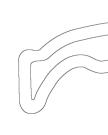
\includegraphics[interpolate=true,width=1.080000in,height=1.350000in]{contents/chapt6/figs/racing/slip_angle_1-img0.png}}%
\end{pgfscope}%
\begin{pgfscope}%
\pgfpathrectangle{\pgfqpoint{0.299840in}{1.000000in}}{\pgfqpoint{1.080000in}{1.350000in}}%
\pgfusepath{clip}%
\pgfsetrectcap%
\pgfsetroundjoin%
\pgfsetlinewidth{1.003750pt}%
\definecolor{currentstroke}{rgb}{0.121569,0.466667,0.705882}%
\pgfsetstrokecolor{currentstroke}%
\pgfsetstrokeopacity{0.700000}%
\pgfsetdash{}{0pt}%
\pgfpathmoveto{\pgfqpoint{1.389840in}{1.688610in}}%
\pgfpathlineto{\pgfqpoint{1.353327in}{1.687154in}}%
\pgfpathlineto{\pgfqpoint{1.323398in}{1.687961in}}%
\pgfpathlineto{\pgfqpoint{1.296919in}{1.690993in}}%
\pgfpathlineto{\pgfqpoint{1.274031in}{1.695725in}}%
\pgfpathlineto{\pgfqpoint{1.248366in}{1.703365in}}%
\pgfpathlineto{\pgfqpoint{1.178697in}{1.726257in}}%
\pgfpathlineto{\pgfqpoint{1.156082in}{1.730621in}}%
\pgfpathlineto{\pgfqpoint{1.133091in}{1.732996in}}%
\pgfpathlineto{\pgfqpoint{1.109841in}{1.733407in}}%
\pgfpathlineto{\pgfqpoint{1.086565in}{1.731805in}}%
\pgfpathlineto{\pgfqpoint{1.063487in}{1.728114in}}%
\pgfpathlineto{\pgfqpoint{1.040788in}{1.722435in}}%
\pgfpathlineto{\pgfqpoint{1.015421in}{1.713730in}}%
\pgfpathlineto{\pgfqpoint{0.990842in}{1.702896in}}%
\pgfpathlineto{\pgfqpoint{0.967204in}{1.690041in}}%
\pgfpathlineto{\pgfqpoint{0.944638in}{1.675272in}}%
\pgfpathlineto{\pgfqpoint{0.912776in}{1.650977in}}%
\pgfpathlineto{\pgfqpoint{0.846623in}{1.597924in}}%
\pgfpathlineto{\pgfqpoint{0.828506in}{1.579136in}}%
\pgfpathlineto{\pgfqpoint{0.799868in}{1.545179in}}%
\pgfpathlineto{\pgfqpoint{0.771496in}{1.509310in}}%
\pgfpathlineto{\pgfqpoint{0.753316in}{1.482714in}}%
\pgfpathlineto{\pgfqpoint{0.735895in}{1.453218in}}%
\pgfpathlineto{\pgfqpoint{0.724771in}{1.430261in}}%
\pgfpathlineto{\pgfqpoint{0.709869in}{1.392992in}}%
\pgfpathlineto{\pgfqpoint{0.698960in}{1.368839in}}%
\pgfpathlineto{\pgfqpoint{0.688624in}{1.350832in}}%
\pgfpathlineto{\pgfqpoint{0.678100in}{1.336697in}}%
\pgfpathlineto{\pgfqpoint{0.667767in}{1.326444in}}%
\pgfpathlineto{\pgfqpoint{0.655950in}{1.318140in}}%
\pgfpathlineto{\pgfqpoint{0.645547in}{1.313287in}}%
\pgfpathlineto{\pgfqpoint{0.634550in}{1.310290in}}%
\pgfpathlineto{\pgfqpoint{0.623366in}{1.309251in}}%
\pgfpathlineto{\pgfqpoint{0.612401in}{1.310216in}}%
\pgfpathlineto{\pgfqpoint{0.601954in}{1.313116in}}%
\pgfpathlineto{\pgfqpoint{0.592091in}{1.317861in}}%
\pgfpathlineto{\pgfqpoint{0.580851in}{1.325900in}}%
\pgfpathlineto{\pgfqpoint{0.570932in}{1.335934in}}%
\pgfpathlineto{\pgfqpoint{0.562452in}{1.347572in}}%
\pgfpathlineto{\pgfqpoint{0.554101in}{1.363219in}}%
\pgfpathlineto{\pgfqpoint{0.546322in}{1.383003in}}%
\pgfpathlineto{\pgfqpoint{0.539420in}{1.406853in}}%
\pgfpathlineto{\pgfqpoint{0.533767in}{1.434707in}}%
\pgfpathlineto{\pgfqpoint{0.530268in}{1.463327in}}%
\pgfpathlineto{\pgfqpoint{0.528846in}{1.492455in}}%
\pgfpathlineto{\pgfqpoint{0.529551in}{1.521848in}}%
\pgfpathlineto{\pgfqpoint{0.532495in}{1.554565in}}%
\pgfpathlineto{\pgfqpoint{0.539200in}{1.599947in}}%
\pgfpathlineto{\pgfqpoint{0.544687in}{1.641660in}}%
\pgfpathlineto{\pgfqpoint{0.551147in}{1.689307in}}%
\pgfpathlineto{\pgfqpoint{0.556444in}{1.711041in}}%
\pgfpathlineto{\pgfqpoint{0.563423in}{1.728850in}}%
\pgfpathlineto{\pgfqpoint{0.571178in}{1.742936in}}%
\pgfpathlineto{\pgfqpoint{0.580655in}{1.756040in}}%
\pgfpathlineto{\pgfqpoint{0.591851in}{1.767824in}}%
\pgfpathlineto{\pgfqpoint{0.604609in}{1.777996in}}%
\pgfpathlineto{\pgfqpoint{0.618522in}{1.786435in}}%
\pgfpathlineto{\pgfqpoint{0.636349in}{1.794345in}}%
\pgfpathlineto{\pgfqpoint{0.664274in}{1.803575in}}%
\pgfpathlineto{\pgfqpoint{0.701749in}{1.815936in}}%
\pgfpathlineto{\pgfqpoint{0.725989in}{1.826257in}}%
\pgfpathlineto{\pgfqpoint{0.755387in}{1.841351in}}%
\pgfpathlineto{\pgfqpoint{0.855929in}{1.895706in}}%
\pgfpathlineto{\pgfqpoint{0.889531in}{1.913533in}}%
\pgfpathlineto{\pgfqpoint{0.933635in}{1.937712in}}%
\pgfpathlineto{\pgfqpoint{0.958782in}{1.948945in}}%
\pgfpathlineto{\pgfqpoint{0.990149in}{1.960363in}}%
\pgfpathlineto{\pgfqpoint{1.031144in}{1.975965in}}%
\pgfpathlineto{\pgfqpoint{1.071540in}{1.991617in}}%
\pgfpathlineto{\pgfqpoint{1.094692in}{1.998192in}}%
\pgfpathlineto{\pgfqpoint{1.214475in}{2.025779in}}%
\pgfpathlineto{\pgfqpoint{1.272550in}{2.035123in}}%
\pgfpathlineto{\pgfqpoint{1.293544in}{2.039728in}}%
\pgfpathlineto{\pgfqpoint{1.293544in}{2.039728in}}%
\pgfusepath{stroke}%
\end{pgfscope}%
\begin{pgfscope}%
\pgfpathrectangle{\pgfqpoint{0.299840in}{1.000000in}}{\pgfqpoint{1.080000in}{1.350000in}}%
\pgfusepath{clip}%
\pgfsetrectcap%
\pgfsetroundjoin%
\pgfsetlinewidth{1.003750pt}%
\definecolor{currentstroke}{rgb}{1.000000,0.498039,0.054902}%
\pgfsetstrokecolor{currentstroke}%
\pgfsetstrokeopacity{0.700000}%
\pgfsetdash{}{0pt}%
\pgfpathmoveto{\pgfqpoint{1.389840in}{1.712081in}}%
\pgfpathlineto{\pgfqpoint{1.363931in}{1.708499in}}%
\pgfpathlineto{\pgfqpoint{1.343645in}{1.707787in}}%
\pgfpathlineto{\pgfqpoint{1.320022in}{1.709448in}}%
\pgfpathlineto{\pgfqpoint{1.279875in}{1.715582in}}%
\pgfpathlineto{\pgfqpoint{1.229957in}{1.724794in}}%
\pgfpathlineto{\pgfqpoint{1.200524in}{1.732626in}}%
\pgfpathlineto{\pgfqpoint{1.167780in}{1.741148in}}%
\pgfpathlineto{\pgfqpoint{1.151029in}{1.743489in}}%
\pgfpathlineto{\pgfqpoint{1.134123in}{1.743450in}}%
\pgfpathlineto{\pgfqpoint{1.120771in}{1.741286in}}%
\pgfpathlineto{\pgfqpoint{1.107884in}{1.737173in}}%
\pgfpathlineto{\pgfqpoint{1.092720in}{1.729696in}}%
\pgfpathlineto{\pgfqpoint{1.075839in}{1.718422in}}%
\pgfpathlineto{\pgfqpoint{1.045367in}{1.697061in}}%
\pgfpathlineto{\pgfqpoint{1.030342in}{1.689308in}}%
\pgfpathlineto{\pgfqpoint{1.014486in}{1.683531in}}%
\pgfpathlineto{\pgfqpoint{0.994862in}{1.678831in}}%
\pgfpathlineto{\pgfqpoint{0.949726in}{1.669212in}}%
\pgfpathlineto{\pgfqpoint{0.934584in}{1.663416in}}%
\pgfpathlineto{\pgfqpoint{0.919877in}{1.655159in}}%
\pgfpathlineto{\pgfqpoint{0.906629in}{1.644655in}}%
\pgfpathlineto{\pgfqpoint{0.895242in}{1.632155in}}%
\pgfpathlineto{\pgfqpoint{0.885731in}{1.618169in}}%
\pgfpathlineto{\pgfqpoint{0.874761in}{1.597175in}}%
\pgfpathlineto{\pgfqpoint{0.860610in}{1.570215in}}%
\pgfpathlineto{\pgfqpoint{0.850758in}{1.556504in}}%
\pgfpathlineto{\pgfqpoint{0.839162in}{1.544392in}}%
\pgfpathlineto{\pgfqpoint{0.826109in}{1.533888in}}%
\pgfpathlineto{\pgfqpoint{0.780295in}{1.500006in}}%
\pgfpathlineto{\pgfqpoint{0.769119in}{1.487160in}}%
\pgfpathlineto{\pgfqpoint{0.761752in}{1.475637in}}%
\pgfpathlineto{\pgfqpoint{0.756094in}{1.463187in}}%
\pgfpathlineto{\pgfqpoint{0.752197in}{1.450076in}}%
\pgfpathlineto{\pgfqpoint{0.749591in}{1.433181in}}%
\pgfpathlineto{\pgfqpoint{0.748892in}{1.412669in}}%
\pgfpathlineto{\pgfqpoint{0.748171in}{1.378478in}}%
\pgfpathlineto{\pgfqpoint{0.745168in}{1.361653in}}%
\pgfpathlineto{\pgfqpoint{0.740584in}{1.348772in}}%
\pgfpathlineto{\pgfqpoint{0.733809in}{1.336901in}}%
\pgfpathlineto{\pgfqpoint{0.724868in}{1.326567in}}%
\pgfpathlineto{\pgfqpoint{0.714010in}{1.318272in}}%
\pgfpathlineto{\pgfqpoint{0.701667in}{1.312410in}}%
\pgfpathlineto{\pgfqpoint{0.688423in}{1.309028in}}%
\pgfpathlineto{\pgfqpoint{0.674795in}{1.307891in}}%
\pgfpathlineto{\pgfqpoint{0.661141in}{1.308690in}}%
\pgfpathlineto{\pgfqpoint{0.644364in}{1.311976in}}%
\pgfpathlineto{\pgfqpoint{0.628161in}{1.317430in}}%
\pgfpathlineto{\pgfqpoint{0.612810in}{1.324955in}}%
\pgfpathlineto{\pgfqpoint{0.598637in}{1.334510in}}%
\pgfpathlineto{\pgfqpoint{0.588602in}{1.343799in}}%
\pgfpathlineto{\pgfqpoint{0.580139in}{1.354539in}}%
\pgfpathlineto{\pgfqpoint{0.573433in}{1.366456in}}%
\pgfpathlineto{\pgfqpoint{0.568606in}{1.379251in}}%
\pgfpathlineto{\pgfqpoint{0.565081in}{1.395976in}}%
\pgfpathlineto{\pgfqpoint{0.563444in}{1.416433in}}%
\pgfpathlineto{\pgfqpoint{0.561048in}{1.453972in}}%
\pgfpathlineto{\pgfqpoint{0.557598in}{1.470718in}}%
\pgfpathlineto{\pgfqpoint{0.551809in}{1.486801in}}%
\pgfpathlineto{\pgfqpoint{0.543818in}{1.501916in}}%
\pgfpathlineto{\pgfqpoint{0.530238in}{1.521635in}}%
\pgfpathlineto{\pgfqpoint{0.512622in}{1.546877in}}%
\pgfpathlineto{\pgfqpoint{0.504845in}{1.562100in}}%
\pgfpathlineto{\pgfqpoint{0.500478in}{1.575059in}}%
\pgfpathlineto{\pgfqpoint{0.498290in}{1.588553in}}%
\pgfpathlineto{\pgfqpoint{0.498588in}{1.602217in}}%
\pgfpathlineto{\pgfqpoint{0.501408in}{1.615593in}}%
\pgfpathlineto{\pgfqpoint{0.506461in}{1.628298in}}%
\pgfpathlineto{\pgfqpoint{0.515192in}{1.642993in}}%
\pgfpathlineto{\pgfqpoint{0.529856in}{1.661923in}}%
\pgfpathlineto{\pgfqpoint{0.555111in}{1.694280in}}%
\pgfpathlineto{\pgfqpoint{0.594593in}{1.750023in}}%
\pgfpathlineto{\pgfqpoint{0.607506in}{1.761220in}}%
\pgfpathlineto{\pgfqpoint{0.619099in}{1.768475in}}%
\pgfpathlineto{\pgfqpoint{0.634773in}{1.775293in}}%
\pgfpathlineto{\pgfqpoint{0.654531in}{1.780830in}}%
\pgfpathlineto{\pgfqpoint{0.694398in}{1.790541in}}%
\pgfpathlineto{\pgfqpoint{0.710082in}{1.797331in}}%
\pgfpathlineto{\pgfqpoint{0.721595in}{1.804709in}}%
\pgfpathlineto{\pgfqpoint{0.731884in}{1.813718in}}%
\pgfpathlineto{\pgfqpoint{0.742931in}{1.826762in}}%
\pgfpathlineto{\pgfqpoint{0.754160in}{1.843941in}}%
\pgfpathlineto{\pgfqpoint{0.770672in}{1.869919in}}%
\pgfpathlineto{\pgfqpoint{0.781839in}{1.882858in}}%
\pgfpathlineto{\pgfqpoint{0.792338in}{1.891616in}}%
\pgfpathlineto{\pgfqpoint{0.804205in}{1.898399in}}%
\pgfpathlineto{\pgfqpoint{0.817115in}{1.902892in}}%
\pgfpathlineto{\pgfqpoint{0.830604in}{1.905126in}}%
\pgfpathlineto{\pgfqpoint{0.847635in}{1.905239in}}%
\pgfpathlineto{\pgfqpoint{0.871069in}{1.902414in}}%
\pgfpathlineto{\pgfqpoint{0.897602in}{1.899450in}}%
\pgfpathlineto{\pgfqpoint{0.914440in}{1.900138in}}%
\pgfpathlineto{\pgfqpoint{0.927728in}{1.902700in}}%
\pgfpathlineto{\pgfqpoint{0.940461in}{1.907277in}}%
\pgfpathlineto{\pgfqpoint{0.952350in}{1.913744in}}%
\pgfpathlineto{\pgfqpoint{0.965856in}{1.923929in}}%
\pgfpathlineto{\pgfqpoint{0.982837in}{1.940455in}}%
\pgfpathlineto{\pgfqpoint{1.002237in}{1.959343in}}%
\pgfpathlineto{\pgfqpoint{1.015931in}{1.969271in}}%
\pgfpathlineto{\pgfqpoint{1.027976in}{1.975441in}}%
\pgfpathlineto{\pgfqpoint{1.040771in}{1.979854in}}%
\pgfpathlineto{\pgfqpoint{1.057390in}{1.983012in}}%
\pgfpathlineto{\pgfqpoint{1.077659in}{1.984281in}}%
\pgfpathlineto{\pgfqpoint{1.111090in}{1.985843in}}%
\pgfpathlineto{\pgfqpoint{1.127816in}{1.989104in}}%
\pgfpathlineto{\pgfqpoint{1.144023in}{1.994536in}}%
\pgfpathlineto{\pgfqpoint{1.159424in}{2.001957in}}%
\pgfpathlineto{\pgfqpoint{1.176809in}{2.012850in}}%
\pgfpathlineto{\pgfqpoint{1.221928in}{2.043731in}}%
\pgfpathlineto{\pgfqpoint{1.234481in}{2.049152in}}%
\pgfpathlineto{\pgfqpoint{1.247678in}{2.052725in}}%
\pgfpathlineto{\pgfqpoint{1.261253in}{2.054365in}}%
\pgfpathlineto{\pgfqpoint{1.278340in}{2.054010in}}%
\pgfpathlineto{\pgfqpoint{1.295309in}{2.051884in}}%
\pgfpathlineto{\pgfqpoint{1.295309in}{2.051884in}}%
\pgfusepath{stroke}%
\end{pgfscope}%
\begin{pgfscope}%
\pgfsetbuttcap%
\pgfsetmiterjoin%
\definecolor{currentfill}{rgb}{1.000000,1.000000,1.000000}%
\pgfsetfillcolor{currentfill}%
\pgfsetlinewidth{1.003750pt}%
\definecolor{currentstroke}{rgb}{0.000000,0.000000,0.000000}%
\pgfsetstrokecolor{currentstroke}%
\pgfsetdash{}{0pt}%
\pgfpathmoveto{\pgfqpoint{1.261421in}{1.652271in}}%
\pgfpathlineto{\pgfqpoint{1.473490in}{1.652271in}}%
\pgfpathquadraticcurveto{\pgfqpoint{1.485059in}{1.652271in}}{\pgfqpoint{1.485059in}{1.663840in}}%
\pgfpathlineto{\pgfqpoint{1.485059in}{1.768914in}}%
\pgfpathquadraticcurveto{\pgfqpoint{1.485059in}{1.780483in}}{\pgfqpoint{1.473490in}{1.780483in}}%
\pgfpathlineto{\pgfqpoint{1.261421in}{1.780483in}}%
\pgfpathquadraticcurveto{\pgfqpoint{1.249851in}{1.780483in}}{\pgfqpoint{1.249851in}{1.768914in}}%
\pgfpathlineto{\pgfqpoint{1.249851in}{1.663840in}}%
\pgfpathquadraticcurveto{\pgfqpoint{1.249851in}{1.652271in}}{\pgfqpoint{1.261421in}{1.652271in}}%
\pgfpathlineto{\pgfqpoint{1.261421in}{1.652271in}}%
\pgfpathclose%
\pgfusepath{stroke,fill}%
\end{pgfscope}%
\begin{pgfscope}%
\definecolor{textcolor}{rgb}{0.000000,0.000000,0.000000}%
\pgfsetstrokecolor{textcolor}%
\pgfsetfillcolor{textcolor}%
\pgftext[x=1.261421in,y=1.688583in,left,base]{\color{textcolor}\rmfamily\fontsize{8.330000}{9.996000}\selectfont 80\%}%
\end{pgfscope}%
\begin{pgfscope}%
\pgfsetbuttcap%
\pgfsetmiterjoin%
\definecolor{currentfill}{rgb}{1.000000,1.000000,1.000000}%
\pgfsetfillcolor{currentfill}%
\pgfsetlinewidth{1.003750pt}%
\definecolor{currentstroke}{rgb}{0.000000,0.000000,0.000000}%
\pgfsetstrokecolor{currentstroke}%
\pgfsetdash{}{0pt}%
\pgfpathmoveto{\pgfqpoint{0.546544in}{1.546752in}}%
\pgfpathlineto{\pgfqpoint{0.758612in}{1.546752in}}%
\pgfpathquadraticcurveto{\pgfqpoint{0.770182in}{1.546752in}}{\pgfqpoint{0.770182in}{1.558321in}}%
\pgfpathlineto{\pgfqpoint{0.770182in}{1.663395in}}%
\pgfpathquadraticcurveto{\pgfqpoint{0.770182in}{1.674965in}}{\pgfqpoint{0.758612in}{1.674965in}}%
\pgfpathlineto{\pgfqpoint{0.546544in}{1.674965in}}%
\pgfpathquadraticcurveto{\pgfqpoint{0.534974in}{1.674965in}}{\pgfqpoint{0.534974in}{1.663395in}}%
\pgfpathlineto{\pgfqpoint{0.534974in}{1.558321in}}%
\pgfpathquadraticcurveto{\pgfqpoint{0.534974in}{1.546752in}}{\pgfqpoint{0.546544in}{1.546752in}}%
\pgfpathlineto{\pgfqpoint{0.546544in}{1.546752in}}%
\pgfpathclose%
\pgfusepath{stroke,fill}%
\end{pgfscope}%
\begin{pgfscope}%
\definecolor{textcolor}{rgb}{0.000000,0.000000,0.000000}%
\pgfsetstrokecolor{textcolor}%
\pgfsetfillcolor{textcolor}%
\pgftext[x=0.546544in,y=1.583064in,left,base]{\color{textcolor}\rmfamily\fontsize{8.330000}{9.996000}\selectfont 90\%}%
\end{pgfscope}%
\begin{pgfscope}%
\pgfsetbuttcap%
\pgfsetmiterjoin%
\definecolor{currentfill}{rgb}{1.000000,1.000000,1.000000}%
\pgfsetfillcolor{currentfill}%
\pgfsetlinewidth{1.003750pt}%
\definecolor{currentstroke}{rgb}{0.000000,0.000000,0.000000}%
\pgfsetstrokecolor{currentstroke}%
\pgfsetdash{}{0pt}%
\pgfpathmoveto{\pgfqpoint{1.392837in}{2.025556in}}%
\pgfpathlineto{\pgfqpoint{1.682186in}{2.025556in}}%
\pgfpathquadraticcurveto{\pgfqpoint{1.693756in}{2.025556in}}{\pgfqpoint{1.693756in}{2.037125in}}%
\pgfpathlineto{\pgfqpoint{1.693756in}{2.142199in}}%
\pgfpathquadraticcurveto{\pgfqpoint{1.693756in}{2.153768in}}{\pgfqpoint{1.682186in}{2.153768in}}%
\pgfpathlineto{\pgfqpoint{1.392837in}{2.153768in}}%
\pgfpathquadraticcurveto{\pgfqpoint{1.381267in}{2.153768in}}{\pgfqpoint{1.381267in}{2.142199in}}%
\pgfpathlineto{\pgfqpoint{1.381267in}{2.037125in}}%
\pgfpathquadraticcurveto{\pgfqpoint{1.381267in}{2.025556in}}{\pgfqpoint{1.392837in}{2.025556in}}%
\pgfpathlineto{\pgfqpoint{1.392837in}{2.025556in}}%
\pgfpathclose%
\pgfusepath{stroke,fill}%
\end{pgfscope}%
\begin{pgfscope}%
\definecolor{textcolor}{rgb}{0.000000,0.000000,0.000000}%
\pgfsetstrokecolor{textcolor}%
\pgfsetfillcolor{textcolor}%
\pgftext[x=1.392837in,y=2.061868in,left,base]{\color{textcolor}\rmfamily\fontsize{8.330000}{9.996000}\selectfont Finish}%
\end{pgfscope}%
\begin{pgfscope}%
\pgfsetbuttcap%
\pgfsetmiterjoin%
\definecolor{currentfill}{rgb}{1.000000,1.000000,1.000000}%
\pgfsetfillcolor{currentfill}%
\pgfsetlinewidth{0.000000pt}%
\definecolor{currentstroke}{rgb}{0.000000,0.000000,0.000000}%
\pgfsetstrokecolor{currentstroke}%
\pgfsetstrokeopacity{0.000000}%
\pgfsetdash{}{0pt}%
\pgfpathmoveto{\pgfqpoint{2.485641in}{1.000000in}}%
\pgfpathlineto{\pgfqpoint{5.245000in}{1.000000in}}%
\pgfpathlineto{\pgfqpoint{5.245000in}{2.350000in}}%
\pgfpathlineto{\pgfqpoint{2.485641in}{2.350000in}}%
\pgfpathlineto{\pgfqpoint{2.485641in}{1.000000in}}%
\pgfpathclose%
\pgfusepath{fill}%
\end{pgfscope}%
\begin{pgfscope}%
\pgfpathrectangle{\pgfqpoint{2.485641in}{1.000000in}}{\pgfqpoint{2.759359in}{1.350000in}}%
\pgfusepath{clip}%
\pgfsetrectcap%
\pgfsetroundjoin%
\pgfsetlinewidth{0.803000pt}%
\definecolor{currentstroke}{rgb}{0.827451,0.827451,0.827451}%
\pgfsetstrokecolor{currentstroke}%
\pgfsetdash{}{0pt}%
\pgfpathmoveto{\pgfqpoint{2.485641in}{1.000000in}}%
\pgfpathlineto{\pgfqpoint{2.485641in}{2.350000in}}%
\pgfusepath{stroke}%
\end{pgfscope}%
\begin{pgfscope}%
\definecolor{textcolor}{rgb}{0.000000,0.000000,0.000000}%
\pgfsetstrokecolor{textcolor}%
\pgfsetfillcolor{textcolor}%
\pgftext[x=2.485641in,y=0.951389in,,top]{\color{textcolor}\rmfamily\fontsize{10.000000}{12.000000}\selectfont 80}%
\end{pgfscope}%
\begin{pgfscope}%
\pgfpathrectangle{\pgfqpoint{2.485641in}{1.000000in}}{\pgfqpoint{2.759359in}{1.350000in}}%
\pgfusepath{clip}%
\pgfsetrectcap%
\pgfsetroundjoin%
\pgfsetlinewidth{0.803000pt}%
\definecolor{currentstroke}{rgb}{0.827451,0.827451,0.827451}%
\pgfsetstrokecolor{currentstroke}%
\pgfsetdash{}{0pt}%
\pgfpathmoveto{\pgfqpoint{3.175481in}{1.000000in}}%
\pgfpathlineto{\pgfqpoint{3.175481in}{2.350000in}}%
\pgfusepath{stroke}%
\end{pgfscope}%
\begin{pgfscope}%
\definecolor{textcolor}{rgb}{0.000000,0.000000,0.000000}%
\pgfsetstrokecolor{textcolor}%
\pgfsetfillcolor{textcolor}%
\pgftext[x=3.175481in,y=0.951389in,,top]{\color{textcolor}\rmfamily\fontsize{10.000000}{12.000000}\selectfont 85}%
\end{pgfscope}%
\begin{pgfscope}%
\pgfpathrectangle{\pgfqpoint{2.485641in}{1.000000in}}{\pgfqpoint{2.759359in}{1.350000in}}%
\pgfusepath{clip}%
\pgfsetrectcap%
\pgfsetroundjoin%
\pgfsetlinewidth{0.803000pt}%
\definecolor{currentstroke}{rgb}{0.827451,0.827451,0.827451}%
\pgfsetstrokecolor{currentstroke}%
\pgfsetdash{}{0pt}%
\pgfpathmoveto{\pgfqpoint{3.865320in}{1.000000in}}%
\pgfpathlineto{\pgfqpoint{3.865320in}{2.350000in}}%
\pgfusepath{stroke}%
\end{pgfscope}%
\begin{pgfscope}%
\definecolor{textcolor}{rgb}{0.000000,0.000000,0.000000}%
\pgfsetstrokecolor{textcolor}%
\pgfsetfillcolor{textcolor}%
\pgftext[x=3.865320in,y=0.951389in,,top]{\color{textcolor}\rmfamily\fontsize{10.000000}{12.000000}\selectfont 90}%
\end{pgfscope}%
\begin{pgfscope}%
\pgfpathrectangle{\pgfqpoint{2.485641in}{1.000000in}}{\pgfqpoint{2.759359in}{1.350000in}}%
\pgfusepath{clip}%
\pgfsetrectcap%
\pgfsetroundjoin%
\pgfsetlinewidth{0.803000pt}%
\definecolor{currentstroke}{rgb}{0.827451,0.827451,0.827451}%
\pgfsetstrokecolor{currentstroke}%
\pgfsetdash{}{0pt}%
\pgfpathmoveto{\pgfqpoint{4.555160in}{1.000000in}}%
\pgfpathlineto{\pgfqpoint{4.555160in}{2.350000in}}%
\pgfusepath{stroke}%
\end{pgfscope}%
\begin{pgfscope}%
\definecolor{textcolor}{rgb}{0.000000,0.000000,0.000000}%
\pgfsetstrokecolor{textcolor}%
\pgfsetfillcolor{textcolor}%
\pgftext[x=4.555160in,y=0.951389in,,top]{\color{textcolor}\rmfamily\fontsize{10.000000}{12.000000}\selectfont 95}%
\end{pgfscope}%
\begin{pgfscope}%
\pgfpathrectangle{\pgfqpoint{2.485641in}{1.000000in}}{\pgfqpoint{2.759359in}{1.350000in}}%
\pgfusepath{clip}%
\pgfsetrectcap%
\pgfsetroundjoin%
\pgfsetlinewidth{0.803000pt}%
\definecolor{currentstroke}{rgb}{0.827451,0.827451,0.827451}%
\pgfsetstrokecolor{currentstroke}%
\pgfsetdash{}{0pt}%
\pgfpathmoveto{\pgfqpoint{5.245000in}{1.000000in}}%
\pgfpathlineto{\pgfqpoint{5.245000in}{2.350000in}}%
\pgfusepath{stroke}%
\end{pgfscope}%
\begin{pgfscope}%
\definecolor{textcolor}{rgb}{0.000000,0.000000,0.000000}%
\pgfsetstrokecolor{textcolor}%
\pgfsetfillcolor{textcolor}%
\pgftext[x=5.245000in,y=0.951389in,,top]{\color{textcolor}\rmfamily\fontsize{10.000000}{12.000000}\selectfont 100}%
\end{pgfscope}%
\begin{pgfscope}%
\definecolor{textcolor}{rgb}{0.000000,0.000000,0.000000}%
\pgfsetstrokecolor{textcolor}%
\pgfsetfillcolor{textcolor}%
\pgftext[x=3.865320in,y=0.769694in,,top]{\color{textcolor}\rmfamily\fontsize{10.000000}{12.000000}\selectfont progress along centerline [\%]}%
\end{pgfscope}%
\begin{pgfscope}%
\pgfpathrectangle{\pgfqpoint{2.485641in}{1.000000in}}{\pgfqpoint{2.759359in}{1.350000in}}%
\pgfusepath{clip}%
\pgfsetrectcap%
\pgfsetroundjoin%
\pgfsetlinewidth{0.803000pt}%
\definecolor{currentstroke}{rgb}{0.827451,0.827451,0.827451}%
\pgfsetstrokecolor{currentstroke}%
\pgfsetdash{}{0pt}%
\pgfpathmoveto{\pgfqpoint{2.485641in}{1.229785in}}%
\pgfpathlineto{\pgfqpoint{5.245000in}{1.229785in}}%
\pgfusepath{stroke}%
\end{pgfscope}%
\begin{pgfscope}%
\definecolor{textcolor}{rgb}{0.000000,0.000000,0.000000}%
\pgfsetstrokecolor{textcolor}%
\pgfsetfillcolor{textcolor}%
\pgftext[x=2.155393in, y=1.181568in, left, base]{\color{textcolor}\rmfamily\fontsize{10.000000}{12.000000}\selectfont \ensuremath{-}0.2}%
\end{pgfscope}%
\begin{pgfscope}%
\pgfpathrectangle{\pgfqpoint{2.485641in}{1.000000in}}{\pgfqpoint{2.759359in}{1.350000in}}%
\pgfusepath{clip}%
\pgfsetrectcap%
\pgfsetroundjoin%
\pgfsetlinewidth{0.803000pt}%
\definecolor{currentstroke}{rgb}{0.827451,0.827451,0.827451}%
\pgfsetstrokecolor{currentstroke}%
\pgfsetdash{}{0pt}%
\pgfpathmoveto{\pgfqpoint{2.485641in}{1.646669in}}%
\pgfpathlineto{\pgfqpoint{5.245000in}{1.646669in}}%
\pgfusepath{stroke}%
\end{pgfscope}%
\begin{pgfscope}%
\definecolor{textcolor}{rgb}{0.000000,0.000000,0.000000}%
\pgfsetstrokecolor{textcolor}%
\pgfsetfillcolor{textcolor}%
\pgftext[x=2.263418in, y=1.598451in, left, base]{\color{textcolor}\rmfamily\fontsize{10.000000}{12.000000}\selectfont 0.0}%
\end{pgfscope}%
\begin{pgfscope}%
\pgfpathrectangle{\pgfqpoint{2.485641in}{1.000000in}}{\pgfqpoint{2.759359in}{1.350000in}}%
\pgfusepath{clip}%
\pgfsetrectcap%
\pgfsetroundjoin%
\pgfsetlinewidth{0.803000pt}%
\definecolor{currentstroke}{rgb}{0.827451,0.827451,0.827451}%
\pgfsetstrokecolor{currentstroke}%
\pgfsetdash{}{0pt}%
\pgfpathmoveto{\pgfqpoint{2.485641in}{2.063552in}}%
\pgfpathlineto{\pgfqpoint{5.245000in}{2.063552in}}%
\pgfusepath{stroke}%
\end{pgfscope}%
\begin{pgfscope}%
\definecolor{textcolor}{rgb}{0.000000,0.000000,0.000000}%
\pgfsetstrokecolor{textcolor}%
\pgfsetfillcolor{textcolor}%
\pgftext[x=2.263418in, y=2.015334in, left, base]{\color{textcolor}\rmfamily\fontsize{10.000000}{12.000000}\selectfont 0.2}%
\end{pgfscope}%
\begin{pgfscope}%
\definecolor{textcolor}{rgb}{0.000000,0.000000,0.000000}%
\pgfsetstrokecolor{textcolor}%
\pgfsetfillcolor{textcolor}%
\pgftext[x=2.099838in,y=1.675000in,,bottom,rotate=90.000000]{\color{textcolor}\rmfamily\fontsize{10.000000}{12.000000}\selectfont Slip angle [rads]}%
\end{pgfscope}%
\begin{pgfscope}%
\pgfpathrectangle{\pgfqpoint{2.485641in}{1.000000in}}{\pgfqpoint{2.759359in}{1.350000in}}%
\pgfusepath{clip}%
\pgfsetrectcap%
\pgfsetroundjoin%
\pgfsetlinewidth{1.505625pt}%
\definecolor{currentstroke}{rgb}{0.121569,0.466667,0.705882}%
\pgfsetstrokecolor{currentstroke}%
\pgfsetstrokeopacity{0.700000}%
\pgfsetdash{}{0pt}%
\pgfpathmoveto{\pgfqpoint{2.485641in}{1.779735in}}%
\pgfpathlineto{\pgfqpoint{2.493370in}{1.779790in}}%
\pgfpathlineto{\pgfqpoint{2.493370in}{1.775167in}}%
\pgfpathlineto{\pgfqpoint{2.501099in}{1.775198in}}%
\pgfpathlineto{\pgfqpoint{2.501099in}{1.777277in}}%
\pgfpathlineto{\pgfqpoint{2.508829in}{1.780715in}}%
\pgfpathlineto{\pgfqpoint{2.516558in}{1.779545in}}%
\pgfpathlineto{\pgfqpoint{2.516558in}{1.775758in}}%
\pgfpathlineto{\pgfqpoint{2.524287in}{1.762064in}}%
\pgfpathlineto{\pgfqpoint{2.524287in}{1.750045in}}%
\pgfpathlineto{\pgfqpoint{2.532016in}{1.731360in}}%
\pgfpathlineto{\pgfqpoint{2.532016in}{1.716845in}}%
\pgfpathlineto{\pgfqpoint{2.539746in}{1.704285in}}%
\pgfpathlineto{\pgfqpoint{2.539746in}{1.685123in}}%
\pgfpathlineto{\pgfqpoint{2.547475in}{1.670275in}}%
\pgfpathlineto{\pgfqpoint{2.547475in}{1.650267in}}%
\pgfpathlineto{\pgfqpoint{2.555204in}{1.635731in}}%
\pgfpathlineto{\pgfqpoint{2.555204in}{1.617204in}}%
\pgfpathlineto{\pgfqpoint{2.562934in}{1.604664in}}%
\pgfpathlineto{\pgfqpoint{2.562934in}{1.588340in}}%
\pgfpathlineto{\pgfqpoint{2.570663in}{1.578181in}}%
\pgfpathlineto{\pgfqpoint{2.570663in}{1.564320in}}%
\pgfpathlineto{\pgfqpoint{2.578392in}{1.556518in}}%
\pgfpathlineto{\pgfqpoint{2.578392in}{1.539161in}}%
\pgfpathlineto{\pgfqpoint{2.586122in}{1.529469in}}%
\pgfpathlineto{\pgfqpoint{2.586122in}{1.525643in}}%
\pgfpathlineto{\pgfqpoint{2.593851in}{1.517819in}}%
\pgfpathlineto{\pgfqpoint{2.593851in}{1.515742in}}%
\pgfpathlineto{\pgfqpoint{2.601580in}{1.508377in}}%
\pgfpathlineto{\pgfqpoint{2.609309in}{1.506650in}}%
\pgfpathlineto{\pgfqpoint{2.609309in}{1.501144in}}%
\pgfpathlineto{\pgfqpoint{2.617039in}{1.494796in}}%
\pgfpathlineto{\pgfqpoint{2.617039in}{1.496277in}}%
\pgfpathlineto{\pgfqpoint{2.624768in}{1.494635in}}%
\pgfpathlineto{\pgfqpoint{2.624768in}{1.498830in}}%
\pgfpathlineto{\pgfqpoint{2.632497in}{1.499557in}}%
\pgfpathlineto{\pgfqpoint{2.632497in}{1.505873in}}%
\pgfpathlineto{\pgfqpoint{2.640227in}{1.507340in}}%
\pgfpathlineto{\pgfqpoint{2.640227in}{1.513578in}}%
\pgfpathlineto{\pgfqpoint{2.647956in}{1.522473in}}%
\pgfpathlineto{\pgfqpoint{2.655685in}{1.526627in}}%
\pgfpathlineto{\pgfqpoint{2.655685in}{1.525090in}}%
\pgfpathlineto{\pgfqpoint{2.663415in}{1.527268in}}%
\pgfpathlineto{\pgfqpoint{2.663415in}{1.523971in}}%
\pgfpathlineto{\pgfqpoint{2.671144in}{1.524809in}}%
\pgfpathlineto{\pgfqpoint{2.671144in}{1.520577in}}%
\pgfpathlineto{\pgfqpoint{2.678873in}{1.521034in}}%
\pgfpathlineto{\pgfqpoint{2.678873in}{1.516553in}}%
\pgfpathlineto{\pgfqpoint{2.686602in}{1.517085in}}%
\pgfpathlineto{\pgfqpoint{2.686602in}{1.512729in}}%
\pgfpathlineto{\pgfqpoint{2.694332in}{1.513153in}}%
\pgfpathlineto{\pgfqpoint{2.694332in}{1.509068in}}%
\pgfpathlineto{\pgfqpoint{2.702061in}{1.509738in}}%
\pgfpathlineto{\pgfqpoint{2.702061in}{1.506182in}}%
\pgfpathlineto{\pgfqpoint{2.709790in}{1.507147in}}%
\pgfpathlineto{\pgfqpoint{2.709790in}{1.503204in}}%
\pgfpathlineto{\pgfqpoint{2.717520in}{1.504041in}}%
\pgfpathlineto{\pgfqpoint{2.717520in}{1.500263in}}%
\pgfpathlineto{\pgfqpoint{2.725249in}{1.494742in}}%
\pgfpathlineto{\pgfqpoint{2.725249in}{1.496185in}}%
\pgfpathlineto{\pgfqpoint{2.732978in}{1.494396in}}%
\pgfpathlineto{\pgfqpoint{2.748437in}{1.503482in}}%
\pgfpathlineto{\pgfqpoint{2.748437in}{1.504376in}}%
\pgfpathlineto{\pgfqpoint{2.779354in}{1.525575in}}%
\pgfpathlineto{\pgfqpoint{2.779354in}{1.525261in}}%
\pgfpathlineto{\pgfqpoint{2.787083in}{1.529259in}}%
\pgfpathlineto{\pgfqpoint{2.787083in}{1.527916in}}%
\pgfpathlineto{\pgfqpoint{2.794813in}{1.531074in}}%
\pgfpathlineto{\pgfqpoint{2.794813in}{1.529550in}}%
\pgfpathlineto{\pgfqpoint{2.802542in}{1.532907in}}%
\pgfpathlineto{\pgfqpoint{2.802542in}{1.537990in}}%
\pgfpathlineto{\pgfqpoint{2.810271in}{1.536029in}}%
\pgfpathlineto{\pgfqpoint{2.810271in}{1.530833in}}%
\pgfpathlineto{\pgfqpoint{2.818001in}{1.531504in}}%
\pgfpathlineto{\pgfqpoint{2.818001in}{1.527919in}}%
\pgfpathlineto{\pgfqpoint{2.825730in}{1.529642in}}%
\pgfpathlineto{\pgfqpoint{2.825730in}{1.526957in}}%
\pgfpathlineto{\pgfqpoint{2.833459in}{1.529192in}}%
\pgfpathlineto{\pgfqpoint{2.833459in}{1.527210in}}%
\pgfpathlineto{\pgfqpoint{2.841188in}{1.530003in}}%
\pgfpathlineto{\pgfqpoint{2.841188in}{1.527884in}}%
\pgfpathlineto{\pgfqpoint{2.848918in}{1.530666in}}%
\pgfpathlineto{\pgfqpoint{2.848918in}{1.528823in}}%
\pgfpathlineto{\pgfqpoint{2.856647in}{1.531624in}}%
\pgfpathlineto{\pgfqpoint{2.856647in}{1.530059in}}%
\pgfpathlineto{\pgfqpoint{2.864376in}{1.533179in}}%
\pgfpathlineto{\pgfqpoint{2.864376in}{1.531328in}}%
\pgfpathlineto{\pgfqpoint{2.872106in}{1.534106in}}%
\pgfpathlineto{\pgfqpoint{2.872106in}{1.532176in}}%
\pgfpathlineto{\pgfqpoint{2.879835in}{1.534850in}}%
\pgfpathlineto{\pgfqpoint{2.879835in}{1.532579in}}%
\pgfpathlineto{\pgfqpoint{2.887564in}{1.527721in}}%
\pgfpathlineto{\pgfqpoint{2.887564in}{1.522388in}}%
\pgfpathlineto{\pgfqpoint{2.895293in}{1.518387in}}%
\pgfpathlineto{\pgfqpoint{2.895293in}{1.516758in}}%
\pgfpathlineto{\pgfqpoint{2.903023in}{1.518200in}}%
\pgfpathlineto{\pgfqpoint{2.903023in}{1.530205in}}%
\pgfpathlineto{\pgfqpoint{2.910752in}{1.540665in}}%
\pgfpathlineto{\pgfqpoint{2.910752in}{1.558391in}}%
\pgfpathlineto{\pgfqpoint{2.918481in}{1.572152in}}%
\pgfpathlineto{\pgfqpoint{2.918481in}{1.591255in}}%
\pgfpathlineto{\pgfqpoint{2.926211in}{1.612212in}}%
\pgfpathlineto{\pgfqpoint{2.926211in}{1.625333in}}%
\pgfpathlineto{\pgfqpoint{2.933940in}{1.641345in}}%
\pgfpathlineto{\pgfqpoint{2.933940in}{1.657454in}}%
\pgfpathlineto{\pgfqpoint{2.941669in}{1.664605in}}%
\pgfpathlineto{\pgfqpoint{2.941669in}{1.674016in}}%
\pgfpathlineto{\pgfqpoint{2.949399in}{1.676086in}}%
\pgfpathlineto{\pgfqpoint{2.949399in}{1.681670in}}%
\pgfpathlineto{\pgfqpoint{2.957128in}{1.680894in}}%
\pgfpathlineto{\pgfqpoint{2.957128in}{1.684101in}}%
\pgfpathlineto{\pgfqpoint{2.964857in}{1.688518in}}%
\pgfpathlineto{\pgfqpoint{2.964857in}{1.692523in}}%
\pgfpathlineto{\pgfqpoint{2.972586in}{1.694887in}}%
\pgfpathlineto{\pgfqpoint{2.972586in}{1.694806in}}%
\pgfpathlineto{\pgfqpoint{2.980316in}{1.691529in}}%
\pgfpathlineto{\pgfqpoint{2.980316in}{1.678654in}}%
\pgfpathlineto{\pgfqpoint{2.988045in}{1.667477in}}%
\pgfpathlineto{\pgfqpoint{2.988045in}{1.649772in}}%
\pgfpathlineto{\pgfqpoint{2.995774in}{1.636111in}}%
\pgfpathlineto{\pgfqpoint{2.995774in}{1.617687in}}%
\pgfpathlineto{\pgfqpoint{3.003504in}{1.597445in}}%
\pgfpathlineto{\pgfqpoint{3.003504in}{1.569374in}}%
\pgfpathlineto{\pgfqpoint{3.011233in}{1.560892in}}%
\pgfpathlineto{\pgfqpoint{3.011233in}{1.549279in}}%
\pgfpathlineto{\pgfqpoint{3.018962in}{1.544042in}}%
\pgfpathlineto{\pgfqpoint{3.018962in}{1.535140in}}%
\pgfpathlineto{\pgfqpoint{3.026692in}{1.532056in}}%
\pgfpathlineto{\pgfqpoint{3.026692in}{1.525106in}}%
\pgfpathlineto{\pgfqpoint{3.034421in}{1.523728in}}%
\pgfpathlineto{\pgfqpoint{3.034421in}{1.516672in}}%
\pgfpathlineto{\pgfqpoint{3.042150in}{1.507351in}}%
\pgfpathlineto{\pgfqpoint{3.042150in}{1.498063in}}%
\pgfpathlineto{\pgfqpoint{3.049879in}{1.490619in}}%
\pgfpathlineto{\pgfqpoint{3.049879in}{1.485894in}}%
\pgfpathlineto{\pgfqpoint{3.057609in}{1.484686in}}%
\pgfpathlineto{\pgfqpoint{3.057609in}{1.494623in}}%
\pgfpathlineto{\pgfqpoint{3.065338in}{1.503110in}}%
\pgfpathlineto{\pgfqpoint{3.065338in}{1.519215in}}%
\pgfpathlineto{\pgfqpoint{3.073067in}{1.531167in}}%
\pgfpathlineto{\pgfqpoint{3.073067in}{1.548866in}}%
\pgfpathlineto{\pgfqpoint{3.080797in}{1.561132in}}%
\pgfpathlineto{\pgfqpoint{3.080797in}{1.589265in}}%
\pgfpathlineto{\pgfqpoint{3.088526in}{1.604723in}}%
\pgfpathlineto{\pgfqpoint{3.088526in}{1.621444in}}%
\pgfpathlineto{\pgfqpoint{3.096255in}{1.629677in}}%
\pgfpathlineto{\pgfqpoint{3.096255in}{1.640788in}}%
\pgfpathlineto{\pgfqpoint{3.103985in}{1.644648in}}%
\pgfpathlineto{\pgfqpoint{3.103985in}{1.652434in}}%
\pgfpathlineto{\pgfqpoint{3.111714in}{1.661451in}}%
\pgfpathlineto{\pgfqpoint{3.111714in}{1.669685in}}%
\pgfpathlineto{\pgfqpoint{3.119443in}{1.675783in}}%
\pgfpathlineto{\pgfqpoint{3.119443in}{1.668995in}}%
\pgfpathlineto{\pgfqpoint{3.127172in}{1.659202in}}%
\pgfpathlineto{\pgfqpoint{3.127172in}{1.653736in}}%
\pgfpathlineto{\pgfqpoint{3.134902in}{1.642238in}}%
\pgfpathlineto{\pgfqpoint{3.134902in}{1.636213in}}%
\pgfpathlineto{\pgfqpoint{3.142631in}{1.624888in}}%
\pgfpathlineto{\pgfqpoint{3.142631in}{1.611562in}}%
\pgfpathlineto{\pgfqpoint{3.150360in}{1.606589in}}%
\pgfpathlineto{\pgfqpoint{3.150360in}{1.596719in}}%
\pgfpathlineto{\pgfqpoint{3.158090in}{1.590825in}}%
\pgfpathlineto{\pgfqpoint{3.158090in}{1.591560in}}%
\pgfpathlineto{\pgfqpoint{3.165819in}{1.595422in}}%
\pgfpathlineto{\pgfqpoint{3.165819in}{1.592014in}}%
\pgfpathlineto{\pgfqpoint{3.173548in}{1.593373in}}%
\pgfpathlineto{\pgfqpoint{3.173548in}{1.588330in}}%
\pgfpathlineto{\pgfqpoint{3.181278in}{1.580555in}}%
\pgfpathlineto{\pgfqpoint{3.181278in}{1.572328in}}%
\pgfpathlineto{\pgfqpoint{3.181278in}{1.573545in}}%
\pgfpathlineto{\pgfqpoint{3.189007in}{1.571513in}}%
\pgfpathlineto{\pgfqpoint{3.189007in}{1.576840in}}%
\pgfpathlineto{\pgfqpoint{3.196736in}{1.577373in}}%
\pgfpathlineto{\pgfqpoint{3.196736in}{1.585574in}}%
\pgfpathlineto{\pgfqpoint{3.204465in}{1.592724in}}%
\pgfpathlineto{\pgfqpoint{3.204465in}{1.594241in}}%
\pgfpathlineto{\pgfqpoint{3.212195in}{1.601200in}}%
\pgfpathlineto{\pgfqpoint{3.212195in}{1.610416in}}%
\pgfpathlineto{\pgfqpoint{3.219924in}{1.619761in}}%
\pgfpathlineto{\pgfqpoint{3.219924in}{1.627875in}}%
\pgfpathlineto{\pgfqpoint{3.219924in}{1.625729in}}%
\pgfpathlineto{\pgfqpoint{3.227653in}{1.626160in}}%
\pgfpathlineto{\pgfqpoint{3.227653in}{1.619122in}}%
\pgfpathlineto{\pgfqpoint{3.235383in}{1.616636in}}%
\pgfpathlineto{\pgfqpoint{3.235383in}{1.605190in}}%
\pgfpathlineto{\pgfqpoint{3.243112in}{1.597010in}}%
\pgfpathlineto{\pgfqpoint{3.243112in}{1.586725in}}%
\pgfpathlineto{\pgfqpoint{3.250841in}{1.584466in}}%
\pgfpathlineto{\pgfqpoint{3.250841in}{1.578402in}}%
\pgfpathlineto{\pgfqpoint{3.250841in}{1.579174in}}%
\pgfpathlineto{\pgfqpoint{3.258570in}{1.575705in}}%
\pgfpathlineto{\pgfqpoint{3.258570in}{1.574345in}}%
\pgfpathlineto{\pgfqpoint{3.266300in}{1.570400in}}%
\pgfpathlineto{\pgfqpoint{3.266300in}{1.573837in}}%
\pgfpathlineto{\pgfqpoint{3.266300in}{1.573143in}}%
\pgfpathlineto{\pgfqpoint{3.274029in}{1.571013in}}%
\pgfpathlineto{\pgfqpoint{3.274029in}{1.568987in}}%
\pgfpathlineto{\pgfqpoint{3.281758in}{1.568061in}}%
\pgfpathlineto{\pgfqpoint{3.281758in}{1.568542in}}%
\pgfpathlineto{\pgfqpoint{3.289488in}{1.570992in}}%
\pgfpathlineto{\pgfqpoint{3.289488in}{1.592178in}}%
\pgfpathlineto{\pgfqpoint{3.297217in}{1.608045in}}%
\pgfpathlineto{\pgfqpoint{3.297217in}{1.618902in}}%
\pgfpathlineto{\pgfqpoint{3.304946in}{1.634591in}}%
\pgfpathlineto{\pgfqpoint{3.304946in}{1.644401in}}%
\pgfpathlineto{\pgfqpoint{3.312676in}{1.658289in}}%
\pgfpathlineto{\pgfqpoint{3.312676in}{1.670372in}}%
\pgfpathlineto{\pgfqpoint{3.320405in}{1.680527in}}%
\pgfpathlineto{\pgfqpoint{3.320405in}{1.686038in}}%
\pgfpathlineto{\pgfqpoint{3.328134in}{1.696488in}}%
\pgfpathlineto{\pgfqpoint{3.328134in}{1.701776in}}%
\pgfpathlineto{\pgfqpoint{3.335863in}{1.704314in}}%
\pgfpathlineto{\pgfqpoint{3.335863in}{1.713076in}}%
\pgfpathlineto{\pgfqpoint{3.343593in}{1.726527in}}%
\pgfpathlineto{\pgfqpoint{3.343593in}{1.736925in}}%
\pgfpathlineto{\pgfqpoint{3.351322in}{1.746903in}}%
\pgfpathlineto{\pgfqpoint{3.351322in}{1.751883in}}%
\pgfpathlineto{\pgfqpoint{3.359051in}{1.754318in}}%
\pgfpathlineto{\pgfqpoint{3.359051in}{1.763996in}}%
\pgfpathlineto{\pgfqpoint{3.366781in}{1.768706in}}%
\pgfpathlineto{\pgfqpoint{3.366781in}{1.771409in}}%
\pgfpathlineto{\pgfqpoint{3.374510in}{1.773364in}}%
\pgfpathlineto{\pgfqpoint{3.374510in}{1.776786in}}%
\pgfpathlineto{\pgfqpoint{3.382239in}{1.781336in}}%
\pgfpathlineto{\pgfqpoint{3.382239in}{1.807301in}}%
\pgfpathlineto{\pgfqpoint{3.389969in}{1.817190in}}%
\pgfpathlineto{\pgfqpoint{3.389969in}{1.834446in}}%
\pgfpathlineto{\pgfqpoint{3.397698in}{1.847395in}}%
\pgfpathlineto{\pgfqpoint{3.397698in}{1.865761in}}%
\pgfpathlineto{\pgfqpoint{3.405427in}{1.877917in}}%
\pgfpathlineto{\pgfqpoint{3.413156in}{1.894235in}}%
\pgfpathlineto{\pgfqpoint{3.413156in}{1.903613in}}%
\pgfpathlineto{\pgfqpoint{3.420886in}{1.909434in}}%
\pgfpathlineto{\pgfqpoint{3.420886in}{1.921689in}}%
\pgfpathlineto{\pgfqpoint{3.428615in}{1.928887in}}%
\pgfpathlineto{\pgfqpoint{3.428615in}{1.941066in}}%
\pgfpathlineto{\pgfqpoint{3.436344in}{1.947153in}}%
\pgfpathlineto{\pgfqpoint{3.444074in}{1.958599in}}%
\pgfpathlineto{\pgfqpoint{3.444074in}{1.963781in}}%
\pgfpathlineto{\pgfqpoint{3.451803in}{1.972648in}}%
\pgfpathlineto{\pgfqpoint{3.451803in}{1.983674in}}%
\pgfpathlineto{\pgfqpoint{3.459532in}{1.988786in}}%
\pgfpathlineto{\pgfqpoint{3.459532in}{1.999335in}}%
\pgfpathlineto{\pgfqpoint{3.467262in}{2.002383in}}%
\pgfpathlineto{\pgfqpoint{3.490449in}{2.026795in}}%
\pgfpathlineto{\pgfqpoint{3.490449in}{2.025886in}}%
\pgfpathlineto{\pgfqpoint{3.498179in}{2.028481in}}%
\pgfpathlineto{\pgfqpoint{3.505908in}{2.021551in}}%
\pgfpathlineto{\pgfqpoint{3.513637in}{2.012084in}}%
\pgfpathlineto{\pgfqpoint{3.513637in}{1.993348in}}%
\pgfpathlineto{\pgfqpoint{3.529096in}{1.966106in}}%
\pgfpathlineto{\pgfqpoint{3.529096in}{1.948258in}}%
\pgfpathlineto{\pgfqpoint{3.536825in}{1.935748in}}%
\pgfpathlineto{\pgfqpoint{3.536825in}{1.918563in}}%
\pgfpathlineto{\pgfqpoint{3.544554in}{1.908629in}}%
\pgfpathlineto{\pgfqpoint{3.544554in}{1.894333in}}%
\pgfpathlineto{\pgfqpoint{3.552284in}{1.886676in}}%
\pgfpathlineto{\pgfqpoint{3.552284in}{1.873837in}}%
\pgfpathlineto{\pgfqpoint{3.560013in}{1.866215in}}%
\pgfpathlineto{\pgfqpoint{3.560013in}{1.854630in}}%
\pgfpathlineto{\pgfqpoint{3.567742in}{1.850707in}}%
\pgfpathlineto{\pgfqpoint{3.567742in}{1.842652in}}%
\pgfpathlineto{\pgfqpoint{3.575472in}{1.840912in}}%
\pgfpathlineto{\pgfqpoint{3.575472in}{1.842633in}}%
\pgfpathlineto{\pgfqpoint{3.583201in}{1.838264in}}%
\pgfpathlineto{\pgfqpoint{3.583201in}{1.838679in}}%
\pgfpathlineto{\pgfqpoint{3.583201in}{1.835081in}}%
\pgfpathlineto{\pgfqpoint{3.590930in}{1.834983in}}%
\pgfpathlineto{\pgfqpoint{3.590930in}{1.836848in}}%
\pgfpathlineto{\pgfqpoint{3.598660in}{1.839666in}}%
\pgfpathlineto{\pgfqpoint{3.598660in}{1.842030in}}%
\pgfpathlineto{\pgfqpoint{3.606389in}{1.843225in}}%
\pgfpathlineto{\pgfqpoint{3.606389in}{1.843119in}}%
\pgfpathlineto{\pgfqpoint{3.606389in}{1.834772in}}%
\pgfpathlineto{\pgfqpoint{3.614118in}{1.828756in}}%
\pgfpathlineto{\pgfqpoint{3.614118in}{1.816626in}}%
\pgfpathlineto{\pgfqpoint{3.621847in}{1.809356in}}%
\pgfpathlineto{\pgfqpoint{3.621847in}{1.792951in}}%
\pgfpathlineto{\pgfqpoint{3.629577in}{1.786384in}}%
\pgfpathlineto{\pgfqpoint{3.629577in}{1.775522in}}%
\pgfpathlineto{\pgfqpoint{3.637306in}{1.770040in}}%
\pgfpathlineto{\pgfqpoint{3.637306in}{1.760408in}}%
\pgfpathlineto{\pgfqpoint{3.645035in}{1.756198in}}%
\pgfpathlineto{\pgfqpoint{3.645035in}{1.745583in}}%
\pgfpathlineto{\pgfqpoint{3.660494in}{1.733040in}}%
\pgfpathlineto{\pgfqpoint{3.660494in}{1.733173in}}%
\pgfpathlineto{\pgfqpoint{3.668223in}{1.728740in}}%
\pgfpathlineto{\pgfqpoint{3.668223in}{1.729815in}}%
\pgfpathlineto{\pgfqpoint{3.675953in}{1.726373in}}%
\pgfpathlineto{\pgfqpoint{3.675953in}{1.728378in}}%
\pgfpathlineto{\pgfqpoint{3.683682in}{1.725602in}}%
\pgfpathlineto{\pgfqpoint{3.683682in}{1.727942in}}%
\pgfpathlineto{\pgfqpoint{3.691411in}{1.725390in}}%
\pgfpathlineto{\pgfqpoint{3.691411in}{1.728007in}}%
\pgfpathlineto{\pgfqpoint{3.699140in}{1.725817in}}%
\pgfpathlineto{\pgfqpoint{3.699140in}{1.728619in}}%
\pgfpathlineto{\pgfqpoint{3.706870in}{1.726674in}}%
\pgfpathlineto{\pgfqpoint{3.706870in}{1.729392in}}%
\pgfpathlineto{\pgfqpoint{3.714599in}{1.727386in}}%
\pgfpathlineto{\pgfqpoint{3.714599in}{1.734947in}}%
\pgfpathlineto{\pgfqpoint{3.722328in}{1.733248in}}%
\pgfpathlineto{\pgfqpoint{3.722328in}{1.734857in}}%
\pgfpathlineto{\pgfqpoint{3.730058in}{1.730725in}}%
\pgfpathlineto{\pgfqpoint{3.730058in}{1.723964in}}%
\pgfpathlineto{\pgfqpoint{3.737787in}{1.724035in}}%
\pgfpathlineto{\pgfqpoint{3.737787in}{1.720676in}}%
\pgfpathlineto{\pgfqpoint{3.745516in}{1.723002in}}%
\pgfpathlineto{\pgfqpoint{3.745516in}{1.721128in}}%
\pgfpathlineto{\pgfqpoint{3.753246in}{1.724411in}}%
\pgfpathlineto{\pgfqpoint{3.753246in}{1.723306in}}%
\pgfpathlineto{\pgfqpoint{3.753246in}{1.727299in}}%
\pgfpathlineto{\pgfqpoint{3.760975in}{1.726343in}}%
\pgfpathlineto{\pgfqpoint{3.760975in}{1.730303in}}%
\pgfpathlineto{\pgfqpoint{3.768704in}{1.736185in}}%
\pgfpathlineto{\pgfqpoint{3.768704in}{1.735181in}}%
\pgfpathlineto{\pgfqpoint{3.776433in}{1.737419in}}%
\pgfpathlineto{\pgfqpoint{3.776433in}{1.733767in}}%
\pgfpathlineto{\pgfqpoint{3.784163in}{1.734268in}}%
\pgfpathlineto{\pgfqpoint{3.784163in}{1.729803in}}%
\pgfpathlineto{\pgfqpoint{3.791892in}{1.729826in}}%
\pgfpathlineto{\pgfqpoint{3.791892in}{1.725058in}}%
\pgfpathlineto{\pgfqpoint{3.799621in}{1.725426in}}%
\pgfpathlineto{\pgfqpoint{3.799621in}{1.721156in}}%
\pgfpathlineto{\pgfqpoint{3.807351in}{1.721955in}}%
\pgfpathlineto{\pgfqpoint{3.807351in}{1.718090in}}%
\pgfpathlineto{\pgfqpoint{3.815080in}{1.719305in}}%
\pgfpathlineto{\pgfqpoint{3.815080in}{1.715672in}}%
\pgfpathlineto{\pgfqpoint{3.822809in}{1.717007in}}%
\pgfpathlineto{\pgfqpoint{3.822809in}{1.713662in}}%
\pgfpathlineto{\pgfqpoint{3.830539in}{1.715223in}}%
\pgfpathlineto{\pgfqpoint{3.830539in}{1.712127in}}%
\pgfpathlineto{\pgfqpoint{3.838268in}{1.713926in}}%
\pgfpathlineto{\pgfqpoint{3.838268in}{1.717998in}}%
\pgfpathlineto{\pgfqpoint{3.845997in}{1.722224in}}%
\pgfpathlineto{\pgfqpoint{3.845997in}{1.718186in}}%
\pgfpathlineto{\pgfqpoint{3.853726in}{1.716899in}}%
\pgfpathlineto{\pgfqpoint{3.853726in}{1.709177in}}%
\pgfpathlineto{\pgfqpoint{3.861456in}{1.705538in}}%
\pgfpathlineto{\pgfqpoint{3.861456in}{1.696537in}}%
\pgfpathlineto{\pgfqpoint{3.869185in}{1.692393in}}%
\pgfpathlineto{\pgfqpoint{3.869185in}{1.686929in}}%
\pgfpathlineto{\pgfqpoint{3.876914in}{1.684298in}}%
\pgfpathlineto{\pgfqpoint{3.876914in}{1.675261in}}%
\pgfpathlineto{\pgfqpoint{3.884644in}{1.670539in}}%
\pgfpathlineto{\pgfqpoint{3.884644in}{1.657437in}}%
\pgfpathlineto{\pgfqpoint{3.892373in}{1.651280in}}%
\pgfpathlineto{\pgfqpoint{3.892373in}{1.639514in}}%
\pgfpathlineto{\pgfqpoint{3.900102in}{1.632602in}}%
\pgfpathlineto{\pgfqpoint{3.900102in}{1.620832in}}%
\pgfpathlineto{\pgfqpoint{3.907831in}{1.607318in}}%
\pgfpathlineto{\pgfqpoint{3.907831in}{1.601544in}}%
\pgfpathlineto{\pgfqpoint{3.915561in}{1.592806in}}%
\pgfpathlineto{\pgfqpoint{3.915561in}{1.583661in}}%
\pgfpathlineto{\pgfqpoint{3.923290in}{1.575746in}}%
\pgfpathlineto{\pgfqpoint{3.923290in}{1.569990in}}%
\pgfpathlineto{\pgfqpoint{3.931019in}{1.567170in}}%
\pgfpathlineto{\pgfqpoint{3.931019in}{1.575076in}}%
\pgfpathlineto{\pgfqpoint{3.938749in}{1.581484in}}%
\pgfpathlineto{\pgfqpoint{3.938749in}{1.595204in}}%
\pgfpathlineto{\pgfqpoint{3.946478in}{1.604948in}}%
\pgfpathlineto{\pgfqpoint{3.946478in}{1.613104in}}%
\pgfpathlineto{\pgfqpoint{3.954207in}{1.628189in}}%
\pgfpathlineto{\pgfqpoint{3.954207in}{1.657471in}}%
\pgfpathlineto{\pgfqpoint{3.961937in}{1.671785in}}%
\pgfpathlineto{\pgfqpoint{3.961937in}{1.679634in}}%
\pgfpathlineto{\pgfqpoint{3.969666in}{1.683871in}}%
\pgfpathlineto{\pgfqpoint{3.969666in}{1.694180in}}%
\pgfpathlineto{\pgfqpoint{3.977395in}{1.699906in}}%
\pgfpathlineto{\pgfqpoint{3.977395in}{1.703372in}}%
\pgfpathlineto{\pgfqpoint{3.985124in}{1.713644in}}%
\pgfpathlineto{\pgfqpoint{3.985124in}{1.719951in}}%
\pgfpathlineto{\pgfqpoint{3.992854in}{1.724902in}}%
\pgfpathlineto{\pgfqpoint{3.992854in}{1.729679in}}%
\pgfpathlineto{\pgfqpoint{4.000583in}{1.735602in}}%
\pgfpathlineto{\pgfqpoint{4.000583in}{1.760021in}}%
\pgfpathlineto{\pgfqpoint{4.008312in}{1.774389in}}%
\pgfpathlineto{\pgfqpoint{4.008312in}{1.794691in}}%
\pgfpathlineto{\pgfqpoint{4.016042in}{1.810311in}}%
\pgfpathlineto{\pgfqpoint{4.016042in}{1.831267in}}%
\pgfpathlineto{\pgfqpoint{4.031500in}{1.870513in}}%
\pgfpathlineto{\pgfqpoint{4.031500in}{1.879083in}}%
\pgfpathlineto{\pgfqpoint{4.039230in}{1.889889in}}%
\pgfpathlineto{\pgfqpoint{4.046959in}{1.893707in}}%
\pgfpathlineto{\pgfqpoint{4.046959in}{1.891078in}}%
\pgfpathlineto{\pgfqpoint{4.054688in}{1.893820in}}%
\pgfpathlineto{\pgfqpoint{4.062417in}{1.891860in}}%
\pgfpathlineto{\pgfqpoint{4.062417in}{1.894095in}}%
\pgfpathlineto{\pgfqpoint{4.070147in}{1.891712in}}%
\pgfpathlineto{\pgfqpoint{4.070147in}{1.886762in}}%
\pgfpathlineto{\pgfqpoint{4.077876in}{1.880828in}}%
\pgfpathlineto{\pgfqpoint{4.085605in}{1.885218in}}%
\pgfpathlineto{\pgfqpoint{4.093335in}{1.892010in}}%
\pgfpathlineto{\pgfqpoint{4.093335in}{1.895986in}}%
\pgfpathlineto{\pgfqpoint{4.101064in}{1.904510in}}%
\pgfpathlineto{\pgfqpoint{4.101064in}{1.908089in}}%
\pgfpathlineto{\pgfqpoint{4.108793in}{1.916365in}}%
\pgfpathlineto{\pgfqpoint{4.116523in}{1.928053in}}%
\pgfpathlineto{\pgfqpoint{4.116523in}{1.940019in}}%
\pgfpathlineto{\pgfqpoint{4.124252in}{1.952519in}}%
\pgfpathlineto{\pgfqpoint{4.131981in}{1.955965in}}%
\pgfpathlineto{\pgfqpoint{4.131981in}{1.958874in}}%
\pgfpathlineto{\pgfqpoint{4.139710in}{1.953185in}}%
\pgfpathlineto{\pgfqpoint{4.139710in}{1.950141in}}%
\pgfpathlineto{\pgfqpoint{4.147440in}{1.940633in}}%
\pgfpathlineto{\pgfqpoint{4.147440in}{1.935361in}}%
\pgfpathlineto{\pgfqpoint{4.155169in}{1.931218in}}%
\pgfpathlineto{\pgfqpoint{4.155169in}{1.919803in}}%
\pgfpathlineto{\pgfqpoint{4.162898in}{1.911246in}}%
\pgfpathlineto{\pgfqpoint{4.162898in}{1.900538in}}%
\pgfpathlineto{\pgfqpoint{4.170628in}{1.887535in}}%
\pgfpathlineto{\pgfqpoint{4.170628in}{1.865322in}}%
\pgfpathlineto{\pgfqpoint{4.178357in}{1.845710in}}%
\pgfpathlineto{\pgfqpoint{4.178357in}{1.826973in}}%
\pgfpathlineto{\pgfqpoint{4.186086in}{1.801333in}}%
\pgfpathlineto{\pgfqpoint{4.186086in}{1.779827in}}%
\pgfpathlineto{\pgfqpoint{4.193816in}{1.753803in}}%
\pgfpathlineto{\pgfqpoint{4.193816in}{1.709856in}}%
\pgfpathlineto{\pgfqpoint{4.201545in}{1.692516in}}%
\pgfpathlineto{\pgfqpoint{4.201545in}{1.675491in}}%
\pgfpathlineto{\pgfqpoint{4.209274in}{1.662365in}}%
\pgfpathlineto{\pgfqpoint{4.217003in}{1.644797in}}%
\pgfpathlineto{\pgfqpoint{4.217003in}{1.632446in}}%
\pgfpathlineto{\pgfqpoint{4.224733in}{1.615979in}}%
\pgfpathlineto{\pgfqpoint{4.224733in}{1.605300in}}%
\pgfpathlineto{\pgfqpoint{4.232462in}{1.590771in}}%
\pgfpathlineto{\pgfqpoint{4.232462in}{1.582026in}}%
\pgfpathlineto{\pgfqpoint{4.240191in}{1.569433in}}%
\pgfpathlineto{\pgfqpoint{4.240191in}{1.562924in}}%
\pgfpathlineto{\pgfqpoint{4.255650in}{1.540174in}}%
\pgfpathlineto{\pgfqpoint{4.255650in}{1.535860in}}%
\pgfpathlineto{\pgfqpoint{4.263379in}{1.528502in}}%
\pgfpathlineto{\pgfqpoint{4.271108in}{1.524513in}}%
\pgfpathlineto{\pgfqpoint{4.271108in}{1.519681in}}%
\pgfpathlineto{\pgfqpoint{4.278838in}{1.515657in}}%
\pgfpathlineto{\pgfqpoint{4.286567in}{1.520314in}}%
\pgfpathlineto{\pgfqpoint{4.286567in}{1.522834in}}%
\pgfpathlineto{\pgfqpoint{4.294296in}{1.531690in}}%
\pgfpathlineto{\pgfqpoint{4.294296in}{1.536491in}}%
\pgfpathlineto{\pgfqpoint{4.302026in}{1.546409in}}%
\pgfpathlineto{\pgfqpoint{4.302026in}{1.552024in}}%
\pgfpathlineto{\pgfqpoint{4.309755in}{1.562141in}}%
\pgfpathlineto{\pgfqpoint{4.309755in}{1.566732in}}%
\pgfpathlineto{\pgfqpoint{4.317484in}{1.575653in}}%
\pgfpathlineto{\pgfqpoint{4.317484in}{1.579116in}}%
\pgfpathlineto{\pgfqpoint{4.325214in}{1.586930in}}%
\pgfpathlineto{\pgfqpoint{4.325214in}{1.589370in}}%
\pgfpathlineto{\pgfqpoint{4.348401in}{1.609742in}}%
\pgfpathlineto{\pgfqpoint{4.348401in}{1.609060in}}%
\pgfpathlineto{\pgfqpoint{4.356131in}{1.605710in}}%
\pgfpathlineto{\pgfqpoint{4.356131in}{1.601994in}}%
\pgfpathlineto{\pgfqpoint{4.363860in}{1.599573in}}%
\pgfpathlineto{\pgfqpoint{4.363860in}{1.612337in}}%
\pgfpathlineto{\pgfqpoint{4.371589in}{1.624790in}}%
\pgfpathlineto{\pgfqpoint{4.371589in}{1.632784in}}%
\pgfpathlineto{\pgfqpoint{4.379319in}{1.646517in}}%
\pgfpathlineto{\pgfqpoint{4.379319in}{1.654684in}}%
\pgfpathlineto{\pgfqpoint{4.387048in}{1.668009in}}%
\pgfpathlineto{\pgfqpoint{4.387048in}{1.683119in}}%
\pgfpathlineto{\pgfqpoint{4.394777in}{1.689760in}}%
\pgfpathlineto{\pgfqpoint{4.394777in}{1.699502in}}%
\pgfpathlineto{\pgfqpoint{4.402507in}{1.701992in}}%
\pgfpathlineto{\pgfqpoint{4.402507in}{1.708806in}}%
\pgfpathlineto{\pgfqpoint{4.410236in}{1.713656in}}%
\pgfpathlineto{\pgfqpoint{4.410236in}{1.712319in}}%
\pgfpathlineto{\pgfqpoint{4.417965in}{1.715595in}}%
\pgfpathlineto{\pgfqpoint{4.417965in}{1.719808in}}%
\pgfpathlineto{\pgfqpoint{4.425694in}{1.723337in}}%
\pgfpathlineto{\pgfqpoint{4.425694in}{1.725503in}}%
\pgfpathlineto{\pgfqpoint{4.433424in}{1.725433in}}%
\pgfpathlineto{\pgfqpoint{4.433424in}{1.722588in}}%
\pgfpathlineto{\pgfqpoint{4.441153in}{1.710590in}}%
\pgfpathlineto{\pgfqpoint{4.441153in}{1.683887in}}%
\pgfpathlineto{\pgfqpoint{4.448882in}{1.671643in}}%
\pgfpathlineto{\pgfqpoint{4.448882in}{1.654674in}}%
\pgfpathlineto{\pgfqpoint{4.456612in}{1.636313in}}%
\pgfpathlineto{\pgfqpoint{4.456612in}{1.618518in}}%
\pgfpathlineto{\pgfqpoint{4.464341in}{1.609810in}}%
\pgfpathlineto{\pgfqpoint{4.464341in}{1.599589in}}%
\pgfpathlineto{\pgfqpoint{4.472070in}{1.596591in}}%
\pgfpathlineto{\pgfqpoint{4.472070in}{1.590667in}}%
\pgfpathlineto{\pgfqpoint{4.479800in}{1.590849in}}%
\pgfpathlineto{\pgfqpoint{4.479800in}{1.587364in}}%
\pgfpathlineto{\pgfqpoint{4.487529in}{1.589290in}}%
\pgfpathlineto{\pgfqpoint{4.487529in}{1.586604in}}%
\pgfpathlineto{\pgfqpoint{4.495258in}{1.581406in}}%
\pgfpathlineto{\pgfqpoint{4.495258in}{1.576113in}}%
\pgfpathlineto{\pgfqpoint{4.502987in}{1.572079in}}%
\pgfpathlineto{\pgfqpoint{4.502987in}{1.570308in}}%
\pgfpathlineto{\pgfqpoint{4.510717in}{1.571471in}}%
\pgfpathlineto{\pgfqpoint{4.510717in}{1.593222in}}%
\pgfpathlineto{\pgfqpoint{4.518446in}{1.610217in}}%
\pgfpathlineto{\pgfqpoint{4.518446in}{1.622917in}}%
\pgfpathlineto{\pgfqpoint{4.526175in}{1.640702in}}%
\pgfpathlineto{\pgfqpoint{4.526175in}{1.660474in}}%
\pgfpathlineto{\pgfqpoint{4.533905in}{1.672162in}}%
\pgfpathlineto{\pgfqpoint{4.533905in}{1.686991in}}%
\pgfpathlineto{\pgfqpoint{4.541634in}{1.694498in}}%
\pgfpathlineto{\pgfqpoint{4.541634in}{1.705707in}}%
\pgfpathlineto{\pgfqpoint{4.549363in}{1.710134in}}%
\pgfpathlineto{\pgfqpoint{4.549363in}{1.718775in}}%
\pgfpathlineto{\pgfqpoint{4.557093in}{1.721093in}}%
\pgfpathlineto{\pgfqpoint{4.557093in}{1.727835in}}%
\pgfpathlineto{\pgfqpoint{4.564822in}{1.728477in}}%
\pgfpathlineto{\pgfqpoint{4.564822in}{1.741967in}}%
\pgfpathlineto{\pgfqpoint{4.572551in}{1.741560in}}%
\pgfpathlineto{\pgfqpoint{4.572551in}{1.744867in}}%
\pgfpathlineto{\pgfqpoint{4.588010in}{1.737551in}}%
\pgfpathlineto{\pgfqpoint{4.588010in}{1.737718in}}%
\pgfpathlineto{\pgfqpoint{4.595739in}{1.731661in}}%
\pgfpathlineto{\pgfqpoint{4.611198in}{1.732373in}}%
\pgfpathlineto{\pgfqpoint{4.611198in}{1.719203in}}%
\pgfpathlineto{\pgfqpoint{4.618927in}{1.710605in}}%
\pgfpathlineto{\pgfqpoint{4.618927in}{1.703002in}}%
\pgfpathlineto{\pgfqpoint{4.626656in}{1.688032in}}%
\pgfpathlineto{\pgfqpoint{4.626656in}{1.669914in}}%
\pgfpathlineto{\pgfqpoint{4.634385in}{1.658246in}}%
\pgfpathlineto{\pgfqpoint{4.634385in}{1.643274in}}%
\pgfpathlineto{\pgfqpoint{4.642115in}{1.627616in}}%
\pgfpathlineto{\pgfqpoint{4.642115in}{1.620131in}}%
\pgfpathlineto{\pgfqpoint{4.649844in}{1.610486in}}%
\pgfpathlineto{\pgfqpoint{4.649844in}{1.607632in}}%
\pgfpathlineto{\pgfqpoint{4.657573in}{1.601205in}}%
\pgfpathlineto{\pgfqpoint{4.665303in}{1.597162in}}%
\pgfpathlineto{\pgfqpoint{4.665303in}{1.591668in}}%
\pgfpathlineto{\pgfqpoint{4.665303in}{1.593215in}}%
\pgfpathlineto{\pgfqpoint{4.673032in}{1.590563in}}%
\pgfpathlineto{\pgfqpoint{4.673032in}{1.586359in}}%
\pgfpathlineto{\pgfqpoint{4.680761in}{1.582730in}}%
\pgfpathlineto{\pgfqpoint{4.680761in}{1.580836in}}%
\pgfpathlineto{\pgfqpoint{4.688491in}{1.581545in}}%
\pgfpathlineto{\pgfqpoint{4.688491in}{1.585092in}}%
\pgfpathlineto{\pgfqpoint{4.696220in}{1.599509in}}%
\pgfpathlineto{\pgfqpoint{4.696220in}{1.611809in}}%
\pgfpathlineto{\pgfqpoint{4.703949in}{1.631271in}}%
\pgfpathlineto{\pgfqpoint{4.703949in}{1.645966in}}%
\pgfpathlineto{\pgfqpoint{4.711678in}{1.666090in}}%
\pgfpathlineto{\pgfqpoint{4.711678in}{1.688031in}}%
\pgfpathlineto{\pgfqpoint{4.719408in}{1.701345in}}%
\pgfpathlineto{\pgfqpoint{4.719408in}{1.725724in}}%
\pgfpathlineto{\pgfqpoint{4.727137in}{1.737751in}}%
\pgfpathlineto{\pgfqpoint{4.727137in}{1.750630in}}%
\pgfpathlineto{\pgfqpoint{4.734866in}{1.754453in}}%
\pgfpathlineto{\pgfqpoint{4.734866in}{1.761329in}}%
\pgfpathlineto{\pgfqpoint{4.742596in}{1.760613in}}%
\pgfpathlineto{\pgfqpoint{4.742596in}{1.761647in}}%
\pgfpathlineto{\pgfqpoint{4.758054in}{1.764091in}}%
\pgfpathlineto{\pgfqpoint{4.758054in}{1.757402in}}%
\pgfpathlineto{\pgfqpoint{4.765784in}{1.743715in}}%
\pgfpathlineto{\pgfqpoint{4.765784in}{1.732305in}}%
\pgfpathlineto{\pgfqpoint{4.773513in}{1.714936in}}%
\pgfpathlineto{\pgfqpoint{4.773513in}{1.702054in}}%
\pgfpathlineto{\pgfqpoint{4.781242in}{1.684847in}}%
\pgfpathlineto{\pgfqpoint{4.781242in}{1.673165in}}%
\pgfpathlineto{\pgfqpoint{4.788971in}{1.657710in}}%
\pgfpathlineto{\pgfqpoint{4.788971in}{1.648146in}}%
\pgfpathlineto{\pgfqpoint{4.796701in}{1.634948in}}%
\pgfpathlineto{\pgfqpoint{4.796701in}{1.620742in}}%
\pgfpathlineto{\pgfqpoint{4.804430in}{1.614377in}}%
\pgfpathlineto{\pgfqpoint{4.804430in}{1.603699in}}%
\pgfpathlineto{\pgfqpoint{4.812159in}{1.597892in}}%
\pgfpathlineto{\pgfqpoint{4.812159in}{1.589903in}}%
\pgfpathlineto{\pgfqpoint{4.819889in}{1.582098in}}%
\pgfpathlineto{\pgfqpoint{4.819889in}{1.575893in}}%
\pgfpathlineto{\pgfqpoint{4.827618in}{1.572313in}}%
\pgfpathlineto{\pgfqpoint{4.835347in}{1.583373in}}%
\pgfpathlineto{\pgfqpoint{4.835347in}{1.592420in}}%
\pgfpathlineto{\pgfqpoint{4.843077in}{1.609284in}}%
\pgfpathlineto{\pgfqpoint{4.843077in}{1.621507in}}%
\pgfpathlineto{\pgfqpoint{4.850806in}{1.639415in}}%
\pgfpathlineto{\pgfqpoint{4.850806in}{1.670772in}}%
\pgfpathlineto{\pgfqpoint{4.858535in}{1.685349in}}%
\pgfpathlineto{\pgfqpoint{4.858535in}{1.692309in}}%
\pgfpathlineto{\pgfqpoint{4.866264in}{1.703262in}}%
\pgfpathlineto{\pgfqpoint{4.866264in}{1.707276in}}%
\pgfpathlineto{\pgfqpoint{4.873994in}{1.715859in}}%
\pgfpathlineto{\pgfqpoint{4.873994in}{1.717712in}}%
\pgfpathlineto{\pgfqpoint{4.881723in}{1.724828in}}%
\pgfpathlineto{\pgfqpoint{4.881723in}{1.727999in}}%
\pgfpathlineto{\pgfqpoint{4.889452in}{1.732196in}}%
\pgfpathlineto{\pgfqpoint{4.889452in}{1.735837in}}%
\pgfpathlineto{\pgfqpoint{4.897182in}{1.738540in}}%
\pgfpathlineto{\pgfqpoint{4.904911in}{1.736992in}}%
\pgfpathlineto{\pgfqpoint{4.904911in}{1.732618in}}%
\pgfpathlineto{\pgfqpoint{4.912640in}{1.719194in}}%
\pgfpathlineto{\pgfqpoint{4.912640in}{1.690664in}}%
\pgfpathlineto{\pgfqpoint{4.920369in}{1.670888in}}%
\pgfpathlineto{\pgfqpoint{4.920369in}{1.658092in}}%
\pgfpathlineto{\pgfqpoint{4.928099in}{1.642390in}}%
\pgfpathlineto{\pgfqpoint{4.928099in}{1.633346in}}%
\pgfpathlineto{\pgfqpoint{4.935828in}{1.620899in}}%
\pgfpathlineto{\pgfqpoint{4.935828in}{1.614722in}}%
\pgfpathlineto{\pgfqpoint{4.943557in}{1.604893in}}%
\pgfpathlineto{\pgfqpoint{4.943557in}{1.601051in}}%
\pgfpathlineto{\pgfqpoint{4.951287in}{1.593359in}}%
\pgfpathlineto{\pgfqpoint{4.951287in}{1.591650in}}%
\pgfpathlineto{\pgfqpoint{4.959016in}{1.583667in}}%
\pgfpathlineto{\pgfqpoint{4.959016in}{1.562629in}}%
\pgfpathlineto{\pgfqpoint{4.966745in}{1.553815in}}%
\pgfpathlineto{\pgfqpoint{4.966745in}{1.547784in}}%
\pgfpathlineto{\pgfqpoint{4.974475in}{1.544994in}}%
\pgfpathlineto{\pgfqpoint{4.974475in}{1.545990in}}%
\pgfpathlineto{\pgfqpoint{4.982204in}{1.558630in}}%
\pgfpathlineto{\pgfqpoint{4.982204in}{1.569371in}}%
\pgfpathlineto{\pgfqpoint{4.982204in}{1.569371in}}%
\pgfusepath{stroke}%
\end{pgfscope}%
\begin{pgfscope}%
\pgfpathrectangle{\pgfqpoint{2.485641in}{1.000000in}}{\pgfqpoint{2.759359in}{1.350000in}}%
\pgfusepath{clip}%
\pgfsetrectcap%
\pgfsetroundjoin%
\pgfsetlinewidth{1.505625pt}%
\definecolor{currentstroke}{rgb}{1.000000,0.498039,0.054902}%
\pgfsetstrokecolor{currentstroke}%
\pgfsetstrokeopacity{0.700000}%
\pgfsetdash{}{0pt}%
\pgfpathmoveto{\pgfqpoint{2.485641in}{1.601780in}}%
\pgfpathlineto{\pgfqpoint{2.493370in}{1.603831in}}%
\pgfpathlineto{\pgfqpoint{2.493370in}{1.605741in}}%
\pgfpathlineto{\pgfqpoint{2.501099in}{1.615512in}}%
\pgfpathlineto{\pgfqpoint{2.501099in}{1.622480in}}%
\pgfpathlineto{\pgfqpoint{2.508829in}{1.628600in}}%
\pgfpathlineto{\pgfqpoint{2.508829in}{1.641969in}}%
\pgfpathlineto{\pgfqpoint{2.516558in}{1.652005in}}%
\pgfpathlineto{\pgfqpoint{2.516558in}{1.667443in}}%
\pgfpathlineto{\pgfqpoint{2.524287in}{1.678201in}}%
\pgfpathlineto{\pgfqpoint{2.524287in}{1.693399in}}%
\pgfpathlineto{\pgfqpoint{2.532016in}{1.703252in}}%
\pgfpathlineto{\pgfqpoint{2.532016in}{1.717107in}}%
\pgfpathlineto{\pgfqpoint{2.539746in}{1.725350in}}%
\pgfpathlineto{\pgfqpoint{2.539746in}{1.737454in}}%
\pgfpathlineto{\pgfqpoint{2.547475in}{1.750603in}}%
\pgfpathlineto{\pgfqpoint{2.547475in}{1.762800in}}%
\pgfpathlineto{\pgfqpoint{2.555204in}{1.772679in}}%
\pgfpathlineto{\pgfqpoint{2.555204in}{1.779352in}}%
\pgfpathlineto{\pgfqpoint{2.562934in}{1.782290in}}%
\pgfpathlineto{\pgfqpoint{2.562934in}{1.781229in}}%
\pgfpathlineto{\pgfqpoint{2.570663in}{1.776099in}}%
\pgfpathlineto{\pgfqpoint{2.570663in}{1.766966in}}%
\pgfpathlineto{\pgfqpoint{2.578392in}{1.747285in}}%
\pgfpathlineto{\pgfqpoint{2.578392in}{1.728812in}}%
\pgfpathlineto{\pgfqpoint{2.586122in}{1.710399in}}%
\pgfpathlineto{\pgfqpoint{2.586122in}{1.691243in}}%
\pgfpathlineto{\pgfqpoint{2.593851in}{1.670805in}}%
\pgfpathlineto{\pgfqpoint{2.593851in}{1.648745in}}%
\pgfpathlineto{\pgfqpoint{2.601580in}{1.624870in}}%
\pgfpathlineto{\pgfqpoint{2.601580in}{1.592394in}}%
\pgfpathlineto{\pgfqpoint{2.609309in}{1.562847in}}%
\pgfpathlineto{\pgfqpoint{2.609309in}{1.528171in}}%
\pgfpathlineto{\pgfqpoint{2.617039in}{1.498912in}}%
\pgfpathlineto{\pgfqpoint{2.617039in}{1.466252in}}%
\pgfpathlineto{\pgfqpoint{2.624768in}{1.440158in}}%
\pgfpathlineto{\pgfqpoint{2.624768in}{1.398130in}}%
\pgfpathlineto{\pgfqpoint{2.632497in}{1.372213in}}%
\pgfpathlineto{\pgfqpoint{2.632497in}{1.350881in}}%
\pgfpathlineto{\pgfqpoint{2.640227in}{1.325343in}}%
\pgfpathlineto{\pgfqpoint{2.640227in}{1.305607in}}%
\pgfpathlineto{\pgfqpoint{2.647956in}{1.282467in}}%
\pgfpathlineto{\pgfqpoint{2.647956in}{1.265622in}}%
\pgfpathlineto{\pgfqpoint{2.655685in}{1.245636in}}%
\pgfpathlineto{\pgfqpoint{2.655685in}{1.225333in}}%
\pgfpathlineto{\pgfqpoint{2.663415in}{1.206691in}}%
\pgfpathlineto{\pgfqpoint{2.663415in}{1.191046in}}%
\pgfpathlineto{\pgfqpoint{2.671144in}{1.179245in}}%
\pgfpathlineto{\pgfqpoint{2.671144in}{1.171770in}}%
\pgfpathlineto{\pgfqpoint{2.678873in}{1.168835in}}%
\pgfpathlineto{\pgfqpoint{2.678873in}{1.176530in}}%
\pgfpathlineto{\pgfqpoint{2.686602in}{1.186839in}}%
\pgfpathlineto{\pgfqpoint{2.686602in}{1.201121in}}%
\pgfpathlineto{\pgfqpoint{2.694332in}{1.219080in}}%
\pgfpathlineto{\pgfqpoint{2.694332in}{1.240403in}}%
\pgfpathlineto{\pgfqpoint{2.702061in}{1.264777in}}%
\pgfpathlineto{\pgfqpoint{2.702061in}{1.291896in}}%
\pgfpathlineto{\pgfqpoint{2.709790in}{1.321470in}}%
\pgfpathlineto{\pgfqpoint{2.709790in}{1.353225in}}%
\pgfpathlineto{\pgfqpoint{2.717520in}{1.386909in}}%
\pgfpathlineto{\pgfqpoint{2.717520in}{1.422290in}}%
\pgfpathlineto{\pgfqpoint{2.725249in}{1.459161in}}%
\pgfpathlineto{\pgfqpoint{2.725249in}{1.497331in}}%
\pgfpathlineto{\pgfqpoint{2.732978in}{1.536633in}}%
\pgfpathlineto{\pgfqpoint{2.732978in}{1.583622in}}%
\pgfpathlineto{\pgfqpoint{2.748437in}{1.673655in}}%
\pgfpathlineto{\pgfqpoint{2.748437in}{1.714131in}}%
\pgfpathlineto{\pgfqpoint{2.756166in}{1.756902in}}%
\pgfpathlineto{\pgfqpoint{2.756166in}{1.792047in}}%
\pgfpathlineto{\pgfqpoint{2.763895in}{1.828884in}}%
\pgfpathlineto{\pgfqpoint{2.763895in}{1.857843in}}%
\pgfpathlineto{\pgfqpoint{2.771625in}{1.888512in}}%
\pgfpathlineto{\pgfqpoint{2.771625in}{1.918540in}}%
\pgfpathlineto{\pgfqpoint{2.787083in}{1.969432in}}%
\pgfpathlineto{\pgfqpoint{2.787083in}{1.988183in}}%
\pgfpathlineto{\pgfqpoint{2.794813in}{2.001779in}}%
\pgfpathlineto{\pgfqpoint{2.794813in}{2.010066in}}%
\pgfpathlineto{\pgfqpoint{2.802542in}{2.013088in}}%
\pgfpathlineto{\pgfqpoint{2.802542in}{2.011026in}}%
\pgfpathlineto{\pgfqpoint{2.810271in}{2.004149in}}%
\pgfpathlineto{\pgfqpoint{2.810271in}{1.993223in}}%
\pgfpathlineto{\pgfqpoint{2.818001in}{1.978805in}}%
\pgfpathlineto{\pgfqpoint{2.818001in}{1.960939in}}%
\pgfpathlineto{\pgfqpoint{2.825730in}{1.939757in}}%
\pgfpathlineto{\pgfqpoint{2.825730in}{1.915449in}}%
\pgfpathlineto{\pgfqpoint{2.833459in}{1.888242in}}%
\pgfpathlineto{\pgfqpoint{2.833459in}{1.858384in}}%
\pgfpathlineto{\pgfqpoint{2.841188in}{1.819033in}}%
\pgfpathlineto{\pgfqpoint{2.841188in}{1.782637in}}%
\pgfpathlineto{\pgfqpoint{2.848918in}{1.740797in}}%
\pgfpathlineto{\pgfqpoint{2.848918in}{1.704942in}}%
\pgfpathlineto{\pgfqpoint{2.856647in}{1.672619in}}%
\pgfpathlineto{\pgfqpoint{2.856647in}{1.642221in}}%
\pgfpathlineto{\pgfqpoint{2.864376in}{1.605260in}}%
\pgfpathlineto{\pgfqpoint{2.864376in}{1.573545in}}%
\pgfpathlineto{\pgfqpoint{2.872106in}{1.537568in}}%
\pgfpathlineto{\pgfqpoint{2.872106in}{1.508456in}}%
\pgfpathlineto{\pgfqpoint{2.879835in}{1.476101in}}%
\pgfpathlineto{\pgfqpoint{2.879835in}{1.451272in}}%
\pgfpathlineto{\pgfqpoint{2.887564in}{1.423509in}}%
\pgfpathlineto{\pgfqpoint{2.887564in}{1.403827in}}%
\pgfpathlineto{\pgfqpoint{2.895293in}{1.397695in}}%
\pgfpathlineto{\pgfqpoint{2.895293in}{1.400089in}}%
\pgfpathlineto{\pgfqpoint{2.903023in}{1.407173in}}%
\pgfpathlineto{\pgfqpoint{2.903023in}{1.415534in}}%
\pgfpathlineto{\pgfqpoint{2.910752in}{1.416900in}}%
\pgfpathlineto{\pgfqpoint{2.910752in}{1.405331in}}%
\pgfpathlineto{\pgfqpoint{2.918481in}{1.393072in}}%
\pgfpathlineto{\pgfqpoint{2.918481in}{1.372667in}}%
\pgfpathlineto{\pgfqpoint{2.926211in}{1.355166in}}%
\pgfpathlineto{\pgfqpoint{2.926211in}{1.332176in}}%
\pgfpathlineto{\pgfqpoint{2.933940in}{1.307315in}}%
\pgfpathlineto{\pgfqpoint{2.933940in}{1.283160in}}%
\pgfpathlineto{\pgfqpoint{2.941669in}{1.261491in}}%
\pgfpathlineto{\pgfqpoint{2.941669in}{1.243481in}}%
\pgfpathlineto{\pgfqpoint{2.949399in}{1.229845in}}%
\pgfpathlineto{\pgfqpoint{2.949399in}{1.220956in}}%
\pgfpathlineto{\pgfqpoint{2.957128in}{1.216942in}}%
\pgfpathlineto{\pgfqpoint{2.957128in}{1.217753in}}%
\pgfpathlineto{\pgfqpoint{2.964857in}{1.223218in}}%
\pgfpathlineto{\pgfqpoint{2.964857in}{1.239789in}}%
\pgfpathlineto{\pgfqpoint{2.972586in}{1.255631in}}%
\pgfpathlineto{\pgfqpoint{2.972586in}{1.271823in}}%
\pgfpathlineto{\pgfqpoint{2.980316in}{1.289106in}}%
\pgfpathlineto{\pgfqpoint{2.980316in}{1.307968in}}%
\pgfpathlineto{\pgfqpoint{2.988045in}{1.328706in}}%
\pgfpathlineto{\pgfqpoint{2.988045in}{1.351471in}}%
\pgfpathlineto{\pgfqpoint{2.995774in}{1.376314in}}%
\pgfpathlineto{\pgfqpoint{2.995774in}{1.432083in}}%
\pgfpathlineto{\pgfqpoint{3.003504in}{1.462826in}}%
\pgfpathlineto{\pgfqpoint{3.003504in}{1.495308in}}%
\pgfpathlineto{\pgfqpoint{3.011233in}{1.529390in}}%
\pgfpathlineto{\pgfqpoint{3.011233in}{1.564931in}}%
\pgfpathlineto{\pgfqpoint{3.018962in}{1.601787in}}%
\pgfpathlineto{\pgfqpoint{3.018962in}{1.639825in}}%
\pgfpathlineto{\pgfqpoint{3.034421in}{1.727520in}}%
\pgfpathlineto{\pgfqpoint{3.034421in}{1.773522in}}%
\pgfpathlineto{\pgfqpoint{3.042150in}{1.813070in}}%
\pgfpathlineto{\pgfqpoint{3.042150in}{1.854995in}}%
\pgfpathlineto{\pgfqpoint{3.049879in}{1.897318in}}%
\pgfpathlineto{\pgfqpoint{3.049879in}{1.937387in}}%
\pgfpathlineto{\pgfqpoint{3.057609in}{1.973410in}}%
\pgfpathlineto{\pgfqpoint{3.057609in}{2.004250in}}%
\pgfpathlineto{\pgfqpoint{3.065338in}{2.029255in}}%
\pgfpathlineto{\pgfqpoint{3.073067in}{2.048131in}}%
\pgfpathlineto{\pgfqpoint{3.073067in}{2.060844in}}%
\pgfpathlineto{\pgfqpoint{3.080797in}{2.068490in}}%
\pgfpathlineto{\pgfqpoint{3.088526in}{2.062206in}}%
\pgfpathlineto{\pgfqpoint{3.088526in}{2.026982in}}%
\pgfpathlineto{\pgfqpoint{3.096255in}{2.001451in}}%
\pgfpathlineto{\pgfqpoint{3.096255in}{1.973342in}}%
\pgfpathlineto{\pgfqpoint{3.103985in}{1.943875in}}%
\pgfpathlineto{\pgfqpoint{3.103985in}{1.912985in}}%
\pgfpathlineto{\pgfqpoint{3.111714in}{1.880670in}}%
\pgfpathlineto{\pgfqpoint{3.111714in}{1.846967in}}%
\pgfpathlineto{\pgfqpoint{3.119443in}{1.811941in}}%
\pgfpathlineto{\pgfqpoint{3.119443in}{1.776495in}}%
\pgfpathlineto{\pgfqpoint{3.127172in}{1.739333in}}%
\pgfpathlineto{\pgfqpoint{3.127172in}{1.693356in}}%
\pgfpathlineto{\pgfqpoint{3.134902in}{1.651022in}}%
\pgfpathlineto{\pgfqpoint{3.134902in}{1.603720in}}%
\pgfpathlineto{\pgfqpoint{3.142631in}{1.562836in}}%
\pgfpathlineto{\pgfqpoint{3.142631in}{1.482575in}}%
\pgfpathlineto{\pgfqpoint{3.150360in}{1.443945in}}%
\pgfpathlineto{\pgfqpoint{3.150360in}{1.413448in}}%
\pgfpathlineto{\pgfqpoint{3.158090in}{1.383217in}}%
\pgfpathlineto{\pgfqpoint{3.158090in}{1.372792in}}%
\pgfpathlineto{\pgfqpoint{3.165819in}{1.381774in}}%
\pgfpathlineto{\pgfqpoint{3.165819in}{1.384201in}}%
\pgfpathlineto{\pgfqpoint{3.173548in}{1.374005in}}%
\pgfpathlineto{\pgfqpoint{3.173548in}{1.363201in}}%
\pgfpathlineto{\pgfqpoint{3.181278in}{1.344312in}}%
\pgfpathlineto{\pgfqpoint{3.181278in}{1.328240in}}%
\pgfpathlineto{\pgfqpoint{3.189007in}{1.306633in}}%
\pgfpathlineto{\pgfqpoint{3.189007in}{1.289706in}}%
\pgfpathlineto{\pgfqpoint{3.196736in}{1.268573in}}%
\pgfpathlineto{\pgfqpoint{3.196736in}{1.246406in}}%
\pgfpathlineto{\pgfqpoint{3.204465in}{1.225456in}}%
\pgfpathlineto{\pgfqpoint{3.204465in}{1.207270in}}%
\pgfpathlineto{\pgfqpoint{3.212195in}{1.192853in}}%
\pgfpathlineto{\pgfqpoint{3.212195in}{1.182805in}}%
\pgfpathlineto{\pgfqpoint{3.219924in}{1.176800in}}%
\pgfpathlineto{\pgfqpoint{3.227653in}{1.180844in}}%
\pgfpathlineto{\pgfqpoint{3.227653in}{1.196011in}}%
\pgfpathlineto{\pgfqpoint{3.235383in}{1.210595in}}%
\pgfpathlineto{\pgfqpoint{3.235383in}{1.225689in}}%
\pgfpathlineto{\pgfqpoint{3.243112in}{1.242045in}}%
\pgfpathlineto{\pgfqpoint{3.243112in}{1.260154in}}%
\pgfpathlineto{\pgfqpoint{3.250841in}{1.280313in}}%
\pgfpathlineto{\pgfqpoint{3.250841in}{1.302673in}}%
\pgfpathlineto{\pgfqpoint{3.258570in}{1.327276in}}%
\pgfpathlineto{\pgfqpoint{3.258570in}{1.354092in}}%
\pgfpathlineto{\pgfqpoint{3.266300in}{1.383037in}}%
\pgfpathlineto{\pgfqpoint{3.266300in}{1.413992in}}%
\pgfpathlineto{\pgfqpoint{3.274029in}{1.446819in}}%
\pgfpathlineto{\pgfqpoint{3.274029in}{1.481368in}}%
\pgfpathlineto{\pgfqpoint{3.281758in}{1.517486in}}%
\pgfpathlineto{\pgfqpoint{3.281758in}{1.555022in}}%
\pgfpathlineto{\pgfqpoint{3.289488in}{1.593831in}}%
\pgfpathlineto{\pgfqpoint{3.289488in}{1.633776in}}%
\pgfpathlineto{\pgfqpoint{3.297217in}{1.674727in}}%
\pgfpathlineto{\pgfqpoint{3.297217in}{1.716568in}}%
\pgfpathlineto{\pgfqpoint{3.304946in}{1.765825in}}%
\pgfpathlineto{\pgfqpoint{3.304946in}{1.810949in}}%
\pgfpathlineto{\pgfqpoint{3.312676in}{1.859876in}}%
\pgfpathlineto{\pgfqpoint{3.312676in}{1.902147in}}%
\pgfpathlineto{\pgfqpoint{3.320405in}{1.946530in}}%
\pgfpathlineto{\pgfqpoint{3.320405in}{1.983199in}}%
\pgfpathlineto{\pgfqpoint{3.328134in}{2.021394in}}%
\pgfpathlineto{\pgfqpoint{3.328134in}{2.051636in}}%
\pgfpathlineto{\pgfqpoint{3.335863in}{2.083416in}}%
\pgfpathlineto{\pgfqpoint{3.335863in}{2.107430in}}%
\pgfpathlineto{\pgfqpoint{3.343593in}{2.133288in}}%
\pgfpathlineto{\pgfqpoint{3.343593in}{2.172493in}}%
\pgfpathlineto{\pgfqpoint{3.351322in}{2.186278in}}%
\pgfpathlineto{\pgfqpoint{3.351322in}{2.202764in}}%
\pgfpathlineto{\pgfqpoint{3.359051in}{2.212726in}}%
\pgfpathlineto{\pgfqpoint{3.359051in}{2.225794in}}%
\pgfpathlineto{\pgfqpoint{3.366781in}{2.232717in}}%
\pgfpathlineto{\pgfqpoint{3.366781in}{2.247653in}}%
\pgfpathlineto{\pgfqpoint{3.374510in}{2.255956in}}%
\pgfpathlineto{\pgfqpoint{3.374510in}{2.258697in}}%
\pgfpathlineto{\pgfqpoint{3.382239in}{2.265419in}}%
\pgfpathlineto{\pgfqpoint{3.382239in}{2.280773in}}%
\pgfpathlineto{\pgfqpoint{3.389969in}{2.286138in}}%
\pgfpathlineto{\pgfqpoint{3.389969in}{2.288636in}}%
\pgfpathlineto{\pgfqpoint{3.389969in}{2.287729in}}%
\pgfpathlineto{\pgfqpoint{3.397698in}{2.283134in}}%
\pgfpathlineto{\pgfqpoint{3.397698in}{2.262636in}}%
\pgfpathlineto{\pgfqpoint{3.405427in}{2.246903in}}%
\pgfpathlineto{\pgfqpoint{3.405427in}{2.227751in}}%
\pgfpathlineto{\pgfqpoint{3.413156in}{2.198777in}}%
\pgfpathlineto{\pgfqpoint{3.413156in}{2.136885in}}%
\pgfpathlineto{\pgfqpoint{3.420886in}{2.105450in}}%
\pgfpathlineto{\pgfqpoint{3.420886in}{2.052987in}}%
\pgfpathlineto{\pgfqpoint{3.428615in}{2.032266in}}%
\pgfpathlineto{\pgfqpoint{3.428615in}{2.008968in}}%
\pgfpathlineto{\pgfqpoint{3.436344in}{1.992470in}}%
\pgfpathlineto{\pgfqpoint{3.436344in}{1.973243in}}%
\pgfpathlineto{\pgfqpoint{3.444074in}{1.953962in}}%
\pgfpathlineto{\pgfqpoint{3.444074in}{1.936507in}}%
\pgfpathlineto{\pgfqpoint{3.451803in}{1.922143in}}%
\pgfpathlineto{\pgfqpoint{3.459532in}{1.918307in}}%
\pgfpathlineto{\pgfqpoint{3.459532in}{1.914000in}}%
\pgfpathlineto{\pgfqpoint{3.467262in}{1.917443in}}%
\pgfpathlineto{\pgfqpoint{3.474991in}{1.918264in}}%
\pgfpathlineto{\pgfqpoint{3.482720in}{1.925184in}}%
\pgfpathlineto{\pgfqpoint{3.490449in}{1.928228in}}%
\pgfpathlineto{\pgfqpoint{3.505908in}{1.936428in}}%
\pgfpathlineto{\pgfqpoint{3.544554in}{1.945979in}}%
\pgfpathlineto{\pgfqpoint{3.552284in}{1.950812in}}%
\pgfpathlineto{\pgfqpoint{3.560013in}{1.958304in}}%
\pgfpathlineto{\pgfqpoint{3.560013in}{1.968775in}}%
\pgfpathlineto{\pgfqpoint{3.583201in}{2.032356in}}%
\pgfpathlineto{\pgfqpoint{3.583201in}{2.059539in}}%
\pgfpathlineto{\pgfqpoint{3.598660in}{2.110704in}}%
\pgfpathlineto{\pgfqpoint{3.598660in}{2.131441in}}%
\pgfpathlineto{\pgfqpoint{3.606389in}{2.147707in}}%
\pgfpathlineto{\pgfqpoint{3.606389in}{2.159058in}}%
\pgfpathlineto{\pgfqpoint{3.614118in}{2.158069in}}%
\pgfpathlineto{\pgfqpoint{3.621847in}{2.149333in}}%
\pgfpathlineto{\pgfqpoint{3.621847in}{2.143108in}}%
\pgfpathlineto{\pgfqpoint{3.629577in}{2.137491in}}%
\pgfpathlineto{\pgfqpoint{3.629577in}{2.131134in}}%
\pgfpathlineto{\pgfqpoint{3.637306in}{2.123109in}}%
\pgfpathlineto{\pgfqpoint{3.637306in}{2.112814in}}%
\pgfpathlineto{\pgfqpoint{3.645035in}{2.099888in}}%
\pgfpathlineto{\pgfqpoint{3.645035in}{2.084155in}}%
\pgfpathlineto{\pgfqpoint{3.652765in}{2.065565in}}%
\pgfpathlineto{\pgfqpoint{3.652765in}{2.044166in}}%
\pgfpathlineto{\pgfqpoint{3.660494in}{2.020069in}}%
\pgfpathlineto{\pgfqpoint{3.660494in}{1.993428in}}%
\pgfpathlineto{\pgfqpoint{3.668223in}{1.964419in}}%
\pgfpathlineto{\pgfqpoint{3.668223in}{1.933235in}}%
\pgfpathlineto{\pgfqpoint{3.675953in}{1.900070in}}%
\pgfpathlineto{\pgfqpoint{3.675953in}{1.865116in}}%
\pgfpathlineto{\pgfqpoint{3.683682in}{1.828557in}}%
\pgfpathlineto{\pgfqpoint{3.683682in}{1.790566in}}%
\pgfpathlineto{\pgfqpoint{3.691411in}{1.751307in}}%
\pgfpathlineto{\pgfqpoint{3.691411in}{1.710927in}}%
\pgfpathlineto{\pgfqpoint{3.699140in}{1.669563in}}%
\pgfpathlineto{\pgfqpoint{3.699140in}{1.620704in}}%
\pgfpathlineto{\pgfqpoint{3.706870in}{1.569276in}}%
\pgfpathlineto{\pgfqpoint{3.706870in}{1.518805in}}%
\pgfpathlineto{\pgfqpoint{3.714599in}{1.471739in}}%
\pgfpathlineto{\pgfqpoint{3.714599in}{1.436330in}}%
\pgfpathlineto{\pgfqpoint{3.722328in}{1.402124in}}%
\pgfpathlineto{\pgfqpoint{3.722328in}{1.377675in}}%
\pgfpathlineto{\pgfqpoint{3.730058in}{1.352790in}}%
\pgfpathlineto{\pgfqpoint{3.730058in}{1.336252in}}%
\pgfpathlineto{\pgfqpoint{3.737787in}{1.318069in}}%
\pgfpathlineto{\pgfqpoint{3.737787in}{1.307199in}}%
\pgfpathlineto{\pgfqpoint{3.745516in}{1.293800in}}%
\pgfpathlineto{\pgfqpoint{3.745516in}{1.280328in}}%
\pgfpathlineto{\pgfqpoint{3.753246in}{1.268505in}}%
\pgfpathlineto{\pgfqpoint{3.753246in}{1.259492in}}%
\pgfpathlineto{\pgfqpoint{3.760975in}{1.254026in}}%
\pgfpathlineto{\pgfqpoint{3.760975in}{1.252525in}}%
\pgfpathlineto{\pgfqpoint{3.768704in}{1.255171in}}%
\pgfpathlineto{\pgfqpoint{3.768704in}{1.272832in}}%
\pgfpathlineto{\pgfqpoint{3.776433in}{1.287552in}}%
\pgfpathlineto{\pgfqpoint{3.776433in}{1.305895in}}%
\pgfpathlineto{\pgfqpoint{3.784163in}{1.327593in}}%
\pgfpathlineto{\pgfqpoint{3.784163in}{1.379920in}}%
\pgfpathlineto{\pgfqpoint{3.791892in}{1.409990in}}%
\pgfpathlineto{\pgfqpoint{3.791892in}{1.442307in}}%
\pgfpathlineto{\pgfqpoint{3.799621in}{1.476625in}}%
\pgfpathlineto{\pgfqpoint{3.799621in}{1.512713in}}%
\pgfpathlineto{\pgfqpoint{3.807351in}{1.550361in}}%
\pgfpathlineto{\pgfqpoint{3.807351in}{1.589379in}}%
\pgfpathlineto{\pgfqpoint{3.815080in}{1.629594in}}%
\pgfpathlineto{\pgfqpoint{3.815080in}{1.677485in}}%
\pgfpathlineto{\pgfqpoint{3.822809in}{1.721465in}}%
\pgfpathlineto{\pgfqpoint{3.822809in}{1.769436in}}%
\pgfpathlineto{\pgfqpoint{3.830539in}{1.810907in}}%
\pgfpathlineto{\pgfqpoint{3.830539in}{1.854625in}}%
\pgfpathlineto{\pgfqpoint{3.838268in}{1.890739in}}%
\pgfpathlineto{\pgfqpoint{3.838268in}{1.928473in}}%
\pgfpathlineto{\pgfqpoint{3.845997in}{1.958333in}}%
\pgfpathlineto{\pgfqpoint{3.845997in}{2.013550in}}%
\pgfpathlineto{\pgfqpoint{3.853726in}{2.032559in}}%
\pgfpathlineto{\pgfqpoint{3.853726in}{2.049036in}}%
\pgfpathlineto{\pgfqpoint{3.861456in}{2.071236in}}%
\pgfpathlineto{\pgfqpoint{3.861456in}{2.088873in}}%
\pgfpathlineto{\pgfqpoint{3.869185in}{2.110776in}}%
\pgfpathlineto{\pgfqpoint{3.869185in}{2.127101in}}%
\pgfpathlineto{\pgfqpoint{3.876914in}{2.147018in}}%
\pgfpathlineto{\pgfqpoint{3.876914in}{2.160941in}}%
\pgfpathlineto{\pgfqpoint{3.884644in}{2.178230in}}%
\pgfpathlineto{\pgfqpoint{3.884644in}{2.212482in}}%
\pgfpathlineto{\pgfqpoint{3.892373in}{2.226102in}}%
\pgfpathlineto{\pgfqpoint{3.892373in}{2.236062in}}%
\pgfpathlineto{\pgfqpoint{3.900102in}{2.243236in}}%
\pgfpathlineto{\pgfqpoint{3.907831in}{2.240162in}}%
\pgfpathlineto{\pgfqpoint{3.907831in}{2.232724in}}%
\pgfpathlineto{\pgfqpoint{3.915561in}{2.221109in}}%
\pgfpathlineto{\pgfqpoint{3.915561in}{2.186371in}}%
\pgfpathlineto{\pgfqpoint{3.923290in}{2.163831in}}%
\pgfpathlineto{\pgfqpoint{3.923290in}{2.138247in}}%
\pgfpathlineto{\pgfqpoint{3.931019in}{2.109917in}}%
\pgfpathlineto{\pgfqpoint{3.931019in}{2.079127in}}%
\pgfpathlineto{\pgfqpoint{3.938749in}{2.046145in}}%
\pgfpathlineto{\pgfqpoint{3.938749in}{1.974583in}}%
\pgfpathlineto{\pgfqpoint{3.946478in}{1.936442in}}%
\pgfpathlineto{\pgfqpoint{3.946478in}{1.896983in}}%
\pgfpathlineto{\pgfqpoint{3.954207in}{1.849744in}}%
\pgfpathlineto{\pgfqpoint{3.954207in}{1.750383in}}%
\pgfpathlineto{\pgfqpoint{3.961937in}{1.710934in}}%
\pgfpathlineto{\pgfqpoint{3.961937in}{1.671538in}}%
\pgfpathlineto{\pgfqpoint{3.969666in}{1.641237in}}%
\pgfpathlineto{\pgfqpoint{3.969666in}{1.587469in}}%
\pgfpathlineto{\pgfqpoint{3.977395in}{1.563239in}}%
\pgfpathlineto{\pgfqpoint{3.977395in}{1.546592in}}%
\pgfpathlineto{\pgfqpoint{3.985124in}{1.527768in}}%
\pgfpathlineto{\pgfqpoint{3.985124in}{1.492834in}}%
\pgfpathlineto{\pgfqpoint{3.992854in}{1.479634in}}%
\pgfpathlineto{\pgfqpoint{3.992854in}{1.470393in}}%
\pgfpathlineto{\pgfqpoint{4.000583in}{1.465148in}}%
\pgfpathlineto{\pgfqpoint{4.008312in}{1.469288in}}%
\pgfpathlineto{\pgfqpoint{4.008312in}{1.477795in}}%
\pgfpathlineto{\pgfqpoint{4.016042in}{1.490452in}}%
\pgfpathlineto{\pgfqpoint{4.016042in}{1.506991in}}%
\pgfpathlineto{\pgfqpoint{4.023771in}{1.527115in}}%
\pgfpathlineto{\pgfqpoint{4.023771in}{1.550519in}}%
\pgfpathlineto{\pgfqpoint{4.039230in}{1.605941in}}%
\pgfpathlineto{\pgfqpoint{4.054688in}{1.670938in}}%
\pgfpathlineto{\pgfqpoint{4.054688in}{1.706377in}}%
\pgfpathlineto{\pgfqpoint{4.077876in}{1.835296in}}%
\pgfpathlineto{\pgfqpoint{4.077876in}{1.880690in}}%
\pgfpathlineto{\pgfqpoint{4.093335in}{1.963013in}}%
\pgfpathlineto{\pgfqpoint{4.108793in}{2.016312in}}%
\pgfpathlineto{\pgfqpoint{4.108793in}{2.032897in}}%
\pgfpathlineto{\pgfqpoint{4.116523in}{2.050324in}}%
\pgfpathlineto{\pgfqpoint{4.124252in}{2.059897in}}%
\pgfpathlineto{\pgfqpoint{4.139710in}{2.083288in}}%
\pgfpathlineto{\pgfqpoint{4.139710in}{2.093189in}}%
\pgfpathlineto{\pgfqpoint{4.147440in}{2.100272in}}%
\pgfpathlineto{\pgfqpoint{4.147440in}{2.103858in}}%
\pgfpathlineto{\pgfqpoint{4.155169in}{2.103566in}}%
\pgfpathlineto{\pgfqpoint{4.155169in}{2.099237in}}%
\pgfpathlineto{\pgfqpoint{4.162898in}{2.090875in}}%
\pgfpathlineto{\pgfqpoint{4.162898in}{2.078592in}}%
\pgfpathlineto{\pgfqpoint{4.170628in}{2.062577in}}%
\pgfpathlineto{\pgfqpoint{4.170628in}{2.043067in}}%
\pgfpathlineto{\pgfqpoint{4.178357in}{2.020326in}}%
\pgfpathlineto{\pgfqpoint{4.178357in}{1.994627in}}%
\pgfpathlineto{\pgfqpoint{4.186086in}{1.966246in}}%
\pgfpathlineto{\pgfqpoint{4.186086in}{1.935452in}}%
\pgfpathlineto{\pgfqpoint{4.193816in}{1.902498in}}%
\pgfpathlineto{\pgfqpoint{4.193816in}{1.831051in}}%
\pgfpathlineto{\pgfqpoint{4.201545in}{1.792982in}}%
\pgfpathlineto{\pgfqpoint{4.201545in}{1.753600in}}%
\pgfpathlineto{\pgfqpoint{4.209274in}{1.713070in}}%
\pgfpathlineto{\pgfqpoint{4.209274in}{1.671541in}}%
\pgfpathlineto{\pgfqpoint{4.217003in}{1.629144in}}%
\pgfpathlineto{\pgfqpoint{4.217003in}{1.579363in}}%
\pgfpathlineto{\pgfqpoint{4.224733in}{1.533749in}}%
\pgfpathlineto{\pgfqpoint{4.224733in}{1.484372in}}%
\pgfpathlineto{\pgfqpoint{4.232462in}{1.441691in}}%
\pgfpathlineto{\pgfqpoint{4.232462in}{1.396936in}}%
\pgfpathlineto{\pgfqpoint{4.240191in}{1.359935in}}%
\pgfpathlineto{\pgfqpoint{4.240191in}{1.321443in}}%
\pgfpathlineto{\pgfqpoint{4.247921in}{1.290938in}}%
\pgfpathlineto{\pgfqpoint{4.247921in}{1.258925in}}%
\pgfpathlineto{\pgfqpoint{4.255650in}{1.228072in}}%
\pgfpathlineto{\pgfqpoint{4.255650in}{1.200219in}}%
\pgfpathlineto{\pgfqpoint{4.263379in}{1.176570in}}%
\pgfpathlineto{\pgfqpoint{4.263379in}{1.157854in}}%
\pgfpathlineto{\pgfqpoint{4.271108in}{1.144443in}}%
\pgfpathlineto{\pgfqpoint{4.271108in}{1.136451in}}%
\pgfpathlineto{\pgfqpoint{4.278838in}{1.133808in}}%
\pgfpathlineto{\pgfqpoint{4.278838in}{1.136313in}}%
\pgfpathlineto{\pgfqpoint{4.286567in}{1.143683in}}%
\pgfpathlineto{\pgfqpoint{4.286567in}{1.155584in}}%
\pgfpathlineto{\pgfqpoint{4.294296in}{1.171656in}}%
\pgfpathlineto{\pgfqpoint{4.294296in}{1.191529in}}%
\pgfpathlineto{\pgfqpoint{4.302026in}{1.214838in}}%
\pgfpathlineto{\pgfqpoint{4.302026in}{1.241232in}}%
\pgfpathlineto{\pgfqpoint{4.309755in}{1.270378in}}%
\pgfpathlineto{\pgfqpoint{4.309755in}{1.301965in}}%
\pgfpathlineto{\pgfqpoint{4.317484in}{1.335709in}}%
\pgfpathlineto{\pgfqpoint{4.317484in}{1.371350in}}%
\pgfpathlineto{\pgfqpoint{4.325214in}{1.408651in}}%
\pgfpathlineto{\pgfqpoint{4.325214in}{1.447401in}}%
\pgfpathlineto{\pgfqpoint{4.332943in}{1.487413in}}%
\pgfpathlineto{\pgfqpoint{4.332943in}{1.528518in}}%
\pgfpathlineto{\pgfqpoint{4.340672in}{1.570568in}}%
\pgfpathlineto{\pgfqpoint{4.340672in}{1.613434in}}%
\pgfpathlineto{\pgfqpoint{4.348401in}{1.657001in}}%
\pgfpathlineto{\pgfqpoint{4.348401in}{1.701171in}}%
\pgfpathlineto{\pgfqpoint{4.356131in}{1.752489in}}%
\pgfpathlineto{\pgfqpoint{4.356131in}{1.799431in}}%
\pgfpathlineto{\pgfqpoint{4.363860in}{1.849954in}}%
\pgfpathlineto{\pgfqpoint{4.363860in}{1.893621in}}%
\pgfpathlineto{\pgfqpoint{4.371589in}{1.939221in}}%
\pgfpathlineto{\pgfqpoint{4.371589in}{1.976946in}}%
\pgfpathlineto{\pgfqpoint{4.379319in}{2.016057in}}%
\pgfpathlineto{\pgfqpoint{4.379319in}{2.047089in}}%
\pgfpathlineto{\pgfqpoint{4.387048in}{2.079550in}}%
\pgfpathlineto{\pgfqpoint{4.387048in}{2.104150in}}%
\pgfpathlineto{\pgfqpoint{4.394777in}{2.130510in}}%
\pgfpathlineto{\pgfqpoint{4.394777in}{2.149410in}}%
\pgfpathlineto{\pgfqpoint{4.402507in}{2.170511in}}%
\pgfpathlineto{\pgfqpoint{4.402507in}{2.191242in}}%
\pgfpathlineto{\pgfqpoint{4.410236in}{2.209810in}}%
\pgfpathlineto{\pgfqpoint{4.410236in}{2.236125in}}%
\pgfpathlineto{\pgfqpoint{4.417965in}{2.242717in}}%
\pgfpathlineto{\pgfqpoint{4.417965in}{2.244636in}}%
\pgfpathlineto{\pgfqpoint{4.425694in}{2.241900in}}%
\pgfpathlineto{\pgfqpoint{4.425694in}{2.234651in}}%
\pgfpathlineto{\pgfqpoint{4.433424in}{2.223114in}}%
\pgfpathlineto{\pgfqpoint{4.433424in}{2.208120in}}%
\pgfpathlineto{\pgfqpoint{4.441153in}{2.191204in}}%
\pgfpathlineto{\pgfqpoint{4.441153in}{2.150043in}}%
\pgfpathlineto{\pgfqpoint{4.448882in}{2.125470in}}%
\pgfpathlineto{\pgfqpoint{4.448882in}{2.068398in}}%
\pgfpathlineto{\pgfqpoint{4.456612in}{2.036135in}}%
\pgfpathlineto{\pgfqpoint{4.456612in}{2.001614in}}%
\pgfpathlineto{\pgfqpoint{4.464341in}{1.965027in}}%
\pgfpathlineto{\pgfqpoint{4.464341in}{1.885952in}}%
\pgfpathlineto{\pgfqpoint{4.472070in}{1.844110in}}%
\pgfpathlineto{\pgfqpoint{4.472070in}{1.801079in}}%
\pgfpathlineto{\pgfqpoint{4.479800in}{1.757072in}}%
\pgfpathlineto{\pgfqpoint{4.479800in}{1.666849in}}%
\pgfpathlineto{\pgfqpoint{4.487529in}{1.620928in}}%
\pgfpathlineto{\pgfqpoint{4.487529in}{1.567644in}}%
\pgfpathlineto{\pgfqpoint{4.495258in}{1.519089in}}%
\pgfpathlineto{\pgfqpoint{4.495258in}{1.430717in}}%
\pgfpathlineto{\pgfqpoint{4.502987in}{1.392974in}}%
\pgfpathlineto{\pgfqpoint{4.502987in}{1.362777in}}%
\pgfpathlineto{\pgfqpoint{4.510717in}{1.330695in}}%
\pgfpathlineto{\pgfqpoint{4.510717in}{1.306218in}}%
\pgfpathlineto{\pgfqpoint{4.518446in}{1.279733in}}%
\pgfpathlineto{\pgfqpoint{4.518446in}{1.260610in}}%
\pgfpathlineto{\pgfqpoint{4.526175in}{1.239159in}}%
\pgfpathlineto{\pgfqpoint{4.526175in}{1.224701in}}%
\pgfpathlineto{\pgfqpoint{4.533905in}{1.207525in}}%
\pgfpathlineto{\pgfqpoint{4.533905in}{1.190247in}}%
\pgfpathlineto{\pgfqpoint{4.541634in}{1.174696in}}%
\pgfpathlineto{\pgfqpoint{4.541634in}{1.162100in}}%
\pgfpathlineto{\pgfqpoint{4.549363in}{1.153234in}}%
\pgfpathlineto{\pgfqpoint{4.557093in}{1.148176in}}%
\pgfpathlineto{\pgfqpoint{4.564822in}{1.152177in}}%
\pgfpathlineto{\pgfqpoint{4.564822in}{1.160413in}}%
\pgfpathlineto{\pgfqpoint{4.572551in}{1.172682in}}%
\pgfpathlineto{\pgfqpoint{4.572551in}{1.188726in}}%
\pgfpathlineto{\pgfqpoint{4.580280in}{1.208259in}}%
\pgfpathlineto{\pgfqpoint{4.580280in}{1.230984in}}%
\pgfpathlineto{\pgfqpoint{4.588010in}{1.256600in}}%
\pgfpathlineto{\pgfqpoint{4.588010in}{1.284817in}}%
\pgfpathlineto{\pgfqpoint{4.595739in}{1.315357in}}%
\pgfpathlineto{\pgfqpoint{4.595739in}{1.347962in}}%
\pgfpathlineto{\pgfqpoint{4.603468in}{1.382391in}}%
\pgfpathlineto{\pgfqpoint{4.603468in}{1.418427in}}%
\pgfpathlineto{\pgfqpoint{4.611198in}{1.455870in}}%
\pgfpathlineto{\pgfqpoint{4.611198in}{1.494541in}}%
\pgfpathlineto{\pgfqpoint{4.618927in}{1.534281in}}%
\pgfpathlineto{\pgfqpoint{4.618927in}{1.574950in}}%
\pgfpathlineto{\pgfqpoint{4.626656in}{1.616420in}}%
\pgfpathlineto{\pgfqpoint{4.626656in}{1.658582in}}%
\pgfpathlineto{\pgfqpoint{4.634385in}{1.701340in}}%
\pgfpathlineto{\pgfqpoint{4.634385in}{1.796892in}}%
\pgfpathlineto{\pgfqpoint{4.642115in}{1.846124in}}%
\pgfpathlineto{\pgfqpoint{4.642115in}{1.888499in}}%
\pgfpathlineto{\pgfqpoint{4.649844in}{1.932894in}}%
\pgfpathlineto{\pgfqpoint{4.649844in}{1.976132in}}%
\pgfpathlineto{\pgfqpoint{4.657573in}{2.016029in}}%
\pgfpathlineto{\pgfqpoint{4.657573in}{2.051151in}}%
\pgfpathlineto{\pgfqpoint{4.665303in}{2.080636in}}%
\pgfpathlineto{\pgfqpoint{4.665303in}{2.104039in}}%
\pgfpathlineto{\pgfqpoint{4.673032in}{2.121224in}}%
\pgfpathlineto{\pgfqpoint{4.680761in}{2.132271in}}%
\pgfpathlineto{\pgfqpoint{4.680761in}{2.137410in}}%
\pgfpathlineto{\pgfqpoint{4.688491in}{2.136971in}}%
\pgfpathlineto{\pgfqpoint{4.688491in}{2.124637in}}%
\pgfpathlineto{\pgfqpoint{4.696220in}{2.112359in}}%
\pgfpathlineto{\pgfqpoint{4.696220in}{2.099159in}}%
\pgfpathlineto{\pgfqpoint{4.703949in}{2.084383in}}%
\pgfpathlineto{\pgfqpoint{4.703949in}{2.067617in}}%
\pgfpathlineto{\pgfqpoint{4.711678in}{2.048629in}}%
\pgfpathlineto{\pgfqpoint{4.711678in}{2.027319in}}%
\pgfpathlineto{\pgfqpoint{4.719408in}{2.003684in}}%
\pgfpathlineto{\pgfqpoint{4.719408in}{1.977789in}}%
\pgfpathlineto{\pgfqpoint{4.727137in}{1.949741in}}%
\pgfpathlineto{\pgfqpoint{4.727137in}{1.920282in}}%
\pgfpathlineto{\pgfqpoint{4.734866in}{1.889350in}}%
\pgfpathlineto{\pgfqpoint{4.734866in}{1.856794in}}%
\pgfpathlineto{\pgfqpoint{4.742596in}{1.822566in}}%
\pgfpathlineto{\pgfqpoint{4.742596in}{1.786688in}}%
\pgfpathlineto{\pgfqpoint{4.750325in}{1.749235in}}%
\pgfpathlineto{\pgfqpoint{4.750325in}{1.710314in}}%
\pgfpathlineto{\pgfqpoint{4.758054in}{1.670054in}}%
\pgfpathlineto{\pgfqpoint{4.758054in}{1.628595in}}%
\pgfpathlineto{\pgfqpoint{4.765784in}{1.586083in}}%
\pgfpathlineto{\pgfqpoint{4.765784in}{1.533577in}}%
\pgfpathlineto{\pgfqpoint{4.773513in}{1.490956in}}%
\pgfpathlineto{\pgfqpoint{4.773513in}{1.459253in}}%
\pgfpathlineto{\pgfqpoint{4.781242in}{1.424364in}}%
\pgfpathlineto{\pgfqpoint{4.781242in}{1.389540in}}%
\pgfpathlineto{\pgfqpoint{4.788971in}{1.357057in}}%
\pgfpathlineto{\pgfqpoint{4.788971in}{1.328446in}}%
\pgfpathlineto{\pgfqpoint{4.796701in}{1.304672in}}%
\pgfpathlineto{\pgfqpoint{4.796701in}{1.286279in}}%
\pgfpathlineto{\pgfqpoint{4.804430in}{1.272960in}}%
\pgfpathlineto{\pgfqpoint{4.812159in}{1.273069in}}%
\pgfpathlineto{\pgfqpoint{4.812159in}{1.274951in}}%
\pgfpathlineto{\pgfqpoint{4.819889in}{1.279348in}}%
\pgfpathlineto{\pgfqpoint{4.819889in}{1.286710in}}%
\pgfpathlineto{\pgfqpoint{4.827618in}{1.303906in}}%
\pgfpathlineto{\pgfqpoint{4.827618in}{1.319557in}}%
\pgfpathlineto{\pgfqpoint{4.835347in}{1.341649in}}%
\pgfpathlineto{\pgfqpoint{4.835347in}{1.382320in}}%
\pgfpathlineto{\pgfqpoint{4.843077in}{1.399602in}}%
\pgfpathlineto{\pgfqpoint{4.843077in}{1.413968in}}%
\pgfpathlineto{\pgfqpoint{4.850806in}{1.427215in}}%
\pgfpathlineto{\pgfqpoint{4.850806in}{1.440631in}}%
\pgfpathlineto{\pgfqpoint{4.858535in}{1.455116in}}%
\pgfpathlineto{\pgfqpoint{4.858535in}{1.471272in}}%
\pgfpathlineto{\pgfqpoint{4.866264in}{1.489473in}}%
\pgfpathlineto{\pgfqpoint{4.866264in}{1.509924in}}%
\pgfpathlineto{\pgfqpoint{4.873994in}{1.532708in}}%
\pgfpathlineto{\pgfqpoint{4.873994in}{1.557816in}}%
\pgfpathlineto{\pgfqpoint{4.881723in}{1.585178in}}%
\pgfpathlineto{\pgfqpoint{4.881723in}{1.614681in}}%
\pgfpathlineto{\pgfqpoint{4.889452in}{1.646187in}}%
\pgfpathlineto{\pgfqpoint{4.889452in}{1.714592in}}%
\pgfpathlineto{\pgfqpoint{4.897182in}{1.751173in}}%
\pgfpathlineto{\pgfqpoint{4.897182in}{1.795768in}}%
\pgfpathlineto{\pgfqpoint{4.904911in}{1.836778in}}%
\pgfpathlineto{\pgfqpoint{4.904911in}{1.882090in}}%
\pgfpathlineto{\pgfqpoint{4.912640in}{1.921196in}}%
\pgfpathlineto{\pgfqpoint{4.912640in}{1.962818in}}%
\pgfpathlineto{\pgfqpoint{4.920369in}{2.003720in}}%
\pgfpathlineto{\pgfqpoint{4.920369in}{2.041650in}}%
\pgfpathlineto{\pgfqpoint{4.928099in}{2.075115in}}%
\pgfpathlineto{\pgfqpoint{4.928099in}{2.103191in}}%
\pgfpathlineto{\pgfqpoint{4.935828in}{2.125380in}}%
\pgfpathlineto{\pgfqpoint{4.935828in}{2.141499in}}%
\pgfpathlineto{\pgfqpoint{4.943557in}{2.151587in}}%
\pgfpathlineto{\pgfqpoint{4.943557in}{2.155841in}}%
\pgfpathlineto{\pgfqpoint{4.951287in}{2.154560in}}%
\pgfpathlineto{\pgfqpoint{4.951287in}{2.148111in}}%
\pgfpathlineto{\pgfqpoint{4.959016in}{2.136894in}}%
\pgfpathlineto{\pgfqpoint{4.959016in}{2.121320in}}%
\pgfpathlineto{\pgfqpoint{4.966745in}{2.101803in}}%
\pgfpathlineto{\pgfqpoint{4.966745in}{2.078741in}}%
\pgfpathlineto{\pgfqpoint{4.974475in}{2.052512in}}%
\pgfpathlineto{\pgfqpoint{4.974475in}{2.023469in}}%
\pgfpathlineto{\pgfqpoint{4.982204in}{1.991939in}}%
\pgfpathlineto{\pgfqpoint{4.982204in}{1.958220in}}%
\pgfpathlineto{\pgfqpoint{4.989933in}{1.922582in}}%
\pgfpathlineto{\pgfqpoint{4.989933in}{1.922582in}}%
\pgfusepath{stroke}%
\end{pgfscope}%
\begin{pgfscope}%
\pgfsetrectcap%
\pgfsetmiterjoin%
\pgfsetlinewidth{0.803000pt}%
\definecolor{currentstroke}{rgb}{0.827451,0.827451,0.827451}%
\pgfsetstrokecolor{currentstroke}%
\pgfsetdash{}{0pt}%
\pgfpathmoveto{\pgfqpoint{2.485641in}{1.000000in}}%
\pgfpathlineto{\pgfqpoint{2.485641in}{2.350000in}}%
\pgfusepath{stroke}%
\end{pgfscope}%
\begin{pgfscope}%
\pgfsetrectcap%
\pgfsetmiterjoin%
\pgfsetlinewidth{0.803000pt}%
\definecolor{currentstroke}{rgb}{0.827451,0.827451,0.827451}%
\pgfsetstrokecolor{currentstroke}%
\pgfsetdash{}{0pt}%
\pgfpathmoveto{\pgfqpoint{5.245000in}{1.000000in}}%
\pgfpathlineto{\pgfqpoint{5.245000in}{2.350000in}}%
\pgfusepath{stroke}%
\end{pgfscope}%
\begin{pgfscope}%
\pgfsetrectcap%
\pgfsetmiterjoin%
\pgfsetlinewidth{0.803000pt}%
\definecolor{currentstroke}{rgb}{0.827451,0.827451,0.827451}%
\pgfsetstrokecolor{currentstroke}%
\pgfsetdash{}{0pt}%
\pgfpathmoveto{\pgfqpoint{2.485641in}{1.000000in}}%
\pgfpathlineto{\pgfqpoint{5.245000in}{1.000000in}}%
\pgfusepath{stroke}%
\end{pgfscope}%
\begin{pgfscope}%
\pgfsetrectcap%
\pgfsetmiterjoin%
\pgfsetlinewidth{0.803000pt}%
\definecolor{currentstroke}{rgb}{0.827451,0.827451,0.827451}%
\pgfsetstrokecolor{currentstroke}%
\pgfsetdash{}{0pt}%
\pgfpathmoveto{\pgfqpoint{2.485641in}{2.350000in}}%
\pgfpathlineto{\pgfqpoint{5.245000in}{2.350000in}}%
\pgfusepath{stroke}%
\end{pgfscope}%
\begin{pgfscope}%
\pgfsetbuttcap%
\pgfsetmiterjoin%
\definecolor{currentfill}{rgb}{1.000000,1.000000,1.000000}%
\pgfsetfillcolor{currentfill}%
\pgfsetfillopacity{0.800000}%
\pgfsetlinewidth{1.003750pt}%
\definecolor{currentstroke}{rgb}{0.800000,0.800000,0.800000}%
\pgfsetstrokecolor{currentstroke}%
\pgfsetstrokeopacity{0.800000}%
\pgfsetdash{}{0pt}%
\pgfpathmoveto{\pgfqpoint{1.299276in}{0.069444in}}%
\pgfpathlineto{\pgfqpoint{4.200724in}{0.069444in}}%
\pgfpathquadraticcurveto{\pgfqpoint{4.228502in}{0.069444in}}{\pgfqpoint{4.228502in}{0.097222in}}%
\pgfpathlineto{\pgfqpoint{4.228502in}{0.446370in}}%
\pgfpathquadraticcurveto{\pgfqpoint{4.228502in}{0.474148in}}{\pgfqpoint{4.200724in}{0.474148in}}%
\pgfpathlineto{\pgfqpoint{1.299276in}{0.474148in}}%
\pgfpathquadraticcurveto{\pgfqpoint{1.271498in}{0.474148in}}{\pgfqpoint{1.271498in}{0.446370in}}%
\pgfpathlineto{\pgfqpoint{1.271498in}{0.097222in}}%
\pgfpathquadraticcurveto{\pgfqpoint{1.271498in}{0.069444in}}{\pgfqpoint{1.299276in}{0.069444in}}%
\pgfpathlineto{\pgfqpoint{1.299276in}{0.069444in}}%
\pgfpathclose%
\pgfusepath{stroke,fill}%
\end{pgfscope}%
\begin{pgfscope}%
\pgfsetrectcap%
\pgfsetroundjoin%
\pgfsetlinewidth{1.003750pt}%
\definecolor{currentstroke}{rgb}{0.121569,0.466667,0.705882}%
\pgfsetstrokecolor{currentstroke}%
\pgfsetstrokeopacity{0.700000}%
\pgfsetdash{}{0pt}%
\pgfpathmoveto{\pgfqpoint{1.410387in}{0.286648in}}%
\pgfpathlineto{\pgfqpoint{1.549276in}{0.286648in}}%
\pgfpathlineto{\pgfqpoint{1.688165in}{0.286648in}}%
\pgfusepath{stroke}%
\end{pgfscope}%
\begin{pgfscope}%
\definecolor{textcolor}{rgb}{0.000000,0.000000,0.000000}%
\pgfsetstrokecolor{textcolor}%
\pgfsetfillcolor{textcolor}%
\pgftext[x=1.799276in,y=0.238037in,left,base]{\color{textcolor}\rmfamily\fontsize{10.000000}{12.000000}\selectfont Partial end-to-end}%
\end{pgfscope}%
\begin{pgfscope}%
\pgfsetrectcap%
\pgfsetroundjoin%
\pgfsetlinewidth{1.003750pt}%
\definecolor{currentstroke}{rgb}{1.000000,0.498039,0.054902}%
\pgfsetstrokecolor{currentstroke}%
\pgfsetstrokeopacity{0.700000}%
\pgfsetdash{}{0pt}%
\pgfpathmoveto{\pgfqpoint{3.075928in}{0.286648in}}%
\pgfpathlineto{\pgfqpoint{3.214817in}{0.286648in}}%
\pgfpathlineto{\pgfqpoint{3.353706in}{0.286648in}}%
\pgfusepath{stroke}%
\end{pgfscope}%
\begin{pgfscope}%
\definecolor{textcolor}{rgb}{0.000000,0.000000,0.000000}%
\pgfsetstrokecolor{textcolor}%
\pgfsetfillcolor{textcolor}%
\pgftext[x=3.464817in,y=0.238037in,left,base]{\color{textcolor}\rmfamily\fontsize{10.000000}{12.000000}\selectfont End-to-end}%
\end{pgfscope}%
\end{pgfpicture}%
\makeatother%
\endgroup%

    \caption[Paths and slip angles of agents racing on Circuit de Monaco]{The paths and slip angles of agents racing on the final section of Circuit de Monaco.}
    \label{fig:pete:slip}
\end{figure}





%%%%%%%%%%%%%%%%%%%%%%%%%%%%%%%%%%%%%%%%%%%%%%%%%%%%%%%%%%%%%%%%%%%%%%%%%%%%%%%%%%%%%%%%%%%%%%%%%%%%%%%%%%%%%%%%%%%%%%%%%%%%%%%%%%%%%%%%%%%%%%%%%%%%%%%%

\section{Evaluation of alternative partial end-to-end algorithm architectures}

An ablation study was conducted to assess the impact of each individual controller on the algorithm's behavior. 
In this study, agents were trained to race on the Barcelona-Catalunya track with either solely a steering controller or solely a velocity controller.

To ensure consistency, these partial end-to-end agents were trained using the hyper-parameters listed in Table \ref{tab:pete_values}.
Furthermore, three agents were trained utilising each proposed architecture.
Figure \ref{fig:architecture_train} presents the percentage of failed laps and average lap time during training, as well as the learning curves for agents utilising each architecture.
From this figure, there is a clear distinction between agents with and without a steering controller when observing the percentage failed laps.
Whereas the failure rate of agents utilising a steering controller quickly decreases to $0\%$, agents without a steering controller (i.e., end-to-end agents and partial end-to-end agents with solely a velocity controller) continue to crash throughout training.
Interestingly, the lap time for all agents, except for those with only a steering controller, converged to a similar value of approximately $48$ seconds. 
This is because agents relying solely on a steering controller exhibited a tendency to choose the slowest possible speed.
In terms of overall performance, the partial end-to-end algorithm employing both controllers achieved a higher reward per episode compared to other agents. 

\begin{figure}[htb!]
    \centering
    %% Creator: Matplotlib, PGF backend
%%
%% To include the figure in your LaTeX document, write
%%   \input{<filename>.pgf}
%%
%% Make sure the required packages are loaded in your preamble
%%   \usepackage{pgf}
%%
%% Also ensure that all the required font packages are loaded; for instance,
%% the lmodern package is sometimes necessary when using math font.
%%   \usepackage{lmodern}
%%
%% Figures using additional raster images can only be included by \input if
%% they are in the same directory as the main LaTeX file. For loading figures
%% from other directories you can use the `import` package
%%   \usepackage{import}
%%
%% and then include the figures with
%%   \import{<path to file>}{<filename>.pgf}
%%
%% Matplotlib used the following preamble
%%   \usepackage{fontspec}
%%   \setmainfont{DejaVuSerif.ttf}[Path=\detokenize{/home/andrew/anaconda3/envs/auto_car_env/lib/python3.9/site-packages/matplotlib/mpl-data/fonts/ttf/}]
%%   \setsansfont{DejaVuSans.ttf}[Path=\detokenize{/home/andrew/anaconda3/envs/auto_car_env/lib/python3.9/site-packages/matplotlib/mpl-data/fonts/ttf/}]
%%   \setmonofont{DejaVuSansMono.ttf}[Path=\detokenize{/home/andrew/anaconda3/envs/auto_car_env/lib/python3.9/site-packages/matplotlib/mpl-data/fonts/ttf/}]
%%
\begingroup%
\makeatletter%
\begin{pgfpicture}%
\pgfpathrectangle{\pgfpointorigin}{\pgfqpoint{5.500000in}{2.500000in}}%
\pgfusepath{use as bounding box, clip}%
\begin{pgfscope}%
\pgfsetbuttcap%
\pgfsetmiterjoin%
\definecolor{currentfill}{rgb}{1.000000,1.000000,1.000000}%
\pgfsetfillcolor{currentfill}%
\pgfsetlinewidth{0.000000pt}%
\definecolor{currentstroke}{rgb}{1.000000,1.000000,1.000000}%
\pgfsetstrokecolor{currentstroke}%
\pgfsetdash{}{0pt}%
\pgfpathmoveto{\pgfqpoint{0.000000in}{0.000000in}}%
\pgfpathlineto{\pgfqpoint{5.500000in}{0.000000in}}%
\pgfpathlineto{\pgfqpoint{5.500000in}{2.500000in}}%
\pgfpathlineto{\pgfqpoint{0.000000in}{2.500000in}}%
\pgfpathlineto{\pgfqpoint{0.000000in}{0.000000in}}%
\pgfpathclose%
\pgfusepath{fill}%
\end{pgfscope}%
\begin{pgfscope}%
\pgfsetbuttcap%
\pgfsetmiterjoin%
\definecolor{currentfill}{rgb}{1.000000,1.000000,1.000000}%
\pgfsetfillcolor{currentfill}%
\pgfsetlinewidth{0.000000pt}%
\definecolor{currentstroke}{rgb}{0.000000,0.000000,0.000000}%
\pgfsetstrokecolor{currentstroke}%
\pgfsetstrokeopacity{0.000000}%
\pgfsetdash{}{0pt}%
\pgfpathmoveto{\pgfqpoint{0.660417in}{1.000000in}}%
\pgfpathlineto{\pgfqpoint{1.842500in}{1.000000in}}%
\pgfpathlineto{\pgfqpoint{1.842500in}{2.156667in}}%
\pgfpathlineto{\pgfqpoint{0.660417in}{2.156667in}}%
\pgfpathlineto{\pgfqpoint{0.660417in}{1.000000in}}%
\pgfpathclose%
\pgfusepath{fill}%
\end{pgfscope}%
\begin{pgfscope}%
\pgfpathrectangle{\pgfqpoint{0.660417in}{1.000000in}}{\pgfqpoint{1.182083in}{1.156667in}}%
\pgfusepath{clip}%
\pgfsetbuttcap%
\pgfsetroundjoin%
\definecolor{currentfill}{rgb}{0.501961,0.501961,0.501961}%
\pgfsetfillcolor{currentfill}%
\pgfsetfillopacity{0.150000}%
\pgfsetlinewidth{1.003750pt}%
\definecolor{currentstroke}{rgb}{0.501961,0.501961,0.501961}%
\pgfsetstrokecolor{currentstroke}%
\pgfsetstrokeopacity{0.150000}%
\pgfsetdash{}{0pt}%
\pgfpathmoveto{\pgfqpoint{0.660417in}{2.104091in}}%
\pgfpathlineto{\pgfqpoint{0.660417in}{2.104091in}}%
\pgfpathlineto{\pgfqpoint{0.666327in}{2.104091in}}%
\pgfpathlineto{\pgfqpoint{0.672238in}{2.104091in}}%
\pgfpathlineto{\pgfqpoint{0.678148in}{2.104091in}}%
\pgfpathlineto{\pgfqpoint{0.684058in}{2.104091in}}%
\pgfpathlineto{\pgfqpoint{0.689969in}{2.104091in}}%
\pgfpathlineto{\pgfqpoint{0.695879in}{2.104091in}}%
\pgfpathlineto{\pgfqpoint{0.701790in}{2.104091in}}%
\pgfpathlineto{\pgfqpoint{0.707700in}{2.104091in}}%
\pgfpathlineto{\pgfqpoint{0.713610in}{2.104091in}}%
\pgfpathlineto{\pgfqpoint{0.719521in}{2.104091in}}%
\pgfpathlineto{\pgfqpoint{0.725431in}{2.104091in}}%
\pgfpathlineto{\pgfqpoint{0.731342in}{2.104091in}}%
\pgfpathlineto{\pgfqpoint{0.737252in}{2.104091in}}%
\pgfpathlineto{\pgfqpoint{0.743163in}{2.104091in}}%
\pgfpathlineto{\pgfqpoint{0.749073in}{2.104091in}}%
\pgfpathlineto{\pgfqpoint{0.754983in}{2.104091in}}%
\pgfpathlineto{\pgfqpoint{0.760894in}{2.104091in}}%
\pgfpathlineto{\pgfqpoint{0.766804in}{2.104091in}}%
\pgfpathlineto{\pgfqpoint{0.772715in}{2.104091in}}%
\pgfpathlineto{\pgfqpoint{0.778625in}{2.104091in}}%
\pgfpathlineto{\pgfqpoint{0.784535in}{2.104091in}}%
\pgfpathlineto{\pgfqpoint{0.790446in}{2.104091in}}%
\pgfpathlineto{\pgfqpoint{0.796356in}{2.104091in}}%
\pgfpathlineto{\pgfqpoint{0.802267in}{2.104091in}}%
\pgfpathlineto{\pgfqpoint{0.808177in}{2.104091in}}%
\pgfpathlineto{\pgfqpoint{0.814088in}{2.104091in}}%
\pgfpathlineto{\pgfqpoint{0.819998in}{2.104091in}}%
\pgfpathlineto{\pgfqpoint{0.825908in}{2.104091in}}%
\pgfpathlineto{\pgfqpoint{0.831819in}{2.104091in}}%
\pgfpathlineto{\pgfqpoint{0.837729in}{2.104091in}}%
\pgfpathlineto{\pgfqpoint{0.843640in}{2.104091in}}%
\pgfpathlineto{\pgfqpoint{0.849550in}{2.104091in}}%
\pgfpathlineto{\pgfqpoint{0.855460in}{2.104091in}}%
\pgfpathlineto{\pgfqpoint{0.861371in}{2.104091in}}%
\pgfpathlineto{\pgfqpoint{0.867281in}{2.172990in}}%
\pgfpathlineto{\pgfqpoint{0.873192in}{2.172990in}}%
\pgfpathlineto{\pgfqpoint{0.879102in}{2.172990in}}%
\pgfpathlineto{\pgfqpoint{0.885013in}{2.175551in}}%
\pgfpathlineto{\pgfqpoint{0.890923in}{2.164600in}}%
\pgfpathlineto{\pgfqpoint{0.896833in}{2.164600in}}%
\pgfpathlineto{\pgfqpoint{0.902744in}{2.164600in}}%
\pgfpathlineto{\pgfqpoint{0.908654in}{2.164600in}}%
\pgfpathlineto{\pgfqpoint{0.914565in}{2.164600in}}%
\pgfpathlineto{\pgfqpoint{0.920475in}{2.164600in}}%
\pgfpathlineto{\pgfqpoint{0.926385in}{2.164600in}}%
\pgfpathlineto{\pgfqpoint{0.932296in}{2.175551in}}%
\pgfpathlineto{\pgfqpoint{0.938206in}{2.175551in}}%
\pgfpathlineto{\pgfqpoint{0.944117in}{2.164600in}}%
\pgfpathlineto{\pgfqpoint{0.950027in}{2.164600in}}%
\pgfpathlineto{\pgfqpoint{0.955938in}{2.175551in}}%
\pgfpathlineto{\pgfqpoint{0.961848in}{2.175551in}}%
\pgfpathlineto{\pgfqpoint{0.967758in}{2.175551in}}%
\pgfpathlineto{\pgfqpoint{0.973669in}{2.175551in}}%
\pgfpathlineto{\pgfqpoint{0.979579in}{2.175551in}}%
\pgfpathlineto{\pgfqpoint{0.985490in}{2.175551in}}%
\pgfpathlineto{\pgfqpoint{0.991400in}{2.175551in}}%
\pgfpathlineto{\pgfqpoint{0.997310in}{2.175551in}}%
\pgfpathlineto{\pgfqpoint{1.003221in}{2.175551in}}%
\pgfpathlineto{\pgfqpoint{1.009131in}{2.172990in}}%
\pgfpathlineto{\pgfqpoint{1.015042in}{2.104091in}}%
\pgfpathlineto{\pgfqpoint{1.020952in}{2.104091in}}%
\pgfpathlineto{\pgfqpoint{1.026863in}{2.104091in}}%
\pgfpathlineto{\pgfqpoint{1.032773in}{2.104091in}}%
\pgfpathlineto{\pgfqpoint{1.038683in}{2.104091in}}%
\pgfpathlineto{\pgfqpoint{1.044594in}{2.104091in}}%
\pgfpathlineto{\pgfqpoint{1.050504in}{2.104091in}}%
\pgfpathlineto{\pgfqpoint{1.056415in}{2.104091in}}%
\pgfpathlineto{\pgfqpoint{1.062325in}{2.172990in}}%
\pgfpathlineto{\pgfqpoint{1.068235in}{2.172990in}}%
\pgfpathlineto{\pgfqpoint{1.074146in}{2.172990in}}%
\pgfpathlineto{\pgfqpoint{1.080056in}{2.172990in}}%
\pgfpathlineto{\pgfqpoint{1.085967in}{2.172990in}}%
\pgfpathlineto{\pgfqpoint{1.091877in}{2.172990in}}%
\pgfpathlineto{\pgfqpoint{1.097788in}{2.172990in}}%
\pgfpathlineto{\pgfqpoint{1.103698in}{2.172990in}}%
\pgfpathlineto{\pgfqpoint{1.109608in}{2.172990in}}%
\pgfpathlineto{\pgfqpoint{1.115519in}{2.172990in}}%
\pgfpathlineto{\pgfqpoint{1.121429in}{2.172990in}}%
\pgfpathlineto{\pgfqpoint{1.127340in}{2.104091in}}%
\pgfpathlineto{\pgfqpoint{1.133250in}{2.104091in}}%
\pgfpathlineto{\pgfqpoint{1.139160in}{2.104091in}}%
\pgfpathlineto{\pgfqpoint{1.145071in}{2.104091in}}%
\pgfpathlineto{\pgfqpoint{1.150981in}{2.104091in}}%
\pgfpathlineto{\pgfqpoint{1.156892in}{2.172990in}}%
\pgfpathlineto{\pgfqpoint{1.162802in}{2.175551in}}%
\pgfpathlineto{\pgfqpoint{1.168713in}{2.164600in}}%
\pgfpathlineto{\pgfqpoint{1.174623in}{2.164600in}}%
\pgfpathlineto{\pgfqpoint{1.180533in}{2.164600in}}%
\pgfpathlineto{\pgfqpoint{1.186444in}{2.145243in}}%
\pgfpathlineto{\pgfqpoint{1.192354in}{2.119297in}}%
\pgfpathlineto{\pgfqpoint{1.198265in}{2.119297in}}%
\pgfpathlineto{\pgfqpoint{1.204175in}{2.087433in}}%
\pgfpathlineto{\pgfqpoint{1.210085in}{2.049651in}}%
\pgfpathlineto{\pgfqpoint{1.215996in}{2.049651in}}%
\pgfpathlineto{\pgfqpoint{1.221906in}{2.087433in}}%
\pgfpathlineto{\pgfqpoint{1.227817in}{2.087433in}}%
\pgfpathlineto{\pgfqpoint{1.233727in}{2.087433in}}%
\pgfpathlineto{\pgfqpoint{1.239638in}{2.087433in}}%
\pgfpathlineto{\pgfqpoint{1.245548in}{2.049651in}}%
\pgfpathlineto{\pgfqpoint{1.251458in}{2.087433in}}%
\pgfpathlineto{\pgfqpoint{1.257369in}{2.119297in}}%
\pgfpathlineto{\pgfqpoint{1.263279in}{2.119297in}}%
\pgfpathlineto{\pgfqpoint{1.269190in}{2.119297in}}%
\pgfpathlineto{\pgfqpoint{1.275100in}{2.119297in}}%
\pgfpathlineto{\pgfqpoint{1.281010in}{2.119297in}}%
\pgfpathlineto{\pgfqpoint{1.286921in}{2.087433in}}%
\pgfpathlineto{\pgfqpoint{1.292831in}{2.087433in}}%
\pgfpathlineto{\pgfqpoint{1.298742in}{2.087433in}}%
\pgfpathlineto{\pgfqpoint{1.304652in}{2.087433in}}%
\pgfpathlineto{\pgfqpoint{1.310563in}{2.106355in}}%
\pgfpathlineto{\pgfqpoint{1.316473in}{2.106355in}}%
\pgfpathlineto{\pgfqpoint{1.322383in}{2.065291in}}%
\pgfpathlineto{\pgfqpoint{1.328294in}{2.019602in}}%
\pgfpathlineto{\pgfqpoint{1.334204in}{2.019602in}}%
\pgfpathlineto{\pgfqpoint{1.340115in}{2.019602in}}%
\pgfpathlineto{\pgfqpoint{1.346025in}{1.964948in}}%
\pgfpathlineto{\pgfqpoint{1.351935in}{1.964948in}}%
\pgfpathlineto{\pgfqpoint{1.357846in}{1.964948in}}%
\pgfpathlineto{\pgfqpoint{1.363756in}{2.019602in}}%
\pgfpathlineto{\pgfqpoint{1.369667in}{1.964948in}}%
\pgfpathlineto{\pgfqpoint{1.375577in}{1.965700in}}%
\pgfpathlineto{\pgfqpoint{1.381488in}{1.965700in}}%
\pgfpathlineto{\pgfqpoint{1.387398in}{2.018840in}}%
\pgfpathlineto{\pgfqpoint{1.393308in}{2.049651in}}%
\pgfpathlineto{\pgfqpoint{1.399219in}{2.087433in}}%
\pgfpathlineto{\pgfqpoint{1.405129in}{2.119297in}}%
\pgfpathlineto{\pgfqpoint{1.411040in}{2.119297in}}%
\pgfpathlineto{\pgfqpoint{1.416950in}{2.145243in}}%
\pgfpathlineto{\pgfqpoint{1.422860in}{2.164600in}}%
\pgfpathlineto{\pgfqpoint{1.428771in}{2.164600in}}%
\pgfpathlineto{\pgfqpoint{1.434681in}{2.175551in}}%
\pgfpathlineto{\pgfqpoint{1.440592in}{2.172990in}}%
\pgfpathlineto{\pgfqpoint{1.446502in}{2.175551in}}%
\pgfpathlineto{\pgfqpoint{1.452413in}{2.175551in}}%
\pgfpathlineto{\pgfqpoint{1.458323in}{2.175551in}}%
\pgfpathlineto{\pgfqpoint{1.464233in}{2.175551in}}%
\pgfpathlineto{\pgfqpoint{1.470144in}{2.175551in}}%
\pgfpathlineto{\pgfqpoint{1.476054in}{2.175551in}}%
\pgfpathlineto{\pgfqpoint{1.481965in}{2.164600in}}%
\pgfpathlineto{\pgfqpoint{1.487875in}{2.174546in}}%
\pgfpathlineto{\pgfqpoint{1.493785in}{2.151418in}}%
\pgfpathlineto{\pgfqpoint{1.499696in}{2.151418in}}%
\pgfpathlineto{\pgfqpoint{1.505606in}{2.111936in}}%
\pgfpathlineto{\pgfqpoint{1.511517in}{2.151418in}}%
\pgfpathlineto{\pgfqpoint{1.517427in}{2.151418in}}%
\pgfpathlineto{\pgfqpoint{1.523338in}{2.111936in}}%
\pgfpathlineto{\pgfqpoint{1.529248in}{2.068212in}}%
\pgfpathlineto{\pgfqpoint{1.535158in}{2.068212in}}%
\pgfpathlineto{\pgfqpoint{1.541069in}{2.068212in}}%
\pgfpathlineto{\pgfqpoint{1.546979in}{2.111936in}}%
\pgfpathlineto{\pgfqpoint{1.552890in}{2.106355in}}%
\pgfpathlineto{\pgfqpoint{1.558800in}{2.119297in}}%
\pgfpathlineto{\pgfqpoint{1.564710in}{2.119297in}}%
\pgfpathlineto{\pgfqpoint{1.570621in}{2.119297in}}%
\pgfpathlineto{\pgfqpoint{1.576531in}{2.106355in}}%
\pgfpathlineto{\pgfqpoint{1.582442in}{2.106355in}}%
\pgfpathlineto{\pgfqpoint{1.588352in}{2.106355in}}%
\pgfpathlineto{\pgfqpoint{1.594263in}{2.106355in}}%
\pgfpathlineto{\pgfqpoint{1.600173in}{2.065291in}}%
\pgfpathlineto{\pgfqpoint{1.606083in}{2.068212in}}%
\pgfpathlineto{\pgfqpoint{1.611994in}{2.068212in}}%
\pgfpathlineto{\pgfqpoint{1.617904in}{2.068212in}}%
\pgfpathlineto{\pgfqpoint{1.623815in}{2.068212in}}%
\pgfpathlineto{\pgfqpoint{1.629725in}{2.068212in}}%
\pgfpathlineto{\pgfqpoint{1.635635in}{2.111936in}}%
\pgfpathlineto{\pgfqpoint{1.641546in}{2.142682in}}%
\pgfpathlineto{\pgfqpoint{1.647456in}{2.142682in}}%
\pgfpathlineto{\pgfqpoint{1.653367in}{2.151418in}}%
\pgfpathlineto{\pgfqpoint{1.659277in}{2.151418in}}%
\pgfpathlineto{\pgfqpoint{1.665188in}{2.151418in}}%
\pgfpathlineto{\pgfqpoint{1.671098in}{2.142682in}}%
\pgfpathlineto{\pgfqpoint{1.677008in}{2.142682in}}%
\pgfpathlineto{\pgfqpoint{1.682919in}{2.174546in}}%
\pgfpathlineto{\pgfqpoint{1.688829in}{2.174546in}}%
\pgfpathlineto{\pgfqpoint{1.694740in}{2.142682in}}%
\pgfpathlineto{\pgfqpoint{1.700650in}{2.106355in}}%
\pgfpathlineto{\pgfqpoint{1.706560in}{2.106355in}}%
\pgfpathlineto{\pgfqpoint{1.712471in}{2.065291in}}%
\pgfpathlineto{\pgfqpoint{1.718381in}{2.049651in}}%
\pgfpathlineto{\pgfqpoint{1.724292in}{2.049651in}}%
\pgfpathlineto{\pgfqpoint{1.730202in}{2.049651in}}%
\pgfpathlineto{\pgfqpoint{1.736113in}{2.049651in}}%
\pgfpathlineto{\pgfqpoint{1.742023in}{2.049651in}}%
\pgfpathlineto{\pgfqpoint{1.747933in}{2.005280in}}%
\pgfpathlineto{\pgfqpoint{1.753844in}{2.005280in}}%
\pgfpathlineto{\pgfqpoint{1.759754in}{2.018840in}}%
\pgfpathlineto{\pgfqpoint{1.765665in}{2.065291in}}%
\pgfpathlineto{\pgfqpoint{1.771575in}{2.065291in}}%
\pgfpathlineto{\pgfqpoint{1.777485in}{2.106355in}}%
\pgfpathlineto{\pgfqpoint{1.783396in}{2.142682in}}%
\pgfpathlineto{\pgfqpoint{1.789306in}{2.151418in}}%
\pgfpathlineto{\pgfqpoint{1.795217in}{2.151418in}}%
\pgfpathlineto{\pgfqpoint{1.801127in}{2.151418in}}%
\pgfpathlineto{\pgfqpoint{1.807038in}{2.134504in}}%
\pgfpathlineto{\pgfqpoint{1.812948in}{2.177815in}}%
\pgfpathlineto{\pgfqpoint{1.818858in}{2.134504in}}%
\pgfpathlineto{\pgfqpoint{1.824769in}{2.145375in}}%
\pgfpathlineto{\pgfqpoint{1.830679in}{2.100888in}}%
\pgfpathlineto{\pgfqpoint{1.836590in}{2.052498in}}%
\pgfpathlineto{\pgfqpoint{1.842500in}{1.999507in}}%
\pgfpathlineto{\pgfqpoint{1.848410in}{1.999507in}}%
\pgfpathlineto{\pgfqpoint{1.854321in}{1.999507in}}%
\pgfpathlineto{\pgfqpoint{1.860231in}{1.999507in}}%
\pgfpathlineto{\pgfqpoint{1.866142in}{1.999507in}}%
\pgfpathlineto{\pgfqpoint{1.872052in}{2.018840in}}%
\pgfpathlineto{\pgfqpoint{1.877963in}{2.018840in}}%
\pgfpathlineto{\pgfqpoint{1.883873in}{2.065291in}}%
\pgfpathlineto{\pgfqpoint{1.889783in}{2.068212in}}%
\pgfpathlineto{\pgfqpoint{1.895694in}{2.068212in}}%
\pgfpathlineto{\pgfqpoint{1.901604in}{2.068212in}}%
\pgfpathlineto{\pgfqpoint{1.907515in}{2.068212in}}%
\pgfpathlineto{\pgfqpoint{1.913425in}{2.019602in}}%
\pgfpathlineto{\pgfqpoint{1.919335in}{2.065291in}}%
\pgfpathlineto{\pgfqpoint{1.925246in}{2.068212in}}%
\pgfpathlineto{\pgfqpoint{1.931156in}{2.068212in}}%
\pgfpathlineto{\pgfqpoint{1.937067in}{2.012451in}}%
\pgfpathlineto{\pgfqpoint{1.942977in}{1.940756in}}%
\pgfpathlineto{\pgfqpoint{1.948888in}{1.940756in}}%
\pgfpathlineto{\pgfqpoint{1.954798in}{1.955874in}}%
\pgfpathlineto{\pgfqpoint{1.960708in}{1.940756in}}%
\pgfpathlineto{\pgfqpoint{1.966619in}{1.920752in}}%
\pgfpathlineto{\pgfqpoint{1.972529in}{1.920752in}}%
\pgfpathlineto{\pgfqpoint{1.978440in}{1.920752in}}%
\pgfpathlineto{\pgfqpoint{1.984350in}{1.920752in}}%
\pgfpathlineto{\pgfqpoint{1.990260in}{1.940756in}}%
\pgfpathlineto{\pgfqpoint{1.996171in}{1.940756in}}%
\pgfpathlineto{\pgfqpoint{2.002081in}{1.955874in}}%
\pgfpathlineto{\pgfqpoint{2.007992in}{1.981897in}}%
\pgfpathlineto{\pgfqpoint{2.013902in}{1.920752in}}%
\pgfpathlineto{\pgfqpoint{2.019813in}{1.981897in}}%
\pgfpathlineto{\pgfqpoint{2.025723in}{1.981897in}}%
\pgfpathlineto{\pgfqpoint{2.031633in}{2.052498in}}%
\pgfpathlineto{\pgfqpoint{2.037544in}{2.100888in}}%
\pgfpathlineto{\pgfqpoint{2.043454in}{2.145375in}}%
\pgfpathlineto{\pgfqpoint{2.049365in}{2.100888in}}%
\pgfpathlineto{\pgfqpoint{2.055275in}{2.100888in}}%
\pgfpathlineto{\pgfqpoint{2.061185in}{2.145375in}}%
\pgfpathlineto{\pgfqpoint{2.067096in}{2.134504in}}%
\pgfpathlineto{\pgfqpoint{2.073006in}{2.151418in}}%
\pgfpathlineto{\pgfqpoint{2.078917in}{2.151418in}}%
\pgfpathlineto{\pgfqpoint{2.084827in}{2.111936in}}%
\pgfpathlineto{\pgfqpoint{2.090738in}{2.106355in}}%
\pgfpathlineto{\pgfqpoint{2.096648in}{2.065291in}}%
\pgfpathlineto{\pgfqpoint{2.102558in}{2.018840in}}%
\pgfpathlineto{\pgfqpoint{2.108469in}{1.964948in}}%
\pgfpathlineto{\pgfqpoint{2.114379in}{1.964948in}}%
\pgfpathlineto{\pgfqpoint{2.120290in}{1.964948in}}%
\pgfpathlineto{\pgfqpoint{2.126200in}{1.891384in}}%
\pgfpathlineto{\pgfqpoint{2.132110in}{1.891384in}}%
\pgfpathlineto{\pgfqpoint{2.138021in}{1.891384in}}%
\pgfpathlineto{\pgfqpoint{2.143931in}{1.955874in}}%
\pgfpathlineto{\pgfqpoint{2.149842in}{1.955874in}}%
\pgfpathlineto{\pgfqpoint{2.155752in}{1.955874in}}%
\pgfpathlineto{\pgfqpoint{2.161663in}{1.955874in}}%
\pgfpathlineto{\pgfqpoint{2.167573in}{1.955874in}}%
\pgfpathlineto{\pgfqpoint{2.173483in}{1.964948in}}%
\pgfpathlineto{\pgfqpoint{2.179394in}{1.964948in}}%
\pgfpathlineto{\pgfqpoint{2.185304in}{1.964948in}}%
\pgfpathlineto{\pgfqpoint{2.191215in}{2.018840in}}%
\pgfpathlineto{\pgfqpoint{2.197125in}{2.049651in}}%
\pgfpathlineto{\pgfqpoint{2.203035in}{2.049651in}}%
\pgfpathlineto{\pgfqpoint{2.208946in}{2.049651in}}%
\pgfpathlineto{\pgfqpoint{2.214856in}{2.087433in}}%
\pgfpathlineto{\pgfqpoint{2.220767in}{2.119297in}}%
\pgfpathlineto{\pgfqpoint{2.226677in}{2.145243in}}%
\pgfpathlineto{\pgfqpoint{2.232588in}{2.164600in}}%
\pgfpathlineto{\pgfqpoint{2.238498in}{2.164600in}}%
\pgfpathlineto{\pgfqpoint{2.244408in}{2.175551in}}%
\pgfpathlineto{\pgfqpoint{2.250319in}{2.172990in}}%
\pgfpathlineto{\pgfqpoint{2.256229in}{2.172990in}}%
\pgfpathlineto{\pgfqpoint{2.262140in}{2.172990in}}%
\pgfpathlineto{\pgfqpoint{2.268050in}{2.175551in}}%
\pgfpathlineto{\pgfqpoint{2.273960in}{2.175551in}}%
\pgfpathlineto{\pgfqpoint{2.279871in}{2.164600in}}%
\pgfpathlineto{\pgfqpoint{2.285781in}{2.145243in}}%
\pgfpathlineto{\pgfqpoint{2.291692in}{2.119297in}}%
\pgfpathlineto{\pgfqpoint{2.297602in}{2.119297in}}%
\pgfpathlineto{\pgfqpoint{2.303513in}{2.145243in}}%
\pgfpathlineto{\pgfqpoint{2.309423in}{2.142682in}}%
\pgfpathlineto{\pgfqpoint{2.315333in}{2.142682in}}%
\pgfpathlineto{\pgfqpoint{2.321244in}{2.142682in}}%
\pgfpathlineto{\pgfqpoint{2.327154in}{2.106355in}}%
\pgfpathlineto{\pgfqpoint{2.333065in}{2.145375in}}%
\pgfpathlineto{\pgfqpoint{2.338975in}{2.100888in}}%
\pgfpathlineto{\pgfqpoint{2.344885in}{2.100888in}}%
\pgfpathlineto{\pgfqpoint{2.350796in}{2.100888in}}%
\pgfpathlineto{\pgfqpoint{2.356706in}{2.145375in}}%
\pgfpathlineto{\pgfqpoint{2.362617in}{2.087779in}}%
\pgfpathlineto{\pgfqpoint{2.368527in}{2.017919in}}%
\pgfpathlineto{\pgfqpoint{2.374438in}{2.037160in}}%
\pgfpathlineto{\pgfqpoint{2.380348in}{1.981897in}}%
\pgfpathlineto{\pgfqpoint{2.386258in}{1.981897in}}%
\pgfpathlineto{\pgfqpoint{2.392169in}{1.981897in}}%
\pgfpathlineto{\pgfqpoint{2.398079in}{1.964948in}}%
\pgfpathlineto{\pgfqpoint{2.403990in}{1.955874in}}%
\pgfpathlineto{\pgfqpoint{2.409900in}{2.012451in}}%
\pgfpathlineto{\pgfqpoint{2.415810in}{2.063235in}}%
\pgfpathlineto{\pgfqpoint{2.421721in}{2.012451in}}%
\pgfpathlineto{\pgfqpoint{2.427631in}{2.068212in}}%
\pgfpathlineto{\pgfqpoint{2.433542in}{2.065291in}}%
\pgfpathlineto{\pgfqpoint{2.439452in}{2.068212in}}%
\pgfpathlineto{\pgfqpoint{2.445363in}{2.068212in}}%
\pgfpathlineto{\pgfqpoint{2.451273in}{2.019602in}}%
\pgfpathlineto{\pgfqpoint{2.457183in}{2.068212in}}%
\pgfpathlineto{\pgfqpoint{2.463094in}{2.068212in}}%
\pgfpathlineto{\pgfqpoint{2.469004in}{2.106355in}}%
\pgfpathlineto{\pgfqpoint{2.474915in}{2.106355in}}%
\pgfpathlineto{\pgfqpoint{2.480825in}{2.068212in}}%
\pgfpathlineto{\pgfqpoint{2.486735in}{2.063235in}}%
\pgfpathlineto{\pgfqpoint{2.492646in}{1.999507in}}%
\pgfpathlineto{\pgfqpoint{2.498556in}{1.999507in}}%
\pgfpathlineto{\pgfqpoint{2.504467in}{1.999507in}}%
\pgfpathlineto{\pgfqpoint{2.510377in}{2.052498in}}%
\pgfpathlineto{\pgfqpoint{2.516288in}{2.100888in}}%
\pgfpathlineto{\pgfqpoint{2.522198in}{2.100888in}}%
\pgfpathlineto{\pgfqpoint{2.528108in}{2.145375in}}%
\pgfpathlineto{\pgfqpoint{2.534019in}{2.087779in}}%
\pgfpathlineto{\pgfqpoint{2.539929in}{2.037160in}}%
\pgfpathlineto{\pgfqpoint{2.545840in}{2.052498in}}%
\pgfpathlineto{\pgfqpoint{2.551750in}{2.109353in}}%
\pgfpathlineto{\pgfqpoint{2.557660in}{2.151418in}}%
\pgfpathlineto{\pgfqpoint{2.563571in}{2.151467in}}%
\pgfpathlineto{\pgfqpoint{2.569481in}{2.187012in}}%
\pgfpathlineto{\pgfqpoint{2.575392in}{2.187012in}}%
\pgfpathlineto{\pgfqpoint{2.581302in}{2.151418in}}%
\pgfpathlineto{\pgfqpoint{2.587213in}{2.111936in}}%
\pgfpathlineto{\pgfqpoint{2.593123in}{2.068212in}}%
\pgfpathlineto{\pgfqpoint{2.599033in}{2.065291in}}%
\pgfpathlineto{\pgfqpoint{2.604944in}{2.065291in}}%
\pgfpathlineto{\pgfqpoint{2.610854in}{2.106355in}}%
\pgfpathlineto{\pgfqpoint{2.616765in}{2.106355in}}%
\pgfpathlineto{\pgfqpoint{2.622675in}{2.065291in}}%
\pgfpathlineto{\pgfqpoint{2.628585in}{2.065291in}}%
\pgfpathlineto{\pgfqpoint{2.634496in}{2.018840in}}%
\pgfpathlineto{\pgfqpoint{2.640406in}{1.965700in}}%
\pgfpathlineto{\pgfqpoint{2.646317in}{1.964948in}}%
\pgfpathlineto{\pgfqpoint{2.652227in}{1.964948in}}%
\pgfpathlineto{\pgfqpoint{2.658138in}{2.019602in}}%
\pgfpathlineto{\pgfqpoint{2.664048in}{2.019602in}}%
\pgfpathlineto{\pgfqpoint{2.669958in}{2.012451in}}%
\pgfpathlineto{\pgfqpoint{2.675869in}{2.012451in}}%
\pgfpathlineto{\pgfqpoint{2.681779in}{1.955874in}}%
\pgfpathlineto{\pgfqpoint{2.687690in}{2.012451in}}%
\pgfpathlineto{\pgfqpoint{2.693600in}{2.068212in}}%
\pgfpathlineto{\pgfqpoint{2.699510in}{2.111936in}}%
\pgfpathlineto{\pgfqpoint{2.705421in}{2.151418in}}%
\pgfpathlineto{\pgfqpoint{2.711331in}{2.142682in}}%
\pgfpathlineto{\pgfqpoint{2.717242in}{2.174546in}}%
\pgfpathlineto{\pgfqpoint{2.723152in}{2.174546in}}%
\pgfpathlineto{\pgfqpoint{2.729062in}{2.201948in}}%
\pgfpathlineto{\pgfqpoint{2.734973in}{2.201948in}}%
\pgfpathlineto{\pgfqpoint{2.740883in}{2.187012in}}%
\pgfpathlineto{\pgfqpoint{2.746794in}{2.187012in}}%
\pgfpathlineto{\pgfqpoint{2.752704in}{2.151418in}}%
\pgfpathlineto{\pgfqpoint{2.758615in}{2.111936in}}%
\pgfpathlineto{\pgfqpoint{2.764525in}{2.111936in}}%
\pgfpathlineto{\pgfqpoint{2.770435in}{2.111936in}}%
\pgfpathlineto{\pgfqpoint{2.776346in}{2.109353in}}%
\pgfpathlineto{\pgfqpoint{2.782256in}{2.109353in}}%
\pgfpathlineto{\pgfqpoint{2.788167in}{2.063235in}}%
\pgfpathlineto{\pgfqpoint{2.794077in}{2.012451in}}%
\pgfpathlineto{\pgfqpoint{2.799988in}{2.012451in}}%
\pgfpathlineto{\pgfqpoint{2.805898in}{2.019602in}}%
\pgfpathlineto{\pgfqpoint{2.811808in}{2.019602in}}%
\pgfpathlineto{\pgfqpoint{2.817719in}{2.012451in}}%
\pgfpathlineto{\pgfqpoint{2.823629in}{2.063235in}}%
\pgfpathlineto{\pgfqpoint{2.829540in}{1.999507in}}%
\pgfpathlineto{\pgfqpoint{2.835450in}{1.940756in}}%
\pgfpathlineto{\pgfqpoint{2.841360in}{1.955874in}}%
\pgfpathlineto{\pgfqpoint{2.847271in}{1.891384in}}%
\pgfpathlineto{\pgfqpoint{2.853181in}{1.955874in}}%
\pgfpathlineto{\pgfqpoint{2.859092in}{2.012451in}}%
\pgfpathlineto{\pgfqpoint{2.865002in}{2.068212in}}%
\pgfpathlineto{\pgfqpoint{2.870913in}{2.111936in}}%
\pgfpathlineto{\pgfqpoint{2.876823in}{2.111936in}}%
\pgfpathlineto{\pgfqpoint{2.882733in}{2.145375in}}%
\pgfpathlineto{\pgfqpoint{2.888644in}{2.100888in}}%
\pgfpathlineto{\pgfqpoint{2.894554in}{2.109353in}}%
\pgfpathlineto{\pgfqpoint{2.900465in}{2.151467in}}%
\pgfpathlineto{\pgfqpoint{2.906375in}{2.189976in}}%
\pgfpathlineto{\pgfqpoint{2.912285in}{2.189976in}}%
\pgfpathlineto{\pgfqpoint{2.918196in}{2.189976in}}%
\pgfpathlineto{\pgfqpoint{2.924106in}{2.189976in}}%
\pgfpathlineto{\pgfqpoint{2.930017in}{2.189976in}}%
\pgfpathlineto{\pgfqpoint{2.935927in}{2.151467in}}%
\pgfpathlineto{\pgfqpoint{2.941838in}{2.151467in}}%
\pgfpathlineto{\pgfqpoint{2.947748in}{2.119297in}}%
\pgfpathlineto{\pgfqpoint{2.953658in}{2.119297in}}%
\pgfpathlineto{\pgfqpoint{2.959569in}{2.145243in}}%
\pgfpathlineto{\pgfqpoint{2.965479in}{2.119297in}}%
\pgfpathlineto{\pgfqpoint{2.971390in}{2.119297in}}%
\pgfpathlineto{\pgfqpoint{2.977300in}{2.145243in}}%
\pgfpathlineto{\pgfqpoint{2.983210in}{2.142682in}}%
\pgfpathlineto{\pgfqpoint{2.989121in}{2.142682in}}%
\pgfpathlineto{\pgfqpoint{2.995031in}{2.142682in}}%
\pgfpathlineto{\pgfqpoint{3.000942in}{2.174546in}}%
\pgfpathlineto{\pgfqpoint{3.006852in}{2.187012in}}%
\pgfpathlineto{\pgfqpoint{3.012763in}{2.187012in}}%
\pgfpathlineto{\pgfqpoint{3.018673in}{2.218876in}}%
\pgfpathlineto{\pgfqpoint{3.024583in}{2.218876in}}%
\pgfpathlineto{\pgfqpoint{3.030494in}{2.247010in}}%
\pgfpathlineto{\pgfqpoint{3.036404in}{2.247010in}}%
\pgfpathlineto{\pgfqpoint{3.042315in}{2.218876in}}%
\pgfpathlineto{\pgfqpoint{3.048225in}{2.201948in}}%
\pgfpathlineto{\pgfqpoint{3.054135in}{2.201948in}}%
\pgfpathlineto{\pgfqpoint{3.060046in}{2.201948in}}%
\pgfpathlineto{\pgfqpoint{3.065956in}{2.201948in}}%
\pgfpathlineto{\pgfqpoint{3.071867in}{2.175551in}}%
\pgfpathlineto{\pgfqpoint{3.077777in}{2.164600in}}%
\pgfpathlineto{\pgfqpoint{3.083688in}{2.145243in}}%
\pgfpathlineto{\pgfqpoint{3.089598in}{2.145243in}}%
\pgfpathlineto{\pgfqpoint{3.095508in}{2.119297in}}%
\pgfpathlineto{\pgfqpoint{3.101419in}{2.119297in}}%
\pgfpathlineto{\pgfqpoint{3.107329in}{2.119297in}}%
\pgfpathlineto{\pgfqpoint{3.113240in}{2.119297in}}%
\pgfpathlineto{\pgfqpoint{3.119150in}{2.119297in}}%
\pgfpathlineto{\pgfqpoint{3.125060in}{2.119297in}}%
\pgfpathlineto{\pgfqpoint{3.130971in}{2.119297in}}%
\pgfpathlineto{\pgfqpoint{3.136881in}{2.087433in}}%
\pgfpathlineto{\pgfqpoint{3.142792in}{2.119297in}}%
\pgfpathlineto{\pgfqpoint{3.148702in}{2.145243in}}%
\pgfpathlineto{\pgfqpoint{3.154613in}{2.119297in}}%
\pgfpathlineto{\pgfqpoint{3.160523in}{2.119297in}}%
\pgfpathlineto{\pgfqpoint{3.166433in}{2.119297in}}%
\pgfpathlineto{\pgfqpoint{3.172344in}{2.142682in}}%
\pgfpathlineto{\pgfqpoint{3.178254in}{2.174546in}}%
\pgfpathlineto{\pgfqpoint{3.184165in}{2.174546in}}%
\pgfpathlineto{\pgfqpoint{3.190075in}{2.174546in}}%
\pgfpathlineto{\pgfqpoint{3.195985in}{2.174546in}}%
\pgfpathlineto{\pgfqpoint{3.201896in}{2.201948in}}%
\pgfpathlineto{\pgfqpoint{3.207806in}{2.174546in}}%
\pgfpathlineto{\pgfqpoint{3.213717in}{2.174546in}}%
\pgfpathlineto{\pgfqpoint{3.219627in}{2.201948in}}%
\pgfpathlineto{\pgfqpoint{3.225538in}{2.224611in}}%
\pgfpathlineto{\pgfqpoint{3.231448in}{2.201948in}}%
\pgfpathlineto{\pgfqpoint{3.237358in}{2.164600in}}%
\pgfpathlineto{\pgfqpoint{3.243269in}{2.164600in}}%
\pgfpathlineto{\pgfqpoint{3.249179in}{2.164600in}}%
\pgfpathlineto{\pgfqpoint{3.255090in}{2.145243in}}%
\pgfpathlineto{\pgfqpoint{3.261000in}{2.145243in}}%
\pgfpathlineto{\pgfqpoint{3.266910in}{2.145243in}}%
\pgfpathlineto{\pgfqpoint{3.272821in}{2.164600in}}%
\pgfpathlineto{\pgfqpoint{3.278731in}{2.164600in}}%
\pgfpathlineto{\pgfqpoint{3.284642in}{2.164600in}}%
\pgfpathlineto{\pgfqpoint{3.290552in}{2.145243in}}%
\pgfpathlineto{\pgfqpoint{3.296463in}{2.145243in}}%
\pgfpathlineto{\pgfqpoint{3.302373in}{2.164600in}}%
\pgfpathlineto{\pgfqpoint{3.308283in}{2.145243in}}%
\pgfpathlineto{\pgfqpoint{3.314194in}{2.119297in}}%
\pgfpathlineto{\pgfqpoint{3.320104in}{2.145243in}}%
\pgfpathlineto{\pgfqpoint{3.326015in}{2.119297in}}%
\pgfpathlineto{\pgfqpoint{3.331925in}{2.087433in}}%
\pgfpathlineto{\pgfqpoint{3.337835in}{2.087433in}}%
\pgfpathlineto{\pgfqpoint{3.343746in}{2.087433in}}%
\pgfpathlineto{\pgfqpoint{3.349656in}{2.049651in}}%
\pgfpathlineto{\pgfqpoint{3.355567in}{2.087433in}}%
\pgfpathlineto{\pgfqpoint{3.361477in}{2.106355in}}%
\pgfpathlineto{\pgfqpoint{3.367388in}{2.068212in}}%
\pgfpathlineto{\pgfqpoint{3.373298in}{2.111936in}}%
\pgfpathlineto{\pgfqpoint{3.379208in}{2.111936in}}%
\pgfpathlineto{\pgfqpoint{3.385119in}{2.068212in}}%
\pgfpathlineto{\pgfqpoint{3.391029in}{2.111936in}}%
\pgfpathlineto{\pgfqpoint{3.396940in}{2.151418in}}%
\pgfpathlineto{\pgfqpoint{3.402850in}{2.111936in}}%
\pgfpathlineto{\pgfqpoint{3.408760in}{2.063235in}}%
\pgfpathlineto{\pgfqpoint{3.414671in}{2.063235in}}%
\pgfpathlineto{\pgfqpoint{3.420581in}{2.063235in}}%
\pgfpathlineto{\pgfqpoint{3.426492in}{2.068212in}}%
\pgfpathlineto{\pgfqpoint{3.432402in}{2.100888in}}%
\pgfpathlineto{\pgfqpoint{3.438313in}{2.100888in}}%
\pgfpathlineto{\pgfqpoint{3.444223in}{2.087779in}}%
\pgfpathlineto{\pgfqpoint{3.450133in}{2.080112in}}%
\pgfpathlineto{\pgfqpoint{3.456044in}{2.026847in}}%
\pgfpathlineto{\pgfqpoint{3.461954in}{2.026847in}}%
\pgfpathlineto{\pgfqpoint{3.467865in}{2.026847in}}%
\pgfpathlineto{\pgfqpoint{3.473775in}{2.101426in}}%
\pgfpathlineto{\pgfqpoint{3.479685in}{2.149009in}}%
\pgfpathlineto{\pgfqpoint{3.485596in}{2.101426in}}%
\pgfpathlineto{\pgfqpoint{3.491506in}{2.149009in}}%
\pgfpathlineto{\pgfqpoint{3.497417in}{2.134504in}}%
\pgfpathlineto{\pgfqpoint{3.503327in}{2.087779in}}%
\pgfpathlineto{\pgfqpoint{3.509238in}{2.145375in}}%
\pgfpathlineto{\pgfqpoint{3.515148in}{2.106355in}}%
\pgfpathlineto{\pgfqpoint{3.521058in}{2.106355in}}%
\pgfpathlineto{\pgfqpoint{3.526969in}{2.106355in}}%
\pgfpathlineto{\pgfqpoint{3.532879in}{2.106355in}}%
\pgfpathlineto{\pgfqpoint{3.538790in}{2.106355in}}%
\pgfpathlineto{\pgfqpoint{3.544700in}{2.106355in}}%
\pgfpathlineto{\pgfqpoint{3.550610in}{2.106355in}}%
\pgfpathlineto{\pgfqpoint{3.556521in}{2.106355in}}%
\pgfpathlineto{\pgfqpoint{3.562431in}{2.119297in}}%
\pgfpathlineto{\pgfqpoint{3.568342in}{2.145243in}}%
\pgfpathlineto{\pgfqpoint{3.574252in}{2.119297in}}%
\pgfpathlineto{\pgfqpoint{3.580163in}{2.145243in}}%
\pgfpathlineto{\pgfqpoint{3.586073in}{2.145243in}}%
\pgfpathlineto{\pgfqpoint{3.591983in}{2.145243in}}%
\pgfpathlineto{\pgfqpoint{3.597894in}{2.145243in}}%
\pgfpathlineto{\pgfqpoint{3.603804in}{2.119297in}}%
\pgfpathlineto{\pgfqpoint{3.609715in}{2.119297in}}%
\pgfpathlineto{\pgfqpoint{3.615625in}{2.142682in}}%
\pgfpathlineto{\pgfqpoint{3.621535in}{2.106355in}}%
\pgfpathlineto{\pgfqpoint{3.627446in}{2.065291in}}%
\pgfpathlineto{\pgfqpoint{3.633356in}{2.065291in}}%
\pgfpathlineto{\pgfqpoint{3.639267in}{2.106355in}}%
\pgfpathlineto{\pgfqpoint{3.645177in}{2.068212in}}%
\pgfpathlineto{\pgfqpoint{3.651088in}{2.063235in}}%
\pgfpathlineto{\pgfqpoint{3.656998in}{2.012451in}}%
\pgfpathlineto{\pgfqpoint{3.662908in}{2.012451in}}%
\pgfpathlineto{\pgfqpoint{3.668819in}{2.012451in}}%
\pgfpathlineto{\pgfqpoint{3.674729in}{1.955874in}}%
\pgfpathlineto{\pgfqpoint{3.680640in}{2.019602in}}%
\pgfpathlineto{\pgfqpoint{3.686550in}{2.019602in}}%
\pgfpathlineto{\pgfqpoint{3.692460in}{2.019602in}}%
\pgfpathlineto{\pgfqpoint{3.698371in}{1.955874in}}%
\pgfpathlineto{\pgfqpoint{3.704281in}{1.955874in}}%
\pgfpathlineto{\pgfqpoint{3.710192in}{2.019602in}}%
\pgfpathlineto{\pgfqpoint{3.716102in}{2.018840in}}%
\pgfpathlineto{\pgfqpoint{3.722013in}{2.018840in}}%
\pgfpathlineto{\pgfqpoint{3.727923in}{2.065291in}}%
\pgfpathlineto{\pgfqpoint{3.733833in}{2.065291in}}%
\pgfpathlineto{\pgfqpoint{3.739744in}{2.106355in}}%
\pgfpathlineto{\pgfqpoint{3.745654in}{2.068212in}}%
\pgfpathlineto{\pgfqpoint{3.751565in}{2.068212in}}%
\pgfpathlineto{\pgfqpoint{3.757475in}{2.068212in}}%
\pgfpathlineto{\pgfqpoint{3.763385in}{2.065291in}}%
\pgfpathlineto{\pgfqpoint{3.769296in}{2.065291in}}%
\pgfpathlineto{\pgfqpoint{3.775206in}{2.018840in}}%
\pgfpathlineto{\pgfqpoint{3.781117in}{2.065291in}}%
\pgfpathlineto{\pgfqpoint{3.787027in}{2.106355in}}%
\pgfpathlineto{\pgfqpoint{3.792938in}{2.065291in}}%
\pgfpathlineto{\pgfqpoint{3.798848in}{2.068212in}}%
\pgfpathlineto{\pgfqpoint{3.804758in}{2.019602in}}%
\pgfpathlineto{\pgfqpoint{3.810669in}{2.018840in}}%
\pgfpathlineto{\pgfqpoint{3.816579in}{2.065291in}}%
\pgfpathlineto{\pgfqpoint{3.822490in}{2.065291in}}%
\pgfpathlineto{\pgfqpoint{3.828400in}{2.065291in}}%
\pgfpathlineto{\pgfqpoint{3.834310in}{2.018840in}}%
\pgfpathlineto{\pgfqpoint{3.840221in}{2.018840in}}%
\pgfpathlineto{\pgfqpoint{3.846131in}{1.965700in}}%
\pgfpathlineto{\pgfqpoint{3.852042in}{1.965700in}}%
\pgfpathlineto{\pgfqpoint{3.857952in}{1.965700in}}%
\pgfpathlineto{\pgfqpoint{3.863863in}{1.952502in}}%
\pgfpathlineto{\pgfqpoint{3.869773in}{1.952502in}}%
\pgfpathlineto{\pgfqpoint{3.875683in}{2.005280in}}%
\pgfpathlineto{\pgfqpoint{3.881594in}{2.005280in}}%
\pgfpathlineto{\pgfqpoint{3.887504in}{2.005280in}}%
\pgfpathlineto{\pgfqpoint{3.893415in}{2.005280in}}%
\pgfpathlineto{\pgfqpoint{3.899325in}{2.005280in}}%
\pgfpathlineto{\pgfqpoint{3.905235in}{2.049651in}}%
\pgfpathlineto{\pgfqpoint{3.911146in}{2.087433in}}%
\pgfpathlineto{\pgfqpoint{3.917056in}{2.049651in}}%
\pgfpathlineto{\pgfqpoint{3.922967in}{2.049651in}}%
\pgfpathlineto{\pgfqpoint{3.928877in}{2.087433in}}%
\pgfpathlineto{\pgfqpoint{3.934788in}{2.087433in}}%
\pgfpathlineto{\pgfqpoint{3.940698in}{2.049651in}}%
\pgfpathlineto{\pgfqpoint{3.946608in}{2.005280in}}%
\pgfpathlineto{\pgfqpoint{3.952519in}{2.005280in}}%
\pgfpathlineto{\pgfqpoint{3.958429in}{2.005280in}}%
\pgfpathlineto{\pgfqpoint{3.964340in}{2.049651in}}%
\pgfpathlineto{\pgfqpoint{3.970250in}{2.005280in}}%
\pgfpathlineto{\pgfqpoint{3.976160in}{2.005280in}}%
\pgfpathlineto{\pgfqpoint{3.982071in}{2.049651in}}%
\pgfpathlineto{\pgfqpoint{3.987981in}{2.087433in}}%
\pgfpathlineto{\pgfqpoint{3.993892in}{2.087433in}}%
\pgfpathlineto{\pgfqpoint{3.999802in}{2.119297in}}%
\pgfpathlineto{\pgfqpoint{4.005713in}{2.145243in}}%
\pgfpathlineto{\pgfqpoint{4.011623in}{2.145243in}}%
\pgfpathlineto{\pgfqpoint{4.017533in}{2.145243in}}%
\pgfpathlineto{\pgfqpoint{4.023444in}{2.145243in}}%
\pgfpathlineto{\pgfqpoint{4.029354in}{2.142682in}}%
\pgfpathlineto{\pgfqpoint{4.035265in}{2.142682in}}%
\pgfpathlineto{\pgfqpoint{4.041175in}{2.106355in}}%
\pgfpathlineto{\pgfqpoint{4.047085in}{2.065291in}}%
\pgfpathlineto{\pgfqpoint{4.052996in}{2.018840in}}%
\pgfpathlineto{\pgfqpoint{4.058906in}{2.018840in}}%
\pgfpathlineto{\pgfqpoint{4.064817in}{1.964948in}}%
\pgfpathlineto{\pgfqpoint{4.070727in}{1.964948in}}%
\pgfpathlineto{\pgfqpoint{4.076638in}{2.019602in}}%
\pgfpathlineto{\pgfqpoint{4.082548in}{2.019602in}}%
\pgfpathlineto{\pgfqpoint{4.088458in}{2.019602in}}%
\pgfpathlineto{\pgfqpoint{4.094369in}{2.065291in}}%
\pgfpathlineto{\pgfqpoint{4.100279in}{2.065291in}}%
\pgfpathlineto{\pgfqpoint{4.106190in}{2.068212in}}%
\pgfpathlineto{\pgfqpoint{4.112100in}{2.068212in}}%
\pgfpathlineto{\pgfqpoint{4.118010in}{2.111936in}}%
\pgfpathlineto{\pgfqpoint{4.123921in}{2.068212in}}%
\pgfpathlineto{\pgfqpoint{4.129831in}{2.106355in}}%
\pgfpathlineto{\pgfqpoint{4.135742in}{2.068212in}}%
\pgfpathlineto{\pgfqpoint{4.141652in}{2.012451in}}%
\pgfpathlineto{\pgfqpoint{4.147563in}{1.999507in}}%
\pgfpathlineto{\pgfqpoint{4.153473in}{1.999507in}}%
\pgfpathlineto{\pgfqpoint{4.159383in}{1.999507in}}%
\pgfpathlineto{\pgfqpoint{4.165294in}{1.999507in}}%
\pgfpathlineto{\pgfqpoint{4.171204in}{2.012451in}}%
\pgfpathlineto{\pgfqpoint{4.177115in}{2.063235in}}%
\pgfpathlineto{\pgfqpoint{4.183025in}{2.012451in}}%
\pgfpathlineto{\pgfqpoint{4.188935in}{2.012451in}}%
\pgfpathlineto{\pgfqpoint{4.194846in}{1.955874in}}%
\pgfpathlineto{\pgfqpoint{4.200756in}{1.955874in}}%
\pgfpathlineto{\pgfqpoint{4.206667in}{1.964948in}}%
\pgfpathlineto{\pgfqpoint{4.212577in}{2.018840in}}%
\pgfpathlineto{\pgfqpoint{4.218488in}{2.065291in}}%
\pgfpathlineto{\pgfqpoint{4.224398in}{2.065291in}}%
\pgfpathlineto{\pgfqpoint{4.230308in}{2.065291in}}%
\pgfpathlineto{\pgfqpoint{4.236219in}{2.106355in}}%
\pgfpathlineto{\pgfqpoint{4.242129in}{2.106355in}}%
\pgfpathlineto{\pgfqpoint{4.248040in}{2.142682in}}%
\pgfpathlineto{\pgfqpoint{4.253950in}{2.142682in}}%
\pgfpathlineto{\pgfqpoint{4.259860in}{2.174546in}}%
\pgfpathlineto{\pgfqpoint{4.265771in}{2.145243in}}%
\pgfpathlineto{\pgfqpoint{4.271681in}{2.145243in}}%
\pgfpathlineto{\pgfqpoint{4.277592in}{2.119297in}}%
\pgfpathlineto{\pgfqpoint{4.283502in}{2.087433in}}%
\pgfpathlineto{\pgfqpoint{4.289413in}{2.087433in}}%
\pgfpathlineto{\pgfqpoint{4.295323in}{2.087433in}}%
\pgfpathlineto{\pgfqpoint{4.301233in}{2.087433in}}%
\pgfpathlineto{\pgfqpoint{4.307144in}{2.049651in}}%
\pgfpathlineto{\pgfqpoint{4.313054in}{2.005280in}}%
\pgfpathlineto{\pgfqpoint{4.318965in}{2.005280in}}%
\pgfpathlineto{\pgfqpoint{4.324875in}{1.965700in}}%
\pgfpathlineto{\pgfqpoint{4.330785in}{1.964948in}}%
\pgfpathlineto{\pgfqpoint{4.336696in}{1.964948in}}%
\pgfpathlineto{\pgfqpoint{4.342606in}{2.019602in}}%
\pgfpathlineto{\pgfqpoint{4.348517in}{2.019602in}}%
\pgfpathlineto{\pgfqpoint{4.354427in}{1.964948in}}%
\pgfpathlineto{\pgfqpoint{4.360338in}{2.019602in}}%
\pgfpathlineto{\pgfqpoint{4.366248in}{1.964948in}}%
\pgfpathlineto{\pgfqpoint{4.372158in}{2.019602in}}%
\pgfpathlineto{\pgfqpoint{4.378069in}{2.019602in}}%
\pgfpathlineto{\pgfqpoint{4.383979in}{2.068212in}}%
\pgfpathlineto{\pgfqpoint{4.389890in}{2.065291in}}%
\pgfpathlineto{\pgfqpoint{4.395800in}{2.049651in}}%
\pgfpathlineto{\pgfqpoint{4.401710in}{2.049651in}}%
\pgfpathlineto{\pgfqpoint{4.407621in}{2.049651in}}%
\pgfpathlineto{\pgfqpoint{4.413531in}{2.049651in}}%
\pgfpathlineto{\pgfqpoint{4.419442in}{2.049651in}}%
\pgfpathlineto{\pgfqpoint{4.425352in}{2.049651in}}%
\pgfpathlineto{\pgfqpoint{4.431263in}{2.049651in}}%
\pgfpathlineto{\pgfqpoint{4.437173in}{2.049651in}}%
\pgfpathlineto{\pgfqpoint{4.443083in}{2.087433in}}%
\pgfpathlineto{\pgfqpoint{4.448994in}{2.049651in}}%
\pgfpathlineto{\pgfqpoint{4.454904in}{2.087433in}}%
\pgfpathlineto{\pgfqpoint{4.460815in}{2.119297in}}%
\pgfpathlineto{\pgfqpoint{4.466725in}{2.145243in}}%
\pgfpathlineto{\pgfqpoint{4.472635in}{2.119297in}}%
\pgfpathlineto{\pgfqpoint{4.478546in}{2.145243in}}%
\pgfpathlineto{\pgfqpoint{4.484456in}{2.174546in}}%
\pgfpathlineto{\pgfqpoint{4.490367in}{2.142682in}}%
\pgfpathlineto{\pgfqpoint{4.496277in}{2.142682in}}%
\pgfpathlineto{\pgfqpoint{4.502188in}{2.106355in}}%
\pgfpathlineto{\pgfqpoint{4.508098in}{2.065291in}}%
\pgfpathlineto{\pgfqpoint{4.514008in}{2.106355in}}%
\pgfpathlineto{\pgfqpoint{4.519919in}{2.106355in}}%
\pgfpathlineto{\pgfqpoint{4.525829in}{2.106355in}}%
\pgfpathlineto{\pgfqpoint{4.531740in}{2.106355in}}%
\pgfpathlineto{\pgfqpoint{4.537650in}{2.142682in}}%
\pgfpathlineto{\pgfqpoint{4.543560in}{2.106355in}}%
\pgfpathlineto{\pgfqpoint{4.549471in}{2.119297in}}%
\pgfpathlineto{\pgfqpoint{4.555381in}{2.119297in}}%
\pgfpathlineto{\pgfqpoint{4.561292in}{2.142682in}}%
\pgfpathlineto{\pgfqpoint{4.567202in}{2.142682in}}%
\pgfpathlineto{\pgfqpoint{4.573113in}{2.142682in}}%
\pgfpathlineto{\pgfqpoint{4.579023in}{2.142682in}}%
\pgfpathlineto{\pgfqpoint{4.584933in}{2.106355in}}%
\pgfpathlineto{\pgfqpoint{4.590844in}{2.065291in}}%
\pgfpathlineto{\pgfqpoint{4.596754in}{2.018840in}}%
\pgfpathlineto{\pgfqpoint{4.602665in}{2.018840in}}%
\pgfpathlineto{\pgfqpoint{4.608575in}{2.018840in}}%
\pgfpathlineto{\pgfqpoint{4.614485in}{1.965700in}}%
\pgfpathlineto{\pgfqpoint{4.620396in}{1.965700in}}%
\pgfpathlineto{\pgfqpoint{4.626306in}{2.005280in}}%
\pgfpathlineto{\pgfqpoint{4.632217in}{2.049651in}}%
\pgfpathlineto{\pgfqpoint{4.638127in}{2.087433in}}%
\pgfpathlineto{\pgfqpoint{4.644038in}{2.049651in}}%
\pgfpathlineto{\pgfqpoint{4.649948in}{2.087433in}}%
\pgfpathlineto{\pgfqpoint{4.655858in}{2.119297in}}%
\pgfpathlineto{\pgfqpoint{4.661769in}{2.145243in}}%
\pgfpathlineto{\pgfqpoint{4.667679in}{2.145243in}}%
\pgfpathlineto{\pgfqpoint{4.673590in}{2.145243in}}%
\pgfpathlineto{\pgfqpoint{4.679500in}{2.145243in}}%
\pgfpathlineto{\pgfqpoint{4.685410in}{2.145243in}}%
\pgfpathlineto{\pgfqpoint{4.691321in}{2.119297in}}%
\pgfpathlineto{\pgfqpoint{4.697231in}{2.119297in}}%
\pgfpathlineto{\pgfqpoint{4.703142in}{2.087433in}}%
\pgfpathlineto{\pgfqpoint{4.709052in}{2.119297in}}%
\pgfpathlineto{\pgfqpoint{4.714963in}{2.087433in}}%
\pgfpathlineto{\pgfqpoint{4.720873in}{2.087433in}}%
\pgfpathlineto{\pgfqpoint{4.726783in}{2.087433in}}%
\pgfpathlineto{\pgfqpoint{4.732694in}{2.087433in}}%
\pgfpathlineto{\pgfqpoint{4.738604in}{2.119297in}}%
\pgfpathlineto{\pgfqpoint{4.744515in}{2.145243in}}%
\pgfpathlineto{\pgfqpoint{4.750425in}{2.174546in}}%
\pgfpathlineto{\pgfqpoint{4.756335in}{2.201948in}}%
\pgfpathlineto{\pgfqpoint{4.762246in}{2.201948in}}%
\pgfpathlineto{\pgfqpoint{4.768156in}{2.224611in}}%
\pgfpathlineto{\pgfqpoint{4.774067in}{2.201948in}}%
\pgfpathlineto{\pgfqpoint{4.779977in}{2.201948in}}%
\pgfpathlineto{\pgfqpoint{4.785888in}{2.201948in}}%
\pgfpathlineto{\pgfqpoint{4.791798in}{2.201948in}}%
\pgfpathlineto{\pgfqpoint{4.797708in}{2.174546in}}%
\pgfpathlineto{\pgfqpoint{4.803619in}{2.174546in}}%
\pgfpathlineto{\pgfqpoint{4.809529in}{2.142682in}}%
\pgfpathlineto{\pgfqpoint{4.815440in}{2.119297in}}%
\pgfpathlineto{\pgfqpoint{4.821350in}{2.087433in}}%
\pgfpathlineto{\pgfqpoint{4.827260in}{2.087433in}}%
\pgfpathlineto{\pgfqpoint{4.833171in}{2.087433in}}%
\pgfpathlineto{\pgfqpoint{4.839081in}{2.087433in}}%
\pgfpathlineto{\pgfqpoint{4.844992in}{2.106355in}}%
\pgfpathlineto{\pgfqpoint{4.850902in}{2.106355in}}%
\pgfpathlineto{\pgfqpoint{4.856813in}{2.065291in}}%
\pgfpathlineto{\pgfqpoint{4.862723in}{2.068212in}}%
\pgfpathlineto{\pgfqpoint{4.868633in}{2.019602in}}%
\pgfpathlineto{\pgfqpoint{4.874544in}{2.019602in}}%
\pgfpathlineto{\pgfqpoint{4.880454in}{2.019602in}}%
\pgfpathlineto{\pgfqpoint{4.886365in}{2.012451in}}%
\pgfpathlineto{\pgfqpoint{4.892275in}{1.955874in}}%
\pgfpathlineto{\pgfqpoint{4.898185in}{1.955874in}}%
\pgfpathlineto{\pgfqpoint{4.904096in}{1.940756in}}%
\pgfpathlineto{\pgfqpoint{4.910006in}{2.012451in}}%
\pgfpathlineto{\pgfqpoint{4.915917in}{1.955874in}}%
\pgfpathlineto{\pgfqpoint{4.921827in}{2.012451in}}%
\pgfpathlineto{\pgfqpoint{4.927738in}{2.068212in}}%
\pgfpathlineto{\pgfqpoint{4.933648in}{2.063235in}}%
\pgfpathlineto{\pgfqpoint{4.939558in}{2.063235in}}%
\pgfpathlineto{\pgfqpoint{4.945469in}{2.109353in}}%
\pgfpathlineto{\pgfqpoint{4.951379in}{2.109353in}}%
\pgfpathlineto{\pgfqpoint{4.957290in}{2.151467in}}%
\pgfpathlineto{\pgfqpoint{4.963200in}{2.119676in}}%
\pgfpathlineto{\pgfqpoint{4.969110in}{2.177815in}}%
\pgfpathlineto{\pgfqpoint{4.975021in}{2.119676in}}%
\pgfpathlineto{\pgfqpoint{4.980931in}{2.165154in}}%
\pgfpathlineto{\pgfqpoint{4.986842in}{2.165154in}}%
\pgfpathlineto{\pgfqpoint{4.992752in}{2.119676in}}%
\pgfpathlineto{\pgfqpoint{4.998663in}{2.134504in}}%
\pgfpathlineto{\pgfqpoint{5.004573in}{2.134504in}}%
\pgfpathlineto{\pgfqpoint{5.010483in}{2.134504in}}%
\pgfpathlineto{\pgfqpoint{5.016394in}{2.134504in}}%
\pgfpathlineto{\pgfqpoint{5.022304in}{2.087779in}}%
\pgfpathlineto{\pgfqpoint{5.028215in}{2.068212in}}%
\pgfpathlineto{\pgfqpoint{5.034125in}{2.019602in}}%
\pgfpathlineto{\pgfqpoint{5.040035in}{2.019602in}}%
\pgfpathlineto{\pgfqpoint{5.045946in}{1.955874in}}%
\pgfpathlineto{\pgfqpoint{5.051856in}{1.891384in}}%
\pgfpathlineto{\pgfqpoint{5.057767in}{1.896505in}}%
\pgfpathlineto{\pgfqpoint{5.063677in}{1.896505in}}%
\pgfpathlineto{\pgfqpoint{5.069587in}{1.868371in}}%
\pgfpathlineto{\pgfqpoint{5.075498in}{1.792177in}}%
\pgfpathlineto{\pgfqpoint{5.081408in}{1.792177in}}%
\pgfpathlineto{\pgfqpoint{5.087319in}{1.792177in}}%
\pgfpathlineto{\pgfqpoint{5.093229in}{1.792177in}}%
\pgfpathlineto{\pgfqpoint{5.099140in}{1.792177in}}%
\pgfpathlineto{\pgfqpoint{5.105050in}{1.824041in}}%
\pgfpathlineto{\pgfqpoint{5.110960in}{1.824041in}}%
\pgfpathlineto{\pgfqpoint{5.116871in}{1.824041in}}%
\pgfpathlineto{\pgfqpoint{5.122781in}{1.891384in}}%
\pgfpathlineto{\pgfqpoint{5.128692in}{1.891384in}}%
\pgfpathlineto{\pgfqpoint{5.134602in}{1.891384in}}%
\pgfpathlineto{\pgfqpoint{5.140512in}{1.891384in}}%
\pgfpathlineto{\pgfqpoint{5.146423in}{1.964948in}}%
\pgfpathlineto{\pgfqpoint{5.152333in}{2.019602in}}%
\pgfpathlineto{\pgfqpoint{5.158244in}{2.019602in}}%
\pgfpathlineto{\pgfqpoint{5.164154in}{2.019602in}}%
\pgfpathlineto{\pgfqpoint{5.170065in}{2.019602in}}%
\pgfpathlineto{\pgfqpoint{5.175975in}{2.065291in}}%
\pgfpathlineto{\pgfqpoint{5.181885in}{2.068212in}}%
\pgfpathlineto{\pgfqpoint{5.187796in}{2.019602in}}%
\pgfpathlineto{\pgfqpoint{5.193706in}{2.019602in}}%
\pgfpathlineto{\pgfqpoint{5.199617in}{2.018840in}}%
\pgfpathlineto{\pgfqpoint{5.205527in}{2.018840in}}%
\pgfpathlineto{\pgfqpoint{5.211437in}{1.965700in}}%
\pgfpathlineto{\pgfqpoint{5.217348in}{1.903042in}}%
\pgfpathlineto{\pgfqpoint{5.223258in}{1.903042in}}%
\pgfpathlineto{\pgfqpoint{5.229169in}{1.903042in}}%
\pgfpathlineto{\pgfqpoint{5.235079in}{1.903042in}}%
\pgfpathlineto{\pgfqpoint{5.240990in}{1.822485in}}%
\pgfpathlineto{\pgfqpoint{5.246900in}{1.753586in}}%
\pgfpathlineto{\pgfqpoint{5.252810in}{1.753586in}}%
\pgfpathlineto{\pgfqpoint{5.258721in}{1.886213in}}%
\pgfpathlineto{\pgfqpoint{5.264631in}{1.952502in}}%
\pgfpathlineto{\pgfqpoint{5.270542in}{2.005280in}}%
\pgfpathlineto{\pgfqpoint{5.276452in}{2.005280in}}%
\pgfpathlineto{\pgfqpoint{5.282363in}{2.018840in}}%
\pgfpathlineto{\pgfqpoint{5.288273in}{2.019602in}}%
\pgfpathlineto{\pgfqpoint{5.294183in}{2.019602in}}%
\pgfpathlineto{\pgfqpoint{5.300094in}{2.019602in}}%
\pgfpathlineto{\pgfqpoint{5.306004in}{2.068212in}}%
\pgfpathlineto{\pgfqpoint{5.311915in}{2.068212in}}%
\pgfpathlineto{\pgfqpoint{5.317825in}{2.111936in}}%
\pgfpathlineto{\pgfqpoint{5.323735in}{2.111936in}}%
\pgfpathlineto{\pgfqpoint{5.329646in}{2.111936in}}%
\pgfpathlineto{\pgfqpoint{5.335556in}{2.068212in}}%
\pgfpathlineto{\pgfqpoint{5.341467in}{2.068212in}}%
\pgfpathlineto{\pgfqpoint{5.347377in}{2.065291in}}%
\pgfpathlineto{\pgfqpoint{5.353288in}{2.087433in}}%
\pgfpathlineto{\pgfqpoint{5.359198in}{2.087433in}}%
\pgfpathlineto{\pgfqpoint{5.365108in}{2.119297in}}%
\pgfpathlineto{\pgfqpoint{5.371019in}{2.119297in}}%
\pgfpathlineto{\pgfqpoint{5.376929in}{2.145243in}}%
\pgfpathlineto{\pgfqpoint{5.382840in}{2.145243in}}%
\pgfpathlineto{\pgfqpoint{5.388750in}{2.119297in}}%
\pgfpathlineto{\pgfqpoint{5.394660in}{2.087433in}}%
\pgfpathlineto{\pgfqpoint{5.400571in}{2.119297in}}%
\pgfpathlineto{\pgfqpoint{5.406481in}{2.145243in}}%
\pgfpathlineto{\pgfqpoint{5.412392in}{2.164600in}}%
\pgfpathlineto{\pgfqpoint{5.418302in}{2.164600in}}%
\pgfpathlineto{\pgfqpoint{5.424213in}{2.175551in}}%
\pgfpathlineto{\pgfqpoint{5.430123in}{2.175551in}}%
\pgfpathlineto{\pgfqpoint{5.436033in}{2.164600in}}%
\pgfpathlineto{\pgfqpoint{5.441944in}{2.164600in}}%
\pgfpathlineto{\pgfqpoint{5.447854in}{2.164600in}}%
\pgfpathlineto{\pgfqpoint{5.453765in}{2.164600in}}%
\pgfpathlineto{\pgfqpoint{5.459675in}{2.175551in}}%
\pgfpathlineto{\pgfqpoint{5.465585in}{2.175551in}}%
\pgfpathlineto{\pgfqpoint{5.471496in}{2.164600in}}%
\pgfpathlineto{\pgfqpoint{5.477406in}{2.145243in}}%
\pgfpathlineto{\pgfqpoint{5.483317in}{2.119297in}}%
\pgfpathlineto{\pgfqpoint{5.489227in}{2.119297in}}%
\pgfpathlineto{\pgfqpoint{5.495138in}{2.087433in}}%
\pgfpathlineto{\pgfqpoint{5.501048in}{2.106355in}}%
\pgfpathlineto{\pgfqpoint{5.506958in}{2.106355in}}%
\pgfpathlineto{\pgfqpoint{5.512869in}{2.068212in}}%
\pgfpathlineto{\pgfqpoint{5.518779in}{2.111936in}}%
\pgfpathlineto{\pgfqpoint{5.524690in}{2.111936in}}%
\pgfpathlineto{\pgfqpoint{5.530600in}{2.063235in}}%
\pgfpathlineto{\pgfqpoint{5.536510in}{2.063235in}}%
\pgfpathlineto{\pgfqpoint{5.542421in}{2.109353in}}%
\pgfpathlineto{\pgfqpoint{5.548331in}{2.109353in}}%
\pgfpathlineto{\pgfqpoint{5.554242in}{2.109353in}}%
\pgfpathlineto{\pgfqpoint{5.560152in}{2.109353in}}%
\pgfpathlineto{\pgfqpoint{5.566063in}{2.109353in}}%
\pgfpathlineto{\pgfqpoint{5.571973in}{2.109353in}}%
\pgfpathlineto{\pgfqpoint{5.577883in}{2.111936in}}%
\pgfpathlineto{\pgfqpoint{5.583794in}{2.111936in}}%
\pgfpathlineto{\pgfqpoint{5.589704in}{2.068212in}}%
\pgfpathlineto{\pgfqpoint{5.595615in}{2.065291in}}%
\pgfpathlineto{\pgfqpoint{5.601525in}{2.106355in}}%
\pgfpathlineto{\pgfqpoint{5.607435in}{2.106355in}}%
\pgfpathlineto{\pgfqpoint{5.613346in}{2.106355in}}%
\pgfpathlineto{\pgfqpoint{5.619256in}{2.106355in}}%
\pgfpathlineto{\pgfqpoint{5.625167in}{2.106355in}}%
\pgfpathlineto{\pgfqpoint{5.631077in}{2.087433in}}%
\pgfpathlineto{\pgfqpoint{5.636988in}{2.049651in}}%
\pgfpathlineto{\pgfqpoint{5.642898in}{2.049651in}}%
\pgfpathlineto{\pgfqpoint{5.648808in}{2.005280in}}%
\pgfpathlineto{\pgfqpoint{5.654719in}{2.049651in}}%
\pgfpathlineto{\pgfqpoint{5.660629in}{2.049651in}}%
\pgfpathlineto{\pgfqpoint{5.666540in}{2.049651in}}%
\pgfpathlineto{\pgfqpoint{5.672450in}{2.005280in}}%
\pgfpathlineto{\pgfqpoint{5.678360in}{2.049651in}}%
\pgfpathlineto{\pgfqpoint{5.684271in}{2.005280in}}%
\pgfpathlineto{\pgfqpoint{5.690181in}{2.049651in}}%
\pgfpathlineto{\pgfqpoint{5.696092in}{2.087433in}}%
\pgfpathlineto{\pgfqpoint{5.702002in}{2.087433in}}%
\pgfpathlineto{\pgfqpoint{5.707912in}{2.087433in}}%
\pgfpathlineto{\pgfqpoint{5.713823in}{2.087433in}}%
\pgfpathlineto{\pgfqpoint{5.719733in}{2.087433in}}%
\pgfpathlineto{\pgfqpoint{5.725644in}{2.087433in}}%
\pgfpathlineto{\pgfqpoint{5.731554in}{2.049651in}}%
\pgfpathlineto{\pgfqpoint{5.737465in}{2.049651in}}%
\pgfpathlineto{\pgfqpoint{5.743375in}{2.049651in}}%
\pgfpathlineto{\pgfqpoint{5.749285in}{2.049651in}}%
\pgfpathlineto{\pgfqpoint{5.755196in}{2.005280in}}%
\pgfpathlineto{\pgfqpoint{5.761106in}{1.965700in}}%
\pgfpathlineto{\pgfqpoint{5.767017in}{1.965700in}}%
\pgfpathlineto{\pgfqpoint{5.772927in}{2.018840in}}%
\pgfpathlineto{\pgfqpoint{5.778837in}{2.018840in}}%
\pgfpathlineto{\pgfqpoint{5.784748in}{2.018840in}}%
\pgfpathlineto{\pgfqpoint{5.790658in}{2.018840in}}%
\pgfpathlineto{\pgfqpoint{5.796569in}{2.018840in}}%
\pgfpathlineto{\pgfqpoint{5.802479in}{2.019602in}}%
\pgfpathlineto{\pgfqpoint{5.808390in}{1.964948in}}%
\pgfpathlineto{\pgfqpoint{5.814300in}{1.964948in}}%
\pgfpathlineto{\pgfqpoint{5.820210in}{1.964948in}}%
\pgfpathlineto{\pgfqpoint{5.826121in}{1.965700in}}%
\pgfpathlineto{\pgfqpoint{5.832031in}{2.018840in}}%
\pgfpathlineto{\pgfqpoint{5.837942in}{1.964948in}}%
\pgfpathlineto{\pgfqpoint{5.843852in}{1.964948in}}%
\pgfpathlineto{\pgfqpoint{5.849762in}{1.891384in}}%
\pgfpathlineto{\pgfqpoint{5.855673in}{1.891384in}}%
\pgfpathlineto{\pgfqpoint{5.861583in}{1.891384in}}%
\pgfpathlineto{\pgfqpoint{5.867494in}{1.901972in}}%
\pgfpathlineto{\pgfqpoint{5.873404in}{1.901972in}}%
\pgfpathlineto{\pgfqpoint{5.879315in}{1.901972in}}%
\pgfpathlineto{\pgfqpoint{5.885225in}{1.901972in}}%
\pgfpathlineto{\pgfqpoint{5.891135in}{1.901972in}}%
\pgfpathlineto{\pgfqpoint{5.897046in}{1.901972in}}%
\pgfpathlineto{\pgfqpoint{5.902956in}{1.901972in}}%
\pgfpathlineto{\pgfqpoint{5.908867in}{1.901972in}}%
\pgfpathlineto{\pgfqpoint{5.914777in}{1.901972in}}%
\pgfpathlineto{\pgfqpoint{5.920688in}{1.891384in}}%
\pgfpathlineto{\pgfqpoint{5.926598in}{1.891384in}}%
\pgfpathlineto{\pgfqpoint{5.932508in}{1.891384in}}%
\pgfpathlineto{\pgfqpoint{5.938419in}{1.955874in}}%
\pgfpathlineto{\pgfqpoint{5.944329in}{2.012451in}}%
\pgfpathlineto{\pgfqpoint{5.950240in}{2.012451in}}%
\pgfpathlineto{\pgfqpoint{5.956150in}{2.012451in}}%
\pgfpathlineto{\pgfqpoint{5.962060in}{2.012451in}}%
\pgfpathlineto{\pgfqpoint{5.967971in}{2.019602in}}%
\pgfpathlineto{\pgfqpoint{5.973881in}{2.019602in}}%
\pgfpathlineto{\pgfqpoint{5.979792in}{2.065291in}}%
\pgfpathlineto{\pgfqpoint{5.985702in}{2.087433in}}%
\pgfpathlineto{\pgfqpoint{5.991613in}{2.119297in}}%
\pgfpathlineto{\pgfqpoint{5.997523in}{2.145243in}}%
\pgfpathlineto{\pgfqpoint{6.003433in}{2.119297in}}%
\pgfpathlineto{\pgfqpoint{6.009344in}{2.087433in}}%
\pgfpathlineto{\pgfqpoint{6.015254in}{2.087433in}}%
\pgfpathlineto{\pgfqpoint{6.021165in}{2.087433in}}%
\pgfpathlineto{\pgfqpoint{6.027075in}{2.049651in}}%
\pgfpathlineto{\pgfqpoint{6.032985in}{2.049651in}}%
\pgfpathlineto{\pgfqpoint{6.038896in}{2.087433in}}%
\pgfpathlineto{\pgfqpoint{6.044806in}{2.087433in}}%
\pgfpathlineto{\pgfqpoint{6.050717in}{2.049651in}}%
\pgfpathlineto{\pgfqpoint{6.056627in}{2.049651in}}%
\pgfpathlineto{\pgfqpoint{6.062538in}{2.005280in}}%
\pgfpathlineto{\pgfqpoint{6.068448in}{2.049651in}}%
\pgfpathlineto{\pgfqpoint{6.074358in}{2.087433in}}%
\pgfpathlineto{\pgfqpoint{6.080269in}{2.119297in}}%
\pgfpathlineto{\pgfqpoint{6.086179in}{2.119297in}}%
\pgfpathlineto{\pgfqpoint{6.092090in}{2.119297in}}%
\pgfpathlineto{\pgfqpoint{6.098000in}{2.145243in}}%
\pgfpathlineto{\pgfqpoint{6.103910in}{2.119297in}}%
\pgfpathlineto{\pgfqpoint{6.109821in}{2.087433in}}%
\pgfpathlineto{\pgfqpoint{6.115731in}{2.119297in}}%
\pgfpathlineto{\pgfqpoint{6.121642in}{2.119297in}}%
\pgfpathlineto{\pgfqpoint{6.127552in}{2.119297in}}%
\pgfpathlineto{\pgfqpoint{6.133463in}{2.106355in}}%
\pgfpathlineto{\pgfqpoint{6.139373in}{2.106355in}}%
\pgfpathlineto{\pgfqpoint{6.145283in}{2.106355in}}%
\pgfpathlineto{\pgfqpoint{6.151194in}{2.106355in}}%
\pgfpathlineto{\pgfqpoint{6.157104in}{2.142682in}}%
\pgfpathlineto{\pgfqpoint{6.163015in}{2.142682in}}%
\pgfpathlineto{\pgfqpoint{6.168925in}{2.174546in}}%
\pgfpathlineto{\pgfqpoint{6.174835in}{2.174546in}}%
\pgfpathlineto{\pgfqpoint{6.180746in}{2.142682in}}%
\pgfpathlineto{\pgfqpoint{6.186656in}{2.106355in}}%
\pgfpathlineto{\pgfqpoint{6.192567in}{2.106355in}}%
\pgfpathlineto{\pgfqpoint{6.198477in}{2.119297in}}%
\pgfpathlineto{\pgfqpoint{6.204388in}{2.106355in}}%
\pgfpathlineto{\pgfqpoint{6.210298in}{2.106355in}}%
\pgfpathlineto{\pgfqpoint{6.216208in}{2.142682in}}%
\pgfpathlineto{\pgfqpoint{6.222119in}{2.106355in}}%
\pgfpathlineto{\pgfqpoint{6.228029in}{2.106355in}}%
\pgfpathlineto{\pgfqpoint{6.233940in}{2.106355in}}%
\pgfpathlineto{\pgfqpoint{6.239850in}{2.106355in}}%
\pgfpathlineto{\pgfqpoint{6.245760in}{2.142682in}}%
\pgfpathlineto{\pgfqpoint{6.251671in}{2.142682in}}%
\pgfpathlineto{\pgfqpoint{6.257581in}{2.174546in}}%
\pgfpathlineto{\pgfqpoint{6.263492in}{2.142682in}}%
\pgfpathlineto{\pgfqpoint{6.269402in}{2.119297in}}%
\pgfpathlineto{\pgfqpoint{6.275313in}{2.087433in}}%
\pgfpathlineto{\pgfqpoint{6.281223in}{2.049651in}}%
\pgfpathlineto{\pgfqpoint{6.287133in}{2.049651in}}%
\pgfpathlineto{\pgfqpoint{6.293044in}{2.049651in}}%
\pgfpathlineto{\pgfqpoint{6.298954in}{2.018840in}}%
\pgfpathlineto{\pgfqpoint{6.304865in}{2.065291in}}%
\pgfpathlineto{\pgfqpoint{6.310775in}{2.018840in}}%
\pgfpathlineto{\pgfqpoint{6.316685in}{2.018840in}}%
\pgfpathlineto{\pgfqpoint{6.322596in}{1.964948in}}%
\pgfpathlineto{\pgfqpoint{6.328506in}{1.964948in}}%
\pgfpathlineto{\pgfqpoint{6.334417in}{1.964948in}}%
\pgfpathlineto{\pgfqpoint{6.340327in}{1.964948in}}%
\pgfpathlineto{\pgfqpoint{6.346237in}{1.964948in}}%
\pgfpathlineto{\pgfqpoint{6.352148in}{1.964948in}}%
\pgfpathlineto{\pgfqpoint{6.358058in}{1.964948in}}%
\pgfpathlineto{\pgfqpoint{6.363969in}{1.964948in}}%
\pgfpathlineto{\pgfqpoint{6.369879in}{1.901972in}}%
\pgfpathlineto{\pgfqpoint{6.375790in}{1.901972in}}%
\pgfpathlineto{\pgfqpoint{6.381700in}{1.901972in}}%
\pgfpathlineto{\pgfqpoint{6.387610in}{1.901972in}}%
\pgfpathlineto{\pgfqpoint{6.393521in}{1.891384in}}%
\pgfpathlineto{\pgfqpoint{6.399431in}{1.874106in}}%
\pgfpathlineto{\pgfqpoint{6.405342in}{1.940756in}}%
\pgfpathlineto{\pgfqpoint{6.411252in}{1.920752in}}%
\pgfpathlineto{\pgfqpoint{6.417162in}{1.896505in}}%
\pgfpathlineto{\pgfqpoint{6.423073in}{1.792177in}}%
\pgfpathlineto{\pgfqpoint{6.428983in}{1.792177in}}%
\pgfpathlineto{\pgfqpoint{6.434894in}{1.792177in}}%
\pgfpathlineto{\pgfqpoint{6.440804in}{1.792177in}}%
\pgfpathlineto{\pgfqpoint{6.446715in}{1.868371in}}%
\pgfpathlineto{\pgfqpoint{6.452625in}{1.960283in}}%
\pgfpathlineto{\pgfqpoint{6.458535in}{1.981897in}}%
\pgfpathlineto{\pgfqpoint{6.464446in}{1.999507in}}%
\pgfpathlineto{\pgfqpoint{6.470356in}{1.940756in}}%
\pgfpathlineto{\pgfqpoint{6.476267in}{2.012451in}}%
\pgfpathlineto{\pgfqpoint{6.482177in}{2.019602in}}%
\pgfpathlineto{\pgfqpoint{6.488088in}{2.019602in}}%
\pgfpathlineto{\pgfqpoint{6.493998in}{2.018840in}}%
\pgfpathlineto{\pgfqpoint{6.499908in}{2.065291in}}%
\pgfpathlineto{\pgfqpoint{6.505819in}{2.106355in}}%
\pgfpathlineto{\pgfqpoint{6.511729in}{2.068212in}}%
\pgfpathlineto{\pgfqpoint{6.517640in}{2.019602in}}%
\pgfpathlineto{\pgfqpoint{6.523550in}{2.019602in}}%
\pgfpathlineto{\pgfqpoint{6.529460in}{2.019602in}}%
\pgfpathlineto{\pgfqpoint{6.535371in}{2.068212in}}%
\pgfpathlineto{\pgfqpoint{6.541281in}{2.019602in}}%
\pgfpathlineto{\pgfqpoint{6.547192in}{2.068212in}}%
\pgfpathlineto{\pgfqpoint{6.553102in}{2.065291in}}%
\pgfpathlineto{\pgfqpoint{6.559013in}{2.106355in}}%
\pgfpathlineto{\pgfqpoint{6.564923in}{2.065291in}}%
\pgfpathlineto{\pgfqpoint{6.570833in}{2.018840in}}%
\pgfpathlineto{\pgfqpoint{6.576744in}{2.049651in}}%
\pgfpathlineto{\pgfqpoint{6.582654in}{2.087433in}}%
\pgfpathlineto{\pgfqpoint{6.588565in}{2.119297in}}%
\pgfpathlineto{\pgfqpoint{6.594475in}{2.145243in}}%
\pgfpathlineto{\pgfqpoint{6.600385in}{2.145243in}}%
\pgfpathlineto{\pgfqpoint{6.606296in}{2.164600in}}%
\pgfpathlineto{\pgfqpoint{6.612206in}{2.164600in}}%
\pgfpathlineto{\pgfqpoint{6.618117in}{2.164600in}}%
\pgfpathlineto{\pgfqpoint{6.624027in}{2.164600in}}%
\pgfpathlineto{\pgfqpoint{6.629938in}{2.164600in}}%
\pgfpathlineto{\pgfqpoint{6.635848in}{2.175551in}}%
\pgfpathlineto{\pgfqpoint{6.641758in}{2.164600in}}%
\pgfpathlineto{\pgfqpoint{6.647669in}{2.164600in}}%
\pgfpathlineto{\pgfqpoint{6.653579in}{2.145243in}}%
\pgfpathlineto{\pgfqpoint{6.659490in}{2.145243in}}%
\pgfpathlineto{\pgfqpoint{6.665400in}{2.145243in}}%
\pgfpathlineto{\pgfqpoint{6.671310in}{2.119297in}}%
\pgfpathlineto{\pgfqpoint{6.677221in}{2.119297in}}%
\pgfpathlineto{\pgfqpoint{6.683131in}{2.119297in}}%
\pgfpathlineto{\pgfqpoint{6.689042in}{2.087433in}}%
\pgfpathlineto{\pgfqpoint{6.694952in}{2.087433in}}%
\pgfpathlineto{\pgfqpoint{6.700863in}{2.049651in}}%
\pgfpathlineto{\pgfqpoint{6.706773in}{2.087433in}}%
\pgfpathlineto{\pgfqpoint{6.712683in}{2.087433in}}%
\pgfpathlineto{\pgfqpoint{6.718594in}{2.087433in}}%
\pgfpathlineto{\pgfqpoint{6.724504in}{2.087433in}}%
\pgfpathlineto{\pgfqpoint{6.730415in}{2.049651in}}%
\pgfpathlineto{\pgfqpoint{6.736325in}{2.049651in}}%
\pgfpathlineto{\pgfqpoint{6.742235in}{2.005280in}}%
\pgfpathlineto{\pgfqpoint{6.748146in}{2.049651in}}%
\pgfpathlineto{\pgfqpoint{6.754056in}{2.087433in}}%
\pgfpathlineto{\pgfqpoint{6.759967in}{2.087433in}}%
\pgfpathlineto{\pgfqpoint{6.765877in}{2.087433in}}%
\pgfpathlineto{\pgfqpoint{6.771788in}{2.087433in}}%
\pgfpathlineto{\pgfqpoint{6.777698in}{2.087433in}}%
\pgfpathlineto{\pgfqpoint{6.783608in}{2.087433in}}%
\pgfpathlineto{\pgfqpoint{6.789519in}{2.087433in}}%
\pgfpathlineto{\pgfqpoint{6.795429in}{2.119297in}}%
\pgfpathlineto{\pgfqpoint{6.801340in}{2.142682in}}%
\pgfpathlineto{\pgfqpoint{6.807250in}{2.142682in}}%
\pgfpathlineto{\pgfqpoint{6.813160in}{2.106355in}}%
\pgfpathlineto{\pgfqpoint{6.819071in}{2.065291in}}%
\pgfpathlineto{\pgfqpoint{6.824981in}{2.065291in}}%
\pgfpathlineto{\pgfqpoint{6.830892in}{2.106355in}}%
\pgfpathlineto{\pgfqpoint{6.836802in}{2.106355in}}%
\pgfpathlineto{\pgfqpoint{6.842713in}{2.106355in}}%
\pgfpathlineto{\pgfqpoint{6.848623in}{2.106355in}}%
\pgfpathlineto{\pgfqpoint{6.854533in}{2.106355in}}%
\pgfpathlineto{\pgfqpoint{6.860444in}{2.065291in}}%
\pgfpathlineto{\pgfqpoint{6.866354in}{2.049651in}}%
\pgfpathlineto{\pgfqpoint{6.872265in}{2.087433in}}%
\pgfpathlineto{\pgfqpoint{6.878175in}{2.119297in}}%
\pgfpathlineto{\pgfqpoint{6.884085in}{2.119297in}}%
\pgfpathlineto{\pgfqpoint{6.889996in}{2.145243in}}%
\pgfpathlineto{\pgfqpoint{6.895906in}{2.145243in}}%
\pgfpathlineto{\pgfqpoint{6.901817in}{2.145243in}}%
\pgfpathlineto{\pgfqpoint{6.907727in}{2.145243in}}%
\pgfpathlineto{\pgfqpoint{6.913638in}{2.174546in}}%
\pgfpathlineto{\pgfqpoint{6.919548in}{2.174546in}}%
\pgfpathlineto{\pgfqpoint{6.925458in}{2.174546in}}%
\pgfpathlineto{\pgfqpoint{6.931369in}{2.174546in}}%
\pgfpathlineto{\pgfqpoint{6.937279in}{2.142682in}}%
\pgfpathlineto{\pgfqpoint{6.943190in}{2.142682in}}%
\pgfpathlineto{\pgfqpoint{6.949100in}{2.142682in}}%
\pgfpathlineto{\pgfqpoint{6.955010in}{2.106355in}}%
\pgfpathlineto{\pgfqpoint{6.960921in}{2.065291in}}%
\pgfpathlineto{\pgfqpoint{6.966831in}{2.065291in}}%
\pgfpathlineto{\pgfqpoint{6.972742in}{2.018840in}}%
\pgfpathlineto{\pgfqpoint{6.978652in}{2.005280in}}%
\pgfpathlineto{\pgfqpoint{6.984563in}{1.965700in}}%
\pgfpathlineto{\pgfqpoint{6.990473in}{1.965700in}}%
\pgfpathlineto{\pgfqpoint{6.996383in}{2.018840in}}%
\pgfpathlineto{\pgfqpoint{7.002294in}{2.018840in}}%
\pgfpathlineto{\pgfqpoint{7.008204in}{2.018840in}}%
\pgfpathlineto{\pgfqpoint{7.014115in}{2.065291in}}%
\pgfpathlineto{\pgfqpoint{7.020025in}{2.065291in}}%
\pgfpathlineto{\pgfqpoint{7.025935in}{2.065291in}}%
\pgfpathlineto{\pgfqpoint{7.031846in}{2.065291in}}%
\pgfpathlineto{\pgfqpoint{7.037756in}{2.065291in}}%
\pgfpathlineto{\pgfqpoint{7.043667in}{2.068212in}}%
\pgfpathlineto{\pgfqpoint{7.049577in}{2.106355in}}%
\pgfpathlineto{\pgfqpoint{7.055488in}{2.106355in}}%
\pgfpathlineto{\pgfqpoint{7.061398in}{2.106355in}}%
\pgfpathlineto{\pgfqpoint{7.067308in}{2.142682in}}%
\pgfpathlineto{\pgfqpoint{7.073219in}{2.111936in}}%
\pgfpathlineto{\pgfqpoint{7.079129in}{2.068212in}}%
\pgfpathlineto{\pgfqpoint{7.085040in}{2.111936in}}%
\pgfpathlineto{\pgfqpoint{7.090950in}{2.111936in}}%
\pgfpathlineto{\pgfqpoint{7.096860in}{2.068212in}}%
\pgfpathlineto{\pgfqpoint{7.102771in}{2.111936in}}%
\pgfpathlineto{\pgfqpoint{7.108681in}{2.106355in}}%
\pgfpathlineto{\pgfqpoint{7.114592in}{2.106355in}}%
\pgfpathlineto{\pgfqpoint{7.120502in}{2.106355in}}%
\pgfpathlineto{\pgfqpoint{7.126413in}{2.068212in}}%
\pgfpathlineto{\pgfqpoint{7.132323in}{2.012451in}}%
\pgfpathlineto{\pgfqpoint{7.138233in}{2.012451in}}%
\pgfpathlineto{\pgfqpoint{7.144144in}{2.012451in}}%
\pgfpathlineto{\pgfqpoint{7.150054in}{1.940756in}}%
\pgfpathlineto{\pgfqpoint{7.155965in}{1.920752in}}%
\pgfpathlineto{\pgfqpoint{7.161875in}{1.981897in}}%
\pgfpathlineto{\pgfqpoint{7.167785in}{1.920752in}}%
\pgfpathlineto{\pgfqpoint{7.173696in}{1.896505in}}%
\pgfpathlineto{\pgfqpoint{7.179606in}{1.792177in}}%
\pgfpathlineto{\pgfqpoint{7.185517in}{1.755850in}}%
\pgfpathlineto{\pgfqpoint{7.191427in}{1.755850in}}%
\pgfpathlineto{\pgfqpoint{7.197338in}{1.792177in}}%
\pgfpathlineto{\pgfqpoint{7.203248in}{1.824041in}}%
\pgfpathlineto{\pgfqpoint{7.209158in}{1.824041in}}%
\pgfpathlineto{\pgfqpoint{7.215069in}{1.824041in}}%
\pgfpathlineto{\pgfqpoint{7.220979in}{1.824041in}}%
\pgfpathlineto{\pgfqpoint{7.226890in}{1.736928in}}%
\pgfpathlineto{\pgfqpoint{7.232800in}{1.736928in}}%
\pgfpathlineto{\pgfqpoint{7.238710in}{1.768792in}}%
\pgfpathlineto{\pgfqpoint{7.244621in}{1.768792in}}%
\pgfpathlineto{\pgfqpoint{7.250531in}{1.794738in}}%
\pgfpathlineto{\pgfqpoint{7.256442in}{1.891384in}}%
\pgfpathlineto{\pgfqpoint{7.262352in}{1.874106in}}%
\pgfpathlineto{\pgfqpoint{7.268263in}{1.874106in}}%
\pgfpathlineto{\pgfqpoint{7.274173in}{1.874106in}}%
\pgfpathlineto{\pgfqpoint{7.280083in}{1.891384in}}%
\pgfpathlineto{\pgfqpoint{7.285994in}{1.964948in}}%
\pgfpathlineto{\pgfqpoint{7.291904in}{1.955874in}}%
\pgfpathlineto{\pgfqpoint{7.297815in}{2.012451in}}%
\pgfpathlineto{\pgfqpoint{7.303725in}{2.012451in}}%
\pgfpathlineto{\pgfqpoint{7.309635in}{2.012451in}}%
\pgfpathlineto{\pgfqpoint{7.315546in}{1.999507in}}%
\pgfpathlineto{\pgfqpoint{7.321456in}{1.940756in}}%
\pgfpathlineto{\pgfqpoint{7.327367in}{1.955874in}}%
\pgfpathlineto{\pgfqpoint{7.333277in}{1.940756in}}%
\pgfpathlineto{\pgfqpoint{7.339188in}{1.940756in}}%
\pgfpathlineto{\pgfqpoint{7.345098in}{1.920752in}}%
\pgfpathlineto{\pgfqpoint{7.351008in}{1.851443in}}%
\pgfpathlineto{\pgfqpoint{7.356919in}{1.851443in}}%
\pgfpathlineto{\pgfqpoint{7.362829in}{1.851443in}}%
\pgfpathlineto{\pgfqpoint{7.368740in}{1.851443in}}%
\pgfpathlineto{\pgfqpoint{7.374650in}{1.874106in}}%
\pgfpathlineto{\pgfqpoint{7.380560in}{1.891384in}}%
\pgfpathlineto{\pgfqpoint{7.386471in}{1.874106in}}%
\pgfpathlineto{\pgfqpoint{7.392381in}{1.851443in}}%
\pgfpathlineto{\pgfqpoint{7.398292in}{1.851443in}}%
\pgfpathlineto{\pgfqpoint{7.404202in}{1.920752in}}%
\pgfpathlineto{\pgfqpoint{7.410113in}{1.920752in}}%
\pgfpathlineto{\pgfqpoint{7.416023in}{1.920752in}}%
\pgfpathlineto{\pgfqpoint{7.421933in}{1.920752in}}%
\pgfpathlineto{\pgfqpoint{7.427844in}{1.824041in}}%
\pgfpathlineto{\pgfqpoint{7.433754in}{1.792177in}}%
\pgfpathlineto{\pgfqpoint{7.439665in}{1.755850in}}%
\pgfpathlineto{\pgfqpoint{7.445575in}{1.836507in}}%
\pgfpathlineto{\pgfqpoint{7.451485in}{1.836507in}}%
\pgfpathlineto{\pgfqpoint{7.457396in}{1.868371in}}%
\pgfpathlineto{\pgfqpoint{7.463306in}{1.896505in}}%
\pgfpathlineto{\pgfqpoint{7.469217in}{1.824041in}}%
\pgfpathlineto{\pgfqpoint{7.475127in}{1.851443in}}%
\pgfpathlineto{\pgfqpoint{7.481038in}{1.824041in}}%
\pgfpathlineto{\pgfqpoint{7.486948in}{1.851443in}}%
\pgfpathlineto{\pgfqpoint{7.492858in}{1.940756in}}%
\pgfpathlineto{\pgfqpoint{7.498769in}{1.940756in}}%
\pgfpathlineto{\pgfqpoint{7.504679in}{2.012451in}}%
\pgfpathlineto{\pgfqpoint{7.510590in}{1.955874in}}%
\pgfpathlineto{\pgfqpoint{7.516500in}{1.964948in}}%
\pgfpathlineto{\pgfqpoint{7.522410in}{1.955874in}}%
\pgfpathlineto{\pgfqpoint{7.528321in}{1.955874in}}%
\pgfpathlineto{\pgfqpoint{7.534231in}{1.955874in}}%
\pgfpathlineto{\pgfqpoint{7.540142in}{1.955874in}}%
\pgfpathlineto{\pgfqpoint{7.546052in}{1.955874in}}%
\pgfpathlineto{\pgfqpoint{7.551963in}{1.955874in}}%
\pgfpathlineto{\pgfqpoint{7.557873in}{1.891384in}}%
\pgfpathlineto{\pgfqpoint{7.563783in}{1.901972in}}%
\pgfpathlineto{\pgfqpoint{7.569694in}{1.814095in}}%
\pgfpathlineto{\pgfqpoint{7.569694in}{1.501892in}}%
\pgfpathlineto{\pgfqpoint{7.569694in}{1.501892in}}%
\pgfpathlineto{\pgfqpoint{7.563783in}{1.541471in}}%
\pgfpathlineto{\pgfqpoint{7.557873in}{1.488331in}}%
\pgfpathlineto{\pgfqpoint{7.551963in}{1.487569in}}%
\pgfpathlineto{\pgfqpoint{7.546052in}{1.487569in}}%
\pgfpathlineto{\pgfqpoint{7.540142in}{1.487569in}}%
\pgfpathlineto{\pgfqpoint{7.534231in}{1.487569in}}%
\pgfpathlineto{\pgfqpoint{7.528321in}{1.487569in}}%
\pgfpathlineto{\pgfqpoint{7.522410in}{1.487569in}}%
\pgfpathlineto{\pgfqpoint{7.516500in}{1.542223in}}%
\pgfpathlineto{\pgfqpoint{7.510590in}{1.487569in}}%
\pgfpathlineto{\pgfqpoint{7.504679in}{1.494721in}}%
\pgfpathlineto{\pgfqpoint{7.498769in}{1.438960in}}%
\pgfpathlineto{\pgfqpoint{7.492858in}{1.438960in}}%
\pgfpathlineto{\pgfqpoint{7.486948in}{1.400816in}}%
\pgfpathlineto{\pgfqpoint{7.481038in}{1.364490in}}%
\pgfpathlineto{\pgfqpoint{7.475127in}{1.400816in}}%
\pgfpathlineto{\pgfqpoint{7.469217in}{1.364490in}}%
\pgfpathlineto{\pgfqpoint{7.463306in}{1.355754in}}%
\pgfpathlineto{\pgfqpoint{7.457396in}{1.320160in}}%
\pgfpathlineto{\pgfqpoint{7.451485in}{1.288296in}}%
\pgfpathlineto{\pgfqpoint{7.445575in}{1.288296in}}%
\pgfpathlineto{\pgfqpoint{7.439665in}{1.305224in}}%
\pgfpathlineto{\pgfqpoint{7.433754in}{1.332626in}}%
\pgfpathlineto{\pgfqpoint{7.427844in}{1.364490in}}%
\pgfpathlineto{\pgfqpoint{7.421933in}{1.395236in}}%
\pgfpathlineto{\pgfqpoint{7.416023in}{1.395236in}}%
\pgfpathlineto{\pgfqpoint{7.410113in}{1.395236in}}%
\pgfpathlineto{\pgfqpoint{7.404202in}{1.395236in}}%
\pgfpathlineto{\pgfqpoint{7.398292in}{1.400816in}}%
\pgfpathlineto{\pgfqpoint{7.392381in}{1.400816in}}%
\pgfpathlineto{\pgfqpoint{7.386471in}{1.441881in}}%
\pgfpathlineto{\pgfqpoint{7.380560in}{1.488331in}}%
\pgfpathlineto{\pgfqpoint{7.374650in}{1.441881in}}%
\pgfpathlineto{\pgfqpoint{7.368740in}{1.400816in}}%
\pgfpathlineto{\pgfqpoint{7.362829in}{1.400816in}}%
\pgfpathlineto{\pgfqpoint{7.356919in}{1.400816in}}%
\pgfpathlineto{\pgfqpoint{7.351008in}{1.400816in}}%
\pgfpathlineto{\pgfqpoint{7.345098in}{1.395236in}}%
\pgfpathlineto{\pgfqpoint{7.339188in}{1.438960in}}%
\pgfpathlineto{\pgfqpoint{7.333277in}{1.438960in}}%
\pgfpathlineto{\pgfqpoint{7.327367in}{1.487569in}}%
\pgfpathlineto{\pgfqpoint{7.321456in}{1.438960in}}%
\pgfpathlineto{\pgfqpoint{7.315546in}{1.443937in}}%
\pgfpathlineto{\pgfqpoint{7.309635in}{1.494721in}}%
\pgfpathlineto{\pgfqpoint{7.303725in}{1.494721in}}%
\pgfpathlineto{\pgfqpoint{7.297815in}{1.494721in}}%
\pgfpathlineto{\pgfqpoint{7.291904in}{1.487569in}}%
\pgfpathlineto{\pgfqpoint{7.285994in}{1.542223in}}%
\pgfpathlineto{\pgfqpoint{7.280083in}{1.488331in}}%
\pgfpathlineto{\pgfqpoint{7.274173in}{1.441881in}}%
\pgfpathlineto{\pgfqpoint{7.268263in}{1.441881in}}%
\pgfpathlineto{\pgfqpoint{7.262352in}{1.441881in}}%
\pgfpathlineto{\pgfqpoint{7.256442in}{1.488331in}}%
\pgfpathlineto{\pgfqpoint{7.250531in}{1.457521in}}%
\pgfpathlineto{\pgfqpoint{7.244621in}{1.419739in}}%
\pgfpathlineto{\pgfqpoint{7.238710in}{1.419739in}}%
\pgfpathlineto{\pgfqpoint{7.232800in}{1.387874in}}%
\pgfpathlineto{\pgfqpoint{7.226890in}{1.387874in}}%
\pgfpathlineto{\pgfqpoint{7.220979in}{1.364490in}}%
\pgfpathlineto{\pgfqpoint{7.215069in}{1.364490in}}%
\pgfpathlineto{\pgfqpoint{7.209158in}{1.364490in}}%
\pgfpathlineto{\pgfqpoint{7.203248in}{1.364490in}}%
\pgfpathlineto{\pgfqpoint{7.197338in}{1.332626in}}%
\pgfpathlineto{\pgfqpoint{7.191427in}{1.305224in}}%
\pgfpathlineto{\pgfqpoint{7.185517in}{1.305224in}}%
\pgfpathlineto{\pgfqpoint{7.179606in}{1.332626in}}%
\pgfpathlineto{\pgfqpoint{7.173696in}{1.355754in}}%
\pgfpathlineto{\pgfqpoint{7.167785in}{1.395236in}}%
\pgfpathlineto{\pgfqpoint{7.161875in}{1.397818in}}%
\pgfpathlineto{\pgfqpoint{7.155965in}{1.395236in}}%
\pgfpathlineto{\pgfqpoint{7.150054in}{1.438960in}}%
\pgfpathlineto{\pgfqpoint{7.144144in}{1.494721in}}%
\pgfpathlineto{\pgfqpoint{7.138233in}{1.494721in}}%
\pgfpathlineto{\pgfqpoint{7.132323in}{1.494721in}}%
\pgfpathlineto{\pgfqpoint{7.126413in}{1.566416in}}%
\pgfpathlineto{\pgfqpoint{7.120502in}{1.655729in}}%
\pgfpathlineto{\pgfqpoint{7.114592in}{1.655729in}}%
\pgfpathlineto{\pgfqpoint{7.108681in}{1.655729in}}%
\pgfpathlineto{\pgfqpoint{7.102771in}{1.586420in}}%
\pgfpathlineto{\pgfqpoint{7.096860in}{1.566416in}}%
\pgfpathlineto{\pgfqpoint{7.090950in}{1.586420in}}%
\pgfpathlineto{\pgfqpoint{7.085040in}{1.586420in}}%
\pgfpathlineto{\pgfqpoint{7.079129in}{1.566416in}}%
\pgfpathlineto{\pgfqpoint{7.073219in}{1.586420in}}%
\pgfpathlineto{\pgfqpoint{7.067308in}{1.683131in}}%
\pgfpathlineto{\pgfqpoint{7.061398in}{1.655729in}}%
\pgfpathlineto{\pgfqpoint{7.055488in}{1.655729in}}%
\pgfpathlineto{\pgfqpoint{7.049577in}{1.655729in}}%
\pgfpathlineto{\pgfqpoint{7.043667in}{1.566416in}}%
\pgfpathlineto{\pgfqpoint{7.037756in}{1.633065in}}%
\pgfpathlineto{\pgfqpoint{7.031846in}{1.633065in}}%
\pgfpathlineto{\pgfqpoint{7.025935in}{1.633065in}}%
\pgfpathlineto{\pgfqpoint{7.020025in}{1.633065in}}%
\pgfpathlineto{\pgfqpoint{7.014115in}{1.633065in}}%
\pgfpathlineto{\pgfqpoint{7.008204in}{1.615788in}}%
\pgfpathlineto{\pgfqpoint{7.002294in}{1.615788in}}%
\pgfpathlineto{\pgfqpoint{6.996383in}{1.615788in}}%
\pgfpathlineto{\pgfqpoint{6.990473in}{1.605199in}}%
\pgfpathlineto{\pgfqpoint{6.984563in}{1.605199in}}%
\pgfpathlineto{\pgfqpoint{6.978652in}{1.693077in}}%
\pgfpathlineto{\pgfqpoint{6.972742in}{1.615788in}}%
\pgfpathlineto{\pgfqpoint{6.966831in}{1.633065in}}%
\pgfpathlineto{\pgfqpoint{6.960921in}{1.633065in}}%
\pgfpathlineto{\pgfqpoint{6.955010in}{1.655729in}}%
\pgfpathlineto{\pgfqpoint{6.949100in}{1.683131in}}%
\pgfpathlineto{\pgfqpoint{6.943190in}{1.683131in}}%
\pgfpathlineto{\pgfqpoint{6.937279in}{1.683131in}}%
\pgfpathlineto{\pgfqpoint{6.931369in}{1.714995in}}%
\pgfpathlineto{\pgfqpoint{6.925458in}{1.714995in}}%
\pgfpathlineto{\pgfqpoint{6.919548in}{1.714995in}}%
\pgfpathlineto{\pgfqpoint{6.913638in}{1.714995in}}%
\pgfpathlineto{\pgfqpoint{6.907727in}{1.808026in}}%
\pgfpathlineto{\pgfqpoint{6.901817in}{1.808026in}}%
\pgfpathlineto{\pgfqpoint{6.895906in}{1.808026in}}%
\pgfpathlineto{\pgfqpoint{6.889996in}{1.808026in}}%
\pgfpathlineto{\pgfqpoint{6.884085in}{1.770244in}}%
\pgfpathlineto{\pgfqpoint{6.878175in}{1.770244in}}%
\pgfpathlineto{\pgfqpoint{6.872265in}{1.738379in}}%
\pgfpathlineto{\pgfqpoint{6.866354in}{1.712433in}}%
\pgfpathlineto{\pgfqpoint{6.860444in}{1.633065in}}%
\pgfpathlineto{\pgfqpoint{6.854533in}{1.655729in}}%
\pgfpathlineto{\pgfqpoint{6.848623in}{1.655729in}}%
\pgfpathlineto{\pgfqpoint{6.842713in}{1.655729in}}%
\pgfpathlineto{\pgfqpoint{6.836802in}{1.655729in}}%
\pgfpathlineto{\pgfqpoint{6.830892in}{1.655729in}}%
\pgfpathlineto{\pgfqpoint{6.824981in}{1.633065in}}%
\pgfpathlineto{\pgfqpoint{6.819071in}{1.633065in}}%
\pgfpathlineto{\pgfqpoint{6.813160in}{1.655729in}}%
\pgfpathlineto{\pgfqpoint{6.807250in}{1.683131in}}%
\pgfpathlineto{\pgfqpoint{6.801340in}{1.683131in}}%
\pgfpathlineto{\pgfqpoint{6.795429in}{1.770244in}}%
\pgfpathlineto{\pgfqpoint{6.789519in}{1.738379in}}%
\pgfpathlineto{\pgfqpoint{6.783608in}{1.738379in}}%
\pgfpathlineto{\pgfqpoint{6.777698in}{1.738379in}}%
\pgfpathlineto{\pgfqpoint{6.771788in}{1.738379in}}%
\pgfpathlineto{\pgfqpoint{6.765877in}{1.738379in}}%
\pgfpathlineto{\pgfqpoint{6.759967in}{1.738379in}}%
\pgfpathlineto{\pgfqpoint{6.754056in}{1.738379in}}%
\pgfpathlineto{\pgfqpoint{6.748146in}{1.712433in}}%
\pgfpathlineto{\pgfqpoint{6.742235in}{1.693077in}}%
\pgfpathlineto{\pgfqpoint{6.736325in}{1.712433in}}%
\pgfpathlineto{\pgfqpoint{6.730415in}{1.712433in}}%
\pgfpathlineto{\pgfqpoint{6.724504in}{1.738379in}}%
\pgfpathlineto{\pgfqpoint{6.718594in}{1.738379in}}%
\pgfpathlineto{\pgfqpoint{6.712683in}{1.738379in}}%
\pgfpathlineto{\pgfqpoint{6.706773in}{1.738379in}}%
\pgfpathlineto{\pgfqpoint{6.700863in}{1.712433in}}%
\pgfpathlineto{\pgfqpoint{6.694952in}{1.738379in}}%
\pgfpathlineto{\pgfqpoint{6.689042in}{1.738379in}}%
\pgfpathlineto{\pgfqpoint{6.683131in}{1.770244in}}%
\pgfpathlineto{\pgfqpoint{6.677221in}{1.770244in}}%
\pgfpathlineto{\pgfqpoint{6.671310in}{1.770244in}}%
\pgfpathlineto{\pgfqpoint{6.665400in}{1.808026in}}%
\pgfpathlineto{\pgfqpoint{6.659490in}{1.808026in}}%
\pgfpathlineto{\pgfqpoint{6.653579in}{1.808026in}}%
\pgfpathlineto{\pgfqpoint{6.647669in}{1.852397in}}%
\pgfpathlineto{\pgfqpoint{6.641758in}{1.852397in}}%
\pgfpathlineto{\pgfqpoint{6.635848in}{1.905175in}}%
\pgfpathlineto{\pgfqpoint{6.629938in}{1.852397in}}%
\pgfpathlineto{\pgfqpoint{6.624027in}{1.852397in}}%
\pgfpathlineto{\pgfqpoint{6.618117in}{1.852397in}}%
\pgfpathlineto{\pgfqpoint{6.612206in}{1.852397in}}%
\pgfpathlineto{\pgfqpoint{6.606296in}{1.852397in}}%
\pgfpathlineto{\pgfqpoint{6.600385in}{1.808026in}}%
\pgfpathlineto{\pgfqpoint{6.594475in}{1.808026in}}%
\pgfpathlineto{\pgfqpoint{6.588565in}{1.770244in}}%
\pgfpathlineto{\pgfqpoint{6.582654in}{1.738379in}}%
\pgfpathlineto{\pgfqpoint{6.576744in}{1.712433in}}%
\pgfpathlineto{\pgfqpoint{6.570833in}{1.615788in}}%
\pgfpathlineto{\pgfqpoint{6.564923in}{1.633065in}}%
\pgfpathlineto{\pgfqpoint{6.559013in}{1.655729in}}%
\pgfpathlineto{\pgfqpoint{6.553102in}{1.633065in}}%
\pgfpathlineto{\pgfqpoint{6.547192in}{1.566416in}}%
\pgfpathlineto{\pgfqpoint{6.541281in}{1.551298in}}%
\pgfpathlineto{\pgfqpoint{6.535371in}{1.566416in}}%
\pgfpathlineto{\pgfqpoint{6.529460in}{1.551298in}}%
\pgfpathlineto{\pgfqpoint{6.523550in}{1.551298in}}%
\pgfpathlineto{\pgfqpoint{6.517640in}{1.551298in}}%
\pgfpathlineto{\pgfqpoint{6.511729in}{1.566416in}}%
\pgfpathlineto{\pgfqpoint{6.505819in}{1.655729in}}%
\pgfpathlineto{\pgfqpoint{6.499908in}{1.633065in}}%
\pgfpathlineto{\pgfqpoint{6.493998in}{1.615788in}}%
\pgfpathlineto{\pgfqpoint{6.488088in}{1.551298in}}%
\pgfpathlineto{\pgfqpoint{6.482177in}{1.551298in}}%
\pgfpathlineto{\pgfqpoint{6.476267in}{1.494721in}}%
\pgfpathlineto{\pgfqpoint{6.470356in}{1.438960in}}%
\pgfpathlineto{\pgfqpoint{6.464446in}{1.443937in}}%
\pgfpathlineto{\pgfqpoint{6.458535in}{1.397818in}}%
\pgfpathlineto{\pgfqpoint{6.452625in}{1.355704in}}%
\pgfpathlineto{\pgfqpoint{6.446715in}{1.320160in}}%
\pgfpathlineto{\pgfqpoint{6.440804in}{1.332626in}}%
\pgfpathlineto{\pgfqpoint{6.434894in}{1.332626in}}%
\pgfpathlineto{\pgfqpoint{6.428983in}{1.332626in}}%
\pgfpathlineto{\pgfqpoint{6.423073in}{1.332626in}}%
\pgfpathlineto{\pgfqpoint{6.417162in}{1.355754in}}%
\pgfpathlineto{\pgfqpoint{6.411252in}{1.395236in}}%
\pgfpathlineto{\pgfqpoint{6.405342in}{1.438960in}}%
\pgfpathlineto{\pgfqpoint{6.399431in}{1.441881in}}%
\pgfpathlineto{\pgfqpoint{6.393521in}{1.488331in}}%
\pgfpathlineto{\pgfqpoint{6.387610in}{1.541471in}}%
\pgfpathlineto{\pgfqpoint{6.381700in}{1.541471in}}%
\pgfpathlineto{\pgfqpoint{6.375790in}{1.541471in}}%
\pgfpathlineto{\pgfqpoint{6.369879in}{1.541471in}}%
\pgfpathlineto{\pgfqpoint{6.363969in}{1.542223in}}%
\pgfpathlineto{\pgfqpoint{6.358058in}{1.542223in}}%
\pgfpathlineto{\pgfqpoint{6.352148in}{1.542223in}}%
\pgfpathlineto{\pgfqpoint{6.346237in}{1.542223in}}%
\pgfpathlineto{\pgfqpoint{6.340327in}{1.542223in}}%
\pgfpathlineto{\pgfqpoint{6.334417in}{1.542223in}}%
\pgfpathlineto{\pgfqpoint{6.328506in}{1.542223in}}%
\pgfpathlineto{\pgfqpoint{6.322596in}{1.542223in}}%
\pgfpathlineto{\pgfqpoint{6.316685in}{1.615788in}}%
\pgfpathlineto{\pgfqpoint{6.310775in}{1.615788in}}%
\pgfpathlineto{\pgfqpoint{6.304865in}{1.633065in}}%
\pgfpathlineto{\pgfqpoint{6.298954in}{1.615788in}}%
\pgfpathlineto{\pgfqpoint{6.293044in}{1.712433in}}%
\pgfpathlineto{\pgfqpoint{6.287133in}{1.712433in}}%
\pgfpathlineto{\pgfqpoint{6.281223in}{1.712433in}}%
\pgfpathlineto{\pgfqpoint{6.275313in}{1.738379in}}%
\pgfpathlineto{\pgfqpoint{6.269402in}{1.770244in}}%
\pgfpathlineto{\pgfqpoint{6.263492in}{1.683131in}}%
\pgfpathlineto{\pgfqpoint{6.257581in}{1.714995in}}%
\pgfpathlineto{\pgfqpoint{6.251671in}{1.683131in}}%
\pgfpathlineto{\pgfqpoint{6.245760in}{1.683131in}}%
\pgfpathlineto{\pgfqpoint{6.239850in}{1.655729in}}%
\pgfpathlineto{\pgfqpoint{6.233940in}{1.655729in}}%
\pgfpathlineto{\pgfqpoint{6.228029in}{1.655729in}}%
\pgfpathlineto{\pgfqpoint{6.222119in}{1.655729in}}%
\pgfpathlineto{\pgfqpoint{6.216208in}{1.683131in}}%
\pgfpathlineto{\pgfqpoint{6.210298in}{1.655729in}}%
\pgfpathlineto{\pgfqpoint{6.204388in}{1.655729in}}%
\pgfpathlineto{\pgfqpoint{6.198477in}{1.770244in}}%
\pgfpathlineto{\pgfqpoint{6.192567in}{1.655729in}}%
\pgfpathlineto{\pgfqpoint{6.186656in}{1.655729in}}%
\pgfpathlineto{\pgfqpoint{6.180746in}{1.683131in}}%
\pgfpathlineto{\pgfqpoint{6.174835in}{1.714995in}}%
\pgfpathlineto{\pgfqpoint{6.168925in}{1.714995in}}%
\pgfpathlineto{\pgfqpoint{6.163015in}{1.683131in}}%
\pgfpathlineto{\pgfqpoint{6.157104in}{1.683131in}}%
\pgfpathlineto{\pgfqpoint{6.151194in}{1.655729in}}%
\pgfpathlineto{\pgfqpoint{6.145283in}{1.655729in}}%
\pgfpathlineto{\pgfqpoint{6.139373in}{1.655729in}}%
\pgfpathlineto{\pgfqpoint{6.133463in}{1.655729in}}%
\pgfpathlineto{\pgfqpoint{6.127552in}{1.770244in}}%
\pgfpathlineto{\pgfqpoint{6.121642in}{1.770244in}}%
\pgfpathlineto{\pgfqpoint{6.115731in}{1.770244in}}%
\pgfpathlineto{\pgfqpoint{6.109821in}{1.738379in}}%
\pgfpathlineto{\pgfqpoint{6.103910in}{1.770244in}}%
\pgfpathlineto{\pgfqpoint{6.098000in}{1.808026in}}%
\pgfpathlineto{\pgfqpoint{6.092090in}{1.770244in}}%
\pgfpathlineto{\pgfqpoint{6.086179in}{1.770244in}}%
\pgfpathlineto{\pgfqpoint{6.080269in}{1.770244in}}%
\pgfpathlineto{\pgfqpoint{6.074358in}{1.738379in}}%
\pgfpathlineto{\pgfqpoint{6.068448in}{1.712433in}}%
\pgfpathlineto{\pgfqpoint{6.062538in}{1.693077in}}%
\pgfpathlineto{\pgfqpoint{6.056627in}{1.712433in}}%
\pgfpathlineto{\pgfqpoint{6.050717in}{1.712433in}}%
\pgfpathlineto{\pgfqpoint{6.044806in}{1.738379in}}%
\pgfpathlineto{\pgfqpoint{6.038896in}{1.738379in}}%
\pgfpathlineto{\pgfqpoint{6.032985in}{1.712433in}}%
\pgfpathlineto{\pgfqpoint{6.027075in}{1.712433in}}%
\pgfpathlineto{\pgfqpoint{6.021165in}{1.738379in}}%
\pgfpathlineto{\pgfqpoint{6.015254in}{1.738379in}}%
\pgfpathlineto{\pgfqpoint{6.009344in}{1.738379in}}%
\pgfpathlineto{\pgfqpoint{6.003433in}{1.770244in}}%
\pgfpathlineto{\pgfqpoint{5.997523in}{1.808026in}}%
\pgfpathlineto{\pgfqpoint{5.991613in}{1.770244in}}%
\pgfpathlineto{\pgfqpoint{5.985702in}{1.738379in}}%
\pgfpathlineto{\pgfqpoint{5.979792in}{1.633065in}}%
\pgfpathlineto{\pgfqpoint{5.973881in}{1.551298in}}%
\pgfpathlineto{\pgfqpoint{5.967971in}{1.551298in}}%
\pgfpathlineto{\pgfqpoint{5.962060in}{1.494721in}}%
\pgfpathlineto{\pgfqpoint{5.956150in}{1.494721in}}%
\pgfpathlineto{\pgfqpoint{5.950240in}{1.494721in}}%
\pgfpathlineto{\pgfqpoint{5.944329in}{1.494721in}}%
\pgfpathlineto{\pgfqpoint{5.938419in}{1.487569in}}%
\pgfpathlineto{\pgfqpoint{5.932508in}{1.488331in}}%
\pgfpathlineto{\pgfqpoint{5.926598in}{1.488331in}}%
\pgfpathlineto{\pgfqpoint{5.920688in}{1.488331in}}%
\pgfpathlineto{\pgfqpoint{5.914777in}{1.541471in}}%
\pgfpathlineto{\pgfqpoint{5.908867in}{1.541471in}}%
\pgfpathlineto{\pgfqpoint{5.902956in}{1.541471in}}%
\pgfpathlineto{\pgfqpoint{5.897046in}{1.541471in}}%
\pgfpathlineto{\pgfqpoint{5.891135in}{1.541471in}}%
\pgfpathlineto{\pgfqpoint{5.885225in}{1.541471in}}%
\pgfpathlineto{\pgfqpoint{5.879315in}{1.541471in}}%
\pgfpathlineto{\pgfqpoint{5.873404in}{1.541471in}}%
\pgfpathlineto{\pgfqpoint{5.867494in}{1.541471in}}%
\pgfpathlineto{\pgfqpoint{5.861583in}{1.488331in}}%
\pgfpathlineto{\pgfqpoint{5.855673in}{1.488331in}}%
\pgfpathlineto{\pgfqpoint{5.849762in}{1.488331in}}%
\pgfpathlineto{\pgfqpoint{5.843852in}{1.542223in}}%
\pgfpathlineto{\pgfqpoint{5.837942in}{1.542223in}}%
\pgfpathlineto{\pgfqpoint{5.832031in}{1.615788in}}%
\pgfpathlineto{\pgfqpoint{5.826121in}{1.605199in}}%
\pgfpathlineto{\pgfqpoint{5.820210in}{1.542223in}}%
\pgfpathlineto{\pgfqpoint{5.814300in}{1.542223in}}%
\pgfpathlineto{\pgfqpoint{5.808390in}{1.542223in}}%
\pgfpathlineto{\pgfqpoint{5.802479in}{1.551298in}}%
\pgfpathlineto{\pgfqpoint{5.796569in}{1.615788in}}%
\pgfpathlineto{\pgfqpoint{5.790658in}{1.615788in}}%
\pgfpathlineto{\pgfqpoint{5.784748in}{1.615788in}}%
\pgfpathlineto{\pgfqpoint{5.778837in}{1.615788in}}%
\pgfpathlineto{\pgfqpoint{5.772927in}{1.615788in}}%
\pgfpathlineto{\pgfqpoint{5.767017in}{1.605199in}}%
\pgfpathlineto{\pgfqpoint{5.761106in}{1.605199in}}%
\pgfpathlineto{\pgfqpoint{5.755196in}{1.693077in}}%
\pgfpathlineto{\pgfqpoint{5.749285in}{1.712433in}}%
\pgfpathlineto{\pgfqpoint{5.743375in}{1.712433in}}%
\pgfpathlineto{\pgfqpoint{5.737465in}{1.712433in}}%
\pgfpathlineto{\pgfqpoint{5.731554in}{1.712433in}}%
\pgfpathlineto{\pgfqpoint{5.725644in}{1.738379in}}%
\pgfpathlineto{\pgfqpoint{5.719733in}{1.738379in}}%
\pgfpathlineto{\pgfqpoint{5.713823in}{1.738379in}}%
\pgfpathlineto{\pgfqpoint{5.707912in}{1.738379in}}%
\pgfpathlineto{\pgfqpoint{5.702002in}{1.738379in}}%
\pgfpathlineto{\pgfqpoint{5.696092in}{1.738379in}}%
\pgfpathlineto{\pgfqpoint{5.690181in}{1.712433in}}%
\pgfpathlineto{\pgfqpoint{5.684271in}{1.693077in}}%
\pgfpathlineto{\pgfqpoint{5.678360in}{1.712433in}}%
\pgfpathlineto{\pgfqpoint{5.672450in}{1.693077in}}%
\pgfpathlineto{\pgfqpoint{5.666540in}{1.712433in}}%
\pgfpathlineto{\pgfqpoint{5.660629in}{1.712433in}}%
\pgfpathlineto{\pgfqpoint{5.654719in}{1.712433in}}%
\pgfpathlineto{\pgfqpoint{5.648808in}{1.693077in}}%
\pgfpathlineto{\pgfqpoint{5.642898in}{1.712433in}}%
\pgfpathlineto{\pgfqpoint{5.636988in}{1.712433in}}%
\pgfpathlineto{\pgfqpoint{5.631077in}{1.738379in}}%
\pgfpathlineto{\pgfqpoint{5.625167in}{1.655729in}}%
\pgfpathlineto{\pgfqpoint{5.619256in}{1.655729in}}%
\pgfpathlineto{\pgfqpoint{5.613346in}{1.655729in}}%
\pgfpathlineto{\pgfqpoint{5.607435in}{1.655729in}}%
\pgfpathlineto{\pgfqpoint{5.601525in}{1.655729in}}%
\pgfpathlineto{\pgfqpoint{5.595615in}{1.633065in}}%
\pgfpathlineto{\pgfqpoint{5.589704in}{1.566416in}}%
\pgfpathlineto{\pgfqpoint{5.583794in}{1.586420in}}%
\pgfpathlineto{\pgfqpoint{5.577883in}{1.586420in}}%
\pgfpathlineto{\pgfqpoint{5.571973in}{1.525275in}}%
\pgfpathlineto{\pgfqpoint{5.566063in}{1.525275in}}%
\pgfpathlineto{\pgfqpoint{5.560152in}{1.525275in}}%
\pgfpathlineto{\pgfqpoint{5.554242in}{1.525275in}}%
\pgfpathlineto{\pgfqpoint{5.548331in}{1.525275in}}%
\pgfpathlineto{\pgfqpoint{5.542421in}{1.525275in}}%
\pgfpathlineto{\pgfqpoint{5.536510in}{1.507665in}}%
\pgfpathlineto{\pgfqpoint{5.530600in}{1.507665in}}%
\pgfpathlineto{\pgfqpoint{5.524690in}{1.586420in}}%
\pgfpathlineto{\pgfqpoint{5.518779in}{1.586420in}}%
\pgfpathlineto{\pgfqpoint{5.512869in}{1.566416in}}%
\pgfpathlineto{\pgfqpoint{5.506958in}{1.655729in}}%
\pgfpathlineto{\pgfqpoint{5.501048in}{1.655729in}}%
\pgfpathlineto{\pgfqpoint{5.495138in}{1.738379in}}%
\pgfpathlineto{\pgfqpoint{5.489227in}{1.770244in}}%
\pgfpathlineto{\pgfqpoint{5.483317in}{1.770244in}}%
\pgfpathlineto{\pgfqpoint{5.477406in}{1.808026in}}%
\pgfpathlineto{\pgfqpoint{5.471496in}{1.852397in}}%
\pgfpathlineto{\pgfqpoint{5.465585in}{1.905175in}}%
\pgfpathlineto{\pgfqpoint{5.459675in}{1.905175in}}%
\pgfpathlineto{\pgfqpoint{5.453765in}{1.852397in}}%
\pgfpathlineto{\pgfqpoint{5.447854in}{1.852397in}}%
\pgfpathlineto{\pgfqpoint{5.441944in}{1.852397in}}%
\pgfpathlineto{\pgfqpoint{5.436033in}{1.852397in}}%
\pgfpathlineto{\pgfqpoint{5.430123in}{1.905175in}}%
\pgfpathlineto{\pgfqpoint{5.424213in}{1.905175in}}%
\pgfpathlineto{\pgfqpoint{5.418302in}{1.852397in}}%
\pgfpathlineto{\pgfqpoint{5.412392in}{1.852397in}}%
\pgfpathlineto{\pgfqpoint{5.406481in}{1.808026in}}%
\pgfpathlineto{\pgfqpoint{5.400571in}{1.770244in}}%
\pgfpathlineto{\pgfqpoint{5.394660in}{1.738379in}}%
\pgfpathlineto{\pgfqpoint{5.388750in}{1.770244in}}%
\pgfpathlineto{\pgfqpoint{5.382840in}{1.808026in}}%
\pgfpathlineto{\pgfqpoint{5.376929in}{1.808026in}}%
\pgfpathlineto{\pgfqpoint{5.371019in}{1.770244in}}%
\pgfpathlineto{\pgfqpoint{5.365108in}{1.770244in}}%
\pgfpathlineto{\pgfqpoint{5.359198in}{1.738379in}}%
\pgfpathlineto{\pgfqpoint{5.353288in}{1.738379in}}%
\pgfpathlineto{\pgfqpoint{5.347377in}{1.633065in}}%
\pgfpathlineto{\pgfqpoint{5.341467in}{1.566416in}}%
\pgfpathlineto{\pgfqpoint{5.335556in}{1.566416in}}%
\pgfpathlineto{\pgfqpoint{5.329646in}{1.586420in}}%
\pgfpathlineto{\pgfqpoint{5.323735in}{1.586420in}}%
\pgfpathlineto{\pgfqpoint{5.317825in}{1.586420in}}%
\pgfpathlineto{\pgfqpoint{5.311915in}{1.566416in}}%
\pgfpathlineto{\pgfqpoint{5.306004in}{1.566416in}}%
\pgfpathlineto{\pgfqpoint{5.300094in}{1.551298in}}%
\pgfpathlineto{\pgfqpoint{5.294183in}{1.551298in}}%
\pgfpathlineto{\pgfqpoint{5.288273in}{1.551298in}}%
\pgfpathlineto{\pgfqpoint{5.282363in}{1.615788in}}%
\pgfpathlineto{\pgfqpoint{5.276452in}{1.693077in}}%
\pgfpathlineto{\pgfqpoint{5.270542in}{1.693077in}}%
\pgfpathlineto{\pgfqpoint{5.264631in}{1.682126in}}%
\pgfpathlineto{\pgfqpoint{5.258721in}{1.684687in}}%
\pgfpathlineto{\pgfqpoint{5.252810in}{1.753586in}}%
\pgfpathlineto{\pgfqpoint{5.246900in}{1.753586in}}%
\pgfpathlineto{\pgfqpoint{5.240990in}{1.620959in}}%
\pgfpathlineto{\pgfqpoint{5.235079in}{1.604130in}}%
\pgfpathlineto{\pgfqpoint{5.229169in}{1.604130in}}%
\pgfpathlineto{\pgfqpoint{5.223258in}{1.604130in}}%
\pgfpathlineto{\pgfqpoint{5.217348in}{1.604130in}}%
\pgfpathlineto{\pgfqpoint{5.211437in}{1.605199in}}%
\pgfpathlineto{\pgfqpoint{5.205527in}{1.615788in}}%
\pgfpathlineto{\pgfqpoint{5.199617in}{1.615788in}}%
\pgfpathlineto{\pgfqpoint{5.193706in}{1.551298in}}%
\pgfpathlineto{\pgfqpoint{5.187796in}{1.551298in}}%
\pgfpathlineto{\pgfqpoint{5.181885in}{1.566416in}}%
\pgfpathlineto{\pgfqpoint{5.175975in}{1.633065in}}%
\pgfpathlineto{\pgfqpoint{5.170065in}{1.551298in}}%
\pgfpathlineto{\pgfqpoint{5.164154in}{1.551298in}}%
\pgfpathlineto{\pgfqpoint{5.158244in}{1.551298in}}%
\pgfpathlineto{\pgfqpoint{5.152333in}{1.551298in}}%
\pgfpathlineto{\pgfqpoint{5.146423in}{1.542223in}}%
\pgfpathlineto{\pgfqpoint{5.140512in}{1.488331in}}%
\pgfpathlineto{\pgfqpoint{5.134602in}{1.488331in}}%
\pgfpathlineto{\pgfqpoint{5.128692in}{1.488331in}}%
\pgfpathlineto{\pgfqpoint{5.122781in}{1.488331in}}%
\pgfpathlineto{\pgfqpoint{5.116871in}{1.364490in}}%
\pgfpathlineto{\pgfqpoint{5.110960in}{1.364490in}}%
\pgfpathlineto{\pgfqpoint{5.105050in}{1.364490in}}%
\pgfpathlineto{\pgfqpoint{5.099140in}{1.332626in}}%
\pgfpathlineto{\pgfqpoint{5.093229in}{1.332626in}}%
\pgfpathlineto{\pgfqpoint{5.087319in}{1.332626in}}%
\pgfpathlineto{\pgfqpoint{5.081408in}{1.332626in}}%
\pgfpathlineto{\pgfqpoint{5.075498in}{1.332626in}}%
\pgfpathlineto{\pgfqpoint{5.069587in}{1.320160in}}%
\pgfpathlineto{\pgfqpoint{5.063677in}{1.355754in}}%
\pgfpathlineto{\pgfqpoint{5.057767in}{1.355754in}}%
\pgfpathlineto{\pgfqpoint{5.051856in}{1.488331in}}%
\pgfpathlineto{\pgfqpoint{5.045946in}{1.487569in}}%
\pgfpathlineto{\pgfqpoint{5.040035in}{1.551298in}}%
\pgfpathlineto{\pgfqpoint{5.034125in}{1.551298in}}%
\pgfpathlineto{\pgfqpoint{5.028215in}{1.566416in}}%
\pgfpathlineto{\pgfqpoint{5.022304in}{1.419392in}}%
\pgfpathlineto{\pgfqpoint{5.016394in}{1.436396in}}%
\pgfpathlineto{\pgfqpoint{5.010483in}{1.436396in}}%
\pgfpathlineto{\pgfqpoint{5.004573in}{1.436396in}}%
\pgfpathlineto{\pgfqpoint{4.998663in}{1.436396in}}%
\pgfpathlineto{\pgfqpoint{4.992752in}{1.387495in}}%
\pgfpathlineto{\pgfqpoint{4.986842in}{1.405745in}}%
\pgfpathlineto{\pgfqpoint{4.980931in}{1.405745in}}%
\pgfpathlineto{\pgfqpoint{4.975021in}{1.387495in}}%
\pgfpathlineto{\pgfqpoint{4.969110in}{1.456813in}}%
\pgfpathlineto{\pgfqpoint{4.963200in}{1.387495in}}%
\pgfpathlineto{\pgfqpoint{4.957290in}{1.546889in}}%
\pgfpathlineto{\pgfqpoint{4.951379in}{1.525275in}}%
\pgfpathlineto{\pgfqpoint{4.945469in}{1.525275in}}%
\pgfpathlineto{\pgfqpoint{4.939558in}{1.507665in}}%
\pgfpathlineto{\pgfqpoint{4.933648in}{1.507665in}}%
\pgfpathlineto{\pgfqpoint{4.927738in}{1.566416in}}%
\pgfpathlineto{\pgfqpoint{4.921827in}{1.494721in}}%
\pgfpathlineto{\pgfqpoint{4.915917in}{1.487569in}}%
\pgfpathlineto{\pgfqpoint{4.910006in}{1.494721in}}%
\pgfpathlineto{\pgfqpoint{4.904096in}{1.438960in}}%
\pgfpathlineto{\pgfqpoint{4.898185in}{1.487569in}}%
\pgfpathlineto{\pgfqpoint{4.892275in}{1.487569in}}%
\pgfpathlineto{\pgfqpoint{4.886365in}{1.494721in}}%
\pgfpathlineto{\pgfqpoint{4.880454in}{1.551298in}}%
\pgfpathlineto{\pgfqpoint{4.874544in}{1.551298in}}%
\pgfpathlineto{\pgfqpoint{4.868633in}{1.551298in}}%
\pgfpathlineto{\pgfqpoint{4.862723in}{1.566416in}}%
\pgfpathlineto{\pgfqpoint{4.856813in}{1.633065in}}%
\pgfpathlineto{\pgfqpoint{4.850902in}{1.655729in}}%
\pgfpathlineto{\pgfqpoint{4.844992in}{1.655729in}}%
\pgfpathlineto{\pgfqpoint{4.839081in}{1.738379in}}%
\pgfpathlineto{\pgfqpoint{4.833171in}{1.738379in}}%
\pgfpathlineto{\pgfqpoint{4.827260in}{1.738379in}}%
\pgfpathlineto{\pgfqpoint{4.821350in}{1.738379in}}%
\pgfpathlineto{\pgfqpoint{4.815440in}{1.770244in}}%
\pgfpathlineto{\pgfqpoint{4.809529in}{1.683131in}}%
\pgfpathlineto{\pgfqpoint{4.803619in}{1.714995in}}%
\pgfpathlineto{\pgfqpoint{4.797708in}{1.714995in}}%
\pgfpathlineto{\pgfqpoint{4.791798in}{1.751321in}}%
\pgfpathlineto{\pgfqpoint{4.785888in}{1.751321in}}%
\pgfpathlineto{\pgfqpoint{4.779977in}{1.751321in}}%
\pgfpathlineto{\pgfqpoint{4.774067in}{1.751321in}}%
\pgfpathlineto{\pgfqpoint{4.768156in}{1.792386in}}%
\pgfpathlineto{\pgfqpoint{4.762246in}{1.751321in}}%
\pgfpathlineto{\pgfqpoint{4.756335in}{1.751321in}}%
\pgfpathlineto{\pgfqpoint{4.750425in}{1.714995in}}%
\pgfpathlineto{\pgfqpoint{4.744515in}{1.808026in}}%
\pgfpathlineto{\pgfqpoint{4.738604in}{1.770244in}}%
\pgfpathlineto{\pgfqpoint{4.732694in}{1.738379in}}%
\pgfpathlineto{\pgfqpoint{4.726783in}{1.738379in}}%
\pgfpathlineto{\pgfqpoint{4.720873in}{1.738379in}}%
\pgfpathlineto{\pgfqpoint{4.714963in}{1.738379in}}%
\pgfpathlineto{\pgfqpoint{4.709052in}{1.770244in}}%
\pgfpathlineto{\pgfqpoint{4.703142in}{1.738379in}}%
\pgfpathlineto{\pgfqpoint{4.697231in}{1.770244in}}%
\pgfpathlineto{\pgfqpoint{4.691321in}{1.770244in}}%
\pgfpathlineto{\pgfqpoint{4.685410in}{1.808026in}}%
\pgfpathlineto{\pgfqpoint{4.679500in}{1.808026in}}%
\pgfpathlineto{\pgfqpoint{4.673590in}{1.808026in}}%
\pgfpathlineto{\pgfqpoint{4.667679in}{1.808026in}}%
\pgfpathlineto{\pgfqpoint{4.661769in}{1.808026in}}%
\pgfpathlineto{\pgfqpoint{4.655858in}{1.770244in}}%
\pgfpathlineto{\pgfqpoint{4.649948in}{1.738379in}}%
\pgfpathlineto{\pgfqpoint{4.644038in}{1.712433in}}%
\pgfpathlineto{\pgfqpoint{4.638127in}{1.738379in}}%
\pgfpathlineto{\pgfqpoint{4.632217in}{1.712433in}}%
\pgfpathlineto{\pgfqpoint{4.626306in}{1.693077in}}%
\pgfpathlineto{\pgfqpoint{4.620396in}{1.605199in}}%
\pgfpathlineto{\pgfqpoint{4.614485in}{1.605199in}}%
\pgfpathlineto{\pgfqpoint{4.608575in}{1.615788in}}%
\pgfpathlineto{\pgfqpoint{4.602665in}{1.615788in}}%
\pgfpathlineto{\pgfqpoint{4.596754in}{1.615788in}}%
\pgfpathlineto{\pgfqpoint{4.590844in}{1.633065in}}%
\pgfpathlineto{\pgfqpoint{4.584933in}{1.655729in}}%
\pgfpathlineto{\pgfqpoint{4.579023in}{1.683131in}}%
\pgfpathlineto{\pgfqpoint{4.573113in}{1.683131in}}%
\pgfpathlineto{\pgfqpoint{4.567202in}{1.683131in}}%
\pgfpathlineto{\pgfqpoint{4.561292in}{1.683131in}}%
\pgfpathlineto{\pgfqpoint{4.555381in}{1.770244in}}%
\pgfpathlineto{\pgfqpoint{4.549471in}{1.770244in}}%
\pgfpathlineto{\pgfqpoint{4.543560in}{1.655729in}}%
\pgfpathlineto{\pgfqpoint{4.537650in}{1.683131in}}%
\pgfpathlineto{\pgfqpoint{4.531740in}{1.655729in}}%
\pgfpathlineto{\pgfqpoint{4.525829in}{1.655729in}}%
\pgfpathlineto{\pgfqpoint{4.519919in}{1.655729in}}%
\pgfpathlineto{\pgfqpoint{4.514008in}{1.655729in}}%
\pgfpathlineto{\pgfqpoint{4.508098in}{1.633065in}}%
\pgfpathlineto{\pgfqpoint{4.502188in}{1.655729in}}%
\pgfpathlineto{\pgfqpoint{4.496277in}{1.683131in}}%
\pgfpathlineto{\pgfqpoint{4.490367in}{1.683131in}}%
\pgfpathlineto{\pgfqpoint{4.484456in}{1.714995in}}%
\pgfpathlineto{\pgfqpoint{4.478546in}{1.808026in}}%
\pgfpathlineto{\pgfqpoint{4.472635in}{1.770244in}}%
\pgfpathlineto{\pgfqpoint{4.466725in}{1.808026in}}%
\pgfpathlineto{\pgfqpoint{4.460815in}{1.770244in}}%
\pgfpathlineto{\pgfqpoint{4.454904in}{1.738379in}}%
\pgfpathlineto{\pgfqpoint{4.448994in}{1.712433in}}%
\pgfpathlineto{\pgfqpoint{4.443083in}{1.738379in}}%
\pgfpathlineto{\pgfqpoint{4.437173in}{1.712433in}}%
\pgfpathlineto{\pgfqpoint{4.431263in}{1.712433in}}%
\pgfpathlineto{\pgfqpoint{4.425352in}{1.712433in}}%
\pgfpathlineto{\pgfqpoint{4.419442in}{1.712433in}}%
\pgfpathlineto{\pgfqpoint{4.413531in}{1.712433in}}%
\pgfpathlineto{\pgfqpoint{4.407621in}{1.712433in}}%
\pgfpathlineto{\pgfqpoint{4.401710in}{1.712433in}}%
\pgfpathlineto{\pgfqpoint{4.395800in}{1.712433in}}%
\pgfpathlineto{\pgfqpoint{4.389890in}{1.633065in}}%
\pgfpathlineto{\pgfqpoint{4.383979in}{1.566416in}}%
\pgfpathlineto{\pgfqpoint{4.378069in}{1.551298in}}%
\pgfpathlineto{\pgfqpoint{4.372158in}{1.551298in}}%
\pgfpathlineto{\pgfqpoint{4.366248in}{1.542223in}}%
\pgfpathlineto{\pgfqpoint{4.360338in}{1.551298in}}%
\pgfpathlineto{\pgfqpoint{4.354427in}{1.542223in}}%
\pgfpathlineto{\pgfqpoint{4.348517in}{1.551298in}}%
\pgfpathlineto{\pgfqpoint{4.342606in}{1.551298in}}%
\pgfpathlineto{\pgfqpoint{4.336696in}{1.542223in}}%
\pgfpathlineto{\pgfqpoint{4.330785in}{1.542223in}}%
\pgfpathlineto{\pgfqpoint{4.324875in}{1.605199in}}%
\pgfpathlineto{\pgfqpoint{4.318965in}{1.693077in}}%
\pgfpathlineto{\pgfqpoint{4.313054in}{1.693077in}}%
\pgfpathlineto{\pgfqpoint{4.307144in}{1.712433in}}%
\pgfpathlineto{\pgfqpoint{4.301233in}{1.738379in}}%
\pgfpathlineto{\pgfqpoint{4.295323in}{1.738379in}}%
\pgfpathlineto{\pgfqpoint{4.289413in}{1.738379in}}%
\pgfpathlineto{\pgfqpoint{4.283502in}{1.738379in}}%
\pgfpathlineto{\pgfqpoint{4.277592in}{1.770244in}}%
\pgfpathlineto{\pgfqpoint{4.271681in}{1.808026in}}%
\pgfpathlineto{\pgfqpoint{4.265771in}{1.808026in}}%
\pgfpathlineto{\pgfqpoint{4.259860in}{1.714995in}}%
\pgfpathlineto{\pgfqpoint{4.253950in}{1.683131in}}%
\pgfpathlineto{\pgfqpoint{4.248040in}{1.683131in}}%
\pgfpathlineto{\pgfqpoint{4.242129in}{1.655729in}}%
\pgfpathlineto{\pgfqpoint{4.236219in}{1.655729in}}%
\pgfpathlineto{\pgfqpoint{4.230308in}{1.633065in}}%
\pgfpathlineto{\pgfqpoint{4.224398in}{1.633065in}}%
\pgfpathlineto{\pgfqpoint{4.218488in}{1.633065in}}%
\pgfpathlineto{\pgfqpoint{4.212577in}{1.615788in}}%
\pgfpathlineto{\pgfqpoint{4.206667in}{1.542223in}}%
\pgfpathlineto{\pgfqpoint{4.200756in}{1.487569in}}%
\pgfpathlineto{\pgfqpoint{4.194846in}{1.487569in}}%
\pgfpathlineto{\pgfqpoint{4.188935in}{1.494721in}}%
\pgfpathlineto{\pgfqpoint{4.183025in}{1.494721in}}%
\pgfpathlineto{\pgfqpoint{4.177115in}{1.507665in}}%
\pgfpathlineto{\pgfqpoint{4.171204in}{1.494721in}}%
\pgfpathlineto{\pgfqpoint{4.165294in}{1.443937in}}%
\pgfpathlineto{\pgfqpoint{4.159383in}{1.443937in}}%
\pgfpathlineto{\pgfqpoint{4.153473in}{1.443937in}}%
\pgfpathlineto{\pgfqpoint{4.147563in}{1.443937in}}%
\pgfpathlineto{\pgfqpoint{4.141652in}{1.494721in}}%
\pgfpathlineto{\pgfqpoint{4.135742in}{1.566416in}}%
\pgfpathlineto{\pgfqpoint{4.129831in}{1.655729in}}%
\pgfpathlineto{\pgfqpoint{4.123921in}{1.566416in}}%
\pgfpathlineto{\pgfqpoint{4.118010in}{1.586420in}}%
\pgfpathlineto{\pgfqpoint{4.112100in}{1.566416in}}%
\pgfpathlineto{\pgfqpoint{4.106190in}{1.566416in}}%
\pgfpathlineto{\pgfqpoint{4.100279in}{1.633065in}}%
\pgfpathlineto{\pgfqpoint{4.094369in}{1.633065in}}%
\pgfpathlineto{\pgfqpoint{4.088458in}{1.551298in}}%
\pgfpathlineto{\pgfqpoint{4.082548in}{1.551298in}}%
\pgfpathlineto{\pgfqpoint{4.076638in}{1.551298in}}%
\pgfpathlineto{\pgfqpoint{4.070727in}{1.542223in}}%
\pgfpathlineto{\pgfqpoint{4.064817in}{1.542223in}}%
\pgfpathlineto{\pgfqpoint{4.058906in}{1.615788in}}%
\pgfpathlineto{\pgfqpoint{4.052996in}{1.615788in}}%
\pgfpathlineto{\pgfqpoint{4.047085in}{1.633065in}}%
\pgfpathlineto{\pgfqpoint{4.041175in}{1.655729in}}%
\pgfpathlineto{\pgfqpoint{4.035265in}{1.683131in}}%
\pgfpathlineto{\pgfqpoint{4.029354in}{1.683131in}}%
\pgfpathlineto{\pgfqpoint{4.023444in}{1.808026in}}%
\pgfpathlineto{\pgfqpoint{4.017533in}{1.808026in}}%
\pgfpathlineto{\pgfqpoint{4.011623in}{1.808026in}}%
\pgfpathlineto{\pgfqpoint{4.005713in}{1.808026in}}%
\pgfpathlineto{\pgfqpoint{3.999802in}{1.770244in}}%
\pgfpathlineto{\pgfqpoint{3.993892in}{1.738379in}}%
\pgfpathlineto{\pgfqpoint{3.987981in}{1.738379in}}%
\pgfpathlineto{\pgfqpoint{3.982071in}{1.712433in}}%
\pgfpathlineto{\pgfqpoint{3.976160in}{1.693077in}}%
\pgfpathlineto{\pgfqpoint{3.970250in}{1.693077in}}%
\pgfpathlineto{\pgfqpoint{3.964340in}{1.712433in}}%
\pgfpathlineto{\pgfqpoint{3.958429in}{1.693077in}}%
\pgfpathlineto{\pgfqpoint{3.952519in}{1.693077in}}%
\pgfpathlineto{\pgfqpoint{3.946608in}{1.693077in}}%
\pgfpathlineto{\pgfqpoint{3.940698in}{1.712433in}}%
\pgfpathlineto{\pgfqpoint{3.934788in}{1.738379in}}%
\pgfpathlineto{\pgfqpoint{3.928877in}{1.738379in}}%
\pgfpathlineto{\pgfqpoint{3.922967in}{1.712433in}}%
\pgfpathlineto{\pgfqpoint{3.917056in}{1.712433in}}%
\pgfpathlineto{\pgfqpoint{3.911146in}{1.738379in}}%
\pgfpathlineto{\pgfqpoint{3.905235in}{1.712433in}}%
\pgfpathlineto{\pgfqpoint{3.899325in}{1.693077in}}%
\pgfpathlineto{\pgfqpoint{3.893415in}{1.693077in}}%
\pgfpathlineto{\pgfqpoint{3.887504in}{1.693077in}}%
\pgfpathlineto{\pgfqpoint{3.881594in}{1.693077in}}%
\pgfpathlineto{\pgfqpoint{3.875683in}{1.693077in}}%
\pgfpathlineto{\pgfqpoint{3.869773in}{1.682126in}}%
\pgfpathlineto{\pgfqpoint{3.863863in}{1.682126in}}%
\pgfpathlineto{\pgfqpoint{3.857952in}{1.605199in}}%
\pgfpathlineto{\pgfqpoint{3.852042in}{1.605199in}}%
\pgfpathlineto{\pgfqpoint{3.846131in}{1.605199in}}%
\pgfpathlineto{\pgfqpoint{3.840221in}{1.615788in}}%
\pgfpathlineto{\pgfqpoint{3.834310in}{1.615788in}}%
\pgfpathlineto{\pgfqpoint{3.828400in}{1.633065in}}%
\pgfpathlineto{\pgfqpoint{3.822490in}{1.633065in}}%
\pgfpathlineto{\pgfqpoint{3.816579in}{1.633065in}}%
\pgfpathlineto{\pgfqpoint{3.810669in}{1.615788in}}%
\pgfpathlineto{\pgfqpoint{3.804758in}{1.551298in}}%
\pgfpathlineto{\pgfqpoint{3.798848in}{1.566416in}}%
\pgfpathlineto{\pgfqpoint{3.792938in}{1.633065in}}%
\pgfpathlineto{\pgfqpoint{3.787027in}{1.655729in}}%
\pgfpathlineto{\pgfqpoint{3.781117in}{1.633065in}}%
\pgfpathlineto{\pgfqpoint{3.775206in}{1.615788in}}%
\pgfpathlineto{\pgfqpoint{3.769296in}{1.633065in}}%
\pgfpathlineto{\pgfqpoint{3.763385in}{1.633065in}}%
\pgfpathlineto{\pgfqpoint{3.757475in}{1.566416in}}%
\pgfpathlineto{\pgfqpoint{3.751565in}{1.566416in}}%
\pgfpathlineto{\pgfqpoint{3.745654in}{1.566416in}}%
\pgfpathlineto{\pgfqpoint{3.739744in}{1.655729in}}%
\pgfpathlineto{\pgfqpoint{3.733833in}{1.633065in}}%
\pgfpathlineto{\pgfqpoint{3.727923in}{1.633065in}}%
\pgfpathlineto{\pgfqpoint{3.722013in}{1.615788in}}%
\pgfpathlineto{\pgfqpoint{3.716102in}{1.615788in}}%
\pgfpathlineto{\pgfqpoint{3.710192in}{1.551298in}}%
\pgfpathlineto{\pgfqpoint{3.704281in}{1.487569in}}%
\pgfpathlineto{\pgfqpoint{3.698371in}{1.487569in}}%
\pgfpathlineto{\pgfqpoint{3.692460in}{1.551298in}}%
\pgfpathlineto{\pgfqpoint{3.686550in}{1.551298in}}%
\pgfpathlineto{\pgfqpoint{3.680640in}{1.551298in}}%
\pgfpathlineto{\pgfqpoint{3.674729in}{1.487569in}}%
\pgfpathlineto{\pgfqpoint{3.668819in}{1.494721in}}%
\pgfpathlineto{\pgfqpoint{3.662908in}{1.494721in}}%
\pgfpathlineto{\pgfqpoint{3.656998in}{1.494721in}}%
\pgfpathlineto{\pgfqpoint{3.651088in}{1.507665in}}%
\pgfpathlineto{\pgfqpoint{3.645177in}{1.566416in}}%
\pgfpathlineto{\pgfqpoint{3.639267in}{1.655729in}}%
\pgfpathlineto{\pgfqpoint{3.633356in}{1.633065in}}%
\pgfpathlineto{\pgfqpoint{3.627446in}{1.633065in}}%
\pgfpathlineto{\pgfqpoint{3.621535in}{1.655729in}}%
\pgfpathlineto{\pgfqpoint{3.615625in}{1.683131in}}%
\pgfpathlineto{\pgfqpoint{3.609715in}{1.770244in}}%
\pgfpathlineto{\pgfqpoint{3.603804in}{1.770244in}}%
\pgfpathlineto{\pgfqpoint{3.597894in}{1.808026in}}%
\pgfpathlineto{\pgfqpoint{3.591983in}{1.808026in}}%
\pgfpathlineto{\pgfqpoint{3.586073in}{1.808026in}}%
\pgfpathlineto{\pgfqpoint{3.580163in}{1.808026in}}%
\pgfpathlineto{\pgfqpoint{3.574252in}{1.770244in}}%
\pgfpathlineto{\pgfqpoint{3.568342in}{1.808026in}}%
\pgfpathlineto{\pgfqpoint{3.562431in}{1.770244in}}%
\pgfpathlineto{\pgfqpoint{3.556521in}{1.655729in}}%
\pgfpathlineto{\pgfqpoint{3.550610in}{1.655729in}}%
\pgfpathlineto{\pgfqpoint{3.544700in}{1.655729in}}%
\pgfpathlineto{\pgfqpoint{3.538790in}{1.655729in}}%
\pgfpathlineto{\pgfqpoint{3.532879in}{1.655729in}}%
\pgfpathlineto{\pgfqpoint{3.526969in}{1.655729in}}%
\pgfpathlineto{\pgfqpoint{3.521058in}{1.655729in}}%
\pgfpathlineto{\pgfqpoint{3.515148in}{1.655729in}}%
\pgfpathlineto{\pgfqpoint{3.509238in}{1.489253in}}%
\pgfpathlineto{\pgfqpoint{3.503327in}{1.419392in}}%
\pgfpathlineto{\pgfqpoint{3.497417in}{1.436396in}}%
\pgfpathlineto{\pgfqpoint{3.491506in}{1.358163in}}%
\pgfpathlineto{\pgfqpoint{3.485596in}{1.342017in}}%
\pgfpathlineto{\pgfqpoint{3.479685in}{1.358163in}}%
\pgfpathlineto{\pgfqpoint{3.473775in}{1.342017in}}%
\pgfpathlineto{\pgfqpoint{3.467865in}{1.289140in}}%
\pgfpathlineto{\pgfqpoint{3.461954in}{1.289140in}}%
\pgfpathlineto{\pgfqpoint{3.456044in}{1.289140in}}%
\pgfpathlineto{\pgfqpoint{3.450133in}{1.299604in}}%
\pgfpathlineto{\pgfqpoint{3.444223in}{1.419392in}}%
\pgfpathlineto{\pgfqpoint{3.438313in}{1.470012in}}%
\pgfpathlineto{\pgfqpoint{3.432402in}{1.470012in}}%
\pgfpathlineto{\pgfqpoint{3.426492in}{1.566416in}}%
\pgfpathlineto{\pgfqpoint{3.420581in}{1.507665in}}%
\pgfpathlineto{\pgfqpoint{3.414671in}{1.507665in}}%
\pgfpathlineto{\pgfqpoint{3.408760in}{1.507665in}}%
\pgfpathlineto{\pgfqpoint{3.402850in}{1.586420in}}%
\pgfpathlineto{\pgfqpoint{3.396940in}{1.610666in}}%
\pgfpathlineto{\pgfqpoint{3.391029in}{1.586420in}}%
\pgfpathlineto{\pgfqpoint{3.385119in}{1.566416in}}%
\pgfpathlineto{\pgfqpoint{3.379208in}{1.586420in}}%
\pgfpathlineto{\pgfqpoint{3.373298in}{1.586420in}}%
\pgfpathlineto{\pgfqpoint{3.367388in}{1.566416in}}%
\pgfpathlineto{\pgfqpoint{3.361477in}{1.655729in}}%
\pgfpathlineto{\pgfqpoint{3.355567in}{1.738379in}}%
\pgfpathlineto{\pgfqpoint{3.349656in}{1.712433in}}%
\pgfpathlineto{\pgfqpoint{3.343746in}{1.738379in}}%
\pgfpathlineto{\pgfqpoint{3.337835in}{1.738379in}}%
\pgfpathlineto{\pgfqpoint{3.331925in}{1.738379in}}%
\pgfpathlineto{\pgfqpoint{3.326015in}{1.770244in}}%
\pgfpathlineto{\pgfqpoint{3.320104in}{1.808026in}}%
\pgfpathlineto{\pgfqpoint{3.314194in}{1.770244in}}%
\pgfpathlineto{\pgfqpoint{3.308283in}{1.808026in}}%
\pgfpathlineto{\pgfqpoint{3.302373in}{1.852397in}}%
\pgfpathlineto{\pgfqpoint{3.296463in}{1.808026in}}%
\pgfpathlineto{\pgfqpoint{3.290552in}{1.808026in}}%
\pgfpathlineto{\pgfqpoint{3.284642in}{1.852397in}}%
\pgfpathlineto{\pgfqpoint{3.278731in}{1.852397in}}%
\pgfpathlineto{\pgfqpoint{3.272821in}{1.852397in}}%
\pgfpathlineto{\pgfqpoint{3.266910in}{1.808026in}}%
\pgfpathlineto{\pgfqpoint{3.261000in}{1.808026in}}%
\pgfpathlineto{\pgfqpoint{3.255090in}{1.808026in}}%
\pgfpathlineto{\pgfqpoint{3.249179in}{1.852397in}}%
\pgfpathlineto{\pgfqpoint{3.243269in}{1.852397in}}%
\pgfpathlineto{\pgfqpoint{3.237358in}{1.852397in}}%
\pgfpathlineto{\pgfqpoint{3.231448in}{1.751321in}}%
\pgfpathlineto{\pgfqpoint{3.225538in}{1.792386in}}%
\pgfpathlineto{\pgfqpoint{3.219627in}{1.751321in}}%
\pgfpathlineto{\pgfqpoint{3.213717in}{1.714995in}}%
\pgfpathlineto{\pgfqpoint{3.207806in}{1.714995in}}%
\pgfpathlineto{\pgfqpoint{3.201896in}{1.751321in}}%
\pgfpathlineto{\pgfqpoint{3.195985in}{1.714995in}}%
\pgfpathlineto{\pgfqpoint{3.190075in}{1.714995in}}%
\pgfpathlineto{\pgfqpoint{3.184165in}{1.714995in}}%
\pgfpathlineto{\pgfqpoint{3.178254in}{1.714995in}}%
\pgfpathlineto{\pgfqpoint{3.172344in}{1.683131in}}%
\pgfpathlineto{\pgfqpoint{3.166433in}{1.770244in}}%
\pgfpathlineto{\pgfqpoint{3.160523in}{1.770244in}}%
\pgfpathlineto{\pgfqpoint{3.154613in}{1.770244in}}%
\pgfpathlineto{\pgfqpoint{3.148702in}{1.808026in}}%
\pgfpathlineto{\pgfqpoint{3.142792in}{1.770244in}}%
\pgfpathlineto{\pgfqpoint{3.136881in}{1.738379in}}%
\pgfpathlineto{\pgfqpoint{3.130971in}{1.770244in}}%
\pgfpathlineto{\pgfqpoint{3.125060in}{1.770244in}}%
\pgfpathlineto{\pgfqpoint{3.119150in}{1.770244in}}%
\pgfpathlineto{\pgfqpoint{3.113240in}{1.770244in}}%
\pgfpathlineto{\pgfqpoint{3.107329in}{1.770244in}}%
\pgfpathlineto{\pgfqpoint{3.101419in}{1.770244in}}%
\pgfpathlineto{\pgfqpoint{3.095508in}{1.770244in}}%
\pgfpathlineto{\pgfqpoint{3.089598in}{1.808026in}}%
\pgfpathlineto{\pgfqpoint{3.083688in}{1.808026in}}%
\pgfpathlineto{\pgfqpoint{3.077777in}{1.852397in}}%
\pgfpathlineto{\pgfqpoint{3.071867in}{1.905175in}}%
\pgfpathlineto{\pgfqpoint{3.065956in}{1.751321in}}%
\pgfpathlineto{\pgfqpoint{3.060046in}{1.751321in}}%
\pgfpathlineto{\pgfqpoint{3.054135in}{1.751321in}}%
\pgfpathlineto{\pgfqpoint{3.048225in}{1.751321in}}%
\pgfpathlineto{\pgfqpoint{3.042315in}{1.670665in}}%
\pgfpathlineto{\pgfqpoint{3.036404in}{1.706259in}}%
\pgfpathlineto{\pgfqpoint{3.030494in}{1.706259in}}%
\pgfpathlineto{\pgfqpoint{3.024583in}{1.670665in}}%
\pgfpathlineto{\pgfqpoint{3.018673in}{1.670665in}}%
\pgfpathlineto{\pgfqpoint{3.012763in}{1.638801in}}%
\pgfpathlineto{\pgfqpoint{3.006852in}{1.638801in}}%
\pgfpathlineto{\pgfqpoint{3.000942in}{1.714995in}}%
\pgfpathlineto{\pgfqpoint{2.995031in}{1.683131in}}%
\pgfpathlineto{\pgfqpoint{2.989121in}{1.683131in}}%
\pgfpathlineto{\pgfqpoint{2.983210in}{1.683131in}}%
\pgfpathlineto{\pgfqpoint{2.977300in}{1.808026in}}%
\pgfpathlineto{\pgfqpoint{2.971390in}{1.770244in}}%
\pgfpathlineto{\pgfqpoint{2.965479in}{1.770244in}}%
\pgfpathlineto{\pgfqpoint{2.959569in}{1.808026in}}%
\pgfpathlineto{\pgfqpoint{2.953658in}{1.770244in}}%
\pgfpathlineto{\pgfqpoint{2.947748in}{1.770244in}}%
\pgfpathlineto{\pgfqpoint{2.941838in}{1.546889in}}%
\pgfpathlineto{\pgfqpoint{2.935927in}{1.546889in}}%
\pgfpathlineto{\pgfqpoint{2.930017in}{1.572108in}}%
\pgfpathlineto{\pgfqpoint{2.924106in}{1.572108in}}%
\pgfpathlineto{\pgfqpoint{2.918196in}{1.572108in}}%
\pgfpathlineto{\pgfqpoint{2.912285in}{1.572108in}}%
\pgfpathlineto{\pgfqpoint{2.906375in}{1.572108in}}%
\pgfpathlineto{\pgfqpoint{2.900465in}{1.546889in}}%
\pgfpathlineto{\pgfqpoint{2.894554in}{1.525275in}}%
\pgfpathlineto{\pgfqpoint{2.888644in}{1.470012in}}%
\pgfpathlineto{\pgfqpoint{2.882733in}{1.489253in}}%
\pgfpathlineto{\pgfqpoint{2.876823in}{1.586420in}}%
\pgfpathlineto{\pgfqpoint{2.870913in}{1.586420in}}%
\pgfpathlineto{\pgfqpoint{2.865002in}{1.566416in}}%
\pgfpathlineto{\pgfqpoint{2.859092in}{1.494721in}}%
\pgfpathlineto{\pgfqpoint{2.853181in}{1.487569in}}%
\pgfpathlineto{\pgfqpoint{2.847271in}{1.488331in}}%
\pgfpathlineto{\pgfqpoint{2.841360in}{1.487569in}}%
\pgfpathlineto{\pgfqpoint{2.835450in}{1.438960in}}%
\pgfpathlineto{\pgfqpoint{2.829540in}{1.443937in}}%
\pgfpathlineto{\pgfqpoint{2.823629in}{1.507665in}}%
\pgfpathlineto{\pgfqpoint{2.817719in}{1.494721in}}%
\pgfpathlineto{\pgfqpoint{2.811808in}{1.551298in}}%
\pgfpathlineto{\pgfqpoint{2.805898in}{1.551298in}}%
\pgfpathlineto{\pgfqpoint{2.799988in}{1.494721in}}%
\pgfpathlineto{\pgfqpoint{2.794077in}{1.494721in}}%
\pgfpathlineto{\pgfqpoint{2.788167in}{1.507665in}}%
\pgfpathlineto{\pgfqpoint{2.782256in}{1.525275in}}%
\pgfpathlineto{\pgfqpoint{2.776346in}{1.525275in}}%
\pgfpathlineto{\pgfqpoint{2.770435in}{1.586420in}}%
\pgfpathlineto{\pgfqpoint{2.764525in}{1.586420in}}%
\pgfpathlineto{\pgfqpoint{2.758615in}{1.586420in}}%
\pgfpathlineto{\pgfqpoint{2.752704in}{1.610666in}}%
\pgfpathlineto{\pgfqpoint{2.746794in}{1.638801in}}%
\pgfpathlineto{\pgfqpoint{2.740883in}{1.638801in}}%
\pgfpathlineto{\pgfqpoint{2.734973in}{1.751321in}}%
\pgfpathlineto{\pgfqpoint{2.729062in}{1.751321in}}%
\pgfpathlineto{\pgfqpoint{2.723152in}{1.714995in}}%
\pgfpathlineto{\pgfqpoint{2.717242in}{1.714995in}}%
\pgfpathlineto{\pgfqpoint{2.711331in}{1.683131in}}%
\pgfpathlineto{\pgfqpoint{2.705421in}{1.610666in}}%
\pgfpathlineto{\pgfqpoint{2.699510in}{1.586420in}}%
\pgfpathlineto{\pgfqpoint{2.693600in}{1.566416in}}%
\pgfpathlineto{\pgfqpoint{2.687690in}{1.494721in}}%
\pgfpathlineto{\pgfqpoint{2.681779in}{1.487569in}}%
\pgfpathlineto{\pgfqpoint{2.675869in}{1.494721in}}%
\pgfpathlineto{\pgfqpoint{2.669958in}{1.494721in}}%
\pgfpathlineto{\pgfqpoint{2.664048in}{1.551298in}}%
\pgfpathlineto{\pgfqpoint{2.658138in}{1.551298in}}%
\pgfpathlineto{\pgfqpoint{2.652227in}{1.542223in}}%
\pgfpathlineto{\pgfqpoint{2.646317in}{1.542223in}}%
\pgfpathlineto{\pgfqpoint{2.640406in}{1.605199in}}%
\pgfpathlineto{\pgfqpoint{2.634496in}{1.615788in}}%
\pgfpathlineto{\pgfqpoint{2.628585in}{1.633065in}}%
\pgfpathlineto{\pgfqpoint{2.622675in}{1.633065in}}%
\pgfpathlineto{\pgfqpoint{2.616765in}{1.655729in}}%
\pgfpathlineto{\pgfqpoint{2.610854in}{1.655729in}}%
\pgfpathlineto{\pgfqpoint{2.604944in}{1.633065in}}%
\pgfpathlineto{\pgfqpoint{2.599033in}{1.633065in}}%
\pgfpathlineto{\pgfqpoint{2.593123in}{1.566416in}}%
\pgfpathlineto{\pgfqpoint{2.587213in}{1.586420in}}%
\pgfpathlineto{\pgfqpoint{2.581302in}{1.610666in}}%
\pgfpathlineto{\pgfqpoint{2.575392in}{1.638801in}}%
\pgfpathlineto{\pgfqpoint{2.569481in}{1.638801in}}%
\pgfpathlineto{\pgfqpoint{2.563571in}{1.546889in}}%
\pgfpathlineto{\pgfqpoint{2.557660in}{1.610666in}}%
\pgfpathlineto{\pgfqpoint{2.551750in}{1.525275in}}%
\pgfpathlineto{\pgfqpoint{2.545840in}{1.454674in}}%
\pgfpathlineto{\pgfqpoint{2.539929in}{1.406283in}}%
\pgfpathlineto{\pgfqpoint{2.534019in}{1.419392in}}%
\pgfpathlineto{\pgfqpoint{2.528108in}{1.489253in}}%
\pgfpathlineto{\pgfqpoint{2.522198in}{1.470012in}}%
\pgfpathlineto{\pgfqpoint{2.516288in}{1.470012in}}%
\pgfpathlineto{\pgfqpoint{2.510377in}{1.454674in}}%
\pgfpathlineto{\pgfqpoint{2.504467in}{1.443937in}}%
\pgfpathlineto{\pgfqpoint{2.498556in}{1.443937in}}%
\pgfpathlineto{\pgfqpoint{2.492646in}{1.443937in}}%
\pgfpathlineto{\pgfqpoint{2.486735in}{1.507665in}}%
\pgfpathlineto{\pgfqpoint{2.480825in}{1.566416in}}%
\pgfpathlineto{\pgfqpoint{2.474915in}{1.655729in}}%
\pgfpathlineto{\pgfqpoint{2.469004in}{1.655729in}}%
\pgfpathlineto{\pgfqpoint{2.463094in}{1.566416in}}%
\pgfpathlineto{\pgfqpoint{2.457183in}{1.566416in}}%
\pgfpathlineto{\pgfqpoint{2.451273in}{1.551298in}}%
\pgfpathlineto{\pgfqpoint{2.445363in}{1.566416in}}%
\pgfpathlineto{\pgfqpoint{2.439452in}{1.566416in}}%
\pgfpathlineto{\pgfqpoint{2.433542in}{1.633065in}}%
\pgfpathlineto{\pgfqpoint{2.427631in}{1.566416in}}%
\pgfpathlineto{\pgfqpoint{2.421721in}{1.494721in}}%
\pgfpathlineto{\pgfqpoint{2.415810in}{1.507665in}}%
\pgfpathlineto{\pgfqpoint{2.409900in}{1.494721in}}%
\pgfpathlineto{\pgfqpoint{2.403990in}{1.487569in}}%
\pgfpathlineto{\pgfqpoint{2.398079in}{1.542223in}}%
\pgfpathlineto{\pgfqpoint{2.392169in}{1.397818in}}%
\pgfpathlineto{\pgfqpoint{2.386258in}{1.397818in}}%
\pgfpathlineto{\pgfqpoint{2.380348in}{1.397818in}}%
\pgfpathlineto{\pgfqpoint{2.374438in}{1.406283in}}%
\pgfpathlineto{\pgfqpoint{2.368527in}{1.361797in}}%
\pgfpathlineto{\pgfqpoint{2.362617in}{1.419392in}}%
\pgfpathlineto{\pgfqpoint{2.356706in}{1.489253in}}%
\pgfpathlineto{\pgfqpoint{2.350796in}{1.470012in}}%
\pgfpathlineto{\pgfqpoint{2.344885in}{1.470012in}}%
\pgfpathlineto{\pgfqpoint{2.338975in}{1.470012in}}%
\pgfpathlineto{\pgfqpoint{2.333065in}{1.489253in}}%
\pgfpathlineto{\pgfqpoint{2.327154in}{1.655729in}}%
\pgfpathlineto{\pgfqpoint{2.321244in}{1.683131in}}%
\pgfpathlineto{\pgfqpoint{2.315333in}{1.683131in}}%
\pgfpathlineto{\pgfqpoint{2.309423in}{1.683131in}}%
\pgfpathlineto{\pgfqpoint{2.303513in}{1.808026in}}%
\pgfpathlineto{\pgfqpoint{2.297602in}{1.770244in}}%
\pgfpathlineto{\pgfqpoint{2.291692in}{1.770244in}}%
\pgfpathlineto{\pgfqpoint{2.285781in}{1.808026in}}%
\pgfpathlineto{\pgfqpoint{2.279871in}{1.852397in}}%
\pgfpathlineto{\pgfqpoint{2.273960in}{1.905175in}}%
\pgfpathlineto{\pgfqpoint{2.268050in}{1.905175in}}%
\pgfpathlineto{\pgfqpoint{2.262140in}{1.971464in}}%
\pgfpathlineto{\pgfqpoint{2.256229in}{1.971464in}}%
\pgfpathlineto{\pgfqpoint{2.250319in}{1.971464in}}%
\pgfpathlineto{\pgfqpoint{2.244408in}{1.905175in}}%
\pgfpathlineto{\pgfqpoint{2.238498in}{1.852397in}}%
\pgfpathlineto{\pgfqpoint{2.232588in}{1.852397in}}%
\pgfpathlineto{\pgfqpoint{2.226677in}{1.808026in}}%
\pgfpathlineto{\pgfqpoint{2.220767in}{1.770244in}}%
\pgfpathlineto{\pgfqpoint{2.214856in}{1.738379in}}%
\pgfpathlineto{\pgfqpoint{2.208946in}{1.712433in}}%
\pgfpathlineto{\pgfqpoint{2.203035in}{1.712433in}}%
\pgfpathlineto{\pgfqpoint{2.197125in}{1.712433in}}%
\pgfpathlineto{\pgfqpoint{2.191215in}{1.615788in}}%
\pgfpathlineto{\pgfqpoint{2.185304in}{1.542223in}}%
\pgfpathlineto{\pgfqpoint{2.179394in}{1.542223in}}%
\pgfpathlineto{\pgfqpoint{2.173483in}{1.542223in}}%
\pgfpathlineto{\pgfqpoint{2.167573in}{1.487569in}}%
\pgfpathlineto{\pgfqpoint{2.161663in}{1.487569in}}%
\pgfpathlineto{\pgfqpoint{2.155752in}{1.487569in}}%
\pgfpathlineto{\pgfqpoint{2.149842in}{1.487569in}}%
\pgfpathlineto{\pgfqpoint{2.143931in}{1.487569in}}%
\pgfpathlineto{\pgfqpoint{2.138021in}{1.488331in}}%
\pgfpathlineto{\pgfqpoint{2.132110in}{1.488331in}}%
\pgfpathlineto{\pgfqpoint{2.126200in}{1.488331in}}%
\pgfpathlineto{\pgfqpoint{2.120290in}{1.542223in}}%
\pgfpathlineto{\pgfqpoint{2.114379in}{1.542223in}}%
\pgfpathlineto{\pgfqpoint{2.108469in}{1.542223in}}%
\pgfpathlineto{\pgfqpoint{2.102558in}{1.615788in}}%
\pgfpathlineto{\pgfqpoint{2.096648in}{1.633065in}}%
\pgfpathlineto{\pgfqpoint{2.090738in}{1.655729in}}%
\pgfpathlineto{\pgfqpoint{2.084827in}{1.586420in}}%
\pgfpathlineto{\pgfqpoint{2.078917in}{1.610666in}}%
\pgfpathlineto{\pgfqpoint{2.073006in}{1.610666in}}%
\pgfpathlineto{\pgfqpoint{2.067096in}{1.436396in}}%
\pgfpathlineto{\pgfqpoint{2.061185in}{1.489253in}}%
\pgfpathlineto{\pgfqpoint{2.055275in}{1.470012in}}%
\pgfpathlineto{\pgfqpoint{2.049365in}{1.470012in}}%
\pgfpathlineto{\pgfqpoint{2.043454in}{1.489253in}}%
\pgfpathlineto{\pgfqpoint{2.037544in}{1.470012in}}%
\pgfpathlineto{\pgfqpoint{2.031633in}{1.454674in}}%
\pgfpathlineto{\pgfqpoint{2.025723in}{1.397818in}}%
\pgfpathlineto{\pgfqpoint{2.019813in}{1.397818in}}%
\pgfpathlineto{\pgfqpoint{2.013902in}{1.395236in}}%
\pgfpathlineto{\pgfqpoint{2.007992in}{1.397818in}}%
\pgfpathlineto{\pgfqpoint{2.002081in}{1.487569in}}%
\pgfpathlineto{\pgfqpoint{1.996171in}{1.438960in}}%
\pgfpathlineto{\pgfqpoint{1.990260in}{1.438960in}}%
\pgfpathlineto{\pgfqpoint{1.984350in}{1.395236in}}%
\pgfpathlineto{\pgfqpoint{1.978440in}{1.395236in}}%
\pgfpathlineto{\pgfqpoint{1.972529in}{1.395236in}}%
\pgfpathlineto{\pgfqpoint{1.966619in}{1.395236in}}%
\pgfpathlineto{\pgfqpoint{1.960708in}{1.438960in}}%
\pgfpathlineto{\pgfqpoint{1.954798in}{1.487569in}}%
\pgfpathlineto{\pgfqpoint{1.948888in}{1.438960in}}%
\pgfpathlineto{\pgfqpoint{1.942977in}{1.438960in}}%
\pgfpathlineto{\pgfqpoint{1.937067in}{1.494721in}}%
\pgfpathlineto{\pgfqpoint{1.931156in}{1.566416in}}%
\pgfpathlineto{\pgfqpoint{1.925246in}{1.566416in}}%
\pgfpathlineto{\pgfqpoint{1.919335in}{1.633065in}}%
\pgfpathlineto{\pgfqpoint{1.913425in}{1.551298in}}%
\pgfpathlineto{\pgfqpoint{1.907515in}{1.566416in}}%
\pgfpathlineto{\pgfqpoint{1.901604in}{1.566416in}}%
\pgfpathlineto{\pgfqpoint{1.895694in}{1.566416in}}%
\pgfpathlineto{\pgfqpoint{1.889783in}{1.566416in}}%
\pgfpathlineto{\pgfqpoint{1.883873in}{1.633065in}}%
\pgfpathlineto{\pgfqpoint{1.877963in}{1.615788in}}%
\pgfpathlineto{\pgfqpoint{1.872052in}{1.615788in}}%
\pgfpathlineto{\pgfqpoint{1.866142in}{1.443937in}}%
\pgfpathlineto{\pgfqpoint{1.860231in}{1.443937in}}%
\pgfpathlineto{\pgfqpoint{1.854321in}{1.443937in}}%
\pgfpathlineto{\pgfqpoint{1.848410in}{1.443937in}}%
\pgfpathlineto{\pgfqpoint{1.842500in}{1.443937in}}%
\pgfpathlineto{\pgfqpoint{1.836590in}{1.454674in}}%
\pgfpathlineto{\pgfqpoint{1.830679in}{1.470012in}}%
\pgfpathlineto{\pgfqpoint{1.824769in}{1.489253in}}%
\pgfpathlineto{\pgfqpoint{1.818858in}{1.436396in}}%
\pgfpathlineto{\pgfqpoint{1.812948in}{1.456813in}}%
\pgfpathlineto{\pgfqpoint{1.807038in}{1.436396in}}%
\pgfpathlineto{\pgfqpoint{1.801127in}{1.610666in}}%
\pgfpathlineto{\pgfqpoint{1.795217in}{1.610666in}}%
\pgfpathlineto{\pgfqpoint{1.789306in}{1.610666in}}%
\pgfpathlineto{\pgfqpoint{1.783396in}{1.683131in}}%
\pgfpathlineto{\pgfqpoint{1.777485in}{1.655729in}}%
\pgfpathlineto{\pgfqpoint{1.771575in}{1.633065in}}%
\pgfpathlineto{\pgfqpoint{1.765665in}{1.633065in}}%
\pgfpathlineto{\pgfqpoint{1.759754in}{1.615788in}}%
\pgfpathlineto{\pgfqpoint{1.753844in}{1.693077in}}%
\pgfpathlineto{\pgfqpoint{1.747933in}{1.693077in}}%
\pgfpathlineto{\pgfqpoint{1.742023in}{1.712433in}}%
\pgfpathlineto{\pgfqpoint{1.736113in}{1.712433in}}%
\pgfpathlineto{\pgfqpoint{1.730202in}{1.712433in}}%
\pgfpathlineto{\pgfqpoint{1.724292in}{1.712433in}}%
\pgfpathlineto{\pgfqpoint{1.718381in}{1.712433in}}%
\pgfpathlineto{\pgfqpoint{1.712471in}{1.633065in}}%
\pgfpathlineto{\pgfqpoint{1.706560in}{1.655729in}}%
\pgfpathlineto{\pgfqpoint{1.700650in}{1.655729in}}%
\pgfpathlineto{\pgfqpoint{1.694740in}{1.683131in}}%
\pgfpathlineto{\pgfqpoint{1.688829in}{1.714995in}}%
\pgfpathlineto{\pgfqpoint{1.682919in}{1.714995in}}%
\pgfpathlineto{\pgfqpoint{1.677008in}{1.683131in}}%
\pgfpathlineto{\pgfqpoint{1.671098in}{1.683131in}}%
\pgfpathlineto{\pgfqpoint{1.665188in}{1.610666in}}%
\pgfpathlineto{\pgfqpoint{1.659277in}{1.610666in}}%
\pgfpathlineto{\pgfqpoint{1.653367in}{1.610666in}}%
\pgfpathlineto{\pgfqpoint{1.647456in}{1.683131in}}%
\pgfpathlineto{\pgfqpoint{1.641546in}{1.683131in}}%
\pgfpathlineto{\pgfqpoint{1.635635in}{1.586420in}}%
\pgfpathlineto{\pgfqpoint{1.629725in}{1.566416in}}%
\pgfpathlineto{\pgfqpoint{1.623815in}{1.566416in}}%
\pgfpathlineto{\pgfqpoint{1.617904in}{1.566416in}}%
\pgfpathlineto{\pgfqpoint{1.611994in}{1.566416in}}%
\pgfpathlineto{\pgfqpoint{1.606083in}{1.566416in}}%
\pgfpathlineto{\pgfqpoint{1.600173in}{1.633065in}}%
\pgfpathlineto{\pgfqpoint{1.594263in}{1.655729in}}%
\pgfpathlineto{\pgfqpoint{1.588352in}{1.655729in}}%
\pgfpathlineto{\pgfqpoint{1.582442in}{1.655729in}}%
\pgfpathlineto{\pgfqpoint{1.576531in}{1.655729in}}%
\pgfpathlineto{\pgfqpoint{1.570621in}{1.770244in}}%
\pgfpathlineto{\pgfqpoint{1.564710in}{1.770244in}}%
\pgfpathlineto{\pgfqpoint{1.558800in}{1.770244in}}%
\pgfpathlineto{\pgfqpoint{1.552890in}{1.655729in}}%
\pgfpathlineto{\pgfqpoint{1.546979in}{1.586420in}}%
\pgfpathlineto{\pgfqpoint{1.541069in}{1.566416in}}%
\pgfpathlineto{\pgfqpoint{1.535158in}{1.566416in}}%
\pgfpathlineto{\pgfqpoint{1.529248in}{1.566416in}}%
\pgfpathlineto{\pgfqpoint{1.523338in}{1.586420in}}%
\pgfpathlineto{\pgfqpoint{1.517427in}{1.610666in}}%
\pgfpathlineto{\pgfqpoint{1.511517in}{1.610666in}}%
\pgfpathlineto{\pgfqpoint{1.505606in}{1.586420in}}%
\pgfpathlineto{\pgfqpoint{1.499696in}{1.610666in}}%
\pgfpathlineto{\pgfqpoint{1.493785in}{1.610666in}}%
\pgfpathlineto{\pgfqpoint{1.487875in}{1.714995in}}%
\pgfpathlineto{\pgfqpoint{1.481965in}{1.852397in}}%
\pgfpathlineto{\pgfqpoint{1.476054in}{1.905175in}}%
\pgfpathlineto{\pgfqpoint{1.470144in}{1.905175in}}%
\pgfpathlineto{\pgfqpoint{1.464233in}{1.905175in}}%
\pgfpathlineto{\pgfqpoint{1.458323in}{1.905175in}}%
\pgfpathlineto{\pgfqpoint{1.452413in}{1.905175in}}%
\pgfpathlineto{\pgfqpoint{1.446502in}{1.905175in}}%
\pgfpathlineto{\pgfqpoint{1.440592in}{1.971464in}}%
\pgfpathlineto{\pgfqpoint{1.434681in}{1.905175in}}%
\pgfpathlineto{\pgfqpoint{1.428771in}{1.852397in}}%
\pgfpathlineto{\pgfqpoint{1.422860in}{1.852397in}}%
\pgfpathlineto{\pgfqpoint{1.416950in}{1.808026in}}%
\pgfpathlineto{\pgfqpoint{1.411040in}{1.770244in}}%
\pgfpathlineto{\pgfqpoint{1.405129in}{1.770244in}}%
\pgfpathlineto{\pgfqpoint{1.399219in}{1.738379in}}%
\pgfpathlineto{\pgfqpoint{1.393308in}{1.712433in}}%
\pgfpathlineto{\pgfqpoint{1.387398in}{1.615788in}}%
\pgfpathlineto{\pgfqpoint{1.381488in}{1.605199in}}%
\pgfpathlineto{\pgfqpoint{1.375577in}{1.605199in}}%
\pgfpathlineto{\pgfqpoint{1.369667in}{1.542223in}}%
\pgfpathlineto{\pgfqpoint{1.363756in}{1.551298in}}%
\pgfpathlineto{\pgfqpoint{1.357846in}{1.542223in}}%
\pgfpathlineto{\pgfqpoint{1.351935in}{1.542223in}}%
\pgfpathlineto{\pgfqpoint{1.346025in}{1.542223in}}%
\pgfpathlineto{\pgfqpoint{1.340115in}{1.551298in}}%
\pgfpathlineto{\pgfqpoint{1.334204in}{1.551298in}}%
\pgfpathlineto{\pgfqpoint{1.328294in}{1.551298in}}%
\pgfpathlineto{\pgfqpoint{1.322383in}{1.633065in}}%
\pgfpathlineto{\pgfqpoint{1.316473in}{1.655729in}}%
\pgfpathlineto{\pgfqpoint{1.310563in}{1.655729in}}%
\pgfpathlineto{\pgfqpoint{1.304652in}{1.738379in}}%
\pgfpathlineto{\pgfqpoint{1.298742in}{1.738379in}}%
\pgfpathlineto{\pgfqpoint{1.292831in}{1.738379in}}%
\pgfpathlineto{\pgfqpoint{1.286921in}{1.738379in}}%
\pgfpathlineto{\pgfqpoint{1.281010in}{1.770244in}}%
\pgfpathlineto{\pgfqpoint{1.275100in}{1.770244in}}%
\pgfpathlineto{\pgfqpoint{1.269190in}{1.770244in}}%
\pgfpathlineto{\pgfqpoint{1.263279in}{1.770244in}}%
\pgfpathlineto{\pgfqpoint{1.257369in}{1.770244in}}%
\pgfpathlineto{\pgfqpoint{1.251458in}{1.738379in}}%
\pgfpathlineto{\pgfqpoint{1.245548in}{1.712433in}}%
\pgfpathlineto{\pgfqpoint{1.239638in}{1.738379in}}%
\pgfpathlineto{\pgfqpoint{1.233727in}{1.738379in}}%
\pgfpathlineto{\pgfqpoint{1.227817in}{1.738379in}}%
\pgfpathlineto{\pgfqpoint{1.221906in}{1.738379in}}%
\pgfpathlineto{\pgfqpoint{1.215996in}{1.712433in}}%
\pgfpathlineto{\pgfqpoint{1.210085in}{1.712433in}}%
\pgfpathlineto{\pgfqpoint{1.204175in}{1.738379in}}%
\pgfpathlineto{\pgfqpoint{1.198265in}{1.770244in}}%
\pgfpathlineto{\pgfqpoint{1.192354in}{1.770244in}}%
\pgfpathlineto{\pgfqpoint{1.186444in}{1.808026in}}%
\pgfpathlineto{\pgfqpoint{1.180533in}{1.852397in}}%
\pgfpathlineto{\pgfqpoint{1.174623in}{1.852397in}}%
\pgfpathlineto{\pgfqpoint{1.168713in}{1.852397in}}%
\pgfpathlineto{\pgfqpoint{1.162802in}{1.905175in}}%
\pgfpathlineto{\pgfqpoint{1.156892in}{1.971464in}}%
\pgfpathlineto{\pgfqpoint{1.150981in}{2.104091in}}%
\pgfpathlineto{\pgfqpoint{1.145071in}{2.104091in}}%
\pgfpathlineto{\pgfqpoint{1.139160in}{2.104091in}}%
\pgfpathlineto{\pgfqpoint{1.133250in}{2.104091in}}%
\pgfpathlineto{\pgfqpoint{1.127340in}{2.104091in}}%
\pgfpathlineto{\pgfqpoint{1.121429in}{1.971464in}}%
\pgfpathlineto{\pgfqpoint{1.115519in}{1.971464in}}%
\pgfpathlineto{\pgfqpoint{1.109608in}{1.971464in}}%
\pgfpathlineto{\pgfqpoint{1.103698in}{1.971464in}}%
\pgfpathlineto{\pgfqpoint{1.097788in}{1.971464in}}%
\pgfpathlineto{\pgfqpoint{1.091877in}{1.971464in}}%
\pgfpathlineto{\pgfqpoint{1.085967in}{1.971464in}}%
\pgfpathlineto{\pgfqpoint{1.080056in}{1.971464in}}%
\pgfpathlineto{\pgfqpoint{1.074146in}{1.971464in}}%
\pgfpathlineto{\pgfqpoint{1.068235in}{1.971464in}}%
\pgfpathlineto{\pgfqpoint{1.062325in}{1.971464in}}%
\pgfpathlineto{\pgfqpoint{1.056415in}{2.104091in}}%
\pgfpathlineto{\pgfqpoint{1.050504in}{2.104091in}}%
\pgfpathlineto{\pgfqpoint{1.044594in}{2.104091in}}%
\pgfpathlineto{\pgfqpoint{1.038683in}{2.104091in}}%
\pgfpathlineto{\pgfqpoint{1.032773in}{2.104091in}}%
\pgfpathlineto{\pgfqpoint{1.026863in}{2.104091in}}%
\pgfpathlineto{\pgfqpoint{1.020952in}{2.104091in}}%
\pgfpathlineto{\pgfqpoint{1.015042in}{2.104091in}}%
\pgfpathlineto{\pgfqpoint{1.009131in}{1.971464in}}%
\pgfpathlineto{\pgfqpoint{1.003221in}{1.905175in}}%
\pgfpathlineto{\pgfqpoint{0.997310in}{1.905175in}}%
\pgfpathlineto{\pgfqpoint{0.991400in}{1.905175in}}%
\pgfpathlineto{\pgfqpoint{0.985490in}{1.905175in}}%
\pgfpathlineto{\pgfqpoint{0.979579in}{1.905175in}}%
\pgfpathlineto{\pgfqpoint{0.973669in}{1.905175in}}%
\pgfpathlineto{\pgfqpoint{0.967758in}{1.905175in}}%
\pgfpathlineto{\pgfqpoint{0.961848in}{1.905175in}}%
\pgfpathlineto{\pgfqpoint{0.955938in}{1.905175in}}%
\pgfpathlineto{\pgfqpoint{0.950027in}{1.852397in}}%
\pgfpathlineto{\pgfqpoint{0.944117in}{1.852397in}}%
\pgfpathlineto{\pgfqpoint{0.938206in}{1.905175in}}%
\pgfpathlineto{\pgfqpoint{0.932296in}{1.905175in}}%
\pgfpathlineto{\pgfqpoint{0.926385in}{1.852397in}}%
\pgfpathlineto{\pgfqpoint{0.920475in}{1.852397in}}%
\pgfpathlineto{\pgfqpoint{0.914565in}{1.852397in}}%
\pgfpathlineto{\pgfqpoint{0.908654in}{1.852397in}}%
\pgfpathlineto{\pgfqpoint{0.902744in}{1.852397in}}%
\pgfpathlineto{\pgfqpoint{0.896833in}{1.852397in}}%
\pgfpathlineto{\pgfqpoint{0.890923in}{1.852397in}}%
\pgfpathlineto{\pgfqpoint{0.885013in}{1.905175in}}%
\pgfpathlineto{\pgfqpoint{0.879102in}{1.971464in}}%
\pgfpathlineto{\pgfqpoint{0.873192in}{1.971464in}}%
\pgfpathlineto{\pgfqpoint{0.867281in}{1.971464in}}%
\pgfpathlineto{\pgfqpoint{0.861371in}{2.104091in}}%
\pgfpathlineto{\pgfqpoint{0.855460in}{2.104091in}}%
\pgfpathlineto{\pgfqpoint{0.849550in}{2.104091in}}%
\pgfpathlineto{\pgfqpoint{0.843640in}{2.104091in}}%
\pgfpathlineto{\pgfqpoint{0.837729in}{2.104091in}}%
\pgfpathlineto{\pgfqpoint{0.831819in}{2.104091in}}%
\pgfpathlineto{\pgfqpoint{0.825908in}{2.104091in}}%
\pgfpathlineto{\pgfqpoint{0.819998in}{2.104091in}}%
\pgfpathlineto{\pgfqpoint{0.814088in}{2.104091in}}%
\pgfpathlineto{\pgfqpoint{0.808177in}{2.104091in}}%
\pgfpathlineto{\pgfqpoint{0.802267in}{2.104091in}}%
\pgfpathlineto{\pgfqpoint{0.796356in}{2.104091in}}%
\pgfpathlineto{\pgfqpoint{0.790446in}{2.104091in}}%
\pgfpathlineto{\pgfqpoint{0.784535in}{2.104091in}}%
\pgfpathlineto{\pgfqpoint{0.778625in}{2.104091in}}%
\pgfpathlineto{\pgfqpoint{0.772715in}{2.104091in}}%
\pgfpathlineto{\pgfqpoint{0.766804in}{2.104091in}}%
\pgfpathlineto{\pgfqpoint{0.760894in}{2.104091in}}%
\pgfpathlineto{\pgfqpoint{0.754983in}{2.104091in}}%
\pgfpathlineto{\pgfqpoint{0.749073in}{2.104091in}}%
\pgfpathlineto{\pgfqpoint{0.743163in}{2.104091in}}%
\pgfpathlineto{\pgfqpoint{0.737252in}{2.104091in}}%
\pgfpathlineto{\pgfqpoint{0.731342in}{2.104091in}}%
\pgfpathlineto{\pgfqpoint{0.725431in}{2.104091in}}%
\pgfpathlineto{\pgfqpoint{0.719521in}{2.104091in}}%
\pgfpathlineto{\pgfqpoint{0.713610in}{2.104091in}}%
\pgfpathlineto{\pgfqpoint{0.707700in}{2.104091in}}%
\pgfpathlineto{\pgfqpoint{0.701790in}{2.104091in}}%
\pgfpathlineto{\pgfqpoint{0.695879in}{2.104091in}}%
\pgfpathlineto{\pgfqpoint{0.689969in}{2.104091in}}%
\pgfpathlineto{\pgfqpoint{0.684058in}{2.104091in}}%
\pgfpathlineto{\pgfqpoint{0.678148in}{2.104091in}}%
\pgfpathlineto{\pgfqpoint{0.672238in}{2.104091in}}%
\pgfpathlineto{\pgfqpoint{0.666327in}{2.104091in}}%
\pgfpathlineto{\pgfqpoint{0.660417in}{2.104091in}}%
\pgfpathlineto{\pgfqpoint{0.660417in}{2.104091in}}%
\pgfpathclose%
\pgfusepath{stroke,fill}%
\end{pgfscope}%
\begin{pgfscope}%
\pgfpathrectangle{\pgfqpoint{0.660417in}{1.000000in}}{\pgfqpoint{1.182083in}{1.156667in}}%
\pgfusepath{clip}%
\pgfsetbuttcap%
\pgfsetroundjoin%
\definecolor{currentfill}{rgb}{0.121569,0.466667,0.705882}%
\pgfsetfillcolor{currentfill}%
\pgfsetfillopacity{0.150000}%
\pgfsetlinewidth{0.000000pt}%
\definecolor{currentstroke}{rgb}{0.000000,0.000000,0.000000}%
\pgfsetstrokecolor{currentstroke}%
\pgfsetdash{}{0pt}%
\pgfpathmoveto{\pgfqpoint{0.660417in}{2.104091in}}%
\pgfpathlineto{\pgfqpoint{0.660417in}{2.104091in}}%
\pgfpathlineto{\pgfqpoint{0.666327in}{2.104091in}}%
\pgfpathlineto{\pgfqpoint{0.672238in}{2.035651in}}%
\pgfpathlineto{\pgfqpoint{0.678148in}{1.992985in}}%
\pgfpathlineto{\pgfqpoint{0.684058in}{1.975265in}}%
\pgfpathlineto{\pgfqpoint{0.689969in}{1.936030in}}%
\pgfpathlineto{\pgfqpoint{0.695879in}{1.920053in}}%
\pgfpathlineto{\pgfqpoint{0.701790in}{1.881880in}}%
\pgfpathlineto{\pgfqpoint{0.707700in}{1.850299in}}%
\pgfpathlineto{\pgfqpoint{0.713610in}{1.823687in}}%
\pgfpathlineto{\pgfqpoint{0.719521in}{1.794870in}}%
\pgfpathlineto{\pgfqpoint{0.725431in}{1.649001in}}%
\pgfpathlineto{\pgfqpoint{0.731342in}{1.570247in}}%
\pgfpathlineto{\pgfqpoint{0.737252in}{1.473536in}}%
\pgfpathlineto{\pgfqpoint{0.743163in}{1.348641in}}%
\pgfpathlineto{\pgfqpoint{0.749073in}{1.304270in}}%
\pgfpathlineto{\pgfqpoint{0.754983in}{1.251492in}}%
\pgfpathlineto{\pgfqpoint{0.760894in}{1.251492in}}%
\pgfpathlineto{\pgfqpoint{0.766804in}{1.185203in}}%
\pgfpathlineto{\pgfqpoint{0.772715in}{1.052576in}}%
\pgfpathlineto{\pgfqpoint{0.778625in}{1.052576in}}%
\pgfpathlineto{\pgfqpoint{0.784535in}{1.052576in}}%
\pgfpathlineto{\pgfqpoint{0.790446in}{1.052576in}}%
\pgfpathlineto{\pgfqpoint{0.796356in}{1.052576in}}%
\pgfpathlineto{\pgfqpoint{0.802267in}{1.052576in}}%
\pgfpathlineto{\pgfqpoint{0.808177in}{1.052576in}}%
\pgfpathlineto{\pgfqpoint{0.814088in}{1.052576in}}%
\pgfpathlineto{\pgfqpoint{0.819998in}{1.052576in}}%
\pgfpathlineto{\pgfqpoint{0.825908in}{1.052576in}}%
\pgfpathlineto{\pgfqpoint{0.831819in}{1.052576in}}%
\pgfpathlineto{\pgfqpoint{0.837729in}{1.052576in}}%
\pgfpathlineto{\pgfqpoint{0.843640in}{1.052576in}}%
\pgfpathlineto{\pgfqpoint{0.849550in}{1.052576in}}%
\pgfpathlineto{\pgfqpoint{0.855460in}{1.052576in}}%
\pgfpathlineto{\pgfqpoint{0.861371in}{1.185203in}}%
\pgfpathlineto{\pgfqpoint{0.867281in}{1.185203in}}%
\pgfpathlineto{\pgfqpoint{0.873192in}{1.185203in}}%
\pgfpathlineto{\pgfqpoint{0.879102in}{1.185203in}}%
\pgfpathlineto{\pgfqpoint{0.885013in}{1.251492in}}%
\pgfpathlineto{\pgfqpoint{0.890923in}{1.251492in}}%
\pgfpathlineto{\pgfqpoint{0.896833in}{1.251492in}}%
\pgfpathlineto{\pgfqpoint{0.902744in}{1.251492in}}%
\pgfpathlineto{\pgfqpoint{0.908654in}{1.251492in}}%
\pgfpathlineto{\pgfqpoint{0.914565in}{1.251492in}}%
\pgfpathlineto{\pgfqpoint{0.920475in}{1.251492in}}%
\pgfpathlineto{\pgfqpoint{0.926385in}{1.185203in}}%
\pgfpathlineto{\pgfqpoint{0.932296in}{1.185203in}}%
\pgfpathlineto{\pgfqpoint{0.938206in}{1.185203in}}%
\pgfpathlineto{\pgfqpoint{0.944117in}{1.185203in}}%
\pgfpathlineto{\pgfqpoint{0.950027in}{1.052576in}}%
\pgfpathlineto{\pgfqpoint{0.955938in}{1.052576in}}%
\pgfpathlineto{\pgfqpoint{0.961848in}{1.052576in}}%
\pgfpathlineto{\pgfqpoint{0.967758in}{1.052576in}}%
\pgfpathlineto{\pgfqpoint{0.973669in}{1.052576in}}%
\pgfpathlineto{\pgfqpoint{0.979579in}{1.052576in}}%
\pgfpathlineto{\pgfqpoint{0.985490in}{1.052576in}}%
\pgfpathlineto{\pgfqpoint{0.991400in}{1.052576in}}%
\pgfpathlineto{\pgfqpoint{0.997310in}{1.052576in}}%
\pgfpathlineto{\pgfqpoint{1.003221in}{1.052576in}}%
\pgfpathlineto{\pgfqpoint{1.009131in}{1.052576in}}%
\pgfpathlineto{\pgfqpoint{1.015042in}{1.052576in}}%
\pgfpathlineto{\pgfqpoint{1.020952in}{1.052576in}}%
\pgfpathlineto{\pgfqpoint{1.026863in}{1.052576in}}%
\pgfpathlineto{\pgfqpoint{1.032773in}{1.052576in}}%
\pgfpathlineto{\pgfqpoint{1.038683in}{1.052576in}}%
\pgfpathlineto{\pgfqpoint{1.044594in}{1.052576in}}%
\pgfpathlineto{\pgfqpoint{1.050504in}{1.052576in}}%
\pgfpathlineto{\pgfqpoint{1.056415in}{1.052576in}}%
\pgfpathlineto{\pgfqpoint{1.062325in}{1.052576in}}%
\pgfpathlineto{\pgfqpoint{1.062325in}{1.052576in}}%
\pgfpathlineto{\pgfqpoint{1.062325in}{1.052576in}}%
\pgfpathlineto{\pgfqpoint{1.056415in}{1.052576in}}%
\pgfpathlineto{\pgfqpoint{1.050504in}{1.052576in}}%
\pgfpathlineto{\pgfqpoint{1.044594in}{1.052576in}}%
\pgfpathlineto{\pgfqpoint{1.038683in}{1.052576in}}%
\pgfpathlineto{\pgfqpoint{1.032773in}{1.052576in}}%
\pgfpathlineto{\pgfqpoint{1.026863in}{1.052576in}}%
\pgfpathlineto{\pgfqpoint{1.020952in}{1.052576in}}%
\pgfpathlineto{\pgfqpoint{1.015042in}{1.052576in}}%
\pgfpathlineto{\pgfqpoint{1.009131in}{1.052576in}}%
\pgfpathlineto{\pgfqpoint{1.003221in}{1.052576in}}%
\pgfpathlineto{\pgfqpoint{0.997310in}{1.052576in}}%
\pgfpathlineto{\pgfqpoint{0.991400in}{1.052576in}}%
\pgfpathlineto{\pgfqpoint{0.985490in}{1.052576in}}%
\pgfpathlineto{\pgfqpoint{0.979579in}{1.052576in}}%
\pgfpathlineto{\pgfqpoint{0.973669in}{1.052576in}}%
\pgfpathlineto{\pgfqpoint{0.967758in}{1.052576in}}%
\pgfpathlineto{\pgfqpoint{0.961848in}{1.052576in}}%
\pgfpathlineto{\pgfqpoint{0.955938in}{1.052576in}}%
\pgfpathlineto{\pgfqpoint{0.950027in}{1.052576in}}%
\pgfpathlineto{\pgfqpoint{0.944117in}{0.983677in}}%
\pgfpathlineto{\pgfqpoint{0.938206in}{0.983677in}}%
\pgfpathlineto{\pgfqpoint{0.932296in}{0.983677in}}%
\pgfpathlineto{\pgfqpoint{0.926385in}{0.983677in}}%
\pgfpathlineto{\pgfqpoint{0.920475in}{0.981116in}}%
\pgfpathlineto{\pgfqpoint{0.914565in}{0.981116in}}%
\pgfpathlineto{\pgfqpoint{0.908654in}{0.981116in}}%
\pgfpathlineto{\pgfqpoint{0.902744in}{0.981116in}}%
\pgfpathlineto{\pgfqpoint{0.896833in}{0.981116in}}%
\pgfpathlineto{\pgfqpoint{0.890923in}{0.981116in}}%
\pgfpathlineto{\pgfqpoint{0.885013in}{0.981116in}}%
\pgfpathlineto{\pgfqpoint{0.879102in}{0.983677in}}%
\pgfpathlineto{\pgfqpoint{0.873192in}{0.983677in}}%
\pgfpathlineto{\pgfqpoint{0.867281in}{0.983677in}}%
\pgfpathlineto{\pgfqpoint{0.861371in}{0.983677in}}%
\pgfpathlineto{\pgfqpoint{0.855460in}{1.052576in}}%
\pgfpathlineto{\pgfqpoint{0.849550in}{1.052576in}}%
\pgfpathlineto{\pgfqpoint{0.843640in}{1.052576in}}%
\pgfpathlineto{\pgfqpoint{0.837729in}{1.052576in}}%
\pgfpathlineto{\pgfqpoint{0.831819in}{1.052576in}}%
\pgfpathlineto{\pgfqpoint{0.825908in}{1.052576in}}%
\pgfpathlineto{\pgfqpoint{0.819998in}{1.052576in}}%
\pgfpathlineto{\pgfqpoint{0.814088in}{1.052576in}}%
\pgfpathlineto{\pgfqpoint{0.808177in}{1.052576in}}%
\pgfpathlineto{\pgfqpoint{0.802267in}{1.052576in}}%
\pgfpathlineto{\pgfqpoint{0.796356in}{1.052576in}}%
\pgfpathlineto{\pgfqpoint{0.790446in}{1.052576in}}%
\pgfpathlineto{\pgfqpoint{0.784535in}{1.052576in}}%
\pgfpathlineto{\pgfqpoint{0.778625in}{1.052576in}}%
\pgfpathlineto{\pgfqpoint{0.772715in}{1.052576in}}%
\pgfpathlineto{\pgfqpoint{0.766804in}{0.983677in}}%
\pgfpathlineto{\pgfqpoint{0.760894in}{0.981116in}}%
\pgfpathlineto{\pgfqpoint{0.754983in}{0.981116in}}%
\pgfpathlineto{\pgfqpoint{0.749073in}{0.992066in}}%
\pgfpathlineto{\pgfqpoint{0.743163in}{1.011423in}}%
\pgfpathlineto{\pgfqpoint{0.737252in}{1.013985in}}%
\pgfpathlineto{\pgfqpoint{0.731342in}{1.044730in}}%
\pgfpathlineto{\pgfqpoint{0.725431in}{1.093432in}}%
\pgfpathlineto{\pgfqpoint{0.719521in}{1.138748in}}%
\pgfpathlineto{\pgfqpoint{0.713610in}{1.192778in}}%
\pgfpathlineto{\pgfqpoint{0.707700in}{1.267423in}}%
\pgfpathlineto{\pgfqpoint{0.701790in}{1.274787in}}%
\pgfpathlineto{\pgfqpoint{0.695879in}{1.286685in}}%
\pgfpathlineto{\pgfqpoint{0.689969in}{1.454307in}}%
\pgfpathlineto{\pgfqpoint{0.684058in}{1.531907in}}%
\pgfpathlineto{\pgfqpoint{0.678148in}{1.689439in}}%
\pgfpathlineto{\pgfqpoint{0.672238in}{1.705191in}}%
\pgfpathlineto{\pgfqpoint{0.666327in}{1.753586in}}%
\pgfpathlineto{\pgfqpoint{0.660417in}{2.104091in}}%
\pgfpathlineto{\pgfqpoint{0.660417in}{2.104091in}}%
\pgfpathclose%
\pgfusepath{fill}%
\end{pgfscope}%
\begin{pgfscope}%
\pgfpathrectangle{\pgfqpoint{0.660417in}{1.000000in}}{\pgfqpoint{1.182083in}{1.156667in}}%
\pgfusepath{clip}%
\pgfsetbuttcap%
\pgfsetroundjoin%
\definecolor{currentfill}{rgb}{1.000000,0.498039,0.054902}%
\pgfsetfillcolor{currentfill}%
\pgfsetfillopacity{0.150000}%
\pgfsetlinewidth{0.000000pt}%
\definecolor{currentstroke}{rgb}{0.000000,0.000000,0.000000}%
\pgfsetstrokecolor{currentstroke}%
\pgfsetdash{}{0pt}%
\pgfpathmoveto{\pgfqpoint{0.660417in}{2.104091in}}%
\pgfpathlineto{\pgfqpoint{0.660417in}{2.104091in}}%
\pgfpathlineto{\pgfqpoint{0.666327in}{2.104091in}}%
\pgfpathlineto{\pgfqpoint{0.672238in}{2.104091in}}%
\pgfpathlineto{\pgfqpoint{0.678148in}{2.104091in}}%
\pgfpathlineto{\pgfqpoint{0.684058in}{2.104091in}}%
\pgfpathlineto{\pgfqpoint{0.689969in}{2.104091in}}%
\pgfpathlineto{\pgfqpoint{0.695879in}{2.104091in}}%
\pgfpathlineto{\pgfqpoint{0.701790in}{2.104091in}}%
\pgfpathlineto{\pgfqpoint{0.707700in}{2.104091in}}%
\pgfpathlineto{\pgfqpoint{0.713610in}{2.104091in}}%
\pgfpathlineto{\pgfqpoint{0.719521in}{2.104091in}}%
\pgfpathlineto{\pgfqpoint{0.725431in}{2.104091in}}%
\pgfpathlineto{\pgfqpoint{0.731342in}{2.104091in}}%
\pgfpathlineto{\pgfqpoint{0.737252in}{2.104091in}}%
\pgfpathlineto{\pgfqpoint{0.743163in}{2.104091in}}%
\pgfpathlineto{\pgfqpoint{0.749073in}{2.104091in}}%
\pgfpathlineto{\pgfqpoint{0.754983in}{2.104091in}}%
\pgfpathlineto{\pgfqpoint{0.760894in}{2.104091in}}%
\pgfpathlineto{\pgfqpoint{0.766804in}{2.104091in}}%
\pgfpathlineto{\pgfqpoint{0.772715in}{2.104091in}}%
\pgfpathlineto{\pgfqpoint{0.778625in}{2.104091in}}%
\pgfpathlineto{\pgfqpoint{0.784535in}{2.104091in}}%
\pgfpathlineto{\pgfqpoint{0.790446in}{2.104091in}}%
\pgfpathlineto{\pgfqpoint{0.796356in}{2.104091in}}%
\pgfpathlineto{\pgfqpoint{0.802267in}{2.104091in}}%
\pgfpathlineto{\pgfqpoint{0.808177in}{2.104091in}}%
\pgfpathlineto{\pgfqpoint{0.814088in}{2.104091in}}%
\pgfpathlineto{\pgfqpoint{0.819998in}{2.104091in}}%
\pgfpathlineto{\pgfqpoint{0.825908in}{2.104091in}}%
\pgfpathlineto{\pgfqpoint{0.831819in}{2.104091in}}%
\pgfpathlineto{\pgfqpoint{0.837729in}{2.104091in}}%
\pgfpathlineto{\pgfqpoint{0.843640in}{2.104091in}}%
\pgfpathlineto{\pgfqpoint{0.849550in}{2.104091in}}%
\pgfpathlineto{\pgfqpoint{0.855460in}{2.104091in}}%
\pgfpathlineto{\pgfqpoint{0.861371in}{2.104091in}}%
\pgfpathlineto{\pgfqpoint{0.867281in}{2.104091in}}%
\pgfpathlineto{\pgfqpoint{0.873192in}{2.104091in}}%
\pgfpathlineto{\pgfqpoint{0.879102in}{2.104091in}}%
\pgfpathlineto{\pgfqpoint{0.885013in}{2.104091in}}%
\pgfpathlineto{\pgfqpoint{0.890923in}{2.104091in}}%
\pgfpathlineto{\pgfqpoint{0.896833in}{2.104091in}}%
\pgfpathlineto{\pgfqpoint{0.902744in}{2.104091in}}%
\pgfpathlineto{\pgfqpoint{0.908654in}{2.104091in}}%
\pgfpathlineto{\pgfqpoint{0.914565in}{2.104091in}}%
\pgfpathlineto{\pgfqpoint{0.920475in}{2.104091in}}%
\pgfpathlineto{\pgfqpoint{0.926385in}{2.104091in}}%
\pgfpathlineto{\pgfqpoint{0.932296in}{2.104091in}}%
\pgfpathlineto{\pgfqpoint{0.938206in}{2.104091in}}%
\pgfpathlineto{\pgfqpoint{0.944117in}{2.104091in}}%
\pgfpathlineto{\pgfqpoint{0.950027in}{2.104091in}}%
\pgfpathlineto{\pgfqpoint{0.955938in}{2.104091in}}%
\pgfpathlineto{\pgfqpoint{0.961848in}{2.104091in}}%
\pgfpathlineto{\pgfqpoint{0.967758in}{2.104091in}}%
\pgfpathlineto{\pgfqpoint{0.973669in}{2.104091in}}%
\pgfpathlineto{\pgfqpoint{0.979579in}{2.104091in}}%
\pgfpathlineto{\pgfqpoint{0.985490in}{2.104091in}}%
\pgfpathlineto{\pgfqpoint{0.991400in}{2.104091in}}%
\pgfpathlineto{\pgfqpoint{0.997310in}{2.104091in}}%
\pgfpathlineto{\pgfqpoint{1.003221in}{2.104091in}}%
\pgfpathlineto{\pgfqpoint{1.009131in}{2.104091in}}%
\pgfpathlineto{\pgfqpoint{1.015042in}{2.104091in}}%
\pgfpathlineto{\pgfqpoint{1.020952in}{2.104091in}}%
\pgfpathlineto{\pgfqpoint{1.026863in}{2.104091in}}%
\pgfpathlineto{\pgfqpoint{1.032773in}{2.104091in}}%
\pgfpathlineto{\pgfqpoint{1.038683in}{2.104091in}}%
\pgfpathlineto{\pgfqpoint{1.044594in}{2.104091in}}%
\pgfpathlineto{\pgfqpoint{1.050504in}{2.104091in}}%
\pgfpathlineto{\pgfqpoint{1.056415in}{2.104091in}}%
\pgfpathlineto{\pgfqpoint{1.062325in}{2.104091in}}%
\pgfpathlineto{\pgfqpoint{1.068235in}{2.104091in}}%
\pgfpathlineto{\pgfqpoint{1.074146in}{2.104091in}}%
\pgfpathlineto{\pgfqpoint{1.080056in}{2.104091in}}%
\pgfpathlineto{\pgfqpoint{1.085967in}{2.104091in}}%
\pgfpathlineto{\pgfqpoint{1.091877in}{2.104091in}}%
\pgfpathlineto{\pgfqpoint{1.097788in}{2.104091in}}%
\pgfpathlineto{\pgfqpoint{1.103698in}{2.104091in}}%
\pgfpathlineto{\pgfqpoint{1.109608in}{2.104091in}}%
\pgfpathlineto{\pgfqpoint{1.115519in}{2.104091in}}%
\pgfpathlineto{\pgfqpoint{1.121429in}{2.172990in}}%
\pgfpathlineto{\pgfqpoint{1.127340in}{2.172990in}}%
\pgfpathlineto{\pgfqpoint{1.133250in}{2.175551in}}%
\pgfpathlineto{\pgfqpoint{1.139160in}{2.164600in}}%
\pgfpathlineto{\pgfqpoint{1.145071in}{2.164600in}}%
\pgfpathlineto{\pgfqpoint{1.150981in}{2.145243in}}%
\pgfpathlineto{\pgfqpoint{1.156892in}{2.119297in}}%
\pgfpathlineto{\pgfqpoint{1.162802in}{2.119297in}}%
\pgfpathlineto{\pgfqpoint{1.168713in}{2.087433in}}%
\pgfpathlineto{\pgfqpoint{1.174623in}{2.087433in}}%
\pgfpathlineto{\pgfqpoint{1.180533in}{2.087433in}}%
\pgfpathlineto{\pgfqpoint{1.186444in}{2.119297in}}%
\pgfpathlineto{\pgfqpoint{1.192354in}{2.119297in}}%
\pgfpathlineto{\pgfqpoint{1.198265in}{2.145243in}}%
\pgfpathlineto{\pgfqpoint{1.204175in}{2.164600in}}%
\pgfpathlineto{\pgfqpoint{1.210085in}{2.164600in}}%
\pgfpathlineto{\pgfqpoint{1.215996in}{2.175551in}}%
\pgfpathlineto{\pgfqpoint{1.221906in}{2.172990in}}%
\pgfpathlineto{\pgfqpoint{1.227817in}{2.172990in}}%
\pgfpathlineto{\pgfqpoint{1.233727in}{2.104091in}}%
\pgfpathlineto{\pgfqpoint{1.239638in}{2.104091in}}%
\pgfpathlineto{\pgfqpoint{1.245548in}{2.104091in}}%
\pgfpathlineto{\pgfqpoint{1.251458in}{2.104091in}}%
\pgfpathlineto{\pgfqpoint{1.257369in}{2.104091in}}%
\pgfpathlineto{\pgfqpoint{1.263279in}{2.104091in}}%
\pgfpathlineto{\pgfqpoint{1.269190in}{2.104091in}}%
\pgfpathlineto{\pgfqpoint{1.275100in}{2.104091in}}%
\pgfpathlineto{\pgfqpoint{1.281010in}{2.104091in}}%
\pgfpathlineto{\pgfqpoint{1.286921in}{2.172990in}}%
\pgfpathlineto{\pgfqpoint{1.292831in}{2.175551in}}%
\pgfpathlineto{\pgfqpoint{1.298742in}{2.175551in}}%
\pgfpathlineto{\pgfqpoint{1.304652in}{2.175551in}}%
\pgfpathlineto{\pgfqpoint{1.310563in}{2.164600in}}%
\pgfpathlineto{\pgfqpoint{1.316473in}{2.145243in}}%
\pgfpathlineto{\pgfqpoint{1.322383in}{2.145243in}}%
\pgfpathlineto{\pgfqpoint{1.328294in}{2.142682in}}%
\pgfpathlineto{\pgfqpoint{1.334204in}{2.106355in}}%
\pgfpathlineto{\pgfqpoint{1.340115in}{2.068212in}}%
\pgfpathlineto{\pgfqpoint{1.346025in}{2.019602in}}%
\pgfpathlineto{\pgfqpoint{1.351935in}{2.012451in}}%
\pgfpathlineto{\pgfqpoint{1.357846in}{2.063235in}}%
\pgfpathlineto{\pgfqpoint{1.363756in}{2.063235in}}%
\pgfpathlineto{\pgfqpoint{1.369667in}{1.999507in}}%
\pgfpathlineto{\pgfqpoint{1.375577in}{2.052498in}}%
\pgfpathlineto{\pgfqpoint{1.381488in}{2.100888in}}%
\pgfpathlineto{\pgfqpoint{1.387398in}{2.052498in}}%
\pgfpathlineto{\pgfqpoint{1.393308in}{2.063235in}}%
\pgfpathlineto{\pgfqpoint{1.399219in}{2.109353in}}%
\pgfpathlineto{\pgfqpoint{1.405129in}{2.109353in}}%
\pgfpathlineto{\pgfqpoint{1.411040in}{2.109353in}}%
\pgfpathlineto{\pgfqpoint{1.416950in}{2.111936in}}%
\pgfpathlineto{\pgfqpoint{1.422860in}{2.068212in}}%
\pgfpathlineto{\pgfqpoint{1.428771in}{2.019602in}}%
\pgfpathlineto{\pgfqpoint{1.434681in}{2.018840in}}%
\pgfpathlineto{\pgfqpoint{1.440592in}{1.964948in}}%
\pgfpathlineto{\pgfqpoint{1.446502in}{1.891384in}}%
\pgfpathlineto{\pgfqpoint{1.452413in}{1.955874in}}%
\pgfpathlineto{\pgfqpoint{1.458323in}{1.955874in}}%
\pgfpathlineto{\pgfqpoint{1.464233in}{1.891384in}}%
\pgfpathlineto{\pgfqpoint{1.470144in}{1.901972in}}%
\pgfpathlineto{\pgfqpoint{1.476054in}{1.901972in}}%
\pgfpathlineto{\pgfqpoint{1.481965in}{1.901972in}}%
\pgfpathlineto{\pgfqpoint{1.487875in}{1.901972in}}%
\pgfpathlineto{\pgfqpoint{1.493785in}{1.901972in}}%
\pgfpathlineto{\pgfqpoint{1.499696in}{1.901972in}}%
\pgfpathlineto{\pgfqpoint{1.505606in}{1.903042in}}%
\pgfpathlineto{\pgfqpoint{1.511517in}{1.952502in}}%
\pgfpathlineto{\pgfqpoint{1.517427in}{1.952502in}}%
\pgfpathlineto{\pgfqpoint{1.523338in}{1.952502in}}%
\pgfpathlineto{\pgfqpoint{1.529248in}{2.005280in}}%
\pgfpathlineto{\pgfqpoint{1.535158in}{2.049651in}}%
\pgfpathlineto{\pgfqpoint{1.541069in}{2.087433in}}%
\pgfpathlineto{\pgfqpoint{1.546979in}{2.087433in}}%
\pgfpathlineto{\pgfqpoint{1.552890in}{2.087433in}}%
\pgfpathlineto{\pgfqpoint{1.558800in}{2.119297in}}%
\pgfpathlineto{\pgfqpoint{1.564710in}{2.119297in}}%
\pgfpathlineto{\pgfqpoint{1.570621in}{2.119297in}}%
\pgfpathlineto{\pgfqpoint{1.576531in}{2.087433in}}%
\pgfpathlineto{\pgfqpoint{1.582442in}{2.087433in}}%
\pgfpathlineto{\pgfqpoint{1.588352in}{2.087433in}}%
\pgfpathlineto{\pgfqpoint{1.594263in}{2.049651in}}%
\pgfpathlineto{\pgfqpoint{1.600173in}{2.049651in}}%
\pgfpathlineto{\pgfqpoint{1.606083in}{2.049651in}}%
\pgfpathlineto{\pgfqpoint{1.611994in}{2.049651in}}%
\pgfpathlineto{\pgfqpoint{1.617904in}{2.049651in}}%
\pgfpathlineto{\pgfqpoint{1.623815in}{2.005280in}}%
\pgfpathlineto{\pgfqpoint{1.629725in}{2.005280in}}%
\pgfpathlineto{\pgfqpoint{1.635635in}{2.049651in}}%
\pgfpathlineto{\pgfqpoint{1.641546in}{2.049651in}}%
\pgfpathlineto{\pgfqpoint{1.647456in}{2.049651in}}%
\pgfpathlineto{\pgfqpoint{1.653367in}{2.087433in}}%
\pgfpathlineto{\pgfqpoint{1.659277in}{2.119297in}}%
\pgfpathlineto{\pgfqpoint{1.665188in}{2.119297in}}%
\pgfpathlineto{\pgfqpoint{1.671098in}{2.119297in}}%
\pgfpathlineto{\pgfqpoint{1.677008in}{2.119297in}}%
\pgfpathlineto{\pgfqpoint{1.682919in}{2.145243in}}%
\pgfpathlineto{\pgfqpoint{1.688829in}{2.145243in}}%
\pgfpathlineto{\pgfqpoint{1.694740in}{2.164600in}}%
\pgfpathlineto{\pgfqpoint{1.700650in}{2.164600in}}%
\pgfpathlineto{\pgfqpoint{1.706560in}{2.175551in}}%
\pgfpathlineto{\pgfqpoint{1.712471in}{2.164600in}}%
\pgfpathlineto{\pgfqpoint{1.718381in}{2.164600in}}%
\pgfpathlineto{\pgfqpoint{1.724292in}{2.164600in}}%
\pgfpathlineto{\pgfqpoint{1.730202in}{2.145243in}}%
\pgfpathlineto{\pgfqpoint{1.736113in}{2.145243in}}%
\pgfpathlineto{\pgfqpoint{1.742023in}{2.145243in}}%
\pgfpathlineto{\pgfqpoint{1.747933in}{2.145243in}}%
\pgfpathlineto{\pgfqpoint{1.753844in}{2.145243in}}%
\pgfpathlineto{\pgfqpoint{1.759754in}{2.119297in}}%
\pgfpathlineto{\pgfqpoint{1.765665in}{2.119297in}}%
\pgfpathlineto{\pgfqpoint{1.771575in}{2.119297in}}%
\pgfpathlineto{\pgfqpoint{1.777485in}{2.145243in}}%
\pgfpathlineto{\pgfqpoint{1.783396in}{2.145243in}}%
\pgfpathlineto{\pgfqpoint{1.789306in}{2.145243in}}%
\pgfpathlineto{\pgfqpoint{1.795217in}{2.164600in}}%
\pgfpathlineto{\pgfqpoint{1.801127in}{2.145243in}}%
\pgfpathlineto{\pgfqpoint{1.807038in}{2.145243in}}%
\pgfpathlineto{\pgfqpoint{1.812948in}{2.145243in}}%
\pgfpathlineto{\pgfqpoint{1.818858in}{2.164600in}}%
\pgfpathlineto{\pgfqpoint{1.824769in}{2.175551in}}%
\pgfpathlineto{\pgfqpoint{1.830679in}{2.175551in}}%
\pgfpathlineto{\pgfqpoint{1.836590in}{2.164600in}}%
\pgfpathlineto{\pgfqpoint{1.842500in}{2.164600in}}%
\pgfpathlineto{\pgfqpoint{1.848410in}{2.164600in}}%
\pgfpathlineto{\pgfqpoint{1.854321in}{2.164600in}}%
\pgfpathlineto{\pgfqpoint{1.860231in}{2.164600in}}%
\pgfpathlineto{\pgfqpoint{1.866142in}{2.164600in}}%
\pgfpathlineto{\pgfqpoint{1.872052in}{2.164600in}}%
\pgfpathlineto{\pgfqpoint{1.877963in}{2.164600in}}%
\pgfpathlineto{\pgfqpoint{1.883873in}{2.164600in}}%
\pgfpathlineto{\pgfqpoint{1.889783in}{2.145243in}}%
\pgfpathlineto{\pgfqpoint{1.895694in}{2.119297in}}%
\pgfpathlineto{\pgfqpoint{1.901604in}{2.119297in}}%
\pgfpathlineto{\pgfqpoint{1.907515in}{2.087433in}}%
\pgfpathlineto{\pgfqpoint{1.913425in}{2.087433in}}%
\pgfpathlineto{\pgfqpoint{1.919335in}{2.049651in}}%
\pgfpathlineto{\pgfqpoint{1.925246in}{2.005280in}}%
\pgfpathlineto{\pgfqpoint{1.931156in}{2.005280in}}%
\pgfpathlineto{\pgfqpoint{1.937067in}{2.005280in}}%
\pgfpathlineto{\pgfqpoint{1.942977in}{2.005280in}}%
\pgfpathlineto{\pgfqpoint{1.948888in}{2.005280in}}%
\pgfpathlineto{\pgfqpoint{1.954798in}{2.005280in}}%
\pgfpathlineto{\pgfqpoint{1.960708in}{2.005280in}}%
\pgfpathlineto{\pgfqpoint{1.966619in}{2.005280in}}%
\pgfpathlineto{\pgfqpoint{1.972529in}{2.049651in}}%
\pgfpathlineto{\pgfqpoint{1.978440in}{2.049651in}}%
\pgfpathlineto{\pgfqpoint{1.984350in}{2.065291in}}%
\pgfpathlineto{\pgfqpoint{1.990260in}{2.065291in}}%
\pgfpathlineto{\pgfqpoint{1.996171in}{2.065291in}}%
\pgfpathlineto{\pgfqpoint{2.002081in}{2.068212in}}%
\pgfpathlineto{\pgfqpoint{2.007992in}{2.019602in}}%
\pgfpathlineto{\pgfqpoint{2.013902in}{1.964948in}}%
\pgfpathlineto{\pgfqpoint{2.019813in}{1.955874in}}%
\pgfpathlineto{\pgfqpoint{2.025723in}{1.955874in}}%
\pgfpathlineto{\pgfqpoint{2.031633in}{2.012451in}}%
\pgfpathlineto{\pgfqpoint{2.037544in}{2.012451in}}%
\pgfpathlineto{\pgfqpoint{2.043454in}{1.955874in}}%
\pgfpathlineto{\pgfqpoint{2.049365in}{2.019602in}}%
\pgfpathlineto{\pgfqpoint{2.055275in}{2.019602in}}%
\pgfpathlineto{\pgfqpoint{2.055275in}{1.551298in}}%
\pgfpathlineto{\pgfqpoint{2.055275in}{1.551298in}}%
\pgfpathlineto{\pgfqpoint{2.049365in}{1.551298in}}%
\pgfpathlineto{\pgfqpoint{2.043454in}{1.487569in}}%
\pgfpathlineto{\pgfqpoint{2.037544in}{1.494721in}}%
\pgfpathlineto{\pgfqpoint{2.031633in}{1.494721in}}%
\pgfpathlineto{\pgfqpoint{2.025723in}{1.487569in}}%
\pgfpathlineto{\pgfqpoint{2.019813in}{1.487569in}}%
\pgfpathlineto{\pgfqpoint{2.013902in}{1.542223in}}%
\pgfpathlineto{\pgfqpoint{2.007992in}{1.551298in}}%
\pgfpathlineto{\pgfqpoint{2.002081in}{1.566416in}}%
\pgfpathlineto{\pgfqpoint{1.996171in}{1.633065in}}%
\pgfpathlineto{\pgfqpoint{1.990260in}{1.633065in}}%
\pgfpathlineto{\pgfqpoint{1.984350in}{1.633065in}}%
\pgfpathlineto{\pgfqpoint{1.978440in}{1.712433in}}%
\pgfpathlineto{\pgfqpoint{1.972529in}{1.712433in}}%
\pgfpathlineto{\pgfqpoint{1.966619in}{1.693077in}}%
\pgfpathlineto{\pgfqpoint{1.960708in}{1.693077in}}%
\pgfpathlineto{\pgfqpoint{1.954798in}{1.693077in}}%
\pgfpathlineto{\pgfqpoint{1.948888in}{1.693077in}}%
\pgfpathlineto{\pgfqpoint{1.942977in}{1.693077in}}%
\pgfpathlineto{\pgfqpoint{1.937067in}{1.693077in}}%
\pgfpathlineto{\pgfqpoint{1.931156in}{1.693077in}}%
\pgfpathlineto{\pgfqpoint{1.925246in}{1.693077in}}%
\pgfpathlineto{\pgfqpoint{1.919335in}{1.712433in}}%
\pgfpathlineto{\pgfqpoint{1.913425in}{1.738379in}}%
\pgfpathlineto{\pgfqpoint{1.907515in}{1.738379in}}%
\pgfpathlineto{\pgfqpoint{1.901604in}{1.770244in}}%
\pgfpathlineto{\pgfqpoint{1.895694in}{1.770244in}}%
\pgfpathlineto{\pgfqpoint{1.889783in}{1.808026in}}%
\pgfpathlineto{\pgfqpoint{1.883873in}{1.852397in}}%
\pgfpathlineto{\pgfqpoint{1.877963in}{1.852397in}}%
\pgfpathlineto{\pgfqpoint{1.872052in}{1.852397in}}%
\pgfpathlineto{\pgfqpoint{1.866142in}{1.852397in}}%
\pgfpathlineto{\pgfqpoint{1.860231in}{1.852397in}}%
\pgfpathlineto{\pgfqpoint{1.854321in}{1.852397in}}%
\pgfpathlineto{\pgfqpoint{1.848410in}{1.852397in}}%
\pgfpathlineto{\pgfqpoint{1.842500in}{1.852397in}}%
\pgfpathlineto{\pgfqpoint{1.836590in}{1.852397in}}%
\pgfpathlineto{\pgfqpoint{1.830679in}{1.905175in}}%
\pgfpathlineto{\pgfqpoint{1.824769in}{1.905175in}}%
\pgfpathlineto{\pgfqpoint{1.818858in}{1.852397in}}%
\pgfpathlineto{\pgfqpoint{1.812948in}{1.808026in}}%
\pgfpathlineto{\pgfqpoint{1.807038in}{1.808026in}}%
\pgfpathlineto{\pgfqpoint{1.801127in}{1.808026in}}%
\pgfpathlineto{\pgfqpoint{1.795217in}{1.852397in}}%
\pgfpathlineto{\pgfqpoint{1.789306in}{1.808026in}}%
\pgfpathlineto{\pgfqpoint{1.783396in}{1.808026in}}%
\pgfpathlineto{\pgfqpoint{1.777485in}{1.808026in}}%
\pgfpathlineto{\pgfqpoint{1.771575in}{1.770244in}}%
\pgfpathlineto{\pgfqpoint{1.765665in}{1.770244in}}%
\pgfpathlineto{\pgfqpoint{1.759754in}{1.770244in}}%
\pgfpathlineto{\pgfqpoint{1.753844in}{1.808026in}}%
\pgfpathlineto{\pgfqpoint{1.747933in}{1.808026in}}%
\pgfpathlineto{\pgfqpoint{1.742023in}{1.808026in}}%
\pgfpathlineto{\pgfqpoint{1.736113in}{1.808026in}}%
\pgfpathlineto{\pgfqpoint{1.730202in}{1.808026in}}%
\pgfpathlineto{\pgfqpoint{1.724292in}{1.852397in}}%
\pgfpathlineto{\pgfqpoint{1.718381in}{1.852397in}}%
\pgfpathlineto{\pgfqpoint{1.712471in}{1.852397in}}%
\pgfpathlineto{\pgfqpoint{1.706560in}{1.905175in}}%
\pgfpathlineto{\pgfqpoint{1.700650in}{1.852397in}}%
\pgfpathlineto{\pgfqpoint{1.694740in}{1.852397in}}%
\pgfpathlineto{\pgfqpoint{1.688829in}{1.808026in}}%
\pgfpathlineto{\pgfqpoint{1.682919in}{1.808026in}}%
\pgfpathlineto{\pgfqpoint{1.677008in}{1.770244in}}%
\pgfpathlineto{\pgfqpoint{1.671098in}{1.770244in}}%
\pgfpathlineto{\pgfqpoint{1.665188in}{1.770244in}}%
\pgfpathlineto{\pgfqpoint{1.659277in}{1.770244in}}%
\pgfpathlineto{\pgfqpoint{1.653367in}{1.738379in}}%
\pgfpathlineto{\pgfqpoint{1.647456in}{1.712433in}}%
\pgfpathlineto{\pgfqpoint{1.641546in}{1.712433in}}%
\pgfpathlineto{\pgfqpoint{1.635635in}{1.712433in}}%
\pgfpathlineto{\pgfqpoint{1.629725in}{1.693077in}}%
\pgfpathlineto{\pgfqpoint{1.623815in}{1.693077in}}%
\pgfpathlineto{\pgfqpoint{1.617904in}{1.712433in}}%
\pgfpathlineto{\pgfqpoint{1.611994in}{1.712433in}}%
\pgfpathlineto{\pgfqpoint{1.606083in}{1.712433in}}%
\pgfpathlineto{\pgfqpoint{1.600173in}{1.712433in}}%
\pgfpathlineto{\pgfqpoint{1.594263in}{1.712433in}}%
\pgfpathlineto{\pgfqpoint{1.588352in}{1.738379in}}%
\pgfpathlineto{\pgfqpoint{1.582442in}{1.738379in}}%
\pgfpathlineto{\pgfqpoint{1.576531in}{1.738379in}}%
\pgfpathlineto{\pgfqpoint{1.570621in}{1.770244in}}%
\pgfpathlineto{\pgfqpoint{1.564710in}{1.770244in}}%
\pgfpathlineto{\pgfqpoint{1.558800in}{1.770244in}}%
\pgfpathlineto{\pgfqpoint{1.552890in}{1.738379in}}%
\pgfpathlineto{\pgfqpoint{1.546979in}{1.738379in}}%
\pgfpathlineto{\pgfqpoint{1.541069in}{1.738379in}}%
\pgfpathlineto{\pgfqpoint{1.535158in}{1.712433in}}%
\pgfpathlineto{\pgfqpoint{1.529248in}{1.693077in}}%
\pgfpathlineto{\pgfqpoint{1.523338in}{1.682126in}}%
\pgfpathlineto{\pgfqpoint{1.517427in}{1.682126in}}%
\pgfpathlineto{\pgfqpoint{1.511517in}{1.682126in}}%
\pgfpathlineto{\pgfqpoint{1.505606in}{1.604130in}}%
\pgfpathlineto{\pgfqpoint{1.499696in}{1.541471in}}%
\pgfpathlineto{\pgfqpoint{1.493785in}{1.541471in}}%
\pgfpathlineto{\pgfqpoint{1.487875in}{1.541471in}}%
\pgfpathlineto{\pgfqpoint{1.481965in}{1.541471in}}%
\pgfpathlineto{\pgfqpoint{1.476054in}{1.541471in}}%
\pgfpathlineto{\pgfqpoint{1.470144in}{1.541471in}}%
\pgfpathlineto{\pgfqpoint{1.464233in}{1.488331in}}%
\pgfpathlineto{\pgfqpoint{1.458323in}{1.487569in}}%
\pgfpathlineto{\pgfqpoint{1.452413in}{1.487569in}}%
\pgfpathlineto{\pgfqpoint{1.446502in}{1.488331in}}%
\pgfpathlineto{\pgfqpoint{1.440592in}{1.542223in}}%
\pgfpathlineto{\pgfqpoint{1.434681in}{1.615788in}}%
\pgfpathlineto{\pgfqpoint{1.428771in}{1.551298in}}%
\pgfpathlineto{\pgfqpoint{1.422860in}{1.566416in}}%
\pgfpathlineto{\pgfqpoint{1.416950in}{1.586420in}}%
\pgfpathlineto{\pgfqpoint{1.411040in}{1.525275in}}%
\pgfpathlineto{\pgfqpoint{1.405129in}{1.525275in}}%
\pgfpathlineto{\pgfqpoint{1.399219in}{1.525275in}}%
\pgfpathlineto{\pgfqpoint{1.393308in}{1.507665in}}%
\pgfpathlineto{\pgfqpoint{1.387398in}{1.454674in}}%
\pgfpathlineto{\pgfqpoint{1.381488in}{1.470012in}}%
\pgfpathlineto{\pgfqpoint{1.375577in}{1.454674in}}%
\pgfpathlineto{\pgfqpoint{1.369667in}{1.443937in}}%
\pgfpathlineto{\pgfqpoint{1.363756in}{1.507665in}}%
\pgfpathlineto{\pgfqpoint{1.357846in}{1.507665in}}%
\pgfpathlineto{\pgfqpoint{1.351935in}{1.494721in}}%
\pgfpathlineto{\pgfqpoint{1.346025in}{1.551298in}}%
\pgfpathlineto{\pgfqpoint{1.340115in}{1.566416in}}%
\pgfpathlineto{\pgfqpoint{1.334204in}{1.655729in}}%
\pgfpathlineto{\pgfqpoint{1.328294in}{1.683131in}}%
\pgfpathlineto{\pgfqpoint{1.322383in}{1.808026in}}%
\pgfpathlineto{\pgfqpoint{1.316473in}{1.808026in}}%
\pgfpathlineto{\pgfqpoint{1.310563in}{1.852397in}}%
\pgfpathlineto{\pgfqpoint{1.304652in}{1.905175in}}%
\pgfpathlineto{\pgfqpoint{1.298742in}{1.905175in}}%
\pgfpathlineto{\pgfqpoint{1.292831in}{1.905175in}}%
\pgfpathlineto{\pgfqpoint{1.286921in}{1.971464in}}%
\pgfpathlineto{\pgfqpoint{1.281010in}{2.104091in}}%
\pgfpathlineto{\pgfqpoint{1.275100in}{2.104091in}}%
\pgfpathlineto{\pgfqpoint{1.269190in}{2.104091in}}%
\pgfpathlineto{\pgfqpoint{1.263279in}{2.104091in}}%
\pgfpathlineto{\pgfqpoint{1.257369in}{2.104091in}}%
\pgfpathlineto{\pgfqpoint{1.251458in}{2.104091in}}%
\pgfpathlineto{\pgfqpoint{1.245548in}{2.104091in}}%
\pgfpathlineto{\pgfqpoint{1.239638in}{2.104091in}}%
\pgfpathlineto{\pgfqpoint{1.233727in}{2.104091in}}%
\pgfpathlineto{\pgfqpoint{1.227817in}{1.971464in}}%
\pgfpathlineto{\pgfqpoint{1.221906in}{1.971464in}}%
\pgfpathlineto{\pgfqpoint{1.215996in}{1.905175in}}%
\pgfpathlineto{\pgfqpoint{1.210085in}{1.852397in}}%
\pgfpathlineto{\pgfqpoint{1.204175in}{1.852397in}}%
\pgfpathlineto{\pgfqpoint{1.198265in}{1.808026in}}%
\pgfpathlineto{\pgfqpoint{1.192354in}{1.770244in}}%
\pgfpathlineto{\pgfqpoint{1.186444in}{1.770244in}}%
\pgfpathlineto{\pgfqpoint{1.180533in}{1.738379in}}%
\pgfpathlineto{\pgfqpoint{1.174623in}{1.738379in}}%
\pgfpathlineto{\pgfqpoint{1.168713in}{1.738379in}}%
\pgfpathlineto{\pgfqpoint{1.162802in}{1.770244in}}%
\pgfpathlineto{\pgfqpoint{1.156892in}{1.770244in}}%
\pgfpathlineto{\pgfqpoint{1.150981in}{1.808026in}}%
\pgfpathlineto{\pgfqpoint{1.145071in}{1.852397in}}%
\pgfpathlineto{\pgfqpoint{1.139160in}{1.852397in}}%
\pgfpathlineto{\pgfqpoint{1.133250in}{1.905175in}}%
\pgfpathlineto{\pgfqpoint{1.127340in}{1.971464in}}%
\pgfpathlineto{\pgfqpoint{1.121429in}{1.971464in}}%
\pgfpathlineto{\pgfqpoint{1.115519in}{2.104091in}}%
\pgfpathlineto{\pgfqpoint{1.109608in}{2.104091in}}%
\pgfpathlineto{\pgfqpoint{1.103698in}{2.104091in}}%
\pgfpathlineto{\pgfqpoint{1.097788in}{2.104091in}}%
\pgfpathlineto{\pgfqpoint{1.091877in}{2.104091in}}%
\pgfpathlineto{\pgfqpoint{1.085967in}{2.104091in}}%
\pgfpathlineto{\pgfqpoint{1.080056in}{2.104091in}}%
\pgfpathlineto{\pgfqpoint{1.074146in}{2.104091in}}%
\pgfpathlineto{\pgfqpoint{1.068235in}{2.104091in}}%
\pgfpathlineto{\pgfqpoint{1.062325in}{2.104091in}}%
\pgfpathlineto{\pgfqpoint{1.056415in}{2.104091in}}%
\pgfpathlineto{\pgfqpoint{1.050504in}{2.104091in}}%
\pgfpathlineto{\pgfqpoint{1.044594in}{2.104091in}}%
\pgfpathlineto{\pgfqpoint{1.038683in}{2.104091in}}%
\pgfpathlineto{\pgfqpoint{1.032773in}{2.104091in}}%
\pgfpathlineto{\pgfqpoint{1.026863in}{2.104091in}}%
\pgfpathlineto{\pgfqpoint{1.020952in}{2.104091in}}%
\pgfpathlineto{\pgfqpoint{1.015042in}{2.104091in}}%
\pgfpathlineto{\pgfqpoint{1.009131in}{2.104091in}}%
\pgfpathlineto{\pgfqpoint{1.003221in}{2.104091in}}%
\pgfpathlineto{\pgfqpoint{0.997310in}{2.104091in}}%
\pgfpathlineto{\pgfqpoint{0.991400in}{2.104091in}}%
\pgfpathlineto{\pgfqpoint{0.985490in}{2.104091in}}%
\pgfpathlineto{\pgfqpoint{0.979579in}{2.104091in}}%
\pgfpathlineto{\pgfqpoint{0.973669in}{2.104091in}}%
\pgfpathlineto{\pgfqpoint{0.967758in}{2.104091in}}%
\pgfpathlineto{\pgfqpoint{0.961848in}{2.104091in}}%
\pgfpathlineto{\pgfqpoint{0.955938in}{2.104091in}}%
\pgfpathlineto{\pgfqpoint{0.950027in}{2.104091in}}%
\pgfpathlineto{\pgfqpoint{0.944117in}{2.104091in}}%
\pgfpathlineto{\pgfqpoint{0.938206in}{2.104091in}}%
\pgfpathlineto{\pgfqpoint{0.932296in}{2.104091in}}%
\pgfpathlineto{\pgfqpoint{0.926385in}{2.104091in}}%
\pgfpathlineto{\pgfqpoint{0.920475in}{2.104091in}}%
\pgfpathlineto{\pgfqpoint{0.914565in}{2.104091in}}%
\pgfpathlineto{\pgfqpoint{0.908654in}{2.104091in}}%
\pgfpathlineto{\pgfqpoint{0.902744in}{2.104091in}}%
\pgfpathlineto{\pgfqpoint{0.896833in}{2.104091in}}%
\pgfpathlineto{\pgfqpoint{0.890923in}{2.104091in}}%
\pgfpathlineto{\pgfqpoint{0.885013in}{2.104091in}}%
\pgfpathlineto{\pgfqpoint{0.879102in}{2.104091in}}%
\pgfpathlineto{\pgfqpoint{0.873192in}{2.104091in}}%
\pgfpathlineto{\pgfqpoint{0.867281in}{2.104091in}}%
\pgfpathlineto{\pgfqpoint{0.861371in}{2.104091in}}%
\pgfpathlineto{\pgfqpoint{0.855460in}{2.104091in}}%
\pgfpathlineto{\pgfqpoint{0.849550in}{2.104091in}}%
\pgfpathlineto{\pgfqpoint{0.843640in}{2.104091in}}%
\pgfpathlineto{\pgfqpoint{0.837729in}{2.104091in}}%
\pgfpathlineto{\pgfqpoint{0.831819in}{2.104091in}}%
\pgfpathlineto{\pgfqpoint{0.825908in}{2.104091in}}%
\pgfpathlineto{\pgfqpoint{0.819998in}{2.104091in}}%
\pgfpathlineto{\pgfqpoint{0.814088in}{2.104091in}}%
\pgfpathlineto{\pgfqpoint{0.808177in}{2.104091in}}%
\pgfpathlineto{\pgfqpoint{0.802267in}{2.104091in}}%
\pgfpathlineto{\pgfqpoint{0.796356in}{2.104091in}}%
\pgfpathlineto{\pgfqpoint{0.790446in}{2.104091in}}%
\pgfpathlineto{\pgfqpoint{0.784535in}{2.104091in}}%
\pgfpathlineto{\pgfqpoint{0.778625in}{2.104091in}}%
\pgfpathlineto{\pgfqpoint{0.772715in}{2.104091in}}%
\pgfpathlineto{\pgfqpoint{0.766804in}{2.104091in}}%
\pgfpathlineto{\pgfqpoint{0.760894in}{2.104091in}}%
\pgfpathlineto{\pgfqpoint{0.754983in}{2.104091in}}%
\pgfpathlineto{\pgfqpoint{0.749073in}{2.104091in}}%
\pgfpathlineto{\pgfqpoint{0.743163in}{2.104091in}}%
\pgfpathlineto{\pgfqpoint{0.737252in}{2.104091in}}%
\pgfpathlineto{\pgfqpoint{0.731342in}{2.104091in}}%
\pgfpathlineto{\pgfqpoint{0.725431in}{2.104091in}}%
\pgfpathlineto{\pgfqpoint{0.719521in}{2.104091in}}%
\pgfpathlineto{\pgfqpoint{0.713610in}{2.104091in}}%
\pgfpathlineto{\pgfqpoint{0.707700in}{2.104091in}}%
\pgfpathlineto{\pgfqpoint{0.701790in}{2.104091in}}%
\pgfpathlineto{\pgfqpoint{0.695879in}{2.104091in}}%
\pgfpathlineto{\pgfqpoint{0.689969in}{2.104091in}}%
\pgfpathlineto{\pgfqpoint{0.684058in}{2.104091in}}%
\pgfpathlineto{\pgfqpoint{0.678148in}{2.104091in}}%
\pgfpathlineto{\pgfqpoint{0.672238in}{2.104091in}}%
\pgfpathlineto{\pgfqpoint{0.666327in}{2.104091in}}%
\pgfpathlineto{\pgfqpoint{0.660417in}{2.104091in}}%
\pgfpathlineto{\pgfqpoint{0.660417in}{2.104091in}}%
\pgfpathclose%
\pgfusepath{fill}%
\end{pgfscope}%
\begin{pgfscope}%
\pgfpathrectangle{\pgfqpoint{0.660417in}{1.000000in}}{\pgfqpoint{1.182083in}{1.156667in}}%
\pgfusepath{clip}%
\pgfsetbuttcap%
\pgfsetroundjoin%
\definecolor{currentfill}{rgb}{0.172549,0.627451,0.172549}%
\pgfsetfillcolor{currentfill}%
\pgfsetfillopacity{0.150000}%
\pgfsetlinewidth{0.000000pt}%
\definecolor{currentstroke}{rgb}{0.000000,0.000000,0.000000}%
\pgfsetstrokecolor{currentstroke}%
\pgfsetdash{}{0pt}%
\pgfpathmoveto{\pgfqpoint{0.660417in}{1.052576in}}%
\pgfpathlineto{\pgfqpoint{0.660417in}{1.052576in}}%
\pgfpathlineto{\pgfqpoint{0.666327in}{1.403081in}}%
\pgfpathlineto{\pgfqpoint{0.672238in}{1.689267in}}%
\pgfpathlineto{\pgfqpoint{0.678148in}{1.650925in}}%
\pgfpathlineto{\pgfqpoint{0.684058in}{1.624760in}}%
\pgfpathlineto{\pgfqpoint{0.689969in}{1.702360in}}%
\pgfpathlineto{\pgfqpoint{0.695879in}{1.677082in}}%
\pgfpathlineto{\pgfqpoint{0.701790in}{1.657014in}}%
\pgfpathlineto{\pgfqpoint{0.707700in}{1.640607in}}%
\pgfpathlineto{\pgfqpoint{0.713610in}{1.626884in}}%
\pgfpathlineto{\pgfqpoint{0.719521in}{1.615195in}}%
\pgfpathlineto{\pgfqpoint{0.725431in}{1.601997in}}%
\pgfpathlineto{\pgfqpoint{0.731342in}{1.615195in}}%
\pgfpathlineto{\pgfqpoint{0.737252in}{1.551467in}}%
\pgfpathlineto{\pgfqpoint{0.743163in}{1.540879in}}%
\pgfpathlineto{\pgfqpoint{0.749073in}{1.523601in}}%
\pgfpathlineto{\pgfqpoint{0.754983in}{1.418287in}}%
\pgfpathlineto{\pgfqpoint{0.760894in}{1.386423in}}%
\pgfpathlineto{\pgfqpoint{0.766804in}{1.348641in}}%
\pgfpathlineto{\pgfqpoint{0.772715in}{1.304270in}}%
\pgfpathlineto{\pgfqpoint{0.778625in}{1.251492in}}%
\pgfpathlineto{\pgfqpoint{0.784535in}{1.185203in}}%
\pgfpathlineto{\pgfqpoint{0.790446in}{1.052576in}}%
\pgfpathlineto{\pgfqpoint{0.796356in}{1.052576in}}%
\pgfpathlineto{\pgfqpoint{0.802267in}{1.052576in}}%
\pgfpathlineto{\pgfqpoint{0.808177in}{1.052576in}}%
\pgfpathlineto{\pgfqpoint{0.814088in}{1.052576in}}%
\pgfpathlineto{\pgfqpoint{0.819998in}{1.052576in}}%
\pgfpathlineto{\pgfqpoint{0.825908in}{1.052576in}}%
\pgfpathlineto{\pgfqpoint{0.831819in}{1.052576in}}%
\pgfpathlineto{\pgfqpoint{0.837729in}{1.052576in}}%
\pgfpathlineto{\pgfqpoint{0.843640in}{1.052576in}}%
\pgfpathlineto{\pgfqpoint{0.849550in}{1.052576in}}%
\pgfpathlineto{\pgfqpoint{0.855460in}{1.052576in}}%
\pgfpathlineto{\pgfqpoint{0.861371in}{1.052576in}}%
\pgfpathlineto{\pgfqpoint{0.867281in}{1.052576in}}%
\pgfpathlineto{\pgfqpoint{0.873192in}{1.052576in}}%
\pgfpathlineto{\pgfqpoint{0.879102in}{1.052576in}}%
\pgfpathlineto{\pgfqpoint{0.885013in}{1.052576in}}%
\pgfpathlineto{\pgfqpoint{0.890923in}{1.052576in}}%
\pgfpathlineto{\pgfqpoint{0.896833in}{1.052576in}}%
\pgfpathlineto{\pgfqpoint{0.902744in}{1.052576in}}%
\pgfpathlineto{\pgfqpoint{0.908654in}{1.052576in}}%
\pgfpathlineto{\pgfqpoint{0.914565in}{1.052576in}}%
\pgfpathlineto{\pgfqpoint{0.920475in}{1.052576in}}%
\pgfpathlineto{\pgfqpoint{0.926385in}{1.052576in}}%
\pgfpathlineto{\pgfqpoint{0.932296in}{1.052576in}}%
\pgfpathlineto{\pgfqpoint{0.938206in}{1.052576in}}%
\pgfpathlineto{\pgfqpoint{0.944117in}{1.052576in}}%
\pgfpathlineto{\pgfqpoint{0.950027in}{1.052576in}}%
\pgfpathlineto{\pgfqpoint{0.955938in}{1.052576in}}%
\pgfpathlineto{\pgfqpoint{0.961848in}{1.052576in}}%
\pgfpathlineto{\pgfqpoint{0.967758in}{1.052576in}}%
\pgfpathlineto{\pgfqpoint{0.973669in}{1.052576in}}%
\pgfpathlineto{\pgfqpoint{0.979579in}{1.052576in}}%
\pgfpathlineto{\pgfqpoint{0.985490in}{1.052576in}}%
\pgfpathlineto{\pgfqpoint{0.991400in}{1.052576in}}%
\pgfpathlineto{\pgfqpoint{0.997310in}{1.052576in}}%
\pgfpathlineto{\pgfqpoint{1.003221in}{1.185203in}}%
\pgfpathlineto{\pgfqpoint{1.009131in}{1.185203in}}%
\pgfpathlineto{\pgfqpoint{1.015042in}{1.185203in}}%
\pgfpathlineto{\pgfqpoint{1.020952in}{1.185203in}}%
\pgfpathlineto{\pgfqpoint{1.026863in}{1.185203in}}%
\pgfpathlineto{\pgfqpoint{1.032773in}{1.185203in}}%
\pgfpathlineto{\pgfqpoint{1.038683in}{1.185203in}}%
\pgfpathlineto{\pgfqpoint{1.044594in}{1.185203in}}%
\pgfpathlineto{\pgfqpoint{1.050504in}{1.185203in}}%
\pgfpathlineto{\pgfqpoint{1.056415in}{1.185203in}}%
\pgfpathlineto{\pgfqpoint{1.062325in}{1.185203in}}%
\pgfpathlineto{\pgfqpoint{1.068235in}{1.052576in}}%
\pgfpathlineto{\pgfqpoint{1.074146in}{1.052576in}}%
\pgfpathlineto{\pgfqpoint{1.080056in}{1.052576in}}%
\pgfpathlineto{\pgfqpoint{1.085967in}{1.052576in}}%
\pgfpathlineto{\pgfqpoint{1.091877in}{1.052576in}}%
\pgfpathlineto{\pgfqpoint{1.097788in}{1.052576in}}%
\pgfpathlineto{\pgfqpoint{1.103698in}{1.052576in}}%
\pgfpathlineto{\pgfqpoint{1.109608in}{1.052576in}}%
\pgfpathlineto{\pgfqpoint{1.115519in}{1.052576in}}%
\pgfpathlineto{\pgfqpoint{1.121429in}{1.052576in}}%
\pgfpathlineto{\pgfqpoint{1.127340in}{1.052576in}}%
\pgfpathlineto{\pgfqpoint{1.133250in}{1.052576in}}%
\pgfpathlineto{\pgfqpoint{1.139160in}{1.052576in}}%
\pgfpathlineto{\pgfqpoint{1.145071in}{1.052576in}}%
\pgfpathlineto{\pgfqpoint{1.150981in}{1.052576in}}%
\pgfpathlineto{\pgfqpoint{1.156892in}{1.052576in}}%
\pgfpathlineto{\pgfqpoint{1.162802in}{1.052576in}}%
\pgfpathlineto{\pgfqpoint{1.168713in}{1.052576in}}%
\pgfpathlineto{\pgfqpoint{1.174623in}{1.052576in}}%
\pgfpathlineto{\pgfqpoint{1.180533in}{1.052576in}}%
\pgfpathlineto{\pgfqpoint{1.186444in}{1.052576in}}%
\pgfpathlineto{\pgfqpoint{1.192354in}{1.052576in}}%
\pgfpathlineto{\pgfqpoint{1.198265in}{1.052576in}}%
\pgfpathlineto{\pgfqpoint{1.204175in}{1.052576in}}%
\pgfpathlineto{\pgfqpoint{1.210085in}{1.052576in}}%
\pgfpathlineto{\pgfqpoint{1.215996in}{1.052576in}}%
\pgfpathlineto{\pgfqpoint{1.221906in}{1.052576in}}%
\pgfpathlineto{\pgfqpoint{1.227817in}{1.052576in}}%
\pgfpathlineto{\pgfqpoint{1.233727in}{1.052576in}}%
\pgfpathlineto{\pgfqpoint{1.239638in}{1.052576in}}%
\pgfpathlineto{\pgfqpoint{1.245548in}{1.052576in}}%
\pgfpathlineto{\pgfqpoint{1.245548in}{1.052576in}}%
\pgfpathlineto{\pgfqpoint{1.245548in}{1.052576in}}%
\pgfpathlineto{\pgfqpoint{1.239638in}{1.052576in}}%
\pgfpathlineto{\pgfqpoint{1.233727in}{1.052576in}}%
\pgfpathlineto{\pgfqpoint{1.227817in}{1.052576in}}%
\pgfpathlineto{\pgfqpoint{1.221906in}{1.052576in}}%
\pgfpathlineto{\pgfqpoint{1.215996in}{1.052576in}}%
\pgfpathlineto{\pgfqpoint{1.210085in}{1.052576in}}%
\pgfpathlineto{\pgfqpoint{1.204175in}{1.052576in}}%
\pgfpathlineto{\pgfqpoint{1.198265in}{1.052576in}}%
\pgfpathlineto{\pgfqpoint{1.192354in}{1.052576in}}%
\pgfpathlineto{\pgfqpoint{1.186444in}{1.052576in}}%
\pgfpathlineto{\pgfqpoint{1.180533in}{1.052576in}}%
\pgfpathlineto{\pgfqpoint{1.174623in}{1.052576in}}%
\pgfpathlineto{\pgfqpoint{1.168713in}{1.052576in}}%
\pgfpathlineto{\pgfqpoint{1.162802in}{1.052576in}}%
\pgfpathlineto{\pgfqpoint{1.156892in}{1.052576in}}%
\pgfpathlineto{\pgfqpoint{1.150981in}{1.052576in}}%
\pgfpathlineto{\pgfqpoint{1.145071in}{1.052576in}}%
\pgfpathlineto{\pgfqpoint{1.139160in}{1.052576in}}%
\pgfpathlineto{\pgfqpoint{1.133250in}{1.052576in}}%
\pgfpathlineto{\pgfqpoint{1.127340in}{1.052576in}}%
\pgfpathlineto{\pgfqpoint{1.121429in}{1.052576in}}%
\pgfpathlineto{\pgfqpoint{1.115519in}{1.052576in}}%
\pgfpathlineto{\pgfqpoint{1.109608in}{1.052576in}}%
\pgfpathlineto{\pgfqpoint{1.103698in}{1.052576in}}%
\pgfpathlineto{\pgfqpoint{1.097788in}{1.052576in}}%
\pgfpathlineto{\pgfqpoint{1.091877in}{1.052576in}}%
\pgfpathlineto{\pgfqpoint{1.085967in}{1.052576in}}%
\pgfpathlineto{\pgfqpoint{1.080056in}{1.052576in}}%
\pgfpathlineto{\pgfqpoint{1.074146in}{1.052576in}}%
\pgfpathlineto{\pgfqpoint{1.068235in}{1.052576in}}%
\pgfpathlineto{\pgfqpoint{1.062325in}{0.983677in}}%
\pgfpathlineto{\pgfqpoint{1.056415in}{0.983677in}}%
\pgfpathlineto{\pgfqpoint{1.050504in}{0.983677in}}%
\pgfpathlineto{\pgfqpoint{1.044594in}{0.983677in}}%
\pgfpathlineto{\pgfqpoint{1.038683in}{0.983677in}}%
\pgfpathlineto{\pgfqpoint{1.032773in}{0.983677in}}%
\pgfpathlineto{\pgfqpoint{1.026863in}{0.983677in}}%
\pgfpathlineto{\pgfqpoint{1.020952in}{0.983677in}}%
\pgfpathlineto{\pgfqpoint{1.015042in}{0.983677in}}%
\pgfpathlineto{\pgfqpoint{1.009131in}{0.983677in}}%
\pgfpathlineto{\pgfqpoint{1.003221in}{0.983677in}}%
\pgfpathlineto{\pgfqpoint{0.997310in}{1.052576in}}%
\pgfpathlineto{\pgfqpoint{0.991400in}{1.052576in}}%
\pgfpathlineto{\pgfqpoint{0.985490in}{1.052576in}}%
\pgfpathlineto{\pgfqpoint{0.979579in}{1.052576in}}%
\pgfpathlineto{\pgfqpoint{0.973669in}{1.052576in}}%
\pgfpathlineto{\pgfqpoint{0.967758in}{1.052576in}}%
\pgfpathlineto{\pgfqpoint{0.961848in}{1.052576in}}%
\pgfpathlineto{\pgfqpoint{0.955938in}{1.052576in}}%
\pgfpathlineto{\pgfqpoint{0.950027in}{1.052576in}}%
\pgfpathlineto{\pgfqpoint{0.944117in}{1.052576in}}%
\pgfpathlineto{\pgfqpoint{0.938206in}{1.052576in}}%
\pgfpathlineto{\pgfqpoint{0.932296in}{1.052576in}}%
\pgfpathlineto{\pgfqpoint{0.926385in}{1.052576in}}%
\pgfpathlineto{\pgfqpoint{0.920475in}{1.052576in}}%
\pgfpathlineto{\pgfqpoint{0.914565in}{1.052576in}}%
\pgfpathlineto{\pgfqpoint{0.908654in}{1.052576in}}%
\pgfpathlineto{\pgfqpoint{0.902744in}{1.052576in}}%
\pgfpathlineto{\pgfqpoint{0.896833in}{1.052576in}}%
\pgfpathlineto{\pgfqpoint{0.890923in}{1.052576in}}%
\pgfpathlineto{\pgfqpoint{0.885013in}{1.052576in}}%
\pgfpathlineto{\pgfqpoint{0.879102in}{1.052576in}}%
\pgfpathlineto{\pgfqpoint{0.873192in}{1.052576in}}%
\pgfpathlineto{\pgfqpoint{0.867281in}{1.052576in}}%
\pgfpathlineto{\pgfqpoint{0.861371in}{1.052576in}}%
\pgfpathlineto{\pgfqpoint{0.855460in}{1.052576in}}%
\pgfpathlineto{\pgfqpoint{0.849550in}{1.052576in}}%
\pgfpathlineto{\pgfqpoint{0.843640in}{1.052576in}}%
\pgfpathlineto{\pgfqpoint{0.837729in}{1.052576in}}%
\pgfpathlineto{\pgfqpoint{0.831819in}{1.052576in}}%
\pgfpathlineto{\pgfqpoint{0.825908in}{1.052576in}}%
\pgfpathlineto{\pgfqpoint{0.819998in}{1.052576in}}%
\pgfpathlineto{\pgfqpoint{0.814088in}{1.052576in}}%
\pgfpathlineto{\pgfqpoint{0.808177in}{1.052576in}}%
\pgfpathlineto{\pgfqpoint{0.802267in}{1.052576in}}%
\pgfpathlineto{\pgfqpoint{0.796356in}{1.052576in}}%
\pgfpathlineto{\pgfqpoint{0.790446in}{1.052576in}}%
\pgfpathlineto{\pgfqpoint{0.784535in}{0.983677in}}%
\pgfpathlineto{\pgfqpoint{0.778625in}{0.981116in}}%
\pgfpathlineto{\pgfqpoint{0.772715in}{0.992066in}}%
\pgfpathlineto{\pgfqpoint{0.766804in}{1.011423in}}%
\pgfpathlineto{\pgfqpoint{0.760894in}{1.037369in}}%
\pgfpathlineto{\pgfqpoint{0.754983in}{1.069233in}}%
\pgfpathlineto{\pgfqpoint{0.749073in}{1.091376in}}%
\pgfpathlineto{\pgfqpoint{0.743163in}{1.137826in}}%
\pgfpathlineto{\pgfqpoint{0.737252in}{1.190966in}}%
\pgfpathlineto{\pgfqpoint{0.731342in}{1.254694in}}%
\pgfpathlineto{\pgfqpoint{0.725431in}{1.331621in}}%
\pgfpathlineto{\pgfqpoint{0.719521in}{1.254694in}}%
\pgfpathlineto{\pgfqpoint{0.713610in}{1.249379in}}%
\pgfpathlineto{\pgfqpoint{0.707700in}{1.243444in}}%
\pgfpathlineto{\pgfqpoint{0.701790in}{1.236774in}}%
\pgfpathlineto{\pgfqpoint{0.695879in}{1.229223in}}%
\pgfpathlineto{\pgfqpoint{0.689969in}{1.220637in}}%
\pgfpathlineto{\pgfqpoint{0.684058in}{1.181402in}}%
\pgfpathlineto{\pgfqpoint{0.678148in}{1.155236in}}%
\pgfpathlineto{\pgfqpoint{0.672238in}{1.116895in}}%
\pgfpathlineto{\pgfqpoint{0.666327in}{1.052576in}}%
\pgfpathlineto{\pgfqpoint{0.660417in}{1.052576in}}%
\pgfpathlineto{\pgfqpoint{0.660417in}{1.052576in}}%
\pgfpathclose%
\pgfusepath{fill}%
\end{pgfscope}%
\begin{pgfscope}%
\pgfpathrectangle{\pgfqpoint{0.660417in}{1.000000in}}{\pgfqpoint{1.182083in}{1.156667in}}%
\pgfusepath{clip}%
\pgfsetrectcap%
\pgfsetroundjoin%
\pgfsetlinewidth{0.803000pt}%
\definecolor{currentstroke}{rgb}{0.690196,0.690196,0.690196}%
\pgfsetstrokecolor{currentstroke}%
\pgfsetdash{}{0pt}%
\pgfpathmoveto{\pgfqpoint{0.660417in}{1.000000in}}%
\pgfpathlineto{\pgfqpoint{0.660417in}{2.156667in}}%
\pgfusepath{stroke}%
\end{pgfscope}%
\begin{pgfscope}%
\definecolor{textcolor}{rgb}{0.000000,0.000000,0.000000}%
\pgfsetstrokecolor{textcolor}%
\pgfsetfillcolor{textcolor}%
\pgftext[x=0.660417in,y=0.951389in,,top]{\color{textcolor}\rmfamily\fontsize{10.000000}{12.000000}\selectfont 0}%
\end{pgfscope}%
\begin{pgfscope}%
\pgfpathrectangle{\pgfqpoint{0.660417in}{1.000000in}}{\pgfqpoint{1.182083in}{1.156667in}}%
\pgfusepath{clip}%
\pgfsetrectcap%
\pgfsetroundjoin%
\pgfsetlinewidth{0.803000pt}%
\definecolor{currentstroke}{rgb}{0.690196,0.690196,0.690196}%
\pgfsetstrokecolor{currentstroke}%
\pgfsetdash{}{0pt}%
\pgfpathmoveto{\pgfqpoint{0.955938in}{1.000000in}}%
\pgfpathlineto{\pgfqpoint{0.955938in}{2.156667in}}%
\pgfusepath{stroke}%
\end{pgfscope}%
\begin{pgfscope}%
\definecolor{textcolor}{rgb}{0.000000,0.000000,0.000000}%
\pgfsetstrokecolor{textcolor}%
\pgfsetfillcolor{textcolor}%
\pgftext[x=0.955938in,y=0.951389in,,top]{\color{textcolor}\rmfamily\fontsize{10.000000}{12.000000}\selectfont 50}%
\end{pgfscope}%
\begin{pgfscope}%
\pgfpathrectangle{\pgfqpoint{0.660417in}{1.000000in}}{\pgfqpoint{1.182083in}{1.156667in}}%
\pgfusepath{clip}%
\pgfsetrectcap%
\pgfsetroundjoin%
\pgfsetlinewidth{0.803000pt}%
\definecolor{currentstroke}{rgb}{0.690196,0.690196,0.690196}%
\pgfsetstrokecolor{currentstroke}%
\pgfsetdash{}{0pt}%
\pgfpathmoveto{\pgfqpoint{1.251458in}{1.000000in}}%
\pgfpathlineto{\pgfqpoint{1.251458in}{2.156667in}}%
\pgfusepath{stroke}%
\end{pgfscope}%
\begin{pgfscope}%
\definecolor{textcolor}{rgb}{0.000000,0.000000,0.000000}%
\pgfsetstrokecolor{textcolor}%
\pgfsetfillcolor{textcolor}%
\pgftext[x=1.251458in,y=0.951389in,,top]{\color{textcolor}\rmfamily\fontsize{10.000000}{12.000000}\selectfont 100}%
\end{pgfscope}%
\begin{pgfscope}%
\pgfpathrectangle{\pgfqpoint{0.660417in}{1.000000in}}{\pgfqpoint{1.182083in}{1.156667in}}%
\pgfusepath{clip}%
\pgfsetrectcap%
\pgfsetroundjoin%
\pgfsetlinewidth{0.803000pt}%
\definecolor{currentstroke}{rgb}{0.690196,0.690196,0.690196}%
\pgfsetstrokecolor{currentstroke}%
\pgfsetdash{}{0pt}%
\pgfpathmoveto{\pgfqpoint{1.546979in}{1.000000in}}%
\pgfpathlineto{\pgfqpoint{1.546979in}{2.156667in}}%
\pgfusepath{stroke}%
\end{pgfscope}%
\begin{pgfscope}%
\definecolor{textcolor}{rgb}{0.000000,0.000000,0.000000}%
\pgfsetstrokecolor{textcolor}%
\pgfsetfillcolor{textcolor}%
\pgftext[x=1.546979in,y=0.951389in,,top]{\color{textcolor}\rmfamily\fontsize{10.000000}{12.000000}\selectfont 150}%
\end{pgfscope}%
\begin{pgfscope}%
\pgfpathrectangle{\pgfqpoint{0.660417in}{1.000000in}}{\pgfqpoint{1.182083in}{1.156667in}}%
\pgfusepath{clip}%
\pgfsetrectcap%
\pgfsetroundjoin%
\pgfsetlinewidth{0.803000pt}%
\definecolor{currentstroke}{rgb}{0.690196,0.690196,0.690196}%
\pgfsetstrokecolor{currentstroke}%
\pgfsetdash{}{0pt}%
\pgfpathmoveto{\pgfqpoint{0.660417in}{1.052576in}}%
\pgfpathlineto{\pgfqpoint{1.842500in}{1.052576in}}%
\pgfusepath{stroke}%
\end{pgfscope}%
\begin{pgfscope}%
\definecolor{textcolor}{rgb}{0.000000,0.000000,0.000000}%
\pgfsetstrokecolor{textcolor}%
\pgfsetfillcolor{textcolor}%
\pgftext[x=0.523440in, y=0.999814in, left, base]{\color{textcolor}\rmfamily\fontsize{10.000000}{12.000000}\selectfont 0}%
\end{pgfscope}%
\begin{pgfscope}%
\pgfpathrectangle{\pgfqpoint{0.660417in}{1.000000in}}{\pgfqpoint{1.182083in}{1.156667in}}%
\pgfusepath{clip}%
\pgfsetrectcap%
\pgfsetroundjoin%
\pgfsetlinewidth{0.803000pt}%
\definecolor{currentstroke}{rgb}{0.690196,0.690196,0.690196}%
\pgfsetstrokecolor{currentstroke}%
\pgfsetdash{}{0pt}%
\pgfpathmoveto{\pgfqpoint{0.660417in}{1.578333in}}%
\pgfpathlineto{\pgfqpoint{1.842500in}{1.578333in}}%
\pgfusepath{stroke}%
\end{pgfscope}%
\begin{pgfscope}%
\definecolor{textcolor}{rgb}{0.000000,0.000000,0.000000}%
\pgfsetstrokecolor{textcolor}%
\pgfsetfillcolor{textcolor}%
\pgftext[x=0.435075in, y=1.525572in, left, base]{\color{textcolor}\rmfamily\fontsize{10.000000}{12.000000}\selectfont 50}%
\end{pgfscope}%
\begin{pgfscope}%
\pgfpathrectangle{\pgfqpoint{0.660417in}{1.000000in}}{\pgfqpoint{1.182083in}{1.156667in}}%
\pgfusepath{clip}%
\pgfsetrectcap%
\pgfsetroundjoin%
\pgfsetlinewidth{0.803000pt}%
\definecolor{currentstroke}{rgb}{0.690196,0.690196,0.690196}%
\pgfsetstrokecolor{currentstroke}%
\pgfsetdash{}{0pt}%
\pgfpathmoveto{\pgfqpoint{0.660417in}{2.104091in}}%
\pgfpathlineto{\pgfqpoint{1.842500in}{2.104091in}}%
\pgfusepath{stroke}%
\end{pgfscope}%
\begin{pgfscope}%
\definecolor{textcolor}{rgb}{0.000000,0.000000,0.000000}%
\pgfsetstrokecolor{textcolor}%
\pgfsetfillcolor{textcolor}%
\pgftext[x=0.346710in, y=2.051329in, left, base]{\color{textcolor}\rmfamily\fontsize{10.000000}{12.000000}\selectfont 100}%
\end{pgfscope}%
\begin{pgfscope}%
\definecolor{textcolor}{rgb}{0.000000,0.000000,0.000000}%
\pgfsetstrokecolor{textcolor}%
\pgfsetfillcolor{textcolor}%
\pgftext[x=0.291154in,y=1.578333in,,bottom,rotate=90.000000]{\color{textcolor}\rmfamily\fontsize{10.000000}{12.000000}\selectfont Failed laps [\%]}%
\end{pgfscope}%
\begin{pgfscope}%
\pgfpathrectangle{\pgfqpoint{0.660417in}{1.000000in}}{\pgfqpoint{1.182083in}{1.156667in}}%
\pgfusepath{clip}%
\pgfsetbuttcap%
\pgfsetroundjoin%
\pgfsetlinewidth{1.505625pt}%
\definecolor{currentstroke}{rgb}{0.501961,0.501961,0.501961}%
\pgfsetstrokecolor{currentstroke}%
\pgfsetdash{{5.550000pt}{2.400000pt}}{0.000000pt}%
\pgfpathmoveto{\pgfqpoint{0.660417in}{2.104091in}}%
\pgfpathlineto{\pgfqpoint{0.861371in}{2.104091in}}%
\pgfpathlineto{\pgfqpoint{0.867281in}{2.072227in}}%
\pgfpathlineto{\pgfqpoint{0.879102in}{2.072227in}}%
\pgfpathlineto{\pgfqpoint{0.890923in}{2.008499in}}%
\pgfpathlineto{\pgfqpoint{0.926385in}{2.008499in}}%
\pgfpathlineto{\pgfqpoint{0.932296in}{2.040363in}}%
\pgfpathlineto{\pgfqpoint{0.938206in}{2.040363in}}%
\pgfpathlineto{\pgfqpoint{0.944117in}{2.008499in}}%
\pgfpathlineto{\pgfqpoint{0.950027in}{2.008499in}}%
\pgfpathlineto{\pgfqpoint{0.955938in}{2.040363in}}%
\pgfpathlineto{\pgfqpoint{1.003221in}{2.040363in}}%
\pgfpathlineto{\pgfqpoint{1.015042in}{2.104091in}}%
\pgfpathlineto{\pgfqpoint{1.056415in}{2.104091in}}%
\pgfpathlineto{\pgfqpoint{1.062325in}{2.072227in}}%
\pgfpathlineto{\pgfqpoint{1.121429in}{2.072227in}}%
\pgfpathlineto{\pgfqpoint{1.127340in}{2.104091in}}%
\pgfpathlineto{\pgfqpoint{1.150981in}{2.104091in}}%
\pgfpathlineto{\pgfqpoint{1.168713in}{2.008499in}}%
\pgfpathlineto{\pgfqpoint{1.180533in}{2.008499in}}%
\pgfpathlineto{\pgfqpoint{1.192354in}{1.944770in}}%
\pgfpathlineto{\pgfqpoint{1.198265in}{1.944770in}}%
\pgfpathlineto{\pgfqpoint{1.210085in}{1.881042in}}%
\pgfpathlineto{\pgfqpoint{1.215996in}{1.881042in}}%
\pgfpathlineto{\pgfqpoint{1.221906in}{1.912906in}}%
\pgfpathlineto{\pgfqpoint{1.239638in}{1.912906in}}%
\pgfpathlineto{\pgfqpoint{1.245548in}{1.881042in}}%
\pgfpathlineto{\pgfqpoint{1.257369in}{1.944770in}}%
\pgfpathlineto{\pgfqpoint{1.281010in}{1.944770in}}%
\pgfpathlineto{\pgfqpoint{1.286921in}{1.912906in}}%
\pgfpathlineto{\pgfqpoint{1.304652in}{1.912906in}}%
\pgfpathlineto{\pgfqpoint{1.310563in}{1.881042in}}%
\pgfpathlineto{\pgfqpoint{1.316473in}{1.881042in}}%
\pgfpathlineto{\pgfqpoint{1.322383in}{1.849178in}}%
\pgfpathlineto{\pgfqpoint{1.328294in}{1.785450in}}%
\pgfpathlineto{\pgfqpoint{1.340115in}{1.785450in}}%
\pgfpathlineto{\pgfqpoint{1.346025in}{1.753586in}}%
\pgfpathlineto{\pgfqpoint{1.357846in}{1.753586in}}%
\pgfpathlineto{\pgfqpoint{1.363756in}{1.785450in}}%
\pgfpathlineto{\pgfqpoint{1.369667in}{1.753586in}}%
\pgfpathlineto{\pgfqpoint{1.375577in}{1.785450in}}%
\pgfpathlineto{\pgfqpoint{1.381488in}{1.785450in}}%
\pgfpathlineto{\pgfqpoint{1.387398in}{1.817314in}}%
\pgfpathlineto{\pgfqpoint{1.393308in}{1.881042in}}%
\pgfpathlineto{\pgfqpoint{1.405129in}{1.944770in}}%
\pgfpathlineto{\pgfqpoint{1.411040in}{1.944770in}}%
\pgfpathlineto{\pgfqpoint{1.422860in}{2.008499in}}%
\pgfpathlineto{\pgfqpoint{1.428771in}{2.008499in}}%
\pgfpathlineto{\pgfqpoint{1.440592in}{2.072227in}}%
\pgfpathlineto{\pgfqpoint{1.446502in}{2.040363in}}%
\pgfpathlineto{\pgfqpoint{1.476054in}{2.040363in}}%
\pgfpathlineto{\pgfqpoint{1.481965in}{2.008499in}}%
\pgfpathlineto{\pgfqpoint{1.493785in}{1.881042in}}%
\pgfpathlineto{\pgfqpoint{1.499696in}{1.881042in}}%
\pgfpathlineto{\pgfqpoint{1.505606in}{1.849178in}}%
\pgfpathlineto{\pgfqpoint{1.511517in}{1.881042in}}%
\pgfpathlineto{\pgfqpoint{1.517427in}{1.881042in}}%
\pgfpathlineto{\pgfqpoint{1.529248in}{1.817314in}}%
\pgfpathlineto{\pgfqpoint{1.541069in}{1.817314in}}%
\pgfpathlineto{\pgfqpoint{1.552890in}{1.881042in}}%
\pgfpathlineto{\pgfqpoint{1.558800in}{1.944770in}}%
\pgfpathlineto{\pgfqpoint{1.570621in}{1.944770in}}%
\pgfpathlineto{\pgfqpoint{1.576531in}{1.881042in}}%
\pgfpathlineto{\pgfqpoint{1.594263in}{1.881042in}}%
\pgfpathlineto{\pgfqpoint{1.606083in}{1.817314in}}%
\pgfpathlineto{\pgfqpoint{1.629725in}{1.817314in}}%
\pgfpathlineto{\pgfqpoint{1.635635in}{1.849178in}}%
\pgfpathlineto{\pgfqpoint{1.641546in}{1.912906in}}%
\pgfpathlineto{\pgfqpoint{1.647456in}{1.912906in}}%
\pgfpathlineto{\pgfqpoint{1.653367in}{1.881042in}}%
\pgfpathlineto{\pgfqpoint{1.665188in}{1.881042in}}%
\pgfpathlineto{\pgfqpoint{1.671098in}{1.912906in}}%
\pgfpathlineto{\pgfqpoint{1.677008in}{1.912906in}}%
\pgfpathlineto{\pgfqpoint{1.682919in}{1.944770in}}%
\pgfpathlineto{\pgfqpoint{1.688829in}{1.944770in}}%
\pgfpathlineto{\pgfqpoint{1.700650in}{1.881042in}}%
\pgfpathlineto{\pgfqpoint{1.706560in}{1.881042in}}%
\pgfpathlineto{\pgfqpoint{1.712471in}{1.849178in}}%
\pgfpathlineto{\pgfqpoint{1.718381in}{1.881042in}}%
\pgfpathlineto{\pgfqpoint{1.742023in}{1.881042in}}%
\pgfpathlineto{\pgfqpoint{1.747933in}{1.849178in}}%
\pgfpathlineto{\pgfqpoint{1.753844in}{1.849178in}}%
\pgfpathlineto{\pgfqpoint{1.759754in}{1.817314in}}%
\pgfpathlineto{\pgfqpoint{1.765665in}{1.849178in}}%
\pgfpathlineto{\pgfqpoint{1.771575in}{1.849178in}}%
\pgfpathlineto{\pgfqpoint{1.783396in}{1.912906in}}%
\pgfpathlineto{\pgfqpoint{1.789306in}{1.881042in}}%
\pgfpathlineto{\pgfqpoint{1.801127in}{1.881042in}}%
\pgfpathlineto{\pgfqpoint{1.807038in}{1.785450in}}%
\pgfpathlineto{\pgfqpoint{1.812948in}{1.817314in}}%
\pgfpathlineto{\pgfqpoint{1.818858in}{1.785450in}}%
\pgfpathlineto{\pgfqpoint{1.824769in}{1.817314in}}%
\pgfpathlineto{\pgfqpoint{1.842500in}{1.721722in}}%
\pgfpathlineto{\pgfqpoint{1.848410in}{1.721722in}}%
\pgfpathlineto{\pgfqpoint{1.848410in}{1.721722in}}%
\pgfusepath{stroke}%
\end{pgfscope}%
\begin{pgfscope}%
\pgfpathrectangle{\pgfqpoint{0.660417in}{1.000000in}}{\pgfqpoint{1.182083in}{1.156667in}}%
\pgfusepath{clip}%
\pgfsetrectcap%
\pgfsetroundjoin%
\pgfsetlinewidth{1.505625pt}%
\definecolor{currentstroke}{rgb}{0.121569,0.466667,0.705882}%
\pgfsetstrokecolor{currentstroke}%
\pgfsetdash{}{0pt}%
\pgfpathmoveto{\pgfqpoint{0.660417in}{2.104091in}}%
\pgfpathlineto{\pgfqpoint{0.666327in}{1.928838in}}%
\pgfpathlineto{\pgfqpoint{0.672238in}{1.870421in}}%
\pgfpathlineto{\pgfqpoint{0.678148in}{1.841212in}}%
\pgfpathlineto{\pgfqpoint{0.684058in}{1.753586in}}%
\pgfpathlineto{\pgfqpoint{0.689969in}{1.695168in}}%
\pgfpathlineto{\pgfqpoint{0.695879in}{1.603369in}}%
\pgfpathlineto{\pgfqpoint{0.701790in}{1.578333in}}%
\pgfpathlineto{\pgfqpoint{0.707700in}{1.558861in}}%
\pgfpathlineto{\pgfqpoint{0.713610in}{1.508232in}}%
\pgfpathlineto{\pgfqpoint{0.719521in}{1.466809in}}%
\pgfpathlineto{\pgfqpoint{0.725431in}{1.371217in}}%
\pgfpathlineto{\pgfqpoint{0.731342in}{1.307489in}}%
\pgfpathlineto{\pgfqpoint{0.737252in}{1.243760in}}%
\pgfpathlineto{\pgfqpoint{0.743163in}{1.180032in}}%
\pgfpathlineto{\pgfqpoint{0.749073in}{1.148168in}}%
\pgfpathlineto{\pgfqpoint{0.754983in}{1.116304in}}%
\pgfpathlineto{\pgfqpoint{0.760894in}{1.116304in}}%
\pgfpathlineto{\pgfqpoint{0.766804in}{1.084440in}}%
\pgfpathlineto{\pgfqpoint{0.772715in}{1.052576in}}%
\pgfpathlineto{\pgfqpoint{0.778625in}{1.052576in}}%
\pgfpathlineto{\pgfqpoint{0.784535in}{1.052576in}}%
\pgfpathlineto{\pgfqpoint{0.790446in}{1.052576in}}%
\pgfpathlineto{\pgfqpoint{0.796356in}{1.052576in}}%
\pgfpathlineto{\pgfqpoint{0.802267in}{1.052576in}}%
\pgfpathlineto{\pgfqpoint{0.808177in}{1.052576in}}%
\pgfpathlineto{\pgfqpoint{0.814088in}{1.052576in}}%
\pgfpathlineto{\pgfqpoint{0.819998in}{1.052576in}}%
\pgfpathlineto{\pgfqpoint{0.825908in}{1.052576in}}%
\pgfpathlineto{\pgfqpoint{0.831819in}{1.052576in}}%
\pgfpathlineto{\pgfqpoint{0.837729in}{1.052576in}}%
\pgfpathlineto{\pgfqpoint{0.843640in}{1.052576in}}%
\pgfpathlineto{\pgfqpoint{0.849550in}{1.052576in}}%
\pgfpathlineto{\pgfqpoint{0.855460in}{1.052576in}}%
\pgfpathlineto{\pgfqpoint{0.861371in}{1.084440in}}%
\pgfpathlineto{\pgfqpoint{0.867281in}{1.084440in}}%
\pgfpathlineto{\pgfqpoint{0.873192in}{1.084440in}}%
\pgfpathlineto{\pgfqpoint{0.879102in}{1.084440in}}%
\pgfpathlineto{\pgfqpoint{0.885013in}{1.116304in}}%
\pgfpathlineto{\pgfqpoint{0.890923in}{1.116304in}}%
\pgfpathlineto{\pgfqpoint{0.896833in}{1.116304in}}%
\pgfpathlineto{\pgfqpoint{0.902744in}{1.116304in}}%
\pgfpathlineto{\pgfqpoint{0.908654in}{1.116304in}}%
\pgfpathlineto{\pgfqpoint{0.914565in}{1.116304in}}%
\pgfpathlineto{\pgfqpoint{0.920475in}{1.116304in}}%
\pgfpathlineto{\pgfqpoint{0.926385in}{1.084440in}}%
\pgfpathlineto{\pgfqpoint{0.932296in}{1.084440in}}%
\pgfpathlineto{\pgfqpoint{0.938206in}{1.084440in}}%
\pgfpathlineto{\pgfqpoint{0.944117in}{1.084440in}}%
\pgfpathlineto{\pgfqpoint{0.950027in}{1.052576in}}%
\pgfpathlineto{\pgfqpoint{0.955938in}{1.052576in}}%
\pgfpathlineto{\pgfqpoint{0.961848in}{1.052576in}}%
\pgfpathlineto{\pgfqpoint{0.967758in}{1.052576in}}%
\pgfpathlineto{\pgfqpoint{0.973669in}{1.052576in}}%
\pgfpathlineto{\pgfqpoint{0.979579in}{1.052576in}}%
\pgfpathlineto{\pgfqpoint{0.985490in}{1.052576in}}%
\pgfpathlineto{\pgfqpoint{0.991400in}{1.052576in}}%
\pgfpathlineto{\pgfqpoint{0.997310in}{1.052576in}}%
\pgfpathlineto{\pgfqpoint{1.003221in}{1.052576in}}%
\pgfpathlineto{\pgfqpoint{1.009131in}{1.052576in}}%
\pgfpathlineto{\pgfqpoint{1.015042in}{1.052576in}}%
\pgfpathlineto{\pgfqpoint{1.020952in}{1.052576in}}%
\pgfpathlineto{\pgfqpoint{1.026863in}{1.052576in}}%
\pgfpathlineto{\pgfqpoint{1.032773in}{1.052576in}}%
\pgfpathlineto{\pgfqpoint{1.038683in}{1.052576in}}%
\pgfpathlineto{\pgfqpoint{1.044594in}{1.052576in}}%
\pgfpathlineto{\pgfqpoint{1.050504in}{1.052576in}}%
\pgfpathlineto{\pgfqpoint{1.056415in}{1.052576in}}%
\pgfpathlineto{\pgfqpoint{1.062325in}{1.052576in}}%
\pgfusepath{stroke}%
\end{pgfscope}%
\begin{pgfscope}%
\pgfpathrectangle{\pgfqpoint{0.660417in}{1.000000in}}{\pgfqpoint{1.182083in}{1.156667in}}%
\pgfusepath{clip}%
\pgfsetrectcap%
\pgfsetroundjoin%
\pgfsetlinewidth{1.505625pt}%
\definecolor{currentstroke}{rgb}{1.000000,0.498039,0.054902}%
\pgfsetstrokecolor{currentstroke}%
\pgfsetdash{}{0pt}%
\pgfpathmoveto{\pgfqpoint{0.660417in}{2.104091in}}%
\pgfpathlineto{\pgfqpoint{1.115519in}{2.104091in}}%
\pgfpathlineto{\pgfqpoint{1.121429in}{2.072227in}}%
\pgfpathlineto{\pgfqpoint{1.127340in}{2.072227in}}%
\pgfpathlineto{\pgfqpoint{1.139160in}{2.008499in}}%
\pgfpathlineto{\pgfqpoint{1.145071in}{2.008499in}}%
\pgfpathlineto{\pgfqpoint{1.156892in}{1.944770in}}%
\pgfpathlineto{\pgfqpoint{1.162802in}{1.944770in}}%
\pgfpathlineto{\pgfqpoint{1.168713in}{1.912906in}}%
\pgfpathlineto{\pgfqpoint{1.180533in}{1.912906in}}%
\pgfpathlineto{\pgfqpoint{1.186444in}{1.944770in}}%
\pgfpathlineto{\pgfqpoint{1.192354in}{1.944770in}}%
\pgfpathlineto{\pgfqpoint{1.204175in}{2.008499in}}%
\pgfpathlineto{\pgfqpoint{1.210085in}{2.008499in}}%
\pgfpathlineto{\pgfqpoint{1.221906in}{2.072227in}}%
\pgfpathlineto{\pgfqpoint{1.227817in}{2.072227in}}%
\pgfpathlineto{\pgfqpoint{1.233727in}{2.104091in}}%
\pgfpathlineto{\pgfqpoint{1.281010in}{2.104091in}}%
\pgfpathlineto{\pgfqpoint{1.292831in}{2.040363in}}%
\pgfpathlineto{\pgfqpoint{1.304652in}{2.040363in}}%
\pgfpathlineto{\pgfqpoint{1.316473in}{1.976635in}}%
\pgfpathlineto{\pgfqpoint{1.322383in}{1.976635in}}%
\pgfpathlineto{\pgfqpoint{1.328294in}{1.912906in}}%
\pgfpathlineto{\pgfqpoint{1.334204in}{1.881042in}}%
\pgfpathlineto{\pgfqpoint{1.340115in}{1.817314in}}%
\pgfpathlineto{\pgfqpoint{1.351935in}{1.753586in}}%
\pgfpathlineto{\pgfqpoint{1.357846in}{1.785450in}}%
\pgfpathlineto{\pgfqpoint{1.363756in}{1.785450in}}%
\pgfpathlineto{\pgfqpoint{1.369667in}{1.721722in}}%
\pgfpathlineto{\pgfqpoint{1.381488in}{1.785450in}}%
\pgfpathlineto{\pgfqpoint{1.387398in}{1.753586in}}%
\pgfpathlineto{\pgfqpoint{1.399219in}{1.817314in}}%
\pgfpathlineto{\pgfqpoint{1.411040in}{1.817314in}}%
\pgfpathlineto{\pgfqpoint{1.416950in}{1.849178in}}%
\pgfpathlineto{\pgfqpoint{1.428771in}{1.785450in}}%
\pgfpathlineto{\pgfqpoint{1.434681in}{1.817314in}}%
\pgfpathlineto{\pgfqpoint{1.446502in}{1.689858in}}%
\pgfpathlineto{\pgfqpoint{1.452413in}{1.721722in}}%
\pgfpathlineto{\pgfqpoint{1.458323in}{1.721722in}}%
\pgfpathlineto{\pgfqpoint{1.464233in}{1.689858in}}%
\pgfpathlineto{\pgfqpoint{1.470144in}{1.721722in}}%
\pgfpathlineto{\pgfqpoint{1.499696in}{1.721722in}}%
\pgfpathlineto{\pgfqpoint{1.505606in}{1.753586in}}%
\pgfpathlineto{\pgfqpoint{1.511517in}{1.817314in}}%
\pgfpathlineto{\pgfqpoint{1.523338in}{1.817314in}}%
\pgfpathlineto{\pgfqpoint{1.541069in}{1.912906in}}%
\pgfpathlineto{\pgfqpoint{1.552890in}{1.912906in}}%
\pgfpathlineto{\pgfqpoint{1.558800in}{1.944770in}}%
\pgfpathlineto{\pgfqpoint{1.570621in}{1.944770in}}%
\pgfpathlineto{\pgfqpoint{1.576531in}{1.912906in}}%
\pgfpathlineto{\pgfqpoint{1.588352in}{1.912906in}}%
\pgfpathlineto{\pgfqpoint{1.594263in}{1.881042in}}%
\pgfpathlineto{\pgfqpoint{1.617904in}{1.881042in}}%
\pgfpathlineto{\pgfqpoint{1.623815in}{1.849178in}}%
\pgfpathlineto{\pgfqpoint{1.629725in}{1.849178in}}%
\pgfpathlineto{\pgfqpoint{1.635635in}{1.881042in}}%
\pgfpathlineto{\pgfqpoint{1.647456in}{1.881042in}}%
\pgfpathlineto{\pgfqpoint{1.659277in}{1.944770in}}%
\pgfpathlineto{\pgfqpoint{1.677008in}{1.944770in}}%
\pgfpathlineto{\pgfqpoint{1.682919in}{1.976635in}}%
\pgfpathlineto{\pgfqpoint{1.688829in}{1.976635in}}%
\pgfpathlineto{\pgfqpoint{1.694740in}{2.008499in}}%
\pgfpathlineto{\pgfqpoint{1.700650in}{2.008499in}}%
\pgfpathlineto{\pgfqpoint{1.706560in}{2.040363in}}%
\pgfpathlineto{\pgfqpoint{1.712471in}{2.008499in}}%
\pgfpathlineto{\pgfqpoint{1.724292in}{2.008499in}}%
\pgfpathlineto{\pgfqpoint{1.730202in}{1.976635in}}%
\pgfpathlineto{\pgfqpoint{1.753844in}{1.976635in}}%
\pgfpathlineto{\pgfqpoint{1.759754in}{1.944770in}}%
\pgfpathlineto{\pgfqpoint{1.771575in}{1.944770in}}%
\pgfpathlineto{\pgfqpoint{1.777485in}{1.976635in}}%
\pgfpathlineto{\pgfqpoint{1.789306in}{1.976635in}}%
\pgfpathlineto{\pgfqpoint{1.795217in}{2.008499in}}%
\pgfpathlineto{\pgfqpoint{1.801127in}{1.976635in}}%
\pgfpathlineto{\pgfqpoint{1.812948in}{1.976635in}}%
\pgfpathlineto{\pgfqpoint{1.824769in}{2.040363in}}%
\pgfpathlineto{\pgfqpoint{1.830679in}{2.040363in}}%
\pgfpathlineto{\pgfqpoint{1.836590in}{2.008499in}}%
\pgfpathlineto{\pgfqpoint{1.852500in}{2.008499in}}%
\pgfpathlineto{\pgfqpoint{1.852500in}{2.008499in}}%
\pgfusepath{stroke}%
\end{pgfscope}%
\begin{pgfscope}%
\pgfpathrectangle{\pgfqpoint{0.660417in}{1.000000in}}{\pgfqpoint{1.182083in}{1.156667in}}%
\pgfusepath{clip}%
\pgfsetrectcap%
\pgfsetroundjoin%
\pgfsetlinewidth{1.505625pt}%
\definecolor{currentstroke}{rgb}{0.172549,0.627451,0.172549}%
\pgfsetstrokecolor{currentstroke}%
\pgfsetdash{}{0pt}%
\pgfpathmoveto{\pgfqpoint{0.660417in}{1.052576in}}%
\pgfpathlineto{\pgfqpoint{0.666327in}{1.227828in}}%
\pgfpathlineto{\pgfqpoint{0.672238in}{1.403081in}}%
\pgfpathlineto{\pgfqpoint{0.678148in}{1.403081in}}%
\pgfpathlineto{\pgfqpoint{0.684058in}{1.403081in}}%
\pgfpathlineto{\pgfqpoint{0.689969in}{1.461498in}}%
\pgfpathlineto{\pgfqpoint{0.695879in}{1.453153in}}%
\pgfpathlineto{\pgfqpoint{0.701790in}{1.446894in}}%
\pgfpathlineto{\pgfqpoint{0.707700in}{1.442026in}}%
\pgfpathlineto{\pgfqpoint{0.713610in}{1.438131in}}%
\pgfpathlineto{\pgfqpoint{0.719521in}{1.434945in}}%
\pgfpathlineto{\pgfqpoint{0.725431in}{1.466809in}}%
\pgfpathlineto{\pgfqpoint{0.731342in}{1.434945in}}%
\pgfpathlineto{\pgfqpoint{0.737252in}{1.371217in}}%
\pgfpathlineto{\pgfqpoint{0.743163in}{1.339353in}}%
\pgfpathlineto{\pgfqpoint{0.749073in}{1.307489in}}%
\pgfpathlineto{\pgfqpoint{0.754983in}{1.243760in}}%
\pgfpathlineto{\pgfqpoint{0.760894in}{1.211896in}}%
\pgfpathlineto{\pgfqpoint{0.766804in}{1.180032in}}%
\pgfpathlineto{\pgfqpoint{0.772715in}{1.148168in}}%
\pgfpathlineto{\pgfqpoint{0.778625in}{1.116304in}}%
\pgfpathlineto{\pgfqpoint{0.784535in}{1.084440in}}%
\pgfpathlineto{\pgfqpoint{0.790446in}{1.052576in}}%
\pgfpathlineto{\pgfqpoint{0.796356in}{1.052576in}}%
\pgfpathlineto{\pgfqpoint{0.802267in}{1.052576in}}%
\pgfpathlineto{\pgfqpoint{0.808177in}{1.052576in}}%
\pgfpathlineto{\pgfqpoint{0.814088in}{1.052576in}}%
\pgfpathlineto{\pgfqpoint{0.819998in}{1.052576in}}%
\pgfpathlineto{\pgfqpoint{0.825908in}{1.052576in}}%
\pgfpathlineto{\pgfqpoint{0.831819in}{1.052576in}}%
\pgfpathlineto{\pgfqpoint{0.837729in}{1.052576in}}%
\pgfpathlineto{\pgfqpoint{0.843640in}{1.052576in}}%
\pgfpathlineto{\pgfqpoint{0.849550in}{1.052576in}}%
\pgfpathlineto{\pgfqpoint{0.855460in}{1.052576in}}%
\pgfpathlineto{\pgfqpoint{0.861371in}{1.052576in}}%
\pgfpathlineto{\pgfqpoint{0.867281in}{1.052576in}}%
\pgfpathlineto{\pgfqpoint{0.873192in}{1.052576in}}%
\pgfpathlineto{\pgfqpoint{0.879102in}{1.052576in}}%
\pgfpathlineto{\pgfqpoint{0.885013in}{1.052576in}}%
\pgfpathlineto{\pgfqpoint{0.890923in}{1.052576in}}%
\pgfpathlineto{\pgfqpoint{0.896833in}{1.052576in}}%
\pgfpathlineto{\pgfqpoint{0.902744in}{1.052576in}}%
\pgfpathlineto{\pgfqpoint{0.908654in}{1.052576in}}%
\pgfpathlineto{\pgfqpoint{0.914565in}{1.052576in}}%
\pgfpathlineto{\pgfqpoint{0.920475in}{1.052576in}}%
\pgfpathlineto{\pgfqpoint{0.926385in}{1.052576in}}%
\pgfpathlineto{\pgfqpoint{0.932296in}{1.052576in}}%
\pgfpathlineto{\pgfqpoint{0.938206in}{1.052576in}}%
\pgfpathlineto{\pgfqpoint{0.944117in}{1.052576in}}%
\pgfpathlineto{\pgfqpoint{0.950027in}{1.052576in}}%
\pgfpathlineto{\pgfqpoint{0.955938in}{1.052576in}}%
\pgfpathlineto{\pgfqpoint{0.961848in}{1.052576in}}%
\pgfpathlineto{\pgfqpoint{0.967758in}{1.052576in}}%
\pgfpathlineto{\pgfqpoint{0.973669in}{1.052576in}}%
\pgfpathlineto{\pgfqpoint{0.979579in}{1.052576in}}%
\pgfpathlineto{\pgfqpoint{0.985490in}{1.052576in}}%
\pgfpathlineto{\pgfqpoint{0.991400in}{1.052576in}}%
\pgfpathlineto{\pgfqpoint{0.997310in}{1.052576in}}%
\pgfpathlineto{\pgfqpoint{1.003221in}{1.084440in}}%
\pgfpathlineto{\pgfqpoint{1.009131in}{1.084440in}}%
\pgfpathlineto{\pgfqpoint{1.015042in}{1.084440in}}%
\pgfpathlineto{\pgfqpoint{1.020952in}{1.084440in}}%
\pgfpathlineto{\pgfqpoint{1.026863in}{1.084440in}}%
\pgfpathlineto{\pgfqpoint{1.032773in}{1.084440in}}%
\pgfpathlineto{\pgfqpoint{1.038683in}{1.084440in}}%
\pgfpathlineto{\pgfqpoint{1.044594in}{1.084440in}}%
\pgfpathlineto{\pgfqpoint{1.050504in}{1.084440in}}%
\pgfpathlineto{\pgfqpoint{1.056415in}{1.084440in}}%
\pgfpathlineto{\pgfqpoint{1.062325in}{1.084440in}}%
\pgfpathlineto{\pgfqpoint{1.068235in}{1.052576in}}%
\pgfpathlineto{\pgfqpoint{1.074146in}{1.052576in}}%
\pgfpathlineto{\pgfqpoint{1.080056in}{1.052576in}}%
\pgfpathlineto{\pgfqpoint{1.085967in}{1.052576in}}%
\pgfpathlineto{\pgfqpoint{1.091877in}{1.052576in}}%
\pgfpathlineto{\pgfqpoint{1.097788in}{1.052576in}}%
\pgfpathlineto{\pgfqpoint{1.103698in}{1.052576in}}%
\pgfpathlineto{\pgfqpoint{1.109608in}{1.052576in}}%
\pgfpathlineto{\pgfqpoint{1.115519in}{1.052576in}}%
\pgfpathlineto{\pgfqpoint{1.121429in}{1.052576in}}%
\pgfpathlineto{\pgfqpoint{1.127340in}{1.052576in}}%
\pgfpathlineto{\pgfqpoint{1.133250in}{1.052576in}}%
\pgfpathlineto{\pgfqpoint{1.139160in}{1.052576in}}%
\pgfpathlineto{\pgfqpoint{1.145071in}{1.052576in}}%
\pgfpathlineto{\pgfqpoint{1.150981in}{1.052576in}}%
\pgfpathlineto{\pgfqpoint{1.156892in}{1.052576in}}%
\pgfpathlineto{\pgfqpoint{1.162802in}{1.052576in}}%
\pgfpathlineto{\pgfqpoint{1.168713in}{1.052576in}}%
\pgfpathlineto{\pgfqpoint{1.174623in}{1.052576in}}%
\pgfpathlineto{\pgfqpoint{1.180533in}{1.052576in}}%
\pgfpathlineto{\pgfqpoint{1.186444in}{1.052576in}}%
\pgfpathlineto{\pgfqpoint{1.192354in}{1.052576in}}%
\pgfpathlineto{\pgfqpoint{1.198265in}{1.052576in}}%
\pgfpathlineto{\pgfqpoint{1.204175in}{1.052576in}}%
\pgfpathlineto{\pgfqpoint{1.210085in}{1.052576in}}%
\pgfpathlineto{\pgfqpoint{1.215996in}{1.052576in}}%
\pgfpathlineto{\pgfqpoint{1.221906in}{1.052576in}}%
\pgfpathlineto{\pgfqpoint{1.227817in}{1.052576in}}%
\pgfpathlineto{\pgfqpoint{1.233727in}{1.052576in}}%
\pgfpathlineto{\pgfqpoint{1.239638in}{1.052576in}}%
\pgfpathlineto{\pgfqpoint{1.245548in}{1.052576in}}%
\pgfusepath{stroke}%
\end{pgfscope}%
\begin{pgfscope}%
\pgfpathrectangle{\pgfqpoint{0.660417in}{1.000000in}}{\pgfqpoint{1.182083in}{1.156667in}}%
\pgfusepath{clip}%
\pgfsetbuttcap%
\pgfsetroundjoin%
\pgfsetlinewidth{1.505625pt}%
\definecolor{currentstroke}{rgb}{0.000000,0.000000,0.000000}%
\pgfsetstrokecolor{currentstroke}%
\pgfsetdash{{5.550000pt}{2.400000pt}}{0.000000pt}%
\pgfpathmoveto{\pgfqpoint{0.660417in}{2.104091in}}%
\pgfpathlineto{\pgfqpoint{1.852500in}{2.104091in}}%
\pgfusepath{stroke}%
\end{pgfscope}%
\begin{pgfscope}%
\pgfpathrectangle{\pgfqpoint{0.660417in}{1.000000in}}{\pgfqpoint{1.182083in}{1.156667in}}%
\pgfusepath{clip}%
\pgfsetbuttcap%
\pgfsetroundjoin%
\pgfsetlinewidth{1.505625pt}%
\definecolor{currentstroke}{rgb}{0.000000,0.000000,0.000000}%
\pgfsetstrokecolor{currentstroke}%
\pgfsetdash{{5.550000pt}{2.400000pt}}{0.000000pt}%
\pgfpathmoveto{\pgfqpoint{0.660417in}{1.052576in}}%
\pgfpathlineto{\pgfqpoint{1.852500in}{1.052576in}}%
\pgfusepath{stroke}%
\end{pgfscope}%
\begin{pgfscope}%
\pgfsetrectcap%
\pgfsetmiterjoin%
\pgfsetlinewidth{0.803000pt}%
\definecolor{currentstroke}{rgb}{0.501961,0.501961,0.501961}%
\pgfsetstrokecolor{currentstroke}%
\pgfsetdash{}{0pt}%
\pgfpathmoveto{\pgfqpoint{0.660417in}{1.000000in}}%
\pgfpathlineto{\pgfqpoint{0.660417in}{2.156667in}}%
\pgfusepath{stroke}%
\end{pgfscope}%
\begin{pgfscope}%
\pgfsetrectcap%
\pgfsetmiterjoin%
\pgfsetlinewidth{0.803000pt}%
\definecolor{currentstroke}{rgb}{0.501961,0.501961,0.501961}%
\pgfsetstrokecolor{currentstroke}%
\pgfsetdash{}{0pt}%
\pgfpathmoveto{\pgfqpoint{1.842500in}{1.000000in}}%
\pgfpathlineto{\pgfqpoint{1.842500in}{2.156667in}}%
\pgfusepath{stroke}%
\end{pgfscope}%
\begin{pgfscope}%
\pgfsetrectcap%
\pgfsetmiterjoin%
\pgfsetlinewidth{0.803000pt}%
\definecolor{currentstroke}{rgb}{0.501961,0.501961,0.501961}%
\pgfsetstrokecolor{currentstroke}%
\pgfsetdash{}{0pt}%
\pgfpathmoveto{\pgfqpoint{0.660417in}{1.000000in}}%
\pgfpathlineto{\pgfqpoint{1.842500in}{1.000000in}}%
\pgfusepath{stroke}%
\end{pgfscope}%
\begin{pgfscope}%
\pgfsetrectcap%
\pgfsetmiterjoin%
\pgfsetlinewidth{0.803000pt}%
\definecolor{currentstroke}{rgb}{0.501961,0.501961,0.501961}%
\pgfsetstrokecolor{currentstroke}%
\pgfsetdash{}{0pt}%
\pgfpathmoveto{\pgfqpoint{0.660417in}{2.156667in}}%
\pgfpathlineto{\pgfqpoint{1.842500in}{2.156667in}}%
\pgfusepath{stroke}%
\end{pgfscope}%
\begin{pgfscope}%
\definecolor{textcolor}{rgb}{0.000000,0.000000,0.000000}%
\pgfsetstrokecolor{textcolor}%
\pgfsetfillcolor{textcolor}%
\pgftext[x=1.251458in,y=2.240000in,,base]{\color{textcolor}\rmfamily\fontsize{10.000000}{12.000000}\selectfont (a)}%
\end{pgfscope}%
\begin{pgfscope}%
\pgfsetbuttcap%
\pgfsetmiterjoin%
\definecolor{currentfill}{rgb}{1.000000,1.000000,1.000000}%
\pgfsetfillcolor{currentfill}%
\pgfsetlinewidth{0.000000pt}%
\definecolor{currentstroke}{rgb}{0.000000,0.000000,0.000000}%
\pgfsetstrokecolor{currentstroke}%
\pgfsetstrokeopacity{0.000000}%
\pgfsetdash{}{0pt}%
\pgfpathmoveto{\pgfqpoint{2.414167in}{1.000000in}}%
\pgfpathlineto{\pgfqpoint{3.596250in}{1.000000in}}%
\pgfpathlineto{\pgfqpoint{3.596250in}{2.156667in}}%
\pgfpathlineto{\pgfqpoint{2.414167in}{2.156667in}}%
\pgfpathlineto{\pgfqpoint{2.414167in}{1.000000in}}%
\pgfpathclose%
\pgfusepath{fill}%
\end{pgfscope}%
\begin{pgfscope}%
\pgfpathrectangle{\pgfqpoint{2.414167in}{1.000000in}}{\pgfqpoint{1.182083in}{1.156667in}}%
\pgfusepath{clip}%
\pgfsetbuttcap%
\pgfsetroundjoin%
\definecolor{currentfill}{rgb}{0.501961,0.501961,0.501961}%
\pgfsetfillcolor{currentfill}%
\pgfsetfillopacity{0.150000}%
\pgfsetlinewidth{1.003750pt}%
\definecolor{currentstroke}{rgb}{0.501961,0.501961,0.501961}%
\pgfsetstrokecolor{currentstroke}%
\pgfsetstrokeopacity{0.150000}%
\pgfsetdash{}{0pt}%
\pgfpathmoveto{\pgfqpoint{2.621031in}{1.566190in}}%
\pgfpathlineto{\pgfqpoint{2.621031in}{1.566190in}}%
\pgfpathlineto{\pgfqpoint{2.626942in}{1.566190in}}%
\pgfpathlineto{\pgfqpoint{2.632852in}{1.566190in}}%
\pgfpathlineto{\pgfqpoint{2.638763in}{1.566190in}}%
\pgfpathlineto{\pgfqpoint{2.644673in}{1.535622in}}%
\pgfpathlineto{\pgfqpoint{2.650583in}{1.535622in}}%
\pgfpathlineto{\pgfqpoint{2.656494in}{1.535622in}}%
\pgfpathlineto{\pgfqpoint{2.662404in}{1.535622in}}%
\pgfpathlineto{\pgfqpoint{2.668315in}{1.535622in}}%
\pgfpathlineto{\pgfqpoint{2.674225in}{1.535622in}}%
\pgfpathlineto{\pgfqpoint{2.680135in}{1.535622in}}%
\pgfpathlineto{\pgfqpoint{2.686046in}{1.421425in}}%
\pgfpathlineto{\pgfqpoint{2.691956in}{1.421425in}}%
\pgfpathlineto{\pgfqpoint{2.697867in}{1.411682in}}%
\pgfpathlineto{\pgfqpoint{2.703777in}{1.406764in}}%
\pgfpathlineto{\pgfqpoint{2.709688in}{1.347130in}}%
\pgfpathlineto{\pgfqpoint{2.715598in}{1.347130in}}%
\pgfpathlineto{\pgfqpoint{2.721508in}{1.347130in}}%
\pgfpathlineto{\pgfqpoint{2.727419in}{1.347130in}}%
\pgfpathlineto{\pgfqpoint{2.733329in}{1.347130in}}%
\pgfpathlineto{\pgfqpoint{2.739240in}{1.347130in}}%
\pgfpathlineto{\pgfqpoint{2.745150in}{1.347130in}}%
\pgfpathlineto{\pgfqpoint{2.751060in}{1.347130in}}%
\pgfpathlineto{\pgfqpoint{2.756971in}{1.347130in}}%
\pgfpathlineto{\pgfqpoint{2.762881in}{1.345491in}}%
\pgfpathlineto{\pgfqpoint{2.762881in}{1.345491in}}%
\pgfpathlineto{\pgfqpoint{2.762881in}{1.345491in}}%
\pgfpathlineto{\pgfqpoint{2.756971in}{1.345491in}}%
\pgfpathlineto{\pgfqpoint{2.751060in}{1.345491in}}%
\pgfpathlineto{\pgfqpoint{2.745150in}{1.345491in}}%
\pgfpathlineto{\pgfqpoint{2.739240in}{1.345491in}}%
\pgfpathlineto{\pgfqpoint{2.733329in}{1.345491in}}%
\pgfpathlineto{\pgfqpoint{2.727419in}{1.345491in}}%
\pgfpathlineto{\pgfqpoint{2.721508in}{1.345491in}}%
\pgfpathlineto{\pgfqpoint{2.715598in}{1.345491in}}%
\pgfpathlineto{\pgfqpoint{2.709688in}{1.345491in}}%
\pgfpathlineto{\pgfqpoint{2.703777in}{1.335933in}}%
\pgfpathlineto{\pgfqpoint{2.697867in}{1.350317in}}%
\pgfpathlineto{\pgfqpoint{2.691956in}{1.374444in}}%
\pgfpathlineto{\pgfqpoint{2.686046in}{1.374444in}}%
\pgfpathlineto{\pgfqpoint{2.680135in}{1.372417in}}%
\pgfpathlineto{\pgfqpoint{2.674225in}{1.372417in}}%
\pgfpathlineto{\pgfqpoint{2.668315in}{1.372417in}}%
\pgfpathlineto{\pgfqpoint{2.662404in}{1.372417in}}%
\pgfpathlineto{\pgfqpoint{2.656494in}{1.372417in}}%
\pgfpathlineto{\pgfqpoint{2.650583in}{1.372417in}}%
\pgfpathlineto{\pgfqpoint{2.644673in}{1.372417in}}%
\pgfpathlineto{\pgfqpoint{2.638763in}{1.374444in}}%
\pgfpathlineto{\pgfqpoint{2.632852in}{1.566190in}}%
\pgfpathlineto{\pgfqpoint{2.626942in}{1.566190in}}%
\pgfpathlineto{\pgfqpoint{2.621031in}{1.566190in}}%
\pgfpathlineto{\pgfqpoint{2.621031in}{1.566190in}}%
\pgfpathclose%
\pgfusepath{stroke,fill}%
\end{pgfscope}%
\begin{pgfscope}%
\pgfpathrectangle{\pgfqpoint{2.414167in}{1.000000in}}{\pgfqpoint{1.182083in}{1.156667in}}%
\pgfusepath{clip}%
\pgfsetbuttcap%
\pgfsetroundjoin%
\definecolor{currentfill}{rgb}{0.501961,0.501961,0.501961}%
\pgfsetfillcolor{currentfill}%
\pgfsetfillopacity{0.150000}%
\pgfsetlinewidth{1.003750pt}%
\definecolor{currentstroke}{rgb}{0.501961,0.501961,0.501961}%
\pgfsetstrokecolor{currentstroke}%
\pgfsetstrokeopacity{0.150000}%
\pgfsetdash{}{0pt}%
\pgfpathmoveto{\pgfqpoint{2.816075in}{1.325825in}}%
\pgfpathlineto{\pgfqpoint{2.816075in}{1.325825in}}%
\pgfpathlineto{\pgfqpoint{2.821985in}{1.325825in}}%
\pgfpathlineto{\pgfqpoint{2.827896in}{1.325825in}}%
\pgfpathlineto{\pgfqpoint{2.833806in}{1.325825in}}%
\pgfpathlineto{\pgfqpoint{2.839717in}{1.325825in}}%
\pgfpathlineto{\pgfqpoint{2.845627in}{1.325825in}}%
\pgfpathlineto{\pgfqpoint{2.851538in}{1.325825in}}%
\pgfpathlineto{\pgfqpoint{2.857448in}{1.325825in}}%
\pgfpathlineto{\pgfqpoint{2.863358in}{1.325825in}}%
\pgfpathlineto{\pgfqpoint{2.869269in}{1.325825in}}%
\pgfpathlineto{\pgfqpoint{2.875179in}{1.325825in}}%
\pgfpathlineto{\pgfqpoint{2.875179in}{1.325825in}}%
\pgfpathlineto{\pgfqpoint{2.875179in}{1.325825in}}%
\pgfpathlineto{\pgfqpoint{2.869269in}{1.325825in}}%
\pgfpathlineto{\pgfqpoint{2.863358in}{1.325825in}}%
\pgfpathlineto{\pgfqpoint{2.857448in}{1.325825in}}%
\pgfpathlineto{\pgfqpoint{2.851538in}{1.325825in}}%
\pgfpathlineto{\pgfqpoint{2.845627in}{1.325825in}}%
\pgfpathlineto{\pgfqpoint{2.839717in}{1.325825in}}%
\pgfpathlineto{\pgfqpoint{2.833806in}{1.325825in}}%
\pgfpathlineto{\pgfqpoint{2.827896in}{1.325825in}}%
\pgfpathlineto{\pgfqpoint{2.821985in}{1.325825in}}%
\pgfpathlineto{\pgfqpoint{2.816075in}{1.325825in}}%
\pgfpathlineto{\pgfqpoint{2.816075in}{1.325825in}}%
\pgfpathclose%
\pgfusepath{stroke,fill}%
\end{pgfscope}%
\begin{pgfscope}%
\pgfpathrectangle{\pgfqpoint{2.414167in}{1.000000in}}{\pgfqpoint{1.182083in}{1.156667in}}%
\pgfusepath{clip}%
\pgfsetbuttcap%
\pgfsetroundjoin%
\definecolor{currentfill}{rgb}{0.501961,0.501961,0.501961}%
\pgfsetfillcolor{currentfill}%
\pgfsetfillopacity{0.150000}%
\pgfsetlinewidth{1.003750pt}%
\definecolor{currentstroke}{rgb}{0.501961,0.501961,0.501961}%
\pgfsetstrokecolor{currentstroke}%
\pgfsetstrokeopacity{0.150000}%
\pgfsetdash{}{0pt}%
\pgfpathmoveto{\pgfqpoint{2.910642in}{1.532320in}}%
\pgfpathlineto{\pgfqpoint{2.910642in}{1.532320in}}%
\pgfpathlineto{\pgfqpoint{2.916552in}{1.532320in}}%
\pgfpathlineto{\pgfqpoint{2.922463in}{1.518625in}}%
\pgfpathlineto{\pgfqpoint{2.928373in}{1.518625in}}%
\pgfpathlineto{\pgfqpoint{2.934283in}{1.518625in}}%
\pgfpathlineto{\pgfqpoint{2.940194in}{1.513694in}}%
\pgfpathlineto{\pgfqpoint{2.946104in}{1.502296in}}%
\pgfpathlineto{\pgfqpoint{2.952015in}{1.502296in}}%
\pgfpathlineto{\pgfqpoint{2.957925in}{1.488814in}}%
\pgfpathlineto{\pgfqpoint{2.963835in}{1.476231in}}%
\pgfpathlineto{\pgfqpoint{2.969746in}{1.476231in}}%
\pgfpathlineto{\pgfqpoint{2.975656in}{1.435470in}}%
\pgfpathlineto{\pgfqpoint{2.981567in}{1.398200in}}%
\pgfpathlineto{\pgfqpoint{2.987477in}{1.348792in}}%
\pgfpathlineto{\pgfqpoint{2.993388in}{1.348792in}}%
\pgfpathlineto{\pgfqpoint{2.999298in}{1.358572in}}%
\pgfpathlineto{\pgfqpoint{3.005208in}{1.353863in}}%
\pgfpathlineto{\pgfqpoint{3.011119in}{1.357975in}}%
\pgfpathlineto{\pgfqpoint{3.017029in}{1.357975in}}%
\pgfpathlineto{\pgfqpoint{3.022940in}{1.357762in}}%
\pgfpathlineto{\pgfqpoint{3.028850in}{1.358876in}}%
\pgfpathlineto{\pgfqpoint{3.034760in}{1.358876in}}%
\pgfpathlineto{\pgfqpoint{3.040671in}{1.356214in}}%
\pgfpathlineto{\pgfqpoint{3.046581in}{1.373940in}}%
\pgfpathlineto{\pgfqpoint{3.052492in}{1.373934in}}%
\pgfpathlineto{\pgfqpoint{3.058402in}{1.373934in}}%
\pgfpathlineto{\pgfqpoint{3.064313in}{1.365865in}}%
\pgfpathlineto{\pgfqpoint{3.070223in}{1.365865in}}%
\pgfpathlineto{\pgfqpoint{3.076133in}{1.362422in}}%
\pgfpathlineto{\pgfqpoint{3.082044in}{1.362091in}}%
\pgfpathlineto{\pgfqpoint{3.087954in}{1.362642in}}%
\pgfpathlineto{\pgfqpoint{3.093865in}{1.362718in}}%
\pgfpathlineto{\pgfqpoint{3.099775in}{1.360586in}}%
\pgfpathlineto{\pgfqpoint{3.105685in}{1.361766in}}%
\pgfpathlineto{\pgfqpoint{3.111596in}{1.344290in}}%
\pgfpathlineto{\pgfqpoint{3.117506in}{1.345375in}}%
\pgfpathlineto{\pgfqpoint{3.123417in}{1.344729in}}%
\pgfpathlineto{\pgfqpoint{3.129327in}{1.357886in}}%
\pgfpathlineto{\pgfqpoint{3.135238in}{1.357886in}}%
\pgfpathlineto{\pgfqpoint{3.141148in}{1.359076in}}%
\pgfpathlineto{\pgfqpoint{3.147058in}{1.359642in}}%
\pgfpathlineto{\pgfqpoint{3.152969in}{1.361127in}}%
\pgfpathlineto{\pgfqpoint{3.158879in}{1.362953in}}%
\pgfpathlineto{\pgfqpoint{3.164790in}{1.362686in}}%
\pgfpathlineto{\pgfqpoint{3.170700in}{1.364584in}}%
\pgfpathlineto{\pgfqpoint{3.176610in}{1.371073in}}%
\pgfpathlineto{\pgfqpoint{3.182521in}{1.371073in}}%
\pgfpathlineto{\pgfqpoint{3.188431in}{1.381000in}}%
\pgfpathlineto{\pgfqpoint{3.194342in}{1.315992in}}%
\pgfpathlineto{\pgfqpoint{3.200252in}{1.355871in}}%
\pgfpathlineto{\pgfqpoint{3.206163in}{1.355871in}}%
\pgfpathlineto{\pgfqpoint{3.212073in}{1.355871in}}%
\pgfpathlineto{\pgfqpoint{3.217983in}{1.355871in}}%
\pgfpathlineto{\pgfqpoint{3.223894in}{1.355871in}}%
\pgfpathlineto{\pgfqpoint{3.229804in}{1.395749in}}%
\pgfpathlineto{\pgfqpoint{3.235715in}{1.405501in}}%
\pgfpathlineto{\pgfqpoint{3.241625in}{1.399540in}}%
\pgfpathlineto{\pgfqpoint{3.247535in}{1.394534in}}%
\pgfpathlineto{\pgfqpoint{3.253446in}{1.394534in}}%
\pgfpathlineto{\pgfqpoint{3.259356in}{1.390452in}}%
\pgfpathlineto{\pgfqpoint{3.265267in}{1.394283in}}%
\pgfpathlineto{\pgfqpoint{3.271177in}{1.394283in}}%
\pgfpathlineto{\pgfqpoint{3.277088in}{1.390020in}}%
\pgfpathlineto{\pgfqpoint{3.282998in}{1.386115in}}%
\pgfpathlineto{\pgfqpoint{3.288908in}{1.386115in}}%
\pgfpathlineto{\pgfqpoint{3.294819in}{1.376706in}}%
\pgfpathlineto{\pgfqpoint{3.300729in}{1.357106in}}%
\pgfpathlineto{\pgfqpoint{3.306640in}{1.358980in}}%
\pgfpathlineto{\pgfqpoint{3.312550in}{1.357852in}}%
\pgfpathlineto{\pgfqpoint{3.318460in}{1.357852in}}%
\pgfpathlineto{\pgfqpoint{3.324371in}{1.370963in}}%
\pgfpathlineto{\pgfqpoint{3.330281in}{1.367777in}}%
\pgfpathlineto{\pgfqpoint{3.336192in}{1.367777in}}%
\pgfpathlineto{\pgfqpoint{3.342102in}{1.378127in}}%
\pgfpathlineto{\pgfqpoint{3.348013in}{1.378500in}}%
\pgfpathlineto{\pgfqpoint{3.353923in}{1.375304in}}%
\pgfpathlineto{\pgfqpoint{3.359833in}{1.371875in}}%
\pgfpathlineto{\pgfqpoint{3.365744in}{1.371875in}}%
\pgfpathlineto{\pgfqpoint{3.371654in}{1.379996in}}%
\pgfpathlineto{\pgfqpoint{3.377565in}{1.379996in}}%
\pgfpathlineto{\pgfqpoint{3.383475in}{1.379996in}}%
\pgfpathlineto{\pgfqpoint{3.389385in}{1.374606in}}%
\pgfpathlineto{\pgfqpoint{3.395296in}{1.379196in}}%
\pgfpathlineto{\pgfqpoint{3.401206in}{1.379196in}}%
\pgfpathlineto{\pgfqpoint{3.407117in}{1.368320in}}%
\pgfpathlineto{\pgfqpoint{3.413027in}{1.386621in}}%
\pgfpathlineto{\pgfqpoint{3.418938in}{1.391752in}}%
\pgfpathlineto{\pgfqpoint{3.424848in}{1.392403in}}%
\pgfpathlineto{\pgfqpoint{3.430758in}{1.392403in}}%
\pgfpathlineto{\pgfqpoint{3.436669in}{1.387778in}}%
\pgfpathlineto{\pgfqpoint{3.442579in}{1.387778in}}%
\pgfpathlineto{\pgfqpoint{3.448490in}{1.387680in}}%
\pgfpathlineto{\pgfqpoint{3.454400in}{1.383443in}}%
\pgfpathlineto{\pgfqpoint{3.460310in}{1.383443in}}%
\pgfpathlineto{\pgfqpoint{3.466221in}{1.380690in}}%
\pgfpathlineto{\pgfqpoint{3.472131in}{1.381599in}}%
\pgfpathlineto{\pgfqpoint{3.478042in}{1.370520in}}%
\pgfpathlineto{\pgfqpoint{3.483952in}{1.363597in}}%
\pgfpathlineto{\pgfqpoint{3.489863in}{1.362772in}}%
\pgfpathlineto{\pgfqpoint{3.495773in}{1.362772in}}%
\pgfpathlineto{\pgfqpoint{3.501683in}{1.361145in}}%
\pgfpathlineto{\pgfqpoint{3.507594in}{1.361145in}}%
\pgfpathlineto{\pgfqpoint{3.513504in}{1.353169in}}%
\pgfpathlineto{\pgfqpoint{3.519415in}{1.354036in}}%
\pgfpathlineto{\pgfqpoint{3.525325in}{1.354036in}}%
\pgfpathlineto{\pgfqpoint{3.531235in}{1.353150in}}%
\pgfpathlineto{\pgfqpoint{3.537146in}{1.346360in}}%
\pgfpathlineto{\pgfqpoint{3.543056in}{1.339239in}}%
\pgfpathlineto{\pgfqpoint{3.548967in}{1.361459in}}%
\pgfpathlineto{\pgfqpoint{3.554877in}{1.365082in}}%
\pgfpathlineto{\pgfqpoint{3.560788in}{1.362225in}}%
\pgfpathlineto{\pgfqpoint{3.566698in}{1.365118in}}%
\pgfpathlineto{\pgfqpoint{3.572608in}{1.362156in}}%
\pgfpathlineto{\pgfqpoint{3.578519in}{1.362883in}}%
\pgfpathlineto{\pgfqpoint{3.584429in}{1.360916in}}%
\pgfpathlineto{\pgfqpoint{3.590340in}{1.375015in}}%
\pgfpathlineto{\pgfqpoint{3.596250in}{1.385590in}}%
\pgfpathlineto{\pgfqpoint{3.602160in}{1.385590in}}%
\pgfpathlineto{\pgfqpoint{3.608071in}{1.386538in}}%
\pgfpathlineto{\pgfqpoint{3.613981in}{1.382108in}}%
\pgfpathlineto{\pgfqpoint{3.619892in}{1.380819in}}%
\pgfpathlineto{\pgfqpoint{3.625802in}{1.383919in}}%
\pgfpathlineto{\pgfqpoint{3.631713in}{1.383919in}}%
\pgfpathlineto{\pgfqpoint{3.637623in}{1.387551in}}%
\pgfpathlineto{\pgfqpoint{3.643533in}{1.388007in}}%
\pgfpathlineto{\pgfqpoint{3.649444in}{1.391017in}}%
\pgfpathlineto{\pgfqpoint{3.655354in}{1.380742in}}%
\pgfpathlineto{\pgfqpoint{3.661265in}{1.371223in}}%
\pgfpathlineto{\pgfqpoint{3.667175in}{1.369238in}}%
\pgfpathlineto{\pgfqpoint{3.673085in}{1.370322in}}%
\pgfpathlineto{\pgfqpoint{3.678996in}{1.371922in}}%
\pgfpathlineto{\pgfqpoint{3.684906in}{1.371798in}}%
\pgfpathlineto{\pgfqpoint{3.690817in}{1.369967in}}%
\pgfpathlineto{\pgfqpoint{3.696727in}{1.368320in}}%
\pgfpathlineto{\pgfqpoint{3.702638in}{1.368320in}}%
\pgfpathlineto{\pgfqpoint{3.708548in}{1.373753in}}%
\pgfpathlineto{\pgfqpoint{3.714458in}{1.370408in}}%
\pgfpathlineto{\pgfqpoint{3.720369in}{1.369291in}}%
\pgfpathlineto{\pgfqpoint{3.726279in}{1.360268in}}%
\pgfpathlineto{\pgfqpoint{3.732190in}{1.360229in}}%
\pgfpathlineto{\pgfqpoint{3.738100in}{1.360229in}}%
\pgfpathlineto{\pgfqpoint{3.744010in}{1.357981in}}%
\pgfpathlineto{\pgfqpoint{3.749921in}{1.357313in}}%
\pgfpathlineto{\pgfqpoint{3.755831in}{1.359313in}}%
\pgfpathlineto{\pgfqpoint{3.761742in}{1.359146in}}%
\pgfpathlineto{\pgfqpoint{3.767652in}{1.358966in}}%
\pgfpathlineto{\pgfqpoint{3.773563in}{1.348645in}}%
\pgfpathlineto{\pgfqpoint{3.779473in}{1.348609in}}%
\pgfpathlineto{\pgfqpoint{3.785383in}{1.349413in}}%
\pgfpathlineto{\pgfqpoint{3.791294in}{1.350220in}}%
\pgfpathlineto{\pgfqpoint{3.797204in}{1.350993in}}%
\pgfpathlineto{\pgfqpoint{3.803115in}{1.357983in}}%
\pgfpathlineto{\pgfqpoint{3.809025in}{1.357918in}}%
\pgfpathlineto{\pgfqpoint{3.814935in}{1.359210in}}%
\pgfpathlineto{\pgfqpoint{3.820846in}{1.357198in}}%
\pgfpathlineto{\pgfqpoint{3.826756in}{1.358888in}}%
\pgfpathlineto{\pgfqpoint{3.832667in}{1.368988in}}%
\pgfpathlineto{\pgfqpoint{3.838577in}{1.375754in}}%
\pgfpathlineto{\pgfqpoint{3.844488in}{1.377317in}}%
\pgfpathlineto{\pgfqpoint{3.850398in}{1.374455in}}%
\pgfpathlineto{\pgfqpoint{3.856308in}{1.371210in}}%
\pgfpathlineto{\pgfqpoint{3.862219in}{1.368611in}}%
\pgfpathlineto{\pgfqpoint{3.868129in}{1.363648in}}%
\pgfpathlineto{\pgfqpoint{3.874040in}{1.362510in}}%
\pgfpathlineto{\pgfqpoint{3.879950in}{1.361061in}}%
\pgfpathlineto{\pgfqpoint{3.885860in}{1.363984in}}%
\pgfpathlineto{\pgfqpoint{3.891771in}{1.363984in}}%
\pgfpathlineto{\pgfqpoint{3.897681in}{1.357996in}}%
\pgfpathlineto{\pgfqpoint{3.903592in}{1.348059in}}%
\pgfpathlineto{\pgfqpoint{3.909502in}{1.348034in}}%
\pgfpathlineto{\pgfqpoint{3.915413in}{1.350941in}}%
\pgfpathlineto{\pgfqpoint{3.921323in}{1.352695in}}%
\pgfpathlineto{\pgfqpoint{3.927233in}{1.352972in}}%
\pgfpathlineto{\pgfqpoint{3.933144in}{1.354089in}}%
\pgfpathlineto{\pgfqpoint{3.939054in}{1.357917in}}%
\pgfpathlineto{\pgfqpoint{3.944965in}{1.359421in}}%
\pgfpathlineto{\pgfqpoint{3.950875in}{1.356539in}}%
\pgfpathlineto{\pgfqpoint{3.956785in}{1.356539in}}%
\pgfpathlineto{\pgfqpoint{3.962696in}{1.356539in}}%
\pgfpathlineto{\pgfqpoint{3.968606in}{1.356457in}}%
\pgfpathlineto{\pgfqpoint{3.974517in}{1.358850in}}%
\pgfpathlineto{\pgfqpoint{3.980427in}{1.357780in}}%
\pgfpathlineto{\pgfqpoint{3.986338in}{1.358230in}}%
\pgfpathlineto{\pgfqpoint{3.992248in}{1.356871in}}%
\pgfpathlineto{\pgfqpoint{3.998158in}{1.359695in}}%
\pgfpathlineto{\pgfqpoint{4.004069in}{1.344945in}}%
\pgfpathlineto{\pgfqpoint{4.009979in}{1.344945in}}%
\pgfpathlineto{\pgfqpoint{4.015890in}{1.344945in}}%
\pgfpathlineto{\pgfqpoint{4.021800in}{1.345491in}}%
\pgfpathlineto{\pgfqpoint{4.027710in}{1.345491in}}%
\pgfpathlineto{\pgfqpoint{4.033621in}{1.348652in}}%
\pgfpathlineto{\pgfqpoint{4.039531in}{1.361160in}}%
\pgfpathlineto{\pgfqpoint{4.045442in}{1.368871in}}%
\pgfpathlineto{\pgfqpoint{4.051352in}{1.368871in}}%
\pgfpathlineto{\pgfqpoint{4.057263in}{1.372180in}}%
\pgfpathlineto{\pgfqpoint{4.063173in}{1.378226in}}%
\pgfpathlineto{\pgfqpoint{4.069083in}{1.378226in}}%
\pgfpathlineto{\pgfqpoint{4.074994in}{1.378226in}}%
\pgfpathlineto{\pgfqpoint{4.080904in}{1.374637in}}%
\pgfpathlineto{\pgfqpoint{4.086815in}{1.379854in}}%
\pgfpathlineto{\pgfqpoint{4.092725in}{1.390928in}}%
\pgfpathlineto{\pgfqpoint{4.098635in}{1.405959in}}%
\pgfpathlineto{\pgfqpoint{4.104546in}{1.405436in}}%
\pgfpathlineto{\pgfqpoint{4.110456in}{1.408423in}}%
\pgfpathlineto{\pgfqpoint{4.116367in}{1.404606in}}%
\pgfpathlineto{\pgfqpoint{4.122277in}{1.401577in}}%
\pgfpathlineto{\pgfqpoint{4.128188in}{1.400820in}}%
\pgfpathlineto{\pgfqpoint{4.134098in}{1.398806in}}%
\pgfpathlineto{\pgfqpoint{4.140008in}{1.398806in}}%
\pgfpathlineto{\pgfqpoint{4.145919in}{1.398632in}}%
\pgfpathlineto{\pgfqpoint{4.151829in}{1.398106in}}%
\pgfpathlineto{\pgfqpoint{4.157740in}{1.391080in}}%
\pgfpathlineto{\pgfqpoint{4.163650in}{1.370896in}}%
\pgfpathlineto{\pgfqpoint{4.169560in}{1.371514in}}%
\pgfpathlineto{\pgfqpoint{4.175471in}{1.370880in}}%
\pgfpathlineto{\pgfqpoint{4.181381in}{1.371387in}}%
\pgfpathlineto{\pgfqpoint{4.187292in}{1.385860in}}%
\pgfpathlineto{\pgfqpoint{4.193202in}{1.384897in}}%
\pgfpathlineto{\pgfqpoint{4.199113in}{1.388142in}}%
\pgfpathlineto{\pgfqpoint{4.205023in}{1.386026in}}%
\pgfpathlineto{\pgfqpoint{4.210933in}{1.388318in}}%
\pgfpathlineto{\pgfqpoint{4.216844in}{1.387992in}}%
\pgfpathlineto{\pgfqpoint{4.222754in}{1.389983in}}%
\pgfpathlineto{\pgfqpoint{4.228665in}{1.389983in}}%
\pgfpathlineto{\pgfqpoint{4.234575in}{1.390654in}}%
\pgfpathlineto{\pgfqpoint{4.240485in}{1.390349in}}%
\pgfpathlineto{\pgfqpoint{4.246396in}{1.387862in}}%
\pgfpathlineto{\pgfqpoint{4.252306in}{1.381421in}}%
\pgfpathlineto{\pgfqpoint{4.258217in}{1.380967in}}%
\pgfpathlineto{\pgfqpoint{4.264127in}{1.377057in}}%
\pgfpathlineto{\pgfqpoint{4.270038in}{1.379299in}}%
\pgfpathlineto{\pgfqpoint{4.275948in}{1.379299in}}%
\pgfpathlineto{\pgfqpoint{4.281858in}{1.380826in}}%
\pgfpathlineto{\pgfqpoint{4.287769in}{1.383305in}}%
\pgfpathlineto{\pgfqpoint{4.293679in}{1.382518in}}%
\pgfpathlineto{\pgfqpoint{4.299590in}{1.377627in}}%
\pgfpathlineto{\pgfqpoint{4.305500in}{1.379863in}}%
\pgfpathlineto{\pgfqpoint{4.311410in}{1.382100in}}%
\pgfpathlineto{\pgfqpoint{4.317321in}{1.381982in}}%
\pgfpathlineto{\pgfqpoint{4.323231in}{1.384866in}}%
\pgfpathlineto{\pgfqpoint{4.329142in}{1.384866in}}%
\pgfpathlineto{\pgfqpoint{4.335052in}{1.385382in}}%
\pgfpathlineto{\pgfqpoint{4.340963in}{1.383037in}}%
\pgfpathlineto{\pgfqpoint{4.346873in}{1.382132in}}%
\pgfpathlineto{\pgfqpoint{4.352783in}{1.378698in}}%
\pgfpathlineto{\pgfqpoint{4.358694in}{1.377148in}}%
\pgfpathlineto{\pgfqpoint{4.364604in}{1.379225in}}%
\pgfpathlineto{\pgfqpoint{4.370515in}{1.379225in}}%
\pgfpathlineto{\pgfqpoint{4.376425in}{1.377606in}}%
\pgfpathlineto{\pgfqpoint{4.382335in}{2.068507in}}%
\pgfpathlineto{\pgfqpoint{4.388246in}{2.014984in}}%
\pgfpathlineto{\pgfqpoint{4.394156in}{1.969623in}}%
\pgfpathlineto{\pgfqpoint{4.400067in}{1.967503in}}%
\pgfpathlineto{\pgfqpoint{4.405977in}{1.968512in}}%
\pgfpathlineto{\pgfqpoint{4.411888in}{2.011040in}}%
\pgfpathlineto{\pgfqpoint{4.417798in}{2.014936in}}%
\pgfpathlineto{\pgfqpoint{4.423708in}{2.015203in}}%
\pgfpathlineto{\pgfqpoint{4.429619in}{2.015203in}}%
\pgfpathlineto{\pgfqpoint{4.435529in}{1.970345in}}%
\pgfpathlineto{\pgfqpoint{4.441440in}{2.015522in}}%
\pgfpathlineto{\pgfqpoint{4.447350in}{1.380692in}}%
\pgfpathlineto{\pgfqpoint{4.453260in}{1.382704in}}%
\pgfpathlineto{\pgfqpoint{4.459171in}{1.387052in}}%
\pgfpathlineto{\pgfqpoint{4.465081in}{1.386671in}}%
\pgfpathlineto{\pgfqpoint{4.470992in}{1.387176in}}%
\pgfpathlineto{\pgfqpoint{4.476902in}{1.387176in}}%
\pgfpathlineto{\pgfqpoint{4.482813in}{1.349370in}}%
\pgfpathlineto{\pgfqpoint{4.488723in}{1.366817in}}%
\pgfpathlineto{\pgfqpoint{4.494633in}{1.362697in}}%
\pgfpathlineto{\pgfqpoint{4.500544in}{1.360449in}}%
\pgfpathlineto{\pgfqpoint{4.506454in}{1.362278in}}%
\pgfpathlineto{\pgfqpoint{4.512365in}{1.358914in}}%
\pgfpathlineto{\pgfqpoint{4.518275in}{1.358914in}}%
\pgfpathlineto{\pgfqpoint{4.524185in}{1.358914in}}%
\pgfpathlineto{\pgfqpoint{4.530096in}{1.369282in}}%
\pgfpathlineto{\pgfqpoint{4.536006in}{1.369282in}}%
\pgfpathlineto{\pgfqpoint{4.541917in}{1.367708in}}%
\pgfpathlineto{\pgfqpoint{4.547827in}{1.365008in}}%
\pgfpathlineto{\pgfqpoint{4.553738in}{1.359212in}}%
\pgfpathlineto{\pgfqpoint{4.559648in}{1.358432in}}%
\pgfpathlineto{\pgfqpoint{4.565558in}{1.358456in}}%
\pgfpathlineto{\pgfqpoint{4.571469in}{1.355773in}}%
\pgfpathlineto{\pgfqpoint{4.577379in}{1.358779in}}%
\pgfpathlineto{\pgfqpoint{4.583290in}{1.367873in}}%
\pgfpathlineto{\pgfqpoint{4.589200in}{1.365260in}}%
\pgfpathlineto{\pgfqpoint{4.595110in}{1.361342in}}%
\pgfpathlineto{\pgfqpoint{4.601021in}{1.366439in}}%
\pgfpathlineto{\pgfqpoint{4.606931in}{1.367055in}}%
\pgfpathlineto{\pgfqpoint{4.612842in}{1.369846in}}%
\pgfpathlineto{\pgfqpoint{4.618752in}{1.370698in}}%
\pgfpathlineto{\pgfqpoint{4.624663in}{1.374926in}}%
\pgfpathlineto{\pgfqpoint{4.630573in}{1.374341in}}%
\pgfpathlineto{\pgfqpoint{4.636483in}{1.384503in}}%
\pgfpathlineto{\pgfqpoint{4.642394in}{1.387302in}}%
\pgfpathlineto{\pgfqpoint{4.648304in}{1.395904in}}%
\pgfpathlineto{\pgfqpoint{4.654215in}{1.400854in}}%
\pgfpathlineto{\pgfqpoint{4.660125in}{1.405923in}}%
\pgfpathlineto{\pgfqpoint{4.666035in}{1.400519in}}%
\pgfpathlineto{\pgfqpoint{4.671946in}{1.400519in}}%
\pgfpathlineto{\pgfqpoint{4.677856in}{1.400519in}}%
\pgfpathlineto{\pgfqpoint{4.683767in}{1.400519in}}%
\pgfpathlineto{\pgfqpoint{4.689677in}{1.395478in}}%
\pgfpathlineto{\pgfqpoint{4.695588in}{1.399005in}}%
\pgfpathlineto{\pgfqpoint{4.701498in}{1.397474in}}%
\pgfpathlineto{\pgfqpoint{4.707408in}{1.400985in}}%
\pgfpathlineto{\pgfqpoint{4.713319in}{1.385570in}}%
\pgfpathlineto{\pgfqpoint{4.719229in}{1.436631in}}%
\pgfpathlineto{\pgfqpoint{4.725140in}{1.436631in}}%
\pgfpathlineto{\pgfqpoint{4.731050in}{1.447165in}}%
\pgfpathlineto{\pgfqpoint{4.736960in}{1.437865in}}%
\pgfpathlineto{\pgfqpoint{4.742871in}{1.437865in}}%
\pgfpathlineto{\pgfqpoint{4.748781in}{1.437865in}}%
\pgfpathlineto{\pgfqpoint{4.754692in}{1.447929in}}%
\pgfpathlineto{\pgfqpoint{4.760602in}{1.457018in}}%
\pgfpathlineto{\pgfqpoint{4.766513in}{1.457018in}}%
\pgfpathlineto{\pgfqpoint{4.772423in}{1.468621in}}%
\pgfpathlineto{\pgfqpoint{4.778333in}{1.468621in}}%
\pgfpathlineto{\pgfqpoint{4.784244in}{1.422790in}}%
\pgfpathlineto{\pgfqpoint{4.790154in}{1.422790in}}%
\pgfpathlineto{\pgfqpoint{4.796065in}{1.411874in}}%
\pgfpathlineto{\pgfqpoint{4.801975in}{1.410850in}}%
\pgfpathlineto{\pgfqpoint{4.807885in}{1.410850in}}%
\pgfpathlineto{\pgfqpoint{4.813796in}{1.410850in}}%
\pgfpathlineto{\pgfqpoint{4.819706in}{1.410850in}}%
\pgfpathlineto{\pgfqpoint{4.825617in}{1.364611in}}%
\pgfpathlineto{\pgfqpoint{4.831527in}{1.373743in}}%
\pgfpathlineto{\pgfqpoint{4.837438in}{1.383223in}}%
\pgfpathlineto{\pgfqpoint{4.843348in}{1.383223in}}%
\pgfpathlineto{\pgfqpoint{4.849258in}{1.398388in}}%
\pgfpathlineto{\pgfqpoint{4.855169in}{1.398388in}}%
\pgfpathlineto{\pgfqpoint{4.861079in}{1.399017in}}%
\pgfpathlineto{\pgfqpoint{4.866990in}{1.398633in}}%
\pgfpathlineto{\pgfqpoint{4.872900in}{1.398633in}}%
\pgfpathlineto{\pgfqpoint{4.878810in}{1.398633in}}%
\pgfpathlineto{\pgfqpoint{4.884721in}{1.398633in}}%
\pgfpathlineto{\pgfqpoint{4.890631in}{1.395679in}}%
\pgfpathlineto{\pgfqpoint{4.896542in}{1.396354in}}%
\pgfpathlineto{\pgfqpoint{4.902452in}{1.392003in}}%
\pgfpathlineto{\pgfqpoint{4.908363in}{1.385497in}}%
\pgfpathlineto{\pgfqpoint{4.914273in}{1.351467in}}%
\pgfpathlineto{\pgfqpoint{4.920183in}{1.351467in}}%
\pgfpathlineto{\pgfqpoint{4.926094in}{1.353410in}}%
\pgfpathlineto{\pgfqpoint{4.932004in}{1.345894in}}%
\pgfpathlineto{\pgfqpoint{4.937915in}{1.345894in}}%
\pgfpathlineto{\pgfqpoint{4.943825in}{1.345894in}}%
\pgfpathlineto{\pgfqpoint{4.949735in}{1.345894in}}%
\pgfpathlineto{\pgfqpoint{4.955646in}{1.349340in}}%
\pgfpathlineto{\pgfqpoint{4.961556in}{1.347979in}}%
\pgfpathlineto{\pgfqpoint{4.967467in}{1.347979in}}%
\pgfpathlineto{\pgfqpoint{4.973377in}{1.346593in}}%
\pgfpathlineto{\pgfqpoint{4.979288in}{1.352047in}}%
\pgfpathlineto{\pgfqpoint{4.985198in}{1.342705in}}%
\pgfpathlineto{\pgfqpoint{4.991108in}{1.320616in}}%
\pgfpathlineto{\pgfqpoint{4.997019in}{1.320616in}}%
\pgfpathlineto{\pgfqpoint{5.002929in}{1.320616in}}%
\pgfpathlineto{\pgfqpoint{5.008840in}{1.326037in}}%
\pgfpathlineto{\pgfqpoint{5.014750in}{1.326037in}}%
\pgfpathlineto{\pgfqpoint{5.020660in}{1.326037in}}%
\pgfpathlineto{\pgfqpoint{5.026571in}{1.327458in}}%
\pgfpathlineto{\pgfqpoint{5.032481in}{1.327458in}}%
\pgfpathlineto{\pgfqpoint{5.038392in}{1.327458in}}%
\pgfpathlineto{\pgfqpoint{5.044302in}{1.325321in}}%
\pgfpathlineto{\pgfqpoint{5.050213in}{1.348522in}}%
\pgfpathlineto{\pgfqpoint{5.056123in}{1.353085in}}%
\pgfpathlineto{\pgfqpoint{5.062033in}{1.369232in}}%
\pgfpathlineto{\pgfqpoint{5.067944in}{1.373287in}}%
\pgfpathlineto{\pgfqpoint{5.073854in}{1.378754in}}%
\pgfpathlineto{\pgfqpoint{5.079765in}{1.373392in}}%
\pgfpathlineto{\pgfqpoint{5.085675in}{1.372497in}}%
\pgfpathlineto{\pgfqpoint{5.091585in}{1.372497in}}%
\pgfpathlineto{\pgfqpoint{5.097496in}{1.372497in}}%
\pgfpathlineto{\pgfqpoint{5.103406in}{1.369157in}}%
\pgfpathlineto{\pgfqpoint{5.109317in}{1.371790in}}%
\pgfpathlineto{\pgfqpoint{5.115227in}{1.367710in}}%
\pgfpathlineto{\pgfqpoint{5.121138in}{1.374839in}}%
\pgfpathlineto{\pgfqpoint{5.127048in}{1.370176in}}%
\pgfpathlineto{\pgfqpoint{5.132958in}{1.386110in}}%
\pgfpathlineto{\pgfqpoint{5.138869in}{1.385251in}}%
\pgfpathlineto{\pgfqpoint{5.144779in}{1.389843in}}%
\pgfpathlineto{\pgfqpoint{5.150690in}{1.393439in}}%
\pgfpathlineto{\pgfqpoint{5.156600in}{1.387465in}}%
\pgfpathlineto{\pgfqpoint{5.162510in}{1.384707in}}%
\pgfpathlineto{\pgfqpoint{5.168421in}{1.385411in}}%
\pgfpathlineto{\pgfqpoint{5.174331in}{1.385411in}}%
\pgfpathlineto{\pgfqpoint{5.180242in}{1.401589in}}%
\pgfpathlineto{\pgfqpoint{5.186152in}{1.405419in}}%
\pgfpathlineto{\pgfqpoint{5.192063in}{1.405419in}}%
\pgfpathlineto{\pgfqpoint{5.197973in}{1.422427in}}%
\pgfpathlineto{\pgfqpoint{5.203883in}{1.429715in}}%
\pgfpathlineto{\pgfqpoint{5.209794in}{1.437493in}}%
\pgfpathlineto{\pgfqpoint{5.215704in}{1.437493in}}%
\pgfpathlineto{\pgfqpoint{5.221615in}{1.451334in}}%
\pgfpathlineto{\pgfqpoint{5.227525in}{1.455963in}}%
\pgfpathlineto{\pgfqpoint{5.233435in}{1.454540in}}%
\pgfpathlineto{\pgfqpoint{5.239346in}{1.452154in}}%
\pgfpathlineto{\pgfqpoint{5.245256in}{1.455611in}}%
\pgfpathlineto{\pgfqpoint{5.251167in}{1.456146in}}%
\pgfpathlineto{\pgfqpoint{5.257077in}{1.451310in}}%
\pgfpathlineto{\pgfqpoint{5.262988in}{1.442740in}}%
\pgfpathlineto{\pgfqpoint{5.268898in}{1.440711in}}%
\pgfpathlineto{\pgfqpoint{5.274808in}{1.425426in}}%
\pgfpathlineto{\pgfqpoint{5.280719in}{1.425426in}}%
\pgfpathlineto{\pgfqpoint{5.286629in}{1.409584in}}%
\pgfpathlineto{\pgfqpoint{5.292540in}{1.409584in}}%
\pgfpathlineto{\pgfqpoint{5.298450in}{1.409584in}}%
\pgfpathlineto{\pgfqpoint{5.304360in}{1.420256in}}%
\pgfpathlineto{\pgfqpoint{5.310271in}{1.420256in}}%
\pgfpathlineto{\pgfqpoint{5.316181in}{1.426362in}}%
\pgfpathlineto{\pgfqpoint{5.322092in}{1.427545in}}%
\pgfpathlineto{\pgfqpoint{5.328002in}{1.445448in}}%
\pgfpathlineto{\pgfqpoint{5.333913in}{1.447317in}}%
\pgfpathlineto{\pgfqpoint{5.339823in}{1.456181in}}%
\pgfpathlineto{\pgfqpoint{5.345733in}{1.456181in}}%
\pgfpathlineto{\pgfqpoint{5.351644in}{1.442672in}}%
\pgfpathlineto{\pgfqpoint{5.357554in}{1.437049in}}%
\pgfpathlineto{\pgfqpoint{5.363465in}{1.437049in}}%
\pgfpathlineto{\pgfqpoint{5.369375in}{1.423465in}}%
\pgfpathlineto{\pgfqpoint{5.375285in}{1.424199in}}%
\pgfpathlineto{\pgfqpoint{5.381196in}{1.417923in}}%
\pgfpathlineto{\pgfqpoint{5.387106in}{1.417923in}}%
\pgfpathlineto{\pgfqpoint{5.393017in}{1.392479in}}%
\pgfpathlineto{\pgfqpoint{5.398927in}{1.393199in}}%
\pgfpathlineto{\pgfqpoint{5.404838in}{1.393226in}}%
\pgfpathlineto{\pgfqpoint{5.410748in}{1.397879in}}%
\pgfpathlineto{\pgfqpoint{5.416658in}{1.395312in}}%
\pgfpathlineto{\pgfqpoint{5.422569in}{1.389095in}}%
\pgfpathlineto{\pgfqpoint{5.428479in}{1.392021in}}%
\pgfpathlineto{\pgfqpoint{5.434390in}{1.395199in}}%
\pgfpathlineto{\pgfqpoint{5.440300in}{1.391888in}}%
\pgfpathlineto{\pgfqpoint{5.446210in}{1.389315in}}%
\pgfpathlineto{\pgfqpoint{5.452121in}{1.387160in}}%
\pgfpathlineto{\pgfqpoint{5.458031in}{1.387160in}}%
\pgfpathlineto{\pgfqpoint{5.463942in}{1.387098in}}%
\pgfpathlineto{\pgfqpoint{5.469852in}{1.387751in}}%
\pgfpathlineto{\pgfqpoint{5.475763in}{1.388439in}}%
\pgfpathlineto{\pgfqpoint{5.481673in}{1.390584in}}%
\pgfpathlineto{\pgfqpoint{5.487583in}{1.405328in}}%
\pgfpathlineto{\pgfqpoint{5.493494in}{1.405017in}}%
\pgfpathlineto{\pgfqpoint{5.499404in}{1.400276in}}%
\pgfpathlineto{\pgfqpoint{5.505315in}{1.394597in}}%
\pgfpathlineto{\pgfqpoint{5.511225in}{1.395366in}}%
\pgfpathlineto{\pgfqpoint{5.517135in}{1.407098in}}%
\pgfpathlineto{\pgfqpoint{5.523046in}{1.407098in}}%
\pgfpathlineto{\pgfqpoint{5.528956in}{1.401622in}}%
\pgfpathlineto{\pgfqpoint{5.534867in}{1.407074in}}%
\pgfpathlineto{\pgfqpoint{5.540777in}{1.401491in}}%
\pgfpathlineto{\pgfqpoint{5.546688in}{1.399035in}}%
\pgfpathlineto{\pgfqpoint{5.552598in}{1.381389in}}%
\pgfpathlineto{\pgfqpoint{5.558508in}{1.385583in}}%
\pgfpathlineto{\pgfqpoint{5.564419in}{1.384933in}}%
\pgfpathlineto{\pgfqpoint{5.570329in}{1.388192in}}%
\pgfpathlineto{\pgfqpoint{5.576240in}{1.384875in}}%
\pgfpathlineto{\pgfqpoint{5.582150in}{1.375375in}}%
\pgfpathlineto{\pgfqpoint{5.588060in}{1.375457in}}%
\pgfpathlineto{\pgfqpoint{5.593971in}{1.375597in}}%
\pgfpathlineto{\pgfqpoint{5.599881in}{1.372816in}}%
\pgfpathlineto{\pgfqpoint{5.605792in}{1.372816in}}%
\pgfpathlineto{\pgfqpoint{5.611702in}{1.369795in}}%
\pgfpathlineto{\pgfqpoint{5.617613in}{1.366753in}}%
\pgfpathlineto{\pgfqpoint{5.623523in}{1.364038in}}%
\pgfpathlineto{\pgfqpoint{5.629433in}{1.366871in}}%
\pgfpathlineto{\pgfqpoint{5.635344in}{1.366871in}}%
\pgfpathlineto{\pgfqpoint{5.641254in}{1.370101in}}%
\pgfpathlineto{\pgfqpoint{5.647165in}{1.359262in}}%
\pgfpathlineto{\pgfqpoint{5.653075in}{1.352303in}}%
\pgfpathlineto{\pgfqpoint{5.658985in}{1.355229in}}%
\pgfpathlineto{\pgfqpoint{5.664896in}{1.358701in}}%
\pgfpathlineto{\pgfqpoint{5.670806in}{1.355136in}}%
\pgfpathlineto{\pgfqpoint{5.676717in}{1.352832in}}%
\pgfpathlineto{\pgfqpoint{5.682627in}{1.356359in}}%
\pgfpathlineto{\pgfqpoint{5.688538in}{1.340180in}}%
\pgfpathlineto{\pgfqpoint{5.694448in}{1.340700in}}%
\pgfpathlineto{\pgfqpoint{5.700358in}{1.348977in}}%
\pgfpathlineto{\pgfqpoint{5.706269in}{1.343549in}}%
\pgfpathlineto{\pgfqpoint{5.712179in}{1.357615in}}%
\pgfpathlineto{\pgfqpoint{5.718090in}{1.360472in}}%
\pgfpathlineto{\pgfqpoint{5.724000in}{1.357818in}}%
\pgfpathlineto{\pgfqpoint{5.729910in}{1.357818in}}%
\pgfpathlineto{\pgfqpoint{5.735821in}{1.360979in}}%
\pgfpathlineto{\pgfqpoint{5.741731in}{1.364193in}}%
\pgfpathlineto{\pgfqpoint{5.747642in}{1.364193in}}%
\pgfpathlineto{\pgfqpoint{5.753552in}{1.368317in}}%
\pgfpathlineto{\pgfqpoint{5.759463in}{1.372962in}}%
\pgfpathlineto{\pgfqpoint{5.765373in}{1.378066in}}%
\pgfpathlineto{\pgfqpoint{5.771283in}{1.382767in}}%
\pgfpathlineto{\pgfqpoint{5.777194in}{1.367185in}}%
\pgfpathlineto{\pgfqpoint{5.783104in}{1.362789in}}%
\pgfpathlineto{\pgfqpoint{5.789015in}{1.370962in}}%
\pgfpathlineto{\pgfqpoint{5.794925in}{1.368274in}}%
\pgfpathlineto{\pgfqpoint{5.800835in}{1.366119in}}%
\pgfpathlineto{\pgfqpoint{5.806746in}{1.364887in}}%
\pgfpathlineto{\pgfqpoint{5.812656in}{1.364887in}}%
\pgfpathlineto{\pgfqpoint{5.818567in}{1.363961in}}%
\pgfpathlineto{\pgfqpoint{5.824477in}{1.363961in}}%
\pgfpathlineto{\pgfqpoint{5.830388in}{1.358528in}}%
\pgfpathlineto{\pgfqpoint{5.836298in}{1.356282in}}%
\pgfpathlineto{\pgfqpoint{5.842208in}{1.358230in}}%
\pgfpathlineto{\pgfqpoint{5.848119in}{1.360386in}}%
\pgfpathlineto{\pgfqpoint{5.854029in}{1.357339in}}%
\pgfpathlineto{\pgfqpoint{5.859940in}{1.355646in}}%
\pgfpathlineto{\pgfqpoint{5.865850in}{1.353504in}}%
\pgfpathlineto{\pgfqpoint{5.871760in}{1.352099in}}%
\pgfpathlineto{\pgfqpoint{5.877671in}{1.353909in}}%
\pgfpathlineto{\pgfqpoint{5.883581in}{1.352352in}}%
\pgfpathlineto{\pgfqpoint{5.889492in}{1.359074in}}%
\pgfpathlineto{\pgfqpoint{5.895402in}{1.358032in}}%
\pgfpathlineto{\pgfqpoint{5.901313in}{1.363969in}}%
\pgfpathlineto{\pgfqpoint{5.907223in}{1.368280in}}%
\pgfpathlineto{\pgfqpoint{5.913133in}{1.368280in}}%
\pgfpathlineto{\pgfqpoint{5.919044in}{1.365066in}}%
\pgfpathlineto{\pgfqpoint{5.924954in}{1.365979in}}%
\pgfpathlineto{\pgfqpoint{5.930865in}{1.366695in}}%
\pgfpathlineto{\pgfqpoint{5.936775in}{1.367531in}}%
\pgfpathlineto{\pgfqpoint{5.942685in}{1.369790in}}%
\pgfpathlineto{\pgfqpoint{5.948596in}{1.367477in}}%
\pgfpathlineto{\pgfqpoint{5.954506in}{1.363488in}}%
\pgfpathlineto{\pgfqpoint{5.960417in}{1.367147in}}%
\pgfpathlineto{\pgfqpoint{5.966327in}{1.364496in}}%
\pgfpathlineto{\pgfqpoint{5.972238in}{1.359848in}}%
\pgfpathlineto{\pgfqpoint{5.978148in}{1.359848in}}%
\pgfpathlineto{\pgfqpoint{5.984058in}{1.361391in}}%
\pgfpathlineto{\pgfqpoint{5.989969in}{1.362012in}}%
\pgfpathlineto{\pgfqpoint{5.995879in}{1.362012in}}%
\pgfpathlineto{\pgfqpoint{6.001790in}{1.362355in}}%
\pgfpathlineto{\pgfqpoint{6.007700in}{1.357790in}}%
\pgfpathlineto{\pgfqpoint{6.013610in}{1.359581in}}%
\pgfpathlineto{\pgfqpoint{6.019521in}{1.361280in}}%
\pgfpathlineto{\pgfqpoint{6.025431in}{1.366724in}}%
\pgfpathlineto{\pgfqpoint{6.031342in}{1.381289in}}%
\pgfpathlineto{\pgfqpoint{6.037252in}{1.377350in}}%
\pgfpathlineto{\pgfqpoint{6.043163in}{1.377350in}}%
\pgfpathlineto{\pgfqpoint{6.049073in}{1.376499in}}%
\pgfpathlineto{\pgfqpoint{6.054983in}{1.376499in}}%
\pgfpathlineto{\pgfqpoint{6.060894in}{1.373579in}}%
\pgfpathlineto{\pgfqpoint{6.066804in}{1.369900in}}%
\pgfpathlineto{\pgfqpoint{6.072715in}{1.368274in}}%
\pgfpathlineto{\pgfqpoint{6.078625in}{1.372080in}}%
\pgfpathlineto{\pgfqpoint{6.084535in}{1.374257in}}%
\pgfpathlineto{\pgfqpoint{6.090446in}{1.367666in}}%
\pgfpathlineto{\pgfqpoint{6.096356in}{1.355152in}}%
\pgfpathlineto{\pgfqpoint{6.102267in}{1.361720in}}%
\pgfpathlineto{\pgfqpoint{6.108177in}{1.358906in}}%
\pgfpathlineto{\pgfqpoint{6.114088in}{1.360011in}}%
\pgfpathlineto{\pgfqpoint{6.119998in}{1.357186in}}%
\pgfpathlineto{\pgfqpoint{6.125908in}{1.360215in}}%
\pgfpathlineto{\pgfqpoint{6.131819in}{1.361657in}}%
\pgfpathlineto{\pgfqpoint{6.137729in}{1.363354in}}%
\pgfpathlineto{\pgfqpoint{6.143640in}{1.351800in}}%
\pgfpathlineto{\pgfqpoint{6.149550in}{1.346749in}}%
\pgfpathlineto{\pgfqpoint{6.155460in}{1.368581in}}%
\pgfpathlineto{\pgfqpoint{6.161371in}{1.368581in}}%
\pgfpathlineto{\pgfqpoint{6.167281in}{1.358795in}}%
\pgfpathlineto{\pgfqpoint{6.173192in}{1.357857in}}%
\pgfpathlineto{\pgfqpoint{6.179102in}{1.357857in}}%
\pgfpathlineto{\pgfqpoint{6.185013in}{1.358912in}}%
\pgfpathlineto{\pgfqpoint{6.190923in}{1.358912in}}%
\pgfpathlineto{\pgfqpoint{6.196833in}{1.360133in}}%
\pgfpathlineto{\pgfqpoint{6.202744in}{1.365833in}}%
\pgfpathlineto{\pgfqpoint{6.208654in}{1.370459in}}%
\pgfpathlineto{\pgfqpoint{6.214565in}{1.375126in}}%
\pgfpathlineto{\pgfqpoint{6.220475in}{1.349518in}}%
\pgfpathlineto{\pgfqpoint{6.226385in}{1.380204in}}%
\pgfpathlineto{\pgfqpoint{6.232296in}{1.389192in}}%
\pgfpathlineto{\pgfqpoint{6.238206in}{1.388938in}}%
\pgfpathlineto{\pgfqpoint{6.244117in}{1.394657in}}%
\pgfpathlineto{\pgfqpoint{6.250027in}{1.394916in}}%
\pgfpathlineto{\pgfqpoint{6.255938in}{1.417904in}}%
\pgfpathlineto{\pgfqpoint{6.261848in}{1.413308in}}%
\pgfpathlineto{\pgfqpoint{6.267758in}{1.417773in}}%
\pgfpathlineto{\pgfqpoint{6.273669in}{1.417773in}}%
\pgfpathlineto{\pgfqpoint{6.279579in}{1.417773in}}%
\pgfpathlineto{\pgfqpoint{6.285490in}{1.417773in}}%
\pgfpathlineto{\pgfqpoint{6.291400in}{1.413505in}}%
\pgfpathlineto{\pgfqpoint{6.297310in}{1.408105in}}%
\pgfpathlineto{\pgfqpoint{6.303221in}{1.415384in}}%
\pgfpathlineto{\pgfqpoint{6.309131in}{1.406906in}}%
\pgfpathlineto{\pgfqpoint{6.315042in}{1.412344in}}%
\pgfpathlineto{\pgfqpoint{6.320952in}{1.371995in}}%
\pgfpathlineto{\pgfqpoint{6.326863in}{1.368821in}}%
\pgfpathlineto{\pgfqpoint{6.332773in}{1.368821in}}%
\pgfpathlineto{\pgfqpoint{6.338683in}{1.367109in}}%
\pgfpathlineto{\pgfqpoint{6.344594in}{1.384325in}}%
\pgfpathlineto{\pgfqpoint{6.350504in}{1.387728in}}%
\pgfpathlineto{\pgfqpoint{6.356415in}{1.387728in}}%
\pgfpathlineto{\pgfqpoint{6.362325in}{1.403407in}}%
\pgfpathlineto{\pgfqpoint{6.368235in}{1.400891in}}%
\pgfpathlineto{\pgfqpoint{6.374146in}{1.421509in}}%
\pgfpathlineto{\pgfqpoint{6.380056in}{1.424337in}}%
\pgfpathlineto{\pgfqpoint{6.385967in}{1.429387in}}%
\pgfpathlineto{\pgfqpoint{6.391877in}{1.434779in}}%
\pgfpathlineto{\pgfqpoint{6.397788in}{1.431017in}}%
\pgfpathlineto{\pgfqpoint{6.403698in}{1.434994in}}%
\pgfpathlineto{\pgfqpoint{6.409608in}{1.437227in}}%
\pgfpathlineto{\pgfqpoint{6.415519in}{1.444045in}}%
\pgfpathlineto{\pgfqpoint{6.421429in}{1.444045in}}%
\pgfpathlineto{\pgfqpoint{6.427340in}{1.431174in}}%
\pgfpathlineto{\pgfqpoint{6.433250in}{1.430116in}}%
\pgfpathlineto{\pgfqpoint{6.439160in}{1.376698in}}%
\pgfpathlineto{\pgfqpoint{6.445071in}{1.389897in}}%
\pgfpathlineto{\pgfqpoint{6.450981in}{1.389897in}}%
\pgfpathlineto{\pgfqpoint{6.456892in}{1.388777in}}%
\pgfpathlineto{\pgfqpoint{6.462802in}{1.382629in}}%
\pgfpathlineto{\pgfqpoint{6.468713in}{1.380808in}}%
\pgfpathlineto{\pgfqpoint{6.474623in}{1.380808in}}%
\pgfpathlineto{\pgfqpoint{6.480533in}{1.380808in}}%
\pgfpathlineto{\pgfqpoint{6.486444in}{1.380808in}}%
\pgfpathlineto{\pgfqpoint{6.492354in}{1.384659in}}%
\pgfpathlineto{\pgfqpoint{6.498265in}{1.389209in}}%
\pgfpathlineto{\pgfqpoint{6.504175in}{1.390186in}}%
\pgfpathlineto{\pgfqpoint{6.510085in}{1.375117in}}%
\pgfpathlineto{\pgfqpoint{6.515996in}{1.375117in}}%
\pgfpathlineto{\pgfqpoint{6.521906in}{1.376083in}}%
\pgfpathlineto{\pgfqpoint{6.527817in}{1.374842in}}%
\pgfpathlineto{\pgfqpoint{6.533727in}{1.396986in}}%
\pgfpathlineto{\pgfqpoint{6.539638in}{1.396986in}}%
\pgfpathlineto{\pgfqpoint{6.545548in}{1.396986in}}%
\pgfpathlineto{\pgfqpoint{6.551458in}{1.394649in}}%
\pgfpathlineto{\pgfqpoint{6.557369in}{1.394649in}}%
\pgfpathlineto{\pgfqpoint{6.563279in}{1.391234in}}%
\pgfpathlineto{\pgfqpoint{6.569190in}{1.389145in}}%
\pgfpathlineto{\pgfqpoint{6.575100in}{1.398528in}}%
\pgfpathlineto{\pgfqpoint{6.581010in}{1.398528in}}%
\pgfpathlineto{\pgfqpoint{6.586921in}{1.398528in}}%
\pgfpathlineto{\pgfqpoint{6.592831in}{1.397656in}}%
\pgfpathlineto{\pgfqpoint{6.598742in}{1.412677in}}%
\pgfpathlineto{\pgfqpoint{6.604652in}{1.412677in}}%
\pgfpathlineto{\pgfqpoint{6.610563in}{1.408808in}}%
\pgfpathlineto{\pgfqpoint{6.616473in}{1.411296in}}%
\pgfpathlineto{\pgfqpoint{6.622383in}{1.407676in}}%
\pgfpathlineto{\pgfqpoint{6.628294in}{1.412667in}}%
\pgfpathlineto{\pgfqpoint{6.634204in}{1.417750in}}%
\pgfpathlineto{\pgfqpoint{6.640115in}{1.411438in}}%
\pgfpathlineto{\pgfqpoint{6.646025in}{1.409131in}}%
\pgfpathlineto{\pgfqpoint{6.651935in}{1.409131in}}%
\pgfpathlineto{\pgfqpoint{6.657846in}{1.409307in}}%
\pgfpathlineto{\pgfqpoint{6.663756in}{1.395942in}}%
\pgfpathlineto{\pgfqpoint{6.669667in}{1.396511in}}%
\pgfpathlineto{\pgfqpoint{6.675577in}{1.394393in}}%
\pgfpathlineto{\pgfqpoint{6.681488in}{1.393766in}}%
\pgfpathlineto{\pgfqpoint{6.687398in}{1.394618in}}%
\pgfpathlineto{\pgfqpoint{6.693308in}{1.388765in}}%
\pgfpathlineto{\pgfqpoint{6.699219in}{1.379588in}}%
\pgfpathlineto{\pgfqpoint{6.705129in}{1.380487in}}%
\pgfpathlineto{\pgfqpoint{6.711040in}{1.381091in}}%
\pgfpathlineto{\pgfqpoint{6.716950in}{1.387732in}}%
\pgfpathlineto{\pgfqpoint{6.722860in}{1.388507in}}%
\pgfpathlineto{\pgfqpoint{6.728771in}{1.386948in}}%
\pgfpathlineto{\pgfqpoint{6.734681in}{1.386113in}}%
\pgfpathlineto{\pgfqpoint{6.740592in}{1.386113in}}%
\pgfpathlineto{\pgfqpoint{6.746502in}{1.385562in}}%
\pgfpathlineto{\pgfqpoint{6.752413in}{1.385243in}}%
\pgfpathlineto{\pgfqpoint{6.758323in}{1.385244in}}%
\pgfpathlineto{\pgfqpoint{6.764233in}{1.385244in}}%
\pgfpathlineto{\pgfqpoint{6.770144in}{1.382452in}}%
\pgfpathlineto{\pgfqpoint{6.776054in}{1.401295in}}%
\pgfpathlineto{\pgfqpoint{6.781965in}{1.395365in}}%
\pgfpathlineto{\pgfqpoint{6.787875in}{1.391895in}}%
\pgfpathlineto{\pgfqpoint{6.793785in}{1.389013in}}%
\pgfpathlineto{\pgfqpoint{6.799696in}{1.387661in}}%
\pgfpathlineto{\pgfqpoint{6.805606in}{1.395921in}}%
\pgfpathlineto{\pgfqpoint{6.811517in}{1.398103in}}%
\pgfpathlineto{\pgfqpoint{6.817427in}{1.397919in}}%
\pgfpathlineto{\pgfqpoint{6.823338in}{1.397940in}}%
\pgfpathlineto{\pgfqpoint{6.829248in}{1.397044in}}%
\pgfpathlineto{\pgfqpoint{6.835158in}{1.397029in}}%
\pgfpathlineto{\pgfqpoint{6.841069in}{1.383115in}}%
\pgfpathlineto{\pgfqpoint{6.846979in}{1.382478in}}%
\pgfpathlineto{\pgfqpoint{6.852890in}{1.390094in}}%
\pgfpathlineto{\pgfqpoint{6.858800in}{1.390118in}}%
\pgfpathlineto{\pgfqpoint{6.864710in}{1.389328in}}%
\pgfpathlineto{\pgfqpoint{6.870621in}{1.378258in}}%
\pgfpathlineto{\pgfqpoint{6.876531in}{1.376526in}}%
\pgfpathlineto{\pgfqpoint{6.882442in}{1.373036in}}%
\pgfpathlineto{\pgfqpoint{6.888352in}{1.372901in}}%
\pgfpathlineto{\pgfqpoint{6.894263in}{1.370215in}}%
\pgfpathlineto{\pgfqpoint{6.900173in}{1.371153in}}%
\pgfpathlineto{\pgfqpoint{6.906083in}{1.373251in}}%
\pgfpathlineto{\pgfqpoint{6.911994in}{1.374941in}}%
\pgfpathlineto{\pgfqpoint{6.917904in}{1.357470in}}%
\pgfpathlineto{\pgfqpoint{6.923815in}{1.358385in}}%
\pgfpathlineto{\pgfqpoint{6.929725in}{1.360151in}}%
\pgfpathlineto{\pgfqpoint{6.935635in}{1.359930in}}%
\pgfpathlineto{\pgfqpoint{6.941546in}{1.359586in}}%
\pgfpathlineto{\pgfqpoint{6.947456in}{1.359632in}}%
\pgfpathlineto{\pgfqpoint{6.953367in}{1.359252in}}%
\pgfpathlineto{\pgfqpoint{6.959277in}{1.366569in}}%
\pgfpathlineto{\pgfqpoint{6.965188in}{1.364590in}}%
\pgfpathlineto{\pgfqpoint{6.971098in}{1.369149in}}%
\pgfpathlineto{\pgfqpoint{6.977008in}{1.366068in}}%
\pgfpathlineto{\pgfqpoint{6.982919in}{1.364185in}}%
\pgfpathlineto{\pgfqpoint{6.988829in}{1.364271in}}%
\pgfpathlineto{\pgfqpoint{6.994740in}{1.362210in}}%
\pgfpathlineto{\pgfqpoint{7.000650in}{1.361636in}}%
\pgfpathlineto{\pgfqpoint{7.006560in}{1.367032in}}%
\pgfpathlineto{\pgfqpoint{7.012471in}{1.369199in}}%
\pgfpathlineto{\pgfqpoint{7.018381in}{1.370703in}}%
\pgfpathlineto{\pgfqpoint{7.024292in}{1.363537in}}%
\pgfpathlineto{\pgfqpoint{7.030202in}{1.362884in}}%
\pgfpathlineto{\pgfqpoint{7.036113in}{1.357752in}}%
\pgfpathlineto{\pgfqpoint{7.042023in}{1.359765in}}%
\pgfpathlineto{\pgfqpoint{7.047933in}{1.368997in}}%
\pgfpathlineto{\pgfqpoint{7.053844in}{1.368773in}}%
\pgfpathlineto{\pgfqpoint{7.059754in}{1.371560in}}%
\pgfpathlineto{\pgfqpoint{7.065665in}{1.376947in}}%
\pgfpathlineto{\pgfqpoint{7.071575in}{1.372129in}}%
\pgfpathlineto{\pgfqpoint{7.077485in}{1.372129in}}%
\pgfpathlineto{\pgfqpoint{7.083396in}{1.372129in}}%
\pgfpathlineto{\pgfqpoint{7.089306in}{1.370942in}}%
\pgfpathlineto{\pgfqpoint{7.095217in}{1.371623in}}%
\pgfpathlineto{\pgfqpoint{7.101127in}{1.373500in}}%
\pgfpathlineto{\pgfqpoint{7.107038in}{1.376183in}}%
\pgfpathlineto{\pgfqpoint{7.112948in}{1.369503in}}%
\pgfpathlineto{\pgfqpoint{7.118858in}{1.368836in}}%
\pgfpathlineto{\pgfqpoint{7.124769in}{1.368836in}}%
\pgfpathlineto{\pgfqpoint{7.130679in}{1.363977in}}%
\pgfpathlineto{\pgfqpoint{7.136590in}{1.363977in}}%
\pgfpathlineto{\pgfqpoint{7.142500in}{1.392470in}}%
\pgfpathlineto{\pgfqpoint{7.148410in}{1.388864in}}%
\pgfpathlineto{\pgfqpoint{7.154321in}{1.392719in}}%
\pgfpathlineto{\pgfqpoint{7.160231in}{1.398778in}}%
\pgfpathlineto{\pgfqpoint{7.166142in}{1.402344in}}%
\pgfpathlineto{\pgfqpoint{7.172052in}{1.402344in}}%
\pgfpathlineto{\pgfqpoint{7.177963in}{1.414869in}}%
\pgfpathlineto{\pgfqpoint{7.183873in}{1.414869in}}%
\pgfpathlineto{\pgfqpoint{7.189783in}{1.415042in}}%
\pgfpathlineto{\pgfqpoint{7.195694in}{1.415042in}}%
\pgfpathlineto{\pgfqpoint{7.201604in}{1.415042in}}%
\pgfpathlineto{\pgfqpoint{7.207515in}{1.389469in}}%
\pgfpathlineto{\pgfqpoint{7.213425in}{1.389194in}}%
\pgfpathlineto{\pgfqpoint{7.219335in}{1.389194in}}%
\pgfpathlineto{\pgfqpoint{7.225246in}{1.387057in}}%
\pgfpathlineto{\pgfqpoint{7.231156in}{1.390434in}}%
\pgfpathlineto{\pgfqpoint{7.237067in}{1.387208in}}%
\pgfpathlineto{\pgfqpoint{7.242977in}{1.387208in}}%
\pgfpathlineto{\pgfqpoint{7.248888in}{1.386930in}}%
\pgfpathlineto{\pgfqpoint{7.254798in}{1.377724in}}%
\pgfpathlineto{\pgfqpoint{7.260708in}{1.377724in}}%
\pgfpathlineto{\pgfqpoint{7.266619in}{1.374992in}}%
\pgfpathlineto{\pgfqpoint{7.272529in}{1.372851in}}%
\pgfpathlineto{\pgfqpoint{7.278440in}{1.372851in}}%
\pgfpathlineto{\pgfqpoint{7.284350in}{1.369691in}}%
\pgfpathlineto{\pgfqpoint{7.290260in}{1.374539in}}%
\pgfpathlineto{\pgfqpoint{7.296171in}{1.366613in}}%
\pgfpathlineto{\pgfqpoint{7.302081in}{1.368418in}}%
\pgfpathlineto{\pgfqpoint{7.307992in}{1.368418in}}%
\pgfpathlineto{\pgfqpoint{7.313902in}{1.362580in}}%
\pgfpathlineto{\pgfqpoint{7.319813in}{1.364627in}}%
\pgfpathlineto{\pgfqpoint{7.325723in}{1.364627in}}%
\pgfpathlineto{\pgfqpoint{7.331633in}{1.367329in}}%
\pgfpathlineto{\pgfqpoint{7.337544in}{1.367329in}}%
\pgfpathlineto{\pgfqpoint{7.343454in}{1.366218in}}%
\pgfpathlineto{\pgfqpoint{7.349365in}{1.366726in}}%
\pgfpathlineto{\pgfqpoint{7.355275in}{1.362536in}}%
\pgfpathlineto{\pgfqpoint{7.361185in}{1.362536in}}%
\pgfpathlineto{\pgfqpoint{7.367096in}{1.357054in}}%
\pgfpathlineto{\pgfqpoint{7.373006in}{1.357054in}}%
\pgfpathlineto{\pgfqpoint{7.378917in}{1.366661in}}%
\pgfpathlineto{\pgfqpoint{7.384827in}{1.362496in}}%
\pgfpathlineto{\pgfqpoint{7.390738in}{1.377843in}}%
\pgfpathlineto{\pgfqpoint{7.396648in}{1.381012in}}%
\pgfpathlineto{\pgfqpoint{7.402558in}{1.388120in}}%
\pgfpathlineto{\pgfqpoint{7.408469in}{1.391125in}}%
\pgfpathlineto{\pgfqpoint{7.414379in}{1.392379in}}%
\pgfpathlineto{\pgfqpoint{7.420290in}{1.392379in}}%
\pgfpathlineto{\pgfqpoint{7.426200in}{1.389324in}}%
\pgfpathlineto{\pgfqpoint{7.432110in}{1.391272in}}%
\pgfpathlineto{\pgfqpoint{7.438021in}{1.390705in}}%
\pgfpathlineto{\pgfqpoint{7.443931in}{1.391986in}}%
\pgfpathlineto{\pgfqpoint{7.449842in}{1.393808in}}%
\pgfpathlineto{\pgfqpoint{7.455752in}{1.394672in}}%
\pgfpathlineto{\pgfqpoint{7.461663in}{1.395741in}}%
\pgfpathlineto{\pgfqpoint{7.467573in}{1.386106in}}%
\pgfpathlineto{\pgfqpoint{7.473483in}{1.386106in}}%
\pgfpathlineto{\pgfqpoint{7.479394in}{1.383142in}}%
\pgfpathlineto{\pgfqpoint{7.485304in}{1.379752in}}%
\pgfpathlineto{\pgfqpoint{7.491215in}{1.378340in}}%
\pgfpathlineto{\pgfqpoint{7.497125in}{1.378340in}}%
\pgfpathlineto{\pgfqpoint{7.503035in}{1.375005in}}%
\pgfpathlineto{\pgfqpoint{7.508946in}{1.376344in}}%
\pgfpathlineto{\pgfqpoint{7.514856in}{1.373948in}}%
\pgfpathlineto{\pgfqpoint{7.520767in}{1.361852in}}%
\pgfpathlineto{\pgfqpoint{7.526677in}{1.362800in}}%
\pgfpathlineto{\pgfqpoint{7.532588in}{1.367282in}}%
\pgfpathlineto{\pgfqpoint{7.538498in}{1.367282in}}%
\pgfpathlineto{\pgfqpoint{7.544408in}{1.367201in}}%
\pgfpathlineto{\pgfqpoint{7.550319in}{1.368874in}}%
\pgfpathlineto{\pgfqpoint{7.556229in}{1.368815in}}%
\pgfpathlineto{\pgfqpoint{7.562140in}{1.367640in}}%
\pgfpathlineto{\pgfqpoint{7.568050in}{1.367938in}}%
\pgfpathlineto{\pgfqpoint{7.573960in}{1.365234in}}%
\pgfpathlineto{\pgfqpoint{7.579871in}{1.365514in}}%
\pgfpathlineto{\pgfqpoint{7.585781in}{1.364927in}}%
\pgfpathlineto{\pgfqpoint{7.591692in}{1.363680in}}%
\pgfpathlineto{\pgfqpoint{7.597602in}{1.362289in}}%
\pgfpathlineto{\pgfqpoint{7.603513in}{1.364661in}}%
\pgfpathlineto{\pgfqpoint{7.609423in}{1.367776in}}%
\pgfpathlineto{\pgfqpoint{7.615333in}{1.372342in}}%
\pgfpathlineto{\pgfqpoint{7.621244in}{1.370662in}}%
\pgfpathlineto{\pgfqpoint{7.627154in}{1.388908in}}%
\pgfpathlineto{\pgfqpoint{7.633065in}{1.387355in}}%
\pgfpathlineto{\pgfqpoint{7.638975in}{1.386315in}}%
\pgfpathlineto{\pgfqpoint{7.644885in}{1.398633in}}%
\pgfpathlineto{\pgfqpoint{7.650796in}{1.398633in}}%
\pgfpathlineto{\pgfqpoint{7.656706in}{1.401693in}}%
\pgfpathlineto{\pgfqpoint{7.662617in}{1.399986in}}%
\pgfpathlineto{\pgfqpoint{7.668527in}{1.398593in}}%
\pgfpathlineto{\pgfqpoint{7.674438in}{1.396962in}}%
\pgfpathlineto{\pgfqpoint{7.680348in}{1.392901in}}%
\pgfpathlineto{\pgfqpoint{7.686258in}{1.392936in}}%
\pgfpathlineto{\pgfqpoint{7.692169in}{1.378559in}}%
\pgfpathlineto{\pgfqpoint{7.698079in}{1.380423in}}%
\pgfpathlineto{\pgfqpoint{7.703990in}{1.382268in}}%
\pgfpathlineto{\pgfqpoint{7.709900in}{1.359204in}}%
\pgfpathlineto{\pgfqpoint{7.715810in}{1.359204in}}%
\pgfpathlineto{\pgfqpoint{7.721721in}{1.349723in}}%
\pgfpathlineto{\pgfqpoint{7.727631in}{1.356267in}}%
\pgfpathlineto{\pgfqpoint{7.733542in}{1.357808in}}%
\pgfpathlineto{\pgfqpoint{7.739452in}{1.359927in}}%
\pgfpathlineto{\pgfqpoint{7.745363in}{1.361507in}}%
\pgfpathlineto{\pgfqpoint{7.751273in}{1.363663in}}%
\pgfpathlineto{\pgfqpoint{7.757183in}{1.365366in}}%
\pgfpathlineto{\pgfqpoint{7.763094in}{1.364939in}}%
\pgfpathlineto{\pgfqpoint{7.769004in}{1.371944in}}%
\pgfpathlineto{\pgfqpoint{7.774915in}{1.371911in}}%
\pgfpathlineto{\pgfqpoint{7.780825in}{1.370267in}}%
\pgfpathlineto{\pgfqpoint{7.786735in}{1.385058in}}%
\pgfpathlineto{\pgfqpoint{7.792646in}{1.385881in}}%
\pgfpathlineto{\pgfqpoint{7.798556in}{1.385881in}}%
\pgfpathlineto{\pgfqpoint{7.804467in}{1.382243in}}%
\pgfpathlineto{\pgfqpoint{7.810377in}{1.382243in}}%
\pgfpathlineto{\pgfqpoint{7.816288in}{1.380158in}}%
\pgfpathlineto{\pgfqpoint{7.822198in}{1.381087in}}%
\pgfpathlineto{\pgfqpoint{7.828108in}{1.383154in}}%
\pgfpathlineto{\pgfqpoint{7.834019in}{1.379795in}}%
\pgfpathlineto{\pgfqpoint{7.839929in}{1.378280in}}%
\pgfpathlineto{\pgfqpoint{7.845840in}{1.385805in}}%
\pgfpathlineto{\pgfqpoint{7.851750in}{1.366026in}}%
\pgfpathlineto{\pgfqpoint{7.857660in}{1.380957in}}%
\pgfpathlineto{\pgfqpoint{7.863571in}{1.379158in}}%
\pgfpathlineto{\pgfqpoint{7.869481in}{1.382770in}}%
\pgfpathlineto{\pgfqpoint{7.875392in}{1.382770in}}%
\pgfpathlineto{\pgfqpoint{7.881302in}{1.386252in}}%
\pgfpathlineto{\pgfqpoint{7.887213in}{1.384124in}}%
\pgfpathlineto{\pgfqpoint{7.893123in}{1.384124in}}%
\pgfpathlineto{\pgfqpoint{7.899033in}{1.384124in}}%
\pgfpathlineto{\pgfqpoint{7.904944in}{1.390379in}}%
\pgfpathlineto{\pgfqpoint{7.910854in}{1.392096in}}%
\pgfpathlineto{\pgfqpoint{7.916765in}{1.392096in}}%
\pgfpathlineto{\pgfqpoint{7.922675in}{1.387352in}}%
\pgfpathlineto{\pgfqpoint{7.928585in}{1.387345in}}%
\pgfpathlineto{\pgfqpoint{7.934496in}{1.385489in}}%
\pgfpathlineto{\pgfqpoint{7.940406in}{1.388660in}}%
\pgfpathlineto{\pgfqpoint{7.946317in}{1.387721in}}%
\pgfpathlineto{\pgfqpoint{7.952227in}{1.390316in}}%
\pgfpathlineto{\pgfqpoint{7.958138in}{1.387526in}}%
\pgfpathlineto{\pgfqpoint{7.964048in}{1.387526in}}%
\pgfpathlineto{\pgfqpoint{7.969958in}{1.379327in}}%
\pgfpathlineto{\pgfqpoint{7.975869in}{1.377156in}}%
\pgfpathlineto{\pgfqpoint{7.981779in}{1.377156in}}%
\pgfpathlineto{\pgfqpoint{7.987690in}{1.377156in}}%
\pgfpathlineto{\pgfqpoint{7.993600in}{1.376901in}}%
\pgfpathlineto{\pgfqpoint{7.999510in}{1.376304in}}%
\pgfpathlineto{\pgfqpoint{8.005421in}{1.361537in}}%
\pgfpathlineto{\pgfqpoint{8.011331in}{1.360439in}}%
\pgfpathlineto{\pgfqpoint{8.017242in}{1.360230in}}%
\pgfpathlineto{\pgfqpoint{8.023152in}{1.359801in}}%
\pgfpathlineto{\pgfqpoint{8.029063in}{1.369269in}}%
\pgfpathlineto{\pgfqpoint{8.034973in}{1.367949in}}%
\pgfpathlineto{\pgfqpoint{8.040883in}{1.373530in}}%
\pgfpathlineto{\pgfqpoint{8.046794in}{1.373530in}}%
\pgfpathlineto{\pgfqpoint{8.052704in}{1.371540in}}%
\pgfpathlineto{\pgfqpoint{8.058615in}{1.373025in}}%
\pgfpathlineto{\pgfqpoint{8.064525in}{1.370958in}}%
\pgfpathlineto{\pgfqpoint{8.070435in}{1.382076in}}%
\pgfpathlineto{\pgfqpoint{8.076346in}{1.379926in}}%
\pgfpathlineto{\pgfqpoint{8.082256in}{1.380897in}}%
\pgfpathlineto{\pgfqpoint{8.088167in}{1.382556in}}%
\pgfpathlineto{\pgfqpoint{8.094077in}{1.379237in}}%
\pgfpathlineto{\pgfqpoint{8.099988in}{1.384913in}}%
\pgfpathlineto{\pgfqpoint{8.105898in}{1.382081in}}%
\pgfpathlineto{\pgfqpoint{8.111808in}{1.382081in}}%
\pgfpathlineto{\pgfqpoint{8.117719in}{1.382840in}}%
\pgfpathlineto{\pgfqpoint{8.123629in}{1.381063in}}%
\pgfpathlineto{\pgfqpoint{8.129540in}{1.381273in}}%
\pgfpathlineto{\pgfqpoint{8.135450in}{1.373387in}}%
\pgfpathlineto{\pgfqpoint{8.141360in}{1.375176in}}%
\pgfpathlineto{\pgfqpoint{8.147271in}{1.374024in}}%
\pgfpathlineto{\pgfqpoint{8.153181in}{1.372043in}}%
\pgfpathlineto{\pgfqpoint{8.159092in}{1.372856in}}%
\pgfpathlineto{\pgfqpoint{8.165002in}{1.364406in}}%
\pgfpathlineto{\pgfqpoint{8.170913in}{1.364041in}}%
\pgfpathlineto{\pgfqpoint{8.176823in}{1.365487in}}%
\pgfpathlineto{\pgfqpoint{8.182733in}{1.367392in}}%
\pgfpathlineto{\pgfqpoint{8.188644in}{1.367632in}}%
\pgfpathlineto{\pgfqpoint{8.194554in}{1.367158in}}%
\pgfpathlineto{\pgfqpoint{8.200465in}{1.367942in}}%
\pgfpathlineto{\pgfqpoint{8.206375in}{1.366318in}}%
\pgfpathlineto{\pgfqpoint{8.212285in}{1.366367in}}%
\pgfpathlineto{\pgfqpoint{8.218196in}{1.365085in}}%
\pgfpathlineto{\pgfqpoint{8.224106in}{1.363766in}}%
\pgfpathlineto{\pgfqpoint{8.230017in}{1.363517in}}%
\pgfpathlineto{\pgfqpoint{8.235927in}{1.365486in}}%
\pgfpathlineto{\pgfqpoint{8.241838in}{1.361166in}}%
\pgfpathlineto{\pgfqpoint{8.247748in}{1.357187in}}%
\pgfpathlineto{\pgfqpoint{8.253658in}{1.356562in}}%
\pgfpathlineto{\pgfqpoint{8.259569in}{1.358384in}}%
\pgfpathlineto{\pgfqpoint{8.265479in}{1.356726in}}%
\pgfpathlineto{\pgfqpoint{8.271390in}{1.355308in}}%
\pgfpathlineto{\pgfqpoint{8.277300in}{1.353421in}}%
\pgfpathlineto{\pgfqpoint{8.283210in}{1.358578in}}%
\pgfpathlineto{\pgfqpoint{8.289121in}{1.360717in}}%
\pgfpathlineto{\pgfqpoint{8.295031in}{1.359269in}}%
\pgfpathlineto{\pgfqpoint{8.300942in}{1.355953in}}%
\pgfpathlineto{\pgfqpoint{8.306852in}{1.360681in}}%
\pgfpathlineto{\pgfqpoint{8.312763in}{1.357351in}}%
\pgfpathlineto{\pgfqpoint{8.318673in}{1.361836in}}%
\pgfpathlineto{\pgfqpoint{8.324583in}{1.360797in}}%
\pgfpathlineto{\pgfqpoint{8.330494in}{1.362921in}}%
\pgfpathlineto{\pgfqpoint{8.336404in}{1.363309in}}%
\pgfpathlineto{\pgfqpoint{8.342315in}{1.364963in}}%
\pgfpathlineto{\pgfqpoint{8.348225in}{1.363449in}}%
\pgfpathlineto{\pgfqpoint{8.354135in}{1.363449in}}%
\pgfpathlineto{\pgfqpoint{8.360046in}{1.365912in}}%
\pgfpathlineto{\pgfqpoint{8.365956in}{1.365912in}}%
\pgfpathlineto{\pgfqpoint{8.371867in}{1.361160in}}%
\pgfpathlineto{\pgfqpoint{8.377777in}{1.361160in}}%
\pgfpathlineto{\pgfqpoint{8.383688in}{1.382260in}}%
\pgfpathlineto{\pgfqpoint{8.389598in}{1.391379in}}%
\pgfpathlineto{\pgfqpoint{8.395508in}{1.382376in}}%
\pgfpathlineto{\pgfqpoint{8.401419in}{1.382376in}}%
\pgfpathlineto{\pgfqpoint{8.407329in}{1.382646in}}%
\pgfpathlineto{\pgfqpoint{8.413240in}{1.382646in}}%
\pgfpathlineto{\pgfqpoint{8.419150in}{1.382646in}}%
\pgfpathlineto{\pgfqpoint{8.425060in}{1.397281in}}%
\pgfpathlineto{\pgfqpoint{8.430971in}{1.397281in}}%
\pgfpathlineto{\pgfqpoint{8.436881in}{1.397226in}}%
\pgfpathlineto{\pgfqpoint{8.442792in}{1.398428in}}%
\pgfpathlineto{\pgfqpoint{8.448702in}{1.392805in}}%
\pgfpathlineto{\pgfqpoint{8.454613in}{1.390343in}}%
\pgfpathlineto{\pgfqpoint{8.460523in}{1.393260in}}%
\pgfpathlineto{\pgfqpoint{8.466433in}{1.393260in}}%
\pgfpathlineto{\pgfqpoint{8.472344in}{1.391760in}}%
\pgfpathlineto{\pgfqpoint{8.478254in}{1.391760in}}%
\pgfpathlineto{\pgfqpoint{8.484165in}{1.397041in}}%
\pgfpathlineto{\pgfqpoint{8.490075in}{1.395704in}}%
\pgfpathlineto{\pgfqpoint{8.495985in}{1.396732in}}%
\pgfpathlineto{\pgfqpoint{8.501896in}{1.399330in}}%
\pgfpathlineto{\pgfqpoint{8.507806in}{1.398978in}}%
\pgfpathlineto{\pgfqpoint{8.513717in}{1.400949in}}%
\pgfpathlineto{\pgfqpoint{8.519627in}{1.407192in}}%
\pgfpathlineto{\pgfqpoint{8.525538in}{1.407192in}}%
\pgfpathlineto{\pgfqpoint{8.531448in}{1.407192in}}%
\pgfpathlineto{\pgfqpoint{8.537358in}{1.403007in}}%
\pgfpathlineto{\pgfqpoint{8.543269in}{1.403007in}}%
\pgfpathlineto{\pgfqpoint{8.549179in}{1.401897in}}%
\pgfpathlineto{\pgfqpoint{8.555090in}{1.445136in}}%
\pgfpathlineto{\pgfqpoint{8.561000in}{1.443652in}}%
\pgfpathlineto{\pgfqpoint{8.566910in}{1.438537in}}%
\pgfpathlineto{\pgfqpoint{8.572821in}{1.432376in}}%
\pgfpathlineto{\pgfqpoint{8.578731in}{1.430523in}}%
\pgfpathlineto{\pgfqpoint{8.584642in}{1.430731in}}%
\pgfpathlineto{\pgfqpoint{8.590552in}{1.430731in}}%
\pgfpathlineto{\pgfqpoint{8.596463in}{1.430731in}}%
\pgfpathlineto{\pgfqpoint{8.602373in}{1.431968in}}%
\pgfpathlineto{\pgfqpoint{8.608283in}{1.431968in}}%
\pgfpathlineto{\pgfqpoint{8.614194in}{1.427809in}}%
\pgfpathlineto{\pgfqpoint{8.620104in}{1.391415in}}%
\pgfpathlineto{\pgfqpoint{8.626015in}{1.394336in}}%
\pgfpathlineto{\pgfqpoint{8.631925in}{1.391581in}}%
\pgfpathlineto{\pgfqpoint{8.637835in}{1.393876in}}%
\pgfpathlineto{\pgfqpoint{8.643746in}{1.390298in}}%
\pgfpathlineto{\pgfqpoint{8.649656in}{1.390298in}}%
\pgfpathlineto{\pgfqpoint{8.655567in}{1.390298in}}%
\pgfpathlineto{\pgfqpoint{8.661477in}{1.390298in}}%
\pgfpathlineto{\pgfqpoint{8.667388in}{1.390212in}}%
\pgfpathlineto{\pgfqpoint{8.673298in}{1.390212in}}%
\pgfpathlineto{\pgfqpoint{8.679208in}{1.389645in}}%
\pgfpathlineto{\pgfqpoint{8.685119in}{1.389072in}}%
\pgfpathlineto{\pgfqpoint{8.691029in}{1.388506in}}%
\pgfpathlineto{\pgfqpoint{8.696940in}{1.388506in}}%
\pgfpathlineto{\pgfqpoint{8.702850in}{1.387324in}}%
\pgfpathlineto{\pgfqpoint{8.708760in}{1.388408in}}%
\pgfpathlineto{\pgfqpoint{8.714671in}{1.385283in}}%
\pgfpathlineto{\pgfqpoint{8.720581in}{1.385283in}}%
\pgfpathlineto{\pgfqpoint{8.726492in}{1.383116in}}%
\pgfpathlineto{\pgfqpoint{8.732402in}{1.384257in}}%
\pgfpathlineto{\pgfqpoint{8.738313in}{1.383594in}}%
\pgfpathlineto{\pgfqpoint{8.744223in}{1.378525in}}%
\pgfpathlineto{\pgfqpoint{8.750133in}{1.371794in}}%
\pgfpathlineto{\pgfqpoint{8.756044in}{1.370105in}}%
\pgfpathlineto{\pgfqpoint{8.761954in}{1.370105in}}%
\pgfpathlineto{\pgfqpoint{8.767865in}{1.367816in}}%
\pgfpathlineto{\pgfqpoint{8.773775in}{1.370897in}}%
\pgfpathlineto{\pgfqpoint{8.779685in}{1.372059in}}%
\pgfpathlineto{\pgfqpoint{8.785596in}{1.372059in}}%
\pgfpathlineto{\pgfqpoint{8.791506in}{1.379912in}}%
\pgfpathlineto{\pgfqpoint{8.797417in}{1.379442in}}%
\pgfpathlineto{\pgfqpoint{8.803327in}{1.380454in}}%
\pgfpathlineto{\pgfqpoint{8.809238in}{1.380805in}}%
\pgfpathlineto{\pgfqpoint{8.815148in}{1.380805in}}%
\pgfpathlineto{\pgfqpoint{8.821058in}{1.383262in}}%
\pgfpathlineto{\pgfqpoint{8.826969in}{1.381465in}}%
\pgfpathlineto{\pgfqpoint{8.832879in}{1.379225in}}%
\pgfpathlineto{\pgfqpoint{8.838790in}{1.375026in}}%
\pgfpathlineto{\pgfqpoint{8.844700in}{1.386174in}}%
\pgfpathlineto{\pgfqpoint{8.850610in}{1.385730in}}%
\pgfpathlineto{\pgfqpoint{8.856521in}{1.381165in}}%
\pgfpathlineto{\pgfqpoint{8.862431in}{1.382969in}}%
\pgfpathlineto{\pgfqpoint{8.868342in}{1.382969in}}%
\pgfpathlineto{\pgfqpoint{8.874252in}{1.383890in}}%
\pgfpathlineto{\pgfqpoint{8.880163in}{1.381684in}}%
\pgfpathlineto{\pgfqpoint{8.886073in}{1.379672in}}%
\pgfpathlineto{\pgfqpoint{8.891983in}{1.379575in}}%
\pgfpathlineto{\pgfqpoint{8.897894in}{1.379358in}}%
\pgfpathlineto{\pgfqpoint{8.903804in}{1.377580in}}%
\pgfpathlineto{\pgfqpoint{8.909715in}{1.367910in}}%
\pgfpathlineto{\pgfqpoint{8.915625in}{1.364879in}}%
\pgfpathlineto{\pgfqpoint{8.921535in}{1.363859in}}%
\pgfpathlineto{\pgfqpoint{8.927446in}{1.360257in}}%
\pgfpathlineto{\pgfqpoint{8.933356in}{1.361144in}}%
\pgfpathlineto{\pgfqpoint{8.939267in}{1.359297in}}%
\pgfpathlineto{\pgfqpoint{8.945177in}{1.359847in}}%
\pgfpathlineto{\pgfqpoint{8.951088in}{1.395982in}}%
\pgfpathlineto{\pgfqpoint{8.956998in}{1.395613in}}%
\pgfpathlineto{\pgfqpoint{8.962908in}{1.395641in}}%
\pgfpathlineto{\pgfqpoint{8.968819in}{1.397434in}}%
\pgfpathlineto{\pgfqpoint{8.974729in}{1.396176in}}%
\pgfpathlineto{\pgfqpoint{8.980640in}{1.393426in}}%
\pgfpathlineto{\pgfqpoint{8.986550in}{1.397087in}}%
\pgfpathlineto{\pgfqpoint{8.992460in}{1.396743in}}%
\pgfpathlineto{\pgfqpoint{8.998371in}{1.397265in}}%
\pgfpathlineto{\pgfqpoint{9.004281in}{1.396321in}}%
\pgfpathlineto{\pgfqpoint{9.010192in}{1.398056in}}%
\pgfpathlineto{\pgfqpoint{9.016102in}{1.367373in}}%
\pgfpathlineto{\pgfqpoint{9.022013in}{1.368548in}}%
\pgfpathlineto{\pgfqpoint{9.027923in}{1.370085in}}%
\pgfpathlineto{\pgfqpoint{9.033833in}{1.365841in}}%
\pgfpathlineto{\pgfqpoint{9.039744in}{1.367126in}}%
\pgfpathlineto{\pgfqpoint{9.045654in}{1.367660in}}%
\pgfpathlineto{\pgfqpoint{9.051565in}{1.359137in}}%
\pgfpathlineto{\pgfqpoint{9.057475in}{1.362112in}}%
\pgfpathlineto{\pgfqpoint{9.063385in}{1.357591in}}%
\pgfpathlineto{\pgfqpoint{9.069296in}{1.357521in}}%
\pgfpathlineto{\pgfqpoint{9.075206in}{1.355690in}}%
\pgfpathlineto{\pgfqpoint{9.081117in}{1.353413in}}%
\pgfpathlineto{\pgfqpoint{9.087027in}{1.349717in}}%
\pgfpathlineto{\pgfqpoint{9.092938in}{1.358096in}}%
\pgfpathlineto{\pgfqpoint{9.098848in}{1.357584in}}%
\pgfpathlineto{\pgfqpoint{9.104758in}{1.360781in}}%
\pgfpathlineto{\pgfqpoint{9.110669in}{1.364257in}}%
\pgfpathlineto{\pgfqpoint{9.116579in}{1.364257in}}%
\pgfpathlineto{\pgfqpoint{9.122490in}{1.363257in}}%
\pgfpathlineto{\pgfqpoint{9.128400in}{1.362802in}}%
\pgfpathlineto{\pgfqpoint{9.134310in}{1.367672in}}%
\pgfpathlineto{\pgfqpoint{9.140221in}{1.368612in}}%
\pgfpathlineto{\pgfqpoint{9.146131in}{1.368997in}}%
\pgfpathlineto{\pgfqpoint{9.152042in}{1.370739in}}%
\pgfpathlineto{\pgfqpoint{9.157952in}{1.368470in}}%
\pgfpathlineto{\pgfqpoint{9.163863in}{1.369976in}}%
\pgfpathlineto{\pgfqpoint{9.169773in}{1.371935in}}%
\pgfpathlineto{\pgfqpoint{9.175683in}{1.369392in}}%
\pgfpathlineto{\pgfqpoint{9.181594in}{1.373660in}}%
\pgfpathlineto{\pgfqpoint{9.187504in}{1.375364in}}%
\pgfpathlineto{\pgfqpoint{9.193415in}{1.375345in}}%
\pgfpathlineto{\pgfqpoint{9.199325in}{1.373980in}}%
\pgfpathlineto{\pgfqpoint{9.205235in}{1.374389in}}%
\pgfpathlineto{\pgfqpoint{9.211146in}{1.375296in}}%
\pgfpathlineto{\pgfqpoint{9.217056in}{1.373710in}}%
\pgfpathlineto{\pgfqpoint{9.222967in}{1.371969in}}%
\pgfpathlineto{\pgfqpoint{9.228877in}{1.372478in}}%
\pgfpathlineto{\pgfqpoint{9.234788in}{1.368485in}}%
\pgfpathlineto{\pgfqpoint{9.240698in}{1.371184in}}%
\pgfpathlineto{\pgfqpoint{9.246608in}{1.366117in}}%
\pgfpathlineto{\pgfqpoint{9.252519in}{1.362877in}}%
\pgfpathlineto{\pgfqpoint{9.258429in}{1.364155in}}%
\pgfpathlineto{\pgfqpoint{9.264340in}{1.366484in}}%
\pgfpathlineto{\pgfqpoint{9.270250in}{1.365522in}}%
\pgfpathlineto{\pgfqpoint{9.276160in}{1.363547in}}%
\pgfpathlineto{\pgfqpoint{9.282071in}{1.365196in}}%
\pgfpathlineto{\pgfqpoint{9.287981in}{1.368214in}}%
\pgfpathlineto{\pgfqpoint{9.293892in}{1.365786in}}%
\pgfpathlineto{\pgfqpoint{9.299802in}{1.368354in}}%
\pgfpathlineto{\pgfqpoint{9.305713in}{1.366233in}}%
\pgfpathlineto{\pgfqpoint{9.311623in}{1.368720in}}%
\pgfpathlineto{\pgfqpoint{9.317533in}{1.371546in}}%
\pgfpathlineto{\pgfqpoint{9.323444in}{1.371839in}}%
\pgfpathlineto{\pgfqpoint{9.323444in}{1.348494in}}%
\pgfpathlineto{\pgfqpoint{9.323444in}{1.348494in}}%
\pgfpathlineto{\pgfqpoint{9.317533in}{1.347460in}}%
\pgfpathlineto{\pgfqpoint{9.311623in}{1.344442in}}%
\pgfpathlineto{\pgfqpoint{9.305713in}{1.343323in}}%
\pgfpathlineto{\pgfqpoint{9.299802in}{1.343995in}}%
\pgfpathlineto{\pgfqpoint{9.293892in}{1.342435in}}%
\pgfpathlineto{\pgfqpoint{9.287981in}{1.344863in}}%
\pgfpathlineto{\pgfqpoint{9.282071in}{1.340718in}}%
\pgfpathlineto{\pgfqpoint{9.276160in}{1.337754in}}%
\pgfpathlineto{\pgfqpoint{9.270250in}{1.341181in}}%
\pgfpathlineto{\pgfqpoint{9.264340in}{1.342101in}}%
\pgfpathlineto{\pgfqpoint{9.258429in}{1.340757in}}%
\pgfpathlineto{\pgfqpoint{9.252519in}{1.337878in}}%
\pgfpathlineto{\pgfqpoint{9.246608in}{1.339858in}}%
\pgfpathlineto{\pgfqpoint{9.240698in}{1.340666in}}%
\pgfpathlineto{\pgfqpoint{9.234788in}{1.337029in}}%
\pgfpathlineto{\pgfqpoint{9.228877in}{1.338389in}}%
\pgfpathlineto{\pgfqpoint{9.222967in}{1.338242in}}%
\pgfpathlineto{\pgfqpoint{9.217056in}{1.340581in}}%
\pgfpathlineto{\pgfqpoint{9.211146in}{1.344943in}}%
\pgfpathlineto{\pgfqpoint{9.205235in}{1.343300in}}%
\pgfpathlineto{\pgfqpoint{9.199325in}{1.342738in}}%
\pgfpathlineto{\pgfqpoint{9.193415in}{1.344371in}}%
\pgfpathlineto{\pgfqpoint{9.187504in}{1.344298in}}%
\pgfpathlineto{\pgfqpoint{9.181594in}{1.342014in}}%
\pgfpathlineto{\pgfqpoint{9.175683in}{1.340832in}}%
\pgfpathlineto{\pgfqpoint{9.169773in}{1.345634in}}%
\pgfpathlineto{\pgfqpoint{9.163863in}{1.345650in}}%
\pgfpathlineto{\pgfqpoint{9.157952in}{1.341754in}}%
\pgfpathlineto{\pgfqpoint{9.152042in}{1.343132in}}%
\pgfpathlineto{\pgfqpoint{9.146131in}{1.338592in}}%
\pgfpathlineto{\pgfqpoint{9.140221in}{1.337339in}}%
\pgfpathlineto{\pgfqpoint{9.134310in}{1.333308in}}%
\pgfpathlineto{\pgfqpoint{9.128400in}{1.331731in}}%
\pgfpathlineto{\pgfqpoint{9.122490in}{1.333461in}}%
\pgfpathlineto{\pgfqpoint{9.116579in}{1.334209in}}%
\pgfpathlineto{\pgfqpoint{9.110669in}{1.334209in}}%
\pgfpathlineto{\pgfqpoint{9.104758in}{1.333807in}}%
\pgfpathlineto{\pgfqpoint{9.098848in}{1.332670in}}%
\pgfpathlineto{\pgfqpoint{9.092938in}{1.326999in}}%
\pgfpathlineto{\pgfqpoint{9.087027in}{1.321539in}}%
\pgfpathlineto{\pgfqpoint{9.081117in}{1.322760in}}%
\pgfpathlineto{\pgfqpoint{9.075206in}{1.323396in}}%
\pgfpathlineto{\pgfqpoint{9.069296in}{1.324175in}}%
\pgfpathlineto{\pgfqpoint{9.063385in}{1.324241in}}%
\pgfpathlineto{\pgfqpoint{9.057475in}{1.324978in}}%
\pgfpathlineto{\pgfqpoint{9.051565in}{1.322764in}}%
\pgfpathlineto{\pgfqpoint{9.045654in}{1.323869in}}%
\pgfpathlineto{\pgfqpoint{9.039744in}{1.323431in}}%
\pgfpathlineto{\pgfqpoint{9.033833in}{1.324376in}}%
\pgfpathlineto{\pgfqpoint{9.027923in}{1.331222in}}%
\pgfpathlineto{\pgfqpoint{9.022013in}{1.337348in}}%
\pgfpathlineto{\pgfqpoint{9.016102in}{1.334262in}}%
\pgfpathlineto{\pgfqpoint{9.010192in}{1.324666in}}%
\pgfpathlineto{\pgfqpoint{9.004281in}{1.326346in}}%
\pgfpathlineto{\pgfqpoint{8.998371in}{1.328332in}}%
\pgfpathlineto{\pgfqpoint{8.992460in}{1.327811in}}%
\pgfpathlineto{\pgfqpoint{8.986550in}{1.329504in}}%
\pgfpathlineto{\pgfqpoint{8.980640in}{1.326807in}}%
\pgfpathlineto{\pgfqpoint{8.974729in}{1.326983in}}%
\pgfpathlineto{\pgfqpoint{8.968819in}{1.329276in}}%
\pgfpathlineto{\pgfqpoint{8.962908in}{1.327408in}}%
\pgfpathlineto{\pgfqpoint{8.956998in}{1.327109in}}%
\pgfpathlineto{\pgfqpoint{8.951088in}{1.328924in}}%
\pgfpathlineto{\pgfqpoint{8.945177in}{1.340587in}}%
\pgfpathlineto{\pgfqpoint{8.939267in}{1.340590in}}%
\pgfpathlineto{\pgfqpoint{8.933356in}{1.340436in}}%
\pgfpathlineto{\pgfqpoint{8.927446in}{1.339344in}}%
\pgfpathlineto{\pgfqpoint{8.921535in}{1.340538in}}%
\pgfpathlineto{\pgfqpoint{8.915625in}{1.340238in}}%
\pgfpathlineto{\pgfqpoint{8.909715in}{1.341585in}}%
\pgfpathlineto{\pgfqpoint{8.903804in}{1.339928in}}%
\pgfpathlineto{\pgfqpoint{8.897894in}{1.339690in}}%
\pgfpathlineto{\pgfqpoint{8.891983in}{1.345209in}}%
\pgfpathlineto{\pgfqpoint{8.886073in}{1.343678in}}%
\pgfpathlineto{\pgfqpoint{8.880163in}{1.348631in}}%
\pgfpathlineto{\pgfqpoint{8.874252in}{1.348701in}}%
\pgfpathlineto{\pgfqpoint{8.868342in}{1.347437in}}%
\pgfpathlineto{\pgfqpoint{8.862431in}{1.347437in}}%
\pgfpathlineto{\pgfqpoint{8.856521in}{1.344779in}}%
\pgfpathlineto{\pgfqpoint{8.850610in}{1.347550in}}%
\pgfpathlineto{\pgfqpoint{8.844700in}{1.345234in}}%
\pgfpathlineto{\pgfqpoint{8.838790in}{1.345274in}}%
\pgfpathlineto{\pgfqpoint{8.832879in}{1.347500in}}%
\pgfpathlineto{\pgfqpoint{8.826969in}{1.347940in}}%
\pgfpathlineto{\pgfqpoint{8.821058in}{1.356340in}}%
\pgfpathlineto{\pgfqpoint{8.815148in}{1.352697in}}%
\pgfpathlineto{\pgfqpoint{8.809238in}{1.352697in}}%
\pgfpathlineto{\pgfqpoint{8.803327in}{1.350863in}}%
\pgfpathlineto{\pgfqpoint{8.797417in}{1.352043in}}%
\pgfpathlineto{\pgfqpoint{8.791506in}{1.353993in}}%
\pgfpathlineto{\pgfqpoint{8.785596in}{1.352325in}}%
\pgfpathlineto{\pgfqpoint{8.779685in}{1.352325in}}%
\pgfpathlineto{\pgfqpoint{8.773775in}{1.350053in}}%
\pgfpathlineto{\pgfqpoint{8.767865in}{1.351105in}}%
\pgfpathlineto{\pgfqpoint{8.761954in}{1.352152in}}%
\pgfpathlineto{\pgfqpoint{8.756044in}{1.352152in}}%
\pgfpathlineto{\pgfqpoint{8.750133in}{1.354833in}}%
\pgfpathlineto{\pgfqpoint{8.744223in}{1.354460in}}%
\pgfpathlineto{\pgfqpoint{8.738313in}{1.339073in}}%
\pgfpathlineto{\pgfqpoint{8.732402in}{1.337180in}}%
\pgfpathlineto{\pgfqpoint{8.726492in}{1.335727in}}%
\pgfpathlineto{\pgfqpoint{8.720581in}{1.334731in}}%
\pgfpathlineto{\pgfqpoint{8.714671in}{1.334731in}}%
\pgfpathlineto{\pgfqpoint{8.708760in}{1.334259in}}%
\pgfpathlineto{\pgfqpoint{8.702850in}{1.329662in}}%
\pgfpathlineto{\pgfqpoint{8.696940in}{1.330009in}}%
\pgfpathlineto{\pgfqpoint{8.691029in}{1.330009in}}%
\pgfpathlineto{\pgfqpoint{8.685119in}{1.324581in}}%
\pgfpathlineto{\pgfqpoint{8.679208in}{1.324555in}}%
\pgfpathlineto{\pgfqpoint{8.673298in}{1.360588in}}%
\pgfpathlineto{\pgfqpoint{8.667388in}{1.360588in}}%
\pgfpathlineto{\pgfqpoint{8.661477in}{1.377710in}}%
\pgfpathlineto{\pgfqpoint{8.655567in}{1.377710in}}%
\pgfpathlineto{\pgfqpoint{8.649656in}{1.377710in}}%
\pgfpathlineto{\pgfqpoint{8.643746in}{1.377710in}}%
\pgfpathlineto{\pgfqpoint{8.637835in}{1.356105in}}%
\pgfpathlineto{\pgfqpoint{8.631925in}{1.352500in}}%
\pgfpathlineto{\pgfqpoint{8.626015in}{1.356009in}}%
\pgfpathlineto{\pgfqpoint{8.620104in}{1.351230in}}%
\pgfpathlineto{\pgfqpoint{8.614194in}{1.340199in}}%
\pgfpathlineto{\pgfqpoint{8.608283in}{1.337406in}}%
\pgfpathlineto{\pgfqpoint{8.602373in}{1.337406in}}%
\pgfpathlineto{\pgfqpoint{8.596463in}{1.336094in}}%
\pgfpathlineto{\pgfqpoint{8.590552in}{1.336094in}}%
\pgfpathlineto{\pgfqpoint{8.584642in}{1.336094in}}%
\pgfpathlineto{\pgfqpoint{8.578731in}{1.341856in}}%
\pgfpathlineto{\pgfqpoint{8.572821in}{1.352021in}}%
\pgfpathlineto{\pgfqpoint{8.566910in}{1.355966in}}%
\pgfpathlineto{\pgfqpoint{8.561000in}{1.353419in}}%
\pgfpathlineto{\pgfqpoint{8.555090in}{1.368105in}}%
\pgfpathlineto{\pgfqpoint{8.549179in}{1.380424in}}%
\pgfpathlineto{\pgfqpoint{8.543269in}{1.382300in}}%
\pgfpathlineto{\pgfqpoint{8.537358in}{1.382300in}}%
\pgfpathlineto{\pgfqpoint{8.531448in}{1.367554in}}%
\pgfpathlineto{\pgfqpoint{8.525538in}{1.367554in}}%
\pgfpathlineto{\pgfqpoint{8.519627in}{1.367554in}}%
\pgfpathlineto{\pgfqpoint{8.513717in}{1.360868in}}%
\pgfpathlineto{\pgfqpoint{8.507806in}{1.356466in}}%
\pgfpathlineto{\pgfqpoint{8.501896in}{1.359236in}}%
\pgfpathlineto{\pgfqpoint{8.495985in}{1.354479in}}%
\pgfpathlineto{\pgfqpoint{8.490075in}{1.351780in}}%
\pgfpathlineto{\pgfqpoint{8.484165in}{1.351535in}}%
\pgfpathlineto{\pgfqpoint{8.478254in}{1.348206in}}%
\pgfpathlineto{\pgfqpoint{8.472344in}{1.348206in}}%
\pgfpathlineto{\pgfqpoint{8.466433in}{1.354718in}}%
\pgfpathlineto{\pgfqpoint{8.460523in}{1.354718in}}%
\pgfpathlineto{\pgfqpoint{8.454613in}{1.349649in}}%
\pgfpathlineto{\pgfqpoint{8.448702in}{1.349163in}}%
\pgfpathlineto{\pgfqpoint{8.442792in}{1.353373in}}%
\pgfpathlineto{\pgfqpoint{8.436881in}{1.349477in}}%
\pgfpathlineto{\pgfqpoint{8.430971in}{1.347237in}}%
\pgfpathlineto{\pgfqpoint{8.425060in}{1.347237in}}%
\pgfpathlineto{\pgfqpoint{8.419150in}{1.343845in}}%
\pgfpathlineto{\pgfqpoint{8.413240in}{1.343845in}}%
\pgfpathlineto{\pgfqpoint{8.407329in}{1.343845in}}%
\pgfpathlineto{\pgfqpoint{8.401419in}{1.338834in}}%
\pgfpathlineto{\pgfqpoint{8.395508in}{1.338834in}}%
\pgfpathlineto{\pgfqpoint{8.389598in}{1.344399in}}%
\pgfpathlineto{\pgfqpoint{8.383688in}{1.338222in}}%
\pgfpathlineto{\pgfqpoint{8.377777in}{1.341841in}}%
\pgfpathlineto{\pgfqpoint{8.371867in}{1.341841in}}%
\pgfpathlineto{\pgfqpoint{8.365956in}{1.348378in}}%
\pgfpathlineto{\pgfqpoint{8.360046in}{1.348378in}}%
\pgfpathlineto{\pgfqpoint{8.354135in}{1.342556in}}%
\pgfpathlineto{\pgfqpoint{8.348225in}{1.342556in}}%
\pgfpathlineto{\pgfqpoint{8.342315in}{1.344812in}}%
\pgfpathlineto{\pgfqpoint{8.336404in}{1.340238in}}%
\pgfpathlineto{\pgfqpoint{8.330494in}{1.330871in}}%
\pgfpathlineto{\pgfqpoint{8.324583in}{1.327659in}}%
\pgfpathlineto{\pgfqpoint{8.318673in}{1.326415in}}%
\pgfpathlineto{\pgfqpoint{8.312763in}{1.323889in}}%
\pgfpathlineto{\pgfqpoint{8.306852in}{1.326477in}}%
\pgfpathlineto{\pgfqpoint{8.300942in}{1.324962in}}%
\pgfpathlineto{\pgfqpoint{8.295031in}{1.327002in}}%
\pgfpathlineto{\pgfqpoint{8.289121in}{1.326285in}}%
\pgfpathlineto{\pgfqpoint{8.283210in}{1.325371in}}%
\pgfpathlineto{\pgfqpoint{8.277300in}{1.323973in}}%
\pgfpathlineto{\pgfqpoint{8.271390in}{1.325226in}}%
\pgfpathlineto{\pgfqpoint{8.265479in}{1.330276in}}%
\pgfpathlineto{\pgfqpoint{8.259569in}{1.334602in}}%
\pgfpathlineto{\pgfqpoint{8.253658in}{1.333015in}}%
\pgfpathlineto{\pgfqpoint{8.247748in}{1.334479in}}%
\pgfpathlineto{\pgfqpoint{8.241838in}{1.333504in}}%
\pgfpathlineto{\pgfqpoint{8.235927in}{1.335944in}}%
\pgfpathlineto{\pgfqpoint{8.230017in}{1.335181in}}%
\pgfpathlineto{\pgfqpoint{8.224106in}{1.336625in}}%
\pgfpathlineto{\pgfqpoint{8.218196in}{1.340033in}}%
\pgfpathlineto{\pgfqpoint{8.212285in}{1.344419in}}%
\pgfpathlineto{\pgfqpoint{8.206375in}{1.344194in}}%
\pgfpathlineto{\pgfqpoint{8.200465in}{1.345499in}}%
\pgfpathlineto{\pgfqpoint{8.194554in}{1.341524in}}%
\pgfpathlineto{\pgfqpoint{8.188644in}{1.345639in}}%
\pgfpathlineto{\pgfqpoint{8.182733in}{1.344895in}}%
\pgfpathlineto{\pgfqpoint{8.176823in}{1.345107in}}%
\pgfpathlineto{\pgfqpoint{8.170913in}{1.344058in}}%
\pgfpathlineto{\pgfqpoint{8.165002in}{1.344543in}}%
\pgfpathlineto{\pgfqpoint{8.159092in}{1.343255in}}%
\pgfpathlineto{\pgfqpoint{8.153181in}{1.343959in}}%
\pgfpathlineto{\pgfqpoint{8.147271in}{1.344655in}}%
\pgfpathlineto{\pgfqpoint{8.141360in}{1.346780in}}%
\pgfpathlineto{\pgfqpoint{8.135450in}{1.344528in}}%
\pgfpathlineto{\pgfqpoint{8.129540in}{1.349643in}}%
\pgfpathlineto{\pgfqpoint{8.123629in}{1.347340in}}%
\pgfpathlineto{\pgfqpoint{8.117719in}{1.349114in}}%
\pgfpathlineto{\pgfqpoint{8.111808in}{1.343560in}}%
\pgfpathlineto{\pgfqpoint{8.105898in}{1.343560in}}%
\pgfpathlineto{\pgfqpoint{8.099988in}{1.345826in}}%
\pgfpathlineto{\pgfqpoint{8.094077in}{1.343490in}}%
\pgfpathlineto{\pgfqpoint{8.088167in}{1.345149in}}%
\pgfpathlineto{\pgfqpoint{8.082256in}{1.343894in}}%
\pgfpathlineto{\pgfqpoint{8.076346in}{1.342558in}}%
\pgfpathlineto{\pgfqpoint{8.070435in}{1.343663in}}%
\pgfpathlineto{\pgfqpoint{8.064525in}{1.338257in}}%
\pgfpathlineto{\pgfqpoint{8.058615in}{1.338950in}}%
\pgfpathlineto{\pgfqpoint{8.052704in}{1.339587in}}%
\pgfpathlineto{\pgfqpoint{8.046794in}{1.343050in}}%
\pgfpathlineto{\pgfqpoint{8.040883in}{1.343050in}}%
\pgfpathlineto{\pgfqpoint{8.034973in}{1.341919in}}%
\pgfpathlineto{\pgfqpoint{8.029063in}{1.341197in}}%
\pgfpathlineto{\pgfqpoint{8.023152in}{1.340796in}}%
\pgfpathlineto{\pgfqpoint{8.017242in}{1.340804in}}%
\pgfpathlineto{\pgfqpoint{8.011331in}{1.339010in}}%
\pgfpathlineto{\pgfqpoint{8.005421in}{1.341245in}}%
\pgfpathlineto{\pgfqpoint{7.999510in}{1.349422in}}%
\pgfpathlineto{\pgfqpoint{7.993600in}{1.351593in}}%
\pgfpathlineto{\pgfqpoint{7.987690in}{1.353341in}}%
\pgfpathlineto{\pgfqpoint{7.981779in}{1.353341in}}%
\pgfpathlineto{\pgfqpoint{7.975869in}{1.353341in}}%
\pgfpathlineto{\pgfqpoint{7.969958in}{1.355576in}}%
\pgfpathlineto{\pgfqpoint{7.964048in}{1.356992in}}%
\pgfpathlineto{\pgfqpoint{7.958138in}{1.356992in}}%
\pgfpathlineto{\pgfqpoint{7.952227in}{1.359010in}}%
\pgfpathlineto{\pgfqpoint{7.946317in}{1.358071in}}%
\pgfpathlineto{\pgfqpoint{7.940406in}{1.362049in}}%
\pgfpathlineto{\pgfqpoint{7.934496in}{1.359684in}}%
\pgfpathlineto{\pgfqpoint{7.928585in}{1.358538in}}%
\pgfpathlineto{\pgfqpoint{7.922675in}{1.359078in}}%
\pgfpathlineto{\pgfqpoint{7.916765in}{1.362255in}}%
\pgfpathlineto{\pgfqpoint{7.910854in}{1.362255in}}%
\pgfpathlineto{\pgfqpoint{7.904944in}{1.363062in}}%
\pgfpathlineto{\pgfqpoint{7.899033in}{1.348740in}}%
\pgfpathlineto{\pgfqpoint{7.893123in}{1.348740in}}%
\pgfpathlineto{\pgfqpoint{7.887213in}{1.348740in}}%
\pgfpathlineto{\pgfqpoint{7.881302in}{1.347559in}}%
\pgfpathlineto{\pgfqpoint{7.875392in}{1.343393in}}%
\pgfpathlineto{\pgfqpoint{7.869481in}{1.343393in}}%
\pgfpathlineto{\pgfqpoint{7.863571in}{1.339139in}}%
\pgfpathlineto{\pgfqpoint{7.857660in}{1.337121in}}%
\pgfpathlineto{\pgfqpoint{7.851750in}{1.335062in}}%
\pgfpathlineto{\pgfqpoint{7.845840in}{1.335988in}}%
\pgfpathlineto{\pgfqpoint{7.839929in}{1.323847in}}%
\pgfpathlineto{\pgfqpoint{7.834019in}{1.327576in}}%
\pgfpathlineto{\pgfqpoint{7.828108in}{1.332229in}}%
\pgfpathlineto{\pgfqpoint{7.822198in}{1.333931in}}%
\pgfpathlineto{\pgfqpoint{7.816288in}{1.335953in}}%
\pgfpathlineto{\pgfqpoint{7.810377in}{1.335117in}}%
\pgfpathlineto{\pgfqpoint{7.804467in}{1.335117in}}%
\pgfpathlineto{\pgfqpoint{7.798556in}{1.337878in}}%
\pgfpathlineto{\pgfqpoint{7.792646in}{1.337878in}}%
\pgfpathlineto{\pgfqpoint{7.786735in}{1.340418in}}%
\pgfpathlineto{\pgfqpoint{7.780825in}{1.335075in}}%
\pgfpathlineto{\pgfqpoint{7.774915in}{1.342562in}}%
\pgfpathlineto{\pgfqpoint{7.769004in}{1.342711in}}%
\pgfpathlineto{\pgfqpoint{7.763094in}{1.342068in}}%
\pgfpathlineto{\pgfqpoint{7.757183in}{1.340475in}}%
\pgfpathlineto{\pgfqpoint{7.751273in}{1.337699in}}%
\pgfpathlineto{\pgfqpoint{7.745363in}{1.327290in}}%
\pgfpathlineto{\pgfqpoint{7.739452in}{1.328689in}}%
\pgfpathlineto{\pgfqpoint{7.733542in}{1.328180in}}%
\pgfpathlineto{\pgfqpoint{7.727631in}{1.328297in}}%
\pgfpathlineto{\pgfqpoint{7.721721in}{1.329105in}}%
\pgfpathlineto{\pgfqpoint{7.715810in}{1.329935in}}%
\pgfpathlineto{\pgfqpoint{7.709900in}{1.329935in}}%
\pgfpathlineto{\pgfqpoint{7.703990in}{1.324625in}}%
\pgfpathlineto{\pgfqpoint{7.698079in}{1.321553in}}%
\pgfpathlineto{\pgfqpoint{7.692169in}{1.323046in}}%
\pgfpathlineto{\pgfqpoint{7.686258in}{1.323667in}}%
\pgfpathlineto{\pgfqpoint{7.680348in}{1.325013in}}%
\pgfpathlineto{\pgfqpoint{7.674438in}{1.328601in}}%
\pgfpathlineto{\pgfqpoint{7.668527in}{1.332759in}}%
\pgfpathlineto{\pgfqpoint{7.662617in}{1.336884in}}%
\pgfpathlineto{\pgfqpoint{7.656706in}{1.324907in}}%
\pgfpathlineto{\pgfqpoint{7.650796in}{1.320483in}}%
\pgfpathlineto{\pgfqpoint{7.644885in}{1.320483in}}%
\pgfpathlineto{\pgfqpoint{7.638975in}{1.319035in}}%
\pgfpathlineto{\pgfqpoint{7.633065in}{1.321053in}}%
\pgfpathlineto{\pgfqpoint{7.627154in}{1.322451in}}%
\pgfpathlineto{\pgfqpoint{7.621244in}{1.322997in}}%
\pgfpathlineto{\pgfqpoint{7.615333in}{1.326726in}}%
\pgfpathlineto{\pgfqpoint{7.609423in}{1.326812in}}%
\pgfpathlineto{\pgfqpoint{7.603513in}{1.325119in}}%
\pgfpathlineto{\pgfqpoint{7.597602in}{1.323048in}}%
\pgfpathlineto{\pgfqpoint{7.591692in}{1.339503in}}%
\pgfpathlineto{\pgfqpoint{7.585781in}{1.342239in}}%
\pgfpathlineto{\pgfqpoint{7.579871in}{1.343496in}}%
\pgfpathlineto{\pgfqpoint{7.573960in}{1.341529in}}%
\pgfpathlineto{\pgfqpoint{7.568050in}{1.342710in}}%
\pgfpathlineto{\pgfqpoint{7.562140in}{1.342644in}}%
\pgfpathlineto{\pgfqpoint{7.556229in}{1.345930in}}%
\pgfpathlineto{\pgfqpoint{7.550319in}{1.341023in}}%
\pgfpathlineto{\pgfqpoint{7.544408in}{1.338736in}}%
\pgfpathlineto{\pgfqpoint{7.538498in}{1.336880in}}%
\pgfpathlineto{\pgfqpoint{7.532588in}{1.336880in}}%
\pgfpathlineto{\pgfqpoint{7.526677in}{1.336855in}}%
\pgfpathlineto{\pgfqpoint{7.520767in}{1.331377in}}%
\pgfpathlineto{\pgfqpoint{7.514856in}{1.328142in}}%
\pgfpathlineto{\pgfqpoint{7.508946in}{1.328432in}}%
\pgfpathlineto{\pgfqpoint{7.503035in}{1.325342in}}%
\pgfpathlineto{\pgfqpoint{7.497125in}{1.325909in}}%
\pgfpathlineto{\pgfqpoint{7.491215in}{1.325909in}}%
\pgfpathlineto{\pgfqpoint{7.485304in}{1.329492in}}%
\pgfpathlineto{\pgfqpoint{7.479394in}{1.329692in}}%
\pgfpathlineto{\pgfqpoint{7.473483in}{1.336925in}}%
\pgfpathlineto{\pgfqpoint{7.467573in}{1.336925in}}%
\pgfpathlineto{\pgfqpoint{7.461663in}{1.340765in}}%
\pgfpathlineto{\pgfqpoint{7.455752in}{1.359497in}}%
\pgfpathlineto{\pgfqpoint{7.449842in}{1.359632in}}%
\pgfpathlineto{\pgfqpoint{7.443931in}{1.350503in}}%
\pgfpathlineto{\pgfqpoint{7.438021in}{1.351901in}}%
\pgfpathlineto{\pgfqpoint{7.432110in}{1.349969in}}%
\pgfpathlineto{\pgfqpoint{7.426200in}{1.340854in}}%
\pgfpathlineto{\pgfqpoint{7.420290in}{1.341838in}}%
\pgfpathlineto{\pgfqpoint{7.414379in}{1.341838in}}%
\pgfpathlineto{\pgfqpoint{7.408469in}{1.330761in}}%
\pgfpathlineto{\pgfqpoint{7.402558in}{1.331269in}}%
\pgfpathlineto{\pgfqpoint{7.396648in}{1.327920in}}%
\pgfpathlineto{\pgfqpoint{7.390738in}{1.326875in}}%
\pgfpathlineto{\pgfqpoint{7.384827in}{1.326483in}}%
\pgfpathlineto{\pgfqpoint{7.378917in}{1.329511in}}%
\pgfpathlineto{\pgfqpoint{7.373006in}{1.321819in}}%
\pgfpathlineto{\pgfqpoint{7.367096in}{1.321819in}}%
\pgfpathlineto{\pgfqpoint{7.361185in}{1.327080in}}%
\pgfpathlineto{\pgfqpoint{7.355275in}{1.327080in}}%
\pgfpathlineto{\pgfqpoint{7.349365in}{1.329797in}}%
\pgfpathlineto{\pgfqpoint{7.343454in}{1.333270in}}%
\pgfpathlineto{\pgfqpoint{7.337544in}{1.331757in}}%
\pgfpathlineto{\pgfqpoint{7.331633in}{1.331757in}}%
\pgfpathlineto{\pgfqpoint{7.325723in}{1.330088in}}%
\pgfpathlineto{\pgfqpoint{7.319813in}{1.330088in}}%
\pgfpathlineto{\pgfqpoint{7.313902in}{1.329495in}}%
\pgfpathlineto{\pgfqpoint{7.307992in}{1.340774in}}%
\pgfpathlineto{\pgfqpoint{7.302081in}{1.340774in}}%
\pgfpathlineto{\pgfqpoint{7.296171in}{1.330378in}}%
\pgfpathlineto{\pgfqpoint{7.290260in}{1.332676in}}%
\pgfpathlineto{\pgfqpoint{7.284350in}{1.328784in}}%
\pgfpathlineto{\pgfqpoint{7.278440in}{1.331788in}}%
\pgfpathlineto{\pgfqpoint{7.272529in}{1.331788in}}%
\pgfpathlineto{\pgfqpoint{7.266619in}{1.334876in}}%
\pgfpathlineto{\pgfqpoint{7.260708in}{1.335109in}}%
\pgfpathlineto{\pgfqpoint{7.254798in}{1.335109in}}%
\pgfpathlineto{\pgfqpoint{7.248888in}{1.338286in}}%
\pgfpathlineto{\pgfqpoint{7.242977in}{1.334585in}}%
\pgfpathlineto{\pgfqpoint{7.237067in}{1.334585in}}%
\pgfpathlineto{\pgfqpoint{7.231156in}{1.350807in}}%
\pgfpathlineto{\pgfqpoint{7.225246in}{1.345079in}}%
\pgfpathlineto{\pgfqpoint{7.219335in}{1.370620in}}%
\pgfpathlineto{\pgfqpoint{7.213425in}{1.370620in}}%
\pgfpathlineto{\pgfqpoint{7.207515in}{1.328827in}}%
\pgfpathlineto{\pgfqpoint{7.201604in}{1.332753in}}%
\pgfpathlineto{\pgfqpoint{7.195694in}{1.332753in}}%
\pgfpathlineto{\pgfqpoint{7.189783in}{1.332753in}}%
\pgfpathlineto{\pgfqpoint{7.183873in}{1.317631in}}%
\pgfpathlineto{\pgfqpoint{7.177963in}{1.317631in}}%
\pgfpathlineto{\pgfqpoint{7.172052in}{1.322144in}}%
\pgfpathlineto{\pgfqpoint{7.166142in}{1.322144in}}%
\pgfpathlineto{\pgfqpoint{7.160231in}{1.329079in}}%
\pgfpathlineto{\pgfqpoint{7.154321in}{1.329292in}}%
\pgfpathlineto{\pgfqpoint{7.148410in}{1.330707in}}%
\pgfpathlineto{\pgfqpoint{7.142500in}{1.343964in}}%
\pgfpathlineto{\pgfqpoint{7.136590in}{1.349129in}}%
\pgfpathlineto{\pgfqpoint{7.130679in}{1.349129in}}%
\pgfpathlineto{\pgfqpoint{7.124769in}{1.350553in}}%
\pgfpathlineto{\pgfqpoint{7.118858in}{1.350553in}}%
\pgfpathlineto{\pgfqpoint{7.112948in}{1.337868in}}%
\pgfpathlineto{\pgfqpoint{7.107038in}{1.339382in}}%
\pgfpathlineto{\pgfqpoint{7.101127in}{1.338007in}}%
\pgfpathlineto{\pgfqpoint{7.095217in}{1.337465in}}%
\pgfpathlineto{\pgfqpoint{7.089306in}{1.332371in}}%
\pgfpathlineto{\pgfqpoint{7.083396in}{1.330507in}}%
\pgfpathlineto{\pgfqpoint{7.077485in}{1.330507in}}%
\pgfpathlineto{\pgfqpoint{7.071575in}{1.330507in}}%
\pgfpathlineto{\pgfqpoint{7.065665in}{1.333702in}}%
\pgfpathlineto{\pgfqpoint{7.059754in}{1.329412in}}%
\pgfpathlineto{\pgfqpoint{7.053844in}{1.325077in}}%
\pgfpathlineto{\pgfqpoint{7.047933in}{1.322668in}}%
\pgfpathlineto{\pgfqpoint{7.042023in}{1.320292in}}%
\pgfpathlineto{\pgfqpoint{7.036113in}{1.315135in}}%
\pgfpathlineto{\pgfqpoint{7.030202in}{1.314305in}}%
\pgfpathlineto{\pgfqpoint{7.024292in}{1.315427in}}%
\pgfpathlineto{\pgfqpoint{7.018381in}{1.317852in}}%
\pgfpathlineto{\pgfqpoint{7.012471in}{1.319052in}}%
\pgfpathlineto{\pgfqpoint{7.006560in}{1.318388in}}%
\pgfpathlineto{\pgfqpoint{7.000650in}{1.318420in}}%
\pgfpathlineto{\pgfqpoint{6.994740in}{1.318939in}}%
\pgfpathlineto{\pgfqpoint{6.988829in}{1.320593in}}%
\pgfpathlineto{\pgfqpoint{6.982919in}{1.321662in}}%
\pgfpathlineto{\pgfqpoint{6.977008in}{1.323821in}}%
\pgfpathlineto{\pgfqpoint{6.971098in}{1.330683in}}%
\pgfpathlineto{\pgfqpoint{6.965188in}{1.329063in}}%
\pgfpathlineto{\pgfqpoint{6.959277in}{1.329739in}}%
\pgfpathlineto{\pgfqpoint{6.953367in}{1.331184in}}%
\pgfpathlineto{\pgfqpoint{6.947456in}{1.331623in}}%
\pgfpathlineto{\pgfqpoint{6.941546in}{1.333172in}}%
\pgfpathlineto{\pgfqpoint{6.935635in}{1.331833in}}%
\pgfpathlineto{\pgfqpoint{6.929725in}{1.332080in}}%
\pgfpathlineto{\pgfqpoint{6.923815in}{1.331231in}}%
\pgfpathlineto{\pgfqpoint{6.917904in}{1.337199in}}%
\pgfpathlineto{\pgfqpoint{6.911994in}{1.332429in}}%
\pgfpathlineto{\pgfqpoint{6.906083in}{1.331525in}}%
\pgfpathlineto{\pgfqpoint{6.900173in}{1.331241in}}%
\pgfpathlineto{\pgfqpoint{6.894263in}{1.332348in}}%
\pgfpathlineto{\pgfqpoint{6.888352in}{1.332722in}}%
\pgfpathlineto{\pgfqpoint{6.882442in}{1.332969in}}%
\pgfpathlineto{\pgfqpoint{6.876531in}{1.337018in}}%
\pgfpathlineto{\pgfqpoint{6.870621in}{1.338896in}}%
\pgfpathlineto{\pgfqpoint{6.864710in}{1.340043in}}%
\pgfpathlineto{\pgfqpoint{6.858800in}{1.344319in}}%
\pgfpathlineto{\pgfqpoint{6.852890in}{1.344641in}}%
\pgfpathlineto{\pgfqpoint{6.846979in}{1.341927in}}%
\pgfpathlineto{\pgfqpoint{6.841069in}{1.342879in}}%
\pgfpathlineto{\pgfqpoint{6.835158in}{1.344658in}}%
\pgfpathlineto{\pgfqpoint{6.829248in}{1.344743in}}%
\pgfpathlineto{\pgfqpoint{6.823338in}{1.343137in}}%
\pgfpathlineto{\pgfqpoint{6.817427in}{1.341027in}}%
\pgfpathlineto{\pgfqpoint{6.811517in}{1.341171in}}%
\pgfpathlineto{\pgfqpoint{6.805606in}{1.338109in}}%
\pgfpathlineto{\pgfqpoint{6.799696in}{1.336098in}}%
\pgfpathlineto{\pgfqpoint{6.793785in}{1.334336in}}%
\pgfpathlineto{\pgfqpoint{6.787875in}{1.339103in}}%
\pgfpathlineto{\pgfqpoint{6.781965in}{1.341037in}}%
\pgfpathlineto{\pgfqpoint{6.776054in}{1.344212in}}%
\pgfpathlineto{\pgfqpoint{6.770144in}{1.344646in}}%
\pgfpathlineto{\pgfqpoint{6.764233in}{1.348409in}}%
\pgfpathlineto{\pgfqpoint{6.758323in}{1.348409in}}%
\pgfpathlineto{\pgfqpoint{6.752413in}{1.359518in}}%
\pgfpathlineto{\pgfqpoint{6.746502in}{1.359745in}}%
\pgfpathlineto{\pgfqpoint{6.740592in}{1.368092in}}%
\pgfpathlineto{\pgfqpoint{6.734681in}{1.368092in}}%
\pgfpathlineto{\pgfqpoint{6.728771in}{1.369649in}}%
\pgfpathlineto{\pgfqpoint{6.722860in}{1.370505in}}%
\pgfpathlineto{\pgfqpoint{6.716950in}{1.363038in}}%
\pgfpathlineto{\pgfqpoint{6.711040in}{1.361897in}}%
\pgfpathlineto{\pgfqpoint{6.705129in}{1.362938in}}%
\pgfpathlineto{\pgfqpoint{6.699219in}{1.361288in}}%
\pgfpathlineto{\pgfqpoint{6.693308in}{1.361060in}}%
\pgfpathlineto{\pgfqpoint{6.687398in}{1.363011in}}%
\pgfpathlineto{\pgfqpoint{6.681488in}{1.360117in}}%
\pgfpathlineto{\pgfqpoint{6.675577in}{1.362144in}}%
\pgfpathlineto{\pgfqpoint{6.669667in}{1.345580in}}%
\pgfpathlineto{\pgfqpoint{6.663756in}{1.342840in}}%
\pgfpathlineto{\pgfqpoint{6.657846in}{1.344194in}}%
\pgfpathlineto{\pgfqpoint{6.651935in}{1.339879in}}%
\pgfpathlineto{\pgfqpoint{6.646025in}{1.339879in}}%
\pgfpathlineto{\pgfqpoint{6.640115in}{1.337996in}}%
\pgfpathlineto{\pgfqpoint{6.634204in}{1.342064in}}%
\pgfpathlineto{\pgfqpoint{6.628294in}{1.338543in}}%
\pgfpathlineto{\pgfqpoint{6.622383in}{1.335340in}}%
\pgfpathlineto{\pgfqpoint{6.616473in}{1.334314in}}%
\pgfpathlineto{\pgfqpoint{6.610563in}{1.332745in}}%
\pgfpathlineto{\pgfqpoint{6.604652in}{1.348048in}}%
\pgfpathlineto{\pgfqpoint{6.598742in}{1.348048in}}%
\pgfpathlineto{\pgfqpoint{6.592831in}{1.350686in}}%
\pgfpathlineto{\pgfqpoint{6.586921in}{1.347447in}}%
\pgfpathlineto{\pgfqpoint{6.581010in}{1.347447in}}%
\pgfpathlineto{\pgfqpoint{6.575100in}{1.347447in}}%
\pgfpathlineto{\pgfqpoint{6.569190in}{1.343573in}}%
\pgfpathlineto{\pgfqpoint{6.563279in}{1.344980in}}%
\pgfpathlineto{\pgfqpoint{6.557369in}{1.343041in}}%
\pgfpathlineto{\pgfqpoint{6.551458in}{1.343041in}}%
\pgfpathlineto{\pgfqpoint{6.545548in}{1.337699in}}%
\pgfpathlineto{\pgfqpoint{6.539638in}{1.337699in}}%
\pgfpathlineto{\pgfqpoint{6.533727in}{1.337699in}}%
\pgfpathlineto{\pgfqpoint{6.527817in}{1.334350in}}%
\pgfpathlineto{\pgfqpoint{6.521906in}{1.360241in}}%
\pgfpathlineto{\pgfqpoint{6.515996in}{1.362118in}}%
\pgfpathlineto{\pgfqpoint{6.510085in}{1.362118in}}%
\pgfpathlineto{\pgfqpoint{6.504175in}{1.361980in}}%
\pgfpathlineto{\pgfqpoint{6.498265in}{1.338921in}}%
\pgfpathlineto{\pgfqpoint{6.492354in}{1.338664in}}%
\pgfpathlineto{\pgfqpoint{6.486444in}{1.337125in}}%
\pgfpathlineto{\pgfqpoint{6.480533in}{1.337125in}}%
\pgfpathlineto{\pgfqpoint{6.474623in}{1.337125in}}%
\pgfpathlineto{\pgfqpoint{6.468713in}{1.337125in}}%
\pgfpathlineto{\pgfqpoint{6.462802in}{1.334793in}}%
\pgfpathlineto{\pgfqpoint{6.456892in}{1.339171in}}%
\pgfpathlineto{\pgfqpoint{6.450981in}{1.335829in}}%
\pgfpathlineto{\pgfqpoint{6.445071in}{1.335829in}}%
\pgfpathlineto{\pgfqpoint{6.439160in}{1.331219in}}%
\pgfpathlineto{\pgfqpoint{6.433250in}{1.341989in}}%
\pgfpathlineto{\pgfqpoint{6.427340in}{1.347486in}}%
\pgfpathlineto{\pgfqpoint{6.421429in}{1.374768in}}%
\pgfpathlineto{\pgfqpoint{6.415519in}{1.374768in}}%
\pgfpathlineto{\pgfqpoint{6.409608in}{1.372845in}}%
\pgfpathlineto{\pgfqpoint{6.403698in}{1.376171in}}%
\pgfpathlineto{\pgfqpoint{6.397788in}{1.364696in}}%
\pgfpathlineto{\pgfqpoint{6.391877in}{1.363457in}}%
\pgfpathlineto{\pgfqpoint{6.385967in}{1.353995in}}%
\pgfpathlineto{\pgfqpoint{6.380056in}{1.348178in}}%
\pgfpathlineto{\pgfqpoint{6.374146in}{1.349595in}}%
\pgfpathlineto{\pgfqpoint{6.368235in}{1.344234in}}%
\pgfpathlineto{\pgfqpoint{6.362325in}{1.343570in}}%
\pgfpathlineto{\pgfqpoint{6.356415in}{1.342587in}}%
\pgfpathlineto{\pgfqpoint{6.350504in}{1.342587in}}%
\pgfpathlineto{\pgfqpoint{6.344594in}{1.339591in}}%
\pgfpathlineto{\pgfqpoint{6.338683in}{1.341354in}}%
\pgfpathlineto{\pgfqpoint{6.332773in}{1.340735in}}%
\pgfpathlineto{\pgfqpoint{6.326863in}{1.340735in}}%
\pgfpathlineto{\pgfqpoint{6.320952in}{1.344335in}}%
\pgfpathlineto{\pgfqpoint{6.315042in}{1.341789in}}%
\pgfpathlineto{\pgfqpoint{6.309131in}{1.323846in}}%
\pgfpathlineto{\pgfqpoint{6.303221in}{1.335253in}}%
\pgfpathlineto{\pgfqpoint{6.297310in}{1.328583in}}%
\pgfpathlineto{\pgfqpoint{6.291400in}{1.326861in}}%
\pgfpathlineto{\pgfqpoint{6.285490in}{1.334393in}}%
\pgfpathlineto{\pgfqpoint{6.279579in}{1.334393in}}%
\pgfpathlineto{\pgfqpoint{6.273669in}{1.334393in}}%
\pgfpathlineto{\pgfqpoint{6.267758in}{1.334393in}}%
\pgfpathlineto{\pgfqpoint{6.261848in}{1.335736in}}%
\pgfpathlineto{\pgfqpoint{6.255938in}{1.334626in}}%
\pgfpathlineto{\pgfqpoint{6.250027in}{1.331029in}}%
\pgfpathlineto{\pgfqpoint{6.244117in}{1.333254in}}%
\pgfpathlineto{\pgfqpoint{6.238206in}{1.326354in}}%
\pgfpathlineto{\pgfqpoint{6.232296in}{1.309438in}}%
\pgfpathlineto{\pgfqpoint{6.226385in}{1.298104in}}%
\pgfpathlineto{\pgfqpoint{6.220475in}{1.295577in}}%
\pgfpathlineto{\pgfqpoint{6.214565in}{1.299250in}}%
\pgfpathlineto{\pgfqpoint{6.208654in}{1.300857in}}%
\pgfpathlineto{\pgfqpoint{6.202744in}{1.300020in}}%
\pgfpathlineto{\pgfqpoint{6.196833in}{1.294977in}}%
\pgfpathlineto{\pgfqpoint{6.190923in}{1.298357in}}%
\pgfpathlineto{\pgfqpoint{6.185013in}{1.298357in}}%
\pgfpathlineto{\pgfqpoint{6.179102in}{1.296758in}}%
\pgfpathlineto{\pgfqpoint{6.173192in}{1.296758in}}%
\pgfpathlineto{\pgfqpoint{6.167281in}{1.301127in}}%
\pgfpathlineto{\pgfqpoint{6.161371in}{1.311632in}}%
\pgfpathlineto{\pgfqpoint{6.155460in}{1.311632in}}%
\pgfpathlineto{\pgfqpoint{6.149550in}{1.305838in}}%
\pgfpathlineto{\pgfqpoint{6.143640in}{1.307342in}}%
\pgfpathlineto{\pgfqpoint{6.137729in}{1.311708in}}%
\pgfpathlineto{\pgfqpoint{6.131819in}{1.313346in}}%
\pgfpathlineto{\pgfqpoint{6.125908in}{1.308916in}}%
\pgfpathlineto{\pgfqpoint{6.119998in}{1.305389in}}%
\pgfpathlineto{\pgfqpoint{6.114088in}{1.306115in}}%
\pgfpathlineto{\pgfqpoint{6.108177in}{1.308040in}}%
\pgfpathlineto{\pgfqpoint{6.102267in}{1.308914in}}%
\pgfpathlineto{\pgfqpoint{6.096356in}{1.308516in}}%
\pgfpathlineto{\pgfqpoint{6.090446in}{1.309477in}}%
\pgfpathlineto{\pgfqpoint{6.084535in}{1.319639in}}%
\pgfpathlineto{\pgfqpoint{6.078625in}{1.315504in}}%
\pgfpathlineto{\pgfqpoint{6.072715in}{1.312193in}}%
\pgfpathlineto{\pgfqpoint{6.066804in}{1.313571in}}%
\pgfpathlineto{\pgfqpoint{6.060894in}{1.318496in}}%
\pgfpathlineto{\pgfqpoint{6.054983in}{1.329233in}}%
\pgfpathlineto{\pgfqpoint{6.049073in}{1.329233in}}%
\pgfpathlineto{\pgfqpoint{6.043163in}{1.331842in}}%
\pgfpathlineto{\pgfqpoint{6.037252in}{1.331842in}}%
\pgfpathlineto{\pgfqpoint{6.031342in}{1.333074in}}%
\pgfpathlineto{\pgfqpoint{6.025431in}{1.329994in}}%
\pgfpathlineto{\pgfqpoint{6.019521in}{1.330795in}}%
\pgfpathlineto{\pgfqpoint{6.013610in}{1.341371in}}%
\pgfpathlineto{\pgfqpoint{6.007700in}{1.335706in}}%
\pgfpathlineto{\pgfqpoint{6.001790in}{1.336603in}}%
\pgfpathlineto{\pgfqpoint{5.995879in}{1.323052in}}%
\pgfpathlineto{\pgfqpoint{5.989969in}{1.323052in}}%
\pgfpathlineto{\pgfqpoint{5.984058in}{1.325143in}}%
\pgfpathlineto{\pgfqpoint{5.978148in}{1.323409in}}%
\pgfpathlineto{\pgfqpoint{5.972238in}{1.323409in}}%
\pgfpathlineto{\pgfqpoint{5.966327in}{1.325736in}}%
\pgfpathlineto{\pgfqpoint{5.960417in}{1.328024in}}%
\pgfpathlineto{\pgfqpoint{5.954506in}{1.326281in}}%
\pgfpathlineto{\pgfqpoint{5.948596in}{1.328118in}}%
\pgfpathlineto{\pgfqpoint{5.942685in}{1.329796in}}%
\pgfpathlineto{\pgfqpoint{5.936775in}{1.328777in}}%
\pgfpathlineto{\pgfqpoint{5.930865in}{1.341144in}}%
\pgfpathlineto{\pgfqpoint{5.924954in}{1.333607in}}%
\pgfpathlineto{\pgfqpoint{5.919044in}{1.329877in}}%
\pgfpathlineto{\pgfqpoint{5.913133in}{1.333219in}}%
\pgfpathlineto{\pgfqpoint{5.907223in}{1.333219in}}%
\pgfpathlineto{\pgfqpoint{5.901313in}{1.321824in}}%
\pgfpathlineto{\pgfqpoint{5.895402in}{1.320113in}}%
\pgfpathlineto{\pgfqpoint{5.889492in}{1.318563in}}%
\pgfpathlineto{\pgfqpoint{5.883581in}{1.316051in}}%
\pgfpathlineto{\pgfqpoint{5.877671in}{1.318733in}}%
\pgfpathlineto{\pgfqpoint{5.871760in}{1.316030in}}%
\pgfpathlineto{\pgfqpoint{5.865850in}{1.318671in}}%
\pgfpathlineto{\pgfqpoint{5.859940in}{1.322928in}}%
\pgfpathlineto{\pgfqpoint{5.854029in}{1.325605in}}%
\pgfpathlineto{\pgfqpoint{5.848119in}{1.325055in}}%
\pgfpathlineto{\pgfqpoint{5.842208in}{1.324285in}}%
\pgfpathlineto{\pgfqpoint{5.836298in}{1.331832in}}%
\pgfpathlineto{\pgfqpoint{5.830388in}{1.333956in}}%
\pgfpathlineto{\pgfqpoint{5.824477in}{1.334791in}}%
\pgfpathlineto{\pgfqpoint{5.818567in}{1.334791in}}%
\pgfpathlineto{\pgfqpoint{5.812656in}{1.333948in}}%
\pgfpathlineto{\pgfqpoint{5.806746in}{1.333948in}}%
\pgfpathlineto{\pgfqpoint{5.800835in}{1.333058in}}%
\pgfpathlineto{\pgfqpoint{5.794925in}{1.332997in}}%
\pgfpathlineto{\pgfqpoint{5.789015in}{1.332804in}}%
\pgfpathlineto{\pgfqpoint{5.783104in}{1.313225in}}%
\pgfpathlineto{\pgfqpoint{5.777194in}{1.312325in}}%
\pgfpathlineto{\pgfqpoint{5.771283in}{1.321326in}}%
\pgfpathlineto{\pgfqpoint{5.765373in}{1.314009in}}%
\pgfpathlineto{\pgfqpoint{5.759463in}{1.313377in}}%
\pgfpathlineto{\pgfqpoint{5.753552in}{1.314580in}}%
\pgfpathlineto{\pgfqpoint{5.747642in}{1.314043in}}%
\pgfpathlineto{\pgfqpoint{5.741731in}{1.314043in}}%
\pgfpathlineto{\pgfqpoint{5.735821in}{1.313771in}}%
\pgfpathlineto{\pgfqpoint{5.729910in}{1.309948in}}%
\pgfpathlineto{\pgfqpoint{5.724000in}{1.309948in}}%
\pgfpathlineto{\pgfqpoint{5.718090in}{1.316619in}}%
\pgfpathlineto{\pgfqpoint{5.712179in}{1.314658in}}%
\pgfpathlineto{\pgfqpoint{5.706269in}{1.313563in}}%
\pgfpathlineto{\pgfqpoint{5.700358in}{1.314281in}}%
\pgfpathlineto{\pgfqpoint{5.694448in}{1.313603in}}%
\pgfpathlineto{\pgfqpoint{5.688538in}{1.311652in}}%
\pgfpathlineto{\pgfqpoint{5.682627in}{1.310769in}}%
\pgfpathlineto{\pgfqpoint{5.676717in}{1.306934in}}%
\pgfpathlineto{\pgfqpoint{5.670806in}{1.308689in}}%
\pgfpathlineto{\pgfqpoint{5.664896in}{1.312615in}}%
\pgfpathlineto{\pgfqpoint{5.658985in}{1.310156in}}%
\pgfpathlineto{\pgfqpoint{5.653075in}{1.308224in}}%
\pgfpathlineto{\pgfqpoint{5.647165in}{1.311781in}}%
\pgfpathlineto{\pgfqpoint{5.641254in}{1.316648in}}%
\pgfpathlineto{\pgfqpoint{5.635344in}{1.313459in}}%
\pgfpathlineto{\pgfqpoint{5.629433in}{1.313459in}}%
\pgfpathlineto{\pgfqpoint{5.623523in}{1.312620in}}%
\pgfpathlineto{\pgfqpoint{5.617613in}{1.312090in}}%
\pgfpathlineto{\pgfqpoint{5.611702in}{1.319427in}}%
\pgfpathlineto{\pgfqpoint{5.605792in}{1.321262in}}%
\pgfpathlineto{\pgfqpoint{5.599881in}{1.321262in}}%
\pgfpathlineto{\pgfqpoint{5.593971in}{1.326515in}}%
\pgfpathlineto{\pgfqpoint{5.588060in}{1.327202in}}%
\pgfpathlineto{\pgfqpoint{5.582150in}{1.324426in}}%
\pgfpathlineto{\pgfqpoint{5.576240in}{1.322574in}}%
\pgfpathlineto{\pgfqpoint{5.570329in}{1.329090in}}%
\pgfpathlineto{\pgfqpoint{5.564419in}{1.318273in}}%
\pgfpathlineto{\pgfqpoint{5.558508in}{1.321378in}}%
\pgfpathlineto{\pgfqpoint{5.552598in}{1.317086in}}%
\pgfpathlineto{\pgfqpoint{5.546688in}{1.317935in}}%
\pgfpathlineto{\pgfqpoint{5.540777in}{1.313983in}}%
\pgfpathlineto{\pgfqpoint{5.534867in}{1.320666in}}%
\pgfpathlineto{\pgfqpoint{5.528956in}{1.317972in}}%
\pgfpathlineto{\pgfqpoint{5.523046in}{1.325168in}}%
\pgfpathlineto{\pgfqpoint{5.517135in}{1.325168in}}%
\pgfpathlineto{\pgfqpoint{5.511225in}{1.320277in}}%
\pgfpathlineto{\pgfqpoint{5.505315in}{1.319642in}}%
\pgfpathlineto{\pgfqpoint{5.499404in}{1.338311in}}%
\pgfpathlineto{\pgfqpoint{5.493494in}{1.343781in}}%
\pgfpathlineto{\pgfqpoint{5.487583in}{1.347697in}}%
\pgfpathlineto{\pgfqpoint{5.481673in}{1.342931in}}%
\pgfpathlineto{\pgfqpoint{5.475763in}{1.343720in}}%
\pgfpathlineto{\pgfqpoint{5.469852in}{1.343861in}}%
\pgfpathlineto{\pgfqpoint{5.463942in}{1.348133in}}%
\pgfpathlineto{\pgfqpoint{5.458031in}{1.350014in}}%
\pgfpathlineto{\pgfqpoint{5.452121in}{1.350014in}}%
\pgfpathlineto{\pgfqpoint{5.446210in}{1.352745in}}%
\pgfpathlineto{\pgfqpoint{5.440300in}{1.338700in}}%
\pgfpathlineto{\pgfqpoint{5.434390in}{1.338666in}}%
\pgfpathlineto{\pgfqpoint{5.428479in}{1.336958in}}%
\pgfpathlineto{\pgfqpoint{5.422569in}{1.333709in}}%
\pgfpathlineto{\pgfqpoint{5.416658in}{1.337461in}}%
\pgfpathlineto{\pgfqpoint{5.410748in}{1.339537in}}%
\pgfpathlineto{\pgfqpoint{5.404838in}{1.335684in}}%
\pgfpathlineto{\pgfqpoint{5.398927in}{1.327829in}}%
\pgfpathlineto{\pgfqpoint{5.393017in}{1.323268in}}%
\pgfpathlineto{\pgfqpoint{5.387106in}{1.325190in}}%
\pgfpathlineto{\pgfqpoint{5.381196in}{1.325190in}}%
\pgfpathlineto{\pgfqpoint{5.375285in}{1.338528in}}%
\pgfpathlineto{\pgfqpoint{5.369375in}{1.331542in}}%
\pgfpathlineto{\pgfqpoint{5.363465in}{1.347239in}}%
\pgfpathlineto{\pgfqpoint{5.357554in}{1.347239in}}%
\pgfpathlineto{\pgfqpoint{5.351644in}{1.342271in}}%
\pgfpathlineto{\pgfqpoint{5.345733in}{1.353072in}}%
\pgfpathlineto{\pgfqpoint{5.339823in}{1.353072in}}%
\pgfpathlineto{\pgfqpoint{5.333913in}{1.390069in}}%
\pgfpathlineto{\pgfqpoint{5.328002in}{1.354135in}}%
\pgfpathlineto{\pgfqpoint{5.322092in}{1.345107in}}%
\pgfpathlineto{\pgfqpoint{5.316181in}{1.351807in}}%
\pgfpathlineto{\pgfqpoint{5.310271in}{1.349846in}}%
\pgfpathlineto{\pgfqpoint{5.304360in}{1.349846in}}%
\pgfpathlineto{\pgfqpoint{5.298450in}{1.345587in}}%
\pgfpathlineto{\pgfqpoint{5.292540in}{1.345587in}}%
\pgfpathlineto{\pgfqpoint{5.286629in}{1.345587in}}%
\pgfpathlineto{\pgfqpoint{5.280719in}{1.341217in}}%
\pgfpathlineto{\pgfqpoint{5.274808in}{1.341217in}}%
\pgfpathlineto{\pgfqpoint{5.268898in}{1.347601in}}%
\pgfpathlineto{\pgfqpoint{5.262988in}{1.373797in}}%
\pgfpathlineto{\pgfqpoint{5.257077in}{1.379053in}}%
\pgfpathlineto{\pgfqpoint{5.251167in}{1.379238in}}%
\pgfpathlineto{\pgfqpoint{5.245256in}{1.391032in}}%
\pgfpathlineto{\pgfqpoint{5.239346in}{1.392074in}}%
\pgfpathlineto{\pgfqpoint{5.233435in}{1.405942in}}%
\pgfpathlineto{\pgfqpoint{5.227525in}{1.379056in}}%
\pgfpathlineto{\pgfqpoint{5.221615in}{1.367182in}}%
\pgfpathlineto{\pgfqpoint{5.215704in}{1.343876in}}%
\pgfpathlineto{\pgfqpoint{5.209794in}{1.343876in}}%
\pgfpathlineto{\pgfqpoint{5.203883in}{1.337721in}}%
\pgfpathlineto{\pgfqpoint{5.197973in}{1.332054in}}%
\pgfpathlineto{\pgfqpoint{5.192063in}{1.335249in}}%
\pgfpathlineto{\pgfqpoint{5.186152in}{1.335249in}}%
\pgfpathlineto{\pgfqpoint{5.180242in}{1.334344in}}%
\pgfpathlineto{\pgfqpoint{5.174331in}{1.326018in}}%
\pgfpathlineto{\pgfqpoint{5.168421in}{1.326018in}}%
\pgfpathlineto{\pgfqpoint{5.162510in}{1.320635in}}%
\pgfpathlineto{\pgfqpoint{5.156600in}{1.318267in}}%
\pgfpathlineto{\pgfqpoint{5.150690in}{1.327698in}}%
\pgfpathlineto{\pgfqpoint{5.144779in}{1.329728in}}%
\pgfpathlineto{\pgfqpoint{5.138869in}{1.325866in}}%
\pgfpathlineto{\pgfqpoint{5.132958in}{1.322353in}}%
\pgfpathlineto{\pgfqpoint{5.127048in}{1.324813in}}%
\pgfpathlineto{\pgfqpoint{5.121138in}{1.328318in}}%
\pgfpathlineto{\pgfqpoint{5.115227in}{1.325276in}}%
\pgfpathlineto{\pgfqpoint{5.109317in}{1.331574in}}%
\pgfpathlineto{\pgfqpoint{5.103406in}{1.323230in}}%
\pgfpathlineto{\pgfqpoint{5.097496in}{1.328682in}}%
\pgfpathlineto{\pgfqpoint{5.091585in}{1.328682in}}%
\pgfpathlineto{\pgfqpoint{5.085675in}{1.328682in}}%
\pgfpathlineto{\pgfqpoint{5.079765in}{1.325675in}}%
\pgfpathlineto{\pgfqpoint{5.073854in}{1.329982in}}%
\pgfpathlineto{\pgfqpoint{5.067944in}{1.324251in}}%
\pgfpathlineto{\pgfqpoint{5.062033in}{1.318746in}}%
\pgfpathlineto{\pgfqpoint{5.056123in}{1.313497in}}%
\pgfpathlineto{\pgfqpoint{5.050213in}{1.313234in}}%
\pgfpathlineto{\pgfqpoint{5.044302in}{1.310214in}}%
\pgfpathlineto{\pgfqpoint{5.038392in}{1.311081in}}%
\pgfpathlineto{\pgfqpoint{5.032481in}{1.311081in}}%
\pgfpathlineto{\pgfqpoint{5.026571in}{1.311081in}}%
\pgfpathlineto{\pgfqpoint{5.020660in}{1.299664in}}%
\pgfpathlineto{\pgfqpoint{5.014750in}{1.299664in}}%
\pgfpathlineto{\pgfqpoint{5.008840in}{1.299664in}}%
\pgfpathlineto{\pgfqpoint{5.002929in}{1.296072in}}%
\pgfpathlineto{\pgfqpoint{4.997019in}{1.296072in}}%
\pgfpathlineto{\pgfqpoint{4.991108in}{1.296072in}}%
\pgfpathlineto{\pgfqpoint{4.985198in}{1.292921in}}%
\pgfpathlineto{\pgfqpoint{4.979288in}{1.293594in}}%
\pgfpathlineto{\pgfqpoint{4.973377in}{1.298866in}}%
\pgfpathlineto{\pgfqpoint{4.967467in}{1.304764in}}%
\pgfpathlineto{\pgfqpoint{4.961556in}{1.304764in}}%
\pgfpathlineto{\pgfqpoint{4.955646in}{1.325254in}}%
\pgfpathlineto{\pgfqpoint{4.949735in}{1.322145in}}%
\pgfpathlineto{\pgfqpoint{4.943825in}{1.322145in}}%
\pgfpathlineto{\pgfqpoint{4.937915in}{1.322145in}}%
\pgfpathlineto{\pgfqpoint{4.932004in}{1.322145in}}%
\pgfpathlineto{\pgfqpoint{4.926094in}{1.324462in}}%
\pgfpathlineto{\pgfqpoint{4.920183in}{1.324219in}}%
\pgfpathlineto{\pgfqpoint{4.914273in}{1.324219in}}%
\pgfpathlineto{\pgfqpoint{4.908363in}{1.325589in}}%
\pgfpathlineto{\pgfqpoint{4.902452in}{1.328205in}}%
\pgfpathlineto{\pgfqpoint{4.896542in}{1.335053in}}%
\pgfpathlineto{\pgfqpoint{4.890631in}{1.339188in}}%
\pgfpathlineto{\pgfqpoint{4.884721in}{1.353533in}}%
\pgfpathlineto{\pgfqpoint{4.878810in}{1.353533in}}%
\pgfpathlineto{\pgfqpoint{4.872900in}{1.353533in}}%
\pgfpathlineto{\pgfqpoint{4.866990in}{1.353533in}}%
\pgfpathlineto{\pgfqpoint{4.861079in}{1.355553in}}%
\pgfpathlineto{\pgfqpoint{4.855169in}{1.360333in}}%
\pgfpathlineto{\pgfqpoint{4.849258in}{1.360333in}}%
\pgfpathlineto{\pgfqpoint{4.843348in}{1.359657in}}%
\pgfpathlineto{\pgfqpoint{4.837438in}{1.359657in}}%
\pgfpathlineto{\pgfqpoint{4.831527in}{1.358028in}}%
\pgfpathlineto{\pgfqpoint{4.825617in}{1.356963in}}%
\pgfpathlineto{\pgfqpoint{4.819706in}{1.352060in}}%
\pgfpathlineto{\pgfqpoint{4.813796in}{1.352060in}}%
\pgfpathlineto{\pgfqpoint{4.807885in}{1.352060in}}%
\pgfpathlineto{\pgfqpoint{4.801975in}{1.352060in}}%
\pgfpathlineto{\pgfqpoint{4.796065in}{1.355224in}}%
\pgfpathlineto{\pgfqpoint{4.790154in}{1.370893in}}%
\pgfpathlineto{\pgfqpoint{4.784244in}{1.370893in}}%
\pgfpathlineto{\pgfqpoint{4.778333in}{1.380055in}}%
\pgfpathlineto{\pgfqpoint{4.772423in}{1.380055in}}%
\pgfpathlineto{\pgfqpoint{4.766513in}{1.375179in}}%
\pgfpathlineto{\pgfqpoint{4.760602in}{1.375179in}}%
\pgfpathlineto{\pgfqpoint{4.754692in}{1.358456in}}%
\pgfpathlineto{\pgfqpoint{4.748781in}{1.346969in}}%
\pgfpathlineto{\pgfqpoint{4.742871in}{1.346969in}}%
\pgfpathlineto{\pgfqpoint{4.736960in}{1.346969in}}%
\pgfpathlineto{\pgfqpoint{4.731050in}{1.348430in}}%
\pgfpathlineto{\pgfqpoint{4.725140in}{1.324057in}}%
\pgfpathlineto{\pgfqpoint{4.719229in}{1.324057in}}%
\pgfpathlineto{\pgfqpoint{4.713319in}{1.325625in}}%
\pgfpathlineto{\pgfqpoint{4.707408in}{1.331952in}}%
\pgfpathlineto{\pgfqpoint{4.701498in}{1.331093in}}%
\pgfpathlineto{\pgfqpoint{4.695588in}{1.336470in}}%
\pgfpathlineto{\pgfqpoint{4.689677in}{1.318509in}}%
\pgfpathlineto{\pgfqpoint{4.683767in}{1.316539in}}%
\pgfpathlineto{\pgfqpoint{4.677856in}{1.316539in}}%
\pgfpathlineto{\pgfqpoint{4.671946in}{1.316539in}}%
\pgfpathlineto{\pgfqpoint{4.666035in}{1.316539in}}%
\pgfpathlineto{\pgfqpoint{4.660125in}{1.336920in}}%
\pgfpathlineto{\pgfqpoint{4.654215in}{1.336806in}}%
\pgfpathlineto{\pgfqpoint{4.648304in}{1.330249in}}%
\pgfpathlineto{\pgfqpoint{4.642394in}{1.330813in}}%
\pgfpathlineto{\pgfqpoint{4.636483in}{1.326479in}}%
\pgfpathlineto{\pgfqpoint{4.630573in}{1.322378in}}%
\pgfpathlineto{\pgfqpoint{4.624663in}{1.319971in}}%
\pgfpathlineto{\pgfqpoint{4.618752in}{1.313807in}}%
\pgfpathlineto{\pgfqpoint{4.612842in}{1.316424in}}%
\pgfpathlineto{\pgfqpoint{4.606931in}{1.315734in}}%
\pgfpathlineto{\pgfqpoint{4.601021in}{1.317606in}}%
\pgfpathlineto{\pgfqpoint{4.595110in}{1.315376in}}%
\pgfpathlineto{\pgfqpoint{4.589200in}{1.315283in}}%
\pgfpathlineto{\pgfqpoint{4.583290in}{1.315598in}}%
\pgfpathlineto{\pgfqpoint{4.577379in}{1.313239in}}%
\pgfpathlineto{\pgfqpoint{4.571469in}{1.310831in}}%
\pgfpathlineto{\pgfqpoint{4.565558in}{1.311426in}}%
\pgfpathlineto{\pgfqpoint{4.559648in}{1.318142in}}%
\pgfpathlineto{\pgfqpoint{4.553738in}{1.324532in}}%
\pgfpathlineto{\pgfqpoint{4.547827in}{1.324677in}}%
\pgfpathlineto{\pgfqpoint{4.541917in}{1.326943in}}%
\pgfpathlineto{\pgfqpoint{4.536006in}{1.325252in}}%
\pgfpathlineto{\pgfqpoint{4.530096in}{1.325252in}}%
\pgfpathlineto{\pgfqpoint{4.524185in}{1.318229in}}%
\pgfpathlineto{\pgfqpoint{4.518275in}{1.318229in}}%
\pgfpathlineto{\pgfqpoint{4.512365in}{1.318229in}}%
\pgfpathlineto{\pgfqpoint{4.506454in}{1.324553in}}%
\pgfpathlineto{\pgfqpoint{4.500544in}{1.320427in}}%
\pgfpathlineto{\pgfqpoint{4.494633in}{1.325281in}}%
\pgfpathlineto{\pgfqpoint{4.488723in}{1.323983in}}%
\pgfpathlineto{\pgfqpoint{4.482813in}{1.325406in}}%
\pgfpathlineto{\pgfqpoint{4.476902in}{1.322790in}}%
\pgfpathlineto{\pgfqpoint{4.470992in}{1.322790in}}%
\pgfpathlineto{\pgfqpoint{4.465081in}{1.328239in}}%
\pgfpathlineto{\pgfqpoint{4.459171in}{1.339657in}}%
\pgfpathlineto{\pgfqpoint{4.453260in}{1.334409in}}%
\pgfpathlineto{\pgfqpoint{4.447350in}{1.335966in}}%
\pgfpathlineto{\pgfqpoint{4.441440in}{1.061409in}}%
\pgfpathlineto{\pgfqpoint{4.435529in}{1.062004in}}%
\pgfpathlineto{\pgfqpoint{4.429619in}{1.060636in}}%
\pgfpathlineto{\pgfqpoint{4.423708in}{1.060636in}}%
\pgfpathlineto{\pgfqpoint{4.417798in}{1.060015in}}%
\pgfpathlineto{\pgfqpoint{4.411888in}{1.052576in}}%
\pgfpathlineto{\pgfqpoint{4.405977in}{1.059163in}}%
\pgfpathlineto{\pgfqpoint{4.400067in}{1.057137in}}%
\pgfpathlineto{\pgfqpoint{4.394156in}{1.061329in}}%
\pgfpathlineto{\pgfqpoint{4.388246in}{1.061196in}}%
\pgfpathlineto{\pgfqpoint{4.382335in}{1.059424in}}%
\pgfpathlineto{\pgfqpoint{4.376425in}{1.345919in}}%
\pgfpathlineto{\pgfqpoint{4.370515in}{1.352273in}}%
\pgfpathlineto{\pgfqpoint{4.364604in}{1.352273in}}%
\pgfpathlineto{\pgfqpoint{4.358694in}{1.349343in}}%
\pgfpathlineto{\pgfqpoint{4.352783in}{1.354817in}}%
\pgfpathlineto{\pgfqpoint{4.346873in}{1.356689in}}%
\pgfpathlineto{\pgfqpoint{4.340963in}{1.355563in}}%
\pgfpathlineto{\pgfqpoint{4.335052in}{1.359464in}}%
\pgfpathlineto{\pgfqpoint{4.329142in}{1.356784in}}%
\pgfpathlineto{\pgfqpoint{4.323231in}{1.356784in}}%
\pgfpathlineto{\pgfqpoint{4.317321in}{1.355544in}}%
\pgfpathlineto{\pgfqpoint{4.311410in}{1.355535in}}%
\pgfpathlineto{\pgfqpoint{4.305500in}{1.349905in}}%
\pgfpathlineto{\pgfqpoint{4.299590in}{1.348473in}}%
\pgfpathlineto{\pgfqpoint{4.293679in}{1.353416in}}%
\pgfpathlineto{\pgfqpoint{4.287769in}{1.351926in}}%
\pgfpathlineto{\pgfqpoint{4.281858in}{1.349052in}}%
\pgfpathlineto{\pgfqpoint{4.275948in}{1.350287in}}%
\pgfpathlineto{\pgfqpoint{4.270038in}{1.350287in}}%
\pgfpathlineto{\pgfqpoint{4.264127in}{1.347327in}}%
\pgfpathlineto{\pgfqpoint{4.258217in}{1.349211in}}%
\pgfpathlineto{\pgfqpoint{4.252306in}{1.349849in}}%
\pgfpathlineto{\pgfqpoint{4.246396in}{1.348462in}}%
\pgfpathlineto{\pgfqpoint{4.240485in}{1.352530in}}%
\pgfpathlineto{\pgfqpoint{4.234575in}{1.355347in}}%
\pgfpathlineto{\pgfqpoint{4.228665in}{1.352805in}}%
\pgfpathlineto{\pgfqpoint{4.222754in}{1.352805in}}%
\pgfpathlineto{\pgfqpoint{4.216844in}{1.353404in}}%
\pgfpathlineto{\pgfqpoint{4.210933in}{1.354015in}}%
\pgfpathlineto{\pgfqpoint{4.205023in}{1.350980in}}%
\pgfpathlineto{\pgfqpoint{4.199113in}{1.355128in}}%
\pgfpathlineto{\pgfqpoint{4.193202in}{1.353846in}}%
\pgfpathlineto{\pgfqpoint{4.187292in}{1.354990in}}%
\pgfpathlineto{\pgfqpoint{4.181381in}{1.357991in}}%
\pgfpathlineto{\pgfqpoint{4.175471in}{1.358342in}}%
\pgfpathlineto{\pgfqpoint{4.169560in}{1.358176in}}%
\pgfpathlineto{\pgfqpoint{4.163650in}{1.355185in}}%
\pgfpathlineto{\pgfqpoint{4.157740in}{1.348947in}}%
\pgfpathlineto{\pgfqpoint{4.151829in}{1.350600in}}%
\pgfpathlineto{\pgfqpoint{4.145919in}{1.351369in}}%
\pgfpathlineto{\pgfqpoint{4.140008in}{1.349374in}}%
\pgfpathlineto{\pgfqpoint{4.134098in}{1.349374in}}%
\pgfpathlineto{\pgfqpoint{4.128188in}{1.348501in}}%
\pgfpathlineto{\pgfqpoint{4.122277in}{1.349246in}}%
\pgfpathlineto{\pgfqpoint{4.116367in}{1.349381in}}%
\pgfpathlineto{\pgfqpoint{4.110456in}{1.349874in}}%
\pgfpathlineto{\pgfqpoint{4.104546in}{1.351048in}}%
\pgfpathlineto{\pgfqpoint{4.098635in}{1.355364in}}%
\pgfpathlineto{\pgfqpoint{4.092725in}{1.340272in}}%
\pgfpathlineto{\pgfqpoint{4.086815in}{1.338017in}}%
\pgfpathlineto{\pgfqpoint{4.080904in}{1.334009in}}%
\pgfpathlineto{\pgfqpoint{4.074994in}{1.335482in}}%
\pgfpathlineto{\pgfqpoint{4.069083in}{1.335482in}}%
\pgfpathlineto{\pgfqpoint{4.063173in}{1.335482in}}%
\pgfpathlineto{\pgfqpoint{4.057263in}{1.330821in}}%
\pgfpathlineto{\pgfqpoint{4.051352in}{1.331508in}}%
\pgfpathlineto{\pgfqpoint{4.045442in}{1.331508in}}%
\pgfpathlineto{\pgfqpoint{4.039531in}{1.327910in}}%
\pgfpathlineto{\pgfqpoint{4.033621in}{1.325213in}}%
\pgfpathlineto{\pgfqpoint{4.027710in}{1.344945in}}%
\pgfpathlineto{\pgfqpoint{4.021800in}{1.344945in}}%
\pgfpathlineto{\pgfqpoint{4.015890in}{1.344945in}}%
\pgfpathlineto{\pgfqpoint{4.009979in}{1.344945in}}%
\pgfpathlineto{\pgfqpoint{4.004069in}{1.344945in}}%
\pgfpathlineto{\pgfqpoint{3.998158in}{1.344945in}}%
\pgfpathlineto{\pgfqpoint{3.992248in}{1.343216in}}%
\pgfpathlineto{\pgfqpoint{3.986338in}{1.324740in}}%
\pgfpathlineto{\pgfqpoint{3.980427in}{1.328286in}}%
\pgfpathlineto{\pgfqpoint{3.974517in}{1.331258in}}%
\pgfpathlineto{\pgfqpoint{3.968606in}{1.325967in}}%
\pgfpathlineto{\pgfqpoint{3.962696in}{1.327888in}}%
\pgfpathlineto{\pgfqpoint{3.956785in}{1.327888in}}%
\pgfpathlineto{\pgfqpoint{3.950875in}{1.327888in}}%
\pgfpathlineto{\pgfqpoint{3.944965in}{1.329786in}}%
\pgfpathlineto{\pgfqpoint{3.939054in}{1.329544in}}%
\pgfpathlineto{\pgfqpoint{3.933144in}{1.327545in}}%
\pgfpathlineto{\pgfqpoint{3.927233in}{1.326478in}}%
\pgfpathlineto{\pgfqpoint{3.921323in}{1.329547in}}%
\pgfpathlineto{\pgfqpoint{3.915413in}{1.327294in}}%
\pgfpathlineto{\pgfqpoint{3.909502in}{1.320732in}}%
\pgfpathlineto{\pgfqpoint{3.903592in}{1.319615in}}%
\pgfpathlineto{\pgfqpoint{3.897681in}{1.317083in}}%
\pgfpathlineto{\pgfqpoint{3.891771in}{1.318804in}}%
\pgfpathlineto{\pgfqpoint{3.885860in}{1.318804in}}%
\pgfpathlineto{\pgfqpoint{3.879950in}{1.317848in}}%
\pgfpathlineto{\pgfqpoint{3.874040in}{1.317000in}}%
\pgfpathlineto{\pgfqpoint{3.868129in}{1.318290in}}%
\pgfpathlineto{\pgfqpoint{3.862219in}{1.320490in}}%
\pgfpathlineto{\pgfqpoint{3.856308in}{1.321070in}}%
\pgfpathlineto{\pgfqpoint{3.850398in}{1.322536in}}%
\pgfpathlineto{\pgfqpoint{3.844488in}{1.332330in}}%
\pgfpathlineto{\pgfqpoint{3.838577in}{1.340630in}}%
\pgfpathlineto{\pgfqpoint{3.832667in}{1.338055in}}%
\pgfpathlineto{\pgfqpoint{3.826756in}{1.337667in}}%
\pgfpathlineto{\pgfqpoint{3.820846in}{1.337275in}}%
\pgfpathlineto{\pgfqpoint{3.814935in}{1.339359in}}%
\pgfpathlineto{\pgfqpoint{3.809025in}{1.335197in}}%
\pgfpathlineto{\pgfqpoint{3.803115in}{1.335288in}}%
\pgfpathlineto{\pgfqpoint{3.797204in}{1.335194in}}%
\pgfpathlineto{\pgfqpoint{3.791294in}{1.335560in}}%
\pgfpathlineto{\pgfqpoint{3.785383in}{1.335515in}}%
\pgfpathlineto{\pgfqpoint{3.779473in}{1.334928in}}%
\pgfpathlineto{\pgfqpoint{3.773563in}{1.335074in}}%
\pgfpathlineto{\pgfqpoint{3.767652in}{1.332471in}}%
\pgfpathlineto{\pgfqpoint{3.761742in}{1.331371in}}%
\pgfpathlineto{\pgfqpoint{3.755831in}{1.331608in}}%
\pgfpathlineto{\pgfqpoint{3.749921in}{1.330027in}}%
\pgfpathlineto{\pgfqpoint{3.744010in}{1.332395in}}%
\pgfpathlineto{\pgfqpoint{3.738100in}{1.333242in}}%
\pgfpathlineto{\pgfqpoint{3.732190in}{1.333242in}}%
\pgfpathlineto{\pgfqpoint{3.726279in}{1.333324in}}%
\pgfpathlineto{\pgfqpoint{3.720369in}{1.334256in}}%
\pgfpathlineto{\pgfqpoint{3.714458in}{1.337145in}}%
\pgfpathlineto{\pgfqpoint{3.708548in}{1.341023in}}%
\pgfpathlineto{\pgfqpoint{3.702638in}{1.339840in}}%
\pgfpathlineto{\pgfqpoint{3.696727in}{1.339840in}}%
\pgfpathlineto{\pgfqpoint{3.690817in}{1.340750in}}%
\pgfpathlineto{\pgfqpoint{3.684906in}{1.343845in}}%
\pgfpathlineto{\pgfqpoint{3.678996in}{1.342005in}}%
\pgfpathlineto{\pgfqpoint{3.673085in}{1.338532in}}%
\pgfpathlineto{\pgfqpoint{3.667175in}{1.339499in}}%
\pgfpathlineto{\pgfqpoint{3.661265in}{1.340986in}}%
\pgfpathlineto{\pgfqpoint{3.655354in}{1.337711in}}%
\pgfpathlineto{\pgfqpoint{3.649444in}{1.340235in}}%
\pgfpathlineto{\pgfqpoint{3.643533in}{1.334504in}}%
\pgfpathlineto{\pgfqpoint{3.637623in}{1.333165in}}%
\pgfpathlineto{\pgfqpoint{3.631713in}{1.328300in}}%
\pgfpathlineto{\pgfqpoint{3.625802in}{1.328300in}}%
\pgfpathlineto{\pgfqpoint{3.619892in}{1.326774in}}%
\pgfpathlineto{\pgfqpoint{3.613981in}{1.329249in}}%
\pgfpathlineto{\pgfqpoint{3.608071in}{1.333073in}}%
\pgfpathlineto{\pgfqpoint{3.602160in}{1.330319in}}%
\pgfpathlineto{\pgfqpoint{3.596250in}{1.330319in}}%
\pgfpathlineto{\pgfqpoint{3.590340in}{1.328850in}}%
\pgfpathlineto{\pgfqpoint{3.584429in}{1.329495in}}%
\pgfpathlineto{\pgfqpoint{3.578519in}{1.329253in}}%
\pgfpathlineto{\pgfqpoint{3.572608in}{1.328068in}}%
\pgfpathlineto{\pgfqpoint{3.566698in}{1.332602in}}%
\pgfpathlineto{\pgfqpoint{3.560788in}{1.330548in}}%
\pgfpathlineto{\pgfqpoint{3.554877in}{1.332128in}}%
\pgfpathlineto{\pgfqpoint{3.548967in}{1.327448in}}%
\pgfpathlineto{\pgfqpoint{3.543056in}{1.334372in}}%
\pgfpathlineto{\pgfqpoint{3.537146in}{1.333150in}}%
\pgfpathlineto{\pgfqpoint{3.531235in}{1.333371in}}%
\pgfpathlineto{\pgfqpoint{3.525325in}{1.334839in}}%
\pgfpathlineto{\pgfqpoint{3.519415in}{1.334839in}}%
\pgfpathlineto{\pgfqpoint{3.513504in}{1.335151in}}%
\pgfpathlineto{\pgfqpoint{3.507594in}{1.335710in}}%
\pgfpathlineto{\pgfqpoint{3.501683in}{1.335710in}}%
\pgfpathlineto{\pgfqpoint{3.495773in}{1.338199in}}%
\pgfpathlineto{\pgfqpoint{3.489863in}{1.338199in}}%
\pgfpathlineto{\pgfqpoint{3.483952in}{1.334409in}}%
\pgfpathlineto{\pgfqpoint{3.478042in}{1.337475in}}%
\pgfpathlineto{\pgfqpoint{3.472131in}{1.338415in}}%
\pgfpathlineto{\pgfqpoint{3.466221in}{1.337294in}}%
\pgfpathlineto{\pgfqpoint{3.460310in}{1.337038in}}%
\pgfpathlineto{\pgfqpoint{3.454400in}{1.337038in}}%
\pgfpathlineto{\pgfqpoint{3.448490in}{1.340013in}}%
\pgfpathlineto{\pgfqpoint{3.442579in}{1.335435in}}%
\pgfpathlineto{\pgfqpoint{3.436669in}{1.335435in}}%
\pgfpathlineto{\pgfqpoint{3.430758in}{1.341190in}}%
\pgfpathlineto{\pgfqpoint{3.424848in}{1.341190in}}%
\pgfpathlineto{\pgfqpoint{3.418938in}{1.343807in}}%
\pgfpathlineto{\pgfqpoint{3.413027in}{1.328616in}}%
\pgfpathlineto{\pgfqpoint{3.407117in}{1.320041in}}%
\pgfpathlineto{\pgfqpoint{3.401206in}{1.321182in}}%
\pgfpathlineto{\pgfqpoint{3.395296in}{1.321182in}}%
\pgfpathlineto{\pgfqpoint{3.389385in}{1.320201in}}%
\pgfpathlineto{\pgfqpoint{3.383475in}{1.324409in}}%
\pgfpathlineto{\pgfqpoint{3.377565in}{1.324409in}}%
\pgfpathlineto{\pgfqpoint{3.371654in}{1.324409in}}%
\pgfpathlineto{\pgfqpoint{3.365744in}{1.323789in}}%
\pgfpathlineto{\pgfqpoint{3.359833in}{1.323789in}}%
\pgfpathlineto{\pgfqpoint{3.353923in}{1.329413in}}%
\pgfpathlineto{\pgfqpoint{3.348013in}{1.335609in}}%
\pgfpathlineto{\pgfqpoint{3.342102in}{1.338349in}}%
\pgfpathlineto{\pgfqpoint{3.336192in}{1.332675in}}%
\pgfpathlineto{\pgfqpoint{3.330281in}{1.332675in}}%
\pgfpathlineto{\pgfqpoint{3.324371in}{1.336190in}}%
\pgfpathlineto{\pgfqpoint{3.318460in}{1.336408in}}%
\pgfpathlineto{\pgfqpoint{3.312550in}{1.336408in}}%
\pgfpathlineto{\pgfqpoint{3.306640in}{1.338284in}}%
\pgfpathlineto{\pgfqpoint{3.300729in}{1.337700in}}%
\pgfpathlineto{\pgfqpoint{3.294819in}{1.333943in}}%
\pgfpathlineto{\pgfqpoint{3.288908in}{1.334679in}}%
\pgfpathlineto{\pgfqpoint{3.282998in}{1.334679in}}%
\pgfpathlineto{\pgfqpoint{3.277088in}{1.339567in}}%
\pgfpathlineto{\pgfqpoint{3.271177in}{1.346957in}}%
\pgfpathlineto{\pgfqpoint{3.265267in}{1.346957in}}%
\pgfpathlineto{\pgfqpoint{3.259356in}{1.345872in}}%
\pgfpathlineto{\pgfqpoint{3.253446in}{1.349548in}}%
\pgfpathlineto{\pgfqpoint{3.247535in}{1.349548in}}%
\pgfpathlineto{\pgfqpoint{3.241625in}{1.352489in}}%
\pgfpathlineto{\pgfqpoint{3.235715in}{1.364146in}}%
\pgfpathlineto{\pgfqpoint{3.229804in}{1.355871in}}%
\pgfpathlineto{\pgfqpoint{3.223894in}{1.315992in}}%
\pgfpathlineto{\pgfqpoint{3.217983in}{1.315992in}}%
\pgfpathlineto{\pgfqpoint{3.212073in}{1.315992in}}%
\pgfpathlineto{\pgfqpoint{3.206163in}{1.315992in}}%
\pgfpathlineto{\pgfqpoint{3.200252in}{1.315992in}}%
\pgfpathlineto{\pgfqpoint{3.194342in}{1.315992in}}%
\pgfpathlineto{\pgfqpoint{3.188431in}{1.315992in}}%
\pgfpathlineto{\pgfqpoint{3.182521in}{1.316268in}}%
\pgfpathlineto{\pgfqpoint{3.176610in}{1.316268in}}%
\pgfpathlineto{\pgfqpoint{3.170700in}{1.315473in}}%
\pgfpathlineto{\pgfqpoint{3.164790in}{1.318682in}}%
\pgfpathlineto{\pgfqpoint{3.158879in}{1.324315in}}%
\pgfpathlineto{\pgfqpoint{3.152969in}{1.325849in}}%
\pgfpathlineto{\pgfqpoint{3.147058in}{1.326970in}}%
\pgfpathlineto{\pgfqpoint{3.141148in}{1.328424in}}%
\pgfpathlineto{\pgfqpoint{3.135238in}{1.322232in}}%
\pgfpathlineto{\pgfqpoint{3.129327in}{1.322232in}}%
\pgfpathlineto{\pgfqpoint{3.123417in}{1.323188in}}%
\pgfpathlineto{\pgfqpoint{3.117506in}{1.322527in}}%
\pgfpathlineto{\pgfqpoint{3.111596in}{1.322535in}}%
\pgfpathlineto{\pgfqpoint{3.105685in}{1.319140in}}%
\pgfpathlineto{\pgfqpoint{3.099775in}{1.317650in}}%
\pgfpathlineto{\pgfqpoint{3.093865in}{1.317612in}}%
\pgfpathlineto{\pgfqpoint{3.087954in}{1.317551in}}%
\pgfpathlineto{\pgfqpoint{3.082044in}{1.317010in}}%
\pgfpathlineto{\pgfqpoint{3.076133in}{1.314591in}}%
\pgfpathlineto{\pgfqpoint{3.070223in}{1.320474in}}%
\pgfpathlineto{\pgfqpoint{3.064313in}{1.320474in}}%
\pgfpathlineto{\pgfqpoint{3.058402in}{1.327427in}}%
\pgfpathlineto{\pgfqpoint{3.052492in}{1.327427in}}%
\pgfpathlineto{\pgfqpoint{3.046581in}{1.325601in}}%
\pgfpathlineto{\pgfqpoint{3.040671in}{1.326575in}}%
\pgfpathlineto{\pgfqpoint{3.034760in}{1.327955in}}%
\pgfpathlineto{\pgfqpoint{3.028850in}{1.327955in}}%
\pgfpathlineto{\pgfqpoint{3.022940in}{1.326009in}}%
\pgfpathlineto{\pgfqpoint{3.017029in}{1.309190in}}%
\pgfpathlineto{\pgfqpoint{3.011119in}{1.309190in}}%
\pgfpathlineto{\pgfqpoint{3.005208in}{1.307438in}}%
\pgfpathlineto{\pgfqpoint{2.999298in}{1.311027in}}%
\pgfpathlineto{\pgfqpoint{2.993388in}{1.308685in}}%
\pgfpathlineto{\pgfqpoint{2.987477in}{1.308685in}}%
\pgfpathlineto{\pgfqpoint{2.981567in}{1.300977in}}%
\pgfpathlineto{\pgfqpoint{2.975656in}{1.305406in}}%
\pgfpathlineto{\pgfqpoint{2.969746in}{1.310897in}}%
\pgfpathlineto{\pgfqpoint{2.963835in}{1.310897in}}%
\pgfpathlineto{\pgfqpoint{2.957925in}{1.317981in}}%
\pgfpathlineto{\pgfqpoint{2.952015in}{1.347328in}}%
\pgfpathlineto{\pgfqpoint{2.946104in}{1.347328in}}%
\pgfpathlineto{\pgfqpoint{2.940194in}{1.390338in}}%
\pgfpathlineto{\pgfqpoint{2.934283in}{1.446956in}}%
\pgfpathlineto{\pgfqpoint{2.928373in}{1.446956in}}%
\pgfpathlineto{\pgfqpoint{2.922463in}{1.446956in}}%
\pgfpathlineto{\pgfqpoint{2.916552in}{1.467312in}}%
\pgfpathlineto{\pgfqpoint{2.910642in}{1.532320in}}%
\pgfpathlineto{\pgfqpoint{2.910642in}{1.532320in}}%
\pgfpathclose%
\pgfusepath{stroke,fill}%
\end{pgfscope}%
\begin{pgfscope}%
\pgfpathrectangle{\pgfqpoint{2.414167in}{1.000000in}}{\pgfqpoint{1.182083in}{1.156667in}}%
\pgfusepath{clip}%
\pgfsetbuttcap%
\pgfsetroundjoin%
\definecolor{currentfill}{rgb}{0.121569,0.466667,0.705882}%
\pgfsetfillcolor{currentfill}%
\pgfsetfillopacity{0.150000}%
\pgfsetlinewidth{0.000000pt}%
\definecolor{currentstroke}{rgb}{0.000000,0.000000,0.000000}%
\pgfsetstrokecolor{currentstroke}%
\pgfsetdash{}{0pt}%
\pgfpathmoveto{\pgfqpoint{2.420077in}{1.344945in}}%
\pgfpathlineto{\pgfqpoint{2.420077in}{1.344945in}}%
\pgfpathlineto{\pgfqpoint{2.425988in}{1.344945in}}%
\pgfpathlineto{\pgfqpoint{2.431898in}{1.359993in}}%
\pgfpathlineto{\pgfqpoint{2.437808in}{1.356154in}}%
\pgfpathlineto{\pgfqpoint{2.443719in}{1.353276in}}%
\pgfpathlineto{\pgfqpoint{2.449629in}{1.350464in}}%
\pgfpathlineto{\pgfqpoint{2.455540in}{1.348286in}}%
\pgfpathlineto{\pgfqpoint{2.461450in}{1.346304in}}%
\pgfpathlineto{\pgfqpoint{2.467360in}{1.499777in}}%
\pgfpathlineto{\pgfqpoint{2.473271in}{1.630522in}}%
\pgfpathlineto{\pgfqpoint{2.479181in}{1.715880in}}%
\pgfpathlineto{\pgfqpoint{2.485092in}{1.795308in}}%
\pgfpathlineto{\pgfqpoint{2.491002in}{1.864466in}}%
\pgfpathlineto{\pgfqpoint{2.496913in}{1.917200in}}%
\pgfpathlineto{\pgfqpoint{2.502823in}{1.962855in}}%
\pgfpathlineto{\pgfqpoint{2.508733in}{2.001608in}}%
\pgfpathlineto{\pgfqpoint{2.514644in}{2.025699in}}%
\pgfpathlineto{\pgfqpoint{2.520554in}{2.028518in}}%
\pgfpathlineto{\pgfqpoint{2.526465in}{1.964765in}}%
\pgfpathlineto{\pgfqpoint{2.532375in}{1.938079in}}%
\pgfpathlineto{\pgfqpoint{2.538285in}{1.938142in}}%
\pgfpathlineto{\pgfqpoint{2.544196in}{1.938848in}}%
\pgfpathlineto{\pgfqpoint{2.550106in}{1.938627in}}%
\pgfpathlineto{\pgfqpoint{2.556017in}{1.941285in}}%
\pgfpathlineto{\pgfqpoint{2.561927in}{1.940631in}}%
\pgfpathlineto{\pgfqpoint{2.567838in}{1.940549in}}%
\pgfpathlineto{\pgfqpoint{2.573748in}{1.939628in}}%
\pgfpathlineto{\pgfqpoint{2.579658in}{1.938818in}}%
\pgfpathlineto{\pgfqpoint{2.585569in}{1.939635in}}%
\pgfpathlineto{\pgfqpoint{2.591479in}{1.937693in}}%
\pgfpathlineto{\pgfqpoint{2.597390in}{1.935734in}}%
\pgfpathlineto{\pgfqpoint{2.603300in}{1.936585in}}%
\pgfpathlineto{\pgfqpoint{2.609210in}{1.934179in}}%
\pgfpathlineto{\pgfqpoint{2.615121in}{2.048208in}}%
\pgfpathlineto{\pgfqpoint{2.621031in}{2.047735in}}%
\pgfpathlineto{\pgfqpoint{2.626942in}{2.047946in}}%
\pgfpathlineto{\pgfqpoint{2.632852in}{2.048464in}}%
\pgfpathlineto{\pgfqpoint{2.638763in}{2.103968in}}%
\pgfpathlineto{\pgfqpoint{2.644673in}{2.103896in}}%
\pgfpathlineto{\pgfqpoint{2.650583in}{2.102830in}}%
\pgfpathlineto{\pgfqpoint{2.656494in}{2.103750in}}%
\pgfpathlineto{\pgfqpoint{2.662404in}{2.104091in}}%
\pgfpathlineto{\pgfqpoint{2.668315in}{2.103300in}}%
\pgfpathlineto{\pgfqpoint{2.674225in}{2.102861in}}%
\pgfpathlineto{\pgfqpoint{2.680135in}{2.039881in}}%
\pgfpathlineto{\pgfqpoint{2.686046in}{2.038243in}}%
\pgfpathlineto{\pgfqpoint{2.691956in}{2.037806in}}%
\pgfpathlineto{\pgfqpoint{2.697867in}{2.035531in}}%
\pgfpathlineto{\pgfqpoint{2.703777in}{1.925977in}}%
\pgfpathlineto{\pgfqpoint{2.709688in}{1.925909in}}%
\pgfpathlineto{\pgfqpoint{2.715598in}{1.926414in}}%
\pgfpathlineto{\pgfqpoint{2.721508in}{1.924904in}}%
\pgfpathlineto{\pgfqpoint{2.727419in}{1.923833in}}%
\pgfpathlineto{\pgfqpoint{2.733329in}{1.926550in}}%
\pgfpathlineto{\pgfqpoint{2.739240in}{1.926565in}}%
\pgfpathlineto{\pgfqpoint{2.745150in}{1.926718in}}%
\pgfpathlineto{\pgfqpoint{2.751060in}{1.928957in}}%
\pgfpathlineto{\pgfqpoint{2.756971in}{1.934068in}}%
\pgfpathlineto{\pgfqpoint{2.762881in}{1.934273in}}%
\pgfpathlineto{\pgfqpoint{2.768792in}{1.934236in}}%
\pgfpathlineto{\pgfqpoint{2.774702in}{1.935026in}}%
\pgfpathlineto{\pgfqpoint{2.780613in}{1.934548in}}%
\pgfpathlineto{\pgfqpoint{2.786523in}{1.932902in}}%
\pgfpathlineto{\pgfqpoint{2.792433in}{1.932829in}}%
\pgfpathlineto{\pgfqpoint{2.798344in}{1.934651in}}%
\pgfpathlineto{\pgfqpoint{2.804254in}{1.934880in}}%
\pgfpathlineto{\pgfqpoint{2.810165in}{1.932425in}}%
\pgfpathlineto{\pgfqpoint{2.816075in}{1.929632in}}%
\pgfpathlineto{\pgfqpoint{2.816075in}{1.895865in}}%
\pgfpathlineto{\pgfqpoint{2.816075in}{1.895865in}}%
\pgfpathlineto{\pgfqpoint{2.810165in}{1.897244in}}%
\pgfpathlineto{\pgfqpoint{2.804254in}{1.900980in}}%
\pgfpathlineto{\pgfqpoint{2.798344in}{1.900547in}}%
\pgfpathlineto{\pgfqpoint{2.792433in}{1.900647in}}%
\pgfpathlineto{\pgfqpoint{2.786523in}{1.900772in}}%
\pgfpathlineto{\pgfqpoint{2.780613in}{1.904623in}}%
\pgfpathlineto{\pgfqpoint{2.774702in}{1.905370in}}%
\pgfpathlineto{\pgfqpoint{2.768792in}{1.903246in}}%
\pgfpathlineto{\pgfqpoint{2.762881in}{1.907678in}}%
\pgfpathlineto{\pgfqpoint{2.756971in}{1.908579in}}%
\pgfpathlineto{\pgfqpoint{2.751060in}{1.909187in}}%
\pgfpathlineto{\pgfqpoint{2.745150in}{1.908348in}}%
\pgfpathlineto{\pgfqpoint{2.739240in}{1.908368in}}%
\pgfpathlineto{\pgfqpoint{2.733329in}{1.908251in}}%
\pgfpathlineto{\pgfqpoint{2.727419in}{1.907457in}}%
\pgfpathlineto{\pgfqpoint{2.721508in}{1.908142in}}%
\pgfpathlineto{\pgfqpoint{2.715598in}{1.907824in}}%
\pgfpathlineto{\pgfqpoint{2.709688in}{1.907369in}}%
\pgfpathlineto{\pgfqpoint{2.703777in}{1.908890in}}%
\pgfpathlineto{\pgfqpoint{2.697867in}{1.855801in}}%
\pgfpathlineto{\pgfqpoint{2.691956in}{1.860048in}}%
\pgfpathlineto{\pgfqpoint{2.686046in}{1.860804in}}%
\pgfpathlineto{\pgfqpoint{2.680135in}{1.863669in}}%
\pgfpathlineto{\pgfqpoint{2.674225in}{1.858810in}}%
\pgfpathlineto{\pgfqpoint{2.668315in}{1.860291in}}%
\pgfpathlineto{\pgfqpoint{2.662404in}{1.862745in}}%
\pgfpathlineto{\pgfqpoint{2.656494in}{1.861628in}}%
\pgfpathlineto{\pgfqpoint{2.650583in}{1.859039in}}%
\pgfpathlineto{\pgfqpoint{2.644673in}{1.861946in}}%
\pgfpathlineto{\pgfqpoint{2.638763in}{1.862206in}}%
\pgfpathlineto{\pgfqpoint{2.632852in}{1.861938in}}%
\pgfpathlineto{\pgfqpoint{2.626942in}{1.861132in}}%
\pgfpathlineto{\pgfqpoint{2.621031in}{1.860747in}}%
\pgfpathlineto{\pgfqpoint{2.615121in}{1.861367in}}%
\pgfpathlineto{\pgfqpoint{2.609210in}{1.913964in}}%
\pgfpathlineto{\pgfqpoint{2.603300in}{1.914869in}}%
\pgfpathlineto{\pgfqpoint{2.597390in}{1.913866in}}%
\pgfpathlineto{\pgfqpoint{2.591479in}{1.915879in}}%
\pgfpathlineto{\pgfqpoint{2.585569in}{1.918374in}}%
\pgfpathlineto{\pgfqpoint{2.579658in}{1.918066in}}%
\pgfpathlineto{\pgfqpoint{2.573748in}{1.920566in}}%
\pgfpathlineto{\pgfqpoint{2.567838in}{1.922062in}}%
\pgfpathlineto{\pgfqpoint{2.561927in}{1.917842in}}%
\pgfpathlineto{\pgfqpoint{2.556017in}{1.912155in}}%
\pgfpathlineto{\pgfqpoint{2.550106in}{1.911800in}}%
\pgfpathlineto{\pgfqpoint{2.544196in}{1.913368in}}%
\pgfpathlineto{\pgfqpoint{2.538285in}{1.913312in}}%
\pgfpathlineto{\pgfqpoint{2.532375in}{1.913077in}}%
\pgfpathlineto{\pgfqpoint{2.526465in}{1.848084in}}%
\pgfpathlineto{\pgfqpoint{2.520554in}{1.670704in}}%
\pgfpathlineto{\pgfqpoint{2.514644in}{1.563407in}}%
\pgfpathlineto{\pgfqpoint{2.508733in}{1.475823in}}%
\pgfpathlineto{\pgfqpoint{2.502823in}{1.402556in}}%
\pgfpathlineto{\pgfqpoint{2.496913in}{1.343871in}}%
\pgfpathlineto{\pgfqpoint{2.491002in}{1.299466in}}%
\pgfpathlineto{\pgfqpoint{2.485092in}{1.259466in}}%
\pgfpathlineto{\pgfqpoint{2.479181in}{1.234206in}}%
\pgfpathlineto{\pgfqpoint{2.473271in}{1.227659in}}%
\pgfpathlineto{\pgfqpoint{2.467360in}{1.249839in}}%
\pgfpathlineto{\pgfqpoint{2.461450in}{1.315543in}}%
\pgfpathlineto{\pgfqpoint{2.455540in}{1.318452in}}%
\pgfpathlineto{\pgfqpoint{2.449629in}{1.319152in}}%
\pgfpathlineto{\pgfqpoint{2.443719in}{1.322629in}}%
\pgfpathlineto{\pgfqpoint{2.437808in}{1.329229in}}%
\pgfpathlineto{\pgfqpoint{2.431898in}{1.330990in}}%
\pgfpathlineto{\pgfqpoint{2.425988in}{1.328010in}}%
\pgfpathlineto{\pgfqpoint{2.420077in}{1.344945in}}%
\pgfpathlineto{\pgfqpoint{2.420077in}{1.344945in}}%
\pgfpathclose%
\pgfusepath{fill}%
\end{pgfscope}%
\begin{pgfscope}%
\pgfpathrectangle{\pgfqpoint{2.414167in}{1.000000in}}{\pgfqpoint{1.182083in}{1.156667in}}%
\pgfusepath{clip}%
\pgfsetbuttcap%
\pgfsetroundjoin%
\definecolor{currentfill}{rgb}{1.000000,0.498039,0.054902}%
\pgfsetfillcolor{currentfill}%
\pgfsetfillopacity{0.150000}%
\pgfsetlinewidth{0.000000pt}%
\definecolor{currentstroke}{rgb}{0.000000,0.000000,0.000000}%
\pgfsetstrokecolor{currentstroke}%
\pgfsetdash{}{0pt}%
\pgfpathmoveto{\pgfqpoint{2.875179in}{1.615901in}}%
\pgfpathlineto{\pgfqpoint{2.875179in}{1.615901in}}%
\pgfpathlineto{\pgfqpoint{2.881090in}{1.615901in}}%
\pgfpathlineto{\pgfqpoint{2.887000in}{1.633929in}}%
\pgfpathlineto{\pgfqpoint{2.892910in}{1.641729in}}%
\pgfpathlineto{\pgfqpoint{2.898821in}{1.641729in}}%
\pgfpathlineto{\pgfqpoint{2.904731in}{1.625776in}}%
\pgfpathlineto{\pgfqpoint{2.910642in}{1.610898in}}%
\pgfpathlineto{\pgfqpoint{2.916552in}{1.610898in}}%
\pgfpathlineto{\pgfqpoint{2.922463in}{1.599464in}}%
\pgfpathlineto{\pgfqpoint{2.928373in}{1.599464in}}%
\pgfpathlineto{\pgfqpoint{2.934283in}{1.599464in}}%
\pgfpathlineto{\pgfqpoint{2.940194in}{1.577181in}}%
\pgfpathlineto{\pgfqpoint{2.946104in}{1.577181in}}%
\pgfpathlineto{\pgfqpoint{2.952015in}{1.501807in}}%
\pgfpathlineto{\pgfqpoint{2.957925in}{1.492211in}}%
\pgfpathlineto{\pgfqpoint{2.963835in}{1.492211in}}%
\pgfpathlineto{\pgfqpoint{2.969746in}{1.494627in}}%
\pgfpathlineto{\pgfqpoint{2.975656in}{1.494627in}}%
\pgfpathlineto{\pgfqpoint{2.981567in}{1.494627in}}%
\pgfpathlineto{\pgfqpoint{2.981567in}{1.494627in}}%
\pgfpathlineto{\pgfqpoint{2.981567in}{1.494627in}}%
\pgfpathlineto{\pgfqpoint{2.975656in}{1.494627in}}%
\pgfpathlineto{\pgfqpoint{2.969746in}{1.473868in}}%
\pgfpathlineto{\pgfqpoint{2.963835in}{1.475191in}}%
\pgfpathlineto{\pgfqpoint{2.957925in}{1.475191in}}%
\pgfpathlineto{\pgfqpoint{2.952015in}{1.477067in}}%
\pgfpathlineto{\pgfqpoint{2.946104in}{1.459489in}}%
\pgfpathlineto{\pgfqpoint{2.940194in}{1.459489in}}%
\pgfpathlineto{\pgfqpoint{2.934283in}{1.469728in}}%
\pgfpathlineto{\pgfqpoint{2.928373in}{1.469728in}}%
\pgfpathlineto{\pgfqpoint{2.922463in}{1.469728in}}%
\pgfpathlineto{\pgfqpoint{2.916552in}{1.474282in}}%
\pgfpathlineto{\pgfqpoint{2.910642in}{1.474282in}}%
\pgfpathlineto{\pgfqpoint{2.904731in}{1.493766in}}%
\pgfpathlineto{\pgfqpoint{2.898821in}{1.529255in}}%
\pgfpathlineto{\pgfqpoint{2.892910in}{1.529255in}}%
\pgfpathlineto{\pgfqpoint{2.887000in}{1.615901in}}%
\pgfpathlineto{\pgfqpoint{2.881090in}{1.615901in}}%
\pgfpathlineto{\pgfqpoint{2.875179in}{1.615901in}}%
\pgfpathlineto{\pgfqpoint{2.875179in}{1.615901in}}%
\pgfpathclose%
\pgfusepath{fill}%
\end{pgfscope}%
\begin{pgfscope}%
\pgfpathrectangle{\pgfqpoint{2.414167in}{1.000000in}}{\pgfqpoint{1.182083in}{1.156667in}}%
\pgfusepath{clip}%
\pgfsetbuttcap%
\pgfsetroundjoin%
\definecolor{currentfill}{rgb}{1.000000,0.498039,0.054902}%
\pgfsetfillcolor{currentfill}%
\pgfsetfillopacity{0.150000}%
\pgfsetlinewidth{0.000000pt}%
\definecolor{currentstroke}{rgb}{0.000000,0.000000,0.000000}%
\pgfsetstrokecolor{currentstroke}%
\pgfsetdash{}{0pt}%
\pgfpathmoveto{\pgfqpoint{3.040671in}{1.376629in}}%
\pgfpathlineto{\pgfqpoint{3.040671in}{1.376629in}}%
\pgfpathlineto{\pgfqpoint{3.046581in}{1.393564in}}%
\pgfpathlineto{\pgfqpoint{3.052492in}{1.393564in}}%
\pgfpathlineto{\pgfqpoint{3.058402in}{1.393564in}}%
\pgfpathlineto{\pgfqpoint{3.064313in}{1.487267in}}%
\pgfpathlineto{\pgfqpoint{3.070223in}{1.470126in}}%
\pgfpathlineto{\pgfqpoint{3.076133in}{1.470126in}}%
\pgfpathlineto{\pgfqpoint{3.082044in}{1.469229in}}%
\pgfpathlineto{\pgfqpoint{3.087954in}{1.458039in}}%
\pgfpathlineto{\pgfqpoint{3.093865in}{1.452206in}}%
\pgfpathlineto{\pgfqpoint{3.099775in}{1.443894in}}%
\pgfpathlineto{\pgfqpoint{3.105685in}{1.443433in}}%
\pgfpathlineto{\pgfqpoint{3.111596in}{1.445316in}}%
\pgfpathlineto{\pgfqpoint{3.117506in}{1.445316in}}%
\pgfpathlineto{\pgfqpoint{3.123417in}{1.439502in}}%
\pgfpathlineto{\pgfqpoint{3.129327in}{1.397014in}}%
\pgfpathlineto{\pgfqpoint{3.135238in}{1.403718in}}%
\pgfpathlineto{\pgfqpoint{3.141148in}{1.396960in}}%
\pgfpathlineto{\pgfqpoint{3.147058in}{1.371277in}}%
\pgfpathlineto{\pgfqpoint{3.152969in}{1.376019in}}%
\pgfpathlineto{\pgfqpoint{3.158879in}{1.369626in}}%
\pgfpathlineto{\pgfqpoint{3.164790in}{1.368055in}}%
\pgfpathlineto{\pgfqpoint{3.170700in}{1.377010in}}%
\pgfpathlineto{\pgfqpoint{3.176610in}{1.373774in}}%
\pgfpathlineto{\pgfqpoint{3.182521in}{1.381112in}}%
\pgfpathlineto{\pgfqpoint{3.188431in}{1.381253in}}%
\pgfpathlineto{\pgfqpoint{3.194342in}{1.379198in}}%
\pgfpathlineto{\pgfqpoint{3.200252in}{1.377524in}}%
\pgfpathlineto{\pgfqpoint{3.206163in}{1.379711in}}%
\pgfpathlineto{\pgfqpoint{3.212073in}{1.379772in}}%
\pgfpathlineto{\pgfqpoint{3.217983in}{1.381859in}}%
\pgfpathlineto{\pgfqpoint{3.223894in}{1.379641in}}%
\pgfpathlineto{\pgfqpoint{3.229804in}{1.380376in}}%
\pgfpathlineto{\pgfqpoint{3.235715in}{1.370533in}}%
\pgfpathlineto{\pgfqpoint{3.241625in}{1.369539in}}%
\pgfpathlineto{\pgfqpoint{3.247535in}{1.358347in}}%
\pgfpathlineto{\pgfqpoint{3.253446in}{1.351952in}}%
\pgfpathlineto{\pgfqpoint{3.259356in}{1.348020in}}%
\pgfpathlineto{\pgfqpoint{3.265267in}{1.345221in}}%
\pgfpathlineto{\pgfqpoint{3.271177in}{1.345221in}}%
\pgfpathlineto{\pgfqpoint{3.277088in}{1.345976in}}%
\pgfpathlineto{\pgfqpoint{3.282998in}{1.327304in}}%
\pgfpathlineto{\pgfqpoint{3.288908in}{1.326995in}}%
\pgfpathlineto{\pgfqpoint{3.294819in}{1.328094in}}%
\pgfpathlineto{\pgfqpoint{3.300729in}{1.353914in}}%
\pgfpathlineto{\pgfqpoint{3.306640in}{1.379163in}}%
\pgfpathlineto{\pgfqpoint{3.312550in}{1.384776in}}%
\pgfpathlineto{\pgfqpoint{3.318460in}{1.384736in}}%
\pgfpathlineto{\pgfqpoint{3.324371in}{1.384711in}}%
\pgfpathlineto{\pgfqpoint{3.330281in}{1.379303in}}%
\pgfpathlineto{\pgfqpoint{3.336192in}{1.379303in}}%
\pgfpathlineto{\pgfqpoint{3.342102in}{1.383533in}}%
\pgfpathlineto{\pgfqpoint{3.348013in}{1.387397in}}%
\pgfpathlineto{\pgfqpoint{3.353923in}{1.387397in}}%
\pgfpathlineto{\pgfqpoint{3.359833in}{1.387397in}}%
\pgfpathlineto{\pgfqpoint{3.365744in}{1.378961in}}%
\pgfpathlineto{\pgfqpoint{3.371654in}{1.359230in}}%
\pgfpathlineto{\pgfqpoint{3.377565in}{1.358866in}}%
\pgfpathlineto{\pgfqpoint{3.383475in}{1.360995in}}%
\pgfpathlineto{\pgfqpoint{3.389385in}{1.362783in}}%
\pgfpathlineto{\pgfqpoint{3.395296in}{1.369506in}}%
\pgfpathlineto{\pgfqpoint{3.401206in}{1.369506in}}%
\pgfpathlineto{\pgfqpoint{3.407117in}{1.369409in}}%
\pgfpathlineto{\pgfqpoint{3.413027in}{1.358984in}}%
\pgfpathlineto{\pgfqpoint{3.418938in}{1.358984in}}%
\pgfpathlineto{\pgfqpoint{3.424848in}{1.358984in}}%
\pgfpathlineto{\pgfqpoint{3.430758in}{1.363068in}}%
\pgfpathlineto{\pgfqpoint{3.436669in}{1.365273in}}%
\pgfpathlineto{\pgfqpoint{3.442579in}{1.384077in}}%
\pgfpathlineto{\pgfqpoint{3.448490in}{1.388126in}}%
\pgfpathlineto{\pgfqpoint{3.454400in}{1.388126in}}%
\pgfpathlineto{\pgfqpoint{3.460310in}{1.392472in}}%
\pgfpathlineto{\pgfqpoint{3.466221in}{1.385116in}}%
\pgfpathlineto{\pgfqpoint{3.472131in}{1.385116in}}%
\pgfpathlineto{\pgfqpoint{3.478042in}{1.385116in}}%
\pgfpathlineto{\pgfqpoint{3.483952in}{1.382144in}}%
\pgfpathlineto{\pgfqpoint{3.489863in}{1.382144in}}%
\pgfpathlineto{\pgfqpoint{3.495773in}{1.381652in}}%
\pgfpathlineto{\pgfqpoint{3.501683in}{1.381652in}}%
\pgfpathlineto{\pgfqpoint{3.507594in}{1.360183in}}%
\pgfpathlineto{\pgfqpoint{3.513504in}{1.358826in}}%
\pgfpathlineto{\pgfqpoint{3.519415in}{1.358826in}}%
\pgfpathlineto{\pgfqpoint{3.525325in}{1.358826in}}%
\pgfpathlineto{\pgfqpoint{3.531235in}{1.359891in}}%
\pgfpathlineto{\pgfqpoint{3.537146in}{1.359891in}}%
\pgfpathlineto{\pgfqpoint{3.543056in}{1.359891in}}%
\pgfpathlineto{\pgfqpoint{3.548967in}{1.351200in}}%
\pgfpathlineto{\pgfqpoint{3.554877in}{1.379438in}}%
\pgfpathlineto{\pgfqpoint{3.560788in}{1.379438in}}%
\pgfpathlineto{\pgfqpoint{3.566698in}{1.379438in}}%
\pgfpathlineto{\pgfqpoint{3.572608in}{1.384643in}}%
\pgfpathlineto{\pgfqpoint{3.578519in}{1.393564in}}%
\pgfpathlineto{\pgfqpoint{3.584429in}{1.393564in}}%
\pgfpathlineto{\pgfqpoint{3.590340in}{1.389926in}}%
\pgfpathlineto{\pgfqpoint{3.596250in}{1.389926in}}%
\pgfpathlineto{\pgfqpoint{3.602160in}{1.389926in}}%
\pgfpathlineto{\pgfqpoint{3.608071in}{1.389926in}}%
\pgfpathlineto{\pgfqpoint{3.613981in}{1.389926in}}%
\pgfpathlineto{\pgfqpoint{3.619892in}{1.370700in}}%
\pgfpathlineto{\pgfqpoint{3.625802in}{1.372476in}}%
\pgfpathlineto{\pgfqpoint{3.631713in}{1.372476in}}%
\pgfpathlineto{\pgfqpoint{3.637623in}{1.372476in}}%
\pgfpathlineto{\pgfqpoint{3.643533in}{1.372367in}}%
\pgfpathlineto{\pgfqpoint{3.649444in}{1.371429in}}%
\pgfpathlineto{\pgfqpoint{3.655354in}{1.379346in}}%
\pgfpathlineto{\pgfqpoint{3.661265in}{1.395155in}}%
\pgfpathlineto{\pgfqpoint{3.667175in}{1.395155in}}%
\pgfpathlineto{\pgfqpoint{3.673085in}{1.422021in}}%
\pgfpathlineto{\pgfqpoint{3.678996in}{1.419661in}}%
\pgfpathlineto{\pgfqpoint{3.684906in}{1.419730in}}%
\pgfpathlineto{\pgfqpoint{3.690817in}{1.419586in}}%
\pgfpathlineto{\pgfqpoint{3.696727in}{1.419586in}}%
\pgfpathlineto{\pgfqpoint{3.702638in}{1.419586in}}%
\pgfpathlineto{\pgfqpoint{3.708548in}{1.419486in}}%
\pgfpathlineto{\pgfqpoint{3.714458in}{1.419423in}}%
\pgfpathlineto{\pgfqpoint{3.720369in}{1.417789in}}%
\pgfpathlineto{\pgfqpoint{3.726279in}{1.414321in}}%
\pgfpathlineto{\pgfqpoint{3.732190in}{1.414321in}}%
\pgfpathlineto{\pgfqpoint{3.738100in}{1.400434in}}%
\pgfpathlineto{\pgfqpoint{3.744010in}{1.396651in}}%
\pgfpathlineto{\pgfqpoint{3.749921in}{1.405845in}}%
\pgfpathlineto{\pgfqpoint{3.755831in}{1.405604in}}%
\pgfpathlineto{\pgfqpoint{3.761742in}{1.402258in}}%
\pgfpathlineto{\pgfqpoint{3.767652in}{1.399586in}}%
\pgfpathlineto{\pgfqpoint{3.773563in}{1.400186in}}%
\pgfpathlineto{\pgfqpoint{3.779473in}{1.400361in}}%
\pgfpathlineto{\pgfqpoint{3.785383in}{1.402429in}}%
\pgfpathlineto{\pgfqpoint{3.791294in}{1.402429in}}%
\pgfpathlineto{\pgfqpoint{3.797204in}{1.400180in}}%
\pgfpathlineto{\pgfqpoint{3.803115in}{1.385092in}}%
\pgfpathlineto{\pgfqpoint{3.809025in}{1.385269in}}%
\pgfpathlineto{\pgfqpoint{3.809025in}{1.353718in}}%
\pgfpathlineto{\pgfqpoint{3.809025in}{1.353718in}}%
\pgfpathlineto{\pgfqpoint{3.803115in}{1.352666in}}%
\pgfpathlineto{\pgfqpoint{3.797204in}{1.351136in}}%
\pgfpathlineto{\pgfqpoint{3.791294in}{1.350693in}}%
\pgfpathlineto{\pgfqpoint{3.785383in}{1.350693in}}%
\pgfpathlineto{\pgfqpoint{3.779473in}{1.351441in}}%
\pgfpathlineto{\pgfqpoint{3.773563in}{1.350523in}}%
\pgfpathlineto{\pgfqpoint{3.767652in}{1.349667in}}%
\pgfpathlineto{\pgfqpoint{3.761742in}{1.350181in}}%
\pgfpathlineto{\pgfqpoint{3.755831in}{1.351557in}}%
\pgfpathlineto{\pgfqpoint{3.749921in}{1.352486in}}%
\pgfpathlineto{\pgfqpoint{3.744010in}{1.348882in}}%
\pgfpathlineto{\pgfqpoint{3.738100in}{1.354152in}}%
\pgfpathlineto{\pgfqpoint{3.732190in}{1.348615in}}%
\pgfpathlineto{\pgfqpoint{3.726279in}{1.348615in}}%
\pgfpathlineto{\pgfqpoint{3.720369in}{1.352951in}}%
\pgfpathlineto{\pgfqpoint{3.714458in}{1.355551in}}%
\pgfpathlineto{\pgfqpoint{3.708548in}{1.356853in}}%
\pgfpathlineto{\pgfqpoint{3.702638in}{1.357300in}}%
\pgfpathlineto{\pgfqpoint{3.696727in}{1.357300in}}%
\pgfpathlineto{\pgfqpoint{3.690817in}{1.357300in}}%
\pgfpathlineto{\pgfqpoint{3.684906in}{1.358111in}}%
\pgfpathlineto{\pgfqpoint{3.678996in}{1.357361in}}%
\pgfpathlineto{\pgfqpoint{3.673085in}{1.355431in}}%
\pgfpathlineto{\pgfqpoint{3.667175in}{1.358832in}}%
\pgfpathlineto{\pgfqpoint{3.661265in}{1.358832in}}%
\pgfpathlineto{\pgfqpoint{3.655354in}{1.360365in}}%
\pgfpathlineto{\pgfqpoint{3.649444in}{1.362382in}}%
\pgfpathlineto{\pgfqpoint{3.643533in}{1.363957in}}%
\pgfpathlineto{\pgfqpoint{3.637623in}{1.362937in}}%
\pgfpathlineto{\pgfqpoint{3.631713in}{1.362937in}}%
\pgfpathlineto{\pgfqpoint{3.625802in}{1.362937in}}%
\pgfpathlineto{\pgfqpoint{3.619892in}{1.351967in}}%
\pgfpathlineto{\pgfqpoint{3.613981in}{1.354228in}}%
\pgfpathlineto{\pgfqpoint{3.608071in}{1.354228in}}%
\pgfpathlineto{\pgfqpoint{3.602160in}{1.354228in}}%
\pgfpathlineto{\pgfqpoint{3.596250in}{1.354228in}}%
\pgfpathlineto{\pgfqpoint{3.590340in}{1.354228in}}%
\pgfpathlineto{\pgfqpoint{3.584429in}{1.349861in}}%
\pgfpathlineto{\pgfqpoint{3.578519in}{1.349861in}}%
\pgfpathlineto{\pgfqpoint{3.572608in}{1.340937in}}%
\pgfpathlineto{\pgfqpoint{3.566698in}{1.340224in}}%
\pgfpathlineto{\pgfqpoint{3.560788in}{1.340224in}}%
\pgfpathlineto{\pgfqpoint{3.554877in}{1.340224in}}%
\pgfpathlineto{\pgfqpoint{3.548967in}{1.345973in}}%
\pgfpathlineto{\pgfqpoint{3.543056in}{1.345294in}}%
\pgfpathlineto{\pgfqpoint{3.537146in}{1.345294in}}%
\pgfpathlineto{\pgfqpoint{3.531235in}{1.345294in}}%
\pgfpathlineto{\pgfqpoint{3.525325in}{1.345704in}}%
\pgfpathlineto{\pgfqpoint{3.519415in}{1.345704in}}%
\pgfpathlineto{\pgfqpoint{3.513504in}{1.345704in}}%
\pgfpathlineto{\pgfqpoint{3.507594in}{1.348007in}}%
\pgfpathlineto{\pgfqpoint{3.501683in}{1.347298in}}%
\pgfpathlineto{\pgfqpoint{3.495773in}{1.347298in}}%
\pgfpathlineto{\pgfqpoint{3.489863in}{1.350356in}}%
\pgfpathlineto{\pgfqpoint{3.483952in}{1.350356in}}%
\pgfpathlineto{\pgfqpoint{3.478042in}{1.348476in}}%
\pgfpathlineto{\pgfqpoint{3.472131in}{1.348476in}}%
\pgfpathlineto{\pgfqpoint{3.466221in}{1.348476in}}%
\pgfpathlineto{\pgfqpoint{3.460310in}{1.356963in}}%
\pgfpathlineto{\pgfqpoint{3.454400in}{1.358941in}}%
\pgfpathlineto{\pgfqpoint{3.448490in}{1.358941in}}%
\pgfpathlineto{\pgfqpoint{3.442579in}{1.348696in}}%
\pgfpathlineto{\pgfqpoint{3.436669in}{1.342917in}}%
\pgfpathlineto{\pgfqpoint{3.430758in}{1.335999in}}%
\pgfpathlineto{\pgfqpoint{3.424848in}{1.327629in}}%
\pgfpathlineto{\pgfqpoint{3.418938in}{1.327629in}}%
\pgfpathlineto{\pgfqpoint{3.413027in}{1.327629in}}%
\pgfpathlineto{\pgfqpoint{3.407117in}{1.329586in}}%
\pgfpathlineto{\pgfqpoint{3.401206in}{1.332090in}}%
\pgfpathlineto{\pgfqpoint{3.395296in}{1.332090in}}%
\pgfpathlineto{\pgfqpoint{3.389385in}{1.327419in}}%
\pgfpathlineto{\pgfqpoint{3.383475in}{1.320155in}}%
\pgfpathlineto{\pgfqpoint{3.377565in}{1.313269in}}%
\pgfpathlineto{\pgfqpoint{3.371654in}{1.310837in}}%
\pgfpathlineto{\pgfqpoint{3.365744in}{1.311553in}}%
\pgfpathlineto{\pgfqpoint{3.359833in}{1.318413in}}%
\pgfpathlineto{\pgfqpoint{3.353923in}{1.318413in}}%
\pgfpathlineto{\pgfqpoint{3.348013in}{1.318413in}}%
\pgfpathlineto{\pgfqpoint{3.342102in}{1.313094in}}%
\pgfpathlineto{\pgfqpoint{3.336192in}{1.308765in}}%
\pgfpathlineto{\pgfqpoint{3.330281in}{1.308765in}}%
\pgfpathlineto{\pgfqpoint{3.324371in}{1.308456in}}%
\pgfpathlineto{\pgfqpoint{3.318460in}{1.309743in}}%
\pgfpathlineto{\pgfqpoint{3.312550in}{1.312325in}}%
\pgfpathlineto{\pgfqpoint{3.306640in}{1.311455in}}%
\pgfpathlineto{\pgfqpoint{3.300729in}{1.308297in}}%
\pgfpathlineto{\pgfqpoint{3.294819in}{1.312266in}}%
\pgfpathlineto{\pgfqpoint{3.288908in}{1.309359in}}%
\pgfpathlineto{\pgfqpoint{3.282998in}{1.310416in}}%
\pgfpathlineto{\pgfqpoint{3.277088in}{1.305067in}}%
\pgfpathlineto{\pgfqpoint{3.271177in}{1.304608in}}%
\pgfpathlineto{\pgfqpoint{3.265267in}{1.304608in}}%
\pgfpathlineto{\pgfqpoint{3.259356in}{1.306744in}}%
\pgfpathlineto{\pgfqpoint{3.253446in}{1.310187in}}%
\pgfpathlineto{\pgfqpoint{3.247535in}{1.313625in}}%
\pgfpathlineto{\pgfqpoint{3.241625in}{1.314669in}}%
\pgfpathlineto{\pgfqpoint{3.235715in}{1.318046in}}%
\pgfpathlineto{\pgfqpoint{3.229804in}{1.324372in}}%
\pgfpathlineto{\pgfqpoint{3.223894in}{1.328385in}}%
\pgfpathlineto{\pgfqpoint{3.217983in}{1.334525in}}%
\pgfpathlineto{\pgfqpoint{3.212073in}{1.332029in}}%
\pgfpathlineto{\pgfqpoint{3.206163in}{1.333669in}}%
\pgfpathlineto{\pgfqpoint{3.200252in}{1.328262in}}%
\pgfpathlineto{\pgfqpoint{3.194342in}{1.327323in}}%
\pgfpathlineto{\pgfqpoint{3.188431in}{1.326323in}}%
\pgfpathlineto{\pgfqpoint{3.182521in}{1.326259in}}%
\pgfpathlineto{\pgfqpoint{3.176610in}{1.323140in}}%
\pgfpathlineto{\pgfqpoint{3.170700in}{1.322895in}}%
\pgfpathlineto{\pgfqpoint{3.164790in}{1.324567in}}%
\pgfpathlineto{\pgfqpoint{3.158879in}{1.314801in}}%
\pgfpathlineto{\pgfqpoint{3.152969in}{1.314599in}}%
\pgfpathlineto{\pgfqpoint{3.147058in}{1.308156in}}%
\pgfpathlineto{\pgfqpoint{3.141148in}{1.309162in}}%
\pgfpathlineto{\pgfqpoint{3.135238in}{1.313850in}}%
\pgfpathlineto{\pgfqpoint{3.129327in}{1.309576in}}%
\pgfpathlineto{\pgfqpoint{3.123417in}{1.306655in}}%
\pgfpathlineto{\pgfqpoint{3.117506in}{1.303495in}}%
\pgfpathlineto{\pgfqpoint{3.111596in}{1.303495in}}%
\pgfpathlineto{\pgfqpoint{3.105685in}{1.310167in}}%
\pgfpathlineto{\pgfqpoint{3.099775in}{1.310662in}}%
\pgfpathlineto{\pgfqpoint{3.093865in}{1.325011in}}%
\pgfpathlineto{\pgfqpoint{3.087954in}{1.320713in}}%
\pgfpathlineto{\pgfqpoint{3.082044in}{1.342810in}}%
\pgfpathlineto{\pgfqpoint{3.076133in}{1.330933in}}%
\pgfpathlineto{\pgfqpoint{3.070223in}{1.330933in}}%
\pgfpathlineto{\pgfqpoint{3.064313in}{1.367236in}}%
\pgfpathlineto{\pgfqpoint{3.058402in}{1.376629in}}%
\pgfpathlineto{\pgfqpoint{3.052492in}{1.376629in}}%
\pgfpathlineto{\pgfqpoint{3.046581in}{1.376629in}}%
\pgfpathlineto{\pgfqpoint{3.040671in}{1.376629in}}%
\pgfpathlineto{\pgfqpoint{3.040671in}{1.376629in}}%
\pgfpathclose%
\pgfusepath{fill}%
\end{pgfscope}%
\begin{pgfscope}%
\pgfpathrectangle{\pgfqpoint{2.414167in}{1.000000in}}{\pgfqpoint{1.182083in}{1.156667in}}%
\pgfusepath{clip}%
\pgfsetbuttcap%
\pgfsetroundjoin%
\definecolor{currentfill}{rgb}{0.172549,0.627451,0.172549}%
\pgfsetfillcolor{currentfill}%
\pgfsetfillopacity{0.150000}%
\pgfsetlinewidth{0.000000pt}%
\definecolor{currentstroke}{rgb}{0.000000,0.000000,0.000000}%
\pgfsetstrokecolor{currentstroke}%
\pgfsetdash{}{0pt}%
\pgfpathmoveto{\pgfqpoint{2.414167in}{1.885948in}}%
\pgfpathlineto{\pgfqpoint{2.414167in}{1.885948in}}%
\pgfpathlineto{\pgfqpoint{2.420077in}{1.885948in}}%
\pgfpathlineto{\pgfqpoint{2.425988in}{1.795998in}}%
\pgfpathlineto{\pgfqpoint{2.431898in}{1.746232in}}%
\pgfpathlineto{\pgfqpoint{2.437808in}{1.705831in}}%
\pgfpathlineto{\pgfqpoint{2.443719in}{1.672200in}}%
\pgfpathlineto{\pgfqpoint{2.449629in}{1.646907in}}%
\pgfpathlineto{\pgfqpoint{2.455540in}{1.627492in}}%
\pgfpathlineto{\pgfqpoint{2.461450in}{1.611217in}}%
\pgfpathlineto{\pgfqpoint{2.467360in}{1.597270in}}%
\pgfpathlineto{\pgfqpoint{2.473271in}{1.584627in}}%
\pgfpathlineto{\pgfqpoint{2.479181in}{1.430389in}}%
\pgfpathlineto{\pgfqpoint{2.485092in}{1.426541in}}%
\pgfpathlineto{\pgfqpoint{2.491002in}{1.418220in}}%
\pgfpathlineto{\pgfqpoint{2.496913in}{1.393370in}}%
\pgfpathlineto{\pgfqpoint{2.502823in}{1.387574in}}%
\pgfpathlineto{\pgfqpoint{2.508733in}{1.381578in}}%
\pgfpathlineto{\pgfqpoint{2.514644in}{1.380906in}}%
\pgfpathlineto{\pgfqpoint{2.520554in}{1.377292in}}%
\pgfpathlineto{\pgfqpoint{2.526465in}{1.375793in}}%
\pgfpathlineto{\pgfqpoint{2.532375in}{1.374634in}}%
\pgfpathlineto{\pgfqpoint{2.538285in}{1.375061in}}%
\pgfpathlineto{\pgfqpoint{2.544196in}{1.379120in}}%
\pgfpathlineto{\pgfqpoint{2.550106in}{1.380738in}}%
\pgfpathlineto{\pgfqpoint{2.556017in}{1.382818in}}%
\pgfpathlineto{\pgfqpoint{2.561927in}{1.384122in}}%
\pgfpathlineto{\pgfqpoint{2.567838in}{1.386288in}}%
\pgfpathlineto{\pgfqpoint{2.573748in}{1.388099in}}%
\pgfpathlineto{\pgfqpoint{2.579658in}{1.388444in}}%
\pgfpathlineto{\pgfqpoint{2.585569in}{1.390224in}}%
\pgfpathlineto{\pgfqpoint{2.591479in}{1.390433in}}%
\pgfpathlineto{\pgfqpoint{2.597390in}{1.390463in}}%
\pgfpathlineto{\pgfqpoint{2.603300in}{1.389592in}}%
\pgfpathlineto{\pgfqpoint{2.609210in}{1.389383in}}%
\pgfpathlineto{\pgfqpoint{2.615121in}{1.389422in}}%
\pgfpathlineto{\pgfqpoint{2.621031in}{1.390481in}}%
\pgfpathlineto{\pgfqpoint{2.626942in}{1.390925in}}%
\pgfpathlineto{\pgfqpoint{2.632852in}{1.390764in}}%
\pgfpathlineto{\pgfqpoint{2.638763in}{1.392122in}}%
\pgfpathlineto{\pgfqpoint{2.644673in}{1.398692in}}%
\pgfpathlineto{\pgfqpoint{2.650583in}{1.397972in}}%
\pgfpathlineto{\pgfqpoint{2.656494in}{1.398606in}}%
\pgfpathlineto{\pgfqpoint{2.662404in}{1.398635in}}%
\pgfpathlineto{\pgfqpoint{2.668315in}{1.400065in}}%
\pgfpathlineto{\pgfqpoint{2.674225in}{1.400248in}}%
\pgfpathlineto{\pgfqpoint{2.680135in}{1.400243in}}%
\pgfpathlineto{\pgfqpoint{2.686046in}{1.399980in}}%
\pgfpathlineto{\pgfqpoint{2.691956in}{1.400111in}}%
\pgfpathlineto{\pgfqpoint{2.697867in}{1.400346in}}%
\pgfpathlineto{\pgfqpoint{2.703777in}{1.400325in}}%
\pgfpathlineto{\pgfqpoint{2.709688in}{1.402594in}}%
\pgfpathlineto{\pgfqpoint{2.715598in}{1.405706in}}%
\pgfpathlineto{\pgfqpoint{2.721508in}{1.406679in}}%
\pgfpathlineto{\pgfqpoint{2.727419in}{1.406736in}}%
\pgfpathlineto{\pgfqpoint{2.733329in}{1.406196in}}%
\pgfpathlineto{\pgfqpoint{2.739240in}{1.406293in}}%
\pgfpathlineto{\pgfqpoint{2.745150in}{1.408291in}}%
\pgfpathlineto{\pgfqpoint{2.751060in}{1.409389in}}%
\pgfpathlineto{\pgfqpoint{2.756971in}{1.420111in}}%
\pgfpathlineto{\pgfqpoint{2.762881in}{1.420608in}}%
\pgfpathlineto{\pgfqpoint{2.768792in}{1.421422in}}%
\pgfpathlineto{\pgfqpoint{2.774702in}{1.420396in}}%
\pgfpathlineto{\pgfqpoint{2.780613in}{1.419967in}}%
\pgfpathlineto{\pgfqpoint{2.786523in}{1.420270in}}%
\pgfpathlineto{\pgfqpoint{2.792433in}{1.420810in}}%
\pgfpathlineto{\pgfqpoint{2.798344in}{1.420881in}}%
\pgfpathlineto{\pgfqpoint{2.804254in}{1.421303in}}%
\pgfpathlineto{\pgfqpoint{2.810165in}{1.421992in}}%
\pgfpathlineto{\pgfqpoint{2.816075in}{1.421961in}}%
\pgfpathlineto{\pgfqpoint{2.821985in}{1.411967in}}%
\pgfpathlineto{\pgfqpoint{2.827896in}{1.412061in}}%
\pgfpathlineto{\pgfqpoint{2.833806in}{1.412018in}}%
\pgfpathlineto{\pgfqpoint{2.839717in}{1.410973in}}%
\pgfpathlineto{\pgfqpoint{2.845627in}{1.410909in}}%
\pgfpathlineto{\pgfqpoint{2.851538in}{1.411751in}}%
\pgfpathlineto{\pgfqpoint{2.857448in}{1.413635in}}%
\pgfpathlineto{\pgfqpoint{2.863358in}{1.416662in}}%
\pgfpathlineto{\pgfqpoint{2.869269in}{1.416960in}}%
\pgfpathlineto{\pgfqpoint{2.875179in}{1.415917in}}%
\pgfpathlineto{\pgfqpoint{2.881090in}{1.415921in}}%
\pgfpathlineto{\pgfqpoint{2.887000in}{1.415190in}}%
\pgfpathlineto{\pgfqpoint{2.892910in}{1.414849in}}%
\pgfpathlineto{\pgfqpoint{2.898821in}{1.414766in}}%
\pgfpathlineto{\pgfqpoint{2.904731in}{1.415526in}}%
\pgfpathlineto{\pgfqpoint{2.910642in}{1.416699in}}%
\pgfpathlineto{\pgfqpoint{2.916552in}{1.416021in}}%
\pgfpathlineto{\pgfqpoint{2.922463in}{1.414164in}}%
\pgfpathlineto{\pgfqpoint{2.928373in}{1.410436in}}%
\pgfpathlineto{\pgfqpoint{2.934283in}{1.408817in}}%
\pgfpathlineto{\pgfqpoint{2.940194in}{1.408775in}}%
\pgfpathlineto{\pgfqpoint{2.946104in}{1.409191in}}%
\pgfpathlineto{\pgfqpoint{2.952015in}{1.408762in}}%
\pgfpathlineto{\pgfqpoint{2.957925in}{1.408682in}}%
\pgfpathlineto{\pgfqpoint{2.963835in}{1.407965in}}%
\pgfpathlineto{\pgfqpoint{2.969746in}{1.406653in}}%
\pgfpathlineto{\pgfqpoint{2.975656in}{1.403747in}}%
\pgfpathlineto{\pgfqpoint{2.981567in}{1.405200in}}%
\pgfpathlineto{\pgfqpoint{2.987477in}{1.404986in}}%
\pgfpathlineto{\pgfqpoint{2.993388in}{1.406469in}}%
\pgfpathlineto{\pgfqpoint{2.999298in}{1.406922in}}%
\pgfpathlineto{\pgfqpoint{2.999298in}{1.398780in}}%
\pgfpathlineto{\pgfqpoint{2.999298in}{1.398780in}}%
\pgfpathlineto{\pgfqpoint{2.993388in}{1.398372in}}%
\pgfpathlineto{\pgfqpoint{2.987477in}{1.396379in}}%
\pgfpathlineto{\pgfqpoint{2.981567in}{1.396794in}}%
\pgfpathlineto{\pgfqpoint{2.975656in}{1.396492in}}%
\pgfpathlineto{\pgfqpoint{2.969746in}{1.395539in}}%
\pgfpathlineto{\pgfqpoint{2.963835in}{1.395519in}}%
\pgfpathlineto{\pgfqpoint{2.957925in}{1.396026in}}%
\pgfpathlineto{\pgfqpoint{2.952015in}{1.396477in}}%
\pgfpathlineto{\pgfqpoint{2.946104in}{1.397008in}}%
\pgfpathlineto{\pgfqpoint{2.940194in}{1.396298in}}%
\pgfpathlineto{\pgfqpoint{2.934283in}{1.396355in}}%
\pgfpathlineto{\pgfqpoint{2.928373in}{1.396889in}}%
\pgfpathlineto{\pgfqpoint{2.922463in}{1.398921in}}%
\pgfpathlineto{\pgfqpoint{2.916552in}{1.400010in}}%
\pgfpathlineto{\pgfqpoint{2.910642in}{1.401816in}}%
\pgfpathlineto{\pgfqpoint{2.904731in}{1.400108in}}%
\pgfpathlineto{\pgfqpoint{2.898821in}{1.399014in}}%
\pgfpathlineto{\pgfqpoint{2.892910in}{1.399096in}}%
\pgfpathlineto{\pgfqpoint{2.887000in}{1.400146in}}%
\pgfpathlineto{\pgfqpoint{2.881090in}{1.400773in}}%
\pgfpathlineto{\pgfqpoint{2.875179in}{1.401935in}}%
\pgfpathlineto{\pgfqpoint{2.869269in}{1.403309in}}%
\pgfpathlineto{\pgfqpoint{2.863358in}{1.403078in}}%
\pgfpathlineto{\pgfqpoint{2.857448in}{1.402330in}}%
\pgfpathlineto{\pgfqpoint{2.851538in}{1.402129in}}%
\pgfpathlineto{\pgfqpoint{2.845627in}{1.401812in}}%
\pgfpathlineto{\pgfqpoint{2.839717in}{1.403072in}}%
\pgfpathlineto{\pgfqpoint{2.833806in}{1.404344in}}%
\pgfpathlineto{\pgfqpoint{2.827896in}{1.404401in}}%
\pgfpathlineto{\pgfqpoint{2.821985in}{1.403668in}}%
\pgfpathlineto{\pgfqpoint{2.816075in}{1.399451in}}%
\pgfpathlineto{\pgfqpoint{2.810165in}{1.399552in}}%
\pgfpathlineto{\pgfqpoint{2.804254in}{1.399016in}}%
\pgfpathlineto{\pgfqpoint{2.798344in}{1.396326in}}%
\pgfpathlineto{\pgfqpoint{2.792433in}{1.394113in}}%
\pgfpathlineto{\pgfqpoint{2.786523in}{1.391970in}}%
\pgfpathlineto{\pgfqpoint{2.780613in}{1.391546in}}%
\pgfpathlineto{\pgfqpoint{2.774702in}{1.391844in}}%
\pgfpathlineto{\pgfqpoint{2.768792in}{1.392010in}}%
\pgfpathlineto{\pgfqpoint{2.762881in}{1.390440in}}%
\pgfpathlineto{\pgfqpoint{2.756971in}{1.388819in}}%
\pgfpathlineto{\pgfqpoint{2.751060in}{1.389724in}}%
\pgfpathlineto{\pgfqpoint{2.745150in}{1.388704in}}%
\pgfpathlineto{\pgfqpoint{2.739240in}{1.386894in}}%
\pgfpathlineto{\pgfqpoint{2.733329in}{1.386560in}}%
\pgfpathlineto{\pgfqpoint{2.727419in}{1.387544in}}%
\pgfpathlineto{\pgfqpoint{2.721508in}{1.386409in}}%
\pgfpathlineto{\pgfqpoint{2.715598in}{1.385494in}}%
\pgfpathlineto{\pgfqpoint{2.709688in}{1.383872in}}%
\pgfpathlineto{\pgfqpoint{2.703777in}{1.384950in}}%
\pgfpathlineto{\pgfqpoint{2.697867in}{1.384961in}}%
\pgfpathlineto{\pgfqpoint{2.691956in}{1.384203in}}%
\pgfpathlineto{\pgfqpoint{2.686046in}{1.383904in}}%
\pgfpathlineto{\pgfqpoint{2.680135in}{1.384038in}}%
\pgfpathlineto{\pgfqpoint{2.674225in}{1.382443in}}%
\pgfpathlineto{\pgfqpoint{2.668315in}{1.382097in}}%
\pgfpathlineto{\pgfqpoint{2.662404in}{1.380216in}}%
\pgfpathlineto{\pgfqpoint{2.656494in}{1.380113in}}%
\pgfpathlineto{\pgfqpoint{2.650583in}{1.379025in}}%
\pgfpathlineto{\pgfqpoint{2.644673in}{1.379795in}}%
\pgfpathlineto{\pgfqpoint{2.638763in}{1.381101in}}%
\pgfpathlineto{\pgfqpoint{2.632852in}{1.381068in}}%
\pgfpathlineto{\pgfqpoint{2.626942in}{1.381205in}}%
\pgfpathlineto{\pgfqpoint{2.621031in}{1.380325in}}%
\pgfpathlineto{\pgfqpoint{2.615121in}{1.380622in}}%
\pgfpathlineto{\pgfqpoint{2.609210in}{1.381191in}}%
\pgfpathlineto{\pgfqpoint{2.603300in}{1.381248in}}%
\pgfpathlineto{\pgfqpoint{2.597390in}{1.378588in}}%
\pgfpathlineto{\pgfqpoint{2.591479in}{1.376334in}}%
\pgfpathlineto{\pgfqpoint{2.585569in}{1.375583in}}%
\pgfpathlineto{\pgfqpoint{2.579658in}{1.372794in}}%
\pgfpathlineto{\pgfqpoint{2.573748in}{1.368537in}}%
\pgfpathlineto{\pgfqpoint{2.567838in}{1.366408in}}%
\pgfpathlineto{\pgfqpoint{2.561927in}{1.364170in}}%
\pgfpathlineto{\pgfqpoint{2.556017in}{1.362661in}}%
\pgfpathlineto{\pgfqpoint{2.550106in}{1.363118in}}%
\pgfpathlineto{\pgfqpoint{2.544196in}{1.362618in}}%
\pgfpathlineto{\pgfqpoint{2.538285in}{1.362835in}}%
\pgfpathlineto{\pgfqpoint{2.532375in}{1.361971in}}%
\pgfpathlineto{\pgfqpoint{2.526465in}{1.362021in}}%
\pgfpathlineto{\pgfqpoint{2.520554in}{1.361747in}}%
\pgfpathlineto{\pgfqpoint{2.514644in}{1.361973in}}%
\pgfpathlineto{\pgfqpoint{2.508733in}{1.364198in}}%
\pgfpathlineto{\pgfqpoint{2.502823in}{1.348468in}}%
\pgfpathlineto{\pgfqpoint{2.496913in}{1.349824in}}%
\pgfpathlineto{\pgfqpoint{2.491002in}{1.344971in}}%
\pgfpathlineto{\pgfqpoint{2.485092in}{1.346582in}}%
\pgfpathlineto{\pgfqpoint{2.479181in}{1.350084in}}%
\pgfpathlineto{\pgfqpoint{2.473271in}{1.290138in}}%
\pgfpathlineto{\pgfqpoint{2.467360in}{1.292377in}}%
\pgfpathlineto{\pgfqpoint{2.461450in}{1.293281in}}%
\pgfpathlineto{\pgfqpoint{2.455540in}{1.294272in}}%
\pgfpathlineto{\pgfqpoint{2.449629in}{1.295496in}}%
\pgfpathlineto{\pgfqpoint{2.443719in}{1.302182in}}%
\pgfpathlineto{\pgfqpoint{2.437808in}{1.338560in}}%
\pgfpathlineto{\pgfqpoint{2.431898in}{1.358105in}}%
\pgfpathlineto{\pgfqpoint{2.425988in}{1.359811in}}%
\pgfpathlineto{\pgfqpoint{2.420077in}{1.410499in}}%
\pgfpathlineto{\pgfqpoint{2.414167in}{1.885948in}}%
\pgfpathlineto{\pgfqpoint{2.414167in}{1.885948in}}%
\pgfpathclose%
\pgfusepath{fill}%
\end{pgfscope}%
\begin{pgfscope}%
\pgfpathrectangle{\pgfqpoint{2.414167in}{1.000000in}}{\pgfqpoint{1.182083in}{1.156667in}}%
\pgfusepath{clip}%
\pgfsetrectcap%
\pgfsetroundjoin%
\pgfsetlinewidth{0.803000pt}%
\definecolor{currentstroke}{rgb}{0.690196,0.690196,0.690196}%
\pgfsetstrokecolor{currentstroke}%
\pgfsetdash{}{0pt}%
\pgfpathmoveto{\pgfqpoint{2.414167in}{1.000000in}}%
\pgfpathlineto{\pgfqpoint{2.414167in}{2.156667in}}%
\pgfusepath{stroke}%
\end{pgfscope}%
\begin{pgfscope}%
\definecolor{textcolor}{rgb}{0.000000,0.000000,0.000000}%
\pgfsetstrokecolor{textcolor}%
\pgfsetfillcolor{textcolor}%
\pgftext[x=2.414167in,y=0.951389in,,top]{\color{textcolor}\rmfamily\fontsize{10.000000}{12.000000}\selectfont 0}%
\end{pgfscope}%
\begin{pgfscope}%
\pgfpathrectangle{\pgfqpoint{2.414167in}{1.000000in}}{\pgfqpoint{1.182083in}{1.156667in}}%
\pgfusepath{clip}%
\pgfsetrectcap%
\pgfsetroundjoin%
\pgfsetlinewidth{0.803000pt}%
\definecolor{currentstroke}{rgb}{0.690196,0.690196,0.690196}%
\pgfsetstrokecolor{currentstroke}%
\pgfsetdash{}{0pt}%
\pgfpathmoveto{\pgfqpoint{2.709688in}{1.000000in}}%
\pgfpathlineto{\pgfqpoint{2.709688in}{2.156667in}}%
\pgfusepath{stroke}%
\end{pgfscope}%
\begin{pgfscope}%
\definecolor{textcolor}{rgb}{0.000000,0.000000,0.000000}%
\pgfsetstrokecolor{textcolor}%
\pgfsetfillcolor{textcolor}%
\pgftext[x=2.709688in,y=0.951389in,,top]{\color{textcolor}\rmfamily\fontsize{10.000000}{12.000000}\selectfont 50}%
\end{pgfscope}%
\begin{pgfscope}%
\pgfpathrectangle{\pgfqpoint{2.414167in}{1.000000in}}{\pgfqpoint{1.182083in}{1.156667in}}%
\pgfusepath{clip}%
\pgfsetrectcap%
\pgfsetroundjoin%
\pgfsetlinewidth{0.803000pt}%
\definecolor{currentstroke}{rgb}{0.690196,0.690196,0.690196}%
\pgfsetstrokecolor{currentstroke}%
\pgfsetdash{}{0pt}%
\pgfpathmoveto{\pgfqpoint{3.005208in}{1.000000in}}%
\pgfpathlineto{\pgfqpoint{3.005208in}{2.156667in}}%
\pgfusepath{stroke}%
\end{pgfscope}%
\begin{pgfscope}%
\definecolor{textcolor}{rgb}{0.000000,0.000000,0.000000}%
\pgfsetstrokecolor{textcolor}%
\pgfsetfillcolor{textcolor}%
\pgftext[x=3.005208in,y=0.951389in,,top]{\color{textcolor}\rmfamily\fontsize{10.000000}{12.000000}\selectfont 100}%
\end{pgfscope}%
\begin{pgfscope}%
\pgfpathrectangle{\pgfqpoint{2.414167in}{1.000000in}}{\pgfqpoint{1.182083in}{1.156667in}}%
\pgfusepath{clip}%
\pgfsetrectcap%
\pgfsetroundjoin%
\pgfsetlinewidth{0.803000pt}%
\definecolor{currentstroke}{rgb}{0.690196,0.690196,0.690196}%
\pgfsetstrokecolor{currentstroke}%
\pgfsetdash{}{0pt}%
\pgfpathmoveto{\pgfqpoint{3.300729in}{1.000000in}}%
\pgfpathlineto{\pgfqpoint{3.300729in}{2.156667in}}%
\pgfusepath{stroke}%
\end{pgfscope}%
\begin{pgfscope}%
\definecolor{textcolor}{rgb}{0.000000,0.000000,0.000000}%
\pgfsetstrokecolor{textcolor}%
\pgfsetfillcolor{textcolor}%
\pgftext[x=3.300729in,y=0.951389in,,top]{\color{textcolor}\rmfamily\fontsize{10.000000}{12.000000}\selectfont 150}%
\end{pgfscope}%
\begin{pgfscope}%
\definecolor{textcolor}{rgb}{0.000000,0.000000,0.000000}%
\pgfsetstrokecolor{textcolor}%
\pgfsetfillcolor{textcolor}%
\pgftext[x=3.005208in,y=0.761421in,,top]{\color{textcolor}\rmfamily\fontsize{10.000000}{12.000000}\selectfont Episodes}%
\end{pgfscope}%
\begin{pgfscope}%
\pgfpathrectangle{\pgfqpoint{2.414167in}{1.000000in}}{\pgfqpoint{1.182083in}{1.156667in}}%
\pgfusepath{clip}%
\pgfsetrectcap%
\pgfsetroundjoin%
\pgfsetlinewidth{0.803000pt}%
\definecolor{currentstroke}{rgb}{0.690196,0.690196,0.690196}%
\pgfsetstrokecolor{currentstroke}%
\pgfsetdash{}{0pt}%
\pgfpathmoveto{\pgfqpoint{2.414167in}{1.480423in}}%
\pgfpathlineto{\pgfqpoint{3.596250in}{1.480423in}}%
\pgfusepath{stroke}%
\end{pgfscope}%
\begin{pgfscope}%
\definecolor{textcolor}{rgb}{0.000000,0.000000,0.000000}%
\pgfsetstrokecolor{textcolor}%
\pgfsetfillcolor{textcolor}%
\pgftext[x=2.188825in, y=1.427662in, left, base]{\color{textcolor}\rmfamily\fontsize{10.000000}{12.000000}\selectfont 50}%
\end{pgfscope}%
\begin{pgfscope}%
\pgfpathrectangle{\pgfqpoint{2.414167in}{1.000000in}}{\pgfqpoint{1.182083in}{1.156667in}}%
\pgfusepath{clip}%
\pgfsetrectcap%
\pgfsetroundjoin%
\pgfsetlinewidth{0.803000pt}%
\definecolor{currentstroke}{rgb}{0.690196,0.690196,0.690196}%
\pgfsetstrokecolor{currentstroke}%
\pgfsetdash{}{0pt}%
\pgfpathmoveto{\pgfqpoint{2.414167in}{2.026707in}}%
\pgfpathlineto{\pgfqpoint{3.596250in}{2.026707in}}%
\pgfusepath{stroke}%
\end{pgfscope}%
\begin{pgfscope}%
\definecolor{textcolor}{rgb}{0.000000,0.000000,0.000000}%
\pgfsetstrokecolor{textcolor}%
\pgfsetfillcolor{textcolor}%
\pgftext[x=2.188825in, y=1.973945in, left, base]{\color{textcolor}\rmfamily\fontsize{10.000000}{12.000000}\selectfont 60}%
\end{pgfscope}%
\begin{pgfscope}%
\definecolor{textcolor}{rgb}{0.000000,0.000000,0.000000}%
\pgfsetstrokecolor{textcolor}%
\pgfsetfillcolor{textcolor}%
\pgftext[x=2.133269in,y=1.578333in,,bottom,rotate=90.000000]{\color{textcolor}\rmfamily\fontsize{10.000000}{12.000000}\selectfont Lap time [s]}%
\end{pgfscope}%
\begin{pgfscope}%
\pgfpathrectangle{\pgfqpoint{2.414167in}{1.000000in}}{\pgfqpoint{1.182083in}{1.156667in}}%
\pgfusepath{clip}%
\pgfsetbuttcap%
\pgfsetroundjoin%
\pgfsetlinewidth{1.505625pt}%
\definecolor{currentstroke}{rgb}{0.501961,0.501961,0.501961}%
\pgfsetstrokecolor{currentstroke}%
\pgfsetdash{{5.550000pt}{2.400000pt}}{0.000000pt}%
\pgfpathmoveto{\pgfqpoint{2.621031in}{1.566190in}}%
\pgfpathlineto{\pgfqpoint{2.632852in}{1.566190in}}%
\pgfpathlineto{\pgfqpoint{2.638763in}{1.470317in}}%
\pgfpathlineto{\pgfqpoint{2.644673in}{1.454019in}}%
\pgfpathlineto{\pgfqpoint{2.680135in}{1.454019in}}%
\pgfpathlineto{\pgfqpoint{2.686046in}{1.397934in}}%
\pgfpathlineto{\pgfqpoint{2.691956in}{1.397934in}}%
\pgfpathlineto{\pgfqpoint{2.697867in}{1.381000in}}%
\pgfpathlineto{\pgfqpoint{2.703777in}{1.371349in}}%
\pgfpathlineto{\pgfqpoint{2.709688in}{1.346311in}}%
\pgfpathlineto{\pgfqpoint{2.762881in}{1.345491in}}%
\pgfpathmoveto{\pgfqpoint{2.816075in}{1.325825in}}%
\pgfpathlineto{\pgfqpoint{2.875179in}{1.325825in}}%
\pgfpathmoveto{\pgfqpoint{2.910642in}{1.532320in}}%
\pgfpathlineto{\pgfqpoint{2.916552in}{1.499816in}}%
\pgfpathlineto{\pgfqpoint{2.922463in}{1.482790in}}%
\pgfpathlineto{\pgfqpoint{2.934283in}{1.482790in}}%
\pgfpathlineto{\pgfqpoint{2.946104in}{1.424812in}}%
\pgfpathlineto{\pgfqpoint{2.952015in}{1.424812in}}%
\pgfpathlineto{\pgfqpoint{2.957925in}{1.403397in}}%
\pgfpathlineto{\pgfqpoint{2.963835in}{1.393564in}}%
\pgfpathlineto{\pgfqpoint{2.969746in}{1.393564in}}%
\pgfpathlineto{\pgfqpoint{2.981567in}{1.349588in}}%
\pgfpathlineto{\pgfqpoint{2.987477in}{1.328738in}}%
\pgfpathlineto{\pgfqpoint{2.993388in}{1.328738in}}%
\pgfpathlineto{\pgfqpoint{2.999298in}{1.334800in}}%
\pgfpathlineto{\pgfqpoint{3.005208in}{1.330650in}}%
\pgfpathlineto{\pgfqpoint{3.011119in}{1.333582in}}%
\pgfpathlineto{\pgfqpoint{3.017029in}{1.333582in}}%
\pgfpathlineto{\pgfqpoint{3.022940in}{1.341886in}}%
\pgfpathlineto{\pgfqpoint{3.028850in}{1.343415in}}%
\pgfpathlineto{\pgfqpoint{3.034760in}{1.343415in}}%
\pgfpathlineto{\pgfqpoint{3.040671in}{1.341394in}}%
\pgfpathlineto{\pgfqpoint{3.046581in}{1.349770in}}%
\pgfpathlineto{\pgfqpoint{3.058402in}{1.350681in}}%
\pgfpathlineto{\pgfqpoint{3.064313in}{1.343169in}}%
\pgfpathlineto{\pgfqpoint{3.070223in}{1.343169in}}%
\pgfpathlineto{\pgfqpoint{3.076133in}{1.338507in}}%
\pgfpathlineto{\pgfqpoint{3.087954in}{1.340097in}}%
\pgfpathlineto{\pgfqpoint{3.093865in}{1.340165in}}%
\pgfpathlineto{\pgfqpoint{3.099775in}{1.339118in}}%
\pgfpathlineto{\pgfqpoint{3.105685in}{1.340453in}}%
\pgfpathlineto{\pgfqpoint{3.111596in}{1.333412in}}%
\pgfpathlineto{\pgfqpoint{3.123417in}{1.333959in}}%
\pgfpathlineto{\pgfqpoint{3.129327in}{1.340059in}}%
\pgfpathlineto{\pgfqpoint{3.135238in}{1.340059in}}%
\pgfpathlineto{\pgfqpoint{3.141148in}{1.343750in}}%
\pgfpathlineto{\pgfqpoint{3.152969in}{1.343488in}}%
\pgfpathlineto{\pgfqpoint{3.158879in}{1.343634in}}%
\pgfpathlineto{\pgfqpoint{3.164790in}{1.340684in}}%
\pgfpathlineto{\pgfqpoint{3.170700in}{1.340028in}}%
\pgfpathlineto{\pgfqpoint{3.176610in}{1.343670in}}%
\pgfpathlineto{\pgfqpoint{3.182521in}{1.343670in}}%
\pgfpathlineto{\pgfqpoint{3.188431in}{1.348496in}}%
\pgfpathlineto{\pgfqpoint{3.194342in}{1.315992in}}%
\pgfpathlineto{\pgfqpoint{3.200252in}{1.335931in}}%
\pgfpathlineto{\pgfqpoint{3.223894in}{1.335931in}}%
\pgfpathlineto{\pgfqpoint{3.229804in}{1.375810in}}%
\pgfpathlineto{\pgfqpoint{3.235715in}{1.384824in}}%
\pgfpathlineto{\pgfqpoint{3.241625in}{1.376015in}}%
\pgfpathlineto{\pgfqpoint{3.247535in}{1.372041in}}%
\pgfpathlineto{\pgfqpoint{3.253446in}{1.372041in}}%
\pgfpathlineto{\pgfqpoint{3.259356in}{1.368162in}}%
\pgfpathlineto{\pgfqpoint{3.265267in}{1.370620in}}%
\pgfpathlineto{\pgfqpoint{3.271177in}{1.370620in}}%
\pgfpathlineto{\pgfqpoint{3.282998in}{1.360397in}}%
\pgfpathlineto{\pgfqpoint{3.288908in}{1.360397in}}%
\pgfpathlineto{\pgfqpoint{3.294819in}{1.355324in}}%
\pgfpathlineto{\pgfqpoint{3.300729in}{1.347403in}}%
\pgfpathlineto{\pgfqpoint{3.306640in}{1.348632in}}%
\pgfpathlineto{\pgfqpoint{3.312550in}{1.347130in}}%
\pgfpathlineto{\pgfqpoint{3.318460in}{1.347130in}}%
\pgfpathlineto{\pgfqpoint{3.324371in}{1.353576in}}%
\pgfpathlineto{\pgfqpoint{3.330281in}{1.350226in}}%
\pgfpathlineto{\pgfqpoint{3.336192in}{1.350226in}}%
\pgfpathlineto{\pgfqpoint{3.342102in}{1.358238in}}%
\pgfpathlineto{\pgfqpoint{3.348013in}{1.357054in}}%
\pgfpathlineto{\pgfqpoint{3.359833in}{1.347832in}}%
\pgfpathlineto{\pgfqpoint{3.365744in}{1.347832in}}%
\pgfpathlineto{\pgfqpoint{3.371654in}{1.352203in}}%
\pgfpathlineto{\pgfqpoint{3.383475in}{1.352203in}}%
\pgfpathlineto{\pgfqpoint{3.389385in}{1.347403in}}%
\pgfpathlineto{\pgfqpoint{3.395296in}{1.350189in}}%
\pgfpathlineto{\pgfqpoint{3.401206in}{1.350189in}}%
\pgfpathlineto{\pgfqpoint{3.407117in}{1.344180in}}%
\pgfpathlineto{\pgfqpoint{3.413027in}{1.357619in}}%
\pgfpathlineto{\pgfqpoint{3.418938in}{1.367780in}}%
\pgfpathlineto{\pgfqpoint{3.430758in}{1.366796in}}%
\pgfpathlineto{\pgfqpoint{3.436669in}{1.361607in}}%
\pgfpathlineto{\pgfqpoint{3.442579in}{1.361607in}}%
\pgfpathlineto{\pgfqpoint{3.448490in}{1.363846in}}%
\pgfpathlineto{\pgfqpoint{3.454400in}{1.360241in}}%
\pgfpathlineto{\pgfqpoint{3.460310in}{1.360241in}}%
\pgfpathlineto{\pgfqpoint{3.466221in}{1.358992in}}%
\pgfpathlineto{\pgfqpoint{3.472131in}{1.360007in}}%
\pgfpathlineto{\pgfqpoint{3.483952in}{1.349003in}}%
\pgfpathlineto{\pgfqpoint{3.489863in}{1.350486in}}%
\pgfpathlineto{\pgfqpoint{3.495773in}{1.350486in}}%
\pgfpathlineto{\pgfqpoint{3.501683in}{1.348427in}}%
\pgfpathlineto{\pgfqpoint{3.507594in}{1.348427in}}%
\pgfpathlineto{\pgfqpoint{3.513504in}{1.344160in}}%
\pgfpathlineto{\pgfqpoint{3.525325in}{1.344438in}}%
\pgfpathlineto{\pgfqpoint{3.531235in}{1.343261in}}%
\pgfpathlineto{\pgfqpoint{3.543056in}{1.336805in}}%
\pgfpathlineto{\pgfqpoint{3.548967in}{1.344453in}}%
\pgfpathlineto{\pgfqpoint{3.554877in}{1.348605in}}%
\pgfpathlineto{\pgfqpoint{3.560788in}{1.346386in}}%
\pgfpathlineto{\pgfqpoint{3.566698in}{1.348860in}}%
\pgfpathlineto{\pgfqpoint{3.572608in}{1.345112in}}%
\pgfpathlineto{\pgfqpoint{3.578519in}{1.346068in}}%
\pgfpathlineto{\pgfqpoint{3.584429in}{1.345205in}}%
\pgfpathlineto{\pgfqpoint{3.596250in}{1.357955in}}%
\pgfpathlineto{\pgfqpoint{3.602160in}{1.357955in}}%
\pgfpathlineto{\pgfqpoint{3.602160in}{1.357955in}}%
\pgfusepath{stroke}%
\end{pgfscope}%
\begin{pgfscope}%
\pgfpathrectangle{\pgfqpoint{2.414167in}{1.000000in}}{\pgfqpoint{1.182083in}{1.156667in}}%
\pgfusepath{clip}%
\pgfsetrectcap%
\pgfsetroundjoin%
\pgfsetlinewidth{1.505625pt}%
\definecolor{currentstroke}{rgb}{0.121569,0.466667,0.705882}%
\pgfsetstrokecolor{currentstroke}%
\pgfsetdash{}{0pt}%
\pgfpathmoveto{\pgfqpoint{2.420077in}{1.344945in}}%
\pgfpathlineto{\pgfqpoint{2.425988in}{1.336478in}}%
\pgfpathlineto{\pgfqpoint{2.431898in}{1.345491in}}%
\pgfpathlineto{\pgfqpoint{2.437808in}{1.342691in}}%
\pgfpathlineto{\pgfqpoint{2.443719in}{1.337952in}}%
\pgfpathlineto{\pgfqpoint{2.449629in}{1.334808in}}%
\pgfpathlineto{\pgfqpoint{2.455540in}{1.333369in}}%
\pgfpathlineto{\pgfqpoint{2.461450in}{1.330924in}}%
\pgfpathlineto{\pgfqpoint{2.467360in}{1.374808in}}%
\pgfpathlineto{\pgfqpoint{2.473271in}{1.429091in}}%
\pgfpathlineto{\pgfqpoint{2.479181in}{1.475043in}}%
\pgfpathlineto{\pgfqpoint{2.485092in}{1.527387in}}%
\pgfpathlineto{\pgfqpoint{2.491002in}{1.581966in}}%
\pgfpathlineto{\pgfqpoint{2.496913in}{1.630535in}}%
\pgfpathlineto{\pgfqpoint{2.502823in}{1.682705in}}%
\pgfpathlineto{\pgfqpoint{2.508733in}{1.738716in}}%
\pgfpathlineto{\pgfqpoint{2.514644in}{1.794553in}}%
\pgfpathlineto{\pgfqpoint{2.520554in}{1.849611in}}%
\pgfpathlineto{\pgfqpoint{2.526465in}{1.906425in}}%
\pgfpathlineto{\pgfqpoint{2.532375in}{1.925578in}}%
\pgfpathlineto{\pgfqpoint{2.538285in}{1.925727in}}%
\pgfpathlineto{\pgfqpoint{2.544196in}{1.926108in}}%
\pgfpathlineto{\pgfqpoint{2.550106in}{1.925214in}}%
\pgfpathlineto{\pgfqpoint{2.556017in}{1.926720in}}%
\pgfpathlineto{\pgfqpoint{2.561927in}{1.929236in}}%
\pgfpathlineto{\pgfqpoint{2.567838in}{1.931306in}}%
\pgfpathlineto{\pgfqpoint{2.573748in}{1.930097in}}%
\pgfpathlineto{\pgfqpoint{2.579658in}{1.928442in}}%
\pgfpathlineto{\pgfqpoint{2.585569in}{1.929005in}}%
\pgfpathlineto{\pgfqpoint{2.591479in}{1.926786in}}%
\pgfpathlineto{\pgfqpoint{2.597390in}{1.924800in}}%
\pgfpathlineto{\pgfqpoint{2.603300in}{1.925727in}}%
\pgfpathlineto{\pgfqpoint{2.609210in}{1.924071in}}%
\pgfpathlineto{\pgfqpoint{2.615121in}{1.954787in}}%
\pgfpathlineto{\pgfqpoint{2.621031in}{1.954241in}}%
\pgfpathlineto{\pgfqpoint{2.626942in}{1.954539in}}%
\pgfpathlineto{\pgfqpoint{2.632852in}{1.955201in}}%
\pgfpathlineto{\pgfqpoint{2.638763in}{1.983087in}}%
\pgfpathlineto{\pgfqpoint{2.644673in}{1.982921in}}%
\pgfpathlineto{\pgfqpoint{2.650583in}{1.980935in}}%
\pgfpathlineto{\pgfqpoint{2.656494in}{1.982689in}}%
\pgfpathlineto{\pgfqpoint{2.662404in}{1.983418in}}%
\pgfpathlineto{\pgfqpoint{2.668315in}{1.981795in}}%
\pgfpathlineto{\pgfqpoint{2.674225in}{1.980835in}}%
\pgfpathlineto{\pgfqpoint{2.680135in}{1.951775in}}%
\pgfpathlineto{\pgfqpoint{2.686046in}{1.949523in}}%
\pgfpathlineto{\pgfqpoint{2.691956in}{1.948927in}}%
\pgfpathlineto{\pgfqpoint{2.697867in}{1.945666in}}%
\pgfpathlineto{\pgfqpoint{2.703777in}{1.917433in}}%
\pgfpathlineto{\pgfqpoint{2.709688in}{1.916639in}}%
\pgfpathlineto{\pgfqpoint{2.715598in}{1.917119in}}%
\pgfpathlineto{\pgfqpoint{2.721508in}{1.916523in}}%
\pgfpathlineto{\pgfqpoint{2.727419in}{1.915645in}}%
\pgfpathlineto{\pgfqpoint{2.733329in}{1.917400in}}%
\pgfpathlineto{\pgfqpoint{2.739240in}{1.917466in}}%
\pgfpathlineto{\pgfqpoint{2.745150in}{1.917533in}}%
\pgfpathlineto{\pgfqpoint{2.751060in}{1.919072in}}%
\pgfpathlineto{\pgfqpoint{2.756971in}{1.921324in}}%
\pgfpathlineto{\pgfqpoint{2.762881in}{1.920976in}}%
\pgfpathlineto{\pgfqpoint{2.768792in}{1.918741in}}%
\pgfpathlineto{\pgfqpoint{2.774702in}{1.920198in}}%
\pgfpathlineto{\pgfqpoint{2.780613in}{1.919585in}}%
\pgfpathlineto{\pgfqpoint{2.786523in}{1.916837in}}%
\pgfpathlineto{\pgfqpoint{2.792433in}{1.916738in}}%
\pgfpathlineto{\pgfqpoint{2.798344in}{1.917599in}}%
\pgfpathlineto{\pgfqpoint{2.804254in}{1.917930in}}%
\pgfpathlineto{\pgfqpoint{2.810165in}{1.914834in}}%
\pgfpathlineto{\pgfqpoint{2.816075in}{1.912749in}}%
\pgfusepath{stroke}%
\end{pgfscope}%
\begin{pgfscope}%
\pgfpathrectangle{\pgfqpoint{2.414167in}{1.000000in}}{\pgfqpoint{1.182083in}{1.156667in}}%
\pgfusepath{clip}%
\pgfsetrectcap%
\pgfsetroundjoin%
\pgfsetlinewidth{1.505625pt}%
\definecolor{currentstroke}{rgb}{1.000000,0.498039,0.054902}%
\pgfsetstrokecolor{currentstroke}%
\pgfsetdash{}{0pt}%
\pgfpathmoveto{\pgfqpoint{2.875179in}{1.615901in}}%
\pgfpathlineto{\pgfqpoint{2.881090in}{1.615901in}}%
\pgfpathlineto{\pgfqpoint{2.887000in}{1.624915in}}%
\pgfpathlineto{\pgfqpoint{2.892910in}{1.585492in}}%
\pgfpathlineto{\pgfqpoint{2.898821in}{1.585492in}}%
\pgfpathlineto{\pgfqpoint{2.904731in}{1.559771in}}%
\pgfpathlineto{\pgfqpoint{2.910642in}{1.542590in}}%
\pgfpathlineto{\pgfqpoint{2.916552in}{1.542590in}}%
\pgfpathlineto{\pgfqpoint{2.922463in}{1.534596in}}%
\pgfpathlineto{\pgfqpoint{2.934283in}{1.534596in}}%
\pgfpathlineto{\pgfqpoint{2.940194in}{1.518335in}}%
\pgfpathlineto{\pgfqpoint{2.946104in}{1.518335in}}%
\pgfpathlineto{\pgfqpoint{2.952015in}{1.489437in}}%
\pgfpathlineto{\pgfqpoint{2.957925in}{1.483701in}}%
\pgfpathlineto{\pgfqpoint{2.969746in}{1.484247in}}%
\pgfpathlineto{\pgfqpoint{2.975656in}{1.494627in}}%
\pgfpathlineto{\pgfqpoint{2.981567in}{1.494627in}}%
\pgfpathmoveto{\pgfqpoint{3.040671in}{1.376629in}}%
\pgfpathlineto{\pgfqpoint{3.046581in}{1.385097in}}%
\pgfpathlineto{\pgfqpoint{3.058402in}{1.385097in}}%
\pgfpathlineto{\pgfqpoint{3.064313in}{1.427252in}}%
\pgfpathlineto{\pgfqpoint{3.070223in}{1.400529in}}%
\pgfpathlineto{\pgfqpoint{3.076133in}{1.400529in}}%
\pgfpathlineto{\pgfqpoint{3.082044in}{1.406019in}}%
\pgfpathlineto{\pgfqpoint{3.087954in}{1.389376in}}%
\pgfpathlineto{\pgfqpoint{3.093865in}{1.388609in}}%
\pgfpathlineto{\pgfqpoint{3.099775in}{1.377278in}}%
\pgfpathlineto{\pgfqpoint{3.105685in}{1.376800in}}%
\pgfpathlineto{\pgfqpoint{3.111596in}{1.374405in}}%
\pgfpathlineto{\pgfqpoint{3.117506in}{1.374405in}}%
\pgfpathlineto{\pgfqpoint{3.123417in}{1.373078in}}%
\pgfpathlineto{\pgfqpoint{3.129327in}{1.353295in}}%
\pgfpathlineto{\pgfqpoint{3.135238in}{1.358784in}}%
\pgfpathlineto{\pgfqpoint{3.141148in}{1.353061in}}%
\pgfpathlineto{\pgfqpoint{3.147058in}{1.339716in}}%
\pgfpathlineto{\pgfqpoint{3.152969in}{1.345309in}}%
\pgfpathlineto{\pgfqpoint{3.158879in}{1.342213in}}%
\pgfpathlineto{\pgfqpoint{3.170700in}{1.349953in}}%
\pgfpathlineto{\pgfqpoint{3.176610in}{1.348457in}}%
\pgfpathlineto{\pgfqpoint{3.182521in}{1.353685in}}%
\pgfpathlineto{\pgfqpoint{3.200252in}{1.352893in}}%
\pgfpathlineto{\pgfqpoint{3.206163in}{1.356690in}}%
\pgfpathlineto{\pgfqpoint{3.212073in}{1.355901in}}%
\pgfpathlineto{\pgfqpoint{3.217983in}{1.358192in}}%
\pgfpathlineto{\pgfqpoint{3.223894in}{1.354013in}}%
\pgfpathlineto{\pgfqpoint{3.229804in}{1.352374in}}%
\pgfpathlineto{\pgfqpoint{3.235715in}{1.344289in}}%
\pgfpathlineto{\pgfqpoint{3.241625in}{1.342104in}}%
\pgfpathlineto{\pgfqpoint{3.253446in}{1.331069in}}%
\pgfpathlineto{\pgfqpoint{3.265267in}{1.324915in}}%
\pgfpathlineto{\pgfqpoint{3.277088in}{1.325521in}}%
\pgfpathlineto{\pgfqpoint{3.282998in}{1.318860in}}%
\pgfpathlineto{\pgfqpoint{3.288908in}{1.318177in}}%
\pgfpathlineto{\pgfqpoint{3.294819in}{1.320180in}}%
\pgfpathlineto{\pgfqpoint{3.300729in}{1.331106in}}%
\pgfpathlineto{\pgfqpoint{3.306640in}{1.345309in}}%
\pgfpathlineto{\pgfqpoint{3.312550in}{1.348550in}}%
\pgfpathlineto{\pgfqpoint{3.336192in}{1.344034in}}%
\pgfpathlineto{\pgfqpoint{3.348013in}{1.352905in}}%
\pgfpathlineto{\pgfqpoint{3.359833in}{1.352905in}}%
\pgfpathlineto{\pgfqpoint{3.365744in}{1.345257in}}%
\pgfpathlineto{\pgfqpoint{3.371654in}{1.335034in}}%
\pgfpathlineto{\pgfqpoint{3.377565in}{1.336068in}}%
\pgfpathlineto{\pgfqpoint{3.395296in}{1.350798in}}%
\pgfpathlineto{\pgfqpoint{3.401206in}{1.350798in}}%
\pgfpathlineto{\pgfqpoint{3.407117in}{1.349497in}}%
\pgfpathlineto{\pgfqpoint{3.413027in}{1.343306in}}%
\pgfpathlineto{\pgfqpoint{3.424848in}{1.343306in}}%
\pgfpathlineto{\pgfqpoint{3.430758in}{1.349534in}}%
\pgfpathlineto{\pgfqpoint{3.436669in}{1.354095in}}%
\pgfpathlineto{\pgfqpoint{3.442579in}{1.366387in}}%
\pgfpathlineto{\pgfqpoint{3.448490in}{1.373534in}}%
\pgfpathlineto{\pgfqpoint{3.454400in}{1.373534in}}%
\pgfpathlineto{\pgfqpoint{3.460310in}{1.374717in}}%
\pgfpathlineto{\pgfqpoint{3.466221in}{1.366796in}}%
\pgfpathlineto{\pgfqpoint{3.489863in}{1.366250in}}%
\pgfpathlineto{\pgfqpoint{3.495773in}{1.364475in}}%
\pgfpathlineto{\pgfqpoint{3.501683in}{1.364475in}}%
\pgfpathlineto{\pgfqpoint{3.507594in}{1.354095in}}%
\pgfpathlineto{\pgfqpoint{3.513504in}{1.352265in}}%
\pgfpathlineto{\pgfqpoint{3.543056in}{1.352593in}}%
\pgfpathlineto{\pgfqpoint{3.548967in}{1.348587in}}%
\pgfpathlineto{\pgfqpoint{3.554877in}{1.359831in}}%
\pgfpathlineto{\pgfqpoint{3.566698in}{1.359831in}}%
\pgfpathlineto{\pgfqpoint{3.572608in}{1.362790in}}%
\pgfpathlineto{\pgfqpoint{3.578519in}{1.371713in}}%
\pgfpathlineto{\pgfqpoint{3.606250in}{1.372077in}}%
\pgfpathlineto{\pgfqpoint{3.606250in}{1.372077in}}%
\pgfusepath{stroke}%
\end{pgfscope}%
\begin{pgfscope}%
\pgfpathrectangle{\pgfqpoint{2.414167in}{1.000000in}}{\pgfqpoint{1.182083in}{1.156667in}}%
\pgfusepath{clip}%
\pgfsetrectcap%
\pgfsetroundjoin%
\pgfsetlinewidth{1.505625pt}%
\definecolor{currentstroke}{rgb}{0.172549,0.627451,0.172549}%
\pgfsetstrokecolor{currentstroke}%
\pgfsetdash{}{0pt}%
\pgfpathmoveto{\pgfqpoint{2.414167in}{1.885948in}}%
\pgfpathlineto{\pgfqpoint{2.420077in}{1.648223in}}%
\pgfpathlineto{\pgfqpoint{2.425988in}{1.577904in}}%
\pgfpathlineto{\pgfqpoint{2.431898in}{1.552168in}}%
\pgfpathlineto{\pgfqpoint{2.437808in}{1.522196in}}%
\pgfpathlineto{\pgfqpoint{2.443719in}{1.487191in}}%
\pgfpathlineto{\pgfqpoint{2.449629in}{1.471201in}}%
\pgfpathlineto{\pgfqpoint{2.455540in}{1.460882in}}%
\pgfpathlineto{\pgfqpoint{2.461450in}{1.452249in}}%
\pgfpathlineto{\pgfqpoint{2.467360in}{1.444824in}}%
\pgfpathlineto{\pgfqpoint{2.473271in}{1.437383in}}%
\pgfpathlineto{\pgfqpoint{2.479181in}{1.390237in}}%
\pgfpathlineto{\pgfqpoint{2.485092in}{1.386562in}}%
\pgfpathlineto{\pgfqpoint{2.491002in}{1.381596in}}%
\pgfpathlineto{\pgfqpoint{2.496913in}{1.371597in}}%
\pgfpathlineto{\pgfqpoint{2.502823in}{1.368021in}}%
\pgfpathlineto{\pgfqpoint{2.508733in}{1.372888in}}%
\pgfpathlineto{\pgfqpoint{2.514644in}{1.371440in}}%
\pgfpathlineto{\pgfqpoint{2.520554in}{1.369519in}}%
\pgfpathlineto{\pgfqpoint{2.526465in}{1.368907in}}%
\pgfpathlineto{\pgfqpoint{2.532375in}{1.368303in}}%
\pgfpathlineto{\pgfqpoint{2.538285in}{1.368948in}}%
\pgfpathlineto{\pgfqpoint{2.544196in}{1.370869in}}%
\pgfpathlineto{\pgfqpoint{2.550106in}{1.371928in}}%
\pgfpathlineto{\pgfqpoint{2.556017in}{1.372739in}}%
\pgfpathlineto{\pgfqpoint{2.561927in}{1.374146in}}%
\pgfpathlineto{\pgfqpoint{2.567838in}{1.376348in}}%
\pgfpathlineto{\pgfqpoint{2.573748in}{1.378318in}}%
\pgfpathlineto{\pgfqpoint{2.579658in}{1.380619in}}%
\pgfpathlineto{\pgfqpoint{2.585569in}{1.382903in}}%
\pgfpathlineto{\pgfqpoint{2.591479in}{1.383383in}}%
\pgfpathlineto{\pgfqpoint{2.597390in}{1.384526in}}%
\pgfpathlineto{\pgfqpoint{2.603300in}{1.385420in}}%
\pgfpathlineto{\pgfqpoint{2.609210in}{1.385287in}}%
\pgfpathlineto{\pgfqpoint{2.615121in}{1.385022in}}%
\pgfpathlineto{\pgfqpoint{2.621031in}{1.385403in}}%
\pgfpathlineto{\pgfqpoint{2.626942in}{1.386065in}}%
\pgfpathlineto{\pgfqpoint{2.632852in}{1.385916in}}%
\pgfpathlineto{\pgfqpoint{2.638763in}{1.386611in}}%
\pgfpathlineto{\pgfqpoint{2.644673in}{1.389244in}}%
\pgfpathlineto{\pgfqpoint{2.650583in}{1.388499in}}%
\pgfpathlineto{\pgfqpoint{2.656494in}{1.389359in}}%
\pgfpathlineto{\pgfqpoint{2.662404in}{1.389426in}}%
\pgfpathlineto{\pgfqpoint{2.668315in}{1.391081in}}%
\pgfpathlineto{\pgfqpoint{2.674225in}{1.391346in}}%
\pgfpathlineto{\pgfqpoint{2.680135in}{1.392140in}}%
\pgfpathlineto{\pgfqpoint{2.686046in}{1.391942in}}%
\pgfpathlineto{\pgfqpoint{2.691956in}{1.392157in}}%
\pgfpathlineto{\pgfqpoint{2.697867in}{1.392654in}}%
\pgfpathlineto{\pgfqpoint{2.703777in}{1.392637in}}%
\pgfpathlineto{\pgfqpoint{2.709688in}{1.393233in}}%
\pgfpathlineto{\pgfqpoint{2.715598in}{1.395600in}}%
\pgfpathlineto{\pgfqpoint{2.721508in}{1.396544in}}%
\pgfpathlineto{\pgfqpoint{2.727419in}{1.397140in}}%
\pgfpathlineto{\pgfqpoint{2.733329in}{1.396378in}}%
\pgfpathlineto{\pgfqpoint{2.739240in}{1.396594in}}%
\pgfpathlineto{\pgfqpoint{2.745150in}{1.398497in}}%
\pgfpathlineto{\pgfqpoint{2.751060in}{1.399557in}}%
\pgfpathlineto{\pgfqpoint{2.756971in}{1.404465in}}%
\pgfpathlineto{\pgfqpoint{2.762881in}{1.405524in}}%
\pgfpathlineto{\pgfqpoint{2.768792in}{1.406716in}}%
\pgfpathlineto{\pgfqpoint{2.774702in}{1.406120in}}%
\pgfpathlineto{\pgfqpoint{2.780613in}{1.405756in}}%
\pgfpathlineto{\pgfqpoint{2.786523in}{1.406120in}}%
\pgfpathlineto{\pgfqpoint{2.792433in}{1.407461in}}%
\pgfpathlineto{\pgfqpoint{2.798344in}{1.408603in}}%
\pgfpathlineto{\pgfqpoint{2.804254in}{1.410160in}}%
\pgfpathlineto{\pgfqpoint{2.810165in}{1.410772in}}%
\pgfpathlineto{\pgfqpoint{2.816075in}{1.410706in}}%
\pgfpathlineto{\pgfqpoint{2.821985in}{1.407817in}}%
\pgfpathlineto{\pgfqpoint{2.827896in}{1.408231in}}%
\pgfpathlineto{\pgfqpoint{2.833806in}{1.408181in}}%
\pgfpathlineto{\pgfqpoint{2.839717in}{1.407023in}}%
\pgfpathlineto{\pgfqpoint{2.845627in}{1.406360in}}%
\pgfpathlineto{\pgfqpoint{2.851538in}{1.406940in}}%
\pgfpathlineto{\pgfqpoint{2.857448in}{1.407983in}}%
\pgfpathlineto{\pgfqpoint{2.863358in}{1.409870in}}%
\pgfpathlineto{\pgfqpoint{2.869269in}{1.410135in}}%
\pgfpathlineto{\pgfqpoint{2.875179in}{1.408926in}}%
\pgfpathlineto{\pgfqpoint{2.881090in}{1.408347in}}%
\pgfpathlineto{\pgfqpoint{2.887000in}{1.407668in}}%
\pgfpathlineto{\pgfqpoint{2.892910in}{1.406973in}}%
\pgfpathlineto{\pgfqpoint{2.898821in}{1.406890in}}%
\pgfpathlineto{\pgfqpoint{2.904731in}{1.407817in}}%
\pgfpathlineto{\pgfqpoint{2.910642in}{1.409257in}}%
\pgfpathlineto{\pgfqpoint{2.916552in}{1.408016in}}%
\pgfpathlineto{\pgfqpoint{2.922463in}{1.406542in}}%
\pgfpathlineto{\pgfqpoint{2.928373in}{1.403662in}}%
\pgfpathlineto{\pgfqpoint{2.934283in}{1.402586in}}%
\pgfpathlineto{\pgfqpoint{2.940194in}{1.402536in}}%
\pgfpathlineto{\pgfqpoint{2.946104in}{1.403099in}}%
\pgfpathlineto{\pgfqpoint{2.952015in}{1.402619in}}%
\pgfpathlineto{\pgfqpoint{2.957925in}{1.402354in}}%
\pgfpathlineto{\pgfqpoint{2.963835in}{1.401742in}}%
\pgfpathlineto{\pgfqpoint{2.969746in}{1.401096in}}%
\pgfpathlineto{\pgfqpoint{2.975656in}{1.400120in}}%
\pgfpathlineto{\pgfqpoint{2.981567in}{1.400997in}}%
\pgfpathlineto{\pgfqpoint{2.987477in}{1.400682in}}%
\pgfpathlineto{\pgfqpoint{2.993388in}{1.402421in}}%
\pgfpathlineto{\pgfqpoint{2.999298in}{1.402851in}}%
\pgfusepath{stroke}%
\end{pgfscope}%
\begin{pgfscope}%
\pgfsetrectcap%
\pgfsetmiterjoin%
\pgfsetlinewidth{0.803000pt}%
\definecolor{currentstroke}{rgb}{0.501961,0.501961,0.501961}%
\pgfsetstrokecolor{currentstroke}%
\pgfsetdash{}{0pt}%
\pgfpathmoveto{\pgfqpoint{2.414167in}{1.000000in}}%
\pgfpathlineto{\pgfqpoint{2.414167in}{2.156667in}}%
\pgfusepath{stroke}%
\end{pgfscope}%
\begin{pgfscope}%
\pgfsetrectcap%
\pgfsetmiterjoin%
\pgfsetlinewidth{0.803000pt}%
\definecolor{currentstroke}{rgb}{0.501961,0.501961,0.501961}%
\pgfsetstrokecolor{currentstroke}%
\pgfsetdash{}{0pt}%
\pgfpathmoveto{\pgfqpoint{3.596250in}{1.000000in}}%
\pgfpathlineto{\pgfqpoint{3.596250in}{2.156667in}}%
\pgfusepath{stroke}%
\end{pgfscope}%
\begin{pgfscope}%
\pgfsetrectcap%
\pgfsetmiterjoin%
\pgfsetlinewidth{0.803000pt}%
\definecolor{currentstroke}{rgb}{0.501961,0.501961,0.501961}%
\pgfsetstrokecolor{currentstroke}%
\pgfsetdash{}{0pt}%
\pgfpathmoveto{\pgfqpoint{2.414167in}{1.000000in}}%
\pgfpathlineto{\pgfqpoint{3.596250in}{1.000000in}}%
\pgfusepath{stroke}%
\end{pgfscope}%
\begin{pgfscope}%
\pgfsetrectcap%
\pgfsetmiterjoin%
\pgfsetlinewidth{0.803000pt}%
\definecolor{currentstroke}{rgb}{0.501961,0.501961,0.501961}%
\pgfsetstrokecolor{currentstroke}%
\pgfsetdash{}{0pt}%
\pgfpathmoveto{\pgfqpoint{2.414167in}{2.156667in}}%
\pgfpathlineto{\pgfqpoint{3.596250in}{2.156667in}}%
\pgfusepath{stroke}%
\end{pgfscope}%
\begin{pgfscope}%
\definecolor{textcolor}{rgb}{0.000000,0.000000,0.000000}%
\pgfsetstrokecolor{textcolor}%
\pgfsetfillcolor{textcolor}%
\pgftext[x=3.005208in,y=2.240000in,,base]{\color{textcolor}\rmfamily\fontsize{10.000000}{12.000000}\selectfont (b)}%
\end{pgfscope}%
\begin{pgfscope}%
\pgfsetbuttcap%
\pgfsetmiterjoin%
\definecolor{currentfill}{rgb}{1.000000,1.000000,1.000000}%
\pgfsetfillcolor{currentfill}%
\pgfsetlinewidth{0.000000pt}%
\definecolor{currentstroke}{rgb}{0.000000,0.000000,0.000000}%
\pgfsetstrokecolor{currentstroke}%
\pgfsetstrokeopacity{0.000000}%
\pgfsetdash{}{0pt}%
\pgfpathmoveto{\pgfqpoint{4.167917in}{1.000000in}}%
\pgfpathlineto{\pgfqpoint{5.350000in}{1.000000in}}%
\pgfpathlineto{\pgfqpoint{5.350000in}{2.156667in}}%
\pgfpathlineto{\pgfqpoint{4.167917in}{2.156667in}}%
\pgfpathlineto{\pgfqpoint{4.167917in}{1.000000in}}%
\pgfpathclose%
\pgfusepath{fill}%
\end{pgfscope}%
\begin{pgfscope}%
\pgfpathrectangle{\pgfqpoint{4.167917in}{1.000000in}}{\pgfqpoint{1.182083in}{1.156667in}}%
\pgfusepath{clip}%
\pgfsetbuttcap%
\pgfsetroundjoin%
\definecolor{currentfill}{rgb}{0.501961,0.501961,0.501961}%
\pgfsetfillcolor{currentfill}%
\pgfsetfillopacity{0.150000}%
\pgfsetlinewidth{1.003750pt}%
\definecolor{currentstroke}{rgb}{0.501961,0.501961,0.501961}%
\pgfsetstrokecolor{currentstroke}%
\pgfsetstrokeopacity{0.150000}%
\pgfsetdash{}{0pt}%
\pgfpathmoveto{\pgfqpoint{4.167917in}{1.076693in}}%
\pgfpathlineto{\pgfqpoint{4.167917in}{1.076693in}}%
\pgfpathlineto{\pgfqpoint{4.173827in}{1.079563in}}%
\pgfpathlineto{\pgfqpoint{4.179737in}{1.083425in}}%
\pgfpathlineto{\pgfqpoint{4.185648in}{1.084841in}}%
\pgfpathlineto{\pgfqpoint{4.191558in}{1.086064in}}%
\pgfpathlineto{\pgfqpoint{4.197469in}{1.088130in}}%
\pgfpathlineto{\pgfqpoint{4.203379in}{1.087453in}}%
\pgfpathlineto{\pgfqpoint{4.209290in}{1.088924in}}%
\pgfpathlineto{\pgfqpoint{4.215200in}{1.088600in}}%
\pgfpathlineto{\pgfqpoint{4.221110in}{1.089821in}}%
\pgfpathlineto{\pgfqpoint{4.227021in}{1.089458in}}%
\pgfpathlineto{\pgfqpoint{4.232931in}{1.089537in}}%
\pgfpathlineto{\pgfqpoint{4.238842in}{1.089487in}}%
\pgfpathlineto{\pgfqpoint{4.244752in}{1.089412in}}%
\pgfpathlineto{\pgfqpoint{4.250663in}{1.089443in}}%
\pgfpathlineto{\pgfqpoint{4.256573in}{1.090266in}}%
\pgfpathlineto{\pgfqpoint{4.262483in}{1.092160in}}%
\pgfpathlineto{\pgfqpoint{4.268394in}{1.092164in}}%
\pgfpathlineto{\pgfqpoint{4.274304in}{1.096666in}}%
\pgfpathlineto{\pgfqpoint{4.280215in}{1.096561in}}%
\pgfpathlineto{\pgfqpoint{4.286125in}{1.095307in}}%
\pgfpathlineto{\pgfqpoint{4.292035in}{1.095277in}}%
\pgfpathlineto{\pgfqpoint{4.297946in}{1.095862in}}%
\pgfpathlineto{\pgfqpoint{4.303856in}{1.095593in}}%
\pgfpathlineto{\pgfqpoint{4.309767in}{1.095506in}}%
\pgfpathlineto{\pgfqpoint{4.315677in}{1.095648in}}%
\pgfpathlineto{\pgfqpoint{4.321587in}{1.094462in}}%
\pgfpathlineto{\pgfqpoint{4.327498in}{1.092216in}}%
\pgfpathlineto{\pgfqpoint{4.333408in}{1.092334in}}%
\pgfpathlineto{\pgfqpoint{4.339319in}{1.089954in}}%
\pgfpathlineto{\pgfqpoint{4.345229in}{1.093116in}}%
\pgfpathlineto{\pgfqpoint{4.351140in}{1.103654in}}%
\pgfpathlineto{\pgfqpoint{4.357050in}{1.123710in}}%
\pgfpathlineto{\pgfqpoint{4.362960in}{1.125250in}}%
\pgfpathlineto{\pgfqpoint{4.368871in}{1.130397in}}%
\pgfpathlineto{\pgfqpoint{4.374781in}{1.204220in}}%
\pgfpathlineto{\pgfqpoint{4.380692in}{1.205827in}}%
\pgfpathlineto{\pgfqpoint{4.386602in}{1.209063in}}%
\pgfpathlineto{\pgfqpoint{4.392513in}{1.269996in}}%
\pgfpathlineto{\pgfqpoint{4.398423in}{1.313075in}}%
\pgfpathlineto{\pgfqpoint{4.404333in}{1.321333in}}%
\pgfpathlineto{\pgfqpoint{4.410244in}{1.334232in}}%
\pgfpathlineto{\pgfqpoint{4.416154in}{1.334928in}}%
\pgfpathlineto{\pgfqpoint{4.422065in}{1.347014in}}%
\pgfpathlineto{\pgfqpoint{4.427975in}{1.349283in}}%
\pgfpathlineto{\pgfqpoint{4.433885in}{1.363202in}}%
\pgfpathlineto{\pgfqpoint{4.439796in}{1.352108in}}%
\pgfpathlineto{\pgfqpoint{4.445706in}{1.350545in}}%
\pgfpathlineto{\pgfqpoint{4.451617in}{1.379375in}}%
\pgfpathlineto{\pgfqpoint{4.457527in}{1.382457in}}%
\pgfpathlineto{\pgfqpoint{4.463438in}{1.361881in}}%
\pgfpathlineto{\pgfqpoint{4.469348in}{1.366980in}}%
\pgfpathlineto{\pgfqpoint{4.475258in}{1.364350in}}%
\pgfpathlineto{\pgfqpoint{4.481169in}{1.364602in}}%
\pgfpathlineto{\pgfqpoint{4.487079in}{1.355864in}}%
\pgfpathlineto{\pgfqpoint{4.492990in}{1.353922in}}%
\pgfpathlineto{\pgfqpoint{4.498900in}{1.336959in}}%
\pgfpathlineto{\pgfqpoint{4.504810in}{1.326647in}}%
\pgfpathlineto{\pgfqpoint{4.510721in}{1.365409in}}%
\pgfpathlineto{\pgfqpoint{4.516631in}{1.330623in}}%
\pgfpathlineto{\pgfqpoint{4.522542in}{1.289587in}}%
\pgfpathlineto{\pgfqpoint{4.528452in}{1.317430in}}%
\pgfpathlineto{\pgfqpoint{4.534363in}{1.320574in}}%
\pgfpathlineto{\pgfqpoint{4.540273in}{1.328345in}}%
\pgfpathlineto{\pgfqpoint{4.546183in}{1.331041in}}%
\pgfpathlineto{\pgfqpoint{4.552094in}{1.339100in}}%
\pgfpathlineto{\pgfqpoint{4.558004in}{1.351185in}}%
\pgfpathlineto{\pgfqpoint{4.563915in}{1.351002in}}%
\pgfpathlineto{\pgfqpoint{4.569825in}{1.385201in}}%
\pgfpathlineto{\pgfqpoint{4.575735in}{1.379464in}}%
\pgfpathlineto{\pgfqpoint{4.581646in}{1.383358in}}%
\pgfpathlineto{\pgfqpoint{4.587556in}{1.383123in}}%
\pgfpathlineto{\pgfqpoint{4.593467in}{1.370363in}}%
\pgfpathlineto{\pgfqpoint{4.599377in}{1.362156in}}%
\pgfpathlineto{\pgfqpoint{4.605288in}{1.364172in}}%
\pgfpathlineto{\pgfqpoint{4.611198in}{1.362788in}}%
\pgfpathlineto{\pgfqpoint{4.617108in}{1.377005in}}%
\pgfpathlineto{\pgfqpoint{4.623019in}{1.368571in}}%
\pgfpathlineto{\pgfqpoint{4.628929in}{1.373955in}}%
\pgfpathlineto{\pgfqpoint{4.634840in}{1.337774in}}%
\pgfpathlineto{\pgfqpoint{4.640750in}{1.316058in}}%
\pgfpathlineto{\pgfqpoint{4.646660in}{1.307998in}}%
\pgfpathlineto{\pgfqpoint{4.652571in}{1.309757in}}%
\pgfpathlineto{\pgfqpoint{4.658481in}{1.308261in}}%
\pgfpathlineto{\pgfqpoint{4.664392in}{1.345597in}}%
\pgfpathlineto{\pgfqpoint{4.670302in}{1.372559in}}%
\pgfpathlineto{\pgfqpoint{4.676213in}{1.429614in}}%
\pgfpathlineto{\pgfqpoint{4.682123in}{1.433017in}}%
\pgfpathlineto{\pgfqpoint{4.688033in}{1.442873in}}%
\pgfpathlineto{\pgfqpoint{4.693944in}{1.492365in}}%
\pgfpathlineto{\pgfqpoint{4.699854in}{1.512681in}}%
\pgfpathlineto{\pgfqpoint{4.705765in}{1.512238in}}%
\pgfpathlineto{\pgfqpoint{4.711675in}{1.527029in}}%
\pgfpathlineto{\pgfqpoint{4.717585in}{1.534010in}}%
\pgfpathlineto{\pgfqpoint{4.723496in}{1.530991in}}%
\pgfpathlineto{\pgfqpoint{4.729406in}{1.539341in}}%
\pgfpathlineto{\pgfqpoint{4.735317in}{1.559315in}}%
\pgfpathlineto{\pgfqpoint{4.741227in}{1.548274in}}%
\pgfpathlineto{\pgfqpoint{4.747138in}{1.547106in}}%
\pgfpathlineto{\pgfqpoint{4.753048in}{1.560452in}}%
\pgfpathlineto{\pgfqpoint{4.758958in}{1.535172in}}%
\pgfpathlineto{\pgfqpoint{4.764869in}{1.522742in}}%
\pgfpathlineto{\pgfqpoint{4.770779in}{1.537864in}}%
\pgfpathlineto{\pgfqpoint{4.776690in}{1.565318in}}%
\pgfpathlineto{\pgfqpoint{4.782600in}{1.601297in}}%
\pgfpathlineto{\pgfqpoint{4.788510in}{1.599309in}}%
\pgfpathlineto{\pgfqpoint{4.794421in}{1.643469in}}%
\pgfpathlineto{\pgfqpoint{4.800331in}{1.638299in}}%
\pgfpathlineto{\pgfqpoint{4.806242in}{1.668929in}}%
\pgfpathlineto{\pgfqpoint{4.812152in}{1.675357in}}%
\pgfpathlineto{\pgfqpoint{4.818062in}{1.736296in}}%
\pgfpathlineto{\pgfqpoint{4.823973in}{1.742430in}}%
\pgfpathlineto{\pgfqpoint{4.829883in}{1.734670in}}%
\pgfpathlineto{\pgfqpoint{4.835794in}{1.761292in}}%
\pgfpathlineto{\pgfqpoint{4.841704in}{1.764266in}}%
\pgfpathlineto{\pgfqpoint{4.847615in}{1.786663in}}%
\pgfpathlineto{\pgfqpoint{4.853525in}{1.780301in}}%
\pgfpathlineto{\pgfqpoint{4.859435in}{1.781974in}}%
\pgfpathlineto{\pgfqpoint{4.865346in}{1.822703in}}%
\pgfpathlineto{\pgfqpoint{4.871256in}{1.816383in}}%
\pgfpathlineto{\pgfqpoint{4.877167in}{1.816159in}}%
\pgfpathlineto{\pgfqpoint{4.883077in}{1.780421in}}%
\pgfpathlineto{\pgfqpoint{4.888987in}{1.785012in}}%
\pgfpathlineto{\pgfqpoint{4.894898in}{1.787413in}}%
\pgfpathlineto{\pgfqpoint{4.900808in}{1.771496in}}%
\pgfpathlineto{\pgfqpoint{4.906719in}{1.765145in}}%
\pgfpathlineto{\pgfqpoint{4.912629in}{1.726653in}}%
\pgfpathlineto{\pgfqpoint{4.918540in}{1.719315in}}%
\pgfpathlineto{\pgfqpoint{4.924450in}{1.684778in}}%
\pgfpathlineto{\pgfqpoint{4.930360in}{1.595675in}}%
\pgfpathlineto{\pgfqpoint{4.936271in}{1.631373in}}%
\pgfpathlineto{\pgfqpoint{4.942181in}{1.629954in}}%
\pgfpathlineto{\pgfqpoint{4.948092in}{1.639823in}}%
\pgfpathlineto{\pgfqpoint{4.954002in}{1.640470in}}%
\pgfpathlineto{\pgfqpoint{4.959913in}{1.625268in}}%
\pgfpathlineto{\pgfqpoint{4.965823in}{1.625228in}}%
\pgfpathlineto{\pgfqpoint{4.971733in}{1.609513in}}%
\pgfpathlineto{\pgfqpoint{4.977644in}{1.608156in}}%
\pgfpathlineto{\pgfqpoint{4.983554in}{1.656738in}}%
\pgfpathlineto{\pgfqpoint{4.989465in}{1.675038in}}%
\pgfpathlineto{\pgfqpoint{4.995375in}{1.748688in}}%
\pgfpathlineto{\pgfqpoint{5.001285in}{1.754918in}}%
\pgfpathlineto{\pgfqpoint{5.007196in}{1.769776in}}%
\pgfpathlineto{\pgfqpoint{5.013106in}{1.754944in}}%
\pgfpathlineto{\pgfqpoint{5.019017in}{1.755255in}}%
\pgfpathlineto{\pgfqpoint{5.024927in}{1.759538in}}%
\pgfpathlineto{\pgfqpoint{5.030838in}{1.761044in}}%
\pgfpathlineto{\pgfqpoint{5.036748in}{1.812378in}}%
\pgfpathlineto{\pgfqpoint{5.042658in}{1.806633in}}%
\pgfpathlineto{\pgfqpoint{5.048569in}{1.827665in}}%
\pgfpathlineto{\pgfqpoint{5.054479in}{1.825247in}}%
\pgfpathlineto{\pgfqpoint{5.060390in}{1.779853in}}%
\pgfpathlineto{\pgfqpoint{5.066300in}{1.748050in}}%
\pgfpathlineto{\pgfqpoint{5.072210in}{1.739811in}}%
\pgfpathlineto{\pgfqpoint{5.078121in}{1.746418in}}%
\pgfpathlineto{\pgfqpoint{5.084031in}{1.792298in}}%
\pgfpathlineto{\pgfqpoint{5.089942in}{1.791309in}}%
\pgfpathlineto{\pgfqpoint{5.095852in}{1.791040in}}%
\pgfpathlineto{\pgfqpoint{5.101762in}{1.742529in}}%
\pgfpathlineto{\pgfqpoint{5.107673in}{1.748272in}}%
\pgfpathlineto{\pgfqpoint{5.113583in}{1.717295in}}%
\pgfpathlineto{\pgfqpoint{5.119494in}{1.711944in}}%
\pgfpathlineto{\pgfqpoint{5.125404in}{1.720788in}}%
\pgfpathlineto{\pgfqpoint{5.131315in}{1.720905in}}%
\pgfpathlineto{\pgfqpoint{5.137225in}{1.714084in}}%
\pgfpathlineto{\pgfqpoint{5.143135in}{1.703259in}}%
\pgfpathlineto{\pgfqpoint{5.149046in}{1.636357in}}%
\pgfpathlineto{\pgfqpoint{5.154956in}{1.643498in}}%
\pgfpathlineto{\pgfqpoint{5.160867in}{1.691827in}}%
\pgfpathlineto{\pgfqpoint{5.166777in}{1.709741in}}%
\pgfpathlineto{\pgfqpoint{5.172687in}{1.754894in}}%
\pgfpathlineto{\pgfqpoint{5.178598in}{1.719673in}}%
\pgfpathlineto{\pgfqpoint{5.184508in}{1.721698in}}%
\pgfpathlineto{\pgfqpoint{5.190419in}{1.699365in}}%
\pgfpathlineto{\pgfqpoint{5.196329in}{1.700127in}}%
\pgfpathlineto{\pgfqpoint{5.202240in}{1.724571in}}%
\pgfpathlineto{\pgfqpoint{5.208150in}{1.721907in}}%
\pgfpathlineto{\pgfqpoint{5.214060in}{1.718292in}}%
\pgfpathlineto{\pgfqpoint{5.219971in}{1.728373in}}%
\pgfpathlineto{\pgfqpoint{5.225881in}{1.700516in}}%
\pgfpathlineto{\pgfqpoint{5.231792in}{1.691232in}}%
\pgfpathlineto{\pgfqpoint{5.237702in}{1.659717in}}%
\pgfpathlineto{\pgfqpoint{5.243613in}{1.652983in}}%
\pgfpathlineto{\pgfqpoint{5.249523in}{1.653394in}}%
\pgfpathlineto{\pgfqpoint{5.255433in}{1.732277in}}%
\pgfpathlineto{\pgfqpoint{5.261344in}{1.738488in}}%
\pgfpathlineto{\pgfqpoint{5.267254in}{1.772166in}}%
\pgfpathlineto{\pgfqpoint{5.273165in}{1.772902in}}%
\pgfpathlineto{\pgfqpoint{5.279075in}{1.777230in}}%
\pgfpathlineto{\pgfqpoint{5.284985in}{1.774831in}}%
\pgfpathlineto{\pgfqpoint{5.290896in}{1.766226in}}%
\pgfpathlineto{\pgfqpoint{5.296806in}{1.780732in}}%
\pgfpathlineto{\pgfqpoint{5.302717in}{1.786115in}}%
\pgfpathlineto{\pgfqpoint{5.308627in}{1.832920in}}%
\pgfpathlineto{\pgfqpoint{5.314538in}{1.920785in}}%
\pgfpathlineto{\pgfqpoint{5.320448in}{1.902672in}}%
\pgfpathlineto{\pgfqpoint{5.326358in}{1.910772in}}%
\pgfpathlineto{\pgfqpoint{5.332269in}{1.894537in}}%
\pgfpathlineto{\pgfqpoint{5.338179in}{1.897633in}}%
\pgfpathlineto{\pgfqpoint{5.344090in}{1.897741in}}%
\pgfpathlineto{\pgfqpoint{5.350000in}{1.908712in}}%
\pgfpathlineto{\pgfqpoint{5.355910in}{1.901988in}}%
\pgfpathlineto{\pgfqpoint{5.361821in}{1.913391in}}%
\pgfpathlineto{\pgfqpoint{5.367731in}{1.905017in}}%
\pgfpathlineto{\pgfqpoint{5.373642in}{1.879234in}}%
\pgfpathlineto{\pgfqpoint{5.379552in}{1.790194in}}%
\pgfpathlineto{\pgfqpoint{5.385463in}{1.768302in}}%
\pgfpathlineto{\pgfqpoint{5.391373in}{1.748350in}}%
\pgfpathlineto{\pgfqpoint{5.397283in}{1.804538in}}%
\pgfpathlineto{\pgfqpoint{5.403194in}{1.823916in}}%
\pgfpathlineto{\pgfqpoint{5.409104in}{1.827650in}}%
\pgfpathlineto{\pgfqpoint{5.415015in}{1.803242in}}%
\pgfpathlineto{\pgfqpoint{5.420925in}{1.821404in}}%
\pgfpathlineto{\pgfqpoint{5.426835in}{1.790609in}}%
\pgfpathlineto{\pgfqpoint{5.432746in}{1.822203in}}%
\pgfpathlineto{\pgfqpoint{5.438656in}{1.839852in}}%
\pgfpathlineto{\pgfqpoint{5.444567in}{1.881483in}}%
\pgfpathlineto{\pgfqpoint{5.450477in}{1.878888in}}%
\pgfpathlineto{\pgfqpoint{5.456387in}{1.865365in}}%
\pgfpathlineto{\pgfqpoint{5.462298in}{1.812035in}}%
\pgfpathlineto{\pgfqpoint{5.468208in}{1.811532in}}%
\pgfpathlineto{\pgfqpoint{5.474119in}{1.851226in}}%
\pgfpathlineto{\pgfqpoint{5.480029in}{1.851994in}}%
\pgfpathlineto{\pgfqpoint{5.485940in}{1.850426in}}%
\pgfpathlineto{\pgfqpoint{5.491850in}{1.855099in}}%
\pgfpathlineto{\pgfqpoint{5.497760in}{1.840243in}}%
\pgfpathlineto{\pgfqpoint{5.503671in}{1.824255in}}%
\pgfpathlineto{\pgfqpoint{5.509581in}{1.779753in}}%
\pgfpathlineto{\pgfqpoint{5.515492in}{1.850644in}}%
\pgfpathlineto{\pgfqpoint{5.521402in}{1.846767in}}%
\pgfpathlineto{\pgfqpoint{5.527313in}{1.845189in}}%
\pgfpathlineto{\pgfqpoint{5.533223in}{1.848020in}}%
\pgfpathlineto{\pgfqpoint{5.539133in}{1.790839in}}%
\pgfpathlineto{\pgfqpoint{5.545044in}{1.772303in}}%
\pgfpathlineto{\pgfqpoint{5.550954in}{1.776608in}}%
\pgfpathlineto{\pgfqpoint{5.556865in}{1.783132in}}%
\pgfpathlineto{\pgfqpoint{5.562775in}{1.788156in}}%
\pgfpathlineto{\pgfqpoint{5.568685in}{1.788604in}}%
\pgfpathlineto{\pgfqpoint{5.574596in}{1.820213in}}%
\pgfpathlineto{\pgfqpoint{5.580506in}{1.718534in}}%
\pgfpathlineto{\pgfqpoint{5.586417in}{1.778984in}}%
\pgfpathlineto{\pgfqpoint{5.592327in}{1.796626in}}%
\pgfpathlineto{\pgfqpoint{5.598238in}{1.799595in}}%
\pgfpathlineto{\pgfqpoint{5.604148in}{1.799210in}}%
\pgfpathlineto{\pgfqpoint{5.610058in}{1.796034in}}%
\pgfpathlineto{\pgfqpoint{5.615969in}{1.838970in}}%
\pgfpathlineto{\pgfqpoint{5.621879in}{1.838957in}}%
\pgfpathlineto{\pgfqpoint{5.627790in}{1.844135in}}%
\pgfpathlineto{\pgfqpoint{5.633700in}{1.876978in}}%
\pgfpathlineto{\pgfqpoint{5.639610in}{1.876782in}}%
\pgfpathlineto{\pgfqpoint{5.645521in}{1.897917in}}%
\pgfpathlineto{\pgfqpoint{5.651431in}{1.863065in}}%
\pgfpathlineto{\pgfqpoint{5.657342in}{1.863812in}}%
\pgfpathlineto{\pgfqpoint{5.663252in}{1.864203in}}%
\pgfpathlineto{\pgfqpoint{5.669162in}{1.867064in}}%
\pgfpathlineto{\pgfqpoint{5.675073in}{1.872932in}}%
\pgfpathlineto{\pgfqpoint{5.680983in}{1.853923in}}%
\pgfpathlineto{\pgfqpoint{5.686894in}{1.896132in}}%
\pgfpathlineto{\pgfqpoint{5.692804in}{1.881077in}}%
\pgfpathlineto{\pgfqpoint{5.698715in}{1.840164in}}%
\pgfpathlineto{\pgfqpoint{5.704625in}{1.813225in}}%
\pgfpathlineto{\pgfqpoint{5.710535in}{1.808665in}}%
\pgfpathlineto{\pgfqpoint{5.716446in}{1.809857in}}%
\pgfpathlineto{\pgfqpoint{5.722356in}{1.789155in}}%
\pgfpathlineto{\pgfqpoint{5.728267in}{1.748833in}}%
\pgfpathlineto{\pgfqpoint{5.734177in}{1.741665in}}%
\pgfpathlineto{\pgfqpoint{5.740087in}{1.714203in}}%
\pgfpathlineto{\pgfqpoint{5.745998in}{1.685711in}}%
\pgfpathlineto{\pgfqpoint{5.751908in}{1.584363in}}%
\pgfpathlineto{\pgfqpoint{5.757819in}{1.582623in}}%
\pgfpathlineto{\pgfqpoint{5.763729in}{1.578742in}}%
\pgfpathlineto{\pgfqpoint{5.769640in}{1.579491in}}%
\pgfpathlineto{\pgfqpoint{5.775550in}{1.597968in}}%
\pgfpathlineto{\pgfqpoint{5.781460in}{1.591159in}}%
\pgfpathlineto{\pgfqpoint{5.787371in}{1.593161in}}%
\pgfpathlineto{\pgfqpoint{5.793281in}{1.658636in}}%
\pgfpathlineto{\pgfqpoint{5.799192in}{1.648962in}}%
\pgfpathlineto{\pgfqpoint{5.805102in}{1.646020in}}%
\pgfpathlineto{\pgfqpoint{5.811012in}{1.618106in}}%
\pgfpathlineto{\pgfqpoint{5.816923in}{1.667306in}}%
\pgfpathlineto{\pgfqpoint{5.822833in}{1.662514in}}%
\pgfpathlineto{\pgfqpoint{5.828744in}{1.662172in}}%
\pgfpathlineto{\pgfqpoint{5.834654in}{1.726264in}}%
\pgfpathlineto{\pgfqpoint{5.840565in}{1.820498in}}%
\pgfpathlineto{\pgfqpoint{5.846475in}{1.839042in}}%
\pgfpathlineto{\pgfqpoint{5.852385in}{1.855110in}}%
\pgfpathlineto{\pgfqpoint{5.858296in}{1.827154in}}%
\pgfpathlineto{\pgfqpoint{5.864206in}{1.827225in}}%
\pgfpathlineto{\pgfqpoint{5.870117in}{1.851388in}}%
\pgfpathlineto{\pgfqpoint{5.876027in}{1.872417in}}%
\pgfpathlineto{\pgfqpoint{5.881938in}{1.850589in}}%
\pgfpathlineto{\pgfqpoint{5.887848in}{1.870555in}}%
\pgfpathlineto{\pgfqpoint{5.893758in}{1.870756in}}%
\pgfpathlineto{\pgfqpoint{5.899669in}{1.848553in}}%
\pgfpathlineto{\pgfqpoint{5.905579in}{1.762529in}}%
\pgfpathlineto{\pgfqpoint{5.911490in}{1.814261in}}%
\pgfpathlineto{\pgfqpoint{5.917400in}{1.800897in}}%
\pgfpathlineto{\pgfqpoint{5.923310in}{1.801714in}}%
\pgfpathlineto{\pgfqpoint{5.929221in}{1.809851in}}%
\pgfpathlineto{\pgfqpoint{5.935131in}{1.781471in}}%
\pgfpathlineto{\pgfqpoint{5.941042in}{1.758066in}}%
\pgfpathlineto{\pgfqpoint{5.946952in}{1.833816in}}%
\pgfpathlineto{\pgfqpoint{5.952863in}{1.814463in}}%
\pgfpathlineto{\pgfqpoint{5.958773in}{1.809219in}}%
\pgfpathlineto{\pgfqpoint{5.964683in}{1.792563in}}%
\pgfpathlineto{\pgfqpoint{5.970594in}{1.822479in}}%
\pgfpathlineto{\pgfqpoint{5.976504in}{1.751979in}}%
\pgfpathlineto{\pgfqpoint{5.982415in}{1.753829in}}%
\pgfpathlineto{\pgfqpoint{5.988325in}{1.776477in}}%
\pgfpathlineto{\pgfqpoint{5.994235in}{1.796034in}}%
\pgfpathlineto{\pgfqpoint{6.000146in}{1.861632in}}%
\pgfpathlineto{\pgfqpoint{6.006056in}{1.866014in}}%
\pgfpathlineto{\pgfqpoint{6.011967in}{1.840490in}}%
\pgfpathlineto{\pgfqpoint{6.017877in}{1.839282in}}%
\pgfpathlineto{\pgfqpoint{6.023788in}{1.844843in}}%
\pgfpathlineto{\pgfqpoint{6.029698in}{1.844584in}}%
\pgfpathlineto{\pgfqpoint{6.035608in}{1.826599in}}%
\pgfpathlineto{\pgfqpoint{6.041519in}{1.863146in}}%
\pgfpathlineto{\pgfqpoint{6.047429in}{1.869023in}}%
\pgfpathlineto{\pgfqpoint{6.053340in}{1.843856in}}%
\pgfpathlineto{\pgfqpoint{6.059250in}{1.817442in}}%
\pgfpathlineto{\pgfqpoint{6.065160in}{1.734578in}}%
\pgfpathlineto{\pgfqpoint{6.071071in}{1.771102in}}%
\pgfpathlineto{\pgfqpoint{6.076981in}{1.727216in}}%
\pgfpathlineto{\pgfqpoint{6.082892in}{1.724353in}}%
\pgfpathlineto{\pgfqpoint{6.088802in}{1.788166in}}%
\pgfpathlineto{\pgfqpoint{6.094713in}{1.832090in}}%
\pgfpathlineto{\pgfqpoint{6.100623in}{1.826310in}}%
\pgfpathlineto{\pgfqpoint{6.106533in}{1.788188in}}%
\pgfpathlineto{\pgfqpoint{6.112444in}{1.798503in}}%
\pgfpathlineto{\pgfqpoint{6.118354in}{1.798531in}}%
\pgfpathlineto{\pgfqpoint{6.124265in}{1.799918in}}%
\pgfpathlineto{\pgfqpoint{6.130175in}{1.806722in}}%
\pgfpathlineto{\pgfqpoint{6.136085in}{1.830461in}}%
\pgfpathlineto{\pgfqpoint{6.141996in}{1.820496in}}%
\pgfpathlineto{\pgfqpoint{6.147906in}{1.859654in}}%
\pgfpathlineto{\pgfqpoint{6.153817in}{1.846970in}}%
\pgfpathlineto{\pgfqpoint{6.159727in}{1.789956in}}%
\pgfpathlineto{\pgfqpoint{6.165638in}{1.766961in}}%
\pgfpathlineto{\pgfqpoint{6.171548in}{1.766435in}}%
\pgfpathlineto{\pgfqpoint{6.177458in}{1.775213in}}%
\pgfpathlineto{\pgfqpoint{6.183369in}{1.756751in}}%
\pgfpathlineto{\pgfqpoint{6.189279in}{1.834195in}}%
\pgfpathlineto{\pgfqpoint{6.195190in}{1.845457in}}%
\pgfpathlineto{\pgfqpoint{6.201100in}{1.780852in}}%
\pgfpathlineto{\pgfqpoint{6.207010in}{1.770280in}}%
\pgfpathlineto{\pgfqpoint{6.212921in}{1.752955in}}%
\pgfpathlineto{\pgfqpoint{6.218831in}{1.737878in}}%
\pgfpathlineto{\pgfqpoint{6.224742in}{1.730575in}}%
\pgfpathlineto{\pgfqpoint{6.230652in}{1.742644in}}%
\pgfpathlineto{\pgfqpoint{6.236562in}{1.726829in}}%
\pgfpathlineto{\pgfqpoint{6.242473in}{1.768927in}}%
\pgfpathlineto{\pgfqpoint{6.248383in}{1.826996in}}%
\pgfpathlineto{\pgfqpoint{6.254294in}{1.786649in}}%
\pgfpathlineto{\pgfqpoint{6.260204in}{1.793930in}}%
\pgfpathlineto{\pgfqpoint{6.266115in}{1.821918in}}%
\pgfpathlineto{\pgfqpoint{6.272025in}{1.811654in}}%
\pgfpathlineto{\pgfqpoint{6.277935in}{1.810237in}}%
\pgfpathlineto{\pgfqpoint{6.283846in}{1.851729in}}%
\pgfpathlineto{\pgfqpoint{6.289756in}{1.847531in}}%
\pgfpathlineto{\pgfqpoint{6.295667in}{1.864018in}}%
\pgfpathlineto{\pgfqpoint{6.301577in}{1.866000in}}%
\pgfpathlineto{\pgfqpoint{6.307487in}{1.873342in}}%
\pgfpathlineto{\pgfqpoint{6.313398in}{1.842305in}}%
\pgfpathlineto{\pgfqpoint{6.319308in}{1.837746in}}%
\pgfpathlineto{\pgfqpoint{6.325219in}{1.885055in}}%
\pgfpathlineto{\pgfqpoint{6.331129in}{1.874073in}}%
\pgfpathlineto{\pgfqpoint{6.337040in}{1.921786in}}%
\pgfpathlineto{\pgfqpoint{6.342950in}{1.921083in}}%
\pgfpathlineto{\pgfqpoint{6.348860in}{1.876558in}}%
\pgfpathlineto{\pgfqpoint{6.354771in}{1.876198in}}%
\pgfpathlineto{\pgfqpoint{6.360681in}{1.867530in}}%
\pgfpathlineto{\pgfqpoint{6.366592in}{1.860867in}}%
\pgfpathlineto{\pgfqpoint{6.372502in}{1.796767in}}%
\pgfpathlineto{\pgfqpoint{6.378412in}{1.800811in}}%
\pgfpathlineto{\pgfqpoint{6.384323in}{1.838470in}}%
\pgfpathlineto{\pgfqpoint{6.390233in}{1.864701in}}%
\pgfpathlineto{\pgfqpoint{6.396144in}{1.871259in}}%
\pgfpathlineto{\pgfqpoint{6.402054in}{1.814042in}}%
\pgfpathlineto{\pgfqpoint{6.407965in}{1.805999in}}%
\pgfpathlineto{\pgfqpoint{6.413875in}{1.797027in}}%
\pgfpathlineto{\pgfqpoint{6.419785in}{1.795811in}}%
\pgfpathlineto{\pgfqpoint{6.425696in}{1.784737in}}%
\pgfpathlineto{\pgfqpoint{6.431606in}{1.783406in}}%
\pgfpathlineto{\pgfqpoint{6.437517in}{1.783904in}}%
\pgfpathlineto{\pgfqpoint{6.443427in}{1.784773in}}%
\pgfpathlineto{\pgfqpoint{6.449337in}{1.762055in}}%
\pgfpathlineto{\pgfqpoint{6.455248in}{1.635851in}}%
\pgfpathlineto{\pgfqpoint{6.461158in}{1.637730in}}%
\pgfpathlineto{\pgfqpoint{6.467069in}{1.639980in}}%
\pgfpathlineto{\pgfqpoint{6.472979in}{1.665104in}}%
\pgfpathlineto{\pgfqpoint{6.478890in}{1.659403in}}%
\pgfpathlineto{\pgfqpoint{6.484800in}{1.657826in}}%
\pgfpathlineto{\pgfqpoint{6.490710in}{1.685563in}}%
\pgfpathlineto{\pgfqpoint{6.496621in}{1.689900in}}%
\pgfpathlineto{\pgfqpoint{6.502531in}{1.695956in}}%
\pgfpathlineto{\pgfqpoint{6.508442in}{1.691982in}}%
\pgfpathlineto{\pgfqpoint{6.514352in}{1.697012in}}%
\pgfpathlineto{\pgfqpoint{6.520263in}{1.710635in}}%
\pgfpathlineto{\pgfqpoint{6.526173in}{1.693660in}}%
\pgfpathlineto{\pgfqpoint{6.532083in}{1.712245in}}%
\pgfpathlineto{\pgfqpoint{6.537994in}{1.731998in}}%
\pgfpathlineto{\pgfqpoint{6.543904in}{1.737236in}}%
\pgfpathlineto{\pgfqpoint{6.549815in}{1.742473in}}%
\pgfpathlineto{\pgfqpoint{6.555725in}{1.714908in}}%
\pgfpathlineto{\pgfqpoint{6.561635in}{1.710367in}}%
\pgfpathlineto{\pgfqpoint{6.567546in}{1.695407in}}%
\pgfpathlineto{\pgfqpoint{6.573456in}{1.695906in}}%
\pgfpathlineto{\pgfqpoint{6.579367in}{1.641798in}}%
\pgfpathlineto{\pgfqpoint{6.585277in}{1.653080in}}%
\pgfpathlineto{\pgfqpoint{6.591188in}{1.676622in}}%
\pgfpathlineto{\pgfqpoint{6.597098in}{1.647195in}}%
\pgfpathlineto{\pgfqpoint{6.603008in}{1.602608in}}%
\pgfpathlineto{\pgfqpoint{6.608919in}{1.591035in}}%
\pgfpathlineto{\pgfqpoint{6.614829in}{1.596071in}}%
\pgfpathlineto{\pgfqpoint{6.620740in}{1.616086in}}%
\pgfpathlineto{\pgfqpoint{6.626650in}{1.634646in}}%
\pgfpathlineto{\pgfqpoint{6.632560in}{1.632269in}}%
\pgfpathlineto{\pgfqpoint{6.638471in}{1.624464in}}%
\pgfpathlineto{\pgfqpoint{6.644381in}{1.692875in}}%
\pgfpathlineto{\pgfqpoint{6.650292in}{1.672485in}}%
\pgfpathlineto{\pgfqpoint{6.656202in}{1.635073in}}%
\pgfpathlineto{\pgfqpoint{6.662112in}{1.705250in}}%
\pgfpathlineto{\pgfqpoint{6.668023in}{1.706797in}}%
\pgfpathlineto{\pgfqpoint{6.673933in}{1.703100in}}%
\pgfpathlineto{\pgfqpoint{6.679844in}{1.752195in}}%
\pgfpathlineto{\pgfqpoint{6.685754in}{1.735441in}}%
\pgfpathlineto{\pgfqpoint{6.691665in}{1.707796in}}%
\pgfpathlineto{\pgfqpoint{6.697575in}{1.708671in}}%
\pgfpathlineto{\pgfqpoint{6.703485in}{1.708391in}}%
\pgfpathlineto{\pgfqpoint{6.709396in}{1.641998in}}%
\pgfpathlineto{\pgfqpoint{6.715306in}{1.689654in}}%
\pgfpathlineto{\pgfqpoint{6.721217in}{1.687592in}}%
\pgfpathlineto{\pgfqpoint{6.727127in}{1.619482in}}%
\pgfpathlineto{\pgfqpoint{6.733038in}{1.595434in}}%
\pgfpathlineto{\pgfqpoint{6.738948in}{1.617532in}}%
\pgfpathlineto{\pgfqpoint{6.744858in}{1.541742in}}%
\pgfpathlineto{\pgfqpoint{6.750769in}{1.538716in}}%
\pgfpathlineto{\pgfqpoint{6.756679in}{1.547155in}}%
\pgfpathlineto{\pgfqpoint{6.762590in}{1.599244in}}%
\pgfpathlineto{\pgfqpoint{6.768500in}{1.614714in}}%
\pgfpathlineto{\pgfqpoint{6.774410in}{1.617607in}}%
\pgfpathlineto{\pgfqpoint{6.780321in}{1.556761in}}%
\pgfpathlineto{\pgfqpoint{6.786231in}{1.565588in}}%
\pgfpathlineto{\pgfqpoint{6.792142in}{1.561012in}}%
\pgfpathlineto{\pgfqpoint{6.798052in}{1.564314in}}%
\pgfpathlineto{\pgfqpoint{6.803962in}{1.617967in}}%
\pgfpathlineto{\pgfqpoint{6.809873in}{1.610628in}}%
\pgfpathlineto{\pgfqpoint{6.815783in}{1.627782in}}%
\pgfpathlineto{\pgfqpoint{6.821694in}{1.646929in}}%
\pgfpathlineto{\pgfqpoint{6.827604in}{1.615855in}}%
\pgfpathlineto{\pgfqpoint{6.833515in}{1.613043in}}%
\pgfpathlineto{\pgfqpoint{6.839425in}{1.635098in}}%
\pgfpathlineto{\pgfqpoint{6.845335in}{1.632308in}}%
\pgfpathlineto{\pgfqpoint{6.851246in}{1.672604in}}%
\pgfpathlineto{\pgfqpoint{6.857156in}{1.670916in}}%
\pgfpathlineto{\pgfqpoint{6.863067in}{1.659896in}}%
\pgfpathlineto{\pgfqpoint{6.868977in}{1.686566in}}%
\pgfpathlineto{\pgfqpoint{6.874887in}{1.735198in}}%
\pgfpathlineto{\pgfqpoint{6.880798in}{1.728508in}}%
\pgfpathlineto{\pgfqpoint{6.886708in}{1.721201in}}%
\pgfpathlineto{\pgfqpoint{6.892619in}{1.743015in}}%
\pgfpathlineto{\pgfqpoint{6.898529in}{1.746834in}}%
\pgfpathlineto{\pgfqpoint{6.904440in}{1.734346in}}%
\pgfpathlineto{\pgfqpoint{6.910350in}{1.743137in}}%
\pgfpathlineto{\pgfqpoint{6.916260in}{1.754732in}}%
\pgfpathlineto{\pgfqpoint{6.922171in}{1.790619in}}%
\pgfpathlineto{\pgfqpoint{6.928081in}{1.798547in}}%
\pgfpathlineto{\pgfqpoint{6.933992in}{1.774029in}}%
\pgfpathlineto{\pgfqpoint{6.939902in}{1.822751in}}%
\pgfpathlineto{\pgfqpoint{6.945812in}{1.826224in}}%
\pgfpathlineto{\pgfqpoint{6.951723in}{1.865911in}}%
\pgfpathlineto{\pgfqpoint{6.957633in}{1.921555in}}%
\pgfpathlineto{\pgfqpoint{6.963544in}{1.943326in}}%
\pgfpathlineto{\pgfqpoint{6.969454in}{1.943264in}}%
\pgfpathlineto{\pgfqpoint{6.975365in}{1.958710in}}%
\pgfpathlineto{\pgfqpoint{6.981275in}{1.947009in}}%
\pgfpathlineto{\pgfqpoint{6.987185in}{1.924527in}}%
\pgfpathlineto{\pgfqpoint{6.993096in}{1.911370in}}%
\pgfpathlineto{\pgfqpoint{6.999006in}{1.904122in}}%
\pgfpathlineto{\pgfqpoint{7.004917in}{1.859956in}}%
\pgfpathlineto{\pgfqpoint{7.010827in}{1.864269in}}%
\pgfpathlineto{\pgfqpoint{7.016737in}{1.827399in}}%
\pgfpathlineto{\pgfqpoint{7.022648in}{1.753199in}}%
\pgfpathlineto{\pgfqpoint{7.028558in}{1.722775in}}%
\pgfpathlineto{\pgfqpoint{7.034469in}{1.726396in}}%
\pgfpathlineto{\pgfqpoint{7.040379in}{1.702967in}}%
\pgfpathlineto{\pgfqpoint{7.046290in}{1.680978in}}%
\pgfpathlineto{\pgfqpoint{7.052200in}{1.680786in}}%
\pgfpathlineto{\pgfqpoint{7.058110in}{1.684581in}}%
\pgfpathlineto{\pgfqpoint{7.064021in}{1.683092in}}%
\pgfpathlineto{\pgfqpoint{7.069931in}{1.647914in}}%
\pgfpathlineto{\pgfqpoint{7.075842in}{1.633313in}}%
\pgfpathlineto{\pgfqpoint{7.081752in}{1.646420in}}%
\pgfpathlineto{\pgfqpoint{7.087662in}{1.633412in}}%
\pgfpathlineto{\pgfqpoint{7.093573in}{1.650054in}}%
\pgfpathlineto{\pgfqpoint{7.099483in}{1.648678in}}%
\pgfpathlineto{\pgfqpoint{7.105394in}{1.636278in}}%
\pgfpathlineto{\pgfqpoint{7.111304in}{1.681727in}}%
\pgfpathlineto{\pgfqpoint{7.117215in}{1.689466in}}%
\pgfpathlineto{\pgfqpoint{7.123125in}{1.734651in}}%
\pgfpathlineto{\pgfqpoint{7.129035in}{1.758832in}}%
\pgfpathlineto{\pgfqpoint{7.134946in}{1.781333in}}%
\pgfpathlineto{\pgfqpoint{7.140856in}{1.780991in}}%
\pgfpathlineto{\pgfqpoint{7.146767in}{1.774631in}}%
\pgfpathlineto{\pgfqpoint{7.152677in}{1.839273in}}%
\pgfpathlineto{\pgfqpoint{7.158588in}{1.844377in}}%
\pgfpathlineto{\pgfqpoint{7.164498in}{1.846343in}}%
\pgfpathlineto{\pgfqpoint{7.170408in}{1.843992in}}%
\pgfpathlineto{\pgfqpoint{7.176319in}{1.824248in}}%
\pgfpathlineto{\pgfqpoint{7.182229in}{1.820526in}}%
\pgfpathlineto{\pgfqpoint{7.188140in}{1.793545in}}%
\pgfpathlineto{\pgfqpoint{7.194050in}{1.775941in}}%
\pgfpathlineto{\pgfqpoint{7.199960in}{1.773472in}}%
\pgfpathlineto{\pgfqpoint{7.205871in}{1.805311in}}%
\pgfpathlineto{\pgfqpoint{7.211781in}{1.804083in}}%
\pgfpathlineto{\pgfqpoint{7.217692in}{1.732056in}}%
\pgfpathlineto{\pgfqpoint{7.223602in}{1.706835in}}%
\pgfpathlineto{\pgfqpoint{7.229512in}{1.700836in}}%
\pgfpathlineto{\pgfqpoint{7.235423in}{1.698323in}}%
\pgfpathlineto{\pgfqpoint{7.241333in}{1.701104in}}%
\pgfpathlineto{\pgfqpoint{7.247244in}{1.676095in}}%
\pgfpathlineto{\pgfqpoint{7.253154in}{1.725738in}}%
\pgfpathlineto{\pgfqpoint{7.259065in}{1.734738in}}%
\pgfpathlineto{\pgfqpoint{7.264975in}{1.704774in}}%
\pgfpathlineto{\pgfqpoint{7.270885in}{1.712293in}}%
\pgfpathlineto{\pgfqpoint{7.276796in}{1.724047in}}%
\pgfpathlineto{\pgfqpoint{7.282706in}{1.734094in}}%
\pgfpathlineto{\pgfqpoint{7.288617in}{1.729338in}}%
\pgfpathlineto{\pgfqpoint{7.294527in}{1.728572in}}%
\pgfpathlineto{\pgfqpoint{7.300438in}{1.786218in}}%
\pgfpathlineto{\pgfqpoint{7.306348in}{1.845896in}}%
\pgfpathlineto{\pgfqpoint{7.312258in}{1.852542in}}%
\pgfpathlineto{\pgfqpoint{7.318169in}{1.823369in}}%
\pgfpathlineto{\pgfqpoint{7.324079in}{1.808337in}}%
\pgfpathlineto{\pgfqpoint{7.329990in}{1.808537in}}%
\pgfpathlineto{\pgfqpoint{7.335900in}{1.806383in}}%
\pgfpathlineto{\pgfqpoint{7.341810in}{1.840482in}}%
\pgfpathlineto{\pgfqpoint{7.347721in}{1.828192in}}%
\pgfpathlineto{\pgfqpoint{7.353631in}{1.873260in}}%
\pgfpathlineto{\pgfqpoint{7.359542in}{1.877504in}}%
\pgfpathlineto{\pgfqpoint{7.365452in}{1.840528in}}%
\pgfpathlineto{\pgfqpoint{7.371363in}{1.771432in}}%
\pgfpathlineto{\pgfqpoint{7.377273in}{1.796971in}}%
\pgfpathlineto{\pgfqpoint{7.383183in}{1.787678in}}%
\pgfpathlineto{\pgfqpoint{7.389094in}{1.786256in}}%
\pgfpathlineto{\pgfqpoint{7.395004in}{1.801276in}}%
\pgfpathlineto{\pgfqpoint{7.400915in}{1.785982in}}%
\pgfpathlineto{\pgfqpoint{7.406825in}{1.766949in}}%
\pgfpathlineto{\pgfqpoint{7.412735in}{1.767208in}}%
\pgfpathlineto{\pgfqpoint{7.418646in}{1.681594in}}%
\pgfpathlineto{\pgfqpoint{7.424556in}{1.729371in}}%
\pgfpathlineto{\pgfqpoint{7.430467in}{1.741368in}}%
\pgfpathlineto{\pgfqpoint{7.436377in}{1.739822in}}%
\pgfpathlineto{\pgfqpoint{7.442287in}{1.704767in}}%
\pgfpathlineto{\pgfqpoint{7.448198in}{1.714855in}}%
\pgfpathlineto{\pgfqpoint{7.454108in}{1.728880in}}%
\pgfpathlineto{\pgfqpoint{7.460019in}{1.705521in}}%
\pgfpathlineto{\pgfqpoint{7.465929in}{1.674410in}}%
\pgfpathlineto{\pgfqpoint{7.471840in}{1.647252in}}%
\pgfpathlineto{\pgfqpoint{7.477750in}{1.656497in}}%
\pgfpathlineto{\pgfqpoint{7.483660in}{1.656579in}}%
\pgfpathlineto{\pgfqpoint{7.489571in}{1.598289in}}%
\pgfpathlineto{\pgfqpoint{7.495481in}{1.586945in}}%
\pgfpathlineto{\pgfqpoint{7.501392in}{1.580924in}}%
\pgfpathlineto{\pgfqpoint{7.507302in}{1.587861in}}%
\pgfpathlineto{\pgfqpoint{7.513212in}{1.566650in}}%
\pgfpathlineto{\pgfqpoint{7.519123in}{1.592166in}}%
\pgfpathlineto{\pgfqpoint{7.525033in}{1.618184in}}%
\pgfpathlineto{\pgfqpoint{7.530944in}{1.625757in}}%
\pgfpathlineto{\pgfqpoint{7.536854in}{1.715726in}}%
\pgfpathlineto{\pgfqpoint{7.542765in}{1.712370in}}%
\pgfpathlineto{\pgfqpoint{7.548675in}{1.741252in}}%
\pgfpathlineto{\pgfqpoint{7.554585in}{1.741230in}}%
\pgfpathlineto{\pgfqpoint{7.560496in}{1.756691in}}%
\pgfpathlineto{\pgfqpoint{7.566406in}{1.754647in}}%
\pgfpathlineto{\pgfqpoint{7.572317in}{1.817077in}}%
\pgfpathlineto{\pgfqpoint{7.578227in}{1.810847in}}%
\pgfpathlineto{\pgfqpoint{7.584137in}{1.791750in}}%
\pgfpathlineto{\pgfqpoint{7.590048in}{1.774359in}}%
\pgfpathlineto{\pgfqpoint{7.595958in}{1.784675in}}%
\pgfpathlineto{\pgfqpoint{7.601869in}{1.715745in}}%
\pgfpathlineto{\pgfqpoint{7.607779in}{1.727280in}}%
\pgfpathlineto{\pgfqpoint{7.613690in}{1.761518in}}%
\pgfpathlineto{\pgfqpoint{7.619600in}{1.768385in}}%
\pgfpathlineto{\pgfqpoint{7.625510in}{1.753664in}}%
\pgfpathlineto{\pgfqpoint{7.631421in}{1.766876in}}%
\pgfpathlineto{\pgfqpoint{7.637331in}{1.687286in}}%
\pgfpathlineto{\pgfqpoint{7.643242in}{1.761531in}}%
\pgfpathlineto{\pgfqpoint{7.649152in}{1.806890in}}%
\pgfpathlineto{\pgfqpoint{7.655062in}{1.829722in}}%
\pgfpathlineto{\pgfqpoint{7.660973in}{1.837650in}}%
\pgfpathlineto{\pgfqpoint{7.666883in}{1.845527in}}%
\pgfpathlineto{\pgfqpoint{7.672794in}{1.848771in}}%
\pgfpathlineto{\pgfqpoint{7.678704in}{1.809600in}}%
\pgfpathlineto{\pgfqpoint{7.684615in}{1.810047in}}%
\pgfpathlineto{\pgfqpoint{7.690525in}{1.821978in}}%
\pgfpathlineto{\pgfqpoint{7.696435in}{1.826145in}}%
\pgfpathlineto{\pgfqpoint{7.702346in}{1.831958in}}%
\pgfpathlineto{\pgfqpoint{7.708256in}{1.821263in}}%
\pgfpathlineto{\pgfqpoint{7.714167in}{1.775869in}}%
\pgfpathlineto{\pgfqpoint{7.720077in}{1.739722in}}%
\pgfpathlineto{\pgfqpoint{7.725987in}{1.709864in}}%
\pgfpathlineto{\pgfqpoint{7.731898in}{1.739614in}}%
\pgfpathlineto{\pgfqpoint{7.737808in}{1.755107in}}%
\pgfpathlineto{\pgfqpoint{7.743719in}{1.752531in}}%
\pgfpathlineto{\pgfqpoint{7.749629in}{1.766731in}}%
\pgfpathlineto{\pgfqpoint{7.755540in}{1.738449in}}%
\pgfpathlineto{\pgfqpoint{7.761450in}{1.720973in}}%
\pgfpathlineto{\pgfqpoint{7.767360in}{1.698752in}}%
\pgfpathlineto{\pgfqpoint{7.773271in}{1.643883in}}%
\pgfpathlineto{\pgfqpoint{7.779181in}{1.682533in}}%
\pgfpathlineto{\pgfqpoint{7.785092in}{1.692921in}}%
\pgfpathlineto{\pgfqpoint{7.791002in}{1.699762in}}%
\pgfpathlineto{\pgfqpoint{7.796912in}{1.653307in}}%
\pgfpathlineto{\pgfqpoint{7.802823in}{1.617756in}}%
\pgfpathlineto{\pgfqpoint{7.808733in}{1.617323in}}%
\pgfpathlineto{\pgfqpoint{7.814644in}{1.680571in}}%
\pgfpathlineto{\pgfqpoint{7.820554in}{1.717284in}}%
\pgfpathlineto{\pgfqpoint{7.826465in}{1.712458in}}%
\pgfpathlineto{\pgfqpoint{7.832375in}{1.790066in}}%
\pgfpathlineto{\pgfqpoint{7.838285in}{1.837761in}}%
\pgfpathlineto{\pgfqpoint{7.844196in}{1.824760in}}%
\pgfpathlineto{\pgfqpoint{7.850106in}{1.821734in}}%
\pgfpathlineto{\pgfqpoint{7.856017in}{1.840667in}}%
\pgfpathlineto{\pgfqpoint{7.861927in}{1.845418in}}%
\pgfpathlineto{\pgfqpoint{7.867837in}{1.839284in}}%
\pgfpathlineto{\pgfqpoint{7.873748in}{1.842699in}}%
\pgfpathlineto{\pgfqpoint{7.879658in}{1.806427in}}%
\pgfpathlineto{\pgfqpoint{7.885569in}{1.793162in}}%
\pgfpathlineto{\pgfqpoint{7.891479in}{1.796351in}}%
\pgfpathlineto{\pgfqpoint{7.897390in}{1.767877in}}%
\pgfpathlineto{\pgfqpoint{7.903300in}{1.720947in}}%
\pgfpathlineto{\pgfqpoint{7.909210in}{1.719069in}}%
\pgfpathlineto{\pgfqpoint{7.915121in}{1.718397in}}%
\pgfpathlineto{\pgfqpoint{7.921031in}{1.709665in}}%
\pgfpathlineto{\pgfqpoint{7.926942in}{1.706514in}}%
\pgfpathlineto{\pgfqpoint{7.932852in}{1.707933in}}%
\pgfpathlineto{\pgfqpoint{7.938763in}{1.699661in}}%
\pgfpathlineto{\pgfqpoint{7.944673in}{1.698860in}}%
\pgfpathlineto{\pgfqpoint{7.950583in}{1.680996in}}%
\pgfpathlineto{\pgfqpoint{7.956494in}{1.725754in}}%
\pgfpathlineto{\pgfqpoint{7.962404in}{1.673135in}}%
\pgfpathlineto{\pgfqpoint{7.968315in}{1.642454in}}%
\pgfpathlineto{\pgfqpoint{7.974225in}{1.623683in}}%
\pgfpathlineto{\pgfqpoint{7.980135in}{1.634768in}}%
\pgfpathlineto{\pgfqpoint{7.986046in}{1.597865in}}%
\pgfpathlineto{\pgfqpoint{7.991956in}{1.644382in}}%
\pgfpathlineto{\pgfqpoint{7.997867in}{1.656997in}}%
\pgfpathlineto{\pgfqpoint{8.003777in}{1.649180in}}%
\pgfpathlineto{\pgfqpoint{8.009688in}{1.659682in}}%
\pgfpathlineto{\pgfqpoint{8.015598in}{1.661917in}}%
\pgfpathlineto{\pgfqpoint{8.021508in}{1.594714in}}%
\pgfpathlineto{\pgfqpoint{8.027419in}{1.595354in}}%
\pgfpathlineto{\pgfqpoint{8.033329in}{1.587537in}}%
\pgfpathlineto{\pgfqpoint{8.039240in}{1.584073in}}%
\pgfpathlineto{\pgfqpoint{8.045150in}{1.614112in}}%
\pgfpathlineto{\pgfqpoint{8.051060in}{1.636743in}}%
\pgfpathlineto{\pgfqpoint{8.056971in}{1.576358in}}%
\pgfpathlineto{\pgfqpoint{8.062881in}{1.602798in}}%
\pgfpathlineto{\pgfqpoint{8.068792in}{1.673302in}}%
\pgfpathlineto{\pgfqpoint{8.074702in}{1.700076in}}%
\pgfpathlineto{\pgfqpoint{8.080612in}{1.719933in}}%
\pgfpathlineto{\pgfqpoint{8.086523in}{1.719929in}}%
\pgfpathlineto{\pgfqpoint{8.092433in}{1.747991in}}%
\pgfpathlineto{\pgfqpoint{8.098344in}{1.747468in}}%
\pgfpathlineto{\pgfqpoint{8.104254in}{1.740294in}}%
\pgfpathlineto{\pgfqpoint{8.110165in}{1.736309in}}%
\pgfpathlineto{\pgfqpoint{8.116075in}{1.737685in}}%
\pgfpathlineto{\pgfqpoint{8.121985in}{1.755254in}}%
\pgfpathlineto{\pgfqpoint{8.127896in}{1.770260in}}%
\pgfpathlineto{\pgfqpoint{8.133806in}{1.724164in}}%
\pgfpathlineto{\pgfqpoint{8.139717in}{1.710356in}}%
\pgfpathlineto{\pgfqpoint{8.145627in}{1.681709in}}%
\pgfpathlineto{\pgfqpoint{8.151537in}{1.689986in}}%
\pgfpathlineto{\pgfqpoint{8.157448in}{1.649466in}}%
\pgfpathlineto{\pgfqpoint{8.163358in}{1.637452in}}%
\pgfpathlineto{\pgfqpoint{8.169269in}{1.651583in}}%
\pgfpathlineto{\pgfqpoint{8.175179in}{1.675074in}}%
\pgfpathlineto{\pgfqpoint{8.181090in}{1.683586in}}%
\pgfpathlineto{\pgfqpoint{8.187000in}{1.671706in}}%
\pgfpathlineto{\pgfqpoint{8.192910in}{1.633341in}}%
\pgfpathlineto{\pgfqpoint{8.198821in}{1.647270in}}%
\pgfpathlineto{\pgfqpoint{8.204731in}{1.664396in}}%
\pgfpathlineto{\pgfqpoint{8.210642in}{1.723145in}}%
\pgfpathlineto{\pgfqpoint{8.216552in}{1.722753in}}%
\pgfpathlineto{\pgfqpoint{8.222462in}{1.723636in}}%
\pgfpathlineto{\pgfqpoint{8.228373in}{1.723668in}}%
\pgfpathlineto{\pgfqpoint{8.234283in}{1.713297in}}%
\pgfpathlineto{\pgfqpoint{8.240194in}{1.720755in}}%
\pgfpathlineto{\pgfqpoint{8.246104in}{1.715737in}}%
\pgfpathlineto{\pgfqpoint{8.252015in}{1.709950in}}%
\pgfpathlineto{\pgfqpoint{8.257925in}{1.741270in}}%
\pgfpathlineto{\pgfqpoint{8.263835in}{1.745088in}}%
\pgfpathlineto{\pgfqpoint{8.269746in}{1.749630in}}%
\pgfpathlineto{\pgfqpoint{8.275656in}{1.688235in}}%
\pgfpathlineto{\pgfqpoint{8.281567in}{1.709148in}}%
\pgfpathlineto{\pgfqpoint{8.287477in}{1.719583in}}%
\pgfpathlineto{\pgfqpoint{8.293387in}{1.722982in}}%
\pgfpathlineto{\pgfqpoint{8.299298in}{1.719359in}}%
\pgfpathlineto{\pgfqpoint{8.305208in}{1.710744in}}%
\pgfpathlineto{\pgfqpoint{8.311119in}{1.699886in}}%
\pgfpathlineto{\pgfqpoint{8.317029in}{1.702360in}}%
\pgfpathlineto{\pgfqpoint{8.322940in}{1.675727in}}%
\pgfpathlineto{\pgfqpoint{8.328850in}{1.687226in}}%
\pgfpathlineto{\pgfqpoint{8.334760in}{1.673158in}}%
\pgfpathlineto{\pgfqpoint{8.340671in}{1.674437in}}%
\pgfpathlineto{\pgfqpoint{8.346581in}{1.652248in}}%
\pgfpathlineto{\pgfqpoint{8.352492in}{1.664583in}}%
\pgfpathlineto{\pgfqpoint{8.358402in}{1.659993in}}%
\pgfpathlineto{\pgfqpoint{8.364313in}{1.661705in}}%
\pgfpathlineto{\pgfqpoint{8.370223in}{1.685112in}}%
\pgfpathlineto{\pgfqpoint{8.376133in}{1.704270in}}%
\pgfpathlineto{\pgfqpoint{8.382044in}{1.703875in}}%
\pgfpathlineto{\pgfqpoint{8.387954in}{1.696067in}}%
\pgfpathlineto{\pgfqpoint{8.393865in}{1.706921in}}%
\pgfpathlineto{\pgfqpoint{8.399775in}{1.743069in}}%
\pgfpathlineto{\pgfqpoint{8.405685in}{1.742296in}}%
\pgfpathlineto{\pgfqpoint{8.411596in}{1.780909in}}%
\pgfpathlineto{\pgfqpoint{8.417506in}{1.761820in}}%
\pgfpathlineto{\pgfqpoint{8.423417in}{1.769639in}}%
\pgfpathlineto{\pgfqpoint{8.429327in}{1.770798in}}%
\pgfpathlineto{\pgfqpoint{8.435237in}{1.771699in}}%
\pgfpathlineto{\pgfqpoint{8.441148in}{1.793409in}}%
\pgfpathlineto{\pgfqpoint{8.447058in}{1.788604in}}%
\pgfpathlineto{\pgfqpoint{8.452969in}{1.787521in}}%
\pgfpathlineto{\pgfqpoint{8.458879in}{1.824190in}}%
\pgfpathlineto{\pgfqpoint{8.464790in}{1.793127in}}%
\pgfpathlineto{\pgfqpoint{8.470700in}{1.873597in}}%
\pgfpathlineto{\pgfqpoint{8.476610in}{1.844652in}}%
\pgfpathlineto{\pgfqpoint{8.482521in}{1.882820in}}%
\pgfpathlineto{\pgfqpoint{8.488431in}{1.871785in}}%
\pgfpathlineto{\pgfqpoint{8.494342in}{1.869915in}}%
\pgfpathlineto{\pgfqpoint{8.500252in}{1.870298in}}%
\pgfpathlineto{\pgfqpoint{8.506163in}{1.838348in}}%
\pgfpathlineto{\pgfqpoint{8.512073in}{1.849302in}}%
\pgfpathlineto{\pgfqpoint{8.517983in}{1.862535in}}%
\pgfpathlineto{\pgfqpoint{8.523894in}{1.828600in}}%
\pgfpathlineto{\pgfqpoint{8.529804in}{1.837084in}}%
\pgfpathlineto{\pgfqpoint{8.535715in}{1.747588in}}%
\pgfpathlineto{\pgfqpoint{8.541625in}{1.746658in}}%
\pgfpathlineto{\pgfqpoint{8.547535in}{1.728530in}}%
\pgfpathlineto{\pgfqpoint{8.553446in}{1.766781in}}%
\pgfpathlineto{\pgfqpoint{8.559356in}{1.781468in}}%
\pgfpathlineto{\pgfqpoint{8.565267in}{1.866201in}}%
\pgfpathlineto{\pgfqpoint{8.571177in}{1.870260in}}%
\pgfpathlineto{\pgfqpoint{8.577088in}{1.913719in}}%
\pgfpathlineto{\pgfqpoint{8.582998in}{1.882813in}}%
\pgfpathlineto{\pgfqpoint{8.588908in}{1.888699in}}%
\pgfpathlineto{\pgfqpoint{8.594819in}{1.893314in}}%
\pgfpathlineto{\pgfqpoint{8.600729in}{1.892810in}}%
\pgfpathlineto{\pgfqpoint{8.606640in}{1.892408in}}%
\pgfpathlineto{\pgfqpoint{8.612550in}{1.897306in}}%
\pgfpathlineto{\pgfqpoint{8.618460in}{1.898044in}}%
\pgfpathlineto{\pgfqpoint{8.624371in}{1.903947in}}%
\pgfpathlineto{\pgfqpoint{8.630281in}{1.835581in}}%
\pgfpathlineto{\pgfqpoint{8.636192in}{1.835227in}}%
\pgfpathlineto{\pgfqpoint{8.642102in}{1.808511in}}%
\pgfpathlineto{\pgfqpoint{8.648013in}{1.818623in}}%
\pgfpathlineto{\pgfqpoint{8.653923in}{1.808715in}}%
\pgfpathlineto{\pgfqpoint{8.659833in}{1.810066in}}%
\pgfpathlineto{\pgfqpoint{8.665744in}{1.807461in}}%
\pgfpathlineto{\pgfqpoint{8.671654in}{1.810987in}}%
\pgfpathlineto{\pgfqpoint{8.677565in}{1.789536in}}%
\pgfpathlineto{\pgfqpoint{8.683475in}{1.749432in}}%
\pgfpathlineto{\pgfqpoint{8.689385in}{1.762864in}}%
\pgfpathlineto{\pgfqpoint{8.695296in}{1.759922in}}%
\pgfpathlineto{\pgfqpoint{8.701206in}{1.753747in}}%
\pgfpathlineto{\pgfqpoint{8.707117in}{1.699340in}}%
\pgfpathlineto{\pgfqpoint{8.713027in}{1.681367in}}%
\pgfpathlineto{\pgfqpoint{8.718937in}{1.704388in}}%
\pgfpathlineto{\pgfqpoint{8.724848in}{1.705552in}}%
\pgfpathlineto{\pgfqpoint{8.730758in}{1.715363in}}%
\pgfpathlineto{\pgfqpoint{8.736669in}{1.725773in}}%
\pgfpathlineto{\pgfqpoint{8.742579in}{1.719561in}}%
\pgfpathlineto{\pgfqpoint{8.748490in}{1.721523in}}%
\pgfpathlineto{\pgfqpoint{8.754400in}{1.674716in}}%
\pgfpathlineto{\pgfqpoint{8.760310in}{1.715566in}}%
\pgfpathlineto{\pgfqpoint{8.766221in}{1.718845in}}%
\pgfpathlineto{\pgfqpoint{8.772131in}{1.717766in}}%
\pgfpathlineto{\pgfqpoint{8.778042in}{1.731776in}}%
\pgfpathlineto{\pgfqpoint{8.783952in}{1.729702in}}%
\pgfpathlineto{\pgfqpoint{8.789862in}{1.758260in}}%
\pgfpathlineto{\pgfqpoint{8.795773in}{1.775241in}}%
\pgfpathlineto{\pgfqpoint{8.801683in}{1.772300in}}%
\pgfpathlineto{\pgfqpoint{8.807594in}{1.765250in}}%
\pgfpathlineto{\pgfqpoint{8.813504in}{1.758821in}}%
\pgfpathlineto{\pgfqpoint{8.819415in}{1.763774in}}%
\pgfpathlineto{\pgfqpoint{8.825325in}{1.721482in}}%
\pgfpathlineto{\pgfqpoint{8.831235in}{1.722729in}}%
\pgfpathlineto{\pgfqpoint{8.837146in}{1.713344in}}%
\pgfpathlineto{\pgfqpoint{8.843056in}{1.706345in}}%
\pgfpathlineto{\pgfqpoint{8.848967in}{1.693114in}}%
\pgfpathlineto{\pgfqpoint{8.854877in}{1.641217in}}%
\pgfpathlineto{\pgfqpoint{8.860787in}{1.588053in}}%
\pgfpathlineto{\pgfqpoint{8.866698in}{1.552468in}}%
\pgfpathlineto{\pgfqpoint{8.872608in}{1.562236in}}%
\pgfpathlineto{\pgfqpoint{8.878519in}{1.566736in}}%
\pgfpathlineto{\pgfqpoint{8.884429in}{1.556510in}}%
\pgfpathlineto{\pgfqpoint{8.890340in}{1.570779in}}%
\pgfpathlineto{\pgfqpoint{8.896250in}{1.573759in}}%
\pgfpathlineto{\pgfqpoint{8.902160in}{1.578189in}}%
\pgfpathlineto{\pgfqpoint{8.908071in}{1.573281in}}%
\pgfpathlineto{\pgfqpoint{8.913981in}{1.557281in}}%
\pgfpathlineto{\pgfqpoint{8.919892in}{1.572936in}}%
\pgfpathlineto{\pgfqpoint{8.925802in}{1.576761in}}%
\pgfpathlineto{\pgfqpoint{8.931712in}{1.555564in}}%
\pgfpathlineto{\pgfqpoint{8.937623in}{1.514206in}}%
\pgfpathlineto{\pgfqpoint{8.943533in}{1.549791in}}%
\pgfpathlineto{\pgfqpoint{8.949444in}{1.536183in}}%
\pgfpathlineto{\pgfqpoint{8.955354in}{1.538417in}}%
\pgfpathlineto{\pgfqpoint{8.961265in}{1.530084in}}%
\pgfpathlineto{\pgfqpoint{8.967175in}{1.554009in}}%
\pgfpathlineto{\pgfqpoint{8.973085in}{1.540314in}}%
\pgfpathlineto{\pgfqpoint{8.978996in}{1.550585in}}%
\pgfpathlineto{\pgfqpoint{8.984906in}{1.526631in}}%
\pgfpathlineto{\pgfqpoint{8.990817in}{1.577551in}}%
\pgfpathlineto{\pgfqpoint{8.996727in}{1.582038in}}%
\pgfpathlineto{\pgfqpoint{9.002638in}{1.606052in}}%
\pgfpathlineto{\pgfqpoint{9.008548in}{1.658669in}}%
\pgfpathlineto{\pgfqpoint{9.014458in}{1.665642in}}%
\pgfpathlineto{\pgfqpoint{9.020369in}{1.713694in}}%
\pgfpathlineto{\pgfqpoint{9.026279in}{1.717097in}}%
\pgfpathlineto{\pgfqpoint{9.032190in}{1.702469in}}%
\pgfpathlineto{\pgfqpoint{9.038100in}{1.771920in}}%
\pgfpathlineto{\pgfqpoint{9.044010in}{1.775497in}}%
\pgfpathlineto{\pgfqpoint{9.049921in}{1.782795in}}%
\pgfpathlineto{\pgfqpoint{9.055831in}{1.765484in}}%
\pgfpathlineto{\pgfqpoint{9.061742in}{1.764320in}}%
\pgfpathlineto{\pgfqpoint{9.067652in}{1.760550in}}%
\pgfpathlineto{\pgfqpoint{9.073562in}{1.758467in}}%
\pgfpathlineto{\pgfqpoint{9.079473in}{1.760539in}}%
\pgfpathlineto{\pgfqpoint{9.085383in}{1.742186in}}%
\pgfpathlineto{\pgfqpoint{9.091294in}{1.741837in}}%
\pgfpathlineto{\pgfqpoint{9.097204in}{1.759219in}}%
\pgfpathlineto{\pgfqpoint{9.103115in}{1.685900in}}%
\pgfpathlineto{\pgfqpoint{9.109025in}{1.672712in}}%
\pgfpathlineto{\pgfqpoint{9.114935in}{1.649384in}}%
\pgfpathlineto{\pgfqpoint{9.120846in}{1.650796in}}%
\pgfpathlineto{\pgfqpoint{9.126756in}{1.672869in}}%
\pgfpathlineto{\pgfqpoint{9.132667in}{1.676563in}}%
\pgfpathlineto{\pgfqpoint{9.138577in}{1.645101in}}%
\pgfpathlineto{\pgfqpoint{9.144488in}{1.656772in}}%
\pgfpathlineto{\pgfqpoint{9.150398in}{1.626761in}}%
\pgfpathlineto{\pgfqpoint{9.156308in}{1.631152in}}%
\pgfpathlineto{\pgfqpoint{9.162219in}{1.616978in}}%
\pgfpathlineto{\pgfqpoint{9.168129in}{1.614987in}}%
\pgfpathlineto{\pgfqpoint{9.174040in}{1.613473in}}%
\pgfpathlineto{\pgfqpoint{9.179950in}{1.634744in}}%
\pgfpathlineto{\pgfqpoint{9.185860in}{1.640173in}}%
\pgfpathlineto{\pgfqpoint{9.191771in}{1.652642in}}%
\pgfpathlineto{\pgfqpoint{9.197681in}{1.648234in}}%
\pgfpathlineto{\pgfqpoint{9.203592in}{1.616029in}}%
\pgfpathlineto{\pgfqpoint{9.209502in}{1.620549in}}%
\pgfpathlineto{\pgfqpoint{9.215412in}{1.621564in}}%
\pgfpathlineto{\pgfqpoint{9.221323in}{1.620197in}}%
\pgfpathlineto{\pgfqpoint{9.227233in}{1.610306in}}%
\pgfpathlineto{\pgfqpoint{9.233144in}{1.616880in}}%
\pgfpathlineto{\pgfqpoint{9.239054in}{1.622799in}}%
\pgfpathlineto{\pgfqpoint{9.244965in}{1.600090in}}%
\pgfpathlineto{\pgfqpoint{9.250875in}{1.595704in}}%
\pgfpathlineto{\pgfqpoint{9.256785in}{1.571386in}}%
\pgfpathlineto{\pgfqpoint{9.262696in}{1.589912in}}%
\pgfpathlineto{\pgfqpoint{9.268606in}{1.655559in}}%
\pgfpathlineto{\pgfqpoint{9.274517in}{1.639959in}}%
\pgfpathlineto{\pgfqpoint{9.280427in}{1.634663in}}%
\pgfpathlineto{\pgfqpoint{9.286338in}{1.663737in}}%
\pgfpathlineto{\pgfqpoint{9.292248in}{1.653688in}}%
\pgfpathlineto{\pgfqpoint{9.298158in}{1.661850in}}%
\pgfpathlineto{\pgfqpoint{9.304069in}{1.692485in}}%
\pgfpathlineto{\pgfqpoint{9.309979in}{1.727423in}}%
\pgfpathlineto{\pgfqpoint{9.315890in}{1.739760in}}%
\pgfpathlineto{\pgfqpoint{9.321800in}{1.751708in}}%
\pgfpathlineto{\pgfqpoint{9.327710in}{1.747161in}}%
\pgfpathlineto{\pgfqpoint{9.333621in}{1.717866in}}%
\pgfpathlineto{\pgfqpoint{9.339531in}{1.717639in}}%
\pgfpathlineto{\pgfqpoint{9.345442in}{1.730238in}}%
\pgfpathlineto{\pgfqpoint{9.351352in}{1.718860in}}%
\pgfpathlineto{\pgfqpoint{9.357262in}{1.735624in}}%
\pgfpathlineto{\pgfqpoint{9.363173in}{1.748655in}}%
\pgfpathlineto{\pgfqpoint{9.369083in}{1.772243in}}%
\pgfpathlineto{\pgfqpoint{9.374994in}{1.778851in}}%
\pgfpathlineto{\pgfqpoint{9.380904in}{1.785497in}}%
\pgfpathlineto{\pgfqpoint{9.386815in}{1.787194in}}%
\pgfpathlineto{\pgfqpoint{9.392725in}{1.799028in}}%
\pgfpathlineto{\pgfqpoint{9.398635in}{1.798754in}}%
\pgfpathlineto{\pgfqpoint{9.404546in}{1.826283in}}%
\pgfpathlineto{\pgfqpoint{9.410456in}{1.831555in}}%
\pgfpathlineto{\pgfqpoint{9.416367in}{1.831408in}}%
\pgfpathlineto{\pgfqpoint{9.422277in}{1.848377in}}%
\pgfpathlineto{\pgfqpoint{9.428187in}{1.857734in}}%
\pgfpathlineto{\pgfqpoint{9.434098in}{1.831444in}}%
\pgfpathlineto{\pgfqpoint{9.440008in}{1.826028in}}%
\pgfpathlineto{\pgfqpoint{9.445919in}{1.817938in}}%
\pgfpathlineto{\pgfqpoint{9.451829in}{1.806082in}}%
\pgfpathlineto{\pgfqpoint{9.457740in}{1.786802in}}%
\pgfpathlineto{\pgfqpoint{9.463650in}{1.782132in}}%
\pgfpathlineto{\pgfqpoint{9.469560in}{1.769601in}}%
\pgfpathlineto{\pgfqpoint{9.475471in}{1.746918in}}%
\pgfpathlineto{\pgfqpoint{9.481381in}{1.746822in}}%
\pgfpathlineto{\pgfqpoint{9.487292in}{1.692464in}}%
\pgfpathlineto{\pgfqpoint{9.493202in}{1.655215in}}%
\pgfpathlineto{\pgfqpoint{9.499112in}{1.648911in}}%
\pgfpathlineto{\pgfqpoint{9.505023in}{1.604458in}}%
\pgfpathlineto{\pgfqpoint{9.510933in}{1.618158in}}%
\pgfpathlineto{\pgfqpoint{9.516844in}{1.645039in}}%
\pgfpathlineto{\pgfqpoint{9.522754in}{1.651074in}}%
\pgfpathlineto{\pgfqpoint{9.528665in}{1.651465in}}%
\pgfpathlineto{\pgfqpoint{9.534575in}{1.665535in}}%
\pgfpathlineto{\pgfqpoint{9.540485in}{1.705792in}}%
\pgfpathlineto{\pgfqpoint{9.546396in}{1.704207in}}%
\pgfpathlineto{\pgfqpoint{9.552306in}{1.705088in}}%
\pgfpathlineto{\pgfqpoint{9.558217in}{1.700914in}}%
\pgfpathlineto{\pgfqpoint{9.564127in}{1.699557in}}%
\pgfpathlineto{\pgfqpoint{9.570037in}{1.729285in}}%
\pgfpathlineto{\pgfqpoint{9.575948in}{1.719469in}}%
\pgfpathlineto{\pgfqpoint{9.581858in}{1.702565in}}%
\pgfpathlineto{\pgfqpoint{9.587769in}{1.710965in}}%
\pgfpathlineto{\pgfqpoint{9.593679in}{1.709279in}}%
\pgfpathlineto{\pgfqpoint{9.599590in}{1.694836in}}%
\pgfpathlineto{\pgfqpoint{9.605500in}{1.659676in}}%
\pgfpathlineto{\pgfqpoint{9.611410in}{1.680503in}}%
\pgfpathlineto{\pgfqpoint{9.617321in}{1.690018in}}%
\pgfpathlineto{\pgfqpoint{9.623231in}{1.685841in}}%
\pgfpathlineto{\pgfqpoint{9.629142in}{1.688191in}}%
\pgfpathlineto{\pgfqpoint{9.635052in}{1.651471in}}%
\pgfpathlineto{\pgfqpoint{9.640962in}{1.700063in}}%
\pgfpathlineto{\pgfqpoint{9.646873in}{1.706209in}}%
\pgfpathlineto{\pgfqpoint{9.652783in}{1.678711in}}%
\pgfpathlineto{\pgfqpoint{9.658694in}{1.706676in}}%
\pgfpathlineto{\pgfqpoint{9.664604in}{1.709191in}}%
\pgfpathlineto{\pgfqpoint{9.670515in}{1.690054in}}%
\pgfpathlineto{\pgfqpoint{9.676425in}{1.663613in}}%
\pgfpathlineto{\pgfqpoint{9.682335in}{1.671221in}}%
\pgfpathlineto{\pgfqpoint{9.688246in}{1.696183in}}%
\pgfpathlineto{\pgfqpoint{9.694156in}{1.708522in}}%
\pgfpathlineto{\pgfqpoint{9.700067in}{1.707683in}}%
\pgfpathlineto{\pgfqpoint{9.705977in}{1.643371in}}%
\pgfpathlineto{\pgfqpoint{9.711888in}{1.701287in}}%
\pgfpathlineto{\pgfqpoint{9.717798in}{1.701287in}}%
\pgfpathlineto{\pgfqpoint{9.723708in}{1.672091in}}%
\pgfpathlineto{\pgfqpoint{9.729619in}{1.670220in}}%
\pgfpathlineto{\pgfqpoint{9.735529in}{1.674567in}}%
\pgfpathlineto{\pgfqpoint{9.741440in}{1.695695in}}%
\pgfpathlineto{\pgfqpoint{9.747350in}{1.672776in}}%
\pgfpathlineto{\pgfqpoint{9.753260in}{1.645511in}}%
\pgfpathlineto{\pgfqpoint{9.759171in}{1.649673in}}%
\pgfpathlineto{\pgfqpoint{9.765081in}{1.639970in}}%
\pgfpathlineto{\pgfqpoint{9.770992in}{1.673914in}}%
\pgfpathlineto{\pgfqpoint{9.776902in}{1.621377in}}%
\pgfpathlineto{\pgfqpoint{9.782813in}{1.621770in}}%
\pgfpathlineto{\pgfqpoint{9.788723in}{1.621033in}}%
\pgfpathlineto{\pgfqpoint{9.794633in}{1.635197in}}%
\pgfpathlineto{\pgfqpoint{9.800544in}{1.638018in}}%
\pgfpathlineto{\pgfqpoint{9.806454in}{1.654460in}}%
\pgfpathlineto{\pgfqpoint{9.812365in}{1.679049in}}%
\pgfpathlineto{\pgfqpoint{9.818275in}{1.705870in}}%
\pgfpathlineto{\pgfqpoint{9.824185in}{1.721565in}}%
\pgfpathlineto{\pgfqpoint{9.830096in}{1.742272in}}%
\pgfpathlineto{\pgfqpoint{9.836006in}{1.740448in}}%
\pgfpathlineto{\pgfqpoint{9.841917in}{1.743571in}}%
\pgfpathlineto{\pgfqpoint{9.847827in}{1.742276in}}%
\pgfpathlineto{\pgfqpoint{9.853737in}{1.756609in}}%
\pgfpathlineto{\pgfqpoint{9.859648in}{1.755479in}}%
\pgfpathlineto{\pgfqpoint{9.865558in}{1.764393in}}%
\pgfpathlineto{\pgfqpoint{9.871469in}{1.805837in}}%
\pgfpathlineto{\pgfqpoint{9.877379in}{1.804593in}}%
\pgfpathlineto{\pgfqpoint{9.883290in}{1.791277in}}%
\pgfpathlineto{\pgfqpoint{9.889200in}{1.776300in}}%
\pgfpathlineto{\pgfqpoint{9.895110in}{1.782790in}}%
\pgfpathlineto{\pgfqpoint{9.901021in}{1.787260in}}%
\pgfpathlineto{\pgfqpoint{9.906931in}{1.817322in}}%
\pgfpathlineto{\pgfqpoint{9.912842in}{1.823452in}}%
\pgfpathlineto{\pgfqpoint{9.918752in}{1.826553in}}%
\pgfpathlineto{\pgfqpoint{9.924663in}{1.847160in}}%
\pgfpathlineto{\pgfqpoint{9.930573in}{1.859522in}}%
\pgfpathlineto{\pgfqpoint{9.936483in}{1.825031in}}%
\pgfpathlineto{\pgfqpoint{9.942394in}{1.822834in}}%
\pgfpathlineto{\pgfqpoint{9.948304in}{1.822414in}}%
\pgfpathlineto{\pgfqpoint{9.954215in}{1.826153in}}%
\pgfpathlineto{\pgfqpoint{9.960125in}{1.812693in}}%
\pgfpathlineto{\pgfqpoint{9.966035in}{1.804440in}}%
\pgfpathlineto{\pgfqpoint{9.971946in}{1.759651in}}%
\pgfpathlineto{\pgfqpoint{9.977856in}{1.771598in}}%
\pgfpathlineto{\pgfqpoint{9.983767in}{1.745940in}}%
\pgfpathlineto{\pgfqpoint{9.989677in}{1.708206in}}%
\pgfpathlineto{\pgfqpoint{9.995587in}{1.724072in}}%
\pgfpathlineto{\pgfqpoint{10.001498in}{1.719394in}}%
\pgfpathlineto{\pgfqpoint{10.007408in}{1.701763in}}%
\pgfpathlineto{\pgfqpoint{10.013319in}{1.690753in}}%
\pgfpathlineto{\pgfqpoint{10.019229in}{1.760641in}}%
\pgfpathlineto{\pgfqpoint{10.025140in}{1.805528in}}%
\pgfpathlineto{\pgfqpoint{10.031050in}{1.800571in}}%
\pgfpathlineto{\pgfqpoint{10.036960in}{1.845141in}}%
\pgfpathlineto{\pgfqpoint{10.042871in}{1.836056in}}%
\pgfpathlineto{\pgfqpoint{10.048781in}{1.835046in}}%
\pgfpathlineto{\pgfqpoint{10.054692in}{1.834626in}}%
\pgfpathlineto{\pgfqpoint{10.060602in}{1.796136in}}%
\pgfpathlineto{\pgfqpoint{10.066512in}{1.772775in}}%
\pgfpathlineto{\pgfqpoint{10.072423in}{1.774111in}}%
\pgfpathlineto{\pgfqpoint{10.078333in}{1.797213in}}%
\pgfpathlineto{\pgfqpoint{10.084244in}{1.738457in}}%
\pgfpathlineto{\pgfqpoint{10.090154in}{1.670792in}}%
\pgfpathlineto{\pgfqpoint{10.096065in}{1.658879in}}%
\pgfpathlineto{\pgfqpoint{10.101975in}{1.560648in}}%
\pgfpathlineto{\pgfqpoint{10.107885in}{1.560054in}}%
\pgfpathlineto{\pgfqpoint{10.113796in}{1.541263in}}%
\pgfpathlineto{\pgfqpoint{10.119706in}{1.535245in}}%
\pgfpathlineto{\pgfqpoint{10.125617in}{1.561383in}}%
\pgfpathlineto{\pgfqpoint{10.131527in}{1.568385in}}%
\pgfpathlineto{\pgfqpoint{10.137437in}{1.573348in}}%
\pgfpathlineto{\pgfqpoint{10.143348in}{1.511213in}}%
\pgfpathlineto{\pgfqpoint{10.149258in}{1.546522in}}%
\pgfpathlineto{\pgfqpoint{10.155169in}{1.562978in}}%
\pgfpathlineto{\pgfqpoint{10.161079in}{1.604301in}}%
\pgfpathlineto{\pgfqpoint{10.166990in}{1.631667in}}%
\pgfpathlineto{\pgfqpoint{10.172900in}{1.631366in}}%
\pgfpathlineto{\pgfqpoint{10.178810in}{1.630291in}}%
\pgfpathlineto{\pgfqpoint{10.184721in}{1.623511in}}%
\pgfpathlineto{\pgfqpoint{10.190631in}{1.645949in}}%
\pgfpathlineto{\pgfqpoint{10.196542in}{1.646262in}}%
\pgfpathlineto{\pgfqpoint{10.202452in}{1.648954in}}%
\pgfpathlineto{\pgfqpoint{10.208362in}{1.652574in}}%
\pgfpathlineto{\pgfqpoint{10.214273in}{1.642157in}}%
\pgfpathlineto{\pgfqpoint{10.220183in}{1.634913in}}%
\pgfpathlineto{\pgfqpoint{10.226094in}{1.596032in}}%
\pgfpathlineto{\pgfqpoint{10.232004in}{1.568998in}}%
\pgfpathlineto{\pgfqpoint{10.237915in}{1.590751in}}%
\pgfpathlineto{\pgfqpoint{10.243825in}{1.615833in}}%
\pgfpathlineto{\pgfqpoint{10.249735in}{1.624996in}}%
\pgfpathlineto{\pgfqpoint{10.255646in}{1.570288in}}%
\pgfpathlineto{\pgfqpoint{10.261556in}{1.574880in}}%
\pgfpathlineto{\pgfqpoint{10.267467in}{1.641375in}}%
\pgfpathlineto{\pgfqpoint{10.273377in}{1.676720in}}%
\pgfpathlineto{\pgfqpoint{10.279288in}{1.676606in}}%
\pgfpathlineto{\pgfqpoint{10.285198in}{1.678085in}}%
\pgfpathlineto{\pgfqpoint{10.291108in}{1.700975in}}%
\pgfpathlineto{\pgfqpoint{10.297019in}{1.698006in}}%
\pgfpathlineto{\pgfqpoint{10.302929in}{1.696943in}}%
\pgfpathlineto{\pgfqpoint{10.308840in}{1.717083in}}%
\pgfpathlineto{\pgfqpoint{10.314750in}{1.718346in}}%
\pgfpathlineto{\pgfqpoint{10.320660in}{1.740061in}}%
\pgfpathlineto{\pgfqpoint{10.326571in}{1.738338in}}%
\pgfpathlineto{\pgfqpoint{10.332481in}{1.706680in}}%
\pgfpathlineto{\pgfqpoint{10.338392in}{1.677279in}}%
\pgfpathlineto{\pgfqpoint{10.344302in}{1.677048in}}%
\pgfpathlineto{\pgfqpoint{10.350212in}{1.676802in}}%
\pgfpathlineto{\pgfqpoint{10.356123in}{1.649601in}}%
\pgfpathlineto{\pgfqpoint{10.362033in}{1.671956in}}%
\pgfpathlineto{\pgfqpoint{10.367944in}{1.672767in}}%
\pgfpathlineto{\pgfqpoint{10.373854in}{1.658346in}}%
\pgfpathlineto{\pgfqpoint{10.379765in}{1.647528in}}%
\pgfpathlineto{\pgfqpoint{10.385675in}{1.608301in}}%
\pgfpathlineto{\pgfqpoint{10.391585in}{1.616408in}}%
\pgfpathlineto{\pgfqpoint{10.397496in}{1.584983in}}%
\pgfpathlineto{\pgfqpoint{10.403406in}{1.611893in}}%
\pgfpathlineto{\pgfqpoint{10.409317in}{1.610851in}}%
\pgfpathlineto{\pgfqpoint{10.415227in}{1.630703in}}%
\pgfpathlineto{\pgfqpoint{10.421138in}{1.697552in}}%
\pgfpathlineto{\pgfqpoint{10.427048in}{1.673253in}}%
\pgfpathlineto{\pgfqpoint{10.432958in}{1.717462in}}%
\pgfpathlineto{\pgfqpoint{10.438869in}{1.705411in}}%
\pgfpathlineto{\pgfqpoint{10.444779in}{1.714919in}}%
\pgfpathlineto{\pgfqpoint{10.450690in}{1.727277in}}%
\pgfpathlineto{\pgfqpoint{10.456600in}{1.759004in}}%
\pgfpathlineto{\pgfqpoint{10.462510in}{1.767725in}}%
\pgfpathlineto{\pgfqpoint{10.468421in}{1.762201in}}%
\pgfpathlineto{\pgfqpoint{10.474331in}{1.766654in}}%
\pgfpathlineto{\pgfqpoint{10.480242in}{1.786492in}}%
\pgfpathlineto{\pgfqpoint{10.486152in}{1.740168in}}%
\pgfpathlineto{\pgfqpoint{10.492062in}{1.781461in}}%
\pgfpathlineto{\pgfqpoint{10.497973in}{1.743725in}}%
\pgfpathlineto{\pgfqpoint{10.503883in}{1.734353in}}%
\pgfpathlineto{\pgfqpoint{10.509794in}{1.731431in}}%
\pgfpathlineto{\pgfqpoint{10.515704in}{1.721683in}}%
\pgfpathlineto{\pgfqpoint{10.521615in}{1.675766in}}%
\pgfpathlineto{\pgfqpoint{10.527525in}{1.725543in}}%
\pgfpathlineto{\pgfqpoint{10.533435in}{1.727931in}}%
\pgfpathlineto{\pgfqpoint{10.539346in}{1.723327in}}%
\pgfpathlineto{\pgfqpoint{10.545256in}{1.738730in}}%
\pgfpathlineto{\pgfqpoint{10.551167in}{1.779058in}}%
\pgfpathlineto{\pgfqpoint{10.557077in}{1.730790in}}%
\pgfpathlineto{\pgfqpoint{10.562988in}{1.723673in}}%
\pgfpathlineto{\pgfqpoint{10.568898in}{1.721021in}}%
\pgfpathlineto{\pgfqpoint{10.574808in}{1.714661in}}%
\pgfpathlineto{\pgfqpoint{10.580719in}{1.757981in}}%
\pgfpathlineto{\pgfqpoint{10.586629in}{1.770947in}}%
\pgfpathlineto{\pgfqpoint{10.592540in}{1.736693in}}%
\pgfpathlineto{\pgfqpoint{10.598450in}{1.758382in}}%
\pgfpathlineto{\pgfqpoint{10.604360in}{1.774802in}}%
\pgfpathlineto{\pgfqpoint{10.610271in}{1.730864in}}%
\pgfpathlineto{\pgfqpoint{10.616181in}{1.691218in}}%
\pgfpathlineto{\pgfqpoint{10.622092in}{1.708915in}}%
\pgfpathlineto{\pgfqpoint{10.628002in}{1.751359in}}%
\pgfpathlineto{\pgfqpoint{10.633912in}{1.798481in}}%
\pgfpathlineto{\pgfqpoint{10.639823in}{1.827463in}}%
\pgfpathlineto{\pgfqpoint{10.645733in}{1.868172in}}%
\pgfpathlineto{\pgfqpoint{10.651644in}{1.876350in}}%
\pgfpathlineto{\pgfqpoint{10.657554in}{1.889593in}}%
\pgfpathlineto{\pgfqpoint{10.663465in}{1.926572in}}%
\pgfpathlineto{\pgfqpoint{10.669375in}{1.922845in}}%
\pgfpathlineto{\pgfqpoint{10.675285in}{1.900942in}}%
\pgfpathlineto{\pgfqpoint{10.681196in}{1.919594in}}%
\pgfpathlineto{\pgfqpoint{10.687106in}{1.937712in}}%
\pgfpathlineto{\pgfqpoint{10.693017in}{1.934416in}}%
\pgfpathlineto{\pgfqpoint{10.698927in}{1.928956in}}%
\pgfpathlineto{\pgfqpoint{10.704837in}{1.917462in}}%
\pgfpathlineto{\pgfqpoint{10.710748in}{1.875645in}}%
\pgfpathlineto{\pgfqpoint{10.716658in}{1.877381in}}%
\pgfpathlineto{\pgfqpoint{10.722569in}{1.872096in}}%
\pgfpathlineto{\pgfqpoint{10.728479in}{1.827999in}}%
\pgfpathlineto{\pgfqpoint{10.734390in}{1.816171in}}%
\pgfpathlineto{\pgfqpoint{10.740300in}{1.806733in}}%
\pgfpathlineto{\pgfqpoint{10.746210in}{1.793090in}}%
\pgfpathlineto{\pgfqpoint{10.752121in}{1.774465in}}%
\pgfpathlineto{\pgfqpoint{10.758031in}{1.773715in}}%
\pgfpathlineto{\pgfqpoint{10.763942in}{1.894498in}}%
\pgfpathlineto{\pgfqpoint{10.769852in}{1.915000in}}%
\pgfpathlineto{\pgfqpoint{10.775762in}{1.908904in}}%
\pgfpathlineto{\pgfqpoint{10.781673in}{1.905280in}}%
\pgfpathlineto{\pgfqpoint{10.787583in}{1.891325in}}%
\pgfpathlineto{\pgfqpoint{10.793494in}{1.867481in}}%
\pgfpathlineto{\pgfqpoint{10.799404in}{1.863887in}}%
\pgfpathlineto{\pgfqpoint{10.805315in}{1.839564in}}%
\pgfpathlineto{\pgfqpoint{10.811225in}{1.814312in}}%
\pgfpathlineto{\pgfqpoint{10.817135in}{1.824530in}}%
\pgfpathlineto{\pgfqpoint{10.823046in}{1.831572in}}%
\pgfpathlineto{\pgfqpoint{10.828956in}{1.805774in}}%
\pgfpathlineto{\pgfqpoint{10.834867in}{1.768452in}}%
\pgfpathlineto{\pgfqpoint{10.840777in}{1.787690in}}%
\pgfpathlineto{\pgfqpoint{10.846687in}{1.780359in}}%
\pgfpathlineto{\pgfqpoint{10.852598in}{1.809982in}}%
\pgfpathlineto{\pgfqpoint{10.858508in}{1.810167in}}%
\pgfpathlineto{\pgfqpoint{10.864419in}{1.812213in}}%
\pgfpathlineto{\pgfqpoint{10.870329in}{1.815464in}}%
\pgfpathlineto{\pgfqpoint{10.876240in}{1.819371in}}%
\pgfpathlineto{\pgfqpoint{10.882150in}{1.793150in}}%
\pgfpathlineto{\pgfqpoint{10.888060in}{1.772219in}}%
\pgfpathlineto{\pgfqpoint{10.893971in}{1.769055in}}%
\pgfpathlineto{\pgfqpoint{10.899881in}{1.811702in}}%
\pgfpathlineto{\pgfqpoint{10.905792in}{1.810043in}}%
\pgfpathlineto{\pgfqpoint{10.911702in}{1.808857in}}%
\pgfpathlineto{\pgfqpoint{10.917613in}{1.803293in}}%
\pgfpathlineto{\pgfqpoint{10.923523in}{1.821522in}}%
\pgfpathlineto{\pgfqpoint{10.929433in}{1.817967in}}%
\pgfpathlineto{\pgfqpoint{10.935344in}{1.870145in}}%
\pgfpathlineto{\pgfqpoint{10.941254in}{1.892971in}}%
\pgfpathlineto{\pgfqpoint{10.947165in}{1.901318in}}%
\pgfpathlineto{\pgfqpoint{10.953075in}{1.924538in}}%
\pgfpathlineto{\pgfqpoint{10.958985in}{1.932946in}}%
\pgfpathlineto{\pgfqpoint{10.964896in}{1.905189in}}%
\pgfpathlineto{\pgfqpoint{10.970806in}{1.905721in}}%
\pgfpathlineto{\pgfqpoint{10.976717in}{1.910375in}}%
\pgfpathlineto{\pgfqpoint{10.982627in}{1.896087in}}%
\pgfpathlineto{\pgfqpoint{10.988537in}{1.891232in}}%
\pgfpathlineto{\pgfqpoint{10.994448in}{1.879912in}}%
\pgfpathlineto{\pgfqpoint{11.000358in}{1.819124in}}%
\pgfpathlineto{\pgfqpoint{11.006269in}{1.822563in}}%
\pgfpathlineto{\pgfqpoint{11.012179in}{1.801673in}}%
\pgfpathlineto{\pgfqpoint{11.018090in}{1.805887in}}%
\pgfpathlineto{\pgfqpoint{11.024000in}{1.769875in}}%
\pgfpathlineto{\pgfqpoint{11.029910in}{1.789035in}}%
\pgfpathlineto{\pgfqpoint{11.035821in}{1.788802in}}%
\pgfpathlineto{\pgfqpoint{11.041731in}{1.787017in}}%
\pgfpathlineto{\pgfqpoint{11.047642in}{1.820745in}}%
\pgfpathlineto{\pgfqpoint{11.053552in}{1.814701in}}%
\pgfpathlineto{\pgfqpoint{11.059463in}{1.821325in}}%
\pgfpathlineto{\pgfqpoint{11.065373in}{1.871439in}}%
\pgfpathlineto{\pgfqpoint{11.071283in}{1.835129in}}%
\pgfpathlineto{\pgfqpoint{11.077194in}{1.845213in}}%
\pgfpathlineto{\pgfqpoint{11.077194in}{1.595961in}}%
\pgfpathlineto{\pgfqpoint{11.077194in}{1.595961in}}%
\pgfpathlineto{\pgfqpoint{11.071283in}{1.502262in}}%
\pgfpathlineto{\pgfqpoint{11.065373in}{1.522637in}}%
\pgfpathlineto{\pgfqpoint{11.059463in}{1.484364in}}%
\pgfpathlineto{\pgfqpoint{11.053552in}{1.478716in}}%
\pgfpathlineto{\pgfqpoint{11.047642in}{1.479870in}}%
\pgfpathlineto{\pgfqpoint{11.041731in}{1.450250in}}%
\pgfpathlineto{\pgfqpoint{11.035821in}{1.451015in}}%
\pgfpathlineto{\pgfqpoint{11.029910in}{1.451046in}}%
\pgfpathlineto{\pgfqpoint{11.024000in}{1.439918in}}%
\pgfpathlineto{\pgfqpoint{11.018090in}{1.466734in}}%
\pgfpathlineto{\pgfqpoint{11.012179in}{1.401857in}}%
\pgfpathlineto{\pgfqpoint{11.006269in}{1.466290in}}%
\pgfpathlineto{\pgfqpoint{11.000358in}{1.466772in}}%
\pgfpathlineto{\pgfqpoint{10.994448in}{1.501331in}}%
\pgfpathlineto{\pgfqpoint{10.988537in}{1.513082in}}%
\pgfpathlineto{\pgfqpoint{10.982627in}{1.514651in}}%
\pgfpathlineto{\pgfqpoint{10.976717in}{1.557377in}}%
\pgfpathlineto{\pgfqpoint{10.970806in}{1.521096in}}%
\pgfpathlineto{\pgfqpoint{10.964896in}{1.520725in}}%
\pgfpathlineto{\pgfqpoint{10.958985in}{1.548602in}}%
\pgfpathlineto{\pgfqpoint{10.953075in}{1.543263in}}%
\pgfpathlineto{\pgfqpoint{10.947165in}{1.605888in}}%
\pgfpathlineto{\pgfqpoint{10.941254in}{1.579896in}}%
\pgfpathlineto{\pgfqpoint{10.935344in}{1.567602in}}%
\pgfpathlineto{\pgfqpoint{10.929433in}{1.515905in}}%
\pgfpathlineto{\pgfqpoint{10.923523in}{1.516635in}}%
\pgfpathlineto{\pgfqpoint{10.917613in}{1.512471in}}%
\pgfpathlineto{\pgfqpoint{10.911702in}{1.512580in}}%
\pgfpathlineto{\pgfqpoint{10.905792in}{1.536628in}}%
\pgfpathlineto{\pgfqpoint{10.899881in}{1.537092in}}%
\pgfpathlineto{\pgfqpoint{10.893971in}{1.519389in}}%
\pgfpathlineto{\pgfqpoint{10.888060in}{1.519648in}}%
\pgfpathlineto{\pgfqpoint{10.882150in}{1.552638in}}%
\pgfpathlineto{\pgfqpoint{10.876240in}{1.572879in}}%
\pgfpathlineto{\pgfqpoint{10.870329in}{1.545697in}}%
\pgfpathlineto{\pgfqpoint{10.864419in}{1.555854in}}%
\pgfpathlineto{\pgfqpoint{10.858508in}{1.555498in}}%
\pgfpathlineto{\pgfqpoint{10.852598in}{1.493902in}}%
\pgfpathlineto{\pgfqpoint{10.846687in}{1.479827in}}%
\pgfpathlineto{\pgfqpoint{10.840777in}{1.486128in}}%
\pgfpathlineto{\pgfqpoint{10.834867in}{1.476102in}}%
\pgfpathlineto{\pgfqpoint{10.828956in}{1.492413in}}%
\pgfpathlineto{\pgfqpoint{10.823046in}{1.310789in}}%
\pgfpathlineto{\pgfqpoint{10.817135in}{1.309682in}}%
\pgfpathlineto{\pgfqpoint{10.811225in}{1.309248in}}%
\pgfpathlineto{\pgfqpoint{10.805315in}{1.326211in}}%
\pgfpathlineto{\pgfqpoint{10.799404in}{1.352564in}}%
\pgfpathlineto{\pgfqpoint{10.793494in}{1.353300in}}%
\pgfpathlineto{\pgfqpoint{10.787583in}{1.399367in}}%
\pgfpathlineto{\pgfqpoint{10.781673in}{1.413311in}}%
\pgfpathlineto{\pgfqpoint{10.775762in}{1.415950in}}%
\pgfpathlineto{\pgfqpoint{10.769852in}{1.423843in}}%
\pgfpathlineto{\pgfqpoint{10.763942in}{1.415363in}}%
\pgfpathlineto{\pgfqpoint{10.758031in}{1.698866in}}%
\pgfpathlineto{\pgfqpoint{10.752121in}{1.699521in}}%
\pgfpathlineto{\pgfqpoint{10.746210in}{1.695310in}}%
\pgfpathlineto{\pgfqpoint{10.740300in}{1.697947in}}%
\pgfpathlineto{\pgfqpoint{10.734390in}{1.656802in}}%
\pgfpathlineto{\pgfqpoint{10.728479in}{1.568546in}}%
\pgfpathlineto{\pgfqpoint{10.722569in}{1.567325in}}%
\pgfpathlineto{\pgfqpoint{10.716658in}{1.570810in}}%
\pgfpathlineto{\pgfqpoint{10.710748in}{1.568640in}}%
\pgfpathlineto{\pgfqpoint{10.704837in}{1.581190in}}%
\pgfpathlineto{\pgfqpoint{10.698927in}{1.593604in}}%
\pgfpathlineto{\pgfqpoint{10.693017in}{1.596266in}}%
\pgfpathlineto{\pgfqpoint{10.687106in}{1.599774in}}%
\pgfpathlineto{\pgfqpoint{10.681196in}{1.573975in}}%
\pgfpathlineto{\pgfqpoint{10.675285in}{1.545258in}}%
\pgfpathlineto{\pgfqpoint{10.669375in}{1.456453in}}%
\pgfpathlineto{\pgfqpoint{10.663465in}{1.504497in}}%
\pgfpathlineto{\pgfqpoint{10.657554in}{1.499639in}}%
\pgfpathlineto{\pgfqpoint{10.651644in}{1.489284in}}%
\pgfpathlineto{\pgfqpoint{10.645733in}{1.477071in}}%
\pgfpathlineto{\pgfqpoint{10.639823in}{1.478856in}}%
\pgfpathlineto{\pgfqpoint{10.633912in}{1.416653in}}%
\pgfpathlineto{\pgfqpoint{10.628002in}{1.368544in}}%
\pgfpathlineto{\pgfqpoint{10.622092in}{1.346788in}}%
\pgfpathlineto{\pgfqpoint{10.616181in}{1.324630in}}%
\pgfpathlineto{\pgfqpoint{10.610271in}{1.327563in}}%
\pgfpathlineto{\pgfqpoint{10.604360in}{1.402269in}}%
\pgfpathlineto{\pgfqpoint{10.598450in}{1.353764in}}%
\pgfpathlineto{\pgfqpoint{10.592540in}{1.348678in}}%
\pgfpathlineto{\pgfqpoint{10.586629in}{1.349520in}}%
\pgfpathlineto{\pgfqpoint{10.580719in}{1.306306in}}%
\pgfpathlineto{\pgfqpoint{10.574808in}{1.277977in}}%
\pgfpathlineto{\pgfqpoint{10.568898in}{1.298971in}}%
\pgfpathlineto{\pgfqpoint{10.562988in}{1.314061in}}%
\pgfpathlineto{\pgfqpoint{10.557077in}{1.325286in}}%
\pgfpathlineto{\pgfqpoint{10.551167in}{1.354073in}}%
\pgfpathlineto{\pgfqpoint{10.545256in}{1.339886in}}%
\pgfpathlineto{\pgfqpoint{10.539346in}{1.342165in}}%
\pgfpathlineto{\pgfqpoint{10.533435in}{1.316953in}}%
\pgfpathlineto{\pgfqpoint{10.527525in}{1.315743in}}%
\pgfpathlineto{\pgfqpoint{10.521615in}{1.316350in}}%
\pgfpathlineto{\pgfqpoint{10.515704in}{1.360556in}}%
\pgfpathlineto{\pgfqpoint{10.509794in}{1.388137in}}%
\pgfpathlineto{\pgfqpoint{10.503883in}{1.395244in}}%
\pgfpathlineto{\pgfqpoint{10.497973in}{1.417592in}}%
\pgfpathlineto{\pgfqpoint{10.492062in}{1.431674in}}%
\pgfpathlineto{\pgfqpoint{10.486152in}{1.399794in}}%
\pgfpathlineto{\pgfqpoint{10.480242in}{1.415631in}}%
\pgfpathlineto{\pgfqpoint{10.474331in}{1.315940in}}%
\pgfpathlineto{\pgfqpoint{10.468421in}{1.356082in}}%
\pgfpathlineto{\pgfqpoint{10.462510in}{1.359697in}}%
\pgfpathlineto{\pgfqpoint{10.456600in}{1.345088in}}%
\pgfpathlineto{\pgfqpoint{10.450690in}{1.336794in}}%
\pgfpathlineto{\pgfqpoint{10.444779in}{1.317895in}}%
\pgfpathlineto{\pgfqpoint{10.438869in}{1.297905in}}%
\pgfpathlineto{\pgfqpoint{10.432958in}{1.300743in}}%
\pgfpathlineto{\pgfqpoint{10.427048in}{1.300135in}}%
\pgfpathlineto{\pgfqpoint{10.421138in}{1.318098in}}%
\pgfpathlineto{\pgfqpoint{10.415227in}{1.316232in}}%
\pgfpathlineto{\pgfqpoint{10.409317in}{1.381758in}}%
\pgfpathlineto{\pgfqpoint{10.403406in}{1.370396in}}%
\pgfpathlineto{\pgfqpoint{10.397496in}{1.336491in}}%
\pgfpathlineto{\pgfqpoint{10.391585in}{1.344190in}}%
\pgfpathlineto{\pgfqpoint{10.385675in}{1.339621in}}%
\pgfpathlineto{\pgfqpoint{10.379765in}{1.355264in}}%
\pgfpathlineto{\pgfqpoint{10.373854in}{1.380047in}}%
\pgfpathlineto{\pgfqpoint{10.367944in}{1.378173in}}%
\pgfpathlineto{\pgfqpoint{10.362033in}{1.377696in}}%
\pgfpathlineto{\pgfqpoint{10.356123in}{1.359835in}}%
\pgfpathlineto{\pgfqpoint{10.350212in}{1.371661in}}%
\pgfpathlineto{\pgfqpoint{10.344302in}{1.381410in}}%
\pgfpathlineto{\pgfqpoint{10.338392in}{1.380040in}}%
\pgfpathlineto{\pgfqpoint{10.332481in}{1.429598in}}%
\pgfpathlineto{\pgfqpoint{10.326571in}{1.427878in}}%
\pgfpathlineto{\pgfqpoint{10.320660in}{1.433740in}}%
\pgfpathlineto{\pgfqpoint{10.314750in}{1.388003in}}%
\pgfpathlineto{\pgfqpoint{10.308840in}{1.386618in}}%
\pgfpathlineto{\pgfqpoint{10.302929in}{1.384989in}}%
\pgfpathlineto{\pgfqpoint{10.297019in}{1.385775in}}%
\pgfpathlineto{\pgfqpoint{10.291108in}{1.352384in}}%
\pgfpathlineto{\pgfqpoint{10.285198in}{1.343301in}}%
\pgfpathlineto{\pgfqpoint{10.279288in}{1.329421in}}%
\pgfpathlineto{\pgfqpoint{10.273377in}{1.326971in}}%
\pgfpathlineto{\pgfqpoint{10.267467in}{1.322048in}}%
\pgfpathlineto{\pgfqpoint{10.261556in}{1.334639in}}%
\pgfpathlineto{\pgfqpoint{10.255646in}{1.332790in}}%
\pgfpathlineto{\pgfqpoint{10.249735in}{1.352034in}}%
\pgfpathlineto{\pgfqpoint{10.243825in}{1.343514in}}%
\pgfpathlineto{\pgfqpoint{10.237915in}{1.333077in}}%
\pgfpathlineto{\pgfqpoint{10.232004in}{1.308503in}}%
\pgfpathlineto{\pgfqpoint{10.226094in}{1.346869in}}%
\pgfpathlineto{\pgfqpoint{10.220183in}{1.347288in}}%
\pgfpathlineto{\pgfqpoint{10.214273in}{1.373900in}}%
\pgfpathlineto{\pgfqpoint{10.208362in}{1.414732in}}%
\pgfpathlineto{\pgfqpoint{10.202452in}{1.394715in}}%
\pgfpathlineto{\pgfqpoint{10.196542in}{1.391495in}}%
\pgfpathlineto{\pgfqpoint{10.190631in}{1.390947in}}%
\pgfpathlineto{\pgfqpoint{10.184721in}{1.394691in}}%
\pgfpathlineto{\pgfqpoint{10.178810in}{1.347149in}}%
\pgfpathlineto{\pgfqpoint{10.172900in}{1.306359in}}%
\pgfpathlineto{\pgfqpoint{10.166990in}{1.297172in}}%
\pgfpathlineto{\pgfqpoint{10.161079in}{1.279700in}}%
\pgfpathlineto{\pgfqpoint{10.155169in}{1.284029in}}%
\pgfpathlineto{\pgfqpoint{10.149258in}{1.270940in}}%
\pgfpathlineto{\pgfqpoint{10.143348in}{1.254571in}}%
\pgfpathlineto{\pgfqpoint{10.137437in}{1.253765in}}%
\pgfpathlineto{\pgfqpoint{10.131527in}{1.251561in}}%
\pgfpathlineto{\pgfqpoint{10.125617in}{1.247629in}}%
\pgfpathlineto{\pgfqpoint{10.119706in}{1.248874in}}%
\pgfpathlineto{\pgfqpoint{10.113796in}{1.277353in}}%
\pgfpathlineto{\pgfqpoint{10.107885in}{1.319315in}}%
\pgfpathlineto{\pgfqpoint{10.101975in}{1.344545in}}%
\pgfpathlineto{\pgfqpoint{10.096065in}{1.339800in}}%
\pgfpathlineto{\pgfqpoint{10.090154in}{1.345165in}}%
\pgfpathlineto{\pgfqpoint{10.084244in}{1.371204in}}%
\pgfpathlineto{\pgfqpoint{10.078333in}{1.420165in}}%
\pgfpathlineto{\pgfqpoint{10.072423in}{1.380772in}}%
\pgfpathlineto{\pgfqpoint{10.066512in}{1.370478in}}%
\pgfpathlineto{\pgfqpoint{10.060602in}{1.399102in}}%
\pgfpathlineto{\pgfqpoint{10.054692in}{1.422103in}}%
\pgfpathlineto{\pgfqpoint{10.048781in}{1.434623in}}%
\pgfpathlineto{\pgfqpoint{10.042871in}{1.437062in}}%
\pgfpathlineto{\pgfqpoint{10.036960in}{1.473199in}}%
\pgfpathlineto{\pgfqpoint{10.031050in}{1.440371in}}%
\pgfpathlineto{\pgfqpoint{10.025140in}{1.444580in}}%
\pgfpathlineto{\pgfqpoint{10.019229in}{1.379376in}}%
\pgfpathlineto{\pgfqpoint{10.013319in}{1.361869in}}%
\pgfpathlineto{\pgfqpoint{10.007408in}{1.387411in}}%
\pgfpathlineto{\pgfqpoint{10.001498in}{1.416623in}}%
\pgfpathlineto{\pgfqpoint{9.995587in}{1.416645in}}%
\pgfpathlineto{\pgfqpoint{9.989677in}{1.420097in}}%
\pgfpathlineto{\pgfqpoint{9.983767in}{1.438166in}}%
\pgfpathlineto{\pgfqpoint{9.977856in}{1.449281in}}%
\pgfpathlineto{\pgfqpoint{9.971946in}{1.402140in}}%
\pgfpathlineto{\pgfqpoint{9.966035in}{1.427777in}}%
\pgfpathlineto{\pgfqpoint{9.960125in}{1.431305in}}%
\pgfpathlineto{\pgfqpoint{9.954215in}{1.512670in}}%
\pgfpathlineto{\pgfqpoint{9.948304in}{1.539978in}}%
\pgfpathlineto{\pgfqpoint{9.942394in}{1.542582in}}%
\pgfpathlineto{\pgfqpoint{9.936483in}{1.545627in}}%
\pgfpathlineto{\pgfqpoint{9.930573in}{1.546917in}}%
\pgfpathlineto{\pgfqpoint{9.924663in}{1.492730in}}%
\pgfpathlineto{\pgfqpoint{9.918752in}{1.476880in}}%
\pgfpathlineto{\pgfqpoint{9.912842in}{1.476086in}}%
\pgfpathlineto{\pgfqpoint{9.906931in}{1.501994in}}%
\pgfpathlineto{\pgfqpoint{9.901021in}{1.493743in}}%
\pgfpathlineto{\pgfqpoint{9.895110in}{1.492225in}}%
\pgfpathlineto{\pgfqpoint{9.889200in}{1.491832in}}%
\pgfpathlineto{\pgfqpoint{9.883290in}{1.509028in}}%
\pgfpathlineto{\pgfqpoint{9.877379in}{1.521703in}}%
\pgfpathlineto{\pgfqpoint{9.871469in}{1.522663in}}%
\pgfpathlineto{\pgfqpoint{9.865558in}{1.529260in}}%
\pgfpathlineto{\pgfqpoint{9.859648in}{1.561185in}}%
\pgfpathlineto{\pgfqpoint{9.853737in}{1.566035in}}%
\pgfpathlineto{\pgfqpoint{9.847827in}{1.530487in}}%
\pgfpathlineto{\pgfqpoint{9.841917in}{1.526287in}}%
\pgfpathlineto{\pgfqpoint{9.836006in}{1.521453in}}%
\pgfpathlineto{\pgfqpoint{9.830096in}{1.521868in}}%
\pgfpathlineto{\pgfqpoint{9.824185in}{1.484719in}}%
\pgfpathlineto{\pgfqpoint{9.818275in}{1.480697in}}%
\pgfpathlineto{\pgfqpoint{9.812365in}{1.446979in}}%
\pgfpathlineto{\pgfqpoint{9.806454in}{1.430148in}}%
\pgfpathlineto{\pgfqpoint{9.800544in}{1.433567in}}%
\pgfpathlineto{\pgfqpoint{9.794633in}{1.428364in}}%
\pgfpathlineto{\pgfqpoint{9.788723in}{1.420634in}}%
\pgfpathlineto{\pgfqpoint{9.782813in}{1.395426in}}%
\pgfpathlineto{\pgfqpoint{9.776902in}{1.390760in}}%
\pgfpathlineto{\pgfqpoint{9.770992in}{1.381206in}}%
\pgfpathlineto{\pgfqpoint{9.765081in}{1.333076in}}%
\pgfpathlineto{\pgfqpoint{9.759171in}{1.343987in}}%
\pgfpathlineto{\pgfqpoint{9.753260in}{1.343190in}}%
\pgfpathlineto{\pgfqpoint{9.747350in}{1.363359in}}%
\pgfpathlineto{\pgfqpoint{9.741440in}{1.377817in}}%
\pgfpathlineto{\pgfqpoint{9.735529in}{1.366903in}}%
\pgfpathlineto{\pgfqpoint{9.729619in}{1.350115in}}%
\pgfpathlineto{\pgfqpoint{9.723708in}{1.352095in}}%
\pgfpathlineto{\pgfqpoint{9.717798in}{1.387726in}}%
\pgfpathlineto{\pgfqpoint{9.711888in}{1.387749in}}%
\pgfpathlineto{\pgfqpoint{9.705977in}{1.339475in}}%
\pgfpathlineto{\pgfqpoint{9.700067in}{1.382231in}}%
\pgfpathlineto{\pgfqpoint{9.694156in}{1.383083in}}%
\pgfpathlineto{\pgfqpoint{9.688246in}{1.345533in}}%
\pgfpathlineto{\pgfqpoint{9.682335in}{1.328898in}}%
\pgfpathlineto{\pgfqpoint{9.676425in}{1.328311in}}%
\pgfpathlineto{\pgfqpoint{9.670515in}{1.337466in}}%
\pgfpathlineto{\pgfqpoint{9.664604in}{1.365144in}}%
\pgfpathlineto{\pgfqpoint{9.658694in}{1.361307in}}%
\pgfpathlineto{\pgfqpoint{9.652783in}{1.345630in}}%
\pgfpathlineto{\pgfqpoint{9.646873in}{1.369255in}}%
\pgfpathlineto{\pgfqpoint{9.640962in}{1.403989in}}%
\pgfpathlineto{\pgfqpoint{9.635052in}{1.412784in}}%
\pgfpathlineto{\pgfqpoint{9.629142in}{1.414945in}}%
\pgfpathlineto{\pgfqpoint{9.623231in}{1.457652in}}%
\pgfpathlineto{\pgfqpoint{9.617321in}{1.479900in}}%
\pgfpathlineto{\pgfqpoint{9.611410in}{1.458919in}}%
\pgfpathlineto{\pgfqpoint{9.605500in}{1.418111in}}%
\pgfpathlineto{\pgfqpoint{9.599590in}{1.414328in}}%
\pgfpathlineto{\pgfqpoint{9.593679in}{1.428786in}}%
\pgfpathlineto{\pgfqpoint{9.587769in}{1.437296in}}%
\pgfpathlineto{\pgfqpoint{9.581858in}{1.435008in}}%
\pgfpathlineto{\pgfqpoint{9.575948in}{1.469211in}}%
\pgfpathlineto{\pgfqpoint{9.570037in}{1.472459in}}%
\pgfpathlineto{\pgfqpoint{9.564127in}{1.462946in}}%
\pgfpathlineto{\pgfqpoint{9.558217in}{1.465619in}}%
\pgfpathlineto{\pgfqpoint{9.552306in}{1.402907in}}%
\pgfpathlineto{\pgfqpoint{9.546396in}{1.393924in}}%
\pgfpathlineto{\pgfqpoint{9.540485in}{1.420243in}}%
\pgfpathlineto{\pgfqpoint{9.534575in}{1.419885in}}%
\pgfpathlineto{\pgfqpoint{9.528665in}{1.413842in}}%
\pgfpathlineto{\pgfqpoint{9.522754in}{1.413207in}}%
\pgfpathlineto{\pgfqpoint{9.516844in}{1.411597in}}%
\pgfpathlineto{\pgfqpoint{9.510933in}{1.404478in}}%
\pgfpathlineto{\pgfqpoint{9.505023in}{1.407431in}}%
\pgfpathlineto{\pgfqpoint{9.499112in}{1.402386in}}%
\pgfpathlineto{\pgfqpoint{9.493202in}{1.404995in}}%
\pgfpathlineto{\pgfqpoint{9.487292in}{1.466458in}}%
\pgfpathlineto{\pgfqpoint{9.481381in}{1.497444in}}%
\pgfpathlineto{\pgfqpoint{9.475471in}{1.493252in}}%
\pgfpathlineto{\pgfqpoint{9.469560in}{1.505472in}}%
\pgfpathlineto{\pgfqpoint{9.463650in}{1.444439in}}%
\pgfpathlineto{\pgfqpoint{9.457740in}{1.456059in}}%
\pgfpathlineto{\pgfqpoint{9.451829in}{1.468585in}}%
\pgfpathlineto{\pgfqpoint{9.445919in}{1.492635in}}%
\pgfpathlineto{\pgfqpoint{9.440008in}{1.499030in}}%
\pgfpathlineto{\pgfqpoint{9.434098in}{1.499951in}}%
\pgfpathlineto{\pgfqpoint{9.428187in}{1.515562in}}%
\pgfpathlineto{\pgfqpoint{9.422277in}{1.512120in}}%
\pgfpathlineto{\pgfqpoint{9.416367in}{1.510911in}}%
\pgfpathlineto{\pgfqpoint{9.410456in}{1.526561in}}%
\pgfpathlineto{\pgfqpoint{9.404546in}{1.524492in}}%
\pgfpathlineto{\pgfqpoint{9.398635in}{1.588755in}}%
\pgfpathlineto{\pgfqpoint{9.392725in}{1.593036in}}%
\pgfpathlineto{\pgfqpoint{9.386815in}{1.579353in}}%
\pgfpathlineto{\pgfqpoint{9.380904in}{1.577546in}}%
\pgfpathlineto{\pgfqpoint{9.374994in}{1.571446in}}%
\pgfpathlineto{\pgfqpoint{9.369083in}{1.571605in}}%
\pgfpathlineto{\pgfqpoint{9.363173in}{1.573161in}}%
\pgfpathlineto{\pgfqpoint{9.357262in}{1.560748in}}%
\pgfpathlineto{\pgfqpoint{9.351352in}{1.510369in}}%
\pgfpathlineto{\pgfqpoint{9.345442in}{1.520738in}}%
\pgfpathlineto{\pgfqpoint{9.339531in}{1.465099in}}%
\pgfpathlineto{\pgfqpoint{9.333621in}{1.469712in}}%
\pgfpathlineto{\pgfqpoint{9.327710in}{1.473066in}}%
\pgfpathlineto{\pgfqpoint{9.321800in}{1.476382in}}%
\pgfpathlineto{\pgfqpoint{9.315890in}{1.462979in}}%
\pgfpathlineto{\pgfqpoint{9.309979in}{1.432741in}}%
\pgfpathlineto{\pgfqpoint{9.304069in}{1.418480in}}%
\pgfpathlineto{\pgfqpoint{9.298158in}{1.401799in}}%
\pgfpathlineto{\pgfqpoint{9.292248in}{1.395762in}}%
\pgfpathlineto{\pgfqpoint{9.286338in}{1.348096in}}%
\pgfpathlineto{\pgfqpoint{9.280427in}{1.339935in}}%
\pgfpathlineto{\pgfqpoint{9.274517in}{1.358425in}}%
\pgfpathlineto{\pgfqpoint{9.268606in}{1.365836in}}%
\pgfpathlineto{\pgfqpoint{9.262696in}{1.352783in}}%
\pgfpathlineto{\pgfqpoint{9.256785in}{1.354914in}}%
\pgfpathlineto{\pgfqpoint{9.250875in}{1.353851in}}%
\pgfpathlineto{\pgfqpoint{9.244965in}{1.309086in}}%
\pgfpathlineto{\pgfqpoint{9.239054in}{1.313150in}}%
\pgfpathlineto{\pgfqpoint{9.233144in}{1.280066in}}%
\pgfpathlineto{\pgfqpoint{9.227233in}{1.275631in}}%
\pgfpathlineto{\pgfqpoint{9.221323in}{1.324394in}}%
\pgfpathlineto{\pgfqpoint{9.215412in}{1.325526in}}%
\pgfpathlineto{\pgfqpoint{9.209502in}{1.324512in}}%
\pgfpathlineto{\pgfqpoint{9.203592in}{1.324317in}}%
\pgfpathlineto{\pgfqpoint{9.197681in}{1.346314in}}%
\pgfpathlineto{\pgfqpoint{9.191771in}{1.347627in}}%
\pgfpathlineto{\pgfqpoint{9.185860in}{1.346442in}}%
\pgfpathlineto{\pgfqpoint{9.179950in}{1.411484in}}%
\pgfpathlineto{\pgfqpoint{9.174040in}{1.372648in}}%
\pgfpathlineto{\pgfqpoint{9.168129in}{1.368487in}}%
\pgfpathlineto{\pgfqpoint{9.162219in}{1.371789in}}%
\pgfpathlineto{\pgfqpoint{9.156308in}{1.376132in}}%
\pgfpathlineto{\pgfqpoint{9.150398in}{1.343428in}}%
\pgfpathlineto{\pgfqpoint{9.144488in}{1.352323in}}%
\pgfpathlineto{\pgfqpoint{9.138577in}{1.280312in}}%
\pgfpathlineto{\pgfqpoint{9.132667in}{1.275297in}}%
\pgfpathlineto{\pgfqpoint{9.126756in}{1.274204in}}%
\pgfpathlineto{\pgfqpoint{9.120846in}{1.251607in}}%
\pgfpathlineto{\pgfqpoint{9.114935in}{1.250872in}}%
\pgfpathlineto{\pgfqpoint{9.109025in}{1.278027in}}%
\pgfpathlineto{\pgfqpoint{9.103115in}{1.323685in}}%
\pgfpathlineto{\pgfqpoint{9.097204in}{1.329320in}}%
\pgfpathlineto{\pgfqpoint{9.091294in}{1.306861in}}%
\pgfpathlineto{\pgfqpoint{9.085383in}{1.301224in}}%
\pgfpathlineto{\pgfqpoint{9.079473in}{1.301959in}}%
\pgfpathlineto{\pgfqpoint{9.073562in}{1.374107in}}%
\pgfpathlineto{\pgfqpoint{9.067652in}{1.373861in}}%
\pgfpathlineto{\pgfqpoint{9.061742in}{1.376922in}}%
\pgfpathlineto{\pgfqpoint{9.055831in}{1.400893in}}%
\pgfpathlineto{\pgfqpoint{9.049921in}{1.416837in}}%
\pgfpathlineto{\pgfqpoint{9.044010in}{1.399839in}}%
\pgfpathlineto{\pgfqpoint{9.038100in}{1.392223in}}%
\pgfpathlineto{\pgfqpoint{9.032190in}{1.341428in}}%
\pgfpathlineto{\pgfqpoint{9.026279in}{1.362994in}}%
\pgfpathlineto{\pgfqpoint{9.020369in}{1.394699in}}%
\pgfpathlineto{\pgfqpoint{9.014458in}{1.373460in}}%
\pgfpathlineto{\pgfqpoint{9.008548in}{1.357179in}}%
\pgfpathlineto{\pgfqpoint{9.002638in}{1.367836in}}%
\pgfpathlineto{\pgfqpoint{8.996727in}{1.347895in}}%
\pgfpathlineto{\pgfqpoint{8.990817in}{1.308021in}}%
\pgfpathlineto{\pgfqpoint{8.984906in}{1.263356in}}%
\pgfpathlineto{\pgfqpoint{8.978996in}{1.264820in}}%
\pgfpathlineto{\pgfqpoint{8.973085in}{1.258859in}}%
\pgfpathlineto{\pgfqpoint{8.967175in}{1.286473in}}%
\pgfpathlineto{\pgfqpoint{8.961265in}{1.284886in}}%
\pgfpathlineto{\pgfqpoint{8.955354in}{1.289131in}}%
\pgfpathlineto{\pgfqpoint{8.949444in}{1.246075in}}%
\pgfpathlineto{\pgfqpoint{8.943533in}{1.252767in}}%
\pgfpathlineto{\pgfqpoint{8.937623in}{1.237344in}}%
\pgfpathlineto{\pgfqpoint{8.931712in}{1.243506in}}%
\pgfpathlineto{\pgfqpoint{8.925802in}{1.276349in}}%
\pgfpathlineto{\pgfqpoint{8.919892in}{1.318219in}}%
\pgfpathlineto{\pgfqpoint{8.913981in}{1.316914in}}%
\pgfpathlineto{\pgfqpoint{8.908071in}{1.327341in}}%
\pgfpathlineto{\pgfqpoint{8.902160in}{1.329632in}}%
\pgfpathlineto{\pgfqpoint{8.896250in}{1.322881in}}%
\pgfpathlineto{\pgfqpoint{8.890340in}{1.320881in}}%
\pgfpathlineto{\pgfqpoint{8.884429in}{1.384063in}}%
\pgfpathlineto{\pgfqpoint{8.878519in}{1.385869in}}%
\pgfpathlineto{\pgfqpoint{8.872608in}{1.406615in}}%
\pgfpathlineto{\pgfqpoint{8.866698in}{1.409059in}}%
\pgfpathlineto{\pgfqpoint{8.860787in}{1.402393in}}%
\pgfpathlineto{\pgfqpoint{8.854877in}{1.419046in}}%
\pgfpathlineto{\pgfqpoint{8.848967in}{1.422523in}}%
\pgfpathlineto{\pgfqpoint{8.843056in}{1.430185in}}%
\pgfpathlineto{\pgfqpoint{8.837146in}{1.366120in}}%
\pgfpathlineto{\pgfqpoint{8.831235in}{1.387822in}}%
\pgfpathlineto{\pgfqpoint{8.825325in}{1.380801in}}%
\pgfpathlineto{\pgfqpoint{8.819415in}{1.406217in}}%
\pgfpathlineto{\pgfqpoint{8.813504in}{1.397286in}}%
\pgfpathlineto{\pgfqpoint{8.807594in}{1.422523in}}%
\pgfpathlineto{\pgfqpoint{8.801683in}{1.427837in}}%
\pgfpathlineto{\pgfqpoint{8.795773in}{1.428662in}}%
\pgfpathlineto{\pgfqpoint{8.789862in}{1.424506in}}%
\pgfpathlineto{\pgfqpoint{8.783952in}{1.422065in}}%
\pgfpathlineto{\pgfqpoint{8.778042in}{1.422635in}}%
\pgfpathlineto{\pgfqpoint{8.772131in}{1.517865in}}%
\pgfpathlineto{\pgfqpoint{8.766221in}{1.491374in}}%
\pgfpathlineto{\pgfqpoint{8.760310in}{1.510382in}}%
\pgfpathlineto{\pgfqpoint{8.754400in}{1.492199in}}%
\pgfpathlineto{\pgfqpoint{8.748490in}{1.504908in}}%
\pgfpathlineto{\pgfqpoint{8.742579in}{1.493738in}}%
\pgfpathlineto{\pgfqpoint{8.736669in}{1.495313in}}%
\pgfpathlineto{\pgfqpoint{8.730758in}{1.492474in}}%
\pgfpathlineto{\pgfqpoint{8.724848in}{1.476887in}}%
\pgfpathlineto{\pgfqpoint{8.718937in}{1.410722in}}%
\pgfpathlineto{\pgfqpoint{8.713027in}{1.385589in}}%
\pgfpathlineto{\pgfqpoint{8.707117in}{1.385153in}}%
\pgfpathlineto{\pgfqpoint{8.701206in}{1.406389in}}%
\pgfpathlineto{\pgfqpoint{8.695296in}{1.416366in}}%
\pgfpathlineto{\pgfqpoint{8.689385in}{1.425242in}}%
\pgfpathlineto{\pgfqpoint{8.683475in}{1.426329in}}%
\pgfpathlineto{\pgfqpoint{8.677565in}{1.445866in}}%
\pgfpathlineto{\pgfqpoint{8.671654in}{1.448341in}}%
\pgfpathlineto{\pgfqpoint{8.665744in}{1.444266in}}%
\pgfpathlineto{\pgfqpoint{8.659833in}{1.452809in}}%
\pgfpathlineto{\pgfqpoint{8.653923in}{1.536450in}}%
\pgfpathlineto{\pgfqpoint{8.648013in}{1.597379in}}%
\pgfpathlineto{\pgfqpoint{8.642102in}{1.577474in}}%
\pgfpathlineto{\pgfqpoint{8.636192in}{1.571195in}}%
\pgfpathlineto{\pgfqpoint{8.630281in}{1.574531in}}%
\pgfpathlineto{\pgfqpoint{8.624371in}{1.599367in}}%
\pgfpathlineto{\pgfqpoint{8.618460in}{1.589230in}}%
\pgfpathlineto{\pgfqpoint{8.612550in}{1.588988in}}%
\pgfpathlineto{\pgfqpoint{8.606640in}{1.587145in}}%
\pgfpathlineto{\pgfqpoint{8.600729in}{1.592734in}}%
\pgfpathlineto{\pgfqpoint{8.594819in}{1.588229in}}%
\pgfpathlineto{\pgfqpoint{8.588908in}{1.576926in}}%
\pgfpathlineto{\pgfqpoint{8.582998in}{1.573452in}}%
\pgfpathlineto{\pgfqpoint{8.577088in}{1.465089in}}%
\pgfpathlineto{\pgfqpoint{8.571177in}{1.454008in}}%
\pgfpathlineto{\pgfqpoint{8.565267in}{1.443918in}}%
\pgfpathlineto{\pgfqpoint{8.559356in}{1.439971in}}%
\pgfpathlineto{\pgfqpoint{8.553446in}{1.404987in}}%
\pgfpathlineto{\pgfqpoint{8.547535in}{1.398080in}}%
\pgfpathlineto{\pgfqpoint{8.541625in}{1.394169in}}%
\pgfpathlineto{\pgfqpoint{8.535715in}{1.394628in}}%
\pgfpathlineto{\pgfqpoint{8.529804in}{1.395307in}}%
\pgfpathlineto{\pgfqpoint{8.523894in}{1.383132in}}%
\pgfpathlineto{\pgfqpoint{8.517983in}{1.383595in}}%
\pgfpathlineto{\pgfqpoint{8.512073in}{1.438397in}}%
\pgfpathlineto{\pgfqpoint{8.506163in}{1.414977in}}%
\pgfpathlineto{\pgfqpoint{8.500252in}{1.437108in}}%
\pgfpathlineto{\pgfqpoint{8.494342in}{1.383073in}}%
\pgfpathlineto{\pgfqpoint{8.488431in}{1.399522in}}%
\pgfpathlineto{\pgfqpoint{8.482521in}{1.411333in}}%
\pgfpathlineto{\pgfqpoint{8.476610in}{1.393434in}}%
\pgfpathlineto{\pgfqpoint{8.470700in}{1.403382in}}%
\pgfpathlineto{\pgfqpoint{8.464790in}{1.395333in}}%
\pgfpathlineto{\pgfqpoint{8.458879in}{1.414750in}}%
\pgfpathlineto{\pgfqpoint{8.452969in}{1.417830in}}%
\pgfpathlineto{\pgfqpoint{8.447058in}{1.439341in}}%
\pgfpathlineto{\pgfqpoint{8.441148in}{1.456071in}}%
\pgfpathlineto{\pgfqpoint{8.435237in}{1.454811in}}%
\pgfpathlineto{\pgfqpoint{8.429327in}{1.539554in}}%
\pgfpathlineto{\pgfqpoint{8.423417in}{1.554159in}}%
\pgfpathlineto{\pgfqpoint{8.417506in}{1.519194in}}%
\pgfpathlineto{\pgfqpoint{8.411596in}{1.535394in}}%
\pgfpathlineto{\pgfqpoint{8.405685in}{1.500296in}}%
\pgfpathlineto{\pgfqpoint{8.399775in}{1.473654in}}%
\pgfpathlineto{\pgfqpoint{8.393865in}{1.460873in}}%
\pgfpathlineto{\pgfqpoint{8.387954in}{1.461713in}}%
\pgfpathlineto{\pgfqpoint{8.382044in}{1.473275in}}%
\pgfpathlineto{\pgfqpoint{8.376133in}{1.473692in}}%
\pgfpathlineto{\pgfqpoint{8.370223in}{1.465164in}}%
\pgfpathlineto{\pgfqpoint{8.364313in}{1.462744in}}%
\pgfpathlineto{\pgfqpoint{8.358402in}{1.423638in}}%
\pgfpathlineto{\pgfqpoint{8.352492in}{1.433793in}}%
\pgfpathlineto{\pgfqpoint{8.346581in}{1.436813in}}%
\pgfpathlineto{\pgfqpoint{8.340671in}{1.457168in}}%
\pgfpathlineto{\pgfqpoint{8.334760in}{1.468217in}}%
\pgfpathlineto{\pgfqpoint{8.328850in}{1.478875in}}%
\pgfpathlineto{\pgfqpoint{8.322940in}{1.477408in}}%
\pgfpathlineto{\pgfqpoint{8.317029in}{1.477533in}}%
\pgfpathlineto{\pgfqpoint{8.311119in}{1.474215in}}%
\pgfpathlineto{\pgfqpoint{8.305208in}{1.405494in}}%
\pgfpathlineto{\pgfqpoint{8.299298in}{1.409498in}}%
\pgfpathlineto{\pgfqpoint{8.293387in}{1.447307in}}%
\pgfpathlineto{\pgfqpoint{8.287477in}{1.430242in}}%
\pgfpathlineto{\pgfqpoint{8.281567in}{1.428386in}}%
\pgfpathlineto{\pgfqpoint{8.275656in}{1.386856in}}%
\pgfpathlineto{\pgfqpoint{8.269746in}{1.399147in}}%
\pgfpathlineto{\pgfqpoint{8.263835in}{1.397163in}}%
\pgfpathlineto{\pgfqpoint{8.257925in}{1.394652in}}%
\pgfpathlineto{\pgfqpoint{8.252015in}{1.385659in}}%
\pgfpathlineto{\pgfqpoint{8.246104in}{1.389520in}}%
\pgfpathlineto{\pgfqpoint{8.240194in}{1.462262in}}%
\pgfpathlineto{\pgfqpoint{8.234283in}{1.457666in}}%
\pgfpathlineto{\pgfqpoint{8.228373in}{1.464585in}}%
\pgfpathlineto{\pgfqpoint{8.222462in}{1.464857in}}%
\pgfpathlineto{\pgfqpoint{8.216552in}{1.390738in}}%
\pgfpathlineto{\pgfqpoint{8.210642in}{1.417772in}}%
\pgfpathlineto{\pgfqpoint{8.204731in}{1.356569in}}%
\pgfpathlineto{\pgfqpoint{8.198821in}{1.288886in}}%
\pgfpathlineto{\pgfqpoint{8.192910in}{1.282845in}}%
\pgfpathlineto{\pgfqpoint{8.187000in}{1.283425in}}%
\pgfpathlineto{\pgfqpoint{8.181090in}{1.284504in}}%
\pgfpathlineto{\pgfqpoint{8.175179in}{1.283347in}}%
\pgfpathlineto{\pgfqpoint{8.169269in}{1.244949in}}%
\pgfpathlineto{\pgfqpoint{8.163358in}{1.244100in}}%
\pgfpathlineto{\pgfqpoint{8.157448in}{1.252076in}}%
\pgfpathlineto{\pgfqpoint{8.151537in}{1.297419in}}%
\pgfpathlineto{\pgfqpoint{8.145627in}{1.278677in}}%
\pgfpathlineto{\pgfqpoint{8.139717in}{1.334224in}}%
\pgfpathlineto{\pgfqpoint{8.133806in}{1.417738in}}%
\pgfpathlineto{\pgfqpoint{8.127896in}{1.436189in}}%
\pgfpathlineto{\pgfqpoint{8.121985in}{1.432905in}}%
\pgfpathlineto{\pgfqpoint{8.116075in}{1.414617in}}%
\pgfpathlineto{\pgfqpoint{8.110165in}{1.413588in}}%
\pgfpathlineto{\pgfqpoint{8.104254in}{1.489769in}}%
\pgfpathlineto{\pgfqpoint{8.098344in}{1.424796in}}%
\pgfpathlineto{\pgfqpoint{8.092433in}{1.371122in}}%
\pgfpathlineto{\pgfqpoint{8.086523in}{1.339075in}}%
\pgfpathlineto{\pgfqpoint{8.080612in}{1.340950in}}%
\pgfpathlineto{\pgfqpoint{8.074702in}{1.331578in}}%
\pgfpathlineto{\pgfqpoint{8.068792in}{1.322043in}}%
\pgfpathlineto{\pgfqpoint{8.062881in}{1.322743in}}%
\pgfpathlineto{\pgfqpoint{8.056971in}{1.321472in}}%
\pgfpathlineto{\pgfqpoint{8.051060in}{1.316111in}}%
\pgfpathlineto{\pgfqpoint{8.045150in}{1.295642in}}%
\pgfpathlineto{\pgfqpoint{8.039240in}{1.296261in}}%
\pgfpathlineto{\pgfqpoint{8.033329in}{1.277265in}}%
\pgfpathlineto{\pgfqpoint{8.027419in}{1.307708in}}%
\pgfpathlineto{\pgfqpoint{8.021508in}{1.286097in}}%
\pgfpathlineto{\pgfqpoint{8.015598in}{1.300305in}}%
\pgfpathlineto{\pgfqpoint{8.009688in}{1.298486in}}%
\pgfpathlineto{\pgfqpoint{8.003777in}{1.273058in}}%
\pgfpathlineto{\pgfqpoint{7.997867in}{1.279177in}}%
\pgfpathlineto{\pgfqpoint{7.991956in}{1.256053in}}%
\pgfpathlineto{\pgfqpoint{7.986046in}{1.262018in}}%
\pgfpathlineto{\pgfqpoint{7.980135in}{1.279578in}}%
\pgfpathlineto{\pgfqpoint{7.974225in}{1.270411in}}%
\pgfpathlineto{\pgfqpoint{7.968315in}{1.326258in}}%
\pgfpathlineto{\pgfqpoint{7.962404in}{1.337062in}}%
\pgfpathlineto{\pgfqpoint{7.956494in}{1.389124in}}%
\pgfpathlineto{\pgfqpoint{7.950583in}{1.329675in}}%
\pgfpathlineto{\pgfqpoint{7.944673in}{1.339520in}}%
\pgfpathlineto{\pgfqpoint{7.938763in}{1.363457in}}%
\pgfpathlineto{\pgfqpoint{7.932852in}{1.369264in}}%
\pgfpathlineto{\pgfqpoint{7.926942in}{1.383550in}}%
\pgfpathlineto{\pgfqpoint{7.921031in}{1.385686in}}%
\pgfpathlineto{\pgfqpoint{7.915121in}{1.386652in}}%
\pgfpathlineto{\pgfqpoint{7.909210in}{1.368280in}}%
\pgfpathlineto{\pgfqpoint{7.903300in}{1.369309in}}%
\pgfpathlineto{\pgfqpoint{7.897390in}{1.363334in}}%
\pgfpathlineto{\pgfqpoint{7.891479in}{1.357827in}}%
\pgfpathlineto{\pgfqpoint{7.885569in}{1.411120in}}%
\pgfpathlineto{\pgfqpoint{7.879658in}{1.416344in}}%
\pgfpathlineto{\pgfqpoint{7.873748in}{1.452471in}}%
\pgfpathlineto{\pgfqpoint{7.867837in}{1.401059in}}%
\pgfpathlineto{\pgfqpoint{7.861927in}{1.434358in}}%
\pgfpathlineto{\pgfqpoint{7.856017in}{1.387954in}}%
\pgfpathlineto{\pgfqpoint{7.850106in}{1.368744in}}%
\pgfpathlineto{\pgfqpoint{7.844196in}{1.403935in}}%
\pgfpathlineto{\pgfqpoint{7.838285in}{1.412516in}}%
\pgfpathlineto{\pgfqpoint{7.832375in}{1.405434in}}%
\pgfpathlineto{\pgfqpoint{7.826465in}{1.376858in}}%
\pgfpathlineto{\pgfqpoint{7.820554in}{1.383063in}}%
\pgfpathlineto{\pgfqpoint{7.814644in}{1.332170in}}%
\pgfpathlineto{\pgfqpoint{7.808733in}{1.263479in}}%
\pgfpathlineto{\pgfqpoint{7.802823in}{1.266362in}}%
\pgfpathlineto{\pgfqpoint{7.796912in}{1.262588in}}%
\pgfpathlineto{\pgfqpoint{7.791002in}{1.292440in}}%
\pgfpathlineto{\pgfqpoint{7.785092in}{1.282219in}}%
\pgfpathlineto{\pgfqpoint{7.779181in}{1.269760in}}%
\pgfpathlineto{\pgfqpoint{7.773271in}{1.261551in}}%
\pgfpathlineto{\pgfqpoint{7.767360in}{1.253713in}}%
\pgfpathlineto{\pgfqpoint{7.761450in}{1.276307in}}%
\pgfpathlineto{\pgfqpoint{7.755540in}{1.281911in}}%
\pgfpathlineto{\pgfqpoint{7.749629in}{1.330349in}}%
\pgfpathlineto{\pgfqpoint{7.743719in}{1.383689in}}%
\pgfpathlineto{\pgfqpoint{7.737808in}{1.419377in}}%
\pgfpathlineto{\pgfqpoint{7.731898in}{1.418004in}}%
\pgfpathlineto{\pgfqpoint{7.725987in}{1.375875in}}%
\pgfpathlineto{\pgfqpoint{7.720077in}{1.403731in}}%
\pgfpathlineto{\pgfqpoint{7.714167in}{1.437961in}}%
\pgfpathlineto{\pgfqpoint{7.708256in}{1.465926in}}%
\pgfpathlineto{\pgfqpoint{7.702346in}{1.464238in}}%
\pgfpathlineto{\pgfqpoint{7.696435in}{1.443222in}}%
\pgfpathlineto{\pgfqpoint{7.690525in}{1.440223in}}%
\pgfpathlineto{\pgfqpoint{7.684615in}{1.426461in}}%
\pgfpathlineto{\pgfqpoint{7.678704in}{1.473418in}}%
\pgfpathlineto{\pgfqpoint{7.672794in}{1.496480in}}%
\pgfpathlineto{\pgfqpoint{7.666883in}{1.492575in}}%
\pgfpathlineto{\pgfqpoint{7.660973in}{1.525206in}}%
\pgfpathlineto{\pgfqpoint{7.655062in}{1.517380in}}%
\pgfpathlineto{\pgfqpoint{7.649152in}{1.476292in}}%
\pgfpathlineto{\pgfqpoint{7.643242in}{1.431255in}}%
\pgfpathlineto{\pgfqpoint{7.637331in}{1.414250in}}%
\pgfpathlineto{\pgfqpoint{7.631421in}{1.421699in}}%
\pgfpathlineto{\pgfqpoint{7.625510in}{1.403100in}}%
\pgfpathlineto{\pgfqpoint{7.619600in}{1.414021in}}%
\pgfpathlineto{\pgfqpoint{7.613690in}{1.396923in}}%
\pgfpathlineto{\pgfqpoint{7.607779in}{1.400874in}}%
\pgfpathlineto{\pgfqpoint{7.601869in}{1.391781in}}%
\pgfpathlineto{\pgfqpoint{7.595958in}{1.404459in}}%
\pgfpathlineto{\pgfqpoint{7.590048in}{1.392310in}}%
\pgfpathlineto{\pgfqpoint{7.584137in}{1.418564in}}%
\pgfpathlineto{\pgfqpoint{7.578227in}{1.463843in}}%
\pgfpathlineto{\pgfqpoint{7.572317in}{1.434047in}}%
\pgfpathlineto{\pgfqpoint{7.566406in}{1.426519in}}%
\pgfpathlineto{\pgfqpoint{7.560496in}{1.394504in}}%
\pgfpathlineto{\pgfqpoint{7.554585in}{1.385086in}}%
\pgfpathlineto{\pgfqpoint{7.548675in}{1.385201in}}%
\pgfpathlineto{\pgfqpoint{7.542765in}{1.345445in}}%
\pgfpathlineto{\pgfqpoint{7.536854in}{1.348501in}}%
\pgfpathlineto{\pgfqpoint{7.530944in}{1.312479in}}%
\pgfpathlineto{\pgfqpoint{7.525033in}{1.305469in}}%
\pgfpathlineto{\pgfqpoint{7.519123in}{1.305378in}}%
\pgfpathlineto{\pgfqpoint{7.513212in}{1.311927in}}%
\pgfpathlineto{\pgfqpoint{7.507302in}{1.342406in}}%
\pgfpathlineto{\pgfqpoint{7.501392in}{1.340440in}}%
\pgfpathlineto{\pgfqpoint{7.495481in}{1.367584in}}%
\pgfpathlineto{\pgfqpoint{7.489571in}{1.368376in}}%
\pgfpathlineto{\pgfqpoint{7.483660in}{1.371817in}}%
\pgfpathlineto{\pgfqpoint{7.477750in}{1.372451in}}%
\pgfpathlineto{\pgfqpoint{7.471840in}{1.323227in}}%
\pgfpathlineto{\pgfqpoint{7.465929in}{1.378314in}}%
\pgfpathlineto{\pgfqpoint{7.460019in}{1.398306in}}%
\pgfpathlineto{\pgfqpoint{7.454108in}{1.408202in}}%
\pgfpathlineto{\pgfqpoint{7.448198in}{1.383991in}}%
\pgfpathlineto{\pgfqpoint{7.442287in}{1.365689in}}%
\pgfpathlineto{\pgfqpoint{7.436377in}{1.377352in}}%
\pgfpathlineto{\pgfqpoint{7.430467in}{1.380435in}}%
\pgfpathlineto{\pgfqpoint{7.424556in}{1.366274in}}%
\pgfpathlineto{\pgfqpoint{7.418646in}{1.327493in}}%
\pgfpathlineto{\pgfqpoint{7.412735in}{1.352796in}}%
\pgfpathlineto{\pgfqpoint{7.406825in}{1.404544in}}%
\pgfpathlineto{\pgfqpoint{7.400915in}{1.406762in}}%
\pgfpathlineto{\pgfqpoint{7.395004in}{1.408282in}}%
\pgfpathlineto{\pgfqpoint{7.389094in}{1.399481in}}%
\pgfpathlineto{\pgfqpoint{7.383183in}{1.379403in}}%
\pgfpathlineto{\pgfqpoint{7.377273in}{1.402709in}}%
\pgfpathlineto{\pgfqpoint{7.371363in}{1.390627in}}%
\pgfpathlineto{\pgfqpoint{7.365452in}{1.404074in}}%
\pgfpathlineto{\pgfqpoint{7.359542in}{1.435777in}}%
\pgfpathlineto{\pgfqpoint{7.353631in}{1.462461in}}%
\pgfpathlineto{\pgfqpoint{7.347721in}{1.366470in}}%
\pgfpathlineto{\pgfqpoint{7.341810in}{1.380312in}}%
\pgfpathlineto{\pgfqpoint{7.335900in}{1.302341in}}%
\pgfpathlineto{\pgfqpoint{7.329990in}{1.302326in}}%
\pgfpathlineto{\pgfqpoint{7.324079in}{1.302166in}}%
\pgfpathlineto{\pgfqpoint{7.318169in}{1.341722in}}%
\pgfpathlineto{\pgfqpoint{7.312258in}{1.352551in}}%
\pgfpathlineto{\pgfqpoint{7.306348in}{1.336867in}}%
\pgfpathlineto{\pgfqpoint{7.300438in}{1.334082in}}%
\pgfpathlineto{\pgfqpoint{7.294527in}{1.297864in}}%
\pgfpathlineto{\pgfqpoint{7.288617in}{1.299485in}}%
\pgfpathlineto{\pgfqpoint{7.282706in}{1.365037in}}%
\pgfpathlineto{\pgfqpoint{7.276796in}{1.360948in}}%
\pgfpathlineto{\pgfqpoint{7.270885in}{1.416870in}}%
\pgfpathlineto{\pgfqpoint{7.264975in}{1.418685in}}%
\pgfpathlineto{\pgfqpoint{7.259065in}{1.423553in}}%
\pgfpathlineto{\pgfqpoint{7.253154in}{1.411228in}}%
\pgfpathlineto{\pgfqpoint{7.247244in}{1.363377in}}%
\pgfpathlineto{\pgfqpoint{7.241333in}{1.382046in}}%
\pgfpathlineto{\pgfqpoint{7.235423in}{1.380993in}}%
\pgfpathlineto{\pgfqpoint{7.229512in}{1.411361in}}%
\pgfpathlineto{\pgfqpoint{7.223602in}{1.426232in}}%
\pgfpathlineto{\pgfqpoint{7.217692in}{1.434870in}}%
\pgfpathlineto{\pgfqpoint{7.211781in}{1.432968in}}%
\pgfpathlineto{\pgfqpoint{7.205871in}{1.448132in}}%
\pgfpathlineto{\pgfqpoint{7.199960in}{1.413492in}}%
\pgfpathlineto{\pgfqpoint{7.194050in}{1.413453in}}%
\pgfpathlineto{\pgfqpoint{7.188140in}{1.433225in}}%
\pgfpathlineto{\pgfqpoint{7.182229in}{1.508339in}}%
\pgfpathlineto{\pgfqpoint{7.176319in}{1.423064in}}%
\pgfpathlineto{\pgfqpoint{7.170408in}{1.434310in}}%
\pgfpathlineto{\pgfqpoint{7.164498in}{1.441677in}}%
\pgfpathlineto{\pgfqpoint{7.158588in}{1.401021in}}%
\pgfpathlineto{\pgfqpoint{7.152677in}{1.399065in}}%
\pgfpathlineto{\pgfqpoint{7.146767in}{1.394416in}}%
\pgfpathlineto{\pgfqpoint{7.140856in}{1.403467in}}%
\pgfpathlineto{\pgfqpoint{7.134946in}{1.407866in}}%
\pgfpathlineto{\pgfqpoint{7.129035in}{1.403775in}}%
\pgfpathlineto{\pgfqpoint{7.123125in}{1.367180in}}%
\pgfpathlineto{\pgfqpoint{7.117215in}{1.367995in}}%
\pgfpathlineto{\pgfqpoint{7.111304in}{1.402820in}}%
\pgfpathlineto{\pgfqpoint{7.105394in}{1.397881in}}%
\pgfpathlineto{\pgfqpoint{7.099483in}{1.400224in}}%
\pgfpathlineto{\pgfqpoint{7.093573in}{1.394770in}}%
\pgfpathlineto{\pgfqpoint{7.087662in}{1.395736in}}%
\pgfpathlineto{\pgfqpoint{7.081752in}{1.396481in}}%
\pgfpathlineto{\pgfqpoint{7.075842in}{1.386955in}}%
\pgfpathlineto{\pgfqpoint{7.069931in}{1.400302in}}%
\pgfpathlineto{\pgfqpoint{7.064021in}{1.394266in}}%
\pgfpathlineto{\pgfqpoint{7.058110in}{1.384150in}}%
\pgfpathlineto{\pgfqpoint{7.052200in}{1.382185in}}%
\pgfpathlineto{\pgfqpoint{7.046290in}{1.389088in}}%
\pgfpathlineto{\pgfqpoint{7.040379in}{1.400919in}}%
\pgfpathlineto{\pgfqpoint{7.034469in}{1.401291in}}%
\pgfpathlineto{\pgfqpoint{7.028558in}{1.431547in}}%
\pgfpathlineto{\pgfqpoint{7.022648in}{1.434997in}}%
\pgfpathlineto{\pgfqpoint{7.016737in}{1.425575in}}%
\pgfpathlineto{\pgfqpoint{7.010827in}{1.456773in}}%
\pgfpathlineto{\pgfqpoint{7.004917in}{1.443499in}}%
\pgfpathlineto{\pgfqpoint{6.999006in}{1.440478in}}%
\pgfpathlineto{\pgfqpoint{6.993096in}{1.506612in}}%
\pgfpathlineto{\pgfqpoint{6.987185in}{1.425717in}}%
\pgfpathlineto{\pgfqpoint{6.981275in}{1.473237in}}%
\pgfpathlineto{\pgfqpoint{6.975365in}{1.482782in}}%
\pgfpathlineto{\pgfqpoint{6.969454in}{1.461734in}}%
\pgfpathlineto{\pgfqpoint{6.963544in}{1.459980in}}%
\pgfpathlineto{\pgfqpoint{6.957633in}{1.387793in}}%
\pgfpathlineto{\pgfqpoint{6.951723in}{1.383233in}}%
\pgfpathlineto{\pgfqpoint{6.945812in}{1.361579in}}%
\pgfpathlineto{\pgfqpoint{6.939902in}{1.349448in}}%
\pgfpathlineto{\pgfqpoint{6.933992in}{1.360124in}}%
\pgfpathlineto{\pgfqpoint{6.928081in}{1.360155in}}%
\pgfpathlineto{\pgfqpoint{6.922171in}{1.403700in}}%
\pgfpathlineto{\pgfqpoint{6.916260in}{1.387299in}}%
\pgfpathlineto{\pgfqpoint{6.910350in}{1.387869in}}%
\pgfpathlineto{\pgfqpoint{6.904440in}{1.371570in}}%
\pgfpathlineto{\pgfqpoint{6.898529in}{1.390371in}}%
\pgfpathlineto{\pgfqpoint{6.892619in}{1.421711in}}%
\pgfpathlineto{\pgfqpoint{6.886708in}{1.398234in}}%
\pgfpathlineto{\pgfqpoint{6.880798in}{1.406557in}}%
\pgfpathlineto{\pgfqpoint{6.874887in}{1.427556in}}%
\pgfpathlineto{\pgfqpoint{6.868977in}{1.413572in}}%
\pgfpathlineto{\pgfqpoint{6.863067in}{1.422649in}}%
\pgfpathlineto{\pgfqpoint{6.857156in}{1.452138in}}%
\pgfpathlineto{\pgfqpoint{6.851246in}{1.418544in}}%
\pgfpathlineto{\pgfqpoint{6.845335in}{1.397973in}}%
\pgfpathlineto{\pgfqpoint{6.839425in}{1.366547in}}%
\pgfpathlineto{\pgfqpoint{6.833515in}{1.343329in}}%
\pgfpathlineto{\pgfqpoint{6.827604in}{1.347491in}}%
\pgfpathlineto{\pgfqpoint{6.821694in}{1.358802in}}%
\pgfpathlineto{\pgfqpoint{6.815783in}{1.337329in}}%
\pgfpathlineto{\pgfqpoint{6.809873in}{1.320699in}}%
\pgfpathlineto{\pgfqpoint{6.803962in}{1.325040in}}%
\pgfpathlineto{\pgfqpoint{6.798052in}{1.331385in}}%
\pgfpathlineto{\pgfqpoint{6.792142in}{1.214773in}}%
\pgfpathlineto{\pgfqpoint{6.786231in}{1.220964in}}%
\pgfpathlineto{\pgfqpoint{6.780321in}{1.203903in}}%
\pgfpathlineto{\pgfqpoint{6.774410in}{1.222846in}}%
\pgfpathlineto{\pgfqpoint{6.768500in}{1.215735in}}%
\pgfpathlineto{\pgfqpoint{6.762590in}{1.193326in}}%
\pgfpathlineto{\pgfqpoint{6.756679in}{1.179681in}}%
\pgfpathlineto{\pgfqpoint{6.750769in}{1.165435in}}%
\pgfpathlineto{\pgfqpoint{6.744858in}{1.167315in}}%
\pgfpathlineto{\pgfqpoint{6.738948in}{1.150444in}}%
\pgfpathlineto{\pgfqpoint{6.733038in}{1.128984in}}%
\pgfpathlineto{\pgfqpoint{6.727127in}{1.219131in}}%
\pgfpathlineto{\pgfqpoint{6.721217in}{1.227738in}}%
\pgfpathlineto{\pgfqpoint{6.715306in}{1.239968in}}%
\pgfpathlineto{\pgfqpoint{6.709396in}{1.217028in}}%
\pgfpathlineto{\pgfqpoint{6.703485in}{1.241289in}}%
\pgfpathlineto{\pgfqpoint{6.697575in}{1.245010in}}%
\pgfpathlineto{\pgfqpoint{6.691665in}{1.225086in}}%
\pgfpathlineto{\pgfqpoint{6.685754in}{1.266195in}}%
\pgfpathlineto{\pgfqpoint{6.679844in}{1.283656in}}%
\pgfpathlineto{\pgfqpoint{6.673933in}{1.283574in}}%
\pgfpathlineto{\pgfqpoint{6.668023in}{1.258150in}}%
\pgfpathlineto{\pgfqpoint{6.662112in}{1.257499in}}%
\pgfpathlineto{\pgfqpoint{6.656202in}{1.222513in}}%
\pgfpathlineto{\pgfqpoint{6.650292in}{1.243949in}}%
\pgfpathlineto{\pgfqpoint{6.644381in}{1.267994in}}%
\pgfpathlineto{\pgfqpoint{6.638471in}{1.235532in}}%
\pgfpathlineto{\pgfqpoint{6.632560in}{1.253960in}}%
\pgfpathlineto{\pgfqpoint{6.626650in}{1.286891in}}%
\pgfpathlineto{\pgfqpoint{6.620740in}{1.282795in}}%
\pgfpathlineto{\pgfqpoint{6.614829in}{1.276245in}}%
\pgfpathlineto{\pgfqpoint{6.608919in}{1.275969in}}%
\pgfpathlineto{\pgfqpoint{6.603008in}{1.342439in}}%
\pgfpathlineto{\pgfqpoint{6.597098in}{1.336082in}}%
\pgfpathlineto{\pgfqpoint{6.591188in}{1.390409in}}%
\pgfpathlineto{\pgfqpoint{6.585277in}{1.376068in}}%
\pgfpathlineto{\pgfqpoint{6.579367in}{1.326192in}}%
\pgfpathlineto{\pgfqpoint{6.573456in}{1.371336in}}%
\pgfpathlineto{\pgfqpoint{6.567546in}{1.368736in}}%
\pgfpathlineto{\pgfqpoint{6.561635in}{1.393700in}}%
\pgfpathlineto{\pgfqpoint{6.555725in}{1.399852in}}%
\pgfpathlineto{\pgfqpoint{6.549815in}{1.421657in}}%
\pgfpathlineto{\pgfqpoint{6.543904in}{1.409920in}}%
\pgfpathlineto{\pgfqpoint{6.537994in}{1.401048in}}%
\pgfpathlineto{\pgfqpoint{6.532083in}{1.401128in}}%
\pgfpathlineto{\pgfqpoint{6.526173in}{1.395468in}}%
\pgfpathlineto{\pgfqpoint{6.520263in}{1.413272in}}%
\pgfpathlineto{\pgfqpoint{6.514352in}{1.461790in}}%
\pgfpathlineto{\pgfqpoint{6.508442in}{1.463216in}}%
\pgfpathlineto{\pgfqpoint{6.502531in}{1.491935in}}%
\pgfpathlineto{\pgfqpoint{6.496621in}{1.462563in}}%
\pgfpathlineto{\pgfqpoint{6.490710in}{1.447175in}}%
\pgfpathlineto{\pgfqpoint{6.484800in}{1.441186in}}%
\pgfpathlineto{\pgfqpoint{6.478890in}{1.447053in}}%
\pgfpathlineto{\pgfqpoint{6.472979in}{1.405026in}}%
\pgfpathlineto{\pgfqpoint{6.467069in}{1.391194in}}%
\pgfpathlineto{\pgfqpoint{6.461158in}{1.390064in}}%
\pgfpathlineto{\pgfqpoint{6.455248in}{1.390090in}}%
\pgfpathlineto{\pgfqpoint{6.449337in}{1.376137in}}%
\pgfpathlineto{\pgfqpoint{6.443427in}{1.373271in}}%
\pgfpathlineto{\pgfqpoint{6.437517in}{1.372488in}}%
\pgfpathlineto{\pgfqpoint{6.431606in}{1.365108in}}%
\pgfpathlineto{\pgfqpoint{6.425696in}{1.369332in}}%
\pgfpathlineto{\pgfqpoint{6.419785in}{1.379056in}}%
\pgfpathlineto{\pgfqpoint{6.413875in}{1.381461in}}%
\pgfpathlineto{\pgfqpoint{6.407965in}{1.436153in}}%
\pgfpathlineto{\pgfqpoint{6.402054in}{1.459357in}}%
\pgfpathlineto{\pgfqpoint{6.396144in}{1.477304in}}%
\pgfpathlineto{\pgfqpoint{6.390233in}{1.449025in}}%
\pgfpathlineto{\pgfqpoint{6.384323in}{1.455913in}}%
\pgfpathlineto{\pgfqpoint{6.378412in}{1.449071in}}%
\pgfpathlineto{\pgfqpoint{6.372502in}{1.439045in}}%
\pgfpathlineto{\pgfqpoint{6.366592in}{1.484921in}}%
\pgfpathlineto{\pgfqpoint{6.360681in}{1.511016in}}%
\pgfpathlineto{\pgfqpoint{6.354771in}{1.519150in}}%
\pgfpathlineto{\pgfqpoint{6.348860in}{1.508351in}}%
\pgfpathlineto{\pgfqpoint{6.342950in}{1.523270in}}%
\pgfpathlineto{\pgfqpoint{6.337040in}{1.525110in}}%
\pgfpathlineto{\pgfqpoint{6.331129in}{1.488154in}}%
\pgfpathlineto{\pgfqpoint{6.325219in}{1.529284in}}%
\pgfpathlineto{\pgfqpoint{6.319308in}{1.503091in}}%
\pgfpathlineto{\pgfqpoint{6.313398in}{1.507987in}}%
\pgfpathlineto{\pgfqpoint{6.307487in}{1.541515in}}%
\pgfpathlineto{\pgfqpoint{6.301577in}{1.543137in}}%
\pgfpathlineto{\pgfqpoint{6.295667in}{1.499065in}}%
\pgfpathlineto{\pgfqpoint{6.289756in}{1.471857in}}%
\pgfpathlineto{\pgfqpoint{6.283846in}{1.439928in}}%
\pgfpathlineto{\pgfqpoint{6.277935in}{1.442801in}}%
\pgfpathlineto{\pgfqpoint{6.272025in}{1.443931in}}%
\pgfpathlineto{\pgfqpoint{6.266115in}{1.376536in}}%
\pgfpathlineto{\pgfqpoint{6.260204in}{1.325448in}}%
\pgfpathlineto{\pgfqpoint{6.254294in}{1.311019in}}%
\pgfpathlineto{\pgfqpoint{6.248383in}{1.311222in}}%
\pgfpathlineto{\pgfqpoint{6.242473in}{1.245708in}}%
\pgfpathlineto{\pgfqpoint{6.236562in}{1.252911in}}%
\pgfpathlineto{\pgfqpoint{6.230652in}{1.268882in}}%
\pgfpathlineto{\pgfqpoint{6.224742in}{1.229423in}}%
\pgfpathlineto{\pgfqpoint{6.218831in}{1.246447in}}%
\pgfpathlineto{\pgfqpoint{6.212921in}{1.245168in}}%
\pgfpathlineto{\pgfqpoint{6.207010in}{1.247176in}}%
\pgfpathlineto{\pgfqpoint{6.201100in}{1.300790in}}%
\pgfpathlineto{\pgfqpoint{6.195190in}{1.097314in}}%
\pgfpathlineto{\pgfqpoint{6.189279in}{1.071767in}}%
\pgfpathlineto{\pgfqpoint{6.183369in}{1.052650in}}%
\pgfpathlineto{\pgfqpoint{6.177458in}{1.084958in}}%
\pgfpathlineto{\pgfqpoint{6.171548in}{1.084390in}}%
\pgfpathlineto{\pgfqpoint{6.165638in}{1.084580in}}%
\pgfpathlineto{\pgfqpoint{6.159727in}{1.118073in}}%
\pgfpathlineto{\pgfqpoint{6.153817in}{1.135295in}}%
\pgfpathlineto{\pgfqpoint{6.147906in}{1.135109in}}%
\pgfpathlineto{\pgfqpoint{6.141996in}{1.115147in}}%
\pgfpathlineto{\pgfqpoint{6.136085in}{1.120591in}}%
\pgfpathlineto{\pgfqpoint{6.130175in}{1.386866in}}%
\pgfpathlineto{\pgfqpoint{6.124265in}{1.451895in}}%
\pgfpathlineto{\pgfqpoint{6.118354in}{1.472770in}}%
\pgfpathlineto{\pgfqpoint{6.112444in}{1.473849in}}%
\pgfpathlineto{\pgfqpoint{6.106533in}{1.465986in}}%
\pgfpathlineto{\pgfqpoint{6.100623in}{1.478135in}}%
\pgfpathlineto{\pgfqpoint{6.094713in}{1.426062in}}%
\pgfpathlineto{\pgfqpoint{6.088802in}{1.405751in}}%
\pgfpathlineto{\pgfqpoint{6.082892in}{1.367552in}}%
\pgfpathlineto{\pgfqpoint{6.076981in}{1.375458in}}%
\pgfpathlineto{\pgfqpoint{6.071071in}{1.376417in}}%
\pgfpathlineto{\pgfqpoint{6.065160in}{1.377937in}}%
\pgfpathlineto{\pgfqpoint{6.059250in}{1.379751in}}%
\pgfpathlineto{\pgfqpoint{6.053340in}{1.402518in}}%
\pgfpathlineto{\pgfqpoint{6.047429in}{1.432243in}}%
\pgfpathlineto{\pgfqpoint{6.041519in}{1.416362in}}%
\pgfpathlineto{\pgfqpoint{6.035608in}{1.402701in}}%
\pgfpathlineto{\pgfqpoint{6.029698in}{1.472507in}}%
\pgfpathlineto{\pgfqpoint{6.023788in}{1.474561in}}%
\pgfpathlineto{\pgfqpoint{6.017877in}{1.522129in}}%
\pgfpathlineto{\pgfqpoint{6.011967in}{1.540866in}}%
\pgfpathlineto{\pgfqpoint{6.006056in}{1.536284in}}%
\pgfpathlineto{\pgfqpoint{6.000146in}{1.526443in}}%
\pgfpathlineto{\pgfqpoint{5.994235in}{1.481970in}}%
\pgfpathlineto{\pgfqpoint{5.988325in}{1.471863in}}%
\pgfpathlineto{\pgfqpoint{5.982415in}{1.403378in}}%
\pgfpathlineto{\pgfqpoint{5.976504in}{1.392035in}}%
\pgfpathlineto{\pgfqpoint{5.970594in}{1.392637in}}%
\pgfpathlineto{\pgfqpoint{5.964683in}{1.365451in}}%
\pgfpathlineto{\pgfqpoint{5.958773in}{1.379390in}}%
\pgfpathlineto{\pgfqpoint{5.952863in}{1.384622in}}%
\pgfpathlineto{\pgfqpoint{5.946952in}{1.393857in}}%
\pgfpathlineto{\pgfqpoint{5.941042in}{1.380477in}}%
\pgfpathlineto{\pgfqpoint{5.935131in}{1.387693in}}%
\pgfpathlineto{\pgfqpoint{5.929221in}{1.424788in}}%
\pgfpathlineto{\pgfqpoint{5.923310in}{1.394086in}}%
\pgfpathlineto{\pgfqpoint{5.917400in}{1.448363in}}%
\pgfpathlineto{\pgfqpoint{5.911490in}{1.487199in}}%
\pgfpathlineto{\pgfqpoint{5.905579in}{1.498064in}}%
\pgfpathlineto{\pgfqpoint{5.899669in}{1.520396in}}%
\pgfpathlineto{\pgfqpoint{5.893758in}{1.528209in}}%
\pgfpathlineto{\pgfqpoint{5.887848in}{1.485765in}}%
\pgfpathlineto{\pgfqpoint{5.881938in}{1.445194in}}%
\pgfpathlineto{\pgfqpoint{5.876027in}{1.474711in}}%
\pgfpathlineto{\pgfqpoint{5.870117in}{1.439318in}}%
\pgfpathlineto{\pgfqpoint{5.864206in}{1.404461in}}%
\pgfpathlineto{\pgfqpoint{5.858296in}{1.410802in}}%
\pgfpathlineto{\pgfqpoint{5.852385in}{1.427277in}}%
\pgfpathlineto{\pgfqpoint{5.846475in}{1.403111in}}%
\pgfpathlineto{\pgfqpoint{5.840565in}{1.392776in}}%
\pgfpathlineto{\pgfqpoint{5.834654in}{1.399191in}}%
\pgfpathlineto{\pgfqpoint{5.828744in}{1.385352in}}%
\pgfpathlineto{\pgfqpoint{5.822833in}{1.390230in}}%
\pgfpathlineto{\pgfqpoint{5.816923in}{1.349513in}}%
\pgfpathlineto{\pgfqpoint{5.811012in}{1.347459in}}%
\pgfpathlineto{\pgfqpoint{5.805102in}{1.357620in}}%
\pgfpathlineto{\pgfqpoint{5.799192in}{1.363615in}}%
\pgfpathlineto{\pgfqpoint{5.793281in}{1.377763in}}%
\pgfpathlineto{\pgfqpoint{5.787371in}{1.378553in}}%
\pgfpathlineto{\pgfqpoint{5.781460in}{1.342668in}}%
\pgfpathlineto{\pgfqpoint{5.775550in}{1.342199in}}%
\pgfpathlineto{\pgfqpoint{5.769640in}{1.315003in}}%
\pgfpathlineto{\pgfqpoint{5.763729in}{1.313895in}}%
\pgfpathlineto{\pgfqpoint{5.757819in}{1.318137in}}%
\pgfpathlineto{\pgfqpoint{5.751908in}{1.358876in}}%
\pgfpathlineto{\pgfqpoint{5.745998in}{1.337745in}}%
\pgfpathlineto{\pgfqpoint{5.740087in}{1.335315in}}%
\pgfpathlineto{\pgfqpoint{5.734177in}{1.349785in}}%
\pgfpathlineto{\pgfqpoint{5.728267in}{1.354745in}}%
\pgfpathlineto{\pgfqpoint{5.722356in}{1.377374in}}%
\pgfpathlineto{\pgfqpoint{5.716446in}{1.442273in}}%
\pgfpathlineto{\pgfqpoint{5.710535in}{1.441064in}}%
\pgfpathlineto{\pgfqpoint{5.704625in}{1.425426in}}%
\pgfpathlineto{\pgfqpoint{5.698715in}{1.465153in}}%
\pgfpathlineto{\pgfqpoint{5.692804in}{1.502657in}}%
\pgfpathlineto{\pgfqpoint{5.686894in}{1.544094in}}%
\pgfpathlineto{\pgfqpoint{5.680983in}{1.517457in}}%
\pgfpathlineto{\pgfqpoint{5.675073in}{1.517729in}}%
\pgfpathlineto{\pgfqpoint{5.669162in}{1.510568in}}%
\pgfpathlineto{\pgfqpoint{5.663252in}{1.480769in}}%
\pgfpathlineto{\pgfqpoint{5.657342in}{1.480685in}}%
\pgfpathlineto{\pgfqpoint{5.651431in}{1.480314in}}%
\pgfpathlineto{\pgfqpoint{5.645521in}{1.496286in}}%
\pgfpathlineto{\pgfqpoint{5.639610in}{1.582812in}}%
\pgfpathlineto{\pgfqpoint{5.633700in}{1.582904in}}%
\pgfpathlineto{\pgfqpoint{5.627790in}{1.561704in}}%
\pgfpathlineto{\pgfqpoint{5.621879in}{1.559419in}}%
\pgfpathlineto{\pgfqpoint{5.615969in}{1.562937in}}%
\pgfpathlineto{\pgfqpoint{5.610058in}{1.550850in}}%
\pgfpathlineto{\pgfqpoint{5.604148in}{1.499926in}}%
\pgfpathlineto{\pgfqpoint{5.598238in}{1.497772in}}%
\pgfpathlineto{\pgfqpoint{5.592327in}{1.497649in}}%
\pgfpathlineto{\pgfqpoint{5.586417in}{1.454940in}}%
\pgfpathlineto{\pgfqpoint{5.580506in}{1.441056in}}%
\pgfpathlineto{\pgfqpoint{5.574596in}{1.423685in}}%
\pgfpathlineto{\pgfqpoint{5.568685in}{1.396994in}}%
\pgfpathlineto{\pgfqpoint{5.562775in}{1.396564in}}%
\pgfpathlineto{\pgfqpoint{5.556865in}{1.395514in}}%
\pgfpathlineto{\pgfqpoint{5.550954in}{1.382183in}}%
\pgfpathlineto{\pgfqpoint{5.545044in}{1.378252in}}%
\pgfpathlineto{\pgfqpoint{5.539133in}{1.414515in}}%
\pgfpathlineto{\pgfqpoint{5.533223in}{1.447661in}}%
\pgfpathlineto{\pgfqpoint{5.527313in}{1.446967in}}%
\pgfpathlineto{\pgfqpoint{5.521402in}{1.474554in}}%
\pgfpathlineto{\pgfqpoint{5.515492in}{1.492542in}}%
\pgfpathlineto{\pgfqpoint{5.509581in}{1.511181in}}%
\pgfpathlineto{\pgfqpoint{5.503671in}{1.546041in}}%
\pgfpathlineto{\pgfqpoint{5.497760in}{1.563716in}}%
\pgfpathlineto{\pgfqpoint{5.491850in}{1.570378in}}%
\pgfpathlineto{\pgfqpoint{5.485940in}{1.606449in}}%
\pgfpathlineto{\pgfqpoint{5.480029in}{1.630017in}}%
\pgfpathlineto{\pgfqpoint{5.474119in}{1.626064in}}%
\pgfpathlineto{\pgfqpoint{5.468208in}{1.615506in}}%
\pgfpathlineto{\pgfqpoint{5.462298in}{1.615686in}}%
\pgfpathlineto{\pgfqpoint{5.456387in}{1.639409in}}%
\pgfpathlineto{\pgfqpoint{5.450477in}{1.591629in}}%
\pgfpathlineto{\pgfqpoint{5.444567in}{1.498994in}}%
\pgfpathlineto{\pgfqpoint{5.438656in}{1.451966in}}%
\pgfpathlineto{\pgfqpoint{5.432746in}{1.443582in}}%
\pgfpathlineto{\pgfqpoint{5.426835in}{1.430143in}}%
\pgfpathlineto{\pgfqpoint{5.420925in}{1.436928in}}%
\pgfpathlineto{\pgfqpoint{5.415015in}{1.407386in}}%
\pgfpathlineto{\pgfqpoint{5.409104in}{1.413422in}}%
\pgfpathlineto{\pgfqpoint{5.403194in}{1.410053in}}%
\pgfpathlineto{\pgfqpoint{5.397283in}{1.400963in}}%
\pgfpathlineto{\pgfqpoint{5.391373in}{1.411238in}}%
\pgfpathlineto{\pgfqpoint{5.385463in}{1.441533in}}%
\pgfpathlineto{\pgfqpoint{5.379552in}{1.514056in}}%
\pgfpathlineto{\pgfqpoint{5.373642in}{1.548034in}}%
\pgfpathlineto{\pgfqpoint{5.367731in}{1.565746in}}%
\pgfpathlineto{\pgfqpoint{5.361821in}{1.590180in}}%
\pgfpathlineto{\pgfqpoint{5.355910in}{1.583862in}}%
\pgfpathlineto{\pgfqpoint{5.350000in}{1.564060in}}%
\pgfpathlineto{\pgfqpoint{5.344090in}{1.484668in}}%
\pgfpathlineto{\pgfqpoint{5.338179in}{1.484417in}}%
\pgfpathlineto{\pgfqpoint{5.332269in}{1.450244in}}%
\pgfpathlineto{\pgfqpoint{5.326358in}{1.455527in}}%
\pgfpathlineto{\pgfqpoint{5.320448in}{1.444545in}}%
\pgfpathlineto{\pgfqpoint{5.314538in}{1.446662in}}%
\pgfpathlineto{\pgfqpoint{5.308627in}{1.421582in}}%
\pgfpathlineto{\pgfqpoint{5.302717in}{1.402277in}}%
\pgfpathlineto{\pgfqpoint{5.296806in}{1.401510in}}%
\pgfpathlineto{\pgfqpoint{5.290896in}{1.397592in}}%
\pgfpathlineto{\pgfqpoint{5.284985in}{1.432023in}}%
\pgfpathlineto{\pgfqpoint{5.279075in}{1.484254in}}%
\pgfpathlineto{\pgfqpoint{5.273165in}{1.449915in}}%
\pgfpathlineto{\pgfqpoint{5.267254in}{1.457449in}}%
\pgfpathlineto{\pgfqpoint{5.261344in}{1.458006in}}%
\pgfpathlineto{\pgfqpoint{5.255433in}{1.429476in}}%
\pgfpathlineto{\pgfqpoint{5.249523in}{1.395740in}}%
\pgfpathlineto{\pgfqpoint{5.243613in}{1.394603in}}%
\pgfpathlineto{\pgfqpoint{5.237702in}{1.399735in}}%
\pgfpathlineto{\pgfqpoint{5.231792in}{1.391067in}}%
\pgfpathlineto{\pgfqpoint{5.225881in}{1.391890in}}%
\pgfpathlineto{\pgfqpoint{5.219971in}{1.394407in}}%
\pgfpathlineto{\pgfqpoint{5.214060in}{1.385950in}}%
\pgfpathlineto{\pgfqpoint{5.208150in}{1.356061in}}%
\pgfpathlineto{\pgfqpoint{5.202240in}{1.362709in}}%
\pgfpathlineto{\pgfqpoint{5.196329in}{1.340714in}}%
\pgfpathlineto{\pgfqpoint{5.190419in}{1.335447in}}%
\pgfpathlineto{\pgfqpoint{5.184508in}{1.378204in}}%
\pgfpathlineto{\pgfqpoint{5.178598in}{1.361028in}}%
\pgfpathlineto{\pgfqpoint{5.172687in}{1.366337in}}%
\pgfpathlineto{\pgfqpoint{5.166777in}{1.363939in}}%
\pgfpathlineto{\pgfqpoint{5.160867in}{1.359908in}}%
\pgfpathlineto{\pgfqpoint{5.154956in}{1.348030in}}%
\pgfpathlineto{\pgfqpoint{5.149046in}{1.339259in}}%
\pgfpathlineto{\pgfqpoint{5.143135in}{1.381312in}}%
\pgfpathlineto{\pgfqpoint{5.137225in}{1.392046in}}%
\pgfpathlineto{\pgfqpoint{5.131315in}{1.411075in}}%
\pgfpathlineto{\pgfqpoint{5.125404in}{1.429896in}}%
\pgfpathlineto{\pgfqpoint{5.119494in}{1.425520in}}%
\pgfpathlineto{\pgfqpoint{5.113583in}{1.465097in}}%
\pgfpathlineto{\pgfqpoint{5.107673in}{1.455338in}}%
\pgfpathlineto{\pgfqpoint{5.101762in}{1.432795in}}%
\pgfpathlineto{\pgfqpoint{5.095852in}{1.439075in}}%
\pgfpathlineto{\pgfqpoint{5.089942in}{1.445000in}}%
\pgfpathlineto{\pgfqpoint{5.084031in}{1.459089in}}%
\pgfpathlineto{\pgfqpoint{5.078121in}{1.432653in}}%
\pgfpathlineto{\pgfqpoint{5.072210in}{1.424160in}}%
\pgfpathlineto{\pgfqpoint{5.066300in}{1.431215in}}%
\pgfpathlineto{\pgfqpoint{5.060390in}{1.455646in}}%
\pgfpathlineto{\pgfqpoint{5.054479in}{1.466172in}}%
\pgfpathlineto{\pgfqpoint{5.048569in}{1.469570in}}%
\pgfpathlineto{\pgfqpoint{5.042658in}{1.472160in}}%
\pgfpathlineto{\pgfqpoint{5.036748in}{1.444353in}}%
\pgfpathlineto{\pgfqpoint{5.030838in}{1.403275in}}%
\pgfpathlineto{\pgfqpoint{5.024927in}{1.389100in}}%
\pgfpathlineto{\pgfqpoint{5.019017in}{1.359647in}}%
\pgfpathlineto{\pgfqpoint{5.013106in}{1.358581in}}%
\pgfpathlineto{\pgfqpoint{5.007196in}{1.369331in}}%
\pgfpathlineto{\pgfqpoint{5.001285in}{1.353553in}}%
\pgfpathlineto{\pgfqpoint{4.995375in}{1.353718in}}%
\pgfpathlineto{\pgfqpoint{4.989465in}{1.336114in}}%
\pgfpathlineto{\pgfqpoint{4.983554in}{1.327493in}}%
\pgfpathlineto{\pgfqpoint{4.977644in}{1.337315in}}%
\pgfpathlineto{\pgfqpoint{4.971733in}{1.357018in}}%
\pgfpathlineto{\pgfqpoint{4.965823in}{1.378434in}}%
\pgfpathlineto{\pgfqpoint{4.959913in}{1.373266in}}%
\pgfpathlineto{\pgfqpoint{4.954002in}{1.407187in}}%
\pgfpathlineto{\pgfqpoint{4.948092in}{1.399251in}}%
\pgfpathlineto{\pgfqpoint{4.942181in}{1.399403in}}%
\pgfpathlineto{\pgfqpoint{4.936271in}{1.401969in}}%
\pgfpathlineto{\pgfqpoint{4.930360in}{1.409414in}}%
\pgfpathlineto{\pgfqpoint{4.924450in}{1.410369in}}%
\pgfpathlineto{\pgfqpoint{4.918540in}{1.424605in}}%
\pgfpathlineto{\pgfqpoint{4.912629in}{1.427895in}}%
\pgfpathlineto{\pgfqpoint{4.906719in}{1.458471in}}%
\pgfpathlineto{\pgfqpoint{4.900808in}{1.465141in}}%
\pgfpathlineto{\pgfqpoint{4.894898in}{1.520808in}}%
\pgfpathlineto{\pgfqpoint{4.888987in}{1.502542in}}%
\pgfpathlineto{\pgfqpoint{4.883077in}{1.536695in}}%
\pgfpathlineto{\pgfqpoint{4.877167in}{1.547351in}}%
\pgfpathlineto{\pgfqpoint{4.871256in}{1.546049in}}%
\pgfpathlineto{\pgfqpoint{4.865346in}{1.558505in}}%
\pgfpathlineto{\pgfqpoint{4.859435in}{1.535457in}}%
\pgfpathlineto{\pgfqpoint{4.853525in}{1.535194in}}%
\pgfpathlineto{\pgfqpoint{4.847615in}{1.460047in}}%
\pgfpathlineto{\pgfqpoint{4.841704in}{1.456292in}}%
\pgfpathlineto{\pgfqpoint{4.835794in}{1.454120in}}%
\pgfpathlineto{\pgfqpoint{4.829883in}{1.438971in}}%
\pgfpathlineto{\pgfqpoint{4.823973in}{1.384247in}}%
\pgfpathlineto{\pgfqpoint{4.818062in}{1.331181in}}%
\pgfpathlineto{\pgfqpoint{4.812152in}{1.329194in}}%
\pgfpathlineto{\pgfqpoint{4.806242in}{1.314893in}}%
\pgfpathlineto{\pgfqpoint{4.800331in}{1.307982in}}%
\pgfpathlineto{\pgfqpoint{4.794421in}{1.309817in}}%
\pgfpathlineto{\pgfqpoint{4.788510in}{1.309734in}}%
\pgfpathlineto{\pgfqpoint{4.782600in}{1.330500in}}%
\pgfpathlineto{\pgfqpoint{4.776690in}{1.322714in}}%
\pgfpathlineto{\pgfqpoint{4.770779in}{1.321106in}}%
\pgfpathlineto{\pgfqpoint{4.764869in}{1.275001in}}%
\pgfpathlineto{\pgfqpoint{4.758958in}{1.308820in}}%
\pgfpathlineto{\pgfqpoint{4.753048in}{1.348726in}}%
\pgfpathlineto{\pgfqpoint{4.747138in}{1.335097in}}%
\pgfpathlineto{\pgfqpoint{4.741227in}{1.338839in}}%
\pgfpathlineto{\pgfqpoint{4.735317in}{1.340703in}}%
\pgfpathlineto{\pgfqpoint{4.729406in}{1.335060in}}%
\pgfpathlineto{\pgfqpoint{4.723496in}{1.330494in}}%
\pgfpathlineto{\pgfqpoint{4.717585in}{1.285544in}}%
\pgfpathlineto{\pgfqpoint{4.711675in}{1.260401in}}%
\pgfpathlineto{\pgfqpoint{4.705765in}{1.230847in}}%
\pgfpathlineto{\pgfqpoint{4.699854in}{1.252223in}}%
\pgfpathlineto{\pgfqpoint{4.693944in}{1.229675in}}%
\pgfpathlineto{\pgfqpoint{4.688033in}{1.222603in}}%
\pgfpathlineto{\pgfqpoint{4.682123in}{1.208227in}}%
\pgfpathlineto{\pgfqpoint{4.676213in}{1.207433in}}%
\pgfpathlineto{\pgfqpoint{4.670302in}{1.190372in}}%
\pgfpathlineto{\pgfqpoint{4.664392in}{1.190105in}}%
\pgfpathlineto{\pgfqpoint{4.658481in}{1.188113in}}%
\pgfpathlineto{\pgfqpoint{4.652571in}{1.179588in}}%
\pgfpathlineto{\pgfqpoint{4.646660in}{1.176725in}}%
\pgfpathlineto{\pgfqpoint{4.640750in}{1.182959in}}%
\pgfpathlineto{\pgfqpoint{4.634840in}{1.179281in}}%
\pgfpathlineto{\pgfqpoint{4.628929in}{1.180531in}}%
\pgfpathlineto{\pgfqpoint{4.623019in}{1.162406in}}%
\pgfpathlineto{\pgfqpoint{4.617108in}{1.169129in}}%
\pgfpathlineto{\pgfqpoint{4.611198in}{1.165459in}}%
\pgfpathlineto{\pgfqpoint{4.605288in}{1.178489in}}%
\pgfpathlineto{\pgfqpoint{4.599377in}{1.176528in}}%
\pgfpathlineto{\pgfqpoint{4.593467in}{1.186950in}}%
\pgfpathlineto{\pgfqpoint{4.587556in}{1.216574in}}%
\pgfpathlineto{\pgfqpoint{4.581646in}{1.212412in}}%
\pgfpathlineto{\pgfqpoint{4.575735in}{1.201679in}}%
\pgfpathlineto{\pgfqpoint{4.569825in}{1.200705in}}%
\pgfpathlineto{\pgfqpoint{4.563915in}{1.178533in}}%
\pgfpathlineto{\pgfqpoint{4.558004in}{1.177229in}}%
\pgfpathlineto{\pgfqpoint{4.552094in}{1.156770in}}%
\pgfpathlineto{\pgfqpoint{4.546183in}{1.144028in}}%
\pgfpathlineto{\pgfqpoint{4.540273in}{1.139245in}}%
\pgfpathlineto{\pgfqpoint{4.534363in}{1.118357in}}%
\pgfpathlineto{\pgfqpoint{4.528452in}{1.118121in}}%
\pgfpathlineto{\pgfqpoint{4.522542in}{1.115422in}}%
\pgfpathlineto{\pgfqpoint{4.516631in}{1.115916in}}%
\pgfpathlineto{\pgfqpoint{4.510721in}{1.120468in}}%
\pgfpathlineto{\pgfqpoint{4.504810in}{1.110106in}}%
\pgfpathlineto{\pgfqpoint{4.498900in}{1.123856in}}%
\pgfpathlineto{\pgfqpoint{4.492990in}{1.140674in}}%
\pgfpathlineto{\pgfqpoint{4.487079in}{1.151310in}}%
\pgfpathlineto{\pgfqpoint{4.481169in}{1.166845in}}%
\pgfpathlineto{\pgfqpoint{4.475258in}{1.161157in}}%
\pgfpathlineto{\pgfqpoint{4.469348in}{1.190670in}}%
\pgfpathlineto{\pgfqpoint{4.463438in}{1.183807in}}%
\pgfpathlineto{\pgfqpoint{4.457527in}{1.197918in}}%
\pgfpathlineto{\pgfqpoint{4.451617in}{1.198401in}}%
\pgfpathlineto{\pgfqpoint{4.445706in}{1.173717in}}%
\pgfpathlineto{\pgfqpoint{4.439796in}{1.163005in}}%
\pgfpathlineto{\pgfqpoint{4.433885in}{1.166198in}}%
\pgfpathlineto{\pgfqpoint{4.427975in}{1.143214in}}%
\pgfpathlineto{\pgfqpoint{4.422065in}{1.126209in}}%
\pgfpathlineto{\pgfqpoint{4.416154in}{1.114679in}}%
\pgfpathlineto{\pgfqpoint{4.410244in}{1.110089in}}%
\pgfpathlineto{\pgfqpoint{4.404333in}{1.090098in}}%
\pgfpathlineto{\pgfqpoint{4.398423in}{1.075098in}}%
\pgfpathlineto{\pgfqpoint{4.392513in}{1.061401in}}%
\pgfpathlineto{\pgfqpoint{4.386602in}{1.063677in}}%
\pgfpathlineto{\pgfqpoint{4.380692in}{1.056855in}}%
\pgfpathlineto{\pgfqpoint{4.374781in}{1.052576in}}%
\pgfpathlineto{\pgfqpoint{4.368871in}{1.076351in}}%
\pgfpathlineto{\pgfqpoint{4.362960in}{1.071706in}}%
\pgfpathlineto{\pgfqpoint{4.357050in}{1.070267in}}%
\pgfpathlineto{\pgfqpoint{4.351140in}{1.074754in}}%
\pgfpathlineto{\pgfqpoint{4.345229in}{1.075384in}}%
\pgfpathlineto{\pgfqpoint{4.339319in}{1.073760in}}%
\pgfpathlineto{\pgfqpoint{4.333408in}{1.072699in}}%
\pgfpathlineto{\pgfqpoint{4.327498in}{1.072533in}}%
\pgfpathlineto{\pgfqpoint{4.321587in}{1.072717in}}%
\pgfpathlineto{\pgfqpoint{4.315677in}{1.073607in}}%
\pgfpathlineto{\pgfqpoint{4.309767in}{1.072990in}}%
\pgfpathlineto{\pgfqpoint{4.303856in}{1.073213in}}%
\pgfpathlineto{\pgfqpoint{4.297946in}{1.074136in}}%
\pgfpathlineto{\pgfqpoint{4.292035in}{1.073818in}}%
\pgfpathlineto{\pgfqpoint{4.286125in}{1.073859in}}%
\pgfpathlineto{\pgfqpoint{4.280215in}{1.076158in}}%
\pgfpathlineto{\pgfqpoint{4.274304in}{1.078057in}}%
\pgfpathlineto{\pgfqpoint{4.268394in}{1.079249in}}%
\pgfpathlineto{\pgfqpoint{4.262483in}{1.079132in}}%
\pgfpathlineto{\pgfqpoint{4.256573in}{1.079525in}}%
\pgfpathlineto{\pgfqpoint{4.250663in}{1.079440in}}%
\pgfpathlineto{\pgfqpoint{4.244752in}{1.081207in}}%
\pgfpathlineto{\pgfqpoint{4.238842in}{1.081894in}}%
\pgfpathlineto{\pgfqpoint{4.232931in}{1.081412in}}%
\pgfpathlineto{\pgfqpoint{4.227021in}{1.079893in}}%
\pgfpathlineto{\pgfqpoint{4.221110in}{1.079842in}}%
\pgfpathlineto{\pgfqpoint{4.215200in}{1.079432in}}%
\pgfpathlineto{\pgfqpoint{4.209290in}{1.079203in}}%
\pgfpathlineto{\pgfqpoint{4.203379in}{1.078696in}}%
\pgfpathlineto{\pgfqpoint{4.197469in}{1.079272in}}%
\pgfpathlineto{\pgfqpoint{4.191558in}{1.078740in}}%
\pgfpathlineto{\pgfqpoint{4.185648in}{1.077970in}}%
\pgfpathlineto{\pgfqpoint{4.179737in}{1.077035in}}%
\pgfpathlineto{\pgfqpoint{4.173827in}{1.076693in}}%
\pgfpathlineto{\pgfqpoint{4.167917in}{1.076693in}}%
\pgfpathlineto{\pgfqpoint{4.167917in}{1.076693in}}%
\pgfpathclose%
\pgfusepath{stroke,fill}%
\end{pgfscope}%
\begin{pgfscope}%
\pgfpathrectangle{\pgfqpoint{4.167917in}{1.000000in}}{\pgfqpoint{1.182083in}{1.156667in}}%
\pgfusepath{clip}%
\pgfsetbuttcap%
\pgfsetroundjoin%
\definecolor{currentfill}{rgb}{0.121569,0.466667,0.705882}%
\pgfsetfillcolor{currentfill}%
\pgfsetfillopacity{0.150000}%
\pgfsetlinewidth{0.000000pt}%
\definecolor{currentstroke}{rgb}{0.000000,0.000000,0.000000}%
\pgfsetstrokecolor{currentstroke}%
\pgfsetdash{}{0pt}%
\pgfpathmoveto{\pgfqpoint{4.167917in}{1.451928in}}%
\pgfpathlineto{\pgfqpoint{4.167917in}{1.451928in}}%
\pgfpathlineto{\pgfqpoint{4.173827in}{1.471426in}}%
\pgfpathlineto{\pgfqpoint{4.179737in}{1.471452in}}%
\pgfpathlineto{\pgfqpoint{4.185648in}{1.520393in}}%
\pgfpathlineto{\pgfqpoint{4.191558in}{1.635314in}}%
\pgfpathlineto{\pgfqpoint{4.197469in}{1.695515in}}%
\pgfpathlineto{\pgfqpoint{4.203379in}{1.855976in}}%
\pgfpathlineto{\pgfqpoint{4.209290in}{1.917967in}}%
\pgfpathlineto{\pgfqpoint{4.215200in}{1.941594in}}%
\pgfpathlineto{\pgfqpoint{4.221110in}{1.942159in}}%
\pgfpathlineto{\pgfqpoint{4.227021in}{1.927200in}}%
\pgfpathlineto{\pgfqpoint{4.232931in}{1.931402in}}%
\pgfpathlineto{\pgfqpoint{4.238842in}{1.933730in}}%
\pgfpathlineto{\pgfqpoint{4.244752in}{1.925648in}}%
\pgfpathlineto{\pgfqpoint{4.250663in}{1.924548in}}%
\pgfpathlineto{\pgfqpoint{4.256573in}{1.922351in}}%
\pgfpathlineto{\pgfqpoint{4.262483in}{1.917372in}}%
\pgfpathlineto{\pgfqpoint{4.268394in}{1.843700in}}%
\pgfpathlineto{\pgfqpoint{4.274304in}{1.778829in}}%
\pgfpathlineto{\pgfqpoint{4.280215in}{1.719202in}}%
\pgfpathlineto{\pgfqpoint{4.286125in}{1.672558in}}%
\pgfpathlineto{\pgfqpoint{4.292035in}{1.673164in}}%
\pgfpathlineto{\pgfqpoint{4.297946in}{1.672910in}}%
\pgfpathlineto{\pgfqpoint{4.303856in}{1.672216in}}%
\pgfpathlineto{\pgfqpoint{4.309767in}{1.672178in}}%
\pgfpathlineto{\pgfqpoint{4.315677in}{1.669057in}}%
\pgfpathlineto{\pgfqpoint{4.321587in}{1.663736in}}%
\pgfpathlineto{\pgfqpoint{4.327498in}{1.664525in}}%
\pgfpathlineto{\pgfqpoint{4.333408in}{1.663012in}}%
\pgfpathlineto{\pgfqpoint{4.339319in}{1.661040in}}%
\pgfpathlineto{\pgfqpoint{4.345229in}{1.664201in}}%
\pgfpathlineto{\pgfqpoint{4.351140in}{1.663134in}}%
\pgfpathlineto{\pgfqpoint{4.357050in}{1.660953in}}%
\pgfpathlineto{\pgfqpoint{4.362960in}{1.661324in}}%
\pgfpathlineto{\pgfqpoint{4.368871in}{1.729525in}}%
\pgfpathlineto{\pgfqpoint{4.374781in}{1.727949in}}%
\pgfpathlineto{\pgfqpoint{4.380692in}{1.730676in}}%
\pgfpathlineto{\pgfqpoint{4.386602in}{1.730707in}}%
\pgfpathlineto{\pgfqpoint{4.392513in}{1.731431in}}%
\pgfpathlineto{\pgfqpoint{4.398423in}{1.733814in}}%
\pgfpathlineto{\pgfqpoint{4.404333in}{1.738168in}}%
\pgfpathlineto{\pgfqpoint{4.410244in}{1.734555in}}%
\pgfpathlineto{\pgfqpoint{4.416154in}{1.736234in}}%
\pgfpathlineto{\pgfqpoint{4.422065in}{1.741403in}}%
\pgfpathlineto{\pgfqpoint{4.427975in}{1.745257in}}%
\pgfpathlineto{\pgfqpoint{4.433885in}{1.739471in}}%
\pgfpathlineto{\pgfqpoint{4.439796in}{1.742066in}}%
\pgfpathlineto{\pgfqpoint{4.445706in}{1.740723in}}%
\pgfpathlineto{\pgfqpoint{4.451617in}{1.744636in}}%
\pgfpathlineto{\pgfqpoint{4.457527in}{1.681222in}}%
\pgfpathlineto{\pgfqpoint{4.463438in}{1.680473in}}%
\pgfpathlineto{\pgfqpoint{4.469348in}{1.678968in}}%
\pgfpathlineto{\pgfqpoint{4.475258in}{1.678655in}}%
\pgfpathlineto{\pgfqpoint{4.481169in}{1.678785in}}%
\pgfpathlineto{\pgfqpoint{4.487079in}{1.675997in}}%
\pgfpathlineto{\pgfqpoint{4.492990in}{1.673250in}}%
\pgfpathlineto{\pgfqpoint{4.498900in}{1.673195in}}%
\pgfpathlineto{\pgfqpoint{4.504810in}{1.673093in}}%
\pgfpathlineto{\pgfqpoint{4.510721in}{1.673675in}}%
\pgfpathlineto{\pgfqpoint{4.516631in}{1.673898in}}%
\pgfpathlineto{\pgfqpoint{4.522542in}{1.678785in}}%
\pgfpathlineto{\pgfqpoint{4.528452in}{1.678217in}}%
\pgfpathlineto{\pgfqpoint{4.534363in}{1.679939in}}%
\pgfpathlineto{\pgfqpoint{4.540273in}{1.681324in}}%
\pgfpathlineto{\pgfqpoint{4.546183in}{1.680636in}}%
\pgfpathlineto{\pgfqpoint{4.552094in}{1.680576in}}%
\pgfpathlineto{\pgfqpoint{4.558004in}{1.679972in}}%
\pgfpathlineto{\pgfqpoint{4.563915in}{1.682849in}}%
\pgfpathlineto{\pgfqpoint{4.569825in}{1.683555in}}%
\pgfpathlineto{\pgfqpoint{4.569825in}{1.653936in}}%
\pgfpathlineto{\pgfqpoint{4.569825in}{1.653936in}}%
\pgfpathlineto{\pgfqpoint{4.563915in}{1.652949in}}%
\pgfpathlineto{\pgfqpoint{4.558004in}{1.649625in}}%
\pgfpathlineto{\pgfqpoint{4.552094in}{1.650070in}}%
\pgfpathlineto{\pgfqpoint{4.546183in}{1.650370in}}%
\pgfpathlineto{\pgfqpoint{4.540273in}{1.651134in}}%
\pgfpathlineto{\pgfqpoint{4.534363in}{1.650039in}}%
\pgfpathlineto{\pgfqpoint{4.528452in}{1.649352in}}%
\pgfpathlineto{\pgfqpoint{4.522542in}{1.650644in}}%
\pgfpathlineto{\pgfqpoint{4.516631in}{1.651121in}}%
\pgfpathlineto{\pgfqpoint{4.510721in}{1.651200in}}%
\pgfpathlineto{\pgfqpoint{4.504810in}{1.654835in}}%
\pgfpathlineto{\pgfqpoint{4.498900in}{1.654999in}}%
\pgfpathlineto{\pgfqpoint{4.492990in}{1.654802in}}%
\pgfpathlineto{\pgfqpoint{4.487079in}{1.654510in}}%
\pgfpathlineto{\pgfqpoint{4.481169in}{1.656299in}}%
\pgfpathlineto{\pgfqpoint{4.475258in}{1.656188in}}%
\pgfpathlineto{\pgfqpoint{4.469348in}{1.652775in}}%
\pgfpathlineto{\pgfqpoint{4.463438in}{1.653583in}}%
\pgfpathlineto{\pgfqpoint{4.457527in}{1.654286in}}%
\pgfpathlineto{\pgfqpoint{4.451617in}{1.520741in}}%
\pgfpathlineto{\pgfqpoint{4.445706in}{1.518837in}}%
\pgfpathlineto{\pgfqpoint{4.439796in}{1.519566in}}%
\pgfpathlineto{\pgfqpoint{4.433885in}{1.517794in}}%
\pgfpathlineto{\pgfqpoint{4.427975in}{1.443309in}}%
\pgfpathlineto{\pgfqpoint{4.422065in}{1.442059in}}%
\pgfpathlineto{\pgfqpoint{4.416154in}{1.440269in}}%
\pgfpathlineto{\pgfqpoint{4.410244in}{1.439710in}}%
\pgfpathlineto{\pgfqpoint{4.404333in}{1.441032in}}%
\pgfpathlineto{\pgfqpoint{4.398423in}{1.439546in}}%
\pgfpathlineto{\pgfqpoint{4.392513in}{1.438807in}}%
\pgfpathlineto{\pgfqpoint{4.386602in}{1.508517in}}%
\pgfpathlineto{\pgfqpoint{4.380692in}{1.508501in}}%
\pgfpathlineto{\pgfqpoint{4.374781in}{1.507202in}}%
\pgfpathlineto{\pgfqpoint{4.368871in}{1.508152in}}%
\pgfpathlineto{\pgfqpoint{4.362960in}{1.646653in}}%
\pgfpathlineto{\pgfqpoint{4.357050in}{1.646260in}}%
\pgfpathlineto{\pgfqpoint{4.351140in}{1.648345in}}%
\pgfpathlineto{\pgfqpoint{4.345229in}{1.648752in}}%
\pgfpathlineto{\pgfqpoint{4.339319in}{1.647524in}}%
\pgfpathlineto{\pgfqpoint{4.333408in}{1.649436in}}%
\pgfpathlineto{\pgfqpoint{4.327498in}{1.649947in}}%
\pgfpathlineto{\pgfqpoint{4.321587in}{1.648329in}}%
\pgfpathlineto{\pgfqpoint{4.315677in}{1.648062in}}%
\pgfpathlineto{\pgfqpoint{4.309767in}{1.650331in}}%
\pgfpathlineto{\pgfqpoint{4.303856in}{1.650581in}}%
\pgfpathlineto{\pgfqpoint{4.297946in}{1.651456in}}%
\pgfpathlineto{\pgfqpoint{4.292035in}{1.652705in}}%
\pgfpathlineto{\pgfqpoint{4.286125in}{1.652192in}}%
\pgfpathlineto{\pgfqpoint{4.280215in}{1.632096in}}%
\pgfpathlineto{\pgfqpoint{4.274304in}{1.620510in}}%
\pgfpathlineto{\pgfqpoint{4.268394in}{1.614991in}}%
\pgfpathlineto{\pgfqpoint{4.262483in}{1.616938in}}%
\pgfpathlineto{\pgfqpoint{4.256573in}{1.631243in}}%
\pgfpathlineto{\pgfqpoint{4.250663in}{1.637962in}}%
\pgfpathlineto{\pgfqpoint{4.244752in}{1.613313in}}%
\pgfpathlineto{\pgfqpoint{4.238842in}{1.558745in}}%
\pgfpathlineto{\pgfqpoint{4.232931in}{1.525901in}}%
\pgfpathlineto{\pgfqpoint{4.227021in}{1.492317in}}%
\pgfpathlineto{\pgfqpoint{4.221110in}{1.487226in}}%
\pgfpathlineto{\pgfqpoint{4.215200in}{1.466709in}}%
\pgfpathlineto{\pgfqpoint{4.209290in}{1.438694in}}%
\pgfpathlineto{\pgfqpoint{4.203379in}{1.410928in}}%
\pgfpathlineto{\pgfqpoint{4.197469in}{1.421982in}}%
\pgfpathlineto{\pgfqpoint{4.191558in}{1.404284in}}%
\pgfpathlineto{\pgfqpoint{4.185648in}{1.413953in}}%
\pgfpathlineto{\pgfqpoint{4.179737in}{1.409747in}}%
\pgfpathlineto{\pgfqpoint{4.173827in}{1.451928in}}%
\pgfpathlineto{\pgfqpoint{4.167917in}{1.451928in}}%
\pgfpathlineto{\pgfqpoint{4.167917in}{1.451928in}}%
\pgfpathclose%
\pgfusepath{fill}%
\end{pgfscope}%
\begin{pgfscope}%
\pgfpathrectangle{\pgfqpoint{4.167917in}{1.000000in}}{\pgfqpoint{1.182083in}{1.156667in}}%
\pgfusepath{clip}%
\pgfsetbuttcap%
\pgfsetroundjoin%
\definecolor{currentfill}{rgb}{1.000000,0.498039,0.054902}%
\pgfsetfillcolor{currentfill}%
\pgfsetfillopacity{0.150000}%
\pgfsetlinewidth{0.000000pt}%
\definecolor{currentstroke}{rgb}{0.000000,0.000000,0.000000}%
\pgfsetstrokecolor{currentstroke}%
\pgfsetdash{}{0pt}%
\pgfpathmoveto{\pgfqpoint{4.167917in}{1.114047in}}%
\pgfpathlineto{\pgfqpoint{4.167917in}{1.114047in}}%
\pgfpathlineto{\pgfqpoint{4.173827in}{1.114047in}}%
\pgfpathlineto{\pgfqpoint{4.179737in}{1.109049in}}%
\pgfpathlineto{\pgfqpoint{4.185648in}{1.105368in}}%
\pgfpathlineto{\pgfqpoint{4.191558in}{1.103513in}}%
\pgfpathlineto{\pgfqpoint{4.197469in}{1.101822in}}%
\pgfpathlineto{\pgfqpoint{4.203379in}{1.100458in}}%
\pgfpathlineto{\pgfqpoint{4.209290in}{1.099931in}}%
\pgfpathlineto{\pgfqpoint{4.215200in}{1.098845in}}%
\pgfpathlineto{\pgfqpoint{4.221110in}{1.097854in}}%
\pgfpathlineto{\pgfqpoint{4.227021in}{1.097850in}}%
\pgfpathlineto{\pgfqpoint{4.232931in}{1.090461in}}%
\pgfpathlineto{\pgfqpoint{4.238842in}{1.090344in}}%
\pgfpathlineto{\pgfqpoint{4.244752in}{1.089529in}}%
\pgfpathlineto{\pgfqpoint{4.250663in}{1.091050in}}%
\pgfpathlineto{\pgfqpoint{4.256573in}{1.090487in}}%
\pgfpathlineto{\pgfqpoint{4.262483in}{1.090299in}}%
\pgfpathlineto{\pgfqpoint{4.268394in}{1.090151in}}%
\pgfpathlineto{\pgfqpoint{4.274304in}{1.089053in}}%
\pgfpathlineto{\pgfqpoint{4.280215in}{1.088973in}}%
\pgfpathlineto{\pgfqpoint{4.286125in}{1.089725in}}%
\pgfpathlineto{\pgfqpoint{4.292035in}{1.088367in}}%
\pgfpathlineto{\pgfqpoint{4.297946in}{1.088064in}}%
\pgfpathlineto{\pgfqpoint{4.303856in}{1.087946in}}%
\pgfpathlineto{\pgfqpoint{4.309767in}{1.088026in}}%
\pgfpathlineto{\pgfqpoint{4.315677in}{1.085461in}}%
\pgfpathlineto{\pgfqpoint{4.321587in}{1.085523in}}%
\pgfpathlineto{\pgfqpoint{4.327498in}{1.085224in}}%
\pgfpathlineto{\pgfqpoint{4.333408in}{1.085049in}}%
\pgfpathlineto{\pgfqpoint{4.339319in}{1.084828in}}%
\pgfpathlineto{\pgfqpoint{4.345229in}{1.084679in}}%
\pgfpathlineto{\pgfqpoint{4.351140in}{1.082899in}}%
\pgfpathlineto{\pgfqpoint{4.357050in}{1.082376in}}%
\pgfpathlineto{\pgfqpoint{4.362960in}{1.082366in}}%
\pgfpathlineto{\pgfqpoint{4.368871in}{1.082021in}}%
\pgfpathlineto{\pgfqpoint{4.374781in}{1.081231in}}%
\pgfpathlineto{\pgfqpoint{4.380692in}{1.080152in}}%
\pgfpathlineto{\pgfqpoint{4.386602in}{1.078827in}}%
\pgfpathlineto{\pgfqpoint{4.392513in}{1.078463in}}%
\pgfpathlineto{\pgfqpoint{4.398423in}{1.079206in}}%
\pgfpathlineto{\pgfqpoint{4.404333in}{1.079027in}}%
\pgfpathlineto{\pgfqpoint{4.410244in}{1.078993in}}%
\pgfpathlineto{\pgfqpoint{4.416154in}{1.079095in}}%
\pgfpathlineto{\pgfqpoint{4.422065in}{1.078615in}}%
\pgfpathlineto{\pgfqpoint{4.427975in}{1.078404in}}%
\pgfpathlineto{\pgfqpoint{4.433885in}{1.078532in}}%
\pgfpathlineto{\pgfqpoint{4.439796in}{1.078434in}}%
\pgfpathlineto{\pgfqpoint{4.445706in}{1.078581in}}%
\pgfpathlineto{\pgfqpoint{4.451617in}{1.079357in}}%
\pgfpathlineto{\pgfqpoint{4.457527in}{1.079478in}}%
\pgfpathlineto{\pgfqpoint{4.463438in}{1.078882in}}%
\pgfpathlineto{\pgfqpoint{4.469348in}{1.079344in}}%
\pgfpathlineto{\pgfqpoint{4.475258in}{1.081356in}}%
\pgfpathlineto{\pgfqpoint{4.481169in}{1.082186in}}%
\pgfpathlineto{\pgfqpoint{4.487079in}{1.099973in}}%
\pgfpathlineto{\pgfqpoint{4.492990in}{1.100480in}}%
\pgfpathlineto{\pgfqpoint{4.498900in}{1.105474in}}%
\pgfpathlineto{\pgfqpoint{4.504810in}{1.105619in}}%
\pgfpathlineto{\pgfqpoint{4.510721in}{1.106650in}}%
\pgfpathlineto{\pgfqpoint{4.516631in}{1.106468in}}%
\pgfpathlineto{\pgfqpoint{4.522542in}{1.106724in}}%
\pgfpathlineto{\pgfqpoint{4.528452in}{1.108171in}}%
\pgfpathlineto{\pgfqpoint{4.534363in}{1.108121in}}%
\pgfpathlineto{\pgfqpoint{4.540273in}{1.121926in}}%
\pgfpathlineto{\pgfqpoint{4.546183in}{1.121778in}}%
\pgfpathlineto{\pgfqpoint{4.552094in}{1.117516in}}%
\pgfpathlineto{\pgfqpoint{4.558004in}{1.118119in}}%
\pgfpathlineto{\pgfqpoint{4.563915in}{1.117978in}}%
\pgfpathlineto{\pgfqpoint{4.569825in}{1.117963in}}%
\pgfpathlineto{\pgfqpoint{4.575735in}{1.117244in}}%
\pgfpathlineto{\pgfqpoint{4.581646in}{1.118326in}}%
\pgfpathlineto{\pgfqpoint{4.587556in}{1.135897in}}%
\pgfpathlineto{\pgfqpoint{4.593467in}{1.144042in}}%
\pgfpathlineto{\pgfqpoint{4.599377in}{1.148046in}}%
\pgfpathlineto{\pgfqpoint{4.605288in}{1.150514in}}%
\pgfpathlineto{\pgfqpoint{4.611198in}{1.152177in}}%
\pgfpathlineto{\pgfqpoint{4.617108in}{1.164322in}}%
\pgfpathlineto{\pgfqpoint{4.623019in}{1.180485in}}%
\pgfpathlineto{\pgfqpoint{4.628929in}{1.251524in}}%
\pgfpathlineto{\pgfqpoint{4.634840in}{1.252215in}}%
\pgfpathlineto{\pgfqpoint{4.640750in}{1.298926in}}%
\pgfpathlineto{\pgfqpoint{4.646660in}{1.351628in}}%
\pgfpathlineto{\pgfqpoint{4.652571in}{1.355465in}}%
\pgfpathlineto{\pgfqpoint{4.658481in}{1.400137in}}%
\pgfpathlineto{\pgfqpoint{4.664392in}{1.440470in}}%
\pgfpathlineto{\pgfqpoint{4.670302in}{1.443082in}}%
\pgfpathlineto{\pgfqpoint{4.676213in}{1.472952in}}%
\pgfpathlineto{\pgfqpoint{4.682123in}{1.472922in}}%
\pgfpathlineto{\pgfqpoint{4.688033in}{1.472963in}}%
\pgfpathlineto{\pgfqpoint{4.693944in}{1.459411in}}%
\pgfpathlineto{\pgfqpoint{4.699854in}{1.458085in}}%
\pgfpathlineto{\pgfqpoint{4.705765in}{1.447315in}}%
\pgfpathlineto{\pgfqpoint{4.711675in}{1.447144in}}%
\pgfpathlineto{\pgfqpoint{4.717585in}{1.455635in}}%
\pgfpathlineto{\pgfqpoint{4.723496in}{1.442144in}}%
\pgfpathlineto{\pgfqpoint{4.729406in}{1.403008in}}%
\pgfpathlineto{\pgfqpoint{4.735317in}{1.400313in}}%
\pgfpathlineto{\pgfqpoint{4.741227in}{1.352004in}}%
\pgfpathlineto{\pgfqpoint{4.747138in}{1.351997in}}%
\pgfpathlineto{\pgfqpoint{4.753048in}{1.388783in}}%
\pgfpathlineto{\pgfqpoint{4.758958in}{1.395137in}}%
\pgfpathlineto{\pgfqpoint{4.764869in}{1.390431in}}%
\pgfpathlineto{\pgfqpoint{4.770779in}{1.384834in}}%
\pgfpathlineto{\pgfqpoint{4.776690in}{1.340874in}}%
\pgfpathlineto{\pgfqpoint{4.782600in}{1.343669in}}%
\pgfpathlineto{\pgfqpoint{4.788510in}{1.357557in}}%
\pgfpathlineto{\pgfqpoint{4.794421in}{1.399022in}}%
\pgfpathlineto{\pgfqpoint{4.800331in}{1.427635in}}%
\pgfpathlineto{\pgfqpoint{4.806242in}{1.429035in}}%
\pgfpathlineto{\pgfqpoint{4.812152in}{1.446729in}}%
\pgfpathlineto{\pgfqpoint{4.818062in}{1.467821in}}%
\pgfpathlineto{\pgfqpoint{4.823973in}{1.488615in}}%
\pgfpathlineto{\pgfqpoint{4.829883in}{1.495532in}}%
\pgfpathlineto{\pgfqpoint{4.835794in}{1.563994in}}%
\pgfpathlineto{\pgfqpoint{4.841704in}{1.602598in}}%
\pgfpathlineto{\pgfqpoint{4.847615in}{1.658967in}}%
\pgfpathlineto{\pgfqpoint{4.853525in}{1.657306in}}%
\pgfpathlineto{\pgfqpoint{4.859435in}{1.751530in}}%
\pgfpathlineto{\pgfqpoint{4.865346in}{1.751463in}}%
\pgfpathlineto{\pgfqpoint{4.871256in}{1.751083in}}%
\pgfpathlineto{\pgfqpoint{4.877167in}{1.776830in}}%
\pgfpathlineto{\pgfqpoint{4.883077in}{1.772927in}}%
\pgfpathlineto{\pgfqpoint{4.888987in}{1.771118in}}%
\pgfpathlineto{\pgfqpoint{4.894898in}{1.772865in}}%
\pgfpathlineto{\pgfqpoint{4.900808in}{1.755472in}}%
\pgfpathlineto{\pgfqpoint{4.906719in}{1.732653in}}%
\pgfpathlineto{\pgfqpoint{4.912629in}{1.745150in}}%
\pgfpathlineto{\pgfqpoint{4.918540in}{1.752922in}}%
\pgfpathlineto{\pgfqpoint{4.924450in}{1.666002in}}%
\pgfpathlineto{\pgfqpoint{4.930360in}{1.712057in}}%
\pgfpathlineto{\pgfqpoint{4.936271in}{1.736978in}}%
\pgfpathlineto{\pgfqpoint{4.942181in}{1.723419in}}%
\pgfpathlineto{\pgfqpoint{4.948092in}{1.753195in}}%
\pgfpathlineto{\pgfqpoint{4.954002in}{1.814549in}}%
\pgfpathlineto{\pgfqpoint{4.959913in}{1.815550in}}%
\pgfpathlineto{\pgfqpoint{4.965823in}{1.828189in}}%
\pgfpathlineto{\pgfqpoint{4.971733in}{1.823603in}}%
\pgfpathlineto{\pgfqpoint{4.977644in}{1.794689in}}%
\pgfpathlineto{\pgfqpoint{4.983554in}{1.795608in}}%
\pgfpathlineto{\pgfqpoint{4.989465in}{1.799198in}}%
\pgfpathlineto{\pgfqpoint{4.995375in}{1.778223in}}%
\pgfpathlineto{\pgfqpoint{5.001285in}{1.767973in}}%
\pgfpathlineto{\pgfqpoint{5.007196in}{1.761755in}}%
\pgfpathlineto{\pgfqpoint{5.013106in}{1.735596in}}%
\pgfpathlineto{\pgfqpoint{5.019017in}{1.644951in}}%
\pgfpathlineto{\pgfqpoint{5.024927in}{1.651590in}}%
\pgfpathlineto{\pgfqpoint{5.030838in}{1.670674in}}%
\pgfpathlineto{\pgfqpoint{5.036748in}{1.667120in}}%
\pgfpathlineto{\pgfqpoint{5.042658in}{1.672560in}}%
\pgfpathlineto{\pgfqpoint{5.048569in}{1.665771in}}%
\pgfpathlineto{\pgfqpoint{5.054479in}{1.657684in}}%
\pgfpathlineto{\pgfqpoint{5.060390in}{1.644794in}}%
\pgfpathlineto{\pgfqpoint{5.066300in}{1.626252in}}%
\pgfpathlineto{\pgfqpoint{5.072210in}{1.632377in}}%
\pgfpathlineto{\pgfqpoint{5.078121in}{1.648880in}}%
\pgfpathlineto{\pgfqpoint{5.084031in}{1.664911in}}%
\pgfpathlineto{\pgfqpoint{5.089942in}{1.666859in}}%
\pgfpathlineto{\pgfqpoint{5.095852in}{1.626672in}}%
\pgfpathlineto{\pgfqpoint{5.101762in}{1.624536in}}%
\pgfpathlineto{\pgfqpoint{5.107673in}{1.632059in}}%
\pgfpathlineto{\pgfqpoint{5.113583in}{1.646857in}}%
\pgfpathlineto{\pgfqpoint{5.119494in}{1.662718in}}%
\pgfpathlineto{\pgfqpoint{5.125404in}{1.670672in}}%
\pgfpathlineto{\pgfqpoint{5.131315in}{1.698569in}}%
\pgfpathlineto{\pgfqpoint{5.137225in}{1.693026in}}%
\pgfpathlineto{\pgfqpoint{5.143135in}{1.685766in}}%
\pgfpathlineto{\pgfqpoint{5.149046in}{1.675302in}}%
\pgfpathlineto{\pgfqpoint{5.154956in}{1.661416in}}%
\pgfpathlineto{\pgfqpoint{5.160867in}{1.653423in}}%
\pgfpathlineto{\pgfqpoint{5.166777in}{1.666703in}}%
\pgfpathlineto{\pgfqpoint{5.172687in}{1.656192in}}%
\pgfpathlineto{\pgfqpoint{5.178598in}{1.645143in}}%
\pgfpathlineto{\pgfqpoint{5.184508in}{1.663023in}}%
\pgfpathlineto{\pgfqpoint{5.190419in}{1.653051in}}%
\pgfpathlineto{\pgfqpoint{5.196329in}{1.657459in}}%
\pgfpathlineto{\pgfqpoint{5.202240in}{1.657493in}}%
\pgfpathlineto{\pgfqpoint{5.208150in}{1.646431in}}%
\pgfpathlineto{\pgfqpoint{5.214060in}{1.639917in}}%
\pgfpathlineto{\pgfqpoint{5.219971in}{1.649009in}}%
\pgfpathlineto{\pgfqpoint{5.225881in}{1.637909in}}%
\pgfpathlineto{\pgfqpoint{5.231792in}{1.610193in}}%
\pgfpathlineto{\pgfqpoint{5.237702in}{1.613349in}}%
\pgfpathlineto{\pgfqpoint{5.243613in}{1.610338in}}%
\pgfpathlineto{\pgfqpoint{5.249523in}{1.568394in}}%
\pgfpathlineto{\pgfqpoint{5.255433in}{1.577223in}}%
\pgfpathlineto{\pgfqpoint{5.261344in}{1.519013in}}%
\pgfpathlineto{\pgfqpoint{5.267254in}{1.536665in}}%
\pgfpathlineto{\pgfqpoint{5.273165in}{1.543383in}}%
\pgfpathlineto{\pgfqpoint{5.279075in}{1.545795in}}%
\pgfpathlineto{\pgfqpoint{5.284985in}{1.526660in}}%
\pgfpathlineto{\pgfqpoint{5.290896in}{1.530167in}}%
\pgfpathlineto{\pgfqpoint{5.296806in}{1.545921in}}%
\pgfpathlineto{\pgfqpoint{5.302717in}{1.540459in}}%
\pgfpathlineto{\pgfqpoint{5.308627in}{1.568577in}}%
\pgfpathlineto{\pgfqpoint{5.314538in}{1.556372in}}%
\pgfpathlineto{\pgfqpoint{5.320448in}{1.549781in}}%
\pgfpathlineto{\pgfqpoint{5.326358in}{1.537077in}}%
\pgfpathlineto{\pgfqpoint{5.332269in}{1.516808in}}%
\pgfpathlineto{\pgfqpoint{5.338179in}{1.510230in}}%
\pgfpathlineto{\pgfqpoint{5.344090in}{1.522081in}}%
\pgfpathlineto{\pgfqpoint{5.350000in}{1.544946in}}%
\pgfpathlineto{\pgfqpoint{5.355910in}{1.545819in}}%
\pgfpathlineto{\pgfqpoint{5.361821in}{1.527081in}}%
\pgfpathlineto{\pgfqpoint{5.367731in}{1.535889in}}%
\pgfpathlineto{\pgfqpoint{5.373642in}{1.551149in}}%
\pgfpathlineto{\pgfqpoint{5.379552in}{1.569815in}}%
\pgfpathlineto{\pgfqpoint{5.385463in}{1.559955in}}%
\pgfpathlineto{\pgfqpoint{5.391373in}{1.559298in}}%
\pgfpathlineto{\pgfqpoint{5.397283in}{1.574300in}}%
\pgfpathlineto{\pgfqpoint{5.403194in}{1.635547in}}%
\pgfpathlineto{\pgfqpoint{5.409104in}{1.662649in}}%
\pgfpathlineto{\pgfqpoint{5.415015in}{1.653187in}}%
\pgfpathlineto{\pgfqpoint{5.420925in}{1.667158in}}%
\pgfpathlineto{\pgfqpoint{5.426835in}{1.706018in}}%
\pgfpathlineto{\pgfqpoint{5.432746in}{1.709114in}}%
\pgfpathlineto{\pgfqpoint{5.438656in}{1.694708in}}%
\pgfpathlineto{\pgfqpoint{5.444567in}{1.687312in}}%
\pgfpathlineto{\pgfqpoint{5.450477in}{1.682312in}}%
\pgfpathlineto{\pgfqpoint{5.456387in}{1.676400in}}%
\pgfpathlineto{\pgfqpoint{5.462298in}{1.691353in}}%
\pgfpathlineto{\pgfqpoint{5.468208in}{1.655152in}}%
\pgfpathlineto{\pgfqpoint{5.474119in}{1.638683in}}%
\pgfpathlineto{\pgfqpoint{5.480029in}{1.650535in}}%
\pgfpathlineto{\pgfqpoint{5.485940in}{1.637688in}}%
\pgfpathlineto{\pgfqpoint{5.491850in}{1.630213in}}%
\pgfpathlineto{\pgfqpoint{5.497760in}{1.653338in}}%
\pgfpathlineto{\pgfqpoint{5.503671in}{1.650436in}}%
\pgfpathlineto{\pgfqpoint{5.509581in}{1.685248in}}%
\pgfpathlineto{\pgfqpoint{5.515492in}{1.702201in}}%
\pgfpathlineto{\pgfqpoint{5.521402in}{1.702250in}}%
\pgfpathlineto{\pgfqpoint{5.527313in}{1.727572in}}%
\pgfpathlineto{\pgfqpoint{5.533223in}{1.727965in}}%
\pgfpathlineto{\pgfqpoint{5.539133in}{1.721769in}}%
\pgfpathlineto{\pgfqpoint{5.545044in}{1.722269in}}%
\pgfpathlineto{\pgfqpoint{5.550954in}{1.723204in}}%
\pgfpathlineto{\pgfqpoint{5.556865in}{1.704596in}}%
\pgfpathlineto{\pgfqpoint{5.562775in}{1.714045in}}%
\pgfpathlineto{\pgfqpoint{5.562775in}{1.441397in}}%
\pgfpathlineto{\pgfqpoint{5.562775in}{1.441397in}}%
\pgfpathlineto{\pgfqpoint{5.556865in}{1.441027in}}%
\pgfpathlineto{\pgfqpoint{5.550954in}{1.447034in}}%
\pgfpathlineto{\pgfqpoint{5.545044in}{1.422071in}}%
\pgfpathlineto{\pgfqpoint{5.539133in}{1.373307in}}%
\pgfpathlineto{\pgfqpoint{5.533223in}{1.420143in}}%
\pgfpathlineto{\pgfqpoint{5.527313in}{1.418153in}}%
\pgfpathlineto{\pgfqpoint{5.521402in}{1.419455in}}%
\pgfpathlineto{\pgfqpoint{5.515492in}{1.419354in}}%
\pgfpathlineto{\pgfqpoint{5.509581in}{1.396853in}}%
\pgfpathlineto{\pgfqpoint{5.503671in}{1.390539in}}%
\pgfpathlineto{\pgfqpoint{5.497760in}{1.392234in}}%
\pgfpathlineto{\pgfqpoint{5.491850in}{1.386778in}}%
\pgfpathlineto{\pgfqpoint{5.485940in}{1.384684in}}%
\pgfpathlineto{\pgfqpoint{5.480029in}{1.410377in}}%
\pgfpathlineto{\pgfqpoint{5.474119in}{1.460276in}}%
\pgfpathlineto{\pgfqpoint{5.468208in}{1.461865in}}%
\pgfpathlineto{\pgfqpoint{5.462298in}{1.478593in}}%
\pgfpathlineto{\pgfqpoint{5.456387in}{1.467105in}}%
\pgfpathlineto{\pgfqpoint{5.450477in}{1.424005in}}%
\pgfpathlineto{\pgfqpoint{5.444567in}{1.394066in}}%
\pgfpathlineto{\pgfqpoint{5.438656in}{1.400769in}}%
\pgfpathlineto{\pgfqpoint{5.432746in}{1.405994in}}%
\pgfpathlineto{\pgfqpoint{5.426835in}{1.397436in}}%
\pgfpathlineto{\pgfqpoint{5.420925in}{1.360013in}}%
\pgfpathlineto{\pgfqpoint{5.415015in}{1.307094in}}%
\pgfpathlineto{\pgfqpoint{5.409104in}{1.313447in}}%
\pgfpathlineto{\pgfqpoint{5.403194in}{1.307703in}}%
\pgfpathlineto{\pgfqpoint{5.397283in}{1.273800in}}%
\pgfpathlineto{\pgfqpoint{5.391373in}{1.264450in}}%
\pgfpathlineto{\pgfqpoint{5.385463in}{1.267608in}}%
\pgfpathlineto{\pgfqpoint{5.379552in}{1.288552in}}%
\pgfpathlineto{\pgfqpoint{5.373642in}{1.286475in}}%
\pgfpathlineto{\pgfqpoint{5.367731in}{1.290869in}}%
\pgfpathlineto{\pgfqpoint{5.361821in}{1.280380in}}%
\pgfpathlineto{\pgfqpoint{5.355910in}{1.296520in}}%
\pgfpathlineto{\pgfqpoint{5.350000in}{1.300368in}}%
\pgfpathlineto{\pgfqpoint{5.344090in}{1.293814in}}%
\pgfpathlineto{\pgfqpoint{5.338179in}{1.289348in}}%
\pgfpathlineto{\pgfqpoint{5.332269in}{1.322412in}}%
\pgfpathlineto{\pgfqpoint{5.326358in}{1.331331in}}%
\pgfpathlineto{\pgfqpoint{5.320448in}{1.351915in}}%
\pgfpathlineto{\pgfqpoint{5.314538in}{1.355516in}}%
\pgfpathlineto{\pgfqpoint{5.308627in}{1.358819in}}%
\pgfpathlineto{\pgfqpoint{5.302717in}{1.317536in}}%
\pgfpathlineto{\pgfqpoint{5.296806in}{1.329448in}}%
\pgfpathlineto{\pgfqpoint{5.290896in}{1.314785in}}%
\pgfpathlineto{\pgfqpoint{5.284985in}{1.332608in}}%
\pgfpathlineto{\pgfqpoint{5.279075in}{1.340973in}}%
\pgfpathlineto{\pgfqpoint{5.273165in}{1.329606in}}%
\pgfpathlineto{\pgfqpoint{5.267254in}{1.314761in}}%
\pgfpathlineto{\pgfqpoint{5.261344in}{1.310465in}}%
\pgfpathlineto{\pgfqpoint{5.255433in}{1.295867in}}%
\pgfpathlineto{\pgfqpoint{5.249523in}{1.290949in}}%
\pgfpathlineto{\pgfqpoint{5.243613in}{1.283378in}}%
\pgfpathlineto{\pgfqpoint{5.237702in}{1.313763in}}%
\pgfpathlineto{\pgfqpoint{5.231792in}{1.307835in}}%
\pgfpathlineto{\pgfqpoint{5.225881in}{1.330166in}}%
\pgfpathlineto{\pgfqpoint{5.219971in}{1.360112in}}%
\pgfpathlineto{\pgfqpoint{5.214060in}{1.351231in}}%
\pgfpathlineto{\pgfqpoint{5.208150in}{1.376423in}}%
\pgfpathlineto{\pgfqpoint{5.202240in}{1.411011in}}%
\pgfpathlineto{\pgfqpoint{5.196329in}{1.410385in}}%
\pgfpathlineto{\pgfqpoint{5.190419in}{1.411531in}}%
\pgfpathlineto{\pgfqpoint{5.184508in}{1.428322in}}%
\pgfpathlineto{\pgfqpoint{5.178598in}{1.431960in}}%
\pgfpathlineto{\pgfqpoint{5.172687in}{1.454599in}}%
\pgfpathlineto{\pgfqpoint{5.166777in}{1.422359in}}%
\pgfpathlineto{\pgfqpoint{5.160867in}{1.413869in}}%
\pgfpathlineto{\pgfqpoint{5.154956in}{1.418201in}}%
\pgfpathlineto{\pgfqpoint{5.149046in}{1.434883in}}%
\pgfpathlineto{\pgfqpoint{5.143135in}{1.444678in}}%
\pgfpathlineto{\pgfqpoint{5.137225in}{1.448119in}}%
\pgfpathlineto{\pgfqpoint{5.131315in}{1.472477in}}%
\pgfpathlineto{\pgfqpoint{5.125404in}{1.434933in}}%
\pgfpathlineto{\pgfqpoint{5.119494in}{1.424323in}}%
\pgfpathlineto{\pgfqpoint{5.113583in}{1.421624in}}%
\pgfpathlineto{\pgfqpoint{5.107673in}{1.400522in}}%
\pgfpathlineto{\pgfqpoint{5.101762in}{1.425103in}}%
\pgfpathlineto{\pgfqpoint{5.095852in}{1.427584in}}%
\pgfpathlineto{\pgfqpoint{5.089942in}{1.420223in}}%
\pgfpathlineto{\pgfqpoint{5.084031in}{1.419698in}}%
\pgfpathlineto{\pgfqpoint{5.078121in}{1.401226in}}%
\pgfpathlineto{\pgfqpoint{5.072210in}{1.395740in}}%
\pgfpathlineto{\pgfqpoint{5.066300in}{1.393312in}}%
\pgfpathlineto{\pgfqpoint{5.060390in}{1.420873in}}%
\pgfpathlineto{\pgfqpoint{5.054479in}{1.432120in}}%
\pgfpathlineto{\pgfqpoint{5.048569in}{1.435090in}}%
\pgfpathlineto{\pgfqpoint{5.042658in}{1.460352in}}%
\pgfpathlineto{\pgfqpoint{5.036748in}{1.486050in}}%
\pgfpathlineto{\pgfqpoint{5.030838in}{1.491888in}}%
\pgfpathlineto{\pgfqpoint{5.024927in}{1.498705in}}%
\pgfpathlineto{\pgfqpoint{5.019017in}{1.474000in}}%
\pgfpathlineto{\pgfqpoint{5.013106in}{1.476154in}}%
\pgfpathlineto{\pgfqpoint{5.007196in}{1.494167in}}%
\pgfpathlineto{\pgfqpoint{5.001285in}{1.506340in}}%
\pgfpathlineto{\pgfqpoint{4.995375in}{1.512761in}}%
\pgfpathlineto{\pgfqpoint{4.989465in}{1.523135in}}%
\pgfpathlineto{\pgfqpoint{4.983554in}{1.513620in}}%
\pgfpathlineto{\pgfqpoint{4.977644in}{1.510106in}}%
\pgfpathlineto{\pgfqpoint{4.971733in}{1.545802in}}%
\pgfpathlineto{\pgfqpoint{4.965823in}{1.506238in}}%
\pgfpathlineto{\pgfqpoint{4.959913in}{1.490125in}}%
\pgfpathlineto{\pgfqpoint{4.954002in}{1.499938in}}%
\pgfpathlineto{\pgfqpoint{4.948092in}{1.463087in}}%
\pgfpathlineto{\pgfqpoint{4.942181in}{1.420648in}}%
\pgfpathlineto{\pgfqpoint{4.936271in}{1.423030in}}%
\pgfpathlineto{\pgfqpoint{4.930360in}{1.407688in}}%
\pgfpathlineto{\pgfqpoint{4.924450in}{1.391973in}}%
\pgfpathlineto{\pgfqpoint{4.918540in}{1.379524in}}%
\pgfpathlineto{\pgfqpoint{4.912629in}{1.362786in}}%
\pgfpathlineto{\pgfqpoint{4.906719in}{1.364586in}}%
\pgfpathlineto{\pgfqpoint{4.900808in}{1.394823in}}%
\pgfpathlineto{\pgfqpoint{4.894898in}{1.404324in}}%
\pgfpathlineto{\pgfqpoint{4.888987in}{1.386364in}}%
\pgfpathlineto{\pgfqpoint{4.883077in}{1.399021in}}%
\pgfpathlineto{\pgfqpoint{4.877167in}{1.428130in}}%
\pgfpathlineto{\pgfqpoint{4.871256in}{1.396732in}}%
\pgfpathlineto{\pgfqpoint{4.865346in}{1.350752in}}%
\pgfpathlineto{\pgfqpoint{4.859435in}{1.350968in}}%
\pgfpathlineto{\pgfqpoint{4.853525in}{1.355163in}}%
\pgfpathlineto{\pgfqpoint{4.847615in}{1.359534in}}%
\pgfpathlineto{\pgfqpoint{4.841704in}{1.322669in}}%
\pgfpathlineto{\pgfqpoint{4.835794in}{1.259118in}}%
\pgfpathlineto{\pgfqpoint{4.829883in}{1.241073in}}%
\pgfpathlineto{\pgfqpoint{4.823973in}{1.214408in}}%
\pgfpathlineto{\pgfqpoint{4.818062in}{1.205625in}}%
\pgfpathlineto{\pgfqpoint{4.812152in}{1.208517in}}%
\pgfpathlineto{\pgfqpoint{4.806242in}{1.185622in}}%
\pgfpathlineto{\pgfqpoint{4.800331in}{1.170034in}}%
\pgfpathlineto{\pgfqpoint{4.794421in}{1.155140in}}%
\pgfpathlineto{\pgfqpoint{4.788510in}{1.142068in}}%
\pgfpathlineto{\pgfqpoint{4.782600in}{1.145890in}}%
\pgfpathlineto{\pgfqpoint{4.776690in}{1.104795in}}%
\pgfpathlineto{\pgfqpoint{4.770779in}{1.122730in}}%
\pgfpathlineto{\pgfqpoint{4.764869in}{1.127804in}}%
\pgfpathlineto{\pgfqpoint{4.758958in}{1.136180in}}%
\pgfpathlineto{\pgfqpoint{4.753048in}{1.131886in}}%
\pgfpathlineto{\pgfqpoint{4.747138in}{1.121864in}}%
\pgfpathlineto{\pgfqpoint{4.741227in}{1.121880in}}%
\pgfpathlineto{\pgfqpoint{4.735317in}{1.135443in}}%
\pgfpathlineto{\pgfqpoint{4.729406in}{1.140534in}}%
\pgfpathlineto{\pgfqpoint{4.723496in}{1.159598in}}%
\pgfpathlineto{\pgfqpoint{4.717585in}{1.160041in}}%
\pgfpathlineto{\pgfqpoint{4.711675in}{1.207241in}}%
\pgfpathlineto{\pgfqpoint{4.705765in}{1.207231in}}%
\pgfpathlineto{\pgfqpoint{4.699854in}{1.215845in}}%
\pgfpathlineto{\pgfqpoint{4.693944in}{1.188085in}}%
\pgfpathlineto{\pgfqpoint{4.688033in}{1.201281in}}%
\pgfpathlineto{\pgfqpoint{4.682123in}{1.205337in}}%
\pgfpathlineto{\pgfqpoint{4.676213in}{1.204804in}}%
\pgfpathlineto{\pgfqpoint{4.670302in}{1.167085in}}%
\pgfpathlineto{\pgfqpoint{4.664392in}{1.154232in}}%
\pgfpathlineto{\pgfqpoint{4.658481in}{1.129114in}}%
\pgfpathlineto{\pgfqpoint{4.652571in}{1.114943in}}%
\pgfpathlineto{\pgfqpoint{4.646660in}{1.108671in}}%
\pgfpathlineto{\pgfqpoint{4.640750in}{1.094908in}}%
\pgfpathlineto{\pgfqpoint{4.634840in}{1.083332in}}%
\pgfpathlineto{\pgfqpoint{4.628929in}{1.077210in}}%
\pgfpathlineto{\pgfqpoint{4.623019in}{1.094871in}}%
\pgfpathlineto{\pgfqpoint{4.617108in}{1.089482in}}%
\pgfpathlineto{\pgfqpoint{4.611198in}{1.087788in}}%
\pgfpathlineto{\pgfqpoint{4.605288in}{1.081783in}}%
\pgfpathlineto{\pgfqpoint{4.599377in}{1.082114in}}%
\pgfpathlineto{\pgfqpoint{4.593467in}{1.075977in}}%
\pgfpathlineto{\pgfqpoint{4.587556in}{1.073691in}}%
\pgfpathlineto{\pgfqpoint{4.581646in}{1.074490in}}%
\pgfpathlineto{\pgfqpoint{4.575735in}{1.071688in}}%
\pgfpathlineto{\pgfqpoint{4.569825in}{1.073523in}}%
\pgfpathlineto{\pgfqpoint{4.563915in}{1.073626in}}%
\pgfpathlineto{\pgfqpoint{4.558004in}{1.073645in}}%
\pgfpathlineto{\pgfqpoint{4.552094in}{1.072462in}}%
\pgfpathlineto{\pgfqpoint{4.546183in}{1.072205in}}%
\pgfpathlineto{\pgfqpoint{4.540273in}{1.072963in}}%
\pgfpathlineto{\pgfqpoint{4.534363in}{1.074430in}}%
\pgfpathlineto{\pgfqpoint{4.528452in}{1.074786in}}%
\pgfpathlineto{\pgfqpoint{4.522542in}{1.072492in}}%
\pgfpathlineto{\pgfqpoint{4.516631in}{1.071722in}}%
\pgfpathlineto{\pgfqpoint{4.510721in}{1.072637in}}%
\pgfpathlineto{\pgfqpoint{4.504810in}{1.070952in}}%
\pgfpathlineto{\pgfqpoint{4.498900in}{1.070361in}}%
\pgfpathlineto{\pgfqpoint{4.492990in}{1.068833in}}%
\pgfpathlineto{\pgfqpoint{4.487079in}{1.067840in}}%
\pgfpathlineto{\pgfqpoint{4.481169in}{1.075788in}}%
\pgfpathlineto{\pgfqpoint{4.475258in}{1.075356in}}%
\pgfpathlineto{\pgfqpoint{4.469348in}{1.075795in}}%
\pgfpathlineto{\pgfqpoint{4.463438in}{1.075447in}}%
\pgfpathlineto{\pgfqpoint{4.457527in}{1.075591in}}%
\pgfpathlineto{\pgfqpoint{4.451617in}{1.075403in}}%
\pgfpathlineto{\pgfqpoint{4.445706in}{1.075107in}}%
\pgfpathlineto{\pgfqpoint{4.439796in}{1.074825in}}%
\pgfpathlineto{\pgfqpoint{4.433885in}{1.074989in}}%
\pgfpathlineto{\pgfqpoint{4.427975in}{1.074808in}}%
\pgfpathlineto{\pgfqpoint{4.422065in}{1.073903in}}%
\pgfpathlineto{\pgfqpoint{4.416154in}{1.073780in}}%
\pgfpathlineto{\pgfqpoint{4.410244in}{1.073523in}}%
\pgfpathlineto{\pgfqpoint{4.404333in}{1.073536in}}%
\pgfpathlineto{\pgfqpoint{4.398423in}{1.073716in}}%
\pgfpathlineto{\pgfqpoint{4.392513in}{1.073600in}}%
\pgfpathlineto{\pgfqpoint{4.386602in}{1.073711in}}%
\pgfpathlineto{\pgfqpoint{4.380692in}{1.073838in}}%
\pgfpathlineto{\pgfqpoint{4.374781in}{1.074209in}}%
\pgfpathlineto{\pgfqpoint{4.368871in}{1.074466in}}%
\pgfpathlineto{\pgfqpoint{4.362960in}{1.074953in}}%
\pgfpathlineto{\pgfqpoint{4.357050in}{1.076634in}}%
\pgfpathlineto{\pgfqpoint{4.351140in}{1.076610in}}%
\pgfpathlineto{\pgfqpoint{4.345229in}{1.077500in}}%
\pgfpathlineto{\pgfqpoint{4.339319in}{1.077991in}}%
\pgfpathlineto{\pgfqpoint{4.333408in}{1.078699in}}%
\pgfpathlineto{\pgfqpoint{4.327498in}{1.080073in}}%
\pgfpathlineto{\pgfqpoint{4.321587in}{1.080870in}}%
\pgfpathlineto{\pgfqpoint{4.315677in}{1.080194in}}%
\pgfpathlineto{\pgfqpoint{4.309767in}{1.079656in}}%
\pgfpathlineto{\pgfqpoint{4.303856in}{1.079452in}}%
\pgfpathlineto{\pgfqpoint{4.297946in}{1.079859in}}%
\pgfpathlineto{\pgfqpoint{4.292035in}{1.080440in}}%
\pgfpathlineto{\pgfqpoint{4.286125in}{1.080558in}}%
\pgfpathlineto{\pgfqpoint{4.280215in}{1.079785in}}%
\pgfpathlineto{\pgfqpoint{4.274304in}{1.080041in}}%
\pgfpathlineto{\pgfqpoint{4.268394in}{1.080515in}}%
\pgfpathlineto{\pgfqpoint{4.262483in}{1.080680in}}%
\pgfpathlineto{\pgfqpoint{4.256573in}{1.080850in}}%
\pgfpathlineto{\pgfqpoint{4.250663in}{1.082218in}}%
\pgfpathlineto{\pgfqpoint{4.244752in}{1.080806in}}%
\pgfpathlineto{\pgfqpoint{4.238842in}{1.081611in}}%
\pgfpathlineto{\pgfqpoint{4.232931in}{1.081918in}}%
\pgfpathlineto{\pgfqpoint{4.227021in}{1.079748in}}%
\pgfpathlineto{\pgfqpoint{4.221110in}{1.079021in}}%
\pgfpathlineto{\pgfqpoint{4.215200in}{1.079793in}}%
\pgfpathlineto{\pgfqpoint{4.209290in}{1.080289in}}%
\pgfpathlineto{\pgfqpoint{4.203379in}{1.079475in}}%
\pgfpathlineto{\pgfqpoint{4.197469in}{1.079428in}}%
\pgfpathlineto{\pgfqpoint{4.191558in}{1.079271in}}%
\pgfpathlineto{\pgfqpoint{4.185648in}{1.078343in}}%
\pgfpathlineto{\pgfqpoint{4.179737in}{1.083897in}}%
\pgfpathlineto{\pgfqpoint{4.173827in}{1.085322in}}%
\pgfpathlineto{\pgfqpoint{4.167917in}{1.114047in}}%
\pgfpathlineto{\pgfqpoint{4.167917in}{1.114047in}}%
\pgfpathclose%
\pgfusepath{fill}%
\end{pgfscope}%
\begin{pgfscope}%
\pgfpathrectangle{\pgfqpoint{4.167917in}{1.000000in}}{\pgfqpoint{1.182083in}{1.156667in}}%
\pgfusepath{clip}%
\pgfsetbuttcap%
\pgfsetroundjoin%
\definecolor{currentfill}{rgb}{0.172549,0.627451,0.172549}%
\pgfsetfillcolor{currentfill}%
\pgfsetfillopacity{0.150000}%
\pgfsetlinewidth{0.000000pt}%
\definecolor{currentstroke}{rgb}{0.000000,0.000000,0.000000}%
\pgfsetstrokecolor{currentstroke}%
\pgfsetdash{}{0pt}%
\pgfpathmoveto{\pgfqpoint{4.167917in}{1.698193in}}%
\pgfpathlineto{\pgfqpoint{4.167917in}{1.698193in}}%
\pgfpathlineto{\pgfqpoint{4.173827in}{1.845141in}}%
\pgfpathlineto{\pgfqpoint{4.179737in}{1.829311in}}%
\pgfpathlineto{\pgfqpoint{4.185648in}{1.813747in}}%
\pgfpathlineto{\pgfqpoint{4.191558in}{1.835091in}}%
\pgfpathlineto{\pgfqpoint{4.197469in}{1.811800in}}%
\pgfpathlineto{\pgfqpoint{4.203379in}{1.810171in}}%
\pgfpathlineto{\pgfqpoint{4.209290in}{1.828433in}}%
\pgfpathlineto{\pgfqpoint{4.215200in}{1.823775in}}%
\pgfpathlineto{\pgfqpoint{4.221110in}{1.826378in}}%
\pgfpathlineto{\pgfqpoint{4.227021in}{1.822935in}}%
\pgfpathlineto{\pgfqpoint{4.232931in}{1.852973in}}%
\pgfpathlineto{\pgfqpoint{4.238842in}{1.898158in}}%
\pgfpathlineto{\pgfqpoint{4.244752in}{1.946266in}}%
\pgfpathlineto{\pgfqpoint{4.250663in}{1.994874in}}%
\pgfpathlineto{\pgfqpoint{4.256573in}{2.029792in}}%
\pgfpathlineto{\pgfqpoint{4.262483in}{2.044078in}}%
\pgfpathlineto{\pgfqpoint{4.268394in}{2.069362in}}%
\pgfpathlineto{\pgfqpoint{4.274304in}{2.089021in}}%
\pgfpathlineto{\pgfqpoint{4.280215in}{2.100647in}}%
\pgfpathlineto{\pgfqpoint{4.286125in}{2.104091in}}%
\pgfpathlineto{\pgfqpoint{4.292035in}{2.078990in}}%
\pgfpathlineto{\pgfqpoint{4.297946in}{2.055636in}}%
\pgfpathlineto{\pgfqpoint{4.303856in}{2.056161in}}%
\pgfpathlineto{\pgfqpoint{4.309767in}{2.056417in}}%
\pgfpathlineto{\pgfqpoint{4.315677in}{2.054190in}}%
\pgfpathlineto{\pgfqpoint{4.321587in}{2.053781in}}%
\pgfpathlineto{\pgfqpoint{4.327498in}{2.052659in}}%
\pgfpathlineto{\pgfqpoint{4.333408in}{2.051491in}}%
\pgfpathlineto{\pgfqpoint{4.339319in}{2.051656in}}%
\pgfpathlineto{\pgfqpoint{4.345229in}{2.052031in}}%
\pgfpathlineto{\pgfqpoint{4.351140in}{2.051792in}}%
\pgfpathlineto{\pgfqpoint{4.357050in}{2.050328in}}%
\pgfpathlineto{\pgfqpoint{4.362960in}{2.050322in}}%
\pgfpathlineto{\pgfqpoint{4.368871in}{2.049762in}}%
\pgfpathlineto{\pgfqpoint{4.374781in}{2.049458in}}%
\pgfpathlineto{\pgfqpoint{4.380692in}{2.049437in}}%
\pgfpathlineto{\pgfqpoint{4.386602in}{2.049126in}}%
\pgfpathlineto{\pgfqpoint{4.392513in}{2.049629in}}%
\pgfpathlineto{\pgfqpoint{4.398423in}{2.049723in}}%
\pgfpathlineto{\pgfqpoint{4.404333in}{2.049780in}}%
\pgfpathlineto{\pgfqpoint{4.410244in}{2.047379in}}%
\pgfpathlineto{\pgfqpoint{4.416154in}{2.050135in}}%
\pgfpathlineto{\pgfqpoint{4.422065in}{2.050607in}}%
\pgfpathlineto{\pgfqpoint{4.427975in}{2.051336in}}%
\pgfpathlineto{\pgfqpoint{4.433885in}{2.050026in}}%
\pgfpathlineto{\pgfqpoint{4.439796in}{2.049660in}}%
\pgfpathlineto{\pgfqpoint{4.445706in}{2.049107in}}%
\pgfpathlineto{\pgfqpoint{4.451617in}{2.048740in}}%
\pgfpathlineto{\pgfqpoint{4.457527in}{2.048869in}}%
\pgfpathlineto{\pgfqpoint{4.463438in}{2.048565in}}%
\pgfpathlineto{\pgfqpoint{4.469348in}{2.047536in}}%
\pgfpathlineto{\pgfqpoint{4.475258in}{2.047432in}}%
\pgfpathlineto{\pgfqpoint{4.481169in}{2.043456in}}%
\pgfpathlineto{\pgfqpoint{4.487079in}{2.044748in}}%
\pgfpathlineto{\pgfqpoint{4.492990in}{2.042635in}}%
\pgfpathlineto{\pgfqpoint{4.498900in}{2.041519in}}%
\pgfpathlineto{\pgfqpoint{4.504810in}{2.040214in}}%
\pgfpathlineto{\pgfqpoint{4.510721in}{2.102489in}}%
\pgfpathlineto{\pgfqpoint{4.516631in}{2.099504in}}%
\pgfpathlineto{\pgfqpoint{4.522542in}{2.099653in}}%
\pgfpathlineto{\pgfqpoint{4.528452in}{2.101442in}}%
\pgfpathlineto{\pgfqpoint{4.534363in}{2.101296in}}%
\pgfpathlineto{\pgfqpoint{4.540273in}{2.102018in}}%
\pgfpathlineto{\pgfqpoint{4.546183in}{2.100425in}}%
\pgfpathlineto{\pgfqpoint{4.552094in}{2.097736in}}%
\pgfpathlineto{\pgfqpoint{4.558004in}{2.097780in}}%
\pgfpathlineto{\pgfqpoint{4.563915in}{2.098192in}}%
\pgfpathlineto{\pgfqpoint{4.569825in}{2.098876in}}%
\pgfpathlineto{\pgfqpoint{4.575735in}{2.032881in}}%
\pgfpathlineto{\pgfqpoint{4.581646in}{2.032694in}}%
\pgfpathlineto{\pgfqpoint{4.587556in}{2.031051in}}%
\pgfpathlineto{\pgfqpoint{4.593467in}{2.029741in}}%
\pgfpathlineto{\pgfqpoint{4.599377in}{2.031661in}}%
\pgfpathlineto{\pgfqpoint{4.605288in}{2.031415in}}%
\pgfpathlineto{\pgfqpoint{4.611198in}{2.031600in}}%
\pgfpathlineto{\pgfqpoint{4.617108in}{2.031897in}}%
\pgfpathlineto{\pgfqpoint{4.623019in}{2.032227in}}%
\pgfpathlineto{\pgfqpoint{4.628929in}{2.033093in}}%
\pgfpathlineto{\pgfqpoint{4.634840in}{2.032970in}}%
\pgfpathlineto{\pgfqpoint{4.640750in}{2.032655in}}%
\pgfpathlineto{\pgfqpoint{4.646660in}{2.035501in}}%
\pgfpathlineto{\pgfqpoint{4.652571in}{2.035184in}}%
\pgfpathlineto{\pgfqpoint{4.658481in}{2.034860in}}%
\pgfpathlineto{\pgfqpoint{4.664392in}{2.033467in}}%
\pgfpathlineto{\pgfqpoint{4.670302in}{2.034319in}}%
\pgfpathlineto{\pgfqpoint{4.676213in}{2.033939in}}%
\pgfpathlineto{\pgfqpoint{4.682123in}{2.034684in}}%
\pgfpathlineto{\pgfqpoint{4.688033in}{2.034525in}}%
\pgfpathlineto{\pgfqpoint{4.693944in}{2.034188in}}%
\pgfpathlineto{\pgfqpoint{4.699854in}{2.036065in}}%
\pgfpathlineto{\pgfqpoint{4.705765in}{2.036609in}}%
\pgfpathlineto{\pgfqpoint{4.711675in}{2.035497in}}%
\pgfpathlineto{\pgfqpoint{4.717585in}{2.037953in}}%
\pgfpathlineto{\pgfqpoint{4.723496in}{2.038033in}}%
\pgfpathlineto{\pgfqpoint{4.729406in}{2.037978in}}%
\pgfpathlineto{\pgfqpoint{4.735317in}{2.037841in}}%
\pgfpathlineto{\pgfqpoint{4.741227in}{2.037745in}}%
\pgfpathlineto{\pgfqpoint{4.747138in}{2.037180in}}%
\pgfpathlineto{\pgfqpoint{4.753048in}{2.037156in}}%
\pgfpathlineto{\pgfqpoint{4.753048in}{2.019541in}}%
\pgfpathlineto{\pgfqpoint{4.753048in}{2.019541in}}%
\pgfpathlineto{\pgfqpoint{4.747138in}{2.020993in}}%
\pgfpathlineto{\pgfqpoint{4.741227in}{2.021718in}}%
\pgfpathlineto{\pgfqpoint{4.735317in}{2.021193in}}%
\pgfpathlineto{\pgfqpoint{4.729406in}{2.021296in}}%
\pgfpathlineto{\pgfqpoint{4.723496in}{2.024980in}}%
\pgfpathlineto{\pgfqpoint{4.717585in}{2.022343in}}%
\pgfpathlineto{\pgfqpoint{4.711675in}{2.021677in}}%
\pgfpathlineto{\pgfqpoint{4.705765in}{2.021542in}}%
\pgfpathlineto{\pgfqpoint{4.699854in}{2.019870in}}%
\pgfpathlineto{\pgfqpoint{4.693944in}{2.019650in}}%
\pgfpathlineto{\pgfqpoint{4.688033in}{2.019767in}}%
\pgfpathlineto{\pgfqpoint{4.682123in}{2.020011in}}%
\pgfpathlineto{\pgfqpoint{4.676213in}{2.017013in}}%
\pgfpathlineto{\pgfqpoint{4.670302in}{2.018346in}}%
\pgfpathlineto{\pgfqpoint{4.664392in}{2.017767in}}%
\pgfpathlineto{\pgfqpoint{4.658481in}{2.017568in}}%
\pgfpathlineto{\pgfqpoint{4.652571in}{2.018984in}}%
\pgfpathlineto{\pgfqpoint{4.646660in}{2.019335in}}%
\pgfpathlineto{\pgfqpoint{4.640750in}{2.018438in}}%
\pgfpathlineto{\pgfqpoint{4.634840in}{2.019479in}}%
\pgfpathlineto{\pgfqpoint{4.628929in}{2.019546in}}%
\pgfpathlineto{\pgfqpoint{4.623019in}{2.019122in}}%
\pgfpathlineto{\pgfqpoint{4.617108in}{2.018714in}}%
\pgfpathlineto{\pgfqpoint{4.611198in}{2.021801in}}%
\pgfpathlineto{\pgfqpoint{4.605288in}{2.020938in}}%
\pgfpathlineto{\pgfqpoint{4.599377in}{2.021312in}}%
\pgfpathlineto{\pgfqpoint{4.593467in}{2.022112in}}%
\pgfpathlineto{\pgfqpoint{4.587556in}{2.022182in}}%
\pgfpathlineto{\pgfqpoint{4.581646in}{2.022040in}}%
\pgfpathlineto{\pgfqpoint{4.575735in}{2.021211in}}%
\pgfpathlineto{\pgfqpoint{4.569825in}{1.889258in}}%
\pgfpathlineto{\pgfqpoint{4.563915in}{1.888895in}}%
\pgfpathlineto{\pgfqpoint{4.558004in}{1.888665in}}%
\pgfpathlineto{\pgfqpoint{4.552094in}{1.888640in}}%
\pgfpathlineto{\pgfqpoint{4.546183in}{1.889764in}}%
\pgfpathlineto{\pgfqpoint{4.540273in}{1.890628in}}%
\pgfpathlineto{\pgfqpoint{4.534363in}{1.890206in}}%
\pgfpathlineto{\pgfqpoint{4.528452in}{1.890274in}}%
\pgfpathlineto{\pgfqpoint{4.522542in}{1.889298in}}%
\pgfpathlineto{\pgfqpoint{4.516631in}{1.889234in}}%
\pgfpathlineto{\pgfqpoint{4.510721in}{1.890778in}}%
\pgfpathlineto{\pgfqpoint{4.504810in}{2.021279in}}%
\pgfpathlineto{\pgfqpoint{4.498900in}{2.022787in}}%
\pgfpathlineto{\pgfqpoint{4.492990in}{2.024915in}}%
\pgfpathlineto{\pgfqpoint{4.487079in}{2.027211in}}%
\pgfpathlineto{\pgfqpoint{4.481169in}{2.027214in}}%
\pgfpathlineto{\pgfqpoint{4.475258in}{2.027315in}}%
\pgfpathlineto{\pgfqpoint{4.469348in}{2.030406in}}%
\pgfpathlineto{\pgfqpoint{4.463438in}{2.031240in}}%
\pgfpathlineto{\pgfqpoint{4.457527in}{2.030532in}}%
\pgfpathlineto{\pgfqpoint{4.451617in}{2.029041in}}%
\pgfpathlineto{\pgfqpoint{4.445706in}{2.029199in}}%
\pgfpathlineto{\pgfqpoint{4.439796in}{2.029598in}}%
\pgfpathlineto{\pgfqpoint{4.433885in}{2.029923in}}%
\pgfpathlineto{\pgfqpoint{4.427975in}{2.030519in}}%
\pgfpathlineto{\pgfqpoint{4.422065in}{2.030105in}}%
\pgfpathlineto{\pgfqpoint{4.416154in}{2.029222in}}%
\pgfpathlineto{\pgfqpoint{4.410244in}{2.029191in}}%
\pgfpathlineto{\pgfqpoint{4.404333in}{2.029578in}}%
\pgfpathlineto{\pgfqpoint{4.398423in}{2.029561in}}%
\pgfpathlineto{\pgfqpoint{4.392513in}{2.035426in}}%
\pgfpathlineto{\pgfqpoint{4.386602in}{2.038955in}}%
\pgfpathlineto{\pgfqpoint{4.380692in}{2.039121in}}%
\pgfpathlineto{\pgfqpoint{4.374781in}{2.039147in}}%
\pgfpathlineto{\pgfqpoint{4.368871in}{2.036652in}}%
\pgfpathlineto{\pgfqpoint{4.362960in}{2.036616in}}%
\pgfpathlineto{\pgfqpoint{4.357050in}{2.036632in}}%
\pgfpathlineto{\pgfqpoint{4.351140in}{2.038790in}}%
\pgfpathlineto{\pgfqpoint{4.345229in}{2.036741in}}%
\pgfpathlineto{\pgfqpoint{4.339319in}{2.036759in}}%
\pgfpathlineto{\pgfqpoint{4.333408in}{2.036595in}}%
\pgfpathlineto{\pgfqpoint{4.327498in}{2.036645in}}%
\pgfpathlineto{\pgfqpoint{4.321587in}{2.037170in}}%
\pgfpathlineto{\pgfqpoint{4.315677in}{2.037361in}}%
\pgfpathlineto{\pgfqpoint{4.309767in}{2.037947in}}%
\pgfpathlineto{\pgfqpoint{4.303856in}{2.038943in}}%
\pgfpathlineto{\pgfqpoint{4.297946in}{2.038684in}}%
\pgfpathlineto{\pgfqpoint{4.292035in}{1.988539in}}%
\pgfpathlineto{\pgfqpoint{4.286125in}{1.902462in}}%
\pgfpathlineto{\pgfqpoint{4.280215in}{1.856482in}}%
\pgfpathlineto{\pgfqpoint{4.274304in}{1.805844in}}%
\pgfpathlineto{\pgfqpoint{4.268394in}{1.783345in}}%
\pgfpathlineto{\pgfqpoint{4.262483in}{1.746028in}}%
\pgfpathlineto{\pgfqpoint{4.256573in}{1.646223in}}%
\pgfpathlineto{\pgfqpoint{4.250663in}{1.635431in}}%
\pgfpathlineto{\pgfqpoint{4.244752in}{1.616164in}}%
\pgfpathlineto{\pgfqpoint{4.238842in}{1.554966in}}%
\pgfpathlineto{\pgfqpoint{4.232931in}{1.563251in}}%
\pgfpathlineto{\pgfqpoint{4.227021in}{1.557847in}}%
\pgfpathlineto{\pgfqpoint{4.221110in}{1.548942in}}%
\pgfpathlineto{\pgfqpoint{4.215200in}{1.535672in}}%
\pgfpathlineto{\pgfqpoint{4.209290in}{1.523653in}}%
\pgfpathlineto{\pgfqpoint{4.203379in}{1.503249in}}%
\pgfpathlineto{\pgfqpoint{4.197469in}{1.483696in}}%
\pgfpathlineto{\pgfqpoint{4.191558in}{1.549483in}}%
\pgfpathlineto{\pgfqpoint{4.185648in}{1.517514in}}%
\pgfpathlineto{\pgfqpoint{4.179737in}{1.488337in}}%
\pgfpathlineto{\pgfqpoint{4.173827in}{1.698193in}}%
\pgfpathlineto{\pgfqpoint{4.167917in}{1.698193in}}%
\pgfpathlineto{\pgfqpoint{4.167917in}{1.698193in}}%
\pgfpathclose%
\pgfusepath{fill}%
\end{pgfscope}%
\begin{pgfscope}%
\pgfpathrectangle{\pgfqpoint{4.167917in}{1.000000in}}{\pgfqpoint{1.182083in}{1.156667in}}%
\pgfusepath{clip}%
\pgfsetrectcap%
\pgfsetroundjoin%
\pgfsetlinewidth{0.803000pt}%
\definecolor{currentstroke}{rgb}{0.690196,0.690196,0.690196}%
\pgfsetstrokecolor{currentstroke}%
\pgfsetdash{}{0pt}%
\pgfpathmoveto{\pgfqpoint{4.167917in}{1.000000in}}%
\pgfpathlineto{\pgfqpoint{4.167917in}{2.156667in}}%
\pgfusepath{stroke}%
\end{pgfscope}%
\begin{pgfscope}%
\definecolor{textcolor}{rgb}{0.000000,0.000000,0.000000}%
\pgfsetstrokecolor{textcolor}%
\pgfsetfillcolor{textcolor}%
\pgftext[x=4.167917in,y=0.951389in,,top]{\color{textcolor}\rmfamily\fontsize{10.000000}{12.000000}\selectfont 0}%
\end{pgfscope}%
\begin{pgfscope}%
\pgfpathrectangle{\pgfqpoint{4.167917in}{1.000000in}}{\pgfqpoint{1.182083in}{1.156667in}}%
\pgfusepath{clip}%
\pgfsetrectcap%
\pgfsetroundjoin%
\pgfsetlinewidth{0.803000pt}%
\definecolor{currentstroke}{rgb}{0.690196,0.690196,0.690196}%
\pgfsetstrokecolor{currentstroke}%
\pgfsetdash{}{0pt}%
\pgfpathmoveto{\pgfqpoint{4.463438in}{1.000000in}}%
\pgfpathlineto{\pgfqpoint{4.463438in}{2.156667in}}%
\pgfusepath{stroke}%
\end{pgfscope}%
\begin{pgfscope}%
\definecolor{textcolor}{rgb}{0.000000,0.000000,0.000000}%
\pgfsetstrokecolor{textcolor}%
\pgfsetfillcolor{textcolor}%
\pgftext[x=4.463438in,y=0.951389in,,top]{\color{textcolor}\rmfamily\fontsize{10.000000}{12.000000}\selectfont 50}%
\end{pgfscope}%
\begin{pgfscope}%
\pgfpathrectangle{\pgfqpoint{4.167917in}{1.000000in}}{\pgfqpoint{1.182083in}{1.156667in}}%
\pgfusepath{clip}%
\pgfsetrectcap%
\pgfsetroundjoin%
\pgfsetlinewidth{0.803000pt}%
\definecolor{currentstroke}{rgb}{0.690196,0.690196,0.690196}%
\pgfsetstrokecolor{currentstroke}%
\pgfsetdash{}{0pt}%
\pgfpathmoveto{\pgfqpoint{4.758958in}{1.000000in}}%
\pgfpathlineto{\pgfqpoint{4.758958in}{2.156667in}}%
\pgfusepath{stroke}%
\end{pgfscope}%
\begin{pgfscope}%
\definecolor{textcolor}{rgb}{0.000000,0.000000,0.000000}%
\pgfsetstrokecolor{textcolor}%
\pgfsetfillcolor{textcolor}%
\pgftext[x=4.758958in,y=0.951389in,,top]{\color{textcolor}\rmfamily\fontsize{10.000000}{12.000000}\selectfont 100}%
\end{pgfscope}%
\begin{pgfscope}%
\pgfpathrectangle{\pgfqpoint{4.167917in}{1.000000in}}{\pgfqpoint{1.182083in}{1.156667in}}%
\pgfusepath{clip}%
\pgfsetrectcap%
\pgfsetroundjoin%
\pgfsetlinewidth{0.803000pt}%
\definecolor{currentstroke}{rgb}{0.690196,0.690196,0.690196}%
\pgfsetstrokecolor{currentstroke}%
\pgfsetdash{}{0pt}%
\pgfpathmoveto{\pgfqpoint{5.054479in}{1.000000in}}%
\pgfpathlineto{\pgfqpoint{5.054479in}{2.156667in}}%
\pgfusepath{stroke}%
\end{pgfscope}%
\begin{pgfscope}%
\definecolor{textcolor}{rgb}{0.000000,0.000000,0.000000}%
\pgfsetstrokecolor{textcolor}%
\pgfsetfillcolor{textcolor}%
\pgftext[x=5.054479in,y=0.951389in,,top]{\color{textcolor}\rmfamily\fontsize{10.000000}{12.000000}\selectfont 150}%
\end{pgfscope}%
\begin{pgfscope}%
\pgfpathrectangle{\pgfqpoint{4.167917in}{1.000000in}}{\pgfqpoint{1.182083in}{1.156667in}}%
\pgfusepath{clip}%
\pgfsetrectcap%
\pgfsetroundjoin%
\pgfsetlinewidth{0.803000pt}%
\definecolor{currentstroke}{rgb}{0.690196,0.690196,0.690196}%
\pgfsetstrokecolor{currentstroke}%
\pgfsetdash{}{0pt}%
\pgfpathmoveto{\pgfqpoint{4.167917in}{1.158574in}}%
\pgfpathlineto{\pgfqpoint{5.350000in}{1.158574in}}%
\pgfusepath{stroke}%
\end{pgfscope}%
\begin{pgfscope}%
\definecolor{textcolor}{rgb}{0.000000,0.000000,0.000000}%
\pgfsetstrokecolor{textcolor}%
\pgfsetfillcolor{textcolor}%
\pgftext[x=4.030940in, y=1.105812in, left, base]{\color{textcolor}\rmfamily\fontsize{10.000000}{12.000000}\selectfont 0}%
\end{pgfscope}%
\begin{pgfscope}%
\pgfpathrectangle{\pgfqpoint{4.167917in}{1.000000in}}{\pgfqpoint{1.182083in}{1.156667in}}%
\pgfusepath{clip}%
\pgfsetrectcap%
\pgfsetroundjoin%
\pgfsetlinewidth{0.803000pt}%
\definecolor{currentstroke}{rgb}{0.690196,0.690196,0.690196}%
\pgfsetstrokecolor{currentstroke}%
\pgfsetdash{}{0pt}%
\pgfpathmoveto{\pgfqpoint{4.167917in}{1.552152in}}%
\pgfpathlineto{\pgfqpoint{5.350000in}{1.552152in}}%
\pgfusepath{stroke}%
\end{pgfscope}%
\begin{pgfscope}%
\definecolor{textcolor}{rgb}{0.000000,0.000000,0.000000}%
\pgfsetstrokecolor{textcolor}%
\pgfsetfillcolor{textcolor}%
\pgftext[x=3.942575in, y=1.499390in, left, base]{\color{textcolor}\rmfamily\fontsize{10.000000}{12.000000}\selectfont 10}%
\end{pgfscope}%
\begin{pgfscope}%
\pgfpathrectangle{\pgfqpoint{4.167917in}{1.000000in}}{\pgfqpoint{1.182083in}{1.156667in}}%
\pgfusepath{clip}%
\pgfsetrectcap%
\pgfsetroundjoin%
\pgfsetlinewidth{0.803000pt}%
\definecolor{currentstroke}{rgb}{0.690196,0.690196,0.690196}%
\pgfsetstrokecolor{currentstroke}%
\pgfsetdash{}{0pt}%
\pgfpathmoveto{\pgfqpoint{4.167917in}{1.945730in}}%
\pgfpathlineto{\pgfqpoint{5.350000in}{1.945730in}}%
\pgfusepath{stroke}%
\end{pgfscope}%
\begin{pgfscope}%
\definecolor{textcolor}{rgb}{0.000000,0.000000,0.000000}%
\pgfsetstrokecolor{textcolor}%
\pgfsetfillcolor{textcolor}%
\pgftext[x=3.942575in, y=1.892968in, left, base]{\color{textcolor}\rmfamily\fontsize{10.000000}{12.000000}\selectfont 20}%
\end{pgfscope}%
\begin{pgfscope}%
\definecolor{textcolor}{rgb}{0.000000,0.000000,0.000000}%
\pgfsetstrokecolor{textcolor}%
\pgfsetfillcolor{textcolor}%
\pgftext[x=3.887019in,y=1.578333in,,bottom,rotate=90.000000]{\color{textcolor}\rmfamily\fontsize{10.000000}{12.000000}\selectfont Reward}%
\end{pgfscope}%
\begin{pgfscope}%
\pgfpathrectangle{\pgfqpoint{4.167917in}{1.000000in}}{\pgfqpoint{1.182083in}{1.156667in}}%
\pgfusepath{clip}%
\pgfsetbuttcap%
\pgfsetroundjoin%
\pgfsetlinewidth{1.505625pt}%
\definecolor{currentstroke}{rgb}{0.501961,0.501961,0.501961}%
\pgfsetstrokecolor{currentstroke}%
\pgfsetdash{{5.550000pt}{2.400000pt}}{0.000000pt}%
\pgfpathmoveto{\pgfqpoint{4.167917in}{1.076693in}}%
\pgfpathlineto{\pgfqpoint{4.197469in}{1.083701in}}%
\pgfpathlineto{\pgfqpoint{4.203379in}{1.083074in}}%
\pgfpathlineto{\pgfqpoint{4.215200in}{1.084016in}}%
\pgfpathlineto{\pgfqpoint{4.232931in}{1.085475in}}%
\pgfpathlineto{\pgfqpoint{4.244752in}{1.085309in}}%
\pgfpathlineto{\pgfqpoint{4.250663in}{1.084442in}}%
\pgfpathlineto{\pgfqpoint{4.280215in}{1.086360in}}%
\pgfpathlineto{\pgfqpoint{4.286125in}{1.084583in}}%
\pgfpathlineto{\pgfqpoint{4.321587in}{1.083589in}}%
\pgfpathlineto{\pgfqpoint{4.327498in}{1.082375in}}%
\pgfpathlineto{\pgfqpoint{4.339319in}{1.081857in}}%
\pgfpathlineto{\pgfqpoint{4.345229in}{1.084250in}}%
\pgfpathlineto{\pgfqpoint{4.351140in}{1.089204in}}%
\pgfpathlineto{\pgfqpoint{4.357050in}{1.096989in}}%
\pgfpathlineto{\pgfqpoint{4.362960in}{1.098478in}}%
\pgfpathlineto{\pgfqpoint{4.368871in}{1.103374in}}%
\pgfpathlineto{\pgfqpoint{4.374781in}{1.128398in}}%
\pgfpathlineto{\pgfqpoint{4.380692in}{1.131341in}}%
\pgfpathlineto{\pgfqpoint{4.386602in}{1.136370in}}%
\pgfpathlineto{\pgfqpoint{4.398423in}{1.194086in}}%
\pgfpathlineto{\pgfqpoint{4.404333in}{1.205716in}}%
\pgfpathlineto{\pgfqpoint{4.410244in}{1.222161in}}%
\pgfpathlineto{\pgfqpoint{4.416154in}{1.224804in}}%
\pgfpathlineto{\pgfqpoint{4.427975in}{1.246248in}}%
\pgfpathlineto{\pgfqpoint{4.433885in}{1.264700in}}%
\pgfpathlineto{\pgfqpoint{4.439796in}{1.257556in}}%
\pgfpathlineto{\pgfqpoint{4.445706in}{1.262131in}}%
\pgfpathlineto{\pgfqpoint{4.451617in}{1.288888in}}%
\pgfpathlineto{\pgfqpoint{4.457527in}{1.290188in}}%
\pgfpathlineto{\pgfqpoint{4.463438in}{1.272844in}}%
\pgfpathlineto{\pgfqpoint{4.469348in}{1.278825in}}%
\pgfpathlineto{\pgfqpoint{4.475258in}{1.262753in}}%
\pgfpathlineto{\pgfqpoint{4.481169in}{1.265724in}}%
\pgfpathlineto{\pgfqpoint{4.487079in}{1.253587in}}%
\pgfpathlineto{\pgfqpoint{4.492990in}{1.247298in}}%
\pgfpathlineto{\pgfqpoint{4.498900in}{1.230407in}}%
\pgfpathlineto{\pgfqpoint{4.504810in}{1.218377in}}%
\pgfpathlineto{\pgfqpoint{4.510721in}{1.242939in}}%
\pgfpathlineto{\pgfqpoint{4.522542in}{1.202504in}}%
\pgfpathlineto{\pgfqpoint{4.528452in}{1.217775in}}%
\pgfpathlineto{\pgfqpoint{4.534363in}{1.219466in}}%
\pgfpathlineto{\pgfqpoint{4.540273in}{1.233795in}}%
\pgfpathlineto{\pgfqpoint{4.546183in}{1.237535in}}%
\pgfpathlineto{\pgfqpoint{4.552094in}{1.247935in}}%
\pgfpathlineto{\pgfqpoint{4.558004in}{1.264207in}}%
\pgfpathlineto{\pgfqpoint{4.563915in}{1.264767in}}%
\pgfpathlineto{\pgfqpoint{4.569825in}{1.292953in}}%
\pgfpathlineto{\pgfqpoint{4.575735in}{1.290571in}}%
\pgfpathlineto{\pgfqpoint{4.581646in}{1.297885in}}%
\pgfpathlineto{\pgfqpoint{4.587556in}{1.299848in}}%
\pgfpathlineto{\pgfqpoint{4.593467in}{1.278656in}}%
\pgfpathlineto{\pgfqpoint{4.599377in}{1.269342in}}%
\pgfpathlineto{\pgfqpoint{4.605288in}{1.271331in}}%
\pgfpathlineto{\pgfqpoint{4.611198in}{1.264124in}}%
\pgfpathlineto{\pgfqpoint{4.617108in}{1.273067in}}%
\pgfpathlineto{\pgfqpoint{4.623019in}{1.265488in}}%
\pgfpathlineto{\pgfqpoint{4.628929in}{1.277243in}}%
\pgfpathlineto{\pgfqpoint{4.634840in}{1.258527in}}%
\pgfpathlineto{\pgfqpoint{4.646660in}{1.242362in}}%
\pgfpathlineto{\pgfqpoint{4.652571in}{1.244673in}}%
\pgfpathlineto{\pgfqpoint{4.658481in}{1.248187in}}%
\pgfpathlineto{\pgfqpoint{4.664392in}{1.267851in}}%
\pgfpathlineto{\pgfqpoint{4.670302in}{1.281465in}}%
\pgfpathlineto{\pgfqpoint{4.676213in}{1.318524in}}%
\pgfpathlineto{\pgfqpoint{4.682123in}{1.320622in}}%
\pgfpathlineto{\pgfqpoint{4.688033in}{1.332738in}}%
\pgfpathlineto{\pgfqpoint{4.693944in}{1.361020in}}%
\pgfpathlineto{\pgfqpoint{4.699854in}{1.382452in}}%
\pgfpathlineto{\pgfqpoint{4.705765in}{1.371542in}}%
\pgfpathlineto{\pgfqpoint{4.711675in}{1.393715in}}%
\pgfpathlineto{\pgfqpoint{4.717585in}{1.409777in}}%
\pgfpathlineto{\pgfqpoint{4.723496in}{1.430743in}}%
\pgfpathlineto{\pgfqpoint{4.729406in}{1.437200in}}%
\pgfpathlineto{\pgfqpoint{4.735317in}{1.450009in}}%
\pgfpathlineto{\pgfqpoint{4.741227in}{1.443556in}}%
\pgfpathlineto{\pgfqpoint{4.747138in}{1.441102in}}%
\pgfpathlineto{\pgfqpoint{4.753048in}{1.454589in}}%
\pgfpathlineto{\pgfqpoint{4.758958in}{1.421996in}}%
\pgfpathlineto{\pgfqpoint{4.764869in}{1.398871in}}%
\pgfpathlineto{\pgfqpoint{4.770779in}{1.429485in}}%
\pgfpathlineto{\pgfqpoint{4.776690in}{1.444016in}}%
\pgfpathlineto{\pgfqpoint{4.782600in}{1.465898in}}%
\pgfpathlineto{\pgfqpoint{4.788510in}{1.454522in}}%
\pgfpathlineto{\pgfqpoint{4.794421in}{1.476643in}}%
\pgfpathlineto{\pgfqpoint{4.800331in}{1.473141in}}%
\pgfpathlineto{\pgfqpoint{4.806242in}{1.491911in}}%
\pgfpathlineto{\pgfqpoint{4.812152in}{1.502275in}}%
\pgfpathlineto{\pgfqpoint{4.823973in}{1.563338in}}%
\pgfpathlineto{\pgfqpoint{4.835794in}{1.607706in}}%
\pgfpathlineto{\pgfqpoint{4.841704in}{1.610279in}}%
\pgfpathlineto{\pgfqpoint{4.847615in}{1.623355in}}%
\pgfpathlineto{\pgfqpoint{4.853525in}{1.657748in}}%
\pgfpathlineto{\pgfqpoint{4.859435in}{1.658715in}}%
\pgfpathlineto{\pgfqpoint{4.865346in}{1.690604in}}%
\pgfpathlineto{\pgfqpoint{4.871256in}{1.681216in}}%
\pgfpathlineto{\pgfqpoint{4.877167in}{1.681755in}}%
\pgfpathlineto{\pgfqpoint{4.883077in}{1.658558in}}%
\pgfpathlineto{\pgfqpoint{4.888987in}{1.643777in}}%
\pgfpathlineto{\pgfqpoint{4.894898in}{1.654111in}}%
\pgfpathlineto{\pgfqpoint{4.900808in}{1.618319in}}%
\pgfpathlineto{\pgfqpoint{4.906719in}{1.611808in}}%
\pgfpathlineto{\pgfqpoint{4.912629in}{1.577274in}}%
\pgfpathlineto{\pgfqpoint{4.918540in}{1.571960in}}%
\pgfpathlineto{\pgfqpoint{4.924450in}{1.547573in}}%
\pgfpathlineto{\pgfqpoint{4.930360in}{1.502544in}}%
\pgfpathlineto{\pgfqpoint{4.936271in}{1.516671in}}%
\pgfpathlineto{\pgfqpoint{4.942181in}{1.514678in}}%
\pgfpathlineto{\pgfqpoint{4.954002in}{1.523828in}}%
\pgfpathlineto{\pgfqpoint{4.959913in}{1.499267in}}%
\pgfpathlineto{\pgfqpoint{4.965823in}{1.501831in}}%
\pgfpathlineto{\pgfqpoint{4.971733in}{1.483266in}}%
\pgfpathlineto{\pgfqpoint{4.977644in}{1.472735in}}%
\pgfpathlineto{\pgfqpoint{4.983554in}{1.492115in}}%
\pgfpathlineto{\pgfqpoint{4.989465in}{1.505576in}}%
\pgfpathlineto{\pgfqpoint{4.995375in}{1.551203in}}%
\pgfpathlineto{\pgfqpoint{5.001285in}{1.554235in}}%
\pgfpathlineto{\pgfqpoint{5.007196in}{1.569554in}}%
\pgfpathlineto{\pgfqpoint{5.013106in}{1.556763in}}%
\pgfpathlineto{\pgfqpoint{5.019017in}{1.557451in}}%
\pgfpathlineto{\pgfqpoint{5.024927in}{1.574319in}}%
\pgfpathlineto{\pgfqpoint{5.030838in}{1.582159in}}%
\pgfpathlineto{\pgfqpoint{5.036748in}{1.628366in}}%
\pgfpathlineto{\pgfqpoint{5.048569in}{1.648618in}}%
\pgfpathlineto{\pgfqpoint{5.054479in}{1.645709in}}%
\pgfpathlineto{\pgfqpoint{5.066300in}{1.589632in}}%
\pgfpathlineto{\pgfqpoint{5.072210in}{1.581985in}}%
\pgfpathlineto{\pgfqpoint{5.078121in}{1.589536in}}%
\pgfpathlineto{\pgfqpoint{5.084031in}{1.625693in}}%
\pgfpathlineto{\pgfqpoint{5.089942in}{1.618155in}}%
\pgfpathlineto{\pgfqpoint{5.095852in}{1.615057in}}%
\pgfpathlineto{\pgfqpoint{5.101762in}{1.587662in}}%
\pgfpathlineto{\pgfqpoint{5.107673in}{1.601805in}}%
\pgfpathlineto{\pgfqpoint{5.113583in}{1.591196in}}%
\pgfpathlineto{\pgfqpoint{5.119494in}{1.568732in}}%
\pgfpathlineto{\pgfqpoint{5.125404in}{1.575342in}}%
\pgfpathlineto{\pgfqpoint{5.131315in}{1.565990in}}%
\pgfpathlineto{\pgfqpoint{5.143135in}{1.542285in}}%
\pgfpathlineto{\pgfqpoint{5.149046in}{1.487808in}}%
\pgfpathlineto{\pgfqpoint{5.154956in}{1.495764in}}%
\pgfpathlineto{\pgfqpoint{5.160867in}{1.525868in}}%
\pgfpathlineto{\pgfqpoint{5.166777in}{1.536840in}}%
\pgfpathlineto{\pgfqpoint{5.172687in}{1.560616in}}%
\pgfpathlineto{\pgfqpoint{5.178598in}{1.540350in}}%
\pgfpathlineto{\pgfqpoint{5.184508in}{1.549951in}}%
\pgfpathlineto{\pgfqpoint{5.190419in}{1.517406in}}%
\pgfpathlineto{\pgfqpoint{5.196329in}{1.520421in}}%
\pgfpathlineto{\pgfqpoint{5.202240in}{1.543640in}}%
\pgfpathlineto{\pgfqpoint{5.208150in}{1.538984in}}%
\pgfpathlineto{\pgfqpoint{5.214060in}{1.552121in}}%
\pgfpathlineto{\pgfqpoint{5.219971in}{1.561390in}}%
\pgfpathlineto{\pgfqpoint{5.225881in}{1.546203in}}%
\pgfpathlineto{\pgfqpoint{5.231792in}{1.541149in}}%
\pgfpathlineto{\pgfqpoint{5.237702in}{1.529726in}}%
\pgfpathlineto{\pgfqpoint{5.243613in}{1.523793in}}%
\pgfpathlineto{\pgfqpoint{5.249523in}{1.524567in}}%
\pgfpathlineto{\pgfqpoint{5.255433in}{1.580876in}}%
\pgfpathlineto{\pgfqpoint{5.267254in}{1.614808in}}%
\pgfpathlineto{\pgfqpoint{5.273165in}{1.611409in}}%
\pgfpathlineto{\pgfqpoint{5.279075in}{1.630742in}}%
\pgfpathlineto{\pgfqpoint{5.284985in}{1.603427in}}%
\pgfpathlineto{\pgfqpoint{5.290896in}{1.581909in}}%
\pgfpathlineto{\pgfqpoint{5.296806in}{1.591121in}}%
\pgfpathlineto{\pgfqpoint{5.302717in}{1.594196in}}%
\pgfpathlineto{\pgfqpoint{5.308627in}{1.627251in}}%
\pgfpathlineto{\pgfqpoint{5.314538in}{1.683723in}}%
\pgfpathlineto{\pgfqpoint{5.320448in}{1.673609in}}%
\pgfpathlineto{\pgfqpoint{5.326358in}{1.683150in}}%
\pgfpathlineto{\pgfqpoint{5.332269in}{1.672390in}}%
\pgfpathlineto{\pgfqpoint{5.338179in}{1.691025in}}%
\pgfpathlineto{\pgfqpoint{5.344090in}{1.691205in}}%
\pgfpathlineto{\pgfqpoint{5.350000in}{1.736386in}}%
\pgfpathlineto{\pgfqpoint{5.355910in}{1.742925in}}%
\pgfpathlineto{\pgfqpoint{5.355910in}{1.742925in}}%
\pgfusepath{stroke}%
\end{pgfscope}%
\begin{pgfscope}%
\pgfpathrectangle{\pgfqpoint{4.167917in}{1.000000in}}{\pgfqpoint{1.182083in}{1.156667in}}%
\pgfusepath{clip}%
\pgfsetrectcap%
\pgfsetroundjoin%
\pgfsetlinewidth{1.505625pt}%
\definecolor{currentstroke}{rgb}{0.121569,0.466667,0.705882}%
\pgfsetstrokecolor{currentstroke}%
\pgfsetdash{}{0pt}%
\pgfpathmoveto{\pgfqpoint{4.167917in}{1.451928in}}%
\pgfpathlineto{\pgfqpoint{4.173827in}{1.461677in}}%
\pgfpathlineto{\pgfqpoint{4.179737in}{1.440600in}}%
\pgfpathlineto{\pgfqpoint{4.185648in}{1.467173in}}%
\pgfpathlineto{\pgfqpoint{4.191558in}{1.519799in}}%
\pgfpathlineto{\pgfqpoint{4.197469in}{1.558749in}}%
\pgfpathlineto{\pgfqpoint{4.203379in}{1.633452in}}%
\pgfpathlineto{\pgfqpoint{4.209290in}{1.678330in}}%
\pgfpathlineto{\pgfqpoint{4.215200in}{1.704152in}}%
\pgfpathlineto{\pgfqpoint{4.221110in}{1.714693in}}%
\pgfpathlineto{\pgfqpoint{4.227021in}{1.709758in}}%
\pgfpathlineto{\pgfqpoint{4.232931in}{1.728652in}}%
\pgfpathlineto{\pgfqpoint{4.238842in}{1.746237in}}%
\pgfpathlineto{\pgfqpoint{4.244752in}{1.769480in}}%
\pgfpathlineto{\pgfqpoint{4.250663in}{1.781255in}}%
\pgfpathlineto{\pgfqpoint{4.256573in}{1.776797in}}%
\pgfpathlineto{\pgfqpoint{4.262483in}{1.767155in}}%
\pgfpathlineto{\pgfqpoint{4.268394in}{1.729346in}}%
\pgfpathlineto{\pgfqpoint{4.274304in}{1.699670in}}%
\pgfpathlineto{\pgfqpoint{4.280215in}{1.675649in}}%
\pgfpathlineto{\pgfqpoint{4.286125in}{1.662375in}}%
\pgfpathlineto{\pgfqpoint{4.292035in}{1.662935in}}%
\pgfpathlineto{\pgfqpoint{4.297946in}{1.662183in}}%
\pgfpathlineto{\pgfqpoint{4.303856in}{1.661398in}}%
\pgfpathlineto{\pgfqpoint{4.309767in}{1.661254in}}%
\pgfpathlineto{\pgfqpoint{4.315677in}{1.658559in}}%
\pgfpathlineto{\pgfqpoint{4.321587in}{1.656032in}}%
\pgfpathlineto{\pgfqpoint{4.327498in}{1.657236in}}%
\pgfpathlineto{\pgfqpoint{4.333408in}{1.656224in}}%
\pgfpathlineto{\pgfqpoint{4.339319in}{1.654282in}}%
\pgfpathlineto{\pgfqpoint{4.345229in}{1.656477in}}%
\pgfpathlineto{\pgfqpoint{4.351140in}{1.655739in}}%
\pgfpathlineto{\pgfqpoint{4.357050in}{1.653606in}}%
\pgfpathlineto{\pgfqpoint{4.362960in}{1.653988in}}%
\pgfpathlineto{\pgfqpoint{4.368871in}{1.618838in}}%
\pgfpathlineto{\pgfqpoint{4.374781in}{1.617575in}}%
\pgfpathlineto{\pgfqpoint{4.380692in}{1.619589in}}%
\pgfpathlineto{\pgfqpoint{4.386602in}{1.619612in}}%
\pgfpathlineto{\pgfqpoint{4.392513in}{1.585119in}}%
\pgfpathlineto{\pgfqpoint{4.398423in}{1.586680in}}%
\pgfpathlineto{\pgfqpoint{4.404333in}{1.589600in}}%
\pgfpathlineto{\pgfqpoint{4.410244in}{1.587133in}}%
\pgfpathlineto{\pgfqpoint{4.416154in}{1.588252in}}%
\pgfpathlineto{\pgfqpoint{4.422065in}{1.591731in}}%
\pgfpathlineto{\pgfqpoint{4.427975in}{1.594283in}}%
\pgfpathlineto{\pgfqpoint{4.433885in}{1.628633in}}%
\pgfpathlineto{\pgfqpoint{4.439796in}{1.630816in}}%
\pgfpathlineto{\pgfqpoint{4.445706in}{1.629780in}}%
\pgfpathlineto{\pgfqpoint{4.451617in}{1.632688in}}%
\pgfpathlineto{\pgfqpoint{4.457527in}{1.667754in}}%
\pgfpathlineto{\pgfqpoint{4.463438in}{1.667028in}}%
\pgfpathlineto{\pgfqpoint{4.469348in}{1.665871in}}%
\pgfpathlineto{\pgfqpoint{4.475258in}{1.667421in}}%
\pgfpathlineto{\pgfqpoint{4.481169in}{1.667542in}}%
\pgfpathlineto{\pgfqpoint{4.487079in}{1.665254in}}%
\pgfpathlineto{\pgfqpoint{4.492990in}{1.664026in}}%
\pgfpathlineto{\pgfqpoint{4.498900in}{1.664097in}}%
\pgfpathlineto{\pgfqpoint{4.504810in}{1.663964in}}%
\pgfpathlineto{\pgfqpoint{4.510721in}{1.662437in}}%
\pgfpathlineto{\pgfqpoint{4.516631in}{1.662510in}}%
\pgfpathlineto{\pgfqpoint{4.522542in}{1.664715in}}%
\pgfpathlineto{\pgfqpoint{4.528452in}{1.663785in}}%
\pgfpathlineto{\pgfqpoint{4.534363in}{1.664989in}}%
\pgfpathlineto{\pgfqpoint{4.540273in}{1.666229in}}%
\pgfpathlineto{\pgfqpoint{4.546183in}{1.665503in}}%
\pgfpathlineto{\pgfqpoint{4.552094in}{1.665323in}}%
\pgfpathlineto{\pgfqpoint{4.558004in}{1.664799in}}%
\pgfpathlineto{\pgfqpoint{4.563915in}{1.667899in}}%
\pgfpathlineto{\pgfqpoint{4.569825in}{1.668745in}}%
\pgfusepath{stroke}%
\end{pgfscope}%
\begin{pgfscope}%
\pgfpathrectangle{\pgfqpoint{4.167917in}{1.000000in}}{\pgfqpoint{1.182083in}{1.156667in}}%
\pgfusepath{clip}%
\pgfsetrectcap%
\pgfsetroundjoin%
\pgfsetlinewidth{1.505625pt}%
\definecolor{currentstroke}{rgb}{1.000000,0.498039,0.054902}%
\pgfsetstrokecolor{currentstroke}%
\pgfsetdash{}{0pt}%
\pgfpathmoveto{\pgfqpoint{4.167917in}{1.114047in}}%
\pgfpathlineto{\pgfqpoint{4.173827in}{1.099684in}}%
\pgfpathlineto{\pgfqpoint{4.179737in}{1.096473in}}%
\pgfpathlineto{\pgfqpoint{4.185648in}{1.091855in}}%
\pgfpathlineto{\pgfqpoint{4.227021in}{1.088799in}}%
\pgfpathlineto{\pgfqpoint{4.232931in}{1.086189in}}%
\pgfpathlineto{\pgfqpoint{4.345229in}{1.081089in}}%
\pgfpathlineto{\pgfqpoint{4.357050in}{1.079505in}}%
\pgfpathlineto{\pgfqpoint{4.386602in}{1.076269in}}%
\pgfpathlineto{\pgfqpoint{4.410244in}{1.076258in}}%
\pgfpathlineto{\pgfqpoint{4.481169in}{1.078987in}}%
\pgfpathlineto{\pgfqpoint{4.487079in}{1.083906in}}%
\pgfpathlineto{\pgfqpoint{4.492990in}{1.084657in}}%
\pgfpathlineto{\pgfqpoint{4.498900in}{1.087917in}}%
\pgfpathlineto{\pgfqpoint{4.522542in}{1.089608in}}%
\pgfpathlineto{\pgfqpoint{4.528452in}{1.091479in}}%
\pgfpathlineto{\pgfqpoint{4.534363in}{1.091276in}}%
\pgfpathlineto{\pgfqpoint{4.540273in}{1.097445in}}%
\pgfpathlineto{\pgfqpoint{4.546183in}{1.096991in}}%
\pgfpathlineto{\pgfqpoint{4.552094in}{1.094989in}}%
\pgfpathlineto{\pgfqpoint{4.563915in}{1.095802in}}%
\pgfpathlineto{\pgfqpoint{4.569825in}{1.095743in}}%
\pgfpathlineto{\pgfqpoint{4.575735in}{1.094466in}}%
\pgfpathlineto{\pgfqpoint{4.581646in}{1.096408in}}%
\pgfpathlineto{\pgfqpoint{4.587556in}{1.104794in}}%
\pgfpathlineto{\pgfqpoint{4.599377in}{1.115080in}}%
\pgfpathlineto{\pgfqpoint{4.605288in}{1.116148in}}%
\pgfpathlineto{\pgfqpoint{4.611198in}{1.119983in}}%
\pgfpathlineto{\pgfqpoint{4.617108in}{1.126902in}}%
\pgfpathlineto{\pgfqpoint{4.623019in}{1.137678in}}%
\pgfpathlineto{\pgfqpoint{4.628929in}{1.164367in}}%
\pgfpathlineto{\pgfqpoint{4.634840in}{1.167773in}}%
\pgfpathlineto{\pgfqpoint{4.646660in}{1.230150in}}%
\pgfpathlineto{\pgfqpoint{4.652571in}{1.235204in}}%
\pgfpathlineto{\pgfqpoint{4.664392in}{1.297351in}}%
\pgfpathlineto{\pgfqpoint{4.670302in}{1.305084in}}%
\pgfpathlineto{\pgfqpoint{4.676213in}{1.338878in}}%
\pgfpathlineto{\pgfqpoint{4.682123in}{1.339130in}}%
\pgfpathlineto{\pgfqpoint{4.688033in}{1.337122in}}%
\pgfpathlineto{\pgfqpoint{4.693944in}{1.323748in}}%
\pgfpathlineto{\pgfqpoint{4.699854in}{1.336965in}}%
\pgfpathlineto{\pgfqpoint{4.705765in}{1.327273in}}%
\pgfpathlineto{\pgfqpoint{4.711675in}{1.327193in}}%
\pgfpathlineto{\pgfqpoint{4.717585in}{1.307838in}}%
\pgfpathlineto{\pgfqpoint{4.723496in}{1.300871in}}%
\pgfpathlineto{\pgfqpoint{4.729406in}{1.271771in}}%
\pgfpathlineto{\pgfqpoint{4.735317in}{1.267878in}}%
\pgfpathlineto{\pgfqpoint{4.741227in}{1.236942in}}%
\pgfpathlineto{\pgfqpoint{4.747138in}{1.236931in}}%
\pgfpathlineto{\pgfqpoint{4.753048in}{1.260335in}}%
\pgfpathlineto{\pgfqpoint{4.758958in}{1.265658in}}%
\pgfpathlineto{\pgfqpoint{4.770779in}{1.253782in}}%
\pgfpathlineto{\pgfqpoint{4.776690in}{1.222835in}}%
\pgfpathlineto{\pgfqpoint{4.782600in}{1.244779in}}%
\pgfpathlineto{\pgfqpoint{4.788510in}{1.249812in}}%
\pgfpathlineto{\pgfqpoint{4.794421in}{1.277081in}}%
\pgfpathlineto{\pgfqpoint{4.800331in}{1.298834in}}%
\pgfpathlineto{\pgfqpoint{4.806242in}{1.307329in}}%
\pgfpathlineto{\pgfqpoint{4.812152in}{1.327623in}}%
\pgfpathlineto{\pgfqpoint{4.818062in}{1.336723in}}%
\pgfpathlineto{\pgfqpoint{4.829883in}{1.368303in}}%
\pgfpathlineto{\pgfqpoint{4.841704in}{1.462634in}}%
\pgfpathlineto{\pgfqpoint{4.847615in}{1.509250in}}%
\pgfpathlineto{\pgfqpoint{4.853525in}{1.506234in}}%
\pgfpathlineto{\pgfqpoint{4.859435in}{1.551249in}}%
\pgfpathlineto{\pgfqpoint{4.865346in}{1.551108in}}%
\pgfpathlineto{\pgfqpoint{4.871256in}{1.573908in}}%
\pgfpathlineto{\pgfqpoint{4.877167in}{1.602480in}}%
\pgfpathlineto{\pgfqpoint{4.883077in}{1.585974in}}%
\pgfpathlineto{\pgfqpoint{4.888987in}{1.578741in}}%
\pgfpathlineto{\pgfqpoint{4.894898in}{1.588594in}}%
\pgfpathlineto{\pgfqpoint{4.900808in}{1.575147in}}%
\pgfpathlineto{\pgfqpoint{4.906719in}{1.548619in}}%
\pgfpathlineto{\pgfqpoint{4.912629in}{1.553968in}}%
\pgfpathlineto{\pgfqpoint{4.918540in}{1.566223in}}%
\pgfpathlineto{\pgfqpoint{4.924450in}{1.528987in}}%
\pgfpathlineto{\pgfqpoint{4.930360in}{1.559873in}}%
\pgfpathlineto{\pgfqpoint{4.936271in}{1.580004in}}%
\pgfpathlineto{\pgfqpoint{4.942181in}{1.572034in}}%
\pgfpathlineto{\pgfqpoint{4.948092in}{1.608141in}}%
\pgfpathlineto{\pgfqpoint{4.954002in}{1.657244in}}%
\pgfpathlineto{\pgfqpoint{4.959913in}{1.652837in}}%
\pgfpathlineto{\pgfqpoint{4.965823in}{1.667214in}}%
\pgfpathlineto{\pgfqpoint{4.971733in}{1.684702in}}%
\pgfpathlineto{\pgfqpoint{4.977644in}{1.652398in}}%
\pgfpathlineto{\pgfqpoint{4.983554in}{1.654614in}}%
\pgfpathlineto{\pgfqpoint{4.989465in}{1.661166in}}%
\pgfpathlineto{\pgfqpoint{4.995375in}{1.645492in}}%
\pgfpathlineto{\pgfqpoint{5.007196in}{1.627961in}}%
\pgfpathlineto{\pgfqpoint{5.013106in}{1.605875in}}%
\pgfpathlineto{\pgfqpoint{5.019017in}{1.559476in}}%
\pgfpathlineto{\pgfqpoint{5.024927in}{1.575148in}}%
\pgfpathlineto{\pgfqpoint{5.030838in}{1.581281in}}%
\pgfpathlineto{\pgfqpoint{5.036748in}{1.576585in}}%
\pgfpathlineto{\pgfqpoint{5.042658in}{1.566456in}}%
\pgfpathlineto{\pgfqpoint{5.048569in}{1.550430in}}%
\pgfpathlineto{\pgfqpoint{5.054479in}{1.544902in}}%
\pgfpathlineto{\pgfqpoint{5.060390in}{1.532834in}}%
\pgfpathlineto{\pgfqpoint{5.066300in}{1.509782in}}%
\pgfpathlineto{\pgfqpoint{5.072210in}{1.514059in}}%
\pgfpathlineto{\pgfqpoint{5.078121in}{1.525053in}}%
\pgfpathlineto{\pgfqpoint{5.084031in}{1.542304in}}%
\pgfpathlineto{\pgfqpoint{5.089942in}{1.543541in}}%
\pgfpathlineto{\pgfqpoint{5.095852in}{1.527128in}}%
\pgfpathlineto{\pgfqpoint{5.101762in}{1.524820in}}%
\pgfpathlineto{\pgfqpoint{5.107673in}{1.516291in}}%
\pgfpathlineto{\pgfqpoint{5.113583in}{1.534241in}}%
\pgfpathlineto{\pgfqpoint{5.125404in}{1.552802in}}%
\pgfpathlineto{\pgfqpoint{5.131315in}{1.585523in}}%
\pgfpathlineto{\pgfqpoint{5.137225in}{1.570572in}}%
\pgfpathlineto{\pgfqpoint{5.143135in}{1.565222in}}%
\pgfpathlineto{\pgfqpoint{5.149046in}{1.555092in}}%
\pgfpathlineto{\pgfqpoint{5.154956in}{1.539808in}}%
\pgfpathlineto{\pgfqpoint{5.160867in}{1.533646in}}%
\pgfpathlineto{\pgfqpoint{5.172687in}{1.555395in}}%
\pgfpathlineto{\pgfqpoint{5.178598in}{1.538551in}}%
\pgfpathlineto{\pgfqpoint{5.184508in}{1.545672in}}%
\pgfpathlineto{\pgfqpoint{5.190419in}{1.532291in}}%
\pgfpathlineto{\pgfqpoint{5.196329in}{1.533922in}}%
\pgfpathlineto{\pgfqpoint{5.202240in}{1.534252in}}%
\pgfpathlineto{\pgfqpoint{5.208150in}{1.511427in}}%
\pgfpathlineto{\pgfqpoint{5.214060in}{1.495574in}}%
\pgfpathlineto{\pgfqpoint{5.219971in}{1.504560in}}%
\pgfpathlineto{\pgfqpoint{5.225881in}{1.484038in}}%
\pgfpathlineto{\pgfqpoint{5.231792in}{1.459014in}}%
\pgfpathlineto{\pgfqpoint{5.237702in}{1.463556in}}%
\pgfpathlineto{\pgfqpoint{5.249523in}{1.429672in}}%
\pgfpathlineto{\pgfqpoint{5.255433in}{1.436545in}}%
\pgfpathlineto{\pgfqpoint{5.261344in}{1.414739in}}%
\pgfpathlineto{\pgfqpoint{5.273165in}{1.436494in}}%
\pgfpathlineto{\pgfqpoint{5.279075in}{1.443384in}}%
\pgfpathlineto{\pgfqpoint{5.284985in}{1.429634in}}%
\pgfpathlineto{\pgfqpoint{5.290896in}{1.422476in}}%
\pgfpathlineto{\pgfqpoint{5.296806in}{1.437684in}}%
\pgfpathlineto{\pgfqpoint{5.302717in}{1.428998in}}%
\pgfpathlineto{\pgfqpoint{5.308627in}{1.463698in}}%
\pgfpathlineto{\pgfqpoint{5.314538in}{1.455944in}}%
\pgfpathlineto{\pgfqpoint{5.320448in}{1.450848in}}%
\pgfpathlineto{\pgfqpoint{5.338179in}{1.399789in}}%
\pgfpathlineto{\pgfqpoint{5.344090in}{1.407948in}}%
\pgfpathlineto{\pgfqpoint{5.350000in}{1.422657in}}%
\pgfpathlineto{\pgfqpoint{5.355910in}{1.421170in}}%
\pgfpathlineto{\pgfqpoint{5.360000in}{1.409103in}}%
\pgfpathlineto{\pgfqpoint{5.360000in}{1.409103in}}%
\pgfusepath{stroke}%
\end{pgfscope}%
\begin{pgfscope}%
\pgfpathrectangle{\pgfqpoint{4.167917in}{1.000000in}}{\pgfqpoint{1.182083in}{1.156667in}}%
\pgfusepath{clip}%
\pgfsetrectcap%
\pgfsetroundjoin%
\pgfsetlinewidth{1.505625pt}%
\definecolor{currentstroke}{rgb}{0.172549,0.627451,0.172549}%
\pgfsetstrokecolor{currentstroke}%
\pgfsetdash{}{0pt}%
\pgfpathmoveto{\pgfqpoint{4.167917in}{1.698193in}}%
\pgfpathlineto{\pgfqpoint{4.173827in}{1.771667in}}%
\pgfpathlineto{\pgfqpoint{4.179737in}{1.658824in}}%
\pgfpathlineto{\pgfqpoint{4.185648in}{1.665631in}}%
\pgfpathlineto{\pgfqpoint{4.191558in}{1.692287in}}%
\pgfpathlineto{\pgfqpoint{4.197469in}{1.647748in}}%
\pgfpathlineto{\pgfqpoint{4.203379in}{1.656710in}}%
\pgfpathlineto{\pgfqpoint{4.209290in}{1.676043in}}%
\pgfpathlineto{\pgfqpoint{4.215200in}{1.679724in}}%
\pgfpathlineto{\pgfqpoint{4.221110in}{1.687660in}}%
\pgfpathlineto{\pgfqpoint{4.227021in}{1.690391in}}%
\pgfpathlineto{\pgfqpoint{4.232931in}{1.708112in}}%
\pgfpathlineto{\pgfqpoint{4.238842in}{1.726562in}}%
\pgfpathlineto{\pgfqpoint{4.244752in}{1.781215in}}%
\pgfpathlineto{\pgfqpoint{4.250663in}{1.815152in}}%
\pgfpathlineto{\pgfqpoint{4.256573in}{1.838008in}}%
\pgfpathlineto{\pgfqpoint{4.262483in}{1.895053in}}%
\pgfpathlineto{\pgfqpoint{4.268394in}{1.926353in}}%
\pgfpathlineto{\pgfqpoint{4.274304in}{1.947432in}}%
\pgfpathlineto{\pgfqpoint{4.280215in}{1.978564in}}%
\pgfpathlineto{\pgfqpoint{4.286125in}{2.003276in}}%
\pgfpathlineto{\pgfqpoint{4.292035in}{2.033764in}}%
\pgfpathlineto{\pgfqpoint{4.297946in}{2.047160in}}%
\pgfpathlineto{\pgfqpoint{4.303856in}{2.047552in}}%
\pgfpathlineto{\pgfqpoint{4.309767in}{2.047182in}}%
\pgfpathlineto{\pgfqpoint{4.315677in}{2.045775in}}%
\pgfpathlineto{\pgfqpoint{4.321587in}{2.045475in}}%
\pgfpathlineto{\pgfqpoint{4.327498in}{2.044652in}}%
\pgfpathlineto{\pgfqpoint{4.333408in}{2.044043in}}%
\pgfpathlineto{\pgfqpoint{4.339319in}{2.044208in}}%
\pgfpathlineto{\pgfqpoint{4.345229in}{2.044386in}}%
\pgfpathlineto{\pgfqpoint{4.351140in}{2.045291in}}%
\pgfpathlineto{\pgfqpoint{4.357050in}{2.043480in}}%
\pgfpathlineto{\pgfqpoint{4.362960in}{2.043469in}}%
\pgfpathlineto{\pgfqpoint{4.368871in}{2.043207in}}%
\pgfpathlineto{\pgfqpoint{4.374781in}{2.044303in}}%
\pgfpathlineto{\pgfqpoint{4.380692in}{2.044279in}}%
\pgfpathlineto{\pgfqpoint{4.386602in}{2.044041in}}%
\pgfpathlineto{\pgfqpoint{4.392513in}{2.042527in}}%
\pgfpathlineto{\pgfqpoint{4.398423in}{2.039642in}}%
\pgfpathlineto{\pgfqpoint{4.404333in}{2.039679in}}%
\pgfpathlineto{\pgfqpoint{4.410244in}{2.038285in}}%
\pgfpathlineto{\pgfqpoint{4.416154in}{2.039679in}}%
\pgfpathlineto{\pgfqpoint{4.422065in}{2.040356in}}%
\pgfpathlineto{\pgfqpoint{4.427975in}{2.040928in}}%
\pgfpathlineto{\pgfqpoint{4.433885in}{2.039975in}}%
\pgfpathlineto{\pgfqpoint{4.439796in}{2.039629in}}%
\pgfpathlineto{\pgfqpoint{4.445706in}{2.039153in}}%
\pgfpathlineto{\pgfqpoint{4.451617in}{2.038890in}}%
\pgfpathlineto{\pgfqpoint{4.457527in}{2.039701in}}%
\pgfpathlineto{\pgfqpoint{4.463438in}{2.039902in}}%
\pgfpathlineto{\pgfqpoint{4.469348in}{2.038971in}}%
\pgfpathlineto{\pgfqpoint{4.475258in}{2.037373in}}%
\pgfpathlineto{\pgfqpoint{4.481169in}{2.035335in}}%
\pgfpathlineto{\pgfqpoint{4.487079in}{2.035979in}}%
\pgfpathlineto{\pgfqpoint{4.492990in}{2.033775in}}%
\pgfpathlineto{\pgfqpoint{4.498900in}{2.032153in}}%
\pgfpathlineto{\pgfqpoint{4.504810in}{2.030746in}}%
\pgfpathlineto{\pgfqpoint{4.510721in}{1.996634in}}%
\pgfpathlineto{\pgfqpoint{4.516631in}{1.994369in}}%
\pgfpathlineto{\pgfqpoint{4.522542in}{1.994475in}}%
\pgfpathlineto{\pgfqpoint{4.528452in}{1.995858in}}%
\pgfpathlineto{\pgfqpoint{4.534363in}{1.995751in}}%
\pgfpathlineto{\pgfqpoint{4.540273in}{1.996323in}}%
\pgfpathlineto{\pgfqpoint{4.546183in}{1.995095in}}%
\pgfpathlineto{\pgfqpoint{4.552094in}{1.993188in}}%
\pgfpathlineto{\pgfqpoint{4.558004in}{1.993222in}}%
\pgfpathlineto{\pgfqpoint{4.563915in}{1.993543in}}%
\pgfpathlineto{\pgfqpoint{4.569825in}{1.994067in}}%
\pgfpathlineto{\pgfqpoint{4.575735in}{2.027046in}}%
\pgfpathlineto{\pgfqpoint{4.581646in}{2.027367in}}%
\pgfpathlineto{\pgfqpoint{4.587556in}{2.026616in}}%
\pgfpathlineto{\pgfqpoint{4.593467in}{2.025927in}}%
\pgfpathlineto{\pgfqpoint{4.599377in}{2.026487in}}%
\pgfpathlineto{\pgfqpoint{4.605288in}{2.026177in}}%
\pgfpathlineto{\pgfqpoint{4.611198in}{2.026700in}}%
\pgfpathlineto{\pgfqpoint{4.617108in}{2.025305in}}%
\pgfpathlineto{\pgfqpoint{4.623019in}{2.025675in}}%
\pgfpathlineto{\pgfqpoint{4.628929in}{2.026319in}}%
\pgfpathlineto{\pgfqpoint{4.634840in}{2.026225in}}%
\pgfpathlineto{\pgfqpoint{4.640750in}{2.025546in}}%
\pgfpathlineto{\pgfqpoint{4.646660in}{2.027418in}}%
\pgfpathlineto{\pgfqpoint{4.652571in}{2.027084in}}%
\pgfpathlineto{\pgfqpoint{4.658481in}{2.026214in}}%
\pgfpathlineto{\pgfqpoint{4.664392in}{2.025617in}}%
\pgfpathlineto{\pgfqpoint{4.670302in}{2.026332in}}%
\pgfpathlineto{\pgfqpoint{4.676213in}{2.025476in}}%
\pgfpathlineto{\pgfqpoint{4.682123in}{2.027348in}}%
\pgfpathlineto{\pgfqpoint{4.688033in}{2.027146in}}%
\pgfpathlineto{\pgfqpoint{4.693944in}{2.026919in}}%
\pgfpathlineto{\pgfqpoint{4.699854in}{2.027967in}}%
\pgfpathlineto{\pgfqpoint{4.705765in}{2.029076in}}%
\pgfpathlineto{\pgfqpoint{4.711675in}{2.028587in}}%
\pgfpathlineto{\pgfqpoint{4.717585in}{2.030148in}}%
\pgfpathlineto{\pgfqpoint{4.723496in}{2.031506in}}%
\pgfpathlineto{\pgfqpoint{4.729406in}{2.029637in}}%
\pgfpathlineto{\pgfqpoint{4.735317in}{2.029517in}}%
\pgfpathlineto{\pgfqpoint{4.741227in}{2.029731in}}%
\pgfpathlineto{\pgfqpoint{4.747138in}{2.029087in}}%
\pgfpathlineto{\pgfqpoint{4.753048in}{2.028349in}}%
\pgfusepath{stroke}%
\end{pgfscope}%
\begin{pgfscope}%
\pgfsetrectcap%
\pgfsetmiterjoin%
\pgfsetlinewidth{0.803000pt}%
\definecolor{currentstroke}{rgb}{0.501961,0.501961,0.501961}%
\pgfsetstrokecolor{currentstroke}%
\pgfsetdash{}{0pt}%
\pgfpathmoveto{\pgfqpoint{4.167917in}{1.000000in}}%
\pgfpathlineto{\pgfqpoint{4.167917in}{2.156667in}}%
\pgfusepath{stroke}%
\end{pgfscope}%
\begin{pgfscope}%
\pgfsetrectcap%
\pgfsetmiterjoin%
\pgfsetlinewidth{0.803000pt}%
\definecolor{currentstroke}{rgb}{0.501961,0.501961,0.501961}%
\pgfsetstrokecolor{currentstroke}%
\pgfsetdash{}{0pt}%
\pgfpathmoveto{\pgfqpoint{5.350000in}{1.000000in}}%
\pgfpathlineto{\pgfqpoint{5.350000in}{2.156667in}}%
\pgfusepath{stroke}%
\end{pgfscope}%
\begin{pgfscope}%
\pgfsetrectcap%
\pgfsetmiterjoin%
\pgfsetlinewidth{0.803000pt}%
\definecolor{currentstroke}{rgb}{0.501961,0.501961,0.501961}%
\pgfsetstrokecolor{currentstroke}%
\pgfsetdash{}{0pt}%
\pgfpathmoveto{\pgfqpoint{4.167917in}{1.000000in}}%
\pgfpathlineto{\pgfqpoint{5.350000in}{1.000000in}}%
\pgfusepath{stroke}%
\end{pgfscope}%
\begin{pgfscope}%
\pgfsetrectcap%
\pgfsetmiterjoin%
\pgfsetlinewidth{0.803000pt}%
\definecolor{currentstroke}{rgb}{0.501961,0.501961,0.501961}%
\pgfsetstrokecolor{currentstroke}%
\pgfsetdash{}{0pt}%
\pgfpathmoveto{\pgfqpoint{4.167917in}{2.156667in}}%
\pgfpathlineto{\pgfqpoint{5.350000in}{2.156667in}}%
\pgfusepath{stroke}%
\end{pgfscope}%
\begin{pgfscope}%
\definecolor{textcolor}{rgb}{0.000000,0.000000,0.000000}%
\pgfsetstrokecolor{textcolor}%
\pgfsetfillcolor{textcolor}%
\pgftext[x=4.758958in,y=2.240000in,,base]{\color{textcolor}\rmfamily\fontsize{10.000000}{12.000000}\selectfont (c)}%
\end{pgfscope}%
\begin{pgfscope}%
\pgfsetbuttcap%
\pgfsetmiterjoin%
\definecolor{currentfill}{rgb}{1.000000,1.000000,1.000000}%
\pgfsetfillcolor{currentfill}%
\pgfsetfillopacity{0.800000}%
\pgfsetlinewidth{1.003750pt}%
\definecolor{currentstroke}{rgb}{0.800000,0.800000,0.800000}%
\pgfsetstrokecolor{currentstroke}%
\pgfsetstrokeopacity{0.800000}%
\pgfsetdash{}{0pt}%
\pgfpathmoveto{\pgfqpoint{0.042250in}{0.069444in}}%
\pgfpathlineto{\pgfqpoint{5.457750in}{0.069444in}}%
\pgfpathquadraticcurveto{\pgfqpoint{5.485528in}{0.069444in}}{\pgfqpoint{5.485528in}{0.097222in}}%
\pgfpathlineto{\pgfqpoint{5.485528in}{0.494981in}}%
\pgfpathquadraticcurveto{\pgfqpoint{5.485528in}{0.522759in}}{\pgfqpoint{5.457750in}{0.522759in}}%
\pgfpathlineto{\pgfqpoint{0.042250in}{0.522759in}}%
\pgfpathquadraticcurveto{\pgfqpoint{0.014472in}{0.522759in}}{\pgfqpoint{0.014472in}{0.494981in}}%
\pgfpathlineto{\pgfqpoint{0.014472in}{0.097222in}}%
\pgfpathquadraticcurveto{\pgfqpoint{0.014472in}{0.069444in}}{\pgfqpoint{0.042250in}{0.069444in}}%
\pgfpathlineto{\pgfqpoint{0.042250in}{0.069444in}}%
\pgfpathclose%
\pgfusepath{stroke,fill}%
\end{pgfscope}%
\begin{pgfscope}%
\definecolor{textcolor}{rgb}{0.000000,0.000000,0.000000}%
\pgfsetstrokecolor{textcolor}%
\pgfsetfillcolor{textcolor}%
\pgftext[x=2.397488in,y=0.361680in,left,base]{\color{textcolor}\rmfamily\fontsize{10.000000}{12.000000}\selectfont Algorithm}%
\end{pgfscope}%
\begin{pgfscope}%
\pgfsetbuttcap%
\pgfsetroundjoin%
\pgfsetlinewidth{1.505625pt}%
\definecolor{currentstroke}{rgb}{0.501961,0.501961,0.501961}%
\pgfsetstrokecolor{currentstroke}%
\pgfsetdash{{5.550000pt}{2.400000pt}}{0.000000pt}%
\pgfpathmoveto{\pgfqpoint{0.070028in}{0.204468in}}%
\pgfpathlineto{\pgfqpoint{0.208917in}{0.204468in}}%
\pgfpathlineto{\pgfqpoint{0.347805in}{0.204468in}}%
\pgfusepath{stroke}%
\end{pgfscope}%
\begin{pgfscope}%
\definecolor{textcolor}{rgb}{0.000000,0.000000,0.000000}%
\pgfsetstrokecolor{textcolor}%
\pgfsetfillcolor{textcolor}%
\pgftext[x=0.458917in,y=0.155856in,left,base]{\color{textcolor}\rmfamily\fontsize{10.000000}{12.000000}\selectfont End-to-end}%
\end{pgfscope}%
\begin{pgfscope}%
\pgfsetrectcap%
\pgfsetroundjoin%
\pgfsetlinewidth{1.505625pt}%
\definecolor{currentstroke}{rgb}{0.121569,0.466667,0.705882}%
\pgfsetstrokecolor{currentstroke}%
\pgfsetdash{}{0pt}%
\pgfpathmoveto{\pgfqpoint{1.510281in}{0.204468in}}%
\pgfpathlineto{\pgfqpoint{1.649170in}{0.204468in}}%
\pgfpathlineto{\pgfqpoint{1.788059in}{0.204468in}}%
\pgfusepath{stroke}%
\end{pgfscope}%
\begin{pgfscope}%
\definecolor{textcolor}{rgb}{0.000000,0.000000,0.000000}%
\pgfsetstrokecolor{textcolor}%
\pgfsetfillcolor{textcolor}%
\pgftext[x=1.899170in,y=0.155856in,left,base]{\color{textcolor}\rmfamily\fontsize{10.000000}{12.000000}\selectfont Only steering}%
\end{pgfscope}%
\begin{pgfscope}%
\pgfsetrectcap%
\pgfsetroundjoin%
\pgfsetlinewidth{1.505625pt}%
\definecolor{currentstroke}{rgb}{1.000000,0.498039,0.054902}%
\pgfsetstrokecolor{currentstroke}%
\pgfsetdash{}{0pt}%
\pgfpathmoveto{\pgfqpoint{3.127943in}{0.204468in}}%
\pgfpathlineto{\pgfqpoint{3.266832in}{0.204468in}}%
\pgfpathlineto{\pgfqpoint{3.405721in}{0.204468in}}%
\pgfusepath{stroke}%
\end{pgfscope}%
\begin{pgfscope}%
\definecolor{textcolor}{rgb}{0.000000,0.000000,0.000000}%
\pgfsetstrokecolor{textcolor}%
\pgfsetfillcolor{textcolor}%
\pgftext[x=3.516832in,y=0.155856in,left,base]{\color{textcolor}\rmfamily\fontsize{10.000000}{12.000000}\selectfont Only velocity}%
\end{pgfscope}%
\begin{pgfscope}%
\pgfsetrectcap%
\pgfsetroundjoin%
\pgfsetlinewidth{1.505625pt}%
\definecolor{currentstroke}{rgb}{0.172549,0.627451,0.172549}%
\pgfsetstrokecolor{currentstroke}%
\pgfsetdash{}{0pt}%
\pgfpathmoveto{\pgfqpoint{4.710137in}{0.204468in}}%
\pgfpathlineto{\pgfqpoint{4.849026in}{0.204468in}}%
\pgfpathlineto{\pgfqpoint{4.987915in}{0.204468in}}%
\pgfusepath{stroke}%
\end{pgfscope}%
\begin{pgfscope}%
\definecolor{textcolor}{rgb}{0.000000,0.000000,0.000000}%
\pgfsetstrokecolor{textcolor}%
\pgfsetfillcolor{textcolor}%
\pgftext[x=5.099026in,y=0.155856in,left,base]{\color{textcolor}\rmfamily\fontsize{10.000000}{12.000000}\selectfont Both}%
\end{pgfscope}%
\end{pgfpicture}%
\makeatother%
\endgroup%

    \caption[Learning curves for agents utilising each algorithm structure]{(a) The percentage failed laps and (b) lap time during training, as well as (c) the learning curves for agents utilising each algorithm structure, and trained to race on the Barcelona-Catalunya track.}
    \label{fig:architecture_train}
\end{figure}

\begin{figure}[htb!]
    \centering
    %% Creator: Matplotlib, PGF backend
%%
%% To include the figure in your LaTeX document, write
%%   \input{<filename>.pgf}
%%
%% Make sure the required packages are loaded in your preamble
%%   \usepackage{pgf}
%%
%% Also ensure that all the required font packages are loaded; for instance,
%% the lmodern package is sometimes necessary when using math font.
%%   \usepackage{lmodern}
%%
%% Figures using additional raster images can only be included by \input if
%% they are in the same directory as the main LaTeX file. For loading figures
%% from other directories you can use the `import` package
%%   \usepackage{import}
%%
%% and then include the figures with
%%   \import{<path to file>}{<filename>.pgf}
%%
%% Matplotlib used the following preamble
%%   \usepackage{fontspec}
%%   \setmainfont{DejaVuSerif.ttf}[Path=\detokenize{/home/andrew/anaconda3/envs/auto_car_env/lib/python3.9/site-packages/matplotlib/mpl-data/fonts/ttf/}]
%%   \setsansfont{DejaVuSans.ttf}[Path=\detokenize{/home/andrew/anaconda3/envs/auto_car_env/lib/python3.9/site-packages/matplotlib/mpl-data/fonts/ttf/}]
%%   \setmonofont{DejaVuSansMono.ttf}[Path=\detokenize{/home/andrew/anaconda3/envs/auto_car_env/lib/python3.9/site-packages/matplotlib/mpl-data/fonts/ttf/}]
%%
\begingroup%
\makeatletter%
\begin{pgfpicture}%
\pgfpathrectangle{\pgfpointorigin}{\pgfqpoint{5.500000in}{4.000000in}}%
\pgfusepath{use as bounding box, clip}%
\begin{pgfscope}%
\pgfsetbuttcap%
\pgfsetmiterjoin%
\definecolor{currentfill}{rgb}{1.000000,1.000000,1.000000}%
\pgfsetfillcolor{currentfill}%
\pgfsetlinewidth{0.000000pt}%
\definecolor{currentstroke}{rgb}{1.000000,1.000000,1.000000}%
\pgfsetstrokecolor{currentstroke}%
\pgfsetdash{}{0pt}%
\pgfpathmoveto{\pgfqpoint{0.000000in}{0.000000in}}%
\pgfpathlineto{\pgfqpoint{5.500000in}{0.000000in}}%
\pgfpathlineto{\pgfqpoint{5.500000in}{4.000000in}}%
\pgfpathlineto{\pgfqpoint{0.000000in}{4.000000in}}%
\pgfpathlineto{\pgfqpoint{0.000000in}{0.000000in}}%
\pgfpathclose%
\pgfusepath{fill}%
\end{pgfscope}%
\begin{pgfscope}%
\pgfpathrectangle{\pgfqpoint{0.150000in}{0.862500in}}{\pgfqpoint{2.525000in}{2.525000in}}%
\pgfusepath{clip}%
\pgfsys@transformshift{0.150000in}{0.862500in}%
\pgftext[left,bottom]{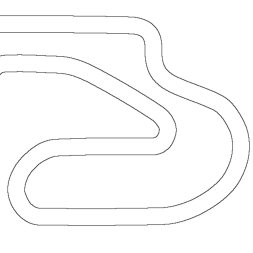
\includegraphics[interpolate=true,width=2.530000in,height=2.530000in]{contents/chapt6/figs/architecture/architecture_esp-img0.png}}%
\end{pgfscope}%
\begin{pgfscope}%
\pgfpathrectangle{\pgfqpoint{0.150000in}{0.862500in}}{\pgfqpoint{2.525000in}{2.525000in}}%
\pgfusepath{clip}%
\pgfsetbuttcap%
\pgfsetroundjoin%
\pgfsetlinewidth{1.003750pt}%
\definecolor{currentstroke}{rgb}{0.501961,0.501961,0.501961}%
\pgfsetstrokecolor{currentstroke}%
\pgfsetstrokeopacity{0.700000}%
\pgfsetdash{{3.700000pt}{1.600000pt}}{0.000000pt}%
\pgfpathmoveto{\pgfqpoint{0.140000in}{3.152431in}}%
\pgfpathlineto{\pgfqpoint{0.161676in}{3.150854in}}%
\pgfpathlineto{\pgfqpoint{0.185100in}{3.151320in}}%
\pgfpathlineto{\pgfqpoint{0.217733in}{3.154711in}}%
\pgfpathlineto{\pgfqpoint{0.254942in}{3.158270in}}%
\pgfpathlineto{\pgfqpoint{0.278317in}{3.158178in}}%
\pgfpathlineto{\pgfqpoint{0.301638in}{3.155830in}}%
\pgfpathlineto{\pgfqpoint{0.333940in}{3.150010in}}%
\pgfpathlineto{\pgfqpoint{0.366316in}{3.144650in}}%
\pgfpathlineto{\pgfqpoint{0.389693in}{3.142945in}}%
\pgfpathlineto{\pgfqpoint{0.413124in}{3.143507in}}%
\pgfpathlineto{\pgfqpoint{0.441067in}{3.146742in}}%
\pgfpathlineto{\pgfqpoint{0.492211in}{3.153343in}}%
\pgfpathlineto{\pgfqpoint{0.515643in}{3.153904in}}%
\pgfpathlineto{\pgfqpoint{0.539035in}{3.152387in}}%
\pgfpathlineto{\pgfqpoint{0.571549in}{3.147908in}}%
\pgfpathlineto{\pgfqpoint{0.608757in}{3.143174in}}%
\pgfpathlineto{\pgfqpoint{0.632171in}{3.142068in}}%
\pgfpathlineto{\pgfqpoint{0.655589in}{3.143063in}}%
\pgfpathlineto{\pgfqpoint{0.683506in}{3.146528in}}%
\pgfpathlineto{\pgfqpoint{0.739241in}{3.154209in}}%
\pgfpathlineto{\pgfqpoint{0.767344in}{3.155329in}}%
\pgfpathlineto{\pgfqpoint{0.790741in}{3.153935in}}%
\pgfpathlineto{\pgfqpoint{0.818566in}{3.149806in}}%
\pgfpathlineto{\pgfqpoint{0.874067in}{3.140652in}}%
\pgfpathlineto{\pgfqpoint{0.897475in}{3.139455in}}%
\pgfpathlineto{\pgfqpoint{0.920877in}{3.140695in}}%
\pgfpathlineto{\pgfqpoint{0.944025in}{3.144381in}}%
\pgfpathlineto{\pgfqpoint{0.980507in}{3.153107in}}%
\pgfpathlineto{\pgfqpoint{1.017160in}{3.161058in}}%
\pgfpathlineto{\pgfqpoint{1.045059in}{3.164641in}}%
\pgfpathlineto{\pgfqpoint{1.073168in}{3.165664in}}%
\pgfpathlineto{\pgfqpoint{1.152830in}{3.165987in}}%
\pgfpathlineto{\pgfqpoint{1.176008in}{3.169476in}}%
\pgfpathlineto{\pgfqpoint{1.203293in}{3.176047in}}%
\pgfpathlineto{\pgfqpoint{1.247237in}{3.187237in}}%
\pgfpathlineto{\pgfqpoint{1.265146in}{3.189475in}}%
\pgfpathlineto{\pgfqpoint{1.283334in}{3.189356in}}%
\pgfpathlineto{\pgfqpoint{1.301972in}{3.186432in}}%
\pgfpathlineto{\pgfqpoint{1.320133in}{3.180990in}}%
\pgfpathlineto{\pgfqpoint{1.337517in}{3.173420in}}%
\pgfpathlineto{\pgfqpoint{1.358127in}{3.161712in}}%
\pgfpathlineto{\pgfqpoint{1.417607in}{3.124730in}}%
\pgfpathlineto{\pgfqpoint{1.434736in}{3.117709in}}%
\pgfpathlineto{\pgfqpoint{1.452618in}{3.112561in}}%
\pgfpathlineto{\pgfqpoint{1.471053in}{3.109358in}}%
\pgfpathlineto{\pgfqpoint{1.494367in}{3.107450in}}%
\pgfpathlineto{\pgfqpoint{1.547814in}{3.104175in}}%
\pgfpathlineto{\pgfqpoint{1.564092in}{3.100542in}}%
\pgfpathlineto{\pgfqpoint{1.579080in}{3.094554in}}%
\pgfpathlineto{\pgfqpoint{1.589143in}{3.088329in}}%
\pgfpathlineto{\pgfqpoint{1.597967in}{3.080575in}}%
\pgfpathlineto{\pgfqpoint{1.605308in}{3.071513in}}%
\pgfpathlineto{\pgfqpoint{1.611023in}{3.061335in}}%
\pgfpathlineto{\pgfqpoint{1.616605in}{3.045676in}}%
\pgfpathlineto{\pgfqpoint{1.621439in}{3.023497in}}%
\pgfpathlineto{\pgfqpoint{1.626525in}{2.986156in}}%
\pgfpathlineto{\pgfqpoint{1.631853in}{2.948851in}}%
\pgfpathlineto{\pgfqpoint{1.637107in}{2.925896in}}%
\pgfpathlineto{\pgfqpoint{1.644593in}{2.903571in}}%
\pgfpathlineto{\pgfqpoint{1.654497in}{2.882211in}}%
\pgfpathlineto{\pgfqpoint{1.666632in}{2.862031in}}%
\pgfpathlineto{\pgfqpoint{1.685797in}{2.835220in}}%
\pgfpathlineto{\pgfqpoint{1.707402in}{2.804561in}}%
\pgfpathlineto{\pgfqpoint{1.718628in}{2.784030in}}%
\pgfpathlineto{\pgfqpoint{1.727505in}{2.762378in}}%
\pgfpathlineto{\pgfqpoint{1.735569in}{2.735474in}}%
\pgfpathlineto{\pgfqpoint{1.747108in}{2.694958in}}%
\pgfpathlineto{\pgfqpoint{1.754247in}{2.677652in}}%
\pgfpathlineto{\pgfqpoint{1.763499in}{2.661385in}}%
\pgfpathlineto{\pgfqpoint{1.772004in}{2.650215in}}%
\pgfpathlineto{\pgfqpoint{1.781864in}{2.640224in}}%
\pgfpathlineto{\pgfqpoint{1.792957in}{2.631620in}}%
\pgfpathlineto{\pgfqpoint{1.805039in}{2.624469in}}%
\pgfpathlineto{\pgfqpoint{1.822245in}{2.617106in}}%
\pgfpathlineto{\pgfqpoint{1.840206in}{2.611823in}}%
\pgfpathlineto{\pgfqpoint{1.872311in}{2.605243in}}%
\pgfpathlineto{\pgfqpoint{1.899662in}{2.598871in}}%
\pgfpathlineto{\pgfqpoint{1.917306in}{2.592619in}}%
\pgfpathlineto{\pgfqpoint{1.934052in}{2.584257in}}%
\pgfpathlineto{\pgfqpoint{1.949625in}{2.573870in}}%
\pgfpathlineto{\pgfqpoint{1.963882in}{2.561738in}}%
\pgfpathlineto{\pgfqpoint{1.980161in}{2.544921in}}%
\pgfpathlineto{\pgfqpoint{2.015123in}{2.507128in}}%
\pgfpathlineto{\pgfqpoint{2.033103in}{2.492154in}}%
\pgfpathlineto{\pgfqpoint{2.048791in}{2.481942in}}%
\pgfpathlineto{\pgfqpoint{2.065575in}{2.473654in}}%
\pgfpathlineto{\pgfqpoint{2.083184in}{2.467295in}}%
\pgfpathlineto{\pgfqpoint{2.105879in}{2.461587in}}%
\pgfpathlineto{\pgfqpoint{2.138240in}{2.456414in}}%
\pgfpathlineto{\pgfqpoint{2.179837in}{2.449736in}}%
\pgfpathlineto{\pgfqpoint{2.197903in}{2.444831in}}%
\pgfpathlineto{\pgfqpoint{2.215268in}{2.437842in}}%
\pgfpathlineto{\pgfqpoint{2.231578in}{2.428664in}}%
\pgfpathlineto{\pgfqpoint{2.246391in}{2.417229in}}%
\pgfpathlineto{\pgfqpoint{2.259511in}{2.403879in}}%
\pgfpathlineto{\pgfqpoint{2.271066in}{2.389148in}}%
\pgfpathlineto{\pgfqpoint{2.286469in}{2.365659in}}%
\pgfpathlineto{\pgfqpoint{2.304548in}{2.338331in}}%
\pgfpathlineto{\pgfqpoint{2.316517in}{2.323937in}}%
\pgfpathlineto{\pgfqpoint{2.330270in}{2.311248in}}%
\pgfpathlineto{\pgfqpoint{2.345803in}{2.300814in}}%
\pgfpathlineto{\pgfqpoint{2.362732in}{2.292838in}}%
\pgfpathlineto{\pgfqpoint{2.380565in}{2.287144in}}%
\pgfpathlineto{\pgfqpoint{2.403474in}{2.282355in}}%
\pgfpathlineto{\pgfqpoint{2.448208in}{2.273814in}}%
\pgfpathlineto{\pgfqpoint{2.464796in}{2.268127in}}%
\pgfpathlineto{\pgfqpoint{2.480223in}{2.260170in}}%
\pgfpathlineto{\pgfqpoint{2.490665in}{2.252577in}}%
\pgfpathlineto{\pgfqpoint{2.499972in}{2.243531in}}%
\pgfpathlineto{\pgfqpoint{2.507987in}{2.233133in}}%
\pgfpathlineto{\pgfqpoint{2.514588in}{2.221611in}}%
\pgfpathlineto{\pgfqpoint{2.521272in}{2.204515in}}%
\pgfpathlineto{\pgfqpoint{2.525837in}{2.186192in}}%
\pgfpathlineto{\pgfqpoint{2.529102in}{2.162812in}}%
\pgfpathlineto{\pgfqpoint{2.530932in}{2.129805in}}%
\pgfpathlineto{\pgfqpoint{2.533277in}{2.096838in}}%
\pgfpathlineto{\pgfqpoint{2.536771in}{2.078281in}}%
\pgfpathlineto{\pgfqpoint{2.542666in}{2.060347in}}%
\pgfpathlineto{\pgfqpoint{2.551069in}{2.043443in}}%
\pgfpathlineto{\pgfqpoint{2.561705in}{2.027843in}}%
\pgfpathlineto{\pgfqpoint{2.577283in}{2.010110in}}%
\pgfpathlineto{\pgfqpoint{2.621482in}{1.963844in}}%
\pgfpathlineto{\pgfqpoint{2.630631in}{1.949304in}}%
\pgfpathlineto{\pgfqpoint{2.635611in}{1.937782in}}%
\pgfpathlineto{\pgfqpoint{2.638655in}{1.925885in}}%
\pgfpathlineto{\pgfqpoint{2.639576in}{1.913805in}}%
\pgfpathlineto{\pgfqpoint{2.638304in}{1.901906in}}%
\pgfpathlineto{\pgfqpoint{2.634928in}{1.890578in}}%
\pgfpathlineto{\pgfqpoint{2.629359in}{1.879602in}}%
\pgfpathlineto{\pgfqpoint{2.619212in}{1.865149in}}%
\pgfpathlineto{\pgfqpoint{2.603848in}{1.847301in}}%
\pgfpathlineto{\pgfqpoint{2.549596in}{1.788064in}}%
\pgfpathlineto{\pgfqpoint{2.539393in}{1.772148in}}%
\pgfpathlineto{\pgfqpoint{2.531129in}{1.755145in}}%
\pgfpathlineto{\pgfqpoint{2.524861in}{1.737307in}}%
\pgfpathlineto{\pgfqpoint{2.519536in}{1.714280in}}%
\pgfpathlineto{\pgfqpoint{2.506344in}{1.644664in}}%
\pgfpathlineto{\pgfqpoint{2.499307in}{1.627123in}}%
\pgfpathlineto{\pgfqpoint{2.492296in}{1.614798in}}%
\pgfpathlineto{\pgfqpoint{2.483714in}{1.603515in}}%
\pgfpathlineto{\pgfqpoint{2.473642in}{1.593538in}}%
\pgfpathlineto{\pgfqpoint{2.462320in}{1.585004in}}%
\pgfpathlineto{\pgfqpoint{2.445762in}{1.575895in}}%
\pgfpathlineto{\pgfqpoint{2.428127in}{1.569081in}}%
\pgfpathlineto{\pgfqpoint{2.400756in}{1.561633in}}%
\pgfpathlineto{\pgfqpoint{2.364257in}{1.551739in}}%
\pgfpathlineto{\pgfqpoint{2.346761in}{1.544713in}}%
\pgfpathlineto{\pgfqpoint{2.330286in}{1.535844in}}%
\pgfpathlineto{\pgfqpoint{2.315111in}{1.525036in}}%
\pgfpathlineto{\pgfqpoint{2.301233in}{1.512397in}}%
\pgfpathlineto{\pgfqpoint{2.285437in}{1.495042in}}%
\pgfpathlineto{\pgfqpoint{2.259133in}{1.461979in}}%
\pgfpathlineto{\pgfqpoint{2.232392in}{1.429275in}}%
\pgfpathlineto{\pgfqpoint{2.213098in}{1.408760in}}%
\pgfpathlineto{\pgfqpoint{2.192198in}{1.389889in}}%
\pgfpathlineto{\pgfqpoint{2.173461in}{1.375762in}}%
\pgfpathlineto{\pgfqpoint{2.153502in}{1.363424in}}%
\pgfpathlineto{\pgfqpoint{2.132442in}{1.353074in}}%
\pgfpathlineto{\pgfqpoint{2.110485in}{1.344800in}}%
\pgfpathlineto{\pgfqpoint{2.083319in}{1.337382in}}%
\pgfpathlineto{\pgfqpoint{2.005883in}{1.318384in}}%
\pgfpathlineto{\pgfqpoint{1.984420in}{1.308911in}}%
\pgfpathlineto{\pgfqpoint{1.964136in}{1.297116in}}%
\pgfpathlineto{\pgfqpoint{1.933345in}{1.275617in}}%
\pgfpathlineto{\pgfqpoint{1.909698in}{1.260333in}}%
\pgfpathlineto{\pgfqpoint{1.892867in}{1.252028in}}%
\pgfpathlineto{\pgfqpoint{1.875083in}{1.246046in}}%
\pgfpathlineto{\pgfqpoint{1.861249in}{1.243452in}}%
\pgfpathlineto{\pgfqpoint{1.847195in}{1.242680in}}%
\pgfpathlineto{\pgfqpoint{1.833160in}{1.243752in}}%
\pgfpathlineto{\pgfqpoint{1.814838in}{1.247790in}}%
\pgfpathlineto{\pgfqpoint{1.797319in}{1.254235in}}%
\pgfpathlineto{\pgfqpoint{1.777041in}{1.264246in}}%
\pgfpathlineto{\pgfqpoint{1.732460in}{1.288040in}}%
\pgfpathlineto{\pgfqpoint{1.717661in}{1.292961in}}%
\pgfpathlineto{\pgfqpoint{1.702883in}{1.295514in}}%
\pgfpathlineto{\pgfqpoint{1.688425in}{1.295534in}}%
\pgfpathlineto{\pgfqpoint{1.673978in}{1.293077in}}%
\pgfpathlineto{\pgfqpoint{1.655909in}{1.287710in}}%
\pgfpathlineto{\pgfqpoint{1.593418in}{1.266306in}}%
\pgfpathlineto{\pgfqpoint{1.575572in}{1.263367in}}%
\pgfpathlineto{\pgfqpoint{1.547540in}{1.261301in}}%
\pgfpathlineto{\pgfqpoint{1.465053in}{1.256249in}}%
\pgfpathlineto{\pgfqpoint{1.432116in}{1.251670in}}%
\pgfpathlineto{\pgfqpoint{1.385444in}{1.242785in}}%
\pgfpathlineto{\pgfqpoint{1.352678in}{1.237317in}}%
\pgfpathlineto{\pgfqpoint{1.324673in}{1.234645in}}%
\pgfpathlineto{\pgfqpoint{1.296646in}{1.234407in}}%
\pgfpathlineto{\pgfqpoint{1.207561in}{1.236462in}}%
\pgfpathlineto{\pgfqpoint{1.179596in}{1.233224in}}%
\pgfpathlineto{\pgfqpoint{1.147401in}{1.226704in}}%
\pgfpathlineto{\pgfqpoint{1.106015in}{1.218320in}}%
\pgfpathlineto{\pgfqpoint{1.087320in}{1.216695in}}%
\pgfpathlineto{\pgfqpoint{1.068568in}{1.217319in}}%
\pgfpathlineto{\pgfqpoint{1.050056in}{1.220365in}}%
\pgfpathlineto{\pgfqpoint{1.032047in}{1.225636in}}%
\pgfpathlineto{\pgfqpoint{1.010338in}{1.234530in}}%
\pgfpathlineto{\pgfqpoint{0.959445in}{1.256944in}}%
\pgfpathlineto{\pgfqpoint{0.941993in}{1.261811in}}%
\pgfpathlineto{\pgfqpoint{0.923642in}{1.264492in}}%
\pgfpathlineto{\pgfqpoint{0.904919in}{1.264716in}}%
\pgfpathlineto{\pgfqpoint{0.886333in}{1.262436in}}%
\pgfpathlineto{\pgfqpoint{0.868153in}{1.257936in}}%
\pgfpathlineto{\pgfqpoint{0.846150in}{1.249933in}}%
\pgfpathlineto{\pgfqpoint{0.789744in}{1.227097in}}%
\pgfpathlineto{\pgfqpoint{0.771471in}{1.223006in}}%
\pgfpathlineto{\pgfqpoint{0.752802in}{1.221631in}}%
\pgfpathlineto{\pgfqpoint{0.734143in}{1.223149in}}%
\pgfpathlineto{\pgfqpoint{0.715889in}{1.227320in}}%
\pgfpathlineto{\pgfqpoint{0.698229in}{1.233563in}}%
\pgfpathlineto{\pgfqpoint{0.668387in}{1.246963in}}%
\pgfpathlineto{\pgfqpoint{0.642919in}{1.257624in}}%
\pgfpathlineto{\pgfqpoint{0.620624in}{1.264194in}}%
\pgfpathlineto{\pgfqpoint{0.602077in}{1.267518in}}%
\pgfpathlineto{\pgfqpoint{0.583282in}{1.268835in}}%
\pgfpathlineto{\pgfqpoint{0.564449in}{1.268201in}}%
\pgfpathlineto{\pgfqpoint{0.541073in}{1.265295in}}%
\pgfpathlineto{\pgfqpoint{0.471524in}{1.254470in}}%
\pgfpathlineto{\pgfqpoint{0.453112in}{1.254452in}}%
\pgfpathlineto{\pgfqpoint{0.435271in}{1.256936in}}%
\pgfpathlineto{\pgfqpoint{0.422651in}{1.260742in}}%
\pgfpathlineto{\pgfqpoint{0.411028in}{1.266324in}}%
\pgfpathlineto{\pgfqpoint{0.400319in}{1.274033in}}%
\pgfpathlineto{\pgfqpoint{0.390424in}{1.283647in}}%
\pgfpathlineto{\pgfqpoint{0.378598in}{1.298418in}}%
\pgfpathlineto{\pgfqpoint{0.368530in}{1.314446in}}%
\pgfpathlineto{\pgfqpoint{0.357928in}{1.335597in}}%
\pgfpathlineto{\pgfqpoint{0.343581in}{1.370639in}}%
\pgfpathlineto{\pgfqpoint{0.305058in}{1.472380in}}%
\pgfpathlineto{\pgfqpoint{0.301356in}{1.490941in}}%
\pgfpathlineto{\pgfqpoint{0.300012in}{1.509813in}}%
\pgfpathlineto{\pgfqpoint{0.301456in}{1.528675in}}%
\pgfpathlineto{\pgfqpoint{0.305726in}{1.547105in}}%
\pgfpathlineto{\pgfqpoint{0.312506in}{1.564771in}}%
\pgfpathlineto{\pgfqpoint{0.323611in}{1.585659in}}%
\pgfpathlineto{\pgfqpoint{0.361896in}{1.650923in}}%
\pgfpathlineto{\pgfqpoint{0.370348in}{1.673019in}}%
\pgfpathlineto{\pgfqpoint{0.377798in}{1.700417in}}%
\pgfpathlineto{\pgfqpoint{0.392618in}{1.760119in}}%
\pgfpathlineto{\pgfqpoint{0.401072in}{1.782214in}}%
\pgfpathlineto{\pgfqpoint{0.409759in}{1.799027in}}%
\pgfpathlineto{\pgfqpoint{0.420460in}{1.814632in}}%
\pgfpathlineto{\pgfqpoint{0.433192in}{1.828626in}}%
\pgfpathlineto{\pgfqpoint{0.444056in}{1.837760in}}%
\pgfpathlineto{\pgfqpoint{0.455942in}{1.845516in}}%
\pgfpathlineto{\pgfqpoint{0.468712in}{1.851709in}}%
\pgfpathlineto{\pgfqpoint{0.482163in}{1.856237in}}%
\pgfpathlineto{\pgfqpoint{0.500744in}{1.859797in}}%
\pgfpathlineto{\pgfqpoint{0.519637in}{1.860891in}}%
\pgfpathlineto{\pgfqpoint{0.543275in}{1.859838in}}%
\pgfpathlineto{\pgfqpoint{0.590491in}{1.856744in}}%
\pgfpathlineto{\pgfqpoint{0.609380in}{1.857899in}}%
\pgfpathlineto{\pgfqpoint{0.627985in}{1.861355in}}%
\pgfpathlineto{\pgfqpoint{0.646009in}{1.867118in}}%
\pgfpathlineto{\pgfqpoint{0.663293in}{1.874833in}}%
\pgfpathlineto{\pgfqpoint{0.688115in}{1.888625in}}%
\pgfpathlineto{\pgfqpoint{0.717074in}{1.904712in}}%
\pgfpathlineto{\pgfqpoint{0.734471in}{1.912164in}}%
\pgfpathlineto{\pgfqpoint{0.752626in}{1.917497in}}%
\pgfpathlineto{\pgfqpoint{0.771311in}{1.920494in}}%
\pgfpathlineto{\pgfqpoint{0.790223in}{1.921121in}}%
\pgfpathlineto{\pgfqpoint{0.809093in}{1.919639in}}%
\pgfpathlineto{\pgfqpoint{0.837097in}{1.914936in}}%
\pgfpathlineto{\pgfqpoint{0.874409in}{1.908534in}}%
\pgfpathlineto{\pgfqpoint{0.898028in}{1.907221in}}%
\pgfpathlineto{\pgfqpoint{0.916918in}{1.908357in}}%
\pgfpathlineto{\pgfqpoint{0.935541in}{1.911720in}}%
\pgfpathlineto{\pgfqpoint{0.953689in}{1.917095in}}%
\pgfpathlineto{\pgfqpoint{0.975681in}{1.925827in}}%
\pgfpathlineto{\pgfqpoint{1.023603in}{1.946058in}}%
\pgfpathlineto{\pgfqpoint{1.041643in}{1.951366in}}%
\pgfpathlineto{\pgfqpoint{1.060074in}{1.954618in}}%
\pgfpathlineto{\pgfqpoint{1.078751in}{1.955516in}}%
\pgfpathlineto{\pgfqpoint{1.097411in}{1.954260in}}%
\pgfpathlineto{\pgfqpoint{1.120478in}{1.950437in}}%
\pgfpathlineto{\pgfqpoint{1.175608in}{1.940030in}}%
\pgfpathlineto{\pgfqpoint{1.194277in}{1.938911in}}%
\pgfpathlineto{\pgfqpoint{1.212954in}{1.939859in}}%
\pgfpathlineto{\pgfqpoint{1.231420in}{1.942823in}}%
\pgfpathlineto{\pgfqpoint{1.254023in}{1.948774in}}%
\pgfpathlineto{\pgfqpoint{1.316570in}{1.967384in}}%
\pgfpathlineto{\pgfqpoint{1.335010in}{1.970100in}}%
\pgfpathlineto{\pgfqpoint{1.353747in}{1.970791in}}%
\pgfpathlineto{\pgfqpoint{1.377116in}{1.969037in}}%
\pgfpathlineto{\pgfqpoint{1.400199in}{1.964953in}}%
\pgfpathlineto{\pgfqpoint{1.441223in}{1.955051in}}%
\pgfpathlineto{\pgfqpoint{1.482438in}{1.945995in}}%
\pgfpathlineto{\pgfqpoint{1.514874in}{1.940986in}}%
\pgfpathlineto{\pgfqpoint{1.556888in}{1.937027in}}%
\pgfpathlineto{\pgfqpoint{1.603732in}{1.934942in}}%
\pgfpathlineto{\pgfqpoint{1.636551in}{1.935167in}}%
\pgfpathlineto{\pgfqpoint{1.664580in}{1.937528in}}%
\pgfpathlineto{\pgfqpoint{1.683036in}{1.940842in}}%
\pgfpathlineto{\pgfqpoint{1.700994in}{1.946217in}}%
\pgfpathlineto{\pgfqpoint{1.718050in}{1.953985in}}%
\pgfpathlineto{\pgfqpoint{1.729934in}{1.961500in}}%
\pgfpathlineto{\pgfqpoint{1.740753in}{1.970478in}}%
\pgfpathlineto{\pgfqpoint{1.750294in}{1.980804in}}%
\pgfpathlineto{\pgfqpoint{1.758474in}{1.992241in}}%
\pgfpathlineto{\pgfqpoint{1.767143in}{2.008855in}}%
\pgfpathlineto{\pgfqpoint{1.773186in}{2.026596in}}%
\pgfpathlineto{\pgfqpoint{1.776655in}{2.045016in}}%
\pgfpathlineto{\pgfqpoint{1.777639in}{2.063736in}}%
\pgfpathlineto{\pgfqpoint{1.776227in}{2.082429in}}%
\pgfpathlineto{\pgfqpoint{1.772506in}{2.100803in}}%
\pgfpathlineto{\pgfqpoint{1.766594in}{2.118594in}}%
\pgfpathlineto{\pgfqpoint{1.758676in}{2.135588in}}%
\pgfpathlineto{\pgfqpoint{1.748907in}{2.151591in}}%
\pgfpathlineto{\pgfqpoint{1.734686in}{2.170222in}}%
\pgfpathlineto{\pgfqpoint{1.715690in}{2.190970in}}%
\pgfpathlineto{\pgfqpoint{1.680308in}{2.228488in}}%
\pgfpathlineto{\pgfqpoint{1.659930in}{2.254215in}}%
\pgfpathlineto{\pgfqpoint{1.628434in}{2.295045in}}%
\pgfpathlineto{\pgfqpoint{1.612088in}{2.311839in}}%
\pgfpathlineto{\pgfqpoint{1.597575in}{2.323708in}}%
\pgfpathlineto{\pgfqpoint{1.581868in}{2.333948in}}%
\pgfpathlineto{\pgfqpoint{1.561044in}{2.344706in}}%
\pgfpathlineto{\pgfqpoint{1.488826in}{2.378306in}}%
\pgfpathlineto{\pgfqpoint{1.473412in}{2.388978in}}%
\pgfpathlineto{\pgfqpoint{1.459319in}{2.401343in}}%
\pgfpathlineto{\pgfqpoint{1.446630in}{2.415148in}}%
\pgfpathlineto{\pgfqpoint{1.432432in}{2.433800in}}%
\pgfpathlineto{\pgfqpoint{1.402121in}{2.475508in}}%
\pgfpathlineto{\pgfqpoint{1.389096in}{2.488991in}}%
\pgfpathlineto{\pgfqpoint{1.374321in}{2.500519in}}%
\pgfpathlineto{\pgfqpoint{1.357942in}{2.509625in}}%
\pgfpathlineto{\pgfqpoint{1.340396in}{2.516218in}}%
\pgfpathlineto{\pgfqpoint{1.322164in}{2.520593in}}%
\pgfpathlineto{\pgfqpoint{1.294309in}{2.524516in}}%
\pgfpathlineto{\pgfqpoint{1.257169in}{2.529737in}}%
\pgfpathlineto{\pgfqpoint{1.238951in}{2.534174in}}%
\pgfpathlineto{\pgfqpoint{1.221351in}{2.540628in}}%
\pgfpathlineto{\pgfqpoint{1.204773in}{2.549373in}}%
\pgfpathlineto{\pgfqpoint{1.189560in}{2.560325in}}%
\pgfpathlineto{\pgfqpoint{1.175803in}{2.573063in}}%
\pgfpathlineto{\pgfqpoint{1.160327in}{2.590667in}}%
\pgfpathlineto{\pgfqpoint{1.124375in}{2.633924in}}%
\pgfpathlineto{\pgfqpoint{1.110616in}{2.646660in}}%
\pgfpathlineto{\pgfqpoint{1.095433in}{2.657653in}}%
\pgfpathlineto{\pgfqpoint{1.078866in}{2.666416in}}%
\pgfpathlineto{\pgfqpoint{1.061165in}{2.672572in}}%
\pgfpathlineto{\pgfqpoint{1.042758in}{2.676111in}}%
\pgfpathlineto{\pgfqpoint{1.024052in}{2.677382in}}%
\pgfpathlineto{\pgfqpoint{1.000619in}{2.676743in}}%
\pgfpathlineto{\pgfqpoint{0.953786in}{2.674635in}}%
\pgfpathlineto{\pgfqpoint{0.935069in}{2.675756in}}%
\pgfpathlineto{\pgfqpoint{0.916578in}{2.678854in}}%
\pgfpathlineto{\pgfqpoint{0.898544in}{2.683982in}}%
\pgfpathlineto{\pgfqpoint{0.876835in}{2.692811in}}%
\pgfpathlineto{\pgfqpoint{0.847718in}{2.707956in}}%
\pgfpathlineto{\pgfqpoint{0.818407in}{2.722710in}}%
\pgfpathlineto{\pgfqpoint{0.800802in}{2.729157in}}%
\pgfpathlineto{\pgfqpoint{0.782509in}{2.733236in}}%
\pgfpathlineto{\pgfqpoint{0.763820in}{2.734657in}}%
\pgfpathlineto{\pgfqpoint{0.745108in}{2.733523in}}%
\pgfpathlineto{\pgfqpoint{0.722059in}{2.729283in}}%
\pgfpathlineto{\pgfqpoint{0.658128in}{2.714616in}}%
\pgfpathlineto{\pgfqpoint{0.639412in}{2.713513in}}%
\pgfpathlineto{\pgfqpoint{0.620695in}{2.714569in}}%
\pgfpathlineto{\pgfqpoint{0.602240in}{2.717871in}}%
\pgfpathlineto{\pgfqpoint{0.579759in}{2.724499in}}%
\pgfpathlineto{\pgfqpoint{0.549149in}{2.736344in}}%
\pgfpathlineto{\pgfqpoint{0.505369in}{2.753128in}}%
\pgfpathlineto{\pgfqpoint{0.478430in}{2.761228in}}%
\pgfpathlineto{\pgfqpoint{0.450945in}{2.767211in}}%
\pgfpathlineto{\pgfqpoint{0.423060in}{2.770911in}}%
\pgfpathlineto{\pgfqpoint{0.394964in}{2.772265in}}%
\pgfpathlineto{\pgfqpoint{0.366848in}{2.771355in}}%
\pgfpathlineto{\pgfqpoint{0.329523in}{2.767642in}}%
\pgfpathlineto{\pgfqpoint{0.287832in}{2.761102in}}%
\pgfpathlineto{\pgfqpoint{0.255793in}{2.754000in}}%
\pgfpathlineto{\pgfqpoint{0.233422in}{2.747003in}}%
\pgfpathlineto{\pgfqpoint{0.211813in}{2.737929in}}%
\pgfpathlineto{\pgfqpoint{0.191319in}{2.726560in}}%
\pgfpathlineto{\pgfqpoint{0.172161in}{2.713060in}}%
\pgfpathlineto{\pgfqpoint{0.154589in}{2.697556in}}%
\pgfpathlineto{\pgfqpoint{0.140000in}{2.681256in}}%
\pgfpathlineto{\pgfqpoint{0.140000in}{2.681256in}}%
\pgfusepath{stroke}%
\end{pgfscope}%
\begin{pgfscope}%
\pgfpathrectangle{\pgfqpoint{0.150000in}{0.862500in}}{\pgfqpoint{2.525000in}{2.525000in}}%
\pgfusepath{clip}%
\pgfsetrectcap%
\pgfsetroundjoin%
\pgfsetlinewidth{1.003750pt}%
\definecolor{currentstroke}{rgb}{1.000000,0.647059,0.000000}%
\pgfsetstrokecolor{currentstroke}%
\pgfsetstrokeopacity{0.700000}%
\pgfsetdash{}{0pt}%
\pgfpathmoveto{\pgfqpoint{0.140000in}{3.156003in}}%
\pgfpathlineto{\pgfqpoint{0.163762in}{3.153985in}}%
\pgfpathlineto{\pgfqpoint{0.187165in}{3.154006in}}%
\pgfpathlineto{\pgfqpoint{0.210471in}{3.156115in}}%
\pgfpathlineto{\pgfqpoint{0.238111in}{3.161094in}}%
\pgfpathlineto{\pgfqpoint{0.293206in}{3.171993in}}%
\pgfpathlineto{\pgfqpoint{0.316543in}{3.173672in}}%
\pgfpathlineto{\pgfqpoint{0.339925in}{3.172775in}}%
\pgfpathlineto{\pgfqpoint{0.363062in}{3.169674in}}%
\pgfpathlineto{\pgfqpoint{0.430060in}{3.158573in}}%
\pgfpathlineto{\pgfqpoint{0.451490in}{3.158225in}}%
\pgfpathlineto{\pgfqpoint{0.472766in}{3.160182in}}%
\pgfpathlineto{\pgfqpoint{0.503653in}{3.165578in}}%
\pgfpathlineto{\pgfqpoint{0.531464in}{3.169974in}}%
\pgfpathlineto{\pgfqpoint{0.554867in}{3.171615in}}%
\pgfpathlineto{\pgfqpoint{0.573626in}{3.171058in}}%
\pgfpathlineto{\pgfqpoint{0.596853in}{3.167787in}}%
\pgfpathlineto{\pgfqpoint{0.624141in}{3.160989in}}%
\pgfpathlineto{\pgfqpoint{0.672835in}{3.147841in}}%
\pgfpathlineto{\pgfqpoint{0.694109in}{3.144794in}}%
\pgfpathlineto{\pgfqpoint{0.710686in}{3.144648in}}%
\pgfpathlineto{\pgfqpoint{0.727594in}{3.146699in}}%
\pgfpathlineto{\pgfqpoint{0.753606in}{3.152491in}}%
\pgfpathlineto{\pgfqpoint{0.799371in}{3.163303in}}%
\pgfpathlineto{\pgfqpoint{0.818067in}{3.165605in}}%
\pgfpathlineto{\pgfqpoint{0.836897in}{3.165879in}}%
\pgfpathlineto{\pgfqpoint{0.855613in}{3.163794in}}%
\pgfpathlineto{\pgfqpoint{0.873951in}{3.159500in}}%
\pgfpathlineto{\pgfqpoint{0.895997in}{3.151799in}}%
\pgfpathlineto{\pgfqpoint{0.968141in}{3.123436in}}%
\pgfpathlineto{\pgfqpoint{0.984071in}{3.120383in}}%
\pgfpathlineto{\pgfqpoint{1.000199in}{3.119448in}}%
\pgfpathlineto{\pgfqpoint{1.016590in}{3.120767in}}%
\pgfpathlineto{\pgfqpoint{1.037940in}{3.125107in}}%
\pgfpathlineto{\pgfqpoint{1.078152in}{3.136592in}}%
\pgfpathlineto{\pgfqpoint{1.105494in}{3.143230in}}%
\pgfpathlineto{\pgfqpoint{1.128728in}{3.146336in}}%
\pgfpathlineto{\pgfqpoint{1.147480in}{3.146557in}}%
\pgfpathlineto{\pgfqpoint{1.166130in}{3.144585in}}%
\pgfpathlineto{\pgfqpoint{1.189005in}{3.139480in}}%
\pgfpathlineto{\pgfqpoint{1.220125in}{3.129521in}}%
\pgfpathlineto{\pgfqpoint{1.251367in}{3.120225in}}%
\pgfpathlineto{\pgfqpoint{1.269754in}{3.116781in}}%
\pgfpathlineto{\pgfqpoint{1.288408in}{3.115421in}}%
\pgfpathlineto{\pgfqpoint{1.307096in}{3.116212in}}%
\pgfpathlineto{\pgfqpoint{1.325584in}{3.119055in}}%
\pgfpathlineto{\pgfqpoint{1.348209in}{3.124966in}}%
\pgfpathlineto{\pgfqpoint{1.410911in}{3.143725in}}%
\pgfpathlineto{\pgfqpoint{1.429462in}{3.146099in}}%
\pgfpathlineto{\pgfqpoint{1.448160in}{3.145937in}}%
\pgfpathlineto{\pgfqpoint{1.462039in}{3.143906in}}%
\pgfpathlineto{\pgfqpoint{1.479971in}{3.138614in}}%
\pgfpathlineto{\pgfqpoint{1.496934in}{3.130742in}}%
\pgfpathlineto{\pgfqpoint{1.512829in}{3.120880in}}%
\pgfpathlineto{\pgfqpoint{1.531353in}{3.106610in}}%
\pgfpathlineto{\pgfqpoint{1.552104in}{3.087713in}}%
\pgfpathlineto{\pgfqpoint{1.581513in}{3.057585in}}%
\pgfpathlineto{\pgfqpoint{1.606083in}{3.029360in}}%
\pgfpathlineto{\pgfqpoint{1.622862in}{3.006865in}}%
\pgfpathlineto{\pgfqpoint{1.635199in}{2.986999in}}%
\pgfpathlineto{\pgfqpoint{1.645418in}{2.965970in}}%
\pgfpathlineto{\pgfqpoint{1.651748in}{2.948367in}}%
\pgfpathlineto{\pgfqpoint{1.657189in}{2.925629in}}%
\pgfpathlineto{\pgfqpoint{1.660404in}{2.902465in}}%
\pgfpathlineto{\pgfqpoint{1.667866in}{2.832742in}}%
\pgfpathlineto{\pgfqpoint{1.672793in}{2.814699in}}%
\pgfpathlineto{\pgfqpoint{1.679855in}{2.797380in}}%
\pgfpathlineto{\pgfqpoint{1.688876in}{2.780994in}}%
\pgfpathlineto{\pgfqpoint{1.702238in}{2.761804in}}%
\pgfpathlineto{\pgfqpoint{1.723148in}{2.736607in}}%
\pgfpathlineto{\pgfqpoint{1.764093in}{2.691798in}}%
\pgfpathlineto{\pgfqpoint{1.786554in}{2.669327in}}%
\pgfpathlineto{\pgfqpoint{1.810209in}{2.649097in}}%
\pgfpathlineto{\pgfqpoint{1.845514in}{2.622581in}}%
\pgfpathlineto{\pgfqpoint{1.919603in}{2.570095in}}%
\pgfpathlineto{\pgfqpoint{1.947700in}{2.553249in}}%
\pgfpathlineto{\pgfqpoint{2.019680in}{2.511860in}}%
\pgfpathlineto{\pgfqpoint{2.050026in}{2.490217in}}%
\pgfpathlineto{\pgfqpoint{2.099175in}{2.454258in}}%
\pgfpathlineto{\pgfqpoint{2.126966in}{2.436854in}}%
\pgfpathlineto{\pgfqpoint{2.164092in}{2.416871in}}%
\pgfpathlineto{\pgfqpoint{2.280633in}{2.356729in}}%
\pgfpathlineto{\pgfqpoint{2.299801in}{2.343279in}}%
\pgfpathlineto{\pgfqpoint{2.317422in}{2.327858in}}%
\pgfpathlineto{\pgfqpoint{2.333469in}{2.310800in}}%
\pgfpathlineto{\pgfqpoint{2.366266in}{2.271047in}}%
\pgfpathlineto{\pgfqpoint{2.388159in}{2.246638in}}%
\pgfpathlineto{\pgfqpoint{2.411922in}{2.224041in}}%
\pgfpathlineto{\pgfqpoint{2.446205in}{2.192126in}}%
\pgfpathlineto{\pgfqpoint{2.461387in}{2.174302in}}%
\pgfpathlineto{\pgfqpoint{2.471580in}{2.158590in}}%
\pgfpathlineto{\pgfqpoint{2.479433in}{2.141592in}}%
\pgfpathlineto{\pgfqpoint{2.484532in}{2.123577in}}%
\pgfpathlineto{\pgfqpoint{2.486903in}{2.105001in}}%
\pgfpathlineto{\pgfqpoint{2.486909in}{2.086269in}}%
\pgfpathlineto{\pgfqpoint{2.484608in}{2.062962in}}%
\pgfpathlineto{\pgfqpoint{2.479225in}{2.016440in}}%
\pgfpathlineto{\pgfqpoint{2.479584in}{1.997713in}}%
\pgfpathlineto{\pgfqpoint{2.482455in}{1.979209in}}%
\pgfpathlineto{\pgfqpoint{2.487920in}{1.961297in}}%
\pgfpathlineto{\pgfqpoint{2.495757in}{1.944287in}}%
\pgfpathlineto{\pgfqpoint{2.505486in}{1.928277in}}%
\pgfpathlineto{\pgfqpoint{2.524880in}{1.901864in}}%
\pgfpathlineto{\pgfqpoint{2.543786in}{1.875217in}}%
\pgfpathlineto{\pgfqpoint{2.553036in}{1.858914in}}%
\pgfpathlineto{\pgfqpoint{2.560390in}{1.841677in}}%
\pgfpathlineto{\pgfqpoint{2.565354in}{1.823611in}}%
\pgfpathlineto{\pgfqpoint{2.567236in}{1.809681in}}%
\pgfpathlineto{\pgfqpoint{2.567405in}{1.795626in}}%
\pgfpathlineto{\pgfqpoint{2.565796in}{1.781664in}}%
\pgfpathlineto{\pgfqpoint{2.562433in}{1.768017in}}%
\pgfpathlineto{\pgfqpoint{2.557343in}{1.754916in}}%
\pgfpathlineto{\pgfqpoint{2.550612in}{1.742577in}}%
\pgfpathlineto{\pgfqpoint{2.539427in}{1.727548in}}%
\pgfpathlineto{\pgfqpoint{2.526301in}{1.714171in}}%
\pgfpathlineto{\pgfqpoint{2.508036in}{1.699498in}}%
\pgfpathlineto{\pgfqpoint{2.451484in}{1.657836in}}%
\pgfpathlineto{\pgfqpoint{2.438712in}{1.644122in}}%
\pgfpathlineto{\pgfqpoint{2.427791in}{1.628894in}}%
\pgfpathlineto{\pgfqpoint{2.418778in}{1.612461in}}%
\pgfpathlineto{\pgfqpoint{2.409691in}{1.590863in}}%
\pgfpathlineto{\pgfqpoint{2.391211in}{1.542743in}}%
\pgfpathlineto{\pgfqpoint{2.382270in}{1.526272in}}%
\pgfpathlineto{\pgfqpoint{2.371227in}{1.511136in}}%
\pgfpathlineto{\pgfqpoint{2.361454in}{1.501035in}}%
\pgfpathlineto{\pgfqpoint{2.350452in}{1.492290in}}%
\pgfpathlineto{\pgfqpoint{2.338402in}{1.485054in}}%
\pgfpathlineto{\pgfqpoint{2.321148in}{1.477754in}}%
\pgfpathlineto{\pgfqpoint{2.303056in}{1.472863in}}%
\pgfpathlineto{\pgfqpoint{2.279918in}{1.469160in}}%
\pgfpathlineto{\pgfqpoint{2.228843in}{1.462180in}}%
\pgfpathlineto{\pgfqpoint{2.206182in}{1.456244in}}%
\pgfpathlineto{\pgfqpoint{2.188839in}{1.449150in}}%
\pgfpathlineto{\pgfqpoint{2.172718in}{1.439607in}}%
\pgfpathlineto{\pgfqpoint{2.158244in}{1.427710in}}%
\pgfpathlineto{\pgfqpoint{2.145615in}{1.413867in}}%
\pgfpathlineto{\pgfqpoint{2.134719in}{1.398615in}}%
\pgfpathlineto{\pgfqpoint{2.120540in}{1.374330in}}%
\pgfpathlineto{\pgfqpoint{2.104131in}{1.346234in}}%
\pgfpathlineto{\pgfqpoint{2.093203in}{1.331546in}}%
\pgfpathlineto{\pgfqpoint{2.080338in}{1.318388in}}%
\pgfpathlineto{\pgfqpoint{2.065526in}{1.307021in}}%
\pgfpathlineto{\pgfqpoint{2.049356in}{1.297571in}}%
\pgfpathlineto{\pgfqpoint{2.027986in}{1.288003in}}%
\pgfpathlineto{\pgfqpoint{1.997120in}{1.276943in}}%
\pgfpathlineto{\pgfqpoint{1.948647in}{1.259477in}}%
\pgfpathlineto{\pgfqpoint{1.861272in}{1.225874in}}%
\pgfpathlineto{\pgfqpoint{1.842947in}{1.221992in}}%
\pgfpathlineto{\pgfqpoint{1.824321in}{1.220016in}}%
\pgfpathlineto{\pgfqpoint{1.800909in}{1.220057in}}%
\pgfpathlineto{\pgfqpoint{1.772948in}{1.222846in}}%
\pgfpathlineto{\pgfqpoint{1.726420in}{1.228117in}}%
\pgfpathlineto{\pgfqpoint{1.707692in}{1.227890in}}%
\pgfpathlineto{\pgfqpoint{1.689151in}{1.225282in}}%
\pgfpathlineto{\pgfqpoint{1.671160in}{1.220095in}}%
\pgfpathlineto{\pgfqpoint{1.654012in}{1.212567in}}%
\pgfpathlineto{\pgfqpoint{1.633835in}{1.200693in}}%
\pgfpathlineto{\pgfqpoint{1.578799in}{1.165127in}}%
\pgfpathlineto{\pgfqpoint{1.561600in}{1.157715in}}%
\pgfpathlineto{\pgfqpoint{1.543623in}{1.152469in}}%
\pgfpathlineto{\pgfqpoint{1.525130in}{1.149521in}}%
\pgfpathlineto{\pgfqpoint{1.506416in}{1.148739in}}%
\pgfpathlineto{\pgfqpoint{1.483053in}{1.150255in}}%
\pgfpathlineto{\pgfqpoint{1.455302in}{1.154682in}}%
\pgfpathlineto{\pgfqpoint{1.413735in}{1.161665in}}%
\pgfpathlineto{\pgfqpoint{1.395035in}{1.162736in}}%
\pgfpathlineto{\pgfqpoint{1.376345in}{1.161578in}}%
\pgfpathlineto{\pgfqpoint{1.357960in}{1.158018in}}%
\pgfpathlineto{\pgfqpoint{1.340139in}{1.152259in}}%
\pgfpathlineto{\pgfqpoint{1.318723in}{1.142791in}}%
\pgfpathlineto{\pgfqpoint{1.306174in}{1.136464in}}%
\pgfpathlineto{\pgfqpoint{1.306174in}{1.136464in}}%
\pgfusepath{stroke}%
\end{pgfscope}%
\begin{pgfscope}%
\pgfpathrectangle{\pgfqpoint{2.825000in}{0.862500in}}{\pgfqpoint{2.525000in}{2.525000in}}%
\pgfusepath{clip}%
\pgfsys@transformshift{2.825000in}{0.862500in}%
\pgftext[left,bottom]{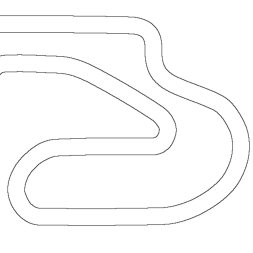
\includegraphics[interpolate=true,width=2.530000in,height=2.530000in]{contents/chapt6/figs/architecture/architecture_esp-img1.png}}%
\end{pgfscope}%
\begin{pgfscope}%
\pgfpathrectangle{\pgfqpoint{2.825000in}{0.862500in}}{\pgfqpoint{2.525000in}{2.525000in}}%
\pgfusepath{clip}%
\pgfsetrectcap%
\pgfsetroundjoin%
\pgfsetlinewidth{1.003750pt}%
\definecolor{currentstroke}{rgb}{0.000000,0.000000,1.000000}%
\pgfsetstrokecolor{currentstroke}%
\pgfsetstrokeopacity{0.700000}%
\pgfsetdash{}{0pt}%
\pgfpathmoveto{\pgfqpoint{2.815000in}{3.158667in}}%
\pgfpathlineto{\pgfqpoint{3.393833in}{3.144635in}}%
\pgfpathlineto{\pgfqpoint{3.460263in}{3.142156in}}%
\pgfpathlineto{\pgfqpoint{3.569435in}{3.139485in}}%
\pgfpathlineto{\pgfqpoint{3.654808in}{3.135473in}}%
\pgfpathlineto{\pgfqpoint{3.816248in}{3.133871in}}%
\pgfpathlineto{\pgfqpoint{3.911201in}{3.134791in}}%
\pgfpathlineto{\pgfqpoint{4.100947in}{3.126756in}}%
\pgfpathlineto{\pgfqpoint{4.157581in}{3.120487in}}%
\pgfpathlineto{\pgfqpoint{4.199785in}{3.113785in}}%
\pgfpathlineto{\pgfqpoint{4.232175in}{3.106352in}}%
\pgfpathlineto{\pgfqpoint{4.259294in}{3.097647in}}%
\pgfpathlineto{\pgfqpoint{4.281074in}{3.088214in}}%
\pgfpathlineto{\pgfqpoint{4.297674in}{3.078997in}}%
\pgfpathlineto{\pgfqpoint{4.313227in}{3.068107in}}%
\pgfpathlineto{\pgfqpoint{4.327441in}{3.055523in}}%
\pgfpathlineto{\pgfqpoint{4.340116in}{3.041389in}}%
\pgfpathlineto{\pgfqpoint{4.351077in}{3.025887in}}%
\pgfpathlineto{\pgfqpoint{4.360233in}{3.009254in}}%
\pgfpathlineto{\pgfqpoint{4.367675in}{2.991786in}}%
\pgfpathlineto{\pgfqpoint{4.374651in}{2.969102in}}%
\pgfpathlineto{\pgfqpoint{4.379332in}{2.945832in}}%
\pgfpathlineto{\pgfqpoint{4.382454in}{2.917520in}}%
\pgfpathlineto{\pgfqpoint{4.384695in}{2.870089in}}%
\pgfpathlineto{\pgfqpoint{4.387558in}{2.822695in}}%
\pgfpathlineto{\pgfqpoint{4.391736in}{2.789724in}}%
\pgfpathlineto{\pgfqpoint{4.397345in}{2.761796in}}%
\pgfpathlineto{\pgfqpoint{4.405041in}{2.734370in}}%
\pgfpathlineto{\pgfqpoint{4.414945in}{2.707664in}}%
\pgfpathlineto{\pgfqpoint{4.427225in}{2.681965in}}%
\pgfpathlineto{\pgfqpoint{4.439231in}{2.661488in}}%
\pgfpathlineto{\pgfqpoint{4.452892in}{2.642076in}}%
\pgfpathlineto{\pgfqpoint{4.468161in}{2.623903in}}%
\pgfpathlineto{\pgfqpoint{4.484941in}{2.607113in}}%
\pgfpathlineto{\pgfqpoint{4.503040in}{2.591755in}}%
\pgfpathlineto{\pgfqpoint{4.526221in}{2.575202in}}%
\pgfpathlineto{\pgfqpoint{4.554680in}{2.558040in}}%
\pgfpathlineto{\pgfqpoint{4.592595in}{2.538327in}}%
\pgfpathlineto{\pgfqpoint{4.644288in}{2.514354in}}%
\pgfpathlineto{\pgfqpoint{4.696905in}{2.492487in}}%
\pgfpathlineto{\pgfqpoint{4.908446in}{2.407683in}}%
\pgfpathlineto{\pgfqpoint{4.942264in}{2.390392in}}%
\pgfpathlineto{\pgfqpoint{4.970763in}{2.373293in}}%
\pgfpathlineto{\pgfqpoint{4.998029in}{2.354291in}}%
\pgfpathlineto{\pgfqpoint{5.023898in}{2.333427in}}%
\pgfpathlineto{\pgfqpoint{5.048339in}{2.310904in}}%
\pgfpathlineto{\pgfqpoint{5.074581in}{2.283444in}}%
\pgfpathlineto{\pgfqpoint{5.096052in}{2.258073in}}%
\pgfpathlineto{\pgfqpoint{5.115937in}{2.231443in}}%
\pgfpathlineto{\pgfqpoint{5.134042in}{2.203573in}}%
\pgfpathlineto{\pgfqpoint{5.150190in}{2.174525in}}%
\pgfpathlineto{\pgfqpoint{5.164348in}{2.144456in}}%
\pgfpathlineto{\pgfqpoint{5.178360in}{2.109152in}}%
\pgfpathlineto{\pgfqpoint{5.190203in}{2.073060in}}%
\pgfpathlineto{\pgfqpoint{5.199877in}{2.036328in}}%
\pgfpathlineto{\pgfqpoint{5.207312in}{1.999081in}}%
\pgfpathlineto{\pgfqpoint{5.211695in}{1.966135in}}%
\pgfpathlineto{\pgfqpoint{5.213918in}{1.932975in}}%
\pgfpathlineto{\pgfqpoint{5.213915in}{1.899740in}}%
\pgfpathlineto{\pgfqpoint{5.211859in}{1.866568in}}%
\pgfpathlineto{\pgfqpoint{5.207209in}{1.828870in}}%
\pgfpathlineto{\pgfqpoint{5.200116in}{1.791556in}}%
\pgfpathlineto{\pgfqpoint{5.191823in}{1.759371in}}%
\pgfpathlineto{\pgfqpoint{5.180138in}{1.723230in}}%
\pgfpathlineto{\pgfqpoint{5.166257in}{1.687873in}}%
\pgfpathlineto{\pgfqpoint{5.150165in}{1.653468in}}%
\pgfpathlineto{\pgfqpoint{5.134160in}{1.624339in}}%
\pgfpathlineto{\pgfqpoint{5.113871in}{1.592229in}}%
\pgfpathlineto{\pgfqpoint{5.091738in}{1.561359in}}%
\pgfpathlineto{\pgfqpoint{5.067972in}{1.531727in}}%
\pgfpathlineto{\pgfqpoint{5.042422in}{1.503623in}}%
\pgfpathlineto{\pgfqpoint{5.015088in}{1.477247in}}%
\pgfpathlineto{\pgfqpoint{4.982865in}{1.449177in}}%
\pgfpathlineto{\pgfqpoint{4.934743in}{1.410513in}}%
\pgfpathlineto{\pgfqpoint{4.900328in}{1.385182in}}%
\pgfpathlineto{\pgfqpoint{4.872360in}{1.367228in}}%
\pgfpathlineto{\pgfqpoint{4.839252in}{1.348607in}}%
\pgfpathlineto{\pgfqpoint{4.805085in}{1.332013in}}%
\pgfpathlineto{\pgfqpoint{4.774371in}{1.319315in}}%
\pgfpathlineto{\pgfqpoint{4.742934in}{1.308527in}}%
\pgfpathlineto{\pgfqpoint{4.706333in}{1.298372in}}%
\pgfpathlineto{\pgfqpoint{4.659991in}{1.288026in}}%
\pgfpathlineto{\pgfqpoint{4.603946in}{1.277738in}}%
\pgfpathlineto{\pgfqpoint{4.552226in}{1.270446in}}%
\pgfpathlineto{\pgfqpoint{4.509668in}{1.266569in}}%
\pgfpathlineto{\pgfqpoint{4.457495in}{1.264094in}}%
\pgfpathlineto{\pgfqpoint{4.391020in}{1.263381in}}%
\pgfpathlineto{\pgfqpoint{4.310310in}{1.264998in}}%
\pgfpathlineto{\pgfqpoint{4.215353in}{1.266582in}}%
\pgfpathlineto{\pgfqpoint{3.977927in}{1.265512in}}%
\pgfpathlineto{\pgfqpoint{3.826008in}{1.262408in}}%
\pgfpathlineto{\pgfqpoint{3.735794in}{1.263799in}}%
\pgfpathlineto{\pgfqpoint{3.640825in}{1.264400in}}%
\pgfpathlineto{\pgfqpoint{3.536361in}{1.265306in}}%
\pgfpathlineto{\pgfqpoint{3.441397in}{1.266351in}}%
\pgfpathlineto{\pgfqpoint{3.289446in}{1.266522in}}%
\pgfpathlineto{\pgfqpoint{3.242014in}{1.268698in}}%
\pgfpathlineto{\pgfqpoint{3.208990in}{1.272414in}}%
\pgfpathlineto{\pgfqpoint{3.181047in}{1.277934in}}%
\pgfpathlineto{\pgfqpoint{3.158282in}{1.284653in}}%
\pgfpathlineto{\pgfqpoint{3.136245in}{1.293468in}}%
\pgfpathlineto{\pgfqpoint{3.115174in}{1.304389in}}%
\pgfpathlineto{\pgfqpoint{3.095333in}{1.317414in}}%
\pgfpathlineto{\pgfqpoint{3.076957in}{1.332432in}}%
\pgfpathlineto{\pgfqpoint{3.060261in}{1.349300in}}%
\pgfpathlineto{\pgfqpoint{3.045349in}{1.367764in}}%
\pgfpathlineto{\pgfqpoint{3.032333in}{1.387611in}}%
\pgfpathlineto{\pgfqpoint{3.021280in}{1.408615in}}%
\pgfpathlineto{\pgfqpoint{3.012344in}{1.430604in}}%
\pgfpathlineto{\pgfqpoint{3.005530in}{1.453339in}}%
\pgfpathlineto{\pgfqpoint{3.000956in}{1.476629in}}%
\pgfpathlineto{\pgfqpoint{2.998618in}{1.500248in}}%
\pgfpathlineto{\pgfqpoint{2.998624in}{1.523982in}}%
\pgfpathlineto{\pgfqpoint{3.000895in}{1.547608in}}%
\pgfpathlineto{\pgfqpoint{3.005305in}{1.570933in}}%
\pgfpathlineto{\pgfqpoint{3.012775in}{1.598421in}}%
\pgfpathlineto{\pgfqpoint{3.022238in}{1.625290in}}%
\pgfpathlineto{\pgfqpoint{3.035405in}{1.655804in}}%
\pgfpathlineto{\pgfqpoint{3.050680in}{1.685320in}}%
\pgfpathlineto{\pgfqpoint{3.067978in}{1.713698in}}%
\pgfpathlineto{\pgfqpoint{3.087233in}{1.740785in}}%
\pgfpathlineto{\pgfqpoint{3.105356in}{1.762764in}}%
\pgfpathlineto{\pgfqpoint{3.128365in}{1.786743in}}%
\pgfpathlineto{\pgfqpoint{3.153194in}{1.808832in}}%
\pgfpathlineto{\pgfqpoint{3.179624in}{1.828979in}}%
\pgfpathlineto{\pgfqpoint{3.207454in}{1.847144in}}%
\pgfpathlineto{\pgfqpoint{3.236469in}{1.863354in}}%
\pgfpathlineto{\pgfqpoint{3.266442in}{1.877712in}}%
\pgfpathlineto{\pgfqpoint{3.297278in}{1.890111in}}%
\pgfpathlineto{\pgfqpoint{3.337862in}{1.903494in}}%
\pgfpathlineto{\pgfqpoint{3.392684in}{1.919032in}}%
\pgfpathlineto{\pgfqpoint{3.461750in}{1.936445in}}%
\pgfpathlineto{\pgfqpoint{3.512886in}{1.947082in}}%
\pgfpathlineto{\pgfqpoint{3.550425in}{1.952879in}}%
\pgfpathlineto{\pgfqpoint{3.583535in}{1.955753in}}%
\pgfpathlineto{\pgfqpoint{3.612018in}{1.956130in}}%
\pgfpathlineto{\pgfqpoint{3.640446in}{1.954326in}}%
\pgfpathlineto{\pgfqpoint{3.678119in}{1.949461in}}%
\pgfpathlineto{\pgfqpoint{3.720204in}{1.942037in}}%
\pgfpathlineto{\pgfqpoint{3.780530in}{1.928948in}}%
\pgfpathlineto{\pgfqpoint{3.914804in}{1.898407in}}%
\pgfpathlineto{\pgfqpoint{3.961581in}{1.890253in}}%
\pgfpathlineto{\pgfqpoint{4.003991in}{1.885005in}}%
\pgfpathlineto{\pgfqpoint{4.051345in}{1.881504in}}%
\pgfpathlineto{\pgfqpoint{4.108293in}{1.879536in}}%
\pgfpathlineto{\pgfqpoint{4.241244in}{1.877931in}}%
\pgfpathlineto{\pgfqpoint{4.279207in}{1.879156in}}%
\pgfpathlineto{\pgfqpoint{4.307529in}{1.882206in}}%
\pgfpathlineto{\pgfqpoint{4.330855in}{1.886604in}}%
\pgfpathlineto{\pgfqpoint{4.353734in}{1.892927in}}%
\pgfpathlineto{\pgfqpoint{4.375951in}{1.901277in}}%
\pgfpathlineto{\pgfqpoint{4.397274in}{1.911701in}}%
\pgfpathlineto{\pgfqpoint{4.417439in}{1.924217in}}%
\pgfpathlineto{\pgfqpoint{4.436110in}{1.938865in}}%
\pgfpathlineto{\pgfqpoint{4.449745in}{1.952080in}}%
\pgfpathlineto{\pgfqpoint{4.462044in}{1.966546in}}%
\pgfpathlineto{\pgfqpoint{4.472901in}{1.982123in}}%
\pgfpathlineto{\pgfqpoint{4.482146in}{1.998708in}}%
\pgfpathlineto{\pgfqpoint{4.489672in}{2.016140in}}%
\pgfpathlineto{\pgfqpoint{4.495385in}{2.034247in}}%
\pgfpathlineto{\pgfqpoint{4.499204in}{2.052846in}}%
\pgfpathlineto{\pgfqpoint{4.501075in}{2.071740in}}%
\pgfpathlineto{\pgfqpoint{4.500967in}{2.090675in}}%
\pgfpathlineto{\pgfqpoint{4.498995in}{2.108839in}}%
\pgfpathlineto{\pgfqpoint{4.495169in}{2.125865in}}%
\pgfpathlineto{\pgfqpoint{4.489152in}{2.142256in}}%
\pgfpathlineto{\pgfqpoint{4.478688in}{2.163340in}}%
\pgfpathlineto{\pgfqpoint{4.464054in}{2.187869in}}%
\pgfpathlineto{\pgfqpoint{4.447677in}{2.211268in}}%
\pgfpathlineto{\pgfqpoint{4.426610in}{2.237088in}}%
\pgfpathlineto{\pgfqpoint{4.400728in}{2.265028in}}%
\pgfpathlineto{\pgfqpoint{4.363380in}{2.301743in}}%
\pgfpathlineto{\pgfqpoint{4.321123in}{2.340193in}}%
\pgfpathlineto{\pgfqpoint{4.284443in}{2.370545in}}%
\pgfpathlineto{\pgfqpoint{4.238980in}{2.405148in}}%
\pgfpathlineto{\pgfqpoint{4.180692in}{2.446414in}}%
\pgfpathlineto{\pgfqpoint{4.132931in}{2.477769in}}%
\pgfpathlineto{\pgfqpoint{4.079968in}{2.509798in}}%
\pgfpathlineto{\pgfqpoint{4.017654in}{2.544690in}}%
\pgfpathlineto{\pgfqpoint{3.962686in}{2.573139in}}%
\pgfpathlineto{\pgfqpoint{3.919437in}{2.593043in}}%
\pgfpathlineto{\pgfqpoint{3.879644in}{2.608930in}}%
\pgfpathlineto{\pgfqpoint{3.834578in}{2.624286in}}%
\pgfpathlineto{\pgfqpoint{3.684634in}{2.671178in}}%
\pgfpathlineto{\pgfqpoint{3.532297in}{2.709571in}}%
\pgfpathlineto{\pgfqpoint{3.476026in}{2.719462in}}%
\pgfpathlineto{\pgfqpoint{3.372586in}{2.735851in}}%
\pgfpathlineto{\pgfqpoint{3.334605in}{2.738664in}}%
\pgfpathlineto{\pgfqpoint{3.153883in}{2.746229in}}%
\pgfpathlineto{\pgfqpoint{3.001583in}{2.742239in}}%
\pgfpathlineto{\pgfqpoint{2.954170in}{2.737931in}}%
\pgfpathlineto{\pgfqpoint{2.911781in}{2.731694in}}%
\pgfpathlineto{\pgfqpoint{2.879245in}{2.724505in}}%
\pgfpathlineto{\pgfqpoint{2.851973in}{2.716025in}}%
\pgfpathlineto{\pgfqpoint{2.830091in}{2.706958in}}%
\pgfpathlineto{\pgfqpoint{2.815000in}{2.699160in}}%
\pgfpathlineto{\pgfqpoint{2.815000in}{2.699160in}}%
\pgfusepath{stroke}%
\end{pgfscope}%
\begin{pgfscope}%
\pgfpathrectangle{\pgfqpoint{2.825000in}{0.862500in}}{\pgfqpoint{2.525000in}{2.525000in}}%
\pgfusepath{clip}%
\pgfsetrectcap%
\pgfsetroundjoin%
\pgfsetlinewidth{1.003750pt}%
\definecolor{currentstroke}{rgb}{0.000000,0.501961,0.000000}%
\pgfsetstrokecolor{currentstroke}%
\pgfsetstrokeopacity{0.700000}%
\pgfsetdash{}{0pt}%
\pgfpathmoveto{\pgfqpoint{2.815000in}{3.142808in}}%
\pgfpathlineto{\pgfqpoint{2.869793in}{3.138117in}}%
\pgfpathlineto{\pgfqpoint{3.017001in}{3.124744in}}%
\pgfpathlineto{\pgfqpoint{3.092415in}{3.120514in}}%
\pgfpathlineto{\pgfqpoint{3.189297in}{3.117817in}}%
\pgfpathlineto{\pgfqpoint{3.277123in}{3.116812in}}%
\pgfpathlineto{\pgfqpoint{3.379778in}{3.116292in}}%
\pgfpathlineto{\pgfqpoint{3.474394in}{3.114382in}}%
\pgfpathlineto{\pgfqpoint{3.584157in}{3.115044in}}%
\pgfpathlineto{\pgfqpoint{3.689799in}{3.113298in}}%
\pgfpathlineto{\pgfqpoint{3.805407in}{3.114512in}}%
\pgfpathlineto{\pgfqpoint{3.903239in}{3.112568in}}%
\pgfpathlineto{\pgfqpoint{3.996625in}{3.112129in}}%
\pgfpathlineto{\pgfqpoint{4.158841in}{3.106310in}}%
\pgfpathlineto{\pgfqpoint{4.186389in}{3.101809in}}%
\pgfpathlineto{\pgfqpoint{4.208983in}{3.096082in}}%
\pgfpathlineto{\pgfqpoint{4.230972in}{3.088293in}}%
\pgfpathlineto{\pgfqpoint{4.252048in}{3.078202in}}%
\pgfpathlineto{\pgfqpoint{4.271844in}{3.065754in}}%
\pgfpathlineto{\pgfqpoint{4.286498in}{3.054139in}}%
\pgfpathlineto{\pgfqpoint{4.299914in}{3.041116in}}%
\pgfpathlineto{\pgfqpoint{4.311927in}{3.026799in}}%
\pgfpathlineto{\pgfqpoint{4.322403in}{3.011317in}}%
\pgfpathlineto{\pgfqpoint{4.333287in}{2.990637in}}%
\pgfpathlineto{\pgfqpoint{4.341872in}{2.968894in}}%
\pgfpathlineto{\pgfqpoint{4.349662in}{2.941943in}}%
\pgfpathlineto{\pgfqpoint{4.357679in}{2.905398in}}%
\pgfpathlineto{\pgfqpoint{4.375123in}{2.823034in}}%
\pgfpathlineto{\pgfqpoint{4.385931in}{2.782353in}}%
\pgfpathlineto{\pgfqpoint{4.397738in}{2.746872in}}%
\pgfpathlineto{\pgfqpoint{4.410309in}{2.716767in}}%
\pgfpathlineto{\pgfqpoint{4.423014in}{2.691938in}}%
\pgfpathlineto{\pgfqpoint{4.437684in}{2.668270in}}%
\pgfpathlineto{\pgfqpoint{4.454338in}{2.646133in}}%
\pgfpathlineto{\pgfqpoint{4.469685in}{2.629125in}}%
\pgfpathlineto{\pgfqpoint{4.489859in}{2.610484in}}%
\pgfpathlineto{\pgfqpoint{4.511756in}{2.593775in}}%
\pgfpathlineto{\pgfqpoint{4.535035in}{2.578862in}}%
\pgfpathlineto{\pgfqpoint{4.563471in}{2.563441in}}%
\pgfpathlineto{\pgfqpoint{4.601144in}{2.545705in}}%
\pgfpathlineto{\pgfqpoint{4.873476in}{2.424187in}}%
\pgfpathlineto{\pgfqpoint{4.918857in}{2.399944in}}%
\pgfpathlineto{\pgfqpoint{4.959147in}{2.376211in}}%
\pgfpathlineto{\pgfqpoint{4.990413in}{2.355656in}}%
\pgfpathlineto{\pgfqpoint{5.016665in}{2.336118in}}%
\pgfpathlineto{\pgfqpoint{5.041425in}{2.314806in}}%
\pgfpathlineto{\pgfqpoint{5.064733in}{2.291830in}}%
\pgfpathlineto{\pgfqpoint{5.086482in}{2.267398in}}%
\pgfpathlineto{\pgfqpoint{5.106650in}{2.241622in}}%
\pgfpathlineto{\pgfqpoint{5.125165in}{2.214636in}}%
\pgfpathlineto{\pgfqpoint{5.144213in}{2.182502in}}%
\pgfpathlineto{\pgfqpoint{5.159024in}{2.153345in}}%
\pgfpathlineto{\pgfqpoint{5.171974in}{2.123305in}}%
\pgfpathlineto{\pgfqpoint{5.183073in}{2.092524in}}%
\pgfpathlineto{\pgfqpoint{5.192184in}{2.061084in}}%
\pgfpathlineto{\pgfqpoint{5.199206in}{2.029109in}}%
\pgfpathlineto{\pgfqpoint{5.204045in}{1.996717in}}%
\pgfpathlineto{\pgfqpoint{5.206757in}{1.964086in}}%
\pgfpathlineto{\pgfqpoint{5.207532in}{1.931369in}}%
\pgfpathlineto{\pgfqpoint{5.206281in}{1.898702in}}%
\pgfpathlineto{\pgfqpoint{5.202924in}{1.866184in}}%
\pgfpathlineto{\pgfqpoint{5.196565in}{1.829329in}}%
\pgfpathlineto{\pgfqpoint{5.189003in}{1.797488in}}%
\pgfpathlineto{\pgfqpoint{5.178187in}{1.761688in}}%
\pgfpathlineto{\pgfqpoint{5.164991in}{1.726683in}}%
\pgfpathlineto{\pgfqpoint{5.149416in}{1.692674in}}%
\pgfpathlineto{\pgfqpoint{5.131715in}{1.659720in}}%
\pgfpathlineto{\pgfqpoint{5.112147in}{1.627823in}}%
\pgfpathlineto{\pgfqpoint{5.085805in}{1.589188in}}%
\pgfpathlineto{\pgfqpoint{5.041719in}{1.528748in}}%
\pgfpathlineto{\pgfqpoint{5.017874in}{1.499938in}}%
\pgfpathlineto{\pgfqpoint{4.995223in}{1.476314in}}%
\pgfpathlineto{\pgfqpoint{4.957687in}{1.441150in}}%
\pgfpathlineto{\pgfqpoint{4.898350in}{1.388277in}}%
\pgfpathlineto{\pgfqpoint{4.872417in}{1.368301in}}%
\pgfpathlineto{\pgfqpoint{4.848994in}{1.352852in}}%
\pgfpathlineto{\pgfqpoint{4.824456in}{1.339269in}}%
\pgfpathlineto{\pgfqpoint{4.798961in}{1.327608in}}%
\pgfpathlineto{\pgfqpoint{4.768371in}{1.316065in}}%
\pgfpathlineto{\pgfqpoint{4.732618in}{1.305109in}}%
\pgfpathlineto{\pgfqpoint{4.687232in}{1.293874in}}%
\pgfpathlineto{\pgfqpoint{4.632188in}{1.282989in}}%
\pgfpathlineto{\pgfqpoint{4.581361in}{1.275147in}}%
\pgfpathlineto{\pgfqpoint{4.534913in}{1.270357in}}%
\pgfpathlineto{\pgfqpoint{4.492928in}{1.268246in}}%
\pgfpathlineto{\pgfqpoint{4.441588in}{1.267866in}}%
\pgfpathlineto{\pgfqpoint{4.376266in}{1.269665in}}%
\pgfpathlineto{\pgfqpoint{4.245429in}{1.273937in}}%
\pgfpathlineto{\pgfqpoint{4.077097in}{1.274790in}}%
\pgfpathlineto{\pgfqpoint{3.997624in}{1.273671in}}%
\pgfpathlineto{\pgfqpoint{3.899719in}{1.269519in}}%
\pgfpathlineto{\pgfqpoint{3.768947in}{1.265088in}}%
\pgfpathlineto{\pgfqpoint{3.614654in}{1.263803in}}%
\pgfpathlineto{\pgfqpoint{3.539852in}{1.265172in}}%
\pgfpathlineto{\pgfqpoint{3.394970in}{1.268761in}}%
\pgfpathlineto{\pgfqpoint{3.222711in}{1.271316in}}%
\pgfpathlineto{\pgfqpoint{3.195242in}{1.275038in}}%
\pgfpathlineto{\pgfqpoint{3.168397in}{1.281087in}}%
\pgfpathlineto{\pgfqpoint{3.146788in}{1.288103in}}%
\pgfpathlineto{\pgfqpoint{3.126081in}{1.296967in}}%
\pgfpathlineto{\pgfqpoint{3.106447in}{1.307663in}}%
\pgfpathlineto{\pgfqpoint{3.088098in}{1.320125in}}%
\pgfpathlineto{\pgfqpoint{3.071266in}{1.334321in}}%
\pgfpathlineto{\pgfqpoint{3.056097in}{1.350014in}}%
\pgfpathlineto{\pgfqpoint{3.042705in}{1.367025in}}%
\pgfpathlineto{\pgfqpoint{3.031144in}{1.385143in}}%
\pgfpathlineto{\pgfqpoint{3.021477in}{1.404170in}}%
\pgfpathlineto{\pgfqpoint{3.013750in}{1.423901in}}%
\pgfpathlineto{\pgfqpoint{3.008081in}{1.444205in}}%
\pgfpathlineto{\pgfqpoint{3.004422in}{1.464859in}}%
\pgfpathlineto{\pgfqpoint{3.002741in}{1.485700in}}%
\pgfpathlineto{\pgfqpoint{3.002966in}{1.506595in}}%
\pgfpathlineto{\pgfqpoint{3.005640in}{1.531651in}}%
\pgfpathlineto{\pgfqpoint{3.010646in}{1.556809in}}%
\pgfpathlineto{\pgfqpoint{3.017822in}{1.581903in}}%
\pgfpathlineto{\pgfqpoint{3.026957in}{1.606708in}}%
\pgfpathlineto{\pgfqpoint{3.037993in}{1.631003in}}%
\pgfpathlineto{\pgfqpoint{3.050864in}{1.654568in}}%
\pgfpathlineto{\pgfqpoint{3.067987in}{1.681067in}}%
\pgfpathlineto{\pgfqpoint{3.087129in}{1.706419in}}%
\pgfpathlineto{\pgfqpoint{3.108097in}{1.730558in}}%
\pgfpathlineto{\pgfqpoint{3.130707in}{1.753344in}}%
\pgfpathlineto{\pgfqpoint{3.181820in}{1.799945in}}%
\pgfpathlineto{\pgfqpoint{3.213585in}{1.826713in}}%
\pgfpathlineto{\pgfqpoint{3.235634in}{1.842869in}}%
\pgfpathlineto{\pgfqpoint{3.258898in}{1.857248in}}%
\pgfpathlineto{\pgfqpoint{3.283481in}{1.869554in}}%
\pgfpathlineto{\pgfqpoint{3.309250in}{1.879543in}}%
\pgfpathlineto{\pgfqpoint{3.335877in}{1.887320in}}%
\pgfpathlineto{\pgfqpoint{3.376545in}{1.896528in}}%
\pgfpathlineto{\pgfqpoint{3.449624in}{1.910295in}}%
\pgfpathlineto{\pgfqpoint{3.500494in}{1.917072in}}%
\pgfpathlineto{\pgfqpoint{3.658507in}{1.933956in}}%
\pgfpathlineto{\pgfqpoint{3.732024in}{1.939600in}}%
\pgfpathlineto{\pgfqpoint{3.804481in}{1.942868in}}%
\pgfpathlineto{\pgfqpoint{4.220098in}{1.956563in}}%
\pgfpathlineto{\pgfqpoint{4.276326in}{1.959105in}}%
\pgfpathlineto{\pgfqpoint{4.315822in}{1.963090in}}%
\pgfpathlineto{\pgfqpoint{4.346569in}{1.968623in}}%
\pgfpathlineto{\pgfqpoint{4.367993in}{1.974503in}}%
\pgfpathlineto{\pgfqpoint{4.388580in}{1.982422in}}%
\pgfpathlineto{\pgfqpoint{4.407845in}{1.992666in}}%
\pgfpathlineto{\pgfqpoint{4.421979in}{2.002604in}}%
\pgfpathlineto{\pgfqpoint{4.434682in}{2.014126in}}%
\pgfpathlineto{\pgfqpoint{4.445727in}{2.027116in}}%
\pgfpathlineto{\pgfqpoint{4.454900in}{2.041380in}}%
\pgfpathlineto{\pgfqpoint{4.462113in}{2.056640in}}%
\pgfpathlineto{\pgfqpoint{4.467292in}{2.072619in}}%
\pgfpathlineto{\pgfqpoint{4.470420in}{2.089067in}}%
\pgfpathlineto{\pgfqpoint{4.471518in}{2.105739in}}%
\pgfpathlineto{\pgfqpoint{4.470628in}{2.122387in}}%
\pgfpathlineto{\pgfqpoint{4.467818in}{2.138827in}}%
\pgfpathlineto{\pgfqpoint{4.461827in}{2.158799in}}%
\pgfpathlineto{\pgfqpoint{4.453287in}{2.178089in}}%
\pgfpathlineto{\pgfqpoint{4.442522in}{2.196599in}}%
\pgfpathlineto{\pgfqpoint{4.429910in}{2.214219in}}%
\pgfpathlineto{\pgfqpoint{4.412707in}{2.233990in}}%
\pgfpathlineto{\pgfqpoint{4.393652in}{2.252170in}}%
\pgfpathlineto{\pgfqpoint{4.373037in}{2.268811in}}%
\pgfpathlineto{\pgfqpoint{4.268473in}{2.346560in}}%
\pgfpathlineto{\pgfqpoint{4.242015in}{2.363504in}}%
\pgfpathlineto{\pgfqpoint{4.206361in}{2.382988in}}%
\pgfpathlineto{\pgfqpoint{4.134197in}{2.422580in}}%
\pgfpathlineto{\pgfqpoint{4.091101in}{2.449310in}}%
\pgfpathlineto{\pgfqpoint{4.029075in}{2.488631in}}%
\pgfpathlineto{\pgfqpoint{4.000934in}{2.503440in}}%
\pgfpathlineto{\pgfqpoint{3.955057in}{2.524064in}}%
\pgfpathlineto{\pgfqpoint{3.913380in}{2.543693in}}%
\pgfpathlineto{\pgfqpoint{3.880845in}{2.561270in}}%
\pgfpathlineto{\pgfqpoint{3.808735in}{2.601964in}}%
\pgfpathlineto{\pgfqpoint{3.775576in}{2.617345in}}%
\pgfpathlineto{\pgfqpoint{3.741743in}{2.630611in}}%
\pgfpathlineto{\pgfqpoint{3.660521in}{2.659448in}}%
\pgfpathlineto{\pgfqpoint{3.613393in}{2.673871in}}%
\pgfpathlineto{\pgfqpoint{3.570053in}{2.684591in}}%
\pgfpathlineto{\pgfqpoint{3.516814in}{2.695245in}}%
\pgfpathlineto{\pgfqpoint{3.444188in}{2.707260in}}%
\pgfpathlineto{\pgfqpoint{3.375164in}{2.716436in}}%
\pgfpathlineto{\pgfqpoint{3.315092in}{2.722245in}}%
\pgfpathlineto{\pgfqpoint{3.245408in}{2.726738in}}%
\pgfpathlineto{\pgfqpoint{3.175470in}{2.729125in}}%
\pgfpathlineto{\pgfqpoint{3.096136in}{2.729431in}}%
\pgfpathlineto{\pgfqpoint{2.972591in}{2.727725in}}%
\pgfpathlineto{\pgfqpoint{2.923927in}{2.724766in}}%
\pgfpathlineto{\pgfqpoint{2.889207in}{2.720469in}}%
\pgfpathlineto{\pgfqpoint{2.863576in}{2.715156in}}%
\pgfpathlineto{\pgfqpoint{2.842729in}{2.708827in}}%
\pgfpathlineto{\pgfqpoint{2.822656in}{2.700465in}}%
\pgfpathlineto{\pgfqpoint{2.815000in}{2.696563in}}%
\pgfpathlineto{\pgfqpoint{2.815000in}{2.696563in}}%
\pgfusepath{stroke}%
\end{pgfscope}%
\begin{pgfscope}%
\pgfsetbuttcap%
\pgfsetmiterjoin%
\definecolor{currentfill}{rgb}{1.000000,1.000000,1.000000}%
\pgfsetfillcolor{currentfill}%
\pgfsetfillopacity{0.800000}%
\pgfsetlinewidth{1.003750pt}%
\definecolor{currentstroke}{rgb}{0.800000,0.800000,0.800000}%
\pgfsetstrokecolor{currentstroke}%
\pgfsetstrokeopacity{0.800000}%
\pgfsetdash{}{0pt}%
\pgfpathmoveto{\pgfqpoint{0.028361in}{0.069444in}}%
\pgfpathlineto{\pgfqpoint{5.471639in}{0.069444in}}%
\pgfpathquadraticcurveto{\pgfqpoint{5.499417in}{0.069444in}}{\pgfqpoint{5.499417in}{0.097222in}}%
\pgfpathlineto{\pgfqpoint{5.499417in}{0.522759in}}%
\pgfpathquadraticcurveto{\pgfqpoint{5.499417in}{0.550537in}}{\pgfqpoint{5.471639in}{0.550537in}}%
\pgfpathlineto{\pgfqpoint{0.028361in}{0.550537in}}%
\pgfpathquadraticcurveto{\pgfqpoint{0.000583in}{0.550537in}}{\pgfqpoint{0.000583in}{0.522759in}}%
\pgfpathlineto{\pgfqpoint{0.000583in}{0.097222in}}%
\pgfpathquadraticcurveto{\pgfqpoint{0.000583in}{0.069444in}}{\pgfqpoint{0.028361in}{0.069444in}}%
\pgfpathlineto{\pgfqpoint{0.028361in}{0.069444in}}%
\pgfpathclose%
\pgfusepath{stroke,fill}%
\end{pgfscope}%
\begin{pgfscope}%
\definecolor{textcolor}{rgb}{0.000000,0.000000,0.000000}%
\pgfsetstrokecolor{textcolor}%
\pgfsetfillcolor{textcolor}%
\pgftext[x=2.397488in,y=0.375569in,left,base]{\color{textcolor}\rmfamily\fontsize{10.000000}{12.000000}\selectfont Algorithm}%
\end{pgfscope}%
\begin{pgfscope}%
\pgfsetbuttcap%
\pgfsetroundjoin%
\pgfsetlinewidth{1.003750pt}%
\definecolor{currentstroke}{rgb}{0.501961,0.501961,0.501961}%
\pgfsetstrokecolor{currentstroke}%
\pgfsetstrokeopacity{0.700000}%
\pgfsetdash{{3.700000pt}{1.600000pt}}{0.000000pt}%
\pgfpathmoveto{\pgfqpoint{0.070028in}{0.218356in}}%
\pgfpathlineto{\pgfqpoint{0.208917in}{0.218356in}}%
\pgfpathlineto{\pgfqpoint{0.347805in}{0.218356in}}%
\pgfusepath{stroke}%
\end{pgfscope}%
\begin{pgfscope}%
\definecolor{textcolor}{rgb}{0.000000,0.000000,0.000000}%
\pgfsetstrokecolor{textcolor}%
\pgfsetfillcolor{textcolor}%
\pgftext[x=0.458917in,y=0.169745in,left,base]{\color{textcolor}\rmfamily\fontsize{10.000000}{12.000000}\selectfont End-to-end}%
\end{pgfscope}%
\begin{pgfscope}%
\pgfsetrectcap%
\pgfsetroundjoin%
\pgfsetlinewidth{1.003750pt}%
\definecolor{currentstroke}{rgb}{1.000000,0.647059,0.000000}%
\pgfsetstrokecolor{currentstroke}%
\pgfsetstrokeopacity{0.700000}%
\pgfsetdash{}{0pt}%
\pgfpathmoveto{\pgfqpoint{1.510281in}{0.218356in}}%
\pgfpathlineto{\pgfqpoint{1.649170in}{0.218356in}}%
\pgfpathlineto{\pgfqpoint{1.788059in}{0.218356in}}%
\pgfusepath{stroke}%
\end{pgfscope}%
\begin{pgfscope}%
\definecolor{textcolor}{rgb}{0.000000,0.000000,0.000000}%
\pgfsetstrokecolor{textcolor}%
\pgfsetfillcolor{textcolor}%
\pgftext[x=1.899170in,y=0.169745in,left,base]{\color{textcolor}\rmfamily\fontsize{10.000000}{12.000000}\selectfont Only velocity}%
\end{pgfscope}%
\begin{pgfscope}%
\pgfsetrectcap%
\pgfsetroundjoin%
\pgfsetlinewidth{1.003750pt}%
\definecolor{currentstroke}{rgb}{0.000000,0.000000,1.000000}%
\pgfsetstrokecolor{currentstroke}%
\pgfsetstrokeopacity{0.700000}%
\pgfsetdash{}{0pt}%
\pgfpathmoveto{\pgfqpoint{3.092475in}{0.218356in}}%
\pgfpathlineto{\pgfqpoint{3.231364in}{0.218356in}}%
\pgfpathlineto{\pgfqpoint{3.370253in}{0.218356in}}%
\pgfusepath{stroke}%
\end{pgfscope}%
\begin{pgfscope}%
\definecolor{textcolor}{rgb}{0.000000,0.000000,0.000000}%
\pgfsetstrokecolor{textcolor}%
\pgfsetfillcolor{textcolor}%
\pgftext[x=3.481364in,y=0.169745in,left,base]{\color{textcolor}\rmfamily\fontsize{10.000000}{12.000000}\selectfont Only steering}%
\end{pgfscope}%
\begin{pgfscope}%
\pgfsetrectcap%
\pgfsetroundjoin%
\pgfsetlinewidth{1.003750pt}%
\definecolor{currentstroke}{rgb}{0.000000,0.501961,0.000000}%
\pgfsetstrokecolor{currentstroke}%
\pgfsetstrokeopacity{0.700000}%
\pgfsetdash{}{0pt}%
\pgfpathmoveto{\pgfqpoint{4.710137in}{0.218356in}}%
\pgfpathlineto{\pgfqpoint{4.849026in}{0.218356in}}%
\pgfpathlineto{\pgfqpoint{4.987915in}{0.218356in}}%
\pgfusepath{stroke}%
\end{pgfscope}%
\begin{pgfscope}%
\definecolor{textcolor}{rgb}{0.000000,0.000000,0.000000}%
\pgfsetstrokecolor{textcolor}%
\pgfsetfillcolor{textcolor}%
\pgftext[x=5.099026in,y=0.169745in,left,base]{\color{textcolor}\rmfamily\fontsize{10.000000}{12.000000}\selectfont Both}%
\end{pgfscope}%
\end{pgfpicture}%
\makeatother%
\endgroup%

    \caption[Paths taken by agents utilising each algorithm architecture]{The paths taken by agents utilising each algorithm architecture. Paths taken by agents without a steering controller are depicted on the right, whereas the paths taken by agents utilising a steering controller are depicted on the left.}
    \label{fig:architecture_esp}
\end{figure}

As part of the ablation study, we qualitatively evaluated the trajectories executed by each proposed architecture on Barcelona-Catalunya.
Figure \ref{fig:architecture_esp} displays the paths taken by agents using the different architectures.
The paths taken by agents without a steering controller are depicted on the left, whereas the paths taken by agents utilising a steering controller are depicted on the right.
It is evident that partial end-to-end agents without a steering controller exhibit slaloming, similar to that of the end-to-end agent. 
Additionally, the behavior of both agents utilizing a steering controller are similar.
We therefore determine that the steering controller is the dominant component in improving the performance of partial end-to-end agents over end-to-end agents. 
Furthermore, the best component configuration for partial end-to-end algorithms includes both steering and velocity control.

\section{Summary}

% In this chapter, we have detailed the design of our partial end-to-end algorithm, which is comprised of an RL planner, a pure pursuit steering controller and a proportional velocity controller.
% The RL planner agent utilises the Frenet frame to output paths that do not intersect with the track boundary.

By constraining the path using the Frenet frame, partial end-to-end agents are able to significantly reduce the number of crashes during training and evaluation.
In addition to a significant reduction in crashes, partial end-to-end agents are able to train significantly faster (in fewer than one-sixth the number of training steps) than end-to-end agents.
Furthermore, when racing under evaluation conditions, partial end-to-end agents execute smooth trajectories which result in lower slip angles.
This is a promising indicator that the partial end-to-end framework may offer offer further performance advantages in settings where model mismatches are present.
Therefore, in the next chapter, we will assess the performance of the partial end-to-end agents under conditions where model mismatches are introduced intentionally. 


